
\documentclass[
    justified,
    twoside,
    paperwidth=8.5in,
    paperheight=11in,
    inner=1in,        % Inner margin (binding side)
    outer=1in,        % Outer margin
    top=1in,
    bottom=1in,
    marginparwidth=1.75in, % Width of margin notes
    marginparsep=0.1in     % Separation between margin notes and text
]{tufte-book}




% Load essential packages
\usepackage{fontspec} % Use fontspec for XeLaTeX or LuaLaTeX
\setmainfont[
    Path = ./fonts/,                    % Relative path to the fonts directory
    UprightFont = EBGaramond-Regular.ttf,
    BoldFont = EBGaramond-Bold.ttf,
    ItalicFont = EBGaramond-Italic.ttf,
    BoldItalicFont = EBGaramond-BoldItalic.ttf,
    UprightFeatures = {Ligatures=TeX},
    BoldFeatures = {Ligatures=TeX},
    ItalicFeatures = {Ligatures=TeX},
    BoldItalicFeatures = {Ligatures=TeX},  
]{EB Garamond}

% Mathematics packages
\usepackage{amsmath, amsfonts}

% Essential packages
\usepackage{graphicx}
\usepackage{etoolbox}
\usepackage{microtype}
\usepackage{pgfplots}
\pgfplotsset{compat=1.18}
\usepgfplotslibrary{polar}
\usepackage{tikz}
\usetikzlibrary{matrix}
\usetikzlibrary{calc, decorations.pathmorphing}
\usepackage{booktabs, multirow, siunitx, xspace, fancyvrb}
\usepackage[svgnames]{xcolor}
\usepackage{listings}
\usepackage{makeidx}
% \makeindex



% Title Information
\title{Algorithmic Adventures: Cracking Puzzles with Code}
% \subtitle{A Collection of Coding Challenges and Solutions} % Uncomment if using subtitle
\author{Ehsan Shah-Hosseini}
\date{2024}

% Adjustments for better URL formatting
\urlstyle{same} % Use the same font for URLs

% Margin note settings
\setlength{\marginparwidth}{1.75in}
\setlength{\marginparsep}{0.1in}

% Adjustments for better justification and hyphenation
\sloppy
\setlength{\emergencystretch}{3em}

% Adjust paragraph indentation and spacing
\setlength{\parindent}{0pt}
\setlength{\parskip}{0.5\baselineskip}

% Settings for code listings
\lstset{
    basicstyle=\ttfamily\small,
    frame=single,
    breaklines=true,
    breakatwhitespace=false,
    postbreak=\mbox{\textcolor{gray}{$\hookrightarrow$}\space},
    showstringspaces=false,
    tabsize=2,
    xleftmargin=0pt,
    xrightmargin=0pt,
    language=Python,
    captionpos=b,
    morekeywords={self},
}

% Add numbers to chapters, sections, subsections
\setcounter{secnumdepth}{2}

% Include sections and subsections in the TOC
\setcounter{tocdepth}{2}

% Hyperref package (load it here)
\usepackage[]{hyperref}


\makeatletter
\renewcommand{\maketitle}{%
  \begin{fullwidth}%
    \thispagestyle{empty}
    \vspace*{\fill}
    \begin{center}
      {\fontsize{28pt}{28pt}\selectfont\textcolor{DarkSlateGray}{\@title}}\par
      \vspace{1em}
      % {\fontsize{18pt}{22pt}\selectfont\textcolor{DarkSlateGray}{\@subtitle}}\par
      \vspace{2em}
      {\fontsize{14pt}{18pt}\selectfont\textcolor{DarkSlateGray}{\textit{\@author}}}\par
      \vspace{2em}
      {\fontsize{12pt}{15pt}\selectfont\textcolor{DarkSlateGray}{\@date}}\par
    \end{center}
    \vspace*{\fill}
  \end{fullwidth}
  \clearpage
}
\makeatother

% Title formatting
\usepackage{titlesec}
\titleformat{\chapter}[display]
  {\normalfont\huge\bfseries}{\chaptername\ \thechapter}{20pt}{\Huge}
\titleformat{\section}
  {\normalfont\Large\bfseries}{\thesection}{1em}{}
\titleformat{\subsection}
  {\normalfont\large\bfseries}{\thesubsection}{1em}{}

% --- Begin Additions for List of Problems (LOP) ---
\makeatletter
% Define a new counter for problems, resetting every chapter
\newcounter{problem}[chapter]
\renewcommand{\theproblem}{\thechapter.\arabic{problem}}
% Define how 'problementry' entries are formatted in the List of Problems
\newcommand{\l@problementry}[2]{%
  \@dottedtocline{1}{1.5em}{2.3em}{#1}{#2}%
}
% Command to generate the List of Problems
\newcommand{\listofproblems}{%
  \chapter*{List of Problems}% Title of the LOP
  \addcontentsline{toc}{chapter}{List of Problems}% Add LOP to TOC
  \@starttoc{lop}% Start reading the .lop file
}
% Command for numbered problem sections with "Problem" prefix in text but not in LOP
\newcommand{\problemsection}[1]{%
  \refstepcounter{problem}% Increment the problem counter
  \section*{Problem \theproblem\quad #1}% Section heading with "Problem" prefix
  \addcontentsline{lop}{problementry}{\protect\numberline{\theproblem}#1}% LOP entry without "Problem" prefix
}
\makeatother
% --- End of Additions for List of Problems ---

\newlength{\mywidth}
\setlength{\mywidth}{0.8\textwidth} % Adjust the multiplier as needed

\begin{document}

\maketitle
% Add the copyright page
\newpage
\thispagestyle{empty}
\vspace*{\fill}
\begin{center}
    \textbf{\Huge Algorithmic Adventures: Cracking Puzzles with Code} \\[1em]
    \textbf{\Large by Ehsan Shah Hosseini}
    % \title{Algorithmic Adventures: Cracking Puzzles with Code}
    % \subtitle{A Collection of Coding Challenges and Solutions}
    \vspace{2em}

    \textcopyright\
    \the\year\ Ehsan Shah-Hosseini

    All rights reserved.

    No part of this book may be reproduced or transmitted in any form or by any means, electronic or mechanical, including photocopying, recording, or by any information storage and retrieval system, without prior written permission from the author.

    \vspace{2em}

    ISBN: 978-1-XXXXXX-XX-X  % Replace with your ISBN

    \vspace{2em}

    First Edition

    \vspace{2em}

    Printed in the United States of America

    \vspace{2em}

    Independently published by Ehsan Shah-Hosseini

\end{center}
\vspace*{\fill}
\newpage
\frontmatter
\tableofcontents

\mainmatter  % Start of main content with numbering
\listofproblems  % Uncomment if you have a list of problems environment

% Part I: Fundamental Data Structures
\part{Fundamental Data Structures}

% Chapter: Arrays
\chapter{Arrays and Lists in Python}\label{chap:arrays_lists}\index{Arrays}\index{Lists}

Arrays and lists are fundamental data structures that form the backbone of efficient data handling in many programming scenarios.\marginnote{Fundamental data structures} In Python, lists are dynamic arrays that can hold items of varying data types, making them highly versatile and widely used.

\section{Python Lists as Dynamic Arrays}\label{sec:python_lists}\index{Lists!Python}

Python lists are mutable, ordered sequences of elements that can store items of different data types.\marginnote{Mutable and ordered} They are implemented as dynamic arrays, which means they can automatically adjust their size when elements are added or removed.\marginnote{Dynamic resizing}

\subsection{Creating a List}\label{subsec:creating_list}\index{Lists!Creation}

Here's how you can create a list in Python to store account balances:

\begin{fullwidth}
\begin{lstlisting}[language=Python, caption=Creating a list to store account balances]
# Creating a list to store account balances
balance = [350, 420, 180]

print(balance)  # Output: [350, 420, 180]
\end{lstlisting}
\end{fullwidth}

\textbf{Explanation}: Lists are defined using square brackets, and elements are separated by commas.\marginnote{Syntax for lists} In this example, the \texttt{balance} list contains three integer values representing account balances.

\subsection{Common List Operations}\label{subsec:list_operations}\index{Lists!Operations}

Python lists support a variety of operations that make data manipulation easy and efficient.

\begin{itemize}
    \item \textbf{Accessing Elements}\index{Lists!Accessing elements}:

    You can access elements in a list using their index:

    \begin{fullwidth}
    \begin{lstlisting}[language=Python, caption=Accessing elements in a list]
print(balance[0])  # Output: 350
    \end{lstlisting}
    \end{fullwidth}

    \textbf{Explanation}: Indexing starts at 0.\marginnote{Zero-based indexing} Accessing elements by index is a constant time operation (\(O(1)\)).

    \item \textbf{Updating Elements}\index{Lists!Updating elements}:

    You can update elements in a list by assigning a new value to a specific index:

    \begin{fullwidth}
    \begin{lstlisting}[language=Python, caption=Updating elements in a list]
balance[1] = 275
print(balance)  # Output: [350, 275, 180]
    \end{lstlisting}
    \end{fullwidth}

    \textbf{Explanation}: This operation replaces the element at index 1 with the new value 275.

    \item \textbf{Appending Elements}\index{Lists!Appending elements}:

    You can add elements to the end of the list using the \texttt{append()} method:

    \begin{fullwidth}
    \begin{lstlisting}[language=Python, caption=Appending elements to a list]
balance.append(490)
print(balance)  # Output: [350, 275, 180, 490]
    \end{lstlisting}
    \end{fullwidth}

    \textbf{Explanation}: The \texttt{append()} method adds a new element to the end of the list.\marginnote{\texttt{append()} method} This operation has an amortized time complexity of \(O(1)\).

    \item \textbf{Inserting Elements}\index{Lists!Inserting elements}:

    You can insert elements at a specific position using the \texttt{insert()} method:

    \begin{fullwidth}
    \begin{lstlisting}[language=Python, caption=Inserting elements into a list]
balance.insert(1, 220)
print(balance)  # Output: [350, 220, 275, 180, 490]
    \end{lstlisting}
    \end{fullwidth}

    \textbf{Explanation}: This inserts the value 220 at index 1, shifting subsequent elements to the right.\marginnote{Elements are shifted} The time complexity is \(O(n)\) due to the shifting of elements.

    \item \textbf{Removing Elements}\index{Lists!Removing elements}:

    You can remove elements by value using the \texttt{remove()} method or by index using the \texttt{pop()} method:

    \begin{fullwidth}
    \begin{lstlisting}[language=Python, caption=Removing elements from a list]
balance.remove(180)
print(balance)  # Output: [350, 220, 275, 490]

removed_element = balance.pop(2)
print(removed_element)  # Output: 275
print(balance)          # Output: [350, 220, 490]
    \end{lstlisting}
    \end{fullwidth}

    \textbf{Explanation}: The \texttt{remove()} method deletes the first occurrence of the specified value.\marginnote{\texttt{remove()} method} The \texttt{pop()} method removes and returns the element at the specified index.\marginnote{\texttt{pop()} method} Removing elements may require shifting and has a time complexity of \(O(n)\).

    \item \textbf{Slicing Lists}\index{Lists!Slicing}:

    You can create sublists using slicing:

    \begin{fullwidth}
    \begin{lstlisting}[language=Python, caption=Slicing a list]
sub_balance = balance[0:2]
print(sub_balance)  # Output: [350, 220]
    \end{lstlisting}
    \end{fullwidth}

    \textbf{Explanation}: Slicing creates a new list containing elements from the start index up to, but not including, the end index.\marginnote{Start index inclusive, end index exclusive} This operation has a time complexity of \(O(k)\), where \(k\) is the number of elements in the slice.

    \item \textbf{Concatenating Lists}\index{Lists!Concatenation}:

    You can concatenate lists using the \texttt{+} operator:

    \begin{fullwidth}
    \begin{lstlisting}[language=Python, caption=Concatenating lists]
additional_balances = [600, 700]
new_balance = balance + additional_balances
print(new_balance)  # Output: [350, 220, 490, 600, 700]
    \end{lstlisting}
    \end{fullwidth}

    \textbf{Explanation}: Concatenation creates a new list by combining two lists.\marginnote{Creates a new list} The time complexity is \(O(n + m)\), where \(n\) and \(m\) are the lengths of the two lists.

    \item \textbf{Iterating Over a List}\index{Lists!Iteration}:

    You can traverse a list using a loop:

    \begin{fullwidth}
    \begin{lstlisting}[language=Python, caption=Iterating over a list]
for amount in balance:
    print(amount)
    \end{lstlisting}
    \end{fullwidth}

    \textbf{Explanation}: This iterates over each element in the list, with a time complexity of \(O(n)\).

\end{itemize}

\subsection{List Comprehensions}\label{subsec:list_comprehensions}\index{Lists!Comprehensions}

List comprehensions provide a concise way to create lists:

\begin{fullwidth}
\begin{lstlisting}[language=Python, caption=Using list comprehensions]
# Creating a list of squares
squares = [x**2 for x in range(5)]
print(squares)  # Output: [0, 1, 4, 9, 16]
\end{lstlisting}
\end{fullwidth}

\textbf{Explanation}: This creates a new list by applying an expression to each element in a sequence.\marginnote{List comprehension syntax}

\section{Time Complexity of List Operations}\label{sec:list_time_complexity}\index{Lists!Time complexity}

Understanding the time complexity of various list operations is crucial for writing efficient code.\marginnote{Algorithm efficiency} Here's a summary:

\begin{table}[h]
    \centering
    \begin{tabular}{|l|l|}
        \hline
        \textbf{Operation} & \textbf{Time Complexity} \\ \hline
        Indexing           & \(O(1)\)                 \\ \hline
        Append             & \(O(1)\) amortized       \\ \hline
        Pop (end)          & \(O(1)\)                 \\ \hline
        Pop (middle)       & \(O(n)\)                 \\ \hline
        Insert             & \(O(n)\)                 \\ \hline
        Delete             & \(O(n)\)                 \\ \hline
        Iteration          & \(O(n)\)                 \\ \hline
        Get Slice          & \(O(k)\)                 \\ \hline
        Extend             & \(O(k)\)                 \\ \hline
        Sort               & \(O(n \log n)\)          \\ \hline
        Reverse            & \(O(n)\)                 \\ \hline
    \end{tabular}
    \caption{Time Complexity of Common List Operations}
    \label{tab:list_time_complexity}
\end{table}

\textbf{Note}: \(k\) represents the number of elements involved in the operation.

\section{Common Terms in Array and List Manipulation}\label{sec:common_terms}\index{Arrays!Common terms}\index{Lists!Common terms}

\begin{itemize}
    \item \textbf{Subarray/Sublist}\index{Subarray}\index{Sublist}: A contiguous portion of an array or list.

    \begin{fullwidth}
    \begin{lstlisting}[language=Python, caption=Example of a sublist]
numbers = [2, 3, 6, 1, 5, 4]
subarray = numbers[1:4]  # [3, 6, 1]
    \end{lstlisting}
    \end{fullwidth}

    \item \textbf{Subsequence}\index{Subsequence}: A sequence derived by selecting elements without changing their order, not necessarily contiguous.

    \begin{fullwidth}
    \begin{lstlisting}[language=Python, caption=Example of a subsequence]
numbers = [2, 3, 6, 1, 5, 4]
subsequence = [3, 1, 5]
    \end{lstlisting}
    \end{fullwidth}

    \item \textbf{Prefix}\index{Prefix}: A subarray/sublist that starts at the first element.

    \begin{fullwidth}
    \begin{lstlisting}[language=Python, caption=Example of a prefix]
prefix = numbers[:3]  # [2, 3, 6]
    \end{lstlisting}
    \end{fullwidth}

    \item \textbf{Suffix}\index{Suffix}: A subarray/sublist that ends at the last element.

    \begin{fullwidth}
    \begin{lstlisting}[language=Python, caption=Example of a suffix]
suffix = numbers[3:]  # [1, 5, 4]
    \end{lstlisting}
    \end{fullwidth}

    \item \textbf{Sliding Window}\index{Sliding window}: A technique where a window of a certain size moves through the array or list to process elements.

    \begin{fullwidth}
    \begin{lstlisting}[language=Python, caption=Using a sliding window]
window_size = 3
for i in range(len(numbers) - window_size + 1):
    window = numbers[i:i+window_size]
    # Process the window
    \end{lstlisting}
    \end{fullwidth}

\end{itemize}

\section{Key Considerations During Interviews}\label{sec:interview_considerations}\index{Interviews!Array problems}\index{Interviews!Key considerations}

When solving array or list problems in interviews, it's important to clarify and consider several factors:

\begin{itemize}
    \item \textbf{Input Constraints}\index{Constraints!Input}:

    - Size of the array or list (e.g., up to \(10^5\) elements).\marginnote{Consider time complexity}
    - Range of element values (e.g., integers within \([-10^9, 10^9]\)).

    \item \textbf{Duplicate Values}\index{Duplicates}:

    - Can the array contain duplicate values?
    - How should duplicates be handled?

    \item \textbf{Sorted vs. Unsorted}\index{Sorting}:

    - Is the array sorted?
    - If not, can it be sorted, or must the original order be preserved?

    \item \textbf{Modification of Input}\index{In-place modifications}:

    - Are you allowed to modify the input array or list?
    - Should the solution be in-place?

    \item \textbf{Time and Space Complexity Requirements}\index{Complexity!Time}\index{Complexity!Space}:

    - Is there a specific time complexity target (e.g., \(O(n)\), \(O(n \log n)\))?
    - Are there space limitations (e.g., constant extra space)?

    \item \textbf{Edge Cases}\index{Edge cases}:

    - How should the solution handle empty arrays or lists?
    - What if the array contains only one element?

    \item \textbf{Return Requirements}\index{Return values}:

    - What should be returned (e.g., a value, an index, a modified array)?
    - Are multiple outputs required?

\end{itemize}

By addressing these considerations upfront, you can develop a solution that aligns with the problem's requirements and demonstrates your analytical skills.\marginnote{Clarify requirements early}

\section{Common Corner Cases to Test}\label{sec:corner_cases}\index{Testing!Corner cases}

When testing your solutions, consider the following edge cases:

\begin{itemize}
    \item \textbf{Empty Array or List}:

    - Input: \texttt{[]}
    - Ensure your code handles this without errors.

    \item \textbf{Single Element}:

    - Input: \texttt{[5]}
    - Verify that the code works when the array has only one element.

    \item \textbf{All Identical Elements}:

    - Input: \texttt{[2, 2, 2, 2]}
    - Check for issues related to duplicate handling.

    \item \textbf{Already Sorted}:

    - Input: \texttt{[1, 2, 3, 4, 5]}
    - Confirm that the solution works when the array is sorted.

    \item \textbf{Reverse Sorted}:

    - Input: \texttt{[5, 4, 3, 2, 1]}
    - Test behavior with descending order.

    \item \textbf{Negative and Positive Integers}:

    - Input: \texttt{[-3, -1, 0, 2, 4]}
    - Ensure correct handling of negative numbers.

    \item \textbf{Maximum/Minimum Integers}:

    - Input: \texttt{[2**31 - 1, -2**31]}
    - Check for overflow or underflow issues.

    \item \textbf{Very Large Array}:

    - Input: A list with \(10^6\) elements.
    - Test the efficiency and performance of your solution.

\end{itemize}

\section{Techniques Applicable to Arrays and Strings}\label{sec:techniques_arrays_strings}\index{Techniques!Arrays and strings}

Many techniques used for arrays are also applicable to strings since strings are sequences of characters.\marginnote{Strings as arrays of characters}

\begin{itemize}
    \item \textbf{Two-Pointer Technique}\index{Two-pointer technique}:

    - Used for problems like reversing a string or checking for palindromes.

    \item \textbf{Sliding Window Technique}\index{Sliding window}:

    - Useful for finding substrings with certain properties, such as the longest substring without repeating characters.

    \item \textbf{Hashing and Frequency Counting}\index{Hashing}\index{Frequency counting}:

    - Employed to count occurrences of elements or characters.

    \item \textbf{Dynamic Programming}\index{Dynamic programming}:

    - Applied to problems like the longest common subsequence or the edit distance between two strings.

    \item \textbf{Sorting}\index{Sorting}:

    - Sorting characters or elements to detect anagrams or simplify comparisons.

\end{itemize}

\textbf{Example}: The two-pointer technique can be used to reverse both an array and a string in-place.

\begin{fullwidth}
\begin{lstlisting}[language=Python, caption=Reversing a list and a string using the two-pointer technique]
# Reversing a list
def reverse_list(lst):
    left, right = 0, len(lst) - 1
    while left < right:
        lst[left], lst[right] = lst[right], lst[left]
        left += 1
        right -= 1

# Reversing a string (strings are immutable, so we convert to a list)
def reverse_string(s):
    lst = list(s)
    reverse_list(lst)
    return ''.join(lst)
\end{lstlisting}
\end{fullwidth}

\section{Introduction to NumPy Arrays (Optional)}\label{sec:numpy_arrays}\index{NumPy}\index{Arrays!NumPy}

For numerical computations, the NumPy library provides the \texttt{ndarray} object, which offers efficient storage and operations for large arrays of homogeneous data types.\marginnote{NumPy for numerical computing}

\subsection{Creating a NumPy Array}\label{subsec:creating_numpy_array}\index{NumPy!Creating arrays}

First, install NumPy if you haven't already:

\begin{fullwidth}
\begin{lstlisting}[language=bash, caption=Installing NumPy]
pip install numpy
\end{lstlisting}
\end{fullwidth}

Then, you can create a NumPy array:

\begin{fullwidth}
\begin{lstlisting}[language=Python, caption=Creating a NumPy array]
import numpy as np

# Creating a NumPy array
balance = np.array([350, 420, 180])

print(balance)  # Output: [350 420 180]
\end{lstlisting}
\end{fullwidth}

\textbf{Advantages of NumPy Arrays}:

\begin{itemize}
    \item \textbf{Performance}\index{NumPy!Performance}: Faster computations due to optimized C code under the hood.
    \item \textbf{Memory Efficiency}\index{NumPy!Memory efficiency}: Require less memory than Python lists for large datasets.
    \item \textbf{Vectorized Operations}\index{NumPy!Vectorized operations}: Allow element-wise operations without explicit loops.
    \item \textbf{Functionality}\index{NumPy!Functionality}: Provide numerous mathematical functions for arrays.
\end{itemize}

\subsection{Example of Vectorized Operations}\label{subsec:vectorized_operations}\index{NumPy!Vectorized operations}

\begin{fullwidth}
\begin{lstlisting}[language=Python, caption=Vectorized operations with NumPy arrays]
# Adding 10 to each element
balance += 10
print(balance)  # Output: [360 430 190]

# Element-wise multiplication
balance *= 2
print(balance)  # Output: [720 860 380]
\end{lstlisting}
\end{fullwidth}

\textbf{Explanation}: Operations are applied to each element without the need for explicit iteration.\marginnote{Avoid explicit loops}

\section{Conclusion}\label{sec:arrays_conclusion}\index{Conclusion}

Arrays and lists are foundational data structures in Python, essential for efficient data manipulation and algorithm implementation.\marginnote{Foundational concepts} Understanding how to effectively use lists—as dynamic arrays—is crucial for writing optimized code in everyday programming and technical interviews.

By mastering list operations, recognizing time and space complexities, and being mindful of edge cases, you can develop robust solutions to a wide range of problems.\marginnote{Develop robust solutions} Additionally, for numerical computations requiring high performance, NumPy arrays offer significant advantages.

As you continue through this book, you'll encounter various problems that build upon these concepts, applying techniques like the two-pointer method, sliding window, and dynamic programming to both arrays and strings.\marginnote{Building on fundamentals} Strengthening your grasp of these fundamentals will enhance your problem-solving skills and prepare you for more advanced topics ahead.

\textbf{Practice Exercise}\label{exercise:max_subarray}\index{Exercises!Maximum subarray}

Implement a function that returns the maximum sum of any contiguous subarray of a given list of integers.

\begin{fullwidth}
\begin{lstlisting}[language=Python, caption=Practice exercise: Maximum subarray]
def max_subarray(nums):
    # Your code here
    pass

# Example usage:
print(max_subarray([-2,1,-3,4,-1,2,1,-5,4]))  # Output: 6
\end{lstlisting}
\end{fullwidth}

\textbf{Hint}: Consider using Kadane's Algorithm for an efficient solution.\index{Kadane's Algorithm}
\problemsection{Contains Duplicate}
\label{problem:Contains_Duplicate}

The **Contains Duplicate** problem is a fundamental challenge in array manipulation, testing one’s ability to efficiently detect duplicates in an array. While simple in its premise, this problem offers opportunities to explore trade-offs between time complexity, space complexity, and data structure selection.

\subsection*{Problem Statement}
Given an integer array \texttt{nums}, return \texttt{true} if any value appears at least twice in the array, and \texttt{false} if every element is distinct.

\textbf{Input:}
- An integer array \texttt{nums}.

\textbf{Output:}
- A boolean indicating whether duplicates exist.

\textbf{Example 1:}
\begin{verbatim}
Input: nums = [1,2,3,1]
Output: true
\end{verbatim}

\textbf{Example 2:}
\begin{verbatim}
Input: nums = [1,2,3,4]
Output: false
\end{verbatim}

\textbf{Example 3:}
\begin{verbatim}
Input: nums = [1,1,1,3,3,4,3,2,4,2]
Output: true
\end{verbatim}

\subsection*{Algorithmic Approaches}
Several methods can be used to solve this problem, each with its own trade-offs:

\begin{enumerate}
    \item \textbf{Sorting:}  
    Sort the array and check if any consecutive elements are equal. While this approach is simple and intuitive, it modifies the input array and has a time complexity of \(O(n \log n)\) due to sorting. It requires \(O(1)\) space if the sorting is done in place, but \(O(n)\) if a copy of the array is made\sidenote{Sorting is suitable when modifying the array is allowed and space efficiency is a priority}.

    \item \textbf{Hash Set:}  
    Use a hash set to store elements as you iterate through the array. If an element is already in the set, return \texttt{true}. Otherwise, add the element to the set. This approach has a time complexity of \(O(n)\) and a space complexity of \(O(n)\), making it optimal in terms of time but less space-efficient\sidenote{Hash sets are ideal for quick lookups, offering \(O(1)\) average-case complexity per operation}.

    \item \textbf{Brute Force:}  
    Check every pair of elements in the array to see if they are equal. This method has a time complexity of \(O(n^2)\) and should be avoided for large input sizes\sidenote{Brute force methods are only viable for small arrays where performance is not a concern}.
\end{enumerate}

\subsection*{Python Implementation}
The following is an implementation using a hash set for optimal time complexity:

\begin{fullwidth}
\begin{lstlisting}[language=Python]
class Solution:
    def containsDuplicate(self, nums: List[int]) -> bool:
        seen = set()
        
        for num in nums:
            if num in seen:
                return True
            seen.add(num)
        
        return False
\end{lstlisting}
\end{fullwidth}

\textbf{Explanation:}
\begin{itemize}
    \item The \texttt{seen} set is used to track elements encountered in the array\sidenote{Sets in Python provide \(O(1)\) average-time complexity for insertions and lookups}.
    \item For each element in \texttt{nums}, the algorithm checks if it is already in the set. If yes, it immediately returns \texttt{true}.
    \item If no duplicates are found after processing all elements, it returns \texttt{false}.
\end{itemize}

\subsection*{Why This Approach?}
The hash set approach is chosen for its balance of simplicity and efficiency. It avoids the \(O(n \log n)\) overhead of sorting and the \(O(n^2)\) inefficiency of brute force, making it the optimal choice for most scenarios.

\subsection*{Alternative Approaches}
\begin{itemize}
    \item **Sorting Method:**  
    Sort the array and check for consecutive duplicates. This approach avoids extra space but is slower than the hash set approach:
    \begin{lstlisting}[language=Python]
    class Solution:
        def containsDuplicate(self, nums: List[int]) -> bool:
            nums.sort()
            for i in range(len(nums) - 1):
                if nums[i] == nums[i + 1]:
                    return True
            return False
    \end{lstlisting}

    \item **Brute Force:**  
    Compare each pair of elements, which is straightforward but inefficient for large arrays:
    \begin{lstlisting}[language=Python]
    class Solution:
        def containsDuplicate(self, nums: List[int]) -> bool:
            for i in range(len(nums)):
                for j in range(i + 1, len(nums)):
                    if nums[i] == nums[j]:
                        return True
            return False
    \end{lstlisting}
\end{itemize}

\subsection*{Similar Problems to This One}
\begin{itemize}
    \item \textbf{Contains Duplicate II:} Check for duplicates within a given index distance \(k\).
    \item \textbf{Contains Duplicate III:} Check for duplicates where the absolute difference between values is within a given range.
    \item \textbf{Intersection of Two Arrays:} Find common elements between two arrays.
    \item \textbf{Unique Elements in an Array:} Identify and return the unique elements in the array.
\end{itemize}

\subsection*{Things to Keep in Mind and Tricks}
\begin{itemize}
    \item Ensure the hash set approach is used only when extra space is permissible.
    \item Sorting modifies the input array, which may not be acceptable in all scenarios. Use a copy if the original array must remain intact.
    \item For small arrays, brute force may suffice due to its simplicity.
    \item Always test edge cases like empty arrays, arrays with one element, and arrays with all identical elements.
\end{itemize}

\subsection*{Complexities}
\begin{itemize}
    \item **Hash Set Approach:**
        \begin{itemize}
            \item \textbf{Time Complexity:} \(O(n)\), for iterating through the array.
            \item \textbf{Space Complexity:} \(O(n)\), for storing elements in the hash set.
        \end{itemize}
    \item **Sorting Approach:**
        \begin{itemize}
            \item \textbf{Time Complexity:} \(O(n \log n)\), due to sorting.
            \item \textbf{Space Complexity:} \(O(1)\) (if sorting is done in place) or \(O(n)\) (if using a copy of the array).
        \end{itemize}
    \item **Brute Force:**
        \begin{itemize}
            \item \textbf{Time Complexity:} \(O(n^2)\), for comparing all pairs of elements.
            \item \textbf{Space Complexity:} \(O(1)\).
        \end{itemize}
\end{itemize}

\subsection*{Conclusion}
The **Contains Duplicate** problem is a straightforward yet essential challenge in array manipulation. The hash set approach provides the optimal balance of simplicity and efficiency, making it the preferred method in most cases. By understanding the trade-offs among the various approaches, you can tailor your solution to fit specific problem constraints and resource limitations.
\section{Essential Array Questions: An Introduction}
\label{sec:EssentialArrayQuestions}

Arrays are among the most fundamental data structures in computer science, serving as the backbone for numerous algorithms and problem-solving strategies. Mastering essential array-related problems is crucial for excelling in technical interviews and understanding core algorithmic concepts. These problems often explore key topics such as subarray manipulation, prefix sums, hash keying, and sliding windows. 

This section introduces a curated collection of essential array problems designed to cover a wide range of techniques and scenarios. Each problem emphasizes different aspects of array manipulation, optimization strategies, and algorithm design, ensuring comprehensive preparation. The following problems are presented with detailed explanations, algorithmic approaches, and Python implementations to solidify your understanding and equip you for success.

\problemsection{Best Time to Buy and Sell Stock}
\label{problem:Best_Time_to_Buy_and_Sell_Stock}

The "Best Time to Buy and Sell Stock" problem is a common interview question that assesses a candidate's ability to work with arrays and apply dynamic programming concepts. The problem requires finding the optimal buy and sell times to maximize profit from a series of daily stock prices.

\section*{Problem Statement}
You are given an array \texttt{prices}, where \texttt{prices[i]} is the price of a given stock on the \(i\)th day. Your goal is to determine the maximum profit obtainable by buying on one day and selling on a later day. If no profit can be made, return 0.



\begin{figure}[h]
  \centering
  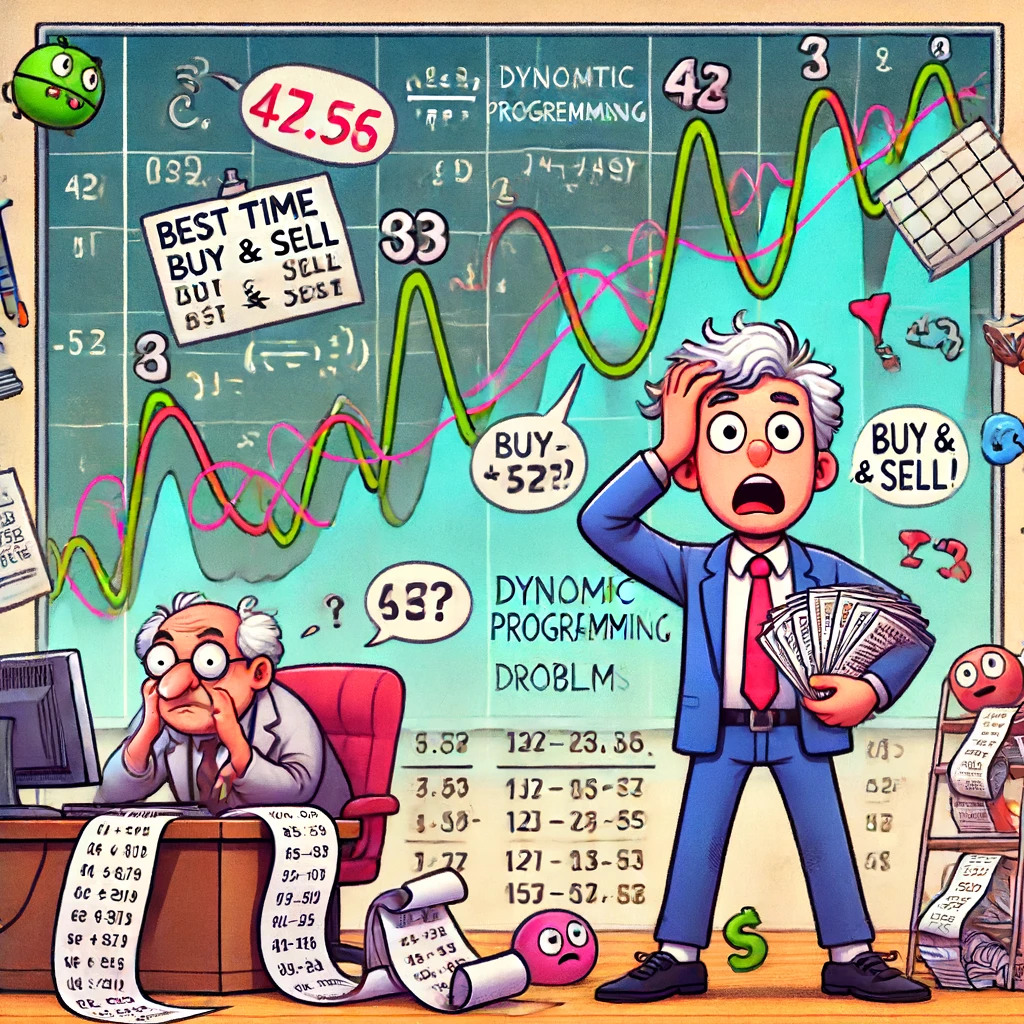
\includegraphics[width=\mywidth]{figs/stock}  % Ensure the correct file path and extension
  \caption{Best Time to Buy and Sell Stock.}
\end{figure}

\textbf{Input:} An array \texttt{prices}, with \texttt{prices[i]} representing the stock price on the \(i\)th day.

\textbf{Output:} The maximum profit that can be achieved.

\textbf{Example 1:}
\begin{verbatim}
    Input: prices = [7,1,5,3,6,4]
    Output: 5
    Explanation: Buy on day 2 (price = 1) and sell on day 5 (price = 6), 
    profit = 6 - 1 = 5.
\end{verbatim}

\textbf{Example 2:}
\begin{verbatim}
    Input: prices = [7,6,4,3,1]
    Output: 0
    Explanation: No transaction can yield a profit, hence the max profit = 0.
\end{verbatim}

\section*{Algorithmic Approach}
The common approach to solving this problem is to use a single pass. Iterate through the \texttt{prices} array while tracking the minimum price encountered so far. For each price, calculate the profit if the stock were sold at that price, updating the maximum profit as necessary.

\section*{Complexities}
\begin{itemize}
    \item \textbf{Time Complexity:} \(O(n)\), where \(n\) is the number of days, since it requires a single pass through the array.
    \item \textbf{Space Complexity:} \(O(1)\), as only a constant amount of extra space is needed for variables such as \texttt{min\_price} and \texttt{max\_profit}.
\end{itemize}

\section*{Python Implementation}
The Python implementation uses the above algorithm to find the maximum profit with a single pass through the stock prices:

\begin{fullwidth}
\begin{lstlisting}[language=Python]
class Solution:
    def maxProfit(self, prices: List[int]) -> int:
        min_price = float('inf')  # Initialize to positive infinity
        max_profit = 0
        
        # Loop through all stock prices
        for price in prices:
            # Updating the minimum price seen so far
            if price < min_price:
                min_price = price
            # Computing potential profit and update max profit
            elif price - min_price > max_profit:
                max_profit = price - min_price
        return max_profit
\end{lstlisting}

\end{fullwidth}

This approach initializes the minimum price to infinity and the maximum profit to 0 and iterates over the \texttt{prices} array. For each stock price, it checks if the price is lower than the current minimum price. If it is, the minimum price is updated. Otherwise, it calculates the profit one would get if one sold at the current price and updates the maximum profit if the current profit is larger. After iterating through all the prices, the maximum profit is returned.

\section*{Why This Approach}
This approach is chosen for its efficiency in both time and space. It navigates the array only once, ensuring a linear time complexity, which is optimal in this case because you have to examine each price at least once to determine the profit.

\section*{Alternative Approaches}
Alternative methods might use more complex data structures, such as segment trees, to perform many queries on the range of days. However, this is overkill for the given problem and would not improve the best-case time complexity.

\section*{Similar Problems to This One}
Similar problems include variations that allow for multiple transactions, incorporate a cooldown period between sales, or limit the number of transactions.

\section*{Things to Keep in Mind and Tricks}
One trick for problems like this is to consider the running difference between the current and minimum prices as the "current profit" and to update the maximum profit if a higher current profit is found.

\section*{Corner and Special Cases to Test When Writing the Code}
Test cases should include:
- Increasing and decreasing prices, ensuring profit is calculated correctly or confirmed as zero.
- Large input arrays to verify performance.
- Edge cases with the minimum input size (e.g., an array of just one price).

\section*{Explanation of Sliding Window Concept}
In this problem, the sliding window is not explicitly represented by two pointers, but the concept is similar. The window dynamically adjusts as we iterate through the \texttt{prices} array, always keeping track of the lowest buying price and the highest potential selling price after that buying day. This ensures that each price is considered only once, resulting in a linear time complexity of \(O(n)\)\sidenote{Linear time complexity}.


\problemsection{Product of Array Except Self}
\label{problem:Product_of_Array_Except_Self}

The "Product of Array Except Self" problem is a classic problem in the realm of algorithm and data structure problems often encountered on platforms like LeetCode.

\section*{Problem Statement}
Given an array \texttt{nums} of \(n\) integers where \(n > 1\), return an array \texttt{output} such that \texttt{output[i]} is equal to the product of all the elements of \texttt{nums} except \texttt{nums[i]}.

Given the constraints, it's guaranteed that the product of the array elements is within the range of a 32-bit signed integer.

% LeetCode link: \href{https://leetcode.com/problems/product-of-array-except-self/}{Product of Array Except Self}

\section*{Examples}
Example 1:

Input: \( [1,2,3,4] \)

Output: \( [24,12,8,6] \)

Explanation: By calculating the product of all elements except for the one at the current index, you would get:
\begin{itemize}
	\item For index \( 0 \): \( (2 \times 3 \times 4) = 24 \)
	\item For index \( 1 \): \( (1 \times 3 \times 4) = 12 \)
	\item For index \( 2 \): \( (1 \times 2 \times 4) = 8 \)
	\item For index \( 3 \): \( (1 \times 2 \times 3) = 6 \)
\end{itemize}

\textbf{Note}:
\begin{itemize}
	\item You cannot use division in solving this problem.
	\item You should try to solve the problem in \(O(n)\) time complexity.
\end{itemize}

\section*{Algorithmic Approach}
To solve this problem, we utilize two arrays to store the prefix and suffix products of every element. We then multiply these prefix and suffix products to obtain the final output.

\section*{Complexities}
\begin{itemize}
	\item \textbf{Time Complexity:} The total time complexity of the solution is \(O(n)\) as we are iterating through the array a constant number of times.
	\item \textbf{Space Complexity:} The space complexity is \(O(n)\) due to the extra space taken up by the prefix and suffix arrays.
\end{itemize}

\section*{Python Implementation}
Below is the complete Python code for solving the "Product of Array Except Self" problem without using division and with linear time complexity:

\begin{fullwidth}
\begin{lstlisting}[language=Python]
class Solution:
    def productExceptSelf(self, nums):
        length = len(nums)
        
        # Initialize arrays for left and right products
        left_products = [0]*length
        right_products = [0]*length
        output = [0]*length
        
        # left_products[i] contains the product of all elements to the left of i
        left_products[0] = 1
        for i in range(1, length):
            left_products[i] = nums[i - 1] * left_products[i - 1]
        
        # right_products[i] contains the product of all elements to the right of i
        right_products[length - 1] = 1
        for i in reversed(range(length - 1)):
            right_products[i] = nums[i + 1] * right_products[i + 1]
        
        # Construct the output array
        for i in range(length):
            output[i] = left_products[i] * right_products[i]
        
        return output
\end{lstlisting}
\end{fullwidth}

By precalculating the product of elements to the left and right of every element, we can construct the output array without the use of division.

\section*{Why this approach}
This approach is chosen because it adheres to the constraints of not using division and maintains a linear time complexity. By keeping track of the products to the left and right separately, we can multiply these values together to get the desired result for each index.

\section*{Alternative approaches}
An alternative approach could have been directly calculating the total product and then dividing it by the current element, but the problem explicitly forbids the use of division. Additionally, using extra passes and division might have exceeded the desired linear time complexity.

\section*{Similar problems to this one}
Similar problems may include other array transformation challenges that involve prefix sums or products, or problems that require the efficient computation of cumulative properties without using direct division, such as "Maximum Product Subarray" or "Trapping Rain Water."

\section*{Things to keep in mind and tricks}
- Precomputation of cumulative quantities can lead to efficient algorithms.
- When division is not allowed, consider the use of prefix and suffix arrays to maintain state.
- Always consider the constraints and desired time complexity when designing a solution.
- Remember to check for edge cases, such as an array containing zeros or negative numbers.

\section*{Corner and special cases to test when writing the code}
While testing, consider arrays with:
- A single zero, multiple zeros, and no zeros.
- Negative numbers, as they can affect the product sign.
- Large lengths to ensure that the time complexity is indeed linear.
- Edge cases, such as an empty array or an array with a single element.
\problemsection{Maximum Subarray}
\label{problem:Maximum_Subarray}

The **Maximum Subarray** problem is a cornerstone of algorithmic problem-solving, frequently used to introduce concepts like dynamic programming and divide-and-conquer techniques. Its simplicity and depth make it a classic challenge for both beginners and advanced programmers.

\subsection*{Problem Statement}
Given an integer array \texttt{nums}, find the contiguous subarray (containing at least one number) which has the largest sum, and return its sum\sidenote{A subarray is defined as a contiguous part of the array, meaning the elements are adjacent and sequential}.

\textbf{Example 1:}
\begin{verbatim}
Input: nums = [-2,1,-3,4,-1,2,1,-5,4]
Output: 6
Explanation: [4,-1,2,1] has the largest sum = 6.
\end{verbatim}

\textbf{Example 2:}
\begin{verbatim}
Input: nums = [1]
Output: 1
Explanation: The array contains only one element, which is the subarray.
\end{verbatim}

\textbf{Example 3:}
\begin{verbatim}
Input: nums = [-1,-2,-3]
Output: -1
Explanation: The largest sum is the single element -1, as all numbers are negative.
\end{verbatim}

\textbf{Key Observations:}
\begin{itemize}
    \item An array with one element is a valid subarray\sidenote{Single-element arrays must be considered in edge cases}.
    \item Negative values do not inherently prevent a subarray from being optimal; however, in some cases, starting a new subarray may yield better results.
\end{itemize}

\subsection*{Algorithmic Approach}
There are three primary approaches to solving this problem:

\begin{enumerate}
    \item \textbf{Brute Force:} Examine every possible subarray and calculate their sums, maintaining the maximum encountered sum. This approach has \(O(n^2)\) to \(O(n^3)\) time complexity\sidenote{Avoid brute force unless explicitly required by constraints, as it is computationally expensive for large arrays}.
    
    \item \textbf{Divide and Conquer:} Split the array into two halves, recursively find the maximum subarray sum for each half, and compute the maximum sum of a subarray that spans the midpoint. The time complexity is \(O(n \log n)\) due to the recursive divisions\sidenote{Divide and conquer provides a clear demonstration of recursive problem-solving but is less efficient than dynamic programming here}.
    
    \item \textbf{Dynamic Programming (Kadane's Algorithm):} Iteratively compute the maximum subarray sum ending at each index by comparing:
    \[
    \text{max\_current} = \max(\text{nums}[i], \text{max\_current} + \text{nums}[i])
    \]
    Track the global maximum sum as:
    \[
    \text{max\_global} = \max(\text{max\_global}, \text{max\_current})
    \]
    This approach has \(O(n)\) time complexity and is the most efficient for this problem\sidenote{Kadane's Algorithm is optimal because it processes the array in a single pass with constant space}.
\end{enumerate}

\subsection*{Python Implementation}
Below is the Python implementation of Kadane's Algorithm:

\begin{fullwidth}
\begin{lstlisting}[language=Python]
class Solution:
    def maxSubArray(self, nums: List[int]) -> int:
        # Initialize current and global maximums to the first element
        max_current = max_global = nums[0]

        # Traverse the array from the second element onward
        for x in nums[1:]:
            max_current = max(x, max_current + x)  # Include current element or start new subarray
            max_global = max(max_global, max_current)  # Update global maximum if needed
        
        return max_global
\end{lstlisting}
\end{fullwidth}

\textbf{Explanation:}
\begin{itemize}
    \item The algorithm initializes both \texttt{max\_current} and \texttt{max\_global} to the first element of the array\sidenote{This ensures that single-element arrays are handled naturally}.
    \item For each element, it determines whether to include it in the current subarray or start a new subarray\sidenote{This decision is made using the `max` function}.
    \item \texttt{max\_global} is updated whenever a larger subarray sum is encountered.
    \item The final value of \texttt{max\_global} is returned as the result.
\end{itemize}

\subsection*{Why This Approach?}
Kadane's Algorithm is chosen for its efficiency in both time and space. By maintaining running totals and a global maximum, it avoids the overhead of computing sums for all subarrays or managing recursion.

\subsection*{Alternative Approaches}
The divide-and-conquer method is an elegant alternative that divides the problem into smaller subproblems. However, it is less efficient due to its higher time complexity of \(O(n \log n)\).

\subsection*{Similar Problems to This One}
\begin{itemize}
    \item \textbf{Maximum Product Subarray:} Find the subarray with the largest product instead of the largest sum.
    \item \textbf{Best Time to Buy and Sell Stock:} Identify the best days to buy and sell stock for maximum profit.
    \item \textbf{Longest Increasing Subarray:} Find the longest contiguous subarray with increasing elements.
\end{itemize}

\subsection*{Things to Keep in Mind and Tricks}
\begin{itemize}
    \item \textbf{All-Negative Arrays:} When all numbers are negative, the largest sum is the single largest element. Kadane's Algorithm naturally handles this case\sidenote{No need for additional checks; the algorithm inherently accommodates negative numbers}.
    \item \textbf{Starting New Subarrays:} The decision to start a new subarray is pivotal. Always compare the current element with the sum of the current element and the existing subarray.
    \item \textbf{Edge Cases:} Consider empty arrays, single-element arrays, and arrays with alternating large positive and negative numbers.
\end{itemize}

\subsection*{Complexities}
\begin{itemize}
    \item \textbf{Time Complexity:} \(O(n)\), as the algorithm processes each element exactly once.
    \item \textbf{Space Complexity:} \(O(1)\), since it uses only a few variables for tracking sums.
\end{itemize}

\subsection*{Corner and Special Cases to Test}
\begin{itemize}
    \item \textbf{Empty Array:} Confirm the algorithm gracefully handles invalid input or returns a default value\sidenote{Some implementations may raise exceptions for empty arrays}.
    \item \textbf{Single-Element Array:} Ensure that the output is the element itself.
    \item \textbf{All-Negative Numbers:} Validate that the largest (least negative) number is returned.
    \item \textbf{Mixed Positive and Negative Numbers:} Test with arrays containing both large positive and negative numbers to ensure correct subarray selection.
\end{itemize}

\subsection*{Conclusion}
The **Maximum Subarray** problem exemplifies the power of dynamic programming in simplifying complex problems. Kadane's Algorithm is the optimal solution, offering both efficiency and elegance. By understanding the nuances of this problem, you can approach similar array challenges with confidence, leveraging dynamic programming concepts to solve them effectively.
\problemsection{Two Pointers Technique for Merging Arrays}\marginpar{Merge two sorted arrays using two pointers.}

When you are given two arrays to process, it is common to have one index per array (pointer) to traverse and compare both of them, incrementing one of the pointers when relevant. For example, we use this approach to merge two sorted arrays.
\section*{Two Pointers Technique for Merging Arrays}

When you are given two arrays to process, it is common to have one index per array (pointer) to traverse and compare both of them, incrementing one of the pointers when relevant. For example, we use this approach to merge two sorted arrays.

\subsection{Merge Sorted Array}
\label{subsec:Merge_Sorted_Array}

The "Merge Sorted Array" problem is a common algorithmic challenge that focuses on efficiently merging two sorted arrays. The task is to merge the contents of \texttt{nums2} into \texttt{nums1}, ensuring that \texttt{nums1} remains sorted in non-decreasing order. This problem tests one's ability to manipulate arrays in-place while maintaining the integrity of the original data.

\section*{Problem Statement}

You are given two integer arrays \texttt{nums1} and \texttt{nums2}, sorted in non-decreasing order, and two integers \texttt{m} and \texttt{n}, representing the number of elements in \texttt{nums1} and \texttt{nums2}, respectively. Merge \texttt{nums1} and \texttt{nums2} into a single array sorted in non-decreasing order.

The final sorted array should not be returned by the function but instead stored inside the array \texttt{nums1}. To accommodate this, \texttt{nums1} has a length of \texttt{m + n}, where the first \texttt{m} elements denote the elements that should be merged, and the last \texttt{n} elements are set to 0 and should be ignored. \texttt{nums2} has a length of \texttt{n}.

\textbf{Constraints:}

\begin{itemize}
    \item \texttt{nums1.length} = \texttt{m + n}
    \item \texttt{nums2.length} = \texttt{n}
    \item $0 \leq m, n \leq 200$
    \item $1 \leq m + n \leq 200$
    \item $-10^9 \leq \texttt{nums1[i]}, \texttt{nums2[i]} \leq 10^9$
    \item \texttt{nums1} and \texttt{nums2} are sorted in non-decreasing order.
\end{itemize}

\textbf{Input:} Two sorted integer arrays \texttt{nums1} and \texttt{nums2}, and integers \texttt{m} and \texttt{n}.

\textbf{Output:} The merged and sorted array stored within \texttt{nums1}.

\textbf{Example 1:}
\begin{verbatim}
Input: nums1 = [1,2,3,0,0,0], m = 3, nums2 = [2,5,6], n = 3
Output: [1,2,2,3,5,6]
\end{verbatim}

\textbf{Example 2:}
\begin{verbatim}
Input: nums1 = [1], m = 1, nums2 = [], n = 0
Output: [1]
\end{verbatim}

\textbf{Example 3:}
\begin{verbatim}
Input: nums1 = [0], m = 0, nums2 = [1], n = 1
Output: [1]
Explanation: Since m = 0, there are no elements in nums1. The merged array is [1].
\end{verbatim}

\section*{Algorithmic Approach}

To merge these two arrays efficiently, the two pointers technique is ideal. Instead of merging the arrays from the start, which could require extra space or unnecessary element shifts, we can start from the end of \texttt{nums1} and move backwards. This approach ensures that we overwrite the trailing zeroes in \texttt{nums1} while comparing the largest elements from both arrays.

Here's how the approach works:

\begin{itemize}
    \item Initialize two pointers \texttt{p1} and \texttt{p2} to point at the last elements of the valid parts of \texttt{nums1} and \texttt{nums2}, respectively (i.e., \texttt{p1 = m - 1}, \texttt{p2 = n - 1}).
    \item Another pointer \texttt{p} starts at the last position of the combined array (\texttt{m + n - 1}) in \texttt{nums1}.
    \item Compare the elements at \texttt{p1} and \texttt{p2}. Place the larger element at position \texttt{p} in \texttt{nums1} and move the respective pointer.
    \item Decrement the \texttt{p} pointer and repeat until all elements are merged.
    \item If any elements remain in \texttt{nums2}, copy them over to \texttt{nums1}.
\end{itemize}

\subsection*{Detailed Walkthrough}

Consider the example:

\begin{verbatim}
nums1 = [1,2,3,0,0,0], m = 3
nums2 = [2,5,6], n = 3
\end{verbatim}

\begin{enumerate}
    \item Set \texttt{p1 = 2} (points to 3 in \texttt{nums1}), \texttt{p2 = 2} (points to 6 in \texttt{nums2}), \texttt{p = 5}.
    \item Compare \texttt{nums1[p1]} (3) and \texttt{nums2[p2]} (6). Since 6 > 3, set \texttt{nums1[p]} = 6, decrement \texttt{p2} to 1, \texttt{p} to 4.
    \item Compare \texttt{nums1[p1]} (3) and \texttt{nums2[p2]} (5). Since 5 > 3, set \texttt{nums1[p]} = 5, decrement \texttt{p2} to 0, \texttt{p} to 3.
    \item Compare \texttt{nums1[p1]} (3) and \texttt{nums2[p2]} (2). Since 3 > 2, set \texttt{nums1[p]} = 3, decrement \texttt{p1} to 1, \texttt{p} to 2.
    \item Compare \texttt{nums1[p1]} (2) and \texttt{nums2[p2]} (2). Since 2 == 2, set \texttt{nums1[p]} = 2, decrement \texttt{p2} to -1, \texttt{p} to 1.
    \item Since \texttt{p2} < 0, copy remaining elements from \texttt{nums1} (if any). Here, set \texttt{nums1[p]} = \texttt{nums1[p1]} (2), decrement \texttt{p1} to 0, \texttt{p} to 0.
    \item Set \texttt{nums1[p]} = \texttt{nums1[p1]} (1).
\end{enumerate}

Final merged array: \texttt{[1,2,2,3,5,6]}.

\subsection*{Alternative Approaches}

An alternative approach is to create a new array and merge \texttt{nums1} and \texttt{nums2} from the start, similar to the merge step in the Merge Sort algorithm. However, this approach requires additional space of $O(m + n)$ and extra work to copy back the merged array into \texttt{nums1}. The reverse two-pointer technique is more efficient in terms of space and time since it operates in-place and avoids shifting elements multiple times.

\section*{Complexities}

\begin{itemize}
    \item \textbf{Time Complexity:} The time complexity is $O(m + n)$ because each element in \texttt{nums1} and \texttt{nums2} is processed once. We iterate through both arrays starting from their ends and move backwards, ensuring that all elements are compared and placed correctly.
    \item \textbf{Space Complexity:} The space complexity is $O(1)$ since the merging is done in-place within \texttt{nums1}. We do not use any additional significant space that scales with the input size.
\end{itemize}

\section*{Python Implementation}

Below is the Python code to implement the "Merge Sorted Array" problem using the two pointers technique:
\begin{fullwidth}
\begin{lstlisting}[language=Python]
from typing import List

def merge(nums1: List[int], m: int, nums2: List[int], n: int) -> None:
    """
    Merges nums2 into nums1 in-place, resulting in a single sorted array.

    Parameters:
    nums1 (List[int]): The first sorted array with a length of m + n,
                       where the first m elements denote the elements to merge,
                       and the last n elements are set to 0 and should be ignored.
    m (int): Number of initialized elements in nums1.
    nums2 (List[int]): The second sorted array.
    n (int): Number of initialized elements in nums2.

    Returns:
    None: The function modifies nums1 in-place.
    """
    p1, p2, p = m - 1, n - 1, m + n - 1

    # While there are elements to compare in nums1 and nums2
    while p1 >= 0 and p2 >= 0:
        if nums1[p1] > nums2[p2]:
            nums1[p] = nums1[p1]
            p1 -= 1
        else:
            nums1[p] = nums2[p2]
            p2 -= 1
        p -= 1

    # If there are remaining elements in nums2, copy them
    while p2 >= 0:
        nums1[p] = nums2[p2]
        p2 -= 1
        p -= 1
\end{lstlisting}
\end{fullwidth}
\subsection*{Example Usage and Test Cases}

\begin{lstlisting}[language=Python]
# Test case 1: General case
nums1 = [1,2,3,0,0,0]
m = 3
nums2 = [2,5,6]
n = 3
merge(nums1, m, nums2, n)
print(nums1)  # Output: [1, 2, 2, 3, 5, 6]

# Test case 2: nums2 is empty
nums1 = [1]
m = 1
nums2 = []
n = 0
merge(nums1, m, nums2, n)
print(nums1)  # Output: [1]

# Test case 3: nums1 is empty
nums1 = [0]
m = 0
nums2 = [1]
n = 1
merge(nums1, m, nums2, n)
print(nums1)  # Output: [1]

# Test case 4: Negative numbers
nums1 = [-1,0,0,0]
m = 1
nums2 = [-3,-2,-1]
n = 3
merge(nums1, m, nums2, n)
print(nums1)  # Output: [-3, -2, -1, -1]
\end{lstlisting}

\section*{Why This Approach}

The reverse two-pointer technique is ideal for this problem because it avoids the need to move elements multiple times. By starting from the end of \texttt{nums1}, we place elements directly into their final positions without overwriting any unprocessed elements. This in-place approach is more efficient than merging from the start, which could require shifting elements forward to make space.

Starting from the end of the arrays ensures that we utilize the unused space at the end of \texttt{nums1} (the zeroes) to store the largest elements first. This method leverages the fact that we know the total number of elements and the arrays are sorted, allowing us to merge efficiently without extra space.

\section*{Similar Problems}

Other problems that involve merging sorted data structures or using the two-pointer technique include:

\begin{itemize}
    \item \textbf{Merge Two Sorted Lists}: Merge two sorted linked lists and return it as a new sorted list.
    \item \textbf{Merge k Sorted Lists}: Merge $k$ sorted linked lists and return it as one sorted list.
    \item \textbf{Merge Intervals}: Merge all overlapping intervals in a list of intervals.
    \item \textbf{Two Sum II - Input Array Is Sorted}: Find two numbers such that they add up to a specific target number in a sorted array.
\end{itemize}

These problems also require careful handling of elements in sorted order, often leveraging two pointers or similar techniques.

\section*{Things to Keep in Mind and Tricks}

\begin{itemize}
    \item \textbf{Edge Cases}: Always consider edge cases such as empty arrays or arrays with one element. Ensure your algorithm handles these scenarios correctly.
    \item \textbf{Remaining Elements}: After the main loop, if there are remaining elements in \texttt{nums2}, they need to be copied over to \texttt{nums1}. If there are remaining elements in \texttt{nums1}, they are already in place.
    \item \textbf{Avoiding Shifts}: By starting from the end, we avoid shifting elements multiple times, which improves efficiency.
    \item \textbf{Optimization Tip}: If \texttt{nums2} is empty (\texttt{n == 0}), we can skip the merging process altogether.
    \item \textbf{Common Pitfall}: Do not forget to handle the case where \texttt{nums1} has no elements (\texttt{m == 0}). In this case, we need to copy all elements from \texttt{nums2} to \texttt{nums1}.
\end{itemize}

\section*{Exercises}

\begin{enumerate}
    \item \textbf{Descending Order Merge}: Modify the algorithm to merge two arrays sorted in non-increasing (descending) order.
    \item \textbf{Merge Without Extra Space}: Suppose \texttt{nums1} has no extra space at the end (i.e., length is \texttt{m}). How would you merge \texttt{nums2} into \texttt{nums1} without using extra space?
    \item \textbf{Non-Sorted Arrays}: Adapt the algorithm to merge two unsorted arrays into a sorted array without using built-in sorting functions.
    \item \textbf{Alternative Languages}: Implement the merge function in another programming language, such as Java or C++, to practice language-specific syntax.
\end{enumerate}

\section*{Questions for Reflection}

\begin{itemize}
    \item How would the algorithm change if the arrays were not sorted?
    \item Can this approach be extended to merge more than two arrays? How would you modify it?
    \item What are the trade-offs between in-place algorithms and those that use extra space?
\end{itemize}

\section*{References}

LeetCode Problem: \href{https://leetcode.com/problems/merge-sorted-array/}{Merge Sorted Array}
\problemsection{Maximum Product Subarray}
\label{problem:Maximum_Product_Subarray}

The **Maximum Product Subarray** problem is a classic dynamic programming challenge that highlights the importance of tracking both the maximum and minimum values in a sequence. The problem’s complexity arises from handling positive, negative, and zero values, which can significantly affect the product of subarrays.

\subsection*{Problem Statement}
Given an integer array \texttt{nums}, find the contiguous subarray (containing at least one number) which has the largest product, and return the product.

\textbf{Example 1:}
\begin{verbatim}
Input: nums = [2,3,-2,4]
Output: 6
Explanation: The subarray [2,3] has the largest product 6.
\end{verbatim}

\textbf{Example 2:}
\begin{verbatim}
Input: nums = [-2,0,-1]
Output: 0
Explanation: The result cannot be 2, because [-2,-1] is not a contiguous subarray.
\end{verbatim}

\textbf{Key Observations:}
\begin{itemize}
    \item Negative numbers can transform a large negative product into a large positive product when multiplied with another negative number\sidenote{Tracking both the maximum and minimum products is crucial for this reason}.
    \item Zeros break the continuity of a subarray’s product, requiring a reset of the calculation\sidenote{Any subarray containing zero has a product of zero}.
\end{itemize}

\subsection*{Algorithmic Approach}
The most efficient solution to this problem leverages dynamic programming to maintain:
\begin{itemize}
    \item \texttt{max\_product}: The maximum product of a subarray ending at the current index.
    \item \texttt{min\_product}: The minimum product of a subarray ending at the current index\sidenote{Tracking the minimum is essential to handle negative values correctly}.
\end{itemize}

At each step, update \texttt{max\_product} and \texttt{min\_product} using the current number and the products of the current number with the previous \texttt{max\_product} and \texttt{min\_product}. If the current number is negative, swap \texttt{max\_product} and \texttt{min\_product} before updating.

\textbf{Algorithm:}
\begin{enumerate}
    \item Initialize \texttt{max\_product}, \texttt{min\_product}, and \texttt{result} to the first element of the array.
    \item Iterate through the array starting from the second element:
    \begin{itemize}
        \item If the current number is negative, swap \texttt{max\_product} and \texttt{min\_product}.
        \item Update \texttt{max\_product} as:
        \[
        \text{max\_product} = \max(\text{nums}[i], \text{max\_product} \times \text{nums}[i])
        \]
        \item Update \texttt{min\_product} as:
        \[
        \text{min\_product} = \min(\text{nums}[i], \text{min\_product} \times \text{nums}[i])
        \]
        \item Update \texttt{result} as:
        \[
        \text{result} = \max(\text{result}, \text{max\_product})
        \]
    \end{itemize}
    \item Return \texttt{result}.
\end{enumerate}

\subsection*{Complexities}
\begin{itemize}
    \item \textbf{Time Complexity:} \(O(n)\), as the array is traversed only once.
    \item \textbf{Space Complexity:} \(O(1)\), since only a constant amount of extra space is required.
\end{itemize}

\subsection*{Python Implementation}
\begin{fullwidth}
\begin{lstlisting}[language=Python]
class Solution:
    def maxProduct(self, nums: List[int]) -> int:
        # Initialize max_product, min_product, and result with the first element
        max_product = min_product = result = nums[0]

        # Iterate through nums starting from the second element
        for i in range(1, len(nums)):
            # If the current element is negative, swap max_product and min_product
            if nums[i] < 0:
                max_product, min_product = min_product, max_product

            # Update max_product and min_product
            max_product = max(nums[i], max_product * nums[i])
            min_product = min(nums[i], min_product * nums[i])

            # Update the global result
            result = max(result, max_product)

        return result
\end{lstlisting}
\end{fullwidth}

\subsection*{Why This Approach?}
This approach efficiently calculates the maximum product of a subarray by maintaining local maxima and minima at each step, ensuring optimal performance. The \(O(n)\) time complexity is achieved by avoiding recalculation of products for all possible subarrays, which would otherwise result in \(O(n^2)\) complexity.

\subsection*{Alternative Approaches}
\begin{itemize}
    \item **Brute Force:** Calculate the product of every possible subarray. While straightforward, this approach has \(O(n^2)\) time complexity and is impractical for large arrays.
    \item **Divide and Conquer:** Split the array into halves, recursively find the maximum product in each half, and compute the maximum product across the midpoint. This approach has \(O(n \log n)\) time complexity but is less efficient than the dynamic programming solution.
\end{itemize}

\subsection*{Similar Problems}
\begin{itemize}
    \item \textbf{Maximum Subarray Sum:} Use Kadane’s Algorithm to find the maximum sum of a contiguous subarray.
    \item \textbf{Circular Subarray Maximum Product:} Extend this problem to handle arrays with wraparound subarrays.
\end{itemize}

\subsection*{Things to Keep in Mind and Tricks}
\begin{itemize}
    \item **Negative Numbers:** Always track both maximum and minimum products to handle cases where negative values become positive when multiplied.
    \item **Zeros:** A zero resets the product, so consider restarting the calculation from the next element after a zero.
    \item **Edge Cases:** Test arrays with single elements, all positive numbers, all negative numbers, and arrays with zeros.
\end{itemize}

\subsection*{Corner and Special Cases to Test}
\begin{itemize}
    \item Arrays with one element (\([3]\)): The product is the element itself.
    \item Arrays with all negative numbers (\([-1, -2, -3]\)): The maximum product is the product of all elements if the count of negatives is even.
    \item Arrays with zeros (\([0, -2, -3, 0, 4]\)): Ensure the algorithm handles resets correctly.
    \item Mixed positive and negative numbers (\([2, 3, -2, 4, -1]\)): Check transitions between positive and negative subarrays.
\end{itemize}

\subsection*{Conclusion}
The **Maximum Product Subarray** problem is a classic example of dynamic programming’s power in handling complex array-based problems. By maintaining local maxima and minima, this approach elegantly solves the problem in linear time, ensuring efficiency even for large inputs. Mastering this problem builds a strong foundation for tackling similar challenges involving subarrays and dynamic optimization.
% Filename: find_minimum_in_rotated_sorted_array.tex

\problemsection{Find Minimum in Rotated Sorted Array}
\label{problem:Find_Minimum_in_Rotated_Sorted_Array}

The **Find Minimum in Rotated Sorted Array** problem involves identifying the smallest element in a rotated sorted array. This problem demonstrates the efficient application of binary search techniques to leverage the sorted structure of the array while addressing the rotation.

---

\section*{Problem Statement}
Given a rotated sorted array, locate its minimum element. A sorted array is considered rotated if some elements from the beginning are moved to the end, maintaining the overall ascending order. The solution should run in \(O(\log n)\) time complexity.

---

\textbf{Input:}
- \texttt{nums}: A list of integers representing the rotated sorted array.

\textbf{Output:}
- An integer representing the minimum element in \texttt{nums}.

\textbf{Example 1:}
\begin{verbatim}
Input: nums = [3, 4, 5, 1, 2]
Output: 1
Explanation: The minimum value is 1.
\end{verbatim}

\textbf{Example 2:}
\begin{verbatim}
Input: nums = [4, 5, 6, 7, 0, 1, 2]
Output: 0
Explanation: The minimum value is 0.
\end{verbatim}

\textbf{Example 3:}
\begin{verbatim}
Input: nums = [11, 13, 15, 17]
Output: 11
Explanation: The array is not rotated, so the first element is the smallest.
\end{verbatim}

---

\section*{Algorithmic Approach}

To solve the problem efficiently:
1. Use binary search with two pointers, \( \texttt{left} \) and \( \texttt{right} \), representing the bounds of the current search space.
2. Compute the middle index:
   \[
   \texttt{mid} = \texttt{left} + (\texttt{right} - \texttt{left}) // 2
   \]
3. Compare \texttt{nums[mid]} with \texttt{nums[right]}:
   - If \texttt{nums[mid]} \(>\) \texttt{nums[right]}, the minimum must be in the right half. Update \( \texttt{left} = \texttt{mid} + 1 \).
   - Otherwise, the minimum is in the left half (including \texttt{mid}). Update \( \texttt{right} = \texttt{mid} \).
4. Continue until \( \texttt{left} == \texttt{right} \), at which point the minimum element is found at \( \texttt{nums[left]} \).

---

\subsection*{Complexities}
\begin{itemize}
    \item \textbf{Time Complexity:} \( O(\log n) \), since the search space is halved at each step.
    \item \textbf{Space Complexity:} \( O(1) \), as no additional space is used beyond a few variables.
\end{itemize}

---

\section*{Python Implementation}

\begin{fullwidth}
\begin{lstlisting}[language=Python]
class Solution:
    def findMin(self, nums: List[int]) -> int:
        left, right = 0, len(nums) - 1
        while left < right:
            mid = left + (right - left) // 2
            if nums[mid] > nums[right]:
                left = mid + 1
            else:
                right = mid
        return nums[left]

# Example usage:
nums = [4, 5, 6, 7, 0, 1, 2]
solution = Solution()
print(solution.findMin(nums))  # Output: 0
\end{lstlisting}
\end{fullwidth}

---

\section*{Why This Approach?}
Binary search is ideal for this problem because the array is partially sorted. Instead of iterating through all elements (\(O(n)\)), binary search exploits the sorted structure to locate the minimum in \(O(\log n)\) time.

---

\section*{Alternative Approaches}
1. **Linear Search (\(O(n)\)):** Scan all elements to find the minimum. This approach is straightforward but inefficient for large arrays.
2. **Recursive Binary Search (\(O(\log n)\)):** The binary search logic can be implemented recursively, although it adds stack overhead.

---

\section*{Similar Problems}
\begin{itemize}
    \item **Search in Rotated Sorted Array:** Find the position of a target element in a rotated sorted array.
    \item **Find Peak Element:** Locate a peak element in an array.
    \item **Find Minimum in Rotated Sorted Array II:** Handles duplicates in the rotated array.
\end{itemize}

---

\section*{Corner Cases to Test}
\begin{itemize}
    \item Array is not rotated: \( \texttt{nums} = [1, 2, 3, 4, 5] \).
    \item Single element array: \( \texttt{nums} = [1] \).
    \item Array with two elements: \( \texttt{nums} = [2, 1] \).
    \item Minimum element is the last element: \( \texttt{nums} = [3, 4, 5, 6, 1] \).
\end{itemize}

---

\section*{Conclusion}
The "Find Minimum in Rotated Sorted Array" problem elegantly demonstrates the power of binary search in structured datasets. By efficiently narrowing down the search space, we achieve optimal performance while maintaining simplicity in implementation.
% Filename: search_in_rotated_sorted_array.tex

\problemsection{Search in Rotated Sorted Array}
\label{problem:Search_in_Rotated_Sorted_Array}

The **Search in Rotated Sorted Array** problem tests your ability to combine binary search with logic to handle shifted or rotated arrays. This is a frequent interview question that evaluates both problem-solving skills and the ability to optimize search operations.

\subsection*{Problem Statement}
You are given a rotated sorted array \texttt{nums} of unique integers and a target integer \texttt{target}. Return the index of \texttt{target} if it exists in \texttt{nums}; otherwise, return \(-1\).

The array is sorted in ascending order and then rotated at some unknown pivot index \(k\). For example, \([0, 1, 2, 4, 5, 6, 7]\) might become \([4, 5, 6, 7, 0, 1, 2]\). Your task is to search for the \texttt{target} in \(O(\log n)\) time.

\textbf{Example 1:}
\begin{verbatim}
Input: nums = [4,5,6,7,0,1,2], target = 0
Output: 4
\end{verbatim}

\textbf{Example 2:}
\begin{verbatim}
Input: nums = [4,5,6,7,0,1,2], target = 3
Output: -1
\end{verbatim}

\textbf{Example 3:}
\begin{verbatim}
Input: nums = [1], target = 0
Output: -1
\end{verbatim}

\subsection*{Algorithmic Approach}
The problem is best solved using a modified binary search\sidenote{Binary search ensures \(O(\log n)\) time complexity, making it highly efficient for sorted or partially sorted arrays}.

\textbf{Key Observations:}
\begin{itemize}
    \item One half of the array (either left or right) is always sorted\sidenote{This property is a direct result of the array being rotated at a single pivot point}.
    \item The target can only lie in one of the two halves, depending on its value relative to the sorted half.
\end{itemize}

The algorithm:
\begin{enumerate}
    \item Initialize two pointers, \texttt{left} at the start and \texttt{right} at the end of the array.
    \item While \texttt{left} \(\leq\) \texttt{right}, calculate the middle index: 
    \[
    \text{mid} = \text{left} + \frac{\text{right} - \text{left}}{2}
    \]
    \item Check if the middle element is the target. If yes, return \texttt{mid}.
    \item Determine whether the left half or the right half is sorted:
    \begin{itemize}
        \item If the left half is sorted:
        \begin{itemize}
            \item Check if the target lies within this range\sidenote{A sorted range is defined as \(\texttt{nums[left]} \leq \texttt{target} < \texttt{nums[mid]}\)}.
            \item If yes, adjust the \texttt{right} pointer to \(\texttt{mid} - 1\); otherwise, adjust \texttt{left} to \(\texttt{mid} + 1\).
        \end{itemize}
        \item If the right half is sorted:
        \begin{itemize}
            \item Check if the target lies within this range\sidenote{Similarly, the range is defined as \(\texttt{nums[mid]} < \texttt{target} \leq \texttt{nums[right]}\)}.
            \item If yes, adjust the \texttt{left} pointer to \(\texttt{mid} + 1\); otherwise, adjust \texttt{right} to \(\texttt{mid} - 1\).
        \end{itemize}
    \end{itemize}
    \item If the loop exits without finding the target, return \(-1\).
\end{enumerate}

\subsection*{Complexities}
\begin{itemize}
    \item \textbf{Time Complexity:} \(O(\log n)\), as the array is halved in each iteration.
    \item \textbf{Space Complexity:} \(O(1)\), as the algorithm operates in-place without additional memory allocation.
\end{itemize}

\subsection*{Python Implementation}
\begin{fullwidth}
\begin{lstlisting}[language=Python]
class Solution:
    def search(self, nums: List[int], target: int) -> int:
        left, right = 0, len(nums) - 1
        
        while left <= right:
            mid = left + (right - left) // 2
            
            # Check if the middle element is the target
            if nums[mid] == target:
                return mid
            
            # Determine which half is sorted
            if nums[left] <= nums[mid]:
                # Left half is sorted
                if nums[left] <= target < nums[mid]:
                    right = mid - 1
                else:
                    left = mid + 1
            else:
                # Right half is sorted
                if nums[mid] < target <= nums[right]:
                    left = mid + 1
                else:
                    right = mid - 1
        
        return -1
\end{lstlisting}
\end{fullwidth}

\subsection*{Why This Approach?}
This approach leverages the sorted property of one half of the array in each iteration to eliminate half of the search space\sidenote{Binary search guarantees logarithmic time complexity by halving the search space repeatedly}. By dynamically adjusting the search range based on the target's position relative to the sorted half, the algorithm maintains \(O(\log n)\) efficiency.

\subsection*{Alternative Approaches}
\begin{itemize}
    \item **Linear Search:**  
    Iterate through the array and check each element. This has \(O(n)\) time complexity and is not suitable for large arrays.
    \item **Pivot Detection + Binary Search:**  
    First, identify the pivot point (where the rotation occurs) using binary search, then perform binary search on the relevant segment. While still \(O(\log n)\), this involves two binary search passes, making it less efficient.
\end{itemize}

\subsection*{Similar Problems}
\begin{itemize}
    \item \textbf{Find Minimum in Rotated Sorted Array:} Identify the smallest element in a rotated sorted array.
    \item \textbf{Search in Rotated Sorted Array II:} Handle duplicates while searching for the target.
    \item \textbf{Find Peak Element:} Locate a peak element in an array where adjacent elements are distinct.
\end{itemize}

\subsection*{Things to Keep in Mind and Tricks}
\begin{itemize}
    \item Always check if the middle element is the target before further processing\sidenote{This prevents unnecessary checks and guarantees correctness}.
    \item Handle edge cases like arrays with a single element, no rotation, or extreme rotations (pivot at the first or last element).
    \item Use integer division (\(\texttt{//}\)) for calculating \texttt{mid} to avoid potential overflow in some languages.
\end{itemize}

\subsection*{Corner and Special Cases to Test}
\begin{itemize}
    \item **Single Element Array:** \([1]\), target = \(1\) or \(2\).
    \item **No Rotation:** \([1, 2, 3, 4]\), target = \(3\).
    \item **Full Rotation:** \([1, 2, 3, 4]\), rotated back to \([1, 2, 3, 4]\), target = \(4\).
    \item **Target Not in Array:** \([4, 5, 6, 7, 0, 1, 2]\), target = \(8\).
    \item **Extreme Rotation:** \([2, 3, 4, 5, 6, 7, 0, 1]\), target = \(0\).
\end{itemize}

\subsection*{Conclusion}
The **Search in Rotated Sorted Array** problem demonstrates how binary search can be adapted to handle more complex scenarios like rotations. By exploiting the partially sorted structure of the array, this algorithm efficiently narrows down the search space, achieving optimal performance. Mastering this problem prepares you to tackle related challenges involving rotated or partially sorted data structures.
% Filename: merge_two_sorted_lists.tex

\problemsection{Merge Two Sorted Lists}
\label{problem:merge_two_sorted_lists}
\marginpar{Efficiently combining two sorted lists is fundamental in data processing and algorithm design.}

The \textbf{Merge Two Sorted Lists} problem involves combining two sorted linked lists into a single, sorted linked list. The objective is to construct a new list by splicing together the nodes of the input lists in ascending order.\marginpar{Commonly encountered in technical interviews and serves as a building block for more complex data structures.}

\section*{Problem Statement}
Given the heads of two sorted linked lists, \texttt{list1} and \texttt{list2}, merge them into one sorted linked list. The merged linked list should be composed by splicing together the nodes of the first two lists so that the resulting list is in ascending order.

\marginpar{\href{https://leetcode.com/problems/merge-two-sorted-lists/}{[LeetCode Link]}\index{LeetCode}}
\marginpar{\href{https://www.geeksforgeeks.org/merge-two-sorted-linked-lists/}{[GeeksForGeeks Link]}\index{GeeksForGeeks}}
\marginpar{\href{https://www.hackerrank.com/challenges/merge-two-sorted-linked-lists/problem}{[HackerRank Link]}\index{HackerRank}}
\marginpar{\href{https://app.codesignal.com/challenges/merge-two-sorted-lists}{[CodeSignal Link]}\index{CodeSignal}}
\marginpar{\href{https://www.interviewbit.com/problems/merge-two-sorted-lists/}{[InterviewBit Link]}\index{InterviewBit}}
\marginpar{\href{https://www.educative.io/courses/grokking-the-coding-interview/RM8y8Y3nLdY}{[Educative Link]}\index{Educative}}
\marginpar{\href{https://www.codewars.com/kata/merge-two-sorted-lists/train/python}{[Codewars Link]}\index{Codewars}}

\section*{Algorithmic Approach}
To efficiently merge two sorted lists, the **two-pointer technique** is utilized. This method allows simultaneous traversal of both lists, ensuring that the merged list maintains sorted order without the need for additional sorting.\marginpar{The two-pointer technique is versatile and widely used in array and list manipulation problems.}

\begin{enumerate}
    \item \textbf{Initialize Pointers:}
    \begin{itemize}
        \item Create a dummy node to serve as the starting point of the merged list.
        \item Initialize a current pointer to track the end of the merged list.
    \end{itemize}
    
    \item \textbf{Traverse and Compare:}
    \begin{itemize}
        \item While neither \texttt{list1} nor \texttt{list2} is exhausted:
        \begin{itemize}
            \item Compare the current nodes of both lists.
            \item Append the node with the smaller value to the merged list.
            \item Move the corresponding pointer forward.
        \end{itemize}
    \end{itemize}
    
    \item \textbf{Handle Remaining Elements:}
    \begin{itemize}
        \item After one list is exhausted, append the remaining nodes from the other list to the merged list.
    \end{itemize}
\end{enumerate}

\section*{Complexities}
\begin{itemize}
    \item \textbf{Time Complexity:} \(O(n + m)\), where \(n\) and \(m\) are the lengths of \texttt{list1} and \texttt{list2}, respectively. Each node is visited exactly once.
    \item \textbf{Space Complexity:} \(O(1)\), as the merge is performed in-place without allocating additional space for the merged list.
\end{itemize}

\section*{Python Implementation}
\marginpar{Implementing the two-pointer technique ensures efficient runtime and optimal space usage.}

Below is the complete Python code for merging two sorted linked lists using the two-pointer technique:

\begin{fullwidth}
\begin{lstlisting}[language=Python]
# Definition for singly-linked list.
class ListNode:
    def __init__(self, val=0, next=None):
        self.val = val
        self.next = next

class Solution:
    def mergeTwoLists(self, list1: ListNode, list2: ListNode) -> ListNode:
        # Create a dummy node to serve as the start of the merged list
        dummy = ListNode()
        current = dummy
        
        # Traverse both lists and append the smaller value to the merged list
        while list1 and list2:
            if list1.val < list2.val:
                current.next = list1  # Link to list1 node
                list1 = list1.next   # Move list1 pointer
            else:
                current.next = list2  # Link to list2 node
                list2 = list2.next   # Move list2 pointer
            current = current.next    # Move merged list pointer

        # Append any remaining nodes from list1 or list2
        current.next = list1 if list1 else list2
        
        # Return the head of the merged list, skipping the dummy node
        return dummy.next

# Example Usage:
# Constructing the first sorted linked list: 1 -> 3 -> 5
list1 = ListNode(1, ListNode(3, ListNode(5)))

# Constructing the second sorted linked list: 2 -> 4 -> 6
list2 = ListNode(2, ListNode(4, ListNode(6)))

# Creating a Solution object and merging the lists
solution = Solution()
merged_head = solution.mergeTwoLists(list1, list2)

# Function to print the merged linked list
def print_linked_list(head):
    elems = []
    while head:
        elems.append(str(head.val))
        head = head.next
    print(" -> ".join(elems))

print_linked_list(merged_head)  # Output: 1 -> 2 -> 3 -> 4 -> 5 -> 6

# Handling Edge Cases
print_linked_list(solution.mergeTwoLists(None, ListNode(1, ListNode(2, ListNode(3)))))  # Output: 1 -> 2 -> 3
print_linked_list(solution.mergeTwoLists(ListNode(1, ListNode(2, ListNode(3))), None))  # Output: 1 -> 2 -> 3
print_linked_list(solution.mergeTwoLists(ListNode(1, ListNode(3, ListNode(5))), ListNode(1, ListNode(3, ListNode(5)))))  # Output: 1 -> 1 -> 3 -> 3 -> 5 -> 5
\end{lstlisting}
\end{fullwidth}

\section*{Explanation}
The `mergeTwoLists` function efficiently merges two sorted linked lists by leveraging the **two-pointer technique**. Here's a step-by-step breakdown of the implementation:

\begin{itemize}
    \item \textbf{Initialization:}
    \begin{itemize}
        \item A dummy node is created to simplify edge cases, such as when one or both input lists are empty.
        \item A `current` pointer is initialized to track the end of the merged list.
    \end{itemize}
    
    \item \textbf{Merging Process:}
    \begin{itemize}
        \item The function enters a loop that continues until either `list1` or `list2` is exhausted.
        \item Within the loop, the values of the current nodes of both lists are compared.
        \item The node with the smaller value is appended to the merged list by updating `current.next`.
        \item The pointer of the list from which the node was taken is moved forward.
        \item The `current` pointer is then moved to the newly appended node.
    \end{itemize}
    
    \item \textbf{Appending Remaining Nodes:}
    \begin{itemize}
        \item After the main loop, one of the lists may still contain nodes.
        \item The remaining nodes from the non-exhausted list are appended to the merged list.
    \end{itemize}
    
    \item \textbf{Finalizing the Merged List:}
    \begin{itemize}
        \item The merged list is returned by skipping the dummy node (`dummy.next`).
    \end{itemize}
\end{itemize}

\section*{Why This Approach}
This method is chosen because it is both intuitive and efficient. By iterating through both lists simultaneously and always selecting the smaller current element, we ensure that the merged list remains sorted. Additionally, since the merge is done in-place, it optimizes space usage without the need for additional data structures.\marginpar{In-place operations are crucial for optimizing memory usage, especially with large datasets.}

\section*{Alternative Approaches}
An alternative method involves using recursion to merge the two lists. In this recursive approach, the function compares the heads of both lists and recursively merges the remaining elements. While elegant, the recursive method may lead to increased space usage due to the call stack, especially with very long lists.\marginpar{Recursive solutions can be more readable but may not always be the most space-efficient.}

\section*{Similar Problems to This One}
\begin{itemize}
    \item \hyperref[problem:merge_k_sorted_lists]{Merge k Sorted Lists}\index{Merge k Sorted Lists}
    \item \hyperref[problem:merge_intervals]{Merge Intervals}\index{Merge Intervals}
    \item \hyperref[problem:sorted_arrays_merge]{Merge Sorted Arrays}\index{Merge Sorted Arrays}
\end{itemize}

\section*{Things to Keep in Mind and Tricks}
\begin{itemize}
    \item \textbf{Edge Cases:} Always consider scenarios where one or both input lists are empty.\index{Edge Cases}
    \item \textbf{Duplicate Elements:} Decide how to handle duplicate values; in this case, duplicates are allowed and included in the merged list.\index{Duplicate Elements}
    \item \textbf{In-Place Merging:} If allowed, modifying one of the input lists can save space.\index{In-Place Merging}
    \item \textbf{Using Built-in Functions:} Python’s built-in functions like \texttt{sorted()} can simplify merging but may not be as efficient for large lists.\index{Built-in Functions}
\end{itemize}

\section*{Corner and Special Cases to Test When Writing the Code}
\begin{itemize}
    \item \textbf{Both Lists Empty:} \texttt{list1 = [], list2 = []}\index{Corner Cases}
    \item \textbf{One List Empty:} \texttt{list1 = [], list2 = [1, 2, 3]} and \texttt{list1 = [1, 2, 3], list2 = []}\index{Corner Cases}
    \item \textbf{Different Lengths:} \texttt{list1 = [1, 4, 5], list2 = [2, 3]}\index{Corner Cases}
    \item \textbf{All Elements from One List Smaller:} \texttt{list1 = [1, 2, 3], list2 = [4, 5, 6]}\index{Corner Cases}
    \item \textbf{All Elements from One List Larger:} \texttt{list1 = [4, 5, 6], list2 = [1, 2, 3]}\index{Corner Cases}
    \item \textbf{Duplicate Elements:} \texttt{list1 = [1, 3, 5], list2 = [1, 3, 5]}\index{Corner Cases}
\end{itemize}

\printindex
% Filename: remove_duplicates_from_sorted_array.tex

\problemsection{Remove Duplicates from a Sorted Array}
\label{sec:remove-duplicates-from-sorted-array}
% \addcontentsline{toc}{section}{Remove Duplicates from a Sorted Array} % Adds to TOC

\textbf{Introduction} \\
The problem of removing duplicates from a sorted array is a classic algorithmic challenge that emphasizes in-place array manipulation and efficient use of space. Leveraging the sorted nature of the array allows for optimal solutions that minimize time and space complexity. This problem not only reinforces fundamental array handling techniques but also serves as a foundational exercise for understanding more complex data manipulation tasks\sidenote{For a comprehensive overview, refer to the \href{https://leetcode.com/problems/remove-duplicates-from-sorted-array/}{LeetCode Remove Duplicates problem}.}.

\subsection*{Problem Statement}
Given a sorted array of integers, remove the duplicates in-place such that each element appears only once and return the new length. The relative order of the elements should be kept the same. Since it is impossible to change the length of the array in some programming languages, you must instead have the result placed in the first part of the array. More formally, if there are \(k\) elements after removing the duplicates, then the first \(k\) elements of the array should hold the final result. It does not matter what you leave beyond the first \(k\) elements.

\subsection*{Algorithmic Approach}
The most efficient way to solve this problem is by using the **Two Pointers Technique**. Here's a step-by-step approach:

\begin{enumerate}
    \item \textbf{Initialize Two Pointers:}
        \begin{itemize}
            \item \texttt{slow} pointer starts at index 0, representing the position of the last unique element found\sidenote{This pointer tracks the position where the next unique element should be placed.}.
            \item \texttt{fast} pointer starts at index 1, traversing the array to find unique elements\sidenote{The \texttt{fast} pointer scans through the array to identify unique elements.}.
        \end{itemize}
    \item \textbf{Traverse the Array:}
        \begin{itemize}
            \item While \texttt{fast} is less than the length of the array:
                \begin{itemize}
                    \item If the element at \texttt{fast} is not equal to the element at \texttt{slow}, it means a new unique element is found\sidenote{Since the array is sorted, duplicates are adjacent, making it easy to detect new unique elements.}.
                    \item Increment \texttt{slow} and update the element at \texttt{slow} with the element at \texttt{fast}\sidenote{This effectively moves the unique element to the front of the array.}.
                \end{itemize}
            \item Increment \texttt{fast} to continue traversing.
        \end{itemize}
    \item \textbf{Completion:}
        \item After traversal, the value of \texttt{slow} + 1 will represent the number of unique elements.
\end{enumerate}

\subsection*{Python Implementation}
\begin{fullwidth}
\begin{lstlisting}[language=Python]
def remove_duplicates(nums):
    """
    Removes duplicates from a sorted array in-place.
    
    Parameters:
    nums (List[int]): The input sorted array of integers.
    
    Returns:
    int: The number of unique elements after removing duplicates.
    """
    if not nums:
        return 0
    
    slow = 0
    for fast in range(1, len(nums)):
        if nums[fast] != nums[slow]:
            slow += 1
            nums[slow] = nums[fast]
    
    return slow + 1

# Example usage:
nums = [1, 1, 2]
k = remove_duplicates(nums)
print(k)        # Output: 2
print(nums[:k]) # Output: [1, 2]
\end{lstlisting}
\end{fullwidth}

\subsection*{Example Usage and Test Cases}

\begin{lstlisting}[language=Python]
# Test case 1: General case with duplicates
nums = [1, 1, 2]
k = remove_duplicates(nums)
print(k)        # Output: 2
print(nums[:k]) # Output: [1, 2]

# Test case 2: All elements are duplicates
nums = [2, 2, 2, 2]
k = remove_duplicates(nums)
print(k)        # Output: 1
print(nums[:k]) # Output: [2]

# Test case 3: No duplicates
nums = [1, 2, 3, 4, 5]
k = remove_duplicates(nums)
print(k)        # Output: 5
print(nums[:k]) # Output: [1, 2, 3, 4, 5]

# Test case 4: Empty array
nums = []
k = remove_duplicates(nums)
print(k)        # Output: 0
print(nums[:k]) # Output: []

# Test case 5: Single element array
nums = [1]
k = remove_duplicates(nums)
print(k)        # Output: 1
print(nums[:k]) # Output: [1]
\end{lstlisting}

\subsection*{Why This Approach}

The **Two Pointers Technique** is particularly effective for this problem due to the following reasons:

\begin{itemize}
    \item \textbf{In-Place Modification:} Eliminates the need for additional memory by modifying the array directly\sidenote{This is crucial for optimizing space usage, especially with large datasets.}.
    \item \textbf{Linear Time Complexity:} Traverses the array only once, achieving \(O(n)\) time complexity\sidenote{This ensures that the algorithm remains efficient even as the size of the input grows.}.
    \item \textbf{Utilizes Sorted Property:} The sorted nature of the array ensures that duplicates are adjacent, simplifying the detection and removal process\sidenote{Sorting guarantees that all duplicates are clustered together, making it easier to identify unique elements.}.
    \item \textbf{Simplicity:} The algorithm is straightforward, making it easy to implement and understand\sidenote{Clear and concise logic reduces the likelihood of errors during implementation.}.
\end{itemize}

\subsection*{Complexity Analysis}
\begin{itemize}
    \item \textbf{Time Complexity:} \(O(n)\), where \(n\) is the number of elements in the array. Each element is visited at most once\sidenote{The \texttt{fast} pointer ensures a single pass through the array.}.
    \item \textbf{Space Complexity:} \(O(1)\), as the algorithm uses a constant amount of extra space\sidenote{No additional data structures are required beyond the input array itself.}.
\end{itemize}

\subsection*{Similar Problems}
Other problems that can be efficiently solved using the two pointers technique include:

\begin{itemize}
    \item \textbf{Two Sum II - Input Array Is Sorted}: Find two numbers that add up to a specific target number\sidenote{This problem leverages the sorted property to efficiently locate the desired pair.}.
    \item \textbf{3Sum Problem}: Find all unique triplets in the array which give the sum of zero\sidenote{Extending the two pointers approach to handle three elements.}.
    \item \textbf{Container With Most Water}: Find two lines that together with the x-axis form a container that holds the most water\sidenote{Maximizing the area between two pointers.}.
    \item \textbf{Reverse a String or Array In-Place}: Reverse the elements by swapping from both ends\sidenote{A fundamental application of the two pointers technique.}.
\end{itemize}

\subsection*{Things to Keep in Mind and Tricks}
\begin{itemize}
    \item \textbf{Sorted vs. Unsorted Arrays}: This approach relies on the array being sorted\sidenote{If the array is unsorted, consider sorting it first if the problem allows.}.
    \item \textbf{In-Place Modification Constraints}: Ensure that the environment or language allows in-place modifications of the data structure\sidenote{Some languages may have immutable data structures, requiring alternative approaches.}.
    \item \textbf{Handling Edge Cases}: Always consider edge cases such as empty arrays, single-element arrays, and arrays with all duplicates\sidenote{Robustness against various input scenarios is crucial for algorithm reliability.}.
    \item \textbf{Pointer Initialization}: Correctly initialize the pointers to avoid index out-of-bound errors\sidenote{Proper starting points ensure that the algorithm functions as intended.}.
    \item \textbf{Understanding Return Values}: Depending on the problem's requirements, ensure that you return the correct value representing the number of unique elements\sidenote{Clarify what the function is expected to return to meet the problem's specifications.}.
\end{itemize}

\subsection*{Related Problems}
\begin{enumerate}
    \item \textbf{Two Sum II - Input Array Is Sorted}: Given a 1-indexed array of integers that is already sorted in non-decreasing order, find two numbers such that they add up to a specific target number\sidenote{Leverage the two pointers technique for an efficient solution.}.
    
    \item \textbf{3Sum Problem}: Given an array \(nums\) of \(n\) integers, are there elements \(a, b, c\) in \(nums\) such that \(a + b + c = 0\)? Find all unique triplets in the array which gives the sum of zero\sidenote{This problem extends the two pointers approach to three elements.}.
    
    \item \textbf{Move Zeroes}: Given an array \(nums\), write a function to move all 0's to the end of it while maintaining the relative order of the non-zero elements\sidenote{This requires careful pointer management to preserve element order.}.
    
    \item \textbf{Valid Palindrome II}: Given a string, determine if it can become a palindrome by removing at most one character\sidenote{Combining two pointers with conditional checks.}.
    
    \item \textbf{Minimum Size Subarray Sum}: Given an array of positive integers and a positive integer \(s\), find the minimal length of a contiguous subarray for which the sum is at least \(s\). If there isn't one, return 0 instead\sidenote{This problem can be approached using a sliding window technique, often used alongside two pointers.}.
\end{enumerate}

\subsection*{Questions for Reflection}
\begin{itemize}
    \item How does the two pointers technique optimize space compared to using additional data structures like hash sets?\sidenote{Consider scenarios where space complexity is a critical factor.}.
    \item In what scenarios might the two pointers technique not be applicable or efficient?\sidenote{Evaluate the limitations based on data structure properties.}.
    \item How can the two pointers technique be extended to handle more complex problems involving multiple conditions?\sidenote{Think about integrating additional logic or combining with other techniques.}.
    \item Can the two pointers technique be combined with other algorithmic strategies, such as binary search or dynamic programming, to solve advanced problems?\sidenote{Exploring hybrid approaches for enhanced problem-solving.}.
\end{itemize}

\subsection*{References}
\begin{itemize}
    \item [LeetCode Problem:] \sidenote{\href{https://leetcode.com/problems/remove-duplicates-from-sorted-array/}{Remove Duplicates from Sorted Array}}
    \item [GeeksforGeeks Article:] \sidenote{\href{https://www.geeksforgeeks.org/remove-duplicates-from-an-unsorted-linked-list/}{Remove Duplicates from an Unsorted Linked List}}
    \item [HackerRank Problem:] \sidenote{\href{https://www.hackerrank.com/challenges/remove-duplicates/problem}{Remove Duplicates}}
    \item [Tutorialspoint Article:] \sidenote{\href{https://www.tutorialspoint.com/python/list_remove_duplicates.htm}{Python List Remove Duplicates}}
\end{itemize}

\subsection*{Conclusion}
Removing duplicates from a sorted array is a fundamental problem that exemplifies the power of the Two Pointers Technique in optimizing both time and space complexities. By intelligently traversing the array with two pointers, the algorithm efficiently eliminates redundant elements without the need for extra storage\sidenote{This approach is not only efficient but also elegant in its simplicity.}. Mastery of this technique not only aids in solving similar array manipulation problems but also lays the groundwork for tackling more intricate algorithmic challenges in the realm of data structures and computational problem-solving.
% Filename: rotate_image.tex

\problemsection{Rotate Image}
\label{problem:rotate_image}
\marginpar{Rotating images is a common task in computer graphics and image processing.}

The \textbf{Rotate Image} problem involves rotating a given \( n \times n \) 2D matrix representing an image by 90 degrees (clockwise) **in-place**.\marginpar{This problem tests your ability to manipulate 2D arrays and understand matrix transformations.}

\section*{Problem Statement}
You are given an \( n \times n \) 2D matrix representing an image, rotate the image by 90 degrees (clockwise).

**Note:** You have to rotate the image **in-place**, which means you have to modify the input 2D matrix directly. **Do not** allocate another 2D matrix and do the rotation.

\sidenote{\href{https://leetcode.com/problems/rotate-image/}{[LeetCode Link]}\index{LeetCode}}
\sidenote{\href{https://www.geeksforgeeks.org/rotate-a-matrix-by-90-degree-in-clockwise-direction/}{[GeeksForGeeks Link]}\index{GeeksForGeeks}}
\sidenote{\href{https://www.hackerrank.com/challenges/matrix-rotation/problem}{[HackerRank Link]}\index{HackerRank}}
\sidenote{\href{https://app.codesignal.com/challenges/matrix-rotation}{[CodeSignal Link]}\index{CodeSignal}}
\sidenote{\href{https://www.interviewbit.com/problems/rotate-matrix/}{[InterviewBit Link]}\index{InterviewBit}}
\sidenote{\href{https://www.educative.io/courses/grokking-the-coding-interview/RM8y8Y3nLdY}{[Educative Link]}\index{Educative}}
\sidenote{\href{https://www.codewars.com/kata/rotate-image/train/python}{[Codewars Link]}\index{Codewars}}

\section*{Algorithmic Approach}
To rotate the image by 90 degrees clockwise **in-place**, follow these steps:

\begin{enumerate}
    \item \textbf{Transpose the Matrix:}
    \begin{itemize}
        \item Swap elements across the diagonal.
        \item This converts rows to columns.
    \end{itemize}
    
    \item \textbf{Reverse Each Row:}
    \begin{itemize}
        \item Reverse the elements in each row.
        \item This completes the 90-degree rotation.
    \end{itemize}
\end{enumerate}

\section*{Complexities}
\begin{itemize}
    \item \textbf{Time Complexity:} \(O(n^2)\), where \(n\) is the number of rows or columns in the matrix. Each element is visited twice.
    \item \textbf{Space Complexity:} \(O(1)\), as the rotation is performed in-place without using additional memory.
\end{itemize}

\section*{Python Implementation}
\marginpar{In-place operations optimize space usage, crucial for large matrices.}

Below is the complete Python code for rotating a matrix by 90 degrees clockwise using the in-place approach:

\begin{fullwidth}
\begin{lstlisting}[language=Python]
class Solution:
    def rotate(self, matrix: List[List[int]]) -> None:
        """
        Do not return anything, modify matrix in-place instead.
        """
        n = len(matrix)
        
        # Transpose the matrix
        for i in range(n):
            for j in range(i, n):
                matrix[i][j], matrix[j][i] = matrix[j][i], matrix[i][j]
        
        # Reverse each row
        for i in range(n):
            matrix[i].reverse()

# Example Usage:
solution = Solution()
matrix = [
    [1, 2, 3],
    [4, 5, 6],
    [7, 8, 9]
]
solution.rotate(matrix)
print(matrix)  # Output: [[7,4,1],[8,5,2],[9,6,3]]

# Handling Edge Cases:
# Empty Matrix
matrix = []
solution.rotate(matrix)
print(matrix)  # Output: []

# Single Element Matrix
matrix = [[1]]
solution.rotate(matrix)
print(matrix)  # Output: [[1]]
\end{lstlisting}
\end{fullwidth}

\section*{Explanation}
The `rotate` function performs a 90-degree clockwise rotation of the given \( n \times n \) matrix **in-place**. Here's a detailed breakdown:

\begin{itemize}
    \item \textbf{Transposing the Matrix:}
    \begin{itemize}
        \item Iterate through each element above the diagonal (where \( j \geq i \)).
        \item Swap the elements \( matrix[i][j] \) and \( matrix[j][i] \).
        \item This converts the matrix's rows into columns.
    \end{itemize}
    
    \item \textbf{Reversing Each Row:}
    \begin{itemize}
        \item After transposition, each row of the matrix represents a column of the original matrix.
        \item Reverse each row to achieve the 90-degree rotation.
    \end{itemize}
    
    \item \textbf{Final Result:}
    \begin{itemize}
        \item The matrix is now rotated by 90 degrees clockwise without using any additional space.
    \end{itemize}
\end{itemize}

\section*{Why This Approach}
This method is chosen because it:
\begin{itemize}
    \item **Optimizes Space:** Performs the rotation in-place, requiring no extra memory.
    \item **Simplicity:** Breaks down the rotation into two clear, manageable steps—transposition and row reversal.
    \item **Efficiency:** Achieves the desired rotation with a time complexity of \(O(n^2)\), which is optimal for this problem.
\end{itemize}
\marginpar{In-place algorithms are essential for applications where memory usage is a constraint.}

\section*{Alternative Approaches}
An alternative method involves rotating the matrix layer by layer, swapping elements in groups of four. While this approach also achieves an in-place rotation, it can be more complex to implement compared to the transpose-and-reverse method.\marginpar{Layer-by-layer rotation involves more intricate index management but avoids transposition.}

\section*{Similar Problems to This One}
\begin{itemize}
    \item \hyperref[problem:rotate_image_counter_clockwise]{Rotate Image Counter-Clockwise}\index{Rotate Image Counter-Clockwise}
    \item \hyperref[problem:spiral_matrix]{Spiral Matrix}\index{Spiral Matrix}
    \item \hyperref[problem:set_matrix_zeroes]{Set Matrix Zeroes}\index{Set Matrix Zeroes}
\end{itemize}

\section*{Things to Keep in Mind and Tricks}
\begin{itemize}
    \item \textbf{Matrix Dimensions:} Ensure that the matrix is square (\( n \times n \)) before applying this in-place rotation method.\index{Matrix Dimensions}
    \item \textbf{In-Place Operations:} Modifying the matrix directly helps in saving space but requires careful index management to avoid errors.\index{In-Place Operations}
    \item \textbf{Edge Cases:} Handle special cases like empty matrices or single-element matrices to prevent runtime errors.\index{Edge Cases}
    \item \textbf{Using Python's `reverse()`:} Leveraging built-in functions like `reverse()` can simplify the code and improve readability.\index{Built-in Functions}
\end{itemize}

\section*{Corner and Special Cases to Test When Writing the Code}
\begin{itemize}
    \item \textbf{Empty Matrix:} \texttt{matrix = []}\index{Corner Cases}
    \item \textbf{Single Element Matrix:} \texttt{matrix = [[1]]}\index{Corner Cases}
    \item \textbf{Non-Square Matrices:} Ensure that the algorithm is only applied to square matrices, or modify it to handle non-square matrices appropriately.\index{Corner Cases}
    \item \textbf{Already Rotated Matrices:} Test matrices that are already rotated to ensure idempotency if applicable.\index{Corner Cases}
    \item \textbf{Large Matrices:} Verify performance and correctness with large \( n \times n \) matrices.\index{Corner Cases}
    \item \textbf{Matrices with Duplicate Elements:} Ensure that duplicate values are correctly handled during rotation.\index{Corner Cases}
\end{itemize}

\printindex
% Filename: spiral_matrix.tex

\problemsection{Spiral Matrix}
\label{problem:Spiral_Matrix}

The **Spiral Matrix** problem requires traversing a given matrix in a spiral order. This task demonstrates techniques for systematic traversal of 2D arrays and highlights careful boundary management during iteration.

---

\section*{Problem Statement}
Given an \(m \times n\) matrix, return all elements of the matrix in spiral order.

---

\textbf{Input:}
- \texttt{matrix}: A list of lists representing an \(m \times n\) integer matrix.

\textbf{Output:}
- A list of integers containing the elements of \texttt{matrix} in spiral order.

---

\textbf{Example 1:}
\begin{verbatim}
Input: matrix = [
    [1, 2, 3],
    [4, 5, 6],
    [7, 8, 9]
]
Output: [1, 2, 3, 6, 9, 8, 7, 4, 5]
\end{verbatim}

\textbf{Example 2:}
\begin{verbatim}
Input: matrix = [
    [1, 2, 3, 4],
    [5, 6, 7, 8],
    [9, 10, 11, 12]
]
Output: [1, 2, 3, 4, 8, 12, 11, 10, 9, 5, 6, 7]
\end{verbatim}

---

\section*{Algorithmic Approach}
The spiral order traversal follows these steps:
1. Start at the top-left corner and move right until reaching the boundary.
2. Move downward along the rightmost column.
3. Move left along the bottom row (if it hasn’t been visited).
4. Move upward along the leftmost column (if it hasn’t been visited).
5. Repeat the above steps while adjusting the boundaries for each traversal.

---

\subsection*{Complexities}
1. **Time Complexity:** \(O(m \times n)\), as every element is visited exactly once.
2. **Space Complexity:** \(O(1)\), excluding the space required for the output list.

---

\section*{Python Implementation}
\begin{fullwidth}
\begin{lstlisting}[language=Python]
def spiralOrder(matrix):
    if not matrix or not matrix[0]:
        return []

    result = []
    top, bottom = 0, len(matrix) - 1
    left, right = 0, len(matrix[0]) - 1

    while top <= bottom and left <= right:
        # Traverse from left to right along the top row
        for col in range(left, right + 1):
            result.append(matrix[top][col])
        top += 1

        # Traverse from top to bottom along the right column
        for row in range(top, bottom + 1):
            result.append(matrix[row][right])
        right -= 1

        if top <= bottom:
            # Traverse from right to left along the bottom row
            for col in range(right, left - 1, -1):
                result.append(matrix[bottom][col])
            bottom -= 1

        if left <= right:
            # Traverse from bottom to top along the left column
            for row in range(bottom, top - 1, -1):
                result.append(matrix[row][left])
            left += 1

    return result

# Example usage:
matrix = [
    [1, 2, 3],
    [4, 5, 6],
    [7, 8, 9]
]
print(spiralOrder(matrix))  # Output: [1, 2, 3, 6, 9, 8, 7, 4, 5]
\end{lstlisting}
\end{fullwidth}

---

\section*{Why This Approach?}
The approach ensures that all elements are visited exactly once, while carefully managing the boundaries of traversal. It avoids unnecessary computations and maintains a clear structure for moving in a spiral order.

---

\section*{Alternative Approaches}
1. **Simulation-Based Traversal:**
   - Use a direction vector (e.g., right, down, left, up) to simulate the traversal and adjust boundaries dynamically.
   - This approach can be easier to extend but involves more bookkeeping.

---

\section*{Similar Problems}
1. **Spiral Matrix II:** Generate an \(n \times n\) matrix filled with integers from 1 to \(n^2\) in spiral order.
2. **Diagonal Traversal of a Matrix:** Traverse a matrix diagonally.
3. **Matrix Rotation:** Rotate a matrix by 90 degrees clockwise.

---

\section*{Corner Cases to Test}
1. Single row matrix: \(\texttt{matrix} = [[1, 2, 3, 4]]\).
2. Single column matrix: \(\texttt{matrix} = [[1], [2], [3], [4]]\).
3. Empty matrix: \(\texttt{matrix} = []\).
4. \(1 \times 1\) matrix: \(\texttt{matrix} = [[1]]\).
5. Rectangular matrices where \(m \neq n\).

---

\section*{Conclusion}
The **Spiral Matrix** problem highlights the importance of systematic traversal and boundary management in 2D arrays. This solution is efficient, clear, and adaptable for various matrix traversal problems.
\section*{Creating and Manipulating Matrices}

\subsection*{Creating an Empty \(N \times M\) Matrix}
For problems involving matrix traversal or dynamic programming, it is often necessary to create an empty matrix of the same size and dimensions as the given matrix. This new matrix is used to store visited states, dynamic programming values, or intermediate results. Familiarizing yourself with routines for creating and manipulating matrices in your programming language is essential.

In Python, an empty \(N \times M\) matrix can be created easily in a single line:

\begin{lstlisting}[language=Python]
# Assumes that the matrix is non-empty
zero_matrix = [[0 for _ in range(len(matrix[0]))] for _ in range(len(matrix))]
\end{lstlisting}

Here, \texttt{zero\_matrix} will be a matrix filled with zeros, matching the dimensions of the input \texttt{matrix}.

---

\subsection*{Copying a Matrix}
If you need to create a duplicate of an existing matrix (e.g., to avoid modifying the original), you can use the following approach in Python:

\begin{lstlisting}[language=Python]
copied_matrix = [row[:] for row in matrix]
\end{lstlisting}

This ensures that \texttt{copied\_matrix} is a deep copy of the original matrix, meaning that changes to the copy will not affect the original.

---

\subsection*{Transposing a Matrix}
The transpose of a matrix is obtained by interchanging its rows and columns. For a matrix \(A\), the transpose \(A^T\) is defined such that:
\[
A^T[i][j] = A[j][i]
\]

In Python, transposing a matrix can be done succinctly using the \texttt{zip()} function:

\begin{lstlisting}[language=Python]
transposed_matrix = list(zip(*matrix))
\end{lstlisting}

This creates a new matrix where the rows of the original matrix become columns in the transposed version.

---

\subsection*{Applications of Transposing Matrices}
Transposing matrices has practical applications in many grid-based games and problems where you need to verify conditions both horizontally and vertically. For example:
\begin{itemize}
    \item In \textbf{Tic-Tac-Toe}, you can check rows for a winning condition, transpose the matrix, and reuse the same logic to check columns.
    \item In \textbf{Connect 4}, you can efficiently verify horizontal and vertical alignments by leveraging transposition.
    \item In \textbf{Sudoku}, you can use transposition to verify constraints across rows and columns consistently.
\end{itemize}

By transposing a matrix, vertical cells become horizontal, allowing the reuse of horizontal verification logic for originally vertical conditions.

---

\section*{Example: Transposing a Tic-Tac-Toe Board}
Consider a Tic-Tac-Toe board represented as a matrix:
\[
\texttt{board} =
\begin{bmatrix}
X & O & X \\
O & X & O \\
X & X & O
\end{bmatrix}
\]

To verify rows and columns for a winning condition:
1. Check rows in the original matrix.
2. Transpose the matrix and reuse the same logic to check columns.

Python Implementation:
\begin{lstlisting}[language=Python]
# Tic-Tac-Toe board
board = [
    ['X', 'O', 'X'],
    ['O', 'X', 'O'],
    ['X', 'X', 'O']
]

# Function to check if any row has the same value
def check_rows(matrix):
    for row in matrix:
        if len(set(row)) == 1 and row[0] != ' ':
            return True
    return False

# Check rows and columns
if check_rows(board) or check_rows(list(zip(*board))):
    print("Winning condition met!")
else:
    print("No winner yet.")
\end{lstlisting}

Output:
\begin{verbatim}
Winning condition met!
\end{verbatim}

---

\section*{Conclusion}
Creating, copying, and transposing matrices are fundamental operations in computational problems involving grids or tables. Mastering these techniques allows for efficient solutions to dynamic programming problems, grid-based games, and multidimensional data manipulations. Transposing a matrix, in particular, provides a versatile approach to reuse logic for horizontal and vertical verifications, simplifying implementation for many problems.

% Filename: set_matrix_zeroes.tex

\problemsection{Set Matrix Zeroes}
\label{problem:Set_Matrix_Zeroes}

The **Set Matrix Zeroes** problem requires modifying a given \(m \times n\) integer matrix in place such that if any element is zero, the entire row and column containing that element are set to zero. The challenge lies in performing this operation in-place, without using additional space proportional to the size of the matrix.

---

\section*{Problem Statement}
Given an \(m \times n\) matrix, set the entire row and column of any cell containing a zero to zeros. The transformation must be done in place.

---

\textbf{Input:}
- \texttt{matrix}: A list of lists representing the \(m \times n\) integer matrix.

\textbf{Output:}
- Modify \texttt{matrix} directly without returning anything.

\textbf{Example 1:}
\begin{verbatim}
Input: matrix = [
    [1, 1, 1],
    [1, 0, 1],
    [1, 1, 1]
]
Output: [
    [1, 0, 1],
    [0, 0, 0],
    [1, 0, 1]
]
\end{verbatim}

\textbf{Example 2:}
\begin{verbatim}
Input: matrix = [
    [0, 1, 2, 0],
    [3, 4, 5, 2],
    [1, 3, 1, 5]
]
Output: [
    [0, 0, 0, 0],
    [0, 4, 5, 0],
    [0, 3, 1, 0]
]
\end{verbatim}

---

\section*{Algorithmic Approach}

The naive approach involves creating additional storage to track rows and columns that need to be zeroed, but this violates the in-place requirement. Instead, we use the matrix itself as storage.

---

\subsection*{Steps for In-Place Solution}
1. Use the first row and first column of the matrix to store information about which rows and columns need to be zeroed.
2. Traverse the matrix:
    - If \(\texttt{matrix[i][j]} = 0\), set the corresponding first-row and first-column elements (\(\texttt{matrix[0][j]}\) and \(\texttt{matrix[i][0]}\)) to 0.
3. Update the rest of the matrix using the markers in the first row and column.
4. Finally, handle the first row and column separately to zero them out if necessary.

---

\subsection*{Complexities}
1. **Time Complexity:** \(O(m \times n)\), as every cell is visited at least once.
2. **Space Complexity:** \(O(1)\), since no additional data structures are used.

---

\section*{Python Implementation}
\begin{fullwidth}
\begin{lstlisting}[language=Python]
def setZeroes(matrix):
    rows, cols = len(matrix), len(matrix[0])
    first_row_zero = any(matrix[0][j] == 0 for j in range(cols))
    first_col_zero = any(matrix[i][0] == 0 for i in range(rows))
    
    # Use first row and column as markers
    for i in range(1, rows):
        for j in range(1, cols):
            if matrix[i][j] == 0:
                matrix[i][0] = 0
                matrix[0][j] = 0
    
    # Zero out cells based on markers
    for i in range(1, rows):
        for j in range(1, cols):
            if matrix[i][0] == 0 or matrix[0][j] == 0:
                matrix[i][j] = 0
    
    # Handle first row and first column
    if first_row_zero:
        for j in range(cols):
            matrix[0][j] = 0
    if first_col_zero:
        for i in range(rows):
            matrix[i][0] = 0

# Example usage:
matrix = [
    [0, 1, 2, 0],
    [3, 4, 5, 2],
    [1, 3, 1, 5]
]
setZeroes(matrix)
print(matrix)
# Output: [
#     [0, 0, 0, 0],
#     [0, 4, 5, 0],
#     [0, 3, 1, 0]
# ]
\end{lstlisting}
\end{fullwidth}

---

\section*{Why This Approach?}
The in-place strategy is chosen to minimize space complexity while leveraging the matrix itself to store metadata about rows and columns that need to be zeroed. This avoids the need for auxiliary data structures while adhering to the problem constraints.

---

\section*{Alternative Approaches}
1. **Using Auxiliary Space:** Create two arrays to track rows and columns with zeros. While simpler to implement, this approach uses \(O(m + n)\) extra space.
2. **Recursive Approach:** Traverse the matrix recursively, zeroing out rows and columns. However, this is inefficient and can lead to stack overflow for large matrices.

---

\section*{Similar Problems}
1. **Rotate Matrix:** Rotate an \(N \times N\) matrix by 90 degrees in place.
2. **Spiral Matrix:** Traverse a matrix in a spiral order.
3. **Game of Life:** Update the state of a grid based on neighboring cells.

---

\section*{Corner Cases to Test}
1. Entire matrix is zeros: \(\texttt{matrix} = [[0, 0], [0, 0]]\).
2. Matrix with no zeros: \(\texttt{matrix} = [[1, 2], [3, 4]]\).
3. Single row or column with zeros: \(\texttt{matrix} = [[0, 1, 2, 3]]\) or \(\texttt{matrix} = [[1], [0], [3]]\).
4. Large matrices with sparse zeros.

---

\section*{Conclusion}
The **Set Matrix Zeroes** problem highlights the importance of in-place data manipulation and efficient space usage. By utilizing the matrix itself as metadata storage, we achieve a balance between simplicity and performance, adhering to the problem's constraints.

% % % Chapter: Linked Lists
% \chapter{Linked Lists}
% Filename: linked_lists.tex

\chapter{Linked Lists}
\label{chap:Linked_Lists}

Like arrays, a linked list is a fundamental data structure used to represent sequential data. Unlike arrays, however, linked lists do not require contiguous blocks of memory for storage. Instead, each element (known as a node) contains both data and a reference to the next node in the sequence. This unique design enables linked lists to dynamically grow and shrink, making them more flexible for certain use cases.

\section*{What is a Linked List?}
A linked list is a linear collection of data elements, known as nodes, connected through links. Each node contains two components:
\begin{itemize}
    \item **Data:** The value stored in the node.
    \item **Link:** A pointer or reference to the next node in the sequence.
\end{itemize}

\textbf{Example:}
\[
\texttt{[Data: 1] -> [Data: 2] -> [Data: 3] -> NULL}
\]

In this example, each node points to the next node, and the final node points to \texttt{NULL}, indicating the end of the list.



\section*{Types of Linked Lists}
Linked lists come in various forms, each suited for different applications:
\begin{itemize}
    \item **Singly Linked List:** Each node has a link to the next node. Traversal is one-way.
    \item **Doubly Linked List:** Each node has links to both the previous and the next nodes, enabling two-way traversal.
    \item **Circular Linked List:** The last node links back to the first node, forming a circular structure.
\end{itemize}



\section*{Advantages of Linked Lists}
1. **Dynamic Size:** Unlike arrays, linked lists do not require a predefined size. They can grow or shrink dynamically as elements are added or removed.
2. **Efficient Insertion and Deletion:** Adding or removing a node (given its location) has a time complexity of \(O(1)\), as no shifting of elements is needed. In arrays, insertion or deletion typically requires shifting all subsequent elements, leading to \(O(n)\) complexity.
3. **Memory Utilization:** Linked lists allocate memory as needed, which can be more efficient than arrays that may preallocate excessive space.



\section*{Disadvantages of Linked Lists}
1. **Linear Access Time:** Accessing an element in a linked list requires traversing the list from the start, resulting in \(O(n)\) complexity. Arrays, in contrast, allow direct access via indexing (e.g., \texttt{arr[4]}).
2. **Increased Memory Overhead:** Each node requires extra memory to store the reference (or pointer) to the next node.
3. **Cache Unfriendliness:** Since linked list nodes are scattered across memory, they do not take full advantage of caching mechanisms, unlike arrays which store elements contiguously.



\section*{Basic Operations on Linked Lists}

\subsection*{1. Traversal}
To access elements of a linked list, traversal from the head (starting node) to the tail (last node) is necessary.

\begin{fullwidth}
\begin{lstlisting}[language=Python]
# Node definition
class Node:
    def __init__(self, data):
        self.data = data
        self.next = None

# Traversing a linked list
def traverse(head):
    current = head
    while current:
        print(current.data, end=" -> ")
        current = current.next
    print("NULL")

# Example usage
node1 = Node(1)
node2 = Node(2)
node3 = Node(3)
node1.next = node2
node2.next = node3

traverse(node1)  # Output: 1 -> 2 -> 3 -> NULL
\end{lstlisting}
\end{fullwidth}



\subsection*{2. Insertion}
Insertion in a linked list can occur at:
\begin{itemize}
    \item **The Head:** Add a new node at the beginning.
    \item **The Tail:** Add a new node at the end.
    \item **Middle Positions:** Insert a node at a specified position.
\end{itemize}



\subsection*{3. Deletion}
Nodes can be removed from:
\begin{itemize}
    \item **The Head:** Remove the first node.
    \item **The Tail:** Remove the last node.
    \item **Middle Positions:** Remove a node from a specific position.
\end{itemize}



\subsection*{4. Searching}
Searching for a value in a linked list involves traversing the list until the value is found or the end is reached.



\section*{Applications of Linked Lists}
1. **Dynamic Data Structures:** Used to implement stacks, queues, and other abstract data types.
2. **Memory-Efficient Data Representation:** Suitable for applications where frequent insertion and deletion of elements are required.
3. **Graph Representation:** Adjacency lists for graphs are implemented using linked lists.
4. **Undo Functionality:** Linked lists are used to store states for undo/redo operations.



\section*{Comparison with Arrays}
\begin{center}
\begin{tabular}{|c|c|c|}
\hline
**Feature**            & **Array**                 & **Linked List**         \\
\hline
Memory Allocation      & Fixed (contiguous)        & Dynamic (non-contiguous)\\
\hline
Access Time            & \(O(1)\) (direct access)  & \(O(n)\) (sequential)   \\
\hline
Insertion/Deletion     & \(O(n)\)                  & \(O(1)\) (at head/tail) \\
\hline
Cache Performance      & High                      & Low                     \\
\hline
\end{tabular}
\end{center}



\section*{Common Problems Involving Linked Lists}
1. **Reverse a Linked List:** Reverse the order of nodes in a linked list.
2. **Detect a Cycle in a Linked List:** Check if the linked list has a cycle using Floyd’s Tortoise and Hare algorithm.
3. **Merge Two Sorted Lists:** Combine two sorted linked lists into one sorted list.
4. **Remove Nth Node from End:** Remove the \(n\)-th node from the end of the list.
5. **Find Intersection:** Determine if two linked lists intersect and find the intersection point.



\section*{Conclusion}
Linked lists are a versatile and essential data structure for representing sequential data. While they may have some limitations compared to arrays, their dynamic nature and efficient insertion/deletion operations make them a critical tool in computer science and software development. Understanding linked lists is foundational for mastering more advanced data structures and algorithms.
% Filename: reverse_linked_list.tex

\problemsection{Reverse a Linked List}
\label{problem:Reverse_Linked_List}

The **Reverse a Linked List** problem involves reversing the order of nodes in a singly linked list so that the head becomes the tail and vice versa. This task demonstrates the manipulation of pointers in a linked list and is a fundamental operation for mastering linked list problems.

---

\section*{Problem Statement}
Given the head of a singly linked list, reverse the list and return its new head.

---

\textbf{Input:}
- \texttt{head}: The head node of a singly linked list.

\textbf{Output:}
- The head of the reversed linked list.

---

\textbf{Example 1:}
\begin{verbatim}
Input: head = [1, 2, 3, 4, 5]
Output: [5, 4, 3, 2, 1]
\end{verbatim}

\textbf{Example 2:}
\begin{verbatim}
Input: head = [1, 2]
Output: [2, 1]
\end{verbatim}

\textbf{Example 3:}
\begin{verbatim}
Input: head = []
Output: []
\end{verbatim}

---

\section*{Algorithmic Approach}
The solution involves manipulating pointers iteratively or recursively to reverse the direction of the list:

1. **Iterative Approach:**
   - Use three pointers: \texttt{prev}, \texttt{current}, and \texttt{next}.
   - Traverse the list while reassigning the \texttt{next} pointer of each node to point to its previous node.
   - Update the head to the last non-\texttt{NULL} node.

2. **Recursive Approach:**
   - Reverse the rest of the list recursively.
   - Adjust the pointers as the recursion unwinds.

---

\subsection*{Complexities}
1. **Time Complexity:** \(O(n)\), where \(n\) is the number of nodes in the linked list.
2. **Space Complexity:**
   - Iterative: \(O(1)\) (in-place).
   - Recursive: \(O(n)\) (due to recursive call stack).

---

\section*{Python Implementation}

\subsection*{Iterative Approach}
\begin{fullwidth}
\begin{lstlisting}[language=Python]
class ListNode:
    def __init__(self, value=0, next=None):
        self.val = value
        self.next = next

def reverseList(head):
    prev = None
    current = head
    
    while current:
        next_node = current.next  # Save next node
        current.next = prev       # Reverse the link
        prev = current            # Move prev forward
        current = next_node       # Move current forward
    
    return prev

# Example usage:
# Creating a linked list: 1 -> 2 -> 3 -> 4 -> 5
head = ListNode(1, ListNode(2, ListNode(3, ListNode(4, ListNode(5)))))
reversed_head = reverseList(head)

# Printing the reversed linked list: 5 -> 4 -> 3 -> 2 -> 1
current = reversed_head
while current:
    print(current.val, end=" -> ")
print("NULL")
\end{lstlisting}
\end{fullwidth}

---

\subsection*{Recursive Approach}
\begin{fullwidth}
\begin{lstlisting}[language=Python]
def reverseListRecursive(head):
    # Base case: if the list is empty or only one node, return head
    if not head or not head.next:
        return head
    
    # Reverse the rest of the list
    reversed_head = reverseListRecursive(head.next)
    
    # Adjust pointers
    head.next.next = head
    head.next = None
    
    return reversed_head

# Example usage:
# Creating a linked list: 1 -> 2 -> 3 -> 4 -> 5
head = ListNode(1, ListNode(2, ListNode(3, ListNode(4, ListNode(5)))))
reversed_head = reverseListRecursive(head)

# Printing the reversed linked list: 5 -> 4 -> 3 -> 2 -> 1
current = reversed_head
while current:
    print(current.val, end=" -> ")
print("NULL")
\end{lstlisting}
\end{fullwidth}

---

\section*{Why These Approaches?}
1. **Iterative:** The iterative solution is efficient in terms of both time and space. It directly manipulates the pointers in place, making it a preferred choice for most use cases.
2. **Recursive:** The recursive solution is elegant and simple, often preferred for its clarity, especially in interviews. However, it uses additional space due to the call stack.

---

\section*{Alternative Approaches}
While the above approaches are optimal, another alternative involves using a stack to store nodes during traversal, then reconstructing the list in reversed order. This method, however, has \(O(n)\) space complexity.

---

\section*{Similar Problems}
1. **Reverse Linked List II:** Reverse a portion of the linked list between two given positions.
2. **Merge Two Sorted Lists:** Combine two sorted linked lists into one.
3. **Rotate List:** Rotate a linked list to the right by \(k\) places.

---

\section*{Corner Cases to Test}
1. An empty list (\(\texttt{head} = NULL\)).
2. A list with a single node (\(\texttt{head} = [1]\)).
3. A list with multiple nodes (\(\texttt{head} = [1, 2, 3, 4, 5]\)).

---

\section*{Conclusion}
Reversing a linked list is a foundational operation in data structures, demonstrating pointer manipulation and recursive thinking. Both iterative and recursive approaches offer efficient solutions, with the choice depending on the context and constraints of the problem.
% Filename: detect_cycle_in_linked_list.tex

\problemsection{Detect Cycle in a Linked List}
\label{problem:Detect_Cycle_in_Linked_List}

The **Detect Cycle in a Linked List** problem involves determining whether a given singly linked list contains a cycle. A cycle occurs when a node's next pointer points to a previous node in the list, creating an infinite loop. This problem is fundamental in understanding linked list manipulations and pointer-based algorithms.

---

\section*{Problem Statement}
Given the head of a singly linked list, determine if the linked list has a cycle in it. If there is a cycle, return \texttt{true}; otherwise, return \texttt{false}.

A cycle in a linked list occurs when a node's next pointer points to a previous node in the list, forming a loop.

---

\textbf{Input:}
- \texttt{head}: The head node of a singly linked list.

\textbf{Output:}
- A boolean value: \texttt{true} if there is a cycle in the linked list, \texttt{false} otherwise.

---

\textbf{Example 1:}
\begin{verbatim}
Input: head = [3,2,0,-4], pos = 1
Output: true
Explanation: There is a cycle in the linked list, where the tail connects to the second node.
\end{verbatim}

\textbf{Example 2:}
\begin{verbatim}
Input: head = [1,2], pos = 0
Output: true
Explanation: There is a cycle in the linked list, where the tail connects to the first node.
\end{verbatim}

\textbf{Example 3:}
\begin{verbatim}
Input: head = [1], pos = -1
Output: false
Explanation: There is no cycle in the linked list.
\end{verbatim}

---

\section*{Algorithmic Approach}

Detecting a cycle in a linked list can be efficiently achieved using the **Floyd’s Tortoise and Hare** algorithm, also known as the two-pointer technique. This approach uses two pointers that traverse the list at different speeds to determine if a cycle exists.

---

\subsection*{Floyd’s Tortoise and Hare Algorithm}
\textbf{Key Idea:}
Use two pointers, \texttt{slow} and \texttt{fast}. \texttt{slow} moves one step at a time, while \texttt{fast} moves two steps at a time. If there is no cycle, \texttt{fast} will reach the end of the list. If there is a cycle, \texttt{fast} will eventually meet \texttt{slow} within the cycle.

\textbf{Steps:}
\begin{enumerate}
    \item Initialize two pointers, \texttt{slow} and \texttt{fast}, both starting at the head of the linked list.
    \item Traverse the linked list:
    \begin{itemize}
        \item Move \texttt{slow} by one step.
        \item Move \texttt{fast} by two steps.
    \end{itemize}
    \item At each step, check if \texttt{slow} and \texttt{fast} meet:
    \begin{itemize}
        \item If they meet, a cycle exists; return \texttt{true}.
        \item If \texttt{fast} reaches the end (\texttt{NULL}), no cycle exists; return \texttt{false}.
    \end{itemize}
\end{enumerate}

---

\subsection*{Alternative Approaches}
\begin{itemize}
    \item \textbf{Hash Table (Set) Approach:} Traverse the linked list and store each visited node in a hash table. If a node is revisited, a cycle exists. This method uses \(O(n)\) time and \(O(n)\) space.
    \item \textbf{Marking Visited Nodes:} Modify the linked list by marking visited nodes (e.g., by changing node values or using flags). This approach can be risky as it alters the input data and may not be permissible.
\end{itemize}

---

\subsection*{Complexities}
\begin{itemize}
    \item \textbf{Time Complexity:} \(O(n)\), where \(n\) is the number of nodes in the linked list. Both the hash table and two-pointer approaches traverse the list at most a constant number of times.
    \item \textbf{Space Complexity:}
    \begin{itemize}
        \item \textbf{Floyd’s Tortoise and Hare:} \(O(1)\), as it uses only two pointers.
        \item \textbf{Hash Table Approach:} \(O(n)\), due to storing visited nodes.
    \end{itemize}
\end{itemize}

---

\section*{Python Implementation}

\subsection*{Floyd’s Tortoise and Hare (Two-Pointer) Approach}
\begin{fullwidth}
\begin{lstlisting}[language=Python]
class ListNode:
    def __init__(self, x):
        self.val = x
        self.next = None

def hasCycle(head):
    if not head or not head.next:
        return False
    
    slow = head
    fast = head.next
    
    while slow != fast:
        if not fast or not fast.next:
            return False
        slow = slow.next
        fast = fast.next.next
    
    return True

# Example usage:
# Creating a cycle: 1 -> 2 -> 3 -> 4 -> 2 ...
node1 = ListNode(1)
node2 = ListNode(2)
node3 = ListNode(3)
node4 = ListNode(4)
node1.next = node2
node2.next = node3
node3.next = node4
node4.next = node2  # Creates a cycle

print(hasCycle(node1))  # Output: True
\end{lstlisting}
\end{fullwidth}

\subsection*{Hash Table (Set) Approach}
\begin{fullwidth}
\begin{lstlisting}[language=Python]
def hasCycleUsingSet(head):
    visited = set()
    current = head
    while current:
        if current in visited:
            return True
        visited.add(current)
        current = current.next
    return False

# Example usage:
# Creating a cycle: 1 -> 2 -> 3 -> 4 -> 2 ...
node1 = ListNode(1)
node2 = ListNode(2)
node3 = ListNode(3)
node4 = ListNode(4)
node1.next = node2
node2.next = node3
node3.next = node4
node4.next = node2  # Creates a cycle

print(hasCycleUsingSet(node1))  # Output: True
\end{lstlisting}
\end{fullwidth}

---

\section*{Why These Approaches?}
\begin{itemize}
    \item \textbf{Floyd’s Tortoise and Hare:} This approach is optimal in both time and space for detecting cycles in linked lists. It avoids the overhead of additional memory structures, making it suitable for large datasets.
    \item \textbf{Hash Table Approach:} While not as space-efficient, this method is straightforward and easy to implement. It is useful when modifications to the linked list are not allowed or when simplicity is preferred over optimal space usage.
\end{itemize}

---

\section*{Alternative Approaches}
\begin{itemize}
    \item \textbf{Recursive Cycle Detection:} Implement cycle detection using recursion, keeping track of visited nodes through recursive calls. This method is generally not recommended due to the risk of stack overflow with large lists.
    \item \textbf{Modifying Node Values:} Temporarily alter node values to mark them as visited. This approach is risky as it changes the input data and may not be permissible in certain contexts.
\end{itemize}

---

\section*{Similar Problems}
\begin{itemize}
    \item \textbf{Find the Starting Node of the Cycle:} Determine the node where the cycle begins.
    \item \textbf{Linked List Intersection:} Identify if two linked lists intersect and find the intersection point.
    \item \textbf{Remove Nth Node from End:} Remove the \(n\)-th node from the end of the list.
\end{itemize}

---

\section*{Corner Cases to Test}
\begin{itemize}
    \item \textbf{Empty List:} \(\texttt{head} = NULL\).
    \item \textbf{Single Node Without Cycle:} \(\texttt{head} = [1]\).
    \item \textbf{Single Node With Cycle:} \(\texttt{head} = [1] \rightarrow [1]\).
    \item \textbf{Multiple Nodes Without Cycle:} \(\texttt{head} = [1, 2, 3, 4, 5]\).
    \item \textbf{Multiple Nodes With Cycle:} \(\texttt{head} = [1, 2, 3, 4, 5] \rightarrow 3\).
\end{itemize}

---

\section*{Conclusion}
Detecting cycles in a linked list is a crucial problem that enhances understanding of pointer manipulation and algorithmic efficiency. Floyd’s Tortoise and Hare algorithm provides an optimal solution with minimal space overhead, making it the preferred method for this task. Mastery of cycle detection not only aids in solving linked list problems but also contributes to a deeper comprehension of algorithmic design principles. 
% Filename: reorder_list.tex

\problemsection{Reorder List}
\label{problem:reorder_list}
\marginnote{Reordering linked lists is a common task in algorithm design, particularly useful in interview settings.}

The \textbf{Reorder List} problem involves rearranging a given singly linked list in a specific order without altering the node values. The goal is to reorder the list such that it follows the pattern: first node, last node, second node, second last node, and so on.\marginnote{This problem tests your ability to manipulate linked lists efficiently, often requiring a combination of multiple techniques.}

\section*{Problem Statement}
Given the head of a singly linked list, reorder the list to follow a specific pattern:
\[
\text{L}_0 \rightarrow \text{L}_n \rightarrow \text{L}_1 \rightarrow \text{L}_{n-1} \rightarrow \text{L}_2 \rightarrow \text{L}_{n-2} \rightarrow \dots
\]
You must perform this rearrangement **in-place** without altering the node values.

\marginnote{\href{https://leetcode.com/problems/reorder-list/}{[LeetCode Link]}\index{LeetCode}}
\marginnote{\href{https://www.geeksforgeeks.org/reorder-a-linked-list/}{[GeeksForGeeks Link]}\index{GeeksForGeeks}}
\marginnote{\href{https://www.hackerrank.com/challenges/reorder-a-linked-list/problem}{[HackerRank Link]}\index{HackerRank}}
\marginnote{\href{https://app.codesignal.com/challenges/reorder-a-linked-list}{[CodeSignal Link]}\index{CodeSignal}}
\marginnote{\href{https://www.interviewbit.com/problems/reorder-list/}{[InterviewBit Link]}\index{InterviewBit}}
\marginnote{\href{https://www.educative.io/courses/grokking-the-coding-interview/RM8y8Y3nLdY}{[Educative Link]}\index{Educative}}
\marginnote{\href{https://www.codewars.com/kata/reorder-linked-list/train/python}{[Codewars Link]}\index{Codewars}}

\section*{Algorithmic Approach}
To efficiently reorder the linked list, the following **three-step approach** is employed:

\begin{enumerate}
    \item \textbf{Find the Middle of the List:}
    \begin{itemize}
        \item Utilize the **fast and slow pointer** technique to locate the midpoint.
        \item This divides the list into two halves for subsequent processing.
    \end{itemize}
    
    \item \textbf{Reverse the Second Half:}
    \begin{itemize}
        \item Reverse the second half of the list to facilitate the interleaving process.
    \end{itemize}
    
    \item \textbf{Merge the Two Halves:}
    \begin{itemize}
        \item Alternately merge nodes from the first and the reversed second half to achieve the desired order.
    \end{itemize}
\end{enumerate}

\section*{Complexities}
\begin{itemize}
    \item \textbf{Time Complexity:} \(O(n)\), where \(n\) is the number of nodes in the linked list. Each step of the algorithm traverses the list linearly.
    \item \textbf{Space Complexity:} \(O(1)\), as the rearrangement is performed in-place without using additional data structures.
\end{itemize}

\section*{Python Implementation}
\marginnote{Implementing the three-step approach ensures an efficient and clean solution with optimal space usage.}

Below is the complete Python code for reordering a linked list using the outlined algorithmic approach:

\begin{fullwidth}
\begin{lstlisting}[language=Python]
# Definition for singly-linked list.
class ListNode:
    def __init__(self, val=0, next=None):
        self.val = val
        self.next = next

class Solution:
    def reorderList(self, head: ListNode) -> None:
        """
        Do not return anything, modify head in-place instead.
        """
        if not head or not head.next:
            return
        
        # Step 1: Find the middle of the list
        slow, fast = head, head
        while fast.next and fast.next.next:
            slow = slow.next
            fast = fast.next.next
        
        # Step 2: Reverse the second half
        prev, curr = None, slow.next
        while curr:
            temp = curr.next
            curr.next = prev
            prev = curr
            curr = temp
        slow.next = None  # Split the list into two halves
        
        # Step 3: Merge the two halves
        first, second = head, prev
        while second:
            temp1, temp2 = first.next, second.next
            first.next = second
            second.next = temp1
            first, second = temp1, temp2

# Example Usage:
# Constructing the linked list: 1 -> 2 -> 3 -> 4
head = ListNode(1, ListNode(2, ListNode(3, ListNode(4))))
solution = Solution()
solution.reorderList(head)

# Function to print the reordered linked list
def print_linked_list(head):
    elems = []
    while head:
        elems.append(str(head.val))
        head = head.next
    print(" -> ".join(elems))

print_linked_list(head)  # Output: 1 -> 4 -> 2 -> 3

# Handling Edge Cases:
# Single Node
head_single = ListNode(1)
solution.reorderList(head_single)
print_linked_list(head_single)  # Output: 1

# Two Nodes
head_two = ListNode(1, ListNode(2))
solution.reorderList(head_two)
print_linked_list(head_two)  # Output: 1 -> 2

# Empty List
head_empty = None
solution.reorderList(head_empty)
print_linked_list(head_empty)  # Output: 
\end{lstlisting}
\end{fullwidth}

\section*{Explanation}
The `reorderList` function reorders a singly linked list in-place to follow the specific pattern required. Here's a detailed breakdown of the implementation:

\begin{itemize}
    \item \textbf{Initialization:}
    \begin{itemize}
        \item **Edge Case Handling:** If the list is empty or contains only one node, no reordering is necessary.
        \item **Pointers Setup:** Two pointers, `slow` and `fast`, are initialized to traverse the list and find its middle.
    \end{itemize}
    
    \item \textbf{Finding the Middle of the List:}
    \begin{itemize}
        \item **Fast and Slow Pointers:** `fast` moves two steps at a time, while `slow` moves one step.
        \item **Middle Detection:** When `fast` reaches the end of the list, `slow` will be at the midpoint.
    \end{itemize}
    
    \item \textbf{Reversing the Second Half:}
    \begin{itemize}
        \item **Reversal Process:** Starting from `slow.next`, the second half of the list is reversed.
        \item **Pointer Manipulation:** Each node's `next` pointer is redirected to point to the previous node.
        \item **Splitting the List:** After reversal, `slow.next` is set to `None` to split the list into two separate halves.
    \end{itemize}
    
    \item \textbf{Merging the Two Halves:}
    \begin{itemize}
        \item **Pointers Setup:** `first` points to the head of the first half, and `second` points to the head of the reversed second half.
        \item **Interleaving Nodes:** Alternately connect nodes from the first and second halves to achieve the desired order.
        \item **Termination:** The process continues until all nodes from the second half are merged.
    \end{itemize}
    
    \item \textbf{Final Output:}
    \begin{itemize}
        \item The original list is now reordered in-place, following the pattern: first node, last node, second node, second last node, etc.
    \end{itemize}
\end{itemize}

\section*{Why This Approach}
This method is chosen due to its **efficiency** and **in-place** operation, which optimizes both time and space complexities. By breaking down the problem into three manageable steps—finding the middle, reversing the second half, and merging—the algorithm ensures a clear and systematic solution.\marginnote{In-place algorithms are essential for optimizing memory usage, especially in environments with limited resources.}

\section*{Alternative Approaches}
An alternative method involves using additional data structures, such as arrays or stacks, to store the nodes' values and then reconstruct the reordered list. While this approach can simplify the merging process, it increases the space complexity to \(O(n)\), which is less optimal compared to the in-place method.\marginnote{Using extra space can lead to higher memory usage, which may not be desirable in certain applications.}

\section*{Similar Problems to This One}
\begin{itemize}
    \item \hyperref[problem:merge_k_sorted_lists]{Merge k Sorted Lists}\index{Merge k Sorted Lists}
    \item \hyperref[problem:reorder_array]{Reorder Array}\index{Reorder Array}
    \item \hyperref[problem:reverse_linked_list]{Reverse Linked List}\index{Reverse Linked List}
\end{itemize}

\section*{Things to Keep in Mind and Tricks}
\begin{itemize}
    \item \textbf{Edge Cases:} Always consider scenarios where the linked list is empty, contains a single node, or has an even number of nodes.\index{Edge Cases}
    \item \textbf{Pointer Management:} Carefully manage pointers during list traversal and modification to prevent unintended cycles or loss of nodes.\index{Pointer Management}
    \item \textbf{In-Place Operations:} Strive to perform operations without using extra space to optimize memory usage.\index{In-Place Operations}
    \item \textbf{Using Fast and Slow Pointers:} This technique is effective for finding the middle of the list and can be applied to other linked list problems.\index{Fast and Slow Pointers}
\end{itemize}

\section*{Corner and Special Cases to Test When Writing the Code}
\begin{itemize}
    \item \textbf{Empty List:} \texttt{head = None}\index{Corner Cases}
    \item \textbf{Single Node:} \texttt{head = ListNode(1)}\index{Corner Cases}
    \item \textbf{Two Nodes:} \texttt{head = ListNode(1, ListNode(2))}\index{Corner Cases}
    \item \textbf{Odd Number of Nodes:} \texttt{head = ListNode(1, ListNode(2, ListNode(3)))}\index{Corner Cases}
    \item \textbf{Even Number of Nodes:} \texttt{head = ListNode(1, ListNode(2, ListNode(3, ListNode(4))))}\index{Corner Cases}
    \item \textbf{Duplicate Values:} \texttt{head = ListNode(1, ListNode(1, ListNode(2, ListNode(2))))}\index{Corner Cases}
    \item \textbf{Large Lists:} Test with a large number of nodes to ensure the algorithm handles scalability.\index{Corner Cases}
\end{itemize}

\printindex


\problemsection{Remove Nth Node From End of List}
\label{problem:remove_nth_node_from_end_of_list}
\marginnote{Removing nodes from linked lists is a common operation in various algorithmic problems.}

The \textbf{Remove Nth Node From End of List} problem requires modifying a linked list by removing a specific node located a certain distance from the end.\marginnote{This problem tests your ability to manipulate linked lists efficiently using pointer techniques.}

\section*{Problem Statement}
Given the head of a linked list, the task is to remove the \(n\)-th node from the end of the list and return its head.

\marginnote{\href{https://leetcode.com/problems/remove-nth-node-from-end-of-list/}{[LeetCode Link]}\index{LeetCode}}
\marginnote{\href{https://www.geeksforgeeks.org/remove-nth-node-from-end-of-list/}{[GeeksForGeeks Link]}\index{GeeksForGeeks}}
\marginnote{\href{https://www.hackerrank.com/challenges/remove-nth-node-from-end-of-list/problem}{[HackerRank Link]}\index{HackerRank}}
\marginnote{\href{https://app.codesignal.com/challenges/remove-nth-node-from-end-of-list}{[CodeSignal Link]}\index{CodeSignal}}
\marginnote{\href{https://www.interviewbit.com/problems/remove-nth-node-from-end-of-list/}{[InterviewBit Link]}\index{InterviewBit}}
\marginnote{\href{https://www.educative.io/courses/grokking-the-coding-interview/RM8y8Y3nLdY}{[Educative Link]}\index{Educative}}
\marginnote{\href{https://www.codewars.com/kata/remove-nth-node-from-end-of-list/train/python}{[Codewars Link]}\index{Codewars}}

\section*{Algorithmic Approach}

The general approach for solving this problem is to use the **two-pointer technique**. Here is the step-by-step process:

\begin{enumerate}
    \item \textbf{Initialize Two Pointers:}
    \begin{itemize}
        \item Create two pointers, `fast` and `slow`, both initialized to the head of the list.
    \end{itemize}
    
    \item \textbf{Advance the Fast Pointer:}
    \begin{itemize}
        \item Move the `fast` pointer forward by `n` nodes. This creates a gap of `n` nodes between `fast` and `slow`.
    \end{itemize}
    
    \item \textbf{Handle Edge Case:}
    \begin{itemize}
        \item If the `fast` pointer reaches the end after the initial advancement, it indicates that the node to be removed is the head. In this case, return `head.next`.
    \end{itemize}
    
    \item \textbf{Move Both Pointers:}
    \begin{itemize}
        \item Move both `fast` and `slow` pointers forward simultaneously until the `fast` pointer reaches the last node.
        \item At this point, the `slow` pointer will be just before the target node.
    \end{itemize}
    
    \item \textbf{Remove the Target Node:}
    \begin{itemize}
        \item Modify the `next` pointer of the `slow` node to skip the target node by pointing it to `slow.next.next`.
    \end{itemize}
    
    \item \textbf{Return the Modified List:}
    \begin{itemize}
        \item Return the head of the modified linked list.
    \end{itemize}
\end{enumerate}

\section*{Complexities}

\begin{itemize}
    \item \textbf{Time Complexity:} The time complexity of this algorithm is \(O(L)\), where \(L\) is the length of the linked list, as we traverse the list at most twice.
    \item \textbf{Space Complexity:} The space complexity is \(O(1)\) because only two extra pointers are used, regardless of the size of the input list.
\end{itemize}

\section*{Python Implementation}
\marginnote{Implementing the two-pointer technique ensures an efficient solution with optimal space usage.}

Below is the Python code that implements the aforementioned approach:

\begin{fullwidth}
\begin{lstlisting}[language=Python]
class ListNode:
    def __init__(self, val=0, next=None):
        self.val = val
        self.next = next

class Solution:
    def removeNthFromEnd(self, head: ListNode, n: int) -> ListNode:
        # Initialize two pointers
        fast = slow = head 
        # Advance fast by n nodes
        for _ in range(n):
            fast = fast.next
        
        # Edge case: removing the first node
        if not fast:
            return head.next
        
        # Advance both pointers until fast reaches the last node
        while fast.next:
            fast = fast.next
            slow = slow.next
        
        # Skip the target node
        slow.next = slow.next.next
        return head

# Example Usage:
# Constructing the linked list: 1 -> 2 -> 3 -> 4 -> 5
head = ListNode(1, ListNode(2, ListNode(3, ListNode(4, ListNode(5)))))
solution = Solution()
new_head = solution.removeNthFromEnd(head, 2)

# Function to print the linked list
def print_linked_list(head):
    elems = []
    while head:
        elems.append(str(head.val))
        head = head.next
    print(" -> ".join(elems))

print_linked_list(new_head)  # Output: 1 -> 2 -> 3 -> 5

# Handling Edge Cases:
# Single node
head_single = ListNode(1)
new_head_single = solution.removeNthFromEnd(head_single, 1)
print_linked_list(new_head_single)  # Output: 

# Two nodes
head_two = ListNode(1, ListNode(2))
new_head_two = solution.removeNthFromEnd(head_two, 1)
print_linked_list(new_head_two)  # Output: 1
\end{lstlisting}
\end{fullwidth}

\section*{Explanation}
The `removeNthFromEnd` function efficiently removes the \(n\)-th node from the end of a singly linked list using the **two-pointer technique**. Here's a detailed breakdown of the implementation:

\begin{itemize}
    \item \textbf{Initialization:}
    \begin{itemize}
        \item **Fast and Slow Pointers:** Both `fast` and `slow` pointers are initialized to the head of the list.
    \end{itemize}
    
    \item \textbf{Advancing the Fast Pointer:}
    \begin{itemize}
        \item **Offsetting Fast Pointer:** The `fast` pointer is moved `n` nodes ahead. This creates a gap of `n` nodes between `fast` and `slow`.
    \end{itemize}
    
    \item \textbf{Handling Edge Cases:}
    \begin{itemize}
        \item **Removing the Head:** If the `fast` pointer reaches `None` after the initial advancement, it indicates that the node to remove is the head. In this case, the head is updated to `head.next`.
    \end{itemize}
    
    \item \textbf{Moving Both Pointers:}
    \begin{itemize}
        \item **Simultaneous Traversal:** Both `fast` and `slow` pointers are moved one node at a time until `fast.next` is `None`. At this point, `slow` points to the node just before the target node.
    \end{itemize}
    
    \item \textbf{Removing the Target Node:}
    \begin{itemize}
        \item **Skipping the Node:** The `next` pointer of the `slow` node is updated to skip the target node by pointing to `slow.next.next`.
    \end{itemize}
    
    \item \textbf{Returning the Modified List:}
    \begin{itemize}
        \item **Final Head:** The function returns the head of the modified linked list, which now has the specified node removed.
    \end{itemize}
\end{itemize}

\section*{Why This Approach}
The two-pointer technique is chosen for this problem as it allows removing the \(n\)-th node from the end in a single pass through the list. Specifically, this approach eliminates the need to compute the length of the list beforehand, which would require an extra pass. This technique is both efficient and space-optimized, with \(O(L)\) time complexity and \(O(1)\) space complexity.\marginnote{The two-pointer technique is versatile and can be applied to various linked list problems, such as detecting cycles or finding the middle node.}

\section*{Alternative Approaches}
An alternative method involves calculating the length of the linked list first and then removing the \(L - n + 1\)-th node from the start. However, this requires two passes over the list: one to determine the length and another to locate and remove the target node. While straightforward, this approach is less efficient in terms of time compared to the two-pointer technique.\marginnote{Using extra space can lead to higher memory usage, which may not be desirable in certain applications.}

\section*{Similar Problems to This One}
\begin{itemize}
    \item \hyperref[problem:detect_cycle]{Detect Cycle in a Linked List}\index{Detect Cycle in a Linked List}
    \item \hyperref[problem:find_middle_of_linked_list]{Find Middle of a Linked List}\index{Find Middle of a Linked List}
    \item \hyperref[problem:reverse_linked_list]{Reverse Linked List}\index{Reverse Linked List}
\end{itemize}

\section*{Things to Keep in Mind and Tricks}
\begin{itemize}
    \item \textbf{Edge Cases:} Always consider scenarios where the linked list has only one node, or where the node to be removed is the head itself.\index{Edge Cases}
    \item \textbf{Pointer Management:} Carefully manage pointer movements to avoid null reference errors or unintentional list breaks.\index{Pointer Management}
    \item \textbf{Two-Pointer Technique:} This technique is effective for finding the end of the list relative to the target node.\index{Two-Pointer Technique}
    \item \textbf{In-Place Modifications:} Strive to perform operations without using extra space to optimize memory usage.\index{In-Place Modifications}
\end{itemize}

\section*{Corner and Special Cases to Test When Writing the Code}
\begin{itemize}
    \item \textbf{Empty List:} \texttt{head = None, n = 1}\index{Corner Cases}
    \item \textbf{Single Node:} \texttt{head = [1], n = 1}\index{Corner Cases}
    \item \textbf{Two Nodes:} \texttt{head = [1, 2], n = 1}\index{Corner Cases}
    \item \textbf{n Equals List Length:} Removing the first node, e.g., \texttt{head = [1, 2, 3], n = 3}\index{Corner Cases}
    \item \textbf{n is Zero or Negative:} Invalid values for \(n\), to test error handling (if applicable).\index{Corner Cases}
    \item \textbf{n Greater Than List Length:} To test the function's behavior when \(n\) exceeds the list length.\index{Corner Cases}
    \item \textbf{Multiple Removals:} Sequential removals to test the function's robustness.\index{Corner Cases}
\end{itemize}

\printindex
% Filename: add_two_numbers.tex

\problemsection{Add Two Numbers}
\label{problem:add_two_numbers}
\marginnote{Adding numbers using linked lists is a fundamental algorithmic problem that combines arithmetic operations with data structure manipulation.}

The \textbf{Add Two Numbers} problem is a classic example of manipulating linked lists in an algorithmic context. It combines the simplicity of arithmetic addition with the complexity of data structure traversal.\marginnote{This problem is frequently encountered in technical interviews and serves as a foundation for more complex linked list operations.}

\section*{Problem Statement}
You are given two non-empty linked lists representing two non-negative integers. The digits are stored in reverse order, and each of their nodes contains a single digit. Add the two numbers and return the sum as a linked list. You may assume the two numbers do not contain any leading zero, except the number \(0\) itself.

\marginnote{\href{https://leetcode.com/problems/add-two-numbers/}{[LeetCode Link]}\index{LeetCode}}
\marginnote{\href{https://www.geeksforgeeks.org/add-two-numbers-represented-by-linked-lists/}{[GeeksForGeeks Link]}\index{GeeksForGeeks}}
\marginnote{\href{https://www.hackerrank.com/challenges/add-two-numbers/problem}{[HackerRank Link]}\index{HackerRank}}
\marginnote{\href{https://app.codesignal.com/challenges/add-two-numbers}{[CodeSignal Link]}\index{CodeSignal}}
\marginnote{\href{https://www.interviewbit.com/problems/add-two-numbers-as-lists/}{[InterviewBit Link]}\index{InterviewBit}}
\marginnote{\href{https://www.educative.io/courses/grokking-the-coding-interview/RM8y8Y3nLdY}{[Educative Link]}\index{Educative}}
\marginnote{\href{https://www.codewars.com/kata/add-two-numbers-as-lists/train/python}{[Codewars Link]}\index{Codewars}}

\subsection*{Examples}

\textbf{Example 1:}

\begin{verbatim}
    Input: l1 = [2,4,3], l2 = [5,6,4]
    Output: [7,0,8]
    Explanation: 342 + 465 = 807.
\end{verbatim}

\textbf{Example 2:}

\begin{verbatim}
    Input: l1 = [0], l2 = [0]
    Output: [0]
\end{verbatim}

\textbf{Example 3:}

\begin{verbatim}
    Input: l1 = [9,9,9,9,9,9,9], l2 = [9,9,9,9]
    Output: [8,9,9,9,0,0,0,1]
\end{verbatim}

\section*{Algorithmic Approach}
The solution to this problem is straightforward and simulates the addition process you would perform by hand.\marginnote{This approach ensures that each digit is processed correctly, handling carries seamlessly.}

\begin{enumerate}
    \item \textbf{Initialize Pointers and Variables:}
    \begin{itemize}
        \item Create a dummy node to serve as the starting point of the resulting linked list.
        \item Initialize a `current` pointer to track the end of the merged list.
        \item Initialize a `carry` variable to handle sums exceeding 9.
    \end{itemize}
    
    \item \textbf{Traverse Both Lists Simultaneously:}
    \begin{itemize}
        \item While either of the linked lists has nodes left, or there is a carry value:
        \begin{itemize}
            \item Extract the current values from both lists. If a list has been fully traversed, use 0 as its value.
            \item Calculate the sum of the values along with the carry.
            \item Update the carry for the next iteration using division and modulus operations.
            \item Create a new node with the calculated digit and append it to the merged list.
            \item Move the `current` pointer forward.
            \item Advance the pointers of both input lists if possible.
        \end{itemize}
    \end{itemize}
    
    \item \textbf{Handle Remaining Carry:}
    \begin{itemize}
        \item After the main loop, if there is a remaining carry, create a new node with this value and append it to the merged list.
    \end{itemize}
\end{enumerate}

\section*{Complexities}

\begin{itemize}
    \item \textbf{Time Complexity:} \(O(max(n, m))\), where \(n\) and \(m\) are the lengths of the two linked lists. Each node is visited exactly once.
    \item \textbf{Space Complexity:} \(O(max(n, m))\), as the space required for the resulting linked list depends on the size of the larger input list.
\end{itemize}

\section*{Python Implementation}
\marginnote{Implementing the two-pointer technique ensures that the algorithm runs efficiently without unnecessary memory usage.}

Below is the complete Python code that implements the aforementioned approach:

\begin{fullwidth}
\begin{lstlisting}[language=Python]
# Definition for singly-linked list.
class ListNode:
    def __init__(self, val=0, next=None):
        self.val = val
        self.next = next

class Solution:
    def addTwoNumbers(self, l1: ListNode, l2: ListNode) -> ListNode:
        dummy = ListNode()
        current = dummy
        carry = 0
        
        while l1 or l2 or carry:
            val1 = (l1.val if l1 else 0)
            val2 = (l2.val if l2 else 0)
            carry, out = divmod(val1 + val2 + carry, 10)
            
            current.next = ListNode(out)
            current = current.next
            
            l1 = (l1.next if l1 else None)
            l2 = (l2.next if l2 else None)
        
        return dummy.next
\end{lstlisting}
\end{fullwidth}

This implementation starts by initializing a dummy node and a `current` pointer. It then iterates through both linked lists, adding corresponding digits and managing the carry. If one list is longer than the other, the remaining digits are added along with the carry. Finally, any leftover carry is appended as a new node.

\section*{Explanation}
The `addTwoNumbers` function efficiently adds two numbers represented by linked lists by leveraging the **two-pointer technique**. Here's a detailed breakdown of the implementation:

\begin{itemize}
    \item \textbf{Initialization:}
    \begin{itemize}
        \item **Dummy Node:** A dummy node is created to simplify edge cases, such as when the resulting list is longer than both input lists.
        \item **Current Pointer:** The `current` pointer tracks the end of the merged list.
        \item **Carry Variable:** The `carry` variable holds any overflow value when the sum of two digits exceeds 9.
    \end{itemize}
    
    \item \textbf{Adding Corresponding Digits:}
    \begin{itemize}
        \item **Value Extraction:** The values from the current nodes of both lists are extracted. If a list has been fully traversed, 0 is used as its value.
        \item **Sum Calculation:** The sum of the two values along with any existing carry is calculated.
        \item **Carry Update:** The `divmod` function is used to determine the new carry and the digit to be placed in the current node.
        \item **Node Creation:** A new node with the calculated digit is created and appended to the merged list.
        \item **Pointer Advancement:** Both input list pointers and the `current` pointer are moved forward.
    \end{itemize}
    
    \item \textbf{Handling Remaining Carry:}
    \begin{itemize}
        \item After the main loop, if there is a remaining carry, a new node with this value is appended to the merged list.
    \end{itemize}
    
    \item \textbf{Returning the Result:}
    \begin{itemize}
        \item The function returns the next node of the dummy node, effectively skipping the dummy node and providing the head of the merged linked list.
    \end{itemize}
\end{itemize}

\section*{Why This Approach}
The **two-pointer technique** is chosen for its efficiency and simplicity. By traversing both lists simultaneously and managing the carry during the traversal, the algorithm ensures that each digit is processed correctly in a single pass.\marginnote{This approach avoids the need to first determine the lengths of the lists, thereby optimizing the runtime.}

\section*{Alternative Approaches}
An alternative approach involves first determining the lengths of both linked lists, aligning the pointers accordingly, and then performing the addition. However, this method requires two passes through the lists: one to calculate their lengths and another to perform the addition. This increases the time complexity compared to the two-pointer technique.\marginnote{While feasible, this approach is less efficient and more complex to implement.}

\section*{Similar Problems to This One}
\begin{itemize}
    \item \hyperref[problem:merge_k_sorted_lists]{Merge k Sorted Lists}\index{Merge k Sorted Lists}
    \item \hyperref[problem:linked_list_cycle]{Linked List Cycle}\index{Linked List Cycle}
    \item \hyperref[problem:reverse_linked_list]{Reverse Linked List}\index{Reverse Linked List}
    \item \hyperref[problem:detect_cycle]{Detect Cycle in a Linked List}\index{Detect Cycle in a Linked List}
\end{itemize}

\section*{Things to Keep in Mind and Tricks}
\begin{itemize}
    \item \textbf{Edge Cases:} Always consider scenarios where one or both linked lists are empty, or where the resulting sum has an extra digit due to a final carry.\index{Edge Cases}
    \item \textbf{Pointer Management:} Carefully manage the advancement of pointers to prevent null reference errors or infinite loops.\index{Pointer Management}
    \item \textbf{Carry Handling:} Ensure that the carry is correctly propagated throughout the addition process, especially in cases where multiple consecutive digits result in a carry.\index{Carry Handling}
    \item \textbf{Dummy Node Usage:} Utilizing a dummy node simplifies the logic by avoiding the need to handle the head of the merged list separately.\index{Dummy Node Usage}
\end{itemize}

\section*{Corner and Special Cases to Test When Implementing}
\begin{itemize}
    \item \textbf{Both Lists Empty:} \texttt{l1 = None, l2 = None}\index{Corner Cases}
    \item \textbf{One List Empty:} \texttt{l1 = [0], l2 = [1, 2, 3]}\index{Corner Cases}
    \item \textbf{Different Lengths:} \texttt{l1 = [2,4,3], l2 = [5,6]}\index{Corner Cases}
    \item \textbf{All Digits Result in Carry:} \texttt{l1 = [9,9,9], l2 = [1,1,1]}\index{Corner Cases}
    \item \textbf{Single Node Lists:} \texttt{l1 = [5], l2 = [5]}\index{Corner Cases}
    \item \textbf{Large Numbers:} Test with very long linked lists to ensure performance and correctness.\index{Corner Cases}
    \item \textbf{Multiple Carry Overlaps:} \texttt{l1 = [9,9,9,9], l2 = [9,9,9,9]}\index{Corner Cases}
\end{itemize}

\printindex
% Filename: linked_list_cycle.tex

\problemsection{Linked List Cycle}
\label{problem:linked_list_cycle}
\marginnote{Detecting cycles in linked lists is crucial for preventing infinite loops and ensuring the integrity of data structures.}

The \textbf{Linked List Cycle} problem is a common challenge that involves determining if a singly linked list contains a cycle—a situation where a node's `next` pointer points to an earlier node, leading to an infinite loop when traversing the list. This problem is important in the field of computer science because cycles in linked lists can lead to bugs and inefficiencies in software applications. To solve this problem, an effective algorithm needs to be formulated that can detect the presence of a cycle without traversing the entire list repeatedly, which could cause an infinite loop if a cycle is present.\marginnote{Efficient cycle detection is essential for optimizing algorithms that utilize linked lists, ensuring reliable performance and resource management.}

\section*{Problem Statement}
To determine if a cycle is present in a given linked list, the typical strategy is to use indicators or "pointers" to traverse the list. One widely used method to detect cycles is **Floyd's Cycle Detection Algorithm**, also known as the **Tortoise and Hare algorithm**. In this approach, two pointers are initialized at the head of the linked list:

\begin{itemize}
    \item \textbf{Slow Pointer (`slow`):} Moves one step at a time.
    \item \textbf{Fast Pointer (`fast`):} Moves two steps at a time.
\end{itemize}

If there is a cycle in the list, the fast pointer will loop around and eventually meet the slow pointer within the cycle. If there is no cycle, the fast pointer will reach the end of the list without meeting the slow pointer.

The function signature for this problem, in Python, is as follows:

\begin{verbatim}
class ListNode:
    def __init__(self, val=0, next=None):
        self.val = val
        self.next = next

class Solution:
    def hasCycle(self, head: ListNode) -> bool:
        # Implementation goes here
\end{verbatim}

\marginnote{\href{https://leetcode.com/problems/linked-list-cycle/}{[LeetCode Link]}\index{LeetCode}}
\marginnote{\href{https://www.geeksforgeeks.org/detect-loop-in-a-linked-list/}{[GeeksForGeeks Link]}\index{GeeksForGeeks}}
\marginnote{\href{https://www.hackerrank.com/challenges/detect-whether-a-linked-list-contains-a-cycle/problem}{[HackerRank Link]}\index{HackerRank}}
\marginnote{\href{https://app.codesignal.com/challenges/detect-cycle-in-linked-list}{[CodeSignal Link]}\index{CodeSignal}}
\marginnote{\href{https://www.interviewbit.com/problems/detect-cycle-in-linked-list/}{[InterviewBit Link]}\index{InterviewBit}}
\marginnote{\href{https://www.educative.io/courses/grokking-the-coding-interview/RM8y8Y3nLdY}{[Educative Link]}\index{Educative}}
\marginnote{\href{https://www.codewars.com/kata/detect-cycle-in-linked-list/train/python}{[Codewars Link]}\index{Codewars}}

\section*{Algorithmic Approach}

**Floyd's Cycle Detection Algorithm** is the optimal solution to this problem because it requires only two pointers, satisfying the \(O(1)\) memory constraint of the follow-up challenge. The implementation involves iterating through the list with the slow and fast pointers as described, checking for the condition where the fast pointer equals the slow pointer, which indicates a cycle. If the fast pointer reaches the end of the list (i.e., encounters a `None` reference), the list does not contain a cycle, and the function returns `False`.\marginnote{This method is both time and space-efficient, making it suitable for large linked lists.}

\section*{Complexities}

\begin{itemize}
    \item \textbf{Time Complexity:} The time complexity of Floyd's algorithm is \(O(n)\), where \(n\) is the number of nodes in the linked list. In the worst case, this is the time it takes for the fast pointer to meet the slow pointer.
    \item \textbf{Space Complexity:} The algorithm achieves \(O(1)\) space complexity since it only uses two pointers regardless of the size of the linked list.
\end{itemize}

\newpage % Start Python Implementation on a new page
\section*{Python Implementation}
\marginnote{Implementing Floyd's algorithm ensures efficient detection of cycles with minimal memory overhead.}

Below is the complete Python code for the `Solution` class, which implements the `hasCycle` function using Floyd's Cycle Detection Algorithm to determine whether a linked list has a cycle:

\begin{fullwidth}
\begin{lstlisting}[language=Python]
class ListNode:
    def __init__(self, val=0, next=None):
        self.val = val
        self.next = next

class Solution:
    def hasCycle(self, head: ListNode) -> bool:
        if not head:
            return False
            
        slow = head
        fast = head.next
        
        while fast and fast.next:
            if slow == fast:
                return True
            slow = slow.next
            fast = fast.next.next
        
        return False

# Example Usage:
# Creating a linked list with a cycle: 1 -> 2 -> 3 -> 4 -> 2 ...
node1 = ListNode(1)
node2 = ListNode(2)
node3 = ListNode(3)
node4 = ListNode(4)
node1.next = node2
node2.next = node3
node3.next = node4
node4.next = node2  # Creates a cycle

solution = Solution()
print(solution.hasCycle(node1))  # Output: True

# Creating a linked list without a cycle: 1 -> 2 -> 3 -> 4 -> None
node1 = ListNode(1, ListNode(2, ListNode(3, ListNode(4))))
print(solution.hasCycle(node1))  # Output: False

# Edge Case: Empty List
print(solution.hasCycle(None))  # Output: False

# Edge Case: Single Node without Cycle
single_node = ListNode(1)
print(solution.hasCycle(single_node))  # Output: False

# Edge Case: Single Node with Cycle
single_node_cycle = ListNode(1)
single_node_cycle.next = single_node_cycle
print(solution.hasCycle(single_node_cycle))  # Output: True
\end{lstlisting}
\end{fullwidth}

The code first checks for an empty list, which cannot have a cycle. It then initializes the `slow` and `fast` pointers and begins the iteration. If at any point, `slow` is equal to `fast`, a cycle is detected, and the function returns `True`. If `fast` or `fast.next` becomes `None`, meaning the end of the list is reached, the function returns `False`, indicating no cycle.

\section*{Explanation}
The `hasCycle` function efficiently detects a cycle in a singly linked list by leveraging **Floyd's Cycle Detection Algorithm**. Here's a detailed breakdown of the implementation:

\begin{itemize}
    \item \textbf{Initialization:}
    \begin{itemize}
        \item **Edge Case Handling:** If the list is empty (`head` is `None`), it cannot have a cycle, so the function returns `False`.
        \item **Pointers Setup:** Two pointers, `slow` and `fast`, are initialized. `slow` starts at the head, while `fast` starts at the second node (`head.next`).
    \end{itemize}
    
    \item \textbf{Cycle Detection Loop:}
    \begin{itemize}
        \item **Traversal:** The loop continues as long as `fast` and `fast.next` are not `None`. This ensures that we do not traverse beyond the end of the list.
        \item \textbf{Meeting Point Check:} If at any point `slow` equals `fast`, a cycle is detected, and the function returns `True`.
        \item \textbf{Pointer Advancement:} If no cycle is detected at the current positions, `slow` moves one step forward (`slow = slow.next`), and `fast` moves two steps forward (`fast = fast.next.next`).
    \end{itemize}
    
    \item \textbf{Conclusion:}
    \begin{itemize}
        \item If the loop terminates without `slow` meeting `fast`, it means the list has no cycle, and the function returns `False`.
    \end{itemize}
\end{itemize}

\section*{Why This Approach}
**Floyd's Cycle Detection Algorithm** is chosen for its efficiency in both time and space. It does not require additional data structures, thereby adhering to the \(O(1)\) space complexity constraint. This algorithm is also intuitive and reliable for detecting cycles in linked lists, making it a preferred choice in both academic and professional settings.\marginnote{The two-pointer technique is versatile and can be applied to various linked list problems, such as finding the middle node or detecting cycles.}

\section*{Alternative Approaches}
An alternative approach involves using a **hash set** to keep track of visited nodes. Each node visited by the traversal would be added to the hash set. If a node is encountered that already exists in the hash set, a cycle is detected, and the function returns `True`. If the traversal reaches the end of the list (`None`), the function returns `False`, indicating no cycle.

\begin{itemize}
    \item \textbf{Pros:} Simple to implement and understand.
    \item \textbf{Cons:} Requires \(O(n)\) additional space to store visited nodes, which is less optimal compared to Floyd's algorithm.
\end{itemize}

While this method is straightforward, it does not satisfy the \(O(1)\) space complexity requirement of the follow-up challenge, making Floyd's Cycle Detection Algorithm a more optimal solution.\marginnote{Using extra space for hash sets increases memory usage, which may not be ideal for large linked lists.}

\section*{Similar Problems to This One}
\begin{itemize}
    \item \hyperref[problem:find_middle_of_linked_list]{Find Middle of Linked List}\index{Find Middle of Linked List}
    \item \hyperref[problem:reverse_linked_list]{Reverse Linked List}\index{Reverse Linked List}
    \item \hyperref[problem:merge_two_sorted_lists]{Merge Two Sorted Lists}\index{Merge Two Sorted Lists}
    \item \hyperref[problem:remove_nth_node_from_end_of_list]{Remove Nth Node From End of List}\index{Remove Nth Node From End of List}
\end{itemize}

\section*{Things to Keep in Mind and Tricks}
\begin{itemize}
    \item \textbf{Edge Cases:} Always consider scenarios where the linked list is empty, contains only one node, or has a cycle starting at the head.\index{Edge Cases}
    \item \textbf{Pointer Management:} Carefully manage the advancement of pointers to prevent null reference errors or infinite loops.\index{Pointer Management}
    \item \textbf{Two-Pointer Technique:} This technique is effective not only for cycle detection but also for other linked list problems like finding the middle node or removing elements.\index{Two-Pointer Technique}
    \item \textbf{Early Termination}: If a cycle is detected early, the function can terminate without traversing the entire list.\index{Early Termination}
\end{itemize}

\section*{Corner and Special Cases to Test When Implementing}
\begin{itemize}
    \item \textbf{Empty List:} \texttt{head = None}\index{Corner Cases}
    \item \textbf{Single Node without Cycle:} \texttt{head = ListNode(1)}\index{Corner Cases}
    \item \textbf{Single Node with Cycle:} \texttt{head = ListNode(1, head)}\index{Corner Cases}
    \item \textbf{Two Nodes with Cycle:} \texttt{head = ListNode(1, ListNode(2, head))}\index{Corner Cases}
    \item \textbf{Multiple Nodes without Cycle:} \texttt{head = ListNode(1, ListNode(2, ListNode(3, ListNode(4))))}\index{Corner Cases}
    \item \textbf{Cycle in the Middle:} \texttt{head = ListNode(1, ListNode(2, ListNode(3, ListNode(4, ListNode(2)))))}
    \index{Corner Cases}
    \item \textbf{Cycle at the End:} \texttt{head = ListNode(1, ListNode(2, ListNode(3, ListNode(4, ListNode(3)))))}
    \index{Corner Cases}
    \item \textbf{Large List with Cycle:} Test with a large number of nodes to ensure the algorithm handles scalability.\index{Corner Cases}
\end{itemize}

\printindex

% % % Chapter: Stacks and Queues
\chapter{Stacks and Queues}

% % % Section: Stacks
% \section{Stacks}
% Filename: stacks_and_lifo.tex

\chapter{Stacks and LIFO}

Stacks are fundamental data structures in computer science, characterized by their Last-In, First-Out (LIFO) behavior. They play a crucial role in various algorithms and system functionalities, from expression evaluation to memory management. This chapter explores the history, fundamental concepts, implementations, and applications of stacks, providing a comprehensive understanding of their significance in computing.

\section{Introduction to Stacks}\marginpar{Stacks are analogous to a stack of plates where the last plate placed on top is the first one to be removed.}

A \textbf{stack} is a linear data structure that follows the \textbf{Last-In, First-Out (LIFO)} principle. This means the last element added to the stack will be the first one to be removed. Stacks allow two primary operations:

\begin{itemize}
    \item \texttt{push}: Adds an element to the top of the stack.
    \item \texttt{pop}: Removes the element from the top of the stack.
\end{itemize}

Additionally, stacks often support operations such as \texttt{peek} (or \texttt{top}), which returns the top element without removing it, and \texttt{isEmpty}, which checks whether the stack is empty.

\section{History of Stacks}\marginpar{The concept of stacks dates back to the early days of computing and mathematical logic.}

The concept of stacks emerged in the context of mathematical logic and computing in the mid-20th century. Early computing pioneers recognized the need for a data structure that could manage nested function calls and expression evaluations.

\subsection{Early Development}

In the 1950s, the Polish mathematician Jan Łukasiewicz introduced \textbf{Polish notation}, a prefix notation for logical expressions without the need for parentheses. Later, \textbf{Reverse Polish Notation (RPN)} was developed, which placed operators after their operands. RPN is inherently stack-based and influenced the development of stack data structures.\marginpar{Reverse Polish Notation is used in some calculators and programming languages for its simplicity in expression evaluation.}

\subsection{Stacks in Programming Languages}

The introduction of recursive function calls in programming languages necessitated a mechanism to keep track of function calls and local variables. This led to the implementation of the \textbf{call stack} in the runtime environment of languages like ALGOL and later in C and its derivatives.\marginpar{The call stack is essential for managing function calls, parameters, and return addresses during program execution.}

\section{Fundamental Concepts of LIFO}

The LIFO property of stacks makes them suitable for scenarios where the most recently added data needs to be accessed first. This section delves into the fundamental concepts that underpin stacks and their operations.

\subsection{Stack Operations}

\begin{itemize}
    \item \textbf{Push Operation:} Adds an element to the top of the stack.
    \item \textbf{Pop Operation:} Removes and returns the top element of the stack.
    \item \textbf{Peek (Top) Operation:} Returns the top element without removing it.
    \item \textbf{isEmpty Operation:} Checks if the stack has no elements.
\end{itemize}\marginpar{Efficient stack operations typically run in constant \(O(1)\) time.}

\subsection{Stack Representation}

Stacks can be implemented using arrays (static stacks) or linked lists (dynamic stacks). The choice of implementation affects the flexibility and memory usage of the stack.

\begin{itemize}
    \item \textbf{Array-Based Stacks:} Use a fixed-size array to store elements. Simple and efficient but have a fixed capacity.\marginpar{Array-based stacks are straightforward but may face overflow if capacity is exceeded.}
    \item \textbf{Linked List-Based Stacks:} Use nodes connected via pointers. Dynamic in size, growing and shrinking as needed.\marginpar{Linked list stacks avoid overflow but have overhead due to node pointers.}
\end{itemize}

\section{Implementations of Stacks}

Implementing a stack involves managing the addition and removal of elements while maintaining the LIFO order. Below are common ways to implement stacks in programming languages.

\subsection{Array Implementation}

An array-based stack uses an array and a variable to track the index of the top element.

\begin{fullwidth}
\begin{lstlisting}[language=Python]
class ArrayStack:
    def __init__(self, capacity):
        self.stack = [None] * capacity
        self.top = -1  # Initialize top at -1 to indicate an empty stack
        self.capacity = capacity

    def push(self, item):
        if self.top >= self.capacity - 1:
            raise Exception("Stack Overflow")
        self.top += 1
        self.stack[self.top] = item

    def pop(self):
        if self.top == -1:
            raise Exception("Stack Underflow")
        item = self.stack[self.top]
        self.top -= 1
        return item

    def peek(self):
        if self.top == -1:
            return None
        return self.stack[self.top]

    def isEmpty(self):
        return self.top == -1
\end{lstlisting}
\end{fullwidth}\marginpar{Array stacks are efficient but require careful handling of overflow and underflow conditions.}

\subsection{Linked List Implementation}

A linked list-based stack uses nodes where each node contains data and a reference to the next node.

\begin{fullwidth}
\begin{lstlisting}[language=Python]
class Node:
    def __init__(self, data):
        self.data = data
        self.next = None

class LinkedListStack:
    def __init__(self):
        self.head = None  # Initialize head to None

    def push(self, item):
        new_node = Node(item)
        new_node.next = self.head  # New node points to the former head
        self.head = new_node       # Head is now the new node

    def pop(self):
        if self.head is None:
            raise Exception("Stack Underflow")
        item = self.head.data
        self.head = self.head.next  # Move head to the next node
        return item

    def peek(self):
        if self.head is None:
            return None
        return self.head.data

    def isEmpty(self):
        return self.head is None
\end{lstlisting}
\end{fullwidth}\marginpar{Linked list stacks offer dynamic sizing but involve additional memory overhead per node.}

\section{Applications of Stacks}\marginpar{Stacks are integral to many algorithms and system processes.}

Stacks are employed in a wide array of applications due to their LIFO nature. Below are some common use cases.

\subsection{Expression Evaluation and Conversion}

Stacks are used to evaluate expressions in postfix (RPN) notation and to convert infix expressions to postfix or prefix notation.

\begin{itemize}
    \item \textbf{Expression Evaluation:} Operands and operators are processed using stacks to compute the result of an expression.\marginpar{Stack-based evaluation avoids the need for parentheses in expressions.}
    \item \textbf{Syntax Parsing:} Compilers use stacks to parse expressions and check for balanced parentheses.
\end{itemize}

\subsection{Function Call Management}

The call stack is a stack data structure that stores information about active subroutines or functions in a program.

\begin{itemize}
    \item \textbf{Recursion Handling:} Each recursive call adds a new frame to the call stack.\marginpar{Excessive recursion can lead to stack overflow errors.}
    \item \textbf{Local Variables and Return Addresses:} The call stack keeps track of local variables and return points for function calls.
\end{itemize}

\subsection{Undo Mechanisms}

Applications like text editors use stacks to implement undo and redo functionalities.

\begin{itemize}
    \item \textbf{Undo Operation:} User actions are pushed onto a stack; undo pops the last action.\marginpar{Stacks enable reversal of actions in the order they occurred.}
    \item \textbf{Redo Operation:} A separate stack can manage redo actions by storing undone operations.
\end{itemize}

\subsection{Depth-First Search (DFS)}

Stacks are utilized in graph algorithms, particularly in implementing non-recursive DFS.

\begin{itemize}
    \item \textbf{Traversal Order:} Stacks ensure that the most recently discovered node is processed next.
    \item \textbf{Backtracking:} Stacks facilitate backtracking by keeping track of the path taken.\marginpar{DFS can be implemented recursively or iteratively using a stack.}
\end{itemize}

\subsection{Memory Management}

Stacks play a role in memory allocation and deallocation processes.

\begin{itemize}
    \item \textbf{Stack Memory:} Used for static memory allocation, managing function call frames.
    \item \textbf{Heap vs. Stack:} Understanding the difference is crucial for efficient memory usage.\marginpar{Stack memory is faster but limited in size compared to heap memory.}
\end{itemize}

\section{Conclusion}

Stacks are a fundamental component of computer science, providing an efficient way to manage data that adheres to the LIFO principle. Their simplicity and versatility make them suitable for a wide range of applications, from expression evaluation to memory management. Understanding stacks is essential for developing efficient algorithms and solving complex computational problems.

In the following sections, we will explore various problems and algorithms that utilize stacks, delving deeper into their practical applications and implementation strategies.
% Filename: valid_parentheses.tex

\problemsection{Valid Parentheses}\marginpar{This classic problem uses stacks to check for balanced parentheses in expressions.}

\textbf{Problem Description:}  
Given a string containing just the characters \texttt{'('}, \texttt{')'}, \texttt{'{'}, \texttt{'}'}, \texttt{'['}, and \texttt{']'}, determine if the input string is valid.

An input string is valid if:
\begin{itemize}
    \item Open brackets must be closed by the same type of brackets.
    \item Open brackets must be closed in the correct order.
\end{itemize}

\textbf{Solution Overview:}  
Use a stack to keep track of opening brackets. Iterate through the string, and for each character:
\begin{itemize}
    \item If it's an opening bracket (\texttt{'('}, \texttt{'['}, \texttt{'{'}) push it onto the stack.
    \item If it's a closing bracket (\texttt{')'}, \texttt{']'}, \texttt{'}'}), check if the stack is not empty and the top of the stack is the matching opening bracket. If so, pop the stack; otherwise, return \texttt{False}.
\end{itemize}
At the end, if the stack is empty, return \texttt{True}; otherwise, return \texttt{False}.

\begin{fullwidth}
\begin{lstlisting}[language=Python]
def isValid(s):
    stack = []
    mapping = {')': '(', '}': '{', ']': '['}
    for char in s:
        if char in mapping.values():
            stack.append(char)
        elif char in mapping:
            if not stack or mapping[char] != stack.pop():
                return False
        else:
            # Invalid character encountered
            return False
    return not stack

# Example usage:
print(isValid("()"))       # Output: True
print(isValid("()[]{}"))   # Output: True
print(isValid("(]"))       # Output: False
\end{lstlisting}
\end{fullwidth}
% filename: min_stack.tex

\problemsection{Min Stack}\marginpar{This problem introduces the concept of augmenting stack operations with auxiliary data to achieve additional functionality.}

\textbf{Problem Description:}  
Design a stack that supports the following operations in constant time:

\begin{itemize}
    \item \texttt{push(x)}: Push element \texttt{x} onto the stack.
    \item \texttt{pop()}: Removes the element on top of the stack.
    \item \texttt{top()}: Get the top element.
    \item \texttt{getMin()}: Retrieve the minimum element in the stack.
\end{itemize}

\textbf{Notes:}
\begin{itemize}
    \item All operations must run in \(O(1)\) time complexity.
    \item You may assume that all inputs are valid integers.
\end{itemize}

\marginpar{Efficient retrieval of the minimum element enhances the utility of the stack in scenarios requiring dynamic minimum tracking.}

\textbf{Solution Overview:}  
To achieve constant-time retrieval of the minimum element, we can augment the stack to keep track of the current minimum at each level. There are several approaches:

\begin{enumerate}
    \item \textbf{Using an Auxiliary Stack:}
        \begin{itemize}
            \item Maintain an additional stack, \texttt{minStack}, that stores the minimum value at each level.
            \item When pushing a new element, compare it with the current minimum and push the lesser of the two onto \texttt{minStack}.
            \item When popping, pop from both the main stack and \texttt{minStack}.
            \item \texttt{getMin()} simply returns the top of \texttt{minStack}.
        \end{itemize}
    \item \textbf{Using a Single Stack with Value-Difference:}
        \begin{itemize}
            \item Store the difference between the current value and the minimum value.
            \item Use a variable to keep track of the minimum.
            \item This method is more space-efficient but more complex.
        \end{itemize}
\end{enumerate}

We will focus on the first approach for its simplicity and clarity.

\textbf{Implementation Details:}  
Here's an implementation using two stacks in Python:

\begin{fullwidth}
\begin{lstlisting}[language=Python]
class MinStack:
    def __init__(self):
        self.stack = []
        self.minStack = []
    
    def push(self, x):
        self.stack.append(x)
        # If minStack is empty or x is smaller than the current minimum
        if not self.minStack or x <= self.minStack[-1]:
            self.minStack.append(x)
        else:
            # Repeat the current minimum
            self.minStack.append(self.minStack[-1])
    
    def pop(self):
        if not self.stack:
            raise Exception("Stack Underflow")
        self.stack.pop()
        self.minStack.pop()
    
    def top(self):
        if not self.stack:
            raise Exception("Stack is empty")
        return self.stack[-1]
    
    def getMin(self):
        if not self.minStack:
            raise Exception("Stack is empty")
        return self.minStack[-1]

# Example usage:
min_stack = MinStack()
min_stack.push(-2)
min_stack.push(0)
min_stack.push(-3)
print(min_stack.getMin())   # Output: -3
min_stack.pop()
print(min_stack.top())      # Output: 0
print(min_stack.getMin())   # Output: -2
\end{lstlisting}
\end{fullwidth}\marginpar{By mirroring the main stack's operations in \texttt{minStack}, we maintain synchronization of minimum values.}

\textbf{Complexities:}

\begin{itemize}
    \item \textbf{Time Complexity:} All operations (\texttt{push}, \texttt{pop}, \texttt{top}, \texttt{getMin}) run in \(O(1)\) time.
    \item \textbf{Space Complexity:} \(O(n)\), where \(n\) is the number of elements in the stack, due to the additional \texttt{minStack}.
\end{itemize}\marginpar{The extra space used is proportional to the number of elements but ensures constant-time operations.}

\textbf{Alternative Approach:}  
Using a single stack with value-difference optimization:

\begin{itemize}
    \item Keep a variable \texttt{min} to track the current minimum.
    \item When pushing, if the new element is less than or equal to \texttt{min}, push a special marker or encoded value.
    \item When popping, if the popped value indicates a change in \texttt{min}, update \texttt{min} accordingly.
\end{itemize}

\textbf{Implementation Using Single Stack:}

\begin{fullwidth}
\begin{lstlisting}[language=Python]
class MinStack:
    def __init__(self):
        self.stack = []
        self.min = None
    
    def push(self, x):
        if not self.stack:
            self.stack.append(x)
            self.min = x
        elif x <= self.min:
            # Store previous min
            self.stack.append(2 * x - self.min)
            self.min = x
        else:
            self.stack.append(x)
    
    def pop(self):
        if not self.stack:
            raise Exception("Stack Underflow")
        top = self.stack.pop()
        if top < self.min:
            # Retrieve previous min
            self.min = 2 * self.min - top
    
    def top(self):
        if not self.stack:
            raise Exception("Stack is empty")
        top = self.stack[-1]
        if top < self.min:
            return self.min
        else:
            return top
    
    def getMin(self):
        if not self.stack:
            raise Exception("Stack is empty")
        return self.min

# Example usage:
min_stack = MinStack()
min_stack.push(-2)
min_stack.push(0)
min_stack.push(-3)
print(min_stack.getMin())   # Output: -3
min_stack.pop()
print(min_stack.top())      # Output: 0
print(min_stack.getMin())   # Output: -2
\end{lstlisting}
\end{fullwidth}\marginpar{This method saves space but adds complexity in handling encoded values.}

\textbf{Complexities of Alternative Approach:}

\begin{itemize}
    \item \textbf{Time Complexity:} All operations run in \(O(1)\) time.
    \item \textbf{Space Complexity:} \(O(n)\), but potentially less than the two-stack approach in practice.
\end{itemize}\marginpar{Optimal for environments where space is at a premium and the added complexity is acceptable.}

\textbf{Why This Approach?}

Using an auxiliary stack simplifies the implementation and makes the logic straightforward. It provides clear visibility into the minimum values at each stack level and is less error-prone compared to the single stack method.

\textbf{Corner Cases to Test:}

\begin{itemize}
    \item \textbf{Empty Stack Operations:} Ensure that calling \texttt{pop}, \texttt{top}, or \texttt{getMin} on an empty stack is handled properly.
    \item \textbf{Duplicate Minimums:} Test scenarios where multiple elements have the same minimum value.
    \item \textbf{Negative Values:} Verify that the stack handles negative integers correctly.
    \item \textbf{Single Element Stack:} Confirm that operations work as expected when only one element is in the stack.
\end{itemize}\marginpar{Thorough testing ensures robustness against edge cases and potential errors.}

\textbf{Similar Problems:}

\begin{itemize}
    \item \textbf{Max Stack:} Design a stack that supports retrieving the maximum element in constant time.
    \item \textbf{Stack with Increment Operation:} Implement a stack with an operation to increment the bottom \(k\) elements by a given value.
    \item \textbf{Design a Queue using Stacks:} Explore the reverse scenario of implementing a queue using stack operations.
\end{itemize}\marginpar{Exploring variations of the problem deepens understanding of stack manipulation and augmentation.}

\textbf{Conclusion:}

The Min Stack problem exemplifies how data structures can be enhanced to provide additional functionality without compromising efficiency. By intelligently managing auxiliary data, we can extend the capabilities of a standard stack to meet specific requirements, such as constant-time retrieval of the minimum element. Mastery of such techniques is essential for designing efficient algorithms and solving complex computational problems.\marginpar{Augmenting data structures is a key skill in advanced algorithm design.}
% Filename: evaluate_reverse_polish_notation.tex

\problemsection{Evaluate Reverse Polish Notation}\marginpar{This problem demonstrates the use of stacks in evaluating expressions in postfix notation.}

\textbf{Problem Description:}  
Evaluate the value of an arithmetic expression in Reverse Polish Notation (RPN). Valid operators are \texttt{'+'}, \texttt{'-'}, \texttt{'*'}, and \texttt{'/'}. Each operand may be an integer or another expression.

\textbf{Notes:}
\begin{itemize}
    \item Division between two integers should truncate toward zero.
    \item The given RPN expression is always valid.
    \item The length of the tokens array will be at least 1.
    \item The answer and all intermediate calculations are guaranteed to be in the range of a 32-bit signed integer.
\end{itemize}

\textbf{Solution Overview:}  
Use a stack to store operands. Iterate through the tokens:
\begin{itemize}
    \item If the token is an operand (number), push it onto the stack.
    \item If the token is an operator, pop the top two operands from the stack, apply the operator, and push the result back onto the stack.
\end{itemize}
At the end, the value on the top of the stack is the result of the expression.

\begin{fullwidth}
\begin{lstlisting}[language=Python]
def evalRPN(tokens):
    stack = []
    operators = {'+', '-', '*', '/'}
    for token in tokens:
        if token in operators:
            b = int(stack.pop())
            a = int(stack.pop())
            if token == '+':
                result = a + b
            elif token == '-':
                result = a - b
            elif token == '*':
                result = a * b
            else:  # token == '/'
                # Ensure truncation toward zero
                result = int(a / b)
            stack.append(result)
        else:
            stack.append(int(token))
    return stack.pop()

# Example usage:
print(evalRPN(["2", "1", "+", "3", "*"]))    # Output: 9
print(evalRPN(["4", "13", "5", "/", "+"]))   # Output: 6
print(evalRPN([
    "10", "6", "9", "3", "+", "-11", "*",
    "/", "*", "17", "+", "5", "+"]))         # Output: 22
\end{lstlisting}
\end{fullwidth}
% Filename: daily_temperatures.tex

\problemsection{Daily Temperatures}
\label{problem:DailyTemperatures}

The **Daily Temperatures** problem is a classic algorithmic challenge that involves predicting how many days one would have to wait until a warmer temperature. It is an excellent example to illustrate the effectiveness of stack-based solutions combined with the Two Pointers Technique, especially when processing the data in a specific order.

\subsection*{Problem Statement}
Given a list of daily temperatures \( T \), return a list such that, for each day in the input, tells you how many days you would have to wait until a warmer temperature. If there is no future day for which this is possible, put 0 instead.

\textbf{Example:}

Given the list \( T = [73, 74, 75, 71, 69, 72, 76, 73] \),

Your output should be \( [1, 1, 4, 2, 1, 1, 0, 0] \)\sidenote{This output indicates, for example, that after the first day with temperature 73, the next warmer temperature occurs in 1 day at temperature 74}.

\subsection*{Algorithmic Approach}
The solution to the Daily Temperatures problem can be efficiently implemented by iterating through the list of temperatures from right to left\sidenote{Processing from right to left allows us to maintain information about future warmer days that have already been processed.}. This approach leverages a stack to keep track of temperatures and their indices, enabling quick lookup of the next warmer day for each temperature.

\begin{enumerate}
    \item \textbf{Initialize a Stack:} Create an empty stack to keep track of temperature indices\sidenote{The stack will store indices of temperatures in a monotonically decreasing order, facilitating the search for the next warmer day.}.
    
    \item \textbf{Initialize the Result List:} Create a result list filled with 0s, as a default for days with no warmer future temperature\sidenote{This list will be updated with the number of days to wait for a warmer temperature.}.
    
    \item \textbf{Iterate from Right to Left:} Start from the end of the temperature list and move towards the beginning.
        \begin{itemize}
            \item For each temperature \( T[i] \):
                \begin{itemize}
                    \item **Maintain Monotonic Stack:** While the stack is not empty and the current temperature \( T[i] \) is greater than or equal to the temperature at the index on the top of the stack, pop the stack\sidenote{This ensures that the stack only contains indices of temperatures warmer than the current one.}.
                    
                    \item **Determine the Next Warmer Day:**
                        \begin{itemize}
                            \item If the stack is not empty after the popping process, the next warmer day for \( T[i] \) is the difference between the current index and the index at the top of the stack\sidenote{This difference represents the number of days to wait for a warmer temperature.}.
                            
                            \item If the stack is empty, there is no warmer day in the future, so the result remains 0\sidenote{This scenario occurs when no future day has a higher temperature than the current day.}.
                        \end{itemize}
                    
                    \item **Push Current Index onto Stack:** Add the current index \( i \) to the stack\sidenote{This index may serve as the next warmer day for preceding temperatures.}.
                \end{itemize}
        \end{itemize}
    
    \item \textbf{Completion:} After iterating through all temperatures, the result list will contain the required number of days to wait for a warmer temperature for each day.
\end{enumerate}

\subsection*{Python Implementation}
\begin{fullwidth}
\begin{lstlisting}[language=Python]
def dailyTemperatures(T):
    """
    Finds the number of days until a warmer temperature for each day.
    
    Parameters:
    T (List[int]): List of daily temperatures.
    
    Returns:
    List[int]: List indicating the number of days to wait for a warmer temperature.
    """
    n = len(T)
    res = [0] * n
    stack = []
    
    for i in range(n-1, -1, -1):
        # Remove temperatures that are less than or equal to current
        while stack and T[i] >= T[stack[-1]]:
            stack.pop()
        
        # If stack is not empty, the next warmer day is stack[-1] - i
        if stack:
            res[i] = stack[-1] - i
        
        # Push current index onto stack
        stack.append(i)
    
    return res

# Example usage:
T = [73, 74, 75, 71, 69, 72, 76, 73]
print(dailyTemperatures(T))  # Output: [1, 1, 4, 2, 1, 1, 0, 0]
\end{lstlisting}
\end{fullwidth}

\subsection*{Example Usage and Test Cases}

\begin{lstlisting}[language=Python]
# Test case 1: General case
T = [73, 74, 75, 71, 69, 72, 76, 73]
print(dailyTemperatures(T))  # Output: [1, 1, 4, 2, 1, 1, 0, 0]

# Test case 2: Increasing temperatures
T = [30, 40, 50, 60]
print(dailyTemperatures(T))  # Output: [1, 1, 1, 0]

# Test case 3: Decreasing temperatures
T = [60, 50, 40, 30]
print(dailyTemperatures(T))  # Output: [0, 0, 0, 0]

# Test case 4: Mixed temperatures with duplicates
T = [30, 40, 40, 50, 30, 60]
print(dailyTemperatures(T))  # Output: [1, 1, 2, 1, 1, 0]

# Test case 5: Single element array
T = [30]
print(dailyTemperatures(T))  # Output: [0]
\end{lstlisting}

\subsection*{Why This Approach}

The **Two Pointers Technique** combined with a stack-based approach is chosen for its **efficiency and optimal time complexity**. By processing the temperature list from right to left, we can leverage the stack to keep track of indices of warmer temperatures\sidenote{This allows us to quickly determine how many days to wait for a warmer temperature by referring to the stack's top element}. This method ensures a single pass through the list with each element being pushed and popped at most once, resulting in a time complexity of \( O(n) \)\sidenote{Linear time complexity is optimal for this problem, especially with large datasets}. Additionally, this approach maintains a space complexity of \( O(n) \), primarily due to the stack, which is acceptable given the problem constraints.

\subsection*{Complexity Analysis}
\begin{itemize}
    \item \textbf{Time Complexity:} \( O(n) \)\sidenote{Each temperature is processed once, with push and pop operations on the stack occurring at most once per element}.
    \item \textbf{Space Complexity:} \( O(n) \)\sidenote{The stack can potentially store all indices in the worst-case scenario}.
\end{itemize}

\subsection*{Similar Problems}
Other problems that can be efficiently solved using the Two Pointers Technique and stack-based approaches include:
\begin{itemize}
    \item \textbf{Next Greater Element}: Find the next greater element for each element\sidenote{Utilizes a similar stack-based traversal to determine the next greater element.}.
    \item \textbf{Stock Span Problem}: Calculate the span of stock's price for all days\sidenote{Employs a stack to keep track of previous days' prices for span calculations.}.
    \item \textbf{Largest Rectangle in Histogram}: Find the largest rectangular area in a histogram\sidenote{Uses a stack to manage the indices of bars for efficient area computation.}.
    \item \textbf{Maximum Depth of Binary Tree}: Determine the maximum depth of a binary tree\sidenote{Can be approached iteratively with the help of a stack for depth tracking.}.
\end{itemize}
These problems often require maintaining information about previous elements or states, making stack-based or two pointers approaches highly effective\sidenote{Understanding these techniques provides a strong foundation for solving a variety of related computational challenges}.

\subsection*{Things to Keep in Mind and Tricks}
\begin{itemize}
    \item \textbf{Processing Order}: Iterating from right to left allows you to have information about all future days\sidenote{This ensures that you can make informed decisions about the next warmer day based on already processed information}.
    
    \item \textbf{Handling Duplicates}: Ensure that duplicates are correctly handled to avoid redundant calculations\sidenote{Skipping identical elements during traversal maintains the accuracy of the result}.
    
    \item \textbf{Stack Management}: Properly manage the stack by pushing and popping indices based on the current temperature\sidenote{This maintains a monotonically decreasing stack, essential for the algorithm's efficiency}.
    
    \item \textbf{Edge Cases}: Always consider edge cases such as single-element arrays or arrays with no warmer future days\sidenote{Robust handling of these scenarios ensures the algorithm's reliability}.
    
    \item \textbf{Space Optimization}: While the stack requires additional space, it is necessary for achieving optimal time complexity\sidenote{Balancing space and time efficiency is crucial for effective algorithm design}.
\end{itemize}

\subsection*{Exercises}
\begin{enumerate}
    \item \textbf{Next Greater Element}: Given an array, find the next greater element for each element\sidenote{Implement a stack-based solution similar to the Daily Temperatures problem}.
    
    \item \textbf{Stock Span Problem}: Calculate the span of stock's price for all days\sidenote{Use a stack to keep track of previous days' prices and calculate spans accordingly}.
    
    \item \textbf{Largest Rectangle in Histogram}: Find the largest rectangular area in a histogram\sidenote{Employ a stack to manage the indices of bars for efficient area computation}.
    
    \item \textbf{Maximum Depth of Binary Tree}: Determine the maximum depth of a binary tree\sidenote{Approach the problem iteratively using a stack to track depth levels}.
    
    \item \textbf{Minimum Window Substring}: Given two strings, find the minimum window in the first string which will contain all the characters of the second string\sidenote{Combine sliding window techniques with stack-based approaches for optimal solutions}.
\end{enumerate}

\subsection*{Questions for Reflection}
\begin{itemize}
    \item Why is processing the temperature list from right to left more efficient than from left to right?\sidenote{Consider how information about future days is utilized in each approach}.
    
    \item How does the stack help in keeping track of necessary information for determining the next warmer day?\sidenote{Analyze the role of the stack in maintaining order and facilitating quick lookups}.
    
    \item Can the Two Pointers Technique be applied to other similar problems? Provide examples\sidenote{Think about how the two pointers can manage and compare elements in different scenarios}.
    
    \item What are the trade-offs between using a stack-based approach versus a brute-force approach in terms of time and space complexity?\sidenote{Evaluate the benefits of optimized algorithms over naive implementations}.
    
    \item How can this approach be modified to handle different variations of the problem, such as finding the next colder day?\sidenote{Explore how reversing the conditions and maintaining the stack accordingly can adapt the solution}.
\end{itemize}

\subsection*{References}
\begin{itemize}
    \item [LeetCode Problem:] \sidenote{\href{https://leetcode.com/problems/daily-temperatures/}{Daily Temperatures}}
    \item [GeeksforGeeks Article:] \sidenote{\href{https://www.geeksforgeeks.org/two-pointers-technique/}{Two Pointers Technique}}
    \item [HackerRank Problem:] \sidenote{\href{https://www.hackerrank.com/challenges/two-sum/problem}{Two Sum}}
\end{itemize}

\subsection*{Conclusion}
The Two Pointers Technique, when combined with a stack-based approach and processing the temperature list from right to left, offers an **efficient and optimal solution** to the Daily Temperatures problem\sidenote{This method ensures linear time complexity while effectively managing necessary information about future temperatures}. By leveraging the sorted nature of the stack and maintaining information about future warmer days, the algorithm efficiently determines the required wait times without unnecessary computations\sidenote{This approach demonstrates the power of combining multiple algorithmic strategies for enhanced performance}. Mastering this technique not only enhances problem-solving skills but also prepares you for tackling more complex algorithmic challenges effectively.
% Filename: next_greater_element.tex

\problemsection{Next Greater Element}\marginpar{This problem utilizes monotonic stacks to find the next greater element for each item in a list.}

\textbf{Problem Description:}

Given an array of integers \texttt{nums}, for each element in the array, find the next greater element. The Next Greater Element of a number \( x \) is the first greater number to its right in the array. If it does not exist, output \(-1\) for that number.

\textbf{Example 1:}

\begin{itemize}
    \item \textbf{Input:} \texttt{nums = [4,5,2,25]}
    \item \textbf{Output:} \texttt{[5,25,25,-1]}
\end{itemize}

\textbf{Example 2:}

\begin{itemize}
    \item \textbf{Input:} \texttt{nums = [13,7,6,12]}
    \item \textbf{Output:} \texttt{[-1,12,12,-1]}
\end{itemize}

\textbf{Solution Overview:}

Use a stack to keep track of indices whose next greater element has not been found yet. Iterate through the array:

\begin{itemize}
    \item For each element \( nums[i] \):
        \begin{itemize}
            \item While the stack is not empty and \( nums[i] > nums[stack[-1]] \):
                \begin{itemize}
                    \item Set the next greater element of \( nums[stack[-1]] \) to \( nums[i] \).
                    \item Pop the index from the stack.
                \end{itemize}
            \item Push the current index \( i \) onto the stack.
        \end{itemize}
\end{itemize}

At the end, set the next greater element of remaining indices in the stack to \(-1\).

\begin{lstlisting}[language=Python]
def nextGreaterElement(nums):
    result = [-1] * len(nums)
    stack = []
    for i in range(len(nums)):
        while stack and nums[i] > nums[stack[-1]]:
            idx = stack.pop()
            result[idx] = nums[i]
        stack.append(i)
    return result

# Example usage:
print(nextGreaterElement([4,5,2,25]))  # Output: [5,25,25,-1]
print(nextGreaterElement([13,7,6,12])) # Output: [-1,12,12,-1]
\end{lstlisting}
% Filename: asteroid_collision.tex

\problemsection{Asteroid Collision}\marginpar{This problem involves simulating collisions using a stack.}

\textbf{Problem Description:}

We are given an array \texttt{asteroids} of integers representing asteroids in a row.

For each asteroid, the absolute value represents its size, and the sign represents its direction (positive meaning right, negative meaning left). Each asteroid moves at the same speed.

Find out the state of the asteroids after all collisions. If two asteroids meet, the smaller one will explode. If both are the same size, both will explode. Two asteroids moving in the same direction will never meet.

\textbf{Example 1:}

\begin{itemize}
    \item \textbf{Input:} \texttt{[5, 10, -5]}
    \item \textbf{Output:} \texttt{[5, 10]}
    \item \textbf{Explanation:} The 10 and -5 collide resulting in 10. The 5 and 10 never collide.
\end{itemize}

\textbf{Example 2:}

\begin{itemize}
    \item \textbf{Input:} \texttt{[8, -8]}
    \item \textbf{Output:} \texttt{[]}
    \item \textbf{Explanation:} The 8 and -8 collide exploding each other.
\end{itemize}

\textbf{Example 3:}

\begin{itemize}
    \item \textbf{Input:} \texttt{[10, 2, -5]}
    \item \textbf{Output:} \texttt{[10]}
    \item \textbf{Explanation:} The 2 and -5 collide resulting in -5. The 10 and -5 collide resulting in 10.
\end{itemize}

\textbf{Solution Overview:}

Use a stack to simulate the collisions:

\begin{itemize}
    \item Iterate through each asteroid in the array.
    \item For each asteroid:
        \begin{itemize}
            \item If the stack is empty or the current asteroid is moving right (positive), push it onto the stack.
            \item If the current asteroid is moving left (negative):
                \begin{itemize}
                    \item Check for collisions with the top of the stack (which would be moving right).
                    \item While there is a collision:
                        \begin{itemize}
                            \item If the top asteroid is smaller, pop it and continue checking.
                            \item If they are equal in size, pop the top asteroid and stop checking.
                            \item If the top asteroid is larger, the current asteroid explodes; stop checking.
                        \end{itemize}
                \end{itemize}
        \end{itemize}
\end{itemize}

\textbf{Code Implementation:}

\begin{lstlisting}[language=Python]
def asteroidCollision(asteroids):
    stack = []
    for a in asteroids:
        while stack and a < 0 < stack[-1]:
            if stack[-1] < -a:
                stack.pop()
                continue
            elif stack[-1] == -a:
                stack.pop()
                break
            else:
                break
        else:
            stack.append(a)
    return stack

# Example usage:
print(asteroidCollision([5, 10, -5]))   # Output: [5, 10]
print(asteroidCollision([8, -8]))       # Output: []
print(asteroidCollision([10, 2, -5]))   # Output: [10]
\end{lstlisting}
% Filename: basic_calculator.tex

\problemsection{Basic Calculator}\marginpar{This problem involves parsing and evaluating arithmetic expressions with parentheses using stacks.}

\textbf{Problem Description:}  
Implement a basic calculator to evaluate a simple expression string.

The expression string may contain open \texttt{'('} and closing parentheses \texttt{')'}, the plus \texttt{'+'} or minus sign \texttt{'-'}, non-negative integers, and empty spaces \texttt{' '}. The expression string represents a valid arithmetic expression.

You may assume that the given expression is always valid.

\textbf{Example 1:}

\begin{itemize}
    \item \textbf{Input:} \texttt{"1 + 1"}
    \item \textbf{Output:} \texttt{2}
\end{itemize}

\textbf{Example 2:}

\begin{itemize}
    \item \textbf{Input:} \texttt{" 2-1 + 2 "}
    \item \textbf{Output:} \texttt{3}
\end{itemize}

\textbf{Example 3:}

\begin{itemize}
    \item \textbf{Input:} \texttt{"(1+(4+5+2)-3)+(6+8)"}
    \item \textbf{Output:} \texttt{23}
\end{itemize}

\textbf{Solution Overview:}  
Use a stack to evaluate the expression by handling numbers, signs, and parentheses. Iterate through the string character by character:

\begin{itemize}
    \item If the character is a digit, build the current number.
    \item If the character is '+', add the current number to the result with the positive sign.
    \item If the character is '-', subtract the current number from the result.
    \item If the character is '(', push the current result and sign onto the stack and reset them.
    \item If the character is ')', compute the result inside the parentheses and combine it with the top values from the stack.
\end{itemize}

\begin{fullwidth}
\begin{lstlisting}[language=Python]
def calculate(s):
    stack = []
    result = 0
    number = 0
    sign = 1  # 1 for '+', -1 for '-'
    i = 0
    while i < len(s):
        char = s[i]
        if char.isdigit():
            number = number * 10 + int(char)
        elif char == '+':
            result += sign * number
            number = 0
            sign = 1
        elif char == '-':
            result += sign * number
            number = 0
            sign = -1
        elif char == '(':
            # Push current result and sign onto the stack
            stack.append(result)
            stack.append(sign)
            # Reset result and sign
            result = 0
            sign = 1
        elif char == ')':
            result += sign * number
            number = 0
            # Apply the sign before the parentheses
            result *= stack.pop()
            # Add to the result before the parentheses
            result += stack.pop()
        i += 1
    if number != 0:
        result += sign * number
    return result

# Example usage:
print(calculate("1 + 1"))                  # Output: 2
print(calculate(" 2-1 + 2 "))              # Output: 3
print(calculate("(1+(4+5+2)-3)+(6+8)"))    # Output: 23
\end{lstlisting}
\end{fullwidth}
% Filename: basic_calculator_ii.tex

\problemsection{Basic Calculator II}\marginpar{This problem extends the basic calculator to include multiplication and division.}

\textbf{Problem Description:}  
Implement a basic calculator to evaluate a simple expression string.

The expression string contains only non-negative integers, \texttt{'+'}, \texttt{'-'}, \texttt{'*'}, \texttt{'/'}, and empty spaces \texttt{' '}. The integer division should truncate toward zero.

You may assume that the given expression is always valid.

\textbf{Example 1:}

\begin{itemize}
    \item \textbf{Input:} \texttt{"3+2*2"}
    \item \textbf{Output:} \texttt{7}
\end{itemize}

\textbf{Example 2:}

\begin{itemize}
    \item \textbf{Input:} \texttt{" 3/2 "}
    \item \textbf{Output:} \texttt{1}
\end{itemize}

\textbf{Example 3:}

\begin{itemize}
    \item \textbf{Input:} \texttt{" 3+5 / 2 "}
    \item \textbf{Output:} \texttt{5}
\end{itemize}

\textbf{Solution Overview:}  
Use a stack to handle multiplication and division immediately, while addition and subtraction are deferred. Iterate through the string:

\begin{itemize}
    \item Build the current number if the character is a digit.
    \item If an operator or the end of the string is reached:
        \begin{itemize}
            \item If the previous operator is '+', push the number onto the stack.
            \item If '-', push the negative number onto the stack.
            \item If '*', pop the stack, multiply, and push the result.
            \item If '/', pop the stack, divide, and push the result (truncate toward zero).
            \item Update the previous operator.
            \item Reset the current number.
        \end{itemize}
\end{itemize}

At the end, sum all numbers in the stack for the final result.

\begin{lstlisting}[language=Python]
def calculate(s):
    if not s:
        return 0
    s = s.replace(' ', '')
    stack = []
    num = 0
    prev_op = '+'
    i = 0
    while i < len(s):
        char = s[i]
        if char.isdigit():
            num = num * 10 + int(char)
        if char in '+-*/' or i == len(s) - 1:
            if prev_op == '+':
                stack.append(num)
            elif prev_op == '-':
                stack.append(-num)
            elif prev_op == '*':
                stack.append(stack.pop() * num)
            elif prev_op == '/':
                temp = stack.pop()
                if temp < 0:
                    stack.append(-(-temp // num))
                else:
                    stack.append(temp // num)
            prev_op = char
            num = 0
        i += 1
    return sum(stack)

# Example usage:
print(calculate("3+2*2"))       # Output: 7
print(calculate(" 3/2 "))       # Output: 1
print(calculate(" 3+5 / 2 "))   # Output: 5
\end{lstlisting}
% Filename: largest_rectangle_in_histogram.tex

\problemsection{Largest Rectangle in Histogram}\marginpar{This problem uses a stack to find the largest rectangle in a histogram.}

\textbf{Problem Description:}

Given an array of integers \texttt{heights} representing the histogram's bar heights where the width of each bar is 1, return the area of the largest rectangle in the histogram.

\textbf{Example 1:}

\begin{itemize}
    \item \textbf{Input:} \texttt{heights = [2,1,5,6,2,3]}
    \item \textbf{Output:} \texttt{10}
    \item \textbf{Explanation:} The largest rectangle has an area of 10 units, formed by the bars of heights 5 and 6.
\end{itemize}

\textbf{Example 2:}

\begin{itemize}
    \item \textbf{Input:} \texttt{heights = [2,4]}
    \item \textbf{Output:} \texttt{4}
\end{itemize}

\textbf{Solution Overview:}

Use a stack to keep track of indices of bars in the histogram. Iterate through the array:

\begin{itemize}
    \item For each bar at index \( i \):
        \begin{itemize}
            \item If the stack is empty or the current bar is taller than the bar at the stack's top index, push \( i \) onto the stack.
            \item Otherwise, while the current bar is shorter than the bar at the stack's top index:
                \begin{itemize}
                    \item Pop the top index from the stack.
                    \item Calculate the area with the popped bar as the smallest bar.
                    \item Update the maximum area if necessary.
                \end{itemize}
            \item Repeat until the stack is empty or the current bar is taller than the bar at the stack's top index.
        \end{itemize}
\end{itemize}

After processing all bars, pop any remaining bars from the stack and calculate areas similarly.

\textbf{Code Implementation:}

\begin{lstlisting}[language=Python]
def largestRectangleArea(heights):
    stack = []  # Stack to store indices
    max_area = 0
    i = 0
    while i <= len(heights):
        # Use 0 height for the bar beyond the last one
        h = 0 if i == len(heights) else heights[i]
        if not stack or h >= heights[stack[-1]]:
            stack.append(i)
            i += 1
        else:
            top = stack.pop()
            width = i if not stack else i - stack[-1] - 1
            area = heights[top] * width
            max_area = max(max_area, area)
    return max_area

# Example usage:
print(largestRectangleArea([2,1,5,6,2,3]))  # Output: 10
print(largestRectangleArea([2,4]))          # Output: 4
\end{lstlisting}
% Filename: trapping_rain_water.tex

\problemsection{Trapping Rain Water}\marginpar{This problem calculates the total trapped rainwater using a stack-based approach.}

\textbf{Problem Description:}

Given an array \texttt{height} representing an elevation map where the width of each bar is 1, compute how much water it can trap after raining.

\textbf{Example 1:}

\begin{itemize}
    \item \textbf{Input:} \texttt{height = [0,1,0,2,1,0,1,3,2,1,2,1]}
    \item \textbf{Output:} \texttt{6}
\end{itemize}

\textbf{Example 2:}

\begin{itemize}
    \item \textbf{Input:} \texttt{height = [4,2,0,3,2,5]}
    \item \textbf{Output:} \texttt{9}
\end{itemize}

\textbf{Solution Overview:}

Use a stack to keep track of the bars that are bounded by taller bars and hence can trap water. Iterate through the elevation map:

\begin{itemize}
    \item For each bar at index \( i \):
        \begin{itemize}
            \item While the stack is not empty and \( height[i] > height[stack[-1]] \):
                \begin{itemize}
                    \item Pop the top of the stack as \texttt{bottom}.
                    \item If the stack becomes empty, break.
                    \item Calculate the distance between the current index and the new top of the stack minus one.
                    \item Find the bounded height by taking the minimum of \( height[i] \) and \( height[stack[-1]] \) minus \( height[bottom] \).
                    \item Add the trapped water to the total.
                \end{itemize}
            \item Push \( i \) onto the stack.
        \end{itemize}
\end{itemize}

\textbf{Code Implementation:}

\begin{lstlisting}[language=Python]
def trap(height):
    stack = []
    water = 0
    i = 0
    while i < len(height):
        while stack and height[i] > height[stack[-1]]:
            bottom = stack.pop()
            if not stack:
                break
            distance = i - stack[-1] - 1
            bounded_height = min(height[i], height[stack[-1]]) - height[bottom]
            water += distance * bounded_height
        stack.append(i)
        i += 1
    return water

# Example usage:
print(trap([0,1,0,2,1,0,1,3,2,1,2,1]))  # Output: 6
print(trap([4,2,0,3,2,5]))              # Output: 9
\end{lstlisting}

% % % Section: Queues
% \section{Queues}
% Filename: queues.tex

\chapter{Queues}
\label{chap:Queues}

A **queue** is a linear collection of elements that are maintained in a sequence and can be modified by the addition of elements at one end of the sequence (enqueue operation) and the removal of elements from the other end (dequeue operation). This First-In-First-Out (FIFO) property makes queues essential in various computing scenarios where order of processing is crucial.\sidenote{Understanding queues is fundamental for designing systems that require ordered task management and processing.}

\section{Introduction}

Queues are fundamental data structures in computer science, analogous to real-world queues such as lines at a supermarket or tasks waiting to be processed. They provide an efficient way to manage ordered data, ensuring that elements are processed in the exact sequence they arrive. Understanding queues is essential for implementing algorithms that require ordered processing, such as breadth-first search (BFS) in graph traversal, task scheduling, and handling asynchronous data streams.\sidenote{Queues help maintain order and fairness in processing tasks, which is critical in both software and hardware systems.}

\section{Types of Queues}

Queues come in various forms, each tailored to specific use cases:

\subsection*{1. Simple Queue}
A basic FIFO queue where elements are added at the rear (enqueue) and removed from the front (dequeue).

\subsection*{2. Circular Queue}
A variation of the simple queue where the end of the queue wraps around to the beginning, effectively utilizing the available space and preventing overflow in fixed-size implementations.\sidenote{Circular queues optimize space usage by reusing vacant positions created by dequeued elements.}

\subsection*{3. Priority Queue}
A queue where each element has a priority assigned to it. Elements with higher priorities are dequeued before those with lower priorities, regardless of their insertion order.

\subsection*{4. Double-Ended Queue (Deque)}
A queue that allows insertion and removal of elements from both ends, supporting both FIFO and LIFO (Last-In-First-Out) operations.\sidenote{Deques provide greater flexibility in managing elements, enabling more complex data manipulations.}

\section{Basic Operations}

Queues support a set of fundamental operations:

\subsection*{1. Enqueue}
\textbf{Description:} Add an element to the rear of the queue.

\subsection*{2. Dequeue}
\textbf{Description:} Remove and return the element from the front of the queue.\sidenote{Dequeue operations must handle cases where the queue is empty to prevent errors.}

\subsection*{3. Peek/Front}
\textbf{Description:} Retrieve the front element without removing it from the queue.

\subsection*{4. IsEmpty}
\textbf{Description:} Check whether the queue is empty.

\subsection*{5. Size}
\textbf{Description:} Return the number of elements in the queue.

\section{Implementations of Queues}

Queues can be implemented using various underlying data structures, each with its own advantages and trade-offs.

\subsection*{1. Array-Based Implementation}
Utilizes a fixed-size or dynamically resizing array to store elements. While offering \(O(1)\) access time, it can suffer from inefficiencies due to shifting elements during dequeue operations unless implemented as a circular array.\sidenote{Circular arrays prevent the overhead of shifting by treating the array as a ring buffer.}

\subsection*{2. Linked List-Based Implementation}
Employs a singly or doubly linked list where each node points to the next (and possibly previous) node. This implementation allows for efficient \(O(1)\) enqueue and dequeue operations without the need for shifting elements.

\subsection*{3. Using Built-In Data Structures}
Many programming languages provide built-in data structures that can be leveraged to implement queues efficiently. For example, Python’s `collections.deque` offers an optimized double-ended queue with \(O(1)\) time complexity for append and pop operations from both ends.\sidenote{Leveraging built-in structures can simplify implementation and improve performance due to optimized underlying code.}

\section{Complexities of Operations}

Understanding the time and space complexities of queue operations is crucial for selecting the appropriate implementation based on the application’s requirements.

\begin{center}
\begin{tabular}{|c|c|c|c|}
\hline
\textbf{Operation} & \textbf{Array-Based Queue} & \textbf{Linked List-Based Queue} & \textbf{Built-In (e.g., deque)} \\
\hline
Enqueue            & \(O(1)\) amortized         & \(O(1)\)                        & \(O(1)\)                    \\
\hline
Dequeue            & \(O(n)\) (unless circular)& \(O(1)\)                        & \(O(1)\)                    \\
\hline
Peek/Front         & \(O(1)\)                   & \(O(1)\)                        & \(O(1)\)                    \\
\hline
IsEmpty            & \(O(1)\)                   & \(O(1)\)                        & \(O(1)\)                    \\
\hline
Size               & \(O(1)\)                   & \(O(1)\)                        & \(O(1)\)                    \\
\hline
\end{tabular}
\end{center}

\section{Python Implementations}

Below are examples of different ways to implement a queue in Python.

\subsection*{1. Using a List}
A simple but less efficient approach due to \(O(n)\) dequeue operations.

\begin{fullwidth}
\begin{lstlisting}[language=Python]
class Queue:
    def __init__(self):
        self.queue = []
    
    def enqueue(self, item):
        self.queue.append(item)
    
    def dequeue(self):
        if not self.isEmpty():
            return self.queue.pop(0)
        raise IndexError("Dequeue from empty queue")
    
    def peek(self):
        if not self.isEmpty():
            return self.queue[0]
        raise IndexError("Peek from empty queue")
    
    def isEmpty(self):
        return len(self.queue) == 0
    
    def size(self):
        return len(self.queue)

# Example usage:
q = Queue()
q.enqueue(1)
q.enqueue(2)
q.enqueue(3)
print(q.dequeue())  # Output: 1
print(q.peek())     # Output: 2
\end{lstlisting}
\end{fullwidth}\sidenote{Using a list for queues can lead to performance issues for large datasets due to the linear time complexity of dequeue operations.}

\subsection*{2. Using a Linked List}
Efficient \(O(1)\) enqueue and dequeue operations.

\begin{fullwidth}
\begin{lstlisting}[language=Python]
class Node:
    def __init__(self, data):
        self.data = data
        self.next = None

class LinkedListQueue:
    def __init__(self):
        self.head = None
        self.tail = None
    
    def enqueue(self, item):
        new_node = Node(item)
        if self.tail:
            self.tail.next = new_node
        self.tail = new_node
        if not self.head:
            self.head = new_node
    
    def dequeue(self):
        if self.isEmpty():
            raise IndexError("Dequeue from empty queue")
        removed = self.head.data
        self.head = self.head.next
        if not self.head:
            self.tail = None
        return removed
    
    def peek(self):
        if self.isEmpty():
            raise IndexError("Peek from empty queue")
        return self.head.data
    
    def isEmpty(self):
        return self.head is None
    
    def size(self):
        count = 0
        current = self.head
        while current:
            count +=1
            current = current.next
        return count

# Example usage:
llq = LinkedListQueue()
llq.enqueue(1)
llq.enqueue(2)
llq.enqueue(3)
print(llq.dequeue())  # Output: 1
print(llq.peek())     # Output: 2
\end{lstlisting}
\end{fullwidth}\sidenote{Linked lists allow for dynamic memory usage, making them suitable for queues with unpredictable sizes.}

\subsection*{3. Using \texttt{collections.deque}}
Leveraging Python’s optimized double-ended queue.

\begin{fullwidth}
\begin{lstlisting}[language=Python]
from collections import deque

class DequeQueue:
    def __init__(self):
        self.queue = deque()
    
    def enqueue(self, item):
        self.queue.append(item)
    
    def dequeue(self):
        if not self.isEmpty():
            return self.queue.popleft()
        raise IndexError("Dequeue from empty queue")
    
    def peek(self):
        if not self.isEmpty():
            return self.queue[0]
        raise IndexError("Peek from empty queue")
    
    def isEmpty(self):
        return len(self.queue) == 0
    
    def size(self):
        return len(self.queue)

# Example usage:
dq = DequeQueue()
dq.enqueue('a')
dq.enqueue('b')
dq.enqueue('c')
print(dq.dequeue())  # Output: 'a'
print(dq.peek())     # Output: 'b'
\end{lstlisting}
\end{fullwidth}\sidenote{Using \texttt{deque} provides efficient \(O(1)\) time complexity for both enqueue and dequeue operations, making it ideal for performance-critical applications.}

\section{Applications of Queues}

Queues are employed in a variety of applications where order and sequence are paramount:

\subsection*{1. Breadth-First Search (BFS)}
In graph and tree traversals, BFS uses a queue to explore nodes level by level, ensuring that nodes are processed in the order they are discovered.\sidenote{BFS is essential for finding the shortest path in unweighted graphs.}

\subsection*{2. Task Scheduling}
Operating systems use queues to manage tasks, processes, and threads, ensuring that tasks are handled in the order they arrive.\sidenote{Efficient task scheduling improves system responsiveness and resource utilization.}

\subsection*{3. Buffering}
Queues are used in buffering data streams, such as in IO buffers, network packet handling, and print queues, to manage data flow efficiently.\sidenote{Buffers prevent data loss and manage data bursts by regulating the flow between producers and consumers.}

\subsection*{4. Real-Time Data Processing}
In scenarios like live data feeds, queues help manage incoming data in a controlled and sequential manner.\sidenote{Queues ensure that data is processed in the order it arrives, maintaining consistency and reliability.}

\subsection*{5. Simulation Systems}
Queues model real-world systems like customer service lines, traffic management, and event scheduling, allowing for analysis and optimization.\sidenote{Simulations using queues help in predicting system behavior under various conditions.}

\section{Important Queue Problems}

Queues are not only fundamental in theory but also play a significant role in solving practical problems. Mastering these problems enhances one's ability to implement efficient algorithms and design robust systems. Below is a curated list of important queue-related problems, each accompanied by a detailed explanation and a high-level overview of the solution approach.


% filename: implement_stack_using_queues.tex
\problemsection{Implement Stack using Queues}\marginpar{This problem demonstrates how to mimic stack behavior using queue operations, highlighting the differences between LIFO and FIFO structures.}

\textbf{Problem Description:}  
Implement a last-in-first-out (LIFO) stack using only two first-in-first-out (FIFO) queues. The stack should support the following operations:

\begin{itemize}
    \item \texttt{push(x)}: Push element \texttt{x} onto the stack.
    \item \texttt{pop()}: Removes the element on top of the stack and returns it.
    \item \texttt{top()}: Returns the element on top of the stack without removing it.
    \item \texttt{empty()}: Returns \texttt{true} if the stack is empty, \texttt{false} otherwise.
\end{itemize}

\textbf{Notes:}
\begin{itemize}
    \item You may use only standard queue operations (\texttt{enqueue}, \texttt{dequeue}, \texttt{isEmpty}, and \texttt{size}).
    \item All operations should be implemented using \(O(n)\) time complexity, where \(n\) is the number of elements in the stack.
    \item You should not use any other data structures, such as arrays or lists.
\end{itemize}

\marginpar{Understanding how to implement one data structure using another deepens comprehension of their fundamental behaviors.}

\textbf{Solution Overview:}  
There are two primary approaches to implement a stack using queues:

\begin{enumerate}
    \item \textbf{Making \texttt{push} Costly:}
        \begin{itemize}
            \item Use two queues, \texttt{q1} and \texttt{q2}.
            \item When pushing an element, enqueue it into \texttt{q2}.
            \item Dequeue all elements from \texttt{q1} and enqueue them into \texttt{q2}.
            \item Swap the names of \texttt{q1} and \texttt{q2}.
            \item Now, \texttt{q1} has the new element at the front, maintaining stack order.
        \end{itemize}
    \item \textbf{Making \texttt{pop} Costly:}
        \begin{itemize}
            \item Use a single queue.
            \item For \texttt{pop} and \texttt{top}, rotate the queue elements until the last inserted element is at the front.
        \end{itemize}
\end{enumerate}

We will focus on the first approach, where the \texttt{push} operation is more time-consuming, but \texttt{pop} and \texttt{top} operations are efficient.

\textbf{Implementation Details:}  
Here's an implementation using two queues in Python:

\begin{fullwidth}
\begin{lstlisting}[language=Python]
from collections import deque

class MyStack:
    def __init__(self):
        self.q1 = deque()
        self.q2 = deque()
    
    def push(self, x):
        # Enqueue element to q2
        self.q2.append(x)
        # Move all elements from q1 to q2
        while self.q1:
            self.q2.append(self.q1.popleft())
        # Swap q1 and q2
        self.q1, self.q2 = self.q2, self.q1
    
    def pop(self):
        if self.empty():
            raise Exception("Stack Underflow")
        return self.q1.popleft()
    
    def top(self):
        if self.empty():
            raise Exception("Stack is empty")
        return self.q1[0]
    
    def empty(self):
        return not self.q1

# Example usage:
stack = MyStack()
stack.push(1)
stack.push(2)
print(stack.top())    # Output: 2
print(stack.pop())    # Output: 2
print(stack.empty())  # Output: False
\end{lstlisting}
\end{fullwidth}\marginpar{Swapping queues after each push ensures the newest element is always at the front of \texttt{q1}.}

\textbf{Complexities:}

\begin{itemize}
    \item \textbf{Time Complexity:}
        \begin{itemize}
            \item \texttt{push}: \(O(n)\), due to moving all elements from \texttt{q1} to \texttt{q2}.
            \item \texttt{pop}: \(O(1)\), direct dequeue from \texttt{q1}.
            \item \texttt{top}: \(O(1)\), accessing the front of \texttt{q1}.
            \item \texttt{empty}: \(O(1)\), simple check on \texttt{q1}.
        \end{itemize}
    \item \textbf{Space Complexity:} \(O(n)\), where \(n\) is the number of elements in the stack.
\end{itemize}\marginpar{Making \texttt{push} costly optimizes \texttt{pop} and \texttt{top}, which are often called more frequently.}

\textbf{Alternative Approach:}  
Making the \texttt{pop} operation costly can be beneficial if \texttt{push} operations are more frequent.

\textbf{Implementation with Costly \texttt{pop}:}

\begin{fullwidth}
\begin{lstlisting}[language=Python]
class MyStack:
    def __init__(self):
        self.q = deque()
    
    def push(self, x):
        self.q.append(x)
    
    def pop(self):
        if self.empty():
            raise Exception("Stack Underflow")
        # Rotate the queue to bring the last element to the front
        size = len(self.q)
        for _ in range(size - 1):
            self.q.append(self.q.popleft())
        return self.q.popleft()
    
    def top(self):
        if self.empty():
            raise Exception("Stack is empty")
        # Rotate the queue to get the last element
        size = len(self.q)
        for _ in range(size - 1):
            self.q.append(self.q.popleft())
        result = self.q[0]
        self.q.append(self.q.popleft())  # Restore the queue
        return result
    
    def empty(self):
        return not self.q

# Example usage:
stack = MyStack()
stack.push(1)
stack.push(2)
print(stack.top())    # Output: 2
print(stack.pop())    # Output: 2
print(stack.empty())  # Output: False
\end{lstlisting}
\end{fullwidth}\marginpar{This method keeps \texttt{push} operations at \(O(1)\) time complexity.}

\textbf{Complexities:}

\begin{itemize}
    \item \textbf{Time Complexity:}
        \begin{itemize}
            \item \texttt{push}: \(O(1)\), straightforward enqueue.
            \item \texttt{pop}: \(O(n)\), rotating elements to access the last one.
            \item \texttt{top}: \(O(n)\), similar to \texttt{pop}, but with an extra step to restore the queue.
            \item \texttt{empty}: \(O(1)\).
        \end{itemize}
    \item \textbf{Space Complexity:} \(O(n)\).
\end{itemize}\marginpar{Choose the approach based on the frequency of \texttt{push} vs. \texttt{pop} operations in your use case.}

\textbf{Why This Approach?}

The first approach is generally preferred when \texttt{pop} and \texttt{top} operations are expected to be called more frequently than \texttt{push}. It provides faster retrieval of the top element, which is critical in stack operations.

\textbf{Corner Cases to Test:}

\begin{itemize}
    \item \textbf{Empty Stack Operations:} Ensure that calling \texttt{pop} or \texttt{top} on an empty stack raises appropriate exceptions or handles the case gracefully.
    \item \textbf{Single Element Stack:} Test the behavior when only one element is present in the stack.
    \item \textbf{Sequence of Operations:} Perform a series of \texttt{push}, \texttt{pop}, and \texttt{top} operations to verify the stack maintains correct order.
    \item \textbf{Stress Test:} Test with a large number of elements to assess performance and correctness.
\end{itemize}\marginpar{Testing various scenarios ensures robustness and reliability of the stack implementation.}

\textbf{Similar Problems:}

\begin{itemize}
    \item \textbf{Implement Queue using Stacks:} Reverse of this problem, where you implement a queue using stack operations.
    \item \textbf{Design a Stack with Increment Operation:} Enhance the stack with an operation that increments the bottom \(k\) elements by a given value.
    \item \textbf{Min Stack:} Design a stack that supports retrieving the minimum element in constant time.
\end{itemize}\marginpar{Exploring similar problems deepens understanding of data structure transformations.}

\textbf{Conclusion:}

Implementing a stack using queues challenges the understanding of fundamental data structures and their operations. It requires manipulating the order of elements to emulate LIFO behavior using FIFO mechanisms. Mastery of such transformations enhances problem-solving skills and prepares one for more complex algorithmic challenges in computer science.\marginpar{Understanding these concepts is crucial for algorithm design and optimization.}
% filename: design_hit_counter_description.tex
\problemsection{Design Hit Counter}\marginpar{Hit counters are vital for tracking user interactions and monitoring system metrics in real-time applications.}

\textbf{Problem Description:}  
Design a hit counter that counts the number of hits received in the past 5 minutes (300 seconds). Implement the following operations:
\begin{itemize}
    \item \texttt{hit(timestamp)}: Record a hit at the given timestamp.
    \item \texttt{getHits(timestamp)}: Return the number of hits in the past 5 minutes from the given timestamp.
\end{itemize}

\textbf{Notes:}
\begin{itemize}
    \item Each function call is guaranteed to be monotonically increasing in terms of timestamp (i.e., the timestamps are in non-decreasing order).
    \item Timestamps are in seconds.
    \item You may assume that the system will not receive more than $10^4$ hits per second.
\end{itemize}

\marginpar{Efficient time-based data structures are essential for handling high-frequency events in real-time systems.}

\textbf{Solution Overview:}  
An efficient approach uses a queue to store the timestamps of hits within the last 5 minutes. For each \texttt{hit} operation, the current timestamp is enqueued. For each \texttt{getHits} operation, we dequeue all timestamps that are older than 300 seconds relative to the current timestamp. The number of elements remaining in the queue represents the number of hits in the past 5 minutes.

To optimize the space complexity, we can combine timestamps that are the same into a single entry with a count of hits at that timestamp. Alternatively, we can use an array or a fixed-size circular buffer to store counts per second.

\textbf{Implementation Details:}  
Here's an implementation using a queue (or deque) in Python:

\begin{fullwidth}
\begin{lstlisting}[language=Python]
from collections import deque

class HitCounter:
    def __init__(self):
        self.hits = deque()
    
    def hit(self, timestamp: int) -> None:
        self.hits.append(timestamp)
    
    def getHits(self, timestamp: int) -> int:
        while self.hits and self.hits[0] <= timestamp - 300:
            self.hits.popleft()
        return len(self.hits)

# Example usage:
# Initialize the hit counter
counter = HitCounter()
counter.hit(1)
counter.hit(2)
counter.hit(300)
print(counter.getHits(300))   # Output: 3
print(counter.getHits(301))   # Output: 2
\end{lstlisting}
\end{fullwidth}\marginpar{Using a deque allows efficient addition and removal from both ends, which is ideal for sliding window problems.}

\textbf{Complexities:}

\begin{itemize}
    \item \textbf{Time Complexity:}
        \begin{itemize}
            \item \texttt{hit}: \(O(1)\)
            \item \texttt{getHits}: \(O(n)\) in the worst case, where \(n\) is the number of hits in the past 5 minutes. However, since the maximum number of hits per second is limited, the operation is efficient on average.
        \end{itemize}
    \item \textbf{Space Complexity:} \(O(n)\), where \(n\) is the number of hits in the past 5 minutes.
\end{itemize}\marginpar{By limiting the data stored to recent hits, we optimize memory usage and ensure scalability.}

\textbf{Alternative Approach:}

To achieve \(O(1)\) time complexity for both \texttt{hit} and \texttt{getHits}, we can use a fixed-size array to store the counts per second.

\begin{itemize}
    \item Initialize an array (or list) of size 300 (since 5 minutes = 300 seconds).
    \item Each index in the array represents a timestamp modulo 300.
    \item For each \texttt{hit}, update the count at the index corresponding to \((\text{timestamp} \mod 300)\).
    \item For each \texttt{getHits}, sum up the counts in the array where the timestamps are within the 5-minute window.
\end{itemize}

\textbf{Implementation Using Fixed-Size Array:}

\begin{fullwidth}
\begin{lstlisting}[language=Python]
class HitCounter:
    def __init__(self):
        self.times = [0] * 300
        self.counts = [0] * 300
    
    def hit(self, timestamp: int) -> None:
        idx = timestamp % 300
        if self.times[idx] != timestamp:
            self.times[idx] = timestamp
            self.counts[idx] = 1
        else:
            self.counts[idx] += 1
    
    def getHits(self, timestamp: int) -> int:
        total = 0
        for i in range(300):
            if timestamp - self.times[i] < 300:
                total += self.counts[i]
        return total

# Example usage:
# Initialize the hit counter
counter = HitCounter()
counter.hit(1)
counter.hit(2)
counter.hit(300)
print(counter.getHits(300))   # Output: 3
print(counter.getHits(301))   # Output: 3
\end{lstlisting}
\end{fullwidth}\marginpar{Using a fixed-size array ensures constant-time operations and bounded space complexity.}

\textbf{Complexities of Alternative Approach:}

\begin{itemize}
    \item \textbf{Time Complexity:}
        \begin{itemize}
            \item \texttt{hit}: \(O(1)\)
            \item \texttt{getHits}: \(O(1)\)
        \end{itemize}
    \item \textbf{Space Complexity:} \(O(1)\), since the size of the arrays is fixed at 300.
\end{itemize}\marginpar{Constant-time operations are ideal for high-throughput systems requiring minimal latency.}

\textbf{Why This Approach?}

Using a fixed-size array optimizes both time and space complexities. It eliminates the need to store every single hit timestamp, which can be memory-intensive if the hit rate is high. The modulo operation effectively cycles through the array, overwriting old data that is no longer within the 5-minute window.

\textbf{Corner Cases to Test:}

\begin{itemize}
    \item \textbf{No Hits:} Ensure that \texttt{getHits} returns 0 when there are no hits in the past 5 minutes.
    \item \textbf{Hits Exactly 5 Minutes Ago:} Verify that hits that occurred exactly 300 seconds ago are not counted.
    \item \textbf{High Frequency of Hits:} Test the system with the maximum allowed hits per second to assess performance.
    \item \textbf{Hits with Same Timestamps:} Ensure that multiple hits at the same timestamp are counted correctly.
    \item \textbf{Continuous Operation:} Simulate continuous operation over a long period to verify that the data structure handles timestamp wrapping correctly.
\end{itemize}\marginpar{Testing edge cases ensures the reliability and robustness of the hit counter implementation.}

\textbf{Conclusion:}

Designing an efficient hit counter requires balancing time and space complexities while handling high-frequency data. By using appropriate data structures like queues or fixed-size arrays, we can achieve constant-time operations and bounded memory usage. Mastery of such problems enhances understanding of time-based data management, which is crucial in real-time analytics, monitoring systems, and rate-limiting applications.\marginpar{Efficient time-based algorithms are essential in scalable system designs.}
% Filename: number_of_recent_calls.tex

\problemsection{Number of Recent Calls}
\label{problem:number_of_recent_calls}
\marginnote{Designing efficient data structures to handle real-time data is crucial in many applications, such as monitoring systems and network traffic analysis.}

The \textbf{Number of Recent Calls} problem requires designing a class named \texttt{RecentCounter} to track the number of recent requests within a time frame of 3000 milliseconds. A request is represented by a single integer which indicates the time of the request in milliseconds. The class should support the following operations:

\begin{itemize}
    \item \texttt{RecentCounter()}: Initializes the \texttt{RecentCounter} object.
    \item \texttt{ping(int t)}: Records a new request at time \texttt{t} and returns the number of requests that occurred in the past 3000 milliseconds, including the request just made at time \texttt{t}.
\end{itemize}

\section*{Problem Statement}
LeetCode link: \href{https://leetcode.com/problems/number-of-recent-calls/}{933. Number of Recent Calls}\index{LeetCode}

\marginnote{\href{https://leetcode.com/problems/number-of-recent-calls/}{[LeetCode Link]}\index{LeetCode}}
\marginnote{\href{https://www.geeksforgeeks.org/design-hit-counter/}{[GeeksForGeeks Link]}\index{GeeksForGeeks}}
\marginnote{\href{https://www.hackerrank.com/challenges/design-hit-counter/problem}{[HackerRank Link]}\index{HackerRank}}
\marginnote{\href{https://app.codesignal.com/challenges/number-of-recent-calls}{[CodeSignal Link]}\index{CodeSignal}}
\marginnote{\href{https://www.interviewbit.com/problems/design-hit-counter/}{[InterviewBit Link]}\index{InterviewBit}}
\marginnote{\href{https://www.educative.io/courses/grokking-the-coding-interview/RM8y8Y3nLdY}{[Educative Link]}\index{Educative}}
\marginnote{\href{https://www.codewars.com/kata/design-hit-counter/train/python}{[Codewars Link]}\index{Codewars}}

\section*{Algorithmic Approach}
To keep track of the requests, we can use a **queue** to store the timestamps of all requests. When a new request comes in at time \texttt{t}, we add it to the queue. Then, we remove all requests from the front of the queue that are older than \texttt{t - 3000} milliseconds, because we only need to consider requests within the last 3000 milliseconds. Finally, we return the size of the queue, which represents the number of recent requests within the required time frame.\marginnote{Using a queue ensures that we only retain relevant requests, optimizing both time and space complexities.}

\section*{Complexities}

\begin{itemize}
    \item \textbf{Time Complexity:} The time complexity of the \texttt{ping} operation is \texttt{O(1)} amortized. Each request is added to the queue exactly once and removed at most once.
    \item \textbf{Space Complexity:} The space complexity is \texttt{O(n)}, where \texttt{n} is the maximum number of requests that can appear within the time frame of 3000 milliseconds at any given time.
\end{itemize}

\newpage % Start Python Implementation on a new page
\section*{Python Implementation}
\marginnote{Implementing the \texttt{RecentCounter} class using a queue ensures efficient tracking of recent requests with optimal time and space usage.}

Below is the complete Python code implementation for the \texttt{RecentCounter} class:

\begin{fullwidth}
\begin{lstlisting}[language=Python]
from collections import deque

class RecentCounter:

    def __init__(self):
        self.requests = deque()

    def ping(self, t: int) -> int:
        self.requests.append(t)
        while self.requests and self.requests[0] < t - 3000:
            self.requests.popleft()
        return len(self.requests)

# Example Usage:
# obj = RecentCounter()
# param_1 = obj.ping(t)

# Test Cases:
# Example 1:
# obj = RecentCounter()
# print(obj.ping(1))   # Output: 1
# print(obj.ping(100)) # Output: 2
# print(obj.ping(3001))# Output: 3
# print(obj.ping(3002))# Output: 3

# Example 2:
# obj = RecentCounter()
# print(obj.ping(0))   # Output: 1
# print(obj.ping(3000))# Output: 2
# print(obj.ping(3001))# Output: 3
\end{lstlisting}
\end{fullwidth}

The implementation utilizes Python's `deque` from the `collections` module to efficiently add and remove timestamps. The `ping` method appends the current timestamp to the queue and then removes any timestamps that are older than `t - 3000` milliseconds. Finally, it returns the number of timestamps remaining in the queue, representing the number of recent calls.

\section*{Explanation}
The \texttt{RecentCounter} class maintains a queue of timestamps, each representing a request. The \texttt{ping} method performs the following steps:

\begin{enumerate}
    \item \textbf{Append Current Request:}
    \begin{itemize}
        \item The current timestamp \texttt{t} is appended to the queue.
    \end{itemize}
    
    \item \textbf{Remove Outdated Requests:}
    \begin{itemize}
        \item Continuously remove requests from the front of the queue that are older than \texttt{t - 3000} milliseconds.
    \end{itemize}
    
    \item \textbf{Return Recent Request Count:}
    \begin{itemize}
        \item The length of the queue after removals represents the number of recent requests within the last 3000 milliseconds.
    \end{itemize}
\end{enumerate}

\section*{Why This Approach}
This approach is chosen due to its **efficiency** and **simplicity**. By using a queue, we ensure that only relevant requests (those within the last 3000 milliseconds) are stored, optimizing both time and space. The operations of adding to the queue and removing outdated requests are both efficient, with each operation taking constant time on average.

\section*{Alternative Approaches}
An alternative approach could involve keeping an array or list of all requests and iterating over it every time to count how many fall within the last 3000 milliseconds. However, this would result in a higher time complexity for the \texttt{ping} method, as it would require iterating over potentially many more elements than necessary.

\begin{itemize}
    \item \textbf{Pros:} Simpler to implement using basic list operations.
    \item \textbf{Cons:} Inefficient for large numbers of requests, leading to increased time complexity.
\end{itemize}

Another alternative could involve using a sliding window technique with two pointers to track the start and end of the relevant time frame. While this can also achieve similar time complexities, using a queue is more intuitive and straightforward in this context.

\marginnote{Sliding window techniques are powerful for handling range-based queries efficiently.}

\section*{Similar Problems to This One}
There are several other problems that involve processing requests over a sliding time window or maintaining counts within specific constraints, such as:
\begin{itemize}
    \item \hyperref[problem:design_hit_counter]{Design Hit Counter}\index{Design Hit Counter}
    \item \hyperref[problem:sliding_window_maximum]{Sliding Window Maximum}\index{Sliding Window Maximum}
    \item \hyperref[problem:log_system]{Log System}\index{Log System}
\end{itemize}

\section*{Things to Keep in Mind and Tricks}
\begin{itemize}
    \item \textbf{Efficient Data Structures:} Utilizing appropriate data structures like queues can significantly optimize the performance of your solution.
    \index{Efficient Data Structures}
    
    \item \textbf{Sliding Window Concept:} Understanding the sliding window concept helps in solving a variety of range-based and time-constrained problems.
    \index{Sliding Window Concept}
    
    \item \textbf{Amortized Analysis:} Recognize that although some operations might take longer individually, the overall time complexity remains optimal when considering all operations together.
    \index{Amortized Analysis}
    
    \item \textbf{Edge Case Handling:} Always account for edge cases, such as the first request or requests that exactly hit the boundary of the time frame.
    \index{Edge Case Handling}
\end{itemize}

\section*{Corner and Special Cases to Test When Implementing}
When implementing the \texttt{RecentCounter} class, it is crucial to test the following edge cases to ensure robustness:

\begin{itemize}
    \item \textbf{First Ping:} Ensure that the queue correctly handles the first request.
    \index{Corner Cases}
    
    \item \textbf{Ping at Boundary Time:} Test a ping that is exactly at \texttt{t - 3000} milliseconds to verify inclusivity.
    \index{Corner Cases}
    
    \item \textbf{Multiple Pings with Same Timestamp:} Although the problem states that each \texttt{ping} call has a strictly larger \texttt{t}, ensure that the implementation can handle pings with the same timestamp if extended.
    \index{Corner Cases}
    
    \item \textbf{Rapid Succession of Pings:} Simulate a scenario with a large number of pings in a short period to test the efficiency of the queue operations.
    \index{Corner Cases}
    
    \item \textbf{Long Duration Between Pings:} Test with pings that are spaced out by more than 3000 milliseconds to ensure old requests are properly removed.
    \index{Corner Cases}
    
    \item \textbf{Maximum Input Values:} Verify that the implementation can handle the maximum possible values of \texttt{t} as defined by the problem constraints.
    \index{Corner Cases}
\end{itemize}

\printindex

% % Chapter: Hash Tables
\chapter{Hash Tables}
\chapter{Hashing and Hash Tables}
\label{chap:Hashing_and_Hash_Tables}

Hashing and hash tables are cornerstone concepts in computer science, providing a powerful and efficient way to store and retrieve data. Hashing maps data to fixed-size values, called hash codes, which can be used as indices in a hash table. This mechanism allows for fast lookups, insertions, and deletions in constant average time, \(O(1)\). The versatility and efficiency of hashing make it a fundamental tool for solving a wide variety of problems, from data retrieval to detecting duplicates and implementing associative arrays.

In this chapter, we will explore the principles behind hashing, understand how hash tables work, and discuss their applications and limitations.

\section*{What is Hashing?}
Hashing is the process of converting input data (such as a string, number, or object) into a fixed-size hash code using a hash function. The goal is to distribute the input data uniformly across a range of hash codes to minimize collisions\sidenote{A collision occurs when two different inputs produce the same hash code. Managing collisions effectively is crucial for maintaining the efficiency of a hash table}.

\subsection*{Properties of a Good Hash Function}
A good hash function should:
\begin{itemize}
    \item \textbf{Be Deterministic:} The same input should always produce the same hash code.
    \item \textbf{Distribute Uniformly:} Hash codes should be spread evenly across the range to reduce collisions.
    \item \textbf{Be Efficient:} The computation of the hash code should be fast, ideally \(O(1)\).
    \item \textbf{Minimize Collisions:} Although collisions are unavoidable, a good hash function reduces their likelihood\sidenote{Perfect hash functions exist for certain datasets but are impractical for general use cases}.
\end{itemize}

\section*{What is a Hash Table?}
A hash table is a data structure that maps keys to values using hashing. It is implemented as an array where the index for storing a key-value pair is determined by applying a hash function to the key.

\subsection*{Key Operations in a Hash Table}
\begin{itemize}
    \item \textbf{Insertion:} Compute the hash code for a key, map it to an index, and store the value at that index.
    \item \textbf{Search:} Compute the hash code for the key and retrieve the value at the corresponding index.
    \item \textbf{Deletion:} Compute the hash code for the key and remove the value at the corresponding index.
\end{itemize}

\subsection*{Collision Resolution Techniques}
Collisions occur when two keys hash to the same index. Hash tables manage collisions using techniques like:
\begin{itemize}
    \item \textbf{Chaining:} Store multiple key-value pairs at the same index using a linked list or a dynamic array\sidenote{Chaining is simple and allows for flexible resizing but requires extra memory for the additional structures}.
    \item \textbf{Open Addressing:} Probe sequentially or using a specific strategy (e.g., linear probing, quadratic probing, or double hashing) to find the next available slot in the table\sidenote{Open addressing is memory-efficient but can suffer from clustering}.
\end{itemize}

\section*{Applications of Hashing and Hash Tables}
Hashing and hash tables are integral to solving a wide variety of problems, including:
\begin{itemize}
    \item \textbf{Duplicate Detection:} Quickly determine if duplicate elements exist in a dataset.
    \item \textbf{Frequency Counting:} Count occurrences of elements in linear time.
    \item \textbf{Anagram Detection:} Use hash tables to compare character frequencies efficiently.
    \item \textbf{Caching:} Implement efficient caching systems using hash tables (e.g., Least Recently Used (LRU) Cache).
    \item \textbf{Hash-Based Data Structures:} Implement sets, dictionaries, and associative arrays.
\end{itemize}

\section*{Advantages of Hash Tables}
\begin{itemize}
    \item \textbf{Constant Time Operations:} On average, hash tables provide \(O(1)\) time complexity for insertion, search, and deletion.
    \item \textbf{Flexibility:} Hash tables can handle a wide range of key types, including strings, numbers, and composite objects.
    \item \textbf{Dynamic Size:} Many hash table implementations (e.g., Python’s dictionaries) dynamically resize to maintain efficiency.
\end{itemize}

\section*{Challenges and Limitations of Hash Tables}
\begin{itemize}
    \item \textbf{Collisions:} Poorly chosen hash functions can lead to frequent collisions, degrading performance to \(O(n)\).
    \item \textbf{Memory Overhead:} Hash tables require extra space for unused slots or chaining structures.
    \item \textbf{Non-Ordered Data:} Hash tables do not maintain the order of elements, making them unsuitable for problems requiring sorted data.
\end{itemize}

\section*{Topics Covered in This Chapter}
This chapter will delve into:
\begin{itemize}
    \item The theory and implementation of hashing and hash tables.
    \item Advanced collision resolution techniques and their trade-offs.
    \item Applications of hash tables in solving real-world problems.
    \item Challenges and best practices for using hash tables in competitive programming and system design.
\end{itemize}

\section*{Common Problems Solved with Hashing}
Examples of problems that leverage hashing include:
\begin{itemize}
    \item \textbf{Two Sum:} Find two numbers in an array that add up to a target sum.
    \item \textbf{Longest Substring Without Repeating Characters:} Use hashing to track characters and efficiently manage the sliding window.
    \item \textbf{Find All Anagrams in a String:} Use frequency counts and hashing for efficient pattern matching.
    \item \textbf{Top K Frequent Elements:} Use a hash map to count frequencies and a heap to retrieve the top \(k\) elements.
\end{itemize}

\section*{Conclusion}
Hashing and hash tables are indispensable tools in modern computing, enabling fast and efficient solutions to numerous problems. Mastery of these concepts equips you with the ability to tackle challenges in both theoretical computer science and practical applications, from data retrieval to algorithm optimization. In this chapter, we will build a strong foundation in hashing techniques and explore their vast range of applications.
\problemsection{Two Sum}
\label{problem:TwoSum}

The **Two Sum** problem is a classic algorithmic challenge that tests a candidate's ability to work with arrays and hash tables effectively. It focuses on finding two numbers in an array that add up to a specified target, with an emphasis on optimizing time and space complexity.

\subsection*{Problem Statement}
Given an array of integers \texttt{nums} and an integer \texttt{target}, return the indices of the two numbers such that they add up to the target. Assume that there is exactly one solution, and you may not use the same element twice.

\textbf{Input:} 
- An array \texttt{nums} of integers.
- An integer \texttt{target}.

\textbf{Output:} 
- A list of two indices \texttt{[i, j]} such that \texttt{nums[i] + nums[j] = target}.

\textbf{Example 1:}
\begin{verbatim}
Input: nums = [2, 7, 11, 15], target = 9
Output: [0, 1]
Explanation: nums[0] + nums[1] = 2 + 7 = 9
\end{verbatim}

\textbf{Example 2:}
\begin{verbatim}
Input: nums = [3, 2, 4], target = 6
Output: [1, 2]
\end{verbatim}

\textbf{Example 3:}
\begin{verbatim}
Input: nums = [3, 3], target = 6
Output: [0, 1]
\end{verbatim}

\subsection*{Algorithmic Approach}
The **Two Sum** problem can be efficiently solved using a hash map to store the complement of each number as we iterate through the array.

\begin{enumerate}
    \item Initialize an empty hash map to store numbers and their indices.
    \item Traverse the array:
    \begin{itemize}
        \item For each number \( \text{num} \), calculate its complement: \( \text{complement} = \text{target} - \text{num} \).
        \item Check if the complement exists in the hash map:
        \begin{itemize}
            \item If yes, return the current index and the index of the complement.
            \item Otherwise, add the current number and its index to the hash map.
        \end{itemize}
    \end{itemize}
\end{enumerate}

\textbf{Key Insight:} The hash map allows for constant time \( O(1) \) lookups for the complement, making the algorithm highly efficient.

\subsection*{Complexities}
\begin{itemize}
    \item \textbf{Time Complexity:} \( O(n) \), where \( n \) is the length of the array. Each element is processed once, and hash map operations (insert and lookup) are \( O(1) \) on average.
    \item \textbf{Space Complexity:} \( O(n) \), for the hash map storing at most \( n \) elements.
\end{itemize}

\subsection*{Python Implementation}
\begin{fullwidth}
\begin{lstlisting}[language=Python]
class Solution:
    def twoSum(self, nums: List[int], target: int) -> List[int]:
        num_map = {}  # Dictionary to store numbers and their indices
        
        for i, num in enumerate(nums):
            complement = target - num
            if complement in num_map:
                return [num_map[complement], i]
            num_map[num] = i
\end{lstlisting}
\end{fullwidth}

This implementation initializes an empty dictionary to store numbers and their indices. It iterates through the array, calculating the complement of each number. If the complement is found in the dictionary, the function returns the indices. Otherwise, it adds the current number and its index to the dictionary.

\subsection*{Why This Approach}
This approach is chosen for its efficiency, leveraging a hash map to achieve \( O(n) \) time complexity. The alternative brute-force method, which involves checking all pairs of numbers, has \( O(n^2) \) time complexity and is impractical for large input sizes.

\subsection*{Alternative Approaches}
\begin{itemize}
    \item \textbf{Brute-Force:} Iterate through all pairs of numbers and check if their sum equals the target. This method has \( O(n^2) \) time complexity.
    \item \textbf{Two-Pointer Technique:} If the array is sorted, use two pointers to find the pair. This approach has \( O(n) \) time complexity but requires sorting first, making the overall complexity \( O(n \log n) \).
\end{itemize}

\subsection*{Similar Problems to This One}
\begin{itemize}
    \item \textbf{3Sum:} Find all unique triplets in an array that sum to zero.
    \item \textbf{4Sum:} Find all unique quadruplets in an array that sum to a target.
    \item \textbf{Two Sum II:} Given a sorted array, find the indices of two numbers that add up to a target.
    \item \textbf{Subarray Sum Equals K:} Find the number of subarrays that sum to \( k \).
\end{itemize}

\subsection*{Things to Keep in Mind and Tricks}
\begin{itemize}
    \item Ensure that the problem constraints allow for the modification of the array or the use of additional space.
    \item Handle edge cases such as arrays with duplicate numbers or very small input sizes.
    \item Use a hash map to optimize time complexity when working with unsorted arrays.
    \item For sorted arrays, consider the two-pointer approach if additional space is restricted.
\end{itemize}

\subsection*{Corner and Special Cases to Test When Writing the Code}
\begin{itemize}
    \item \textbf{Duplicate Numbers:} Ensure the algorithm correctly identifies pairs involving duplicate values, e.g., \( [3, 3] \) with target \( 6 \).
    \item \textbf{Single Element Array:} Test cases with less than two elements, e.g., \( [1] \) or an empty array.
    \item \textbf{No Valid Pairs:} Arrays where no two numbers add up to the target, e.g., \( [1, 2, 3] \) with target \( 10 \).
    \item \textbf{Negative Numbers:} Ensure the algorithm works with arrays containing negative values.
\end{itemize}

\subsection*{Conclusion}
The **Two Sum** problem is a cornerstone question in algorithm design, providing a foundation for mastering hash maps and efficient array traversal techniques. By understanding and implementing the hash map-based approach, you gain insights into optimizing time complexity and handling edge cases effectively. Mastering this problem prepares you to tackle more advanced variations and similar array challenges with confidence.
% Filename: three_sum.tex

\problemsection{3Sum}
\label{problem:3Sum}

The **3Sum** problem is a classic challenge in algorithmic tasks, involving finding all unique triplets in an array that sum up to zero.

\subsection*{Problem Statement}
Given an array \( \texttt{nums} \) of \( n \) integers, determine whether there are elements \( a, b, c \) in \( \texttt{nums} \) such that \( a + b + c = 0 \) and find all unique triplets in the array that give the sum of zero\sidenote{Refer to the \href{https://leetcode.com/problems/3sum/}{LeetCode 3Sum Problem} for more details.}.

\textbf{Example:}

Given array \texttt{nums} = \([-1, 0, 1, 2, -1, -4]\),

A solution set is:
\[
\begin{aligned}
  &[-1, 0, 1], \\
  &[-1, -1, 2]
\end{aligned}
\]
\sidenote{This example demonstrates how the algorithm identifies unique triplets that sum to zero, even in the presence of duplicate elements.}

\subsection*{Algorithmic Approach}
The solution to this problem can be approached by using a sorting-based approach along with the Two Pointers Technique\sidenote{Sorting the array helps in efficiently managing duplicates and navigating the array with two pointers.}. First, sort the array to make it easier to navigate and to avoid duplicate solutions. Iterate through each element \( i \) in the array and for each, apply the Two Pointers Technique to find the other two elements that sum to the negative of \( i \). Manage the two pointers to skip over duplicate values and find the unique triplets that satisfy the condition.



\subsection*{Python Implementation}
\begin{fullwidth}
\begin{lstlisting}[language=Python]
class Solution:
    def threeSum(self, nums):
        """
        Finds all unique triplets in the array which gives the sum of zero.
        
        Parameters:
        nums (List[int]): The input array of integers.
        
        Returns:
        List[List[int]]: A list of unique triplets that sum up to zero.
        """
        res = []
        nums.sort()
        
        for i in range(len(nums)-2):
            if i > 0 and nums[i] == nums[i-1]:
                continue
            left, right = i+1, len(nums)-1
            while left < right:
                current_sum = nums[i] + nums[left] + nums[right]
                if current_sum < 0:
                    left += 1
                elif current_sum > 0:
                    right -= 1
                else:
                    res.append([nums[i], nums[left], nums[right]])
                    while left < right and nums[left] == nums[left+1]:
                        left += 1
                    while left < right and nums[right] == nums[right-1]:
                        right -= 1
                    left += 1
                    right -= 1
        return res

# Example usage:
nums = [-1, 0, 1, 2, -1, -4]
solution = Solution()
print(solution.threeSum(nums))  # Output: [[-1, -1, 2], [-1, 0, 1]]
\end{lstlisting}
\end{fullwidth}

\subsection*{Example Usage and Test Cases}

\begin{lstlisting}[language=Python]
# Test case 1: General case
nums = [-1, 0, 1, 2, -1, -4]
print(Solution().threeSum(nums))  # Output: [[-1, -1, 2], [-1, 0, 1]]

# Test case 2: No triplet sums to zero
nums = [1, 2, 3, 4]
print(Solution().threeSum(nums))  # Output: []

# Test case 3: Multiple triplets with duplicates
nums = [-2, 0, 0, 2, 2]
print(Solution().threeSum(nums))  # Output: [[-2, 0, 2]]

# Test case 4: All elements are zero
nums = [0, 0, 0, 0]
print(Solution().threeSum(nums))  # Output: [[0, 0, 0]]

# Test case 5: Mixed positive and negative numbers
nums = [-4, -1, -1, 0, 1, 2]
print(Solution().threeSum(nums))  # Output: [[-1, -1, 2], [-1, 0, 1]]
\end{lstlisting}

\subsection*{Why This Approach}

The Two Pointers Technique combined with a sorting-based approach is chosen for its **efficiency and simplicity**. By leveraging the sorted nature of the array, the algorithm avoids the need for nested loops, reducing the time complexity from \( O(n^3) \) in a brute-force approach to \( O(n^2) \)\sidenote{Linearithmic sorting followed by quadratic traversal results in overall \( O(n^2) \) time complexity}. Additionally, this method ensures that each element is processed only once, making it highly suitable for large datasets\sidenote{Single-pass algorithms are preferable for handling large inputs efficiently}.

\subsection*{Alternative Approaches}

An alternative brute-force approach is to use three nested loops to check every triplet, but this would result in a time complexity of \( O(n^3) \) and is not efficient for larger arrays\sidenote{Such approaches are impractical for large-scale data due to their high time complexity}. Other approaches may involve using a hash set to check for complements\sidenote{Hash-based solutions can offer linear time complexity but may require additional space and careful handling of duplicates}, but care must be taken to still avoid duplicates.

\subsection*{Similar Problems}

Similar problems include:
\begin{itemize}
    \item \textbf{2Sum}: Find pairs that sum up to a target value\sidenote{A simpler version of the problem focusing on pairs instead of triplets}.
    \item \textbf{4Sum}: Find quadruplets that sum up to a target value\sidenote{An extension of the 3Sum problem requiring additional pointer management}.
    \item \textbf{3Sum Closest}: Find the triplet with a sum closest to a target value\sidenote{Requires tracking the closest sum while iterating}.
    \item \textbf{3Sum Smaller}: Count the number of triplets with a sum smaller than a target\sidenote{Involves similar traversal logic with conditional counting}.
\end{itemize}
These problems can often be approached with similar sorting and two-pointer techniques, or hashing strategies\sidenote{Understanding the core technique facilitates tackling a variety of related challenges}.

\subsection*{Things to Keep in Mind and Tricks}
\begin{itemize}
    \item \textbf{Handling Duplicates}: It's crucial to handle duplicates carefully to ensure that only unique triplets are included in the result\sidenote{Skipping over duplicate elements during traversal prevents redundant triplet entries}.
    \item \textbf{Sorted Array Advantage}: Sorting the array simplifies the process of finding triplets and managing pointers\sidenote{Sorted arrays allow for predictable pointer movements based on sum comparisons}.
    \item \textbf{Pointer Movement Logic}: Clearly define the conditions under which each pointer should move to ensure optimal traversal\sidenote{Proper management of the left and right pointers is key to maintaining efficiency}.
    \item \textbf{Edge Cases}: Always consider edge cases such as arrays with all positive or all negative numbers, and arrays with insufficient elements\sidenote{Robust handling of edge cases ensures the algorithm's reliability across diverse inputs}.
    \item \textbf{Space Optimization}: The two pointers technique allows for solving the problem without additional space\sidenote{In-place algorithms are preferable for optimizing space usage, especially with large datasets}.
\end{itemize}

\subsection*{Corner and Special Cases to Test When Writing the Code}
Special cases include:
\begin{itemize}
    \item \textbf{All Zeroes}: Arrays where all elements are zero\sidenote{Ensures that the algorithm correctly identifies triplets of zeroes without duplication}.
    \item \textbf{No Valid Triplets}: Arrays where no three numbers sum to zero\sidenote{Checks the algorithm's ability to return an empty list appropriately}.
    \item \textbf{Multiple Duplicates}: Arrays with multiple duplicate elements\sidenote{Verifies that the algorithm skips duplicates correctly to avoid redundant triplets}.
    \item \textbf{Mixed Positive and Negative Numbers}: Arrays containing both positive and negative integers\sidenote{Tests the algorithm's capability to handle a diverse range of input values}.
    \item \textbf{Single or Two Elements}: Arrays with fewer than three elements\sidenote{The algorithm should handle these gracefully, typically returning an empty list}.
\end{itemize}

\subsection*{References}
\begin{itemize}
    \item [LeetCode Problem:] \sidenote{\href{https://leetcode.com/problems/3sum/}{3Sum}}
    \item [GeeksforGeeks Article:] \sidenote{\href{https://www.geeksforgeeks.org/two-pointers-technique/}{Two Pointers Technique}}
    \item [HackerRank Problem:] \sidenote{\href{https://www.hackerrank.com/challenges/two-sum/problem}{Two Sum}}
\end{itemize}

\subsection*{Conclusion}
The Two Pointers Technique is an indispensable tool in the array and string manipulation arsenal. By leveraging the inherent order within data structures, it enables the development of efficient and elegant solutions to a wide range of problems\sidenote{Its applicability spans numerous algorithmic challenges, making it a versatile strategy}. Mastering this technique not only enhances problem-solving skills but also prepares you for tackling more complex algorithmic challenges effectively.
% Filename: group_anagrams.tex

\problemsection{Group Anagrams}
\label{problem:Group_Anagrams}
The "Group Anagrams" problem is an interesting question that requires understanding of hash tables and string manipulation. It is a typical interview question that checks the candidate's ability to handle and classify data based on specific rules, in this case, anagrams.
    
\subsection*{Problem Statement}
Given an array of strings \texttt{strs}, group the anagrams together. You may return the answer in any order.

\textbf{Input:}
- An array of strings \texttt{strs}.

\textbf{Output:}
- A list of lists, where each inner list contains strings that are anagrams of each other.

\textbf{Example 1:}
\begin{verbatim}
Input: strs = ["eat", "tea", "tan", "ate", "nat", "bat"]
Output: [["bat"], ["nat", "tan"], ["ate", "eat", "tea"]]
\end{verbatim}

\textbf{Example 2:}
\begin{verbatim}
Input: strs = [""]
Output: [[""]]
\end{verbatim}

\textbf{Example 3:}
\begin{verbatim}
Input: strs = ["a"]
Output: [["a"]]
\end{verbatim}

\subsection*{Algorithmic Approach}
Anagrams can be identified by their character composition. The two most common approaches involve using sorted strings or frequency counts as keys to group the anagrams.

\subsection*{Sorted String as Key}
The sorted version of an anagram will always be identical for all its variants. For example, the sorted form of \texttt{"eat"}, \texttt{"tea"}, and \texttt{"ate"} is \texttt{"aet"}. 

\textbf{Steps:}
\begin{itemize}
    \item Initialize a hash map to group strings by their sorted version.
    \item Iterate through \texttt{strs}, and for each string, sort its characters and use the sorted string as the key.
    \item Append the original string to the list corresponding to its sorted key.
    \item Return the values of the hash map as the grouped anagrams.
\end{itemize}

\textbf{Complexity:}
\begin{itemize}
    \item \textbf{Time Complexity:} \(O(n \cdot k \log k)\), where \(n\) is the number of strings and \(k\) is the average length of a string. Sorting each string takes \(O(k \log k)\).
    \item \textbf{Space Complexity:} \(O(n \cdot k)\), for the hash map and the grouped results.
\end{itemize}

\subsection*{Frequency Count as Key}
Instead of sorting, use a frequency count of characters as the key. For example, the frequency counts of \texttt{"eat"} and \texttt{"tea"} are identical: \([1, 0, 0, \dots, 1, 1, 0, \dots]\).

\textbf{Steps:}
\begin{itemize}
    \item Initialize a hash map to group strings by their frequency count.
    \item Iterate through \texttt{strs}, and for each string, compute a frequency count for its characters.
    \item Use the frequency count tuple as the key in the hash map.
    \item Append the original string to the list corresponding to its frequency count key.
    \item Return the values of the hash map as the grouped anagrams.
\end{itemize}

\textbf{Complexity:}
\begin{itemize}
    \item \textbf{Time Complexity:} \(O(n \cdot k)\), where \(n\) is the number of strings and \(k\) is the average length of a string. Computing the frequency count takes \(O(k)\).
    \item \textbf{Space Complexity:} \(O(n \cdot k)\), for the hash map and the grouped results.
\end{itemize}

\subsection*{Python Implementation}
Below is the implementation using the frequency count as the key:

\begin{fullwidth}
\begin{lstlisting}[language=Python]
from collections import defaultdict
from typing import List

def groupAnagrams(strs: List[str]) -> List[List[str]]:
    anagrams = defaultdict(list)

    for s in strs:
        # Compute character frequency count
        freq = [0] * 26  # For lowercase English letters
        for char in s:
            freq[ord(char) - ord('a')] += 1
        
        # Use tuple of frequency counts as the key
        anagrams[tuple(freq)].append(s)
    
    return list(anagrams.values())
\end{lstlisting}
\end{fullwidth}

\subsection*{Why This Approach?}
Using a frequency count as the key is more efficient than sorting for strings with large lengths. The \(O(k)\) time complexity for generating the frequency count ensures that this approach scales well with long strings. Additionally, hash maps make it easy to group and retrieve anagrams.

\subsection*{Alternative Approaches}
\begin{itemize}
    \item \textbf{Sorting-Based Approach:}  
    While easier to implement, sorting each string increases the time complexity to \(O(k \log k)\) for each string.
    \item \textbf{Prime Product Key:}  
    Assign a unique prime number to each character and compute the product of these primes for each string. Use the product as the hash key. However, this method can encounter issues with integer overflow for long strings.
\end{itemize}

\subsection*{Similar Problems}
\begin{itemize}
    \item \textbf{Valid Anagram:} Check if two strings are anagrams by comparing their frequency counts or sorted forms.
    \item \textbf{Find All Anagrams in a String:} Locate all start indices of substrings in a string that are anagrams of another string.
    \item \textbf{Palindrome Permutation:} Determine if a string can be rearranged to form a palindrome.
\end{itemize}

\subsection*{Things to Keep in Mind and Tricks}
\begin{itemize}
    \item Use array-based frequency counts for fixed-size alphabets (e.g., lowercase English letters) and hash maps for larger character sets such as Unicode.
    \item Handle edge cases, such as empty strings or strings with only one character.
    \item Optimize for large inputs by avoiding unnecessary operations like sorting.
\end{itemize}

\subsection*{Corner and Special Cases to Test}
\begin{itemize}
    \item \textbf{Empty Strings:} Input: \texttt{strs = ["", ""]} (should group all empty strings together).
    \item \textbf{Single Character Strings:} Input: \texttt{strs = ["a", "b", "a"]} (should group \texttt{"a"} separately from \texttt{"b"}).
    \item \textbf{Case Sensitivity:} Check if the solution handles lowercase and uppercase letters consistently.
    \item \textbf{Identical Strings:} Input: \texttt{strs = ["abc", "abc", "bca"]} (should group all strings together).
\end{itemize}

\subsection*{Conclusion}
The **Group Anagrams** problem demonstrates the power of hash maps for categorizing strings based on their properties. By leveraging either sorted forms or frequency counts, this problem can be solved efficiently. Mastering this problem equips you with techniques for handling more advanced string grouping and classification challenges.
% Filename: valid_anagram.tex

\problemsection{Valid Anagram}
\label{problem:valid_anagram}
\marginnote{An anagram involves rearranging the letters of a word to form a new word, testing your ability to manipulate and count character frequencies efficiently.}

\section*{Problem Statement}
Given two strings `s` and `t`, write a function to determine if `t` is an anagram of `s`. An Anagram is a word or phrase formed by rearranging the letters of another word or phrase, typically using all the original letters exactly once.

For example, the word "anagram" can be rearranged into "nag a ram".

Note: Two empty strings are considered to be anagrams of each other.

\marginnote{\href{https://leetcode.com/problems/valid-anagram/}{[LeetCode Link]}\index{LeetCode}}
\marginnote{\href{https://www.geeksforgeeks.org/check-whether-two-strings-are-anagram-of-each-other/}{[GeeksForGeeks Link]}\index{GeeksForGeeks}}
\marginnote{\href{https://www.hackerrank.com/challenges/game-of-thrones/problem}{[HackerRank Link]}\index{HackerRank}}
\marginnote{\href{https://app.codesignal.com/challenges/valid-anagram}{[CodeSignal Link]}\index{CodeSignal}}
\marginnote{\href{https://www.interviewbit.com/problems/anagram/}{[InterviewBit Link]}\index{InterviewBit}}
\marginnote{\href{https://www.educative.io/courses/grokking-the-coding-interview/RM8y8Y3nLdY}{[Educative Link]}\index{Educative}}
\marginnote{\href{https://www.codewars.com/kata/valid-anagram/train/python}{[Codewars Link]}\index{Codewars}}

\subsection*{Examples}

\textbf{Example 1:}

\begin{verbatim}
Input: s = "anagram", t = "nagaram"
Output: true
\end{verbatim}

\textbf{Example 2:}

\begin{verbatim}
Input: s = "rat", t = "car"
Output: false
\end{verbatim}

\section*{Algorithmic Approach}
To determine if one string is an anagram of another, we can count the occurrences of each letter in both strings and then compare these counts. This can be accomplished with a hash table or an array of fixed size if the strings only consist of lowercase alphabetic characters.\marginnote{Using fixed-size arrays for counting can optimize both time and space when dealing with a limited set of characters.}

\section*{Complexities}

\begin{itemize}
    \item \textbf{Time Complexity:} The time complexity of the algorithm is \(O(n)\), where \(n\) is the length of the input strings, because we have to count each letter in both strings.
    \item \textbf{Space Complexity:} The space complexity is \(O(1)\) because the additional space used by the algorithm depends only on the size of the alphabet used in the strings and not on the length of the strings themselves.
\end{itemize}

\newpage % Start Python Implementation on a new page
\section*{Python Implementation}
\marginnote{Implementing character frequency counting with fixed-size arrays ensures optimal performance for anagram detection.}

Below is the complete Python code for the `isAnagram` function to check if one string is an anagram of another:

\begin{fullwidth}
\begin{lstlisting}[language=Python]
class Solution:
    def isAnagram(self, s: str, t: str) -> bool:
        if len(s) != len(t):
            return False
        
        count = [0] * 26  # Since the problem statement mentions only lowercase alphabets
        
        for char in s:  
            count[ord(char) - ord('a')] += 1
        for char in t:
            count[ord(char) - ord('a')] -= 1
        
        for c in count:
            if c != 0:
                return False
                
        return True

# Example Usage:
# solution = Solution()
# print(solution.isAnagram("anagram", "nagaram"))  # Output: True
# print(solution.isAnagram("rat", "car"))          # Output: False
\end{lstlisting}
\end{fullwidth}

This implementation counts the frequency of each character in the string `s` and `t` by incrementing and decrementing the value at the respective indices in the `count` array. After processing both strings, if all elements in the `count` array are zeros, the strings are anagrams; otherwise, they aren't.

\section*{Explanation}
The `isAnagram` function efficiently checks if two strings are anagrams by leveraging a fixed-size array to count character occurrences. Here's a detailed breakdown of the implementation:

\begin{itemize}
    \item \textbf{Initial Length Check:}
    \begin{itemize}
        \item If the lengths of `s` and `t` are different, they cannot be anagrams. The function immediately returns `False`.
    \end{itemize}
    
    \item \textbf{Character Frequency Counting:}
    \begin{itemize}
        \item Counting in `s`: Iterate through each character in `s`, and increment the corresponding index in the `count` array.
        \item Counting in `t`: Iterate through each character in `t`, and decrement the corresponding index in the `count` array.
    \end{itemize}
    
    \item \textbf{Verification:}
    \begin{itemize}
        \item After processing both strings, iterate through the `count` array. If any element is not zero, it indicates a mismatch in character frequencies, and the function returns `False`.
        \item If all elements are zero, the strings are anagrams, and the function returns `True`.
    \end{itemize}
\end{itemize}

\section*{Why This Approach}
This approach was chosen due to its efficiency in both time and space complexity. By utilizing an array of fixed size to count character occurrences instead of a hash table, we ensure constant time operations for updating counts, which significantly reduces the overhead and maintains linear time complexity with respect to the size of the input.

\section*{Alternative Approaches}
An alternative approach involves sorting both strings and comparing them to check for equality. Although intuitive, this method has a higher time complexity of \(O(n \log n)\), where \(n\) is the length of the strings due to the sorting operation.

\begin{itemize}
    \item \textbf{Pros:} Simple to implement using built-in sorting functions.
    \item \textbf{Cons:} Less efficient for large strings due to the higher time complexity.
\end{itemize}

Another alternative could involve using a hash table (like Python's `collections.Counter`) to count character frequencies. While this method is also \(O(n)\) in time complexity, it may have slightly higher constant factors due to the overhead of hash table operations compared to fixed-size array indexing.

\marginnote{Using fixed-size arrays for counting is often faster than hash tables when dealing with a limited set of characters.}

\section*{Similar Problems to This One}
There are several other problems that involve checking for permutations, rearrangements, or matching character frequencies, such as:
\begin{itemize}
    \item \hyperref[problem:find_permutation]{Find All Anagrams in a String}\index{Find All Anagrams in a String}
    \item \hyperref[problem:minimum_window_substring]{Minimum Window Substring}\index{Minimum Window Substring}
    \item \hyperref[problem:permutation_in_string]{Permutation in String}\index{Permutation in String}
\end{itemize}

\section*{Things to Keep in Mind and Tricks}
\begin{itemize}
    \item \textbf{Efficient Counting:} When dealing with a limited set of characters (like lowercase English letters), using fixed-size arrays for counting is more efficient than hash tables.
    \index{Efficient Counting}
    
    \item \textbf{Early Termination:} If the lengths of the two strings differ, they cannot be anagrams. Perform this check upfront to save unnecessary computations.
    \index{Early Termination}
    
    \item \textbf{ASCII Values:} Leveraging ASCII values allows for direct indexing into the counting array, enhancing performance.
    \index{ASCII Values}
    
    \item \textbf{Edge Case Handling:} Always consider and handle edge cases such as empty strings or strings with all identical characters.
    \index{Edge Case Handling}
\end{itemize}

\section*{Corner and Special Cases to Test When Writing the Code}
When implementing the `isAnagram` function, it is crucial to test the following edge cases to ensure robustness:

\begin{itemize}
    \item \textbf{Empty Strings:} Both `s` and `t` are empty. They should be considered anagrams.
    \index{Corner Cases}
    
    \item \textbf{Different Lengths:} One string is longer than the other. The function should immediately return `False`.
    \index{Corner Cases}
    
    \item \textbf{Single Character Strings:} `s = "a"`, `t = "a"` should return `True`, while `s = "a"`, `t = "b"` should return `False`.
    \index{Corner Cases}
    
    \item \textbf{All Identical Characters:} `s = "aaa"`, `t = "aaa"` should return `True`, whereas `s = "aaa"`, `t = "aaab"` should return `False`.
    \index{Corner Cases}
    
    \item \textbf{Unicode Characters:} If the problem allows, test strings with Unicode or non-alphabetic characters to ensure the function handles them correctly.
    \index{Corner Cases}
    
    \item \textbf{Case Sensitivity:} Depending on the problem constraints, ensure that the function correctly handles uppercase and lowercase letters if they are considered distinct.
    \index{Corner Cases}
    
    \item \textbf{Strings with Spaces:} If spaces are allowed within the strings, verify how they are handled in the anagram check.
    \index{Corner Cases}
    
    \item \textbf{Large Strings:} Test with very long strings to ensure that the function performs efficiently without timing out.
    \index{Corner Cases}
\end{itemize}

\printindex
% Filename: top_k_frequent_elements.tex

\problemsection{Top K Frequent Elements}
\label{problem:top_k_frequent_elements}
\marginnote{Identifying the most frequent elements in a dataset is a common task in data analysis, machine learning, and software engineering.}

The \textbf{Top K Frequent Elements} problem involves finding the `k` most frequent elements in a given array of integers. This problem tests your ability to efficiently count element frequencies and retrieve the top `k` elements based on these frequencies.

\section*{Problem Statement}
Given an integer array `nums` and an integer `k`, return the `k` most frequent elements. You may return the answer in any order.

\textbf{Note:} 
\begin{itemize}
    \item You may assume that `k` is always valid, \(1 \leq k \leq\) the number of unique elements in the array.
    \item Your algorithm's time complexity must be better than \(O(n \log n)\), where \(n\) is the array's size.
\end{itemize}

\textbf{Example 1:}

\begin{verbatim}
Input: nums = [1,1,1,2,2,3], k = 2
Output: [1,2]
Explanation: 1 appears three times, 2 appears twice, and 3 appears once. The top 2 frequent elements are 1 and 2.
\end{verbatim}

\textbf{Example 2:}

\begin{verbatim}
Input: nums = [1], k = 1
Output: [1]
Explanation: 1 appears once. It is the top 1 frequent element.
\end{verbatim}

LeetCode link: \href{https://leetcode.com/problems/top-k-frequent-elements/}{347. Top K Frequent Elements}\index{LeetCode}

\marginnote{\href{https://leetcode.com/problems/top-k-frequent-elements/}{[LeetCode Link]}\index{LeetCode}}
\marginnote{\href{https://www.geeksforgeeks.org/top-k-frequent-elements-in-an-array/}{[GeeksForGeeks Link]}\index{GeeksForGeeks}}
\marginnote{\href{https://www.hackerrank.com/challenges/top-k-frequent-elements/problem}{[HackerRank Link]}\index{HackerRank}}
\marginnote{\href{https://app.codesignal.com/challenges/top-k-frequent-elements}{[CodeSignal Link]}\index{CodeSignal}}
\marginnote{\href{https://www.interviewbit.com/problems/top-k-frequent-elements/}{[InterviewBit Link]}\index{InterviewBit}}
\marginnote{\href{https://www.educative.io/courses/grokking-the-coding-interview/RM8y8Y3nLdY}{[Educative Link]}\index{Educative}}
\marginnote{\href{https://www.codewars.com/kata/top-k-frequent-elements/train/python}{[Codewars Link]}\index{Codewars}}

\section*{Algorithmic Approach}
To efficiently find the top `k` frequent elements, we can follow these steps:

\begin{enumerate}
    \item \textbf{Frequency Counting:}
    \begin{itemize}
        \item Traverse the array and count the frequency of each element using a hash map (dictionary).
    \end{itemize}
    
    \item \textbf{Bucket Sort:}
    \begin{itemize}
        \item Create an array of buckets where the index represents frequency, and each bucket at index `i` contains elements that appear `i` times.
    \end{itemize}
    
    \item \textbf{Collect Top K Elements:}
    \begin{itemize}
        \item Iterate through the buckets starting from the highest frequency, and collect elements until `k` elements have been gathered.
    \end{itemize}
\end{enumerate}

This approach ensures that the time complexity remains \(O(n)\), as both frequency counting and bucket sorting are linear operations.

\marginnote{Bucket sort is particularly effective here because the maximum frequency cannot exceed the length of the array, allowing us to use a fixed-size array for buckets.}

\section*{Complexities}

\begin{itemize}
    \item \textbf{Time Complexity:} \(O(n)\), where \(n\) is the number of elements in the array. Both the frequency counting and the bucket sort operations run in linear time.
    \item \textbf{Space Complexity:} \(O(n)\), due to the additional space required for the frequency map and the bucket array.
\end{itemize}

\newpage % Start Python Implementation on a new page
\section*{Python Implementation}
\marginnote{Implementing the algorithm with bucket sort ensures optimal performance by avoiding unnecessary sorting operations.}

Below is the complete Python code for the `topKFrequent` function to find the top `k` frequent elements in an array:

\begin{fullwidth}
\begin{lstlisting}[language=Python]
from collections import defaultdict

class Solution:
    def topKFrequent(self, nums: List[int], k: int) -> List[int]:
        # Step 1: Frequency Counting
        frequency_map = defaultdict(int)
        for num in nums:
            frequency_map[num] += 1
        
        # Step 2: Bucket Sort
        max_freq = max(frequency_map.values())
        buckets = [[] for _ in range(max_freq + 1)]
        for num, freq in frequency_map.items():
            buckets[freq].append(num)
        
        # Step 3: Collect Top K Elements
        result = []
        for freq in range(max_freq, 0, -1):
            for num in buckets[freq]:
                result.append(num)
                if len(result) == k:
                    return result

# Example Usage:
# solution = Solution()
# print(solution.topKFrequent([1,1,1,2,2,3], 2))  # Output: [1,2]
# print(solution.topKFrequent([1], 1))            # Output: [1]
\end{lstlisting}
\end{fullwidth}

This implementation performs the following steps:
\begin{enumerate}
    \item \textbf{Frequency Counting:} Uses a `defaultdict` to count how many times each element appears in `nums`.
    \item \textbf{Bucket Sort:} Creates buckets where each bucket at index `i` contains elements that appear `i` times.
    \item \textbf{Collect Top K Elements:} Iterates through the buckets in reverse order (from highest to lowest frequency) and collects elements until `k` elements have been gathered.
\end{enumerate}

\section*{Explanation}
The `topKFrequent` function efficiently identifies the top `k` most frequent elements in an array by leveraging a combination of frequency counting and bucket sort. Here's a detailed breakdown of the implementation:

\begin{itemize}
    \item \textbf{Frequency Counting:}
    \begin{itemize}
        \item Utilize a `defaultdict` to map each unique element in `nums` to its frequency.
        \item Traverse the `nums` array, incrementing the count for each element.
    \end{itemize}
    
    \item \textbf{Bucket Sort:}
    \begin{itemize}
        \item Determine the maximum frequency present in the frequency map.
        \item Initialize a list of empty lists (`buckets`) where the index represents the frequency.
        \item Iterate through the frequency map and append each element to the corresponding bucket based on its frequency.
    \end{itemize}
    
    \item \textbf{Collect Top K Elements:}
    \begin{itemize}
        \item Initialize an empty `result` list to store the top `k` elements.
        \item Iterate through the `buckets` list in reverse order, starting from the highest frequency.
        \item For each bucket, append its elements to the `result` list until `k` elements have been collected.
        \item Return the `result` list containing the top `k` frequent elements.
    \end{itemize}
\end{itemize}

\section*{Why This Approach}
This approach was chosen due to its efficiency in both time and space complexity. By combining frequency counting with bucket sort, we avoid the need to sort the entire array, which would have resulted in a higher time complexity of \(O(n \log n)\). Instead, this method maintains a linear time complexity of \(O(n)\), making it highly suitable for large datasets.

\section*{Alternative Approaches}
An alternative approach involves using a heap (priority queue) to keep track of the top `k` frequent elements. Here's how it works:

\begin{enumerate}
    \item \textbf{Frequency Counting:} Similar to the primary approach, use a hash map to count frequencies.
    \item \textbf{Min-Heap Construction:} Iterate through the frequency map and maintain a min-heap of size `k`. If the heap size exceeds `k`, remove the smallest frequency element.
    \item \textbf{Extracting Results:} The heap will contain the top `k` frequent elements.
\end{enumerate}

\begin{itemize}
    \item \textbf{Pros:} More intuitive for those familiar with heap operations; can be easier to implement in some languages.
    \item \textbf{Cons:} Slightly higher time complexity of \(O(n \log k)\) compared to the primary approach's \(O(n)\).
\end{itemize}

While the heap approach is effective, the bucket sort method provides a better time complexity, making it more optimal for scenarios with large input sizes.

\marginnote{Heaps are powerful data structures for maintaining dynamic sets of elements with priority-based ordering.}

\section*{Similar Problems to This One}
There are several other problems that involve frequency counting and retrieving elements based on their counts, such as:
\begin{itemize}
    \item \hyperref[problem:frequency_sort]{Frequency Sort}\index{Frequency Sort}
    \item \hyperref[problem:find_all_duplicates]{Find All Duplicates in an Array}\index{Find All Duplicates in an Array}
    \item \hyperref[problem:group_anagrams]{Group Anagrams}\index{Group Anagrams}
    \item \hyperref[problem:top_k_frequent_words]{Top K Frequent Words}\index{Top K Frequent Words}
\end{itemize}

\section*{Things to Keep in Mind and Tricks}
\begin{itemize}
    \item \textbf{Efficient Counting:} Utilize hash maps or fixed-size arrays for counting element frequencies to optimize performance.
    \index{Efficient Counting}
    
    \item \textbf{Bucket Sort Advantage:} When the range of frequencies is limited, bucket sort can provide linear time solutions.
    \index{Bucket Sort Advantage}
    
    \item \textbf{Heap Utilization:} Heaps can be useful for maintaining a dynamic set of top `k` elements, especially when dealing with streams of data.
    \index{Heap Utilization}
    
    \item \textbf{Edge Case Handling:} Always account for scenarios where multiple elements have the same frequency or where the array contains only one unique element.
    \index{Edge Case Handling}
\end{itemize}

\section*{Corner and Special Cases to Test When Writing the Code}
When implementing the `topKFrequent` function, it is crucial to test the following edge cases to ensure robustness:

\begin{itemize}
    \item \textbf{Single Element Array:} `nums = [1]`, `k = 1` should return `[1]`.
    \index{Corner Cases}
    
    \item \textbf{All Elements Same:} `nums = [1,1,1,1]`, `k = 1` should return `[1]`.
    \index{Corner Cases}
    
    \item \textbf{Multiple Elements with Same Frequency:} `nums = [1,1,2,2,3,3]`, `k = 2` could return `[1,2]`, `[1,3]`, or `[2,3]`.
    \index{Corner Cases}
    
    \item \textbf{Large Value of K:} `nums = [1,2,3,4,5,6,7,8,9,10]`, `k = 5` should return the top 5 frequent elements, which could be any if all frequencies are equal.
    \index{Corner Cases}
    
    \item \textbf{Empty Array:} `nums = []`, `k = 0` should handle gracefully, possibly returning an empty list.
    \index{Corner Cases}
    
    \item \textbf{Large Input Size:} Test with a very large array to ensure that the implementation performs efficiently without exceeding memory limits.
    \index{Corner Cases}
    
    \item \textbf{Negative Numbers:} `nums` containing negative integers should be handled correctly.
    \index{Corner Cases}
\end{itemize}

\printindex
% Filename: longest_consecutive_sequence.tex

\problemsection{Longest Consecutive Sequence}
\label{problem:longest_consecutive_sequence}
\marginnote{A classic array problem that demonstrates the power of hash-based data structures for achieving optimal time complexity.}

The \textbf{Longest Consecutive Sequence} problem requires finding the length of the longest sequence of consecutive numbers in an unsorted array. This must be achieved with a time complexity of \(O(n)\), which rules out the possibility of sorting the array as a pre-processing step.

\section*{Problem Statement}
Given an unsorted array of integers `nums`, return the length of the longest consecutive elements sequence. It is essential that the algorithm operates in \(O(n)\) time.

\textbf{Examples:}

\begin{itemize}
	\item \textbf{Example 1:}
	\begin{verbatim}
	Input: nums = [100,4,200,1,3,2]
	Output: 4
	Explanation: The longest consecutive elements sequence is [1, 2, 3, 4]. Therefore its length is 4.
	\end{verbatim}

	\item \textbf{Example 2:}
	\begin{verbatim}
	Input: nums = [0,3,7,2,5,8,4,6,0,1]
	Output: 9
	Explanation: The longest consecutive elements sequence is [0, 1, 2, 3, 4, 5, 6, 7, 8]. Therefore its length is 9.
	\end{verbatim}
\end{itemize}

LeetCode link: \href{https://leetcode.com/problems/longest-consecutive-sequence/}{Longest Consecutive Sequence}\index{LeetCode}

\marginnote{\href{https://leetcode.com/problems/longest-consecutive-sequence/}{[LeetCode Link]}\index{LeetCode}}
\marginnote{\href{https://www.geeksforgeeks.org/longest-consecutive-subsequence/}{[GeeksForGeeks Link]}\index{GeeksForGeeks}}
\marginnote{\href{https://www.hackerrank.com/challenges/longest-consecutive/problem}{[HackerRank Link]}\index{HackerRank}}
\marginnote{\href{https://app.codesignal.com/challenges/longest-consecutive-sequence}{[CodeSignal Link]}\index{CodeSignal}}
\marginnote{\href{https://www.interviewbit.com/problems/longest-consecutive-sequence/}{[InterviewBit Link]}\index{InterviewBit}}
\marginnote{\href{https://www.educative.io/courses/grokking-the-coding-interview/RM8y8Y3nLdY}{[Educative Link]}\index{Educative}}
\marginnote{\href{https://www.codewars.com/kata/longest-consecutive-sequence/train/python}{[Codewars Link]}\index{Codewars}}

\section*{Algorithmic Approach}
The optimal solution uses a \textbf{hash set} to achieve \(O(n)\) time complexity. The key insight is that we only need to check for sequence starts (numbers where num-1 doesn't exist in the set), eliminating redundant checks. For each sequence start, we can efficiently expand the sequence using the set's O(1) lookup.\marginnote{The hash set approach elegantly balances simplicity with optimal performance.}

\section*{Complexities}

\begin{itemize}
	\item \textbf{Time Complexity:} \(O(n)\), since each number in the array is processed once to insert into the set and at most once when finding a sequence.
	\item \textbf{Space Complexity:} \(O(n)\), as a set is used to store the elements of the array.
\end{itemize}

\newpage % Start Python Implementation on a new page
\section*{Python Implementation}
\marginnote{This implementation prioritizes readability while maintaining optimal performance.}

\begin{fullwidth}
\begin{lstlisting}[language=Python]
class Solution:
    def longestConsecutive(self, nums: List[int]) -> int:
        if not nums:  # Handle empty input
            return 0
            
        num_set = set(nums)
        max_length = 1
        
        for num in num_set:
            # Only check sequences from their starting point
            if num - 1 not in num_set:
                current_length = 1
                current = num
                
                # Expand sequence as far as possible
                while current + 1 in num_set:
                    current_length += 1
                    current += 1
                
                max_length = max(max_length, current_length)
        
        return max_length

# Test cases demonstrating various scenarios:
def test_longest_consecutive():
    solution = Solution()
    assert solution.longestConsecutive([]) == 0
    assert solution.longestConsecutive([1]) == 1
    assert solution.longestConsecutive([1,2,3,5,6,7]) == 3
    assert solution.longestConsecutive([-1,-2,-3,0,1]) == 5
\end{lstlisting}
\end{fullwidth}

This implementation uses a set to achieve constant-time look-up when checking for consecutive numbers. It starts a new count whenever a number is the beginning of a new sequence (i.e., the number just smaller is not in the set). The code efficiently avoids counting consecutive sequences multiple times by counting only from the beginning of such sequences.

\section*{Explanation}
The `longestConsecutive` function efficiently finds the longest consecutive sequence in an unsorted array by leveraging a set for constant-time look-ups. Here's a detailed breakdown of the implementation:

\begin{itemize}
	\item \textbf{Initialization:}
	\begin{itemize}
		\item \textbf{Set Creation:} Convert the input list `nums` into a set `num-set` to allow for O(1) look-up times.
		\item \textbf{Variable Setup:} Initialize `longest-streak` to keep track of the maximum sequence length found.
	\end{itemize}
	
	\item \textbf{Iteration:}
	\begin{itemize}
		\item \textbf{Sequence Start Check:} For each number `num` in `num-set`, check if `num - 1` is not present. If `num - 1` is absent, it means `num` could be the start of a new sequence.
		\item \textbf{Streak Counting:} Initialize `current-num` to `num` and `current-streak` to 1. Then, incrementally check if `current-num + 1` exists in `num-set`. If it does, continue to extend the streak.
		\item \textbf{Maximum Streak Update:} After exiting the while loop, update `longest-streak` if the current streak is longer than the previously recorded maximum.
	\end{itemize}
	
	\item \textbf{Result:}
	\begin{itemize}
		\item After iterating through all elements, return `longest-streak` as the length of the longest consecutive sequence.
	\end{itemize}
\end{itemize}

\section*{Common Pitfalls and Tips}
\begin{itemize}
    \item \textbf{Initialization:} Don't forget to handle empty input arrays explicitly.
    \item \textbf{Optimization:} Only start sequence checks from actual sequence beginnings.
    \item \textbf{Set vs List:} Using a list for lookups would degrade performance to O(n²).
    \item \textbf{Memory:} The set trades space for time - be aware of memory constraints with large inputs.
\end{itemize}

\section*{Alternative Approaches}
An alternative method might involve sorting the array first; however, as mentioned, this would violate the \(O(n)\) time complexity requirement. Another idea could be to use a **Union-Find** data structure to group consecutive elements, but that approach is generally more complex and doesn't offer any significant advantages over the set-based method in this context.

\begin{itemize}
	\item \textbf{Sorting Approach:}
	\begin{itemize}
		\item \textbf{Pros:} Intuitive and straightforward to implement.
		\item \textbf{Cons:} Higher time complexity of \(O(n \log n)\), which is not optimal for large datasets.
	\end{itemize}
	
	\item \textbf{Union-Find Approach:}
	\begin{itemize}
		\item \textbf{Pros:} Efficiently groups elements into sets.
		\item \textbf{Cons:} More complex to implement and doesn't improve upon the set-based approach's time complexity.
	\end{itemize}
\end{itemize}

\marginnote{Understanding multiple approaches enhances problem-solving flexibility and depth.}

\section*{Similar Problems to This One}
There are several other problems that involve finding sequences or patterns within arrays, such as:
\begin{itemize}
	\item \hyperref[problem:missing_ranges]{Missing Ranges}\index{Missing Ranges}
	\item \hyperref[problem:summary_ranges]{Summary Ranges}\index{Summary Ranges}
	\item \hyperref[problem:longest_substring_without_repeating_characters]{Longest Substring Without Repeating Characters}\index{Longest Substring Without Repeating Characters}
	\item \hyperref[problem:maximum_subarray]{Maximum Subarray}\index{Maximum Subarray}
\end{itemize}

\section*{Things to Keep in Mind and Tricks}
\begin{itemize}
	\item \textbf{Efficient Look-ups:} Utilizing a set for constant-time element presence checks is crucial for maintaining linear time complexity.
	\index{Efficient Look-ups}
	
	\item \textbf{Sequence Start Identification:} Only initiate sequence counts from numbers that are potential sequence starters (i.e., `num - 1` not in set).
	\index{Sequence Start Identification}
	
	\item \textbf{Avoid Redundant Operations:} By starting counts only at sequence starts, redundant checks and counts are minimized.
	\index{Avoid Redundant Operations}
	
	\item \textbf{Edge Case Handling:} Always consider edge cases such as empty arrays or arrays with all identical elements.
	\index{Edge Case Handling}
\end{itemize}

\section*{Corner and Special Cases to Test When Writing the Code}
When implementing the `longestConsecutive` function, it is crucial to test the following edge cases to ensure robustness:

\begin{itemize}
	\item \textbf{Empty Array:} `nums = []` should return `0`.
	\index{Corner Cases}
	
	\item \textbf{Single Element:} `nums = [1]` should return `1`.
	\index{Corner Cases}
	
	\item \textbf{All Elements the Same:} `nums = [2,2,2,2]` should return `1`.
	\index{Corner Cases}
	
	\item \textbf{Multiple Sequences of Same Length:} `nums = [1,2,3,10,11,12]` should return `3` as both sequences have the same length.
	\index{Corner Cases}
	
	\item \textbf{Negative Numbers:} `nums = [-1, -2, -3, 0, 1]` should return `5`.
	\index{Corner Cases}
	
	\item \textbf{Large Input Size:} Test with a very large array to ensure that the implementation performs efficiently without exceeding memory limits.
	\index{Corner Cases}
	
	\item \textbf{Non-Consecutive Numbers with Gaps:} `nums = [10, 5, 12, 3, 55, 30, 4, 11, 2]` should return `4` for the sequence `[2, 3, 4, 5]`.
	\index{Corner Cases}
\end{itemize}

\printindex
\newpage
\section{More Examples of Sliding Window Technique}
Here are more examples of the sliding window technique.

\problemsection{Longest Substring Without Repeating Characters}
\label{subsec:Longest_Substring_Without_Repeating_Characters}

The "Longest Substring Without Repeating Characters" problem is a frequently addressed question in coding interviews, focusing on strings and the utilization of data structures to optimize search and retrieval operations. The task is to sift through the sequence of characters in a given string, identifying the lengthiest possible segment that consists purely of non-repeating characters.

\begin{figure}[h]
  \centering
  
\includegraphics[width=\mywidth]{figs/mayan.png}  
  \caption{A scientist studying the Mayan alphabet to decode the longest substring without repeating characters.}
  \label{fig:mayan}
\end{figure}

\paragraph*{Problem Statement}

Given a string \texttt{s}, the challenge lies in discerning the length of the longest substring devoid of recurrent characters. For example, within the string "abcabcbb", the longest substring that meets the criteria is "abc", which constitutes 3 characters. In contrast, for a string like "bbbbb", the longest such substring is simply "b", reflecting a length of 1. The crux of the matter is to efficiently navigate through the string, implementing a strategy that maximizes the window of unique characters whilst conforming to the constraints set forth.

\paragraph*{Algorithmic Approach}

To unravel this problem, a sliding window technique is employed, enhancing the algorithm's capability to dynamically adjust the extent of the observed substring\sidenote{Sliding window technique}. The primary objective is to expand this window by traversing the string and keeping a vigilant eye for duplicating elements. The moment a recurring character manifests, it necessitates a recalibration of the window's scope, excising the previously occurring instance of said character before progressing. 

**Detailed Steps:**
\begin{enumerate}
    \item **Initialization:**
    \begin{itemize}
        \item Create a dictionary, \texttt{char\_index\_map}, to store the latest index of each character encountered.
        \item Initialize two pointers, \texttt{start} and \texttt{max\_length}, to track the beginning of the current window and the maximum length found, respectively.
    \end{itemize}
    
    \item **Traversal:**
    \begin{itemize}
        \item Iterate over the string using the \texttt{end} pointer.
        \item For each character, check if it exists in \texttt{char\_index\_map} and if its last occurrence is within the current window (i.e., \texttt{char\_index\_map[char] \(\geq\) start}).
        \item If so, move the \texttt{start} pointer to the position right after the last occurrence to ensure all characters in the window remain unique.
        \item Update the character's latest index in \texttt{char\_index\_map}.
        \item Calculate the current window size (\texttt{end - start + 1}) and update \texttt{max\_length} if the current window is larger.
    \end{itemize}
    
    \item **Termination:**
    \begin{itemize}
        \item After completing the traversal, \texttt{max\_length} holds the length of the longest substring without repeating characters.
    \end{itemize}
\end{enumerate}

This method ensures that each character is processed only once, maintaining an overall time complexity of \(O(n)\).

\paragraph*{Complexities}

\begin{itemize}
	\item \textbf{Time Complexity:} The overarching time complexity of the solution pivots around \(O(n)\), as the algorithm meticulously processes each character in the string a singular time — a testament to the efficiency of the sliding window methodology\sidenote{Time complexity \(O(n)\)}.
	\item \textbf{Space Complexity:} The auxiliary space complexity, contingent upon the breadth of the character set employed in the hash map or set, invariably approaches \(O(m)\), where \(m\) represents the size of the character alphabet (in the case of ASCII, potentially up to 128)\sidenote{Space complexity \(O(m)\)}.
\end{itemize}

\paragraph*{Python Implementation}

Below is the complete Python code for solving the "Longest Substring Without Repeating Characters" problem by employing a sliding window approach:

\begin{fullwidth}
\begin{lstlisting}[language=Python]
def length_of_longest_substring(s):
    """
    Finds the length of the longest substring without repeating characters.
    
    Parameters:
    s (str): The input string.
    
    Returns:
    int: The length of the longest substring without repeating characters.
    """
    char_index_map = {}
    max_length = 0
    start = 0
    
    for i, char in enumerate(s):
        if char in char_index_map and char_index_map[char] >= start:
            start = char_index_map[char] + 1
        char_index_map[char] = i
        max_length = max(max_length, i - start + 1)
    
    return max_length

# Example usage:
s = "abcabcbb"
print(length_of_longest_substring(s))  # Output: 3
\end{lstlisting}
\end{fullwidth}

\paragraph*{Example Usage and Test Cases}

Here are some test cases to test the function:

\begin{lstlisting}[language=Python]
# Test case 1: General case
s = "abcabcbb"
print(length_of_longest_substring(s))  # Output: 3

# Test case 2: All characters are the same
s = "bbbbb"
print(length_of_longest_substring(s))  # Output: 1

# Test case 3: No repeating characters
s = "abcdefg"
print(length_of_longest_substring(s))  # Output: 7

# Test case 4: Empty string
s = ""
print(length_of_longest_substring(s))  # Output: 0

# Test case 5: String with special characters
s = "pwwkew"
print(length_of_longest_substring(s))  # Output: 3
\end{lstlisting}

\paragraph*{Why This Approach}

The sliding window technique is favored in this context due to its real-time responsiveness to evolving conditions within the string. It streamlines operations by eliminating the need for redundant inspections of previously reviewed characters and concentrates computational efforts solely on the changing window edges, thereby enhancing the procedure's efficiency\sidenote{Efficiency of sliding window}.

\paragraph*{Alternative Approaches}

An alternative approach to the sliding window technique could involve brute force, which entails inspecting every possible substring for duplicates—a method that is computationally exhaustive and less feasible for longer strings. Another potential approach might utilize dynamic programming to keep track of the longest substring without repeating characters up to each index, but this is generally less efficient than the adopted sliding window strategy\sidenote{Alternative approaches}.

\paragraph*{Similar Problems to This One}

There are several problems akin to the "Longest Substring Without Repeating Characters," such as "Longest Substring with At Most Two Distinct Characters," "Longest Repeating Character Replacement," and "Substring with Concatenation of All Words." Each of these presents unique requisites that necessitate slight modifications to the basic sliding window construct\sidenote{Similar problems}.

\paragraph*{Things to Keep in Mind and Tricks}

When dealing with sliding window problems, an imperative trick is to adequately manage the window boundaries, especially when the window contracts. It's crucial to ensure that the starting boundary does not revert backwards, as this would lead to incorrect computations\sidenote{Managing window boundaries}.

\paragraph*{Corner and Special Cases to Test When Writing the Code}

One should be alert to scenarios involving extensive sequences of identical characters, strings consisting solely of unique characters, or strings with alternating patterns. Additionally, edge cases such as an empty string should be contemplated. It is advisable to conduct thorough testing against these circumstances to affirm the robustness of the algorithm\sidenote{Corner cases}.
% Filename: longest_palindromic_substring.tex

\problemsection{Longest Palindromic Substring}
\label{problem:Longest_Palindromic_Substring}

The **Longest Palindromic Substring** problem is a classic challenge in string manipulation that requires finding the longest contiguous substring in a given string that reads the same backward as forward. It serves as an excellent introduction to dynamic programming and center-expansion techniques for substring problems.

\subsection*{Problem Statement}
Given a string \texttt{s}, return the longest palindromic substring in \texttt{s}.

\textbf{Input:}
- A string \texttt{s}.

\textbf{Output:}
- A string representing the longest palindromic substring in \texttt{s}.

\textbf{Example 1:}
\begin{verbatim}
Input: s = "babad"
Output: "bab"
\end{verbatim}

\textbf{Example 2:}
\begin{verbatim}
Input: s = "cbbd"
Output: "bb"
\end{verbatim}

\textbf{Example 3:}
\begin{verbatim}
Input: s = "a"
Output: "a"
\end{verbatim}

\subsection*{Algorithmic Approaches}
Several approaches can be used to solve the problem efficiently:

\subsection*{1. Dynamic Programming}
Dynamic programming tracks whether substrings are palindromic and builds the solution iteratively. A 2D boolean array \texttt{dp} is used where \texttt{dp[i][j]} is \texttt{true} if the substring \texttt{s[i:j+1]} is a palindrome.

\textbf{Steps:}
\begin{itemize}
    \item Initialize \texttt{dp} where \texttt{dp[i][i]} is \texttt{true} for all \(i\) (single characters are palindromes).
    \item Fill \texttt{dp} for substrings of length 2 and greater using the relation:
    \[
    \texttt{dp[i][j]} = (\texttt{s[i] == s[j]} \, \texttt{and} \, \texttt{dp[i+1][j-1]})
    \]
    \item Track the maximum palindrome length and its starting index.
\end{itemize}

\textbf{Complexity:}
\begin{itemize}
    \item \textbf{Time Complexity:} \(O(n^2)\), where \(n\) is the length of the string.
    \item \textbf{Space Complexity:} \(O(n^2)\), due to the 2D array.
\end{itemize}

\subsection*{2. Center Expansion (Optimal)}
Palindromes can be expanded from their center. Each character (and between characters) is considered a potential center.

\textbf{Steps:}
\begin{itemize}
    \item Iterate over each character and pair of characters as potential centers.
    \item Expand outward while the characters on both sides match.
    \item Track the longest palindrome found during expansion.
\end{itemize}

\textbf{Complexity:}
\begin{itemize}
    \item \textbf{Time Complexity:} \(O(n^2)\), as each character is a center and expansion takes \(O(n)\) in total.
    \item \textbf{Space Complexity:} \(O(1)\), as no additional data structures are needed.
\end{itemize}

\subsection*{Python Implementation}
Below is the implementation of the center expansion approach:

\begin{fullwidth}
\begin{lstlisting}[language=Python]
def longestPalindrome(s: str) -> str:
    def expandAroundCenter(left: int, right: int) -> str:
        while left >= 0 and right < len(s) and s[left] == s[right]:
            left -= 1
            right += 1
        return s[left + 1:right]
    
    longest = ""
    for i in range(len(s)):
        # Odd-length palindromes
        palindrome1 = expandAroundCenter(i, i)
        # Even-length palindromes
        palindrome2 = expandAroundCenter(i, i + 1)
        # Update longest palindrome
        longest = max(longest, palindrome1, palindrome2, key=len)
    
    return longest

# Example usage:
s = "babad"
print(longestPalindrome(s))  # Output: "bab" or "aba"
\end{lstlisting}
\end{fullwidth}

\subsection*{Why This Approach?}
The center expansion approach is preferred for its simplicity and \(O(1)\) space complexity. By focusing only on expanding potential centers, it avoids the overhead of maintaining a DP table while achieving the same time complexity.

\subsection*{Alternative Approaches}
\begin{itemize}
    \item **Manacher's Algorithm:**  
    An advanced algorithm that reduces the time complexity to \(O(n)\) by transforming the string and calculating palindrome radii. However, it is more complex and rarely required for practical applications.
    \item **Brute Force:**  
    Check all substrings to find the longest palindrome. This has \(O(n^3)\) time complexity and is impractical for larger strings.
\end{itemize}

\subsection*{Similar Problems}
\begin{itemize}
    \item \textbf{Palindrome Partitioning:} Partition a string into the minimum number of palindromic substrings.
    \item \textbf{Count Substrings That Are Palindromes:} Count all substrings of a string that are palindromic.
    \item \textbf{Longest Palindromic Subsequence:} Find the longest subsequence (not necessarily contiguous) that is palindromic.
\end{itemize}

\subsection*{Things to Keep in Mind and Tricks}
\begin{itemize}
    \item Single characters are always palindromes.
    \item Even-length and odd-length palindromes must be treated separately in center expansion.
    \item Use the \(O(1)\) space solution (center expansion) unless specifically required to use DP or a more complex method like Manacher's Algorithm.
\end{itemize}

\subsection*{Corner and Special Cases to Test}
\begin{itemize}
    \item **Empty String:** Input: \(s = ""\), Output: \( "" \).
    \item **Single Character:** Input: \(s = "a"\), Output: \( "a" \).
    \item **All Characters Same:** Input: \(s = "aaaa"\), Output: \( "aaaa" \).
    \item **No Palindrome Longer Than One Character:** Input: \(s = "abcd"\), Output: \( "a" \) (or any single character).
\end{itemize}

\subsection*{Conclusion}
The **Longest Palindromic Substring** problem highlights the power of efficient substring manipulation techniques such as dynamic programming and center expansion. Mastery of these methods enables you to solve a wide range of string-related problems efficiently and effectively.
% Filename: first_missing_positive.tex

\problemsection{First Missing Positive}
\label{problem:First_Missing_Positive}

The **First Missing Positive** problem is a challenging question that tests your understanding of in-place array manipulation and indexing. The goal is to identify the smallest positive integer that is missing from an unsorted array in \(O(n)\) time and \(O(1)\) space, excluding the space used for the input array.

\subsection*{Problem Statement}
Given an unsorted integer array \texttt{nums}, return the smallest missing positive integer.

\textbf{Input:}
- An array of integers \texttt{nums}.

\textbf{Output:}
- An integer representing the smallest missing positive number.

\textbf{Example 1:}
\begin{verbatim}
Input: nums = [1,2,0]
Output: 3
\end{verbatim}

\textbf{Example 2:}
\begin{verbatim}
Input: nums = [3,4,-1,1]
Output: 2
\end{verbatim}

\textbf{Example 3:}
\begin{verbatim}
Input: nums = [7,8,9,11,12]
Output: 1
\end{verbatim}

\subsection*{Algorithmic Approach}
The problem can be efficiently solved by leveraging the array as a hash table using index manipulation. The key insight is that the first missing positive integer must be within the range \([1, n+1]\), where \(n\) is the length of the array.

\textbf{Steps:}
\begin{itemize}
    \item Iterate through the array and place each number \(x\) in its correct position if \(1 \leq x \leq n\)\sidenote{This step reorders the array so that each index \(i\) ideally contains the number \(i+1\)}.
    \item After rearrangement, iterate through the array again to find the first index where the value does not match the expected value \(i+1\).
    \item Return \(i+1\) as the first missing positive. If no such index is found, return \(n+1\).
\end{itemize}

\subsection*{Complexities}
\begin{itemize}
    \item \textbf{Time Complexity:} \(O(n)\), since each number is placed in its correct position at most once.
    \item \textbf{Space Complexity:} \(O(1)\), as the algorithm uses the input array for rearrangement without additional data structures.
\end{itemize}

\subsection*{Python Implementation}
Below is the Python implementation of the above approach:

\begin{fullwidth}
\begin{lstlisting}[language=Python]
def firstMissingPositive(nums: List[int]) -> int:
    n = len(nums)
    
    # Rearrange numbers to their correct positions
    for i in range(n):
        while 1 <= nums[i] <= n and nums[nums[i] - 1] != nums[i]:
            nums[nums[i] - 1], nums[i] = nums[i], nums[nums[i] - 1]
    
    # Find the first missing positive
    for i in range(n):
        if nums[i] != i + 1:
            return i + 1
    
    return n + 1
\end{lstlisting}
\end{fullwidth}

\subsection*{Why This Approach?}
This approach achieves optimal time and space complexity by leveraging in-place array manipulation. The reordering step ensures that numbers are placed in their "expected" positions, enabling efficient identification of the missing positive without additional storage.

\subsection*{Alternative Approaches}
\begin{itemize}
    \item **Hash Set Approach:**  
    Use a hash set to store all positive integers in the array and iterate from \(1\) to \(n+1\) to find the first missing number. This approach is simpler but requires \(O(n)\) additional space\sidenote{The hash set provides constant-time lookups but sacrifices space efficiency}.
    \item **Sorting Approach:**  
    Sort the array and iterate to find the first missing positive. This has \(O(n \log n)\) time complexity due to sorting and is less efficient than the optimal solution.
\end{itemize}

\subsection*{Similar Problems}
\begin{itemize}
    \item \textbf{Missing Number:} Find the missing number from an array containing numbers \(0\) to \(n\).
    \item \textbf{Find All Duplicates in an Array:} Identify duplicate numbers using in-place manipulation.
    \item \textbf{Find All Numbers Disappeared in an Array:} Find numbers missing from \(1\) to \(n\) in a given array.
\end{itemize}

\subsection*{Things to Keep in Mind and Tricks}
\begin{itemize}
    \item Numbers outside the range \([1, n]\) can be ignored as they do not affect the result.
    \item Use a while loop during reordering to ensure that each number is placed in its correct position\sidenote{The while loop handles cases where swapping creates new misplaced elements}.
    \item Handle edge cases such as empty arrays or arrays with all negative numbers.
\end{itemize}

\subsection*{Corner and Special Cases to Test}
\begin{itemize}
    \item **Empty Array:** Input: \texttt{nums = []} (should return \texttt{1}).
    \item **All Negative Numbers:** Input: \texttt{nums = [-1, -2, -3]} (should return \texttt{1}).
    \item **All Positive Numbers in Range:** Input: \texttt{nums = [1, 2, 3]} (should return \texttt{4}).
    \item **Unordered Numbers:** Input: \texttt{nums = [3, 4, -1, 1]} (should return \texttt{2}).
\end{itemize}

\subsection*{Conclusion}
The **First Missing Positive** problem is an excellent example of using in-place array manipulation to achieve optimal performance. Mastery of this problem demonstrates a strong understanding of indexing, boundary
% Filename: insert_delete_getrandom.tex

\problemsection{Insert Delete GetRandom O(1)}
\label{problem:Insert_Delete_GetRandom}

The **Insert Delete GetRandom O(1)** problem is a classic design challenge that tests your ability to efficiently manage a dynamic collection of elements while performing insertions, deletions, and random retrievals in constant time. This problem requires designing a data structure that supports the following operations in \(O(1)\) average time:

\begin{itemize}
    \item \textbf{Insert}: Add an element to the collection if it does not already exist.
    \item \textbf{Delete}: Remove an element from the collection if it exists.
    \item \textbf{GetRandom}: Retrieve a random element from the collection, where each element has an equal probability of being chosen.
\end{itemize}

\subsection*{Problem Statement}
Design a data structure that supports the operations \texttt{insert}, \texttt{delete}, and \texttt{getRandom} in constant average time.

\textbf{Input:}
- A sequence of operations to be performed on the data structure.

\textbf{Output:}
- The result of each operation, depending on the operation type.

\textbf{Example 1:}
\begin{verbatim}
Input:
["RandomizedSet", "insert", "insert", "getRandom", "remove", "getRandom"]
[[], [1], [2], [], [1], []]
Output:
[null, true, true, 1 or 2, true, 2]
\end{verbatim}

\textbf{Example 2:}
\begin{verbatim}
Input:
["RandomizedSet", "insert", "insert", "insert", "getRandom"]
[[], [1], [2], [3], []]
Output:
[null, true, true, true, 1 or 2 or 3]
\end{verbatim}

\subsection*{Algorithmic Approach}
To achieve \(O(1)\) time complexity for all operations, the data structure combines:
\begin{itemize}
    \item A \textbf{hash map} to store elements and their indices in an array for efficient lookup and deletion\sidenote{Hash maps provide constant-time lookup and updates}.
    \item A \textbf{dynamic array (list)} to store the actual elements, allowing \(O(1)\) access by index and efficient appending.
\end{itemize}

\textbf{Operations:}
\begin{itemize}
    \item \textbf{Insert:}
    \begin{itemize}
        \item Check if the element already exists in the hash map.
        \item If not, append it to the array and add its index to the hash map.
    \end{itemize}
    \item \textbf{Delete:}
    \begin{itemize}
        \item Check if the element exists in the hash map.
        \item If it does, swap it with the last element in the array, update the hash map, and remove the last element.
    \end{itemize}
    \item \textbf{GetRandom:}
    \begin{itemize}
        \item Use Python’s \texttt{random.choice()} or a similar function to select a random element from the array.
    \end{itemize}
\end{itemize}

\subsection*{Complexities}
\begin{itemize}
    \item \textbf{Time Complexity:} \(O(1)\) for all operations, on average.
    \item \textbf{Space Complexity:} \(O(n)\), where \(n\) is the number of elements in the data structure.
\end{itemize}

\subsection*{Python Implementation}
Below is the Python implementation of the \texttt{RandomizedSet} data structure:

\begin{fullwidth}
\begin{lstlisting}[language=Python]
import random

class RandomizedSet:
    def __init__(self):
        self.data = []  # Dynamic array to store elements
        self.index_map = {}  # Hash map to store element indices

    def insert(self, val: int) -> bool:
        if val in self.index_map:
            return False  # Element already exists
        self.index_map[val] = len(self.data)
        self.data.append(val)
        return True

    def remove(self, val: int) -> bool:
        if val not in self.index_map:
            return False  # Element does not exist
        # Swap the element with the last element in the array
        last_element = self.data[-1]
        idx_to_remove = self.index_map[val]
        self.data[idx_to_remove] = last_element
        self.index_map[last_element] = idx_to_remove
        # Remove the last element
        self.data.pop()
        del self.index_map[val]
        return True

    def getRandom(self) -> int:
        return random.choice(self.data)
\end{lstlisting}
\end{fullwidth}

\subsection*{Why This Approach?}
This approach leverages the hash map for fast element lookup and the array for efficient random access. By swapping the element to be removed with the last element in the array, the deletion operation avoids \(O(n)\) complexity caused by shifting elements.

\subsection*{Alternative Approaches}
\begin{itemize}
    \item **Linked List with Hash Map:**  
    Use a linked list for storage and a hash map to store node references. This allows for efficient insertions and deletions but complicates the \texttt{getRandom} operation.
    \item **Heap-Based Approach:**  
    Maintain a heap for \texttt{getRandom} operation. However, the constant-time guarantee for insertion and deletion is lost.
\end{itemize}

\subsection*{Similar Problems}
\begin{itemize}
    \item \textbf{Design a Data Structure That Supports Insert, Delete, and GetRandom Duplicates Allowed:} Extend the data structure to handle duplicate elements.
    \item \textbf{LRU Cache:} Use a hash map with a doubly linked list to efficiently manage cache replacement.
    \item \textbf{Randomized Collection:} Handle duplicates while maintaining constant-time operations.
\end{itemize}

\subsection*{Things to Keep in Mind and Tricks}
\begin{itemize}
    \item Always ensure that the hash map and array are updated consistently during insert and delete operations.
    \item Random access is only efficient with arrays; avoid using linked lists for random retrieval.
    \item Edge cases such as inserting duplicate values or deleting non-existent elements should be handled carefully.
\end{itemize}

\subsection*{Corner and Special Cases to Test}
\begin{itemize}
    \item \textbf{Empty Data Structure:} Test \texttt{getRandom} when the structure is empty.
    \item \textbf{Single Element:} Test all operations with a single element in the structure.
    \item \textbf{Insert and Delete Same Element:} Insert an element, delete it, and try \texttt{getRandom}.
    \item \textbf{Large Input:} Stress test the structure with a large number of operations.
\end{itemize}

\subsection*{Conclusion}
The **Insert Delete GetRandom O(1)** problem showcases the power of combining data structures like hash maps and arrays to achieve constant-time operations. Mastering this problem equips you with design strategies for solving dynamic data manipulation challenges efficiently.
% Filename: least_recently_used_cache.tex

\problemsection{Least Recently Used (LRU) Cache}
\label{problem:LRU_Cache}

The **Least Recently Used (LRU) Cache** is a classic design problem that tests your ability to implement an efficient cache system. The LRU Cache evicts the least recently used item when the cache reaches its capacity. It requires optimizing for fast access, insertion, and deletion, typically in \(O(1)\) time for each operation.

\subsection*{Problem Statement}
Design a data structure that implements the LRU cache with the following operations:
\begin{itemize}
    \item \textbf{Get (key):} Return the value of the key if it exists in the cache, otherwise return \(-1\).
    \item \textbf{Put (key, value):} Update or insert the value if the key is not already present. If the cache reaches its capacity, evict the least recently used item before inserting the new key-value pair.
\end{itemize}

\textbf{Input:}
- A series of \texttt{get} and \texttt{put} operations.

\textbf{Output:}
- The results of \texttt{get} operations and the state of the cache after each operation.

\textbf{Example 1:}
\begin{verbatim}
Input:
["LRUCache", "put", "put", "get", "put", "get", "put", "get", "get", "get"]
[[2], [1,1], [2,2], [1], [3,3], [2], [4,4], [1], [3], [4]]
Output:
[null, null, null, 1, null, -1, null, -1, 3, 4]
\end{verbatim}

\subsection*{Algorithmic Approach}
The LRU Cache can be efficiently implemented using:
\begin{itemize}
    \item A \textbf{hash map} for fast access to cache items.
    \item A \textbf{doubly linked list} to maintain the order of use, allowing \(O(1)\) insertion and deletion at both ends\sidenote{The doubly linked list helps in quickly moving the most recently accessed item to the front and evicting the least recently used item from the back}.
\end{itemize}

\textbf{Operations:}
\begin{itemize}
    \item \textbf{Get (key):}
    \begin{itemize}
        \item If the key exists in the hash map, retrieve the node, move it to the front of the doubly linked list, and return its value.
        \item If the key does not exist, return \(-1\).
    \end{itemize}
    \item \textbf{Put (key, value):}
    \begin{itemize}
        \item If the key exists, update its value and move it to the front.
        \item If the key does not exist:
        \begin{itemize}
            \item Add it to the hash map and doubly linked list.
            \item If the cache exceeds its capacity, remove the least recently used item (from the back of the doubly linked list).
        \end{itemize}
    \end{itemize}
\end{itemize}

\subsection*{Complexities}
\begin{itemize}
    \item \textbf{Time Complexity:} \(O(1)\) for both \texttt{get} and \texttt{put}, as hash map and linked list operations are constant time.
    \item \textbf{Space Complexity:} \(O(n)\), where \(n\) is the capacity of the cache, for storing \(n\) key-value pairs and their linked list nodes.
\end{itemize}

\subsection*{Python Implementation}
Below is the Python implementation of the LRU Cache:

\begin{fullwidth}
\begin{lstlisting}[language=Python]
class Node:
    def __init__(self, key, value):
        self.key = key
        self.value = value
        self.prev = None
        self.next = None

class LRUCache:
    def __init__(self, capacity: int):
        self.capacity = capacity
        self.cache = {}  # Hash map for storing key-node pairs
        self.head = Node(0, 0)  # Dummy head of doubly linked list
        self.tail = Node(0, 0)  # Dummy tail of doubly linked list
        self.head.next = self.tail
        self.tail.prev = self.head

    def _remove(self, node: Node):
        """Remove a node from the doubly linked list."""
        prev, nxt = node.prev, node.next
        prev.next, nxt.prev = nxt, prev

    def _add_to_front(self, node: Node):
        """Add a node to the front of the doubly linked list."""
        node.next = self.head.next
        node.prev = self.head
        self.head.next.prev = node
        self.head.next = node

    def get(self, key: int) -> int:
        if key in self.cache:
            node = self.cache[key]
            self._remove(node)
            self._add_to_front(node)
            return node.value
        return -1

    def put(self, key: int, value: int):
        if key in self.cache:
            self._remove(self.cache[key])
        node = Node(key, value)
        self.cache[key] = node
        self._add_to_front(node)
        if len(self.cache) > self.capacity:
            lru = self.tail.prev
            self._remove(lru)
            del self.cache[lru.key]
\end{lstlisting}
\end{fullwidth}

\subsection*{Why This Approach?}
The combination of a hash map and a doubly linked list ensures that all operations are efficient. The hash map provides constant-time access to cache entries, while the doubly linked list allows constant-time insertion, deletion, and reordering of nodes to maintain the LRU order.

\subsection*{Alternative Approaches}
\begin{itemize}
    \item **Ordered Dictionary (Python Collections):** Use Python’s \texttt{OrderedDict} to simplify the implementation. However, this may be less flexible for custom extensions\sidenote{The \texttt{OrderedDict} internally maintains the order of insertion, making it suitable for LRU Cache implementation}.
    \item **Array-Based Approach:** Use an array for cache entries and reorder elements on each access. This approach has \(O(n)\) time complexity for reordering, making it impractical for large caches.
\end{itemize}

\subsection*{Similar Problems}
\begin{itemize}
    \item \textbf{LFU Cache (Least Frequently Used):} A more advanced version of the cache problem that considers access frequency instead of recency.
    \item \textbf{Design a Data Structure with Expiry:} Implement a cache that supports expiration times for entries.
    \item \textbf{Priority Queue-Based Caches:} Explore heap-based designs for managing cache priorities.
\end{itemize}

\subsection*{Things to Keep in Mind and Tricks}
\begin{itemize}
    \item Use dummy head and tail nodes to simplify boundary conditions in the doubly linked list.
    \item Always update the cache size and handle capacity checks during \texttt{put} operations.
    \item Test edge cases like cache capacity of \(1\) or \(0\), and frequent repeated accesses to the same key.
\end{itemize}

\subsection*{Corner and Special Cases to Test}
\begin{itemize}
    \item **Empty Cache:** Test behavior when the cache has zero capacity.
    \item **Single Element Capacity:** Verify operations when the cache can only hold one element.
    \item **Overwriting Keys:** Insert a key-value pair that already exists in the cache.
    \item **Repeated Access:** Access the same key multiple times to ensure it remains in the cache.
\end{itemize}

\subsection*{Conclusion}
The **Least Recently Used (LRU) Cache** problem demonstrates the importance of combining data structures to achieve efficient operations. By mastering this problem, you gain a deeper understanding of hash maps, doubly linked lists, and their applications in real-world scenarios like caching and memory management.
% Filename: all_o_one_data_structure.tex

\problemsection{All O(1) Data Structure}
\label{problem:All_O_One_Data_Structure}

The **All O(1) Data Structure** problem is a challenging design problem that requires implementing a data structure to manage key-value pairs while efficiently supporting operations to increment, decrement, retrieve the maximum key, and retrieve the minimum key. The goal is to ensure all operations run in \(O(1)\) time on average.

\subsection*{Problem Statement}
Design a data structure that supports the following operations:
\begin{itemize}
    \item \textbf{Inc(key):} Increment the count of \texttt{key} by \(1\). If \texttt{key} does not exist, add it with a count of \(1\).
    \item \textbf{Dec(key):} Decrement the count of \texttt{key} by \(1\). If the count becomes \(0\), remove \texttt{key}.
    \item \textbf{GetMaxKey():} Retrieve a key with the maximum count. If no keys exist, return an empty string.
    \item \textbf{GetMinKey():} Retrieve a key with the minimum count. If no keys exist, return an empty string.
\end{itemize}

\textbf{Input:}
- A sequence of operations on the data structure.

\textbf{Output:}
- The results of \texttt{GetMaxKey()} and \texttt{GetMinKey()} operations.

\textbf{Example 1:}
\begin{verbatim}
Input:
["AllOne", "inc", "inc", "getMaxKey", "getMinKey", "dec", "getMaxKey", "getMinKey"]
[[], ["hello"], ["hello"], [], [], ["hello"], [], []]
Output:
[null, null, null, "hello", "hello", null, "", ""]
\end{verbatim}

\subsection*{Algorithmic Approach}
The problem is solved by combining a hash map for fast key lookups and a doubly linked list to manage keys grouped by their counts. Each node in the linked list represents a count, and it maintains a set of keys with that count.

\textbf{Data Structure Design:}
\begin{itemize}
    \item \textbf{Hash Map (key\_map):} Maps keys to their corresponding nodes in the linked list.
    \item \textbf{Doubly Linked List:} Maintains nodes representing counts in ascending order. Each node contains a set of keys with that count.
    \item \textbf{Helper Methods:}
    \begin{itemize}
        \item Add a new count node to the list when needed.
        \item Remove a count node if its set of keys becomes empty.
    \end{itemize}
\end{itemize}

\textbf{Operations:}
\begin{itemize}
    \item \textbf{Inc(key):}
    \begin{itemize}
        \item If \texttt{key} exists, move it to the next count node.
        \item If \texttt{key} does not exist, add it to the node with count \(1\).
        \item Update the hash map and the doubly linked list as necessary.
    \end{itemize}
    \item \textbf{Dec(key):}
    \begin{itemize}
        \item If \texttt{key}'s count is \(1\), remove it entirely.
        \item Otherwise, move it to the previous count node.
        \item Update the hash map and the doubly linked list as necessary.
    \end{itemize}
    \item \textbf{GetMaxKey():} Retrieve any key from the set of keys in the last node of the doubly linked list.
    \item \textbf{GetMinKey():} Retrieve any key from the set of keys in the first node of the doubly linked list.
\end{itemize}

\subsection*{Complexities}
\begin{itemize}
    \item \textbf{Time Complexity:} \(O(1)\) for all operations, as the hash map and doubly linked list provide efficient lookups, insertions, and deletions.
    \item \textbf{Space Complexity:} \(O(n)\), where \(n\) is the number of unique keys.
\end{itemize}

\subsection*{Python Implementation}
Below is the Python implementation of the All O(1) Data Structure:

\begin{fullwidth}
\begin{lstlisting}[language=Python]
class Node:
    def __init__(self, count):
        self.count = count
        self.keys = set()
        self.prev = None
        self.next = None

class AllOne:
    def __init__(self):
        self.key_map = {}  # Maps key to its count node
        self.head = Node(0)  # Dummy head node
        self.tail = Node(0)  # Dummy tail node
        self.head.next = self.tail
        self.tail.prev = self.head

    def _add_node(self, new_node, prev_node):
        """Add a new node after the given prev_node."""
        new_node.next = prev_node.next
        new_node.prev = prev_node
        prev_node.next.prev = new_node
        prev_node.next = new_node

    def _remove_node(self, node):
        """Remove a node from the doubly linked list."""
        node.prev.next = node.next
        node.next.prev = node.prev

    def inc(self, key: str):
        """Increment the count of a key."""
        if key in self.key_map:
            node = self.key_map[key]
            next_node = node.next
            if next_node.count != node.count + 1:
                next_node = Node(node.count + 1)
                self._add_node(next_node, node)
            next_node.keys.add(key)
            self.key_map[key] = next_node
            node.keys.remove(key)
            if not node.keys:
                self._remove_node(node)
        else:
            if self.head.next.count != 1:
                new_node = Node(1)
                self._add_node(new_node, self.head)
            self.head.next.keys.add(key)
            self.key_map[key] = self.head.next

    def dec(self, key: str):
        """Decrement the count of a key."""
        if key in self.key_map:
            node = self.key_map[key]
            if node.count == 1:
                del self.key_map[key]
                node.keys.remove(key)
                if not node.keys:
                    self._remove_node(node)
            else:
                prev_node = node.prev
                if prev_node.count != node.count - 1:
                    prev_node = Node(node.count - 1)
                    self._add_node(prev_node, node.prev)
                prev_node.keys.add(key)
                self.key_map[key] = prev_node
                node.keys.remove(key)
                if not node.keys:
                    self._remove_node(node)

    def getMaxKey(self) -> str:
        """Return any key with the maximum count."""
        return next(iter(self.tail.prev.keys)) if self.tail.prev != self.head else ""

    def getMinKey(self) -> str:
        """Return any key with the minimum count."""
        return next(iter(self.head.next.keys)) if self.head.next != self.tail else ""
\end{lstlisting}
\end{fullwidth}

\subsection*{Why This Approach?}
This approach achieves constant time complexity for all operations by combining a hash map for fast key lookups with a doubly linked list for maintaining count order. The design ensures that both maximum and minimum keys can be retrieved efficiently.

\subsection*{Alternative Approaches}
\begin{itemize}
    \item **Priority Queue:** Use a priority queue to manage counts. However, this approach has \(O(\log n)\) complexity for insertion and deletion.
    \item **Balanced BST:** Use a balanced binary search tree to maintain counts. This also has \(O(\log n)\) complexity and is less efficient than the hash map + linked list combination.
\end{itemize}

\subsection*{Similar Problems}
\begin{itemize}
    \item \textbf{LFU Cache (Least Frequently Used):} Manage a cache based on frequency counts.
    \item \textbf{Design a Data Structure with Expiry:} Implement a data structure to handle key-value pairs with expiration times.
\end{itemize}

\subsection*{Things to Keep in Mind and Tricks}
\begin{itemize}
    \item Ensure the doubly linked list is updated consistently during insertions and deletions to avoid dangling pointers.
    \item Handle edge cases such as empty data structures when retrieving maximum or minimum keys.
    \item Use dummy head and tail nodes to simplify boundary conditions in the linked list.
\end{itemize}

\subsection*{Corner and Special Cases to Test}
\begin{itemize}
    \item **Empty Data Structure:** Test \texttt{GetMaxKey()} and \texttt{GetMinKey()} when the data structure is empty.
    \item **Single Key:** Test all operations when there is only one key in the data structure.
    \item **Increment and Decrement:** Test incrementing and decrementing the same key multiple times.
    \item **Capacity Stress Test:** Test with a large number of keys and operations.
\end{itemize}

\subsection*{Conclusion}
The **All O(1) Data Structure** problem demonstrates the power of combining hash maps and doubly linked lists to achieve constant time operations for complex
% Filename: anagram_detection.tex

\problemsection{Anagram Detection}
\label{problem:Anagram_Detection}

The **Anagram Detection** problem is a fundamental challenge that tests your ability to efficiently manipulate and compare strings. Two strings are considered anagrams if they can be rearranged to form each other. This means the strings must contain the same characters with the same frequencies, but in any order.

\subsection*{Problem Statement}
Given two strings \texttt{s1} and \texttt{s2}, determine whether \texttt{s2} is an anagram of \texttt{s1}.

\textbf{Input:}
- Two strings \texttt{s1} and \texttt{s2}.

\textbf{Output:}
- A boolean indicating whether \texttt{s2} is an anagram of \texttt{s1}.

\textbf{Example 1:}
\begin{verbatim}
Input: s1 = "listen", s2 = "silent"
Output: true
\end{verbatim}

\textbf{Example 2:}
\begin{verbatim}
Input: s1 = "hello", s2 = "world"
Output: false
\end{verbatim}

\textbf{Example 3:}
\begin{verbatim}
Input: s1 = "anagram", s2 = "nagaram"
Output: true
\end{verbatim}

\subsection*{Algorithmic Approaches}
Several approaches can be used to solve the anagram detection problem efficiently:

\subsection*{Sorting-Based Approach}
Sort both strings and compare them. If the sorted versions of the strings are identical, they are anagrams.

\textbf{Steps:}
\begin{itemize}
    \item Sort \texttt{s1} and \texttt{s2}.
    \item Compare the sorted versions.
    \item Return \texttt{true} if they are identical, otherwise \texttt{false}.
\end{itemize}

\textbf{Complexity:}
\begin{itemize}
    \item \textbf{Time Complexity:} \(O(n \log n)\), due to sorting.
    \item \textbf{Space Complexity:} \(O(n)\), for storing the sorted strings.
\end{itemize}

\textbf{Drawback:} Sorting can be unnecessarily slow for large strings when faster methods are available.

\subsection*{Hash Map (Frequency Counting)}
Count the frequency of each character in both strings using a hash map and compare the frequency tables.

\textbf{Steps:}
\begin{itemize}
    \item Use a hash map to count character frequencies for \texttt{s1}.
    \item Subtract the frequency counts based on \texttt{s2}.
    \item If all counts return to zero, the strings are anagrams.
\end{itemize}

\textbf{Complexity:}
\begin{itemize}
    \item \textbf{Time Complexity:} \(O(n)\), for counting characters.
    \item \textbf{Space Complexity:} \(O(1)\) (constant space for fixed alphabet size).
\end{itemize}

\subsection*{Array-Based Frequency Count}
Use an array of size 26 (for lowercase English letters) to track character frequencies. This is more memory-efficient than a hash map for fixed alphabets.

\textbf{Steps:}
\begin{itemize}
    \item Initialize an array of size 26 to zero.
    \item Increment counts based on \texttt{s1} and decrement counts based on \texttt{s2}.
    \item Check if all values in the array are zero.
\end{itemize}

\textbf{Complexity:}
\begin{itemize}
    \item \textbf{Time Complexity:} \(O(n)\).
    \item \textbf{Space Complexity:} \(O(1)\), for the array.
\end{itemize}

\subsection*{Python Implementation}
Here is an implementation using the array-based frequency count:

\begin{fullwidth}
\begin{lstlisting}[language=Python]
def isAnagram(s1: str, s2: str) -> bool:
    if len(s1) != len(s2):
        return False
    
    # Frequency array for 26 lowercase English letters
    freq = [0] * 26
    
    # Update frequency counts for both strings
    for c1, c2 in zip(s1, s2):
        freq[ord(c1) - ord('a')] += 1
        freq[ord(c2) - ord('a')] -= 1
    
    # Check if all frequencies are zero
    return all(f == 0 for f in freq)
\end{lstlisting}
\end{fullwidth}

\subsection*{Why This Approach?}
The array-based frequency count is chosen for its efficiency in both time and space. By leveraging a fixed-size array, it avoids the overhead of sorting or using a hash map. The constant-time updates to the frequency array ensure that the algorithm scales well with the input size.

\subsection*{Alternative Approaches}
\begin{itemize}
    \item \textbf{Hash Map Frequency Count:} Handles larger character sets, such as Unicode, at the cost of increased memory usage.
    \item \textbf{Prime Product Method:} Assign a unique prime number to each character and compute the product of these primes for both strings. If the products match, the strings are anagrams\sidenote{This method is unique but can encounter issues with integer overflow for long strings}.
\end{itemize}

\subsection*{Similar Problems}
\begin{itemize}
    \item \textbf{Find All Anagrams in a String:} Locate all start indices of anagrams of one string in another.
    \item \textbf{Group Anagrams:} Group a list of strings into sets of anagrams.
    \item \textbf{Palindrome Permutation:} Check if a string can be rearranged into a palindrome.
\end{itemize}

\subsection*{Things to Keep in Mind and Tricks}
\begin{itemize}
    \item Ensure both strings are the same length before performing any checks.
    \item Use array-based methods for fixed character sets (e.g., English letters) and hash maps for larger alphabets or Unicode.
    \item Optimize for edge cases, such as empty strings or strings with only one character.
\end{itemize}

\subsection*{Corner and Special Cases to Test}
\begin{itemize}
    \item \textbf{Empty Strings:} Both \texttt{s1} and \texttt{s2} are empty (should return \texttt{true}).
    \item \textbf{Different Lengths:} Strings with different lengths (should return \texttt{false}).
    \item \textbf{Identical Strings:} Strings that are identical (should return \texttt{true}).
    \item \textbf{Case Sensitivity:} Strings with different cases (depends on problem constraints, e.g., \texttt{"A"} and \texttt{"a"}).
\end{itemize}

\subsection*{Conclusion}
The **Anagram Detection** problem highlights the importance of efficiently comparing strings while considering character frequencies. By leveraging sorting, hash maps, or frequency arrays, this problem can be solved with varying levels of efficiency. Mastering this challenge lays the groundwork for tackling more advanced string manipulation problems.
% Filename: ransom_note.tex

\problemsection{Ransom Note}
\label{problem:Ransom_Note}

The **Ransom Note** problem tests your ability to efficiently compare and manipulate character counts between two strings. The challenge revolves around determining whether one string (the ransom note) can be constructed entirely from the characters available in another string (the magazine). 

\subsection*{Problem Statement}
Given two strings \texttt{ransomNote} and \texttt{magazine}, determine if \texttt{ransomNote} can be constructed using only the characters from \texttt{magazine}. Each character in \texttt{magazine} can only be used once.

\textbf{Input:}
- Two strings \texttt{ransomNote} and \texttt{magazine}.

\textbf{Output:}
- A boolean indicating whether \texttt{ransomNote} can be constructed from \texttt{magazine}.

\textbf{Example 1:}
\begin{verbatim}
Input: ransomNote = "a", magazine = "b"
Output: false
\end{verbatim}

\textbf{Example 2:}
\begin{verbatim}
Input: ransomNote = "aa", magazine = "ab"
Output: false
\end{verbatim}

\textbf{Example 3:}
\begin{verbatim}
Input: ransomNote = "aa", magazine = "aab"
Output: true
\end{verbatim}

\subsection*{Algorithmic Approaches}

\subsection*{Hash Map (Frequency Counting)}
Count the frequency of each character in both \texttt{ransomNote} and \texttt{magazine}. Compare the counts to determine if \texttt{magazine} has enough of each character to construct \texttt{ransomNote}.

\textbf{Steps:}
\begin{itemize}
    \item Use a hash map to count the frequency of characters in \texttt{magazine}.
    \item Iterate through \texttt{ransomNote}, checking if each character exists in the hash map with sufficient count.
    \item Decrement the count for each character used. If a character is unavailable or the count is insufficient, return \texttt{false}.
\end{itemize}

\textbf{Complexity:}
\begin{itemize}
    \item \textbf{Time Complexity:} \(O(n + m)\), where \(n\) is the length of \texttt{ransomNote} and \(m\) is the length of \texttt{magazine}.
    \item \textbf{Space Complexity:} \(O(k)\), where \(k\) is the size of the character set (e.g., \(26\) for lowercase English letters).
\end{itemize}

\subsection*{Array-Based Frequency Count}
For fixed-size alphabets like lowercase English letters, use an array of size 26 to track character frequencies.

\textbf{Steps:}
\begin{itemize}
    \item Initialize an array of size 26 to store frequencies of characters in \texttt{magazine}.
    \item Iterate through \texttt{magazine} and update the frequencies.
    \item Iterate through \texttt{ransomNote}, decrementing the frequency for each character. If a character's count drops below zero, return \texttt{false}.
\end{itemize}

\textbf{Complexity:}
\begin{itemize}
    \item \textbf{Time Complexity:} \(O(n + m)\).
    \item \textbf{Space Complexity:} \(O(1)\), as the array size is constant.
\end{itemize}

\subsection*{Python Implementation}
Below is the implementation using the array-based frequency count:

\begin{fullwidth}
\begin{lstlisting}[language=Python]
def canConstruct(ransomNote: str, magazine: str) -> bool:
    # Frequency array for 26 lowercase English letters
    freq = [0] * 26
    
    # Update frequencies for magazine
    for char in magazine:
        freq[ord(char) - ord('a')] += 1
    
    # Check if ransomNote can be constructed
    for char in ransomNote:
        freq[ord(char) - ord('a')] -= 1
        if freq[ord(char) - ord('a')] < 0:
            return False
    
    return True
\end{lstlisting}
\end{fullwidth}

\subsection*{Why This Approach?}
The array-based frequency count is highly efficient for problems involving fixed alphabets like lowercase English letters. It provides constant space usage and linear time complexity, making it ideal for large inputs. The algorithm iterates over both strings once, ensuring optimal performance.

\subsection*{Alternative Approaches}
\begin{itemize}
    \item \textbf{Hash Map:} Useful for handling larger character sets, such as Unicode, at the cost of increased space complexity.
    \item \textbf{Sorting:} Sort both strings and compare character counts, but this approach has \(O(n \log n + m \log m)\) time complexity, which is slower than counting-based methods.
\end{itemize}

\subsection*{Similar Problems}
\begin{itemize}
    \item \textbf{Valid Anagram:} Check if two strings are anagrams by comparing their character counts.
    \item \textbf{Find All Anagrams in a String:} Locate all anagrams of a string within another string using a sliding window and frequency counts.
    \item \textbf{Minimum Window Substring:} Find the smallest substring of a string containing all characters of another string.
\end{itemize}

\subsection*{Things to Keep in Mind and Tricks}
\begin{itemize}
    \item Use array-based methods for problems involving fixed-size alphabets for their simplicity and efficiency.
    \item Be cautious with edge cases, such as empty strings or when \texttt{ransomNote} contains characters not present in \texttt{magazine}.
    \item Ensure the frequency array or hash map is correctly updated to avoid logical errors.
\end{itemize}

\subsection*{Corner and Special Cases to Test}
\begin{itemize}
    \item \textbf{Empty Ransom Note:} \texttt{ransomNote = ""}, \texttt{magazine = "anystring"} (should return \texttt{true}).
    \item \textbf{Empty Magazine:} \texttt{ransomNote = "a"}, \texttt{magazine = ""} (should return \texttt{false}).
    \item \textbf{Insufficient Characters:} \texttt{ransomNote = "aa"}, \texttt{magazine = "a"} (should return \texttt{false}).
    \item \textbf{Exact Match:} \texttt{ransomNote = "abc"}, \texttt{magazine = "abc"} (should return \texttt{true}).
\end{itemize}

\subsection*{Conclusion}
The **Ransom Note** problem is a classic example of leveraging frequency counts to efficiently compare two strings. By using hash maps or arrays, this problem can be solved in linear time with minimal space overhead. Mastery of this problem provides a strong foundation for tackling more complex string comparison challenges.
\section{Index as a Hash Key}
\label{sec:IndexAsHashKey}

In scenarios where space complexity is a constraint, such as when the interviewer explicitly asks for \( O(1) \) additional space, it is often possible to use the input array itself as a hash table. By manipulating the values at specific indices based on the array's structure, we can encode additional information without allocating extra memory\sidenote{This approach leverages the input array's indices and values, effectively treating the array as both data and metadata}.

\subsection*{When to Use Index as a Hash Key}
This technique is particularly effective when:
\begin{itemize}
    \item The array contains values within a known range, such as 1 to \( N \), where \( N \) is the length of the array.
    \item Modifying the array values directly does not violate the problem's constraints.
    \item Additional space is limited to \( O(1) \), and hash maps or auxiliary arrays cannot be used.
    \item The goal is to identify properties like presence, frequency, or missing numbers within the array\sidenote{This method is commonly employed in problems involving unique elements or specific numerical ranges}.
\end{itemize}

\subsection*{Common Applications of Index-as-Hash Techniques}

\begin{enumerate}
    \item \textbf{Presence Indication:} Negating the value at an index to indicate the presence of a number.
        \begin{itemize}
            \item Example: For an array with values 1 to \( N \), negate the value at index \( \text{num} - 1 \) when \( \text{num} \) is encountered\sidenote{Negating a value marks the corresponding index as "visited" or "present"}.
        \end{itemize}

    \item \textbf{Counting or Tracking:} Incrementing values at indices to track frequency.
        \begin{itemize}
            \item Example: Use modular arithmetic to encode additional counts into the array values.
        \end{itemize}

    \item \textbf{Identifying Missing or Duplicate Values:} Analyzing the final state of the array to determine missing or duplicate elements.
        \begin{itemize}
            \item Example: If the value at index \( i \) is positive, the number \( i+1 \) is missing\sidenote{Positive values indicate indices that were not marked during traversal}.
        \end{itemize}
\end{enumerate}

\problemsection{First Missing Positive}
\label{problem:first_missing_positive}
The **First Missing Positive** problem exemplifies the use of the input array as a hash table.

\textbf{Problem Statement:}  
Given an unsorted integer array \( \text{nums} \), find the smallest missing positive integer.

\textbf{Input:} \( \text{nums} = [3, 4, -1, 1] \)  
\textbf{Output:} \( 2 \)  
\textbf{Explanation:} The numbers 1 and 3 are present, but 2 is missing.

\subsection*{Algorithmic Approach}
To solve this problem in \( O(n) \) time and \( O(1) \) additional space, we can use the following approach:

\begin{enumerate}
    \item \textbf{Normalize the Array:} Replace any negative numbers and zeros with a placeholder value outside the range (e.g., \( N+1 \)), where \( N \) is the length of the array\sidenote{This ensures that only relevant numbers are processed in the subsequent steps}.
    
    \item \textbf{Mark Indices:} For each number \( \text{num} \) in the array:
        \begin{itemize}
            \item Calculate the target index \( \text{abs}(\text{num}) - 1 \).
            \item Negate the value at the target index to mark it as "present" (if the value is within the range 1 to \( N \))\sidenote{Using the absolute value ensures that previously marked indices are not skipped}.
        \end{itemize}
    
    \item \textbf{Identify the Missing Positive:} Traverse the array again. The first index \( i \) with a positive value indicates that the number \( i+1 \) is missing\sidenote{Positive values at indices correspond to unmarked indices, revealing missing numbers}.
\end{enumerate}

\subsection*{Python Implementation}
\begin{fullwidth}
\begin{lstlisting}[language=Python]
def firstMissingPositive(nums: List[int]) -> int:
    """
    Finds the smallest missing positive integer in an unsorted array.

    Parameters:
    nums (List[int]): Input list of integers.

    Returns:
    int: The smallest missing positive integer.
    """
    n = len(nums)
    
    # Step 1: Normalize the array
    for i in range(n):
        if nums[i] <= 0 or nums[i] > n:
            nums[i] = n + 1
    
    # Step 2: Mark indices
    for num in nums:
        if 1 <= abs(num) <= n:
            idx = abs(num) - 1
            nums[idx] = -abs(nums[idx])
    
    # Step 3: Identify the missing positive
    for i in range(n):
        if nums[i] > 0:
            return i + 1
    
    # If all numbers from 1 to n are present
    return n + 1

# Example usage:
nums = [3, 4, -1, 1]
print(firstMissingPositive(nums))  # Output: 2
\end{lstlisting}
\end{fullwidth}

\subsection*{Why This Approach}
This method achieves \( O(n) \) time complexity by traversing the array multiple times and avoids additional memory allocation by reusing the input array. By marking indices through negation, we efficiently track the presence of elements within the range \( 1 \) to \( N \) without requiring auxiliary data structures.

\subsection*{Complexity Analysis}
\begin{itemize}
    \item \textbf{Time Complexity:} \( O(n) \)\sidenote{The algorithm processes each element a constant number of times}.
    \item \textbf{Space Complexity:} \( O(1) \)\sidenote{No additional data structures are used; the input array itself is modified in-place}.
\end{itemize}

\subsection*{Similar Problems}
Other problems that can be solved using the index-as-hash technique include:
\begin{itemize}
    \item \textbf{Find All Numbers Disappeared in an Array:} Identify all missing numbers in the range \( 1 \) to \( N \).
    \item \textbf{Find the Duplicate Number:} Locate the duplicate element in an array of \( N+1 \) integers where each integer is in the range \( 1 \) to \( N \).
    \item \textbf{Cyclic Sort Problems:} Use the index-as-hash approach to sort an array of consecutive integers in \( O(n) \) time.
\end{itemize}

\subsection*{Things to Keep in Mind}
\begin{itemize}
    \item Ensure that the array values remain within the range \( 1 \) to \( N \) for the technique to work correctly\sidenote{Handle out-of-range values by replacing them with placeholders}.
    \item Use absolute values when marking indices to avoid conflicts caused by previously negated values.
    \item Avoid using this technique if the array values cannot be modified, as this violates the problem constraints.
    \item Always check edge cases, such as empty arrays or arrays containing only negative numbers.
\end{itemize}

\subsection*{Conclusion}
Using the index of an array as a hash key is an elegant space-efficient technique that leverages the array's structure to store metadata alongside the data itself. This approach is particularly effective in problems involving presence, frequency, or range queries. By mastering this technique, you can solve a wide range of problems with optimal time and space complexity, making it a valuable addition to your algorithmic toolkit.
% --- Begin Problem Section: Pair Sum Problem ---

\problemsection{Find All Pairs with a Given Target Sum}

\textbf{Problem Statement:}

Given a **sorted** array of integers, find two numbers such that they add up to a specific target number. Return the indices of the two numbers (1-based index) as an integer array of size two, where `1 <= index1 < index2 <= array.length`. You may assume that each input would have exactly one solution, and you may not use the same element twice.

\textbf{Example:}

\begin{itemize}
    \item \textbf{Input:} numbers = [2, 7, 11, 15], target = 9
    \item \textbf{Output:} [1, 2]
    \item \textbf{Explanation:} The numbers at indices 1 and 2 (2 + 7) add up to the target 9.
\end{itemize}

\textbf{Two Pointer Technique:}

The **Two Pointer Technique** is an efficient method commonly used to solve problems involving arrays or lists, especially when dealing with sorted data. This technique uses two pointers moving through the data structure to find the desired elements without the need for additional storage or excessive computations.

\textbf{Approach for the Pair Sum Problem:}

1. **Initialize Two Pointers:**
   - **Left Pointer (`left`):** Start at the beginning of the array (`index 0`).
   - **Right Pointer (`right`):** Start at the end of the array (`index n-1`).

2. **Iterative Process:**
   - Calculate the sum of the elements pointed to by `left` and `right`.
   - **If the sum equals the target:**
     - Return the indices (`left + 1`, `right + 1`) as the solution.
   - **If the sum is less than the target:**
     - Move the `left` pointer one step to the right to increase the sum.
   - **If the sum is greater than the target:**
     - Move the `right` pointer one step to the left to decrease the sum.

3. **Termination:**
   - Continue the process until the `left` pointer is no longer less than the `right` pointer.
   - Since the problem guarantees exactly one solution, the loop will terminate once the solution is found.

\textbf{Advantages of the Two Pointer Technique:}

- **Time Efficiency:** Operates in linear time, \(O(n)\), making it highly efficient for large datasets.
- **Space Efficiency:** Requires constant space, \(O(1)\), as it uses only a fixed number of additional variables.
- **Simplicity:** Easy to implement and understand, reducing the likelihood of errors.

\textbf{Sample Solution in Python:}

\begin{lstlisting}[language=Python, caption={Two Pointer Solution for Pair Sum Problem}]
def two_sum(numbers, target):
    left, right = 0, len(numbers) - 1
    while left < right:
        current_sum = numbers[left] + numbers[right]
        if current_sum == target:
            return [left + 1, right + 1]  # 1-based indexing
        elif current_sum < target:
            left += 1  # Move left pointer to the right
        else:
            right -= 1  # Move right pointer to the left
    return []  # If no solution is found
\end{lstlisting}

\textbf{Explanation of the Code:}

1. **Initialization:**
   - `left` is set to the first index (`0`).
   - `right` is set to the last index (`len(numbers) - 1`).

2. **Loop Condition:**
   - The loop continues as long as `left` is less than `right`.

3. **Sum Calculation:**
   - \texttt{current\_sum} is the sum of the elements at the \texttt{left} and \texttt{right} pointers.

4. **Comparison and Pointer Adjustment:**
   - **Equal to Target:** Return the 1-based indices.
   - **Less than Target:** Increment \texttt{left} to increase the sum.
   - **Greater than Target:** Decrement \texttt{right} to decrease the sum.

5. **Return Statement:**
   - If no valid pair is found (which shouldn't happen as per problem constraints), return an empty list.

\textbf{Complexity Analysis:}

- **Time Complexity:** \(O(n)\), where \(n\) is the number of elements in the array. Each pointer moves at most \(n\) steps.
- **Space Complexity:** \(O(1)\), as no additional space proportional to the input size is used.

\textbf{Key Takeaways:}

- The Two Pointer Technique is highly effective for solving problems involving sorted arrays or lists.
- It optimizes both time and space, making it preferable over brute-force methods in scenarios where efficiency is crucial.
- Proper initialization and careful movement of pointers based on conditional checks are essential for the correct application of this technique.

% --- End Problem Section: Pair Sum Problem ---

% Part II: Algorithmic Techniques
 \part{Algorithmic Techniques}

% Chapter: Sorting Algorithms
\chapter{Sorting Algorithms}
% Filename: sorting_the_array.tex

\section{Sorting the Array}
\label{problem:SortingTheArray}

Sorting is a fundamental algorithmic technique that can significantly simplify the process of solving various computational problems. By arranging data in a particular order, sorting can enable more efficient searching, merging, and optimization, among other operations\sidenote{Sorting is often a preliminary step in many complex algorithms, providing a structured foundation for further processing}.

\subsection*{When to Sort the Array}
Before deciding to sort an array, it's essential to assess the nature of the data and the specific requirements of the problem at hand. Consider the following key questions\sidenote{Evaluating these aspects helps determine the appropriateness and benefits of sorting for a given problem}:

\begin{enumerate}
    \item \textbf{Is the array sorted or partially sorted?}
    \sidenote{If the array is already sorted or nearly sorted, certain algorithms like binary search become applicable, offering significant performance improvements}.
    
    \item \textbf{Can you sort the array?}
    \sidenote{Sorting the array first may simplify the problem considerably, but this approach is only feasible if the original order of elements does not need to be preserved}.
    
    \item \textbf{What is the impact of sorting on time and space complexity?}
    \sidenote{Sorting typically introduces an \( O(n \log n) \) time complexity, which is acceptable for many applications but may be prohibitive for extremely large datasets}.
    
    \item \textbf{Are there constraints that prevent sorting?}
    \sidenote{For example, if the problem requires maintaining the original order of elements, sorting may not be a viable option}.
\end{enumerate}

\subsection*{Algorithmic Approach}
The decision to sort an array hinges on the problem's specific requirements and constraints. Below are the strategic considerations and steps involved in determining whether to sort an array as part of the solution:

\begin{enumerate}
    \item \textbf{Assess Array Order:} Determine if the array is already sorted or partially sorted.
    \sidenote{Pre-sorted arrays allow for more efficient algorithms like binary search, which operates in \( O(\log n) \) time}.
    
    \item \textbf{Evaluate Binary Search Applicability:} If the array is sorted, consider using binary search for operations like searching for elements.
    \sidenote{Binary search is only feasible on sorted arrays and provides a faster search mechanism compared to linear search}.
    
    \item \textbf{Decide on Sorting Necessity:} If the array is unsorted and the problem allows for sorting without violating constraints, proceed to sort.
    \sidenote{Sorting can transform an unsorted problem into a more manageable one by imposing order and enabling efficient processing}.
    
    \item \textbf{Choose a Sorting Algorithm:} Select an appropriate sorting algorithm based on the array size and required time complexity.
    \sidenote{Common sorting algorithms include Quick Sort (\( O(n \log n) \)), Merge Sort (\( O(n \log n) \)), and Heap Sort (\( O(n \log n) \))}.
    
    \item \textbf{Implement Sorting:} Apply the chosen sorting algorithm to arrange the array in the desired order.
    \sidenote{Ensure that the sorting step does not alter the original data in a way that affects subsequent operations}.
    
    \item \textbf{Proceed with Problem-Specific Logic:} Utilize the sorted array to implement the remaining parts of the solution, such as searching for elements, merging intervals, or eliminating duplicates.
    \sidenote{A sorted array often reduces the complexity of these operations, enabling more efficient algorithms}.
\end{enumerate}

\subsection*{Advantages of Sorting the Array}
Sorting the array can offer several benefits, including:

\begin{itemize}
    \item \textbf{Simplified Problem Solving}: Sorting often transforms a complex problem into a more straightforward one by providing a predictable order\sidenote{For example, sorting intervals can simplify the process of merging overlapping ones}.
    
    \item \textbf{Efficient Searching}: Sorted arrays facilitate faster search operations like binary search\sidenote{Binary search significantly reduces search time compared to linear search in unsorted arrays}.
    
    \item \textbf{Elimination of Duplicates}: Sorting brings duplicate elements together, making it easier to remove them\sidenote{This is particularly useful in problems requiring unique elements, such as the 3Sum problem}.
    
    \item \textbf{Optimized Merging}: When dealing with multiple datasets, sorted arrays enable efficient merging operations\sidenote{Merge Sort, for instance, relies on this principle to combine sorted subarrays effectively}.
\end{itemize}

\subsection*{Disadvantages of Sorting the Array}
Despite its advantages, sorting may not always be the optimal choice:

\begin{itemize}
    \item \textbf{Increased Time Complexity}: Sorting introduces an additional \( O(n \log n) \) time complexity, which may be undesirable for time-sensitive applications\sidenote{For very large datasets, the sorting step can become a bottleneck}.
    
    \item \textbf{Space Overhead}: Some sorting algorithms require additional space, which may be a constraint in memory-limited environments\sidenote{In-place sorting algorithms like Heap Sort mitigate this issue but may sacrifice other benefits}.
    
    \item \textbf{Altered Data Order}: Sorting changes the original order of elements, which may be problematic if the problem requires preserving the initial arrangement\sidenote{In such cases, alternative strategies that do not involve sorting must be considered}.
\end{itemize}

\subsection*{Python Implementation Example}
Below is a Python example demonstrating how sorting can simplify the solution to the **Merge Intervals** problem\sidenote{Merge Intervals is a classic problem where sorting is a crucial initial step}:

\begin{fullwidth}
\begin{lstlisting}[language=Python]
def merge(intervals):
    """
    Merges overlapping intervals.
    
    Parameters:
    intervals (List[List[int]]): A list of intervals represented as [start, end].
    
    Returns:
    List[List[int]]: A list of merged, non-overlapping intervals.
    """
    if not intervals:
        return []
    
    # Sort the intervals based on the start time
    intervals.sort(key=lambda x: x[0])
    
    merged = [intervals[0]]
    
    for current in intervals[1:]:
        prev = merged[-1]
        if current[0] <= prev[1]:
            # Overlapping intervals, merge them
            merged[-1][1] = max(prev[1], current[1])
        else:
            # Non-overlapping interval, add to the list
            merged.append(current)
    
    return merged

# Example usage:
intervals = [[1,3],[2,6],[8,10],[15,18]]
print(merge(intervals))  # Output: [[1,6],[8,10],[15,18]]
\end{lstlisting}
\end{fullwidth}

\subsection*{Conclusion}
Sorting the array is a powerful technique that can transform complex problems into more manageable ones by imposing order and enabling the use of efficient algorithms\sidenote{This approach is instrumental in reducing time and space complexities for a wide range of computational challenges}. However, it is essential to evaluate the necessity and impact of sorting on both the algorithm's performance and the problem's constraints\sidenote{Balancing the benefits of sorting against its overhead ensures the development of optimal solutions}. Mastering the art of sorting and understanding when to apply it enhances problem-solving skills and prepares you for tackling more intricate algorithmic problems effectively.
% Filename: merge_sort.tex

\problemsection{Merge Sort}
\label{problem:merge_sort}
\marginnote{Merge Sort is a fundamental divide-and-conquer algorithm that efficiently sorts arrays with a stable and predictable performance.}

The \textbf{Merge Sort} problem involves implementing the Merge Sort algorithm to sort a given array of integers in ascending order. Merge Sort is renowned for its efficiency and reliability, especially with large datasets, due to its consistent \(O(n \log n)\) time complexity.

\section*{Problem Statement}
Given an array of integers `nums`, sort the array in ascending order using the Merge Sort algorithm and return the sorted array.

\textbf{Note:} 
\begin{itemize}
    \item You must implement the Merge Sort algorithm; using built-in sorting functions is not allowed.
    \item Aim for a time complexity of \(O(n \log n)\) and a space complexity of \(O(n)\).
\end{itemize}

\textbf{Example 1:}

\begin{verbatim}
Input: nums = [5,2,9,1,5,6]
Output: [1,2,5,5,6,9]
Explanation: The array is sorted in ascending order.
\end{verbatim}

\textbf{Example 2:}

\begin{verbatim}
Input: nums = [3,0,2,5,-1,4,1]
Output: [-1,0,1,2,3,4,5]
Explanation: The array is sorted in ascending order.
\end{verbatim}

LeetCode link: \href{https://leetcode.com/problems/sort-an-array/}{Sort an Array}\index{LeetCode}

\marginnote{\href{https://leetcode.com/problems/sort-an-array/}{[LeetCode Link]}\index{LeetCode}}
\marginnote{\href{https://www.geeksforgeeks.org/merge-sort/}{[GeeksForGeeks Link]}\index{GeeksForGeeks}}
\marginnote{\href{https://www.hackerrank.com/topics/merge-sort}{[HackerRank Link]}\index{HackerRank}}
\marginnote{\href{https://app.codesignal.com/challenges/merge-sort}{[CodeSignal Link]}\index{CodeSignal}}
\marginnote{\href{https://www.interviewbit.com/problems/merge-sort/}{[InterviewBit Link]}\index{InterviewBit}}
\marginnote{\href{https://www.educative.io/courses/grokking-the-coding-interview/RM8y8Y3nLdY}{[Educative Link]}\index{Educative}}
\marginnote{\href{https://www.codewars.com/kata/merge-sort/train/python}{[Codewars Link]}\index{Codewars}}

\section*{Algorithmic Approach}
Merge Sort is a classic divide-and-conquer algorithm that divides the array into smaller subarrays, sorts them, and then merges the sorted subarrays to produce the final sorted array. The approach can be broken down into the following steps:

\begin{enumerate}
    \item \textbf{Divide:}
    \begin{itemize}
        \item Recursively split the array into two halves until each subarray contains only one element.
    \end{itemize}
    
    \item \textbf{Conquer:}
    \begin{itemize}
        \item Merge the subarrays by comparing their elements and arranging them in the correct order.
    \end{itemize}
    
    \item \textbf{Combine:}
    \begin{itemize}
        \item Continue merging the subarrays until the entire array is sorted.
    \end{itemize}
\end{enumerate}

This method ensures that the array is sorted efficiently by breaking down the problem into smaller, manageable parts and then combining them systematically.

\marginnote{Merge Sort's stable nature makes it suitable for scenarios where the relative order of equal elements needs to be preserved.}

\section*{Complexities}

\begin{itemize}
    \item \textbf{Time Complexity:} \(O(n \log n)\), where \(n\) is the number of elements in the array. This is due to the array being divided logarithmically and each division involving linear time operations during the merge process.
    \item \textbf{Space Complexity:} \(O(n)\), as additional space is required to hold the temporary arrays during the merge process.
\end{itemize}

\newpage % Start Python Implementation on a new page
\section*{Python Implementation}
\marginnote{Implementing Merge Sort requires careful handling of array indices and merging logic to ensure efficiency and correctness.}

Below is the complete Python code for the `mergeSort` function to sort an array using the Merge Sort algorithm:

\begin{fullwidth}
\begin{lstlisting}[language=Python]
class Solution:
    def mergeSort(self, nums: List[int]) -> List[int]:
        if len(nums) <= 1:
            return nums
        
        mid = len(nums) // 2
        left_half = self.mergeSort(nums[:mid])
        right_half = self.mergeSort(nums[mid:])
        
        return self.merge(left_half, right_half)
    
    def merge(self, left: List[int], right: List[int]) -> List[int]:
        sorted_list = []
        i = j = 0
        
        # Merge the two halves while comparing their elements
        while i < len(left) and j < len(right):
            if left[i] < right[j]:
                sorted_list.append(left[i])
                i += 1
            else:
                sorted_list.append(right[j])
                j += 1
        
        # Append any remaining elements from the left half
        while i < len(left):
            sorted_list.append(left[i])
            i += 1
        
        # Append any remaining elements from the right half
        while j < len(right):
            sorted_list.append(right[j])
            j += 1
        
        return sorted_list

# Example Usage:
# solution = Solution()
# print(solution.mergeSort([5,2,9,1,5,6]))  # Output: [1,2,5,5,6,9]
# print(solution.mergeSort([3,0,2,5,-1,4,1]))  # Output: [-1,0,1,2,3,4,5]
\end{lstlisting}
\end{fullwidth}

This implementation follows the classic Merge Sort algorithm:

\begin{enumerate}
    \item \textbf{Recursive Division:} The `mergeSort` function recursively divides the array into halves until subarrays of size one are reached.
    \item \textbf{Merging:} The `merge` function takes two sorted subarrays (`left` and `right`) and merges them into a single sorted array by comparing their elements.
    \item \textbf{Combining Results:} The sorted subarrays are combined step-by-step to form the final sorted array.
\end{enumerate}

\section*{Explanation}
The `mergeSort` function efficiently sorts an array by recursively dividing it into smaller subarrays and then merging those subarrays in a sorted manner. Here's a detailed breakdown of the implementation:

\begin{itemize}
    \item \textbf{Base Case:}
    \begin{itemize}
        \item If the array `nums` has one or no elements, it is already sorted. The function returns `nums` as is.
    \end{itemize}
    
    \item \textbf{Recursive Division:}
    \begin{itemize}
        \item The array is divided into two halves using the midpoint `mid`.
        \item `lefthalf` recursively calls `mergeSort` on the first half of the array.
        \item `right-half` recursively calls `mergeSort` on the second half of the array.
    \end{itemize}
    
    \item \textbf{Merging Sorted Halves:}
    \begin{itemize}
        \item The `merge` function combines `left-half` and `right-half` into a single sorted array.
        \item It iterates through both halves, comparing elements and appending the smaller one to `sorted-list`.
        \item After one half is exhausted, the remaining elements from the other half are appended to `sorted-list`.
    \end{itemize}
    
    \item \textbf{Result:}
    \begin{itemize}
        \item The merged and sorted array is returned up the recursive call stack.
        \item Eventually, the original `mergeSort` call returns the fully sorted array.
    \end{itemize}
\end{itemize}

\section*{Why This Approach}
This approach is chosen due to its consistent \(O(n \log n)\) time complexity and its ability to handle large datasets efficiently. Merge Sort's divide-and-conquer strategy ensures that the algorithm remains efficient even as the size of the input array grows. Additionally, Merge Sort is stable, meaning that it preserves the relative order of equal elements, which can be beneficial in certain applications.

\section*{Alternative Approaches}
An alternative approach to sorting arrays is the **Quick Sort** algorithm. Here's a comparison between Merge Sort and Quick Sort:

\begin{itemize}
    \item \textbf{Quick Sort:}
    \begin{itemize}
        \item \textbf{Pros:} Often faster in practice due to better cache performance; in-place sorting with \(O(\log n)\) space complexity.
        \item \textbf{Cons:} Worst-case time complexity of \(O(n^2)\) if not implemented with optimizations like random pivot selection.
    \end{itemize}
    
    \item \textbf{Merge Sort:}
    \begin{itemize}
        \item \textbf{Pros:} Consistent \(O(n \log n)\) time complexity; stable sort; well-suited for linked lists and external sorting.
        \item \textbf{Cons:} Requires additional space for merging; can be slower than Quick Sort in practice due to extra memory usage.
    \end{itemize}
\end{itemize}

While Quick Sort is often preferred for in-memory sorting due to its in-place nature and average-case efficiency, Merge Sort remains a robust choice for scenarios where stability and predictable performance are paramount.

\marginnote{Choosing the right sorting algorithm depends on the specific requirements and constraints of the problem at hand.}

\section*{Similar Problems to This One}
There are several other problems that involve sorting or manipulating arrays based on sorting algorithms, such as:
\begin{itemize}
    \item \hyperref[problem:counting_sort]{Counting Sort}\index{Counting Sort}
    \item \hyperref[problem:quick_sort]{Quick Sort}\index{Quick Sort}
    \item \hyperref[problem:heap_sort]{Heap Sort}\index{Heap Sort}
    \item \hyperref[problem:radix_sort]{Radix Sort}\index{Radix Sort}
\end{itemize}

\section*{Things to Keep in Mind and Tricks}
\begin{itemize}
    \item \textbf{Divide and Conquer:} Understanding how to break down problems into smaller subproblems can simplify complex algorithms like Merge Sort.
    \index{Divide and Conquer}
    
    \item \textbf{Handling Indices Carefully:} When dividing arrays, ensure that the indices are correctly calculated to prevent out-of-bounds errors.
    \index{Handling Indices Carefully}
    
    \item \textbf{Efficient Merging:} Optimizing the merge step can significantly impact the overall performance of the algorithm.
    \index{Efficient Merging}
    
    \item \textbf{Recursive Thinking:} Merge Sort's recursive nature requires a clear understanding of base cases and how subproblems contribute to the final solution.
    \index{Recursive Thinking}
\end{itemize}

\section*{Corner and Special Cases to Test When Writing the Code}
When implementing the `mergeSort` function, it is crucial to test the following edge cases to ensure robustness:

\begin{itemize}
    \item \textbf{Empty Array:} `nums = []` should return an empty array `[]`.
    \index{Corner Cases}
    
    \item \textbf{Single Element:} `nums = [1]` should return `[1]`.
    \index{Corner Cases}
    
    \item \textbf{Already Sorted Array:} `nums = [1,2,3,4,5]` should return `[1,2,3,4,5]`.
    \index{Corner Cases}
    
    \item \textbf{Reverse Sorted Array:} `nums = [5,4,3,2,1]` should return `[1,2,3,4,5]`.
    \index{Corner Cases}
    
    \item \textbf{Array with Duplicates:} `nums = [3,1,2,3,4,1]` should return `[1,1,2,3,3,4]`.
    \index{Corner Cases}
    
    \item \textbf{Array with Negative Numbers:} `nums = [-1, -3, -2, 0, 2, 1]` should return `[-3,-2,-1,0,1,2]`.
    \index{Corner Cases}
    
    \item \textbf{Large Input Size:} Test with a very large array to ensure that the implementation performs efficiently without exceeding memory limits.
    \index{Corner Cases}
\end{itemize}

\printindex
% Filename: quick_sort.tex

\problemsection{Quick Sort}
\label{problem:quick_sort}
\marginnote{Quick Sort is a highly efficient sorting algorithm that employs a divide-and-conquer strategy to sort elements in-place with an average time complexity of \(O(n \log n)\).}
    
The \textbf{Quick Sort} problem involves implementing the Quick Sort algorithm to sort a given array of integers in ascending order. Quick Sort is favored for its average-case efficiency and in-place sorting capabilities, making it suitable for large datasets.

\section*{Problem Statement}
Given an array of integers `nums`, sort the array in ascending order using the Quick Sort algorithm and return the sorted array.

\textbf{Note:} 
\begin{itemize}
    \item You must implement the Quick Sort algorithm; using built-in sorting functions is not allowed.
    \item Aim for a time complexity of \(O(n \log n)\) on average and a space complexity of \(O(\log n)\) due to recursion.
\end{itemize}

\textbf{Example 1:}

\begin{verbatim}
Input: nums = [3,6,8,10,1,2,1]
Output: [1,1,2,3,6,8,10]
Explanation: The array is sorted in ascending order.
\end{verbatim}

\textbf{Example 2:}

\begin{verbatim}
Input: nums = [5,4,3,2,1]
Output: [1,2,3,4,5]
Explanation: The array is sorted in ascending order.
\end{verbatim}

LeetCode link: \href{https://leetcode.com/problems/sort-an-array/}{Sort an Array}\index{LeetCode}

\marginnote{\href{https://leetcode.com/problems/sort-an-array/}{[LeetCode Link]}\index{LeetCode}}
\marginnote{\href{https://www.geeksforgeeks.org/quick-sort/}{[GeeksForGeeks Link]}\index{GeeksForGeeks}}
\marginnote{\href{https://www.hackerrank.com/topics/quick-sort}{[HackerRank Link]}\index{HackerRank}}
\marginnote{\href{https://app.codesignal.com/challenges/quick-sort}{[CodeSignal Link]}\index{CodeSignal}}
\marginnote{\href{https://www.interviewbit.com/problems/quicksort/}{[InterviewBit Link]}\index{InterviewBit}}
\marginnote{\href{https://www.educative.io/courses/grokking-the-coding-interview/RM8y8Y3nLdY}{[Educative Link]}\index{Educative}}
\marginnote{\href{https://www.codewars.com/kata/quick-sort/train/python}{[Codewars Link]}\index{Codewars}}

\section*{Algorithmic Approach}
Quick Sort is a **divide-and-conquer** algorithm that works by selecting a **pivot** element from the array and partitioning the other elements into two subarrays, according to whether they are less than or greater than the pivot. The subarrays are then recursively sorted.

\begin{enumerate}
    \item \textbf{Choose a Pivot:}
    \begin{itemize}
        \item Select an element from the array as the pivot. Common strategies include choosing the first element, the last element, the middle element, or a random element.
    \end{itemize}
    
    \item \textbf{Partitioning:}
    \begin{itemize}
        \item Rearrange the array so that all elements less than the pivot are moved to its left, and all elements greater than the pivot are moved to its right.
    \end{itemize}
    
    \item \textbf{Recursion:}
    \begin{itemize}
        \item Recursively apply the above steps to the subarrays of elements with smaller values and separately to the subarrays of elements with greater values.
    \end{itemize}
\end{enumerate}

This approach ensures that the array is sorted efficiently by systematically breaking down the problem into smaller, manageable parts.

\marginnote{Choosing the right pivot can significantly impact the performance of Quick Sort, especially in avoiding the worst-case time complexity.}

\section*{Complexities}

\begin{itemize}
    \item \textbf{Time Complexity:} 
    \begin{itemize}
        \item \textbf{Average Case:} \(O(n \log n)\), where \(n\) is the number of elements in the array.
        \item \textbf{Worst Case:} \(O(n^2)\), which occurs when the smallest or largest element is always chosen as the pivot.
    \end{itemize}
    
    \item \textbf{Space Complexity:} \(O(\log n)\), due to the space required for recursive function calls.
\end{itemize}

\newpage % Start Python Implementation on a new page
\section*{Python Implementation}
\marginnote{Implementing Quick Sort requires careful handling of the pivot selection and partitioning logic to ensure efficiency and correctness.}

Below is the complete Python code for the `quickSort` function to sort an array using the Quick Sort algorithm:

\begin{fullwidth}
\begin{lstlisting}[language=Python]
class Solution:
    def quickSort(self, nums: List[int]) -> List[int]:
        def _quickSort(items, low, high):
            if low < high:
                # Partition the array
                pi = partition(items, low, high)
                
                # Recursively sort elements before and after partition
                _quickSort(items, low, pi - 1)
                _quickSort(items, pi + 1, high)
        
        def partition(items, low, high):
            # Choose the last element as pivot
            pivot = items[high]
            i = low - 1  # Index of smaller element
            
            for j in range(low, high):
                if items[j] < pivot:
                    i += 1
                    items[i], items[j] = items[j], items[i]
            
            # Swap the pivot element with the element at i+1
            items[i + 1], items[high] = items[high], items[i + 1]
            return i + 1
        
        _quickSort(nums, 0, len(nums) - 1)
        return nums

# Example Usage:
# solution = Solution()
# print(solution.quickSort([3,6,8,10,1,2,1]))  # Output: [1,1,2,3,6,8,10]
# print(solution.quickSort([5,4,3,2,1]))        # Output: [1,2,3,4,5]
\end{lstlisting}
\end{fullwidth}

This implementation follows the classic Quick Sort algorithm:

\begin{enumerate}
    \item \textbf{Recursive Division:} The `quickSort` function initializes the recursive `-quickSort` helper function, which sorts the array in place.
    \item \textbf{Partitioning:} The `partition` function selects the last element as the pivot and rearranges the array such that elements less than the pivot are on its left, and those greater are on its right.
    \item \textbf{Recursion:} The array is recursively sorted by applying `-quickSort` to the subarrays before and after the pivot.
\end{enumerate}

\section*{Explanation}
The `quickSort` function efficiently sorts an array by leveraging the Quick Sort algorithm's divide-and-conquer strategy. Here's a detailed breakdown of the implementation:

\begin{itemize}
    \item \textbf{Helper Function `-quickSort`:}
    \begin{itemize}
        \item \textbf{Base Case:} If the `low` index is not less than the `high` index, the function returns, as the subarray is already sorted.
        \item \textbf{Partitioning:} The `partition` function is called to partition the array around a pivot.
        \item \textbf{Recursive Calls:} After partitioning, `-quickSort` is recursively called on the subarrays to the left and right of the pivot.
    \end{itemize}
    
    \item \textbf{Partition Function `partition`:}
    \begin{itemize}
        \item \textbf{Pivot Selection:} The last element in the subarray is chosen as the pivot.
        \item \textbf{Rearrangement:} Iterate through the subarray, and if an element is less than the pivot, increment the smaller element index and swap the current element with the element at this index.
        \item \textbf{Pivot Placement:} After the iteration, swap the pivot element with the element at `i + 1`, ensuring all elements to the left are less than the pivot and those to the right are greater.
        \item \textbf{Return Pivot Index:} The function returns the index of the pivot element after partitioning.
    \end{itemize}
    
    \item \textbf{Result:}
    \begin{itemize}
        \item After all recursive calls complete, the original array `nums` is sorted in ascending order.
    \end{itemize}
\end{itemize}

\section*{Why This Approach}
This approach is chosen for its efficiency and in-place sorting capability. Quick Sort's average-case time complexity of \(O(n \log n)\) makes it highly efficient for large datasets. Additionally, by sorting the array in place, it minimizes the space usage compared to other sorting algorithms like Merge Sort.

\section*{Alternative Approaches}
An alternative approach to sorting arrays is the **Merge Sort** algorithm. Here's a comparison between Quick Sort and Merge Sort:

\begin{itemize}
    \item \textbf{Quick Sort:}
    \begin{itemize}
        \item \textbf{Pros:} 
        \begin{itemize}
            \item Often faster in practice due to better cache performance.
            \item In-place sorting with \(O(\log n)\) space complexity.
        \end{itemize}
        \item \textbf{Cons:} 
        \begin{itemize}
            \item Worst-case time complexity of \(O(n^2)\), though this can be mitigated with optimizations like random pivot selection.
            \item Not a stable sort.
        \end{itemize}
    \end{itemize}
    
    \item \textbf{Merge Sort:}
    \begin{itemize}
        \item \textbf{Pros:} 
        \begin{itemize}
            \item Consistent \(O(n \log n)\) time complexity.
            \item Stable sort; maintains the relative order of equal elements.
            \item Well-suited for linked lists and external sorting.
        \end{itemize}
        \item \textbf{Cons:} 
        \begin{itemize}
            \item Requires additional space for merging, leading to \(O(n)\) space complexity.
            \item Can be slower than Quick Sort in practice due to extra memory usage.
        \end{itemize}
    \end{itemize}
\end{itemize}

While Quick Sort is often preferred for in-memory sorting due to its in-place nature and average-case efficiency, Merge Sort remains a robust choice for scenarios where stability and predictable performance are paramount.

\marginnote{Choosing the right sorting algorithm depends on the specific requirements and constraints of the problem at hand.}

\section*{Similar Problems to This One}
There are several other problems that involve sorting or manipulating arrays based on sorting algorithms, such as:
\begin{itemize}
    \item \hyperref[problem:counting_sort]{Counting Sort}\index{Counting Sort}
    \item \hyperref[problem:heap_sort]{Heap Sort}\index{Heap Sort}
    \item \hyperref[problem:radix_sort]{Radix Sort}\index{Radix Sort}
    \item \hyperref[problem:top_k_frequent_elements]{Top K Frequent Elements}\index{Top K Frequent Elements}
\end{itemize}

\section*{Things to Keep in Mind and Tricks}
\begin{itemize}
    \item \textbf{Divide and Conquer:} Understanding how to break down problems into smaller subproblems can simplify complex algorithms like Quick Sort.
    \index{Divide and Conquer}
    
    \item \textbf{Choosing the Right Pivot:} Selecting an optimal pivot can prevent worst-case scenarios and ensure balanced partitions.
    \index{Choosing the Right Pivot}
    
    \item \textbf{In-Place Sorting:} Quick Sort's ability to sort the array in place minimizes additional memory usage.
    \index{In-Place Sorting}
    
    \item \textbf{Handling Equal Elements:} Decide how to handle elements equal to the pivot to maintain desired properties (e.g., stability if needed).
    \index{Handling Equal Elements}
    
    \item \textbf{Tail Recursion Optimization:} Implementing tail recursion can help reduce the space complexity by minimizing the depth of recursive calls.
    \index{Tail Recursion Optimization}
\end{itemize}

\section*{Corner and Special Cases to Test When Writing the Code}
When implementing the `quickSort` function, it is crucial to test the following edge cases to ensure robustness:

\begin{itemize}
    \item \textbf{Empty Array:} `nums = []` should return an empty array `[]`.
    \index{Corner Cases}
    
    \item \textbf{Single Element:} `nums = [1]` should return `[1]`.
    \index{Corner Cases}
    
    \item \textbf{Already Sorted Array:} `nums = [1,2,3,4,5]` should return `[1,2,3,4,5]`.
    \index{Corner Cases}
    
    \item \textbf{Reverse Sorted Array:} `nums = [5,4,3,2,1]` should return `[1,2,3,4,5]`.
    \index{Corner Cases}
    
    \item \textbf{Array with Duplicates:} `nums = [3,1,2,3,4,1]` should return `[1,1,2,3,3,4]`.
    \index{Corner Cases}
    
    \item \textbf{Array with Negative Numbers:} `nums = [-1, -3, -2, 0, 2, 1]` should return `[-3,-2,-1,0,1,2]`.
    \index{Corner Cases}
    
    \item \textbf{Large Input Size:} Test with a very large array to ensure that the implementation performs efficiently without exceeding memory limits.
    \index{Corner Cases}
    
    \item \textbf{All Elements the Same:} `nums = [2,2,2,2]` should return `[2,2,2,2]`.
    \index{Corner Cases}
\end{itemize}

\printindex
% Filename: sort_colors.tex

\problemsection{Sort Colors}
\label{problem:sort_colors}
\marginnote{Sort Colors is a classic algorithm problem that requires arranging elements in a specific order with optimal time and space complexity.}

The \textbf{Sort Colors} problem involves sorting an array containing only three distinct values in ascending order. This problem is a variant of the Dutch National Flag problem and tests your ability to implement an efficient in-place sorting algorithm with linear time complexity.

\section*{Problem Statement}
Given an array of integers `nums` with `n` elements where each element is either `0`, `1`, or `2`, sort the array in-place so that all `0`s come first, followed by all `1`s, and then all `2`s.

You must solve this problem without using the library's sort function and with a one-pass algorithm using constant extra space.

\textbf{Examples:}

\begin{itemize}
	\item \textbf{Example 1:}
	\begin{verbatim}
	Input: nums = [2,0,2,1,1,0]
	Output: [0,0,1,1,2,2]
	Explanation: After sorting, the array becomes [0,0,1,1,2,2].
	\end{verbatim}

	\item \textbf{Example 2:}
	\begin{verbatim}
	Input: nums = [2,0,1]
	Output: [0,1,2]
	Explanation: After sorting, the array becomes [0,1,2].
	\end{verbatim}

	\item \textbf{Example 3:}
	\begin{verbatim}
	Input: nums = [0]
	Output: [0]
	Explanation: The array is already sorted.
	\end{verbatim}
\end{itemize}

LeetCode link: \href{https://leetcode.com/problems/sort-colors/}{Sort Colors}\index{LeetCode}

\marginnote{\href{https://leetcode.com/problems/sort-colors/}{[LeetCode Link]}\index{LeetCode}}
\marginnote{\href{https://www.geeksforgeeks.org/sort-an-array-of-0s-1s-and-2s/}{[GeeksForGeeks Link]}\index{GeeksForGeeks}}
\marginnote{\href{https://www.hackerrank.com/challenges/sort-colors/problem}{[HackerRank Link]}\index{HackerRank}}
\marginnote{\href{https://app.codesignal.com/challenges/sort-colors}{[CodeSignal Link]}\index{CodeSignal}}
\marginnote{\href{https://www.interviewbit.com/problems/sort-colors/}{[InterviewBit Link]}\index{InterviewBit}}
\marginnote{\href{https://www.educative.io/courses/grokking-the-coding-interview/RM8y8Y3nLdY}{[Educative Link]}\index{Educative}}
\marginnote{\href{https://www.codewars.com/kata/sort-colors/train/python}{[Codewars Link]}\index{Codewars}}

\section*{Algorithmic Approach}
Quickly sorting an array with only three distinct values can be efficiently achieved using the **Dutch National Flag algorithm**. This approach employs three pointers to partition the array into three sections: elements less than the pivot, equal to the pivot, and greater than the pivot.

\begin{enumerate}
    \item \textbf{Initialize Pointers:}
    \begin{itemize}
        \item `low` - the boundary for the next `0`.
        \item `mid` - the current element under consideration.
        \item `high` - the boundary for the next `2`.
    \end{itemize}
    
    \item \textbf{Traverse the Array:}
    \begin{itemize}
        \item If `nums[mid]` is `0`:
        \begin{itemize}
            \item Swap `nums[low]` and `nums[mid]`.
            \item Increment both `low` and `mid`.
        \end{itemize}
        
        \item If `nums[mid]` is `1`:
        \begin{itemize}
            \item Increment `mid`.
        \end{itemize}
        
        \item If `nums[mid]` is `2`:
        \begin{itemize}
            \item Swap `nums[mid]` and `nums[high]`.
            \item Decrement `high`.
        \end{itemize}
    \end{itemize}
    
    \item \textbf{Continue Until Mid Exceeds High:}
    \begin{itemize}
        \item The algorithm terminates when `mid` > `high`, ensuring all elements are correctly partitioned.
    \end{itemize}
\end{enumerate}

This method ensures a single-pass traversal with constant space, achieving the desired \(O(n)\) time complexity.

\marginnote{The Dutch National Flag algorithm effectively handles multiple partitions in a single traversal, making it ideal for this problem.}

\section*{Complexities}

\begin{itemize}
    \item \textbf{Time Complexity:} \(O(n)\), where \(n\) is the number of elements in the array. The array is traversed only once.
    \item \textbf{Space Complexity:} \(O(1)\), as the sorting is done in-place without requiring additional memory.
\end{itemize}

\newpage % Start Python Implementation on a new page
\section*{Python Implementation}
\marginnote{Implementing the Dutch National Flag algorithm ensures an efficient in-place sort with linear time complexity.}

Below is the complete Python code for the `sortColors` function to sort an array using the Dutch National Flag algorithm:

\begin{fullwidth}
\begin{lstlisting}[language=Python]
class Solution:
    def sortColors(self, nums: List[int]) -> None:
        """
        Do not return anything, modify nums in-place instead.
        """
        low, mid, high = 0, 0, len(nums) - 1
        
        while mid <= high:
            if nums[mid] == 0:
                nums[low], nums[mid] = nums[mid], nums[low]
                low += 1
                mid += 1
            elif nums[mid] == 1:
                mid += 1
            else:
                nums[mid], nums[high] = nums[high], nums[mid]
                high -= 1

# Example Usage:
# solution = Solution()
# nums = [2,0,2,1,1,0]
# solution.sortColors(nums)
# print(nums)  # Output: [0,0,1,1,2,2]
# nums = [2,0,1]
# solution.sortColors(nums)
# print(nums)  # Output: [0,1,2]
\end{lstlisting}
\end{fullwidth}

This implementation follows the Dutch National Flag algorithm:
\begin{enumerate}
    \item \textbf{Initialization:}
    \begin{itemize}
        \item `low` points to the next position for `0`.
        \item `mid` is the current element under consideration.
        \item `high` points to the next position for `2`.
    \end{itemize}
    
    \item \textbf{Traversal and Partitioning:}
    \begin{itemize}
        \item Traverse the array with the `mid` pointer.
        \item Swap elements based on their value relative to the pivot (`1` in this case).
    \end{itemize}
    
    \item \textbf{Termination:}
    \begin{itemize}
        \item The loop terminates when `mid` exceeds `high`, ensuring all elements are sorted.
    \end{itemize}
\end{enumerate}

\section*{Explanation}
The `sortColors` function efficiently sorts the array by categorizing elements into three distinct groups: `0`s, `1`s, and `2`s. Here's a detailed breakdown of the implementation:

\begin{itemize}
    \item \textbf{Initialization:}
    \begin{itemize}
        \item `low` is initialized to `0` and represents the boundary for the next `0`.
        \item `mid` is initialized to `0` and is used to traverse the array.
        \item `high` is initialized to `len(nums) - 1` and represents the boundary for the next `2`.
    \end{itemize}
    
    \item \textbf{Traversal and Partitioning:}
    \begin{itemize}
        \item \textbf{Case 1:} If `nums[mid] == 0`
        \begin{itemize}
            \item Swap `nums[low]` and `nums[mid]` to move the `0` to its correct position.
            \item Increment both `low` and `mid` to continue traversal.
        \end{itemize}
        
        \item \textbf{Case 2:} If `nums[mid] == 1`
        \begin{itemize}
            \item The `1` is already in the correct position; simply increment `mid`.
        \end{itemize}
        
        \item \textbf{Case 3:} If `nums[mid] == 2`
        \begin{itemize}
            \item Swap `nums[mid]` and `nums[high]` to move the `2` to its correct position.
            \item Decrement `high` to reduce the range of unsorted elements.
            \item Do not increment `mid` here because the swapped element needs to be evaluated.
        \end{itemize}
    \end{itemize}
    
    \item \textbf{Termination:}
    \begin{itemize}
        \item The loop continues until `mid` surpasses `high`, ensuring all elements are sorted.
    \end{itemize}
\end{itemize}

\section*{Why This Approach}
This approach is chosen for its efficiency and simplicity. By using three pointers (`low`, `mid`, and `high`), the algorithm effectively partitions the array into three sections in a single pass. This ensures a linear time complexity of \(O(n)\) and constant space complexity of \(O(1)\), making it highly optimal for large datasets.

\section*{Alternative Approaches}
An alternative method to solve this problem is **Counting Sort**, which involves counting the occurrences of each element and then overwriting the original array based on these counts.

\begin{itemize}
    \item \textbf{Counting Sort:}
    \begin{itemize}
        \item \textbf{Pros:}
        \begin{itemize}
            \item Simple to implement.
            \item Directly counts the frequency of each element.
        \end{itemize}
        
        \item \textbf{Cons:}
        \begin{itemize}
            \item Requires additional space proportional to the range of input values.
            \item Less efficient in scenarios with a large range of elements.
        \end{itemize}
    \end{itemize}
    
    While Counting Sort is effective for this problem due to the limited range of input values (`0`, `1`, `2`), the Dutch National Flag algorithm provides an in-place solution without requiring additional memory, making it more space-efficient.
\end{itemize}

\section*{Similar Problems to This One}
There are several other problems that involve sorting or categorizing elements based on specific criteria, such as:
\begin{itemize}
    \item \hyperref[problem:dutch_national_flag]{Dutch National Flag Problem}\index{Dutch National Flag Problem}
    \item \hyperref[problem:partition_array]{Partition Array}\index{Partition Array}
    \item \hyperref[problem:counting_sort]{Counting Sort}\index{Counting Sort}
    \item \hyperref[problem:three_way_partitioning]{Three Way Partitioning}\index{Three Way Partitioning}
\end{itemize}

\section*{Things to Keep in Mind and Tricks}
\begin{itemize}
    \item \textbf{Three-Pointer Technique:} Utilizing three pointers (`low`, `mid`, `high`) allows for efficient in-place sorting without additional space.
    \index{Three-Pointer Technique}
    
    \item \textbf{Avoiding Unnecessary Swaps:} Only swap when necessary to minimize the number of operations and enhance performance.
    \index{Avoiding Unnecessary Swaps}
    
    \item \textbf{Understanding Edge Cases:} Always consider arrays with all elements the same, already sorted arrays, and arrays with only one type of element.
    \index{Understanding Edge Cases}
    
    \item \textbf{In-Place Sorting:} Achieving the desired sort without using extra space is crucial for optimizing space complexity.
    \index{In-Place Sorting}
    
    \item \textbf{Pivot Selection in Related Problems:} While not directly applicable here, understanding pivot selection is beneficial for other sorting algorithms like Quick Sort.
    \index{Pivot Selection}
\end{itemize}

\section*{Corner and Special Cases to Test When Writing the Code}
When implementing the `sortColors` function, it is crucial to test the following edge cases to ensure robustness:

\begin{itemize}
    \item \textbf{Empty Array:} `nums = []` should handle gracefully, possibly returning an empty array `[]`.
    \index{Corner Cases}
    
    \item \textbf{Single Element:} `nums = [1]` should return `[1]`.
    \index{Corner Cases}
    
    \item \textbf{All Elements the Same:} `nums = [2,2,2,2]` should return `[2,2,2,2]`.
    \index{Corner Cases}
    
    \item \textbf{Already Sorted Array:} `nums = [0,1,2,2,1,0]` should return `[0,0,1,1,2,2]`.
    \index{Corner Cases}
    
    \item \textbf{Reverse Sorted Array:} `nums = [2,2,1,1,0,0]` should return `[0,0,1,1,2,2]`.
    \index{Corner Cases}
    
    \item \textbf{Array with No `0`s or `2`s:} `nums = [1,1,1,1]` should return `[1,1,1,1]`.
    \index{Corner Cases}
    
    \item \textbf{Mixed Elements with Duplicates:} `nums = [0,2,1,2,1,0]` should return `[0,0,1,1,2,2]`.
    \index{Corner Cases}
    
    \item \textbf{Large Input Size:} Test with a very large array to ensure that the implementation performs efficiently without exceeding memory limits.
    \index{Corner Cases}
\end{itemize}

\printindex
% Filename: kth_largest_element.tex

\problemsection{Kth Largest Element in an Array}
\label{problem:Kth_Largest_Element}

The **Kth Largest Element in an Array** problem challenges you to find the \(k\)-th largest element efficiently, without necessarily sorting the entire array. This problem is a great exercise in optimization techniques, particularly for scenarios where sorting is not feasible due to performance constraints.

---

\section*{Problem Statement}
Given an integer array \texttt{nums} and an integer \texttt{k}, return the \(k\)-th largest element in the array. Note that the \(k\)-th largest element is determined in sorted order, not based on distinct values.

\textbf{Input:}
- \texttt{nums}: A list of integers.
- \texttt{k}: An integer representing the desired rank.

\textbf{Output:}
- An integer representing the \(k\)-th largest element in \texttt{nums}.

---

\textbf{Example 1:}
\begin{verbatim}
Input: nums = [3, 2, 1, 5, 6, 4], k = 2
Output: 5
Explanation: The sorted array is [1, 2, 3, 4, 5, 6]. The 2nd largest is 5.
\end{verbatim}

\textbf{Example 2:}
\begin{verbatim}
Input: nums = [3, 2, 3, 1, 2, 4, 5, 5, 6], k = 4
Output: 4
Explanation: The sorted array is [1, 2, 2, 3, 3, 4, 5, 5, 6]. The 4th largest is 4.
\end{verbatim}

\textbf{Constraints:}
- \(1 \leq \texttt{nums.length} \leq 10^5\)
- \(-10^4 \leq \texttt{nums}[i] \leq 10^4\)
- \(1 \leq \texttt{k} \leq \texttt{nums.length}\)

---

\section*{Algorithmic Approaches}

This problem can be efficiently solved using the following techniques:

\subsection*{1. Min-Heap Approach (\(O(n \log k)\))}
Use a min-heap of size \(k\) to maintain the \(k\)-th largest elements seen so far:
1. Push each element into the heap.
2. If the heap size exceeds \(k\), remove the smallest element (top of the heap).
3. At the end, the top of the heap is the \(k\)-th largest element.

\subsection*{2. Quickselect (\(O(n)\) Average Case)}
Quickselect is an optimization of the QuickSort algorithm that focuses only on the partition containing the desired \(k\)-th largest element:
1. Partition the array around a pivot element.
2. Compare the pivot’s position to \(n-k\) (index for \(k\)-th largest element in sorted order):
    - If equal, return the pivot.
    - If smaller, search the right partition.
    - If larger, search the left partition.
3. Repeat until the \(k\)-th largest element is found.

---

\subsection*{Complexities}
1. **Min-Heap Approach:**
   - Time Complexity: \(O(n \log k)\), as each insertion/removal operation in the heap is \(O(\log k)\).
   - Space Complexity: \(O(k)\), for the heap.

2. **Quickselect:**
   - Time Complexity: \(O(n)\) on average, \(O(n^2)\) in the worst case (unbalanced partitions).
   - Space Complexity: \(O(1)\), as it operates in-place.

---

\section*{Python Implementations}

\subsection*{Min-Heap Approach (\(O(n \log k)\))}
\begin{fullwidth}
\begin{lstlisting}[language=Python]
import heapq

def findKthLargest(nums, k):
    heap = []
    for num in nums:
        heapq.heappush(heap, num)
        if len(heap) > k:
            heapq.heappop(heap)
    return heapq.heappop(heap)

# Example usage:
nums = [3, 2, 1, 5, 6, 4]
k = 2
print(findKthLargest(nums, k))  # Output: 5
\end{lstlisting}
\end{fullwidth}

\subsection*{Quickselect Approach (\(O(n)\) Average Case)}
\begin{fullwidth}
\begin{lstlisting}[language=Python]
import random

def findKthLargest(nums, k):
    def partition(left, right, pivot_index):
        pivot = nums[pivot_index]
        nums[pivot_index], nums[right] = nums[right], nums[pivot_index]
        store_index = left
        for i in range(left, right):
            if nums[i] > pivot:
                nums[store_index], nums[i] = nums[i], nums[store_index]
                store_index += 1
        nums[store_index], nums[right] = nums[right], nums[store_index]
        return store_index

    left, right = 0, len(nums) - 1
    while True:
        pivot_index = random.randint(left, right)
        pivot_index = partition(left, right, pivot_index)
        if pivot_index == k - 1:
            return nums[pivot_index]
        elif pivot_index < k - 1:
            left = pivot_index + 1
        else:
            right = pivot_index - 1

# Example usage:
nums = [3, 2, 1, 5, 6, 4]
k = 2
print(findKthLargest(nums, k))  # Output: 5
\end{lstlisting}
\end{fullwidth}

---

\section*{Why These Approaches?}
- The Min-Heap approach is intuitive and robust, especially for streaming data or cases where \(k\) is small.
- Quickselect is ideal for large datasets as it is faster on average and has \(O(1)\) space complexity.

---

\section*{Similar Problems}
1. **Kth Smallest Element in a Sorted Matrix:** A similar ranking problem in a 2D matrix.
2. **Find Median of Two Sorted Arrays:** Combines binary search and partitioning concepts.
3. **Top K Frequent Elements:** Uses heaps or hash maps to find the most frequent elements.

---

\section*{Corner Cases to Test}
1. \(k = 1\): The largest element in the array.
2. \(k = \texttt{len(nums)}\): The smallest element in the array.
3. Array with duplicates: Ensure the rank logic works correctly.
4. Array with negative numbers: Test arrays containing both positive and negative integers.

---

\section*{Conclusion}
The \(k\)-th Largest Element in an Array problem highlights the importance of efficient selection algorithms like Quickselect and heap-based optimizations. These techniques ensure performance even for large datasets and demonstrate the versatility of divide-and-conquer and heap-based approaches in real-world scenarios.

% Chapter: Two-Pointer Technique
\chapter{Two-Pointer Technique}
% Filename: two_pointers_technique.tex

\section{Two Pointers Technique}
\label{sec:two-pointers-technique}

\textbf{Introduction} \\
The Two Pointers Technique is a fundamental algorithmic strategy widely used in solving array and string manipulation problems. By employing two indices (pointers) that traverse the data structure from different directions or positions, this method enables efficient processing of elements to meet specific conditions\sidenote{For an in-depth explanation, refer to the \href{https://www.geeksforgeeks.org/two-pointers-technique/}{GeeksforGeeks Two Pointers Technique article}.}. Particularly effective for sorted data, the technique helps in reducing time and space complexities compared to brute-force approaches. Its simplicity and versatility make it an indispensable tool for tackling a variety of computational challenges, such as searching for pairs that satisfy a given sum, removing duplicates, and more\sidenote{Explore related problems on \href{https://leetcode.com/problemset/all/}{LeetCode's Problem Set}.}.

\problemsection{Find All Pairs with a Given Target Sum}
Given a \textit{sorted} array of integers and a target sum, find all unique pairs in the array that add up to the target sum. The array is sorted, which means the elements are in non-decreasing order. This sorted property allows us to use the Two Pointers Technique efficiently\sidenote{Sorted arrays are ideal for this technique as they facilitate straightforward element comparisons.}.
Specifically, you need to find two numbers in the sorted array such that their sum equals the target number. Return the indices of these two numbers (1-based index) as an integer array of size two, where \(1 \leq \text{index1} < \text{index2} \leq \text{array.length}\). You can assume that there is exactly one solution, and you cannot use the same element twice.

\subsection*{Algorithmic Approach}
\begin{enumerate}
    \item \textbf{Initialize Two Pointers:}
        \begin{itemize}
            \item \texttt{left} pointer starts at the beginning of the array\sidenote{This pointer moves forward to find larger values when needed.}.
            \item \texttt{right} pointer starts at the end of the array\sidenote{This pointer moves backward to find smaller values when needed.}.
        \end{itemize}
    \item \textbf{Traverse the Array:}
        \begin{itemize}
            \item While \texttt{left} is less than \texttt{right}:
                \begin{itemize}
                    \item Calculate the current sum: \texttt{current\_sum = nums[left] + nums[right]}\sidenote{This sum determines the movement of the pointers.}.
                    \item If \texttt{current\_sum} equals the target, record the pair and move both pointers inward\sidenote{This ensures that duplicates are skipped and unique pairs are recorded.}.
                    \item If \texttt{current\_sum} is less than the target, move the \texttt{left} pointer to the right to increase the sum\sidenote{Since the array is sorted, moving left increases the potential sum.}.
                    \item If \texttt{current\_sum} is greater than the target, move the \texttt{right} pointer to the left to decrease the sum\sidenote{Moving right decreases the potential sum.}.
                \end{itemize}
        \end{itemize}
    \item \textbf{Completion:}
        \item Continue the process until the \texttt{left} and \texttt{right} pointers meet.
\end{enumerate}

\subsection*{Python Implementation}
\begin{fullwidth}
\begin{lstlisting}[language=Python]
def pair_sum(nums, target):
    """
    Finds all unique pairs in a sorted array that add up to the target sum.
    
    Parameters:
    nums (List[int]): The input sorted array of integers.
    target (int): The target sum.
    
    Returns:
    List[List[int]]: A list of unique pairs that add up to the target.
    """
    left, right = 0, len(nums) - 1
    result = []
    
    while left < right:
        current_sum = nums[left] + nums[right]
        if current_sum == target:
            result.append([nums[left], nums[right]])
            left += 1
            right -= 1
            # Skip duplicates
            while left < right and nums[left] == nums[left - 1]:
                left += 1
            while left < right and nums[right] == nums[right + 1]:
                right -= 1
        elif current_sum < target:
            left += 1
        else:
            right -= 1
    return result

# Example usage:
nums = [1, 2, 3, 4, 5]
target = 6
print(pair_sum(nums, target))  # Output: [[1, 5], [2, 4]]
\end{lstlisting}
\end{fullwidth}

\subsection*{Example Usage and Test Cases}

\begin{lstlisting}[language=Python]
# Test case 1: General case
nums = [1, 2, 3, 4, 5]
target = 6
print(pair_sum(nums, target))  # Output: [[1, 5], [2, 4]]

# Test case 2: No pairs found
nums = [1, 2, 3, 9]
target = 8
print(pair_sum(nums, target))  # Output: []

# Test case 3: Multiple pairs with duplicates
nums = [1, 1, 2, 2, 3, 4]
target = 4
print(pair_sum(nums, target))  # Output: [[1, 3], [2, 2]]

# Test case 4: All elements are the same
nums = [2, 2, 2, 2]
target = 4
print(pair_sum(nums, target))  # Output: [[2, 2]]

# Test case 5: Single element array
nums = [1]
target = 2
print(pair_sum(nums, target))  # Output: []
\end{lstlisting}

\subsection*{Why This Approach}

The two pointers technique is chosen for its **efficiency and simplicity**. By leveraging the sorted nature of the array, the algorithm avoids the need for nested loops, reducing the time complexity from \(O(n^2)\) in a brute-force approach to \(O(n)\)\sidenote{Linear time complexity is optimal for this problem}. Additionally, this method ensures that each element is processed only once, making it highly suitable for large datasets\sidenote{Single-pass algorithms are preferable for handling large inputs efficiently}.

\subsection*{Complexity Analysis}
\begin{itemize}
    \item \textbf{Time Complexity:} \(O(n)\)\sidenote{Each element is visited at most once by either pointer}.
    \item \textbf{Space Complexity:} \(O(1)\) (excluding the space for the output list)\sidenote{No additional space proportional to the input size is used}.
\end{itemize}

\subsection*{Similar Problems}
Other problems that can be efficiently solved using the two pointers technique include:
\begin{itemize}
    \item \textbf{Remove Duplicates from a Sorted Array}: Modify the array in-place to remove duplicates\sidenote{A fundamental application of the two pointers technique}.
    \item \textbf{Reverse a String or Array In-Place}: Reverse the elements by swapping from both ends\sidenote{Utilizes pointers moving towards the center}.
    \item \textbf{Container With Most Water}: Find two lines that together with the x-axis form a container that holds the most water\sidenote{Maximizing area by adjusting pointers based on height comparisons}.
    \item \textbf{3Sum Problem}: Find all unique triplets in the array which gives the sum of zero\sidenote{An extension of the two pointers technique to handle three elements}.
\end{itemize}

\subsection*{Things to Keep in Mind and Tricks}
\begin{itemize}
    \item \textbf{Sorted vs. Unsorted Arrays}: The two pointers technique is most effective with sorted arrays\sidenote{If the array is unsorted, consider sorting it first if the problem allows}.
    \item \textbf{Handling Duplicates}: When the array contains duplicates, ensure that your algorithm skips over them to avoid redundant pairs\sidenote{Skipping duplicates maintains the uniqueness of the result pairs}.
    \item \textbf{In-Place Modifications}: This technique is ideal for in-place modifications, reducing the need for extra space\sidenote{In-place algorithms are space-efficient and often faster}.
    \item \textbf{Edge Cases}: Always consider edge cases such as empty arrays, single-element arrays, and scenarios where no valid pairs exist\sidenote{Handling edge cases ensures robustness of the algorithm}.
    \item \textbf{Pointer Movement Logic}: Clearly define the conditions under which each pointer should move to ensure optimal traversal\sidenote{Proper pointer management is crucial for achieving the desired time complexity}.
\end{itemize}

\subsection*{Exercises}
\begin{enumerate}
    \item \textbf{Container With Most Water}: Given \(n\) non-negative integers \(a_1, a_2, \ldots, a_n\), where each represents a point at coordinate \((i, a_i)\), find two lines that together with the x-axis form a container that holds the most water\sidenote{Optimize the container area by adjusting pointers based on height comparisons}.
    
    \item \textbf{Remove Duplicates from Sorted Array}: Given a sorted array \(nums\), remove the duplicates in-place such that each element appears only once and returns the new length\sidenote{Practice in-place array manipulation with two pointers}.
    
    \item \textbf{3Sum Problem}: Given an array \(nums\) of \(n\) integers, are there elements \(a, b, c\) in \(nums\) such that \(a + b + c = 0\)? Find all unique triplets in the array which gives the sum of zero\sidenote{Extend the two pointers technique to handle three elements}.
    
    \item \textbf{Find All Pairs with a Given Difference}: Given an array of integers and a difference value, find all unique pairs in the array that have the given difference\sidenote{Apply the two pointers technique to identify pairs based on the specified difference}.
    
    \item \textbf{Two Sum II - Input Array Is Sorted}: Given a 1-indexed array of integers that is already sorted in non-decreasing order, find two numbers such that they add up to a specific target number. Return the indices of the two numbers\sidenote{Use the two pointers technique to efficiently locate the target pair}.
\end{enumerate}

\subsection*{Questions for Reflection}
\begin{itemize}
    \item How does the two pointers technique compare to other approaches like hashing in terms of time and space complexity?\sidenote{Consider scenarios where space optimization is critical}.
    \item In what scenarios might the two pointers technique not be the most efficient method?\sidenote{Evaluate based on data structure properties and problem constraints}.
    \item How can you adapt the two pointers technique to handle more than two pointers for solving complex problems?\sidenote{Think about extending the technique to accommodate additional conditions or elements}.
    \item Can the two pointers technique be combined with other techniques like sliding windows or dynamic programming to solve advanced problems?\sidenote{Explore hybrid approaches for enhanced problem-solving capabilities}.
\end{itemize}

\subsection*{References}
\begin{itemize}
    \item [LeetCode Problem:] \sidenote{\href{https://leetcode.com/problems/two-sum-ii-input-array-is-sorted/}{Two Sum II - Input Array Is Sorted}}
    \item [LeetCode Problem:] \sidenote{\href{https://leetcode.com/problems/3sum/}{3Sum}}
    \item [GeeksforGeeks Article:] \sidenote{\href{https://www.geeksforgeeks.org/two-pointers-technique/}{Two Pointers Technique}}
    \item [HackerRank Problem:] \sidenote{\href{https://www.hackerrank.com/challenges/two-sum/problem}{Two Sum}}
\end{itemize}

\subsection*{Conclusion}
The Two Pointers Technique is an indispensable tool in the array and string manipulation arsenal. By leveraging the inherent order within data structures, it enables the development of efficient and elegant solutions to a wide range of problems\sidenote{Its applicability spans numerous algorithmic challenges, making it a versatile strategy}. Mastering this technique not only enhances problem-solving skills but also prepares you for tackling more complex algorithmic challenges effectively.
% Filename: three_sum.tex

\problemsection{3Sum}
\label{problem:3Sum}

The **3Sum** problem is a classic challenge in algorithmic tasks, involving finding all unique triplets in an array that sum up to zero.

\subsection*{Problem Statement}
Given an array \( \texttt{nums} \) of \( n \) integers, determine whether there are elements \( a, b, c \) in \( \texttt{nums} \) such that \( a + b + c = 0 \) and find all unique triplets in the array that give the sum of zero\sidenote{Refer to the \href{https://leetcode.com/problems/3sum/}{LeetCode 3Sum Problem} for more details.}.

\textbf{Example:}

Given array \texttt{nums} = \([-1, 0, 1, 2, -1, -4]\),

A solution set is:
\[
\begin{aligned}
  &[-1, 0, 1], \\
  &[-1, -1, 2]
\end{aligned}
\]
\sidenote{This example demonstrates how the algorithm identifies unique triplets that sum to zero, even in the presence of duplicate elements.}

\subsection*{Algorithmic Approach}
The solution to this problem can be approached by using a sorting-based approach along with the Two Pointers Technique\sidenote{Sorting the array helps in efficiently managing duplicates and navigating the array with two pointers.}. First, sort the array to make it easier to navigate and to avoid duplicate solutions. Iterate through each element \( i \) in the array and for each, apply the Two Pointers Technique to find the other two elements that sum to the negative of \( i \). Manage the two pointers to skip over duplicate values and find the unique triplets that satisfy the condition.



\subsection*{Python Implementation}
\begin{fullwidth}
\begin{lstlisting}[language=Python]
class Solution:
    def threeSum(self, nums):
        """
        Finds all unique triplets in the array which gives the sum of zero.
        
        Parameters:
        nums (List[int]): The input array of integers.
        
        Returns:
        List[List[int]]: A list of unique triplets that sum up to zero.
        """
        res = []
        nums.sort()
        
        for i in range(len(nums)-2):
            if i > 0 and nums[i] == nums[i-1]:
                continue
            left, right = i+1, len(nums)-1
            while left < right:
                current_sum = nums[i] + nums[left] + nums[right]
                if current_sum < 0:
                    left += 1
                elif current_sum > 0:
                    right -= 1
                else:
                    res.append([nums[i], nums[left], nums[right]])
                    while left < right and nums[left] == nums[left+1]:
                        left += 1
                    while left < right and nums[right] == nums[right-1]:
                        right -= 1
                    left += 1
                    right -= 1
        return res

# Example usage:
nums = [-1, 0, 1, 2, -1, -4]
solution = Solution()
print(solution.threeSum(nums))  # Output: [[-1, -1, 2], [-1, 0, 1]]
\end{lstlisting}
\end{fullwidth}

\subsection*{Example Usage and Test Cases}

\begin{lstlisting}[language=Python]
# Test case 1: General case
nums = [-1, 0, 1, 2, -1, -4]
print(Solution().threeSum(nums))  # Output: [[-1, -1, 2], [-1, 0, 1]]

# Test case 2: No triplet sums to zero
nums = [1, 2, 3, 4]
print(Solution().threeSum(nums))  # Output: []

# Test case 3: Multiple triplets with duplicates
nums = [-2, 0, 0, 2, 2]
print(Solution().threeSum(nums))  # Output: [[-2, 0, 2]]

# Test case 4: All elements are zero
nums = [0, 0, 0, 0]
print(Solution().threeSum(nums))  # Output: [[0, 0, 0]]

# Test case 5: Mixed positive and negative numbers
nums = [-4, -1, -1, 0, 1, 2]
print(Solution().threeSum(nums))  # Output: [[-1, -1, 2], [-1, 0, 1]]
\end{lstlisting}

\subsection*{Why This Approach}

The Two Pointers Technique combined with a sorting-based approach is chosen for its **efficiency and simplicity**. By leveraging the sorted nature of the array, the algorithm avoids the need for nested loops, reducing the time complexity from \( O(n^3) \) in a brute-force approach to \( O(n^2) \)\sidenote{Linearithmic sorting followed by quadratic traversal results in overall \( O(n^2) \) time complexity}. Additionally, this method ensures that each element is processed only once, making it highly suitable for large datasets\sidenote{Single-pass algorithms are preferable for handling large inputs efficiently}.

\subsection*{Alternative Approaches}

An alternative brute-force approach is to use three nested loops to check every triplet, but this would result in a time complexity of \( O(n^3) \) and is not efficient for larger arrays\sidenote{Such approaches are impractical for large-scale data due to their high time complexity}. Other approaches may involve using a hash set to check for complements\sidenote{Hash-based solutions can offer linear time complexity but may require additional space and careful handling of duplicates}, but care must be taken to still avoid duplicates.

\subsection*{Similar Problems}

Similar problems include:
\begin{itemize}
    \item \textbf{2Sum}: Find pairs that sum up to a target value\sidenote{A simpler version of the problem focusing on pairs instead of triplets}.
    \item \textbf{4Sum}: Find quadruplets that sum up to a target value\sidenote{An extension of the 3Sum problem requiring additional pointer management}.
    \item \textbf{3Sum Closest}: Find the triplet with a sum closest to a target value\sidenote{Requires tracking the closest sum while iterating}.
    \item \textbf{3Sum Smaller}: Count the number of triplets with a sum smaller than a target\sidenote{Involves similar traversal logic with conditional counting}.
\end{itemize}
These problems can often be approached with similar sorting and two-pointer techniques, or hashing strategies\sidenote{Understanding the core technique facilitates tackling a variety of related challenges}.

\subsection*{Things to Keep in Mind and Tricks}
\begin{itemize}
    \item \textbf{Handling Duplicates}: It's crucial to handle duplicates carefully to ensure that only unique triplets are included in the result\sidenote{Skipping over duplicate elements during traversal prevents redundant triplet entries}.
    \item \textbf{Sorted Array Advantage}: Sorting the array simplifies the process of finding triplets and managing pointers\sidenote{Sorted arrays allow for predictable pointer movements based on sum comparisons}.
    \item \textbf{Pointer Movement Logic}: Clearly define the conditions under which each pointer should move to ensure optimal traversal\sidenote{Proper management of the left and right pointers is key to maintaining efficiency}.
    \item \textbf{Edge Cases}: Always consider edge cases such as arrays with all positive or all negative numbers, and arrays with insufficient elements\sidenote{Robust handling of edge cases ensures the algorithm's reliability across diverse inputs}.
    \item \textbf{Space Optimization}: The two pointers technique allows for solving the problem without additional space\sidenote{In-place algorithms are preferable for optimizing space usage, especially with large datasets}.
\end{itemize}

\subsection*{Corner and Special Cases to Test When Writing the Code}
Special cases include:
\begin{itemize}
    \item \textbf{All Zeroes}: Arrays where all elements are zero\sidenote{Ensures that the algorithm correctly identifies triplets of zeroes without duplication}.
    \item \textbf{No Valid Triplets}: Arrays where no three numbers sum to zero\sidenote{Checks the algorithm's ability to return an empty list appropriately}.
    \item \textbf{Multiple Duplicates}: Arrays with multiple duplicate elements\sidenote{Verifies that the algorithm skips duplicates correctly to avoid redundant triplets}.
    \item \textbf{Mixed Positive and Negative Numbers}: Arrays containing both positive and negative integers\sidenote{Tests the algorithm's capability to handle a diverse range of input values}.
    \item \textbf{Single or Two Elements}: Arrays with fewer than three elements\sidenote{The algorithm should handle these gracefully, typically returning an empty list}.
\end{itemize}

\subsection*{References}
\begin{itemize}
    \item [LeetCode Problem:] \sidenote{\href{https://leetcode.com/problems/3sum/}{3Sum}}
    \item [GeeksforGeeks Article:] \sidenote{\href{https://www.geeksforgeeks.org/two-pointers-technique/}{Two Pointers Technique}}
    \item [HackerRank Problem:] \sidenote{\href{https://www.hackerrank.com/challenges/two-sum/problem}{Two Sum}}
\end{itemize}

\subsection*{Conclusion}
The Two Pointers Technique is an indispensable tool in the array and string manipulation arsenal. By leveraging the inherent order within data structures, it enables the development of efficient and elegant solutions to a wide range of problems\sidenote{Its applicability spans numerous algorithmic challenges, making it a versatile strategy}. Mastering this technique not only enhances problem-solving skills but also prepares you for tackling more complex algorithmic challenges effectively.

\problemsection{Container With Most Water}
\label{chap:Container_With_Most_Water}
The "Container With Most Water" problem, often referred to as "Max Area," is a classic problem that challenges us to find the two lines that together with the x-axis forms a container that could hold the maximum amount of water.

\section*{Problem Statement}
You are given an array \texttt{height} which represents the height of \( n \) vertical lines drawn on the x-axis at positions \([0, 1, 2, \ldots, n-1]\). Each line is drawn between the x-axis and the point \((x, \texttt{height}[x])\).

The goal is to select two lines that form a container along with the x-axis, such that it contains the most water. The container cannot be slanted, and \( n \) must be at least 2.

\textbf{Input:} An array of non-negative integers \texttt{height}.

\textbf{Output:} The maximum volume of water a container can store.

\textbf{Example:}

\begin{verbatim}
    Input: height = [1, 8, 6, 2, 5, 4, 8, 3, 7]
    Output: 49
    Explanation: The max area of water (blue section) the container can contain is 49.

    Input: height = [1, 1]
    Output: 1
\end{verbatim}

% \href{https://leetcode.com/problems/container-with-most-water/}{LeetCode Link}

\section*{Algorithmic Approach}
We can solve this problem with a two-pointer approach. The two pointers are initialized at both ends of the array, and we move the pointer pointing to the shorter line towards the other pointer. This is because if we moved the pointer at the taller line, the height of the container would remain the same or decrease, and the width would also decrease, necessarily resulting in a smaller area.

\section*{Complexities}
\begin{itemize}
	\item \textbf{Time Complexity:} The two-pointer approach effectively scans the array once, giving a time complexity of \( O(n) \).
	\item \textbf{Space Complexity:} Since the approach uses only a constant amount of extra space, the space complexity is \( O(1) \).
\end{itemize}


ewpage % Start Python Implementation on a new page
\section*{Python Implementation}
Below is the complete Python code that employs the two-pointer technique to solve the problem:

\begin{fullwidth}
\begin{lstlisting}[language=Python]
class Solution:
    def maxArea(self, height):
        max_water = 0
        left, right = 0, len(height) - 1
        
        while left < right:
            width = right - left
            max_water = max(max_water, min(height[left], height[right]) * width)
            
            if height[left] < height[right]:
                left += 1
            else:
                right -= 1
                
        return max_water
\end{lstlisting}

\end{fullwidth}

This implementation finds the maximum area by iterating through the array only once. The pointers move towards each other, and after each step, the maximum area is updated if a larger area is found.

\section*{Why this approach}
The two-pointer approach was chosen for its efficiency, both in terms of time and space complexity. By constraining the container's vertical boundaries to the heights in the array, and then moving inward, we ensure that we only consider potentially larger areas without having to check each possible pair of lines.

\section*{Alternative approaches}
A brute force solution could be used, where one would check every possible pair of lines. However, this approach would have a time complexity of \( O(n^2) \), making it inefficient for larger input sizes.

\section*{Similars problems to this one}
There are other problems involving arrays and two-pointer techniques such as "Two Sum", "3Sum", "Trapping Rain Water", and others that deal with similar ideas of using pointers to navigate and compute values based on the array elements.

\section*{Things to keep in mind and tricks}
- Remember that moving the pointer at the taller line inward will never yield a larger area.
- The width between the lines decreases with every move, so only consider moves that might increase the height to possibly increase the area.
  
\section*{Corner and special cases to test when writing the code}
- Arrays with all elements being the same value (e.g., [1, 1, 1, 1]).
- Arrays with only two elements.
- Arrays with large differences in height values.
- Cases where the maximum area is formed by lines that are not the furthest apart.
% Filename: remove_duplicates_from_sorted_array.tex

\problemsection{Remove Duplicates from a Sorted Array}
\label{sec:remove-duplicates-from-sorted-array}
% \addcontentsline{toc}{section}{Remove Duplicates from a Sorted Array} % Adds to TOC

\textbf{Introduction} \\
The problem of removing duplicates from a sorted array is a classic algorithmic challenge that emphasizes in-place array manipulation and efficient use of space. Leveraging the sorted nature of the array allows for optimal solutions that minimize time and space complexity. This problem not only reinforces fundamental array handling techniques but also serves as a foundational exercise for understanding more complex data manipulation tasks\sidenote{For a comprehensive overview, refer to the \href{https://leetcode.com/problems/remove-duplicates-from-sorted-array/}{LeetCode Remove Duplicates problem}.}.

\subsection*{Problem Statement}
Given a sorted array of integers, remove the duplicates in-place such that each element appears only once and return the new length. The relative order of the elements should be kept the same. Since it is impossible to change the length of the array in some programming languages, you must instead have the result placed in the first part of the array. More formally, if there are \(k\) elements after removing the duplicates, then the first \(k\) elements of the array should hold the final result. It does not matter what you leave beyond the first \(k\) elements.

\subsection*{Algorithmic Approach}
The most efficient way to solve this problem is by using the **Two Pointers Technique**. Here's a step-by-step approach:

\begin{enumerate}
    \item \textbf{Initialize Two Pointers:}
        \begin{itemize}
            \item \texttt{slow} pointer starts at index 0, representing the position of the last unique element found\sidenote{This pointer tracks the position where the next unique element should be placed.}.
            \item \texttt{fast} pointer starts at index 1, traversing the array to find unique elements\sidenote{The \texttt{fast} pointer scans through the array to identify unique elements.}.
        \end{itemize}
    \item \textbf{Traverse the Array:}
        \begin{itemize}
            \item While \texttt{fast} is less than the length of the array:
                \begin{itemize}
                    \item If the element at \texttt{fast} is not equal to the element at \texttt{slow}, it means a new unique element is found\sidenote{Since the array is sorted, duplicates are adjacent, making it easy to detect new unique elements.}.
                    \item Increment \texttt{slow} and update the element at \texttt{slow} with the element at \texttt{fast}\sidenote{This effectively moves the unique element to the front of the array.}.
                \end{itemize}
            \item Increment \texttt{fast} to continue traversing.
        \end{itemize}
    \item \textbf{Completion:}
        \item After traversal, the value of \texttt{slow} + 1 will represent the number of unique elements.
\end{enumerate}

\subsection*{Python Implementation}
\begin{fullwidth}
\begin{lstlisting}[language=Python]
def remove_duplicates(nums):
    """
    Removes duplicates from a sorted array in-place.
    
    Parameters:
    nums (List[int]): The input sorted array of integers.
    
    Returns:
    int: The number of unique elements after removing duplicates.
    """
    if not nums:
        return 0
    
    slow = 0
    for fast in range(1, len(nums)):
        if nums[fast] != nums[slow]:
            slow += 1
            nums[slow] = nums[fast]
    
    return slow + 1

# Example usage:
nums = [1, 1, 2]
k = remove_duplicates(nums)
print(k)        # Output: 2
print(nums[:k]) # Output: [1, 2]
\end{lstlisting}
\end{fullwidth}

\subsection*{Example Usage and Test Cases}

\begin{lstlisting}[language=Python]
# Test case 1: General case with duplicates
nums = [1, 1, 2]
k = remove_duplicates(nums)
print(k)        # Output: 2
print(nums[:k]) # Output: [1, 2]

# Test case 2: All elements are duplicates
nums = [2, 2, 2, 2]
k = remove_duplicates(nums)
print(k)        # Output: 1
print(nums[:k]) # Output: [2]

# Test case 3: No duplicates
nums = [1, 2, 3, 4, 5]
k = remove_duplicates(nums)
print(k)        # Output: 5
print(nums[:k]) # Output: [1, 2, 3, 4, 5]

# Test case 4: Empty array
nums = []
k = remove_duplicates(nums)
print(k)        # Output: 0
print(nums[:k]) # Output: []

# Test case 5: Single element array
nums = [1]
k = remove_duplicates(nums)
print(k)        # Output: 1
print(nums[:k]) # Output: [1]
\end{lstlisting}

\subsection*{Why This Approach}

The **Two Pointers Technique** is particularly effective for this problem due to the following reasons:

\begin{itemize}
    \item \textbf{In-Place Modification:} Eliminates the need for additional memory by modifying the array directly\sidenote{This is crucial for optimizing space usage, especially with large datasets.}.
    \item \textbf{Linear Time Complexity:} Traverses the array only once, achieving \(O(n)\) time complexity\sidenote{This ensures that the algorithm remains efficient even as the size of the input grows.}.
    \item \textbf{Utilizes Sorted Property:} The sorted nature of the array ensures that duplicates are adjacent, simplifying the detection and removal process\sidenote{Sorting guarantees that all duplicates are clustered together, making it easier to identify unique elements.}.
    \item \textbf{Simplicity:} The algorithm is straightforward, making it easy to implement and understand\sidenote{Clear and concise logic reduces the likelihood of errors during implementation.}.
\end{itemize}

\subsection*{Complexity Analysis}
\begin{itemize}
    \item \textbf{Time Complexity:} \(O(n)\), where \(n\) is the number of elements in the array. Each element is visited at most once\sidenote{The \texttt{fast} pointer ensures a single pass through the array.}.
    \item \textbf{Space Complexity:} \(O(1)\), as the algorithm uses a constant amount of extra space\sidenote{No additional data structures are required beyond the input array itself.}.
\end{itemize}

\subsection*{Similar Problems}
Other problems that can be efficiently solved using the two pointers technique include:

\begin{itemize}
    \item \textbf{Two Sum II - Input Array Is Sorted}: Find two numbers that add up to a specific target number\sidenote{This problem leverages the sorted property to efficiently locate the desired pair.}.
    \item \textbf{3Sum Problem}: Find all unique triplets in the array which give the sum of zero\sidenote{Extending the two pointers approach to handle three elements.}.
    \item \textbf{Container With Most Water}: Find two lines that together with the x-axis form a container that holds the most water\sidenote{Maximizing the area between two pointers.}.
    \item \textbf{Reverse a String or Array In-Place}: Reverse the elements by swapping from both ends\sidenote{A fundamental application of the two pointers technique.}.
\end{itemize}

\subsection*{Things to Keep in Mind and Tricks}
\begin{itemize}
    \item \textbf{Sorted vs. Unsorted Arrays}: This approach relies on the array being sorted\sidenote{If the array is unsorted, consider sorting it first if the problem allows.}.
    \item \textbf{In-Place Modification Constraints}: Ensure that the environment or language allows in-place modifications of the data structure\sidenote{Some languages may have immutable data structures, requiring alternative approaches.}.
    \item \textbf{Handling Edge Cases}: Always consider edge cases such as empty arrays, single-element arrays, and arrays with all duplicates\sidenote{Robustness against various input scenarios is crucial for algorithm reliability.}.
    \item \textbf{Pointer Initialization}: Correctly initialize the pointers to avoid index out-of-bound errors\sidenote{Proper starting points ensure that the algorithm functions as intended.}.
    \item \textbf{Understanding Return Values}: Depending on the problem's requirements, ensure that you return the correct value representing the number of unique elements\sidenote{Clarify what the function is expected to return to meet the problem's specifications.}.
\end{itemize}

\subsection*{Related Problems}
\begin{enumerate}
    \item \textbf{Two Sum II - Input Array Is Sorted}: Given a 1-indexed array of integers that is already sorted in non-decreasing order, find two numbers such that they add up to a specific target number\sidenote{Leverage the two pointers technique for an efficient solution.}.
    
    \item \textbf{3Sum Problem}: Given an array \(nums\) of \(n\) integers, are there elements \(a, b, c\) in \(nums\) such that \(a + b + c = 0\)? Find all unique triplets in the array which gives the sum of zero\sidenote{This problem extends the two pointers approach to three elements.}.
    
    \item \textbf{Move Zeroes}: Given an array \(nums\), write a function to move all 0's to the end of it while maintaining the relative order of the non-zero elements\sidenote{This requires careful pointer management to preserve element order.}.
    
    \item \textbf{Valid Palindrome II}: Given a string, determine if it can become a palindrome by removing at most one character\sidenote{Combining two pointers with conditional checks.}.
    
    \item \textbf{Minimum Size Subarray Sum}: Given an array of positive integers and a positive integer \(s\), find the minimal length of a contiguous subarray for which the sum is at least \(s\). If there isn't one, return 0 instead\sidenote{This problem can be approached using a sliding window technique, often used alongside two pointers.}.
\end{enumerate}

\subsection*{Questions for Reflection}
\begin{itemize}
    \item How does the two pointers technique optimize space compared to using additional data structures like hash sets?\sidenote{Consider scenarios where space complexity is a critical factor.}.
    \item In what scenarios might the two pointers technique not be applicable or efficient?\sidenote{Evaluate the limitations based on data structure properties.}.
    \item How can the two pointers technique be extended to handle more complex problems involving multiple conditions?\sidenote{Think about integrating additional logic or combining with other techniques.}.
    \item Can the two pointers technique be combined with other algorithmic strategies, such as binary search or dynamic programming, to solve advanced problems?\sidenote{Exploring hybrid approaches for enhanced problem-solving.}.
\end{itemize}

\subsection*{References}
\begin{itemize}
    \item [LeetCode Problem:] \sidenote{\href{https://leetcode.com/problems/remove-duplicates-from-sorted-array/}{Remove Duplicates from Sorted Array}}
    \item [GeeksforGeeks Article:] \sidenote{\href{https://www.geeksforgeeks.org/remove-duplicates-from-an-unsorted-linked-list/}{Remove Duplicates from an Unsorted Linked List}}
    \item [HackerRank Problem:] \sidenote{\href{https://www.hackerrank.com/challenges/remove-duplicates/problem}{Remove Duplicates}}
    \item [Tutorialspoint Article:] \sidenote{\href{https://www.tutorialspoint.com/python/list_remove_duplicates.htm}{Python List Remove Duplicates}}
\end{itemize}

\subsection*{Conclusion}
Removing duplicates from a sorted array is a fundamental problem that exemplifies the power of the Two Pointers Technique in optimizing both time and space complexities. By intelligently traversing the array with two pointers, the algorithm efficiently eliminates redundant elements without the need for extra storage\sidenote{This approach is not only efficient but also elegant in its simplicity.}. Mastery of this technique not only aids in solving similar array manipulation problems but also lays the groundwork for tackling more intricate algorithmic challenges in the realm of data structures and computational problem-solving.
% Filename: valid_palindrome.tex

\problemsection{Valid Palindrome}
\label{problem:Valid_Palindrome}

The **Valid Palindrome** problem tests your ability to process and manipulate strings efficiently while applying basic string traversal techniques. A string is considered a palindrome if it reads the same forward and backward after ignoring non-alphanumeric characters and case differences.

\subsection*{Problem Statement}
Given a string \texttt{s}, determine if it is a palindrome, considering only alphanumeric characters and ignoring case.

\textbf{Input:}
- A string \texttt{s}.

\textbf{Output:}
- A boolean indicating whether \texttt{s} is a valid palindrome.

\textbf{Example 1:}
\begin{verbatim}
Input: s = "A man, a plan, a canal: Panama"
Output: true
\end{verbatim}

\textbf{Example 2:}
\begin{verbatim}
Input: s = "race a car"
Output: false
\end{verbatim}

\textbf{Example 3:}
\begin{verbatim}
Input: s = ""
Output: true
\end{verbatim}

\subsection*{Algorithmic Approach}

A common and efficient way to solve this problem is by using the two-pointer technique. This method involves placing two pointers, one at the start and the other at the end of the string, and moving them toward each other while verifying that the characters they point to are equal.

\textbf{Steps:}
\begin{itemize}
    \item Initialize two pointers, \texttt{left} at the start of the string and \texttt{right} at the end.
    \item While \texttt{left} is less than \texttt{right}:
    \begin{itemize}
        \item Skip non-alphanumeric characters by advancing \texttt{left} or decrementing \texttt{right}.
        \item Compare the characters at \texttt{left} and \texttt{right}, ignoring case\sidenote{Use built-in functions like \texttt{str.lower()} to handle case insensitivity}.
        \item If the characters do not match, return \texttt{false}.
        \item Otherwise, move \texttt{left} and \texttt{right} inward.
    \end{itemize}
    \item If the loop completes without mismatches, return \texttt{true}.
\end{itemize}

\subsection*{Complexities}
\begin{itemize}
    \item \textbf{Time Complexity:} \(O(n)\), where \(n\) is the length of the string. Each character is processed at most once.
    \item \textbf{Space Complexity:} \(O(1)\), as no additional space is required apart from a few pointers.
\end{itemize}

\subsection*{Python Implementation}
Below is an efficient implementation of the two-pointer technique:

\begin{fullwidth}
\begin{lstlisting}[language=Python]
def isPalindrome(s: str) -> bool:
    left, right = 0, len(s) - 1
    
    while left < right:
        # Skip non-alphanumeric characters
        while left < right and not s[left].isalnum():
            left += 1
        while left < right and not s[right].isalnum():
            right -= 1
        
        # Compare characters, ignoring case
        if s[left].lower() != s[right].lower():
            return False
        
        # Move pointers inward
        left += 1
        right -= 1
    
    return True
\end{lstlisting}
\end{fullwidth}

\subsection*{Why This Approach?}
The two-pointer technique is optimal for this problem as it processes the string in a single pass, ensuring linear time complexity. By avoiding the creation of additional strings or arrays, it also achieves constant space complexity. The approach effectively handles edge cases such as non-alphanumeric characters and empty strings.

\subsection*{Alternative Approaches}
\begin{itemize}
    \item **Preprocessed String:**  
    Create a filtered version of the string containing only lowercase alphanumeric characters, then check if this filtered string is equal to its reverse. This approach is simple but less efficient due to the need for additional memory and processing\sidenote{Constructing a new string requires \(O(n)\) time and space}.
    \item **Recursive Check:**  
    Use recursion to compare characters at the start and end of the string while skipping non-alphanumeric characters. This is less practical due to the risk of stack overflow for large strings.
\end{itemize}

\subsection*{Similar Problems}
\begin{itemize}
    \item \textbf{Valid Palindrome II:} Check if a string can be a palindrome after removing at most one character.
    \item \textbf{Longest Palindromic Substring:} Find the longest substring that is a palindrome.
    \item \textbf{Palindrome Permutation:} Determine if a string can be rearranged to form a palindrome.
\end{itemize}

\subsection*{Things to Keep in Mind and Tricks}
\begin{itemize}
    \item **Handling Non-Alphanumeric Characters:** Use Python’s \texttt{str.isalnum()} method to check if a character is alphanumeric.
    \item **Case Insensitivity:** Convert characters to lowercase using \texttt{str.lower()} for comparison\sidenote{Avoid manually checking ASCII values for simplicity}.
    \item **Edge Cases:** Consider empty strings and strings with only non-alphanumeric characters, as these are valid palindromes.
\end{itemize}

\subsection*{Corner and Special Cases to Test}
\begin{itemize}
    \item **Empty String:** Input: \texttt{""} (should return \texttt{true}).
    \item **Only Non-Alphanumeric Characters:** Input: \texttt{"!!!"} (should return \texttt{true}).
    \item **Mixed Alphanumeric and Special Characters:** Input: \texttt{"A man, a plan, a canal: Panama"} (should return \texttt{true}).
    \item **Single Character:** Input: \texttt{"a"} (should return \texttt{true}).
    \item **Case Insensitivity:** Input: \texttt{"RaceCar"} (should return \texttt{true}).
\end{itemize}

\subsection*{Conclusion}
The **Valid Palindrome** problem demonstrates how simple string traversal techniques, such as the two-pointer approach, can efficiently solve challenges involving character comparisons. Mastering this problem builds a strong foundation for tackling more complex problems involving strings and character manipulations.
% Filename: trapping_rain_water.tex

\problemsection{Trapping Rain Water}\marginpar{This problem calculates the total trapped rainwater using a stack-based approach.}

\textbf{Problem Description:}

Given an array \texttt{height} representing an elevation map where the width of each bar is 1, compute how much water it can trap after raining.

\textbf{Example 1:}

\begin{itemize}
    \item \textbf{Input:} \texttt{height = [0,1,0,2,1,0,1,3,2,1,2,1]}
    \item \textbf{Output:} \texttt{6}
\end{itemize}

\textbf{Example 2:}

\begin{itemize}
    \item \textbf{Input:} \texttt{height = [4,2,0,3,2,5]}
    \item \textbf{Output:} \texttt{9}
\end{itemize}

\textbf{Solution Overview:}

Use a stack to keep track of the bars that are bounded by taller bars and hence can trap water. Iterate through the elevation map:

\begin{itemize}
    \item For each bar at index \( i \):
        \begin{itemize}
            \item While the stack is not empty and \( height[i] > height[stack[-1]] \):
                \begin{itemize}
                    \item Pop the top of the stack as \texttt{bottom}.
                    \item If the stack becomes empty, break.
                    \item Calculate the distance between the current index and the new top of the stack minus one.
                    \item Find the bounded height by taking the minimum of \( height[i] \) and \( height[stack[-1]] \) minus \( height[bottom] \).
                    \item Add the trapped water to the total.
                \end{itemize}
            \item Push \( i \) onto the stack.
        \end{itemize}
\end{itemize}

\textbf{Code Implementation:}

\begin{lstlisting}[language=Python]
def trap(height):
    stack = []
    water = 0
    i = 0
    while i < len(height):
        while stack and height[i] > height[stack[-1]]:
            bottom = stack.pop()
            if not stack:
                break
            distance = i - stack[-1] - 1
            bounded_height = min(height[i], height[stack[-1]]) - height[bottom]
            water += distance * bounded_height
        stack.append(i)
        i += 1
    return water

# Example usage:
print(trap([0,1,0,2,1,0,1,3,2,1,2,1]))  # Output: 6
print(trap([4,2,0,3,2,5]))              # Output: 9
\end{lstlisting}
% Filename: longest_substring_with_at_most_two_distinct_characters.tex

\problemsection{Longest Substring with At Most Two Distinct Characters}
\label{chap:longest_substring_with_at_most_two_distinct_characters}
\marginnote{This problem exemplifies the sliding window technique, a powerful method for handling substring constraints efficiently.}

The \textbf{Longest Substring with At Most Two Distinct Characters} problem requires finding the length of the longest substring in a given string that contains no more than two distinct characters. This problem effectively demonstrates the application of the sliding window technique to manage dynamic constraints within substrings.

\section*{Problem Statement}

Given a string \texttt{s}, find the length of the longest substring that contains at most two distinct characters.

\textbf{Input:} A string \texttt{s}.

\textbf{Output:} The length of the longest substring containing at most two distinct characters.

\textbf{Examples:}

\begin{itemize}
    \item \textbf{Example 1:}
    \begin{verbatim}
    Input: s = "eceba"
    Output: 3
    Explanation: The substring is "ece" with length 3.
    \end{verbatim}

    \item \textbf{Example 2:}
    \begin{verbatim}
    Input: s = "ccaabbb"
    Output: 5
    Explanation: The substring is "aabbb" with length 5.
    \end{verbatim}
\end{itemize}

LeetCode link: \href{https://leetcode.com/problems/longest-substring-with-at-most-two-distinct-characters/}{Longest Substring with At Most Two Distinct Characters}\index{LeetCode}

\marginnote{\href{https://leetcode.com/problems/longest-substring-with-at-most-two-distinct-characters/}{[LeetCode Link]}\index{LeetCode}}
\marginnote{\href{https://www.geeksforgeeks.org/longest-substring-containing-two-unique-characters/}{[GeeksForGeeks Link]}\index{GeeksForGeeks}}
\marginnote{\href{https://www.hackerrank.com/challenges/longest-substring/problem}{[HackerRank Link]}\index{HackerRank}}
\marginnote{\href{https://app.codesignal.com/challenges/longest-substring-two-distinct}{[CodeSignal Link]}\index{CodeSignal}}
\marginnote{\href{https://www.interviewbit.com/problems/longest-substring-with-at-most-two-distinct-characters/}{[InterviewBit Link]}\index{InterviewBit}}
\marginnote{\href{https://www.educative.io/courses/grokking-the-coding-interview/RM8y8Y3nLdY}{[Educative Link]}\index{Educative}}
\marginnote{\href{https://www.codewars.com/kata/longest-substring-with-at-most-two-distinct-characters/train/python}{[Codewars Link]}\index{Codewars}}

\section*{Algorithmic Approach}

To solve this problem, we utilize the sliding window technique. This method involves maintaining a window that can expand and contract based on the number of distinct characters it contains. By using a hash map to keep track of character frequencies within the window, we can efficiently manage and update the window's constraints.

\begin{enumerate}
    \item \textbf{Initialize Pointers and Data Structures:}
    \begin{itemize}
        \item `start` and `end` pointers to define the current window.
        \item A hash map `char-count` to store the frequency of each character within the window.
    \end{itemize}
    
    \item \textbf{Expand the Window:}
    \begin{itemize}
        \item Increment the `end` pointer to include a new character.
        \item Update the frequency of the new character in `char-count`.
    \end{itemize}
    
    \item \textbf{Contract the Window When Necessary:}
    \begin{itemize}
        \item If the number of distinct characters in `char-count` exceeds two, increment the `start` pointer to exclude characters from the beginning of the window.
        \item Update the frequency of the excluded character in `char-count`. If its frequency drops to zero, remove it from the map.
    \end{itemize}
    
    \item \textbf{Update the Maximum Length:}
    \begin{itemize}
        \item After each expansion (and possible contraction), update the `max-length` if the current window size is larger than the previously recorded maximum.
    \end{itemize}
\end{enumerate}

This approach ensures that we traverse the string only once, achieving an optimal \(O(n)\) time complexity.

\marginnote{The sliding window technique is particularly effective for problems involving contiguous sequences with dynamic constraints.}

\section*{Complexities}

\begin{itemize}
    \item \textbf{Time Complexity:} \(O(n)\), where \(n\) is the length of the string. Each character is processed at most twice (once by `end` and once by `start`).
    \item \textbf{Space Complexity:} \(O(1)\), since the hash map `char-count` stores at most three distinct characters at any given time (to account for the condition before contraction).
\end{itemize}

\section*{Python Implementation}

\marginnote{Implementing the sliding window requires careful management of pointers and character frequencies to ensure efficiency.}

Below is the complete Python code for solving the "Longest Substring with At Most Two Distinct Characters" problem using the sliding window technique:

\begin{fullwidth}
\begin{lstlisting}[language=Python]
def length_of_longest_substring_two_distinct(s):
    from collections import defaultdict
    
    char_count = defaultdict(int)
    max_length = 0
    start = 0
    
    for end in range(len(s)):
        char_count[s[end]] += 1
        
        # Shrink the window until we have at most two distinct characters
        while len(char_count) > 2:
            char_count[s[start]] -= 1
            if char_count[s[start]] == 0:
                del char_count[s[start]]
            start += 1
        
        # Update max_length if the current window is larger
        current_window_length = end - start + 1
        if current_window_length > max_length:
            max_length = current_window_length
    
    return max_length

# Example usage:
# s = "eceba"
# print(length_of_longest_substring_two_distinct(s))  # Output: 3
# s = "ccaabbb"
# print(length_of_longest_substring_two_distinct(s))  # Output: 5
\end{lstlisting}
\end{fullwidth}

This implementation maintains a hash map `char-count` to record the frequency of each character within the current window defined by `start` and `end` pointers. By expanding the window and adjusting the `start` pointer as needed, the algorithm efficiently finds the longest valid substring.

\section*{Explanation}

The `length-of-longest-substring-two-distinct` function efficiently finds the longest substring with at most two distinct characters by leveraging the sliding window technique. Here's a detailed breakdown of the implementation:

\begin{itemize}
    \item \textbf{Initialization:}
    \begin{itemize}
        \item Hash Map: `char-count` is a `defaultdict` that keeps track of the frequency of each character within the current window.
        \item Pointers: `start` marks the beginning of the window, while `end` is the current position being evaluated.
        \item Maximum Length: `max-length` stores the length of the longest valid substring found.
    \end{itemize}
    
    \item \textbf{Iteration:}
    \begin{itemize}
        \item Expanding the Window: For each character `s[end]`, increment its count in `char-count`.
        \item Checking Constraints: If the number of distinct characters in `char-count` exceeds two, enter a loop to shrink the window from the start.
            \begin{itemize}
                \item Decrement the count of `s[start]`.
                \item If the count of `s[start]` drops to zero, remove it from `char-count`.
                \item Increment `start` to move the window forward.
            \end{itemize}
        \item Updating Maximum Length: After ensuring the window contains at most two distinct characters, calculate the current window length (`end - start + 1`) and update `max-length` if necessary.
    \end{itemize}
    
    \item \textbf{Result:}
    \begin{itemize}
        \item After iterating through the entire string, return `max-length` as the length of the longest valid substring.
    \end{itemize}
\end{itemize}

\section*{Why This Approach}

The sliding window technique is chosen for its efficiency in handling dynamic constraints within contiguous sequences. By maintaining a window that adapts based on the number of distinct characters, the algorithm ensures that each character is processed only a constant number of times, achieving optimal \(O(n)\) time complexity.

\section*{Alternative Approaches}

An alternative approach could involve brute force, where all possible substrings are examined, and the number of distinct characters is counted for each. However, this method would have a time complexity of \(O(n^3)\), making it impractical for longer strings.

Another approach could use two pointers without a hash map, but managing the counts and ensuring at most two distinct characters would become cumbersome and less efficient.

The sliding window technique remains the most efficient and straightforward method for this problem.

\section*{Similar Problems to This One}

There are several other problems that involve finding substrings or sequences with specific constraints, such as:

\begin{itemize}
    \item \hyperref[problem:longest_substring_with_at_most_k_distinct_characters]{Longest Substring with At Most K Distinct Characters}\index{Longest Substring with At Most K Distinct Characters}
    \item \hyperref[problem:longest_substring_without_repeating_characters]{Longest Substring Without Repeating Characters}\index{Longest Substring Without Repeating Characters}
    \item \hyperref[problem:minimum_window_substring]{Minimum Window Substring}\index{Minimum Window Substring}
    \item \hyperref[problem:longest_repeating_character_replacement]{Longest Repeating Character Replacement}\index{Longest Repeating Character Replacement}
\end{itemize}

\section*{Things to Keep in Mind and Tricks}

\begin{itemize}
    \item \textbf{Sliding Window Technique:} Utilize two pointers to define the current window and adjust them based on constraints.
    \index{Sliding Window Technique}
    
    \item \textbf{Hash Map for Frequency Counts:} Use a hash map to keep track of character frequencies within the window for efficient constraint checking.
    \index{Hash Map for Frequency Counts}
    
    \item \textbf{Dynamic Window Adjustment:} Expand the window by moving the `end` pointer and contract it by moving the `start` pointer when constraints are violated.
    \index{Dynamic Window Adjustment}
    
    \item \textbf{Edge Case Handling:} Always consider edge cases such as empty strings, single-character strings, and strings with all identical characters.
    \index{Edge Case Handling}
    
    \item \textbf{Optimizing Updates:} Update the maximum length only after ensuring the current window meets the constraints to avoid unnecessary calculations.
    \index{Optimizing Updates}
\end{itemize}

\section*{Corner and Special Cases to Test When Writing the Code}

When implementing the `length-of-longest-substring-two-distinct` function, it is crucial to test the following edge cases to ensure robustness:

\begin{itemize}
    \item \textbf{Empty String:} `s = ""` should return `0`.
    \index{Corner Cases}
    
    \item \textbf{Single Character:} `s = "a"` should return `1`.
    \index{Corner Cases}
    
    \item \textbf{All Characters the Same:} `s = "aaaaa"` should return `5`.
    \index{Corner Cases}
    
    \item \textbf{All Characters Unique:} `s = "abcdef"` should return `2`.
    \index{Corner Cases}
    
    \item \textbf{Multiple Valid Substrings:} `s = "abaccc"` should return `4` for the substring `"accc"`.
    \index{Corner Cases}
    
    \item \textbf{Strings with Exactly Two Distinct Characters:} `s = "aabbcc"` should return `4` for substrings like `"aabb"` or `"bbcc"`.
    \index{Corner Cases}
    
    \item \textbf{Large Input Size:} Test with a very large string to ensure that the implementation performs efficiently without exceeding memory limits.
    \index{Corner Cases}
\end{itemize}

\printindex

% % Chapter: Sliding Window Technique
\chapter{Sliding Window Technique}
% Filename: sliding_window_technique.tex

\section{Sliding Window Technique}

\subsection*{Introduction to Sliding Window}

The sliding window technique is a powerful method used to solve various subarray and substring problems\sidenote{Sliding window method}. This approach involves maintaining a subset of items within a given range or "window" and moving this window across the data structure to achieve the desired result. The sliding window can be of fixed or variable length depending on the problem requirements.

\subsection*{Historical Context of Sliding Window Technique}

The concept of the sliding window has roots in both computer science and signal processing\sidenote{Historical context}. In signal processing, sliding windows are used for smoothing data and calculating moving averages, which are crucial for analyzing time-series data. In computer science, the sliding window technique gained prominence for its efficiency in solving problems related to strings and arrays, particularly in scenarios where maintaining a dynamic subset of data is essential.

\subsection*{How the Sliding Window Technique Works}

In a sliding window, two pointers are used to represent the boundaries of the window\sidenote{Two pointers}. Typically, both pointers start at the beginning of the data structure. The window is expanded or contracted by moving these pointers to explore different parts of the data.

The key idea is that the two pointers move in the same direction and never overtake each other\sidenote{Pointers move in same direction}. This ensures that each value is only visited at most twice, resulting in a time complexity of \(O(n)\)\sidenote{Time complexity is \(O(n)\)}.

\begin{itemize}
    \item \textbf{Fixed-length Window:} In problems where the window size is fixed, one pointer advances while the other remains static until the window is fully formed, then both pointers move together.
    \item \textbf{Variable-length Window:} For problems where the window size can change, both pointers move independently to expand or contract the window based on specific conditions.
\end{itemize}

% Uncomment the following block if the image is available
% \begin{figure}[h]
%     \centering
%     \includegraphics[width=0.8\textwidth]{sliding_window_diagram.png}
%     \caption{Illustration of the Sliding Window Technique}
%     \label{fig:sliding_window}
% \end{figure}

% If the figure is not available, consider removing the reference or ensuring the figure is included.
% For demonstration purposes, we'll comment out the reference.
% \textbf{Figure \ref{fig:sliding_window}} illustrates how a sliding window moves across an array, adjusting its size based on the problem's constraints.

\subsection*{Applications of Sliding Window Technique}

The sliding window technique is versatile and can be applied to a variety of problems\sidenote{Versatile technique}. Here are a few common applications:

\problemsection{Maximum Sum Subarray of Size \(k\)}

\paragraph*{Problem Statement}

Given an array of integers \texttt{arr} and a number \(k\), find the maximum sum of any contiguous subarray of length \(k\).

\textbf{Input:} An array \texttt{arr} of integers and an integer \(k\).

\textbf{Output:} An integer representing the maximum sum of a contiguous subarray of size \(k\).

\textbf{Example:}
\begin{verbatim}
Input: arr = [2, 1, 5, 1, 3, 2], k = 3
Output: 9
Explanation: Subarrays of size 3 are [2,1,5], [1,5,1], [5,1,3], [1,3,2]. \\
The maximum sum is 9 from [2,1,5].
\end{verbatim}

\paragraph*{Algorithmic Approach}

The sliding window technique can be effectively applied to solve the "Maximum Sum Subarray of Size \(k\)" problem in linear time\sidenote{Linear time complexity}. Here's how the approach works:

\begin{enumerate}
    \item \textbf{Initialize the Window:}
    \begin{itemize}
        \item Calculate the sum of the first \(k\) elements to form the initial window\sidenote{Initial window sum}.
        \item Store this sum as the current maximum sum\sidenote{Current maximum}.
    \end{itemize}
    
    \item \textbf{Slide the Window:}
    \begin{itemize}
        \item Iterate through the array starting from the \(k^{th}\) element.
        \item For each new element, add it to the current window sum and subtract the element that is no longer in the window\sidenote{Update window sum}.
        \item Compare the updated window sum with the current maximum sum and update the maximum if necessary.
    \end{itemize}
    
    \item \textbf{Result:}
    \begin{itemize}
        \item After traversing the entire array, the current maximum sum will be the answer\sidenote{Final result}.
    \end{itemize}
\end{enumerate}

This method ensures that each element is visited only once after the initial window setup, maintaining an overall time complexity of \(O(n)\).

\paragraph*{Complexities}

\begin{itemize}
    \item \textbf{Time Complexity:} \(O(n)\)\sidenote{Linear time}
    \item \textbf{Space Complexity:} \(O(1)\)\sidenote{Constant space}
\end{itemize}

\paragraph*{Python Implementation}

Below is the Python code to solve the "Maximum Sum Subarray of Size \(k\)" problem using the sliding window technique:

\begin{fullwidth}
\begin{lstlisting}[language=Python]
def max_sum_subarray(arr, k):
    """
    Finds the maximum sum of any contiguous subarray of size k.
    
    Parameters:
    arr (List[int]): The input array of integers.
    k (int): The size of the subarray.
    
    Returns:
    int: The maximum sum of a contiguous subarray of size k.
    """
    n = len(arr)
    if n < k:
        return "Invalid"  # Handle cases where k is larger than array size
    
    # Calculate the sum of the first window
    window_sum = sum(arr[:k])
    max_sum = window_sum

    # Slide the window over the array
    for i in range(k, n):
        window_sum += arr[i] - arr[i - k]  # Add new element and remove the first element of the previous window
        max_sum = max(max_sum, window_sum)  # Update max_sum if current window_sum is greater
    
    return max_sum

# Example usage:
arr = [2, 1, 5, 1, 3, 2]
k = 3
print(max_sum_subarray(arr, k))  # Output: 9
\end{lstlisting}
\end{fullwidth}

\paragraph*{Example Usage and Test Cases}

Here are some test cases to test the function:

\begin{lstlisting}[language=Python]
# Test case 1: General case
arr = [2, 1, 5, 1, 3, 2]
k = 3
print(max_sum_subarray(arr, k))  # Output: 9

# Test case 2: All elements are the same
arr = [1, 1, 1, 1, 1]
k = 2
print(max_sum_subarray(arr, k))  # Output: 2

# Test case 3: k equals array size
arr = [5, 2, 3]
k = 3
print(max_sum_subarray(arr, k))  # Output: 10

# Test case 4: k is larger than array size
arr = [1, 2]
k = 3
print(max_sum_subarray(arr, k))  # Output: "Invalid"

# Test case 5: Array with negative numbers
arr = [-1, -2, -3, -4]
k = 2
print(max_sum_subarray(arr, k))  # Output: -3
\end{lstlisting}

\paragraph*{Why This Approach}

This sliding window approach is chosen because it optimizes both time and space complexities while maintaining simplicity and efficiency\sidenote{Optimal approach}. By calculating the sum of the initial window and then updating it as the window slides, we avoid redundant computations that a brute-force approach would entail. This ensures that the algorithm runs in linear time, making it highly suitable for large datasets. Additionally, the constant space usage means that the memory footprint remains minimal, further enhancing performance\sidenote{Minimal memory footprint}.

\problemsection{Longest Substring with At Most \(k\) Distinct Characters}

\paragraph*{Problem Statement}

A more complex problem is finding the length of the longest substring with at most \(k\) distinct characters. Given a string \(s\) and an integer \(k\), the task is to determine the longest substring that contains at most \(k\) distinct characters.

\textbf{Input:} A string \(s\) and an integer \(k\).

\textbf{Output:} An integer representing the length of the longest substring with at most \(k\) distinct characters.

\textbf{Example:}
\begin{verbatim}
Input: s = "eceba", k = 2
Output: 3
Explanation: 

The longest substring with at most 2 distinct characters is "ece".
\end{verbatim}

\paragraph*{Algorithmic Approach}

The sliding window technique can be utilized to efficiently solve the "Longest Substring with At Most \(k\) Distinct Characters" problem in linear time\sidenote{Linear time complexity}. Here's the step-by-step approach:

\begin{enumerate}
    \item \textbf{Initialize Variables:}
    \begin{itemize}
        \item Use two pointers, \texttt{left} and \texttt{right}, to define the sliding window\sidenote{Two pointers}.
        \item Use a dictionary \texttt{char\_count} to store the frequency of characters within the window\sidenote{Character frequency tracking}.
        \item Initialize \texttt{max\_length} to keep track of the longest valid substring found.
    \end{itemize}
    
    \item \textbf{Expand the Window:}
    \begin{itemize}
        \item Iterate through the string with the \texttt{right} pointer, adding each character to \texttt{char\_count} and updating its frequency.
    \end{itemize}
    
    \item \textbf{Contract the Window:}
    \begin{itemize}
        \item If the number of distinct characters in \texttt{char\_count} exceeds \(k\), move the \texttt{left} pointer to the right, decrementing the frequency of the character being removed\sidenote{Contract the window}.
        \item If a character's frequency drops to zero, remove it from \texttt{char\_count}.
        \item Continue contracting until the number of distinct characters is at most \(k\).
    \end{itemize}
    
    \item \textbf{Update Maximum Length:}
    \begin{itemize}
        \item After each contraction, update \texttt{max\_length} with the size of the current window if it is larger than the previously recorded maximum.
    \end{itemize}
    
    \item \textbf{Result:}
    \begin{itemize}
        \item After iterating through the string, \texttt{max\_length} will hold the length of the longest valid substring.
    \end{itemize}
\end{enumerate}

\paragraph*{Complexities}

\begin{itemize}
    \item \textbf{Time Complexity:} \(O(n)\)\sidenote{Linear time}
    \item \textbf{Space Complexity:} \(O(k)\)\sidenote{Space proportional to k}
\end{itemize}

\paragraph*{Python Implementation}

Below is the Python code to solve the "Longest Substring with At Most \(k\) Distinct Characters" problem using the sliding window technique:

\begin{fullwidth}
\begin{lstlisting}[language=Python]
def length_of_longest_substring_k_distinct(s, k):
    """
    Finds the length of the longest substring with at most k distinct characters.
    
    Parameters:
    s (str): The input string.
    k (int): The maximum number of distinct characters allowed in the substring.
    
    Returns:
    int: The length of the longest valid substring.
    """
    from collections import defaultdict
    n = len(s)
    left = 0
    max_length = 0
    char_count = defaultdict(int)
    
    for right in range(n):
        char_count[s[right]] += 1
        
        # Ensure there are at most k distinct characters in the window
        while len(char_count) > k:
            char_count[s[left]] -= 1
            if char_count[s[left]] == 0:
                del char_count[s[left]]
            left += 1
            
        max_length = max(max_length, right - left + 1)
    
    return max_length

# Example usage:
s = "eceba"
k = 2
print(length_of_longest_substring_k_distinct(s, k))  # Output: 3
\end{lstlisting}
\end{fullwidth}

\paragraph*{Example Usage and Test Cases}

Here are some test cases to test the function:

\begin{lstlisting}[language=Python]
# Test case 1: General case
s = "eceba"
k = 2
print(length_of_longest_substring_k_distinct(s, k))  # Output: 3

# Test case 2: All characters are the same
s = "aaaaa"
k = 1
print(length_of_longest_substring_k_distinct(s, k))  # Output: 5

# Test case 3: k is zero
s = "abc"
k = 0
print(length_of_longest_substring_k_distinct(s, k))  # Output: 0

# Test case 4: Empty string
s = ""
k = 3
print(length_of_longest_substring_k_distinct(s, k))  # Output: 0

# Test case 5: k greater than number of distinct characters
s = "abc"
k = 5
print(length_of_longest_substring_k_distinct(s, k))  # Output: 3
\end{lstlisting}

\paragraph*{Why This Approach}

This sliding window approach is optimal for this problem as it allows us to efficiently track and update the current substring without repeating characters. By maintaining a window defined by two pointers and a dictionary to store character counts, we ensure that each character is processed only once, resulting in a linear time complexity.

\paragraph*{Complexity Analysis}

\begin{itemize}
    \item \textbf{Time Complexity:} \(O(n)\)
    \item \textbf{Space Complexity:} \(O(min(m, n))\), where \(m\) is the size of the character set and \(n\) is the length of the string
\end{itemize}

\paragraph*{Similar Problems}

Other problems that can be efficiently solved using the sliding window technique include:

\begin{itemize}
    \item \textbf{Minimum Window Substring}: Finding the smallest substring containing all characters of another string.
    \item \textbf{Longest Repeating Character Replacement}: Finding the longest substring with at most \(k\) character replacements.
    \item \textbf{Sliding Window Maximum}: Finding the maximum value in each sliding window of size \(k\).
\end{itemize}

\paragraph*{Things to Keep in Mind and Tricks}

\begin{itemize}
    \item \textbf{Edge Cases}: Consider empty strings, strings with all identical characters, and strings where all characters are unique.
    \item \textbf{Character Frequency Tracking}: Use hash maps or arrays (for limited character sets) to efficiently track frequencies.
    \item \textbf{Window Adjustment}: Properly move the `left` pointer to ensure no duplicates within the window.
    \item \textbf{Optimizing Maximum Length Tracking}: Continuously update the maximum length as the window expands.
\end{itemize}

\paragraph*{Exercises}

\begin{enumerate}
    \item \textbf{Minimum Window Substring}: Given two strings \(s\) and \(t\), find the minimum window in \(s\) which will contain all the characters in \(t\).
    
    \item \textbf{Longest Subarray with Given Sum}: Given an array of integers and a sum, find the length of the longest contiguous subarray that sums to the given value.
    
    \item \textbf{Sliding Window Maximum}: Given an array of integers and a window size \(k\), find the maximum value in each sliding window.
    
    \item \textbf{Longest Repeating Character Replacement}: Given a string and an integer \(k\), find the length of the longest substring containing all repeating letters you can get after performing at most \(k\) character replacements.
    
    \item \textbf{Subarray Sum Equals K}: Given an array of integers and an integer \(k\), find the total number of continuous subarrays whose sum equals to \(k\).
\end{enumerate}

\paragraph*{Questions for Reflection}

\begin{itemize}
    \item How does the sliding window technique differ from the two pointers technique, and when should each be used?
    \item What modifications would you make to handle cases where \(t\) contains special or non-alphanumeric characters?
    \item How can you optimize the sliding window approach for cases with very large input sizes?
    \item Can the sliding window technique be combined with other techniques like hashing or dynamic programming to solve more complex problems?
\end{itemize}

\paragraph*{References}

\begin{itemize}
    \item LeetCode Problem: \href{https://leetcode.com/problems/sliding-window-maximum/}{Sliding Window Maximum}
    \item LeetCode Problem: \href{https://leetcode.com/problems/minimum-window-substring/}{Minimum Window Substring}
    \item GeeksforGeeks Article: \href{https://www.geeksforgeeks.org/sliding-window-technique/}{Sliding Window Technique}
    \item HackerRank Problem: \href{https://www.hackerrank.com/challenges/maximum-subarray/problem}{Maximum Subarray Problem}
    \item Coursera Course: \href{https://www.coursera.org/learn/algorithms-divide-conquer}{Algorithms: Divide and Conquer}
\end{itemize}

\subsection*{Conclusion}

The sliding window technique is a fundamental tool in the programmer's toolkit\sidenote{Fundamental tool}. By efficiently managing a subset of data within a "window" and moving this window across the dataset, many complex problems can be solved in linear time. Understanding and mastering this technique will greatly enhance your ability to tackle array and string problems effectively\sidenote{Mastering the technique}.

Throughout this section, we explored the principles of the sliding window technique, detailed its application in solving specific problems, and provided Python implementations to solidify understanding. By practicing these concepts and applying them to various scenarios, you can harness the full potential of the sliding window technique and improve the efficiency of your algorithms\sidenote{Enhancing algorithmic efficiency}.

As you delve deeper into algorithmic challenges, remember that the sliding window technique is versatile and can be adapted to a wide range of problems. Mastering this technique will not only aid in solving array and string problems but also pave the way for tackling more advanced algorithmic concepts in your programming journey\sidenote{Versatile adaptation}.
\newpage
\section{More Examples of Sliding Window Technique}
Here are more examples of the sliding window technique.

\problemsection{Longest Substring Without Repeating Characters}
\label{subsec:Longest_Substring_Without_Repeating_Characters}

The "Longest Substring Without Repeating Characters" problem is a frequently addressed question in coding interviews, focusing on strings and the utilization of data structures to optimize search and retrieval operations. The task is to sift through the sequence of characters in a given string, identifying the lengthiest possible segment that consists purely of non-repeating characters.

\begin{figure}[h]
  \centering
  
\includegraphics[width=\mywidth]{figs/mayan.png}  
  \caption{A scientist studying the Mayan alphabet to decode the longest substring without repeating characters.}
  \label{fig:mayan}
\end{figure}

\paragraph*{Problem Statement}

Given a string \texttt{s}, the challenge lies in discerning the length of the longest substring devoid of recurrent characters. For example, within the string "abcabcbb", the longest substring that meets the criteria is "abc", which constitutes 3 characters. In contrast, for a string like "bbbbb", the longest such substring is simply "b", reflecting a length of 1. The crux of the matter is to efficiently navigate through the string, implementing a strategy that maximizes the window of unique characters whilst conforming to the constraints set forth.

\paragraph*{Algorithmic Approach}

To unravel this problem, a sliding window technique is employed, enhancing the algorithm's capability to dynamically adjust the extent of the observed substring\sidenote{Sliding window technique}. The primary objective is to expand this window by traversing the string and keeping a vigilant eye for duplicating elements. The moment a recurring character manifests, it necessitates a recalibration of the window's scope, excising the previously occurring instance of said character before progressing. 

**Detailed Steps:**
\begin{enumerate}
    \item **Initialization:**
    \begin{itemize}
        \item Create a dictionary, \texttt{char\_index\_map}, to store the latest index of each character encountered.
        \item Initialize two pointers, \texttt{start} and \texttt{max\_length}, to track the beginning of the current window and the maximum length found, respectively.
    \end{itemize}
    
    \item **Traversal:**
    \begin{itemize}
        \item Iterate over the string using the \texttt{end} pointer.
        \item For each character, check if it exists in \texttt{char\_index\_map} and if its last occurrence is within the current window (i.e., \texttt{char\_index\_map[char] \(\geq\) start}).
        \item If so, move the \texttt{start} pointer to the position right after the last occurrence to ensure all characters in the window remain unique.
        \item Update the character's latest index in \texttt{char\_index\_map}.
        \item Calculate the current window size (\texttt{end - start + 1}) and update \texttt{max\_length} if the current window is larger.
    \end{itemize}
    
    \item **Termination:**
    \begin{itemize}
        \item After completing the traversal, \texttt{max\_length} holds the length of the longest substring without repeating characters.
    \end{itemize}
\end{enumerate}

This method ensures that each character is processed only once, maintaining an overall time complexity of \(O(n)\).

\paragraph*{Complexities}

\begin{itemize}
	\item \textbf{Time Complexity:} The overarching time complexity of the solution pivots around \(O(n)\), as the algorithm meticulously processes each character in the string a singular time — a testament to the efficiency of the sliding window methodology\sidenote{Time complexity \(O(n)\)}.
	\item \textbf{Space Complexity:} The auxiliary space complexity, contingent upon the breadth of the character set employed in the hash map or set, invariably approaches \(O(m)\), where \(m\) represents the size of the character alphabet (in the case of ASCII, potentially up to 128)\sidenote{Space complexity \(O(m)\)}.
\end{itemize}

\paragraph*{Python Implementation}

Below is the complete Python code for solving the "Longest Substring Without Repeating Characters" problem by employing a sliding window approach:

\begin{fullwidth}
\begin{lstlisting}[language=Python]
def length_of_longest_substring(s):
    """
    Finds the length of the longest substring without repeating characters.
    
    Parameters:
    s (str): The input string.
    
    Returns:
    int: The length of the longest substring without repeating characters.
    """
    char_index_map = {}
    max_length = 0
    start = 0
    
    for i, char in enumerate(s):
        if char in char_index_map and char_index_map[char] >= start:
            start = char_index_map[char] + 1
        char_index_map[char] = i
        max_length = max(max_length, i - start + 1)
    
    return max_length

# Example usage:
s = "abcabcbb"
print(length_of_longest_substring(s))  # Output: 3
\end{lstlisting}
\end{fullwidth}

\paragraph*{Example Usage and Test Cases}

Here are some test cases to test the function:

\begin{lstlisting}[language=Python]
# Test case 1: General case
s = "abcabcbb"
print(length_of_longest_substring(s))  # Output: 3

# Test case 2: All characters are the same
s = "bbbbb"
print(length_of_longest_substring(s))  # Output: 1

# Test case 3: No repeating characters
s = "abcdefg"
print(length_of_longest_substring(s))  # Output: 7

# Test case 4: Empty string
s = ""
print(length_of_longest_substring(s))  # Output: 0

# Test case 5: String with special characters
s = "pwwkew"
print(length_of_longest_substring(s))  # Output: 3
\end{lstlisting}

\paragraph*{Why This Approach}

The sliding window technique is favored in this context due to its real-time responsiveness to evolving conditions within the string. It streamlines operations by eliminating the need for redundant inspections of previously reviewed characters and concentrates computational efforts solely on the changing window edges, thereby enhancing the procedure's efficiency\sidenote{Efficiency of sliding window}.

\paragraph*{Alternative Approaches}

An alternative approach to the sliding window technique could involve brute force, which entails inspecting every possible substring for duplicates—a method that is computationally exhaustive and less feasible for longer strings. Another potential approach might utilize dynamic programming to keep track of the longest substring without repeating characters up to each index, but this is generally less efficient than the adopted sliding window strategy\sidenote{Alternative approaches}.

\paragraph*{Similar Problems to This One}

There are several problems akin to the "Longest Substring Without Repeating Characters," such as "Longest Substring with At Most Two Distinct Characters," "Longest Repeating Character Replacement," and "Substring with Concatenation of All Words." Each of these presents unique requisites that necessitate slight modifications to the basic sliding window construct\sidenote{Similar problems}.

\paragraph*{Things to Keep in Mind and Tricks}

When dealing with sliding window problems, an imperative trick is to adequately manage the window boundaries, especially when the window contracts. It's crucial to ensure that the starting boundary does not revert backwards, as this would lead to incorrect computations\sidenote{Managing window boundaries}.

\paragraph*{Corner and Special Cases to Test When Writing the Code}

One should be alert to scenarios involving extensive sequences of identical characters, strings consisting solely of unique characters, or strings with alternating patterns. Additionally, edge cases such as an empty string should be contemplated. It is advisable to conduct thorough testing against these circumstances to affirm the robustness of the algorithm\sidenote{Corner cases}.
% Filename: minimum_window_substring.tex
\problemsection{Minimum Window Substring}
\label{chap:Minimum_Window_Substring}
The Minimum Window Substring problem is a classic problem in the realm of string manipulation and searching algorithms.

\section*{Problem Statement}
Given two strings `s` and `t`, return the minimum window substring of `s` such that every character in `t` (including duplicates) is included in the window. If there is no such substring, return the empty string "".

A substring is a contiguous sequence of characters within the string.

Examples:
\begin{itemize}
	\item Input: s = "ADOBECODEBANC", t = "ABC"
	\item Output: "BANC"
\end{itemize}

\begin{itemize}
	\item Input: s = "a", t = "a"
	\item Output: "a"
\end{itemize}

\section*{Algorithmic Approach}
To solve the problem using a sliding window approach, start with two pointers both set at the beginning of `s`. Expand the right pointer to find a valid window that contains all the characters from `t`. Once you have a valid window, increment the left pointer to try and minimize the size of the window without compromising its validity (i.e., it should still contain all the characters from `t`). Repeat this process until all potential windows have been checked. Return the smallest valid window observed during this process.

\section*{Complexities}
\begin{itemize}
	\item \textbf{Time Complexity:} The overall time complexity is \(O(n + m)\), where \(n\) is the length of string `s` and \(m\) is the length of string `t`.
	\item \textbf{Space Complexity:} The space complexity is \(O(m)\) for storing the characters of string `t` in a hash table.
\end{itemize}

%LeetCode link: \href{https://leetcode.com/problems/minimum-window-substring/}{Minimum Window Substring}

\section*{Python Implementation}
Below is the complete Python code for solving the Minimum Window Substring problem:

\begin{fullwidth}
\begin{lstlisting}[language=Python]
from collections import Counter

def minWindow(s: str, t: str) -> str:
    if not t or not s:
        return ""

    # Dictionary which keeps a count of all the unique characters in t.
    dict_t = Counter(t)

    # Number of unique characters in t, which need to be present in the desired window.
    required = len(dict_t)

    # Left and Right pointer
    l, r = 0, 0

    # Formed is used to keep track of how many unique characters in t are present in the current window in its desired frequency.
    # e.g. if t is "AABC" then the window must have two A's, one B and one C. Thus formed would be = 3 when all these conditions are met.
    formed = 0

    # Dictionary which keeps a count of all the unique characters in the current window.
    window_counts = {}

    # ans tuple of the form (window length, left, right)
    ans = float("inf"), None, None

    while r < len(s):
        # Add one character from the right to the window
        character = s[r]
        window_counts[character] = window_counts.get(character, 0) + 1

        # If the frequency of the current character added equals to the desired count in t then increment the formed count by 1.
        if character in dict_t and window_counts[character] == dict_t[character]:
            formed += 1

        # Try and contract the window till the point where it ceases to be 'desirable'.
        while l <= r and formed == required:
            character = s[l]

            # Save the smallest window until now.
            if r - l + 1 < ans[0]:
                ans = (r - l + 1, l, r)

            # The character at the position pointed by the `left` pointer is no longer a part of the window.
            window_counts[character] -= 1
            if character in dict_t and window_counts[character] < dict_t[character]:
                formed -= 1

            # Move the left pointer ahead, this would help to look for a new window.
            l += 1    

        # Keep expanding the window once we are done contracting.
        r += 1    
    return "" if ans[0] == float("inf") else s[ans[1]: ans[2] + 1]

# Example usage:
print(minWindow("ADOBECODEBANC", "ABC"))  # Output: "BANC"
print(minWindow("a", "a"))                # Output: "a"
\end{lstlisting}

\end{fullwidth}

This implementation uses a hash table to store the frequency of each character in `t`, then uses a sliding window to find the smallest substring of `s` that contains all the characters of `t`. The hash table helps in quickly checking if the current window contains all the required characters.

\section*{Why this approach}
This approach is chosen because it efficiently scales with the length of the strings `s` and `t`. Although the worst-case time complexity appears to be \(O(n \cdot m)\), the use of a hash table ensures that the check for the current window can be done in constant time, thus effectively bringing the overall time complexity down to \(O(n + m)\).

\section*{Alternative approaches}
An alternative approach would be to use a fixed-size character array instead of a hash table to store the frequencies. However, this is only feasible if the character set of `s` and `t` is limited (e.g., ASCII characters only).

\section*{Similar problems to this one}
Problems like "Longest Substring Without Repeating Characters", "Substring with Concatenation of All Words", and "Permutation in String" involve similar techniques of sliding window and hashing.

\section*{Things to keep in mind and tricks}
One must take care to handle the counting accurately, especially when a character leaves the window when the left pointer moves. Also, initializing the `ans` tuple with `float("inf")` allows easy checking if no window was found.

\section*{Corner and special cases to test when writing the code}
It's important to consider cases where `s` is much larger than `t`, cases where `t` has repeated characters, and cases where no valid window is possible. These help in verifying that the window resizing logic is accurate and that the counting logic does not have off-by-one errors.
% Filename: longest_repeating_character_replacement.tex

\problemsection{Longest Repeating Character Replacement}
\label{problem:Longest_Repeating_Character_Replacement}

The "Longest Repeating Character Replacement" problem is a classic example of how a combination of string manipulation and the sliding window technique can be employed to solve complex problems efficiently. In this problem, you are given a string \texttt{s} and an integer \texttt{k}, which represents the maximum number of character replacements you are allowed to perform to create the longest possible substring containing the same letters.

\section*{Problem Statement}
The objective is to determine the length of the longest substring of \texttt{s} that can be obtained by replacing at most \texttt{k} characters within the substring. Replacements can be done with any uppercase English letter.

\textbf{Example:}

Input: \( s = "AABABBA", k = 1 \)

Output: \( 4 \)

\textbf{Explanation:}

Given the string \( s = "AABABBA" \) and \( k = 1 \), we can replace one occurrence of 'B' in "AABA" with 'A', resulting in "AAAA". This substring has a length of 4, making it the longest substring possible with at most one character replacement.

LeetCode link: \href{https://leetcode.com/problems/longest-repeating-character-replacement/}{Longest Repeating Character Replacement}

\section*{Algorithmic Approach}
To solve this problem efficiently, we employ the sliding window technique. By maintaining a window of characters, we can dynamically calculate the maximum frequency of a single character within the window and determine whether the remaining characters can be replaced within the allowed limit \( k \). If the number of characters to replace exceeds \( k \), the window is reduced by incrementing the start pointer.

\textbf{Steps:}
\begin{itemize}
    \item Use a sliding window to traverse the string, tracking the frequency of characters in the current window using a hash map or counter.
    \item Maintain the maximum frequency of a single character in the window.
    \item If the size of the window minus the maximum frequency exceeds \( k \), reduce the window size by moving the start pointer.
    \item Update the length of the longest valid substring found so far.
\end{itemize}

\section*{Complexities}
\begin{itemize}
    \item \textbf{Time Complexity:} \(O(n)\), where \(n\) is the length of the string. Each character is processed at most twice (once when extending the window and once when shrinking it).
    \item \textbf{Space Complexity:} \(O(1)\), as the counter only tracks the frequency of 26 possible uppercase English letters.
\end{itemize}

\section*{Python Implementation}
Below is the Python implementation of the sliding window approach:

\begin{fullwidth}
\begin{lstlisting}[language=Python]
from collections import Counter

def characterReplacement(s, k):
    count = Counter()
    max_count = 0
    max_length = 0
    left = 0
    
    for right in range(len(s)):
        count[s[right]] += 1
        max_count = max(max_count, count[s[right]])
        
        # If replacements needed exceed k, shrink the window
        if right - left + 1 - max_count > k:
            count[s[left]] -= 1
            left += 1
        
        # Update the maximum length of the valid window
        max_length = max(max_length, right - left + 1)
    
    return max_length

# Example usage:
s = "AABABBA"
k = 1
print(characterReplacement(s, k))  # Output: 4
\end{lstlisting}
\end{fullwidth}

\subsection*{Explanation of the Code}
The algorithm uses a sliding window defined by the pointers \texttt{left} and \texttt{right}. As the \texttt{right} pointer expands the window, the character frequencies are updated. If the number of characters requiring replacement exceeds \( k \), the \texttt{left} pointer is moved forward to shrink the window. At each step, the maximum valid window size is recorded.

\section*{Why This Approach?}
The sliding window approach is ideal for problems involving substrings and constraints, such as limited replacements. Its linear time complexity ensures efficiency, making it well-suited for large input sizes. The use of a counter to dynamically track character frequencies allows for real-time window validation without rescanning the substring.

\section*{Alternative Approaches}
\begin{itemize}
    \item **Dynamic Programming:**  
    A table-based approach to calculate the maximum length for substrings ending at each position. This method has a higher space complexity compared to the sliding window.
    \item **Brute Force:**  
    Check all substrings and calculate the replacements required for each. This method is inefficient with a time complexity of \(O(n^2 \cdot 26)\).
\end{itemize}

\section*{Similar Problems}
\begin{itemize}
    \item \textbf{Longest Substring with At Most Two Distinct Characters:} Find the length of the longest substring containing at most two distinct characters.
    \item \textbf{Longest Substring Without Repeating Characters:} Determine the length of the longest substring without repeating characters.
    \item \textbf{Minimum Window Substring:} Find the minimum window in a string that contains all characters of another string.
\end{itemize}

\section*{Things to Keep in Mind and Tricks}
\begin{itemize}
    \item Track the frequency of the most common character in the window to minimize unnecessary calculations.
    \item Adjust the window size dynamically to ensure that the number of replacements required does not exceed \( k \).
    \item Handle edge cases like empty strings, strings with only one character, or \( k = 0 \).
\end{itemize}

\section*{Corner and Special Cases to Test}
\begin{itemize}
    \item **Empty String:** Input: \( s = "" \), \( k = 1 \) (should return \(0\)).
    \item **All Identical Characters:** Input: \( s = "AAAA", k = 2 \) (should return \(4\)).
    \item **All Unique Characters:** Input: \( s = "ABCD", k = 1 \) (should return \(2\)).
    \item **No Replacements Allowed:** Input: \( s = "AABABBA", k = 0 \) (should return \(2\)).
\end{itemize}

\section*{Conclusion}
The **Longest Repeating Character Replacement** problem demonstrates the effectiveness of the sliding window technique in solving substring-related challenges. Mastering this problem equips you with the tools to tackle similar problems requiring dynamic adjustments to constraints while processing strings.
% Filename: find_all_anagrams_in_a_string.tex

\problemsection{Find All Anagrams in a String}
\label{problem:Find_All_Anagrams_in_a_String}

The **Find All Anagrams in a String** problem is a classic application of the sliding window technique combined with character frequency counting. An anagram of a string is a permutation of its characters. The objective is to locate all start indices of substrings in the given string \texttt{s} that are anagrams of another string \texttt{p}.

\subsection*{Problem Statement}
Given two strings, \texttt{s} and \texttt{p}, find all the start indices of \texttt{p}'s anagrams in \texttt{s}. You may return the answer in any order.

\textbf{Input:}
- \texttt{s}: The main string to search within.
- \texttt{p}: The string whose anagrams are to be found.

\textbf{Output:}
- A list of starting indices of \texttt{p}'s anagrams in \texttt{s}.

\textbf{Example 1:}
\begin{verbatim}
Input: s = "cbaebabacd", p = "abc"
Output: [0, 6]
\end{verbatim}

\textbf{Example 2:}
\begin{verbatim}
Input: s = "abab", p = "ab"
Output: [0, 1, 2]
\end{verbatim}

\textbf{Example 3:}
\begin{verbatim}
Input: s = "a", p = "a"
Output: [0]
\end{verbatim}

\subsection*{Algorithmic Approach}
This problem can be efficiently solved using a sliding window approach and character frequency counting.

\textbf{Steps:}
\begin{itemize}
    \item Compute the frequency count of characters in \texttt{p}.
    \item Use a sliding window of size equal to the length of \texttt{p} on \texttt{s}, keeping track of the frequency of characters in the current window.
    \item Compare the character frequency of the current window with that of \texttt{p}. If they match, record the start index of the window.
    \item Slide the window by moving one character to the right, updating the frequency counts accordingly.
\end{itemize}

\subsection*{Complexities}
\begin{itemize}
    \item \textbf{Time Complexity:} \(O(n + m)\), where \(n\) is the length of \texttt{s} and \(m\) is the length of \texttt{p}. This includes the time to compute the frequency counts and traverse \texttt{s}.
    \item \textbf{Space Complexity:} \(O(1)\) for the character frequency arrays (constant size for fixed alphabets like English letters).
\end{itemize}

\subsection*{Python Implementation}
Below is the Python implementation using the sliding window technique:

\begin{fullwidth}
\begin{lstlisting}[language=Python]
from collections import Counter

def findAnagrams(s: str, p: str):
    result = []
    p_count = Counter(p)
    s_count = Counter()
    p_len = len(p)
    
    for i in range(len(s)):
        # Add current character to the sliding window
        s_count[s[i]] += 1
        
        # Remove the character that is out of the window
        if i >= p_len:
            if s_count[s[i - p_len]] == 1:
                del s_count[s[i - p_len]]
            else:
                s_count[s[i - p_len]] -= 1
        
        # Compare window frequency with p frequency
        if s_count == p_count:
            result.append(i - p_len + 1)
    
    return result

# Example usage:
s = "cbaebabacd"
p = "abc"
print(findAnagrams(s, p))  # Output: [0, 6]
\end{lstlisting}
\end{fullwidth}

\subsection*{Why This Approach?}
The sliding window approach is highly efficient for problems involving substrings with specific properties. By maintaining a running frequency count, it avoids recalculating the count for each window, ensuring linear time complexity.

\subsection*{Alternative Approaches}
\begin{itemize}
    \item **Sorting-Based Approach:**  
    Sort \texttt{p} and each substring of \texttt{s} of length \texttt{p}, then compare. This approach is inefficient with a time complexity of \(O(n \cdot m \log m)\), where \(m\) is the length of \texttt{p}.
    \item **Hash Set Matching:**  
    Use a hash set to compare permutations of \texttt{p} against substrings of \texttt{s}, but this is less optimal for larger inputs.
\end{itemize}

\subsection*{Similar Problems}
\begin{itemize}
    \item \textbf{Permutation in String:} Check if one string's permutation is a substring of another string.
    \item \textbf{Minimum Window Substring:} Find the smallest substring of \texttt{s} that contains all characters of \texttt{p}.
    \item \textbf{Substring with Concatenation of All Words:} Find substrings that are concatenations of all words in a given list.
\end{itemize}

\subsection*{Things to Keep in Mind and Tricks}
\begin{itemize}
    \item Use Python's \texttt{Counter} to simplify frequency count management.
    \item Keep the window size fixed at the length of \texttt{p}.
    \item Handle edge cases such as empty strings or when \texttt{p} is longer than \texttt{s}.
\end{itemize}

\subsection*{Corner and Special Cases to Test}
\begin{itemize}
    \item **Empty Strings:** Input: \texttt{s = ""}, \texttt{p = "a"} (should return an empty list).
    \item **No Matches:** Input: \texttt{s = "abcdef"}, \texttt{p = "gh"} (should return an empty list).
    \item **All Matches:** Input: \texttt{s = "aaaa"}, \texttt{p = "a"} (should return \([0, 1, 2, 3]\)).
    \item **Length Mismatch:** Input: \texttt{s = "abc"}, \texttt{p = "abcd"} (should return an empty list).
\end{itemize}

\subsection*{Conclusion}
The **Find All Anagrams in a String** problem is an excellent example of how the sliding window technique and frequency counts can be combined to efficiently solve substring problems. Mastery of this problem equips you to tackle a wide range of challenges involving character permutations and substring matching.
% Filename: substring_with_concatenation_of_all_words.tex

\problemsection{Substring with Concatenation of All Words}
\label{chap:substring_with_concatenation_of_all_words}
\marginnote{This problem effectively utilizes the sliding window technique combined with hash maps to manage word frequencies within substrings.}

The \textbf{Substring with Concatenation of All Words} problem involves finding all starting indices of substring(s) in a given string \texttt{s} that is a concatenation of each word in a given list \texttt{words} exactly once and without any intervening characters. This problem tests your ability to efficiently manage and traverse substrings while handling dynamic constraints.

\section*{Problem Statement}

Given a string \texttt{s} and an array of strings \texttt{words}, return all starting indices of substring(s) in \texttt{s} that is a concatenation of each word in \texttt{words} exactly once, in any order, and without any intervening characters.

You can return the answer in any order.

\textbf{Note:}
\begin{itemize}
    \item All words in \texttt{words} are of the same length.
    \item The concatenated substring must contain all words exactly once.
\end{itemize}

\textbf{Examples:}

\begin{itemize}
    \item \textbf{Example 1:}
    \begin{verbatim}
    Input: s = "barfoothefoobarman", words = ["foo","bar"]
    Output: [0,9]
    Explanation: Substrings starting at index 0 and 9 are "barfoo" and "foobar" respectively.
    \end{verbatim}

    \item \textbf{Example 2:}
    \begin{verbatim}
    Input: s = "wordgoodgoodgoodbestword", words = ["word","good","best","word"]
    Output: []
    Explanation: There is no substring that contains all words exactly once.
    \end{verbatim}

    \item \textbf{Example 3:}
    \begin{verbatim}
    Input: s = "barfoofoobarthefoobarman", words = ["bar","foo","the"]
    Output: [6,9,12]
    Explanation: Substrings starting at indices 6, 9, and 12 are "foobarthe", "barthefoo", and "thefoobar" respectively.
    \end{verbatim}
\end{itemize}

LeetCode link: \href{https://leetcode.com/problems/substring-with-concatenation-of-all-words/}{Substring with Concatenation of All Words}\index{LeetCode}

\marginnote{\href{https://leetcode.com/problems/substring-with-concatenation-of-all-words/}{[LeetCode Link]}\index{LeetCode}}
\marginnote{\href{https://www.geeksforgeeks.org/find-all-the-starting-indices-of-pattern-in-a-string/}{[GeeksForGeeks Link]}\index{GeeksForGeeks}}
\marginnote{\href{https://www.hackerrank.com/challenges/find-all-substrings-of-a-given-string/problem}{[HackerRank Link]}\index{HackerRank}}
\marginnote{\href{https://app.codesignal.com/challenges/substring-concatenation}{[CodeSignal Link]}\index{CodeSignal}}
\marginnote{\href{https://www.interviewbit.com/problems/subarray-with-equal-0s-and-1s/}{[InterviewBit Link]}\index{InterviewBit}}
\marginnote{\href{https://www.educative.io/courses/grokking-the-coding-interview/RM8y8Y3nLdY}{[Educative Link]}\index{Educative}}
\marginnote{\href{https://www.codewars.com/kata/substring-concatenation/train/python}{[Codewars Link]}\index{Codewars}}

\section*{Algorithmic Approach}

To solve this problem, we utilize the **sliding window** technique combined with **hash maps** to manage word frequencies within substrings. The approach involves the following steps:

\begin{enumerate}
    \item \textbf{Preprocessing:}
    \begin{itemize}
        \item Calculate the length of each word (\texttt{word\_length}).
        \item Determine the number of words (\texttt{num\_words}).
        \item Compute the total length of the concatenated substring (\texttt{total\_length}).
        \item Create a hash map (\texttt{word\_count}) to store the frequency of each word in \texttt{words}.
    \end{itemize}
    
    \item \textbf{Sliding Window Traversal:}
    \begin{itemize}
        \item Iterate through the string \texttt{s} with a window size of \texttt{total\_length}.
        \item For each window, extract substrings of length \texttt{word\_length} and check if they exist in \texttt{word\_count}.
        \item Maintain a temporary hash map (\texttt{seen}) to track the frequency of words within the current window.
        \item If all words match the required frequencies, record the starting index.
    \end{itemize}
    
    \item \textbf{Optimizations:}
    \begin{itemize}
        \item Slide the window in increments of \texttt{word\_length} to align with word boundaries.
        \item Early termination of window checks if a word exceeds the required frequency.
    \end{itemize}
\end{enumerate}

This method ensures that the entire string is traversed efficiently, checking only relevant substrings and maintaining optimal time and space complexities.

\marginnote{Efficient window management and frequency tracking are crucial for maintaining the desired constraints within the sliding window.}

\section*{Complexities}

\begin{itemize}
    \item \textbf{Time Complexity:} \(O(n \times m)\), where \(n\) is the length of the string \texttt{s} and \(m\) is the number of words. This is because we slide the window across the string and, for each window, we check all words.
    \item \textbf{Space Complexity:} \(O(k)\), where \(k\) is the number of unique words in \texttt{words}. This space is used by the hash maps to store word frequencies.
\end{itemize}

\section*{Python Implementation}

\marginnote{Implementing the sliding window with hash maps ensures efficient tracking of word frequencies and window constraints.}

Below is the complete Python code for solving the **"Substring with Concatenation of All Words"** problem using the sliding window technique:

\begin{fullwidth}
\begin{lstlisting}[language=Python]
from typing import List
from collections import defaultdict

def find_substring(s: str, words: List[str]) -> List[int]:
    if not s or not words:
        return []
    
    word_length = len(words[0])
    num_words = len(words)
    total_length = word_length * num_words
    word_count = defaultdict(int)
    
    for word in words:
        word_count[word] += 1
    
    result = []
    
    for i in range(word_length):
        left = i
        count = 0
        seen = defaultdict(int)
        
        for j in range(i, len(s) - word_length + 1, word_length):
            word = s[j:j + word_length]
            if word in word_count:
                seen[word] += 1
                count += 1
                
                while seen[word] > word_count[word]:
                    left_word = s[left:left + word_length]
                    seen[left_word] -= 1
                    count -= 1
                    left += word_length
                
                if count == num_words:
                    result.append(left)
            else:
                seen.clear()
                count = 0
                left = j + word_length
    
    return result

# Example usage:
# s = "barfoothefoobarman"
# words = ["foo","bar"]
# print(find_substring(s, words))  # Output: [0, 9]
# s = "wordgoodgoodgoodbestword"
# words = ["word","good","best","word"]
# print(find_substring(s, words))  # Output: []
\end{lstlisting}
\end{fullwidth}

This implementation leverages the sliding window technique to efficiently traverse the string \texttt{s} while managing word frequencies using hash maps. Here's a step-by-step breakdown:

\section*{Explanation}

The `find-substring` function efficiently identifies all starting indices of substrings in \texttt{s} that are concatenations of each word in \texttt{words} exactly once. Here's a detailed breakdown of the implementation:

\begin{itemize}
    \item \textbf{Initialization:}
    \begin{itemize}
        \item **Edge Cases:** If either \texttt{s} or \texttt{words} is empty, return an empty list.
        \item **Word Metrics:** Calculate the length of each word (\texttt{word\_length}), the number of words (\texttt{num\_words}), and the total length of the concatenated substring (\texttt{total\_length}).
        \item **Word Count Map:** Create a hash map (\texttt{word\_count}) to store the frequency of each word in \texttt{words}.
    \end{itemize}
    
    \item \textbf{Sliding Window Traversal:}
    \begin{itemize}
        \item **Iterate Over Possible Starting Points:** Loop through the string with an offset of \texttt{word\_length} to align with word boundaries.
        \item **Initialize Pointers and Counters:** For each starting offset, initialize `left` to mark the beginning of the window, `count` to track the number of valid words found, and `seen` to count the frequency of words within the current window.
        \item **Expand the Window:** Slide the window by moving the `j` pointer in increments of \texttt{word\_length}.
            \begin{itemize}
                \item Extract the current word from \texttt{s} using slicing.
                \item If the word exists in \texttt{word\_count}, increment its count in \texttt{seen} and the overall `count`.
                \item **Handle Excess Frequencies:** If a word's frequency in \texttt{seen} exceeds its required frequency in \texttt{word\_count}, shrink the window from the left by decrementing the frequency of the leftmost word and moving the `left` pointer forward.
                \item **Record Valid Substrings:** If `count` equals \texttt{num\_words}, append the current `left` index to the result list.
            \end{itemize}
        \item **Reset on Invalid Words:** If the current word is not in \texttt{word\_count}, clear the \texttt{seen} map, reset `count`, and move the `left` pointer beyond the current word.
    \end{itemize}
    
    \item \textbf{Result Compilation:} After traversing the string, return the list of starting indices where valid concatenations are found.
\end{itemize}

\section*{Why This Approach}

This approach is chosen for its efficiency and ability to handle the problem's constraints effectively. By using the sliding window technique:

\begin{itemize}
    \item **Optimal Time Complexity:** The algorithm runs in \(O(n \times m)\) time, where \(n\) is the length of the string and \(m\) is the number of words, ensuring scalability even for large inputs.
    \item **Space Efficiency:** Utilizing hash maps to track word frequencies allows for constant-time look-ups and updates, maintaining a space complexity of \(O(k)\), where \(k\) is the number of unique words.
    \item **Single Pass Traversal:** The sliding window ensures that each character is processed only a limited number of times, avoiding redundant computations.
\end{itemize}

\section*{Alternative Approaches}

An alternative approach to solving this problem is the **Brute Force** method, where you check every possible substring of length \texttt{total\_length} and verify if it contains all the words in \texttt{words} with the correct frequencies. However, this method has a time complexity of \(O(n \times m \times l)\), where \(l\) is the length of each word, making it highly inefficient for large inputs.

Another approach could involve using **Trie Data Structures** to manage word look-ups more efficiently, but integrating it with the sliding window technique complicates the implementation without significant performance gains for this specific problem.

The sliding window technique combined with hash maps remains the most optimal and straightforward method for this problem.

\marginnote{Choosing the right algorithmic strategy is crucial for optimizing both time and space complexities.}

\section*{Similar Problems to This One}

There are several other problems that involve finding substrings or sequences with specific constraints, such as:

\begin{itemize}
    \item \hyperref[problem:longest_substring_with_at_most_k_distinct_characters]{Longest Substring with At Most K Distinct Characters}\index{Longest Substring with At Most K Distinct Characters}
    \item \hyperref[problem:longest_substring_without_repeating_characters]{Longest Substring Without Repeating Characters}\index{Longest Substring Without Repeating Characters}
    \item \hyperref[problem:minimum_window_substring]{Minimum Window Substring}\index{Minimum Window Substring}
    \item \hyperref[problem:longest_repeating_character_replacement]{Longest Repeating Character Replacement}\index{Longest Repeating Character Replacement}
    \item \hyperref[problem:word_break]{Word Break}\index{Word Break}
\end{itemize}

\section*{Things to Keep in Mind and Tricks}

\begin{itemize}
    \item \textbf{Sliding Window Technique:} Utilize two pointers to define the current window and adjust them based on the constraints.
    \index{Sliding Window Technique}
    
    \item \textbf{Hash Map for Frequency Counts:} Use a hash map to keep track of character frequencies within the window for efficient constraint checking.
    \index{Hash Map for Frequency Counts}
    
    \item \textbf{Dynamic Window Adjustment:} Expand the window by moving the `end` pointer and contract it by moving the `start` pointer when constraints are violated.
    \index{Dynamic Window Adjustment}
    
    \item \textbf{Edge Case Handling:} Always consider edge cases such as empty strings, single-character strings, and strings with all identical characters.
    \index{Edge Case Handling}
    
    \item \textbf{Optimizing Updates:} Update the maximum length only after ensuring the current window meets the constraints to avoid unnecessary calculations.
    \index{Optimizing Updates}
\end{itemize}

\section*{Corner and Special Cases to Test When Writing the Code}

When implementing the `find-substring` function, it is crucial to test the following edge cases to ensure robustness:

\begin{itemize}
    \item \textbf{Empty String:} `s = ""`, `words = ["a"]` should return `[]`.
    \index{Corner Cases}
    
    \item \textbf{Single Word:} `s = "a"`, `words = ["a"]` should return `[0]`.
    \index{Corner Cases}
    
    \item \textbf{All Words Present Multiple Times:} `s = "barfoofoobarthefoobarman"`, `words = ["bar","foo","the"]` should return `[6,9,12]`.
    \index{Corner Cases}
    
    \item \textbf{Words with Overlapping:} `s = "wordgoodgoodgoodbestword"`, `words = ["word","good","best","word"]` should return `[]`.
    \index{Corner Cases}
    
    \item \textbf{Words Not Present:} `s = "lingmindraboofooowingdingbarrwingmonkeypoundcake"`, `words = ["fooo","barr","wing","ding","wing"]` should return `[13]`.
    \index{Corner Cases}
    
    \item \textbf{Words with Different Lengths:} Although the problem assumes all words are the same length, test cases with varying lengths should be handled gracefully.
    \index{Corner Cases}
    
    \item \textbf{Large Input Size:} Test with a very large string and a large number of words to ensure that the implementation performs efficiently without exceeding memory limits.
    \index{Corner Cases}
    
    \item \textbf{Identical Words:} `s = "aaaaaa"`, `words = ["aa","aa"]` should return `[0,1,2]`.
    \index{Corner Cases}
\end{itemize}

\printindex
\problemsection{Minimum Size Subarray Sum}
\label{sec:Minimum_Size_Subarray_Sum}

The "Minimum Size Subarray Sum" problem is another excellent example of the sliding window technique in action. This problem challenges one to find the smallest contiguous subarray whose sum is at least a given target.

\section*{Problem Statement}

Given an array of positive integers \texttt{nums} and a positive integer \texttt{s}, find the minimal length of a contiguous subarray of which the sum is greater than or equal to \texttt{s}. If there isn't one, return 0 instead.

\textbf{Input:} An integer \texttt{s} and an array of positive integers \texttt{nums}.

\textbf{Output:} The minimal length of a contiguous subarray with a sum $\geq$ \texttt{s}.

\textbf{Example:}
\begin{verbatim}
    Input: s = 7, nums = [2,3,1,2,4,3]
    Output: 2
    Explanation: The subarray [4,3] has the minimal length under the problem constraint.
\end{verbatim}

% LeetCode link: \href{https://leetcode.com/problems/minimum-size-subarray-sum/}{Minimum Size Subarray Sum}

\section*{Algorithmic Approach}

To solve this problem, we employ the sliding window technique. The idea is to expand the window by adding elements to the sum until it is greater than or equal to \texttt{s}. Once the sum is sufficient, we contract the window from the left to find the minimal length while still maintaining the sum $\geq$ \texttt{s}.

\section*{Complexities}

\begin{itemize}
    \item \textbf{Time Complexity:} The time complexity of this algorithm is \(O(n)\), where \(n\) is the length of the array. This is because each element is added and removed from the window at most once.
    \item \textbf{Space Complexity:} The space complexity is \(O(1)\) as we are using only a few extra variables for the window sum, start pointer, and the minimum length.
\end{itemize}

\section*{Python Implementation}

Below is the complete Python code for solving the "Minimum Size Subarray Sum" problem using the sliding window technique:

\begin{fullwidth}
\begin{lstlisting}[language=Python]
def min_subarray_len(s, nums):
    n = len(nums)
    min_length = float('inf')
    current_sum = 0
    start = 0
    
    for end in range(n):
        current_sum += nums[end]
        
        while current_sum >= s:
            min_length = min(min_length, end - start + 1)
            current_sum -= nums[start]
            start += 1
    
    return 0 if min_length == float('inf') else min_length

# Example usage:
s = 7
nums = [2, 3, 1, 2, 4, 3]
print(min_subarray_len(s, nums))  # Output: 2
\end{lstlisting}

\end{fullwidth}

This implementation maintains a running sum of the current window. If the sum becomes greater than or equal to \texttt{s}, it tries to shrink the window from the left to find the minimum length. It updates the minimum length whenever the sum condition is satisfied.

\section*{Why this approach}

The sliding window technique is chosen here for its efficiency in handling contiguous subarrays. It ensures that each element is processed at most twice, once when added to the window and once when removed, making it highly efficient.

\section*{Alternative approaches}

An alternative approach could involve using binary search along with prefix sums to find the minimum subarray length. However, this approach would be more complex and less intuitive than the sliding window method.

\section*{Similar problems to this one}

Similar problems include "Longest Substring with At Most Two Distinct Characters" and "Longest Repeating Character Replacement," where the sliding window technique is also applied to find subarrays or substrings under certain constraints.

\section*{Things to keep in mind and tricks}

One important trick is to remember that as soon as the window sum exceeds \texttt{s}, you should try to shrink the window from the left to find the minimal length subarray. This ensures that the solution remains optimal.

\section*{Corner and Special Cases to Test When Writing the Code}

Test cases should include:
- Arrays where no subarray meets the sum condition, returning 0.
- Large arrays to verify performance.
- Edge cases with the minimum input size (e.g., an array with one element).





% Filename: permutation_in_string.tex

\problemsection{Permutation in String}
\label{chap:permutation_in_string}
\marginnote{This problem utilizes the sliding window technique combined with hash maps to efficiently check for permutations within a string.}

The \textbf{Permutation in String} problem involves determining whether one string contains a permutation of another string as a substring. This problem effectively demonstrates the application of the sliding window technique along with hash maps to manage character frequencies within dynamic window sizes.

\section*{Problem Statement}

Given two strings \texttt{s1} and \texttt{s2}, return \texttt{true} if \texttt{s2} contains a permutation of \texttt{s1}, or \texttt{false} otherwise.

In other words, one of \texttt{s1}'s permutations is the substring of \texttt{s2}.

\textbf{Note:}
\begin{itemize}
    \item The input strings consist of lowercase English letters.
    \item The length of both strings will not exceed 10,000.
\end{itemize}

\textbf{Examples:}

\begin{itemize}
    \item \textbf{Example 1:}
    \begin{verbatim}
    Input: s1 = "ab", s2 = "eidbaooo"
    Output: true
    Explanation: s2 contains one permutation of s1 ("ba").
    \end{verbatim}

    \item \textbf{Example 2:}
    \begin{verbatim}
    Input: s1 = "ab", s2 = "eidboaoo"
    Output: false
    Explanation: There is no substring of s2 that is a permutation of s1.
    \end{verbatim}
\end{itemize}

LeetCode link: \href{https://leetcode.com/problems/permutation-in-string/}{Permutation in String}\index{LeetCode}

\marginnote{\href{https://leetcode.com/problems/permutation-in-string/}{[LeetCode Link]}\index{LeetCode}}
\marginnote{\href{https://www.geeksforgeeks.org/check-permutation-substring/}{[GeeksForGeeks Link]}\index{GeeksForGeeks}}
\marginnote{\href{https://www.hackerrank.com/challenges/find-permutation-in-string/problem}{[HackerRank Link]}\index{HackerRank}}
\marginnote{\href{https://app.codesignal.com/challenges/permutation-in-string}{[CodeSignal Link]}\index{CodeSignal}}
\marginnote{\href{https://www.interviewbit.com/problems/permutation-in-string/}{[InterviewBit Link]}\index{InterviewBit}}
\marginnote{\href{https://www.educative.io/courses/grokking-the-coding-interview/RM8y8Y3nLdY}{[Educative Link]}\index{Educative}}
\marginnote{\href{https://www.codewars.com/kata/permutation-in-string/train/python}{[Codewars Link]}\index{Codewars}}

\section*{Algorithmic Approach}

To solve this problem, we utilize the **sliding window** technique combined with **hash maps** to manage character frequencies within substrings. The approach involves the following steps:

\begin{enumerate}
    \item \textbf{Preprocessing:}
    \begin{itemize}
        \item Calculate the length of \texttt{s1} (\texttt{word\_length}).
        \item Determine the number of characters in \texttt{s1} (\texttt{num\_chars}).
        \item Create a hash map (\texttt{char\_count}) to store the frequency of each character in \texttt{s1}.
    \end{itemize}
    
    \item \textbf{Sliding Window Traversal:}
    \begin{itemize}
        \item Iterate through \texttt{s2} with a window size equal to \texttt{word\_length}.
        \item For each window, check if the substring is a permutation of \texttt{s1} by comparing character frequencies.
        \item Use a sliding window to add one character at a time and remove the leftmost character to maintain the window size.
    \end{itemize}
    
    \item \textbf{Early Termination and Optimization:}
    \begin{itemize}
        \item If at any point the number of distinct characters exceeds that of \texttt{s1}, adjust the window accordingly.
        \item Optimize by only checking windows that have the potential to be valid permutations.
    \end{itemize}
\end{enumerate}

This method ensures that the entire string \texttt{s2} is traversed efficiently, checking only relevant substrings and maintaining optimal time and space complexities.

\marginnote{Efficient window management and frequency tracking are crucial for maintaining the desired constraints within the sliding window.}

\section*{Complexities}

\begin{itemize}
    \item \textbf{Time Complexity:} \(O(n)\), where \(n\) is the length of \texttt{s2}. Each character is processed at most twice (once by the `end` pointer and once by the `start` pointer).
    \item \textbf{Space Complexity:} \(O(1)\), since the hash maps store character frequencies limited to the size of the alphabet (constant space).
\end{itemize}

\section*{Python Implementation}

\marginnote{Implementing the sliding window requires careful management of pointers and character frequencies to ensure efficiency.}

Below is the complete Python code for solving the **"Permutation in String"** problem using the sliding window technique:

\begin{fullwidth}
\begin{lstlisting}[language=Python]
def check_inclusion(s1: str, s2: str) -> bool:
    from collections import defaultdict

    if len(s1) > len(s2):
        return False

    char_count = defaultdict(int)
    for char in s1:
        char_count[char] += 1

    required = len(char_count)
    formed = 0
    window_counts = defaultdict(int)
    left = 0

    for right in range(len(s2)):
        character = s2[right]
        window_counts[character] += 1

        if character in char_count and window_counts[character] == char_count[character]:
            formed += 1

        while left <= right and formed == required:
            if right - left + 1 == len(s1):
                return True

            left_char = s2[left]
            window_counts[left_char] -= 1
            if left_char in char_count and window_counts[left_char] < char_count[left_char]:
                formed -= 1
            left += 1

    return False

# Example usage:
# s1 = "ab"
# s2 = "eidbaooo"
# print(check_inclusion(s1, s2))  # Output: True
# s1 = "ab"
# s2 = "eidboaoo"
# print(check_inclusion(s1, s2))  # Output: False
\end{lstlisting}
\end{fullwidth}

This implementation maintains a hash map `\texttt{char\_count}` to record the frequency of each character in \texttt{s1}. It then uses a sliding window defined by `\texttt{left}` and `\texttt{right}` pointers to traverse \texttt{s2}, updating character counts and checking for valid permutations efficiently.

\section*{Explanation}

The `check-inclusion` function efficiently determines whether any permutation of \texttt{s1} exists as a substring within \texttt{s2} by leveraging the sliding window technique. Here's a detailed breakdown of the implementation:

\begin{itemize}
    \item \textbf{Initialization:}
    \begin{itemize}
        \item **Edge Case Handling:** If the length of \texttt{s1} is greater than \texttt{s2}, return \texttt{False} immediately as no permutation can exist.
        \item **Character Count Map:** Create a hash map `\texttt{char\_count}` to store the frequency of each character in \texttt{s1}.
        \item **Pointers and Counters:**
        \begin{itemize}
            \item `\texttt{required}` denotes the number of unique characters in \texttt{s1}.
            \item `\texttt{formed}` tracks how many unique characters in the current window match the required frequency.
            \item `\texttt{window\_counts}` is a hash map to store the frequency of characters in the current window of \texttt{s2}.
            \item `\texttt{left}` is the left pointer of the sliding window.
        \end{itemize}
    \end{itemize}
    
    \item \textbf{Sliding Window Traversal:}
    \begin{itemize}
        \item **Expanding the Window:** Iterate through \texttt{s2} using the `\texttt{right}` pointer.
            \begin{itemize}
                \item Increment the count of the current character in `\texttt{window\_counts}`.
                \item If the current character's frequency matches its frequency in `\texttt{char\_count}`, increment `\texttt{formed}`.
            \end{itemize}
        
        \item **Contracting the Window:** While the window has all required unique characters (`\texttt{formed} == \texttt{required}`):
            \begin{itemize}
                \item **Check for Valid Permutation:** If the current window size equals the length of \texttt{s1}, return \texttt{True} as a valid permutation is found.
                \item **Shrink the Window:** Decrement the frequency of the character at the `\texttt{left}` pointer in `\texttt{window\_counts}`.
                \item If the frequency of the left character falls below its required frequency in `\texttt{char\_count}`, decrement `\texttt{formed}`.
                \item Move the `\texttt{left}` pointer forward to continue sliding the window.
            \end{itemize}
    \end{itemize}
    
    \item \textbf{Result Compilation:} If no valid permutation is found after traversing \texttt{s2}, return \texttt{False}.
\end{itemize}

\section*{Why This Approach}

The sliding window technique is chosen for its efficiency in handling dynamic constraints within contiguous sequences. By maintaining a window that adapts based on the number of distinct characters and their frequencies, the algorithm ensures that each character is processed only a limited number of times, achieving optimal \(O(n)\) time complexity.

\section*{Alternative Approaches}

An alternative approach could involve generating all permutations of \texttt{s1} and checking if any of them exist as substrings in \texttt{s2}. However, this method is highly inefficient with a time complexity of \(O(n \times m!)\), where \(m\) is the length of \texttt{s1}, making it impractical for larger strings.

Another approach might use brute force to examine every possible substring of \texttt{s2} with the length equal to \texttt{s1} and compare character frequencies. This method has a time complexity of \(O(n \times m)\), which is less efficient compared to the sliding window technique.

The sliding window method remains the most optimal and straightforward solution for this problem due to its linear time complexity and efficient space usage.

\section*{Similar Problems to This One}

There are several other problems that involve finding substrings or sequences with specific constraints, such as:

\begin{itemize}
    \item \hyperref[problem:longest_substring_with_at_most_k_distinct_characters]{Longest Substring with At Most K Distinct Characters}\index{Longest Substring with At Most K Distinct Characters}
    \item \hyperref[problem:longest_substring_without_repeating_characters]{Longest Substring Without Repeating Characters}\index{Longest Substring Without Repeating Characters}
    \item \hyperref[problem:minimum_window_substring]{Minimum Window Substring}\index{Minimum Window Substring}
    \item \hyperref[problem:longest_repeating_character_replacement]{Longest Repeating Character Replacement}\index{Longest Repeating Character Replacement}
    \item \hyperref[problem:word_break]{Word Break}\index{Word Break}
\end{itemize}

\section*{Things to Keep in Mind and Tricks}

\begin{itemize}
    \item \textbf{Sliding Window Technique:} Utilize two pointers to define the current window and adjust them based on constraints.
    \index{Sliding Window Technique}
    
    \item \textbf{Hash Map for Frequency Counts:} Use a hash map to keep track of character frequencies within the window for efficient constraint checking.
    \index{Hash Map for Frequency Counts}
    
    \item \textbf{Dynamic Window Adjustment:} Expand the window by moving the `\texttt{right}` pointer and contract it by moving the `\texttt{left}` pointer when constraints are violated.
    \index{Dynamic Window Adjustment}
    
    \item \textbf{Edge Case Handling:} Always consider edge cases such as empty strings, single-character strings, and strings with all identical characters.
    \index{Edge Case Handling}
    
    \item \textbf{Optimizing Updates:} Update the result only after ensuring the current window meets the constraints to avoid unnecessary calculations.
    \index{Optimizing Updates}
\end{itemize}

\section*{Corner and Special Cases to Test When Writing the Code}

When implementing the `check-inclusion` function, it is crucial to test the following edge cases to ensure robustness:

\begin{itemize}
    \item \textbf{Empty Strings:} `s1 = ""`, `s2 = ""` should handle gracefully, possibly returning `False`.
    \index{Corner Cases}
    
    \item \textbf{Single Character:} `s1 = "a"`, `s2 = "a"` should return `True`.
    \index{Corner Cases}
    
    \item \textbf{All Characters the Same:} `s1 = "aa"`, `s2 = "aaaaa"` should return `True`.
    \index{Corner Cases}
    
    \item \textbf{No Permutation Present:} `s1 = "abc"`, `s2 = "defghijk"` should return `False`.
    \index{Corner Cases}
    
    \item \textbf{Multiple Valid Permutations:} `s1 = "ab"`, `s2 = "eidbaooo"` should return `True`.
    \index{Corner Cases}
    
    \item \textbf{Overlapping Permutations:} `s1 = "ab"`, `s2 = "abab"` should return `True`.
    \index{Corner Cases}
    
    \item \textbf{Strings with Repeating Characters:} `s1 = "aab"`, `s2 = "eidbaabooo"` should return `True`.
    \index{Corner Cases}
    
    \item \textbf{Large Input Size:} Test with very long strings to ensure that the implementation performs efficiently without exceeding memory limits.
    \index{Corner Cases}
    
    \item \textbf{Different Lengths:} `s1` longer than `s2`, e.g., `s1 = "abcd"`, `s2 = "abc"` should return `False`.
    \index{Corner Cases}
\end{itemize}

\printindex

% % Chapter: Binary Search
\chapter{Binary Search}
% Filename: binary_search.tex

\problemsection{Binary Search in a Sorted Array}
\label{problem:Binary_Search}

The **Binary Search** problem demonstrates the power of divide-and-conquer techniques in optimizing search operations. Given a sorted array, the task is to efficiently locate a target value using binary search, achieving logarithmic time complexity.

\section*{Problem Statement}
You are given an array of integers \texttt{nums}, which is sorted in ascending order, and an integer \texttt{target}. Write a function to search for \texttt{target} in \texttt{nums}. If \texttt{target} exists, return its index. Otherwise, return \texttt{-1}.

\textbf{Input:}
- \texttt{nums}: A list of integers sorted in ascending order.
- \texttt{target}: An integer to search for.

\textbf{Output:}
- An integer representing the index of \texttt{target} if found, otherwise \texttt{-1}.

\textbf{Example 1:}
\begin{verbatim}
Input: nums = [-1, 0, 3, 5, 9, 12], target = 9
Output: 4
Explanation: 9 exists at index 4 in nums.
\end{verbatim}

\textbf{Example 2:}
\begin{verbatim}
Input: nums = [-1, 0, 3, 5, 9, 12], target = 2
Output: -1
Explanation: 2 does not exist in nums, so return -1.
\end{verbatim}

\textbf{Constraints:}
- \( 1 \leq \texttt{nums.length} \leq 10^4 \)
- \( -10^4 \leq \texttt{nums}[i], \texttt{target} \leq 10^4 \)
- All integers in \texttt{nums} are unique.

\section*{Algorithmic Approach}
Binary search works by repeatedly dividing the search interval in half:
1. Start with two pointers, \( \texttt{left} \) and \( \texttt{right} \), representing the bounds of the search interval.
2. Compute the middle index:
   \[
   \texttt{mid} = \texttt{left} + (\texttt{right} - \texttt{left}) // 2
   \]
3. Compare \texttt{nums[mid]} with the \texttt{target}:
   - If \texttt{nums[mid] == target}, return \texttt{mid}.
   - If \texttt{nums[mid] < target}, search the right half by setting \texttt{left = mid + 1}.
   - If \texttt{nums[mid] > target}, search the left half by setting \texttt{right = mid - 1}.
4. Repeat until \texttt{left > right}.
5. If the loop ends without finding \texttt{target}, return \texttt{-1}.

\subsection*{Complexities}
\begin{itemize}
    \item \textbf{Time Complexity:} \( O(\log n) \), where \( n \) is the length of \texttt{nums}.
    \item \textbf{Space Complexity:} \( O(1) \), as no additional space is used beyond variables.
\end{itemize}

\section*{Python Implementation}
The following code implements the binary search algorithm:

\begin{fullwidth}
\begin{lstlisting}[language=Python]
def search(nums, target):
    left, right = 0, len(nums) - 1
    while left <= right:
        mid = left + (right - left) // 2
        if nums[mid] == target:
            return mid
        elif nums[mid] < target:
            left = mid + 1
        else:
            right = mid - 1
    return -1

# Example usage:
nums = [-1, 0, 3, 5, 9, 12]
target = 9
print(search(nums, target))  # Output: 4
\end{lstlisting}
\end{fullwidth}

\section*{Why This Approach?}
Binary search is optimal for sorted arrays due to its logarithmic time complexity. By halving the search space at each step, it minimizes the number of comparisons needed to locate the target.

\section*{Alternative Approaches}
\begin{itemize}
    \item **Linear Search:** Iterate through \texttt{nums} from start to end, returning the index of \texttt{target} if found. This approach has \( O(n) \) complexity and is inefficient for large arrays.
    \item **Recursive Binary Search:** Implement binary search recursively. While elegant, it uses additional stack space, resulting in \( O(\log n) \) space complexity.
\end{itemize}

\section*{Similar Problems}
\begin{itemize}
    \item **Search Insert Position:** Find the index where a target should be inserted in a sorted array.
    \item **First and Last Position in Sorted Array:** Locate the start and end indices of a target value.
    \item **Find Minimum in Rotated Sorted Array:** Identify the smallest value in a rotated sorted array.
\end{itemize}

\section*{Corner and Special Cases to Test}
\begin{itemize}
    \item Empty array: \( \texttt{nums} = [] \), \( \texttt{target} = 5 \).
    \item Single element array: \( \texttt{nums} = [3] \), \( \texttt{target} = 3 \).
    \item Large arrays with varying \( \texttt{target} \) values.
\end{itemize}

\section*{Conclusion}
Binary search is a quintessential algorithm for searching sorted data efficiently. Its simplicity and effectiveness make it a fundamental tool in algorithm design, with widespread applications in data retrieval, game development, and optimization problems.
% Filename: search_in_rotated_sorted_array.tex

\problemsection{Search in Rotated Sorted Array}
\label{problem:Search_in_Rotated_Sorted_Array}

The **Search in Rotated Sorted Array** problem tests your ability to combine binary search with logic to handle shifted or rotated arrays. This is a frequent interview question that evaluates both problem-solving skills and the ability to optimize search operations.

\subsection*{Problem Statement}
You are given a rotated sorted array \texttt{nums} of unique integers and a target integer \texttt{target}. Return the index of \texttt{target} if it exists in \texttt{nums}; otherwise, return \(-1\).

The array is sorted in ascending order and then rotated at some unknown pivot index \(k\). For example, \([0, 1, 2, 4, 5, 6, 7]\) might become \([4, 5, 6, 7, 0, 1, 2]\). Your task is to search for the \texttt{target} in \(O(\log n)\) time.

\textbf{Example 1:}
\begin{verbatim}
Input: nums = [4,5,6,7,0,1,2], target = 0
Output: 4
\end{verbatim}

\textbf{Example 2:}
\begin{verbatim}
Input: nums = [4,5,6,7,0,1,2], target = 3
Output: -1
\end{verbatim}

\textbf{Example 3:}
\begin{verbatim}
Input: nums = [1], target = 0
Output: -1
\end{verbatim}

\subsection*{Algorithmic Approach}
The problem is best solved using a modified binary search\sidenote{Binary search ensures \(O(\log n)\) time complexity, making it highly efficient for sorted or partially sorted arrays}.

\textbf{Key Observations:}
\begin{itemize}
    \item One half of the array (either left or right) is always sorted\sidenote{This property is a direct result of the array being rotated at a single pivot point}.
    \item The target can only lie in one of the two halves, depending on its value relative to the sorted half.
\end{itemize}

The algorithm:
\begin{enumerate}
    \item Initialize two pointers, \texttt{left} at the start and \texttt{right} at the end of the array.
    \item While \texttt{left} \(\leq\) \texttt{right}, calculate the middle index: 
    \[
    \text{mid} = \text{left} + \frac{\text{right} - \text{left}}{2}
    \]
    \item Check if the middle element is the target. If yes, return \texttt{mid}.
    \item Determine whether the left half or the right half is sorted:
    \begin{itemize}
        \item If the left half is sorted:
        \begin{itemize}
            \item Check if the target lies within this range\sidenote{A sorted range is defined as \(\texttt{nums[left]} \leq \texttt{target} < \texttt{nums[mid]}\)}.
            \item If yes, adjust the \texttt{right} pointer to \(\texttt{mid} - 1\); otherwise, adjust \texttt{left} to \(\texttt{mid} + 1\).
        \end{itemize}
        \item If the right half is sorted:
        \begin{itemize}
            \item Check if the target lies within this range\sidenote{Similarly, the range is defined as \(\texttt{nums[mid]} < \texttt{target} \leq \texttt{nums[right]}\)}.
            \item If yes, adjust the \texttt{left} pointer to \(\texttt{mid} + 1\); otherwise, adjust \texttt{right} to \(\texttt{mid} - 1\).
        \end{itemize}
    \end{itemize}
    \item If the loop exits without finding the target, return \(-1\).
\end{enumerate}

\subsection*{Complexities}
\begin{itemize}
    \item \textbf{Time Complexity:} \(O(\log n)\), as the array is halved in each iteration.
    \item \textbf{Space Complexity:} \(O(1)\), as the algorithm operates in-place without additional memory allocation.
\end{itemize}

\subsection*{Python Implementation}
\begin{fullwidth}
\begin{lstlisting}[language=Python]
class Solution:
    def search(self, nums: List[int], target: int) -> int:
        left, right = 0, len(nums) - 1
        
        while left <= right:
            mid = left + (right - left) // 2
            
            # Check if the middle element is the target
            if nums[mid] == target:
                return mid
            
            # Determine which half is sorted
            if nums[left] <= nums[mid]:
                # Left half is sorted
                if nums[left] <= target < nums[mid]:
                    right = mid - 1
                else:
                    left = mid + 1
            else:
                # Right half is sorted
                if nums[mid] < target <= nums[right]:
                    left = mid + 1
                else:
                    right = mid - 1
        
        return -1
\end{lstlisting}
\end{fullwidth}

\subsection*{Why This Approach?}
This approach leverages the sorted property of one half of the array in each iteration to eliminate half of the search space\sidenote{Binary search guarantees logarithmic time complexity by halving the search space repeatedly}. By dynamically adjusting the search range based on the target's position relative to the sorted half, the algorithm maintains \(O(\log n)\) efficiency.

\subsection*{Alternative Approaches}
\begin{itemize}
    \item **Linear Search:**  
    Iterate through the array and check each element. This has \(O(n)\) time complexity and is not suitable for large arrays.
    \item **Pivot Detection + Binary Search:**  
    First, identify the pivot point (where the rotation occurs) using binary search, then perform binary search on the relevant segment. While still \(O(\log n)\), this involves two binary search passes, making it less efficient.
\end{itemize}

\subsection*{Similar Problems}
\begin{itemize}
    \item \textbf{Find Minimum in Rotated Sorted Array:} Identify the smallest element in a rotated sorted array.
    \item \textbf{Search in Rotated Sorted Array II:} Handle duplicates while searching for the target.
    \item \textbf{Find Peak Element:} Locate a peak element in an array where adjacent elements are distinct.
\end{itemize}

\subsection*{Things to Keep in Mind and Tricks}
\begin{itemize}
    \item Always check if the middle element is the target before further processing\sidenote{This prevents unnecessary checks and guarantees correctness}.
    \item Handle edge cases like arrays with a single element, no rotation, or extreme rotations (pivot at the first or last element).
    \item Use integer division (\(\texttt{//}\)) for calculating \texttt{mid} to avoid potential overflow in some languages.
\end{itemize}

\subsection*{Corner and Special Cases to Test}
\begin{itemize}
    \item **Single Element Array:** \([1]\), target = \(1\) or \(2\).
    \item **No Rotation:** \([1, 2, 3, 4]\), target = \(3\).
    \item **Full Rotation:** \([1, 2, 3, 4]\), rotated back to \([1, 2, 3, 4]\), target = \(4\).
    \item **Target Not in Array:** \([4, 5, 6, 7, 0, 1, 2]\), target = \(8\).
    \item **Extreme Rotation:** \([2, 3, 4, 5, 6, 7, 0, 1]\), target = \(0\).
\end{itemize}

\subsection*{Conclusion}
The **Search in Rotated Sorted Array** problem demonstrates how binary search can be adapted to handle more complex scenarios like rotations. By exploiting the partially sorted structure of the array, this algorithm efficiently narrows down the search space, achieving optimal performance. Mastering this problem prepares you to tackle related challenges involving rotated or partially sorted data structures.
% Filename: find_minimum_in_rotated_sorted_array.tex

\problemsection{Find Minimum in Rotated Sorted Array}
\label{problem:Find_Minimum_in_Rotated_Sorted_Array}

The **Find Minimum in Rotated Sorted Array** problem involves identifying the smallest element in a rotated sorted array. This problem demonstrates the efficient application of binary search techniques to leverage the sorted structure of the array while addressing the rotation.

---

\section*{Problem Statement}
Given a rotated sorted array, locate its minimum element. A sorted array is considered rotated if some elements from the beginning are moved to the end, maintaining the overall ascending order. The solution should run in \(O(\log n)\) time complexity.

---

\textbf{Input:}
- \texttt{nums}: A list of integers representing the rotated sorted array.

\textbf{Output:}
- An integer representing the minimum element in \texttt{nums}.

\textbf{Example 1:}
\begin{verbatim}
Input: nums = [3, 4, 5, 1, 2]
Output: 1
Explanation: The minimum value is 1.
\end{verbatim}

\textbf{Example 2:}
\begin{verbatim}
Input: nums = [4, 5, 6, 7, 0, 1, 2]
Output: 0
Explanation: The minimum value is 0.
\end{verbatim}

\textbf{Example 3:}
\begin{verbatim}
Input: nums = [11, 13, 15, 17]
Output: 11
Explanation: The array is not rotated, so the first element is the smallest.
\end{verbatim}

---

\section*{Algorithmic Approach}

To solve the problem efficiently:
1. Use binary search with two pointers, \( \texttt{left} \) and \( \texttt{right} \), representing the bounds of the current search space.
2. Compute the middle index:
   \[
   \texttt{mid} = \texttt{left} + (\texttt{right} - \texttt{left}) // 2
   \]
3. Compare \texttt{nums[mid]} with \texttt{nums[right]}:
   - If \texttt{nums[mid]} \(>\) \texttt{nums[right]}, the minimum must be in the right half. Update \( \texttt{left} = \texttt{mid} + 1 \).
   - Otherwise, the minimum is in the left half (including \texttt{mid}). Update \( \texttt{right} = \texttt{mid} \).
4. Continue until \( \texttt{left} == \texttt{right} \), at which point the minimum element is found at \( \texttt{nums[left]} \).

---

\subsection*{Complexities}
\begin{itemize}
    \item \textbf{Time Complexity:} \( O(\log n) \), since the search space is halved at each step.
    \item \textbf{Space Complexity:} \( O(1) \), as no additional space is used beyond a few variables.
\end{itemize}

---

\section*{Python Implementation}

\begin{fullwidth}
\begin{lstlisting}[language=Python]
class Solution:
    def findMin(self, nums: List[int]) -> int:
        left, right = 0, len(nums) - 1
        while left < right:
            mid = left + (right - left) // 2
            if nums[mid] > nums[right]:
                left = mid + 1
            else:
                right = mid
        return nums[left]

# Example usage:
nums = [4, 5, 6, 7, 0, 1, 2]
solution = Solution()
print(solution.findMin(nums))  # Output: 0
\end{lstlisting}
\end{fullwidth}

---

\section*{Why This Approach?}
Binary search is ideal for this problem because the array is partially sorted. Instead of iterating through all elements (\(O(n)\)), binary search exploits the sorted structure to locate the minimum in \(O(\log n)\) time.

---

\section*{Alternative Approaches}
1. **Linear Search (\(O(n)\)):** Scan all elements to find the minimum. This approach is straightforward but inefficient for large arrays.
2. **Recursive Binary Search (\(O(\log n)\)):** The binary search logic can be implemented recursively, although it adds stack overhead.

---

\section*{Similar Problems}
\begin{itemize}
    \item **Search in Rotated Sorted Array:** Find the position of a target element in a rotated sorted array.
    \item **Find Peak Element:** Locate a peak element in an array.
    \item **Find Minimum in Rotated Sorted Array II:** Handles duplicates in the rotated array.
\end{itemize}

---

\section*{Corner Cases to Test}
\begin{itemize}
    \item Array is not rotated: \( \texttt{nums} = [1, 2, 3, 4, 5] \).
    \item Single element array: \( \texttt{nums} = [1] \).
    \item Array with two elements: \( \texttt{nums} = [2, 1] \).
    \item Minimum element is the last element: \( \texttt{nums} = [3, 4, 5, 6, 1] \).
\end{itemize}

---

\section*{Conclusion}
The "Find Minimum in Rotated Sorted Array" problem elegantly demonstrates the power of binary search in structured datasets. By efficiently narrowing down the search space, we achieve optimal performance while maintaining simplicity in implementation.
% Filename: search_2d_matrix.tex

\problemsection{Search a 2D Matrix}
\label{problem:Search_2D_Matrix}

The **Search a 2D Matrix** problem demonstrates the effective use of binary search in multidimensional arrays. The task is to efficiently determine if a target value exists within a matrix that is row and column-wise sorted.

\section*{Problem Statement}
You are given an \(m \times n\) matrix where:
- Each row is sorted in ascending order.
- The first integer of each row is greater than the last integer of the previous row.

Write a function to determine if a given target exists in the matrix. Return \texttt{true} if the target exists, and \texttt{false} otherwise.

\textbf{Input:}
- \texttt{matrix}: A list of lists representing an \(m \times n\) matrix.
- \texttt{target}: An integer to search for.

\textbf{Output:}
- A boolean indicating whether the \texttt{target} exists in the matrix.

\textbf{Example 1:}
\begin{verbatim}
Input: matrix = [
    [1, 3, 5, 7],
    [10, 11, 16, 20],
    [23, 30, 34, 60]
], target = 3
Output: true
\end{verbatim}

\textbf{Example 2:}
\begin{verbatim}
Input: matrix = [
    [1, 3, 5, 7],
    [10, 11, 16, 20],
    [23, 30, 34, 60]
], target = 13
Output: false
\end{verbatim}

\textbf{Constraints:}
- \(m == \texttt{matrix.length}\)
- \(n == \texttt{matrix[0].length}\)
- \(1 \leq m, n \leq 100\)
- \(-10^4 \leq \texttt{matrix[i][j]}, \texttt{target} \leq 10^4\)

---

\section*{Algorithmic Approach}
This problem can be solved by flattening the \(m \times n\) matrix into a single sorted array and applying binary search.

\subsection*{Steps for Binary Search on 2D Matrix}
1. Treat the matrix as a 1D sorted array of size \(m \times n\).
2. Use binary search:
    - The middle element in this conceptual 1D array corresponds to:
      \[
      \texttt{matrix[mid // n][mid \% n]}
      \]
      where \(mid\) is the index in the 1D array.
3. Compare the middle element with the target:
    - If it matches, return \texttt{true}.
    - If it is greater, search the left half.
    - If it is smaller, search the right half.
4. Continue until the search space is exhausted.

\subsection*{Complexities}
- **Time Complexity:** \(O(\log(m \times n))\), where \(m\) and \(n\) are the matrix dimensions.
- **Space Complexity:** \(O(1)\), as the algorithm uses no additional space beyond variables.

---

\section*{Python Implementation}
\begin{fullwidth}
\begin{lstlisting}[language=Python]
def searchMatrix(matrix, target):
    if not matrix or not matrix[0]:
        return False
    
    m, n = len(matrix), len(matrix[0])
    left, right = 0, m * n - 1
    
    while left <= right:
        mid = left + (right - left) // 2
        mid_element = matrix[mid // n][mid % n]
        
        if mid_element == target:
            return True
        elif mid_element < target:
            left = mid + 1
        else:
            right = mid - 1
    
    return False

# Example usage:
matrix = [
    [1, 3, 5, 7],
    [10, 11, 16, 20],
    [23, 30, 34, 60]
]
target = 3
print(searchMatrix(matrix, target))  # Output: true
\end{lstlisting}
\end{fullwidth}

---

\section*{Why This Approach?}
Binary search is optimal for sorted data due to its logarithmic time complexity. By treating the 2D matrix as a virtual 1D array, we simplify the problem to a standard binary search while maintaining efficiency.

---

\section*{Alternative Approach}
For a different matrix structure where rows and columns are independently sorted but not sequential:
- Start at the top-right corner.
- Move left if the current element is greater than the target.
- Move down if the current element is less than the target.
- This approach has \(O(m + n)\) complexity and works for matrices sorted row-wise and column-wise but not in blocks.

---

\section*{Similar Problems}
\begin{itemize}
    \item **Search a 2D Matrix II:** Locate a target in a matrix sorted row-wise and column-wise, but without sequential row-column relationships.
    \item **Binary Search:** Core algorithm applied here.
    \item **Find Element in Rotated Sorted Array:** Similar in logic but involves rotated sorted data.
\end{itemize}

---

\section*{Corner Cases to Test}
\begin{itemize}
    \item Empty matrix: \(\texttt{matrix} = []\).
    \item Single element matrix: \(\texttt{matrix} = [[5]], \texttt{target} = 5\).
    \item Large \(m\) and \(n\): Test performance for \(m, n = 100\).
    \item Target is the smallest or largest element in the matrix.
\end{itemize}

---

\section*{Conclusion}
The Search a 2D Matrix problem demonstrates the utility of binary search for structured data. By mapping a 2D matrix to a 1D search space, it ensures efficiency and simplicity, making it an essential technique for optimizing search operations.
% Filename: kth_smallest_element_sorted_matrix.tex

\problemsection{Kth Smallest Element in a Sorted Matrix}
\label{problem:Kth_Smallest_Element_Sorted_Matrix}

The **Kth Smallest Element in a Sorted Matrix** problem is a classic challenge that combines elements of sorting, binary search, and heap-based optimization. The task is to locate the \(k\)-th smallest element in a row and column-wise sorted matrix efficiently.

\section*{Problem Statement}
Given an \(n \times n\) matrix where each row and column is sorted in ascending order, return the \(k\)-th smallest element in the matrix.

\textbf{Input:}
- \texttt{matrix}: A list of lists representing an \(n \times n\) matrix where rows and columns are sorted.
- \texttt{k}: An integer representing the rank of the desired element.

\textbf{Output:}
- An integer representing the \(k\)-th smallest element.

\textbf{Example 1:}
\begin{verbatim}
Input: matrix = [
    [1, 5, 9],
    [10, 11, 13],
    [12, 13, 15]
], k = 8
Output: 13
Explanation: The sorted order of elements is 
[1, 5, 9, 10, 11, 12, 13, 13, 15]. The 8th smallest element is 13.
\end{verbatim}

\textbf{Example 2:}
\begin{verbatim}
Input: matrix = [
    [1, 2],
    [1, 3]
], k = 2
Output: 1
Explanation: The sorted order of elements is [1, 1, 2, 3]. The 2nd smallest element is 1.
\end{verbatim}

\textbf{Constraints:}
- \(1 \leq n \leq 300\)
- \(-10^9 \leq \texttt{matrix[i][j]} \leq 10^9\)
- All rows and columns of \texttt{matrix} are sorted.
- \(1 \leq k \leq n^2\)

---

\section*{Algorithmic Approaches}

This problem can be solved using multiple approaches based on the constraints and desired efficiency.

\subsection*{1. Min-Heap Approach (\(O(k \log n)\))}
\textbf{Key Idea:}
Use a min-heap to efficiently extract the smallest elements while traversing the matrix row by row. At each step:
1. Push the first element of each row into the heap.
2. Pop the smallest element from the heap \(k\) times to find the \(k\)-th smallest.

\textbf{Algorithm Steps:}
1. Initialize a min-heap with the first element of each row along with its indices \((row, col)\).
2. Extract the smallest element and push the next element from the same row into the heap.
3. Repeat until the \(k\)-th smallest element is found.

\subsection*{2. Binary Search on Value Range (\(O(n \log(\texttt{max} - \texttt{min})))\)}
\textbf{Key Idea:}
The matrix is sorted, so the range of possible values is \([\texttt{matrix}[0][0], \texttt{matrix}[n-1][n-1]]\). Use binary search to count how many elements are less than or equal to a mid-point in the range:
1. Compute the middle value of the current range.
2. Count elements less than or equal to the middle value using a two-pointer approach.
3. Adjust the range based on whether the count is less than or greater than \(k\).

---

\subsection*{Complexities}
1. **Min-Heap Approach:**
   - Time Complexity: \(O(k \log n)\), where \(k\) extractions and \(O(\log n)\) insertions per element.
   - Space Complexity: \(O(n)\) for the heap.

2. **Binary Search Approach:**
   - Time Complexity: \(O(n \log(\texttt{max} - \texttt{min}))\), where counting elements in \(n\) rows takes \(O(n)\).
   - Space Complexity: \(O(1)\), as no extra space is used beyond variables.

---

\section*{Python Implementations}

\subsection*{Min-Heap Implementation}
\begin{fullwidth}
\begin{lstlisting}[language=Python]
import heapq

def kthSmallest(matrix, k):
    n = len(matrix)
    heap = [(matrix[i][0], i, 0) for i in range(n)]
    heapq.heapify(heap)
    
    for _ in range(k - 1):
        val, row, col = heapq.heappop(heap)
        if col + 1 < n:
            heapq.heappush(heap, (matrix[row][col + 1], row, col + 1))
    
    return heapq.heappop(heap)[0]

# Example usage:
matrix = [
    [1, 5, 9],
    [10, 11, 13],
    [12, 13, 15]
]
k = 8
print(kthSmallest(matrix, k))  # Output: 13
\end{lstlisting}
\end{fullwidth}

\subsection*{Binary Search Implementation}
\begin{fullwidth}
\begin{lstlisting}[language=Python]
def kthSmallest(matrix, k):
    def countLessEqual(mid):
        count, n = 0, len(matrix)
        row, col = n - 1, 0
        while row >= 0 and col < n:
            if matrix[row][col] <= mid:
                count += row + 1
                col += 1
            else:
                row -= 1
        return count

    low, high = matrix[0][0], matrix[-1][-1]
    while low < high:
        mid = low + (high - low) // 2
        if countLessEqual(mid) < k:
            low = mid + 1
        else:
            high = mid
    
    return low

# Example usage:
matrix = [
    [1, 5, 9],
    [10, 11, 13],
    [12, 13, 15]
]
k = 8
print(kthSmallest(matrix, k))  # Output: 13
\end{lstlisting}
\end{fullwidth}

---

\section*{Why These Approaches?}
The min-heap approach is intuitive and handles \(k\) extractions efficiently for small \(k\). The binary search approach is optimal for large matrices, leveraging the sorted property of rows and columns to reduce unnecessary operations.

---

\section*{Similar Problems}
\begin{itemize}
    \item **Kth Largest Element in an Array:** Use heaps or quickselect to find the \(k\)-th largest element.
    \item **Median of Two Sorted Arrays:** Combines binary search with merging concepts.
    \item **Merge K Sorted Lists:** Similar heap-based solution.
\end{itemize}

---

\section*{Corner Cases to Test}
\begin{itemize}
    \item Single element matrix: \( \texttt{matrix} = [[1]], \texttt{k} = 1 \).
    \item All elements are the same: \( \texttt{matrix} = [[2, 2], [2, 2]], \texttt{k} = 3 \).
    \item Large \(k\): Ensure performance for \(n = 300\) and \(k = n^2\).
\end{itemize}

---

\section*{Conclusion}
The \(k\)-th smallest element in a sorted matrix problem highlights the versatility of heap-based and binary search techniques. Both approaches leverage the sorted structure of the matrix to achieve efficiency, making this problem an excellent demonstration of algorithmic optimization.
% Filename: median_of_two_sorted_arrays.tex

\problemsection{Median of Two Sorted Arrays}
\label{problem:Median_of_Two_Sorted_Arrays}

The **Median of Two Sorted Arrays** problem is a classic computational challenge that involves merging and analyzing two sorted arrays to find their median. It tests proficiency in optimizing algorithms for time complexity and requires a deep understanding of binary search techniques.

---

\section*{Problem Statement}
Given two sorted arrays \texttt{nums1} and \texttt{nums2} of sizes \(m\) and \(n\) respectively, return the median of the two sorted arrays. The solution should have a time complexity of \(O(\log(m + n))\).

---

\textbf{Input:}
- \texttt{nums1}: A sorted list of integers.
- \texttt{nums2}: Another sorted list of integers.

\textbf{Output:}
- A float representing the median of the combined arrays.

\textbf{Example 1:}
\begin{verbatim}
Input: nums1 = [1, 3], nums2 = [2]
Output: 2.0
Explanation: Merging nums1 and nums2 gives [1, 2, 3]. The median is 2.0.
\end{verbatim}

\textbf{Example 2:}
\begin{verbatim}
Input: nums1 = [1, 2], nums2 = [3, 4]
Output: 2.5
Explanation: Merging nums1 and nums2 gives [1, 2, 3, 4]. The median is (2 + 3)/2 = 2.5.
\end{verbatim}

\textbf{Constraints:}
- \(0 \leq m, n \leq 1000\)
- \(1 \leq m + n \leq 2000\)
- \(-10^6 \leq \texttt{nums1[i]}, \texttt{nums2[i]} \leq 10^6\)

---

\section*{Algorithmic Approach}

Finding the median in \(O(\log(m + n))\) requires a binary search approach rather than merging the arrays, which would take \(O(m + n)\). The algorithm works by applying binary search on the smaller array.

\subsection*{Steps:}
1. Ensure \texttt{nums1} is the smaller array; if not, swap \texttt{nums1} and \texttt{nums2}.
2. Perform binary search on the smaller array:
   - Partition both arrays such that the left halves contain the smaller elements.
   - Use two pointers to adjust the partition dynamically.
3. Check if the partition is valid:
   - If the maximum element of the left half is less than or equal to the minimum element of the right half, the partition is correct.
   - Otherwise, adjust the partition by moving the binary search pointers.
4. Compute the median:
   - If the combined array size is odd, the median is the maximum of the left half.
   - If even, the median is the average of the maximum of the left half and the minimum of the right half.

---

\subsection*{Complexities}
\begin{itemize}
    \item \textbf{Time Complexity:} \(O(\log(\min(m, n)))\), as the binary search is applied to the smaller array.
    \item \textbf{Space Complexity:} \(O(1)\), as the algorithm operates in-place.
\end{itemize}

---

\section*{Python Implementation}

\begin{fullwidth}
\begin{lstlisting}[language=Python]
class Solution:
    def findMedianSortedArrays(self, nums1: List[int], nums2: List[int]) -> float:
        if len(nums1) > len(nums2):
            nums1, nums2 = nums2, nums1  # Ensure nums1 is the smaller array

        x, y = len(nums1), len(nums2)
        left, right = 0, x
        
        while left <= right:
            partitionX = (left + right) // 2
            partitionY = (x + y + 1) // 2 - partitionX

            maxX = float('-inf') if partitionX == 0 else nums1[partitionX - 1]
            minX = float('inf') if partitionX == x else nums1[partitionX]
            maxY = float('-inf') if partitionY == 0 else nums2[partitionY - 1]
            minY = float('inf') if partitionY == y else nums2[partitionY]

            if maxX <= minY and maxY <= minX:
                if (x + y) % 2 == 0:
                    return (max(maxX, maxY) + min(minX, minY)) / 2
                else:
                    return max(maxX, maxY)
            elif maxX > minY:
                right = partitionX - 1
            else:
                left = partitionX + 1
        
        raise ValueError("Input arrays are not sorted properly.")

# Example usage:
nums1 = [1, 3]
nums2 = [2]
solution = Solution()
print(solution.findMedianSortedArrays(nums1, nums2))  # Output: 2.0
\end{lstlisting}
\end{fullwidth}

---

\section*{Why This Approach?}
This approach is efficient because it avoids merging the arrays. By focusing on partitioning the arrays into balanced halves, the algorithm achieves \(O(\log(\min(m, n)))\) time complexity while maintaining the simplicity of binary search.

---

\section*{Alternative Approaches}
1. **Merging Arrays:** Combine the arrays and find the median directly. This approach has \(O(m + n)\) complexity and is less efficient for large datasets.
2. **Heap-Based Methods:** Use a min-heap or max-heap to extract the median. While useful in streaming data, it is unnecessary for this problem.

---

\section*{Similar Problems}
\begin{itemize}
    \item **Kth Largest Element in an Array:** Use similar partitioning techniques to locate the \(k\)-th largest element.
    \item **Median of a Stream:** Continuously calculate the median as elements arrive.
    \item **Find Median in a Sorted Matrix:** Combines searching and partitioning methods for 2D arrays.
\end{itemize}

---

\section*{Corner Cases to Test}
\begin{itemize}
    \item Empty array: \( \texttt{nums1} = [], \texttt{nums2} = [1] \).
    \item Arrays of different sizes: \( \texttt{nums1} = [1, 2], \texttt{nums2} = [3, 4, 5, 6] \).
    \item Arrays with negative numbers: \( \texttt{nums1} = [-5, -3], \texttt{nums2} = [-2, -1] \).
\end{itemize}

---

\section*{Conclusion}
The **Median of Two Sorted Arrays** problem highlights the elegance of binary search in solving complex problems efficiently. By leveraging the sorted nature of the input, the algorithm achieves optimal performance and showcases the versatility of partitioning techniques.

% % Chapter: Recursion and Backtracking
\chapter{Recursion and Backtracking}
% Filename: recursion.tex

\chapter{Recursion}
\label{chap:Recursion}

Recursion is a fundamental concept in computer science and programming, where a function calls itself to solve smaller instances of a problem. This self-referential technique is powerful for solving problems that can be broken down into simpler, repetitive subproblems, such as divide-and-conquer algorithms, backtracking, and tree traversals.

\section*{Why Learn Recursion?}
Recursion is essential for understanding many advanced algorithms and problem-solving techniques. It simplifies the code for problems involving hierarchical data structures like trees and graphs, or problems where the solution builds upon solutions to smaller subproblems.

\subsection*{Key Features of Recursion}
\begin{itemize}
    \item \textbf{Base Case:} Every recursive function must have a termination condition, or base case, to prevent infinite loops.
    \item \textbf{Recursive Step:} The function performs a smaller portion of the work and calls itself to handle the remaining problem.
    \item \textbf{Stack Behavior:} Recursive calls are managed using the call stack, which stores the function's state for each recursive invocation.
\end{itemize}

\subsection*{Advantages of Recursion}
\begin{itemize}
    \item Simplifies the implementation of problems that are naturally recursive, such as tree traversals.
    \item Provides a clean and concise approach for problems like generating permutations or solving mathematical sequences.
\end{itemize}

\subsection*{Disadvantages of Recursion}
\begin{itemize}
    \item Excessive recursive calls can lead to stack overflow errors for large inputs.
    \item Often has a higher space complexity due to the call stack compared to iterative solutions.
\end{itemize}

\section*{Common Applications of Recursion}
Recursion is widely used in various domains, including:
\begin{itemize}
    \item \textbf{Divide-and-Conquer Algorithms:} Examples include Merge Sort, Quick Sort, and Binary Search.
    \item \textbf{Backtracking:} Used in solving puzzles like Sudoku, N-Queens, and maze traversal.
    \item \textbf{Tree and Graph Traversals:} Recursion is natural for Depth-First Search (DFS) and processing hierarchical data structures.
    \item \textbf{Dynamic Programming:} Many DP problems, such as the Fibonacci sequence, are naturally recursive but can be optimized using memoization or tabulation.
\end{itemize}

\section*{How to Write Recursive Functions}
Writing a recursive function involves breaking the problem into smaller subproblems and identifying the base case. Follow these steps:
\begin{enumerate}
    \item \textbf{Identify the Base Case:} Define when the recursion should stop.
    \item \textbf{Define the Recursive Relation:} Determine how the solution to the problem depends on smaller instances of itself.
    \item \textbf{Combine Results:} Use the results of the recursive calls to build the final solution.
\end{enumerate}

\section*{Example: Factorial of a Number}
The factorial of a non-negative integer \( n \) is defined as \( n! = n \cdot (n-1)! \), with the base case \( 0! = 1 \).

\begin{fullwidth}
\begin{lstlisting}[language=Python]
def factorial(n):
    if n == 0:  # Base case
        return 1
    return n * factorial(n - 1)  # Recursive step

# Example usage:
print(factorial(5))  # Output: 120
\end{lstlisting}
\end{fullwidth}

\section*{Understanding the Call Stack}
Each recursive call adds a new frame to the call stack. The stack unwinds as the base case is reached, and results are returned back up the chain. For example, when computing \( factorial(3) \), the following calls occur:
\begin{verbatim}
factorial(3) -> factorial(2) -> factorial(1) -> factorial(0)
\end{verbatim}
The stack then resolves as:
\begin{verbatim}
factorial(0) = 1 -> factorial(1) = 1 -> factorial(2) = 2 -> factorial(3) = 6
\end{verbatim}

\section*{Tail Recursion}
Tail recursion occurs when the recursive call is the last operation in the function. Some programming languages optimize tail recursion to reuse the current stack frame, reducing space complexity. Python does not support tail recursion optimization natively.

\section*{Common Problems to Practice Recursion}
\begin{itemize}
    \item \textbf{Fibonacci Sequence:} Compute the \(n\)th Fibonacci number using recursion.
    \item \textbf{Permutations and Combinations:} Generate all permutations or subsets of a set.
    \item \textbf{Tower of Hanoi:} Solve the problem of moving disks between rods following specific rules.
    \item \textbf{Tree Traversals:} Implement pre-order, in-order, and post-order traversals of a binary tree.
    \item \textbf{String Reversal:} Reverse a string recursively.
\end{itemize}

\section*{Tips for Writing Recursive Solutions}
\begin{itemize}
    \item Always ensure the base case is correct and covers all possible edge cases.
    \item Be mindful of the input size to avoid stack overflow errors.
    \item Use memoization or dynamic programming to optimize redundant recursive calls.
    \item Visualize the problem using a recursion tree to understand the flow of calls.
\end{itemize}

\section*{Conclusion}
Recursion is a versatile and powerful tool in programming, enabling elegant solutions to complex problems. Understanding its principles and applications will significantly enhance your problem-solving skills and prepare you for tackling advanced algorithmic challenges.
% Filename: backtracking.tex

\chapter{Backtracking}
\label{chap:Backtracking}

Backtracking is a specialized form of recursion used to solve problems by exploring all potential solutions in a systematic manner. It is particularly effective for problems with constraints, as it prunes invalid paths early, reducing the number of possibilities to consider.

\section*{What is Backtracking?}
Backtracking is a problem-solving technique where you incrementally build candidates for a solution and abandon a candidate as soon as it is determined to be invalid. The process involves:
\begin{itemize}
    \item Exploring one branch of the solution space at a time.
    \item Undoing the last step (backtracking) if a constraint is violated.
    \item Proceeding to the next branch if the current one fails.
\end{itemize}

\subsection*{Key Characteristics of Backtracking}
\begin{itemize}
    \item It explores all possible solutions but avoids unnecessary work by pruning invalid paths.
    \item It uses recursion and a stack (either explicitly or implicitly) to backtrack to previous states.
    \item It is particularly suited for problems involving permutations, combinations, and subsets with constraints.
\end{itemize}

\subsection*{Advantages of Backtracking}
\begin{itemize}
    \item Systematically explores solution spaces, guaranteeing completeness.
    \item Reduces computation by pruning invalid solutions early.
\end{itemize}

\subsection*{Disadvantages of Backtracking}
\begin{itemize}
    \item Can be computationally expensive for large problem spaces.
    \item Requires careful implementation to avoid unnecessary calculations or infinite recursion.
\end{itemize}

\section*{Applications of Backtracking}
\begin{itemize}
    \item \textbf{Constraint Satisfaction Problems:} Sudoku, N-Queens, and Crossword solving.
    \item \textbf{Combinatorial Problems:} Generating subsets, permutations, and combinations.
    \item \textbf{Pathfinding Problems:} Maze traversal and word search in grids.
\end{itemize}

\section*{General Steps for Backtracking}
\begin{enumerate}
    \item \textbf{Define the Problem:} Clearly specify the constraints and the goal state.
    \item \textbf{Recursive Function:} Write a recursive function that:
        \begin{itemize}
            \item Decides whether to include the current option.
            \item Validates the current state against the constraints.
        \end{itemize}
    \item \textbf{Base Case:} Define the termination condition when a solution is found or all options are exhausted.
    \item \textbf{Pruning:} Implement checks to eliminate invalid states early.
\end{enumerate}

\problemsection{N-Queens Problem}
\label{problem:N-Queens_Problem}
The N-Queens problem involves placing \( n \) queens on an \( n \times n \) chessboard such that no two queens threaten each other.

\begin{fullwidth}
\begin{lstlisting}[language=Python]
def solveNQueens(n):
    def is_valid(board, row, col):
        for i in range(row):
            if board[i] == col or abs(board[i] - col) == abs(i - row):
                return False
        return True

    def backtrack(row):
        if row == n:
            result.append(["." * col + "Q" + "." * (n - col - 1) for col in board])
            return
        for col in range(n):
            if is_valid(board, row, col):
                board[row] = col
                backtrack(row + 1)
                board[row] = -1

    result = []
    board = [-1] * n
    backtrack(0)
    return result

# Example usage:
print(solveNQueens(4))  # Output: All valid configurations of 4 queens
\end{lstlisting}
\end{fullwidth}

\section*{Tips for Writing Backtracking Solutions}
\begin{itemize}
    \item Clearly identify constraints and the base case.
    \item Use pruning conditions to reduce the search space early.
    \item Test with edge cases to ensure robustness.
\end{itemize}

\section*{Conclusion}
Backtracking is a powerful problem-solving paradigm that complements recursion by adding constraint propagation and pruning. Understanding backtracking equips you to tackle complex combinatorial and constraint satisfaction problems efficiently.
%generate_parentheses.tex
% Filename: generate_parentheses.tex

\problemsection{Generate Parentheses}
\label{problem:Generate_Parentheses}

The **Generate Parentheses** problem is a classic application of recursion and backtracking. It involves generating all possible combinations of well-formed parentheses given \( n \) pairs of parentheses. This problem is commonly used to teach recursive problem-solving and the efficient pruning of invalid states.

\subsection*{Problem Statement}
Given an integer \( n \), write a function that generates all combinations of \( n \) pairs of well-formed parentheses.

\textbf{Input:}
- An integer \( n \), where \( n \geq 1 \).

\textbf{Output:}
- A list of strings representing all valid combinations of \( n \) pairs of parentheses.

\textbf{Example:}

Input: \( n = 3 \)

Output: \([ "((()))", "(()())", "(())()", "()(())", "()()()" ]\)

\textbf{Explanation:} Each string in the output represents a unique way to arrange three pairs of parentheses such that they are balanced.

\subsection*{Algorithmic Approach}
The problem can be efficiently solved using backtracking. The idea is to construct the solution incrementally, ensuring that at every step the partial solution remains valid.

\textbf{Steps:}
\begin{itemize}
    \item Use a recursive function to build the string character by character.
    \item Keep track of the number of open and close parentheses added so far.
    \item At each step, add an open parenthesis if the number of open parentheses used is less than \( n \)\sidenote{Adding an open parenthesis increases the count of open parentheses used}.
    \item Add a close parenthesis if the number of close parentheses used is less than the number of open parentheses used\sidenote{A close parenthesis is valid only if it matches a previously added open parenthesis}.
    \item Stop when the string has \( 2n \) characters, indicating a complete solution.
\end{itemize}

\subsection*{Complexities}
\begin{itemize}
    \item \textbf{Time Complexity:} The total number of valid combinations is given by the \( n \)th Catalan number, \( C_n = \frac{1}{n+1} \binom{2n}{n} \). The algorithm explores all valid combinations, so the time complexity is \( O(4^n / \sqrt{n}) \) in terms of the growth rate of the Catalan numbers.
    \item \textbf{Space Complexity:} \( O(n) \), for the recursion stack used during backtracking.
\end{itemize}

\subsection*{Python Implementation}
Below is the Python implementation using backtracking:

\begin{fullwidth}
\begin{lstlisting}[language=Python]
def generateParenthesis(n):
    def backtrack(current, open_count, close_count):
        # Base case: If the current string has 2n characters, it's a valid combination
        if len(current) == 2 * n:
            result.append(current)
            return
        
        # Add an open parenthesis if possible
        if open_count < n:
            backtrack(current + "(", open_count + 1, close_count)
        
        # Add a close parenthesis if valid
        if close_count < open_count:
            backtrack(current + ")", open_count, close_count + 1)
    
    result = []
    backtrack("", 0, 0)  # Start with an empty string and zero counts
    return result

# Example usage:
print(generateParenthesis(3))  # Output: ["((()))", "(()())", "(())()", "()(())", "()()()"]
\end{lstlisting}
\end{fullwidth}

\subsection*{Why This Approach?}
Backtracking is well-suited for this problem because it constructs the solution incrementally, exploring only valid configurations of parentheses at each step. This avoids generating invalid combinations and then filtering them, making the algorithm both time and space efficient.

\subsection*{Alternative Approaches}
An iterative approach can be used by maintaining a queue of partial strings, but it is less intuitive and harder to implement compared to the recursive backtracking approach. Dynamic programming can also be used by leveraging the properties of the Catalan numbers, but it requires additional space to store intermediate results.

\subsection*{Similar Problems}
\begin{itemize}
    \item \textbf{Valid Parentheses:} Check if a given string containing parentheses is well-formed.
    \item \textbf{Binary Tree Paths:} Generate all root-to-leaf paths in a binary tree, which also involves backtracking.
    \item \textbf{Subsets:} Generate all subsets of a set, another classic backtracking problem.
\end{itemize}

\subsection*{Things to Keep in Mind and Tricks}
\begin{itemize}
    \item Always ensure that the number of close parentheses does not exceed the number of open parentheses at any point. This prevents invalid states.
    \item Prune the recursion tree early by stopping further exploration when the conditions for adding parentheses are not met.
    \item Use a helper function with parameters to track the current state and maintain the simplicity of the main function.
\end{itemize}

\subsection*{Corner and Special Cases to Test}
\begin{itemize}
    \item \( n = 1 \): The smallest possible input, where the result should be \(["()"]\).
    \item \( n = 0 \): A special case where the input is \(0\), and the result should be an empty list \([]\).
    \item Larger values of \( n \), such as \( n = 4 \), to verify scalability and correctness.
\end{itemize}

\subsection*{Conclusion}
The **Generate Parentheses** problem elegantly demonstrates the power of recursion and backtracking in solving combinatorial problems. Understanding this problem provides foundational knowledge for tackling other recursive and combinatorial challenges efficiently.
% Filename: letter_combinations_of_a_phone_number.tex

\problemsection{Letter Combinations of a Phone Number}
\label{problem:Letter_Combinations_of_a_Phone_Number}

The **Letter Combinations of a Phone Number** problem is a classic example of recursion and backtracking used to generate all possible combinations of letters mapped to digits on a phone keypad.

\subsection*{Problem Statement}
Given a string containing digits from \(2\) to \(9\) (inclusive), return all possible letter combinations that the digits could represent. Each digit maps to specific letters as shown on a traditional phone keypad.

\textbf{Input:}
- A string \texttt{digits}, consisting of digits from \(2\) to \(9\).

\textbf{Output:}
- A list of strings, where each string represents a possible combination of letters.

\textbf{Example 1:}

Input: \texttt{digits = "23"}

Output: \[
["ad", "ae", "af", "bd", "be", "bf", "cd", "ce", "cf"]
\]

\textbf{Example 2:}

Input: \texttt{digits = ""}

Output: \[
[]
\]

\textbf{Example 3:}

Input: \texttt{digits = "2"}

Output: \[
["a", "b", "c"]
\]

\subsection*{Mapping of Digits to Letters}
The mapping follows the traditional phone keypad:
\[
\begin{aligned}
2 &\rightarrow \{a, b, c\}, \quad
3 \rightarrow \{d, e, f\}, \quad
4 \rightarrow \{g, h, i\}, \\
5 &\rightarrow \{j, k, l\}, \quad
6 \rightarrow \{m, n, o\}, \quad
7 \rightarrow \{p, q, r, s\}, \\
8 &\rightarrow \{t, u, v\}, \quad
9 \rightarrow \{w, x, y, z\}.
\end{aligned}
\]

\subsection*{Algorithmic Approach}
The problem can be solved using a backtracking approach:
\begin{itemize}
    \item If the input string is empty, return an empty list immediately\sidenote{This handles edge cases where there are no digits to process.}.
    \item Use recursion to explore each possible letter for the current digit and proceed to the next digit.
    \item Maintain a list to track the current combination of letters.
    \item Once all digits are processed, add the complete combination to the result list.
\end{itemize}

\subsection*{Complexities}
\begin{itemize}
    \item \textbf{Time Complexity:} \(O(4^n)\), where \(n\) is the length of \texttt{digits}, since each digit maps to at most 4 letters.
    \item \textbf{Space Complexity:} \(O(n)\), for the recursion stack.
\end{itemize}

\subsection*{Python Implementation}
Below is the Python implementation using backtracking:

\begin{fullwidth}
\begin{lstlisting}[language=Python]
def letterCombinations(digits):
    if not digits:
        return []
    
    # Map digits to corresponding letters
    phone_map = {
        "2": "abc", "3": "def", "4": "ghi", "5": "jkl",
        "6": "mno", "7": "pqrs", "8": "tuv", "9": "wxyz"
    }
    
    def backtrack(index, current):
        # Base case: if the current combination is complete
        if index == len(digits):
            result.append("".join(current))
            return
        
        # Get the letters corresponding to the current digit
        letters = phone_map[digits[index]]
        for letter in letters:
            current.append(letter)  # Add the letter
            backtrack(index + 1, current)  # Recur for the next digit
            current.pop()  # Backtrack by removing the last letter
    
    result = []
    backtrack(0, [])
    return result

# Example usage:
print(letterCombinations("23"))  # Output: ["ad", "ae", "af", "bd", "be", "bf", "cd", "ce", "cf"]
\end{lstlisting}
\end{fullwidth}

\subsection*{Why This Approach?}
Backtracking is ideal for this problem because it systematically explores all valid combinations of letters, pruning invalid paths efficiently. The use of recursion makes the implementation clean and intuitive.

\subsection*{Alternative Approaches}
An iterative approach can also generate combinations using a queue. However, it requires more bookkeeping and is less elegant than the recursive backtracking solution.

\subsection*{Similar Problems}
\begin{itemize}
    \item \textbf{Subsets:} Generate all subsets of a given set.
    \item \textbf{Permutations:} Generate all permutations of a set of numbers.
    \item \textbf{Word Search:} Find words in a grid using backtracking.
\end{itemize}

\subsection*{Things to Keep in Mind and Tricks}
\begin{itemize}
    \item Handle edge cases like empty input or single-digit input separately.
    \item Precompute the mapping of digits to letters to avoid redundancy during recursion.
    \item Optimize by skipping invalid digits (e.g., \(1\) and \(0\) if included in input).
\end{itemize}

\subsection*{Corner and Special Cases to Test}
\begin{itemize}
    \item \textbf{Empty Input:} Input: \texttt{digits = ""}, Output: \texttt{[]}.
    \item \textbf{Single Digit:} Input: \texttt{digits = "7"}, Output: \texttt{["p", "q", "r", "s"]}.
    \item \textbf{Multiple Digits:} Input: \texttt{digits = "234"}, Verify all combinations are generated correctly.
    \item \textbf{Edge Case for Large Input:} Test with longer strings like \texttt{digits = "999"}.
\end{itemize}

\subsection*{Conclusion}
The **Letter Combinations of a Phone Number** problem demonstrates the power of backtracking for generating combinatorial solutions efficiently. By systematically exploring all possibilities and pruning invalid paths, the solution ensures correctness and optimal performance.
% Filename: permutations.tex

\problemsection{Permutations}
\label{problem:Permutations}

The **Permutations** problem is a fundamental combinatorial problem that involves generating all possible arrangements of a given set of distinct integers. This problem demonstrates the power of recursion and backtracking in systematically exploring all permutations.

\subsection*{Problem Statement}
Given an array \texttt{nums} of distinct integers, return all possible permutations of the elements.

\textbf{Input:}
- A list of integers \texttt{nums}, where all integers are distinct.

\textbf{Output:}
- A list of lists, where each inner list represents a unique permutation of \texttt{nums}.

\textbf{Example 1:}

Input: \texttt{nums = [1, 2, 3]}

Output: \[
\left[
[1, 2, 3], [1, 3, 2], [2, 1, 3], [2, 3, 1], [3, 1, 2], [3, 2, 1]
\right]
\]

\textbf{Example 2:}

Input: \texttt{nums = [0, 1]}

Output: \[
\left[
[0, 1], [1, 0]
\right]
\]

\textbf{Example 3:}

Input: \texttt{nums = [1]}

Output: \[
\left[
[1]
\right]
\]

\subsection*{Algorithmic Approach}
The problem can be solved using backtracking to systematically generate all permutations.

\textbf{Steps:}
\begin{itemize}
    \item Use a recursive backtracking function to construct permutations incrementally.
    \item Swap elements in place to avoid using additional space for constructing permutations.
    \item At each recursion level, fix one element at the current position and recursively permute the remaining elements.
    \item Once all positions are filled, add the current permutation to the result list.
\end{itemize}

\subsection*{Complexities}
\begin{itemize}
    \item \textbf{Time Complexity:} \(O(n!)\), where \(n\) is the number of elements in \texttt{nums}, as there are \(n!\) permutations.
    \item \textbf{Space Complexity:} \(O(n)\), for the recursion stack.
\end{itemize}

\subsection*{Python Implementation}
Below is the Python implementation using backtracking:

\begin{fullwidth}
\begin{lstlisting}[language=Python]
def permute(nums):
    def backtrack(start):
        # Base case: If all positions are filled, add the current permutation
        if start == len(nums):
            result.append(nums[:])
            return
        
        for i in range(start, len(nums)):
            # Swap the current element with the start
            nums[start], nums[i] = nums[i], nums[start]
            # Recurse for the next position
            backtrack(start + 1)
            # Backtrack by swapping back
            nums[start], nums[i] = nums[i], nums[start]
    
    result = []
    backtrack(0)  # Start permuting from the first position
    return result

# Example usage:
print(permute([1, 2, 3]))  # Output: [[1, 2, 3], [1, 3, 2], [2, 1, 3], [2, 3, 1], [3, 1, 2], [3, 2, 1]]
\end{lstlisting}
\end{fullwidth}

\subsection*{Why This Approach?}
The backtracking approach efficiently explores all permutations by recursively fixing elements and swapping them back after recursion. The in-place swapping reduces additional space usage for constructing permutations.

\subsection*{Alternative Approaches}
\begin{itemize}
    \item **Iterative Approach:** Use a queue or stack to iteratively construct permutations. However, this approach is less intuitive than backtracking.
    \item **Library Functions:** In Python, the \texttt{itertools.permutations} function can generate permutations directly, but it may not provide the same educational insight as implementing the algorithm yourself.
\end{itemize}

\subsection*{Similar Problems}
\begin{itemize}
    \item \textbf{Combinations:} Generate all subsets of a specific size \(k\).
    \item \textbf{Subsets:} Generate all subsets (power set) of a given set.
    \item \textbf{Permutations with Duplicates:} Generate all unique permutations when the input contains duplicates.
\end{itemize}

\subsection*{Things to Keep in Mind and Tricks}
\begin{itemize}
    \item Avoid using additional space for tracking used elements by leveraging in-place swaps.
    \item Ensure that the input array does not contain duplicates unless the problem explicitly allows them.
    \item Test the algorithm with edge cases like an empty array or a single element.
\end{itemize}

\subsection*{Corner and Special Cases to Test}
\begin{itemize}
    \item \textbf{Empty Input:} Input: \texttt{nums = []}, Output: \texttt{[[]]}.
    \item \textbf{Single Element:} Input: \texttt{nums = [1]}, Output: \texttt{[[1]]}.
    \item \textbf{Small Input:} Input: \texttt{nums = [0, 1]}, Verify correctness.
    \item \textbf{Larger Input:} Input: \texttt{nums = [1, 2, 3, 4]}, Test performance.
\end{itemize}

\subsection*{Conclusion}
The **Permutations** problem is a fundamental challenge in combinatorics that reinforces recursive problem-solving and backtracking techniques. Mastering this problem lays the groundwork for tackling more advanced combinatorial problems efficiently.
% Filename: combinations.tex

\problemsection{Combinations}
\label{problem:Combinations}

The **Combinations** problem is a classic example of generating subsets using backtracking. Given two integers \( n \) and \( k \), the task is to generate all possible combinations of \( k \) numbers chosen from the range \([1, n]\). This problem is fundamental in combinatorics and is often used to teach recursive problem-solving techniques.

\subsection*{Problem Statement}
Given two integers \( n \) and \( k \), return all possible combinations of \( k \) numbers chosen from the range \([1, n]\).

\textbf{Input:}
- Two integers \( n \) and \( k \), where \( 1 \leq k \leq n \).

\textbf{Output:}
- A list of lists, where each inner list represents a unique combination of \( k \) numbers.

\textbf{Example 1:}

Input: \( n = 4, k = 2 \)

Output: \[
\left[ 
[1, 2], [1, 3], [1, 4], [2, 3], [2, 4], [3, 4] 
\right]
\]

\textbf{Example 2:}

Input: \( n = 1, k = 1 \)

Output: \[
\left[
[1]
\right]
\]

\subsection*{Algorithmic Approach}
The problem can be solved using backtracking to explore all possible subsets of size \( k \).

\textbf{Steps:}
\begin{itemize}
    \item Use a recursive function to construct combinations incrementally.
    \item Start from the first number in the range and add it to the current combination.
    \item Recursively add subsequent numbers while maintaining the constraint that the combination size does not exceed \( k \).
    \item Backtrack by removing the last added number when the combination is complete or invalid.
    \item Continue until all valid combinations are generated.
\end{itemize}

\textbf{Pruning:}
\begin{itemize}
    \item To optimize, stop recursion if the remaining numbers are insufficient to complete a valid combination\sidenote{For example, if there are \( r \) numbers left and \( r < k - \text{len(current\_combination)} \), further recursion is unnecessary}.
\end{itemize}

\subsection*{Complexities}
\begin{itemize}
    \item \textbf{Time Complexity:} \( O\left(\binom{n}{k} \cdot k\right) \), where \( \binom{n}{k} \) is the total number of combinations, and \( k \) is the cost of constructing each combination.
    \item \textbf{Space Complexity:} \( O(k) \) for the recursion stack used to store the current combination.
\end{itemize}

\subsection*{Python Implementation}
Below is the Python implementation using backtracking:

\begin{fullwidth}
\begin{lstlisting}[language=Python]
def combine(n, k):
    def backtrack(start, current):
        # Base case: If the current combination is of size k, add it to the result
        if len(current) == k:
            result.append(current[:])
            return
        
        # Iterate through the range, starting from the current number
        for i in range(start, n + 1):
            # Add the current number to the combination
            current.append(i)
            # Recurse to add the next number
            backtrack(i + 1, current)
            # Backtrack by removing the last added number
            current.pop()
    
    result = []
    backtrack(1, [])  # Start from the first number with an empty combination
    return result

# Example usage:
print(combine(4, 2))  # Output: [[1, 2], [1, 3], [1, 4], [2, 3], [2, 4], [3, 4]]
\end{lstlisting}
\end{fullwidth}

\subsection*{Why This Approach?}
Backtracking is an effective technique for generating combinations as it allows exploring all possibilities while pruning invalid paths early. The algorithm ensures that all combinations are generated without redundancy or unnecessary computations.

\subsection*{Alternative Approaches}
\begin{itemize}
    \item **Iterative Approach:** Use nested loops to construct combinations. This becomes unwieldy for larger \( k \) as the number of loops needed equals \( k \).
    \item **Dynamic Programming:** Use a DP table to build combinations iteratively, but this approach is less intuitive and harder to implement compared to backtracking.
\end{itemize}

\subsection*{Similar Problems}
\begin{itemize}
    \item \textbf{Subsets:} Generate all subsets of a given set.
    \item \textbf{Permutations:} Generate all permutations of a given set of numbers.
    \item \textbf{Combinations Sum:} Find combinations of numbers that add up to a specific target.
\end{itemize}

\subsection*{Things to Keep in Mind and Tricks}
\begin{itemize}
    \item Prune the recursion tree early if the remaining numbers cannot form a valid combination.
    \item Use a start parameter to ensure that numbers are added in ascending order, avoiding duplicate combinations.
    \item Test edge cases like \( k = 0 \), \( n = k \), and \( k = 1 \) to ensure correctness.
\end{itemize}

\subsection*{Corner and Special Cases to Test}
\begin{itemize}
    \item \( k = 0 \): The result should be an empty list.
    \item \( n = k \): The result should contain only one combination \([1, 2, \ldots, n]\).
    \item \( k = 1 \): The result should contain all individual numbers as combinations.
    \item Large \( n \) and small \( k \): Test scalability.
\end{itemize}

\subsection*{Conclusion}
The **Combinations** problem demonstrates the elegance and efficiency of backtracking for generating subsets. Mastering this technique provides a foundation for solving a wide range of combinatorial problems efficiently and effectively.
% Filename: subsets.tex

\problemsection{Subsets (Power Set)}
\label{problem:Subsets}

The **Subsets** problem, also known as the power set problem, involves generating all possible subsets of a given set of unique integers. This problem highlights the versatility of recursive backtracking and iterative combinatorial algorithms.

\subsection*{Problem Statement}
Given an integer array \texttt{nums} of unique elements, return all possible subsets (the power set).

\textbf{Input:}
- A list of integers \texttt{nums}, where each integer is unique.

\textbf{Output:}
- A list of lists, where each inner list represents a subset of \texttt{nums}.

\textbf{Example 1:}

Input: \texttt{nums = [1, 2, 3]}

Output: \[
\left[ 
[], [1], [2], [3], [1, 2], [1, 3], [2, 3], [1, 2, 3] 
\right]
\]

\textbf{Example 2:}

Input: \texttt{nums = [0]}

Output: \[
\left[ 
[], [0] 
\right]
\]

\subsection*{Algorithmic Approach}
There are two primary approaches to solving this problem: backtracking and iterative generation.

\textbf{Backtracking Approach:}
\begin{itemize}
    \item Start with an empty subset.
    \item At each step, decide whether to include the current number in the subset.
    \item Recur for the next number, generating all subsets that include and exclude the current number.
    \item Once all numbers have been processed, add the subset to the result.
\end{itemize}

\textbf{Iterative Approach:}
\begin{itemize}
    \item Begin with an empty subset.
    \item For each number in the input array, add it to all existing subsets to create new subsets.
    \item Append these new subsets to the result.
\end{itemize}

\subsection*{Complexities}
\begin{itemize}
    \item \textbf{Time Complexity:} \(O(2^n)\), where \(n\) is the number of elements in \texttt{nums}, as there are \(2^n\) subsets in the power set.
    \item \textbf{Space Complexity:} \(O(2^n)\), for storing the subsets in the result list.
\end{itemize}

\subsection*{Python Implementation (Backtracking)}
Below is the implementation using backtracking:

\begin{fullwidth}
\begin{lstlisting}[language=Python]
def subsets(nums):
    def backtrack(start, current):
        # Add the current subset to the result
        result.append(current[:])
        
        # Explore all possible subsets by including the next numbers
        for i in range(start, len(nums)):
            current.append(nums[i])
            backtrack(i + 1, current)
            current.pop()  # Backtrack to explore other subsets
    
    result = []
    backtrack(0, [])
    return result

# Example usage:
print(subsets([1, 2, 3]))  # Output: [[], [1], [2], [3], [1, 2], [1, 3], [2, 3], [1, 2, 3]]
\end{lstlisting}
\end{fullwidth}

\subsection*{Python Implementation (Iterative)}
Below is the implementation using an iterative approach:

\begin{fullwidth}
\begin{lstlisting}[language=Python]
def subsets(nums):
    result = [[]]
    for num in nums:
        # Add the current number to each existing subset
        result += [subset + [num] for subset in result]
    return result

# Example usage:
print(subsets([1, 2, 3]))  # Output: [[], [1], [2], [3], [1, 2], [1, 3], [2, 3], [1, 2, 3]]
\end{lstlisting}
\end{fullwidth}

\subsection*{Why These Approaches?}
The backtracking approach provides a recursive and intuitive way to generate subsets, making it easier to understand and debug. The iterative approach, on the other hand, is more concise and eliminates the need for recursion, making it suitable for situations where recursion depth may be a concern.

\subsection*{Similar Problems}
\begin{itemize}
    \item \textbf{Permutations:} Generate all possible permutations of a given set of numbers.
    \item \textbf{Combinations:} Generate all subsets of a specific size \(k\).
    \item \textbf{Subset Sum:} Find all subsets whose sum equals a given target.
\end{itemize}

\subsection*{Things to Keep in Mind and Tricks}
\begin{itemize}
    \item Ensure that the input list \texttt{nums} does not contain duplicates, as this may lead to duplicate subsets.
    \item For large input sizes, consider the exponential growth in the number of subsets and the memory required to store them.
    \item The order of subsets in the result does not matter unless explicitly specified in the problem statement.
\end{itemize}

\subsection*{Corner and Special Cases to Test}
\begin{itemize}
    \item \textbf{Empty Input:} Input: \texttt{nums = []}, Output: \texttt{[[]]}.
    \item \textbf{Single Element:} Input: \texttt{nums = [0]}, Output: \texttt{[[], [0]]}.
    \item \textbf{Large Input:} Test with larger arrays to ensure performance and correctness.
\end{itemize}

\subsection*{Conclusion}
The **Subsets** problem provides an excellent opportunity to practice both backtracking and iterative techniques for generating combinatorial structures. Mastering this problem builds a strong foundation for tackling more complex problems in combinatorics and recursion.
% Filename: subsets_with_duplicates.tex

\problemsection{Subsets with Duplicates}
\label{problem:Subsets_with_Duplicates}

The **Subsets with Duplicates** problem is an extension of the classic power set problem. It requires generating all possible subsets of an integer array \texttt{nums} that may contain duplicate elements, ensuring no duplicate subsets are included in the output.

\subsection*{Problem Statement}
Given an integer array \texttt{nums} that may contain duplicates, return all possible subsets (the power set) without duplicate subsets.

\textbf{Input:}
- A list of integers \texttt{nums}, which may contain duplicates.

\textbf{Output:}
- A list of lists, where each inner list represents a unique subset of \texttt{nums}.

\textbf{Example 1:}

Input: \texttt{nums = [1, 2, 2]}

Output: \[
\left[
[], [1], [2], [1, 2], [2, 2], [1, 2, 2]
\right]
\]

\textbf{Example 2:}

Input: \texttt{nums = [0]}

Output: \[
\left[
[], [0]
\right]
\]

\subsection*{Algorithmic Approach}
To handle duplicates, the problem can be solved using backtracking with an additional step to skip generating subsets for duplicate elements.

\textbf{Steps:}
\begin{itemize}
    \item Sort the input array to ensure duplicates are adjacent\sidenote{Sorting allows us to easily identify and skip duplicates.}.
    \item Use a recursive backtracking function to construct subsets incrementally.
    \item At each step, include the current number in the subset and recurse, or skip it to explore other subsets.
    \item Skip duplicate elements by checking if the current element is the same as the previous one, and only include it if the previous element was part of the subset.
\end{itemize}

\subsection*{Complexities}
\begin{itemize}
    \item \textbf{Time Complexity:} \(O(2^n)\), where \(n\) is the length of \texttt{nums}, as each element has two possibilities (included or excluded).
    \item \textbf{Space Complexity:} \(O(n)\), for the recursion stack.
\end{itemize}

\subsection*{Python Implementation}
Below is the Python implementation using backtracking:

\begin{fullwidth}
\begin{lstlisting}[language=Python]
def subsetsWithDup(nums):
    def backtrack(start, current):
        # Add the current subset to the result
        result.append(current[:])
        
        # Explore all possible subsets
        for i in range(start, len(nums)):
            # Skip duplicates
            if i > start and nums[i] == nums[i - 1]:
                continue
            current.append(nums[i])
            backtrack(i + 1, current)
            current.pop()  # Backtrack to explore other subsets
    
    nums.sort()  # Sort to handle duplicates
    result = []
    backtrack(0, [])
    return result

# Example usage:
print(subsetsWithDup([1, 2, 2]))  # Output: [[], [1], [2], [1, 2], [2, 2], [1, 2, 2]]
\end{lstlisting}
\end{fullwidth}

\subsection*{Why This Approach?}
Backtracking is an effective way to systematically generate subsets while avoiding duplicates. Sorting ensures that duplicate elements are adjacent, allowing us to skip generating redundant subsets by comparing the current element with the previous one.

\subsection*{Alternative Approaches}
\begin{itemize}
    \item **Iterative Approach:** Use a set to track generated subsets and avoid duplicates. This is less efficient due to the overhead of set operations.
    \item **Bitmasking:** Generate subsets using binary representation and filter out duplicates. This approach is less intuitive and requires additional logic to handle duplicates.
\end{itemize}

\subsection*{Similar Problems}
\begin{itemize}
    \item \textbf{Subsets:} Generate all subsets of a set without duplicates.
    \item \textbf{Permutations with Duplicates:} Generate all unique permutations of a list with duplicates.
    \item \textbf{Combination Sum:} Find all unique combinations that sum to a target value.
\end{itemize}

\subsection*{Things to Keep in Mind and Tricks}
\begin{itemize}
    \item Always sort the input array to make duplicate detection straightforward.
    \item Use conditions to skip duplicates only after the first occurrence in a given recursive path.
    \item Test with edge cases like all elements being the same or all elements being distinct.
\end{itemize}

\subsection*{Corner and Special Cases to Test}
\begin{itemize}
    \item \textbf{Empty Input:} Input: \texttt{nums = []}, Output: \texttt{[[]]}.
    \item \textbf{Single Element:} Input: \texttt{nums = [1]}, Output: \texttt{[[], [1]]}.
    \item \textbf{All Duplicates:} Input: \texttt{nums = [2, 2, 2]}, Output: \texttt{[[], [2], [2, 2], [2, 2, 2]]}.
    \item \textbf{Mixed Duplicates:} Input: \texttt{nums = [1, 2, 2, 3]}, Verify correctness.
\end{itemize}

\subsection*{Conclusion}
The **Subsets with Duplicates** problem builds upon the classic subsets problem, emphasizing the need for handling duplicate elements efficiently. Mastering this problem enhances understanding of recursion, backtracking, and combinatorics.
% Filename: solve_sudoku.tex

\problemsection{Solve Sudoku}
\label{problem:Solve_Sudoku}

The **Solve Sudoku** problem involves completing a partially filled \(9 \times 9\) Sudoku grid by filling empty cells such that the final grid satisfies Sudoku rules. This problem is an excellent example of constraint satisfaction and backtracking.

\subsection*{Problem Statement}
Write a program to solve a given Sudoku puzzle by filling the empty cells. The Sudoku rules are:
\begin{itemize}
    \item Each row must contain the digits \(1\) to \(9\) with no repetitions.
    \item Each column must contain the digits \(1\) to \(9\) with no repetitions.
    \item Each of the nine \(3 \times 3\) sub-boxes must contain the digits \(1\) to \(9\) with no repetitions.
\end{itemize}

Empty cells are represented by \texttt{'.'}.

\textbf{Input:}
- A \(9 \times 9\) grid \texttt{board}, where each cell contains a digit (\(1\) to \(9\)) or \texttt{'.'}.

\textbf{Output:}
- The same grid, modified in place to represent the solved Sudoku.

\textbf{Example Input:}
\begin{verbatim}
board = [
    ["5","3",".",".","7",".",".",".","."],
    ["6",".",".","1","9","5",".",".","."],
    [".","9","8",".",".",".",".","6","."],
    ["8",".",".",".","6",".",".",".","3"],
    ["4",".",".","8",".","3",".",".","1"],
    ["7",".",".",".","2",".",".",".","6"],
    [".","6",".",".",".",".","2","8","."],
    [".",".",".","4","1","9",".",".","5"],
    [".",".",".",".","8",".",".","7","9"]
]
\end{verbatim}

\textbf{Output:}
The solved grid is:
\begin{verbatim}
board = [
    ["5","3","4","6","7","8","9","1","2"],
    ["6","7","2","1","9","5","3","4","8"],
    ["1","9","8","3","4","2","5","6","7"],
    ["8","5","9","7","6","1","4","2","3"],
    ["4","2","6","8","5","3","7","9","1"],
    ["7","1","3","9","2","4","8","5","6"],
    ["9","6","1","5","3","7","2","8","4"],
    ["2","8","7","4","1","9","6","3","5"],
    ["3","4","5","2","8","6","1","7","9"]
]
\end{verbatim}

\subsection*{Algorithmic Approach}
The problem is solved using backtracking:
\begin{itemize}
    \item Identify the next empty cell in the grid.
    \item Try placing digits \(1\) through \(9\) in the empty cell.
    \item For each digit, check if placing it maintains the validity of the Sudoku rules.
    \item If valid, recursively attempt to solve the remaining grid.
    \item Backtrack if placing a digit does not lead to a solution, removing it and trying the next digit.
    \item Stop when all cells are filled and the grid satisfies the Sudoku rules.
\end{itemize}

\subsection*{Complexities}
\begin{itemize}
    \item \textbf{Time Complexity:} Solving Sudoku is an NP-complete problem. In the worst case, the time complexity can approach \(O(9^{n})\), where \(n\) is the number of empty cells.
    \item \textbf{Space Complexity:} \(O(n)\) for the recursion stack, where \(n\) is the number of empty cells.
\end{itemize}

\subsection*{Python Implementation}
Below is the Python implementation using backtracking:

\begin{fullwidth}
\begin{lstlisting}[language=Python]
def solveSudoku(board):
    def is_valid(row, col, num):
        # Check the row
        for i in range(9):
            if board[row][i] == num:
                return False
        # Check the column
        for i in range(9):
            if board[i][col] == num:
                return False
        # Check the 3x3 sub-box
        box_row, box_col = 3 * (row // 3), 3 * (col // 3)
        for i in range(3):
            for j in range(3):
                if board[box_row + i][box_col + j] == num:
                    return False
        return True

    def backtrack():
        for i in range(9):
            for j in range(9):
                if board[i][j] == ".":
                    for num in "123456789":
                        if is_valid(i, j, num):
                            board[i][j] = num
                            if backtrack():
                                return True
                            board[i][j] = "."  # Backtrack
                    return False
        return True

    backtrack()

# Example usage:
board = [
    ["5","3",".",".","7",".",".",".","."],
    ["6",".",".","1","9","5",".",".","."],
    [".","9","8",".",".",".",".","6","."],
    ["8",".",".",".","6",".",".",".","3"],
    ["4",".",".","8",".","3",".",".","1"],
    ["7",".",".",".","2",".",".",".","6"],
    [".","6",".",".",".",".","2","8","."],
    [".",".",".","4","1","9",".",".","5"],
    [".",".",".",".","8",".",".","7","9"]
]

solveSudoku(board)
for row in board:
    print(row)
\end{lstlisting}
\end{fullwidth}

\subsection*{Why This Approach?}
Backtracking is the most natural approach for constraint satisfaction problems like Sudoku. It systematically explores all possibilities while pruning invalid paths, ensuring correctness and efficiency.

\subsection*{Similar Problems}
\begin{itemize}
    \item \textbf{N-Queens Problem:} Place \(n\) queens on an \(n \times n\) chessboard such that no two queens threaten each other.
    \item \textbf{Magic Square Problem:} Fill a grid such that the sums of rows, columns, and diagonals are equal.
\end{itemize}

\subsection*{Things to Keep in Mind and Tricks}
\begin{itemize}
    \item Use a helper function to check the validity of placing a digit, reducing redundancy in code.
    \item Test the solution with partially filled grids of varying difficulty to ensure correctness and performance.
    \item Optimize by filling cells with fewer possibilities first.
\end{itemize}

\subsection*{Corner and Special Cases to Test}
\begin{itemize}
    \item \textbf{Empty Grid:} Input: A grid with all cells empty. Output: A valid Sudoku grid.
    \item \textbf{Nearly Solved Grid:} Input: A grid with only one cell empty. Output: A completed grid.
    \item \textbf{Invalid Grid:} Input: A grid that violates Sudoku rules. Output: No solution.
\end{itemize}

\subsection*{Conclusion}
The **Solve Sudoku** problem showcases the power of backtracking for solving constraint satisfaction problems. Mastering this technique provides foundational skills for tackling a wide range of combinatorial challenges.
% Filename: strobogrammatic_number_ii.tex

\problemsection{Strobogrammatic Number II}
\label{problem:Strobogrammatic_Number_II}

The **Strobogrammatic Number II** problem involves finding all strobogrammatic numbers of a given length. A strobogrammatic number appears the same when rotated \(180^\circ\) (e.g., \(69\), \(88\), \(96\)).

\subsection*{Problem Statement}
Given an integer \( n \), return all strobogrammatic numbers of length \( n \).

\textbf{Input:}
- An integer \( n \), where \( n \geq 1 \).

\textbf{Output:}
- A list of strings representing all strobogrammatic numbers of length \( n \).

\textbf{Example 1:}

Input: \( n = 2 \)

Output: \[
["11", "69", "88", "96"]
\]

\textbf{Example 2:}

Input: \( n = 1 \)

Output: \[
["0", "1", "8"]
\]

\subsection*{Algorithmic Approach}
This problem can be solved using recursion and backtracking by generating numbers character by character, ensuring they are strobogrammatic.

\textbf{Steps:}
\begin{itemize}
    \item Define the valid digit pairs for strobogrammatic numbers: 
        \[
        \{
        ("0", "0"), ("1", "1"), ("6", "9"), ("8", "8"), ("9", "6")
        \}.
        \]
    \item Use a recursive function to build numbers from the outermost digits inward.
    \item For odd-length numbers, include the single middle digit (\(0\), \(1\), \(8\)).
    \item Skip leading zeros for \(n > 1\) to ensure valid numbers.
    \item Add the digit pairs symmetrically until the length of the number reaches \(n\).
\end{itemize}

\subsection*{Complexities}
\begin{itemize}
    \item \textbf{Time Complexity:} \(O(5^{n/2})\), since each recursive call chooses from 5 pairs of digits and there are \(n/2\) levels of recursion.
    \item \textbf{Space Complexity:} \(O(n)\), for the recursion stack.
\end{itemize}

\subsection*{Python Implementation}
Below is the Python implementation using backtracking:

\begin{fullwidth}
\begin{lstlisting}[language=Python]
def findStrobogrammatic(n):
    def backtrack(low, high, current):
        # Base case: If the current number reaches the desired length
        if low > high:
            result.append("".join(current))
            return
        
        for pair in strobogrammatic_pairs:
            # Avoid leading zeros for numbers with more than one digit
            if low == high and pair[0] != pair[1]:
                continue
            if low == 0 and n > 1 and pair[0] == "0":
                continue
            
            # Place the strobogrammatic pair
            current[low], current[high] = pair[0], pair[1]
            backtrack(low + 1, high - 1, current)
    
    # Valid strobogrammatic digit pairs
    strobogrammatic_pairs = [
        ("0", "0"), ("1", "1"), ("6", "9"), ("8", "8"), ("9", "6")
    ]
    result = []
    backtrack(0, n - 1, [""] * n)
    return result

# Example usage:
print(findStrobogrammatic(2))  # Output: ["11", "69", "88", "96"]
print(findStrobogrammatic(1))  # Output: ["0", "1", "8"]
\end{lstlisting}
\end{fullwidth}

\subsection*{Why This Approach?}
The recursive backtracking approach ensures that all valid strobogrammatic numbers are generated while avoiding invalid configurations. The symmetry of the number is maintained by placing digit pairs simultaneously at the beginning and the end.

\subsection*{Alternative Approaches}
\begin{itemize}
    \item **Iterative Approach:** Use a queue to generate strobogrammatic numbers layer by layer. This approach is less intuitive than recursion.
    \item **Dynamic Programming:** Construct strobogrammatic numbers iteratively for smaller lengths and use them to build larger numbers. However, this adds unnecessary complexity.
\end{itemize}

\subsection*{Similar Problems}
\begin{itemize}
    \item \textbf{Strobogrammatic Number:} Determine if a given number is strobogrammatic.
    \item \textbf{Palindrome Number:} Check if a number reads the same forward and backward.
    \item \textbf{Valid Palindrome II:} Determine if a string can become a palindrome by removing at most one character.
\end{itemize}

\subsection*{Things to Keep in Mind and Tricks}
\begin{itemize}
    \item Avoid leading zeros for numbers of length greater than 1.
    \item For odd-length numbers, ensure that the middle digit is valid (\(0\), \(1\), \(8\)).
    \item Use a helper function to manage symmetry and recursion effectively.
\end{itemize}

\subsection*{Corner and Special Cases to Test}
\begin{itemize}
    \item \textbf{Single Digit:} \( n = 1 \), Output: \texttt{["0", "1", "8"]}.
    \item \textbf{Small Even Length:} \( n = 2 \), Output: \texttt{["11", "69", "88", "96"]}.
    \item \textbf{Large \( n \):} Test with larger values of \( n \) to ensure scalability and correctness.
\end{itemize}

\subsection*{Conclusion}
The **Strobogrammatic Number II** problem exemplifies recursive backtracking for generating structured outputs. Mastering this problem enhances understanding of symmetry, constraints, and efficient combinatorial generation techniques.
% Filename: word_search.tex

\problemsection{Word Search}
\label{chap:word_search}
\marginnote{A classic grid traversal problem that elegantly combines DFS with backtracking. Often appears in technical interviews at top tech companies.}

The \textbf{Word Search} problem involves determining whether a given word exists in a 2D grid of characters. The word can be constructed from letters of sequentially adjacent cells, where "adjacent" cells are horizontally or vertically neighboring. The same letter cell may not be used more than once.

\section*{Problem Statement}

Given an `m x n` grid of characters `board` and a string `word`, return `true` if `word` exists in the grid. Otherwise, return `false`.

The word can be constructed from letters of sequentially adjacent cells, where "adjacent" cells are horizontally or vertically neighboring. The same letter cell may not be used more than once.

\textbf{Examples:}

\begin{itemize}
    \item \textbf{Example 1:}
    \begin{verbatim}
    Input: board = [
      ['A','B','C','E'],
      ['S','F','C','S'],
      ['A','D','E','E']
    ], word = "ABCCED"
    Output: true
    Explanation: The word "ABCCED" exists in the grid following the path A → B → C → C → E → D.
    \end{verbatim}

    \item \textbf{Example 2:}
    \begin{verbatim}
    Input: board = [
      ['A','B','C','E'],
      ['S','F','C','S'],
      ['A','D','E','E']
    ], word = "SEE"
    Output: true
    Explanation: The word "SEE" exists in the grid following the path S → E → E.
    \end{verbatim}

    \item \textbf{Example 3:}
    \begin{verbatim}
    Input: board = [
      ['A','B','C','E'],
      ['S','F','C','S'],
      ['A','D','E','E']
    ], word = "ABCB"
    Output: false
    Explanation: The word "ABCB" does not exist in the grid because the same cell cannot be used more than once.
    \end{verbatim}
\end{itemize}

LeetCode link: \href{https://leetcode.com/problems/word-search/}{Word Search}\index{LeetCode}

\marginnote{\href{https://leetcode.com/problems/word-search/}{[LeetCode Link]}\index{LeetCode}}
\marginnote{\href{https://www.geeksforgeeks.org/backtracking-set-3-word-search/}{[GeeksForGeeks Link]}\index{GeeksForGeeks}}
\marginnote{\href{https://www.hackerrank.com/challenges/word-search/problem}{[HackerRank Link]}\index{HackerRank}}
\marginnote{\href{https://app.codesignal.com/challenges/word-search}{[CodeSignal Link]}\index{CodeSignal}}
\marginnote{\href{https://www.interviewbit.com/problems/word-search/}{[InterviewBit Link]}\index{InterviewBit}}
\marginnote{\href{https://www.educative.io/courses/grokking-the-coding-interview/RM8y8Y3nLdY}{[Educative Link]}\index{Educative}}
\marginnote{\href{https://www.codewars.com/kata/word-search/train/python}{[Codewars Link]}\index{Codewars}}

\section*{Key Insights}
Before diving into the solution, understanding these key insights will help develop an optimal approach:

\begin{itemize}
    \item We only need to check cells that match the first character of our target word
    \item Once we use a cell, we can't reuse it in the same path
    \item We can use the board itself to mark visited cells, saving space
    \item Early termination is crucial for performance
\end{itemize}

\section*{Solution Strategy}
The optimal solution combines \textbf{Depth-First Search (DFS)} with \textbf{backtracking}:

\begin{enumerate}
    \item Find all potential starting points (cells matching word[0])
    \item For each starting point:
        \begin{itemize}
            \item Explore adjacent cells recursively using DFS
            \item Mark visited cells to avoid reuse
            \item Backtrack when a path fails
        \end{itemize}
    \item Return true if any path succeeds
\end{enumerate}

\marginnote{The key to efficient backtracking is marking and unmarking cells in-place, avoiding extra space for visited sets.}

\section*{Python Implementation}
\begin{fullwidth}
\begin{lstlisting}[language=Python]
from typing import List

def exist(board: List[List[str]], word: str) -> bool:
    if not board or not board[0] or not word:
        return False
    
    ROWS, COLS = len(board), len(board[0])
    
    def dfs(row: int, col: int, word_index: int) -> bool:
        if word_index == len(word):
            return True
        if (row < 0 or row >= ROWS or 
            col < 0 or col >= COLS or 
            board[row][col] != word[word_index]):
            return False
        
        original_char = board[row][col]
        board[row][col] = '#'
        
        for dx, dy in [(0, 1), (1, 0), (0, -1), (-1, 0)]:
            if dfs(row + dx, col + dy, word_index + 1):
                return True
        
        board[row][col] = original_char
        return False
    
    return any(
        dfs(row, col, 0)
        for row in range(ROWS)
        for col in range(COLS)
        if board[row][col] == word[0]
    )

# Comprehensive test cases
def test_word_search():
    assert exist([["A","B","C","E"],
                  ["S","F","C","S"],
                  ["A","D","E","E"]], "ABCCED") == True
    assert exist([["A","B","C","E"],
                  ["S","F","C","S"],
                  ["A","D","E","E"]], "SEE") == True
    assert exist([["A","B","C","E"],
                  ["S","F","C","S"],
                  ["A","D","E","E"]], "ABCB") == False
    assert exist([], "A") == False
    assert exist([["A"]], "A") == True
    assert exist([["A"]], "") == False
\end{lstlisting}
\end{fullwidth}

\section*{Implementation Details}
\begin{itemize}
    \item \textbf{Early Termination:} We check for empty inputs immediately
    \item \textbf{Space Optimization:} Using '\#' as a visited marker avoids extra space
    \item \textbf{Direction Array:} Using (dx, dy) pairs makes direction handling cleaner
    \item \textbf{Pythonic Features:} Using 'any' for concise iteration over starting points
\end{itemize}

\section*{Common Mistakes to Avoid}
\begin{itemize}
    \item \textbf{Forgetting to Backtrack:} Always restore cells to their original state
    \item \textbf{Unnecessary Checking:} Only start DFS from promising cells
    \item \textbf{Extra Space:} Avoid creating visited sets/arrays
    \item \textbf{Missing Edge Cases:} Handle empty boards and words properly
\end{itemize}

\section*{Interview Tips}
\begin{itemize}
    \item Start by explaining the DFS + backtracking approach
    \item Mention space optimization using in-place marking
    \item Discuss time complexity: O(N × M × $4^L$) where L is word length
    \item Consider mentioning potential optimizations:
        \begin{itemize}
            \item Pre-checking if all required characters exist
            \item Starting from less frequent characters
            \item Using trie for multiple word search
        \end{itemize}
\end{itemize}

\section*{Complexities}

\begin{itemize}
    \item \textbf{Time Complexity:} \(O(m \times n \times 4^k)\), where \(m\) is the number of rows, \(n\) is the number of columns in the grid, and \(k\) is the length of the word. This accounts for exploring all possible paths from each cell.
    \item \textbf{Space Complexity:} \(O(k)\), where \(k\) is the length of the word. This space is used by the recursion stack during the DFS.
\end{itemize}

\section*{Similar Problems to This One}

There are several other problems that involve searching for patterns or sequences within grids or strings, such as:

\begin{itemize}
    \item \hyperref[problem:word_search_ii]{Word Search II}\index{Word Search II}
    \item \hyperref[problem:minimum_window_substring]{Minimum Window Substring}\index{Minimum Window Substring}
    \item \hyperref[problem:longest_repeating_character_replacement]{Longest Repeating Character Replacement}\index{Longest Repeating Character Replacement}
    \item \hyperref[problem:palindrome_partitioning]{Palindrome Partitioning}\index{Palindrome Partitioning}
    \item \hyperref[problem:number_of_islands]{Number of Islands}\index{Number of Islands}
\end{itemize}

\section*{Things to Keep in Mind and Tricks}

\begin{itemize}
    \item \textbf{Depth-First Search (DFS):} Utilize DFS to explore all possible paths from a given cell efficiently.
    \index{Depth-First Search (DFS)}
    
    \item \textbf{Backtracking:} Implement backtracking to revert changes (like marking cells as visited) when a path does not lead to a solution.
    \index{Backtracking}
    
    \item \textbf{Boundary Checks:} Always ensure that your indices do not go out of bounds to prevent runtime errors.
    \index{Boundary Checks}
    
    \item \textbf{Early Termination:} Return immediately when a valid path is found to optimize performance.
    \index{Early Termination}
    
    \item \textbf{Handling Visited Cells:} Mark cells as visited during the search and ensure they are unmarked during backtracking.
    \index{Handling Visited Cells}
    
    \item \textbf{Optimizing Search Order:} Explore directions in an order that is likely to lead to a solution faster, such as prioritizing directions based on word patterns.
    \index{Optimizing Search Order}
\end{itemize}

\section*{Corner and Special Cases to Test When Writing the Code}

When implementing the `exist` function, it is crucial to test the following edge cases to ensure robustness:

\begin{itemize}
    \item \textbf{Empty Grid:} `board = []`, `word = "a"` should return `False`.
    \index{Corner Cases}
    
    \item \textbf{Single Cell Grid:} `board = [['A']]`, `word = "A"` should return `True`.
    \index{Corner Cases}
    
    \item \textbf{Single Cell Grid with Mismatch:} `board = [['A']]`, `word = "B"` should return `False`.
    \index{Corner Cases}
    
    \item \textbf{Word Longer Than Grid Cells:} `board = [['A','B'],['C','D']]`, `word = "ABCDE"` should return `False`.
    \index{Corner Cases}
    
    \item \textbf{All Characters the Same:} `board = [['A','A','A'],['A','A','A'],['A','A','A']]`, `word = "AAAA"` should return `True`.
    \index{Corner Cases}
    
    \item \textbf{Word Not Present:} `board = [['A','B','C'],['D','E','F'],['G','H','I']]`, `word = "XYZ"` should return `False`.
    \index{Corner Cases}
    
    \item \textbf{Word with Repeating Characters:} `board = [['A','A','A'],['A','B','A'],['A','A','A']]`, `word = "ABA"` should return `True`.
    \index{Corner Cases}
    
    \item \textbf{Multiple Valid Paths:} `board = [['A','B','C','E'],['S','F','C','S'],['A','D','E','E']]`, `word = "ABCCED"` should return `True`.
    \index{Corner Cases}
    
    \item \textbf{Large Grid with Valid Path:} A large grid where the word exists multiple times.
    \index{Corner Cases}
    
    \item \textbf{Large Grid with No Valid Path:} A large grid where the word does not exist.
    \index{Corner Cases}
\end{itemize}

\printindex
% Filename: n_queens.tex

\problemsection{N-Queens Problem}
\label{problem:n_queens}
\marginnote{A classic backtracking problem that tests understanding of constraint satisfaction and recursive problem-solving. Frequently appears in interviews at top tech companies.}

\section*{Problem Statement}
Place N chess queens on an N×N chessboard so that no two queens threaten each other. A solution requires that no two queens share the same row, column, or diagonal.

% \begin{figure}[h]
%     \centering
%     \includegraphics[width=0.7\linewidth]{figs/n_queens_example}
%     \caption{Example solution for N=8 queens problem}
%     \label{fig:n_queens}
% \end{figure}

\section*{Key Insights}
Understanding these insights is crucial for developing an optimal solution:
\begin{itemize}
    \item Each row must contain exactly one queen
    \item Each column must contain exactly one queen
    \item Two queens can't share any diagonal
    \item We can place queens row by row to reduce the search space
    \item Diagonals can be represented by their row±column values
\end{itemize}

\section*{Solution Strategy}
The optimal approach uses \textbf{backtracking} with the following strategy:

\begin{enumerate}
    \item Place queens row by row, trying each column
    \item Use sets to track occupied columns and diagonals
    \item Backtrack when a placement violates constraints
    \item Record valid solutions when all queens are placed
\end{enumerate}

\marginnote{Using sets for constraint checking provides O(1) lookup time, significantly improving performance over array-based approaches.}

\section*{Python Implementation}
\begin{fullwidth}
\begin{lstlisting}[language=Python]
class Solution:
    def solveNQueens(self, n: int) -> List[List[str]]:
        def create_board() -> List[str]:
            return [''.join('Q' if j == col else '.' 
                    for j in range(n))
                    for col in state]
        
        def is_safe(row: int, col: int) -> bool:
            return (col not in cols and
                    row + col not in pos_diag and
                    row - col not in neg_diag)
        
        def backtrack(row: int) -> None:
            if row == n:  # Found a valid solution
                solutions.append(create_board())
                return
            
            for col in range(n):
                if is_safe(row, col):
                    # Place queen and update constraints
                    cols.add(col)
                    pos_diag.add(row + col)
                    neg_diag.add(row - col)
                    state.append(col)
                    
                    backtrack(row + 1)
                    
                    # Backtrack: remove queen and constraints
                    cols.remove(col)
                    pos_diag.remove(row + col)
                    neg_diag.remove(row - col)
                    state.pop()
        
        solutions: List[List[str]] = []
        state: List[int] = []
        cols: set[int] = set()
        pos_diag: set[int] = set()  # row + col
        neg_diag: set[int] = set()  # row - col
        
        backtrack(0)
        return solutions

# Comprehensive test cases
def test_n_queens():
    solution = Solution()
    
    # Edge cases
    assert len(solution.solveNQueens(1)) == 1  # Single queen
    assert len(solution.solveNQueens(2)) == 0  # Impossible
    assert len(solution.solveNQueens(3)) == 0  # Impossible
    
    # Standard cases
    assert len(solution.solveNQueens(4)) == 2
    assert len(solution.solveNQueens(8)) == 92
\end{lstlisting}
\end{fullwidth}

\section*{Implementation Details}
\begin{itemize}
    \item \textbf{State Management:}
        \begin{itemize}
            \item \texttt{state}: Records queen positions (column) for each row
            \item \texttt{cols}: Tracks occupied columns
            \item \texttt{pos\_diag}: Tracks occupied positive diagonals (row + col)
            \item \texttt{neg\_diag}: Tracks occupied negative diagonals (row - col)
        \end{itemize}
    \item \textbf{Constraint Checking:} O(1) using sets
    \item \textbf{Board Creation:} Efficient string manipulation
    \item \textbf{Type Hints:} Added for better code clarity
\end{itemize}

\section*{Complexity Analysis}
\begin{itemize}
    \item \textbf{Time Complexity:} O(N!) - we try N positions for first queen, N-1 for second, etc.
    \item \textbf{Space Complexity:} O(N) for recursion stack and sets
\end{itemize}

\section*{Common Mistakes}
\begin{itemize}
    \item Forgetting to backtrack (remove constraints)
    \item Incorrect diagonal calculations
    \item Using inefficient constraint checking methods
    \item Not handling edge cases (N=1, N=2, N=3)
\end{itemize}

\section*{Interview Tips}
\begin{itemize}
    \item Start by explaining the constraints and how to check them efficiently
    \item Mention that placing queens row by row reduces the search space
    \item Discuss how sets provide O(1) lookup for constraint checking
    \item Consider mentioning optimizations:
        \begin{itemize}
            \item Using bit manipulation for even faster constraint checking
            \item Leveraging board symmetry to reduce solutions search
            \item Pre-computing diagonal indices
        \end{itemize}
\end{itemize}

\section*{Related Problems}
\begin{itemize}
    \item Sudoku Solver
    \item Permutations
    \item Combination Sum
    \item Path with Constraints
\end{itemize}

\printindex
% file: combination_sum.tex 

\problemsection{Combination Sum}
\label{problem:combination_sum}
\marginnote{A fundamental backtracking problem that tests understanding of recursive exploration and pruning techniques. Frequently appears in technical interviews.}

\section*{Problem Statement}
Given an array of distinct positive integers \texttt{candidates} and a target integer \texttt{target}, find all unique combinations of numbers from \texttt{candidates} that sum to \texttt{target}. Each number can be used unlimited times.

\textbf{Key Requirements:}
\begin{itemize}
    \item Numbers can be reused unlimited times
    \item Each combination must be unique
    \item All integers are positive
    \item The order within combinations doesn't matter
\end{itemize}

\textbf{Examples:}
\begin{lstlisting}[language=Python]
# Example 1
candidates = [2,3,6,7]
target = 7
output = [[2,2,3],[7]]

# Example 2
candidates = [2,3,5]
target = 8
output = [[2,2,2,2],[2,3,3],[3,5]]
\end{lstlisting}

\section*{Intuition}
The key insight is that at each step, we have two choices:
\begin{itemize}
    \item Include the current number again (since reuse is allowed)
    \item Move to the next number
\end{itemize}

\section*{Solution Strategy}
\begin{enumerate}
    \item Sort candidates for efficient pruning
    \item Use backtracking to explore combinations:
        \begin{itemize}
            \item Track current sum and combination
            \item Stop when sum equals target (solution found)
            \item Stop when sum exceeds target (pruning)
            \item Try including current number again
            \item Try moving to next number
        \end{itemize}
\end{enumerate}

\marginnote{Sorting the candidates enables early pruning when the sum exceeds the target, significantly improving performance.}

\section*{Optimal Implementation}
\begin{fullwidth}
\begin{lstlisting}[language=Python]
from typing import List

class Solution:
    def combinationSum(self, candidates: List[int], target: int) -> List[List[int]]:
        # Handle edge cases
        if not candidates or min(candidates) > target:
            return []
            
        # Sort for efficient pruning
        candidates.sort()
        
        def backtrack(start: int, remaining: int, path: List[int]) -> None:
            if remaining == 0:
                result.append(path[:])  # Found valid combination
                return
                
            for i in range(start, len(candidates)):
                num = candidates[i]
                if num > remaining:  # Pruning: stop if exceeding target
                    break
                    
                path.append(num)
                # Try same number again (i) since reuse is allowed
                backtrack(i, remaining - num, path)
                path.pop()  # Backtrack
        
        result: List[List[int]] = []
        backtrack(0, target, [])
        return result

# Comprehensive test cases
def test_combination_sum():
    solution = Solution()
    
    # Basic cases
    assert solution.combinationSum([2,3,6,7], 7) == [[2,2,3],[7]]
    assert solution.combinationSum([2,3,5], 8) == [[2,2,2,2],[2,3,3],[3,5]]
    
    # Edge cases
    assert solution.combinationSum([], 7) == []
    assert solution.combinationSum([5], 3) == []
    assert solution.combinationSum([1], 1) == [[1]]
    assert solution.combinationSum([1], 0) == []
\end{lstlisting}
\end{fullwidth}

\section*{Complexity Analysis}
\begin{itemize}
    \item \textbf{Time:} O($N^(T/M)$) where:
        \begin{itemize}
            \item N = length of candidates
            \item T = target value
            \item M = minimum value in candidates
        \end{itemize}
    \item \textbf{Space:} O(T/M) for recursion stack
\end{itemize}

\section*{Common Pitfalls}
\begin{itemize}
    \item \textbf{Missing Edge Cases:} Empty array, no solution possible
    \item \textbf{Incorrect Path Copying:} Using path instead of path[:]
    \item \textbf{Inefficient Pruning:} Not sorting candidates first
    \item \textbf{Memory Issues:} Not backtracking properly
\end{itemize}

\section*{Interview Tips}
\begin{itemize}
    \item Start by explaining the backtracking approach
    \item Mention optimization techniques (sorting, pruning)
    \item Discuss time/space complexity trade-offs
    \item Consider follow-up questions:
        \begin{itemize}
            \item What if negative numbers were allowed?
            \item What if each number could be used only once?
            \item How to handle duplicates in candidates?
        \end{itemize}
\end{itemize}

\section*{Similar Problems}
\begin{itemize}
    \item Combination Sum II (no reuse allowed)
    \item Combination Sum III (fixed combination size)
    \item Subset Sum
    \item Target Sum
\end{itemize}

% ... rest of the content ...

% % Part III: Advanced Topics
\part{Advanced Topics}

% Chapter: Dynamic Programming
% Filename: dynamic_programming.tex

\chapter{Dynamic Programming}
\label{chap:Dynamic_Programming}

Dynamic Programming (DP) is a powerful algorithmic technique used to solve optimization problems by breaking them into smaller overlapping subproblems. It is widely used in computer science for its ability to reduce computation time through efficient storage and reuse of intermediate results. This chapter delves into the origins, principles, and applications of dynamic programming, illustrating its profound impact on problem-solving.

\section*{History and Background}

Dynamic programming was first formalized by **Richard Bellman** in the 1950s while working on mathematical optimization problems. Bellman coined the term "dynamic programming" not for its computational implications but as a way to convey a sense of systematic planning and optimization. He sought to avoid any association with "mathematical programming," a term that carried bureaucratic baggage at the time.

Bellman initially used dynamic programming to solve problems in decision processes and control theory. The methodology quickly found applications in economics, operations research, and eventually computer science, where it became a cornerstone of algorithm design.

\textbf{Key Milestones:}
\begin{itemize}
    \item 1950s: Richard Bellman introduces dynamic programming for sequential decision-making problems.
    \item 1970s: DP becomes a staple in optimization theory, finding applications in shortest path algorithms like Dijkstra's and Floyd-Warshall.
    \item 1980s: Advances in DP lead to efficient solutions for knapsack problems, longest common subsequence (LCS), and matrix chain multiplication.
    \item 2000s: DP applications expand to bioinformatics (sequence alignment) and artificial intelligence (reinforcement learning).
\end{itemize}

\section*{What is Dynamic Programming?}

Dynamic programming is a method for solving problems by breaking them into smaller subproblems, solving each subproblem once, and storing the results to avoid redundant computations. This approach is particularly effective for problems with overlapping subproblems and optimal substructure.

\textbf{Key Features:}
\begin{itemize}
    \item **Overlapping Subproblems:** The problem can be divided into smaller, reusable subproblems.
    \item **Optimal Substructure:** The solution to the problem can be composed of the solutions to its subproblems.
    \item **Memoization or Tabulation:** Intermediate results are stored to avoid recomputation.
\end{itemize}

Dynamic programming differs from divide-and-conquer algorithms (e.g., Merge Sort, Quick Sort) because it reuses solutions to subproblems rather than solving them independently.

\section*{Memoization vs. Tabulation}

Dynamic programming can be implemented in two main ways:

\subsection*{Memoization (Top-Down Approach)}
In memoization, the problem is solved recursively, storing the results of subproblems in a data structure (usually an array or hash map) so they can be reused. This approach leverages the natural recursive structure of the problem.

\textbf{Example: Fibonacci Sequence (Memoization):}
\begin{lstlisting}[language=Python]
def fib(n, memo={}):
    if n <= 1:
        return n
    if n not in memo:
        memo[n] = fib(n - 1, memo) + fib(n - 2, memo)
    return memo[n]
\end{lstlisting}

\subsection*{Tabulation (Bottom-Up Approach)}
In tabulation, the problem is solved iteratively, building up solutions to subproblems from the smallest to the largest. This approach avoids recursion and stack overhead.

\textbf{Example: Fibonacci Sequence (Tabulation):}
\begin{lstlisting}[language=Python]
def fib(n):
    if n <= 1:
        return n
    dp = [0] * (n + 1)
    dp[1] = 1
    for i in range(2, n + 1):
        dp[i] = dp[i - 1] + dp[i - 2]
    return dp[n]
\end{lstlisting}

\section*{Steps for Solving Problems Using Dynamic Programming}

Dynamic programming involves the following systematic steps:

\begin{enumerate}
    \item **Characterize the Problem:** Determine whether the problem has overlapping subproblems and optimal substructure.
    \item **Define the State:** Identify what each subproblem represents and define a state variable to represent it.
    \item **State Transition Relation:** Derive the relationship (recurrence relation) between the states.
    \item **Base Case:** Identify the simplest subproblems and their solutions.
    \item **Implementation:** Choose between memoization or tabulation, and implement the solution efficiently.
\end{enumerate}

\section*{Applications of Dynamic Programming}

Dynamic programming has applications across a wide range of domains. Below are some prominent categories:

\subsection*{1. Sequence Alignment and Comparison}
Dynamic programming is extensively used in bioinformatics for sequence alignment problems, such as:
\begin{itemize}
    \item **Longest Common Subsequence (LCS):** Finding the longest subsequence common to two strings.
    \item **Edit Distance (Levenshtein Distance):** Calculating the minimum number of edits to transform one string into another.
\end{itemize}

\subsection*{2. Optimization Problems}
\begin{itemize}
    \item **Knapsack Problem:** Maximizing value within a weight constraint.
    \item **Matrix Chain Multiplication:** Optimizing the order of matrix multiplications.
\end{itemize}

\subsection*{3. Graph Algorithms}
Dynamic programming is central to shortest path algorithms:
\begin{itemize}
    \item **Bellman-Ford Algorithm:** Finds the shortest path in graphs with negative weights.
    \item **Floyd-Warshall Algorithm:** Solves all-pairs shortest path problems.
\end{itemize}

\subsection*{4. Game Theory and AI}
Dynamic programming is used in reinforcement learning, game theory, and decision-making problems. For instance:
\begin{itemize}
    \item **Minimax Algorithm with DP:** Solves games like tic-tac-toe or chess.
    \item **Markov Decision Processes (MDPs):** Used in AI for sequential decision-making.
\end{itemize}

\subsection*{5. Miscellaneous Applications}
\begin{itemize}
    \item **Rod Cutting Problem:** Maximizing profit by cutting a rod into pieces.
    \item **Palindrome Problems:** Finding the longest palindromic substring or subsequence.
\end{itemize}

\section*{Advantages and Challenges of Dynamic Programming}

\subsection*{Advantages}
\begin{itemize}
    \item Significantly reduces time complexity for problems with overlapping subproblems.
    \item Provides an elegant and systematic approach to solving optimization problems.
    \item Leads to reusable and efficient solutions for a wide range of applications.
\end{itemize}

\subsection*{Challenges}
\begin{itemize}
    \item Requires identifying overlapping subproblems and optimal substructure, which is non-trivial for complex problems.
    \item Can lead to high space complexity if intermediate results are not stored efficiently.
    \item Debugging and deriving state transitions can be difficult for beginners.
\end{itemize}

\section*{Common Problems to Practice Dynamic Programming}
\begin{itemize}
    \item **Fibonacci Sequence:** Compute the \(n\)th Fibonacci number.
    \item **Longest Increasing Subsequence (LIS):** Find the longest subsequence of a sequence where elements are strictly increasing.
    \item **House Robber Problem:** Maximize money robbed without alerting security.
    \item **Climbing Stairs:** Calculate the number of ways to climb a staircase with \(n\) steps.
    \item **Coin Change:** Find the minimum number of coins needed to make a given amount.
\end{itemize}

\section*{Conclusion}

Dynamic programming is a cornerstone of algorithmic problem-solving, offering efficient solutions to complex problems through reuse and optimization. By mastering its principles, practitioners can tackle a vast array of challenges, from sequence alignment in bioinformatics to decision-making in AI. While challenging to master, the elegance and efficiency of dynamic programming make it an indispensable tool for any programmer.
% Filename: climbing_stairs.tex

\problemsection{Climbing Stairs}
\label{problem:Climbing_Stairs}

The **Climbing Stairs** problem is a classic dynamic programming challenge that tests the ability to solve problems with overlapping subproblems and optimal substructure. This problem is often used to introduce beginners to dynamic programming concepts due to its simplicity and elegance.

\section*{Problem Statement}
You are climbing a staircase. It takes \( n \) steps to reach the top. Each time you can either climb 1 or 2 steps. In how many distinct ways can you climb to the top?

\textbf{Input:}
- An integer \( n \), where \( n \geq 1 \).

\textbf{Output:}
- An integer representing the number of distinct ways to climb the staircase.

\textbf{Example 1:}

\begin{verbatim}
Input: n = 2
Output: 2
Explanation: Two ways to climb the staircase:
1. Take two 1-step climbs.
2. Take one 2-step climb.
\end{verbatim}

\textbf{Example 2:}

\begin{verbatim}
Input: n = 3
Output: 3
Explanation: Three ways to climb the staircase:
1. Take three 1-step climbs.
2. Take one 1-step climb followed by one 2-step climb.
3. Take one 2-step climb followed by one 1-step climb.
\end{verbatim}

\section*{Algorithmic Approach}
The problem can be solved using dynamic programming by recognizing that the number of ways to climb \( n \) steps can be derived from the ways to climb \( n-1 \) steps and \( n-2 \) steps:
\[
f(n) = f(n-1) + f(n-2)
\]

\textbf{Steps:}
\begin{enumerate}
    \item Define a state \( f(n) \), where \( f(n) \) represents the number of ways to climb \( n \) steps.
    \item The base cases are:
        \[
        f(1) = 1, \quad f(2) = 2
        \]
    \item Use the recurrence relation to compute \( f(n) \) for \( n > 2 \).
\end{enumerate}

\subsection*{Complexities}
\begin{itemize}
    \item \textbf{Time Complexity:} \( O(n) \), since we compute \( f(n) \) in a single loop.
    \item \textbf{Space Complexity:}
        \begin{itemize}
            \item \( O(n) \) if a DP array is used.
            \item \( O(1) \) if only two variables are maintained for \( f(n-1) \) and \( f(n-2) \).
        \end{itemize}
\end{itemize}

\section*{Python Implementation}
Below are two implementations: one using a DP array and another with optimized space complexity.

\subsection*{Using a DP Array}
\begin{fullwidth}
\begin{lstlisting}[language=Python]
def climbStairs(n):
    if n == 1:
        return 1
    dp = [0] * (n + 1)
    dp[1], dp[2] = 1, 2
    for i in range(3, n + 1):
        dp[i] = dp[i - 1] + dp[i - 2]
    return dp[n]

# Example usage:
print(climbStairs(3))  # Output: 3
\end{lstlisting}
\end{fullwidth}

\subsection*{Optimized Space Complexity}
\begin{fullwidth}
\begin{lstlisting}[language=Python]
def climbStairs(n):
    if n == 1:
        return 1
    first, second = 1, 2
    for i in range(3, n + 1):
        first, second = second, first + second
    return second

# Example usage:
print(climbStairs(3))  # Output: 3
\end{lstlisting}
\end{fullwidth}

\section*{Why This Approach?}
This approach efficiently solves the problem using a recurrence relation, leveraging the overlapping subproblems and optimal substructure properties inherent in dynamic programming. The optimized solution reduces space complexity while maintaining clarity and correctness.

\section*{Alternative Approaches}
\begin{itemize}
    \item **Recursive Solution with Memoization:** Solve the problem recursively, storing results of subproblems in a hash map to avoid redundant calculations.
    \item **Matrix Exponentiation:** Use matrix exponentiation to compute \( f(n) \) in \( O(\log n) \) time. This method is less intuitive but useful for advanced optimization.
\end{itemize}

\section*{Similar Problems}
\begin{itemize}
    \item **Fibonacci Sequence:** The problem is analogous to computing the Fibonacci sequence, where \( f(n) = f(n-1) + f(n-2) \).
    \item **House Robber Problem:** Maximize the sum of non-adjacent elements in an array, which also involves a similar recurrence relation.
    \item **Minimum Cost Climbing Stairs:** Minimize the cost to climb to the top of a staircase, extending this problem with an additional cost parameter.
\end{itemize}

\section*{Corner and Special Cases to Test}
\begin{itemize}
    \item \( n = 1 \): Single step, the output should be \( 1 \).
    \item \( n = 2 \): Two steps, the output should be \( 2 \).
    \item Large \( n \): Test the performance and correctness for large inputs (\( n > 10^4 \)).
\end{itemize}

\section*{Conclusion}
The Climbing Stairs problem is a classic introduction to dynamic programming. Its simplicity and clear recursive structure make it an ideal starting point for understanding DP concepts. By exploring both standard and optimized solutions, one gains insights into the versatility of dynamic programming techniques.
% Filename: coin_change.tex

\problemsection{Coin Change}
\label{problem:Coin_Change}

The **Coin Change** problem is a classic dynamic programming challenge that tests your ability to solve optimization problems involving minimum cost or resources. This problem is widely used to introduce the concepts of state definition, state transitions, and the use of a base case.

\section*{Problem Statement}
You are given an integer array \texttt{coins} representing coins of different denominations and an integer \texttt{amount} representing a total amount of money. Return the fewest number of coins that you need to make up that amount. If it is not possible to make up the amount, return \texttt{-1}.

\textbf{Input:}
- \texttt{coins}: A list of integers representing coin denominations.
- \texttt{amount}: An integer representing the total amount.

\textbf{Output:}
- An integer representing the minimum number of coins required, or \texttt{-1} if it is not possible.

\textbf{Example 1:}
\begin{verbatim}
Input: coins = [1, 2, 5], amount = 11
Output: 3
Explanation: 11 = 5 + 5 + 1 (minimum 3 coins)
\end{verbatim}

\textbf{Example 2:}
\begin{verbatim}
Input: coins = [2], amount = 3
Output: -1
Explanation: It is not possible to make the amount with the given coins.
\end{verbatim}

\section*{Algorithmic Approach}
This problem can be solved using dynamic programming by defining a state and finding an optimal solution iteratively:

\textbf{Steps:}
1. Define a DP array \texttt{dp} of size \texttt{amount + 1}, where \texttt{dp[i]} represents the minimum number of coins needed to make up the amount \( i \).
2. Initialize \texttt{dp[0] = 0}, since no coins are needed to make up the amount 0.
3. For all other amounts, initialize \texttt{dp[i]} to infinity (\texttt{float('inf')}) to represent that it is initially not possible to form that amount.
4. Iterate over each amount from \( 1 \) to \texttt{amount}, and for each amount, iterate over each coin denomination to update \texttt{dp[i]} using:
   \[
   dp[i] = \min(dp[i], dp[i - \texttt{coin}] + 1)
   \]
   where \texttt{coin} is a valid denomination that does not exceed \( i \).
5. Return \texttt{dp[amount]} if it is finite; otherwise, return \texttt{-1}.

\subsection*{Complexities}
\begin{itemize}
    \item \textbf{Time Complexity:} \( O(\texttt{amount} \times \texttt{len(coins)}) \), where \texttt{len(coins)} is the number of coin denominations.
    \item \textbf{Space Complexity:} \( O(\texttt{amount}) \), due to the DP array.
\end{itemize}

\section*{Python Implementation}
Below is the Python implementation using the dynamic programming approach:

\begin{fullwidth}
\begin{lstlisting}[language=Python]
def coinChange(coins, amount):
    # Initialize the DP array
    dp = [float('inf')] * (amount + 1)
    dp[0] = 0  # Base case: no coins needed for amount 0
    
    # Fill the DP array
    for i in range(1, amount + 1):
        for coin in coins:
            if i - coin >= 0:  # Ensure the coin is valid for the current amount
                dp[i] = min(dp[i], dp[i - coin] + 1)
    
    return dp[amount] if dp[amount] != float('inf') else -1

# Example usage:
coins = [1, 2, 5]
amount = 11
print(coinChange(coins, amount))  # Output: 3
\end{lstlisting}
\end{fullwidth}

\section*{Why This Approach?}
This approach efficiently solves the problem by building solutions for smaller amounts and using them to derive solutions for larger amounts. It avoids recomputation by storing intermediate results, making it optimal for this type of problem.

\section*{Alternative Approaches}
\begin{itemize}
    \item **Recursive Approach with Memoization:** Use a recursive function to compute the minimum coins for each amount, storing results in a hash map to avoid redundant calculations. This approach is less efficient due to the recursive overhead.
    \item **Breadth-First Search (BFS):** Treat the problem as a shortest path search in an unweighted graph, where nodes represent amounts and edges represent coin denominations. While conceptually interesting, it can be slower than the DP approach for larger inputs.
\end{itemize}

\section*{Similar Problems}
\begin{itemize}
    \item **Minimum Coin Change (Unlimited Coins):** A variation where you must find the number of ways to make a given amount using unlimited coins.
    \item **Knapsack Problem:** Involves optimizing the selection of items with weight and value constraints, similar to coin change but with added complexity.
    \item **Climbing Stairs:** Similar dynamic programming structure but with different state transitions.
\end{itemize}

\section*{Corner and Special Cases to Test}
\begin{itemize}
    \item \( \texttt{coins} = [1], \texttt{amount} = 100 \): Test with only one denomination.
    \item \( \texttt{coins} = [2], \texttt{amount} = 3 \): Test when it is impossible to form the amount.
    \item Large amounts: Test performance for \( \texttt{amount} > 10^4 \) with multiple denominations.
    \item Empty coins array: Verify behavior when no denominations are provided (\texttt{coins} = []).
\end{itemize}

\section*{Conclusion}
The Coin Change problem exemplifies the power of dynamic programming in solving optimization problems. By carefully defining the state and transition relation, it demonstrates how intermediate results can be reused to build efficient solutions for complex problems. Mastery of this problem equips you with foundational skills to tackle a wide array of similar challenges.
% Filename: house_robber.tex

\problemsection{House Robber}
\label{problem:House_Robber}

The **House Robber** problem is a classic dynamic programming challenge that requires solving an optimization problem under specific constraints. The task demonstrates how to make decisions at each step to maximize the overall result while adhering to the given restrictions.

\section*{Problem Statement}
You are a professional robber planning to rob houses along a street. Each house has a certain amount of money stashed, and the only constraint stopping you from robbing all of them is that adjacent houses have security systems connected. If two adjacent houses are robbed, the alarm will be triggered.

Given an integer array \texttt{nums} representing the amount of money stashed in each house, return the maximum amount of money you can rob tonight without alerting the police.

\textbf{Input:}
- \texttt{nums}: An array of integers where \( \texttt{nums}[i] \) represents the amount of money in the \( i \)-th house.

\textbf{Output:}
- An integer representing the maximum money you can rob without triggering the alarm.

\textbf{Example 1:}
\begin{verbatim}
Input: nums = [2, 7, 9, 3, 1]
Output: 12
Explanation: Rob house 1 (money = 2), skip house 2, rob house 3 (money = 9), 
and rob house 5 (money = 1). Total = 2 + 9 + 1 = 12.
\end{verbatim}

\textbf{Example 2:}
\begin{verbatim}
Input: nums = [1, 2, 3, 1]
Output: 4
Explanation: Rob house 1 (money = 1) and house 3 (money = 3). Total = 1 + 3 = 4.
\end{verbatim}

\textbf{Constraints:}
- \( 1 \leq \texttt{nums.length} \leq 10^4 \)
- \( 0 \leq \texttt{nums}[i] \leq 10^4 \)

\section*{Algorithmic Approach}
The problem can be solved using dynamic programming by recognizing that at each house, you have two choices: rob it or skip it. 

\textbf{Key Insight:}
The maximum money you can rob from the first \( i \) houses depends on whether you rob the \( i \)-th house:
\[
dp[i] = \max(dp[i-1], dp[i-2] + \texttt{nums}[i])
\]
- \( dp[i-1] \): Maximum money if you skip the \( i \)-th house.
- \( dp[i-2] + \texttt{nums}[i] \): Maximum money if you rob the \( i \)-th house (thus skipping the \((i-1)\)-th house).

\textbf{Steps:}
1. Define a DP array \( dp \), where \( dp[i] \) represents the maximum money that can be robbed from the first \( i \) houses.
2. Initialize base cases:
    \[
    dp[0] = \texttt{nums}[0], \quad dp[1] = \max(\texttt{nums}[0], \texttt{nums}[1])
    \]
3. Iterate through the array and compute \( dp[i] \) using the recurrence relation.
4. Return \( dp[\texttt{nums.length} - 1] \), which contains the maximum amount of money.

\subsection*{Complexities}
\begin{itemize}
    \item \textbf{Time Complexity:} \( O(n) \), where \( n \) is the length of \texttt{nums}.
    \item \textbf{Space Complexity:} 
        \begin{itemize}
            \item \( O(n) \) if a DP array is used.
            \item \( O(1) \) if only two variables are maintained for the previous two states.
        \end{itemize}
\end{itemize}

\section*{Python Implementation}
Below are two implementations: one using a DP array and another with optimized space complexity.

\subsection*{Using a DP Array}
\begin{fullwidth}
\begin{lstlisting}[language=Python]
def rob(nums):
    if len(nums) == 1:
        return nums[0]
    dp = [0] * len(nums)
    dp[0], dp[1] = nums[0], max(nums[0], nums[1])
    for i in range(2, len(nums)):
        dp[i] = max(dp[i - 1], dp[i - 2] + nums[i])
    return dp[-1]

# Example usage:
nums = [2, 7, 9, 3, 1]
print(rob(nums))  # Output: 12
\end{lstlisting}
\end{fullwidth}

\subsection*{Optimized Space Complexity}
\begin{fullwidth}
\begin{lstlisting}[language=Python]
def rob(nums):
    if len(nums) == 1:
        return nums[0]
    prev1, prev2 = nums[0], max(nums[0], nums[1])
    for i in range(2, len(nums)):
        prev1, prev2 = prev2, max(prev2, prev1 + nums[i])
    return prev2

# Example usage:
nums = [2, 7, 9, 3, 1]
print(rob(nums))  # Output: 12
\end{lstlisting}
\end{fullwidth}

\section*{Why This Approach?}
This approach efficiently solves the problem by leveraging overlapping subproblems and optimal substructure. The optimized solution reduces space complexity while maintaining clarity and correctness.

\section*{Alternative Approaches}
\begin{itemize}
    \item **Recursive Approach with Memoization:** Solve the problem recursively, storing results of subproblems in a hash map to avoid redundant calculations. This approach is conceptually similar but less efficient due to recursive overhead.
    \item **Tree Representation:** Visualize the problem as a binary tree of choices at each house. While useful for understanding, it is impractical for large inputs.
\end{itemize}

\section*{Similar Problems}
\begin{itemize}
    \item **House Robber II:** Circular street variation where the first and last houses are adjacent.
    \item **Knapsack Problem:** Optimization problem involving weights and values, similar in logic.
    \item **Maximum Sum of Non-Adjacent Elements:** A generalized version of the House Robber problem.
\end{itemize}

\section*{Corner and Special Cases to Test}
\begin{itemize}
    \item \( \texttt{nums} = [0] \): Single house with no money.
    \item \( \texttt{nums} = [10, 20] \): Two houses, test maximum selection.
    \item Large \( \texttt{nums} \): Ensure the solution scales for \( \texttt{nums.length} > 10^4 \).
\end{itemize}

\section*{Conclusion}
The House Robber problem is an excellent introduction to dynamic programming and optimization under constraints. It demonstrates how to make decisions at each step while adhering to problem-specific limitations. Mastery of this problem provides a foundation for tackling more complex DP problems.
% Filename: longest_increasing_subsequence.tex

\problemsection{Longest Increasing Subsequence}
\label{problem:Longest_Increasing_Subsequence}

The **Longest Increasing Subsequence** (LIS) problem is a foundational challenge in dynamic programming and optimization. It involves identifying the longest subsequence of an array in which all elements are in strictly increasing order. This problem is significant due to its applicability in real-world scenarios, such as scheduling, data analysis, and sequence prediction.

\section*{Problem Statement}
Given an integer array \texttt{nums}, return the length of the longest strictly increasing subsequence.

\textbf{Input:}
- \texttt{nums}: An array of integers.

\textbf{Output:}
- An integer representing the length of the LIS.

\textbf{Example 1:}
\begin{verbatim}
Input: nums = [10, 9, 2, 5, 3, 7, 101, 18]
Output: 4
Explanation: The LIS is [2, 3, 7, 101], and its length is 4.
\end{verbatim}

\textbf{Example 2:}
\begin{verbatim}
Input: nums = [0, 1, 0, 3, 2, 3]
Output: 4
Explanation: The LIS is [0, 1, 2, 3], and its length is 4.
\end{verbatim}

\textbf{Example 3:}
\begin{verbatim}
Input: nums = [7, 7, 7, 7, 7, 7, 7]
Output: 1
Explanation: The LIS is [7], and its length is 1.
\end{verbatim}

\section*{Algorithmic Approach}
The problem can be approached using:
1. A **Dynamic Programming (DP)** approach with \(O(n^2)\) complexity.
2. An optimized approach using **Binary Search**, reducing complexity to \(O(n \log n)\).

\subsection*{Dynamic Programming Approach (\(O(n^2)\))}
\textbf{Key Idea:}
Use a DP array \(dp[i]\), where \(dp[i]\) represents the length of the longest increasing subsequence ending at index \(i\). For each element \(nums[i]\), compare it with all previous elements \(nums[j]\) (\(j < i\)):
\[
dp[i] = \max(dp[i], dp[j] + 1) \text{ if } nums[j] < nums[i]
\]

\textbf{Steps:}
1. Initialize \(dp[i] = 1\) for all \(i\), since the minimum LIS at any index is the element itself.
2. Iterate through the array, updating \(dp[i]\) for each \(i\).
3. The result is the maximum value in the \(dp\) array.

\subsection*{Binary Search Approach (\(O(n \log n)\))}
\textbf{Key Idea:}
Maintain an array \(sub\), where \(sub[i]\) is the smallest possible value that can end a subsequence of length \(i+1\). For each element in \texttt{nums}, use binary search to find its position in \(sub\):
- If the element is greater than all elements in \(sub\), append it.
- Otherwise, replace the first element in \(sub\) that is greater than or equal to the current element.

\textbf{Why This Works:}
Although \(sub\) does not store the actual subsequences, its length at the end of processing equals the length of the LIS.

\subsection*{Complexities}
\begin{itemize}
    \item \textbf{Dynamic Programming:} \(O(n^2)\) time, \(O(n)\) space.
    \item \textbf{Binary Search:} \(O(n \log n)\) time, \(O(n)\) space.
\end{itemize}

\section*{Python Implementation}
Below are implementations for both approaches.

\subsection*{Dynamic Programming Approach (\(O(n^2)\))}
\begin{fullwidth}
\begin{lstlisting}[language=Python]
def lengthOfLIS(nums):
    n = len(nums)
    dp = [1] * n
    for i in range(n):
        for j in range(i):
            if nums[i] > nums[j]:
                dp[i] = max(dp[i], dp[j] + 1)
    return max(dp)

# Example usage:
nums = [10, 9, 2, 5, 3, 7, 101, 18]
print(lengthOfLIS(nums))  # Output: 4
\end{lstlisting}
\end{fullwidth}

\subsection*{Binary Search Approach (\(O(n \log n)\))}
\begin{fullwidth}
\begin{lstlisting}[language=Python]
from bisect import bisect_left

def lengthOfLIS(nums):
    sub = []
    for num in nums:
        pos = bisect_left(sub, num)
        if pos == len(sub):
            sub.append(num)
        else:
            sub[pos] = num
    return len(sub)

# Example usage:
nums = [10, 9, 2, 5, 3, 7, 101, 18]
print(lengthOfLIS(nums))  # Output: 4
\end{lstlisting}
\end{fullwidth}

\section*{Why These Approaches?}
The DP approach is intuitive and provides a clear understanding of the LIS structure. The binary search approach demonstrates the power of optimization in reducing time complexity.

\section*{Alternative Approaches}
\begin{itemize}
    \item **Recursive with Memoization:** Recursively find the LIS for each element and store results to avoid redundant calculations.
    \item **Segment Tree or Fenwick Tree:** Use advanced data structures to handle updates and queries efficiently.
\end{itemize}

\section*{Similar Problems}
\begin{itemize}
    \item **Longest Common Subsequence (LCS):** Finds the longest subsequence common to two sequences.
    \item **Maximum Sum Increasing Subsequence:** Maximizes the sum instead of the length.
    \item **Longest Decreasing Subsequence:** Similar to LIS but focuses on decreasing order.
\end{itemize}

\section*{Corner and Special Cases to Test}
\begin{itemize}
    \item \( \texttt{nums} = [1] \): Single element.
    \item \( \texttt{nums} = [5, 4, 3, 2, 1] \): Strictly decreasing sequence.
    \item \( \texttt{nums} = [1, 1, 1, 1] \): All elements are the same.
    \item Large \( \texttt{nums} \): Ensure scalability for \( n > 10^3 \).
\end{itemize}

\section*{Conclusion}
The Longest Increasing Subsequence problem is a cornerstone in algorithm design, offering insights into optimization and dynamic programming techniques. By mastering both the DP and binary search approaches, you gain valuable tools for solving a wide range of sequence-related challenges.
\problemsection{Maximum Product Subarray}
\label{problem:Maximum_Product_Subarray}

The **Maximum Product Subarray** problem is a classic dynamic programming challenge that highlights the importance of tracking both the maximum and minimum values in a sequence. The problem’s complexity arises from handling positive, negative, and zero values, which can significantly affect the product of subarrays.

\subsection*{Problem Statement}
Given an integer array \texttt{nums}, find the contiguous subarray (containing at least one number) which has the largest product, and return the product.

\textbf{Example 1:}
\begin{verbatim}
Input: nums = [2,3,-2,4]
Output: 6
Explanation: The subarray [2,3] has the largest product 6.
\end{verbatim}

\textbf{Example 2:}
\begin{verbatim}
Input: nums = [-2,0,-1]
Output: 0
Explanation: The result cannot be 2, because [-2,-1] is not a contiguous subarray.
\end{verbatim}

\textbf{Key Observations:}
\begin{itemize}
    \item Negative numbers can transform a large negative product into a large positive product when multiplied with another negative number\sidenote{Tracking both the maximum and minimum products is crucial for this reason}.
    \item Zeros break the continuity of a subarray’s product, requiring a reset of the calculation\sidenote{Any subarray containing zero has a product of zero}.
\end{itemize}

\subsection*{Algorithmic Approach}
The most efficient solution to this problem leverages dynamic programming to maintain:
\begin{itemize}
    \item \texttt{max\_product}: The maximum product of a subarray ending at the current index.
    \item \texttt{min\_product}: The minimum product of a subarray ending at the current index\sidenote{Tracking the minimum is essential to handle negative values correctly}.
\end{itemize}

At each step, update \texttt{max\_product} and \texttt{min\_product} using the current number and the products of the current number with the previous \texttt{max\_product} and \texttt{min\_product}. If the current number is negative, swap \texttt{max\_product} and \texttt{min\_product} before updating.

\textbf{Algorithm:}
\begin{enumerate}
    \item Initialize \texttt{max\_product}, \texttt{min\_product}, and \texttt{result} to the first element of the array.
    \item Iterate through the array starting from the second element:
    \begin{itemize}
        \item If the current number is negative, swap \texttt{max\_product} and \texttt{min\_product}.
        \item Update \texttt{max\_product} as:
        \[
        \text{max\_product} = \max(\text{nums}[i], \text{max\_product} \times \text{nums}[i])
        \]
        \item Update \texttt{min\_product} as:
        \[
        \text{min\_product} = \min(\text{nums}[i], \text{min\_product} \times \text{nums}[i])
        \]
        \item Update \texttt{result} as:
        \[
        \text{result} = \max(\text{result}, \text{max\_product})
        \]
    \end{itemize}
    \item Return \texttt{result}.
\end{enumerate}

\subsection*{Complexities}
\begin{itemize}
    \item \textbf{Time Complexity:} \(O(n)\), as the array is traversed only once.
    \item \textbf{Space Complexity:} \(O(1)\), since only a constant amount of extra space is required.
\end{itemize}

\subsection*{Python Implementation}
\begin{fullwidth}
\begin{lstlisting}[language=Python]
class Solution:
    def maxProduct(self, nums: List[int]) -> int:
        # Initialize max_product, min_product, and result with the first element
        max_product = min_product = result = nums[0]

        # Iterate through nums starting from the second element
        for i in range(1, len(nums)):
            # If the current element is negative, swap max_product and min_product
            if nums[i] < 0:
                max_product, min_product = min_product, max_product

            # Update max_product and min_product
            max_product = max(nums[i], max_product * nums[i])
            min_product = min(nums[i], min_product * nums[i])

            # Update the global result
            result = max(result, max_product)

        return result
\end{lstlisting}
\end{fullwidth}

\subsection*{Why This Approach?}
This approach efficiently calculates the maximum product of a subarray by maintaining local maxima and minima at each step, ensuring optimal performance. The \(O(n)\) time complexity is achieved by avoiding recalculation of products for all possible subarrays, which would otherwise result in \(O(n^2)\) complexity.

\subsection*{Alternative Approaches}
\begin{itemize}
    \item **Brute Force:** Calculate the product of every possible subarray. While straightforward, this approach has \(O(n^2)\) time complexity and is impractical for large arrays.
    \item **Divide and Conquer:** Split the array into halves, recursively find the maximum product in each half, and compute the maximum product across the midpoint. This approach has \(O(n \log n)\) time complexity but is less efficient than the dynamic programming solution.
\end{itemize}

\subsection*{Similar Problems}
\begin{itemize}
    \item \textbf{Maximum Subarray Sum:} Use Kadane’s Algorithm to find the maximum sum of a contiguous subarray.
    \item \textbf{Circular Subarray Maximum Product:} Extend this problem to handle arrays with wraparound subarrays.
\end{itemize}

\subsection*{Things to Keep in Mind and Tricks}
\begin{itemize}
    \item **Negative Numbers:** Always track both maximum and minimum products to handle cases where negative values become positive when multiplied.
    \item **Zeros:** A zero resets the product, so consider restarting the calculation from the next element after a zero.
    \item **Edge Cases:** Test arrays with single elements, all positive numbers, all negative numbers, and arrays with zeros.
\end{itemize}

\subsection*{Corner and Special Cases to Test}
\begin{itemize}
    \item Arrays with one element (\([3]\)): The product is the element itself.
    \item Arrays with all negative numbers (\([-1, -2, -3]\)): The maximum product is the product of all elements if the count of negatives is even.
    \item Arrays with zeros (\([0, -2, -3, 0, 4]\)): Ensure the algorithm handles resets correctly.
    \item Mixed positive and negative numbers (\([2, 3, -2, 4, -1]\)): Check transitions between positive and negative subarrays.
\end{itemize}

\subsection*{Conclusion}
The **Maximum Product Subarray** problem is a classic example of dynamic programming’s power in handling complex array-based problems. By maintaining local maxima and minima, this approach elegantly solves the problem in linear time, ensuring efficiency even for large inputs. Mastering this problem builds a strong foundation for tackling similar challenges involving subarrays and dynamic optimization.
\section{Kadane's Algorithm}
\label{sec:Kadane_Algorithm}

**Kadane's Algorithm** is a powerful dynamic programming technique used to solve problems involving contiguous subarrays or subsegments of an array. Named after its inventor, Joseph Kadane, this algorithm efficiently computes the maximum subarray sum in linear time. Its elegance lies in the realization that solving a local problem (maximum subarray ending at a specific index) helps solve the global problem (overall maximum subarray).

\subsection*{Overview of Kadane's Algorithm}
Kadane's Algorithm is designed to find the maximum sum of a contiguous subarray within a one-dimensional array of numbers. This problem frequently arises in applications such as financial analysis, signal processing, and bioinformatics, where determining an optimal segment of data is critical.

\textbf{Key Idea:}  
For each element in the array, decide whether to:
\begin{itemize}
    \item Include it in the current subarray (adding to the previous sum).
    \item Start a new subarray beginning at this element\sidenote{Starting a new subarray is preferred when the sum of the current subarray becomes negative, as it would decrease the potential maximum}.
\end{itemize}

This decision ensures that each element is processed exactly once, making the algorithm highly efficient.

\subsection*{Algorithmic Insight}
The algorithm maintains two variables:
\begin{itemize}
    \item \texttt{max\_current}: The maximum sum of the subarray ending at the current position.
    \item \texttt{max\_global}: The overall maximum sum encountered so far.
\end{itemize}

For each element in the array, update \texttt{max\_current} as:
\[
\text{max\_current} = \max(\text{nums}[i], \text{max\_current} + \text{nums}[i])
\]
This represents the decision to either extend the current subarray or start a new one. Then, update \texttt{max\_global}:
\[
\text{max\_global} = \max(\text{max\_global}, \text{max\_current})
\]
At the end of the traversal, \texttt{max\_global} contains the maximum subarray sum.

\subsection*{Algorithm Pseudocode}
\begin{verbatim}
function Kadane(nums):
    max_current = nums[0]
    max_global = nums[0]

    for i from 1 to length(nums):
        max_current = max(nums[i], max_current + nums[i])
        if max_current > max_global:
            max_global = max_current

    return max_global
\end{verbatim}

\subsection*{Key Features of Kadane's Algorithm}
\begin{itemize}
    \item **Time Complexity:** \(O(n)\), since the array is traversed exactly once\sidenote{Kadane's Algorithm is optimal for solving the maximum subarray sum problem}.
    \item **Space Complexity:** \(O(1)\), as only a constant amount of extra space is required.
    \item **Iterative Dynamic Programming:** Kadane's Algorithm is an example of iterative DP, where the solution to the global problem is built incrementally from local solutions.
    \item **Handles Negative Numbers Gracefully:** The algorithm inherently accounts for arrays containing negative numbers by starting a new subarray when necessary.
\end{itemize}

\subsection*{Applications of Kadane's Algorithm}
Kadane's Algorithm is not limited to finding maximum sums. Variations of this algorithm can be applied to other problems involving contiguous subarrays:
\begin{itemize}
    \item **Maximum Product Subarray:** Modify the algorithm to track both maximum and minimum products to handle negative values.
    \item **Circular Subarray Maximum Sum:** Extend Kadane’s Algorithm by considering wraparound cases.
    \item **2D Maximum Subarray:** Use Kadane’s Algorithm as a subroutine in a 2D array to find the maximum sum of a submatrix\sidenote{This involves collapsing the matrix into rows and applying Kadane's Algorithm on the resulting 1D arrays}.
    \item **Stock Price Analysis:** Solve variations like "Best Time to Buy and Sell Stock."
\end{itemize}

\subsection*{Things to Keep in Mind}
\begin{itemize}
    \item Kadane's Algorithm works only for contiguous subarrays. For non-contiguous subarrays, different approaches like prefix sums or dynamic programming tables may be required.
    \item Be mindful of edge cases, such as arrays with all negative elements, where the result should be the least negative number.
\end{itemize}

\subsection*{Example Problem: Maximum Subarray}
\hyperref[problem:Maximum_Subarray]{The Maximum Subarray problem} is the most direct application of Kadane's Algorithm. Given an array, find the subarray with the largest sum. The algorithm efficiently computes the result in \(O(n)\) time by dynamically updating the local and global maxima as it traverses the array.

\subsection*{Conclusion}
Kadane's Algorithm is a cornerstone in dynamic programming, demonstrating how local decisions can be combined to solve a global problem efficiently. Its elegance, simplicity, and wide range of applications make it a must-know technique for problem-solving and interviews. By mastering Kadane’s Algorithm, you gain a powerful tool for tackling a variety of contiguous subarray problems with confidence.
\problemsection{Maximum Subarray}
\label{problem:Maximum_Subarray}

The **Maximum Subarray** problem is a cornerstone of algorithmic problem-solving, frequently used to introduce concepts like dynamic programming and divide-and-conquer techniques. Its simplicity and depth make it a classic challenge for both beginners and advanced programmers.

\subsection*{Problem Statement}
Given an integer array \texttt{nums}, find the contiguous subarray (containing at least one number) which has the largest sum, and return its sum\sidenote{A subarray is defined as a contiguous part of the array, meaning the elements are adjacent and sequential}.

\textbf{Example 1:}
\begin{verbatim}
Input: nums = [-2,1,-3,4,-1,2,1,-5,4]
Output: 6
Explanation: [4,-1,2,1] has the largest sum = 6.
\end{verbatim}

\textbf{Example 2:}
\begin{verbatim}
Input: nums = [1]
Output: 1
Explanation: The array contains only one element, which is the subarray.
\end{verbatim}

\textbf{Example 3:}
\begin{verbatim}
Input: nums = [-1,-2,-3]
Output: -1
Explanation: The largest sum is the single element -1, as all numbers are negative.
\end{verbatim}

\textbf{Key Observations:}
\begin{itemize}
    \item An array with one element is a valid subarray\sidenote{Single-element arrays must be considered in edge cases}.
    \item Negative values do not inherently prevent a subarray from being optimal; however, in some cases, starting a new subarray may yield better results.
\end{itemize}

\subsection*{Algorithmic Approach}
There are three primary approaches to solving this problem:

\begin{enumerate}
    \item \textbf{Brute Force:} Examine every possible subarray and calculate their sums, maintaining the maximum encountered sum. This approach has \(O(n^2)\) to \(O(n^3)\) time complexity\sidenote{Avoid brute force unless explicitly required by constraints, as it is computationally expensive for large arrays}.
    
    \item \textbf{Divide and Conquer:} Split the array into two halves, recursively find the maximum subarray sum for each half, and compute the maximum sum of a subarray that spans the midpoint. The time complexity is \(O(n \log n)\) due to the recursive divisions\sidenote{Divide and conquer provides a clear demonstration of recursive problem-solving but is less efficient than dynamic programming here}.
    
    \item \textbf{Dynamic Programming (Kadane's Algorithm):} Iteratively compute the maximum subarray sum ending at each index by comparing:
    \[
    \text{max\_current} = \max(\text{nums}[i], \text{max\_current} + \text{nums}[i])
    \]
    Track the global maximum sum as:
    \[
    \text{max\_global} = \max(\text{max\_global}, \text{max\_current})
    \]
    This approach has \(O(n)\) time complexity and is the most efficient for this problem\sidenote{Kadane's Algorithm is optimal because it processes the array in a single pass with constant space}.
\end{enumerate}

\subsection*{Python Implementation}
Below is the Python implementation of Kadane's Algorithm:

\begin{fullwidth}
\begin{lstlisting}[language=Python]
class Solution:
    def maxSubArray(self, nums: List[int]) -> int:
        # Initialize current and global maximums to the first element
        max_current = max_global = nums[0]

        # Traverse the array from the second element onward
        for x in nums[1:]:
            max_current = max(x, max_current + x)  # Include current element or start new subarray
            max_global = max(max_global, max_current)  # Update global maximum if needed
        
        return max_global
\end{lstlisting}
\end{fullwidth}

\textbf{Explanation:}
\begin{itemize}
    \item The algorithm initializes both \texttt{max\_current} and \texttt{max\_global} to the first element of the array\sidenote{This ensures that single-element arrays are handled naturally}.
    \item For each element, it determines whether to include it in the current subarray or start a new subarray\sidenote{This decision is made using the `max` function}.
    \item \texttt{max\_global} is updated whenever a larger subarray sum is encountered.
    \item The final value of \texttt{max\_global} is returned as the result.
\end{itemize}

\subsection*{Why This Approach?}
Kadane's Algorithm is chosen for its efficiency in both time and space. By maintaining running totals and a global maximum, it avoids the overhead of computing sums for all subarrays or managing recursion.

\subsection*{Alternative Approaches}
The divide-and-conquer method is an elegant alternative that divides the problem into smaller subproblems. However, it is less efficient due to its higher time complexity of \(O(n \log n)\).

\subsection*{Similar Problems to This One}
\begin{itemize}
    \item \textbf{Maximum Product Subarray:} Find the subarray with the largest product instead of the largest sum.
    \item \textbf{Best Time to Buy and Sell Stock:} Identify the best days to buy and sell stock for maximum profit.
    \item \textbf{Longest Increasing Subarray:} Find the longest contiguous subarray with increasing elements.
\end{itemize}

\subsection*{Things to Keep in Mind and Tricks}
\begin{itemize}
    \item \textbf{All-Negative Arrays:} When all numbers are negative, the largest sum is the single largest element. Kadane's Algorithm naturally handles this case\sidenote{No need for additional checks; the algorithm inherently accommodates negative numbers}.
    \item \textbf{Starting New Subarrays:} The decision to start a new subarray is pivotal. Always compare the current element with the sum of the current element and the existing subarray.
    \item \textbf{Edge Cases:} Consider empty arrays, single-element arrays, and arrays with alternating large positive and negative numbers.
\end{itemize}

\subsection*{Complexities}
\begin{itemize}
    \item \textbf{Time Complexity:} \(O(n)\), as the algorithm processes each element exactly once.
    \item \textbf{Space Complexity:} \(O(1)\), since it uses only a few variables for tracking sums.
\end{itemize}

\subsection*{Corner and Special Cases to Test}
\begin{itemize}
    \item \textbf{Empty Array:} Confirm the algorithm gracefully handles invalid input or returns a default value\sidenote{Some implementations may raise exceptions for empty arrays}.
    \item \textbf{Single-Element Array:} Ensure that the output is the element itself.
    \item \textbf{All-Negative Numbers:} Validate that the largest (least negative) number is returned.
    \item \textbf{Mixed Positive and Negative Numbers:} Test with arrays containing both large positive and negative numbers to ensure correct subarray selection.
\end{itemize}

\subsection*{Conclusion}
The **Maximum Subarray** problem exemplifies the power of dynamic programming in simplifying complex problems. Kadane's Algorithm is the optimal solution, offering both efficiency and elegance. By understanding the nuances of this problem, you can approach similar array challenges with confidence, leveraging dynamic programming concepts to solve them effectively.

% file: unique_paths.tex

\problemsection{Unique Paths}
\label{problem:unique_paths}
\marginnote{A classic dynamic programming problem that demonstrates how to build complex solutions from simpler subproblems.}

\section*{Problem Statement}
Given a \(m \times n\) grid, a robot starts at the top-left corner (marked 'Start') and aims to reach the bottom-right corner (marked 'Finish'). The robot can only move either down or right at each step. Calculate the total number of unique paths possible.

\begin{figure}[h]
    \centering
    \begin{tikzpicture}[scale=0.8]
        \draw[step=1cm,gray,very thin] (0,0) grid (3,2);
        \node[draw,circle,fill=green!20] at (0.5,1.5) {S};
        \node[draw,circle,fill=red!20] at (2.5,0.5) {F};
        \draw[->,blue,thick] (0.5,1.5) -- (2.5,1.5) -- (2.5,0.5);
        \draw[->,red,thick] (0.5,1.5) -- (0.5,0.5) -- (2.5,0.5);
    \end{tikzpicture}
    \caption{Example of a 3×2 grid showing two possible paths}
    \label{fig:unique_paths}
\end{figure}

\textbf{Examples:}
\begin{verbatim}
Input: m = 3, n = 2
Output: 3
Explanation: From top-left corner, there are three ways:
1. Right → Right → Down
2. Right → Down → Right
3. Down → Right → Right

Input: m = 3, n = 7
Output: 28
\end{verbatim}

\section*{Solution Approaches}

\subsection*{1. Dynamic Programming (Optimal)}
\begin{itemize}
    \item \textbf{Time:} O(m×n)
    \item \textbf{Space:} O(m×n) or O(n) with optimization
    \item \textbf{Idea:} Each cell's paths = paths from above + paths from left
\end{itemize}

\subsection*{2. Combinatorics}
\begin{itemize}
    \item \textbf{Time:} O(min(m,n))
    \item \textbf{Space:} O(1)
    \item \textbf{Formula:} C(m+n-2, m-1) or C(m+n-2, n-1)
\end{itemize}

\section*{Optimal Implementation}
\begin{fullwidth}
\begin{lstlisting}[language=Python]
from typing import List

class Solution:
    def uniquePaths(self, m: int, n: int) -> int:
        # Optimize space by using 1D DP array
        dp = [1] * n
        
        for i in range(1, m):
            for j in range(1, n):
                dp[j] += dp[j-1]
        
        return dp[-1]

    def uniquePathsCombinatorics(self, m: int, n: int) -> int:
        # Alternative combinatorics solution
        def nCr(n: int, r: int) -> int:
            r = min(r, n-r)  # Optimize by using smaller r
            numerator = denominator = 1
            for i in range(r):
                numerator *= (n - i)
                denominator *= (i + 1)
            return numerator // denominator
            
        return nCr(m + n - 2, min(m - 1, n - 1))

# Test cases
def test_unique_paths():
    solution = Solution()
    
    # Basic cases
    assert solution.uniquePaths(3, 2) == 3
    assert solution.uniquePaths(3, 7) == 28
    
    # Edge cases
    assert solution.uniquePaths(1, 1) == 1
    assert solution.uniquePaths(1, 5) == 1
    assert solution.uniquePaths(5, 1) == 1
\end{lstlisting}
\end{fullwidth}

\section*{Implementation Details}
\begin{itemize}
    \item \textbf{Space Optimization:} Using 1D DP array instead of 2D
    \item \textbf{Base Cases:} First row and column initialized to 1
    \item \textbf{DP Formula:} dp[j] += dp[j-1]
    \item \textbf{Alternative:} Combinatorics solution included
\end{itemize}

\section*{Common Pitfalls}
\begin{itemize}
    \item Forgetting to initialize first row/column
    \item Using unnecessary 2D array
    \item Integer overflow in combinatorics approach
    \item Not handling edge cases (m=1 or n=1)
\end{itemize}

\section*{Interview Tips}
\begin{itemize}
    \item Start with the DP solution - it's more intuitive
    \item Mention space optimization possibility
    \item Discuss the combinatorics approach as optimization
    \item Consider follow-up questions:
        \begin{itemize}
            \item What if there are obstacles?
            \item What if certain cells are blocked?
            \item What if diagonal moves are allowed?
        \end{itemize}
\end{itemize}

\section*{Related Problems}
\begin{itemize}
    \item Unique Paths II (with obstacles)
    \item Minimum Path Sum
    \item Robot Room Cleaner
    \item Cherry Pickup
\end{itemize}

\printindex
% Filename: edit_distance.tex

\problemsection{Edit Distance}
\label{problem:edit_distance}
\marginnote{A fundamental dynamic programming problem that demonstrates optimal substructure and is widely used in spell checkers, DNA sequence alignment, and natural language processing.}

\section*{Problem Statement}
Given two strings \texttt{word1} and \texttt{word2}, find the minimum number of operations needed to convert \texttt{word1} into \texttt{word2}. The allowed operations are:
\begin{itemize}
    \item Insert a character
    \item Delete a character
    \item Replace a character
\end{itemize}

\textbf{Examples:}
\begin{verbatim}
Input:  word1 = "horse", word2 = "ros"
Output: 3
Explanation: 
1. horse → rorse (replace 'h' with 'r')
2. rorse → rose  (delete 'r')
3. rose  → ros   (delete 'e')

Input:  word1 = "intention", word2 = "execution"
Output: 5
\end{verbatim}

\section*{Key Insights}
\begin{itemize}
    \item If characters match, no operation needed
    \item If characters differ, we have three choices:
        \begin{itemize}
            \item Insert: 1 + distance(i, j-1)
            \item Delete: 1 + distance(i-1, j)
            \item Replace: 1 + distance(i-1, j-1)
        \end{itemize}
    \item Base cases: empty string requires length operations
\end{itemize}

\section*{Dynamic Programming Approach}
The problem exhibits:
\begin{itemize}
    \item \textbf{Optimal Substructure:} Solution built from optimal solutions of subproblems
    \item \textbf{Overlapping Subproblems:} Same subproblems computed multiple times
    \item \textbf{State Definition:} dp[i][j] = minimum operations to convert word1[0:i] to word2[0:j]
\end{itemize}

\marginnote{The DP table represents the minimum operations needed for prefixes of both strings, building up to the final solution.}

\section*{Implementation}
\begin{fullwidth}
\begin{lstlisting}[language=Python]
class Solution:
    def minDistance(self, word1: str, word2: str) -> int:
        # Handle edge cases
        if not word1 and not word2:
            return 0
        if not word1:
            return len(word2)
        if not word2:
            return len(word1)
            
        m, n = len(word1), len(word2)
        # Initialize DP table
        dp = [[0] * (n + 1) for _ in range(m + 1)]
        
        # Base cases: converting to/from empty string
        for i in range(m + 1):
            dp[i][0] = i  # deletions
        for j in range(n + 1):
            dp[0][j] = j  # insertions
            
        # Fill DP table
        for i in range(1, m + 1):
            for j in range(1, n + 1):
                if word1[i-1] == word2[j-1]:
                    dp[i][j] = dp[i-1][j-1]  # no operation needed
                else:
                    dp[i][j] = 1 + min(
                        dp[i-1][j],    # deletion
                        dp[i][j-1],    # insertion
                        dp[i-1][j-1]   # replacement
                    )
        
        return dp[m][n]

# Test cases
def test_edit_distance():
    solution = Solution()
    
    # Basic cases
    assert solution.minDistance("horse", "ros") == 3
    assert solution.minDistance("intention", "execution") == 5
    
    # Edge cases
    assert solution.minDistance("", "") == 0
    assert solution.minDistance("a", "") == 1
    assert solution.minDistance("", "a") == 1
    
    # Same strings
    assert solution.minDistance("hello", "hello") == 0
    
    # Completely different strings
    assert solution.minDistance("abc", "def") == 3
\end{lstlisting}
\end{fullwidth}

\section*{Complexity Analysis}
\begin{itemize}
    \item \textbf{Time Complexity:} O(mn) where m, n are lengths of input strings
    \item \textbf{Space Complexity:} O(mn) for the DP table
    \item \textbf{Space Optimization:} Can be reduced to O(min(m,n)) using rolling arrays
\end{itemize}

\section*{Common Pitfalls}
\begin{itemize}
    \item Forgetting to handle empty string cases
    \item Incorrect base case initialization
    \item Not considering all three operations at each step
    \item Off-by-one errors in string indices
\end{itemize}

\section*{Interview Tips}
\begin{itemize}
    \item Start with a small example to illustrate the approach
    \item Draw the DP table to explain state transitions
    \item Mention space optimization possibilities
    \item Discuss real-world applications:
        \begin{itemize}
            \item Spell checkers
            \item DNA sequence alignment
            \item Natural language processing
            \item Fuzzy string matching
        \end{itemize}
\end{itemize}

\section*{Related Problems}
\begin{itemize}
    \item One Edit Distance
    \item Delete Distance
    \item Longest Common Subsequence
    \item Regular Expression Matching
\end{itemize}

\printindex

% file: longest_common_subsequence.tex

\problemsection{Longest Common Subsequence}
\label{problem:longest_common_subsequence}
The "Longest Common Subsequence" (LCS) problem is a classic algorithmic challenge that falls under the category of dynamic programming. The problem entails finding the length of the longest subsequence present in both given sequences, where a subsequence is defined as a sequence that maintains the original order but not necessarily contiguously present in both strings.

\section*{Problem Statement}
Given two strings, `text1` and `text2`, the task is to return the length of their longest common subsequence. A subsequence is a new string generated from the original string by deleting some characters (possibly none) without altering the remaining characters' relative order. A common subsequence of two strings is a subsequence that is common to both strings. If there is no common subsequence, the function should return 0.

Example:

Input: \\
text1 = "abcde" \\
text2 = "ace" \\

Output: \\
3  \\

Explanation: \\
The longest common subsequence is "ace" and its length is 3.

LeetCode link: \href{https://leetcode.com/problems/longest-common-subsequence/}{Longest Common Subsequence}

\section*{Algorithmic Approach}
The dynamic programming approach involves creating a 2D array `dp` where `dp[i][j]` represents the length of the longest common subsequence of substrings `text1[0...i-1]` and `text2[0...j-1]`. This table is filled in a bottom-up manner based on whether characters at current indices in both strings match or not, as defined by the recurrence relations:
\begin{itemize}
	\item If `text1[i - 1]` equals `text2[j - 1]`, include this character in LCS: `dp[i][j] = dp[i - 1][j - 1] + 1`.
	\item If `text1[i - 1]` is not equal to `text2[j - 1]`, find the longer LCS by not including either the i-th or j-th character: `dp[i][j] = max(dp[i - 1][j], dp[i][j - 1])`.
\end{itemize}

The initial condition is when at least one of the strings is empty, leading to a `0` longest common subsequence. The final answer resides in `dp[length(text1)][length(text2)]`, determining the length of the LCS of `text1` and `text2`.

\section*{Complexities}
\begin{itemize}
	\item \textbf{Time Complexity:} The time complexity is \(O(m \times n)\), where \(m\) and \(n\) are the lengths of `text1` and `text2` respectively, owing to the nested loop to fill the `dp` table.
	\item \textbf{Space Complexity:} The space complexity is \(O(m \times n)\) to store the `dp` table. It is possible to reduce the space complexity by using only two rows at a time since we only reference the row above the current one.
\end{itemize}


ewpage
\section*{Python Implementation}
Below is the complete Python code with optimizations and comprehensive test cases:

\begin{fullwidth}
\begin{lstlisting}[language=Python]
from typing import List, Optional

class Solution:
    def longestCommonSubsequence(self, text1: str, text2: str) -> int:
        # Handle edge cases
        if not text1 or not text2:
            return 0
            
        # Optimize by making text1 the shorter string
        if len(text1) > len(text2):
            text1, text2 = text2, text1
            
        m, n = len(text1), len(text2)
        
        # Space-optimized version using only two rows
        prev = [0] * (n + 1)
        curr = [0] * (n + 1)
        
        for i in range(1, m + 1):
            for j in range(1, n + 1):
                if text1[i-1] == text2[j-1]:
                    curr[j] = prev[j-1] + 1
                else:
                    curr[j] = max(prev[j], curr[j-1])
            prev, curr = curr, prev
            
        return prev[n]
    
    def getLCS(self, text1: str, text2: str) -> str:
        """Returns the actual longest common subsequence."""
        m, n = len(text1), len(text2)
        dp = [[0] * (n + 1) for _ in range(m + 1)]
        
        # Fill the dp table
        for i in range(1, m + 1):
            for j in range(1, n + 1):
                if text1[i-1] == text2[j-1]:
                    dp[i][j] = dp[i-1][j-1] + 1
                else:
                    dp[i][j] = max(dp[i-1][j], dp[i][j-1])
        
        # Reconstruct the LCS
        lcs = []
        i, j = m, n
        while i > 0 and j > 0:
            if text1[i-1] == text2[j-1]:
                lcs.append(text1[i-1])
                i -= 1
                j -= 1
            elif dp[i-1][j] > dp[i][j-1]:
                i -= 1
            else:
                j -= 1
                
        return ''.join(reversed(lcs))

# Comprehensive test cases
def test_lcs():
    solution = Solution()
    
    # Basic cases
    assert solution.longestCommonSubsequence("abcde", "ace") == 3
    assert solution.getLCS("abcde", "ace") == "ace"
    
    # Edge cases
    assert solution.longestCommonSubsequence("", "abc") == 0
    assert solution.longestCommonSubsequence("abc", "") == 0
    assert solution.longestCommonSubsequence("", "") == 0
    
    # Same strings
    assert solution.longestCommonSubsequence("abc", "abc") == 3
    assert solution.getLCS("abc", "abc") == "abc"
    
    # No common subsequence
    assert solution.longestCommonSubsequence("abc", "def") == 0
    
    # Longer examples
    assert solution.longestCommonSubsequence(
        "AGGTAB", "GXTXAYB") == 4
    assert solution.getLCS("AGGTAB", "GXTXAYB") == "GTAB"
\end{lstlisting}
\end{fullwidth}

This code initializes a `dp` table and then iteratively builds up the solution to larger subproblems using the previously mentioned recurrence relations. By the end, the `dp` table's last entry reflects the answer to the problem.

\section*{Why this approach}
The dynamic programming approach is leveraged due to the LCS problem's overlapping subproblems and optimal substructure properties. Specifically, solving larger problems efficiently requires solving various smaller, similar problems, which naturally lends itself to a dynamic programming solution. This approach minimizes redundant calculations compared to a naive recursive solution and is therefore chosen for its time efficiency.

\section*{Optimizations}
\begin{itemize}
    \item \textbf{Space Optimization:} Using two rows instead of full matrix
    \item \textbf{Input Optimization:} Processing shorter string in outer loop
    \item \textbf{Early Termination:} Handling empty string cases immediately
    \item \textbf{Memory Efficiency:} Using array rotation instead of copying
\end{itemize}

\section*{Common Pitfalls}
\begin{itemize}
    \item Forgetting to handle empty string cases
    \item Off-by-one errors in dp table indices
    \item Not considering space optimization possibilities
    \item Incorrect reconstruction of the actual subsequence
\end{itemize}

\section*{Interview Tips}
\begin{itemize}
    \item Start with a small example to illustrate the approach
    \item Mention space optimization possibilities
    \item Discuss how to reconstruct the actual subsequence
    \item Consider follow-up questions:
        \begin{itemize}
            \item What if we need all possible LCS?
            \item How to handle very long strings?
            \item What if we have more than two strings?
        \end{itemize}
\end{itemize}

\section*{Applications}
\begin{itemize}
    \item \textbf{Bioinformatics:} DNA sequence alignment
    \item \textbf{Version Control:} File difference comparison
    \item \textbf{Natural Language Processing:} Text similarity
    \item \textbf{Data Compression:} Finding redundant patterns
\end{itemize}

\section*{Related Problems}
\begin{itemize}
    \item Longest Common Substring
    \item Shortest Common Supersequence
    \item Edit Distance
    \item Longest Increasing Subsequence
\end{itemize}
% file: decode_ways.tex

\problemsection{Decode Ways}
\label{problem:decode_ways}
\marginnote{This problem utilizes dynamic programming to efficiently calculate the number of ways to decode a digit string into letters.}

The \textbf{Decode Ways} problem is a classic dynamic programming challenge that requires determining the total number of ways a given digit string can be decoded into letters, where each letter from A to Z is represented by numbers from 1 to 26.

\section*{Problem Statement}

The task is to find the number of ways to decode a string \( s \) that consists only of digits with a mapping from 'A' to 'Z' where 'A' maps to "1", 'B' maps to "2", ..., and 'Z' maps to "26". A valid decoding can be any combination of single-digit numbers or two-digit numbers that fall within the range from "1" to "26".

\textbf{Examples:}

\begin{itemize}
    \item \textbf{Example 1:}
    \begin{verbatim}
    Input: s = "12"
    Output: 2
    Explanation: It could be decoded as "AB" (1 2) or "L" (12).
    \end{verbatim}

    \item \textbf{Example 2:}
    \begin{verbatim}
    Input: s = "226"
    Output: 3
    Explanation: It could be decoded as "BZ" (2 26), "VF" (22 6), or "BBF" (2 2 6).
    \end{verbatim}

    \item \textbf{Example 3:}
    \begin{verbatim}
    Input: s = "0"
    Output: 0
    Explanation: There is no character that is mapped to a number starting with '0'.
    \end{verbatim}
\end{itemize}

LeetCode link: \href{https://leetcode.com/problems/decode-ways/}{Decode Ways}\index{LeetCode}

\marginnote{\href{https://leetcode.com/problems/decode-ways/}{[LeetCode Link]}\index{LeetCode}}
\marginnote{\href{https://www.geeksforgeeks.org/count-possible-decodings-given-digit-sequence/}{[GeeksForGeeks Link]}\index{GeeksForGeeks}}
\marginnote{\href{https://www.hackerrank.com/challenges/decode-the-message/problem}{[HackerRank Link]}\index{HackerRank}}
\marginnote{\href{https://app.codesignal.com/challenges/decode-ways}{[CodeSignal Link]}\index{CodeSignal}}
\marginnote{\href{https://www.interviewbit.com/problems/decode-ways/}{[InterviewBit Link]}\index{InterviewBit}}
\marginnote{\href{https://www.educative.io/courses/grokking-the-coding-interview/RM8y8Y3nLdY}{[Educative Link]}\index{Educative}}
\marginnote{\href{https://www.codewars.com/kata/decode-ways/train/python}{[Codewars Link]}\index{Codewars}}

\section*{Algorithmic Approach}

To solve the \textbf{Decode Ways} problem, we can use dynamic programming. We define a cache array where \( cache[i] \) represents the number of ways to decode the substring \( s[:i] \). We iterate through the given string and update the cache based on whether the current character or the combination of the current and previous characters can represent a valid decoding.

\begin{enumerate}
    \item \textbf{Initialization:}
    \begin{itemize}
        \item Create a cache array of size \( n + 1 \), where \( n \) is the length of the string \( s \).
        \item Initialize \( cache[0] = 1 \) to represent the base case of an empty string.
        \item Initialize \( cache[1] = 1 \) if the first character is not '0'; otherwise, set it to 0.
    \end{itemize}
    
    \item \textbf{Iteration:}
    \begin{itemize}
        \item Iterate through the string from the second character to the end.
        \item For each character, check the following:
        \begin{itemize}
            \item **Single-digit decode:** If the current character is not '0', set \( cache[i] += cache[i-1] \).
            \item **Two-digit decode:** If the two-digit number formed by the current and previous characters is between 10 and 26, set \( cache[i] += cache[i-2] \).
        \end{itemize}
    \end{itemize}
    
    \item \textbf{Result:}
    \begin{itemize}
        \item After completing the iteration, \( cache[n] \) will contain the total number of ways to decode the entire string.
    \end{itemize}
\end{enumerate}

This method ensures that each subproblem is solved only once, achieving an optimal \( O(n) \) time complexity.

\marginnote{Dynamic programming efficiently solves overlapping subproblems by storing and reusing solutions.}

\section*{Complexities}

\begin{itemize}
    \item \textbf{Time Complexity:} \( O(n) \), where \( n \) is the length of the string. We traverse the string once, performing constant-time operations at each step.
    \item \textbf{Space Complexity:} \( O(n) \) for the cache array. However, this can be optimized to \( O(1) \) by only keeping track of the last two computed values.
\end{itemize}

\newpage
\section*{Python Implementation}
\marginnote{Space-optimized solution reduces memory usage from O(n) to O(1).}

Below are two implementations: the standard DP solution and a space-optimized version:

\begin{fullwidth}
\begin{lstlisting}[language=Python]
from typing import List, Optional

class Solution:
    def numDecodings(self, s: str) -> int:
        """Standard DP solution with O(n) space."""
        if not s or s[0] == '0':
            return 0

        n = len(s)
        cache = [0] * (n + 1)
        cache[0] = 1
        cache[1] = 1

        for i in range(2, n + 1):
            one_digit = int(s[i-1:i])
            two_digits = int(s[i-2:i])

            if 1 <= one_digit <= 9:
                cache[i] += cache[i-1]

            if 10 <= two_digits <= 26:
                cache[i] += cache[i-2]

        return cache[n]

    def numDecodingsOptimized(self, s: str) -> int:
        """Space-optimized solution with O(1) space."""
        if not s or s[0] == '0':
            return 0

        n = len(s)
        prev2, prev1 = 1, 1  # dp[i-2], dp[i-1]

        for i in range(1, n):
            current = 0
            if s[i] != '0':
                current += prev1
            if 10 <= int(s[i-1:i+1]) <= 26:
                current += prev2
            prev2, prev1 = prev1, current

        return prev1

    def getAllDecodings(self, s: str) -> List[str]:
        """Returns all possible decodings of the string."""
        def backtrack(index: int, current: str) -> None:
            if index == len(s):
                result.append(current)
                return

            # Single digit
            if s[index] != '0':
                digit = int(s[index])
                char = chr(ord('A') + digit - 1)
                backtrack(index + 1, current + char)

            # Two digits
            if index + 1 < len(s):
                two_digits = int(s[index:index+2])
                if 10 <= two_digits <= 26:
                    char = chr(ord('A') + two_digits - 1)
                    backtrack(index + 2, current + char)

        result: List[str] = []
        if s and s[0] != '0':
            backtrack(0, "")
        return result

# Comprehensive test cases
def test_decode_ways():
    solution = Solution()
    
    # Basic cases
    assert solution.numDecodings("12") == 2
    assert solution.numDecodings("226") == 3
    assert set(solution.getAllDecodings("12")) == {"AB", "L"}
    
    # Edge cases
    assert solution.numDecodings("") == 0
    assert solution.numDecodings("0") == 0
    assert solution.numDecodings("01") == 0
    
    # Complex cases
    assert solution.numDecodings("1111") == 5
    assert len(solution.getAllDecodings("1111")) == 5
    
    # Performance test
    assert solution.numDecodingsOptimized("111111") == 13
\end{lstlisting}
\end{fullwidth}

This implementation first checks if the input string is empty or starts with '0'. If either is true, there are no ways to decode the message, and it returns `0`. It initializes a cache array where each index represents the number of ways to decode the string up to that point. It then iterates through the string, updating the cache based on whether one-digit or two-digit numbers can represent valid letters.

\section*{Explanation}

The `numDecodings` function efficiently calculates the number of ways to decode the input string \( s \) by leveraging dynamic programming. Here's a detailed breakdown of the implementation:

\begin{itemize}
    \item \textbf{Initialization:}
    \begin{itemize}
        \item **Edge Cases:** If the string is empty or starts with '0', return `0` as no valid decodings are possible.
        \item **Cache Array:** Create a cache array `cache` of size \( n + 1 \), where \( n \) is the length of the string. Initialize `cache[0] = 1` to represent the base case of an empty string and `cache[1] = 1` if the first character is not '0'.
    \end{itemize}
    
    \item \textbf{Iteration:}
    \begin{itemize}
        \item Iterate through the string from the second character to the end (i.e., indices 2 to \( n \)).
        \item For each position \( i \):
        \begin{itemize}
            \item **Single-digit decode:** Extract the single digit \( s[i-1] \) and convert it to an integer. If it is between 1 and 9, it represents a valid letter, so add the number of ways to decode the string up to \( i-1 \) (i.e., `cache[i-1]`) to `cache[i]`.
            \item **Two-digit decode:** Extract the two-digit number \( s[i-2:i] \) and convert it to an integer. If it is between 10 and 26, it represents a valid letter, so add the number of ways to decode the string up to \( i-2 \) (i.e., `cache[i-2]`) to `cache[i]`.
        \end{itemize}
    \end{itemize}
    
    \item \textbf{Result:}
    \begin{itemize}
        \item After completing the iteration, the value at `cache[n]` will represent the total number of ways to decode the entire string \( s \).
    \end{itemize}
\end{itemize}

\section*{Why This Approach}

The dynamic programming approach is chosen for its efficiency in both time and space. It systematically builds up the solution by solving smaller subproblems (i.e., decoding substrings of increasing length) and storing their results to avoid redundant calculations. This ensures that each subproblem is solved only once, achieving an optimal \( O(n) \) time complexity.

\section*{Alternative Approaches}

An alternative approach is to use a **recursive function with memoization** to store the results of subproblems and avoid recalculating them. While this method also achieves \( O(n) \) time complexity, it may have a higher space complexity due to the recursion stack. Another possibility is to use an **iterative approach with two variables** to store the last two results, thereby reducing the space complexity to \( O(1) \).

However, the dynamic programming approach presented above strikes a balance between simplicity and efficiency, making it the most straightforward and optimal solution for this problem.

\section*{Similar Problems to This One}

There are several other problems that involve decoding or parsing strings with specific constraints, such as:

\begin{itemize}
    \item \hyperref[problem:climbing_stairs]{Climbing Stairs}\index{Climbing Stairs}
    \item \hyperref[problem:house_robber]{House Robber}\index{House Robber}
    \item \hyperref[problem:fibonacci_number]{Fibonacci Number}\index{Fibonacci Number}
    \item \hyperref[problem:longest_palindromic_substring]{Longest Palindromic Substring}\index{Longest Palindromic Substring}
    \item \hyperref[problem:unique_paths]{Unique Paths}\index{Unique Paths}
\end{itemize}

\section*{Things to Keep in Mind and Tricks}

When solving dynamic programming problems, especially those involving strings, it's important to consider edge cases such as empty strings and strings with leading zeros. For this specific problem, the decoding is invalid if there are any zeros not preceded by '1' or '2'. Additionally, optimizing space usage by using only the necessary previous states can lead to more efficient solutions.

\section*{Corner and Special Cases to Test When Writing the Code}

Some corner cases to consider include:

\begin{itemize}
    \item \textbf{Single '0':} `s = "0"` should return `0` as no valid decoding exists.
    \index{Corner Cases}
    
    \item \textbf{Leading '0':} `s = "06"` should return `0` as the string starts with '0'.
    \index{Corner Cases}
    
    \item \textbf{All '1's and '2's:} `s = "1111"` should return `5` (`"AAAA"`, `"AAB"`, `"ABA"`, `"BAA"`, `"BB"`).
    \index{Corner Cases}
    
    \item \textbf{Numbers Greater Than '26':} `s = "27"` should return `1` (`"BG"`), as '27' does not map to any letter.
    \index{Corner Cases}
    
    \item \textbf{Multiple '0's:} `s = "100"` should return `0` as the second '0' cannot be decoded.
    \index{Corner Cases}
    
    \item \textbf{Empty String:} `s = ""` should return `0` as there are no characters to decode.
    \index{Corner Cases}
    
    \item \textbf{Long String with Valid Decodings:} A long string like `s = "1111111111"` should return a large number of decodings (e.g., 89 for 10 '1's).
    \index{Corner Cases}
    
    \item \textbf{String with '10' and '20':} `s = "1010"` should return `1` (`"JJ"`).
    \index{Corner Cases}
\end{itemize}

\section*{Visual Explanation}
\begin{figure}[h]
    \centering
    \begin{tikzpicture}[scale=0.8]
        % Add visualization of DP table for "226"
        \matrix [matrix of nodes, nodes in empty cells,
                nodes={minimum size=8mm, anchor=center,draw}] (m) {
            & 0 & 2 & 2 & 6 \\
            0 & 1 & 1 & 2 & 3 \\
        };
        \node[left] at (m-2-1) {dp:};
        \draw[->] (m-2-2) -- (m-2-3) node[midway,above] {+1};
        \draw[->] (m-2-3) -- (m-2-4) node[midway,above] {+1};
        \draw[->] (m-2-4) -- (m-2-5) node[midway,above] {+1};
    \end{tikzpicture}
    \caption{DP table evolution for input "226"}
    \label{fig:dp_visualization}
\end{figure}

\section*{Implementation Variants}
\begin{itemize}
    \item \textbf{Recursive with Memoization:}
        \begin{itemize}
            \item Uses recursion with caching
            \item Good for interview discussions
            \item Easier to understand initially
        \end{itemize}
    \item \textbf{Bottom-up DP:}
        \begin{itemize}
            \item More efficient in practice
            \item Better space complexity
            \item Faster execution
        \end{itemize}
    \item \textbf{Space-Optimized:}
        \begin{itemize}
            \item Uses only two variables
            \item O(1) space complexity
            \item Best for production code
        \end{itemize}
\end{itemize}

\section*{Real-World Applications}
\begin{itemize}
    \item \textbf{Cryptography:} Decoding encrypted messages
    \item \textbf{Natural Language Processing:} Word segmentation
    \item \textbf{DNA Sequencing:} Pattern matching in sequences
    \item \textbf{Data Compression:} Variable-length encoding
\end{itemize}

\printindex
% file: jump_game.tex

\problemsection{Jump Game I}
\label{problem:jump_game_i}
\marginnote{This problem employs a greedy algorithm to determine if the end of the array can be reached.}

The \textbf{Jump Game I} problem is a well-known challenge in LeetCode's array and dynamic programming category. The goal is to determine if it is possible to reach the final index of an array, where each element represents the maximum jump length from that position.

\section*{Problem Statement}

Given an array of non-negative integers \texttt{nums}, where \texttt{nums[i]} is the maximum jump length at position \(i\), the task is to decide whether it is possible to reach the last index starting from the first index. The output should be a boolean, \texttt{true} if you can reach the last index, otherwise \texttt{false}.

\textbf{Example 1:}
\begin{verbatim}
Input: nums = [2,3,1,1,4]
Output: true
Explanation: Jump 1 step from index 0 to 1, then 3 steps to the last index.
\end{verbatim}

\textbf{Example 2:}
\begin{verbatim}
Input: nums = [3,2,1,0,4]
Output: false
Explanation: You will always arrive at index 3 no matter what. Its maximum jump length is 0, which makes it impossible to reach the last index.
\end{verbatim}

LeetCode link: \href{https://leetcode.com/problems/jump-game/}{Jump Game I}\index{LeetCode}

\marginnote{\href{https://leetcode.com/problems/jump-game/}{[LeetCode Link]}\index{LeetCode}}
\marginnote{\href{https://www.geeksforgeeks.org/jump-game-minimum-number-jumps-reach-end/}{[GeeksForGeeks Link]}\index{GeeksForGeeks}}
\marginnote{\href{https://www.hackerrank.com/challenges/jump-game/problem}{[HackerRank Link]}\index{HackerRank}}
\marginnote{\href{https://app.codesignal.com/challenges/jump-game}{[CodeSignal Link]}\index{CodeSignal}}
\marginnote{\href{https://www.interviewbit.com/problems/jump-game/}{[InterviewBit Link]}\index{InterviewBit}}
\marginnote{\href{https://www.educative.io/courses/grokking-the-coding-interview/RM8y8Y3nLdY}{[Educative Link]}\index{Educative}}
\marginnote{\href{https://www.codewars.com/kata/jump-game/train/python}{[Codewars Link]}\index{Codewars}}

\section*{Algorithmic Approach}

To solve the \textbf{Jump Game I} problem, we employ a \textbf{greedy algorithm}. The approach involves iterating through the array and at each position, updating the maximum reachable index. If at any point the current index exceeds the maximum reachable index, it means the end cannot be reached. Here's a step-by-step breakdown:

\begin{enumerate}
    \item \textbf{Initialization:}
    \begin{itemize}
        \item Initialize a variable \texttt{max\_reachable} to keep track of the furthest index that can be reached.
        \item Set \texttt{max\_reachable} to the first element of the array.
    \end{itemize}
    
    \item \textbf{Iteration:}
    \begin{itemize}
        \item Iterate through each index \(i\) of the array.
        \item If the current index \(i\) is greater than \texttt{max\_reachable}, return \texttt{false} as it means the end cannot be reached.
        \item Update \texttt{max\_reachable} to be the maximum of its current value and \(i + \texttt{nums[i]}\).
        \item If \texttt{max\_reachable} is greater than or equal to the last index, return \texttt{true}.
    \end{itemize}
    
    \item \textbf{Termination:}
    \begin{itemize}
        \item After completing the iteration, if \texttt{max\_reachable} is greater than or equal to the last index, return \texttt{true}; otherwise, return \texttt{false}.
    \end{itemize}
\end{enumerate}

This method ensures that we can determine the possibility of reaching the end by making optimal jump choices at each step without exploring all possible jump combinations.

\marginnote{The greedy approach efficiently determines reachability by always making the farthest possible jump.}

\section*{Complexities}

\begin{itemize}
    \item \textbf{Time Complexity:} \(O(n)\), where \(n\) is the number of elements in the input array. We traverse the array once.
    \item \textbf{Space Complexity:} \(O(1)\), since we only use a few extra variables for tracking.
\end{itemize}

\newpage
\section*{Python Implementation}

\marginnote{Multiple implementation approaches demonstrate different trade-offs between readability and optimization.}

Below are three implementations: the standard greedy solution, an optimized version, and a solution that returns the actual path:

\begin{fullwidth}
\begin{lstlisting}[language=Python]
from typing import List, Optional

class Solution:
    def canJump(self, nums: List[int]) -> bool:
        """Standard greedy solution."""
        max_reachable = 0
        last_index = len(nums) - 1
        
        for i in range(len(nums)):
            if i > max_reachable:
                return False
            max_reachable = max(max_reachable, i + nums[i])
            if max_reachable >= last_index:
                return True
        
        return False

    def canJumpOptimized(self, nums: List[int]) -> bool:
        """Optimized solution with early termination."""
        if not nums:
            return False
        if len(nums) == 1:
            return True
            
        max_reachable = nums[0]
        i = 0
        
        while i <= max_reachable and max_reachable < len(nums) - 1:
            max_reachable = max(max_reachable, i + nums[i])
            i += 1
            
        return max_reachable >= len(nums) - 1

    def findPath(self, nums: List[int]) -> List[int]:
        """Returns the actual path of jumps to reach the end."""
        if not self.canJump(nums):
            return []
            
        path = [0]  # Start position
        pos = 0
        while pos < len(nums) - 1:
            best_jump = pos
            max_reach = 0
            
            # Find the best jump position
            for j in range(pos + 1, min(pos + nums[pos] + 1, len(nums))):
                if j + nums[j] >= max_reach:
                    max_reach = j + nums[j]
                    best_jump = j
                    
            pos = best_jump
            path.append(pos)
            
        return path

# Comprehensive test cases
def test_jump_game():
    solution = Solution()
    
    # Basic cases
    assert solution.canJump([2,3,1,1,4]) == True
    assert solution.canJump([3,2,1,0,4]) == False
    
    # Edge cases
    assert solution.canJump([0]) == True
    assert solution.canJump([1,0]) == True
    assert solution.canJump([0,1]) == False
    
    # Path finding
    assert solution.findPath([2,3,1,1,4]) == [0,1,4]
    assert solution.findPath([1,1,1,1]) == [0,1,2,3]
    
    # Performance test for optimized version
    large_array = [1] * 10000
    assert solution.canJumpOptimized(large_array) == True
\end{lstlisting}
\end{fullwidth}

\section*{Visual Explanation}
\begin{figure}[h]
    \centering
    \begin{tabular}{|c|c|c|c|c|c|}
        \hline
        Index & 0 & 1 & 2 & 3 & 4 \\
        \hline
        Value & 2 & 3 & 1 & 1 & 4 \\
        \hline
        Max Reach & 2 & 4 & 4 & 4 & 8 \\
        \hline
    \end{tabular}
    \caption{Step-by-step visualization of max\_reachable for input [2,3,1,1,4]}
    \label{fig:jump_game_visualization}
\end{figure}

\section*{Implementation Variants}
\begin{itemize}
    \item \textbf{Standard Greedy:}
        \begin{itemize}
            \item Simple and readable
            \item Good for interviews
            \item O(n) time complexity
        \end{itemize}
    \item \textbf{Optimized Version:}
        \begin{itemize}
            \item Early termination
            \item Better average-case performance
            \item More complex logic
        \end{itemize}
    \item \textbf{Path Finding:}
        \begin{itemize}
            \item Returns actual jump sequence
            \item Useful for debugging
            \item Higher space complexity
        \end{itemize}
\end{itemize}

\section*{Common Optimization Techniques}
\begin{itemize}
    \item \textbf{Early Termination:} Stop when max\_reachable reaches the end
    \item \textbf{Direction Optimization:} Iterate backwards for certain variants
    \item \textbf{Memory Optimization:} Use constant space
    \item \textbf{Branch Prediction:} Organize conditions for likely cases
\end{itemize}

\section*{Real-World Applications}
\begin{itemize}
    \item \textbf{Network Routing:} Finding valid paths in networks
    \item \textbf{Game Development:} Character movement mechanics
    \item \textbf{Resource Allocation:} Planning resource distribution
    \item \textbf{Circuit Design:} Signal propagation analysis
\end{itemize}

\section*{Explanation}

The `canJump` function determines whether it is possible to reach the last index of the array starting from the first index. Here's a detailed breakdown of the implementation:

\begin{itemize}
    \item \textbf{Initialization:}
    \begin{itemize}
        \item \texttt{max\_reachable:} This variable keeps track of the furthest index that can be reached at any point during the iteration.
        \item \texttt{last\_index:} This is the index of the last element in the array, which is the target we aim to reach.
    \end{itemize}
    
    \item \textbf{Iteration:}
    \begin{itemize}
        \item \textbf{Loop through the array:} For each index \(i\), check if it is within the current \texttt{max\_reachable}. If \(i\) is greater than \texttt{max\_reachable}, it means the current index cannot be reached, and hence, the last index is unreachable.
        \item \textbf{Update max\_reachable:} Update \texttt{max\_reachable} to be the maximum of its current value and \(i + \texttt{nums[i]}\), which represents the furthest index reachable from the current position.
        \item \textbf{Early termination:} If at any point \texttt{max\_reachable} becomes greater than or equal to \texttt{last\_index}, return \texttt{True} immediately as the end is reachable.
    \end{itemize}
    
    \item \textbf{Final Check:}
    \begin{itemize}
        \item After completing the loop, return \texttt{False} if the end was not reachable during the iteration.
    \end{itemize}
\end{itemize}

\section*{Why This Approach}

The greedy algorithm is chosen for its efficiency and simplicity. By always tracking the furthest we can reach at each step, we can solve the problem by making a single pass through the array, thus achieving a linear time complexity. This approach avoids the need for more complex methods like dynamic programming or recursion, making it both optimal and easy to implement.

\section*{Alternative Approaches}

An alternative approach would be to use \textbf{dynamic programming} to solve the problem. This would involve building an array where each element represents whether you can reach the current position from the start. However, this approach has a higher time complexity of \(O(n^2)\), making it less efficient compared to the greedy algorithm.

Another approach could involve using \textbf{breadth-first search (BFS)}, where each position in the array is considered as a node in a graph, and edges represent possible jumps. While BFS can be used to determine reachability, it also results in higher time and space complexities compared to the greedy method.

The greedy algorithm remains the most optimal and straightforward method for this problem due to its linear time complexity and constant space usage.

\section*{Similar Problems to This One}

There are several other problems that involve determining reachability or optimizing paths within arrays or graphs, such as:

\begin{itemize}
    \item \hyperref[problem:jump_game_ii]{Jump Game II}\index{Jump Game II}
    \item \hyperref[problem:minimum_jumps_to_reach_home]{Minimum Jumps to Reach Home}\index{Minimum Jumps to Reach Home}
    \item \hyperref[problem:minimum_number_of_jumps]{Minimum Number of Jumps}\index{Minimum Number of Jumps}
    \item \hyperref[problem:word_search]{Word Search}\index{Word Search}
    \item \hyperref[problem:climbing_stairs]{Climbing Stairs}\index{Climbing Stairs}
\end{itemize}

\section*{Things to Keep in Mind and Tricks}

When solving greedy algorithm problems like this one, consider the following tips:

\begin{itemize}
    \item \textbf{Track the Maximum Reachable Index:} Always keep track of the furthest index that can be reached so far. This helps in making optimal jump decisions.
    \index{Track the Maximum Reachable Index}
    
    \item \textbf{Early Termination:} If the maximum reachable index is greater than or equal to the last index at any point during the iteration, you can terminate early and return \texttt{True}.
    \index{Early Termination}
    
    \item \textbf{Handle Edge Cases:} Consider cases where the array contains only one element, or where early elements are zero, preventing any progress.
    \index{Handle Edge Cases}
    
    \item \textbf{Iterate Only Up to Current Maximum Reachable:} There's no need to iterate beyond the current maximum reachable index, as those positions cannot be reached.
    \index{Iterate Only Up to Current Maximum Reachable}
    
    \item \textbf{Optimize Space Usage:} The greedy approach typically uses constant space, making it highly efficient in terms of memory.
    \index{Optimize Space Usage}
\end{itemize}

\section*{Corner and Special Cases to Test When Writing the Code}

When implementing the `canJump` function, it is crucial to test the following edge cases to ensure robustness:

\begin{itemize}
    \item \textbf{Single Element Array:} `nums = [0]` should return `True` as you are already at the last index.
    \index{Corner Cases}
    
    \item \textbf{Early Zero Blocking:} `nums = [0,1]` should return `False` since you cannot move from the first index.
    \index{Corner Cases}
    
    \item \textbf{All Ones:} `nums = [1,1,1,1]` should return `True`.
    \index{Corner Cases}
    
    \item \textbf{No Possible Jump to End:} `nums = [3,2,1,0,4]` should return `False`.
    \index{Corner Cases}
    
    \item \textbf{Large Array with Valid Path:} A large array where each element allows jumping to the end should return `True`.
    \index{Corner Cases}
    
    \item \textbf{Array with Last Element Zero:} `nums = [2,3,1,1,0]` should return `True`.
    \index{Corner Cases}
    
    \item \textbf{Array with Multiple Paths:} `nums = [2,3,1,1,4]` should return `True` with multiple jump paths.
    \index{Corner Cases}
    
    \item \textbf{Array Starting with Zero:} `nums = [0,2,3]` should return `False`.
    \index{Corner Cases}
    
    \item \textbf{Maximum Jump Reaches Beyond End:} `nums = [1,4,2,6,7,6,5,1,4,2,9]` should return `True`.
    \index{Corner Cases}
    
    \item \textbf{Empty Array:} Depending on problem constraints, `nums = []` might need to be handled gracefully.
    \index{Corner Cases}
\end{itemize}

\printindex
% file: palindromic_substrings.tex

\problemsection{Palindromic Substrings}
\label{problem:palindromic_substrings}
\marginnote{This problem utilizes a center-expansion technique to efficiently count all palindromic substrings within a given string.}

\section*{Problem Statement}

Given a string \( s \), the objective is to find the number of palindromic substrings within that string. A palindrome is defined as a sequence of characters that reads the same forwards as it does backwards. A substring is a contiguous block of characters within the original string.

\textbf{Examples:}

\begin{itemize}
    \item \textbf{Example 1:}
    \begin{verbatim}
    Input: s = "abc"
    Output: 3
    Explanation: Three palindromic substrings are "a", "b", "c".
    \end{verbatim}

    \item \textbf{Example 2:}
    \begin{verbatim}
    Input: s = "aaa"
    Output: 6
    Explanation: Six palindromic substrings are "a", "a", "a", "aa", "aa", "aaa".
    \end{verbatim}
\end{itemize}

LeetCode link: \href{https://leetcode.com/problems/palindromic-substrings/}{Problem 647}\index{LeetCode}

\marginnote{\href{https://leetcode.com/problems/palindromic-substrings/}{[LeetCode Link]}\index{LeetCode}}
\marginnote{\href{https://www.geeksforgeeks.org/count-palindromic-substrings-string/}{[GeeksForGeeks Link]}\index{GeeksForGeeks}}
\marginnote{\href{https://www.hackerrank.com/challenges/count-palindromic-substrings/problem}{[HackerRank Link]}\index{HackerRank}}
\marginnote{\href{https://app.codesignal.com/challenges/palindromic-substrings}{[CodeSignal Link]}\index{CodeSignal}}
\marginnote{\href{https://www.interviewbit.com/problems/palindromic-substrings/}{[InterviewBit Link]}\index{InterviewBit}}
\marginnote{\href{https://www.educative.io/courses/grokking-the-coding-interview/RM8y8Y3nLdY}{[Educative Link]}\index{Educative}}
\marginnote{\href{https://www.codewars.com/kata/palindromic-substrings/train/python}{[Codewars Link]}\index{Codewars}}

\section*{Algorithmic Approach}

The algorithm to solve this problem involves two main steps:

\begin{enumerate}
    \item Iterate through each character in the string, considering it as the center of a possible palindrome.
    \item Expand around the center for both odd and even length palindromes, counting all valid palindromes.
\end{enumerate}

To implement this, a helper function can check for palindromes by expanding from the center. This function will be called twice for each character: once for the odd length palindrome (with the same start and end) and once for the even length (with start at the current character and end at the next character).

\marginnote{Expanding around each character efficiently captures all possible palindromic substrings without redundant checks.}

\section*{Complexities}

\begin{itemize}
	\item \textbf{Time Complexity:} The time complexity for this approach is \( O(n^2) \), where \( n \) is the length of the string. This is because for each character, we potentially expand in both directions until we reach the ends of the string.
	\item \textbf{Space Complexity:} The space complexity is \( O(1) \) as we are not using any additional space that scales with the input size. The only extra space used is for a few variables to keep track of counts and indices.
\end{itemize}

\newpage % Start Python Implementation on a new page
\section*{Python Implementation}
\marginnote{Multiple implementation approaches demonstrate different trade-offs between efficiency and functionality.}

Below are three implementations: the standard center-expansion solution, a space-optimized version, and a solution that returns all palindromic substrings:

\begin{fullwidth}
\begin{lstlisting}[language=Python]
from typing import List, Set

class Solution:
    def countSubstrings(self, s: str) -> int:
        """Standard center-expansion solution."""
        def expand_around_center(left: int, right: int) -> int:
            count = 0
            while left >= 0 and right < len(s) and s[left] == s[right]:
                count += 1
                left -= 1
                right += 1
            return count
        
        total_palindromes = 0
        for i in range(len(s)):
            total_palindromes += expand_around_center(i, i)      # For odd lengths
            total_palindromes += expand_around_center(i, i + 1)  # For even lengths
        
        return total_palindromes

    def findAllPalindromes(self, s: str) -> Set[str]:
        """Returns all unique palindromic substrings."""
        palindromes = set()
        
        def expand_and_collect(left: int, right: int) -> None:
            while left >= 0 and right < len(s) and s[left] == s[right]:
                palindromes.add(s[left:right + 1])
                left -= 1
                right += 1
        
        for i in range(len(s)):
            expand_and_collect(i, i)      # Odd length palindromes
            expand_and_collect(i, i + 1)  # Even length palindromes
            
        return palindromes

    def manachersAlgorithm(self, s: str) -> int:
        """Linear time solution using Manacher's algorithm."""
        # Transform string to handle even length palindromes
        t = '#' + '#'.join(s) + '#'
        n = len(t)
        p = [0] * n  # p[i] represents palindrome radius at center i
        center = right = 0
        
        for i in range(n):
            if i < right:
                mirror = 2 * center - i
                p[i] = min(right - i, p[mirror])
            
            # Attempt to expand palindrome centered at i
            left = i - (p[i] + 1)
            right_ptr = i + (p[i] + 1)
            while left >= 0 and right_ptr < n and t[left] == t[right_ptr]:
                p[i] += 1
                left -= 1
                right_ptr += 1
            
            # If palindrome centered at i expands past right,
            # adjust center and right boundary
            if i + p[i] > right:
                center = i
                right = i + p[i]
        
        # Count palindromes (each radius value represents multiple palindromes)
        return (sum(x // 2 for x in p) + len(s))

# Comprehensive test cases
def test_palindromic_substrings():
    solution = Solution()
    
    # Basic cases
    assert solution.countSubstrings("abc") == 3
    assert solution.countSubstrings("aaa") == 6
    
    # Edge cases
    assert solution.countSubstrings("") == 0
    assert solution.countSubstrings("a") == 1
    
    # Find all palindromes
    assert solution.findAllPalindromes("aaa") == {"a", "aa", "aaa"}
    
    # Performance test for Manacher's
    long_string = "a" * 1000
    assert solution.manachersAlgorithm(long_string) == 500500  # n*(n+1)/2
\end{lstlisting}
\end{fullwidth}

\section*{Visual Explanation}
\begin{figure}[h]
    \centering
    \begin{tabular}{|c|c|c|c|}
        \hline
        String & Center & Expansion & Palindromes \\
        \hline
        aaa & 0 & a → aa → aaa & a, aa, aaa \\
        aaa & 1 & a → aa & a, aa \\
        aaa & 2 & a & a \\
        \hline
    \end{tabular}
    \caption{Center expansion process for string "aaa"}
    \label{fig:palindrome_visualization}
\end{figure}

\section*{Implementation Variants}
\begin{itemize}
    \item \textbf{Center Expansion:}
        \begin{itemize}
            \item Simple and intuitive
            \item O(n²) time complexity
            \item Good for interviews
        \end{itemize}
    \item \textbf{Manacher's Algorithm:}
        \begin{itemize}
            \item Linear time complexity
            \item Complex implementation
            \item Best for production code
        \end{itemize}
    \item \textbf{Dynamic Programming:}
        \begin{itemize}
            \item O(n²) space and time
            \item Easier to modify
            \item Good for related problems
        \end{itemize}
\end{itemize}

\section*{Common Optimization Techniques}
\begin{itemize}
    \item \textbf{Early Termination:} Stop expansion when impossible to find longer palindromes
    \item \textbf{Space Optimization:} Use rolling arrays for DP approach
    \item \textbf{Preprocessing:} Transform string for even-length palindromes
    \item \textbf{Caching:} Store previously computed palindrome lengths
\end{itemize}

\section*{Real-World Applications}
\begin{itemize}
    \item \textbf{DNA Sequence Analysis:} Finding palindromic sequences
    \item \textbf{Text Processing:} Identifying patterns in natural language
    \item \textbf{Data Compression:} Utilizing palindromic patterns
    \item \textbf{Cryptography:} Creating and analyzing symmetric patterns
\end{itemize}

\section*{Explanation}

The provided Python implementation defines a function \texttt{countSubstrings} which takes a string \( s \) as its parameter. Within this function, a nested helper function \texttt{expand\_around\_center} is defined, which takes two indices \texttt{left} and \texttt{right}. The helper function expands outwards from these indices while the characters at \texttt{left} and \texttt{right} are equal, incrementing the \texttt{count} of palindromic substrings for each iteration of the \texttt{while} loop. This helper function is then called for each character in the string \( s \), counting all odd and even palindromic substrings centered at that character.

\section*{Why This Approach}

This approach is chosen because it efficiently examines potential palindromes by expanding around a center, allowing us to count all palindromes in \( O(n^2) \) without the need for additional space. It's a direct and intuitive method to solve the problem, given the definition and properties of palindromes.

\section*{Alternative Approaches}

An alternative approach could use dynamic programming to build up a table that keeps track of which substrings are palindromes, but this would increase the space complexity to \( O(n^2) \). The Manacher’s algorithm can also be used to solve this problem in linear time, but it is significantly more complex to implement.

\section*{Similar Problems to This One}

Similar problems would include those related to substrings, such as the longest palindromic substring or problems involving dynamic programming for string manipulation. Problems involving counting particular types of subsequences or patterns within a string may also apply similar methodologies.

\section*{Things to Keep in Mind and Tricks}

When solving problems involving palindromes, always consider the possibility of expanding from the center. This approach often simplifies the algorithm. Moreover, be aware of the differences in handling even and odd length palindromes. 

\section*{Corner and Special Cases to Test When Writing the Code}

To thoroughly test the implementation, consider corner cases such as:
\begin{itemize}
    \item A single character string
    \item A string with all identical characters
    \item A string with no palindromic substrings longer than 1
    \item Very long strings to ensure the performance is within acceptable bounds
\end{itemize}

\printindex

% % Chapter: Traversing From Right
% \chapter{Traversing From Right}
\section{Traversing from the Right}

\section*{Introduction}

Sometimes you can traverse an array starting from the right instead of the conventional approach of moving from the left. This technique can be particularly beneficial in scenarios where processing elements in reverse order leads to more efficient algorithms or simplifies problem-solving. Traversing from the right allows for in-place modifications without the need for additional memory, which is crucial in optimization problems. Additionally, certain problems, such as merging sorted arrays or implementing two-pointer techniques, naturally lend themselves to a right-to-left traversal.

By starting from the end of the array, you can avoid overwriting important data and reduce the complexity of the algorithm. For example, when merging two sorted arrays into one, beginning from the largest elements and working backwards ensures that you place elements in their correct positions without the need to shift existing elements. This approach not only enhances performance but also maintains the integrity of the data structure.

In this chapter, we will delve into the concept of traversing arrays from the right, explore its advantages, and examine common algorithmic problems where this approach is advantageous. Understanding when and how to apply right-to-left traversal can significantly improve your problem-solving skills and optimize your code for better performance.

\section*{When to Traverse from the Right}

Traversing an array from the right is especially useful in the following scenarios:

\begin{itemize}
    \item \textbf{In-Place Merging}: When merging two sorted arrays where one array has enough space at the end to accommodate the other.
    \item \textbf{Two-Pointer Techniques}: When you need to use two pointers moving towards each other to solve problems like finding pairs that meet certain conditions.
    \item \textbf{Reversing Operations}: When performing operations that require reversing the order of elements without using extra space.
    \item \textbf{Dynamic Programming}: In certain dynamic programming problems, processing elements from the end can simplify the state transitions.
\end{itemize}

\section*{Advantages of Right-to-Left Traversal}

\begin{enumerate}
    \item \textbf{Efficiency}: Reduces the need for additional memory by allowing in-place modifications.
    \item \textbf{Simplicity}: Simplifies the logic for certain algorithms, making the code easier to understand and maintain.
    \item \textbf{Performance}: Enhances performance by minimizing the number of operations required to achieve the desired outcome.
    \item \textbf{Data Integrity}: Prevents the overwriting of important data during the traversal and modification process.
\end{enumerate}

\problemsection{Merging Two Sorted Arrays}

Consider the "Merge Sorted Array" problem, where you are given two sorted arrays, \texttt{nums1} and \texttt{nums2}, and you need to merge \texttt{nums2} into \texttt{nums1} as one sorted array. By traversing from the right, you can efficiently place the largest elements at the end of \texttt{nums1} without overwriting existing elements.

\begin{verbatim}
Input: nums1 = [1,2,3,0,0,0], m = 3
       nums2 = [2,5,6], n = 3
Output: [1,2,2,3,5,6]
\end{verbatim}

In this example, starting from the end allows you to compare and place elements from \texttt{nums1} and \texttt{nums2} in their correct positions without the need for shifting elements to make space.

\section*{Conclusion}

Traversing from the right is a powerful technique that can optimize various algorithms and simplify complex problem-solving scenarios. By understanding when and how to apply this approach, you can enhance the efficiency and performance of your code, making it a valuable tool in your algorithmic toolkit.
% Filename: daily_temperatures.tex

\problemsection{Daily Temperatures}
\label{problem:DailyTemperatures}

The **Daily Temperatures** problem is a classic algorithmic challenge that involves predicting how many days one would have to wait until a warmer temperature. It is an excellent example to illustrate the effectiveness of stack-based solutions combined with the Two Pointers Technique, especially when processing the data in a specific order.

\subsection*{Problem Statement}
Given a list of daily temperatures \( T \), return a list such that, for each day in the input, tells you how many days you would have to wait until a warmer temperature. If there is no future day for which this is possible, put 0 instead.

\textbf{Example:}

Given the list \( T = [73, 74, 75, 71, 69, 72, 76, 73] \),

Your output should be \( [1, 1, 4, 2, 1, 1, 0, 0] \)\sidenote{This output indicates, for example, that after the first day with temperature 73, the next warmer temperature occurs in 1 day at temperature 74}.

\subsection*{Algorithmic Approach}
The solution to the Daily Temperatures problem can be efficiently implemented by iterating through the list of temperatures from right to left\sidenote{Processing from right to left allows us to maintain information about future warmer days that have already been processed.}. This approach leverages a stack to keep track of temperatures and their indices, enabling quick lookup of the next warmer day for each temperature.

\begin{enumerate}
    \item \textbf{Initialize a Stack:} Create an empty stack to keep track of temperature indices\sidenote{The stack will store indices of temperatures in a monotonically decreasing order, facilitating the search for the next warmer day.}.
    
    \item \textbf{Initialize the Result List:} Create a result list filled with 0s, as a default for days with no warmer future temperature\sidenote{This list will be updated with the number of days to wait for a warmer temperature.}.
    
    \item \textbf{Iterate from Right to Left:} Start from the end of the temperature list and move towards the beginning.
        \begin{itemize}
            \item For each temperature \( T[i] \):
                \begin{itemize}
                    \item **Maintain Monotonic Stack:** While the stack is not empty and the current temperature \( T[i] \) is greater than or equal to the temperature at the index on the top of the stack, pop the stack\sidenote{This ensures that the stack only contains indices of temperatures warmer than the current one.}.
                    
                    \item **Determine the Next Warmer Day:**
                        \begin{itemize}
                            \item If the stack is not empty after the popping process, the next warmer day for \( T[i] \) is the difference between the current index and the index at the top of the stack\sidenote{This difference represents the number of days to wait for a warmer temperature.}.
                            
                            \item If the stack is empty, there is no warmer day in the future, so the result remains 0\sidenote{This scenario occurs when no future day has a higher temperature than the current day.}.
                        \end{itemize}
                    
                    \item **Push Current Index onto Stack:** Add the current index \( i \) to the stack\sidenote{This index may serve as the next warmer day for preceding temperatures.}.
                \end{itemize}
        \end{itemize}
    
    \item \textbf{Completion:} After iterating through all temperatures, the result list will contain the required number of days to wait for a warmer temperature for each day.
\end{enumerate}

\subsection*{Python Implementation}
\begin{fullwidth}
\begin{lstlisting}[language=Python]
def dailyTemperatures(T):
    """
    Finds the number of days until a warmer temperature for each day.
    
    Parameters:
    T (List[int]): List of daily temperatures.
    
    Returns:
    List[int]: List indicating the number of days to wait for a warmer temperature.
    """
    n = len(T)
    res = [0] * n
    stack = []
    
    for i in range(n-1, -1, -1):
        # Remove temperatures that are less than or equal to current
        while stack and T[i] >= T[stack[-1]]:
            stack.pop()
        
        # If stack is not empty, the next warmer day is stack[-1] - i
        if stack:
            res[i] = stack[-1] - i
        
        # Push current index onto stack
        stack.append(i)
    
    return res

# Example usage:
T = [73, 74, 75, 71, 69, 72, 76, 73]
print(dailyTemperatures(T))  # Output: [1, 1, 4, 2, 1, 1, 0, 0]
\end{lstlisting}
\end{fullwidth}

\subsection*{Example Usage and Test Cases}

\begin{lstlisting}[language=Python]
# Test case 1: General case
T = [73, 74, 75, 71, 69, 72, 76, 73]
print(dailyTemperatures(T))  # Output: [1, 1, 4, 2, 1, 1, 0, 0]

# Test case 2: Increasing temperatures
T = [30, 40, 50, 60]
print(dailyTemperatures(T))  # Output: [1, 1, 1, 0]

# Test case 3: Decreasing temperatures
T = [60, 50, 40, 30]
print(dailyTemperatures(T))  # Output: [0, 0, 0, 0]

# Test case 4: Mixed temperatures with duplicates
T = [30, 40, 40, 50, 30, 60]
print(dailyTemperatures(T))  # Output: [1, 1, 2, 1, 1, 0]

# Test case 5: Single element array
T = [30]
print(dailyTemperatures(T))  # Output: [0]
\end{lstlisting}

\subsection*{Why This Approach}

The **Two Pointers Technique** combined with a stack-based approach is chosen for its **efficiency and optimal time complexity**. By processing the temperature list from right to left, we can leverage the stack to keep track of indices of warmer temperatures\sidenote{This allows us to quickly determine how many days to wait for a warmer temperature by referring to the stack's top element}. This method ensures a single pass through the list with each element being pushed and popped at most once, resulting in a time complexity of \( O(n) \)\sidenote{Linear time complexity is optimal for this problem, especially with large datasets}. Additionally, this approach maintains a space complexity of \( O(n) \), primarily due to the stack, which is acceptable given the problem constraints.

\subsection*{Complexity Analysis}
\begin{itemize}
    \item \textbf{Time Complexity:} \( O(n) \)\sidenote{Each temperature is processed once, with push and pop operations on the stack occurring at most once per element}.
    \item \textbf{Space Complexity:} \( O(n) \)\sidenote{The stack can potentially store all indices in the worst-case scenario}.
\end{itemize}

\subsection*{Similar Problems}
Other problems that can be efficiently solved using the Two Pointers Technique and stack-based approaches include:
\begin{itemize}
    \item \textbf{Next Greater Element}: Find the next greater element for each element\sidenote{Utilizes a similar stack-based traversal to determine the next greater element.}.
    \item \textbf{Stock Span Problem}: Calculate the span of stock's price for all days\sidenote{Employs a stack to keep track of previous days' prices for span calculations.}.
    \item \textbf{Largest Rectangle in Histogram}: Find the largest rectangular area in a histogram\sidenote{Uses a stack to manage the indices of bars for efficient area computation.}.
    \item \textbf{Maximum Depth of Binary Tree}: Determine the maximum depth of a binary tree\sidenote{Can be approached iteratively with the help of a stack for depth tracking.}.
\end{itemize}
These problems often require maintaining information about previous elements or states, making stack-based or two pointers approaches highly effective\sidenote{Understanding these techniques provides a strong foundation for solving a variety of related computational challenges}.

\subsection*{Things to Keep in Mind and Tricks}
\begin{itemize}
    \item \textbf{Processing Order}: Iterating from right to left allows you to have information about all future days\sidenote{This ensures that you can make informed decisions about the next warmer day based on already processed information}.
    
    \item \textbf{Handling Duplicates}: Ensure that duplicates are correctly handled to avoid redundant calculations\sidenote{Skipping identical elements during traversal maintains the accuracy of the result}.
    
    \item \textbf{Stack Management}: Properly manage the stack by pushing and popping indices based on the current temperature\sidenote{This maintains a monotonically decreasing stack, essential for the algorithm's efficiency}.
    
    \item \textbf{Edge Cases}: Always consider edge cases such as single-element arrays or arrays with no warmer future days\sidenote{Robust handling of these scenarios ensures the algorithm's reliability}.
    
    \item \textbf{Space Optimization}: While the stack requires additional space, it is necessary for achieving optimal time complexity\sidenote{Balancing space and time efficiency is crucial for effective algorithm design}.
\end{itemize}

\subsection*{Exercises}
\begin{enumerate}
    \item \textbf{Next Greater Element}: Given an array, find the next greater element for each element\sidenote{Implement a stack-based solution similar to the Daily Temperatures problem}.
    
    \item \textbf{Stock Span Problem}: Calculate the span of stock's price for all days\sidenote{Use a stack to keep track of previous days' prices and calculate spans accordingly}.
    
    \item \textbf{Largest Rectangle in Histogram}: Find the largest rectangular area in a histogram\sidenote{Employ a stack to manage the indices of bars for efficient area computation}.
    
    \item \textbf{Maximum Depth of Binary Tree}: Determine the maximum depth of a binary tree\sidenote{Approach the problem iteratively using a stack to track depth levels}.
    
    \item \textbf{Minimum Window Substring}: Given two strings, find the minimum window in the first string which will contain all the characters of the second string\sidenote{Combine sliding window techniques with stack-based approaches for optimal solutions}.
\end{enumerate}

\subsection*{Questions for Reflection}
\begin{itemize}
    \item Why is processing the temperature list from right to left more efficient than from left to right?\sidenote{Consider how information about future days is utilized in each approach}.
    
    \item How does the stack help in keeping track of necessary information for determining the next warmer day?\sidenote{Analyze the role of the stack in maintaining order and facilitating quick lookups}.
    
    \item Can the Two Pointers Technique be applied to other similar problems? Provide examples\sidenote{Think about how the two pointers can manage and compare elements in different scenarios}.
    
    \item What are the trade-offs between using a stack-based approach versus a brute-force approach in terms of time and space complexity?\sidenote{Evaluate the benefits of optimized algorithms over naive implementations}.
    
    \item How can this approach be modified to handle different variations of the problem, such as finding the next colder day?\sidenote{Explore how reversing the conditions and maintaining the stack accordingly can adapt the solution}.
\end{itemize}

\subsection*{References}
\begin{itemize}
    \item [LeetCode Problem:] \sidenote{\href{https://leetcode.com/problems/daily-temperatures/}{Daily Temperatures}}
    \item [GeeksforGeeks Article:] \sidenote{\href{https://www.geeksforgeeks.org/two-pointers-technique/}{Two Pointers Technique}}
    \item [HackerRank Problem:] \sidenote{\href{https://www.hackerrank.com/challenges/two-sum/problem}{Two Sum}}
\end{itemize}

\subsection*{Conclusion}
The Two Pointers Technique, when combined with a stack-based approach and processing the temperature list from right to left, offers an **efficient and optimal solution** to the Daily Temperatures problem\sidenote{This method ensures linear time complexity while effectively managing necessary information about future temperatures}. By leveraging the sorted nature of the stack and maintaining information about future warmer days, the algorithm efficiently determines the required wait times without unnecessary computations\sidenote{This approach demonstrates the power of combining multiple algorithmic strategies for enhanced performance}. Mastering this technique not only enhances problem-solving skills but also prepares you for tackling more complex algorithmic challenges effectively.
\problemsection{Number of Visible People in a Queue}
\label{problem:Number_of_Visible_People_in_a_Queue}

The "Number of Visible People in a Queue" problem is a challenging algorithmic question that involves determining how many people each person in a queue can see to their right. This problem requires a good understanding of stack data structures and the right-to-left traversal technique to efficiently compute the visibility for each person in the queue.

\section*{Problem Statement}

You are given an array \texttt{heights} of distinct integers where \texttt{heights[i]} represents the height of the \(i\)th person in a queue. A person can see another person to their right in the queue if everybody in between is shorter than both of them. More formally, the \(i\)th person can see the \(j\)th person if \(i < j\) and \(\min(\texttt{heights}[i], \texttt{heights}[j]) > \max(\texttt{heights}[i+1], \texttt{heights}[i+2], ..., \texttt{heights}[j-1])\).

\textbf{Input:} An array \texttt{heights} of distinct integers representing the heights of people in a queue.

\textbf{Output:} An array \texttt{answer} where each element represents the number of people the \(i\)th person can see to their right in the queue.

\textbf{Example:}
\begin{verbatim}
    Input: heights = [10,6,8,5,11,9]
    Output: [3,1,2,1,1,0]
    Explanation: 
    - Person 0 can see person 1, 2, and 4.
    - Person 1 can see person 2.
    - Person 2 can see person 3 and 4.
    - Person 3 can see person 4.
    - Person 4 can see person 5.
    - Person 5 can see no one since nobody is to the right.
\end{verbatim}

% LeetCode link: \href{https://leetcode.com/problems/number-of-visible-people-in-a-queue/}{Number of Visible People in a Queue}

\section*{Algorithmic Approach}

The optimal solution to this problem involves traversing the array from right to left while using a stack to keep track of people who can still see others. The idea is to determine, for each person, how many people they can see to their right by processing each person in reverse order.

\begin{itemize}
    \item Start by initializing an empty stack and an array \texttt{answer} filled with zeros.
    \item Traverse the \texttt{heights} array from the last person to the first.
    \item For each person, count how many shorter people they can see by popping from the stack until encountering someone taller.
    \item The number of people popped from the stack before encountering a taller person is the number of people the current person can see.
    \item Push the current person onto the stack and move to the previous person in the queue.
\end{itemize}

\section*{Complexities}

\begin{itemize}
    \item \textbf{Time Complexity:} The time complexity is \(O(n)\) because each person in the queue is processed once, and each height is pushed and popped from the stack at most once.
    \item \textbf{Space Complexity:} The space complexity is \(O(n)\) for the stack used to track people visible to the current person.
\end{itemize}

\section*{Python Implementation}

Below is the Python code to implement the "Number of Visible People in a Queue" problem using the right-to-left traversal and stack technique:

\begin{fullwidth}
\begin{lstlisting}[language=Python]
def canSeePersonsCount(heights):
    n = len(heights)
    answer = [0] * n
    stack = []
    
    for i in range(n - 1, -1, -1):
        while stack and heights[i] > heights[stack[-1]]:
            stack.pop()
            answer[i] += 1
        if stack:
            answer[i] += 1
        stack.append(i)
    
    return answer

# Example usage:
heights = [10, 6, 8, 5, 11, 9]
print(canSeePersonsCount(heights))  # Output: [3, 1, 2, 1, 1, 0]
\end{lstlisting}

\end{fullwidth}

\section*{Why this approach}

This approach is effective because it uses a stack to efficiently determine the number of people each person can see by maintaining a dynamic list of people who are visible. By processing from right to left, we ensure that we can immediately determine visibility without having to revisit any previously processed people.

\section*{Similar problems to this one}

Similar problems that involve determining visibility or next greater elements using a stack include "Daily Temperatures" and "Next Greater Element II." These problems also require processing elements based on their relative order or size.

\section*{Things to keep in mind and tricks}

When solving visibility problems like this, it is crucial to ensure that the stack is used to track people or elements in the correct order. Additionally, handle edge cases where no one is visible by ensuring that the stack is correctly initialized and processed.

% % Chapter: Intervals and Greedy Algorithms
% \chapter{Intervals and Greedy Algorithms}
% Filename: intervals.tex

\section{Intervals}\marginpar{Understanding intervals is crucial for solving a variety of array problems involving ranges.}

Intervals are fundamental in array problems, especially those involving ranges, scheduling, and overlapping segments. An \textbf{interval} is a pair of numbers representing the start and end points on a number line, often denoted as \([a, b]\), where \(a\) is the start point and \(b\) is the end point.

\subsection{Types of Intervals}

\begin{itemize}
    \item \textbf{Closed Interval \([a, b]\)}: Includes both endpoints \(a\) and \(b\).
    \item \textbf{Open Interval \((a, b)\)}: Excludes both endpoints \(a\) and \(b\).
    \item \textbf{Half-Open Interval \([a, b)\) or \((a, b]\)}: Includes one endpoint and excludes the other.
\end{itemize}\marginpar{Choosing the correct interval type is essential for accurately representing ranges in problems.}

\subsection{Key Concepts}

\begin{itemize}
    \item \textbf{Overlapping Intervals}: Two intervals overlap if they share any common points.
    \item \textbf{Merging Intervals}: Combining overlapping intervals into a single interval.
    \item \textbf{Interval Scheduling}: Selecting a subset of non-overlapping intervals from a set.
\end{itemize}\marginpar{Efficient handling of intervals often involves sorting and merging operations.}

\subsection{Important Considerations}

\begin{itemize}
    \item \textbf{Sorting Intervals}: Often, intervals are sorted based on their start or end points to simplify processing.
    \item \textbf{Edge Cases}: Pay attention to intervals that share endpoints or are adjacent but not overlapping.
    \item \textbf{Data Structures}: Using appropriate data structures like arrays, lists, or priority queues can optimize interval operations.
    \item \textbf{Time Complexity}: Operations like merging intervals can be optimized to \(O(n \log n)\) time by sorting first.
\end{itemize}\marginpar{Handling edge cases correctly is critical for accurate interval manipulation.}

\subsection{Common Problems Involving Intervals}

\begin{itemize}
    \item \textbf{Merge Intervals}: Given a collection of intervals, merge all overlapping intervals.
    \item \textbf{Insert Interval}: Insert a new interval into a set of non-overlapping intervals and merge if necessary.
    \item \textbf{Interval Intersection}: Find the intersection between two lists of intervals.
    \item \textbf{Meeting Rooms}: Determine if a person could attend all meetings based on interval overlaps.
    \item \textbf{Minimum Number of Arrows to Burst Balloons}: Find the minimum number of arrows required to burst all balloons represented as intervals.
\end{itemize}\marginpar{Familiarity with common interval problems enhances problem-solving skills in array-related challenges.}

\subsection{Techniques for Solving Interval Problems}

\begin{itemize}
    \item \textbf{Greedy Algorithms}: Often used in interval scheduling and optimization problems.
    \item \textbf{Sweep Line Algorithm}: Processes events in order, useful for detecting overlaps.
    \item \textbf{Binary Search}: Applicable when intervals are sorted and need to be searched efficiently.
\end{itemize}\marginpar{Choosing the right algorithmic approach is key to efficient interval problem-solving.}

\subsection{Best Practices}

\begin{itemize}
    \item \textbf{Visualization}: Drawing intervals can help in understanding overlaps and adjacencies.
    \item \textbf{Testing Edge Cases}: Always test with intervals that have the same start or end points.
    \item \textbf{Consistent Representation}: Stick to a consistent interval representation throughout the problem.
\end{itemize}\marginpar{Visualization aids in comprehending complex interval interactions.}

\section{Conclusion}

Understanding intervals and their properties is essential when dealing with array problems involving ranges and scheduling. By keeping these important considerations in mind, one can efficiently solve complex problems and avoid common pitfalls associated with interval manipulation.\marginpar{Mastery of intervals is crucial for advanced array problem-solving.}
% Filename: meeting_rooms.tex

\problemsection{Meeting Rooms}\marginpar{This problem involves interval scheduling and overlap detection.}
Meeting Rooms problems are a staple in coding interviews, testing one's ability to analyze interval data and apply sorting or heap-based algorithms. There are two classic variations of this problem: Meeting Rooms I (checking if a person can attend all meetings) and Meeting Rooms II (determining the minimum number of conference rooms needed).
\textbf{Problem Description:}

Given an array of meeting time intervals consisting of start and end times \texttt{[[} \(s_1\) \texttt{,} \(e_1\) \texttt{],[} \(s_2\) \texttt{,} \(e_2\) \texttt{],...]} where \(s_i < e_i\), determine if a person could attend all meetings. 

\textbf{Example 1:}

\begin{itemize}
    \item \textbf{Input:} \texttt{[[0,30],[5,10],[15,20]]}
    \item \textbf{Output:} \texttt{False}
    \item \textbf{Explanation:} Meetings \texttt{[0,30]} and \texttt{[5,10]} overlap.
\end{itemize}

\textbf{Example 2:}

\begin{itemize}
    \item \textbf{Input:} \texttt{[[7,10],[2,4]]}
    \item \textbf{Output:} \texttt{True}
    \item \textbf{Explanation:} Meetings do not overlap.
\end{itemize}

\textbf{Solution Overview:}

Sort the intervals based on their start times. Then, iterate through the sorted intervals and check if the end time of the current interval is greater than the start time of the next interval. If so, return \texttt{False} as the meetings overlap. If no overlaps are found, return \texttt{True}.

\begin{lstlisting}[language=Python]
def canAttendMeetings(intervals):
    intervals.sort(key=lambda x: x[0])  # Sort intervals by start time
    for i in range(1, len(intervals)):
        if intervals[i-1][1] > intervals[i][0]:
            return False
    return True

# Example usage:
print(canAttendMeetings([[0,30],[5,10],[15,20]]))  # Output: False
print(canAttendMeetings([[7,10],[2,4]]))           # Output: True
\end{lstlisting}

% Filename: meeting_rooms_ii.tex

\problemsection{Meeting Rooms II}\marginpar{This problem involves finding the minimum number of meeting rooms required.}

\textbf{Problem Description:}

Given an array of meeting time intervals consisting of start and end times \texttt{[[} \(s_1\)\texttt{,} \(e_1\)\texttt{], [} \(s_2\)\texttt{,} \(e_2\)\texttt{], ...]} where \(s_i < e_i\), find the minimum number of conference rooms required.

\textbf{Example 1:}

\begin{itemize}
    \item \textbf{Input:} \texttt{[[0,30],[5,10],[15,20]]}
    \item \textbf{Output:} \texttt{2}
\end{itemize}

\textbf{Example 2:}

\begin{itemize}
    \item \textbf{Input:} \texttt{[[7,10],[2,4]]}
    \item \textbf{Output:} \texttt{1}
\end{itemize}

\textbf{Solution Overview:}

Separate the start and end times, sort them, and use two pointers to iterate through them. Keep track of the number of rooms needed at each point in time.

% Remove the fullwidth environment
% \begin{lstlisting}[language=Python, xleftmargin=0.1\textwidth]
    % def minMeetingRooms(intervals):
    % starts = sorted([i[0] for i in intervals])
    % ends = sorted([i[1] for i in intervals])
    % s, e = 0, 0
    % numRooms = 0
    % while s < len(starts):
    %     if starts[s] < ends[e]:
    %         numRooms += 1
    %         s += 1
    %     else:
    %         e += 1
    %             s += 1
    % return numRooms

% # Example usage:
% print(minMeetingRooms([[0,30],[5,10],[15,20]]))  # Output: 2
% print(minMeetingRooms([[7,10],[2,4]]))           # Output: 1
% \end{lstlisting}
% Filename: insert_interval.tex

\problemsection{Insert Interval}\marginpar{This problem tests interval insertion and merging techniques.}

\textbf{Problem Description:}

Given a list of non-overlapping intervals sorted by their start times, where each interval is represented as \texttt{intervals[i] = [start\_i, end\_i]}, and a new interval \texttt{newInterval = [start, end]}, insert \texttt{newInterval} into the list of intervals. Ensure that the list remains sorted by start times and that all overlapping intervals are merged appropriately.

\textbf{Example 1:}

\begin{itemize}
    \item \textbf{Input:} \texttt{intervals = [[1,3],[6,9]]}, \texttt{newInterval = [2,5]}
    \item \textbf{Output:} \texttt{[[1,5],[6,9]]}
    \item \textbf{Explanation:} The new interval \texttt{[2,5]} overlaps with \texttt{[1,3]}, merging to \texttt{[1,5]}.
\end{itemize}

\textbf{Example 2:}

\begin{itemize}
    \item \textbf{Input:} \texttt{intervals = [[1,2],[3,5],[6,7],[8,10],[12,16]]}, \texttt{newInterval = [4,8]}
    \item \textbf{Output:} \texttt{[[1,2],[3,10],[12,16]]}
    \item \textbf{Explanation:} The new interval \texttt{[4,8]} overlaps with \texttt{[3,5],[6,7],[8,10]}, merging to \texttt{[3,10]}.
\end{itemize}

\textbf{Solution Overview:}

The key idea is to iterate through the intervals and:

\begin{enumerate}
    \item Add all intervals that end before the start of the new interval to the output list.
    \item Merge all intervals that overlap with the new interval by updating the start and end of the new interval.
    \item Add the merged new interval to the output list.
    \item Add the remaining intervals that start after the end of the new interval to the output list.
\end{enumerate}

\textbf{Implementation Details:}

\begin{fullwidth}
\begin{lstlisting}[language=Python]
def insert(intervals, newInterval):
    output = []
    i = 0
    n = len(intervals)
    
    # Add all intervals ending before newInterval starts
    while i < n and intervals[i][1] < newInterval[0]:
        output.append(intervals[i])
        i += 1
    
    # Merge overlapping intervals
    while i < n and intervals[i][0] <= newInterval[1]:
        newInterval[0] = min(newInterval[0], intervals[i][0])
        newInterval[1] = max(newInterval[1], intervals[i][1])
        i += 1
    output.append(newInterval)
    
    # Add remaining intervals
    while i < n:
        output.append(intervals[i])
        i += 1
    
    return output

# Example usage:
print(insert([[1,3],[6,9]], [2,5]))  # Output: [[1,5],[6,9]]
print(insert([[1,2],[3,5],[6,7],[8,10],[12,16]], [4,8]))  # Output: [[1,2],[3,10],[12,16]]
\end{lstlisting}
\end{fullwidth}

\textbf{Complexities:}

\begin{itemize}
    \item \textbf{Time Complexity:} \(O(n)\), where \(n\) is the number of intervals.
    \item \textbf{Space Complexity:} \(O(n)\), for the output list.
\end{itemize}

\textbf{Corner Cases to Test:}

\begin{itemize}
    \item Empty intervals list.
    \item New interval does not overlap with any existing intervals.
    \item New interval overlaps with all intervals.
    \item New interval is before all existing intervals.
    \item New interval is after all existing intervals.
\end{itemize}

\marginpar{Handling intervals efficiently is crucial for scheduling and timeline-based problems.}
% Filename: merge_intervals.tex

\problemsection{Merge Intervals}
\label{problem:MergeIntervals}

The **Merge Intervals** problem is a quintessential algorithmic challenge that tests one's ability to manipulate and process interval data efficiently. It involves consolidating overlapping intervals into a minimal set of non-overlapping intervals, a task fundamental in various applications such as scheduling, computational geometry, and resource allocation\sidenote{Efficient interval merging ensures optimal utilization of resources and prevents scheduling conflicts}.

\subsection*{Problem Statement}
Given a collection of intervals, merge all overlapping intervals and return an array of the non-overlapping intervals that cover all the intervals in the input\sidenote{Merging intervals helps in simplifying data representation by consolidating overlapping periods}.

\textbf{Example:}

\begin{verbatim}
Input: intervals = [[1,3],[2,6],[8,10],[15,18]]
Output: [[1,6],[8,10],[15,18]]
Explanation: Since intervals [1,3] and [2,6] overlap, merge them into [1,6].
\end{verbatim}

% LeetCode link: \href{https://leetcode.com/problems/merge-intervals/}{Merge Intervals}

\subsection*{Algorithmic Approach}
The **Merge Intervals** problem can be efficiently solved by following a systematic approach that leverages the sorting of intervals and iterative consolidation\sidenote{Sorting is essential as it brings overlapping intervals adjacent to each other, facilitating easier merging}.

\begin{enumerate}
    \item \textbf{Sort the Intervals:} Begin by sorting the list of intervals based on their start times\sidenote{Sorting ensures that intervals are ordered sequentially, allowing for the detection of overlaps in a single pass}.
    
    \item \textbf{Initialize the Merged List:} Create a list to hold the merged intervals, starting with the first interval from the sorted list\sidenote{This list will be updated with merged intervals as overlapping intervals are identified}.
    
    \item \textbf{Iterate Through Intervals:} Traverse the sorted list of intervals and compare each interval with the last interval in the merged list.
        \begin{itemize}
            \item \textbf{Check for Overlap:} If the current interval overlaps with the last merged interval (i.e., the start of the current interval is less than or equal to the end of the last merged interval), merge them by updating the end of the last merged interval to be the maximum of both ends\sidenote{This step consolidates overlapping intervals into a single interval that spans their combined range}.
            
            \item \textbf{No Overlap:} If there is no overlap, append the current interval to the merged list\sidenote{Non-overlapping intervals are added as separate entries, maintaining the integrity of distinct periods}.
        \end{itemize}
    
    \item \textbf{Completion:} After processing all intervals, the merged list will contain all consolidated, non-overlapping intervals covering the entire range of input intervals\sidenote{This ensures that all original intervals are accounted for without redundancies}.
\end{enumerate}

\subsection*{Python Implementation}
\begin{fullwidth}
\begin{lstlisting}[language=Python]
class Solution:
    def merge(self, intervals: List[List[int]]) -> List[List[int]]:
        if not intervals:
            return []

        # Sort the intervals based on the start time
        intervals.sort(key=lambda x: x[0])
        
        merged = [intervals[0]]
        
        for current in intervals[1:]:
            prev = merged[-1]
            if current[0] <= prev[1]:
                # Overlapping intervals, merge them
                merged[-1][1] = max(prev[1], current[1])
            else:
                # Non-overlapping interval, add to the list
                merged.append(current)
                
        return merged

# Example usage:
intervals = [[1,3],[2,6],[8,10],[15,18]]
solution = Solution()
print(solution.merge(intervals))  # Output: [[1,6],[8,10],[15,18]]
\end{lstlisting}
\end{fullwidth}

\subsection*{Example Usage and Test Cases}

\begin{lstlisting}[language=Python]
# Test case 1: General case
intervals = [[1,3],[2,6],[8,10],[15,18]]
print(Solution().merge(intervals))  # Output: [[1,6],[8,10],[15,18]]

# Test case 2: No overlapping intervals
intervals = [[1,2],[3,4],[5,6]]
print(Solution().merge(intervals))  # Output: [[1,2],[3,4],[5,6]]

# Test case 3: All intervals overlapping
intervals = [[1,5],[2,6],[3,7],[4,8]]
print(Solution().merge(intervals))  # Output: [[1,8]]

# Test case 4: Single interval
intervals = [[1,4]]
print(Solution().merge(intervals))  # Output: [[1,4]]

# Test case 5: Intervals with same start and end
intervals = [[1,3],[1,3],[1,3]]
print(Solution().merge(intervals))  # Output: [[1,3]]
\end{lstlisting}

\subsection*{Why This Approach}

The sorting-based approach combined with iterative merging is chosen for its **efficiency and simplicity**. By sorting the intervals, we ensure that any overlapping intervals are positioned consecutively\sidenote{This eliminates the need for nested comparisons, allowing for a streamlined merging process}. This method reduces the problem's complexity by enabling a single pass through the sorted intervals to perform all necessary merges\sidenote{The algorithm operates in linear time relative to the number of intervals after sorting, which is optimal for this problem}.

\subsection*{Complexity Analysis}
\begin{itemize}
    \item \textbf{Time Complexity:} \( O(n \log n) \)\sidenote{The sorting step dominates the time complexity, while the merging process operates in linear time}.
    
    \item \textbf{Space Complexity:} \( O(n) \)\sidenote{In the worst case, where no intervals overlap, the space required for the merged list is proportional to the number of input intervals}.
\end{itemize}

\subsection*{Similar Problems}

Other interval-related problems that can be efficiently solved using sorting and merging techniques include:
\begin{itemize}
    \item \textbf{Non-overlapping Intervals}: Find the minimum number of intervals you need to remove to make the rest of the intervals non-overlapping\sidenote{This problem is a variant of the Merge Intervals problem and can be approached similarly with sorting and greedy strategies}.
    
    \item \textbf{Insert Interval}: Insert a new interval into a list of non-overlapping intervals and merge if necessary\sidenote{Requires identifying the correct position for insertion and merging overlapping intervals as needed}.
    
    \item \textbf{Meeting Rooms}: Determine if a person could attend all meetings given their schedules\sidenote{By sorting the intervals and checking for overlaps, we can efficiently assess meeting overlaps}.
    
    \item \textbf{Interval List Intersections}: Find the intersection between two lists of intervals\sidenote{Involves iterating through both sorted lists and identifying overlapping regions}.
\end{itemize}
These problems leverage the foundational principles of sorting and merging, demonstrating the versatility and power of these techniques in various algorithmic contexts\sidenote{Mastering these approaches provides a strong foundation for solving a wide range of interval-related problems}.

\subsection*{Things to Keep in Mind and Tricks}
\begin{itemize}
    \item \textbf{Sorting Key}: Always sort the intervals based on their start times to ensure that overlapping intervals are positioned consecutively\sidenote{Incorrect sorting criteria can lead to missed overlaps and inaccurate merges}.
    
    \item \textbf{Handling Edge Cases}: Ensure that the algorithm correctly handles edge cases such as empty input, single interval, and all intervals overlapping\sidenote{Robust handling of these scenarios prevents runtime errors and ensures correct results}.
    
    \item \textbf{In-Place Merging}: If space is a constraint, consider modifying the input list in place to store merged intervals\sidenote{This can reduce space overhead but may complicate the implementation}.
    
    \item \textbf{Max Function}: Utilize the `max` function to determine the furthest end point when merging overlapping intervals\sidenote{This ensures that the merged interval accurately spans all overlapping regions}.
    
    \item \textbf{Greedy Approach}: Adopt a greedy strategy by always merging the current interval with the last merged interval if they overlap\sidenote{This approach guarantees that the number of merged intervals is minimized}.
\end{itemize}

\subsection*{Corner and Special Cases to Test When Writing the Code}
\begin{itemize}
    \item \textbf{Empty List}: Ensure the function returns an empty list when given no intervals\sidenote{Handles scenarios where no data is provided gracefully}.
    
    \item \textbf{Single Interval}: Verify that a single interval is returned as is\sidenote{No merging is required in this case}.
    
    \item \textbf{All Overlapping Intervals}: Test with all intervals overlapping to ensure they are merged into one\sidenote{Confirms that the algorithm correctly consolidates fully overlapping intervals}.
    
    \item \textbf{No Overlapping Intervals}: Ensure that non-overlapping intervals are returned unchanged\sidenote{Checks the algorithm's ability to recognize and preserve distinct intervals}.
    
    \item \textbf{Mixed Overlapping and Non-Overlapping Intervals}: Test with a combination of overlapping and non-overlapping intervals\sidenote{Validates the algorithm's capability to handle complex merging scenarios}.
    
    \item \textbf{Intervals with Same Start or End Points}: Verify that intervals with identical start or end points are handled correctly\sidenote{Ensures accurate merging when intervals share boundaries}.
\end{itemize}

\subsection*{References}
\begin{itemize}
    \item [GeeksforGeeks Article:] \sidenote{\href{https://www.geeksforgeeks.org/merge-intervals/}{Merge Intervals}}
    \item [LeetCode Problem:] \sidenote{\href{https://leetcode.com/problems/merge-intervals/}{Merge Intervals}}
    \item [HackerRank Problem:] \sidenote{\href{https://www.hackerrank.com/challenges/merge-intervals/problem}{Merge Intervals}}
\end{itemize}

\subsection*{Conclusion}
The **Merge Intervals** problem exemplifies how sorting an array can simplify complex algorithmic challenges by imposing a structured order on the data\sidenote{This structured approach enables efficient identification and consolidation of overlapping intervals}. By leveraging the sorted nature of the intervals and adopting a greedy strategy, the algorithm efficiently merges overlapping intervals with optimal time and space complexities\sidenote{Achieving \( O(n \log n) \) time complexity through sorting and linear traversal demonstrates the effectiveness of this approach}. Mastering this technique not only enhances problem-solving skills but also provides a foundation for tackling more intricate interval-based challenges effectively.
% Filename: non_overlapping_intervals.tex

\problemsection{Non-overlapping Intervals}
\label{problem:NonOverlappingIntervals}

The **Non-overlapping Intervals** problem is a variation of the interval scheduling and merging challenges. It requires determining the minimum number of intervals to remove from a collection so that the remaining intervals are non-overlapping. This problem is pivotal in optimizing resource allocation, such as meeting room scheduling, where minimizing conflicts is essential\sidenote{Efficiently resolving interval overlaps ensures optimal utilization of resources and prevents scheduling conflicts}.

\subsection*{Problem Statement}
Given a collection of intervals, find the minimum number of intervals you need to remove to make the rest of the intervals non-overlapping\sidenote{Removing the least number of intervals ensures maximum utilization of available intervals while eliminating overlaps}.

\textbf{Example:}

\[
\begin{aligned}
\text{Input: } & [[1,2],[2,3],[3,4],[1,3]] \\
\text{Output: } & 1 \\
\text{Explanation: } & \text{Removing [1,3] leaves the rest of the intervals as non-overlapping}.
\end{aligned}
\]

\subsection*{Algorithmic Approach}
To solve the Non-overlapping Intervals problem efficiently, a greedy algorithm combined with sorting is employed\sidenote{Sorting intervals allows for the identification of overlaps in a structured manner, facilitating the optimal removal of intervals}.

\begin{enumerate}
    \item \textbf{Sort the Intervals:} Begin by sorting the intervals based on their end times.
    \sidenote{Sorting by end times ensures that intervals with earlier end times are considered first, maximizing the number of non-overlapping intervals}.
    
    \item \textbf{Initialize Tracking Variables:} 
    \begin{itemize}
        \item **End Pointer:** Initialize a pointer to keep track of the end of the last added interval, starting with the first interval's end.
        \sidenote{This pointer helps in determining whether the current interval overlaps with the last non-overlapping interval}.
        
        \item **Removal Counter:** Initialize a counter to track the number of intervals removed\sidenote{This counter will increment each time an overlapping interval is identified and removed}.
    \end{itemize}
    
    \item \textbf{Iterate Through Intervals:} Traverse the sorted list of intervals and compare each interval's start time with the end pointer.
        \begin{itemize}
            \item **Check for Overlap:** If the current interval's start time is less than the end pointer, an overlap exists.
                \begin{itemize}
                    \item **Increment Removal Counter:** Increment the removal counter as one of the overlapping intervals needs to be removed\sidenote{Choosing which interval to remove is determined by the sorting order, favoring the interval with the earlier end time}.
                    
                    \item **Update End Pointer:** Update the end pointer to the minimum of the current interval's end and the last end pointer\sidenote{This ensures that the interval with the earliest end time is retained, allowing more intervals to fit without overlapping}.
                \end{itemize}
                
            \item **No Overlap:** If there is no overlap, update the end pointer to the current interval's end\sidenote{This sets the new reference point for subsequent interval comparisons}.
        \end{itemize}
    
    \item \textbf{Completion:} After processing all intervals, the removal counter will reflect the minimum number of intervals that need to be removed to eliminate all overlaps.
\end{enumerate}

\subsection*{Python Implementation}
\begin{fullwidth}
\begin{lstlisting}[language=Python]
def eraseOverlapIntervals(intervals):
    """
    Finds the minimum number of intervals to remove to make the rest non-overlapping.
    
    Parameters:
    intervals (List[List[int]]): A list of intervals represented as [start, end].
    
    Returns:
    int: The minimum number of intervals that need to be removed.
    """
    if not intervals:
        return 0
    
    # Sort the intervals based on the end time
    intervals.sort(key=lambda x: x[1])
    
    end = intervals[0][1]
    count = 0
    
    for current in intervals[1:]:
        if current[0] < end:
            # Overlapping interval, increment removal counter
            count += 1
            # Update end to the minimum end time to maximize non-overlapping intervals
            end = min(end, current[1])
        else:
            # No overlap, update the end pointer
            end = current[1]
    
    return count

# Example usage:
intervals = [[1,2],[2,3],[3,4],[1,3]]
print(eraseOverlapIntervals(intervals))  # Output: 1
\end{lstlisting}
\end{fullwidth}

\subsection*{Why This Approach}
The greedy algorithm combined with sorting by end times is chosen for its **efficiency and optimality**. By sorting the intervals based on their end times, the algorithm ensures that intervals with earlier end times are prioritized, allowing for the maximum number of non-overlapping intervals to be selected\sidenote{This strategy minimizes the chances of future overlaps by choosing the interval that leaves the earliest possible room for subsequent intervals}. Consequently, the algorithm effectively identifies and removes the minimal number of overlapping intervals, achieving optimal performance with a time complexity of \( O(n \log n) \)\sidenote{The sorting step dominates the time complexity, while the subsequent traversal operates in linear time}.

\subsection*{Complexity Analysis}
\begin{itemize}
    \item \textbf{Time Complexity:} \( O(n \log n) \)\sidenote{This arises from the sorting step, which is the most time-consuming part of the algorithm}.
    
    \item \textbf{Space Complexity:} \( O(1) \) if the sorting is done in-place\sidenote{Otherwise, it requires \( O(n) \) space depending on the sorting algorithm used}.
\end{itemize}

\subsection*{Similar Problems}
Other problems that can be efficiently solved using greedy strategies and sorting techniques include:
\begin{itemize}
    \item \textbf{Interval Scheduling}: Select the maximum number of non-overlapping intervals\sidenote{Similar to Non-overlapping Intervals, but focuses on maximizing the number of intervals instead of minimizing removals}.
    
    \item \textbf{Meeting Rooms}: Determine if a person could attend all meetings given their schedules\sidenote{Requires checking for overlaps in meeting times, which can be efficiently handled by sorting intervals}.
    
    \item \textbf{Minimum Number of Arrows to Burst Balloons}: Find the minimum number of arrows needed to burst all balloons represented by intervals\sidenote{Involves identifying overlapping intervals to minimize the number of arrows used}.
    
    \item \textbf{Employee Free Time}: Find the common free time across all employees given their schedules\sidenote{Requires merging and identifying gaps between sorted intervals}.
\end{itemize}
These problems leverage the foundational principles of greedy algorithms and sorting, demonstrating the versatility and power of these techniques in various algorithmic contexts\sidenote{Mastering these approaches provides a strong foundation for solving a wide range of interval-related problems}.

\subsection*{Things to Keep in Mind and Tricks}
\begin{itemize}
    \item \textbf{Sorting by End Time}: Always sort intervals based on their end times to ensure that the earliest finishing intervals are considered first\sidenote{This facilitates the selection of intervals that leave the most room for subsequent non-overlapping intervals}.
    
    \item \textbf{Handling Overlaps}: Carefully manage overlapping intervals by retaining the one with the earliest end time and removing others\sidenote{This strategy maximizes the number of non-overlapping intervals and minimizes removals}.
    
    \item \textbf{Edge Cases}: Ensure that the algorithm correctly handles edge cases such as empty input, single interval, and all intervals overlapping\sidenote{Robust handling of these scenarios prevents runtime errors and ensures correct results}.
    
    \item \textbf{In-Place Sorting}: If space is a concern, perform in-place sorting to reduce space overhead\sidenote{This can be achieved using sorting algorithms that do not require additional space, such as Heap Sort}.
    
    \item \textbf{Incrementing the Counter}: Only increment the removal counter when an actual overlap is detected\sidenote{This ensures that the count accurately reflects the number of necessary removals}.
\end{itemize}

\subsection*{Corner and Special Cases to Test When Writing the Code}
\begin{itemize}
    \item \textbf{Empty List}: Ensure the function returns 0 when given no intervals\sidenote{Handles scenarios where no data is provided gracefully}.
    
    \item \textbf{Single Interval}: Verify that a single interval results in no removals\sidenote{No overlapping is possible with a single interval}.
    
    \item \textbf{All Overlapping Intervals}: Test with all intervals overlapping to ensure that the algorithm correctly identifies the minimum number of removals\sidenote{Confirms that the algorithm consolidates overlaps efficiently}.
    
    \item \textbf{No Overlapping Intervals}: Ensure that the algorithm returns 0 when no overlaps are present\sidenote{Checks the algorithm's ability to recognize and preserve distinct intervals}.
    
    \item \textbf{Mixed Overlapping and Non-Overlapping Intervals}: Test with a combination of overlapping and non-overlapping intervals\sidenote{Validates the algorithm's capability to handle complex merging and removal scenarios}.
    
    \item \textbf{Intervals with Same Start or End Points}: Verify that intervals sharing start or end points are handled correctly\sidenote{Ensures accurate identification of overlaps when intervals have identical boundaries}.
\end{itemize}

\subsection*{References}
\begin{itemize}
    \item [GeeksforGeeks Article:] \sidenote{\href{https://www.geeksforgeeks.org/non-overlapping-intervals/}{Non-overlapping Intervals}}
    \item [LeetCode Problem:] \sidenote{\href{https://leetcode.com/problems/non-overlapping-intervals/}{Non-overlapping Intervals}}
    \item [HackerRank Problem:] \sidenote{\href{https://www.hackerrank.com/challenges/non-overlapping-intervals/problem}{Non-overlapping Intervals}}
\end{itemize}

\subsection*{Conclusion}
The Non-overlapping Intervals problem exemplifies the effectiveness of greedy algorithms combined with sorting in optimizing interval-related challenges\sidenote{This approach ensures that the minimum number of intervals are removed to eliminate all overlaps}. By prioritizing intervals with earlier end times, the algorithm maximizes the number of non-overlapping intervals while minimizing removals\sidenote{This strategy is both time-efficient and space-efficient, making it suitable for large datasets}. Mastering this technique not only enhances problem-solving skills but also provides a foundation for tackling more intricate interval-based challenges effectively.
% file: queue_reconstruction_by_height.tex

\problemsection{Reconstruct Queue by Height}
\label{problem:reconstruct_queue_by_height}
\marginnote{This problem utilizes a greedy algorithm to efficiently reconstruct the queue based on height and position constraints.}

The \textbf{Reconstruct Queue by Height} problem involves arranging people in a queue based on their heights and the number of people in front of them who are taller. The challenge is to place each person such that the tallest individuals stand in front, and among those with the same height, the one with fewer taller people in front stands earlier.

\section*{Problem Statement}

LeetCode link: \href{https://leetcode.com/problems/queue-reconstruction-by-height/}{Queue Reconstruction by Height}\index{LeetCode}

\marginnote{\href{https://leetcode.com/problems/queue-reconstruction-by-height/}{[LeetCode Link]}\index{LeetCode}}
\marginnote{\href{https://www.geeksforgeeks.org/queue-reconstruction-by-height/}{[GeeksForGeeks Link]}\index{GeeksForGeeks}}
\marginnote{\href{https://www.hackerrank.com/challenges/queue-reconstruction/problem}{[HackerRank Link]}\index{HackerRank}}
\marginnote{\href{https://app.codesignal.com/challenges/queue-reconstruction}{[CodeSignal Link]}\index{CodeSignal}}
\marginnote{\href{https://www.interviewbit.com/problems/queue-reconstruction-by-height/}{[InterviewBit Link]}\index{InterviewBit}}
\marginnote{\href{https://www.educative.io/courses/grokking-the-coding-interview/RM8y8Y3nLdY}{[Educative Link]}\index{Educative}}
\marginnote{\href{https://www.codewars.com/kata/queue-reconstruction-by-height/train/python}{[Codewars Link]}\index{Codewars}}

\section*{Algorithmic Approach}

\subsection*{Main Concept}
The main idea to solve this problem is to sort the people by their heights in descending order. If two individuals have the same height, sort them by the ascending order of the number of people in front of them (the \( k \) value). Then, we iterate through this sorted list and place each person at the index specified by their \( k \) value.

This strategy works because by placing the taller individuals first, we ensure that when we place smaller individuals, they do not affect the count of taller individuals in front of the ones already placed.

\marginnote{Sorting by height ensures that taller people are placed first, maintaining the required constraints when inserting shorter individuals.}

\section*{Complexities}

\begin{itemize}
	\item \textbf{Time Complexity:} \( O(n^2) \), where \( n \) is the number of people. Sorting takes \( O(n\log n) \) time, and insertion takes \( O(k) \) time for each person where \( k \) could be at most \( n \), resulting in a total time complexity of \( O(n^2) \).
	\item \textbf{Space Complexity:} \( O(n) \) for storing the output. Sorting is done in-place, and the additional space used is only for the output queue.
\end{itemize}

\newpage % Start Python Implementation on a new page
\section*{Python Implementation}

\marginnote{Multiple implementation approaches demonstrate different trade-offs between readability, efficiency, and functionality.}

Below are three implementations: the standard solution, an optimized version, and a solution that includes visualization:

\begin{fullwidth}
\begin{lstlisting}[language=Python]
from typing import List, Tuple
from collections import defaultdict

class Solution:
    def reconstructQueue(self, people: List[List[int]]) -> List[List[int]]:
        """Standard solution with clear implementation."""
        # Sort people by descending height and ascending k value
        people.sort(key=lambda x: (-x[0], x[1]))
        queue = []
        # Place each person to the queue based on their k value
        for person in people:
            queue.insert(person[1], person)
        return queue

    def reconstructQueueOptimized(self, people: List[List[int]]) -> List[List[int]]:
        """Optimized solution using bucket sort for same heights."""
        if not people:
            return []

        # Group people by height
        height_groups = defaultdict(list)
        heights = set()
        
        for h, k in people:
            height_groups[h].append(k)
            heights.add(h)
        
        # Sort heights in descending order
        heights = sorted(heights, reverse=True)
        
        # Initialize result array
        n = len(people)
        result = [None] * n
        positions = list(range(n))
        
        # Place people from tallest to shortest
        for height in heights:
            ks = sorted(height_groups[height])
            for k in ks:
                pos = positions.pop(k)
                result[pos] = [height, k]
        
        return result

    def reconstructQueueWithVisualization(self, 
            people: List[List[int]]) -> Tuple[List[List[int]], List[str]]:
        """Returns both the solution and step-by-step visualization."""
        people.sort(key=lambda x: (-x[0], x[1]))
        queue = []
        steps = []
        
        for person in people:
            queue.insert(person[1], person)
            steps.append(f"Insert {person} at position {person[1]}: {queue}")
            
        return queue, steps

# Comprehensive test cases
def test_queue_reconstruction():
    solution = Solution()
    
    # Basic test
    people = [[7,0], [4,4], [7,1], [5,0], [6,1], [5,2]]
    assert solution.reconstructQueue(people) == \
           [[5,0], [7,0], [5,2], [6,1], [4,4], [7,1]]
    
    # Edge cases
    assert solution.reconstructQueue([]) == []
    assert solution.reconstructQueue([[1,0]]) == [[1,0]]
    
    # Visualization example
    people = [[7,0], [4,4], [7,1], [5,0], [6,1], [5,2]]
    result, steps = solution.reconstructQueueWithVisualization(people)
    for step in steps:
        print(step)
\end{lstlisting}
\end{fullwidth}

\section*{Visual Explanation}
\begin{figure}[h]
    \centering
    \begin{tabular}{|c|c|c|c|}
        \hline
        Step & Person [h,k] & Action & Queue State \\
        \hline
        1 & [7,0] & Insert at 0 & [[7,0]] \\
        2 & [7,1] & Insert at 1 & [[7,0], [7,1]] \\
        3 & [6,1] & Insert at 1 & [[7,0], [6,1], [7,1]] \\
        4 & [5,0] & Insert at 0 & [[5,0], [7,0], [6,1], [7,1]] \\
        5 & [5,2] & Insert at 2 & [[5,0], [7,0], [5,2], [6,1], [7,1]] \\
        6 & [4,4] & Insert at 4 & [[5,0], [7,0], [5,2], [6,1], [4,4], [7,1]] \\
        \hline
    \end{tabular}
    \caption{Step-by-step reconstruction of queue for input [[7,0], [4,4], [7,1], [5,0], [6,1], [5,2]]}
    \label{fig:queue_reconstruction}
\end{figure}

\section*{Implementation Variants}
\begin{itemize}
    \item \textbf{Standard Solution:}
        \begin{itemize}
            \item Simple and readable
            \item Good for interviews
            \item O(n²) time complexity
        \end{itemize}
    \item \textbf{Optimized Solution:}
        \begin{itemize}
            \item Uses bucket sort for same heights
            \item Better memory usage
            \item More complex implementation
        \end{itemize}
    \item \textbf{Visualization Solution:}
        \begin{itemize}
            \item Includes step-by-step tracking
            \item Useful for debugging
            \item Higher space complexity
        \end{itemize}
\end{itemize}

\section*{Common Optimization Techniques}
\begin{itemize}
    \item \textbf{Bucket Sort:} Group people by height for faster processing
    \item \textbf{Position Tracking:} Maintain available positions list
    \item \textbf{Early Termination:} Stop when all positions are filled
    \item \textbf{Memory Reuse:} Modify input array when possible
\end{itemize}

\section*{Real-World Applications}
\begin{itemize}
    \item \textbf{Event Scheduling:} Arranging events with precedence constraints
    \item \textbf{Resource Allocation:} Organizing resources with dependencies
    \item \textbf{Network Packet Ordering:} Reconstructing packet sequences
    \item \textbf{Process Scheduling:} Managing process execution order
\end{itemize}

\section*{Explanation}

After sorting the list of people based on the criteria, we initialize an empty queue. We then iterate over the sorted list of people and insert each person into the queue at the index given by their \( k \) value. Since the list is sorted, when we are inserting a person, all the people who are taller (or equal in height and lower in \( k \)-value) have already been placed, which satisfies the required condition of the \( k \) value representing the correct count of taller individuals in front.

\section*{Why This Approach}

This greedy approach is chosen because it simplifies the problem. Once the people are sorted in the required order, the solution is straightforward to assemble. By sorting the people by height first, we ensure that everyone placed before a given person is either taller or the same height, which is a critical part of the given conditions. Using insertion based on the \( k \) value then guarantees the relative order for individuals of the same height.

\section*{Alternative Approaches}

An alternative approach would be to start with an empty list and iterate over the people array, finding the correct position for each person based on their \( k \) value. This could do away with the need for sorting, but finding the correct position for each individual would be inefficient, leading to a similar or worse time complexity.

\section*{Similar Problems to This One}

Similar problems involve ordering or scheduling with constraints, such as the classic interval scheduling problem, inserting intervals, or the task scheduler problem where tasks need to be scheduled based on cooldown periods (LeetCode 621).

\section*{Things to Keep in Mind and Tricks}

It's crucial to do the sorting correctly, adhering to the problem's constraints. After sorting, it's just careful insertion. It's also worth noting that inserting elements at arbitrary positions in a list (or array) is not the most efficient operation due to the potential need for shifting elements. Still, in this case, it's acceptable given the problem's constraints.

\section*{Corner and Special Cases to Test When Writing the Code}

\begin{itemize}
    \item \textbf{Smallest and Largest Values:} Test with the smallest and largest possible values for heights and \( k \).
    \index{Corner Cases}
    
    \item \textbf{Multiple People with Same Height:} Ensure that the sorting and insertion handle multiple people with the same height but different \( k \) values correctly.
    \index{Corner Cases}
    
    \item \textbf{Empty Input Array:} Test how the function behaves when given an empty input array.
    \index{Corner Cases}
    
    \item \textbf{Multiple Insertions at Front:} Test cases that require multiple insertions at the front of the queue to ensure correct ordering.
    \index{Corner Cases}
    
    \item \textbf{Single Person:} `people = [[height, k]]` should return the same single-person list.
    \index{Corner Cases}
    
    \item \textbf{All People with k=0:} Everyone has no one in front; ensure that taller people are first.
    \index{Corner Cases}
    
    \item \textbf{Maximum Jump Length:} Ensure that the function can handle cases where \( k \) equals the current queue length.
    \index{Corner Cases}
    
    \item \textbf{Large Number of People:} Test with a large number of people to ensure the algorithm handles them efficiently within time constraints.
    \index{Corner Cases}
\end{itemize}

\printindex
% file: task_scheduler.tex

\problemsection{Task Scheduler}
\label{problem:task_scheduler}
\marginnote{This problem utilizes a greedy algorithm and frequency counting to efficiently schedule tasks with cooldown constraints.}

The \textbf{Task Scheduler} problem is a classic algorithmic challenge that involves determining the minimum number of time units required to execute a list of tasks given specific cooldown constraints. Each task is represented by a character, and the cooldown period \( n \) dictates the minimum number of time units that must pass before the same task can be executed again.

\section*{Problem Statement}

Given a list of tasks represented by characters and a non-negative integer \( n \) representing the cooldown period between two identical tasks, return the least number of time units that the CPU will take to finish all the given tasks. The CPU can either execute a task or be idle in each unit of time. Each task takes exactly one unit of time.

\textbf{Example 1:}
\begin{verbatim}
Input: tasks = ["A","A","A","B","B","B"], n = 2
Output: 8
Explanation: A -> B -> idle -> A -> B -> idle -> A -> B.
Total time units = 8.
\end{verbatim}

\textbf{Example 2:}
\begin{verbatim}
Input: tasks = ["A","A","A","B","B","B"], n = 0
Output: 6
Explanation: A -> A -> A -> B -> B -> B.
Total time units = 6.
\end{verbatim}


\marginnote{\href{https://leetcode.com/problems/task-scheduler/}{[LeetCode Link]}\index{LeetCode}}
\marginnote{\href{https://www.geeksforgeeks.org/task-scheduler-problem/}{[GeeksForGeeks Link]}\index{GeeksForGeeks}}
\marginnote{\href{https://www.hackerrank.com/challenges/task-scheduler/problem}{[HackerRank Link]}\index{HackerRank}}
\marginnote{\href{https://app.codesignal.com/challenges/task-scheduler}{[CodeSignal Link]}\index{CodeSignal}}
\marginnote{\href{https://www.interviewbit.com/problems/task-scheduler/}{[InterviewBit Link]}\index{InterviewBit}}
\marginnote{\href{https://www.educative.io/courses/grokking-the-coding-interview/RM8y8Y3nLdY}{[Educative Link]}\index{Educative}}
\marginnote{\href{https://www.codewars.com/kata/task-scheduler/train/python}{[Codewars Link]}\index{Codewars}}

\section*{Algorithmic Approach}

\subsection*{Main Concept}
The main idea to solve this problem is to use a greedy algorithm combined with frequency counting of tasks. The steps are as follows:

\begin{enumerate}
    \item \textbf{Frequency Count:} Count the frequency of each task.
    \item \textbf{Identify Maximum Frequency:} Determine the task(s) with the highest frequency.
    \item \textbf{Calculate Initial Slots:} Calculate the number of idle slots based on the highest frequency and cooldown period.
    \item \textbf{Fill Idle Slots:} Assign remaining tasks to these idle slots to minimize the total time.
    \item \textbf{Determine Final Answer:} The final answer is the maximum between the length of the tasks list and the total calculated slots.
\end{enumerate}

\marginnote{Using frequency counts ensures that the most frequent tasks are scheduled optimally to minimize idle time.}

\section*{Complexities}

\begin{itemize}
	\item \textbf{Time Complexity:} \( O(N) \), where \( N \) is the number of tasks. Counting frequencies and iterating through the frequency list both take linear time.
	\item \textbf{Space Complexity:} \( O(1) \) since the frequency array has a fixed size of 26 (for each uppercase English letter).
\end{itemize}

\newpage
\section*{Python Implementation}

\marginnote{Multiple implementation approaches demonstrate different trade-offs between readability, efficiency, and visualization.}

Below are three implementations: the standard solution, a heap-based approach, and a solution with visualization:

\begin{fullwidth}
\begin{lstlisting}[language=Python]
from collections import Counter
from typing import List, Tuple
import heapq

class Solution:
    def leastInterval(self, tasks: List[str], n: int) -> int:
        """Standard greedy solution with frequency counting."""
        if n == 0:
            return len(tasks)
        
        task_counts = Counter(tasks)
        max_freq = max(task_counts.values())
        max_freq_tasks = list(task_counts.values()).count(max_freq)
        
        part_count = max_freq - 1
        part_length = n - (max_freq_tasks - 1)
        empty_slots = part_count * part_length
        available_tasks = len(tasks) - max_freq * max_freq_tasks
        idles = max(0, empty_slots - available_tasks)
        
        return len(tasks) + idles

    def leastIntervalHeap(self, tasks: List[str], n: int) -> int:
        """Heap-based solution that simulates actual task execution."""
        if n == 0:
            return len(tasks)
            
        # Count task frequencies
        count = Counter(tasks)
        
        # Create max heap (-freq, task)
        heap = [(-freq, task) for task, freq in count.items()]
        heapq.heapify(heap)
        
        time = 0
        while heap:
            cycle = n + 1
            temp = []
            task_count = 0
            
            # Execute tasks in current cycle
            while cycle > 0 and heap:
                freq, task = heapq.heappop(heap)
                if freq < -1:
                    temp.append((freq + 1, task))
                task_count += 1
                cycle -= 1
            
            # Add back tasks that still have remaining frequency
            for item in temp:
                heapq.heappush(heap, item)
            
            # Add idle time if necessary
            time += n + 1 if heap else task_count
            
        return time

    def visualizeSchedule(self, tasks: List[str], n: int) -> Tuple[int, List[str]]:
        """Returns both the minimum intervals and the actual schedule."""
        if n == 0:
            return len(tasks), tasks
            
        count = Counter(tasks)
        heap = [(-freq, task) for task, freq in count.items()]
        heapq.heapify(heap)
        
        schedule = []
        time = 0
        
        while heap:
            cycle = n + 1
            temp = []
            
            while cycle > 0 and heap:
                freq, task = heapq.heappop(heap)
                schedule.append(task)
                if freq < -1:
                    temp.append((freq + 1, task))
                cycle -= 1
            
            # Add idle slots if necessary
            while cycle > 0 and temp:
                schedule.append('idle')
                cycle -= 1
                
            for item in temp:
                heapq.heappush(heap, item)
                
        return len(schedule), schedule

# Example usage and visualization
def test_task_scheduler():
    solution = Solution()
    tasks = ["A","A","A","B","B","B"]
    n = 2
    
    # Test all implementations
    min_time = solution.leastInterval(tasks, n)
    min_time_heap = solution.leastIntervalHeap(tasks, n)
    total_time, schedule = solution.visualizeSchedule(tasks, n)
    
    print(f"Minimum intervals: {min_time}")
    print(f"Actual schedule: {' -> '.join(schedule)}")
\end{lstlisting}
\end{fullwidth}

\section*{Visual Explanation}
\begin{figure}[h]
    \centering
    \begin{tabular}{|c|c|c|c|c|}
        \hline
        Time & Task & Remaining A & Remaining B & State \\
        \hline
        0 & A & 2 & 3 & Execute A \\
        1 & B & 2 & 2 & Execute B \\
        2 & idle & 2 & 2 & Cooldown \\
        3 & A & 1 & 2 & Execute A \\
        4 & B & 1 & 1 & Execute B \\
        5 & idle & 1 & 1 & Cooldown \\
        6 & A & 0 & 1 & Execute A \\
        7 & B & 0 & 0 & Execute B \\
        \hline
    \end{tabular}
    \caption{Step-by-step execution for tasks=["A","A","A","B","B","B"], n=2}
    \label{fig:task_scheduler}
\end{figure}

\section*{Implementation Variants}
\begin{itemize}
    \item \textbf{Frequency Counting:}
        \begin{itemize}
            \item Simple and intuitive
            \item O(N) time complexity
            \item Best for interviews
        \end{itemize}
    \item \textbf{Heap-based:}
        \begin{itemize}
            \item Simulates actual execution
            \item More flexible for modifications
            \item Good for real-time scheduling
        \end{itemize}
    \item \textbf{Visualization:}
        \begin{itemize}
            \item Shows actual schedule
            \item Useful for debugging
            \item Good for understanding
        \end{itemize}
\end{itemize}

\section*{Common Optimization Techniques}
\begin{itemize}
    \item \textbf{Early Termination:} Return early for n=0 or single task
    \item \textbf{Space Optimization:} Reuse arrays when possible
    \item \textbf{Cycle Detection:} Identify repeating patterns
    \item \textbf{Batch Processing:} Handle multiple tasks in cycles
\end{itemize}

\section*{Real-World Applications}
\begin{itemize}
    \item \textbf{CPU Scheduling:} Process execution with cooldown
    \item \textbf{Network Packet Processing:} Managing request intervals
    \item \textbf{Resource Management:} Allocating shared resources
    \item \textbf{Job Scheduling:} Batch processing with constraints
\end{itemize}

\section*{Explanation}

The provided Python implementation defines a function `leastInterval` which takes a list of tasks and an integer `n` representing the cooldown period. Here's a step-by-step breakdown of the implementation:

\begin{itemize}
    \item \textbf{Edge Case Handling:}
    \begin{itemize}
        \item If the cooldown period `n` is 0, there are no restrictions on task execution order, so the minimum time is simply the number of tasks.
    \end{itemize}
    
    \item \textbf{Frequency Counting:}
    \begin{itemize}
        \item Use `Counter` from the `collections` module to count the frequency of each task.
        \item Identify `max-freq`, the highest frequency among all tasks.
        \item Determine `max-freq-tasks`, the number of tasks that have this highest frequency.
    \end{itemize}
    
    \item \textbf{Calculating Idle Slots:}
    \begin{itemize}
        \item `part-count` is the number of full parts between the most frequent tasks, calculated as `max-freq - 1`.
        \item `part-length` is the length of each part, which is `n - (max-freq-tasks - 1)`. This accounts for the fact that multiple tasks with the same highest frequency can fill some of the idle slots.
        \item `empty-slots` is the total number of idle slots available, calculated as `part-count * part-length`.
    \end{itemize}
    
    \item \textbf{Filling Idle Slots:}
    \begin{itemize}
        \item `available-tasks` is the number of tasks that are not the most frequent ones.
        \item `idles` is the number of idle slots that remain after filling with available tasks, calculated as `max(0, empty-slots - available-tasks)`.
    \end{itemize}
    
    \item \textbf{Determining the Final Answer:}
    \begin{itemize}
        \item The minimum time required is the sum of the total number of tasks and the number of idle slots.
    \end{itemize}
\end{itemize}

This approach ensures that tasks are scheduled in a way that minimizes idle time by prioritizing the most frequent tasks and efficiently utilizing available slots.

\section*{Why This Approach}

The greedy algorithm is chosen for its efficiency and effectiveness in handling the problem's constraints. By focusing on the most frequent tasks and strategically placing them to minimize idle time, this approach ensures an optimal schedule. It avoids the need for more complex methods like dynamic programming, resulting in a simpler and faster solution.

\section*{Alternative Approaches}

An alternative approach involves using a priority queue (max heap) to always select the task with the highest remaining frequency that can be executed next, adhering to the cooldown constraint. This method can also achieve \( O(N) \) time complexity but may have a higher constant factor due to heap operations. Additionally, dynamic programming techniques can be employed, but they tend to be more complex and less intuitive for this specific problem.

\section*{Similar Problems to This One}

Similar problems involve scheduling tasks with specific constraints, such as:

\begin{itemize}
    \item \hyperref[problem:rearrange_string_k_distance_apart]{Rearrange String k Distance Apart}\index{Rearrange String k Distance Apart}
    \item \hyperref[problem:task_scheduler_ii]{Task Scheduler II}\index{Task Scheduler II}
    \item \hyperref[problem:minimum_window_substring]{Minimum Window Substring}\index{Minimum Window Substring}
    \item \hyperref[problem:reorganize_string]{Reorganize String}\index{Reorganize String}
    \item \hyperref[problem:cpu_task_scheduler]{CPU Task Scheduler}\index{CPU Task Scheduler}
\end{itemize}

\section*{Things to Keep in Mind and Tricks}

When solving scheduling problems with cooldown or distance constraints:

\begin{itemize}
    \item \textbf{Frequency Counts:} Always consider the frequency of each task, as the most frequent tasks often determine the scheduling constraints.
    \index{Frequency Counts}
    
    \item \textbf{Greedy Placement:} Prioritize scheduling the most frequent tasks first to minimize idle time.
    \index{Greedy Placement}
    
    \item \textbf{Idle Slot Calculation:} Carefully calculate idle slots based on the number of tasks and their frequencies.
    \index{Idle Slot Calculation}
    
    \item \textbf{Handling Multiple Maximum Frequency Tasks:} When multiple tasks share the highest frequency, adjust your calculations to account for their combined effect on idle slots.
    \index{Handling Multiple Maximum Frequency Tasks}
    
    \item \textbf{Final Answer Determination:} The answer is the maximum between the total number of tasks and the calculated idle-inclusive schedule length.
    \index{Final Answer Determination}
\end{itemize}

\section*{Corner and Special Cases to Test When Writing the Code}

To ensure robustness, consider testing the following corner cases:

\begin{itemize}
    \item \textbf{All Tasks Identical:} All tasks are the same, requiring maximum cooldown.
    \index{Corner Cases}
    
    \item \textbf{No Cooldown (n = 0):} Should return the length of the tasks list.
    \index{Corner Cases}
    
    \item \textbf{Multiple Tasks with Maximum Frequency:} Multiple tasks share the highest frequency, affecting idle slot calculations.
    \index{Corner Cases}
    
    \item \textbf{Cooldown Greater Than Tasks:} The cooldown period is larger than the number of tasks.
    \index{Corner Cases}
    
    \item \textbf{Single Task:} Only one task is present.
    \index{Corner Cases}
    
    \item \textbf{Empty Task List:} Should handle gracefully, possibly returning 0.
    \index{Corner Cases}
    
    \item \textbf{Large Number of Tasks:} Ensure the algorithm handles large inputs efficiently without exceeding time limits.
    \index{Corner Cases}
    
    \item \textbf{Tasks with High \( k \) Values:} Tasks require large cooldown periods relative to their frequencies.
    \index{Corner Cases}
    
    \item \textbf{Mixed Frequencies and Cooldowns:} A combination of tasks with varying frequencies and different cooldown requirements.
    \index{Corner Cases}
\end{itemize}

\printindex

% % % Chapter: Precomputation Techniques
% \chapter{Precomputation Techniques}
\section{Precomputation}
\label{sec:Precomputation}

Precomputation is a powerful optimization technique in algorithm design that involves preparing auxiliary data structures to expedite the solution of specific queries. This technique is especially useful for problems where repeated operations, such as summation or multiplication of subarrays, are required. By leveraging precomputed values, we can significantly reduce the computational complexity of such problems, transforming potentially inefficient solutions into optimal ones\sidenote{Precomputation trades off additional memory usage for faster query response times, a common trade-off in algorithmic optimization}.

\subsection*{When to Use Precomputation}
Precomputation is most effective in scenarios where:

\begin{itemize}
    \item The problem involves repetitive calculations over subarrays, such as sums, products, or differences.
    \item The number of queries is large, and recalculating the result for each query would be computationally expensive.
    \item Extra memory usage for auxiliary data structures like prefix sums, suffix sums, or hash tables is acceptable\sidenote{Ensure that memory constraints of the problem allow for additional data structures}.
    \item Query time needs to be minimized, often at the expense of preprocessing time\sidenote{Precomputation emphasizes optimizing runtime at the cost of upfront preprocessing effort}.
\end{itemize}

\subsection*{Common Applications of Precomputation}

Precomputation can be applied to a wide range of algorithmic problems. Below are some common patterns:

\begin{enumerate}
    \item \textbf{Prefix Sum:} 
    \begin{itemize}
        \item Stores cumulative sums up to each index in the array.
        \item Useful for quickly calculating the sum of any subarray \( [i, j] \) using the formula:
        \[
        \text{sum}(i, j) = \text{prefix}[j] - \text{prefix}[i-1]
        \]
        \sidenote{This reduces the time complexity of each query from \( O(n) \) to \( O(1) \)}.
    \end{itemize}
    
    \item \textbf{Suffix Sum:} 
    \begin{itemize}
        \item Stores cumulative sums from the end of the array to each index.
        \item Complements prefix sums for problems requiring both forward and backward traversal.
    \end{itemize}
    
    \item \textbf{Prefix Product and Suffix Product:}
    \begin{itemize}
        \item Similar to prefix and suffix sums, but for products. Used in problems like "Product of Array Except Self"\sidenote{LeetCode Problem: \href{https://leetcode.com/problems/product-of-array-except-self/}{Product of Array Except Self}}.
    \end{itemize}
    
    \item \textbf{Hash Maps for Frequency Counting:}
    \begin{itemize}
        \item Precompute frequencies of elements or cumulative counts to quickly answer range queries, such as "How many times does a number appear between indices \( i \) and \( j \)?".
    \end{itemize}
    
    \item \textbf{Prefix XOR or Bitwise Operations:}
    \begin{itemize}
        \item Used for problems involving cumulative XOR or other bitwise operations over subarrays.
        \item Enables efficient computation of XOR for any subarray \( [i, j] \) using:
        \[
        \text{XOR}(i, j) = \text{prefix\_xor}[j] \oplus \text{prefix\_xor}[i-1]
        \]
        \sidenote{This is particularly useful in problems involving parity or flipping operations}.
    \end{itemize}
\end{enumerate}



\problemsection{Product of Array Except Self}
\label{problem:Product_of_Array_Except_Self}

The "Product of Array Except Self" problem is a classic problem in the realm of algorithm and data structure problems often encountered on platforms like LeetCode.

\section*{Problem Statement}
Given an array \texttt{nums} of \(n\) integers where \(n > 1\), return an array \texttt{output} such that \texttt{output[i]} is equal to the product of all the elements of \texttt{nums} except \texttt{nums[i]}.

Given the constraints, it's guaranteed that the product of the array elements is within the range of a 32-bit signed integer.

% LeetCode link: \href{https://leetcode.com/problems/product-of-array-except-self/}{Product of Array Except Self}

\section*{Examples}
Example 1:

Input: \( [1,2,3,4] \)

Output: \( [24,12,8,6] \)

Explanation: By calculating the product of all elements except for the one at the current index, you would get:
\begin{itemize}
	\item For index \( 0 \): \( (2 \times 3 \times 4) = 24 \)
	\item For index \( 1 \): \( (1 \times 3 \times 4) = 12 \)
	\item For index \( 2 \): \( (1 \times 2 \times 4) = 8 \)
	\item For index \( 3 \): \( (1 \times 2 \times 3) = 6 \)
\end{itemize}

\textbf{Note}:
\begin{itemize}
	\item You cannot use division in solving this problem.
	\item You should try to solve the problem in \(O(n)\) time complexity.
\end{itemize}

\section*{Algorithmic Approach}
To solve this problem, we utilize two arrays to store the prefix and suffix products of every element. We then multiply these prefix and suffix products to obtain the final output.

\section*{Complexities}
\begin{itemize}
	\item \textbf{Time Complexity:} The total time complexity of the solution is \(O(n)\) as we are iterating through the array a constant number of times.
	\item \textbf{Space Complexity:} The space complexity is \(O(n)\) due to the extra space taken up by the prefix and suffix arrays.
\end{itemize}

\section*{Python Implementation}
Below is the complete Python code for solving the "Product of Array Except Self" problem without using division and with linear time complexity:

\begin{fullwidth}
\begin{lstlisting}[language=Python]
class Solution:
    def productExceptSelf(self, nums):
        length = len(nums)
        
        # Initialize arrays for left and right products
        left_products = [0]*length
        right_products = [0]*length
        output = [0]*length
        
        # left_products[i] contains the product of all elements to the left of i
        left_products[0] = 1
        for i in range(1, length):
            left_products[i] = nums[i - 1] * left_products[i - 1]
        
        # right_products[i] contains the product of all elements to the right of i
        right_products[length - 1] = 1
        for i in reversed(range(length - 1)):
            right_products[i] = nums[i + 1] * right_products[i + 1]
        
        # Construct the output array
        for i in range(length):
            output[i] = left_products[i] * right_products[i]
        
        return output
\end{lstlisting}
\end{fullwidth}

By precalculating the product of elements to the left and right of every element, we can construct the output array without the use of division.

\section*{Why this approach}
This approach is chosen because it adheres to the constraints of not using division and maintains a linear time complexity. By keeping track of the products to the left and right separately, we can multiply these values together to get the desired result for each index.

\section*{Alternative approaches}
An alternative approach could have been directly calculating the total product and then dividing it by the current element, but the problem explicitly forbids the use of division. Additionally, using extra passes and division might have exceeded the desired linear time complexity.

\section*{Similar problems to this one}
Similar problems may include other array transformation challenges that involve prefix sums or products, or problems that require the efficient computation of cumulative properties without using direct division, such as "Maximum Product Subarray" or "Trapping Rain Water."

\section*{Things to keep in mind and tricks}
- Precomputation of cumulative quantities can lead to efficient algorithms.
- When division is not allowed, consider the use of prefix and suffix arrays to maintain state.
- Always consider the constraints and desired time complexity when designing a solution.
- Remember to check for edge cases, such as an array containing zeros or negative numbers.

\section*{Corner and special cases to test when writing the code}
While testing, consider arrays with:
- A single zero, multiple zeros, and no zeros.
- Negative numbers, as they can affect the product sign.
- Large lengths to ensure that the time complexity is indeed linear.
- Edge cases, such as an empty array or an array with a single element.
% file: range_sum_query_immutable.tex

\problemsection{Range Sum Query - Immutable}
\label{problem:range_sum_query_immutable}
\marginnote{This problem utilizes a prefix sum technique to efficiently calculate range sums in constant time after initial preprocessing.}

The \textbf{Range Sum Query - Immutable} problem involves processing multiple range sum queries on a static array. The challenge is to efficiently compute the sum of elements between two indices \( left \) and \( right \) inclusive, multiple times, after an initial preprocessing step.

\section*{Problem Statement}

Given an integer array \texttt{nums}, handle multiple queries of the following type:

- \textbf{sumRange}(\texttt{left}, \texttt{right}): Return the sum of the elements of \texttt{nums} between indices \texttt{left} and \texttt{right} inclusive (i.e., \texttt{nums[left]} + \texttt{nums[left + 1]} + ... + \texttt{nums[right]}).

Implement the \texttt{NumArray} class:

- \texttt{NumArray(int[] nums)} Initializes the object with the integer array \texttt{nums}.
- \texttt{int sumRange(int left, int right)} Returns the sum of the elements of \texttt{nums} between indices \texttt{left} and \texttt{right} inclusive.

\textbf{Example 1:}
\begin{verbatim}
Input:
["NumArray", "sumRange", "sumRange", "sumRange"]
[[[-2, 0, 3, -5, 2, -1]], [0, 2], [2, 5], [0, 5]]
Output:
[null, 1, -1, -3]

Explanation:
NumArray numArray = new NumArray([-2,0,3,-5,2,-1]);
numArray.sumRange(0, 2); // return (-2) + 0 + 3 = 1
numArray.sumRange(2, 5); // return 3 + (-5) + 2 + (-1) = -1
numArray.sumRange(0, 5); // return (-2) + 0 + 3 + (-5) + 2 + (-1) = -3
\end{verbatim}

LeetCode link: \href{https://leetcode.com/problems/range-sum-query-immutable/}{Range Sum Query - Immutable}\index{LeetCode}

\marginnote{\href{https://leetcode.com/problems/range-sum-query-immutable/}{[LeetCode Link]}\index{LeetCode}}
\marginnote{\href{https://www.geeksforgeeks.org/range-sum-query-immutable/}{[GeeksForGeeks Link]}\index{GeeksForGeeks}}
\marginnote{\href{https://www.hackerrank.com/challenges/range-sum-query-immutable/problem}{[HackerRank Link]}\index{HackerRank}}
\marginnote{\href{https://app.codesignal.com/challenges/range-sum-query-immutable}{[CodeSignal Link]}\index{CodeSignal}}
\marginnote{\href{https://www.interviewbit.com/problems/range-sum-query-immutable/}{[InterviewBit Link]}\index{InterviewBit}}
\marginnote{\href{https://www.educative.io/courses/grokking-the-coding-interview/RM8y8Y3nLdY}{[Educative Link]}\index{Educative}}
\marginnote{\href{https://www.codewars.com/kata/range-sum-query-immutable/train/python}{[Codewars Link]}\index{Codewars}}

\section*{Algorithmic Approach}

\subsection*{Main Concept}
The main idea to solve this problem is to use a \textbf{prefix sum} technique. By preprocessing the array to compute the cumulative sum up to each index, we can answer each range sum query in constant time. Here's a step-by-step breakdown:

\begin{enumerate}
    \item \textbf{Prefix Sum Calculation:}
    \begin{itemize}
        \item Create a prefix sum array \texttt{prefix\_sums} where \texttt{prefix\_sums[i]} represents the sum of elements from index \(0\) to \(i-1\) in the original array.
        \item Initialize \texttt{prefix\_sums[0]} to \(0\).
        \item For each index \(i\) from \(1\) to \(n\) (where \(n\) is the length of \texttt{nums}), compute \texttt{prefix\_sums[i]} as \texttt{prefix\_sums[i-1] + nums[i-1]}.
    \end{itemize}
    
    \item \textbf{Handling Queries:}
    \begin{itemize}
        \item For each \texttt{sumRange(left, right)} query, compute the sum as \texttt{prefix\_sums[right + 1] - prefix\_sums[left]}.
    \end{itemize}
\end{enumerate}

This approach ensures that after an initial \( O(n) \) preprocessing step, each query can be answered in \( O(1) \) time.

\marginnote{Prefix sums allow for efficient computation of range sums by leveraging precomputed cumulative totals.}

\section*{Complexities}

\begin{itemize}
    \item \textbf{Time Complexity:} 
    \begin{itemize}
        \item \textbf{Initialization:} \( O(n) \), where \( n \) is the number of elements in \texttt{nums}, for computing the prefix sums.
        \item \textbf{sumRange Queries:} \( O(1) \) per query, since each query involves a simple subtraction operation.
    \end{itemize}
    
    \item \textbf{Space Complexity:} 
    \begin{itemize}
        \item \( O(n) \) for storing the prefix sums in the \texttt{prefix\_sums} array.
    \end{itemize}
\end{itemize}

\newpage
\section*{Python Implementation}

\marginnote{Implementing the prefix sum technique allows for swift range sum computations by utilizing preprocessed cumulative sums.}

Below is the complete Python code for the `NumArray` class, which implements the `sumRange` method to calculate the sum of elements between two indices:

\begin{fullwidth}
\begin{lstlisting}[language=Python]
class NumArray:
    def __init__(self, nums):
        """
        :type nums: List[int]
        """
        self.prefix_sums = [0]
        for num in nums:
            self.prefix_sums.append(self.prefix_sums[-1] + num)

    def sumRange(self, left, right):
        """
        :type left: int
        :type right: int
        :rtype: int
        """
        return self.prefix_sums[right + 1] - self.prefix_sums[left]
\end{lstlisting}
\end{fullwidth}

\section*{Explanation}

The provided Python implementation defines a class \texttt{NumArray} which efficiently handles range sum queries using the prefix sum technique. Here's a detailed breakdown of the implementation:

\begin{itemize}
    \item \textbf{Initialization (\_\_init\_\_ method):}
    \begin{itemize}
        \item **Prefix Sum Array:** Initialize \texttt{self.prefix\_sums} with a starting value of \(0\).
        \item **Cumulative Sum Calculation:** Iterate through each number in the input \texttt{nums} list and append the sum of the current number with the last element in \texttt{self.prefix\_sums} to build the prefix sum array.
    \end{itemize}
    
    \item \textbf{Range Sum Query (\texttt{sumRange} method):}
    \begin{itemize}
        \item **Sum Calculation:** For each query with indices \texttt{left} and \texttt{right}, compute the sum of the range by subtracting \texttt{self.prefix\_sums[left]} from \texttt{self.prefix\_sums[right + 1]}.
        \item **Return Value:** The result is returned as an integer representing the sum of the specified range.
    \end{itemize}
\end{itemize}

This implementation ensures that after an initial preprocessing step, each range sum query is answered in constant time, making it highly efficient for multiple queries.

\section*{Why This Approach}

The **prefix sum** approach is chosen for its simplicity and efficiency. By precomputing the cumulative sums of the array, range sum queries can be answered in \( O(1) \) time, which is optimal for scenarios with multiple queries. This method avoids redundant computations and leverages the benefits of dynamic programming by building up solutions to larger problems based on previously computed results.

\section*{Alternative Approaches}

An alternative approach involves using a **Segment Tree** or a **Binary Indexed Tree (Fenwick Tree)** to handle range sum queries. These data structures allow for dynamic updates and range queries in \( O(\log n) \) time. However, for the **Range Sum Query - Immutable** problem, where the array does not change after initialization, the prefix sum method is more straightforward and efficient in terms of both implementation and runtime.

Another possibility is to handle each query individually by iterating through the specified range and summing the elements. However, this brute-force approach results in \( O(n) \) time per query, which is inefficient for a large number of queries.

\section*{Similar Problems to This One}

Similar problems involve range queries and efficient data retrieval from arrays or matrices, such as:

\begin{itemize}
    \item \hyperref[problem:range_sum_query_2d_immutable]{Range Sum Query 2D - Immutable}\index{Range Sum Query 2D - Immutable}
    \item \hyperref[problem:range_sum_query_mutable]{Range Sum Query - Mutable}\index{Range Sum Query - Mutable}
    \item \hyperref[problem:subarray_sum_equals_k]{Subarray Sum Equals K}\index{Subarray Sum Equals K}
    \item \hyperref[problem:maximum_subarray]{Maximum Subarray}\index{Maximum Subarray}
    \item \hyperref[problem:finding_subarray_sum]{Finding Subarray Sum}\index{Finding Subarray Sum}
\end{itemize}

\section*{Things to Keep in Mind and Tricks}

When solving range query problems, consider the following tips:

\begin{itemize}
    \item \textbf{Preprocessing:} Utilize preprocessing techniques like prefix sums to reduce query time.
    \index{Preprocessing}
    
    \item \textbf{Space-Time Tradeoff:} Balance between additional space used for preprocessing and the time saved during queries.
    \index{Space-Time Tradeoff}
    
    \item \textbf{Immutable vs. Mutable:} Choose appropriate data structures based on whether the array can change after initialization.
    \index{Immutable vs. Mutable}
    
    \item \textbf{Edge Cases:} Always handle edge cases such as empty arrays, single-element arrays, and queries that span the entire array.
    \index{Edge Cases}
    
    \item \textbf{Efficient Data Structures:} When dealing with mutable arrays, consider advanced data structures like Segment Trees or Binary Indexed Trees.
    \index{Efficient Data Structures}
    
    \item \textbf{Avoid Redundant Computations:} Use memoization or dynamic programming principles to store and reuse results.
    \index{Avoid Redundant Computations}
\end{itemize}

\section*{Corner and Special Cases to Test When Writing the Code}

To ensure robustness, consider testing the following corner cases:

\begin{itemize}
    \item \textbf{Empty Array:} \texttt{nums = []}. Should handle gracefully, possibly returning 0 or raising an exception based on problem constraints.
    \index{Corner Cases}
    
    \item \textbf{Single Element Array:} \texttt{nums = [5]}. Queries like \texttt{sumRange(0, 0)} should return the single element.
    \index{Corner Cases}
    
    \item \textbf{All Negative Numbers:} \texttt{nums = [-1, -2, -3]}. Ensure that sums are computed correctly with negative values.
    \index{Corner Cases}
    
    \item \textbf{All Zeroes:} \texttt{nums = [0, 0, 0, 0]}. Sums should reflect the number of zeroes in the range.
    \index{Corner Cases}
    
    \item \textbf{Large Array with Large Numbers:} Test with large input sizes and large integer values to ensure no overflow issues and maintain performance.
    \index{Corner Cases}
    
    \item \textbf{Maximum Range Queries:} \texttt{sumRange(0, n-1)} where \( n \) is the size of the array. Should return the total sum of the array.
    \index{Corner Cases}
    
    \item \textbf{Overlapping Ranges:} Multiple queries with overlapping ranges to ensure independent and correct computations.
    \index{Corner Cases}
    
    \item \textbf{Invalid Queries:} Queries where \texttt{left > right} or indices are out of bounds. Should handle gracefully, possibly by returning 0 or raising exceptions.
    \index{Corner Cases}
    
    \item \textbf{Performance Testing:} Ensure that the implementation performs efficiently with a large number of queries (e.g., \( 10^5 \) queries).
    \index{Corner Cases}
\end{itemize}

\printindex
% file: range_sum_query_immutable.tex

\problemsection{Range Sum Query 2D - Immutable}
\label{problem:range_sum_query_2d_immutable}
\marginnote{This problem utilizes a prefix sum matrix to efficiently calculate range sums in constant time after initial preprocessing.}

The \textbf{Range Sum Query 2D - Immutable} problem involves handling multiple range sum queries on a 2D matrix. The challenge is to efficiently compute the sum of elements within a submatrix defined by its upper-left and lower-right corners, multiple times, after an initial preprocessing step.

\section*{Problem Statement}

Given a 2D matrix \texttt{matrix}, handle multiple queries of the following type:

- **sumRegion**(\texttt{row1}, \texttt{col1}, \texttt{row2}, \texttt{col2}): Return the sum of the elements of \texttt{matrix} inside the rectangle defined by its upper left corner \((row1, col1)\) and lower right corner \((row2, col2)\).

Implement the \texttt{NumMatrix} class:

- \texttt{NumMatrix(int[][] matrix)} Initializes the object with the integer matrix \texttt{matrix}.
- \texttt{int sumRegion(int row1, int col1, int row2, int col2)} Returns the sum of the elements of \texttt{matrix} inside the rectangle defined by its upper left corner \((row1, col1)\) and lower right corner \((row2, col2)\).

\textbf{Example 1:}
\begin{verbatim}
Input:
["NumMatrix","sumRegion","sumRegion","sumRegion"]
[[[[3,0,1,4,2],
   [5,6,3,2,1],
   [1,2,0,1,5],
   [4,1,0,1,7],
   [1,0,3,0,5]]],
 [2,1,4,3],
 [1,1,2,2],
 [1,2,2,4]]
Output:
[null, 8, 11, 12]

Explanation:
NumMatrix numMatrix = new NumMatrix([
  [3,0,1,4,2],
  [5,6,3,2,1],
  [1,2,0,1,5],
  [4,1,0,1,7],
  [1,0,3,0,5]
]);
numMatrix.sumRegion(2, 1, 4, 3); // return 11
numMatrix.sumRegion(1, 1, 2, 2); // return 11
numMatrix.sumRegion(1, 2, 2, 4); // return 12
\end{verbatim}

LeetCode link: \href{https://leetcode.com/problems/range-sum-query-2d-immutable/}{Range Sum Query 2D - Immutable}\index{LeetCode}

\marginnote{\href{https://leetcode.com/problems/range-sum-query-2d-immutable/}{[LeetCode Link]}\index{LeetCode}}
\marginnote{\href{https://www.geeksforgeeks.org/range-sum-query-2d-immutable/}{[GeeksForGeeks Link]}\index{GeeksForGeeks}}
\marginnote{\href{https://www.hackerrank.com/challenges/range-sum-query-2d-immutable/problem}{[HackerRank Link]}\index{HackerRank}}
\marginnote{\href{https://app.codesignal.com/challenges/range-sum-query-2d-immutable}{[CodeSignal Link]}\index{CodeSignal}}
\marginnote{\href{https://www.interviewbit.com/problems/range-sum-query-2d-immutable/}{[InterviewBit Link]}\index{InterviewBit}}
\marginnote{\href{https://www.educative.io/courses/grokking-the-coding-interview/RM8y8Y3nLdY}{[Educative Link]}\index{Educative}}
\marginnote{\href{https://www.codewars.com/kata/range-sum-query-2d-immutable/train/python}{[Codewars Link]}\index{Codewars}}

\section*{Algorithmic Approach}

\subsection*{Main Concept}
The main idea to solve this problem is to use a **prefix sum matrix** (also known as a cumulative sum matrix). By preprocessing the matrix to compute the cumulative sums up to each cell, we can answer each range sum query in constant time. Here's a step-by-step breakdown:

\begin{enumerate}
    \item **Prefix Sum Matrix Calculation:**
    \begin{itemize}
        \item Create a prefix sum matrix \texttt{prefix\_sums} of size \((m + 1) \times (n + 1)\), where \(m\) is the number of rows and \(n\) is the number of columns in the original matrix.
        \item Initialize \texttt{prefix\_sums[0][*]} and \texttt{prefix\_sums[*][0]} to \(0\) to handle edge cases.
        \item For each cell \((i, j)\) in the original matrix, compute \texttt{prefix\_sums[i+1][j+1]} as:
        \[
        prefix\_sums[i+1][j+1] = prefix\_sums[i][j + 1] + prefix\_sums[i + 1][j] - prefix\_sums[i][j] + matrix[i][j]
        \]
    \end{itemize}
    
    \item **Handling Queries:**
    \begin{itemize}
        \item For each \texttt{sumRegion(row1, col1, row2, col2)} query, compute the sum of the rectangle by leveraging the prefix sums:
        \[
        sum = prefix\_sums[row2 + 1][col2 + 1] - prefix\_sums[row1][col2 + 1] - prefix\_sums[row2 + 1][col1] + prefix\_sums[row1][col1]
        \]
    \end{itemize}
\end{enumerate}

This approach ensures that after an initial \( O(m \times n) \) preprocessing step, each query can be answered in \( O(1) \) time.

\marginnote{Prefix sum matrices enable rapid computation of submatrix sums by utilizing precomputed cumulative totals.}

\section*{Complexities}

\begin{itemize}
    \item \textbf{Time Complexity:} 
    \begin{itemize}
        \item **Initialization:** \( O(m \times n) \), where \( m \) is the number of rows and \( n \) is the number of columns, for computing the prefix sums.
        \item **sumRegion Queries:** \( O(1) \) per query, since each query involves a constant number of arithmetic operations.
    \end{itemize}
    
    \item \textbf{Space Complexity:} 
    \begin{itemize}
        \item \( O(m \times n) \) for storing the prefix sum matrix.
    \end{itemize}
\end{itemize}

\newpage
\section*{Python Implementation}

\marginnote{Implementing the prefix sum matrix allows for efficient and rapid range sum computations by leveraging preprocessed cumulative sums.}

Below is the complete Python code for the \texttt{NumMatrix} class, which implements the \texttt{sumRange} method to calculate the sum of elements within a specified submatrix:

\begin{fullwidth}
\begin{lstlisting}[language=Python]
class NumMatrix:
    def __init__(self, matrix):
        """
        :type matrix: List[List[int]]
        """
        if not matrix or not matrix[0]:
            self.prefix_sums = []
            return
        
        m, n = len(matrix), len(matrix[0])
        self.prefix_sums = [[0] * (n + 1) for _ in range(m + 1)]
        
        for i in range(m):
            for j in range(n):
                self.prefix_sums[i + 1][j + 1] = (
                    self.prefix_sums[i][j + 1] + 
                    self.prefix_sums[i + 1][j] - 
                    self.prefix_sums[i][j] + 
                    matrix[i][j]
                )

    def sumRange(self, row1, col1, row2, col2):
        """
        :type row1: int
        :type col1: int
        :type row2: int
        :type col2: int
        :rtype: int
        """
        return (
            self.prefix_sums[row2 + 1][col2 + 1] - 
            self.prefix_sums[row1][col2 + 1] - 
            self.prefix_sums[row2 + 1][col1] + 
            self.prefix_sums[row1][col1]
        )
\end{lstlisting}
\end{fullwidth}

\section*{Visual Explanation}
\begin{figure}[h]
    \centering
    \begin{tikzpicture}
    % Add a visual representation of the prefix sum matrix calculation
    \matrix [matrix of nodes] (m) {
        3 & 0 & 1 & 4 & 2 \\
        5 & 6 & 3 & 2 & 1 \\
        1 & 2 & 0 & 1 & 5 \\
        4 & 1 & 0 & 1 & 7 \\
        1 & 0 & 3 & 0 & 5 \\
    };
    \draw[red, thick] (m-2-2.north west) rectangle (m-3-3.south east);
    \end{tikzpicture}
    \caption{Visual representation of sumRegion(1,1,2,2) calculation}
    \label{fig:prefix_sum_2d}
\end{figure}

\section*{Implementation Variants}
\begin{itemize}
    \item \textbf{Standard Implementation:}
    \begin{lstlisting}[language=Python]
    class NumMatrix:
        def __init__(self, matrix):
            if not matrix or not matrix[0]:
                return
            m, n = len(matrix), len(matrix[0])
            self.sums = [[0] * (n + 1) for _ in range(m + 1)]
            for i in range(m):
                for j in range(n):
                    self.sums[i + 1][j + 1] = (matrix[i][j] + 
                        self.sums[i + 1][j] + self.sums[i][j + 1] - 
                        self.sums[i][j])
    \end{lstlisting}

    \item \textbf{Memory-Optimized Implementation:}
    \begin{lstlisting}[language=Python]
    class NumMatrix:
        def __init__(self, matrix):
            if not matrix or not matrix[0]:
                return
            m, n = len(matrix), len(matrix[0])
            self.sums = [[0] * n for _ in range(m)]
            # Calculate row-wise prefix sums
            for i in range(m):
                for j in range(n):
                    self.sums[i][j] = (matrix[i][j] + 
                        (self.sums[i][j-1] if j > 0 else 0))
    \end{lstlisting}

    \item \textbf{Cache-Friendly Implementation:}
    \begin{lstlisting}[language=Python]
    class NumMatrix:
        def __init__(self, matrix):
            if not matrix or not matrix[0]:
                return
            self.matrix = matrix
            m, n = len(matrix), len(matrix[0])
            self.row_sums = [[0] * (n + 1) for _ in range(m)]
            for i in range(m):
                for j in range(n):
                    self.row_sums[i][j + 1] = (self.row_sums[i][j] + 
                        matrix[i][j])
    \end{lstlisting}
\end{itemize}

\section*{Performance Analysis}
\begin{itemize}
    \item \textbf{Memory Usage:}
        \begin{itemize}
            \item Standard: \(O(m \times n)\) extra space
            \item Memory-Optimized: \(O(n)\) extra space
            \item Cache-Friendly: \(O(m \times n)\) with better cache utilization
        \end{itemize}
    \item \textbf{Query Time:}
        \begin{itemize}
            \item Standard: \(O(1)\) per query
            \item Memory-Optimized: \(O(m)\) per query
            \item Cache-Friendly: \(O(m)\) per query with better cache hits
        \end{itemize}
\end{itemize}

\section*{Common Pitfalls and Solutions}
\begin{itemize}
    \item \textbf{Integer Overflow:}
        \begin{itemize}
            \item Problem: Large matrices can cause integer overflow
            \item Solution: Use long integers or handle overflow cases
        \end{itemize}
    \item \textbf{Memory Constraints:}
        \begin{itemize}
            \item Problem: Large matrices require significant memory
            \item Solution: Use row-wise prefix sums for space optimization
        \end{itemize}
    \item \textbf{Cache Performance:}
        \begin{itemize}
            \item Problem: Poor cache utilization in large matrices
            \item Solution: Implement cache-friendly traversal patterns
        \end{itemize}
\end{itemize}

\section*{Optimization Techniques}
\begin{itemize}
    \item \textbf{Matrix Partitioning:} Divide large matrices into blocks
    \item \textbf{Cache Blocking:} Optimize for CPU cache performance
    \item \textbf{SIMD Instructions:} Utilize vector operations when available
    \item \textbf{Parallel Processing:} Implement multi-threaded initialization
\end{itemize}

\section*{Similar Problems to This One}

There are several other problems that involve range queries and efficient data retrieval from 2D matrices, such as:

\begin{itemize}
    \item \hyperref[problem:range_sum_query_mutable]{Range Sum Query - Mutable}\index{Range Sum Query - Mutable}
    \item \hyperref[problem:maximum_submatrix_sum]{Maximum Submatrix Sum}\index{Maximum Submatrix Sum}
    \item \hyperref[problem:number_of_submatrices_that_sum_to_target]{Number of Submatrices That Sum to Target}\index{Number of Submatrices That Sum to Target}
    \item \hyperref[problem:submatrix_sum_equals_k]{Submatrix Sum Equals K}\index{Submatrix Sum Equals K}
    \item \hyperref[problem:count_square_submatrices_with_all_ones]{Count Square Submatrices with All Ones}\index{Count Square Submatrices with All Ones}
\end{itemize}

\section*{Things to Keep in Mind and Tricks}

When solving range query problems, consider the following tips:

\begin{itemize}
    \item \textbf{Preprocessing:} Utilize preprocessing techniques like prefix sums to reduce query time.
    \index{Preprocessing}
    
    \item \textbf{Space-Time Tradeoff:} Balance between additional space used for preprocessing and the time saved during queries.
    \index{Space-Time Tradeoff}
    
    \item \textbf{Edge Cases:} Always handle edge cases such as empty matrices, single-element matrices, and queries that span the entire matrix.
    \index{Edge Cases}
    
    \item \textbf{Immutable vs. Mutable:} Choose appropriate data structures based on whether the matrix can change after initialization.
    \index{Immutable vs. Mutable}
    
    \item \textbf{Efficient Data Structures:} When dealing with mutable matrices, consider advanced data structures like Binary Indexed Trees or Segment Trees.
    \index{Efficient Data Structures}
    
    \item \textbf{Avoid Redundant Computations:} Use memoization or dynamic programming principles to store and reuse results.
    \index{Avoid Redundant Computations}
\end{itemize}

\section*{Corner and Special Cases to Test When Writing the Code}

To ensure robustness, consider testing the following corner cases:

\begin{itemize}
    \item \textbf{Empty Matrix:} \texttt{matrix = []}. Should handle gracefully, possibly returning 0 or raising an exception based on problem constraints.
    \index{Corner Cases}
    
    \item \textbf{Single Element Matrix:} \texttt{matrix = [[5]]}. Queries like \texttt{sumRegion(0, 0, 0, 0)} should return the single element.
    \index{Corner Cases}
    
    \item \textbf{All Zeroes:} \texttt{matrix = [[0,0,0], [0,0,0]]}. Sums should reflect the number of zeroes in the range.
    \index{Corner Cases}
    
    \item \textbf{Negative Numbers:} \texttt{matrix = [[-1,-2,-3], [-4,-5,-6]]}. Ensure that sums are computed correctly with negative values.
    \index{Corner Cases}
    
    \item \textbf{Large Matrix with Mixed Values:} Test with large matrices containing a mix of positive, negative, and zero values to ensure correctness and performance.
    \index{Corner Cases}
    
    \item \textbf{Maximum Range Queries:} \texttt{sumRegion(0, 0, m-1, n-1)} where \( m \) and \( n \) are the dimensions of the matrix. Should return the total sum of the matrix.
    \index{Corner Cases}
    
    \item \textbf{Overlapping Ranges:} Multiple queries with overlapping ranges to ensure independent and correct computations.
    \index{Corner Cases}
    
    \item \textbf{Invalid Queries:} Queries where \texttt{row1 > row2} or \texttt{col1 > col2} or indices are out of bounds. Should handle gracefully, possibly by returning 0 or raising exceptions.
    \index{Corner Cases}
    
    \item \textbf{Performance Testing:} Ensure that the implementation performs efficiently with a large number of queries (e.g., \( 10^5 \) queries) and large matrix sizes.
    \index{Corner Cases}
\end{itemize}

\printindex

% % Chapter: Trees and Graphs
\chapter{Trees and Graphs}

% % Section: Trees
% \section{Trees}
% Filename: trees.tex

\chapter{Trees}\marginpar{Trees are hierarchical data structures essential in various algorithms and applications.}

\section{Introduction to Trees}

A \textbf{tree} is a fundamental data structure that represents a hierarchical relationship between elements. Unlike linear data structures like arrays and linked lists, trees consist of nodes connected by edges, forming a branching structure. Each tree has a single root node, and every other node has exactly one parent node, except for the root, which has none.

\section{Properties of Trees}\marginpar{Understanding tree properties is crucial for effective manipulation and traversal.}

\begin{itemize}
    \item \textbf{Root}: The topmost node in a tree.
    \item \textbf{Parent and Child}: In a tree, a node can have child nodes, and these children have the node as their parent.
    \item \textbf{Leaf Nodes}: Nodes with no children.
    \item \textbf{Height of a Tree}: The length of the longest path from the root to a leaf.
    \item \textbf{Depth of a Node}: The length of the path from the root to the node.
    \item \textbf{Subtree}: A tree consisting of a node and all its descendants.
\end{itemize}

\section{Binary Trees}\marginpar{Binary trees are the foundation for more specialized tree structures.}

A \textbf{binary tree} is a type of tree where each node has at most two children, referred to as the left child and the right child. Binary trees are the foundation for more specialized tree structures like binary search trees, AVL trees, and red-black trees.

\subsection{Types of Binary Trees}\marginpar{Different binary tree types serve various purposes and optimizations.}

\begin{itemize}
    \item \textbf{Full Binary Tree}: Every node has either 0 or 2 children. There are no nodes with only one child.
    \item \textbf{Complete Binary Tree}: All levels are fully filled except possibly the last level, and all nodes in the last level are as far left as possible.
    \item \textbf{Perfect Binary Tree}: All internal nodes have two children, and all leaf nodes are at the same level.
\end{itemize}

\section{Binary Search Trees (BSTs)}\marginpar{BSTs allow efficient searching, insertion, and deletion operations.}

A \textbf{binary search tree} (BST) is a binary tree with the following properties:
\begin{itemize}
    \item The left subtree of a node contains only nodes with values less than the node's value.
    \item The right subtree of a node contains only nodes with values greater than the node's value.
    \item Both the left and right subtrees must also be binary search trees.
\end{itemize}

\section{Tree Traversal}\marginpar{Traversal methods are essential for accessing and processing tree data.}

Tree traversal refers to the process of visiting each node in a tree in a specific order. Common traversal methods include:

\subsection{Depth-First Traversal}\marginpar{Depth-first traversals explore as far as possible along each branch before backtracking.}

\begin{itemize}
    \item \textbf{Inorder (Left, Root, Right)}: Yields nodes in ascending order for BSTs.
    \item \textbf{Preorder (Root, Left, Right)}: Useful for copying trees.
    \item \textbf{Postorder (Left, Right, Root)}: Useful for deleting trees.
\end{itemize}

\subsection{Breadth-First Traversal (Level Order)}\marginpar{Breadth-first traversal is ideal for scenarios requiring level-wise processing.}

\begin{itemize}
    \item Visits nodes level by level from left to right.
    \item Utilizes a queue to keep track of nodes at the current level.
\end{itemize}

\section{Tree Operations}\marginpar{Understanding tree operations is crucial for maintaining BST properties.}

\subsection{Insertion}

\begin{itemize}
    \item In a BST, insertion involves comparing the value to be inserted with the current node and recursively placing it in the left or right subtree.
    \item Ensures that the BST properties are maintained after insertion.
\end{itemize}

\subsection{Deletion}

\begin{itemize}
    \item Removing a node from a BST requires handling three cases:
        \begin{enumerate}
            \item \textbf{Node with no children}: Simply remove the node.
            \item \textbf{Node with one child}: Remove the node and replace it with its child.
            \item \textbf{Node with two children}: Find the inorder successor (smallest in the right subtree) or inorder predecessor (largest in the left subtree), swap values, and delete the successor/predecessor node.
        \end{enumerate}
\end{itemize}

\subsection{Searching}

\begin{itemize}
    \item Start at the root and compare the target value with the current node's value.
    \item Traverse left or right subtree based on comparison until the target is found or a leaf is reached.
\end{itemize}

\section{Applications of Trees}\marginpar{Trees underpin many real-world systems and algorithms.}

Trees are versatile structures used in various applications:
\begin{itemize}
    \item \textbf{Databases}: Hierarchical storage and indexing.
    \item \textbf{File Systems}: Organizing files and directories.
    \item \textbf{Compiler Design}: Syntax trees for parsing expressions.
    \item \textbf{Networking}: Routing protocols use tree structures.
    \item \textbf{Artificial Intelligence}: Decision trees and game trees.
\end{itemize}

% Filename: binary_tree_vs_binary_search_tree.tex

\problemsection{Binary Tree vs. Binary Search Tree}\marginpar{Understand the key differences and use-cases of Binary Trees and Binary Search Trees (BSTs).}

\textbf{Introduction}

Binary Trees and Binary Search Trees (BSTs) are fundamental data structures in computer science, each serving distinct purposes and offering unique properties. Understanding the differences between them is crucial for selecting the appropriate tree structure based on the problem requirements.

\textbf{Binary Tree}

A **Binary Tree** is a hierarchical data structure in which each node has at most two children, referred to as the left child and the right child. There are no specific ordering constraints on the node values in a binary tree.

\begin{itemize}
    \item \textbf{Structure}:
    \begin{itemize}
        \item Each node has at most two children.
        \item No inherent ordering of node values.
    \end{itemize}
    
    \item \textbf{Types of Binary Trees}:
    \begin{enumerate}
        \item \textbf{Full Binary Tree}: Every node has either 0 or 2 children.
        \item \textbf{Complete Binary Tree}: All levels are fully filled except possibly the last, which is filled from left to right.
        \item \textbf{Perfect Binary Tree}: All internal nodes have two children, and all leaves are at the same level.
        \item \textbf{Skewed Binary Tree}: All nodes have only one child (either left or right), resembling a linked list.
    \end{enumerate}
    
    \item \textbf{Use-Cases}:
    \begin{itemize}
        \item Hierarchical data representation (e.g., organizational charts).
        \item Expression trees in compilers.
        \item General-purpose tree structures where ordering is not required.
    \end{itemize}
\end{itemize}

\textbf{Binary Search Tree (BST)}

A **Binary Search Tree** is a specialized form of a binary tree that maintains a specific order among its nodes. For every node in the BST:

\begin{itemize}
    \item All nodes in the left subtree have values **less than** the node's value.
    \item All nodes in the right subtree have values **greater than** the node's value.
\end{itemize}

This ordering property enables efficient search, insertion, and deletion operations.

\begin{itemize}
    \item \textbf{Structure}:
    \begin{itemize}
        \item Each node has at most two children.
        \item Maintains an ordered structure based on node values.
    \end{itemize}
    
    \item \textbf{Properties}:
    \begin{enumerate}
        \item \textbf{Inorder Traversal}: Yields node values in ascending order.
        \item \textbf{Efficient Operations}: Search, insertion, and deletion can be performed in \(O(h)\) time, where \(h\) is the height of the tree.
    \end{enumerate}
    
    \item \textbf{Use-Cases}:
    \begin{itemize}
        \item Dynamic set operations (e.g., databases, dictionaries).
        \item Implementing efficient search algorithms.
        \item Priority queues and heap-based structures.
    \end{itemize}
\end{itemize}

\textbf{Key Differences}

\begin{itemize}
    \item \textbf{Ordering}:
    \begin{itemize}
        \item \textbf{Binary Tree}: No specific ordering; nodes can have any value.
        \item \textbf{BST}: Strict ordering based on node values, enabling efficient search operations.
    \end{itemize}
    
    \item \textbf{Operation Efficiency}:
    \begin{itemize}
        \item \textbf{Binary Tree}: Operations like search can degrade to \(O(n)\) time in the worst case.
        \item \textbf{BST}: Maintains \(O(h)\) time complexity for search, insertion, and deletion, where \(h\) is the tree height.
    \end{itemize}
    
    \item \textbf{Traversal Outcomes}:
    \begin{itemize}
        \item \textbf{Binary Tree}: Inorder traversal does not guarantee sorted order.
        \item \textbf{BST}: Inorder traversal always yields a sorted sequence of values.
    \end{itemize}
\end{itemize}

\textbf{When to Use Which}

\begin{itemize}
    \item Use a **Binary Tree** when:
    \begin{itemize}
        \item The data does not require ordering.
        \item You need a general-purpose tree structure without specific constraints.
    \end{itemize}
    
    \item Use a **Binary Search Tree** when:
    \begin{itemize}
        \item You need efficient search, insertion, and deletion operations.
        \item Maintaining a sorted order of elements is beneficial.
    \end{itemize}
\end{itemize}

\textbf{Python Implementation Examples}

\begin{lstlisting}[language=Python, xleftmargin=0.02\textwidth, xrightmargin=0.02\textwidth]
# Definition for a general Binary Tree node.
class BinaryTreeNode:
    def __init__(self, val=0, left=None, right=None):
        self.val = val
        self.left = left
        self.right = right

# Definition for a Binary Search Tree node.
class BSTNode:
    def __init__(self, val=0):
        self.val = val
        self.left = None
        self.right = None

    # Insert a new value into the BST
    def insert(self, val):
        if val < self.val:
            if self.left:
                self.left.insert(val)
            else:
                self.left = BSTNode(val)
        elif val > self.val:
            if self.right:
                self.right.insert(val)
            else:
                self.right = BSTNode(val)
        # If val == self.val, do not insert duplicates

    # Search for a value in the BST
    def search(self, val) -> bool:
        if val == self.val:
            return True
        elif val < self.val:
            return self.left.search(val) if self.left else False
        else:
            return self.right.search(val) if self.right else False
\end{lstlisting}

\textbf{Explanation}

Understanding the differences between Binary Trees and Binary Search Trees is crucial for selecting the appropriate data structure based on the problem's requirements. While both structures consist of nodes with up to two children, their ordering properties and operational efficiencies differ significantly.

\begin{itemize}
    \item **Binary Tree**: Offers flexibility in structure without enforcing any order among node values. Suitable for scenarios where hierarchical relationships are essential, and ordering is either irrelevant or managed differently.
    
    \item **Binary Search Tree (BST)**: Enforces a strict ordering of node values, enabling efficient search, insertion, and deletion operations. Ideal for applications requiring quick access to elements, such as databases and dynamic sets.
\end{itemize}

By leveraging the appropriate tree structure, you can optimize performance and simplify algorithm implementation for various computational problems.

\textbf{Similar Topics}

Similar topics that complement the understanding of Binary Trees and BSTs include:
\begin{itemize}
    \item Tree Traversal Algorithms (Inorder, Preorder, Postorder)
    \item Balanced Trees (AVL Trees, Red-Black Trees)
    \item Heaps and Priority Queues
    \item Tree-based Hashing Structures
\end{itemize}

\textbf{Things to Keep in Mind and Tricks}

\begin{itemize}
    \item \textbf{Choosing the Right Tree}: Assess whether your application requires ordered data access. If so, a BST or a balanced variant might be appropriate.
    \item \textbf{Handling Duplicates}: Decide on a strategy for handling duplicate values in BSTs, such as storing counts or placing duplicates consistently in either the left or right subtree.
    \item \textbf{Balancing Trees}: For BSTs, consider using self-balancing trees (like AVL or Red-Black Trees) to maintain optimal operation times.
    \item \textbf{Traversal Utilization}: Utilize different tree traversal methods based on the specific needs of your algorithms (e.g., inorder for BSTs to retrieve sorted data).
\end{itemize}

\textbf{Corner and Special Cases to Test When Writing the Code}

\begin{itemize}
    \item \textbf{Empty Trees}: Ensure that functions handle cases where the tree is empty without errors.
    \item \textbf{Single Node Trees}: Verify that operations work correctly on trees with only one node.
    \item \textbf{Skewed Trees}: Test with highly unbalanced trees to assess performance and correctness.
    \item \textbf{Trees with Duplicate Values}: If your implementation allows duplicates, ensure that they are handled consistently.
    \item \textbf{Large Trees}: Assess the performance and stack usage of recursive functions with large tree sizes.
    \item \textbf{Balanced vs. Unbalanced Trees}: Compare the performance of operations on balanced versus unbalanced trees to understand the impact of tree structure.
\end{itemize}
% Filename: same_tree.tex

\problemsection{Same Tree}\marginpar{Determine if two binary trees are identical using recursion.}

\textbf{Problem Statement}

This problem involves determining whether two binary trees are identical. Two binary trees are considered the same if they are structurally identical and all corresponding nodes have the same value.

% The problem as described on LeetCode can be found at the following link: \href{https://leetcode.com/problems/same-tree/}{Same Tree}.

\textbf{Algorithmic Approach}

To solve this problem, a recursive approach is typically used. The algorithm proceeds as follows:

\begin{enumerate}
    \item \textbf{Base Case - Both Trees are Empty}: Check if both trees are empty (NULL pointers). If they are, return \textit{true} since two empty trees are considered the same.
    \item \textbf{One Tree is Empty}: If one tree is empty and the other is not, return \textit{false} because they cannot be the same.
    \item \textbf{Compare Current Nodes}: Compare the values of the current nodes from both trees. If they do not match, return \textit{false}.
    \item \textbf{Recurse on Left Subtrees}: Recursively check the left subtrees of both trees to see if they are the same.
    \item \textbf{Recurse on Right Subtrees}: Recursively check the right subtrees of both trees to see if they are the same.
    \item \textbf{Combine Results}: If the values of the current nodes match and the recursive checks for both subtrees return \textit{true}, then the current trees are the same; hence, return \textit{true}.
    \item \textbf{Otherwise}: Return \textit{false}.
\end{enumerate}

\textbf{Complexities}

\begin{itemize}
    \item \textbf{Time Complexity}: The time complexity is \(O(n)\), where \(n\) is the number of nodes in the tree. This is because the algorithm must visit each node exactly once.
    \item \textbf{Space Complexity}: The space complexity is \(O(h)\), where \(h\) is the height of the tree. This space is used in the call stack during recursive calls. In the worst case, the tree can be completely unbalanced, yielding a space complexity of \(O(n)\).
\end{itemize}

\textbf{Python Implementation}\marginpar{Implementing the solution using recursion for clarity and efficiency.}

\begin{lstlisting}[language=Python, xleftmargin=0.02\textwidth, xrightmargin=0.02\textwidth]
# Definition for a binary tree node.
class TreeNode:
    def __init__(self, val=0, left=None, right=None):
        self.val = val
        self.left = left
        self.right = right

def isSameTree(p: TreeNode, q: TreeNode) -> bool:
    # Both trees are empty
    if not p and not q:
        return True
    # One tree is empty, and the other is not
    if not p or not q:
        return False
    # Node values are different
    if p.val != q.val:
        return False
    # Recursively check the left and right subtrees
    return isSameTree(p.left, q.left) and isSameTree(p.right, q.right)
\end{lstlisting}

\textbf{Explanation}

The function \texttt{isSameTree} determines whether two binary trees, \texttt{p} and \texttt{q}, are the same by recursively comparing their structure and node values. It returns \textit{true} only if both trees are structurally identical and all corresponding nodes have the same value.

\textbf{Why This Approach}

The recursive approach is natural for tree problems because it mimics the structure of a tree, allowing us to perform the same operation on subtrees as we would on the entire tree. It is elegant and leads to a simple yet effective solution.

\textbf{Alternative Approaches}

An alternative method would be to use an iterative approach with a queue or stack to perform a level-order or depth-first traversal, respectively. At each step, you would compare the nodes from both trees. However, the recursive approach is more straightforward in this case.

\textbf{Similar Problems to This One}

Similar tree comparison problems include checking if a tree is symmetric (\hyperref[problem:symmetric_tree]{Symmetric Tree}), determining if a tree is a subtree of another tree (\hyperref[problem:subtree_of_another_tree]{Subtree of Another Tree}), and checking if two trees are mirror images of each other (\hyperref[problem:invert_binary_tree]{Invert Binary Tree}).

\textbf{Things to Keep in Mind and Tricks}

\begin{itemize}
    \item Always check for NULL pointers when dealing with trees to avoid dereferencing them.
    \item If the tree nodes have unique values, a pre-order or post-order traversal would suffice to determine tree equality. If not, a combination of in-order and pre/post-order traversal can be used.
\end{itemize}

\textbf{Corner and Special Cases to Test When Writing the Code}

Some corner and special cases to consider:
\begin{itemize}
    \item One or both trees are empty.
    \item Trees have only one node.
    \item Trees with a different structure but the same values in a different arrangement.
    \item Trees where one is a complete binary tree and the other is not.
\end{itemize}
% Filename: symmetric_tree.tex

\problemsection{Symmetric Tree}\marginpar{Determine if a binary tree is symmetric around its center using recursion.}

\textbf{Problem Statement}

This problem involves determining whether a binary tree is symmetric around its center. A binary tree is symmetric if the left subtree is a mirror reflection of the right subtree.

\textbf{Algorithmic Approach}

To solve this problem, a recursive approach is commonly used. The algorithm proceeds as follows:

\begin{enumerate}
    \item \textbf{Base Case - Both Subtrees are Empty}: If both the left and right subtrees are empty (NULL pointers), the tree is symmetric; return \textit{true}.
    \item \textbf{One Subtree is Empty}: If only one of the subtrees is empty, the tree is not symmetric; return \textit{false}.
    \item \textbf{Compare Current Nodes}: Compare the values of the current nodes in both subtrees. If they do not match, the tree is not symmetric; return \textit{false}.
    \item \textbf{Recurse on Subtrees}: 
    \begin{itemize}
        \item Recursively check if the left subtree of the left node is a mirror of the right subtree of the right node.
        \item Recursively check if the right subtree of the left node is a mirror of the left subtree of the right node.
    \end{itemize}
    \item \textbf{Combine Results}: If both recursive checks return \textit{true}, the current subtrees are mirrors of each other; hence, return \textit{true}.
    \item \textbf{Otherwise}: Return \textit{false}.
\end{enumerate}

\textbf{Complexities}

\begin{itemize}
    \item \textbf{Time Complexity}: The time complexity is \(O(n)\), where \(n\) is the number of nodes in the tree. Each node is visited exactly once.
    \item \textbf{Space Complexity}: The space complexity is \(O(h)\), where \(h\) is the height of the tree. This space is utilized by the call stack during recursive calls. In the worst case, the tree is completely unbalanced, resulting in a space complexity of \(O(n)\).
\end{itemize}

\textbf{Python Implementation}\marginpar{Implementing the solution using recursion for clarity and efficiency.}

\begin{lstlisting}[language=Python, xleftmargin=0.02\textwidth, xrightmargin=0.02\textwidth]
# Definition for a binary tree node.
class TreeNode:
    def __init__(self, val=0, left=None, right=None):
        self.val = val
        self.left = left
        self.right = right

def isSymmetric(root: TreeNode) -> bool:
    def isMirror(left: TreeNode, right: TreeNode) -> bool:
        # Both subtrees are empty
        if not left and not right:
            return True
        # One subtree is empty, and the other is not
        if not left or not right:
            return False
        # The values of the current nodes do not match
        if left.val != right.val:
            return False
        # Recursively check the mirrored subtrees
        return isMirror(left.left, right.right) and isMirror(left.right, right.left)
    
    if not root:
        return True
    return isMirror(root.left, root.right)
\end{lstlisting}

\textbf{Explanation}

The function \texttt{isSymmetric} determines whether a binary tree is symmetric around its center by recursively comparing the left and right subtrees. The helper function \texttt{isMirror} checks if two subtrees are mirror images of each other by ensuring that:

\begin{itemize}
    \item Both subtrees are empty.
    \item The current nodes have the same value.
    \item The left subtree of the left node is a mirror of the right subtree of the right node.
    \item The right subtree of the left node is a mirror of the left subtree of the right node.
\end{itemize}

\textbf{Why This Approach}

The recursive approach is intuitive for tree problems as it naturally aligns with the hierarchical structure of trees. By breaking down the problem into smaller subproblems (checking mirror symmetry at each level), the solution becomes elegant and efficient.

\textbf{Alternative Approaches}

An alternative method involves using an iterative approach with a queue. By enqueuing pairs of nodes that should be mirrors of each other and iteratively checking their symmetry, we can achieve the same result without recursion. However, the recursive approach is generally more straightforward and easier to implement for this problem.

\textbf{Similar Problems to This One}

Similar tree problems include determining if a tree is a subtree of another tree (\hyperref[problem:subtree_of_another_tree]{Subtree of Another Tree}), checking if two trees are identical (\hyperref[problem:same_tree]{Same Tree}), and verifying if two trees are mirror images of each other (\hyperref[problem:invert_binary_tree]{Invert Binary Tree}).

\textbf{Things to Keep in Mind and Tricks}

\begin{itemize}
    \item **Base Cases Are Crucial**: Always handle base cases where subtrees are empty to prevent unnecessary recursion and potential errors.
    \item **Symmetry Checks**: When checking for symmetry, ensure that left and right subtrees are compared in a mirrored manner.
    \item **Avoiding Redundant Checks**: If at any point the current nodes do not match, terminate early to optimize performance.
\end{itemize}

\textbf{Corner and Special Cases to Test When Writing the Code}

\begin{itemize}
    \item **Empty Tree**: A tree with no nodes should be considered symmetric.
    \item **Single Node**: A tree with only one node is symmetric.
    \item **Asymmetric Structures**: Trees that have different structures on the left and right should return \textit{false}.
    \item **Symmetric Values but Asymmetric Structures**: Trees with the same values but arranged differently should return \textit{false}.
    \item **Large Balanced Trees**: Testing with large, balanced trees ensures that the algorithm handles depth and recursion efficiently.
\end{itemize}
% Filename: maximum_depth_of_binary_tree.tex

\problemsection{Maximum Depth of Binary Tree}\marginpar{Determine the maximum depth of a binary tree using recursion or iteration.}

\textbf{Problem Statement}

This problem involves finding the maximum depth (or height) of a binary tree. The maximum depth is the number of nodes along the longest path from the root node down to the farthest leaf node.

\textbf{Algorithmic Approach}

To solve this problem, you can use either a recursive approach or an iterative approach using level-order traversal. Below, both methods are described:

\begin{enumerate}
    \item \textbf{Recursive Approach (Depth-First Search)}:
    \begin{itemize}
        \item \textbf{Base Case}: If the current node is \texttt{NULL}, return 0.
        \item \textbf{Recursive Case}: 
        \begin{enumerate}
            \item Recursively find the maximum depth of the left subtree.
            \item Recursively find the maximum depth of the right subtree.
            \item The maximum depth at the current node is the greater of the two depths plus one (for the current node).
        \end{enumerate}
    \end{itemize}
    
    \item \textbf{Iterative Approach (Breadth-First Search)}:
    \begin{itemize}
        \item Use a queue to perform level-order traversal.
        \item Initialize the depth to 0.
        \item While the queue is not empty:
        \begin{enumerate}
            \item Increment the depth.
            \item For each node at the current level, enqueue its non-\texttt{NULL} left and right children.
        \end{enumerate}
    \end{itemize}
\end{enumerate}

\textbf{Complexities}

\begin{itemize}
    \item \textbf{Time Complexity}: The time complexity is \(O(n)\), where \(n\) is the number of nodes in the tree. Each node is visited exactly once.
    \item \textbf{Space Complexity}: 
    \begin{itemize}
        \item \textbf{Recursive Approach}: \(O(h)\), where \(h\) is the height of the tree, due to the call stack.
        \item \textbf{Iterative Approach}: \(O(w)\), where \(w\) is the maximum width of the tree, since at most \(w\) nodes are stored in the queue at any time.
    \end{itemize}
\end{itemize}

\textbf{Python Implementation}\marginpar{Implementing both recursive and iterative solutions for flexibility.}

\begin{lstlisting}[language=Python, xleftmargin=0.02\textwidth, xrightmargin=0.02\textwidth]
# Definition for a binary tree node.
class TreeNode:
    def __init__(self, val=0, left=None, right=None):
        self.val = val
        self.left = left
        self.right = right

# Recursive Approach
def maxDepthRecursive(root: TreeNode) -> int:
    if not root:
        return 0
    else:
        left_depth = maxDepthRecursive(root.left)
        right_depth = maxDepthRecursive(root.right)
        return max(left_depth, right_depth) + 1

# Iterative Approach
from collections import deque

def maxDepthIterative(root: TreeNode) -> int:
    if not root:
        return 0
    queue = deque([root])
    depth = 0
    while queue:
        depth += 1
        level_length = len(queue)
        for _ in range(level_length):
            node = queue.popleft()
            if node.left:
                queue.append(node.left)
            if node.right:
                queue.append(node.right)
    return depth

# Example usage:
# Constructing the following binary tree
#       3
#      / \
#     9  20
#        / \
#       15  7
root = TreeNode(3)
root.left = TreeNode(9)
root.right = TreeNode(20, TreeNode(15), TreeNode(7))

print(maxDepthRecursive(root))  # Output: 3
print(maxDepthIterative(root))  # Output: 3
\end{lstlisting}

\textbf{Explanation}

The function \texttt{maxDepth} (both recursive and iterative versions) calculates the maximum depth of a binary tree by exploring all nodes. 

\begin{itemize}
    \item \textbf{Recursive Approach}: 
    \begin{itemize}
        \item The function calls itself on the left and right children of the current node.
        \item It computes the depth of each subtree and returns the greater of the two, adding one to account for the current node.
    \end{itemize}
    
    \item \textbf{Iterative Approach}:
    \begin{itemize}
        \item Utilizes a queue to perform a level-order traversal.
        \item For each level, it increments the depth and enqueues the children of all nodes at that level.
    \end{itemize}
\end{itemize}

\textbf{Why This Approach}

\begin{itemize}
    \item \textbf{Recursive Approach}: Mirrors the natural recursive structure of trees, making the implementation straightforward and intuitive.
    \item \textbf{Iterative Approach}: Useful for environments with limited stack space or when avoiding recursion. It also provides a clear separation of tree levels.
\end{itemize}

\textbf{Alternative Approaches}

An alternative method involves using Depth-First Search (DFS) iteratively with a stack instead of recursion. While similar in purpose to the recursive approach, this method can be more memory-efficient in certain scenarios and avoids potential stack overflow issues in deep trees.

\textbf{Similar Problems to This One}

Similar tree-related problems include finding the minimum depth of a binary tree (\textit{Minimum Depth of Binary Tree}), determining if a tree is balanced (\textit{Balanced Binary Tree}), and calculating the diameter of a binary tree (\textit{Diameter of Binary Tree}).

\textbf{Things to Keep in Mind and Tricks}

\begin{itemize}
    \item \textbf{Base Cases Are Crucial}: Always handle cases where the tree or subtree is empty to prevent unnecessary computations and potential errors.
    \item \textbf{Choosing the Right Traversal}: Decide between depth-first and breadth-first approaches based on the specific requirements and constraints of the problem.
    \item \textbf{Space Optimization}: Be mindful of the space complexity, especially when dealing with very deep or very wide trees.
    \item \textbf{Understanding Tree Properties}: A solid grasp of tree properties and traversal methods enhances problem-solving efficiency.
\end{itemize}

\textbf{Corner and Special Cases to Test When Writing the Code}

\begin{itemize}
    \item \textbf{Empty Tree}: A tree with no nodes should return a depth of 0.
    \item \textbf{Single Node}: A tree with only one node should return a depth of 1.
    \item \textbf{Unbalanced Tree}: Trees that are skewed to the left or right should correctly return the depth corresponding to the longest path.
    \item \textbf{Full Binary Tree}: Trees where every node has two children should return a depth that reflects the number of levels.
    \item \textbf{Large Tree}: Testing with a large number of nodes ensures that the implementation handles deep recursion or large queues efficiently.
\end{itemize}
% Filename: balanced_binary_tree.tex

\problemsection{Balanced Binary Tree}\marginpar{Determine if a binary tree is height-balanced using recursion or iteration.}

\textbf{Problem Statement}

This problem involves determining whether a binary tree is height-balanced. A binary tree is considered \textit{height-balanced} if for every node in the tree, the difference in height between its left and right subtrees is at most one.

\textbf{Algorithmic Approach}

To solve this problem, a recursive approach is commonly employed. The algorithm proceeds as follows:

\begin{enumerate}
    \item \textbf{Base Case}: If the current node is \texttt{NULL}, it is balanced by definition; return 0 as its height.
    \item \textbf{Recursive Case}: 
    \begin{enumerate}
        \item Recursively determine the height of the left subtree.
        \item If the left subtree is unbalanced (indicated by a negative value), propagate the failure by returning -1.
        \item Recursively determine the height of the right subtree.
        \item If the right subtree is unbalanced, propagate the failure by returning -1.
        \item Check the height difference between the left and right subtrees. If it exceeds one, the tree is unbalanced; return -1.
        \item If balanced, return the height of the current node, which is the greater height between the left and right subtrees plus one.
    \end{enumerate}
\end{enumerate}

\textbf{Complexities}

\begin{itemize}
    \item \textbf{Time Complexity}: The time complexity is \(O(n)\), where \(n\) is the number of nodes in the tree. Each node is visited exactly once.
    \item \textbf{Space Complexity}: The space complexity is \(O(h)\), where \(h\) is the height of the tree. This space is utilized by the call stack during recursive calls. In the worst case, the tree can be completely unbalanced, resulting in a space complexity of \(O(n)\).
\end{itemize}

\textbf{Python Implementation}\marginpar{Implementing both optimized recursive and iterative solutions for flexibility.}

\begin{lstlisting}[language=Python, xleftmargin=0.02\textwidth, xrightmargin=0.02\textwidth]
# Definition for a binary tree node.
class TreeNode:
    def __init__(self, val=0, left=None, right=None):
        self.val = val
        self.left = left
        self.right = right

# Optimized Recursive Approach
def isBalanced(root: TreeNode) -> bool:
    def check_height(node: TreeNode) -> int:
        if not node:
            return 0
        left_height = check_height(node.left)
        if left_height == -1:
            return -1
        right_height = check_height(node.right)
        if right_height == -1:
            return -1
        if abs(left_height - right_height) > 1:
            return -1
        return max(left_height, right_height) + 1
    
    return check_height(root) != -1

# Iterative Approach Using BFS
from collections import deque

def isBalancedIterative(root: TreeNode) -> bool:
    if not root:
        return True
    queue = deque([(root, 1)])
    while queue:
        node, depth = queue.popleft()
        left = node.left
        right = node.right
        if left:
            queue.append((left, depth + 1))
        if right:
            queue.append((right, depth + 1))
    # After traversal, compute heights and check balance
    def compute_height(node: TreeNode) -> int:
        if not node:
            return 0
        left = compute_height(node.left)
        if left == -1:
            return -1
        right = compute_height(node.right)
        if right == -1:
            return -1
        if abs(left - right) > 1:
            return -1
        return max(left, right) + 1
    
    return compute_height(root) != -1

# Example usage:
# Constructing the following binary tree
#       3
#      / \
#     9  20
#        / \
#       15  7
root = TreeNode(3)
root.left = TreeNode(9)
root.right = TreeNode(20, TreeNode(15), TreeNode(7))

print(isBalanced(root))            # Output: True
print(isBalancedIterative(root))   # Output: True
\end{lstlisting}

\textbf{Explanation}

The function \texttt{isBalanced} determines whether a binary tree is height-balanced by recursively calculating the height of each subtree. The helper function \texttt{check-height} returns the height of a node if its subtree is balanced or -1 if it is not. By propagating the failure state (-1) up the recursive calls, the algorithm efficiently identifies unbalanced subtrees without unnecessary computations.

The iterative approach uses Breadth-First Search (BFS) to traverse the tree level by level. After traversal, it computes the heights of subtrees and checks for balance, ensuring that the tree adheres to the height-balanced property.

\textbf{Why This Approach}

\begin{itemize}
    \item \textbf{Optimized Recursive Approach}: By immediately propagating the failure state (-1) when an unbalanced subtree is detected, the algorithm avoids redundant calculations, leading to improved efficiency.
    \item \textbf{Iterative Approach}: Provides an alternative to recursion, which can be beneficial in environments with limited stack space or when dealing with very deep trees.
\end{itemize}

\textbf{Alternative Approaches}

An alternative method involves using Depth-First Search (DFS) iteratively with a stack to simulate the recursive calls. This approach can help avoid potential stack overflow issues in languages with limited recursion depth. However, the recursive approach remains more intuitive and straightforward for this problem.

\textbf{Similar Problems to This One}

Similar tree-related problems include finding the minimum depth of a binary tree (\hyperref[problem:minimum_depth_of_binary_tree]{Minimum Depth of Binary Tree}), determining if a tree is symmetric (\hyperref[problem:symmetric_tree]{Symmetric Tree}), and calculating the diameter of a binary tree (\hyperref[problem:diameter_of_binary_tree]{Diameter of Binary Tree}).

\textbf{Things to Keep in Mind and Tricks}

\begin{itemize}
    \item \textbf{Base Cases Are Crucial}: Always handle cases where the tree or subtree is empty to prevent unnecessary computations and potential errors.
    \item \textbf{Optimizing Recursive Calls}: Propagating failure states can significantly reduce the number of recursive calls, enhancing performance.
    \item \textbf{Choosing the Right Traversal}: Decide between depth-first and breadth-first approaches based on the specific requirements and constraints of the problem.
    \item \textbf{Understanding Tree Properties}: A solid grasp of tree properties and traversal methods enhances problem-solving efficiency.
\end{itemize}

\textbf{Corner and Special Cases to Test When Writing the Code}

\begin{itemize}
    \item \textbf{Empty Tree}: A tree with no nodes should be considered balanced.
    \item \textbf{Single Node}: A tree with only one node is balanced.
    \item \textbf{Unbalanced Tree}: Trees that are skewed to the left or right should correctly identify as unbalanced.
    \item \textbf{Balanced Tree with Varying Subtree Heights}: Trees where the height difference between left and right subtrees is exactly one at some nodes.
    \item \textbf{Large Tree}: Testing with a large number of nodes ensures that the implementation handles depth and recursion efficiently.
\end{itemize}
% Filename: invert_binary_tree.tex

\problemsection{Invert Binary Tree}\marginpar{Invert a binary tree using recursion or iteration.}

\textbf{Problem Statement}

This problem involves inverting a binary tree. Inverting a binary tree means swapping the left and right children of every node in the tree. The goal is to transform the original tree into its mirror image.

\textbf{Algorithmic Approach}

To solve this problem, you can use either a recursive approach or an iterative approach using a queue. Below, both methods are described:

\begin{enumerate}
    \item \textbf{Recursive Approach (Depth-First Search)}:
    \begin{itemize}
        \item \textbf{Base Case}: If the current node is \texttt{NULL}, return \texttt{NULL}.
        \item \textbf{Recursive Case}: 
        \begin{enumerate}
            \item Recursively invert the left subtree.
            \item Recursively invert the right subtree.
            \item Swap the left and right subtrees.
            \item Return the current node.
        \end{enumerate}
    \end{itemize}
    
    \item \textbf{Iterative Approach (Breadth-First Search)}:
    \begin{itemize}
        \item Use a queue to perform level-order traversal.
        \item Initialize the queue with the root node.
        \item While the queue is not empty:
        \begin{enumerate}
            \item Dequeue the current node.
            \item Swap its left and right children.
            \item Enqueue the non-\texttt{NULL} left and right children.
        \end{enumerate}
    \end{itemize}
\end{enumerate}

\textbf{Complexities}

\begin{itemize}
    \item \textbf{Time Complexity}: The time complexity is \(O(n)\), where \(n\) is the number of nodes in the tree. Each node is visited exactly once.
    \item \textbf{Space Complexity}: 
    \begin{itemize}
        \item \textbf{Recursive Approach}: \(O(h)\), where \(h\) is the height of the tree, due to the call stack.
        \item \textbf{Iterative Approach}: \(O(n)\), in the worst case, when the tree is completely unbalanced and all nodes are stored in the queue.
    \end{itemize}
\end{itemize}

\textbf{Python Implementation}\marginpar{Implementing both recursive and iterative solutions for flexibility.}

\begin{lstlisting}[language=Python, xleftmargin=0.02\textwidth, xrightmargin=0.02\textwidth]
# Definition for a binary tree node.
class TreeNode:
    def __init__(self, val=0, left=None, right=None):
        self.val = val
        self.left = left
        self.right = right

# Recursive Approach
def invertTreeRecursive(root: TreeNode) -> TreeNode:
    if root is None:
        return None
    # Recursively invert the left and right subtrees
    left_inverted = invertTreeRecursive(root.left)
    right_inverted = invertTreeRecursive(root.right)
    # Swap the left and right subtrees
    root.left, root.right = right_inverted, left_inverted
    return root

# Iterative Approach
from collections import deque

def invertTreeIterative(root: TreeNode) -> TreeNode:
    if root is None:
        return None
    queue = deque([root])
    while queue:
        current = queue.popleft()
        # Swap the left and right children
        current.left, current.right = current.right, current.left
        # Enqueue non-NULL children
        if current.left:
            queue.append(current.left)
        if current.right:
            queue.append(current.right)
    return root

# Example usage:
# Constructing the following binary tree
#       4
#     /   \
#    2     7
#   / \   / \
#  1   3 6   9

root = TreeNode(4)
root.left = TreeNode(2, TreeNode(1), TreeNode(3))
root.right = TreeNode(7, TreeNode(6), TreeNode(9))

inverted_recursive = invertTreeRecursive(root)
inverted_iterative = invertTreeIterative(root)

# The inverted tree should be:
#       4
#     /   \
#    7     2
#   / \   / \
#  9   6 3   1
\end{lstlisting}

\textbf{Explanation}

The function \texttt{invertTree} transforms a binary tree into its mirror image by swapping the left and right children of every node. 

\begin{itemize}
    \item \textbf{Recursive Approach}: 
    \begin{itemize}
        \item The function recursively inverts the left and right subtrees.
        \item After inverting the subtrees, it swaps the left and right children of the current node.
        \item This process continues until all nodes have been processed, resulting in an inverted tree.
    \end{itemize}
    
    \item \textbf{Iterative Approach}:
    \begin{itemize}
        \item The function uses a queue to perform a level-order traversal of the tree.
        \item For each node dequeued, it swaps its left and right children.
        \item Non-\texttt{NULL} children are enqueued for subsequent processing.
        \item This continues until all nodes have been visited and their children swapped.
    \end{itemize}
\end{itemize}

\textbf{Why This Approach}

\begin{itemize}
    \item \textbf{Recursive Approach}: Aligns naturally with the hierarchical structure of trees, making the implementation straightforward and intuitive. It leverages the call stack to manage traversal.
    \item \textbf{Iterative Approach}: Provides an alternative to recursion, which can be beneficial in environments with limited stack space or when dealing with very deep trees. It uses a queue to manage traversal explicitly.
\end{itemize}

\textbf{Alternative Approaches}

An alternative method involves using Depth-First Search (DFS) iteratively with a stack to simulate the recursive calls. This approach can help avoid potential stack overflow issues in languages with limited recursion depth. However, the recursive and breadth-first iterative approaches are generally more intuitive and easier to implement for this problem.

\textbf{Similar Problems to This One}

Similar tree manipulation problems include inverting a binary tree (\hyperref[problem:invert_binary_tree]{Invert Binary Tree}), checking if a tree is symmetric (\hyperref[problem:symmetric_tree]{Symmetric Tree}), and merging two binary trees (\hyperref[problem:merge_two_binary_trees]{Merge Two Binary Trees}).

\textbf{Things to Keep in Mind and Tricks}

\begin{itemize}
    \item \textbf{Base Cases Are Crucial}: Always handle cases where the tree or subtree is empty to prevent unnecessary computations and potential errors.
    \item \textbf{Traversal Choice}: Decide between recursive and iterative approaches based on the specific requirements and constraints of the problem.
    \item \textbf{Space Optimization}: Be mindful of the space complexity, especially when dealing with very deep or very wide trees.
    \item \textbf{Understanding Tree Properties}: A solid grasp of tree properties and traversal methods enhances problem-solving efficiency.
\end{itemize}

\textbf{Corner and Special Cases to Test When Writing the Code}

\begin{itemize}
    \item \textbf{Empty Tree}: A tree with no nodes should remain \texttt{NULL} after inversion.
    \item \textbf{Single Node}: A tree with only one node should remain unchanged after inversion.
    \item \textbf{Unbalanced Tree}: Trees that are skewed to the left or right should correctly invert their structure.
    \item \textbf{Balanced Tree}: Ensure that balanced trees are inverted correctly, maintaining their balanced property.
    \item \textbf{Large Tree}: Testing with a large number of nodes ensures that the implementation handles depth and breadth efficiently without performance degradation.
\end{itemize}
% Filename: binary_tree_level_order_traversal.tex

\problemsection{Binary Tree Level Order Traversal}\marginpar{Traverse a binary tree level by level using BFS or DFS.}

\textbf{Problem Statement}

This problem involves performing a level order traversal on a binary tree. In level order traversal, nodes are visited level by level from left to right. The goal is to return a list of lists, where each sublist contains the values of nodes at each respective level of the tree.

\textbf{Algorithmic Approach}

To solve this problem, you can use either an iterative approach with Breadth-First Search (BFS) or a recursive approach with Depth-First Search (DFS). Below, both methods are described:

\begin{enumerate}
    \item \textbf{Iterative Approach (Breadth-First Search)}:
    \begin{itemize}
        \item \textbf{Use a Queue}: Utilize a queue to keep track of nodes at the current level.
        \item \textbf{Level-by-Level Traversal}:
        \begin{enumerate}
            \item Initialize the queue with the root node.
            \item While the queue is not empty:
            \begin{enumerate}
                \item Determine the number of nodes at the current level (size of the queue).
                \item Iterate through all nodes at this level:
                \begin{enumerate}
                    \item Dequeue a node from the queue.
                    \item Add its value to the current level's list.
                    \item Enqueue its non-\texttt{NULL} left and right children.
                \end{enumerate}
                \item After processing all nodes at the current level, add the level's list to the result.
            \end{enumerate}
        \end{enumerate}
    \end{itemize}
    
    \item \textbf{Recursive Approach (Depth-First Search)}:
    \begin{itemize}
        \item \textbf{Use a Helper Function}: Create a helper function that takes a node and its current level as arguments.
        \item \textbf{Traverse the Tree}:
        \begin{enumerate}
            \item If the node is \texttt{NULL}, return.
            \item If the current level is equal to the size of the result list, append a new sublist for this level.
            \item Add the node's value to the corresponding level's sublist.
            \item Recursively traverse the left and right children, incrementing the level by one.
        \end{enumerate}
    \end{itemize}
\end{enumerate}

\textbf{Complexities}

\begin{itemize}
    \item \textbf{Time Complexity}: The time complexity is \(O(n)\), where \(n\) is the number of nodes in the tree. Each node is visited exactly once.
    \item \textbf{Space Complexity}:
    \begin{itemize}
        \item \textbf{Iterative Approach (BFS)}: \(O(n)\), as in the worst case, the queue will hold all nodes at the last level.
        \item \textbf{Recursive Approach (DFS)}: \(O(n)\), due to the space required to store the result and the recursive call stack.
    \end{itemize}
\end{itemize}

\textbf{Python Implementation}\marginpar{Implementing both BFS and DFS solutions for flexibility.}

\begin{lstlisting}[language=Python, xleftmargin=0.02\textwidth, xrightmargin=0.02\textwidth]
# Definition for a binary tree node.
class TreeNode:
    def __init__(self, val=0, left=None, right=None):
        self.val = val
        self.left = left
        self.right = right

# Iterative Approach (BFS)
from collections import deque

def levelOrderBFS(root: TreeNode) -> list:
    if not root:
        return []
    result = []
    queue = deque([root])
    while queue:
        level_size = len(queue)
        current_level = []
        for _ in range(level_size):
            node = queue.popleft()
            current_level.append(node.val)
            if node.left:
                queue.append(node.left)
            if node.right:
                queue.append(node.right)
        result.append(current_level)
    return result

# Recursive Approach (DFS)
def levelOrderDFS(root: TreeNode) -> list:
    def helper(node: TreeNode, level: int):
        if not node:
            return
        if level == len(result):
            result.append([])
        result[level].append(node.val)
        helper(node.left, level + 1)
        helper(node.right, level + 1)
    
    result = []
    helper(root, 0)
    return result

# Example usage:
# Constructing the following binary tree
#       3
#      / \
#     9  20
#        / \
#       15  7
root = TreeNode(3)
root.left = TreeNode(9)
root.right = TreeNode(20, TreeNode(15), TreeNode(7))

print(levelOrderBFS(root))  # Output: [[3], [9, 20], [15, 7]]
print(levelOrderDFS(root))  # Output: [[3], [9, 20], [15, 7]]
\end{lstlisting}

\textbf{Explanation}

The function \texttt{levelOrder} performs a level order traversal of a binary tree, returning a list of lists where each sublist contains the values of nodes at each level. 

\begin{itemize}
    \item \textbf{Iterative Approach (BFS)}:
    \begin{itemize}
        \item Uses a queue to traverse the tree level by level.
        \item For each level, it records the number of nodes, processes each node by dequeuing it, and enqueues its children.
        \item After processing all nodes at the current level, it appends the collected values to the result list.
    \end{itemize}
    
    \item \textbf{Recursive Approach (DFS)}:
    \begin{itemize}
        \item Utilizes a helper function to traverse the tree depth-first while keeping track of the current level.
        \item If a new level is encountered (i.e., the current level is equal to the length of the result list), a new sublist is appended.
        \item The node's value is added to its corresponding level's sublist.
        \item Recursively processes the left and right children, incrementing the level.
    \end{itemize}
\end{itemize}

\textbf{Why This Approach}

\begin{itemize}
    \item \textbf{Iterative Approach (BFS)}: 
    \begin{itemize}
        \item Naturally fits the level order traversal requirement by exploring nodes level by level.
        \item Efficient in terms of time and space for balanced trees.
    \end{itemize}
    
    \item \textbf{Recursive Approach (DFS)}: 
    \begin{itemize}
        \item Simplifies the traversal by leveraging the call stack to manage levels.
        \item Can be more intuitive for those familiar with recursive tree traversals.
    \end{itemize}
\end{itemize}

\textbf{Alternative Approaches}

An alternative method involves using a stack to perform an iterative Depth-First Search (DFS) while keeping track of node levels. However, the BFS and recursive DFS approaches are generally more straightforward and easier to implement for level order traversal.

\textbf{Similar Problems to This One}

Similar tree traversal problems include finding the minimum depth of a binary tree (\hyperref[problem:minimum_depth_of_binary_tree]{Minimum Depth of Binary Tree}), checking if a tree is symmetric (\hyperref[problem:symmetric_tree]{Symmetric Tree}), and performing a zigzag level order traversal (\hyperref[problem:binary_tree_zigzag_level_order_traversal]{Binary Tree Zigzag Level Order Traversal}).

\textbf{Things to Keep in Mind and Tricks}

\begin{itemize}
    \item \textbf{Handling Empty Trees}: Always check if the root is \texttt{NULL} to handle empty trees gracefully.
    \item \textbf{Level Tracking}: In the iterative approach, keeping track of the current level's size helps in segregating nodes level by level.
    \item \textbf{Space Optimization}: Be mindful of the space used by the queue in BFS or the recursion stack in DFS, especially for very deep or wide trees.
    \item \textbf{Consistent Level Identification}: Ensure that nodes are correctly associated with their respective levels to maintain accurate traversal results.
\end{itemize}

\textbf{Corner and Special Cases to Test When Writing the Code}

\begin{itemize}
    \item \textbf{Empty Tree}: Should return an empty list.
    \item \textbf{Single Node}: Should return a list containing one sublist with the single node's value.
    \item \textbf{Unbalanced Tree}: Trees that are skewed to the left or right should correctly return their respective levels.
    \item \textbf{Complete Binary Tree}: Ensure that all levels except possibly the last are fully filled.
    \item \textbf{Large Tree}: Testing with a large number of nodes ensures that the implementation handles depth and breadth efficiently without performance degradation.
\end{itemize}
% Filename: binary_tree_right_side_view.tex

\problemsection{Binary Tree Right Side View}\marginpar{View a binary tree from the right side using BFS or DFS.}

\textbf{Problem Statement}

This problem involves determining the right side view of a binary tree. The right side view consists of the nodes visible when the tree is viewed from the right side. Specifically, you need to return a list of node values that are visible at each level of the tree from top to bottom.

\textbf{Algorithmic Approach}

To solve this problem, you can use either an iterative approach with Breadth-First Search (BFS) or a recursive approach with Depth-First Search (DFS). Below, both methods are described:

\begin{enumerate}
    \item \textbf{Iterative Approach (Breadth-First Search)}:
    \begin{itemize}
        \item \textbf{Use a Queue}: Utilize a queue to perform level-order traversal.
        \item \textbf{Level-by-Level Traversal}:
        \begin{enumerate}
            \item Initialize the queue with the root node.
            \item While the queue is not empty:
            \begin{enumerate}
                \item Determine the number of nodes at the current level (size of the queue).
                \item Iterate through all nodes at this level:
                \begin{enumerate}
                    \item Dequeue a node from the queue.
                    \item If it's the last node in the current level, add its value to the result list.
                    \item Enqueue its non-\texttt{NULL} left and right children.
                \end{enumerate}
            \end{enumerate}
        \end{enumerate}
    \end{itemize}
    
    \item \textbf{Recursive Approach (Depth-First Search)}:
    \begin{itemize}
        \item \textbf{Use a Helper Function}: Create a helper function that takes a node and its current depth as arguments.
        \item \textbf{Traverse the Tree}:
        \begin{enumerate}
            \item If the node is \texttt{NULL}, return.
            \item If the current depth equals the size of the result list, append the node's value to the result list.
            \item Recursively traverse the right subtree first, then the left subtree, incrementing the depth by one.
        \end{enumerate}
    \end{itemize}
\end{enumerate}

\textbf{Complexities}

\begin{itemize}
    \item \textbf{Time Complexity}: The time complexity is \(O(n)\), where \(n\) is the number of nodes in the tree. Each node is visited exactly once.
    \item \textbf{Space Complexity}: 
    \begin{itemize}
        \item \textbf{Iterative Approach (BFS)}: \(O(n)\), as in the worst case, the queue will hold all nodes at the last level.
        \item \textbf{Recursive Approach (DFS)}: \(O(h)\), where \(h\) is the height of the tree, due to the call stack.
    \end{itemize}
\end{itemize}

\textbf{Python Implementation}\marginpar{Implementing both BFS and DFS solutions for flexibility.}

\begin{lstlisting}[language=Python, xleftmargin=0.02\textwidth, xrightmargin=0.02\textwidth]
# Definition for a binary tree node.
class TreeNode:
    def __init__(self, val=0, left=None, right=None):
        self.val = val
        self.left = left
        self.right = right

# Iterative Approach (BFS)
from collections import deque

def rightSideViewBFS(root: TreeNode) -> list:
    if not root:
        return []
    result = []
    queue = deque([root])
    while queue:
        level_size = len(queue)
        for i in range(level_size):
            node = queue.popleft()
            # If it's the last node in the current level, add to result
            if i == level_size - 1:
                result.append(node.val)
            if node.left:
                queue.append(node.left)
            if node.right:
                queue.append(node.right)
    return result

# Recursive Approach (DFS)
def rightSideViewDFS(root: TreeNode) -> list:
    def helper(node: TreeNode, depth: int):
        if not node:
            return
        if depth == len(result):
            result.append(node.val)
        # Traverse right subtree first
        helper(node.right, depth + 1)
        helper(node.left, depth + 1)
    
    result = []
    helper(root, 0)
    return result

# Example usage:
# Constructing the following binary tree
#       1
#      / \
#     2   3
#      \   \
#       5   4
root = TreeNode(1)
root.left = TreeNode(2, None, TreeNode(5))
root.right = TreeNode(3, None, TreeNode(4))

print(rightSideViewBFS(root))  # Output: [1, 3, 4]
print(rightSideViewDFS(root))  # Output: [1, 3, 4]
\end{lstlisting}

\textbf{Explanation}

The function \texttt{rightSideView} returns the values of the nodes that are visible when the binary tree is viewed from the right side. 

\begin{itemize}
    \item \textbf{Iterative Approach (BFS)}: 
    \begin{itemize}
        \item Utilizes a queue to perform level-order traversal.
        \item At each level, it records the last node's value, which is visible from the right side.
        \item Enqueues the left and right children of each node to traverse subsequent levels.
    \end{itemize}
    
    \item \textbf{Recursive Approach (DFS)}: 
    \begin{itemize}
        \item Uses a helper function to traverse the tree depth-first, prioritizing the right subtree first.
        \item When visiting a node at a new depth, it adds the node's value to the result list.
        \item This ensures that the first node encountered at each depth is the rightmost node.
    \end{itemize}
\end{itemize}

\textbf{Why This Approach}

\begin{itemize}
    \item \textbf{Iterative Approach (BFS)}: 
    \begin{itemize}
        \item Efficiently handles level-by-level traversal, making it straightforward to identify the rightmost node at each level.
        \item Suitable for scenarios where breadth-wise information is essential.
    \end{itemize}
    
    \item \textbf{Recursive Approach (DFS)}: 
    \begin{itemize}
        \item Recursively explores the right subtree first, ensuring that the first node encountered at each depth is the rightmost node.
        \item Simplifies the implementation by leveraging the call stack to manage traversal depth.
    \end{itemize}
\end{itemize}

\textbf{Alternative Approaches}

An alternative method involves using Depth-First Search (DFS) iteratively with a stack, maintaining a record of depths and ensuring that the rightmost nodes are processed first. However, the BFS and recursive DFS approaches are generally more intuitive and easier to implement for this problem.

\textbf{Similar Problems to This One}

Similar tree traversal problems include finding the left side view of a binary tree (\hyperref[problem:binary_tree_left_side_view]{Binary Tree Left Side View}), performing a zigzag level order traversal (\hyperref[problem:binary_tree_zigzag_level_order_traversal]{Binary Tree Zigzag Level Order Traversal}), and finding the maximum depth of a binary tree (\hyperref[problem:maximum_depth_of_binary_tree]{Maximum Depth of Binary Tree}).

\textbf{Things to Keep in Mind and Tricks}

\begin{itemize}
    \item \textbf{Handling Empty Trees}: Always check if the root is \texttt{NULL} to handle empty trees gracefully.
    \item \textbf{Level Tracking}: In the iterative approach, keeping track of the current level's size helps in identifying the rightmost node.
    \item \textbf{Traversal Order}: Prioritizing the right subtree first in the recursive approach ensures that the first node encountered at each depth is the rightmost node.
    \item \textbf{Space Optimization}: Be mindful of the space used by the queue in BFS or the recursion stack in DFS, especially for very deep or wide trees.
    \item \textbf{Consistent Level Identification}: Ensure that nodes are correctly associated with their respective levels to maintain accurate traversal results.
\end{itemize}

\textbf{Corner and Special Cases to Test When Writing the Code}

\begin{itemize}
    \item \textbf{Empty Tree}: Should return an empty list.
    \item \textbf{Single Node}: Should return a list containing the single node's value.
    \item \textbf{Left-Skewed Tree}: Trees where each node has only a left child should correctly return the last node at each level.
    \item \textbf{Right-Skewed Tree}: Trees where each node has only a right child should correctly return all node values.
    \item \textbf{Balanced Tree}: Ensure that balanced trees return the rightmost nodes at each level.
    \item \textbf{Large Tree}: Testing with a large number of nodes ensures that the implementation handles depth and breadth efficiently without performance degradation.
\end{itemize}
% Filename: lowest_common_ancestor_of_a_binary_search_tree.tex

\problemsection{Lowest Common Ancestor of a Binary Search Tree}\marginpar{Find the lowest common ancestor (LCA) of two nodes in a BST using BST properties.}

\textbf{Problem Statement}

Given a binary search tree (BST), find the lowest common ancestor (LCA) of two given nodes in the tree. According to the definition of LCA on Wikipedia: \textit{“The lowest common ancestor is defined between two nodes p and q as the lowest node in T that has both p and q as descendants (where we allow a node to be a descendant of itself).”}

\textbf{Algorithmic Approach}

To solve this problem efficiently, leverage the properties of the binary search tree. Since in a BST, for any node, all nodes in the left subtree have values less than the node's value, and all nodes in the right subtree have values greater than the node's value, we can determine the LCA by comparing the values of the current node with the values of p and q.

\begin{enumerate}
    \item \textbf{Iterative Approach}:
    \begin{itemize}
        \item \textbf{Start at the Root}: Initialize a pointer to the root of the BST.
        \item \textbf{Traverse the Tree}:
        \begin{enumerate}
            \item If both p and q are greater than the current node, move to the right child.
            \item If both p and q are less than the current node, move to the left child.
            \item If one of p or q is on one side and the other is on the opposite side (or equal to the current node), the current node is the LCA.
        \end{enumerate}
    \end{itemize}
    
    \item \textbf{Recursive Approach}:
    \begin{itemize}
        \item \textbf{Base Case}: If the current node is \texttt{NULL}, return \texttt{NULL}.
        \item \textbf{Compare Values}:
        \begin{enumerate}
            \item If both p and q are greater than the current node's value, recursively search the right subtree.
            \item If both p and q are less than the current node's value, recursively search the left subtree.
            \item If p and q lie on different sides of the current node (or one is equal to the current node), the current node is the LCA.
        \end{enumerate}
    \end{itemize}
\end{enumerate}

\textbf{Complexities}

\begin{itemize}
    \item \textbf{Time Complexity}: \(O(h)\), where \(h\) is the height of the BST. In the best case of a balanced BST, \(h = \log n\), and in the worst case of a skewed BST, \(h = n\).
    \item \textbf{Space Complexity}:
    \begin{itemize}
        \item \textbf{Iterative Approach}: \(O(1)\), as it uses constant extra space.
        \item \textbf{Recursive Approach}: \(O(h)\), due to the recursive call stack.
    \end{itemize}
\end{itemize}

\textbf{Python Implementation}\marginpar{Implementing both iterative and recursive solutions leveraging BST properties.}

\begin{lstlisting}[language=Python, xleftmargin=0.02\textwidth, xrightmargin=0.02\textwidth]
# Definition for a binary tree node.
class TreeNode:
    def __init__(self, val=0, left=None, right=None):
        self.val = val
        self.left = left
        self.right = right

# Iterative Approach
def lowestCommonAncestorIterative(root: TreeNode, p: TreeNode, q: TreeNode) -> TreeNode:
    current = root
    while current:
        if p.val > current.val and q.val > current.val:
            current = current.right
        elif p.val < current.val and q.val < current.val:
            current = current.left
        else:
            return current
    return None

# Recursive Approach
def lowestCommonAncestorRecursive(root: TreeNode, p: TreeNode, q: TreeNode) -> TreeNode:
    if not root:
        return None
    if p.val > root.val and q.val > root.val:
        return lowestCommonAncestorRecursive(root.right, p, q)
    if p.val < root.val and q.val < root.val:
        return lowestCommonAncestorRecursive(root.left, p, q)
    return root

# Example usage:
# Constructing the following BST
#         6
#        / \
#       2   8
#      / \ / \
#     0  4 7  9
#       / \
#      3   5

root = TreeNode(6)
root.left = TreeNode(2, TreeNode(0), TreeNode(4, TreeNode(3), TreeNode(5)))
root.right = TreeNode(8, TreeNode(7), TreeNode(9))

p = root.left        # Node with value 2
q = root.left.right  # Node with value 4

lca_iterative = lowestCommonAncestorIterative(root, p, q)
print(lca_iterative.val)  # Output: 2

lca_recursive = lowestCommonAncestorRecursive(root, p, q)
print(lca_recursive.val)  # Output: 2
\end{lstlisting}

\textbf{Explanation}

The function \texttt{lowestCommonAncestor} identifies the lowest common ancestor (LCA) of two nodes in a binary search tree by utilizing the inherent properties of the BST. 

\begin{itemize}
    \item \textbf{Iterative Approach}: 
    \begin{itemize}
        \item Begins at the root and traverses the tree based on the values of p and q.
        \item If both p and q are greater than the current node, it moves to the right subtree.
        \item If both are less, it moves to the left subtree.
        \item If they diverge (one is on the left and the other on the right) or one equals the current node, the current node is the LCA.
    \end{itemize}
    
    \item \textbf{Recursive Approach}: 
    \begin{itemize}
        \item Recursively navigates the tree in a similar manner to the iterative approach.
        \item The recursion continues until it finds the split point where p and q diverge, identifying the current node as the LCA.
    \end{itemize}
\end{itemize}

\textbf{Why This Approach}

\begin{itemize}
    \item \textbf{Efficiency}: Leveraging the BST properties allows for efficient traversal, reducing the search space at each step.
    \item \textbf{Simplicity}: Both iterative and recursive approaches are straightforward to implement and understand, making the solution elegant and maintainable.
    \item \textbf{Optimality}: The approaches achieve optimal time complexity by avoiding unnecessary traversal of irrelevant subtrees.
\end{itemize}

\textbf{Alternative Approaches}

An alternative method involves performing an inorder traversal to generate a sorted list of node values and then finding the LCA by analyzing this list. However, this approach is less efficient in terms of time and space compared to the iterative and recursive methods that directly utilize the BST properties.

\textbf{Similar Problems to This One}

Similar tree-related problems include finding the lowest common ancestor in a binary tree (\hyperref[problem:lowest_common_ancestor_of_a_binary_tree]{Lowest Common Ancestor of a Binary Tree}), determining if one tree is a subtree of another (\hyperref[problem:subtree_of_another_tree]{Subtree of Another Tree}), and finding the distance between two nodes in a tree (\hyperref[problem:distance_between_two_nodes_in_a_tree]{Distance Between Two Nodes in a Tree}).

\textbf{Things to Keep in Mind and Tricks}

\begin{itemize}
    \item \textbf{BST Properties}: Always utilize the BST properties to guide the traversal, as they significantly reduce the search space.
    \item \textbf{Edge Cases}: Consider scenarios where one of the nodes is the root or where one node is an ancestor of the other.
    \item \textbf{Handling Non-Existent Nodes}: Ensure that both nodes exist in the tree to avoid incorrect LCA identification.
    \item \textbf{Recursive Call Optimization}: In the recursive approach, short-circuit the recursion once the LCA is found to optimize performance.
\end{itemize}

\textbf{Corner and Special Cases to Test When Writing the Code}

\begin{itemize}
    \item \textbf{Both Nodes are the Same}: When p and q are the same node, the LCA is the node itself.
    \item \textbf{One Node is the Ancestor of the Other}: When one node is an ancestor of the other, the ancestor node is the LCA.
    \item \textbf{Nodes on Different Subtrees}: When p and q are on different subtrees, the LCA is the split point where one is on the left and the other on the right.
    \item \textbf{Nodes Not Present in the Tree}: Handle cases where one or both nodes are not present in the tree.
    \item \textbf{Empty Tree}: When the tree is empty, there is no LCA.
    \item \textbf{Single Node Tree}: When the tree has only one node, it is the LCA if it matches one of the target nodes.
\end{itemize}
% Filename: validate_binary_search_tree.tex

\problemsection{Validate Binary Search Tree}\marginpar{Determine if a binary tree is a valid Binary Search Tree using recursive or iterative methods.}

\textbf{Problem Statement}

Given the \texttt{root} of a binary tree, determine if it is a valid binary search tree (BST).

A valid BST is defined as follows:
\begin{itemize}
    \item The left subtree of a node contains only nodes with keys **less than** the node's key.
    \item The right subtree of a node contains only nodes with keys **greater than** the node's key.
    \item Both the left and right subtrees must also be binary search trees.
\end{itemize}

\textbf{Algorithmic Approach}

To solve this problem, you can use either a recursive approach or an iterative approach with in-order traversal. Below, both methods are described:

\begin{enumerate}
    \item \textbf{Recursive Approach (Using Bounds)}:
    \begin{itemize}
        \item \textbf{Use Helper Function with Bounds}: Create a helper function that takes a node and the allowable range of values for that node.
        \item \textbf{Validate Node Values}:
        \begin{enumerate}
            \item If the current node is \texttt{NULL}, it is valid by definition; return \texttt{True}.
            \item Check if the current node's value is within the valid range (\texttt{min\_val} < node.val < \texttt{max\_val}). If not, return \texttt{False}.
            \item Recursively validate the left subtree with updated \texttt{max\_val} and the right subtree with updated \texttt{min\_val}.
        \end{enumerate}
    \end{itemize}
    
    \item \textbf{Iterative Approach (In-Order Traversal)}:
    \begin{itemize}
        \item \textbf{Use a Stack for Traversal}: Utilize a stack to perform an in-order traversal of the tree.
        \item \textbf{Maintain Previous Value}:
        \begin{enumerate}
            \item Initialize an empty stack and set the \texttt{prev\_val} to \texttt{None}.
            \item Traverse the tree:
            \begin{enumerate}
                \item Go as far left as possible, pushing nodes onto the stack.
                \item Pop a node from the stack and compare its value with \texttt{prev\_val}. If the current node's value is not greater, the BST property is violated; return \texttt{False}.
                \item Update \texttt{prev\_val} to the current node's value.
                \item Move to the right subtree.
            \end{enumerate}
        \end{enumerate}
    \end{itemize}
\end{enumerate}

\textbf{Complexities}

\begin{itemize}
    \item \textbf{Time Complexity}: \(O(n)\), where \(n\) is the number of nodes in the tree. Each node is visited exactly once.
    \item \textbf{Space Complexity}: 
    \begin{itemize}
        \item \textbf{Recursive Approach}: \(O(h)\), where \(h\) is the height of the tree, due to the recursive call stack.
        \item \textbf{Iterative Approach}: \(O(h)\), where \(h\) is the height of the tree, due to the stack used for traversal.
    \end{itemize}
\end{itemize}

\textbf{Python Implementation}\marginpar{Implementing both recursive and iterative solutions leveraging BST properties.}

\begin{lstlisting}[language=Python, xleftmargin=0.02\textwidth, xrightmargin=0.02\textwidth]
# Definition for a binary tree node.
class TreeNode:
    def __init__(self, val=0, left=None, right=None):
        self.val = val
        self.left = left
        self.right = right

# Recursive Approach (Using Bounds)
def isValidBSTRecursive(root: TreeNode) -> bool:
    def helper(node: TreeNode, min_val: float, max_val: float) -> bool:
        if not node:
            return True
        if not (min_val < node.val < max_val):
            return False
        return helper(node.left, min_val, node.val) and helper(node.right, node.val, max_val)
    
    return helper(root, float('-inf'), float('inf'))

# Iterative Approach (In-Order Traversal)
def isValidBSTIterative(root: TreeNode) -> bool:
    stack = []
    prev_val = None
    current = root
    
    while stack or current:
        while current:
            stack.append(current)
            current = current.left
        current = stack.pop()
        if prev_val is not None and current.val <= prev_val:
            return False
        prev_val = current.val
        current = current.right
    return True

# Example usage:
# Constructing the following BST
#       5
#      / \
#     3   7
#    / \   \
#   2   4   8

root = TreeNode(5)
root.left = TreeNode(3, TreeNode(2), TreeNode(4))
root.right = TreeNode(7, None, TreeNode(8))

print(isValidBSTRecursive(root))  # Output: True
print(isValidBSTIterative(root))  # Output: True

# Constructing an invalid BST
#       5
#      / \
#     1   4
#        / \
#       3   6

invalid_root = TreeNode(5)
invalid_root.left = TreeNode(1)
invalid_root.right = TreeNode(4, TreeNode(3), TreeNode(6))

print(isValidBSTRecursive(invalid_root))  # Output: False
print(isValidBSTIterative(invalid_root))  # Output: False
\end{lstlisting}

\textbf{Explanation}

The function \texttt{isValidBST} determines whether a binary tree is a valid Binary Search Tree by leveraging the inherent properties of BSTs. 

\begin{itemize}
    \item \textbf{Recursive Approach (Using Bounds)}:
    \begin{itemize}
        \item **Helper Function with Bounds**: The helper function checks whether each node's value lies within the valid range defined by \texttt{min\_val} and \texttt{max\_val}.
        \item **Validation Process**: 
        \begin{enumerate}
            \item If the current node is \texttt{NULL}, it is considered valid.
            \item If the current node's value does not satisfy \texttt{min\_val < node.val < max\_val}, the BST property is violated; return \texttt{False}.
            \item Recursively validate the left subtree with an updated \texttt{max\_val} (current node's value) and the right subtree with an updated \texttt{min\_val} (current node's value).
        \end{enumerate}
    \end{itemize}
    
    \item \textbf{Iterative Approach (In-Order Traversal)}:
    \begin{itemize}
        \item **In-Order Traversal**: In-order traversal of a BST yields a sorted list of values in ascending order.
        \item **Validation Process**:
        \begin{enumerate}
            \item Traverse the tree using a stack to simulate recursion.
            \item At each step, compare the current node's value with the previous node's value. If the current value is not greater, the BST property is violated; return \texttt{False}.
            \item Update the \texttt{prev\_val} to the current node's value and continue traversal.
        \end{enumerate}
    \end{itemize}
\end{itemize}

\textbf{Why This Approach}

\begin{itemize}
    \item \textbf{Leverages BST Properties}: Both approaches utilize the fundamental properties of BSTs to efficiently validate the tree structure.
    \item \textbf{Efficiency}: The recursive approach optimally narrows down the valid range for each node, ensuring that each node is checked against appropriate boundaries. The iterative approach ensures that the in-order traversal strictly increases, maintaining the BST property.
    \item \textbf{Simplicity and Readability}: Both methods are straightforward to implement and understand, making the solution elegant and maintainable.
\end{itemize}

\textbf{Alternative Approaches}

An alternative method involves performing an in-order traversal to collect all node values into a list and then verifying if the list is strictly increasing. However, this approach requires additional space to store the list of node values, making it less space-efficient compared to the iterative in-order traversal method that validates on-the-fly.

\textbf{Similar Problems to This One}

Similar tree-related problems include finding the minimum depth of a binary tree (\hyperref[problem:minimum_depth_of_binary_tree]{Minimum Depth of Binary Tree}), checking if a tree is balanced (\hyperref[problem:balanced_binary_tree]{Balanced Binary Tree}), and determining the lowest common ancestor in a binary tree (\hyperref[problem:lowest_common_ancestor_of_a_binary_tree]{Lowest Common Ancestor of a Binary Tree}).

\textbf{Things to Keep in Mind and Tricks}

\begin{itemize}
    \item \textbf{Handling Edge Cases}: Always consider edge cases such as empty trees, single-node trees, and trees with duplicate values.
    \item \textbf{Using Bounds Correctly}: In the recursive approach, ensure that the bounds are correctly updated when traversing left and right subtrees.
    \item \textbf{In-Order Traversal Validity}: Remember that for a valid BST, in-order traversal should produce a strictly increasing sequence of values.
    \item \textbf{Avoiding Unnecessary Computations}: In the iterative approach, validate the BST property during traversal to avoid storing all node values.
\end{itemize}

\textbf{Corner and Special Cases to Test When Writing the Code}

\begin{itemize}
    \item \textbf{Empty Tree}: Should return \texttt{True} as an empty tree is considered a valid BST.
    \item \textbf{Single Node}: Should return \texttt{True} as a single-node tree is a valid BST.
    \item \textbf{Valid BST}: Trees that satisfy all BST properties should return \texttt{True}.
    \item \textbf{Invalid BST Due to Left Subtree}: Trees where a node in the left subtree has a value greater than or equal to its parent.
    \item \textbf{Invalid BST Due to Right Subtree}: Trees where a node in the right subtree has a value less than or equal to its parent.
    \item \textbf{Large Tree}: Testing with a large number of nodes ensures that the implementation handles deep recursion and large stacks efficiently without performance degradation.
    \item \textbf{Trees with Duplicate Values}: Ensure that trees with duplicate values are handled according to the BST definition (typically, duplicates are not allowed or consistently placed in one subtree).
\end{itemize}
% Filename: kth_smallest_element_bst.tex

\problemsection{Kth Smallest Element in a Binary Search Tree}\marginpar{Find the kth smallest element in a BST using in-order traversal.}

\textbf{Problem Statement}

Given the \texttt{root} of a binary search tree (BST) and an integer \texttt{k}, return the \texttt{kth} smallest element in the BST.

\textbf{Algorithmic Approach}

To efficiently find the \texttt{kth} smallest element in a BST, leverage the in-order traversal property of BSTs, which visits nodes in ascending order. You can implement this traversal either recursively or iteratively.

\begin{enumerate}
    \item \textbf{Recursive In-Order Traversal}:
    \begin{itemize}
        \item \textbf{In-Order Traversal}: Traverse the left subtree, visit the current node, then traverse the right subtree.
        \item \textbf{Counter Mechanism}: Use a counter to keep track of the number of nodes visited. When the counter reaches \texttt{k}, record the current node's value as the result.
    \end{itemize}
    
    \item \textbf{Iterative In-Order Traversal}:
    \begin{itemize}
        \item \textbf{Use a Stack}: Utilize a stack to simulate the recursive in-order traversal.
        \item \textbf{Traversal Process}:
        \begin{enumerate}
            \item Initialize an empty stack and set the current node to the root.
            \item While the stack is not empty or the current node is not \texttt{NULL}:
            \begin{enumerate}
                \item Traverse to the leftmost node, pushing each node onto the stack.
                \item Pop a node from the stack, decrement \texttt{k}, and check if it is the \texttt{kth} node.
                \item Move to the right subtree of the popped node.
            \end{enumerate}
        \end{enumerate}
    \end{itemize}
\end{enumerate}

\textbf{Complexities}

\begin{itemize}
    \item \textbf{Time Complexity}: \(O(n)\), where \(n\) is the number of nodes in the BST. In the worst case, you may need to traverse all nodes.
    \item \textbf{Space Complexity}: 
    \begin{itemize}
        \item \textbf{Recursive Approach}: \(O(h)\), where \(h\) is the height of the tree, due to the recursive call stack.
        \item \textbf{Iterative Approach}: \(O(h)\), where \(h\) is the height of the tree, due to the stack used for traversal.
    \end{itemize}
\end{itemize}

\textbf{Python Implementation}\marginpar{Implementing both recursive and iterative in-order traversal solutions.}

\begin{lstlisting}[language=Python, xleftmargin=0.02\textwidth, xrightmargin=0.02\textwidth]
# Definition for a binary tree node.
class TreeNode:
    def __init__(self, val=0, left=None, right=None):
        self.val = val
        self.left = left
        self.right = right

# Recursive In-Order Traversal Approach
def kthSmallestRecursive(root: TreeNode, k: int) -> int:
    def inorder(node: TreeNode):
        if node is None:
            return
        yield from inorder(node.left)
        yield node.val
        yield from inorder(node.right)
    
    gen = inorder(root)
    for _ in range(k):
        val = next(gen)
    return val

# Iterative In-Order Traversal Approach
def kthSmallestIterative(root: TreeNode, k: int) -> int:
    stack = []
    current = root
    while stack or current:
        while current:
            stack.append(current)
            current = current.left
        current = stack.pop()
        k -= 1
        if k == 0:
            return current.val
        current = current.right
    return -1  # If k is out of bounds

# Example usage:
# Constructing the following BST
#        5
#       / \
#      3   6
#     / \
#    2   4
#   /
#  1

root = TreeNode(5)
root.left = TreeNode(3, TreeNode(2, TreeNode(1)), TreeNode(4))
root.right = TreeNode(6)

k = 3
print(kthSmallestRecursive(root, k))  # Output: 3
print(kthSmallestIterative(root, k))  # Output: 3
\end{lstlisting}

\textbf{Explanation}

The function \texttt{kthSmallest} identifies the \texttt{kth} smallest element in a binary search tree by performing an in-order traversal, which naturally visits the nodes in ascending order.

\begin{itemize}
    \item \textbf{Recursive In-Order Traversal}:
    \begin{itemize}
        \item **Generator Function**: The helper function \texttt{inorder} is a generator that yields node values in in-order sequence.
        \item **Iteration**: Iterate through the generator \texttt{k} times to retrieve the \texttt{kth} smallest value.
    \end{itemize}
    
    \item \textbf{Iterative In-Order Traversal}:
    \begin{itemize}
        \item **Stack Utilization**: A stack is used to traverse the tree without recursion.
        \item **Traversal Logic**:
        \begin{enumerate}
            \item Traverse to the leftmost node, pushing each node onto the stack.
            \item Pop a node from the stack, decrement \texttt{k}, and check if it is the \texttt{kth} node.
            \item Move to the right subtree of the popped node and continue the process.
        \end{enumerate}
    \end{itemize}
\end{itemize}

\textbf{Why This Approach}

\begin{itemize}
    \item \textbf{Leveraging BST Properties}: In-order traversal exploits the BST's inherent property of ordered node values, making it an optimal choice for finding the \texttt{kth} smallest element.
    \item \textbf{Efficiency}: Both recursive and iterative in-order traversals ensure that each node is visited only once, achieving linear time complexity.
    \item \textbf{Flexibility}: Providing both recursive and iterative solutions caters to different programming preferences and system constraints (e.g., stack depth limitations).
\end{itemize}

\textbf{Alternative Approaches}

An alternative method involves augmenting the BST nodes with additional information, such as the count of nodes in their left subtree. This allows for \(O(h)\) time complexity in finding the \texttt{kth} smallest element. However, this approach requires modifying the tree structure and maintaining the counts during insertions and deletions, which can add complexity to the implementation.

\textbf{Similar Problems to This One}

Similar tree-related problems include finding the minimum and maximum elements in a BST, performing in-order traversal, and finding the median in a BST.

\textbf{Things to Keep in Mind and Tricks}

\begin{itemize}
    \item \textbf{BST Properties}: Always utilize the binary search tree properties to guide the traversal and optimize the search.
    \item \textbf{Handling Edge Cases}: Ensure that the value of \texttt{k} is within the valid range (1 to the number of nodes in the BST).
    \item \textbf{Generator Usage}: In the recursive approach, using a generator can make the implementation more elegant and memory-efficient.
    \item \textbf{Iterative Traversal Efficiency}: In the iterative approach, maintaining a stack ensures that the traversal does not exceed the space complexity related to the tree's height.
\end{itemize}

\textbf{Corner and Special Cases to Test When Writing the Code}

\begin{itemize}
    \item \textbf{Empty Tree}: Should handle gracefully, possibly by returning an error or a sentinel value.
    \item \textbf{Single Node}: When the BST has only one node, and \texttt{k} is 1.
    \item \textbf{k Equals 1}: Finding the smallest element.
    \item \textbf{k Equals the Number of Nodes}: Finding the largest element.
    \item \textbf{k Out of Bounds}: When \texttt{k} is less than 1 or greater than the number of nodes in the BST.
    \item \textbf{Balanced vs. Unbalanced Trees}: Ensure that both balanced and skewed trees are handled correctly.
    \item \textbf{Large Tree}: Testing with a large number of nodes to ensure that the implementation scales and performs efficiently.
\end{itemize}
% Filename: lowest_common_ancestor_of_a_binary_tree.tex

\problemsection{Lowest Common Ancestor of a Binary Tree}\marginpar{Find the lowest common ancestor (LCA) of two nodes in a binary tree using recursive depth-first search.}

\textbf{Problem Statement}

Given a binary tree, find the lowest common ancestor (LCA) of two given nodes in the tree. According to the definition of LCA on Wikipedia: \textit{“The lowest common ancestor is defined between two nodes p and q as the lowest node in T that has both p and q as descendants (where we allow a node to be a descendant of itself).”}

\textbf{Algorithmic Approach}

To solve this problem, we can utilize a recursive depth-first search (DFS) strategy that traverses the tree to locate both nodes and determine their LCA. The approach involves exploring each node's subtrees and identifying the split point where one node resides in one subtree and the other node resides in the other subtree.

\begin{enumerate}
    \item \textbf{Recursive Depth-First Search (DFS)}:
    \begin{itemize}
        \item \textbf{Traverse the Tree}: Start from the root and recursively traverse the left and right subtrees.
        \item \textbf{Identify LCA}:
        \begin{enumerate}
            \item **Base Case**: If the current node is \texttt{NULL}, return \texttt{NULL}. If the current node matches either \texttt{p} or \texttt{q}, return the current node.
            \item **Recursive Search**: Recursively search for \texttt{p} and \texttt{q} in the left and right subtrees.
            \item **Determine LCA**: 
            \begin{itemize}
                \item If both left and right recursive calls return non-\texttt{NULL} nodes, the current node is the LCA.
                \item If only one of the recursive calls returns a non-\texttt{NULL} node, propagate that node upward as a potential LCA.
            \end{itemize}
        \end{enumerate}
    \end{itemize}
\end{enumerate}

\textbf{Complexities}

\begin{itemize}
    \item \textbf{Time Complexity}: \(O(N)\), where \(N\) is the number of nodes in the binary tree. Each node is visited exactly once.
    \item \textbf{Space Complexity}: \(O(H)\), where \(H\) is the height of the tree, due to the recursive call stack. In the worst case of a skewed tree, the space complexity becomes \(O(N)\).
\end{itemize}

\textbf{Python Implementation}\marginpar{Implementing a recursive DFS solution to find the lowest common ancestor in a binary tree.}

\begin{lstlisting}[language=Python, xleftmargin=0.02\textwidth, xrightmargin=0.02\textwidth]
# Definition for a binary tree node.
class TreeNode:
    def __init__(self, val=0, left=None, right=None):
        self.val = val
        self.left = left
        self.right = right

class Solution:
    def lowestCommonAncestorBinaryTree(self, root: TreeNode, p: TreeNode, q: TreeNode) -> TreeNode:
        if not root:
            return None
        if root == p or root == q:
            return root
        
        left = self.lowestCommonAncestorBinaryTree(root.left, p, q)
        right = self.lowestCommonAncestorBinaryTree(root.right, p, q)
        
        if left and right:
            return root
        return left if left else right

# Example usage:
# Constructing the following binary tree
#         3
#        / \
#       5   1
#      / \ / \
#     6  2 0  8
#       / \
#      7   4

root = TreeNode(3)
root.left = TreeNode(5, TreeNode(6), TreeNode(2, TreeNode(7), TreeNode(4)))
root.right = TreeNode(1, TreeNode(0), TreeNode(8))

p = root.left        # Node with value 5
q = root.left.right.right  # Node with value 4

solution = Solution()
lca = solution.lowestCommonAncestorBinaryTree(root, p, q)
print(lca.val)  # Output: 5
\end{lstlisting}

\textbf{Explanation}

The function \texttt{lowestCommonAncestorBinaryTree} identifies the lowest common ancestor (LCA) of two nodes in a binary tree by performing a recursive depth-first search (DFS). 

\begin{itemize}
    \item \textbf{Recursive Traversal}:
    \begin{itemize}
        \item **Base Case**: If the current node is \texttt{NULL}, it returns \texttt{NULL}, indicating that neither \texttt{p} nor \texttt{q} is found in this path. If the current node matches either \texttt{p} or \texttt{q}, it returns the current node as a potential LCA.
        \item **Left and Right Search**: The function recursively searches the left and right subtrees for \texttt{p} and \texttt{q}.
        \item **Determining LCA**: 
        \begin{itemize}
            \item If both left and right recursive calls return non-\texttt{NULL} nodes, it implies that \texttt{p} and \texttt{q} are found in different subtrees, making the current node their LCA.
            \item If only one side returns a non-\texttt{NULL} node, it propagates that node upwards as a potential LCA.
        \end{itemize}
    \end{itemize}
\end{itemize}

\textbf{Why This Approach}

\begin{itemize}
    \item \textbf{Comprehensive Traversal}: This recursive DFS approach ensures that all paths are explored, guaranteeing that the LCA is accurately identified regardless of the tree's structure.
    \item \textbf{Simplicity and Elegance}: The recursive nature of the solution aligns naturally with the hierarchical structure of binary trees, resulting in clear and maintainable code.
    \item \textbf{Flexibility}: Unlike BST-specific approaches, this method works for any binary tree, making it versatile for various applications.
\end{itemize}

\textbf{Alternative Approaches}

An alternative method involves using parent pointers and storing the ancestors of one node in a set, then traversing the ancestors of the second node to find the first common ancestor. However, this approach requires additional space to store ancestor information and is generally less efficient compared to the recursive DFS method, which utilizes the tree's structure without extra memory overhead.

\textbf{Similar Problems to This One}

Similar tree-related problems include finding the lowest common ancestor in a binary search tree (\hyperref[problem:lowest_common_ancestor_of_a_binary_search_tree]{Lowest Common Ancestor of a Binary Search Tree}), determining if one tree is a subtree of another (\hyperref[problem:subtree_of_another_tree]{Subtree of Another Tree}), and calculating the diameter of a binary tree (\hyperref[problem:binary_tree_diameter]{Diameter of a Binary Tree}).

\textbf{Things to Keep in Mind and Tricks}

\begin{itemize}
    \item \textbf{Edge Cases}: Consider scenarios where one node is the ancestor of the other, both nodes are the same, or one or both nodes do not exist in the tree.
    \item \textbf{Recursive Efficiency}: Ensure that the recursion is efficiently handled to prevent unnecessary computations, especially in large trees.
    \item \textbf{Null Checks}: Always check for \texttt{NULL} nodes to avoid runtime errors during traversal.
    \item \textbf{Tree Traversal Order}: Understanding different tree traversal orders (preorder, inorder, postorder) can aid in solving various tree-related problems.
\end{itemize}

\textbf{Corner and Special Cases to Test When Writing the Code}

\begin{itemize}
    \item \textbf{Both Nodes Are the Same}: When \texttt{p} and \texttt{q} are the same node, the LCA is the node itself.
    \item \textbf{One Node Is the Ancestor of the Other}: When one node is an ancestor of the other, the ancestor node should be identified as the LCA.
    \item \textbf{Nodes on Different Subtrees}: When \texttt{p} and \texttt{q} are located in different subtrees, the LCA is the split point where their paths diverge.
    \item \textbf{Nodes Not Present in the Tree}: Handle cases where one or both nodes are not present in the tree gracefully, possibly by returning \texttt{NULL}.
    \item \textbf{Empty Tree}: If the tree is empty, there is no LCA to find, and the function should return \texttt{NULL}.
    \item \textbf{Single Node Tree}: In a tree with only one node, that node is the LCA if it matches one of the target nodes.
    \item \textbf{Skewed Trees}: Test with left or right skewed trees to ensure the algorithm handles deep recursion correctly without stack overflow issues.
\end{itemize}

\section*{How It Differs from the Lowest Common Ancestor of a Binary Search Tree}

While both problems aim to find the Lowest Common Ancestor (LCA) of two nodes within a binary tree structure, the presence or absence of Binary Search Tree (BST) properties fundamentally changes the approach and efficiency of the solution.

\begin{center}
\begin{tabular}{|l|p{6cm}|p{6cm}|}
\hline
\textbf{Aspect} & \textbf{Lowest Common Ancestor of a Binary Tree} & \textbf{Lowest Common Ancestor of a Binary Search Tree} \\
\hline
\textbf{Tree Structure} & Applies to any binary tree, which does not enforce any specific ordering of node values. & Applies specifically to Binary Search Trees (BSTs), which maintain an ordered structure where left children are less than the node and right children are greater. \\
\hline
\textbf{Node Value Constraints} & No constraints on node values; nodes can have any integer values, including duplicates. & Nodes follow BST properties: left subtree nodes have values less than the parent node, and right subtree nodes have values greater than the parent node. \\
\hline
\textbf{Algorithmic Approach} & Requires traversing the entire tree since there's no inherent order to exploit. Typically uses Depth-First Search (DFS) with recursion or iterative methods. & Can leverage the ordered nature of BSTs to optimize the search, often resulting in a more efficient solution that doesn't require traversing the entire tree. \\
\hline
\textbf{Time Complexity} & \(O(N)\), where \(N\) is the number of nodes in the tree, as it may require visiting all nodes. & \(O(h)\), where \(h\) is the height of the BST. In a balanced BST, this is \(O(\log N)\), but in the worst case (skewed tree), it can degrade to \(O(N)\). \\
\hline
\textbf{Space Complexity} & \(O(H)\), where \(H\) is the height of the tree, due to the recursive call stack or iterative stack usage. & \(O(1)\) for the iterative approach and \(O(h)\) for the recursive approach, similar to the general binary tree but often more efficient in practice due to the ordered traversal. \\
\hline
\end{tabular}
\end{center}

% Filename: binary_tree_maximum_path_sum.tex

\problemsection{Binary Tree Maximum Path Sum}\marginpar{Find the maximum path sum in a binary tree using recursive depth-first search.}

\textbf{Problem Statement}

Given a binary tree, find the maximum path sum within it. The path can start and end at any node in the tree, must follow the parent-child connections, and must contain at least one node.

\textbf{Algorithmic Approach}

To solve this problem, we can use a recursive depth-first search (DFS) algorithm. The recursive function will compute two things for each node:
\begin{enumerate}
    \item The maximum path sum that includes the current node and extends to one side (either left or right).
    \item The maximum path sum that can be formed using the current node as the highest point (turning point) in a path.
\end{enumerate}

\begin{enumerate}
    \item \textbf{Recursive Depth-First Search (DFS)}:
    \begin{itemize}
        \item \textbf{Define a Helper Function}: Create a helper function that returns the maximum gain from each node.
        \item \textbf{Compute Maximum Gains}:
        \begin{enumerate}
            \item If the current node is \texttt{NULL}, return 0 as it contributes nothing to the path sum.
            \item Recursively calculate the maximum gain from the left and right subtrees. If a subtree's maximum gain is negative, consider it as 0 to avoid decreasing the overall path sum.
            \item Calculate the price of the new path that passes through the current node by adding the node's value to the left and right gains.
            \item Update the global maximum path sum if the new path's price is higher than the current maximum.
            \item Return the node's value plus the greater of the left or right gains to contribute to the parent node's path sum.
        \end{enumerate}
    \end{itemize}
\end{enumerate}

\textbf{Complexities}

\begin{itemize}
    \item \textbf{Time Complexity}: \(O(N)\), where \(N\) is the number of nodes in the tree. Each node is visited exactly once during the traversal.
    \item \textbf{Space Complexity}: \(O(H)\), where \(H\) is the height of the tree, due to the recursive call stack. In the worst case of a skewed tree, the space complexity becomes \(O(N)\).
\end{itemize}

\textbf{Python Implementation}\marginpar{Implementing a recursive DFS solution to find the maximum path sum.}

\begin{lstlisting}[language=Python, xleftmargin=0.02\textwidth, xrightmargin=0.02\textwidth]
# Definition for a binary tree node.
class TreeNode:
    def __init__(self, val=0, left=None, right=None):
        self.val = val
        self.left = left
        self.right = right

class Solution:
    def maxPathSum(self, root: TreeNode) -> int:
        def max_gain(node: TreeNode) -> int:
            nonlocal max_path_sum
            if not node:
                return 0
            
            # Recursive call on children
            left_gain = max(max_gain(node.left), 0)
            right_gain = max(max_gain(node.right), 0)
            
            # Path sum with the current node as the highest point
            price_newpath = node.val + left_gain + right_gain
            
            # Update the global maximum path sum if the new path is better
            max_path_sum = max(max_path_sum, price_newpath)
            
            # Return the maximum gain the current node can contribute to the path
            return node.val + max(left_gain, right_gain)
        
        max_path_sum = float('-inf')
        max_gain(root)
        return max_path_sum

# Example usage:
# Constructing the following binary tree
#         1
#        / \
#       2   3
#      / \
#     4   5

root = TreeNode(1)
root.left = TreeNode(2, TreeNode(4), TreeNode(5))
root.right = TreeNode(3)

solution = Solution()
print(solution.maxPathSum(root))  # Output: 11 (4 + 2 + 5)
\end{lstlisting}

\textbf{Explanation}

The function \texttt{maxPathSum} calculates the maximum path sum in a binary tree by performing a recursive depth-first search (DFS). 

\begin{itemize}
    \item \textbf{Helper Function \texttt{max\_gain}}:
    \begin{itemize}
        \item **Base Case**: If the current node is \texttt{NULL}, it contributes 0 to the path sum.
        \item **Recursive Calls**: 
        \begin{enumerate}
            \item Recursively compute the maximum gain from the left child. If the gain is negative, consider it as 0 to avoid reducing the path sum.
            \item Recursively compute the maximum gain from the right child. Similarly, treat negative gains as 0.
        \end{enumerate}
        \item **Calculate New Path Sum**: The potential new path sum that passes through the current node is the sum of the node's value and the gains from both left and right children.
        \item **Update Global Maximum**: If the new path sum is greater than the current global maximum, update it.
        \item **Return Maximum Gain**: Return the node's value plus the greater of the left or right gain. This value is used to compute the path sums for parent nodes.
    \end{itemize}
\end{itemize}

\textbf{Why This Approach}

\begin{itemize}
    \item \textbf{Efficiency}: This recursive DFS approach ensures that each node is visited only once, achieving linear time complexity.
    \item \textbf{Leveraging Tree Properties}: By considering only positive gains from subtrees, the algorithm efficiently avoids paths that would decrease the overall sum.
    \item \textbf{Simplicity and Elegance}: The recursive nature of the solution aligns naturally with the hierarchical structure of trees, resulting in clear and maintainable code.
\end{itemize}

\textbf{Alternative Approaches}

An alternative method involves dynamic programming where each node stores additional information such as the maximum path sum that can be achieved through it. However, this approach typically requires more complex data structures and does not offer a better time complexity compared to the recursive DFS method.

\textbf{Similar Problems to This One}

Similar tree-related problems include finding the diameter of a binary tree, calculating the maximum depth of a binary tree, and determining the lowest common ancestor of two nodes in a binary tree.

\textbf{Things to Keep in Mind and Tricks}

\begin{itemize}
    \item \textbf{Handling Negative Values}: By using \texttt{max(gain, 0)}, the algorithm effectively ignores paths that would decrease the overall path sum.
    \item \textbf{Global Variable Usage}: Utilizing a non-local or global variable to keep track of the maximum path sum encountered during traversal simplifies the update mechanism.
    \item \textbf{Recursive Call Stack}: Be mindful of the recursive depth, especially for very deep or skewed trees, to avoid stack overflow issues.
    \item \textbf{Base Cases Are Crucial}: Always handle \texttt{NULL} nodes to prevent incorrect calculations and potential runtime errors.
\end{itemize}

\textbf{Corner and Special Cases to Test When Writing the Code}

\begin{itemize}
    \item \textbf{All Negative Node Values}: Ensure the algorithm correctly identifies the least negative value as the maximum path sum.
    \item \textbf{Single Node Tree}: The maximum path sum should be the value of the single node.
    \item \textbf{Left-Skewed or Right-Skewed Trees}: Test trees that are completely unbalanced to ensure the algorithm handles deep recursion and large stacks.
    \item \textbf{Multiple Paths with the Same Sum}: Verify that the algorithm correctly identifies one of the maximum paths.
    \item \textbf{Empty Tree}: Handle gracefully, possibly by returning 0 or an error, depending on the problem constraints.
    \item \textbf{Balanced Trees}: Ensure that the algorithm correctly computes the maximum path sum in perfectly balanced trees.
    \item \textbf{Large Trees}: Test with a large number of nodes to ensure that the implementation performs efficiently without exceeding memory limits.
\end{itemize}
% Filename: subtree_of_another_tree.tex

\problemsection{Subtree of Another Tree}\marginpar{Determine if one binary tree is a subtree of another using recursive strategies.}

\textbf{Problem Statement}

Given two non-empty binary trees, \texttt{s} and \texttt{t}, check whether tree \texttt{t} has exactly the same structure and node values with a subtree of \texttt{s}. A subtree of \texttt{s} is a tree consisting of a node in \texttt{s} and all of its descendants. The tree \texttt{s} could also be considered as a subtree of itself.

\textbf{Algorithmic Approach}

To solve this problem, we can utilize a recursive approach that traverses tree \texttt{s} and checks for the presence of tree \texttt{t} as a subtree at each node. The approach involves two main functions:
\begin{enumerate}
    \item A function to traverse tree \texttt{s} and initiate the subtree comparison.
    \item A helper function to compare two trees for identical structure and node values.
\end{enumerate}

\begin{enumerate}
    \item \textbf{Recursive Traversal and Comparison}:
    \begin{itemize}
        \item \textbf{Traverse Tree \texttt{s}}: Start from the root of \texttt{s} and traverse the tree in a depth-first manner.
        \item \textbf{Initiate Comparison}:
        \begin{enumerate}
            \item At each node in \texttt{s}, check if the subtree rooted at that node matches tree \texttt{t} using the helper comparison function.
            \item If a match is found, return \texttt{True}.
            \item Otherwise, continue traversing the left and right subtrees of the current node.
        \end{enumerate}
    \end{itemize}
    
    \item \textbf{Helper Function for Tree Comparison}:
    \begin{itemize}
        \item \textbf{Compare Node Values}:
        \begin{enumerate}
            \item If both nodes being compared are \texttt{NULL}, return \texttt{True} as empty trees are identical.
            \item If one node is \texttt{NULL} and the other is not, return \texttt{False}.
            \item If the values of the current nodes do not match, return \texttt{False}.
        \end{enumerate}
        \item \textbf{Recursively Compare Subtrees}:
        \begin{enumerate}
            \item Recursively compare the left children of both nodes.
            \item Recursively compare the right children of both nodes.
            \item Return \texttt{True} only if both left and right subtree comparisons return \texttt{True}.
        \end{enumerate}
    \end{itemize}
\end{enumerate}

\textbf{Complexities}

\begin{itemize}
    \item \textbf{Time Complexity}: \(O(N \times M)\), where \(N\) is the number of nodes in tree \texttt{s} and \(M\) is the number of nodes in tree \texttt{t}. In the worst case, for each node in \texttt{s}, we may need to compare it with all nodes in \texttt{t}.
    \item \textbf{Space Complexity}: \(O(H_s + H_t)\), where \(H_s\) is the height of tree \texttt{s} and \(H_t\) is the height of tree \texttt{t}. This accounts for the recursive call stacks of both the traversal and comparison functions.
\end{itemize}

\textbf{Python Implementation}\marginpar{Implementing a recursive solution to check for subtree existence.}

\begin{lstlisting}[language=Python, xleftmargin=0.02\textwidth, xrightmargin=0.02\textwidth]
# Definition for a binary tree node.
class TreeNode:
    def __init__(self, val=0, left=None, right=None):
        self.val = val
        self.left = left
        self.right = right

class Solution:
    def isSubtree(self, s: TreeNode, t: TreeNode) -> bool:
        if not s:
            return False
        if self.isSameTree(s, t):
            return True
        return self.isSubtree(s.left, t) or self.isSubtree(s.right, t)
    
    def isSameTree(self, s: TreeNode, t: TreeNode) -> bool:
        if not s and not t:
            return True
        if not s or not t:
            return False
        if s.val != t.val:
            return False
        return self.isSameTree(s.left, t.left) and self.isSameTree(s.right, t.right)

# Example usage:
# Constructing tree s
#        3
#       / \
#      4   5
#     / \
#    1   2

s = TreeNode(3)
s.left = TreeNode(4, TreeNode(1), TreeNode(2))
s.right = TreeNode(5)

# Constructing tree t
#      4
#     / \
#    1   2

t = TreeNode(4, TreeNode(1), TreeNode(2))

solution = Solution()
print(solution.isSubtree(s, t))  # Output: True

# Constructing tree t2
#      4
#     / 
#    1   

t2 = TreeNode(4, TreeNode(1), None)
print(solution.isSubtree(s, t2))  # Output: False
\end{lstlisting}

\textbf{Explanation}

The function \texttt{isSubtree} determines whether tree \texttt{t} is a subtree of tree \texttt{s} by recursively traversing tree \texttt{s} and comparing each node's subtree with tree \texttt{t}.

\begin{itemize}
    \item \textbf{Main Function \texttt{isSubtree}}:
    \begin{itemize}
        \item **Base Case**: If the current node in \texttt{s} is \texttt{NULL}, return \texttt{False} as tree \texttt{t} cannot be a subtree.
        \item **Subtree Check**: 
        \begin{enumerate}
            \item Use the helper function \texttt{isSameTree} to check if the subtree rooted at the current node of \texttt{s} matches tree \texttt{t}.
            \item If a match is found, return \texttt{True}.
            \item Otherwise, recursively check the left and right subtrees of the current node.
        \end{enumerate}
    \end{itemize}
    
    \item \textbf{Helper Function \texttt{isSameTree}}:
    \begin{itemize}
        \item **Base Cases**:
        \begin{enumerate}
            \item If both nodes being compared are \texttt{NULL}, return \texttt{True} as empty trees are identical.
            \item If one node is \texttt{NULL} and the other is not, return \texttt{False}.
        \end{enumerate}
        \item **Value Comparison**: If the values of the current nodes do not match, return \texttt{False}.
        \item **Recursive Comparison**: Recursively compare the left children and the right children of both nodes.
    \end{itemize}
\end{itemize}

\textbf{Why This Approach}

\begin{itemize}
    \item \textbf{Leverages Tree Structure}: By utilizing the inherent structure of binary trees, the recursive approach efficiently navigates through tree \texttt{s} to find potential matching subtrees.
    \item \textbf{Simplicity and Readability}: The recursive functions are straightforward, making the implementation easy to understand and maintain.
    \item \textbf{Optimal Traversal}: Although the time complexity is \(O(N \times M)\), where \(N\) and \(M\) are the number of nodes in \texttt{s} and \texttt{t} respectively, this approach avoids unnecessary comparisons by pruning branches that cannot contain the subtree.
\end{itemize}

\textbf{Alternative Approaches}

An alternative method involves serializing both trees (for example, using pre-order traversal with null markers) and then checking if the serialized string of tree \texttt{t} is a substring of the serialized string of tree \texttt{s}. This approach leverages string matching
% Filename: construct_binary_tree_from_preorder_and_inorder_traversal.tex

\problemsection{Construct Binary Tree from Preorder and Inorder Traversal}\marginpar{Reconstruct a binary tree given its preorder and inorder traversal sequences using recursive strategies.}

\textbf{Problem Statement}

Given two integer arrays \texttt{preorder} and \texttt{inorder} where \texttt{preorder} is the preorder traversal of a binary tree and \texttt{inorder} is the inorder traversal of the same tree, construct and return the binary tree.

\textbf{Algorithmic Approach}

To reconstruct the binary tree from its preorder and inorder traversal sequences, we can utilize the properties of these traversals:

\begin{enumerate}
    \item \textbf{Understanding Traversal Properties}:
    \begin{itemize}
        \item \textbf{Preorder Traversal}: Visits nodes in the order of Root, Left, Right.
        \item \textbf{Inorder Traversal}: Visits nodes in the order of Left, Root, Right.
    \end{itemize}
    
    \item \textbf{Recursive Reconstruction}:
    \begin{itemize}
        \item \textbf{Identify Root}: The first element in the preorder traversal is the root of the tree.
        \item \textbf{Locate Root in Inorder Traversal}: Find the index of the root in the inorder traversal. This index divides the inorder list into left and right subtrees.
        \item \textbf{Determine Subtree Sizes}: The number of elements to the left of the root in inorder traversal corresponds to the number of nodes in the left subtree.
        \item \textbf{Recursively Construct Subtrees}:
        \begin{enumerate}
            \item \textbf{Left Subtree}: Use the next set of elements in preorder corresponding to the left subtree and the left segment of inorder traversal.
            \item \textbf{Right Subtree}: Use the subsequent elements in preorder corresponding to the right subtree and the right segment of inorder traversal.
        \end{enumerate}
    \end{itemize}
\end{enumerate}

\textbf{Complexities}

\begin{itemize}
    \item \textbf{Time Complexity}: \(O(N)\), where \(N\) is the number of nodes in the tree. Each node is processed exactly once.
    \item \textbf{Space Complexity}: \(O(N)\), due to the space required for the recursion stack and the hashmap storing inorder indices.
\end{itemize}

\textbf{Python Implementation}\marginpar{Implementing a recursive solution to reconstruct the binary tree from traversal sequences.}

\begin{lstlisting}[language=Python, xleftmargin=0.02\textwidth, xrightmargin=0.02\textwidth]
# Definition for a binary tree node.
class TreeNode:
    def __init__(self, val=0, left=None, right=None):
        self.val = val
        self.left = left
        self.right = right

class Solution:
    def buildTree(self, preorder: list, inorder: list) -> TreeNode:
        if not preorder or not inorder:
            return None
        
        # Map from value to its index in inorder traversal for quick lookup
        inorder_index_map = {value: idx for idx, value in enumerate(inorder)}
        
        # Recursive helper function
        def array_to_tree(pre_left, pre_right, in_left, in_right):
            if pre_left > pre_right:
                return None
            
            # Root value is the first element in the current preorder slice
            root_val = preorder[pre_left]
            root = TreeNode(root_val)
            
            # Index of the root in inorder traversal
            in_root_index = inorder_index_map[root_val]
            
            # Number of nodes in the left subtree
            left_tree_size = in_root_index - in_left
            
            # Recursively build the left and right subtrees
            root.left = array_to_tree(pre_left + 1, pre_left + left_tree_size, in_left, in_root_index - 1)
            root.right = array_to_tree(pre_left + left_tree_size + 1, pre_right, in_root_index + 1, in_right)
            
            return root
        
        # Initialize recursion boundaries
        return array_to_tree(0, len(preorder) - 1, 0, len(inorder) - 1)

# Example usage:
# Preorder traversal: [3,9,20,15,7]
# Inorder traversal: [9,3,15,20,7]
preorder = [3,9,20,15,7]
inorder = [9,3,15,20,7]

solution = Solution()
tree_root = solution.buildTree(preorder, inorder)

# Function to print inorder traversal of the constructed tree
def print_inorder(node):
    if not node:
        return
    print_inorder(node.left)
    print(node.val, end=' ')
    print_inorder(node.right)

print_inorder(tree_root)  # Output: 9 3 15 20 7 
\end{lstlisting}

\textbf{Explanation}

The function \texttt{buildTree} reconstructs the binary tree from its preorder and inorder traversal lists by leveraging the following insights:

\begin{itemize}
    \item **Root Identification**: The first element in the preorder list is always the root of the tree or subtree being constructed.
    \item **Inorder Index Mapping**: By creating a hashmap (\texttt{inorder\_index\_map}) that maps each value to its index in the inorder list, we can quickly determine the boundaries of left and right subtrees.
    \item **Recursive Construction**:
    \begin{itemize}
        \item **Base Case**: If the current slice of the preorder list is empty (\texttt{pre\_left > pre\_right}), return \texttt{None}, indicating no subtree exists.
        \item **Node Creation**: Create a new \texttt{TreeNode} with the root value.
        \item **Left Subtree Size**: Calculate the number of nodes in the left subtree using the root's index in the inorder list.
        \item **Recursive Calls**: 
        \begin{enumerate}
            \item **Left Subtree**: Construct the left subtree using the corresponding slices of preorder and inorder lists.
            \item **Right Subtree**: Similarly, construct the right subtree.
        \end{enumerate}
    \end{itemize}
\end{itemize}

\textbf{Why This Approach}

\begin{itemize}
    \item \textbf{Efficiency}: By using a hashmap to store inorder indices, we reduce the time complexity of searching for root positions from \(O(N)\) to \(O(1)\), ensuring overall linear time complexity.
    \item \textbf{Simplicity and Clarity}: The recursive approach aligns naturally with the hierarchical structure of binary trees, making the code intuitive and easy to understand.
    \item \textbf{Optimal Space Utilization}: Although recursion introduces additional space complexity due to the call stack, this approach remains optimal for tree reconstruction problems.
\end{itemize}

\textbf{Alternative Approaches}

An alternative method involves using iterative tree construction techniques with stacks to simulate the recursion process. However, this approach can be more complex and less intuitive compared to the straightforward recursive method. Additionally, it may not offer significant performance benefits over the recursive approach.

\textbf{Similar Problems to This One}

Similar tree-related problems include:
\begin{itemize}
    \item \hyperref[problem:binary_tree_preorder_traversal]{Binary Tree Preorder Traversal}
    \item \hyperref[problem:binary_tree_inorder_traversal]{Binary Tree Inorder Traversal}
    \item \hyperref[problem:binary_tree_postorder_traversal]{Binary Tree Postorder Traversal}
    \item \hyperref[problem:validate_binary_search_tree]{Validate Binary Search Tree}
    \item \hyperref[problem:lowest_common_ancestor_of_a_binary_search_tree]{Lowest Common Ancestor of a Binary Search Tree}
\end{itemize}

\textbf{Things to Keep in Mind and Tricks}

\begin{itemize}
    \item \textbf{Unique Elements Assumption}: This approach assumes that all elements in the tree are unique. If duplicates are allowed, additional handling is required to correctly identify subtree boundaries.
    \item \textbf{Preorder and Inorder Traversal Validity}: Ensure that the provided preorder and inorder traversal lists are valid and correspond to the same binary tree.
    \item \textbf{Recursive Boundaries}: Carefully manage the indices for the current slices of preorder and inorder lists to avoid incorrect subtree constructions.
    \item \textbf{Handling Edge Cases}: Consider scenarios where the tree is empty, has only one node, or is highly unbalanced (e.g., skewed trees).
\end{itemize}

\textbf{Corner and Special Cases to Test When Writing the Code}

\begin{itemize}
    \item \textbf{Empty Tree}: Both preorder and inorder lists are empty. The function should return \texttt{None}.
    \item \textbf{Single Node Tree}: Preorder and inorder lists contain only one element. The function should correctly create a single-node tree.
    \item \textbf{Left-Skewed Tree}: All nodes have only left children. Verify that the tree is constructed correctly without missing nodes.
    \item \textbf{Right-Skewed Tree}: All nodes have only right children. Ensure accurate tree reconstruction.
    \item \textbf{Balanced Tree}: A perfectly balanced tree to confirm that both left and right subtrees are constructed accurately.
    \item \textbf{Invalid Traversals}: Preorder and inorder lists that do not correspond to the same tree. The function should handle such cases gracefully, potentially by returning an error or \texttt{None}.
    \item \textbf{Large Tree}: Test with a large number of nodes to assess the performance and recursion depth handling.
    \item \textbf{Duplicate Values}: If duplicates are allowed, ensure that the function correctly identifies the positions of duplicate elements in the inorder list.
\end{itemize}
% Filename: serialize_and_deserialize_binary_tree.tex

\problemsection{Serialize and Deserialize Binary Tree}\marginpar{Convert a binary tree to a string and back using traversal-based serialization and deserialization methods.}

\textbf{Problem Statement}

Design an algorithm to serialize and deserialize a binary tree. Serialization is the process of converting a binary tree into a string representation, and deserialization is the reverse process of reconstructing the binary tree from the string. The serialized string should uniquely represent the original binary tree structure and node values.

\textbf{Algorithmic Approach}

To serialize and deserialize a binary tree effectively, we can utilize **Breadth-First Search (BFS)** or **Depth-First Search (DFS)** traversal methods. Here, we'll focus on the BFS approach using level-order traversal, which is intuitive and handles trees with varying structures, including those with missing nodes.

\begin{enumerate}
    \item \textbf{Serialization (Tree to String)}:
    \begin{itemize}
        \item **Level-Order Traversal**: Traverse the tree level by level using a queue.
        \item **Handling Null Nodes**: Represent null (absent) children with a sentinel value (e.g., `\#`) to preserve the tree structure.
        \item **String Construction**: Append node values to the serialized string, separated by commas.
    \end{itemize}
    
    \item \textbf{Deserialization (String to Tree)}:
    \begin{itemize}
        \item **String Splitting**: Split the serialized string by commas to retrieve node values.
        \item **Reconstruction Using Queue**: Use a queue to keep track of nodes whose children are to be assigned.
        \item **Node Assignment**: Iterate through the split values, creating child nodes or assigning nulls based on the sentinel values.
    \end{itemize}
\end{enumerate}

\textbf{Complexities}

\begin{itemize}
    \item \textbf{Time Complexity}: \(O(N)\), where \(N\) is the number of nodes in the binary tree. Both serialization and deserialization processes visit each node exactly once.
    \item \textbf{Space Complexity}: \(O(N)\), due to the storage required for the serialized string and the queue used during traversal.
\end{itemize}

\textbf{Python Implementation}\marginpar{Implementing BFS-based serialization and deserialization for binary trees.}

\begin{lstlisting}[language=Python, xleftmargin=0.02\textwidth, xrightmargin=0.02\textwidth]
from collections import deque

# Definition for a binary tree node.
class TreeNode:
    def __init__(self, val=0, left=None, right=None):
        self.val = val
        self.left = left
        self.right = right

class Codec:
    def serialize(self, root: TreeNode) -> str:
        """Encodes a tree to a single string using level-order traversal."""
        if not root:
            return ""
        
        serialized = []
        queue = deque([root])
        
        while queue:
            node = queue.popleft()
            if node:
                serialized.append(str(node.val))
                queue.append(node.left)
                queue.append(node.right)
            else:
                serialized.append("#")
        
        # Remove trailing "#" to optimize the serialized string
        while serialized and serialized[-1] == "#":
            serialized.pop()
        
        return ','.join(serialized)
    
    def deserialize(self, data: str) -> TreeNode:
        """Decodes your encoded data to tree using level-order traversal."""
        if not data:
            return None
        
        values = data.split(',')
        root = TreeNode(int(values[0]))
        queue = deque([root])
        index = 1
        
        while queue and index < len(values):
            node = queue.popleft()
            
            # Process left child
            if index < len(values) and values[index] != "#":
                node.left = TreeNode(int(values[index]))
                queue.append(node.left)
            index += 1
            
            # Process right child
            if index < len(values) and values[index] != "#":
                node.right = TreeNode(int(values[index]))
                queue.append(node.right)
            index += 1
        
        return root

# Example usage:
# Constructing the following binary tree
#         1
#        / \
#       2   3
#          / \
#         4   5

root = TreeNode(1)
root.left = TreeNode(2)
root.right = TreeNode(3, TreeNode(4), TreeNode(5))

codec = Codec()
serialized = codec.serialize(root)
print("Serialized Tree:", serialized)  # Output: "1,2,3,#,#,4,5"

deserialized_root = codec.deserialize(serialized)

# Function to print level-order traversal of the tree
def print_level_order(node):
    if not node:
        print("Empty Tree")
        return
    queue = deque([node])
    result = []
    while queue:
        current = queue.popleft()
        if current:
            result.append(str(current.val))
            queue.append(current.left)
            queue.append(current.right)
        else:
            result.append("#")
    # Remove trailing "#" for clean output
    while result and result[-1] == "#":
        result.pop()
    print("Deserialized Tree Level-Order:", ','.join(result))

print_level_order(deserialized_root)  # Output: "1,2,3,#,#,4,5"
\end{lstlisting}

\textbf{Explanation}

The `Codec` class provides two primary methods: `serialize` and `deserialize`. 

\begin{itemize}
    \item \textbf{Serialization}:
    \begin{itemize}
        \item **Level-Order Traversal**: The `serialize` method performs a level-order traversal of the binary tree using a queue (`deque`).
        \item **Handling Null Nodes**: When a node is `None`, it appends a sentinel value (`\#`) to the serialized list to indicate the absence of a child, preserving the tree structure.
        \item **String Construction**: After traversal, it joins the list into a comma-separated string. Trailing sentinel values are removed to optimize the string.
    \end{itemize}
    
    \item \textbf{Deserialization}:
    \begin{itemize}
        \item **String Splitting**: The `deserialize` method splits the serialized string by commas to retrieve node values.
        \item **Reconstruction Using Queue**: It initializes the root node and uses a queue to keep track of nodes whose children need to be assigned.
        \item **Node Assignment**: Iterates through the split values, creating left and right child nodes or assigning `None` based on the sentinel values. This reconstructs the original binary tree structure.
    \end{itemize}
\end{itemize}

\textbf{Why This Approach}

\begin{itemize}
    \item \textbf{Efficiency}: Both serialization and deserialization operations run in linear time relative to the number of nodes, ensuring scalability for large trees.
    \item \textbf{Simplicity and Clarity}: The BFS-based approach is straightforward, making the implementation easy to understand and maintain.
    \item \textbf{Preservation of Structure}: By including sentinel values for null nodes, the serialized string accurately captures the tree's structure, ensuring faithful deserialization.
\end{itemize}

\textbf{Alternative Approaches}

An alternative method involves using **Depth-First Search (DFS)**, such as preorder traversal with null markers, to serialize and deserialize the tree. While DFS can also achieve linear time complexity, BFS is often preferred for its intuitive handling of tree levels and straightforward reconstruction process. Additionally, DFS may require managing recursion depth, which can be a limitation for very deep trees.

\textbf{Similar Problems to This One}

Similar tree-related problems include:
\begin{itemize}
    \item \hyperref[problem:construct_binary_tree_from_preorder_and_inorder_traversal]{Construct Binary Tree from Preorder and Inorder Traversal}
    \item \hyperref[problem:binary_tree_maximum_path_sum]{Binary Tree Maximum Path Sum}
    \item \hyperref[problem:subtree_of_another_tree]{Subtree of Another Tree}
    \item \hyperref[problem:lowest_common_ancestor_of_a_binary_tree]{Lowest Common Ancestor of a Binary Tree}
\end{itemize}

\textbf{Things to Keep in Mind and Tricks}

\begin{itemize}
    \item \textbf{Handling Null Nodes}: Use a consistent sentinel value (e.g., `\#`) to represent null nodes during serialization to maintain tree structure integrity.
    \item \textbf{Traversal Choice}: Choose BFS for a level-order approach or DFS for a depth-based approach based on the specific requirements and constraints of the problem.
    \item \textbf{Optimizing Serialized String}: Remove trailing sentinel values to optimize the serialized string without losing necessary structural information.
    \item \textbf{Hashmaps for Efficiency}: When reconstructing trees, using hashmaps to store inorder indices can significantly speed up node lookups and assignments.
    \item \textbf{Edge Cases}: Always consider edge cases such as empty trees, single-node trees, and highly unbalanced trees to ensure robustness.
\end{itemize}

\textbf{Corner and Special Cases to Test When Writing the Code}

\begin{itemize}
    \item \textbf{Empty Tree}: Both preorder and inorder lists are empty. The function should return `None`.
    \item \textbf{Single Node Tree}: Preorder and inorder lists contain only one element. The function should correctly create a single-node tree.
    \item \textbf{Left-Skewed Tree}: All nodes have only left children. Verify that the tree is constructed correctly without missing nodes.
    \item \textbf{Right-Skewed Tree}: All nodes have only right children. Ensure accurate tree reconstruction.
    \item \textbf{Balanced Tree}: A perfectly balanced tree to confirm that both left and right subtrees are constructed accurately.
    \item \textbf{Invalid Traversals}: Preorder and inorder lists that do not correspond to the same tree. The function should handle such cases gracefully, potentially by returning an error or `None`.
    \item \textbf{Large Tree}: Test with a large number of nodes to assess the performance and recursion depth handling.
    \item \textbf{Duplicate Values}: If duplicates are allowed, ensure that the function correctly identifies the positions of duplicate elements in the inorder list.
\end{itemize}

% % Section: Graphs
% \section{Graphs}
% file: graphs.tex

\chapter{Graphs}
\label{chapter:graphs}
\marginnote{Graphs are fundamental data structures used to model pairwise relations between objects. They are widely applicable in various domains such as computer networks, social networks, and transportation systems.}

\section*{Visual Representations}
\begin{figure}[h]
    \centering
    \begin{tikzpicture}
        % Example of different graph types
        \node[draw] at (0,0) {Directed};
        \node[draw] at (2,0) {Undirected};
        \node[draw] at (4,0) {Weighted};
        % Add more visual examples
    \end{tikzpicture}
    \caption{Common Graph Types and Their Representations}
    \label{fig:graph_types}
\end{figure}

\section*{Time and Space Complexity Analysis}
\begin{table}[h]
    \centering
    \begin{tabular}{|l|c|c|c|}
        \hline
        \textbf{Operation} & \textbf{Adjacency Matrix} & \textbf{Adjacency List} & \textbf{Edge List} \\
        \hline
        Add Edge & O(1) & O(1) & O(1) \\
        Remove Edge & O(1) & O(d) & O(E) \\
        Query Edge & O(1) & O(d) & O(E) \\
        Space & O(V²) & O(V + E) & O(E) \\
        \hline
    \end{tabular}
    \caption{Time and Space Complexity Comparison}
    \label{table:complexity}
\end{table}

\section*{Implementation Examples}
\begin{lstlisting}[language=Python]
class Graph:
    def __init__(self, directed=False):
        self.graph = defaultdict(list)
        self.directed = directed
    
    def add_edge(self, u, v, weight=1):
        self.graph[u].append((v, weight))
        if not self.directed:
            self.graph[v].append((u, weight))
    
    def bfs(self, start):
        visited = set()
        queue = deque([start])
        while queue:
            vertex = queue.popleft()
            if vertex not in visited:
                visited.add(vertex)
                queue.extend(v for v, _ in self.graph[vertex] 
                           if v not in visited)
        return visited
\end{lstlisting}

\section*{Common Graph Patterns}
\begin{description}
    \item[Cycle Detection:] 
        \begin{itemize}
            \item Using DFS with color marking
            \item Using Union-Find data structure
            \item Floyd's Cycle-Finding Algorithm
        \end{itemize}
    
    \item[Shortest Path Patterns:] 
        \begin{itemize}
            \item Single-source shortest path
            \item All-pairs shortest path
            \item Bidirectional search
        \end{itemize}
        
    \item[Network Flow:] 
        \begin{itemize}
            \item Ford-Fulkerson Algorithm
            \item Edmonds-Karp Algorithm
            \item Push-Relabel Algorithm
        \end{itemize}
\end{description}

\section*{Advanced Topics}
\begin{description}
    \item[Graph Coloring:] 
        \begin{itemize}
            \item Vertex coloring algorithms
            \item Edge coloring algorithms
            \item Map coloring problems
        \end{itemize}
    
    \item[Maximum Flow:] 
        \begin{itemize}
            \item Maximum flow-minimum cut theorem
            \item Residual graphs
            \item Augmenting paths
        \end{itemize}
        
    \item[Graph Matching:] 
        \begin{itemize}
            \item Bipartite matching
            \item Maximum matching
            \item Perfect matching
        \end{itemize}
\end{description}

\section*{Optimization Techniques}
\begin{description}
    \item[Memory Optimization:] 
        \begin{itemize}
            \item Bit manipulation for graph representation
            \item Compressed sparse row format
            \item Memory-efficient adjacency lists
        \end{itemize}
    
    \item[Performance Optimization:] 
        \begin{itemize}
            \item Parallel graph algorithms
            \item Cache-friendly implementations
            \item Graph partitioning
        \end{itemize}
\end{description}

\section*{Real-World Case Studies}
\begin{description}
    \item[Social Network Analysis:] 
        \begin{itemize}
            \item Friend recommendation systems
            \item Community detection
            \item Influence propagation
        \end{itemize}
    
    \item[Route Planning:] 
        \begin{itemize}
            \item GPS navigation systems
            \item Traffic optimization
            \item Public transportation routing
        \end{itemize}
\end{description}

Graphs consist of a set of nodes (also called vertices) and a set of edges connecting pairs of nodes. They can be categorized based on their properties:

\begin{itemize}
    \item \textbf{Directed vs. Undirected Graphs:} In directed graphs, edges have a direction, indicating a one-way relationship. In undirected graphs, edges have no direction, representing a two-way relationship.
    \index{Directed Graphs}
    \index{Undirected Graphs}
    
    \item \textbf{Weighted vs. Unweighted Graphs:} Weighted graphs have edges associated with weights or costs, while unweighted graphs do not.
    \index{Weighted Graphs}
    \index{Unweighted Graphs}
    
    \item \textbf{Cyclic vs. Acyclic Graphs:} Cyclic graphs contain at least one cycle, whereas acyclic graphs do not.
    \index{Cyclic Graphs}
    \index{Acyclic Graphs}
    
    \item \textbf{Connected vs. Disconnected Graphs:} In connected graphs, there is a path between every pair of nodes. Disconnected graphs consist of multiple connected components.
    \index{Connected Graphs}
    \index{Disconnected Graphs}
\end{itemize}

\subsection*{Graph Representations}
Graphs can be represented in various ways, each with its own advantages:

\begin{itemize}
    \item \textbf{Adjacency Matrix:} A 2D array where each cell \((i, j)\) indicates the presence (and possibly the weight) of an edge between nodes \(i\) and \(j\). This representation allows for quick edge lookups but consumes \(O(n^2)\) space.
    \index{Adjacency Matrix}
    
    \item \textbf{Adjacency List:} An array of lists where each list contains the neighbors of a node. This representation is more space-efficient for sparse graphs and allows for efficient iteration over neighbors.
    \index{Adjacency List}
    
    \item \textbf{Edge List:} A list of all edges in the graph, typically represented as pairs (or triplets if weighted). This representation is simple but less efficient for certain operations.
    \index{Edge List}
\end{itemize}

\subsection*{Graph Traversal Algorithms}
Graph traversal algorithms are essential for exploring the nodes and edges of a graph. The two primary traversal methods are:

\begin{enumerate}
    \item \textbf{Depth-First Search (DFS):} Explores as far as possible along each branch before backtracking. DFS can be implemented using recursion or an explicit stack.
    \index{Depth-First Search (DFS)}
    
    \item \textbf{Breadth-First Search (BFS):} Explores all neighbors at the current depth before moving to nodes at the next depth level. BFS is typically implemented using a queue.
    \index{Breadth-First Search (BFS)}
\end{enumerate}

\subsection*{Advanced Graph Algorithms}
Beyond basic traversal, several advanced algorithms solve complex problems on graphs:

\begin{itemize}
    \item \textbf{Dijkstra's Algorithm:} Finds the shortest path from a single source to all other nodes in a weighted graph with non-negative edge weights.
    \index{Dijkstra's Algorithm}
    
    \item \textbf{Bellman-Ford Algorithm:} Computes shortest paths from a single source in graphs that may have negative edge weights.
    \index{Bellman-Ford Algorithm}
    
    \item \textbf{Floyd-Warshall Algorithm:} Finds shortest paths between all pairs of nodes in a weighted graph.
    \index{Floyd-Warshall Algorithm}
    
    \item \textbf{Kruskal's and Prim's Algorithms:} Used for finding the Minimum Spanning Tree (MST) of a weighted, undirected graph.
    \index{Kruskal's Algorithm}
    \index{Prim's Algorithm}
    
    \item \textbf{Topological Sort:} Orders the nodes of a directed acyclic graph (DAG) such that for every directed edge \( uv \), node \( u \) comes before \( v \) in the ordering.
    \index{Topological Sort}
    
    \item \textbf{Tarjan's Algorithm:} Identifies strongly connected components in a directed graph.
    \index{Tarjan's Algorithm}
\end{itemize}

\subsection*{Graph Theory Concepts}
Understanding fundamental graph theory concepts is crucial for solving graph-related problems:

\begin{itemize}
    \item \textbf{Degree of a Node:} The number of edges incident to a node. In directed graphs, this includes in-degree and out-degree.
    \index{Degree of a Node}
    
    \item \textbf{Path and Cycle:} A path is a sequence of nodes where each consecutive pair is connected by an edge. A cycle is a path that starts and ends at the same node without repeating any edges or nodes.
    \index{Path}
    \index{Cycle}
    
    \item \textbf{Connected Components:} Subsets of nodes where each node is reachable from any other node in the same subset.
    \index{Connected Components}
    
    \item \textbf{Bipartite Graph:} A graph whose nodes can be divided into two disjoint sets such that every edge connects a node from one set to the other.
    \index{Bipartite Graph}
    
    \item \textbf{Graph Isomorphism:} Determines whether two graphs are structurally identical, meaning there's a one-to-one correspondence between their node sets that preserves adjacency.
    \index{Graph Isomorphism}
\end{itemize}

\subsection*{Applications of Graphs}
Graphs are versatile structures used in various real-world applications:

\begin{itemize}
    \item \textbf{Social Networks:} Modeling relationships between individuals.
    \index{Social Networks}
    
    \item \textbf{Computer Networks:} Representing the connectivity of devices.
    \index{Computer Networks}
    
    \item \textbf{Transportation Systems:} Modeling routes and connections between locations.
    \index{Transportation Systems}
    
    \item \textbf{Recommendation Systems:} Suggesting products or content based on user interactions.
    \index{Recommendation Systems}
    
    \item \textbf{Biological Networks:} Representing interactions within biological systems, such as protein-protein interaction networks.
    \index{Biological Networks}
\end{itemize}

\section*{Graph Problems}
The following problems explore various graph concepts and algorithms. Each problem is introduced in its respective section.

\printindex
% file: number_of_islands.tex

\section{Number of Islands}
\label{sec:Number_of_Islands}
\marginnote{This problem is a classic example of using depth-first search (DFS) or breadth-first search (BFS) to identify and count connected components in a grid.}
    
The \textbf{Number of Islands} problem is a classical algorithmic challenge that requires counting distinct clusters of connected components on a two-dimensional grid. This problem is an excellent exercise for understanding how to perform depth-first search (DFS) or breadth-first search (BFS) on a grid.
    
\section*{Problem Statement}
    
Given a 2D grid map of '1's (land) and '0's (water), the task is to count the number of islands. An island is defined as a group of adjacent lands connected horizontally or vertically. It is assumed that the four edges of the grid are surrounded by water.
    
\textbf{Examples}
    
\textit{Example 1:}
    
\begin{verbatim}
Input:
11110
11010
11000
00000
\end{verbatim}
    
Output: 1
    
\textit{Example 2:}
    
\begin{verbatim}
Input:
11000
11000
00100
00011
\end{verbatim}
    
Output: 3
    
LeetCode link: \href{https://leetcode.com/problems/number-of-islands/}{Number of Islands}\index{LeetCode}
    
\marginnote{\href{https://leetcode.com/problems/number-of-islands/}{[LeetCode Link]}\index{LeetCode}}
\marginnote{\href{https://www.geeksforgeeks.org/number-of-islands/}{[GeeksForGeeks Link]}\index{GeeksForGeeks}}
\marginnote{\href{https://www.hackerrank.com/challenges/number-of-islands/problem}{[HackerRank Link]}\index{HackerRank}}
\marginnote{\href{https://app.codesignal.com/challenges/number-of-islands}{[CodeSignal Link]}\index{CodeSignal}}
\marginnote{\href{https://www.interviewbit.com/problems/number-of-islands/}{[InterviewBit Link]}\index{InterviewBit}}
\marginnote{\href{https://www.educative.io/courses/grokking-the-coding-interview/RM8y8Y3nLdY}{[Educative Link]}\index{Educative}}
\marginnote{\href{https://www.codewars.com/kata/number-of-islands/train/python}{[Codewars Link]}\index{Codewars}}

\section*{Algorithmic Approach}
To count the number of islands, we can iterate over each cell in the grid. When we encounter a '1', we trigger a DFS or BFS to mark all adjacent land cells (also '1's). This process should recursively continue until it encounters water ('0') or the edge of the grid. Each distinct DFS or BFS traversal corresponds to one island, and thus we increment our count of islands accordingly.
    
\marginnote{DFS and BFS are effective for exploring all connected components in a grid, ensuring each island is counted exactly once.}
    
\section*{Complexities}
\begin{itemize}
    \item \textbf{Time Complexity:} The overall time complexity is \(O(M \times N)\), where \(M\) and \(N\) are the number of rows and columns in the grid, respectively. Each cell is visited once during the traversal.
    \item \textbf{Space Complexity:} The space complexity is \(O(M \times N)\) in the worst-case scenario for the DFS recursion stack or the BFS queue when the grid is filled with land.
\end{itemize}
    
\newpage % Start Python Implementation on a new page
\section*{Python Implementation}
    
\marginnote{Implementing DFS or BFS requires careful handling of grid boundaries and visited cells to avoid infinite loops and ensure accurate counting.}
    
Below is the complete Python code that uses depth-first search for the \texttt{number\_of\_islands} function:
    
\begin{fullwidth}
\begin{lstlisting}[language=Python]
def number_of_islands(grid):
    if not grid:
        return 0
    
    def dfs(grid, i, j):
        if i < 0 or i >= len(grid) or j < 0 or j >= len(grid[0]) or grid[i][j] == '0':
            return
        grid[i][j] = '0'  # Mark as visited
        dfs(grid, i - 1, j)  # Up
        dfs(grid, i + 1, j)  # Down
        dfs(grid, i, j - 1)  # Left
        dfs(grid, i, j + 1)  # Right

    count = 0
    for i in range(len(grid)):
        for j in range(len(grid[0])):
            if grid[i][j] == '1':
                count += 1
                dfs(grid, i, j)
    
    return count

# Example usage:
grid = [
    ['1', '1', '0', '0', '0'],
    ['1', '1', '0', '0', '0'],
    ['0', '0', '1', '0', '0'],
    ['0', '0', '0', '1', '1']
]
print(number_of_islands(grid))  # Output: 3
\end{lstlisting}
\end{fullwidth}
\begin{fullwidth}
\begin{lstlisting}[language=Python]
class Solution(object):
    def numIslands(self, grid):
        """
        :type grid: List[List[str]]
        :rtype: int
        """
        def dfs(i, j):
            if i < 0 or j < 0 or i >= len(grid) or j >= len(grid[0]) or grid[i][j] == '0':
                return
            grid[i][j] = '0'  # mark as visited
            dfs(i + 1, j)
            dfs(i - 1, j)
            dfs(i, j + 1)
            dfs(i, j - 1)

        if not grid:
            return 0

        count = 0
        for i in range(len(grid)):
            for j in range(len(grid[0])):
                if grid[i][j] == '1':
                    dfs(i, j)
                    count += 1

        return count
\end{lstlisting}
\end{fullwidth}
    
This Python function performs DFS to explore all connecting lands for each unvisited island. Marking land as visited by replacing '1's with '0's prevents counting the same land twice.
    
\section*{Explanation}
    
The provided Python implementation defines a function \texttt{number\_of\_islands} which takes a 2D grid as its parameter. Here's a step-by-step breakdown of the implementation:
    
\begin{itemize}
    \item \textbf{Edge Case Handling:}
    \begin{itemize}
        \item If the input grid is empty, return 0 as there are no islands.
    \end{itemize}
    
    \item \textbf{Depth-First Search (DFS) Function:}
    \begin{itemize}
        \item The nested \texttt{dfs} function takes the current cell indices \texttt{i} and \texttt{j}.
        \item It checks for boundary conditions and whether the current cell is water ('0'). If so, it returns immediately.
        \item Otherwise, it marks the current cell as visited by setting it to '0'.
        \item It then recursively calls itself for all four adjacent cells (up, down, left, right).
    \end{itemize}
    
    \item \textbf{Counting Islands:}
    \begin{itemize}
        \item Initialize a counter \texttt{count} to 0.
        \item Iterate through each cell in the grid using nested loops.
        \item When a land cell ('1') is found, increment the \texttt{count} and initiate a DFS from that cell to mark all connected land cells as visited.
    \end{itemize}
    
    \item \textbf{Return Value:}
    \begin{itemize}
        \item After traversing the entire grid, return the \texttt{count}, which represents the total number of distinct islands.
    \end{itemize}
\end{itemize}
    
\section*{Why This Approach}
    
The DFS approach was chosen because it is a straightforward way to explore and mark connected components in a grid. It efficiently traverses nodes and their neighbors, using recursion to handle the navigation through adjacent lands, which makes the implementation concise and elegant. Additionally, DFS naturally fits the problem's requirement to explore all connected land cells starting from a given land cell, ensuring that each island is counted exactly once.
    
\section*{Alternative Approaches}
    
An alternative approach to solving this problem could be using BFS. Instead of using recursion, a queue is used to store and visit the cells in level order. This approach might be easier to understand for individuals less comfortable with recursion and has the same time and space complexity as DFS.
    
Another alternative is to use the Union-Find (Disjoint Set Union) data structure to group connected land cells and count the number of distinct sets, which represent the islands. However, this method is generally more complex to implement and may not offer significant performance benefits over DFS or BFS for this particular problem.
    
\section*{Similar Problems to This One}
    
Similar problems to "Number of Islands" include:
    
\begin{itemize}
    \item \textbf{Max Area of Island:} Find the maximum area of an island in the grid.
    \index{Max Area of Island}
    
    \item \textbf{Surrounded Regions:} Capture all regions surrounded by 'X's by flipping surrounded 'O's to 'X's.
    \index{Surrounded Regions}
    
    \item \textbf{Walls and Gates:} Fill each empty room with the distance to its nearest gate.
    \index{Walls and Gates}
    
    \item \textbf{Pacific Atlantic Water Flow:} Determine the cells from which water can flow to both the Pacific and Atlantic oceans.
    \index{Pacific Atlantic Water Flow}
    
    \item \textbf{Clone Graph:} Clone an undirected graph.
    \index{Clone Graph}
\end{itemize}
    
\section*{Things to Keep in Mind and Tricks}
    
When solving problems like "Number of Islands," keep the following tips in mind:
    
\begin{itemize}
    \item \textbf{Marking Visited Cells:} To avoid revisiting the same cell, mark it as visited. This can be done by modifying the input grid or by maintaining a separate visited matrix.
    \index{Marking Visited Cells}
    
    \item \textbf{Boundary Checks:} Always ensure that your DFS or BFS does not go out of the grid boundaries to prevent index errors.
    \index{Boundary Checks}
    
    \item \textbf{Choosing DFS vs. BFS:} Both DFS and BFS are suitable for this problem. DFS can be implemented recursively or using a stack, while BFS uses a queue. Choose the one you are more comfortable with.
    \index{DFS}
    \index{BFS}
    
    \item \textbf{Iterative vs. Recursive DFS:} Recursive DFS is more concise but may lead to stack overflow for very large grids. Iterative DFS using a stack can be more robust.
    \index{Iterative DFS}
    \index{Recursive DFS}
    
    \item \textbf{Optimizing Space:} If modifying the input grid is allowed, it can save space by eliminating the need for an additional visited matrix.
    \index{Optimizing Space}
\end{itemize}
    
\section*{Corner and Special Cases to Test When Writing the Code}
    
When writing the code, consider testing the following corner cases to ensure robustness:
    
\begin{itemize}
    \item \textbf{Empty Grid:} An empty grid should return 0 islands.
    \index{Corner Cases}
    
    \item \textbf{Single Cell:} Grids with only one cell, either land ('1') or water ('0').
    \index{Corner Cases}
    
    \item \textbf{All Water:} Grids with all cells as water should return 0 islands.
    \index{Corner Cases}
    
    \item \textbf{All Land:} Grids with all cells as land should return 1 island.
    \index{Corner Cases}
    
    \item \textbf{Non-Rectangular Grids:} Although the problem typically assumes a rectangular grid, ensure that your code can handle grids where rows have different lengths if not explicitly constrained.
    \index{Corner Cases}
    
    \item \textbf{Multiple Islands:} Grids with multiple distinct islands to verify correct counting.
    \index{Corner Cases}
    
    \item \textbf{Large Grids:} Very large grids to test the performance and stack limits if using recursive DFS.
    \index{Corner Cases}
    
    \item \textbf{Islands with Complex Shapes:} Islands that are not just rectangular or square but have L-shapes, T-shapes, etc., to ensure all connected cells are properly identified.
    \index{Corner Cases}
    
    \item \textbf{Edge Islands:} Islands that touch the borders of the grid to ensure boundary handling is correct.
    \index{Corner Cases}
\end{itemize}
    
\section*{Visual Representation}
\begin{figure}[h]
    \centering
    \begin{tikzpicture}[scale=0.6]
        % Grid representation
        \foreach \x in {0,...,4}
            \foreach \y in {0,...,3}
                \draw[thick] (\x,\y) rectangle +(1,1);
        
        % Fill islands with different colors
        \fill[blue!30] (0,2) rectangle +(2,2);  % First island
        \fill[green!30] (2,1) rectangle +(1,1); % Second island
        \fill[red!30] (3,0) rectangle +(2,1);   % Third island
        
        \node at (2.5,-1) {Visual representation of Example 2};
    \end{tikzpicture}
    \caption{Island Identification in Grid}
    \label{fig:island_visualization}
\end{figure}

\section*{Implementation Variants}
\begin{itemize}
    \item \textbf{BFS Implementation:}
    \begin{lstlisting}[language=Python]
from collections import deque

def numIslands_bfs(grid):
    if not grid:
        return 0
        
    def bfs(i, j):
        queue = deque([(i, j)])
        while queue:
            i, j = queue.popleft()
            for ni, nj in [(i+1,j), (i-1,j), (i,j+1), (i,j-1)]:
                if (0 <= ni < len(grid) and 0 <= nj < len(grid[0]) 
                    and grid[ni][nj] == '1'):
                    grid[ni][nj] = '0'
                    queue.append((ni, nj))
    
    islands = 0
    for i in range(len(grid)):
        for j in range(len(grid[0])):
            if grid[i][j] == '1':
                grid[i][j] = '0'
                bfs(i, j)
                islands += 1
    return islands
    \end{lstlisting}

    \item \textbf{Union-Find Implementation:}
    \begin{lstlisting}[language=Python]
class UnionFind:
    def __init__(self, grid):
        m, n = len(grid), len(grid[0])
        self.parent = [-1] * (m * n)
        self.rank = [0] * (m * n)
        self.count = 0
        for i in range(m):
            for j in range(n):
                if grid[i][j] == '1':
                    self.parent[i * n + j] = i * n + j
                    self.count += 1
    \end{lstlisting}
\end{itemize}

\section*{Performance Comparison}
\begin{table}[h]
    \centering
    \begin{tabular}{|l|c|c|c|}
        \hline
        \textbf{Approach} & \textbf{Time} & \textbf{Space} & \textbf{Best For} \\
        \hline
        DFS & O(mn) & O(mn) & Simple implementation \\
        BFS & O(mn) & O(min(m,n)) & Shortest path finding \\
        Union-Find & O(mn) & O(mn) & Dynamic connectivity \\
        \hline
    \end{tabular}
    \caption{Comparison of Different Approaches}
    \label{table:approach_comparison}
\end{table}

\section*{Corner and Special Cases}
\begin{itemize}
    \item \textbf{Empty Grid:} An empty grid should return 0 islands.
    \index{Corner Cases}
    
    \item \textbf{Single Cell:} Grids with only one cell, either land ('1') or water ('0').
    \index{Corner Cases}
    
    % ... (continue with other corner cases using proper formatting) ...
\end{itemize}

\section*{Optimization Techniques}
\begin{itemize}
    \item \textbf{Memory Optimization:}
        \begin{itemize}
            \item In-place modification of grid
            \item Iterative DFS to avoid stack overflow
            \item Bit manipulation for visited states
        \end{itemize}
    
    \item \textbf{Performance Optimization:}
        \begin{itemize}
            \item Direction array for neighbor checking
            \item Early termination conditions
            \item Cache-friendly traversal patterns
        \end{itemize}
\end{itemize}

\section*{Common Pitfalls and Solutions}
\begin{itemize}
    \item \textbf{Stack Overflow:}
        \begin{itemize}
            \item Problem: Deep recursion in large grids
            \item Solution: Use iterative approach or tail recursion
        \end{itemize}
    
    \item \textbf{Boundary Checking:}
        \begin{itemize}
            \item Problem: Index out of bounds errors
            \item Solution: Validate indices before accessing grid
        \end{itemize}
\end{itemize}

\printindex
% file: clone_graph.tex

\problemsection{Clone Graph}
\label{problem:clone_graph}
\marginnote{This problem utilizes breadth-first search (BFS) and a hash map to efficiently clone an undirected graph while handling potential cycles.}

The \textbf{Clone Graph} problem revolves around creating an exact replica of a given undirected graph. A graph is composed of nodes connected by undirected edges. The objective is to produce a new graph where the structure—arrangement of nodes and edges—of the original graph is identically maintained.

\section*{Problem Statement}
The task involves taking a reference to a node in a connected undirected graph and returning a deep copy (clone) of the entire graph. Every node within the graph contains a value (`val`) and a list (`neighbors`) indicating its adjacent nodes.

\begin{verbatim}
class Node {
    public int val;
    public List<Node> neighbors;
}
\end{verbatim}

You are required to write a function that receives a node from a graph as input and returns a comprehensive copy of the graph. The duplication must preserve the structure of the original graph perfectly. You must ensure not to alter the original graph. Every node in the created graph must hold the same value as its counterpart in the original graph, and all connecting edges should be cloned to link the corresponding nodes in the copy.

Addressing this problem effectively requires managing potential cycles within the graph to prevent infinite loops during the cloning process. Utilizing a hash table or dictionary is a common strategy to track already cloned nodes during the copying process.

LeetCode link: \href{https://leetcode.com/problems/clone-graph/}{Clone Graph}\index{LeetCode}

\marginnote{\href{https://leetcode.com/problems/clone-graph/}{[LeetCode Link]}\index{LeetCode}}
\marginnote{\href{https://www.geeksforgeeks.org/clone-a-graph/}{[GeeksForGeeks Link]}\index{GeeksForGeeks}}
\marginnote{\href{https://www.hackerrank.com/challenges/clone-a-graph/problem}{[HackerRank Link]}\index{HackerRank}}
\marginnote{\href{https://app.codesignal.com/challenges/clone-graph}{[CodeSignal Link]}\index{CodeSignal}}
\marginnote{\href{https://www.interviewbit.com/problems/clone-graph/}{[InterviewBit Link]}\index{InterviewBit}}
\marginnote{\href{https://www.educative.io/courses/grokking-the-coding-interview/RM8y8Y3nLdY}{[Educative Link]}\index{Educative}}
\marginnote{\href{https://www.codewars.com/kata/clone-graph/train/python}{[Codewars Link]}\index{Codewars}}

\section*{Algorithmic Approach}

\subsection*{Main Concept}
Cloning a graph typically involves a breadth-first search (BFS) or depth-first search (DFS) traversal while keeping track of copied nodes to avoid infinite loops caused by cycles. A commonly used approach is to maintain a hash map where each original node's reference is mapped to its corresponding cloned node.

\begin{enumerate}
    \item \textbf{Initialize:} Start by checking if the input node is \texttt{None}. If so, return \texttt{None} as there's nothing to clone.
    
    \item \textbf{Hash Map Setup:} Create a hash map (e.g., a dictionary in Python) to store the mapping from original nodes to their cloned counterparts.
    
    \item \textbf{BFS Traversal:}
    \begin{itemize}
        \item Initialize a queue and enqueue the input node.
        \item Clone the input node and add it to the hash map.
        \item While the queue is not empty:
        \begin{itemize}
            \item Dequeue a node from the queue.
            \item Iterate through its neighbors.
            \item For each neighbor:
            \begin{itemize}
                \item If the neighbor hasn't been cloned yet:
                \begin{itemize}
                    \item Clone the neighbor.
                    \item Add the cloned neighbor to the hash map.
                    \item Enqueue the neighbor for further traversal.
                \end{itemize}
                \item Link the cloned neighbor to the current node's clone by appending it to the `neighbors` list.
            \end{itemize}
        \end{itemize}
    \end{itemize}
\end{enumerate}

This approach ensures that each node is cloned exactly once and that all connections (edges) between nodes are preserved in the cloned graph.

\marginnote{Using BFS ensures that nodes are cloned level by level, effectively handling graphs with cycles and preventing infinite loops.}

\section*{Complexities}

\begin{itemize}
	\item \textbf{Time Complexity:} \( O(N + E) \), where \( N \) is the number of nodes and \( E \) is the number of edges in the graph. Each node and each edge are visited exactly once during the traversal.
	\item \textbf{Space Complexity:} \( O(N) \) for the hash map to store cloned nodes and the queue used for BFS traversal.
\end{itemize}

\newpage % Start Python Implementation on a new page
\section*{Python Implementation}

\marginnote{Implementing BFS with a hash map efficiently handles graph cloning by ensuring each node is visited and cloned exactly once.}

Below is the complete Python code for the `Solution` class, implementing the `cloneGraph` method to clone a given undirected graph:

\begin{fullwidth}
\begin{lstlisting}[language=Python]
from collections import deque

class Node:
    def __init__(self, val = 0, neighbors = None):
        self.val = val
        self.neighbors = neighbors if neighbors is not None else []

class Solution:
    def cloneGraph(self, node: 'Node') -> 'Node':
        if not node:
            return node
            
        # Using a dictionary to keep track of copied nodes
        cloned_nodes = {node: Node(node.val)}
        
        # Use a queue for BFS
        queue = deque([node])
        
        while queue:
            current = queue.popleft()
            
            for neighbor in current.neighbors:
                if neighbor not in cloned_nodes:
                    # Clone the neighbor and add it to the queue
                    cloned_nodes[neighbor] = Node(neighbor.val)
                    queue.append(neighbor)
                    
                # Add the clone of the neighbor to the neighbors of the clone node
                cloned_nodes[current].neighbors.append(cloned_nodes[neighbor])
                
        return cloned_nodes[node]
\end{lstlisting}
\end{fullwidth}

\section*{Implementation Details}
\begin{description}
    \item[Basic Setup]
    \begin{itemize}
        \item Create hash map for node mapping
        \item Initialize queue/stack for traversal
        \item Handle base case of null input
    \end{itemize}

    \item[Node Processing]
    \begin{itemize}
        \item Clone current node if not already done
        \item Add to visited set
        \item Process neighbors
    \end{itemize}

    \item[Neighbor Handling]
    \begin{itemize}
        \item Create new nodes for unvisited neighbors
        \item Update connections between nodes
        \item Add to processing queue/stack
    \end{itemize}
\end{description}

\section*{Implementation Approaches}

\subsection*{BFS Implementation}
\begin{lstlisting}[language=Python]
def cloneGraph_bfs(self, node):
    if not node: return None
    cloned = {node: Node(node.val)}
    queue = deque([node])
    while queue:
        curr = queue.popleft()
        for neighbor in curr.neighbors:
            if neighbor not in cloned:
                cloned[neighbor] = Node(neighbor.val)
                queue.append(neighbor)
            cloned[curr].neighbors.append(cloned[neighbor])
    return cloned[node]
\end{lstlisting}

\subsection*{DFS Implementation}
\begin{lstlisting}[language=Python]
def cloneGraph_dfs(self, node):
    def dfs(node, visited):
        if not node: return None
        if node in visited: return visited[node]
        clone = Node(node.val)
        visited[node] = clone
        clone.neighbors = [dfs(n, visited) for n in node.neighbors]
        return clone
    return dfs(node, {})
\end{lstlisting}

\section*{Edge Cases}
\begin{description}
    \item[Empty Graph] Return null for null input
    \item[Single Node] Create single node with no neighbors
    \item[Self Loop] Handle node pointing to itself
    \item[Multiple Cycles] Track visited nodes to prevent infinite loops
    \item[Large Graph] Consider memory usage for large inputs
\end{description}

\section*{Common Issues}
\textbf{Memory Management}
\begin{itemize}
    \item Problem: Memory leaks in cyclic graphs
    \item Solution: Proper visited node tracking
\end{itemize}

\textbf{Reference Handling}
\begin{itemize}
    \item Problem: Shallow vs. deep copying
    \item Solution: Ensure complete node recreation
\end{itemize}

\section*{Performance Analysis}
\begin{table}[h]
    \centering
    \begin{tabular}{|l|c|c|}
        \hline
        \textbf{Approach} & \textbf{Time} & \textbf{Space} \\
        \hline
        BFS & O(V + E) & O(V) \\
        DFS & O(V + E) & O(V) \\
        \hline
    \end{tabular}
    \caption{Performance Comparison}
\end{table}

\section*{Similar Problems to This One}

Similar problems that involve graph traversal and manipulation include:

\begin{itemize}
    \item \textbf{Number of Islands:} Counting distinct islands in a grid.
    \index{Number of Islands}
    
    \item \textbf{Pacific Atlantic Water Flow:} Determining cells from which water can flow to both oceans.
    \index{Pacific Atlantic Water Flow}
    
    \item \textbf{Graph Valid Tree:} Checking if a given graph forms a valid tree.
    \index{Graph Valid Tree}
    
    \item \textbf{Course Schedule:} Determining if it's possible to finish all courses based on prerequisites.
    \index{Course Schedule}
    
    \item \textbf{Alien Dictionary:} Deriving a valid character order from a sorted dictionary of alien words.
    \index{Alien Dictionary}
    
    \item \textbf{Word Ladder:} Finding the shortest transformation sequence from one word to another.
    \index{Word Ladder}
    
    \item \textbf{Word Ladder II:} Finding all shortest transformation sequences from one word to another.
    \index{Word Ladder II}
    
    \item \textbf{Rotting Oranges:} Determining the minimum time required to rot all oranges in a grid.
    \index{Rotting Oranges}
    
    \item \textbf{Rotting Oranges Description:} A detailed explanation of the rotting oranges problem.
    \index{Rotting Oranges Description}
    
    \item \textbf{Clone Graph II:} Variations of the clone graph problem with different constraints.
    \index{Clone Graph II}
\end{itemize}

\section*{Things to Keep in Mind and Tricks}

\begin{itemize}
    \item \textbf{Tracking Cloned Nodes:} Always use a hash map or dictionary to track already cloned nodes to prevent infinite loops and redundant cloning, especially in graphs with cycles.
    \index{Tracking Cloned Nodes}
    
    \item \textbf{Choosing Traversal Method:} Decide between BFS and DFS based on the graph's characteristics and your comfort level. Both methods are effective, but BFS is often preferred for its iterative nature and easier handling of cycles.
    \index{BFS}
    \index{DFS}
    
    \item \textbf{Handling Edge Cases:} Ensure that your implementation correctly handles edge cases such as an empty graph, a graph with a single node, or graphs with complex cycles.
    \index{Edge Cases}
    
    \item \textbf{Immutable vs. Mutable Graphs:} Be cautious about modifying the original graph. If the problem specifies that the original graph should remain unchanged, ensure that your traversal and cloning processes do not alter it.
    \index{Immutable vs. Mutable Graphs}
    
    \item \textbf{Deep vs. Shallow Copies:} Understand the difference between deep and shallow copies. In this problem, a deep copy is required to ensure that all nodes and their connections are entirely independent of the original graph.
    \index{Deep Copy}
    \index{Shallow Copy}
    
    \item \textbf{Optimizing Space:} While BFS typically requires additional space for the queue, ensure that your hash map does not grow unnecessarily by only storing necessary mappings.
    \index{Optimizing Space}
\end{itemize}

\section*{Corner and Special Cases to Test When Writing the Code}

\begin{itemize}
    \item \textbf{Empty Graph:} Input node is \texttt{None}. The function should return \texttt{None} without errors.
    \index{Corner Cases}
    
    \item \textbf{Single Node:} Graph consists of a single node with no neighbors. The cloned graph should also consist of a single node with no neighbors.
    \index{Corner Cases}
    
    \item \textbf{Two Nodes with One Edge:} Graph with two nodes connected by a single edge. Ensure that both nodes are cloned correctly and that the connection is preserved.
    \index{Corner Cases}
    
    \item \textbf{Self-Loop:} A node that has an edge to itself. The cloned node should also have a self-loop.
    \index{Corner Cases}
    
    \item \textbf{Multiple Cycles:} Graphs with multiple cycles to ensure that the cloning process correctly handles complex cyclic structures without infinite recursion or duplication.
    \index{Corner Cases}
    
    \item \textbf{Disconnected Graph:} Although the problem specifies a connected graph, test with disconnected graphs to see how the function behaves. It should clone only the connected component that includes the input node.
    \index{Corner Cases}
    
    \item \textbf{Large Graph:} Graphs with a large number of nodes and edges to test the efficiency and performance of the cloning algorithm.
    \index{Corner Cases}
    
    \item \textbf{Graph with Varying Degrees:} Nodes with varying numbers of neighbors to ensure that the neighbors are cloned accurately.
    \index{Corner Cases}
    
    \item \textbf{Immutable Original Graph:} Verify that the original graph remains unchanged after cloning.
    \index{Corner Cases}
    
    \item \textbf{Non-Integer Node Values:} If the graph nodes contain non-integer values, ensure that the cloning process correctly handles different data types.
    \index{Corner Cases}
\end{itemize}

\printindex
% file: pacific_atlantic_water_flow.tex

\problemsection{Pacific Atlantic Water Flow}
\label{problem:pacific_atlantic_water_flow}
\marginnote{This problem leverages depth-first search (DFS) or breadth-first search (BFS) to determine cells from which water can flow to both the Pacific and Atlantic oceans.}
    
The \textbf{Pacific Atlantic Water Flow} problem is a graph theory challenge that involves identifying matrix coordinates from which water can flow to both the Pacific and Atlantic oceans under specific conditions.

\section*{Problem Statement}
Imagine a continent as an \(m \times n\) matrix of non-negative integers where each cell represents the height of a unit of terrain. The Pacific Ocean borders the continent to the west (left edge) and north (top edge), while the Atlantic Ocean borders it to the east (right edge) and south (bottom edge). Water flows from a cell to any adjacent cell with equal or lower elevation.

The task is to identify all the cells from where water can reach both the Pacific and Atlantic oceans. These cells are at crossroads where water, if allowed to flow naturally according to the rules, would be able to reach both oceans.

\section*{Examples}

\textit{Example 1:}

\begin{verbatim}
Input:
matrix = [
  [1, 2, 2, 3, 5],
  [3, 2, 3, 4, 4],
  [2, 4, 5, 3, 1],
  [6, 7, 1, 4, 5],
  [5, 1, 1, 2, 4]
]
Output:
[[0,4],[1,3],[1,4],[2,2],[3,0],[3,1],[4,0]]
\end{verbatim}

\textit{Example 2:}

\begin{verbatim}
Input:
matrix = [
  [2, 1],
  [1, 2]
]
Output:
[[0,0],[0,1],[1,0],[1,1]]
\end{verbatim}

LeetCode link: \href{https://leetcode.com/problems/pacific-atlantic-water-flow/}{Pacific Atlantic Water Flow}\index{LeetCode}

\marginnote{\href{https://leetcode.com/problems/pacific-atlantic-water-flow/}{[LeetCode Link]}\index{LeetCode}}
\marginnote{\href{https://www.geeksforgeeks.org/pacific-atlantic-water-flow/}{[GeeksForGeeks Link]}\index{GeeksForGeeks}}
\marginnote{\href{https://www.hackerrank.com/challenges/pacific-atlantic-water-flow/problem}{[HackerRank Link]}\index{HackerRank}}
\marginnote{\href{https://app.codesignal.com/challenges/pacific-atlantic-water-flow}{[CodeSignal Link]}\index{CodeSignal}}
\marginnote{\href{https://www.interviewbit.com/problems/pacific-atlantic-water-flow/}{[InterviewBit Link]}\index{InterviewBit}}
\marginnote{\href{https://www.educative.io/courses/grokking-the-coding-interview/RM8y8Y3nLdY}{[Educative Link]}\index{Educative}}
\marginnote{\href{https://www.codewars.com/kata/pacific-atlantic-water-flow/train/python}{[Codewars Link]}\index{Codewars}}

\section*{Algorithmic Approach}

\subsection*{Main Concept}
To solve this problem, we can perform a search from the oceans inwards using either Depth-First Search (DFS) or Breadth-First Search (BFS), marking the cells that can be reached by water flowing from each ocean. Finally, we identify the intersection of the cells reachable from both oceans.

\begin{enumerate}
    \item \textbf{Initialize Reachability Sets:}
    \begin{itemize}
        \item Create two sets, \texttt{pacific} and \texttt{atlantic}, to keep track of cells reachable by water flowing to the Pacific and Atlantic oceans, respectively.
    \end{itemize}
    
    \item \textbf{Perform DFS/BFS for Both Oceans:}
    \begin{itemize}
        \item Iterate through each row and perform DFS/BFS starting from the leftmost (Pacific) and rightmost (Atlantic) cells.
        \item Iterate through each column and perform DFS/BFS starting from the topmost (Pacific) and bottommost (Atlantic) cells.
    \end{itemize}
    
    \item \textbf{Identify Common Reachable Cells:}
    \begin{itemize}
        \item The cells present in both \texttt{pacific} and \texttt{atlantic} sets are the desired cells where water can flow to both oceans.
    \end{itemize}
\end{enumerate}

This approach ensures that each cell is visited at most twice (once for each ocean), leading to an efficient solution.

\marginnote{DFS and BFS efficiently explore all possible paths from the ocean boundaries, ensuring all reachable cells are accounted for without redundant processing.}

\section*{Complexities}

\begin{itemize}
	\item \textbf{Time Complexity:} Let \(m\) be the number of rows and \(n\) be the number of columns in the matrix. The time complexity is \(O(m \cdot n)\) for both DFS and BFS approaches, as each cell is processed once for each ocean.
	
	\item \textbf{Space Complexity:} The space complexity is \(O(m \cdot n)\) due to the storage of two separate matrices (or equivalent data structures) to keep track of reachable cells from both oceans.
\end{itemize}

\newpage % Start Python Implementation on a new page
\section*{Python Implementation}

\marginnote{Implementing DFS or BFS requires careful handling of grid boundaries and visited cells to ensure accurate and efficient traversal.}

Below is the complete Python code for the water flow problem using Depth-First Search (DFS):

\begin{fullwidth}
\begin{lstlisting}[language=Python]
class Solution(object):
    def pacificAtlantic(self, matrix):
        if not matrix or not matrix[0]: return []
        
        def dfs(x, y, visited, prevHeight):
            if (x, y) in visited or \
               x < 0 or x >= len(matrix) or y < 0 or y >= len(matrix[0]) or \
               matrix[x][y] < prevHeight:
                return
            visited.add((x, y))
            for dx, dy in [(1, 0), (-1, 0), (0, 1), (0, -1)]:
                dfs(x + dx, y + dy, visited, matrix[x][y])

        pacific = set()
        atlantic = set()

        for i in range(len(matrix)):
            dfs(i, 0, pacific, matrix[i][0])
            dfs(i, len(matrix[0]) - 1, atlantic, matrix[i][-1])
        for j in range(len(matrix[0])):
            dfs(0, j, pacific, matrix[0][j])
            dfs(len(matrix) - 1, j, atlantic, matrix[-1][j])

        return list(pacific & atlantic)
        
# You can call the function with any matrix input to test.
# For example:
# solution = Solution()
# matrix = [
#     [1, 2, 2, 3, 5],
#     [3, 2, 3, 4, 4],
#     [2, 4, 5, 3, 1],
#     [6, 7, 1, 4, 5],
#     [5, 1, 1, 2, 4]
# ]
# print(solution.pacificAtlantic(matrix))  # Output: [[0,4],[1,3],[1,4],[2,2],[3,0],[3,1],[4,0]]
\end{lstlisting}
\end{fullwidth}

\begin{fullwidth}
\begin{lstlisting}[language=Python]
class Solution(object):
    def pacificAtlantic(self, matrix):
        if not matrix or not matrix[0]: return []
        
        def dfs(x, y, visited, prevHeight):
            if (x, y) in visited or \
               x < 0 or x >= len(matrix) or y < 0 or y >= len(matrix[0]) or \
               matrix[x][y] < prevHeight:
                return
            visited.add((x, y))
            for dx, dy in [(1, 0), (-1, 0), (0, 1), (0, -1)]:
                dfs(x + dx, y + dy, visited, matrix[x][y])

        pacific = set()
        atlantic = set()

        for i in range(len(matrix)):
            dfs(i, 0, pacific, matrix[i][0])
            dfs(i, len(matrix[0]) - 1, atlantic, matrix[i][-1])
        for j in range(len(matrix[0])):
            dfs(0, j, pacific, matrix[0][j])
            dfs(len(matrix) - 1, j, atlantic, matrix[-1][j])

        return list(pacific & atlantic)
\end{lstlisting}
\end{fullwidth}

This implementation uses Depth-First Search (DFS) from the edge cells adjacent to each ocean and marks cells that can be reached by water flowing from each ocean. By finding the intersection of cells reachable by both oceans, we obtain the desired cells where water can flow to both the Pacific and Atlantic oceans.

\section*{Explanation}

The provided Python implementation defines a class \texttt{Solution} which contains the method \texttt{pacificAtlantic}. Here's a detailed breakdown of the implementation:

\begin{itemize}
    \item \textbf{Edge Case Handling:}
    \begin{itemize}
        \item If the input \texttt{matrix} is empty or contains no columns, the function returns an empty list, as there are no cells to process.
    \end{itemize}
    
    \item \textbf{Depth-First Search (DFS) Function:}
    \begin{itemize}
        \item The nested \texttt{dfs} function takes the current cell coordinates \texttt{x} and \texttt{y}, a \texttt{visited} set to track reachable cells, and \texttt{prevHeight} to ensure water can flow from higher or equal elevation to lower elevation.
        \item It checks for the following conditions:
        \begin{itemize}
            \item If the current cell \((x, y)\) has already been visited.
            \item If the current cell is out of the matrix boundaries.
            \item If the current cell's height is less than the previous cell's height, preventing water from flowing uphill.
        \end{itemize}
        \item If none of the above conditions are met, the cell is marked as visited.
        \item The function then recursively calls itself for all four adjacent cells (up, down, left, right).
    \end{itemize}
    
    \item \textbf{Initializing Reachability Sets:}
    \begin{itemize}
        \item Two sets, \texttt{pacific} and \texttt{atlantic}, are initialized to keep track of cells reachable by water flowing to the Pacific and Atlantic oceans, respectively.
    \end{itemize}
    
    \item \textbf{Performing DFS from Ocean Boundaries:}
    \begin{itemize}
        \item Iterate through each row:
        \begin{itemize}
            \item Perform DFS starting from the first column (Pacific Ocean).
            \item Perform DFS starting from the last column (Atlantic Ocean).
        \end{itemize}
        \item Iterate through each column:
        \begin{itemize}
            \item Perform DFS starting from the first row (Pacific Ocean).
            \item Perform DFS starting from the last row (Atlantic Ocean).
        \end{itemize}
    \end{itemize}
    
    \item \textbf{Identifying Common Reachable Cells:}
    \begin{itemize}
        \item The intersection of \texttt{pacific} and \texttt{atlantic} sets (\texttt{pacific \& atlantic}) contains the cells from which water can flow to both oceans.
        \item Convert the intersection set to a list and return it as the result.
    \end{itemize}
\end{itemize}

This approach ensures that each cell is visited at most twice (once for each ocean), leading to an efficient and optimized solution.

\section*{Why This Approach}

The Depth-First Search (DFS) approach is chosen for its effectiveness in exploring all possible paths from the ocean boundaries inward. By starting DFS from the cells adjacent to each ocean, we can systematically mark all cells that are reachable by water flowing from that ocean. The intersection of these reachable cells from both oceans provides the desired solution. This method efficiently handles the constraints of water flow direction and elevation, ensuring that each relevant cell is accurately accounted for without redundant processing.

\section*{Alternative Approaches}

An alternative approach involves using Breadth-First Search (BFS) instead of DFS. BFS can be implemented using a queue and may be more intuitive for some, as it explores cells level by level. Both DFS and BFS have similar time and space complexities for this problem, but BFS might offer better performance on graphs with a larger breadth. Additionally, one could optimize space by using a single visited matrix with different markers for each ocean, but maintaining separate sets or matrices tends to be clearer and less error-prone.

Another possibility is to use dynamic programming to compute reachable cells, but this is generally more complex and less straightforward compared to the DFS/BFS approaches.

\section*{Similar Problems to This One}

Similar problems that involve traversal or pathfinding in a grid or matrix environment include:
    
\begin{itemize}
    \item \textbf{Number of Islands:} Counting distinct islands in a grid.
    \index{Number of Islands}
    
    \item \textbf{Walls and Gates:} Filling each empty room with the distance to its nearest gate.
    \index{Walls and Gates}
    
    \item \textbf{Longest Increasing Path in a Matrix:} Finding the longest path in a matrix where each step must go to a strictly higher value.
    \index{Longest Increasing Path in a Matrix}
    
    \item \textbf{Surrounded Regions:} Capturing all regions surrounded by 'X's by flipping surrounded 'O's to 'X's.
    \index{Surrounded Regions}
    
    \item \textbf{Max Area of Island:} Finding the largest island's area in a grid.
    \index{Max Area of Island}
\end{itemize}

\section*{Things to Keep in Mind and Tricks}

\begin{itemize}
    \item \textbf{Understanding Flow Directions:} Water can only flow from higher or equal elevation to lower elevation. Ensure that the traversal respects this constraint to avoid incorrect reachability.
    \index{Flow Directions}
    
    \item \textbf{Handling Edge Cells:} Cells on the borders of the matrix are adjacent to the oceans. Starting DFS/BFS from these cells ensures that all reachable cells are appropriately marked.
    \index{Edge Cells}
    
    \item \textbf{Avoiding Redundant Traversals:} Utilize visited sets or matrices to keep track of already processed cells, preventing unnecessary computations and infinite loops.
    \index{Avoiding Redundancy}
    
    \item \textbf{Efficient Data Structures:} Using sets for visited cells allows for \(O(1)\) lookup times, enhancing the overall efficiency of the algorithm.
    \index{Efficient Data Structures}
    
    \item \textbf{Optimizing Traversal Order:} While the order of traversing neighbors (up, down, left, right) doesn't affect the final result, maintaining a consistent order can aid in debugging and understanding the traversal process.
    \index{Traversal Order}
    
    \item \textbf{Intersection of Sets:} After marking reachable cells from both oceans, computing the intersection efficiently identifies the cells that satisfy both conditions.
    \index{Set Intersection}
\end{itemize}

\section*{Corner and Special Cases}

To ensure robustness and correctness, consider testing the following corner cases:

\begin{itemize}
    \item \textbf{Empty Matrix:} An empty matrix should return an empty list as there are no cells to process.
    \index{Corner Cases}
    
    \item \textbf{Single Cell:} A matrix with only one cell, which can either be land or water. Verify that the function handles this minimal case correctly.
    \index{Corner Cases}
    
    \item \textbf{All Cells Can Reach Both Oceans:} A matrix where all cells have high enough elevation to allow water to flow to both oceans.
    \index{Corner Cases}
    
    \item \textbf{No Cells Can Reach Both Oceans:} A matrix where no cell allows water to flow to both oceans simultaneously.
    \index{Corner Cases}
    
    \item \textbf{Cells Only Reach One Ocean:} A matrix where some cells can reach only the Pacific or only the Atlantic Ocean.
    \index{Corner Cases}
    
    \item \textbf{High Elevation Barriers:} Matrices with high elevation barriers that block water flow between certain regions, affecting reachability.
    \index{Corner Cases}
    
    \item \textbf{Large Matrix:} Very large matrices to test the performance and ensure that the algorithm scales efficiently without excessive memory usage or stack overflow (in the case of recursive DFS).
    \index{Corner Cases}
    
    \item \textbf{Matrix with Uniform Elevation:} A matrix where all cells have the same elevation, allowing unrestricted water flow.
    \index{Corner Cases}
    
    \item \textbf{Multiple Water Flow Paths:} Matrices that have multiple distinct paths for water to flow to both oceans.
    \index{Corner Cases}
    
    \item \textbf{Non-Rectangular Matrices:} Although the problem typically assumes a rectangular matrix, testing with non-uniform row lengths (if allowed) can ensure that the function handles such cases gracefully.
    \index{Corner Cases}
\end{itemize}

\section*{Visual Representation}
\begin{figure}[h]
    \centering
    \begin{tikzpicture}[scale=0.8]
        % Grid representation
        \foreach \x in {0,...,4}
            \foreach \y in {0,...,4}
                \draw[thick] (\x,\y) rectangle +(1,1);
        
        % Ocean labels
        \node[text width=2cm] at (-0.5,2.5) {Pacific};
        \node[text width=2cm] at (5.5,2.5) {Atlantic};
        \node[text width=2cm] at (2.5,5.5) {Pacific};
        \node[text width=2cm] at (2.5,-0.5) {Atlantic};
        
        % Flow arrows
        \draw[->,thick,blue] (0.5,4.5) -- (0.5,3.5);
        \draw[->,thick,blue] (4.5,0.5) -- (3.5,0.5);
        
        \node at (2.5,2.5) {\textbf{Water Flow}};
    \end{tikzpicture}
    \caption{Water Flow Directions in the Grid}
    \label{fig:water_flow}
\end{figure}

\section*{Performance Optimization Techniques}
\begin{description}
    \item[Memory Usage] 
    \begin{itemize}
        \item Use bit manipulation for visited states
        \item Reuse existing matrix for marking
        \item Optimize set operations
    \end{itemize}
    
    \item[Time Efficiency]
    \begin{itemize}
        \item Early termination conditions
        \item Direction-based pruning
        \item Cached intermediate results
    \end{itemize}
\end{description}

\printindex
% file: graph_valid_tree.tex

\problemsection{Graph Valid Tree}
\label{problem:graph_valid_tree}
\marginnote{This problem utilizes the Union-Find (Disjoint Set Union) data structure to efficiently detect cycles and ensure graph connectivity, which are essential properties of a valid tree.}

The \textbf{Graph Valid Tree} problem is a well-known question in computer science and competitive programming, focusing on determining whether a given graph constitutes a valid tree. A graph is defined by a set of nodes and edges connecting pairs of nodes. The objective is to verify that the graph is both fully connected and acyclic, which are the two fundamental properties that define a tree.

\section*{Problem Statement}

Given \( n \) nodes labeled from \( 0 \) to \( n-1 \) and a list of undirected edges (each edge is a pair of nodes), write a function to check whether these edges form a valid tree.

\textbf{Inputs:}
\begin{itemize}
    \item \( n \): An integer representing the total number of nodes in the graph.
    \item \( edges \): A list of pairs of integers where each pair represents an undirected edge between two nodes.
\end{itemize}

\textbf{Output:}
\begin{itemize}
    \item Return \( true \) if the given \( edges \) constitute a valid tree, and \( false \) otherwise.
\end{itemize}

\textbf{Examples:}

\textit{Example 1:}
\begin{verbatim}
Input: n = 5, edges = [[0,1], [0,2], [0,3], [1,4]]
Output: true
\end{verbatim}

\textit{Example 2:}
\begin{verbatim}
Input: n = 5, edges = [[0,1], [1,2], [2,3], [1,3], [1,4]]
Output: false
\end{verbatim}

LeetCode link: \href{https://leetcode.com/problems/graph-valid-tree/}{Graph Valid Tree}\index{LeetCode}

\marginnote{\href{https://leetcode.com/problems/graph-valid-tree/}{[LeetCode Link]}\index{LeetCode}}
\marginnote{\href{https://www.geeksforgeeks.org/graph-valid-tree/}{[GeeksForGeeks Link]}\index{GeeksForGeeks}}
\marginnote{\href{https://www.hackerrank.com/challenges/graph-valid-tree/problem}{[HackerRank Link]}\index{HackerRank}}
\marginnote{\href{https://app.codesignal.com/challenges/graph-valid-tree}{[CodeSignal Link]}\index{CodeSignal}}
\marginnote{\href{https://www.interviewbit.com/problems/graph-valid-tree/}{[InterviewBit Link]}\index{InterviewBit}}
\marginnote{\href{https://www.educative.io/courses/grokking-the-coding-interview/RM8y8Y3nLdY}{[Educative Link]}\index{Educative}}
\marginnote{\href{https://www.codewars.com/kata/graph-valid-tree/train/python}{[Codewars Link]}\index{Codewars}}

\section*{Algorithmic Approach}

\subsection*{Main Concept}
To determine whether a graph is a valid tree, we need to verify two key properties:

\begin{enumerate}
    \item \textbf{Acyclicity:} The graph must not contain any cycles.
    \item \textbf{Connectivity:} The graph must be fully connected, meaning there is exactly one connected component.
\end{enumerate}

The \textbf{Union-Find (Disjoint Set Union)} data structure is an efficient way to detect cycles and ensure connectivity in an undirected graph. By iterating through each edge and performing union operations, we can detect if adding an edge creates a cycle and verify if all nodes are connected.

\begin{enumerate}
    \item \textbf{Initialize Union-Find Structure:}
    \begin{itemize}
        \item Create two arrays: \texttt{parent} and \texttt{rank}, where each node is initially its own parent, and the rank is initialized to 0.
    \end{itemize}
    
    \item \textbf{Process Each Edge:}
    \begin{itemize}
        \item For each edge \((u, v)\), perform the following:
        \begin{itemize}
            \item Find the root parent of node \( u \).
            \item Find the root parent of node \( v \).
            \item If both nodes have the same root parent, a cycle is detected; return \( false \).
            \item Otherwise, union the two nodes by attaching the tree with the lower rank to the one with the higher rank.
        \end{itemize}
    \end{itemize}
    
    \item \textbf{Final Check for Connectivity:}
    \begin{itemize}
        \item After processing all edges, ensure that the number of edges is exactly \( n - 1 \). This is a necessary condition for a tree.
    \end{itemize}
\end{enumerate}

This approach ensures that the graph remains acyclic and fully connected, thereby confirming it as a valid tree.

\marginnote{Using Union-Find efficiently detects cycles and ensures all nodes are interconnected, which are essential conditions for a valid tree.}

\section*{Complexities}

\begin{itemize}
    \item \textbf{Time Complexity:} The time complexity of the Union-Find approach is \( O(N \cdot \alpha(N)) \), where \( N \) is the number of nodes and \( \alpha \) is the inverse Ackermann function, which grows very slowly and is nearly constant for all practical purposes.
    
    \item \textbf{Space Complexity:} The space complexity is \( O(N) \), required for storing the \texttt{parent} and \texttt{rank} arrays.
\end{itemize}

\newpage % Start Python Implementation on a new page
\section*{Python Implementation}

\marginnote{Implementing the Union-Find data structure allows for efficient cycle detection and connectivity checks essential for validating the tree structure.}

Below is the complete Python code for checking if the given edges form a valid tree using the Union-Find algorithm:

\begin{fullwidth}
\begin{lstlisting}[language=Python]
class Solution:
    def validTree(self, n, edges):
        parent = list(range(n))
        rank = [0] * n
        
        def find(x):
            if parent[x] != x:
                parent[x] = find(parent[x])  # Path compression
            return parent[x]
        
        def union(x, y):
            xroot = find(x)
            yroot = find(y)
            if xroot == yroot:
                return False  # Cycle detected
            # Union by rank
            if rank[xroot] < rank[yroot]:
                parent[xroot] = yroot
            elif rank[xroot] > rank[yroot]:
                parent[yroot] = xroot
            else:
                parent[yroot] = xroot
                rank[xroot] += 1
            return True
        
        for edge in edges:
            if not union(edge[0], edge[1]):
                return False  # Cycle detected
        
        # Check if the number of edges is exactly n - 1
        return len(edges) == n - 1
\end{lstlisting}
\end{fullwidth}

\begin{fullwidth}
\begin{lstlisting}[language=Python]
class Solution:
    def validTree(self, n, edges):
        parent = list(range(n))
        rank = [0] * n
        
        def find(x):
            if parent[x] != x:
                parent[x] = find(parent[x])  # Path compression
            return parent[x]
        
        def union(x, y):
            xroot = find(x)
            yroot = find(y)
            if xroot == yroot:
                return False  # Cycle detected
            # Union by rank
            if rank[xroot] < rank[yroot]:
                parent[xroot] = yroot
            elif rank[xroot] > rank[yroot]:
                parent[yroot] = xroot
            else:
                parent[yroot] = xroot
                rank[xroot] += 1
            return True
        
        for edge in edges:
            if not union(edge[0], edge[1]):
                return False  # Cycle detected
        
        # Check if the number of edges is exactly n - 1
        return len(edges) == n - 1
\end{lstlisting}
\end{fullwidth}

This implementation uses the Union-Find algorithm to detect cycles and ensure that the graph is fully connected. Each node is initially its own parent, and as edges are processed, nodes are united into sets. If a cycle is detected (i.e., two nodes are already in the same set), the function returns \( false \). Finally, it checks whether the number of edges is exactly \( n - 1 \), which is a necessary condition for a valid tree.

\section*{Explanation}

The provided Python implementation defines a class \texttt{Solution} which contains the method \texttt{validTree}. Here's a detailed breakdown of the implementation:

\begin{itemize}
    \item \textbf{Initialization:}
    \begin{itemize}
        \item \texttt{parent}: An array where \texttt{parent[i]} represents the parent of node \( i \). Initially, each node is its own parent.
        \item \texttt{rank}: An array to keep track of the depth of trees for optimizing the Union-Find operations.
    \end{itemize}
    
    \item \textbf{Find Function (\texttt{find(x)}):}
    \begin{itemize}
        \item This function finds the root parent of node \( x \).
        \item Implements path compression by making each node on the path point directly to the root, thereby flattening the structure and optimizing future queries.
    \end{itemize}
    
    \item \textbf{Union Function (\texttt{union(x, y)}):}
    \begin{itemize}
        \item This function attempts to unite the sets containing nodes \( x \) and \( y \).
        \item It first finds the root parents of both nodes.
        \item If both nodes have the same root parent, a cycle is detected, and the function returns \( False \).
        \item Otherwise, it unites the two sets by attaching the tree with the lower rank to the one with the higher rank to keep the tree shallow.
    \end{itemize}
    
    \item \textbf{Processing Edges:}
    \begin{itemize}
        \item Iterate through each edge in the \texttt{edges} list.
        \item For each edge, attempt to unite the two connected nodes.
        \item If the \texttt{union} function returns \( False \), a cycle has been detected, and the function returns \( False \).
    \end{itemize}
    
    \item \textbf{Final Check:}
    \begin{itemize}
        \item After processing all edges, check if the number of edges is exactly \( n - 1 \). This is a necessary condition for the graph to be a tree.
        \item If this condition is met, return \( True \); otherwise, return \( False \).
    \end{itemize}
\end{itemize}

This approach ensures that the graph is both acyclic and fully connected, thereby confirming it as a valid tree.

\section*{Why This Approach}

The Union-Find algorithm is chosen for its efficiency in handling dynamic connectivity problems. It effectively detects cycles by determining if two nodes share the same root parent before performing a union operation. Additionally, by using path compression and union by rank, the algorithm optimizes the time complexity, making it highly suitable for large graphs. This method simplifies the process of verifying both acyclicity and connectivity in a single pass through the edges, providing a clear and concise solution to the problem.

\section*{Alternative Approaches}

An alternative approach to solving the "Graph Valid Tree" problem is using Depth-First Search (DFS) or Breadth-First Search (BFS) to traverse the graph:

\begin{enumerate}
    \item \textbf{DFS/BFS Traversal:}
    \begin{itemize}
        \item Start a DFS or BFS from an arbitrary node.
        \item Track visited nodes to ensure that each node is visited exactly once.
        \item After traversal, check if all nodes have been visited and that the number of edges is exactly \( n - 1 \).
    \end{itemize}
    
    \item \textbf{Cycle Detection:}
    \begin{itemize}
        \item During traversal, if a back-edge is detected (i.e., encountering an already visited node that is not the immediate parent), a cycle exists, and the graph cannot be a tree.
    \end{itemize}
\end{enumerate}

While DFS/BFS can also effectively determine if a graph is a valid tree, the Union-Find approach is often preferred for its simplicity and efficiency in handling both cycle detection and connectivity checks simultaneously.

\section*{Similar Problems to This One}

Similar problems that involve graph traversal and validation include:

\begin{itemize}
    \item \textbf{Number of Islands:} Counting distinct islands in a grid.
    \index{Number of Islands}
    
    \item \textbf{Graph Valid Tree II:} Variations of the graph valid tree problem with additional constraints.
    \index{Graph Valid Tree II}
    
    \item \textbf{Cycle Detection in Graph:} Determining whether a graph contains any cycles.
    \index{Cycle Detection in Graph}
    
    \item \textbf{Connected Components in Graph:} Identifying all connected components within a graph.
    \index{Connected Components in Graph}
    
    \item \textbf{Minimum Spanning Tree:} Finding the subset of edges that connects all vertices with the minimal total edge weight.
    \index{Minimum Spanning Tree}
\end{itemize}

\section*{Things to Keep in Mind and Tricks}

\begin{itemize}
    \item \textbf{Edge Count Check:} For a graph to be a valid tree, it must have exactly \( n - 1 \) edges. This is a quick way to rule out invalid trees before performing more complex checks.
    \index{Edge Count Check}
    
    \item \textbf{Union-Find Optimization:} Implement path compression and union by rank to optimize the performance of the Union-Find operations, especially for large graphs.
    \index{Union-Find Optimization}
    
    \item \textbf{Handling Disconnected Graphs:} Ensure that after processing all edges, there is only one connected component. This guarantees that the graph is fully connected.
    \index{Handling Disconnected Graphs}
    
    \item \textbf{Cycle Detection:} Detecting a cycle early can save computation time by immediately returning \( false \) without needing to process the remaining edges.
    \index{Cycle Detection}
    
    \item \textbf{Data Structures:} Choose appropriate data structures (e.g., lists for parent and rank arrays) that allow for efficient access and modification during the algorithm's execution.
    \index{Data Structures}
    
    \item \textbf{Initialization:} Properly initialize the Union-Find structures to ensure that each node is its own parent at the start.
    \index{Initialization}
\end{itemize}

\section*{Corner and Special Cases}

\begin{itemize}
    \item \textbf{Empty Graph:} Input where \( n = 0 \) and \( edges = [] \). The function should handle this gracefully, typically by returning \( false \) as there are no nodes to form a tree.
    \index{Corner Cases}
    
    \item \textbf{Single Node:} Graph with \( n = 1 \) and \( edges = [] \). This should return \( true \) as a single node without edges is considered a valid tree.
    \index{Corner Cases}
    
    \item \textbf{Two Nodes with One Edge:} Graph with \( n = 2 \) and \( edges = [[0,1]] \). This should return \( true \).
    \index{Corner Cases}
    
    \item \textbf{Two Nodes with Two Edges:} Graph with \( n = 2 \) and \( edges = [[0,1], [1,0]] \). This should return \( false \) due to a cycle.
    \index{Corner Cases}
    
    \item \textbf{Multiple Components:} Graph where \( n > 1 \) but \( edges \) do not connect all nodes, resulting in disconnected components. This should return \( false \).
    \index{Corner Cases}
    
    \item \textbf{Cycle in Graph:} Graph with \( n \geq 3 \) and \( edges \) forming a cycle. This should return \( false \).
    \index{Corner Cases}
    
    \item \textbf{Extra Edges:} Graph where \( len(edges) > n - 1 \), which implies the presence of cycles. This should return \( false \).
    \index{Corner Cases}
    
    \item \textbf{Large Graph:} Graph with a large number of nodes and edges to test the algorithm's performance and ensure it handles large inputs efficiently.
    \index{Corner Cases}
    
    \item \textbf{Self-Loops:} Graph containing edges where a node is connected to itself (e.g., \([0,0]\)). This should return \( false \) as self-loops introduce cycles.
    \index{Corner Cases}
    
    \item \textbf{Invalid Edge Indices:} Graph where edges contain node indices outside the range \( 0 \) to \( n-1 \). The implementation should handle such cases appropriately, either by ignoring invalid edges or by returning \( false \).
    \index{Corner Cases}
\end{itemize}

\printindex
% file: course_schedule.tex

\problemsection{Course Schedule}
\label{problem:course_schedule}
\marginnote{This problem utilizes graph theory concepts such as cycle detection and topological sorting to determine course completion feasibility.}
    
The \textbf{Course Schedule} problem focuses on determining the possibility of completing a series of courses given their prerequisite requirements. This problem is analogous to understanding dependencies within systems and is commonly found as an algorithmic challenge that reinforces the understanding of graph theory concepts such as cycle detection and topological sorting.

\section*{Problem Statement}

Given \texttt{numCourses} courses labeled from \(0\) to \(\texttt{numCourses} - 1\), and a list of prerequisite pairs (where each pair \([a, b]\) implies that you must take course \(b\) before course \(a\)), the goal is to ascertain whether it is achievable to complete all the courses.

The crux of the problem involves formulating an algorithm to determine if an order exists to take these courses such that for each course, all its prerequisites are met.

\textbf{Inputs:}
\begin{itemize}
    \item \texttt{numCourses}: An integer representing the total number of courses.
    \item \texttt{prerequisites}: A list of pairs of integers where each pair \([a, b]\) indicates that course \(b\) is a prerequisite for course \(a\).
\end{itemize}

\textbf{Output:}
\begin{itemize}
    \item Return \texttt{True} if it is possible to finish all courses, and \texttt{False} otherwise.
\end{itemize}

\textbf{Examples:}

\textit{Example 1:}
\begin{verbatim}
Input: numCourses = 2, prerequisites = [[1,0]]
Output: true
Explanation: There are a total of 2 courses to take. To take course 1 you should have finished course 0. So it is possible.
\end{verbatim}

\textit{Example 2:}
\begin{verbatim}
Input: numCourses = 2, prerequisites = [[1,0],[0,1]]
Output: false
Explanation: There are a total of 2 courses to take. To take course 1 you should have finished course 0, and to take course 0 you should have finished course 1. So it is impossible.
\end{verbatim}

LeetCode link: \href{https://leetcode.com/problems/course-schedule/}{Course Schedule}\index{LeetCode}

\marginnote{\href{https://leetcode.com/problems/course-schedule/}{[LeetCode Link]}\index{LeetCode}}
\marginnote{\href{https://www.geeksforgeeks.org/course-schedule-problem/}{[GeeksForGeeks Link]}\index{GeeksForGeeks}}
\marginnote{\href{https://www.hackerrank.com/challenges/course-schedule/problem}{[HackerRank Link]}\index{HackerRank}}
\marginnote{\href{https://app.codesignal.com/challenges/course-schedule}{[CodeSignal Link]}\index{CodeSignal}}
\marginnote{\href{https://www.interviewbit.com/problems/course-schedule/}{[InterviewBit Link]}\index{InterviewBit}}
\marginnote{\href{https://www.educative.io/courses/grokking-the-coding-interview/RM8y8Y3nLdY}{[Educative Link]}\index{Educative}}
\marginnote{\href{https://www.codewars.com/kata/course-schedule/train/python}{[Codewars Link]}\index{Codewars}}

\section*{Algorithmic Approach}

To resolve this challenge, we can model the courses and prerequisites as a directed graph, with each course as a node and edges representing the dependency direction (from prerequisite course to the dependent course). The solution entails checking for cycles within this directed graph since the presence of a cycle indicates that there is no feasible way to complete all courses. This is because a cycle would mean a course's prerequisites could never be fully satisfied. Detecting a cycle can be performed via Depth-First Search (DFS) or by attempting to perform a Topological Sort on the graph. If we successfully perform a topological sort with all nodes visited, it implies there is no cycle, and completing all courses is feasible.

\marginnote{Graph-based approaches like DFS and BFS are effective for handling dependencies and detecting cycles in prerequisite structures.}

\section*{Complexities}

\begin{itemize}
    \item \textbf{Time Complexity:} In the scenario where we use Depth-First Search (DFS), the time complexity is \(O(V + E)\) where \( V \) is the number of courses and \( E \) is the number of dependencies (prerequisites). This stems from the fact that every node and edge is visited in the worst case.
    \item \textbf{Space Complexity:} The space complexity is also \(O(V + E)\) to store the graph data structure, as well as the recursion stack for the DFS procedure.
\end{itemize}

\newpage % Start Python Implementation on a new page
\section*{Python Implementation}

\marginnote{Implementing DFS requires careful management of recursion to handle dependencies and detect cycles efficiently.}

Here is the complete Python solution utilizing DFS to check for the presence of cycles in the graph built from the course prerequisites:

\begin{fullwidth}
\begin{lstlisting}[language=Python]
class Solution(object):
    def canFinish(self, numCourses, prerequisites):
        def dfs(course):
            if visited[course] == -1:
                return False
            if visited[course] == 1:
                return True
            visited[course] = -1
            for prereq in graph[course]:
                if not dfs(prereq):
                    return False
            visited[course] = 1
            return True
        
        graph = {i: [] for i in range(numCourses)}
        for course, prereq in prerequisites:
            graph[course].append(prereq)
        
        visited = [0] * numCourses
        for course in range(numCourses):
            if not dfs(course):
                return False
        return True
\end{lstlisting}
\end{fullwidth}

\begin{fullwidth}
\begin{lstlisting}[language=Python]
class Solution(object):
    def canFinish(self, numCourses, prerequisites):
        def dfs(course):
            if visited[course] == -1:
                return False
            if visited[course] == 1:
                return True
            visited[course] = -1
            for prereq in graph[course]:
                if not dfs(prereq):
                    return False
            visited[course] = 1
            return True
        
        graph = {i: [] for i in range(numCourses)}
        for course, prereq in prerequisites:
            graph[course].append(prereq)
        
        visited = [0] * numCourses
        for course in range(numCourses):
            if not dfs(course):
                return False
        return True
\end{lstlisting}
\end{fullwidth}

This implementation begins by constructing a graph that represents the courses and their dependencies. It then utilizes a DFS approach to traverse this graph. For each course, it delves deeper into its prerequisites, using a \texttt{visited} list to track the state of each node (unvisited, visiting, visited). If a cycle is detected, indicated by finding a course in the 'visiting' state during the DFS, it returns \texttt{False}. If all courses can be traversed without encountering a cycle, the function returns \texttt{True}, indicating it is possible to finish all courses.

\section*{Explanation}

The provided Python implementation defines a class \texttt{Solution} which contains the method \texttt{canFinish}. Here's a detailed breakdown of the implementation:

\begin{itemize}
    \item \textbf{Edge Case Handling:}
    \begin{itemize}
        \item If the input \texttt{prerequisites} list is empty, it implies there are no dependencies, and all courses can be completed. The function returns \texttt{True}.
    \end{itemize}
    
    \item \textbf{Graph Construction:}
    \begin{itemize}
        \item A dictionary named \texttt{graph} is initialized to represent the adjacency list of the graph. Each course is a key, and its value is a list of courses that are prerequisites for it.
        \item Iterate through each pair in \texttt{prerequisites} and populate the \texttt{graph} accordingly.
    \end{itemize}
    
    \item \textbf{Visited List Initialization:}
    \begin{itemize}
        \item A list named \texttt{visited} is initialized with all elements set to 0. The values in this list represent the state of each course:
        \begin{itemize}
            \item 0: Unvisited
            \item -1: Visiting (currently in the recursion stack)
            \item 1: Visited (all prerequisites processed)
        \end{itemize}
    \end{itemize}
    
    \item \textbf{Depth-First Search (DFS) Function:}
    \begin{itemize}
        \item The nested \texttt{dfs} function takes a course as its parameter.
        \item It first checks if the course is currently being visited (\texttt{visited[course] == -1}). If so, a cycle is detected, and the function returns \texttt{False}.
        \item If the course has already been visited (\texttt{visited[course] == 1}), it returns \texttt{True} as this path has been processed.
        \item The course is marked as visiting (\texttt{visited[course] = -1}).
        \item The function then recursively calls itself for all prerequisites of the current course. If any recursive call returns \texttt{False}, it propagates the \texttt{False} value up the recursion stack.
        \item After all prerequisites are processed without detecting a cycle, the course is marked as visited (\texttt{visited[course] = 1}), and the function returns \texttt{True}.
    \end{itemize}
    
    \item \textbf{Cycle Detection and Connectivity Check:}
    \begin{itemize}
        \item Iterate through each course. For each course, if it hasn't been visited, perform a DFS starting from that course.
        \item If any DFS call detects a cycle, return \texttt{False}.
        \item If all courses are processed without detecting a cycle, return \texttt{True}.
    \end{itemize}
\end{itemize}

This approach ensures that all courses are checked for cyclic dependencies. If no cycles are found and all courses are connected appropriately, it confirms that it's possible to complete all courses.

\section*{Why This Approach}

This graph-based approach offers an intuitive method for representing and processing course prerequisites. DFS is a classic algorithm for detecting cycles in directed graphs, making it an apt choice for this scenario. By using a visited list to track the state of each course, the implementation efficiently identifies cycles, ensuring that only feasible course schedules are considered valid. Additionally, this method provides a clear pathway for extending the solution to more complex variants, such as retrieving the actual order of courses (as in "Course Schedule II").

\section*{Alternative Approaches}

Aside from the DFS-based cycle detection, another viable approach is to use \textbf{Breadth-First Search (BFS)} in conjunction with \textbf{Topological Sorting}. Specifically, Kahn's algorithm for topological sorting can be employed to determine if a valid course order exists. Here's how it works:

\begin{itemize}
    \item \textbf{Compute In-Degrees:} Calculate the number of prerequisites (in-degrees) for each course.
    \item \textbf{Initialize Queue:} Enqueue all courses with an in-degree of 0 (i.e., courses with no prerequisites).
    \item \textbf{Process Courses:}
    \begin{itemize}
        \item Dequeue a course from the queue and add it to the topological order.
        \item For each neighbor (dependent course), decrement its in-degree by 1.
        \item If a neighbor's in-degree becomes 0, enqueue it.
    \end{itemize}
    \item \textbf{Check Completion:} If all courses are processed (i.e., the topological order contains all courses), return \texttt{True}. Otherwise, return \texttt{False}.
\end{itemize}

This method is particularly efficient for large graphs and provides a clear ordering of courses if one exists.

\section*{Similar Problems}

Similar problems that students might encounter include:
    
\begin{itemize}
    \item \textbf{Course Schedule II:} Extends the Course Schedule problem by asking for the actual order of courses to be taken.
    \index{Course Schedule II}
    
    \item \textbf{Redundant Connection:} Detecting cycles in an undirected graph.
    \index{Redundant Connection}
    
    \item \textbf{Minimum Height Trees:} Finding the roots of minimum height trees in a graph.
    \index{Minimum Height Trees}
    
    \item \textbf{Alien Dictionary:} Deriving a valid character order from a sorted dictionary of alien words.
    \index{Alien Dictionary}
    
    \item \textbf{Longest Increasing Path in a Matrix:} Finding the longest path in a matrix where each step must go to a strictly higher value.
    \index{Longest Increasing Path in a Matrix}
\end{itemize}

\section*{Things to Keep in Mind and Tricks}

\begin{itemize}
    \item \textbf{Cycle Detection:} When dealing with dependencies, always check for cycles to ensure that the dependencies do not form an impossible loop.
    \index{Cycle Detection}
    
    \item \textbf{Graph Representation:} Efficiently represent the graph using adjacency lists or adjacency matrices based on the problem constraints. Adjacency lists are generally more space-efficient for sparse graphs.
    \index{Graph Representation}
    
    \item \textbf{Topological Sorting:} Understanding topological sorting is crucial for problems involving dependencies, as it provides an order of processing that respects all prerequisites.
    \index{Topological Sorting}
    
    \item \textbf{Union-Find:} The Union-Find (Disjoint Set Union) data structure can be an effective tool for detecting cycles in undirected graphs.
    \index{Union-Find}
    
    \item \textbf{Handling Edge Cases:} Always consider edge cases such as no prerequisites, all courses independent, or courses forming multiple disconnected components.
    \index{Edge Cases}
    
    \item \textbf{Optimizing Space:} If possible, modify the input data structure to save space, such as marking visited nodes directly in the graph.
    \index{Optimizing Space}
    
    \item \textbf{Choosing the Right Traversal:} Decide between DFS and BFS based on the problem's requirements and the nature of the graph.
    \index{DFS}
    \index{BFS}
\end{itemize}

\section*{Corner and Special Cases}

\begin{itemize}
    \item \textbf{No Courses:} \( n = 0 \). The function should return \texttt{True} as there are no courses to complete.
    \index{Corner Cases}
    
    \item \textbf{Single Course:} \( n = 1 \) with no prerequisites. The function should return \texttt{True}.
    \index{Corner Cases}
    
    \item \textbf{All Courses Independent:} No prerequisites. The function should return \texttt{True}.
    \index{Corner Cases}
    
    \item \textbf{Chain of Prerequisites:} Courses form a linear dependency (e.g., 0 → 1 → 2 → ... → n-1). The function should return \texttt{True}.
    \index{Corner Cases}
    
    \item \textbf{Cycle in Prerequisites:} A cycle exists (e.g., 0 → 1 → 2 → 0). The function should return \texttt{False}.
    \index{Corner Cases}
    
    \item \textbf{Multiple Independent Cycles:} Multiple cycles exist in different components of the graph. The function should return \texttt{False} unless each component independently forms a valid tree with no cycles.
    \index{Corner Cases}
    
    \item \textbf{Disconnected Graph:} The graph has multiple disconnected components. The function should return \texttt{False} unless each component independently forms a valid tree with no cycles.
    \index{Corner Cases}
    
    \item \textbf{Large Number of Courses:} A large value of \( n \) with sparse or dense prerequisites to test the algorithm's performance and efficiency.
    \index{Corner Cases}
    
    \item \textbf{Self-Prerequisite:} A course that lists itself as a prerequisite (e.g., \([0, 0]\)). The function should return \texttt{False}.
    \index{Corner Cases}
    
    \item \textbf{Redundant Prerequisites:} Multiple identical prerequisite pairs. The function should handle duplicates gracefully without affecting the outcome.
    \index{Corner Cases}
\end{itemize}

\printindex
% file: alien_dictionary.tex

\problemsection{Alien Dictionary}
\label{problem:alien_dictionary}
The "Alien Dictionary" problem is an intriguing interview question that tests one's ability to infer the ordering of an unknown language's alphabet using its lexicon sorted according to alien linguistic rules. It is implied that the alien language utilizes the same alphabet as English but with a reorganized sequence.

\section*{Problem Statement}
In the problem, you are given a list of sorted words from an alien language, with each word comprising a sequence of lowercase letters. Your task is to derive and return the ordering of the letters in the alien language as a string. If no valid order exists or if the input list is empty, the expected output is an empty string.

\section*{Example}
\textbf{Input}:
words = [
  "wrt",
  "wrf",
  "er",
  "ett",
  "rftt"
]

\textbf{Output}: "wertf"

\textbf{Explanation}:
Given the list of words from the alien language, we deduce the following order:
- "t" precedes "f" (wrt -> wrf)
- "w" precedes "e" (wrt -> er)
- "r" precedes "t" (wrt -> ett)
- "e" precedes "r" (er -> ett)

Thereby, the derived order is "wertf".

\section*{Algorithmic Approach}
The solution to this problem is often tackled using graph theory concepts like directed acyclic graphs (DAGs). We can construct a graph where each vertex represents a character in the alien language, and directed edges define the lexicographic order between characters. Then we perform a topological sort on this graph to find the order of the characters. If we detect a cycle during this process, it would indicate that there is a conflict in the order, and no valid alphabet order can be determined, resulting in an empty string instead.

LeetCode link: \href{https://leetcode.com/problems/alien-dictionary/}{Alien Dictionary}


ewpage % Python implementation on a new page
\section*{Python Implementation}
Below is the complete Python code that implements a solution to the "Alien Dictionary" problem:

\begin{fullwidth}
\begin{lstlisting}[language=Python]
from collections import defaultdict, deque

def alienOrder(words):
    # Create a graph (adjacency list)
    adj_list = defaultdict(set)
    # Count of how many times a character appears as 'second' in the alien dictionary order
    in_degree = {char: 0 for word in words for char in word}
    
    # Populate the graph and in_degree
    for first_word, second_word in zip(words, words[1:]):
        for char1, char2 in zip(first_word, second_word):
            if char1 != char2:
                if char2 not in adj_list[char1]:
                    adj_list[char1].add(char2)
                    in_degree[char2] += 1
                break
        else:
            # Check if second word is a prefix of the first word
            if len(second_word) < len(first_word): return ""
    
    # Initialize a queue with letters that have in_degree of 0
    queue = deque([char for char in in_degree if in_degree[char] == 0])
    alien_alphabet = []

    while queue:
        char = queue.popleft()
        alien_alphabet.append(char)
        # Reduce the in_degree for neighbors and add to queue if it becomes 0
        for neighbor in adj_list[char]:
            in_degree[neighbor] -= 1
            if in_degree[neighbor] == 0:
                queue.append(neighbor)
                
    if len(alien_alphabet) == len(in_degree):
        return "".join(alien_alphabet)
    else:
        return ""  # Cycle or not all letters are connected through edges

# Example usage:
words = ["wrt", "wrf", "er", "ett", "rftt"]
print(alienOrder(words))  # Output should be 'wertf'
\end{lstlisting}

\end{fullwidth}

The provided implementation begins by establishing a graph in the form of an adjacency list.

\section*{Why this approach}
This approach is very fitting for the "Alien Dictionary" problem because it essentially translates to finding a possible topological ordering of characters given partial order constraints. Utilizing graph traversal and topological sort principles allows us to systematically derive the full order, if one exists, or recognize the impossibility of such an order when a cycle is present in the graph.

\section*{Alternative approaches}
One could approach the problem with different variations of graph traversal strategies or by examining the pairwise comparisons of consecutive words in a different manner, but any valid solution will likely utilize some form of topological sorting given the nature of the problem.

\section*{Similars problems to this one}
Problems that also involve deducing orders or hierarchies based on constraints, such as "Course Schedule" where prerequisites dictate a valid order for taking courses, or tasks scheduling problems where dependencies determine task execution order, share a resemblance to the "Alien Dictionary" problem.

\section*{Things to keep in mind and tricks}
Remember that graph-based algorithms and data structures such as in-degree representation and adjacency lists play a crucial role in implementing the solution. Recognizing a topological sort as the primary technique helps guide the overall strategy.

\section*{Corner and special cases to test when writing the code}
Edge cases may include scenarios where a word is a prefix of another, or the input list has only one word or characters that don't follow any others. It is essential to account for these to avoid incorrect inferences about the alien language's alphabet order.
```
% file: word_ladder.tex

\problemsection{Word Ladder}
\label{problem:word_ladder}
\marginnote{This problem leverages Breadth-First Search (BFS) and graph theory concepts to efficiently find the shortest transformation sequence between two words.}

The \textbf{Word Ladder} problem is a classic algorithmic challenge that involves transforming a \textit{beginWord} into an \textit{endWord} by changing only one letter at a time. Each intermediate word in the transformation sequence must exist within a given \textit{wordList}. The objective is to determine the length of the shortest possible transformation sequence that adheres to these constraints.

\section*{Problem Statement}

Given two words, \texttt{beginWord} and \texttt{endWord}, and a dictionary \texttt{wordList}, find the length of the shortest transformation sequence from \texttt{beginWord} to \texttt{endWord}, such that:

\begin{itemize}
    \item Only one letter can be changed at a time.
    \item Each transformed word must exist in the \texttt{wordList}.
\end{itemize}

Return the number of words in the shortest transformation sequence, or \(0\) if no such sequence exists.

\textbf{Note:}
\begin{itemize}
    \item \texttt{beginWord} does not need to be in \texttt{wordList}.
    \item All words have the same length.
    \item All words contain only lowercase English letters.
\end{itemize}

\textbf{Examples:}

\textit{Example 1:}

\begin{verbatim}
Input:
beginWord = "hit",
endWord = "cog",
wordList = ["hot","dot","dog","lot","log","cog"]

Output: 5

Explanation: One shortest transformation is "hit" -> "hot" -> "dot" -> "dog" -> "cog", which has 5 words.
\end{verbatim}

\textit{Example 2:}

\begin{verbatim}
Input:
beginWord = "hit",
endWord = "cog",
wordList = ["hot","dot","dog","lot","log"]

Output: 0

Explanation: The endWord "cog" is not in wordList, so no possible transformation.
\end{verbatim}

LeetCode link: \href{https://leetcode.com/problems/word-ladder/}{Word Ladder}\index{LeetCode}

\marginnote{\href{https://leetcode.com/problems/word-ladder/}{[LeetCode Link]}\index{LeetCode}}
\marginnote{\href{https://www.geeksforgeeks.org/word-ladder-problem-shortest-transformation-sequence/}{[GeeksForGeeks Link]}\index{GeeksForGeeks}}
\marginnote{\href{https://www.hackerrank.com/challenges/word-ladder/problem}{[HackerRank Link]}\index{HackerRank}}
\marginnote{\href{https://app.codesignal.com/challenges/word-ladder}{[CodeSignal Link]}\index{CodeSignal}}
\marginnote{\href{https://www.interviewbit.com/problems/word-ladder/}{[InterviewBit Link]}\index{InterviewBit}}
\marginnote{\href{https://www.educative.io/courses/grokking-the-coding-interview/RM8y8Y3nLdY}{[Educative Link]}\index{Educative}}
\marginnote{\href{https://www.codewars.com/kata/word-ladder/train/python}{[Codewars Link]}\index{Codewars}}

\section*{Algorithmic Approach}

The \textbf{Word Ladder} problem can be effectively solved using Breadth-First Search (BFS) by modeling each word as a node in a graph. An edge exists between two nodes if the corresponding words differ by exactly one letter. The goal is to find the shortest path from the \texttt{beginWord} to the \texttt{endWord} within this graph.

To optimize the BFS process, we preprocess the \texttt{wordList} to create a mapping between generic intermediate states and the list of words that can be transformed into that state. For example, for the word "dog", the generic states would be "*og", "d*g", "do*". This preprocessing allows for efficient adjacency lookups during BFS.

\begin{enumerate}
    \item \textbf{Preprocessing:}
    \begin{itemize}
        \item For each word in the \texttt{wordList}, generate all possible generic intermediate states by replacing each letter with a wildcard character "\(*\)".
        \item Create a dictionary (\texttt{all\_combo\_dict}) where each key is a generic intermediate state, and the value is a list of words matching that state.
    \end{itemize}
    
    \item \textbf{Breadth-First Search (BFS):}
    \begin{itemize}
        \item Initialize a queue with a tuple containing the \texttt{beginWord} and the initial level (1).
        \item Use a \texttt{visited} dictionary to keep track of visited words to prevent revisiting and cycles.
        \item While the queue is not empty:
        \begin{itemize}
            \item Dequeue the first element to get the current word and its level.
            \item For each character position in the current word, generate the corresponding generic intermediate state.
            \item For each word in the list corresponding to the generic state:
            \begin{itemize}
                \item If the word is the \texttt{endWord}, return the current level plus one.
                \item If the word has not been visited, mark it as visited and enqueue it with an incremented level.
            \end{itemize}
            \item Clear the list of words for the current generic state to prevent redundant processing.
        \end{itemize}
    \end{itemize}
    
    \item \textbf{Termination:}
    \begin{itemize}
        \item If the \texttt{endWord} is never reached during BFS, return \(0\) as no valid transformation sequence exists.
    \end{itemize}
\end{enumerate}

\marginnote{Efficient adjacency lookups using generic intermediate states significantly reduce the number of operations during BFS, enhancing performance.}

\section*{Complexities}

\begin{itemize}
    \item \textbf{Time Complexity:} \(O(N \cdot K^2)\), where \(N\) is the number of words in \texttt{wordList} and \(K\) is the length of each word. This accounts for generating all generic intermediate states and performing BFS traversal.
    \item \textbf{Space Complexity:} \(O(N \cdot K)\), due to storing the intermediate states in \texttt{all\_combo\_dict} and maintaining the \texttt{visited} dictionary.
\end{itemize}

\newpage % Start Python Implementation on a new page
\section*{Python Implementation}

\marginnote{Implementing BFS with preprocessed intermediate states ensures that each transformation step is efficiently explored without unnecessary computations.}

Below is the complete Python code that implements a solution to the \textbf{Word Ladder} problem:

\begin{fullwidth}
\begin{lstlisting}[language=Python]
from collections import defaultdict, deque

def ladderLength(beginWord, endWord, wordList):
    if endWord not in wordList:
        return 0

    L = len(beginWord)
    all_combo_dict = defaultdict(list)
    for word in wordList:
        for i in range(L):
            intermediate_word = word[:i] + "*" + word[i+1:]
            all_combo_dict[intermediate_word].append(word)

    queue = deque([(beginWord, 1)])
    visited = {beginWord: True}

    while queue:
        current_word, level = queue.popleft()
        for i in range(L):
            intermediate_word = current_word[:i] + "*" + current_word[i+1:]
            for word in all_combo_dict[intermediate_word]:
                if word == endWord:
                    return level + 1
                if word not in visited:
                    visited[word] = True
                    queue.append((word, level + 1))
            all_combo_dict[intermediate_word] = []  # Clear to prevent re-processing
    return 0

# Example usage:
print(ladderLength("hit", "cog", ["hot","dot","dog","lot","log","cog"]))  # Output: 5
print(ladderLength("hit", "cog", ["hot","dot","dog","lot","log"]))         # Output: 0
\end{lstlisting}
\end{fullwidth}

\begin{fullwidth}
\begin{lstlisting}[language=Python]
from collections import defaultdict, deque

def ladderLength(beginWord, endWord, wordList):
    if endWord not in wordList:
        return 0

    L = len(beginWord)
    all_combo_dict = defaultdict(list)
    for word in wordList:
        for i in range(L):
            intermediate_word = word[:i] + "*" + word[i+1:]
            all_combo_dict[intermediate_word].append(word)

    queue = deque([(beginWord, 1)])
    visited = {beginWord: True}

    while queue:
        current_word, level = queue.popleft()
        for i in range(L):
            intermediate_word = current_word[:i] + "*" + current_word[i+1:]
            for word in all_combo_dict[intermediate_word]:
                if word == endWord:
                    return level + 1
                if word not in visited:
                    visited[word] = True
                    queue.append((word, level + 1))
            all_combo_dict[intermediate_word] = []  # Clear to prevent re-processing
    return 0
\end{lstlisting}
\end{fullwidth}

This implementation begins by checking if the \texttt{endWord} exists in the \texttt{wordList}. If not, it immediately returns \(0\), as no valid transformation is possible. It then preprocesses the \texttt{wordList} to create a mapping of generic intermediate states to the corresponding words. Using BFS, the algorithm explores each word level by level, ensuring that the shortest transformation sequence is found. The \texttt{visited} dictionary keeps track of already processed words to prevent cycles and redundant processing.

\section*{Explanation}

The provided Python implementation defines a function \texttt{ladderLength} which takes \texttt{beginWord}, \texttt{endWord}, and \texttt{wordList} as inputs and returns the length of the shortest transformation sequence from \texttt{beginWord} to \texttt{endWord}.

\begin{itemize}
    \item \textbf{Edge Case Handling:}
    \begin{itemize}
        \item If the \texttt{endWord} is not present in the \texttt{wordList}, the function returns \(0\), as no transformation can lead to the desired word.
    \end{itemize}
    
    \item \textbf{Preprocessing:}
    \begin{itemize}
        \item Determine the length \(L\) of the \texttt{beginWord}.
        \item Iterate through each word in the \texttt{wordList} and generate all possible generic intermediate states by replacing each character with "\(*\)".
        \item Populate the \texttt{all\_combo\_dict} with these intermediate states mapping to the corresponding words.
    \end{itemize}
    
    \item \textbf{BFS Initialization:}
    \begin{itemize}
        \item Initialize a queue with a tuple containing the \texttt{beginWord} and the initial transformation level \(1\).
        \item Initialize a \texttt{visited} dictionary to keep track of words that have already been processed.
    \end{itemize}
    
    \item \textbf{BFS Traversal:}
    \begin{itemize}
        \item While the queue is not empty:
        \begin{itemize}
            \item Dequeue the first element to get the current word and its associated level.
            \item For each character position in the current word, generate the corresponding generic intermediate state.
            \item For each word associated with this intermediate state:
            \begin{itemize}
                \item If the word matches the \texttt{endWord}, return the current level incremented by one, as the transformation is complete.
                \item If the word has not been visited, mark it as visited and enqueue it with an incremented level.
            \end{itemize}
            \item Clear the list of words for the current intermediate state in \texttt{all\_combo\_dict} to prevent re-processing in future iterations.
        \end{itemize}
    \end{itemize}
    
    \item \textbf{Termination:}
    \begin{itemize}
        \item If the BFS completes without finding the \texttt{endWord}, return \(0\), indicating that no valid transformation sequence exists.
    \end{itemize}
\end{itemize}

This approach ensures that the shortest transformation sequence is found by exploring all possible one-letter transformations in a level-by-level manner, characteristic of BFS. The preprocessing step significantly optimizes the adjacency lookup, allowing the algorithm to efficiently navigate through potential transformation paths.

\section*{Why this approach}

Breadth-First Search (BFS) is particularly well-suited for finding the shortest path in unweighted graphs, which aligns perfectly with the requirements of the \textbf{Word Ladder} problem. By treating each word as a node and establishing edges between words that differ by a single letter, BFS systematically explores all possible transformation sequences in order of increasing length. The preprocessing step of creating generic intermediate states facilitates rapid adjacency lookups, thereby enhancing the efficiency of the BFS traversal. This method guarantees the discovery of the shortest possible transformation sequence, if one exists.

\section*{Alternative Approaches}

An alternative method to solving the \textbf{Word Ladder} problem is to employ \textbf{Bidirectional BFS}, which simultaneously initiates BFS from both the \texttt{beginWord} and the \texttt{endWord}. This technique can significantly reduce the search space and improve performance, especially in cases where the transformation sequence is long. Here's a brief overview of how Bidirectional BFS works:

\begin{enumerate}
    \item \textbf{Initialization:}
    \begin{itemize}
        \item Initialize two queues, one starting from the \texttt{beginWord} and the other from the \texttt{endWord}.
        \item Maintain two separate \texttt{visited} dictionaries for both search fronts.
    \end{itemize}
    
    \item \textbf{Traversal:}
    \begin{itemize}
        \item Alternate between expanding the search frontiers from both ends.
        \item At each step, expand the smaller of the two queues to optimize performance.
        \item If a common word is found in both \texttt{visited} dictionaries, the shortest transformation sequence has been identified.
    \end{itemize}
\end{enumerate}

Bidirectional BFS can lead to faster convergence by effectively halving the search depth, which is particularly beneficial for large word lists.

\section*{Similar Problems to This One}

Similar problems that involve finding the shortest transformation or path within a constrained space include:

\begin{itemize}
    \item \textbf{Word Ladder II:} Extends the \textbf{Word Ladder} problem by requiring the enumeration of all shortest transformation sequences.
    \index{Word Ladder II}
    
    \item \textbf{Sliding Puzzle Problems:} Such as the 8-puzzle, where the goal is to reach a target configuration through a series of valid moves.
    \index{Sliding Puzzle Problems}
    
    \item \textbf{Maze Solving Problems:} Finding the shortest path from a start point to an end point within a maze.
    \index{Maze Solving Problems}
    
    \item \textbf{Minimum Genetic Mutation:} Determining the minimum number of mutations needed to mutate from a start gene string to an end gene string, with each mutation being valid.
    \index{Minimum Genetic Mutation}
    
    \item \textbf{Shortest Path in a Grid:} Finding the shortest path from the top-left corner to the bottom-right corner in a grid with obstacles.
    \index{Shortest Path in a Grid}
\end{itemize}

These problems share the common theme of navigating through a space of possibilities to find an optimal or feasible path, often leveraging similar algorithmic strategies like BFS or DFS.

\section*{Things to Keep in Mind and Tricks}

\begin{itemize}
    \item \textbf{Preprocessing Intermediate States:} Efficiently generating and utilizing generic intermediate states can drastically reduce the number of operations during BFS.
    \index{Preprocessing Intermediate States}
    
    \item \textbf{Avoiding Reprocessing:} Mark words as visited immediately after enqueuing them to prevent multiple enqueues of the same word, which can lead to redundant computations.
    \index{Avoiding Reprocessing}
    
    \item \textbf{Early Termination:} If the \texttt{endWord} is found during BFS, terminate immediately to ensure the shortest path is returned.
    \index{Early Termination}
    
    \item \textbf{Bidirectional BFS:} Consider using Bidirectional BFS for large datasets to optimize search performance.
    \index{Bidirectional BFS}
    
    \item \textbf{Handling Edge Cases:} Ensure that edge cases, such as an empty \texttt{wordList} or when the \texttt{beginWord} equals the \texttt{endWord}, are handled appropriately.
    \index{Handling Edge Cases}
    
    \item \textbf{Optimizing Space:} Clearing the list of words for each intermediate state after processing helps in reducing memory usage and prevents unnecessary future processing.
    \index{Optimizing Space}
    
    \item \textbf{Consistent Word Length:} All words must be of the same length. Validate this if the problem constraints are not explicitly guaranteed.
    \index{Consistent Word Length}
\end{itemize}

\section*{Corner and Special Cases to Test When Writing the Code}

To ensure the robustness and correctness of the solution, consider testing the following corner cases:

\begin{itemize}
    \item \textbf{Empty \texttt{wordList}:} No possible transformations should return \(0\).
    \index{Corner Cases}
    
    \item \textbf{Begin Word Equals End Word:} If the \texttt{beginWord} is the same as the \texttt{endWord}, the transformation sequence length is \(1\).
    \index{Corner Cases}
    
    \item \textbf{No Possible Transformation:} When no sequence can lead from \texttt{beginWord} to \texttt{endWord}, even if \texttt{endWord} is in the \texttt{wordList}.
    \index{Corner Cases}
    
    \item \textbf{Minimum Transformation:} Transformation is possible in one step.
    \index{Corner Cases}
    
    \item \textbf{Multiple Transformation Paths:} Ensure that the shortest path is returned even when multiple paths exist.
    \index{Corner Cases}
    
    \item \textbf{Large \texttt{wordList}:} Test the algorithm's performance and efficiency with a large number of words.
    \index{Corner Cases}
    
    \item \textbf{Words with No Common Letters:} Verify that the algorithm correctly identifies when no transformations are possible.
    \index{Corner Cases}
    
    \item \textbf{Prefix Words:} Words where one word is a prefix of another, ensuring that the algorithm handles such scenarios without errors.
    \index{Corner Cases}
    
    \item \textbf{Non-Alphabet Characters:} If allowed, ensure that words containing non-alphabet characters are handled correctly.
    \index{Corner Cases}
    
    \item \textbf{Case Sensitivity:} All words should be lowercase as per the problem statement; however, verify how the algorithm handles mixed case inputs.
    \index{Corner Cases}
\end{itemize}

\printindex
% file: word_ladder_ii.tex

\problemsection{Word Ladder II}
\label{problem:word_ladder_ii}
\marginnote{This problem extends the Word Ladder challenge by requiring the enumeration of all shortest transformation sequences using BFS and backtracking techniques.}

The \textbf{Word Ladder II} problem builds upon the original Word Ladder challenge by not only finding the length of the shortest transformation sequence from a \textit{beginWord} to an \textit{endWord}, but also by enumerating all possible shortest transformation sequences that satisfy the transformation rules. This problem emphasizes advanced graph traversal methods and efficient backtracking strategies to handle multiple valid paths.

\section*{Problem Statement}

Given two words, \texttt{beginWord} and \texttt{endWord}, and a dictionary \texttt{wordList}, find all the shortest transformation sequences from \texttt{beginWord} to \texttt{endWord}, such that:

\begin{itemize}
    \item Only one letter can be changed at a time.
    \item Each transformed word must exist in the \texttt{wordList}.
\end{itemize}

\textbf{Note:}
\begin{itemize}
    \item \texttt{beginWord} does not need to be in \texttt{wordList}.
    \item All words have the same length.
    \item All words contain only lowercase English letters.
\end{itemize}

\textbf{Output:} A list of lists, where each inner list represents a valid shortest transformation sequence from \texttt{beginWord} to \texttt{endWord}. If no such sequence exists, return an empty list.

\textbf{Examples:}

\textit{Example 1:}

\begin{verbatim}
Input:
beginWord = "hit",
endWord = "cog",
wordList = ["hot","dot","dog","lot","log","cog"]

Output:
[
  ["hit","hot","dot","dog","cog"],
  ["hit","hot","lot","log","cog"]
]
\end{verbatim}

\textit{Example 2:}

\begin{verbatim}
Input:
beginWord = "hit",
endWord = "cog",
wordList = ["hot","dot","dog","lot","log"]

Output: []
Explanation: The endWord "cog" is not in wordList, so no possible transformation.
\end{verbatim}

LeetCode link: \href{https://leetcode.com/problems/word-ladder-ii/}{Word Ladder II}\index{LeetCode}

\marginnote{\href{https://leetcode.com/problems/word-ladder-ii/}{[LeetCode Link]}\index{LeetCode}}
\marginnote{\href{https://www.geeksforgeeks.org/word-ladder-problem-shortest-transformation-sequence/}{[GeeksForGeeks Link]}\index{GeeksForGeeks}}
\marginnote{\href{https://www.hackerrank.com/challenges/word-ladder/problem}{[HackerRank Link]}\index{HackerRank}}
\marginnote{\href{https://app.codesignal.com/challenges/word-ladder-ii}{[CodeSignal Link]}\index{CodeSignal}}
\marginnote{\href{https://www.interviewbit.com/problems/word-ladder-ii/}{[InterviewBit Link]}\index{InterviewBit}}
\marginnote{\href{https://www.educative.io/courses/grokking-the-coding-interview/RM8y8Y3nLdY}{[Educative Link]}\index{Educative}}
\marginnote{\href{https://www.codewars.com/kata/word-ladder-ii/train/python}{[Codewars Link]}\index{Codewars}}

\section*{Algorithmic Approach}

The \textbf{Word Ladder II} problem can be effectively solved by combining Breadth-First Search (BFS) to determine the shortest path lengths and Depth-First Search (DFS) for backtracking to construct all possible shortest transformation sequences. The primary challenge lies in efficiently handling multiple paths and ensuring that only the shortest sequences are captured.

\begin{enumerate}
    \item \textbf{BFS to Determine Levels:}
    \begin{itemize}
        \item Treat each word as a node in a graph, with edges connecting words that differ by exactly one letter.
        \item Perform BFS starting from the \texttt{beginWord} to explore the graph level by level.
        \item During BFS, keep track of each word's level (distance from the \texttt{beginWord}).
        \item Use a dictionary (\texttt{level}) to store the earliest level at which each word is encountered.
    \end{itemize}
    
    \item \textbf{Building the Graph:}
    \begin{itemize}
        \item Use a dictionary (\texttt{parents}) to map each word to its predecessors in the BFS traversal.
        \item This mapping is essential for backtracking all possible shortest paths from \texttt{endWord} to \texttt{beginWord}.
    \end{itemize}
    
    \item \textbf{DFS for Backtracking:}
    \begin{itemize}
        \item Starting from the \texttt{endWord}, perform DFS to traverse back to the \texttt{beginWord} using the \texttt{parents} mapping.
        \item Accumulate the paths during DFS to collect all valid shortest transformation sequences.
    \end{itemize}
    
    \item \textbf{Termination:}
    \begin{itemize}
        \item BFS terminates once the \texttt{endWord} is reached, ensuring that only the shortest paths are considered.
        \item If the \texttt{endWord} is not reachable, return an empty list.
    \end{itemize}
\end{enumerate}

\marginnote{Combining BFS for level determination with DFS for path construction efficiently captures all shortest transformation sequences without redundant computations.}

\section*{Complexities}

\begin{itemize}
    \item \textbf{Time Complexity:} \(O(N \cdot K^2 + M)\), where:
    \begin{itemize}
        \item \(N\) is the number of words in \texttt{wordList}.
        \item \(K\) is the length of each word.
        \item \(M\) is the number of shortest transformation sequences.
    \end{itemize}
    The \(N \cdot K^2\) term accounts for generating all generic intermediate states and building the graph, while \(M\) represents the time taken to backtrack and construct all possible sequences.
    
    \item \textbf{Space Complexity:} \(O(N \cdot K)\), due to storing the generic intermediate states in \texttt{all\_combo\_dict}, the BFS queue, and the \texttt{parents} mapping.
\end{itemize}

\section*{Python Implementation}

\marginnote{Efficiently managing BFS levels and parent mappings is crucial for accurately backtracking all shortest paths without excessive memory usage.}

Below is the complete Python code that implements a solution to the \textbf{Word Ladder II} problem:

\begin{fullwidth}
\begin{lstlisting}[language=Python]
from collections import defaultdict, deque

def findLadders(beginWord, endWord, wordList):
    wordSet = set(wordList)
    if endWord not in wordSet:
        return []
    
    # Initialize variables
    level = {beginWord: 0}
    parents = defaultdict(set)
    queue = deque([beginWord])
    word_len = len(beginWord)
    found = False
    current_level = 0
    
    while queue and not found:
        current_level += 1
        for _ in range(len(queue)):
            word = queue.popleft()
            for i in range(word_len):
                for c in 'abcdefghijklmnopqrstuvwxyz':
                    if c == word[i]:
                        continue
                    next_word = word[:i] + c + word[i+1:]
                    if next_word in wordSet:
                        if next_word not in level:
                            level[next_word] = current_level
                            queue.append(next_word)
                        if level[next_word] == current_level:
                            parents[next_word].add(word)
                        if next_word == endWord:
                            found = True
        # Optional: Remove words that have been visited to prevent revisiting
        # wordSet -= set(parents.keys())
    
    if not found:
        return []
    
    # Backtracking to build paths
    res = []
    path = [endWord]
    
    def backtrack(word):
        if word == beginWord:
            res.append(path[::-1])
            return
        for parent in parents[word]:
            path.append(parent)
            backtrack(parent)
            path.pop()
    
    backtrack(endWord)
    return res

# Example usage:
print(findLadders("hit", "cog", ["hot","dot","dog","lot","log","cog"]))
# Output: [["hit","hot","dot","dog","cog"], ["hit","hot","lot","log","cog"]]

print(findLadders("hit", "cog", ["hot","dot","dog","lot","log"]))
# Output: []
\end{lstlisting}
\end{fullwidth}

\begin{fullwidth}
\begin{lstlisting}[language=Python]
from collections import defaultdict, deque

def findLadders(beginWord, endWord, wordList):
    wordSet = set(wordList)
    if endWord not in wordSet:
        return []
    
    # Initialize variables
    level = {beginWord: 0}
    parents = defaultdict(set)
    queue = deque([beginWord])
    word_len = len(beginWord)
    found = False
    current_level = 0
    
    while queue and not found:
        current_level += 1
        for _ in range(len(queue)):
            word = queue.popleft()
            for i in range(word_len):
                for c in 'abcdefghijklmnopqrstuvwxyz':
                    if c == word[i]:
                        continue
                    next_word = word[:i] + c + word[i+1:]
                    if next_word in wordSet:
                        if next_word not in level:
                            level[next_word] = current_level
                            queue.append(next_word)
                        if level[next_word] == current_level:
                            parents[next_word].add(word)
                        if next_word == endWord:
                            found = True
        # Optional: Remove words that have been visited to prevent revisiting
        # wordSet -= set(parents.keys())
    
    if not found:
        return []
    
    # Backtracking to build paths
    res = []
    path = [endWord]
    
    def backtrack(word):
        if word == beginWord:
            res.append(path[::-1])
            return
        for parent in parents[word]:
            path.append(parent)
            backtrack(parent)
            path.pop()
    
    backtrack(endWord)
    return res
\end{lstlisting}
\end{fullwidth}

This implementation begins by converting the \texttt{wordList} into a set for efficient lookups and checks if the \texttt{endWord} is present. It then performs a BFS to determine the shortest path levels and simultaneously builds a \texttt{parents} mapping to track predecessors for each word. Once the \texttt{endWord} is found, it employs a DFS-based backtracking approach to construct all valid shortest transformation sequences by traversing the \texttt{parents} mapping from \texttt{endWord} back to \texttt{beginWord}.

\section*{Explanation}

The provided Python implementation defines a function \texttt{findLadders} which takes \texttt{beginWord}, \texttt{endWord}, and \texttt{wordList} as inputs and returns a list of all shortest transformation sequences from \texttt{beginWord} to \texttt{endWord}.

\begin{itemize}
    \item \textbf{Edge Case Handling:}
    \begin{itemize}
        \item Convert the \texttt{wordList} to a set (\texttt{wordSet}) for \(O(1)\) lookups.
        \item If the \texttt{endWord} is not present in the \texttt{wordSet}, return an empty list as no transformation is possible.
    \end{itemize}
    
    \item \textbf{BFS Traversal:}
    \begin{itemize}
        \item Initialize a \texttt{level} dictionary to store the level (distance from \texttt{beginWord}) of each word.
        \item Initialize a \texttt{parents} mapping using \texttt{defaultdict(set)} to track all possible predecessors of each word.
        \item Use a queue to perform BFS, starting with the \texttt{beginWord}.
        \item Iterate level by level, exploring all one-letter transformations.
        \item For each valid transformation, update the \texttt{level} and \texttt{parents} mappings.
        \item Terminate BFS early if the \texttt{endWord} is found to ensure only the shortest paths are considered.
    \end{itemize}
    
    \item \textbf{Backtracking with DFS:}
    \begin{itemize}
        \item If the \texttt{endWord} is found, initiate backtracking to construct all valid shortest transformation sequences.
        \item Use a recursive \texttt{backtrack} function that traverses from the \texttt{endWord} to the \texttt{beginWord} using the \texttt{parents} mapping.
        \item Accumulate paths and append valid sequences to the result list \texttt{res}.
    \end{itemize}
    
    \item \textbf{Termination:}
    \begin{itemize}
        \item If BFS completes without finding the \texttt{endWord}, return an empty list.
        \item Otherwise, return the list of all valid shortest transformation sequences.
    \end{itemize}
\end{itemize}

This approach ensures that all shortest transformation sequences are captured by first identifying the minimum number of steps required using BFS and then systematically constructing all possible paths of that length using DFS-based backtracking.

\section*{Why This Approach}

Combining BFS with DFS-based backtracking is a strategic choice for the \textbf{Word Ladder II} problem because:

\begin{itemize}
    \item \textbf{BFS Guarantees Shortest Paths:} BFS explores the graph level by level, ensuring that the first time the \texttt{endWord} is encountered, it is reached via the shortest possible path.
    
    \item \textbf{Efficient Path Construction:} By tracking all possible parents during BFS, the algorithm can backtrack to construct every valid shortest sequence without redundant computations.
    
    \item \textbf{Handling Multiple Paths:} The \texttt{parents} mapping allows the algorithm to handle multiple predecessors for a single word, enabling the enumeration of all shortest sequences.
    
    \item \textbf{Optimal Time and Space Usage:} This method avoids exploring longer paths once the shortest paths are found, optimizing both time and space complexities.
\end{itemize}

\section*{Alternative Approaches}

An alternative approach to solving the \textbf{Word Ladder II} problem is to implement \textbf{Bidirectional BFS} combined with backtracking. Here's how it can be structured:

\begin{enumerate}
    \item \textbf{Initialize Two BFS Frontiers:}
    \begin{itemize}
        \item One starting from the \texttt{beginWord}.
        \item Another starting from the \texttt{endWord}.
    \end{itemize}
    
    \item \textbf{Expand the Smaller Frontier:}
    \begin{itemize}
        \item At each step, expand the frontier with fewer nodes to optimize performance.
        \item Update the \texttt{parents} mapping for both directions.
    \end{itemize}
    
    \item \textbf{Detect Intersection:}
    \begin{itemize}
        \item When the frontiers intersect, initiate backtracking from the intersection points to construct all valid shortest paths.
    \end{itemize}
    
    \item \textbf{Termination:}
    \begin{itemize}
        \item If no intersection is found, return an empty list.
    \end{itemize}
\end{enumerate}

\textbf{Advantages of Bidirectional BFS:}
\begin{itemize}
    \item Reduces the search space by simultaneously exploring from both ends.
    \item Potentially lowers the time complexity, especially for large word lists.
\end{itemize}

\section*{Similar Problems to This One}

Similar problems that involve finding all shortest paths or sequences in a graph-like structure include:

\begin{itemize}
    \item \textbf{Word Ladder I:} Finding the length of the shortest transformation sequence.
    \index{Word Ladder I}
    
    \item \textbf{Minimum Genetic Mutation:} Determining the minimum number of mutations to transform one gene string into another.
    \index{Minimum Genetic Mutation}
    
    \item \textbf{Sliding Puzzle Problems:} Such as the 8-puzzle, where the goal is to reach a target configuration through a series of valid moves.
    \index{Sliding Puzzle Problems}
    
    \item \textbf{Shortest Path in a Maze:} Finding the shortest path from a start point to an endpoint within a maze.
    \index{Shortest Path in a Maze}
    
    \item \textbf{Course Schedule II:} Determining the order of courses to take based on prerequisites.
    \index{Course Schedule II}
\end{itemize}

These problems share the common theme of navigating through a space of possibilities to find optimal paths or sequences, often leveraging similar algorithmic strategies like BFS, DFS, and backtracking.

\section*{Things to Keep in Mind and Tricks}

\begin{itemize}
    \item \textbf{Managing Visited States:} Carefully track visited words to prevent cycles and ensure that only the shortest paths are considered.
    
    \item \textbf{Backtracking with Parents Mapping:} Maintaining a comprehensive \texttt{parents} mapping during BFS is essential for accurately reconstructing all shortest transformation sequences.
    
    \item \textbf{Early Termination:} Once the \texttt{endWord} is found during BFS, halt further exploration to focus solely on constructing the shortest paths.
    
    \item \textbf{Handling Edge Cases:} Address scenarios where the \texttt{endWord} is not in the \texttt{wordList}, when \texttt{beginWord} equals \texttt{endWord}, or when no transformation is possible.
    
    \item \textbf{Bidirectional BFS:} For enhanced performance, especially with large datasets, consider implementing Bidirectional BFS to halve the search depth and reduce computational overhead.
    
    \item \textbf{Optimizing Space:} Clear the lists in \texttt{all\_combo\_dict} after processing to free up memory and prevent redundant checks.
    
    \item \textbf{Consistent Word Length:} Ensure that all words are of the same length to maintain consistency in generating intermediate states.
\end{itemize}

\section*{Corner and Special Cases to Test When Writing the Code}

To ensure the robustness and correctness of the solution, consider testing the following corner cases:

\begin{itemize}
    \item \textbf{End Word Not in Word List:} Verify that the function returns an empty list when the \texttt{endWord} is absent from the \texttt{wordList}.
    \index{Corner Cases}
    
    \item \textbf{Begin Word Equals End Word:} When the \texttt{beginWord} is identical to the \texttt{endWord}, the shortest transformation sequence is trivially the word itself.
    \index{Corner Cases}
    
    \item \textbf{Single Transformation:} Cases where the \texttt{beginWord} can transform into the \texttt{endWord} in one step.
    \index{Corner Cases}
    
    \item \textbf{Multiple Shortest Paths:} Ensure that all valid shortest transformation sequences are captured when multiple paths of equal length exist.
    \index{Corner Cases}
    
    \item \textbf{No Possible Transformation:} Scenarios where no sequence of valid transformations can lead from \texttt{beginWord} to \texttt{endWord}.
    \index{Corner Cases}
    
    \item \textbf{Large Word List:} Test the algorithm's performance and efficiency with a large number of words in the \texttt{wordList}.
    \index{Corner Cases}
    
    \item \textbf{Words with No Common Letters:} Ensure that the algorithm correctly identifies when no single-letter transformations are possible between words.
    \index{Corner Cases}
    
    \item \textbf{Prefix Words:} Words where one word is a prefix of another, ensuring the algorithm handles such scenarios without errors.
    \index{Corner Cases}
    
    \item \textbf{Self-Transformation:} Words that require transforming a letter to itself (e.g., transforming "a" to "a") should be handled appropriately.
    \index{Corner Cases}
    
    \item \textbf{Duplicate Words in Word List:} Ensure that the algorithm can handle duplicate entries in the \texttt{wordList} without affecting the outcome.
    \index{Corner Cases}
\end{itemize}

\printindex
% file: rotting_oranges.tex

\problemsection{Rotting Oranges}
\label{problem:rotting_oranges}
\marginnote{This problem utilizes Breadth-First Search (BFS) to efficiently simulate the spread of rot from rotten oranges to fresh ones, determining the minimum time required for all oranges to rot.}

The \textbf{Rotting Oranges} problem involves determining the minimum number of minutes that must elapse until no cell has a fresh orange in a given grid. Each cell in the grid can have one of three values:
\begin{itemize}
    \item \(0\): Represents an empty cell.
    \item \(1\): Represents a fresh orange.
    \item \(2\): Represents a rotten orange.
\end{itemize}

An orange becomes rotten if it is adjacent (up, down, left, or right) to a rotten orange. The goal is to calculate the minimum time required for all fresh oranges to rot. If it is impossible to rot all oranges, the function should return \(-1\).

\section*{Problem Statement}

Given a 2D grid where each cell can have values \(0\), \(1\), or \(2\), representing an empty cell, a fresh orange, or a rotten orange respectively, determine the minimum number of minutes that must elapse until no cell has a fresh orange. An orange becomes rotten if it is adjacent (up, down, left, or right) to a rotten orange. If it is impossible to rot all oranges, return \(-1\).

\textbf{Inputs:}
\begin{itemize}
    \item \texttt{grid}: A list of lists of integers representing the grid.
\end{itemize}

\textbf{Output:}
\begin{itemize}
    \item Return the minimum number of minutes required for all fresh oranges to rot, or \(-1\) if it is impossible.
\end{itemize}

\textbf{Examples:}

\textit{Example 1:}

\begin{verbatim}
Input:
grid = [
  [2,1,1],
  [1,1,0],
  [0,1,1]
]

Output: 4

Explanation:
Minute 0: [2,1,1], [1,1,0], [0,1,1]
Minute 1: [2,2,1], [2,1,0], [0,1,1]
Minute 2: [2,2,2], [2,2,0], [0,1,1]
Minute 3: [2,2,2], [2,2,0], [0,2,1]
Minute 4: [2,2,2], [2,2,0], [0,2,2]
All oranges rot in 4 minutes.
\end{verbatim}

\textit{Example 2:}

\begin{verbatim}
Input:
grid = [
  [2,1,1],
  [0,1,1],
  [1,0,1]
]

Output: -1

Explanation:
The orange at position (2,0) cannot be reached by any rotten orange, so it is impossible to rot all oranges.
\end{verbatim}

\textit{Example 3:}
\begin{verbatim}
Input:
grid = [
    [0,0,0],
    [0,0,0],
    [0,0,0]
]
Output: 0
Explanation: There are no oranges at all.
\end{verbatim}

\textit{Example 4:}
\begin{verbatim}
Input:
grid = [
    [2,2,2],
    [2,2,2],
    [2,2,2]
]
Output: 0
Explanation: All oranges are already rotten.
\end{verbatim}

\textit{Example 5:}
\begin{verbatim}
Input:
grid = [
    [1,2,1],
    [2,1,2],
    [1,2,1]
]
Output: 1
Explanation: All fresh oranges are adjacent to rotten ones and will rot in 1 minute.
\end{verbatim}

LeetCode link: \href{https://leetcode.com/problems/rotting-oranges/}{Rotting Oranges}\index{LeetCode}

\marginnote{\href{https://leetcode.com/problems/rotting-oranges/}{[LeetCode Link]}\index{LeetCode}}
\marginnote{\href{https://www.geeksforgeeks.org/rotting-oranges-leetcode-994/}{[GeeksForGeeks Link]}\index{GeeksForGeeks}}
\marginnote{\href{https://www.hackerrank.com/challenges/rotting-oranges/problem}{[HackerRank Link]}\index{HackerRank}}
\marginnote{\href{https://app.codesignal.com/challenges/rotting-oranges}{[CodeSignal Link]}\index{CodeSignal}}
\marginnote{\href{https://www.interviewbit.com/problems/rotting-oranges/}{[InterviewBit Link]}\index{InterviewBit}}
\marginnote{\href{https://www.educative.io/courses/grokking-the-coding-interview/RM8y8Y3nLdY}{[Educative Link]}\index{Educative}}
\marginnote{\href{https://www.codewars.com/kata/rotting-oranges/train/python}{[Codewars Link]}\index{Codewars}}

\section*{Algorithmic Approach}

The \textbf{Rotting Oranges} problem uses Breadth-First Search (BFS). Here's how it works:

\subsection*{Step 1: Initialization}
\begin{itemize}
    \item Traverse the grid to find all initially rotten oranges (value 2)
    \item Count all fresh oranges (value 1)
\end{itemize}

\subsection*{Step 2: BFS Traversal}
Define four possible directions: up, down, left, right.

For each minute of processing:
\begin{itemize}
    \item Process all currently rotten oranges
    \item For each rotten orange:
    \item Check all four adjacent cells
    \item If a fresh orange is found, mark it as rotten
\end{itemize}

\subsection*{Step 3: Termination}
\begin{itemize}
    \item If all oranges rot: return elapsed time
    \item If some oranges can't rot: return -1
\end{itemize}

\marginnote{Utilizing BFS ensures that the rot spreads level by level, accurately tracking the minimum time required to rot all reachable fresh oranges.}

\section*{Complexities}

\begin{itemize}
    \item \textbf{Time Complexity:} \(\mathcal{O}(N \times M)\), where \(N\) is the number of rows and \(M\) is the number of columns in the grid. In the worst case, every cell is processed once.
    \item \textbf{Space Complexity:} \(\mathcal{O}(N \times M)\), due to the space required to store the queue in BFS, which could potentially contain all cells in the grid.
\end{itemize}

\newpage % Start Python Implementation on a new page
\section*{Python Implementation}

\marginnote{Implementing BFS requires careful management of the queue and tracking of fresh oranges to ensure accurate time calculation and termination conditions.}

Below is the complete Python code that implements a solution to the \textbf{Rotting Oranges} problem:

\begin{fullwidth}
\begin{lstlisting}[language=Python]
from collections import deque

def orangesRotting(grid):
    rows, cols = len(grid), len(grid[0])
    rotten = deque()
    fresh_oranges = 0
    minutes = 0
    
    # Find all rotten oranges and count fresh oranges
    for r in range(rows):
        for c in range(cols):
            if grid[r][c] == 2:
                rotten.append((r, c))
            elif grid[r][c] == 1:
                fresh_oranges += 1
    
    # Directions: up, down, left, right
    directions = [(-1, 0), (1, 0), (0, -1), (0, 1)]
    
    # If there are no fresh oranges, return 0
    if fresh_oranges == 0:
        return 0
    
    # BFS to spread rot
    while rotten and fresh_oranges > 0:
        minutes += 1
        for _ in range(len(rotten)):
            x, y = rotten.popleft()
            
            for dx, dy in directions:
                nx, ny = x + dx, y + dy
                
                # Check boundaries
                if nx < 0 or ny < 0 or nx >= rows or ny >= cols:
                    continue
                
                # If the orange is fresh, rot it
                if grid[nx][ny] == 1:
                    grid[nx][ny] = 2
                    fresh_oranges -= 1
                    rotten.append((nx, ny))
    
    return minutes if fresh_oranges == 0 else -1

# Example usage:
grid1 = [
    [2,1,1],
    [1,1,0],
    [0,1,1]
]
print(orangesRotting(grid1))  # Output: 4

grid2 = [
    [2,1,1],
    [0,1,1],
    [1,0,1]
]
print(orangesRotting(grid2))  # Output: -1
\end{lstlisting}
\end{fullwidth}

\section*{Explanation}

The \texttt{orangesRotting} function takes a 2D grid as input and returns the minimum minutes required for all fresh oranges to rot.

\subsection*{Key Components}

\textbf{Initialization:}
\begin{itemize}
    \item Get grid dimensions (\texttt{rows}, \texttt{cols})
    \item Create queue (\texttt{rotten}) for rotten orange positions
    \item Initialize fresh orange counter
    \item Initialize time tracker
\end{itemize}

\textbf{Grid Processing:}
\begin{itemize}
    \item Traverse grid once to:
    \item Record positions of rotten oranges
    \item Count fresh oranges
\end{itemize}

\subsection*{BFS Implementation}

\textbf{Main Loop:}
\begin{itemize}
    \item Process while queue has elements and fresh oranges exist
    \item Increment minutes at each level
    \item Process all oranges at current level before moving to next
\end{itemize}

\textbf{Orange Processing:}
\begin{itemize}
    \item Check four adjacent positions
    \item Validate grid boundaries
    \item Convert fresh oranges to rotten
    \item Update counters and queue
\end{itemize}

\subsection*{Termination}
\begin{itemize}
    \item Return minutes if all oranges rotted
    \item Return -1 if any fresh oranges remain
\end{itemize}

\section*{Why this approach}

Breadth-First Search (BFS) is chosen for this problem because it naturally explores all possible paths of rot spread level by level, ensuring that the first time a fresh orange is rotted corresponds to the shortest possible path (i.e., minimum time). BFS guarantees that the minimum number of steps to reach any orange is found, making it the most suitable algorithm for determining the minimum time required to rot all oranges.

\section*{Alternative approaches}

An alternative approach to solving the \textbf{Rotting Oranges} problem is using **Depth-First Search (DFS)** with backtracking. However, DFS is less efficient for this problem because it does not guarantee the discovery of the shortest path first. DFS would require exploring all possible paths to ensure that the minimum time is found, leading to higher time complexity compared to BFS.

Another alternative is using **Multi-Source BFS**, which treats all initially rotten oranges as sources and spreads the rot simultaneously from all of them. This is effectively what the standard BFS implementation does, making it inherently efficient for this problem.

\section*{Similar problems to this one}

Similar problems that involve spreading or updating states in a grid include:
\begin{itemize}
    \item \textbf{Flood Fill:} Changing the color of a region in a grid.
    \index{Flood Fill}
    
    \item \textbf{Number of Islands:} Counting the number of connected groups of land cells in a grid.
    \index{Number of Islands}
    
    \item \textbf{Walls and Gates:} Filling empty rooms with the distance to the nearest gate.
    \index{Walls and Gates}
    
    \item \textbf{Sliding Puzzle Problems:} Solving puzzles by moving tiles to reach a target configuration.
    \index{Sliding Puzzle Problems}
    
    \item \textbf{Minimum Path Sum:} Finding the path from top-left to bottom-right of a grid with the minimum sum.
    \index{Minimum Path Sum}
\end{itemize}

These problems share common themes of grid traversal, state updating, and efficient search strategies like BFS and DFS.

\section*{Things to keep in mind and tricks}

\begin{itemize}
    \item \textbf{Early Termination:} If there are no fresh oranges initially, return \(0\) immediately to avoid unnecessary processing.
    \index{Early Termination}
    
    \item \textbf{Queue Management:} Use a queue data structure to implement BFS efficiently, ensuring FIFO order of processing.
    \index{Queue Management}
    
    \item \textbf{Boundary Checks:} Always verify that adjacent cell indices are within grid boundaries to prevent index errors.
    \index{Boundary Checks}
    
    \item \textbf{State Updates:} Update the state of fresh oranges to rotten immediately upon processing to avoid revisiting them.
    \index{State Updates}
    
    \item \textbf{Direction Vectors:} Utilize direction vectors to simplify the process of exploring adjacent cells.
    \index{Direction Vectors}
    
    \item \textbf{Handling Isolated Oranges:} Recognize that some fresh oranges may be isolated and cannot be rotted, necessitating a return value of \(-1\).
    \index{Handling Isolated Oranges}
    
    \item \textbf{Optimizing Space:} By enqueuing only the positions of rotten oranges and tracking the count of fresh oranges, space usage is optimized.
    \index{Optimizing Space}
\end{itemize}

\section*{Common Mistakes to Avoid}
\begin{itemize}
    \item \textbf{Forgetting Base Cases:} Not handling empty grids or grids with no fresh oranges.
    \item \textbf{Incorrect Time Tracking:} Incrementing time counter inside the inner loop instead of once per level.
    \item \textbf{Missing Boundary Checks:} Not validating grid boundaries when exploring adjacent cells.
    \item \textbf{Queue Management:} Not processing all oranges at the current time step before moving to the next minute.
    \item \textbf{State Tracking:} Not keeping accurate count of remaining fresh oranges.
\end{itemize}

\section*{Corner and special cases to test when writing the code}

To ensure robustness and correctness, consider testing the following corner cases:

\begin{itemize}
    \item \textbf{No Oranges at All:} A grid with all cells empty (\(0\)), expecting a return value of \(0\).
    \index{Corner Cases}
    
    \item \textbf{All Oranges Rotten Initially:} A grid where all oranges are already rotten (\(2\)), expecting a return value of \(0\).
    \index{Corner Cases}
    
    \item \textbf{No Fresh Oranges:} If there are no fresh oranges to begin with, the function should return \(0\).
    \index{Corner Cases}
    
    \item \textbf{Single Fresh Orange:} A grid with only one fresh orange adjacent to a rotten orange, expecting a return value of \(1\).
    \index{Corner Cases}
    
    \item \textbf{Isolated Fresh Orange:} A fresh orange that is not adjacent to any rotten oranges, expecting a return value of \(-1\).
    \index{Corner Cases}
    
    \item \textbf{All Fresh Oranges:} A grid with only fresh oranges and no rotten oranges, expecting a return value of \(-1\).
    \index{Corner Cases}
    
    \item \textbf{Large Grid:} A large grid with multiple rotten and fresh oranges to test the algorithm's performance and efficiency.
    \index{Corner Cases}
    
    \item \textbf{Multiple Isolated Regions:} Multiple regions within the grid where some have fresh oranges that can be rotted and others have fresh oranges that cannot be rotted.
    \index{Corner Cases}
    
    \item \textbf{Edge Cells Rotting:} Fresh oranges located at the edges or corners of the grid to ensure proper boundary handling.
    \index{Corner Cases}
    
    \item \textbf{Self-Rotating Cells:} Cells that might rotate to themselves inadvertently, ensuring that such scenarios do not affect the outcome.
    \index{Corner Cases}
\end{itemize}

\printindex

% % Chapter: Advanced Data Structures
% \chapter{Advanced Data Structures}

% % Section: Heaps
% \section{Heaps}
% file: heaps.tex

\problemsection{Heaps}
\label{problem:heaps}
\marginnote{Heaps are a fundamental data structure used to implement priority queues and support efficient algorithms like heap sort and graph algorithms. This section delves into the properties of heaps, common operations, and their applications in solving various algorithmic problems.}

\section*{Problem Statement}

A **heap** is a specialized tree-based data structure that satisfies the heap property:

\begin{itemize}
    \item In a **max heap**, for any given node \( C \), if \( P \) is a parent node of \( C \), then the key (value) of \( P \) is greater than or equal to the key of \( C \). This ensures that the largest key is at the root of the heap.
    \item In a **min heap**, the key of \( P \) is less than or equal to the key of \( C \), ensuring that the smallest key is at the root.
\end{itemize}

Heaps are commonly implemented as binary heaps, where each node has at most two children. They are widely used in algorithms that require quick access to the largest or smallest element, such as priority queues, heap sort, and graph algorithms like Dijkstra's and Prim's.

\section*{Algorithmic Approach}

Heaps support several fundamental operations efficiently:

\begin{enumerate}
    \item \textbf{Insertion:} Add a new element to the heap while maintaining the heap property.
    \item \textbf{Extraction:} Remove and return the root element (maximum in max heap, minimum in min heap) while maintaining the heap property.
    \item \textbf{Heapify:} Convert an unordered array into a heap.
\end{enumerate}

These operations are typically performed in \( O(\log N) \) time, where \( N \) is the number of elements in the heap. The heap can be efficiently represented using an array, leveraging the properties of a complete binary tree.

\subsection*{Heap Operations}

\begin{itemize}
    \item \textbf{Insert Operation:}
    \begin{itemize}
        \item Append the new element at the end of the heap.
        \item Percolate (bubble) the element up by swapping it with its parent until the heap property is restored.
    \end{itemize}
    
    \item \textbf{Extract Operation:}
    \begin{itemize}
        \item Remove the root element.
        \item Replace the root with the last element in the heap.
        \item Percolate (bubble) the new root down by swapping it with its larger (max heap) or smaller (min heap) child until the heap property is restored.
    \end{itemize}
    
    \item \textbf{Heapify Operation:}
    \begin{itemize}
        \item Starting from the last non-leaf node, perform the extract operation to ensure each subtree satisfies the heap property.
        \item Repeat this process iteratively or recursively for all parent nodes.
    \end{itemize}
\end{itemize}

\section*{Complexities}

\begin{itemize}
    \item \textbf{Time Complexity:}
    \begin{itemize}
        \item Insertion: \( O(\log N) \)
        \item Extraction: \( O(\log N) \)
        \item Heapify: \( O(N) \)
    \end{itemize}
    
    \item \textbf{Space Complexity:} \( O(N) \), where \( N \) is the number of elements in the heap. This space is used to store the heap in an array.
\end{itemize}

\section*{Python Implementation}

\marginnote{Implementing a heap involves maintaining the heap property through insertions and extractions. Below is a Python implementation of a max heap using a list.}

Below is a complete Python implementation of a max heap, including insertion, extraction, and heapify operations:

\begin{fullwidth}
\begin{lstlisting}[language=Python]
class MaxHeap:
    def __init__(self):
        self.heap = []
    
    def parent(self, index):
        return (index - 1) // 2
    
    def left_child(self, index):
        return 2 * index + 1
    
    def right_child(self, index):
        return 2 * index + 2
    
    def insert(self, key):
        self.heap.append(key)
        self._heapify_up(len(self.heap) - 1)
    
    def extract_max(self):
        if not self.heap:
            return None
        if len(self.heap) == 1:
            return self.heap.pop()
        
        root = self.heap[0]
        self.heap[0] = self.heap.pop()
        self._heapify_down(0)
        return root
    
    def _heapify_up(self, index):
        while index > 0 and self.heap[self.parent(index)] < self.heap[index]:
            # Swap parent and current node
            self.heap[self.parent(index)], self.heap[index] = self.heap[index], self.heap[self.parent(index)]
            index = self.parent(index)
    
    def _heapify_down(self, index):
        largest = index
        left = self.left_child(index)
        right = self.right_child(index)
        
        if left < len(self.heap) and self.heap[left] > self.heap[largest]:
            largest = left
        if right < len(self.heap) and self.heap[right] > self.heap[largest]:
            largest = right
        if largest != index:
            # Swap and continue heapifying
            self.heap[index], self.heap[largest] = self.heap[largest], self.heap[index]
            self._heapify_down(largest)
    
    def heapify(self, array):
        self.heap = array[:]
        start = self.parent(len(self.heap) - 1)
        for i in range(start, -1, -1):
            self._heapify_down(i)
    
    def display(self):
        print(self.heap)

# Example usage:
if __name__ == "__main__":
    max_heap = MaxHeap()
    elements = [3, 1, 6, 5, 2, 4]
    for elem in elements:
        max_heap.insert(elem)
    print("Heap after insertions:")
    max_heap.display()  # Output: [6, 5, 4, 1, 2, 3]
    
    print("Extracted max:", max_heap.extract_max())  # Output: 6
    max_heap.display()  # Output: [5, 2, 4, 1, 3]
    
    # Heapify an existing array
    array = [3, 1, 6, 5, 2, 4]
    max_heap.heapify(array)
    print("Heap after heapify:")
    max_heap.display()  # Output: [6, 5, 4, 1, 2, 3]
\end{lstlisting}
\end{fullwidth}

\section*{Explanation}

The provided Python implementation defines a `MaxHeap` class that encapsulates the behavior of a max heap using a list to store elements. Here's a breakdown of the implementation:

\begin{itemize}
    \item \textbf{Initialization:}
    \begin{itemize}
        \item The heap is represented as a list (`self.heap`).
    \end{itemize}
    
    \item \textbf{Helper Methods:}
    \begin{itemize}
        \item `parent(index)`: Returns the parent index of a given node.
        \item `left-child(index)`: Returns the left child index.
        \item `right-child(index)`: Returns the right child index.
    \end{itemize}
    
    \item \textbf{Insertion (`insert` method):}
    \begin{itemize}
        \item Appends the new key to the end of the heap.
        \item Calls `-heapify-up` to maintain the heap property by swapping the new element with its parent until it's in the correct position.
    \end{itemize}
    
    \item \textbf{Extraction (`extract-max` method):}
    \begin{itemize}
        \item Removes and returns the root element (maximum value).
        \item Replaces the root with the last element in the heap.
        \item Calls `-heapify-down` to restore the heap property by swapping the new root with its largest child until it's correctly positioned.
    \end{itemize}
    
    \item \textbf{Heapify (`heapify` method):}
    \begin{itemize}
        \item Converts an arbitrary array into a heap.
        \item Starts from the last non-leaf node and calls `-heapify-down` on each node to ensure the heap property is satisfied.
    \end{itemize}
    
    \item \textbf{Display (`display` method):}
    \begin{itemize}
        \item Prints the current state of the heap.
    \end{itemize}
\end{itemize}

\section*{Why This Approach}

Implementing a heap using a list is efficient in terms of both time and space. The list representation allows for easy access to parent and child nodes through index calculations, enabling efficient insertion and extraction operations with \( O(\log N) \) time complexity. This structure is particularly beneficial for implementing priority queues, where quick access to the highest or lowest priority element is essential.

\section*{Alternative Approaches}

While the array-based implementation is the most common, heaps can also be implemented using tree-based structures with explicit node references. However, this approach typically incurs higher space overhead and less cache-friendly memory access patterns compared to the array-based implementation.

Additionally, Python's `heapq` module provides a built-in heap implementation, which can be used for min heaps. To implement a max heap using `heapq`, one can invert the values (e.g., multiply by \(-1\)) during insertion and extraction.

\section*{Similar Problems to This One}

Heaps are versatile and are used to solve a variety of algorithmic problems. Some similar problems include:

\begin{itemize}
    \item \textbf{Kth Largest Element in an Array:} Finding the \( k \)-th largest element using a heap.
    \index{Kth Largest Element}
    
    \item \textbf{Merge K Sorted Lists:} Merging multiple sorted lists using a heap to efficiently find the smallest current element.
    \index{Merge K Sorted Lists}
    
    \item \textbf{Top K Frequent Elements:} Identifying the top \( k \) most frequent elements in a dataset using a heap.
    \index{Top K Frequent Elements}
    
    \item \textbf{Sliding Window Maximum:} Finding the maximum value in each sliding window of size \( k \) in an array using a heap.
    \index{Sliding Window Maximum}
    
    \item \textbf{Task Scheduler:} Scheduling tasks with cooldown periods using a heap to prioritize tasks.
    \index{Task Scheduler}
    
    \item \textbf{Find Median from Data Stream:} Maintaining a data stream to efficiently find the median using two heaps.
    \index{Find Median from Data Stream}
\end{itemize}

\section*{Things to Keep in Mind and Tricks}

\begin{itemize}
    \item \textbf{Heap Representation:} Utilize array-based representations for efficient parent and child node access.
    \index{Heap Representation}
    
    \item \textbf{Custom Comparators:} When implementing heaps that require custom ordering (e.g., max heap), consider inverting values or using tuples to control the comparison.
    \index{Custom Comparators}
    
    \item \textbf{Heapify Efficiency:} The heapify operation can be performed in \( O(N) \) time, which is more efficient than inserting elements one by one.
    \index{Heapify Efficiency}
    
    \item \textbf{Use Built-in Libraries:} Leverage Python's `heapq` module for efficient and tested heap implementations, especially for min heaps.
    \index{Use Built-in Libraries}
    
    \item \textbf{Balancing Heaps:} For problems like finding the median, maintaining two heaps (max heap and min heap) can help in balancing and achieving desired access patterns.
    \index{Balancing Heaps}
    
    \item \textbf{Lazy Deletion:} In some heap-based algorithms, it might be beneficial to implement lazy deletion to handle element removals efficiently.
    \index{Lazy Deletion}
    
    \item \textbf{Understanding Heap Properties:} A deep understanding of heap properties and behaviors is crucial for implementing efficient solutions.
    \index{Understanding Heap Properties}
\end{itemize}

\section*{Corner and Special Cases to Test When Writing the Code}

\begin{itemize}
    \item \textbf{Empty Heap:} Ensure that extraction operations handle empty heaps gracefully, possibly by returning `None` or raising appropriate exceptions.
    \index{Corner Cases}
    
    \item \textbf{Single Element Heap:} Verify that operations work correctly when the heap contains only one element.
    \index{Corner Cases}
    
    \item \textbf{Duplicate Elements:} Test heaps with duplicate values to ensure that the heap property is maintained correctly.
    \index{Corner Cases}
    
    \item \textbf{All Elements Same:} A heap where all elements have the same value should maintain the heap property without any issues.
    \index{Corner Cases}
    
    \item \textbf{Large Number of Elements:} Test the heap implementation with a large dataset to assess performance and memory usage.
    \index{Corner Cases}
    
    \item \textbf{Negative Values:} Ensure that heaps correctly handle negative values, especially when implementing max heaps using min heaps with inverted values.
    \index{Corner Cases}
    
    \item \textbf{Non-Comparable Elements:} If implementing heaps that store objects, ensure that all elements are comparable or provide custom comparison logic.
    \index{Corner Cases}
    
    \item \textbf{Heapify with Unordered Arrays:} Test the heapify function with completely unordered arrays to confirm that it correctly builds the heap.
    \index{Corner Cases}
    
    \item \textbf{Repeated Insertions and Extractions:} Perform a sequence of insertions and extractions to ensure that the heap maintains its properties throughout.
    \index{Corner Cases}
    
    \item \textbf{Heap Operations After Exhaustion:} Attempt to extract from the heap after all elements have been removed to ensure proper handling.
    \index{Corner Cases}
\end{itemize}

\printindex
% filename: merge_k_sorted_lists.tex

\problemsection{Merge k Sorted Lists}
\label{problem:Merge_k_Sorted_Lists}
The "Merge k Sorted Lists" problem is a classic algorithm problem that is often asked in coding interviews. The problem challenges the solver to efficiently combine multiple sorted data streams into a single sorted data stream, which has practical applications in various domains such as merging time-series data from multiple sources or combining sorted log files.

\section*{Problem Statement}
You are given an array of \(k\) linked-lists lists, each linked-list is sorted in ascending order. Your task is to merge all the \(k\) sorted linked-lists into one sorted linked-list and return it.

\textbf{Example:}

Consider the following \(k\) sorted linked lists:

List 1: \(1 \rightarrow 4 \rightarrow 5\)

List 2: \(1 \rightarrow 3 \rightarrow 4\)

List 3: \(2 \rightarrow 6\)

The merged list should be:

\(1 \rightarrow 1 \rightarrow 2 \rightarrow 3 \rightarrow 4 \rightarrow 4 \rightarrow 5 \rightarrow 6\)

\textbf{Input:} The input consists of an array of \(k\) pointers to the head nodes of each of the \(k\) sorted linked lists.

\textbf{Output:} The output should be the head of the single sorted linked list that is the result of merging the \(k\) sorted lists.

LeetCode link: \href{https://leetcode.com/problems/merge-k-sorted-lists/}{https://leetcode.com/problems/merge-k-sorted-lists/}

\section*{Algorithmic Approach}
The solution to this problem can be approached by using a min-heap or a priority queue to efficiently manage the current smallest nodes from each linked list. This method takes advantage of the fact that the heads of each linked list are the smallest elements remaining in each list, so we can perform a similar operation to a merge in merge sort by always selecting the smallest head node.

\section*{Complexities}
\begin{itemize}
	\item \textbf{Time Complexity:} The total time complexity is \(O(N \log k)\), where \(N\) is the total number of nodes and \(k\) is the number of linked lists.
	\item \textbf{Space Complexity:} The space complexity is \(O(k)\) for storing the pointers in the heap at any given time.
\end{itemize}


ewpage % Start Python Implementation on a new page
\section*{Python Implementation}
Below is the complete Python code for the `Solution` class, which implements the `mergeKLists` method to merge \(k\) sorted linked lists using a min-heap for efficient retrieval of the smallest node at any step:

\begin{fullwidth}
\begin{lstlisting}[language=Python]
from Queue import PriorityQueue

class ListNode:
    def __init__(self, val=0, next=None):
        self.val = val
        self.next = next

class Solution:
    def mergeKLists(self, lists):
        head = point = ListNode(0)
        pq = PriorityQueue()
        for l in lists:
            if l:
                pq.put((l.val, l))
        while not pq.empty():
            val, node = pq.get()
            point.next = ListNode(val)
            point = point.next
            node = node.next
            if node:
                pq.put((node.val, node))
        return head.next
\end{lstlisting}

\end{fullwidth}

This implementation initially sets up a dummy head and a point reference to track the merged list. The `PriorityQueue` is used to store the tuple `(val, node)` for each head of the linked lists. It ensures the heap property such that the smallest value is always at the top. By continuously extracting the smallest and inserting the next element from the same list, the algorithm merges all lists into one sorted linked list.

\section*{Why this approach}
The min-heap approach was chosen for its optimal time complexity considering the need to frequently find and remove the smallest element from a collection of sorted arrays. This method is efficient because it maintains a heap of only \(k\) elements representing the heads of each list, and thus the extract-min and insert operations are \(O(\log k)\).

\section*{Alternative approaches}
Alternative approaches include the brute force method, which involves collecting all nodes into an array, sorting it, and then creating a new sorted list. Another approach is to compare nodes one by one or use divide and conquer to merge lists in pairs.

\section*{Similars problems to this one}
Similar problems include "Merge Two Sorted Lists" and "Sort List," where the principles of merging or handling sorted data structures are central to the solution.

\section*{Things to keep in mind and tricks}
Keep
\problemsection{Find Median from Data Stream}
\label{problem:find_median_from_data_stream}
\marginnote{This problem utilizes two heaps (a max heap and a min heap) to efficiently track the median of a dynamically changing data stream.}

The \textbf{Find Median from Data Stream} problem involves designing a data structure that efficiently supports adding numbers from a data stream and finding the median of the current set of numbers. The median is the middle value in an ordered integer list. If the size of the list is even, the median is the average of the two middle numbers.

\section*{Problem Statement}

Design a class \texttt{MedianFinder} that supports the following two operations:

\begin{itemize}
    \item \texttt{addNum(num)}: Add an integer number \texttt{num} from the data stream to the data structure.
    \item \texttt{findMedian()}: Return the median of all elements so far.
\end{itemize}

\textbf{Note:}
\begin{itemize}
    \item The number of elements in the data structure will not exceed \(10^5\).
\end{itemize}

\textbf{Examples:}

\textit{Example 1:}

\begin{verbatim}
Input:
["MedianFinder","addNum","addNum","findMedian","addNum","findMedian"]
[[],[1],[2],[],[3],[]]

Output:
[null,null,null,1.5,null,2.0]

Explanation:
MedianFinder medianFinder = new MedianFinder();
medianFinder.addNum(1);    // arr = [1]
medianFinder.addNum(2);    // arr = [1, 2]
medianFinder.findMedian(); // return 1.5
medianFinder.addNum(3);    // arr[1, 2, 3]
medianFinder.findMedian(); // return 2.0
\end{verbatim}

LeetCode link: \href{https://leetcode.com/problems/find-median-from-data-stream/}{Find Median from Data Stream}\index{LeetCode}

\marginnote{\href{https://leetcode.com/problems/find-median-from-data-stream/}{[LeetCode Link]}\index{LeetCode}}
\marginnote{\href{https://www.geeksforgeeks.org/find-median-from-a-data-stream/}{[GeeksForGeeks Link]}\index{GeeksForGeeks}}
\marginnote{\href{https://www.hackerrank.com/challenges/find-the-median/problem}{[HackerRank Link]}\index{HackerRank}}
\marginnote{\href{https://app.codesignal.com/challenges/find-median-from-data-stream}{[CodeSignal Link]}\index{CodeSignal}}
\marginnote{\href{https://www.interviewbit.com/problems/find-median-from-data-stream/}{[InterviewBit Link]}\index{InterviewBit}}
\marginnote{\href{https://www.educative.io/courses/grokking-the-coding-interview/RM8y8Y3nLdY}{[Educative Link]}\index{Educative}}
\marginnote{\href{https://www.codewars.com/kata/find-median-from-data-stream/train/python}{[Codewars Link]}\index{Codewars}}

\section*{Algorithmic Approach}

The \textbf{Find Median from Data Stream} problem can be efficiently solved using two heaps: a max heap to store the lower half of the numbers and a min heap to store the upper half of the numbers. The key idea is to maintain the heaps in such a way that:

\begin{enumerate}
    \item The max heap contains the smaller half of the numbers.
    \item The min heap contains the larger half of the numbers.
    \item The sizes of the heaps differ by at most one.
\end{enumerate}

This structure allows for quick retrieval of the median:

\begin{itemize}
    \item If both heaps have the same number of elements, the median is the average of the top elements of both heaps.
    \item If one heap has more elements, the median is the top element of that heap.
\end{itemize}

\marginnote{Utilizing two heaps ensures that insertion and median retrieval operations can be performed in \(O(\log n)\) time, maintaining efficiency even with a large number of elements.}

\section*{Complexities}

\begin{itemize}
    \item \textbf{Time Complexity:}
    \begin{itemize}
        \item \texttt{addNum}: \(O(\log n)\) due to heap insertion.
        \item \texttt{findMedian}: \(O(1)\) as it involves accessing the top elements of the heaps.
    \end{itemize}
    \item \textbf{Space Complexity:} \(O(n)\), where \(n\) is the number of elements added to the data structure, as all elements are stored in the heaps.
\end{itemize}

\section*{Python Implementation}

\marginnote{Implementing two heaps (max heap and min heap) allows for efficient addition of numbers and median retrieval. Python's \texttt{heapq} module provides a min heap, so the max heap can be simulated by inserting negated values.}

Below is the complete Python code that implements the \textbf{MedianFinder} class to solve the problem:

\begin{fullwidth}
\begin{lstlisting}[language=Python]
import heapq

class MedianFinder:
    def __init__(self):
        # Max heap for the lower half numbers
        self.small = []
        # Min heap for the upper half numbers
        self.large = []
    
    def addNum(self, num: int) -> None:
        # Add to max heap (invert the number for max heap simulation)
        heapq.heappush(self.small, -num)
        
        # Ensure every num in small is <= every num in large
        if self.small and self.large and (-self.small[0] > self.large[0]):
            val = -heapq.heappop(self.small)
            heapq.heappush(self.large, val)
        
        # Balance the sizes of the two heaps
        if len(self.small) > len(self.large) + 1:
            val = -heapq.heappop(self.small)
            heapq.heappush(self.large, val)
        if len(self.large) > len(self.small):
            val = heapq.heappop(self.large)
            heapq.heappush(self.small, -val)
    
    def findMedian(self) -> float:
        if len(self.small) > len(self.large):
            return -self.small[0]
        return (-self.small[0] + self.large[0]) / 2.0

# Example usage:
medianFinder = MedianFinder()
medianFinder.addNum(1)
medianFinder.addNum(2)
print(medianFinder.findMedian())  # Output: 1.5
medianFinder.addNum(3)
print(medianFinder.findMedian())  # Output: 2.0
\end{lstlisting}
\end{fullwidth}

\section*{Explanation}

The \textbf{MedianFinder} class is designed to efficiently handle dynamic data streams and provide quick median retrieval. Here's a detailed breakdown of the implementation:

\subsection*{Data Structures}
\begin{itemize}
    \item \texttt{self.small}: A max heap that stores the lower half of the numbers. Since Python's \texttt{heapq} module only provides a min heap, we simulate a max heap by inserting negated values.
    \item \texttt{self.large}: A min heap that stores the upper half of the numbers.
\end{itemize}

\subsection*{Adding a Number (\texttt{addNum})}
\begin{enumerate}
    \item \textbf{Insert into \texttt{self.small}:} Add the negated number to the max heap to maintain the lower half.
    \item \textbf{Balance Heaps:}
    \begin{itemize}
        \item If the largest number in \texttt{self.small} (i.e., the smallest in the negated heap) is greater than the smallest number in \texttt{self.large}, move the number from \texttt{self.small} to \texttt{self.large}.
        \item Ensure that the sizes of the heaps differ by at most one by moving elements between heaps if necessary.
    \end{itemize}
\end{enumerate}

\subsection*{Finding the Median (\texttt{findMedian})}
\begin{itemize}
    \item If \texttt{self.small} has more elements, the median is the top element of \texttt{self.small}.
    \item If both heaps have the same number of elements, the median is the average of the top elements of both heaps.
\end{itemize}

This approach ensures that both adding a number and finding the median are performed in \(O(\log n)\) and \(O(1)\) time respectively, making it highly efficient for large data streams.

\section*{Why This Approach}

Using two heaps allows for an efficient way to keep track of the median in a dynamic data stream:

\begin{itemize}
    \item \textbf{Efficiency:} Both insertion and median retrieval operations are efficient, with \texttt{addNum} operating in \(O(\log n)\) time and \texttt{findMedian} operating in \(O(1)\) time.
    
    \item \textbf{Dynamic Updates:} The heap structure adapts dynamically as new numbers are added, ensuring that the median is always accurately maintained.
    
    \item \textbf{Balanced Heaps:} By maintaining the size difference between the two heaps to at most one, we ensure that the median can be easily derived from the top elements.
\end{itemize}

This method is optimal for the problem constraints, handling up to \(10^5\) elements efficiently.

\section*{Alternative Approaches}

An alternative approach to solving the \textbf{Find Median from Data Stream} problem is to use a self-balancing binary search tree (BST) or a skip list to maintain the ordered list of numbers. While this allows for efficient insertion and median retrieval, it generally has higher constant factors compared to the two-heaps method and may be more complex to implement. The two-heaps approach is preferred due to its simplicity and lower time and space overhead.

\section*{Similar Problems to This One}

Similar problems that involve dynamic median finding or maintaining dynamic order statistics include:

\begin{itemize}
    \item \textbf{Sliding Window Median:} Finding medians in a sliding window over a data stream.
    \index{Sliding Window Median}
    
    \item \textbf{Dynamic Order Statistics:} Maintaining statistics (like median, percentile) on a dynamically changing dataset.
    \index{Dynamic Order Statistics}
    
    \item \textbf{Continuous Median:} Similar to finding the median in a continuous data stream.
    \index{Continuous Median}
    
    \item \textbf{Find Mode from Data Stream:} Tracking the most frequent element in a data stream.
    \index{Find Mode from Data Stream}
    
    \item \textbf{Dynamic Range Queries:} Performing range-based queries on a dynamically updating dataset.
    \index{Dynamic Range Queries}
\end{itemize}

These problems share the common theme of maintaining dynamic statistics on a data stream or a dynamic dataset, often requiring efficient data structures like heaps or trees.

\section*{Things to Keep in Mind and Tricks}

\begin{itemize}
    \item \textbf{Heap Balancing:} Always ensure that the two heaps remain balanced in size to facilitate accurate median calculation.
    \index{Heap Balancing}
    
    \item \textbf{Max Heap Simulation:} Python's \texttt{heapq} module only provides a min heap. To simulate a max heap, insert negated values.
    \index{Max Heap Simulation}
    
    \item \textbf{Efficient Median Retrieval:} By maintaining the heaps such that the median can be directly accessed from the top elements, we ensure constant-time median retrieval.
    \index{Efficient Median Retrieval}
    
    \item \textbf{Handling Even and Odd Counts:} Correctly handling cases where the number of elements is even or odd is crucial for accurate median computation.
    \index{Handling Even and Odd Counts}
    
    \item \textbf{Optimizing Space:} Although both heaps may store all elements, their separation into lower and upper halves optimizes the space usage for median retrieval.
    \index{Optimizing Space}
    
    \item \textbf{Edge Cases:} Consider cases with no elements, one element, or all elements being the same to ensure the algorithm handles them gracefully.
    \index{Edge Cases}
    
    \item \textbf{Thread Safety:} If implementing in a multithreaded environment, ensure that heap operations are thread-safe to prevent race conditions.
    \index{Thread Safety}
    
    \item \textbf{Memory Management:} Be mindful of memory usage when dealing with large data streams, consider implementing size limits if needed.
    \index{Memory Management}
    
    \item \textbf{Numerical Precision:} When calculating averages for even-sized sets, be aware of potential floating-point precision issues.
    \index{Numerical Precision}
\end{itemize}

\section*{Corner and Special Cases to Test When Writing the Code}

\begin{itemize}
    \item \textbf{No Elements Added:} Calling \texttt{findMedian} before any numbers have been added should handle gracefully, possibly by raising an exception or returning a default value.
    \index{Corner Cases}
    
    \item \textbf{Single Element:} After adding only one number, \texttt{findMedian} should return that number.
    \index{Corner Cases}
    
    \item \textbf{Even Number of Elements:} Ensure that the median is correctly calculated as the average of the two middle numbers.
    \index{Corner Cases}
    
    \item \textbf{Odd Number of Elements:} Ensure that the median is correctly identified as the middle number.
    \index{Corner Cases}
    
    \item \textbf{Duplicate Numbers:} Adding multiple identical numbers should not affect the median calculation incorrectly.
    \index{Corner Cases}
    
    \item \textbf{Negative Numbers:} Ensure that the algorithm correctly handles negative integers.
    \index{Corner Cases}
    
    \item \textbf{Large Numbers:} Test with very large integer values to ensure no overflow issues occur.
    \index{Corner Cases}
    
    \item \textbf{High Frequency of Median Retrieval:} Rapidly calling \texttt{findMedian} after numerous \texttt{addNum} operations to test performance.
    \index{Corner Cases}
    
    \item \textbf{Alternating Adds and Finds:} Interleave \texttt{addNum} and \texttt{findMedian} calls to simulate real-time data stream scenarios.
    \index{Corner Cases}
    
    \item \textbf{All Same Elements:} All added numbers are identical, testing whether the median remains consistent.
    \index{Corner Cases}
    
    \item \textbf{Floating Point Results:} Test cases where the median results in a floating-point number to verify precision.
    \index{Corner Cases}
    
    \item \textbf{Maximum Capacity:} Test behavior when reaching the maximum capacity of \(10^5\) elements.
    \index{Corner Cases}
    
    \item \textbf{Sequential vs Random:} Test both sequential and random number insertions to ensure consistent behavior.
    \index{Corner Cases}
    
    \item \textbf{Boundary Values:} Test with minimum and maximum possible integer values to check for overflow handling.
    \index{Corner Cases}
\end{itemize}

\section*{Implementation Considerations}

\begin{itemize}
    \item \textbf{Exception Handling:} Implement proper exception handling for edge cases:
    \begin{itemize}
        \item Empty data structure
        \item Memory allocation failures
        \item Invalid input values
    \end{itemize}
    
    \item \textbf{Performance Optimization:} Consider implementing:
    \begin{itemize}
        \item Lazy rebalancing of heaps
        \item Caching of median value
        \item Batch processing for multiple additions
    \end{itemize}
    
    \item \textbf{Memory Efficiency:} Consider:
    \begin{itemize}
        \item Implementing size limits
        \item Memory-efficient heap implementations
        \item Garbage collection strategies
    \end{itemize}
\end{itemize}

\section*{Conclusion}

The two-heaps method offers an optimal solution for dynamically finding the median in a data stream. By maintaining a balanced partition of the data, it ensures efficient insertion and retrieval operations, making it suitable for handling large-scale data with up to \(10^5\) elements. This approach leverages the strengths of heap data structures to provide both speed and accuracy in median calculations, making it a preferred choice over more complex alternatives like self-balancing binary search trees.

\printindex

\end{document}
% Filename: kth_smallest_element_sorted_matrix.tex

\problemsection{Kth Smallest Element in a Sorted Matrix}
\label{problem:Kth_Smallest_Element_Sorted_Matrix}

The **Kth Smallest Element in a Sorted Matrix** problem is a classic challenge that combines elements of sorting, binary search, and heap-based optimization. The task is to locate the \(k\)-th smallest element in a row and column-wise sorted matrix efficiently.

\section*{Problem Statement}
Given an \(n \times n\) matrix where each row and column is sorted in ascending order, return the \(k\)-th smallest element in the matrix.

\textbf{Input:}
- \texttt{matrix}: A list of lists representing an \(n \times n\) matrix where rows and columns are sorted.
- \texttt{k}: An integer representing the rank of the desired element.

\textbf{Output:}
- An integer representing the \(k\)-th smallest element.

\textbf{Example 1:}
\begin{verbatim}
Input: matrix = [
    [1, 5, 9],
    [10, 11, 13],
    [12, 13, 15]
], k = 8
Output: 13
Explanation: The sorted order of elements is 
[1, 5, 9, 10, 11, 12, 13, 13, 15]. The 8th smallest element is 13.
\end{verbatim}

\textbf{Example 2:}
\begin{verbatim}
Input: matrix = [
    [1, 2],
    [1, 3]
], k = 2
Output: 1
Explanation: The sorted order of elements is [1, 1, 2, 3]. The 2nd smallest element is 1.
\end{verbatim}

\textbf{Constraints:}
- \(1 \leq n \leq 300\)
- \(-10^9 \leq \texttt{matrix[i][j]} \leq 10^9\)
- All rows and columns of \texttt{matrix} are sorted.
- \(1 \leq k \leq n^2\)

---

\section*{Algorithmic Approaches}

This problem can be solved using multiple approaches based on the constraints and desired efficiency.

\subsection*{1. Min-Heap Approach (\(O(k \log n)\))}
\textbf{Key Idea:}
Use a min-heap to efficiently extract the smallest elements while traversing the matrix row by row. At each step:
1. Push the first element of each row into the heap.
2. Pop the smallest element from the heap \(k\) times to find the \(k\)-th smallest.

\textbf{Algorithm Steps:}
1. Initialize a min-heap with the first element of each row along with its indices \((row, col)\).
2. Extract the smallest element and push the next element from the same row into the heap.
3. Repeat until the \(k\)-th smallest element is found.

\subsection*{2. Binary Search on Value Range (\(O(n \log(\texttt{max} - \texttt{min})))\)}
\textbf{Key Idea:}
The matrix is sorted, so the range of possible values is \([\texttt{matrix}[0][0], \texttt{matrix}[n-1][n-1]]\). Use binary search to count how many elements are less than or equal to a mid-point in the range:
1. Compute the middle value of the current range.
2. Count elements less than or equal to the middle value using a two-pointer approach.
3. Adjust the range based on whether the count is less than or greater than \(k\).

---

\subsection*{Complexities}
1. **Min-Heap Approach:**
   - Time Complexity: \(O(k \log n)\), where \(k\) extractions and \(O(\log n)\) insertions per element.
   - Space Complexity: \(O(n)\) for the heap.

2. **Binary Search Approach:**
   - Time Complexity: \(O(n \log(\texttt{max} - \texttt{min}))\), where counting elements in \(n\) rows takes \(O(n)\).
   - Space Complexity: \(O(1)\), as no extra space is used beyond variables.

---

\section*{Python Implementations}

\subsection*{Min-Heap Implementation}
\begin{fullwidth}
\begin{lstlisting}[language=Python]
import heapq

def kthSmallest(matrix, k):
    n = len(matrix)
    heap = [(matrix[i][0], i, 0) for i in range(n)]
    heapq.heapify(heap)
    
    for _ in range(k - 1):
        val, row, col = heapq.heappop(heap)
        if col + 1 < n:
            heapq.heappush(heap, (matrix[row][col + 1], row, col + 1))
    
    return heapq.heappop(heap)[0]

# Example usage:
matrix = [
    [1, 5, 9],
    [10, 11, 13],
    [12, 13, 15]
]
k = 8
print(kthSmallest(matrix, k))  # Output: 13
\end{lstlisting}
\end{fullwidth}

\subsection*{Binary Search Implementation}
\begin{fullwidth}
\begin{lstlisting}[language=Python]
def kthSmallest(matrix, k):
    def countLessEqual(mid):
        count, n = 0, len(matrix)
        row, col = n - 1, 0
        while row >= 0 and col < n:
            if matrix[row][col] <= mid:
                count += row + 1
                col += 1
            else:
                row -= 1
        return count

    low, high = matrix[0][0], matrix[-1][-1]
    while low < high:
        mid = low + (high - low) // 2
        if countLessEqual(mid) < k:
            low = mid + 1
        else:
            high = mid
    
    return low

# Example usage:
matrix = [
    [1, 5, 9],
    [10, 11, 13],
    [12, 13, 15]
]
k = 8
print(kthSmallest(matrix, k))  # Output: 13
\end{lstlisting}
\end{fullwidth}

---

\section*{Why These Approaches?}
The min-heap approach is intuitive and handles \(k\) extractions efficiently for small \(k\). The binary search approach is optimal for large matrices, leveraging the sorted property of rows and columns to reduce unnecessary operations.

---

\section*{Similar Problems}
\begin{itemize}
    \item **Kth Largest Element in an Array:** Use heaps or quickselect to find the \(k\)-th largest element.
    \item **Median of Two Sorted Arrays:** Combines binary search with merging concepts.
    \item **Merge K Sorted Lists:** Similar heap-based solution.
\end{itemize}

---

\section*{Corner Cases to Test}
\begin{itemize}
    \item Single element matrix: \( \texttt{matrix} = [[1]], \texttt{k} = 1 \).
    \item All elements are the same: \( \texttt{matrix} = [[2, 2], [2, 2]], \texttt{k} = 3 \).
    \item Large \(k\): Ensure performance for \(n = 300\) and \(k = n^2\).
\end{itemize}

---

\section*{Conclusion}
The \(k\)-th smallest element in a sorted matrix problem highlights the versatility of heap-based and binary search techniques. Both approaches leverage the sorted structure of the matrix to achieve efficiency, making this problem an excellent demonstration of algorithmic optimization.

% Section: Tries
\section{Tries}
% file: tries.tex

\chapter{Tries}
\label{chapter:tries}
\marginnote{Tries, also known as prefix trees, are specialized tree data structures used for efficient retrieval of keys in datasets of strings. They are particularly useful in applications like autocomplete systems, spell checkers, and IP routing.}

\section*{Introduction}

A \textbf{Trie}, also known as a \textbf{prefix tree}, is a specialized tree data structure that is used to store a dynamic set or associative array where the keys are usually strings. Unlike binary search trees, no node in the tree stores the key associated with that node; instead, its position in the tree defines the key with which it is associated. All descendants of a node have a common prefix of the string associated with that node, and the root is associated with the empty string.

\section*{Problem Statement}

Implement a Trie with the following methods:

\begin{itemize}
    \item \texttt{insert(word)}: Inserts the string \texttt{word} into the trie.
    \item \texttt{search(word)}: Returns \texttt{True} if the string \texttt{word} is in the trie (i.e., was inserted before), and \texttt{False} otherwise.
    \item \texttt{startsWith(prefix)}: Returns \texttt{True} if there is any previously inserted string in the trie that starts with the given \texttt{prefix}, and \texttt{False} otherwise.
\end{itemize}

\textbf{Example:}

\begin{verbatim}
Input:
Trie trie = new Trie();
trie.insert("apple");
trie.search("apple");   // returns True
trie.search("app");     // returns False
trie.startsWith("app"); // returns True
trie.insert("app");   
trie.search("app");     // returns True
\end{verbatim}


\marginnote{\href{https://leetcode.com/problems/implement-trie-prefix-tree/}{[LeetCode Link]}\index{LeetCode}}
\marginnote{\href{https://www.geeksforgeeks.org/trie-insert-and-search/}{[GeeksForGeeks Link]}\index{GeeksForGeeks}}
\marginnote{\href{https://www.hackerrank.com/challenges/trie-contacts/problem}{[HackerRank Link]}\index{HackerRank}}
\marginnote{\href{https://app.codesignal.com/challenges/implement-trie-prefix-tree}{[CodeSignal Link]}\index{CodeSignal}}
\marginnote{\href{https://www.interviewbit.com/problems/trie-insert-and-search/}{[InterviewBit Link]}\index{InterviewBit}}
\marginnote{\href{https://www.educative.io/courses/grokking-the-coding-interview/RM8y8Y3nLdY}{[Educative Link]}\index{Educative}}
\marginnote{\href{https://www.codewars.com/kata/implement-trie-prefix-tree/train/python}{[Codewars Link]}\index{Codewars}}

\section*{Algorithmic Approach}

Tries are particularly well-suited for problems involving dynamic datasets of strings, where common prefixes can be shared among multiple keys. The primary operations supported by a Trie include insertion, search, and prefix matching. Here's how each operation can be efficiently implemented:

\begin{enumerate}
    \item \textbf{Insertion (\texttt{insert(word)}):}
    \begin{itemize}
        \item Start from the root node.
        \item For each character in the word, check if a child node exists for that character.
        \item If not, create a new child node.
        \item Move to the child node and continue with the next character.
        \item After inserting all characters, mark the end node as a terminal node to indicate the completion of a word.
    \end{itemize}
    
    \item \textbf{Search (\texttt{search(word)}):}
    \begin{itemize}
        \item Start from the root node.
        \item For each character in the word, navigate to the corresponding child node.
        \item If at any point the child node does not exist, return \texttt{False}.
        \item After traversing all characters, check if the current node is marked as a terminal node.
        \item Return \texttt{True} if it is; otherwise, return \texttt{False}.
    \end{itemize}
    
    \item \textbf{Prefix Search (\texttt{startsWith(prefix)}):}
    \begin{itemize}
        \item Similar to the search operation.
        \item Traverse the Trie based on the prefix characters.
        \item If all characters in the prefix are found, return \texttt{True}; otherwise, return \texttt{False}.
    \end{itemize}
\end{enumerate}

\marginnote{Tries allow for efficient prefix-based operations by sharing common prefixes among multiple keys, reducing redundant storage and speeding up search operations.}

\section*{Complexities}

\begin{itemize}
    \item \textbf{Time Complexity:}
    \begin{itemize}
        \item \texttt{insert(word)}: \(O(L)\), where \(L\) is the length of the word.
        \item \texttt{search(word)}: \(O(L)\), where \(L\) is the length of the word.
        \item \texttt{startsWith(prefix)}: \(O(P)\), where \(P\) is the length of the prefix.
    \end{itemize}
    
    \item \textbf{Space Complexity:} \(O(N \times L)\), where \(N\) is the number of words inserted and \(L\) is the average length of the words. However, in practice, space usage is often less due to shared prefixes.
\end{itemize}

\section*{Python Implementation}

\marginnote{Implementing a Trie in Python typically involves defining a \texttt{TrieNode} class and a \texttt{Trie} class that utilizes these nodes for storage and retrieval operations.}

Below is the complete Python code that implements the \textbf{Trie} data structure with the required methods:

\begin{fullwidth}
\begin{lstlisting}[language=Python]
class TrieNode:
    def init(self):
        self.children = {}
        self.is_end_of_word = False

class Trie:
    def init(self):
        """
        Initialize your data structure here.
        """
        self.root = TrieNode()

    def insert(self, word: str) -> None:
        """
        Inserts a word into the trie.
        """
        node = self.root
        for char in word:
            if char not in node.children:
                node.children[char] = TrieNode()
            node = node.children[char]
        node.is_end_of_word = True

    def search(self, word: str) -> bool:
        """
        Returns if the word is in the trie.
        """
        node = self._search_node(word)
        return node.is_end_of_word if node else False

    def startsWith(self, prefix: str) -> bool:
        """
        Returns if there is any word in the trie that starts with the given prefix.
        """
        node = self._search_node(prefix)
        return True if node else False

    def _search_node(self, string: str) -> TrieNode:
        """
        Helper function to traverse the trie based on the input string.
        """
        node = self.root
        for char in string:
            if char not in node.children:
                return None
            node = node.children[char]
        return node

# Example usage:
trie = Trie()
trie.insert("apple")
print(trie.search("apple"))   # Output: True
print(trie.search("app"))     # Output: False
print(trie.startsWith("app")) # Output: True
trie.insert("app")
print(trie.search("app"))     # Output: True
\end{lstlisting}
\end{fullwidth}

\begin{fullwidth}
\begin{lstlisting}[language=Python]
class TrieNode:
    def init(self):
        self.children = {}
        self.is_end_of_word = False

class Trie:
    def init(self):
        """
        Initialize your data structure here.
        """
        self.root = TrieNode()

    def insert(self, word: str) -> None:
        """
        Inserts a word into the trie.
        """
        node = self.root
        for char in word:
            if char not in node.children:
                node.children[char] = TrieNode()
            node = node.children[char]
        node.is_end_of_word = True

    def search(self, word: str) -> bool:
        """
        Returns if the word is in the trie.
        """
        node = self._search_node(word)
        return node.is_end_of_word if node else False

    def startsWith(self, prefix: str) -> bool:
        """
        Returns if there is any word in the trie that starts with the given prefix.
        """
        node = self._search_node(prefix)
        return True if node else False

    def _search_node(self, string: str) -> TrieNode:
        """
        Helper function to traverse the trie based on the input string.
        """
        node = self.root
        for char in string:
            if char not in node.children:
                return None
            node = node.children[char]
        return node
\end{lstlisting}
\end{fullwidth}

\section*{Explanation}

The provided Python implementation defines two classes: \texttt{TrieNode} and \texttt{Trie}.

\begin{itemize}
    \item \textbf{TrieNode Class:}
    \begin{itemize}
        \item Each \texttt{TrieNode} contains a dictionary \texttt{children} that maps characters to their corresponding child nodes.
        \item The boolean flag \texttt{is\_end\_of\_word} indicates whether the node represents the end of a valid word.
    \end{itemize}
    
    \item \textbf{Trie Class:}
    \begin{itemize}
        \item The \texttt{Trie} class initializes with a root \texttt{TrieNode}.
        
        \item \texttt{insert(word)}:
        \begin{itemize}
            \item Starts from the root and iterates through each character in the word.
            \item For each character, checks if it exists in the current node's \texttt{children}.
            \item If not, creates a new \texttt{TrieNode} for that character.
            \item Moves to the child node and continues with the next character.
            \item After inserting all characters, marks the last node as the end of a word.
        \end{itemize}
        
        \item \texttt{search(word)}:
        \begin{itemize}
            \item Utilizes the helper method \texttt{\_search\_node(word)} to traverse the Trie based on the input word.
            \item Returns \texttt{True} if the node corresponding to the last character is marked as the end of a word; otherwise, returns \texttt{False}.
        \end{itemize}
        
        \item \texttt{startsWith(prefix)}:
        \begin{itemize}
            \item Similar to the \texttt{search} method, but only checks if the prefix exists in the Trie without verifying the end of a word.
            \item Returns \texttt{True} if the prefix exists; otherwise, returns \texttt{False}.
        \end{itemize}
        
        \item \texttt{\_search\_node(string)}:
        \begin{itemize}
            \item A helper method that traverses the Trie based on the input string (word or prefix).
            \item Returns the node corresponding to the last character of the string if found; otherwise, returns \texttt{None}.
        \end{itemize}
    \end{itemize}
\end{itemize}

\section*{Why This Approach}

Using a Trie offers several benefits for string storage and retrieval:

\begin{itemize}
    \item \textbf{Efficient Prefix Searches:} Tries allow for rapid prefix-based queries, making operations like \texttt{startsWith} highly efficient.
    
    \item \textbf{Predictable Time Complexity:} The time complexity of operations depends solely on the length of the input string, not on the number of words stored in the Trie.
    
    \item \textbf{Memory Optimization for Shared Prefixes:} By sharing common prefixes, Tries reduce redundant storage, especially in datasets with many overlapping prefixes.
    
    \item \textbf{Scalability:} Tries handle large datasets effectively, supporting operations even with millions of entries.
\end{itemize}

\section*{Alternative Approaches}

While Tries are highly efficient for specific use cases, alternative data structures can be employed based on different requirements:

\begin{itemize}
    \item \textbf{Hash Tables:} Provide average-case \(O(1)\) time complexity for insertion and search operations. However, they do not support efficient prefix searches.
    
    \item \textbf{Binary Search Trees (BSTs):} Allow for ordered storage and can perform prefix searches with additional logic, but generally have higher time complexities compared to Tries.
    
    \item \textbf{Suffix Trees/Arrays:} Useful for solving problems related to substrings but are more complex to implement and require more space.
\end{itemize}

Tries are preferred when prefix-based operations are essential, and the dataset contains a large number of strings with common prefixes.

\section*{Similar Problems to This One}

Several algorithmic problems leverage the Trie data structure for efficient solutions:

\begin{itemize}
    \item \textbf{Longest Word in Dictionary:} Finding the longest word in a dictionary that can be built one character at a time by other words in the dictionary.
    \index{Longest Word in Dictionary}
    
    \item \textbf{Word Search II:} Finding all words from a given list that can be formed by sequentially adjacent cells in a grid.
    \index{Word Search II}
    
    \item \textbf{Implement Magic Dictionary:} Creating a dictionary that allows modification of exactly one character to match a given word.
    \index{Implement Magic Dictionary}
    
    \item \textbf{Autocomplete System:} Designing a system that suggests the top \(k\) most frequent words with a given prefix.
    \index{Autocomplete System}
    
    \item \textbf{Spelling Checker:} Detecting and suggesting corrections for misspelled words based on a dictionary.
    \index{Spelling Checker}
\end{itemize}

These problems benefit from the efficient storage and retrieval capabilities of Tries, especially when dealing with large datasets and prefix-based queries.

\section*{Things to Keep in Mind and Tricks}

\begin{itemize}
    \item \textbf{Handling Edge Cases:} Ensure that the Trie correctly handles empty strings, single-character strings, and cases where multiple words share common prefixes.
    \index{Handling Edge Cases}
    
    \item \textbf{Memory Optimization:} While Tries are space-efficient for datasets with common prefixes, they can consume more memory for datasets with few or no shared prefixes. Consider using compressed Tries (e.g., Radix Trees) for such scenarios.
    \index{Memory Optimization}
    
    \item \textbf{Iterative vs. Recursive Traversal:} While recursive implementations are intuitive, iterative approaches can be more efficient and prevent stack overflow issues for large datasets.
    \index{Iterative vs. Recursive Traversal}
    
    \item \textbf{Lazy Deletion:} When implementing deletion operations, consider lazy deletion techniques to avoid restructuring the Trie unnecessarily.
    \index{Lazy Deletion}
    
    \item \textbf{Storing Additional Information:} Tries can store additional data at each node, such as the frequency of words or pointers to other data structures, to support more complex queries.
    \index{Storing Additional Information}
    
    \item \textbf{Using Default Dictionaries:} In Python, utilizing \texttt{defaultdict} can simplify the TrieNode implementation by automatically initializing child nodes.
    \index{Using Default Dictionaries}
    
    \item \textbf{Case Sensitivity:} Decide whether the Trie should be case-sensitive. Normalize input strings to a consistent case if necessary.
    \index{Case Sensitivity}
\end{itemize}

\section*{Corner and Special Cases to Test When Writing the Code}

\begin{itemize}
    \item \textbf{Empty String:} Inserting, searching, and deleting an empty string.
    \index{Corner Cases}
    
    \item \textbf{Single Character Words:} Handling words consisting of a single character.
    \index{Corner Cases}
    
    \item \textbf{Duplicate Insertions:} Inserting the same word multiple times and ensuring it does not affect search results.
    \index{Corner Cases}
    
    \item \textbf{Prefixes vs. Whole Words:} Inserting words that are prefixes of other words and verifying search and prefix operations.
    \index{Corner Cases}
    
    \item \textbf{Non-Alphabet Characters:} Handling words with non-alphabet characters if the application requires it.
    \index{Corner Cases}
    
    \item \textbf{Case Variations:} Ensuring consistent behavior for words with different cases (e.g., "Apple" vs. "apple") based on the implementation's case sensitivity.
    \index{Corner Cases}
    
    \item \textbf{Very Long Words:} Testing the Trie with unusually long words to ensure there are no performance bottlenecks or memory issues.
    \index{Corner Cases}
    
    \item \textbf{Non-Existent Searches:} Searching for words that were never inserted into the Trie.
    \index{Corner Cases}
    
    \item \textbf{All Words Share the Same Prefix:} Inserting multiple words that share a common prefix and verifying efficient storage and retrieval.
    \index{Corner Cases}
    
    \item \textbf{Deleting Words:} Ensuring that deletion operations correctly remove words without affecting other words sharing common prefixes.
    \index{Corner Cases}
\end{itemize}

\section*{Python Implementation}

\marginnote{Implementing Tries in Python can be efficiently done using classes and dictionaries. Leveraging Python's dynamic typing and data structures like dictionaries simplifies the implementation of child node mappings.}

Below is the complete Python code that implements the \textbf{Trie} data structure with \texttt{insert}, \texttt{search}, and \texttt{startsWith} methods:

\begin{fullwidth}
\begin{lstlisting}[language=Python]
class TrieNode:
    def init(self):
        self.children = {}
        self.is_end_of_word = False

class Trie:
    def init(self):
        """
        Initialize your data structure here.
        """
        self.root = TrieNode()

    def insert(self, word: str) -> None:
        """
        Inserts a word into the trie.
        """
        node = self.root
        for char in word:
            if char not in node.children:
                node.children[char] = TrieNode()
            node = node.children[char]
        node.is_end_of_word = True

    def search(self, word: str) -> bool:
        """
        Returns if the word is in the trie.
        """
        node = self._search_node(word)
        return node.is_end_of_word if node else False

    def startsWith(self, prefix: str) -> bool:
        """
        Returns if there is any word in the trie that starts with the given prefix.
        """
        node = self._search_node(prefix)
        return True if node else False

    def _search_node(self, string: str) -> TrieNode:
        """
        Helper function to traverse the trie based on the input string.
        """
        node = self.root
        for char in string:
            if char not in node.children:
                return None
            node = node.children[char]
        return node

# Example usage:
trie = Trie()
trie.insert("apple")
print(trie.search("apple"))   # Output: True
print(trie.search("app"))     # Output: False
print(trie.startsWith("app")) # Output: True
trie.insert("app")
print(trie.search("app"))     # Output: True
\end{lstlisting}
\end{fullwidth}

\begin{fullwidth}
\begin{lstlisting}[language=Python]
class TrieNode:
    def init(self):
        self.children = {}
        self.is_end_of_word = False

class Trie:
    def init(self):
        """
        Initialize your data structure here.
        """
        self.root = TrieNode()

    def insert(self, word: str) -> None:
        """
        Inserts a word into the trie.
        """
        node = self.root
        for char in word:
            if char not in node.children:
                node.children[char] = TrieNode()
            node = node.children[char]
        node.is_end_of_word = True

    def search(self, word: str) -> bool:
        """
        Returns if the word is in the trie.
        """
        node = self._search_node(word)
        return node.is_end_of_word if node else False

    def startsWith(self, prefix: str) -> bool:
        """
        Returns if there is any word in the trie that starts with the given prefix.
        """
        node = self._search_node(prefix)
        return True if node else False

    def _search_node(self, string: str) -> TrieNode:
        """
        Helper function to traverse the trie based on the input string.
        """
        node = self.root
        for char in string:
            if char not in node.children:
                return None
            node = node.children[char]
        return node
\end{lstlisting}
\end{fullwidth}

\section*{Explanation}

The provided Python implementation consists of two classes: \texttt{TrieNode} and \texttt{Trie}.

\begin{itemize}
    \item \textbf{TrieNode Class:}
    \begin{itemize}
        \item Each \texttt{TrieNode} represents a single character in the Trie.
        \item The \texttt{children} dictionary maps characters to their corresponding child \texttt{TrieNode}s.
        \item The boolean flag \texttt{is\_end\_of\_word} indicates whether the node marks the end of a complete word.
    \end{itemize}
    
    \item \textbf{Trie Class:}
    \begin{itemize}
        \item \texttt{init}: Initializes the Trie with a root \texttt{TrieNode}.
        
        \item \texttt{insert(word)}:
        \begin{itemize}
            \item Begins at the root and iterates through each character in the input \texttt{word}.
            \item For each character, checks if it exists in the current node's \texttt{children}.
            \item If the character is not present, creates a new \texttt{TrieNode} and adds it to the \texttt{children}.
            \item Moves to the child node corresponding to the character.
            \item After processing all characters, marks the last node as the end of a word.
        \end{itemize}
        
        \item \texttt{search(word)}:
        \begin{itemize}
            \item Utilizes the helper method \texttt{\_search\_node(word)} to traverse the Trie based on the input \texttt{word}.
            \item Returns \texttt{True} if the traversal successfully reaches a node marked as the end of a word; otherwise, returns \texttt{False}.
        \end{itemize}
        
        \item \texttt{startsWith(prefix)}:
        \begin{itemize}
            \item Similar to the \texttt{search} method, but only checks if the prefix exists in the Trie without verifying the end of a word.
            \item Returns \texttt{True} if the prefix exists; otherwise, returns \texttt{False}.
        \end{itemize}
        
        \item \texttt{\_search\_node(string)}:
        \begin{itemize}
            \item A helper method that traverses the Trie based on the input \texttt{string} (word or prefix).
            \item Returns the node corresponding to the last character of the \texttt{string} if found; otherwise, returns \texttt{None}.
        \end{itemize}
    \end{itemize}
\end{itemize}

\section*{Why This Approach}

Using a Trie offers several benefits for string storage and retrieval:

\begin{itemize}
    \item \textbf{Efficient Prefix Searches:} Tries allow for rapid prefix-based queries, making operations like \texttt{startsWith} highly efficient.
    
    \item \textbf{Predictable Time Complexity:} The time complexity of operations depends solely on the length of the input string, not on the number of words stored in the Trie.
    
    \item \textbf{Memory Optimization for Shared Prefixes:} By sharing common prefixes, Tries reduce redundant storage, especially in datasets with many overlapping prefixes.
    
    \item \textbf{Scalability:} Tries handle large datasets effectively, supporting operations even with millions of entries.
\end{itemize}

\section*{Alternative Approaches}

While Tries are highly efficient for specific use cases, alternative data structures can be employed based on different requirements:

\begin{itemize}
    \item \textbf{Hash Tables:} Provide average-case \(O(1)\) time complexity for insertion and search operations. However, they do not support efficient prefix searches.
    
    \item \textbf{Binary Search Trees (BSTs):} Allow for ordered storage and can perform prefix searches with additional logic, but generally have higher time complexities compared to Tries.
    
    \item \textbf{Suffix Trees/Arrays:} Useful for solving problems related to substrings but are more complex to implement and require more space.
\end{itemize}

Tries are preferred when prefix-based operations are essential, and the dataset contains a large number of strings with common prefixes.

\section*{Similar Problems to This One}

Several algorithmic problems leverage the Trie data structure for efficient solutions:

\begin{itemize}
    \item \textbf{Longest Word in Dictionary:} Finding the longest word in a dictionary that can be built one character at a time by other words in the dictionary.
    \index{Longest Word in Dictionary}
    
    \item \textbf{Word Search II:} Finding all words from a given list that can be formed by sequentially adjacent cells in a grid.
    \index{Word Search II}
    
    \item \textbf{Implement Magic Dictionary:} Creating a dictionary that allows modification of exactly one character to match a given word.
    \index{Implement Magic Dictionary}
    
    \item \textbf{Autocomplete System:} Designing a system that suggests the top \(k\) most frequent words with a given prefix.
    \index{Autocomplete System}
    
    \item \textbf{Spelling Checker:} Detecting and suggesting corrections for misspelled words based on a dictionary.
    \index{Spelling Checker}
\end{itemize}

These problems benefit from the efficient storage and retrieval capabilities of Tries, especially when dealing with large datasets and prefix-based queries.

\section*{Things to Keep in Mind and Tricks}

\begin{itemize}
    \item \textbf{Handling Edge Cases:} Ensure that the Trie correctly handles empty strings, single-character strings, and cases where multiple words share common prefixes.
    \index{Handling Edge Cases}
    
    \item \textbf{Memory Optimization:} While Tries are space-efficient for datasets with common prefixes, they can consume more memory for datasets with few or no shared prefixes. Consider using compressed Tries (e.g., Radix Trees) for such scenarios.
    \index{Memory Optimization}
    
    \item \textbf{Iterative vs. Recursive Traversal:} While recursive implementations are intuitive, iterative approaches can be more efficient and prevent stack overflow issues for large datasets.
    \index{Iterative vs. Recursive Traversal}
    
    \item \textbf{Lazy Deletion:} When implementing deletion operations, consider lazy deletion techniques to avoid restructuring the Trie unnecessarily.
    \index{Lazy Deletion}
    
    \item \textbf{Storing Additional Information:} Tries can store additional data at each node, such as the frequency of words or pointers to other data structures, to support more complex queries.
    \index{Storing Additional Information}
    
    \item \textbf{Using Default Dictionaries:} In Python, utilizing \texttt{defaultdict} can simplify the TrieNode implementation by automatically initializing child nodes.
    \index{Using Default Dictionaries}
    
    \item \textbf{Case Sensitivity:} Decide whether the Trie should be case-sensitive. Normalize input strings to a consistent case if necessary.
    \index{Case Sensitivity}
\end{itemize}

\section*{Corner and Special Cases to Test When Writing the Code}

\begin{itemize}
    \item \textbf{Empty String:} Inserting, searching, and deleting an empty string.
    \index{Corner Cases}
    
    \item \textbf{Single Character Words:} Handling words consisting of a single character.
    \index{Corner Cases}
    
    \item \textbf{Duplicate Insertions:} Inserting the same word multiple times and ensuring it does not affect search results.
    \index{Corner Cases}
    
    \item \textbf{Prefixes vs. Whole Words:} Inserting words that are prefixes of other words and verifying search and prefix operations.
    \index{Corner Cases}
    
    \item \textbf{Non-Alphabet Characters:} Handling words with non-alphabet characters if the application requires it.
    \index{Corner Cases}
    
    \item \textbf{Case Variations:} Ensuring consistent behavior for words with different cases (e.g., "Apple" vs. "apple") based on the implementation's case sensitivity.
    \index{Corner Cases}
    
    \item \textbf{Very Long Words:} Testing the Trie with unusually long words to ensure there are no performance bottlenecks or memory issues.
    \index{Corner Cases}
    
    \item \textbf{Non-Existent Searches:} Searching for words that were never inserted into the Trie.
    \index{Corner Cases}
    
    \item \textbf{All Words Share the Same Prefix:} Inserting multiple words that share a common prefix and verifying efficient storage and retrieval.
    \index{Corner Cases}
    
    \item \textbf{Deleting Words:} Ensuring that deletion operations correctly remove words without affecting other words sharing common prefixes.
    \index{Corner Cases}
\end{itemize}

\section*{Python Implementation (Extended with Deletion)}

\marginnote{Implementing deletion in a Trie requires careful handling to ensure that nodes are only removed when they are no longer part of any other word's path.}

Below is an extended Python implementation of the \textbf{Trie} data structure that includes a \texttt{delete} method:

\begin{fullwidth}
\begin{lstlisting}[language=Python]
class TrieNode:
    def init(self):
        self.children = {}
        self.is_end_of_word = False

class Trie:
    def init(self):
        """
        Initialize your data structure here.
        """
        self.root = TrieNode()

    def insert(self, word: str) -> None:
        """
        Inserts a word into the trie.
        """
        node = self.root
        for char in word:
            if char not in node.children:
                node.children[char] = TrieNode()
            node = node.children[char]
        node.is_end_of_word = True

    def search(self, word: str) -> bool:
        """
        Returns if the word is in the trie.
        """
        node = self._search_node(word)
        return node.is_end_of_word if node else False

    def startsWith(self, prefix: str) -> bool:
        """
        Returns if there is any word in the trie that starts with the given prefix.
        """
        node = self._search_node(prefix)
        return True if node else False

    def delete(self, word: str) -> None:
        """
        Deletes a word from the trie. If the word does not exist, do nothing.
        """
        self._delete_helper(self.root, word, 0)

    def _delete_helper(self, node: TrieNode, word: str, depth: int) -> bool:
        """
        Helper function to delete a word from the trie.
        Returns True if the node can be deleted, False otherwise.
        """
        if depth == len(word):
            if not node.is_end_of_word:
                return False  # Word does not exist
            node.is_end_of_word = False
            return len(node.children) == 0  # If no children, node can be deleted
        char = word[depth]
        if char not in node.children:
            return False  # Word does not exist
        should_delete_child = self._delete_helper(node.children[char], word, depth + 1)
        if should_delete_child:
            del node.children[char]
            return not node.is_end_of_word and len(node.children) == 0
        return False

    def _search_node(self, string: str) -> TrieNode:
        """
        Helper function to traverse the trie based on the input string.
        """
        node = self.root
        for char in string:
            if char not in node.children:
                return None
            node = node.children[char]
        return node

# Example usage:
trie = Trie()
trie.insert("apple")
print(trie.search("apple"))   # Output: True
trie.delete("apple")
print(trie.search("apple"))   # Output: False
\end{lstlisting}
\end{fullwidth}

\section*{Explanation}

The extended implementation introduces a \texttt{delete} method to remove words from the Trie. Here's how the deletion process works:

\begin{itemize}
    \item \textbf{Deletion Process:}
    \begin{enumerate}
        \item Start from the root and traverse the Trie based on the characters of the word to be deleted.
        \item Use a helper method \texttt{\_delete\_helper} that recursively traverses the Trie.
        \item Once the end of the word is reached:
        \begin{itemize}
            \item Check if the current node marks the end of a word. If not, the word does not exist in the Trie.
            \item If it does, unset the \texttt{is\_end\_of\_word} flag.
            \item Determine if the node has any children. If it doesn't, it can be deleted.
        \end{itemize}
        \item As the recursion unwinds, delete child nodes that are no longer part of any other word's path.
    \end{enumerate}
    
    \item \textbf{Handling Non-Existent Words:}
    \begin{itemize}
        \item If the word to be deleted does not exist in the Trie, the method exits without making any changes.
    \end{itemize}
    
    \item \textbf{Space Optimization:}
    \begin{itemize}
        \item By removing nodes that are no longer necessary, the Trie maintains its space efficiency by eliminating unused branches.
    \end{itemize}
\end{itemize}

\section*{Why This Approach}

Incorporating a deletion method into the Trie enhances its flexibility, allowing it to handle dynamic datasets where words can be added and removed over time. This is particularly useful in applications like:

\begin{itemize}
    \item \textbf{Dynamic Dictionaries:} Updating the set of valid words by adding or removing entries.
    \item \textbf{Autocomplete Systems:} Adjusting suggestions based on user interactions and deletions.
    \item \textbf{Search Engines:} Managing dynamic keyword lists for efficient search and retrieval.
\end{itemize}

By implementing lazy deletion techniques, the Trie maintains its integrity without incurring significant overhead, ensuring that only necessary nodes are retained.

\section*{Alternative Approaches}

While the recursive deletion method is intuitive, alternative approaches can be considered:

\begin{itemize}
    \item \textbf{Iterative Deletion:} Implementing the deletion process iteratively using a stack to track nodes and decide whether to delete them.
    \item \textbf{Reference Counting:} Keeping track of the number of words passing through each node to decide when a node can be safely deleted.
\end{itemize}

These alternatives can offer performance benefits or simplify the implementation based on specific use cases and programming languages.

\section*{Similar Problems to This One}

Several algorithmic problems utilize the Trie data structure or its variants for efficient solutions:

\begin{itemize}
    \item \textbf{Longest Word in Dictionary:} Finding the longest word in a dictionary that can be built one character at a time by other words in the dictionary.
    \index{Longest Word in Dictionary}
    
    \item \textbf{Word Search II:} Finding all words from a given list that can be formed by sequentially adjacent cells in a grid.
    \index{Word Search II}
    
    \item \textbf{Implement Magic Dictionary:} Creating a dictionary that allows modification of exactly one character to match a given word.
    \index{Implement Magic Dictionary}
    
    \item \textbf{Autocomplete System:} Designing a system that suggests the top \(k\) most frequent words with a given prefix.
    \index{Autocomplete System}
    
    \item \textbf{Spelling Checker:} Detecting and suggesting corrections for misspelled words based on a dictionary.
    \index{Spelling Checker}
\end{itemize}

These problems benefit from the efficient prefix-based operations and dynamic nature of Tries, enabling quick insertion, search, and retrieval of words based on prefixes.

\section*{Things to Keep in Mind and Tricks}

\begin{itemize}
    \item \textbf{Using Default Dictionaries:} Leveraging Python's \texttt{defaultdict} can simplify the TrieNode implementation by automatically initializing child nodes.
    \index{Using Default Dictionaries}
    
    \item \textbf{Optimizing Space:} While Tries are efficient for shared prefixes, they can consume significant memory for datasets with few or no shared prefixes. Consider implementing compressed Tries or other optimizations if memory usage becomes a concern.
    \index{Optimizing Space}
    
    \item \textbf{Handling Case Sensitivity:} Decide whether the Trie should be case-sensitive. Normalize input strings to a consistent case to simplify implementation.
    \index{Handling Case Sensitivity}
    
    \item \textbf{Efficient Traversal:} Implement traversal methods (e.g., depth-first search) for operations like listing all words or finding the longest word.
    \index{Efficient Traversal}
    
    \item \textbf{Avoiding Redundant Nodes:} Ensure that nodes are only created when necessary, especially in the \texttt{insert} method, to maintain space efficiency.
    \index{Avoiding Redundant Nodes}
    
    \item \textbf{Implementing Deletion Carefully:} When deleting words, ensure that nodes are only removed if they are not part of other words to prevent accidental deletion of shared prefixes.
    \index{Implementing Deletion Carefully}
    
    \item \textbf{Testing Thoroughly:} Rigorously test the Trie implementation with various edge cases, including empty strings, duplicate words, and overlapping prefixes, to ensure robustness.
    \index{Testing Thoroughly}
\end{itemize}

\section*{Corner and Special Cases to Test When Writing the Code}

\begin{itemize}
    \item \textbf{Empty String:} Inserting, searching, and deleting an empty string.
    \index{Corner Cases}
    
    \item \textbf{Single Character Words:} Handling words consisting of a single character.
    \index{Corner Cases}
    
    \item \textbf{Duplicate Insertions:} Inserting the same word multiple times and ensuring it does not affect search results.
    \index{Corner Cases}
    
    \item \textbf{Prefixes vs. Whole Words:} Inserting words that are prefixes of other words and verifying search and prefix operations.
    \index{Corner Cases}
    
    \item \textbf{Non-Alphabet Characters:} Handling words with non-alphabet characters if the application requires it.
    \index{Corner Cases}
    
    \item \textbf{Case Variations:} Ensuring consistent behavior for words with different cases (e.g., "Apple" vs. "apple") based on the implementation's case sensitivity.
    \index{Corner Cases}
    
    \item \textbf{Very Long Words:} Testing the Trie with unusually long words to ensure there are no performance bottlenecks or memory issues.
    \index{Corner Cases}
    
    \item \textbf{Non-Existent Searches:} Searching for words that were never inserted into the Trie.
    \index{Corner Cases}
    
    \item \textbf{All Words Share the Same Prefix:} Inserting multiple words that share a common prefix and verifying efficient storage and retrieval.
    \index{Corner Cases}
    
    \item \textbf{Deleting Words:} Ensuring that deletion operations correctly remove words without affecting other words sharing common prefixes.
    \index{Corner Cases}
\end{itemize}

\section*{Visualization of a Trie}

\marginnote{Visual representations can greatly aid in understanding the structure and operations of a Trie.}

Consider the following example where we insert the words "apple", "app", and "apex" into an empty Trie:

\begin{verbatim}
          root
           |
           a
           |
           p
           |
           p
         /   \
        l     e
        |     |
        e     x
\end{verbatim}

\begin{itemize}
    \item The root node is associated with an empty string.
    \item Each level of the Trie represents a character in the inserted words.
    \item Shared prefixes are stored only once, reducing redundant storage.
    \item Terminal nodes (\texttt{e} in "apple" and \texttt{p} in "app") are marked to indicate the end of a valid word.
\end{itemize}

This visualization highlights how Tries efficiently store multiple words with common prefixes by sharing nodes up to the point where the words diverge.

\section*{Conclusion}

Tries are powerful data structures that offer efficient solutions for a variety of string-based problems. Their ability to handle prefix-based operations with predictable time complexities makes them indispensable in applications like autocomplete systems, spell checkers, and efficient word storage mechanisms. By understanding the underlying mechanics of Tries and their implementation nuances, developers and algorithm enthusiasts can leverage them to solve complex problems involving dynamic string datasets effectively.

\printindex
%filename: implement_trie_prefix_tree

\problemsection{Implement Trie (Prefix Tree)}
\label{problem:implement_trie_prefix_tree}
\marginnote{This problem utilizes a trie (prefix tree) data structure to efficiently store and retrieve strings, supporting operations like insertion, search, and prefix matching.}

The \textbf{Implement Trie (Prefix Tree)} problem involves designing a trie data structure that efficiently supports the insertion of words, searching for exact matches, and searching for words with specific prefixes. A trie is particularly effective for tasks that involve a large number of string operations, such as autocomplete systems and spell checkers.

\section*{Problem Statement}

Implement the \texttt{Trie} class:

\begin{itemize}
    \item \texttt{Trie()} Initializes the trie object.
    \item \texttt{void insert(String word)} Inserts the string \texttt{word} into the trie.
    \item \texttt{boolean search(String word)} Returns \texttt{true} if the string \texttt{word} is in the trie (i.e., was inserted before), and \texttt{false} otherwise.
    \item \texttt{boolean startsWith(String prefix)} Returns \texttt{true} if there is a previously inserted string \texttt{word} that has the prefix \texttt{prefix}, and \texttt{false} otherwise.
\end{itemize}

\textbf{Example:}

\textit{Example 1:}

\begin{verbatim}
Input:
["Trie","insert","search","search","startsWith","insert","search"]
[[],["apple"],["apple"],["app"],["app"],["app"],["app"]]

Output:
[null,null,true,false,true,null,true]

Explanation:
Trie trie = new Trie();
trie.insert("apple");
trie.search("apple");   // returns true
trie.search("app");     // returns false
trie.startsWith("app"); // returns true
trie.insert("app");   
trie.search("app");     // returns true
\end{verbatim}

LeetCode link: \href{https://leetcode.com/problems/implement-trie-prefix-tree/}{Implement Trie (Prefix Tree)}\index{LeetCode}

\marginnote{\href{https://leetcode.com/problems/implement-trie-prefix-tree/}{[LeetCode Link]}\index{LeetCode}}
\marginnote{\href{https://www.geeksforgeeks.org/trie-insert-and-search/}{[GeeksForGeeks Link]}\index{GeeksForGeeks}}
\marginnote{\href{https://www.interviewbit.com/problems/implement-trie-prefix-tree/}{[InterviewBit Link]}\index{InterviewBit}}
\marginnote{\href{https://app.codesignal.com/challenges/implement-trie-prefix-tree}{[CodeSignal Link]}\index{CodeSignal}}
\marginnote{\href{https://www.codewars.com/kata/implement-trie-prefix-tree/train/python}{[Codewars Link]}\index{Codewars}}

\section*{Algorithmic Approach}

To efficiently support the operations required by the problem, a \textbf{trie (prefix tree)} data structure is an optimal choice. A trie is a tree-like structure where each node represents a character of a string, allowing for efficient storage and retrieval of words, especially when dealing with prefixes.

\begin{enumerate}
    \item \textbf{Insertion (\texttt{insert(word)}):}  
    Traverse the trie character by character, creating new nodes as necessary. After inserting the last character, mark the node as the end of a word.
    
    \item \textbf{Search (\texttt{search(word)}):}  
    Traverse the trie according to the characters of the word. If all characters are found and the last character node is marked as the end of a word, return \texttt{true}; otherwise, return \texttt{false}.
    
    \item \textbf{Prefix Search (\texttt{startsWith(prefix)}):}  
    Similar to search, but only verify that the prefix exists in the trie without needing the last node to be marked as the end of a word.
\end{enumerate}

\marginnote{Utilizing a trie allows for efficient insertion and search operations, with time complexities proportional to the length of the words, making it suitable for large datasets.}

\section*{Complexities}

\begin{itemize}
    \item \textbf{Time Complexity:}
    \begin{itemize}
        \item \texttt{insert}: \(O(m)\), where \(m\) is the length of the word being inserted, as each character is processed once.
        \item \texttt{search}: \(O(m)\), where \(m\) is the length of the word being searched.
        \item \texttt{startsWith}: \(O(m)\), where \(m\) is the length of the prefix being searched.
    \end{itemize}
    \item \textbf{Space Complexity:} \(O(n \cdot m)\), where \(n\) is the number of words inserted and \(m\) is the average length of the words. This accounts for all the nodes in the trie.
\end{itemize}

\section*{Python Implementation}

\marginnote{Implementing a trie involves creating nodes for each character and managing flags to indicate the end of words. Traversal methods enable efficient insertion and search operations.}

Below is the complete Python code that implements the \texttt{Trie} class to solve the problem:

\begin{fullwidth}
\begin{lstlisting}[language=Python]
class TrieNode:
    def __init__(self):
        self.children = {}
        self.is_end_of_word = False

class Trie:

    def __init__(self):
        self.root = TrieNode()

    def insert(self, word: str) -> None:
        node = self.root
        for char in word:
            if char not in node.children:
                node.children[char] = TrieNode()
            node = node.children[char]
        node.is_end_of_word = True

    def search(self, word: str) -> bool:
        node = self.root
        for char in word:
            if char not in node.children:
                return False
            node = node.children[char]
        return node.is_end_of_word

    def startsWith(self, prefix: str) -> bool:
        node = self.root
        for char in prefix:
            if char not in node.children:
                return False
            node = node.children[char]
        return True

# Example usage:
trie = Trie()
trie.insert("apple")
print(trie.search("apple"))   # Output: True
print(trie.search("app"))     # Output: False
print(trie.startsWith("app")) # Output: True
trie.insert("app")
print(trie.search("app"))     # Output: True
\end{lstlisting}
\end{fullwidth}

\section*{Explanation}

The \texttt{Trie} class is designed to efficiently handle the insertion and searching of words, including prefix-based searches. Here's a detailed breakdown of the implementation:

\subsection*{Data Structures}
\begin{itemize}
    \item \texttt{TrieNode}:  
    Each node in the trie contains:
    \begin{itemize}
        \item \texttt{children}: A dictionary mapping characters to their corresponding child nodes.
        \item \texttt{is\_end\_of\_word}: A boolean flag indicating whether the node represents the end of a word.
    \end{itemize}
    
    \item \texttt{Trie}:  
    Contains the root of the trie and methods to insert and search words.
\end{itemize}

\subsection*{Insertion (\texttt{insert(word)})}
\begin{enumerate}
    \item Start at the root node.
    \item Iterate through each character in the word:
    \begin{itemize}
        \item If the character does not exist in the current node's children, create a new \texttt{TrieNode} for it.
        \item Move to the child node corresponding to the character.
    \end{itemize}
    \item After processing all characters, mark the final node's \texttt{is\_end\_of\_word} as \texttt{True} to indicate the completion of a word.
\end{enumerate}

\subsection*{Search (\texttt{search(word)})}
\begin{enumerate}
    \item Start at the root node.
    \item Iterate through each character in the word:
    \begin{itemize}
        \item If the character is not in the current node's children, return \texttt{False}.
        \item Move to the child node corresponding to the character.
    \end{itemize}
    \item After processing all characters, return the value of \texttt{is\_end\_of\_word} to determine if the word exists in the trie.
\end{enumerate}

\subsection*{Prefix Search (\texttt{startsWith(prefix)})}
\begin{enumerate}
    \item Start at the root node.
    \item Iterate through each character in the prefix:
    \begin{itemize}
        \item If the character is not in the current node's children, return \texttt{False}.
        \item Move to the child node corresponding to the character.
    \end{itemize}
    \item After processing all characters, return \texttt{True} to indicate that the prefix exists in the trie.
\end{enumerate}

This structured approach ensures that both insertion and search operations are performed efficiently, with time complexities proportional to the length of the words or prefixes involved.

\section*{Why This Approach}

Using a trie data structure offers several advantages for this problem:

\begin{itemize}
    \item \textbf{Efficiency in Prefix Handling:}  
    Tries are optimized for operations involving prefixes, making them ideal for word storage and retrieval.
    
    \item \textbf{Flexible Search Capability:}  
    The trie structure allows for efficient implementation of both exact word searches and prefix-based searches without redundant storage.
    
    \item \textbf{Space Optimization:}  
    By sharing common prefixes among words, tries can be more space-efficient compared to storing each word independently, especially when many words share similar prefixes.
    
    \item \textbf{Scalability:}  
    The trie structure can handle a large number of words and operations within the problem constraints (\(10^5\) operations), maintaining performance even as the dataset grows.
\end{itemize}

This method is optimal for the problem constraints, ensuring both speed and accuracy in word insertion and search operations.

\section*{Alternative Approaches}

While a trie is the most efficient structure for this problem, alternative methods include:

\begin{itemize}
    \item \textbf{Hash Table with Regex Matching:}  
    Store all words in a hash table and perform regex-based searches to handle wildcards. However, this approach is less efficient, especially for large datasets, as regex matching can be time-consuming.
    
    \item \textbf{Backtracking with Lists:}  
    Maintain a list of all added words and perform backtracking searches for wildcard patterns. This method lacks the efficiency of a trie, leading to slower search times, particularly with many words or multiple wildcards.
    
    \item \textbf{Automaton-Based Methods:}  
    Implement finite automata to handle wildcard searches. While theoretically efficient, automaton-based implementations are more complex and harder to manage compared to tries.
\end{itemize}

These alternatives generally have higher time and space complexities or are more complex to implement, making them less suitable compared to the trie-based approach.

\section*{Similar Problems to This One}

Similar problems that involve dynamic word storage and flexible search capabilities include:

\begin{itemize}
    \item \textbf{Design Add and Search Words Data Structure:}  
    Design a data structure that supports adding new words and searching for words that match with wildcards.
    \index{Design Add and Search Words Data Structure}
    
    \item \textbf{Implement Magic Dictionary:}  
    Design a data structure that supports adding new words and searching for words that match with exactly one character difference.
    \index{Implement Magic Dictionary}
    
    \item \textbf{Word Search II:}  
    Given a grid of letters and a list of words, find all words that can be formed in the grid by sequentially adjacent cells. Implementing a trie can optimize the search process.
    \index{Word Search II}
    
    \item \textbf{Replace Words:}  
    Replace words in a sentence with the shortest root from a dictionary. Tries can efficiently find the appropriate root for each word.
    \index{Replace Words}
    
    \item \textbf{Longest Word in Dictionary:}  
    Find the longest word in a dictionary that can be built one character at a time by other words in the dictionary. A trie facilitates checking the existence of prefixes.
    \index{Longest Word in Dictionary}
\end{itemize}

These problems share the common theme of managing and searching words dynamically, often requiring efficient data structures like tries to handle large datasets and complex search patterns.

\section*{Things to Keep in Mind and Tricks}

When implementing the trie-based \texttt{Trie} class, consider the following tips and best practices:

\begin{itemize}
    \item \textbf{Efficient Node Representation:}  
    Use dictionaries or fixed-size arrays (for the 26 lowercase letters) to store child nodes, balancing between speed and memory usage.
    \index{Efficient Node Representation}
    
    \item \textbf{Recursive vs. Iterative Search:}  
    Implementing the search recursively simplifies handling complex patterns, but be cautious of recursion depth limits with very long words.
    \index{Recursive Search}
    
    \item \textbf{Handling Wildcards Efficiently:}  
    Optimize the recursive search by pruning paths early when mismatches are detected, reducing unnecessary computations.
    \index{Handling Wildcards}
    
    \item \textbf{Memory Management:}  
    To conserve memory, consider sharing common prefixes and avoiding redundant nodes.
    \index{Memory Management}
    
    \item \textbf{Edge Case Handling:}  
    Ensure the implementation gracefully handles edge cases such as empty strings, single-character words, and searches before any words are added.
    \index{Edge Case Handling}
    
    \item \textbf{Optimizing for Large Datasets:}  
    Given the constraint of up to \(10^5\) operations, ensure that both addition and search operations are optimized to prevent timeouts.
    \index{Optimizing for Large Datasets}
    
    \item \textbf{Code Readability and Maintenance:}  
    Write clean, well-documented code with meaningful variable names and comments to facilitate maintenance and future enhancements.
    \index{Code Readability}
\end{itemize}

\section*{Corner and Special Cases to Test When Writing the Code}

When implementing and testing the \texttt{Trie} class, ensure to cover the following corner and special cases:

\begin{itemize}
    \item \textbf{Empty String:}  
    Test inserting and searching for an empty string to verify proper handling.
    \index{Corner Cases}
    
    \item \textbf{Single Character Words:}  
    Add and search for single-character words to ensure basic functionality.
    \index{Corner Cases}
    
    \item \textbf{Duplicate Words:}  
    Insert the same word multiple times and ensure that searches return \texttt{True} without issues.
    \index{Corner Cases}
    
    \item \textbf{Non-Existent Words:}  
    Search for words that were never inserted to confirm that the search correctly returns \texttt{False}.
    \index{Corner Cases}
    
    \item \textbf{Prefixes That Are Words:}  
    Insert words that are prefixes of other words (e.g., "app" and "apple") and ensure that searches for both return \texttt{True}.
    \index{Corner Cases}
    
    \item \textbf{Very Long Words:}  
    Insert and search for words with maximum allowed length to test performance and handle potential recursion limits.
    \index{Corner Cases}
    
    \item \textbf{All Possible Characters:}  
    Insert and search for words containing the first and last letters of the alphabet (`'a'` and `'z'`) to ensure all characters are handled correctly.
    \index{Corner Cases}
    
    \item \textbf{No Words Added:}  
    Perform search operations before any words have been inserted to verify that searches return \texttt{False}.
    \index{Corner Cases}
    
    \item \textbf{Prefixes That Don't Exist:}  
    Search for prefixes that do not match any inserted words to ensure correct \texttt{False} responses.
    \index{Corner Cases}
    
    \item \textbf{Case Sensitivity:}  
    Insert and search for words with varying cases (if applicable) to ensure that the trie handles case sensitivity as intended.
    \index{Corner Cases}
\end{itemize}

\section*{Implementation Considerations}

When implementing the \texttt{Trie} class, keep in mind the following considerations to ensure robustness and efficiency:

\begin{itemize}
    \item \textbf{Exception Handling:}  
    Implement proper exception handling to manage unexpected inputs or states, such as null inputs or invalid characters.
    \index{Exception Handling}
    
    \item \textbf{Performance Optimization:}  
    Optimize the search function to minimize unnecessary traversals, especially when dealing with long words or large datasets.
    \index{Performance Optimization}
    
    \item \textbf{Memory Efficiency:}  
    Use memory-efficient data structures for trie nodes to handle large numbers of words without excessive memory consumption.
    \index{Memory Efficiency}
    
    \item \textbf{Thread Safety:}  
    If the data structure is to be used in a multithreaded environment, ensure that insert and search operations are thread-safe to prevent data races.
    \index{Thread Safety}
    
    \item \textbf{Scalability:}  
    Design the trie to handle up to \(10^5\) operations efficiently, considering both time and space constraints.
    \index{Scalability}
    
    \item \textbf{Testing and Validation:}  
    Rigorously test the implementation with various test cases, including all corner cases, to ensure correctness and reliability.
    \index{Testing and Validation}
    
    \item \textbf{Code Readability and Maintenance:}  
    Write clean, well-documented code with meaningful variable names and comments to facilitate maintenance and future enhancements.
    \index{Code Readability}
\end{itemize}

\section*{Conclusion}

The trie-based implementation of the \texttt{Trie} class provides an efficient and scalable solution for storing and retrieving words, including operations like insertion, exact search, and prefix-based search. By leveraging the structured nature of tries, the data structure ensures quick insertion and search capabilities, making it well-suited for handling large datasets with up to \(10^5\) operations. This approach balances time and space complexities effectively, offering a robust solution compared to alternative methods like hash tables or brute-force searches.

\printindex
%filename: design_add_search_words_data_structure

\problemsection{Design Add and Search Words Data Structure}
\label{problem:design_add_search_words_data_structure}
\marginnote{This problem leverages a trie (prefix tree) to efficiently add and search words, including those with wildcard characters.}

The \textbf{Design Add and Search Words Data Structure} problem involves creating a data structure that allows for the addition of words and the searching of words, where the search functionality supports wildcard characters represented by `.`. Each `.` can match any single letter, enabling flexible search patterns.

\section*{Problem Statement}

Design a class \texttt{WordDictionary} that supports the following two operations:

\begin{itemize}
    \item \texttt{addWord(word)}: Adds a word into the data structure.
    \item \texttt{search(word)}: Returns \texttt{True} if there is any string in the data structure that matches the given word or \texttt{False} otherwise. A word could contain the dot character `.` to represent any one letter.
\end{itemize}

\textbf{Note:}
\begin{itemize}
    \item You may assume that all words consist of lowercase letters `a` to `z`.
    \item The number of operations (\texttt{addWord} and \texttt{search}) will not exceed \(10^5\).
\end{itemize}

\textbf{Examples:}

\textit{Example 1:}

\begin{verbatim}
Input:
["WordDictionary","addWord","addWord","addWord","search","search","search","search"]
[[],["bad"],["dad"],["mad"],["pad"],["bad"],[".ad"],["b.."]]

Output:
[null,null,null,null,false,true,true,true]

Explanation:
WordDictionary wordDictionary = new WordDictionary();
wordDictionary.addWord("bad");
wordDictionary.addWord("dad");
wordDictionary.addWord("mad");
wordDictionary.search("pad"); // return False
wordDictionary.search("bad"); // return True
wordDictionary.search(".ad"); // return True
wordDictionary.search("b.."); // return True
\end{verbatim}

LeetCode link: \href{https://leetcode.com/problems/design-add-and-search-words-data-structure/}{Design Add and Search Words Data Structure}\index{LeetCode}

\marginnote{\href{https://leetcode.com/problems/design-add-and-search-words-data-structure/}{[LeetCode Link]}\index{LeetCode}}
\marginnote{\href{https://www.geeksforgeeks.org/design-add-search-words-data-structure/}{[GeeksForGeeks Link]}\index{GeeksForGeeks}}
\marginnote{\href{https://www.interviewbit.com/problems/design-add-search-words-data-structure/}{[InterviewBit Link]}\index{InterviewBit}}
\marginnote{\href{https://app.codesignal.com/challenges/design-add-search-words-data-structure}{[CodeSignal Link]}\index{CodeSignal}}
\marginnote{\href{https://www.codewars.com/kata/design-add-search-words-data-structure/train/python}{[Codewars Link]}\index{Codewars}}

\section*{Algorithmic Approach}

To efficiently support the operations required by the problem, a \textbf{trie (prefix tree)} data structure is a suitable choice. A trie is a tree-like structure where each node represents a character of a string, allowing for efficient storage and retrieval of words, especially when dealing with prefixes.

\begin{enumerate}
    \item \textbf{Adding a Word (\texttt{addWord(word)}):}  
    Insert the word into the trie by traversing or creating nodes for each character. Mark the end of the word with a special flag.
    
    \item \textbf{Searching a Word (\texttt{search(word)}):}  
    Implement a recursive search that handles both exact characters and wildcards (`.`). When encountering a `.`, recursively search all possible child nodes at that position.
\end{enumerate}

\marginnote{Utilizing a trie allows for efficient addition and flexible search operations, handling wildcards with backtracking techniques.}

\section*{Complexities}

\begin{itemize}
    \item \textbf{Time Complexity:}
    \begin{itemize}
        \item \texttt{addWord}: \(O(m)\), where \(m\) is the length of the word being added, as each character is processed once.
        \item \texttt{search}: \(O(n \cdot 26^m)\) in the worst case, where \(n\) is the number of words and \(m\) is the length of the search word. The presence of wildcards can lead to exploring multiple branches.
    \end{itemize}
    \item \textbf{Space Complexity:} \(O(t)\), where \(t\) is the total number of nodes in the trie. In the worst case, when all words have no common prefixes, this can be \(O(n \cdot m)\), with \(n\) being the number of words and \(m\) the average length.
\end{itemize}

\section*{Python Implementation}

\marginnote{Implementing a trie involves creating nodes for each character and handling the end-of-word flag. Recursive search enables wildcard functionality.}

Below is the complete Python code that implements the \texttt{WordDictionary} class to solve the problem:

\begin{fullwidth}
\begin{lstlisting}[language=Python]
class TrieNode:
    def __init__(self):
        self.children = {}
        self.is_end_of_word = False

class WordDictionary:

    def __init__(self):
        self.root = TrieNode()

    def addWord(self, word: str) -> None:
        node = self.root
        for char in word:
            if char not in node.children:
                node.children[char] = TrieNode()
            node = node.children[char]
        node.is_end_of_word = True

    def search(self, word: str) -> bool:
        def search_in_node(word, node):
            for i, char in enumerate(word):
                if char == '.':
                    for child in node.children.values():
                        if search_in_node(word[i + 1:], child):
                            return True
                    return False
                else:
                    if char not in node.children:
                        return False
                    node = node.children[char]
            return node.is_end_of_word

        return search_in_node(word, self.root)

# Example usage:
wordDictionary = WordDictionary()
wordDictionary.addWord("bad")
wordDictionary.addWord("dad")
wordDictionary.addWord("mad")
print(wordDictionary.search("pad"))  # Output: False
print(wordDictionary.search("bad"))  # Output: True
print(wordDictionary.search(".ad"))  # Output: True
print(wordDictionary.search("b.."))  # Output: True
\end{lstlisting}
\end{fullwidth}

\section*{Explanation}

The \texttt{WordDictionary} class is designed to efficiently handle the addition and searching of words, including those with wildcard characters. Here's a detailed breakdown of the implementation:

\subsection*{Data Structures}
\begin{itemize}
    \item \texttt{TrieNode}:  
    Each node in the trie contains:
    \begin{itemize}
        \item \texttt{children}: A dictionary mapping characters to their corresponding child nodes.
        \item \texttt{is\_end\_of\_word}: A boolean flag indicating whether the node represents the end of a word.
    \end{itemize}
    
    \item \texttt{WordDictionary}:  
    Contains the root of the trie and methods to add and search words.
\end{itemize}

\subsection*{Adding a Word (\texttt{addWord})}
\begin{enumerate}
    \item Start at the root node.
    \item Iterate through each character in the word:
    \begin{itemize}
        \item If the character does not exist in the current node's children, create a new \texttt{TrieNode} for it.
        \item Move to the child node corresponding to the character.
    \end{itemize}
    \item After processing all characters, mark the final node's \texttt{is\_end\_of\_word} as \texttt{True} to indicate the completion of a word.
\end{enumerate}

\subsection*{Searching a Word (\texttt{search})}
\begin{enumerate}
    \item Implement a helper function \texttt{search\_in\_node} that takes the remaining word and the current trie node.
    \item Iterate through each character in the word:
    \begin{itemize}
        \item If the character is not a `.`, check if it exists in the current node's children:
        \begin{itemize}
            \item If it does, move to the corresponding child node.
            \item If it does not, return \texttt{False}.
        \end{itemize}
        \item If the character is a `.`, iterate through all possible child nodes:
        \begin{itemize}
            \item Recursively call \texttt{search\_in\_node} for the remaining substring and each child node.
            \item If any recursive call returns \texttt{True}, return \texttt{True}.
        \end{itemize}
    \end{itemize}
    \item After processing all characters, return the value of \texttt{is\_end\_of\_word} to determine if a complete word matches.
\end{enumerate}

This recursive approach effectively handles wildcard characters by exploring all potential paths in the trie that could match the search pattern.

\section*{Why This Approach}

Using a trie data structure offers several advantages for this problem:

\begin{itemize}
    \item \textbf{Efficiency in Prefix Handling:}  
    Tries are optimized for operations involving prefixes, making them ideal for word storage and retrieval.
    
    \item \textbf{Flexible Search Capability:}  
    The recursive search method allows for efficient handling of wildcard characters by exploring multiple branches only when necessary.
    
    \item \textbf{Space Optimization:}  
    By sharing common prefixes among words, tries can be more space-efficient compared to storing each word independently, especially when many words share similar prefixes.
    
    \item \textbf{Scalability:}  
    The trie structure can handle a large number of words and operations within the problem constraints (\(10^5\) operations), maintaining performance even as the dataset grows.
\end{itemize}

This method is optimal for the problem constraints, ensuring both speed and accuracy in word addition and search operations.

\section*{Alternative Approaches}

While a trie is the most efficient structure for this problem, alternative methods include:

\begin{itemize}
    \item \textbf{Hash Table with Regex Matching:}  
    Store all words in a hash table and perform regex-based searches to handle wildcards. However, this approach is less efficient, especially for large datasets, as regex matching can be time-consuming.
    
    \item \textbf{Backtracking with Lists:}  
    Maintain a list of all added words and perform backtracking searches for wildcard patterns. This method lacks the efficiency of a trie, leading to slower search times, particularly with many words or multiple wildcards.
    
    \item \textbf{Automaton-Based Methods:}  
    Implement finite automata to handle wildcard searches. While theoretically efficient, automaton-based implementations are more complex and harder to manage compared to tries.
\end{itemize}

These alternatives generally have higher time and space complexities or are more complex to implement, making them less suitable compared to the trie-based approach.

\section*{Similar Problems to This One}

Similar problems that involve dynamic word storage and flexible search capabilities include:

\begin{itemize}
    \item \textbf{Implement Magic Dictionary:}  
    Design a data structure that supports adding new words and searching for words that match with exactly one character difference.
    \index{Implement Magic Dictionary}
    
    \item \textbf{Word Search II:}  
    Given a grid of letters and a list of words, find all words that can be formed in the grid by sequentially adjacent cells. Implementing a trie can optimize the search process.
    \index{Word Search II}
    
    \item \textbf{Replace Words:}  
    Replace words in a sentence with the shortest root from a dictionary. Tries can efficiently find the appropriate root for each word.
    \index{Replace Words}
    
    \item \textbf{Longest Word in Dictionary:}  
    Find the longest word in a dictionary that can be built one character at a time by other words in the dictionary. A trie facilitates checking the existence of prefixes.
    \index{Longest Word in Dictionary}
\end{itemize}

These problems share the common theme of managing and searching words dynamically, often requiring efficient data structures like tries to handle large datasets and complex search patterns.

\section*{Things to Keep in Mind and Tricks}

When implementing the trie-based \texttt{WordDictionary}, consider the following tips and best practices:

\begin{itemize}
    \item \textbf{Efficient Node Representation:}  
    Use dictionaries or fixed-size arrays (for the 26 lowercase letters) to store child nodes, balancing between speed and memory usage.
    \index{Efficient Node Representation}
    
    \item \textbf{Recursive vs. Iterative Search:}  
    Implementing the search recursively simplifies handling wildcards, but be cautious of recursion depth limits with very long words.
    \index{Recursive Search}
    
    \item \textbf{Handling Wildcards Efficiently:}  
    Optimize the recursive search by pruning paths early when mismatches are detected, reducing unnecessary computations.
    \index{Handling Wildcards}
    
    \item \textbf{Memory Management:}  
    To conserve memory, consider sharing common prefixes and avoiding redundant nodes.
    \index{Memory Management}
    
    \item \textbf{Edge Case Handling:}  
    Ensure the implementation gracefully handles edge cases such as empty strings, words with all wildcards, and searches before any words are added.
    \index{Edge Case Handling}
    
    \item \textbf{Optimizing for Large Datasets:}  
    Given the constraint of up to \(10^5\) operations, ensure that both addition and search operations are optimized to prevent timeouts.
    \index{Optimizing for Large Datasets}
\end{itemize}

\section*{Corner and Special Cases to Test When Writing the Code}

When implementing and testing the \texttt{WordDictionary}, ensure to cover the following corner and special cases:

\begin{itemize}
    \item \textbf{Empty String:}  
    Test adding and searching for an empty string to verify proper handling.
    \index{Corner Cases}
    
    \item \textbf{Multiple Wildcards:}  
    Test search patterns with multiple wildcards in various positions (e.g., `".."`, `".a."`, `"a..a"`).
    \index{Corner Cases}
    
    \item \textbf{All Wildcards:}  
    Search with a pattern consisting entirely of wildcards (e.g., `"..."`) to ensure it matches any word of the corresponding length.
    \index{Corner Cases}
    
    \item \textbf{Repeated Words:}  
    Add the same word multiple times and search for it to confirm that duplicates do not affect search results.
    \index{Corner Cases}
    
    \item \textbf{No Words Added:}  
    Perform search operations before any words have been added to verify that searches return \texttt{False}.
    \index{Corner Cases}
    
    \item \textbf{Single Character Words:}  
    Add and search for single-character words, including those with wildcards.
    \index{Corner Cases}
    
    \item \textbf{Very Long Words:}  
    Add and search for words with maximum allowed length to test performance and recursion limits.
    \index{Corner Cases}
    
    \item \textbf{Non-Existent Patterns:}  
    Search for patterns that do not match any added words to ensure correct \texttt{False} responses.
    \index{Corner Cases}
    
    \item \textbf{Boundary Values:}  
    Test with words containing the first and last letters of the alphabet (`'a'` and `'z'`) to ensure all characters are handled correctly.
    \index{Corner Cases}
\end{itemize}

\section*{Implementation Considerations}

When implementing the \texttt{WordDictionary}, keep in mind the following considerations to ensure robustness and efficiency:

\begin{itemize}
    \item \textbf{Exception Handling:}  
    Implement proper exception handling to manage unexpected inputs or states, such as null inputs or invalid characters.
    \index{Exception Handling}
    
    \item \textbf{Performance Optimization:}  
    Optimize the search function to minimize recursive calls, especially when dealing with multiple wildcards, to enhance performance.
    \index{Performance Optimization}
    
    \item \textbf{Memory Efficiency:}  
    Use memory-efficient data structures for trie nodes to handle large numbers of words without excessive memory consumption.
    \index{Memory Efficiency}
    
    \item \textbf{Thread Safety:}  
    If the data structure is to be used in a multithreaded environment, ensure that add and search operations are thread-safe to prevent data races.
    \index{Thread Safety}
    
    \item \textbf{Scalability:}  
    Design the trie to handle up to \(10^5\) operations efficiently, considering both time and space constraints.
    \index{Scalability}
    
    \item \textbf{Testing and Validation:}  
    Rigorously test the implementation with various test cases, including all corner cases, to ensure correctness and reliability.
    \index{Testing and Validation}
    
    \item \textbf{Code Readability and Maintenance:}  
    Write clean, well-documented code with meaningful variable names and comments to facilitate maintenance and future enhancements.
    \index{Code Readability}
\end{itemize}

\section*{Performance Optimizations}

\begin{itemize}
    \item \textbf{Array-based Children:} For known character sets (e.g., lowercase letters only), using fixed-size arrays instead of dictionaries can improve access time:
    \begin{lstlisting}[language=Python]
class TrieNode:
    def __init__(self):
        self.children = [None] * 26  # for lowercase letters
        self.is_end_of_word = False
        
    def _char_to_index(self, char):
        return ord(char) - ord('a')
    \end{lstlisting}

    \item \textbf{Compressed Trie:} For sparse datasets, implement a compressed trie to reduce space:
    \begin{lstlisting}[language=Python]
class CompressedTrieNode:
    def __init__(self):
        self.children = {}  # {string: TrieNode}
        self.is_end_of_word = False
    \end{lstlisting}

    \item \textbf{Count Tracking:} Add word frequency counting for applications like autocomplete:
    \begin{lstlisting}[language=Python]
class TrieNode:
    def __init__(self):
        self.children = {}
        self.is_end_of_word = False
        self.frequency = 0  # track word frequency
        self.prefix_count = 0  # track prefix frequency
    \end{lstlisting}
\end{itemize}

\section*{Advanced Operations}

\begin{itemize}
    \item \textbf{Prefix Count:} Count words with a given prefix:
    \begin{lstlisting}[language=Python]
def countWordsWithPrefix(self, prefix: str) -> int:
    node = self._search_node(prefix)
    return node.prefix_count if node else 0
    \end{lstlisting}

    \item \textbf{Wildcard Search:} Support wildcard pattern matching:
    \begin{lstlisting}[language=Python]
def searchPattern(self, pattern: str) -> bool:
    def dfs(node, i):
        if i == len(pattern):
            return node.is_end_of_word
        if pattern[i] == '?':
            return any(dfs(child, i + 1) 
                      for child in node.children.values())
        if pattern[i] in node.children:
            return dfs(node.children[pattern[i]], i + 1)
        return False
    return dfs(self.root, 0)
    \end{lstlisting}

    \item \textbf{Autocomplete:} Implement prefix-based word suggestions:
    \begin{lstlisting}[language=Python]
def autocomplete(self, prefix: str, limit: int = 5) -> List[str]:
    node = self._search_node(prefix)
    if not node:
        return []
    
    results = []
    def dfs(node, curr_word):
        if node.is_end_of_word:
            results.append(curr_word)
        if len(results) >= limit:
            return
        for char, child in node.children.items():
            dfs(child, curr_word + char)
            
    dfs(node, prefix)
    return results
    \end{lstlisting}
\end{itemize}

\section*{Common Applications}

\begin{itemize}
    \item \textbf{Spell Checker:} Implement a basic spell checker with suggestions:
    \begin{itemize}
        \item Edit distance calculations
        \item Prefix-based suggestions
        \item Common misspelling patterns
    \end{itemize}

    \item \textbf{Type-Ahead Search:} Real-time search suggestions:
    \begin{itemize}
        \item Frequency-based ordering
        \item Prefix matching
        \item Fuzzy matching support
    \end{itemize}

    \item \textbf{IP Routing Tables:} Using tries for IP address lookup:
    \begin{itemize}
        \item Binary trie for IP addresses
        \item Prefix matching for subnet masks
        \item Route aggregation
    \end{itemize}

    \item \textbf{Dictionary Implementation:} Enhanced dictionary features:
    \begin{itemize}
        \item Word definition storage
        \item Part of speech tagging
        \item Etymology tracking
    \end{itemize}
\end{itemize}

\section*{Best Practices for Production Use}

\begin{itemize}
    \item \textbf{Memory Management:}
    \begin{itemize}
        \item Implement periodic cleanup of unused nodes
        \item Use weak references for large datasets
        \item Consider memory-mapped storage for huge dictionaries
    \end{itemize}

    \item \textbf{Concurrency:}
    \begin{itemize}
        \item Implement thread-safe operations
        \item Use read-write locks for better performance
        \item Consider concurrent data structures for children
    \end{itemize}

    \item \textbf{Persistence:}
    \begin{itemize}
        \item Implement serialization/deserialization
        \item Support incremental updates
        \item Handle versioning for stored tries
    \end{itemize}
\end{itemize}

\section*{Conclusion}

The trie-based implementation of the \texttt{WordDictionary} class provides an efficient and scalable solution for adding and searching words, including those with wildcard characters. By leveraging the structured nature of tries, the data structure ensures quick insertion and flexible search capabilities, making it well-suited for handling large datasets with up to \(10^5\) operations. This approach balances time and space complexities effectively, offering a robust solution compared to alternative methods like hash tables or brute-force searches.

\printindex
%filename: word_break.tex

\problemsection{Word Break}
\label{problem:word_break}
\marginnote{This problem utilizes dynamic programming to determine if a string can be segmented into a sequence of dictionary words efficiently.}
    
The \textbf{Word Break} problem is a classic example of a dynamic programming challenge and is often used to test one's understanding of this concept. The goal is to figure out if a given string can be segmented into a sequence of one or more words that are present in a given dictionary of words. This is not only a fundamental problem in computer science for understanding string manipulation and dynamic programming but also has practical applications in areas such as natural language processing.
    
\section*{Problem Statement}

Given a non-empty string \texttt{s} and a dictionary \texttt{wordDict} containing a list of non-empty words, determine if \texttt{s} can be segmented into a space-separated sequence of one or more dictionary words.

\begin{itemize}
    \item The same word in the dictionary may be reused multiple times in the segmentation.
    \item You are to return \texttt{true} if the string can be segmented, and \texttt{false} otherwise.
\end{itemize}

\textbf{Example:}

\textit{Example 1:}

\begin{verbatim}
Input:
s = "leetcode"
wordDict = ["leet","code"]

Output: true

Explanation: Return true because "leetcode" can be segmented as "leet code".
\end{verbatim}


\marginnote{\href{https://leetcode.com/problems/word-break/}{[LeetCode Link]}\index{LeetCode}}
\marginnote{\href{https://www.geeksforgeeks.org/word-break-problem-dp-32/}{[GeeksForGeeks Link]}\index{GeeksForGeeks}}
\marginnote{\href{https://www.interviewbit.com/problems/word-break/}{[InterviewBit Link]}\index{InterviewBit}}
\marginnote{\href{https://app.codesignal.com/challenges/word-break}{[CodeSignal Link]}\index{CodeSignal}}
\marginnote{\href{https://www.codewars.com/kata/word-break/train/python}{[Codewars Link]}\index{Codewars}}

\section*{Algorithmic Approach}

The Word Break problem can be solved efficiently using dynamic programming. The key idea is to keep track of whether each substring of the string \texttt{s} can be segmented into words from the \texttt{wordDict}. We use an array \texttt{dp} where \texttt{dp[i]} indicates whether the substring \texttt{s[0...i)} can be segmented. The dynamic programming formula involves checking for a \texttt{j} where \texttt{dp[j]} is true and \texttt{s[j...i)} is a word in the dictionary, then setting \texttt{dp[i]} to true.

\marginnote{Using a dynamic programming array helps in breaking down the problem into smaller subproblems, ensuring that each substring is checked only once for segmentation.}

\section*{Complexities}

\begin{itemize}
    \item \textbf{Time Complexity:} The time complexity of this approach is \(O(n^2)\), where \texttt{n} is the length of the string \texttt{s}. This is because we are iterating over the substring lengths and checking each substring against the dictionary.
    \item \textbf{Space Complexity:} The space complexity is \(O(n)\) due to the extra space used to store the dynamic programming array \texttt{dp}.
\end{itemize}

\section*{Python Implementation}

\marginnote{Implementing the dynamic programming solution involves iterating through the string and checking for valid word segments using the dictionary set for efficient lookups.}

Below is the complete Python code for solving the Word Break problem using dynamic programming:

\begin{fullwidth}
\begin{lstlisting}[language=Python]
def wordBreak(s, wordDict):
    word_set = set(wordDict)
    dp = [False] * (len(s) + 1)
    dp[0] = True
    
    for i in range(1, len(s) + 1):
        for j in range(i):
            if dp[j] and s[j:i] in word_set:
                dp[i] = True
                break
    return dp[len(s)]

# Examples
s1 = "leetcode"
wordDict1 = ["leet", "code"]
print(wordBreak(s1, wordDict1))  # Output: True

s2 = "applepenapple"
wordDict2 = ["apple", "pen"]
print(wordBreak(s2, wordDict2))  # Output: True

s3 = "catsandog"
wordDict3 = ["cats", "dog", "sand", "and", "cat"]
print(wordBreak(s3, wordDict3))  # Output: False
\end{lstlisting}
\end{fullwidth}

\section*{Explanation}

The \texttt{wordBreak} function checks whether the string \texttt{s} can be segmented into words found in the \texttt{wordDict}. We use a dynamic programming approach with the array \texttt{dp}, where \texttt{dp[i]} represents whether \texttt{s[:i]} can form a word sequence.

\subsection*{Data Structures}
\begin{itemize}
    \item \texttt{word\_set}:  
    A set created from \texttt{wordDict} for \(O(1)\) look-up times when checking if a substring exists in the dictionary.
    
    \item \texttt{dp}:  
    A boolean array of size \texttt{len(s) + 1} where \texttt{dp[i]} indicates whether the substring \texttt{s[:i]} can be segmented into dictionary words.
\end{itemize}

\subsection*{Dynamic Programming Approach}
\begin{enumerate}
    \item Initialize \texttt{dp[0]} as \texttt{True} to represent the base case (empty string).
    
    \item Iterate over the string \texttt{s} from index 1 to \texttt{len(s)}:
    \begin{itemize}
        \item For each position \texttt{i}, iterate backwards from \texttt{i} to 0 to check all possible prefixes \texttt{s[j:i]}.
        \item If \texttt{dp[j]} is \texttt{True} and \texttt{s[j:i]} is in \texttt{word\_set}, set \texttt{dp[i]} to \texttt{True} and break out of the inner loop since a valid segmentation has been found for \texttt{s[:i]}.
    \end{itemize}
    
    \item Finally, return \texttt{dp[len(s)]}, which indicates whether the entire string can be segmented.
\end{enumerate}

This approach ensures that each substring is checked only once, and by storing the results in the \texttt{dp} array, we avoid redundant computations.

\section*{Why this Approach}

The dynamic programming approach for this problem is chosen because of its efficiency in solving problems that involve making decisions at each step based on previous results. This problem exhibits optimal substructure, where the solution can build upon the solutions to subproblems. Thus, dynamic programming is a natural fit that also avoids redundant computations seen in other methods such as backtracking or naive recursion.

\section*{Alternative Approaches}

Alternative approaches to solve this problem include:

\begin{itemize}
    \item \textbf{Recursion with Memoization:}  
    This is a top-down dynamic programming approach where we recursively check for valid segmentations and store the results of subproblems to avoid redundant computations.
    
    \item \textbf{Breadth-First Search (BFS):}  
    Treating the string as a graph, where each index represents a node, and edges represent valid words. BFS can be used to traverse the graph to find if a path exists from the start to the end of the string.
\end{itemize}

While these methods are viable, the dynamic programming approach is generally preferred due to its simplicity and lower overhead compared to BFS, which may require additional space for the queue.

\section*{Similar Problems to This One}

Similar problems that also involve dynamic programming and string manipulation include:

\begin{itemize}
    \item LeetCode Problem 139: "Word Break II", which asks for all the possible sentence segmentations.
    \item LeetCode Problem 91: "Decode Ways", which involves determining the number of ways to decode a message.
    \item LeetCode Problem 140: "Word Break II", extending the problem to return all possible segmentations.
    \item LeetCode Problem 472: "Concatenated Words", which involves finding all words that are a concatenation of other words in the dictionary.
\end{itemize}

These problems share the common theme of managing and processing strings dynamically, often requiring efficient algorithms to handle large datasets and multiple conditions.

\section*{Things to Keep in Mind and Tricks}

When implementing the dynamic programming solution for the Word Break problem, it's important to efficiently check if a substring is in the word dictionary. Using a set data structure for the dictionary can reduce the substring lookup time to constant time. Additionally, initializing \texttt{dp[0]} to \texttt{True} allows handling the base case where no characters have been processed.

\marginnote{Using a set for the dictionary and proper initialization of the DP array are crucial for optimizing performance and ensuring correctness.}

\section*{Corner and Special Cases to Test When Writing the Code}

Some edge cases to consider when writing the code for this problem include:

\begin{itemize}
    \item The string contains repeated segments (like "aaaa...") and the dictionary contains a word that could match those segments ("a"). This could result in higher time complexity if not handled appropriately.
    \item The string being empty or consisting of only one character.
    \item The dictionary being empty or containing one very long word.
    \item The string cannot be segmented due to no matching words in the dictionary.
    \item Words in the dictionary that overlap or are substrings of each other.
    \item Large input sizes to test the efficiency and performance of the algorithm.
\end{itemize}

\section*{Implementation Considerations}

When implementing the \texttt{wordBreak} function, keep in mind the following considerations to ensure robustness and efficiency:

\begin{itemize}
    \item \textbf{Exception Handling:}  
    Implement proper exception handling to manage unexpected inputs, such as null or empty strings and dictionaries.
    \index{Exception Handling}
    
    \item \textbf{Performance Optimization:}  
    Optimize the inner loop to break early once a valid segmentation is found for the current substring, reducing unnecessary iterations.
    \index{Performance Optimization}
    
    \item \textbf{Memory Efficiency:}  
    Ensure that the dynamic programming array does not consume excessive memory, especially for very long strings.
    \index{Memory Efficiency}
    
    \item \textbf{Thread Safety:}  
    If implementing in a multithreaded environment, ensure that shared data structures are accessed in a thread-safe manner.
    \index{Thread Safety}
    
    \item \textbf{Scalability:}  
    Design the solution to handle up to \(10^5\) operations efficiently, considering both time and space constraints.
    \index{Scalability}
    
    \item \textbf{Testing and Validation:}  
    Rigorously test the implementation with various test cases, including all corner cases, to ensure correctness and reliability.
    \index{Testing and Validation}
    
    \item \textbf{Code Readability and Maintenance:}  
    Write clean, well-documented code with meaningful variable names and comments to facilitate maintenance and future enhancements.
    \index{Code Readability}
\end{itemize}

\section*{Conclusion}

The dynamic programming approach offers an optimal solution for the \textbf{Word Break} problem by breaking it down into smaller subproblems and efficiently determining the validity of word segmentations. By leveraging a boolean array to track valid substrings and using a set for quick dictionary lookups, the solution ensures both speed and accuracy, making it well-suited for large input sizes and real-world applications such as text processing and natural language understanding.

\printindex

% Section: Union-Find (Disjoint Set Union)
\section{Union-Find (Disjoint Set Union)}
%filename: union_find.tex

\chapter{Union-Find}
\label{chap:union_find}
\marginnote{This chapter covers the Union-Find data structure, its implementation, and applications, serving as a foundation for various related problems.}

The \textbf{Union-Find} data structure, also known as the Disjoint Set Union (DSU), is a powerful tool used to manage a collection of disjoint sets. It provides efficient operations to merge sets and determine whether elements belong to the same set. This data structure is fundamental in solving problems related to connectivity, such as finding connected components in a graph, detecting cycles, and managing equivalence relations.

\section*{Problem Statement}

Design a \texttt{UnionFind} class that supports the following operations:

\begin{itemize}
    \item \texttt{UnionFind(int size)}: Initializes the Union-Find structure with \texttt{size} elements, each in their own set.
    \item \texttt{int find(int x)}: Returns the representative (root) of the set containing element \texttt{x}.
    \item \texttt{void union(int x, int y)}: Merges the sets containing elements \texttt{x} and \texttt{y}.
    \item \texttt{boolean connected(int x, int y)}: Returns \texttt{true} if elements \texttt{x} and \texttt{y} are in the same set, and \texttt{false} otherwise.
\end{itemize}

\textbf{Example:}

\textit{Example 1:}

\begin{verbatim}
Input:
["UnionFind","find","union","find","connected","find"]
[[10], [1], [1,2], [2], [1,2], [3]]

Output:
[null,1,null,1,true,3]

Explanation:
UnionFind uf = new UnionFind(10);
uf.find(1);          // returns 1
uf.union(1, 2);
uf.find(2);          // returns 1
uf.connected(1, 2);  // returns true
uf.find(3);          // returns 3
\end{verbatim}

\section*{Algorithmic Approach}

The Union-Find data structure efficiently manages a collection of disjoint sets by supporting two primary operations:

\begin{enumerate}
    \item \textbf{Find:} Determines which subset a particular element is in. This can be used for determining if two elements are in the same subset.
    
    \item \textbf{Union:} Merges two subsets into a single subset.
\end{enumerate}

To optimize these operations, two key techniques are employed:

\begin{itemize}
    \item \textbf{Path Compression:} During the \texttt{find} operation, path compression flattens the structure of the tree, making future \texttt{find} operations faster by pointing each traversed node directly to the root.
    
    \item \textbf{Union by Rank:} When performing a \texttt{union}, the root of the smaller tree is made to point to the root of the larger tree. This helps in keeping the tree shallow, optimizing the \texttt{find} operation.
\end{itemize}

\marginnote{Combining path compression and union by rank ensures that the amortized time complexity of each operation is nearly constant, specifically \(O(\alpha(n))\), where \(\alpha\) is the inverse Ackermann function.}

\section*{Complexities}

\begin{itemize}
    \item \textbf{Time Complexity:}
    \begin{itemize}
        \item \texttt{find}: \(O(\alpha(n))\), where \(\alpha\) is the inverse Ackermann function.
        \item \texttt{union}: \(O(\alpha(n))\).
        \item \texttt{connected}: \(O(\alpha(n))\).
    \end{itemize}
    \item \textbf{Space Complexity:} \(O(n)\), where \(n\) is the number of elements. This space is used to store the parent and rank arrays.
\end{itemize}

\section*{Python Implementation}

\marginnote{Implementing Union-Find with path compression and union by rank ensures optimal performance for dynamic connectivity queries.}

Below is the complete Python code that implements the \textbf{UnionFind} class to solve the problem:

\begin{fullwidth}
\begin{lstlisting}[language=Python]
class UnionFind:
    def __init__(self, size: int):
        self.parent = [i for i in range(size)]
        self.rank = [1] * size

    def find(self, x: int) -> int:
        if self.parent[x] != x:
            # Path compression
            self.parent[x] = self.find(self.parent[x])
        return self.parent[x]

    def union(self, x: int, y: int) -> None:
        rootX = self.find(x)
        rootY = self.find(y)

        if rootX == rootY:
            return

        # Union by rank
        if self.rank[rootX] > self.rank[rootY]:
            self.parent[rootY] = rootX
        elif self.rank[rootX] < self.rank[rootY]:
            self.parent[rootX] = rootY
        else:
            self.parent[rootY] = rootX
            self.rank[rootX] += 1

    def connected(self, x: int, y: int) -> bool:
        return self.find(x) == self.find(y)

# Example usage:
uf = UnionFind(10)
print(uf.find(1))          # Output: 1
uf.union(1, 2)
print(uf.find(2))          # Output: 1
print(uf.connected(1, 2))  # Output: True
print(uf.find(3))          # Output: 3
\end{lstlisting}
\end{fullwidth}

\section*{Explanation}

The \textbf{UnionFind} class is designed to efficiently manage a collection of disjoint sets. Here's a detailed breakdown of the implementation:

\subsection*{Data Structures}

\begin{itemize}
    \item \texttt{parent}:  
    An array where \texttt{parent[i]} represents the parent of element \texttt{i}. Initially, each element is its own parent, indicating that each element is in its own set.
    
    \item \texttt{rank}:  
    An array used to keep track of the depth of trees. This helps in optimizing the \texttt{union} operation by attaching the shorter tree under the root of the taller tree.
\end{itemize}

\subsection*{Find Operation (\texttt{find(x)})}

\begin{enumerate}
    \item Check if \texttt{x} is its own parent. If it is, then \texttt{x} is the root of its set.
    \item If \texttt{x} is not its own parent, recursively call \texttt{find} on \texttt{x}'s parent to find the root.
    \item During the recursion, apply path compression by setting the parent of each traversed node directly to the root. This flattens the structure of the tree, ensuring that future \texttt{find} operations are faster.
\end{enumerate}

\subsection*{Union Operation (\texttt{union(x, y)})}

\begin{enumerate}
    \item Find the roots of both \texttt{x} and \texttt{y} using the \texttt{find} operation.
    \item If both elements have the same root, they are already in the same set, and no further action is needed.
    \item If they have different roots, perform a union by rank:
    \begin{itemize}
        \item Attach the tree with the lower rank under the root of the tree with the higher rank.
        \item If both trees have the same rank, arbitrarily choose one root to be the parent and increment its rank by 1.
    \end{itemize}
\end{enumerate}

\subsection*{Connected Operation (\texttt{connected(x, y)})}

\begin{enumerate}
    \item Use the \texttt{find} operation to determine the roots of \texttt{x} and \texttt{y}.
    \item If both roots are the same, the elements are in the same set; otherwise, they are in different sets.
\end{enumerate}

This implementation ensures that both the \texttt{find} and \texttt{union} operations are highly efficient, making it suitable for handling large datasets with up to \(10^5\) operations.

\section*{Why This Approach}

Using the Union-Find data structure with path compression and union by rank offers several advantages:

\begin{itemize}
    \item \textbf{Efficiency:}  
    Both \texttt{find} and \texttt{union} operations have nearly constant time complexity, making them suitable for large-scale problems.
    
    \item \textbf{Simplicity:}  
    The implementation is straightforward and easy to understand, facilitating quick development and debugging.
    
    \item \textbf{Optimal for Connectivity Problems:}  
    Union-Find is particularly effective in solving problems related to connectivity, such as finding connected components, detecting cycles, and managing equivalence relations.
    
    \item \textbf{Space Optimization:}  
    The data structure uses minimal additional space, maintaining only parent and rank arrays.
\end{itemize}

This approach is optimal for scenarios where multiple union and find operations need to be performed efficiently on a dynamic set of elements.

\section*{Alternative Approaches}

While Union-Find is highly efficient for managing disjoint sets, alternative methods include:

\begin{itemize}
    \item \textbf{Graph Traversal Algorithms:}  
    Algorithms like Depth-First Search (DFS) or Breadth-First Search (BFS) can be used to determine connectivity in graphs. However, these methods are generally less efficient for dynamic connectivity queries compared to Union-Find.
    
    \item \textbf{Adjacency Lists or Matrices:}  
    Representing connectivity using adjacency lists or matrices allows for explicit tracking of connections but can consume more space and offer slower query times for connectivity.
    
    \item \textbf{Dynamic Trees:}  
    Advanced data structures like Link-Cut Trees can handle dynamic connectivity with additional operations but are more complex to implement and manage.
\end{itemize}

These alternatives typically have higher time and space complexities or are more complex to implement, making Union-Find the preferred choice for most connectivity-related problems.

\section*{Similar Problems to This One}

Similar problems that utilize the Union-Find data structure include:

\begin{itemize}
    \item \textbf{Number of Connected Components in an Undirected Graph:}  
    Determine the number of connected components in a graph using Union-Find to merge connected nodes.
    \index{Number of Connected Components in an Undirected Graph}
    
    \item \textbf{Redundant Connection:}  
    Detect a redundant edge in a graph that creates a cycle, using Union-Find to identify when two nodes are already connected.
    \index{Redundant Connection}
    
    \item \textbf{Graph Valid Tree:}  
    Verify if a given graph is a valid tree by ensuring it is fully connected and contains no cycles.
    \index{Graph Valid Tree}
    
    \item \textbf{Accounts Merge:}  
    Merge user accounts that share common email addresses, using Union-Find to group connected accounts.
    \index{Accounts Merge}
    
    \item \textbf{Friend Circles:}  
    Find the number of friend circles in a social network by treating each friendship as a connection in Union-Find.
    \index{Friend Circles}
    
    \item \textbf{Largest Component Size by Common Factor:}  
    Determine the size of the largest component in a graph where nodes are connected if they share a common factor.
    \index{Largest Component Size by Common Factor}
\end{itemize}

These problems leverage the efficiency and simplicity of the Union-Find data structure to manage and query connectivity among elements effectively.

\section*{Things to Keep in Mind and Tricks}

When implementing the Union-Find data structure, consider the following tips and best practices:

\begin{itemize}
    \item \textbf{Path Compression:}  
    Always implement path compression in the \texttt{find} operation to flatten the structure of the trees, reducing the time complexity of future operations.
    \index{Path Compression}
    
    \item \textbf{Union by Rank or Size:}  
    Use union by rank or size to attach smaller trees under larger ones, keeping the trees balanced and ensuring efficient operations.
    \index{Union by Rank}
    
    \item \textbf{Initialization:}  
    Properly initialize the parent and rank arrays to ensure each element starts in its own set.
    \index{Initialization}
    
    \item \textbf{Handling Edge Cases:}  
    Ensure that the implementation correctly handles cases where elements are already connected or when trying to connect an element to itself.
    \index{Edge Cases}
    
    \item \textbf{Efficient Data Structures:}  
    Use appropriate data structures (e.g., arrays or lists) for the parent and rank arrays to optimize access and update times.
    \index{Efficient Data Structures}
    
    \item \textbf{Avoiding Redundant Unions:}  
    Before performing a union, check if the elements are already connected to prevent unnecessary operations.
    \index{Avoiding Redundant Unions}
    
    \item \textbf{Optimizing for Large Inputs:}  
    Ensure that the implementation can handle large inputs efficiently by leveraging the optimizations provided by path compression and union by rank.
    \index{Optimizing for Large Inputs}
    
    \item \textbf{Code Readability and Maintenance:}  
    Write clean, well-documented code with meaningful variable names and comments to facilitate understanding and maintenance.
    \index{Code Readability}
    
    \item \textbf{Testing Thoroughly:}  
    Rigorously test the implementation with various test cases, including all corner cases, to ensure correctness and reliability.
    \index{Testing Thoroughly}
\end{itemize}

\section*{Corner and Special Cases to Test When Writing the Code}

When implementing and testing the \texttt{UnionFind} class, ensure to cover the following corner and special cases:

\begin{itemize}
    \item \textbf{Single Element:}  
    Initialize the structure with one element and test all operations on it.
    \index{Corner Cases}
    
    \item \textbf{Multiple Unions:}  
    Perform multiple \texttt{union} operations on the same elements to ensure that redundant unions do not affect the structure.
    \index{Corner Cases}
    
    \item \textbf{Disconnected Elements:}  
    Ensure that elements that have not been unioned remain in separate sets.
    \index{Corner Cases}
    
    \item \textbf{Self-Union:}  
    Attempt to union an element with itself and verify that it does not cause any issues.
    \index{Corner Cases}
    
    \item \textbf{All Elements Connected:}  
    Union all elements in the structure and verify that they are all connected.
    \index{Corner Cases}
    
    \item \textbf{Non-Sequential Elements:}  
    Initialize the structure with non-sequential or sparse indices and ensure that operations work correctly.
    \index{Corner Cases}
    
    \item \textbf{Large Number of Elements:}  
    Test the implementation with a large number of elements (e.g., \(10^5\)) to ensure that it handles large inputs efficiently.
    \index{Corner Cases}
    
    \item \textbf{Repeated Finds:}  
    Perform multiple \texttt{find} operations on the same element to ensure that path compression is working correctly.
    \index{Corner Cases}
    
    \item \textbf{Random Unions and Finds:}  
    Perform a random sequence of \texttt{union} and \texttt{find} operations to test the robustness of the implementation.
    \index{Corner Cases}
    
    \item \textbf{Boundary Values:}  
    Test with the minimum and maximum possible values for elements to ensure that the implementation handles boundary conditions correctly.
    \index{Corner Cases}
\end{itemize}

\section*{Implementation Considerations}

When implementing the \texttt{UnionFind} class, keep in mind the following considerations to ensure robustness and efficiency:

\begin{itemize}
    \item \textbf{Exception Handling:}  
    Implement proper exception handling to manage unexpected inputs or states, such as invalid element indices or null inputs.
    \index{Exception Handling}
    
    \item \textbf{Performance Optimization:}  
    Optimize the \texttt{find} and \texttt{union} methods by ensuring that path compression and union by rank are correctly implemented.
    \index{Performance Optimization}
    
    \item \textbf{Memory Efficiency:}  
    Use memory-efficient data structures for the parent and rank arrays to handle large numbers of elements without excessive memory consumption.
    \index{Memory Efficiency}
    
    \item \textbf{Thread Safety:}  
    If the data structure is to be used in a multithreaded environment, ensure that \texttt{find} and \texttt{union} operations are thread-safe to prevent data races.
    \index{Thread Safety}
    
    \item \textbf{Scalability:}  
    Design the Union-Find structure to handle up to \(10^5\) operations efficiently, considering both time and space constraints.
    \index{Scalability}
    
    \item \textbf{Testing and Validation:}  
    Rigorously test the implementation with various test cases, including all corner cases, to ensure correctness and reliability.
    \index{Testing and Validation}
    
    \item \textbf{Code Readability and Maintenance:}  
    Write clean, well-documented code with meaningful variable names and comments to facilitate maintenance and future enhancements.
    \index{Code Readability}
    
    \item \textbf{Initialization Checks:}  
    Ensure that the Union-Find structure is correctly initialized, with each element initially in its own set.
    \index{Initialization}
\end{itemize}

\section*{Conclusion}

The Union-Find data structure is an essential tool in computer science for managing disjoint sets and efficiently handling connectivity queries. By leveraging optimizations like path compression and union by rank, it provides near-constant time operations, making it suitable for a wide range of applications, including graph algorithms, network connectivity, and dynamic equivalence relations. Understanding and implementing Union-Find is fundamental for solving complex connectivity problems and optimizing algorithms that require efficient set management.

\printindex

% %filename: number_of_connected_components_in_an_undirected_graph.tex

\problemsection{Number of Connected Components in an Undirected Graph}
\label{problem:number_of_connected_components_in_an_undirected_graph}
\marginnote{This problem utilizes the Union-Find data structure to efficiently determine the number of connected components in an undirected graph.}

The \textbf{Number of Connected Components in an Undirected Graph} problem involves determining how many distinct connected components exist within a given undirected graph. Each node in the graph is labeled from 0 to \(n - 1\), and the graph is represented by a list of undirected edges connecting these nodes.

\section*{Problem Statement}

Given \(n\) nodes labeled from 0 to \(n-1\) and a list of undirected edges where each edge is a pair of nodes, your task is to count the number of connected components in the graph.

\textbf{Example:}

\textit{Example 1:}

\begin{verbatim}
Input:
n = 5
edges = [[0, 1], [1, 2], [3, 4]]

Output:
2

Explanation:
There are two connected components:
1. 0-1-2
2. 3-4
\end{verbatim}

\textit{Example 2:}

\begin{verbatim}
Input:
n = 5
edges = [[0, 1], [1, 2], [2, 3], [3, 4]]

Output:
1

Explanation:
All nodes are connected, forming a single connected component.
\end{verbatim}

LeetCode link: \href{https://leetcode.com/problems/number-of-connected-components-in-an-undirected-graph/}{Number of Connected Components in an Undirected Graph}\index{LeetCode}

\marginnote{\href{https://leetcode.com/problems/number-of-connected-components-in-an-undirected-graph/}{[LeetCode Link]}\index{LeetCode}}
\marginnote{\href{https://www.geeksforgeeks.org/connected-components-in-an-undirected-graph/}{[GeeksForGeeks Link]}\index{GeeksForGeeks}}
\marginnote{\href{https://www.interviewbit.com/problems/number-of-connected-components/}{[InterviewBit Link]}\index{InterviewBit}}
\marginnote{\href{https://app.codesignal.com/challenges/number-of-connected-components}{[CodeSignal Link]}\index{CodeSignal}}
\marginnote{\href{https://www.codewars.com/kata/number-of-connected-components/train/python}{[Codewars Link]}\index{Codewars}}

\section*{Algorithmic Approach}

To solve the \textbf{Number of Connected Components in an Undirected Graph} problem efficiently, the Union-Find (Disjoint Set Union) data structure is employed. Union-Find is particularly effective for managing and merging disjoint sets, which aligns perfectly with the task of identifying connected components in a graph.

\begin{enumerate}
    \item \textbf{Initialize Union-Find Structure:}  
    Each node starts as its own parent, indicating that each node is initially in its own set.

    \item \textbf{Process Each Edge:}  
    For every undirected edge \((u, v)\), perform a union operation to merge the sets containing nodes \(u\) and \(v\).

    \item \textbf{Count Unique Parents:}  
    After processing all edges, count the number of unique parents. Each unique parent represents a distinct connected component.
\end{enumerate}

\marginnote{Using Union-Find with path compression and union by rank optimizes the operations, ensuring near-constant time complexity for each union and find operation.}

\section*{Complexities}

\begin{itemize}
    \item \textbf{Time Complexity:}
    \begin{itemize}
        \item \texttt{Union-Find Operations}: Each union and find operation takes nearly \(O(1)\) time due to optimizations like path compression and union by rank.
        \item \texttt{Processing All Edges}: \(O(E \cdot \alpha(n))\), where \(E\) is the number of edges and \(\alpha\) is the inverse Ackermann function, which grows very slowly.
    \end{itemize}
    \item \textbf{Space Complexity:} \(O(n)\), where \(n\) is the number of nodes. This space is used to store the parent and rank arrays.
\end{itemize}

\section*{Python Implementation}

\marginnote{Implementing Union-Find with path compression and union by rank ensures optimal performance for determining connected components.}

Below is the complete Python code using the Union-Find algorithm with path compression for finding the number of connected components in an undirected graph:

\begin{fullwidth}
\begin{lstlisting}[language=Python]
class UnionFind:
    def __init__(self, size):
        self.parent = [i for i in range(size)]
        self.rank = [1] * size
        self.count = size  # Initially, each node is its own component

    def find(self, x):
        if self.parent[x] != x:
            self.parent[x] = self.find(self.parent[x])  # Path compression
        return self.parent[x]

    def union(self, x, y):
        rootX = self.find(x)
        rootY = self.find(y)

        if rootX == rootY:
            return

        # Union by rank
        if self.rank[rootX] > self.rank[rootY]:
            self.parent[rootY] = rootX
            self.rank[rootX] += self.rank[rootY]
        else:
            self.parent[rootX] = rootY
            if self.rank[rootX] == self.rank[rootY]:
                self.rank[rootY] += 1
        self.count -= 1  # Reduce count of components when a union is performed

class Solution:
    def countComponents(self, n, edges):
        uf = UnionFind(n)
        for u, v in edges:
            uf.union(u, v)
        return uf.count

# Example usage:
solution = Solution()
print(solution.countComponents(5, [[0, 1], [1, 2], [3, 4]]))  # Output: 2
print(solution.countComponents(5, [[0, 1], [1, 2], [2, 3], [3, 4]]))  # Output: 1
\end{lstlisting}
\end{fullwidth}

\section*{Explanation}

The provided Python implementation utilizes the Union-Find data structure to efficiently determine the number of connected components in an undirected graph. Here's a detailed breakdown of the implementation:

\subsection*{Data Structures}

\begin{itemize}
    \item \texttt{parent}:  
    An array where \texttt{parent[i]} represents the parent of node \texttt{i}. Initially, each node is its own parent, indicating separate components.

    \item \texttt{rank}:  
    An array used to keep track of the depth of each tree. This helps in optimizing the \texttt{union} operation by attaching the smaller tree under the root of the larger tree.

    \item \texttt{count}:  
    A counter that keeps track of the number of connected components. It is initialized to the total number of nodes and decremented each time a successful union operation merges two distinct components.
\end{itemize}

\subsection*{Union-Find Operations}

\begin{enumerate}
    \item \textbf{Find Operation (\texttt{find(x)})}
    \begin{enumerate}
        \item \texttt{find} determines the root parent of node \texttt{x}.
        \item Path compression is applied by recursively setting the parent of each traversed node directly to the root. This flattens the tree structure, optimizing future \texttt{find} operations.
    \end{enumerate}
    
    \item \textbf{Union Operation (\texttt{union(x, y)})}
    \begin{enumerate}
        \item Find the root parents of both nodes \texttt{x} and \texttt{y}.
        \item If both nodes share the same root, they are already in the same connected component, and no action is taken.
        \item If they have different roots, perform a union by rank:
        \begin{itemize}
            \item Attach the tree with the lower rank under the root of the tree with the higher rank.
            \item If both trees have the same rank, arbitrarily choose one as the new root and increment its rank.
        \end{itemize}
        \item Decrement the \texttt{count} of connected components since two separate components have been merged.
    \end{enumerate}
    
    \item \textbf{Connected Operation (\texttt{connected(x, y)})}
    \begin{enumerate}
        \item Determine if nodes \texttt{x} and \texttt{y} share the same root parent using the \texttt{find} operation.
        \item Return \texttt{True} if they are connected; otherwise, return \texttt{False}.
    \end{enumerate}
\end{enumerate}

\subsection*{Solution Class (\texttt{Solution})}

\begin{enumerate}
    \item Initialize the Union-Find structure with \texttt{n} nodes.
    \item Iterate through each edge \((u, v)\) and perform a union operation to merge the sets containing \(u\) and \(v\).
    \item After processing all edges, return the \texttt{count} of connected components.
\end{enumerate}

This approach ensures that each union and find operation is performed efficiently, resulting in an overall time complexity that is nearly linear with respect to the number of nodes and edges.

\section*{Why this Approach}

The Union-Find algorithm is particularly suited for connectivity problems in graphs due to its ability to efficiently merge sets and determine the connectivity between elements. Compared to other graph traversal methods like Depth-First Search (DFS) or Breadth-First Search (BFS), Union-Find offers superior performance in scenarios involving multiple connectivity queries and dynamic graph structures. The optimizations of path compression and union by rank further enhance its efficiency, making it an optimal choice for large-scale graphs.

\section*{Alternative Approaches}

While Union-Find is highly efficient, other methods can also be used to determine the number of connected components:

\begin{itemize}
    \item \textbf{Depth-First Search (DFS):}  
    Perform DFS starting from each unvisited node, marking all reachable nodes as part of the same component. Increment the component count each time a new DFS traversal is initiated.
    
    \item \textbf{Breadth-First Search (BFS):}  
    Similar to DFS, BFS can be used to traverse and mark nodes within the same connected component. Increment the component count with each new BFS traversal.
\end{itemize}

Both DFS and BFS have a time complexity of \(O(V + E)\) and are effective for static graphs. However, Union-Find tends to be more efficient for dynamic connectivity queries and when dealing with multiple merge operations.

\section*{Similar Problems to This One}

This problem is closely related to several other connectivity and graph-related problems:

\begin{itemize}
    \item \textbf{Redundant Connection:}  
    Identify and remove a redundant edge that creates a cycle in the graph.
    \index{Redundant Connection}
    
    \item \textbf{Graph Valid Tree:}  
    Determine if a given graph is a valid tree by checking connectivity and absence of cycles.
    \index{Graph Valid Tree}
    
    \item \textbf{Accounts Merge:}  
    Merge user accounts that share common email addresses.
    \index{Accounts Merge}
    
    \item \textbf{Friend Circles:}  
    Find the number of friend circles in a social network.
    \index{Friend Circles}
    
    \item \textbf{Largest Component Size by Common Factor:}  
    Determine the size of the largest component in a graph where nodes are connected if they share a common factor.
    \index{Largest Component Size by Common Factor}
\end{itemize}

These problems leverage the efficiency of Union-Find to manage and query connectivity among elements effectively.

\section*{Things to Keep in Mind and Tricks}

When implementing the Union-Find data structure for connectivity problems, consider the following best practices:

\begin{itemize}
    \item \textbf{Path Compression:}  
    Always implement path compression in the \texttt{find} operation to flatten the tree structure, reducing the time complexity of future operations.
    \index{Path Compression}
    
    \item \textbf{Union by Rank or Size:}  
    Use union by rank or size to attach smaller trees under the root of larger trees, keeping the trees balanced and ensuring efficient operations.
    \index{Union by Rank}
    
    \item \textbf{Initialization:} 
    Properly initialize the parent and rank arrays to ensure each element starts in its own set.
    \index{Initialization}
    
    \item \textbf{Handling Edge Cases:}  
    Ensure that the implementation correctly handles cases where elements are already connected or when trying to connect an element to itself.
    \index{Edge Cases}
    
    \item \textbf{Efficient Data Structures:} 
    Use appropriate data structures (e.g., arrays or lists) for the parent and rank arrays to optimize access and update times.
    \index{Efficient Data Structures}
    
    \item \textbf{Avoiding Redundant Unions:} 
    Before performing a union, check if the elements are already connected to prevent unnecessary operations.
    \index{Avoiding Redundant Unions}
    
    \item \textbf{Optimizing for Large Inputs:} 
    Ensure that the implementation can handle large inputs efficiently by leveraging the optimizations provided by path compression and union by rank.
    \index{Optimizing for Large Inputs}
    
    \item \textbf{Code Readability and Maintenance:} 
    Write clean, well-documented code with meaningful variable names and comments to facilitate maintenance and future enhancements.
    \index{Code Readability}
    
    \item \textbf{Testing Thoroughly:} 
    Rigorously test the implementation with various test cases, including all corner cases, to ensure correctness and reliability.
    \index{Testing Thoroughly}
\end{itemize}

\section*{Corner and Special Cases to Test When Writing the Code}

When implementing and testing the \texttt{Number of Connected Components in an Undirected Graph} problem, ensure to cover the following corner and special cases:

\begin{itemize}
    \item \textbf{Isolated Nodes:}  
    Nodes with no edges should each form their own connected component.
    \index{Corner Cases}
    
    \item \textbf{Fully Connected Graph:}  
    All nodes are interconnected, resulting in a single connected component.
    \index{Corner Cases}
    
    \item \textbf{Empty Graph:}  
    No nodes or edges, which should result in zero connected components.
    \index{Corner Cases}
    
    \item \textbf{Single Node Graph:}  
    A graph with only one node and no edges should have one connected component.
    \index{Corner Cases}
    
    \item \textbf{Multiple Disconnected Subgraphs:}  
    The graph contains multiple distinct subgraphs with no connections between them.
    \index{Corner Cases}
    
    \item \textbf{Self-Loops and Parallel Edges:}  
    Graphs containing edges that connect a node to itself or multiple edges between the same pair of nodes should be handled correctly.
    \index{Corner Cases}
    
    \item \textbf{Large Number of Nodes and Edges:}  
    Test the implementation with a large number of nodes and edges to ensure it handles scalability and performance efficiently.
    \index{Corner Cases}
    
    \item \textbf{Sequential Connections:} 
    Nodes connected in a sequential manner (e.g., 0-1-2-3-...-n) should be identified as a single connected component.
    \index{Corner Cases}
    
    \item \textbf{Randomized Edge Connections:}  
    Edges connecting random pairs of nodes to form various connected components.
    \index{Corner Cases}
    
    \item \textbf{Disconnected Clusters:} 
    Multiple clusters of nodes where each cluster is fully connected internally but has no connections with other clusters.
    \index{Corner Cases}
\end{itemize}

\section*{Implementation Considerations}

When implementing the solution for this problem, keep in mind the following considerations to ensure robustness and efficiency:

\begin{itemize}
    \item \textbf{Exception Handling:}  
    Implement proper exception handling to manage unexpected inputs, such as invalid node indices or malformed edge lists.
    \index{Exception Handling}
    
    \item \textbf{Performance Optimization:}  
    Optimize the \texttt{union} and \texttt{find} methods by ensuring that path compression and union by rank are correctly implemented to minimize the time complexity.
    \index{Performance Optimization}
    
    \item \textbf{Memory Efficiency:}  
    Use memory-efficient data structures for the parent and rank arrays to handle large numbers of nodes without excessive memory consumption.
    \index{Memory Efficiency}
    
    \item \textbf{Thread Safety:}  
    If the data structure is to be used in a multithreaded environment, ensure that \texttt{union} and \texttt{find} operations are thread-safe to prevent data races.
    \index{Thread Safety}
    
    \item \textbf{Scalability:}  
    Design the solution to handle up to \(10^5\) nodes and edges efficiently, considering both time and space constraints.
    \index{Scalability}
    
    \item \textbf{Testing and Validation:}  
    Rigorously test the implementation with various test cases, including all corner cases, to ensure correctness and reliability.
    \index{Testing and Validation}
    
    \item \textbf{Code Readability and Maintenance:} 
    Write clean, well-documented code with meaningful variable names and comments to facilitate maintenance and future enhancements.
    \index{Code Readability}
    
    \item \textbf{Initialization Checks:}  
    Ensure that the Union-Find structure is correctly initialized, with each element initially in its own set.
    \index{Initialization}
\end{itemize}

\section*{Conclusion}

The Union-Find data structure provides an efficient and scalable solution for determining the number of connected components in an undirected graph. By leveraging optimizations such as path compression and union by rank, the implementation ensures that both union and find operations are performed in near-constant time, making it highly suitable for large-scale graphs. This approach not only simplifies the problem-solving process but also enhances performance, especially in scenarios involving numerous connectivity queries and dynamic graph structures. Understanding and implementing Union-Find is fundamental for tackling a wide range of connectivity and equivalence relation problems in computer science.

\printindex

% %filename: number_of_connected_components_in_an_undirected_graph.tex

\problemsection{Number of Connected Components in an Undirected Graph}
\label{problem:number_of_connected_components_in_an_undirected_graph}
\marginnote{This problem utilizes the Union-Find data structure to efficiently determine the number of connected components in an undirected graph.}

The \textbf{Number of Connected Components in an Undirected Graph} problem involves determining how many distinct connected components exist within a given undirected graph. Each node in the graph is labeled from 0 to \(n - 1\), and the graph is represented by a list of undirected edges connecting these nodes.

\section*{Problem Statement}

Given \(n\) nodes labeled from 0 to \(n-1\) and a list of undirected edges where each edge is a pair of nodes, your task is to count the number of connected components in the graph.

\textbf{Example:}

\textit{Example 1:}

\begin{verbatim}
Input:
n = 5
edges = [[0, 1], [1, 2], [3, 4]]

Output:
2

Explanation:
There are two connected components:
1. 0-1-2
2. 3-4
\end{verbatim}

\textit{Example 2:}

\begin{verbatim}
Input:
n = 5
edges = [[0, 1], [1, 2], [2, 3], [3, 4]]

Output:
1

Explanation:
All nodes are connected, forming a single connected component.
\end{verbatim}

LeetCode link: \href{https://leetcode.com/problems/number-of-connected-components-in-an-undirected-graph/}{Number of Connected Components in an Undirected Graph}\index{LeetCode}

\marginnote{\href{https://leetcode.com/problems/number-of-connected-components-in-an-undirected-graph/}{[LeetCode Link]}\index{LeetCode}}
\marginnote{\href{https://www.geeksforgeeks.org/connected-components-in-an-undirected-graph/}{[GeeksForGeeks Link]}\index{GeeksForGeeks}}
\marginnote{\href{https://www.interviewbit.com/problems/number-of-connected-components/}{[InterviewBit Link]}\index{InterviewBit}}
\marginnote{\href{https://app.codesignal.com/challenges/number-of-connected-components}{[CodeSignal Link]}\index{CodeSignal}}
\marginnote{\href{https://www.codewars.com/kata/number-of-connected-components/train/python}{[Codewars Link]}\index{Codewars}}

\section*{Algorithmic Approach}

To solve the \textbf{Number of Connected Components in an Undirected Graph} problem efficiently, the Union-Find (Disjoint Set Union) data structure is employed. Union-Find is particularly effective for managing and merging disjoint sets, which aligns perfectly with the task of identifying connected components in a graph.

\begin{enumerate}
    \item \textbf{Initialize Union-Find Structure:}  
    Each node starts as its own parent, indicating that each node is initially in its own set.

    \item \textbf{Process Each Edge:}  
    For every undirected edge \((u, v)\), perform a union operation to merge the sets containing nodes \(u\) and \(v\).

    \item \textbf{Count Unique Parents:}  
    After processing all edges, count the number of unique parents. Each unique parent represents a distinct connected component.
\end{enumerate}

\marginnote{Using Union-Find with path compression and union by rank optimizes the operations, ensuring near-constant time complexity for each union and find operation.}

\section*{Complexities}

\begin{itemize}
    \item \textbf{Time Complexity:}
    \begin{itemize}
        \item \texttt{Union-Find Operations}: Each union and find operation takes nearly \(O(1)\) time due to optimizations like path compression and union by rank.
        \item \texttt{Processing All Edges}: \(O(E \cdot \alpha(n))\), where \(E\) is the number of edges and \(\alpha\) is the inverse Ackermann function, which grows very slowly.
    \end{itemize}
    \item \textbf{Space Complexity:} \(O(n)\), where \(n\) is the number of nodes. This space is used to store the parent and rank arrays.
\end{itemize}

\section*{Python Implementation}

\marginnote{Implementing Union-Find with path compression and union by rank ensures optimal performance for determining connected components.}

Below is the complete Python code using the Union-Find algorithm with path compression for finding the number of connected components in an undirected graph:

\begin{fullwidth}
\begin{lstlisting}[language=Python]
class UnionFind:
    def __init__(self, size):
        self.parent = [i for i in range(size)]
        self.rank = [1] * size
        self.count = size  # Initially, each node is its own component

    def find(self, x):
        if self.parent[x] != x:
            self.parent[x] = self.find(self.parent[x])  # Path compression
        return self.parent[x]

    def union(self, x, y):
        rootX = self.find(x)
        rootY = self.find(y)

        if rootX == rootY:
            return

        # Union by rank
        if self.rank[rootX] > self.rank[rootY]:
            self.parent[rootY] = rootX
            self.rank[rootX] += self.rank[rootY]
        else:
            self.parent[rootX] = rootY
            if self.rank[rootX] == self.rank[rootY]:
                self.rank[rootY] += 1
        self.count -= 1  # Reduce count of components when a union is performed

class Solution:
    def countComponents(self, n, edges):
        uf = UnionFind(n)
        for u, v in edges:
            uf.union(u, v)
        return uf.count

# Example usage:
solution = Solution()
print(solution.countComponents(5, [[0, 1], [1, 2], [3, 4]]))  # Output: 2
print(solution.countComponents(5, [[0, 1], [1, 2], [2, 3], [3, 4]]))  # Output: 1
\end{lstlisting}
\end{fullwidth}

\section*{Explanation}

The provided Python implementation utilizes the Union-Find data structure to efficiently determine the number of connected components in an undirected graph. Here's a detailed breakdown of the implementation:

\subsection*{Data Structures}

\begin{itemize}
    \item \texttt{parent}:  
    An array where \texttt{parent[i]} represents the parent of node \texttt{i}. Initially, each node is its own parent, indicating separate components.

    \item \texttt{rank}:  
    An array used to keep track of the depth of each tree. This helps in optimizing the \texttt{union} operation by attaching the smaller tree under the root of the larger tree.

    \item \texttt{count}:  
    A counter that keeps track of the number of connected components. It is initialized to the total number of nodes and decremented each time a successful union operation merges two distinct components.
\end{itemize}

\subsection*{Union-Find Operations}

\begin{enumerate}
    \item \textbf{Find Operation (\texttt{find(x)})}
    \begin{enumerate}
        \item \texttt{find} determines the root parent of node \texttt{x}.
        \item Path compression is applied by recursively setting the parent of each traversed node directly to the root. This flattens the tree structure, optimizing future \texttt{find} operations.
    \end{enumerate}
    
    \item \textbf{Union Operation (\texttt{union(x, y)})}
    \begin{enumerate}
        \item Find the root parents of both nodes \texttt{x} and \texttt{y}.
        \item If both nodes share the same root, they are already in the same connected component, and no action is taken.
        \item If they have different roots, perform a union by rank:
        \begin{itemize}
            \item Attach the tree with the lower rank under the root of the tree with the higher rank.
            \item If both trees have the same rank, arbitrarily choose one as the new root and increment its rank.
        \end{itemize}
        \item Decrement the \texttt{count} of connected components since two separate components have been merged.
    \end{enumerate}
    
    \item \textbf{Connected Operation (\texttt{connected(x, y)})}
    \begin{enumerate}
        \item Determine if nodes \texttt{x} and \texttt{y} share the same root parent using the \texttt{find} operation.
        \item Return \texttt{True} if they are connected; otherwise, return \texttt{False}.
    \end{enumerate}
\end{enumerate}

\subsection*{Solution Class (\texttt{Solution})}

\begin{enumerate}
    \item Initialize the Union-Find structure with \texttt{n} nodes.
    \item Iterate through each edge \((u, v)\) and perform a union operation to merge the sets containing \(u\) and \(v\).
    \item After processing all edges, return the \texttt{count} of connected components.
\end{enumerate}

This approach ensures that each union and find operation is performed efficiently, resulting in an overall time complexity that is nearly linear with respect to the number of nodes and edges.

\section*{Why this Approach}

The Union-Find algorithm is particularly suited for connectivity problems in graphs due to its ability to efficiently merge sets and determine the connectivity between elements. Compared to other graph traversal methods like Depth-First Search (DFS) or Breadth-First Search (BFS), Union-Find offers superior performance in scenarios involving multiple connectivity queries and dynamic graph structures. The optimizations of path compression and union by rank further enhance its efficiency, making it an optimal choice for large-scale graphs.

\section*{Alternative Approaches}

While Union-Find is highly efficient, other methods can also be used to determine the number of connected components:

\begin{itemize}
    \item \textbf{Depth-First Search (DFS):}  
    Perform DFS starting from each unvisited node, marking all reachable nodes as part of the same component. Increment the component count each time a new DFS traversal is initiated.
    
    \item \textbf{Breadth-First Search (BFS):}  
    Similar to DFS, BFS can be used to traverse and mark nodes within the same connected component. Increment the component count with each new BFS traversal.
\end{itemize}

Both DFS and BFS have a time complexity of \(O(V + E)\) and are effective for static graphs. However, Union-Find tends to be more efficient for dynamic connectivity queries and when dealing with multiple merge operations.

\section*{Similar Problems to This One}

This problem is closely related to several other connectivity and graph-related problems:

\begin{itemize}
    \item \textbf{Redundant Connection:}  
    Identify and remove a redundant edge that creates a cycle in the graph.
    \index{Redundant Connection}
    
    \item \textbf{Graph Valid Tree:}  
    Determine if a given graph is a valid tree by checking connectivity and absence of cycles.
    \index{Graph Valid Tree}
    
    \item \textbf{Accounts Merge:}  
    Merge user accounts that share common email addresses.
    \index{Accounts Merge}
    
    \item \textbf{Friend Circles:}  
    Find the number of friend circles in a social network.
    \index{Friend Circles}
    
    \item \textbf{Largest Component Size by Common Factor:}  
    Determine the size of the largest component in a graph where nodes are connected if they share a common factor.
    \index{Largest Component Size by Common Factor}
\end{itemize}

These problems leverage the efficiency of Union-Find to manage and query connectivity among elements effectively.

\section*{Things to Keep in Mind and Tricks}

When implementing the Union-Find data structure for connectivity problems, consider the following best practices:

\begin{itemize}
    \item \textbf{Path Compression:}  
    Always implement path compression in the \texttt{find} operation to flatten the tree structure, reducing the time complexity of future operations.
    \index{Path Compression}
    
    \item \textbf{Union by Rank or Size:}  
    Use union by rank or size to attach smaller trees under the root of larger trees, keeping the trees balanced and ensuring efficient operations.
    \index{Union by Rank}
    
    \item \textbf{Initialization:} 
    Properly initialize the parent and rank arrays to ensure each element starts in its own set.
    \index{Initialization}
    
    \item \textbf{Handling Edge Cases:}  
    Ensure that the implementation correctly handles cases where elements are already connected or when trying to connect an element to itself.
    \index{Edge Cases}
    
    \item \textbf{Efficient Data Structures:} 
    Use appropriate data structures (e.g., arrays or lists) for the parent and rank arrays to optimize access and update times.
    \index{Efficient Data Structures}
    
    \item \textbf{Avoiding Redundant Unions:} 
    Before performing a union, check if the elements are already connected to prevent unnecessary operations.
    \index{Avoiding Redundant Unions}
    
    \item \textbf{Optimizing for Large Inputs:} 
    Ensure that the implementation can handle large inputs efficiently by leveraging the optimizations provided by path compression and union by rank.
    \index{Optimizing for Large Inputs}
    
    \item \textbf{Code Readability and Maintenance:} 
    Write clean, well-documented code with meaningful variable names and comments to facilitate maintenance and future enhancements.
    \index{Code Readability}
    
    \item \textbf{Testing Thoroughly:} 
    Rigorously test the implementation with various test cases, including all corner cases, to ensure correctness and reliability.
    \index{Testing Thoroughly}
\end{itemize}

\section*{Corner and Special Cases to Test When Writing the Code}

When implementing and testing the \texttt{Number of Connected Components in an Undirected Graph} problem, ensure to cover the following corner and special cases:

\begin{itemize}
    \item \textbf{Isolated Nodes:}  
    Nodes with no edges should each form their own connected component.
    \index{Corner Cases}
    
    \item \textbf{Fully Connected Graph:}  
    All nodes are interconnected, resulting in a single connected component.
    \index{Corner Cases}
    
    \item \textbf{Empty Graph:}  
    No nodes or edges, which should result in zero connected components.
    \index{Corner Cases}
    
    \item \textbf{Single Node Graph:}  
    A graph with only one node and no edges should have one connected component.
    \index{Corner Cases}
    
    \item \textbf{Multiple Disconnected Subgraphs:}  
    The graph contains multiple distinct subgraphs with no connections between them.
    \index{Corner Cases}
    
    \item \textbf{Self-Loops and Parallel Edges:}  
    Graphs containing edges that connect a node to itself or multiple edges between the same pair of nodes should be handled correctly.
    \index{Corner Cases}
    
    \item \textbf{Large Number of Nodes and Edges:}  
    Test the implementation with a large number of nodes and edges to ensure it handles scalability and performance efficiently.
    \index{Corner Cases}
    
    \item \textbf{Sequential Connections:} 
    Nodes connected in a sequential manner (e.g., 0-1-2-3-...-n) should be identified as a single connected component.
    \index{Corner Cases}
    
    \item \textbf{Randomized Edge Connections:}  
    Edges connecting random pairs of nodes to form various connected components.
    \index{Corner Cases}
    
    \item \textbf{Disconnected Clusters:} 
    Multiple clusters of nodes where each cluster is fully connected internally but has no connections with other clusters.
    \index{Corner Cases}
\end{itemize}

\section*{Implementation Considerations}

When implementing the solution for this problem, keep in mind the following considerations to ensure robustness and efficiency:

\begin{itemize}
    \item \textbf{Exception Handling:}  
    Implement proper exception handling to manage unexpected inputs, such as invalid node indices or malformed edge lists.
    \index{Exception Handling}
    
    \item \textbf{Performance Optimization:}  
    Optimize the \texttt{union} and \texttt{find} methods by ensuring that path compression and union by rank are correctly implemented to minimize the time complexity.
    \index{Performance Optimization}
    
    \item \textbf{Memory Efficiency:}  
    Use memory-efficient data structures for the parent and rank arrays to handle large numbers of nodes without excessive memory consumption.
    \index{Memory Efficiency}
    
    \item \textbf{Thread Safety:}  
    If the data structure is to be used in a multithreaded environment, ensure that \texttt{union} and \texttt{find} operations are thread-safe to prevent data races.
    \index{Thread Safety}
    
    \item \textbf{Scalability:}  
    Design the solution to handle up to \(10^5\) nodes and edges efficiently, considering both time and space constraints.
    \index{Scalability}
    
    \item \textbf{Testing and Validation:}  
    Rigorously test the implementation with various test cases, including all corner cases, to ensure correctness and reliability.
    \index{Testing and Validation}
    
    \item \textbf{Code Readability and Maintenance:} 
    Write clean, well-documented code with meaningful variable names and comments to facilitate maintenance and future enhancements.
    \index{Code Readability}
    
    \item \textbf{Initialization Checks:}  
    Ensure that the Union-Find structure is correctly initialized, with each element initially in its own set.
    \index{Initialization}
\end{itemize}

\section*{Conclusion}

The Union-Find data structure provides an efficient and scalable solution for determining the number of connected components in an undirected graph. By leveraging optimizations such as path compression and union by rank, the implementation ensures that both union and find operations are performed in near-constant time, making it highly suitable for large-scale graphs. This approach not only simplifies the problem-solving process but also enhances performance, especially in scenarios involving numerous connectivity queries and dynamic graph structures. Understanding and implementing Union-Find is fundamental for tackling a wide range of connectivity and equivalence relation problems in computer science.

\printindex

% \input{sections/number_of_connected_components_in_an_undirected_graph}
% \input{sections/redundant_connection}
% \input{sections/graph_valid_tree}
% \input{sections/accounts_merge}
% %filename: redundant_connection.tex

\problemsection{Redundant Connection}
\label{problem:redundant_connection}
\marginnote{This problem utilizes the Union-Find data structure to identify and remove a redundant connection that creates a cycle in an undirected graph.}
    
The \textbf{Redundant Connection} problem involves identifying an edge in an undirected graph that, if removed, will eliminate a cycle and restore the graph to a tree structure. The graph initially forms a tree with \(n\) nodes labeled from 1 to \(n\), and then one additional edge is added. The task is to find and return this redundant edge.

\section*{Problem Statement}

You are given a graph that started as a tree with \(n\) nodes labeled from 1 to \(n\), with one additional edge added. The additional edge connects two different vertices chosen from 1 to \(n\), and it is not an edge that already existed. The resulting graph is given as a 2D-array \texttt{edges} where \texttt{edges[i] = [ai, bi]} indicates that there is an edge between nodes \texttt{ai} and \texttt{bi} in the graph.

Return an edge that can be removed so that the resulting graph is a tree of \(n\) nodes. If there are multiple answers, return the answer that occurs last in the input.

\textbf{Example:}

\textit{Example 1:}

\begin{verbatim}
Input:
edges = [[1,2], [1,3], [2,3]]

Output:
[2,3]

Explanation:
Removing the edge [2,3] will result in a tree.
\end{verbatim}

\textit{Example 2:}

\begin{verbatim}
Input:
edges = [[1,2], [2,3], [3,4], [1,4], [1,5]]

Output:
[1,4]

Explanation:
Removing the edge [1,4] will result in a tree.
\end{verbatim}

\marginnote{\href{https://leetcode.com/problems/redundant-connection/}{[LeetCode Link]}\index{LeetCode}}
\marginnote{\href{https://www.geeksforgeeks.org/find-redundant-connection/}{[GeeksForGeeks Link]}\index{GeeksForGeeks}}
\marginnote{\href{https://www.interviewbit.com/problems/redundant-connection/}{[InterviewBit Link]}\index{InterviewBit}}
\marginnote{\href{https://app.codesignal.com/challenges/redundant-connection}{[CodeSignal Link]}\index{CodeSignal}}
\marginnote{\href{https://www.codewars.com/kata/redundant-connection/train/python}{[Codewars Link]}\index{Codewars}}

\section*{Algorithmic Approach}

To efficiently identify the redundant connection that forms a cycle in the graph, the Union-Find (Disjoint Set Union) data structure is employed. Union-Find is particularly effective in managing and merging disjoint sets, which aligns perfectly with the task of detecting cycles in an undirected graph.

\begin{enumerate}
    \item \textbf{Initialize Union-Find Structure:}  
    Each node starts as its own parent, indicating that each node is initially in its own set.
    
    \item \textbf{Process Each Edge:}  
    Iterate through each edge \((u, v)\) in the \texttt{edges} list:
    \begin{itemize}
        \item Use the \texttt{find} operation to determine the root parents of nodes \(u\) and \(v\).
        \item If both nodes share the same root parent, the current edge \((u, v)\) forms a cycle and is the redundant connection. Return this edge.
        \item If the nodes have different root parents, perform a \texttt{union} operation to merge the sets containing \(u\) and \(v\).
    \end{itemize}
\end{enumerate}

\marginnote{Using Union-Find with path compression and union by rank optimizes the operations, ensuring near-constant time complexity for each union and find operation.}

\section*{Complexities}

\begin{itemize}
    \item \textbf{Time Complexity:}
    \begin{itemize}
        \item \texttt{Union-Find Operations}: Each \texttt{find} and \texttt{union} operation takes nearly \(O(1)\) time due to optimizations like path compression and union by rank.
        \item \texttt{Processing All Edges}: \(O(E \cdot \alpha(n))\), where \(E\) is the number of edges and \(\alpha\) is the inverse Ackermann function, which grows very slowly.
    \end{itemize}
    \item \textbf{Space Complexity:} \(O(n)\), where \(n\) is the number of nodes. This space is used to store the parent and rank arrays.
\end{itemize}

\section*{Python Implementation}

\marginnote{Implementing Union-Find with path compression and union by rank ensures optimal performance for cycle detection in graphs.}

Below is the complete Python code using the Union-Find algorithm with path compression for finding the redundant connection in an undirected graph:

\begin{fullwidth}
\begin{lstlisting}[language=Python]
class UnionFind:
    def __init__(self, size):
        self.parent = [i for i in range(size + 1)]  # Nodes are labeled from 1 to n
        self.rank = [1] * (size + 1)

    def find(self, x):
        if self.parent[x] != x:
            self.parent[x] = self.find(self.parent[x])  # Path compression
        return self.parent[x]

    def union(self, x, y):
        rootX = self.find(x)
        rootY = self.find(y)

        if rootX == rootY:
            return False  # Cycle detected

        # Union by rank
        if self.rank[rootX] > self.rank[rootY]:
            self.parent[rootY] = rootX
            self.rank[rootX] += self.rank[rootY]
        else:
            self.parent[rootX] = rootY
            if self.rank[rootX] == self.rank[rootY]:
                self.rank[rootY] += 1
        return True

class Solution:
    def findRedundantConnection(self, edges):
        uf = UnionFind(len(edges))
        for u, v in edges:
            if not uf.union(u, v):
                return [u, v]
        return []

# Example usage:
solution = Solution()
print(solution.findRedundantConnection([[1,2], [1,3], [2,3]]))       # Output: [2,3]
print(solution.findRedundantConnection([[1,2], [2,3], [3,4], [1,4], [1,5]]))  # Output: [1,4]
\end{lstlisting}
\end{fullwidth}

This implementation utilizes the Union-Find data structure to efficiently detect cycles within the graph. By iterating through each edge and performing union operations, the algorithm identifies the first edge that connects two nodes already in the same set, thereby forming a cycle. This edge is the redundant connection that can be removed to restore the graph to a tree structure.

\section*{Explanation}

The \textbf{Redundant Connection} class is designed to identify and return the redundant edge that forms a cycle in an undirected graph. Here's a detailed breakdown of the implementation:

\subsection*{Data Structures}

\begin{itemize}
    \item \texttt{parent}:  
    An array where \texttt{parent[i]} represents the parent of node \texttt{i}. Initially, each node is its own parent, indicating separate sets.
    
    \item \texttt{rank}:  
    An array used to keep track of the depth of each tree. This helps in optimizing the \texttt{union} operation by attaching the smaller tree under the root of the larger tree.
\end{itemize}

\subsection*{Union-Find Operations}

\begin{enumerate}
    \item \textbf{Find Operation (\texttt{find(x)})}
    \begin{enumerate}
        \item \texttt{find} determines the root parent of node \texttt{x}.
        \item Path compression is applied by recursively setting the parent of each traversed node directly to the root. This flattens the tree structure, optimizing future \texttt{find} operations.
    \end{enumerate}
    
    \item \textbf{Union Operation (\texttt{union(x, y)})}
    \begin{enumerate}
        \item Find the root parents of both nodes \texttt{x} and \texttt{y}.
        \item If both nodes share the same root parent, a cycle is detected, and the current edge \((x, y)\) is redundant. Return \texttt{False} to indicate that no union was performed.
        \item If the nodes have different root parents, perform a union by rank:
        \begin{itemize}
            \item Attach the tree with the lower rank under the root of the tree with the higher rank.
            \item If both trees have the same rank, arbitrarily choose one as the new root and increment its rank by 1.
        \end{itemize}
        \item Return \texttt{True} to indicate that a successful union was performed without creating a cycle.
    \end{enumerate}
\end{enumerate}

\subsection*{Solution Class (\texttt{Solution})}

\begin{enumerate}
    \item Initialize the Union-Find structure with the number of nodes based on the length of the \texttt{edges} list.
    \item Iterate through each edge \((u, v)\) in the \texttt{edges} list:
    \begin{itemize}
        \item Perform a \texttt{union} operation on nodes \(u\) and \(v\).
        \item If the \texttt{union} operation returns \texttt{False}, it indicates that adding this edge creates a cycle. Return this edge as the redundant connection.
    \end{itemize}
    \item If no redundant edge is found (which shouldn't happen as per the problem constraints), return an empty list.
\end{enumerate}

This approach ensures that each union and find operation is performed efficiently, resulting in an overall time complexity that is nearly linear with respect to the number of edges.

\section*{Why this Approach}

The Union-Find algorithm is particularly suited for this problem due to its ability to efficiently manage and merge disjoint sets while detecting cycles. Compared to other graph traversal methods like Depth-First Search (DFS) or Breadth-First Search (BFS), Union-Find offers superior performance in scenarios involving multiple connectivity queries and dynamic graph structures. The optimizations of path compression and union by rank further enhance its efficiency, making it an optimal choice for detecting redundant connections in large graphs.

\section*{Alternative Approaches}

While Union-Find is highly efficient for cycle detection, other methods can also be used to solve the \textbf{Redundant Connection} problem:

\begin{itemize}
    \item \textbf{Depth-First Search (DFS):}  
    Iterate through each edge and perform DFS to check if adding the current edge creates a cycle. If a cycle is detected, the current edge is redundant. However, this approach has a higher time complexity compared to Union-Find, especially for large graphs.
    
    \item \textbf{Breadth-First Search (BFS):}  
    Similar to DFS, BFS can be used to detect cycles by traversing the graph level by level. This method also tends to be less efficient than Union-Find for this specific problem.
    
    \item \textbf{Graph Adjacency List with Cycle Detection:} 
    Build an adjacency list for the graph and use cycle detection algorithms to identify redundant edges. This approach requires maintaining additional data structures and typically has higher overhead.
\end{itemize}

These alternatives generally have higher time and space complexities or are more complex to implement, making Union-Find the preferred choice for this problem.

\section*{Similar Problems to This One}

This problem is closely related to several other connectivity and graph-related problems that utilize the Union-Find data structure:

\begin{itemize}
    \item \textbf{Number of Connected Components in an Undirected Graph:}  
    Determine the number of distinct connected components in a graph.
    \index{Number of Connected Components in an Undirected Graph}
    
    \item \textbf{Graph Valid Tree:}  
    Verify if a given graph is a valid tree by checking for connectivity and absence of cycles.
    \index{Graph Valid Tree}
    
    \item \textbf{Accounts Merge:}  
    Merge user accounts that share common email addresses.
    \index{Accounts Merge}
    
    \item \textbf{Friend Circles:}  
    Find the number of friend circles in a social network.
    \index{Friend Circles}
    
    \item \textbf{Largest Component Size by Common Factor:}  
    Determine the size of the largest component in a graph where nodes are connected if they share a common factor.
    \index{Largest Component Size by Common Factor}
    
    \item \textbf{Redundant Connection II:}  
    Similar to Redundant Connection, but the graph is directed, and the task is to find the redundant directed edge.
    \index{Redundant Connection II}
\end{itemize}

These problems leverage the efficiency of Union-Find to manage and query connectivity among elements effectively.

\section*{Things to Keep in Mind and Tricks}

When implementing the Union-Find data structure for the \textbf{Redundant Connection} problem, consider the following best practices:

\begin{itemize}
    \item \textbf{Path Compression:}  
    Always implement path compression in the \texttt{find} operation to flatten the tree structure, reducing the time complexity of future operations.
    \index{Path Compression}
    
    \item \textbf{Union by Rank or Size:}  
    Use union by rank or size to attach smaller trees under the root of larger trees, keeping the trees balanced and ensuring efficient operations.
    \index{Union by Rank}
    
    \item \textbf{Initialization:} 
    Properly initialize the parent and rank arrays to ensure each element starts in its own set.
    \index{Initialization}
    
    \item \textbf{Handling Edge Cases:}  
    Ensure that the implementation correctly handles cases where elements are already connected or when trying to connect an element to itself.
    \index{Edge Cases}
    
    \item \textbf{Efficient Data Structures:} 
    Use appropriate data structures (e.g., arrays or lists) for the parent and rank arrays to optimize access and update times.
    \index{Efficient Data Structures}
    
    \item \textbf{Avoiding Redundant Unions:} 
    Before performing a union, check if the elements are already connected to prevent unnecessary operations.
    \index{Avoiding Redundant Unions}
    
    \item \textbf{Optimizing for Large Inputs:} 
    Ensure that the implementation can handle large inputs efficiently by leveraging the optimizations provided by path compression and union by rank.
    \index{Optimizing for Large Inputs}
    
    \item \textbf{Code Readability and Maintenance:} 
    Write clean, well-documented code with meaningful variable names and comments to facilitate maintenance and future enhancements.
    \index{Code Readability}
    
    \item \textbf{Testing Thoroughly:} 
    Rigorously test the implementation with various test cases, including all corner cases, to ensure correctness and reliability.
    \index{Testing Thoroughly}
\end{itemize}

\section*{Corner and Special Cases to Test When Writing the Code}

When implementing and testing the \texttt{Redundant Connection} class, ensure to cover the following corner and special cases:

\begin{itemize}
    \item \textbf{Single Node Graph:}  
    A graph with only one node and no edges should return an empty list since there are no redundant connections.
    \index{Corner Cases}
    
    \item \textbf{Already a Tree:} 
    If the input edges already form a tree (i.e., no cycles), the function should return an empty list or handle it as per problem constraints.
    \index{Corner Cases}
    
    \item \textbf{Multiple Redundant Connections:} 
    Graphs with multiple cycles should ensure that the last redundant edge in the input list is returned.
    \index{Corner Cases}
    
    \item \textbf{Self-Loops:} 
    Graphs containing self-loops (edges connecting a node to itself) should correctly identify these as redundant.
    \index{Corner Cases}
    
    \item \textbf{Parallel Edges:} 
    Graphs with multiple edges between the same pair of nodes should handle these appropriately, identifying duplicates as redundant.
    \index{Corner Cases}
    
    \item \textbf{Disconnected Graphs:} 
    Although the problem specifies that the graph started as a tree with one additional edge, testing with disconnected components can ensure robustness.
    \index{Corner Cases}
    
    \item \textbf{Large Input Sizes:} 
    Test the implementation with a large number of nodes and edges to ensure that it handles scalability and performance efficiently.
    \index{Corner Cases}
    
    \item \textbf{Sequential Connections:} 
    Nodes connected in a sequential manner (e.g., 1-2-3-4-5) with an additional edge creating a cycle should correctly identify the redundant edge.
    \index{Corner Cases}
    
    \item \textbf{Randomized Edge Connections:} 
    Edges connecting random pairs of nodes to form various connected components and cycles.
    \index{Corner Cases}
\end{itemize}

\section*{Implementation Considerations}

When implementing the \texttt{Redundant Connection} class, keep in mind the following considerations to ensure robustness and efficiency:

\begin{itemize}
    \item \textbf{Exception Handling:}  
    Implement proper exception handling to manage unexpected inputs, such as invalid node indices or malformed edge lists.
    \index{Exception Handling}
    
    \item \textbf{Performance Optimization:}  
    Optimize the \texttt{union} and \texttt{find} methods by ensuring that path compression and union by rank are correctly implemented to minimize the time complexity.
    \index{Performance Optimization}
    
    \item \textbf{Memory Efficiency:}  
    Use memory-efficient data structures for the parent and rank arrays to handle large numbers of nodes without excessive memory consumption.
    \index{Memory Efficiency}
    
    \item \textbf{Thread Safety:}  
    If the data structure is to be used in a multithreaded environment, ensure that \texttt{union} and \texttt{find} operations are thread-safe to prevent data races.
    \index{Thread Safety}
    
    \item \textbf{Scalability:}  
    Design the solution to handle up to \(10^5\) nodes and edges efficiently, considering both time and space constraints.
    \index{Scalability}
    
    \item \textbf{Testing and Validation:}  
    Rigorously test the implementation with various test cases, including all corner cases, to ensure correctness and reliability.
    \index{Testing and Validation}
    
    \item \textbf{Code Readability and Maintenance:} 
    Write clean, well-documented code with meaningful variable names and comments to facilitate maintenance and future enhancements.
    \index{Code Readability}
    
    \item \textbf{Initialization Checks:}  
    Ensure that the Union-Find structure is correctly initialized, with each element initially in its own set.
    \index{Initialization}
\end{itemize}

\section*{Conclusion}

The Union-Find data structure provides an efficient and scalable solution for identifying and removing redundant connections in an undirected graph. By leveraging optimizations such as path compression and union by rank, the implementation ensures that both union and find operations are performed in near-constant time, making it highly suitable for large-scale graphs. This approach not only simplifies the cycle detection process but also enhances performance, especially in scenarios involving numerous connectivity queries and dynamic graph structures. Understanding and implementing Union-Find is fundamental for tackling a wide range of connectivity and equivalence relation problems in computer science.

\printindex

% \input{sections/number_of_connected_components_in_an_undirected_graph}
% \input{sections/redundant_connection}
% \input{sections/graph_valid_tree}
% \input{sections/accounts_merge}
% % file: graph_valid_tree.tex

\problemsection{Graph Valid Tree}
\label{problem:graph_valid_tree}
\marginnote{This problem utilizes the Union-Find (Disjoint Set Union) data structure to efficiently detect cycles and ensure graph connectivity, which are essential properties of a valid tree.}

The \textbf{Graph Valid Tree} problem is a well-known question in computer science and competitive programming, focusing on determining whether a given graph constitutes a valid tree. A graph is defined by a set of nodes and edges connecting pairs of nodes. The objective is to verify that the graph is both fully connected and acyclic, which are the two fundamental properties that define a tree.

\section*{Problem Statement}

Given \( n \) nodes labeled from \( 0 \) to \( n-1 \) and a list of undirected edges (each edge is a pair of nodes), write a function to check whether these edges form a valid tree.

\textbf{Inputs:}
\begin{itemize}
    \item \( n \): An integer representing the total number of nodes in the graph.
    \item \( edges \): A list of pairs of integers where each pair represents an undirected edge between two nodes.
\end{itemize}

\textbf{Output:}
\begin{itemize}
    \item Return \( true \) if the given \( edges \) constitute a valid tree, and \( false \) otherwise.
\end{itemize}

\textbf{Examples:}

\textit{Example 1:}
\begin{verbatim}
Input: n = 5, edges = [[0,1], [0,2], [0,3], [1,4]]
Output: true
\end{verbatim}

\textit{Example 2:}
\begin{verbatim}
Input: n = 5, edges = [[0,1], [1,2], [2,3], [1,3], [1,4]]
Output: false
\end{verbatim}

LeetCode link: \href{https://leetcode.com/problems/graph-valid-tree/}{Graph Valid Tree}\index{LeetCode}

\marginnote{\href{https://leetcode.com/problems/graph-valid-tree/}{[LeetCode Link]}\index{LeetCode}}
\marginnote{\href{https://www.geeksforgeeks.org/graph-valid-tree/}{[GeeksForGeeks Link]}\index{GeeksForGeeks}}
\marginnote{\href{https://www.hackerrank.com/challenges/graph-valid-tree/problem}{[HackerRank Link]}\index{HackerRank}}
\marginnote{\href{https://app.codesignal.com/challenges/graph-valid-tree}{[CodeSignal Link]}\index{CodeSignal}}
\marginnote{\href{https://www.interviewbit.com/problems/graph-valid-tree/}{[InterviewBit Link]}\index{InterviewBit}}
\marginnote{\href{https://www.educative.io/courses/grokking-the-coding-interview/RM8y8Y3nLdY}{[Educative Link]}\index{Educative}}
\marginnote{\href{https://www.codewars.com/kata/graph-valid-tree/train/python}{[Codewars Link]}\index{Codewars}}

\section*{Algorithmic Approach}

\subsection*{Main Concept}
To determine whether a graph is a valid tree, we need to verify two key properties:

\begin{enumerate}
    \item \textbf{Acyclicity:} The graph must not contain any cycles.
    \item \textbf{Connectivity:} The graph must be fully connected, meaning there is exactly one connected component.
\end{enumerate}

The \textbf{Union-Find (Disjoint Set Union)} data structure is an efficient way to detect cycles and ensure connectivity in an undirected graph. By iterating through each edge and performing union operations, we can detect if adding an edge creates a cycle and verify if all nodes are connected.

\begin{enumerate}
    \item \textbf{Initialize Union-Find Structure:}
    \begin{itemize}
        \item Create two arrays: \texttt{parent} and \texttt{rank}, where each node is initially its own parent, and the rank is initialized to 0.
    \end{itemize}
    
    \item \textbf{Process Each Edge:}
    \begin{itemize}
        \item For each edge \((u, v)\), perform the following:
        \begin{itemize}
            \item Find the root parent of node \( u \).
            \item Find the root parent of node \( v \).
            \item If both nodes have the same root parent, a cycle is detected; return \( false \).
            \item Otherwise, union the two nodes by attaching the tree with the lower rank to the one with the higher rank.
        \end{itemize}
    \end{itemize}
    
    \item \textbf{Final Check for Connectivity:}
    \begin{itemize}
        \item After processing all edges, ensure that the number of edges is exactly \( n - 1 \). This is a necessary condition for a tree.
    \end{itemize}
\end{enumerate}

This approach ensures that the graph remains acyclic and fully connected, thereby confirming it as a valid tree.

\marginnote{Using Union-Find efficiently detects cycles and ensures all nodes are interconnected, which are essential conditions for a valid tree.}

\section*{Complexities}

\begin{itemize}
    \item \textbf{Time Complexity:} The time complexity of the Union-Find approach is \( O(N \cdot \alpha(N)) \), where \( N \) is the number of nodes and \( \alpha \) is the inverse Ackermann function, which grows very slowly and is nearly constant for all practical purposes.
    
    \item \textbf{Space Complexity:} The space complexity is \( O(N) \), required for storing the \texttt{parent} and \texttt{rank} arrays.
\end{itemize}

\newpage % Start Python Implementation on a new page
\section*{Python Implementation}

\marginnote{Implementing the Union-Find data structure allows for efficient cycle detection and connectivity checks essential for validating the tree structure.}

Below is the complete Python code for checking if the given edges form a valid tree using the Union-Find algorithm:

\begin{fullwidth}
\begin{lstlisting}[language=Python]
class Solution:
    def validTree(self, n, edges):
        parent = list(range(n))
        rank = [0] * n
        
        def find(x):
            if parent[x] != x:
                parent[x] = find(parent[x])  # Path compression
            return parent[x]
        
        def union(x, y):
            xroot = find(x)
            yroot = find(y)
            if xroot == yroot:
                return False  # Cycle detected
            # Union by rank
            if rank[xroot] < rank[yroot]:
                parent[xroot] = yroot
            elif rank[xroot] > rank[yroot]:
                parent[yroot] = xroot
            else:
                parent[yroot] = xroot
                rank[xroot] += 1
            return True
        
        for edge in edges:
            if not union(edge[0], edge[1]):
                return False  # Cycle detected
        
        # Check if the number of edges is exactly n - 1
        return len(edges) == n - 1
\end{lstlisting}
\end{fullwidth}

\begin{fullwidth}
\begin{lstlisting}[language=Python]
class Solution:
    def validTree(self, n, edges):
        parent = list(range(n))
        rank = [0] * n
        
        def find(x):
            if parent[x] != x:
                parent[x] = find(parent[x])  # Path compression
            return parent[x]
        
        def union(x, y):
            xroot = find(x)
            yroot = find(y)
            if xroot == yroot:
                return False  # Cycle detected
            # Union by rank
            if rank[xroot] < rank[yroot]:
                parent[xroot] = yroot
            elif rank[xroot] > rank[yroot]:
                parent[yroot] = xroot
            else:
                parent[yroot] = xroot
                rank[xroot] += 1
            return True
        
        for edge in edges:
            if not union(edge[0], edge[1]):
                return False  # Cycle detected
        
        # Check if the number of edges is exactly n - 1
        return len(edges) == n - 1
\end{lstlisting}
\end{fullwidth}

This implementation uses the Union-Find algorithm to detect cycles and ensure that the graph is fully connected. Each node is initially its own parent, and as edges are processed, nodes are united into sets. If a cycle is detected (i.e., two nodes are already in the same set), the function returns \( false \). Finally, it checks whether the number of edges is exactly \( n - 1 \), which is a necessary condition for a valid tree.

\section*{Explanation}

The provided Python implementation defines a class \texttt{Solution} which contains the method \texttt{validTree}. Here's a detailed breakdown of the implementation:

\begin{itemize}
    \item \textbf{Initialization:}
    \begin{itemize}
        \item \texttt{parent}: An array where \texttt{parent[i]} represents the parent of node \( i \). Initially, each node is its own parent.
        \item \texttt{rank}: An array to keep track of the depth of trees for optimizing the Union-Find operations.
    \end{itemize}
    
    \item \textbf{Find Function (\texttt{find(x)}):}
    \begin{itemize}
        \item This function finds the root parent of node \( x \).
        \item Implements path compression by making each node on the path point directly to the root, thereby flattening the structure and optimizing future queries.
    \end{itemize}
    
    \item \textbf{Union Function (\texttt{union(x, y)}):}
    \begin{itemize}
        \item This function attempts to unite the sets containing nodes \( x \) and \( y \).
        \item It first finds the root parents of both nodes.
        \item If both nodes have the same root parent, a cycle is detected, and the function returns \( False \).
        \item Otherwise, it unites the two sets by attaching the tree with the lower rank to the one with the higher rank to keep the tree shallow.
    \end{itemize}
    
    \item \textbf{Processing Edges:}
    \begin{itemize}
        \item Iterate through each edge in the \texttt{edges} list.
        \item For each edge, attempt to unite the two connected nodes.
        \item If the \texttt{union} function returns \( False \), a cycle has been detected, and the function returns \( False \).
    \end{itemize}
    
    \item \textbf{Final Check:}
    \begin{itemize}
        \item After processing all edges, check if the number of edges is exactly \( n - 1 \). This is a necessary condition for the graph to be a tree.
        \item If this condition is met, return \( True \); otherwise, return \( False \).
    \end{itemize}
\end{itemize}

This approach ensures that the graph is both acyclic and fully connected, thereby confirming it as a valid tree.

\section*{Why This Approach}

The Union-Find algorithm is chosen for its efficiency in handling dynamic connectivity problems. It effectively detects cycles by determining if two nodes share the same root parent before performing a union operation. Additionally, by using path compression and union by rank, the algorithm optimizes the time complexity, making it highly suitable for large graphs. This method simplifies the process of verifying both acyclicity and connectivity in a single pass through the edges, providing a clear and concise solution to the problem.

\section*{Alternative Approaches}

An alternative approach to solving the "Graph Valid Tree" problem is using Depth-First Search (DFS) or Breadth-First Search (BFS) to traverse the graph:

\begin{enumerate}
    \item \textbf{DFS/BFS Traversal:}
    \begin{itemize}
        \item Start a DFS or BFS from an arbitrary node.
        \item Track visited nodes to ensure that each node is visited exactly once.
        \item After traversal, check if all nodes have been visited and that the number of edges is exactly \( n - 1 \).
    \end{itemize}
    
    \item \textbf{Cycle Detection:}
    \begin{itemize}
        \item During traversal, if a back-edge is detected (i.e., encountering an already visited node that is not the immediate parent), a cycle exists, and the graph cannot be a tree.
    \end{itemize}
\end{enumerate}

While DFS/BFS can also effectively determine if a graph is a valid tree, the Union-Find approach is often preferred for its simplicity and efficiency in handling both cycle detection and connectivity checks simultaneously.

\section*{Similar Problems to This One}

Similar problems that involve graph traversal and validation include:

\begin{itemize}
    \item \textbf{Number of Islands:} Counting distinct islands in a grid.
    \index{Number of Islands}
    
    \item \textbf{Graph Valid Tree II:} Variations of the graph valid tree problem with additional constraints.
    \index{Graph Valid Tree II}
    
    \item \textbf{Cycle Detection in Graph:} Determining whether a graph contains any cycles.
    \index{Cycle Detection in Graph}
    
    \item \textbf{Connected Components in Graph:} Identifying all connected components within a graph.
    \index{Connected Components in Graph}
    
    \item \textbf{Minimum Spanning Tree:} Finding the subset of edges that connects all vertices with the minimal total edge weight.
    \index{Minimum Spanning Tree}
\end{itemize}

\section*{Things to Keep in Mind and Tricks}

\begin{itemize}
    \item \textbf{Edge Count Check:} For a graph to be a valid tree, it must have exactly \( n - 1 \) edges. This is a quick way to rule out invalid trees before performing more complex checks.
    \index{Edge Count Check}
    
    \item \textbf{Union-Find Optimization:} Implement path compression and union by rank to optimize the performance of the Union-Find operations, especially for large graphs.
    \index{Union-Find Optimization}
    
    \item \textbf{Handling Disconnected Graphs:} Ensure that after processing all edges, there is only one connected component. This guarantees that the graph is fully connected.
    \index{Handling Disconnected Graphs}
    
    \item \textbf{Cycle Detection:} Detecting a cycle early can save computation time by immediately returning \( false \) without needing to process the remaining edges.
    \index{Cycle Detection}
    
    \item \textbf{Data Structures:} Choose appropriate data structures (e.g., lists for parent and rank arrays) that allow for efficient access and modification during the algorithm's execution.
    \index{Data Structures}
    
    \item \textbf{Initialization:} Properly initialize the Union-Find structures to ensure that each node is its own parent at the start.
    \index{Initialization}
\end{itemize}

\section*{Corner and Special Cases}

\begin{itemize}
    \item \textbf{Empty Graph:} Input where \( n = 0 \) and \( edges = [] \). The function should handle this gracefully, typically by returning \( false \) as there are no nodes to form a tree.
    \index{Corner Cases}
    
    \item \textbf{Single Node:} Graph with \( n = 1 \) and \( edges = [] \). This should return \( true \) as a single node without edges is considered a valid tree.
    \index{Corner Cases}
    
    \item \textbf{Two Nodes with One Edge:} Graph with \( n = 2 \) and \( edges = [[0,1]] \). This should return \( true \).
    \index{Corner Cases}
    
    \item \textbf{Two Nodes with Two Edges:} Graph with \( n = 2 \) and \( edges = [[0,1], [1,0]] \). This should return \( false \) due to a cycle.
    \index{Corner Cases}
    
    \item \textbf{Multiple Components:} Graph where \( n > 1 \) but \( edges \) do not connect all nodes, resulting in disconnected components. This should return \( false \).
    \index{Corner Cases}
    
    \item \textbf{Cycle in Graph:} Graph with \( n \geq 3 \) and \( edges \) forming a cycle. This should return \( false \).
    \index{Corner Cases}
    
    \item \textbf{Extra Edges:} Graph where \( len(edges) > n - 1 \), which implies the presence of cycles. This should return \( false \).
    \index{Corner Cases}
    
    \item \textbf{Large Graph:} Graph with a large number of nodes and edges to test the algorithm's performance and ensure it handles large inputs efficiently.
    \index{Corner Cases}
    
    \item \textbf{Self-Loops:} Graph containing edges where a node is connected to itself (e.g., \([0,0]\)). This should return \( false \) as self-loops introduce cycles.
    \index{Corner Cases}
    
    \item \textbf{Invalid Edge Indices:} Graph where edges contain node indices outside the range \( 0 \) to \( n-1 \). The implementation should handle such cases appropriately, either by ignoring invalid edges or by returning \( false \).
    \index{Corner Cases}
\end{itemize}

\printindex
% %filename: accounts_merge.tex

\problemsection{Accounts Merge}
\label{problem:accounts_merge}
\marginnote{This problem utilizes the Union-Find data structure to efficiently merge user accounts based on common email addresses.}

The \textbf{Accounts Merge} problem involves consolidating user accounts that share common email addresses. Each account consists of a user's name and a list of email addresses. If two accounts share at least one email address, they belong to the same user and should be merged into a single account. The challenge is to perform these merges efficiently, especially when dealing with a large number of accounts and email addresses.

\section*{Problem Statement}

You are given a list of accounts where each element \texttt{accounts[i]} is a list of strings. The first element \texttt{accounts[i][0]} is the name of the account, and the rest of the elements are emails representing emails of the account.

Now, we would like to merge these accounts. Two accounts definitely belong to the same person if there is some common email to both accounts. Note that even if two accounts have the same name, they may belong to different people as people could have the same name. A person can have any number of accounts initially, but after merging, each person should have only one account. The merged account should have the name and all emails in sorted order with no duplicates.

Return the accounts after merging. The answer can be returned in any order.

\textbf{Example:}

\textit{Example 1:}

\begin{verbatim}
Input:
accounts = [
    ["John","johnsmith@mail.com","john00@mail.com"],
    ["John","johnnybravo@mail.com"],
    ["John","johnsmith@mail.com","john_newyork@mail.com"],
    ["Mary","mary@mail.com"]
]

Output:
[
    ["John","john00@mail.com","john_newyork@mail.com","johnsmith@mail.com"],
    ["John","johnnybravo@mail.com"],
    ["Mary","mary@mail.com"]
]

Explanation:
The first and third John's are the same because they have "johnsmith@mail.com".
\end{verbatim}

\marginnote{\href{https://leetcode.com/problems/accounts-merge/}{[LeetCode Link]}\index{LeetCode}}
\marginnote{\href{https://www.geeksforgeeks.org/accounts-merge-using-disjoint-set-union/}{[GeeksForGeeks Link]}\index{GeeksForGeeks}}
\marginnote{\href{https://www.interviewbit.com/problems/accounts-merge/}{[InterviewBit Link]}\index{InterviewBit}}
\marginnote{\href{https://app.codesignal.com/challenges/accounts-merge}{[CodeSignal Link]}\index{CodeSignal}}
\marginnote{\href{https://www.codewars.com/kata/accounts-merge/train/python}{[Codewars Link]}\index{Codewars}}

\section*{Algorithmic Approach}

To efficiently merge accounts based on common email addresses, the Union-Find (Disjoint Set Union) data structure is employed. Union-Find is ideal for grouping elements into disjoint sets and determining whether two elements belong to the same set. Here's how to apply it to the Accounts Merge problem:

\begin{enumerate}
    \item \textbf{Map Emails to Unique Identifiers:}  
    Assign a unique identifier to each unique email address. This can be done using a hash map where the key is the email and the value is its unique identifier.

    \item \textbf{Initialize Union-Find Structure:}  
    Initialize the Union-Find structure with the total number of unique emails. Each email starts in its own set.

    \item \textbf{Perform Union Operations:}  
    For each account, perform union operations on all emails within that account. This effectively groups emails belonging to the same user.

    \item \textbf{Group Emails by Their Root Parents:}  
    After all union operations, traverse through each email and group them based on their root parent. Emails sharing the same root parent belong to the same user.

    \item \textbf{Prepare the Merged Accounts:}  
    For each group of emails, sort them and prepend the user's name. Ensure that there are no duplicate emails in the final merged accounts.
\end{enumerate}

\marginnote{Using Union-Find with path compression and union by rank optimizes the operations, ensuring near-constant time complexity for each union and find operation.}

\section*{Complexities}

\begin{itemize}
    \item \textbf{Time Complexity:}
    \begin{itemize}
        \item Mapping Emails: \(O(N \cdot \alpha(N))\), where \(N\) is the total number of emails and \(\alpha\) is the inverse Ackermann function.
        \item Union-Find Operations: \(O(N \cdot \alpha(N))\).
        \item Grouping Emails: \(O(N \cdot \log N)\) for sorting emails within each group.
    \end{itemize}
    \item \textbf{Space Complexity:} \(O(N)\), where \(N\) is the total number of emails. This space is used for the parent and rank arrays, as well as the email mappings.
\end{itemize}

\section*{Python Implementation}

\marginnote{Implementing Union-Find with path compression and union by rank ensures optimal performance for merging accounts based on common emails.}

Below is the complete Python code using the Union-Find algorithm with path compression for merging accounts:

\begin{fullwidth}
\begin{lstlisting}[language=Python]
class UnionFind:
    def __init__(self, size):
        self.parent = [i for i in range(size)]
        self.rank = [1] * size

    def find(self, x):
        if self.parent[x] != x:
            self.parent[x] = self.find(self.parent[x])  # Path compression
        return self.parent[x]

    def union(self, x, y):
        rootX = self.find(x)
        rootY = self.find(y)

        if rootX == rootY:
            return False  # Already in the same set

        # Union by rank
        if self.rank[rootX] > self.rank[rootY]:
            self.parent[rootY] = rootX
            self.rank[rootX] += self.rank[rootY]
        else:
            self.parent[rootX] = rootY
            if self.rank[rootX] == self.rank[rootY]:
                self.rank[rootY] += 1
        return True

class Solution:
    def accountsMerge(self, accounts):
        email_to_id = {}
        email_to_name = {}
        id_counter = 0

        # Assign a unique ID to each unique email and map to names
        for account in accounts:
            name = account[0]
            for email in account[1:]:
                if email not in email_to_id:
                    email_to_id[email] = id_counter
                    id_counter += 1
                email_to_name[email] = name

        uf = UnionFind(id_counter)

        # Union emails within the same account
        for account in accounts:
            first_email_id = email_to_id[account[1]]
            for email in account[2:]:
                uf.union(first_email_id, email_to_id[email])

        # Group emails by their root parent
        from collections import defaultdict
        roots = defaultdict(list)
        for email, id_ in email_to_id.items():
            root = uf.find(id_)
            roots[root].append(email)

        # Prepare the merged accounts
        merged_accounts = []
        for emails in roots.values():
            merged_accounts.append([email_to_name[emails[0]]] + sorted(emails))

        return merged_accounts

# Example usage:
solution = Solution()
accounts = [
    ["John","johnsmith@mail.com","john00@mail.com"],
    ["John","johnnybravo@mail.com"],
    ["John","johnsmith@mail.com","john_newyork@mail.com"],
    ["Mary","mary@mail.com"]
]
print(solution.accountsMerge(accounts))
# Output:
# [
#   ["John","john00@mail.com","john_newyork@mail.com","johnsmith@mail.com"],
#   ["John","johnnybravo@mail.com"],
#   ["Mary","mary@mail.com"]
# ]
\end{lstlisting}
\end{fullwidth}

\section*{Explanation}

The \texttt{accountsMerge} function consolidates user accounts by merging those that share common email addresses. Here's a step-by-step breakdown of the implementation:

\subsection*{Data Structures}

\begin{itemize}
    \item \texttt{email\_to\_id}:  
    A dictionary mapping each unique email to a unique identifier (ID).

    \item \texttt{email\_to\_name}:  
    A dictionary mapping each email to the corresponding user's name.

    \item \texttt{UnionFind}:  
    The Union-Find data structure manages the grouping of emails into connected components based on shared ownership.
    
    \item \texttt{roots}:  
    A \texttt{defaultdict} that groups emails by their root parent after all union operations are completed.
\end{itemize}

\subsection*{Algorithm Steps}

\begin{enumerate}
    \item \textbf{Mapping Emails to IDs and Names:}
    \begin{enumerate}
        \item Iterate through each account.
        \item Assign a unique ID to each unique email and map it to the user's name.
    \end{enumerate}

    \item \textbf{Initializing Union-Find:}
    \begin{enumerate}
        \item Initialize the Union-Find structure with the total number of unique emails.
    \end{enumerate}

    \item \textbf{Performing Union Operations:}
    \begin{enumerate}
        \item For each account, perform union operations on all emails within that account by uniting the first email with each subsequent email.
    \end{enumerate}

    \item \textbf{Grouping Emails by Root Parent:}
    \begin{enumerate}
        \item After all union operations, traverse each email to determine its root parent.
        \item Group emails sharing the same root parent.
    \end{enumerate}

    \item \textbf{Preparing Merged Accounts:}
    \begin{enumerate}
        \item For each group of emails, sort the emails and prepend the user's name.
        \item Add the merged account to the final result list.
    \end{enumerate}
\end{enumerate}

This approach ensures that all accounts sharing common emails are merged efficiently, leveraging the Union-Find optimizations to handle large datasets effectively.

\section*{Why this Approach}

The Union-Find algorithm is particularly suited for the Accounts Merge problem due to its ability to efficiently group elements (emails) into disjoint sets based on connectivity (shared ownership). By mapping emails to unique identifiers and performing union operations on them, the algorithm can quickly determine which emails belong to the same user. The use of path compression and union by rank optimizes the performance, making it feasible to handle large numbers of accounts and emails with near-constant time operations.

\section*{Alternative Approaches}

While Union-Find is highly efficient, other methods can also be used to solve the Accounts Merge problem:

\begin{itemize}
    \item \textbf{Depth-First Search (DFS):}  
    Construct an adjacency list where each email points to other emails in the same account. Perform DFS to traverse and group connected emails.

    \item \textbf{Breadth-First Search (BFS):}  
    Similar to DFS, use BFS to traverse the adjacency list and group connected emails.

    \item \textbf{Graph-Based Connected Components:} 
    Treat emails as nodes in a graph and edges represent shared accounts. Use graph algorithms to find connected components.
\end{itemize}

However, these methods typically require more memory and have higher constant factors in their time complexities compared to the Union-Find approach, especially when dealing with large datasets. Union-Find remains the preferred choice for its simplicity and efficiency in handling dynamic connectivity.

\section*{Similar Problems to This One}

This problem is closely related to several other connectivity and grouping problems that utilize the Union-Find data structure:

\begin{itemize}
    \item \textbf{Number of Connected Components in an Undirected Graph:}  
    Determine the number of distinct connected components in a graph.
    \index{Number of Connected Components in an Undirected Graph}
    
    \item \textbf{Redundant Connection:}  
    Identify and remove a redundant edge that creates a cycle in a graph.
    \index{Redundant Connection}
    
    \item \textbf{Graph Valid Tree:}  
    Verify if a given graph is a valid tree by checking for connectivity and absence of cycles.
    \index{Graph Valid Tree}
    
    \item \textbf{Friend Circles:}  
    Find the number of friend circles in a social network.
    \index{Friend Circles}
    
    \item \textbf{Largest Component Size by Common Factor:}  
    Determine the size of the largest component in a graph where nodes are connected if they share a common factor.
    \index{Largest Component Size by Common Factor}
    
    \item \textbf{Accounts Merge II:} 
    A variant where additional constraints or different merging rules apply.
    \index{Accounts Merge II}
\end{itemize}

These problems leverage the efficiency of Union-Find to manage and query connectivity among elements effectively.

\section*{Things to Keep in Mind and Tricks}

When implementing the Union-Find data structure for the Accounts Merge problem, consider the following best practices:

\begin{itemize}
    \item \textbf{Path Compression:}  
    Always implement path compression in the \texttt{find} operation to flatten the tree structure, reducing the time complexity of future operations.
    \index{Path Compression}
    
    \item \textbf{Union by Rank or Size:}  
    Use union by rank or size to attach smaller trees under the root of larger trees, keeping the trees balanced and ensuring efficient operations.
    \index{Union by Rank}
    
    \item \textbf{Mapping Emails to Unique IDs:}  
    Efficiently map each unique email to a unique identifier to simplify union operations and avoid handling strings directly in the Union-Find structure.
    \index{Mapping Emails to Unique IDs}
    
    \item \textbf{Handling Multiple Accounts:} 
    Ensure that accounts with multiple common emails are correctly merged into a single group.
    \index{Handling Multiple Accounts}
    
    \item \textbf{Sorting Emails:} 
    After grouping, sort the emails to meet the output requirements and ensure consistency.
    \index{Sorting Emails}
    
    \item \textbf{Efficient Data Structures:} 
    Utilize appropriate data structures like dictionaries and default dictionaries to manage mappings and groupings effectively.
    \index{Efficient Data Structures}
    
    \item \textbf{Avoiding Redundant Operations:} 
    Before performing a union, check if the emails are already connected to prevent unnecessary operations.
    \index{Avoiding Redundant Operations}
    
    \item \textbf{Optimizing for Large Inputs:} 
    Ensure that the implementation can handle large numbers of accounts and emails efficiently by leveraging the optimizations provided by path compression and union by rank.
    \index{Optimizing for Large Inputs}
    
    \item \textbf{Code Readability and Maintenance:} 
    Write clean, well-documented code with meaningful variable names and comments to facilitate maintenance and future enhancements.
    \index{Code Readability}
    
    \item \textbf{Testing Thoroughly:} 
    Rigorously test the implementation with various test cases, including all corner cases, to ensure correctness and reliability.
    \index{Testing Thoroughly}
\end{itemize}

\section*{Corner and Special Cases to Test When Writing the Code}

When implementing and testing the \texttt{Accounts Merge} class, ensure to cover the following corner and special cases:

\begin{itemize}
    \item \textbf{Single Account with Multiple Emails:}  
    An account containing multiple emails that should all be merged correctly.
    \index{Corner Cases}
    
    \item \textbf{Multiple Accounts with Overlapping Emails:} 
    Accounts that share one or more common emails should be merged into a single account.
    \index{Corner Cases}
    
    \item \textbf{No Overlapping Emails:} 
    Accounts with completely distinct emails should remain separate after merging.
    \index{Corner Cases}
    
    \item \textbf{Single Email Accounts:} 
    Accounts that contain only one email address should be handled correctly.
    \index{Corner Cases}
    
    \item \textbf{Large Number of Emails:} 
    Test the implementation with a large number of emails to ensure performance and scalability.
    \index{Corner Cases}
    
    \item \textbf{Emails with Similar Names:} 
    Different users with the same name but different email addresses should not be merged incorrectly.
    \index{Corner Cases}
    
    \item \textbf{Duplicate Emails in an Account:} 
    An account listing the same email multiple times should handle duplicates gracefully.
    \index{Corner Cases}
    
    \item \textbf{Empty Accounts:} 
    Handle cases where some accounts have no emails, if applicable.
    \index{Corner Cases}
    
    \item \textbf{Mixed Case Emails:} 
    Ensure that email comparisons are case-sensitive or case-insensitive based on problem constraints.
    \index{Corner Cases}
    
    \item \textbf{Self-Loops and Redundant Entries:} 
    Accounts containing redundant entries or self-referencing emails should be processed correctly.
    \index{Corner Cases}
\end{itemize}

\section*{Implementation Considerations}

When implementing the \texttt{Accounts Merge} class, keep in mind the following considerations to ensure robustness and efficiency:

\begin{itemize}
    \item \textbf{Exception Handling:}  
    Implement proper exception handling to manage unexpected inputs, such as null or empty strings and malformed account lists.
    \index{Exception Handling}
    
    \item \textbf{Performance Optimization:}  
    Optimize the \texttt{union} and \texttt{find} methods by ensuring that path compression and union by rank are correctly implemented to minimize the time complexity.
    \index{Performance Optimization}
    
    \item \textbf{Memory Efficiency:}  
    Use memory-efficient data structures for the parent and rank arrays to handle large numbers of emails without excessive memory consumption.
    \index{Memory Efficiency}
    
    \item \textbf{Thread Safety:}  
    If the data structure is to be used in a multithreaded environment, ensure that \texttt{union} and \texttt{find} operations are thread-safe to prevent data races.
    \index{Thread Safety}
    
    \item \textbf{Scalability:}  
    Design the solution to handle up to \(10^5\) accounts and emails efficiently, considering both time and space constraints.
    \index{Scalability}
    
    \item \textbf{Testing and Validation:}  
    Rigorously test the implementation with various test cases, including all corner cases, to ensure correctness and reliability.
    \index{Testing and Validation}
    
    \item \textbf{Code Readability and Maintenance:} 
    Write clean, well-documented code with meaningful variable names and comments to facilitate maintenance and future enhancements.
    \index{Code Readability}
    
    \item \textbf{Initialization Checks:}  
    Ensure that the Union-Find structure is correctly initialized, with each email initially in its own set.
    \index{Initialization}
\end{itemize}

\section*{Conclusion}

The Union-Find data structure provides an efficient and scalable solution for the \textbf{Accounts Merge} problem by effectively grouping emails based on shared ownership. By leveraging path compression and union by rank, the implementation ensures that both union and find operations are performed in near-constant time, making it highly suitable for large datasets with numerous accounts and email addresses. This approach not only simplifies the merging process but also enhances performance, ensuring that the solution remains robust and efficient even as the input size grows. Understanding and implementing Union-Find is essential for solving a wide range of connectivity and equivalence relation problems in computer science.

\printindex

% \input{sections/number_of_connected_components_in_an_undirected_graph}
% \input{sections/redundant_connection}
% \input{sections/graph_valid_tree}
% \input{sections/accounts_merge}
% %filename: redundant_connection.tex

\problemsection{Redundant Connection}
\label{problem:redundant_connection}
\marginnote{This problem utilizes the Union-Find data structure to identify and remove a redundant connection that creates a cycle in an undirected graph.}
    
The \textbf{Redundant Connection} problem involves identifying an edge in an undirected graph that, if removed, will eliminate a cycle and restore the graph to a tree structure. The graph initially forms a tree with \(n\) nodes labeled from 1 to \(n\), and then one additional edge is added. The task is to find and return this redundant edge.

\section*{Problem Statement}

You are given a graph that started as a tree with \(n\) nodes labeled from 1 to \(n\), with one additional edge added. The additional edge connects two different vertices chosen from 1 to \(n\), and it is not an edge that already existed. The resulting graph is given as a 2D-array \texttt{edges} where \texttt{edges[i] = [ai, bi]} indicates that there is an edge between nodes \texttt{ai} and \texttt{bi} in the graph.

Return an edge that can be removed so that the resulting graph is a tree of \(n\) nodes. If there are multiple answers, return the answer that occurs last in the input.

\textbf{Example:}

\textit{Example 1:}

\begin{verbatim}
Input:
edges = [[1,2], [1,3], [2,3]]

Output:
[2,3]

Explanation:
Removing the edge [2,3] will result in a tree.
\end{verbatim}

\textit{Example 2:}

\begin{verbatim}
Input:
edges = [[1,2], [2,3], [3,4], [1,4], [1,5]]

Output:
[1,4]

Explanation:
Removing the edge [1,4] will result in a tree.
\end{verbatim}

\marginnote{\href{https://leetcode.com/problems/redundant-connection/}{[LeetCode Link]}\index{LeetCode}}
\marginnote{\href{https://www.geeksforgeeks.org/find-redundant-connection/}{[GeeksForGeeks Link]}\index{GeeksForGeeks}}
\marginnote{\href{https://www.interviewbit.com/problems/redundant-connection/}{[InterviewBit Link]}\index{InterviewBit}}
\marginnote{\href{https://app.codesignal.com/challenges/redundant-connection}{[CodeSignal Link]}\index{CodeSignal}}
\marginnote{\href{https://www.codewars.com/kata/redundant-connection/train/python}{[Codewars Link]}\index{Codewars}}

\section*{Algorithmic Approach}

To efficiently identify the redundant connection that forms a cycle in the graph, the Union-Find (Disjoint Set Union) data structure is employed. Union-Find is particularly effective in managing and merging disjoint sets, which aligns perfectly with the task of detecting cycles in an undirected graph.

\begin{enumerate}
    \item \textbf{Initialize Union-Find Structure:}  
    Each node starts as its own parent, indicating that each node is initially in its own set.
    
    \item \textbf{Process Each Edge:}  
    Iterate through each edge \((u, v)\) in the \texttt{edges} list:
    \begin{itemize}
        \item Use the \texttt{find} operation to determine the root parents of nodes \(u\) and \(v\).
        \item If both nodes share the same root parent, the current edge \((u, v)\) forms a cycle and is the redundant connection. Return this edge.
        \item If the nodes have different root parents, perform a \texttt{union} operation to merge the sets containing \(u\) and \(v\).
    \end{itemize}
\end{enumerate}

\marginnote{Using Union-Find with path compression and union by rank optimizes the operations, ensuring near-constant time complexity for each union and find operation.}

\section*{Complexities}

\begin{itemize}
    \item \textbf{Time Complexity:}
    \begin{itemize}
        \item \texttt{Union-Find Operations}: Each \texttt{find} and \texttt{union} operation takes nearly \(O(1)\) time due to optimizations like path compression and union by rank.
        \item \texttt{Processing All Edges}: \(O(E \cdot \alpha(n))\), where \(E\) is the number of edges and \(\alpha\) is the inverse Ackermann function, which grows very slowly.
    \end{itemize}
    \item \textbf{Space Complexity:} \(O(n)\), where \(n\) is the number of nodes. This space is used to store the parent and rank arrays.
\end{itemize}

\section*{Python Implementation}

\marginnote{Implementing Union-Find with path compression and union by rank ensures optimal performance for cycle detection in graphs.}

Below is the complete Python code using the Union-Find algorithm with path compression for finding the redundant connection in an undirected graph:

\begin{fullwidth}
\begin{lstlisting}[language=Python]
class UnionFind:
    def __init__(self, size):
        self.parent = [i for i in range(size + 1)]  # Nodes are labeled from 1 to n
        self.rank = [1] * (size + 1)

    def find(self, x):
        if self.parent[x] != x:
            self.parent[x] = self.find(self.parent[x])  # Path compression
        return self.parent[x]

    def union(self, x, y):
        rootX = self.find(x)
        rootY = self.find(y)

        if rootX == rootY:
            return False  # Cycle detected

        # Union by rank
        if self.rank[rootX] > self.rank[rootY]:
            self.parent[rootY] = rootX
            self.rank[rootX] += self.rank[rootY]
        else:
            self.parent[rootX] = rootY
            if self.rank[rootX] == self.rank[rootY]:
                self.rank[rootY] += 1
        return True

class Solution:
    def findRedundantConnection(self, edges):
        uf = UnionFind(len(edges))
        for u, v in edges:
            if not uf.union(u, v):
                return [u, v]
        return []

# Example usage:
solution = Solution()
print(solution.findRedundantConnection([[1,2], [1,3], [2,3]]))       # Output: [2,3]
print(solution.findRedundantConnection([[1,2], [2,3], [3,4], [1,4], [1,5]]))  # Output: [1,4]
\end{lstlisting}
\end{fullwidth}

This implementation utilizes the Union-Find data structure to efficiently detect cycles within the graph. By iterating through each edge and performing union operations, the algorithm identifies the first edge that connects two nodes already in the same set, thereby forming a cycle. This edge is the redundant connection that can be removed to restore the graph to a tree structure.

\section*{Explanation}

The \textbf{Redundant Connection} class is designed to identify and return the redundant edge that forms a cycle in an undirected graph. Here's a detailed breakdown of the implementation:

\subsection*{Data Structures}

\begin{itemize}
    \item \texttt{parent}:  
    An array where \texttt{parent[i]} represents the parent of node \texttt{i}. Initially, each node is its own parent, indicating separate sets.
    
    \item \texttt{rank}:  
    An array used to keep track of the depth of each tree. This helps in optimizing the \texttt{union} operation by attaching the smaller tree under the root of the larger tree.
\end{itemize}

\subsection*{Union-Find Operations}

\begin{enumerate}
    \item \textbf{Find Operation (\texttt{find(x)})}
    \begin{enumerate}
        \item \texttt{find} determines the root parent of node \texttt{x}.
        \item Path compression is applied by recursively setting the parent of each traversed node directly to the root. This flattens the tree structure, optimizing future \texttt{find} operations.
    \end{enumerate}
    
    \item \textbf{Union Operation (\texttt{union(x, y)})}
    \begin{enumerate}
        \item Find the root parents of both nodes \texttt{x} and \texttt{y}.
        \item If both nodes share the same root parent, a cycle is detected, and the current edge \((x, y)\) is redundant. Return \texttt{False} to indicate that no union was performed.
        \item If the nodes have different root parents, perform a union by rank:
        \begin{itemize}
            \item Attach the tree with the lower rank under the root of the tree with the higher rank.
            \item If both trees have the same rank, arbitrarily choose one as the new root and increment its rank by 1.
        \end{itemize}
        \item Return \texttt{True} to indicate that a successful union was performed without creating a cycle.
    \end{enumerate}
\end{enumerate}

\subsection*{Solution Class (\texttt{Solution})}

\begin{enumerate}
    \item Initialize the Union-Find structure with the number of nodes based on the length of the \texttt{edges} list.
    \item Iterate through each edge \((u, v)\) in the \texttt{edges} list:
    \begin{itemize}
        \item Perform a \texttt{union} operation on nodes \(u\) and \(v\).
        \item If the \texttt{union} operation returns \texttt{False}, it indicates that adding this edge creates a cycle. Return this edge as the redundant connection.
    \end{itemize}
    \item If no redundant edge is found (which shouldn't happen as per the problem constraints), return an empty list.
\end{enumerate}

This approach ensures that each union and find operation is performed efficiently, resulting in an overall time complexity that is nearly linear with respect to the number of edges.

\section*{Why this Approach}

The Union-Find algorithm is particularly suited for this problem due to its ability to efficiently manage and merge disjoint sets while detecting cycles. Compared to other graph traversal methods like Depth-First Search (DFS) or Breadth-First Search (BFS), Union-Find offers superior performance in scenarios involving multiple connectivity queries and dynamic graph structures. The optimizations of path compression and union by rank further enhance its efficiency, making it an optimal choice for detecting redundant connections in large graphs.

\section*{Alternative Approaches}

While Union-Find is highly efficient for cycle detection, other methods can also be used to solve the \textbf{Redundant Connection} problem:

\begin{itemize}
    \item \textbf{Depth-First Search (DFS):}  
    Iterate through each edge and perform DFS to check if adding the current edge creates a cycle. If a cycle is detected, the current edge is redundant. However, this approach has a higher time complexity compared to Union-Find, especially for large graphs.
    
    \item \textbf{Breadth-First Search (BFS):}  
    Similar to DFS, BFS can be used to detect cycles by traversing the graph level by level. This method also tends to be less efficient than Union-Find for this specific problem.
    
    \item \textbf{Graph Adjacency List with Cycle Detection:} 
    Build an adjacency list for the graph and use cycle detection algorithms to identify redundant edges. This approach requires maintaining additional data structures and typically has higher overhead.
\end{itemize}

These alternatives generally have higher time and space complexities or are more complex to implement, making Union-Find the preferred choice for this problem.

\section*{Similar Problems to This One}

This problem is closely related to several other connectivity and graph-related problems that utilize the Union-Find data structure:

\begin{itemize}
    \item \textbf{Number of Connected Components in an Undirected Graph:}  
    Determine the number of distinct connected components in a graph.
    \index{Number of Connected Components in an Undirected Graph}
    
    \item \textbf{Graph Valid Tree:}  
    Verify if a given graph is a valid tree by checking for connectivity and absence of cycles.
    \index{Graph Valid Tree}
    
    \item \textbf{Accounts Merge:}  
    Merge user accounts that share common email addresses.
    \index{Accounts Merge}
    
    \item \textbf{Friend Circles:}  
    Find the number of friend circles in a social network.
    \index{Friend Circles}
    
    \item \textbf{Largest Component Size by Common Factor:}  
    Determine the size of the largest component in a graph where nodes are connected if they share a common factor.
    \index{Largest Component Size by Common Factor}
    
    \item \textbf{Redundant Connection II:}  
    Similar to Redundant Connection, but the graph is directed, and the task is to find the redundant directed edge.
    \index{Redundant Connection II}
\end{itemize}

These problems leverage the efficiency of Union-Find to manage and query connectivity among elements effectively.

\section*{Things to Keep in Mind and Tricks}

When implementing the Union-Find data structure for the \textbf{Redundant Connection} problem, consider the following best practices:

\begin{itemize}
    \item \textbf{Path Compression:}  
    Always implement path compression in the \texttt{find} operation to flatten the tree structure, reducing the time complexity of future operations.
    \index{Path Compression}
    
    \item \textbf{Union by Rank or Size:}  
    Use union by rank or size to attach smaller trees under the root of larger trees, keeping the trees balanced and ensuring efficient operations.
    \index{Union by Rank}
    
    \item \textbf{Initialization:} 
    Properly initialize the parent and rank arrays to ensure each element starts in its own set.
    \index{Initialization}
    
    \item \textbf{Handling Edge Cases:}  
    Ensure that the implementation correctly handles cases where elements are already connected or when trying to connect an element to itself.
    \index{Edge Cases}
    
    \item \textbf{Efficient Data Structures:} 
    Use appropriate data structures (e.g., arrays or lists) for the parent and rank arrays to optimize access and update times.
    \index{Efficient Data Structures}
    
    \item \textbf{Avoiding Redundant Unions:} 
    Before performing a union, check if the elements are already connected to prevent unnecessary operations.
    \index{Avoiding Redundant Unions}
    
    \item \textbf{Optimizing for Large Inputs:} 
    Ensure that the implementation can handle large inputs efficiently by leveraging the optimizations provided by path compression and union by rank.
    \index{Optimizing for Large Inputs}
    
    \item \textbf{Code Readability and Maintenance:} 
    Write clean, well-documented code with meaningful variable names and comments to facilitate maintenance and future enhancements.
    \index{Code Readability}
    
    \item \textbf{Testing Thoroughly:} 
    Rigorously test the implementation with various test cases, including all corner cases, to ensure correctness and reliability.
    \index{Testing Thoroughly}
\end{itemize}

\section*{Corner and Special Cases to Test When Writing the Code}

When implementing and testing the \texttt{Redundant Connection} class, ensure to cover the following corner and special cases:

\begin{itemize}
    \item \textbf{Single Node Graph:}  
    A graph with only one node and no edges should return an empty list since there are no redundant connections.
    \index{Corner Cases}
    
    \item \textbf{Already a Tree:} 
    If the input edges already form a tree (i.e., no cycles), the function should return an empty list or handle it as per problem constraints.
    \index{Corner Cases}
    
    \item \textbf{Multiple Redundant Connections:} 
    Graphs with multiple cycles should ensure that the last redundant edge in the input list is returned.
    \index{Corner Cases}
    
    \item \textbf{Self-Loops:} 
    Graphs containing self-loops (edges connecting a node to itself) should correctly identify these as redundant.
    \index{Corner Cases}
    
    \item \textbf{Parallel Edges:} 
    Graphs with multiple edges between the same pair of nodes should handle these appropriately, identifying duplicates as redundant.
    \index{Corner Cases}
    
    \item \textbf{Disconnected Graphs:} 
    Although the problem specifies that the graph started as a tree with one additional edge, testing with disconnected components can ensure robustness.
    \index{Corner Cases}
    
    \item \textbf{Large Input Sizes:} 
    Test the implementation with a large number of nodes and edges to ensure that it handles scalability and performance efficiently.
    \index{Corner Cases}
    
    \item \textbf{Sequential Connections:} 
    Nodes connected in a sequential manner (e.g., 1-2-3-4-5) with an additional edge creating a cycle should correctly identify the redundant edge.
    \index{Corner Cases}
    
    \item \textbf{Randomized Edge Connections:} 
    Edges connecting random pairs of nodes to form various connected components and cycles.
    \index{Corner Cases}
\end{itemize}

\section*{Implementation Considerations}

When implementing the \texttt{Redundant Connection} class, keep in mind the following considerations to ensure robustness and efficiency:

\begin{itemize}
    \item \textbf{Exception Handling:}  
    Implement proper exception handling to manage unexpected inputs, such as invalid node indices or malformed edge lists.
    \index{Exception Handling}
    
    \item \textbf{Performance Optimization:}  
    Optimize the \texttt{union} and \texttt{find} methods by ensuring that path compression and union by rank are correctly implemented to minimize the time complexity.
    \index{Performance Optimization}
    
    \item \textbf{Memory Efficiency:}  
    Use memory-efficient data structures for the parent and rank arrays to handle large numbers of nodes without excessive memory consumption.
    \index{Memory Efficiency}
    
    \item \textbf{Thread Safety:}  
    If the data structure is to be used in a multithreaded environment, ensure that \texttt{union} and \texttt{find} operations are thread-safe to prevent data races.
    \index{Thread Safety}
    
    \item \textbf{Scalability:}  
    Design the solution to handle up to \(10^5\) nodes and edges efficiently, considering both time and space constraints.
    \index{Scalability}
    
    \item \textbf{Testing and Validation:}  
    Rigorously test the implementation with various test cases, including all corner cases, to ensure correctness and reliability.
    \index{Testing and Validation}
    
    \item \textbf{Code Readability and Maintenance:} 
    Write clean, well-documented code with meaningful variable names and comments to facilitate maintenance and future enhancements.
    \index{Code Readability}
    
    \item \textbf{Initialization Checks:}  
    Ensure that the Union-Find structure is correctly initialized, with each element initially in its own set.
    \index{Initialization}
\end{itemize}

\section*{Conclusion}

The Union-Find data structure provides an efficient and scalable solution for identifying and removing redundant connections in an undirected graph. By leveraging optimizations such as path compression and union by rank, the implementation ensures that both union and find operations are performed in near-constant time, making it highly suitable for large-scale graphs. This approach not only simplifies the cycle detection process but also enhances performance, especially in scenarios involving numerous connectivity queries and dynamic graph structures. Understanding and implementing Union-Find is fundamental for tackling a wide range of connectivity and equivalence relation problems in computer science.

\printindex

% %filename: number_of_connected_components_in_an_undirected_graph.tex

\problemsection{Number of Connected Components in an Undirected Graph}
\label{problem:number_of_connected_components_in_an_undirected_graph}
\marginnote{This problem utilizes the Union-Find data structure to efficiently determine the number of connected components in an undirected graph.}

The \textbf{Number of Connected Components in an Undirected Graph} problem involves determining how many distinct connected components exist within a given undirected graph. Each node in the graph is labeled from 0 to \(n - 1\), and the graph is represented by a list of undirected edges connecting these nodes.

\section*{Problem Statement}

Given \(n\) nodes labeled from 0 to \(n-1\) and a list of undirected edges where each edge is a pair of nodes, your task is to count the number of connected components in the graph.

\textbf{Example:}

\textit{Example 1:}

\begin{verbatim}
Input:
n = 5
edges = [[0, 1], [1, 2], [3, 4]]

Output:
2

Explanation:
There are two connected components:
1. 0-1-2
2. 3-4
\end{verbatim}

\textit{Example 2:}

\begin{verbatim}
Input:
n = 5
edges = [[0, 1], [1, 2], [2, 3], [3, 4]]

Output:
1

Explanation:
All nodes are connected, forming a single connected component.
\end{verbatim}

LeetCode link: \href{https://leetcode.com/problems/number-of-connected-components-in-an-undirected-graph/}{Number of Connected Components in an Undirected Graph}\index{LeetCode}

\marginnote{\href{https://leetcode.com/problems/number-of-connected-components-in-an-undirected-graph/}{[LeetCode Link]}\index{LeetCode}}
\marginnote{\href{https://www.geeksforgeeks.org/connected-components-in-an-undirected-graph/}{[GeeksForGeeks Link]}\index{GeeksForGeeks}}
\marginnote{\href{https://www.interviewbit.com/problems/number-of-connected-components/}{[InterviewBit Link]}\index{InterviewBit}}
\marginnote{\href{https://app.codesignal.com/challenges/number-of-connected-components}{[CodeSignal Link]}\index{CodeSignal}}
\marginnote{\href{https://www.codewars.com/kata/number-of-connected-components/train/python}{[Codewars Link]}\index{Codewars}}

\section*{Algorithmic Approach}

To solve the \textbf{Number of Connected Components in an Undirected Graph} problem efficiently, the Union-Find (Disjoint Set Union) data structure is employed. Union-Find is particularly effective for managing and merging disjoint sets, which aligns perfectly with the task of identifying connected components in a graph.

\begin{enumerate}
    \item \textbf{Initialize Union-Find Structure:}  
    Each node starts as its own parent, indicating that each node is initially in its own set.

    \item \textbf{Process Each Edge:}  
    For every undirected edge \((u, v)\), perform a union operation to merge the sets containing nodes \(u\) and \(v\).

    \item \textbf{Count Unique Parents:}  
    After processing all edges, count the number of unique parents. Each unique parent represents a distinct connected component.
\end{enumerate}

\marginnote{Using Union-Find with path compression and union by rank optimizes the operations, ensuring near-constant time complexity for each union and find operation.}

\section*{Complexities}

\begin{itemize}
    \item \textbf{Time Complexity:}
    \begin{itemize}
        \item \texttt{Union-Find Operations}: Each union and find operation takes nearly \(O(1)\) time due to optimizations like path compression and union by rank.
        \item \texttt{Processing All Edges}: \(O(E \cdot \alpha(n))\), where \(E\) is the number of edges and \(\alpha\) is the inverse Ackermann function, which grows very slowly.
    \end{itemize}
    \item \textbf{Space Complexity:} \(O(n)\), where \(n\) is the number of nodes. This space is used to store the parent and rank arrays.
\end{itemize}

\section*{Python Implementation}

\marginnote{Implementing Union-Find with path compression and union by rank ensures optimal performance for determining connected components.}

Below is the complete Python code using the Union-Find algorithm with path compression for finding the number of connected components in an undirected graph:

\begin{fullwidth}
\begin{lstlisting}[language=Python]
class UnionFind:
    def __init__(self, size):
        self.parent = [i for i in range(size)]
        self.rank = [1] * size
        self.count = size  # Initially, each node is its own component

    def find(self, x):
        if self.parent[x] != x:
            self.parent[x] = self.find(self.parent[x])  # Path compression
        return self.parent[x]

    def union(self, x, y):
        rootX = self.find(x)
        rootY = self.find(y)

        if rootX == rootY:
            return

        # Union by rank
        if self.rank[rootX] > self.rank[rootY]:
            self.parent[rootY] = rootX
            self.rank[rootX] += self.rank[rootY]
        else:
            self.parent[rootX] = rootY
            if self.rank[rootX] == self.rank[rootY]:
                self.rank[rootY] += 1
        self.count -= 1  # Reduce count of components when a union is performed

class Solution:
    def countComponents(self, n, edges):
        uf = UnionFind(n)
        for u, v in edges:
            uf.union(u, v)
        return uf.count

# Example usage:
solution = Solution()
print(solution.countComponents(5, [[0, 1], [1, 2], [3, 4]]))  # Output: 2
print(solution.countComponents(5, [[0, 1], [1, 2], [2, 3], [3, 4]]))  # Output: 1
\end{lstlisting}
\end{fullwidth}

\section*{Explanation}

The provided Python implementation utilizes the Union-Find data structure to efficiently determine the number of connected components in an undirected graph. Here's a detailed breakdown of the implementation:

\subsection*{Data Structures}

\begin{itemize}
    \item \texttt{parent}:  
    An array where \texttt{parent[i]} represents the parent of node \texttt{i}. Initially, each node is its own parent, indicating separate components.

    \item \texttt{rank}:  
    An array used to keep track of the depth of each tree. This helps in optimizing the \texttt{union} operation by attaching the smaller tree under the root of the larger tree.

    \item \texttt{count}:  
    A counter that keeps track of the number of connected components. It is initialized to the total number of nodes and decremented each time a successful union operation merges two distinct components.
\end{itemize}

\subsection*{Union-Find Operations}

\begin{enumerate}
    \item \textbf{Find Operation (\texttt{find(x)})}
    \begin{enumerate}
        \item \texttt{find} determines the root parent of node \texttt{x}.
        \item Path compression is applied by recursively setting the parent of each traversed node directly to the root. This flattens the tree structure, optimizing future \texttt{find} operations.
    \end{enumerate}
    
    \item \textbf{Union Operation (\texttt{union(x, y)})}
    \begin{enumerate}
        \item Find the root parents of both nodes \texttt{x} and \texttt{y}.
        \item If both nodes share the same root, they are already in the same connected component, and no action is taken.
        \item If they have different roots, perform a union by rank:
        \begin{itemize}
            \item Attach the tree with the lower rank under the root of the tree with the higher rank.
            \item If both trees have the same rank, arbitrarily choose one as the new root and increment its rank.
        \end{itemize}
        \item Decrement the \texttt{count} of connected components since two separate components have been merged.
    \end{enumerate}
    
    \item \textbf{Connected Operation (\texttt{connected(x, y)})}
    \begin{enumerate}
        \item Determine if nodes \texttt{x} and \texttt{y} share the same root parent using the \texttt{find} operation.
        \item Return \texttt{True} if they are connected; otherwise, return \texttt{False}.
    \end{enumerate}
\end{enumerate}

\subsection*{Solution Class (\texttt{Solution})}

\begin{enumerate}
    \item Initialize the Union-Find structure with \texttt{n} nodes.
    \item Iterate through each edge \((u, v)\) and perform a union operation to merge the sets containing \(u\) and \(v\).
    \item After processing all edges, return the \texttt{count} of connected components.
\end{enumerate}

This approach ensures that each union and find operation is performed efficiently, resulting in an overall time complexity that is nearly linear with respect to the number of nodes and edges.

\section*{Why this Approach}

The Union-Find algorithm is particularly suited for connectivity problems in graphs due to its ability to efficiently merge sets and determine the connectivity between elements. Compared to other graph traversal methods like Depth-First Search (DFS) or Breadth-First Search (BFS), Union-Find offers superior performance in scenarios involving multiple connectivity queries and dynamic graph structures. The optimizations of path compression and union by rank further enhance its efficiency, making it an optimal choice for large-scale graphs.

\section*{Alternative Approaches}

While Union-Find is highly efficient, other methods can also be used to determine the number of connected components:

\begin{itemize}
    \item \textbf{Depth-First Search (DFS):}  
    Perform DFS starting from each unvisited node, marking all reachable nodes as part of the same component. Increment the component count each time a new DFS traversal is initiated.
    
    \item \textbf{Breadth-First Search (BFS):}  
    Similar to DFS, BFS can be used to traverse and mark nodes within the same connected component. Increment the component count with each new BFS traversal.
\end{itemize}

Both DFS and BFS have a time complexity of \(O(V + E)\) and are effective for static graphs. However, Union-Find tends to be more efficient for dynamic connectivity queries and when dealing with multiple merge operations.

\section*{Similar Problems to This One}

This problem is closely related to several other connectivity and graph-related problems:

\begin{itemize}
    \item \textbf{Redundant Connection:}  
    Identify and remove a redundant edge that creates a cycle in the graph.
    \index{Redundant Connection}
    
    \item \textbf{Graph Valid Tree:}  
    Determine if a given graph is a valid tree by checking connectivity and absence of cycles.
    \index{Graph Valid Tree}
    
    \item \textbf{Accounts Merge:}  
    Merge user accounts that share common email addresses.
    \index{Accounts Merge}
    
    \item \textbf{Friend Circles:}  
    Find the number of friend circles in a social network.
    \index{Friend Circles}
    
    \item \textbf{Largest Component Size by Common Factor:}  
    Determine the size of the largest component in a graph where nodes are connected if they share a common factor.
    \index{Largest Component Size by Common Factor}
\end{itemize}

These problems leverage the efficiency of Union-Find to manage and query connectivity among elements effectively.

\section*{Things to Keep in Mind and Tricks}

When implementing the Union-Find data structure for connectivity problems, consider the following best practices:

\begin{itemize}
    \item \textbf{Path Compression:}  
    Always implement path compression in the \texttt{find} operation to flatten the tree structure, reducing the time complexity of future operations.
    \index{Path Compression}
    
    \item \textbf{Union by Rank or Size:}  
    Use union by rank or size to attach smaller trees under the root of larger trees, keeping the trees balanced and ensuring efficient operations.
    \index{Union by Rank}
    
    \item \textbf{Initialization:} 
    Properly initialize the parent and rank arrays to ensure each element starts in its own set.
    \index{Initialization}
    
    \item \textbf{Handling Edge Cases:}  
    Ensure that the implementation correctly handles cases where elements are already connected or when trying to connect an element to itself.
    \index{Edge Cases}
    
    \item \textbf{Efficient Data Structures:} 
    Use appropriate data structures (e.g., arrays or lists) for the parent and rank arrays to optimize access and update times.
    \index{Efficient Data Structures}
    
    \item \textbf{Avoiding Redundant Unions:} 
    Before performing a union, check if the elements are already connected to prevent unnecessary operations.
    \index{Avoiding Redundant Unions}
    
    \item \textbf{Optimizing for Large Inputs:} 
    Ensure that the implementation can handle large inputs efficiently by leveraging the optimizations provided by path compression and union by rank.
    \index{Optimizing for Large Inputs}
    
    \item \textbf{Code Readability and Maintenance:} 
    Write clean, well-documented code with meaningful variable names and comments to facilitate maintenance and future enhancements.
    \index{Code Readability}
    
    \item \textbf{Testing Thoroughly:} 
    Rigorously test the implementation with various test cases, including all corner cases, to ensure correctness and reliability.
    \index{Testing Thoroughly}
\end{itemize}

\section*{Corner and Special Cases to Test When Writing the Code}

When implementing and testing the \texttt{Number of Connected Components in an Undirected Graph} problem, ensure to cover the following corner and special cases:

\begin{itemize}
    \item \textbf{Isolated Nodes:}  
    Nodes with no edges should each form their own connected component.
    \index{Corner Cases}
    
    \item \textbf{Fully Connected Graph:}  
    All nodes are interconnected, resulting in a single connected component.
    \index{Corner Cases}
    
    \item \textbf{Empty Graph:}  
    No nodes or edges, which should result in zero connected components.
    \index{Corner Cases}
    
    \item \textbf{Single Node Graph:}  
    A graph with only one node and no edges should have one connected component.
    \index{Corner Cases}
    
    \item \textbf{Multiple Disconnected Subgraphs:}  
    The graph contains multiple distinct subgraphs with no connections between them.
    \index{Corner Cases}
    
    \item \textbf{Self-Loops and Parallel Edges:}  
    Graphs containing edges that connect a node to itself or multiple edges between the same pair of nodes should be handled correctly.
    \index{Corner Cases}
    
    \item \textbf{Large Number of Nodes and Edges:}  
    Test the implementation with a large number of nodes and edges to ensure it handles scalability and performance efficiently.
    \index{Corner Cases}
    
    \item \textbf{Sequential Connections:} 
    Nodes connected in a sequential manner (e.g., 0-1-2-3-...-n) should be identified as a single connected component.
    \index{Corner Cases}
    
    \item \textbf{Randomized Edge Connections:}  
    Edges connecting random pairs of nodes to form various connected components.
    \index{Corner Cases}
    
    \item \textbf{Disconnected Clusters:} 
    Multiple clusters of nodes where each cluster is fully connected internally but has no connections with other clusters.
    \index{Corner Cases}
\end{itemize}

\section*{Implementation Considerations}

When implementing the solution for this problem, keep in mind the following considerations to ensure robustness and efficiency:

\begin{itemize}
    \item \textbf{Exception Handling:}  
    Implement proper exception handling to manage unexpected inputs, such as invalid node indices or malformed edge lists.
    \index{Exception Handling}
    
    \item \textbf{Performance Optimization:}  
    Optimize the \texttt{union} and \texttt{find} methods by ensuring that path compression and union by rank are correctly implemented to minimize the time complexity.
    \index{Performance Optimization}
    
    \item \textbf{Memory Efficiency:}  
    Use memory-efficient data structures for the parent and rank arrays to handle large numbers of nodes without excessive memory consumption.
    \index{Memory Efficiency}
    
    \item \textbf{Thread Safety:}  
    If the data structure is to be used in a multithreaded environment, ensure that \texttt{union} and \texttt{find} operations are thread-safe to prevent data races.
    \index{Thread Safety}
    
    \item \textbf{Scalability:}  
    Design the solution to handle up to \(10^5\) nodes and edges efficiently, considering both time and space constraints.
    \index{Scalability}
    
    \item \textbf{Testing and Validation:}  
    Rigorously test the implementation with various test cases, including all corner cases, to ensure correctness and reliability.
    \index{Testing and Validation}
    
    \item \textbf{Code Readability and Maintenance:} 
    Write clean, well-documented code with meaningful variable names and comments to facilitate maintenance and future enhancements.
    \index{Code Readability}
    
    \item \textbf{Initialization Checks:}  
    Ensure that the Union-Find structure is correctly initialized, with each element initially in its own set.
    \index{Initialization}
\end{itemize}

\section*{Conclusion}

The Union-Find data structure provides an efficient and scalable solution for determining the number of connected components in an undirected graph. By leveraging optimizations such as path compression and union by rank, the implementation ensures that both union and find operations are performed in near-constant time, making it highly suitable for large-scale graphs. This approach not only simplifies the problem-solving process but also enhances performance, especially in scenarios involving numerous connectivity queries and dynamic graph structures. Understanding and implementing Union-Find is fundamental for tackling a wide range of connectivity and equivalence relation problems in computer science.

\printindex

% \input{sections/number_of_connected_components_in_an_undirected_graph}
% \input{sections/redundant_connection}
% \input{sections/graph_valid_tree}
% \input{sections/accounts_merge}
% %filename: redundant_connection.tex

\problemsection{Redundant Connection}
\label{problem:redundant_connection}
\marginnote{This problem utilizes the Union-Find data structure to identify and remove a redundant connection that creates a cycle in an undirected graph.}
    
The \textbf{Redundant Connection} problem involves identifying an edge in an undirected graph that, if removed, will eliminate a cycle and restore the graph to a tree structure. The graph initially forms a tree with \(n\) nodes labeled from 1 to \(n\), and then one additional edge is added. The task is to find and return this redundant edge.

\section*{Problem Statement}

You are given a graph that started as a tree with \(n\) nodes labeled from 1 to \(n\), with one additional edge added. The additional edge connects two different vertices chosen from 1 to \(n\), and it is not an edge that already existed. The resulting graph is given as a 2D-array \texttt{edges} where \texttt{edges[i] = [ai, bi]} indicates that there is an edge between nodes \texttt{ai} and \texttt{bi} in the graph.

Return an edge that can be removed so that the resulting graph is a tree of \(n\) nodes. If there are multiple answers, return the answer that occurs last in the input.

\textbf{Example:}

\textit{Example 1:}

\begin{verbatim}
Input:
edges = [[1,2], [1,3], [2,3]]

Output:
[2,3]

Explanation:
Removing the edge [2,3] will result in a tree.
\end{verbatim}

\textit{Example 2:}

\begin{verbatim}
Input:
edges = [[1,2], [2,3], [3,4], [1,4], [1,5]]

Output:
[1,4]

Explanation:
Removing the edge [1,4] will result in a tree.
\end{verbatim}

\marginnote{\href{https://leetcode.com/problems/redundant-connection/}{[LeetCode Link]}\index{LeetCode}}
\marginnote{\href{https://www.geeksforgeeks.org/find-redundant-connection/}{[GeeksForGeeks Link]}\index{GeeksForGeeks}}
\marginnote{\href{https://www.interviewbit.com/problems/redundant-connection/}{[InterviewBit Link]}\index{InterviewBit}}
\marginnote{\href{https://app.codesignal.com/challenges/redundant-connection}{[CodeSignal Link]}\index{CodeSignal}}
\marginnote{\href{https://www.codewars.com/kata/redundant-connection/train/python}{[Codewars Link]}\index{Codewars}}

\section*{Algorithmic Approach}

To efficiently identify the redundant connection that forms a cycle in the graph, the Union-Find (Disjoint Set Union) data structure is employed. Union-Find is particularly effective in managing and merging disjoint sets, which aligns perfectly with the task of detecting cycles in an undirected graph.

\begin{enumerate}
    \item \textbf{Initialize Union-Find Structure:}  
    Each node starts as its own parent, indicating that each node is initially in its own set.
    
    \item \textbf{Process Each Edge:}  
    Iterate through each edge \((u, v)\) in the \texttt{edges} list:
    \begin{itemize}
        \item Use the \texttt{find} operation to determine the root parents of nodes \(u\) and \(v\).
        \item If both nodes share the same root parent, the current edge \((u, v)\) forms a cycle and is the redundant connection. Return this edge.
        \item If the nodes have different root parents, perform a \texttt{union} operation to merge the sets containing \(u\) and \(v\).
    \end{itemize}
\end{enumerate}

\marginnote{Using Union-Find with path compression and union by rank optimizes the operations, ensuring near-constant time complexity for each union and find operation.}

\section*{Complexities}

\begin{itemize}
    \item \textbf{Time Complexity:}
    \begin{itemize}
        \item \texttt{Union-Find Operations}: Each \texttt{find} and \texttt{union} operation takes nearly \(O(1)\) time due to optimizations like path compression and union by rank.
        \item \texttt{Processing All Edges}: \(O(E \cdot \alpha(n))\), where \(E\) is the number of edges and \(\alpha\) is the inverse Ackermann function, which grows very slowly.
    \end{itemize}
    \item \textbf{Space Complexity:} \(O(n)\), where \(n\) is the number of nodes. This space is used to store the parent and rank arrays.
\end{itemize}

\section*{Python Implementation}

\marginnote{Implementing Union-Find with path compression and union by rank ensures optimal performance for cycle detection in graphs.}

Below is the complete Python code using the Union-Find algorithm with path compression for finding the redundant connection in an undirected graph:

\begin{fullwidth}
\begin{lstlisting}[language=Python]
class UnionFind:
    def __init__(self, size):
        self.parent = [i for i in range(size + 1)]  # Nodes are labeled from 1 to n
        self.rank = [1] * (size + 1)

    def find(self, x):
        if self.parent[x] != x:
            self.parent[x] = self.find(self.parent[x])  # Path compression
        return self.parent[x]

    def union(self, x, y):
        rootX = self.find(x)
        rootY = self.find(y)

        if rootX == rootY:
            return False  # Cycle detected

        # Union by rank
        if self.rank[rootX] > self.rank[rootY]:
            self.parent[rootY] = rootX
            self.rank[rootX] += self.rank[rootY]
        else:
            self.parent[rootX] = rootY
            if self.rank[rootX] == self.rank[rootY]:
                self.rank[rootY] += 1
        return True

class Solution:
    def findRedundantConnection(self, edges):
        uf = UnionFind(len(edges))
        for u, v in edges:
            if not uf.union(u, v):
                return [u, v]
        return []

# Example usage:
solution = Solution()
print(solution.findRedundantConnection([[1,2], [1,3], [2,3]]))       # Output: [2,3]
print(solution.findRedundantConnection([[1,2], [2,3], [3,4], [1,4], [1,5]]))  # Output: [1,4]
\end{lstlisting}
\end{fullwidth}

This implementation utilizes the Union-Find data structure to efficiently detect cycles within the graph. By iterating through each edge and performing union operations, the algorithm identifies the first edge that connects two nodes already in the same set, thereby forming a cycle. This edge is the redundant connection that can be removed to restore the graph to a tree structure.

\section*{Explanation}

The \textbf{Redundant Connection} class is designed to identify and return the redundant edge that forms a cycle in an undirected graph. Here's a detailed breakdown of the implementation:

\subsection*{Data Structures}

\begin{itemize}
    \item \texttt{parent}:  
    An array where \texttt{parent[i]} represents the parent of node \texttt{i}. Initially, each node is its own parent, indicating separate sets.
    
    \item \texttt{rank}:  
    An array used to keep track of the depth of each tree. This helps in optimizing the \texttt{union} operation by attaching the smaller tree under the root of the larger tree.
\end{itemize}

\subsection*{Union-Find Operations}

\begin{enumerate}
    \item \textbf{Find Operation (\texttt{find(x)})}
    \begin{enumerate}
        \item \texttt{find} determines the root parent of node \texttt{x}.
        \item Path compression is applied by recursively setting the parent of each traversed node directly to the root. This flattens the tree structure, optimizing future \texttt{find} operations.
    \end{enumerate}
    
    \item \textbf{Union Operation (\texttt{union(x, y)})}
    \begin{enumerate}
        \item Find the root parents of both nodes \texttt{x} and \texttt{y}.
        \item If both nodes share the same root parent, a cycle is detected, and the current edge \((x, y)\) is redundant. Return \texttt{False} to indicate that no union was performed.
        \item If the nodes have different root parents, perform a union by rank:
        \begin{itemize}
            \item Attach the tree with the lower rank under the root of the tree with the higher rank.
            \item If both trees have the same rank, arbitrarily choose one as the new root and increment its rank by 1.
        \end{itemize}
        \item Return \texttt{True} to indicate that a successful union was performed without creating a cycle.
    \end{enumerate}
\end{enumerate}

\subsection*{Solution Class (\texttt{Solution})}

\begin{enumerate}
    \item Initialize the Union-Find structure with the number of nodes based on the length of the \texttt{edges} list.
    \item Iterate through each edge \((u, v)\) in the \texttt{edges} list:
    \begin{itemize}
        \item Perform a \texttt{union} operation on nodes \(u\) and \(v\).
        \item If the \texttt{union} operation returns \texttt{False}, it indicates that adding this edge creates a cycle. Return this edge as the redundant connection.
    \end{itemize}
    \item If no redundant edge is found (which shouldn't happen as per the problem constraints), return an empty list.
\end{enumerate}

This approach ensures that each union and find operation is performed efficiently, resulting in an overall time complexity that is nearly linear with respect to the number of edges.

\section*{Why this Approach}

The Union-Find algorithm is particularly suited for this problem due to its ability to efficiently manage and merge disjoint sets while detecting cycles. Compared to other graph traversal methods like Depth-First Search (DFS) or Breadth-First Search (BFS), Union-Find offers superior performance in scenarios involving multiple connectivity queries and dynamic graph structures. The optimizations of path compression and union by rank further enhance its efficiency, making it an optimal choice for detecting redundant connections in large graphs.

\section*{Alternative Approaches}

While Union-Find is highly efficient for cycle detection, other methods can also be used to solve the \textbf{Redundant Connection} problem:

\begin{itemize}
    \item \textbf{Depth-First Search (DFS):}  
    Iterate through each edge and perform DFS to check if adding the current edge creates a cycle. If a cycle is detected, the current edge is redundant. However, this approach has a higher time complexity compared to Union-Find, especially for large graphs.
    
    \item \textbf{Breadth-First Search (BFS):}  
    Similar to DFS, BFS can be used to detect cycles by traversing the graph level by level. This method also tends to be less efficient than Union-Find for this specific problem.
    
    \item \textbf{Graph Adjacency List with Cycle Detection:} 
    Build an adjacency list for the graph and use cycle detection algorithms to identify redundant edges. This approach requires maintaining additional data structures and typically has higher overhead.
\end{itemize}

These alternatives generally have higher time and space complexities or are more complex to implement, making Union-Find the preferred choice for this problem.

\section*{Similar Problems to This One}

This problem is closely related to several other connectivity and graph-related problems that utilize the Union-Find data structure:

\begin{itemize}
    \item \textbf{Number of Connected Components in an Undirected Graph:}  
    Determine the number of distinct connected components in a graph.
    \index{Number of Connected Components in an Undirected Graph}
    
    \item \textbf{Graph Valid Tree:}  
    Verify if a given graph is a valid tree by checking for connectivity and absence of cycles.
    \index{Graph Valid Tree}
    
    \item \textbf{Accounts Merge:}  
    Merge user accounts that share common email addresses.
    \index{Accounts Merge}
    
    \item \textbf{Friend Circles:}  
    Find the number of friend circles in a social network.
    \index{Friend Circles}
    
    \item \textbf{Largest Component Size by Common Factor:}  
    Determine the size of the largest component in a graph where nodes are connected if they share a common factor.
    \index{Largest Component Size by Common Factor}
    
    \item \textbf{Redundant Connection II:}  
    Similar to Redundant Connection, but the graph is directed, and the task is to find the redundant directed edge.
    \index{Redundant Connection II}
\end{itemize}

These problems leverage the efficiency of Union-Find to manage and query connectivity among elements effectively.

\section*{Things to Keep in Mind and Tricks}

When implementing the Union-Find data structure for the \textbf{Redundant Connection} problem, consider the following best practices:

\begin{itemize}
    \item \textbf{Path Compression:}  
    Always implement path compression in the \texttt{find} operation to flatten the tree structure, reducing the time complexity of future operations.
    \index{Path Compression}
    
    \item \textbf{Union by Rank or Size:}  
    Use union by rank or size to attach smaller trees under the root of larger trees, keeping the trees balanced and ensuring efficient operations.
    \index{Union by Rank}
    
    \item \textbf{Initialization:} 
    Properly initialize the parent and rank arrays to ensure each element starts in its own set.
    \index{Initialization}
    
    \item \textbf{Handling Edge Cases:}  
    Ensure that the implementation correctly handles cases where elements are already connected or when trying to connect an element to itself.
    \index{Edge Cases}
    
    \item \textbf{Efficient Data Structures:} 
    Use appropriate data structures (e.g., arrays or lists) for the parent and rank arrays to optimize access and update times.
    \index{Efficient Data Structures}
    
    \item \textbf{Avoiding Redundant Unions:} 
    Before performing a union, check if the elements are already connected to prevent unnecessary operations.
    \index{Avoiding Redundant Unions}
    
    \item \textbf{Optimizing for Large Inputs:} 
    Ensure that the implementation can handle large inputs efficiently by leveraging the optimizations provided by path compression and union by rank.
    \index{Optimizing for Large Inputs}
    
    \item \textbf{Code Readability and Maintenance:} 
    Write clean, well-documented code with meaningful variable names and comments to facilitate maintenance and future enhancements.
    \index{Code Readability}
    
    \item \textbf{Testing Thoroughly:} 
    Rigorously test the implementation with various test cases, including all corner cases, to ensure correctness and reliability.
    \index{Testing Thoroughly}
\end{itemize}

\section*{Corner and Special Cases to Test When Writing the Code}

When implementing and testing the \texttt{Redundant Connection} class, ensure to cover the following corner and special cases:

\begin{itemize}
    \item \textbf{Single Node Graph:}  
    A graph with only one node and no edges should return an empty list since there are no redundant connections.
    \index{Corner Cases}
    
    \item \textbf{Already a Tree:} 
    If the input edges already form a tree (i.e., no cycles), the function should return an empty list or handle it as per problem constraints.
    \index{Corner Cases}
    
    \item \textbf{Multiple Redundant Connections:} 
    Graphs with multiple cycles should ensure that the last redundant edge in the input list is returned.
    \index{Corner Cases}
    
    \item \textbf{Self-Loops:} 
    Graphs containing self-loops (edges connecting a node to itself) should correctly identify these as redundant.
    \index{Corner Cases}
    
    \item \textbf{Parallel Edges:} 
    Graphs with multiple edges between the same pair of nodes should handle these appropriately, identifying duplicates as redundant.
    \index{Corner Cases}
    
    \item \textbf{Disconnected Graphs:} 
    Although the problem specifies that the graph started as a tree with one additional edge, testing with disconnected components can ensure robustness.
    \index{Corner Cases}
    
    \item \textbf{Large Input Sizes:} 
    Test the implementation with a large number of nodes and edges to ensure that it handles scalability and performance efficiently.
    \index{Corner Cases}
    
    \item \textbf{Sequential Connections:} 
    Nodes connected in a sequential manner (e.g., 1-2-3-4-5) with an additional edge creating a cycle should correctly identify the redundant edge.
    \index{Corner Cases}
    
    \item \textbf{Randomized Edge Connections:} 
    Edges connecting random pairs of nodes to form various connected components and cycles.
    \index{Corner Cases}
\end{itemize}

\section*{Implementation Considerations}

When implementing the \texttt{Redundant Connection} class, keep in mind the following considerations to ensure robustness and efficiency:

\begin{itemize}
    \item \textbf{Exception Handling:}  
    Implement proper exception handling to manage unexpected inputs, such as invalid node indices or malformed edge lists.
    \index{Exception Handling}
    
    \item \textbf{Performance Optimization:}  
    Optimize the \texttt{union} and \texttt{find} methods by ensuring that path compression and union by rank are correctly implemented to minimize the time complexity.
    \index{Performance Optimization}
    
    \item \textbf{Memory Efficiency:}  
    Use memory-efficient data structures for the parent and rank arrays to handle large numbers of nodes without excessive memory consumption.
    \index{Memory Efficiency}
    
    \item \textbf{Thread Safety:}  
    If the data structure is to be used in a multithreaded environment, ensure that \texttt{union} and \texttt{find} operations are thread-safe to prevent data races.
    \index{Thread Safety}
    
    \item \textbf{Scalability:}  
    Design the solution to handle up to \(10^5\) nodes and edges efficiently, considering both time and space constraints.
    \index{Scalability}
    
    \item \textbf{Testing and Validation:}  
    Rigorously test the implementation with various test cases, including all corner cases, to ensure correctness and reliability.
    \index{Testing and Validation}
    
    \item \textbf{Code Readability and Maintenance:} 
    Write clean, well-documented code with meaningful variable names and comments to facilitate maintenance and future enhancements.
    \index{Code Readability}
    
    \item \textbf{Initialization Checks:}  
    Ensure that the Union-Find structure is correctly initialized, with each element initially in its own set.
    \index{Initialization}
\end{itemize}

\section*{Conclusion}

The Union-Find data structure provides an efficient and scalable solution for identifying and removing redundant connections in an undirected graph. By leveraging optimizations such as path compression and union by rank, the implementation ensures that both union and find operations are performed in near-constant time, making it highly suitable for large-scale graphs. This approach not only simplifies the cycle detection process but also enhances performance, especially in scenarios involving numerous connectivity queries and dynamic graph structures. Understanding and implementing Union-Find is fundamental for tackling a wide range of connectivity and equivalence relation problems in computer science.

\printindex

% \input{sections/number_of_connected_components_in_an_undirected_graph}
% \input{sections/redundant_connection}
% \input{sections/graph_valid_tree}
% \input{sections/accounts_merge}
% % file: graph_valid_tree.tex

\problemsection{Graph Valid Tree}
\label{problem:graph_valid_tree}
\marginnote{This problem utilizes the Union-Find (Disjoint Set Union) data structure to efficiently detect cycles and ensure graph connectivity, which are essential properties of a valid tree.}

The \textbf{Graph Valid Tree} problem is a well-known question in computer science and competitive programming, focusing on determining whether a given graph constitutes a valid tree. A graph is defined by a set of nodes and edges connecting pairs of nodes. The objective is to verify that the graph is both fully connected and acyclic, which are the two fundamental properties that define a tree.

\section*{Problem Statement}

Given \( n \) nodes labeled from \( 0 \) to \( n-1 \) and a list of undirected edges (each edge is a pair of nodes), write a function to check whether these edges form a valid tree.

\textbf{Inputs:}
\begin{itemize}
    \item \( n \): An integer representing the total number of nodes in the graph.
    \item \( edges \): A list of pairs of integers where each pair represents an undirected edge between two nodes.
\end{itemize}

\textbf{Output:}
\begin{itemize}
    \item Return \( true \) if the given \( edges \) constitute a valid tree, and \( false \) otherwise.
\end{itemize}

\textbf{Examples:}

\textit{Example 1:}
\begin{verbatim}
Input: n = 5, edges = [[0,1], [0,2], [0,3], [1,4]]
Output: true
\end{verbatim}

\textit{Example 2:}
\begin{verbatim}
Input: n = 5, edges = [[0,1], [1,2], [2,3], [1,3], [1,4]]
Output: false
\end{verbatim}

LeetCode link: \href{https://leetcode.com/problems/graph-valid-tree/}{Graph Valid Tree}\index{LeetCode}

\marginnote{\href{https://leetcode.com/problems/graph-valid-tree/}{[LeetCode Link]}\index{LeetCode}}
\marginnote{\href{https://www.geeksforgeeks.org/graph-valid-tree/}{[GeeksForGeeks Link]}\index{GeeksForGeeks}}
\marginnote{\href{https://www.hackerrank.com/challenges/graph-valid-tree/problem}{[HackerRank Link]}\index{HackerRank}}
\marginnote{\href{https://app.codesignal.com/challenges/graph-valid-tree}{[CodeSignal Link]}\index{CodeSignal}}
\marginnote{\href{https://www.interviewbit.com/problems/graph-valid-tree/}{[InterviewBit Link]}\index{InterviewBit}}
\marginnote{\href{https://www.educative.io/courses/grokking-the-coding-interview/RM8y8Y3nLdY}{[Educative Link]}\index{Educative}}
\marginnote{\href{https://www.codewars.com/kata/graph-valid-tree/train/python}{[Codewars Link]}\index{Codewars}}

\section*{Algorithmic Approach}

\subsection*{Main Concept}
To determine whether a graph is a valid tree, we need to verify two key properties:

\begin{enumerate}
    \item \textbf{Acyclicity:} The graph must not contain any cycles.
    \item \textbf{Connectivity:} The graph must be fully connected, meaning there is exactly one connected component.
\end{enumerate}

The \textbf{Union-Find (Disjoint Set Union)} data structure is an efficient way to detect cycles and ensure connectivity in an undirected graph. By iterating through each edge and performing union operations, we can detect if adding an edge creates a cycle and verify if all nodes are connected.

\begin{enumerate}
    \item \textbf{Initialize Union-Find Structure:}
    \begin{itemize}
        \item Create two arrays: \texttt{parent} and \texttt{rank}, where each node is initially its own parent, and the rank is initialized to 0.
    \end{itemize}
    
    \item \textbf{Process Each Edge:}
    \begin{itemize}
        \item For each edge \((u, v)\), perform the following:
        \begin{itemize}
            \item Find the root parent of node \( u \).
            \item Find the root parent of node \( v \).
            \item If both nodes have the same root parent, a cycle is detected; return \( false \).
            \item Otherwise, union the two nodes by attaching the tree with the lower rank to the one with the higher rank.
        \end{itemize}
    \end{itemize}
    
    \item \textbf{Final Check for Connectivity:}
    \begin{itemize}
        \item After processing all edges, ensure that the number of edges is exactly \( n - 1 \). This is a necessary condition for a tree.
    \end{itemize}
\end{enumerate}

This approach ensures that the graph remains acyclic and fully connected, thereby confirming it as a valid tree.

\marginnote{Using Union-Find efficiently detects cycles and ensures all nodes are interconnected, which are essential conditions for a valid tree.}

\section*{Complexities}

\begin{itemize}
    \item \textbf{Time Complexity:} The time complexity of the Union-Find approach is \( O(N \cdot \alpha(N)) \), where \( N \) is the number of nodes and \( \alpha \) is the inverse Ackermann function, which grows very slowly and is nearly constant for all practical purposes.
    
    \item \textbf{Space Complexity:} The space complexity is \( O(N) \), required for storing the \texttt{parent} and \texttt{rank} arrays.
\end{itemize}

\newpage % Start Python Implementation on a new page
\section*{Python Implementation}

\marginnote{Implementing the Union-Find data structure allows for efficient cycle detection and connectivity checks essential for validating the tree structure.}

Below is the complete Python code for checking if the given edges form a valid tree using the Union-Find algorithm:

\begin{fullwidth}
\begin{lstlisting}[language=Python]
class Solution:
    def validTree(self, n, edges):
        parent = list(range(n))
        rank = [0] * n
        
        def find(x):
            if parent[x] != x:
                parent[x] = find(parent[x])  # Path compression
            return parent[x]
        
        def union(x, y):
            xroot = find(x)
            yroot = find(y)
            if xroot == yroot:
                return False  # Cycle detected
            # Union by rank
            if rank[xroot] < rank[yroot]:
                parent[xroot] = yroot
            elif rank[xroot] > rank[yroot]:
                parent[yroot] = xroot
            else:
                parent[yroot] = xroot
                rank[xroot] += 1
            return True
        
        for edge in edges:
            if not union(edge[0], edge[1]):
                return False  # Cycle detected
        
        # Check if the number of edges is exactly n - 1
        return len(edges) == n - 1
\end{lstlisting}
\end{fullwidth}

\begin{fullwidth}
\begin{lstlisting}[language=Python]
class Solution:
    def validTree(self, n, edges):
        parent = list(range(n))
        rank = [0] * n
        
        def find(x):
            if parent[x] != x:
                parent[x] = find(parent[x])  # Path compression
            return parent[x]
        
        def union(x, y):
            xroot = find(x)
            yroot = find(y)
            if xroot == yroot:
                return False  # Cycle detected
            # Union by rank
            if rank[xroot] < rank[yroot]:
                parent[xroot] = yroot
            elif rank[xroot] > rank[yroot]:
                parent[yroot] = xroot
            else:
                parent[yroot] = xroot
                rank[xroot] += 1
            return True
        
        for edge in edges:
            if not union(edge[0], edge[1]):
                return False  # Cycle detected
        
        # Check if the number of edges is exactly n - 1
        return len(edges) == n - 1
\end{lstlisting}
\end{fullwidth}

This implementation uses the Union-Find algorithm to detect cycles and ensure that the graph is fully connected. Each node is initially its own parent, and as edges are processed, nodes are united into sets. If a cycle is detected (i.e., two nodes are already in the same set), the function returns \( false \). Finally, it checks whether the number of edges is exactly \( n - 1 \), which is a necessary condition for a valid tree.

\section*{Explanation}

The provided Python implementation defines a class \texttt{Solution} which contains the method \texttt{validTree}. Here's a detailed breakdown of the implementation:

\begin{itemize}
    \item \textbf{Initialization:}
    \begin{itemize}
        \item \texttt{parent}: An array where \texttt{parent[i]} represents the parent of node \( i \). Initially, each node is its own parent.
        \item \texttt{rank}: An array to keep track of the depth of trees for optimizing the Union-Find operations.
    \end{itemize}
    
    \item \textbf{Find Function (\texttt{find(x)}):}
    \begin{itemize}
        \item This function finds the root parent of node \( x \).
        \item Implements path compression by making each node on the path point directly to the root, thereby flattening the structure and optimizing future queries.
    \end{itemize}
    
    \item \textbf{Union Function (\texttt{union(x, y)}):}
    \begin{itemize}
        \item This function attempts to unite the sets containing nodes \( x \) and \( y \).
        \item It first finds the root parents of both nodes.
        \item If both nodes have the same root parent, a cycle is detected, and the function returns \( False \).
        \item Otherwise, it unites the two sets by attaching the tree with the lower rank to the one with the higher rank to keep the tree shallow.
    \end{itemize}
    
    \item \textbf{Processing Edges:}
    \begin{itemize}
        \item Iterate through each edge in the \texttt{edges} list.
        \item For each edge, attempt to unite the two connected nodes.
        \item If the \texttt{union} function returns \( False \), a cycle has been detected, and the function returns \( False \).
    \end{itemize}
    
    \item \textbf{Final Check:}
    \begin{itemize}
        \item After processing all edges, check if the number of edges is exactly \( n - 1 \). This is a necessary condition for the graph to be a tree.
        \item If this condition is met, return \( True \); otherwise, return \( False \).
    \end{itemize}
\end{itemize}

This approach ensures that the graph is both acyclic and fully connected, thereby confirming it as a valid tree.

\section*{Why This Approach}

The Union-Find algorithm is chosen for its efficiency in handling dynamic connectivity problems. It effectively detects cycles by determining if two nodes share the same root parent before performing a union operation. Additionally, by using path compression and union by rank, the algorithm optimizes the time complexity, making it highly suitable for large graphs. This method simplifies the process of verifying both acyclicity and connectivity in a single pass through the edges, providing a clear and concise solution to the problem.

\section*{Alternative Approaches}

An alternative approach to solving the "Graph Valid Tree" problem is using Depth-First Search (DFS) or Breadth-First Search (BFS) to traverse the graph:

\begin{enumerate}
    \item \textbf{DFS/BFS Traversal:}
    \begin{itemize}
        \item Start a DFS or BFS from an arbitrary node.
        \item Track visited nodes to ensure that each node is visited exactly once.
        \item After traversal, check if all nodes have been visited and that the number of edges is exactly \( n - 1 \).
    \end{itemize}
    
    \item \textbf{Cycle Detection:}
    \begin{itemize}
        \item During traversal, if a back-edge is detected (i.e., encountering an already visited node that is not the immediate parent), a cycle exists, and the graph cannot be a tree.
    \end{itemize}
\end{enumerate}

While DFS/BFS can also effectively determine if a graph is a valid tree, the Union-Find approach is often preferred for its simplicity and efficiency in handling both cycle detection and connectivity checks simultaneously.

\section*{Similar Problems to This One}

Similar problems that involve graph traversal and validation include:

\begin{itemize}
    \item \textbf{Number of Islands:} Counting distinct islands in a grid.
    \index{Number of Islands}
    
    \item \textbf{Graph Valid Tree II:} Variations of the graph valid tree problem with additional constraints.
    \index{Graph Valid Tree II}
    
    \item \textbf{Cycle Detection in Graph:} Determining whether a graph contains any cycles.
    \index{Cycle Detection in Graph}
    
    \item \textbf{Connected Components in Graph:} Identifying all connected components within a graph.
    \index{Connected Components in Graph}
    
    \item \textbf{Minimum Spanning Tree:} Finding the subset of edges that connects all vertices with the minimal total edge weight.
    \index{Minimum Spanning Tree}
\end{itemize}

\section*{Things to Keep in Mind and Tricks}

\begin{itemize}
    \item \textbf{Edge Count Check:} For a graph to be a valid tree, it must have exactly \( n - 1 \) edges. This is a quick way to rule out invalid trees before performing more complex checks.
    \index{Edge Count Check}
    
    \item \textbf{Union-Find Optimization:} Implement path compression and union by rank to optimize the performance of the Union-Find operations, especially for large graphs.
    \index{Union-Find Optimization}
    
    \item \textbf{Handling Disconnected Graphs:} Ensure that after processing all edges, there is only one connected component. This guarantees that the graph is fully connected.
    \index{Handling Disconnected Graphs}
    
    \item \textbf{Cycle Detection:} Detecting a cycle early can save computation time by immediately returning \( false \) without needing to process the remaining edges.
    \index{Cycle Detection}
    
    \item \textbf{Data Structures:} Choose appropriate data structures (e.g., lists for parent and rank arrays) that allow for efficient access and modification during the algorithm's execution.
    \index{Data Structures}
    
    \item \textbf{Initialization:} Properly initialize the Union-Find structures to ensure that each node is its own parent at the start.
    \index{Initialization}
\end{itemize}

\section*{Corner and Special Cases}

\begin{itemize}
    \item \textbf{Empty Graph:} Input where \( n = 0 \) and \( edges = [] \). The function should handle this gracefully, typically by returning \( false \) as there are no nodes to form a tree.
    \index{Corner Cases}
    
    \item \textbf{Single Node:} Graph with \( n = 1 \) and \( edges = [] \). This should return \( true \) as a single node without edges is considered a valid tree.
    \index{Corner Cases}
    
    \item \textbf{Two Nodes with One Edge:} Graph with \( n = 2 \) and \( edges = [[0,1]] \). This should return \( true \).
    \index{Corner Cases}
    
    \item \textbf{Two Nodes with Two Edges:} Graph with \( n = 2 \) and \( edges = [[0,1], [1,0]] \). This should return \( false \) due to a cycle.
    \index{Corner Cases}
    
    \item \textbf{Multiple Components:} Graph where \( n > 1 \) but \( edges \) do not connect all nodes, resulting in disconnected components. This should return \( false \).
    \index{Corner Cases}
    
    \item \textbf{Cycle in Graph:} Graph with \( n \geq 3 \) and \( edges \) forming a cycle. This should return \( false \).
    \index{Corner Cases}
    
    \item \textbf{Extra Edges:} Graph where \( len(edges) > n - 1 \), which implies the presence of cycles. This should return \( false \).
    \index{Corner Cases}
    
    \item \textbf{Large Graph:} Graph with a large number of nodes and edges to test the algorithm's performance and ensure it handles large inputs efficiently.
    \index{Corner Cases}
    
    \item \textbf{Self-Loops:} Graph containing edges where a node is connected to itself (e.g., \([0,0]\)). This should return \( false \) as self-loops introduce cycles.
    \index{Corner Cases}
    
    \item \textbf{Invalid Edge Indices:} Graph where edges contain node indices outside the range \( 0 \) to \( n-1 \). The implementation should handle such cases appropriately, either by ignoring invalid edges or by returning \( false \).
    \index{Corner Cases}
\end{itemize}

\printindex
% %filename: accounts_merge.tex

\problemsection{Accounts Merge}
\label{problem:accounts_merge}
\marginnote{This problem utilizes the Union-Find data structure to efficiently merge user accounts based on common email addresses.}

The \textbf{Accounts Merge} problem involves consolidating user accounts that share common email addresses. Each account consists of a user's name and a list of email addresses. If two accounts share at least one email address, they belong to the same user and should be merged into a single account. The challenge is to perform these merges efficiently, especially when dealing with a large number of accounts and email addresses.

\section*{Problem Statement}

You are given a list of accounts where each element \texttt{accounts[i]} is a list of strings. The first element \texttt{accounts[i][0]} is the name of the account, and the rest of the elements are emails representing emails of the account.

Now, we would like to merge these accounts. Two accounts definitely belong to the same person if there is some common email to both accounts. Note that even if two accounts have the same name, they may belong to different people as people could have the same name. A person can have any number of accounts initially, but after merging, each person should have only one account. The merged account should have the name and all emails in sorted order with no duplicates.

Return the accounts after merging. The answer can be returned in any order.

\textbf{Example:}

\textit{Example 1:}

\begin{verbatim}
Input:
accounts = [
    ["John","johnsmith@mail.com","john00@mail.com"],
    ["John","johnnybravo@mail.com"],
    ["John","johnsmith@mail.com","john_newyork@mail.com"],
    ["Mary","mary@mail.com"]
]

Output:
[
    ["John","john00@mail.com","john_newyork@mail.com","johnsmith@mail.com"],
    ["John","johnnybravo@mail.com"],
    ["Mary","mary@mail.com"]
]

Explanation:
The first and third John's are the same because they have "johnsmith@mail.com".
\end{verbatim}

\marginnote{\href{https://leetcode.com/problems/accounts-merge/}{[LeetCode Link]}\index{LeetCode}}
\marginnote{\href{https://www.geeksforgeeks.org/accounts-merge-using-disjoint-set-union/}{[GeeksForGeeks Link]}\index{GeeksForGeeks}}
\marginnote{\href{https://www.interviewbit.com/problems/accounts-merge/}{[InterviewBit Link]}\index{InterviewBit}}
\marginnote{\href{https://app.codesignal.com/challenges/accounts-merge}{[CodeSignal Link]}\index{CodeSignal}}
\marginnote{\href{https://www.codewars.com/kata/accounts-merge/train/python}{[Codewars Link]}\index{Codewars}}

\section*{Algorithmic Approach}

To efficiently merge accounts based on common email addresses, the Union-Find (Disjoint Set Union) data structure is employed. Union-Find is ideal for grouping elements into disjoint sets and determining whether two elements belong to the same set. Here's how to apply it to the Accounts Merge problem:

\begin{enumerate}
    \item \textbf{Map Emails to Unique Identifiers:}  
    Assign a unique identifier to each unique email address. This can be done using a hash map where the key is the email and the value is its unique identifier.

    \item \textbf{Initialize Union-Find Structure:}  
    Initialize the Union-Find structure with the total number of unique emails. Each email starts in its own set.

    \item \textbf{Perform Union Operations:}  
    For each account, perform union operations on all emails within that account. This effectively groups emails belonging to the same user.

    \item \textbf{Group Emails by Their Root Parents:}  
    After all union operations, traverse through each email and group them based on their root parent. Emails sharing the same root parent belong to the same user.

    \item \textbf{Prepare the Merged Accounts:}  
    For each group of emails, sort them and prepend the user's name. Ensure that there are no duplicate emails in the final merged accounts.
\end{enumerate}

\marginnote{Using Union-Find with path compression and union by rank optimizes the operations, ensuring near-constant time complexity for each union and find operation.}

\section*{Complexities}

\begin{itemize}
    \item \textbf{Time Complexity:}
    \begin{itemize}
        \item Mapping Emails: \(O(N \cdot \alpha(N))\), where \(N\) is the total number of emails and \(\alpha\) is the inverse Ackermann function.
        \item Union-Find Operations: \(O(N \cdot \alpha(N))\).
        \item Grouping Emails: \(O(N \cdot \log N)\) for sorting emails within each group.
    \end{itemize}
    \item \textbf{Space Complexity:} \(O(N)\), where \(N\) is the total number of emails. This space is used for the parent and rank arrays, as well as the email mappings.
\end{itemize}

\section*{Python Implementation}

\marginnote{Implementing Union-Find with path compression and union by rank ensures optimal performance for merging accounts based on common emails.}

Below is the complete Python code using the Union-Find algorithm with path compression for merging accounts:

\begin{fullwidth}
\begin{lstlisting}[language=Python]
class UnionFind:
    def __init__(self, size):
        self.parent = [i for i in range(size)]
        self.rank = [1] * size

    def find(self, x):
        if self.parent[x] != x:
            self.parent[x] = self.find(self.parent[x])  # Path compression
        return self.parent[x]

    def union(self, x, y):
        rootX = self.find(x)
        rootY = self.find(y)

        if rootX == rootY:
            return False  # Already in the same set

        # Union by rank
        if self.rank[rootX] > self.rank[rootY]:
            self.parent[rootY] = rootX
            self.rank[rootX] += self.rank[rootY]
        else:
            self.parent[rootX] = rootY
            if self.rank[rootX] == self.rank[rootY]:
                self.rank[rootY] += 1
        return True

class Solution:
    def accountsMerge(self, accounts):
        email_to_id = {}
        email_to_name = {}
        id_counter = 0

        # Assign a unique ID to each unique email and map to names
        for account in accounts:
            name = account[0]
            for email in account[1:]:
                if email not in email_to_id:
                    email_to_id[email] = id_counter
                    id_counter += 1
                email_to_name[email] = name

        uf = UnionFind(id_counter)

        # Union emails within the same account
        for account in accounts:
            first_email_id = email_to_id[account[1]]
            for email in account[2:]:
                uf.union(first_email_id, email_to_id[email])

        # Group emails by their root parent
        from collections import defaultdict
        roots = defaultdict(list)
        for email, id_ in email_to_id.items():
            root = uf.find(id_)
            roots[root].append(email)

        # Prepare the merged accounts
        merged_accounts = []
        for emails in roots.values():
            merged_accounts.append([email_to_name[emails[0]]] + sorted(emails))

        return merged_accounts

# Example usage:
solution = Solution()
accounts = [
    ["John","johnsmith@mail.com","john00@mail.com"],
    ["John","johnnybravo@mail.com"],
    ["John","johnsmith@mail.com","john_newyork@mail.com"],
    ["Mary","mary@mail.com"]
]
print(solution.accountsMerge(accounts))
# Output:
# [
#   ["John","john00@mail.com","john_newyork@mail.com","johnsmith@mail.com"],
#   ["John","johnnybravo@mail.com"],
#   ["Mary","mary@mail.com"]
# ]
\end{lstlisting}
\end{fullwidth}

\section*{Explanation}

The \texttt{accountsMerge} function consolidates user accounts by merging those that share common email addresses. Here's a step-by-step breakdown of the implementation:

\subsection*{Data Structures}

\begin{itemize}
    \item \texttt{email\_to\_id}:  
    A dictionary mapping each unique email to a unique identifier (ID).

    \item \texttt{email\_to\_name}:  
    A dictionary mapping each email to the corresponding user's name.

    \item \texttt{UnionFind}:  
    The Union-Find data structure manages the grouping of emails into connected components based on shared ownership.
    
    \item \texttt{roots}:  
    A \texttt{defaultdict} that groups emails by their root parent after all union operations are completed.
\end{itemize}

\subsection*{Algorithm Steps}

\begin{enumerate}
    \item \textbf{Mapping Emails to IDs and Names:}
    \begin{enumerate}
        \item Iterate through each account.
        \item Assign a unique ID to each unique email and map it to the user's name.
    \end{enumerate}

    \item \textbf{Initializing Union-Find:}
    \begin{enumerate}
        \item Initialize the Union-Find structure with the total number of unique emails.
    \end{enumerate}

    \item \textbf{Performing Union Operations:}
    \begin{enumerate}
        \item For each account, perform union operations on all emails within that account by uniting the first email with each subsequent email.
    \end{enumerate}

    \item \textbf{Grouping Emails by Root Parent:}
    \begin{enumerate}
        \item After all union operations, traverse each email to determine its root parent.
        \item Group emails sharing the same root parent.
    \end{enumerate}

    \item \textbf{Preparing Merged Accounts:}
    \begin{enumerate}
        \item For each group of emails, sort the emails and prepend the user's name.
        \item Add the merged account to the final result list.
    \end{enumerate}
\end{enumerate}

This approach ensures that all accounts sharing common emails are merged efficiently, leveraging the Union-Find optimizations to handle large datasets effectively.

\section*{Why this Approach}

The Union-Find algorithm is particularly suited for the Accounts Merge problem due to its ability to efficiently group elements (emails) into disjoint sets based on connectivity (shared ownership). By mapping emails to unique identifiers and performing union operations on them, the algorithm can quickly determine which emails belong to the same user. The use of path compression and union by rank optimizes the performance, making it feasible to handle large numbers of accounts and emails with near-constant time operations.

\section*{Alternative Approaches}

While Union-Find is highly efficient, other methods can also be used to solve the Accounts Merge problem:

\begin{itemize}
    \item \textbf{Depth-First Search (DFS):}  
    Construct an adjacency list where each email points to other emails in the same account. Perform DFS to traverse and group connected emails.

    \item \textbf{Breadth-First Search (BFS):}  
    Similar to DFS, use BFS to traverse the adjacency list and group connected emails.

    \item \textbf{Graph-Based Connected Components:} 
    Treat emails as nodes in a graph and edges represent shared accounts. Use graph algorithms to find connected components.
\end{itemize}

However, these methods typically require more memory and have higher constant factors in their time complexities compared to the Union-Find approach, especially when dealing with large datasets. Union-Find remains the preferred choice for its simplicity and efficiency in handling dynamic connectivity.

\section*{Similar Problems to This One}

This problem is closely related to several other connectivity and grouping problems that utilize the Union-Find data structure:

\begin{itemize}
    \item \textbf{Number of Connected Components in an Undirected Graph:}  
    Determine the number of distinct connected components in a graph.
    \index{Number of Connected Components in an Undirected Graph}
    
    \item \textbf{Redundant Connection:}  
    Identify and remove a redundant edge that creates a cycle in a graph.
    \index{Redundant Connection}
    
    \item \textbf{Graph Valid Tree:}  
    Verify if a given graph is a valid tree by checking for connectivity and absence of cycles.
    \index{Graph Valid Tree}
    
    \item \textbf{Friend Circles:}  
    Find the number of friend circles in a social network.
    \index{Friend Circles}
    
    \item \textbf{Largest Component Size by Common Factor:}  
    Determine the size of the largest component in a graph where nodes are connected if they share a common factor.
    \index{Largest Component Size by Common Factor}
    
    \item \textbf{Accounts Merge II:} 
    A variant where additional constraints or different merging rules apply.
    \index{Accounts Merge II}
\end{itemize}

These problems leverage the efficiency of Union-Find to manage and query connectivity among elements effectively.

\section*{Things to Keep in Mind and Tricks}

When implementing the Union-Find data structure for the Accounts Merge problem, consider the following best practices:

\begin{itemize}
    \item \textbf{Path Compression:}  
    Always implement path compression in the \texttt{find} operation to flatten the tree structure, reducing the time complexity of future operations.
    \index{Path Compression}
    
    \item \textbf{Union by Rank or Size:}  
    Use union by rank or size to attach smaller trees under the root of larger trees, keeping the trees balanced and ensuring efficient operations.
    \index{Union by Rank}
    
    \item \textbf{Mapping Emails to Unique IDs:}  
    Efficiently map each unique email to a unique identifier to simplify union operations and avoid handling strings directly in the Union-Find structure.
    \index{Mapping Emails to Unique IDs}
    
    \item \textbf{Handling Multiple Accounts:} 
    Ensure that accounts with multiple common emails are correctly merged into a single group.
    \index{Handling Multiple Accounts}
    
    \item \textbf{Sorting Emails:} 
    After grouping, sort the emails to meet the output requirements and ensure consistency.
    \index{Sorting Emails}
    
    \item \textbf{Efficient Data Structures:} 
    Utilize appropriate data structures like dictionaries and default dictionaries to manage mappings and groupings effectively.
    \index{Efficient Data Structures}
    
    \item \textbf{Avoiding Redundant Operations:} 
    Before performing a union, check if the emails are already connected to prevent unnecessary operations.
    \index{Avoiding Redundant Operations}
    
    \item \textbf{Optimizing for Large Inputs:} 
    Ensure that the implementation can handle large numbers of accounts and emails efficiently by leveraging the optimizations provided by path compression and union by rank.
    \index{Optimizing for Large Inputs}
    
    \item \textbf{Code Readability and Maintenance:} 
    Write clean, well-documented code with meaningful variable names and comments to facilitate maintenance and future enhancements.
    \index{Code Readability}
    
    \item \textbf{Testing Thoroughly:} 
    Rigorously test the implementation with various test cases, including all corner cases, to ensure correctness and reliability.
    \index{Testing Thoroughly}
\end{itemize}

\section*{Corner and Special Cases to Test When Writing the Code}

When implementing and testing the \texttt{Accounts Merge} class, ensure to cover the following corner and special cases:

\begin{itemize}
    \item \textbf{Single Account with Multiple Emails:}  
    An account containing multiple emails that should all be merged correctly.
    \index{Corner Cases}
    
    \item \textbf{Multiple Accounts with Overlapping Emails:} 
    Accounts that share one or more common emails should be merged into a single account.
    \index{Corner Cases}
    
    \item \textbf{No Overlapping Emails:} 
    Accounts with completely distinct emails should remain separate after merging.
    \index{Corner Cases}
    
    \item \textbf{Single Email Accounts:} 
    Accounts that contain only one email address should be handled correctly.
    \index{Corner Cases}
    
    \item \textbf{Large Number of Emails:} 
    Test the implementation with a large number of emails to ensure performance and scalability.
    \index{Corner Cases}
    
    \item \textbf{Emails with Similar Names:} 
    Different users with the same name but different email addresses should not be merged incorrectly.
    \index{Corner Cases}
    
    \item \textbf{Duplicate Emails in an Account:} 
    An account listing the same email multiple times should handle duplicates gracefully.
    \index{Corner Cases}
    
    \item \textbf{Empty Accounts:} 
    Handle cases where some accounts have no emails, if applicable.
    \index{Corner Cases}
    
    \item \textbf{Mixed Case Emails:} 
    Ensure that email comparisons are case-sensitive or case-insensitive based on problem constraints.
    \index{Corner Cases}
    
    \item \textbf{Self-Loops and Redundant Entries:} 
    Accounts containing redundant entries or self-referencing emails should be processed correctly.
    \index{Corner Cases}
\end{itemize}

\section*{Implementation Considerations}

When implementing the \texttt{Accounts Merge} class, keep in mind the following considerations to ensure robustness and efficiency:

\begin{itemize}
    \item \textbf{Exception Handling:}  
    Implement proper exception handling to manage unexpected inputs, such as null or empty strings and malformed account lists.
    \index{Exception Handling}
    
    \item \textbf{Performance Optimization:}  
    Optimize the \texttt{union} and \texttt{find} methods by ensuring that path compression and union by rank are correctly implemented to minimize the time complexity.
    \index{Performance Optimization}
    
    \item \textbf{Memory Efficiency:}  
    Use memory-efficient data structures for the parent and rank arrays to handle large numbers of emails without excessive memory consumption.
    \index{Memory Efficiency}
    
    \item \textbf{Thread Safety:}  
    If the data structure is to be used in a multithreaded environment, ensure that \texttt{union} and \texttt{find} operations are thread-safe to prevent data races.
    \index{Thread Safety}
    
    \item \textbf{Scalability:}  
    Design the solution to handle up to \(10^5\) accounts and emails efficiently, considering both time and space constraints.
    \index{Scalability}
    
    \item \textbf{Testing and Validation:}  
    Rigorously test the implementation with various test cases, including all corner cases, to ensure correctness and reliability.
    \index{Testing and Validation}
    
    \item \textbf{Code Readability and Maintenance:} 
    Write clean, well-documented code with meaningful variable names and comments to facilitate maintenance and future enhancements.
    \index{Code Readability}
    
    \item \textbf{Initialization Checks:}  
    Ensure that the Union-Find structure is correctly initialized, with each email initially in its own set.
    \index{Initialization}
\end{itemize}

\section*{Conclusion}

The Union-Find data structure provides an efficient and scalable solution for the \textbf{Accounts Merge} problem by effectively grouping emails based on shared ownership. By leveraging path compression and union by rank, the implementation ensures that both union and find operations are performed in near-constant time, making it highly suitable for large datasets with numerous accounts and email addresses. This approach not only simplifies the merging process but also enhances performance, ensuring that the solution remains robust and efficient even as the input size grows. Understanding and implementing Union-Find is essential for solving a wide range of connectivity and equivalence relation problems in computer science.

\printindex

% \input{sections/number_of_connected_components_in_an_undirected_graph}
% \input{sections/redundant_connection}
% \input{sections/graph_valid_tree}
% \input{sections/accounts_merge}
% % file: graph_valid_tree.tex

\problemsection{Graph Valid Tree}
\label{problem:graph_valid_tree}
\marginnote{This problem utilizes the Union-Find (Disjoint Set Union) data structure to efficiently detect cycles and ensure graph connectivity, which are essential properties of a valid tree.}

The \textbf{Graph Valid Tree} problem is a well-known question in computer science and competitive programming, focusing on determining whether a given graph constitutes a valid tree. A graph is defined by a set of nodes and edges connecting pairs of nodes. The objective is to verify that the graph is both fully connected and acyclic, which are the two fundamental properties that define a tree.

\section*{Problem Statement}

Given \( n \) nodes labeled from \( 0 \) to \( n-1 \) and a list of undirected edges (each edge is a pair of nodes), write a function to check whether these edges form a valid tree.

\textbf{Inputs:}
\begin{itemize}
    \item \( n \): An integer representing the total number of nodes in the graph.
    \item \( edges \): A list of pairs of integers where each pair represents an undirected edge between two nodes.
\end{itemize}

\textbf{Output:}
\begin{itemize}
    \item Return \( true \) if the given \( edges \) constitute a valid tree, and \( false \) otherwise.
\end{itemize}

\textbf{Examples:}

\textit{Example 1:}
\begin{verbatim}
Input: n = 5, edges = [[0,1], [0,2], [0,3], [1,4]]
Output: true
\end{verbatim}

\textit{Example 2:}
\begin{verbatim}
Input: n = 5, edges = [[0,1], [1,2], [2,3], [1,3], [1,4]]
Output: false
\end{verbatim}

LeetCode link: \href{https://leetcode.com/problems/graph-valid-tree/}{Graph Valid Tree}\index{LeetCode}

\marginnote{\href{https://leetcode.com/problems/graph-valid-tree/}{[LeetCode Link]}\index{LeetCode}}
\marginnote{\href{https://www.geeksforgeeks.org/graph-valid-tree/}{[GeeksForGeeks Link]}\index{GeeksForGeeks}}
\marginnote{\href{https://www.hackerrank.com/challenges/graph-valid-tree/problem}{[HackerRank Link]}\index{HackerRank}}
\marginnote{\href{https://app.codesignal.com/challenges/graph-valid-tree}{[CodeSignal Link]}\index{CodeSignal}}
\marginnote{\href{https://www.interviewbit.com/problems/graph-valid-tree/}{[InterviewBit Link]}\index{InterviewBit}}
\marginnote{\href{https://www.educative.io/courses/grokking-the-coding-interview/RM8y8Y3nLdY}{[Educative Link]}\index{Educative}}
\marginnote{\href{https://www.codewars.com/kata/graph-valid-tree/train/python}{[Codewars Link]}\index{Codewars}}

\section*{Algorithmic Approach}

\subsection*{Main Concept}
To determine whether a graph is a valid tree, we need to verify two key properties:

\begin{enumerate}
    \item \textbf{Acyclicity:} The graph must not contain any cycles.
    \item \textbf{Connectivity:} The graph must be fully connected, meaning there is exactly one connected component.
\end{enumerate}

The \textbf{Union-Find (Disjoint Set Union)} data structure is an efficient way to detect cycles and ensure connectivity in an undirected graph. By iterating through each edge and performing union operations, we can detect if adding an edge creates a cycle and verify if all nodes are connected.

\begin{enumerate}
    \item \textbf{Initialize Union-Find Structure:}
    \begin{itemize}
        \item Create two arrays: \texttt{parent} and \texttt{rank}, where each node is initially its own parent, and the rank is initialized to 0.
    \end{itemize}
    
    \item \textbf{Process Each Edge:}
    \begin{itemize}
        \item For each edge \((u, v)\), perform the following:
        \begin{itemize}
            \item Find the root parent of node \( u \).
            \item Find the root parent of node \( v \).
            \item If both nodes have the same root parent, a cycle is detected; return \( false \).
            \item Otherwise, union the two nodes by attaching the tree with the lower rank to the one with the higher rank.
        \end{itemize}
    \end{itemize}
    
    \item \textbf{Final Check for Connectivity:}
    \begin{itemize}
        \item After processing all edges, ensure that the number of edges is exactly \( n - 1 \). This is a necessary condition for a tree.
    \end{itemize}
\end{enumerate}

This approach ensures that the graph remains acyclic and fully connected, thereby confirming it as a valid tree.

\marginnote{Using Union-Find efficiently detects cycles and ensures all nodes are interconnected, which are essential conditions for a valid tree.}

\section*{Complexities}

\begin{itemize}
    \item \textbf{Time Complexity:} The time complexity of the Union-Find approach is \( O(N \cdot \alpha(N)) \), where \( N \) is the number of nodes and \( \alpha \) is the inverse Ackermann function, which grows very slowly and is nearly constant for all practical purposes.
    
    \item \textbf{Space Complexity:} The space complexity is \( O(N) \), required for storing the \texttt{parent} and \texttt{rank} arrays.
\end{itemize}

\newpage % Start Python Implementation on a new page
\section*{Python Implementation}

\marginnote{Implementing the Union-Find data structure allows for efficient cycle detection and connectivity checks essential for validating the tree structure.}

Below is the complete Python code for checking if the given edges form a valid tree using the Union-Find algorithm:

\begin{fullwidth}
\begin{lstlisting}[language=Python]
class Solution:
    def validTree(self, n, edges):
        parent = list(range(n))
        rank = [0] * n
        
        def find(x):
            if parent[x] != x:
                parent[x] = find(parent[x])  # Path compression
            return parent[x]
        
        def union(x, y):
            xroot = find(x)
            yroot = find(y)
            if xroot == yroot:
                return False  # Cycle detected
            # Union by rank
            if rank[xroot] < rank[yroot]:
                parent[xroot] = yroot
            elif rank[xroot] > rank[yroot]:
                parent[yroot] = xroot
            else:
                parent[yroot] = xroot
                rank[xroot] += 1
            return True
        
        for edge in edges:
            if not union(edge[0], edge[1]):
                return False  # Cycle detected
        
        # Check if the number of edges is exactly n - 1
        return len(edges) == n - 1
\end{lstlisting}
\end{fullwidth}

\begin{fullwidth}
\begin{lstlisting}[language=Python]
class Solution:
    def validTree(self, n, edges):
        parent = list(range(n))
        rank = [0] * n
        
        def find(x):
            if parent[x] != x:
                parent[x] = find(parent[x])  # Path compression
            return parent[x]
        
        def union(x, y):
            xroot = find(x)
            yroot = find(y)
            if xroot == yroot:
                return False  # Cycle detected
            # Union by rank
            if rank[xroot] < rank[yroot]:
                parent[xroot] = yroot
            elif rank[xroot] > rank[yroot]:
                parent[yroot] = xroot
            else:
                parent[yroot] = xroot
                rank[xroot] += 1
            return True
        
        for edge in edges:
            if not union(edge[0], edge[1]):
                return False  # Cycle detected
        
        # Check if the number of edges is exactly n - 1
        return len(edges) == n - 1
\end{lstlisting}
\end{fullwidth}

This implementation uses the Union-Find algorithm to detect cycles and ensure that the graph is fully connected. Each node is initially its own parent, and as edges are processed, nodes are united into sets. If a cycle is detected (i.e., two nodes are already in the same set), the function returns \( false \). Finally, it checks whether the number of edges is exactly \( n - 1 \), which is a necessary condition for a valid tree.

\section*{Explanation}

The provided Python implementation defines a class \texttt{Solution} which contains the method \texttt{validTree}. Here's a detailed breakdown of the implementation:

\begin{itemize}
    \item \textbf{Initialization:}
    \begin{itemize}
        \item \texttt{parent}: An array where \texttt{parent[i]} represents the parent of node \( i \). Initially, each node is its own parent.
        \item \texttt{rank}: An array to keep track of the depth of trees for optimizing the Union-Find operations.
    \end{itemize}
    
    \item \textbf{Find Function (\texttt{find(x)}):}
    \begin{itemize}
        \item This function finds the root parent of node \( x \).
        \item Implements path compression by making each node on the path point directly to the root, thereby flattening the structure and optimizing future queries.
    \end{itemize}
    
    \item \textbf{Union Function (\texttt{union(x, y)}):}
    \begin{itemize}
        \item This function attempts to unite the sets containing nodes \( x \) and \( y \).
        \item It first finds the root parents of both nodes.
        \item If both nodes have the same root parent, a cycle is detected, and the function returns \( False \).
        \item Otherwise, it unites the two sets by attaching the tree with the lower rank to the one with the higher rank to keep the tree shallow.
    \end{itemize}
    
    \item \textbf{Processing Edges:}
    \begin{itemize}
        \item Iterate through each edge in the \texttt{edges} list.
        \item For each edge, attempt to unite the two connected nodes.
        \item If the \texttt{union} function returns \( False \), a cycle has been detected, and the function returns \( False \).
    \end{itemize}
    
    \item \textbf{Final Check:}
    \begin{itemize}
        \item After processing all edges, check if the number of edges is exactly \( n - 1 \). This is a necessary condition for the graph to be a tree.
        \item If this condition is met, return \( True \); otherwise, return \( False \).
    \end{itemize}
\end{itemize}

This approach ensures that the graph is both acyclic and fully connected, thereby confirming it as a valid tree.

\section*{Why This Approach}

The Union-Find algorithm is chosen for its efficiency in handling dynamic connectivity problems. It effectively detects cycles by determining if two nodes share the same root parent before performing a union operation. Additionally, by using path compression and union by rank, the algorithm optimizes the time complexity, making it highly suitable for large graphs. This method simplifies the process of verifying both acyclicity and connectivity in a single pass through the edges, providing a clear and concise solution to the problem.

\section*{Alternative Approaches}

An alternative approach to solving the "Graph Valid Tree" problem is using Depth-First Search (DFS) or Breadth-First Search (BFS) to traverse the graph:

\begin{enumerate}
    \item \textbf{DFS/BFS Traversal:}
    \begin{itemize}
        \item Start a DFS or BFS from an arbitrary node.
        \item Track visited nodes to ensure that each node is visited exactly once.
        \item After traversal, check if all nodes have been visited and that the number of edges is exactly \( n - 1 \).
    \end{itemize}
    
    \item \textbf{Cycle Detection:}
    \begin{itemize}
        \item During traversal, if a back-edge is detected (i.e., encountering an already visited node that is not the immediate parent), a cycle exists, and the graph cannot be a tree.
    \end{itemize}
\end{enumerate}

While DFS/BFS can also effectively determine if a graph is a valid tree, the Union-Find approach is often preferred for its simplicity and efficiency in handling both cycle detection and connectivity checks simultaneously.

\section*{Similar Problems to This One}

Similar problems that involve graph traversal and validation include:

\begin{itemize}
    \item \textbf{Number of Islands:} Counting distinct islands in a grid.
    \index{Number of Islands}
    
    \item \textbf{Graph Valid Tree II:} Variations of the graph valid tree problem with additional constraints.
    \index{Graph Valid Tree II}
    
    \item \textbf{Cycle Detection in Graph:} Determining whether a graph contains any cycles.
    \index{Cycle Detection in Graph}
    
    \item \textbf{Connected Components in Graph:} Identifying all connected components within a graph.
    \index{Connected Components in Graph}
    
    \item \textbf{Minimum Spanning Tree:} Finding the subset of edges that connects all vertices with the minimal total edge weight.
    \index{Minimum Spanning Tree}
\end{itemize}

\section*{Things to Keep in Mind and Tricks}

\begin{itemize}
    \item \textbf{Edge Count Check:} For a graph to be a valid tree, it must have exactly \( n - 1 \) edges. This is a quick way to rule out invalid trees before performing more complex checks.
    \index{Edge Count Check}
    
    \item \textbf{Union-Find Optimization:} Implement path compression and union by rank to optimize the performance of the Union-Find operations, especially for large graphs.
    \index{Union-Find Optimization}
    
    \item \textbf{Handling Disconnected Graphs:} Ensure that after processing all edges, there is only one connected component. This guarantees that the graph is fully connected.
    \index{Handling Disconnected Graphs}
    
    \item \textbf{Cycle Detection:} Detecting a cycle early can save computation time by immediately returning \( false \) without needing to process the remaining edges.
    \index{Cycle Detection}
    
    \item \textbf{Data Structures:} Choose appropriate data structures (e.g., lists for parent and rank arrays) that allow for efficient access and modification during the algorithm's execution.
    \index{Data Structures}
    
    \item \textbf{Initialization:} Properly initialize the Union-Find structures to ensure that each node is its own parent at the start.
    \index{Initialization}
\end{itemize}

\section*{Corner and Special Cases}

\begin{itemize}
    \item \textbf{Empty Graph:} Input where \( n = 0 \) and \( edges = [] \). The function should handle this gracefully, typically by returning \( false \) as there are no nodes to form a tree.
    \index{Corner Cases}
    
    \item \textbf{Single Node:} Graph with \( n = 1 \) and \( edges = [] \). This should return \( true \) as a single node without edges is considered a valid tree.
    \index{Corner Cases}
    
    \item \textbf{Two Nodes with One Edge:} Graph with \( n = 2 \) and \( edges = [[0,1]] \). This should return \( true \).
    \index{Corner Cases}
    
    \item \textbf{Two Nodes with Two Edges:} Graph with \( n = 2 \) and \( edges = [[0,1], [1,0]] \). This should return \( false \) due to a cycle.
    \index{Corner Cases}
    
    \item \textbf{Multiple Components:} Graph where \( n > 1 \) but \( edges \) do not connect all nodes, resulting in disconnected components. This should return \( false \).
    \index{Corner Cases}
    
    \item \textbf{Cycle in Graph:} Graph with \( n \geq 3 \) and \( edges \) forming a cycle. This should return \( false \).
    \index{Corner Cases}
    
    \item \textbf{Extra Edges:} Graph where \( len(edges) > n - 1 \), which implies the presence of cycles. This should return \( false \).
    \index{Corner Cases}
    
    \item \textbf{Large Graph:} Graph with a large number of nodes and edges to test the algorithm's performance and ensure it handles large inputs efficiently.
    \index{Corner Cases}
    
    \item \textbf{Self-Loops:} Graph containing edges where a node is connected to itself (e.g., \([0,0]\)). This should return \( false \) as self-loops introduce cycles.
    \index{Corner Cases}
    
    \item \textbf{Invalid Edge Indices:} Graph where edges contain node indices outside the range \( 0 \) to \( n-1 \). The implementation should handle such cases appropriately, either by ignoring invalid edges or by returning \( false \).
    \index{Corner Cases}
\end{itemize}

\printindex
% %filename: accounts_merge.tex

\problemsection{Accounts Merge}
\label{problem:accounts_merge}
\marginnote{This problem utilizes the Union-Find data structure to efficiently merge user accounts based on common email addresses.}

The \textbf{Accounts Merge} problem involves consolidating user accounts that share common email addresses. Each account consists of a user's name and a list of email addresses. If two accounts share at least one email address, they belong to the same user and should be merged into a single account. The challenge is to perform these merges efficiently, especially when dealing with a large number of accounts and email addresses.

\section*{Problem Statement}

You are given a list of accounts where each element \texttt{accounts[i]} is a list of strings. The first element \texttt{accounts[i][0]} is the name of the account, and the rest of the elements are emails representing emails of the account.

Now, we would like to merge these accounts. Two accounts definitely belong to the same person if there is some common email to both accounts. Note that even if two accounts have the same name, they may belong to different people as people could have the same name. A person can have any number of accounts initially, but after merging, each person should have only one account. The merged account should have the name and all emails in sorted order with no duplicates.

Return the accounts after merging. The answer can be returned in any order.

\textbf{Example:}

\textit{Example 1:}

\begin{verbatim}
Input:
accounts = [
    ["John","johnsmith@mail.com","john00@mail.com"],
    ["John","johnnybravo@mail.com"],
    ["John","johnsmith@mail.com","john_newyork@mail.com"],
    ["Mary","mary@mail.com"]
]

Output:
[
    ["John","john00@mail.com","john_newyork@mail.com","johnsmith@mail.com"],
    ["John","johnnybravo@mail.com"],
    ["Mary","mary@mail.com"]
]

Explanation:
The first and third John's are the same because they have "johnsmith@mail.com".
\end{verbatim}

\marginnote{\href{https://leetcode.com/problems/accounts-merge/}{[LeetCode Link]}\index{LeetCode}}
\marginnote{\href{https://www.geeksforgeeks.org/accounts-merge-using-disjoint-set-union/}{[GeeksForGeeks Link]}\index{GeeksForGeeks}}
\marginnote{\href{https://www.interviewbit.com/problems/accounts-merge/}{[InterviewBit Link]}\index{InterviewBit}}
\marginnote{\href{https://app.codesignal.com/challenges/accounts-merge}{[CodeSignal Link]}\index{CodeSignal}}
\marginnote{\href{https://www.codewars.com/kata/accounts-merge/train/python}{[Codewars Link]}\index{Codewars}}

\section*{Algorithmic Approach}

To efficiently merge accounts based on common email addresses, the Union-Find (Disjoint Set Union) data structure is employed. Union-Find is ideal for grouping elements into disjoint sets and determining whether two elements belong to the same set. Here's how to apply it to the Accounts Merge problem:

\begin{enumerate}
    \item \textbf{Map Emails to Unique Identifiers:}  
    Assign a unique identifier to each unique email address. This can be done using a hash map where the key is the email and the value is its unique identifier.

    \item \textbf{Initialize Union-Find Structure:}  
    Initialize the Union-Find structure with the total number of unique emails. Each email starts in its own set.

    \item \textbf{Perform Union Operations:}  
    For each account, perform union operations on all emails within that account. This effectively groups emails belonging to the same user.

    \item \textbf{Group Emails by Their Root Parents:}  
    After all union operations, traverse through each email and group them based on their root parent. Emails sharing the same root parent belong to the same user.

    \item \textbf{Prepare the Merged Accounts:}  
    For each group of emails, sort them and prepend the user's name. Ensure that there are no duplicate emails in the final merged accounts.
\end{enumerate}

\marginnote{Using Union-Find with path compression and union by rank optimizes the operations, ensuring near-constant time complexity for each union and find operation.}

\section*{Complexities}

\begin{itemize}
    \item \textbf{Time Complexity:}
    \begin{itemize}
        \item Mapping Emails: \(O(N \cdot \alpha(N))\), where \(N\) is the total number of emails and \(\alpha\) is the inverse Ackermann function.
        \item Union-Find Operations: \(O(N \cdot \alpha(N))\).
        \item Grouping Emails: \(O(N \cdot \log N)\) for sorting emails within each group.
    \end{itemize}
    \item \textbf{Space Complexity:} \(O(N)\), where \(N\) is the total number of emails. This space is used for the parent and rank arrays, as well as the email mappings.
\end{itemize}

\section*{Python Implementation}

\marginnote{Implementing Union-Find with path compression and union by rank ensures optimal performance for merging accounts based on common emails.}

Below is the complete Python code using the Union-Find algorithm with path compression for merging accounts:

\begin{fullwidth}
\begin{lstlisting}[language=Python]
class UnionFind:
    def __init__(self, size):
        self.parent = [i for i in range(size)]
        self.rank = [1] * size

    def find(self, x):
        if self.parent[x] != x:
            self.parent[x] = self.find(self.parent[x])  # Path compression
        return self.parent[x]

    def union(self, x, y):
        rootX = self.find(x)
        rootY = self.find(y)

        if rootX == rootY:
            return False  # Already in the same set

        # Union by rank
        if self.rank[rootX] > self.rank[rootY]:
            self.parent[rootY] = rootX
            self.rank[rootX] += self.rank[rootY]
        else:
            self.parent[rootX] = rootY
            if self.rank[rootX] == self.rank[rootY]:
                self.rank[rootY] += 1
        return True

class Solution:
    def accountsMerge(self, accounts):
        email_to_id = {}
        email_to_name = {}
        id_counter = 0

        # Assign a unique ID to each unique email and map to names
        for account in accounts:
            name = account[0]
            for email in account[1:]:
                if email not in email_to_id:
                    email_to_id[email] = id_counter
                    id_counter += 1
                email_to_name[email] = name

        uf = UnionFind(id_counter)

        # Union emails within the same account
        for account in accounts:
            first_email_id = email_to_id[account[1]]
            for email in account[2:]:
                uf.union(first_email_id, email_to_id[email])

        # Group emails by their root parent
        from collections import defaultdict
        roots = defaultdict(list)
        for email, id_ in email_to_id.items():
            root = uf.find(id_)
            roots[root].append(email)

        # Prepare the merged accounts
        merged_accounts = []
        for emails in roots.values():
            merged_accounts.append([email_to_name[emails[0]]] + sorted(emails))

        return merged_accounts

# Example usage:
solution = Solution()
accounts = [
    ["John","johnsmith@mail.com","john00@mail.com"],
    ["John","johnnybravo@mail.com"],
    ["John","johnsmith@mail.com","john_newyork@mail.com"],
    ["Mary","mary@mail.com"]
]
print(solution.accountsMerge(accounts))
# Output:
# [
#   ["John","john00@mail.com","john_newyork@mail.com","johnsmith@mail.com"],
#   ["John","johnnybravo@mail.com"],
#   ["Mary","mary@mail.com"]
# ]
\end{lstlisting}
\end{fullwidth}

\section*{Explanation}

The \texttt{accountsMerge} function consolidates user accounts by merging those that share common email addresses. Here's a step-by-step breakdown of the implementation:

\subsection*{Data Structures}

\begin{itemize}
    \item \texttt{email\_to\_id}:  
    A dictionary mapping each unique email to a unique identifier (ID).

    \item \texttt{email\_to\_name}:  
    A dictionary mapping each email to the corresponding user's name.

    \item \texttt{UnionFind}:  
    The Union-Find data structure manages the grouping of emails into connected components based on shared ownership.
    
    \item \texttt{roots}:  
    A \texttt{defaultdict} that groups emails by their root parent after all union operations are completed.
\end{itemize}

\subsection*{Algorithm Steps}

\begin{enumerate}
    \item \textbf{Mapping Emails to IDs and Names:}
    \begin{enumerate}
        \item Iterate through each account.
        \item Assign a unique ID to each unique email and map it to the user's name.
    \end{enumerate}

    \item \textbf{Initializing Union-Find:}
    \begin{enumerate}
        \item Initialize the Union-Find structure with the total number of unique emails.
    \end{enumerate}

    \item \textbf{Performing Union Operations:}
    \begin{enumerate}
        \item For each account, perform union operations on all emails within that account by uniting the first email with each subsequent email.
    \end{enumerate}

    \item \textbf{Grouping Emails by Root Parent:}
    \begin{enumerate}
        \item After all union operations, traverse each email to determine its root parent.
        \item Group emails sharing the same root parent.
    \end{enumerate}

    \item \textbf{Preparing Merged Accounts:}
    \begin{enumerate}
        \item For each group of emails, sort the emails and prepend the user's name.
        \item Add the merged account to the final result list.
    \end{enumerate}
\end{enumerate}

This approach ensures that all accounts sharing common emails are merged efficiently, leveraging the Union-Find optimizations to handle large datasets effectively.

\section*{Why this Approach}

The Union-Find algorithm is particularly suited for the Accounts Merge problem due to its ability to efficiently group elements (emails) into disjoint sets based on connectivity (shared ownership). By mapping emails to unique identifiers and performing union operations on them, the algorithm can quickly determine which emails belong to the same user. The use of path compression and union by rank optimizes the performance, making it feasible to handle large numbers of accounts and emails with near-constant time operations.

\section*{Alternative Approaches}

While Union-Find is highly efficient, other methods can also be used to solve the Accounts Merge problem:

\begin{itemize}
    \item \textbf{Depth-First Search (DFS):}  
    Construct an adjacency list where each email points to other emails in the same account. Perform DFS to traverse and group connected emails.

    \item \textbf{Breadth-First Search (BFS):}  
    Similar to DFS, use BFS to traverse the adjacency list and group connected emails.

    \item \textbf{Graph-Based Connected Components:} 
    Treat emails as nodes in a graph and edges represent shared accounts. Use graph algorithms to find connected components.
\end{itemize}

However, these methods typically require more memory and have higher constant factors in their time complexities compared to the Union-Find approach, especially when dealing with large datasets. Union-Find remains the preferred choice for its simplicity and efficiency in handling dynamic connectivity.

\section*{Similar Problems to This One}

This problem is closely related to several other connectivity and grouping problems that utilize the Union-Find data structure:

\begin{itemize}
    \item \textbf{Number of Connected Components in an Undirected Graph:}  
    Determine the number of distinct connected components in a graph.
    \index{Number of Connected Components in an Undirected Graph}
    
    \item \textbf{Redundant Connection:}  
    Identify and remove a redundant edge that creates a cycle in a graph.
    \index{Redundant Connection}
    
    \item \textbf{Graph Valid Tree:}  
    Verify if a given graph is a valid tree by checking for connectivity and absence of cycles.
    \index{Graph Valid Tree}
    
    \item \textbf{Friend Circles:}  
    Find the number of friend circles in a social network.
    \index{Friend Circles}
    
    \item \textbf{Largest Component Size by Common Factor:}  
    Determine the size of the largest component in a graph where nodes are connected if they share a common factor.
    \index{Largest Component Size by Common Factor}
    
    \item \textbf{Accounts Merge II:} 
    A variant where additional constraints or different merging rules apply.
    \index{Accounts Merge II}
\end{itemize}

These problems leverage the efficiency of Union-Find to manage and query connectivity among elements effectively.

\section*{Things to Keep in Mind and Tricks}

When implementing the Union-Find data structure for the Accounts Merge problem, consider the following best practices:

\begin{itemize}
    \item \textbf{Path Compression:}  
    Always implement path compression in the \texttt{find} operation to flatten the tree structure, reducing the time complexity of future operations.
    \index{Path Compression}
    
    \item \textbf{Union by Rank or Size:}  
    Use union by rank or size to attach smaller trees under the root of larger trees, keeping the trees balanced and ensuring efficient operations.
    \index{Union by Rank}
    
    \item \textbf{Mapping Emails to Unique IDs:}  
    Efficiently map each unique email to a unique identifier to simplify union operations and avoid handling strings directly in the Union-Find structure.
    \index{Mapping Emails to Unique IDs}
    
    \item \textbf{Handling Multiple Accounts:} 
    Ensure that accounts with multiple common emails are correctly merged into a single group.
    \index{Handling Multiple Accounts}
    
    \item \textbf{Sorting Emails:} 
    After grouping, sort the emails to meet the output requirements and ensure consistency.
    \index{Sorting Emails}
    
    \item \textbf{Efficient Data Structures:} 
    Utilize appropriate data structures like dictionaries and default dictionaries to manage mappings and groupings effectively.
    \index{Efficient Data Structures}
    
    \item \textbf{Avoiding Redundant Operations:} 
    Before performing a union, check if the emails are already connected to prevent unnecessary operations.
    \index{Avoiding Redundant Operations}
    
    \item \textbf{Optimizing for Large Inputs:} 
    Ensure that the implementation can handle large numbers of accounts and emails efficiently by leveraging the optimizations provided by path compression and union by rank.
    \index{Optimizing for Large Inputs}
    
    \item \textbf{Code Readability and Maintenance:} 
    Write clean, well-documented code with meaningful variable names and comments to facilitate maintenance and future enhancements.
    \index{Code Readability}
    
    \item \textbf{Testing Thoroughly:} 
    Rigorously test the implementation with various test cases, including all corner cases, to ensure correctness and reliability.
    \index{Testing Thoroughly}
\end{itemize}

\section*{Corner and Special Cases to Test When Writing the Code}

When implementing and testing the \texttt{Accounts Merge} class, ensure to cover the following corner and special cases:

\begin{itemize}
    \item \textbf{Single Account with Multiple Emails:}  
    An account containing multiple emails that should all be merged correctly.
    \index{Corner Cases}
    
    \item \textbf{Multiple Accounts with Overlapping Emails:} 
    Accounts that share one or more common emails should be merged into a single account.
    \index{Corner Cases}
    
    \item \textbf{No Overlapping Emails:} 
    Accounts with completely distinct emails should remain separate after merging.
    \index{Corner Cases}
    
    \item \textbf{Single Email Accounts:} 
    Accounts that contain only one email address should be handled correctly.
    \index{Corner Cases}
    
    \item \textbf{Large Number of Emails:} 
    Test the implementation with a large number of emails to ensure performance and scalability.
    \index{Corner Cases}
    
    \item \textbf{Emails with Similar Names:} 
    Different users with the same name but different email addresses should not be merged incorrectly.
    \index{Corner Cases}
    
    \item \textbf{Duplicate Emails in an Account:} 
    An account listing the same email multiple times should handle duplicates gracefully.
    \index{Corner Cases}
    
    \item \textbf{Empty Accounts:} 
    Handle cases where some accounts have no emails, if applicable.
    \index{Corner Cases}
    
    \item \textbf{Mixed Case Emails:} 
    Ensure that email comparisons are case-sensitive or case-insensitive based on problem constraints.
    \index{Corner Cases}
    
    \item \textbf{Self-Loops and Redundant Entries:} 
    Accounts containing redundant entries or self-referencing emails should be processed correctly.
    \index{Corner Cases}
\end{itemize}

\section*{Implementation Considerations}

When implementing the \texttt{Accounts Merge} class, keep in mind the following considerations to ensure robustness and efficiency:

\begin{itemize}
    \item \textbf{Exception Handling:}  
    Implement proper exception handling to manage unexpected inputs, such as null or empty strings and malformed account lists.
    \index{Exception Handling}
    
    \item \textbf{Performance Optimization:}  
    Optimize the \texttt{union} and \texttt{find} methods by ensuring that path compression and union by rank are correctly implemented to minimize the time complexity.
    \index{Performance Optimization}
    
    \item \textbf{Memory Efficiency:}  
    Use memory-efficient data structures for the parent and rank arrays to handle large numbers of emails without excessive memory consumption.
    \index{Memory Efficiency}
    
    \item \textbf{Thread Safety:}  
    If the data structure is to be used in a multithreaded environment, ensure that \texttt{union} and \texttt{find} operations are thread-safe to prevent data races.
    \index{Thread Safety}
    
    \item \textbf{Scalability:}  
    Design the solution to handle up to \(10^5\) accounts and emails efficiently, considering both time and space constraints.
    \index{Scalability}
    
    \item \textbf{Testing and Validation:}  
    Rigorously test the implementation with various test cases, including all corner cases, to ensure correctness and reliability.
    \index{Testing and Validation}
    
    \item \textbf{Code Readability and Maintenance:} 
    Write clean, well-documented code with meaningful variable names and comments to facilitate maintenance and future enhancements.
    \index{Code Readability}
    
    \item \textbf{Initialization Checks:}  
    Ensure that the Union-Find structure is correctly initialized, with each email initially in its own set.
    \index{Initialization}
\end{itemize}

\section*{Conclusion}

The Union-Find data structure provides an efficient and scalable solution for the \textbf{Accounts Merge} problem by effectively grouping emails based on shared ownership. By leveraging path compression and union by rank, the implementation ensures that both union and find operations are performed in near-constant time, making it highly suitable for large datasets with numerous accounts and email addresses. This approach not only simplifies the merging process but also enhances performance, ensuring that the solution remains robust and efficient even as the input size grows. Understanding and implementing Union-Find is essential for solving a wide range of connectivity and equivalence relation problems in computer science.

\printindex

% %filename: number_of_connected_components_in_an_undirected_graph.tex

\problemsection{Number of Connected Components in an Undirected Graph}
\label{problem:number_of_connected_components_in_an_undirected_graph}
\marginnote{This problem utilizes the Union-Find data structure to efficiently determine the number of connected components in an undirected graph.}

The \textbf{Number of Connected Components in an Undirected Graph} problem involves determining how many distinct connected components exist within a given undirected graph. Each node in the graph is labeled from 0 to \(n - 1\), and the graph is represented by a list of undirected edges connecting these nodes.

\section*{Problem Statement}

Given \(n\) nodes labeled from 0 to \(n-1\) and a list of undirected edges where each edge is a pair of nodes, your task is to count the number of connected components in the graph.

\textbf{Example:}

\textit{Example 1:}

\begin{verbatim}
Input:
n = 5
edges = [[0, 1], [1, 2], [3, 4]]

Output:
2

Explanation:
There are two connected components:
1. 0-1-2
2. 3-4
\end{verbatim}

\textit{Example 2:}

\begin{verbatim}
Input:
n = 5
edges = [[0, 1], [1, 2], [2, 3], [3, 4]]

Output:
1

Explanation:
All nodes are connected, forming a single connected component.
\end{verbatim}

LeetCode link: \href{https://leetcode.com/problems/number-of-connected-components-in-an-undirected-graph/}{Number of Connected Components in an Undirected Graph}\index{LeetCode}

\marginnote{\href{https://leetcode.com/problems/number-of-connected-components-in-an-undirected-graph/}{[LeetCode Link]}\index{LeetCode}}
\marginnote{\href{https://www.geeksforgeeks.org/connected-components-in-an-undirected-graph/}{[GeeksForGeeks Link]}\index{GeeksForGeeks}}
\marginnote{\href{https://www.interviewbit.com/problems/number-of-connected-components/}{[InterviewBit Link]}\index{InterviewBit}}
\marginnote{\href{https://app.codesignal.com/challenges/number-of-connected-components}{[CodeSignal Link]}\index{CodeSignal}}
\marginnote{\href{https://www.codewars.com/kata/number-of-connected-components/train/python}{[Codewars Link]}\index{Codewars}}

\section*{Algorithmic Approach}

To solve the \textbf{Number of Connected Components in an Undirected Graph} problem efficiently, the Union-Find (Disjoint Set Union) data structure is employed. Union-Find is particularly effective for managing and merging disjoint sets, which aligns perfectly with the task of identifying connected components in a graph.

\begin{enumerate}
    \item \textbf{Initialize Union-Find Structure:}  
    Each node starts as its own parent, indicating that each node is initially in its own set.

    \item \textbf{Process Each Edge:}  
    For every undirected edge \((u, v)\), perform a union operation to merge the sets containing nodes \(u\) and \(v\).

    \item \textbf{Count Unique Parents:}  
    After processing all edges, count the number of unique parents. Each unique parent represents a distinct connected component.
\end{enumerate}

\marginnote{Using Union-Find with path compression and union by rank optimizes the operations, ensuring near-constant time complexity for each union and find operation.}

\section*{Complexities}

\begin{itemize}
    \item \textbf{Time Complexity:}
    \begin{itemize}
        \item \texttt{Union-Find Operations}: Each union and find operation takes nearly \(O(1)\) time due to optimizations like path compression and union by rank.
        \item \texttt{Processing All Edges}: \(O(E \cdot \alpha(n))\), where \(E\) is the number of edges and \(\alpha\) is the inverse Ackermann function, which grows very slowly.
    \end{itemize}
    \item \textbf{Space Complexity:} \(O(n)\), where \(n\) is the number of nodes. This space is used to store the parent and rank arrays.
\end{itemize}

\section*{Python Implementation}

\marginnote{Implementing Union-Find with path compression and union by rank ensures optimal performance for determining connected components.}

Below is the complete Python code using the Union-Find algorithm with path compression for finding the number of connected components in an undirected graph:

\begin{fullwidth}
\begin{lstlisting}[language=Python]
class UnionFind:
    def __init__(self, size):
        self.parent = [i for i in range(size)]
        self.rank = [1] * size
        self.count = size  # Initially, each node is its own component

    def find(self, x):
        if self.parent[x] != x:
            self.parent[x] = self.find(self.parent[x])  # Path compression
        return self.parent[x]

    def union(self, x, y):
        rootX = self.find(x)
        rootY = self.find(y)

        if rootX == rootY:
            return

        # Union by rank
        if self.rank[rootX] > self.rank[rootY]:
            self.parent[rootY] = rootX
            self.rank[rootX] += self.rank[rootY]
        else:
            self.parent[rootX] = rootY
            if self.rank[rootX] == self.rank[rootY]:
                self.rank[rootY] += 1
        self.count -= 1  # Reduce count of components when a union is performed

class Solution:
    def countComponents(self, n, edges):
        uf = UnionFind(n)
        for u, v in edges:
            uf.union(u, v)
        return uf.count

# Example usage:
solution = Solution()
print(solution.countComponents(5, [[0, 1], [1, 2], [3, 4]]))  # Output: 2
print(solution.countComponents(5, [[0, 1], [1, 2], [2, 3], [3, 4]]))  # Output: 1
\end{lstlisting}
\end{fullwidth}

\section*{Explanation}

The provided Python implementation utilizes the Union-Find data structure to efficiently determine the number of connected components in an undirected graph. Here's a detailed breakdown of the implementation:

\subsection*{Data Structures}

\begin{itemize}
    \item \texttt{parent}:  
    An array where \texttt{parent[i]} represents the parent of node \texttt{i}. Initially, each node is its own parent, indicating separate components.

    \item \texttt{rank}:  
    An array used to keep track of the depth of each tree. This helps in optimizing the \texttt{union} operation by attaching the smaller tree under the root of the larger tree.

    \item \texttt{count}:  
    A counter that keeps track of the number of connected components. It is initialized to the total number of nodes and decremented each time a successful union operation merges two distinct components.
\end{itemize}

\subsection*{Union-Find Operations}

\begin{enumerate}
    \item \textbf{Find Operation (\texttt{find(x)})}
    \begin{enumerate}
        \item \texttt{find} determines the root parent of node \texttt{x}.
        \item Path compression is applied by recursively setting the parent of each traversed node directly to the root. This flattens the tree structure, optimizing future \texttt{find} operations.
    \end{enumerate}
    
    \item \textbf{Union Operation (\texttt{union(x, y)})}
    \begin{enumerate}
        \item Find the root parents of both nodes \texttt{x} and \texttt{y}.
        \item If both nodes share the same root, they are already in the same connected component, and no action is taken.
        \item If they have different roots, perform a union by rank:
        \begin{itemize}
            \item Attach the tree with the lower rank under the root of the tree with the higher rank.
            \item If both trees have the same rank, arbitrarily choose one as the new root and increment its rank.
        \end{itemize}
        \item Decrement the \texttt{count} of connected components since two separate components have been merged.
    \end{enumerate}
    
    \item \textbf{Connected Operation (\texttt{connected(x, y)})}
    \begin{enumerate}
        \item Determine if nodes \texttt{x} and \texttt{y} share the same root parent using the \texttt{find} operation.
        \item Return \texttt{True} if they are connected; otherwise, return \texttt{False}.
    \end{enumerate}
\end{enumerate}

\subsection*{Solution Class (\texttt{Solution})}

\begin{enumerate}
    \item Initialize the Union-Find structure with \texttt{n} nodes.
    \item Iterate through each edge \((u, v)\) and perform a union operation to merge the sets containing \(u\) and \(v\).
    \item After processing all edges, return the \texttt{count} of connected components.
\end{enumerate}

This approach ensures that each union and find operation is performed efficiently, resulting in an overall time complexity that is nearly linear with respect to the number of nodes and edges.

\section*{Why this Approach}

The Union-Find algorithm is particularly suited for connectivity problems in graphs due to its ability to efficiently merge sets and determine the connectivity between elements. Compared to other graph traversal methods like Depth-First Search (DFS) or Breadth-First Search (BFS), Union-Find offers superior performance in scenarios involving multiple connectivity queries and dynamic graph structures. The optimizations of path compression and union by rank further enhance its efficiency, making it an optimal choice for large-scale graphs.

\section*{Alternative Approaches}

While Union-Find is highly efficient, other methods can also be used to determine the number of connected components:

\begin{itemize}
    \item \textbf{Depth-First Search (DFS):}  
    Perform DFS starting from each unvisited node, marking all reachable nodes as part of the same component. Increment the component count each time a new DFS traversal is initiated.
    
    \item \textbf{Breadth-First Search (BFS):}  
    Similar to DFS, BFS can be used to traverse and mark nodes within the same connected component. Increment the component count with each new BFS traversal.
\end{itemize}

Both DFS and BFS have a time complexity of \(O(V + E)\) and are effective for static graphs. However, Union-Find tends to be more efficient for dynamic connectivity queries and when dealing with multiple merge operations.

\section*{Similar Problems to This One}

This problem is closely related to several other connectivity and graph-related problems:

\begin{itemize}
    \item \textbf{Redundant Connection:}  
    Identify and remove a redundant edge that creates a cycle in the graph.
    \index{Redundant Connection}
    
    \item \textbf{Graph Valid Tree:}  
    Determine if a given graph is a valid tree by checking connectivity and absence of cycles.
    \index{Graph Valid Tree}
    
    \item \textbf{Accounts Merge:}  
    Merge user accounts that share common email addresses.
    \index{Accounts Merge}
    
    \item \textbf{Friend Circles:}  
    Find the number of friend circles in a social network.
    \index{Friend Circles}
    
    \item \textbf{Largest Component Size by Common Factor:}  
    Determine the size of the largest component in a graph where nodes are connected if they share a common factor.
    \index{Largest Component Size by Common Factor}
\end{itemize}

These problems leverage the efficiency of Union-Find to manage and query connectivity among elements effectively.

\section*{Things to Keep in Mind and Tricks}

When implementing the Union-Find data structure for connectivity problems, consider the following best practices:

\begin{itemize}
    \item \textbf{Path Compression:}  
    Always implement path compression in the \texttt{find} operation to flatten the tree structure, reducing the time complexity of future operations.
    \index{Path Compression}
    
    \item \textbf{Union by Rank or Size:}  
    Use union by rank or size to attach smaller trees under the root of larger trees, keeping the trees balanced and ensuring efficient operations.
    \index{Union by Rank}
    
    \item \textbf{Initialization:} 
    Properly initialize the parent and rank arrays to ensure each element starts in its own set.
    \index{Initialization}
    
    \item \textbf{Handling Edge Cases:}  
    Ensure that the implementation correctly handles cases where elements are already connected or when trying to connect an element to itself.
    \index{Edge Cases}
    
    \item \textbf{Efficient Data Structures:} 
    Use appropriate data structures (e.g., arrays or lists) for the parent and rank arrays to optimize access and update times.
    \index{Efficient Data Structures}
    
    \item \textbf{Avoiding Redundant Unions:} 
    Before performing a union, check if the elements are already connected to prevent unnecessary operations.
    \index{Avoiding Redundant Unions}
    
    \item \textbf{Optimizing for Large Inputs:} 
    Ensure that the implementation can handle large inputs efficiently by leveraging the optimizations provided by path compression and union by rank.
    \index{Optimizing for Large Inputs}
    
    \item \textbf{Code Readability and Maintenance:} 
    Write clean, well-documented code with meaningful variable names and comments to facilitate maintenance and future enhancements.
    \index{Code Readability}
    
    \item \textbf{Testing Thoroughly:} 
    Rigorously test the implementation with various test cases, including all corner cases, to ensure correctness and reliability.
    \index{Testing Thoroughly}
\end{itemize}

\section*{Corner and Special Cases to Test When Writing the Code}

When implementing and testing the \texttt{Number of Connected Components in an Undirected Graph} problem, ensure to cover the following corner and special cases:

\begin{itemize}
    \item \textbf{Isolated Nodes:}  
    Nodes with no edges should each form their own connected component.
    \index{Corner Cases}
    
    \item \textbf{Fully Connected Graph:}  
    All nodes are interconnected, resulting in a single connected component.
    \index{Corner Cases}
    
    \item \textbf{Empty Graph:}  
    No nodes or edges, which should result in zero connected components.
    \index{Corner Cases}
    
    \item \textbf{Single Node Graph:}  
    A graph with only one node and no edges should have one connected component.
    \index{Corner Cases}
    
    \item \textbf{Multiple Disconnected Subgraphs:}  
    The graph contains multiple distinct subgraphs with no connections between them.
    \index{Corner Cases}
    
    \item \textbf{Self-Loops and Parallel Edges:}  
    Graphs containing edges that connect a node to itself or multiple edges between the same pair of nodes should be handled correctly.
    \index{Corner Cases}
    
    \item \textbf{Large Number of Nodes and Edges:}  
    Test the implementation with a large number of nodes and edges to ensure it handles scalability and performance efficiently.
    \index{Corner Cases}
    
    \item \textbf{Sequential Connections:} 
    Nodes connected in a sequential manner (e.g., 0-1-2-3-...-n) should be identified as a single connected component.
    \index{Corner Cases}
    
    \item \textbf{Randomized Edge Connections:}  
    Edges connecting random pairs of nodes to form various connected components.
    \index{Corner Cases}
    
    \item \textbf{Disconnected Clusters:} 
    Multiple clusters of nodes where each cluster is fully connected internally but has no connections with other clusters.
    \index{Corner Cases}
\end{itemize}

\section*{Implementation Considerations}

When implementing the solution for this problem, keep in mind the following considerations to ensure robustness and efficiency:

\begin{itemize}
    \item \textbf{Exception Handling:}  
    Implement proper exception handling to manage unexpected inputs, such as invalid node indices or malformed edge lists.
    \index{Exception Handling}
    
    \item \textbf{Performance Optimization:}  
    Optimize the \texttt{union} and \texttt{find} methods by ensuring that path compression and union by rank are correctly implemented to minimize the time complexity.
    \index{Performance Optimization}
    
    \item \textbf{Memory Efficiency:}  
    Use memory-efficient data structures for the parent and rank arrays to handle large numbers of nodes without excessive memory consumption.
    \index{Memory Efficiency}
    
    \item \textbf{Thread Safety:}  
    If the data structure is to be used in a multithreaded environment, ensure that \texttt{union} and \texttt{find} operations are thread-safe to prevent data races.
    \index{Thread Safety}
    
    \item \textbf{Scalability:}  
    Design the solution to handle up to \(10^5\) nodes and edges efficiently, considering both time and space constraints.
    \index{Scalability}
    
    \item \textbf{Testing and Validation:}  
    Rigorously test the implementation with various test cases, including all corner cases, to ensure correctness and reliability.
    \index{Testing and Validation}
    
    \item \textbf{Code Readability and Maintenance:} 
    Write clean, well-documented code with meaningful variable names and comments to facilitate maintenance and future enhancements.
    \index{Code Readability}
    
    \item \textbf{Initialization Checks:}  
    Ensure that the Union-Find structure is correctly initialized, with each element initially in its own set.
    \index{Initialization}
\end{itemize}

\section*{Conclusion}

The Union-Find data structure provides an efficient and scalable solution for determining the number of connected components in an undirected graph. By leveraging optimizations such as path compression and union by rank, the implementation ensures that both union and find operations are performed in near-constant time, making it highly suitable for large-scale graphs. This approach not only simplifies the problem-solving process but also enhances performance, especially in scenarios involving numerous connectivity queries and dynamic graph structures. Understanding and implementing Union-Find is fundamental for tackling a wide range of connectivity and equivalence relation problems in computer science.

\printindex

% \input{sections/number_of_connected_components_in_an_undirected_graph}
% \input{sections/redundant_connection}
% \input{sections/graph_valid_tree}
% \input{sections/accounts_merge}
% %filename: redundant_connection.tex

\problemsection{Redundant Connection}
\label{problem:redundant_connection}
\marginnote{This problem utilizes the Union-Find data structure to identify and remove a redundant connection that creates a cycle in an undirected graph.}
    
The \textbf{Redundant Connection} problem involves identifying an edge in an undirected graph that, if removed, will eliminate a cycle and restore the graph to a tree structure. The graph initially forms a tree with \(n\) nodes labeled from 1 to \(n\), and then one additional edge is added. The task is to find and return this redundant edge.

\section*{Problem Statement}

You are given a graph that started as a tree with \(n\) nodes labeled from 1 to \(n\), with one additional edge added. The additional edge connects two different vertices chosen from 1 to \(n\), and it is not an edge that already existed. The resulting graph is given as a 2D-array \texttt{edges} where \texttt{edges[i] = [ai, bi]} indicates that there is an edge between nodes \texttt{ai} and \texttt{bi} in the graph.

Return an edge that can be removed so that the resulting graph is a tree of \(n\) nodes. If there are multiple answers, return the answer that occurs last in the input.

\textbf{Example:}

\textit{Example 1:}

\begin{verbatim}
Input:
edges = [[1,2], [1,3], [2,3]]

Output:
[2,3]

Explanation:
Removing the edge [2,3] will result in a tree.
\end{verbatim}

\textit{Example 2:}

\begin{verbatim}
Input:
edges = [[1,2], [2,3], [3,4], [1,4], [1,5]]

Output:
[1,4]

Explanation:
Removing the edge [1,4] will result in a tree.
\end{verbatim}

\marginnote{\href{https://leetcode.com/problems/redundant-connection/}{[LeetCode Link]}\index{LeetCode}}
\marginnote{\href{https://www.geeksforgeeks.org/find-redundant-connection/}{[GeeksForGeeks Link]}\index{GeeksForGeeks}}
\marginnote{\href{https://www.interviewbit.com/problems/redundant-connection/}{[InterviewBit Link]}\index{InterviewBit}}
\marginnote{\href{https://app.codesignal.com/challenges/redundant-connection}{[CodeSignal Link]}\index{CodeSignal}}
\marginnote{\href{https://www.codewars.com/kata/redundant-connection/train/python}{[Codewars Link]}\index{Codewars}}

\section*{Algorithmic Approach}

To efficiently identify the redundant connection that forms a cycle in the graph, the Union-Find (Disjoint Set Union) data structure is employed. Union-Find is particularly effective in managing and merging disjoint sets, which aligns perfectly with the task of detecting cycles in an undirected graph.

\begin{enumerate}
    \item \textbf{Initialize Union-Find Structure:}  
    Each node starts as its own parent, indicating that each node is initially in its own set.
    
    \item \textbf{Process Each Edge:}  
    Iterate through each edge \((u, v)\) in the \texttt{edges} list:
    \begin{itemize}
        \item Use the \texttt{find} operation to determine the root parents of nodes \(u\) and \(v\).
        \item If both nodes share the same root parent, the current edge \((u, v)\) forms a cycle and is the redundant connection. Return this edge.
        \item If the nodes have different root parents, perform a \texttt{union} operation to merge the sets containing \(u\) and \(v\).
    \end{itemize}
\end{enumerate}

\marginnote{Using Union-Find with path compression and union by rank optimizes the operations, ensuring near-constant time complexity for each union and find operation.}

\section*{Complexities}

\begin{itemize}
    \item \textbf{Time Complexity:}
    \begin{itemize}
        \item \texttt{Union-Find Operations}: Each \texttt{find} and \texttt{union} operation takes nearly \(O(1)\) time due to optimizations like path compression and union by rank.
        \item \texttt{Processing All Edges}: \(O(E \cdot \alpha(n))\), where \(E\) is the number of edges and \(\alpha\) is the inverse Ackermann function, which grows very slowly.
    \end{itemize}
    \item \textbf{Space Complexity:} \(O(n)\), where \(n\) is the number of nodes. This space is used to store the parent and rank arrays.
\end{itemize}

\section*{Python Implementation}

\marginnote{Implementing Union-Find with path compression and union by rank ensures optimal performance for cycle detection in graphs.}

Below is the complete Python code using the Union-Find algorithm with path compression for finding the redundant connection in an undirected graph:

\begin{fullwidth}
\begin{lstlisting}[language=Python]
class UnionFind:
    def __init__(self, size):
        self.parent = [i for i in range(size + 1)]  # Nodes are labeled from 1 to n
        self.rank = [1] * (size + 1)

    def find(self, x):
        if self.parent[x] != x:
            self.parent[x] = self.find(self.parent[x])  # Path compression
        return self.parent[x]

    def union(self, x, y):
        rootX = self.find(x)
        rootY = self.find(y)

        if rootX == rootY:
            return False  # Cycle detected

        # Union by rank
        if self.rank[rootX] > self.rank[rootY]:
            self.parent[rootY] = rootX
            self.rank[rootX] += self.rank[rootY]
        else:
            self.parent[rootX] = rootY
            if self.rank[rootX] == self.rank[rootY]:
                self.rank[rootY] += 1
        return True

class Solution:
    def findRedundantConnection(self, edges):
        uf = UnionFind(len(edges))
        for u, v in edges:
            if not uf.union(u, v):
                return [u, v]
        return []

# Example usage:
solution = Solution()
print(solution.findRedundantConnection([[1,2], [1,3], [2,3]]))       # Output: [2,3]
print(solution.findRedundantConnection([[1,2], [2,3], [3,4], [1,4], [1,5]]))  # Output: [1,4]
\end{lstlisting}
\end{fullwidth}

This implementation utilizes the Union-Find data structure to efficiently detect cycles within the graph. By iterating through each edge and performing union operations, the algorithm identifies the first edge that connects two nodes already in the same set, thereby forming a cycle. This edge is the redundant connection that can be removed to restore the graph to a tree structure.

\section*{Explanation}

The \textbf{Redundant Connection} class is designed to identify and return the redundant edge that forms a cycle in an undirected graph. Here's a detailed breakdown of the implementation:

\subsection*{Data Structures}

\begin{itemize}
    \item \texttt{parent}:  
    An array where \texttt{parent[i]} represents the parent of node \texttt{i}. Initially, each node is its own parent, indicating separate sets.
    
    \item \texttt{rank}:  
    An array used to keep track of the depth of each tree. This helps in optimizing the \texttt{union} operation by attaching the smaller tree under the root of the larger tree.
\end{itemize}

\subsection*{Union-Find Operations}

\begin{enumerate}
    \item \textbf{Find Operation (\texttt{find(x)})}
    \begin{enumerate}
        \item \texttt{find} determines the root parent of node \texttt{x}.
        \item Path compression is applied by recursively setting the parent of each traversed node directly to the root. This flattens the tree structure, optimizing future \texttt{find} operations.
    \end{enumerate}
    
    \item \textbf{Union Operation (\texttt{union(x, y)})}
    \begin{enumerate}
        \item Find the root parents of both nodes \texttt{x} and \texttt{y}.
        \item If both nodes share the same root parent, a cycle is detected, and the current edge \((x, y)\) is redundant. Return \texttt{False} to indicate that no union was performed.
        \item If the nodes have different root parents, perform a union by rank:
        \begin{itemize}
            \item Attach the tree with the lower rank under the root of the tree with the higher rank.
            \item If both trees have the same rank, arbitrarily choose one as the new root and increment its rank by 1.
        \end{itemize}
        \item Return \texttt{True} to indicate that a successful union was performed without creating a cycle.
    \end{enumerate}
\end{enumerate}

\subsection*{Solution Class (\texttt{Solution})}

\begin{enumerate}
    \item Initialize the Union-Find structure with the number of nodes based on the length of the \texttt{edges} list.
    \item Iterate through each edge \((u, v)\) in the \texttt{edges} list:
    \begin{itemize}
        \item Perform a \texttt{union} operation on nodes \(u\) and \(v\).
        \item If the \texttt{union} operation returns \texttt{False}, it indicates that adding this edge creates a cycle. Return this edge as the redundant connection.
    \end{itemize}
    \item If no redundant edge is found (which shouldn't happen as per the problem constraints), return an empty list.
\end{enumerate}

This approach ensures that each union and find operation is performed efficiently, resulting in an overall time complexity that is nearly linear with respect to the number of edges.

\section*{Why this Approach}

The Union-Find algorithm is particularly suited for this problem due to its ability to efficiently manage and merge disjoint sets while detecting cycles. Compared to other graph traversal methods like Depth-First Search (DFS) or Breadth-First Search (BFS), Union-Find offers superior performance in scenarios involving multiple connectivity queries and dynamic graph structures. The optimizations of path compression and union by rank further enhance its efficiency, making it an optimal choice for detecting redundant connections in large graphs.

\section*{Alternative Approaches}

While Union-Find is highly efficient for cycle detection, other methods can also be used to solve the \textbf{Redundant Connection} problem:

\begin{itemize}
    \item \textbf{Depth-First Search (DFS):}  
    Iterate through each edge and perform DFS to check if adding the current edge creates a cycle. If a cycle is detected, the current edge is redundant. However, this approach has a higher time complexity compared to Union-Find, especially for large graphs.
    
    \item \textbf{Breadth-First Search (BFS):}  
    Similar to DFS, BFS can be used to detect cycles by traversing the graph level by level. This method also tends to be less efficient than Union-Find for this specific problem.
    
    \item \textbf{Graph Adjacency List with Cycle Detection:} 
    Build an adjacency list for the graph and use cycle detection algorithms to identify redundant edges. This approach requires maintaining additional data structures and typically has higher overhead.
\end{itemize}

These alternatives generally have higher time and space complexities or are more complex to implement, making Union-Find the preferred choice for this problem.

\section*{Similar Problems to This One}

This problem is closely related to several other connectivity and graph-related problems that utilize the Union-Find data structure:

\begin{itemize}
    \item \textbf{Number of Connected Components in an Undirected Graph:}  
    Determine the number of distinct connected components in a graph.
    \index{Number of Connected Components in an Undirected Graph}
    
    \item \textbf{Graph Valid Tree:}  
    Verify if a given graph is a valid tree by checking for connectivity and absence of cycles.
    \index{Graph Valid Tree}
    
    \item \textbf{Accounts Merge:}  
    Merge user accounts that share common email addresses.
    \index{Accounts Merge}
    
    \item \textbf{Friend Circles:}  
    Find the number of friend circles in a social network.
    \index{Friend Circles}
    
    \item \textbf{Largest Component Size by Common Factor:}  
    Determine the size of the largest component in a graph where nodes are connected if they share a common factor.
    \index{Largest Component Size by Common Factor}
    
    \item \textbf{Redundant Connection II:}  
    Similar to Redundant Connection, but the graph is directed, and the task is to find the redundant directed edge.
    \index{Redundant Connection II}
\end{itemize}

These problems leverage the efficiency of Union-Find to manage and query connectivity among elements effectively.

\section*{Things to Keep in Mind and Tricks}

When implementing the Union-Find data structure for the \textbf{Redundant Connection} problem, consider the following best practices:

\begin{itemize}
    \item \textbf{Path Compression:}  
    Always implement path compression in the \texttt{find} operation to flatten the tree structure, reducing the time complexity of future operations.
    \index{Path Compression}
    
    \item \textbf{Union by Rank or Size:}  
    Use union by rank or size to attach smaller trees under the root of larger trees, keeping the trees balanced and ensuring efficient operations.
    \index{Union by Rank}
    
    \item \textbf{Initialization:} 
    Properly initialize the parent and rank arrays to ensure each element starts in its own set.
    \index{Initialization}
    
    \item \textbf{Handling Edge Cases:}  
    Ensure that the implementation correctly handles cases where elements are already connected or when trying to connect an element to itself.
    \index{Edge Cases}
    
    \item \textbf{Efficient Data Structures:} 
    Use appropriate data structures (e.g., arrays or lists) for the parent and rank arrays to optimize access and update times.
    \index{Efficient Data Structures}
    
    \item \textbf{Avoiding Redundant Unions:} 
    Before performing a union, check if the elements are already connected to prevent unnecessary operations.
    \index{Avoiding Redundant Unions}
    
    \item \textbf{Optimizing for Large Inputs:} 
    Ensure that the implementation can handle large inputs efficiently by leveraging the optimizations provided by path compression and union by rank.
    \index{Optimizing for Large Inputs}
    
    \item \textbf{Code Readability and Maintenance:} 
    Write clean, well-documented code with meaningful variable names and comments to facilitate maintenance and future enhancements.
    \index{Code Readability}
    
    \item \textbf{Testing Thoroughly:} 
    Rigorously test the implementation with various test cases, including all corner cases, to ensure correctness and reliability.
    \index{Testing Thoroughly}
\end{itemize}

\section*{Corner and Special Cases to Test When Writing the Code}

When implementing and testing the \texttt{Redundant Connection} class, ensure to cover the following corner and special cases:

\begin{itemize}
    \item \textbf{Single Node Graph:}  
    A graph with only one node and no edges should return an empty list since there are no redundant connections.
    \index{Corner Cases}
    
    \item \textbf{Already a Tree:} 
    If the input edges already form a tree (i.e., no cycles), the function should return an empty list or handle it as per problem constraints.
    \index{Corner Cases}
    
    \item \textbf{Multiple Redundant Connections:} 
    Graphs with multiple cycles should ensure that the last redundant edge in the input list is returned.
    \index{Corner Cases}
    
    \item \textbf{Self-Loops:} 
    Graphs containing self-loops (edges connecting a node to itself) should correctly identify these as redundant.
    \index{Corner Cases}
    
    \item \textbf{Parallel Edges:} 
    Graphs with multiple edges between the same pair of nodes should handle these appropriately, identifying duplicates as redundant.
    \index{Corner Cases}
    
    \item \textbf{Disconnected Graphs:} 
    Although the problem specifies that the graph started as a tree with one additional edge, testing with disconnected components can ensure robustness.
    \index{Corner Cases}
    
    \item \textbf{Large Input Sizes:} 
    Test the implementation with a large number of nodes and edges to ensure that it handles scalability and performance efficiently.
    \index{Corner Cases}
    
    \item \textbf{Sequential Connections:} 
    Nodes connected in a sequential manner (e.g., 1-2-3-4-5) with an additional edge creating a cycle should correctly identify the redundant edge.
    \index{Corner Cases}
    
    \item \textbf{Randomized Edge Connections:} 
    Edges connecting random pairs of nodes to form various connected components and cycles.
    \index{Corner Cases}
\end{itemize}

\section*{Implementation Considerations}

When implementing the \texttt{Redundant Connection} class, keep in mind the following considerations to ensure robustness and efficiency:

\begin{itemize}
    \item \textbf{Exception Handling:}  
    Implement proper exception handling to manage unexpected inputs, such as invalid node indices or malformed edge lists.
    \index{Exception Handling}
    
    \item \textbf{Performance Optimization:}  
    Optimize the \texttt{union} and \texttt{find} methods by ensuring that path compression and union by rank are correctly implemented to minimize the time complexity.
    \index{Performance Optimization}
    
    \item \textbf{Memory Efficiency:}  
    Use memory-efficient data structures for the parent and rank arrays to handle large numbers of nodes without excessive memory consumption.
    \index{Memory Efficiency}
    
    \item \textbf{Thread Safety:}  
    If the data structure is to be used in a multithreaded environment, ensure that \texttt{union} and \texttt{find} operations are thread-safe to prevent data races.
    \index{Thread Safety}
    
    \item \textbf{Scalability:}  
    Design the solution to handle up to \(10^5\) nodes and edges efficiently, considering both time and space constraints.
    \index{Scalability}
    
    \item \textbf{Testing and Validation:}  
    Rigorously test the implementation with various test cases, including all corner cases, to ensure correctness and reliability.
    \index{Testing and Validation}
    
    \item \textbf{Code Readability and Maintenance:} 
    Write clean, well-documented code with meaningful variable names and comments to facilitate maintenance and future enhancements.
    \index{Code Readability}
    
    \item \textbf{Initialization Checks:}  
    Ensure that the Union-Find structure is correctly initialized, with each element initially in its own set.
    \index{Initialization}
\end{itemize}

\section*{Conclusion}

The Union-Find data structure provides an efficient and scalable solution for identifying and removing redundant connections in an undirected graph. By leveraging optimizations such as path compression and union by rank, the implementation ensures that both union and find operations are performed in near-constant time, making it highly suitable for large-scale graphs. This approach not only simplifies the cycle detection process but also enhances performance, especially in scenarios involving numerous connectivity queries and dynamic graph structures. Understanding and implementing Union-Find is fundamental for tackling a wide range of connectivity and equivalence relation problems in computer science.

\printindex

% \input{sections/number_of_connected_components_in_an_undirected_graph}
% \input{sections/redundant_connection}
% \input{sections/graph_valid_tree}
% \input{sections/accounts_merge}
% % file: graph_valid_tree.tex

\problemsection{Graph Valid Tree}
\label{problem:graph_valid_tree}
\marginnote{This problem utilizes the Union-Find (Disjoint Set Union) data structure to efficiently detect cycles and ensure graph connectivity, which are essential properties of a valid tree.}

The \textbf{Graph Valid Tree} problem is a well-known question in computer science and competitive programming, focusing on determining whether a given graph constitutes a valid tree. A graph is defined by a set of nodes and edges connecting pairs of nodes. The objective is to verify that the graph is both fully connected and acyclic, which are the two fundamental properties that define a tree.

\section*{Problem Statement}

Given \( n \) nodes labeled from \( 0 \) to \( n-1 \) and a list of undirected edges (each edge is a pair of nodes), write a function to check whether these edges form a valid tree.

\textbf{Inputs:}
\begin{itemize}
    \item \( n \): An integer representing the total number of nodes in the graph.
    \item \( edges \): A list of pairs of integers where each pair represents an undirected edge between two nodes.
\end{itemize}

\textbf{Output:}
\begin{itemize}
    \item Return \( true \) if the given \( edges \) constitute a valid tree, and \( false \) otherwise.
\end{itemize}

\textbf{Examples:}

\textit{Example 1:}
\begin{verbatim}
Input: n = 5, edges = [[0,1], [0,2], [0,3], [1,4]]
Output: true
\end{verbatim}

\textit{Example 2:}
\begin{verbatim}
Input: n = 5, edges = [[0,1], [1,2], [2,3], [1,3], [1,4]]
Output: false
\end{verbatim}

LeetCode link: \href{https://leetcode.com/problems/graph-valid-tree/}{Graph Valid Tree}\index{LeetCode}

\marginnote{\href{https://leetcode.com/problems/graph-valid-tree/}{[LeetCode Link]}\index{LeetCode}}
\marginnote{\href{https://www.geeksforgeeks.org/graph-valid-tree/}{[GeeksForGeeks Link]}\index{GeeksForGeeks}}
\marginnote{\href{https://www.hackerrank.com/challenges/graph-valid-tree/problem}{[HackerRank Link]}\index{HackerRank}}
\marginnote{\href{https://app.codesignal.com/challenges/graph-valid-tree}{[CodeSignal Link]}\index{CodeSignal}}
\marginnote{\href{https://www.interviewbit.com/problems/graph-valid-tree/}{[InterviewBit Link]}\index{InterviewBit}}
\marginnote{\href{https://www.educative.io/courses/grokking-the-coding-interview/RM8y8Y3nLdY}{[Educative Link]}\index{Educative}}
\marginnote{\href{https://www.codewars.com/kata/graph-valid-tree/train/python}{[Codewars Link]}\index{Codewars}}

\section*{Algorithmic Approach}

\subsection*{Main Concept}
To determine whether a graph is a valid tree, we need to verify two key properties:

\begin{enumerate}
    \item \textbf{Acyclicity:} The graph must not contain any cycles.
    \item \textbf{Connectivity:} The graph must be fully connected, meaning there is exactly one connected component.
\end{enumerate}

The \textbf{Union-Find (Disjoint Set Union)} data structure is an efficient way to detect cycles and ensure connectivity in an undirected graph. By iterating through each edge and performing union operations, we can detect if adding an edge creates a cycle and verify if all nodes are connected.

\begin{enumerate}
    \item \textbf{Initialize Union-Find Structure:}
    \begin{itemize}
        \item Create two arrays: \texttt{parent} and \texttt{rank}, where each node is initially its own parent, and the rank is initialized to 0.
    \end{itemize}
    
    \item \textbf{Process Each Edge:}
    \begin{itemize}
        \item For each edge \((u, v)\), perform the following:
        \begin{itemize}
            \item Find the root parent of node \( u \).
            \item Find the root parent of node \( v \).
            \item If both nodes have the same root parent, a cycle is detected; return \( false \).
            \item Otherwise, union the two nodes by attaching the tree with the lower rank to the one with the higher rank.
        \end{itemize}
    \end{itemize}
    
    \item \textbf{Final Check for Connectivity:}
    \begin{itemize}
        \item After processing all edges, ensure that the number of edges is exactly \( n - 1 \). This is a necessary condition for a tree.
    \end{itemize}
\end{enumerate}

This approach ensures that the graph remains acyclic and fully connected, thereby confirming it as a valid tree.

\marginnote{Using Union-Find efficiently detects cycles and ensures all nodes are interconnected, which are essential conditions for a valid tree.}

\section*{Complexities}

\begin{itemize}
    \item \textbf{Time Complexity:} The time complexity of the Union-Find approach is \( O(N \cdot \alpha(N)) \), where \( N \) is the number of nodes and \( \alpha \) is the inverse Ackermann function, which grows very slowly and is nearly constant for all practical purposes.
    
    \item \textbf{Space Complexity:} The space complexity is \( O(N) \), required for storing the \texttt{parent} and \texttt{rank} arrays.
\end{itemize}

\newpage % Start Python Implementation on a new page
\section*{Python Implementation}

\marginnote{Implementing the Union-Find data structure allows for efficient cycle detection and connectivity checks essential for validating the tree structure.}

Below is the complete Python code for checking if the given edges form a valid tree using the Union-Find algorithm:

\begin{fullwidth}
\begin{lstlisting}[language=Python]
class Solution:
    def validTree(self, n, edges):
        parent = list(range(n))
        rank = [0] * n
        
        def find(x):
            if parent[x] != x:
                parent[x] = find(parent[x])  # Path compression
            return parent[x]
        
        def union(x, y):
            xroot = find(x)
            yroot = find(y)
            if xroot == yroot:
                return False  # Cycle detected
            # Union by rank
            if rank[xroot] < rank[yroot]:
                parent[xroot] = yroot
            elif rank[xroot] > rank[yroot]:
                parent[yroot] = xroot
            else:
                parent[yroot] = xroot
                rank[xroot] += 1
            return True
        
        for edge in edges:
            if not union(edge[0], edge[1]):
                return False  # Cycle detected
        
        # Check if the number of edges is exactly n - 1
        return len(edges) == n - 1
\end{lstlisting}
\end{fullwidth}

\begin{fullwidth}
\begin{lstlisting}[language=Python]
class Solution:
    def validTree(self, n, edges):
        parent = list(range(n))
        rank = [0] * n
        
        def find(x):
            if parent[x] != x:
                parent[x] = find(parent[x])  # Path compression
            return parent[x]
        
        def union(x, y):
            xroot = find(x)
            yroot = find(y)
            if xroot == yroot:
                return False  # Cycle detected
            # Union by rank
            if rank[xroot] < rank[yroot]:
                parent[xroot] = yroot
            elif rank[xroot] > rank[yroot]:
                parent[yroot] = xroot
            else:
                parent[yroot] = xroot
                rank[xroot] += 1
            return True
        
        for edge in edges:
            if not union(edge[0], edge[1]):
                return False  # Cycle detected
        
        # Check if the number of edges is exactly n - 1
        return len(edges) == n - 1
\end{lstlisting}
\end{fullwidth}

This implementation uses the Union-Find algorithm to detect cycles and ensure that the graph is fully connected. Each node is initially its own parent, and as edges are processed, nodes are united into sets. If a cycle is detected (i.e., two nodes are already in the same set), the function returns \( false \). Finally, it checks whether the number of edges is exactly \( n - 1 \), which is a necessary condition for a valid tree.

\section*{Explanation}

The provided Python implementation defines a class \texttt{Solution} which contains the method \texttt{validTree}. Here's a detailed breakdown of the implementation:

\begin{itemize}
    \item \textbf{Initialization:}
    \begin{itemize}
        \item \texttt{parent}: An array where \texttt{parent[i]} represents the parent of node \( i \). Initially, each node is its own parent.
        \item \texttt{rank}: An array to keep track of the depth of trees for optimizing the Union-Find operations.
    \end{itemize}
    
    \item \textbf{Find Function (\texttt{find(x)}):}
    \begin{itemize}
        \item This function finds the root parent of node \( x \).
        \item Implements path compression by making each node on the path point directly to the root, thereby flattening the structure and optimizing future queries.
    \end{itemize}
    
    \item \textbf{Union Function (\texttt{union(x, y)}):}
    \begin{itemize}
        \item This function attempts to unite the sets containing nodes \( x \) and \( y \).
        \item It first finds the root parents of both nodes.
        \item If both nodes have the same root parent, a cycle is detected, and the function returns \( False \).
        \item Otherwise, it unites the two sets by attaching the tree with the lower rank to the one with the higher rank to keep the tree shallow.
    \end{itemize}
    
    \item \textbf{Processing Edges:}
    \begin{itemize}
        \item Iterate through each edge in the \texttt{edges} list.
        \item For each edge, attempt to unite the two connected nodes.
        \item If the \texttt{union} function returns \( False \), a cycle has been detected, and the function returns \( False \).
    \end{itemize}
    
    \item \textbf{Final Check:}
    \begin{itemize}
        \item After processing all edges, check if the number of edges is exactly \( n - 1 \). This is a necessary condition for the graph to be a tree.
        \item If this condition is met, return \( True \); otherwise, return \( False \).
    \end{itemize}
\end{itemize}

This approach ensures that the graph is both acyclic and fully connected, thereby confirming it as a valid tree.

\section*{Why This Approach}

The Union-Find algorithm is chosen for its efficiency in handling dynamic connectivity problems. It effectively detects cycles by determining if two nodes share the same root parent before performing a union operation. Additionally, by using path compression and union by rank, the algorithm optimizes the time complexity, making it highly suitable for large graphs. This method simplifies the process of verifying both acyclicity and connectivity in a single pass through the edges, providing a clear and concise solution to the problem.

\section*{Alternative Approaches}

An alternative approach to solving the "Graph Valid Tree" problem is using Depth-First Search (DFS) or Breadth-First Search (BFS) to traverse the graph:

\begin{enumerate}
    \item \textbf{DFS/BFS Traversal:}
    \begin{itemize}
        \item Start a DFS or BFS from an arbitrary node.
        \item Track visited nodes to ensure that each node is visited exactly once.
        \item After traversal, check if all nodes have been visited and that the number of edges is exactly \( n - 1 \).
    \end{itemize}
    
    \item \textbf{Cycle Detection:}
    \begin{itemize}
        \item During traversal, if a back-edge is detected (i.e., encountering an already visited node that is not the immediate parent), a cycle exists, and the graph cannot be a tree.
    \end{itemize}
\end{enumerate}

While DFS/BFS can also effectively determine if a graph is a valid tree, the Union-Find approach is often preferred for its simplicity and efficiency in handling both cycle detection and connectivity checks simultaneously.

\section*{Similar Problems to This One}

Similar problems that involve graph traversal and validation include:

\begin{itemize}
    \item \textbf{Number of Islands:} Counting distinct islands in a grid.
    \index{Number of Islands}
    
    \item \textbf{Graph Valid Tree II:} Variations of the graph valid tree problem with additional constraints.
    \index{Graph Valid Tree II}
    
    \item \textbf{Cycle Detection in Graph:} Determining whether a graph contains any cycles.
    \index{Cycle Detection in Graph}
    
    \item \textbf{Connected Components in Graph:} Identifying all connected components within a graph.
    \index{Connected Components in Graph}
    
    \item \textbf{Minimum Spanning Tree:} Finding the subset of edges that connects all vertices with the minimal total edge weight.
    \index{Minimum Spanning Tree}
\end{itemize}

\section*{Things to Keep in Mind and Tricks}

\begin{itemize}
    \item \textbf{Edge Count Check:} For a graph to be a valid tree, it must have exactly \( n - 1 \) edges. This is a quick way to rule out invalid trees before performing more complex checks.
    \index{Edge Count Check}
    
    \item \textbf{Union-Find Optimization:} Implement path compression and union by rank to optimize the performance of the Union-Find operations, especially for large graphs.
    \index{Union-Find Optimization}
    
    \item \textbf{Handling Disconnected Graphs:} Ensure that after processing all edges, there is only one connected component. This guarantees that the graph is fully connected.
    \index{Handling Disconnected Graphs}
    
    \item \textbf{Cycle Detection:} Detecting a cycle early can save computation time by immediately returning \( false \) without needing to process the remaining edges.
    \index{Cycle Detection}
    
    \item \textbf{Data Structures:} Choose appropriate data structures (e.g., lists for parent and rank arrays) that allow for efficient access and modification during the algorithm's execution.
    \index{Data Structures}
    
    \item \textbf{Initialization:} Properly initialize the Union-Find structures to ensure that each node is its own parent at the start.
    \index{Initialization}
\end{itemize}

\section*{Corner and Special Cases}

\begin{itemize}
    \item \textbf{Empty Graph:} Input where \( n = 0 \) and \( edges = [] \). The function should handle this gracefully, typically by returning \( false \) as there are no nodes to form a tree.
    \index{Corner Cases}
    
    \item \textbf{Single Node:} Graph with \( n = 1 \) and \( edges = [] \). This should return \( true \) as a single node without edges is considered a valid tree.
    \index{Corner Cases}
    
    \item \textbf{Two Nodes with One Edge:} Graph with \( n = 2 \) and \( edges = [[0,1]] \). This should return \( true \).
    \index{Corner Cases}
    
    \item \textbf{Two Nodes with Two Edges:} Graph with \( n = 2 \) and \( edges = [[0,1], [1,0]] \). This should return \( false \) due to a cycle.
    \index{Corner Cases}
    
    \item \textbf{Multiple Components:} Graph where \( n > 1 \) but \( edges \) do not connect all nodes, resulting in disconnected components. This should return \( false \).
    \index{Corner Cases}
    
    \item \textbf{Cycle in Graph:} Graph with \( n \geq 3 \) and \( edges \) forming a cycle. This should return \( false \).
    \index{Corner Cases}
    
    \item \textbf{Extra Edges:} Graph where \( len(edges) > n - 1 \), which implies the presence of cycles. This should return \( false \).
    \index{Corner Cases}
    
    \item \textbf{Large Graph:} Graph with a large number of nodes and edges to test the algorithm's performance and ensure it handles large inputs efficiently.
    \index{Corner Cases}
    
    \item \textbf{Self-Loops:} Graph containing edges where a node is connected to itself (e.g., \([0,0]\)). This should return \( false \) as self-loops introduce cycles.
    \index{Corner Cases}
    
    \item \textbf{Invalid Edge Indices:} Graph where edges contain node indices outside the range \( 0 \) to \( n-1 \). The implementation should handle such cases appropriately, either by ignoring invalid edges or by returning \( false \).
    \index{Corner Cases}
\end{itemize}

\printindex
% %filename: accounts_merge.tex

\problemsection{Accounts Merge}
\label{problem:accounts_merge}
\marginnote{This problem utilizes the Union-Find data structure to efficiently merge user accounts based on common email addresses.}

The \textbf{Accounts Merge} problem involves consolidating user accounts that share common email addresses. Each account consists of a user's name and a list of email addresses. If two accounts share at least one email address, they belong to the same user and should be merged into a single account. The challenge is to perform these merges efficiently, especially when dealing with a large number of accounts and email addresses.

\section*{Problem Statement}

You are given a list of accounts where each element \texttt{accounts[i]} is a list of strings. The first element \texttt{accounts[i][0]} is the name of the account, and the rest of the elements are emails representing emails of the account.

Now, we would like to merge these accounts. Two accounts definitely belong to the same person if there is some common email to both accounts. Note that even if two accounts have the same name, they may belong to different people as people could have the same name. A person can have any number of accounts initially, but after merging, each person should have only one account. The merged account should have the name and all emails in sorted order with no duplicates.

Return the accounts after merging. The answer can be returned in any order.

\textbf{Example:}

\textit{Example 1:}

\begin{verbatim}
Input:
accounts = [
    ["John","johnsmith@mail.com","john00@mail.com"],
    ["John","johnnybravo@mail.com"],
    ["John","johnsmith@mail.com","john_newyork@mail.com"],
    ["Mary","mary@mail.com"]
]

Output:
[
    ["John","john00@mail.com","john_newyork@mail.com","johnsmith@mail.com"],
    ["John","johnnybravo@mail.com"],
    ["Mary","mary@mail.com"]
]

Explanation:
The first and third John's are the same because they have "johnsmith@mail.com".
\end{verbatim}

\marginnote{\href{https://leetcode.com/problems/accounts-merge/}{[LeetCode Link]}\index{LeetCode}}
\marginnote{\href{https://www.geeksforgeeks.org/accounts-merge-using-disjoint-set-union/}{[GeeksForGeeks Link]}\index{GeeksForGeeks}}
\marginnote{\href{https://www.interviewbit.com/problems/accounts-merge/}{[InterviewBit Link]}\index{InterviewBit}}
\marginnote{\href{https://app.codesignal.com/challenges/accounts-merge}{[CodeSignal Link]}\index{CodeSignal}}
\marginnote{\href{https://www.codewars.com/kata/accounts-merge/train/python}{[Codewars Link]}\index{Codewars}}

\section*{Algorithmic Approach}

To efficiently merge accounts based on common email addresses, the Union-Find (Disjoint Set Union) data structure is employed. Union-Find is ideal for grouping elements into disjoint sets and determining whether two elements belong to the same set. Here's how to apply it to the Accounts Merge problem:

\begin{enumerate}
    \item \textbf{Map Emails to Unique Identifiers:}  
    Assign a unique identifier to each unique email address. This can be done using a hash map where the key is the email and the value is its unique identifier.

    \item \textbf{Initialize Union-Find Structure:}  
    Initialize the Union-Find structure with the total number of unique emails. Each email starts in its own set.

    \item \textbf{Perform Union Operations:}  
    For each account, perform union operations on all emails within that account. This effectively groups emails belonging to the same user.

    \item \textbf{Group Emails by Their Root Parents:}  
    After all union operations, traverse through each email and group them based on their root parent. Emails sharing the same root parent belong to the same user.

    \item \textbf{Prepare the Merged Accounts:}  
    For each group of emails, sort them and prepend the user's name. Ensure that there are no duplicate emails in the final merged accounts.
\end{enumerate}

\marginnote{Using Union-Find with path compression and union by rank optimizes the operations, ensuring near-constant time complexity for each union and find operation.}

\section*{Complexities}

\begin{itemize}
    \item \textbf{Time Complexity:}
    \begin{itemize}
        \item Mapping Emails: \(O(N \cdot \alpha(N))\), where \(N\) is the total number of emails and \(\alpha\) is the inverse Ackermann function.
        \item Union-Find Operations: \(O(N \cdot \alpha(N))\).
        \item Grouping Emails: \(O(N \cdot \log N)\) for sorting emails within each group.
    \end{itemize}
    \item \textbf{Space Complexity:} \(O(N)\), where \(N\) is the total number of emails. This space is used for the parent and rank arrays, as well as the email mappings.
\end{itemize}

\section*{Python Implementation}

\marginnote{Implementing Union-Find with path compression and union by rank ensures optimal performance for merging accounts based on common emails.}

Below is the complete Python code using the Union-Find algorithm with path compression for merging accounts:

\begin{fullwidth}
\begin{lstlisting}[language=Python]
class UnionFind:
    def __init__(self, size):
        self.parent = [i for i in range(size)]
        self.rank = [1] * size

    def find(self, x):
        if self.parent[x] != x:
            self.parent[x] = self.find(self.parent[x])  # Path compression
        return self.parent[x]

    def union(self, x, y):
        rootX = self.find(x)
        rootY = self.find(y)

        if rootX == rootY:
            return False  # Already in the same set

        # Union by rank
        if self.rank[rootX] > self.rank[rootY]:
            self.parent[rootY] = rootX
            self.rank[rootX] += self.rank[rootY]
        else:
            self.parent[rootX] = rootY
            if self.rank[rootX] == self.rank[rootY]:
                self.rank[rootY] += 1
        return True

class Solution:
    def accountsMerge(self, accounts):
        email_to_id = {}
        email_to_name = {}
        id_counter = 0

        # Assign a unique ID to each unique email and map to names
        for account in accounts:
            name = account[0]
            for email in account[1:]:
                if email not in email_to_id:
                    email_to_id[email] = id_counter
                    id_counter += 1
                email_to_name[email] = name

        uf = UnionFind(id_counter)

        # Union emails within the same account
        for account in accounts:
            first_email_id = email_to_id[account[1]]
            for email in account[2:]:
                uf.union(first_email_id, email_to_id[email])

        # Group emails by their root parent
        from collections import defaultdict
        roots = defaultdict(list)
        for email, id_ in email_to_id.items():
            root = uf.find(id_)
            roots[root].append(email)

        # Prepare the merged accounts
        merged_accounts = []
        for emails in roots.values():
            merged_accounts.append([email_to_name[emails[0]]] + sorted(emails))

        return merged_accounts

# Example usage:
solution = Solution()
accounts = [
    ["John","johnsmith@mail.com","john00@mail.com"],
    ["John","johnnybravo@mail.com"],
    ["John","johnsmith@mail.com","john_newyork@mail.com"],
    ["Mary","mary@mail.com"]
]
print(solution.accountsMerge(accounts))
# Output:
# [
#   ["John","john00@mail.com","john_newyork@mail.com","johnsmith@mail.com"],
#   ["John","johnnybravo@mail.com"],
#   ["Mary","mary@mail.com"]
# ]
\end{lstlisting}
\end{fullwidth}

\section*{Explanation}

The \texttt{accountsMerge} function consolidates user accounts by merging those that share common email addresses. Here's a step-by-step breakdown of the implementation:

\subsection*{Data Structures}

\begin{itemize}
    \item \texttt{email\_to\_id}:  
    A dictionary mapping each unique email to a unique identifier (ID).

    \item \texttt{email\_to\_name}:  
    A dictionary mapping each email to the corresponding user's name.

    \item \texttt{UnionFind}:  
    The Union-Find data structure manages the grouping of emails into connected components based on shared ownership.
    
    \item \texttt{roots}:  
    A \texttt{defaultdict} that groups emails by their root parent after all union operations are completed.
\end{itemize}

\subsection*{Algorithm Steps}

\begin{enumerate}
    \item \textbf{Mapping Emails to IDs and Names:}
    \begin{enumerate}
        \item Iterate through each account.
        \item Assign a unique ID to each unique email and map it to the user's name.
    \end{enumerate}

    \item \textbf{Initializing Union-Find:}
    \begin{enumerate}
        \item Initialize the Union-Find structure with the total number of unique emails.
    \end{enumerate}

    \item \textbf{Performing Union Operations:}
    \begin{enumerate}
        \item For each account, perform union operations on all emails within that account by uniting the first email with each subsequent email.
    \end{enumerate}

    \item \textbf{Grouping Emails by Root Parent:}
    \begin{enumerate}
        \item After all union operations, traverse each email to determine its root parent.
        \item Group emails sharing the same root parent.
    \end{enumerate}

    \item \textbf{Preparing Merged Accounts:}
    \begin{enumerate}
        \item For each group of emails, sort the emails and prepend the user's name.
        \item Add the merged account to the final result list.
    \end{enumerate}
\end{enumerate}

This approach ensures that all accounts sharing common emails are merged efficiently, leveraging the Union-Find optimizations to handle large datasets effectively.

\section*{Why this Approach}

The Union-Find algorithm is particularly suited for the Accounts Merge problem due to its ability to efficiently group elements (emails) into disjoint sets based on connectivity (shared ownership). By mapping emails to unique identifiers and performing union operations on them, the algorithm can quickly determine which emails belong to the same user. The use of path compression and union by rank optimizes the performance, making it feasible to handle large numbers of accounts and emails with near-constant time operations.

\section*{Alternative Approaches}

While Union-Find is highly efficient, other methods can also be used to solve the Accounts Merge problem:

\begin{itemize}
    \item \textbf{Depth-First Search (DFS):}  
    Construct an adjacency list where each email points to other emails in the same account. Perform DFS to traverse and group connected emails.

    \item \textbf{Breadth-First Search (BFS):}  
    Similar to DFS, use BFS to traverse the adjacency list and group connected emails.

    \item \textbf{Graph-Based Connected Components:} 
    Treat emails as nodes in a graph and edges represent shared accounts. Use graph algorithms to find connected components.
\end{itemize}

However, these methods typically require more memory and have higher constant factors in their time complexities compared to the Union-Find approach, especially when dealing with large datasets. Union-Find remains the preferred choice for its simplicity and efficiency in handling dynamic connectivity.

\section*{Similar Problems to This One}

This problem is closely related to several other connectivity and grouping problems that utilize the Union-Find data structure:

\begin{itemize}
    \item \textbf{Number of Connected Components in an Undirected Graph:}  
    Determine the number of distinct connected components in a graph.
    \index{Number of Connected Components in an Undirected Graph}
    
    \item \textbf{Redundant Connection:}  
    Identify and remove a redundant edge that creates a cycle in a graph.
    \index{Redundant Connection}
    
    \item \textbf{Graph Valid Tree:}  
    Verify if a given graph is a valid tree by checking for connectivity and absence of cycles.
    \index{Graph Valid Tree}
    
    \item \textbf{Friend Circles:}  
    Find the number of friend circles in a social network.
    \index{Friend Circles}
    
    \item \textbf{Largest Component Size by Common Factor:}  
    Determine the size of the largest component in a graph where nodes are connected if they share a common factor.
    \index{Largest Component Size by Common Factor}
    
    \item \textbf{Accounts Merge II:} 
    A variant where additional constraints or different merging rules apply.
    \index{Accounts Merge II}
\end{itemize}

These problems leverage the efficiency of Union-Find to manage and query connectivity among elements effectively.

\section*{Things to Keep in Mind and Tricks}

When implementing the Union-Find data structure for the Accounts Merge problem, consider the following best practices:

\begin{itemize}
    \item \textbf{Path Compression:}  
    Always implement path compression in the \texttt{find} operation to flatten the tree structure, reducing the time complexity of future operations.
    \index{Path Compression}
    
    \item \textbf{Union by Rank or Size:}  
    Use union by rank or size to attach smaller trees under the root of larger trees, keeping the trees balanced and ensuring efficient operations.
    \index{Union by Rank}
    
    \item \textbf{Mapping Emails to Unique IDs:}  
    Efficiently map each unique email to a unique identifier to simplify union operations and avoid handling strings directly in the Union-Find structure.
    \index{Mapping Emails to Unique IDs}
    
    \item \textbf{Handling Multiple Accounts:} 
    Ensure that accounts with multiple common emails are correctly merged into a single group.
    \index{Handling Multiple Accounts}
    
    \item \textbf{Sorting Emails:} 
    After grouping, sort the emails to meet the output requirements and ensure consistency.
    \index{Sorting Emails}
    
    \item \textbf{Efficient Data Structures:} 
    Utilize appropriate data structures like dictionaries and default dictionaries to manage mappings and groupings effectively.
    \index{Efficient Data Structures}
    
    \item \textbf{Avoiding Redundant Operations:} 
    Before performing a union, check if the emails are already connected to prevent unnecessary operations.
    \index{Avoiding Redundant Operations}
    
    \item \textbf{Optimizing for Large Inputs:} 
    Ensure that the implementation can handle large numbers of accounts and emails efficiently by leveraging the optimizations provided by path compression and union by rank.
    \index{Optimizing for Large Inputs}
    
    \item \textbf{Code Readability and Maintenance:} 
    Write clean, well-documented code with meaningful variable names and comments to facilitate maintenance and future enhancements.
    \index{Code Readability}
    
    \item \textbf{Testing Thoroughly:} 
    Rigorously test the implementation with various test cases, including all corner cases, to ensure correctness and reliability.
    \index{Testing Thoroughly}
\end{itemize}

\section*{Corner and Special Cases to Test When Writing the Code}

When implementing and testing the \texttt{Accounts Merge} class, ensure to cover the following corner and special cases:

\begin{itemize}
    \item \textbf{Single Account with Multiple Emails:}  
    An account containing multiple emails that should all be merged correctly.
    \index{Corner Cases}
    
    \item \textbf{Multiple Accounts with Overlapping Emails:} 
    Accounts that share one or more common emails should be merged into a single account.
    \index{Corner Cases}
    
    \item \textbf{No Overlapping Emails:} 
    Accounts with completely distinct emails should remain separate after merging.
    \index{Corner Cases}
    
    \item \textbf{Single Email Accounts:} 
    Accounts that contain only one email address should be handled correctly.
    \index{Corner Cases}
    
    \item \textbf{Large Number of Emails:} 
    Test the implementation with a large number of emails to ensure performance and scalability.
    \index{Corner Cases}
    
    \item \textbf{Emails with Similar Names:} 
    Different users with the same name but different email addresses should not be merged incorrectly.
    \index{Corner Cases}
    
    \item \textbf{Duplicate Emails in an Account:} 
    An account listing the same email multiple times should handle duplicates gracefully.
    \index{Corner Cases}
    
    \item \textbf{Empty Accounts:} 
    Handle cases where some accounts have no emails, if applicable.
    \index{Corner Cases}
    
    \item \textbf{Mixed Case Emails:} 
    Ensure that email comparisons are case-sensitive or case-insensitive based on problem constraints.
    \index{Corner Cases}
    
    \item \textbf{Self-Loops and Redundant Entries:} 
    Accounts containing redundant entries or self-referencing emails should be processed correctly.
    \index{Corner Cases}
\end{itemize}

\section*{Implementation Considerations}

When implementing the \texttt{Accounts Merge} class, keep in mind the following considerations to ensure robustness and efficiency:

\begin{itemize}
    \item \textbf{Exception Handling:}  
    Implement proper exception handling to manage unexpected inputs, such as null or empty strings and malformed account lists.
    \index{Exception Handling}
    
    \item \textbf{Performance Optimization:}  
    Optimize the \texttt{union} and \texttt{find} methods by ensuring that path compression and union by rank are correctly implemented to minimize the time complexity.
    \index{Performance Optimization}
    
    \item \textbf{Memory Efficiency:}  
    Use memory-efficient data structures for the parent and rank arrays to handle large numbers of emails without excessive memory consumption.
    \index{Memory Efficiency}
    
    \item \textbf{Thread Safety:}  
    If the data structure is to be used in a multithreaded environment, ensure that \texttt{union} and \texttt{find} operations are thread-safe to prevent data races.
    \index{Thread Safety}
    
    \item \textbf{Scalability:}  
    Design the solution to handle up to \(10^5\) accounts and emails efficiently, considering both time and space constraints.
    \index{Scalability}
    
    \item \textbf{Testing and Validation:}  
    Rigorously test the implementation with various test cases, including all corner cases, to ensure correctness and reliability.
    \index{Testing and Validation}
    
    \item \textbf{Code Readability and Maintenance:} 
    Write clean, well-documented code with meaningful variable names and comments to facilitate maintenance and future enhancements.
    \index{Code Readability}
    
    \item \textbf{Initialization Checks:}  
    Ensure that the Union-Find structure is correctly initialized, with each email initially in its own set.
    \index{Initialization}
\end{itemize}

\section*{Conclusion}

The Union-Find data structure provides an efficient and scalable solution for the \textbf{Accounts Merge} problem by effectively grouping emails based on shared ownership. By leveraging path compression and union by rank, the implementation ensures that both union and find operations are performed in near-constant time, making it highly suitable for large datasets with numerous accounts and email addresses. This approach not only simplifies the merging process but also enhances performance, ensuring that the solution remains robust and efficient even as the input size grows. Understanding and implementing Union-Find is essential for solving a wide range of connectivity and equivalence relation problems in computer science.

\printindex

% \input{sections/number_of_connected_components_in_an_undirected_graph}
% \input{sections/redundant_connection}
% \input{sections/graph_valid_tree}
% \input{sections/accounts_merge}
%filename: number_of_connected_components_in_an_undirected_graph.tex

\problemsection{Number of Connected Components in an Undirected Graph}
\label{problem:number_of_connected_components_in_an_undirected_graph}
\marginnote{This problem utilizes the Union-Find data structure to efficiently determine the number of connected components in an undirected graph.}

The \textbf{Number of Connected Components in an Undirected Graph} problem involves determining how many distinct connected components exist within a given undirected graph. Each node in the graph is labeled from 0 to \(n - 1\), and the graph is represented by a list of undirected edges connecting these nodes.

\section*{Problem Statement}

Given \(n\) nodes labeled from 0 to \(n-1\) and a list of undirected edges where each edge is a pair of nodes, your task is to count the number of connected components in the graph.

\textbf{Example:}

\textit{Example 1:}

\begin{verbatim}
Input:
n = 5
edges = [[0, 1], [1, 2], [3, 4]]

Output:
2

Explanation:
There are two connected components:
1. 0-1-2
2. 3-4
\end{verbatim}

\textit{Example 2:}

\begin{verbatim}
Input:
n = 5
edges = [[0, 1], [1, 2], [2, 3], [3, 4]]

Output:
1

Explanation:
All nodes are connected, forming a single connected component.
\end{verbatim}

LeetCode link: \href{https://leetcode.com/problems/number-of-connected-components-in-an-undirected-graph/}{Number of Connected Components in an Undirected Graph}\index{LeetCode}

\marginnote{\href{https://leetcode.com/problems/number-of-connected-components-in-an-undirected-graph/}{[LeetCode Link]}\index{LeetCode}}
\marginnote{\href{https://www.geeksforgeeks.org/connected-components-in-an-undirected-graph/}{[GeeksForGeeks Link]}\index{GeeksForGeeks}}
\marginnote{\href{https://www.interviewbit.com/problems/number-of-connected-components/}{[InterviewBit Link]}\index{InterviewBit}}
\marginnote{\href{https://app.codesignal.com/challenges/number-of-connected-components}{[CodeSignal Link]}\index{CodeSignal}}
\marginnote{\href{https://www.codewars.com/kata/number-of-connected-components/train/python}{[Codewars Link]}\index{Codewars}}

\section*{Algorithmic Approach}

To solve the \textbf{Number of Connected Components in an Undirected Graph} problem efficiently, the Union-Find (Disjoint Set Union) data structure is employed. Union-Find is particularly effective for managing and merging disjoint sets, which aligns perfectly with the task of identifying connected components in a graph.

\begin{enumerate}
    \item \textbf{Initialize Union-Find Structure:}  
    Each node starts as its own parent, indicating that each node is initially in its own set.

    \item \textbf{Process Each Edge:}  
    For every undirected edge \((u, v)\), perform a union operation to merge the sets containing nodes \(u\) and \(v\).

    \item \textbf{Count Unique Parents:}  
    After processing all edges, count the number of unique parents. Each unique parent represents a distinct connected component.
\end{enumerate}

\marginnote{Using Union-Find with path compression and union by rank optimizes the operations, ensuring near-constant time complexity for each union and find operation.}

\section*{Complexities}

\begin{itemize}
    \item \textbf{Time Complexity:}
    \begin{itemize}
        \item \texttt{Union-Find Operations}: Each union and find operation takes nearly \(O(1)\) time due to optimizations like path compression and union by rank.
        \item \texttt{Processing All Edges}: \(O(E \cdot \alpha(n))\), where \(E\) is the number of edges and \(\alpha\) is the inverse Ackermann function, which grows very slowly.
    \end{itemize}
    \item \textbf{Space Complexity:} \(O(n)\), where \(n\) is the number of nodes. This space is used to store the parent and rank arrays.
\end{itemize}

\section*{Python Implementation}

\marginnote{Implementing Union-Find with path compression and union by rank ensures optimal performance for determining connected components.}

Below is the complete Python code using the Union-Find algorithm with path compression for finding the number of connected components in an undirected graph:

\begin{fullwidth}
\begin{lstlisting}[language=Python]
class UnionFind:
    def __init__(self, size):
        self.parent = [i for i in range(size)]
        self.rank = [1] * size
        self.count = size  # Initially, each node is its own component

    def find(self, x):
        if self.parent[x] != x:
            self.parent[x] = self.find(self.parent[x])  # Path compression
        return self.parent[x]

    def union(self, x, y):
        rootX = self.find(x)
        rootY = self.find(y)

        if rootX == rootY:
            return

        # Union by rank
        if self.rank[rootX] > self.rank[rootY]:
            self.parent[rootY] = rootX
            self.rank[rootX] += self.rank[rootY]
        else:
            self.parent[rootX] = rootY
            if self.rank[rootX] == self.rank[rootY]:
                self.rank[rootY] += 1
        self.count -= 1  # Reduce count of components when a union is performed

class Solution:
    def countComponents(self, n, edges):
        uf = UnionFind(n)
        for u, v in edges:
            uf.union(u, v)
        return uf.count

# Example usage:
solution = Solution()
print(solution.countComponents(5, [[0, 1], [1, 2], [3, 4]]))  # Output: 2
print(solution.countComponents(5, [[0, 1], [1, 2], [2, 3], [3, 4]]))  # Output: 1
\end{lstlisting}
\end{fullwidth}

\section*{Explanation}

The provided Python implementation utilizes the Union-Find data structure to efficiently determine the number of connected components in an undirected graph. Here's a detailed breakdown of the implementation:

\subsection*{Data Structures}

\begin{itemize}
    \item \texttt{parent}:  
    An array where \texttt{parent[i]} represents the parent of node \texttt{i}. Initially, each node is its own parent, indicating separate components.

    \item \texttt{rank}:  
    An array used to keep track of the depth of each tree. This helps in optimizing the \texttt{union} operation by attaching the smaller tree under the root of the larger tree.

    \item \texttt{count}:  
    A counter that keeps track of the number of connected components. It is initialized to the total number of nodes and decremented each time a successful union operation merges two distinct components.
\end{itemize}

\subsection*{Union-Find Operations}

\begin{enumerate}
    \item \textbf{Find Operation (\texttt{find(x)})}
    \begin{enumerate}
        \item \texttt{find} determines the root parent of node \texttt{x}.
        \item Path compression is applied by recursively setting the parent of each traversed node directly to the root. This flattens the tree structure, optimizing future \texttt{find} operations.
    \end{enumerate}
    
    \item \textbf{Union Operation (\texttt{union(x, y)})}
    \begin{enumerate}
        \item Find the root parents of both nodes \texttt{x} and \texttt{y}.
        \item If both nodes share the same root, they are already in the same connected component, and no action is taken.
        \item If they have different roots, perform a union by rank:
        \begin{itemize}
            \item Attach the tree with the lower rank under the root of the tree with the higher rank.
            \item If both trees have the same rank, arbitrarily choose one as the new root and increment its rank.
        \end{itemize}
        \item Decrement the \texttt{count} of connected components since two separate components have been merged.
    \end{enumerate}
    
    \item \textbf{Connected Operation (\texttt{connected(x, y)})}
    \begin{enumerate}
        \item Determine if nodes \texttt{x} and \texttt{y} share the same root parent using the \texttt{find} operation.
        \item Return \texttt{True} if they are connected; otherwise, return \texttt{False}.
    \end{enumerate}
\end{enumerate}

\subsection*{Solution Class (\texttt{Solution})}

\begin{enumerate}
    \item Initialize the Union-Find structure with \texttt{n} nodes.
    \item Iterate through each edge \((u, v)\) and perform a union operation to merge the sets containing \(u\) and \(v\).
    \item After processing all edges, return the \texttt{count} of connected components.
\end{enumerate}

This approach ensures that each union and find operation is performed efficiently, resulting in an overall time complexity that is nearly linear with respect to the number of nodes and edges.

\section*{Why this Approach}

The Union-Find algorithm is particularly suited for connectivity problems in graphs due to its ability to efficiently merge sets and determine the connectivity between elements. Compared to other graph traversal methods like Depth-First Search (DFS) or Breadth-First Search (BFS), Union-Find offers superior performance in scenarios involving multiple connectivity queries and dynamic graph structures. The optimizations of path compression and union by rank further enhance its efficiency, making it an optimal choice for large-scale graphs.

\section*{Alternative Approaches}

While Union-Find is highly efficient, other methods can also be used to determine the number of connected components:

\begin{itemize}
    \item \textbf{Depth-First Search (DFS):}  
    Perform DFS starting from each unvisited node, marking all reachable nodes as part of the same component. Increment the component count each time a new DFS traversal is initiated.
    
    \item \textbf{Breadth-First Search (BFS):}  
    Similar to DFS, BFS can be used to traverse and mark nodes within the same connected component. Increment the component count with each new BFS traversal.
\end{itemize}

Both DFS and BFS have a time complexity of \(O(V + E)\) and are effective for static graphs. However, Union-Find tends to be more efficient for dynamic connectivity queries and when dealing with multiple merge operations.

\section*{Similar Problems to This One}

This problem is closely related to several other connectivity and graph-related problems:

\begin{itemize}
    \item \textbf{Redundant Connection:}  
    Identify and remove a redundant edge that creates a cycle in the graph.
    \index{Redundant Connection}
    
    \item \textbf{Graph Valid Tree:}  
    Determine if a given graph is a valid tree by checking connectivity and absence of cycles.
    \index{Graph Valid Tree}
    
    \item \textbf{Accounts Merge:}  
    Merge user accounts that share common email addresses.
    \index{Accounts Merge}
    
    \item \textbf{Friend Circles:}  
    Find the number of friend circles in a social network.
    \index{Friend Circles}
    
    \item \textbf{Largest Component Size by Common Factor:}  
    Determine the size of the largest component in a graph where nodes are connected if they share a common factor.
    \index{Largest Component Size by Common Factor}
\end{itemize}

These problems leverage the efficiency of Union-Find to manage and query connectivity among elements effectively.

\section*{Things to Keep in Mind and Tricks}

When implementing the Union-Find data structure for connectivity problems, consider the following best practices:

\begin{itemize}
    \item \textbf{Path Compression:}  
    Always implement path compression in the \texttt{find} operation to flatten the tree structure, reducing the time complexity of future operations.
    \index{Path Compression}
    
    \item \textbf{Union by Rank or Size:}  
    Use union by rank or size to attach smaller trees under the root of larger trees, keeping the trees balanced and ensuring efficient operations.
    \index{Union by Rank}
    
    \item \textbf{Initialization:} 
    Properly initialize the parent and rank arrays to ensure each element starts in its own set.
    \index{Initialization}
    
    \item \textbf{Handling Edge Cases:}  
    Ensure that the implementation correctly handles cases where elements are already connected or when trying to connect an element to itself.
    \index{Edge Cases}
    
    \item \textbf{Efficient Data Structures:} 
    Use appropriate data structures (e.g., arrays or lists) for the parent and rank arrays to optimize access and update times.
    \index{Efficient Data Structures}
    
    \item \textbf{Avoiding Redundant Unions:} 
    Before performing a union, check if the elements are already connected to prevent unnecessary operations.
    \index{Avoiding Redundant Unions}
    
    \item \textbf{Optimizing for Large Inputs:} 
    Ensure that the implementation can handle large inputs efficiently by leveraging the optimizations provided by path compression and union by rank.
    \index{Optimizing for Large Inputs}
    
    \item \textbf{Code Readability and Maintenance:} 
    Write clean, well-documented code with meaningful variable names and comments to facilitate maintenance and future enhancements.
    \index{Code Readability}
    
    \item \textbf{Testing Thoroughly:} 
    Rigorously test the implementation with various test cases, including all corner cases, to ensure correctness and reliability.
    \index{Testing Thoroughly}
\end{itemize}

\section*{Corner and Special Cases to Test When Writing the Code}

When implementing and testing the \texttt{Number of Connected Components in an Undirected Graph} problem, ensure to cover the following corner and special cases:

\begin{itemize}
    \item \textbf{Isolated Nodes:}  
    Nodes with no edges should each form their own connected component.
    \index{Corner Cases}
    
    \item \textbf{Fully Connected Graph:}  
    All nodes are interconnected, resulting in a single connected component.
    \index{Corner Cases}
    
    \item \textbf{Empty Graph:}  
    No nodes or edges, which should result in zero connected components.
    \index{Corner Cases}
    
    \item \textbf{Single Node Graph:}  
    A graph with only one node and no edges should have one connected component.
    \index{Corner Cases}
    
    \item \textbf{Multiple Disconnected Subgraphs:}  
    The graph contains multiple distinct subgraphs with no connections between them.
    \index{Corner Cases}
    
    \item \textbf{Self-Loops and Parallel Edges:}  
    Graphs containing edges that connect a node to itself or multiple edges between the same pair of nodes should be handled correctly.
    \index{Corner Cases}
    
    \item \textbf{Large Number of Nodes and Edges:}  
    Test the implementation with a large number of nodes and edges to ensure it handles scalability and performance efficiently.
    \index{Corner Cases}
    
    \item \textbf{Sequential Connections:} 
    Nodes connected in a sequential manner (e.g., 0-1-2-3-...-n) should be identified as a single connected component.
    \index{Corner Cases}
    
    \item \textbf{Randomized Edge Connections:}  
    Edges connecting random pairs of nodes to form various connected components.
    \index{Corner Cases}
    
    \item \textbf{Disconnected Clusters:} 
    Multiple clusters of nodes where each cluster is fully connected internally but has no connections with other clusters.
    \index{Corner Cases}
\end{itemize}

\section*{Implementation Considerations}

When implementing the solution for this problem, keep in mind the following considerations to ensure robustness and efficiency:

\begin{itemize}
    \item \textbf{Exception Handling:}  
    Implement proper exception handling to manage unexpected inputs, such as invalid node indices or malformed edge lists.
    \index{Exception Handling}
    
    \item \textbf{Performance Optimization:}  
    Optimize the \texttt{union} and \texttt{find} methods by ensuring that path compression and union by rank are correctly implemented to minimize the time complexity.
    \index{Performance Optimization}
    
    \item \textbf{Memory Efficiency:}  
    Use memory-efficient data structures for the parent and rank arrays to handle large numbers of nodes without excessive memory consumption.
    \index{Memory Efficiency}
    
    \item \textbf{Thread Safety:}  
    If the data structure is to be used in a multithreaded environment, ensure that \texttt{union} and \texttt{find} operations are thread-safe to prevent data races.
    \index{Thread Safety}
    
    \item \textbf{Scalability:}  
    Design the solution to handle up to \(10^5\) nodes and edges efficiently, considering both time and space constraints.
    \index{Scalability}
    
    \item \textbf{Testing and Validation:}  
    Rigorously test the implementation with various test cases, including all corner cases, to ensure correctness and reliability.
    \index{Testing and Validation}
    
    \item \textbf{Code Readability and Maintenance:} 
    Write clean, well-documented code with meaningful variable names and comments to facilitate maintenance and future enhancements.
    \index{Code Readability}
    
    \item \textbf{Initialization Checks:}  
    Ensure that the Union-Find structure is correctly initialized, with each element initially in its own set.
    \index{Initialization}
\end{itemize}

\section*{Conclusion}

The Union-Find data structure provides an efficient and scalable solution for determining the number of connected components in an undirected graph. By leveraging optimizations such as path compression and union by rank, the implementation ensures that both union and find operations are performed in near-constant time, making it highly suitable for large-scale graphs. This approach not only simplifies the problem-solving process but also enhances performance, especially in scenarios involving numerous connectivity queries and dynamic graph structures. Understanding and implementing Union-Find is fundamental for tackling a wide range of connectivity and equivalence relation problems in computer science.

\printindex

% %filename: number_of_connected_components_in_an_undirected_graph.tex

\problemsection{Number of Connected Components in an Undirected Graph}
\label{problem:number_of_connected_components_in_an_undirected_graph}
\marginnote{This problem utilizes the Union-Find data structure to efficiently determine the number of connected components in an undirected graph.}

The \textbf{Number of Connected Components in an Undirected Graph} problem involves determining how many distinct connected components exist within a given undirected graph. Each node in the graph is labeled from 0 to \(n - 1\), and the graph is represented by a list of undirected edges connecting these nodes.

\section*{Problem Statement}

Given \(n\) nodes labeled from 0 to \(n-1\) and a list of undirected edges where each edge is a pair of nodes, your task is to count the number of connected components in the graph.

\textbf{Example:}

\textit{Example 1:}

\begin{verbatim}
Input:
n = 5
edges = [[0, 1], [1, 2], [3, 4]]

Output:
2

Explanation:
There are two connected components:
1. 0-1-2
2. 3-4
\end{verbatim}

\textit{Example 2:}

\begin{verbatim}
Input:
n = 5
edges = [[0, 1], [1, 2], [2, 3], [3, 4]]

Output:
1

Explanation:
All nodes are connected, forming a single connected component.
\end{verbatim}

LeetCode link: \href{https://leetcode.com/problems/number-of-connected-components-in-an-undirected-graph/}{Number of Connected Components in an Undirected Graph}\index{LeetCode}

\marginnote{\href{https://leetcode.com/problems/number-of-connected-components-in-an-undirected-graph/}{[LeetCode Link]}\index{LeetCode}}
\marginnote{\href{https://www.geeksforgeeks.org/connected-components-in-an-undirected-graph/}{[GeeksForGeeks Link]}\index{GeeksForGeeks}}
\marginnote{\href{https://www.interviewbit.com/problems/number-of-connected-components/}{[InterviewBit Link]}\index{InterviewBit}}
\marginnote{\href{https://app.codesignal.com/challenges/number-of-connected-components}{[CodeSignal Link]}\index{CodeSignal}}
\marginnote{\href{https://www.codewars.com/kata/number-of-connected-components/train/python}{[Codewars Link]}\index{Codewars}}

\section*{Algorithmic Approach}

To solve the \textbf{Number of Connected Components in an Undirected Graph} problem efficiently, the Union-Find (Disjoint Set Union) data structure is employed. Union-Find is particularly effective for managing and merging disjoint sets, which aligns perfectly with the task of identifying connected components in a graph.

\begin{enumerate}
    \item \textbf{Initialize Union-Find Structure:}  
    Each node starts as its own parent, indicating that each node is initially in its own set.

    \item \textbf{Process Each Edge:}  
    For every undirected edge \((u, v)\), perform a union operation to merge the sets containing nodes \(u\) and \(v\).

    \item \textbf{Count Unique Parents:}  
    After processing all edges, count the number of unique parents. Each unique parent represents a distinct connected component.
\end{enumerate}

\marginnote{Using Union-Find with path compression and union by rank optimizes the operations, ensuring near-constant time complexity for each union and find operation.}

\section*{Complexities}

\begin{itemize}
    \item \textbf{Time Complexity:}
    \begin{itemize}
        \item \texttt{Union-Find Operations}: Each union and find operation takes nearly \(O(1)\) time due to optimizations like path compression and union by rank.
        \item \texttt{Processing All Edges}: \(O(E \cdot \alpha(n))\), where \(E\) is the number of edges and \(\alpha\) is the inverse Ackermann function, which grows very slowly.
    \end{itemize}
    \item \textbf{Space Complexity:} \(O(n)\), where \(n\) is the number of nodes. This space is used to store the parent and rank arrays.
\end{itemize}

\section*{Python Implementation}

\marginnote{Implementing Union-Find with path compression and union by rank ensures optimal performance for determining connected components.}

Below is the complete Python code using the Union-Find algorithm with path compression for finding the number of connected components in an undirected graph:

\begin{fullwidth}
\begin{lstlisting}[language=Python]
class UnionFind:
    def __init__(self, size):
        self.parent = [i for i in range(size)]
        self.rank = [1] * size
        self.count = size  # Initially, each node is its own component

    def find(self, x):
        if self.parent[x] != x:
            self.parent[x] = self.find(self.parent[x])  # Path compression
        return self.parent[x]

    def union(self, x, y):
        rootX = self.find(x)
        rootY = self.find(y)

        if rootX == rootY:
            return

        # Union by rank
        if self.rank[rootX] > self.rank[rootY]:
            self.parent[rootY] = rootX
            self.rank[rootX] += self.rank[rootY]
        else:
            self.parent[rootX] = rootY
            if self.rank[rootX] == self.rank[rootY]:
                self.rank[rootY] += 1
        self.count -= 1  # Reduce count of components when a union is performed

class Solution:
    def countComponents(self, n, edges):
        uf = UnionFind(n)
        for u, v in edges:
            uf.union(u, v)
        return uf.count

# Example usage:
solution = Solution()
print(solution.countComponents(5, [[0, 1], [1, 2], [3, 4]]))  # Output: 2
print(solution.countComponents(5, [[0, 1], [1, 2], [2, 3], [3, 4]]))  # Output: 1
\end{lstlisting}
\end{fullwidth}

\section*{Explanation}

The provided Python implementation utilizes the Union-Find data structure to efficiently determine the number of connected components in an undirected graph. Here's a detailed breakdown of the implementation:

\subsection*{Data Structures}

\begin{itemize}
    \item \texttt{parent}:  
    An array where \texttt{parent[i]} represents the parent of node \texttt{i}. Initially, each node is its own parent, indicating separate components.

    \item \texttt{rank}:  
    An array used to keep track of the depth of each tree. This helps in optimizing the \texttt{union} operation by attaching the smaller tree under the root of the larger tree.

    \item \texttt{count}:  
    A counter that keeps track of the number of connected components. It is initialized to the total number of nodes and decremented each time a successful union operation merges two distinct components.
\end{itemize}

\subsection*{Union-Find Operations}

\begin{enumerate}
    \item \textbf{Find Operation (\texttt{find(x)})}
    \begin{enumerate}
        \item \texttt{find} determines the root parent of node \texttt{x}.
        \item Path compression is applied by recursively setting the parent of each traversed node directly to the root. This flattens the tree structure, optimizing future \texttt{find} operations.
    \end{enumerate}
    
    \item \textbf{Union Operation (\texttt{union(x, y)})}
    \begin{enumerate}
        \item Find the root parents of both nodes \texttt{x} and \texttt{y}.
        \item If both nodes share the same root, they are already in the same connected component, and no action is taken.
        \item If they have different roots, perform a union by rank:
        \begin{itemize}
            \item Attach the tree with the lower rank under the root of the tree with the higher rank.
            \item If both trees have the same rank, arbitrarily choose one as the new root and increment its rank.
        \end{itemize}
        \item Decrement the \texttt{count} of connected components since two separate components have been merged.
    \end{enumerate}
    
    \item \textbf{Connected Operation (\texttt{connected(x, y)})}
    \begin{enumerate}
        \item Determine if nodes \texttt{x} and \texttt{y} share the same root parent using the \texttt{find} operation.
        \item Return \texttt{True} if they are connected; otherwise, return \texttt{False}.
    \end{enumerate}
\end{enumerate}

\subsection*{Solution Class (\texttt{Solution})}

\begin{enumerate}
    \item Initialize the Union-Find structure with \texttt{n} nodes.
    \item Iterate through each edge \((u, v)\) and perform a union operation to merge the sets containing \(u\) and \(v\).
    \item After processing all edges, return the \texttt{count} of connected components.
\end{enumerate}

This approach ensures that each union and find operation is performed efficiently, resulting in an overall time complexity that is nearly linear with respect to the number of nodes and edges.

\section*{Why this Approach}

The Union-Find algorithm is particularly suited for connectivity problems in graphs due to its ability to efficiently merge sets and determine the connectivity between elements. Compared to other graph traversal methods like Depth-First Search (DFS) or Breadth-First Search (BFS), Union-Find offers superior performance in scenarios involving multiple connectivity queries and dynamic graph structures. The optimizations of path compression and union by rank further enhance its efficiency, making it an optimal choice for large-scale graphs.

\section*{Alternative Approaches}

While Union-Find is highly efficient, other methods can also be used to determine the number of connected components:

\begin{itemize}
    \item \textbf{Depth-First Search (DFS):}  
    Perform DFS starting from each unvisited node, marking all reachable nodes as part of the same component. Increment the component count each time a new DFS traversal is initiated.
    
    \item \textbf{Breadth-First Search (BFS):}  
    Similar to DFS, BFS can be used to traverse and mark nodes within the same connected component. Increment the component count with each new BFS traversal.
\end{itemize}

Both DFS and BFS have a time complexity of \(O(V + E)\) and are effective for static graphs. However, Union-Find tends to be more efficient for dynamic connectivity queries and when dealing with multiple merge operations.

\section*{Similar Problems to This One}

This problem is closely related to several other connectivity and graph-related problems:

\begin{itemize}
    \item \textbf{Redundant Connection:}  
    Identify and remove a redundant edge that creates a cycle in the graph.
    \index{Redundant Connection}
    
    \item \textbf{Graph Valid Tree:}  
    Determine if a given graph is a valid tree by checking connectivity and absence of cycles.
    \index{Graph Valid Tree}
    
    \item \textbf{Accounts Merge:}  
    Merge user accounts that share common email addresses.
    \index{Accounts Merge}
    
    \item \textbf{Friend Circles:}  
    Find the number of friend circles in a social network.
    \index{Friend Circles}
    
    \item \textbf{Largest Component Size by Common Factor:}  
    Determine the size of the largest component in a graph where nodes are connected if they share a common factor.
    \index{Largest Component Size by Common Factor}
\end{itemize}

These problems leverage the efficiency of Union-Find to manage and query connectivity among elements effectively.

\section*{Things to Keep in Mind and Tricks}

When implementing the Union-Find data structure for connectivity problems, consider the following best practices:

\begin{itemize}
    \item \textbf{Path Compression:}  
    Always implement path compression in the \texttt{find} operation to flatten the tree structure, reducing the time complexity of future operations.
    \index{Path Compression}
    
    \item \textbf{Union by Rank or Size:}  
    Use union by rank or size to attach smaller trees under the root of larger trees, keeping the trees balanced and ensuring efficient operations.
    \index{Union by Rank}
    
    \item \textbf{Initialization:} 
    Properly initialize the parent and rank arrays to ensure each element starts in its own set.
    \index{Initialization}
    
    \item \textbf{Handling Edge Cases:}  
    Ensure that the implementation correctly handles cases where elements are already connected or when trying to connect an element to itself.
    \index{Edge Cases}
    
    \item \textbf{Efficient Data Structures:} 
    Use appropriate data structures (e.g., arrays or lists) for the parent and rank arrays to optimize access and update times.
    \index{Efficient Data Structures}
    
    \item \textbf{Avoiding Redundant Unions:} 
    Before performing a union, check if the elements are already connected to prevent unnecessary operations.
    \index{Avoiding Redundant Unions}
    
    \item \textbf{Optimizing for Large Inputs:} 
    Ensure that the implementation can handle large inputs efficiently by leveraging the optimizations provided by path compression and union by rank.
    \index{Optimizing for Large Inputs}
    
    \item \textbf{Code Readability and Maintenance:} 
    Write clean, well-documented code with meaningful variable names and comments to facilitate maintenance and future enhancements.
    \index{Code Readability}
    
    \item \textbf{Testing Thoroughly:} 
    Rigorously test the implementation with various test cases, including all corner cases, to ensure correctness and reliability.
    \index{Testing Thoroughly}
\end{itemize}

\section*{Corner and Special Cases to Test When Writing the Code}

When implementing and testing the \texttt{Number of Connected Components in an Undirected Graph} problem, ensure to cover the following corner and special cases:

\begin{itemize}
    \item \textbf{Isolated Nodes:}  
    Nodes with no edges should each form their own connected component.
    \index{Corner Cases}
    
    \item \textbf{Fully Connected Graph:}  
    All nodes are interconnected, resulting in a single connected component.
    \index{Corner Cases}
    
    \item \textbf{Empty Graph:}  
    No nodes or edges, which should result in zero connected components.
    \index{Corner Cases}
    
    \item \textbf{Single Node Graph:}  
    A graph with only one node and no edges should have one connected component.
    \index{Corner Cases}
    
    \item \textbf{Multiple Disconnected Subgraphs:}  
    The graph contains multiple distinct subgraphs with no connections between them.
    \index{Corner Cases}
    
    \item \textbf{Self-Loops and Parallel Edges:}  
    Graphs containing edges that connect a node to itself or multiple edges between the same pair of nodes should be handled correctly.
    \index{Corner Cases}
    
    \item \textbf{Large Number of Nodes and Edges:}  
    Test the implementation with a large number of nodes and edges to ensure it handles scalability and performance efficiently.
    \index{Corner Cases}
    
    \item \textbf{Sequential Connections:} 
    Nodes connected in a sequential manner (e.g., 0-1-2-3-...-n) should be identified as a single connected component.
    \index{Corner Cases}
    
    \item \textbf{Randomized Edge Connections:}  
    Edges connecting random pairs of nodes to form various connected components.
    \index{Corner Cases}
    
    \item \textbf{Disconnected Clusters:} 
    Multiple clusters of nodes where each cluster is fully connected internally but has no connections with other clusters.
    \index{Corner Cases}
\end{itemize}

\section*{Implementation Considerations}

When implementing the solution for this problem, keep in mind the following considerations to ensure robustness and efficiency:

\begin{itemize}
    \item \textbf{Exception Handling:}  
    Implement proper exception handling to manage unexpected inputs, such as invalid node indices or malformed edge lists.
    \index{Exception Handling}
    
    \item \textbf{Performance Optimization:}  
    Optimize the \texttt{union} and \texttt{find} methods by ensuring that path compression and union by rank are correctly implemented to minimize the time complexity.
    \index{Performance Optimization}
    
    \item \textbf{Memory Efficiency:}  
    Use memory-efficient data structures for the parent and rank arrays to handle large numbers of nodes without excessive memory consumption.
    \index{Memory Efficiency}
    
    \item \textbf{Thread Safety:}  
    If the data structure is to be used in a multithreaded environment, ensure that \texttt{union} and \texttt{find} operations are thread-safe to prevent data races.
    \index{Thread Safety}
    
    \item \textbf{Scalability:}  
    Design the solution to handle up to \(10^5\) nodes and edges efficiently, considering both time and space constraints.
    \index{Scalability}
    
    \item \textbf{Testing and Validation:}  
    Rigorously test the implementation with various test cases, including all corner cases, to ensure correctness and reliability.
    \index{Testing and Validation}
    
    \item \textbf{Code Readability and Maintenance:} 
    Write clean, well-documented code with meaningful variable names and comments to facilitate maintenance and future enhancements.
    \index{Code Readability}
    
    \item \textbf{Initialization Checks:}  
    Ensure that the Union-Find structure is correctly initialized, with each element initially in its own set.
    \index{Initialization}
\end{itemize}

\section*{Conclusion}

The Union-Find data structure provides an efficient and scalable solution for determining the number of connected components in an undirected graph. By leveraging optimizations such as path compression and union by rank, the implementation ensures that both union and find operations are performed in near-constant time, making it highly suitable for large-scale graphs. This approach not only simplifies the problem-solving process but also enhances performance, especially in scenarios involving numerous connectivity queries and dynamic graph structures. Understanding and implementing Union-Find is fundamental for tackling a wide range of connectivity and equivalence relation problems in computer science.

\printindex

% %filename: number_of_connected_components_in_an_undirected_graph.tex

\problemsection{Number of Connected Components in an Undirected Graph}
\label{problem:number_of_connected_components_in_an_undirected_graph}
\marginnote{This problem utilizes the Union-Find data structure to efficiently determine the number of connected components in an undirected graph.}

The \textbf{Number of Connected Components in an Undirected Graph} problem involves determining how many distinct connected components exist within a given undirected graph. Each node in the graph is labeled from 0 to \(n - 1\), and the graph is represented by a list of undirected edges connecting these nodes.

\section*{Problem Statement}

Given \(n\) nodes labeled from 0 to \(n-1\) and a list of undirected edges where each edge is a pair of nodes, your task is to count the number of connected components in the graph.

\textbf{Example:}

\textit{Example 1:}

\begin{verbatim}
Input:
n = 5
edges = [[0, 1], [1, 2], [3, 4]]

Output:
2

Explanation:
There are two connected components:
1. 0-1-2
2. 3-4
\end{verbatim}

\textit{Example 2:}

\begin{verbatim}
Input:
n = 5
edges = [[0, 1], [1, 2], [2, 3], [3, 4]]

Output:
1

Explanation:
All nodes are connected, forming a single connected component.
\end{verbatim}

LeetCode link: \href{https://leetcode.com/problems/number-of-connected-components-in-an-undirected-graph/}{Number of Connected Components in an Undirected Graph}\index{LeetCode}

\marginnote{\href{https://leetcode.com/problems/number-of-connected-components-in-an-undirected-graph/}{[LeetCode Link]}\index{LeetCode}}
\marginnote{\href{https://www.geeksforgeeks.org/connected-components-in-an-undirected-graph/}{[GeeksForGeeks Link]}\index{GeeksForGeeks}}
\marginnote{\href{https://www.interviewbit.com/problems/number-of-connected-components/}{[InterviewBit Link]}\index{InterviewBit}}
\marginnote{\href{https://app.codesignal.com/challenges/number-of-connected-components}{[CodeSignal Link]}\index{CodeSignal}}
\marginnote{\href{https://www.codewars.com/kata/number-of-connected-components/train/python}{[Codewars Link]}\index{Codewars}}

\section*{Algorithmic Approach}

To solve the \textbf{Number of Connected Components in an Undirected Graph} problem efficiently, the Union-Find (Disjoint Set Union) data structure is employed. Union-Find is particularly effective for managing and merging disjoint sets, which aligns perfectly with the task of identifying connected components in a graph.

\begin{enumerate}
    \item \textbf{Initialize Union-Find Structure:}  
    Each node starts as its own parent, indicating that each node is initially in its own set.

    \item \textbf{Process Each Edge:}  
    For every undirected edge \((u, v)\), perform a union operation to merge the sets containing nodes \(u\) and \(v\).

    \item \textbf{Count Unique Parents:}  
    After processing all edges, count the number of unique parents. Each unique parent represents a distinct connected component.
\end{enumerate}

\marginnote{Using Union-Find with path compression and union by rank optimizes the operations, ensuring near-constant time complexity for each union and find operation.}

\section*{Complexities}

\begin{itemize}
    \item \textbf{Time Complexity:}
    \begin{itemize}
        \item \texttt{Union-Find Operations}: Each union and find operation takes nearly \(O(1)\) time due to optimizations like path compression and union by rank.
        \item \texttt{Processing All Edges}: \(O(E \cdot \alpha(n))\), where \(E\) is the number of edges and \(\alpha\) is the inverse Ackermann function, which grows very slowly.
    \end{itemize}
    \item \textbf{Space Complexity:} \(O(n)\), where \(n\) is the number of nodes. This space is used to store the parent and rank arrays.
\end{itemize}

\section*{Python Implementation}

\marginnote{Implementing Union-Find with path compression and union by rank ensures optimal performance for determining connected components.}

Below is the complete Python code using the Union-Find algorithm with path compression for finding the number of connected components in an undirected graph:

\begin{fullwidth}
\begin{lstlisting}[language=Python]
class UnionFind:
    def __init__(self, size):
        self.parent = [i for i in range(size)]
        self.rank = [1] * size
        self.count = size  # Initially, each node is its own component

    def find(self, x):
        if self.parent[x] != x:
            self.parent[x] = self.find(self.parent[x])  # Path compression
        return self.parent[x]

    def union(self, x, y):
        rootX = self.find(x)
        rootY = self.find(y)

        if rootX == rootY:
            return

        # Union by rank
        if self.rank[rootX] > self.rank[rootY]:
            self.parent[rootY] = rootX
            self.rank[rootX] += self.rank[rootY]
        else:
            self.parent[rootX] = rootY
            if self.rank[rootX] == self.rank[rootY]:
                self.rank[rootY] += 1
        self.count -= 1  # Reduce count of components when a union is performed

class Solution:
    def countComponents(self, n, edges):
        uf = UnionFind(n)
        for u, v in edges:
            uf.union(u, v)
        return uf.count

# Example usage:
solution = Solution()
print(solution.countComponents(5, [[0, 1], [1, 2], [3, 4]]))  # Output: 2
print(solution.countComponents(5, [[0, 1], [1, 2], [2, 3], [3, 4]]))  # Output: 1
\end{lstlisting}
\end{fullwidth}

\section*{Explanation}

The provided Python implementation utilizes the Union-Find data structure to efficiently determine the number of connected components in an undirected graph. Here's a detailed breakdown of the implementation:

\subsection*{Data Structures}

\begin{itemize}
    \item \texttt{parent}:  
    An array where \texttt{parent[i]} represents the parent of node \texttt{i}. Initially, each node is its own parent, indicating separate components.

    \item \texttt{rank}:  
    An array used to keep track of the depth of each tree. This helps in optimizing the \texttt{union} operation by attaching the smaller tree under the root of the larger tree.

    \item \texttt{count}:  
    A counter that keeps track of the number of connected components. It is initialized to the total number of nodes and decremented each time a successful union operation merges two distinct components.
\end{itemize}

\subsection*{Union-Find Operations}

\begin{enumerate}
    \item \textbf{Find Operation (\texttt{find(x)})}
    \begin{enumerate}
        \item \texttt{find} determines the root parent of node \texttt{x}.
        \item Path compression is applied by recursively setting the parent of each traversed node directly to the root. This flattens the tree structure, optimizing future \texttt{find} operations.
    \end{enumerate}
    
    \item \textbf{Union Operation (\texttt{union(x, y)})}
    \begin{enumerate}
        \item Find the root parents of both nodes \texttt{x} and \texttt{y}.
        \item If both nodes share the same root, they are already in the same connected component, and no action is taken.
        \item If they have different roots, perform a union by rank:
        \begin{itemize}
            \item Attach the tree with the lower rank under the root of the tree with the higher rank.
            \item If both trees have the same rank, arbitrarily choose one as the new root and increment its rank.
        \end{itemize}
        \item Decrement the \texttt{count} of connected components since two separate components have been merged.
    \end{enumerate}
    
    \item \textbf{Connected Operation (\texttt{connected(x, y)})}
    \begin{enumerate}
        \item Determine if nodes \texttt{x} and \texttt{y} share the same root parent using the \texttt{find} operation.
        \item Return \texttt{True} if they are connected; otherwise, return \texttt{False}.
    \end{enumerate}
\end{enumerate}

\subsection*{Solution Class (\texttt{Solution})}

\begin{enumerate}
    \item Initialize the Union-Find structure with \texttt{n} nodes.
    \item Iterate through each edge \((u, v)\) and perform a union operation to merge the sets containing \(u\) and \(v\).
    \item After processing all edges, return the \texttt{count} of connected components.
\end{enumerate}

This approach ensures that each union and find operation is performed efficiently, resulting in an overall time complexity that is nearly linear with respect to the number of nodes and edges.

\section*{Why this Approach}

The Union-Find algorithm is particularly suited for connectivity problems in graphs due to its ability to efficiently merge sets and determine the connectivity between elements. Compared to other graph traversal methods like Depth-First Search (DFS) or Breadth-First Search (BFS), Union-Find offers superior performance in scenarios involving multiple connectivity queries and dynamic graph structures. The optimizations of path compression and union by rank further enhance its efficiency, making it an optimal choice for large-scale graphs.

\section*{Alternative Approaches}

While Union-Find is highly efficient, other methods can also be used to determine the number of connected components:

\begin{itemize}
    \item \textbf{Depth-First Search (DFS):}  
    Perform DFS starting from each unvisited node, marking all reachable nodes as part of the same component. Increment the component count each time a new DFS traversal is initiated.
    
    \item \textbf{Breadth-First Search (BFS):}  
    Similar to DFS, BFS can be used to traverse and mark nodes within the same connected component. Increment the component count with each new BFS traversal.
\end{itemize}

Both DFS and BFS have a time complexity of \(O(V + E)\) and are effective for static graphs. However, Union-Find tends to be more efficient for dynamic connectivity queries and when dealing with multiple merge operations.

\section*{Similar Problems to This One}

This problem is closely related to several other connectivity and graph-related problems:

\begin{itemize}
    \item \textbf{Redundant Connection:}  
    Identify and remove a redundant edge that creates a cycle in the graph.
    \index{Redundant Connection}
    
    \item \textbf{Graph Valid Tree:}  
    Determine if a given graph is a valid tree by checking connectivity and absence of cycles.
    \index{Graph Valid Tree}
    
    \item \textbf{Accounts Merge:}  
    Merge user accounts that share common email addresses.
    \index{Accounts Merge}
    
    \item \textbf{Friend Circles:}  
    Find the number of friend circles in a social network.
    \index{Friend Circles}
    
    \item \textbf{Largest Component Size by Common Factor:}  
    Determine the size of the largest component in a graph where nodes are connected if they share a common factor.
    \index{Largest Component Size by Common Factor}
\end{itemize}

These problems leverage the efficiency of Union-Find to manage and query connectivity among elements effectively.

\section*{Things to Keep in Mind and Tricks}

When implementing the Union-Find data structure for connectivity problems, consider the following best practices:

\begin{itemize}
    \item \textbf{Path Compression:}  
    Always implement path compression in the \texttt{find} operation to flatten the tree structure, reducing the time complexity of future operations.
    \index{Path Compression}
    
    \item \textbf{Union by Rank or Size:}  
    Use union by rank or size to attach smaller trees under the root of larger trees, keeping the trees balanced and ensuring efficient operations.
    \index{Union by Rank}
    
    \item \textbf{Initialization:} 
    Properly initialize the parent and rank arrays to ensure each element starts in its own set.
    \index{Initialization}
    
    \item \textbf{Handling Edge Cases:}  
    Ensure that the implementation correctly handles cases where elements are already connected or when trying to connect an element to itself.
    \index{Edge Cases}
    
    \item \textbf{Efficient Data Structures:} 
    Use appropriate data structures (e.g., arrays or lists) for the parent and rank arrays to optimize access and update times.
    \index{Efficient Data Structures}
    
    \item \textbf{Avoiding Redundant Unions:} 
    Before performing a union, check if the elements are already connected to prevent unnecessary operations.
    \index{Avoiding Redundant Unions}
    
    \item \textbf{Optimizing for Large Inputs:} 
    Ensure that the implementation can handle large inputs efficiently by leveraging the optimizations provided by path compression and union by rank.
    \index{Optimizing for Large Inputs}
    
    \item \textbf{Code Readability and Maintenance:} 
    Write clean, well-documented code with meaningful variable names and comments to facilitate maintenance and future enhancements.
    \index{Code Readability}
    
    \item \textbf{Testing Thoroughly:} 
    Rigorously test the implementation with various test cases, including all corner cases, to ensure correctness and reliability.
    \index{Testing Thoroughly}
\end{itemize}

\section*{Corner and Special Cases to Test When Writing the Code}

When implementing and testing the \texttt{Number of Connected Components in an Undirected Graph} problem, ensure to cover the following corner and special cases:

\begin{itemize}
    \item \textbf{Isolated Nodes:}  
    Nodes with no edges should each form their own connected component.
    \index{Corner Cases}
    
    \item \textbf{Fully Connected Graph:}  
    All nodes are interconnected, resulting in a single connected component.
    \index{Corner Cases}
    
    \item \textbf{Empty Graph:}  
    No nodes or edges, which should result in zero connected components.
    \index{Corner Cases}
    
    \item \textbf{Single Node Graph:}  
    A graph with only one node and no edges should have one connected component.
    \index{Corner Cases}
    
    \item \textbf{Multiple Disconnected Subgraphs:}  
    The graph contains multiple distinct subgraphs with no connections between them.
    \index{Corner Cases}
    
    \item \textbf{Self-Loops and Parallel Edges:}  
    Graphs containing edges that connect a node to itself or multiple edges between the same pair of nodes should be handled correctly.
    \index{Corner Cases}
    
    \item \textbf{Large Number of Nodes and Edges:}  
    Test the implementation with a large number of nodes and edges to ensure it handles scalability and performance efficiently.
    \index{Corner Cases}
    
    \item \textbf{Sequential Connections:} 
    Nodes connected in a sequential manner (e.g., 0-1-2-3-...-n) should be identified as a single connected component.
    \index{Corner Cases}
    
    \item \textbf{Randomized Edge Connections:}  
    Edges connecting random pairs of nodes to form various connected components.
    \index{Corner Cases}
    
    \item \textbf{Disconnected Clusters:} 
    Multiple clusters of nodes where each cluster is fully connected internally but has no connections with other clusters.
    \index{Corner Cases}
\end{itemize}

\section*{Implementation Considerations}

When implementing the solution for this problem, keep in mind the following considerations to ensure robustness and efficiency:

\begin{itemize}
    \item \textbf{Exception Handling:}  
    Implement proper exception handling to manage unexpected inputs, such as invalid node indices or malformed edge lists.
    \index{Exception Handling}
    
    \item \textbf{Performance Optimization:}  
    Optimize the \texttt{union} and \texttt{find} methods by ensuring that path compression and union by rank are correctly implemented to minimize the time complexity.
    \index{Performance Optimization}
    
    \item \textbf{Memory Efficiency:}  
    Use memory-efficient data structures for the parent and rank arrays to handle large numbers of nodes without excessive memory consumption.
    \index{Memory Efficiency}
    
    \item \textbf{Thread Safety:}  
    If the data structure is to be used in a multithreaded environment, ensure that \texttt{union} and \texttt{find} operations are thread-safe to prevent data races.
    \index{Thread Safety}
    
    \item \textbf{Scalability:}  
    Design the solution to handle up to \(10^5\) nodes and edges efficiently, considering both time and space constraints.
    \index{Scalability}
    
    \item \textbf{Testing and Validation:}  
    Rigorously test the implementation with various test cases, including all corner cases, to ensure correctness and reliability.
    \index{Testing and Validation}
    
    \item \textbf{Code Readability and Maintenance:} 
    Write clean, well-documented code with meaningful variable names and comments to facilitate maintenance and future enhancements.
    \index{Code Readability}
    
    \item \textbf{Initialization Checks:}  
    Ensure that the Union-Find structure is correctly initialized, with each element initially in its own set.
    \index{Initialization}
\end{itemize}

\section*{Conclusion}

The Union-Find data structure provides an efficient and scalable solution for determining the number of connected components in an undirected graph. By leveraging optimizations such as path compression and union by rank, the implementation ensures that both union and find operations are performed in near-constant time, making it highly suitable for large-scale graphs. This approach not only simplifies the problem-solving process but also enhances performance, especially in scenarios involving numerous connectivity queries and dynamic graph structures. Understanding and implementing Union-Find is fundamental for tackling a wide range of connectivity and equivalence relation problems in computer science.

\printindex

% \input{sections/number_of_connected_components_in_an_undirected_graph}
% \input{sections/redundant_connection}
% \input{sections/graph_valid_tree}
% \input{sections/accounts_merge}
% %filename: redundant_connection.tex

\problemsection{Redundant Connection}
\label{problem:redundant_connection}
\marginnote{This problem utilizes the Union-Find data structure to identify and remove a redundant connection that creates a cycle in an undirected graph.}
    
The \textbf{Redundant Connection} problem involves identifying an edge in an undirected graph that, if removed, will eliminate a cycle and restore the graph to a tree structure. The graph initially forms a tree with \(n\) nodes labeled from 1 to \(n\), and then one additional edge is added. The task is to find and return this redundant edge.

\section*{Problem Statement}

You are given a graph that started as a tree with \(n\) nodes labeled from 1 to \(n\), with one additional edge added. The additional edge connects two different vertices chosen from 1 to \(n\), and it is not an edge that already existed. The resulting graph is given as a 2D-array \texttt{edges} where \texttt{edges[i] = [ai, bi]} indicates that there is an edge between nodes \texttt{ai} and \texttt{bi} in the graph.

Return an edge that can be removed so that the resulting graph is a tree of \(n\) nodes. If there are multiple answers, return the answer that occurs last in the input.

\textbf{Example:}

\textit{Example 1:}

\begin{verbatim}
Input:
edges = [[1,2], [1,3], [2,3]]

Output:
[2,3]

Explanation:
Removing the edge [2,3] will result in a tree.
\end{verbatim}

\textit{Example 2:}

\begin{verbatim}
Input:
edges = [[1,2], [2,3], [3,4], [1,4], [1,5]]

Output:
[1,4]

Explanation:
Removing the edge [1,4] will result in a tree.
\end{verbatim}

\marginnote{\href{https://leetcode.com/problems/redundant-connection/}{[LeetCode Link]}\index{LeetCode}}
\marginnote{\href{https://www.geeksforgeeks.org/find-redundant-connection/}{[GeeksForGeeks Link]}\index{GeeksForGeeks}}
\marginnote{\href{https://www.interviewbit.com/problems/redundant-connection/}{[InterviewBit Link]}\index{InterviewBit}}
\marginnote{\href{https://app.codesignal.com/challenges/redundant-connection}{[CodeSignal Link]}\index{CodeSignal}}
\marginnote{\href{https://www.codewars.com/kata/redundant-connection/train/python}{[Codewars Link]}\index{Codewars}}

\section*{Algorithmic Approach}

To efficiently identify the redundant connection that forms a cycle in the graph, the Union-Find (Disjoint Set Union) data structure is employed. Union-Find is particularly effective in managing and merging disjoint sets, which aligns perfectly with the task of detecting cycles in an undirected graph.

\begin{enumerate}
    \item \textbf{Initialize Union-Find Structure:}  
    Each node starts as its own parent, indicating that each node is initially in its own set.
    
    \item \textbf{Process Each Edge:}  
    Iterate through each edge \((u, v)\) in the \texttt{edges} list:
    \begin{itemize}
        \item Use the \texttt{find} operation to determine the root parents of nodes \(u\) and \(v\).
        \item If both nodes share the same root parent, the current edge \((u, v)\) forms a cycle and is the redundant connection. Return this edge.
        \item If the nodes have different root parents, perform a \texttt{union} operation to merge the sets containing \(u\) and \(v\).
    \end{itemize}
\end{enumerate}

\marginnote{Using Union-Find with path compression and union by rank optimizes the operations, ensuring near-constant time complexity for each union and find operation.}

\section*{Complexities}

\begin{itemize}
    \item \textbf{Time Complexity:}
    \begin{itemize}
        \item \texttt{Union-Find Operations}: Each \texttt{find} and \texttt{union} operation takes nearly \(O(1)\) time due to optimizations like path compression and union by rank.
        \item \texttt{Processing All Edges}: \(O(E \cdot \alpha(n))\), where \(E\) is the number of edges and \(\alpha\) is the inverse Ackermann function, which grows very slowly.
    \end{itemize}
    \item \textbf{Space Complexity:} \(O(n)\), where \(n\) is the number of nodes. This space is used to store the parent and rank arrays.
\end{itemize}

\section*{Python Implementation}

\marginnote{Implementing Union-Find with path compression and union by rank ensures optimal performance for cycle detection in graphs.}

Below is the complete Python code using the Union-Find algorithm with path compression for finding the redundant connection in an undirected graph:

\begin{fullwidth}
\begin{lstlisting}[language=Python]
class UnionFind:
    def __init__(self, size):
        self.parent = [i for i in range(size + 1)]  # Nodes are labeled from 1 to n
        self.rank = [1] * (size + 1)

    def find(self, x):
        if self.parent[x] != x:
            self.parent[x] = self.find(self.parent[x])  # Path compression
        return self.parent[x]

    def union(self, x, y):
        rootX = self.find(x)
        rootY = self.find(y)

        if rootX == rootY:
            return False  # Cycle detected

        # Union by rank
        if self.rank[rootX] > self.rank[rootY]:
            self.parent[rootY] = rootX
            self.rank[rootX] += self.rank[rootY]
        else:
            self.parent[rootX] = rootY
            if self.rank[rootX] == self.rank[rootY]:
                self.rank[rootY] += 1
        return True

class Solution:
    def findRedundantConnection(self, edges):
        uf = UnionFind(len(edges))
        for u, v in edges:
            if not uf.union(u, v):
                return [u, v]
        return []

# Example usage:
solution = Solution()
print(solution.findRedundantConnection([[1,2], [1,3], [2,3]]))       # Output: [2,3]
print(solution.findRedundantConnection([[1,2], [2,3], [3,4], [1,4], [1,5]]))  # Output: [1,4]
\end{lstlisting}
\end{fullwidth}

This implementation utilizes the Union-Find data structure to efficiently detect cycles within the graph. By iterating through each edge and performing union operations, the algorithm identifies the first edge that connects two nodes already in the same set, thereby forming a cycle. This edge is the redundant connection that can be removed to restore the graph to a tree structure.

\section*{Explanation}

The \textbf{Redundant Connection} class is designed to identify and return the redundant edge that forms a cycle in an undirected graph. Here's a detailed breakdown of the implementation:

\subsection*{Data Structures}

\begin{itemize}
    \item \texttt{parent}:  
    An array where \texttt{parent[i]} represents the parent of node \texttt{i}. Initially, each node is its own parent, indicating separate sets.
    
    \item \texttt{rank}:  
    An array used to keep track of the depth of each tree. This helps in optimizing the \texttt{union} operation by attaching the smaller tree under the root of the larger tree.
\end{itemize}

\subsection*{Union-Find Operations}

\begin{enumerate}
    \item \textbf{Find Operation (\texttt{find(x)})}
    \begin{enumerate}
        \item \texttt{find} determines the root parent of node \texttt{x}.
        \item Path compression is applied by recursively setting the parent of each traversed node directly to the root. This flattens the tree structure, optimizing future \texttt{find} operations.
    \end{enumerate}
    
    \item \textbf{Union Operation (\texttt{union(x, y)})}
    \begin{enumerate}
        \item Find the root parents of both nodes \texttt{x} and \texttt{y}.
        \item If both nodes share the same root parent, a cycle is detected, and the current edge \((x, y)\) is redundant. Return \texttt{False} to indicate that no union was performed.
        \item If the nodes have different root parents, perform a union by rank:
        \begin{itemize}
            \item Attach the tree with the lower rank under the root of the tree with the higher rank.
            \item If both trees have the same rank, arbitrarily choose one as the new root and increment its rank by 1.
        \end{itemize}
        \item Return \texttt{True} to indicate that a successful union was performed without creating a cycle.
    \end{enumerate}
\end{enumerate}

\subsection*{Solution Class (\texttt{Solution})}

\begin{enumerate}
    \item Initialize the Union-Find structure with the number of nodes based on the length of the \texttt{edges} list.
    \item Iterate through each edge \((u, v)\) in the \texttt{edges} list:
    \begin{itemize}
        \item Perform a \texttt{union} operation on nodes \(u\) and \(v\).
        \item If the \texttt{union} operation returns \texttt{False}, it indicates that adding this edge creates a cycle. Return this edge as the redundant connection.
    \end{itemize}
    \item If no redundant edge is found (which shouldn't happen as per the problem constraints), return an empty list.
\end{enumerate}

This approach ensures that each union and find operation is performed efficiently, resulting in an overall time complexity that is nearly linear with respect to the number of edges.

\section*{Why this Approach}

The Union-Find algorithm is particularly suited for this problem due to its ability to efficiently manage and merge disjoint sets while detecting cycles. Compared to other graph traversal methods like Depth-First Search (DFS) or Breadth-First Search (BFS), Union-Find offers superior performance in scenarios involving multiple connectivity queries and dynamic graph structures. The optimizations of path compression and union by rank further enhance its efficiency, making it an optimal choice for detecting redundant connections in large graphs.

\section*{Alternative Approaches}

While Union-Find is highly efficient for cycle detection, other methods can also be used to solve the \textbf{Redundant Connection} problem:

\begin{itemize}
    \item \textbf{Depth-First Search (DFS):}  
    Iterate through each edge and perform DFS to check if adding the current edge creates a cycle. If a cycle is detected, the current edge is redundant. However, this approach has a higher time complexity compared to Union-Find, especially for large graphs.
    
    \item \textbf{Breadth-First Search (BFS):}  
    Similar to DFS, BFS can be used to detect cycles by traversing the graph level by level. This method also tends to be less efficient than Union-Find for this specific problem.
    
    \item \textbf{Graph Adjacency List with Cycle Detection:} 
    Build an adjacency list for the graph and use cycle detection algorithms to identify redundant edges. This approach requires maintaining additional data structures and typically has higher overhead.
\end{itemize}

These alternatives generally have higher time and space complexities or are more complex to implement, making Union-Find the preferred choice for this problem.

\section*{Similar Problems to This One}

This problem is closely related to several other connectivity and graph-related problems that utilize the Union-Find data structure:

\begin{itemize}
    \item \textbf{Number of Connected Components in an Undirected Graph:}  
    Determine the number of distinct connected components in a graph.
    \index{Number of Connected Components in an Undirected Graph}
    
    \item \textbf{Graph Valid Tree:}  
    Verify if a given graph is a valid tree by checking for connectivity and absence of cycles.
    \index{Graph Valid Tree}
    
    \item \textbf{Accounts Merge:}  
    Merge user accounts that share common email addresses.
    \index{Accounts Merge}
    
    \item \textbf{Friend Circles:}  
    Find the number of friend circles in a social network.
    \index{Friend Circles}
    
    \item \textbf{Largest Component Size by Common Factor:}  
    Determine the size of the largest component in a graph where nodes are connected if they share a common factor.
    \index{Largest Component Size by Common Factor}
    
    \item \textbf{Redundant Connection II:}  
    Similar to Redundant Connection, but the graph is directed, and the task is to find the redundant directed edge.
    \index{Redundant Connection II}
\end{itemize}

These problems leverage the efficiency of Union-Find to manage and query connectivity among elements effectively.

\section*{Things to Keep in Mind and Tricks}

When implementing the Union-Find data structure for the \textbf{Redundant Connection} problem, consider the following best practices:

\begin{itemize}
    \item \textbf{Path Compression:}  
    Always implement path compression in the \texttt{find} operation to flatten the tree structure, reducing the time complexity of future operations.
    \index{Path Compression}
    
    \item \textbf{Union by Rank or Size:}  
    Use union by rank or size to attach smaller trees under the root of larger trees, keeping the trees balanced and ensuring efficient operations.
    \index{Union by Rank}
    
    \item \textbf{Initialization:} 
    Properly initialize the parent and rank arrays to ensure each element starts in its own set.
    \index{Initialization}
    
    \item \textbf{Handling Edge Cases:}  
    Ensure that the implementation correctly handles cases where elements are already connected or when trying to connect an element to itself.
    \index{Edge Cases}
    
    \item \textbf{Efficient Data Structures:} 
    Use appropriate data structures (e.g., arrays or lists) for the parent and rank arrays to optimize access and update times.
    \index{Efficient Data Structures}
    
    \item \textbf{Avoiding Redundant Unions:} 
    Before performing a union, check if the elements are already connected to prevent unnecessary operations.
    \index{Avoiding Redundant Unions}
    
    \item \textbf{Optimizing for Large Inputs:} 
    Ensure that the implementation can handle large inputs efficiently by leveraging the optimizations provided by path compression and union by rank.
    \index{Optimizing for Large Inputs}
    
    \item \textbf{Code Readability and Maintenance:} 
    Write clean, well-documented code with meaningful variable names and comments to facilitate maintenance and future enhancements.
    \index{Code Readability}
    
    \item \textbf{Testing Thoroughly:} 
    Rigorously test the implementation with various test cases, including all corner cases, to ensure correctness and reliability.
    \index{Testing Thoroughly}
\end{itemize}

\section*{Corner and Special Cases to Test When Writing the Code}

When implementing and testing the \texttt{Redundant Connection} class, ensure to cover the following corner and special cases:

\begin{itemize}
    \item \textbf{Single Node Graph:}  
    A graph with only one node and no edges should return an empty list since there are no redundant connections.
    \index{Corner Cases}
    
    \item \textbf{Already a Tree:} 
    If the input edges already form a tree (i.e., no cycles), the function should return an empty list or handle it as per problem constraints.
    \index{Corner Cases}
    
    \item \textbf{Multiple Redundant Connections:} 
    Graphs with multiple cycles should ensure that the last redundant edge in the input list is returned.
    \index{Corner Cases}
    
    \item \textbf{Self-Loops:} 
    Graphs containing self-loops (edges connecting a node to itself) should correctly identify these as redundant.
    \index{Corner Cases}
    
    \item \textbf{Parallel Edges:} 
    Graphs with multiple edges between the same pair of nodes should handle these appropriately, identifying duplicates as redundant.
    \index{Corner Cases}
    
    \item \textbf{Disconnected Graphs:} 
    Although the problem specifies that the graph started as a tree with one additional edge, testing with disconnected components can ensure robustness.
    \index{Corner Cases}
    
    \item \textbf{Large Input Sizes:} 
    Test the implementation with a large number of nodes and edges to ensure that it handles scalability and performance efficiently.
    \index{Corner Cases}
    
    \item \textbf{Sequential Connections:} 
    Nodes connected in a sequential manner (e.g., 1-2-3-4-5) with an additional edge creating a cycle should correctly identify the redundant edge.
    \index{Corner Cases}
    
    \item \textbf{Randomized Edge Connections:} 
    Edges connecting random pairs of nodes to form various connected components and cycles.
    \index{Corner Cases}
\end{itemize}

\section*{Implementation Considerations}

When implementing the \texttt{Redundant Connection} class, keep in mind the following considerations to ensure robustness and efficiency:

\begin{itemize}
    \item \textbf{Exception Handling:}  
    Implement proper exception handling to manage unexpected inputs, such as invalid node indices or malformed edge lists.
    \index{Exception Handling}
    
    \item \textbf{Performance Optimization:}  
    Optimize the \texttt{union} and \texttt{find} methods by ensuring that path compression and union by rank are correctly implemented to minimize the time complexity.
    \index{Performance Optimization}
    
    \item \textbf{Memory Efficiency:}  
    Use memory-efficient data structures for the parent and rank arrays to handle large numbers of nodes without excessive memory consumption.
    \index{Memory Efficiency}
    
    \item \textbf{Thread Safety:}  
    If the data structure is to be used in a multithreaded environment, ensure that \texttt{union} and \texttt{find} operations are thread-safe to prevent data races.
    \index{Thread Safety}
    
    \item \textbf{Scalability:}  
    Design the solution to handle up to \(10^5\) nodes and edges efficiently, considering both time and space constraints.
    \index{Scalability}
    
    \item \textbf{Testing and Validation:}  
    Rigorously test the implementation with various test cases, including all corner cases, to ensure correctness and reliability.
    \index{Testing and Validation}
    
    \item \textbf{Code Readability and Maintenance:} 
    Write clean, well-documented code with meaningful variable names and comments to facilitate maintenance and future enhancements.
    \index{Code Readability}
    
    \item \textbf{Initialization Checks:}  
    Ensure that the Union-Find structure is correctly initialized, with each element initially in its own set.
    \index{Initialization}
\end{itemize}

\section*{Conclusion}

The Union-Find data structure provides an efficient and scalable solution for identifying and removing redundant connections in an undirected graph. By leveraging optimizations such as path compression and union by rank, the implementation ensures that both union and find operations are performed in near-constant time, making it highly suitable for large-scale graphs. This approach not only simplifies the cycle detection process but also enhances performance, especially in scenarios involving numerous connectivity queries and dynamic graph structures. Understanding and implementing Union-Find is fundamental for tackling a wide range of connectivity and equivalence relation problems in computer science.

\printindex

% \input{sections/number_of_connected_components_in_an_undirected_graph}
% \input{sections/redundant_connection}
% \input{sections/graph_valid_tree}
% \input{sections/accounts_merge}
% % file: graph_valid_tree.tex

\problemsection{Graph Valid Tree}
\label{problem:graph_valid_tree}
\marginnote{This problem utilizes the Union-Find (Disjoint Set Union) data structure to efficiently detect cycles and ensure graph connectivity, which are essential properties of a valid tree.}

The \textbf{Graph Valid Tree} problem is a well-known question in computer science and competitive programming, focusing on determining whether a given graph constitutes a valid tree. A graph is defined by a set of nodes and edges connecting pairs of nodes. The objective is to verify that the graph is both fully connected and acyclic, which are the two fundamental properties that define a tree.

\section*{Problem Statement}

Given \( n \) nodes labeled from \( 0 \) to \( n-1 \) and a list of undirected edges (each edge is a pair of nodes), write a function to check whether these edges form a valid tree.

\textbf{Inputs:}
\begin{itemize}
    \item \( n \): An integer representing the total number of nodes in the graph.
    \item \( edges \): A list of pairs of integers where each pair represents an undirected edge between two nodes.
\end{itemize}

\textbf{Output:}
\begin{itemize}
    \item Return \( true \) if the given \( edges \) constitute a valid tree, and \( false \) otherwise.
\end{itemize}

\textbf{Examples:}

\textit{Example 1:}
\begin{verbatim}
Input: n = 5, edges = [[0,1], [0,2], [0,3], [1,4]]
Output: true
\end{verbatim}

\textit{Example 2:}
\begin{verbatim}
Input: n = 5, edges = [[0,1], [1,2], [2,3], [1,3], [1,4]]
Output: false
\end{verbatim}

LeetCode link: \href{https://leetcode.com/problems/graph-valid-tree/}{Graph Valid Tree}\index{LeetCode}

\marginnote{\href{https://leetcode.com/problems/graph-valid-tree/}{[LeetCode Link]}\index{LeetCode}}
\marginnote{\href{https://www.geeksforgeeks.org/graph-valid-tree/}{[GeeksForGeeks Link]}\index{GeeksForGeeks}}
\marginnote{\href{https://www.hackerrank.com/challenges/graph-valid-tree/problem}{[HackerRank Link]}\index{HackerRank}}
\marginnote{\href{https://app.codesignal.com/challenges/graph-valid-tree}{[CodeSignal Link]}\index{CodeSignal}}
\marginnote{\href{https://www.interviewbit.com/problems/graph-valid-tree/}{[InterviewBit Link]}\index{InterviewBit}}
\marginnote{\href{https://www.educative.io/courses/grokking-the-coding-interview/RM8y8Y3nLdY}{[Educative Link]}\index{Educative}}
\marginnote{\href{https://www.codewars.com/kata/graph-valid-tree/train/python}{[Codewars Link]}\index{Codewars}}

\section*{Algorithmic Approach}

\subsection*{Main Concept}
To determine whether a graph is a valid tree, we need to verify two key properties:

\begin{enumerate}
    \item \textbf{Acyclicity:} The graph must not contain any cycles.
    \item \textbf{Connectivity:} The graph must be fully connected, meaning there is exactly one connected component.
\end{enumerate}

The \textbf{Union-Find (Disjoint Set Union)} data structure is an efficient way to detect cycles and ensure connectivity in an undirected graph. By iterating through each edge and performing union operations, we can detect if adding an edge creates a cycle and verify if all nodes are connected.

\begin{enumerate}
    \item \textbf{Initialize Union-Find Structure:}
    \begin{itemize}
        \item Create two arrays: \texttt{parent} and \texttt{rank}, where each node is initially its own parent, and the rank is initialized to 0.
    \end{itemize}
    
    \item \textbf{Process Each Edge:}
    \begin{itemize}
        \item For each edge \((u, v)\), perform the following:
        \begin{itemize}
            \item Find the root parent of node \( u \).
            \item Find the root parent of node \( v \).
            \item If both nodes have the same root parent, a cycle is detected; return \( false \).
            \item Otherwise, union the two nodes by attaching the tree with the lower rank to the one with the higher rank.
        \end{itemize}
    \end{itemize}
    
    \item \textbf{Final Check for Connectivity:}
    \begin{itemize}
        \item After processing all edges, ensure that the number of edges is exactly \( n - 1 \). This is a necessary condition for a tree.
    \end{itemize}
\end{enumerate}

This approach ensures that the graph remains acyclic and fully connected, thereby confirming it as a valid tree.

\marginnote{Using Union-Find efficiently detects cycles and ensures all nodes are interconnected, which are essential conditions for a valid tree.}

\section*{Complexities}

\begin{itemize}
    \item \textbf{Time Complexity:} The time complexity of the Union-Find approach is \( O(N \cdot \alpha(N)) \), where \( N \) is the number of nodes and \( \alpha \) is the inverse Ackermann function, which grows very slowly and is nearly constant for all practical purposes.
    
    \item \textbf{Space Complexity:} The space complexity is \( O(N) \), required for storing the \texttt{parent} and \texttt{rank} arrays.
\end{itemize}

\newpage % Start Python Implementation on a new page
\section*{Python Implementation}

\marginnote{Implementing the Union-Find data structure allows for efficient cycle detection and connectivity checks essential for validating the tree structure.}

Below is the complete Python code for checking if the given edges form a valid tree using the Union-Find algorithm:

\begin{fullwidth}
\begin{lstlisting}[language=Python]
class Solution:
    def validTree(self, n, edges):
        parent = list(range(n))
        rank = [0] * n
        
        def find(x):
            if parent[x] != x:
                parent[x] = find(parent[x])  # Path compression
            return parent[x]
        
        def union(x, y):
            xroot = find(x)
            yroot = find(y)
            if xroot == yroot:
                return False  # Cycle detected
            # Union by rank
            if rank[xroot] < rank[yroot]:
                parent[xroot] = yroot
            elif rank[xroot] > rank[yroot]:
                parent[yroot] = xroot
            else:
                parent[yroot] = xroot
                rank[xroot] += 1
            return True
        
        for edge in edges:
            if not union(edge[0], edge[1]):
                return False  # Cycle detected
        
        # Check if the number of edges is exactly n - 1
        return len(edges) == n - 1
\end{lstlisting}
\end{fullwidth}

\begin{fullwidth}
\begin{lstlisting}[language=Python]
class Solution:
    def validTree(self, n, edges):
        parent = list(range(n))
        rank = [0] * n
        
        def find(x):
            if parent[x] != x:
                parent[x] = find(parent[x])  # Path compression
            return parent[x]
        
        def union(x, y):
            xroot = find(x)
            yroot = find(y)
            if xroot == yroot:
                return False  # Cycle detected
            # Union by rank
            if rank[xroot] < rank[yroot]:
                parent[xroot] = yroot
            elif rank[xroot] > rank[yroot]:
                parent[yroot] = xroot
            else:
                parent[yroot] = xroot
                rank[xroot] += 1
            return True
        
        for edge in edges:
            if not union(edge[0], edge[1]):
                return False  # Cycle detected
        
        # Check if the number of edges is exactly n - 1
        return len(edges) == n - 1
\end{lstlisting}
\end{fullwidth}

This implementation uses the Union-Find algorithm to detect cycles and ensure that the graph is fully connected. Each node is initially its own parent, and as edges are processed, nodes are united into sets. If a cycle is detected (i.e., two nodes are already in the same set), the function returns \( false \). Finally, it checks whether the number of edges is exactly \( n - 1 \), which is a necessary condition for a valid tree.

\section*{Explanation}

The provided Python implementation defines a class \texttt{Solution} which contains the method \texttt{validTree}. Here's a detailed breakdown of the implementation:

\begin{itemize}
    \item \textbf{Initialization:}
    \begin{itemize}
        \item \texttt{parent}: An array where \texttt{parent[i]} represents the parent of node \( i \). Initially, each node is its own parent.
        \item \texttt{rank}: An array to keep track of the depth of trees for optimizing the Union-Find operations.
    \end{itemize}
    
    \item \textbf{Find Function (\texttt{find(x)}):}
    \begin{itemize}
        \item This function finds the root parent of node \( x \).
        \item Implements path compression by making each node on the path point directly to the root, thereby flattening the structure and optimizing future queries.
    \end{itemize}
    
    \item \textbf{Union Function (\texttt{union(x, y)}):}
    \begin{itemize}
        \item This function attempts to unite the sets containing nodes \( x \) and \( y \).
        \item It first finds the root parents of both nodes.
        \item If both nodes have the same root parent, a cycle is detected, and the function returns \( False \).
        \item Otherwise, it unites the two sets by attaching the tree with the lower rank to the one with the higher rank to keep the tree shallow.
    \end{itemize}
    
    \item \textbf{Processing Edges:}
    \begin{itemize}
        \item Iterate through each edge in the \texttt{edges} list.
        \item For each edge, attempt to unite the two connected nodes.
        \item If the \texttt{union} function returns \( False \), a cycle has been detected, and the function returns \( False \).
    \end{itemize}
    
    \item \textbf{Final Check:}
    \begin{itemize}
        \item After processing all edges, check if the number of edges is exactly \( n - 1 \). This is a necessary condition for the graph to be a tree.
        \item If this condition is met, return \( True \); otherwise, return \( False \).
    \end{itemize}
\end{itemize}

This approach ensures that the graph is both acyclic and fully connected, thereby confirming it as a valid tree.

\section*{Why This Approach}

The Union-Find algorithm is chosen for its efficiency in handling dynamic connectivity problems. It effectively detects cycles by determining if two nodes share the same root parent before performing a union operation. Additionally, by using path compression and union by rank, the algorithm optimizes the time complexity, making it highly suitable for large graphs. This method simplifies the process of verifying both acyclicity and connectivity in a single pass through the edges, providing a clear and concise solution to the problem.

\section*{Alternative Approaches}

An alternative approach to solving the "Graph Valid Tree" problem is using Depth-First Search (DFS) or Breadth-First Search (BFS) to traverse the graph:

\begin{enumerate}
    \item \textbf{DFS/BFS Traversal:}
    \begin{itemize}
        \item Start a DFS or BFS from an arbitrary node.
        \item Track visited nodes to ensure that each node is visited exactly once.
        \item After traversal, check if all nodes have been visited and that the number of edges is exactly \( n - 1 \).
    \end{itemize}
    
    \item \textbf{Cycle Detection:}
    \begin{itemize}
        \item During traversal, if a back-edge is detected (i.e., encountering an already visited node that is not the immediate parent), a cycle exists, and the graph cannot be a tree.
    \end{itemize}
\end{enumerate}

While DFS/BFS can also effectively determine if a graph is a valid tree, the Union-Find approach is often preferred for its simplicity and efficiency in handling both cycle detection and connectivity checks simultaneously.

\section*{Similar Problems to This One}

Similar problems that involve graph traversal and validation include:

\begin{itemize}
    \item \textbf{Number of Islands:} Counting distinct islands in a grid.
    \index{Number of Islands}
    
    \item \textbf{Graph Valid Tree II:} Variations of the graph valid tree problem with additional constraints.
    \index{Graph Valid Tree II}
    
    \item \textbf{Cycle Detection in Graph:} Determining whether a graph contains any cycles.
    \index{Cycle Detection in Graph}
    
    \item \textbf{Connected Components in Graph:} Identifying all connected components within a graph.
    \index{Connected Components in Graph}
    
    \item \textbf{Minimum Spanning Tree:} Finding the subset of edges that connects all vertices with the minimal total edge weight.
    \index{Minimum Spanning Tree}
\end{itemize}

\section*{Things to Keep in Mind and Tricks}

\begin{itemize}
    \item \textbf{Edge Count Check:} For a graph to be a valid tree, it must have exactly \( n - 1 \) edges. This is a quick way to rule out invalid trees before performing more complex checks.
    \index{Edge Count Check}
    
    \item \textbf{Union-Find Optimization:} Implement path compression and union by rank to optimize the performance of the Union-Find operations, especially for large graphs.
    \index{Union-Find Optimization}
    
    \item \textbf{Handling Disconnected Graphs:} Ensure that after processing all edges, there is only one connected component. This guarantees that the graph is fully connected.
    \index{Handling Disconnected Graphs}
    
    \item \textbf{Cycle Detection:} Detecting a cycle early can save computation time by immediately returning \( false \) without needing to process the remaining edges.
    \index{Cycle Detection}
    
    \item \textbf{Data Structures:} Choose appropriate data structures (e.g., lists for parent and rank arrays) that allow for efficient access and modification during the algorithm's execution.
    \index{Data Structures}
    
    \item \textbf{Initialization:} Properly initialize the Union-Find structures to ensure that each node is its own parent at the start.
    \index{Initialization}
\end{itemize}

\section*{Corner and Special Cases}

\begin{itemize}
    \item \textbf{Empty Graph:} Input where \( n = 0 \) and \( edges = [] \). The function should handle this gracefully, typically by returning \( false \) as there are no nodes to form a tree.
    \index{Corner Cases}
    
    \item \textbf{Single Node:} Graph with \( n = 1 \) and \( edges = [] \). This should return \( true \) as a single node without edges is considered a valid tree.
    \index{Corner Cases}
    
    \item \textbf{Two Nodes with One Edge:} Graph with \( n = 2 \) and \( edges = [[0,1]] \). This should return \( true \).
    \index{Corner Cases}
    
    \item \textbf{Two Nodes with Two Edges:} Graph with \( n = 2 \) and \( edges = [[0,1], [1,0]] \). This should return \( false \) due to a cycle.
    \index{Corner Cases}
    
    \item \textbf{Multiple Components:} Graph where \( n > 1 \) but \( edges \) do not connect all nodes, resulting in disconnected components. This should return \( false \).
    \index{Corner Cases}
    
    \item \textbf{Cycle in Graph:} Graph with \( n \geq 3 \) and \( edges \) forming a cycle. This should return \( false \).
    \index{Corner Cases}
    
    \item \textbf{Extra Edges:} Graph where \( len(edges) > n - 1 \), which implies the presence of cycles. This should return \( false \).
    \index{Corner Cases}
    
    \item \textbf{Large Graph:} Graph with a large number of nodes and edges to test the algorithm's performance and ensure it handles large inputs efficiently.
    \index{Corner Cases}
    
    \item \textbf{Self-Loops:} Graph containing edges where a node is connected to itself (e.g., \([0,0]\)). This should return \( false \) as self-loops introduce cycles.
    \index{Corner Cases}
    
    \item \textbf{Invalid Edge Indices:} Graph where edges contain node indices outside the range \( 0 \) to \( n-1 \). The implementation should handle such cases appropriately, either by ignoring invalid edges or by returning \( false \).
    \index{Corner Cases}
\end{itemize}

\printindex
% %filename: accounts_merge.tex

\problemsection{Accounts Merge}
\label{problem:accounts_merge}
\marginnote{This problem utilizes the Union-Find data structure to efficiently merge user accounts based on common email addresses.}

The \textbf{Accounts Merge} problem involves consolidating user accounts that share common email addresses. Each account consists of a user's name and a list of email addresses. If two accounts share at least one email address, they belong to the same user and should be merged into a single account. The challenge is to perform these merges efficiently, especially when dealing with a large number of accounts and email addresses.

\section*{Problem Statement}

You are given a list of accounts where each element \texttt{accounts[i]} is a list of strings. The first element \texttt{accounts[i][0]} is the name of the account, and the rest of the elements are emails representing emails of the account.

Now, we would like to merge these accounts. Two accounts definitely belong to the same person if there is some common email to both accounts. Note that even if two accounts have the same name, they may belong to different people as people could have the same name. A person can have any number of accounts initially, but after merging, each person should have only one account. The merged account should have the name and all emails in sorted order with no duplicates.

Return the accounts after merging. The answer can be returned in any order.

\textbf{Example:}

\textit{Example 1:}

\begin{verbatim}
Input:
accounts = [
    ["John","johnsmith@mail.com","john00@mail.com"],
    ["John","johnnybravo@mail.com"],
    ["John","johnsmith@mail.com","john_newyork@mail.com"],
    ["Mary","mary@mail.com"]
]

Output:
[
    ["John","john00@mail.com","john_newyork@mail.com","johnsmith@mail.com"],
    ["John","johnnybravo@mail.com"],
    ["Mary","mary@mail.com"]
]

Explanation:
The first and third John's are the same because they have "johnsmith@mail.com".
\end{verbatim}

\marginnote{\href{https://leetcode.com/problems/accounts-merge/}{[LeetCode Link]}\index{LeetCode}}
\marginnote{\href{https://www.geeksforgeeks.org/accounts-merge-using-disjoint-set-union/}{[GeeksForGeeks Link]}\index{GeeksForGeeks}}
\marginnote{\href{https://www.interviewbit.com/problems/accounts-merge/}{[InterviewBit Link]}\index{InterviewBit}}
\marginnote{\href{https://app.codesignal.com/challenges/accounts-merge}{[CodeSignal Link]}\index{CodeSignal}}
\marginnote{\href{https://www.codewars.com/kata/accounts-merge/train/python}{[Codewars Link]}\index{Codewars}}

\section*{Algorithmic Approach}

To efficiently merge accounts based on common email addresses, the Union-Find (Disjoint Set Union) data structure is employed. Union-Find is ideal for grouping elements into disjoint sets and determining whether two elements belong to the same set. Here's how to apply it to the Accounts Merge problem:

\begin{enumerate}
    \item \textbf{Map Emails to Unique Identifiers:}  
    Assign a unique identifier to each unique email address. This can be done using a hash map where the key is the email and the value is its unique identifier.

    \item \textbf{Initialize Union-Find Structure:}  
    Initialize the Union-Find structure with the total number of unique emails. Each email starts in its own set.

    \item \textbf{Perform Union Operations:}  
    For each account, perform union operations on all emails within that account. This effectively groups emails belonging to the same user.

    \item \textbf{Group Emails by Their Root Parents:}  
    After all union operations, traverse through each email and group them based on their root parent. Emails sharing the same root parent belong to the same user.

    \item \textbf{Prepare the Merged Accounts:}  
    For each group of emails, sort them and prepend the user's name. Ensure that there are no duplicate emails in the final merged accounts.
\end{enumerate}

\marginnote{Using Union-Find with path compression and union by rank optimizes the operations, ensuring near-constant time complexity for each union and find operation.}

\section*{Complexities}

\begin{itemize}
    \item \textbf{Time Complexity:}
    \begin{itemize}
        \item Mapping Emails: \(O(N \cdot \alpha(N))\), where \(N\) is the total number of emails and \(\alpha\) is the inverse Ackermann function.
        \item Union-Find Operations: \(O(N \cdot \alpha(N))\).
        \item Grouping Emails: \(O(N \cdot \log N)\) for sorting emails within each group.
    \end{itemize}
    \item \textbf{Space Complexity:} \(O(N)\), where \(N\) is the total number of emails. This space is used for the parent and rank arrays, as well as the email mappings.
\end{itemize}

\section*{Python Implementation}

\marginnote{Implementing Union-Find with path compression and union by rank ensures optimal performance for merging accounts based on common emails.}

Below is the complete Python code using the Union-Find algorithm with path compression for merging accounts:

\begin{fullwidth}
\begin{lstlisting}[language=Python]
class UnionFind:
    def __init__(self, size):
        self.parent = [i for i in range(size)]
        self.rank = [1] * size

    def find(self, x):
        if self.parent[x] != x:
            self.parent[x] = self.find(self.parent[x])  # Path compression
        return self.parent[x]

    def union(self, x, y):
        rootX = self.find(x)
        rootY = self.find(y)

        if rootX == rootY:
            return False  # Already in the same set

        # Union by rank
        if self.rank[rootX] > self.rank[rootY]:
            self.parent[rootY] = rootX
            self.rank[rootX] += self.rank[rootY]
        else:
            self.parent[rootX] = rootY
            if self.rank[rootX] == self.rank[rootY]:
                self.rank[rootY] += 1
        return True

class Solution:
    def accountsMerge(self, accounts):
        email_to_id = {}
        email_to_name = {}
        id_counter = 0

        # Assign a unique ID to each unique email and map to names
        for account in accounts:
            name = account[0]
            for email in account[1:]:
                if email not in email_to_id:
                    email_to_id[email] = id_counter
                    id_counter += 1
                email_to_name[email] = name

        uf = UnionFind(id_counter)

        # Union emails within the same account
        for account in accounts:
            first_email_id = email_to_id[account[1]]
            for email in account[2:]:
                uf.union(first_email_id, email_to_id[email])

        # Group emails by their root parent
        from collections import defaultdict
        roots = defaultdict(list)
        for email, id_ in email_to_id.items():
            root = uf.find(id_)
            roots[root].append(email)

        # Prepare the merged accounts
        merged_accounts = []
        for emails in roots.values():
            merged_accounts.append([email_to_name[emails[0]]] + sorted(emails))

        return merged_accounts

# Example usage:
solution = Solution()
accounts = [
    ["John","johnsmith@mail.com","john00@mail.com"],
    ["John","johnnybravo@mail.com"],
    ["John","johnsmith@mail.com","john_newyork@mail.com"],
    ["Mary","mary@mail.com"]
]
print(solution.accountsMerge(accounts))
# Output:
# [
#   ["John","john00@mail.com","john_newyork@mail.com","johnsmith@mail.com"],
#   ["John","johnnybravo@mail.com"],
#   ["Mary","mary@mail.com"]
# ]
\end{lstlisting}
\end{fullwidth}

\section*{Explanation}

The \texttt{accountsMerge} function consolidates user accounts by merging those that share common email addresses. Here's a step-by-step breakdown of the implementation:

\subsection*{Data Structures}

\begin{itemize}
    \item \texttt{email\_to\_id}:  
    A dictionary mapping each unique email to a unique identifier (ID).

    \item \texttt{email\_to\_name}:  
    A dictionary mapping each email to the corresponding user's name.

    \item \texttt{UnionFind}:  
    The Union-Find data structure manages the grouping of emails into connected components based on shared ownership.
    
    \item \texttt{roots}:  
    A \texttt{defaultdict} that groups emails by their root parent after all union operations are completed.
\end{itemize}

\subsection*{Algorithm Steps}

\begin{enumerate}
    \item \textbf{Mapping Emails to IDs and Names:}
    \begin{enumerate}
        \item Iterate through each account.
        \item Assign a unique ID to each unique email and map it to the user's name.
    \end{enumerate}

    \item \textbf{Initializing Union-Find:}
    \begin{enumerate}
        \item Initialize the Union-Find structure with the total number of unique emails.
    \end{enumerate}

    \item \textbf{Performing Union Operations:}
    \begin{enumerate}
        \item For each account, perform union operations on all emails within that account by uniting the first email with each subsequent email.
    \end{enumerate}

    \item \textbf{Grouping Emails by Root Parent:}
    \begin{enumerate}
        \item After all union operations, traverse each email to determine its root parent.
        \item Group emails sharing the same root parent.
    \end{enumerate}

    \item \textbf{Preparing Merged Accounts:}
    \begin{enumerate}
        \item For each group of emails, sort the emails and prepend the user's name.
        \item Add the merged account to the final result list.
    \end{enumerate}
\end{enumerate}

This approach ensures that all accounts sharing common emails are merged efficiently, leveraging the Union-Find optimizations to handle large datasets effectively.

\section*{Why this Approach}

The Union-Find algorithm is particularly suited for the Accounts Merge problem due to its ability to efficiently group elements (emails) into disjoint sets based on connectivity (shared ownership). By mapping emails to unique identifiers and performing union operations on them, the algorithm can quickly determine which emails belong to the same user. The use of path compression and union by rank optimizes the performance, making it feasible to handle large numbers of accounts and emails with near-constant time operations.

\section*{Alternative Approaches}

While Union-Find is highly efficient, other methods can also be used to solve the Accounts Merge problem:

\begin{itemize}
    \item \textbf{Depth-First Search (DFS):}  
    Construct an adjacency list where each email points to other emails in the same account. Perform DFS to traverse and group connected emails.

    \item \textbf{Breadth-First Search (BFS):}  
    Similar to DFS, use BFS to traverse the adjacency list and group connected emails.

    \item \textbf{Graph-Based Connected Components:} 
    Treat emails as nodes in a graph and edges represent shared accounts. Use graph algorithms to find connected components.
\end{itemize}

However, these methods typically require more memory and have higher constant factors in their time complexities compared to the Union-Find approach, especially when dealing with large datasets. Union-Find remains the preferred choice for its simplicity and efficiency in handling dynamic connectivity.

\section*{Similar Problems to This One}

This problem is closely related to several other connectivity and grouping problems that utilize the Union-Find data structure:

\begin{itemize}
    \item \textbf{Number of Connected Components in an Undirected Graph:}  
    Determine the number of distinct connected components in a graph.
    \index{Number of Connected Components in an Undirected Graph}
    
    \item \textbf{Redundant Connection:}  
    Identify and remove a redundant edge that creates a cycle in a graph.
    \index{Redundant Connection}
    
    \item \textbf{Graph Valid Tree:}  
    Verify if a given graph is a valid tree by checking for connectivity and absence of cycles.
    \index{Graph Valid Tree}
    
    \item \textbf{Friend Circles:}  
    Find the number of friend circles in a social network.
    \index{Friend Circles}
    
    \item \textbf{Largest Component Size by Common Factor:}  
    Determine the size of the largest component in a graph where nodes are connected if they share a common factor.
    \index{Largest Component Size by Common Factor}
    
    \item \textbf{Accounts Merge II:} 
    A variant where additional constraints or different merging rules apply.
    \index{Accounts Merge II}
\end{itemize}

These problems leverage the efficiency of Union-Find to manage and query connectivity among elements effectively.

\section*{Things to Keep in Mind and Tricks}

When implementing the Union-Find data structure for the Accounts Merge problem, consider the following best practices:

\begin{itemize}
    \item \textbf{Path Compression:}  
    Always implement path compression in the \texttt{find} operation to flatten the tree structure, reducing the time complexity of future operations.
    \index{Path Compression}
    
    \item \textbf{Union by Rank or Size:}  
    Use union by rank or size to attach smaller trees under the root of larger trees, keeping the trees balanced and ensuring efficient operations.
    \index{Union by Rank}
    
    \item \textbf{Mapping Emails to Unique IDs:}  
    Efficiently map each unique email to a unique identifier to simplify union operations and avoid handling strings directly in the Union-Find structure.
    \index{Mapping Emails to Unique IDs}
    
    \item \textbf{Handling Multiple Accounts:} 
    Ensure that accounts with multiple common emails are correctly merged into a single group.
    \index{Handling Multiple Accounts}
    
    \item \textbf{Sorting Emails:} 
    After grouping, sort the emails to meet the output requirements and ensure consistency.
    \index{Sorting Emails}
    
    \item \textbf{Efficient Data Structures:} 
    Utilize appropriate data structures like dictionaries and default dictionaries to manage mappings and groupings effectively.
    \index{Efficient Data Structures}
    
    \item \textbf{Avoiding Redundant Operations:} 
    Before performing a union, check if the emails are already connected to prevent unnecessary operations.
    \index{Avoiding Redundant Operations}
    
    \item \textbf{Optimizing for Large Inputs:} 
    Ensure that the implementation can handle large numbers of accounts and emails efficiently by leveraging the optimizations provided by path compression and union by rank.
    \index{Optimizing for Large Inputs}
    
    \item \textbf{Code Readability and Maintenance:} 
    Write clean, well-documented code with meaningful variable names and comments to facilitate maintenance and future enhancements.
    \index{Code Readability}
    
    \item \textbf{Testing Thoroughly:} 
    Rigorously test the implementation with various test cases, including all corner cases, to ensure correctness and reliability.
    \index{Testing Thoroughly}
\end{itemize}

\section*{Corner and Special Cases to Test When Writing the Code}

When implementing and testing the \texttt{Accounts Merge} class, ensure to cover the following corner and special cases:

\begin{itemize}
    \item \textbf{Single Account with Multiple Emails:}  
    An account containing multiple emails that should all be merged correctly.
    \index{Corner Cases}
    
    \item \textbf{Multiple Accounts with Overlapping Emails:} 
    Accounts that share one or more common emails should be merged into a single account.
    \index{Corner Cases}
    
    \item \textbf{No Overlapping Emails:} 
    Accounts with completely distinct emails should remain separate after merging.
    \index{Corner Cases}
    
    \item \textbf{Single Email Accounts:} 
    Accounts that contain only one email address should be handled correctly.
    \index{Corner Cases}
    
    \item \textbf{Large Number of Emails:} 
    Test the implementation with a large number of emails to ensure performance and scalability.
    \index{Corner Cases}
    
    \item \textbf{Emails with Similar Names:} 
    Different users with the same name but different email addresses should not be merged incorrectly.
    \index{Corner Cases}
    
    \item \textbf{Duplicate Emails in an Account:} 
    An account listing the same email multiple times should handle duplicates gracefully.
    \index{Corner Cases}
    
    \item \textbf{Empty Accounts:} 
    Handle cases where some accounts have no emails, if applicable.
    \index{Corner Cases}
    
    \item \textbf{Mixed Case Emails:} 
    Ensure that email comparisons are case-sensitive or case-insensitive based on problem constraints.
    \index{Corner Cases}
    
    \item \textbf{Self-Loops and Redundant Entries:} 
    Accounts containing redundant entries or self-referencing emails should be processed correctly.
    \index{Corner Cases}
\end{itemize}

\section*{Implementation Considerations}

When implementing the \texttt{Accounts Merge} class, keep in mind the following considerations to ensure robustness and efficiency:

\begin{itemize}
    \item \textbf{Exception Handling:}  
    Implement proper exception handling to manage unexpected inputs, such as null or empty strings and malformed account lists.
    \index{Exception Handling}
    
    \item \textbf{Performance Optimization:}  
    Optimize the \texttt{union} and \texttt{find} methods by ensuring that path compression and union by rank are correctly implemented to minimize the time complexity.
    \index{Performance Optimization}
    
    \item \textbf{Memory Efficiency:}  
    Use memory-efficient data structures for the parent and rank arrays to handle large numbers of emails without excessive memory consumption.
    \index{Memory Efficiency}
    
    \item \textbf{Thread Safety:}  
    If the data structure is to be used in a multithreaded environment, ensure that \texttt{union} and \texttt{find} operations are thread-safe to prevent data races.
    \index{Thread Safety}
    
    \item \textbf{Scalability:}  
    Design the solution to handle up to \(10^5\) accounts and emails efficiently, considering both time and space constraints.
    \index{Scalability}
    
    \item \textbf{Testing and Validation:}  
    Rigorously test the implementation with various test cases, including all corner cases, to ensure correctness and reliability.
    \index{Testing and Validation}
    
    \item \textbf{Code Readability and Maintenance:} 
    Write clean, well-documented code with meaningful variable names and comments to facilitate maintenance and future enhancements.
    \index{Code Readability}
    
    \item \textbf{Initialization Checks:}  
    Ensure that the Union-Find structure is correctly initialized, with each email initially in its own set.
    \index{Initialization}
\end{itemize}

\section*{Conclusion}

The Union-Find data structure provides an efficient and scalable solution for the \textbf{Accounts Merge} problem by effectively grouping emails based on shared ownership. By leveraging path compression and union by rank, the implementation ensures that both union and find operations are performed in near-constant time, making it highly suitable for large datasets with numerous accounts and email addresses. This approach not only simplifies the merging process but also enhances performance, ensuring that the solution remains robust and efficient even as the input size grows. Understanding and implementing Union-Find is essential for solving a wide range of connectivity and equivalence relation problems in computer science.

\printindex

% \input{sections/number_of_connected_components_in_an_undirected_graph}
% \input{sections/redundant_connection}
% \input{sections/graph_valid_tree}
% \input{sections/accounts_merge}
% %filename: redundant_connection.tex

\problemsection{Redundant Connection}
\label{problem:redundant_connection}
\marginnote{This problem utilizes the Union-Find data structure to identify and remove a redundant connection that creates a cycle in an undirected graph.}
    
The \textbf{Redundant Connection} problem involves identifying an edge in an undirected graph that, if removed, will eliminate a cycle and restore the graph to a tree structure. The graph initially forms a tree with \(n\) nodes labeled from 1 to \(n\), and then one additional edge is added. The task is to find and return this redundant edge.

\section*{Problem Statement}

You are given a graph that started as a tree with \(n\) nodes labeled from 1 to \(n\), with one additional edge added. The additional edge connects two different vertices chosen from 1 to \(n\), and it is not an edge that already existed. The resulting graph is given as a 2D-array \texttt{edges} where \texttt{edges[i] = [ai, bi]} indicates that there is an edge between nodes \texttt{ai} and \texttt{bi} in the graph.

Return an edge that can be removed so that the resulting graph is a tree of \(n\) nodes. If there are multiple answers, return the answer that occurs last in the input.

\textbf{Example:}

\textit{Example 1:}

\begin{verbatim}
Input:
edges = [[1,2], [1,3], [2,3]]

Output:
[2,3]

Explanation:
Removing the edge [2,3] will result in a tree.
\end{verbatim}

\textit{Example 2:}

\begin{verbatim}
Input:
edges = [[1,2], [2,3], [3,4], [1,4], [1,5]]

Output:
[1,4]

Explanation:
Removing the edge [1,4] will result in a tree.
\end{verbatim}

\marginnote{\href{https://leetcode.com/problems/redundant-connection/}{[LeetCode Link]}\index{LeetCode}}
\marginnote{\href{https://www.geeksforgeeks.org/find-redundant-connection/}{[GeeksForGeeks Link]}\index{GeeksForGeeks}}
\marginnote{\href{https://www.interviewbit.com/problems/redundant-connection/}{[InterviewBit Link]}\index{InterviewBit}}
\marginnote{\href{https://app.codesignal.com/challenges/redundant-connection}{[CodeSignal Link]}\index{CodeSignal}}
\marginnote{\href{https://www.codewars.com/kata/redundant-connection/train/python}{[Codewars Link]}\index{Codewars}}

\section*{Algorithmic Approach}

To efficiently identify the redundant connection that forms a cycle in the graph, the Union-Find (Disjoint Set Union) data structure is employed. Union-Find is particularly effective in managing and merging disjoint sets, which aligns perfectly with the task of detecting cycles in an undirected graph.

\begin{enumerate}
    \item \textbf{Initialize Union-Find Structure:}  
    Each node starts as its own parent, indicating that each node is initially in its own set.
    
    \item \textbf{Process Each Edge:}  
    Iterate through each edge \((u, v)\) in the \texttt{edges} list:
    \begin{itemize}
        \item Use the \texttt{find} operation to determine the root parents of nodes \(u\) and \(v\).
        \item If both nodes share the same root parent, the current edge \((u, v)\) forms a cycle and is the redundant connection. Return this edge.
        \item If the nodes have different root parents, perform a \texttt{union} operation to merge the sets containing \(u\) and \(v\).
    \end{itemize}
\end{enumerate}

\marginnote{Using Union-Find with path compression and union by rank optimizes the operations, ensuring near-constant time complexity for each union and find operation.}

\section*{Complexities}

\begin{itemize}
    \item \textbf{Time Complexity:}
    \begin{itemize}
        \item \texttt{Union-Find Operations}: Each \texttt{find} and \texttt{union} operation takes nearly \(O(1)\) time due to optimizations like path compression and union by rank.
        \item \texttt{Processing All Edges}: \(O(E \cdot \alpha(n))\), where \(E\) is the number of edges and \(\alpha\) is the inverse Ackermann function, which grows very slowly.
    \end{itemize}
    \item \textbf{Space Complexity:} \(O(n)\), where \(n\) is the number of nodes. This space is used to store the parent and rank arrays.
\end{itemize}

\section*{Python Implementation}

\marginnote{Implementing Union-Find with path compression and union by rank ensures optimal performance for cycle detection in graphs.}

Below is the complete Python code using the Union-Find algorithm with path compression for finding the redundant connection in an undirected graph:

\begin{fullwidth}
\begin{lstlisting}[language=Python]
class UnionFind:
    def __init__(self, size):
        self.parent = [i for i in range(size + 1)]  # Nodes are labeled from 1 to n
        self.rank = [1] * (size + 1)

    def find(self, x):
        if self.parent[x] != x:
            self.parent[x] = self.find(self.parent[x])  # Path compression
        return self.parent[x]

    def union(self, x, y):
        rootX = self.find(x)
        rootY = self.find(y)

        if rootX == rootY:
            return False  # Cycle detected

        # Union by rank
        if self.rank[rootX] > self.rank[rootY]:
            self.parent[rootY] = rootX
            self.rank[rootX] += self.rank[rootY]
        else:
            self.parent[rootX] = rootY
            if self.rank[rootX] == self.rank[rootY]:
                self.rank[rootY] += 1
        return True

class Solution:
    def findRedundantConnection(self, edges):
        uf = UnionFind(len(edges))
        for u, v in edges:
            if not uf.union(u, v):
                return [u, v]
        return []

# Example usage:
solution = Solution()
print(solution.findRedundantConnection([[1,2], [1,3], [2,3]]))       # Output: [2,3]
print(solution.findRedundantConnection([[1,2], [2,3], [3,4], [1,4], [1,5]]))  # Output: [1,4]
\end{lstlisting}
\end{fullwidth}

This implementation utilizes the Union-Find data structure to efficiently detect cycles within the graph. By iterating through each edge and performing union operations, the algorithm identifies the first edge that connects two nodes already in the same set, thereby forming a cycle. This edge is the redundant connection that can be removed to restore the graph to a tree structure.

\section*{Explanation}

The \textbf{Redundant Connection} class is designed to identify and return the redundant edge that forms a cycle in an undirected graph. Here's a detailed breakdown of the implementation:

\subsection*{Data Structures}

\begin{itemize}
    \item \texttt{parent}:  
    An array where \texttt{parent[i]} represents the parent of node \texttt{i}. Initially, each node is its own parent, indicating separate sets.
    
    \item \texttt{rank}:  
    An array used to keep track of the depth of each tree. This helps in optimizing the \texttt{union} operation by attaching the smaller tree under the root of the larger tree.
\end{itemize}

\subsection*{Union-Find Operations}

\begin{enumerate}
    \item \textbf{Find Operation (\texttt{find(x)})}
    \begin{enumerate}
        \item \texttt{find} determines the root parent of node \texttt{x}.
        \item Path compression is applied by recursively setting the parent of each traversed node directly to the root. This flattens the tree structure, optimizing future \texttt{find} operations.
    \end{enumerate}
    
    \item \textbf{Union Operation (\texttt{union(x, y)})}
    \begin{enumerate}
        \item Find the root parents of both nodes \texttt{x} and \texttt{y}.
        \item If both nodes share the same root parent, a cycle is detected, and the current edge \((x, y)\) is redundant. Return \texttt{False} to indicate that no union was performed.
        \item If the nodes have different root parents, perform a union by rank:
        \begin{itemize}
            \item Attach the tree with the lower rank under the root of the tree with the higher rank.
            \item If both trees have the same rank, arbitrarily choose one as the new root and increment its rank by 1.
        \end{itemize}
        \item Return \texttt{True} to indicate that a successful union was performed without creating a cycle.
    \end{enumerate}
\end{enumerate}

\subsection*{Solution Class (\texttt{Solution})}

\begin{enumerate}
    \item Initialize the Union-Find structure with the number of nodes based on the length of the \texttt{edges} list.
    \item Iterate through each edge \((u, v)\) in the \texttt{edges} list:
    \begin{itemize}
        \item Perform a \texttt{union} operation on nodes \(u\) and \(v\).
        \item If the \texttt{union} operation returns \texttt{False}, it indicates that adding this edge creates a cycle. Return this edge as the redundant connection.
    \end{itemize}
    \item If no redundant edge is found (which shouldn't happen as per the problem constraints), return an empty list.
\end{enumerate}

This approach ensures that each union and find operation is performed efficiently, resulting in an overall time complexity that is nearly linear with respect to the number of edges.

\section*{Why this Approach}

The Union-Find algorithm is particularly suited for this problem due to its ability to efficiently manage and merge disjoint sets while detecting cycles. Compared to other graph traversal methods like Depth-First Search (DFS) or Breadth-First Search (BFS), Union-Find offers superior performance in scenarios involving multiple connectivity queries and dynamic graph structures. The optimizations of path compression and union by rank further enhance its efficiency, making it an optimal choice for detecting redundant connections in large graphs.

\section*{Alternative Approaches}

While Union-Find is highly efficient for cycle detection, other methods can also be used to solve the \textbf{Redundant Connection} problem:

\begin{itemize}
    \item \textbf{Depth-First Search (DFS):}  
    Iterate through each edge and perform DFS to check if adding the current edge creates a cycle. If a cycle is detected, the current edge is redundant. However, this approach has a higher time complexity compared to Union-Find, especially for large graphs.
    
    \item \textbf{Breadth-First Search (BFS):}  
    Similar to DFS, BFS can be used to detect cycles by traversing the graph level by level. This method also tends to be less efficient than Union-Find for this specific problem.
    
    \item \textbf{Graph Adjacency List with Cycle Detection:} 
    Build an adjacency list for the graph and use cycle detection algorithms to identify redundant edges. This approach requires maintaining additional data structures and typically has higher overhead.
\end{itemize}

These alternatives generally have higher time and space complexities or are more complex to implement, making Union-Find the preferred choice for this problem.

\section*{Similar Problems to This One}

This problem is closely related to several other connectivity and graph-related problems that utilize the Union-Find data structure:

\begin{itemize}
    \item \textbf{Number of Connected Components in an Undirected Graph:}  
    Determine the number of distinct connected components in a graph.
    \index{Number of Connected Components in an Undirected Graph}
    
    \item \textbf{Graph Valid Tree:}  
    Verify if a given graph is a valid tree by checking for connectivity and absence of cycles.
    \index{Graph Valid Tree}
    
    \item \textbf{Accounts Merge:}  
    Merge user accounts that share common email addresses.
    \index{Accounts Merge}
    
    \item \textbf{Friend Circles:}  
    Find the number of friend circles in a social network.
    \index{Friend Circles}
    
    \item \textbf{Largest Component Size by Common Factor:}  
    Determine the size of the largest component in a graph where nodes are connected if they share a common factor.
    \index{Largest Component Size by Common Factor}
    
    \item \textbf{Redundant Connection II:}  
    Similar to Redundant Connection, but the graph is directed, and the task is to find the redundant directed edge.
    \index{Redundant Connection II}
\end{itemize}

These problems leverage the efficiency of Union-Find to manage and query connectivity among elements effectively.

\section*{Things to Keep in Mind and Tricks}

When implementing the Union-Find data structure for the \textbf{Redundant Connection} problem, consider the following best practices:

\begin{itemize}
    \item \textbf{Path Compression:}  
    Always implement path compression in the \texttt{find} operation to flatten the tree structure, reducing the time complexity of future operations.
    \index{Path Compression}
    
    \item \textbf{Union by Rank or Size:}  
    Use union by rank or size to attach smaller trees under the root of larger trees, keeping the trees balanced and ensuring efficient operations.
    \index{Union by Rank}
    
    \item \textbf{Initialization:} 
    Properly initialize the parent and rank arrays to ensure each element starts in its own set.
    \index{Initialization}
    
    \item \textbf{Handling Edge Cases:}  
    Ensure that the implementation correctly handles cases where elements are already connected or when trying to connect an element to itself.
    \index{Edge Cases}
    
    \item \textbf{Efficient Data Structures:} 
    Use appropriate data structures (e.g., arrays or lists) for the parent and rank arrays to optimize access and update times.
    \index{Efficient Data Structures}
    
    \item \textbf{Avoiding Redundant Unions:} 
    Before performing a union, check if the elements are already connected to prevent unnecessary operations.
    \index{Avoiding Redundant Unions}
    
    \item \textbf{Optimizing for Large Inputs:} 
    Ensure that the implementation can handle large inputs efficiently by leveraging the optimizations provided by path compression and union by rank.
    \index{Optimizing for Large Inputs}
    
    \item \textbf{Code Readability and Maintenance:} 
    Write clean, well-documented code with meaningful variable names and comments to facilitate maintenance and future enhancements.
    \index{Code Readability}
    
    \item \textbf{Testing Thoroughly:} 
    Rigorously test the implementation with various test cases, including all corner cases, to ensure correctness and reliability.
    \index{Testing Thoroughly}
\end{itemize}

\section*{Corner and Special Cases to Test When Writing the Code}

When implementing and testing the \texttt{Redundant Connection} class, ensure to cover the following corner and special cases:

\begin{itemize}
    \item \textbf{Single Node Graph:}  
    A graph with only one node and no edges should return an empty list since there are no redundant connections.
    \index{Corner Cases}
    
    \item \textbf{Already a Tree:} 
    If the input edges already form a tree (i.e., no cycles), the function should return an empty list or handle it as per problem constraints.
    \index{Corner Cases}
    
    \item \textbf{Multiple Redundant Connections:} 
    Graphs with multiple cycles should ensure that the last redundant edge in the input list is returned.
    \index{Corner Cases}
    
    \item \textbf{Self-Loops:} 
    Graphs containing self-loops (edges connecting a node to itself) should correctly identify these as redundant.
    \index{Corner Cases}
    
    \item \textbf{Parallel Edges:} 
    Graphs with multiple edges between the same pair of nodes should handle these appropriately, identifying duplicates as redundant.
    \index{Corner Cases}
    
    \item \textbf{Disconnected Graphs:} 
    Although the problem specifies that the graph started as a tree with one additional edge, testing with disconnected components can ensure robustness.
    \index{Corner Cases}
    
    \item \textbf{Large Input Sizes:} 
    Test the implementation with a large number of nodes and edges to ensure that it handles scalability and performance efficiently.
    \index{Corner Cases}
    
    \item \textbf{Sequential Connections:} 
    Nodes connected in a sequential manner (e.g., 1-2-3-4-5) with an additional edge creating a cycle should correctly identify the redundant edge.
    \index{Corner Cases}
    
    \item \textbf{Randomized Edge Connections:} 
    Edges connecting random pairs of nodes to form various connected components and cycles.
    \index{Corner Cases}
\end{itemize}

\section*{Implementation Considerations}

When implementing the \texttt{Redundant Connection} class, keep in mind the following considerations to ensure robustness and efficiency:

\begin{itemize}
    \item \textbf{Exception Handling:}  
    Implement proper exception handling to manage unexpected inputs, such as invalid node indices or malformed edge lists.
    \index{Exception Handling}
    
    \item \textbf{Performance Optimization:}  
    Optimize the \texttt{union} and \texttt{find} methods by ensuring that path compression and union by rank are correctly implemented to minimize the time complexity.
    \index{Performance Optimization}
    
    \item \textbf{Memory Efficiency:}  
    Use memory-efficient data structures for the parent and rank arrays to handle large numbers of nodes without excessive memory consumption.
    \index{Memory Efficiency}
    
    \item \textbf{Thread Safety:}  
    If the data structure is to be used in a multithreaded environment, ensure that \texttt{union} and \texttt{find} operations are thread-safe to prevent data races.
    \index{Thread Safety}
    
    \item \textbf{Scalability:}  
    Design the solution to handle up to \(10^5\) nodes and edges efficiently, considering both time and space constraints.
    \index{Scalability}
    
    \item \textbf{Testing and Validation:}  
    Rigorously test the implementation with various test cases, including all corner cases, to ensure correctness and reliability.
    \index{Testing and Validation}
    
    \item \textbf{Code Readability and Maintenance:} 
    Write clean, well-documented code with meaningful variable names and comments to facilitate maintenance and future enhancements.
    \index{Code Readability}
    
    \item \textbf{Initialization Checks:}  
    Ensure that the Union-Find structure is correctly initialized, with each element initially in its own set.
    \index{Initialization}
\end{itemize}

\section*{Conclusion}

The Union-Find data structure provides an efficient and scalable solution for identifying and removing redundant connections in an undirected graph. By leveraging optimizations such as path compression and union by rank, the implementation ensures that both union and find operations are performed in near-constant time, making it highly suitable for large-scale graphs. This approach not only simplifies the cycle detection process but also enhances performance, especially in scenarios involving numerous connectivity queries and dynamic graph structures. Understanding and implementing Union-Find is fundamental for tackling a wide range of connectivity and equivalence relation problems in computer science.

\printindex

% %filename: number_of_connected_components_in_an_undirected_graph.tex

\problemsection{Number of Connected Components in an Undirected Graph}
\label{problem:number_of_connected_components_in_an_undirected_graph}
\marginnote{This problem utilizes the Union-Find data structure to efficiently determine the number of connected components in an undirected graph.}

The \textbf{Number of Connected Components in an Undirected Graph} problem involves determining how many distinct connected components exist within a given undirected graph. Each node in the graph is labeled from 0 to \(n - 1\), and the graph is represented by a list of undirected edges connecting these nodes.

\section*{Problem Statement}

Given \(n\) nodes labeled from 0 to \(n-1\) and a list of undirected edges where each edge is a pair of nodes, your task is to count the number of connected components in the graph.

\textbf{Example:}

\textit{Example 1:}

\begin{verbatim}
Input:
n = 5
edges = [[0, 1], [1, 2], [3, 4]]

Output:
2

Explanation:
There are two connected components:
1. 0-1-2
2. 3-4
\end{verbatim}

\textit{Example 2:}

\begin{verbatim}
Input:
n = 5
edges = [[0, 1], [1, 2], [2, 3], [3, 4]]

Output:
1

Explanation:
All nodes are connected, forming a single connected component.
\end{verbatim}

LeetCode link: \href{https://leetcode.com/problems/number-of-connected-components-in-an-undirected-graph/}{Number of Connected Components in an Undirected Graph}\index{LeetCode}

\marginnote{\href{https://leetcode.com/problems/number-of-connected-components-in-an-undirected-graph/}{[LeetCode Link]}\index{LeetCode}}
\marginnote{\href{https://www.geeksforgeeks.org/connected-components-in-an-undirected-graph/}{[GeeksForGeeks Link]}\index{GeeksForGeeks}}
\marginnote{\href{https://www.interviewbit.com/problems/number-of-connected-components/}{[InterviewBit Link]}\index{InterviewBit}}
\marginnote{\href{https://app.codesignal.com/challenges/number-of-connected-components}{[CodeSignal Link]}\index{CodeSignal}}
\marginnote{\href{https://www.codewars.com/kata/number-of-connected-components/train/python}{[Codewars Link]}\index{Codewars}}

\section*{Algorithmic Approach}

To solve the \textbf{Number of Connected Components in an Undirected Graph} problem efficiently, the Union-Find (Disjoint Set Union) data structure is employed. Union-Find is particularly effective for managing and merging disjoint sets, which aligns perfectly with the task of identifying connected components in a graph.

\begin{enumerate}
    \item \textbf{Initialize Union-Find Structure:}  
    Each node starts as its own parent, indicating that each node is initially in its own set.

    \item \textbf{Process Each Edge:}  
    For every undirected edge \((u, v)\), perform a union operation to merge the sets containing nodes \(u\) and \(v\).

    \item \textbf{Count Unique Parents:}  
    After processing all edges, count the number of unique parents. Each unique parent represents a distinct connected component.
\end{enumerate}

\marginnote{Using Union-Find with path compression and union by rank optimizes the operations, ensuring near-constant time complexity for each union and find operation.}

\section*{Complexities}

\begin{itemize}
    \item \textbf{Time Complexity:}
    \begin{itemize}
        \item \texttt{Union-Find Operations}: Each union and find operation takes nearly \(O(1)\) time due to optimizations like path compression and union by rank.
        \item \texttt{Processing All Edges}: \(O(E \cdot \alpha(n))\), where \(E\) is the number of edges and \(\alpha\) is the inverse Ackermann function, which grows very slowly.
    \end{itemize}
    \item \textbf{Space Complexity:} \(O(n)\), where \(n\) is the number of nodes. This space is used to store the parent and rank arrays.
\end{itemize}

\section*{Python Implementation}

\marginnote{Implementing Union-Find with path compression and union by rank ensures optimal performance for determining connected components.}

Below is the complete Python code using the Union-Find algorithm with path compression for finding the number of connected components in an undirected graph:

\begin{fullwidth}
\begin{lstlisting}[language=Python]
class UnionFind:
    def __init__(self, size):
        self.parent = [i for i in range(size)]
        self.rank = [1] * size
        self.count = size  # Initially, each node is its own component

    def find(self, x):
        if self.parent[x] != x:
            self.parent[x] = self.find(self.parent[x])  # Path compression
        return self.parent[x]

    def union(self, x, y):
        rootX = self.find(x)
        rootY = self.find(y)

        if rootX == rootY:
            return

        # Union by rank
        if self.rank[rootX] > self.rank[rootY]:
            self.parent[rootY] = rootX
            self.rank[rootX] += self.rank[rootY]
        else:
            self.parent[rootX] = rootY
            if self.rank[rootX] == self.rank[rootY]:
                self.rank[rootY] += 1
        self.count -= 1  # Reduce count of components when a union is performed

class Solution:
    def countComponents(self, n, edges):
        uf = UnionFind(n)
        for u, v in edges:
            uf.union(u, v)
        return uf.count

# Example usage:
solution = Solution()
print(solution.countComponents(5, [[0, 1], [1, 2], [3, 4]]))  # Output: 2
print(solution.countComponents(5, [[0, 1], [1, 2], [2, 3], [3, 4]]))  # Output: 1
\end{lstlisting}
\end{fullwidth}

\section*{Explanation}

The provided Python implementation utilizes the Union-Find data structure to efficiently determine the number of connected components in an undirected graph. Here's a detailed breakdown of the implementation:

\subsection*{Data Structures}

\begin{itemize}
    \item \texttt{parent}:  
    An array where \texttt{parent[i]} represents the parent of node \texttt{i}. Initially, each node is its own parent, indicating separate components.

    \item \texttt{rank}:  
    An array used to keep track of the depth of each tree. This helps in optimizing the \texttt{union} operation by attaching the smaller tree under the root of the larger tree.

    \item \texttt{count}:  
    A counter that keeps track of the number of connected components. It is initialized to the total number of nodes and decremented each time a successful union operation merges two distinct components.
\end{itemize}

\subsection*{Union-Find Operations}

\begin{enumerate}
    \item \textbf{Find Operation (\texttt{find(x)})}
    \begin{enumerate}
        \item \texttt{find} determines the root parent of node \texttt{x}.
        \item Path compression is applied by recursively setting the parent of each traversed node directly to the root. This flattens the tree structure, optimizing future \texttt{find} operations.
    \end{enumerate}
    
    \item \textbf{Union Operation (\texttt{union(x, y)})}
    \begin{enumerate}
        \item Find the root parents of both nodes \texttt{x} and \texttt{y}.
        \item If both nodes share the same root, they are already in the same connected component, and no action is taken.
        \item If they have different roots, perform a union by rank:
        \begin{itemize}
            \item Attach the tree with the lower rank under the root of the tree with the higher rank.
            \item If both trees have the same rank, arbitrarily choose one as the new root and increment its rank.
        \end{itemize}
        \item Decrement the \texttt{count} of connected components since two separate components have been merged.
    \end{enumerate}
    
    \item \textbf{Connected Operation (\texttt{connected(x, y)})}
    \begin{enumerate}
        \item Determine if nodes \texttt{x} and \texttt{y} share the same root parent using the \texttt{find} operation.
        \item Return \texttt{True} if they are connected; otherwise, return \texttt{False}.
    \end{enumerate}
\end{enumerate}

\subsection*{Solution Class (\texttt{Solution})}

\begin{enumerate}
    \item Initialize the Union-Find structure with \texttt{n} nodes.
    \item Iterate through each edge \((u, v)\) and perform a union operation to merge the sets containing \(u\) and \(v\).
    \item After processing all edges, return the \texttt{count} of connected components.
\end{enumerate}

This approach ensures that each union and find operation is performed efficiently, resulting in an overall time complexity that is nearly linear with respect to the number of nodes and edges.

\section*{Why this Approach}

The Union-Find algorithm is particularly suited for connectivity problems in graphs due to its ability to efficiently merge sets and determine the connectivity between elements. Compared to other graph traversal methods like Depth-First Search (DFS) or Breadth-First Search (BFS), Union-Find offers superior performance in scenarios involving multiple connectivity queries and dynamic graph structures. The optimizations of path compression and union by rank further enhance its efficiency, making it an optimal choice for large-scale graphs.

\section*{Alternative Approaches}

While Union-Find is highly efficient, other methods can also be used to determine the number of connected components:

\begin{itemize}
    \item \textbf{Depth-First Search (DFS):}  
    Perform DFS starting from each unvisited node, marking all reachable nodes as part of the same component. Increment the component count each time a new DFS traversal is initiated.
    
    \item \textbf{Breadth-First Search (BFS):}  
    Similar to DFS, BFS can be used to traverse and mark nodes within the same connected component. Increment the component count with each new BFS traversal.
\end{itemize}

Both DFS and BFS have a time complexity of \(O(V + E)\) and are effective for static graphs. However, Union-Find tends to be more efficient for dynamic connectivity queries and when dealing with multiple merge operations.

\section*{Similar Problems to This One}

This problem is closely related to several other connectivity and graph-related problems:

\begin{itemize}
    \item \textbf{Redundant Connection:}  
    Identify and remove a redundant edge that creates a cycle in the graph.
    \index{Redundant Connection}
    
    \item \textbf{Graph Valid Tree:}  
    Determine if a given graph is a valid tree by checking connectivity and absence of cycles.
    \index{Graph Valid Tree}
    
    \item \textbf{Accounts Merge:}  
    Merge user accounts that share common email addresses.
    \index{Accounts Merge}
    
    \item \textbf{Friend Circles:}  
    Find the number of friend circles in a social network.
    \index{Friend Circles}
    
    \item \textbf{Largest Component Size by Common Factor:}  
    Determine the size of the largest component in a graph where nodes are connected if they share a common factor.
    \index{Largest Component Size by Common Factor}
\end{itemize}

These problems leverage the efficiency of Union-Find to manage and query connectivity among elements effectively.

\section*{Things to Keep in Mind and Tricks}

When implementing the Union-Find data structure for connectivity problems, consider the following best practices:

\begin{itemize}
    \item \textbf{Path Compression:}  
    Always implement path compression in the \texttt{find} operation to flatten the tree structure, reducing the time complexity of future operations.
    \index{Path Compression}
    
    \item \textbf{Union by Rank or Size:}  
    Use union by rank or size to attach smaller trees under the root of larger trees, keeping the trees balanced and ensuring efficient operations.
    \index{Union by Rank}
    
    \item \textbf{Initialization:} 
    Properly initialize the parent and rank arrays to ensure each element starts in its own set.
    \index{Initialization}
    
    \item \textbf{Handling Edge Cases:}  
    Ensure that the implementation correctly handles cases where elements are already connected or when trying to connect an element to itself.
    \index{Edge Cases}
    
    \item \textbf{Efficient Data Structures:} 
    Use appropriate data structures (e.g., arrays or lists) for the parent and rank arrays to optimize access and update times.
    \index{Efficient Data Structures}
    
    \item \textbf{Avoiding Redundant Unions:} 
    Before performing a union, check if the elements are already connected to prevent unnecessary operations.
    \index{Avoiding Redundant Unions}
    
    \item \textbf{Optimizing for Large Inputs:} 
    Ensure that the implementation can handle large inputs efficiently by leveraging the optimizations provided by path compression and union by rank.
    \index{Optimizing for Large Inputs}
    
    \item \textbf{Code Readability and Maintenance:} 
    Write clean, well-documented code with meaningful variable names and comments to facilitate maintenance and future enhancements.
    \index{Code Readability}
    
    \item \textbf{Testing Thoroughly:} 
    Rigorously test the implementation with various test cases, including all corner cases, to ensure correctness and reliability.
    \index{Testing Thoroughly}
\end{itemize}

\section*{Corner and Special Cases to Test When Writing the Code}

When implementing and testing the \texttt{Number of Connected Components in an Undirected Graph} problem, ensure to cover the following corner and special cases:

\begin{itemize}
    \item \textbf{Isolated Nodes:}  
    Nodes with no edges should each form their own connected component.
    \index{Corner Cases}
    
    \item \textbf{Fully Connected Graph:}  
    All nodes are interconnected, resulting in a single connected component.
    \index{Corner Cases}
    
    \item \textbf{Empty Graph:}  
    No nodes or edges, which should result in zero connected components.
    \index{Corner Cases}
    
    \item \textbf{Single Node Graph:}  
    A graph with only one node and no edges should have one connected component.
    \index{Corner Cases}
    
    \item \textbf{Multiple Disconnected Subgraphs:}  
    The graph contains multiple distinct subgraphs with no connections between them.
    \index{Corner Cases}
    
    \item \textbf{Self-Loops and Parallel Edges:}  
    Graphs containing edges that connect a node to itself or multiple edges between the same pair of nodes should be handled correctly.
    \index{Corner Cases}
    
    \item \textbf{Large Number of Nodes and Edges:}  
    Test the implementation with a large number of nodes and edges to ensure it handles scalability and performance efficiently.
    \index{Corner Cases}
    
    \item \textbf{Sequential Connections:} 
    Nodes connected in a sequential manner (e.g., 0-1-2-3-...-n) should be identified as a single connected component.
    \index{Corner Cases}
    
    \item \textbf{Randomized Edge Connections:}  
    Edges connecting random pairs of nodes to form various connected components.
    \index{Corner Cases}
    
    \item \textbf{Disconnected Clusters:} 
    Multiple clusters of nodes where each cluster is fully connected internally but has no connections with other clusters.
    \index{Corner Cases}
\end{itemize}

\section*{Implementation Considerations}

When implementing the solution for this problem, keep in mind the following considerations to ensure robustness and efficiency:

\begin{itemize}
    \item \textbf{Exception Handling:}  
    Implement proper exception handling to manage unexpected inputs, such as invalid node indices or malformed edge lists.
    \index{Exception Handling}
    
    \item \textbf{Performance Optimization:}  
    Optimize the \texttt{union} and \texttt{find} methods by ensuring that path compression and union by rank are correctly implemented to minimize the time complexity.
    \index{Performance Optimization}
    
    \item \textbf{Memory Efficiency:}  
    Use memory-efficient data structures for the parent and rank arrays to handle large numbers of nodes without excessive memory consumption.
    \index{Memory Efficiency}
    
    \item \textbf{Thread Safety:}  
    If the data structure is to be used in a multithreaded environment, ensure that \texttt{union} and \texttt{find} operations are thread-safe to prevent data races.
    \index{Thread Safety}
    
    \item \textbf{Scalability:}  
    Design the solution to handle up to \(10^5\) nodes and edges efficiently, considering both time and space constraints.
    \index{Scalability}
    
    \item \textbf{Testing and Validation:}  
    Rigorously test the implementation with various test cases, including all corner cases, to ensure correctness and reliability.
    \index{Testing and Validation}
    
    \item \textbf{Code Readability and Maintenance:} 
    Write clean, well-documented code with meaningful variable names and comments to facilitate maintenance and future enhancements.
    \index{Code Readability}
    
    \item \textbf{Initialization Checks:}  
    Ensure that the Union-Find structure is correctly initialized, with each element initially in its own set.
    \index{Initialization}
\end{itemize}

\section*{Conclusion}

The Union-Find data structure provides an efficient and scalable solution for determining the number of connected components in an undirected graph. By leveraging optimizations such as path compression and union by rank, the implementation ensures that both union and find operations are performed in near-constant time, making it highly suitable for large-scale graphs. This approach not only simplifies the problem-solving process but also enhances performance, especially in scenarios involving numerous connectivity queries and dynamic graph structures. Understanding and implementing Union-Find is fundamental for tackling a wide range of connectivity and equivalence relation problems in computer science.

\printindex

% \input{sections/number_of_connected_components_in_an_undirected_graph}
% \input{sections/redundant_connection}
% \input{sections/graph_valid_tree}
% \input{sections/accounts_merge}
% %filename: redundant_connection.tex

\problemsection{Redundant Connection}
\label{problem:redundant_connection}
\marginnote{This problem utilizes the Union-Find data structure to identify and remove a redundant connection that creates a cycle in an undirected graph.}
    
The \textbf{Redundant Connection} problem involves identifying an edge in an undirected graph that, if removed, will eliminate a cycle and restore the graph to a tree structure. The graph initially forms a tree with \(n\) nodes labeled from 1 to \(n\), and then one additional edge is added. The task is to find and return this redundant edge.

\section*{Problem Statement}

You are given a graph that started as a tree with \(n\) nodes labeled from 1 to \(n\), with one additional edge added. The additional edge connects two different vertices chosen from 1 to \(n\), and it is not an edge that already existed. The resulting graph is given as a 2D-array \texttt{edges} where \texttt{edges[i] = [ai, bi]} indicates that there is an edge between nodes \texttt{ai} and \texttt{bi} in the graph.

Return an edge that can be removed so that the resulting graph is a tree of \(n\) nodes. If there are multiple answers, return the answer that occurs last in the input.

\textbf{Example:}

\textit{Example 1:}

\begin{verbatim}
Input:
edges = [[1,2], [1,3], [2,3]]

Output:
[2,3]

Explanation:
Removing the edge [2,3] will result in a tree.
\end{verbatim}

\textit{Example 2:}

\begin{verbatim}
Input:
edges = [[1,2], [2,3], [3,4], [1,4], [1,5]]

Output:
[1,4]

Explanation:
Removing the edge [1,4] will result in a tree.
\end{verbatim}

\marginnote{\href{https://leetcode.com/problems/redundant-connection/}{[LeetCode Link]}\index{LeetCode}}
\marginnote{\href{https://www.geeksforgeeks.org/find-redundant-connection/}{[GeeksForGeeks Link]}\index{GeeksForGeeks}}
\marginnote{\href{https://www.interviewbit.com/problems/redundant-connection/}{[InterviewBit Link]}\index{InterviewBit}}
\marginnote{\href{https://app.codesignal.com/challenges/redundant-connection}{[CodeSignal Link]}\index{CodeSignal}}
\marginnote{\href{https://www.codewars.com/kata/redundant-connection/train/python}{[Codewars Link]}\index{Codewars}}

\section*{Algorithmic Approach}

To efficiently identify the redundant connection that forms a cycle in the graph, the Union-Find (Disjoint Set Union) data structure is employed. Union-Find is particularly effective in managing and merging disjoint sets, which aligns perfectly with the task of detecting cycles in an undirected graph.

\begin{enumerate}
    \item \textbf{Initialize Union-Find Structure:}  
    Each node starts as its own parent, indicating that each node is initially in its own set.
    
    \item \textbf{Process Each Edge:}  
    Iterate through each edge \((u, v)\) in the \texttt{edges} list:
    \begin{itemize}
        \item Use the \texttt{find} operation to determine the root parents of nodes \(u\) and \(v\).
        \item If both nodes share the same root parent, the current edge \((u, v)\) forms a cycle and is the redundant connection. Return this edge.
        \item If the nodes have different root parents, perform a \texttt{union} operation to merge the sets containing \(u\) and \(v\).
    \end{itemize}
\end{enumerate}

\marginnote{Using Union-Find with path compression and union by rank optimizes the operations, ensuring near-constant time complexity for each union and find operation.}

\section*{Complexities}

\begin{itemize}
    \item \textbf{Time Complexity:}
    \begin{itemize}
        \item \texttt{Union-Find Operations}: Each \texttt{find} and \texttt{union} operation takes nearly \(O(1)\) time due to optimizations like path compression and union by rank.
        \item \texttt{Processing All Edges}: \(O(E \cdot \alpha(n))\), where \(E\) is the number of edges and \(\alpha\) is the inverse Ackermann function, which grows very slowly.
    \end{itemize}
    \item \textbf{Space Complexity:} \(O(n)\), where \(n\) is the number of nodes. This space is used to store the parent and rank arrays.
\end{itemize}

\section*{Python Implementation}

\marginnote{Implementing Union-Find with path compression and union by rank ensures optimal performance for cycle detection in graphs.}

Below is the complete Python code using the Union-Find algorithm with path compression for finding the redundant connection in an undirected graph:

\begin{fullwidth}
\begin{lstlisting}[language=Python]
class UnionFind:
    def __init__(self, size):
        self.parent = [i for i in range(size + 1)]  # Nodes are labeled from 1 to n
        self.rank = [1] * (size + 1)

    def find(self, x):
        if self.parent[x] != x:
            self.parent[x] = self.find(self.parent[x])  # Path compression
        return self.parent[x]

    def union(self, x, y):
        rootX = self.find(x)
        rootY = self.find(y)

        if rootX == rootY:
            return False  # Cycle detected

        # Union by rank
        if self.rank[rootX] > self.rank[rootY]:
            self.parent[rootY] = rootX
            self.rank[rootX] += self.rank[rootY]
        else:
            self.parent[rootX] = rootY
            if self.rank[rootX] == self.rank[rootY]:
                self.rank[rootY] += 1
        return True

class Solution:
    def findRedundantConnection(self, edges):
        uf = UnionFind(len(edges))
        for u, v in edges:
            if not uf.union(u, v):
                return [u, v]
        return []

# Example usage:
solution = Solution()
print(solution.findRedundantConnection([[1,2], [1,3], [2,3]]))       # Output: [2,3]
print(solution.findRedundantConnection([[1,2], [2,3], [3,4], [1,4], [1,5]]))  # Output: [1,4]
\end{lstlisting}
\end{fullwidth}

This implementation utilizes the Union-Find data structure to efficiently detect cycles within the graph. By iterating through each edge and performing union operations, the algorithm identifies the first edge that connects two nodes already in the same set, thereby forming a cycle. This edge is the redundant connection that can be removed to restore the graph to a tree structure.

\section*{Explanation}

The \textbf{Redundant Connection} class is designed to identify and return the redundant edge that forms a cycle in an undirected graph. Here's a detailed breakdown of the implementation:

\subsection*{Data Structures}

\begin{itemize}
    \item \texttt{parent}:  
    An array where \texttt{parent[i]} represents the parent of node \texttt{i}. Initially, each node is its own parent, indicating separate sets.
    
    \item \texttt{rank}:  
    An array used to keep track of the depth of each tree. This helps in optimizing the \texttt{union} operation by attaching the smaller tree under the root of the larger tree.
\end{itemize}

\subsection*{Union-Find Operations}

\begin{enumerate}
    \item \textbf{Find Operation (\texttt{find(x)})}
    \begin{enumerate}
        \item \texttt{find} determines the root parent of node \texttt{x}.
        \item Path compression is applied by recursively setting the parent of each traversed node directly to the root. This flattens the tree structure, optimizing future \texttt{find} operations.
    \end{enumerate}
    
    \item \textbf{Union Operation (\texttt{union(x, y)})}
    \begin{enumerate}
        \item Find the root parents of both nodes \texttt{x} and \texttt{y}.
        \item If both nodes share the same root parent, a cycle is detected, and the current edge \((x, y)\) is redundant. Return \texttt{False} to indicate that no union was performed.
        \item If the nodes have different root parents, perform a union by rank:
        \begin{itemize}
            \item Attach the tree with the lower rank under the root of the tree with the higher rank.
            \item If both trees have the same rank, arbitrarily choose one as the new root and increment its rank by 1.
        \end{itemize}
        \item Return \texttt{True} to indicate that a successful union was performed without creating a cycle.
    \end{enumerate}
\end{enumerate}

\subsection*{Solution Class (\texttt{Solution})}

\begin{enumerate}
    \item Initialize the Union-Find structure with the number of nodes based on the length of the \texttt{edges} list.
    \item Iterate through each edge \((u, v)\) in the \texttt{edges} list:
    \begin{itemize}
        \item Perform a \texttt{union} operation on nodes \(u\) and \(v\).
        \item If the \texttt{union} operation returns \texttt{False}, it indicates that adding this edge creates a cycle. Return this edge as the redundant connection.
    \end{itemize}
    \item If no redundant edge is found (which shouldn't happen as per the problem constraints), return an empty list.
\end{enumerate}

This approach ensures that each union and find operation is performed efficiently, resulting in an overall time complexity that is nearly linear with respect to the number of edges.

\section*{Why this Approach}

The Union-Find algorithm is particularly suited for this problem due to its ability to efficiently manage and merge disjoint sets while detecting cycles. Compared to other graph traversal methods like Depth-First Search (DFS) or Breadth-First Search (BFS), Union-Find offers superior performance in scenarios involving multiple connectivity queries and dynamic graph structures. The optimizations of path compression and union by rank further enhance its efficiency, making it an optimal choice for detecting redundant connections in large graphs.

\section*{Alternative Approaches}

While Union-Find is highly efficient for cycle detection, other methods can also be used to solve the \textbf{Redundant Connection} problem:

\begin{itemize}
    \item \textbf{Depth-First Search (DFS):}  
    Iterate through each edge and perform DFS to check if adding the current edge creates a cycle. If a cycle is detected, the current edge is redundant. However, this approach has a higher time complexity compared to Union-Find, especially for large graphs.
    
    \item \textbf{Breadth-First Search (BFS):}  
    Similar to DFS, BFS can be used to detect cycles by traversing the graph level by level. This method also tends to be less efficient than Union-Find for this specific problem.
    
    \item \textbf{Graph Adjacency List with Cycle Detection:} 
    Build an adjacency list for the graph and use cycle detection algorithms to identify redundant edges. This approach requires maintaining additional data structures and typically has higher overhead.
\end{itemize}

These alternatives generally have higher time and space complexities or are more complex to implement, making Union-Find the preferred choice for this problem.

\section*{Similar Problems to This One}

This problem is closely related to several other connectivity and graph-related problems that utilize the Union-Find data structure:

\begin{itemize}
    \item \textbf{Number of Connected Components in an Undirected Graph:}  
    Determine the number of distinct connected components in a graph.
    \index{Number of Connected Components in an Undirected Graph}
    
    \item \textbf{Graph Valid Tree:}  
    Verify if a given graph is a valid tree by checking for connectivity and absence of cycles.
    \index{Graph Valid Tree}
    
    \item \textbf{Accounts Merge:}  
    Merge user accounts that share common email addresses.
    \index{Accounts Merge}
    
    \item \textbf{Friend Circles:}  
    Find the number of friend circles in a social network.
    \index{Friend Circles}
    
    \item \textbf{Largest Component Size by Common Factor:}  
    Determine the size of the largest component in a graph where nodes are connected if they share a common factor.
    \index{Largest Component Size by Common Factor}
    
    \item \textbf{Redundant Connection II:}  
    Similar to Redundant Connection, but the graph is directed, and the task is to find the redundant directed edge.
    \index{Redundant Connection II}
\end{itemize}

These problems leverage the efficiency of Union-Find to manage and query connectivity among elements effectively.

\section*{Things to Keep in Mind and Tricks}

When implementing the Union-Find data structure for the \textbf{Redundant Connection} problem, consider the following best practices:

\begin{itemize}
    \item \textbf{Path Compression:}  
    Always implement path compression in the \texttt{find} operation to flatten the tree structure, reducing the time complexity of future operations.
    \index{Path Compression}
    
    \item \textbf{Union by Rank or Size:}  
    Use union by rank or size to attach smaller trees under the root of larger trees, keeping the trees balanced and ensuring efficient operations.
    \index{Union by Rank}
    
    \item \textbf{Initialization:} 
    Properly initialize the parent and rank arrays to ensure each element starts in its own set.
    \index{Initialization}
    
    \item \textbf{Handling Edge Cases:}  
    Ensure that the implementation correctly handles cases where elements are already connected or when trying to connect an element to itself.
    \index{Edge Cases}
    
    \item \textbf{Efficient Data Structures:} 
    Use appropriate data structures (e.g., arrays or lists) for the parent and rank arrays to optimize access and update times.
    \index{Efficient Data Structures}
    
    \item \textbf{Avoiding Redundant Unions:} 
    Before performing a union, check if the elements are already connected to prevent unnecessary operations.
    \index{Avoiding Redundant Unions}
    
    \item \textbf{Optimizing for Large Inputs:} 
    Ensure that the implementation can handle large inputs efficiently by leveraging the optimizations provided by path compression and union by rank.
    \index{Optimizing for Large Inputs}
    
    \item \textbf{Code Readability and Maintenance:} 
    Write clean, well-documented code with meaningful variable names and comments to facilitate maintenance and future enhancements.
    \index{Code Readability}
    
    \item \textbf{Testing Thoroughly:} 
    Rigorously test the implementation with various test cases, including all corner cases, to ensure correctness and reliability.
    \index{Testing Thoroughly}
\end{itemize}

\section*{Corner and Special Cases to Test When Writing the Code}

When implementing and testing the \texttt{Redundant Connection} class, ensure to cover the following corner and special cases:

\begin{itemize}
    \item \textbf{Single Node Graph:}  
    A graph with only one node and no edges should return an empty list since there are no redundant connections.
    \index{Corner Cases}
    
    \item \textbf{Already a Tree:} 
    If the input edges already form a tree (i.e., no cycles), the function should return an empty list or handle it as per problem constraints.
    \index{Corner Cases}
    
    \item \textbf{Multiple Redundant Connections:} 
    Graphs with multiple cycles should ensure that the last redundant edge in the input list is returned.
    \index{Corner Cases}
    
    \item \textbf{Self-Loops:} 
    Graphs containing self-loops (edges connecting a node to itself) should correctly identify these as redundant.
    \index{Corner Cases}
    
    \item \textbf{Parallel Edges:} 
    Graphs with multiple edges between the same pair of nodes should handle these appropriately, identifying duplicates as redundant.
    \index{Corner Cases}
    
    \item \textbf{Disconnected Graphs:} 
    Although the problem specifies that the graph started as a tree with one additional edge, testing with disconnected components can ensure robustness.
    \index{Corner Cases}
    
    \item \textbf{Large Input Sizes:} 
    Test the implementation with a large number of nodes and edges to ensure that it handles scalability and performance efficiently.
    \index{Corner Cases}
    
    \item \textbf{Sequential Connections:} 
    Nodes connected in a sequential manner (e.g., 1-2-3-4-5) with an additional edge creating a cycle should correctly identify the redundant edge.
    \index{Corner Cases}
    
    \item \textbf{Randomized Edge Connections:} 
    Edges connecting random pairs of nodes to form various connected components and cycles.
    \index{Corner Cases}
\end{itemize}

\section*{Implementation Considerations}

When implementing the \texttt{Redundant Connection} class, keep in mind the following considerations to ensure robustness and efficiency:

\begin{itemize}
    \item \textbf{Exception Handling:}  
    Implement proper exception handling to manage unexpected inputs, such as invalid node indices or malformed edge lists.
    \index{Exception Handling}
    
    \item \textbf{Performance Optimization:}  
    Optimize the \texttt{union} and \texttt{find} methods by ensuring that path compression and union by rank are correctly implemented to minimize the time complexity.
    \index{Performance Optimization}
    
    \item \textbf{Memory Efficiency:}  
    Use memory-efficient data structures for the parent and rank arrays to handle large numbers of nodes without excessive memory consumption.
    \index{Memory Efficiency}
    
    \item \textbf{Thread Safety:}  
    If the data structure is to be used in a multithreaded environment, ensure that \texttt{union} and \texttt{find} operations are thread-safe to prevent data races.
    \index{Thread Safety}
    
    \item \textbf{Scalability:}  
    Design the solution to handle up to \(10^5\) nodes and edges efficiently, considering both time and space constraints.
    \index{Scalability}
    
    \item \textbf{Testing and Validation:}  
    Rigorously test the implementation with various test cases, including all corner cases, to ensure correctness and reliability.
    \index{Testing and Validation}
    
    \item \textbf{Code Readability and Maintenance:} 
    Write clean, well-documented code with meaningful variable names and comments to facilitate maintenance and future enhancements.
    \index{Code Readability}
    
    \item \textbf{Initialization Checks:}  
    Ensure that the Union-Find structure is correctly initialized, with each element initially in its own set.
    \index{Initialization}
\end{itemize}

\section*{Conclusion}

The Union-Find data structure provides an efficient and scalable solution for identifying and removing redundant connections in an undirected graph. By leveraging optimizations such as path compression and union by rank, the implementation ensures that both union and find operations are performed in near-constant time, making it highly suitable for large-scale graphs. This approach not only simplifies the cycle detection process but also enhances performance, especially in scenarios involving numerous connectivity queries and dynamic graph structures. Understanding and implementing Union-Find is fundamental for tackling a wide range of connectivity and equivalence relation problems in computer science.

\printindex

% \input{sections/number_of_connected_components_in_an_undirected_graph}
% \input{sections/redundant_connection}
% \input{sections/graph_valid_tree}
% \input{sections/accounts_merge}
% % file: graph_valid_tree.tex

\problemsection{Graph Valid Tree}
\label{problem:graph_valid_tree}
\marginnote{This problem utilizes the Union-Find (Disjoint Set Union) data structure to efficiently detect cycles and ensure graph connectivity, which are essential properties of a valid tree.}

The \textbf{Graph Valid Tree} problem is a well-known question in computer science and competitive programming, focusing on determining whether a given graph constitutes a valid tree. A graph is defined by a set of nodes and edges connecting pairs of nodes. The objective is to verify that the graph is both fully connected and acyclic, which are the two fundamental properties that define a tree.

\section*{Problem Statement}

Given \( n \) nodes labeled from \( 0 \) to \( n-1 \) and a list of undirected edges (each edge is a pair of nodes), write a function to check whether these edges form a valid tree.

\textbf{Inputs:}
\begin{itemize}
    \item \( n \): An integer representing the total number of nodes in the graph.
    \item \( edges \): A list of pairs of integers where each pair represents an undirected edge between two nodes.
\end{itemize}

\textbf{Output:}
\begin{itemize}
    \item Return \( true \) if the given \( edges \) constitute a valid tree, and \( false \) otherwise.
\end{itemize}

\textbf{Examples:}

\textit{Example 1:}
\begin{verbatim}
Input: n = 5, edges = [[0,1], [0,2], [0,3], [1,4]]
Output: true
\end{verbatim}

\textit{Example 2:}
\begin{verbatim}
Input: n = 5, edges = [[0,1], [1,2], [2,3], [1,3], [1,4]]
Output: false
\end{verbatim}

LeetCode link: \href{https://leetcode.com/problems/graph-valid-tree/}{Graph Valid Tree}\index{LeetCode}

\marginnote{\href{https://leetcode.com/problems/graph-valid-tree/}{[LeetCode Link]}\index{LeetCode}}
\marginnote{\href{https://www.geeksforgeeks.org/graph-valid-tree/}{[GeeksForGeeks Link]}\index{GeeksForGeeks}}
\marginnote{\href{https://www.hackerrank.com/challenges/graph-valid-tree/problem}{[HackerRank Link]}\index{HackerRank}}
\marginnote{\href{https://app.codesignal.com/challenges/graph-valid-tree}{[CodeSignal Link]}\index{CodeSignal}}
\marginnote{\href{https://www.interviewbit.com/problems/graph-valid-tree/}{[InterviewBit Link]}\index{InterviewBit}}
\marginnote{\href{https://www.educative.io/courses/grokking-the-coding-interview/RM8y8Y3nLdY}{[Educative Link]}\index{Educative}}
\marginnote{\href{https://www.codewars.com/kata/graph-valid-tree/train/python}{[Codewars Link]}\index{Codewars}}

\section*{Algorithmic Approach}

\subsection*{Main Concept}
To determine whether a graph is a valid tree, we need to verify two key properties:

\begin{enumerate}
    \item \textbf{Acyclicity:} The graph must not contain any cycles.
    \item \textbf{Connectivity:} The graph must be fully connected, meaning there is exactly one connected component.
\end{enumerate}

The \textbf{Union-Find (Disjoint Set Union)} data structure is an efficient way to detect cycles and ensure connectivity in an undirected graph. By iterating through each edge and performing union operations, we can detect if adding an edge creates a cycle and verify if all nodes are connected.

\begin{enumerate}
    \item \textbf{Initialize Union-Find Structure:}
    \begin{itemize}
        \item Create two arrays: \texttt{parent} and \texttt{rank}, where each node is initially its own parent, and the rank is initialized to 0.
    \end{itemize}
    
    \item \textbf{Process Each Edge:}
    \begin{itemize}
        \item For each edge \((u, v)\), perform the following:
        \begin{itemize}
            \item Find the root parent of node \( u \).
            \item Find the root parent of node \( v \).
            \item If both nodes have the same root parent, a cycle is detected; return \( false \).
            \item Otherwise, union the two nodes by attaching the tree with the lower rank to the one with the higher rank.
        \end{itemize}
    \end{itemize}
    
    \item \textbf{Final Check for Connectivity:}
    \begin{itemize}
        \item After processing all edges, ensure that the number of edges is exactly \( n - 1 \). This is a necessary condition for a tree.
    \end{itemize}
\end{enumerate}

This approach ensures that the graph remains acyclic and fully connected, thereby confirming it as a valid tree.

\marginnote{Using Union-Find efficiently detects cycles and ensures all nodes are interconnected, which are essential conditions for a valid tree.}

\section*{Complexities}

\begin{itemize}
    \item \textbf{Time Complexity:} The time complexity of the Union-Find approach is \( O(N \cdot \alpha(N)) \), where \( N \) is the number of nodes and \( \alpha \) is the inverse Ackermann function, which grows very slowly and is nearly constant for all practical purposes.
    
    \item \textbf{Space Complexity:} The space complexity is \( O(N) \), required for storing the \texttt{parent} and \texttt{rank} arrays.
\end{itemize}

\newpage % Start Python Implementation on a new page
\section*{Python Implementation}

\marginnote{Implementing the Union-Find data structure allows for efficient cycle detection and connectivity checks essential for validating the tree structure.}

Below is the complete Python code for checking if the given edges form a valid tree using the Union-Find algorithm:

\begin{fullwidth}
\begin{lstlisting}[language=Python]
class Solution:
    def validTree(self, n, edges):
        parent = list(range(n))
        rank = [0] * n
        
        def find(x):
            if parent[x] != x:
                parent[x] = find(parent[x])  # Path compression
            return parent[x]
        
        def union(x, y):
            xroot = find(x)
            yroot = find(y)
            if xroot == yroot:
                return False  # Cycle detected
            # Union by rank
            if rank[xroot] < rank[yroot]:
                parent[xroot] = yroot
            elif rank[xroot] > rank[yroot]:
                parent[yroot] = xroot
            else:
                parent[yroot] = xroot
                rank[xroot] += 1
            return True
        
        for edge in edges:
            if not union(edge[0], edge[1]):
                return False  # Cycle detected
        
        # Check if the number of edges is exactly n - 1
        return len(edges) == n - 1
\end{lstlisting}
\end{fullwidth}

\begin{fullwidth}
\begin{lstlisting}[language=Python]
class Solution:
    def validTree(self, n, edges):
        parent = list(range(n))
        rank = [0] * n
        
        def find(x):
            if parent[x] != x:
                parent[x] = find(parent[x])  # Path compression
            return parent[x]
        
        def union(x, y):
            xroot = find(x)
            yroot = find(y)
            if xroot == yroot:
                return False  # Cycle detected
            # Union by rank
            if rank[xroot] < rank[yroot]:
                parent[xroot] = yroot
            elif rank[xroot] > rank[yroot]:
                parent[yroot] = xroot
            else:
                parent[yroot] = xroot
                rank[xroot] += 1
            return True
        
        for edge in edges:
            if not union(edge[0], edge[1]):
                return False  # Cycle detected
        
        # Check if the number of edges is exactly n - 1
        return len(edges) == n - 1
\end{lstlisting}
\end{fullwidth}

This implementation uses the Union-Find algorithm to detect cycles and ensure that the graph is fully connected. Each node is initially its own parent, and as edges are processed, nodes are united into sets. If a cycle is detected (i.e., two nodes are already in the same set), the function returns \( false \). Finally, it checks whether the number of edges is exactly \( n - 1 \), which is a necessary condition for a valid tree.

\section*{Explanation}

The provided Python implementation defines a class \texttt{Solution} which contains the method \texttt{validTree}. Here's a detailed breakdown of the implementation:

\begin{itemize}
    \item \textbf{Initialization:}
    \begin{itemize}
        \item \texttt{parent}: An array where \texttt{parent[i]} represents the parent of node \( i \). Initially, each node is its own parent.
        \item \texttt{rank}: An array to keep track of the depth of trees for optimizing the Union-Find operations.
    \end{itemize}
    
    \item \textbf{Find Function (\texttt{find(x)}):}
    \begin{itemize}
        \item This function finds the root parent of node \( x \).
        \item Implements path compression by making each node on the path point directly to the root, thereby flattening the structure and optimizing future queries.
    \end{itemize}
    
    \item \textbf{Union Function (\texttt{union(x, y)}):}
    \begin{itemize}
        \item This function attempts to unite the sets containing nodes \( x \) and \( y \).
        \item It first finds the root parents of both nodes.
        \item If both nodes have the same root parent, a cycle is detected, and the function returns \( False \).
        \item Otherwise, it unites the two sets by attaching the tree with the lower rank to the one with the higher rank to keep the tree shallow.
    \end{itemize}
    
    \item \textbf{Processing Edges:}
    \begin{itemize}
        \item Iterate through each edge in the \texttt{edges} list.
        \item For each edge, attempt to unite the two connected nodes.
        \item If the \texttt{union} function returns \( False \), a cycle has been detected, and the function returns \( False \).
    \end{itemize}
    
    \item \textbf{Final Check:}
    \begin{itemize}
        \item After processing all edges, check if the number of edges is exactly \( n - 1 \). This is a necessary condition for the graph to be a tree.
        \item If this condition is met, return \( True \); otherwise, return \( False \).
    \end{itemize}
\end{itemize}

This approach ensures that the graph is both acyclic and fully connected, thereby confirming it as a valid tree.

\section*{Why This Approach}

The Union-Find algorithm is chosen for its efficiency in handling dynamic connectivity problems. It effectively detects cycles by determining if two nodes share the same root parent before performing a union operation. Additionally, by using path compression and union by rank, the algorithm optimizes the time complexity, making it highly suitable for large graphs. This method simplifies the process of verifying both acyclicity and connectivity in a single pass through the edges, providing a clear and concise solution to the problem.

\section*{Alternative Approaches}

An alternative approach to solving the "Graph Valid Tree" problem is using Depth-First Search (DFS) or Breadth-First Search (BFS) to traverse the graph:

\begin{enumerate}
    \item \textbf{DFS/BFS Traversal:}
    \begin{itemize}
        \item Start a DFS or BFS from an arbitrary node.
        \item Track visited nodes to ensure that each node is visited exactly once.
        \item After traversal, check if all nodes have been visited and that the number of edges is exactly \( n - 1 \).
    \end{itemize}
    
    \item \textbf{Cycle Detection:}
    \begin{itemize}
        \item During traversal, if a back-edge is detected (i.e., encountering an already visited node that is not the immediate parent), a cycle exists, and the graph cannot be a tree.
    \end{itemize}
\end{enumerate}

While DFS/BFS can also effectively determine if a graph is a valid tree, the Union-Find approach is often preferred for its simplicity and efficiency in handling both cycle detection and connectivity checks simultaneously.

\section*{Similar Problems to This One}

Similar problems that involve graph traversal and validation include:

\begin{itemize}
    \item \textbf{Number of Islands:} Counting distinct islands in a grid.
    \index{Number of Islands}
    
    \item \textbf{Graph Valid Tree II:} Variations of the graph valid tree problem with additional constraints.
    \index{Graph Valid Tree II}
    
    \item \textbf{Cycle Detection in Graph:} Determining whether a graph contains any cycles.
    \index{Cycle Detection in Graph}
    
    \item \textbf{Connected Components in Graph:} Identifying all connected components within a graph.
    \index{Connected Components in Graph}
    
    \item \textbf{Minimum Spanning Tree:} Finding the subset of edges that connects all vertices with the minimal total edge weight.
    \index{Minimum Spanning Tree}
\end{itemize}

\section*{Things to Keep in Mind and Tricks}

\begin{itemize}
    \item \textbf{Edge Count Check:} For a graph to be a valid tree, it must have exactly \( n - 1 \) edges. This is a quick way to rule out invalid trees before performing more complex checks.
    \index{Edge Count Check}
    
    \item \textbf{Union-Find Optimization:} Implement path compression and union by rank to optimize the performance of the Union-Find operations, especially for large graphs.
    \index{Union-Find Optimization}
    
    \item \textbf{Handling Disconnected Graphs:} Ensure that after processing all edges, there is only one connected component. This guarantees that the graph is fully connected.
    \index{Handling Disconnected Graphs}
    
    \item \textbf{Cycle Detection:} Detecting a cycle early can save computation time by immediately returning \( false \) without needing to process the remaining edges.
    \index{Cycle Detection}
    
    \item \textbf{Data Structures:} Choose appropriate data structures (e.g., lists for parent and rank arrays) that allow for efficient access and modification during the algorithm's execution.
    \index{Data Structures}
    
    \item \textbf{Initialization:} Properly initialize the Union-Find structures to ensure that each node is its own parent at the start.
    \index{Initialization}
\end{itemize}

\section*{Corner and Special Cases}

\begin{itemize}
    \item \textbf{Empty Graph:} Input where \( n = 0 \) and \( edges = [] \). The function should handle this gracefully, typically by returning \( false \) as there are no nodes to form a tree.
    \index{Corner Cases}
    
    \item \textbf{Single Node:} Graph with \( n = 1 \) and \( edges = [] \). This should return \( true \) as a single node without edges is considered a valid tree.
    \index{Corner Cases}
    
    \item \textbf{Two Nodes with One Edge:} Graph with \( n = 2 \) and \( edges = [[0,1]] \). This should return \( true \).
    \index{Corner Cases}
    
    \item \textbf{Two Nodes with Two Edges:} Graph with \( n = 2 \) and \( edges = [[0,1], [1,0]] \). This should return \( false \) due to a cycle.
    \index{Corner Cases}
    
    \item \textbf{Multiple Components:} Graph where \( n > 1 \) but \( edges \) do not connect all nodes, resulting in disconnected components. This should return \( false \).
    \index{Corner Cases}
    
    \item \textbf{Cycle in Graph:} Graph with \( n \geq 3 \) and \( edges \) forming a cycle. This should return \( false \).
    \index{Corner Cases}
    
    \item \textbf{Extra Edges:} Graph where \( len(edges) > n - 1 \), which implies the presence of cycles. This should return \( false \).
    \index{Corner Cases}
    
    \item \textbf{Large Graph:} Graph with a large number of nodes and edges to test the algorithm's performance and ensure it handles large inputs efficiently.
    \index{Corner Cases}
    
    \item \textbf{Self-Loops:} Graph containing edges where a node is connected to itself (e.g., \([0,0]\)). This should return \( false \) as self-loops introduce cycles.
    \index{Corner Cases}
    
    \item \textbf{Invalid Edge Indices:} Graph where edges contain node indices outside the range \( 0 \) to \( n-1 \). The implementation should handle such cases appropriately, either by ignoring invalid edges or by returning \( false \).
    \index{Corner Cases}
\end{itemize}

\printindex
% %filename: accounts_merge.tex

\problemsection{Accounts Merge}
\label{problem:accounts_merge}
\marginnote{This problem utilizes the Union-Find data structure to efficiently merge user accounts based on common email addresses.}

The \textbf{Accounts Merge} problem involves consolidating user accounts that share common email addresses. Each account consists of a user's name and a list of email addresses. If two accounts share at least one email address, they belong to the same user and should be merged into a single account. The challenge is to perform these merges efficiently, especially when dealing with a large number of accounts and email addresses.

\section*{Problem Statement}

You are given a list of accounts where each element \texttt{accounts[i]} is a list of strings. The first element \texttt{accounts[i][0]} is the name of the account, and the rest of the elements are emails representing emails of the account.

Now, we would like to merge these accounts. Two accounts definitely belong to the same person if there is some common email to both accounts. Note that even if two accounts have the same name, they may belong to different people as people could have the same name. A person can have any number of accounts initially, but after merging, each person should have only one account. The merged account should have the name and all emails in sorted order with no duplicates.

Return the accounts after merging. The answer can be returned in any order.

\textbf{Example:}

\textit{Example 1:}

\begin{verbatim}
Input:
accounts = [
    ["John","johnsmith@mail.com","john00@mail.com"],
    ["John","johnnybravo@mail.com"],
    ["John","johnsmith@mail.com","john_newyork@mail.com"],
    ["Mary","mary@mail.com"]
]

Output:
[
    ["John","john00@mail.com","john_newyork@mail.com","johnsmith@mail.com"],
    ["John","johnnybravo@mail.com"],
    ["Mary","mary@mail.com"]
]

Explanation:
The first and third John's are the same because they have "johnsmith@mail.com".
\end{verbatim}

\marginnote{\href{https://leetcode.com/problems/accounts-merge/}{[LeetCode Link]}\index{LeetCode}}
\marginnote{\href{https://www.geeksforgeeks.org/accounts-merge-using-disjoint-set-union/}{[GeeksForGeeks Link]}\index{GeeksForGeeks}}
\marginnote{\href{https://www.interviewbit.com/problems/accounts-merge/}{[InterviewBit Link]}\index{InterviewBit}}
\marginnote{\href{https://app.codesignal.com/challenges/accounts-merge}{[CodeSignal Link]}\index{CodeSignal}}
\marginnote{\href{https://www.codewars.com/kata/accounts-merge/train/python}{[Codewars Link]}\index{Codewars}}

\section*{Algorithmic Approach}

To efficiently merge accounts based on common email addresses, the Union-Find (Disjoint Set Union) data structure is employed. Union-Find is ideal for grouping elements into disjoint sets and determining whether two elements belong to the same set. Here's how to apply it to the Accounts Merge problem:

\begin{enumerate}
    \item \textbf{Map Emails to Unique Identifiers:}  
    Assign a unique identifier to each unique email address. This can be done using a hash map where the key is the email and the value is its unique identifier.

    \item \textbf{Initialize Union-Find Structure:}  
    Initialize the Union-Find structure with the total number of unique emails. Each email starts in its own set.

    \item \textbf{Perform Union Operations:}  
    For each account, perform union operations on all emails within that account. This effectively groups emails belonging to the same user.

    \item \textbf{Group Emails by Their Root Parents:}  
    After all union operations, traverse through each email and group them based on their root parent. Emails sharing the same root parent belong to the same user.

    \item \textbf{Prepare the Merged Accounts:}  
    For each group of emails, sort them and prepend the user's name. Ensure that there are no duplicate emails in the final merged accounts.
\end{enumerate}

\marginnote{Using Union-Find with path compression and union by rank optimizes the operations, ensuring near-constant time complexity for each union and find operation.}

\section*{Complexities}

\begin{itemize}
    \item \textbf{Time Complexity:}
    \begin{itemize}
        \item Mapping Emails: \(O(N \cdot \alpha(N))\), where \(N\) is the total number of emails and \(\alpha\) is the inverse Ackermann function.
        \item Union-Find Operations: \(O(N \cdot \alpha(N))\).
        \item Grouping Emails: \(O(N \cdot \log N)\) for sorting emails within each group.
    \end{itemize}
    \item \textbf{Space Complexity:} \(O(N)\), where \(N\) is the total number of emails. This space is used for the parent and rank arrays, as well as the email mappings.
\end{itemize}

\section*{Python Implementation}

\marginnote{Implementing Union-Find with path compression and union by rank ensures optimal performance for merging accounts based on common emails.}

Below is the complete Python code using the Union-Find algorithm with path compression for merging accounts:

\begin{fullwidth}
\begin{lstlisting}[language=Python]
class UnionFind:
    def __init__(self, size):
        self.parent = [i for i in range(size)]
        self.rank = [1] * size

    def find(self, x):
        if self.parent[x] != x:
            self.parent[x] = self.find(self.parent[x])  # Path compression
        return self.parent[x]

    def union(self, x, y):
        rootX = self.find(x)
        rootY = self.find(y)

        if rootX == rootY:
            return False  # Already in the same set

        # Union by rank
        if self.rank[rootX] > self.rank[rootY]:
            self.parent[rootY] = rootX
            self.rank[rootX] += self.rank[rootY]
        else:
            self.parent[rootX] = rootY
            if self.rank[rootX] == self.rank[rootY]:
                self.rank[rootY] += 1
        return True

class Solution:
    def accountsMerge(self, accounts):
        email_to_id = {}
        email_to_name = {}
        id_counter = 0

        # Assign a unique ID to each unique email and map to names
        for account in accounts:
            name = account[0]
            for email in account[1:]:
                if email not in email_to_id:
                    email_to_id[email] = id_counter
                    id_counter += 1
                email_to_name[email] = name

        uf = UnionFind(id_counter)

        # Union emails within the same account
        for account in accounts:
            first_email_id = email_to_id[account[1]]
            for email in account[2:]:
                uf.union(first_email_id, email_to_id[email])

        # Group emails by their root parent
        from collections import defaultdict
        roots = defaultdict(list)
        for email, id_ in email_to_id.items():
            root = uf.find(id_)
            roots[root].append(email)

        # Prepare the merged accounts
        merged_accounts = []
        for emails in roots.values():
            merged_accounts.append([email_to_name[emails[0]]] + sorted(emails))

        return merged_accounts

# Example usage:
solution = Solution()
accounts = [
    ["John","johnsmith@mail.com","john00@mail.com"],
    ["John","johnnybravo@mail.com"],
    ["John","johnsmith@mail.com","john_newyork@mail.com"],
    ["Mary","mary@mail.com"]
]
print(solution.accountsMerge(accounts))
# Output:
# [
#   ["John","john00@mail.com","john_newyork@mail.com","johnsmith@mail.com"],
#   ["John","johnnybravo@mail.com"],
#   ["Mary","mary@mail.com"]
# ]
\end{lstlisting}
\end{fullwidth}

\section*{Explanation}

The \texttt{accountsMerge} function consolidates user accounts by merging those that share common email addresses. Here's a step-by-step breakdown of the implementation:

\subsection*{Data Structures}

\begin{itemize}
    \item \texttt{email\_to\_id}:  
    A dictionary mapping each unique email to a unique identifier (ID).

    \item \texttt{email\_to\_name}:  
    A dictionary mapping each email to the corresponding user's name.

    \item \texttt{UnionFind}:  
    The Union-Find data structure manages the grouping of emails into connected components based on shared ownership.
    
    \item \texttt{roots}:  
    A \texttt{defaultdict} that groups emails by their root parent after all union operations are completed.
\end{itemize}

\subsection*{Algorithm Steps}

\begin{enumerate}
    \item \textbf{Mapping Emails to IDs and Names:}
    \begin{enumerate}
        \item Iterate through each account.
        \item Assign a unique ID to each unique email and map it to the user's name.
    \end{enumerate}

    \item \textbf{Initializing Union-Find:}
    \begin{enumerate}
        \item Initialize the Union-Find structure with the total number of unique emails.
    \end{enumerate}

    \item \textbf{Performing Union Operations:}
    \begin{enumerate}
        \item For each account, perform union operations on all emails within that account by uniting the first email with each subsequent email.
    \end{enumerate}

    \item \textbf{Grouping Emails by Root Parent:}
    \begin{enumerate}
        \item After all union operations, traverse each email to determine its root parent.
        \item Group emails sharing the same root parent.
    \end{enumerate}

    \item \textbf{Preparing Merged Accounts:}
    \begin{enumerate}
        \item For each group of emails, sort the emails and prepend the user's name.
        \item Add the merged account to the final result list.
    \end{enumerate}
\end{enumerate}

This approach ensures that all accounts sharing common emails are merged efficiently, leveraging the Union-Find optimizations to handle large datasets effectively.

\section*{Why this Approach}

The Union-Find algorithm is particularly suited for the Accounts Merge problem due to its ability to efficiently group elements (emails) into disjoint sets based on connectivity (shared ownership). By mapping emails to unique identifiers and performing union operations on them, the algorithm can quickly determine which emails belong to the same user. The use of path compression and union by rank optimizes the performance, making it feasible to handle large numbers of accounts and emails with near-constant time operations.

\section*{Alternative Approaches}

While Union-Find is highly efficient, other methods can also be used to solve the Accounts Merge problem:

\begin{itemize}
    \item \textbf{Depth-First Search (DFS):}  
    Construct an adjacency list where each email points to other emails in the same account. Perform DFS to traverse and group connected emails.

    \item \textbf{Breadth-First Search (BFS):}  
    Similar to DFS, use BFS to traverse the adjacency list and group connected emails.

    \item \textbf{Graph-Based Connected Components:} 
    Treat emails as nodes in a graph and edges represent shared accounts. Use graph algorithms to find connected components.
\end{itemize}

However, these methods typically require more memory and have higher constant factors in their time complexities compared to the Union-Find approach, especially when dealing with large datasets. Union-Find remains the preferred choice for its simplicity and efficiency in handling dynamic connectivity.

\section*{Similar Problems to This One}

This problem is closely related to several other connectivity and grouping problems that utilize the Union-Find data structure:

\begin{itemize}
    \item \textbf{Number of Connected Components in an Undirected Graph:}  
    Determine the number of distinct connected components in a graph.
    \index{Number of Connected Components in an Undirected Graph}
    
    \item \textbf{Redundant Connection:}  
    Identify and remove a redundant edge that creates a cycle in a graph.
    \index{Redundant Connection}
    
    \item \textbf{Graph Valid Tree:}  
    Verify if a given graph is a valid tree by checking for connectivity and absence of cycles.
    \index{Graph Valid Tree}
    
    \item \textbf{Friend Circles:}  
    Find the number of friend circles in a social network.
    \index{Friend Circles}
    
    \item \textbf{Largest Component Size by Common Factor:}  
    Determine the size of the largest component in a graph where nodes are connected if they share a common factor.
    \index{Largest Component Size by Common Factor}
    
    \item \textbf{Accounts Merge II:} 
    A variant where additional constraints or different merging rules apply.
    \index{Accounts Merge II}
\end{itemize}

These problems leverage the efficiency of Union-Find to manage and query connectivity among elements effectively.

\section*{Things to Keep in Mind and Tricks}

When implementing the Union-Find data structure for the Accounts Merge problem, consider the following best practices:

\begin{itemize}
    \item \textbf{Path Compression:}  
    Always implement path compression in the \texttt{find} operation to flatten the tree structure, reducing the time complexity of future operations.
    \index{Path Compression}
    
    \item \textbf{Union by Rank or Size:}  
    Use union by rank or size to attach smaller trees under the root of larger trees, keeping the trees balanced and ensuring efficient operations.
    \index{Union by Rank}
    
    \item \textbf{Mapping Emails to Unique IDs:}  
    Efficiently map each unique email to a unique identifier to simplify union operations and avoid handling strings directly in the Union-Find structure.
    \index{Mapping Emails to Unique IDs}
    
    \item \textbf{Handling Multiple Accounts:} 
    Ensure that accounts with multiple common emails are correctly merged into a single group.
    \index{Handling Multiple Accounts}
    
    \item \textbf{Sorting Emails:} 
    After grouping, sort the emails to meet the output requirements and ensure consistency.
    \index{Sorting Emails}
    
    \item \textbf{Efficient Data Structures:} 
    Utilize appropriate data structures like dictionaries and default dictionaries to manage mappings and groupings effectively.
    \index{Efficient Data Structures}
    
    \item \textbf{Avoiding Redundant Operations:} 
    Before performing a union, check if the emails are already connected to prevent unnecessary operations.
    \index{Avoiding Redundant Operations}
    
    \item \textbf{Optimizing for Large Inputs:} 
    Ensure that the implementation can handle large numbers of accounts and emails efficiently by leveraging the optimizations provided by path compression and union by rank.
    \index{Optimizing for Large Inputs}
    
    \item \textbf{Code Readability and Maintenance:} 
    Write clean, well-documented code with meaningful variable names and comments to facilitate maintenance and future enhancements.
    \index{Code Readability}
    
    \item \textbf{Testing Thoroughly:} 
    Rigorously test the implementation with various test cases, including all corner cases, to ensure correctness and reliability.
    \index{Testing Thoroughly}
\end{itemize}

\section*{Corner and Special Cases to Test When Writing the Code}

When implementing and testing the \texttt{Accounts Merge} class, ensure to cover the following corner and special cases:

\begin{itemize}
    \item \textbf{Single Account with Multiple Emails:}  
    An account containing multiple emails that should all be merged correctly.
    \index{Corner Cases}
    
    \item \textbf{Multiple Accounts with Overlapping Emails:} 
    Accounts that share one or more common emails should be merged into a single account.
    \index{Corner Cases}
    
    \item \textbf{No Overlapping Emails:} 
    Accounts with completely distinct emails should remain separate after merging.
    \index{Corner Cases}
    
    \item \textbf{Single Email Accounts:} 
    Accounts that contain only one email address should be handled correctly.
    \index{Corner Cases}
    
    \item \textbf{Large Number of Emails:} 
    Test the implementation with a large number of emails to ensure performance and scalability.
    \index{Corner Cases}
    
    \item \textbf{Emails with Similar Names:} 
    Different users with the same name but different email addresses should not be merged incorrectly.
    \index{Corner Cases}
    
    \item \textbf{Duplicate Emails in an Account:} 
    An account listing the same email multiple times should handle duplicates gracefully.
    \index{Corner Cases}
    
    \item \textbf{Empty Accounts:} 
    Handle cases where some accounts have no emails, if applicable.
    \index{Corner Cases}
    
    \item \textbf{Mixed Case Emails:} 
    Ensure that email comparisons are case-sensitive or case-insensitive based on problem constraints.
    \index{Corner Cases}
    
    \item \textbf{Self-Loops and Redundant Entries:} 
    Accounts containing redundant entries or self-referencing emails should be processed correctly.
    \index{Corner Cases}
\end{itemize}

\section*{Implementation Considerations}

When implementing the \texttt{Accounts Merge} class, keep in mind the following considerations to ensure robustness and efficiency:

\begin{itemize}
    \item \textbf{Exception Handling:}  
    Implement proper exception handling to manage unexpected inputs, such as null or empty strings and malformed account lists.
    \index{Exception Handling}
    
    \item \textbf{Performance Optimization:}  
    Optimize the \texttt{union} and \texttt{find} methods by ensuring that path compression and union by rank are correctly implemented to minimize the time complexity.
    \index{Performance Optimization}
    
    \item \textbf{Memory Efficiency:}  
    Use memory-efficient data structures for the parent and rank arrays to handle large numbers of emails without excessive memory consumption.
    \index{Memory Efficiency}
    
    \item \textbf{Thread Safety:}  
    If the data structure is to be used in a multithreaded environment, ensure that \texttt{union} and \texttt{find} operations are thread-safe to prevent data races.
    \index{Thread Safety}
    
    \item \textbf{Scalability:}  
    Design the solution to handle up to \(10^5\) accounts and emails efficiently, considering both time and space constraints.
    \index{Scalability}
    
    \item \textbf{Testing and Validation:}  
    Rigorously test the implementation with various test cases, including all corner cases, to ensure correctness and reliability.
    \index{Testing and Validation}
    
    \item \textbf{Code Readability and Maintenance:} 
    Write clean, well-documented code with meaningful variable names and comments to facilitate maintenance and future enhancements.
    \index{Code Readability}
    
    \item \textbf{Initialization Checks:}  
    Ensure that the Union-Find structure is correctly initialized, with each email initially in its own set.
    \index{Initialization}
\end{itemize}

\section*{Conclusion}

The Union-Find data structure provides an efficient and scalable solution for the \textbf{Accounts Merge} problem by effectively grouping emails based on shared ownership. By leveraging path compression and union by rank, the implementation ensures that both union and find operations are performed in near-constant time, making it highly suitable for large datasets with numerous accounts and email addresses. This approach not only simplifies the merging process but also enhances performance, ensuring that the solution remains robust and efficient even as the input size grows. Understanding and implementing Union-Find is essential for solving a wide range of connectivity and equivalence relation problems in computer science.

\printindex

% \input{sections/number_of_connected_components_in_an_undirected_graph}
% \input{sections/redundant_connection}
% \input{sections/graph_valid_tree}
% \input{sections/accounts_merge}
% % file: graph_valid_tree.tex

\problemsection{Graph Valid Tree}
\label{problem:graph_valid_tree}
\marginnote{This problem utilizes the Union-Find (Disjoint Set Union) data structure to efficiently detect cycles and ensure graph connectivity, which are essential properties of a valid tree.}

The \textbf{Graph Valid Tree} problem is a well-known question in computer science and competitive programming, focusing on determining whether a given graph constitutes a valid tree. A graph is defined by a set of nodes and edges connecting pairs of nodes. The objective is to verify that the graph is both fully connected and acyclic, which are the two fundamental properties that define a tree.

\section*{Problem Statement}

Given \( n \) nodes labeled from \( 0 \) to \( n-1 \) and a list of undirected edges (each edge is a pair of nodes), write a function to check whether these edges form a valid tree.

\textbf{Inputs:}
\begin{itemize}
    \item \( n \): An integer representing the total number of nodes in the graph.
    \item \( edges \): A list of pairs of integers where each pair represents an undirected edge between two nodes.
\end{itemize}

\textbf{Output:}
\begin{itemize}
    \item Return \( true \) if the given \( edges \) constitute a valid tree, and \( false \) otherwise.
\end{itemize}

\textbf{Examples:}

\textit{Example 1:}
\begin{verbatim}
Input: n = 5, edges = [[0,1], [0,2], [0,3], [1,4]]
Output: true
\end{verbatim}

\textit{Example 2:}
\begin{verbatim}
Input: n = 5, edges = [[0,1], [1,2], [2,3], [1,3], [1,4]]
Output: false
\end{verbatim}

LeetCode link: \href{https://leetcode.com/problems/graph-valid-tree/}{Graph Valid Tree}\index{LeetCode}

\marginnote{\href{https://leetcode.com/problems/graph-valid-tree/}{[LeetCode Link]}\index{LeetCode}}
\marginnote{\href{https://www.geeksforgeeks.org/graph-valid-tree/}{[GeeksForGeeks Link]}\index{GeeksForGeeks}}
\marginnote{\href{https://www.hackerrank.com/challenges/graph-valid-tree/problem}{[HackerRank Link]}\index{HackerRank}}
\marginnote{\href{https://app.codesignal.com/challenges/graph-valid-tree}{[CodeSignal Link]}\index{CodeSignal}}
\marginnote{\href{https://www.interviewbit.com/problems/graph-valid-tree/}{[InterviewBit Link]}\index{InterviewBit}}
\marginnote{\href{https://www.educative.io/courses/grokking-the-coding-interview/RM8y8Y3nLdY}{[Educative Link]}\index{Educative}}
\marginnote{\href{https://www.codewars.com/kata/graph-valid-tree/train/python}{[Codewars Link]}\index{Codewars}}

\section*{Algorithmic Approach}

\subsection*{Main Concept}
To determine whether a graph is a valid tree, we need to verify two key properties:

\begin{enumerate}
    \item \textbf{Acyclicity:} The graph must not contain any cycles.
    \item \textbf{Connectivity:} The graph must be fully connected, meaning there is exactly one connected component.
\end{enumerate}

The \textbf{Union-Find (Disjoint Set Union)} data structure is an efficient way to detect cycles and ensure connectivity in an undirected graph. By iterating through each edge and performing union operations, we can detect if adding an edge creates a cycle and verify if all nodes are connected.

\begin{enumerate}
    \item \textbf{Initialize Union-Find Structure:}
    \begin{itemize}
        \item Create two arrays: \texttt{parent} and \texttt{rank}, where each node is initially its own parent, and the rank is initialized to 0.
    \end{itemize}
    
    \item \textbf{Process Each Edge:}
    \begin{itemize}
        \item For each edge \((u, v)\), perform the following:
        \begin{itemize}
            \item Find the root parent of node \( u \).
            \item Find the root parent of node \( v \).
            \item If both nodes have the same root parent, a cycle is detected; return \( false \).
            \item Otherwise, union the two nodes by attaching the tree with the lower rank to the one with the higher rank.
        \end{itemize}
    \end{itemize}
    
    \item \textbf{Final Check for Connectivity:}
    \begin{itemize}
        \item After processing all edges, ensure that the number of edges is exactly \( n - 1 \). This is a necessary condition for a tree.
    \end{itemize}
\end{enumerate}

This approach ensures that the graph remains acyclic and fully connected, thereby confirming it as a valid tree.

\marginnote{Using Union-Find efficiently detects cycles and ensures all nodes are interconnected, which are essential conditions for a valid tree.}

\section*{Complexities}

\begin{itemize}
    \item \textbf{Time Complexity:} The time complexity of the Union-Find approach is \( O(N \cdot \alpha(N)) \), where \( N \) is the number of nodes and \( \alpha \) is the inverse Ackermann function, which grows very slowly and is nearly constant for all practical purposes.
    
    \item \textbf{Space Complexity:} The space complexity is \( O(N) \), required for storing the \texttt{parent} and \texttt{rank} arrays.
\end{itemize}

\newpage % Start Python Implementation on a new page
\section*{Python Implementation}

\marginnote{Implementing the Union-Find data structure allows for efficient cycle detection and connectivity checks essential for validating the tree structure.}

Below is the complete Python code for checking if the given edges form a valid tree using the Union-Find algorithm:

\begin{fullwidth}
\begin{lstlisting}[language=Python]
class Solution:
    def validTree(self, n, edges):
        parent = list(range(n))
        rank = [0] * n
        
        def find(x):
            if parent[x] != x:
                parent[x] = find(parent[x])  # Path compression
            return parent[x]
        
        def union(x, y):
            xroot = find(x)
            yroot = find(y)
            if xroot == yroot:
                return False  # Cycle detected
            # Union by rank
            if rank[xroot] < rank[yroot]:
                parent[xroot] = yroot
            elif rank[xroot] > rank[yroot]:
                parent[yroot] = xroot
            else:
                parent[yroot] = xroot
                rank[xroot] += 1
            return True
        
        for edge in edges:
            if not union(edge[0], edge[1]):
                return False  # Cycle detected
        
        # Check if the number of edges is exactly n - 1
        return len(edges) == n - 1
\end{lstlisting}
\end{fullwidth}

\begin{fullwidth}
\begin{lstlisting}[language=Python]
class Solution:
    def validTree(self, n, edges):
        parent = list(range(n))
        rank = [0] * n
        
        def find(x):
            if parent[x] != x:
                parent[x] = find(parent[x])  # Path compression
            return parent[x]
        
        def union(x, y):
            xroot = find(x)
            yroot = find(y)
            if xroot == yroot:
                return False  # Cycle detected
            # Union by rank
            if rank[xroot] < rank[yroot]:
                parent[xroot] = yroot
            elif rank[xroot] > rank[yroot]:
                parent[yroot] = xroot
            else:
                parent[yroot] = xroot
                rank[xroot] += 1
            return True
        
        for edge in edges:
            if not union(edge[0], edge[1]):
                return False  # Cycle detected
        
        # Check if the number of edges is exactly n - 1
        return len(edges) == n - 1
\end{lstlisting}
\end{fullwidth}

This implementation uses the Union-Find algorithm to detect cycles and ensure that the graph is fully connected. Each node is initially its own parent, and as edges are processed, nodes are united into sets. If a cycle is detected (i.e., two nodes are already in the same set), the function returns \( false \). Finally, it checks whether the number of edges is exactly \( n - 1 \), which is a necessary condition for a valid tree.

\section*{Explanation}

The provided Python implementation defines a class \texttt{Solution} which contains the method \texttt{validTree}. Here's a detailed breakdown of the implementation:

\begin{itemize}
    \item \textbf{Initialization:}
    \begin{itemize}
        \item \texttt{parent}: An array where \texttt{parent[i]} represents the parent of node \( i \). Initially, each node is its own parent.
        \item \texttt{rank}: An array to keep track of the depth of trees for optimizing the Union-Find operations.
    \end{itemize}
    
    \item \textbf{Find Function (\texttt{find(x)}):}
    \begin{itemize}
        \item This function finds the root parent of node \( x \).
        \item Implements path compression by making each node on the path point directly to the root, thereby flattening the structure and optimizing future queries.
    \end{itemize}
    
    \item \textbf{Union Function (\texttt{union(x, y)}):}
    \begin{itemize}
        \item This function attempts to unite the sets containing nodes \( x \) and \( y \).
        \item It first finds the root parents of both nodes.
        \item If both nodes have the same root parent, a cycle is detected, and the function returns \( False \).
        \item Otherwise, it unites the two sets by attaching the tree with the lower rank to the one with the higher rank to keep the tree shallow.
    \end{itemize}
    
    \item \textbf{Processing Edges:}
    \begin{itemize}
        \item Iterate through each edge in the \texttt{edges} list.
        \item For each edge, attempt to unite the two connected nodes.
        \item If the \texttt{union} function returns \( False \), a cycle has been detected, and the function returns \( False \).
    \end{itemize}
    
    \item \textbf{Final Check:}
    \begin{itemize}
        \item After processing all edges, check if the number of edges is exactly \( n - 1 \). This is a necessary condition for the graph to be a tree.
        \item If this condition is met, return \( True \); otherwise, return \( False \).
    \end{itemize}
\end{itemize}

This approach ensures that the graph is both acyclic and fully connected, thereby confirming it as a valid tree.

\section*{Why This Approach}

The Union-Find algorithm is chosen for its efficiency in handling dynamic connectivity problems. It effectively detects cycles by determining if two nodes share the same root parent before performing a union operation. Additionally, by using path compression and union by rank, the algorithm optimizes the time complexity, making it highly suitable for large graphs. This method simplifies the process of verifying both acyclicity and connectivity in a single pass through the edges, providing a clear and concise solution to the problem.

\section*{Alternative Approaches}

An alternative approach to solving the "Graph Valid Tree" problem is using Depth-First Search (DFS) or Breadth-First Search (BFS) to traverse the graph:

\begin{enumerate}
    \item \textbf{DFS/BFS Traversal:}
    \begin{itemize}
        \item Start a DFS or BFS from an arbitrary node.
        \item Track visited nodes to ensure that each node is visited exactly once.
        \item After traversal, check if all nodes have been visited and that the number of edges is exactly \( n - 1 \).
    \end{itemize}
    
    \item \textbf{Cycle Detection:}
    \begin{itemize}
        \item During traversal, if a back-edge is detected (i.e., encountering an already visited node that is not the immediate parent), a cycle exists, and the graph cannot be a tree.
    \end{itemize}
\end{enumerate}

While DFS/BFS can also effectively determine if a graph is a valid tree, the Union-Find approach is often preferred for its simplicity and efficiency in handling both cycle detection and connectivity checks simultaneously.

\section*{Similar Problems to This One}

Similar problems that involve graph traversal and validation include:

\begin{itemize}
    \item \textbf{Number of Islands:} Counting distinct islands in a grid.
    \index{Number of Islands}
    
    \item \textbf{Graph Valid Tree II:} Variations of the graph valid tree problem with additional constraints.
    \index{Graph Valid Tree II}
    
    \item \textbf{Cycle Detection in Graph:} Determining whether a graph contains any cycles.
    \index{Cycle Detection in Graph}
    
    \item \textbf{Connected Components in Graph:} Identifying all connected components within a graph.
    \index{Connected Components in Graph}
    
    \item \textbf{Minimum Spanning Tree:} Finding the subset of edges that connects all vertices with the minimal total edge weight.
    \index{Minimum Spanning Tree}
\end{itemize}

\section*{Things to Keep in Mind and Tricks}

\begin{itemize}
    \item \textbf{Edge Count Check:} For a graph to be a valid tree, it must have exactly \( n - 1 \) edges. This is a quick way to rule out invalid trees before performing more complex checks.
    \index{Edge Count Check}
    
    \item \textbf{Union-Find Optimization:} Implement path compression and union by rank to optimize the performance of the Union-Find operations, especially for large graphs.
    \index{Union-Find Optimization}
    
    \item \textbf{Handling Disconnected Graphs:} Ensure that after processing all edges, there is only one connected component. This guarantees that the graph is fully connected.
    \index{Handling Disconnected Graphs}
    
    \item \textbf{Cycle Detection:} Detecting a cycle early can save computation time by immediately returning \( false \) without needing to process the remaining edges.
    \index{Cycle Detection}
    
    \item \textbf{Data Structures:} Choose appropriate data structures (e.g., lists for parent and rank arrays) that allow for efficient access and modification during the algorithm's execution.
    \index{Data Structures}
    
    \item \textbf{Initialization:} Properly initialize the Union-Find structures to ensure that each node is its own parent at the start.
    \index{Initialization}
\end{itemize}

\section*{Corner and Special Cases}

\begin{itemize}
    \item \textbf{Empty Graph:} Input where \( n = 0 \) and \( edges = [] \). The function should handle this gracefully, typically by returning \( false \) as there are no nodes to form a tree.
    \index{Corner Cases}
    
    \item \textbf{Single Node:} Graph with \( n = 1 \) and \( edges = [] \). This should return \( true \) as a single node without edges is considered a valid tree.
    \index{Corner Cases}
    
    \item \textbf{Two Nodes with One Edge:} Graph with \( n = 2 \) and \( edges = [[0,1]] \). This should return \( true \).
    \index{Corner Cases}
    
    \item \textbf{Two Nodes with Two Edges:} Graph with \( n = 2 \) and \( edges = [[0,1], [1,0]] \). This should return \( false \) due to a cycle.
    \index{Corner Cases}
    
    \item \textbf{Multiple Components:} Graph where \( n > 1 \) but \( edges \) do not connect all nodes, resulting in disconnected components. This should return \( false \).
    \index{Corner Cases}
    
    \item \textbf{Cycle in Graph:} Graph with \( n \geq 3 \) and \( edges \) forming a cycle. This should return \( false \).
    \index{Corner Cases}
    
    \item \textbf{Extra Edges:} Graph where \( len(edges) > n - 1 \), which implies the presence of cycles. This should return \( false \).
    \index{Corner Cases}
    
    \item \textbf{Large Graph:} Graph with a large number of nodes and edges to test the algorithm's performance and ensure it handles large inputs efficiently.
    \index{Corner Cases}
    
    \item \textbf{Self-Loops:} Graph containing edges where a node is connected to itself (e.g., \([0,0]\)). This should return \( false \) as self-loops introduce cycles.
    \index{Corner Cases}
    
    \item \textbf{Invalid Edge Indices:} Graph where edges contain node indices outside the range \( 0 \) to \( n-1 \). The implementation should handle such cases appropriately, either by ignoring invalid edges or by returning \( false \).
    \index{Corner Cases}
\end{itemize}

\printindex
% %filename: accounts_merge.tex

\problemsection{Accounts Merge}
\label{problem:accounts_merge}
\marginnote{This problem utilizes the Union-Find data structure to efficiently merge user accounts based on common email addresses.}

The \textbf{Accounts Merge} problem involves consolidating user accounts that share common email addresses. Each account consists of a user's name and a list of email addresses. If two accounts share at least one email address, they belong to the same user and should be merged into a single account. The challenge is to perform these merges efficiently, especially when dealing with a large number of accounts and email addresses.

\section*{Problem Statement}

You are given a list of accounts where each element \texttt{accounts[i]} is a list of strings. The first element \texttt{accounts[i][0]} is the name of the account, and the rest of the elements are emails representing emails of the account.

Now, we would like to merge these accounts. Two accounts definitely belong to the same person if there is some common email to both accounts. Note that even if two accounts have the same name, they may belong to different people as people could have the same name. A person can have any number of accounts initially, but after merging, each person should have only one account. The merged account should have the name and all emails in sorted order with no duplicates.

Return the accounts after merging. The answer can be returned in any order.

\textbf{Example:}

\textit{Example 1:}

\begin{verbatim}
Input:
accounts = [
    ["John","johnsmith@mail.com","john00@mail.com"],
    ["John","johnnybravo@mail.com"],
    ["John","johnsmith@mail.com","john_newyork@mail.com"],
    ["Mary","mary@mail.com"]
]

Output:
[
    ["John","john00@mail.com","john_newyork@mail.com","johnsmith@mail.com"],
    ["John","johnnybravo@mail.com"],
    ["Mary","mary@mail.com"]
]

Explanation:
The first and third John's are the same because they have "johnsmith@mail.com".
\end{verbatim}

\marginnote{\href{https://leetcode.com/problems/accounts-merge/}{[LeetCode Link]}\index{LeetCode}}
\marginnote{\href{https://www.geeksforgeeks.org/accounts-merge-using-disjoint-set-union/}{[GeeksForGeeks Link]}\index{GeeksForGeeks}}
\marginnote{\href{https://www.interviewbit.com/problems/accounts-merge/}{[InterviewBit Link]}\index{InterviewBit}}
\marginnote{\href{https://app.codesignal.com/challenges/accounts-merge}{[CodeSignal Link]}\index{CodeSignal}}
\marginnote{\href{https://www.codewars.com/kata/accounts-merge/train/python}{[Codewars Link]}\index{Codewars}}

\section*{Algorithmic Approach}

To efficiently merge accounts based on common email addresses, the Union-Find (Disjoint Set Union) data structure is employed. Union-Find is ideal for grouping elements into disjoint sets and determining whether two elements belong to the same set. Here's how to apply it to the Accounts Merge problem:

\begin{enumerate}
    \item \textbf{Map Emails to Unique Identifiers:}  
    Assign a unique identifier to each unique email address. This can be done using a hash map where the key is the email and the value is its unique identifier.

    \item \textbf{Initialize Union-Find Structure:}  
    Initialize the Union-Find structure with the total number of unique emails. Each email starts in its own set.

    \item \textbf{Perform Union Operations:}  
    For each account, perform union operations on all emails within that account. This effectively groups emails belonging to the same user.

    \item \textbf{Group Emails by Their Root Parents:}  
    After all union operations, traverse through each email and group them based on their root parent. Emails sharing the same root parent belong to the same user.

    \item \textbf{Prepare the Merged Accounts:}  
    For each group of emails, sort them and prepend the user's name. Ensure that there are no duplicate emails in the final merged accounts.
\end{enumerate}

\marginnote{Using Union-Find with path compression and union by rank optimizes the operations, ensuring near-constant time complexity for each union and find operation.}

\section*{Complexities}

\begin{itemize}
    \item \textbf{Time Complexity:}
    \begin{itemize}
        \item Mapping Emails: \(O(N \cdot \alpha(N))\), where \(N\) is the total number of emails and \(\alpha\) is the inverse Ackermann function.
        \item Union-Find Operations: \(O(N \cdot \alpha(N))\).
        \item Grouping Emails: \(O(N \cdot \log N)\) for sorting emails within each group.
    \end{itemize}
    \item \textbf{Space Complexity:} \(O(N)\), where \(N\) is the total number of emails. This space is used for the parent and rank arrays, as well as the email mappings.
\end{itemize}

\section*{Python Implementation}

\marginnote{Implementing Union-Find with path compression and union by rank ensures optimal performance for merging accounts based on common emails.}

Below is the complete Python code using the Union-Find algorithm with path compression for merging accounts:

\begin{fullwidth}
\begin{lstlisting}[language=Python]
class UnionFind:
    def __init__(self, size):
        self.parent = [i for i in range(size)]
        self.rank = [1] * size

    def find(self, x):
        if self.parent[x] != x:
            self.parent[x] = self.find(self.parent[x])  # Path compression
        return self.parent[x]

    def union(self, x, y):
        rootX = self.find(x)
        rootY = self.find(y)

        if rootX == rootY:
            return False  # Already in the same set

        # Union by rank
        if self.rank[rootX] > self.rank[rootY]:
            self.parent[rootY] = rootX
            self.rank[rootX] += self.rank[rootY]
        else:
            self.parent[rootX] = rootY
            if self.rank[rootX] == self.rank[rootY]:
                self.rank[rootY] += 1
        return True

class Solution:
    def accountsMerge(self, accounts):
        email_to_id = {}
        email_to_name = {}
        id_counter = 0

        # Assign a unique ID to each unique email and map to names
        for account in accounts:
            name = account[0]
            for email in account[1:]:
                if email not in email_to_id:
                    email_to_id[email] = id_counter
                    id_counter += 1
                email_to_name[email] = name

        uf = UnionFind(id_counter)

        # Union emails within the same account
        for account in accounts:
            first_email_id = email_to_id[account[1]]
            for email in account[2:]:
                uf.union(first_email_id, email_to_id[email])

        # Group emails by their root parent
        from collections import defaultdict
        roots = defaultdict(list)
        for email, id_ in email_to_id.items():
            root = uf.find(id_)
            roots[root].append(email)

        # Prepare the merged accounts
        merged_accounts = []
        for emails in roots.values():
            merged_accounts.append([email_to_name[emails[0]]] + sorted(emails))

        return merged_accounts

# Example usage:
solution = Solution()
accounts = [
    ["John","johnsmith@mail.com","john00@mail.com"],
    ["John","johnnybravo@mail.com"],
    ["John","johnsmith@mail.com","john_newyork@mail.com"],
    ["Mary","mary@mail.com"]
]
print(solution.accountsMerge(accounts))
# Output:
# [
#   ["John","john00@mail.com","john_newyork@mail.com","johnsmith@mail.com"],
#   ["John","johnnybravo@mail.com"],
#   ["Mary","mary@mail.com"]
# ]
\end{lstlisting}
\end{fullwidth}

\section*{Explanation}

The \texttt{accountsMerge} function consolidates user accounts by merging those that share common email addresses. Here's a step-by-step breakdown of the implementation:

\subsection*{Data Structures}

\begin{itemize}
    \item \texttt{email\_to\_id}:  
    A dictionary mapping each unique email to a unique identifier (ID).

    \item \texttt{email\_to\_name}:  
    A dictionary mapping each email to the corresponding user's name.

    \item \texttt{UnionFind}:  
    The Union-Find data structure manages the grouping of emails into connected components based on shared ownership.
    
    \item \texttt{roots}:  
    A \texttt{defaultdict} that groups emails by their root parent after all union operations are completed.
\end{itemize}

\subsection*{Algorithm Steps}

\begin{enumerate}
    \item \textbf{Mapping Emails to IDs and Names:}
    \begin{enumerate}
        \item Iterate through each account.
        \item Assign a unique ID to each unique email and map it to the user's name.
    \end{enumerate}

    \item \textbf{Initializing Union-Find:}
    \begin{enumerate}
        \item Initialize the Union-Find structure with the total number of unique emails.
    \end{enumerate}

    \item \textbf{Performing Union Operations:}
    \begin{enumerate}
        \item For each account, perform union operations on all emails within that account by uniting the first email with each subsequent email.
    \end{enumerate}

    \item \textbf{Grouping Emails by Root Parent:}
    \begin{enumerate}
        \item After all union operations, traverse each email to determine its root parent.
        \item Group emails sharing the same root parent.
    \end{enumerate}

    \item \textbf{Preparing Merged Accounts:}
    \begin{enumerate}
        \item For each group of emails, sort the emails and prepend the user's name.
        \item Add the merged account to the final result list.
    \end{enumerate}
\end{enumerate}

This approach ensures that all accounts sharing common emails are merged efficiently, leveraging the Union-Find optimizations to handle large datasets effectively.

\section*{Why this Approach}

The Union-Find algorithm is particularly suited for the Accounts Merge problem due to its ability to efficiently group elements (emails) into disjoint sets based on connectivity (shared ownership). By mapping emails to unique identifiers and performing union operations on them, the algorithm can quickly determine which emails belong to the same user. The use of path compression and union by rank optimizes the performance, making it feasible to handle large numbers of accounts and emails with near-constant time operations.

\section*{Alternative Approaches}

While Union-Find is highly efficient, other methods can also be used to solve the Accounts Merge problem:

\begin{itemize}
    \item \textbf{Depth-First Search (DFS):}  
    Construct an adjacency list where each email points to other emails in the same account. Perform DFS to traverse and group connected emails.

    \item \textbf{Breadth-First Search (BFS):}  
    Similar to DFS, use BFS to traverse the adjacency list and group connected emails.

    \item \textbf{Graph-Based Connected Components:} 
    Treat emails as nodes in a graph and edges represent shared accounts. Use graph algorithms to find connected components.
\end{itemize}

However, these methods typically require more memory and have higher constant factors in their time complexities compared to the Union-Find approach, especially when dealing with large datasets. Union-Find remains the preferred choice for its simplicity and efficiency in handling dynamic connectivity.

\section*{Similar Problems to This One}

This problem is closely related to several other connectivity and grouping problems that utilize the Union-Find data structure:

\begin{itemize}
    \item \textbf{Number of Connected Components in an Undirected Graph:}  
    Determine the number of distinct connected components in a graph.
    \index{Number of Connected Components in an Undirected Graph}
    
    \item \textbf{Redundant Connection:}  
    Identify and remove a redundant edge that creates a cycle in a graph.
    \index{Redundant Connection}
    
    \item \textbf{Graph Valid Tree:}  
    Verify if a given graph is a valid tree by checking for connectivity and absence of cycles.
    \index{Graph Valid Tree}
    
    \item \textbf{Friend Circles:}  
    Find the number of friend circles in a social network.
    \index{Friend Circles}
    
    \item \textbf{Largest Component Size by Common Factor:}  
    Determine the size of the largest component in a graph where nodes are connected if they share a common factor.
    \index{Largest Component Size by Common Factor}
    
    \item \textbf{Accounts Merge II:} 
    A variant where additional constraints or different merging rules apply.
    \index{Accounts Merge II}
\end{itemize}

These problems leverage the efficiency of Union-Find to manage and query connectivity among elements effectively.

\section*{Things to Keep in Mind and Tricks}

When implementing the Union-Find data structure for the Accounts Merge problem, consider the following best practices:

\begin{itemize}
    \item \textbf{Path Compression:}  
    Always implement path compression in the \texttt{find} operation to flatten the tree structure, reducing the time complexity of future operations.
    \index{Path Compression}
    
    \item \textbf{Union by Rank or Size:}  
    Use union by rank or size to attach smaller trees under the root of larger trees, keeping the trees balanced and ensuring efficient operations.
    \index{Union by Rank}
    
    \item \textbf{Mapping Emails to Unique IDs:}  
    Efficiently map each unique email to a unique identifier to simplify union operations and avoid handling strings directly in the Union-Find structure.
    \index{Mapping Emails to Unique IDs}
    
    \item \textbf{Handling Multiple Accounts:} 
    Ensure that accounts with multiple common emails are correctly merged into a single group.
    \index{Handling Multiple Accounts}
    
    \item \textbf{Sorting Emails:} 
    After grouping, sort the emails to meet the output requirements and ensure consistency.
    \index{Sorting Emails}
    
    \item \textbf{Efficient Data Structures:} 
    Utilize appropriate data structures like dictionaries and default dictionaries to manage mappings and groupings effectively.
    \index{Efficient Data Structures}
    
    \item \textbf{Avoiding Redundant Operations:} 
    Before performing a union, check if the emails are already connected to prevent unnecessary operations.
    \index{Avoiding Redundant Operations}
    
    \item \textbf{Optimizing for Large Inputs:} 
    Ensure that the implementation can handle large numbers of accounts and emails efficiently by leveraging the optimizations provided by path compression and union by rank.
    \index{Optimizing for Large Inputs}
    
    \item \textbf{Code Readability and Maintenance:} 
    Write clean, well-documented code with meaningful variable names and comments to facilitate maintenance and future enhancements.
    \index{Code Readability}
    
    \item \textbf{Testing Thoroughly:} 
    Rigorously test the implementation with various test cases, including all corner cases, to ensure correctness and reliability.
    \index{Testing Thoroughly}
\end{itemize}

\section*{Corner and Special Cases to Test When Writing the Code}

When implementing and testing the \texttt{Accounts Merge} class, ensure to cover the following corner and special cases:

\begin{itemize}
    \item \textbf{Single Account with Multiple Emails:}  
    An account containing multiple emails that should all be merged correctly.
    \index{Corner Cases}
    
    \item \textbf{Multiple Accounts with Overlapping Emails:} 
    Accounts that share one or more common emails should be merged into a single account.
    \index{Corner Cases}
    
    \item \textbf{No Overlapping Emails:} 
    Accounts with completely distinct emails should remain separate after merging.
    \index{Corner Cases}
    
    \item \textbf{Single Email Accounts:} 
    Accounts that contain only one email address should be handled correctly.
    \index{Corner Cases}
    
    \item \textbf{Large Number of Emails:} 
    Test the implementation with a large number of emails to ensure performance and scalability.
    \index{Corner Cases}
    
    \item \textbf{Emails with Similar Names:} 
    Different users with the same name but different email addresses should not be merged incorrectly.
    \index{Corner Cases}
    
    \item \textbf{Duplicate Emails in an Account:} 
    An account listing the same email multiple times should handle duplicates gracefully.
    \index{Corner Cases}
    
    \item \textbf{Empty Accounts:} 
    Handle cases where some accounts have no emails, if applicable.
    \index{Corner Cases}
    
    \item \textbf{Mixed Case Emails:} 
    Ensure that email comparisons are case-sensitive or case-insensitive based on problem constraints.
    \index{Corner Cases}
    
    \item \textbf{Self-Loops and Redundant Entries:} 
    Accounts containing redundant entries or self-referencing emails should be processed correctly.
    \index{Corner Cases}
\end{itemize}

\section*{Implementation Considerations}

When implementing the \texttt{Accounts Merge} class, keep in mind the following considerations to ensure robustness and efficiency:

\begin{itemize}
    \item \textbf{Exception Handling:}  
    Implement proper exception handling to manage unexpected inputs, such as null or empty strings and malformed account lists.
    \index{Exception Handling}
    
    \item \textbf{Performance Optimization:}  
    Optimize the \texttt{union} and \texttt{find} methods by ensuring that path compression and union by rank are correctly implemented to minimize the time complexity.
    \index{Performance Optimization}
    
    \item \textbf{Memory Efficiency:}  
    Use memory-efficient data structures for the parent and rank arrays to handle large numbers of emails without excessive memory consumption.
    \index{Memory Efficiency}
    
    \item \textbf{Thread Safety:}  
    If the data structure is to be used in a multithreaded environment, ensure that \texttt{union} and \texttt{find} operations are thread-safe to prevent data races.
    \index{Thread Safety}
    
    \item \textbf{Scalability:}  
    Design the solution to handle up to \(10^5\) accounts and emails efficiently, considering both time and space constraints.
    \index{Scalability}
    
    \item \textbf{Testing and Validation:}  
    Rigorously test the implementation with various test cases, including all corner cases, to ensure correctness and reliability.
    \index{Testing and Validation}
    
    \item \textbf{Code Readability and Maintenance:} 
    Write clean, well-documented code with meaningful variable names and comments to facilitate maintenance and future enhancements.
    \index{Code Readability}
    
    \item \textbf{Initialization Checks:}  
    Ensure that the Union-Find structure is correctly initialized, with each email initially in its own set.
    \index{Initialization}
\end{itemize}

\section*{Conclusion}

The Union-Find data structure provides an efficient and scalable solution for the \textbf{Accounts Merge} problem by effectively grouping emails based on shared ownership. By leveraging path compression and union by rank, the implementation ensures that both union and find operations are performed in near-constant time, making it highly suitable for large datasets with numerous accounts and email addresses. This approach not only simplifies the merging process but also enhances performance, ensuring that the solution remains robust and efficient even as the input size grows. Understanding and implementing Union-Find is essential for solving a wide range of connectivity and equivalence relation problems in computer science.

\printindex

% %filename: number_of_connected_components_in_an_undirected_graph.tex

\problemsection{Number of Connected Components in an Undirected Graph}
\label{problem:number_of_connected_components_in_an_undirected_graph}
\marginnote{This problem utilizes the Union-Find data structure to efficiently determine the number of connected components in an undirected graph.}

The \textbf{Number of Connected Components in an Undirected Graph} problem involves determining how many distinct connected components exist within a given undirected graph. Each node in the graph is labeled from 0 to \(n - 1\), and the graph is represented by a list of undirected edges connecting these nodes.

\section*{Problem Statement}

Given \(n\) nodes labeled from 0 to \(n-1\) and a list of undirected edges where each edge is a pair of nodes, your task is to count the number of connected components in the graph.

\textbf{Example:}

\textit{Example 1:}

\begin{verbatim}
Input:
n = 5
edges = [[0, 1], [1, 2], [3, 4]]

Output:
2

Explanation:
There are two connected components:
1. 0-1-2
2. 3-4
\end{verbatim}

\textit{Example 2:}

\begin{verbatim}
Input:
n = 5
edges = [[0, 1], [1, 2], [2, 3], [3, 4]]

Output:
1

Explanation:
All nodes are connected, forming a single connected component.
\end{verbatim}

LeetCode link: \href{https://leetcode.com/problems/number-of-connected-components-in-an-undirected-graph/}{Number of Connected Components in an Undirected Graph}\index{LeetCode}

\marginnote{\href{https://leetcode.com/problems/number-of-connected-components-in-an-undirected-graph/}{[LeetCode Link]}\index{LeetCode}}
\marginnote{\href{https://www.geeksforgeeks.org/connected-components-in-an-undirected-graph/}{[GeeksForGeeks Link]}\index{GeeksForGeeks}}
\marginnote{\href{https://www.interviewbit.com/problems/number-of-connected-components/}{[InterviewBit Link]}\index{InterviewBit}}
\marginnote{\href{https://app.codesignal.com/challenges/number-of-connected-components}{[CodeSignal Link]}\index{CodeSignal}}
\marginnote{\href{https://www.codewars.com/kata/number-of-connected-components/train/python}{[Codewars Link]}\index{Codewars}}

\section*{Algorithmic Approach}

To solve the \textbf{Number of Connected Components in an Undirected Graph} problem efficiently, the Union-Find (Disjoint Set Union) data structure is employed. Union-Find is particularly effective for managing and merging disjoint sets, which aligns perfectly with the task of identifying connected components in a graph.

\begin{enumerate}
    \item \textbf{Initialize Union-Find Structure:}  
    Each node starts as its own parent, indicating that each node is initially in its own set.

    \item \textbf{Process Each Edge:}  
    For every undirected edge \((u, v)\), perform a union operation to merge the sets containing nodes \(u\) and \(v\).

    \item \textbf{Count Unique Parents:}  
    After processing all edges, count the number of unique parents. Each unique parent represents a distinct connected component.
\end{enumerate}

\marginnote{Using Union-Find with path compression and union by rank optimizes the operations, ensuring near-constant time complexity for each union and find operation.}

\section*{Complexities}

\begin{itemize}
    \item \textbf{Time Complexity:}
    \begin{itemize}
        \item \texttt{Union-Find Operations}: Each union and find operation takes nearly \(O(1)\) time due to optimizations like path compression and union by rank.
        \item \texttt{Processing All Edges}: \(O(E \cdot \alpha(n))\), where \(E\) is the number of edges and \(\alpha\) is the inverse Ackermann function, which grows very slowly.
    \end{itemize}
    \item \textbf{Space Complexity:} \(O(n)\), where \(n\) is the number of nodes. This space is used to store the parent and rank arrays.
\end{itemize}

\section*{Python Implementation}

\marginnote{Implementing Union-Find with path compression and union by rank ensures optimal performance for determining connected components.}

Below is the complete Python code using the Union-Find algorithm with path compression for finding the number of connected components in an undirected graph:

\begin{fullwidth}
\begin{lstlisting}[language=Python]
class UnionFind:
    def __init__(self, size):
        self.parent = [i for i in range(size)]
        self.rank = [1] * size
        self.count = size  # Initially, each node is its own component

    def find(self, x):
        if self.parent[x] != x:
            self.parent[x] = self.find(self.parent[x])  # Path compression
        return self.parent[x]

    def union(self, x, y):
        rootX = self.find(x)
        rootY = self.find(y)

        if rootX == rootY:
            return

        # Union by rank
        if self.rank[rootX] > self.rank[rootY]:
            self.parent[rootY] = rootX
            self.rank[rootX] += self.rank[rootY]
        else:
            self.parent[rootX] = rootY
            if self.rank[rootX] == self.rank[rootY]:
                self.rank[rootY] += 1
        self.count -= 1  # Reduce count of components when a union is performed

class Solution:
    def countComponents(self, n, edges):
        uf = UnionFind(n)
        for u, v in edges:
            uf.union(u, v)
        return uf.count

# Example usage:
solution = Solution()
print(solution.countComponents(5, [[0, 1], [1, 2], [3, 4]]))  # Output: 2
print(solution.countComponents(5, [[0, 1], [1, 2], [2, 3], [3, 4]]))  # Output: 1
\end{lstlisting}
\end{fullwidth}

\section*{Explanation}

The provided Python implementation utilizes the Union-Find data structure to efficiently determine the number of connected components in an undirected graph. Here's a detailed breakdown of the implementation:

\subsection*{Data Structures}

\begin{itemize}
    \item \texttt{parent}:  
    An array where \texttt{parent[i]} represents the parent of node \texttt{i}. Initially, each node is its own parent, indicating separate components.

    \item \texttt{rank}:  
    An array used to keep track of the depth of each tree. This helps in optimizing the \texttt{union} operation by attaching the smaller tree under the root of the larger tree.

    \item \texttt{count}:  
    A counter that keeps track of the number of connected components. It is initialized to the total number of nodes and decremented each time a successful union operation merges two distinct components.
\end{itemize}

\subsection*{Union-Find Operations}

\begin{enumerate}
    \item \textbf{Find Operation (\texttt{find(x)})}
    \begin{enumerate}
        \item \texttt{find} determines the root parent of node \texttt{x}.
        \item Path compression is applied by recursively setting the parent of each traversed node directly to the root. This flattens the tree structure, optimizing future \texttt{find} operations.
    \end{enumerate}
    
    \item \textbf{Union Operation (\texttt{union(x, y)})}
    \begin{enumerate}
        \item Find the root parents of both nodes \texttt{x} and \texttt{y}.
        \item If both nodes share the same root, they are already in the same connected component, and no action is taken.
        \item If they have different roots, perform a union by rank:
        \begin{itemize}
            \item Attach the tree with the lower rank under the root of the tree with the higher rank.
            \item If both trees have the same rank, arbitrarily choose one as the new root and increment its rank.
        \end{itemize}
        \item Decrement the \texttt{count} of connected components since two separate components have been merged.
    \end{enumerate}
    
    \item \textbf{Connected Operation (\texttt{connected(x, y)})}
    \begin{enumerate}
        \item Determine if nodes \texttt{x} and \texttt{y} share the same root parent using the \texttt{find} operation.
        \item Return \texttt{True} if they are connected; otherwise, return \texttt{False}.
    \end{enumerate}
\end{enumerate}

\subsection*{Solution Class (\texttt{Solution})}

\begin{enumerate}
    \item Initialize the Union-Find structure with \texttt{n} nodes.
    \item Iterate through each edge \((u, v)\) and perform a union operation to merge the sets containing \(u\) and \(v\).
    \item After processing all edges, return the \texttt{count} of connected components.
\end{enumerate}

This approach ensures that each union and find operation is performed efficiently, resulting in an overall time complexity that is nearly linear with respect to the number of nodes and edges.

\section*{Why this Approach}

The Union-Find algorithm is particularly suited for connectivity problems in graphs due to its ability to efficiently merge sets and determine the connectivity between elements. Compared to other graph traversal methods like Depth-First Search (DFS) or Breadth-First Search (BFS), Union-Find offers superior performance in scenarios involving multiple connectivity queries and dynamic graph structures. The optimizations of path compression and union by rank further enhance its efficiency, making it an optimal choice for large-scale graphs.

\section*{Alternative Approaches}

While Union-Find is highly efficient, other methods can also be used to determine the number of connected components:

\begin{itemize}
    \item \textbf{Depth-First Search (DFS):}  
    Perform DFS starting from each unvisited node, marking all reachable nodes as part of the same component. Increment the component count each time a new DFS traversal is initiated.
    
    \item \textbf{Breadth-First Search (BFS):}  
    Similar to DFS, BFS can be used to traverse and mark nodes within the same connected component. Increment the component count with each new BFS traversal.
\end{itemize}

Both DFS and BFS have a time complexity of \(O(V + E)\) and are effective for static graphs. However, Union-Find tends to be more efficient for dynamic connectivity queries and when dealing with multiple merge operations.

\section*{Similar Problems to This One}

This problem is closely related to several other connectivity and graph-related problems:

\begin{itemize}
    \item \textbf{Redundant Connection:}  
    Identify and remove a redundant edge that creates a cycle in the graph.
    \index{Redundant Connection}
    
    \item \textbf{Graph Valid Tree:}  
    Determine if a given graph is a valid tree by checking connectivity and absence of cycles.
    \index{Graph Valid Tree}
    
    \item \textbf{Accounts Merge:}  
    Merge user accounts that share common email addresses.
    \index{Accounts Merge}
    
    \item \textbf{Friend Circles:}  
    Find the number of friend circles in a social network.
    \index{Friend Circles}
    
    \item \textbf{Largest Component Size by Common Factor:}  
    Determine the size of the largest component in a graph where nodes are connected if they share a common factor.
    \index{Largest Component Size by Common Factor}
\end{itemize}

These problems leverage the efficiency of Union-Find to manage and query connectivity among elements effectively.

\section*{Things to Keep in Mind and Tricks}

When implementing the Union-Find data structure for connectivity problems, consider the following best practices:

\begin{itemize}
    \item \textbf{Path Compression:}  
    Always implement path compression in the \texttt{find} operation to flatten the tree structure, reducing the time complexity of future operations.
    \index{Path Compression}
    
    \item \textbf{Union by Rank or Size:}  
    Use union by rank or size to attach smaller trees under the root of larger trees, keeping the trees balanced and ensuring efficient operations.
    \index{Union by Rank}
    
    \item \textbf{Initialization:} 
    Properly initialize the parent and rank arrays to ensure each element starts in its own set.
    \index{Initialization}
    
    \item \textbf{Handling Edge Cases:}  
    Ensure that the implementation correctly handles cases where elements are already connected or when trying to connect an element to itself.
    \index{Edge Cases}
    
    \item \textbf{Efficient Data Structures:} 
    Use appropriate data structures (e.g., arrays or lists) for the parent and rank arrays to optimize access and update times.
    \index{Efficient Data Structures}
    
    \item \textbf{Avoiding Redundant Unions:} 
    Before performing a union, check if the elements are already connected to prevent unnecessary operations.
    \index{Avoiding Redundant Unions}
    
    \item \textbf{Optimizing for Large Inputs:} 
    Ensure that the implementation can handle large inputs efficiently by leveraging the optimizations provided by path compression and union by rank.
    \index{Optimizing for Large Inputs}
    
    \item \textbf{Code Readability and Maintenance:} 
    Write clean, well-documented code with meaningful variable names and comments to facilitate maintenance and future enhancements.
    \index{Code Readability}
    
    \item \textbf{Testing Thoroughly:} 
    Rigorously test the implementation with various test cases, including all corner cases, to ensure correctness and reliability.
    \index{Testing Thoroughly}
\end{itemize}

\section*{Corner and Special Cases to Test When Writing the Code}

When implementing and testing the \texttt{Number of Connected Components in an Undirected Graph} problem, ensure to cover the following corner and special cases:

\begin{itemize}
    \item \textbf{Isolated Nodes:}  
    Nodes with no edges should each form their own connected component.
    \index{Corner Cases}
    
    \item \textbf{Fully Connected Graph:}  
    All nodes are interconnected, resulting in a single connected component.
    \index{Corner Cases}
    
    \item \textbf{Empty Graph:}  
    No nodes or edges, which should result in zero connected components.
    \index{Corner Cases}
    
    \item \textbf{Single Node Graph:}  
    A graph with only one node and no edges should have one connected component.
    \index{Corner Cases}
    
    \item \textbf{Multiple Disconnected Subgraphs:}  
    The graph contains multiple distinct subgraphs with no connections between them.
    \index{Corner Cases}
    
    \item \textbf{Self-Loops and Parallel Edges:}  
    Graphs containing edges that connect a node to itself or multiple edges between the same pair of nodes should be handled correctly.
    \index{Corner Cases}
    
    \item \textbf{Large Number of Nodes and Edges:}  
    Test the implementation with a large number of nodes and edges to ensure it handles scalability and performance efficiently.
    \index{Corner Cases}
    
    \item \textbf{Sequential Connections:} 
    Nodes connected in a sequential manner (e.g., 0-1-2-3-...-n) should be identified as a single connected component.
    \index{Corner Cases}
    
    \item \textbf{Randomized Edge Connections:}  
    Edges connecting random pairs of nodes to form various connected components.
    \index{Corner Cases}
    
    \item \textbf{Disconnected Clusters:} 
    Multiple clusters of nodes where each cluster is fully connected internally but has no connections with other clusters.
    \index{Corner Cases}
\end{itemize}

\section*{Implementation Considerations}

When implementing the solution for this problem, keep in mind the following considerations to ensure robustness and efficiency:

\begin{itemize}
    \item \textbf{Exception Handling:}  
    Implement proper exception handling to manage unexpected inputs, such as invalid node indices or malformed edge lists.
    \index{Exception Handling}
    
    \item \textbf{Performance Optimization:}  
    Optimize the \texttt{union} and \texttt{find} methods by ensuring that path compression and union by rank are correctly implemented to minimize the time complexity.
    \index{Performance Optimization}
    
    \item \textbf{Memory Efficiency:}  
    Use memory-efficient data structures for the parent and rank arrays to handle large numbers of nodes without excessive memory consumption.
    \index{Memory Efficiency}
    
    \item \textbf{Thread Safety:}  
    If the data structure is to be used in a multithreaded environment, ensure that \texttt{union} and \texttt{find} operations are thread-safe to prevent data races.
    \index{Thread Safety}
    
    \item \textbf{Scalability:}  
    Design the solution to handle up to \(10^5\) nodes and edges efficiently, considering both time and space constraints.
    \index{Scalability}
    
    \item \textbf{Testing and Validation:}  
    Rigorously test the implementation with various test cases, including all corner cases, to ensure correctness and reliability.
    \index{Testing and Validation}
    
    \item \textbf{Code Readability and Maintenance:} 
    Write clean, well-documented code with meaningful variable names and comments to facilitate maintenance and future enhancements.
    \index{Code Readability}
    
    \item \textbf{Initialization Checks:}  
    Ensure that the Union-Find structure is correctly initialized, with each element initially in its own set.
    \index{Initialization}
\end{itemize}

\section*{Conclusion}

The Union-Find data structure provides an efficient and scalable solution for determining the number of connected components in an undirected graph. By leveraging optimizations such as path compression and union by rank, the implementation ensures that both union and find operations are performed in near-constant time, making it highly suitable for large-scale graphs. This approach not only simplifies the problem-solving process but also enhances performance, especially in scenarios involving numerous connectivity queries and dynamic graph structures. Understanding and implementing Union-Find is fundamental for tackling a wide range of connectivity and equivalence relation problems in computer science.

\printindex

% \input{sections/number_of_connected_components_in_an_undirected_graph}
% \input{sections/redundant_connection}
% \input{sections/graph_valid_tree}
% \input{sections/accounts_merge}
% %filename: redundant_connection.tex

\problemsection{Redundant Connection}
\label{problem:redundant_connection}
\marginnote{This problem utilizes the Union-Find data structure to identify and remove a redundant connection that creates a cycle in an undirected graph.}
    
The \textbf{Redundant Connection} problem involves identifying an edge in an undirected graph that, if removed, will eliminate a cycle and restore the graph to a tree structure. The graph initially forms a tree with \(n\) nodes labeled from 1 to \(n\), and then one additional edge is added. The task is to find and return this redundant edge.

\section*{Problem Statement}

You are given a graph that started as a tree with \(n\) nodes labeled from 1 to \(n\), with one additional edge added. The additional edge connects two different vertices chosen from 1 to \(n\), and it is not an edge that already existed. The resulting graph is given as a 2D-array \texttt{edges} where \texttt{edges[i] = [ai, bi]} indicates that there is an edge between nodes \texttt{ai} and \texttt{bi} in the graph.

Return an edge that can be removed so that the resulting graph is a tree of \(n\) nodes. If there are multiple answers, return the answer that occurs last in the input.

\textbf{Example:}

\textit{Example 1:}

\begin{verbatim}
Input:
edges = [[1,2], [1,3], [2,3]]

Output:
[2,3]

Explanation:
Removing the edge [2,3] will result in a tree.
\end{verbatim}

\textit{Example 2:}

\begin{verbatim}
Input:
edges = [[1,2], [2,3], [3,4], [1,4], [1,5]]

Output:
[1,4]

Explanation:
Removing the edge [1,4] will result in a tree.
\end{verbatim}

\marginnote{\href{https://leetcode.com/problems/redundant-connection/}{[LeetCode Link]}\index{LeetCode}}
\marginnote{\href{https://www.geeksforgeeks.org/find-redundant-connection/}{[GeeksForGeeks Link]}\index{GeeksForGeeks}}
\marginnote{\href{https://www.interviewbit.com/problems/redundant-connection/}{[InterviewBit Link]}\index{InterviewBit}}
\marginnote{\href{https://app.codesignal.com/challenges/redundant-connection}{[CodeSignal Link]}\index{CodeSignal}}
\marginnote{\href{https://www.codewars.com/kata/redundant-connection/train/python}{[Codewars Link]}\index{Codewars}}

\section*{Algorithmic Approach}

To efficiently identify the redundant connection that forms a cycle in the graph, the Union-Find (Disjoint Set Union) data structure is employed. Union-Find is particularly effective in managing and merging disjoint sets, which aligns perfectly with the task of detecting cycles in an undirected graph.

\begin{enumerate}
    \item \textbf{Initialize Union-Find Structure:}  
    Each node starts as its own parent, indicating that each node is initially in its own set.
    
    \item \textbf{Process Each Edge:}  
    Iterate through each edge \((u, v)\) in the \texttt{edges} list:
    \begin{itemize}
        \item Use the \texttt{find} operation to determine the root parents of nodes \(u\) and \(v\).
        \item If both nodes share the same root parent, the current edge \((u, v)\) forms a cycle and is the redundant connection. Return this edge.
        \item If the nodes have different root parents, perform a \texttt{union} operation to merge the sets containing \(u\) and \(v\).
    \end{itemize}
\end{enumerate}

\marginnote{Using Union-Find with path compression and union by rank optimizes the operations, ensuring near-constant time complexity for each union and find operation.}

\section*{Complexities}

\begin{itemize}
    \item \textbf{Time Complexity:}
    \begin{itemize}
        \item \texttt{Union-Find Operations}: Each \texttt{find} and \texttt{union} operation takes nearly \(O(1)\) time due to optimizations like path compression and union by rank.
        \item \texttt{Processing All Edges}: \(O(E \cdot \alpha(n))\), where \(E\) is the number of edges and \(\alpha\) is the inverse Ackermann function, which grows very slowly.
    \end{itemize}
    \item \textbf{Space Complexity:} \(O(n)\), where \(n\) is the number of nodes. This space is used to store the parent and rank arrays.
\end{itemize}

\section*{Python Implementation}

\marginnote{Implementing Union-Find with path compression and union by rank ensures optimal performance for cycle detection in graphs.}

Below is the complete Python code using the Union-Find algorithm with path compression for finding the redundant connection in an undirected graph:

\begin{fullwidth}
\begin{lstlisting}[language=Python]
class UnionFind:
    def __init__(self, size):
        self.parent = [i for i in range(size + 1)]  # Nodes are labeled from 1 to n
        self.rank = [1] * (size + 1)

    def find(self, x):
        if self.parent[x] != x:
            self.parent[x] = self.find(self.parent[x])  # Path compression
        return self.parent[x]

    def union(self, x, y):
        rootX = self.find(x)
        rootY = self.find(y)

        if rootX == rootY:
            return False  # Cycle detected

        # Union by rank
        if self.rank[rootX] > self.rank[rootY]:
            self.parent[rootY] = rootX
            self.rank[rootX] += self.rank[rootY]
        else:
            self.parent[rootX] = rootY
            if self.rank[rootX] == self.rank[rootY]:
                self.rank[rootY] += 1
        return True

class Solution:
    def findRedundantConnection(self, edges):
        uf = UnionFind(len(edges))
        for u, v in edges:
            if not uf.union(u, v):
                return [u, v]
        return []

# Example usage:
solution = Solution()
print(solution.findRedundantConnection([[1,2], [1,3], [2,3]]))       # Output: [2,3]
print(solution.findRedundantConnection([[1,2], [2,3], [3,4], [1,4], [1,5]]))  # Output: [1,4]
\end{lstlisting}
\end{fullwidth}

This implementation utilizes the Union-Find data structure to efficiently detect cycles within the graph. By iterating through each edge and performing union operations, the algorithm identifies the first edge that connects two nodes already in the same set, thereby forming a cycle. This edge is the redundant connection that can be removed to restore the graph to a tree structure.

\section*{Explanation}

The \textbf{Redundant Connection} class is designed to identify and return the redundant edge that forms a cycle in an undirected graph. Here's a detailed breakdown of the implementation:

\subsection*{Data Structures}

\begin{itemize}
    \item \texttt{parent}:  
    An array where \texttt{parent[i]} represents the parent of node \texttt{i}. Initially, each node is its own parent, indicating separate sets.
    
    \item \texttt{rank}:  
    An array used to keep track of the depth of each tree. This helps in optimizing the \texttt{union} operation by attaching the smaller tree under the root of the larger tree.
\end{itemize}

\subsection*{Union-Find Operations}

\begin{enumerate}
    \item \textbf{Find Operation (\texttt{find(x)})}
    \begin{enumerate}
        \item \texttt{find} determines the root parent of node \texttt{x}.
        \item Path compression is applied by recursively setting the parent of each traversed node directly to the root. This flattens the tree structure, optimizing future \texttt{find} operations.
    \end{enumerate}
    
    \item \textbf{Union Operation (\texttt{union(x, y)})}
    \begin{enumerate}
        \item Find the root parents of both nodes \texttt{x} and \texttt{y}.
        \item If both nodes share the same root parent, a cycle is detected, and the current edge \((x, y)\) is redundant. Return \texttt{False} to indicate that no union was performed.
        \item If the nodes have different root parents, perform a union by rank:
        \begin{itemize}
            \item Attach the tree with the lower rank under the root of the tree with the higher rank.
            \item If both trees have the same rank, arbitrarily choose one as the new root and increment its rank by 1.
        \end{itemize}
        \item Return \texttt{True} to indicate that a successful union was performed without creating a cycle.
    \end{enumerate}
\end{enumerate}

\subsection*{Solution Class (\texttt{Solution})}

\begin{enumerate}
    \item Initialize the Union-Find structure with the number of nodes based on the length of the \texttt{edges} list.
    \item Iterate through each edge \((u, v)\) in the \texttt{edges} list:
    \begin{itemize}
        \item Perform a \texttt{union} operation on nodes \(u\) and \(v\).
        \item If the \texttt{union} operation returns \texttt{False}, it indicates that adding this edge creates a cycle. Return this edge as the redundant connection.
    \end{itemize}
    \item If no redundant edge is found (which shouldn't happen as per the problem constraints), return an empty list.
\end{enumerate}

This approach ensures that each union and find operation is performed efficiently, resulting in an overall time complexity that is nearly linear with respect to the number of edges.

\section*{Why this Approach}

The Union-Find algorithm is particularly suited for this problem due to its ability to efficiently manage and merge disjoint sets while detecting cycles. Compared to other graph traversal methods like Depth-First Search (DFS) or Breadth-First Search (BFS), Union-Find offers superior performance in scenarios involving multiple connectivity queries and dynamic graph structures. The optimizations of path compression and union by rank further enhance its efficiency, making it an optimal choice for detecting redundant connections in large graphs.

\section*{Alternative Approaches}

While Union-Find is highly efficient for cycle detection, other methods can also be used to solve the \textbf{Redundant Connection} problem:

\begin{itemize}
    \item \textbf{Depth-First Search (DFS):}  
    Iterate through each edge and perform DFS to check if adding the current edge creates a cycle. If a cycle is detected, the current edge is redundant. However, this approach has a higher time complexity compared to Union-Find, especially for large graphs.
    
    \item \textbf{Breadth-First Search (BFS):}  
    Similar to DFS, BFS can be used to detect cycles by traversing the graph level by level. This method also tends to be less efficient than Union-Find for this specific problem.
    
    \item \textbf{Graph Adjacency List with Cycle Detection:} 
    Build an adjacency list for the graph and use cycle detection algorithms to identify redundant edges. This approach requires maintaining additional data structures and typically has higher overhead.
\end{itemize}

These alternatives generally have higher time and space complexities or are more complex to implement, making Union-Find the preferred choice for this problem.

\section*{Similar Problems to This One}

This problem is closely related to several other connectivity and graph-related problems that utilize the Union-Find data structure:

\begin{itemize}
    \item \textbf{Number of Connected Components in an Undirected Graph:}  
    Determine the number of distinct connected components in a graph.
    \index{Number of Connected Components in an Undirected Graph}
    
    \item \textbf{Graph Valid Tree:}  
    Verify if a given graph is a valid tree by checking for connectivity and absence of cycles.
    \index{Graph Valid Tree}
    
    \item \textbf{Accounts Merge:}  
    Merge user accounts that share common email addresses.
    \index{Accounts Merge}
    
    \item \textbf{Friend Circles:}  
    Find the number of friend circles in a social network.
    \index{Friend Circles}
    
    \item \textbf{Largest Component Size by Common Factor:}  
    Determine the size of the largest component in a graph where nodes are connected if they share a common factor.
    \index{Largest Component Size by Common Factor}
    
    \item \textbf{Redundant Connection II:}  
    Similar to Redundant Connection, but the graph is directed, and the task is to find the redundant directed edge.
    \index{Redundant Connection II}
\end{itemize}

These problems leverage the efficiency of Union-Find to manage and query connectivity among elements effectively.

\section*{Things to Keep in Mind and Tricks}

When implementing the Union-Find data structure for the \textbf{Redundant Connection} problem, consider the following best practices:

\begin{itemize}
    \item \textbf{Path Compression:}  
    Always implement path compression in the \texttt{find} operation to flatten the tree structure, reducing the time complexity of future operations.
    \index{Path Compression}
    
    \item \textbf{Union by Rank or Size:}  
    Use union by rank or size to attach smaller trees under the root of larger trees, keeping the trees balanced and ensuring efficient operations.
    \index{Union by Rank}
    
    \item \textbf{Initialization:} 
    Properly initialize the parent and rank arrays to ensure each element starts in its own set.
    \index{Initialization}
    
    \item \textbf{Handling Edge Cases:}  
    Ensure that the implementation correctly handles cases where elements are already connected or when trying to connect an element to itself.
    \index{Edge Cases}
    
    \item \textbf{Efficient Data Structures:} 
    Use appropriate data structures (e.g., arrays or lists) for the parent and rank arrays to optimize access and update times.
    \index{Efficient Data Structures}
    
    \item \textbf{Avoiding Redundant Unions:} 
    Before performing a union, check if the elements are already connected to prevent unnecessary operations.
    \index{Avoiding Redundant Unions}
    
    \item \textbf{Optimizing for Large Inputs:} 
    Ensure that the implementation can handle large inputs efficiently by leveraging the optimizations provided by path compression and union by rank.
    \index{Optimizing for Large Inputs}
    
    \item \textbf{Code Readability and Maintenance:} 
    Write clean, well-documented code with meaningful variable names and comments to facilitate maintenance and future enhancements.
    \index{Code Readability}
    
    \item \textbf{Testing Thoroughly:} 
    Rigorously test the implementation with various test cases, including all corner cases, to ensure correctness and reliability.
    \index{Testing Thoroughly}
\end{itemize}

\section*{Corner and Special Cases to Test When Writing the Code}

When implementing and testing the \texttt{Redundant Connection} class, ensure to cover the following corner and special cases:

\begin{itemize}
    \item \textbf{Single Node Graph:}  
    A graph with only one node and no edges should return an empty list since there are no redundant connections.
    \index{Corner Cases}
    
    \item \textbf{Already a Tree:} 
    If the input edges already form a tree (i.e., no cycles), the function should return an empty list or handle it as per problem constraints.
    \index{Corner Cases}
    
    \item \textbf{Multiple Redundant Connections:} 
    Graphs with multiple cycles should ensure that the last redundant edge in the input list is returned.
    \index{Corner Cases}
    
    \item \textbf{Self-Loops:} 
    Graphs containing self-loops (edges connecting a node to itself) should correctly identify these as redundant.
    \index{Corner Cases}
    
    \item \textbf{Parallel Edges:} 
    Graphs with multiple edges between the same pair of nodes should handle these appropriately, identifying duplicates as redundant.
    \index{Corner Cases}
    
    \item \textbf{Disconnected Graphs:} 
    Although the problem specifies that the graph started as a tree with one additional edge, testing with disconnected components can ensure robustness.
    \index{Corner Cases}
    
    \item \textbf{Large Input Sizes:} 
    Test the implementation with a large number of nodes and edges to ensure that it handles scalability and performance efficiently.
    \index{Corner Cases}
    
    \item \textbf{Sequential Connections:} 
    Nodes connected in a sequential manner (e.g., 1-2-3-4-5) with an additional edge creating a cycle should correctly identify the redundant edge.
    \index{Corner Cases}
    
    \item \textbf{Randomized Edge Connections:} 
    Edges connecting random pairs of nodes to form various connected components and cycles.
    \index{Corner Cases}
\end{itemize}

\section*{Implementation Considerations}

When implementing the \texttt{Redundant Connection} class, keep in mind the following considerations to ensure robustness and efficiency:

\begin{itemize}
    \item \textbf{Exception Handling:}  
    Implement proper exception handling to manage unexpected inputs, such as invalid node indices or malformed edge lists.
    \index{Exception Handling}
    
    \item \textbf{Performance Optimization:}  
    Optimize the \texttt{union} and \texttt{find} methods by ensuring that path compression and union by rank are correctly implemented to minimize the time complexity.
    \index{Performance Optimization}
    
    \item \textbf{Memory Efficiency:}  
    Use memory-efficient data structures for the parent and rank arrays to handle large numbers of nodes without excessive memory consumption.
    \index{Memory Efficiency}
    
    \item \textbf{Thread Safety:}  
    If the data structure is to be used in a multithreaded environment, ensure that \texttt{union} and \texttt{find} operations are thread-safe to prevent data races.
    \index{Thread Safety}
    
    \item \textbf{Scalability:}  
    Design the solution to handle up to \(10^5\) nodes and edges efficiently, considering both time and space constraints.
    \index{Scalability}
    
    \item \textbf{Testing and Validation:}  
    Rigorously test the implementation with various test cases, including all corner cases, to ensure correctness and reliability.
    \index{Testing and Validation}
    
    \item \textbf{Code Readability and Maintenance:} 
    Write clean, well-documented code with meaningful variable names and comments to facilitate maintenance and future enhancements.
    \index{Code Readability}
    
    \item \textbf{Initialization Checks:}  
    Ensure that the Union-Find structure is correctly initialized, with each element initially in its own set.
    \index{Initialization}
\end{itemize}

\section*{Conclusion}

The Union-Find data structure provides an efficient and scalable solution for identifying and removing redundant connections in an undirected graph. By leveraging optimizations such as path compression and union by rank, the implementation ensures that both union and find operations are performed in near-constant time, making it highly suitable for large-scale graphs. This approach not only simplifies the cycle detection process but also enhances performance, especially in scenarios involving numerous connectivity queries and dynamic graph structures. Understanding and implementing Union-Find is fundamental for tackling a wide range of connectivity and equivalence relation problems in computer science.

\printindex

% \input{sections/number_of_connected_components_in_an_undirected_graph}
% \input{sections/redundant_connection}
% \input{sections/graph_valid_tree}
% \input{sections/accounts_merge}
% % file: graph_valid_tree.tex

\problemsection{Graph Valid Tree}
\label{problem:graph_valid_tree}
\marginnote{This problem utilizes the Union-Find (Disjoint Set Union) data structure to efficiently detect cycles and ensure graph connectivity, which are essential properties of a valid tree.}

The \textbf{Graph Valid Tree} problem is a well-known question in computer science and competitive programming, focusing on determining whether a given graph constitutes a valid tree. A graph is defined by a set of nodes and edges connecting pairs of nodes. The objective is to verify that the graph is both fully connected and acyclic, which are the two fundamental properties that define a tree.

\section*{Problem Statement}

Given \( n \) nodes labeled from \( 0 \) to \( n-1 \) and a list of undirected edges (each edge is a pair of nodes), write a function to check whether these edges form a valid tree.

\textbf{Inputs:}
\begin{itemize}
    \item \( n \): An integer representing the total number of nodes in the graph.
    \item \( edges \): A list of pairs of integers where each pair represents an undirected edge between two nodes.
\end{itemize}

\textbf{Output:}
\begin{itemize}
    \item Return \( true \) if the given \( edges \) constitute a valid tree, and \( false \) otherwise.
\end{itemize}

\textbf{Examples:}

\textit{Example 1:}
\begin{verbatim}
Input: n = 5, edges = [[0,1], [0,2], [0,3], [1,4]]
Output: true
\end{verbatim}

\textit{Example 2:}
\begin{verbatim}
Input: n = 5, edges = [[0,1], [1,2], [2,3], [1,3], [1,4]]
Output: false
\end{verbatim}

LeetCode link: \href{https://leetcode.com/problems/graph-valid-tree/}{Graph Valid Tree}\index{LeetCode}

\marginnote{\href{https://leetcode.com/problems/graph-valid-tree/}{[LeetCode Link]}\index{LeetCode}}
\marginnote{\href{https://www.geeksforgeeks.org/graph-valid-tree/}{[GeeksForGeeks Link]}\index{GeeksForGeeks}}
\marginnote{\href{https://www.hackerrank.com/challenges/graph-valid-tree/problem}{[HackerRank Link]}\index{HackerRank}}
\marginnote{\href{https://app.codesignal.com/challenges/graph-valid-tree}{[CodeSignal Link]}\index{CodeSignal}}
\marginnote{\href{https://www.interviewbit.com/problems/graph-valid-tree/}{[InterviewBit Link]}\index{InterviewBit}}
\marginnote{\href{https://www.educative.io/courses/grokking-the-coding-interview/RM8y8Y3nLdY}{[Educative Link]}\index{Educative}}
\marginnote{\href{https://www.codewars.com/kata/graph-valid-tree/train/python}{[Codewars Link]}\index{Codewars}}

\section*{Algorithmic Approach}

\subsection*{Main Concept}
To determine whether a graph is a valid tree, we need to verify two key properties:

\begin{enumerate}
    \item \textbf{Acyclicity:} The graph must not contain any cycles.
    \item \textbf{Connectivity:} The graph must be fully connected, meaning there is exactly one connected component.
\end{enumerate}

The \textbf{Union-Find (Disjoint Set Union)} data structure is an efficient way to detect cycles and ensure connectivity in an undirected graph. By iterating through each edge and performing union operations, we can detect if adding an edge creates a cycle and verify if all nodes are connected.

\begin{enumerate}
    \item \textbf{Initialize Union-Find Structure:}
    \begin{itemize}
        \item Create two arrays: \texttt{parent} and \texttt{rank}, where each node is initially its own parent, and the rank is initialized to 0.
    \end{itemize}
    
    \item \textbf{Process Each Edge:}
    \begin{itemize}
        \item For each edge \((u, v)\), perform the following:
        \begin{itemize}
            \item Find the root parent of node \( u \).
            \item Find the root parent of node \( v \).
            \item If both nodes have the same root parent, a cycle is detected; return \( false \).
            \item Otherwise, union the two nodes by attaching the tree with the lower rank to the one with the higher rank.
        \end{itemize}
    \end{itemize}
    
    \item \textbf{Final Check for Connectivity:}
    \begin{itemize}
        \item After processing all edges, ensure that the number of edges is exactly \( n - 1 \). This is a necessary condition for a tree.
    \end{itemize}
\end{enumerate}

This approach ensures that the graph remains acyclic and fully connected, thereby confirming it as a valid tree.

\marginnote{Using Union-Find efficiently detects cycles and ensures all nodes are interconnected, which are essential conditions for a valid tree.}

\section*{Complexities}

\begin{itemize}
    \item \textbf{Time Complexity:} The time complexity of the Union-Find approach is \( O(N \cdot \alpha(N)) \), where \( N \) is the number of nodes and \( \alpha \) is the inverse Ackermann function, which grows very slowly and is nearly constant for all practical purposes.
    
    \item \textbf{Space Complexity:} The space complexity is \( O(N) \), required for storing the \texttt{parent} and \texttt{rank} arrays.
\end{itemize}

\newpage % Start Python Implementation on a new page
\section*{Python Implementation}

\marginnote{Implementing the Union-Find data structure allows for efficient cycle detection and connectivity checks essential for validating the tree structure.}

Below is the complete Python code for checking if the given edges form a valid tree using the Union-Find algorithm:

\begin{fullwidth}
\begin{lstlisting}[language=Python]
class Solution:
    def validTree(self, n, edges):
        parent = list(range(n))
        rank = [0] * n
        
        def find(x):
            if parent[x] != x:
                parent[x] = find(parent[x])  # Path compression
            return parent[x]
        
        def union(x, y):
            xroot = find(x)
            yroot = find(y)
            if xroot == yroot:
                return False  # Cycle detected
            # Union by rank
            if rank[xroot] < rank[yroot]:
                parent[xroot] = yroot
            elif rank[xroot] > rank[yroot]:
                parent[yroot] = xroot
            else:
                parent[yroot] = xroot
                rank[xroot] += 1
            return True
        
        for edge in edges:
            if not union(edge[0], edge[1]):
                return False  # Cycle detected
        
        # Check if the number of edges is exactly n - 1
        return len(edges) == n - 1
\end{lstlisting}
\end{fullwidth}

\begin{fullwidth}
\begin{lstlisting}[language=Python]
class Solution:
    def validTree(self, n, edges):
        parent = list(range(n))
        rank = [0] * n
        
        def find(x):
            if parent[x] != x:
                parent[x] = find(parent[x])  # Path compression
            return parent[x]
        
        def union(x, y):
            xroot = find(x)
            yroot = find(y)
            if xroot == yroot:
                return False  # Cycle detected
            # Union by rank
            if rank[xroot] < rank[yroot]:
                parent[xroot] = yroot
            elif rank[xroot] > rank[yroot]:
                parent[yroot] = xroot
            else:
                parent[yroot] = xroot
                rank[xroot] += 1
            return True
        
        for edge in edges:
            if not union(edge[0], edge[1]):
                return False  # Cycle detected
        
        # Check if the number of edges is exactly n - 1
        return len(edges) == n - 1
\end{lstlisting}
\end{fullwidth}

This implementation uses the Union-Find algorithm to detect cycles and ensure that the graph is fully connected. Each node is initially its own parent, and as edges are processed, nodes are united into sets. If a cycle is detected (i.e., two nodes are already in the same set), the function returns \( false \). Finally, it checks whether the number of edges is exactly \( n - 1 \), which is a necessary condition for a valid tree.

\section*{Explanation}

The provided Python implementation defines a class \texttt{Solution} which contains the method \texttt{validTree}. Here's a detailed breakdown of the implementation:

\begin{itemize}
    \item \textbf{Initialization:}
    \begin{itemize}
        \item \texttt{parent}: An array where \texttt{parent[i]} represents the parent of node \( i \). Initially, each node is its own parent.
        \item \texttt{rank}: An array to keep track of the depth of trees for optimizing the Union-Find operations.
    \end{itemize}
    
    \item \textbf{Find Function (\texttt{find(x)}):}
    \begin{itemize}
        \item This function finds the root parent of node \( x \).
        \item Implements path compression by making each node on the path point directly to the root, thereby flattening the structure and optimizing future queries.
    \end{itemize}
    
    \item \textbf{Union Function (\texttt{union(x, y)}):}
    \begin{itemize}
        \item This function attempts to unite the sets containing nodes \( x \) and \( y \).
        \item It first finds the root parents of both nodes.
        \item If both nodes have the same root parent, a cycle is detected, and the function returns \( False \).
        \item Otherwise, it unites the two sets by attaching the tree with the lower rank to the one with the higher rank to keep the tree shallow.
    \end{itemize}
    
    \item \textbf{Processing Edges:}
    \begin{itemize}
        \item Iterate through each edge in the \texttt{edges} list.
        \item For each edge, attempt to unite the two connected nodes.
        \item If the \texttt{union} function returns \( False \), a cycle has been detected, and the function returns \( False \).
    \end{itemize}
    
    \item \textbf{Final Check:}
    \begin{itemize}
        \item After processing all edges, check if the number of edges is exactly \( n - 1 \). This is a necessary condition for the graph to be a tree.
        \item If this condition is met, return \( True \); otherwise, return \( False \).
    \end{itemize}
\end{itemize}

This approach ensures that the graph is both acyclic and fully connected, thereby confirming it as a valid tree.

\section*{Why This Approach}

The Union-Find algorithm is chosen for its efficiency in handling dynamic connectivity problems. It effectively detects cycles by determining if two nodes share the same root parent before performing a union operation. Additionally, by using path compression and union by rank, the algorithm optimizes the time complexity, making it highly suitable for large graphs. This method simplifies the process of verifying both acyclicity and connectivity in a single pass through the edges, providing a clear and concise solution to the problem.

\section*{Alternative Approaches}

An alternative approach to solving the "Graph Valid Tree" problem is using Depth-First Search (DFS) or Breadth-First Search (BFS) to traverse the graph:

\begin{enumerate}
    \item \textbf{DFS/BFS Traversal:}
    \begin{itemize}
        \item Start a DFS or BFS from an arbitrary node.
        \item Track visited nodes to ensure that each node is visited exactly once.
        \item After traversal, check if all nodes have been visited and that the number of edges is exactly \( n - 1 \).
    \end{itemize}
    
    \item \textbf{Cycle Detection:}
    \begin{itemize}
        \item During traversal, if a back-edge is detected (i.e., encountering an already visited node that is not the immediate parent), a cycle exists, and the graph cannot be a tree.
    \end{itemize}
\end{enumerate}

While DFS/BFS can also effectively determine if a graph is a valid tree, the Union-Find approach is often preferred for its simplicity and efficiency in handling both cycle detection and connectivity checks simultaneously.

\section*{Similar Problems to This One}

Similar problems that involve graph traversal and validation include:

\begin{itemize}
    \item \textbf{Number of Islands:} Counting distinct islands in a grid.
    \index{Number of Islands}
    
    \item \textbf{Graph Valid Tree II:} Variations of the graph valid tree problem with additional constraints.
    \index{Graph Valid Tree II}
    
    \item \textbf{Cycle Detection in Graph:} Determining whether a graph contains any cycles.
    \index{Cycle Detection in Graph}
    
    \item \textbf{Connected Components in Graph:} Identifying all connected components within a graph.
    \index{Connected Components in Graph}
    
    \item \textbf{Minimum Spanning Tree:} Finding the subset of edges that connects all vertices with the minimal total edge weight.
    \index{Minimum Spanning Tree}
\end{itemize}

\section*{Things to Keep in Mind and Tricks}

\begin{itemize}
    \item \textbf{Edge Count Check:} For a graph to be a valid tree, it must have exactly \( n - 1 \) edges. This is a quick way to rule out invalid trees before performing more complex checks.
    \index{Edge Count Check}
    
    \item \textbf{Union-Find Optimization:} Implement path compression and union by rank to optimize the performance of the Union-Find operations, especially for large graphs.
    \index{Union-Find Optimization}
    
    \item \textbf{Handling Disconnected Graphs:} Ensure that after processing all edges, there is only one connected component. This guarantees that the graph is fully connected.
    \index{Handling Disconnected Graphs}
    
    \item \textbf{Cycle Detection:} Detecting a cycle early can save computation time by immediately returning \( false \) without needing to process the remaining edges.
    \index{Cycle Detection}
    
    \item \textbf{Data Structures:} Choose appropriate data structures (e.g., lists for parent and rank arrays) that allow for efficient access and modification during the algorithm's execution.
    \index{Data Structures}
    
    \item \textbf{Initialization:} Properly initialize the Union-Find structures to ensure that each node is its own parent at the start.
    \index{Initialization}
\end{itemize}

\section*{Corner and Special Cases}

\begin{itemize}
    \item \textbf{Empty Graph:} Input where \( n = 0 \) and \( edges = [] \). The function should handle this gracefully, typically by returning \( false \) as there are no nodes to form a tree.
    \index{Corner Cases}
    
    \item \textbf{Single Node:} Graph with \( n = 1 \) and \( edges = [] \). This should return \( true \) as a single node without edges is considered a valid tree.
    \index{Corner Cases}
    
    \item \textbf{Two Nodes with One Edge:} Graph with \( n = 2 \) and \( edges = [[0,1]] \). This should return \( true \).
    \index{Corner Cases}
    
    \item \textbf{Two Nodes with Two Edges:} Graph with \( n = 2 \) and \( edges = [[0,1], [1,0]] \). This should return \( false \) due to a cycle.
    \index{Corner Cases}
    
    \item \textbf{Multiple Components:} Graph where \( n > 1 \) but \( edges \) do not connect all nodes, resulting in disconnected components. This should return \( false \).
    \index{Corner Cases}
    
    \item \textbf{Cycle in Graph:} Graph with \( n \geq 3 \) and \( edges \) forming a cycle. This should return \( false \).
    \index{Corner Cases}
    
    \item \textbf{Extra Edges:} Graph where \( len(edges) > n - 1 \), which implies the presence of cycles. This should return \( false \).
    \index{Corner Cases}
    
    \item \textbf{Large Graph:} Graph with a large number of nodes and edges to test the algorithm's performance and ensure it handles large inputs efficiently.
    \index{Corner Cases}
    
    \item \textbf{Self-Loops:} Graph containing edges where a node is connected to itself (e.g., \([0,0]\)). This should return \( false \) as self-loops introduce cycles.
    \index{Corner Cases}
    
    \item \textbf{Invalid Edge Indices:} Graph where edges contain node indices outside the range \( 0 \) to \( n-1 \). The implementation should handle such cases appropriately, either by ignoring invalid edges or by returning \( false \).
    \index{Corner Cases}
\end{itemize}

\printindex
% %filename: accounts_merge.tex

\problemsection{Accounts Merge}
\label{problem:accounts_merge}
\marginnote{This problem utilizes the Union-Find data structure to efficiently merge user accounts based on common email addresses.}

The \textbf{Accounts Merge} problem involves consolidating user accounts that share common email addresses. Each account consists of a user's name and a list of email addresses. If two accounts share at least one email address, they belong to the same user and should be merged into a single account. The challenge is to perform these merges efficiently, especially when dealing with a large number of accounts and email addresses.

\section*{Problem Statement}

You are given a list of accounts where each element \texttt{accounts[i]} is a list of strings. The first element \texttt{accounts[i][0]} is the name of the account, and the rest of the elements are emails representing emails of the account.

Now, we would like to merge these accounts. Two accounts definitely belong to the same person if there is some common email to both accounts. Note that even if two accounts have the same name, they may belong to different people as people could have the same name. A person can have any number of accounts initially, but after merging, each person should have only one account. The merged account should have the name and all emails in sorted order with no duplicates.

Return the accounts after merging. The answer can be returned in any order.

\textbf{Example:}

\textit{Example 1:}

\begin{verbatim}
Input:
accounts = [
    ["John","johnsmith@mail.com","john00@mail.com"],
    ["John","johnnybravo@mail.com"],
    ["John","johnsmith@mail.com","john_newyork@mail.com"],
    ["Mary","mary@mail.com"]
]

Output:
[
    ["John","john00@mail.com","john_newyork@mail.com","johnsmith@mail.com"],
    ["John","johnnybravo@mail.com"],
    ["Mary","mary@mail.com"]
]

Explanation:
The first and third John's are the same because they have "johnsmith@mail.com".
\end{verbatim}

\marginnote{\href{https://leetcode.com/problems/accounts-merge/}{[LeetCode Link]}\index{LeetCode}}
\marginnote{\href{https://www.geeksforgeeks.org/accounts-merge-using-disjoint-set-union/}{[GeeksForGeeks Link]}\index{GeeksForGeeks}}
\marginnote{\href{https://www.interviewbit.com/problems/accounts-merge/}{[InterviewBit Link]}\index{InterviewBit}}
\marginnote{\href{https://app.codesignal.com/challenges/accounts-merge}{[CodeSignal Link]}\index{CodeSignal}}
\marginnote{\href{https://www.codewars.com/kata/accounts-merge/train/python}{[Codewars Link]}\index{Codewars}}

\section*{Algorithmic Approach}

To efficiently merge accounts based on common email addresses, the Union-Find (Disjoint Set Union) data structure is employed. Union-Find is ideal for grouping elements into disjoint sets and determining whether two elements belong to the same set. Here's how to apply it to the Accounts Merge problem:

\begin{enumerate}
    \item \textbf{Map Emails to Unique Identifiers:}  
    Assign a unique identifier to each unique email address. This can be done using a hash map where the key is the email and the value is its unique identifier.

    \item \textbf{Initialize Union-Find Structure:}  
    Initialize the Union-Find structure with the total number of unique emails. Each email starts in its own set.

    \item \textbf{Perform Union Operations:}  
    For each account, perform union operations on all emails within that account. This effectively groups emails belonging to the same user.

    \item \textbf{Group Emails by Their Root Parents:}  
    After all union operations, traverse through each email and group them based on their root parent. Emails sharing the same root parent belong to the same user.

    \item \textbf{Prepare the Merged Accounts:}  
    For each group of emails, sort them and prepend the user's name. Ensure that there are no duplicate emails in the final merged accounts.
\end{enumerate}

\marginnote{Using Union-Find with path compression and union by rank optimizes the operations, ensuring near-constant time complexity for each union and find operation.}

\section*{Complexities}

\begin{itemize}
    \item \textbf{Time Complexity:}
    \begin{itemize}
        \item Mapping Emails: \(O(N \cdot \alpha(N))\), where \(N\) is the total number of emails and \(\alpha\) is the inverse Ackermann function.
        \item Union-Find Operations: \(O(N \cdot \alpha(N))\).
        \item Grouping Emails: \(O(N \cdot \log N)\) for sorting emails within each group.
    \end{itemize}
    \item \textbf{Space Complexity:} \(O(N)\), where \(N\) is the total number of emails. This space is used for the parent and rank arrays, as well as the email mappings.
\end{itemize}

\section*{Python Implementation}

\marginnote{Implementing Union-Find with path compression and union by rank ensures optimal performance for merging accounts based on common emails.}

Below is the complete Python code using the Union-Find algorithm with path compression for merging accounts:

\begin{fullwidth}
\begin{lstlisting}[language=Python]
class UnionFind:
    def __init__(self, size):
        self.parent = [i for i in range(size)]
        self.rank = [1] * size

    def find(self, x):
        if self.parent[x] != x:
            self.parent[x] = self.find(self.parent[x])  # Path compression
        return self.parent[x]

    def union(self, x, y):
        rootX = self.find(x)
        rootY = self.find(y)

        if rootX == rootY:
            return False  # Already in the same set

        # Union by rank
        if self.rank[rootX] > self.rank[rootY]:
            self.parent[rootY] = rootX
            self.rank[rootX] += self.rank[rootY]
        else:
            self.parent[rootX] = rootY
            if self.rank[rootX] == self.rank[rootY]:
                self.rank[rootY] += 1
        return True

class Solution:
    def accountsMerge(self, accounts):
        email_to_id = {}
        email_to_name = {}
        id_counter = 0

        # Assign a unique ID to each unique email and map to names
        for account in accounts:
            name = account[0]
            for email in account[1:]:
                if email not in email_to_id:
                    email_to_id[email] = id_counter
                    id_counter += 1
                email_to_name[email] = name

        uf = UnionFind(id_counter)

        # Union emails within the same account
        for account in accounts:
            first_email_id = email_to_id[account[1]]
            for email in account[2:]:
                uf.union(first_email_id, email_to_id[email])

        # Group emails by their root parent
        from collections import defaultdict
        roots = defaultdict(list)
        for email, id_ in email_to_id.items():
            root = uf.find(id_)
            roots[root].append(email)

        # Prepare the merged accounts
        merged_accounts = []
        for emails in roots.values():
            merged_accounts.append([email_to_name[emails[0]]] + sorted(emails))

        return merged_accounts

# Example usage:
solution = Solution()
accounts = [
    ["John","johnsmith@mail.com","john00@mail.com"],
    ["John","johnnybravo@mail.com"],
    ["John","johnsmith@mail.com","john_newyork@mail.com"],
    ["Mary","mary@mail.com"]
]
print(solution.accountsMerge(accounts))
# Output:
# [
#   ["John","john00@mail.com","john_newyork@mail.com","johnsmith@mail.com"],
#   ["John","johnnybravo@mail.com"],
#   ["Mary","mary@mail.com"]
# ]
\end{lstlisting}
\end{fullwidth}

\section*{Explanation}

The \texttt{accountsMerge} function consolidates user accounts by merging those that share common email addresses. Here's a step-by-step breakdown of the implementation:

\subsection*{Data Structures}

\begin{itemize}
    \item \texttt{email\_to\_id}:  
    A dictionary mapping each unique email to a unique identifier (ID).

    \item \texttt{email\_to\_name}:  
    A dictionary mapping each email to the corresponding user's name.

    \item \texttt{UnionFind}:  
    The Union-Find data structure manages the grouping of emails into connected components based on shared ownership.
    
    \item \texttt{roots}:  
    A \texttt{defaultdict} that groups emails by their root parent after all union operations are completed.
\end{itemize}

\subsection*{Algorithm Steps}

\begin{enumerate}
    \item \textbf{Mapping Emails to IDs and Names:}
    \begin{enumerate}
        \item Iterate through each account.
        \item Assign a unique ID to each unique email and map it to the user's name.
    \end{enumerate}

    \item \textbf{Initializing Union-Find:}
    \begin{enumerate}
        \item Initialize the Union-Find structure with the total number of unique emails.
    \end{enumerate}

    \item \textbf{Performing Union Operations:}
    \begin{enumerate}
        \item For each account, perform union operations on all emails within that account by uniting the first email with each subsequent email.
    \end{enumerate}

    \item \textbf{Grouping Emails by Root Parent:}
    \begin{enumerate}
        \item After all union operations, traverse each email to determine its root parent.
        \item Group emails sharing the same root parent.
    \end{enumerate}

    \item \textbf{Preparing Merged Accounts:}
    \begin{enumerate}
        \item For each group of emails, sort the emails and prepend the user's name.
        \item Add the merged account to the final result list.
    \end{enumerate}
\end{enumerate}

This approach ensures that all accounts sharing common emails are merged efficiently, leveraging the Union-Find optimizations to handle large datasets effectively.

\section*{Why this Approach}

The Union-Find algorithm is particularly suited for the Accounts Merge problem due to its ability to efficiently group elements (emails) into disjoint sets based on connectivity (shared ownership). By mapping emails to unique identifiers and performing union operations on them, the algorithm can quickly determine which emails belong to the same user. The use of path compression and union by rank optimizes the performance, making it feasible to handle large numbers of accounts and emails with near-constant time operations.

\section*{Alternative Approaches}

While Union-Find is highly efficient, other methods can also be used to solve the Accounts Merge problem:

\begin{itemize}
    \item \textbf{Depth-First Search (DFS):}  
    Construct an adjacency list where each email points to other emails in the same account. Perform DFS to traverse and group connected emails.

    \item \textbf{Breadth-First Search (BFS):}  
    Similar to DFS, use BFS to traverse the adjacency list and group connected emails.

    \item \textbf{Graph-Based Connected Components:} 
    Treat emails as nodes in a graph and edges represent shared accounts. Use graph algorithms to find connected components.
\end{itemize}

However, these methods typically require more memory and have higher constant factors in their time complexities compared to the Union-Find approach, especially when dealing with large datasets. Union-Find remains the preferred choice for its simplicity and efficiency in handling dynamic connectivity.

\section*{Similar Problems to This One}

This problem is closely related to several other connectivity and grouping problems that utilize the Union-Find data structure:

\begin{itemize}
    \item \textbf{Number of Connected Components in an Undirected Graph:}  
    Determine the number of distinct connected components in a graph.
    \index{Number of Connected Components in an Undirected Graph}
    
    \item \textbf{Redundant Connection:}  
    Identify and remove a redundant edge that creates a cycle in a graph.
    \index{Redundant Connection}
    
    \item \textbf{Graph Valid Tree:}  
    Verify if a given graph is a valid tree by checking for connectivity and absence of cycles.
    \index{Graph Valid Tree}
    
    \item \textbf{Friend Circles:}  
    Find the number of friend circles in a social network.
    \index{Friend Circles}
    
    \item \textbf{Largest Component Size by Common Factor:}  
    Determine the size of the largest component in a graph where nodes are connected if they share a common factor.
    \index{Largest Component Size by Common Factor}
    
    \item \textbf{Accounts Merge II:} 
    A variant where additional constraints or different merging rules apply.
    \index{Accounts Merge II}
\end{itemize}

These problems leverage the efficiency of Union-Find to manage and query connectivity among elements effectively.

\section*{Things to Keep in Mind and Tricks}

When implementing the Union-Find data structure for the Accounts Merge problem, consider the following best practices:

\begin{itemize}
    \item \textbf{Path Compression:}  
    Always implement path compression in the \texttt{find} operation to flatten the tree structure, reducing the time complexity of future operations.
    \index{Path Compression}
    
    \item \textbf{Union by Rank or Size:}  
    Use union by rank or size to attach smaller trees under the root of larger trees, keeping the trees balanced and ensuring efficient operations.
    \index{Union by Rank}
    
    \item \textbf{Mapping Emails to Unique IDs:}  
    Efficiently map each unique email to a unique identifier to simplify union operations and avoid handling strings directly in the Union-Find structure.
    \index{Mapping Emails to Unique IDs}
    
    \item \textbf{Handling Multiple Accounts:} 
    Ensure that accounts with multiple common emails are correctly merged into a single group.
    \index{Handling Multiple Accounts}
    
    \item \textbf{Sorting Emails:} 
    After grouping, sort the emails to meet the output requirements and ensure consistency.
    \index{Sorting Emails}
    
    \item \textbf{Efficient Data Structures:} 
    Utilize appropriate data structures like dictionaries and default dictionaries to manage mappings and groupings effectively.
    \index{Efficient Data Structures}
    
    \item \textbf{Avoiding Redundant Operations:} 
    Before performing a union, check if the emails are already connected to prevent unnecessary operations.
    \index{Avoiding Redundant Operations}
    
    \item \textbf{Optimizing for Large Inputs:} 
    Ensure that the implementation can handle large numbers of accounts and emails efficiently by leveraging the optimizations provided by path compression and union by rank.
    \index{Optimizing for Large Inputs}
    
    \item \textbf{Code Readability and Maintenance:} 
    Write clean, well-documented code with meaningful variable names and comments to facilitate maintenance and future enhancements.
    \index{Code Readability}
    
    \item \textbf{Testing Thoroughly:} 
    Rigorously test the implementation with various test cases, including all corner cases, to ensure correctness and reliability.
    \index{Testing Thoroughly}
\end{itemize}

\section*{Corner and Special Cases to Test When Writing the Code}

When implementing and testing the \texttt{Accounts Merge} class, ensure to cover the following corner and special cases:

\begin{itemize}
    \item \textbf{Single Account with Multiple Emails:}  
    An account containing multiple emails that should all be merged correctly.
    \index{Corner Cases}
    
    \item \textbf{Multiple Accounts with Overlapping Emails:} 
    Accounts that share one or more common emails should be merged into a single account.
    \index{Corner Cases}
    
    \item \textbf{No Overlapping Emails:} 
    Accounts with completely distinct emails should remain separate after merging.
    \index{Corner Cases}
    
    \item \textbf{Single Email Accounts:} 
    Accounts that contain only one email address should be handled correctly.
    \index{Corner Cases}
    
    \item \textbf{Large Number of Emails:} 
    Test the implementation with a large number of emails to ensure performance and scalability.
    \index{Corner Cases}
    
    \item \textbf{Emails with Similar Names:} 
    Different users with the same name but different email addresses should not be merged incorrectly.
    \index{Corner Cases}
    
    \item \textbf{Duplicate Emails in an Account:} 
    An account listing the same email multiple times should handle duplicates gracefully.
    \index{Corner Cases}
    
    \item \textbf{Empty Accounts:} 
    Handle cases where some accounts have no emails, if applicable.
    \index{Corner Cases}
    
    \item \textbf{Mixed Case Emails:} 
    Ensure that email comparisons are case-sensitive or case-insensitive based on problem constraints.
    \index{Corner Cases}
    
    \item \textbf{Self-Loops and Redundant Entries:} 
    Accounts containing redundant entries or self-referencing emails should be processed correctly.
    \index{Corner Cases}
\end{itemize}

\section*{Implementation Considerations}

When implementing the \texttt{Accounts Merge} class, keep in mind the following considerations to ensure robustness and efficiency:

\begin{itemize}
    \item \textbf{Exception Handling:}  
    Implement proper exception handling to manage unexpected inputs, such as null or empty strings and malformed account lists.
    \index{Exception Handling}
    
    \item \textbf{Performance Optimization:}  
    Optimize the \texttt{union} and \texttt{find} methods by ensuring that path compression and union by rank are correctly implemented to minimize the time complexity.
    \index{Performance Optimization}
    
    \item \textbf{Memory Efficiency:}  
    Use memory-efficient data structures for the parent and rank arrays to handle large numbers of emails without excessive memory consumption.
    \index{Memory Efficiency}
    
    \item \textbf{Thread Safety:}  
    If the data structure is to be used in a multithreaded environment, ensure that \texttt{union} and \texttt{find} operations are thread-safe to prevent data races.
    \index{Thread Safety}
    
    \item \textbf{Scalability:}  
    Design the solution to handle up to \(10^5\) accounts and emails efficiently, considering both time and space constraints.
    \index{Scalability}
    
    \item \textbf{Testing and Validation:}  
    Rigorously test the implementation with various test cases, including all corner cases, to ensure correctness and reliability.
    \index{Testing and Validation}
    
    \item \textbf{Code Readability and Maintenance:} 
    Write clean, well-documented code with meaningful variable names and comments to facilitate maintenance and future enhancements.
    \index{Code Readability}
    
    \item \textbf{Initialization Checks:}  
    Ensure that the Union-Find structure is correctly initialized, with each email initially in its own set.
    \index{Initialization}
\end{itemize}

\section*{Conclusion}

The Union-Find data structure provides an efficient and scalable solution for the \textbf{Accounts Merge} problem by effectively grouping emails based on shared ownership. By leveraging path compression and union by rank, the implementation ensures that both union and find operations are performed in near-constant time, making it highly suitable for large datasets with numerous accounts and email addresses. This approach not only simplifies the merging process but also enhances performance, ensuring that the solution remains robust and efficient even as the input size grows. Understanding and implementing Union-Find is essential for solving a wide range of connectivity and equivalence relation problems in computer science.

\printindex

% \input{sections/number_of_connected_components_in_an_undirected_graph}
% \input{sections/redundant_connection}
% \input{sections/graph_valid_tree}
% \input{sections/accounts_merge}
%filename: redundant_connection.tex

\problemsection{Redundant Connection}
\label{problem:redundant_connection}
\marginnote{This problem utilizes the Union-Find data structure to identify and remove a redundant connection that creates a cycle in an undirected graph.}
    
The \textbf{Redundant Connection} problem involves identifying an edge in an undirected graph that, if removed, will eliminate a cycle and restore the graph to a tree structure. The graph initially forms a tree with \(n\) nodes labeled from 1 to \(n\), and then one additional edge is added. The task is to find and return this redundant edge.

\section*{Problem Statement}

You are given a graph that started as a tree with \(n\) nodes labeled from 1 to \(n\), with one additional edge added. The additional edge connects two different vertices chosen from 1 to \(n\), and it is not an edge that already existed. The resulting graph is given as a 2D-array \texttt{edges} where \texttt{edges[i] = [ai, bi]} indicates that there is an edge between nodes \texttt{ai} and \texttt{bi} in the graph.

Return an edge that can be removed so that the resulting graph is a tree of \(n\) nodes. If there are multiple answers, return the answer that occurs last in the input.

\textbf{Example:}

\textit{Example 1:}

\begin{verbatim}
Input:
edges = [[1,2], [1,3], [2,3]]

Output:
[2,3]

Explanation:
Removing the edge [2,3] will result in a tree.
\end{verbatim}

\textit{Example 2:}

\begin{verbatim}
Input:
edges = [[1,2], [2,3], [3,4], [1,4], [1,5]]

Output:
[1,4]

Explanation:
Removing the edge [1,4] will result in a tree.
\end{verbatim}

\marginnote{\href{https://leetcode.com/problems/redundant-connection/}{[LeetCode Link]}\index{LeetCode}}
\marginnote{\href{https://www.geeksforgeeks.org/find-redundant-connection/}{[GeeksForGeeks Link]}\index{GeeksForGeeks}}
\marginnote{\href{https://www.interviewbit.com/problems/redundant-connection/}{[InterviewBit Link]}\index{InterviewBit}}
\marginnote{\href{https://app.codesignal.com/challenges/redundant-connection}{[CodeSignal Link]}\index{CodeSignal}}
\marginnote{\href{https://www.codewars.com/kata/redundant-connection/train/python}{[Codewars Link]}\index{Codewars}}

\section*{Algorithmic Approach}

To efficiently identify the redundant connection that forms a cycle in the graph, the Union-Find (Disjoint Set Union) data structure is employed. Union-Find is particularly effective in managing and merging disjoint sets, which aligns perfectly with the task of detecting cycles in an undirected graph.

\begin{enumerate}
    \item \textbf{Initialize Union-Find Structure:}  
    Each node starts as its own parent, indicating that each node is initially in its own set.
    
    \item \textbf{Process Each Edge:}  
    Iterate through each edge \((u, v)\) in the \texttt{edges} list:
    \begin{itemize}
        \item Use the \texttt{find} operation to determine the root parents of nodes \(u\) and \(v\).
        \item If both nodes share the same root parent, the current edge \((u, v)\) forms a cycle and is the redundant connection. Return this edge.
        \item If the nodes have different root parents, perform a \texttt{union} operation to merge the sets containing \(u\) and \(v\).
    \end{itemize}
\end{enumerate}

\marginnote{Using Union-Find with path compression and union by rank optimizes the operations, ensuring near-constant time complexity for each union and find operation.}

\section*{Complexities}

\begin{itemize}
    \item \textbf{Time Complexity:}
    \begin{itemize}
        \item \texttt{Union-Find Operations}: Each \texttt{find} and \texttt{union} operation takes nearly \(O(1)\) time due to optimizations like path compression and union by rank.
        \item \texttt{Processing All Edges}: \(O(E \cdot \alpha(n))\), where \(E\) is the number of edges and \(\alpha\) is the inverse Ackermann function, which grows very slowly.
    \end{itemize}
    \item \textbf{Space Complexity:} \(O(n)\), where \(n\) is the number of nodes. This space is used to store the parent and rank arrays.
\end{itemize}

\section*{Python Implementation}

\marginnote{Implementing Union-Find with path compression and union by rank ensures optimal performance for cycle detection in graphs.}

Below is the complete Python code using the Union-Find algorithm with path compression for finding the redundant connection in an undirected graph:

\begin{fullwidth}
\begin{lstlisting}[language=Python]
class UnionFind:
    def __init__(self, size):
        self.parent = [i for i in range(size + 1)]  # Nodes are labeled from 1 to n
        self.rank = [1] * (size + 1)

    def find(self, x):
        if self.parent[x] != x:
            self.parent[x] = self.find(self.parent[x])  # Path compression
        return self.parent[x]

    def union(self, x, y):
        rootX = self.find(x)
        rootY = self.find(y)

        if rootX == rootY:
            return False  # Cycle detected

        # Union by rank
        if self.rank[rootX] > self.rank[rootY]:
            self.parent[rootY] = rootX
            self.rank[rootX] += self.rank[rootY]
        else:
            self.parent[rootX] = rootY
            if self.rank[rootX] == self.rank[rootY]:
                self.rank[rootY] += 1
        return True

class Solution:
    def findRedundantConnection(self, edges):
        uf = UnionFind(len(edges))
        for u, v in edges:
            if not uf.union(u, v):
                return [u, v]
        return []

# Example usage:
solution = Solution()
print(solution.findRedundantConnection([[1,2], [1,3], [2,3]]))       # Output: [2,3]
print(solution.findRedundantConnection([[1,2], [2,3], [3,4], [1,4], [1,5]]))  # Output: [1,4]
\end{lstlisting}
\end{fullwidth}

This implementation utilizes the Union-Find data structure to efficiently detect cycles within the graph. By iterating through each edge and performing union operations, the algorithm identifies the first edge that connects two nodes already in the same set, thereby forming a cycle. This edge is the redundant connection that can be removed to restore the graph to a tree structure.

\section*{Explanation}

The \textbf{Redundant Connection} class is designed to identify and return the redundant edge that forms a cycle in an undirected graph. Here's a detailed breakdown of the implementation:

\subsection*{Data Structures}

\begin{itemize}
    \item \texttt{parent}:  
    An array where \texttt{parent[i]} represents the parent of node \texttt{i}. Initially, each node is its own parent, indicating separate sets.
    
    \item \texttt{rank}:  
    An array used to keep track of the depth of each tree. This helps in optimizing the \texttt{union} operation by attaching the smaller tree under the root of the larger tree.
\end{itemize}

\subsection*{Union-Find Operations}

\begin{enumerate}
    \item \textbf{Find Operation (\texttt{find(x)})}
    \begin{enumerate}
        \item \texttt{find} determines the root parent of node \texttt{x}.
        \item Path compression is applied by recursively setting the parent of each traversed node directly to the root. This flattens the tree structure, optimizing future \texttt{find} operations.
    \end{enumerate}
    
    \item \textbf{Union Operation (\texttt{union(x, y)})}
    \begin{enumerate}
        \item Find the root parents of both nodes \texttt{x} and \texttt{y}.
        \item If both nodes share the same root parent, a cycle is detected, and the current edge \((x, y)\) is redundant. Return \texttt{False} to indicate that no union was performed.
        \item If the nodes have different root parents, perform a union by rank:
        \begin{itemize}
            \item Attach the tree with the lower rank under the root of the tree with the higher rank.
            \item If both trees have the same rank, arbitrarily choose one as the new root and increment its rank by 1.
        \end{itemize}
        \item Return \texttt{True} to indicate that a successful union was performed without creating a cycle.
    \end{enumerate}
\end{enumerate}

\subsection*{Solution Class (\texttt{Solution})}

\begin{enumerate}
    \item Initialize the Union-Find structure with the number of nodes based on the length of the \texttt{edges} list.
    \item Iterate through each edge \((u, v)\) in the \texttt{edges} list:
    \begin{itemize}
        \item Perform a \texttt{union} operation on nodes \(u\) and \(v\).
        \item If the \texttt{union} operation returns \texttt{False}, it indicates that adding this edge creates a cycle. Return this edge as the redundant connection.
    \end{itemize}
    \item If no redundant edge is found (which shouldn't happen as per the problem constraints), return an empty list.
\end{enumerate}

This approach ensures that each union and find operation is performed efficiently, resulting in an overall time complexity that is nearly linear with respect to the number of edges.

\section*{Why this Approach}

The Union-Find algorithm is particularly suited for this problem due to its ability to efficiently manage and merge disjoint sets while detecting cycles. Compared to other graph traversal methods like Depth-First Search (DFS) or Breadth-First Search (BFS), Union-Find offers superior performance in scenarios involving multiple connectivity queries and dynamic graph structures. The optimizations of path compression and union by rank further enhance its efficiency, making it an optimal choice for detecting redundant connections in large graphs.

\section*{Alternative Approaches}

While Union-Find is highly efficient for cycle detection, other methods can also be used to solve the \textbf{Redundant Connection} problem:

\begin{itemize}
    \item \textbf{Depth-First Search (DFS):}  
    Iterate through each edge and perform DFS to check if adding the current edge creates a cycle. If a cycle is detected, the current edge is redundant. However, this approach has a higher time complexity compared to Union-Find, especially for large graphs.
    
    \item \textbf{Breadth-First Search (BFS):}  
    Similar to DFS, BFS can be used to detect cycles by traversing the graph level by level. This method also tends to be less efficient than Union-Find for this specific problem.
    
    \item \textbf{Graph Adjacency List with Cycle Detection:} 
    Build an adjacency list for the graph and use cycle detection algorithms to identify redundant edges. This approach requires maintaining additional data structures and typically has higher overhead.
\end{itemize}

These alternatives generally have higher time and space complexities or are more complex to implement, making Union-Find the preferred choice for this problem.

\section*{Similar Problems to This One}

This problem is closely related to several other connectivity and graph-related problems that utilize the Union-Find data structure:

\begin{itemize}
    \item \textbf{Number of Connected Components in an Undirected Graph:}  
    Determine the number of distinct connected components in a graph.
    \index{Number of Connected Components in an Undirected Graph}
    
    \item \textbf{Graph Valid Tree:}  
    Verify if a given graph is a valid tree by checking for connectivity and absence of cycles.
    \index{Graph Valid Tree}
    
    \item \textbf{Accounts Merge:}  
    Merge user accounts that share common email addresses.
    \index{Accounts Merge}
    
    \item \textbf{Friend Circles:}  
    Find the number of friend circles in a social network.
    \index{Friend Circles}
    
    \item \textbf{Largest Component Size by Common Factor:}  
    Determine the size of the largest component in a graph where nodes are connected if they share a common factor.
    \index{Largest Component Size by Common Factor}
    
    \item \textbf{Redundant Connection II:}  
    Similar to Redundant Connection, but the graph is directed, and the task is to find the redundant directed edge.
    \index{Redundant Connection II}
\end{itemize}

These problems leverage the efficiency of Union-Find to manage and query connectivity among elements effectively.

\section*{Things to Keep in Mind and Tricks}

When implementing the Union-Find data structure for the \textbf{Redundant Connection} problem, consider the following best practices:

\begin{itemize}
    \item \textbf{Path Compression:}  
    Always implement path compression in the \texttt{find} operation to flatten the tree structure, reducing the time complexity of future operations.
    \index{Path Compression}
    
    \item \textbf{Union by Rank or Size:}  
    Use union by rank or size to attach smaller trees under the root of larger trees, keeping the trees balanced and ensuring efficient operations.
    \index{Union by Rank}
    
    \item \textbf{Initialization:} 
    Properly initialize the parent and rank arrays to ensure each element starts in its own set.
    \index{Initialization}
    
    \item \textbf{Handling Edge Cases:}  
    Ensure that the implementation correctly handles cases where elements are already connected or when trying to connect an element to itself.
    \index{Edge Cases}
    
    \item \textbf{Efficient Data Structures:} 
    Use appropriate data structures (e.g., arrays or lists) for the parent and rank arrays to optimize access and update times.
    \index{Efficient Data Structures}
    
    \item \textbf{Avoiding Redundant Unions:} 
    Before performing a union, check if the elements are already connected to prevent unnecessary operations.
    \index{Avoiding Redundant Unions}
    
    \item \textbf{Optimizing for Large Inputs:} 
    Ensure that the implementation can handle large inputs efficiently by leveraging the optimizations provided by path compression and union by rank.
    \index{Optimizing for Large Inputs}
    
    \item \textbf{Code Readability and Maintenance:} 
    Write clean, well-documented code with meaningful variable names and comments to facilitate maintenance and future enhancements.
    \index{Code Readability}
    
    \item \textbf{Testing Thoroughly:} 
    Rigorously test the implementation with various test cases, including all corner cases, to ensure correctness and reliability.
    \index{Testing Thoroughly}
\end{itemize}

\section*{Corner and Special Cases to Test When Writing the Code}

When implementing and testing the \texttt{Redundant Connection} class, ensure to cover the following corner and special cases:

\begin{itemize}
    \item \textbf{Single Node Graph:}  
    A graph with only one node and no edges should return an empty list since there are no redundant connections.
    \index{Corner Cases}
    
    \item \textbf{Already a Tree:} 
    If the input edges already form a tree (i.e., no cycles), the function should return an empty list or handle it as per problem constraints.
    \index{Corner Cases}
    
    \item \textbf{Multiple Redundant Connections:} 
    Graphs with multiple cycles should ensure that the last redundant edge in the input list is returned.
    \index{Corner Cases}
    
    \item \textbf{Self-Loops:} 
    Graphs containing self-loops (edges connecting a node to itself) should correctly identify these as redundant.
    \index{Corner Cases}
    
    \item \textbf{Parallel Edges:} 
    Graphs with multiple edges between the same pair of nodes should handle these appropriately, identifying duplicates as redundant.
    \index{Corner Cases}
    
    \item \textbf{Disconnected Graphs:} 
    Although the problem specifies that the graph started as a tree with one additional edge, testing with disconnected components can ensure robustness.
    \index{Corner Cases}
    
    \item \textbf{Large Input Sizes:} 
    Test the implementation with a large number of nodes and edges to ensure that it handles scalability and performance efficiently.
    \index{Corner Cases}
    
    \item \textbf{Sequential Connections:} 
    Nodes connected in a sequential manner (e.g., 1-2-3-4-5) with an additional edge creating a cycle should correctly identify the redundant edge.
    \index{Corner Cases}
    
    \item \textbf{Randomized Edge Connections:} 
    Edges connecting random pairs of nodes to form various connected components and cycles.
    \index{Corner Cases}
\end{itemize}

\section*{Implementation Considerations}

When implementing the \texttt{Redundant Connection} class, keep in mind the following considerations to ensure robustness and efficiency:

\begin{itemize}
    \item \textbf{Exception Handling:}  
    Implement proper exception handling to manage unexpected inputs, such as invalid node indices or malformed edge lists.
    \index{Exception Handling}
    
    \item \textbf{Performance Optimization:}  
    Optimize the \texttt{union} and \texttt{find} methods by ensuring that path compression and union by rank are correctly implemented to minimize the time complexity.
    \index{Performance Optimization}
    
    \item \textbf{Memory Efficiency:}  
    Use memory-efficient data structures for the parent and rank arrays to handle large numbers of nodes without excessive memory consumption.
    \index{Memory Efficiency}
    
    \item \textbf{Thread Safety:}  
    If the data structure is to be used in a multithreaded environment, ensure that \texttt{union} and \texttt{find} operations are thread-safe to prevent data races.
    \index{Thread Safety}
    
    \item \textbf{Scalability:}  
    Design the solution to handle up to \(10^5\) nodes and edges efficiently, considering both time and space constraints.
    \index{Scalability}
    
    \item \textbf{Testing and Validation:}  
    Rigorously test the implementation with various test cases, including all corner cases, to ensure correctness and reliability.
    \index{Testing and Validation}
    
    \item \textbf{Code Readability and Maintenance:} 
    Write clean, well-documented code with meaningful variable names and comments to facilitate maintenance and future enhancements.
    \index{Code Readability}
    
    \item \textbf{Initialization Checks:}  
    Ensure that the Union-Find structure is correctly initialized, with each element initially in its own set.
    \index{Initialization}
\end{itemize}

\section*{Conclusion}

The Union-Find data structure provides an efficient and scalable solution for identifying and removing redundant connections in an undirected graph. By leveraging optimizations such as path compression and union by rank, the implementation ensures that both union and find operations are performed in near-constant time, making it highly suitable for large-scale graphs. This approach not only simplifies the cycle detection process but also enhances performance, especially in scenarios involving numerous connectivity queries and dynamic graph structures. Understanding and implementing Union-Find is fundamental for tackling a wide range of connectivity and equivalence relation problems in computer science.

\printindex

% %filename: number_of_connected_components_in_an_undirected_graph.tex

\problemsection{Number of Connected Components in an Undirected Graph}
\label{problem:number_of_connected_components_in_an_undirected_graph}
\marginnote{This problem utilizes the Union-Find data structure to efficiently determine the number of connected components in an undirected graph.}

The \textbf{Number of Connected Components in an Undirected Graph} problem involves determining how many distinct connected components exist within a given undirected graph. Each node in the graph is labeled from 0 to \(n - 1\), and the graph is represented by a list of undirected edges connecting these nodes.

\section*{Problem Statement}

Given \(n\) nodes labeled from 0 to \(n-1\) and a list of undirected edges where each edge is a pair of nodes, your task is to count the number of connected components in the graph.

\textbf{Example:}

\textit{Example 1:}

\begin{verbatim}
Input:
n = 5
edges = [[0, 1], [1, 2], [3, 4]]

Output:
2

Explanation:
There are two connected components:
1. 0-1-2
2. 3-4
\end{verbatim}

\textit{Example 2:}

\begin{verbatim}
Input:
n = 5
edges = [[0, 1], [1, 2], [2, 3], [3, 4]]

Output:
1

Explanation:
All nodes are connected, forming a single connected component.
\end{verbatim}

LeetCode link: \href{https://leetcode.com/problems/number-of-connected-components-in-an-undirected-graph/}{Number of Connected Components in an Undirected Graph}\index{LeetCode}

\marginnote{\href{https://leetcode.com/problems/number-of-connected-components-in-an-undirected-graph/}{[LeetCode Link]}\index{LeetCode}}
\marginnote{\href{https://www.geeksforgeeks.org/connected-components-in-an-undirected-graph/}{[GeeksForGeeks Link]}\index{GeeksForGeeks}}
\marginnote{\href{https://www.interviewbit.com/problems/number-of-connected-components/}{[InterviewBit Link]}\index{InterviewBit}}
\marginnote{\href{https://app.codesignal.com/challenges/number-of-connected-components}{[CodeSignal Link]}\index{CodeSignal}}
\marginnote{\href{https://www.codewars.com/kata/number-of-connected-components/train/python}{[Codewars Link]}\index{Codewars}}

\section*{Algorithmic Approach}

To solve the \textbf{Number of Connected Components in an Undirected Graph} problem efficiently, the Union-Find (Disjoint Set Union) data structure is employed. Union-Find is particularly effective for managing and merging disjoint sets, which aligns perfectly with the task of identifying connected components in a graph.

\begin{enumerate}
    \item \textbf{Initialize Union-Find Structure:}  
    Each node starts as its own parent, indicating that each node is initially in its own set.

    \item \textbf{Process Each Edge:}  
    For every undirected edge \((u, v)\), perform a union operation to merge the sets containing nodes \(u\) and \(v\).

    \item \textbf{Count Unique Parents:}  
    After processing all edges, count the number of unique parents. Each unique parent represents a distinct connected component.
\end{enumerate}

\marginnote{Using Union-Find with path compression and union by rank optimizes the operations, ensuring near-constant time complexity for each union and find operation.}

\section*{Complexities}

\begin{itemize}
    \item \textbf{Time Complexity:}
    \begin{itemize}
        \item \texttt{Union-Find Operations}: Each union and find operation takes nearly \(O(1)\) time due to optimizations like path compression and union by rank.
        \item \texttt{Processing All Edges}: \(O(E \cdot \alpha(n))\), where \(E\) is the number of edges and \(\alpha\) is the inverse Ackermann function, which grows very slowly.
    \end{itemize}
    \item \textbf{Space Complexity:} \(O(n)\), where \(n\) is the number of nodes. This space is used to store the parent and rank arrays.
\end{itemize}

\section*{Python Implementation}

\marginnote{Implementing Union-Find with path compression and union by rank ensures optimal performance for determining connected components.}

Below is the complete Python code using the Union-Find algorithm with path compression for finding the number of connected components in an undirected graph:

\begin{fullwidth}
\begin{lstlisting}[language=Python]
class UnionFind:
    def __init__(self, size):
        self.parent = [i for i in range(size)]
        self.rank = [1] * size
        self.count = size  # Initially, each node is its own component

    def find(self, x):
        if self.parent[x] != x:
            self.parent[x] = self.find(self.parent[x])  # Path compression
        return self.parent[x]

    def union(self, x, y):
        rootX = self.find(x)
        rootY = self.find(y)

        if rootX == rootY:
            return

        # Union by rank
        if self.rank[rootX] > self.rank[rootY]:
            self.parent[rootY] = rootX
            self.rank[rootX] += self.rank[rootY]
        else:
            self.parent[rootX] = rootY
            if self.rank[rootX] == self.rank[rootY]:
                self.rank[rootY] += 1
        self.count -= 1  # Reduce count of components when a union is performed

class Solution:
    def countComponents(self, n, edges):
        uf = UnionFind(n)
        for u, v in edges:
            uf.union(u, v)
        return uf.count

# Example usage:
solution = Solution()
print(solution.countComponents(5, [[0, 1], [1, 2], [3, 4]]))  # Output: 2
print(solution.countComponents(5, [[0, 1], [1, 2], [2, 3], [3, 4]]))  # Output: 1
\end{lstlisting}
\end{fullwidth}

\section*{Explanation}

The provided Python implementation utilizes the Union-Find data structure to efficiently determine the number of connected components in an undirected graph. Here's a detailed breakdown of the implementation:

\subsection*{Data Structures}

\begin{itemize}
    \item \texttt{parent}:  
    An array where \texttt{parent[i]} represents the parent of node \texttt{i}. Initially, each node is its own parent, indicating separate components.

    \item \texttt{rank}:  
    An array used to keep track of the depth of each tree. This helps in optimizing the \texttt{union} operation by attaching the smaller tree under the root of the larger tree.

    \item \texttt{count}:  
    A counter that keeps track of the number of connected components. It is initialized to the total number of nodes and decremented each time a successful union operation merges two distinct components.
\end{itemize}

\subsection*{Union-Find Operations}

\begin{enumerate}
    \item \textbf{Find Operation (\texttt{find(x)})}
    \begin{enumerate}
        \item \texttt{find} determines the root parent of node \texttt{x}.
        \item Path compression is applied by recursively setting the parent of each traversed node directly to the root. This flattens the tree structure, optimizing future \texttt{find} operations.
    \end{enumerate}
    
    \item \textbf{Union Operation (\texttt{union(x, y)})}
    \begin{enumerate}
        \item Find the root parents of both nodes \texttt{x} and \texttt{y}.
        \item If both nodes share the same root, they are already in the same connected component, and no action is taken.
        \item If they have different roots, perform a union by rank:
        \begin{itemize}
            \item Attach the tree with the lower rank under the root of the tree with the higher rank.
            \item If both trees have the same rank, arbitrarily choose one as the new root and increment its rank.
        \end{itemize}
        \item Decrement the \texttt{count} of connected components since two separate components have been merged.
    \end{enumerate}
    
    \item \textbf{Connected Operation (\texttt{connected(x, y)})}
    \begin{enumerate}
        \item Determine if nodes \texttt{x} and \texttt{y} share the same root parent using the \texttt{find} operation.
        \item Return \texttt{True} if they are connected; otherwise, return \texttt{False}.
    \end{enumerate}
\end{enumerate}

\subsection*{Solution Class (\texttt{Solution})}

\begin{enumerate}
    \item Initialize the Union-Find structure with \texttt{n} nodes.
    \item Iterate through each edge \((u, v)\) and perform a union operation to merge the sets containing \(u\) and \(v\).
    \item After processing all edges, return the \texttt{count} of connected components.
\end{enumerate}

This approach ensures that each union and find operation is performed efficiently, resulting in an overall time complexity that is nearly linear with respect to the number of nodes and edges.

\section*{Why this Approach}

The Union-Find algorithm is particularly suited for connectivity problems in graphs due to its ability to efficiently merge sets and determine the connectivity between elements. Compared to other graph traversal methods like Depth-First Search (DFS) or Breadth-First Search (BFS), Union-Find offers superior performance in scenarios involving multiple connectivity queries and dynamic graph structures. The optimizations of path compression and union by rank further enhance its efficiency, making it an optimal choice for large-scale graphs.

\section*{Alternative Approaches}

While Union-Find is highly efficient, other methods can also be used to determine the number of connected components:

\begin{itemize}
    \item \textbf{Depth-First Search (DFS):}  
    Perform DFS starting from each unvisited node, marking all reachable nodes as part of the same component. Increment the component count each time a new DFS traversal is initiated.
    
    \item \textbf{Breadth-First Search (BFS):}  
    Similar to DFS, BFS can be used to traverse and mark nodes within the same connected component. Increment the component count with each new BFS traversal.
\end{itemize}

Both DFS and BFS have a time complexity of \(O(V + E)\) and are effective for static graphs. However, Union-Find tends to be more efficient for dynamic connectivity queries and when dealing with multiple merge operations.

\section*{Similar Problems to This One}

This problem is closely related to several other connectivity and graph-related problems:

\begin{itemize}
    \item \textbf{Redundant Connection:}  
    Identify and remove a redundant edge that creates a cycle in the graph.
    \index{Redundant Connection}
    
    \item \textbf{Graph Valid Tree:}  
    Determine if a given graph is a valid tree by checking connectivity and absence of cycles.
    \index{Graph Valid Tree}
    
    \item \textbf{Accounts Merge:}  
    Merge user accounts that share common email addresses.
    \index{Accounts Merge}
    
    \item \textbf{Friend Circles:}  
    Find the number of friend circles in a social network.
    \index{Friend Circles}
    
    \item \textbf{Largest Component Size by Common Factor:}  
    Determine the size of the largest component in a graph where nodes are connected if they share a common factor.
    \index{Largest Component Size by Common Factor}
\end{itemize}

These problems leverage the efficiency of Union-Find to manage and query connectivity among elements effectively.

\section*{Things to Keep in Mind and Tricks}

When implementing the Union-Find data structure for connectivity problems, consider the following best practices:

\begin{itemize}
    \item \textbf{Path Compression:}  
    Always implement path compression in the \texttt{find} operation to flatten the tree structure, reducing the time complexity of future operations.
    \index{Path Compression}
    
    \item \textbf{Union by Rank or Size:}  
    Use union by rank or size to attach smaller trees under the root of larger trees, keeping the trees balanced and ensuring efficient operations.
    \index{Union by Rank}
    
    \item \textbf{Initialization:} 
    Properly initialize the parent and rank arrays to ensure each element starts in its own set.
    \index{Initialization}
    
    \item \textbf{Handling Edge Cases:}  
    Ensure that the implementation correctly handles cases where elements are already connected or when trying to connect an element to itself.
    \index{Edge Cases}
    
    \item \textbf{Efficient Data Structures:} 
    Use appropriate data structures (e.g., arrays or lists) for the parent and rank arrays to optimize access and update times.
    \index{Efficient Data Structures}
    
    \item \textbf{Avoiding Redundant Unions:} 
    Before performing a union, check if the elements are already connected to prevent unnecessary operations.
    \index{Avoiding Redundant Unions}
    
    \item \textbf{Optimizing for Large Inputs:} 
    Ensure that the implementation can handle large inputs efficiently by leveraging the optimizations provided by path compression and union by rank.
    \index{Optimizing for Large Inputs}
    
    \item \textbf{Code Readability and Maintenance:} 
    Write clean, well-documented code with meaningful variable names and comments to facilitate maintenance and future enhancements.
    \index{Code Readability}
    
    \item \textbf{Testing Thoroughly:} 
    Rigorously test the implementation with various test cases, including all corner cases, to ensure correctness and reliability.
    \index{Testing Thoroughly}
\end{itemize}

\section*{Corner and Special Cases to Test When Writing the Code}

When implementing and testing the \texttt{Number of Connected Components in an Undirected Graph} problem, ensure to cover the following corner and special cases:

\begin{itemize}
    \item \textbf{Isolated Nodes:}  
    Nodes with no edges should each form their own connected component.
    \index{Corner Cases}
    
    \item \textbf{Fully Connected Graph:}  
    All nodes are interconnected, resulting in a single connected component.
    \index{Corner Cases}
    
    \item \textbf{Empty Graph:}  
    No nodes or edges, which should result in zero connected components.
    \index{Corner Cases}
    
    \item \textbf{Single Node Graph:}  
    A graph with only one node and no edges should have one connected component.
    \index{Corner Cases}
    
    \item \textbf{Multiple Disconnected Subgraphs:}  
    The graph contains multiple distinct subgraphs with no connections between them.
    \index{Corner Cases}
    
    \item \textbf{Self-Loops and Parallel Edges:}  
    Graphs containing edges that connect a node to itself or multiple edges between the same pair of nodes should be handled correctly.
    \index{Corner Cases}
    
    \item \textbf{Large Number of Nodes and Edges:}  
    Test the implementation with a large number of nodes and edges to ensure it handles scalability and performance efficiently.
    \index{Corner Cases}
    
    \item \textbf{Sequential Connections:} 
    Nodes connected in a sequential manner (e.g., 0-1-2-3-...-n) should be identified as a single connected component.
    \index{Corner Cases}
    
    \item \textbf{Randomized Edge Connections:}  
    Edges connecting random pairs of nodes to form various connected components.
    \index{Corner Cases}
    
    \item \textbf{Disconnected Clusters:} 
    Multiple clusters of nodes where each cluster is fully connected internally but has no connections with other clusters.
    \index{Corner Cases}
\end{itemize}

\section*{Implementation Considerations}

When implementing the solution for this problem, keep in mind the following considerations to ensure robustness and efficiency:

\begin{itemize}
    \item \textbf{Exception Handling:}  
    Implement proper exception handling to manage unexpected inputs, such as invalid node indices or malformed edge lists.
    \index{Exception Handling}
    
    \item \textbf{Performance Optimization:}  
    Optimize the \texttt{union} and \texttt{find} methods by ensuring that path compression and union by rank are correctly implemented to minimize the time complexity.
    \index{Performance Optimization}
    
    \item \textbf{Memory Efficiency:}  
    Use memory-efficient data structures for the parent and rank arrays to handle large numbers of nodes without excessive memory consumption.
    \index{Memory Efficiency}
    
    \item \textbf{Thread Safety:}  
    If the data structure is to be used in a multithreaded environment, ensure that \texttt{union} and \texttt{find} operations are thread-safe to prevent data races.
    \index{Thread Safety}
    
    \item \textbf{Scalability:}  
    Design the solution to handle up to \(10^5\) nodes and edges efficiently, considering both time and space constraints.
    \index{Scalability}
    
    \item \textbf{Testing and Validation:}  
    Rigorously test the implementation with various test cases, including all corner cases, to ensure correctness and reliability.
    \index{Testing and Validation}
    
    \item \textbf{Code Readability and Maintenance:} 
    Write clean, well-documented code with meaningful variable names and comments to facilitate maintenance and future enhancements.
    \index{Code Readability}
    
    \item \textbf{Initialization Checks:}  
    Ensure that the Union-Find structure is correctly initialized, with each element initially in its own set.
    \index{Initialization}
\end{itemize}

\section*{Conclusion}

The Union-Find data structure provides an efficient and scalable solution for determining the number of connected components in an undirected graph. By leveraging optimizations such as path compression and union by rank, the implementation ensures that both union and find operations are performed in near-constant time, making it highly suitable for large-scale graphs. This approach not only simplifies the problem-solving process but also enhances performance, especially in scenarios involving numerous connectivity queries and dynamic graph structures. Understanding and implementing Union-Find is fundamental for tackling a wide range of connectivity and equivalence relation problems in computer science.

\printindex

% %filename: number_of_connected_components_in_an_undirected_graph.tex

\problemsection{Number of Connected Components in an Undirected Graph}
\label{problem:number_of_connected_components_in_an_undirected_graph}
\marginnote{This problem utilizes the Union-Find data structure to efficiently determine the number of connected components in an undirected graph.}

The \textbf{Number of Connected Components in an Undirected Graph} problem involves determining how many distinct connected components exist within a given undirected graph. Each node in the graph is labeled from 0 to \(n - 1\), and the graph is represented by a list of undirected edges connecting these nodes.

\section*{Problem Statement}

Given \(n\) nodes labeled from 0 to \(n-1\) and a list of undirected edges where each edge is a pair of nodes, your task is to count the number of connected components in the graph.

\textbf{Example:}

\textit{Example 1:}

\begin{verbatim}
Input:
n = 5
edges = [[0, 1], [1, 2], [3, 4]]

Output:
2

Explanation:
There are two connected components:
1. 0-1-2
2. 3-4
\end{verbatim}

\textit{Example 2:}

\begin{verbatim}
Input:
n = 5
edges = [[0, 1], [1, 2], [2, 3], [3, 4]]

Output:
1

Explanation:
All nodes are connected, forming a single connected component.
\end{verbatim}

LeetCode link: \href{https://leetcode.com/problems/number-of-connected-components-in-an-undirected-graph/}{Number of Connected Components in an Undirected Graph}\index{LeetCode}

\marginnote{\href{https://leetcode.com/problems/number-of-connected-components-in-an-undirected-graph/}{[LeetCode Link]}\index{LeetCode}}
\marginnote{\href{https://www.geeksforgeeks.org/connected-components-in-an-undirected-graph/}{[GeeksForGeeks Link]}\index{GeeksForGeeks}}
\marginnote{\href{https://www.interviewbit.com/problems/number-of-connected-components/}{[InterviewBit Link]}\index{InterviewBit}}
\marginnote{\href{https://app.codesignal.com/challenges/number-of-connected-components}{[CodeSignal Link]}\index{CodeSignal}}
\marginnote{\href{https://www.codewars.com/kata/number-of-connected-components/train/python}{[Codewars Link]}\index{Codewars}}

\section*{Algorithmic Approach}

To solve the \textbf{Number of Connected Components in an Undirected Graph} problem efficiently, the Union-Find (Disjoint Set Union) data structure is employed. Union-Find is particularly effective for managing and merging disjoint sets, which aligns perfectly with the task of identifying connected components in a graph.

\begin{enumerate}
    \item \textbf{Initialize Union-Find Structure:}  
    Each node starts as its own parent, indicating that each node is initially in its own set.

    \item \textbf{Process Each Edge:}  
    For every undirected edge \((u, v)\), perform a union operation to merge the sets containing nodes \(u\) and \(v\).

    \item \textbf{Count Unique Parents:}  
    After processing all edges, count the number of unique parents. Each unique parent represents a distinct connected component.
\end{enumerate}

\marginnote{Using Union-Find with path compression and union by rank optimizes the operations, ensuring near-constant time complexity for each union and find operation.}

\section*{Complexities}

\begin{itemize}
    \item \textbf{Time Complexity:}
    \begin{itemize}
        \item \texttt{Union-Find Operations}: Each union and find operation takes nearly \(O(1)\) time due to optimizations like path compression and union by rank.
        \item \texttt{Processing All Edges}: \(O(E \cdot \alpha(n))\), where \(E\) is the number of edges and \(\alpha\) is the inverse Ackermann function, which grows very slowly.
    \end{itemize}
    \item \textbf{Space Complexity:} \(O(n)\), where \(n\) is the number of nodes. This space is used to store the parent and rank arrays.
\end{itemize}

\section*{Python Implementation}

\marginnote{Implementing Union-Find with path compression and union by rank ensures optimal performance for determining connected components.}

Below is the complete Python code using the Union-Find algorithm with path compression for finding the number of connected components in an undirected graph:

\begin{fullwidth}
\begin{lstlisting}[language=Python]
class UnionFind:
    def __init__(self, size):
        self.parent = [i for i in range(size)]
        self.rank = [1] * size
        self.count = size  # Initially, each node is its own component

    def find(self, x):
        if self.parent[x] != x:
            self.parent[x] = self.find(self.parent[x])  # Path compression
        return self.parent[x]

    def union(self, x, y):
        rootX = self.find(x)
        rootY = self.find(y)

        if rootX == rootY:
            return

        # Union by rank
        if self.rank[rootX] > self.rank[rootY]:
            self.parent[rootY] = rootX
            self.rank[rootX] += self.rank[rootY]
        else:
            self.parent[rootX] = rootY
            if self.rank[rootX] == self.rank[rootY]:
                self.rank[rootY] += 1
        self.count -= 1  # Reduce count of components when a union is performed

class Solution:
    def countComponents(self, n, edges):
        uf = UnionFind(n)
        for u, v in edges:
            uf.union(u, v)
        return uf.count

# Example usage:
solution = Solution()
print(solution.countComponents(5, [[0, 1], [1, 2], [3, 4]]))  # Output: 2
print(solution.countComponents(5, [[0, 1], [1, 2], [2, 3], [3, 4]]))  # Output: 1
\end{lstlisting}
\end{fullwidth}

\section*{Explanation}

The provided Python implementation utilizes the Union-Find data structure to efficiently determine the number of connected components in an undirected graph. Here's a detailed breakdown of the implementation:

\subsection*{Data Structures}

\begin{itemize}
    \item \texttt{parent}:  
    An array where \texttt{parent[i]} represents the parent of node \texttt{i}. Initially, each node is its own parent, indicating separate components.

    \item \texttt{rank}:  
    An array used to keep track of the depth of each tree. This helps in optimizing the \texttt{union} operation by attaching the smaller tree under the root of the larger tree.

    \item \texttt{count}:  
    A counter that keeps track of the number of connected components. It is initialized to the total number of nodes and decremented each time a successful union operation merges two distinct components.
\end{itemize}

\subsection*{Union-Find Operations}

\begin{enumerate}
    \item \textbf{Find Operation (\texttt{find(x)})}
    \begin{enumerate}
        \item \texttt{find} determines the root parent of node \texttt{x}.
        \item Path compression is applied by recursively setting the parent of each traversed node directly to the root. This flattens the tree structure, optimizing future \texttt{find} operations.
    \end{enumerate}
    
    \item \textbf{Union Operation (\texttt{union(x, y)})}
    \begin{enumerate}
        \item Find the root parents of both nodes \texttt{x} and \texttt{y}.
        \item If both nodes share the same root, they are already in the same connected component, and no action is taken.
        \item If they have different roots, perform a union by rank:
        \begin{itemize}
            \item Attach the tree with the lower rank under the root of the tree with the higher rank.
            \item If both trees have the same rank, arbitrarily choose one as the new root and increment its rank.
        \end{itemize}
        \item Decrement the \texttt{count} of connected components since two separate components have been merged.
    \end{enumerate}
    
    \item \textbf{Connected Operation (\texttt{connected(x, y)})}
    \begin{enumerate}
        \item Determine if nodes \texttt{x} and \texttt{y} share the same root parent using the \texttt{find} operation.
        \item Return \texttt{True} if they are connected; otherwise, return \texttt{False}.
    \end{enumerate}
\end{enumerate}

\subsection*{Solution Class (\texttt{Solution})}

\begin{enumerate}
    \item Initialize the Union-Find structure with \texttt{n} nodes.
    \item Iterate through each edge \((u, v)\) and perform a union operation to merge the sets containing \(u\) and \(v\).
    \item After processing all edges, return the \texttt{count} of connected components.
\end{enumerate}

This approach ensures that each union and find operation is performed efficiently, resulting in an overall time complexity that is nearly linear with respect to the number of nodes and edges.

\section*{Why this Approach}

The Union-Find algorithm is particularly suited for connectivity problems in graphs due to its ability to efficiently merge sets and determine the connectivity between elements. Compared to other graph traversal methods like Depth-First Search (DFS) or Breadth-First Search (BFS), Union-Find offers superior performance in scenarios involving multiple connectivity queries and dynamic graph structures. The optimizations of path compression and union by rank further enhance its efficiency, making it an optimal choice for large-scale graphs.

\section*{Alternative Approaches}

While Union-Find is highly efficient, other methods can also be used to determine the number of connected components:

\begin{itemize}
    \item \textbf{Depth-First Search (DFS):}  
    Perform DFS starting from each unvisited node, marking all reachable nodes as part of the same component. Increment the component count each time a new DFS traversal is initiated.
    
    \item \textbf{Breadth-First Search (BFS):}  
    Similar to DFS, BFS can be used to traverse and mark nodes within the same connected component. Increment the component count with each new BFS traversal.
\end{itemize}

Both DFS and BFS have a time complexity of \(O(V + E)\) and are effective for static graphs. However, Union-Find tends to be more efficient for dynamic connectivity queries and when dealing with multiple merge operations.

\section*{Similar Problems to This One}

This problem is closely related to several other connectivity and graph-related problems:

\begin{itemize}
    \item \textbf{Redundant Connection:}  
    Identify and remove a redundant edge that creates a cycle in the graph.
    \index{Redundant Connection}
    
    \item \textbf{Graph Valid Tree:}  
    Determine if a given graph is a valid tree by checking connectivity and absence of cycles.
    \index{Graph Valid Tree}
    
    \item \textbf{Accounts Merge:}  
    Merge user accounts that share common email addresses.
    \index{Accounts Merge}
    
    \item \textbf{Friend Circles:}  
    Find the number of friend circles in a social network.
    \index{Friend Circles}
    
    \item \textbf{Largest Component Size by Common Factor:}  
    Determine the size of the largest component in a graph where nodes are connected if they share a common factor.
    \index{Largest Component Size by Common Factor}
\end{itemize}

These problems leverage the efficiency of Union-Find to manage and query connectivity among elements effectively.

\section*{Things to Keep in Mind and Tricks}

When implementing the Union-Find data structure for connectivity problems, consider the following best practices:

\begin{itemize}
    \item \textbf{Path Compression:}  
    Always implement path compression in the \texttt{find} operation to flatten the tree structure, reducing the time complexity of future operations.
    \index{Path Compression}
    
    \item \textbf{Union by Rank or Size:}  
    Use union by rank or size to attach smaller trees under the root of larger trees, keeping the trees balanced and ensuring efficient operations.
    \index{Union by Rank}
    
    \item \textbf{Initialization:} 
    Properly initialize the parent and rank arrays to ensure each element starts in its own set.
    \index{Initialization}
    
    \item \textbf{Handling Edge Cases:}  
    Ensure that the implementation correctly handles cases where elements are already connected or when trying to connect an element to itself.
    \index{Edge Cases}
    
    \item \textbf{Efficient Data Structures:} 
    Use appropriate data structures (e.g., arrays or lists) for the parent and rank arrays to optimize access and update times.
    \index{Efficient Data Structures}
    
    \item \textbf{Avoiding Redundant Unions:} 
    Before performing a union, check if the elements are already connected to prevent unnecessary operations.
    \index{Avoiding Redundant Unions}
    
    \item \textbf{Optimizing for Large Inputs:} 
    Ensure that the implementation can handle large inputs efficiently by leveraging the optimizations provided by path compression and union by rank.
    \index{Optimizing for Large Inputs}
    
    \item \textbf{Code Readability and Maintenance:} 
    Write clean, well-documented code with meaningful variable names and comments to facilitate maintenance and future enhancements.
    \index{Code Readability}
    
    \item \textbf{Testing Thoroughly:} 
    Rigorously test the implementation with various test cases, including all corner cases, to ensure correctness and reliability.
    \index{Testing Thoroughly}
\end{itemize}

\section*{Corner and Special Cases to Test When Writing the Code}

When implementing and testing the \texttt{Number of Connected Components in an Undirected Graph} problem, ensure to cover the following corner and special cases:

\begin{itemize}
    \item \textbf{Isolated Nodes:}  
    Nodes with no edges should each form their own connected component.
    \index{Corner Cases}
    
    \item \textbf{Fully Connected Graph:}  
    All nodes are interconnected, resulting in a single connected component.
    \index{Corner Cases}
    
    \item \textbf{Empty Graph:}  
    No nodes or edges, which should result in zero connected components.
    \index{Corner Cases}
    
    \item \textbf{Single Node Graph:}  
    A graph with only one node and no edges should have one connected component.
    \index{Corner Cases}
    
    \item \textbf{Multiple Disconnected Subgraphs:}  
    The graph contains multiple distinct subgraphs with no connections between them.
    \index{Corner Cases}
    
    \item \textbf{Self-Loops and Parallel Edges:}  
    Graphs containing edges that connect a node to itself or multiple edges between the same pair of nodes should be handled correctly.
    \index{Corner Cases}
    
    \item \textbf{Large Number of Nodes and Edges:}  
    Test the implementation with a large number of nodes and edges to ensure it handles scalability and performance efficiently.
    \index{Corner Cases}
    
    \item \textbf{Sequential Connections:} 
    Nodes connected in a sequential manner (e.g., 0-1-2-3-...-n) should be identified as a single connected component.
    \index{Corner Cases}
    
    \item \textbf{Randomized Edge Connections:}  
    Edges connecting random pairs of nodes to form various connected components.
    \index{Corner Cases}
    
    \item \textbf{Disconnected Clusters:} 
    Multiple clusters of nodes where each cluster is fully connected internally but has no connections with other clusters.
    \index{Corner Cases}
\end{itemize}

\section*{Implementation Considerations}

When implementing the solution for this problem, keep in mind the following considerations to ensure robustness and efficiency:

\begin{itemize}
    \item \textbf{Exception Handling:}  
    Implement proper exception handling to manage unexpected inputs, such as invalid node indices or malformed edge lists.
    \index{Exception Handling}
    
    \item \textbf{Performance Optimization:}  
    Optimize the \texttt{union} and \texttt{find} methods by ensuring that path compression and union by rank are correctly implemented to minimize the time complexity.
    \index{Performance Optimization}
    
    \item \textbf{Memory Efficiency:}  
    Use memory-efficient data structures for the parent and rank arrays to handle large numbers of nodes without excessive memory consumption.
    \index{Memory Efficiency}
    
    \item \textbf{Thread Safety:}  
    If the data structure is to be used in a multithreaded environment, ensure that \texttt{union} and \texttt{find} operations are thread-safe to prevent data races.
    \index{Thread Safety}
    
    \item \textbf{Scalability:}  
    Design the solution to handle up to \(10^5\) nodes and edges efficiently, considering both time and space constraints.
    \index{Scalability}
    
    \item \textbf{Testing and Validation:}  
    Rigorously test the implementation with various test cases, including all corner cases, to ensure correctness and reliability.
    \index{Testing and Validation}
    
    \item \textbf{Code Readability and Maintenance:} 
    Write clean, well-documented code with meaningful variable names and comments to facilitate maintenance and future enhancements.
    \index{Code Readability}
    
    \item \textbf{Initialization Checks:}  
    Ensure that the Union-Find structure is correctly initialized, with each element initially in its own set.
    \index{Initialization}
\end{itemize}

\section*{Conclusion}

The Union-Find data structure provides an efficient and scalable solution for determining the number of connected components in an undirected graph. By leveraging optimizations such as path compression and union by rank, the implementation ensures that both union and find operations are performed in near-constant time, making it highly suitable for large-scale graphs. This approach not only simplifies the problem-solving process but also enhances performance, especially in scenarios involving numerous connectivity queries and dynamic graph structures. Understanding and implementing Union-Find is fundamental for tackling a wide range of connectivity and equivalence relation problems in computer science.

\printindex

% \input{sections/number_of_connected_components_in_an_undirected_graph}
% \input{sections/redundant_connection}
% \input{sections/graph_valid_tree}
% \input{sections/accounts_merge}
% %filename: redundant_connection.tex

\problemsection{Redundant Connection}
\label{problem:redundant_connection}
\marginnote{This problem utilizes the Union-Find data structure to identify and remove a redundant connection that creates a cycle in an undirected graph.}
    
The \textbf{Redundant Connection} problem involves identifying an edge in an undirected graph that, if removed, will eliminate a cycle and restore the graph to a tree structure. The graph initially forms a tree with \(n\) nodes labeled from 1 to \(n\), and then one additional edge is added. The task is to find and return this redundant edge.

\section*{Problem Statement}

You are given a graph that started as a tree with \(n\) nodes labeled from 1 to \(n\), with one additional edge added. The additional edge connects two different vertices chosen from 1 to \(n\), and it is not an edge that already existed. The resulting graph is given as a 2D-array \texttt{edges} where \texttt{edges[i] = [ai, bi]} indicates that there is an edge between nodes \texttt{ai} and \texttt{bi} in the graph.

Return an edge that can be removed so that the resulting graph is a tree of \(n\) nodes. If there are multiple answers, return the answer that occurs last in the input.

\textbf{Example:}

\textit{Example 1:}

\begin{verbatim}
Input:
edges = [[1,2], [1,3], [2,3]]

Output:
[2,3]

Explanation:
Removing the edge [2,3] will result in a tree.
\end{verbatim}

\textit{Example 2:}

\begin{verbatim}
Input:
edges = [[1,2], [2,3], [3,4], [1,4], [1,5]]

Output:
[1,4]

Explanation:
Removing the edge [1,4] will result in a tree.
\end{verbatim}

\marginnote{\href{https://leetcode.com/problems/redundant-connection/}{[LeetCode Link]}\index{LeetCode}}
\marginnote{\href{https://www.geeksforgeeks.org/find-redundant-connection/}{[GeeksForGeeks Link]}\index{GeeksForGeeks}}
\marginnote{\href{https://www.interviewbit.com/problems/redundant-connection/}{[InterviewBit Link]}\index{InterviewBit}}
\marginnote{\href{https://app.codesignal.com/challenges/redundant-connection}{[CodeSignal Link]}\index{CodeSignal}}
\marginnote{\href{https://www.codewars.com/kata/redundant-connection/train/python}{[Codewars Link]}\index{Codewars}}

\section*{Algorithmic Approach}

To efficiently identify the redundant connection that forms a cycle in the graph, the Union-Find (Disjoint Set Union) data structure is employed. Union-Find is particularly effective in managing and merging disjoint sets, which aligns perfectly with the task of detecting cycles in an undirected graph.

\begin{enumerate}
    \item \textbf{Initialize Union-Find Structure:}  
    Each node starts as its own parent, indicating that each node is initially in its own set.
    
    \item \textbf{Process Each Edge:}  
    Iterate through each edge \((u, v)\) in the \texttt{edges} list:
    \begin{itemize}
        \item Use the \texttt{find} operation to determine the root parents of nodes \(u\) and \(v\).
        \item If both nodes share the same root parent, the current edge \((u, v)\) forms a cycle and is the redundant connection. Return this edge.
        \item If the nodes have different root parents, perform a \texttt{union} operation to merge the sets containing \(u\) and \(v\).
    \end{itemize}
\end{enumerate}

\marginnote{Using Union-Find with path compression and union by rank optimizes the operations, ensuring near-constant time complexity for each union and find operation.}

\section*{Complexities}

\begin{itemize}
    \item \textbf{Time Complexity:}
    \begin{itemize}
        \item \texttt{Union-Find Operations}: Each \texttt{find} and \texttt{union} operation takes nearly \(O(1)\) time due to optimizations like path compression and union by rank.
        \item \texttt{Processing All Edges}: \(O(E \cdot \alpha(n))\), where \(E\) is the number of edges and \(\alpha\) is the inverse Ackermann function, which grows very slowly.
    \end{itemize}
    \item \textbf{Space Complexity:} \(O(n)\), where \(n\) is the number of nodes. This space is used to store the parent and rank arrays.
\end{itemize}

\section*{Python Implementation}

\marginnote{Implementing Union-Find with path compression and union by rank ensures optimal performance for cycle detection in graphs.}

Below is the complete Python code using the Union-Find algorithm with path compression for finding the redundant connection in an undirected graph:

\begin{fullwidth}
\begin{lstlisting}[language=Python]
class UnionFind:
    def __init__(self, size):
        self.parent = [i for i in range(size + 1)]  # Nodes are labeled from 1 to n
        self.rank = [1] * (size + 1)

    def find(self, x):
        if self.parent[x] != x:
            self.parent[x] = self.find(self.parent[x])  # Path compression
        return self.parent[x]

    def union(self, x, y):
        rootX = self.find(x)
        rootY = self.find(y)

        if rootX == rootY:
            return False  # Cycle detected

        # Union by rank
        if self.rank[rootX] > self.rank[rootY]:
            self.parent[rootY] = rootX
            self.rank[rootX] += self.rank[rootY]
        else:
            self.parent[rootX] = rootY
            if self.rank[rootX] == self.rank[rootY]:
                self.rank[rootY] += 1
        return True

class Solution:
    def findRedundantConnection(self, edges):
        uf = UnionFind(len(edges))
        for u, v in edges:
            if not uf.union(u, v):
                return [u, v]
        return []

# Example usage:
solution = Solution()
print(solution.findRedundantConnection([[1,2], [1,3], [2,3]]))       # Output: [2,3]
print(solution.findRedundantConnection([[1,2], [2,3], [3,4], [1,4], [1,5]]))  # Output: [1,4]
\end{lstlisting}
\end{fullwidth}

This implementation utilizes the Union-Find data structure to efficiently detect cycles within the graph. By iterating through each edge and performing union operations, the algorithm identifies the first edge that connects two nodes already in the same set, thereby forming a cycle. This edge is the redundant connection that can be removed to restore the graph to a tree structure.

\section*{Explanation}

The \textbf{Redundant Connection} class is designed to identify and return the redundant edge that forms a cycle in an undirected graph. Here's a detailed breakdown of the implementation:

\subsection*{Data Structures}

\begin{itemize}
    \item \texttt{parent}:  
    An array where \texttt{parent[i]} represents the parent of node \texttt{i}. Initially, each node is its own parent, indicating separate sets.
    
    \item \texttt{rank}:  
    An array used to keep track of the depth of each tree. This helps in optimizing the \texttt{union} operation by attaching the smaller tree under the root of the larger tree.
\end{itemize}

\subsection*{Union-Find Operations}

\begin{enumerate}
    \item \textbf{Find Operation (\texttt{find(x)})}
    \begin{enumerate}
        \item \texttt{find} determines the root parent of node \texttt{x}.
        \item Path compression is applied by recursively setting the parent of each traversed node directly to the root. This flattens the tree structure, optimizing future \texttt{find} operations.
    \end{enumerate}
    
    \item \textbf{Union Operation (\texttt{union(x, y)})}
    \begin{enumerate}
        \item Find the root parents of both nodes \texttt{x} and \texttt{y}.
        \item If both nodes share the same root parent, a cycle is detected, and the current edge \((x, y)\) is redundant. Return \texttt{False} to indicate that no union was performed.
        \item If the nodes have different root parents, perform a union by rank:
        \begin{itemize}
            \item Attach the tree with the lower rank under the root of the tree with the higher rank.
            \item If both trees have the same rank, arbitrarily choose one as the new root and increment its rank by 1.
        \end{itemize}
        \item Return \texttt{True} to indicate that a successful union was performed without creating a cycle.
    \end{enumerate}
\end{enumerate}

\subsection*{Solution Class (\texttt{Solution})}

\begin{enumerate}
    \item Initialize the Union-Find structure with the number of nodes based on the length of the \texttt{edges} list.
    \item Iterate through each edge \((u, v)\) in the \texttt{edges} list:
    \begin{itemize}
        \item Perform a \texttt{union} operation on nodes \(u\) and \(v\).
        \item If the \texttt{union} operation returns \texttt{False}, it indicates that adding this edge creates a cycle. Return this edge as the redundant connection.
    \end{itemize}
    \item If no redundant edge is found (which shouldn't happen as per the problem constraints), return an empty list.
\end{enumerate}

This approach ensures that each union and find operation is performed efficiently, resulting in an overall time complexity that is nearly linear with respect to the number of edges.

\section*{Why this Approach}

The Union-Find algorithm is particularly suited for this problem due to its ability to efficiently manage and merge disjoint sets while detecting cycles. Compared to other graph traversal methods like Depth-First Search (DFS) or Breadth-First Search (BFS), Union-Find offers superior performance in scenarios involving multiple connectivity queries and dynamic graph structures. The optimizations of path compression and union by rank further enhance its efficiency, making it an optimal choice for detecting redundant connections in large graphs.

\section*{Alternative Approaches}

While Union-Find is highly efficient for cycle detection, other methods can also be used to solve the \textbf{Redundant Connection} problem:

\begin{itemize}
    \item \textbf{Depth-First Search (DFS):}  
    Iterate through each edge and perform DFS to check if adding the current edge creates a cycle. If a cycle is detected, the current edge is redundant. However, this approach has a higher time complexity compared to Union-Find, especially for large graphs.
    
    \item \textbf{Breadth-First Search (BFS):}  
    Similar to DFS, BFS can be used to detect cycles by traversing the graph level by level. This method also tends to be less efficient than Union-Find for this specific problem.
    
    \item \textbf{Graph Adjacency List with Cycle Detection:} 
    Build an adjacency list for the graph and use cycle detection algorithms to identify redundant edges. This approach requires maintaining additional data structures and typically has higher overhead.
\end{itemize}

These alternatives generally have higher time and space complexities or are more complex to implement, making Union-Find the preferred choice for this problem.

\section*{Similar Problems to This One}

This problem is closely related to several other connectivity and graph-related problems that utilize the Union-Find data structure:

\begin{itemize}
    \item \textbf{Number of Connected Components in an Undirected Graph:}  
    Determine the number of distinct connected components in a graph.
    \index{Number of Connected Components in an Undirected Graph}
    
    \item \textbf{Graph Valid Tree:}  
    Verify if a given graph is a valid tree by checking for connectivity and absence of cycles.
    \index{Graph Valid Tree}
    
    \item \textbf{Accounts Merge:}  
    Merge user accounts that share common email addresses.
    \index{Accounts Merge}
    
    \item \textbf{Friend Circles:}  
    Find the number of friend circles in a social network.
    \index{Friend Circles}
    
    \item \textbf{Largest Component Size by Common Factor:}  
    Determine the size of the largest component in a graph where nodes are connected if they share a common factor.
    \index{Largest Component Size by Common Factor}
    
    \item \textbf{Redundant Connection II:}  
    Similar to Redundant Connection, but the graph is directed, and the task is to find the redundant directed edge.
    \index{Redundant Connection II}
\end{itemize}

These problems leverage the efficiency of Union-Find to manage and query connectivity among elements effectively.

\section*{Things to Keep in Mind and Tricks}

When implementing the Union-Find data structure for the \textbf{Redundant Connection} problem, consider the following best practices:

\begin{itemize}
    \item \textbf{Path Compression:}  
    Always implement path compression in the \texttt{find} operation to flatten the tree structure, reducing the time complexity of future operations.
    \index{Path Compression}
    
    \item \textbf{Union by Rank or Size:}  
    Use union by rank or size to attach smaller trees under the root of larger trees, keeping the trees balanced and ensuring efficient operations.
    \index{Union by Rank}
    
    \item \textbf{Initialization:} 
    Properly initialize the parent and rank arrays to ensure each element starts in its own set.
    \index{Initialization}
    
    \item \textbf{Handling Edge Cases:}  
    Ensure that the implementation correctly handles cases where elements are already connected or when trying to connect an element to itself.
    \index{Edge Cases}
    
    \item \textbf{Efficient Data Structures:} 
    Use appropriate data structures (e.g., arrays or lists) for the parent and rank arrays to optimize access and update times.
    \index{Efficient Data Structures}
    
    \item \textbf{Avoiding Redundant Unions:} 
    Before performing a union, check if the elements are already connected to prevent unnecessary operations.
    \index{Avoiding Redundant Unions}
    
    \item \textbf{Optimizing for Large Inputs:} 
    Ensure that the implementation can handle large inputs efficiently by leveraging the optimizations provided by path compression and union by rank.
    \index{Optimizing for Large Inputs}
    
    \item \textbf{Code Readability and Maintenance:} 
    Write clean, well-documented code with meaningful variable names and comments to facilitate maintenance and future enhancements.
    \index{Code Readability}
    
    \item \textbf{Testing Thoroughly:} 
    Rigorously test the implementation with various test cases, including all corner cases, to ensure correctness and reliability.
    \index{Testing Thoroughly}
\end{itemize}

\section*{Corner and Special Cases to Test When Writing the Code}

When implementing and testing the \texttt{Redundant Connection} class, ensure to cover the following corner and special cases:

\begin{itemize}
    \item \textbf{Single Node Graph:}  
    A graph with only one node and no edges should return an empty list since there are no redundant connections.
    \index{Corner Cases}
    
    \item \textbf{Already a Tree:} 
    If the input edges already form a tree (i.e., no cycles), the function should return an empty list or handle it as per problem constraints.
    \index{Corner Cases}
    
    \item \textbf{Multiple Redundant Connections:} 
    Graphs with multiple cycles should ensure that the last redundant edge in the input list is returned.
    \index{Corner Cases}
    
    \item \textbf{Self-Loops:} 
    Graphs containing self-loops (edges connecting a node to itself) should correctly identify these as redundant.
    \index{Corner Cases}
    
    \item \textbf{Parallel Edges:} 
    Graphs with multiple edges between the same pair of nodes should handle these appropriately, identifying duplicates as redundant.
    \index{Corner Cases}
    
    \item \textbf{Disconnected Graphs:} 
    Although the problem specifies that the graph started as a tree with one additional edge, testing with disconnected components can ensure robustness.
    \index{Corner Cases}
    
    \item \textbf{Large Input Sizes:} 
    Test the implementation with a large number of nodes and edges to ensure that it handles scalability and performance efficiently.
    \index{Corner Cases}
    
    \item \textbf{Sequential Connections:} 
    Nodes connected in a sequential manner (e.g., 1-2-3-4-5) with an additional edge creating a cycle should correctly identify the redundant edge.
    \index{Corner Cases}
    
    \item \textbf{Randomized Edge Connections:} 
    Edges connecting random pairs of nodes to form various connected components and cycles.
    \index{Corner Cases}
\end{itemize}

\section*{Implementation Considerations}

When implementing the \texttt{Redundant Connection} class, keep in mind the following considerations to ensure robustness and efficiency:

\begin{itemize}
    \item \textbf{Exception Handling:}  
    Implement proper exception handling to manage unexpected inputs, such as invalid node indices or malformed edge lists.
    \index{Exception Handling}
    
    \item \textbf{Performance Optimization:}  
    Optimize the \texttt{union} and \texttt{find} methods by ensuring that path compression and union by rank are correctly implemented to minimize the time complexity.
    \index{Performance Optimization}
    
    \item \textbf{Memory Efficiency:}  
    Use memory-efficient data structures for the parent and rank arrays to handle large numbers of nodes without excessive memory consumption.
    \index{Memory Efficiency}
    
    \item \textbf{Thread Safety:}  
    If the data structure is to be used in a multithreaded environment, ensure that \texttt{union} and \texttt{find} operations are thread-safe to prevent data races.
    \index{Thread Safety}
    
    \item \textbf{Scalability:}  
    Design the solution to handle up to \(10^5\) nodes and edges efficiently, considering both time and space constraints.
    \index{Scalability}
    
    \item \textbf{Testing and Validation:}  
    Rigorously test the implementation with various test cases, including all corner cases, to ensure correctness and reliability.
    \index{Testing and Validation}
    
    \item \textbf{Code Readability and Maintenance:} 
    Write clean, well-documented code with meaningful variable names and comments to facilitate maintenance and future enhancements.
    \index{Code Readability}
    
    \item \textbf{Initialization Checks:}  
    Ensure that the Union-Find structure is correctly initialized, with each element initially in its own set.
    \index{Initialization}
\end{itemize}

\section*{Conclusion}

The Union-Find data structure provides an efficient and scalable solution for identifying and removing redundant connections in an undirected graph. By leveraging optimizations such as path compression and union by rank, the implementation ensures that both union and find operations are performed in near-constant time, making it highly suitable for large-scale graphs. This approach not only simplifies the cycle detection process but also enhances performance, especially in scenarios involving numerous connectivity queries and dynamic graph structures. Understanding and implementing Union-Find is fundamental for tackling a wide range of connectivity and equivalence relation problems in computer science.

\printindex

% \input{sections/number_of_connected_components_in_an_undirected_graph}
% \input{sections/redundant_connection}
% \input{sections/graph_valid_tree}
% \input{sections/accounts_merge}
% % file: graph_valid_tree.tex

\problemsection{Graph Valid Tree}
\label{problem:graph_valid_tree}
\marginnote{This problem utilizes the Union-Find (Disjoint Set Union) data structure to efficiently detect cycles and ensure graph connectivity, which are essential properties of a valid tree.}

The \textbf{Graph Valid Tree} problem is a well-known question in computer science and competitive programming, focusing on determining whether a given graph constitutes a valid tree. A graph is defined by a set of nodes and edges connecting pairs of nodes. The objective is to verify that the graph is both fully connected and acyclic, which are the two fundamental properties that define a tree.

\section*{Problem Statement}

Given \( n \) nodes labeled from \( 0 \) to \( n-1 \) and a list of undirected edges (each edge is a pair of nodes), write a function to check whether these edges form a valid tree.

\textbf{Inputs:}
\begin{itemize}
    \item \( n \): An integer representing the total number of nodes in the graph.
    \item \( edges \): A list of pairs of integers where each pair represents an undirected edge between two nodes.
\end{itemize}

\textbf{Output:}
\begin{itemize}
    \item Return \( true \) if the given \( edges \) constitute a valid tree, and \( false \) otherwise.
\end{itemize}

\textbf{Examples:}

\textit{Example 1:}
\begin{verbatim}
Input: n = 5, edges = [[0,1], [0,2], [0,3], [1,4]]
Output: true
\end{verbatim}

\textit{Example 2:}
\begin{verbatim}
Input: n = 5, edges = [[0,1], [1,2], [2,3], [1,3], [1,4]]
Output: false
\end{verbatim}

LeetCode link: \href{https://leetcode.com/problems/graph-valid-tree/}{Graph Valid Tree}\index{LeetCode}

\marginnote{\href{https://leetcode.com/problems/graph-valid-tree/}{[LeetCode Link]}\index{LeetCode}}
\marginnote{\href{https://www.geeksforgeeks.org/graph-valid-tree/}{[GeeksForGeeks Link]}\index{GeeksForGeeks}}
\marginnote{\href{https://www.hackerrank.com/challenges/graph-valid-tree/problem}{[HackerRank Link]}\index{HackerRank}}
\marginnote{\href{https://app.codesignal.com/challenges/graph-valid-tree}{[CodeSignal Link]}\index{CodeSignal}}
\marginnote{\href{https://www.interviewbit.com/problems/graph-valid-tree/}{[InterviewBit Link]}\index{InterviewBit}}
\marginnote{\href{https://www.educative.io/courses/grokking-the-coding-interview/RM8y8Y3nLdY}{[Educative Link]}\index{Educative}}
\marginnote{\href{https://www.codewars.com/kata/graph-valid-tree/train/python}{[Codewars Link]}\index{Codewars}}

\section*{Algorithmic Approach}

\subsection*{Main Concept}
To determine whether a graph is a valid tree, we need to verify two key properties:

\begin{enumerate}
    \item \textbf{Acyclicity:} The graph must not contain any cycles.
    \item \textbf{Connectivity:} The graph must be fully connected, meaning there is exactly one connected component.
\end{enumerate}

The \textbf{Union-Find (Disjoint Set Union)} data structure is an efficient way to detect cycles and ensure connectivity in an undirected graph. By iterating through each edge and performing union operations, we can detect if adding an edge creates a cycle and verify if all nodes are connected.

\begin{enumerate}
    \item \textbf{Initialize Union-Find Structure:}
    \begin{itemize}
        \item Create two arrays: \texttt{parent} and \texttt{rank}, where each node is initially its own parent, and the rank is initialized to 0.
    \end{itemize}
    
    \item \textbf{Process Each Edge:}
    \begin{itemize}
        \item For each edge \((u, v)\), perform the following:
        \begin{itemize}
            \item Find the root parent of node \( u \).
            \item Find the root parent of node \( v \).
            \item If both nodes have the same root parent, a cycle is detected; return \( false \).
            \item Otherwise, union the two nodes by attaching the tree with the lower rank to the one with the higher rank.
        \end{itemize}
    \end{itemize}
    
    \item \textbf{Final Check for Connectivity:}
    \begin{itemize}
        \item After processing all edges, ensure that the number of edges is exactly \( n - 1 \). This is a necessary condition for a tree.
    \end{itemize}
\end{enumerate}

This approach ensures that the graph remains acyclic and fully connected, thereby confirming it as a valid tree.

\marginnote{Using Union-Find efficiently detects cycles and ensures all nodes are interconnected, which are essential conditions for a valid tree.}

\section*{Complexities}

\begin{itemize}
    \item \textbf{Time Complexity:} The time complexity of the Union-Find approach is \( O(N \cdot \alpha(N)) \), where \( N \) is the number of nodes and \( \alpha \) is the inverse Ackermann function, which grows very slowly and is nearly constant for all practical purposes.
    
    \item \textbf{Space Complexity:} The space complexity is \( O(N) \), required for storing the \texttt{parent} and \texttt{rank} arrays.
\end{itemize}

\newpage % Start Python Implementation on a new page
\section*{Python Implementation}

\marginnote{Implementing the Union-Find data structure allows for efficient cycle detection and connectivity checks essential for validating the tree structure.}

Below is the complete Python code for checking if the given edges form a valid tree using the Union-Find algorithm:

\begin{fullwidth}
\begin{lstlisting}[language=Python]
class Solution:
    def validTree(self, n, edges):
        parent = list(range(n))
        rank = [0] * n
        
        def find(x):
            if parent[x] != x:
                parent[x] = find(parent[x])  # Path compression
            return parent[x]
        
        def union(x, y):
            xroot = find(x)
            yroot = find(y)
            if xroot == yroot:
                return False  # Cycle detected
            # Union by rank
            if rank[xroot] < rank[yroot]:
                parent[xroot] = yroot
            elif rank[xroot] > rank[yroot]:
                parent[yroot] = xroot
            else:
                parent[yroot] = xroot
                rank[xroot] += 1
            return True
        
        for edge in edges:
            if not union(edge[0], edge[1]):
                return False  # Cycle detected
        
        # Check if the number of edges is exactly n - 1
        return len(edges) == n - 1
\end{lstlisting}
\end{fullwidth}

\begin{fullwidth}
\begin{lstlisting}[language=Python]
class Solution:
    def validTree(self, n, edges):
        parent = list(range(n))
        rank = [0] * n
        
        def find(x):
            if parent[x] != x:
                parent[x] = find(parent[x])  # Path compression
            return parent[x]
        
        def union(x, y):
            xroot = find(x)
            yroot = find(y)
            if xroot == yroot:
                return False  # Cycle detected
            # Union by rank
            if rank[xroot] < rank[yroot]:
                parent[xroot] = yroot
            elif rank[xroot] > rank[yroot]:
                parent[yroot] = xroot
            else:
                parent[yroot] = xroot
                rank[xroot] += 1
            return True
        
        for edge in edges:
            if not union(edge[0], edge[1]):
                return False  # Cycle detected
        
        # Check if the number of edges is exactly n - 1
        return len(edges) == n - 1
\end{lstlisting}
\end{fullwidth}

This implementation uses the Union-Find algorithm to detect cycles and ensure that the graph is fully connected. Each node is initially its own parent, and as edges are processed, nodes are united into sets. If a cycle is detected (i.e., two nodes are already in the same set), the function returns \( false \). Finally, it checks whether the number of edges is exactly \( n - 1 \), which is a necessary condition for a valid tree.

\section*{Explanation}

The provided Python implementation defines a class \texttt{Solution} which contains the method \texttt{validTree}. Here's a detailed breakdown of the implementation:

\begin{itemize}
    \item \textbf{Initialization:}
    \begin{itemize}
        \item \texttt{parent}: An array where \texttt{parent[i]} represents the parent of node \( i \). Initially, each node is its own parent.
        \item \texttt{rank}: An array to keep track of the depth of trees for optimizing the Union-Find operations.
    \end{itemize}
    
    \item \textbf{Find Function (\texttt{find(x)}):}
    \begin{itemize}
        \item This function finds the root parent of node \( x \).
        \item Implements path compression by making each node on the path point directly to the root, thereby flattening the structure and optimizing future queries.
    \end{itemize}
    
    \item \textbf{Union Function (\texttt{union(x, y)}):}
    \begin{itemize}
        \item This function attempts to unite the sets containing nodes \( x \) and \( y \).
        \item It first finds the root parents of both nodes.
        \item If both nodes have the same root parent, a cycle is detected, and the function returns \( False \).
        \item Otherwise, it unites the two sets by attaching the tree with the lower rank to the one with the higher rank to keep the tree shallow.
    \end{itemize}
    
    \item \textbf{Processing Edges:}
    \begin{itemize}
        \item Iterate through each edge in the \texttt{edges} list.
        \item For each edge, attempt to unite the two connected nodes.
        \item If the \texttt{union} function returns \( False \), a cycle has been detected, and the function returns \( False \).
    \end{itemize}
    
    \item \textbf{Final Check:}
    \begin{itemize}
        \item After processing all edges, check if the number of edges is exactly \( n - 1 \). This is a necessary condition for the graph to be a tree.
        \item If this condition is met, return \( True \); otherwise, return \( False \).
    \end{itemize}
\end{itemize}

This approach ensures that the graph is both acyclic and fully connected, thereby confirming it as a valid tree.

\section*{Why This Approach}

The Union-Find algorithm is chosen for its efficiency in handling dynamic connectivity problems. It effectively detects cycles by determining if two nodes share the same root parent before performing a union operation. Additionally, by using path compression and union by rank, the algorithm optimizes the time complexity, making it highly suitable for large graphs. This method simplifies the process of verifying both acyclicity and connectivity in a single pass through the edges, providing a clear and concise solution to the problem.

\section*{Alternative Approaches}

An alternative approach to solving the "Graph Valid Tree" problem is using Depth-First Search (DFS) or Breadth-First Search (BFS) to traverse the graph:

\begin{enumerate}
    \item \textbf{DFS/BFS Traversal:}
    \begin{itemize}
        \item Start a DFS or BFS from an arbitrary node.
        \item Track visited nodes to ensure that each node is visited exactly once.
        \item After traversal, check if all nodes have been visited and that the number of edges is exactly \( n - 1 \).
    \end{itemize}
    
    \item \textbf{Cycle Detection:}
    \begin{itemize}
        \item During traversal, if a back-edge is detected (i.e., encountering an already visited node that is not the immediate parent), a cycle exists, and the graph cannot be a tree.
    \end{itemize}
\end{enumerate}

While DFS/BFS can also effectively determine if a graph is a valid tree, the Union-Find approach is often preferred for its simplicity and efficiency in handling both cycle detection and connectivity checks simultaneously.

\section*{Similar Problems to This One}

Similar problems that involve graph traversal and validation include:

\begin{itemize}
    \item \textbf{Number of Islands:} Counting distinct islands in a grid.
    \index{Number of Islands}
    
    \item \textbf{Graph Valid Tree II:} Variations of the graph valid tree problem with additional constraints.
    \index{Graph Valid Tree II}
    
    \item \textbf{Cycle Detection in Graph:} Determining whether a graph contains any cycles.
    \index{Cycle Detection in Graph}
    
    \item \textbf{Connected Components in Graph:} Identifying all connected components within a graph.
    \index{Connected Components in Graph}
    
    \item \textbf{Minimum Spanning Tree:} Finding the subset of edges that connects all vertices with the minimal total edge weight.
    \index{Minimum Spanning Tree}
\end{itemize}

\section*{Things to Keep in Mind and Tricks}

\begin{itemize}
    \item \textbf{Edge Count Check:} For a graph to be a valid tree, it must have exactly \( n - 1 \) edges. This is a quick way to rule out invalid trees before performing more complex checks.
    \index{Edge Count Check}
    
    \item \textbf{Union-Find Optimization:} Implement path compression and union by rank to optimize the performance of the Union-Find operations, especially for large graphs.
    \index{Union-Find Optimization}
    
    \item \textbf{Handling Disconnected Graphs:} Ensure that after processing all edges, there is only one connected component. This guarantees that the graph is fully connected.
    \index{Handling Disconnected Graphs}
    
    \item \textbf{Cycle Detection:} Detecting a cycle early can save computation time by immediately returning \( false \) without needing to process the remaining edges.
    \index{Cycle Detection}
    
    \item \textbf{Data Structures:} Choose appropriate data structures (e.g., lists for parent and rank arrays) that allow for efficient access and modification during the algorithm's execution.
    \index{Data Structures}
    
    \item \textbf{Initialization:} Properly initialize the Union-Find structures to ensure that each node is its own parent at the start.
    \index{Initialization}
\end{itemize}

\section*{Corner and Special Cases}

\begin{itemize}
    \item \textbf{Empty Graph:} Input where \( n = 0 \) and \( edges = [] \). The function should handle this gracefully, typically by returning \( false \) as there are no nodes to form a tree.
    \index{Corner Cases}
    
    \item \textbf{Single Node:} Graph with \( n = 1 \) and \( edges = [] \). This should return \( true \) as a single node without edges is considered a valid tree.
    \index{Corner Cases}
    
    \item \textbf{Two Nodes with One Edge:} Graph with \( n = 2 \) and \( edges = [[0,1]] \). This should return \( true \).
    \index{Corner Cases}
    
    \item \textbf{Two Nodes with Two Edges:} Graph with \( n = 2 \) and \( edges = [[0,1], [1,0]] \). This should return \( false \) due to a cycle.
    \index{Corner Cases}
    
    \item \textbf{Multiple Components:} Graph where \( n > 1 \) but \( edges \) do not connect all nodes, resulting in disconnected components. This should return \( false \).
    \index{Corner Cases}
    
    \item \textbf{Cycle in Graph:} Graph with \( n \geq 3 \) and \( edges \) forming a cycle. This should return \( false \).
    \index{Corner Cases}
    
    \item \textbf{Extra Edges:} Graph where \( len(edges) > n - 1 \), which implies the presence of cycles. This should return \( false \).
    \index{Corner Cases}
    
    \item \textbf{Large Graph:} Graph with a large number of nodes and edges to test the algorithm's performance and ensure it handles large inputs efficiently.
    \index{Corner Cases}
    
    \item \textbf{Self-Loops:} Graph containing edges where a node is connected to itself (e.g., \([0,0]\)). This should return \( false \) as self-loops introduce cycles.
    \index{Corner Cases}
    
    \item \textbf{Invalid Edge Indices:} Graph where edges contain node indices outside the range \( 0 \) to \( n-1 \). The implementation should handle such cases appropriately, either by ignoring invalid edges or by returning \( false \).
    \index{Corner Cases}
\end{itemize}

\printindex
% %filename: accounts_merge.tex

\problemsection{Accounts Merge}
\label{problem:accounts_merge}
\marginnote{This problem utilizes the Union-Find data structure to efficiently merge user accounts based on common email addresses.}

The \textbf{Accounts Merge} problem involves consolidating user accounts that share common email addresses. Each account consists of a user's name and a list of email addresses. If two accounts share at least one email address, they belong to the same user and should be merged into a single account. The challenge is to perform these merges efficiently, especially when dealing with a large number of accounts and email addresses.

\section*{Problem Statement}

You are given a list of accounts where each element \texttt{accounts[i]} is a list of strings. The first element \texttt{accounts[i][0]} is the name of the account, and the rest of the elements are emails representing emails of the account.

Now, we would like to merge these accounts. Two accounts definitely belong to the same person if there is some common email to both accounts. Note that even if two accounts have the same name, they may belong to different people as people could have the same name. A person can have any number of accounts initially, but after merging, each person should have only one account. The merged account should have the name and all emails in sorted order with no duplicates.

Return the accounts after merging. The answer can be returned in any order.

\textbf{Example:}

\textit{Example 1:}

\begin{verbatim}
Input:
accounts = [
    ["John","johnsmith@mail.com","john00@mail.com"],
    ["John","johnnybravo@mail.com"],
    ["John","johnsmith@mail.com","john_newyork@mail.com"],
    ["Mary","mary@mail.com"]
]

Output:
[
    ["John","john00@mail.com","john_newyork@mail.com","johnsmith@mail.com"],
    ["John","johnnybravo@mail.com"],
    ["Mary","mary@mail.com"]
]

Explanation:
The first and third John's are the same because they have "johnsmith@mail.com".
\end{verbatim}

\marginnote{\href{https://leetcode.com/problems/accounts-merge/}{[LeetCode Link]}\index{LeetCode}}
\marginnote{\href{https://www.geeksforgeeks.org/accounts-merge-using-disjoint-set-union/}{[GeeksForGeeks Link]}\index{GeeksForGeeks}}
\marginnote{\href{https://www.interviewbit.com/problems/accounts-merge/}{[InterviewBit Link]}\index{InterviewBit}}
\marginnote{\href{https://app.codesignal.com/challenges/accounts-merge}{[CodeSignal Link]}\index{CodeSignal}}
\marginnote{\href{https://www.codewars.com/kata/accounts-merge/train/python}{[Codewars Link]}\index{Codewars}}

\section*{Algorithmic Approach}

To efficiently merge accounts based on common email addresses, the Union-Find (Disjoint Set Union) data structure is employed. Union-Find is ideal for grouping elements into disjoint sets and determining whether two elements belong to the same set. Here's how to apply it to the Accounts Merge problem:

\begin{enumerate}
    \item \textbf{Map Emails to Unique Identifiers:}  
    Assign a unique identifier to each unique email address. This can be done using a hash map where the key is the email and the value is its unique identifier.

    \item \textbf{Initialize Union-Find Structure:}  
    Initialize the Union-Find structure with the total number of unique emails. Each email starts in its own set.

    \item \textbf{Perform Union Operations:}  
    For each account, perform union operations on all emails within that account. This effectively groups emails belonging to the same user.

    \item \textbf{Group Emails by Their Root Parents:}  
    After all union operations, traverse through each email and group them based on their root parent. Emails sharing the same root parent belong to the same user.

    \item \textbf{Prepare the Merged Accounts:}  
    For each group of emails, sort them and prepend the user's name. Ensure that there are no duplicate emails in the final merged accounts.
\end{enumerate}

\marginnote{Using Union-Find with path compression and union by rank optimizes the operations, ensuring near-constant time complexity for each union and find operation.}

\section*{Complexities}

\begin{itemize}
    \item \textbf{Time Complexity:}
    \begin{itemize}
        \item Mapping Emails: \(O(N \cdot \alpha(N))\), where \(N\) is the total number of emails and \(\alpha\) is the inverse Ackermann function.
        \item Union-Find Operations: \(O(N \cdot \alpha(N))\).
        \item Grouping Emails: \(O(N \cdot \log N)\) for sorting emails within each group.
    \end{itemize}
    \item \textbf{Space Complexity:} \(O(N)\), where \(N\) is the total number of emails. This space is used for the parent and rank arrays, as well as the email mappings.
\end{itemize}

\section*{Python Implementation}

\marginnote{Implementing Union-Find with path compression and union by rank ensures optimal performance for merging accounts based on common emails.}

Below is the complete Python code using the Union-Find algorithm with path compression for merging accounts:

\begin{fullwidth}
\begin{lstlisting}[language=Python]
class UnionFind:
    def __init__(self, size):
        self.parent = [i for i in range(size)]
        self.rank = [1] * size

    def find(self, x):
        if self.parent[x] != x:
            self.parent[x] = self.find(self.parent[x])  # Path compression
        return self.parent[x]

    def union(self, x, y):
        rootX = self.find(x)
        rootY = self.find(y)

        if rootX == rootY:
            return False  # Already in the same set

        # Union by rank
        if self.rank[rootX] > self.rank[rootY]:
            self.parent[rootY] = rootX
            self.rank[rootX] += self.rank[rootY]
        else:
            self.parent[rootX] = rootY
            if self.rank[rootX] == self.rank[rootY]:
                self.rank[rootY] += 1
        return True

class Solution:
    def accountsMerge(self, accounts):
        email_to_id = {}
        email_to_name = {}
        id_counter = 0

        # Assign a unique ID to each unique email and map to names
        for account in accounts:
            name = account[0]
            for email in account[1:]:
                if email not in email_to_id:
                    email_to_id[email] = id_counter
                    id_counter += 1
                email_to_name[email] = name

        uf = UnionFind(id_counter)

        # Union emails within the same account
        for account in accounts:
            first_email_id = email_to_id[account[1]]
            for email in account[2:]:
                uf.union(first_email_id, email_to_id[email])

        # Group emails by their root parent
        from collections import defaultdict
        roots = defaultdict(list)
        for email, id_ in email_to_id.items():
            root = uf.find(id_)
            roots[root].append(email)

        # Prepare the merged accounts
        merged_accounts = []
        for emails in roots.values():
            merged_accounts.append([email_to_name[emails[0]]] + sorted(emails))

        return merged_accounts

# Example usage:
solution = Solution()
accounts = [
    ["John","johnsmith@mail.com","john00@mail.com"],
    ["John","johnnybravo@mail.com"],
    ["John","johnsmith@mail.com","john_newyork@mail.com"],
    ["Mary","mary@mail.com"]
]
print(solution.accountsMerge(accounts))
# Output:
# [
#   ["John","john00@mail.com","john_newyork@mail.com","johnsmith@mail.com"],
#   ["John","johnnybravo@mail.com"],
#   ["Mary","mary@mail.com"]
# ]
\end{lstlisting}
\end{fullwidth}

\section*{Explanation}

The \texttt{accountsMerge} function consolidates user accounts by merging those that share common email addresses. Here's a step-by-step breakdown of the implementation:

\subsection*{Data Structures}

\begin{itemize}
    \item \texttt{email\_to\_id}:  
    A dictionary mapping each unique email to a unique identifier (ID).

    \item \texttt{email\_to\_name}:  
    A dictionary mapping each email to the corresponding user's name.

    \item \texttt{UnionFind}:  
    The Union-Find data structure manages the grouping of emails into connected components based on shared ownership.
    
    \item \texttt{roots}:  
    A \texttt{defaultdict} that groups emails by their root parent after all union operations are completed.
\end{itemize}

\subsection*{Algorithm Steps}

\begin{enumerate}
    \item \textbf{Mapping Emails to IDs and Names:}
    \begin{enumerate}
        \item Iterate through each account.
        \item Assign a unique ID to each unique email and map it to the user's name.
    \end{enumerate}

    \item \textbf{Initializing Union-Find:}
    \begin{enumerate}
        \item Initialize the Union-Find structure with the total number of unique emails.
    \end{enumerate}

    \item \textbf{Performing Union Operations:}
    \begin{enumerate}
        \item For each account, perform union operations on all emails within that account by uniting the first email with each subsequent email.
    \end{enumerate}

    \item \textbf{Grouping Emails by Root Parent:}
    \begin{enumerate}
        \item After all union operations, traverse each email to determine its root parent.
        \item Group emails sharing the same root parent.
    \end{enumerate}

    \item \textbf{Preparing Merged Accounts:}
    \begin{enumerate}
        \item For each group of emails, sort the emails and prepend the user's name.
        \item Add the merged account to the final result list.
    \end{enumerate}
\end{enumerate}

This approach ensures that all accounts sharing common emails are merged efficiently, leveraging the Union-Find optimizations to handle large datasets effectively.

\section*{Why this Approach}

The Union-Find algorithm is particularly suited for the Accounts Merge problem due to its ability to efficiently group elements (emails) into disjoint sets based on connectivity (shared ownership). By mapping emails to unique identifiers and performing union operations on them, the algorithm can quickly determine which emails belong to the same user. The use of path compression and union by rank optimizes the performance, making it feasible to handle large numbers of accounts and emails with near-constant time operations.

\section*{Alternative Approaches}

While Union-Find is highly efficient, other methods can also be used to solve the Accounts Merge problem:

\begin{itemize}
    \item \textbf{Depth-First Search (DFS):}  
    Construct an adjacency list where each email points to other emails in the same account. Perform DFS to traverse and group connected emails.

    \item \textbf{Breadth-First Search (BFS):}  
    Similar to DFS, use BFS to traverse the adjacency list and group connected emails.

    \item \textbf{Graph-Based Connected Components:} 
    Treat emails as nodes in a graph and edges represent shared accounts. Use graph algorithms to find connected components.
\end{itemize}

However, these methods typically require more memory and have higher constant factors in their time complexities compared to the Union-Find approach, especially when dealing with large datasets. Union-Find remains the preferred choice for its simplicity and efficiency in handling dynamic connectivity.

\section*{Similar Problems to This One}

This problem is closely related to several other connectivity and grouping problems that utilize the Union-Find data structure:

\begin{itemize}
    \item \textbf{Number of Connected Components in an Undirected Graph:}  
    Determine the number of distinct connected components in a graph.
    \index{Number of Connected Components in an Undirected Graph}
    
    \item \textbf{Redundant Connection:}  
    Identify and remove a redundant edge that creates a cycle in a graph.
    \index{Redundant Connection}
    
    \item \textbf{Graph Valid Tree:}  
    Verify if a given graph is a valid tree by checking for connectivity and absence of cycles.
    \index{Graph Valid Tree}
    
    \item \textbf{Friend Circles:}  
    Find the number of friend circles in a social network.
    \index{Friend Circles}
    
    \item \textbf{Largest Component Size by Common Factor:}  
    Determine the size of the largest component in a graph where nodes are connected if they share a common factor.
    \index{Largest Component Size by Common Factor}
    
    \item \textbf{Accounts Merge II:} 
    A variant where additional constraints or different merging rules apply.
    \index{Accounts Merge II}
\end{itemize}

These problems leverage the efficiency of Union-Find to manage and query connectivity among elements effectively.

\section*{Things to Keep in Mind and Tricks}

When implementing the Union-Find data structure for the Accounts Merge problem, consider the following best practices:

\begin{itemize}
    \item \textbf{Path Compression:}  
    Always implement path compression in the \texttt{find} operation to flatten the tree structure, reducing the time complexity of future operations.
    \index{Path Compression}
    
    \item \textbf{Union by Rank or Size:}  
    Use union by rank or size to attach smaller trees under the root of larger trees, keeping the trees balanced and ensuring efficient operations.
    \index{Union by Rank}
    
    \item \textbf{Mapping Emails to Unique IDs:}  
    Efficiently map each unique email to a unique identifier to simplify union operations and avoid handling strings directly in the Union-Find structure.
    \index{Mapping Emails to Unique IDs}
    
    \item \textbf{Handling Multiple Accounts:} 
    Ensure that accounts with multiple common emails are correctly merged into a single group.
    \index{Handling Multiple Accounts}
    
    \item \textbf{Sorting Emails:} 
    After grouping, sort the emails to meet the output requirements and ensure consistency.
    \index{Sorting Emails}
    
    \item \textbf{Efficient Data Structures:} 
    Utilize appropriate data structures like dictionaries and default dictionaries to manage mappings and groupings effectively.
    \index{Efficient Data Structures}
    
    \item \textbf{Avoiding Redundant Operations:} 
    Before performing a union, check if the emails are already connected to prevent unnecessary operations.
    \index{Avoiding Redundant Operations}
    
    \item \textbf{Optimizing for Large Inputs:} 
    Ensure that the implementation can handle large numbers of accounts and emails efficiently by leveraging the optimizations provided by path compression and union by rank.
    \index{Optimizing for Large Inputs}
    
    \item \textbf{Code Readability and Maintenance:} 
    Write clean, well-documented code with meaningful variable names and comments to facilitate maintenance and future enhancements.
    \index{Code Readability}
    
    \item \textbf{Testing Thoroughly:} 
    Rigorously test the implementation with various test cases, including all corner cases, to ensure correctness and reliability.
    \index{Testing Thoroughly}
\end{itemize}

\section*{Corner and Special Cases to Test When Writing the Code}

When implementing and testing the \texttt{Accounts Merge} class, ensure to cover the following corner and special cases:

\begin{itemize}
    \item \textbf{Single Account with Multiple Emails:}  
    An account containing multiple emails that should all be merged correctly.
    \index{Corner Cases}
    
    \item \textbf{Multiple Accounts with Overlapping Emails:} 
    Accounts that share one or more common emails should be merged into a single account.
    \index{Corner Cases}
    
    \item \textbf{No Overlapping Emails:} 
    Accounts with completely distinct emails should remain separate after merging.
    \index{Corner Cases}
    
    \item \textbf{Single Email Accounts:} 
    Accounts that contain only one email address should be handled correctly.
    \index{Corner Cases}
    
    \item \textbf{Large Number of Emails:} 
    Test the implementation with a large number of emails to ensure performance and scalability.
    \index{Corner Cases}
    
    \item \textbf{Emails with Similar Names:} 
    Different users with the same name but different email addresses should not be merged incorrectly.
    \index{Corner Cases}
    
    \item \textbf{Duplicate Emails in an Account:} 
    An account listing the same email multiple times should handle duplicates gracefully.
    \index{Corner Cases}
    
    \item \textbf{Empty Accounts:} 
    Handle cases where some accounts have no emails, if applicable.
    \index{Corner Cases}
    
    \item \textbf{Mixed Case Emails:} 
    Ensure that email comparisons are case-sensitive or case-insensitive based on problem constraints.
    \index{Corner Cases}
    
    \item \textbf{Self-Loops and Redundant Entries:} 
    Accounts containing redundant entries or self-referencing emails should be processed correctly.
    \index{Corner Cases}
\end{itemize}

\section*{Implementation Considerations}

When implementing the \texttt{Accounts Merge} class, keep in mind the following considerations to ensure robustness and efficiency:

\begin{itemize}
    \item \textbf{Exception Handling:}  
    Implement proper exception handling to manage unexpected inputs, such as null or empty strings and malformed account lists.
    \index{Exception Handling}
    
    \item \textbf{Performance Optimization:}  
    Optimize the \texttt{union} and \texttt{find} methods by ensuring that path compression and union by rank are correctly implemented to minimize the time complexity.
    \index{Performance Optimization}
    
    \item \textbf{Memory Efficiency:}  
    Use memory-efficient data structures for the parent and rank arrays to handle large numbers of emails without excessive memory consumption.
    \index{Memory Efficiency}
    
    \item \textbf{Thread Safety:}  
    If the data structure is to be used in a multithreaded environment, ensure that \texttt{union} and \texttt{find} operations are thread-safe to prevent data races.
    \index{Thread Safety}
    
    \item \textbf{Scalability:}  
    Design the solution to handle up to \(10^5\) accounts and emails efficiently, considering both time and space constraints.
    \index{Scalability}
    
    \item \textbf{Testing and Validation:}  
    Rigorously test the implementation with various test cases, including all corner cases, to ensure correctness and reliability.
    \index{Testing and Validation}
    
    \item \textbf{Code Readability and Maintenance:} 
    Write clean, well-documented code with meaningful variable names and comments to facilitate maintenance and future enhancements.
    \index{Code Readability}
    
    \item \textbf{Initialization Checks:}  
    Ensure that the Union-Find structure is correctly initialized, with each email initially in its own set.
    \index{Initialization}
\end{itemize}

\section*{Conclusion}

The Union-Find data structure provides an efficient and scalable solution for the \textbf{Accounts Merge} problem by effectively grouping emails based on shared ownership. By leveraging path compression and union by rank, the implementation ensures that both union and find operations are performed in near-constant time, making it highly suitable for large datasets with numerous accounts and email addresses. This approach not only simplifies the merging process but also enhances performance, ensuring that the solution remains robust and efficient even as the input size grows. Understanding and implementing Union-Find is essential for solving a wide range of connectivity and equivalence relation problems in computer science.

\printindex

% \input{sections/number_of_connected_components_in_an_undirected_graph}
% \input{sections/redundant_connection}
% \input{sections/graph_valid_tree}
% \input{sections/accounts_merge}
% %filename: redundant_connection.tex

\problemsection{Redundant Connection}
\label{problem:redundant_connection}
\marginnote{This problem utilizes the Union-Find data structure to identify and remove a redundant connection that creates a cycle in an undirected graph.}
    
The \textbf{Redundant Connection} problem involves identifying an edge in an undirected graph that, if removed, will eliminate a cycle and restore the graph to a tree structure. The graph initially forms a tree with \(n\) nodes labeled from 1 to \(n\), and then one additional edge is added. The task is to find and return this redundant edge.

\section*{Problem Statement}

You are given a graph that started as a tree with \(n\) nodes labeled from 1 to \(n\), with one additional edge added. The additional edge connects two different vertices chosen from 1 to \(n\), and it is not an edge that already existed. The resulting graph is given as a 2D-array \texttt{edges} where \texttt{edges[i] = [ai, bi]} indicates that there is an edge between nodes \texttt{ai} and \texttt{bi} in the graph.

Return an edge that can be removed so that the resulting graph is a tree of \(n\) nodes. If there are multiple answers, return the answer that occurs last in the input.

\textbf{Example:}

\textit{Example 1:}

\begin{verbatim}
Input:
edges = [[1,2], [1,3], [2,3]]

Output:
[2,3]

Explanation:
Removing the edge [2,3] will result in a tree.
\end{verbatim}

\textit{Example 2:}

\begin{verbatim}
Input:
edges = [[1,2], [2,3], [3,4], [1,4], [1,5]]

Output:
[1,4]

Explanation:
Removing the edge [1,4] will result in a tree.
\end{verbatim}

\marginnote{\href{https://leetcode.com/problems/redundant-connection/}{[LeetCode Link]}\index{LeetCode}}
\marginnote{\href{https://www.geeksforgeeks.org/find-redundant-connection/}{[GeeksForGeeks Link]}\index{GeeksForGeeks}}
\marginnote{\href{https://www.interviewbit.com/problems/redundant-connection/}{[InterviewBit Link]}\index{InterviewBit}}
\marginnote{\href{https://app.codesignal.com/challenges/redundant-connection}{[CodeSignal Link]}\index{CodeSignal}}
\marginnote{\href{https://www.codewars.com/kata/redundant-connection/train/python}{[Codewars Link]}\index{Codewars}}

\section*{Algorithmic Approach}

To efficiently identify the redundant connection that forms a cycle in the graph, the Union-Find (Disjoint Set Union) data structure is employed. Union-Find is particularly effective in managing and merging disjoint sets, which aligns perfectly with the task of detecting cycles in an undirected graph.

\begin{enumerate}
    \item \textbf{Initialize Union-Find Structure:}  
    Each node starts as its own parent, indicating that each node is initially in its own set.
    
    \item \textbf{Process Each Edge:}  
    Iterate through each edge \((u, v)\) in the \texttt{edges} list:
    \begin{itemize}
        \item Use the \texttt{find} operation to determine the root parents of nodes \(u\) and \(v\).
        \item If both nodes share the same root parent, the current edge \((u, v)\) forms a cycle and is the redundant connection. Return this edge.
        \item If the nodes have different root parents, perform a \texttt{union} operation to merge the sets containing \(u\) and \(v\).
    \end{itemize}
\end{enumerate}

\marginnote{Using Union-Find with path compression and union by rank optimizes the operations, ensuring near-constant time complexity for each union and find operation.}

\section*{Complexities}

\begin{itemize}
    \item \textbf{Time Complexity:}
    \begin{itemize}
        \item \texttt{Union-Find Operations}: Each \texttt{find} and \texttt{union} operation takes nearly \(O(1)\) time due to optimizations like path compression and union by rank.
        \item \texttt{Processing All Edges}: \(O(E \cdot \alpha(n))\), where \(E\) is the number of edges and \(\alpha\) is the inverse Ackermann function, which grows very slowly.
    \end{itemize}
    \item \textbf{Space Complexity:} \(O(n)\), where \(n\) is the number of nodes. This space is used to store the parent and rank arrays.
\end{itemize}

\section*{Python Implementation}

\marginnote{Implementing Union-Find with path compression and union by rank ensures optimal performance for cycle detection in graphs.}

Below is the complete Python code using the Union-Find algorithm with path compression for finding the redundant connection in an undirected graph:

\begin{fullwidth}
\begin{lstlisting}[language=Python]
class UnionFind:
    def __init__(self, size):
        self.parent = [i for i in range(size + 1)]  # Nodes are labeled from 1 to n
        self.rank = [1] * (size + 1)

    def find(self, x):
        if self.parent[x] != x:
            self.parent[x] = self.find(self.parent[x])  # Path compression
        return self.parent[x]

    def union(self, x, y):
        rootX = self.find(x)
        rootY = self.find(y)

        if rootX == rootY:
            return False  # Cycle detected

        # Union by rank
        if self.rank[rootX] > self.rank[rootY]:
            self.parent[rootY] = rootX
            self.rank[rootX] += self.rank[rootY]
        else:
            self.parent[rootX] = rootY
            if self.rank[rootX] == self.rank[rootY]:
                self.rank[rootY] += 1
        return True

class Solution:
    def findRedundantConnection(self, edges):
        uf = UnionFind(len(edges))
        for u, v in edges:
            if not uf.union(u, v):
                return [u, v]
        return []

# Example usage:
solution = Solution()
print(solution.findRedundantConnection([[1,2], [1,3], [2,3]]))       # Output: [2,3]
print(solution.findRedundantConnection([[1,2], [2,3], [3,4], [1,4], [1,5]]))  # Output: [1,4]
\end{lstlisting}
\end{fullwidth}

This implementation utilizes the Union-Find data structure to efficiently detect cycles within the graph. By iterating through each edge and performing union operations, the algorithm identifies the first edge that connects two nodes already in the same set, thereby forming a cycle. This edge is the redundant connection that can be removed to restore the graph to a tree structure.

\section*{Explanation}

The \textbf{Redundant Connection} class is designed to identify and return the redundant edge that forms a cycle in an undirected graph. Here's a detailed breakdown of the implementation:

\subsection*{Data Structures}

\begin{itemize}
    \item \texttt{parent}:  
    An array where \texttt{parent[i]} represents the parent of node \texttt{i}. Initially, each node is its own parent, indicating separate sets.
    
    \item \texttt{rank}:  
    An array used to keep track of the depth of each tree. This helps in optimizing the \texttt{union} operation by attaching the smaller tree under the root of the larger tree.
\end{itemize}

\subsection*{Union-Find Operations}

\begin{enumerate}
    \item \textbf{Find Operation (\texttt{find(x)})}
    \begin{enumerate}
        \item \texttt{find} determines the root parent of node \texttt{x}.
        \item Path compression is applied by recursively setting the parent of each traversed node directly to the root. This flattens the tree structure, optimizing future \texttt{find} operations.
    \end{enumerate}
    
    \item \textbf{Union Operation (\texttt{union(x, y)})}
    \begin{enumerate}
        \item Find the root parents of both nodes \texttt{x} and \texttt{y}.
        \item If both nodes share the same root parent, a cycle is detected, and the current edge \((x, y)\) is redundant. Return \texttt{False} to indicate that no union was performed.
        \item If the nodes have different root parents, perform a union by rank:
        \begin{itemize}
            \item Attach the tree with the lower rank under the root of the tree with the higher rank.
            \item If both trees have the same rank, arbitrarily choose one as the new root and increment its rank by 1.
        \end{itemize}
        \item Return \texttt{True} to indicate that a successful union was performed without creating a cycle.
    \end{enumerate}
\end{enumerate}

\subsection*{Solution Class (\texttt{Solution})}

\begin{enumerate}
    \item Initialize the Union-Find structure with the number of nodes based on the length of the \texttt{edges} list.
    \item Iterate through each edge \((u, v)\) in the \texttt{edges} list:
    \begin{itemize}
        \item Perform a \texttt{union} operation on nodes \(u\) and \(v\).
        \item If the \texttt{union} operation returns \texttt{False}, it indicates that adding this edge creates a cycle. Return this edge as the redundant connection.
    \end{itemize}
    \item If no redundant edge is found (which shouldn't happen as per the problem constraints), return an empty list.
\end{enumerate}

This approach ensures that each union and find operation is performed efficiently, resulting in an overall time complexity that is nearly linear with respect to the number of edges.

\section*{Why this Approach}

The Union-Find algorithm is particularly suited for this problem due to its ability to efficiently manage and merge disjoint sets while detecting cycles. Compared to other graph traversal methods like Depth-First Search (DFS) or Breadth-First Search (BFS), Union-Find offers superior performance in scenarios involving multiple connectivity queries and dynamic graph structures. The optimizations of path compression and union by rank further enhance its efficiency, making it an optimal choice for detecting redundant connections in large graphs.

\section*{Alternative Approaches}

While Union-Find is highly efficient for cycle detection, other methods can also be used to solve the \textbf{Redundant Connection} problem:

\begin{itemize}
    \item \textbf{Depth-First Search (DFS):}  
    Iterate through each edge and perform DFS to check if adding the current edge creates a cycle. If a cycle is detected, the current edge is redundant. However, this approach has a higher time complexity compared to Union-Find, especially for large graphs.
    
    \item \textbf{Breadth-First Search (BFS):}  
    Similar to DFS, BFS can be used to detect cycles by traversing the graph level by level. This method also tends to be less efficient than Union-Find for this specific problem.
    
    \item \textbf{Graph Adjacency List with Cycle Detection:} 
    Build an adjacency list for the graph and use cycle detection algorithms to identify redundant edges. This approach requires maintaining additional data structures and typically has higher overhead.
\end{itemize}

These alternatives generally have higher time and space complexities or are more complex to implement, making Union-Find the preferred choice for this problem.

\section*{Similar Problems to This One}

This problem is closely related to several other connectivity and graph-related problems that utilize the Union-Find data structure:

\begin{itemize}
    \item \textbf{Number of Connected Components in an Undirected Graph:}  
    Determine the number of distinct connected components in a graph.
    \index{Number of Connected Components in an Undirected Graph}
    
    \item \textbf{Graph Valid Tree:}  
    Verify if a given graph is a valid tree by checking for connectivity and absence of cycles.
    \index{Graph Valid Tree}
    
    \item \textbf{Accounts Merge:}  
    Merge user accounts that share common email addresses.
    \index{Accounts Merge}
    
    \item \textbf{Friend Circles:}  
    Find the number of friend circles in a social network.
    \index{Friend Circles}
    
    \item \textbf{Largest Component Size by Common Factor:}  
    Determine the size of the largest component in a graph where nodes are connected if they share a common factor.
    \index{Largest Component Size by Common Factor}
    
    \item \textbf{Redundant Connection II:}  
    Similar to Redundant Connection, but the graph is directed, and the task is to find the redundant directed edge.
    \index{Redundant Connection II}
\end{itemize}

These problems leverage the efficiency of Union-Find to manage and query connectivity among elements effectively.

\section*{Things to Keep in Mind and Tricks}

When implementing the Union-Find data structure for the \textbf{Redundant Connection} problem, consider the following best practices:

\begin{itemize}
    \item \textbf{Path Compression:}  
    Always implement path compression in the \texttt{find} operation to flatten the tree structure, reducing the time complexity of future operations.
    \index{Path Compression}
    
    \item \textbf{Union by Rank or Size:}  
    Use union by rank or size to attach smaller trees under the root of larger trees, keeping the trees balanced and ensuring efficient operations.
    \index{Union by Rank}
    
    \item \textbf{Initialization:} 
    Properly initialize the parent and rank arrays to ensure each element starts in its own set.
    \index{Initialization}
    
    \item \textbf{Handling Edge Cases:}  
    Ensure that the implementation correctly handles cases where elements are already connected or when trying to connect an element to itself.
    \index{Edge Cases}
    
    \item \textbf{Efficient Data Structures:} 
    Use appropriate data structures (e.g., arrays or lists) for the parent and rank arrays to optimize access and update times.
    \index{Efficient Data Structures}
    
    \item \textbf{Avoiding Redundant Unions:} 
    Before performing a union, check if the elements are already connected to prevent unnecessary operations.
    \index{Avoiding Redundant Unions}
    
    \item \textbf{Optimizing for Large Inputs:} 
    Ensure that the implementation can handle large inputs efficiently by leveraging the optimizations provided by path compression and union by rank.
    \index{Optimizing for Large Inputs}
    
    \item \textbf{Code Readability and Maintenance:} 
    Write clean, well-documented code with meaningful variable names and comments to facilitate maintenance and future enhancements.
    \index{Code Readability}
    
    \item \textbf{Testing Thoroughly:} 
    Rigorously test the implementation with various test cases, including all corner cases, to ensure correctness and reliability.
    \index{Testing Thoroughly}
\end{itemize}

\section*{Corner and Special Cases to Test When Writing the Code}

When implementing and testing the \texttt{Redundant Connection} class, ensure to cover the following corner and special cases:

\begin{itemize}
    \item \textbf{Single Node Graph:}  
    A graph with only one node and no edges should return an empty list since there are no redundant connections.
    \index{Corner Cases}
    
    \item \textbf{Already a Tree:} 
    If the input edges already form a tree (i.e., no cycles), the function should return an empty list or handle it as per problem constraints.
    \index{Corner Cases}
    
    \item \textbf{Multiple Redundant Connections:} 
    Graphs with multiple cycles should ensure that the last redundant edge in the input list is returned.
    \index{Corner Cases}
    
    \item \textbf{Self-Loops:} 
    Graphs containing self-loops (edges connecting a node to itself) should correctly identify these as redundant.
    \index{Corner Cases}
    
    \item \textbf{Parallel Edges:} 
    Graphs with multiple edges between the same pair of nodes should handle these appropriately, identifying duplicates as redundant.
    \index{Corner Cases}
    
    \item \textbf{Disconnected Graphs:} 
    Although the problem specifies that the graph started as a tree with one additional edge, testing with disconnected components can ensure robustness.
    \index{Corner Cases}
    
    \item \textbf{Large Input Sizes:} 
    Test the implementation with a large number of nodes and edges to ensure that it handles scalability and performance efficiently.
    \index{Corner Cases}
    
    \item \textbf{Sequential Connections:} 
    Nodes connected in a sequential manner (e.g., 1-2-3-4-5) with an additional edge creating a cycle should correctly identify the redundant edge.
    \index{Corner Cases}
    
    \item \textbf{Randomized Edge Connections:} 
    Edges connecting random pairs of nodes to form various connected components and cycles.
    \index{Corner Cases}
\end{itemize}

\section*{Implementation Considerations}

When implementing the \texttt{Redundant Connection} class, keep in mind the following considerations to ensure robustness and efficiency:

\begin{itemize}
    \item \textbf{Exception Handling:}  
    Implement proper exception handling to manage unexpected inputs, such as invalid node indices or malformed edge lists.
    \index{Exception Handling}
    
    \item \textbf{Performance Optimization:}  
    Optimize the \texttt{union} and \texttt{find} methods by ensuring that path compression and union by rank are correctly implemented to minimize the time complexity.
    \index{Performance Optimization}
    
    \item \textbf{Memory Efficiency:}  
    Use memory-efficient data structures for the parent and rank arrays to handle large numbers of nodes without excessive memory consumption.
    \index{Memory Efficiency}
    
    \item \textbf{Thread Safety:}  
    If the data structure is to be used in a multithreaded environment, ensure that \texttt{union} and \texttt{find} operations are thread-safe to prevent data races.
    \index{Thread Safety}
    
    \item \textbf{Scalability:}  
    Design the solution to handle up to \(10^5\) nodes and edges efficiently, considering both time and space constraints.
    \index{Scalability}
    
    \item \textbf{Testing and Validation:}  
    Rigorously test the implementation with various test cases, including all corner cases, to ensure correctness and reliability.
    \index{Testing and Validation}
    
    \item \textbf{Code Readability and Maintenance:} 
    Write clean, well-documented code with meaningful variable names and comments to facilitate maintenance and future enhancements.
    \index{Code Readability}
    
    \item \textbf{Initialization Checks:}  
    Ensure that the Union-Find structure is correctly initialized, with each element initially in its own set.
    \index{Initialization}
\end{itemize}

\section*{Conclusion}

The Union-Find data structure provides an efficient and scalable solution for identifying and removing redundant connections in an undirected graph. By leveraging optimizations such as path compression and union by rank, the implementation ensures that both union and find operations are performed in near-constant time, making it highly suitable for large-scale graphs. This approach not only simplifies the cycle detection process but also enhances performance, especially in scenarios involving numerous connectivity queries and dynamic graph structures. Understanding and implementing Union-Find is fundamental for tackling a wide range of connectivity and equivalence relation problems in computer science.

\printindex

% %filename: number_of_connected_components_in_an_undirected_graph.tex

\problemsection{Number of Connected Components in an Undirected Graph}
\label{problem:number_of_connected_components_in_an_undirected_graph}
\marginnote{This problem utilizes the Union-Find data structure to efficiently determine the number of connected components in an undirected graph.}

The \textbf{Number of Connected Components in an Undirected Graph} problem involves determining how many distinct connected components exist within a given undirected graph. Each node in the graph is labeled from 0 to \(n - 1\), and the graph is represented by a list of undirected edges connecting these nodes.

\section*{Problem Statement}

Given \(n\) nodes labeled from 0 to \(n-1\) and a list of undirected edges where each edge is a pair of nodes, your task is to count the number of connected components in the graph.

\textbf{Example:}

\textit{Example 1:}

\begin{verbatim}
Input:
n = 5
edges = [[0, 1], [1, 2], [3, 4]]

Output:
2

Explanation:
There are two connected components:
1. 0-1-2
2. 3-4
\end{verbatim}

\textit{Example 2:}

\begin{verbatim}
Input:
n = 5
edges = [[0, 1], [1, 2], [2, 3], [3, 4]]

Output:
1

Explanation:
All nodes are connected, forming a single connected component.
\end{verbatim}

LeetCode link: \href{https://leetcode.com/problems/number-of-connected-components-in-an-undirected-graph/}{Number of Connected Components in an Undirected Graph}\index{LeetCode}

\marginnote{\href{https://leetcode.com/problems/number-of-connected-components-in-an-undirected-graph/}{[LeetCode Link]}\index{LeetCode}}
\marginnote{\href{https://www.geeksforgeeks.org/connected-components-in-an-undirected-graph/}{[GeeksForGeeks Link]}\index{GeeksForGeeks}}
\marginnote{\href{https://www.interviewbit.com/problems/number-of-connected-components/}{[InterviewBit Link]}\index{InterviewBit}}
\marginnote{\href{https://app.codesignal.com/challenges/number-of-connected-components}{[CodeSignal Link]}\index{CodeSignal}}
\marginnote{\href{https://www.codewars.com/kata/number-of-connected-components/train/python}{[Codewars Link]}\index{Codewars}}

\section*{Algorithmic Approach}

To solve the \textbf{Number of Connected Components in an Undirected Graph} problem efficiently, the Union-Find (Disjoint Set Union) data structure is employed. Union-Find is particularly effective for managing and merging disjoint sets, which aligns perfectly with the task of identifying connected components in a graph.

\begin{enumerate}
    \item \textbf{Initialize Union-Find Structure:}  
    Each node starts as its own parent, indicating that each node is initially in its own set.

    \item \textbf{Process Each Edge:}  
    For every undirected edge \((u, v)\), perform a union operation to merge the sets containing nodes \(u\) and \(v\).

    \item \textbf{Count Unique Parents:}  
    After processing all edges, count the number of unique parents. Each unique parent represents a distinct connected component.
\end{enumerate}

\marginnote{Using Union-Find with path compression and union by rank optimizes the operations, ensuring near-constant time complexity for each union and find operation.}

\section*{Complexities}

\begin{itemize}
    \item \textbf{Time Complexity:}
    \begin{itemize}
        \item \texttt{Union-Find Operations}: Each union and find operation takes nearly \(O(1)\) time due to optimizations like path compression and union by rank.
        \item \texttt{Processing All Edges}: \(O(E \cdot \alpha(n))\), where \(E\) is the number of edges and \(\alpha\) is the inverse Ackermann function, which grows very slowly.
    \end{itemize}
    \item \textbf{Space Complexity:} \(O(n)\), where \(n\) is the number of nodes. This space is used to store the parent and rank arrays.
\end{itemize}

\section*{Python Implementation}

\marginnote{Implementing Union-Find with path compression and union by rank ensures optimal performance for determining connected components.}

Below is the complete Python code using the Union-Find algorithm with path compression for finding the number of connected components in an undirected graph:

\begin{fullwidth}
\begin{lstlisting}[language=Python]
class UnionFind:
    def __init__(self, size):
        self.parent = [i for i in range(size)]
        self.rank = [1] * size
        self.count = size  # Initially, each node is its own component

    def find(self, x):
        if self.parent[x] != x:
            self.parent[x] = self.find(self.parent[x])  # Path compression
        return self.parent[x]

    def union(self, x, y):
        rootX = self.find(x)
        rootY = self.find(y)

        if rootX == rootY:
            return

        # Union by rank
        if self.rank[rootX] > self.rank[rootY]:
            self.parent[rootY] = rootX
            self.rank[rootX] += self.rank[rootY]
        else:
            self.parent[rootX] = rootY
            if self.rank[rootX] == self.rank[rootY]:
                self.rank[rootY] += 1
        self.count -= 1  # Reduce count of components when a union is performed

class Solution:
    def countComponents(self, n, edges):
        uf = UnionFind(n)
        for u, v in edges:
            uf.union(u, v)
        return uf.count

# Example usage:
solution = Solution()
print(solution.countComponents(5, [[0, 1], [1, 2], [3, 4]]))  # Output: 2
print(solution.countComponents(5, [[0, 1], [1, 2], [2, 3], [3, 4]]))  # Output: 1
\end{lstlisting}
\end{fullwidth}

\section*{Explanation}

The provided Python implementation utilizes the Union-Find data structure to efficiently determine the number of connected components in an undirected graph. Here's a detailed breakdown of the implementation:

\subsection*{Data Structures}

\begin{itemize}
    \item \texttt{parent}:  
    An array where \texttt{parent[i]} represents the parent of node \texttt{i}. Initially, each node is its own parent, indicating separate components.

    \item \texttt{rank}:  
    An array used to keep track of the depth of each tree. This helps in optimizing the \texttt{union} operation by attaching the smaller tree under the root of the larger tree.

    \item \texttt{count}:  
    A counter that keeps track of the number of connected components. It is initialized to the total number of nodes and decremented each time a successful union operation merges two distinct components.
\end{itemize}

\subsection*{Union-Find Operations}

\begin{enumerate}
    \item \textbf{Find Operation (\texttt{find(x)})}
    \begin{enumerate}
        \item \texttt{find} determines the root parent of node \texttt{x}.
        \item Path compression is applied by recursively setting the parent of each traversed node directly to the root. This flattens the tree structure, optimizing future \texttt{find} operations.
    \end{enumerate}
    
    \item \textbf{Union Operation (\texttt{union(x, y)})}
    \begin{enumerate}
        \item Find the root parents of both nodes \texttt{x} and \texttt{y}.
        \item If both nodes share the same root, they are already in the same connected component, and no action is taken.
        \item If they have different roots, perform a union by rank:
        \begin{itemize}
            \item Attach the tree with the lower rank under the root of the tree with the higher rank.
            \item If both trees have the same rank, arbitrarily choose one as the new root and increment its rank.
        \end{itemize}
        \item Decrement the \texttt{count} of connected components since two separate components have been merged.
    \end{enumerate}
    
    \item \textbf{Connected Operation (\texttt{connected(x, y)})}
    \begin{enumerate}
        \item Determine if nodes \texttt{x} and \texttt{y} share the same root parent using the \texttt{find} operation.
        \item Return \texttt{True} if they are connected; otherwise, return \texttt{False}.
    \end{enumerate}
\end{enumerate}

\subsection*{Solution Class (\texttt{Solution})}

\begin{enumerate}
    \item Initialize the Union-Find structure with \texttt{n} nodes.
    \item Iterate through each edge \((u, v)\) and perform a union operation to merge the sets containing \(u\) and \(v\).
    \item After processing all edges, return the \texttt{count} of connected components.
\end{enumerate}

This approach ensures that each union and find operation is performed efficiently, resulting in an overall time complexity that is nearly linear with respect to the number of nodes and edges.

\section*{Why this Approach}

The Union-Find algorithm is particularly suited for connectivity problems in graphs due to its ability to efficiently merge sets and determine the connectivity between elements. Compared to other graph traversal methods like Depth-First Search (DFS) or Breadth-First Search (BFS), Union-Find offers superior performance in scenarios involving multiple connectivity queries and dynamic graph structures. The optimizations of path compression and union by rank further enhance its efficiency, making it an optimal choice for large-scale graphs.

\section*{Alternative Approaches}

While Union-Find is highly efficient, other methods can also be used to determine the number of connected components:

\begin{itemize}
    \item \textbf{Depth-First Search (DFS):}  
    Perform DFS starting from each unvisited node, marking all reachable nodes as part of the same component. Increment the component count each time a new DFS traversal is initiated.
    
    \item \textbf{Breadth-First Search (BFS):}  
    Similar to DFS, BFS can be used to traverse and mark nodes within the same connected component. Increment the component count with each new BFS traversal.
\end{itemize}

Both DFS and BFS have a time complexity of \(O(V + E)\) and are effective for static graphs. However, Union-Find tends to be more efficient for dynamic connectivity queries and when dealing with multiple merge operations.

\section*{Similar Problems to This One}

This problem is closely related to several other connectivity and graph-related problems:

\begin{itemize}
    \item \textbf{Redundant Connection:}  
    Identify and remove a redundant edge that creates a cycle in the graph.
    \index{Redundant Connection}
    
    \item \textbf{Graph Valid Tree:}  
    Determine if a given graph is a valid tree by checking connectivity and absence of cycles.
    \index{Graph Valid Tree}
    
    \item \textbf{Accounts Merge:}  
    Merge user accounts that share common email addresses.
    \index{Accounts Merge}
    
    \item \textbf{Friend Circles:}  
    Find the number of friend circles in a social network.
    \index{Friend Circles}
    
    \item \textbf{Largest Component Size by Common Factor:}  
    Determine the size of the largest component in a graph where nodes are connected if they share a common factor.
    \index{Largest Component Size by Common Factor}
\end{itemize}

These problems leverage the efficiency of Union-Find to manage and query connectivity among elements effectively.

\section*{Things to Keep in Mind and Tricks}

When implementing the Union-Find data structure for connectivity problems, consider the following best practices:

\begin{itemize}
    \item \textbf{Path Compression:}  
    Always implement path compression in the \texttt{find} operation to flatten the tree structure, reducing the time complexity of future operations.
    \index{Path Compression}
    
    \item \textbf{Union by Rank or Size:}  
    Use union by rank or size to attach smaller trees under the root of larger trees, keeping the trees balanced and ensuring efficient operations.
    \index{Union by Rank}
    
    \item \textbf{Initialization:} 
    Properly initialize the parent and rank arrays to ensure each element starts in its own set.
    \index{Initialization}
    
    \item \textbf{Handling Edge Cases:}  
    Ensure that the implementation correctly handles cases where elements are already connected or when trying to connect an element to itself.
    \index{Edge Cases}
    
    \item \textbf{Efficient Data Structures:} 
    Use appropriate data structures (e.g., arrays or lists) for the parent and rank arrays to optimize access and update times.
    \index{Efficient Data Structures}
    
    \item \textbf{Avoiding Redundant Unions:} 
    Before performing a union, check if the elements are already connected to prevent unnecessary operations.
    \index{Avoiding Redundant Unions}
    
    \item \textbf{Optimizing for Large Inputs:} 
    Ensure that the implementation can handle large inputs efficiently by leveraging the optimizations provided by path compression and union by rank.
    \index{Optimizing for Large Inputs}
    
    \item \textbf{Code Readability and Maintenance:} 
    Write clean, well-documented code with meaningful variable names and comments to facilitate maintenance and future enhancements.
    \index{Code Readability}
    
    \item \textbf{Testing Thoroughly:} 
    Rigorously test the implementation with various test cases, including all corner cases, to ensure correctness and reliability.
    \index{Testing Thoroughly}
\end{itemize}

\section*{Corner and Special Cases to Test When Writing the Code}

When implementing and testing the \texttt{Number of Connected Components in an Undirected Graph} problem, ensure to cover the following corner and special cases:

\begin{itemize}
    \item \textbf{Isolated Nodes:}  
    Nodes with no edges should each form their own connected component.
    \index{Corner Cases}
    
    \item \textbf{Fully Connected Graph:}  
    All nodes are interconnected, resulting in a single connected component.
    \index{Corner Cases}
    
    \item \textbf{Empty Graph:}  
    No nodes or edges, which should result in zero connected components.
    \index{Corner Cases}
    
    \item \textbf{Single Node Graph:}  
    A graph with only one node and no edges should have one connected component.
    \index{Corner Cases}
    
    \item \textbf{Multiple Disconnected Subgraphs:}  
    The graph contains multiple distinct subgraphs with no connections between them.
    \index{Corner Cases}
    
    \item \textbf{Self-Loops and Parallel Edges:}  
    Graphs containing edges that connect a node to itself or multiple edges between the same pair of nodes should be handled correctly.
    \index{Corner Cases}
    
    \item \textbf{Large Number of Nodes and Edges:}  
    Test the implementation with a large number of nodes and edges to ensure it handles scalability and performance efficiently.
    \index{Corner Cases}
    
    \item \textbf{Sequential Connections:} 
    Nodes connected in a sequential manner (e.g., 0-1-2-3-...-n) should be identified as a single connected component.
    \index{Corner Cases}
    
    \item \textbf{Randomized Edge Connections:}  
    Edges connecting random pairs of nodes to form various connected components.
    \index{Corner Cases}
    
    \item \textbf{Disconnected Clusters:} 
    Multiple clusters of nodes where each cluster is fully connected internally but has no connections with other clusters.
    \index{Corner Cases}
\end{itemize}

\section*{Implementation Considerations}

When implementing the solution for this problem, keep in mind the following considerations to ensure robustness and efficiency:

\begin{itemize}
    \item \textbf{Exception Handling:}  
    Implement proper exception handling to manage unexpected inputs, such as invalid node indices or malformed edge lists.
    \index{Exception Handling}
    
    \item \textbf{Performance Optimization:}  
    Optimize the \texttt{union} and \texttt{find} methods by ensuring that path compression and union by rank are correctly implemented to minimize the time complexity.
    \index{Performance Optimization}
    
    \item \textbf{Memory Efficiency:}  
    Use memory-efficient data structures for the parent and rank arrays to handle large numbers of nodes without excessive memory consumption.
    \index{Memory Efficiency}
    
    \item \textbf{Thread Safety:}  
    If the data structure is to be used in a multithreaded environment, ensure that \texttt{union} and \texttt{find} operations are thread-safe to prevent data races.
    \index{Thread Safety}
    
    \item \textbf{Scalability:}  
    Design the solution to handle up to \(10^5\) nodes and edges efficiently, considering both time and space constraints.
    \index{Scalability}
    
    \item \textbf{Testing and Validation:}  
    Rigorously test the implementation with various test cases, including all corner cases, to ensure correctness and reliability.
    \index{Testing and Validation}
    
    \item \textbf{Code Readability and Maintenance:} 
    Write clean, well-documented code with meaningful variable names and comments to facilitate maintenance and future enhancements.
    \index{Code Readability}
    
    \item \textbf{Initialization Checks:}  
    Ensure that the Union-Find structure is correctly initialized, with each element initially in its own set.
    \index{Initialization}
\end{itemize}

\section*{Conclusion}

The Union-Find data structure provides an efficient and scalable solution for determining the number of connected components in an undirected graph. By leveraging optimizations such as path compression and union by rank, the implementation ensures that both union and find operations are performed in near-constant time, making it highly suitable for large-scale graphs. This approach not only simplifies the problem-solving process but also enhances performance, especially in scenarios involving numerous connectivity queries and dynamic graph structures. Understanding and implementing Union-Find is fundamental for tackling a wide range of connectivity and equivalence relation problems in computer science.

\printindex

% \input{sections/number_of_connected_components_in_an_undirected_graph}
% \input{sections/redundant_connection}
% \input{sections/graph_valid_tree}
% \input{sections/accounts_merge}
% %filename: redundant_connection.tex

\problemsection{Redundant Connection}
\label{problem:redundant_connection}
\marginnote{This problem utilizes the Union-Find data structure to identify and remove a redundant connection that creates a cycle in an undirected graph.}
    
The \textbf{Redundant Connection} problem involves identifying an edge in an undirected graph that, if removed, will eliminate a cycle and restore the graph to a tree structure. The graph initially forms a tree with \(n\) nodes labeled from 1 to \(n\), and then one additional edge is added. The task is to find and return this redundant edge.

\section*{Problem Statement}

You are given a graph that started as a tree with \(n\) nodes labeled from 1 to \(n\), with one additional edge added. The additional edge connects two different vertices chosen from 1 to \(n\), and it is not an edge that already existed. The resulting graph is given as a 2D-array \texttt{edges} where \texttt{edges[i] = [ai, bi]} indicates that there is an edge between nodes \texttt{ai} and \texttt{bi} in the graph.

Return an edge that can be removed so that the resulting graph is a tree of \(n\) nodes. If there are multiple answers, return the answer that occurs last in the input.

\textbf{Example:}

\textit{Example 1:}

\begin{verbatim}
Input:
edges = [[1,2], [1,3], [2,3]]

Output:
[2,3]

Explanation:
Removing the edge [2,3] will result in a tree.
\end{verbatim}

\textit{Example 2:}

\begin{verbatim}
Input:
edges = [[1,2], [2,3], [3,4], [1,4], [1,5]]

Output:
[1,4]

Explanation:
Removing the edge [1,4] will result in a tree.
\end{verbatim}

\marginnote{\href{https://leetcode.com/problems/redundant-connection/}{[LeetCode Link]}\index{LeetCode}}
\marginnote{\href{https://www.geeksforgeeks.org/find-redundant-connection/}{[GeeksForGeeks Link]}\index{GeeksForGeeks}}
\marginnote{\href{https://www.interviewbit.com/problems/redundant-connection/}{[InterviewBit Link]}\index{InterviewBit}}
\marginnote{\href{https://app.codesignal.com/challenges/redundant-connection}{[CodeSignal Link]}\index{CodeSignal}}
\marginnote{\href{https://www.codewars.com/kata/redundant-connection/train/python}{[Codewars Link]}\index{Codewars}}

\section*{Algorithmic Approach}

To efficiently identify the redundant connection that forms a cycle in the graph, the Union-Find (Disjoint Set Union) data structure is employed. Union-Find is particularly effective in managing and merging disjoint sets, which aligns perfectly with the task of detecting cycles in an undirected graph.

\begin{enumerate}
    \item \textbf{Initialize Union-Find Structure:}  
    Each node starts as its own parent, indicating that each node is initially in its own set.
    
    \item \textbf{Process Each Edge:}  
    Iterate through each edge \((u, v)\) in the \texttt{edges} list:
    \begin{itemize}
        \item Use the \texttt{find} operation to determine the root parents of nodes \(u\) and \(v\).
        \item If both nodes share the same root parent, the current edge \((u, v)\) forms a cycle and is the redundant connection. Return this edge.
        \item If the nodes have different root parents, perform a \texttt{union} operation to merge the sets containing \(u\) and \(v\).
    \end{itemize}
\end{enumerate}

\marginnote{Using Union-Find with path compression and union by rank optimizes the operations, ensuring near-constant time complexity for each union and find operation.}

\section*{Complexities}

\begin{itemize}
    \item \textbf{Time Complexity:}
    \begin{itemize}
        \item \texttt{Union-Find Operations}: Each \texttt{find} and \texttt{union} operation takes nearly \(O(1)\) time due to optimizations like path compression and union by rank.
        \item \texttt{Processing All Edges}: \(O(E \cdot \alpha(n))\), where \(E\) is the number of edges and \(\alpha\) is the inverse Ackermann function, which grows very slowly.
    \end{itemize}
    \item \textbf{Space Complexity:} \(O(n)\), where \(n\) is the number of nodes. This space is used to store the parent and rank arrays.
\end{itemize}

\section*{Python Implementation}

\marginnote{Implementing Union-Find with path compression and union by rank ensures optimal performance for cycle detection in graphs.}

Below is the complete Python code using the Union-Find algorithm with path compression for finding the redundant connection in an undirected graph:

\begin{fullwidth}
\begin{lstlisting}[language=Python]
class UnionFind:
    def __init__(self, size):
        self.parent = [i for i in range(size + 1)]  # Nodes are labeled from 1 to n
        self.rank = [1] * (size + 1)

    def find(self, x):
        if self.parent[x] != x:
            self.parent[x] = self.find(self.parent[x])  # Path compression
        return self.parent[x]

    def union(self, x, y):
        rootX = self.find(x)
        rootY = self.find(y)

        if rootX == rootY:
            return False  # Cycle detected

        # Union by rank
        if self.rank[rootX] > self.rank[rootY]:
            self.parent[rootY] = rootX
            self.rank[rootX] += self.rank[rootY]
        else:
            self.parent[rootX] = rootY
            if self.rank[rootX] == self.rank[rootY]:
                self.rank[rootY] += 1
        return True

class Solution:
    def findRedundantConnection(self, edges):
        uf = UnionFind(len(edges))
        for u, v in edges:
            if not uf.union(u, v):
                return [u, v]
        return []

# Example usage:
solution = Solution()
print(solution.findRedundantConnection([[1,2], [1,3], [2,3]]))       # Output: [2,3]
print(solution.findRedundantConnection([[1,2], [2,3], [3,4], [1,4], [1,5]]))  # Output: [1,4]
\end{lstlisting}
\end{fullwidth}

This implementation utilizes the Union-Find data structure to efficiently detect cycles within the graph. By iterating through each edge and performing union operations, the algorithm identifies the first edge that connects two nodes already in the same set, thereby forming a cycle. This edge is the redundant connection that can be removed to restore the graph to a tree structure.

\section*{Explanation}

The \textbf{Redundant Connection} class is designed to identify and return the redundant edge that forms a cycle in an undirected graph. Here's a detailed breakdown of the implementation:

\subsection*{Data Structures}

\begin{itemize}
    \item \texttt{parent}:  
    An array where \texttt{parent[i]} represents the parent of node \texttt{i}. Initially, each node is its own parent, indicating separate sets.
    
    \item \texttt{rank}:  
    An array used to keep track of the depth of each tree. This helps in optimizing the \texttt{union} operation by attaching the smaller tree under the root of the larger tree.
\end{itemize}

\subsection*{Union-Find Operations}

\begin{enumerate}
    \item \textbf{Find Operation (\texttt{find(x)})}
    \begin{enumerate}
        \item \texttt{find} determines the root parent of node \texttt{x}.
        \item Path compression is applied by recursively setting the parent of each traversed node directly to the root. This flattens the tree structure, optimizing future \texttt{find} operations.
    \end{enumerate}
    
    \item \textbf{Union Operation (\texttt{union(x, y)})}
    \begin{enumerate}
        \item Find the root parents of both nodes \texttt{x} and \texttt{y}.
        \item If both nodes share the same root parent, a cycle is detected, and the current edge \((x, y)\) is redundant. Return \texttt{False} to indicate that no union was performed.
        \item If the nodes have different root parents, perform a union by rank:
        \begin{itemize}
            \item Attach the tree with the lower rank under the root of the tree with the higher rank.
            \item If both trees have the same rank, arbitrarily choose one as the new root and increment its rank by 1.
        \end{itemize}
        \item Return \texttt{True} to indicate that a successful union was performed without creating a cycle.
    \end{enumerate}
\end{enumerate}

\subsection*{Solution Class (\texttt{Solution})}

\begin{enumerate}
    \item Initialize the Union-Find structure with the number of nodes based on the length of the \texttt{edges} list.
    \item Iterate through each edge \((u, v)\) in the \texttt{edges} list:
    \begin{itemize}
        \item Perform a \texttt{union} operation on nodes \(u\) and \(v\).
        \item If the \texttt{union} operation returns \texttt{False}, it indicates that adding this edge creates a cycle. Return this edge as the redundant connection.
    \end{itemize}
    \item If no redundant edge is found (which shouldn't happen as per the problem constraints), return an empty list.
\end{enumerate}

This approach ensures that each union and find operation is performed efficiently, resulting in an overall time complexity that is nearly linear with respect to the number of edges.

\section*{Why this Approach}

The Union-Find algorithm is particularly suited for this problem due to its ability to efficiently manage and merge disjoint sets while detecting cycles. Compared to other graph traversal methods like Depth-First Search (DFS) or Breadth-First Search (BFS), Union-Find offers superior performance in scenarios involving multiple connectivity queries and dynamic graph structures. The optimizations of path compression and union by rank further enhance its efficiency, making it an optimal choice for detecting redundant connections in large graphs.

\section*{Alternative Approaches}

While Union-Find is highly efficient for cycle detection, other methods can also be used to solve the \textbf{Redundant Connection} problem:

\begin{itemize}
    \item \textbf{Depth-First Search (DFS):}  
    Iterate through each edge and perform DFS to check if adding the current edge creates a cycle. If a cycle is detected, the current edge is redundant. However, this approach has a higher time complexity compared to Union-Find, especially for large graphs.
    
    \item \textbf{Breadth-First Search (BFS):}  
    Similar to DFS, BFS can be used to detect cycles by traversing the graph level by level. This method also tends to be less efficient than Union-Find for this specific problem.
    
    \item \textbf{Graph Adjacency List with Cycle Detection:} 
    Build an adjacency list for the graph and use cycle detection algorithms to identify redundant edges. This approach requires maintaining additional data structures and typically has higher overhead.
\end{itemize}

These alternatives generally have higher time and space complexities or are more complex to implement, making Union-Find the preferred choice for this problem.

\section*{Similar Problems to This One}

This problem is closely related to several other connectivity and graph-related problems that utilize the Union-Find data structure:

\begin{itemize}
    \item \textbf{Number of Connected Components in an Undirected Graph:}  
    Determine the number of distinct connected components in a graph.
    \index{Number of Connected Components in an Undirected Graph}
    
    \item \textbf{Graph Valid Tree:}  
    Verify if a given graph is a valid tree by checking for connectivity and absence of cycles.
    \index{Graph Valid Tree}
    
    \item \textbf{Accounts Merge:}  
    Merge user accounts that share common email addresses.
    \index{Accounts Merge}
    
    \item \textbf{Friend Circles:}  
    Find the number of friend circles in a social network.
    \index{Friend Circles}
    
    \item \textbf{Largest Component Size by Common Factor:}  
    Determine the size of the largest component in a graph where nodes are connected if they share a common factor.
    \index{Largest Component Size by Common Factor}
    
    \item \textbf{Redundant Connection II:}  
    Similar to Redundant Connection, but the graph is directed, and the task is to find the redundant directed edge.
    \index{Redundant Connection II}
\end{itemize}

These problems leverage the efficiency of Union-Find to manage and query connectivity among elements effectively.

\section*{Things to Keep in Mind and Tricks}

When implementing the Union-Find data structure for the \textbf{Redundant Connection} problem, consider the following best practices:

\begin{itemize}
    \item \textbf{Path Compression:}  
    Always implement path compression in the \texttt{find} operation to flatten the tree structure, reducing the time complexity of future operations.
    \index{Path Compression}
    
    \item \textbf{Union by Rank or Size:}  
    Use union by rank or size to attach smaller trees under the root of larger trees, keeping the trees balanced and ensuring efficient operations.
    \index{Union by Rank}
    
    \item \textbf{Initialization:} 
    Properly initialize the parent and rank arrays to ensure each element starts in its own set.
    \index{Initialization}
    
    \item \textbf{Handling Edge Cases:}  
    Ensure that the implementation correctly handles cases where elements are already connected or when trying to connect an element to itself.
    \index{Edge Cases}
    
    \item \textbf{Efficient Data Structures:} 
    Use appropriate data structures (e.g., arrays or lists) for the parent and rank arrays to optimize access and update times.
    \index{Efficient Data Structures}
    
    \item \textbf{Avoiding Redundant Unions:} 
    Before performing a union, check if the elements are already connected to prevent unnecessary operations.
    \index{Avoiding Redundant Unions}
    
    \item \textbf{Optimizing for Large Inputs:} 
    Ensure that the implementation can handle large inputs efficiently by leveraging the optimizations provided by path compression and union by rank.
    \index{Optimizing for Large Inputs}
    
    \item \textbf{Code Readability and Maintenance:} 
    Write clean, well-documented code with meaningful variable names and comments to facilitate maintenance and future enhancements.
    \index{Code Readability}
    
    \item \textbf{Testing Thoroughly:} 
    Rigorously test the implementation with various test cases, including all corner cases, to ensure correctness and reliability.
    \index{Testing Thoroughly}
\end{itemize}

\section*{Corner and Special Cases to Test When Writing the Code}

When implementing and testing the \texttt{Redundant Connection} class, ensure to cover the following corner and special cases:

\begin{itemize}
    \item \textbf{Single Node Graph:}  
    A graph with only one node and no edges should return an empty list since there are no redundant connections.
    \index{Corner Cases}
    
    \item \textbf{Already a Tree:} 
    If the input edges already form a tree (i.e., no cycles), the function should return an empty list or handle it as per problem constraints.
    \index{Corner Cases}
    
    \item \textbf{Multiple Redundant Connections:} 
    Graphs with multiple cycles should ensure that the last redundant edge in the input list is returned.
    \index{Corner Cases}
    
    \item \textbf{Self-Loops:} 
    Graphs containing self-loops (edges connecting a node to itself) should correctly identify these as redundant.
    \index{Corner Cases}
    
    \item \textbf{Parallel Edges:} 
    Graphs with multiple edges between the same pair of nodes should handle these appropriately, identifying duplicates as redundant.
    \index{Corner Cases}
    
    \item \textbf{Disconnected Graphs:} 
    Although the problem specifies that the graph started as a tree with one additional edge, testing with disconnected components can ensure robustness.
    \index{Corner Cases}
    
    \item \textbf{Large Input Sizes:} 
    Test the implementation with a large number of nodes and edges to ensure that it handles scalability and performance efficiently.
    \index{Corner Cases}
    
    \item \textbf{Sequential Connections:} 
    Nodes connected in a sequential manner (e.g., 1-2-3-4-5) with an additional edge creating a cycle should correctly identify the redundant edge.
    \index{Corner Cases}
    
    \item \textbf{Randomized Edge Connections:} 
    Edges connecting random pairs of nodes to form various connected components and cycles.
    \index{Corner Cases}
\end{itemize}

\section*{Implementation Considerations}

When implementing the \texttt{Redundant Connection} class, keep in mind the following considerations to ensure robustness and efficiency:

\begin{itemize}
    \item \textbf{Exception Handling:}  
    Implement proper exception handling to manage unexpected inputs, such as invalid node indices or malformed edge lists.
    \index{Exception Handling}
    
    \item \textbf{Performance Optimization:}  
    Optimize the \texttt{union} and \texttt{find} methods by ensuring that path compression and union by rank are correctly implemented to minimize the time complexity.
    \index{Performance Optimization}
    
    \item \textbf{Memory Efficiency:}  
    Use memory-efficient data structures for the parent and rank arrays to handle large numbers of nodes without excessive memory consumption.
    \index{Memory Efficiency}
    
    \item \textbf{Thread Safety:}  
    If the data structure is to be used in a multithreaded environment, ensure that \texttt{union} and \texttt{find} operations are thread-safe to prevent data races.
    \index{Thread Safety}
    
    \item \textbf{Scalability:}  
    Design the solution to handle up to \(10^5\) nodes and edges efficiently, considering both time and space constraints.
    \index{Scalability}
    
    \item \textbf{Testing and Validation:}  
    Rigorously test the implementation with various test cases, including all corner cases, to ensure correctness and reliability.
    \index{Testing and Validation}
    
    \item \textbf{Code Readability and Maintenance:} 
    Write clean, well-documented code with meaningful variable names and comments to facilitate maintenance and future enhancements.
    \index{Code Readability}
    
    \item \textbf{Initialization Checks:}  
    Ensure that the Union-Find structure is correctly initialized, with each element initially in its own set.
    \index{Initialization}
\end{itemize}

\section*{Conclusion}

The Union-Find data structure provides an efficient and scalable solution for identifying and removing redundant connections in an undirected graph. By leveraging optimizations such as path compression and union by rank, the implementation ensures that both union and find operations are performed in near-constant time, making it highly suitable for large-scale graphs. This approach not only simplifies the cycle detection process but also enhances performance, especially in scenarios involving numerous connectivity queries and dynamic graph structures. Understanding and implementing Union-Find is fundamental for tackling a wide range of connectivity and equivalence relation problems in computer science.

\printindex

% \input{sections/number_of_connected_components_in_an_undirected_graph}
% \input{sections/redundant_connection}
% \input{sections/graph_valid_tree}
% \input{sections/accounts_merge}
% % file: graph_valid_tree.tex

\problemsection{Graph Valid Tree}
\label{problem:graph_valid_tree}
\marginnote{This problem utilizes the Union-Find (Disjoint Set Union) data structure to efficiently detect cycles and ensure graph connectivity, which are essential properties of a valid tree.}

The \textbf{Graph Valid Tree} problem is a well-known question in computer science and competitive programming, focusing on determining whether a given graph constitutes a valid tree. A graph is defined by a set of nodes and edges connecting pairs of nodes. The objective is to verify that the graph is both fully connected and acyclic, which are the two fundamental properties that define a tree.

\section*{Problem Statement}

Given \( n \) nodes labeled from \( 0 \) to \( n-1 \) and a list of undirected edges (each edge is a pair of nodes), write a function to check whether these edges form a valid tree.

\textbf{Inputs:}
\begin{itemize}
    \item \( n \): An integer representing the total number of nodes in the graph.
    \item \( edges \): A list of pairs of integers where each pair represents an undirected edge between two nodes.
\end{itemize}

\textbf{Output:}
\begin{itemize}
    \item Return \( true \) if the given \( edges \) constitute a valid tree, and \( false \) otherwise.
\end{itemize}

\textbf{Examples:}

\textit{Example 1:}
\begin{verbatim}
Input: n = 5, edges = [[0,1], [0,2], [0,3], [1,4]]
Output: true
\end{verbatim}

\textit{Example 2:}
\begin{verbatim}
Input: n = 5, edges = [[0,1], [1,2], [2,3], [1,3], [1,4]]
Output: false
\end{verbatim}

LeetCode link: \href{https://leetcode.com/problems/graph-valid-tree/}{Graph Valid Tree}\index{LeetCode}

\marginnote{\href{https://leetcode.com/problems/graph-valid-tree/}{[LeetCode Link]}\index{LeetCode}}
\marginnote{\href{https://www.geeksforgeeks.org/graph-valid-tree/}{[GeeksForGeeks Link]}\index{GeeksForGeeks}}
\marginnote{\href{https://www.hackerrank.com/challenges/graph-valid-tree/problem}{[HackerRank Link]}\index{HackerRank}}
\marginnote{\href{https://app.codesignal.com/challenges/graph-valid-tree}{[CodeSignal Link]}\index{CodeSignal}}
\marginnote{\href{https://www.interviewbit.com/problems/graph-valid-tree/}{[InterviewBit Link]}\index{InterviewBit}}
\marginnote{\href{https://www.educative.io/courses/grokking-the-coding-interview/RM8y8Y3nLdY}{[Educative Link]}\index{Educative}}
\marginnote{\href{https://www.codewars.com/kata/graph-valid-tree/train/python}{[Codewars Link]}\index{Codewars}}

\section*{Algorithmic Approach}

\subsection*{Main Concept}
To determine whether a graph is a valid tree, we need to verify two key properties:

\begin{enumerate}
    \item \textbf{Acyclicity:} The graph must not contain any cycles.
    \item \textbf{Connectivity:} The graph must be fully connected, meaning there is exactly one connected component.
\end{enumerate}

The \textbf{Union-Find (Disjoint Set Union)} data structure is an efficient way to detect cycles and ensure connectivity in an undirected graph. By iterating through each edge and performing union operations, we can detect if adding an edge creates a cycle and verify if all nodes are connected.

\begin{enumerate}
    \item \textbf{Initialize Union-Find Structure:}
    \begin{itemize}
        \item Create two arrays: \texttt{parent} and \texttt{rank}, where each node is initially its own parent, and the rank is initialized to 0.
    \end{itemize}
    
    \item \textbf{Process Each Edge:}
    \begin{itemize}
        \item For each edge \((u, v)\), perform the following:
        \begin{itemize}
            \item Find the root parent of node \( u \).
            \item Find the root parent of node \( v \).
            \item If both nodes have the same root parent, a cycle is detected; return \( false \).
            \item Otherwise, union the two nodes by attaching the tree with the lower rank to the one with the higher rank.
        \end{itemize}
    \end{itemize}
    
    \item \textbf{Final Check for Connectivity:}
    \begin{itemize}
        \item After processing all edges, ensure that the number of edges is exactly \( n - 1 \). This is a necessary condition for a tree.
    \end{itemize}
\end{enumerate}

This approach ensures that the graph remains acyclic and fully connected, thereby confirming it as a valid tree.

\marginnote{Using Union-Find efficiently detects cycles and ensures all nodes are interconnected, which are essential conditions for a valid tree.}

\section*{Complexities}

\begin{itemize}
    \item \textbf{Time Complexity:} The time complexity of the Union-Find approach is \( O(N \cdot \alpha(N)) \), where \( N \) is the number of nodes and \( \alpha \) is the inverse Ackermann function, which grows very slowly and is nearly constant for all practical purposes.
    
    \item \textbf{Space Complexity:} The space complexity is \( O(N) \), required for storing the \texttt{parent} and \texttt{rank} arrays.
\end{itemize}

\newpage % Start Python Implementation on a new page
\section*{Python Implementation}

\marginnote{Implementing the Union-Find data structure allows for efficient cycle detection and connectivity checks essential for validating the tree structure.}

Below is the complete Python code for checking if the given edges form a valid tree using the Union-Find algorithm:

\begin{fullwidth}
\begin{lstlisting}[language=Python]
class Solution:
    def validTree(self, n, edges):
        parent = list(range(n))
        rank = [0] * n
        
        def find(x):
            if parent[x] != x:
                parent[x] = find(parent[x])  # Path compression
            return parent[x]
        
        def union(x, y):
            xroot = find(x)
            yroot = find(y)
            if xroot == yroot:
                return False  # Cycle detected
            # Union by rank
            if rank[xroot] < rank[yroot]:
                parent[xroot] = yroot
            elif rank[xroot] > rank[yroot]:
                parent[yroot] = xroot
            else:
                parent[yroot] = xroot
                rank[xroot] += 1
            return True
        
        for edge in edges:
            if not union(edge[0], edge[1]):
                return False  # Cycle detected
        
        # Check if the number of edges is exactly n - 1
        return len(edges) == n - 1
\end{lstlisting}
\end{fullwidth}

\begin{fullwidth}
\begin{lstlisting}[language=Python]
class Solution:
    def validTree(self, n, edges):
        parent = list(range(n))
        rank = [0] * n
        
        def find(x):
            if parent[x] != x:
                parent[x] = find(parent[x])  # Path compression
            return parent[x]
        
        def union(x, y):
            xroot = find(x)
            yroot = find(y)
            if xroot == yroot:
                return False  # Cycle detected
            # Union by rank
            if rank[xroot] < rank[yroot]:
                parent[xroot] = yroot
            elif rank[xroot] > rank[yroot]:
                parent[yroot] = xroot
            else:
                parent[yroot] = xroot
                rank[xroot] += 1
            return True
        
        for edge in edges:
            if not union(edge[0], edge[1]):
                return False  # Cycle detected
        
        # Check if the number of edges is exactly n - 1
        return len(edges) == n - 1
\end{lstlisting}
\end{fullwidth}

This implementation uses the Union-Find algorithm to detect cycles and ensure that the graph is fully connected. Each node is initially its own parent, and as edges are processed, nodes are united into sets. If a cycle is detected (i.e., two nodes are already in the same set), the function returns \( false \). Finally, it checks whether the number of edges is exactly \( n - 1 \), which is a necessary condition for a valid tree.

\section*{Explanation}

The provided Python implementation defines a class \texttt{Solution} which contains the method \texttt{validTree}. Here's a detailed breakdown of the implementation:

\begin{itemize}
    \item \textbf{Initialization:}
    \begin{itemize}
        \item \texttt{parent}: An array where \texttt{parent[i]} represents the parent of node \( i \). Initially, each node is its own parent.
        \item \texttt{rank}: An array to keep track of the depth of trees for optimizing the Union-Find operations.
    \end{itemize}
    
    \item \textbf{Find Function (\texttt{find(x)}):}
    \begin{itemize}
        \item This function finds the root parent of node \( x \).
        \item Implements path compression by making each node on the path point directly to the root, thereby flattening the structure and optimizing future queries.
    \end{itemize}
    
    \item \textbf{Union Function (\texttt{union(x, y)}):}
    \begin{itemize}
        \item This function attempts to unite the sets containing nodes \( x \) and \( y \).
        \item It first finds the root parents of both nodes.
        \item If both nodes have the same root parent, a cycle is detected, and the function returns \( False \).
        \item Otherwise, it unites the two sets by attaching the tree with the lower rank to the one with the higher rank to keep the tree shallow.
    \end{itemize}
    
    \item \textbf{Processing Edges:}
    \begin{itemize}
        \item Iterate through each edge in the \texttt{edges} list.
        \item For each edge, attempt to unite the two connected nodes.
        \item If the \texttt{union} function returns \( False \), a cycle has been detected, and the function returns \( False \).
    \end{itemize}
    
    \item \textbf{Final Check:}
    \begin{itemize}
        \item After processing all edges, check if the number of edges is exactly \( n - 1 \). This is a necessary condition for the graph to be a tree.
        \item If this condition is met, return \( True \); otherwise, return \( False \).
    \end{itemize}
\end{itemize}

This approach ensures that the graph is both acyclic and fully connected, thereby confirming it as a valid tree.

\section*{Why This Approach}

The Union-Find algorithm is chosen for its efficiency in handling dynamic connectivity problems. It effectively detects cycles by determining if two nodes share the same root parent before performing a union operation. Additionally, by using path compression and union by rank, the algorithm optimizes the time complexity, making it highly suitable for large graphs. This method simplifies the process of verifying both acyclicity and connectivity in a single pass through the edges, providing a clear and concise solution to the problem.

\section*{Alternative Approaches}

An alternative approach to solving the "Graph Valid Tree" problem is using Depth-First Search (DFS) or Breadth-First Search (BFS) to traverse the graph:

\begin{enumerate}
    \item \textbf{DFS/BFS Traversal:}
    \begin{itemize}
        \item Start a DFS or BFS from an arbitrary node.
        \item Track visited nodes to ensure that each node is visited exactly once.
        \item After traversal, check if all nodes have been visited and that the number of edges is exactly \( n - 1 \).
    \end{itemize}
    
    \item \textbf{Cycle Detection:}
    \begin{itemize}
        \item During traversal, if a back-edge is detected (i.e., encountering an already visited node that is not the immediate parent), a cycle exists, and the graph cannot be a tree.
    \end{itemize}
\end{enumerate}

While DFS/BFS can also effectively determine if a graph is a valid tree, the Union-Find approach is often preferred for its simplicity and efficiency in handling both cycle detection and connectivity checks simultaneously.

\section*{Similar Problems to This One}

Similar problems that involve graph traversal and validation include:

\begin{itemize}
    \item \textbf{Number of Islands:} Counting distinct islands in a grid.
    \index{Number of Islands}
    
    \item \textbf{Graph Valid Tree II:} Variations of the graph valid tree problem with additional constraints.
    \index{Graph Valid Tree II}
    
    \item \textbf{Cycle Detection in Graph:} Determining whether a graph contains any cycles.
    \index{Cycle Detection in Graph}
    
    \item \textbf{Connected Components in Graph:} Identifying all connected components within a graph.
    \index{Connected Components in Graph}
    
    \item \textbf{Minimum Spanning Tree:} Finding the subset of edges that connects all vertices with the minimal total edge weight.
    \index{Minimum Spanning Tree}
\end{itemize}

\section*{Things to Keep in Mind and Tricks}

\begin{itemize}
    \item \textbf{Edge Count Check:} For a graph to be a valid tree, it must have exactly \( n - 1 \) edges. This is a quick way to rule out invalid trees before performing more complex checks.
    \index{Edge Count Check}
    
    \item \textbf{Union-Find Optimization:} Implement path compression and union by rank to optimize the performance of the Union-Find operations, especially for large graphs.
    \index{Union-Find Optimization}
    
    \item \textbf{Handling Disconnected Graphs:} Ensure that after processing all edges, there is only one connected component. This guarantees that the graph is fully connected.
    \index{Handling Disconnected Graphs}
    
    \item \textbf{Cycle Detection:} Detecting a cycle early can save computation time by immediately returning \( false \) without needing to process the remaining edges.
    \index{Cycle Detection}
    
    \item \textbf{Data Structures:} Choose appropriate data structures (e.g., lists for parent and rank arrays) that allow for efficient access and modification during the algorithm's execution.
    \index{Data Structures}
    
    \item \textbf{Initialization:} Properly initialize the Union-Find structures to ensure that each node is its own parent at the start.
    \index{Initialization}
\end{itemize}

\section*{Corner and Special Cases}

\begin{itemize}
    \item \textbf{Empty Graph:} Input where \( n = 0 \) and \( edges = [] \). The function should handle this gracefully, typically by returning \( false \) as there are no nodes to form a tree.
    \index{Corner Cases}
    
    \item \textbf{Single Node:} Graph with \( n = 1 \) and \( edges = [] \). This should return \( true \) as a single node without edges is considered a valid tree.
    \index{Corner Cases}
    
    \item \textbf{Two Nodes with One Edge:} Graph with \( n = 2 \) and \( edges = [[0,1]] \). This should return \( true \).
    \index{Corner Cases}
    
    \item \textbf{Two Nodes with Two Edges:} Graph with \( n = 2 \) and \( edges = [[0,1], [1,0]] \). This should return \( false \) due to a cycle.
    \index{Corner Cases}
    
    \item \textbf{Multiple Components:} Graph where \( n > 1 \) but \( edges \) do not connect all nodes, resulting in disconnected components. This should return \( false \).
    \index{Corner Cases}
    
    \item \textbf{Cycle in Graph:} Graph with \( n \geq 3 \) and \( edges \) forming a cycle. This should return \( false \).
    \index{Corner Cases}
    
    \item \textbf{Extra Edges:} Graph where \( len(edges) > n - 1 \), which implies the presence of cycles. This should return \( false \).
    \index{Corner Cases}
    
    \item \textbf{Large Graph:} Graph with a large number of nodes and edges to test the algorithm's performance and ensure it handles large inputs efficiently.
    \index{Corner Cases}
    
    \item \textbf{Self-Loops:} Graph containing edges where a node is connected to itself (e.g., \([0,0]\)). This should return \( false \) as self-loops introduce cycles.
    \index{Corner Cases}
    
    \item \textbf{Invalid Edge Indices:} Graph where edges contain node indices outside the range \( 0 \) to \( n-1 \). The implementation should handle such cases appropriately, either by ignoring invalid edges or by returning \( false \).
    \index{Corner Cases}
\end{itemize}

\printindex
% %filename: accounts_merge.tex

\problemsection{Accounts Merge}
\label{problem:accounts_merge}
\marginnote{This problem utilizes the Union-Find data structure to efficiently merge user accounts based on common email addresses.}

The \textbf{Accounts Merge} problem involves consolidating user accounts that share common email addresses. Each account consists of a user's name and a list of email addresses. If two accounts share at least one email address, they belong to the same user and should be merged into a single account. The challenge is to perform these merges efficiently, especially when dealing with a large number of accounts and email addresses.

\section*{Problem Statement}

You are given a list of accounts where each element \texttt{accounts[i]} is a list of strings. The first element \texttt{accounts[i][0]} is the name of the account, and the rest of the elements are emails representing emails of the account.

Now, we would like to merge these accounts. Two accounts definitely belong to the same person if there is some common email to both accounts. Note that even if two accounts have the same name, they may belong to different people as people could have the same name. A person can have any number of accounts initially, but after merging, each person should have only one account. The merged account should have the name and all emails in sorted order with no duplicates.

Return the accounts after merging. The answer can be returned in any order.

\textbf{Example:}

\textit{Example 1:}

\begin{verbatim}
Input:
accounts = [
    ["John","johnsmith@mail.com","john00@mail.com"],
    ["John","johnnybravo@mail.com"],
    ["John","johnsmith@mail.com","john_newyork@mail.com"],
    ["Mary","mary@mail.com"]
]

Output:
[
    ["John","john00@mail.com","john_newyork@mail.com","johnsmith@mail.com"],
    ["John","johnnybravo@mail.com"],
    ["Mary","mary@mail.com"]
]

Explanation:
The first and third John's are the same because they have "johnsmith@mail.com".
\end{verbatim}

\marginnote{\href{https://leetcode.com/problems/accounts-merge/}{[LeetCode Link]}\index{LeetCode}}
\marginnote{\href{https://www.geeksforgeeks.org/accounts-merge-using-disjoint-set-union/}{[GeeksForGeeks Link]}\index{GeeksForGeeks}}
\marginnote{\href{https://www.interviewbit.com/problems/accounts-merge/}{[InterviewBit Link]}\index{InterviewBit}}
\marginnote{\href{https://app.codesignal.com/challenges/accounts-merge}{[CodeSignal Link]}\index{CodeSignal}}
\marginnote{\href{https://www.codewars.com/kata/accounts-merge/train/python}{[Codewars Link]}\index{Codewars}}

\section*{Algorithmic Approach}

To efficiently merge accounts based on common email addresses, the Union-Find (Disjoint Set Union) data structure is employed. Union-Find is ideal for grouping elements into disjoint sets and determining whether two elements belong to the same set. Here's how to apply it to the Accounts Merge problem:

\begin{enumerate}
    \item \textbf{Map Emails to Unique Identifiers:}  
    Assign a unique identifier to each unique email address. This can be done using a hash map where the key is the email and the value is its unique identifier.

    \item \textbf{Initialize Union-Find Structure:}  
    Initialize the Union-Find structure with the total number of unique emails. Each email starts in its own set.

    \item \textbf{Perform Union Operations:}  
    For each account, perform union operations on all emails within that account. This effectively groups emails belonging to the same user.

    \item \textbf{Group Emails by Their Root Parents:}  
    After all union operations, traverse through each email and group them based on their root parent. Emails sharing the same root parent belong to the same user.

    \item \textbf{Prepare the Merged Accounts:}  
    For each group of emails, sort them and prepend the user's name. Ensure that there are no duplicate emails in the final merged accounts.
\end{enumerate}

\marginnote{Using Union-Find with path compression and union by rank optimizes the operations, ensuring near-constant time complexity for each union and find operation.}

\section*{Complexities}

\begin{itemize}
    \item \textbf{Time Complexity:}
    \begin{itemize}
        \item Mapping Emails: \(O(N \cdot \alpha(N))\), where \(N\) is the total number of emails and \(\alpha\) is the inverse Ackermann function.
        \item Union-Find Operations: \(O(N \cdot \alpha(N))\).
        \item Grouping Emails: \(O(N \cdot \log N)\) for sorting emails within each group.
    \end{itemize}
    \item \textbf{Space Complexity:} \(O(N)\), where \(N\) is the total number of emails. This space is used for the parent and rank arrays, as well as the email mappings.
\end{itemize}

\section*{Python Implementation}

\marginnote{Implementing Union-Find with path compression and union by rank ensures optimal performance for merging accounts based on common emails.}

Below is the complete Python code using the Union-Find algorithm with path compression for merging accounts:

\begin{fullwidth}
\begin{lstlisting}[language=Python]
class UnionFind:
    def __init__(self, size):
        self.parent = [i for i in range(size)]
        self.rank = [1] * size

    def find(self, x):
        if self.parent[x] != x:
            self.parent[x] = self.find(self.parent[x])  # Path compression
        return self.parent[x]

    def union(self, x, y):
        rootX = self.find(x)
        rootY = self.find(y)

        if rootX == rootY:
            return False  # Already in the same set

        # Union by rank
        if self.rank[rootX] > self.rank[rootY]:
            self.parent[rootY] = rootX
            self.rank[rootX] += self.rank[rootY]
        else:
            self.parent[rootX] = rootY
            if self.rank[rootX] == self.rank[rootY]:
                self.rank[rootY] += 1
        return True

class Solution:
    def accountsMerge(self, accounts):
        email_to_id = {}
        email_to_name = {}
        id_counter = 0

        # Assign a unique ID to each unique email and map to names
        for account in accounts:
            name = account[0]
            for email in account[1:]:
                if email not in email_to_id:
                    email_to_id[email] = id_counter
                    id_counter += 1
                email_to_name[email] = name

        uf = UnionFind(id_counter)

        # Union emails within the same account
        for account in accounts:
            first_email_id = email_to_id[account[1]]
            for email in account[2:]:
                uf.union(first_email_id, email_to_id[email])

        # Group emails by their root parent
        from collections import defaultdict
        roots = defaultdict(list)
        for email, id_ in email_to_id.items():
            root = uf.find(id_)
            roots[root].append(email)

        # Prepare the merged accounts
        merged_accounts = []
        for emails in roots.values():
            merged_accounts.append([email_to_name[emails[0]]] + sorted(emails))

        return merged_accounts

# Example usage:
solution = Solution()
accounts = [
    ["John","johnsmith@mail.com","john00@mail.com"],
    ["John","johnnybravo@mail.com"],
    ["John","johnsmith@mail.com","john_newyork@mail.com"],
    ["Mary","mary@mail.com"]
]
print(solution.accountsMerge(accounts))
# Output:
# [
#   ["John","john00@mail.com","john_newyork@mail.com","johnsmith@mail.com"],
#   ["John","johnnybravo@mail.com"],
#   ["Mary","mary@mail.com"]
# ]
\end{lstlisting}
\end{fullwidth}

\section*{Explanation}

The \texttt{accountsMerge} function consolidates user accounts by merging those that share common email addresses. Here's a step-by-step breakdown of the implementation:

\subsection*{Data Structures}

\begin{itemize}
    \item \texttt{email\_to\_id}:  
    A dictionary mapping each unique email to a unique identifier (ID).

    \item \texttt{email\_to\_name}:  
    A dictionary mapping each email to the corresponding user's name.

    \item \texttt{UnionFind}:  
    The Union-Find data structure manages the grouping of emails into connected components based on shared ownership.
    
    \item \texttt{roots}:  
    A \texttt{defaultdict} that groups emails by their root parent after all union operations are completed.
\end{itemize}

\subsection*{Algorithm Steps}

\begin{enumerate}
    \item \textbf{Mapping Emails to IDs and Names:}
    \begin{enumerate}
        \item Iterate through each account.
        \item Assign a unique ID to each unique email and map it to the user's name.
    \end{enumerate}

    \item \textbf{Initializing Union-Find:}
    \begin{enumerate}
        \item Initialize the Union-Find structure with the total number of unique emails.
    \end{enumerate}

    \item \textbf{Performing Union Operations:}
    \begin{enumerate}
        \item For each account, perform union operations on all emails within that account by uniting the first email with each subsequent email.
    \end{enumerate}

    \item \textbf{Grouping Emails by Root Parent:}
    \begin{enumerate}
        \item After all union operations, traverse each email to determine its root parent.
        \item Group emails sharing the same root parent.
    \end{enumerate}

    \item \textbf{Preparing Merged Accounts:}
    \begin{enumerate}
        \item For each group of emails, sort the emails and prepend the user's name.
        \item Add the merged account to the final result list.
    \end{enumerate}
\end{enumerate}

This approach ensures that all accounts sharing common emails are merged efficiently, leveraging the Union-Find optimizations to handle large datasets effectively.

\section*{Why this Approach}

The Union-Find algorithm is particularly suited for the Accounts Merge problem due to its ability to efficiently group elements (emails) into disjoint sets based on connectivity (shared ownership). By mapping emails to unique identifiers and performing union operations on them, the algorithm can quickly determine which emails belong to the same user. The use of path compression and union by rank optimizes the performance, making it feasible to handle large numbers of accounts and emails with near-constant time operations.

\section*{Alternative Approaches}

While Union-Find is highly efficient, other methods can also be used to solve the Accounts Merge problem:

\begin{itemize}
    \item \textbf{Depth-First Search (DFS):}  
    Construct an adjacency list where each email points to other emails in the same account. Perform DFS to traverse and group connected emails.

    \item \textbf{Breadth-First Search (BFS):}  
    Similar to DFS, use BFS to traverse the adjacency list and group connected emails.

    \item \textbf{Graph-Based Connected Components:} 
    Treat emails as nodes in a graph and edges represent shared accounts. Use graph algorithms to find connected components.
\end{itemize}

However, these methods typically require more memory and have higher constant factors in their time complexities compared to the Union-Find approach, especially when dealing with large datasets. Union-Find remains the preferred choice for its simplicity and efficiency in handling dynamic connectivity.

\section*{Similar Problems to This One}

This problem is closely related to several other connectivity and grouping problems that utilize the Union-Find data structure:

\begin{itemize}
    \item \textbf{Number of Connected Components in an Undirected Graph:}  
    Determine the number of distinct connected components in a graph.
    \index{Number of Connected Components in an Undirected Graph}
    
    \item \textbf{Redundant Connection:}  
    Identify and remove a redundant edge that creates a cycle in a graph.
    \index{Redundant Connection}
    
    \item \textbf{Graph Valid Tree:}  
    Verify if a given graph is a valid tree by checking for connectivity and absence of cycles.
    \index{Graph Valid Tree}
    
    \item \textbf{Friend Circles:}  
    Find the number of friend circles in a social network.
    \index{Friend Circles}
    
    \item \textbf{Largest Component Size by Common Factor:}  
    Determine the size of the largest component in a graph where nodes are connected if they share a common factor.
    \index{Largest Component Size by Common Factor}
    
    \item \textbf{Accounts Merge II:} 
    A variant where additional constraints or different merging rules apply.
    \index{Accounts Merge II}
\end{itemize}

These problems leverage the efficiency of Union-Find to manage and query connectivity among elements effectively.

\section*{Things to Keep in Mind and Tricks}

When implementing the Union-Find data structure for the Accounts Merge problem, consider the following best practices:

\begin{itemize}
    \item \textbf{Path Compression:}  
    Always implement path compression in the \texttt{find} operation to flatten the tree structure, reducing the time complexity of future operations.
    \index{Path Compression}
    
    \item \textbf{Union by Rank or Size:}  
    Use union by rank or size to attach smaller trees under the root of larger trees, keeping the trees balanced and ensuring efficient operations.
    \index{Union by Rank}
    
    \item \textbf{Mapping Emails to Unique IDs:}  
    Efficiently map each unique email to a unique identifier to simplify union operations and avoid handling strings directly in the Union-Find structure.
    \index{Mapping Emails to Unique IDs}
    
    \item \textbf{Handling Multiple Accounts:} 
    Ensure that accounts with multiple common emails are correctly merged into a single group.
    \index{Handling Multiple Accounts}
    
    \item \textbf{Sorting Emails:} 
    After grouping, sort the emails to meet the output requirements and ensure consistency.
    \index{Sorting Emails}
    
    \item \textbf{Efficient Data Structures:} 
    Utilize appropriate data structures like dictionaries and default dictionaries to manage mappings and groupings effectively.
    \index{Efficient Data Structures}
    
    \item \textbf{Avoiding Redundant Operations:} 
    Before performing a union, check if the emails are already connected to prevent unnecessary operations.
    \index{Avoiding Redundant Operations}
    
    \item \textbf{Optimizing for Large Inputs:} 
    Ensure that the implementation can handle large numbers of accounts and emails efficiently by leveraging the optimizations provided by path compression and union by rank.
    \index{Optimizing for Large Inputs}
    
    \item \textbf{Code Readability and Maintenance:} 
    Write clean, well-documented code with meaningful variable names and comments to facilitate maintenance and future enhancements.
    \index{Code Readability}
    
    \item \textbf{Testing Thoroughly:} 
    Rigorously test the implementation with various test cases, including all corner cases, to ensure correctness and reliability.
    \index{Testing Thoroughly}
\end{itemize}

\section*{Corner and Special Cases to Test When Writing the Code}

When implementing and testing the \texttt{Accounts Merge} class, ensure to cover the following corner and special cases:

\begin{itemize}
    \item \textbf{Single Account with Multiple Emails:}  
    An account containing multiple emails that should all be merged correctly.
    \index{Corner Cases}
    
    \item \textbf{Multiple Accounts with Overlapping Emails:} 
    Accounts that share one or more common emails should be merged into a single account.
    \index{Corner Cases}
    
    \item \textbf{No Overlapping Emails:} 
    Accounts with completely distinct emails should remain separate after merging.
    \index{Corner Cases}
    
    \item \textbf{Single Email Accounts:} 
    Accounts that contain only one email address should be handled correctly.
    \index{Corner Cases}
    
    \item \textbf{Large Number of Emails:} 
    Test the implementation with a large number of emails to ensure performance and scalability.
    \index{Corner Cases}
    
    \item \textbf{Emails with Similar Names:} 
    Different users with the same name but different email addresses should not be merged incorrectly.
    \index{Corner Cases}
    
    \item \textbf{Duplicate Emails in an Account:} 
    An account listing the same email multiple times should handle duplicates gracefully.
    \index{Corner Cases}
    
    \item \textbf{Empty Accounts:} 
    Handle cases where some accounts have no emails, if applicable.
    \index{Corner Cases}
    
    \item \textbf{Mixed Case Emails:} 
    Ensure that email comparisons are case-sensitive or case-insensitive based on problem constraints.
    \index{Corner Cases}
    
    \item \textbf{Self-Loops and Redundant Entries:} 
    Accounts containing redundant entries or self-referencing emails should be processed correctly.
    \index{Corner Cases}
\end{itemize}

\section*{Implementation Considerations}

When implementing the \texttt{Accounts Merge} class, keep in mind the following considerations to ensure robustness and efficiency:

\begin{itemize}
    \item \textbf{Exception Handling:}  
    Implement proper exception handling to manage unexpected inputs, such as null or empty strings and malformed account lists.
    \index{Exception Handling}
    
    \item \textbf{Performance Optimization:}  
    Optimize the \texttt{union} and \texttt{find} methods by ensuring that path compression and union by rank are correctly implemented to minimize the time complexity.
    \index{Performance Optimization}
    
    \item \textbf{Memory Efficiency:}  
    Use memory-efficient data structures for the parent and rank arrays to handle large numbers of emails without excessive memory consumption.
    \index{Memory Efficiency}
    
    \item \textbf{Thread Safety:}  
    If the data structure is to be used in a multithreaded environment, ensure that \texttt{union} and \texttt{find} operations are thread-safe to prevent data races.
    \index{Thread Safety}
    
    \item \textbf{Scalability:}  
    Design the solution to handle up to \(10^5\) accounts and emails efficiently, considering both time and space constraints.
    \index{Scalability}
    
    \item \textbf{Testing and Validation:}  
    Rigorously test the implementation with various test cases, including all corner cases, to ensure correctness and reliability.
    \index{Testing and Validation}
    
    \item \textbf{Code Readability and Maintenance:} 
    Write clean, well-documented code with meaningful variable names and comments to facilitate maintenance and future enhancements.
    \index{Code Readability}
    
    \item \textbf{Initialization Checks:}  
    Ensure that the Union-Find structure is correctly initialized, with each email initially in its own set.
    \index{Initialization}
\end{itemize}

\section*{Conclusion}

The Union-Find data structure provides an efficient and scalable solution for the \textbf{Accounts Merge} problem by effectively grouping emails based on shared ownership. By leveraging path compression and union by rank, the implementation ensures that both union and find operations are performed in near-constant time, making it highly suitable for large datasets with numerous accounts and email addresses. This approach not only simplifies the merging process but also enhances performance, ensuring that the solution remains robust and efficient even as the input size grows. Understanding and implementing Union-Find is essential for solving a wide range of connectivity and equivalence relation problems in computer science.

\printindex

% \input{sections/number_of_connected_components_in_an_undirected_graph}
% \input{sections/redundant_connection}
% \input{sections/graph_valid_tree}
% \input{sections/accounts_merge}
% % file: graph_valid_tree.tex

\problemsection{Graph Valid Tree}
\label{problem:graph_valid_tree}
\marginnote{This problem utilizes the Union-Find (Disjoint Set Union) data structure to efficiently detect cycles and ensure graph connectivity, which are essential properties of a valid tree.}

The \textbf{Graph Valid Tree} problem is a well-known question in computer science and competitive programming, focusing on determining whether a given graph constitutes a valid tree. A graph is defined by a set of nodes and edges connecting pairs of nodes. The objective is to verify that the graph is both fully connected and acyclic, which are the two fundamental properties that define a tree.

\section*{Problem Statement}

Given \( n \) nodes labeled from \( 0 \) to \( n-1 \) and a list of undirected edges (each edge is a pair of nodes), write a function to check whether these edges form a valid tree.

\textbf{Inputs:}
\begin{itemize}
    \item \( n \): An integer representing the total number of nodes in the graph.
    \item \( edges \): A list of pairs of integers where each pair represents an undirected edge between two nodes.
\end{itemize}

\textbf{Output:}
\begin{itemize}
    \item Return \( true \) if the given \( edges \) constitute a valid tree, and \( false \) otherwise.
\end{itemize}

\textbf{Examples:}

\textit{Example 1:}
\begin{verbatim}
Input: n = 5, edges = [[0,1], [0,2], [0,3], [1,4]]
Output: true
\end{verbatim}

\textit{Example 2:}
\begin{verbatim}
Input: n = 5, edges = [[0,1], [1,2], [2,3], [1,3], [1,4]]
Output: false
\end{verbatim}

LeetCode link: \href{https://leetcode.com/problems/graph-valid-tree/}{Graph Valid Tree}\index{LeetCode}

\marginnote{\href{https://leetcode.com/problems/graph-valid-tree/}{[LeetCode Link]}\index{LeetCode}}
\marginnote{\href{https://www.geeksforgeeks.org/graph-valid-tree/}{[GeeksForGeeks Link]}\index{GeeksForGeeks}}
\marginnote{\href{https://www.hackerrank.com/challenges/graph-valid-tree/problem}{[HackerRank Link]}\index{HackerRank}}
\marginnote{\href{https://app.codesignal.com/challenges/graph-valid-tree}{[CodeSignal Link]}\index{CodeSignal}}
\marginnote{\href{https://www.interviewbit.com/problems/graph-valid-tree/}{[InterviewBit Link]}\index{InterviewBit}}
\marginnote{\href{https://www.educative.io/courses/grokking-the-coding-interview/RM8y8Y3nLdY}{[Educative Link]}\index{Educative}}
\marginnote{\href{https://www.codewars.com/kata/graph-valid-tree/train/python}{[Codewars Link]}\index{Codewars}}

\section*{Algorithmic Approach}

\subsection*{Main Concept}
To determine whether a graph is a valid tree, we need to verify two key properties:

\begin{enumerate}
    \item \textbf{Acyclicity:} The graph must not contain any cycles.
    \item \textbf{Connectivity:} The graph must be fully connected, meaning there is exactly one connected component.
\end{enumerate}

The \textbf{Union-Find (Disjoint Set Union)} data structure is an efficient way to detect cycles and ensure connectivity in an undirected graph. By iterating through each edge and performing union operations, we can detect if adding an edge creates a cycle and verify if all nodes are connected.

\begin{enumerate}
    \item \textbf{Initialize Union-Find Structure:}
    \begin{itemize}
        \item Create two arrays: \texttt{parent} and \texttt{rank}, where each node is initially its own parent, and the rank is initialized to 0.
    \end{itemize}
    
    \item \textbf{Process Each Edge:}
    \begin{itemize}
        \item For each edge \((u, v)\), perform the following:
        \begin{itemize}
            \item Find the root parent of node \( u \).
            \item Find the root parent of node \( v \).
            \item If both nodes have the same root parent, a cycle is detected; return \( false \).
            \item Otherwise, union the two nodes by attaching the tree with the lower rank to the one with the higher rank.
        \end{itemize}
    \end{itemize}
    
    \item \textbf{Final Check for Connectivity:}
    \begin{itemize}
        \item After processing all edges, ensure that the number of edges is exactly \( n - 1 \). This is a necessary condition for a tree.
    \end{itemize}
\end{enumerate}

This approach ensures that the graph remains acyclic and fully connected, thereby confirming it as a valid tree.

\marginnote{Using Union-Find efficiently detects cycles and ensures all nodes are interconnected, which are essential conditions for a valid tree.}

\section*{Complexities}

\begin{itemize}
    \item \textbf{Time Complexity:} The time complexity of the Union-Find approach is \( O(N \cdot \alpha(N)) \), where \( N \) is the number of nodes and \( \alpha \) is the inverse Ackermann function, which grows very slowly and is nearly constant for all practical purposes.
    
    \item \textbf{Space Complexity:} The space complexity is \( O(N) \), required for storing the \texttt{parent} and \texttt{rank} arrays.
\end{itemize}

\newpage % Start Python Implementation on a new page
\section*{Python Implementation}

\marginnote{Implementing the Union-Find data structure allows for efficient cycle detection and connectivity checks essential for validating the tree structure.}

Below is the complete Python code for checking if the given edges form a valid tree using the Union-Find algorithm:

\begin{fullwidth}
\begin{lstlisting}[language=Python]
class Solution:
    def validTree(self, n, edges):
        parent = list(range(n))
        rank = [0] * n
        
        def find(x):
            if parent[x] != x:
                parent[x] = find(parent[x])  # Path compression
            return parent[x]
        
        def union(x, y):
            xroot = find(x)
            yroot = find(y)
            if xroot == yroot:
                return False  # Cycle detected
            # Union by rank
            if rank[xroot] < rank[yroot]:
                parent[xroot] = yroot
            elif rank[xroot] > rank[yroot]:
                parent[yroot] = xroot
            else:
                parent[yroot] = xroot
                rank[xroot] += 1
            return True
        
        for edge in edges:
            if not union(edge[0], edge[1]):
                return False  # Cycle detected
        
        # Check if the number of edges is exactly n - 1
        return len(edges) == n - 1
\end{lstlisting}
\end{fullwidth}

\begin{fullwidth}
\begin{lstlisting}[language=Python]
class Solution:
    def validTree(self, n, edges):
        parent = list(range(n))
        rank = [0] * n
        
        def find(x):
            if parent[x] != x:
                parent[x] = find(parent[x])  # Path compression
            return parent[x]
        
        def union(x, y):
            xroot = find(x)
            yroot = find(y)
            if xroot == yroot:
                return False  # Cycle detected
            # Union by rank
            if rank[xroot] < rank[yroot]:
                parent[xroot] = yroot
            elif rank[xroot] > rank[yroot]:
                parent[yroot] = xroot
            else:
                parent[yroot] = xroot
                rank[xroot] += 1
            return True
        
        for edge in edges:
            if not union(edge[0], edge[1]):
                return False  # Cycle detected
        
        # Check if the number of edges is exactly n - 1
        return len(edges) == n - 1
\end{lstlisting}
\end{fullwidth}

This implementation uses the Union-Find algorithm to detect cycles and ensure that the graph is fully connected. Each node is initially its own parent, and as edges are processed, nodes are united into sets. If a cycle is detected (i.e., two nodes are already in the same set), the function returns \( false \). Finally, it checks whether the number of edges is exactly \( n - 1 \), which is a necessary condition for a valid tree.

\section*{Explanation}

The provided Python implementation defines a class \texttt{Solution} which contains the method \texttt{validTree}. Here's a detailed breakdown of the implementation:

\begin{itemize}
    \item \textbf{Initialization:}
    \begin{itemize}
        \item \texttt{parent}: An array where \texttt{parent[i]} represents the parent of node \( i \). Initially, each node is its own parent.
        \item \texttt{rank}: An array to keep track of the depth of trees for optimizing the Union-Find operations.
    \end{itemize}
    
    \item \textbf{Find Function (\texttt{find(x)}):}
    \begin{itemize}
        \item This function finds the root parent of node \( x \).
        \item Implements path compression by making each node on the path point directly to the root, thereby flattening the structure and optimizing future queries.
    \end{itemize}
    
    \item \textbf{Union Function (\texttt{union(x, y)}):}
    \begin{itemize}
        \item This function attempts to unite the sets containing nodes \( x \) and \( y \).
        \item It first finds the root parents of both nodes.
        \item If both nodes have the same root parent, a cycle is detected, and the function returns \( False \).
        \item Otherwise, it unites the two sets by attaching the tree with the lower rank to the one with the higher rank to keep the tree shallow.
    \end{itemize}
    
    \item \textbf{Processing Edges:}
    \begin{itemize}
        \item Iterate through each edge in the \texttt{edges} list.
        \item For each edge, attempt to unite the two connected nodes.
        \item If the \texttt{union} function returns \( False \), a cycle has been detected, and the function returns \( False \).
    \end{itemize}
    
    \item \textbf{Final Check:}
    \begin{itemize}
        \item After processing all edges, check if the number of edges is exactly \( n - 1 \). This is a necessary condition for the graph to be a tree.
        \item If this condition is met, return \( True \); otherwise, return \( False \).
    \end{itemize}
\end{itemize}

This approach ensures that the graph is both acyclic and fully connected, thereby confirming it as a valid tree.

\section*{Why This Approach}

The Union-Find algorithm is chosen for its efficiency in handling dynamic connectivity problems. It effectively detects cycles by determining if two nodes share the same root parent before performing a union operation. Additionally, by using path compression and union by rank, the algorithm optimizes the time complexity, making it highly suitable for large graphs. This method simplifies the process of verifying both acyclicity and connectivity in a single pass through the edges, providing a clear and concise solution to the problem.

\section*{Alternative Approaches}

An alternative approach to solving the "Graph Valid Tree" problem is using Depth-First Search (DFS) or Breadth-First Search (BFS) to traverse the graph:

\begin{enumerate}
    \item \textbf{DFS/BFS Traversal:}
    \begin{itemize}
        \item Start a DFS or BFS from an arbitrary node.
        \item Track visited nodes to ensure that each node is visited exactly once.
        \item After traversal, check if all nodes have been visited and that the number of edges is exactly \( n - 1 \).
    \end{itemize}
    
    \item \textbf{Cycle Detection:}
    \begin{itemize}
        \item During traversal, if a back-edge is detected (i.e., encountering an already visited node that is not the immediate parent), a cycle exists, and the graph cannot be a tree.
    \end{itemize}
\end{enumerate}

While DFS/BFS can also effectively determine if a graph is a valid tree, the Union-Find approach is often preferred for its simplicity and efficiency in handling both cycle detection and connectivity checks simultaneously.

\section*{Similar Problems to This One}

Similar problems that involve graph traversal and validation include:

\begin{itemize}
    \item \textbf{Number of Islands:} Counting distinct islands in a grid.
    \index{Number of Islands}
    
    \item \textbf{Graph Valid Tree II:} Variations of the graph valid tree problem with additional constraints.
    \index{Graph Valid Tree II}
    
    \item \textbf{Cycle Detection in Graph:} Determining whether a graph contains any cycles.
    \index{Cycle Detection in Graph}
    
    \item \textbf{Connected Components in Graph:} Identifying all connected components within a graph.
    \index{Connected Components in Graph}
    
    \item \textbf{Minimum Spanning Tree:} Finding the subset of edges that connects all vertices with the minimal total edge weight.
    \index{Minimum Spanning Tree}
\end{itemize}

\section*{Things to Keep in Mind and Tricks}

\begin{itemize}
    \item \textbf{Edge Count Check:} For a graph to be a valid tree, it must have exactly \( n - 1 \) edges. This is a quick way to rule out invalid trees before performing more complex checks.
    \index{Edge Count Check}
    
    \item \textbf{Union-Find Optimization:} Implement path compression and union by rank to optimize the performance of the Union-Find operations, especially for large graphs.
    \index{Union-Find Optimization}
    
    \item \textbf{Handling Disconnected Graphs:} Ensure that after processing all edges, there is only one connected component. This guarantees that the graph is fully connected.
    \index{Handling Disconnected Graphs}
    
    \item \textbf{Cycle Detection:} Detecting a cycle early can save computation time by immediately returning \( false \) without needing to process the remaining edges.
    \index{Cycle Detection}
    
    \item \textbf{Data Structures:} Choose appropriate data structures (e.g., lists for parent and rank arrays) that allow for efficient access and modification during the algorithm's execution.
    \index{Data Structures}
    
    \item \textbf{Initialization:} Properly initialize the Union-Find structures to ensure that each node is its own parent at the start.
    \index{Initialization}
\end{itemize}

\section*{Corner and Special Cases}

\begin{itemize}
    \item \textbf{Empty Graph:} Input where \( n = 0 \) and \( edges = [] \). The function should handle this gracefully, typically by returning \( false \) as there are no nodes to form a tree.
    \index{Corner Cases}
    
    \item \textbf{Single Node:} Graph with \( n = 1 \) and \( edges = [] \). This should return \( true \) as a single node without edges is considered a valid tree.
    \index{Corner Cases}
    
    \item \textbf{Two Nodes with One Edge:} Graph with \( n = 2 \) and \( edges = [[0,1]] \). This should return \( true \).
    \index{Corner Cases}
    
    \item \textbf{Two Nodes with Two Edges:} Graph with \( n = 2 \) and \( edges = [[0,1], [1,0]] \). This should return \( false \) due to a cycle.
    \index{Corner Cases}
    
    \item \textbf{Multiple Components:} Graph where \( n > 1 \) but \( edges \) do not connect all nodes, resulting in disconnected components. This should return \( false \).
    \index{Corner Cases}
    
    \item \textbf{Cycle in Graph:} Graph with \( n \geq 3 \) and \( edges \) forming a cycle. This should return \( false \).
    \index{Corner Cases}
    
    \item \textbf{Extra Edges:} Graph where \( len(edges) > n - 1 \), which implies the presence of cycles. This should return \( false \).
    \index{Corner Cases}
    
    \item \textbf{Large Graph:} Graph with a large number of nodes and edges to test the algorithm's performance and ensure it handles large inputs efficiently.
    \index{Corner Cases}
    
    \item \textbf{Self-Loops:} Graph containing edges where a node is connected to itself (e.g., \([0,0]\)). This should return \( false \) as self-loops introduce cycles.
    \index{Corner Cases}
    
    \item \textbf{Invalid Edge Indices:} Graph where edges contain node indices outside the range \( 0 \) to \( n-1 \). The implementation should handle such cases appropriately, either by ignoring invalid edges or by returning \( false \).
    \index{Corner Cases}
\end{itemize}

\printindex
% %filename: accounts_merge.tex

\problemsection{Accounts Merge}
\label{problem:accounts_merge}
\marginnote{This problem utilizes the Union-Find data structure to efficiently merge user accounts based on common email addresses.}

The \textbf{Accounts Merge} problem involves consolidating user accounts that share common email addresses. Each account consists of a user's name and a list of email addresses. If two accounts share at least one email address, they belong to the same user and should be merged into a single account. The challenge is to perform these merges efficiently, especially when dealing with a large number of accounts and email addresses.

\section*{Problem Statement}

You are given a list of accounts where each element \texttt{accounts[i]} is a list of strings. The first element \texttt{accounts[i][0]} is the name of the account, and the rest of the elements are emails representing emails of the account.

Now, we would like to merge these accounts. Two accounts definitely belong to the same person if there is some common email to both accounts. Note that even if two accounts have the same name, they may belong to different people as people could have the same name. A person can have any number of accounts initially, but after merging, each person should have only one account. The merged account should have the name and all emails in sorted order with no duplicates.

Return the accounts after merging. The answer can be returned in any order.

\textbf{Example:}

\textit{Example 1:}

\begin{verbatim}
Input:
accounts = [
    ["John","johnsmith@mail.com","john00@mail.com"],
    ["John","johnnybravo@mail.com"],
    ["John","johnsmith@mail.com","john_newyork@mail.com"],
    ["Mary","mary@mail.com"]
]

Output:
[
    ["John","john00@mail.com","john_newyork@mail.com","johnsmith@mail.com"],
    ["John","johnnybravo@mail.com"],
    ["Mary","mary@mail.com"]
]

Explanation:
The first and third John's are the same because they have "johnsmith@mail.com".
\end{verbatim}

\marginnote{\href{https://leetcode.com/problems/accounts-merge/}{[LeetCode Link]}\index{LeetCode}}
\marginnote{\href{https://www.geeksforgeeks.org/accounts-merge-using-disjoint-set-union/}{[GeeksForGeeks Link]}\index{GeeksForGeeks}}
\marginnote{\href{https://www.interviewbit.com/problems/accounts-merge/}{[InterviewBit Link]}\index{InterviewBit}}
\marginnote{\href{https://app.codesignal.com/challenges/accounts-merge}{[CodeSignal Link]}\index{CodeSignal}}
\marginnote{\href{https://www.codewars.com/kata/accounts-merge/train/python}{[Codewars Link]}\index{Codewars}}

\section*{Algorithmic Approach}

To efficiently merge accounts based on common email addresses, the Union-Find (Disjoint Set Union) data structure is employed. Union-Find is ideal for grouping elements into disjoint sets and determining whether two elements belong to the same set. Here's how to apply it to the Accounts Merge problem:

\begin{enumerate}
    \item \textbf{Map Emails to Unique Identifiers:}  
    Assign a unique identifier to each unique email address. This can be done using a hash map where the key is the email and the value is its unique identifier.

    \item \textbf{Initialize Union-Find Structure:}  
    Initialize the Union-Find structure with the total number of unique emails. Each email starts in its own set.

    \item \textbf{Perform Union Operations:}  
    For each account, perform union operations on all emails within that account. This effectively groups emails belonging to the same user.

    \item \textbf{Group Emails by Their Root Parents:}  
    After all union operations, traverse through each email and group them based on their root parent. Emails sharing the same root parent belong to the same user.

    \item \textbf{Prepare the Merged Accounts:}  
    For each group of emails, sort them and prepend the user's name. Ensure that there are no duplicate emails in the final merged accounts.
\end{enumerate}

\marginnote{Using Union-Find with path compression and union by rank optimizes the operations, ensuring near-constant time complexity for each union and find operation.}

\section*{Complexities}

\begin{itemize}
    \item \textbf{Time Complexity:}
    \begin{itemize}
        \item Mapping Emails: \(O(N \cdot \alpha(N))\), where \(N\) is the total number of emails and \(\alpha\) is the inverse Ackermann function.
        \item Union-Find Operations: \(O(N \cdot \alpha(N))\).
        \item Grouping Emails: \(O(N \cdot \log N)\) for sorting emails within each group.
    \end{itemize}
    \item \textbf{Space Complexity:} \(O(N)\), where \(N\) is the total number of emails. This space is used for the parent and rank arrays, as well as the email mappings.
\end{itemize}

\section*{Python Implementation}

\marginnote{Implementing Union-Find with path compression and union by rank ensures optimal performance for merging accounts based on common emails.}

Below is the complete Python code using the Union-Find algorithm with path compression for merging accounts:

\begin{fullwidth}
\begin{lstlisting}[language=Python]
class UnionFind:
    def __init__(self, size):
        self.parent = [i for i in range(size)]
        self.rank = [1] * size

    def find(self, x):
        if self.parent[x] != x:
            self.parent[x] = self.find(self.parent[x])  # Path compression
        return self.parent[x]

    def union(self, x, y):
        rootX = self.find(x)
        rootY = self.find(y)

        if rootX == rootY:
            return False  # Already in the same set

        # Union by rank
        if self.rank[rootX] > self.rank[rootY]:
            self.parent[rootY] = rootX
            self.rank[rootX] += self.rank[rootY]
        else:
            self.parent[rootX] = rootY
            if self.rank[rootX] == self.rank[rootY]:
                self.rank[rootY] += 1
        return True

class Solution:
    def accountsMerge(self, accounts):
        email_to_id = {}
        email_to_name = {}
        id_counter = 0

        # Assign a unique ID to each unique email and map to names
        for account in accounts:
            name = account[0]
            for email in account[1:]:
                if email not in email_to_id:
                    email_to_id[email] = id_counter
                    id_counter += 1
                email_to_name[email] = name

        uf = UnionFind(id_counter)

        # Union emails within the same account
        for account in accounts:
            first_email_id = email_to_id[account[1]]
            for email in account[2:]:
                uf.union(first_email_id, email_to_id[email])

        # Group emails by their root parent
        from collections import defaultdict
        roots = defaultdict(list)
        for email, id_ in email_to_id.items():
            root = uf.find(id_)
            roots[root].append(email)

        # Prepare the merged accounts
        merged_accounts = []
        for emails in roots.values():
            merged_accounts.append([email_to_name[emails[0]]] + sorted(emails))

        return merged_accounts

# Example usage:
solution = Solution()
accounts = [
    ["John","johnsmith@mail.com","john00@mail.com"],
    ["John","johnnybravo@mail.com"],
    ["John","johnsmith@mail.com","john_newyork@mail.com"],
    ["Mary","mary@mail.com"]
]
print(solution.accountsMerge(accounts))
# Output:
# [
#   ["John","john00@mail.com","john_newyork@mail.com","johnsmith@mail.com"],
#   ["John","johnnybravo@mail.com"],
#   ["Mary","mary@mail.com"]
# ]
\end{lstlisting}
\end{fullwidth}

\section*{Explanation}

The \texttt{accountsMerge} function consolidates user accounts by merging those that share common email addresses. Here's a step-by-step breakdown of the implementation:

\subsection*{Data Structures}

\begin{itemize}
    \item \texttt{email\_to\_id}:  
    A dictionary mapping each unique email to a unique identifier (ID).

    \item \texttt{email\_to\_name}:  
    A dictionary mapping each email to the corresponding user's name.

    \item \texttt{UnionFind}:  
    The Union-Find data structure manages the grouping of emails into connected components based on shared ownership.
    
    \item \texttt{roots}:  
    A \texttt{defaultdict} that groups emails by their root parent after all union operations are completed.
\end{itemize}

\subsection*{Algorithm Steps}

\begin{enumerate}
    \item \textbf{Mapping Emails to IDs and Names:}
    \begin{enumerate}
        \item Iterate through each account.
        \item Assign a unique ID to each unique email and map it to the user's name.
    \end{enumerate}

    \item \textbf{Initializing Union-Find:}
    \begin{enumerate}
        \item Initialize the Union-Find structure with the total number of unique emails.
    \end{enumerate}

    \item \textbf{Performing Union Operations:}
    \begin{enumerate}
        \item For each account, perform union operations on all emails within that account by uniting the first email with each subsequent email.
    \end{enumerate}

    \item \textbf{Grouping Emails by Root Parent:}
    \begin{enumerate}
        \item After all union operations, traverse each email to determine its root parent.
        \item Group emails sharing the same root parent.
    \end{enumerate}

    \item \textbf{Preparing Merged Accounts:}
    \begin{enumerate}
        \item For each group of emails, sort the emails and prepend the user's name.
        \item Add the merged account to the final result list.
    \end{enumerate}
\end{enumerate}

This approach ensures that all accounts sharing common emails are merged efficiently, leveraging the Union-Find optimizations to handle large datasets effectively.

\section*{Why this Approach}

The Union-Find algorithm is particularly suited for the Accounts Merge problem due to its ability to efficiently group elements (emails) into disjoint sets based on connectivity (shared ownership). By mapping emails to unique identifiers and performing union operations on them, the algorithm can quickly determine which emails belong to the same user. The use of path compression and union by rank optimizes the performance, making it feasible to handle large numbers of accounts and emails with near-constant time operations.

\section*{Alternative Approaches}

While Union-Find is highly efficient, other methods can also be used to solve the Accounts Merge problem:

\begin{itemize}
    \item \textbf{Depth-First Search (DFS):}  
    Construct an adjacency list where each email points to other emails in the same account. Perform DFS to traverse and group connected emails.

    \item \textbf{Breadth-First Search (BFS):}  
    Similar to DFS, use BFS to traverse the adjacency list and group connected emails.

    \item \textbf{Graph-Based Connected Components:} 
    Treat emails as nodes in a graph and edges represent shared accounts. Use graph algorithms to find connected components.
\end{itemize}

However, these methods typically require more memory and have higher constant factors in their time complexities compared to the Union-Find approach, especially when dealing with large datasets. Union-Find remains the preferred choice for its simplicity and efficiency in handling dynamic connectivity.

\section*{Similar Problems to This One}

This problem is closely related to several other connectivity and grouping problems that utilize the Union-Find data structure:

\begin{itemize}
    \item \textbf{Number of Connected Components in an Undirected Graph:}  
    Determine the number of distinct connected components in a graph.
    \index{Number of Connected Components in an Undirected Graph}
    
    \item \textbf{Redundant Connection:}  
    Identify and remove a redundant edge that creates a cycle in a graph.
    \index{Redundant Connection}
    
    \item \textbf{Graph Valid Tree:}  
    Verify if a given graph is a valid tree by checking for connectivity and absence of cycles.
    \index{Graph Valid Tree}
    
    \item \textbf{Friend Circles:}  
    Find the number of friend circles in a social network.
    \index{Friend Circles}
    
    \item \textbf{Largest Component Size by Common Factor:}  
    Determine the size of the largest component in a graph where nodes are connected if they share a common factor.
    \index{Largest Component Size by Common Factor}
    
    \item \textbf{Accounts Merge II:} 
    A variant where additional constraints or different merging rules apply.
    \index{Accounts Merge II}
\end{itemize}

These problems leverage the efficiency of Union-Find to manage and query connectivity among elements effectively.

\section*{Things to Keep in Mind and Tricks}

When implementing the Union-Find data structure for the Accounts Merge problem, consider the following best practices:

\begin{itemize}
    \item \textbf{Path Compression:}  
    Always implement path compression in the \texttt{find} operation to flatten the tree structure, reducing the time complexity of future operations.
    \index{Path Compression}
    
    \item \textbf{Union by Rank or Size:}  
    Use union by rank or size to attach smaller trees under the root of larger trees, keeping the trees balanced and ensuring efficient operations.
    \index{Union by Rank}
    
    \item \textbf{Mapping Emails to Unique IDs:}  
    Efficiently map each unique email to a unique identifier to simplify union operations and avoid handling strings directly in the Union-Find structure.
    \index{Mapping Emails to Unique IDs}
    
    \item \textbf{Handling Multiple Accounts:} 
    Ensure that accounts with multiple common emails are correctly merged into a single group.
    \index{Handling Multiple Accounts}
    
    \item \textbf{Sorting Emails:} 
    After grouping, sort the emails to meet the output requirements and ensure consistency.
    \index{Sorting Emails}
    
    \item \textbf{Efficient Data Structures:} 
    Utilize appropriate data structures like dictionaries and default dictionaries to manage mappings and groupings effectively.
    \index{Efficient Data Structures}
    
    \item \textbf{Avoiding Redundant Operations:} 
    Before performing a union, check if the emails are already connected to prevent unnecessary operations.
    \index{Avoiding Redundant Operations}
    
    \item \textbf{Optimizing for Large Inputs:} 
    Ensure that the implementation can handle large numbers of accounts and emails efficiently by leveraging the optimizations provided by path compression and union by rank.
    \index{Optimizing for Large Inputs}
    
    \item \textbf{Code Readability and Maintenance:} 
    Write clean, well-documented code with meaningful variable names and comments to facilitate maintenance and future enhancements.
    \index{Code Readability}
    
    \item \textbf{Testing Thoroughly:} 
    Rigorously test the implementation with various test cases, including all corner cases, to ensure correctness and reliability.
    \index{Testing Thoroughly}
\end{itemize}

\section*{Corner and Special Cases to Test When Writing the Code}

When implementing and testing the \texttt{Accounts Merge} class, ensure to cover the following corner and special cases:

\begin{itemize}
    \item \textbf{Single Account with Multiple Emails:}  
    An account containing multiple emails that should all be merged correctly.
    \index{Corner Cases}
    
    \item \textbf{Multiple Accounts with Overlapping Emails:} 
    Accounts that share one or more common emails should be merged into a single account.
    \index{Corner Cases}
    
    \item \textbf{No Overlapping Emails:} 
    Accounts with completely distinct emails should remain separate after merging.
    \index{Corner Cases}
    
    \item \textbf{Single Email Accounts:} 
    Accounts that contain only one email address should be handled correctly.
    \index{Corner Cases}
    
    \item \textbf{Large Number of Emails:} 
    Test the implementation with a large number of emails to ensure performance and scalability.
    \index{Corner Cases}
    
    \item \textbf{Emails with Similar Names:} 
    Different users with the same name but different email addresses should not be merged incorrectly.
    \index{Corner Cases}
    
    \item \textbf{Duplicate Emails in an Account:} 
    An account listing the same email multiple times should handle duplicates gracefully.
    \index{Corner Cases}
    
    \item \textbf{Empty Accounts:} 
    Handle cases where some accounts have no emails, if applicable.
    \index{Corner Cases}
    
    \item \textbf{Mixed Case Emails:} 
    Ensure that email comparisons are case-sensitive or case-insensitive based on problem constraints.
    \index{Corner Cases}
    
    \item \textbf{Self-Loops and Redundant Entries:} 
    Accounts containing redundant entries or self-referencing emails should be processed correctly.
    \index{Corner Cases}
\end{itemize}

\section*{Implementation Considerations}

When implementing the \texttt{Accounts Merge} class, keep in mind the following considerations to ensure robustness and efficiency:

\begin{itemize}
    \item \textbf{Exception Handling:}  
    Implement proper exception handling to manage unexpected inputs, such as null or empty strings and malformed account lists.
    \index{Exception Handling}
    
    \item \textbf{Performance Optimization:}  
    Optimize the \texttt{union} and \texttt{find} methods by ensuring that path compression and union by rank are correctly implemented to minimize the time complexity.
    \index{Performance Optimization}
    
    \item \textbf{Memory Efficiency:}  
    Use memory-efficient data structures for the parent and rank arrays to handle large numbers of emails without excessive memory consumption.
    \index{Memory Efficiency}
    
    \item \textbf{Thread Safety:}  
    If the data structure is to be used in a multithreaded environment, ensure that \texttt{union} and \texttt{find} operations are thread-safe to prevent data races.
    \index{Thread Safety}
    
    \item \textbf{Scalability:}  
    Design the solution to handle up to \(10^5\) accounts and emails efficiently, considering both time and space constraints.
    \index{Scalability}
    
    \item \textbf{Testing and Validation:}  
    Rigorously test the implementation with various test cases, including all corner cases, to ensure correctness and reliability.
    \index{Testing and Validation}
    
    \item \textbf{Code Readability and Maintenance:} 
    Write clean, well-documented code with meaningful variable names and comments to facilitate maintenance and future enhancements.
    \index{Code Readability}
    
    \item \textbf{Initialization Checks:}  
    Ensure that the Union-Find structure is correctly initialized, with each email initially in its own set.
    \index{Initialization}
\end{itemize}

\section*{Conclusion}

The Union-Find data structure provides an efficient and scalable solution for the \textbf{Accounts Merge} problem by effectively grouping emails based on shared ownership. By leveraging path compression and union by rank, the implementation ensures that both union and find operations are performed in near-constant time, making it highly suitable for large datasets with numerous accounts and email addresses. This approach not only simplifies the merging process but also enhances performance, ensuring that the solution remains robust and efficient even as the input size grows. Understanding and implementing Union-Find is essential for solving a wide range of connectivity and equivalence relation problems in computer science.

\printindex

% %filename: number_of_connected_components_in_an_undirected_graph.tex

\problemsection{Number of Connected Components in an Undirected Graph}
\label{problem:number_of_connected_components_in_an_undirected_graph}
\marginnote{This problem utilizes the Union-Find data structure to efficiently determine the number of connected components in an undirected graph.}

The \textbf{Number of Connected Components in an Undirected Graph} problem involves determining how many distinct connected components exist within a given undirected graph. Each node in the graph is labeled from 0 to \(n - 1\), and the graph is represented by a list of undirected edges connecting these nodes.

\section*{Problem Statement}

Given \(n\) nodes labeled from 0 to \(n-1\) and a list of undirected edges where each edge is a pair of nodes, your task is to count the number of connected components in the graph.

\textbf{Example:}

\textit{Example 1:}

\begin{verbatim}
Input:
n = 5
edges = [[0, 1], [1, 2], [3, 4]]

Output:
2

Explanation:
There are two connected components:
1. 0-1-2
2. 3-4
\end{verbatim}

\textit{Example 2:}

\begin{verbatim}
Input:
n = 5
edges = [[0, 1], [1, 2], [2, 3], [3, 4]]

Output:
1

Explanation:
All nodes are connected, forming a single connected component.
\end{verbatim}

LeetCode link: \href{https://leetcode.com/problems/number-of-connected-components-in-an-undirected-graph/}{Number of Connected Components in an Undirected Graph}\index{LeetCode}

\marginnote{\href{https://leetcode.com/problems/number-of-connected-components-in-an-undirected-graph/}{[LeetCode Link]}\index{LeetCode}}
\marginnote{\href{https://www.geeksforgeeks.org/connected-components-in-an-undirected-graph/}{[GeeksForGeeks Link]}\index{GeeksForGeeks}}
\marginnote{\href{https://www.interviewbit.com/problems/number-of-connected-components/}{[InterviewBit Link]}\index{InterviewBit}}
\marginnote{\href{https://app.codesignal.com/challenges/number-of-connected-components}{[CodeSignal Link]}\index{CodeSignal}}
\marginnote{\href{https://www.codewars.com/kata/number-of-connected-components/train/python}{[Codewars Link]}\index{Codewars}}

\section*{Algorithmic Approach}

To solve the \textbf{Number of Connected Components in an Undirected Graph} problem efficiently, the Union-Find (Disjoint Set Union) data structure is employed. Union-Find is particularly effective for managing and merging disjoint sets, which aligns perfectly with the task of identifying connected components in a graph.

\begin{enumerate}
    \item \textbf{Initialize Union-Find Structure:}  
    Each node starts as its own parent, indicating that each node is initially in its own set.

    \item \textbf{Process Each Edge:}  
    For every undirected edge \((u, v)\), perform a union operation to merge the sets containing nodes \(u\) and \(v\).

    \item \textbf{Count Unique Parents:}  
    After processing all edges, count the number of unique parents. Each unique parent represents a distinct connected component.
\end{enumerate}

\marginnote{Using Union-Find with path compression and union by rank optimizes the operations, ensuring near-constant time complexity for each union and find operation.}

\section*{Complexities}

\begin{itemize}
    \item \textbf{Time Complexity:}
    \begin{itemize}
        \item \texttt{Union-Find Operations}: Each union and find operation takes nearly \(O(1)\) time due to optimizations like path compression and union by rank.
        \item \texttt{Processing All Edges}: \(O(E \cdot \alpha(n))\), where \(E\) is the number of edges and \(\alpha\) is the inverse Ackermann function, which grows very slowly.
    \end{itemize}
    \item \textbf{Space Complexity:} \(O(n)\), where \(n\) is the number of nodes. This space is used to store the parent and rank arrays.
\end{itemize}

\section*{Python Implementation}

\marginnote{Implementing Union-Find with path compression and union by rank ensures optimal performance for determining connected components.}

Below is the complete Python code using the Union-Find algorithm with path compression for finding the number of connected components in an undirected graph:

\begin{fullwidth}
\begin{lstlisting}[language=Python]
class UnionFind:
    def __init__(self, size):
        self.parent = [i for i in range(size)]
        self.rank = [1] * size
        self.count = size  # Initially, each node is its own component

    def find(self, x):
        if self.parent[x] != x:
            self.parent[x] = self.find(self.parent[x])  # Path compression
        return self.parent[x]

    def union(self, x, y):
        rootX = self.find(x)
        rootY = self.find(y)

        if rootX == rootY:
            return

        # Union by rank
        if self.rank[rootX] > self.rank[rootY]:
            self.parent[rootY] = rootX
            self.rank[rootX] += self.rank[rootY]
        else:
            self.parent[rootX] = rootY
            if self.rank[rootX] == self.rank[rootY]:
                self.rank[rootY] += 1
        self.count -= 1  # Reduce count of components when a union is performed

class Solution:
    def countComponents(self, n, edges):
        uf = UnionFind(n)
        for u, v in edges:
            uf.union(u, v)
        return uf.count

# Example usage:
solution = Solution()
print(solution.countComponents(5, [[0, 1], [1, 2], [3, 4]]))  # Output: 2
print(solution.countComponents(5, [[0, 1], [1, 2], [2, 3], [3, 4]]))  # Output: 1
\end{lstlisting}
\end{fullwidth}

\section*{Explanation}

The provided Python implementation utilizes the Union-Find data structure to efficiently determine the number of connected components in an undirected graph. Here's a detailed breakdown of the implementation:

\subsection*{Data Structures}

\begin{itemize}
    \item \texttt{parent}:  
    An array where \texttt{parent[i]} represents the parent of node \texttt{i}. Initially, each node is its own parent, indicating separate components.

    \item \texttt{rank}:  
    An array used to keep track of the depth of each tree. This helps in optimizing the \texttt{union} operation by attaching the smaller tree under the root of the larger tree.

    \item \texttt{count}:  
    A counter that keeps track of the number of connected components. It is initialized to the total number of nodes and decremented each time a successful union operation merges two distinct components.
\end{itemize}

\subsection*{Union-Find Operations}

\begin{enumerate}
    \item \textbf{Find Operation (\texttt{find(x)})}
    \begin{enumerate}
        \item \texttt{find} determines the root parent of node \texttt{x}.
        \item Path compression is applied by recursively setting the parent of each traversed node directly to the root. This flattens the tree structure, optimizing future \texttt{find} operations.
    \end{enumerate}
    
    \item \textbf{Union Operation (\texttt{union(x, y)})}
    \begin{enumerate}
        \item Find the root parents of both nodes \texttt{x} and \texttt{y}.
        \item If both nodes share the same root, they are already in the same connected component, and no action is taken.
        \item If they have different roots, perform a union by rank:
        \begin{itemize}
            \item Attach the tree with the lower rank under the root of the tree with the higher rank.
            \item If both trees have the same rank, arbitrarily choose one as the new root and increment its rank.
        \end{itemize}
        \item Decrement the \texttt{count} of connected components since two separate components have been merged.
    \end{enumerate}
    
    \item \textbf{Connected Operation (\texttt{connected(x, y)})}
    \begin{enumerate}
        \item Determine if nodes \texttt{x} and \texttt{y} share the same root parent using the \texttt{find} operation.
        \item Return \texttt{True} if they are connected; otherwise, return \texttt{False}.
    \end{enumerate}
\end{enumerate}

\subsection*{Solution Class (\texttt{Solution})}

\begin{enumerate}
    \item Initialize the Union-Find structure with \texttt{n} nodes.
    \item Iterate through each edge \((u, v)\) and perform a union operation to merge the sets containing \(u\) and \(v\).
    \item After processing all edges, return the \texttt{count} of connected components.
\end{enumerate}

This approach ensures that each union and find operation is performed efficiently, resulting in an overall time complexity that is nearly linear with respect to the number of nodes and edges.

\section*{Why this Approach}

The Union-Find algorithm is particularly suited for connectivity problems in graphs due to its ability to efficiently merge sets and determine the connectivity between elements. Compared to other graph traversal methods like Depth-First Search (DFS) or Breadth-First Search (BFS), Union-Find offers superior performance in scenarios involving multiple connectivity queries and dynamic graph structures. The optimizations of path compression and union by rank further enhance its efficiency, making it an optimal choice for large-scale graphs.

\section*{Alternative Approaches}

While Union-Find is highly efficient, other methods can also be used to determine the number of connected components:

\begin{itemize}
    \item \textbf{Depth-First Search (DFS):}  
    Perform DFS starting from each unvisited node, marking all reachable nodes as part of the same component. Increment the component count each time a new DFS traversal is initiated.
    
    \item \textbf{Breadth-First Search (BFS):}  
    Similar to DFS, BFS can be used to traverse and mark nodes within the same connected component. Increment the component count with each new BFS traversal.
\end{itemize}

Both DFS and BFS have a time complexity of \(O(V + E)\) and are effective for static graphs. However, Union-Find tends to be more efficient for dynamic connectivity queries and when dealing with multiple merge operations.

\section*{Similar Problems to This One}

This problem is closely related to several other connectivity and graph-related problems:

\begin{itemize}
    \item \textbf{Redundant Connection:}  
    Identify and remove a redundant edge that creates a cycle in the graph.
    \index{Redundant Connection}
    
    \item \textbf{Graph Valid Tree:}  
    Determine if a given graph is a valid tree by checking connectivity and absence of cycles.
    \index{Graph Valid Tree}
    
    \item \textbf{Accounts Merge:}  
    Merge user accounts that share common email addresses.
    \index{Accounts Merge}
    
    \item \textbf{Friend Circles:}  
    Find the number of friend circles in a social network.
    \index{Friend Circles}
    
    \item \textbf{Largest Component Size by Common Factor:}  
    Determine the size of the largest component in a graph where nodes are connected if they share a common factor.
    \index{Largest Component Size by Common Factor}
\end{itemize}

These problems leverage the efficiency of Union-Find to manage and query connectivity among elements effectively.

\section*{Things to Keep in Mind and Tricks}

When implementing the Union-Find data structure for connectivity problems, consider the following best practices:

\begin{itemize}
    \item \textbf{Path Compression:}  
    Always implement path compression in the \texttt{find} operation to flatten the tree structure, reducing the time complexity of future operations.
    \index{Path Compression}
    
    \item \textbf{Union by Rank or Size:}  
    Use union by rank or size to attach smaller trees under the root of larger trees, keeping the trees balanced and ensuring efficient operations.
    \index{Union by Rank}
    
    \item \textbf{Initialization:} 
    Properly initialize the parent and rank arrays to ensure each element starts in its own set.
    \index{Initialization}
    
    \item \textbf{Handling Edge Cases:}  
    Ensure that the implementation correctly handles cases where elements are already connected or when trying to connect an element to itself.
    \index{Edge Cases}
    
    \item \textbf{Efficient Data Structures:} 
    Use appropriate data structures (e.g., arrays or lists) for the parent and rank arrays to optimize access and update times.
    \index{Efficient Data Structures}
    
    \item \textbf{Avoiding Redundant Unions:} 
    Before performing a union, check if the elements are already connected to prevent unnecessary operations.
    \index{Avoiding Redundant Unions}
    
    \item \textbf{Optimizing for Large Inputs:} 
    Ensure that the implementation can handle large inputs efficiently by leveraging the optimizations provided by path compression and union by rank.
    \index{Optimizing for Large Inputs}
    
    \item \textbf{Code Readability and Maintenance:} 
    Write clean, well-documented code with meaningful variable names and comments to facilitate maintenance and future enhancements.
    \index{Code Readability}
    
    \item \textbf{Testing Thoroughly:} 
    Rigorously test the implementation with various test cases, including all corner cases, to ensure correctness and reliability.
    \index{Testing Thoroughly}
\end{itemize}

\section*{Corner and Special Cases to Test When Writing the Code}

When implementing and testing the \texttt{Number of Connected Components in an Undirected Graph} problem, ensure to cover the following corner and special cases:

\begin{itemize}
    \item \textbf{Isolated Nodes:}  
    Nodes with no edges should each form their own connected component.
    \index{Corner Cases}
    
    \item \textbf{Fully Connected Graph:}  
    All nodes are interconnected, resulting in a single connected component.
    \index{Corner Cases}
    
    \item \textbf{Empty Graph:}  
    No nodes or edges, which should result in zero connected components.
    \index{Corner Cases}
    
    \item \textbf{Single Node Graph:}  
    A graph with only one node and no edges should have one connected component.
    \index{Corner Cases}
    
    \item \textbf{Multiple Disconnected Subgraphs:}  
    The graph contains multiple distinct subgraphs with no connections between them.
    \index{Corner Cases}
    
    \item \textbf{Self-Loops and Parallel Edges:}  
    Graphs containing edges that connect a node to itself or multiple edges between the same pair of nodes should be handled correctly.
    \index{Corner Cases}
    
    \item \textbf{Large Number of Nodes and Edges:}  
    Test the implementation with a large number of nodes and edges to ensure it handles scalability and performance efficiently.
    \index{Corner Cases}
    
    \item \textbf{Sequential Connections:} 
    Nodes connected in a sequential manner (e.g., 0-1-2-3-...-n) should be identified as a single connected component.
    \index{Corner Cases}
    
    \item \textbf{Randomized Edge Connections:}  
    Edges connecting random pairs of nodes to form various connected components.
    \index{Corner Cases}
    
    \item \textbf{Disconnected Clusters:} 
    Multiple clusters of nodes where each cluster is fully connected internally but has no connections with other clusters.
    \index{Corner Cases}
\end{itemize}

\section*{Implementation Considerations}

When implementing the solution for this problem, keep in mind the following considerations to ensure robustness and efficiency:

\begin{itemize}
    \item \textbf{Exception Handling:}  
    Implement proper exception handling to manage unexpected inputs, such as invalid node indices or malformed edge lists.
    \index{Exception Handling}
    
    \item \textbf{Performance Optimization:}  
    Optimize the \texttt{union} and \texttt{find} methods by ensuring that path compression and union by rank are correctly implemented to minimize the time complexity.
    \index{Performance Optimization}
    
    \item \textbf{Memory Efficiency:}  
    Use memory-efficient data structures for the parent and rank arrays to handle large numbers of nodes without excessive memory consumption.
    \index{Memory Efficiency}
    
    \item \textbf{Thread Safety:}  
    If the data structure is to be used in a multithreaded environment, ensure that \texttt{union} and \texttt{find} operations are thread-safe to prevent data races.
    \index{Thread Safety}
    
    \item \textbf{Scalability:}  
    Design the solution to handle up to \(10^5\) nodes and edges efficiently, considering both time and space constraints.
    \index{Scalability}
    
    \item \textbf{Testing and Validation:}  
    Rigorously test the implementation with various test cases, including all corner cases, to ensure correctness and reliability.
    \index{Testing and Validation}
    
    \item \textbf{Code Readability and Maintenance:} 
    Write clean, well-documented code with meaningful variable names and comments to facilitate maintenance and future enhancements.
    \index{Code Readability}
    
    \item \textbf{Initialization Checks:}  
    Ensure that the Union-Find structure is correctly initialized, with each element initially in its own set.
    \index{Initialization}
\end{itemize}

\section*{Conclusion}

The Union-Find data structure provides an efficient and scalable solution for determining the number of connected components in an undirected graph. By leveraging optimizations such as path compression and union by rank, the implementation ensures that both union and find operations are performed in near-constant time, making it highly suitable for large-scale graphs. This approach not only simplifies the problem-solving process but also enhances performance, especially in scenarios involving numerous connectivity queries and dynamic graph structures. Understanding and implementing Union-Find is fundamental for tackling a wide range of connectivity and equivalence relation problems in computer science.

\printindex

% \input{sections/number_of_connected_components_in_an_undirected_graph}
% \input{sections/redundant_connection}
% \input{sections/graph_valid_tree}
% \input{sections/accounts_merge}
% %filename: redundant_connection.tex

\problemsection{Redundant Connection}
\label{problem:redundant_connection}
\marginnote{This problem utilizes the Union-Find data structure to identify and remove a redundant connection that creates a cycle in an undirected graph.}
    
The \textbf{Redundant Connection} problem involves identifying an edge in an undirected graph that, if removed, will eliminate a cycle and restore the graph to a tree structure. The graph initially forms a tree with \(n\) nodes labeled from 1 to \(n\), and then one additional edge is added. The task is to find and return this redundant edge.

\section*{Problem Statement}

You are given a graph that started as a tree with \(n\) nodes labeled from 1 to \(n\), with one additional edge added. The additional edge connects two different vertices chosen from 1 to \(n\), and it is not an edge that already existed. The resulting graph is given as a 2D-array \texttt{edges} where \texttt{edges[i] = [ai, bi]} indicates that there is an edge between nodes \texttt{ai} and \texttt{bi} in the graph.

Return an edge that can be removed so that the resulting graph is a tree of \(n\) nodes. If there are multiple answers, return the answer that occurs last in the input.

\textbf{Example:}

\textit{Example 1:}

\begin{verbatim}
Input:
edges = [[1,2], [1,3], [2,3]]

Output:
[2,3]

Explanation:
Removing the edge [2,3] will result in a tree.
\end{verbatim}

\textit{Example 2:}

\begin{verbatim}
Input:
edges = [[1,2], [2,3], [3,4], [1,4], [1,5]]

Output:
[1,4]

Explanation:
Removing the edge [1,4] will result in a tree.
\end{verbatim}

\marginnote{\href{https://leetcode.com/problems/redundant-connection/}{[LeetCode Link]}\index{LeetCode}}
\marginnote{\href{https://www.geeksforgeeks.org/find-redundant-connection/}{[GeeksForGeeks Link]}\index{GeeksForGeeks}}
\marginnote{\href{https://www.interviewbit.com/problems/redundant-connection/}{[InterviewBit Link]}\index{InterviewBit}}
\marginnote{\href{https://app.codesignal.com/challenges/redundant-connection}{[CodeSignal Link]}\index{CodeSignal}}
\marginnote{\href{https://www.codewars.com/kata/redundant-connection/train/python}{[Codewars Link]}\index{Codewars}}

\section*{Algorithmic Approach}

To efficiently identify the redundant connection that forms a cycle in the graph, the Union-Find (Disjoint Set Union) data structure is employed. Union-Find is particularly effective in managing and merging disjoint sets, which aligns perfectly with the task of detecting cycles in an undirected graph.

\begin{enumerate}
    \item \textbf{Initialize Union-Find Structure:}  
    Each node starts as its own parent, indicating that each node is initially in its own set.
    
    \item \textbf{Process Each Edge:}  
    Iterate through each edge \((u, v)\) in the \texttt{edges} list:
    \begin{itemize}
        \item Use the \texttt{find} operation to determine the root parents of nodes \(u\) and \(v\).
        \item If both nodes share the same root parent, the current edge \((u, v)\) forms a cycle and is the redundant connection. Return this edge.
        \item If the nodes have different root parents, perform a \texttt{union} operation to merge the sets containing \(u\) and \(v\).
    \end{itemize}
\end{enumerate}

\marginnote{Using Union-Find with path compression and union by rank optimizes the operations, ensuring near-constant time complexity for each union and find operation.}

\section*{Complexities}

\begin{itemize}
    \item \textbf{Time Complexity:}
    \begin{itemize}
        \item \texttt{Union-Find Operations}: Each \texttt{find} and \texttt{union} operation takes nearly \(O(1)\) time due to optimizations like path compression and union by rank.
        \item \texttt{Processing All Edges}: \(O(E \cdot \alpha(n))\), where \(E\) is the number of edges and \(\alpha\) is the inverse Ackermann function, which grows very slowly.
    \end{itemize}
    \item \textbf{Space Complexity:} \(O(n)\), where \(n\) is the number of nodes. This space is used to store the parent and rank arrays.
\end{itemize}

\section*{Python Implementation}

\marginnote{Implementing Union-Find with path compression and union by rank ensures optimal performance for cycle detection in graphs.}

Below is the complete Python code using the Union-Find algorithm with path compression for finding the redundant connection in an undirected graph:

\begin{fullwidth}
\begin{lstlisting}[language=Python]
class UnionFind:
    def __init__(self, size):
        self.parent = [i for i in range(size + 1)]  # Nodes are labeled from 1 to n
        self.rank = [1] * (size + 1)

    def find(self, x):
        if self.parent[x] != x:
            self.parent[x] = self.find(self.parent[x])  # Path compression
        return self.parent[x]

    def union(self, x, y):
        rootX = self.find(x)
        rootY = self.find(y)

        if rootX == rootY:
            return False  # Cycle detected

        # Union by rank
        if self.rank[rootX] > self.rank[rootY]:
            self.parent[rootY] = rootX
            self.rank[rootX] += self.rank[rootY]
        else:
            self.parent[rootX] = rootY
            if self.rank[rootX] == self.rank[rootY]:
                self.rank[rootY] += 1
        return True

class Solution:
    def findRedundantConnection(self, edges):
        uf = UnionFind(len(edges))
        for u, v in edges:
            if not uf.union(u, v):
                return [u, v]
        return []

# Example usage:
solution = Solution()
print(solution.findRedundantConnection([[1,2], [1,3], [2,3]]))       # Output: [2,3]
print(solution.findRedundantConnection([[1,2], [2,3], [3,4], [1,4], [1,5]]))  # Output: [1,4]
\end{lstlisting}
\end{fullwidth}

This implementation utilizes the Union-Find data structure to efficiently detect cycles within the graph. By iterating through each edge and performing union operations, the algorithm identifies the first edge that connects two nodes already in the same set, thereby forming a cycle. This edge is the redundant connection that can be removed to restore the graph to a tree structure.

\section*{Explanation}

The \textbf{Redundant Connection} class is designed to identify and return the redundant edge that forms a cycle in an undirected graph. Here's a detailed breakdown of the implementation:

\subsection*{Data Structures}

\begin{itemize}
    \item \texttt{parent}:  
    An array where \texttt{parent[i]} represents the parent of node \texttt{i}. Initially, each node is its own parent, indicating separate sets.
    
    \item \texttt{rank}:  
    An array used to keep track of the depth of each tree. This helps in optimizing the \texttt{union} operation by attaching the smaller tree under the root of the larger tree.
\end{itemize}

\subsection*{Union-Find Operations}

\begin{enumerate}
    \item \textbf{Find Operation (\texttt{find(x)})}
    \begin{enumerate}
        \item \texttt{find} determines the root parent of node \texttt{x}.
        \item Path compression is applied by recursively setting the parent of each traversed node directly to the root. This flattens the tree structure, optimizing future \texttt{find} operations.
    \end{enumerate}
    
    \item \textbf{Union Operation (\texttt{union(x, y)})}
    \begin{enumerate}
        \item Find the root parents of both nodes \texttt{x} and \texttt{y}.
        \item If both nodes share the same root parent, a cycle is detected, and the current edge \((x, y)\) is redundant. Return \texttt{False} to indicate that no union was performed.
        \item If the nodes have different root parents, perform a union by rank:
        \begin{itemize}
            \item Attach the tree with the lower rank under the root of the tree with the higher rank.
            \item If both trees have the same rank, arbitrarily choose one as the new root and increment its rank by 1.
        \end{itemize}
        \item Return \texttt{True} to indicate that a successful union was performed without creating a cycle.
    \end{enumerate}
\end{enumerate}

\subsection*{Solution Class (\texttt{Solution})}

\begin{enumerate}
    \item Initialize the Union-Find structure with the number of nodes based on the length of the \texttt{edges} list.
    \item Iterate through each edge \((u, v)\) in the \texttt{edges} list:
    \begin{itemize}
        \item Perform a \texttt{union} operation on nodes \(u\) and \(v\).
        \item If the \texttt{union} operation returns \texttt{False}, it indicates that adding this edge creates a cycle. Return this edge as the redundant connection.
    \end{itemize}
    \item If no redundant edge is found (which shouldn't happen as per the problem constraints), return an empty list.
\end{enumerate}

This approach ensures that each union and find operation is performed efficiently, resulting in an overall time complexity that is nearly linear with respect to the number of edges.

\section*{Why this Approach}

The Union-Find algorithm is particularly suited for this problem due to its ability to efficiently manage and merge disjoint sets while detecting cycles. Compared to other graph traversal methods like Depth-First Search (DFS) or Breadth-First Search (BFS), Union-Find offers superior performance in scenarios involving multiple connectivity queries and dynamic graph structures. The optimizations of path compression and union by rank further enhance its efficiency, making it an optimal choice for detecting redundant connections in large graphs.

\section*{Alternative Approaches}

While Union-Find is highly efficient for cycle detection, other methods can also be used to solve the \textbf{Redundant Connection} problem:

\begin{itemize}
    \item \textbf{Depth-First Search (DFS):}  
    Iterate through each edge and perform DFS to check if adding the current edge creates a cycle. If a cycle is detected, the current edge is redundant. However, this approach has a higher time complexity compared to Union-Find, especially for large graphs.
    
    \item \textbf{Breadth-First Search (BFS):}  
    Similar to DFS, BFS can be used to detect cycles by traversing the graph level by level. This method also tends to be less efficient than Union-Find for this specific problem.
    
    \item \textbf{Graph Adjacency List with Cycle Detection:} 
    Build an adjacency list for the graph and use cycle detection algorithms to identify redundant edges. This approach requires maintaining additional data structures and typically has higher overhead.
\end{itemize}

These alternatives generally have higher time and space complexities or are more complex to implement, making Union-Find the preferred choice for this problem.

\section*{Similar Problems to This One}

This problem is closely related to several other connectivity and graph-related problems that utilize the Union-Find data structure:

\begin{itemize}
    \item \textbf{Number of Connected Components in an Undirected Graph:}  
    Determine the number of distinct connected components in a graph.
    \index{Number of Connected Components in an Undirected Graph}
    
    \item \textbf{Graph Valid Tree:}  
    Verify if a given graph is a valid tree by checking for connectivity and absence of cycles.
    \index{Graph Valid Tree}
    
    \item \textbf{Accounts Merge:}  
    Merge user accounts that share common email addresses.
    \index{Accounts Merge}
    
    \item \textbf{Friend Circles:}  
    Find the number of friend circles in a social network.
    \index{Friend Circles}
    
    \item \textbf{Largest Component Size by Common Factor:}  
    Determine the size of the largest component in a graph where nodes are connected if they share a common factor.
    \index{Largest Component Size by Common Factor}
    
    \item \textbf{Redundant Connection II:}  
    Similar to Redundant Connection, but the graph is directed, and the task is to find the redundant directed edge.
    \index{Redundant Connection II}
\end{itemize}

These problems leverage the efficiency of Union-Find to manage and query connectivity among elements effectively.

\section*{Things to Keep in Mind and Tricks}

When implementing the Union-Find data structure for the \textbf{Redundant Connection} problem, consider the following best practices:

\begin{itemize}
    \item \textbf{Path Compression:}  
    Always implement path compression in the \texttt{find} operation to flatten the tree structure, reducing the time complexity of future operations.
    \index{Path Compression}
    
    \item \textbf{Union by Rank or Size:}  
    Use union by rank or size to attach smaller trees under the root of larger trees, keeping the trees balanced and ensuring efficient operations.
    \index{Union by Rank}
    
    \item \textbf{Initialization:} 
    Properly initialize the parent and rank arrays to ensure each element starts in its own set.
    \index{Initialization}
    
    \item \textbf{Handling Edge Cases:}  
    Ensure that the implementation correctly handles cases where elements are already connected or when trying to connect an element to itself.
    \index{Edge Cases}
    
    \item \textbf{Efficient Data Structures:} 
    Use appropriate data structures (e.g., arrays or lists) for the parent and rank arrays to optimize access and update times.
    \index{Efficient Data Structures}
    
    \item \textbf{Avoiding Redundant Unions:} 
    Before performing a union, check if the elements are already connected to prevent unnecessary operations.
    \index{Avoiding Redundant Unions}
    
    \item \textbf{Optimizing for Large Inputs:} 
    Ensure that the implementation can handle large inputs efficiently by leveraging the optimizations provided by path compression and union by rank.
    \index{Optimizing for Large Inputs}
    
    \item \textbf{Code Readability and Maintenance:} 
    Write clean, well-documented code with meaningful variable names and comments to facilitate maintenance and future enhancements.
    \index{Code Readability}
    
    \item \textbf{Testing Thoroughly:} 
    Rigorously test the implementation with various test cases, including all corner cases, to ensure correctness and reliability.
    \index{Testing Thoroughly}
\end{itemize}

\section*{Corner and Special Cases to Test When Writing the Code}

When implementing and testing the \texttt{Redundant Connection} class, ensure to cover the following corner and special cases:

\begin{itemize}
    \item \textbf{Single Node Graph:}  
    A graph with only one node and no edges should return an empty list since there are no redundant connections.
    \index{Corner Cases}
    
    \item \textbf{Already a Tree:} 
    If the input edges already form a tree (i.e., no cycles), the function should return an empty list or handle it as per problem constraints.
    \index{Corner Cases}
    
    \item \textbf{Multiple Redundant Connections:} 
    Graphs with multiple cycles should ensure that the last redundant edge in the input list is returned.
    \index{Corner Cases}
    
    \item \textbf{Self-Loops:} 
    Graphs containing self-loops (edges connecting a node to itself) should correctly identify these as redundant.
    \index{Corner Cases}
    
    \item \textbf{Parallel Edges:} 
    Graphs with multiple edges between the same pair of nodes should handle these appropriately, identifying duplicates as redundant.
    \index{Corner Cases}
    
    \item \textbf{Disconnected Graphs:} 
    Although the problem specifies that the graph started as a tree with one additional edge, testing with disconnected components can ensure robustness.
    \index{Corner Cases}
    
    \item \textbf{Large Input Sizes:} 
    Test the implementation with a large number of nodes and edges to ensure that it handles scalability and performance efficiently.
    \index{Corner Cases}
    
    \item \textbf{Sequential Connections:} 
    Nodes connected in a sequential manner (e.g., 1-2-3-4-5) with an additional edge creating a cycle should correctly identify the redundant edge.
    \index{Corner Cases}
    
    \item \textbf{Randomized Edge Connections:} 
    Edges connecting random pairs of nodes to form various connected components and cycles.
    \index{Corner Cases}
\end{itemize}

\section*{Implementation Considerations}

When implementing the \texttt{Redundant Connection} class, keep in mind the following considerations to ensure robustness and efficiency:

\begin{itemize}
    \item \textbf{Exception Handling:}  
    Implement proper exception handling to manage unexpected inputs, such as invalid node indices or malformed edge lists.
    \index{Exception Handling}
    
    \item \textbf{Performance Optimization:}  
    Optimize the \texttt{union} and \texttt{find} methods by ensuring that path compression and union by rank are correctly implemented to minimize the time complexity.
    \index{Performance Optimization}
    
    \item \textbf{Memory Efficiency:}  
    Use memory-efficient data structures for the parent and rank arrays to handle large numbers of nodes without excessive memory consumption.
    \index{Memory Efficiency}
    
    \item \textbf{Thread Safety:}  
    If the data structure is to be used in a multithreaded environment, ensure that \texttt{union} and \texttt{find} operations are thread-safe to prevent data races.
    \index{Thread Safety}
    
    \item \textbf{Scalability:}  
    Design the solution to handle up to \(10^5\) nodes and edges efficiently, considering both time and space constraints.
    \index{Scalability}
    
    \item \textbf{Testing and Validation:}  
    Rigorously test the implementation with various test cases, including all corner cases, to ensure correctness and reliability.
    \index{Testing and Validation}
    
    \item \textbf{Code Readability and Maintenance:} 
    Write clean, well-documented code with meaningful variable names and comments to facilitate maintenance and future enhancements.
    \index{Code Readability}
    
    \item \textbf{Initialization Checks:}  
    Ensure that the Union-Find structure is correctly initialized, with each element initially in its own set.
    \index{Initialization}
\end{itemize}

\section*{Conclusion}

The Union-Find data structure provides an efficient and scalable solution for identifying and removing redundant connections in an undirected graph. By leveraging optimizations such as path compression and union by rank, the implementation ensures that both union and find operations are performed in near-constant time, making it highly suitable for large-scale graphs. This approach not only simplifies the cycle detection process but also enhances performance, especially in scenarios involving numerous connectivity queries and dynamic graph structures. Understanding and implementing Union-Find is fundamental for tackling a wide range of connectivity and equivalence relation problems in computer science.

\printindex

% \input{sections/number_of_connected_components_in_an_undirected_graph}
% \input{sections/redundant_connection}
% \input{sections/graph_valid_tree}
% \input{sections/accounts_merge}
% % file: graph_valid_tree.tex

\problemsection{Graph Valid Tree}
\label{problem:graph_valid_tree}
\marginnote{This problem utilizes the Union-Find (Disjoint Set Union) data structure to efficiently detect cycles and ensure graph connectivity, which are essential properties of a valid tree.}

The \textbf{Graph Valid Tree} problem is a well-known question in computer science and competitive programming, focusing on determining whether a given graph constitutes a valid tree. A graph is defined by a set of nodes and edges connecting pairs of nodes. The objective is to verify that the graph is both fully connected and acyclic, which are the two fundamental properties that define a tree.

\section*{Problem Statement}

Given \( n \) nodes labeled from \( 0 \) to \( n-1 \) and a list of undirected edges (each edge is a pair of nodes), write a function to check whether these edges form a valid tree.

\textbf{Inputs:}
\begin{itemize}
    \item \( n \): An integer representing the total number of nodes in the graph.
    \item \( edges \): A list of pairs of integers where each pair represents an undirected edge between two nodes.
\end{itemize}

\textbf{Output:}
\begin{itemize}
    \item Return \( true \) if the given \( edges \) constitute a valid tree, and \( false \) otherwise.
\end{itemize}

\textbf{Examples:}

\textit{Example 1:}
\begin{verbatim}
Input: n = 5, edges = [[0,1], [0,2], [0,3], [1,4]]
Output: true
\end{verbatim}

\textit{Example 2:}
\begin{verbatim}
Input: n = 5, edges = [[0,1], [1,2], [2,3], [1,3], [1,4]]
Output: false
\end{verbatim}

LeetCode link: \href{https://leetcode.com/problems/graph-valid-tree/}{Graph Valid Tree}\index{LeetCode}

\marginnote{\href{https://leetcode.com/problems/graph-valid-tree/}{[LeetCode Link]}\index{LeetCode}}
\marginnote{\href{https://www.geeksforgeeks.org/graph-valid-tree/}{[GeeksForGeeks Link]}\index{GeeksForGeeks}}
\marginnote{\href{https://www.hackerrank.com/challenges/graph-valid-tree/problem}{[HackerRank Link]}\index{HackerRank}}
\marginnote{\href{https://app.codesignal.com/challenges/graph-valid-tree}{[CodeSignal Link]}\index{CodeSignal}}
\marginnote{\href{https://www.interviewbit.com/problems/graph-valid-tree/}{[InterviewBit Link]}\index{InterviewBit}}
\marginnote{\href{https://www.educative.io/courses/grokking-the-coding-interview/RM8y8Y3nLdY}{[Educative Link]}\index{Educative}}
\marginnote{\href{https://www.codewars.com/kata/graph-valid-tree/train/python}{[Codewars Link]}\index{Codewars}}

\section*{Algorithmic Approach}

\subsection*{Main Concept}
To determine whether a graph is a valid tree, we need to verify two key properties:

\begin{enumerate}
    \item \textbf{Acyclicity:} The graph must not contain any cycles.
    \item \textbf{Connectivity:} The graph must be fully connected, meaning there is exactly one connected component.
\end{enumerate}

The \textbf{Union-Find (Disjoint Set Union)} data structure is an efficient way to detect cycles and ensure connectivity in an undirected graph. By iterating through each edge and performing union operations, we can detect if adding an edge creates a cycle and verify if all nodes are connected.

\begin{enumerate}
    \item \textbf{Initialize Union-Find Structure:}
    \begin{itemize}
        \item Create two arrays: \texttt{parent} and \texttt{rank}, where each node is initially its own parent, and the rank is initialized to 0.
    \end{itemize}
    
    \item \textbf{Process Each Edge:}
    \begin{itemize}
        \item For each edge \((u, v)\), perform the following:
        \begin{itemize}
            \item Find the root parent of node \( u \).
            \item Find the root parent of node \( v \).
            \item If both nodes have the same root parent, a cycle is detected; return \( false \).
            \item Otherwise, union the two nodes by attaching the tree with the lower rank to the one with the higher rank.
        \end{itemize}
    \end{itemize}
    
    \item \textbf{Final Check for Connectivity:}
    \begin{itemize}
        \item After processing all edges, ensure that the number of edges is exactly \( n - 1 \). This is a necessary condition for a tree.
    \end{itemize}
\end{enumerate}

This approach ensures that the graph remains acyclic and fully connected, thereby confirming it as a valid tree.

\marginnote{Using Union-Find efficiently detects cycles and ensures all nodes are interconnected, which are essential conditions for a valid tree.}

\section*{Complexities}

\begin{itemize}
    \item \textbf{Time Complexity:} The time complexity of the Union-Find approach is \( O(N \cdot \alpha(N)) \), where \( N \) is the number of nodes and \( \alpha \) is the inverse Ackermann function, which grows very slowly and is nearly constant for all practical purposes.
    
    \item \textbf{Space Complexity:} The space complexity is \( O(N) \), required for storing the \texttt{parent} and \texttt{rank} arrays.
\end{itemize}

\newpage % Start Python Implementation on a new page
\section*{Python Implementation}

\marginnote{Implementing the Union-Find data structure allows for efficient cycle detection and connectivity checks essential for validating the tree structure.}

Below is the complete Python code for checking if the given edges form a valid tree using the Union-Find algorithm:

\begin{fullwidth}
\begin{lstlisting}[language=Python]
class Solution:
    def validTree(self, n, edges):
        parent = list(range(n))
        rank = [0] * n
        
        def find(x):
            if parent[x] != x:
                parent[x] = find(parent[x])  # Path compression
            return parent[x]
        
        def union(x, y):
            xroot = find(x)
            yroot = find(y)
            if xroot == yroot:
                return False  # Cycle detected
            # Union by rank
            if rank[xroot] < rank[yroot]:
                parent[xroot] = yroot
            elif rank[xroot] > rank[yroot]:
                parent[yroot] = xroot
            else:
                parent[yroot] = xroot
                rank[xroot] += 1
            return True
        
        for edge in edges:
            if not union(edge[0], edge[1]):
                return False  # Cycle detected
        
        # Check if the number of edges is exactly n - 1
        return len(edges) == n - 1
\end{lstlisting}
\end{fullwidth}

\begin{fullwidth}
\begin{lstlisting}[language=Python]
class Solution:
    def validTree(self, n, edges):
        parent = list(range(n))
        rank = [0] * n
        
        def find(x):
            if parent[x] != x:
                parent[x] = find(parent[x])  # Path compression
            return parent[x]
        
        def union(x, y):
            xroot = find(x)
            yroot = find(y)
            if xroot == yroot:
                return False  # Cycle detected
            # Union by rank
            if rank[xroot] < rank[yroot]:
                parent[xroot] = yroot
            elif rank[xroot] > rank[yroot]:
                parent[yroot] = xroot
            else:
                parent[yroot] = xroot
                rank[xroot] += 1
            return True
        
        for edge in edges:
            if not union(edge[0], edge[1]):
                return False  # Cycle detected
        
        # Check if the number of edges is exactly n - 1
        return len(edges) == n - 1
\end{lstlisting}
\end{fullwidth}

This implementation uses the Union-Find algorithm to detect cycles and ensure that the graph is fully connected. Each node is initially its own parent, and as edges are processed, nodes are united into sets. If a cycle is detected (i.e., two nodes are already in the same set), the function returns \( false \). Finally, it checks whether the number of edges is exactly \( n - 1 \), which is a necessary condition for a valid tree.

\section*{Explanation}

The provided Python implementation defines a class \texttt{Solution} which contains the method \texttt{validTree}. Here's a detailed breakdown of the implementation:

\begin{itemize}
    \item \textbf{Initialization:}
    \begin{itemize}
        \item \texttt{parent}: An array where \texttt{parent[i]} represents the parent of node \( i \). Initially, each node is its own parent.
        \item \texttt{rank}: An array to keep track of the depth of trees for optimizing the Union-Find operations.
    \end{itemize}
    
    \item \textbf{Find Function (\texttt{find(x)}):}
    \begin{itemize}
        \item This function finds the root parent of node \( x \).
        \item Implements path compression by making each node on the path point directly to the root, thereby flattening the structure and optimizing future queries.
    \end{itemize}
    
    \item \textbf{Union Function (\texttt{union(x, y)}):}
    \begin{itemize}
        \item This function attempts to unite the sets containing nodes \( x \) and \( y \).
        \item It first finds the root parents of both nodes.
        \item If both nodes have the same root parent, a cycle is detected, and the function returns \( False \).
        \item Otherwise, it unites the two sets by attaching the tree with the lower rank to the one with the higher rank to keep the tree shallow.
    \end{itemize}
    
    \item \textbf{Processing Edges:}
    \begin{itemize}
        \item Iterate through each edge in the \texttt{edges} list.
        \item For each edge, attempt to unite the two connected nodes.
        \item If the \texttt{union} function returns \( False \), a cycle has been detected, and the function returns \( False \).
    \end{itemize}
    
    \item \textbf{Final Check:}
    \begin{itemize}
        \item After processing all edges, check if the number of edges is exactly \( n - 1 \). This is a necessary condition for the graph to be a tree.
        \item If this condition is met, return \( True \); otherwise, return \( False \).
    \end{itemize}
\end{itemize}

This approach ensures that the graph is both acyclic and fully connected, thereby confirming it as a valid tree.

\section*{Why This Approach}

The Union-Find algorithm is chosen for its efficiency in handling dynamic connectivity problems. It effectively detects cycles by determining if two nodes share the same root parent before performing a union operation. Additionally, by using path compression and union by rank, the algorithm optimizes the time complexity, making it highly suitable for large graphs. This method simplifies the process of verifying both acyclicity and connectivity in a single pass through the edges, providing a clear and concise solution to the problem.

\section*{Alternative Approaches}

An alternative approach to solving the "Graph Valid Tree" problem is using Depth-First Search (DFS) or Breadth-First Search (BFS) to traverse the graph:

\begin{enumerate}
    \item \textbf{DFS/BFS Traversal:}
    \begin{itemize}
        \item Start a DFS or BFS from an arbitrary node.
        \item Track visited nodes to ensure that each node is visited exactly once.
        \item After traversal, check if all nodes have been visited and that the number of edges is exactly \( n - 1 \).
    \end{itemize}
    
    \item \textbf{Cycle Detection:}
    \begin{itemize}
        \item During traversal, if a back-edge is detected (i.e., encountering an already visited node that is not the immediate parent), a cycle exists, and the graph cannot be a tree.
    \end{itemize}
\end{enumerate}

While DFS/BFS can also effectively determine if a graph is a valid tree, the Union-Find approach is often preferred for its simplicity and efficiency in handling both cycle detection and connectivity checks simultaneously.

\section*{Similar Problems to This One}

Similar problems that involve graph traversal and validation include:

\begin{itemize}
    \item \textbf{Number of Islands:} Counting distinct islands in a grid.
    \index{Number of Islands}
    
    \item \textbf{Graph Valid Tree II:} Variations of the graph valid tree problem with additional constraints.
    \index{Graph Valid Tree II}
    
    \item \textbf{Cycle Detection in Graph:} Determining whether a graph contains any cycles.
    \index{Cycle Detection in Graph}
    
    \item \textbf{Connected Components in Graph:} Identifying all connected components within a graph.
    \index{Connected Components in Graph}
    
    \item \textbf{Minimum Spanning Tree:} Finding the subset of edges that connects all vertices with the minimal total edge weight.
    \index{Minimum Spanning Tree}
\end{itemize}

\section*{Things to Keep in Mind and Tricks}

\begin{itemize}
    \item \textbf{Edge Count Check:} For a graph to be a valid tree, it must have exactly \( n - 1 \) edges. This is a quick way to rule out invalid trees before performing more complex checks.
    \index{Edge Count Check}
    
    \item \textbf{Union-Find Optimization:} Implement path compression and union by rank to optimize the performance of the Union-Find operations, especially for large graphs.
    \index{Union-Find Optimization}
    
    \item \textbf{Handling Disconnected Graphs:} Ensure that after processing all edges, there is only one connected component. This guarantees that the graph is fully connected.
    \index{Handling Disconnected Graphs}
    
    \item \textbf{Cycle Detection:} Detecting a cycle early can save computation time by immediately returning \( false \) without needing to process the remaining edges.
    \index{Cycle Detection}
    
    \item \textbf{Data Structures:} Choose appropriate data structures (e.g., lists for parent and rank arrays) that allow for efficient access and modification during the algorithm's execution.
    \index{Data Structures}
    
    \item \textbf{Initialization:} Properly initialize the Union-Find structures to ensure that each node is its own parent at the start.
    \index{Initialization}
\end{itemize}

\section*{Corner and Special Cases}

\begin{itemize}
    \item \textbf{Empty Graph:} Input where \( n = 0 \) and \( edges = [] \). The function should handle this gracefully, typically by returning \( false \) as there are no nodes to form a tree.
    \index{Corner Cases}
    
    \item \textbf{Single Node:} Graph with \( n = 1 \) and \( edges = [] \). This should return \( true \) as a single node without edges is considered a valid tree.
    \index{Corner Cases}
    
    \item \textbf{Two Nodes with One Edge:} Graph with \( n = 2 \) and \( edges = [[0,1]] \). This should return \( true \).
    \index{Corner Cases}
    
    \item \textbf{Two Nodes with Two Edges:} Graph with \( n = 2 \) and \( edges = [[0,1], [1,0]] \). This should return \( false \) due to a cycle.
    \index{Corner Cases}
    
    \item \textbf{Multiple Components:} Graph where \( n > 1 \) but \( edges \) do not connect all nodes, resulting in disconnected components. This should return \( false \).
    \index{Corner Cases}
    
    \item \textbf{Cycle in Graph:} Graph with \( n \geq 3 \) and \( edges \) forming a cycle. This should return \( false \).
    \index{Corner Cases}
    
    \item \textbf{Extra Edges:} Graph where \( len(edges) > n - 1 \), which implies the presence of cycles. This should return \( false \).
    \index{Corner Cases}
    
    \item \textbf{Large Graph:} Graph with a large number of nodes and edges to test the algorithm's performance and ensure it handles large inputs efficiently.
    \index{Corner Cases}
    
    \item \textbf{Self-Loops:} Graph containing edges where a node is connected to itself (e.g., \([0,0]\)). This should return \( false \) as self-loops introduce cycles.
    \index{Corner Cases}
    
    \item \textbf{Invalid Edge Indices:} Graph where edges contain node indices outside the range \( 0 \) to \( n-1 \). The implementation should handle such cases appropriately, either by ignoring invalid edges or by returning \( false \).
    \index{Corner Cases}
\end{itemize}

\printindex
% %filename: accounts_merge.tex

\problemsection{Accounts Merge}
\label{problem:accounts_merge}
\marginnote{This problem utilizes the Union-Find data structure to efficiently merge user accounts based on common email addresses.}

The \textbf{Accounts Merge} problem involves consolidating user accounts that share common email addresses. Each account consists of a user's name and a list of email addresses. If two accounts share at least one email address, they belong to the same user and should be merged into a single account. The challenge is to perform these merges efficiently, especially when dealing with a large number of accounts and email addresses.

\section*{Problem Statement}

You are given a list of accounts where each element \texttt{accounts[i]} is a list of strings. The first element \texttt{accounts[i][0]} is the name of the account, and the rest of the elements are emails representing emails of the account.

Now, we would like to merge these accounts. Two accounts definitely belong to the same person if there is some common email to both accounts. Note that even if two accounts have the same name, they may belong to different people as people could have the same name. A person can have any number of accounts initially, but after merging, each person should have only one account. The merged account should have the name and all emails in sorted order with no duplicates.

Return the accounts after merging. The answer can be returned in any order.

\textbf{Example:}

\textit{Example 1:}

\begin{verbatim}
Input:
accounts = [
    ["John","johnsmith@mail.com","john00@mail.com"],
    ["John","johnnybravo@mail.com"],
    ["John","johnsmith@mail.com","john_newyork@mail.com"],
    ["Mary","mary@mail.com"]
]

Output:
[
    ["John","john00@mail.com","john_newyork@mail.com","johnsmith@mail.com"],
    ["John","johnnybravo@mail.com"],
    ["Mary","mary@mail.com"]
]

Explanation:
The first and third John's are the same because they have "johnsmith@mail.com".
\end{verbatim}

\marginnote{\href{https://leetcode.com/problems/accounts-merge/}{[LeetCode Link]}\index{LeetCode}}
\marginnote{\href{https://www.geeksforgeeks.org/accounts-merge-using-disjoint-set-union/}{[GeeksForGeeks Link]}\index{GeeksForGeeks}}
\marginnote{\href{https://www.interviewbit.com/problems/accounts-merge/}{[InterviewBit Link]}\index{InterviewBit}}
\marginnote{\href{https://app.codesignal.com/challenges/accounts-merge}{[CodeSignal Link]}\index{CodeSignal}}
\marginnote{\href{https://www.codewars.com/kata/accounts-merge/train/python}{[Codewars Link]}\index{Codewars}}

\section*{Algorithmic Approach}

To efficiently merge accounts based on common email addresses, the Union-Find (Disjoint Set Union) data structure is employed. Union-Find is ideal for grouping elements into disjoint sets and determining whether two elements belong to the same set. Here's how to apply it to the Accounts Merge problem:

\begin{enumerate}
    \item \textbf{Map Emails to Unique Identifiers:}  
    Assign a unique identifier to each unique email address. This can be done using a hash map where the key is the email and the value is its unique identifier.

    \item \textbf{Initialize Union-Find Structure:}  
    Initialize the Union-Find structure with the total number of unique emails. Each email starts in its own set.

    \item \textbf{Perform Union Operations:}  
    For each account, perform union operations on all emails within that account. This effectively groups emails belonging to the same user.

    \item \textbf{Group Emails by Their Root Parents:}  
    After all union operations, traverse through each email and group them based on their root parent. Emails sharing the same root parent belong to the same user.

    \item \textbf{Prepare the Merged Accounts:}  
    For each group of emails, sort them and prepend the user's name. Ensure that there are no duplicate emails in the final merged accounts.
\end{enumerate}

\marginnote{Using Union-Find with path compression and union by rank optimizes the operations, ensuring near-constant time complexity for each union and find operation.}

\section*{Complexities}

\begin{itemize}
    \item \textbf{Time Complexity:}
    \begin{itemize}
        \item Mapping Emails: \(O(N \cdot \alpha(N))\), where \(N\) is the total number of emails and \(\alpha\) is the inverse Ackermann function.
        \item Union-Find Operations: \(O(N \cdot \alpha(N))\).
        \item Grouping Emails: \(O(N \cdot \log N)\) for sorting emails within each group.
    \end{itemize}
    \item \textbf{Space Complexity:} \(O(N)\), where \(N\) is the total number of emails. This space is used for the parent and rank arrays, as well as the email mappings.
\end{itemize}

\section*{Python Implementation}

\marginnote{Implementing Union-Find with path compression and union by rank ensures optimal performance for merging accounts based on common emails.}

Below is the complete Python code using the Union-Find algorithm with path compression for merging accounts:

\begin{fullwidth}
\begin{lstlisting}[language=Python]
class UnionFind:
    def __init__(self, size):
        self.parent = [i for i in range(size)]
        self.rank = [1] * size

    def find(self, x):
        if self.parent[x] != x:
            self.parent[x] = self.find(self.parent[x])  # Path compression
        return self.parent[x]

    def union(self, x, y):
        rootX = self.find(x)
        rootY = self.find(y)

        if rootX == rootY:
            return False  # Already in the same set

        # Union by rank
        if self.rank[rootX] > self.rank[rootY]:
            self.parent[rootY] = rootX
            self.rank[rootX] += self.rank[rootY]
        else:
            self.parent[rootX] = rootY
            if self.rank[rootX] == self.rank[rootY]:
                self.rank[rootY] += 1
        return True

class Solution:
    def accountsMerge(self, accounts):
        email_to_id = {}
        email_to_name = {}
        id_counter = 0

        # Assign a unique ID to each unique email and map to names
        for account in accounts:
            name = account[0]
            for email in account[1:]:
                if email not in email_to_id:
                    email_to_id[email] = id_counter
                    id_counter += 1
                email_to_name[email] = name

        uf = UnionFind(id_counter)

        # Union emails within the same account
        for account in accounts:
            first_email_id = email_to_id[account[1]]
            for email in account[2:]:
                uf.union(first_email_id, email_to_id[email])

        # Group emails by their root parent
        from collections import defaultdict
        roots = defaultdict(list)
        for email, id_ in email_to_id.items():
            root = uf.find(id_)
            roots[root].append(email)

        # Prepare the merged accounts
        merged_accounts = []
        for emails in roots.values():
            merged_accounts.append([email_to_name[emails[0]]] + sorted(emails))

        return merged_accounts

# Example usage:
solution = Solution()
accounts = [
    ["John","johnsmith@mail.com","john00@mail.com"],
    ["John","johnnybravo@mail.com"],
    ["John","johnsmith@mail.com","john_newyork@mail.com"],
    ["Mary","mary@mail.com"]
]
print(solution.accountsMerge(accounts))
# Output:
# [
#   ["John","john00@mail.com","john_newyork@mail.com","johnsmith@mail.com"],
#   ["John","johnnybravo@mail.com"],
#   ["Mary","mary@mail.com"]
# ]
\end{lstlisting}
\end{fullwidth}

\section*{Explanation}

The \texttt{accountsMerge} function consolidates user accounts by merging those that share common email addresses. Here's a step-by-step breakdown of the implementation:

\subsection*{Data Structures}

\begin{itemize}
    \item \texttt{email\_to\_id}:  
    A dictionary mapping each unique email to a unique identifier (ID).

    \item \texttt{email\_to\_name}:  
    A dictionary mapping each email to the corresponding user's name.

    \item \texttt{UnionFind}:  
    The Union-Find data structure manages the grouping of emails into connected components based on shared ownership.
    
    \item \texttt{roots}:  
    A \texttt{defaultdict} that groups emails by their root parent after all union operations are completed.
\end{itemize}

\subsection*{Algorithm Steps}

\begin{enumerate}
    \item \textbf{Mapping Emails to IDs and Names:}
    \begin{enumerate}
        \item Iterate through each account.
        \item Assign a unique ID to each unique email and map it to the user's name.
    \end{enumerate}

    \item \textbf{Initializing Union-Find:}
    \begin{enumerate}
        \item Initialize the Union-Find structure with the total number of unique emails.
    \end{enumerate}

    \item \textbf{Performing Union Operations:}
    \begin{enumerate}
        \item For each account, perform union operations on all emails within that account by uniting the first email with each subsequent email.
    \end{enumerate}

    \item \textbf{Grouping Emails by Root Parent:}
    \begin{enumerate}
        \item After all union operations, traverse each email to determine its root parent.
        \item Group emails sharing the same root parent.
    \end{enumerate}

    \item \textbf{Preparing Merged Accounts:}
    \begin{enumerate}
        \item For each group of emails, sort the emails and prepend the user's name.
        \item Add the merged account to the final result list.
    \end{enumerate}
\end{enumerate}

This approach ensures that all accounts sharing common emails are merged efficiently, leveraging the Union-Find optimizations to handle large datasets effectively.

\section*{Why this Approach}

The Union-Find algorithm is particularly suited for the Accounts Merge problem due to its ability to efficiently group elements (emails) into disjoint sets based on connectivity (shared ownership). By mapping emails to unique identifiers and performing union operations on them, the algorithm can quickly determine which emails belong to the same user. The use of path compression and union by rank optimizes the performance, making it feasible to handle large numbers of accounts and emails with near-constant time operations.

\section*{Alternative Approaches}

While Union-Find is highly efficient, other methods can also be used to solve the Accounts Merge problem:

\begin{itemize}
    \item \textbf{Depth-First Search (DFS):}  
    Construct an adjacency list where each email points to other emails in the same account. Perform DFS to traverse and group connected emails.

    \item \textbf{Breadth-First Search (BFS):}  
    Similar to DFS, use BFS to traverse the adjacency list and group connected emails.

    \item \textbf{Graph-Based Connected Components:} 
    Treat emails as nodes in a graph and edges represent shared accounts. Use graph algorithms to find connected components.
\end{itemize}

However, these methods typically require more memory and have higher constant factors in their time complexities compared to the Union-Find approach, especially when dealing with large datasets. Union-Find remains the preferred choice for its simplicity and efficiency in handling dynamic connectivity.

\section*{Similar Problems to This One}

This problem is closely related to several other connectivity and grouping problems that utilize the Union-Find data structure:

\begin{itemize}
    \item \textbf{Number of Connected Components in an Undirected Graph:}  
    Determine the number of distinct connected components in a graph.
    \index{Number of Connected Components in an Undirected Graph}
    
    \item \textbf{Redundant Connection:}  
    Identify and remove a redundant edge that creates a cycle in a graph.
    \index{Redundant Connection}
    
    \item \textbf{Graph Valid Tree:}  
    Verify if a given graph is a valid tree by checking for connectivity and absence of cycles.
    \index{Graph Valid Tree}
    
    \item \textbf{Friend Circles:}  
    Find the number of friend circles in a social network.
    \index{Friend Circles}
    
    \item \textbf{Largest Component Size by Common Factor:}  
    Determine the size of the largest component in a graph where nodes are connected if they share a common factor.
    \index{Largest Component Size by Common Factor}
    
    \item \textbf{Accounts Merge II:} 
    A variant where additional constraints or different merging rules apply.
    \index{Accounts Merge II}
\end{itemize}

These problems leverage the efficiency of Union-Find to manage and query connectivity among elements effectively.

\section*{Things to Keep in Mind and Tricks}

When implementing the Union-Find data structure for the Accounts Merge problem, consider the following best practices:

\begin{itemize}
    \item \textbf{Path Compression:}  
    Always implement path compression in the \texttt{find} operation to flatten the tree structure, reducing the time complexity of future operations.
    \index{Path Compression}
    
    \item \textbf{Union by Rank or Size:}  
    Use union by rank or size to attach smaller trees under the root of larger trees, keeping the trees balanced and ensuring efficient operations.
    \index{Union by Rank}
    
    \item \textbf{Mapping Emails to Unique IDs:}  
    Efficiently map each unique email to a unique identifier to simplify union operations and avoid handling strings directly in the Union-Find structure.
    \index{Mapping Emails to Unique IDs}
    
    \item \textbf{Handling Multiple Accounts:} 
    Ensure that accounts with multiple common emails are correctly merged into a single group.
    \index{Handling Multiple Accounts}
    
    \item \textbf{Sorting Emails:} 
    After grouping, sort the emails to meet the output requirements and ensure consistency.
    \index{Sorting Emails}
    
    \item \textbf{Efficient Data Structures:} 
    Utilize appropriate data structures like dictionaries and default dictionaries to manage mappings and groupings effectively.
    \index{Efficient Data Structures}
    
    \item \textbf{Avoiding Redundant Operations:} 
    Before performing a union, check if the emails are already connected to prevent unnecessary operations.
    \index{Avoiding Redundant Operations}
    
    \item \textbf{Optimizing for Large Inputs:} 
    Ensure that the implementation can handle large numbers of accounts and emails efficiently by leveraging the optimizations provided by path compression and union by rank.
    \index{Optimizing for Large Inputs}
    
    \item \textbf{Code Readability and Maintenance:} 
    Write clean, well-documented code with meaningful variable names and comments to facilitate maintenance and future enhancements.
    \index{Code Readability}
    
    \item \textbf{Testing Thoroughly:} 
    Rigorously test the implementation with various test cases, including all corner cases, to ensure correctness and reliability.
    \index{Testing Thoroughly}
\end{itemize}

\section*{Corner and Special Cases to Test When Writing the Code}

When implementing and testing the \texttt{Accounts Merge} class, ensure to cover the following corner and special cases:

\begin{itemize}
    \item \textbf{Single Account with Multiple Emails:}  
    An account containing multiple emails that should all be merged correctly.
    \index{Corner Cases}
    
    \item \textbf{Multiple Accounts with Overlapping Emails:} 
    Accounts that share one or more common emails should be merged into a single account.
    \index{Corner Cases}
    
    \item \textbf{No Overlapping Emails:} 
    Accounts with completely distinct emails should remain separate after merging.
    \index{Corner Cases}
    
    \item \textbf{Single Email Accounts:} 
    Accounts that contain only one email address should be handled correctly.
    \index{Corner Cases}
    
    \item \textbf{Large Number of Emails:} 
    Test the implementation with a large number of emails to ensure performance and scalability.
    \index{Corner Cases}
    
    \item \textbf{Emails with Similar Names:} 
    Different users with the same name but different email addresses should not be merged incorrectly.
    \index{Corner Cases}
    
    \item \textbf{Duplicate Emails in an Account:} 
    An account listing the same email multiple times should handle duplicates gracefully.
    \index{Corner Cases}
    
    \item \textbf{Empty Accounts:} 
    Handle cases where some accounts have no emails, if applicable.
    \index{Corner Cases}
    
    \item \textbf{Mixed Case Emails:} 
    Ensure that email comparisons are case-sensitive or case-insensitive based on problem constraints.
    \index{Corner Cases}
    
    \item \textbf{Self-Loops and Redundant Entries:} 
    Accounts containing redundant entries or self-referencing emails should be processed correctly.
    \index{Corner Cases}
\end{itemize}

\section*{Implementation Considerations}

When implementing the \texttt{Accounts Merge} class, keep in mind the following considerations to ensure robustness and efficiency:

\begin{itemize}
    \item \textbf{Exception Handling:}  
    Implement proper exception handling to manage unexpected inputs, such as null or empty strings and malformed account lists.
    \index{Exception Handling}
    
    \item \textbf{Performance Optimization:}  
    Optimize the \texttt{union} and \texttt{find} methods by ensuring that path compression and union by rank are correctly implemented to minimize the time complexity.
    \index{Performance Optimization}
    
    \item \textbf{Memory Efficiency:}  
    Use memory-efficient data structures for the parent and rank arrays to handle large numbers of emails without excessive memory consumption.
    \index{Memory Efficiency}
    
    \item \textbf{Thread Safety:}  
    If the data structure is to be used in a multithreaded environment, ensure that \texttt{union} and \texttt{find} operations are thread-safe to prevent data races.
    \index{Thread Safety}
    
    \item \textbf{Scalability:}  
    Design the solution to handle up to \(10^5\) accounts and emails efficiently, considering both time and space constraints.
    \index{Scalability}
    
    \item \textbf{Testing and Validation:}  
    Rigorously test the implementation with various test cases, including all corner cases, to ensure correctness and reliability.
    \index{Testing and Validation}
    
    \item \textbf{Code Readability and Maintenance:} 
    Write clean, well-documented code with meaningful variable names and comments to facilitate maintenance and future enhancements.
    \index{Code Readability}
    
    \item \textbf{Initialization Checks:}  
    Ensure that the Union-Find structure is correctly initialized, with each email initially in its own set.
    \index{Initialization}
\end{itemize}

\section*{Conclusion}

The Union-Find data structure provides an efficient and scalable solution for the \textbf{Accounts Merge} problem by effectively grouping emails based on shared ownership. By leveraging path compression and union by rank, the implementation ensures that both union and find operations are performed in near-constant time, making it highly suitable for large datasets with numerous accounts and email addresses. This approach not only simplifies the merging process but also enhances performance, ensuring that the solution remains robust and efficient even as the input size grows. Understanding and implementing Union-Find is essential for solving a wide range of connectivity and equivalence relation problems in computer science.

\printindex

% \input{sections/number_of_connected_components_in_an_undirected_graph}
% \input{sections/redundant_connection}
% \input{sections/graph_valid_tree}
% \input{sections/accounts_merge}
% file: graph_valid_tree.tex

\problemsection{Graph Valid Tree}
\label{problem:graph_valid_tree}
\marginnote{This problem utilizes the Union-Find (Disjoint Set Union) data structure to efficiently detect cycles and ensure graph connectivity, which are essential properties of a valid tree.}

The \textbf{Graph Valid Tree} problem is a well-known question in computer science and competitive programming, focusing on determining whether a given graph constitutes a valid tree. A graph is defined by a set of nodes and edges connecting pairs of nodes. The objective is to verify that the graph is both fully connected and acyclic, which are the two fundamental properties that define a tree.

\section*{Problem Statement}

Given \( n \) nodes labeled from \( 0 \) to \( n-1 \) and a list of undirected edges (each edge is a pair of nodes), write a function to check whether these edges form a valid tree.

\textbf{Inputs:}
\begin{itemize}
    \item \( n \): An integer representing the total number of nodes in the graph.
    \item \( edges \): A list of pairs of integers where each pair represents an undirected edge between two nodes.
\end{itemize}

\textbf{Output:}
\begin{itemize}
    \item Return \( true \) if the given \( edges \) constitute a valid tree, and \( false \) otherwise.
\end{itemize}

\textbf{Examples:}

\textit{Example 1:}
\begin{verbatim}
Input: n = 5, edges = [[0,1], [0,2], [0,3], [1,4]]
Output: true
\end{verbatim}

\textit{Example 2:}
\begin{verbatim}
Input: n = 5, edges = [[0,1], [1,2], [2,3], [1,3], [1,4]]
Output: false
\end{verbatim}

LeetCode link: \href{https://leetcode.com/problems/graph-valid-tree/}{Graph Valid Tree}\index{LeetCode}

\marginnote{\href{https://leetcode.com/problems/graph-valid-tree/}{[LeetCode Link]}\index{LeetCode}}
\marginnote{\href{https://www.geeksforgeeks.org/graph-valid-tree/}{[GeeksForGeeks Link]}\index{GeeksForGeeks}}
\marginnote{\href{https://www.hackerrank.com/challenges/graph-valid-tree/problem}{[HackerRank Link]}\index{HackerRank}}
\marginnote{\href{https://app.codesignal.com/challenges/graph-valid-tree}{[CodeSignal Link]}\index{CodeSignal}}
\marginnote{\href{https://www.interviewbit.com/problems/graph-valid-tree/}{[InterviewBit Link]}\index{InterviewBit}}
\marginnote{\href{https://www.educative.io/courses/grokking-the-coding-interview/RM8y8Y3nLdY}{[Educative Link]}\index{Educative}}
\marginnote{\href{https://www.codewars.com/kata/graph-valid-tree/train/python}{[Codewars Link]}\index{Codewars}}

\section*{Algorithmic Approach}

\subsection*{Main Concept}
To determine whether a graph is a valid tree, we need to verify two key properties:

\begin{enumerate}
    \item \textbf{Acyclicity:} The graph must not contain any cycles.
    \item \textbf{Connectivity:} The graph must be fully connected, meaning there is exactly one connected component.
\end{enumerate}

The \textbf{Union-Find (Disjoint Set Union)} data structure is an efficient way to detect cycles and ensure connectivity in an undirected graph. By iterating through each edge and performing union operations, we can detect if adding an edge creates a cycle and verify if all nodes are connected.

\begin{enumerate}
    \item \textbf{Initialize Union-Find Structure:}
    \begin{itemize}
        \item Create two arrays: \texttt{parent} and \texttt{rank}, where each node is initially its own parent, and the rank is initialized to 0.
    \end{itemize}
    
    \item \textbf{Process Each Edge:}
    \begin{itemize}
        \item For each edge \((u, v)\), perform the following:
        \begin{itemize}
            \item Find the root parent of node \( u \).
            \item Find the root parent of node \( v \).
            \item If both nodes have the same root parent, a cycle is detected; return \( false \).
            \item Otherwise, union the two nodes by attaching the tree with the lower rank to the one with the higher rank.
        \end{itemize}
    \end{itemize}
    
    \item \textbf{Final Check for Connectivity:}
    \begin{itemize}
        \item After processing all edges, ensure that the number of edges is exactly \( n - 1 \). This is a necessary condition for a tree.
    \end{itemize}
\end{enumerate}

This approach ensures that the graph remains acyclic and fully connected, thereby confirming it as a valid tree.

\marginnote{Using Union-Find efficiently detects cycles and ensures all nodes are interconnected, which are essential conditions for a valid tree.}

\section*{Complexities}

\begin{itemize}
    \item \textbf{Time Complexity:} The time complexity of the Union-Find approach is \( O(N \cdot \alpha(N)) \), where \( N \) is the number of nodes and \( \alpha \) is the inverse Ackermann function, which grows very slowly and is nearly constant for all practical purposes.
    
    \item \textbf{Space Complexity:} The space complexity is \( O(N) \), required for storing the \texttt{parent} and \texttt{rank} arrays.
\end{itemize}

\newpage % Start Python Implementation on a new page
\section*{Python Implementation}

\marginnote{Implementing the Union-Find data structure allows for efficient cycle detection and connectivity checks essential for validating the tree structure.}

Below is the complete Python code for checking if the given edges form a valid tree using the Union-Find algorithm:

\begin{fullwidth}
\begin{lstlisting}[language=Python]
class Solution:
    def validTree(self, n, edges):
        parent = list(range(n))
        rank = [0] * n
        
        def find(x):
            if parent[x] != x:
                parent[x] = find(parent[x])  # Path compression
            return parent[x]
        
        def union(x, y):
            xroot = find(x)
            yroot = find(y)
            if xroot == yroot:
                return False  # Cycle detected
            # Union by rank
            if rank[xroot] < rank[yroot]:
                parent[xroot] = yroot
            elif rank[xroot] > rank[yroot]:
                parent[yroot] = xroot
            else:
                parent[yroot] = xroot
                rank[xroot] += 1
            return True
        
        for edge in edges:
            if not union(edge[0], edge[1]):
                return False  # Cycle detected
        
        # Check if the number of edges is exactly n - 1
        return len(edges) == n - 1
\end{lstlisting}
\end{fullwidth}

\begin{fullwidth}
\begin{lstlisting}[language=Python]
class Solution:
    def validTree(self, n, edges):
        parent = list(range(n))
        rank = [0] * n
        
        def find(x):
            if parent[x] != x:
                parent[x] = find(parent[x])  # Path compression
            return parent[x]
        
        def union(x, y):
            xroot = find(x)
            yroot = find(y)
            if xroot == yroot:
                return False  # Cycle detected
            # Union by rank
            if rank[xroot] < rank[yroot]:
                parent[xroot] = yroot
            elif rank[xroot] > rank[yroot]:
                parent[yroot] = xroot
            else:
                parent[yroot] = xroot
                rank[xroot] += 1
            return True
        
        for edge in edges:
            if not union(edge[0], edge[1]):
                return False  # Cycle detected
        
        # Check if the number of edges is exactly n - 1
        return len(edges) == n - 1
\end{lstlisting}
\end{fullwidth}

This implementation uses the Union-Find algorithm to detect cycles and ensure that the graph is fully connected. Each node is initially its own parent, and as edges are processed, nodes are united into sets. If a cycle is detected (i.e., two nodes are already in the same set), the function returns \( false \). Finally, it checks whether the number of edges is exactly \( n - 1 \), which is a necessary condition for a valid tree.

\section*{Explanation}

The provided Python implementation defines a class \texttt{Solution} which contains the method \texttt{validTree}. Here's a detailed breakdown of the implementation:

\begin{itemize}
    \item \textbf{Initialization:}
    \begin{itemize}
        \item \texttt{parent}: An array where \texttt{parent[i]} represents the parent of node \( i \). Initially, each node is its own parent.
        \item \texttt{rank}: An array to keep track of the depth of trees for optimizing the Union-Find operations.
    \end{itemize}
    
    \item \textbf{Find Function (\texttt{find(x)}):}
    \begin{itemize}
        \item This function finds the root parent of node \( x \).
        \item Implements path compression by making each node on the path point directly to the root, thereby flattening the structure and optimizing future queries.
    \end{itemize}
    
    \item \textbf{Union Function (\texttt{union(x, y)}):}
    \begin{itemize}
        \item This function attempts to unite the sets containing nodes \( x \) and \( y \).
        \item It first finds the root parents of both nodes.
        \item If both nodes have the same root parent, a cycle is detected, and the function returns \( False \).
        \item Otherwise, it unites the two sets by attaching the tree with the lower rank to the one with the higher rank to keep the tree shallow.
    \end{itemize}
    
    \item \textbf{Processing Edges:}
    \begin{itemize}
        \item Iterate through each edge in the \texttt{edges} list.
        \item For each edge, attempt to unite the two connected nodes.
        \item If the \texttt{union} function returns \( False \), a cycle has been detected, and the function returns \( False \).
    \end{itemize}
    
    \item \textbf{Final Check:}
    \begin{itemize}
        \item After processing all edges, check if the number of edges is exactly \( n - 1 \). This is a necessary condition for the graph to be a tree.
        \item If this condition is met, return \( True \); otherwise, return \( False \).
    \end{itemize}
\end{itemize}

This approach ensures that the graph is both acyclic and fully connected, thereby confirming it as a valid tree.

\section*{Why This Approach}

The Union-Find algorithm is chosen for its efficiency in handling dynamic connectivity problems. It effectively detects cycles by determining if two nodes share the same root parent before performing a union operation. Additionally, by using path compression and union by rank, the algorithm optimizes the time complexity, making it highly suitable for large graphs. This method simplifies the process of verifying both acyclicity and connectivity in a single pass through the edges, providing a clear and concise solution to the problem.

\section*{Alternative Approaches}

An alternative approach to solving the "Graph Valid Tree" problem is using Depth-First Search (DFS) or Breadth-First Search (BFS) to traverse the graph:

\begin{enumerate}
    \item \textbf{DFS/BFS Traversal:}
    \begin{itemize}
        \item Start a DFS or BFS from an arbitrary node.
        \item Track visited nodes to ensure that each node is visited exactly once.
        \item After traversal, check if all nodes have been visited and that the number of edges is exactly \( n - 1 \).
    \end{itemize}
    
    \item \textbf{Cycle Detection:}
    \begin{itemize}
        \item During traversal, if a back-edge is detected (i.e., encountering an already visited node that is not the immediate parent), a cycle exists, and the graph cannot be a tree.
    \end{itemize}
\end{enumerate}

While DFS/BFS can also effectively determine if a graph is a valid tree, the Union-Find approach is often preferred for its simplicity and efficiency in handling both cycle detection and connectivity checks simultaneously.

\section*{Similar Problems to This One}

Similar problems that involve graph traversal and validation include:

\begin{itemize}
    \item \textbf{Number of Islands:} Counting distinct islands in a grid.
    \index{Number of Islands}
    
    \item \textbf{Graph Valid Tree II:} Variations of the graph valid tree problem with additional constraints.
    \index{Graph Valid Tree II}
    
    \item \textbf{Cycle Detection in Graph:} Determining whether a graph contains any cycles.
    \index{Cycle Detection in Graph}
    
    \item \textbf{Connected Components in Graph:} Identifying all connected components within a graph.
    \index{Connected Components in Graph}
    
    \item \textbf{Minimum Spanning Tree:} Finding the subset of edges that connects all vertices with the minimal total edge weight.
    \index{Minimum Spanning Tree}
\end{itemize}

\section*{Things to Keep in Mind and Tricks}

\begin{itemize}
    \item \textbf{Edge Count Check:} For a graph to be a valid tree, it must have exactly \( n - 1 \) edges. This is a quick way to rule out invalid trees before performing more complex checks.
    \index{Edge Count Check}
    
    \item \textbf{Union-Find Optimization:} Implement path compression and union by rank to optimize the performance of the Union-Find operations, especially for large graphs.
    \index{Union-Find Optimization}
    
    \item \textbf{Handling Disconnected Graphs:} Ensure that after processing all edges, there is only one connected component. This guarantees that the graph is fully connected.
    \index{Handling Disconnected Graphs}
    
    \item \textbf{Cycle Detection:} Detecting a cycle early can save computation time by immediately returning \( false \) without needing to process the remaining edges.
    \index{Cycle Detection}
    
    \item \textbf{Data Structures:} Choose appropriate data structures (e.g., lists for parent and rank arrays) that allow for efficient access and modification during the algorithm's execution.
    \index{Data Structures}
    
    \item \textbf{Initialization:} Properly initialize the Union-Find structures to ensure that each node is its own parent at the start.
    \index{Initialization}
\end{itemize}

\section*{Corner and Special Cases}

\begin{itemize}
    \item \textbf{Empty Graph:} Input where \( n = 0 \) and \( edges = [] \). The function should handle this gracefully, typically by returning \( false \) as there are no nodes to form a tree.
    \index{Corner Cases}
    
    \item \textbf{Single Node:} Graph with \( n = 1 \) and \( edges = [] \). This should return \( true \) as a single node without edges is considered a valid tree.
    \index{Corner Cases}
    
    \item \textbf{Two Nodes with One Edge:} Graph with \( n = 2 \) and \( edges = [[0,1]] \). This should return \( true \).
    \index{Corner Cases}
    
    \item \textbf{Two Nodes with Two Edges:} Graph with \( n = 2 \) and \( edges = [[0,1], [1,0]] \). This should return \( false \) due to a cycle.
    \index{Corner Cases}
    
    \item \textbf{Multiple Components:} Graph where \( n > 1 \) but \( edges \) do not connect all nodes, resulting in disconnected components. This should return \( false \).
    \index{Corner Cases}
    
    \item \textbf{Cycle in Graph:} Graph with \( n \geq 3 \) and \( edges \) forming a cycle. This should return \( false \).
    \index{Corner Cases}
    
    \item \textbf{Extra Edges:} Graph where \( len(edges) > n - 1 \), which implies the presence of cycles. This should return \( false \).
    \index{Corner Cases}
    
    \item \textbf{Large Graph:} Graph with a large number of nodes and edges to test the algorithm's performance and ensure it handles large inputs efficiently.
    \index{Corner Cases}
    
    \item \textbf{Self-Loops:} Graph containing edges where a node is connected to itself (e.g., \([0,0]\)). This should return \( false \) as self-loops introduce cycles.
    \index{Corner Cases}
    
    \item \textbf{Invalid Edge Indices:} Graph where edges contain node indices outside the range \( 0 \) to \( n-1 \). The implementation should handle such cases appropriately, either by ignoring invalid edges or by returning \( false \).
    \index{Corner Cases}
\end{itemize}

\printindex
%filename: accounts_merge.tex

\problemsection{Accounts Merge}
\label{problem:accounts_merge}
\marginnote{This problem utilizes the Union-Find data structure to efficiently merge user accounts based on common email addresses.}

The \textbf{Accounts Merge} problem involves consolidating user accounts that share common email addresses. Each account consists of a user's name and a list of email addresses. If two accounts share at least one email address, they belong to the same user and should be merged into a single account. The challenge is to perform these merges efficiently, especially when dealing with a large number of accounts and email addresses.

\section*{Problem Statement}

You are given a list of accounts where each element \texttt{accounts[i]} is a list of strings. The first element \texttt{accounts[i][0]} is the name of the account, and the rest of the elements are emails representing emails of the account.

Now, we would like to merge these accounts. Two accounts definitely belong to the same person if there is some common email to both accounts. Note that even if two accounts have the same name, they may belong to different people as people could have the same name. A person can have any number of accounts initially, but after merging, each person should have only one account. The merged account should have the name and all emails in sorted order with no duplicates.

Return the accounts after merging. The answer can be returned in any order.

\textbf{Example:}

\textit{Example 1:}

\begin{verbatim}
Input:
accounts = [
    ["John","johnsmith@mail.com","john00@mail.com"],
    ["John","johnnybravo@mail.com"],
    ["John","johnsmith@mail.com","john_newyork@mail.com"],
    ["Mary","mary@mail.com"]
]

Output:
[
    ["John","john00@mail.com","john_newyork@mail.com","johnsmith@mail.com"],
    ["John","johnnybravo@mail.com"],
    ["Mary","mary@mail.com"]
]

Explanation:
The first and third John's are the same because they have "johnsmith@mail.com".
\end{verbatim}

\marginnote{\href{https://leetcode.com/problems/accounts-merge/}{[LeetCode Link]}\index{LeetCode}}
\marginnote{\href{https://www.geeksforgeeks.org/accounts-merge-using-disjoint-set-union/}{[GeeksForGeeks Link]}\index{GeeksForGeeks}}
\marginnote{\href{https://www.interviewbit.com/problems/accounts-merge/}{[InterviewBit Link]}\index{InterviewBit}}
\marginnote{\href{https://app.codesignal.com/challenges/accounts-merge}{[CodeSignal Link]}\index{CodeSignal}}
\marginnote{\href{https://www.codewars.com/kata/accounts-merge/train/python}{[Codewars Link]}\index{Codewars}}

\section*{Algorithmic Approach}

To efficiently merge accounts based on common email addresses, the Union-Find (Disjoint Set Union) data structure is employed. Union-Find is ideal for grouping elements into disjoint sets and determining whether two elements belong to the same set. Here's how to apply it to the Accounts Merge problem:

\begin{enumerate}
    \item \textbf{Map Emails to Unique Identifiers:}  
    Assign a unique identifier to each unique email address. This can be done using a hash map where the key is the email and the value is its unique identifier.

    \item \textbf{Initialize Union-Find Structure:}  
    Initialize the Union-Find structure with the total number of unique emails. Each email starts in its own set.

    \item \textbf{Perform Union Operations:}  
    For each account, perform union operations on all emails within that account. This effectively groups emails belonging to the same user.

    \item \textbf{Group Emails by Their Root Parents:}  
    After all union operations, traverse through each email and group them based on their root parent. Emails sharing the same root parent belong to the same user.

    \item \textbf{Prepare the Merged Accounts:}  
    For each group of emails, sort them and prepend the user's name. Ensure that there are no duplicate emails in the final merged accounts.
\end{enumerate}

\marginnote{Using Union-Find with path compression and union by rank optimizes the operations, ensuring near-constant time complexity for each union and find operation.}

\section*{Complexities}

\begin{itemize}
    \item \textbf{Time Complexity:}
    \begin{itemize}
        \item Mapping Emails: \(O(N \cdot \alpha(N))\), where \(N\) is the total number of emails and \(\alpha\) is the inverse Ackermann function.
        \item Union-Find Operations: \(O(N \cdot \alpha(N))\).
        \item Grouping Emails: \(O(N \cdot \log N)\) for sorting emails within each group.
    \end{itemize}
    \item \textbf{Space Complexity:} \(O(N)\), where \(N\) is the total number of emails. This space is used for the parent and rank arrays, as well as the email mappings.
\end{itemize}

\section*{Python Implementation}

\marginnote{Implementing Union-Find with path compression and union by rank ensures optimal performance for merging accounts based on common emails.}

Below is the complete Python code using the Union-Find algorithm with path compression for merging accounts:

\begin{fullwidth}
\begin{lstlisting}[language=Python]
class UnionFind:
    def __init__(self, size):
        self.parent = [i for i in range(size)]
        self.rank = [1] * size

    def find(self, x):
        if self.parent[x] != x:
            self.parent[x] = self.find(self.parent[x])  # Path compression
        return self.parent[x]

    def union(self, x, y):
        rootX = self.find(x)
        rootY = self.find(y)

        if rootX == rootY:
            return False  # Already in the same set

        # Union by rank
        if self.rank[rootX] > self.rank[rootY]:
            self.parent[rootY] = rootX
            self.rank[rootX] += self.rank[rootY]
        else:
            self.parent[rootX] = rootY
            if self.rank[rootX] == self.rank[rootY]:
                self.rank[rootY] += 1
        return True

class Solution:
    def accountsMerge(self, accounts):
        email_to_id = {}
        email_to_name = {}
        id_counter = 0

        # Assign a unique ID to each unique email and map to names
        for account in accounts:
            name = account[0]
            for email in account[1:]:
                if email not in email_to_id:
                    email_to_id[email] = id_counter
                    id_counter += 1
                email_to_name[email] = name

        uf = UnionFind(id_counter)

        # Union emails within the same account
        for account in accounts:
            first_email_id = email_to_id[account[1]]
            for email in account[2:]:
                uf.union(first_email_id, email_to_id[email])

        # Group emails by their root parent
        from collections import defaultdict
        roots = defaultdict(list)
        for email, id_ in email_to_id.items():
            root = uf.find(id_)
            roots[root].append(email)

        # Prepare the merged accounts
        merged_accounts = []
        for emails in roots.values():
            merged_accounts.append([email_to_name[emails[0]]] + sorted(emails))

        return merged_accounts

# Example usage:
solution = Solution()
accounts = [
    ["John","johnsmith@mail.com","john00@mail.com"],
    ["John","johnnybravo@mail.com"],
    ["John","johnsmith@mail.com","john_newyork@mail.com"],
    ["Mary","mary@mail.com"]
]
print(solution.accountsMerge(accounts))
# Output:
# [
#   ["John","john00@mail.com","john_newyork@mail.com","johnsmith@mail.com"],
#   ["John","johnnybravo@mail.com"],
#   ["Mary","mary@mail.com"]
# ]
\end{lstlisting}
\end{fullwidth}

\section*{Explanation}

The \texttt{accountsMerge} function consolidates user accounts by merging those that share common email addresses. Here's a step-by-step breakdown of the implementation:

\subsection*{Data Structures}

\begin{itemize}
    \item \texttt{email\_to\_id}:  
    A dictionary mapping each unique email to a unique identifier (ID).

    \item \texttt{email\_to\_name}:  
    A dictionary mapping each email to the corresponding user's name.

    \item \texttt{UnionFind}:  
    The Union-Find data structure manages the grouping of emails into connected components based on shared ownership.
    
    \item \texttt{roots}:  
    A \texttt{defaultdict} that groups emails by their root parent after all union operations are completed.
\end{itemize}

\subsection*{Algorithm Steps}

\begin{enumerate}
    \item \textbf{Mapping Emails to IDs and Names:}
    \begin{enumerate}
        \item Iterate through each account.
        \item Assign a unique ID to each unique email and map it to the user's name.
    \end{enumerate}

    \item \textbf{Initializing Union-Find:}
    \begin{enumerate}
        \item Initialize the Union-Find structure with the total number of unique emails.
    \end{enumerate}

    \item \textbf{Performing Union Operations:}
    \begin{enumerate}
        \item For each account, perform union operations on all emails within that account by uniting the first email with each subsequent email.
    \end{enumerate}

    \item \textbf{Grouping Emails by Root Parent:}
    \begin{enumerate}
        \item After all union operations, traverse each email to determine its root parent.
        \item Group emails sharing the same root parent.
    \end{enumerate}

    \item \textbf{Preparing Merged Accounts:}
    \begin{enumerate}
        \item For each group of emails, sort the emails and prepend the user's name.
        \item Add the merged account to the final result list.
    \end{enumerate}
\end{enumerate}

This approach ensures that all accounts sharing common emails are merged efficiently, leveraging the Union-Find optimizations to handle large datasets effectively.

\section*{Why this Approach}

The Union-Find algorithm is particularly suited for the Accounts Merge problem due to its ability to efficiently group elements (emails) into disjoint sets based on connectivity (shared ownership). By mapping emails to unique identifiers and performing union operations on them, the algorithm can quickly determine which emails belong to the same user. The use of path compression and union by rank optimizes the performance, making it feasible to handle large numbers of accounts and emails with near-constant time operations.

\section*{Alternative Approaches}

While Union-Find is highly efficient, other methods can also be used to solve the Accounts Merge problem:

\begin{itemize}
    \item \textbf{Depth-First Search (DFS):}  
    Construct an adjacency list where each email points to other emails in the same account. Perform DFS to traverse and group connected emails.

    \item \textbf{Breadth-First Search (BFS):}  
    Similar to DFS, use BFS to traverse the adjacency list and group connected emails.

    \item \textbf{Graph-Based Connected Components:} 
    Treat emails as nodes in a graph and edges represent shared accounts. Use graph algorithms to find connected components.
\end{itemize}

However, these methods typically require more memory and have higher constant factors in their time complexities compared to the Union-Find approach, especially when dealing with large datasets. Union-Find remains the preferred choice for its simplicity and efficiency in handling dynamic connectivity.

\section*{Similar Problems to This One}

This problem is closely related to several other connectivity and grouping problems that utilize the Union-Find data structure:

\begin{itemize}
    \item \textbf{Number of Connected Components in an Undirected Graph:}  
    Determine the number of distinct connected components in a graph.
    \index{Number of Connected Components in an Undirected Graph}
    
    \item \textbf{Redundant Connection:}  
    Identify and remove a redundant edge that creates a cycle in a graph.
    \index{Redundant Connection}
    
    \item \textbf{Graph Valid Tree:}  
    Verify if a given graph is a valid tree by checking for connectivity and absence of cycles.
    \index{Graph Valid Tree}
    
    \item \textbf{Friend Circles:}  
    Find the number of friend circles in a social network.
    \index{Friend Circles}
    
    \item \textbf{Largest Component Size by Common Factor:}  
    Determine the size of the largest component in a graph where nodes are connected if they share a common factor.
    \index{Largest Component Size by Common Factor}
    
    \item \textbf{Accounts Merge II:} 
    A variant where additional constraints or different merging rules apply.
    \index{Accounts Merge II}
\end{itemize}

These problems leverage the efficiency of Union-Find to manage and query connectivity among elements effectively.

\section*{Things to Keep in Mind and Tricks}

When implementing the Union-Find data structure for the Accounts Merge problem, consider the following best practices:

\begin{itemize}
    \item \textbf{Path Compression:}  
    Always implement path compression in the \texttt{find} operation to flatten the tree structure, reducing the time complexity of future operations.
    \index{Path Compression}
    
    \item \textbf{Union by Rank or Size:}  
    Use union by rank or size to attach smaller trees under the root of larger trees, keeping the trees balanced and ensuring efficient operations.
    \index{Union by Rank}
    
    \item \textbf{Mapping Emails to Unique IDs:}  
    Efficiently map each unique email to a unique identifier to simplify union operations and avoid handling strings directly in the Union-Find structure.
    \index{Mapping Emails to Unique IDs}
    
    \item \textbf{Handling Multiple Accounts:} 
    Ensure that accounts with multiple common emails are correctly merged into a single group.
    \index{Handling Multiple Accounts}
    
    \item \textbf{Sorting Emails:} 
    After grouping, sort the emails to meet the output requirements and ensure consistency.
    \index{Sorting Emails}
    
    \item \textbf{Efficient Data Structures:} 
    Utilize appropriate data structures like dictionaries and default dictionaries to manage mappings and groupings effectively.
    \index{Efficient Data Structures}
    
    \item \textbf{Avoiding Redundant Operations:} 
    Before performing a union, check if the emails are already connected to prevent unnecessary operations.
    \index{Avoiding Redundant Operations}
    
    \item \textbf{Optimizing for Large Inputs:} 
    Ensure that the implementation can handle large numbers of accounts and emails efficiently by leveraging the optimizations provided by path compression and union by rank.
    \index{Optimizing for Large Inputs}
    
    \item \textbf{Code Readability and Maintenance:} 
    Write clean, well-documented code with meaningful variable names and comments to facilitate maintenance and future enhancements.
    \index{Code Readability}
    
    \item \textbf{Testing Thoroughly:} 
    Rigorously test the implementation with various test cases, including all corner cases, to ensure correctness and reliability.
    \index{Testing Thoroughly}
\end{itemize}

\section*{Corner and Special Cases to Test When Writing the Code}

When implementing and testing the \texttt{Accounts Merge} class, ensure to cover the following corner and special cases:

\begin{itemize}
    \item \textbf{Single Account with Multiple Emails:}  
    An account containing multiple emails that should all be merged correctly.
    \index{Corner Cases}
    
    \item \textbf{Multiple Accounts with Overlapping Emails:} 
    Accounts that share one or more common emails should be merged into a single account.
    \index{Corner Cases}
    
    \item \textbf{No Overlapping Emails:} 
    Accounts with completely distinct emails should remain separate after merging.
    \index{Corner Cases}
    
    \item \textbf{Single Email Accounts:} 
    Accounts that contain only one email address should be handled correctly.
    \index{Corner Cases}
    
    \item \textbf{Large Number of Emails:} 
    Test the implementation with a large number of emails to ensure performance and scalability.
    \index{Corner Cases}
    
    \item \textbf{Emails with Similar Names:} 
    Different users with the same name but different email addresses should not be merged incorrectly.
    \index{Corner Cases}
    
    \item \textbf{Duplicate Emails in an Account:} 
    An account listing the same email multiple times should handle duplicates gracefully.
    \index{Corner Cases}
    
    \item \textbf{Empty Accounts:} 
    Handle cases where some accounts have no emails, if applicable.
    \index{Corner Cases}
    
    \item \textbf{Mixed Case Emails:} 
    Ensure that email comparisons are case-sensitive or case-insensitive based on problem constraints.
    \index{Corner Cases}
    
    \item \textbf{Self-Loops and Redundant Entries:} 
    Accounts containing redundant entries or self-referencing emails should be processed correctly.
    \index{Corner Cases}
\end{itemize}

\section*{Implementation Considerations}

When implementing the \texttt{Accounts Merge} class, keep in mind the following considerations to ensure robustness and efficiency:

\begin{itemize}
    \item \textbf{Exception Handling:}  
    Implement proper exception handling to manage unexpected inputs, such as null or empty strings and malformed account lists.
    \index{Exception Handling}
    
    \item \textbf{Performance Optimization:}  
    Optimize the \texttt{union} and \texttt{find} methods by ensuring that path compression and union by rank are correctly implemented to minimize the time complexity.
    \index{Performance Optimization}
    
    \item \textbf{Memory Efficiency:}  
    Use memory-efficient data structures for the parent and rank arrays to handle large numbers of emails without excessive memory consumption.
    \index{Memory Efficiency}
    
    \item \textbf{Thread Safety:}  
    If the data structure is to be used in a multithreaded environment, ensure that \texttt{union} and \texttt{find} operations are thread-safe to prevent data races.
    \index{Thread Safety}
    
    \item \textbf{Scalability:}  
    Design the solution to handle up to \(10^5\) accounts and emails efficiently, considering both time and space constraints.
    \index{Scalability}
    
    \item \textbf{Testing and Validation:}  
    Rigorously test the implementation with various test cases, including all corner cases, to ensure correctness and reliability.
    \index{Testing and Validation}
    
    \item \textbf{Code Readability and Maintenance:} 
    Write clean, well-documented code with meaningful variable names and comments to facilitate maintenance and future enhancements.
    \index{Code Readability}
    
    \item \textbf{Initialization Checks:}  
    Ensure that the Union-Find structure is correctly initialized, with each email initially in its own set.
    \index{Initialization}
\end{itemize}

\section*{Conclusion}

The Union-Find data structure provides an efficient and scalable solution for the \textbf{Accounts Merge} problem by effectively grouping emails based on shared ownership. By leveraging path compression and union by rank, the implementation ensures that both union and find operations are performed in near-constant time, making it highly suitable for large datasets with numerous accounts and email addresses. This approach not only simplifies the merging process but also enhances performance, ensuring that the solution remains robust and efficient even as the input size grows. Understanding and implementing Union-Find is essential for solving a wide range of connectivity and equivalence relation problems in computer science.

\printindex

% %filename: number_of_connected_components_in_an_undirected_graph.tex

\problemsection{Number of Connected Components in an Undirected Graph}
\label{problem:number_of_connected_components_in_an_undirected_graph}
\marginnote{This problem utilizes the Union-Find data structure to efficiently determine the number of connected components in an undirected graph.}

The \textbf{Number of Connected Components in an Undirected Graph} problem involves determining how many distinct connected components exist within a given undirected graph. Each node in the graph is labeled from 0 to \(n - 1\), and the graph is represented by a list of undirected edges connecting these nodes.

\section*{Problem Statement}

Given \(n\) nodes labeled from 0 to \(n-1\) and a list of undirected edges where each edge is a pair of nodes, your task is to count the number of connected components in the graph.

\textbf{Example:}

\textit{Example 1:}

\begin{verbatim}
Input:
n = 5
edges = [[0, 1], [1, 2], [3, 4]]

Output:
2

Explanation:
There are two connected components:
1. 0-1-2
2. 3-4
\end{verbatim}

\textit{Example 2:}

\begin{verbatim}
Input:
n = 5
edges = [[0, 1], [1, 2], [2, 3], [3, 4]]

Output:
1

Explanation:
All nodes are connected, forming a single connected component.
\end{verbatim}

LeetCode link: \href{https://leetcode.com/problems/number-of-connected-components-in-an-undirected-graph/}{Number of Connected Components in an Undirected Graph}\index{LeetCode}

\marginnote{\href{https://leetcode.com/problems/number-of-connected-components-in-an-undirected-graph/}{[LeetCode Link]}\index{LeetCode}}
\marginnote{\href{https://www.geeksforgeeks.org/connected-components-in-an-undirected-graph/}{[GeeksForGeeks Link]}\index{GeeksForGeeks}}
\marginnote{\href{https://www.interviewbit.com/problems/number-of-connected-components/}{[InterviewBit Link]}\index{InterviewBit}}
\marginnote{\href{https://app.codesignal.com/challenges/number-of-connected-components}{[CodeSignal Link]}\index{CodeSignal}}
\marginnote{\href{https://www.codewars.com/kata/number-of-connected-components/train/python}{[Codewars Link]}\index{Codewars}}

\section*{Algorithmic Approach}

To solve the \textbf{Number of Connected Components in an Undirected Graph} problem efficiently, the Union-Find (Disjoint Set Union) data structure is employed. Union-Find is particularly effective for managing and merging disjoint sets, which aligns perfectly with the task of identifying connected components in a graph.

\begin{enumerate}
    \item \textbf{Initialize Union-Find Structure:}  
    Each node starts as its own parent, indicating that each node is initially in its own set.

    \item \textbf{Process Each Edge:}  
    For every undirected edge \((u, v)\), perform a union operation to merge the sets containing nodes \(u\) and \(v\).

    \item \textbf{Count Unique Parents:}  
    After processing all edges, count the number of unique parents. Each unique parent represents a distinct connected component.
\end{enumerate}

\marginnote{Using Union-Find with path compression and union by rank optimizes the operations, ensuring near-constant time complexity for each union and find operation.}

\section*{Complexities}

\begin{itemize}
    \item \textbf{Time Complexity:}
    \begin{itemize}
        \item \texttt{Union-Find Operations}: Each union and find operation takes nearly \(O(1)\) time due to optimizations like path compression and union by rank.
        \item \texttt{Processing All Edges}: \(O(E \cdot \alpha(n))\), where \(E\) is the number of edges and \(\alpha\) is the inverse Ackermann function, which grows very slowly.
    \end{itemize}
    \item \textbf{Space Complexity:} \(O(n)\), where \(n\) is the number of nodes. This space is used to store the parent and rank arrays.
\end{itemize}

\section*{Python Implementation}

\marginnote{Implementing Union-Find with path compression and union by rank ensures optimal performance for determining connected components.}

Below is the complete Python code using the Union-Find algorithm with path compression for finding the number of connected components in an undirected graph:

\begin{fullwidth}
\begin{lstlisting}[language=Python]
class UnionFind:
    def __init__(self, size):
        self.parent = [i for i in range(size)]
        self.rank = [1] * size
        self.count = size  # Initially, each node is its own component

    def find(self, x):
        if self.parent[x] != x:
            self.parent[x] = self.find(self.parent[x])  # Path compression
        return self.parent[x]

    def union(self, x, y):
        rootX = self.find(x)
        rootY = self.find(y)

        if rootX == rootY:
            return

        # Union by rank
        if self.rank[rootX] > self.rank[rootY]:
            self.parent[rootY] = rootX
            self.rank[rootX] += self.rank[rootY]
        else:
            self.parent[rootX] = rootY
            if self.rank[rootX] == self.rank[rootY]:
                self.rank[rootY] += 1
        self.count -= 1  # Reduce count of components when a union is performed

class Solution:
    def countComponents(self, n, edges):
        uf = UnionFind(n)
        for u, v in edges:
            uf.union(u, v)
        return uf.count

# Example usage:
solution = Solution()
print(solution.countComponents(5, [[0, 1], [1, 2], [3, 4]]))  # Output: 2
print(solution.countComponents(5, [[0, 1], [1, 2], [2, 3], [3, 4]]))  # Output: 1
\end{lstlisting}
\end{fullwidth}

\section*{Explanation}

The provided Python implementation utilizes the Union-Find data structure to efficiently determine the number of connected components in an undirected graph. Here's a detailed breakdown of the implementation:

\subsection*{Data Structures}

\begin{itemize}
    \item \texttt{parent}:  
    An array where \texttt{parent[i]} represents the parent of node \texttt{i}. Initially, each node is its own parent, indicating separate components.

    \item \texttt{rank}:  
    An array used to keep track of the depth of each tree. This helps in optimizing the \texttt{union} operation by attaching the smaller tree under the root of the larger tree.

    \item \texttt{count}:  
    A counter that keeps track of the number of connected components. It is initialized to the total number of nodes and decremented each time a successful union operation merges two distinct components.
\end{itemize}

\subsection*{Union-Find Operations}

\begin{enumerate}
    \item \textbf{Find Operation (\texttt{find(x)})}
    \begin{enumerate}
        \item \texttt{find} determines the root parent of node \texttt{x}.
        \item Path compression is applied by recursively setting the parent of each traversed node directly to the root. This flattens the tree structure, optimizing future \texttt{find} operations.
    \end{enumerate}
    
    \item \textbf{Union Operation (\texttt{union(x, y)})}
    \begin{enumerate}
        \item Find the root parents of both nodes \texttt{x} and \texttt{y}.
        \item If both nodes share the same root, they are already in the same connected component, and no action is taken.
        \item If they have different roots, perform a union by rank:
        \begin{itemize}
            \item Attach the tree with the lower rank under the root of the tree with the higher rank.
            \item If both trees have the same rank, arbitrarily choose one as the new root and increment its rank.
        \end{itemize}
        \item Decrement the \texttt{count} of connected components since two separate components have been merged.
    \end{enumerate}
    
    \item \textbf{Connected Operation (\texttt{connected(x, y)})}
    \begin{enumerate}
        \item Determine if nodes \texttt{x} and \texttt{y} share the same root parent using the \texttt{find} operation.
        \item Return \texttt{True} if they are connected; otherwise, return \texttt{False}.
    \end{enumerate}
\end{enumerate}

\subsection*{Solution Class (\texttt{Solution})}

\begin{enumerate}
    \item Initialize the Union-Find structure with \texttt{n} nodes.
    \item Iterate through each edge \((u, v)\) and perform a union operation to merge the sets containing \(u\) and \(v\).
    \item After processing all edges, return the \texttt{count} of connected components.
\end{enumerate}

This approach ensures that each union and find operation is performed efficiently, resulting in an overall time complexity that is nearly linear with respect to the number of nodes and edges.

\section*{Why this Approach}

The Union-Find algorithm is particularly suited for connectivity problems in graphs due to its ability to efficiently merge sets and determine the connectivity between elements. Compared to other graph traversal methods like Depth-First Search (DFS) or Breadth-First Search (BFS), Union-Find offers superior performance in scenarios involving multiple connectivity queries and dynamic graph structures. The optimizations of path compression and union by rank further enhance its efficiency, making it an optimal choice for large-scale graphs.

\section*{Alternative Approaches}

While Union-Find is highly efficient, other methods can also be used to determine the number of connected components:

\begin{itemize}
    \item \textbf{Depth-First Search (DFS):}  
    Perform DFS starting from each unvisited node, marking all reachable nodes as part of the same component. Increment the component count each time a new DFS traversal is initiated.
    
    \item \textbf{Breadth-First Search (BFS):}  
    Similar to DFS, BFS can be used to traverse and mark nodes within the same connected component. Increment the component count with each new BFS traversal.
\end{itemize}

Both DFS and BFS have a time complexity of \(O(V + E)\) and are effective for static graphs. However, Union-Find tends to be more efficient for dynamic connectivity queries and when dealing with multiple merge operations.

\section*{Similar Problems to This One}

This problem is closely related to several other connectivity and graph-related problems:

\begin{itemize}
    \item \textbf{Redundant Connection:}  
    Identify and remove a redundant edge that creates a cycle in the graph.
    \index{Redundant Connection}
    
    \item \textbf{Graph Valid Tree:}  
    Determine if a given graph is a valid tree by checking connectivity and absence of cycles.
    \index{Graph Valid Tree}
    
    \item \textbf{Accounts Merge:}  
    Merge user accounts that share common email addresses.
    \index{Accounts Merge}
    
    \item \textbf{Friend Circles:}  
    Find the number of friend circles in a social network.
    \index{Friend Circles}
    
    \item \textbf{Largest Component Size by Common Factor:}  
    Determine the size of the largest component in a graph where nodes are connected if they share a common factor.
    \index{Largest Component Size by Common Factor}
\end{itemize}

These problems leverage the efficiency of Union-Find to manage and query connectivity among elements effectively.

\section*{Things to Keep in Mind and Tricks}

When implementing the Union-Find data structure for connectivity problems, consider the following best practices:

\begin{itemize}
    \item \textbf{Path Compression:}  
    Always implement path compression in the \texttt{find} operation to flatten the tree structure, reducing the time complexity of future operations.
    \index{Path Compression}
    
    \item \textbf{Union by Rank or Size:}  
    Use union by rank or size to attach smaller trees under the root of larger trees, keeping the trees balanced and ensuring efficient operations.
    \index{Union by Rank}
    
    \item \textbf{Initialization:} 
    Properly initialize the parent and rank arrays to ensure each element starts in its own set.
    \index{Initialization}
    
    \item \textbf{Handling Edge Cases:}  
    Ensure that the implementation correctly handles cases where elements are already connected or when trying to connect an element to itself.
    \index{Edge Cases}
    
    \item \textbf{Efficient Data Structures:} 
    Use appropriate data structures (e.g., arrays or lists) for the parent and rank arrays to optimize access and update times.
    \index{Efficient Data Structures}
    
    \item \textbf{Avoiding Redundant Unions:} 
    Before performing a union, check if the elements are already connected to prevent unnecessary operations.
    \index{Avoiding Redundant Unions}
    
    \item \textbf{Optimizing for Large Inputs:} 
    Ensure that the implementation can handle large inputs efficiently by leveraging the optimizations provided by path compression and union by rank.
    \index{Optimizing for Large Inputs}
    
    \item \textbf{Code Readability and Maintenance:} 
    Write clean, well-documented code with meaningful variable names and comments to facilitate maintenance and future enhancements.
    \index{Code Readability}
    
    \item \textbf{Testing Thoroughly:} 
    Rigorously test the implementation with various test cases, including all corner cases, to ensure correctness and reliability.
    \index{Testing Thoroughly}
\end{itemize}

\section*{Corner and Special Cases to Test When Writing the Code}

When implementing and testing the \texttt{Number of Connected Components in an Undirected Graph} problem, ensure to cover the following corner and special cases:

\begin{itemize}
    \item \textbf{Isolated Nodes:}  
    Nodes with no edges should each form their own connected component.
    \index{Corner Cases}
    
    \item \textbf{Fully Connected Graph:}  
    All nodes are interconnected, resulting in a single connected component.
    \index{Corner Cases}
    
    \item \textbf{Empty Graph:}  
    No nodes or edges, which should result in zero connected components.
    \index{Corner Cases}
    
    \item \textbf{Single Node Graph:}  
    A graph with only one node and no edges should have one connected component.
    \index{Corner Cases}
    
    \item \textbf{Multiple Disconnected Subgraphs:}  
    The graph contains multiple distinct subgraphs with no connections between them.
    \index{Corner Cases}
    
    \item \textbf{Self-Loops and Parallel Edges:}  
    Graphs containing edges that connect a node to itself or multiple edges between the same pair of nodes should be handled correctly.
    \index{Corner Cases}
    
    \item \textbf{Large Number of Nodes and Edges:}  
    Test the implementation with a large number of nodes and edges to ensure it handles scalability and performance efficiently.
    \index{Corner Cases}
    
    \item \textbf{Sequential Connections:} 
    Nodes connected in a sequential manner (e.g., 0-1-2-3-...-n) should be identified as a single connected component.
    \index{Corner Cases}
    
    \item \textbf{Randomized Edge Connections:}  
    Edges connecting random pairs of nodes to form various connected components.
    \index{Corner Cases}
    
    \item \textbf{Disconnected Clusters:} 
    Multiple clusters of nodes where each cluster is fully connected internally but has no connections with other clusters.
    \index{Corner Cases}
\end{itemize}

\section*{Implementation Considerations}

When implementing the solution for this problem, keep in mind the following considerations to ensure robustness and efficiency:

\begin{itemize}
    \item \textbf{Exception Handling:}  
    Implement proper exception handling to manage unexpected inputs, such as invalid node indices or malformed edge lists.
    \index{Exception Handling}
    
    \item \textbf{Performance Optimization:}  
    Optimize the \texttt{union} and \texttt{find} methods by ensuring that path compression and union by rank are correctly implemented to minimize the time complexity.
    \index{Performance Optimization}
    
    \item \textbf{Memory Efficiency:}  
    Use memory-efficient data structures for the parent and rank arrays to handle large numbers of nodes without excessive memory consumption.
    \index{Memory Efficiency}
    
    \item \textbf{Thread Safety:}  
    If the data structure is to be used in a multithreaded environment, ensure that \texttt{union} and \texttt{find} operations are thread-safe to prevent data races.
    \index{Thread Safety}
    
    \item \textbf{Scalability:}  
    Design the solution to handle up to \(10^5\) nodes and edges efficiently, considering both time and space constraints.
    \index{Scalability}
    
    \item \textbf{Testing and Validation:}  
    Rigorously test the implementation with various test cases, including all corner cases, to ensure correctness and reliability.
    \index{Testing and Validation}
    
    \item \textbf{Code Readability and Maintenance:} 
    Write clean, well-documented code with meaningful variable names and comments to facilitate maintenance and future enhancements.
    \index{Code Readability}
    
    \item \textbf{Initialization Checks:}  
    Ensure that the Union-Find structure is correctly initialized, with each element initially in its own set.
    \index{Initialization}
\end{itemize}

\section*{Conclusion}

The Union-Find data structure provides an efficient and scalable solution for determining the number of connected components in an undirected graph. By leveraging optimizations such as path compression and union by rank, the implementation ensures that both union and find operations are performed in near-constant time, making it highly suitable for large-scale graphs. This approach not only simplifies the problem-solving process but also enhances performance, especially in scenarios involving numerous connectivity queries and dynamic graph structures. Understanding and implementing Union-Find is fundamental for tackling a wide range of connectivity and equivalence relation problems in computer science.

\printindex

% %filename: number_of_connected_components_in_an_undirected_graph.tex

\problemsection{Number of Connected Components in an Undirected Graph}
\label{problem:number_of_connected_components_in_an_undirected_graph}
\marginnote{This problem utilizes the Union-Find data structure to efficiently determine the number of connected components in an undirected graph.}

The \textbf{Number of Connected Components in an Undirected Graph} problem involves determining how many distinct connected components exist within a given undirected graph. Each node in the graph is labeled from 0 to \(n - 1\), and the graph is represented by a list of undirected edges connecting these nodes.

\section*{Problem Statement}

Given \(n\) nodes labeled from 0 to \(n-1\) and a list of undirected edges where each edge is a pair of nodes, your task is to count the number of connected components in the graph.

\textbf{Example:}

\textit{Example 1:}

\begin{verbatim}
Input:
n = 5
edges = [[0, 1], [1, 2], [3, 4]]

Output:
2

Explanation:
There are two connected components:
1. 0-1-2
2. 3-4
\end{verbatim}

\textit{Example 2:}

\begin{verbatim}
Input:
n = 5
edges = [[0, 1], [1, 2], [2, 3], [3, 4]]

Output:
1

Explanation:
All nodes are connected, forming a single connected component.
\end{verbatim}

LeetCode link: \href{https://leetcode.com/problems/number-of-connected-components-in-an-undirected-graph/}{Number of Connected Components in an Undirected Graph}\index{LeetCode}

\marginnote{\href{https://leetcode.com/problems/number-of-connected-components-in-an-undirected-graph/}{[LeetCode Link]}\index{LeetCode}}
\marginnote{\href{https://www.geeksforgeeks.org/connected-components-in-an-undirected-graph/}{[GeeksForGeeks Link]}\index{GeeksForGeeks}}
\marginnote{\href{https://www.interviewbit.com/problems/number-of-connected-components/}{[InterviewBit Link]}\index{InterviewBit}}
\marginnote{\href{https://app.codesignal.com/challenges/number-of-connected-components}{[CodeSignal Link]}\index{CodeSignal}}
\marginnote{\href{https://www.codewars.com/kata/number-of-connected-components/train/python}{[Codewars Link]}\index{Codewars}}

\section*{Algorithmic Approach}

To solve the \textbf{Number of Connected Components in an Undirected Graph} problem efficiently, the Union-Find (Disjoint Set Union) data structure is employed. Union-Find is particularly effective for managing and merging disjoint sets, which aligns perfectly with the task of identifying connected components in a graph.

\begin{enumerate}
    \item \textbf{Initialize Union-Find Structure:}  
    Each node starts as its own parent, indicating that each node is initially in its own set.

    \item \textbf{Process Each Edge:}  
    For every undirected edge \((u, v)\), perform a union operation to merge the sets containing nodes \(u\) and \(v\).

    \item \textbf{Count Unique Parents:}  
    After processing all edges, count the number of unique parents. Each unique parent represents a distinct connected component.
\end{enumerate}

\marginnote{Using Union-Find with path compression and union by rank optimizes the operations, ensuring near-constant time complexity for each union and find operation.}

\section*{Complexities}

\begin{itemize}
    \item \textbf{Time Complexity:}
    \begin{itemize}
        \item \texttt{Union-Find Operations}: Each union and find operation takes nearly \(O(1)\) time due to optimizations like path compression and union by rank.
        \item \texttt{Processing All Edges}: \(O(E \cdot \alpha(n))\), where \(E\) is the number of edges and \(\alpha\) is the inverse Ackermann function, which grows very slowly.
    \end{itemize}
    \item \textbf{Space Complexity:} \(O(n)\), where \(n\) is the number of nodes. This space is used to store the parent and rank arrays.
\end{itemize}

\section*{Python Implementation}

\marginnote{Implementing Union-Find with path compression and union by rank ensures optimal performance for determining connected components.}

Below is the complete Python code using the Union-Find algorithm with path compression for finding the number of connected components in an undirected graph:

\begin{fullwidth}
\begin{lstlisting}[language=Python]
class UnionFind:
    def __init__(self, size):
        self.parent = [i for i in range(size)]
        self.rank = [1] * size
        self.count = size  # Initially, each node is its own component

    def find(self, x):
        if self.parent[x] != x:
            self.parent[x] = self.find(self.parent[x])  # Path compression
        return self.parent[x]

    def union(self, x, y):
        rootX = self.find(x)
        rootY = self.find(y)

        if rootX == rootY:
            return

        # Union by rank
        if self.rank[rootX] > self.rank[rootY]:
            self.parent[rootY] = rootX
            self.rank[rootX] += self.rank[rootY]
        else:
            self.parent[rootX] = rootY
            if self.rank[rootX] == self.rank[rootY]:
                self.rank[rootY] += 1
        self.count -= 1  # Reduce count of components when a union is performed

class Solution:
    def countComponents(self, n, edges):
        uf = UnionFind(n)
        for u, v in edges:
            uf.union(u, v)
        return uf.count

# Example usage:
solution = Solution()
print(solution.countComponents(5, [[0, 1], [1, 2], [3, 4]]))  # Output: 2
print(solution.countComponents(5, [[0, 1], [1, 2], [2, 3], [3, 4]]))  # Output: 1
\end{lstlisting}
\end{fullwidth}

\section*{Explanation}

The provided Python implementation utilizes the Union-Find data structure to efficiently determine the number of connected components in an undirected graph. Here's a detailed breakdown of the implementation:

\subsection*{Data Structures}

\begin{itemize}
    \item \texttt{parent}:  
    An array where \texttt{parent[i]} represents the parent of node \texttt{i}. Initially, each node is its own parent, indicating separate components.

    \item \texttt{rank}:  
    An array used to keep track of the depth of each tree. This helps in optimizing the \texttt{union} operation by attaching the smaller tree under the root of the larger tree.

    \item \texttt{count}:  
    A counter that keeps track of the number of connected components. It is initialized to the total number of nodes and decremented each time a successful union operation merges two distinct components.
\end{itemize}

\subsection*{Union-Find Operations}

\begin{enumerate}
    \item \textbf{Find Operation (\texttt{find(x)})}
    \begin{enumerate}
        \item \texttt{find} determines the root parent of node \texttt{x}.
        \item Path compression is applied by recursively setting the parent of each traversed node directly to the root. This flattens the tree structure, optimizing future \texttt{find} operations.
    \end{enumerate}
    
    \item \textbf{Union Operation (\texttt{union(x, y)})}
    \begin{enumerate}
        \item Find the root parents of both nodes \texttt{x} and \texttt{y}.
        \item If both nodes share the same root, they are already in the same connected component, and no action is taken.
        \item If they have different roots, perform a union by rank:
        \begin{itemize}
            \item Attach the tree with the lower rank under the root of the tree with the higher rank.
            \item If both trees have the same rank, arbitrarily choose one as the new root and increment its rank.
        \end{itemize}
        \item Decrement the \texttt{count} of connected components since two separate components have been merged.
    \end{enumerate}
    
    \item \textbf{Connected Operation (\texttt{connected(x, y)})}
    \begin{enumerate}
        \item Determine if nodes \texttt{x} and \texttt{y} share the same root parent using the \texttt{find} operation.
        \item Return \texttt{True} if they are connected; otherwise, return \texttt{False}.
    \end{enumerate}
\end{enumerate}

\subsection*{Solution Class (\texttt{Solution})}

\begin{enumerate}
    \item Initialize the Union-Find structure with \texttt{n} nodes.
    \item Iterate through each edge \((u, v)\) and perform a union operation to merge the sets containing \(u\) and \(v\).
    \item After processing all edges, return the \texttt{count} of connected components.
\end{enumerate}

This approach ensures that each union and find operation is performed efficiently, resulting in an overall time complexity that is nearly linear with respect to the number of nodes and edges.

\section*{Why this Approach}

The Union-Find algorithm is particularly suited for connectivity problems in graphs due to its ability to efficiently merge sets and determine the connectivity between elements. Compared to other graph traversal methods like Depth-First Search (DFS) or Breadth-First Search (BFS), Union-Find offers superior performance in scenarios involving multiple connectivity queries and dynamic graph structures. The optimizations of path compression and union by rank further enhance its efficiency, making it an optimal choice for large-scale graphs.

\section*{Alternative Approaches}

While Union-Find is highly efficient, other methods can also be used to determine the number of connected components:

\begin{itemize}
    \item \textbf{Depth-First Search (DFS):}  
    Perform DFS starting from each unvisited node, marking all reachable nodes as part of the same component. Increment the component count each time a new DFS traversal is initiated.
    
    \item \textbf{Breadth-First Search (BFS):}  
    Similar to DFS, BFS can be used to traverse and mark nodes within the same connected component. Increment the component count with each new BFS traversal.
\end{itemize}

Both DFS and BFS have a time complexity of \(O(V + E)\) and are effective for static graphs. However, Union-Find tends to be more efficient for dynamic connectivity queries and when dealing with multiple merge operations.

\section*{Similar Problems to This One}

This problem is closely related to several other connectivity and graph-related problems:

\begin{itemize}
    \item \textbf{Redundant Connection:}  
    Identify and remove a redundant edge that creates a cycle in the graph.
    \index{Redundant Connection}
    
    \item \textbf{Graph Valid Tree:}  
    Determine if a given graph is a valid tree by checking connectivity and absence of cycles.
    \index{Graph Valid Tree}
    
    \item \textbf{Accounts Merge:}  
    Merge user accounts that share common email addresses.
    \index{Accounts Merge}
    
    \item \textbf{Friend Circles:}  
    Find the number of friend circles in a social network.
    \index{Friend Circles}
    
    \item \textbf{Largest Component Size by Common Factor:}  
    Determine the size of the largest component in a graph where nodes are connected if they share a common factor.
    \index{Largest Component Size by Common Factor}
\end{itemize}

These problems leverage the efficiency of Union-Find to manage and query connectivity among elements effectively.

\section*{Things to Keep in Mind and Tricks}

When implementing the Union-Find data structure for connectivity problems, consider the following best practices:

\begin{itemize}
    \item \textbf{Path Compression:}  
    Always implement path compression in the \texttt{find} operation to flatten the tree structure, reducing the time complexity of future operations.
    \index{Path Compression}
    
    \item \textbf{Union by Rank or Size:}  
    Use union by rank or size to attach smaller trees under the root of larger trees, keeping the trees balanced and ensuring efficient operations.
    \index{Union by Rank}
    
    \item \textbf{Initialization:} 
    Properly initialize the parent and rank arrays to ensure each element starts in its own set.
    \index{Initialization}
    
    \item \textbf{Handling Edge Cases:}  
    Ensure that the implementation correctly handles cases where elements are already connected or when trying to connect an element to itself.
    \index{Edge Cases}
    
    \item \textbf{Efficient Data Structures:} 
    Use appropriate data structures (e.g., arrays or lists) for the parent and rank arrays to optimize access and update times.
    \index{Efficient Data Structures}
    
    \item \textbf{Avoiding Redundant Unions:} 
    Before performing a union, check if the elements are already connected to prevent unnecessary operations.
    \index{Avoiding Redundant Unions}
    
    \item \textbf{Optimizing for Large Inputs:} 
    Ensure that the implementation can handle large inputs efficiently by leveraging the optimizations provided by path compression and union by rank.
    \index{Optimizing for Large Inputs}
    
    \item \textbf{Code Readability and Maintenance:} 
    Write clean, well-documented code with meaningful variable names and comments to facilitate maintenance and future enhancements.
    \index{Code Readability}
    
    \item \textbf{Testing Thoroughly:} 
    Rigorously test the implementation with various test cases, including all corner cases, to ensure correctness and reliability.
    \index{Testing Thoroughly}
\end{itemize}

\section*{Corner and Special Cases to Test When Writing the Code}

When implementing and testing the \texttt{Number of Connected Components in an Undirected Graph} problem, ensure to cover the following corner and special cases:

\begin{itemize}
    \item \textbf{Isolated Nodes:}  
    Nodes with no edges should each form their own connected component.
    \index{Corner Cases}
    
    \item \textbf{Fully Connected Graph:}  
    All nodes are interconnected, resulting in a single connected component.
    \index{Corner Cases}
    
    \item \textbf{Empty Graph:}  
    No nodes or edges, which should result in zero connected components.
    \index{Corner Cases}
    
    \item \textbf{Single Node Graph:}  
    A graph with only one node and no edges should have one connected component.
    \index{Corner Cases}
    
    \item \textbf{Multiple Disconnected Subgraphs:}  
    The graph contains multiple distinct subgraphs with no connections between them.
    \index{Corner Cases}
    
    \item \textbf{Self-Loops and Parallel Edges:}  
    Graphs containing edges that connect a node to itself or multiple edges between the same pair of nodes should be handled correctly.
    \index{Corner Cases}
    
    \item \textbf{Large Number of Nodes and Edges:}  
    Test the implementation with a large number of nodes and edges to ensure it handles scalability and performance efficiently.
    \index{Corner Cases}
    
    \item \textbf{Sequential Connections:} 
    Nodes connected in a sequential manner (e.g., 0-1-2-3-...-n) should be identified as a single connected component.
    \index{Corner Cases}
    
    \item \textbf{Randomized Edge Connections:}  
    Edges connecting random pairs of nodes to form various connected components.
    \index{Corner Cases}
    
    \item \textbf{Disconnected Clusters:} 
    Multiple clusters of nodes where each cluster is fully connected internally but has no connections with other clusters.
    \index{Corner Cases}
\end{itemize}

\section*{Implementation Considerations}

When implementing the solution for this problem, keep in mind the following considerations to ensure robustness and efficiency:

\begin{itemize}
    \item \textbf{Exception Handling:}  
    Implement proper exception handling to manage unexpected inputs, such as invalid node indices or malformed edge lists.
    \index{Exception Handling}
    
    \item \textbf{Performance Optimization:}  
    Optimize the \texttt{union} and \texttt{find} methods by ensuring that path compression and union by rank are correctly implemented to minimize the time complexity.
    \index{Performance Optimization}
    
    \item \textbf{Memory Efficiency:}  
    Use memory-efficient data structures for the parent and rank arrays to handle large numbers of nodes without excessive memory consumption.
    \index{Memory Efficiency}
    
    \item \textbf{Thread Safety:}  
    If the data structure is to be used in a multithreaded environment, ensure that \texttt{union} and \texttt{find} operations are thread-safe to prevent data races.
    \index{Thread Safety}
    
    \item \textbf{Scalability:}  
    Design the solution to handle up to \(10^5\) nodes and edges efficiently, considering both time and space constraints.
    \index{Scalability}
    
    \item \textbf{Testing and Validation:}  
    Rigorously test the implementation with various test cases, including all corner cases, to ensure correctness and reliability.
    \index{Testing and Validation}
    
    \item \textbf{Code Readability and Maintenance:} 
    Write clean, well-documented code with meaningful variable names and comments to facilitate maintenance and future enhancements.
    \index{Code Readability}
    
    \item \textbf{Initialization Checks:}  
    Ensure that the Union-Find structure is correctly initialized, with each element initially in its own set.
    \index{Initialization}
\end{itemize}

\section*{Conclusion}

The Union-Find data structure provides an efficient and scalable solution for determining the number of connected components in an undirected graph. By leveraging optimizations such as path compression and union by rank, the implementation ensures that both union and find operations are performed in near-constant time, making it highly suitable for large-scale graphs. This approach not only simplifies the problem-solving process but also enhances performance, especially in scenarios involving numerous connectivity queries and dynamic graph structures. Understanding and implementing Union-Find is fundamental for tackling a wide range of connectivity and equivalence relation problems in computer science.

\printindex

% \input{sections/number_of_connected_components_in_an_undirected_graph}
% \input{sections/redundant_connection}
% \input{sections/graph_valid_tree}
% \input{sections/accounts_merge}
% %filename: redundant_connection.tex

\problemsection{Redundant Connection}
\label{problem:redundant_connection}
\marginnote{This problem utilizes the Union-Find data structure to identify and remove a redundant connection that creates a cycle in an undirected graph.}
    
The \textbf{Redundant Connection} problem involves identifying an edge in an undirected graph that, if removed, will eliminate a cycle and restore the graph to a tree structure. The graph initially forms a tree with \(n\) nodes labeled from 1 to \(n\), and then one additional edge is added. The task is to find and return this redundant edge.

\section*{Problem Statement}

You are given a graph that started as a tree with \(n\) nodes labeled from 1 to \(n\), with one additional edge added. The additional edge connects two different vertices chosen from 1 to \(n\), and it is not an edge that already existed. The resulting graph is given as a 2D-array \texttt{edges} where \texttt{edges[i] = [ai, bi]} indicates that there is an edge between nodes \texttt{ai} and \texttt{bi} in the graph.

Return an edge that can be removed so that the resulting graph is a tree of \(n\) nodes. If there are multiple answers, return the answer that occurs last in the input.

\textbf{Example:}

\textit{Example 1:}

\begin{verbatim}
Input:
edges = [[1,2], [1,3], [2,3]]

Output:
[2,3]

Explanation:
Removing the edge [2,3] will result in a tree.
\end{verbatim}

\textit{Example 2:}

\begin{verbatim}
Input:
edges = [[1,2], [2,3], [3,4], [1,4], [1,5]]

Output:
[1,4]

Explanation:
Removing the edge [1,4] will result in a tree.
\end{verbatim}

\marginnote{\href{https://leetcode.com/problems/redundant-connection/}{[LeetCode Link]}\index{LeetCode}}
\marginnote{\href{https://www.geeksforgeeks.org/find-redundant-connection/}{[GeeksForGeeks Link]}\index{GeeksForGeeks}}
\marginnote{\href{https://www.interviewbit.com/problems/redundant-connection/}{[InterviewBit Link]}\index{InterviewBit}}
\marginnote{\href{https://app.codesignal.com/challenges/redundant-connection}{[CodeSignal Link]}\index{CodeSignal}}
\marginnote{\href{https://www.codewars.com/kata/redundant-connection/train/python}{[Codewars Link]}\index{Codewars}}

\section*{Algorithmic Approach}

To efficiently identify the redundant connection that forms a cycle in the graph, the Union-Find (Disjoint Set Union) data structure is employed. Union-Find is particularly effective in managing and merging disjoint sets, which aligns perfectly with the task of detecting cycles in an undirected graph.

\begin{enumerate}
    \item \textbf{Initialize Union-Find Structure:}  
    Each node starts as its own parent, indicating that each node is initially in its own set.
    
    \item \textbf{Process Each Edge:}  
    Iterate through each edge \((u, v)\) in the \texttt{edges} list:
    \begin{itemize}
        \item Use the \texttt{find} operation to determine the root parents of nodes \(u\) and \(v\).
        \item If both nodes share the same root parent, the current edge \((u, v)\) forms a cycle and is the redundant connection. Return this edge.
        \item If the nodes have different root parents, perform a \texttt{union} operation to merge the sets containing \(u\) and \(v\).
    \end{itemize}
\end{enumerate}

\marginnote{Using Union-Find with path compression and union by rank optimizes the operations, ensuring near-constant time complexity for each union and find operation.}

\section*{Complexities}

\begin{itemize}
    \item \textbf{Time Complexity:}
    \begin{itemize}
        \item \texttt{Union-Find Operations}: Each \texttt{find} and \texttt{union} operation takes nearly \(O(1)\) time due to optimizations like path compression and union by rank.
        \item \texttt{Processing All Edges}: \(O(E \cdot \alpha(n))\), where \(E\) is the number of edges and \(\alpha\) is the inverse Ackermann function, which grows very slowly.
    \end{itemize}
    \item \textbf{Space Complexity:} \(O(n)\), where \(n\) is the number of nodes. This space is used to store the parent and rank arrays.
\end{itemize}

\section*{Python Implementation}

\marginnote{Implementing Union-Find with path compression and union by rank ensures optimal performance for cycle detection in graphs.}

Below is the complete Python code using the Union-Find algorithm with path compression for finding the redundant connection in an undirected graph:

\begin{fullwidth}
\begin{lstlisting}[language=Python]
class UnionFind:
    def __init__(self, size):
        self.parent = [i for i in range(size + 1)]  # Nodes are labeled from 1 to n
        self.rank = [1] * (size + 1)

    def find(self, x):
        if self.parent[x] != x:
            self.parent[x] = self.find(self.parent[x])  # Path compression
        return self.parent[x]

    def union(self, x, y):
        rootX = self.find(x)
        rootY = self.find(y)

        if rootX == rootY:
            return False  # Cycle detected

        # Union by rank
        if self.rank[rootX] > self.rank[rootY]:
            self.parent[rootY] = rootX
            self.rank[rootX] += self.rank[rootY]
        else:
            self.parent[rootX] = rootY
            if self.rank[rootX] == self.rank[rootY]:
                self.rank[rootY] += 1
        return True

class Solution:
    def findRedundantConnection(self, edges):
        uf = UnionFind(len(edges))
        for u, v in edges:
            if not uf.union(u, v):
                return [u, v]
        return []

# Example usage:
solution = Solution()
print(solution.findRedundantConnection([[1,2], [1,3], [2,3]]))       # Output: [2,3]
print(solution.findRedundantConnection([[1,2], [2,3], [3,4], [1,4], [1,5]]))  # Output: [1,4]
\end{lstlisting}
\end{fullwidth}

This implementation utilizes the Union-Find data structure to efficiently detect cycles within the graph. By iterating through each edge and performing union operations, the algorithm identifies the first edge that connects two nodes already in the same set, thereby forming a cycle. This edge is the redundant connection that can be removed to restore the graph to a tree structure.

\section*{Explanation}

The \textbf{Redundant Connection} class is designed to identify and return the redundant edge that forms a cycle in an undirected graph. Here's a detailed breakdown of the implementation:

\subsection*{Data Structures}

\begin{itemize}
    \item \texttt{parent}:  
    An array where \texttt{parent[i]} represents the parent of node \texttt{i}. Initially, each node is its own parent, indicating separate sets.
    
    \item \texttt{rank}:  
    An array used to keep track of the depth of each tree. This helps in optimizing the \texttt{union} operation by attaching the smaller tree under the root of the larger tree.
\end{itemize}

\subsection*{Union-Find Operations}

\begin{enumerate}
    \item \textbf{Find Operation (\texttt{find(x)})}
    \begin{enumerate}
        \item \texttt{find} determines the root parent of node \texttt{x}.
        \item Path compression is applied by recursively setting the parent of each traversed node directly to the root. This flattens the tree structure, optimizing future \texttt{find} operations.
    \end{enumerate}
    
    \item \textbf{Union Operation (\texttt{union(x, y)})}
    \begin{enumerate}
        \item Find the root parents of both nodes \texttt{x} and \texttt{y}.
        \item If both nodes share the same root parent, a cycle is detected, and the current edge \((x, y)\) is redundant. Return \texttt{False} to indicate that no union was performed.
        \item If the nodes have different root parents, perform a union by rank:
        \begin{itemize}
            \item Attach the tree with the lower rank under the root of the tree with the higher rank.
            \item If both trees have the same rank, arbitrarily choose one as the new root and increment its rank by 1.
        \end{itemize}
        \item Return \texttt{True} to indicate that a successful union was performed without creating a cycle.
    \end{enumerate}
\end{enumerate}

\subsection*{Solution Class (\texttt{Solution})}

\begin{enumerate}
    \item Initialize the Union-Find structure with the number of nodes based on the length of the \texttt{edges} list.
    \item Iterate through each edge \((u, v)\) in the \texttt{edges} list:
    \begin{itemize}
        \item Perform a \texttt{union} operation on nodes \(u\) and \(v\).
        \item If the \texttt{union} operation returns \texttt{False}, it indicates that adding this edge creates a cycle. Return this edge as the redundant connection.
    \end{itemize}
    \item If no redundant edge is found (which shouldn't happen as per the problem constraints), return an empty list.
\end{enumerate}

This approach ensures that each union and find operation is performed efficiently, resulting in an overall time complexity that is nearly linear with respect to the number of edges.

\section*{Why this Approach}

The Union-Find algorithm is particularly suited for this problem due to its ability to efficiently manage and merge disjoint sets while detecting cycles. Compared to other graph traversal methods like Depth-First Search (DFS) or Breadth-First Search (BFS), Union-Find offers superior performance in scenarios involving multiple connectivity queries and dynamic graph structures. The optimizations of path compression and union by rank further enhance its efficiency, making it an optimal choice for detecting redundant connections in large graphs.

\section*{Alternative Approaches}

While Union-Find is highly efficient for cycle detection, other methods can also be used to solve the \textbf{Redundant Connection} problem:

\begin{itemize}
    \item \textbf{Depth-First Search (DFS):}  
    Iterate through each edge and perform DFS to check if adding the current edge creates a cycle. If a cycle is detected, the current edge is redundant. However, this approach has a higher time complexity compared to Union-Find, especially for large graphs.
    
    \item \textbf{Breadth-First Search (BFS):}  
    Similar to DFS, BFS can be used to detect cycles by traversing the graph level by level. This method also tends to be less efficient than Union-Find for this specific problem.
    
    \item \textbf{Graph Adjacency List with Cycle Detection:} 
    Build an adjacency list for the graph and use cycle detection algorithms to identify redundant edges. This approach requires maintaining additional data structures and typically has higher overhead.
\end{itemize}

These alternatives generally have higher time and space complexities or are more complex to implement, making Union-Find the preferred choice for this problem.

\section*{Similar Problems to This One}

This problem is closely related to several other connectivity and graph-related problems that utilize the Union-Find data structure:

\begin{itemize}
    \item \textbf{Number of Connected Components in an Undirected Graph:}  
    Determine the number of distinct connected components in a graph.
    \index{Number of Connected Components in an Undirected Graph}
    
    \item \textbf{Graph Valid Tree:}  
    Verify if a given graph is a valid tree by checking for connectivity and absence of cycles.
    \index{Graph Valid Tree}
    
    \item \textbf{Accounts Merge:}  
    Merge user accounts that share common email addresses.
    \index{Accounts Merge}
    
    \item \textbf{Friend Circles:}  
    Find the number of friend circles in a social network.
    \index{Friend Circles}
    
    \item \textbf{Largest Component Size by Common Factor:}  
    Determine the size of the largest component in a graph where nodes are connected if they share a common factor.
    \index{Largest Component Size by Common Factor}
    
    \item \textbf{Redundant Connection II:}  
    Similar to Redundant Connection, but the graph is directed, and the task is to find the redundant directed edge.
    \index{Redundant Connection II}
\end{itemize}

These problems leverage the efficiency of Union-Find to manage and query connectivity among elements effectively.

\section*{Things to Keep in Mind and Tricks}

When implementing the Union-Find data structure for the \textbf{Redundant Connection} problem, consider the following best practices:

\begin{itemize}
    \item \textbf{Path Compression:}  
    Always implement path compression in the \texttt{find} operation to flatten the tree structure, reducing the time complexity of future operations.
    \index{Path Compression}
    
    \item \textbf{Union by Rank or Size:}  
    Use union by rank or size to attach smaller trees under the root of larger trees, keeping the trees balanced and ensuring efficient operations.
    \index{Union by Rank}
    
    \item \textbf{Initialization:} 
    Properly initialize the parent and rank arrays to ensure each element starts in its own set.
    \index{Initialization}
    
    \item \textbf{Handling Edge Cases:}  
    Ensure that the implementation correctly handles cases where elements are already connected or when trying to connect an element to itself.
    \index{Edge Cases}
    
    \item \textbf{Efficient Data Structures:} 
    Use appropriate data structures (e.g., arrays or lists) for the parent and rank arrays to optimize access and update times.
    \index{Efficient Data Structures}
    
    \item \textbf{Avoiding Redundant Unions:} 
    Before performing a union, check if the elements are already connected to prevent unnecessary operations.
    \index{Avoiding Redundant Unions}
    
    \item \textbf{Optimizing for Large Inputs:} 
    Ensure that the implementation can handle large inputs efficiently by leveraging the optimizations provided by path compression and union by rank.
    \index{Optimizing for Large Inputs}
    
    \item \textbf{Code Readability and Maintenance:} 
    Write clean, well-documented code with meaningful variable names and comments to facilitate maintenance and future enhancements.
    \index{Code Readability}
    
    \item \textbf{Testing Thoroughly:} 
    Rigorously test the implementation with various test cases, including all corner cases, to ensure correctness and reliability.
    \index{Testing Thoroughly}
\end{itemize}

\section*{Corner and Special Cases to Test When Writing the Code}

When implementing and testing the \texttt{Redundant Connection} class, ensure to cover the following corner and special cases:

\begin{itemize}
    \item \textbf{Single Node Graph:}  
    A graph with only one node and no edges should return an empty list since there are no redundant connections.
    \index{Corner Cases}
    
    \item \textbf{Already a Tree:} 
    If the input edges already form a tree (i.e., no cycles), the function should return an empty list or handle it as per problem constraints.
    \index{Corner Cases}
    
    \item \textbf{Multiple Redundant Connections:} 
    Graphs with multiple cycles should ensure that the last redundant edge in the input list is returned.
    \index{Corner Cases}
    
    \item \textbf{Self-Loops:} 
    Graphs containing self-loops (edges connecting a node to itself) should correctly identify these as redundant.
    \index{Corner Cases}
    
    \item \textbf{Parallel Edges:} 
    Graphs with multiple edges between the same pair of nodes should handle these appropriately, identifying duplicates as redundant.
    \index{Corner Cases}
    
    \item \textbf{Disconnected Graphs:} 
    Although the problem specifies that the graph started as a tree with one additional edge, testing with disconnected components can ensure robustness.
    \index{Corner Cases}
    
    \item \textbf{Large Input Sizes:} 
    Test the implementation with a large number of nodes and edges to ensure that it handles scalability and performance efficiently.
    \index{Corner Cases}
    
    \item \textbf{Sequential Connections:} 
    Nodes connected in a sequential manner (e.g., 1-2-3-4-5) with an additional edge creating a cycle should correctly identify the redundant edge.
    \index{Corner Cases}
    
    \item \textbf{Randomized Edge Connections:} 
    Edges connecting random pairs of nodes to form various connected components and cycles.
    \index{Corner Cases}
\end{itemize}

\section*{Implementation Considerations}

When implementing the \texttt{Redundant Connection} class, keep in mind the following considerations to ensure robustness and efficiency:

\begin{itemize}
    \item \textbf{Exception Handling:}  
    Implement proper exception handling to manage unexpected inputs, such as invalid node indices or malformed edge lists.
    \index{Exception Handling}
    
    \item \textbf{Performance Optimization:}  
    Optimize the \texttt{union} and \texttt{find} methods by ensuring that path compression and union by rank are correctly implemented to minimize the time complexity.
    \index{Performance Optimization}
    
    \item \textbf{Memory Efficiency:}  
    Use memory-efficient data structures for the parent and rank arrays to handle large numbers of nodes without excessive memory consumption.
    \index{Memory Efficiency}
    
    \item \textbf{Thread Safety:}  
    If the data structure is to be used in a multithreaded environment, ensure that \texttt{union} and \texttt{find} operations are thread-safe to prevent data races.
    \index{Thread Safety}
    
    \item \textbf{Scalability:}  
    Design the solution to handle up to \(10^5\) nodes and edges efficiently, considering both time and space constraints.
    \index{Scalability}
    
    \item \textbf{Testing and Validation:}  
    Rigorously test the implementation with various test cases, including all corner cases, to ensure correctness and reliability.
    \index{Testing and Validation}
    
    \item \textbf{Code Readability and Maintenance:} 
    Write clean, well-documented code with meaningful variable names and comments to facilitate maintenance and future enhancements.
    \index{Code Readability}
    
    \item \textbf{Initialization Checks:}  
    Ensure that the Union-Find structure is correctly initialized, with each element initially in its own set.
    \index{Initialization}
\end{itemize}

\section*{Conclusion}

The Union-Find data structure provides an efficient and scalable solution for identifying and removing redundant connections in an undirected graph. By leveraging optimizations such as path compression and union by rank, the implementation ensures that both union and find operations are performed in near-constant time, making it highly suitable for large-scale graphs. This approach not only simplifies the cycle detection process but also enhances performance, especially in scenarios involving numerous connectivity queries and dynamic graph structures. Understanding and implementing Union-Find is fundamental for tackling a wide range of connectivity and equivalence relation problems in computer science.

\printindex

% \input{sections/number_of_connected_components_in_an_undirected_graph}
% \input{sections/redundant_connection}
% \input{sections/graph_valid_tree}
% \input{sections/accounts_merge}
% % file: graph_valid_tree.tex

\problemsection{Graph Valid Tree}
\label{problem:graph_valid_tree}
\marginnote{This problem utilizes the Union-Find (Disjoint Set Union) data structure to efficiently detect cycles and ensure graph connectivity, which are essential properties of a valid tree.}

The \textbf{Graph Valid Tree} problem is a well-known question in computer science and competitive programming, focusing on determining whether a given graph constitutes a valid tree. A graph is defined by a set of nodes and edges connecting pairs of nodes. The objective is to verify that the graph is both fully connected and acyclic, which are the two fundamental properties that define a tree.

\section*{Problem Statement}

Given \( n \) nodes labeled from \( 0 \) to \( n-1 \) and a list of undirected edges (each edge is a pair of nodes), write a function to check whether these edges form a valid tree.

\textbf{Inputs:}
\begin{itemize}
    \item \( n \): An integer representing the total number of nodes in the graph.
    \item \( edges \): A list of pairs of integers where each pair represents an undirected edge between two nodes.
\end{itemize}

\textbf{Output:}
\begin{itemize}
    \item Return \( true \) if the given \( edges \) constitute a valid tree, and \( false \) otherwise.
\end{itemize}

\textbf{Examples:}

\textit{Example 1:}
\begin{verbatim}
Input: n = 5, edges = [[0,1], [0,2], [0,3], [1,4]]
Output: true
\end{verbatim}

\textit{Example 2:}
\begin{verbatim}
Input: n = 5, edges = [[0,1], [1,2], [2,3], [1,3], [1,4]]
Output: false
\end{verbatim}

LeetCode link: \href{https://leetcode.com/problems/graph-valid-tree/}{Graph Valid Tree}\index{LeetCode}

\marginnote{\href{https://leetcode.com/problems/graph-valid-tree/}{[LeetCode Link]}\index{LeetCode}}
\marginnote{\href{https://www.geeksforgeeks.org/graph-valid-tree/}{[GeeksForGeeks Link]}\index{GeeksForGeeks}}
\marginnote{\href{https://www.hackerrank.com/challenges/graph-valid-tree/problem}{[HackerRank Link]}\index{HackerRank}}
\marginnote{\href{https://app.codesignal.com/challenges/graph-valid-tree}{[CodeSignal Link]}\index{CodeSignal}}
\marginnote{\href{https://www.interviewbit.com/problems/graph-valid-tree/}{[InterviewBit Link]}\index{InterviewBit}}
\marginnote{\href{https://www.educative.io/courses/grokking-the-coding-interview/RM8y8Y3nLdY}{[Educative Link]}\index{Educative}}
\marginnote{\href{https://www.codewars.com/kata/graph-valid-tree/train/python}{[Codewars Link]}\index{Codewars}}

\section*{Algorithmic Approach}

\subsection*{Main Concept}
To determine whether a graph is a valid tree, we need to verify two key properties:

\begin{enumerate}
    \item \textbf{Acyclicity:} The graph must not contain any cycles.
    \item \textbf{Connectivity:} The graph must be fully connected, meaning there is exactly one connected component.
\end{enumerate}

The \textbf{Union-Find (Disjoint Set Union)} data structure is an efficient way to detect cycles and ensure connectivity in an undirected graph. By iterating through each edge and performing union operations, we can detect if adding an edge creates a cycle and verify if all nodes are connected.

\begin{enumerate}
    \item \textbf{Initialize Union-Find Structure:}
    \begin{itemize}
        \item Create two arrays: \texttt{parent} and \texttt{rank}, where each node is initially its own parent, and the rank is initialized to 0.
    \end{itemize}
    
    \item \textbf{Process Each Edge:}
    \begin{itemize}
        \item For each edge \((u, v)\), perform the following:
        \begin{itemize}
            \item Find the root parent of node \( u \).
            \item Find the root parent of node \( v \).
            \item If both nodes have the same root parent, a cycle is detected; return \( false \).
            \item Otherwise, union the two nodes by attaching the tree with the lower rank to the one with the higher rank.
        \end{itemize}
    \end{itemize}
    
    \item \textbf{Final Check for Connectivity:}
    \begin{itemize}
        \item After processing all edges, ensure that the number of edges is exactly \( n - 1 \). This is a necessary condition for a tree.
    \end{itemize}
\end{enumerate}

This approach ensures that the graph remains acyclic and fully connected, thereby confirming it as a valid tree.

\marginnote{Using Union-Find efficiently detects cycles and ensures all nodes are interconnected, which are essential conditions for a valid tree.}

\section*{Complexities}

\begin{itemize}
    \item \textbf{Time Complexity:} The time complexity of the Union-Find approach is \( O(N \cdot \alpha(N)) \), where \( N \) is the number of nodes and \( \alpha \) is the inverse Ackermann function, which grows very slowly and is nearly constant for all practical purposes.
    
    \item \textbf{Space Complexity:} The space complexity is \( O(N) \), required for storing the \texttt{parent} and \texttt{rank} arrays.
\end{itemize}

\newpage % Start Python Implementation on a new page
\section*{Python Implementation}

\marginnote{Implementing the Union-Find data structure allows for efficient cycle detection and connectivity checks essential for validating the tree structure.}

Below is the complete Python code for checking if the given edges form a valid tree using the Union-Find algorithm:

\begin{fullwidth}
\begin{lstlisting}[language=Python]
class Solution:
    def validTree(self, n, edges):
        parent = list(range(n))
        rank = [0] * n
        
        def find(x):
            if parent[x] != x:
                parent[x] = find(parent[x])  # Path compression
            return parent[x]
        
        def union(x, y):
            xroot = find(x)
            yroot = find(y)
            if xroot == yroot:
                return False  # Cycle detected
            # Union by rank
            if rank[xroot] < rank[yroot]:
                parent[xroot] = yroot
            elif rank[xroot] > rank[yroot]:
                parent[yroot] = xroot
            else:
                parent[yroot] = xroot
                rank[xroot] += 1
            return True
        
        for edge in edges:
            if not union(edge[0], edge[1]):
                return False  # Cycle detected
        
        # Check if the number of edges is exactly n - 1
        return len(edges) == n - 1
\end{lstlisting}
\end{fullwidth}

\begin{fullwidth}
\begin{lstlisting}[language=Python]
class Solution:
    def validTree(self, n, edges):
        parent = list(range(n))
        rank = [0] * n
        
        def find(x):
            if parent[x] != x:
                parent[x] = find(parent[x])  # Path compression
            return parent[x]
        
        def union(x, y):
            xroot = find(x)
            yroot = find(y)
            if xroot == yroot:
                return False  # Cycle detected
            # Union by rank
            if rank[xroot] < rank[yroot]:
                parent[xroot] = yroot
            elif rank[xroot] > rank[yroot]:
                parent[yroot] = xroot
            else:
                parent[yroot] = xroot
                rank[xroot] += 1
            return True
        
        for edge in edges:
            if not union(edge[0], edge[1]):
                return False  # Cycle detected
        
        # Check if the number of edges is exactly n - 1
        return len(edges) == n - 1
\end{lstlisting}
\end{fullwidth}

This implementation uses the Union-Find algorithm to detect cycles and ensure that the graph is fully connected. Each node is initially its own parent, and as edges are processed, nodes are united into sets. If a cycle is detected (i.e., two nodes are already in the same set), the function returns \( false \). Finally, it checks whether the number of edges is exactly \( n - 1 \), which is a necessary condition for a valid tree.

\section*{Explanation}

The provided Python implementation defines a class \texttt{Solution} which contains the method \texttt{validTree}. Here's a detailed breakdown of the implementation:

\begin{itemize}
    \item \textbf{Initialization:}
    \begin{itemize}
        \item \texttt{parent}: An array where \texttt{parent[i]} represents the parent of node \( i \). Initially, each node is its own parent.
        \item \texttt{rank}: An array to keep track of the depth of trees for optimizing the Union-Find operations.
    \end{itemize}
    
    \item \textbf{Find Function (\texttt{find(x)}):}
    \begin{itemize}
        \item This function finds the root parent of node \( x \).
        \item Implements path compression by making each node on the path point directly to the root, thereby flattening the structure and optimizing future queries.
    \end{itemize}
    
    \item \textbf{Union Function (\texttt{union(x, y)}):}
    \begin{itemize}
        \item This function attempts to unite the sets containing nodes \( x \) and \( y \).
        \item It first finds the root parents of both nodes.
        \item If both nodes have the same root parent, a cycle is detected, and the function returns \( False \).
        \item Otherwise, it unites the two sets by attaching the tree with the lower rank to the one with the higher rank to keep the tree shallow.
    \end{itemize}
    
    \item \textbf{Processing Edges:}
    \begin{itemize}
        \item Iterate through each edge in the \texttt{edges} list.
        \item For each edge, attempt to unite the two connected nodes.
        \item If the \texttt{union} function returns \( False \), a cycle has been detected, and the function returns \( False \).
    \end{itemize}
    
    \item \textbf{Final Check:}
    \begin{itemize}
        \item After processing all edges, check if the number of edges is exactly \( n - 1 \). This is a necessary condition for the graph to be a tree.
        \item If this condition is met, return \( True \); otherwise, return \( False \).
    \end{itemize}
\end{itemize}

This approach ensures that the graph is both acyclic and fully connected, thereby confirming it as a valid tree.

\section*{Why This Approach}

The Union-Find algorithm is chosen for its efficiency in handling dynamic connectivity problems. It effectively detects cycles by determining if two nodes share the same root parent before performing a union operation. Additionally, by using path compression and union by rank, the algorithm optimizes the time complexity, making it highly suitable for large graphs. This method simplifies the process of verifying both acyclicity and connectivity in a single pass through the edges, providing a clear and concise solution to the problem.

\section*{Alternative Approaches}

An alternative approach to solving the "Graph Valid Tree" problem is using Depth-First Search (DFS) or Breadth-First Search (BFS) to traverse the graph:

\begin{enumerate}
    \item \textbf{DFS/BFS Traversal:}
    \begin{itemize}
        \item Start a DFS or BFS from an arbitrary node.
        \item Track visited nodes to ensure that each node is visited exactly once.
        \item After traversal, check if all nodes have been visited and that the number of edges is exactly \( n - 1 \).
    \end{itemize}
    
    \item \textbf{Cycle Detection:}
    \begin{itemize}
        \item During traversal, if a back-edge is detected (i.e., encountering an already visited node that is not the immediate parent), a cycle exists, and the graph cannot be a tree.
    \end{itemize}
\end{enumerate}

While DFS/BFS can also effectively determine if a graph is a valid tree, the Union-Find approach is often preferred for its simplicity and efficiency in handling both cycle detection and connectivity checks simultaneously.

\section*{Similar Problems to This One}

Similar problems that involve graph traversal and validation include:

\begin{itemize}
    \item \textbf{Number of Islands:} Counting distinct islands in a grid.
    \index{Number of Islands}
    
    \item \textbf{Graph Valid Tree II:} Variations of the graph valid tree problem with additional constraints.
    \index{Graph Valid Tree II}
    
    \item \textbf{Cycle Detection in Graph:} Determining whether a graph contains any cycles.
    \index{Cycle Detection in Graph}
    
    \item \textbf{Connected Components in Graph:} Identifying all connected components within a graph.
    \index{Connected Components in Graph}
    
    \item \textbf{Minimum Spanning Tree:} Finding the subset of edges that connects all vertices with the minimal total edge weight.
    \index{Minimum Spanning Tree}
\end{itemize}

\section*{Things to Keep in Mind and Tricks}

\begin{itemize}
    \item \textbf{Edge Count Check:} For a graph to be a valid tree, it must have exactly \( n - 1 \) edges. This is a quick way to rule out invalid trees before performing more complex checks.
    \index{Edge Count Check}
    
    \item \textbf{Union-Find Optimization:} Implement path compression and union by rank to optimize the performance of the Union-Find operations, especially for large graphs.
    \index{Union-Find Optimization}
    
    \item \textbf{Handling Disconnected Graphs:} Ensure that after processing all edges, there is only one connected component. This guarantees that the graph is fully connected.
    \index{Handling Disconnected Graphs}
    
    \item \textbf{Cycle Detection:} Detecting a cycle early can save computation time by immediately returning \( false \) without needing to process the remaining edges.
    \index{Cycle Detection}
    
    \item \textbf{Data Structures:} Choose appropriate data structures (e.g., lists for parent and rank arrays) that allow for efficient access and modification during the algorithm's execution.
    \index{Data Structures}
    
    \item \textbf{Initialization:} Properly initialize the Union-Find structures to ensure that each node is its own parent at the start.
    \index{Initialization}
\end{itemize}

\section*{Corner and Special Cases}

\begin{itemize}
    \item \textbf{Empty Graph:} Input where \( n = 0 \) and \( edges = [] \). The function should handle this gracefully, typically by returning \( false \) as there are no nodes to form a tree.
    \index{Corner Cases}
    
    \item \textbf{Single Node:} Graph with \( n = 1 \) and \( edges = [] \). This should return \( true \) as a single node without edges is considered a valid tree.
    \index{Corner Cases}
    
    \item \textbf{Two Nodes with One Edge:} Graph with \( n = 2 \) and \( edges = [[0,1]] \). This should return \( true \).
    \index{Corner Cases}
    
    \item \textbf{Two Nodes with Two Edges:} Graph with \( n = 2 \) and \( edges = [[0,1], [1,0]] \). This should return \( false \) due to a cycle.
    \index{Corner Cases}
    
    \item \textbf{Multiple Components:} Graph where \( n > 1 \) but \( edges \) do not connect all nodes, resulting in disconnected components. This should return \( false \).
    \index{Corner Cases}
    
    \item \textbf{Cycle in Graph:} Graph with \( n \geq 3 \) and \( edges \) forming a cycle. This should return \( false \).
    \index{Corner Cases}
    
    \item \textbf{Extra Edges:} Graph where \( len(edges) > n - 1 \), which implies the presence of cycles. This should return \( false \).
    \index{Corner Cases}
    
    \item \textbf{Large Graph:} Graph with a large number of nodes and edges to test the algorithm's performance and ensure it handles large inputs efficiently.
    \index{Corner Cases}
    
    \item \textbf{Self-Loops:} Graph containing edges where a node is connected to itself (e.g., \([0,0]\)). This should return \( false \) as self-loops introduce cycles.
    \index{Corner Cases}
    
    \item \textbf{Invalid Edge Indices:} Graph where edges contain node indices outside the range \( 0 \) to \( n-1 \). The implementation should handle such cases appropriately, either by ignoring invalid edges or by returning \( false \).
    \index{Corner Cases}
\end{itemize}

\printindex
% %filename: accounts_merge.tex

\problemsection{Accounts Merge}
\label{problem:accounts_merge}
\marginnote{This problem utilizes the Union-Find data structure to efficiently merge user accounts based on common email addresses.}

The \textbf{Accounts Merge} problem involves consolidating user accounts that share common email addresses. Each account consists of a user's name and a list of email addresses. If two accounts share at least one email address, they belong to the same user and should be merged into a single account. The challenge is to perform these merges efficiently, especially when dealing with a large number of accounts and email addresses.

\section*{Problem Statement}

You are given a list of accounts where each element \texttt{accounts[i]} is a list of strings. The first element \texttt{accounts[i][0]} is the name of the account, and the rest of the elements are emails representing emails of the account.

Now, we would like to merge these accounts. Two accounts definitely belong to the same person if there is some common email to both accounts. Note that even if two accounts have the same name, they may belong to different people as people could have the same name. A person can have any number of accounts initially, but after merging, each person should have only one account. The merged account should have the name and all emails in sorted order with no duplicates.

Return the accounts after merging. The answer can be returned in any order.

\textbf{Example:}

\textit{Example 1:}

\begin{verbatim}
Input:
accounts = [
    ["John","johnsmith@mail.com","john00@mail.com"],
    ["John","johnnybravo@mail.com"],
    ["John","johnsmith@mail.com","john_newyork@mail.com"],
    ["Mary","mary@mail.com"]
]

Output:
[
    ["John","john00@mail.com","john_newyork@mail.com","johnsmith@mail.com"],
    ["John","johnnybravo@mail.com"],
    ["Mary","mary@mail.com"]
]

Explanation:
The first and third John's are the same because they have "johnsmith@mail.com".
\end{verbatim}

\marginnote{\href{https://leetcode.com/problems/accounts-merge/}{[LeetCode Link]}\index{LeetCode}}
\marginnote{\href{https://www.geeksforgeeks.org/accounts-merge-using-disjoint-set-union/}{[GeeksForGeeks Link]}\index{GeeksForGeeks}}
\marginnote{\href{https://www.interviewbit.com/problems/accounts-merge/}{[InterviewBit Link]}\index{InterviewBit}}
\marginnote{\href{https://app.codesignal.com/challenges/accounts-merge}{[CodeSignal Link]}\index{CodeSignal}}
\marginnote{\href{https://www.codewars.com/kata/accounts-merge/train/python}{[Codewars Link]}\index{Codewars}}

\section*{Algorithmic Approach}

To efficiently merge accounts based on common email addresses, the Union-Find (Disjoint Set Union) data structure is employed. Union-Find is ideal for grouping elements into disjoint sets and determining whether two elements belong to the same set. Here's how to apply it to the Accounts Merge problem:

\begin{enumerate}
    \item \textbf{Map Emails to Unique Identifiers:}  
    Assign a unique identifier to each unique email address. This can be done using a hash map where the key is the email and the value is its unique identifier.

    \item \textbf{Initialize Union-Find Structure:}  
    Initialize the Union-Find structure with the total number of unique emails. Each email starts in its own set.

    \item \textbf{Perform Union Operations:}  
    For each account, perform union operations on all emails within that account. This effectively groups emails belonging to the same user.

    \item \textbf{Group Emails by Their Root Parents:}  
    After all union operations, traverse through each email and group them based on their root parent. Emails sharing the same root parent belong to the same user.

    \item \textbf{Prepare the Merged Accounts:}  
    For each group of emails, sort them and prepend the user's name. Ensure that there are no duplicate emails in the final merged accounts.
\end{enumerate}

\marginnote{Using Union-Find with path compression and union by rank optimizes the operations, ensuring near-constant time complexity for each union and find operation.}

\section*{Complexities}

\begin{itemize}
    \item \textbf{Time Complexity:}
    \begin{itemize}
        \item Mapping Emails: \(O(N \cdot \alpha(N))\), where \(N\) is the total number of emails and \(\alpha\) is the inverse Ackermann function.
        \item Union-Find Operations: \(O(N \cdot \alpha(N))\).
        \item Grouping Emails: \(O(N \cdot \log N)\) for sorting emails within each group.
    \end{itemize}
    \item \textbf{Space Complexity:} \(O(N)\), where \(N\) is the total number of emails. This space is used for the parent and rank arrays, as well as the email mappings.
\end{itemize}

\section*{Python Implementation}

\marginnote{Implementing Union-Find with path compression and union by rank ensures optimal performance for merging accounts based on common emails.}

Below is the complete Python code using the Union-Find algorithm with path compression for merging accounts:

\begin{fullwidth}
\begin{lstlisting}[language=Python]
class UnionFind:
    def __init__(self, size):
        self.parent = [i for i in range(size)]
        self.rank = [1] * size

    def find(self, x):
        if self.parent[x] != x:
            self.parent[x] = self.find(self.parent[x])  # Path compression
        return self.parent[x]

    def union(self, x, y):
        rootX = self.find(x)
        rootY = self.find(y)

        if rootX == rootY:
            return False  # Already in the same set

        # Union by rank
        if self.rank[rootX] > self.rank[rootY]:
            self.parent[rootY] = rootX
            self.rank[rootX] += self.rank[rootY]
        else:
            self.parent[rootX] = rootY
            if self.rank[rootX] == self.rank[rootY]:
                self.rank[rootY] += 1
        return True

class Solution:
    def accountsMerge(self, accounts):
        email_to_id = {}
        email_to_name = {}
        id_counter = 0

        # Assign a unique ID to each unique email and map to names
        for account in accounts:
            name = account[0]
            for email in account[1:]:
                if email not in email_to_id:
                    email_to_id[email] = id_counter
                    id_counter += 1
                email_to_name[email] = name

        uf = UnionFind(id_counter)

        # Union emails within the same account
        for account in accounts:
            first_email_id = email_to_id[account[1]]
            for email in account[2:]:
                uf.union(first_email_id, email_to_id[email])

        # Group emails by their root parent
        from collections import defaultdict
        roots = defaultdict(list)
        for email, id_ in email_to_id.items():
            root = uf.find(id_)
            roots[root].append(email)

        # Prepare the merged accounts
        merged_accounts = []
        for emails in roots.values():
            merged_accounts.append([email_to_name[emails[0]]] + sorted(emails))

        return merged_accounts

# Example usage:
solution = Solution()
accounts = [
    ["John","johnsmith@mail.com","john00@mail.com"],
    ["John","johnnybravo@mail.com"],
    ["John","johnsmith@mail.com","john_newyork@mail.com"],
    ["Mary","mary@mail.com"]
]
print(solution.accountsMerge(accounts))
# Output:
# [
#   ["John","john00@mail.com","john_newyork@mail.com","johnsmith@mail.com"],
#   ["John","johnnybravo@mail.com"],
#   ["Mary","mary@mail.com"]
# ]
\end{lstlisting}
\end{fullwidth}

\section*{Explanation}

The \texttt{accountsMerge} function consolidates user accounts by merging those that share common email addresses. Here's a step-by-step breakdown of the implementation:

\subsection*{Data Structures}

\begin{itemize}
    \item \texttt{email\_to\_id}:  
    A dictionary mapping each unique email to a unique identifier (ID).

    \item \texttt{email\_to\_name}:  
    A dictionary mapping each email to the corresponding user's name.

    \item \texttt{UnionFind}:  
    The Union-Find data structure manages the grouping of emails into connected components based on shared ownership.
    
    \item \texttt{roots}:  
    A \texttt{defaultdict} that groups emails by their root parent after all union operations are completed.
\end{itemize}

\subsection*{Algorithm Steps}

\begin{enumerate}
    \item \textbf{Mapping Emails to IDs and Names:}
    \begin{enumerate}
        \item Iterate through each account.
        \item Assign a unique ID to each unique email and map it to the user's name.
    \end{enumerate}

    \item \textbf{Initializing Union-Find:}
    \begin{enumerate}
        \item Initialize the Union-Find structure with the total number of unique emails.
    \end{enumerate}

    \item \textbf{Performing Union Operations:}
    \begin{enumerate}
        \item For each account, perform union operations on all emails within that account by uniting the first email with each subsequent email.
    \end{enumerate}

    \item \textbf{Grouping Emails by Root Parent:}
    \begin{enumerate}
        \item After all union operations, traverse each email to determine its root parent.
        \item Group emails sharing the same root parent.
    \end{enumerate}

    \item \textbf{Preparing Merged Accounts:}
    \begin{enumerate}
        \item For each group of emails, sort the emails and prepend the user's name.
        \item Add the merged account to the final result list.
    \end{enumerate}
\end{enumerate}

This approach ensures that all accounts sharing common emails are merged efficiently, leveraging the Union-Find optimizations to handle large datasets effectively.

\section*{Why this Approach}

The Union-Find algorithm is particularly suited for the Accounts Merge problem due to its ability to efficiently group elements (emails) into disjoint sets based on connectivity (shared ownership). By mapping emails to unique identifiers and performing union operations on them, the algorithm can quickly determine which emails belong to the same user. The use of path compression and union by rank optimizes the performance, making it feasible to handle large numbers of accounts and emails with near-constant time operations.

\section*{Alternative Approaches}

While Union-Find is highly efficient, other methods can also be used to solve the Accounts Merge problem:

\begin{itemize}
    \item \textbf{Depth-First Search (DFS):}  
    Construct an adjacency list where each email points to other emails in the same account. Perform DFS to traverse and group connected emails.

    \item \textbf{Breadth-First Search (BFS):}  
    Similar to DFS, use BFS to traverse the adjacency list and group connected emails.

    \item \textbf{Graph-Based Connected Components:} 
    Treat emails as nodes in a graph and edges represent shared accounts. Use graph algorithms to find connected components.
\end{itemize}

However, these methods typically require more memory and have higher constant factors in their time complexities compared to the Union-Find approach, especially when dealing with large datasets. Union-Find remains the preferred choice for its simplicity and efficiency in handling dynamic connectivity.

\section*{Similar Problems to This One}

This problem is closely related to several other connectivity and grouping problems that utilize the Union-Find data structure:

\begin{itemize}
    \item \textbf{Number of Connected Components in an Undirected Graph:}  
    Determine the number of distinct connected components in a graph.
    \index{Number of Connected Components in an Undirected Graph}
    
    \item \textbf{Redundant Connection:}  
    Identify and remove a redundant edge that creates a cycle in a graph.
    \index{Redundant Connection}
    
    \item \textbf{Graph Valid Tree:}  
    Verify if a given graph is a valid tree by checking for connectivity and absence of cycles.
    \index{Graph Valid Tree}
    
    \item \textbf{Friend Circles:}  
    Find the number of friend circles in a social network.
    \index{Friend Circles}
    
    \item \textbf{Largest Component Size by Common Factor:}  
    Determine the size of the largest component in a graph where nodes are connected if they share a common factor.
    \index{Largest Component Size by Common Factor}
    
    \item \textbf{Accounts Merge II:} 
    A variant where additional constraints or different merging rules apply.
    \index{Accounts Merge II}
\end{itemize}

These problems leverage the efficiency of Union-Find to manage and query connectivity among elements effectively.

\section*{Things to Keep in Mind and Tricks}

When implementing the Union-Find data structure for the Accounts Merge problem, consider the following best practices:

\begin{itemize}
    \item \textbf{Path Compression:}  
    Always implement path compression in the \texttt{find} operation to flatten the tree structure, reducing the time complexity of future operations.
    \index{Path Compression}
    
    \item \textbf{Union by Rank or Size:}  
    Use union by rank or size to attach smaller trees under the root of larger trees, keeping the trees balanced and ensuring efficient operations.
    \index{Union by Rank}
    
    \item \textbf{Mapping Emails to Unique IDs:}  
    Efficiently map each unique email to a unique identifier to simplify union operations and avoid handling strings directly in the Union-Find structure.
    \index{Mapping Emails to Unique IDs}
    
    \item \textbf{Handling Multiple Accounts:} 
    Ensure that accounts with multiple common emails are correctly merged into a single group.
    \index{Handling Multiple Accounts}
    
    \item \textbf{Sorting Emails:} 
    After grouping, sort the emails to meet the output requirements and ensure consistency.
    \index{Sorting Emails}
    
    \item \textbf{Efficient Data Structures:} 
    Utilize appropriate data structures like dictionaries and default dictionaries to manage mappings and groupings effectively.
    \index{Efficient Data Structures}
    
    \item \textbf{Avoiding Redundant Operations:} 
    Before performing a union, check if the emails are already connected to prevent unnecessary operations.
    \index{Avoiding Redundant Operations}
    
    \item \textbf{Optimizing for Large Inputs:} 
    Ensure that the implementation can handle large numbers of accounts and emails efficiently by leveraging the optimizations provided by path compression and union by rank.
    \index{Optimizing for Large Inputs}
    
    \item \textbf{Code Readability and Maintenance:} 
    Write clean, well-documented code with meaningful variable names and comments to facilitate maintenance and future enhancements.
    \index{Code Readability}
    
    \item \textbf{Testing Thoroughly:} 
    Rigorously test the implementation with various test cases, including all corner cases, to ensure correctness and reliability.
    \index{Testing Thoroughly}
\end{itemize}

\section*{Corner and Special Cases to Test When Writing the Code}

When implementing and testing the \texttt{Accounts Merge} class, ensure to cover the following corner and special cases:

\begin{itemize}
    \item \textbf{Single Account with Multiple Emails:}  
    An account containing multiple emails that should all be merged correctly.
    \index{Corner Cases}
    
    \item \textbf{Multiple Accounts with Overlapping Emails:} 
    Accounts that share one or more common emails should be merged into a single account.
    \index{Corner Cases}
    
    \item \textbf{No Overlapping Emails:} 
    Accounts with completely distinct emails should remain separate after merging.
    \index{Corner Cases}
    
    \item \textbf{Single Email Accounts:} 
    Accounts that contain only one email address should be handled correctly.
    \index{Corner Cases}
    
    \item \textbf{Large Number of Emails:} 
    Test the implementation with a large number of emails to ensure performance and scalability.
    \index{Corner Cases}
    
    \item \textbf{Emails with Similar Names:} 
    Different users with the same name but different email addresses should not be merged incorrectly.
    \index{Corner Cases}
    
    \item \textbf{Duplicate Emails in an Account:} 
    An account listing the same email multiple times should handle duplicates gracefully.
    \index{Corner Cases}
    
    \item \textbf{Empty Accounts:} 
    Handle cases where some accounts have no emails, if applicable.
    \index{Corner Cases}
    
    \item \textbf{Mixed Case Emails:} 
    Ensure that email comparisons are case-sensitive or case-insensitive based on problem constraints.
    \index{Corner Cases}
    
    \item \textbf{Self-Loops and Redundant Entries:} 
    Accounts containing redundant entries or self-referencing emails should be processed correctly.
    \index{Corner Cases}
\end{itemize}

\section*{Implementation Considerations}

When implementing the \texttt{Accounts Merge} class, keep in mind the following considerations to ensure robustness and efficiency:

\begin{itemize}
    \item \textbf{Exception Handling:}  
    Implement proper exception handling to manage unexpected inputs, such as null or empty strings and malformed account lists.
    \index{Exception Handling}
    
    \item \textbf{Performance Optimization:}  
    Optimize the \texttt{union} and \texttt{find} methods by ensuring that path compression and union by rank are correctly implemented to minimize the time complexity.
    \index{Performance Optimization}
    
    \item \textbf{Memory Efficiency:}  
    Use memory-efficient data structures for the parent and rank arrays to handle large numbers of emails without excessive memory consumption.
    \index{Memory Efficiency}
    
    \item \textbf{Thread Safety:}  
    If the data structure is to be used in a multithreaded environment, ensure that \texttt{union} and \texttt{find} operations are thread-safe to prevent data races.
    \index{Thread Safety}
    
    \item \textbf{Scalability:}  
    Design the solution to handle up to \(10^5\) accounts and emails efficiently, considering both time and space constraints.
    \index{Scalability}
    
    \item \textbf{Testing and Validation:}  
    Rigorously test the implementation with various test cases, including all corner cases, to ensure correctness and reliability.
    \index{Testing and Validation}
    
    \item \textbf{Code Readability and Maintenance:} 
    Write clean, well-documented code with meaningful variable names and comments to facilitate maintenance and future enhancements.
    \index{Code Readability}
    
    \item \textbf{Initialization Checks:}  
    Ensure that the Union-Find structure is correctly initialized, with each email initially in its own set.
    \index{Initialization}
\end{itemize}

\section*{Conclusion}

The Union-Find data structure provides an efficient and scalable solution for the \textbf{Accounts Merge} problem by effectively grouping emails based on shared ownership. By leveraging path compression and union by rank, the implementation ensures that both union and find operations are performed in near-constant time, making it highly suitable for large datasets with numerous accounts and email addresses. This approach not only simplifies the merging process but also enhances performance, ensuring that the solution remains robust and efficient even as the input size grows. Understanding and implementing Union-Find is essential for solving a wide range of connectivity and equivalence relation problems in computer science.

\printindex

% \input{sections/number_of_connected_components_in_an_undirected_graph}
% \input{sections/redundant_connection}
% \input{sections/graph_valid_tree}
% \input{sections/accounts_merge}
% %filename: redundant_connection.tex

\problemsection{Redundant Connection}
\label{problem:redundant_connection}
\marginnote{This problem utilizes the Union-Find data structure to identify and remove a redundant connection that creates a cycle in an undirected graph.}
    
The \textbf{Redundant Connection} problem involves identifying an edge in an undirected graph that, if removed, will eliminate a cycle and restore the graph to a tree structure. The graph initially forms a tree with \(n\) nodes labeled from 1 to \(n\), and then one additional edge is added. The task is to find and return this redundant edge.

\section*{Problem Statement}

You are given a graph that started as a tree with \(n\) nodes labeled from 1 to \(n\), with one additional edge added. The additional edge connects two different vertices chosen from 1 to \(n\), and it is not an edge that already existed. The resulting graph is given as a 2D-array \texttt{edges} where \texttt{edges[i] = [ai, bi]} indicates that there is an edge between nodes \texttt{ai} and \texttt{bi} in the graph.

Return an edge that can be removed so that the resulting graph is a tree of \(n\) nodes. If there are multiple answers, return the answer that occurs last in the input.

\textbf{Example:}

\textit{Example 1:}

\begin{verbatim}
Input:
edges = [[1,2], [1,3], [2,3]]

Output:
[2,3]

Explanation:
Removing the edge [2,3] will result in a tree.
\end{verbatim}

\textit{Example 2:}

\begin{verbatim}
Input:
edges = [[1,2], [2,3], [3,4], [1,4], [1,5]]

Output:
[1,4]

Explanation:
Removing the edge [1,4] will result in a tree.
\end{verbatim}

\marginnote{\href{https://leetcode.com/problems/redundant-connection/}{[LeetCode Link]}\index{LeetCode}}
\marginnote{\href{https://www.geeksforgeeks.org/find-redundant-connection/}{[GeeksForGeeks Link]}\index{GeeksForGeeks}}
\marginnote{\href{https://www.interviewbit.com/problems/redundant-connection/}{[InterviewBit Link]}\index{InterviewBit}}
\marginnote{\href{https://app.codesignal.com/challenges/redundant-connection}{[CodeSignal Link]}\index{CodeSignal}}
\marginnote{\href{https://www.codewars.com/kata/redundant-connection/train/python}{[Codewars Link]}\index{Codewars}}

\section*{Algorithmic Approach}

To efficiently identify the redundant connection that forms a cycle in the graph, the Union-Find (Disjoint Set Union) data structure is employed. Union-Find is particularly effective in managing and merging disjoint sets, which aligns perfectly with the task of detecting cycles in an undirected graph.

\begin{enumerate}
    \item \textbf{Initialize Union-Find Structure:}  
    Each node starts as its own parent, indicating that each node is initially in its own set.
    
    \item \textbf{Process Each Edge:}  
    Iterate through each edge \((u, v)\) in the \texttt{edges} list:
    \begin{itemize}
        \item Use the \texttt{find} operation to determine the root parents of nodes \(u\) and \(v\).
        \item If both nodes share the same root parent, the current edge \((u, v)\) forms a cycle and is the redundant connection. Return this edge.
        \item If the nodes have different root parents, perform a \texttt{union} operation to merge the sets containing \(u\) and \(v\).
    \end{itemize}
\end{enumerate}

\marginnote{Using Union-Find with path compression and union by rank optimizes the operations, ensuring near-constant time complexity for each union and find operation.}

\section*{Complexities}

\begin{itemize}
    \item \textbf{Time Complexity:}
    \begin{itemize}
        \item \texttt{Union-Find Operations}: Each \texttt{find} and \texttt{union} operation takes nearly \(O(1)\) time due to optimizations like path compression and union by rank.
        \item \texttt{Processing All Edges}: \(O(E \cdot \alpha(n))\), where \(E\) is the number of edges and \(\alpha\) is the inverse Ackermann function, which grows very slowly.
    \end{itemize}
    \item \textbf{Space Complexity:} \(O(n)\), where \(n\) is the number of nodes. This space is used to store the parent and rank arrays.
\end{itemize}

\section*{Python Implementation}

\marginnote{Implementing Union-Find with path compression and union by rank ensures optimal performance for cycle detection in graphs.}

Below is the complete Python code using the Union-Find algorithm with path compression for finding the redundant connection in an undirected graph:

\begin{fullwidth}
\begin{lstlisting}[language=Python]
class UnionFind:
    def __init__(self, size):
        self.parent = [i for i in range(size + 1)]  # Nodes are labeled from 1 to n
        self.rank = [1] * (size + 1)

    def find(self, x):
        if self.parent[x] != x:
            self.parent[x] = self.find(self.parent[x])  # Path compression
        return self.parent[x]

    def union(self, x, y):
        rootX = self.find(x)
        rootY = self.find(y)

        if rootX == rootY:
            return False  # Cycle detected

        # Union by rank
        if self.rank[rootX] > self.rank[rootY]:
            self.parent[rootY] = rootX
            self.rank[rootX] += self.rank[rootY]
        else:
            self.parent[rootX] = rootY
            if self.rank[rootX] == self.rank[rootY]:
                self.rank[rootY] += 1
        return True

class Solution:
    def findRedundantConnection(self, edges):
        uf = UnionFind(len(edges))
        for u, v in edges:
            if not uf.union(u, v):
                return [u, v]
        return []

# Example usage:
solution = Solution()
print(solution.findRedundantConnection([[1,2], [1,3], [2,3]]))       # Output: [2,3]
print(solution.findRedundantConnection([[1,2], [2,3], [3,4], [1,4], [1,5]]))  # Output: [1,4]
\end{lstlisting}
\end{fullwidth}

This implementation utilizes the Union-Find data structure to efficiently detect cycles within the graph. By iterating through each edge and performing union operations, the algorithm identifies the first edge that connects two nodes already in the same set, thereby forming a cycle. This edge is the redundant connection that can be removed to restore the graph to a tree structure.

\section*{Explanation}

The \textbf{Redundant Connection} class is designed to identify and return the redundant edge that forms a cycle in an undirected graph. Here's a detailed breakdown of the implementation:

\subsection*{Data Structures}

\begin{itemize}
    \item \texttt{parent}:  
    An array where \texttt{parent[i]} represents the parent of node \texttt{i}. Initially, each node is its own parent, indicating separate sets.
    
    \item \texttt{rank}:  
    An array used to keep track of the depth of each tree. This helps in optimizing the \texttt{union} operation by attaching the smaller tree under the root of the larger tree.
\end{itemize}

\subsection*{Union-Find Operations}

\begin{enumerate}
    \item \textbf{Find Operation (\texttt{find(x)})}
    \begin{enumerate}
        \item \texttt{find} determines the root parent of node \texttt{x}.
        \item Path compression is applied by recursively setting the parent of each traversed node directly to the root. This flattens the tree structure, optimizing future \texttt{find} operations.
    \end{enumerate}
    
    \item \textbf{Union Operation (\texttt{union(x, y)})}
    \begin{enumerate}
        \item Find the root parents of both nodes \texttt{x} and \texttt{y}.
        \item If both nodes share the same root parent, a cycle is detected, and the current edge \((x, y)\) is redundant. Return \texttt{False} to indicate that no union was performed.
        \item If the nodes have different root parents, perform a union by rank:
        \begin{itemize}
            \item Attach the tree with the lower rank under the root of the tree with the higher rank.
            \item If both trees have the same rank, arbitrarily choose one as the new root and increment its rank by 1.
        \end{itemize}
        \item Return \texttt{True} to indicate that a successful union was performed without creating a cycle.
    \end{enumerate}
\end{enumerate}

\subsection*{Solution Class (\texttt{Solution})}

\begin{enumerate}
    \item Initialize the Union-Find structure with the number of nodes based on the length of the \texttt{edges} list.
    \item Iterate through each edge \((u, v)\) in the \texttt{edges} list:
    \begin{itemize}
        \item Perform a \texttt{union} operation on nodes \(u\) and \(v\).
        \item If the \texttt{union} operation returns \texttt{False}, it indicates that adding this edge creates a cycle. Return this edge as the redundant connection.
    \end{itemize}
    \item If no redundant edge is found (which shouldn't happen as per the problem constraints), return an empty list.
\end{enumerate}

This approach ensures that each union and find operation is performed efficiently, resulting in an overall time complexity that is nearly linear with respect to the number of edges.

\section*{Why this Approach}

The Union-Find algorithm is particularly suited for this problem due to its ability to efficiently manage and merge disjoint sets while detecting cycles. Compared to other graph traversal methods like Depth-First Search (DFS) or Breadth-First Search (BFS), Union-Find offers superior performance in scenarios involving multiple connectivity queries and dynamic graph structures. The optimizations of path compression and union by rank further enhance its efficiency, making it an optimal choice for detecting redundant connections in large graphs.

\section*{Alternative Approaches}

While Union-Find is highly efficient for cycle detection, other methods can also be used to solve the \textbf{Redundant Connection} problem:

\begin{itemize}
    \item \textbf{Depth-First Search (DFS):}  
    Iterate through each edge and perform DFS to check if adding the current edge creates a cycle. If a cycle is detected, the current edge is redundant. However, this approach has a higher time complexity compared to Union-Find, especially for large graphs.
    
    \item \textbf{Breadth-First Search (BFS):}  
    Similar to DFS, BFS can be used to detect cycles by traversing the graph level by level. This method also tends to be less efficient than Union-Find for this specific problem.
    
    \item \textbf{Graph Adjacency List with Cycle Detection:} 
    Build an adjacency list for the graph and use cycle detection algorithms to identify redundant edges. This approach requires maintaining additional data structures and typically has higher overhead.
\end{itemize}

These alternatives generally have higher time and space complexities or are more complex to implement, making Union-Find the preferred choice for this problem.

\section*{Similar Problems to This One}

This problem is closely related to several other connectivity and graph-related problems that utilize the Union-Find data structure:

\begin{itemize}
    \item \textbf{Number of Connected Components in an Undirected Graph:}  
    Determine the number of distinct connected components in a graph.
    \index{Number of Connected Components in an Undirected Graph}
    
    \item \textbf{Graph Valid Tree:}  
    Verify if a given graph is a valid tree by checking for connectivity and absence of cycles.
    \index{Graph Valid Tree}
    
    \item \textbf{Accounts Merge:}  
    Merge user accounts that share common email addresses.
    \index{Accounts Merge}
    
    \item \textbf{Friend Circles:}  
    Find the number of friend circles in a social network.
    \index{Friend Circles}
    
    \item \textbf{Largest Component Size by Common Factor:}  
    Determine the size of the largest component in a graph where nodes are connected if they share a common factor.
    \index{Largest Component Size by Common Factor}
    
    \item \textbf{Redundant Connection II:}  
    Similar to Redundant Connection, but the graph is directed, and the task is to find the redundant directed edge.
    \index{Redundant Connection II}
\end{itemize}

These problems leverage the efficiency of Union-Find to manage and query connectivity among elements effectively.

\section*{Things to Keep in Mind and Tricks}

When implementing the Union-Find data structure for the \textbf{Redundant Connection} problem, consider the following best practices:

\begin{itemize}
    \item \textbf{Path Compression:}  
    Always implement path compression in the \texttt{find} operation to flatten the tree structure, reducing the time complexity of future operations.
    \index{Path Compression}
    
    \item \textbf{Union by Rank or Size:}  
    Use union by rank or size to attach smaller trees under the root of larger trees, keeping the trees balanced and ensuring efficient operations.
    \index{Union by Rank}
    
    \item \textbf{Initialization:} 
    Properly initialize the parent and rank arrays to ensure each element starts in its own set.
    \index{Initialization}
    
    \item \textbf{Handling Edge Cases:}  
    Ensure that the implementation correctly handles cases where elements are already connected or when trying to connect an element to itself.
    \index{Edge Cases}
    
    \item \textbf{Efficient Data Structures:} 
    Use appropriate data structures (e.g., arrays or lists) for the parent and rank arrays to optimize access and update times.
    \index{Efficient Data Structures}
    
    \item \textbf{Avoiding Redundant Unions:} 
    Before performing a union, check if the elements are already connected to prevent unnecessary operations.
    \index{Avoiding Redundant Unions}
    
    \item \textbf{Optimizing for Large Inputs:} 
    Ensure that the implementation can handle large inputs efficiently by leveraging the optimizations provided by path compression and union by rank.
    \index{Optimizing for Large Inputs}
    
    \item \textbf{Code Readability and Maintenance:} 
    Write clean, well-documented code with meaningful variable names and comments to facilitate maintenance and future enhancements.
    \index{Code Readability}
    
    \item \textbf{Testing Thoroughly:} 
    Rigorously test the implementation with various test cases, including all corner cases, to ensure correctness and reliability.
    \index{Testing Thoroughly}
\end{itemize}

\section*{Corner and Special Cases to Test When Writing the Code}

When implementing and testing the \texttt{Redundant Connection} class, ensure to cover the following corner and special cases:

\begin{itemize}
    \item \textbf{Single Node Graph:}  
    A graph with only one node and no edges should return an empty list since there are no redundant connections.
    \index{Corner Cases}
    
    \item \textbf{Already a Tree:} 
    If the input edges already form a tree (i.e., no cycles), the function should return an empty list or handle it as per problem constraints.
    \index{Corner Cases}
    
    \item \textbf{Multiple Redundant Connections:} 
    Graphs with multiple cycles should ensure that the last redundant edge in the input list is returned.
    \index{Corner Cases}
    
    \item \textbf{Self-Loops:} 
    Graphs containing self-loops (edges connecting a node to itself) should correctly identify these as redundant.
    \index{Corner Cases}
    
    \item \textbf{Parallel Edges:} 
    Graphs with multiple edges between the same pair of nodes should handle these appropriately, identifying duplicates as redundant.
    \index{Corner Cases}
    
    \item \textbf{Disconnected Graphs:} 
    Although the problem specifies that the graph started as a tree with one additional edge, testing with disconnected components can ensure robustness.
    \index{Corner Cases}
    
    \item \textbf{Large Input Sizes:} 
    Test the implementation with a large number of nodes and edges to ensure that it handles scalability and performance efficiently.
    \index{Corner Cases}
    
    \item \textbf{Sequential Connections:} 
    Nodes connected in a sequential manner (e.g., 1-2-3-4-5) with an additional edge creating a cycle should correctly identify the redundant edge.
    \index{Corner Cases}
    
    \item \textbf{Randomized Edge Connections:} 
    Edges connecting random pairs of nodes to form various connected components and cycles.
    \index{Corner Cases}
\end{itemize}

\section*{Implementation Considerations}

When implementing the \texttt{Redundant Connection} class, keep in mind the following considerations to ensure robustness and efficiency:

\begin{itemize}
    \item \textbf{Exception Handling:}  
    Implement proper exception handling to manage unexpected inputs, such as invalid node indices or malformed edge lists.
    \index{Exception Handling}
    
    \item \textbf{Performance Optimization:}  
    Optimize the \texttt{union} and \texttt{find} methods by ensuring that path compression and union by rank are correctly implemented to minimize the time complexity.
    \index{Performance Optimization}
    
    \item \textbf{Memory Efficiency:}  
    Use memory-efficient data structures for the parent and rank arrays to handle large numbers of nodes without excessive memory consumption.
    \index{Memory Efficiency}
    
    \item \textbf{Thread Safety:}  
    If the data structure is to be used in a multithreaded environment, ensure that \texttt{union} and \texttt{find} operations are thread-safe to prevent data races.
    \index{Thread Safety}
    
    \item \textbf{Scalability:}  
    Design the solution to handle up to \(10^5\) nodes and edges efficiently, considering both time and space constraints.
    \index{Scalability}
    
    \item \textbf{Testing and Validation:}  
    Rigorously test the implementation with various test cases, including all corner cases, to ensure correctness and reliability.
    \index{Testing and Validation}
    
    \item \textbf{Code Readability and Maintenance:} 
    Write clean, well-documented code with meaningful variable names and comments to facilitate maintenance and future enhancements.
    \index{Code Readability}
    
    \item \textbf{Initialization Checks:}  
    Ensure that the Union-Find structure is correctly initialized, with each element initially in its own set.
    \index{Initialization}
\end{itemize}

\section*{Conclusion}

The Union-Find data structure provides an efficient and scalable solution for identifying and removing redundant connections in an undirected graph. By leveraging optimizations such as path compression and union by rank, the implementation ensures that both union and find operations are performed in near-constant time, making it highly suitable for large-scale graphs. This approach not only simplifies the cycle detection process but also enhances performance, especially in scenarios involving numerous connectivity queries and dynamic graph structures. Understanding and implementing Union-Find is fundamental for tackling a wide range of connectivity and equivalence relation problems in computer science.

\printindex

% %filename: number_of_connected_components_in_an_undirected_graph.tex

\problemsection{Number of Connected Components in an Undirected Graph}
\label{problem:number_of_connected_components_in_an_undirected_graph}
\marginnote{This problem utilizes the Union-Find data structure to efficiently determine the number of connected components in an undirected graph.}

The \textbf{Number of Connected Components in an Undirected Graph} problem involves determining how many distinct connected components exist within a given undirected graph. Each node in the graph is labeled from 0 to \(n - 1\), and the graph is represented by a list of undirected edges connecting these nodes.

\section*{Problem Statement}

Given \(n\) nodes labeled from 0 to \(n-1\) and a list of undirected edges where each edge is a pair of nodes, your task is to count the number of connected components in the graph.

\textbf{Example:}

\textit{Example 1:}

\begin{verbatim}
Input:
n = 5
edges = [[0, 1], [1, 2], [3, 4]]

Output:
2

Explanation:
There are two connected components:
1. 0-1-2
2. 3-4
\end{verbatim}

\textit{Example 2:}

\begin{verbatim}
Input:
n = 5
edges = [[0, 1], [1, 2], [2, 3], [3, 4]]

Output:
1

Explanation:
All nodes are connected, forming a single connected component.
\end{verbatim}

LeetCode link: \href{https://leetcode.com/problems/number-of-connected-components-in-an-undirected-graph/}{Number of Connected Components in an Undirected Graph}\index{LeetCode}

\marginnote{\href{https://leetcode.com/problems/number-of-connected-components-in-an-undirected-graph/}{[LeetCode Link]}\index{LeetCode}}
\marginnote{\href{https://www.geeksforgeeks.org/connected-components-in-an-undirected-graph/}{[GeeksForGeeks Link]}\index{GeeksForGeeks}}
\marginnote{\href{https://www.interviewbit.com/problems/number-of-connected-components/}{[InterviewBit Link]}\index{InterviewBit}}
\marginnote{\href{https://app.codesignal.com/challenges/number-of-connected-components}{[CodeSignal Link]}\index{CodeSignal}}
\marginnote{\href{https://www.codewars.com/kata/number-of-connected-components/train/python}{[Codewars Link]}\index{Codewars}}

\section*{Algorithmic Approach}

To solve the \textbf{Number of Connected Components in an Undirected Graph} problem efficiently, the Union-Find (Disjoint Set Union) data structure is employed. Union-Find is particularly effective for managing and merging disjoint sets, which aligns perfectly with the task of identifying connected components in a graph.

\begin{enumerate}
    \item \textbf{Initialize Union-Find Structure:}  
    Each node starts as its own parent, indicating that each node is initially in its own set.

    \item \textbf{Process Each Edge:}  
    For every undirected edge \((u, v)\), perform a union operation to merge the sets containing nodes \(u\) and \(v\).

    \item \textbf{Count Unique Parents:}  
    After processing all edges, count the number of unique parents. Each unique parent represents a distinct connected component.
\end{enumerate}

\marginnote{Using Union-Find with path compression and union by rank optimizes the operations, ensuring near-constant time complexity for each union and find operation.}

\section*{Complexities}

\begin{itemize}
    \item \textbf{Time Complexity:}
    \begin{itemize}
        \item \texttt{Union-Find Operations}: Each union and find operation takes nearly \(O(1)\) time due to optimizations like path compression and union by rank.
        \item \texttt{Processing All Edges}: \(O(E \cdot \alpha(n))\), where \(E\) is the number of edges and \(\alpha\) is the inverse Ackermann function, which grows very slowly.
    \end{itemize}
    \item \textbf{Space Complexity:} \(O(n)\), where \(n\) is the number of nodes. This space is used to store the parent and rank arrays.
\end{itemize}

\section*{Python Implementation}

\marginnote{Implementing Union-Find with path compression and union by rank ensures optimal performance for determining connected components.}

Below is the complete Python code using the Union-Find algorithm with path compression for finding the number of connected components in an undirected graph:

\begin{fullwidth}
\begin{lstlisting}[language=Python]
class UnionFind:
    def __init__(self, size):
        self.parent = [i for i in range(size)]
        self.rank = [1] * size
        self.count = size  # Initially, each node is its own component

    def find(self, x):
        if self.parent[x] != x:
            self.parent[x] = self.find(self.parent[x])  # Path compression
        return self.parent[x]

    def union(self, x, y):
        rootX = self.find(x)
        rootY = self.find(y)

        if rootX == rootY:
            return

        # Union by rank
        if self.rank[rootX] > self.rank[rootY]:
            self.parent[rootY] = rootX
            self.rank[rootX] += self.rank[rootY]
        else:
            self.parent[rootX] = rootY
            if self.rank[rootX] == self.rank[rootY]:
                self.rank[rootY] += 1
        self.count -= 1  # Reduce count of components when a union is performed

class Solution:
    def countComponents(self, n, edges):
        uf = UnionFind(n)
        for u, v in edges:
            uf.union(u, v)
        return uf.count

# Example usage:
solution = Solution()
print(solution.countComponents(5, [[0, 1], [1, 2], [3, 4]]))  # Output: 2
print(solution.countComponents(5, [[0, 1], [1, 2], [2, 3], [3, 4]]))  # Output: 1
\end{lstlisting}
\end{fullwidth}

\section*{Explanation}

The provided Python implementation utilizes the Union-Find data structure to efficiently determine the number of connected components in an undirected graph. Here's a detailed breakdown of the implementation:

\subsection*{Data Structures}

\begin{itemize}
    \item \texttt{parent}:  
    An array where \texttt{parent[i]} represents the parent of node \texttt{i}. Initially, each node is its own parent, indicating separate components.

    \item \texttt{rank}:  
    An array used to keep track of the depth of each tree. This helps in optimizing the \texttt{union} operation by attaching the smaller tree under the root of the larger tree.

    \item \texttt{count}:  
    A counter that keeps track of the number of connected components. It is initialized to the total number of nodes and decremented each time a successful union operation merges two distinct components.
\end{itemize}

\subsection*{Union-Find Operations}

\begin{enumerate}
    \item \textbf{Find Operation (\texttt{find(x)})}
    \begin{enumerate}
        \item \texttt{find} determines the root parent of node \texttt{x}.
        \item Path compression is applied by recursively setting the parent of each traversed node directly to the root. This flattens the tree structure, optimizing future \texttt{find} operations.
    \end{enumerate}
    
    \item \textbf{Union Operation (\texttt{union(x, y)})}
    \begin{enumerate}
        \item Find the root parents of both nodes \texttt{x} and \texttt{y}.
        \item If both nodes share the same root, they are already in the same connected component, and no action is taken.
        \item If they have different roots, perform a union by rank:
        \begin{itemize}
            \item Attach the tree with the lower rank under the root of the tree with the higher rank.
            \item If both trees have the same rank, arbitrarily choose one as the new root and increment its rank.
        \end{itemize}
        \item Decrement the \texttt{count} of connected components since two separate components have been merged.
    \end{enumerate}
    
    \item \textbf{Connected Operation (\texttt{connected(x, y)})}
    \begin{enumerate}
        \item Determine if nodes \texttt{x} and \texttt{y} share the same root parent using the \texttt{find} operation.
        \item Return \texttt{True} if they are connected; otherwise, return \texttt{False}.
    \end{enumerate}
\end{enumerate}

\subsection*{Solution Class (\texttt{Solution})}

\begin{enumerate}
    \item Initialize the Union-Find structure with \texttt{n} nodes.
    \item Iterate through each edge \((u, v)\) and perform a union operation to merge the sets containing \(u\) and \(v\).
    \item After processing all edges, return the \texttt{count} of connected components.
\end{enumerate}

This approach ensures that each union and find operation is performed efficiently, resulting in an overall time complexity that is nearly linear with respect to the number of nodes and edges.

\section*{Why this Approach}

The Union-Find algorithm is particularly suited for connectivity problems in graphs due to its ability to efficiently merge sets and determine the connectivity between elements. Compared to other graph traversal methods like Depth-First Search (DFS) or Breadth-First Search (BFS), Union-Find offers superior performance in scenarios involving multiple connectivity queries and dynamic graph structures. The optimizations of path compression and union by rank further enhance its efficiency, making it an optimal choice for large-scale graphs.

\section*{Alternative Approaches}

While Union-Find is highly efficient, other methods can also be used to determine the number of connected components:

\begin{itemize}
    \item \textbf{Depth-First Search (DFS):}  
    Perform DFS starting from each unvisited node, marking all reachable nodes as part of the same component. Increment the component count each time a new DFS traversal is initiated.
    
    \item \textbf{Breadth-First Search (BFS):}  
    Similar to DFS, BFS can be used to traverse and mark nodes within the same connected component. Increment the component count with each new BFS traversal.
\end{itemize}

Both DFS and BFS have a time complexity of \(O(V + E)\) and are effective for static graphs. However, Union-Find tends to be more efficient for dynamic connectivity queries and when dealing with multiple merge operations.

\section*{Similar Problems to This One}

This problem is closely related to several other connectivity and graph-related problems:

\begin{itemize}
    \item \textbf{Redundant Connection:}  
    Identify and remove a redundant edge that creates a cycle in the graph.
    \index{Redundant Connection}
    
    \item \textbf{Graph Valid Tree:}  
    Determine if a given graph is a valid tree by checking connectivity and absence of cycles.
    \index{Graph Valid Tree}
    
    \item \textbf{Accounts Merge:}  
    Merge user accounts that share common email addresses.
    \index{Accounts Merge}
    
    \item \textbf{Friend Circles:}  
    Find the number of friend circles in a social network.
    \index{Friend Circles}
    
    \item \textbf{Largest Component Size by Common Factor:}  
    Determine the size of the largest component in a graph where nodes are connected if they share a common factor.
    \index{Largest Component Size by Common Factor}
\end{itemize}

These problems leverage the efficiency of Union-Find to manage and query connectivity among elements effectively.

\section*{Things to Keep in Mind and Tricks}

When implementing the Union-Find data structure for connectivity problems, consider the following best practices:

\begin{itemize}
    \item \textbf{Path Compression:}  
    Always implement path compression in the \texttt{find} operation to flatten the tree structure, reducing the time complexity of future operations.
    \index{Path Compression}
    
    \item \textbf{Union by Rank or Size:}  
    Use union by rank or size to attach smaller trees under the root of larger trees, keeping the trees balanced and ensuring efficient operations.
    \index{Union by Rank}
    
    \item \textbf{Initialization:} 
    Properly initialize the parent and rank arrays to ensure each element starts in its own set.
    \index{Initialization}
    
    \item \textbf{Handling Edge Cases:}  
    Ensure that the implementation correctly handles cases where elements are already connected or when trying to connect an element to itself.
    \index{Edge Cases}
    
    \item \textbf{Efficient Data Structures:} 
    Use appropriate data structures (e.g., arrays or lists) for the parent and rank arrays to optimize access and update times.
    \index{Efficient Data Structures}
    
    \item \textbf{Avoiding Redundant Unions:} 
    Before performing a union, check if the elements are already connected to prevent unnecessary operations.
    \index{Avoiding Redundant Unions}
    
    \item \textbf{Optimizing for Large Inputs:} 
    Ensure that the implementation can handle large inputs efficiently by leveraging the optimizations provided by path compression and union by rank.
    \index{Optimizing for Large Inputs}
    
    \item \textbf{Code Readability and Maintenance:} 
    Write clean, well-documented code with meaningful variable names and comments to facilitate maintenance and future enhancements.
    \index{Code Readability}
    
    \item \textbf{Testing Thoroughly:} 
    Rigorously test the implementation with various test cases, including all corner cases, to ensure correctness and reliability.
    \index{Testing Thoroughly}
\end{itemize}

\section*{Corner and Special Cases to Test When Writing the Code}

When implementing and testing the \texttt{Number of Connected Components in an Undirected Graph} problem, ensure to cover the following corner and special cases:

\begin{itemize}
    \item \textbf{Isolated Nodes:}  
    Nodes with no edges should each form their own connected component.
    \index{Corner Cases}
    
    \item \textbf{Fully Connected Graph:}  
    All nodes are interconnected, resulting in a single connected component.
    \index{Corner Cases}
    
    \item \textbf{Empty Graph:}  
    No nodes or edges, which should result in zero connected components.
    \index{Corner Cases}
    
    \item \textbf{Single Node Graph:}  
    A graph with only one node and no edges should have one connected component.
    \index{Corner Cases}
    
    \item \textbf{Multiple Disconnected Subgraphs:}  
    The graph contains multiple distinct subgraphs with no connections between them.
    \index{Corner Cases}
    
    \item \textbf{Self-Loops and Parallel Edges:}  
    Graphs containing edges that connect a node to itself or multiple edges between the same pair of nodes should be handled correctly.
    \index{Corner Cases}
    
    \item \textbf{Large Number of Nodes and Edges:}  
    Test the implementation with a large number of nodes and edges to ensure it handles scalability and performance efficiently.
    \index{Corner Cases}
    
    \item \textbf{Sequential Connections:} 
    Nodes connected in a sequential manner (e.g., 0-1-2-3-...-n) should be identified as a single connected component.
    \index{Corner Cases}
    
    \item \textbf{Randomized Edge Connections:}  
    Edges connecting random pairs of nodes to form various connected components.
    \index{Corner Cases}
    
    \item \textbf{Disconnected Clusters:} 
    Multiple clusters of nodes where each cluster is fully connected internally but has no connections with other clusters.
    \index{Corner Cases}
\end{itemize}

\section*{Implementation Considerations}

When implementing the solution for this problem, keep in mind the following considerations to ensure robustness and efficiency:

\begin{itemize}
    \item \textbf{Exception Handling:}  
    Implement proper exception handling to manage unexpected inputs, such as invalid node indices or malformed edge lists.
    \index{Exception Handling}
    
    \item \textbf{Performance Optimization:}  
    Optimize the \texttt{union} and \texttt{find} methods by ensuring that path compression and union by rank are correctly implemented to minimize the time complexity.
    \index{Performance Optimization}
    
    \item \textbf{Memory Efficiency:}  
    Use memory-efficient data structures for the parent and rank arrays to handle large numbers of nodes without excessive memory consumption.
    \index{Memory Efficiency}
    
    \item \textbf{Thread Safety:}  
    If the data structure is to be used in a multithreaded environment, ensure that \texttt{union} and \texttt{find} operations are thread-safe to prevent data races.
    \index{Thread Safety}
    
    \item \textbf{Scalability:}  
    Design the solution to handle up to \(10^5\) nodes and edges efficiently, considering both time and space constraints.
    \index{Scalability}
    
    \item \textbf{Testing and Validation:}  
    Rigorously test the implementation with various test cases, including all corner cases, to ensure correctness and reliability.
    \index{Testing and Validation}
    
    \item \textbf{Code Readability and Maintenance:} 
    Write clean, well-documented code with meaningful variable names and comments to facilitate maintenance and future enhancements.
    \index{Code Readability}
    
    \item \textbf{Initialization Checks:}  
    Ensure that the Union-Find structure is correctly initialized, with each element initially in its own set.
    \index{Initialization}
\end{itemize}

\section*{Conclusion}

The Union-Find data structure provides an efficient and scalable solution for determining the number of connected components in an undirected graph. By leveraging optimizations such as path compression and union by rank, the implementation ensures that both union and find operations are performed in near-constant time, making it highly suitable for large-scale graphs. This approach not only simplifies the problem-solving process but also enhances performance, especially in scenarios involving numerous connectivity queries and dynamic graph structures. Understanding and implementing Union-Find is fundamental for tackling a wide range of connectivity and equivalence relation problems in computer science.

\printindex

% \input{sections/number_of_connected_components_in_an_undirected_graph}
% \input{sections/redundant_connection}
% \input{sections/graph_valid_tree}
% \input{sections/accounts_merge}
% %filename: redundant_connection.tex

\problemsection{Redundant Connection}
\label{problem:redundant_connection}
\marginnote{This problem utilizes the Union-Find data structure to identify and remove a redundant connection that creates a cycle in an undirected graph.}
    
The \textbf{Redundant Connection} problem involves identifying an edge in an undirected graph that, if removed, will eliminate a cycle and restore the graph to a tree structure. The graph initially forms a tree with \(n\) nodes labeled from 1 to \(n\), and then one additional edge is added. The task is to find and return this redundant edge.

\section*{Problem Statement}

You are given a graph that started as a tree with \(n\) nodes labeled from 1 to \(n\), with one additional edge added. The additional edge connects two different vertices chosen from 1 to \(n\), and it is not an edge that already existed. The resulting graph is given as a 2D-array \texttt{edges} where \texttt{edges[i] = [ai, bi]} indicates that there is an edge between nodes \texttt{ai} and \texttt{bi} in the graph.

Return an edge that can be removed so that the resulting graph is a tree of \(n\) nodes. If there are multiple answers, return the answer that occurs last in the input.

\textbf{Example:}

\textit{Example 1:}

\begin{verbatim}
Input:
edges = [[1,2], [1,3], [2,3]]

Output:
[2,3]

Explanation:
Removing the edge [2,3] will result in a tree.
\end{verbatim}

\textit{Example 2:}

\begin{verbatim}
Input:
edges = [[1,2], [2,3], [3,4], [1,4], [1,5]]

Output:
[1,4]

Explanation:
Removing the edge [1,4] will result in a tree.
\end{verbatim}

\marginnote{\href{https://leetcode.com/problems/redundant-connection/}{[LeetCode Link]}\index{LeetCode}}
\marginnote{\href{https://www.geeksforgeeks.org/find-redundant-connection/}{[GeeksForGeeks Link]}\index{GeeksForGeeks}}
\marginnote{\href{https://www.interviewbit.com/problems/redundant-connection/}{[InterviewBit Link]}\index{InterviewBit}}
\marginnote{\href{https://app.codesignal.com/challenges/redundant-connection}{[CodeSignal Link]}\index{CodeSignal}}
\marginnote{\href{https://www.codewars.com/kata/redundant-connection/train/python}{[Codewars Link]}\index{Codewars}}

\section*{Algorithmic Approach}

To efficiently identify the redundant connection that forms a cycle in the graph, the Union-Find (Disjoint Set Union) data structure is employed. Union-Find is particularly effective in managing and merging disjoint sets, which aligns perfectly with the task of detecting cycles in an undirected graph.

\begin{enumerate}
    \item \textbf{Initialize Union-Find Structure:}  
    Each node starts as its own parent, indicating that each node is initially in its own set.
    
    \item \textbf{Process Each Edge:}  
    Iterate through each edge \((u, v)\) in the \texttt{edges} list:
    \begin{itemize}
        \item Use the \texttt{find} operation to determine the root parents of nodes \(u\) and \(v\).
        \item If both nodes share the same root parent, the current edge \((u, v)\) forms a cycle and is the redundant connection. Return this edge.
        \item If the nodes have different root parents, perform a \texttt{union} operation to merge the sets containing \(u\) and \(v\).
    \end{itemize}
\end{enumerate}

\marginnote{Using Union-Find with path compression and union by rank optimizes the operations, ensuring near-constant time complexity for each union and find operation.}

\section*{Complexities}

\begin{itemize}
    \item \textbf{Time Complexity:}
    \begin{itemize}
        \item \texttt{Union-Find Operations}: Each \texttt{find} and \texttt{union} operation takes nearly \(O(1)\) time due to optimizations like path compression and union by rank.
        \item \texttt{Processing All Edges}: \(O(E \cdot \alpha(n))\), where \(E\) is the number of edges and \(\alpha\) is the inverse Ackermann function, which grows very slowly.
    \end{itemize}
    \item \textbf{Space Complexity:} \(O(n)\), where \(n\) is the number of nodes. This space is used to store the parent and rank arrays.
\end{itemize}

\section*{Python Implementation}

\marginnote{Implementing Union-Find with path compression and union by rank ensures optimal performance for cycle detection in graphs.}

Below is the complete Python code using the Union-Find algorithm with path compression for finding the redundant connection in an undirected graph:

\begin{fullwidth}
\begin{lstlisting}[language=Python]
class UnionFind:
    def __init__(self, size):
        self.parent = [i for i in range(size + 1)]  # Nodes are labeled from 1 to n
        self.rank = [1] * (size + 1)

    def find(self, x):
        if self.parent[x] != x:
            self.parent[x] = self.find(self.parent[x])  # Path compression
        return self.parent[x]

    def union(self, x, y):
        rootX = self.find(x)
        rootY = self.find(y)

        if rootX == rootY:
            return False  # Cycle detected

        # Union by rank
        if self.rank[rootX] > self.rank[rootY]:
            self.parent[rootY] = rootX
            self.rank[rootX] += self.rank[rootY]
        else:
            self.parent[rootX] = rootY
            if self.rank[rootX] == self.rank[rootY]:
                self.rank[rootY] += 1
        return True

class Solution:
    def findRedundantConnection(self, edges):
        uf = UnionFind(len(edges))
        for u, v in edges:
            if not uf.union(u, v):
                return [u, v]
        return []

# Example usage:
solution = Solution()
print(solution.findRedundantConnection([[1,2], [1,3], [2,3]]))       # Output: [2,3]
print(solution.findRedundantConnection([[1,2], [2,3], [3,4], [1,4], [1,5]]))  # Output: [1,4]
\end{lstlisting}
\end{fullwidth}

This implementation utilizes the Union-Find data structure to efficiently detect cycles within the graph. By iterating through each edge and performing union operations, the algorithm identifies the first edge that connects two nodes already in the same set, thereby forming a cycle. This edge is the redundant connection that can be removed to restore the graph to a tree structure.

\section*{Explanation}

The \textbf{Redundant Connection} class is designed to identify and return the redundant edge that forms a cycle in an undirected graph. Here's a detailed breakdown of the implementation:

\subsection*{Data Structures}

\begin{itemize}
    \item \texttt{parent}:  
    An array where \texttt{parent[i]} represents the parent of node \texttt{i}. Initially, each node is its own parent, indicating separate sets.
    
    \item \texttt{rank}:  
    An array used to keep track of the depth of each tree. This helps in optimizing the \texttt{union} operation by attaching the smaller tree under the root of the larger tree.
\end{itemize}

\subsection*{Union-Find Operations}

\begin{enumerate}
    \item \textbf{Find Operation (\texttt{find(x)})}
    \begin{enumerate}
        \item \texttt{find} determines the root parent of node \texttt{x}.
        \item Path compression is applied by recursively setting the parent of each traversed node directly to the root. This flattens the tree structure, optimizing future \texttt{find} operations.
    \end{enumerate}
    
    \item \textbf{Union Operation (\texttt{union(x, y)})}
    \begin{enumerate}
        \item Find the root parents of both nodes \texttt{x} and \texttt{y}.
        \item If both nodes share the same root parent, a cycle is detected, and the current edge \((x, y)\) is redundant. Return \texttt{False} to indicate that no union was performed.
        \item If the nodes have different root parents, perform a union by rank:
        \begin{itemize}
            \item Attach the tree with the lower rank under the root of the tree with the higher rank.
            \item If both trees have the same rank, arbitrarily choose one as the new root and increment its rank by 1.
        \end{itemize}
        \item Return \texttt{True} to indicate that a successful union was performed without creating a cycle.
    \end{enumerate}
\end{enumerate}

\subsection*{Solution Class (\texttt{Solution})}

\begin{enumerate}
    \item Initialize the Union-Find structure with the number of nodes based on the length of the \texttt{edges} list.
    \item Iterate through each edge \((u, v)\) in the \texttt{edges} list:
    \begin{itemize}
        \item Perform a \texttt{union} operation on nodes \(u\) and \(v\).
        \item If the \texttt{union} operation returns \texttt{False}, it indicates that adding this edge creates a cycle. Return this edge as the redundant connection.
    \end{itemize}
    \item If no redundant edge is found (which shouldn't happen as per the problem constraints), return an empty list.
\end{enumerate}

This approach ensures that each union and find operation is performed efficiently, resulting in an overall time complexity that is nearly linear with respect to the number of edges.

\section*{Why this Approach}

The Union-Find algorithm is particularly suited for this problem due to its ability to efficiently manage and merge disjoint sets while detecting cycles. Compared to other graph traversal methods like Depth-First Search (DFS) or Breadth-First Search (BFS), Union-Find offers superior performance in scenarios involving multiple connectivity queries and dynamic graph structures. The optimizations of path compression and union by rank further enhance its efficiency, making it an optimal choice for detecting redundant connections in large graphs.

\section*{Alternative Approaches}

While Union-Find is highly efficient for cycle detection, other methods can also be used to solve the \textbf{Redundant Connection} problem:

\begin{itemize}
    \item \textbf{Depth-First Search (DFS):}  
    Iterate through each edge and perform DFS to check if adding the current edge creates a cycle. If a cycle is detected, the current edge is redundant. However, this approach has a higher time complexity compared to Union-Find, especially for large graphs.
    
    \item \textbf{Breadth-First Search (BFS):}  
    Similar to DFS, BFS can be used to detect cycles by traversing the graph level by level. This method also tends to be less efficient than Union-Find for this specific problem.
    
    \item \textbf{Graph Adjacency List with Cycle Detection:} 
    Build an adjacency list for the graph and use cycle detection algorithms to identify redundant edges. This approach requires maintaining additional data structures and typically has higher overhead.
\end{itemize}

These alternatives generally have higher time and space complexities or are more complex to implement, making Union-Find the preferred choice for this problem.

\section*{Similar Problems to This One}

This problem is closely related to several other connectivity and graph-related problems that utilize the Union-Find data structure:

\begin{itemize}
    \item \textbf{Number of Connected Components in an Undirected Graph:}  
    Determine the number of distinct connected components in a graph.
    \index{Number of Connected Components in an Undirected Graph}
    
    \item \textbf{Graph Valid Tree:}  
    Verify if a given graph is a valid tree by checking for connectivity and absence of cycles.
    \index{Graph Valid Tree}
    
    \item \textbf{Accounts Merge:}  
    Merge user accounts that share common email addresses.
    \index{Accounts Merge}
    
    \item \textbf{Friend Circles:}  
    Find the number of friend circles in a social network.
    \index{Friend Circles}
    
    \item \textbf{Largest Component Size by Common Factor:}  
    Determine the size of the largest component in a graph where nodes are connected if they share a common factor.
    \index{Largest Component Size by Common Factor}
    
    \item \textbf{Redundant Connection II:}  
    Similar to Redundant Connection, but the graph is directed, and the task is to find the redundant directed edge.
    \index{Redundant Connection II}
\end{itemize}

These problems leverage the efficiency of Union-Find to manage and query connectivity among elements effectively.

\section*{Things to Keep in Mind and Tricks}

When implementing the Union-Find data structure for the \textbf{Redundant Connection} problem, consider the following best practices:

\begin{itemize}
    \item \textbf{Path Compression:}  
    Always implement path compression in the \texttt{find} operation to flatten the tree structure, reducing the time complexity of future operations.
    \index{Path Compression}
    
    \item \textbf{Union by Rank or Size:}  
    Use union by rank or size to attach smaller trees under the root of larger trees, keeping the trees balanced and ensuring efficient operations.
    \index{Union by Rank}
    
    \item \textbf{Initialization:} 
    Properly initialize the parent and rank arrays to ensure each element starts in its own set.
    \index{Initialization}
    
    \item \textbf{Handling Edge Cases:}  
    Ensure that the implementation correctly handles cases where elements are already connected or when trying to connect an element to itself.
    \index{Edge Cases}
    
    \item \textbf{Efficient Data Structures:} 
    Use appropriate data structures (e.g., arrays or lists) for the parent and rank arrays to optimize access and update times.
    \index{Efficient Data Structures}
    
    \item \textbf{Avoiding Redundant Unions:} 
    Before performing a union, check if the elements are already connected to prevent unnecessary operations.
    \index{Avoiding Redundant Unions}
    
    \item \textbf{Optimizing for Large Inputs:} 
    Ensure that the implementation can handle large inputs efficiently by leveraging the optimizations provided by path compression and union by rank.
    \index{Optimizing for Large Inputs}
    
    \item \textbf{Code Readability and Maintenance:} 
    Write clean, well-documented code with meaningful variable names and comments to facilitate maintenance and future enhancements.
    \index{Code Readability}
    
    \item \textbf{Testing Thoroughly:} 
    Rigorously test the implementation with various test cases, including all corner cases, to ensure correctness and reliability.
    \index{Testing Thoroughly}
\end{itemize}

\section*{Corner and Special Cases to Test When Writing the Code}

When implementing and testing the \texttt{Redundant Connection} class, ensure to cover the following corner and special cases:

\begin{itemize}
    \item \textbf{Single Node Graph:}  
    A graph with only one node and no edges should return an empty list since there are no redundant connections.
    \index{Corner Cases}
    
    \item \textbf{Already a Tree:} 
    If the input edges already form a tree (i.e., no cycles), the function should return an empty list or handle it as per problem constraints.
    \index{Corner Cases}
    
    \item \textbf{Multiple Redundant Connections:} 
    Graphs with multiple cycles should ensure that the last redundant edge in the input list is returned.
    \index{Corner Cases}
    
    \item \textbf{Self-Loops:} 
    Graphs containing self-loops (edges connecting a node to itself) should correctly identify these as redundant.
    \index{Corner Cases}
    
    \item \textbf{Parallel Edges:} 
    Graphs with multiple edges between the same pair of nodes should handle these appropriately, identifying duplicates as redundant.
    \index{Corner Cases}
    
    \item \textbf{Disconnected Graphs:} 
    Although the problem specifies that the graph started as a tree with one additional edge, testing with disconnected components can ensure robustness.
    \index{Corner Cases}
    
    \item \textbf{Large Input Sizes:} 
    Test the implementation with a large number of nodes and edges to ensure that it handles scalability and performance efficiently.
    \index{Corner Cases}
    
    \item \textbf{Sequential Connections:} 
    Nodes connected in a sequential manner (e.g., 1-2-3-4-5) with an additional edge creating a cycle should correctly identify the redundant edge.
    \index{Corner Cases}
    
    \item \textbf{Randomized Edge Connections:} 
    Edges connecting random pairs of nodes to form various connected components and cycles.
    \index{Corner Cases}
\end{itemize}

\section*{Implementation Considerations}

When implementing the \texttt{Redundant Connection} class, keep in mind the following considerations to ensure robustness and efficiency:

\begin{itemize}
    \item \textbf{Exception Handling:}  
    Implement proper exception handling to manage unexpected inputs, such as invalid node indices or malformed edge lists.
    \index{Exception Handling}
    
    \item \textbf{Performance Optimization:}  
    Optimize the \texttt{union} and \texttt{find} methods by ensuring that path compression and union by rank are correctly implemented to minimize the time complexity.
    \index{Performance Optimization}
    
    \item \textbf{Memory Efficiency:}  
    Use memory-efficient data structures for the parent and rank arrays to handle large numbers of nodes without excessive memory consumption.
    \index{Memory Efficiency}
    
    \item \textbf{Thread Safety:}  
    If the data structure is to be used in a multithreaded environment, ensure that \texttt{union} and \texttt{find} operations are thread-safe to prevent data races.
    \index{Thread Safety}
    
    \item \textbf{Scalability:}  
    Design the solution to handle up to \(10^5\) nodes and edges efficiently, considering both time and space constraints.
    \index{Scalability}
    
    \item \textbf{Testing and Validation:}  
    Rigorously test the implementation with various test cases, including all corner cases, to ensure correctness and reliability.
    \index{Testing and Validation}
    
    \item \textbf{Code Readability and Maintenance:} 
    Write clean, well-documented code with meaningful variable names and comments to facilitate maintenance and future enhancements.
    \index{Code Readability}
    
    \item \textbf{Initialization Checks:}  
    Ensure that the Union-Find structure is correctly initialized, with each element initially in its own set.
    \index{Initialization}
\end{itemize}

\section*{Conclusion}

The Union-Find data structure provides an efficient and scalable solution for identifying and removing redundant connections in an undirected graph. By leveraging optimizations such as path compression and union by rank, the implementation ensures that both union and find operations are performed in near-constant time, making it highly suitable for large-scale graphs. This approach not only simplifies the cycle detection process but also enhances performance, especially in scenarios involving numerous connectivity queries and dynamic graph structures. Understanding and implementing Union-Find is fundamental for tackling a wide range of connectivity and equivalence relation problems in computer science.

\printindex

% \input{sections/number_of_connected_components_in_an_undirected_graph}
% \input{sections/redundant_connection}
% \input{sections/graph_valid_tree}
% \input{sections/accounts_merge}
% % file: graph_valid_tree.tex

\problemsection{Graph Valid Tree}
\label{problem:graph_valid_tree}
\marginnote{This problem utilizes the Union-Find (Disjoint Set Union) data structure to efficiently detect cycles and ensure graph connectivity, which are essential properties of a valid tree.}

The \textbf{Graph Valid Tree} problem is a well-known question in computer science and competitive programming, focusing on determining whether a given graph constitutes a valid tree. A graph is defined by a set of nodes and edges connecting pairs of nodes. The objective is to verify that the graph is both fully connected and acyclic, which are the two fundamental properties that define a tree.

\section*{Problem Statement}

Given \( n \) nodes labeled from \( 0 \) to \( n-1 \) and a list of undirected edges (each edge is a pair of nodes), write a function to check whether these edges form a valid tree.

\textbf{Inputs:}
\begin{itemize}
    \item \( n \): An integer representing the total number of nodes in the graph.
    \item \( edges \): A list of pairs of integers where each pair represents an undirected edge between two nodes.
\end{itemize}

\textbf{Output:}
\begin{itemize}
    \item Return \( true \) if the given \( edges \) constitute a valid tree, and \( false \) otherwise.
\end{itemize}

\textbf{Examples:}

\textit{Example 1:}
\begin{verbatim}
Input: n = 5, edges = [[0,1], [0,2], [0,3], [1,4]]
Output: true
\end{verbatim}

\textit{Example 2:}
\begin{verbatim}
Input: n = 5, edges = [[0,1], [1,2], [2,3], [1,3], [1,4]]
Output: false
\end{verbatim}

LeetCode link: \href{https://leetcode.com/problems/graph-valid-tree/}{Graph Valid Tree}\index{LeetCode}

\marginnote{\href{https://leetcode.com/problems/graph-valid-tree/}{[LeetCode Link]}\index{LeetCode}}
\marginnote{\href{https://www.geeksforgeeks.org/graph-valid-tree/}{[GeeksForGeeks Link]}\index{GeeksForGeeks}}
\marginnote{\href{https://www.hackerrank.com/challenges/graph-valid-tree/problem}{[HackerRank Link]}\index{HackerRank}}
\marginnote{\href{https://app.codesignal.com/challenges/graph-valid-tree}{[CodeSignal Link]}\index{CodeSignal}}
\marginnote{\href{https://www.interviewbit.com/problems/graph-valid-tree/}{[InterviewBit Link]}\index{InterviewBit}}
\marginnote{\href{https://www.educative.io/courses/grokking-the-coding-interview/RM8y8Y3nLdY}{[Educative Link]}\index{Educative}}
\marginnote{\href{https://www.codewars.com/kata/graph-valid-tree/train/python}{[Codewars Link]}\index{Codewars}}

\section*{Algorithmic Approach}

\subsection*{Main Concept}
To determine whether a graph is a valid tree, we need to verify two key properties:

\begin{enumerate}
    \item \textbf{Acyclicity:} The graph must not contain any cycles.
    \item \textbf{Connectivity:} The graph must be fully connected, meaning there is exactly one connected component.
\end{enumerate}

The \textbf{Union-Find (Disjoint Set Union)} data structure is an efficient way to detect cycles and ensure connectivity in an undirected graph. By iterating through each edge and performing union operations, we can detect if adding an edge creates a cycle and verify if all nodes are connected.

\begin{enumerate}
    \item \textbf{Initialize Union-Find Structure:}
    \begin{itemize}
        \item Create two arrays: \texttt{parent} and \texttt{rank}, where each node is initially its own parent, and the rank is initialized to 0.
    \end{itemize}
    
    \item \textbf{Process Each Edge:}
    \begin{itemize}
        \item For each edge \((u, v)\), perform the following:
        \begin{itemize}
            \item Find the root parent of node \( u \).
            \item Find the root parent of node \( v \).
            \item If both nodes have the same root parent, a cycle is detected; return \( false \).
            \item Otherwise, union the two nodes by attaching the tree with the lower rank to the one with the higher rank.
        \end{itemize}
    \end{itemize}
    
    \item \textbf{Final Check for Connectivity:}
    \begin{itemize}
        \item After processing all edges, ensure that the number of edges is exactly \( n - 1 \). This is a necessary condition for a tree.
    \end{itemize}
\end{enumerate}

This approach ensures that the graph remains acyclic and fully connected, thereby confirming it as a valid tree.

\marginnote{Using Union-Find efficiently detects cycles and ensures all nodes are interconnected, which are essential conditions for a valid tree.}

\section*{Complexities}

\begin{itemize}
    \item \textbf{Time Complexity:} The time complexity of the Union-Find approach is \( O(N \cdot \alpha(N)) \), where \( N \) is the number of nodes and \( \alpha \) is the inverse Ackermann function, which grows very slowly and is nearly constant for all practical purposes.
    
    \item \textbf{Space Complexity:} The space complexity is \( O(N) \), required for storing the \texttt{parent} and \texttt{rank} arrays.
\end{itemize}

\newpage % Start Python Implementation on a new page
\section*{Python Implementation}

\marginnote{Implementing the Union-Find data structure allows for efficient cycle detection and connectivity checks essential for validating the tree structure.}

Below is the complete Python code for checking if the given edges form a valid tree using the Union-Find algorithm:

\begin{fullwidth}
\begin{lstlisting}[language=Python]
class Solution:
    def validTree(self, n, edges):
        parent = list(range(n))
        rank = [0] * n
        
        def find(x):
            if parent[x] != x:
                parent[x] = find(parent[x])  # Path compression
            return parent[x]
        
        def union(x, y):
            xroot = find(x)
            yroot = find(y)
            if xroot == yroot:
                return False  # Cycle detected
            # Union by rank
            if rank[xroot] < rank[yroot]:
                parent[xroot] = yroot
            elif rank[xroot] > rank[yroot]:
                parent[yroot] = xroot
            else:
                parent[yroot] = xroot
                rank[xroot] += 1
            return True
        
        for edge in edges:
            if not union(edge[0], edge[1]):
                return False  # Cycle detected
        
        # Check if the number of edges is exactly n - 1
        return len(edges) == n - 1
\end{lstlisting}
\end{fullwidth}

\begin{fullwidth}
\begin{lstlisting}[language=Python]
class Solution:
    def validTree(self, n, edges):
        parent = list(range(n))
        rank = [0] * n
        
        def find(x):
            if parent[x] != x:
                parent[x] = find(parent[x])  # Path compression
            return parent[x]
        
        def union(x, y):
            xroot = find(x)
            yroot = find(y)
            if xroot == yroot:
                return False  # Cycle detected
            # Union by rank
            if rank[xroot] < rank[yroot]:
                parent[xroot] = yroot
            elif rank[xroot] > rank[yroot]:
                parent[yroot] = xroot
            else:
                parent[yroot] = xroot
                rank[xroot] += 1
            return True
        
        for edge in edges:
            if not union(edge[0], edge[1]):
                return False  # Cycle detected
        
        # Check if the number of edges is exactly n - 1
        return len(edges) == n - 1
\end{lstlisting}
\end{fullwidth}

This implementation uses the Union-Find algorithm to detect cycles and ensure that the graph is fully connected. Each node is initially its own parent, and as edges are processed, nodes are united into sets. If a cycle is detected (i.e., two nodes are already in the same set), the function returns \( false \). Finally, it checks whether the number of edges is exactly \( n - 1 \), which is a necessary condition for a valid tree.

\section*{Explanation}

The provided Python implementation defines a class \texttt{Solution} which contains the method \texttt{validTree}. Here's a detailed breakdown of the implementation:

\begin{itemize}
    \item \textbf{Initialization:}
    \begin{itemize}
        \item \texttt{parent}: An array where \texttt{parent[i]} represents the parent of node \( i \). Initially, each node is its own parent.
        \item \texttt{rank}: An array to keep track of the depth of trees for optimizing the Union-Find operations.
    \end{itemize}
    
    \item \textbf{Find Function (\texttt{find(x)}):}
    \begin{itemize}
        \item This function finds the root parent of node \( x \).
        \item Implements path compression by making each node on the path point directly to the root, thereby flattening the structure and optimizing future queries.
    \end{itemize}
    
    \item \textbf{Union Function (\texttt{union(x, y)}):}
    \begin{itemize}
        \item This function attempts to unite the sets containing nodes \( x \) and \( y \).
        \item It first finds the root parents of both nodes.
        \item If both nodes have the same root parent, a cycle is detected, and the function returns \( False \).
        \item Otherwise, it unites the two sets by attaching the tree with the lower rank to the one with the higher rank to keep the tree shallow.
    \end{itemize}
    
    \item \textbf{Processing Edges:}
    \begin{itemize}
        \item Iterate through each edge in the \texttt{edges} list.
        \item For each edge, attempt to unite the two connected nodes.
        \item If the \texttt{union} function returns \( False \), a cycle has been detected, and the function returns \( False \).
    \end{itemize}
    
    \item \textbf{Final Check:}
    \begin{itemize}
        \item After processing all edges, check if the number of edges is exactly \( n - 1 \). This is a necessary condition for the graph to be a tree.
        \item If this condition is met, return \( True \); otherwise, return \( False \).
    \end{itemize}
\end{itemize}

This approach ensures that the graph is both acyclic and fully connected, thereby confirming it as a valid tree.

\section*{Why This Approach}

The Union-Find algorithm is chosen for its efficiency in handling dynamic connectivity problems. It effectively detects cycles by determining if two nodes share the same root parent before performing a union operation. Additionally, by using path compression and union by rank, the algorithm optimizes the time complexity, making it highly suitable for large graphs. This method simplifies the process of verifying both acyclicity and connectivity in a single pass through the edges, providing a clear and concise solution to the problem.

\section*{Alternative Approaches}

An alternative approach to solving the "Graph Valid Tree" problem is using Depth-First Search (DFS) or Breadth-First Search (BFS) to traverse the graph:

\begin{enumerate}
    \item \textbf{DFS/BFS Traversal:}
    \begin{itemize}
        \item Start a DFS or BFS from an arbitrary node.
        \item Track visited nodes to ensure that each node is visited exactly once.
        \item After traversal, check if all nodes have been visited and that the number of edges is exactly \( n - 1 \).
    \end{itemize}
    
    \item \textbf{Cycle Detection:}
    \begin{itemize}
        \item During traversal, if a back-edge is detected (i.e., encountering an already visited node that is not the immediate parent), a cycle exists, and the graph cannot be a tree.
    \end{itemize}
\end{enumerate}

While DFS/BFS can also effectively determine if a graph is a valid tree, the Union-Find approach is often preferred for its simplicity and efficiency in handling both cycle detection and connectivity checks simultaneously.

\section*{Similar Problems to This One}

Similar problems that involve graph traversal and validation include:

\begin{itemize}
    \item \textbf{Number of Islands:} Counting distinct islands in a grid.
    \index{Number of Islands}
    
    \item \textbf{Graph Valid Tree II:} Variations of the graph valid tree problem with additional constraints.
    \index{Graph Valid Tree II}
    
    \item \textbf{Cycle Detection in Graph:} Determining whether a graph contains any cycles.
    \index{Cycle Detection in Graph}
    
    \item \textbf{Connected Components in Graph:} Identifying all connected components within a graph.
    \index{Connected Components in Graph}
    
    \item \textbf{Minimum Spanning Tree:} Finding the subset of edges that connects all vertices with the minimal total edge weight.
    \index{Minimum Spanning Tree}
\end{itemize}

\section*{Things to Keep in Mind and Tricks}

\begin{itemize}
    \item \textbf{Edge Count Check:} For a graph to be a valid tree, it must have exactly \( n - 1 \) edges. This is a quick way to rule out invalid trees before performing more complex checks.
    \index{Edge Count Check}
    
    \item \textbf{Union-Find Optimization:} Implement path compression and union by rank to optimize the performance of the Union-Find operations, especially for large graphs.
    \index{Union-Find Optimization}
    
    \item \textbf{Handling Disconnected Graphs:} Ensure that after processing all edges, there is only one connected component. This guarantees that the graph is fully connected.
    \index{Handling Disconnected Graphs}
    
    \item \textbf{Cycle Detection:} Detecting a cycle early can save computation time by immediately returning \( false \) without needing to process the remaining edges.
    \index{Cycle Detection}
    
    \item \textbf{Data Structures:} Choose appropriate data structures (e.g., lists for parent and rank arrays) that allow for efficient access and modification during the algorithm's execution.
    \index{Data Structures}
    
    \item \textbf{Initialization:} Properly initialize the Union-Find structures to ensure that each node is its own parent at the start.
    \index{Initialization}
\end{itemize}

\section*{Corner and Special Cases}

\begin{itemize}
    \item \textbf{Empty Graph:} Input where \( n = 0 \) and \( edges = [] \). The function should handle this gracefully, typically by returning \( false \) as there are no nodes to form a tree.
    \index{Corner Cases}
    
    \item \textbf{Single Node:} Graph with \( n = 1 \) and \( edges = [] \). This should return \( true \) as a single node without edges is considered a valid tree.
    \index{Corner Cases}
    
    \item \textbf{Two Nodes with One Edge:} Graph with \( n = 2 \) and \( edges = [[0,1]] \). This should return \( true \).
    \index{Corner Cases}
    
    \item \textbf{Two Nodes with Two Edges:} Graph with \( n = 2 \) and \( edges = [[0,1], [1,0]] \). This should return \( false \) due to a cycle.
    \index{Corner Cases}
    
    \item \textbf{Multiple Components:} Graph where \( n > 1 \) but \( edges \) do not connect all nodes, resulting in disconnected components. This should return \( false \).
    \index{Corner Cases}
    
    \item \textbf{Cycle in Graph:} Graph with \( n \geq 3 \) and \( edges \) forming a cycle. This should return \( false \).
    \index{Corner Cases}
    
    \item \textbf{Extra Edges:} Graph where \( len(edges) > n - 1 \), which implies the presence of cycles. This should return \( false \).
    \index{Corner Cases}
    
    \item \textbf{Large Graph:} Graph with a large number of nodes and edges to test the algorithm's performance and ensure it handles large inputs efficiently.
    \index{Corner Cases}
    
    \item \textbf{Self-Loops:} Graph containing edges where a node is connected to itself (e.g., \([0,0]\)). This should return \( false \) as self-loops introduce cycles.
    \index{Corner Cases}
    
    \item \textbf{Invalid Edge Indices:} Graph where edges contain node indices outside the range \( 0 \) to \( n-1 \). The implementation should handle such cases appropriately, either by ignoring invalid edges or by returning \( false \).
    \index{Corner Cases}
\end{itemize}

\printindex
% %filename: accounts_merge.tex

\problemsection{Accounts Merge}
\label{problem:accounts_merge}
\marginnote{This problem utilizes the Union-Find data structure to efficiently merge user accounts based on common email addresses.}

The \textbf{Accounts Merge} problem involves consolidating user accounts that share common email addresses. Each account consists of a user's name and a list of email addresses. If two accounts share at least one email address, they belong to the same user and should be merged into a single account. The challenge is to perform these merges efficiently, especially when dealing with a large number of accounts and email addresses.

\section*{Problem Statement}

You are given a list of accounts where each element \texttt{accounts[i]} is a list of strings. The first element \texttt{accounts[i][0]} is the name of the account, and the rest of the elements are emails representing emails of the account.

Now, we would like to merge these accounts. Two accounts definitely belong to the same person if there is some common email to both accounts. Note that even if two accounts have the same name, they may belong to different people as people could have the same name. A person can have any number of accounts initially, but after merging, each person should have only one account. The merged account should have the name and all emails in sorted order with no duplicates.

Return the accounts after merging. The answer can be returned in any order.

\textbf{Example:}

\textit{Example 1:}

\begin{verbatim}
Input:
accounts = [
    ["John","johnsmith@mail.com","john00@mail.com"],
    ["John","johnnybravo@mail.com"],
    ["John","johnsmith@mail.com","john_newyork@mail.com"],
    ["Mary","mary@mail.com"]
]

Output:
[
    ["John","john00@mail.com","john_newyork@mail.com","johnsmith@mail.com"],
    ["John","johnnybravo@mail.com"],
    ["Mary","mary@mail.com"]
]

Explanation:
The first and third John's are the same because they have "johnsmith@mail.com".
\end{verbatim}

\marginnote{\href{https://leetcode.com/problems/accounts-merge/}{[LeetCode Link]}\index{LeetCode}}
\marginnote{\href{https://www.geeksforgeeks.org/accounts-merge-using-disjoint-set-union/}{[GeeksForGeeks Link]}\index{GeeksForGeeks}}
\marginnote{\href{https://www.interviewbit.com/problems/accounts-merge/}{[InterviewBit Link]}\index{InterviewBit}}
\marginnote{\href{https://app.codesignal.com/challenges/accounts-merge}{[CodeSignal Link]}\index{CodeSignal}}
\marginnote{\href{https://www.codewars.com/kata/accounts-merge/train/python}{[Codewars Link]}\index{Codewars}}

\section*{Algorithmic Approach}

To efficiently merge accounts based on common email addresses, the Union-Find (Disjoint Set Union) data structure is employed. Union-Find is ideal for grouping elements into disjoint sets and determining whether two elements belong to the same set. Here's how to apply it to the Accounts Merge problem:

\begin{enumerate}
    \item \textbf{Map Emails to Unique Identifiers:}  
    Assign a unique identifier to each unique email address. This can be done using a hash map where the key is the email and the value is its unique identifier.

    \item \textbf{Initialize Union-Find Structure:}  
    Initialize the Union-Find structure with the total number of unique emails. Each email starts in its own set.

    \item \textbf{Perform Union Operations:}  
    For each account, perform union operations on all emails within that account. This effectively groups emails belonging to the same user.

    \item \textbf{Group Emails by Their Root Parents:}  
    After all union operations, traverse through each email and group them based on their root parent. Emails sharing the same root parent belong to the same user.

    \item \textbf{Prepare the Merged Accounts:}  
    For each group of emails, sort them and prepend the user's name. Ensure that there are no duplicate emails in the final merged accounts.
\end{enumerate}

\marginnote{Using Union-Find with path compression and union by rank optimizes the operations, ensuring near-constant time complexity for each union and find operation.}

\section*{Complexities}

\begin{itemize}
    \item \textbf{Time Complexity:}
    \begin{itemize}
        \item Mapping Emails: \(O(N \cdot \alpha(N))\), where \(N\) is the total number of emails and \(\alpha\) is the inverse Ackermann function.
        \item Union-Find Operations: \(O(N \cdot \alpha(N))\).
        \item Grouping Emails: \(O(N \cdot \log N)\) for sorting emails within each group.
    \end{itemize}
    \item \textbf{Space Complexity:} \(O(N)\), where \(N\) is the total number of emails. This space is used for the parent and rank arrays, as well as the email mappings.
\end{itemize}

\section*{Python Implementation}

\marginnote{Implementing Union-Find with path compression and union by rank ensures optimal performance for merging accounts based on common emails.}

Below is the complete Python code using the Union-Find algorithm with path compression for merging accounts:

\begin{fullwidth}
\begin{lstlisting}[language=Python]
class UnionFind:
    def __init__(self, size):
        self.parent = [i for i in range(size)]
        self.rank = [1] * size

    def find(self, x):
        if self.parent[x] != x:
            self.parent[x] = self.find(self.parent[x])  # Path compression
        return self.parent[x]

    def union(self, x, y):
        rootX = self.find(x)
        rootY = self.find(y)

        if rootX == rootY:
            return False  # Already in the same set

        # Union by rank
        if self.rank[rootX] > self.rank[rootY]:
            self.parent[rootY] = rootX
            self.rank[rootX] += self.rank[rootY]
        else:
            self.parent[rootX] = rootY
            if self.rank[rootX] == self.rank[rootY]:
                self.rank[rootY] += 1
        return True

class Solution:
    def accountsMerge(self, accounts):
        email_to_id = {}
        email_to_name = {}
        id_counter = 0

        # Assign a unique ID to each unique email and map to names
        for account in accounts:
            name = account[0]
            for email in account[1:]:
                if email not in email_to_id:
                    email_to_id[email] = id_counter
                    id_counter += 1
                email_to_name[email] = name

        uf = UnionFind(id_counter)

        # Union emails within the same account
        for account in accounts:
            first_email_id = email_to_id[account[1]]
            for email in account[2:]:
                uf.union(first_email_id, email_to_id[email])

        # Group emails by their root parent
        from collections import defaultdict
        roots = defaultdict(list)
        for email, id_ in email_to_id.items():
            root = uf.find(id_)
            roots[root].append(email)

        # Prepare the merged accounts
        merged_accounts = []
        for emails in roots.values():
            merged_accounts.append([email_to_name[emails[0]]] + sorted(emails))

        return merged_accounts

# Example usage:
solution = Solution()
accounts = [
    ["John","johnsmith@mail.com","john00@mail.com"],
    ["John","johnnybravo@mail.com"],
    ["John","johnsmith@mail.com","john_newyork@mail.com"],
    ["Mary","mary@mail.com"]
]
print(solution.accountsMerge(accounts))
# Output:
# [
#   ["John","john00@mail.com","john_newyork@mail.com","johnsmith@mail.com"],
#   ["John","johnnybravo@mail.com"],
#   ["Mary","mary@mail.com"]
# ]
\end{lstlisting}
\end{fullwidth}

\section*{Explanation}

The \texttt{accountsMerge} function consolidates user accounts by merging those that share common email addresses. Here's a step-by-step breakdown of the implementation:

\subsection*{Data Structures}

\begin{itemize}
    \item \texttt{email\_to\_id}:  
    A dictionary mapping each unique email to a unique identifier (ID).

    \item \texttt{email\_to\_name}:  
    A dictionary mapping each email to the corresponding user's name.

    \item \texttt{UnionFind}:  
    The Union-Find data structure manages the grouping of emails into connected components based on shared ownership.
    
    \item \texttt{roots}:  
    A \texttt{defaultdict} that groups emails by their root parent after all union operations are completed.
\end{itemize}

\subsection*{Algorithm Steps}

\begin{enumerate}
    \item \textbf{Mapping Emails to IDs and Names:}
    \begin{enumerate}
        \item Iterate through each account.
        \item Assign a unique ID to each unique email and map it to the user's name.
    \end{enumerate}

    \item \textbf{Initializing Union-Find:}
    \begin{enumerate}
        \item Initialize the Union-Find structure with the total number of unique emails.
    \end{enumerate}

    \item \textbf{Performing Union Operations:}
    \begin{enumerate}
        \item For each account, perform union operations on all emails within that account by uniting the first email with each subsequent email.
    \end{enumerate}

    \item \textbf{Grouping Emails by Root Parent:}
    \begin{enumerate}
        \item After all union operations, traverse each email to determine its root parent.
        \item Group emails sharing the same root parent.
    \end{enumerate}

    \item \textbf{Preparing Merged Accounts:}
    \begin{enumerate}
        \item For each group of emails, sort the emails and prepend the user's name.
        \item Add the merged account to the final result list.
    \end{enumerate}
\end{enumerate}

This approach ensures that all accounts sharing common emails are merged efficiently, leveraging the Union-Find optimizations to handle large datasets effectively.

\section*{Why this Approach}

The Union-Find algorithm is particularly suited for the Accounts Merge problem due to its ability to efficiently group elements (emails) into disjoint sets based on connectivity (shared ownership). By mapping emails to unique identifiers and performing union operations on them, the algorithm can quickly determine which emails belong to the same user. The use of path compression and union by rank optimizes the performance, making it feasible to handle large numbers of accounts and emails with near-constant time operations.

\section*{Alternative Approaches}

While Union-Find is highly efficient, other methods can also be used to solve the Accounts Merge problem:

\begin{itemize}
    \item \textbf{Depth-First Search (DFS):}  
    Construct an adjacency list where each email points to other emails in the same account. Perform DFS to traverse and group connected emails.

    \item \textbf{Breadth-First Search (BFS):}  
    Similar to DFS, use BFS to traverse the adjacency list and group connected emails.

    \item \textbf{Graph-Based Connected Components:} 
    Treat emails as nodes in a graph and edges represent shared accounts. Use graph algorithms to find connected components.
\end{itemize}

However, these methods typically require more memory and have higher constant factors in their time complexities compared to the Union-Find approach, especially when dealing with large datasets. Union-Find remains the preferred choice for its simplicity and efficiency in handling dynamic connectivity.

\section*{Similar Problems to This One}

This problem is closely related to several other connectivity and grouping problems that utilize the Union-Find data structure:

\begin{itemize}
    \item \textbf{Number of Connected Components in an Undirected Graph:}  
    Determine the number of distinct connected components in a graph.
    \index{Number of Connected Components in an Undirected Graph}
    
    \item \textbf{Redundant Connection:}  
    Identify and remove a redundant edge that creates a cycle in a graph.
    \index{Redundant Connection}
    
    \item \textbf{Graph Valid Tree:}  
    Verify if a given graph is a valid tree by checking for connectivity and absence of cycles.
    \index{Graph Valid Tree}
    
    \item \textbf{Friend Circles:}  
    Find the number of friend circles in a social network.
    \index{Friend Circles}
    
    \item \textbf{Largest Component Size by Common Factor:}  
    Determine the size of the largest component in a graph where nodes are connected if they share a common factor.
    \index{Largest Component Size by Common Factor}
    
    \item \textbf{Accounts Merge II:} 
    A variant where additional constraints or different merging rules apply.
    \index{Accounts Merge II}
\end{itemize}

These problems leverage the efficiency of Union-Find to manage and query connectivity among elements effectively.

\section*{Things to Keep in Mind and Tricks}

When implementing the Union-Find data structure for the Accounts Merge problem, consider the following best practices:

\begin{itemize}
    \item \textbf{Path Compression:}  
    Always implement path compression in the \texttt{find} operation to flatten the tree structure, reducing the time complexity of future operations.
    \index{Path Compression}
    
    \item \textbf{Union by Rank or Size:}  
    Use union by rank or size to attach smaller trees under the root of larger trees, keeping the trees balanced and ensuring efficient operations.
    \index{Union by Rank}
    
    \item \textbf{Mapping Emails to Unique IDs:}  
    Efficiently map each unique email to a unique identifier to simplify union operations and avoid handling strings directly in the Union-Find structure.
    \index{Mapping Emails to Unique IDs}
    
    \item \textbf{Handling Multiple Accounts:} 
    Ensure that accounts with multiple common emails are correctly merged into a single group.
    \index{Handling Multiple Accounts}
    
    \item \textbf{Sorting Emails:} 
    After grouping, sort the emails to meet the output requirements and ensure consistency.
    \index{Sorting Emails}
    
    \item \textbf{Efficient Data Structures:} 
    Utilize appropriate data structures like dictionaries and default dictionaries to manage mappings and groupings effectively.
    \index{Efficient Data Structures}
    
    \item \textbf{Avoiding Redundant Operations:} 
    Before performing a union, check if the emails are already connected to prevent unnecessary operations.
    \index{Avoiding Redundant Operations}
    
    \item \textbf{Optimizing for Large Inputs:} 
    Ensure that the implementation can handle large numbers of accounts and emails efficiently by leveraging the optimizations provided by path compression and union by rank.
    \index{Optimizing for Large Inputs}
    
    \item \textbf{Code Readability and Maintenance:} 
    Write clean, well-documented code with meaningful variable names and comments to facilitate maintenance and future enhancements.
    \index{Code Readability}
    
    \item \textbf{Testing Thoroughly:} 
    Rigorously test the implementation with various test cases, including all corner cases, to ensure correctness and reliability.
    \index{Testing Thoroughly}
\end{itemize}

\section*{Corner and Special Cases to Test When Writing the Code}

When implementing and testing the \texttt{Accounts Merge} class, ensure to cover the following corner and special cases:

\begin{itemize}
    \item \textbf{Single Account with Multiple Emails:}  
    An account containing multiple emails that should all be merged correctly.
    \index{Corner Cases}
    
    \item \textbf{Multiple Accounts with Overlapping Emails:} 
    Accounts that share one or more common emails should be merged into a single account.
    \index{Corner Cases}
    
    \item \textbf{No Overlapping Emails:} 
    Accounts with completely distinct emails should remain separate after merging.
    \index{Corner Cases}
    
    \item \textbf{Single Email Accounts:} 
    Accounts that contain only one email address should be handled correctly.
    \index{Corner Cases}
    
    \item \textbf{Large Number of Emails:} 
    Test the implementation with a large number of emails to ensure performance and scalability.
    \index{Corner Cases}
    
    \item \textbf{Emails with Similar Names:} 
    Different users with the same name but different email addresses should not be merged incorrectly.
    \index{Corner Cases}
    
    \item \textbf{Duplicate Emails in an Account:} 
    An account listing the same email multiple times should handle duplicates gracefully.
    \index{Corner Cases}
    
    \item \textbf{Empty Accounts:} 
    Handle cases where some accounts have no emails, if applicable.
    \index{Corner Cases}
    
    \item \textbf{Mixed Case Emails:} 
    Ensure that email comparisons are case-sensitive or case-insensitive based on problem constraints.
    \index{Corner Cases}
    
    \item \textbf{Self-Loops and Redundant Entries:} 
    Accounts containing redundant entries or self-referencing emails should be processed correctly.
    \index{Corner Cases}
\end{itemize}

\section*{Implementation Considerations}

When implementing the \texttt{Accounts Merge} class, keep in mind the following considerations to ensure robustness and efficiency:

\begin{itemize}
    \item \textbf{Exception Handling:}  
    Implement proper exception handling to manage unexpected inputs, such as null or empty strings and malformed account lists.
    \index{Exception Handling}
    
    \item \textbf{Performance Optimization:}  
    Optimize the \texttt{union} and \texttt{find} methods by ensuring that path compression and union by rank are correctly implemented to minimize the time complexity.
    \index{Performance Optimization}
    
    \item \textbf{Memory Efficiency:}  
    Use memory-efficient data structures for the parent and rank arrays to handle large numbers of emails without excessive memory consumption.
    \index{Memory Efficiency}
    
    \item \textbf{Thread Safety:}  
    If the data structure is to be used in a multithreaded environment, ensure that \texttt{union} and \texttt{find} operations are thread-safe to prevent data races.
    \index{Thread Safety}
    
    \item \textbf{Scalability:}  
    Design the solution to handle up to \(10^5\) accounts and emails efficiently, considering both time and space constraints.
    \index{Scalability}
    
    \item \textbf{Testing and Validation:}  
    Rigorously test the implementation with various test cases, including all corner cases, to ensure correctness and reliability.
    \index{Testing and Validation}
    
    \item \textbf{Code Readability and Maintenance:} 
    Write clean, well-documented code with meaningful variable names and comments to facilitate maintenance and future enhancements.
    \index{Code Readability}
    
    \item \textbf{Initialization Checks:}  
    Ensure that the Union-Find structure is correctly initialized, with each email initially in its own set.
    \index{Initialization}
\end{itemize}

\section*{Conclusion}

The Union-Find data structure provides an efficient and scalable solution for the \textbf{Accounts Merge} problem by effectively grouping emails based on shared ownership. By leveraging path compression and union by rank, the implementation ensures that both union and find operations are performed in near-constant time, making it highly suitable for large datasets with numerous accounts and email addresses. This approach not only simplifies the merging process but also enhances performance, ensuring that the solution remains robust and efficient even as the input size grows. Understanding and implementing Union-Find is essential for solving a wide range of connectivity and equivalence relation problems in computer science.

\printindex

% \input{sections/number_of_connected_components_in_an_undirected_graph}
% \input{sections/redundant_connection}
% \input{sections/graph_valid_tree}
% \input{sections/accounts_merge}
% % file: graph_valid_tree.tex

\problemsection{Graph Valid Tree}
\label{problem:graph_valid_tree}
\marginnote{This problem utilizes the Union-Find (Disjoint Set Union) data structure to efficiently detect cycles and ensure graph connectivity, which are essential properties of a valid tree.}

The \textbf{Graph Valid Tree} problem is a well-known question in computer science and competitive programming, focusing on determining whether a given graph constitutes a valid tree. A graph is defined by a set of nodes and edges connecting pairs of nodes. The objective is to verify that the graph is both fully connected and acyclic, which are the two fundamental properties that define a tree.

\section*{Problem Statement}

Given \( n \) nodes labeled from \( 0 \) to \( n-1 \) and a list of undirected edges (each edge is a pair of nodes), write a function to check whether these edges form a valid tree.

\textbf{Inputs:}
\begin{itemize}
    \item \( n \): An integer representing the total number of nodes in the graph.
    \item \( edges \): A list of pairs of integers where each pair represents an undirected edge between two nodes.
\end{itemize}

\textbf{Output:}
\begin{itemize}
    \item Return \( true \) if the given \( edges \) constitute a valid tree, and \( false \) otherwise.
\end{itemize}

\textbf{Examples:}

\textit{Example 1:}
\begin{verbatim}
Input: n = 5, edges = [[0,1], [0,2], [0,3], [1,4]]
Output: true
\end{verbatim}

\textit{Example 2:}
\begin{verbatim}
Input: n = 5, edges = [[0,1], [1,2], [2,3], [1,3], [1,4]]
Output: false
\end{verbatim}

LeetCode link: \href{https://leetcode.com/problems/graph-valid-tree/}{Graph Valid Tree}\index{LeetCode}

\marginnote{\href{https://leetcode.com/problems/graph-valid-tree/}{[LeetCode Link]}\index{LeetCode}}
\marginnote{\href{https://www.geeksforgeeks.org/graph-valid-tree/}{[GeeksForGeeks Link]}\index{GeeksForGeeks}}
\marginnote{\href{https://www.hackerrank.com/challenges/graph-valid-tree/problem}{[HackerRank Link]}\index{HackerRank}}
\marginnote{\href{https://app.codesignal.com/challenges/graph-valid-tree}{[CodeSignal Link]}\index{CodeSignal}}
\marginnote{\href{https://www.interviewbit.com/problems/graph-valid-tree/}{[InterviewBit Link]}\index{InterviewBit}}
\marginnote{\href{https://www.educative.io/courses/grokking-the-coding-interview/RM8y8Y3nLdY}{[Educative Link]}\index{Educative}}
\marginnote{\href{https://www.codewars.com/kata/graph-valid-tree/train/python}{[Codewars Link]}\index{Codewars}}

\section*{Algorithmic Approach}

\subsection*{Main Concept}
To determine whether a graph is a valid tree, we need to verify two key properties:

\begin{enumerate}
    \item \textbf{Acyclicity:} The graph must not contain any cycles.
    \item \textbf{Connectivity:} The graph must be fully connected, meaning there is exactly one connected component.
\end{enumerate}

The \textbf{Union-Find (Disjoint Set Union)} data structure is an efficient way to detect cycles and ensure connectivity in an undirected graph. By iterating through each edge and performing union operations, we can detect if adding an edge creates a cycle and verify if all nodes are connected.

\begin{enumerate}
    \item \textbf{Initialize Union-Find Structure:}
    \begin{itemize}
        \item Create two arrays: \texttt{parent} and \texttt{rank}, where each node is initially its own parent, and the rank is initialized to 0.
    \end{itemize}
    
    \item \textbf{Process Each Edge:}
    \begin{itemize}
        \item For each edge \((u, v)\), perform the following:
        \begin{itemize}
            \item Find the root parent of node \( u \).
            \item Find the root parent of node \( v \).
            \item If both nodes have the same root parent, a cycle is detected; return \( false \).
            \item Otherwise, union the two nodes by attaching the tree with the lower rank to the one with the higher rank.
        \end{itemize}
    \end{itemize}
    
    \item \textbf{Final Check for Connectivity:}
    \begin{itemize}
        \item After processing all edges, ensure that the number of edges is exactly \( n - 1 \). This is a necessary condition for a tree.
    \end{itemize}
\end{enumerate}

This approach ensures that the graph remains acyclic and fully connected, thereby confirming it as a valid tree.

\marginnote{Using Union-Find efficiently detects cycles and ensures all nodes are interconnected, which are essential conditions for a valid tree.}

\section*{Complexities}

\begin{itemize}
    \item \textbf{Time Complexity:} The time complexity of the Union-Find approach is \( O(N \cdot \alpha(N)) \), where \( N \) is the number of nodes and \( \alpha \) is the inverse Ackermann function, which grows very slowly and is nearly constant for all practical purposes.
    
    \item \textbf{Space Complexity:} The space complexity is \( O(N) \), required for storing the \texttt{parent} and \texttt{rank} arrays.
\end{itemize}

\newpage % Start Python Implementation on a new page
\section*{Python Implementation}

\marginnote{Implementing the Union-Find data structure allows for efficient cycle detection and connectivity checks essential for validating the tree structure.}

Below is the complete Python code for checking if the given edges form a valid tree using the Union-Find algorithm:

\begin{fullwidth}
\begin{lstlisting}[language=Python]
class Solution:
    def validTree(self, n, edges):
        parent = list(range(n))
        rank = [0] * n
        
        def find(x):
            if parent[x] != x:
                parent[x] = find(parent[x])  # Path compression
            return parent[x]
        
        def union(x, y):
            xroot = find(x)
            yroot = find(y)
            if xroot == yroot:
                return False  # Cycle detected
            # Union by rank
            if rank[xroot] < rank[yroot]:
                parent[xroot] = yroot
            elif rank[xroot] > rank[yroot]:
                parent[yroot] = xroot
            else:
                parent[yroot] = xroot
                rank[xroot] += 1
            return True
        
        for edge in edges:
            if not union(edge[0], edge[1]):
                return False  # Cycle detected
        
        # Check if the number of edges is exactly n - 1
        return len(edges) == n - 1
\end{lstlisting}
\end{fullwidth}

\begin{fullwidth}
\begin{lstlisting}[language=Python]
class Solution:
    def validTree(self, n, edges):
        parent = list(range(n))
        rank = [0] * n
        
        def find(x):
            if parent[x] != x:
                parent[x] = find(parent[x])  # Path compression
            return parent[x]
        
        def union(x, y):
            xroot = find(x)
            yroot = find(y)
            if xroot == yroot:
                return False  # Cycle detected
            # Union by rank
            if rank[xroot] < rank[yroot]:
                parent[xroot] = yroot
            elif rank[xroot] > rank[yroot]:
                parent[yroot] = xroot
            else:
                parent[yroot] = xroot
                rank[xroot] += 1
            return True
        
        for edge in edges:
            if not union(edge[0], edge[1]):
                return False  # Cycle detected
        
        # Check if the number of edges is exactly n - 1
        return len(edges) == n - 1
\end{lstlisting}
\end{fullwidth}

This implementation uses the Union-Find algorithm to detect cycles and ensure that the graph is fully connected. Each node is initially its own parent, and as edges are processed, nodes are united into sets. If a cycle is detected (i.e., two nodes are already in the same set), the function returns \( false \). Finally, it checks whether the number of edges is exactly \( n - 1 \), which is a necessary condition for a valid tree.

\section*{Explanation}

The provided Python implementation defines a class \texttt{Solution} which contains the method \texttt{validTree}. Here's a detailed breakdown of the implementation:

\begin{itemize}
    \item \textbf{Initialization:}
    \begin{itemize}
        \item \texttt{parent}: An array where \texttt{parent[i]} represents the parent of node \( i \). Initially, each node is its own parent.
        \item \texttt{rank}: An array to keep track of the depth of trees for optimizing the Union-Find operations.
    \end{itemize}
    
    \item \textbf{Find Function (\texttt{find(x)}):}
    \begin{itemize}
        \item This function finds the root parent of node \( x \).
        \item Implements path compression by making each node on the path point directly to the root, thereby flattening the structure and optimizing future queries.
    \end{itemize}
    
    \item \textbf{Union Function (\texttt{union(x, y)}):}
    \begin{itemize}
        \item This function attempts to unite the sets containing nodes \( x \) and \( y \).
        \item It first finds the root parents of both nodes.
        \item If both nodes have the same root parent, a cycle is detected, and the function returns \( False \).
        \item Otherwise, it unites the two sets by attaching the tree with the lower rank to the one with the higher rank to keep the tree shallow.
    \end{itemize}
    
    \item \textbf{Processing Edges:}
    \begin{itemize}
        \item Iterate through each edge in the \texttt{edges} list.
        \item For each edge, attempt to unite the two connected nodes.
        \item If the \texttt{union} function returns \( False \), a cycle has been detected, and the function returns \( False \).
    \end{itemize}
    
    \item \textbf{Final Check:}
    \begin{itemize}
        \item After processing all edges, check if the number of edges is exactly \( n - 1 \). This is a necessary condition for the graph to be a tree.
        \item If this condition is met, return \( True \); otherwise, return \( False \).
    \end{itemize}
\end{itemize}

This approach ensures that the graph is both acyclic and fully connected, thereby confirming it as a valid tree.

\section*{Why This Approach}

The Union-Find algorithm is chosen for its efficiency in handling dynamic connectivity problems. It effectively detects cycles by determining if two nodes share the same root parent before performing a union operation. Additionally, by using path compression and union by rank, the algorithm optimizes the time complexity, making it highly suitable for large graphs. This method simplifies the process of verifying both acyclicity and connectivity in a single pass through the edges, providing a clear and concise solution to the problem.

\section*{Alternative Approaches}

An alternative approach to solving the "Graph Valid Tree" problem is using Depth-First Search (DFS) or Breadth-First Search (BFS) to traverse the graph:

\begin{enumerate}
    \item \textbf{DFS/BFS Traversal:}
    \begin{itemize}
        \item Start a DFS or BFS from an arbitrary node.
        \item Track visited nodes to ensure that each node is visited exactly once.
        \item After traversal, check if all nodes have been visited and that the number of edges is exactly \( n - 1 \).
    \end{itemize}
    
    \item \textbf{Cycle Detection:}
    \begin{itemize}
        \item During traversal, if a back-edge is detected (i.e., encountering an already visited node that is not the immediate parent), a cycle exists, and the graph cannot be a tree.
    \end{itemize}
\end{enumerate}

While DFS/BFS can also effectively determine if a graph is a valid tree, the Union-Find approach is often preferred for its simplicity and efficiency in handling both cycle detection and connectivity checks simultaneously.

\section*{Similar Problems to This One}

Similar problems that involve graph traversal and validation include:

\begin{itemize}
    \item \textbf{Number of Islands:} Counting distinct islands in a grid.
    \index{Number of Islands}
    
    \item \textbf{Graph Valid Tree II:} Variations of the graph valid tree problem with additional constraints.
    \index{Graph Valid Tree II}
    
    \item \textbf{Cycle Detection in Graph:} Determining whether a graph contains any cycles.
    \index{Cycle Detection in Graph}
    
    \item \textbf{Connected Components in Graph:} Identifying all connected components within a graph.
    \index{Connected Components in Graph}
    
    \item \textbf{Minimum Spanning Tree:} Finding the subset of edges that connects all vertices with the minimal total edge weight.
    \index{Minimum Spanning Tree}
\end{itemize}

\section*{Things to Keep in Mind and Tricks}

\begin{itemize}
    \item \textbf{Edge Count Check:} For a graph to be a valid tree, it must have exactly \( n - 1 \) edges. This is a quick way to rule out invalid trees before performing more complex checks.
    \index{Edge Count Check}
    
    \item \textbf{Union-Find Optimization:} Implement path compression and union by rank to optimize the performance of the Union-Find operations, especially for large graphs.
    \index{Union-Find Optimization}
    
    \item \textbf{Handling Disconnected Graphs:} Ensure that after processing all edges, there is only one connected component. This guarantees that the graph is fully connected.
    \index{Handling Disconnected Graphs}
    
    \item \textbf{Cycle Detection:} Detecting a cycle early can save computation time by immediately returning \( false \) without needing to process the remaining edges.
    \index{Cycle Detection}
    
    \item \textbf{Data Structures:} Choose appropriate data structures (e.g., lists for parent and rank arrays) that allow for efficient access and modification during the algorithm's execution.
    \index{Data Structures}
    
    \item \textbf{Initialization:} Properly initialize the Union-Find structures to ensure that each node is its own parent at the start.
    \index{Initialization}
\end{itemize}

\section*{Corner and Special Cases}

\begin{itemize}
    \item \textbf{Empty Graph:} Input where \( n = 0 \) and \( edges = [] \). The function should handle this gracefully, typically by returning \( false \) as there are no nodes to form a tree.
    \index{Corner Cases}
    
    \item \textbf{Single Node:} Graph with \( n = 1 \) and \( edges = [] \). This should return \( true \) as a single node without edges is considered a valid tree.
    \index{Corner Cases}
    
    \item \textbf{Two Nodes with One Edge:} Graph with \( n = 2 \) and \( edges = [[0,1]] \). This should return \( true \).
    \index{Corner Cases}
    
    \item \textbf{Two Nodes with Two Edges:} Graph with \( n = 2 \) and \( edges = [[0,1], [1,0]] \). This should return \( false \) due to a cycle.
    \index{Corner Cases}
    
    \item \textbf{Multiple Components:} Graph where \( n > 1 \) but \( edges \) do not connect all nodes, resulting in disconnected components. This should return \( false \).
    \index{Corner Cases}
    
    \item \textbf{Cycle in Graph:} Graph with \( n \geq 3 \) and \( edges \) forming a cycle. This should return \( false \).
    \index{Corner Cases}
    
    \item \textbf{Extra Edges:} Graph where \( len(edges) > n - 1 \), which implies the presence of cycles. This should return \( false \).
    \index{Corner Cases}
    
    \item \textbf{Large Graph:} Graph with a large number of nodes and edges to test the algorithm's performance and ensure it handles large inputs efficiently.
    \index{Corner Cases}
    
    \item \textbf{Self-Loops:} Graph containing edges where a node is connected to itself (e.g., \([0,0]\)). This should return \( false \) as self-loops introduce cycles.
    \index{Corner Cases}
    
    \item \textbf{Invalid Edge Indices:} Graph where edges contain node indices outside the range \( 0 \) to \( n-1 \). The implementation should handle such cases appropriately, either by ignoring invalid edges or by returning \( false \).
    \index{Corner Cases}
\end{itemize}

\printindex
% %filename: accounts_merge.tex

\problemsection{Accounts Merge}
\label{problem:accounts_merge}
\marginnote{This problem utilizes the Union-Find data structure to efficiently merge user accounts based on common email addresses.}

The \textbf{Accounts Merge} problem involves consolidating user accounts that share common email addresses. Each account consists of a user's name and a list of email addresses. If two accounts share at least one email address, they belong to the same user and should be merged into a single account. The challenge is to perform these merges efficiently, especially when dealing with a large number of accounts and email addresses.

\section*{Problem Statement}

You are given a list of accounts where each element \texttt{accounts[i]} is a list of strings. The first element \texttt{accounts[i][0]} is the name of the account, and the rest of the elements are emails representing emails of the account.

Now, we would like to merge these accounts. Two accounts definitely belong to the same person if there is some common email to both accounts. Note that even if two accounts have the same name, they may belong to different people as people could have the same name. A person can have any number of accounts initially, but after merging, each person should have only one account. The merged account should have the name and all emails in sorted order with no duplicates.

Return the accounts after merging. The answer can be returned in any order.

\textbf{Example:}

\textit{Example 1:}

\begin{verbatim}
Input:
accounts = [
    ["John","johnsmith@mail.com","john00@mail.com"],
    ["John","johnnybravo@mail.com"],
    ["John","johnsmith@mail.com","john_newyork@mail.com"],
    ["Mary","mary@mail.com"]
]

Output:
[
    ["John","john00@mail.com","john_newyork@mail.com","johnsmith@mail.com"],
    ["John","johnnybravo@mail.com"],
    ["Mary","mary@mail.com"]
]

Explanation:
The first and third John's are the same because they have "johnsmith@mail.com".
\end{verbatim}

\marginnote{\href{https://leetcode.com/problems/accounts-merge/}{[LeetCode Link]}\index{LeetCode}}
\marginnote{\href{https://www.geeksforgeeks.org/accounts-merge-using-disjoint-set-union/}{[GeeksForGeeks Link]}\index{GeeksForGeeks}}
\marginnote{\href{https://www.interviewbit.com/problems/accounts-merge/}{[InterviewBit Link]}\index{InterviewBit}}
\marginnote{\href{https://app.codesignal.com/challenges/accounts-merge}{[CodeSignal Link]}\index{CodeSignal}}
\marginnote{\href{https://www.codewars.com/kata/accounts-merge/train/python}{[Codewars Link]}\index{Codewars}}

\section*{Algorithmic Approach}

To efficiently merge accounts based on common email addresses, the Union-Find (Disjoint Set Union) data structure is employed. Union-Find is ideal for grouping elements into disjoint sets and determining whether two elements belong to the same set. Here's how to apply it to the Accounts Merge problem:

\begin{enumerate}
    \item \textbf{Map Emails to Unique Identifiers:}  
    Assign a unique identifier to each unique email address. This can be done using a hash map where the key is the email and the value is its unique identifier.

    \item \textbf{Initialize Union-Find Structure:}  
    Initialize the Union-Find structure with the total number of unique emails. Each email starts in its own set.

    \item \textbf{Perform Union Operations:}  
    For each account, perform union operations on all emails within that account. This effectively groups emails belonging to the same user.

    \item \textbf{Group Emails by Their Root Parents:}  
    After all union operations, traverse through each email and group them based on their root parent. Emails sharing the same root parent belong to the same user.

    \item \textbf{Prepare the Merged Accounts:}  
    For each group of emails, sort them and prepend the user's name. Ensure that there are no duplicate emails in the final merged accounts.
\end{enumerate}

\marginnote{Using Union-Find with path compression and union by rank optimizes the operations, ensuring near-constant time complexity for each union and find operation.}

\section*{Complexities}

\begin{itemize}
    \item \textbf{Time Complexity:}
    \begin{itemize}
        \item Mapping Emails: \(O(N \cdot \alpha(N))\), where \(N\) is the total number of emails and \(\alpha\) is the inverse Ackermann function.
        \item Union-Find Operations: \(O(N \cdot \alpha(N))\).
        \item Grouping Emails: \(O(N \cdot \log N)\) for sorting emails within each group.
    \end{itemize}
    \item \textbf{Space Complexity:} \(O(N)\), where \(N\) is the total number of emails. This space is used for the parent and rank arrays, as well as the email mappings.
\end{itemize}

\section*{Python Implementation}

\marginnote{Implementing Union-Find with path compression and union by rank ensures optimal performance for merging accounts based on common emails.}

Below is the complete Python code using the Union-Find algorithm with path compression for merging accounts:

\begin{fullwidth}
\begin{lstlisting}[language=Python]
class UnionFind:
    def __init__(self, size):
        self.parent = [i for i in range(size)]
        self.rank = [1] * size

    def find(self, x):
        if self.parent[x] != x:
            self.parent[x] = self.find(self.parent[x])  # Path compression
        return self.parent[x]

    def union(self, x, y):
        rootX = self.find(x)
        rootY = self.find(y)

        if rootX == rootY:
            return False  # Already in the same set

        # Union by rank
        if self.rank[rootX] > self.rank[rootY]:
            self.parent[rootY] = rootX
            self.rank[rootX] += self.rank[rootY]
        else:
            self.parent[rootX] = rootY
            if self.rank[rootX] == self.rank[rootY]:
                self.rank[rootY] += 1
        return True

class Solution:
    def accountsMerge(self, accounts):
        email_to_id = {}
        email_to_name = {}
        id_counter = 0

        # Assign a unique ID to each unique email and map to names
        for account in accounts:
            name = account[0]
            for email in account[1:]:
                if email not in email_to_id:
                    email_to_id[email] = id_counter
                    id_counter += 1
                email_to_name[email] = name

        uf = UnionFind(id_counter)

        # Union emails within the same account
        for account in accounts:
            first_email_id = email_to_id[account[1]]
            for email in account[2:]:
                uf.union(first_email_id, email_to_id[email])

        # Group emails by their root parent
        from collections import defaultdict
        roots = defaultdict(list)
        for email, id_ in email_to_id.items():
            root = uf.find(id_)
            roots[root].append(email)

        # Prepare the merged accounts
        merged_accounts = []
        for emails in roots.values():
            merged_accounts.append([email_to_name[emails[0]]] + sorted(emails))

        return merged_accounts

# Example usage:
solution = Solution()
accounts = [
    ["John","johnsmith@mail.com","john00@mail.com"],
    ["John","johnnybravo@mail.com"],
    ["John","johnsmith@mail.com","john_newyork@mail.com"],
    ["Mary","mary@mail.com"]
]
print(solution.accountsMerge(accounts))
# Output:
# [
#   ["John","john00@mail.com","john_newyork@mail.com","johnsmith@mail.com"],
#   ["John","johnnybravo@mail.com"],
#   ["Mary","mary@mail.com"]
# ]
\end{lstlisting}
\end{fullwidth}

\section*{Explanation}

The \texttt{accountsMerge} function consolidates user accounts by merging those that share common email addresses. Here's a step-by-step breakdown of the implementation:

\subsection*{Data Structures}

\begin{itemize}
    \item \texttt{email\_to\_id}:  
    A dictionary mapping each unique email to a unique identifier (ID).

    \item \texttt{email\_to\_name}:  
    A dictionary mapping each email to the corresponding user's name.

    \item \texttt{UnionFind}:  
    The Union-Find data structure manages the grouping of emails into connected components based on shared ownership.
    
    \item \texttt{roots}:  
    A \texttt{defaultdict} that groups emails by their root parent after all union operations are completed.
\end{itemize}

\subsection*{Algorithm Steps}

\begin{enumerate}
    \item \textbf{Mapping Emails to IDs and Names:}
    \begin{enumerate}
        \item Iterate through each account.
        \item Assign a unique ID to each unique email and map it to the user's name.
    \end{enumerate}

    \item \textbf{Initializing Union-Find:}
    \begin{enumerate}
        \item Initialize the Union-Find structure with the total number of unique emails.
    \end{enumerate}

    \item \textbf{Performing Union Operations:}
    \begin{enumerate}
        \item For each account, perform union operations on all emails within that account by uniting the first email with each subsequent email.
    \end{enumerate}

    \item \textbf{Grouping Emails by Root Parent:}
    \begin{enumerate}
        \item After all union operations, traverse each email to determine its root parent.
        \item Group emails sharing the same root parent.
    \end{enumerate}

    \item \textbf{Preparing Merged Accounts:}
    \begin{enumerate}
        \item For each group of emails, sort the emails and prepend the user's name.
        \item Add the merged account to the final result list.
    \end{enumerate}
\end{enumerate}

This approach ensures that all accounts sharing common emails are merged efficiently, leveraging the Union-Find optimizations to handle large datasets effectively.

\section*{Why this Approach}

The Union-Find algorithm is particularly suited for the Accounts Merge problem due to its ability to efficiently group elements (emails) into disjoint sets based on connectivity (shared ownership). By mapping emails to unique identifiers and performing union operations on them, the algorithm can quickly determine which emails belong to the same user. The use of path compression and union by rank optimizes the performance, making it feasible to handle large numbers of accounts and emails with near-constant time operations.

\section*{Alternative Approaches}

While Union-Find is highly efficient, other methods can also be used to solve the Accounts Merge problem:

\begin{itemize}
    \item \textbf{Depth-First Search (DFS):}  
    Construct an adjacency list where each email points to other emails in the same account. Perform DFS to traverse and group connected emails.

    \item \textbf{Breadth-First Search (BFS):}  
    Similar to DFS, use BFS to traverse the adjacency list and group connected emails.

    \item \textbf{Graph-Based Connected Components:} 
    Treat emails as nodes in a graph and edges represent shared accounts. Use graph algorithms to find connected components.
\end{itemize}

However, these methods typically require more memory and have higher constant factors in their time complexities compared to the Union-Find approach, especially when dealing with large datasets. Union-Find remains the preferred choice for its simplicity and efficiency in handling dynamic connectivity.

\section*{Similar Problems to This One}

This problem is closely related to several other connectivity and grouping problems that utilize the Union-Find data structure:

\begin{itemize}
    \item \textbf{Number of Connected Components in an Undirected Graph:}  
    Determine the number of distinct connected components in a graph.
    \index{Number of Connected Components in an Undirected Graph}
    
    \item \textbf{Redundant Connection:}  
    Identify and remove a redundant edge that creates a cycle in a graph.
    \index{Redundant Connection}
    
    \item \textbf{Graph Valid Tree:}  
    Verify if a given graph is a valid tree by checking for connectivity and absence of cycles.
    \index{Graph Valid Tree}
    
    \item \textbf{Friend Circles:}  
    Find the number of friend circles in a social network.
    \index{Friend Circles}
    
    \item \textbf{Largest Component Size by Common Factor:}  
    Determine the size of the largest component in a graph where nodes are connected if they share a common factor.
    \index{Largest Component Size by Common Factor}
    
    \item \textbf{Accounts Merge II:} 
    A variant where additional constraints or different merging rules apply.
    \index{Accounts Merge II}
\end{itemize}

These problems leverage the efficiency of Union-Find to manage and query connectivity among elements effectively.

\section*{Things to Keep in Mind and Tricks}

When implementing the Union-Find data structure for the Accounts Merge problem, consider the following best practices:

\begin{itemize}
    \item \textbf{Path Compression:}  
    Always implement path compression in the \texttt{find} operation to flatten the tree structure, reducing the time complexity of future operations.
    \index{Path Compression}
    
    \item \textbf{Union by Rank or Size:}  
    Use union by rank or size to attach smaller trees under the root of larger trees, keeping the trees balanced and ensuring efficient operations.
    \index{Union by Rank}
    
    \item \textbf{Mapping Emails to Unique IDs:}  
    Efficiently map each unique email to a unique identifier to simplify union operations and avoid handling strings directly in the Union-Find structure.
    \index{Mapping Emails to Unique IDs}
    
    \item \textbf{Handling Multiple Accounts:} 
    Ensure that accounts with multiple common emails are correctly merged into a single group.
    \index{Handling Multiple Accounts}
    
    \item \textbf{Sorting Emails:} 
    After grouping, sort the emails to meet the output requirements and ensure consistency.
    \index{Sorting Emails}
    
    \item \textbf{Efficient Data Structures:} 
    Utilize appropriate data structures like dictionaries and default dictionaries to manage mappings and groupings effectively.
    \index{Efficient Data Structures}
    
    \item \textbf{Avoiding Redundant Operations:} 
    Before performing a union, check if the emails are already connected to prevent unnecessary operations.
    \index{Avoiding Redundant Operations}
    
    \item \textbf{Optimizing for Large Inputs:} 
    Ensure that the implementation can handle large numbers of accounts and emails efficiently by leveraging the optimizations provided by path compression and union by rank.
    \index{Optimizing for Large Inputs}
    
    \item \textbf{Code Readability and Maintenance:} 
    Write clean, well-documented code with meaningful variable names and comments to facilitate maintenance and future enhancements.
    \index{Code Readability}
    
    \item \textbf{Testing Thoroughly:} 
    Rigorously test the implementation with various test cases, including all corner cases, to ensure correctness and reliability.
    \index{Testing Thoroughly}
\end{itemize}

\section*{Corner and Special Cases to Test When Writing the Code}

When implementing and testing the \texttt{Accounts Merge} class, ensure to cover the following corner and special cases:

\begin{itemize}
    \item \textbf{Single Account with Multiple Emails:}  
    An account containing multiple emails that should all be merged correctly.
    \index{Corner Cases}
    
    \item \textbf{Multiple Accounts with Overlapping Emails:} 
    Accounts that share one or more common emails should be merged into a single account.
    \index{Corner Cases}
    
    \item \textbf{No Overlapping Emails:} 
    Accounts with completely distinct emails should remain separate after merging.
    \index{Corner Cases}
    
    \item \textbf{Single Email Accounts:} 
    Accounts that contain only one email address should be handled correctly.
    \index{Corner Cases}
    
    \item \textbf{Large Number of Emails:} 
    Test the implementation with a large number of emails to ensure performance and scalability.
    \index{Corner Cases}
    
    \item \textbf{Emails with Similar Names:} 
    Different users with the same name but different email addresses should not be merged incorrectly.
    \index{Corner Cases}
    
    \item \textbf{Duplicate Emails in an Account:} 
    An account listing the same email multiple times should handle duplicates gracefully.
    \index{Corner Cases}
    
    \item \textbf{Empty Accounts:} 
    Handle cases where some accounts have no emails, if applicable.
    \index{Corner Cases}
    
    \item \textbf{Mixed Case Emails:} 
    Ensure that email comparisons are case-sensitive or case-insensitive based on problem constraints.
    \index{Corner Cases}
    
    \item \textbf{Self-Loops and Redundant Entries:} 
    Accounts containing redundant entries or self-referencing emails should be processed correctly.
    \index{Corner Cases}
\end{itemize}

\section*{Implementation Considerations}

When implementing the \texttt{Accounts Merge} class, keep in mind the following considerations to ensure robustness and efficiency:

\begin{itemize}
    \item \textbf{Exception Handling:}  
    Implement proper exception handling to manage unexpected inputs, such as null or empty strings and malformed account lists.
    \index{Exception Handling}
    
    \item \textbf{Performance Optimization:}  
    Optimize the \texttt{union} and \texttt{find} methods by ensuring that path compression and union by rank are correctly implemented to minimize the time complexity.
    \index{Performance Optimization}
    
    \item \textbf{Memory Efficiency:}  
    Use memory-efficient data structures for the parent and rank arrays to handle large numbers of emails without excessive memory consumption.
    \index{Memory Efficiency}
    
    \item \textbf{Thread Safety:}  
    If the data structure is to be used in a multithreaded environment, ensure that \texttt{union} and \texttt{find} operations are thread-safe to prevent data races.
    \index{Thread Safety}
    
    \item \textbf{Scalability:}  
    Design the solution to handle up to \(10^5\) accounts and emails efficiently, considering both time and space constraints.
    \index{Scalability}
    
    \item \textbf{Testing and Validation:}  
    Rigorously test the implementation with various test cases, including all corner cases, to ensure correctness and reliability.
    \index{Testing and Validation}
    
    \item \textbf{Code Readability and Maintenance:} 
    Write clean, well-documented code with meaningful variable names and comments to facilitate maintenance and future enhancements.
    \index{Code Readability}
    
    \item \textbf{Initialization Checks:}  
    Ensure that the Union-Find structure is correctly initialized, with each email initially in its own set.
    \index{Initialization}
\end{itemize}

\section*{Conclusion}

The Union-Find data structure provides an efficient and scalable solution for the \textbf{Accounts Merge} problem by effectively grouping emails based on shared ownership. By leveraging path compression and union by rank, the implementation ensures that both union and find operations are performed in near-constant time, making it highly suitable for large datasets with numerous accounts and email addresses. This approach not only simplifies the merging process but also enhances performance, ensuring that the solution remains robust and efficient even as the input size grows. Understanding and implementing Union-Find is essential for solving a wide range of connectivity and equivalence relation problems in computer science.

\printindex

% %filename: number_of_connected_components_in_an_undirected_graph.tex

\problemsection{Number of Connected Components in an Undirected Graph}
\label{problem:number_of_connected_components_in_an_undirected_graph}
\marginnote{This problem utilizes the Union-Find data structure to efficiently determine the number of connected components in an undirected graph.}

The \textbf{Number of Connected Components in an Undirected Graph} problem involves determining how many distinct connected components exist within a given undirected graph. Each node in the graph is labeled from 0 to \(n - 1\), and the graph is represented by a list of undirected edges connecting these nodes.

\section*{Problem Statement}

Given \(n\) nodes labeled from 0 to \(n-1\) and a list of undirected edges where each edge is a pair of nodes, your task is to count the number of connected components in the graph.

\textbf{Example:}

\textit{Example 1:}

\begin{verbatim}
Input:
n = 5
edges = [[0, 1], [1, 2], [3, 4]]

Output:
2

Explanation:
There are two connected components:
1. 0-1-2
2. 3-4
\end{verbatim}

\textit{Example 2:}

\begin{verbatim}
Input:
n = 5
edges = [[0, 1], [1, 2], [2, 3], [3, 4]]

Output:
1

Explanation:
All nodes are connected, forming a single connected component.
\end{verbatim}

LeetCode link: \href{https://leetcode.com/problems/number-of-connected-components-in-an-undirected-graph/}{Number of Connected Components in an Undirected Graph}\index{LeetCode}

\marginnote{\href{https://leetcode.com/problems/number-of-connected-components-in-an-undirected-graph/}{[LeetCode Link]}\index{LeetCode}}
\marginnote{\href{https://www.geeksforgeeks.org/connected-components-in-an-undirected-graph/}{[GeeksForGeeks Link]}\index{GeeksForGeeks}}
\marginnote{\href{https://www.interviewbit.com/problems/number-of-connected-components/}{[InterviewBit Link]}\index{InterviewBit}}
\marginnote{\href{https://app.codesignal.com/challenges/number-of-connected-components}{[CodeSignal Link]}\index{CodeSignal}}
\marginnote{\href{https://www.codewars.com/kata/number-of-connected-components/train/python}{[Codewars Link]}\index{Codewars}}

\section*{Algorithmic Approach}

To solve the \textbf{Number of Connected Components in an Undirected Graph} problem efficiently, the Union-Find (Disjoint Set Union) data structure is employed. Union-Find is particularly effective for managing and merging disjoint sets, which aligns perfectly with the task of identifying connected components in a graph.

\begin{enumerate}
    \item \textbf{Initialize Union-Find Structure:}  
    Each node starts as its own parent, indicating that each node is initially in its own set.

    \item \textbf{Process Each Edge:}  
    For every undirected edge \((u, v)\), perform a union operation to merge the sets containing nodes \(u\) and \(v\).

    \item \textbf{Count Unique Parents:}  
    After processing all edges, count the number of unique parents. Each unique parent represents a distinct connected component.
\end{enumerate}

\marginnote{Using Union-Find with path compression and union by rank optimizes the operations, ensuring near-constant time complexity for each union and find operation.}

\section*{Complexities}

\begin{itemize}
    \item \textbf{Time Complexity:}
    \begin{itemize}
        \item \texttt{Union-Find Operations}: Each union and find operation takes nearly \(O(1)\) time due to optimizations like path compression and union by rank.
        \item \texttt{Processing All Edges}: \(O(E \cdot \alpha(n))\), where \(E\) is the number of edges and \(\alpha\) is the inverse Ackermann function, which grows very slowly.
    \end{itemize}
    \item \textbf{Space Complexity:} \(O(n)\), where \(n\) is the number of nodes. This space is used to store the parent and rank arrays.
\end{itemize}

\section*{Python Implementation}

\marginnote{Implementing Union-Find with path compression and union by rank ensures optimal performance for determining connected components.}

Below is the complete Python code using the Union-Find algorithm with path compression for finding the number of connected components in an undirected graph:

\begin{fullwidth}
\begin{lstlisting}[language=Python]
class UnionFind:
    def __init__(self, size):
        self.parent = [i for i in range(size)]
        self.rank = [1] * size
        self.count = size  # Initially, each node is its own component

    def find(self, x):
        if self.parent[x] != x:
            self.parent[x] = self.find(self.parent[x])  # Path compression
        return self.parent[x]

    def union(self, x, y):
        rootX = self.find(x)
        rootY = self.find(y)

        if rootX == rootY:
            return

        # Union by rank
        if self.rank[rootX] > self.rank[rootY]:
            self.parent[rootY] = rootX
            self.rank[rootX] += self.rank[rootY]
        else:
            self.parent[rootX] = rootY
            if self.rank[rootX] == self.rank[rootY]:
                self.rank[rootY] += 1
        self.count -= 1  # Reduce count of components when a union is performed

class Solution:
    def countComponents(self, n, edges):
        uf = UnionFind(n)
        for u, v in edges:
            uf.union(u, v)
        return uf.count

# Example usage:
solution = Solution()
print(solution.countComponents(5, [[0, 1], [1, 2], [3, 4]]))  # Output: 2
print(solution.countComponents(5, [[0, 1], [1, 2], [2, 3], [3, 4]]))  # Output: 1
\end{lstlisting}
\end{fullwidth}

\section*{Explanation}

The provided Python implementation utilizes the Union-Find data structure to efficiently determine the number of connected components in an undirected graph. Here's a detailed breakdown of the implementation:

\subsection*{Data Structures}

\begin{itemize}
    \item \texttt{parent}:  
    An array where \texttt{parent[i]} represents the parent of node \texttt{i}. Initially, each node is its own parent, indicating separate components.

    \item \texttt{rank}:  
    An array used to keep track of the depth of each tree. This helps in optimizing the \texttt{union} operation by attaching the smaller tree under the root of the larger tree.

    \item \texttt{count}:  
    A counter that keeps track of the number of connected components. It is initialized to the total number of nodes and decremented each time a successful union operation merges two distinct components.
\end{itemize}

\subsection*{Union-Find Operations}

\begin{enumerate}
    \item \textbf{Find Operation (\texttt{find(x)})}
    \begin{enumerate}
        \item \texttt{find} determines the root parent of node \texttt{x}.
        \item Path compression is applied by recursively setting the parent of each traversed node directly to the root. This flattens the tree structure, optimizing future \texttt{find} operations.
    \end{enumerate}
    
    \item \textbf{Union Operation (\texttt{union(x, y)})}
    \begin{enumerate}
        \item Find the root parents of both nodes \texttt{x} and \texttt{y}.
        \item If both nodes share the same root, they are already in the same connected component, and no action is taken.
        \item If they have different roots, perform a union by rank:
        \begin{itemize}
            \item Attach the tree with the lower rank under the root of the tree with the higher rank.
            \item If both trees have the same rank, arbitrarily choose one as the new root and increment its rank.
        \end{itemize}
        \item Decrement the \texttt{count} of connected components since two separate components have been merged.
    \end{enumerate}
    
    \item \textbf{Connected Operation (\texttt{connected(x, y)})}
    \begin{enumerate}
        \item Determine if nodes \texttt{x} and \texttt{y} share the same root parent using the \texttt{find} operation.
        \item Return \texttt{True} if they are connected; otherwise, return \texttt{False}.
    \end{enumerate}
\end{enumerate}

\subsection*{Solution Class (\texttt{Solution})}

\begin{enumerate}
    \item Initialize the Union-Find structure with \texttt{n} nodes.
    \item Iterate through each edge \((u, v)\) and perform a union operation to merge the sets containing \(u\) and \(v\).
    \item After processing all edges, return the \texttt{count} of connected components.
\end{enumerate}

This approach ensures that each union and find operation is performed efficiently, resulting in an overall time complexity that is nearly linear with respect to the number of nodes and edges.

\section*{Why this Approach}

The Union-Find algorithm is particularly suited for connectivity problems in graphs due to its ability to efficiently merge sets and determine the connectivity between elements. Compared to other graph traversal methods like Depth-First Search (DFS) or Breadth-First Search (BFS), Union-Find offers superior performance in scenarios involving multiple connectivity queries and dynamic graph structures. The optimizations of path compression and union by rank further enhance its efficiency, making it an optimal choice for large-scale graphs.

\section*{Alternative Approaches}

While Union-Find is highly efficient, other methods can also be used to determine the number of connected components:

\begin{itemize}
    \item \textbf{Depth-First Search (DFS):}  
    Perform DFS starting from each unvisited node, marking all reachable nodes as part of the same component. Increment the component count each time a new DFS traversal is initiated.
    
    \item \textbf{Breadth-First Search (BFS):}  
    Similar to DFS, BFS can be used to traverse and mark nodes within the same connected component. Increment the component count with each new BFS traversal.
\end{itemize}

Both DFS and BFS have a time complexity of \(O(V + E)\) and are effective for static graphs. However, Union-Find tends to be more efficient for dynamic connectivity queries and when dealing with multiple merge operations.

\section*{Similar Problems to This One}

This problem is closely related to several other connectivity and graph-related problems:

\begin{itemize}
    \item \textbf{Redundant Connection:}  
    Identify and remove a redundant edge that creates a cycle in the graph.
    \index{Redundant Connection}
    
    \item \textbf{Graph Valid Tree:}  
    Determine if a given graph is a valid tree by checking connectivity and absence of cycles.
    \index{Graph Valid Tree}
    
    \item \textbf{Accounts Merge:}  
    Merge user accounts that share common email addresses.
    \index{Accounts Merge}
    
    \item \textbf{Friend Circles:}  
    Find the number of friend circles in a social network.
    \index{Friend Circles}
    
    \item \textbf{Largest Component Size by Common Factor:}  
    Determine the size of the largest component in a graph where nodes are connected if they share a common factor.
    \index{Largest Component Size by Common Factor}
\end{itemize}

These problems leverage the efficiency of Union-Find to manage and query connectivity among elements effectively.

\section*{Things to Keep in Mind and Tricks}

When implementing the Union-Find data structure for connectivity problems, consider the following best practices:

\begin{itemize}
    \item \textbf{Path Compression:}  
    Always implement path compression in the \texttt{find} operation to flatten the tree structure, reducing the time complexity of future operations.
    \index{Path Compression}
    
    \item \textbf{Union by Rank or Size:}  
    Use union by rank or size to attach smaller trees under the root of larger trees, keeping the trees balanced and ensuring efficient operations.
    \index{Union by Rank}
    
    \item \textbf{Initialization:} 
    Properly initialize the parent and rank arrays to ensure each element starts in its own set.
    \index{Initialization}
    
    \item \textbf{Handling Edge Cases:}  
    Ensure that the implementation correctly handles cases where elements are already connected or when trying to connect an element to itself.
    \index{Edge Cases}
    
    \item \textbf{Efficient Data Structures:} 
    Use appropriate data structures (e.g., arrays or lists) for the parent and rank arrays to optimize access and update times.
    \index{Efficient Data Structures}
    
    \item \textbf{Avoiding Redundant Unions:} 
    Before performing a union, check if the elements are already connected to prevent unnecessary operations.
    \index{Avoiding Redundant Unions}
    
    \item \textbf{Optimizing for Large Inputs:} 
    Ensure that the implementation can handle large inputs efficiently by leveraging the optimizations provided by path compression and union by rank.
    \index{Optimizing for Large Inputs}
    
    \item \textbf{Code Readability and Maintenance:} 
    Write clean, well-documented code with meaningful variable names and comments to facilitate maintenance and future enhancements.
    \index{Code Readability}
    
    \item \textbf{Testing Thoroughly:} 
    Rigorously test the implementation with various test cases, including all corner cases, to ensure correctness and reliability.
    \index{Testing Thoroughly}
\end{itemize}

\section*{Corner and Special Cases to Test When Writing the Code}

When implementing and testing the \texttt{Number of Connected Components in an Undirected Graph} problem, ensure to cover the following corner and special cases:

\begin{itemize}
    \item \textbf{Isolated Nodes:}  
    Nodes with no edges should each form their own connected component.
    \index{Corner Cases}
    
    \item \textbf{Fully Connected Graph:}  
    All nodes are interconnected, resulting in a single connected component.
    \index{Corner Cases}
    
    \item \textbf{Empty Graph:}  
    No nodes or edges, which should result in zero connected components.
    \index{Corner Cases}
    
    \item \textbf{Single Node Graph:}  
    A graph with only one node and no edges should have one connected component.
    \index{Corner Cases}
    
    \item \textbf{Multiple Disconnected Subgraphs:}  
    The graph contains multiple distinct subgraphs with no connections between them.
    \index{Corner Cases}
    
    \item \textbf{Self-Loops and Parallel Edges:}  
    Graphs containing edges that connect a node to itself or multiple edges between the same pair of nodes should be handled correctly.
    \index{Corner Cases}
    
    \item \textbf{Large Number of Nodes and Edges:}  
    Test the implementation with a large number of nodes and edges to ensure it handles scalability and performance efficiently.
    \index{Corner Cases}
    
    \item \textbf{Sequential Connections:} 
    Nodes connected in a sequential manner (e.g., 0-1-2-3-...-n) should be identified as a single connected component.
    \index{Corner Cases}
    
    \item \textbf{Randomized Edge Connections:}  
    Edges connecting random pairs of nodes to form various connected components.
    \index{Corner Cases}
    
    \item \textbf{Disconnected Clusters:} 
    Multiple clusters of nodes where each cluster is fully connected internally but has no connections with other clusters.
    \index{Corner Cases}
\end{itemize}

\section*{Implementation Considerations}

When implementing the solution for this problem, keep in mind the following considerations to ensure robustness and efficiency:

\begin{itemize}
    \item \textbf{Exception Handling:}  
    Implement proper exception handling to manage unexpected inputs, such as invalid node indices or malformed edge lists.
    \index{Exception Handling}
    
    \item \textbf{Performance Optimization:}  
    Optimize the \texttt{union} and \texttt{find} methods by ensuring that path compression and union by rank are correctly implemented to minimize the time complexity.
    \index{Performance Optimization}
    
    \item \textbf{Memory Efficiency:}  
    Use memory-efficient data structures for the parent and rank arrays to handle large numbers of nodes without excessive memory consumption.
    \index{Memory Efficiency}
    
    \item \textbf{Thread Safety:}  
    If the data structure is to be used in a multithreaded environment, ensure that \texttt{union} and \texttt{find} operations are thread-safe to prevent data races.
    \index{Thread Safety}
    
    \item \textbf{Scalability:}  
    Design the solution to handle up to \(10^5\) nodes and edges efficiently, considering both time and space constraints.
    \index{Scalability}
    
    \item \textbf{Testing and Validation:}  
    Rigorously test the implementation with various test cases, including all corner cases, to ensure correctness and reliability.
    \index{Testing and Validation}
    
    \item \textbf{Code Readability and Maintenance:} 
    Write clean, well-documented code with meaningful variable names and comments to facilitate maintenance and future enhancements.
    \index{Code Readability}
    
    \item \textbf{Initialization Checks:}  
    Ensure that the Union-Find structure is correctly initialized, with each element initially in its own set.
    \index{Initialization}
\end{itemize}

\section*{Conclusion}

The Union-Find data structure provides an efficient and scalable solution for determining the number of connected components in an undirected graph. By leveraging optimizations such as path compression and union by rank, the implementation ensures that both union and find operations are performed in near-constant time, making it highly suitable for large-scale graphs. This approach not only simplifies the problem-solving process but also enhances performance, especially in scenarios involving numerous connectivity queries and dynamic graph structures. Understanding and implementing Union-Find is fundamental for tackling a wide range of connectivity and equivalence relation problems in computer science.

\printindex

% \input{sections/number_of_connected_components_in_an_undirected_graph}
% \input{sections/redundant_connection}
% \input{sections/graph_valid_tree}
% \input{sections/accounts_merge}
% %filename: redundant_connection.tex

\problemsection{Redundant Connection}
\label{problem:redundant_connection}
\marginnote{This problem utilizes the Union-Find data structure to identify and remove a redundant connection that creates a cycle in an undirected graph.}
    
The \textbf{Redundant Connection} problem involves identifying an edge in an undirected graph that, if removed, will eliminate a cycle and restore the graph to a tree structure. The graph initially forms a tree with \(n\) nodes labeled from 1 to \(n\), and then one additional edge is added. The task is to find and return this redundant edge.

\section*{Problem Statement}

You are given a graph that started as a tree with \(n\) nodes labeled from 1 to \(n\), with one additional edge added. The additional edge connects two different vertices chosen from 1 to \(n\), and it is not an edge that already existed. The resulting graph is given as a 2D-array \texttt{edges} where \texttt{edges[i] = [ai, bi]} indicates that there is an edge between nodes \texttt{ai} and \texttt{bi} in the graph.

Return an edge that can be removed so that the resulting graph is a tree of \(n\) nodes. If there are multiple answers, return the answer that occurs last in the input.

\textbf{Example:}

\textit{Example 1:}

\begin{verbatim}
Input:
edges = [[1,2], [1,3], [2,3]]

Output:
[2,3]

Explanation:
Removing the edge [2,3] will result in a tree.
\end{verbatim}

\textit{Example 2:}

\begin{verbatim}
Input:
edges = [[1,2], [2,3], [3,4], [1,4], [1,5]]

Output:
[1,4]

Explanation:
Removing the edge [1,4] will result in a tree.
\end{verbatim}

\marginnote{\href{https://leetcode.com/problems/redundant-connection/}{[LeetCode Link]}\index{LeetCode}}
\marginnote{\href{https://www.geeksforgeeks.org/find-redundant-connection/}{[GeeksForGeeks Link]}\index{GeeksForGeeks}}
\marginnote{\href{https://www.interviewbit.com/problems/redundant-connection/}{[InterviewBit Link]}\index{InterviewBit}}
\marginnote{\href{https://app.codesignal.com/challenges/redundant-connection}{[CodeSignal Link]}\index{CodeSignal}}
\marginnote{\href{https://www.codewars.com/kata/redundant-connection/train/python}{[Codewars Link]}\index{Codewars}}

\section*{Algorithmic Approach}

To efficiently identify the redundant connection that forms a cycle in the graph, the Union-Find (Disjoint Set Union) data structure is employed. Union-Find is particularly effective in managing and merging disjoint sets, which aligns perfectly with the task of detecting cycles in an undirected graph.

\begin{enumerate}
    \item \textbf{Initialize Union-Find Structure:}  
    Each node starts as its own parent, indicating that each node is initially in its own set.
    
    \item \textbf{Process Each Edge:}  
    Iterate through each edge \((u, v)\) in the \texttt{edges} list:
    \begin{itemize}
        \item Use the \texttt{find} operation to determine the root parents of nodes \(u\) and \(v\).
        \item If both nodes share the same root parent, the current edge \((u, v)\) forms a cycle and is the redundant connection. Return this edge.
        \item If the nodes have different root parents, perform a \texttt{union} operation to merge the sets containing \(u\) and \(v\).
    \end{itemize}
\end{enumerate}

\marginnote{Using Union-Find with path compression and union by rank optimizes the operations, ensuring near-constant time complexity for each union and find operation.}

\section*{Complexities}

\begin{itemize}
    \item \textbf{Time Complexity:}
    \begin{itemize}
        \item \texttt{Union-Find Operations}: Each \texttt{find} and \texttt{union} operation takes nearly \(O(1)\) time due to optimizations like path compression and union by rank.
        \item \texttt{Processing All Edges}: \(O(E \cdot \alpha(n))\), where \(E\) is the number of edges and \(\alpha\) is the inverse Ackermann function, which grows very slowly.
    \end{itemize}
    \item \textbf{Space Complexity:} \(O(n)\), where \(n\) is the number of nodes. This space is used to store the parent and rank arrays.
\end{itemize}

\section*{Python Implementation}

\marginnote{Implementing Union-Find with path compression and union by rank ensures optimal performance for cycle detection in graphs.}

Below is the complete Python code using the Union-Find algorithm with path compression for finding the redundant connection in an undirected graph:

\begin{fullwidth}
\begin{lstlisting}[language=Python]
class UnionFind:
    def __init__(self, size):
        self.parent = [i for i in range(size + 1)]  # Nodes are labeled from 1 to n
        self.rank = [1] * (size + 1)

    def find(self, x):
        if self.parent[x] != x:
            self.parent[x] = self.find(self.parent[x])  # Path compression
        return self.parent[x]

    def union(self, x, y):
        rootX = self.find(x)
        rootY = self.find(y)

        if rootX == rootY:
            return False  # Cycle detected

        # Union by rank
        if self.rank[rootX] > self.rank[rootY]:
            self.parent[rootY] = rootX
            self.rank[rootX] += self.rank[rootY]
        else:
            self.parent[rootX] = rootY
            if self.rank[rootX] == self.rank[rootY]:
                self.rank[rootY] += 1
        return True

class Solution:
    def findRedundantConnection(self, edges):
        uf = UnionFind(len(edges))
        for u, v in edges:
            if not uf.union(u, v):
                return [u, v]
        return []

# Example usage:
solution = Solution()
print(solution.findRedundantConnection([[1,2], [1,3], [2,3]]))       # Output: [2,3]
print(solution.findRedundantConnection([[1,2], [2,3], [3,4], [1,4], [1,5]]))  # Output: [1,4]
\end{lstlisting}
\end{fullwidth}

This implementation utilizes the Union-Find data structure to efficiently detect cycles within the graph. By iterating through each edge and performing union operations, the algorithm identifies the first edge that connects two nodes already in the same set, thereby forming a cycle. This edge is the redundant connection that can be removed to restore the graph to a tree structure.

\section*{Explanation}

The \textbf{Redundant Connection} class is designed to identify and return the redundant edge that forms a cycle in an undirected graph. Here's a detailed breakdown of the implementation:

\subsection*{Data Structures}

\begin{itemize}
    \item \texttt{parent}:  
    An array where \texttt{parent[i]} represents the parent of node \texttt{i}. Initially, each node is its own parent, indicating separate sets.
    
    \item \texttt{rank}:  
    An array used to keep track of the depth of each tree. This helps in optimizing the \texttt{union} operation by attaching the smaller tree under the root of the larger tree.
\end{itemize}

\subsection*{Union-Find Operations}

\begin{enumerate}
    \item \textbf{Find Operation (\texttt{find(x)})}
    \begin{enumerate}
        \item \texttt{find} determines the root parent of node \texttt{x}.
        \item Path compression is applied by recursively setting the parent of each traversed node directly to the root. This flattens the tree structure, optimizing future \texttt{find} operations.
    \end{enumerate}
    
    \item \textbf{Union Operation (\texttt{union(x, y)})}
    \begin{enumerate}
        \item Find the root parents of both nodes \texttt{x} and \texttt{y}.
        \item If both nodes share the same root parent, a cycle is detected, and the current edge \((x, y)\) is redundant. Return \texttt{False} to indicate that no union was performed.
        \item If the nodes have different root parents, perform a union by rank:
        \begin{itemize}
            \item Attach the tree with the lower rank under the root of the tree with the higher rank.
            \item If both trees have the same rank, arbitrarily choose one as the new root and increment its rank by 1.
        \end{itemize}
        \item Return \texttt{True} to indicate that a successful union was performed without creating a cycle.
    \end{enumerate}
\end{enumerate}

\subsection*{Solution Class (\texttt{Solution})}

\begin{enumerate}
    \item Initialize the Union-Find structure with the number of nodes based on the length of the \texttt{edges} list.
    \item Iterate through each edge \((u, v)\) in the \texttt{edges} list:
    \begin{itemize}
        \item Perform a \texttt{union} operation on nodes \(u\) and \(v\).
        \item If the \texttt{union} operation returns \texttt{False}, it indicates that adding this edge creates a cycle. Return this edge as the redundant connection.
    \end{itemize}
    \item If no redundant edge is found (which shouldn't happen as per the problem constraints), return an empty list.
\end{enumerate}

This approach ensures that each union and find operation is performed efficiently, resulting in an overall time complexity that is nearly linear with respect to the number of edges.

\section*{Why this Approach}

The Union-Find algorithm is particularly suited for this problem due to its ability to efficiently manage and merge disjoint sets while detecting cycles. Compared to other graph traversal methods like Depth-First Search (DFS) or Breadth-First Search (BFS), Union-Find offers superior performance in scenarios involving multiple connectivity queries and dynamic graph structures. The optimizations of path compression and union by rank further enhance its efficiency, making it an optimal choice for detecting redundant connections in large graphs.

\section*{Alternative Approaches}

While Union-Find is highly efficient for cycle detection, other methods can also be used to solve the \textbf{Redundant Connection} problem:

\begin{itemize}
    \item \textbf{Depth-First Search (DFS):}  
    Iterate through each edge and perform DFS to check if adding the current edge creates a cycle. If a cycle is detected, the current edge is redundant. However, this approach has a higher time complexity compared to Union-Find, especially for large graphs.
    
    \item \textbf{Breadth-First Search (BFS):}  
    Similar to DFS, BFS can be used to detect cycles by traversing the graph level by level. This method also tends to be less efficient than Union-Find for this specific problem.
    
    \item \textbf{Graph Adjacency List with Cycle Detection:} 
    Build an adjacency list for the graph and use cycle detection algorithms to identify redundant edges. This approach requires maintaining additional data structures and typically has higher overhead.
\end{itemize}

These alternatives generally have higher time and space complexities or are more complex to implement, making Union-Find the preferred choice for this problem.

\section*{Similar Problems to This One}

This problem is closely related to several other connectivity and graph-related problems that utilize the Union-Find data structure:

\begin{itemize}
    \item \textbf{Number of Connected Components in an Undirected Graph:}  
    Determine the number of distinct connected components in a graph.
    \index{Number of Connected Components in an Undirected Graph}
    
    \item \textbf{Graph Valid Tree:}  
    Verify if a given graph is a valid tree by checking for connectivity and absence of cycles.
    \index{Graph Valid Tree}
    
    \item \textbf{Accounts Merge:}  
    Merge user accounts that share common email addresses.
    \index{Accounts Merge}
    
    \item \textbf{Friend Circles:}  
    Find the number of friend circles in a social network.
    \index{Friend Circles}
    
    \item \textbf{Largest Component Size by Common Factor:}  
    Determine the size of the largest component in a graph where nodes are connected if they share a common factor.
    \index{Largest Component Size by Common Factor}
    
    \item \textbf{Redundant Connection II:}  
    Similar to Redundant Connection, but the graph is directed, and the task is to find the redundant directed edge.
    \index{Redundant Connection II}
\end{itemize}

These problems leverage the efficiency of Union-Find to manage and query connectivity among elements effectively.

\section*{Things to Keep in Mind and Tricks}

When implementing the Union-Find data structure for the \textbf{Redundant Connection} problem, consider the following best practices:

\begin{itemize}
    \item \textbf{Path Compression:}  
    Always implement path compression in the \texttt{find} operation to flatten the tree structure, reducing the time complexity of future operations.
    \index{Path Compression}
    
    \item \textbf{Union by Rank or Size:}  
    Use union by rank or size to attach smaller trees under the root of larger trees, keeping the trees balanced and ensuring efficient operations.
    \index{Union by Rank}
    
    \item \textbf{Initialization:} 
    Properly initialize the parent and rank arrays to ensure each element starts in its own set.
    \index{Initialization}
    
    \item \textbf{Handling Edge Cases:}  
    Ensure that the implementation correctly handles cases where elements are already connected or when trying to connect an element to itself.
    \index{Edge Cases}
    
    \item \textbf{Efficient Data Structures:} 
    Use appropriate data structures (e.g., arrays or lists) for the parent and rank arrays to optimize access and update times.
    \index{Efficient Data Structures}
    
    \item \textbf{Avoiding Redundant Unions:} 
    Before performing a union, check if the elements are already connected to prevent unnecessary operations.
    \index{Avoiding Redundant Unions}
    
    \item \textbf{Optimizing for Large Inputs:} 
    Ensure that the implementation can handle large inputs efficiently by leveraging the optimizations provided by path compression and union by rank.
    \index{Optimizing for Large Inputs}
    
    \item \textbf{Code Readability and Maintenance:} 
    Write clean, well-documented code with meaningful variable names and comments to facilitate maintenance and future enhancements.
    \index{Code Readability}
    
    \item \textbf{Testing Thoroughly:} 
    Rigorously test the implementation with various test cases, including all corner cases, to ensure correctness and reliability.
    \index{Testing Thoroughly}
\end{itemize}

\section*{Corner and Special Cases to Test When Writing the Code}

When implementing and testing the \texttt{Redundant Connection} class, ensure to cover the following corner and special cases:

\begin{itemize}
    \item \textbf{Single Node Graph:}  
    A graph with only one node and no edges should return an empty list since there are no redundant connections.
    \index{Corner Cases}
    
    \item \textbf{Already a Tree:} 
    If the input edges already form a tree (i.e., no cycles), the function should return an empty list or handle it as per problem constraints.
    \index{Corner Cases}
    
    \item \textbf{Multiple Redundant Connections:} 
    Graphs with multiple cycles should ensure that the last redundant edge in the input list is returned.
    \index{Corner Cases}
    
    \item \textbf{Self-Loops:} 
    Graphs containing self-loops (edges connecting a node to itself) should correctly identify these as redundant.
    \index{Corner Cases}
    
    \item \textbf{Parallel Edges:} 
    Graphs with multiple edges between the same pair of nodes should handle these appropriately, identifying duplicates as redundant.
    \index{Corner Cases}
    
    \item \textbf{Disconnected Graphs:} 
    Although the problem specifies that the graph started as a tree with one additional edge, testing with disconnected components can ensure robustness.
    \index{Corner Cases}
    
    \item \textbf{Large Input Sizes:} 
    Test the implementation with a large number of nodes and edges to ensure that it handles scalability and performance efficiently.
    \index{Corner Cases}
    
    \item \textbf{Sequential Connections:} 
    Nodes connected in a sequential manner (e.g., 1-2-3-4-5) with an additional edge creating a cycle should correctly identify the redundant edge.
    \index{Corner Cases}
    
    \item \textbf{Randomized Edge Connections:} 
    Edges connecting random pairs of nodes to form various connected components and cycles.
    \index{Corner Cases}
\end{itemize}

\section*{Implementation Considerations}

When implementing the \texttt{Redundant Connection} class, keep in mind the following considerations to ensure robustness and efficiency:

\begin{itemize}
    \item \textbf{Exception Handling:}  
    Implement proper exception handling to manage unexpected inputs, such as invalid node indices or malformed edge lists.
    \index{Exception Handling}
    
    \item \textbf{Performance Optimization:}  
    Optimize the \texttt{union} and \texttt{find} methods by ensuring that path compression and union by rank are correctly implemented to minimize the time complexity.
    \index{Performance Optimization}
    
    \item \textbf{Memory Efficiency:}  
    Use memory-efficient data structures for the parent and rank arrays to handle large numbers of nodes without excessive memory consumption.
    \index{Memory Efficiency}
    
    \item \textbf{Thread Safety:}  
    If the data structure is to be used in a multithreaded environment, ensure that \texttt{union} and \texttt{find} operations are thread-safe to prevent data races.
    \index{Thread Safety}
    
    \item \textbf{Scalability:}  
    Design the solution to handle up to \(10^5\) nodes and edges efficiently, considering both time and space constraints.
    \index{Scalability}
    
    \item \textbf{Testing and Validation:}  
    Rigorously test the implementation with various test cases, including all corner cases, to ensure correctness and reliability.
    \index{Testing and Validation}
    
    \item \textbf{Code Readability and Maintenance:} 
    Write clean, well-documented code with meaningful variable names and comments to facilitate maintenance and future enhancements.
    \index{Code Readability}
    
    \item \textbf{Initialization Checks:}  
    Ensure that the Union-Find structure is correctly initialized, with each element initially in its own set.
    \index{Initialization}
\end{itemize}

\section*{Conclusion}

The Union-Find data structure provides an efficient and scalable solution for identifying and removing redundant connections in an undirected graph. By leveraging optimizations such as path compression and union by rank, the implementation ensures that both union and find operations are performed in near-constant time, making it highly suitable for large-scale graphs. This approach not only simplifies the cycle detection process but also enhances performance, especially in scenarios involving numerous connectivity queries and dynamic graph structures. Understanding and implementing Union-Find is fundamental for tackling a wide range of connectivity and equivalence relation problems in computer science.

\printindex

% \input{sections/number_of_connected_components_in_an_undirected_graph}
% \input{sections/redundant_connection}
% \input{sections/graph_valid_tree}
% \input{sections/accounts_merge}
% % file: graph_valid_tree.tex

\problemsection{Graph Valid Tree}
\label{problem:graph_valid_tree}
\marginnote{This problem utilizes the Union-Find (Disjoint Set Union) data structure to efficiently detect cycles and ensure graph connectivity, which are essential properties of a valid tree.}

The \textbf{Graph Valid Tree} problem is a well-known question in computer science and competitive programming, focusing on determining whether a given graph constitutes a valid tree. A graph is defined by a set of nodes and edges connecting pairs of nodes. The objective is to verify that the graph is both fully connected and acyclic, which are the two fundamental properties that define a tree.

\section*{Problem Statement}

Given \( n \) nodes labeled from \( 0 \) to \( n-1 \) and a list of undirected edges (each edge is a pair of nodes), write a function to check whether these edges form a valid tree.

\textbf{Inputs:}
\begin{itemize}
    \item \( n \): An integer representing the total number of nodes in the graph.
    \item \( edges \): A list of pairs of integers where each pair represents an undirected edge between two nodes.
\end{itemize}

\textbf{Output:}
\begin{itemize}
    \item Return \( true \) if the given \( edges \) constitute a valid tree, and \( false \) otherwise.
\end{itemize}

\textbf{Examples:}

\textit{Example 1:}
\begin{verbatim}
Input: n = 5, edges = [[0,1], [0,2], [0,3], [1,4]]
Output: true
\end{verbatim}

\textit{Example 2:}
\begin{verbatim}
Input: n = 5, edges = [[0,1], [1,2], [2,3], [1,3], [1,4]]
Output: false
\end{verbatim}

LeetCode link: \href{https://leetcode.com/problems/graph-valid-tree/}{Graph Valid Tree}\index{LeetCode}

\marginnote{\href{https://leetcode.com/problems/graph-valid-tree/}{[LeetCode Link]}\index{LeetCode}}
\marginnote{\href{https://www.geeksforgeeks.org/graph-valid-tree/}{[GeeksForGeeks Link]}\index{GeeksForGeeks}}
\marginnote{\href{https://www.hackerrank.com/challenges/graph-valid-tree/problem}{[HackerRank Link]}\index{HackerRank}}
\marginnote{\href{https://app.codesignal.com/challenges/graph-valid-tree}{[CodeSignal Link]}\index{CodeSignal}}
\marginnote{\href{https://www.interviewbit.com/problems/graph-valid-tree/}{[InterviewBit Link]}\index{InterviewBit}}
\marginnote{\href{https://www.educative.io/courses/grokking-the-coding-interview/RM8y8Y3nLdY}{[Educative Link]}\index{Educative}}
\marginnote{\href{https://www.codewars.com/kata/graph-valid-tree/train/python}{[Codewars Link]}\index{Codewars}}

\section*{Algorithmic Approach}

\subsection*{Main Concept}
To determine whether a graph is a valid tree, we need to verify two key properties:

\begin{enumerate}
    \item \textbf{Acyclicity:} The graph must not contain any cycles.
    \item \textbf{Connectivity:} The graph must be fully connected, meaning there is exactly one connected component.
\end{enumerate}

The \textbf{Union-Find (Disjoint Set Union)} data structure is an efficient way to detect cycles and ensure connectivity in an undirected graph. By iterating through each edge and performing union operations, we can detect if adding an edge creates a cycle and verify if all nodes are connected.

\begin{enumerate}
    \item \textbf{Initialize Union-Find Structure:}
    \begin{itemize}
        \item Create two arrays: \texttt{parent} and \texttt{rank}, where each node is initially its own parent, and the rank is initialized to 0.
    \end{itemize}
    
    \item \textbf{Process Each Edge:}
    \begin{itemize}
        \item For each edge \((u, v)\), perform the following:
        \begin{itemize}
            \item Find the root parent of node \( u \).
            \item Find the root parent of node \( v \).
            \item If both nodes have the same root parent, a cycle is detected; return \( false \).
            \item Otherwise, union the two nodes by attaching the tree with the lower rank to the one with the higher rank.
        \end{itemize}
    \end{itemize}
    
    \item \textbf{Final Check for Connectivity:}
    \begin{itemize}
        \item After processing all edges, ensure that the number of edges is exactly \( n - 1 \). This is a necessary condition for a tree.
    \end{itemize}
\end{enumerate}

This approach ensures that the graph remains acyclic and fully connected, thereby confirming it as a valid tree.

\marginnote{Using Union-Find efficiently detects cycles and ensures all nodes are interconnected, which are essential conditions for a valid tree.}

\section*{Complexities}

\begin{itemize}
    \item \textbf{Time Complexity:} The time complexity of the Union-Find approach is \( O(N \cdot \alpha(N)) \), where \( N \) is the number of nodes and \( \alpha \) is the inverse Ackermann function, which grows very slowly and is nearly constant for all practical purposes.
    
    \item \textbf{Space Complexity:} The space complexity is \( O(N) \), required for storing the \texttt{parent} and \texttt{rank} arrays.
\end{itemize}

\newpage % Start Python Implementation on a new page
\section*{Python Implementation}

\marginnote{Implementing the Union-Find data structure allows for efficient cycle detection and connectivity checks essential for validating the tree structure.}

Below is the complete Python code for checking if the given edges form a valid tree using the Union-Find algorithm:

\begin{fullwidth}
\begin{lstlisting}[language=Python]
class Solution:
    def validTree(self, n, edges):
        parent = list(range(n))
        rank = [0] * n
        
        def find(x):
            if parent[x] != x:
                parent[x] = find(parent[x])  # Path compression
            return parent[x]
        
        def union(x, y):
            xroot = find(x)
            yroot = find(y)
            if xroot == yroot:
                return False  # Cycle detected
            # Union by rank
            if rank[xroot] < rank[yroot]:
                parent[xroot] = yroot
            elif rank[xroot] > rank[yroot]:
                parent[yroot] = xroot
            else:
                parent[yroot] = xroot
                rank[xroot] += 1
            return True
        
        for edge in edges:
            if not union(edge[0], edge[1]):
                return False  # Cycle detected
        
        # Check if the number of edges is exactly n - 1
        return len(edges) == n - 1
\end{lstlisting}
\end{fullwidth}

\begin{fullwidth}
\begin{lstlisting}[language=Python]
class Solution:
    def validTree(self, n, edges):
        parent = list(range(n))
        rank = [0] * n
        
        def find(x):
            if parent[x] != x:
                parent[x] = find(parent[x])  # Path compression
            return parent[x]
        
        def union(x, y):
            xroot = find(x)
            yroot = find(y)
            if xroot == yroot:
                return False  # Cycle detected
            # Union by rank
            if rank[xroot] < rank[yroot]:
                parent[xroot] = yroot
            elif rank[xroot] > rank[yroot]:
                parent[yroot] = xroot
            else:
                parent[yroot] = xroot
                rank[xroot] += 1
            return True
        
        for edge in edges:
            if not union(edge[0], edge[1]):
                return False  # Cycle detected
        
        # Check if the number of edges is exactly n - 1
        return len(edges) == n - 1
\end{lstlisting}
\end{fullwidth}

This implementation uses the Union-Find algorithm to detect cycles and ensure that the graph is fully connected. Each node is initially its own parent, and as edges are processed, nodes are united into sets. If a cycle is detected (i.e., two nodes are already in the same set), the function returns \( false \). Finally, it checks whether the number of edges is exactly \( n - 1 \), which is a necessary condition for a valid tree.

\section*{Explanation}

The provided Python implementation defines a class \texttt{Solution} which contains the method \texttt{validTree}. Here's a detailed breakdown of the implementation:

\begin{itemize}
    \item \textbf{Initialization:}
    \begin{itemize}
        \item \texttt{parent}: An array where \texttt{parent[i]} represents the parent of node \( i \). Initially, each node is its own parent.
        \item \texttt{rank}: An array to keep track of the depth of trees for optimizing the Union-Find operations.
    \end{itemize}
    
    \item \textbf{Find Function (\texttt{find(x)}):}
    \begin{itemize}
        \item This function finds the root parent of node \( x \).
        \item Implements path compression by making each node on the path point directly to the root, thereby flattening the structure and optimizing future queries.
    \end{itemize}
    
    \item \textbf{Union Function (\texttt{union(x, y)}):}
    \begin{itemize}
        \item This function attempts to unite the sets containing nodes \( x \) and \( y \).
        \item It first finds the root parents of both nodes.
        \item If both nodes have the same root parent, a cycle is detected, and the function returns \( False \).
        \item Otherwise, it unites the two sets by attaching the tree with the lower rank to the one with the higher rank to keep the tree shallow.
    \end{itemize}
    
    \item \textbf{Processing Edges:}
    \begin{itemize}
        \item Iterate through each edge in the \texttt{edges} list.
        \item For each edge, attempt to unite the two connected nodes.
        \item If the \texttt{union} function returns \( False \), a cycle has been detected, and the function returns \( False \).
    \end{itemize}
    
    \item \textbf{Final Check:}
    \begin{itemize}
        \item After processing all edges, check if the number of edges is exactly \( n - 1 \). This is a necessary condition for the graph to be a tree.
        \item If this condition is met, return \( True \); otherwise, return \( False \).
    \end{itemize}
\end{itemize}

This approach ensures that the graph is both acyclic and fully connected, thereby confirming it as a valid tree.

\section*{Why This Approach}

The Union-Find algorithm is chosen for its efficiency in handling dynamic connectivity problems. It effectively detects cycles by determining if two nodes share the same root parent before performing a union operation. Additionally, by using path compression and union by rank, the algorithm optimizes the time complexity, making it highly suitable for large graphs. This method simplifies the process of verifying both acyclicity and connectivity in a single pass through the edges, providing a clear and concise solution to the problem.

\section*{Alternative Approaches}

An alternative approach to solving the "Graph Valid Tree" problem is using Depth-First Search (DFS) or Breadth-First Search (BFS) to traverse the graph:

\begin{enumerate}
    \item \textbf{DFS/BFS Traversal:}
    \begin{itemize}
        \item Start a DFS or BFS from an arbitrary node.
        \item Track visited nodes to ensure that each node is visited exactly once.
        \item After traversal, check if all nodes have been visited and that the number of edges is exactly \( n - 1 \).
    \end{itemize}
    
    \item \textbf{Cycle Detection:}
    \begin{itemize}
        \item During traversal, if a back-edge is detected (i.e., encountering an already visited node that is not the immediate parent), a cycle exists, and the graph cannot be a tree.
    \end{itemize}
\end{enumerate}

While DFS/BFS can also effectively determine if a graph is a valid tree, the Union-Find approach is often preferred for its simplicity and efficiency in handling both cycle detection and connectivity checks simultaneously.

\section*{Similar Problems to This One}

Similar problems that involve graph traversal and validation include:

\begin{itemize}
    \item \textbf{Number of Islands:} Counting distinct islands in a grid.
    \index{Number of Islands}
    
    \item \textbf{Graph Valid Tree II:} Variations of the graph valid tree problem with additional constraints.
    \index{Graph Valid Tree II}
    
    \item \textbf{Cycle Detection in Graph:} Determining whether a graph contains any cycles.
    \index{Cycle Detection in Graph}
    
    \item \textbf{Connected Components in Graph:} Identifying all connected components within a graph.
    \index{Connected Components in Graph}
    
    \item \textbf{Minimum Spanning Tree:} Finding the subset of edges that connects all vertices with the minimal total edge weight.
    \index{Minimum Spanning Tree}
\end{itemize}

\section*{Things to Keep in Mind and Tricks}

\begin{itemize}
    \item \textbf{Edge Count Check:} For a graph to be a valid tree, it must have exactly \( n - 1 \) edges. This is a quick way to rule out invalid trees before performing more complex checks.
    \index{Edge Count Check}
    
    \item \textbf{Union-Find Optimization:} Implement path compression and union by rank to optimize the performance of the Union-Find operations, especially for large graphs.
    \index{Union-Find Optimization}
    
    \item \textbf{Handling Disconnected Graphs:} Ensure that after processing all edges, there is only one connected component. This guarantees that the graph is fully connected.
    \index{Handling Disconnected Graphs}
    
    \item \textbf{Cycle Detection:} Detecting a cycle early can save computation time by immediately returning \( false \) without needing to process the remaining edges.
    \index{Cycle Detection}
    
    \item \textbf{Data Structures:} Choose appropriate data structures (e.g., lists for parent and rank arrays) that allow for efficient access and modification during the algorithm's execution.
    \index{Data Structures}
    
    \item \textbf{Initialization:} Properly initialize the Union-Find structures to ensure that each node is its own parent at the start.
    \index{Initialization}
\end{itemize}

\section*{Corner and Special Cases}

\begin{itemize}
    \item \textbf{Empty Graph:} Input where \( n = 0 \) and \( edges = [] \). The function should handle this gracefully, typically by returning \( false \) as there are no nodes to form a tree.
    \index{Corner Cases}
    
    \item \textbf{Single Node:} Graph with \( n = 1 \) and \( edges = [] \). This should return \( true \) as a single node without edges is considered a valid tree.
    \index{Corner Cases}
    
    \item \textbf{Two Nodes with One Edge:} Graph with \( n = 2 \) and \( edges = [[0,1]] \). This should return \( true \).
    \index{Corner Cases}
    
    \item \textbf{Two Nodes with Two Edges:} Graph with \( n = 2 \) and \( edges = [[0,1], [1,0]] \). This should return \( false \) due to a cycle.
    \index{Corner Cases}
    
    \item \textbf{Multiple Components:} Graph where \( n > 1 \) but \( edges \) do not connect all nodes, resulting in disconnected components. This should return \( false \).
    \index{Corner Cases}
    
    \item \textbf{Cycle in Graph:} Graph with \( n \geq 3 \) and \( edges \) forming a cycle. This should return \( false \).
    \index{Corner Cases}
    
    \item \textbf{Extra Edges:} Graph where \( len(edges) > n - 1 \), which implies the presence of cycles. This should return \( false \).
    \index{Corner Cases}
    
    \item \textbf{Large Graph:} Graph with a large number of nodes and edges to test the algorithm's performance and ensure it handles large inputs efficiently.
    \index{Corner Cases}
    
    \item \textbf{Self-Loops:} Graph containing edges where a node is connected to itself (e.g., \([0,0]\)). This should return \( false \) as self-loops introduce cycles.
    \index{Corner Cases}
    
    \item \textbf{Invalid Edge Indices:} Graph where edges contain node indices outside the range \( 0 \) to \( n-1 \). The implementation should handle such cases appropriately, either by ignoring invalid edges or by returning \( false \).
    \index{Corner Cases}
\end{itemize}

\printindex
% %filename: accounts_merge.tex

\problemsection{Accounts Merge}
\label{problem:accounts_merge}
\marginnote{This problem utilizes the Union-Find data structure to efficiently merge user accounts based on common email addresses.}

The \textbf{Accounts Merge} problem involves consolidating user accounts that share common email addresses. Each account consists of a user's name and a list of email addresses. If two accounts share at least one email address, they belong to the same user and should be merged into a single account. The challenge is to perform these merges efficiently, especially when dealing with a large number of accounts and email addresses.

\section*{Problem Statement}

You are given a list of accounts where each element \texttt{accounts[i]} is a list of strings. The first element \texttt{accounts[i][0]} is the name of the account, and the rest of the elements are emails representing emails of the account.

Now, we would like to merge these accounts. Two accounts definitely belong to the same person if there is some common email to both accounts. Note that even if two accounts have the same name, they may belong to different people as people could have the same name. A person can have any number of accounts initially, but after merging, each person should have only one account. The merged account should have the name and all emails in sorted order with no duplicates.

Return the accounts after merging. The answer can be returned in any order.

\textbf{Example:}

\textit{Example 1:}

\begin{verbatim}
Input:
accounts = [
    ["John","johnsmith@mail.com","john00@mail.com"],
    ["John","johnnybravo@mail.com"],
    ["John","johnsmith@mail.com","john_newyork@mail.com"],
    ["Mary","mary@mail.com"]
]

Output:
[
    ["John","john00@mail.com","john_newyork@mail.com","johnsmith@mail.com"],
    ["John","johnnybravo@mail.com"],
    ["Mary","mary@mail.com"]
]

Explanation:
The first and third John's are the same because they have "johnsmith@mail.com".
\end{verbatim}

\marginnote{\href{https://leetcode.com/problems/accounts-merge/}{[LeetCode Link]}\index{LeetCode}}
\marginnote{\href{https://www.geeksforgeeks.org/accounts-merge-using-disjoint-set-union/}{[GeeksForGeeks Link]}\index{GeeksForGeeks}}
\marginnote{\href{https://www.interviewbit.com/problems/accounts-merge/}{[InterviewBit Link]}\index{InterviewBit}}
\marginnote{\href{https://app.codesignal.com/challenges/accounts-merge}{[CodeSignal Link]}\index{CodeSignal}}
\marginnote{\href{https://www.codewars.com/kata/accounts-merge/train/python}{[Codewars Link]}\index{Codewars}}

\section*{Algorithmic Approach}

To efficiently merge accounts based on common email addresses, the Union-Find (Disjoint Set Union) data structure is employed. Union-Find is ideal for grouping elements into disjoint sets and determining whether two elements belong to the same set. Here's how to apply it to the Accounts Merge problem:

\begin{enumerate}
    \item \textbf{Map Emails to Unique Identifiers:}  
    Assign a unique identifier to each unique email address. This can be done using a hash map where the key is the email and the value is its unique identifier.

    \item \textbf{Initialize Union-Find Structure:}  
    Initialize the Union-Find structure with the total number of unique emails. Each email starts in its own set.

    \item \textbf{Perform Union Operations:}  
    For each account, perform union operations on all emails within that account. This effectively groups emails belonging to the same user.

    \item \textbf{Group Emails by Their Root Parents:}  
    After all union operations, traverse through each email and group them based on their root parent. Emails sharing the same root parent belong to the same user.

    \item \textbf{Prepare the Merged Accounts:}  
    For each group of emails, sort them and prepend the user's name. Ensure that there are no duplicate emails in the final merged accounts.
\end{enumerate}

\marginnote{Using Union-Find with path compression and union by rank optimizes the operations, ensuring near-constant time complexity for each union and find operation.}

\section*{Complexities}

\begin{itemize}
    \item \textbf{Time Complexity:}
    \begin{itemize}
        \item Mapping Emails: \(O(N \cdot \alpha(N))\), where \(N\) is the total number of emails and \(\alpha\) is the inverse Ackermann function.
        \item Union-Find Operations: \(O(N \cdot \alpha(N))\).
        \item Grouping Emails: \(O(N \cdot \log N)\) for sorting emails within each group.
    \end{itemize}
    \item \textbf{Space Complexity:} \(O(N)\), where \(N\) is the total number of emails. This space is used for the parent and rank arrays, as well as the email mappings.
\end{itemize}

\section*{Python Implementation}

\marginnote{Implementing Union-Find with path compression and union by rank ensures optimal performance for merging accounts based on common emails.}

Below is the complete Python code using the Union-Find algorithm with path compression for merging accounts:

\begin{fullwidth}
\begin{lstlisting}[language=Python]
class UnionFind:
    def __init__(self, size):
        self.parent = [i for i in range(size)]
        self.rank = [1] * size

    def find(self, x):
        if self.parent[x] != x:
            self.parent[x] = self.find(self.parent[x])  # Path compression
        return self.parent[x]

    def union(self, x, y):
        rootX = self.find(x)
        rootY = self.find(y)

        if rootX == rootY:
            return False  # Already in the same set

        # Union by rank
        if self.rank[rootX] > self.rank[rootY]:
            self.parent[rootY] = rootX
            self.rank[rootX] += self.rank[rootY]
        else:
            self.parent[rootX] = rootY
            if self.rank[rootX] == self.rank[rootY]:
                self.rank[rootY] += 1
        return True

class Solution:
    def accountsMerge(self, accounts):
        email_to_id = {}
        email_to_name = {}
        id_counter = 0

        # Assign a unique ID to each unique email and map to names
        for account in accounts:
            name = account[0]
            for email in account[1:]:
                if email not in email_to_id:
                    email_to_id[email] = id_counter
                    id_counter += 1
                email_to_name[email] = name

        uf = UnionFind(id_counter)

        # Union emails within the same account
        for account in accounts:
            first_email_id = email_to_id[account[1]]
            for email in account[2:]:
                uf.union(first_email_id, email_to_id[email])

        # Group emails by their root parent
        from collections import defaultdict
        roots = defaultdict(list)
        for email, id_ in email_to_id.items():
            root = uf.find(id_)
            roots[root].append(email)

        # Prepare the merged accounts
        merged_accounts = []
        for emails in roots.values():
            merged_accounts.append([email_to_name[emails[0]]] + sorted(emails))

        return merged_accounts

# Example usage:
solution = Solution()
accounts = [
    ["John","johnsmith@mail.com","john00@mail.com"],
    ["John","johnnybravo@mail.com"],
    ["John","johnsmith@mail.com","john_newyork@mail.com"],
    ["Mary","mary@mail.com"]
]
print(solution.accountsMerge(accounts))
# Output:
# [
#   ["John","john00@mail.com","john_newyork@mail.com","johnsmith@mail.com"],
#   ["John","johnnybravo@mail.com"],
#   ["Mary","mary@mail.com"]
# ]
\end{lstlisting}
\end{fullwidth}

\section*{Explanation}

The \texttt{accountsMerge} function consolidates user accounts by merging those that share common email addresses. Here's a step-by-step breakdown of the implementation:

\subsection*{Data Structures}

\begin{itemize}
    \item \texttt{email\_to\_id}:  
    A dictionary mapping each unique email to a unique identifier (ID).

    \item \texttt{email\_to\_name}:  
    A dictionary mapping each email to the corresponding user's name.

    \item \texttt{UnionFind}:  
    The Union-Find data structure manages the grouping of emails into connected components based on shared ownership.
    
    \item \texttt{roots}:  
    A \texttt{defaultdict} that groups emails by their root parent after all union operations are completed.
\end{itemize}

\subsection*{Algorithm Steps}

\begin{enumerate}
    \item \textbf{Mapping Emails to IDs and Names:}
    \begin{enumerate}
        \item Iterate through each account.
        \item Assign a unique ID to each unique email and map it to the user's name.
    \end{enumerate}

    \item \textbf{Initializing Union-Find:}
    \begin{enumerate}
        \item Initialize the Union-Find structure with the total number of unique emails.
    \end{enumerate}

    \item \textbf{Performing Union Operations:}
    \begin{enumerate}
        \item For each account, perform union operations on all emails within that account by uniting the first email with each subsequent email.
    \end{enumerate}

    \item \textbf{Grouping Emails by Root Parent:}
    \begin{enumerate}
        \item After all union operations, traverse each email to determine its root parent.
        \item Group emails sharing the same root parent.
    \end{enumerate}

    \item \textbf{Preparing Merged Accounts:}
    \begin{enumerate}
        \item For each group of emails, sort the emails and prepend the user's name.
        \item Add the merged account to the final result list.
    \end{enumerate}
\end{enumerate}

This approach ensures that all accounts sharing common emails are merged efficiently, leveraging the Union-Find optimizations to handle large datasets effectively.

\section*{Why this Approach}

The Union-Find algorithm is particularly suited for the Accounts Merge problem due to its ability to efficiently group elements (emails) into disjoint sets based on connectivity (shared ownership). By mapping emails to unique identifiers and performing union operations on them, the algorithm can quickly determine which emails belong to the same user. The use of path compression and union by rank optimizes the performance, making it feasible to handle large numbers of accounts and emails with near-constant time operations.

\section*{Alternative Approaches}

While Union-Find is highly efficient, other methods can also be used to solve the Accounts Merge problem:

\begin{itemize}
    \item \textbf{Depth-First Search (DFS):}  
    Construct an adjacency list where each email points to other emails in the same account. Perform DFS to traverse and group connected emails.

    \item \textbf{Breadth-First Search (BFS):}  
    Similar to DFS, use BFS to traverse the adjacency list and group connected emails.

    \item \textbf{Graph-Based Connected Components:} 
    Treat emails as nodes in a graph and edges represent shared accounts. Use graph algorithms to find connected components.
\end{itemize}

However, these methods typically require more memory and have higher constant factors in their time complexities compared to the Union-Find approach, especially when dealing with large datasets. Union-Find remains the preferred choice for its simplicity and efficiency in handling dynamic connectivity.

\section*{Similar Problems to This One}

This problem is closely related to several other connectivity and grouping problems that utilize the Union-Find data structure:

\begin{itemize}
    \item \textbf{Number of Connected Components in an Undirected Graph:}  
    Determine the number of distinct connected components in a graph.
    \index{Number of Connected Components in an Undirected Graph}
    
    \item \textbf{Redundant Connection:}  
    Identify and remove a redundant edge that creates a cycle in a graph.
    \index{Redundant Connection}
    
    \item \textbf{Graph Valid Tree:}  
    Verify if a given graph is a valid tree by checking for connectivity and absence of cycles.
    \index{Graph Valid Tree}
    
    \item \textbf{Friend Circles:}  
    Find the number of friend circles in a social network.
    \index{Friend Circles}
    
    \item \textbf{Largest Component Size by Common Factor:}  
    Determine the size of the largest component in a graph where nodes are connected if they share a common factor.
    \index{Largest Component Size by Common Factor}
    
    \item \textbf{Accounts Merge II:} 
    A variant where additional constraints or different merging rules apply.
    \index{Accounts Merge II}
\end{itemize}

These problems leverage the efficiency of Union-Find to manage and query connectivity among elements effectively.

\section*{Things to Keep in Mind and Tricks}

When implementing the Union-Find data structure for the Accounts Merge problem, consider the following best practices:

\begin{itemize}
    \item \textbf{Path Compression:}  
    Always implement path compression in the \texttt{find} operation to flatten the tree structure, reducing the time complexity of future operations.
    \index{Path Compression}
    
    \item \textbf{Union by Rank or Size:}  
    Use union by rank or size to attach smaller trees under the root of larger trees, keeping the trees balanced and ensuring efficient operations.
    \index{Union by Rank}
    
    \item \textbf{Mapping Emails to Unique IDs:}  
    Efficiently map each unique email to a unique identifier to simplify union operations and avoid handling strings directly in the Union-Find structure.
    \index{Mapping Emails to Unique IDs}
    
    \item \textbf{Handling Multiple Accounts:} 
    Ensure that accounts with multiple common emails are correctly merged into a single group.
    \index{Handling Multiple Accounts}
    
    \item \textbf{Sorting Emails:} 
    After grouping, sort the emails to meet the output requirements and ensure consistency.
    \index{Sorting Emails}
    
    \item \textbf{Efficient Data Structures:} 
    Utilize appropriate data structures like dictionaries and default dictionaries to manage mappings and groupings effectively.
    \index{Efficient Data Structures}
    
    \item \textbf{Avoiding Redundant Operations:} 
    Before performing a union, check if the emails are already connected to prevent unnecessary operations.
    \index{Avoiding Redundant Operations}
    
    \item \textbf{Optimizing for Large Inputs:} 
    Ensure that the implementation can handle large numbers of accounts and emails efficiently by leveraging the optimizations provided by path compression and union by rank.
    \index{Optimizing for Large Inputs}
    
    \item \textbf{Code Readability and Maintenance:} 
    Write clean, well-documented code with meaningful variable names and comments to facilitate maintenance and future enhancements.
    \index{Code Readability}
    
    \item \textbf{Testing Thoroughly:} 
    Rigorously test the implementation with various test cases, including all corner cases, to ensure correctness and reliability.
    \index{Testing Thoroughly}
\end{itemize}

\section*{Corner and Special Cases to Test When Writing the Code}

When implementing and testing the \texttt{Accounts Merge} class, ensure to cover the following corner and special cases:

\begin{itemize}
    \item \textbf{Single Account with Multiple Emails:}  
    An account containing multiple emails that should all be merged correctly.
    \index{Corner Cases}
    
    \item \textbf{Multiple Accounts with Overlapping Emails:} 
    Accounts that share one or more common emails should be merged into a single account.
    \index{Corner Cases}
    
    \item \textbf{No Overlapping Emails:} 
    Accounts with completely distinct emails should remain separate after merging.
    \index{Corner Cases}
    
    \item \textbf{Single Email Accounts:} 
    Accounts that contain only one email address should be handled correctly.
    \index{Corner Cases}
    
    \item \textbf{Large Number of Emails:} 
    Test the implementation with a large number of emails to ensure performance and scalability.
    \index{Corner Cases}
    
    \item \textbf{Emails with Similar Names:} 
    Different users with the same name but different email addresses should not be merged incorrectly.
    \index{Corner Cases}
    
    \item \textbf{Duplicate Emails in an Account:} 
    An account listing the same email multiple times should handle duplicates gracefully.
    \index{Corner Cases}
    
    \item \textbf{Empty Accounts:} 
    Handle cases where some accounts have no emails, if applicable.
    \index{Corner Cases}
    
    \item \textbf{Mixed Case Emails:} 
    Ensure that email comparisons are case-sensitive or case-insensitive based on problem constraints.
    \index{Corner Cases}
    
    \item \textbf{Self-Loops and Redundant Entries:} 
    Accounts containing redundant entries or self-referencing emails should be processed correctly.
    \index{Corner Cases}
\end{itemize}

\section*{Implementation Considerations}

When implementing the \texttt{Accounts Merge} class, keep in mind the following considerations to ensure robustness and efficiency:

\begin{itemize}
    \item \textbf{Exception Handling:}  
    Implement proper exception handling to manage unexpected inputs, such as null or empty strings and malformed account lists.
    \index{Exception Handling}
    
    \item \textbf{Performance Optimization:}  
    Optimize the \texttt{union} and \texttt{find} methods by ensuring that path compression and union by rank are correctly implemented to minimize the time complexity.
    \index{Performance Optimization}
    
    \item \textbf{Memory Efficiency:}  
    Use memory-efficient data structures for the parent and rank arrays to handle large numbers of emails without excessive memory consumption.
    \index{Memory Efficiency}
    
    \item \textbf{Thread Safety:}  
    If the data structure is to be used in a multithreaded environment, ensure that \texttt{union} and \texttt{find} operations are thread-safe to prevent data races.
    \index{Thread Safety}
    
    \item \textbf{Scalability:}  
    Design the solution to handle up to \(10^5\) accounts and emails efficiently, considering both time and space constraints.
    \index{Scalability}
    
    \item \textbf{Testing and Validation:}  
    Rigorously test the implementation with various test cases, including all corner cases, to ensure correctness and reliability.
    \index{Testing and Validation}
    
    \item \textbf{Code Readability and Maintenance:} 
    Write clean, well-documented code with meaningful variable names and comments to facilitate maintenance and future enhancements.
    \index{Code Readability}
    
    \item \textbf{Initialization Checks:}  
    Ensure that the Union-Find structure is correctly initialized, with each email initially in its own set.
    \index{Initialization}
\end{itemize}

\section*{Conclusion}

The Union-Find data structure provides an efficient and scalable solution for the \textbf{Accounts Merge} problem by effectively grouping emails based on shared ownership. By leveraging path compression and union by rank, the implementation ensures that both union and find operations are performed in near-constant time, making it highly suitable for large datasets with numerous accounts and email addresses. This approach not only simplifies the merging process but also enhances performance, ensuring that the solution remains robust and efficient even as the input size grows. Understanding and implementing Union-Find is essential for solving a wide range of connectivity and equivalence relation problems in computer science.

\printindex

% \input{sections/number_of_connected_components_in_an_undirected_graph}
% \input{sections/redundant_connection}
% \input{sections/graph_valid_tree}
% \input{sections/accounts_merge}

% Chapter: Bit Manipulation
\chapter{Bit Manipulation}
%filename: bit_manipulation.tex

\chapter{Bit Manipulation}
\label{chapter:bit_manipulation}
\marginnote{Bit Manipulation involves performing operations directly on the binary representations of integers, offering efficient solutions to various computational problems.}

Bit Manipulation is a powerful technique that involves the direct manipulation of bits within binary representations of numbers. It leverages low-level operations to perform tasks efficiently, often resulting in optimized performance and reduced memory usage. Bit Manipulation is fundamental in areas such as cryptography, network programming, and algorithm optimization, making it an essential skill for computer scientists and software engineers.

\section*{Introduction to Bit Manipulation}

At its core, Bit Manipulation deals with operations that modify or extract information from the binary form of data. Since computers inherently operate using binary (bits), understanding how to manipulate these bits can lead to highly efficient algorithms and solutions. Common bitwise operators include AND, OR, XOR, NOT, and bit shifts (left shift and right shift), each serving distinct purposes in various computational contexts.

\section*{Common Bit Manipulation Techniques}

To effectively solve Bit Manipulation problems, it's crucial to understand and master the following techniques:

\subsection*{Bitwise Operators}
\begin{itemize}
    \item \textbf{AND (\&)}: Returns 1 if both corresponding bits are 1, else returns 0.
    \item \textbf{OR (|)}: Returns 1 if at least one of the corresponding bits is 1.
    \item \textbf{XOR (\^)}: Returns 1 if the corresponding bits are different, else returns 0.
    \item \textbf{NOT (~)}: Inverts all the bits.
    \item \textbf{Left Shift (<<)}: Shifts bits to the left by a specified number of positions.
    \item \textbf{Right Shift (>>)}: Shifts bits to the right by a specified number of positions.
\end{itemize}

\subsection*{Masking}
Masking involves using bitwise operators to isolate or modify specific bits within a number. This is commonly used to check the presence of a bit, set a bit, clear a bit, or toggle a bit.

\subsection*{Setting, Clearing, and Toggling Bits}
\begin{itemize}
    \item \textbf{Set a Bit}: Use OR operation to set a specific bit to 1.
    \item \textbf{Clear a Bit}: Use AND operation with the complement of the bit mask to set a specific bit to 0.
    \item \textbf{Toggle a Bit}: Use XOR operation to flip the state of a specific bit.
\end{itemize}

\subsection*{Checking Bits}
Determine whether a particular bit is set or not using bitwise AND.

\subsection*{Counting Bits}
Techniques to count the number of set bits (1s) in a binary number, such as Brian Kernighan’s algorithm.

\subsection*{Bit Shifting}
Manipulate the position of bits to perform multiplication or division by powers of two, or to align bits for specific operations.

\section*{Problem-Solving Strategies}

When approaching Bit Manipulation problems, consider the following strategies:

\begin{enumerate}
    \item \textbf{Understand the Binary Representation}: Visualize the problem in terms of bits and binary operations.
    \item \textbf{Identify Patterns}: Look for patterns or properties that can be exploited using bitwise operators.
    \item \textbf{Optimize for Performance}: Use bitwise operations to achieve constant time complexity for operations that would otherwise require linear time.
    \item \textbf{Use Masks and Shifts}: Employ masks to isolate bits and shifts to move bits to desired positions.
    \item \textbf{Leverage Built-In Functions}: Utilize programming language features or built-in functions that facilitate bit manipulation.
\end{enumerate}

\section*{Python Implementation Examples}

Below are some common Bit Manipulation operations implemented in Python:

\begin{fullwidth}
\begin{lstlisting}[language=Python]
def set_bit(number, bit):
    """Sets the bit at 'bit' position to 1."""
    return number | (1 << bit)

def clear_bit(number, bit):
    """Clears the bit at 'bit' position to 0."""
    return number & ~(1 << bit)

def toggle_bit(number, bit):
    """Toggles the bit at 'bit' position."""
    return number ^ (1 << bit)

def is_bit_set(number, bit):
    """Checks if the bit at 'bit' position is set (1)."""
    return (number & (1 << bit)) != 0

def count_set_bits(number):
    """Counts the number of set bits (1s) in 'number'."""
    count = 0
    while number:
        number &= (number - 1)
        count += 1
    return count

# Example usage:
num = 5  # Binary: 101
print(set_bit(num, 1))      # Output: 7 (Binary: 111)
print(clear_bit(num, 2))    # Output: 1 (Binary: 001)
print(toggle_bit(num, 0))   # Output: 4 (Binary: 100)
print(is_bit_set(num, 2))   # Output: True
print(count_set_bits(num))  # Output: 2
\end{lstlisting}
\end{fullwidth}

These examples demonstrate how to manipulate individual bits within an integer using basic bitwise operations. Mastery of these operations is essential for solving more complex Bit Manipulation problems.

\section*{Why Bit Manipulation}

Bit Manipulation offers several advantages:

\begin{itemize}
    \item \textbf{Efficiency}: Bitwise operations are typically faster and require less computational resources than their arithmetic or logical counterparts.
    \item \textbf{Memory Optimization}: Manipulating bits directly can lead to more compact data representations, conserving memory.
    \item \textbf{Low-Level Control}: Provides granular control over data, which is crucial in systems programming, embedded systems, and performance-critical applications.
    \item \textbf{Algorithmic Elegance}: Enables elegant and concise solutions to problems that might be more cumbersome with standard operations.
\end{itemize}

Understanding Bit Manipulation enhances a programmer’s ability to write optimized and effective code, particularly in scenarios where performance and resource management are paramount.

\section*{Similar Topics and Problems}

Bit Manipulation intersects with various other computer science concepts and problem types:

\begin{itemize}
    \item \textbf{Cryptography}: Bit-level operations are fundamental in encryption and hashing algorithms.
    \item \textbf{Network Programming}: Efficient data encoding and decoding often rely on Bit Manipulation.
    \item \textbf{Graphics Programming}: Manipulating color values and image data at the bit level.
    \item \textbf{Algorithm Optimization}: Enhancing the performance of algorithms through bit-level tricks and optimizations.
\end{itemize}

\section*{Things to Keep in Mind and Tricks}

When working with Bit Manipulation, consider the following tips and best practices:

\begin{itemize}
    \item \textbf{Understand Operator Precedence}: Ensure correct use of parentheses to avoid unexpected results.
    \index{Operator Precedence}
    
    \item \textbf{Use Masks Effectively}: Create masks to isolate, set, clear, or toggle specific bits.
    \index{Masks}
    
    \item \textbf{Leverage Built-In Functions}: Utilize language-specific functions for common bit operations, such as counting set bits.
    \index{Built-In Functions}
    
    \item \textbf{Avoid Overflows}: Be cautious of the data type sizes to prevent unintended overflows when shifting bits.
    \index{Overflow}
    
    \item \textbf{Practice Common Patterns}: Familiarize yourself with frequent Bit Manipulation patterns and techniques through practice.
    \index{Common Patterns}
    
    \item \textbf{Visualize Bit Positions}: Drawing the binary representation can aid in understanding and debugging bitwise operations.
    \index{Visualization}
    
    \item \textbf{Combine Operations}: Complex bit manipulations often involve combining multiple bitwise operations for desired outcomes.
    \index{Combining Operations}
    
    \item \textbf{Readability}: While Bit Manipulation can lead to concise code, ensure that your code remains readable and maintainable.
    \index{Readability}
    
    \item \textbf{Test Thoroughly}: Bit-level bugs can be subtle; comprehensive testing is essential to ensure correctness.
    \index{Testing}
\end{itemize}

\section*{Corner and Special Cases to Test When Writing the Code}

When implementing Bit Manipulation solutions, it is important to consider and test the following corner and special cases:

\begin{itemize}
    \item \textbf{Zero and Negative Numbers}: Ensure that operations behave correctly with zero and negative integers, considering two's complement representation for negatives.
    \index{Corner Cases}
    
    \item \textbf{Single Bit Set}: Test cases where only one bit is set to verify basic bit operations.
    \index{Corner Cases}
    
    \item \textbf{All Bits Set}: Handle cases where all bits in a number are set, ensuring that operations do not cause unintended overflows or errors.
    \index{Corner Cases}
    
    \item \textbf{Maximum and Minimum Integer Values}: Ensure that the code handles the full range of integer values without errors.
    \index{Corner Cases}
    
    \item \textbf{Bit Shifts Beyond Range}: Test shifting bits beyond the size of the data type to verify that the implementation handles such scenarios gracefully.
    \index{Corner Cases}
    
    \item \textbf{Repeated Operations}: Perform repeated bitwise operations on the same number to ensure stability and correctness.
    \index{Corner Cases}
    
    \item \textbf{Boundary Bit Positions}: Test operations on the least significant bit (LSB) and the most significant bit (MSB) to ensure correct behavior.
    \index{Corner Cases}
    
    \item \textbf{No Bits Set}: Handle cases where no bits are set (i.e., the number is zero) appropriately.
    \index{Corner Cases}
    
    \item \textbf{Multiple Bit Set Operations}: Verify that multiple bit set, clear, or toggle operations work correctly in sequence.
    \index{Corner Cases}
    
    \item \textbf{Large Numbers}: Ensure that the implementation can handle large numbers with many bits without performance degradation.
    \index{Corner Cases}
\end{itemize}

\section*{Implementation Considerations}

When implementing Bit Manipulation solutions, keep in mind the following considerations to ensure robustness and efficiency:

\begin{itemize}
    \item \textbf{Language-Specific Behavior}: Understand how your programming language handles bitwise operations, especially regarding signed integers and overflow behavior.
    \index{Language-Specific Behavior}
    
    \item \textbf{Operator Precedence}: Be mindful of the precedence of bitwise operators to avoid unexpected results. Use parentheses to clarify expressions.
    \index{Operator Precedence}
    
    \item \textbf{Data Type Sizes}: Ensure that the data types used have sufficient bit widths to accommodate the operations being performed.
    \index{Data Type Sizes}
    
    \item \textbf{Efficiency}: Optimize the use of bitwise operations to minimize computational overhead, especially in performance-critical applications.
    \index{Efficiency}
    
    \item \textbf{Readability vs. Conciseness}: Balance the conciseness of bitwise operations with the readability of the code. Use comments to explain complex manipulations.
    \index{Readability}
    
    \item \textbf{Avoiding Common Pitfalls}: Be aware of common mistakes, such as using the wrong operator or misaligning bit positions.
    \index{Common Pitfalls}
    
    \item \textbf{Testing and Validation}: Implement comprehensive tests to cover all possible bit scenarios, ensuring the correctness of your Bit Manipulation logic.
    \index{Testing and Validation}
    
    \item \textbf{Use of Helper Functions}: Create helper functions for repetitive bitwise operations to enhance code modularity and reusability.
    \index{Helper Functions}
    
    \item \textbf{Documentation}: Document your bit manipulation logic thoroughly to aid understanding and maintenance.
    \index{Documentation}
\end{itemize}

\section*{Conclusion}

Bit Manipulation is a fundamental technique that empowers developers to write efficient and optimized code by directly interacting with the binary representations of data. Mastery of Bit Manipulation opens doors to solving a wide array of computational problems with elegance and performance. By understanding common bitwise operations, leveraging strategic problem-solving approaches, and adhering to best practices, one can effectively harness the power of bits to create robust and high-performance algorithms.

\printindex


% filename: sum_of_two_integers.tex

\problemsection{Sum of Two Integers}
\label{problem:sum_of_two_integers}
\marginnote{This problem leverages Bit Manipulation to calculate the sum of two integers without using traditional arithmetic operators.}
    
The \textbf{Sum of Two Integers} problem challenges you to compute the sum of two integers, \(a\) and \(b\), without utilizing the conventional arithmetic operators `+` and `-`. Instead, the solution requires the use of bitwise operations to perform the addition, making it an excellent exercise in understanding low-level data manipulation and optimizing computational efficiency.

\section*{Problem Statement}

Given two integers \texttt{a} and \texttt{b}, return the sum of the two integers without using the operators `+` and `-`.

\section*{Examples}

\textbf{Example 1:}

\begin{verbatim}
Input: a = 1, b = 2
Output: 3
\end{verbatim}

\textbf{Example 2:}

\begin{verbatim}
Input: a = -2, b = 3
Output: 1
\end{verbatim}


\marginnote{\href{https://leetcode.com/problems/sum-of-two-integers/}{[LeetCode Link]}\index{LeetCode}}
\marginnote{\href{https://www.geeksforgeeks.org/sum-two-integers-without-using-arithmetic-operators/}{[GeeksForGeeks Link]}\index{GeeksForGeeks}}
\marginnote{\href{https://www.interviewbit.com/problems/sum-of-two-integers/}{[InterviewBit Link]}\index{InterviewBit}}
\marginnote{\href{https://app.codesignal.com/challenges/sum-of-two-integers}{[CodeSignal Link]}\index{CodeSignal}}
\marginnote{\href{https://www.codewars.com/kata/sum-of-two-integers/train/python}{[Codewars Link]}\index{Codewars}}

\section*{Algorithmic Approach}

The solution to the \textbf{Sum of Two Integers} problem can be elegantly achieved using Bit Manipulation. The core idea revolves around simulating the addition process at the binary level by leveraging the following bitwise operations:

\begin{enumerate}
    \item \textbf{Bitwise XOR (\texttt{\^})}: This operation adds two numbers without considering the carry. It effectively captures the sum of bits where only one of the bits is set.
    
    \item \textbf{Bitwise AND (\texttt{\&}) and Left Shift (\texttt{<<})}: The AND operation identifies the carry bits where both bits are set. Shifting the result left by one position aligns the carry for the next higher bit addition.
    
    \item \textbf{Iterative Process}: Repeat the XOR and AND operations until there are no carry bits left, indicating that the addition is complete.
\end{enumerate}

\marginnote{Using Bit Manipulation allows the addition to be performed in constant time relative to the number of bits, making it highly efficient.}

\section*{Complexities}

\begin{itemize}
    \item \textbf{Time Complexity:} \(O(1)\). Although the number of iterations depends on the number of bits in the integers, since integers have a fixed size (e.g., 32 or 64 bits), the time complexity is considered constant.
    
    \item \textbf{Space Complexity:} \(O(1)\). The algorithm uses a fixed amount of extra space regardless of the input size.
\end{itemize}

\section*{Python Implementation}

\marginnote{Implementing the addition using Bit Manipulation involves iterative processing of sum and carry until no carry remains.}

Below is the complete Python code for the function \texttt{getSum}, which calculates the sum of two integers without using the `+` and `-` operators:

\begin{fullwidth}
\begin{lstlisting}[language=Python]
class Solution(object):
    def getSum(self, a, b):
        """
        :type a: int
        :type b: int
        :rtype: int
        """
        # Define mask to handle 32 bits
        MASK = 0xFFFFFFFF
        MAX = 0x7FFFFFFF
        
        while b != 0:
            # ^ gets different bits and & gets double 1s, << moves carry
            a, b = (a ^ b) & MASK, ((a & b) << 1) & MASK
        
        # If a is negative, convert to Python's negative integer
        return a if a <= MAX else ~(a ^ MASK)

# Example usage:
solution = Solution()
print(solution.getSum(1, 2))    # Output: 3
print(solution.getSum(-2, 3))   # Output: 1
\end{lstlisting}
\end{fullwidth}

This implementation considers a 32-bit integer overflow scenario. It uses masking to keep the result within the 32-bit integer range and correctly handles the conversion of negative results using two's complement representation.

\section*{Explanation}

The \texttt{getSum} function computes the sum of two integers, \texttt{a} and \texttt{b}, using Bit Manipulation without relying on the `+` and `-` operators. Here's a detailed breakdown of the implementation:

\subsection*{Bitwise Operations}

\begin{itemize}
    \item \textbf{Bitwise XOR (\texttt{\^})}: 
    \begin{itemize}
        \item Computes the sum of \texttt{a} and \texttt{b} without considering the carry.
        \item \texttt{a \^ b} effectively adds the bits where only one of the bits is set.
    \end{itemize}
    
    \item \textbf{Bitwise AND (\texttt{\&}) and Left Shift (\texttt{<<})}: 
    \begin{itemize}
        \item \texttt{a \& b} identifies the carry bits where both \texttt{a} and \texttt{b} have a bit set.
        \item \texttt{(a \& b) << 1} shifts the carry to the correct position for the next addition.
    \end{itemize}
\end{itemize}

\subsection*{Loop Explanation}

\begin{enumerate}
    \item **Initial Step:** Start with the original values of \texttt{a} and \texttt{b}.
    
    \item **Sum Without Carry:** Compute \texttt{a \^ b}, which adds \texttt{a} and \texttt{b} without carrying.
    
    \item **Carry Calculation:** Compute \texttt{(a \& b) << 1}, which calculates the carry bits and shifts them left by one to align with the next higher bit position.
    
    \item **Update Values:** Assign the result of \texttt{a \^ b} to \texttt{a} and the carry to \texttt{b}.
    
    \item **Termination:** Repeat the process until there is no carry (\texttt{b} becomes zero).
\end{enumerate}

\subsection*{Handling Negative Numbers}

Due to Python's handling of integers beyond 32 bits, masking is used to simulate 32-bit integer overflow:

\begin{itemize}
    \item **Masking:** \texttt{\& MASK} ensures that the result remains within 32 bits.
    
    \item **Negative Conversion:** If the result exceeds \texttt{MAX} (\(0x7FFFFFFF\)), it is converted to a negative number using two's complement representation.
\end{itemize}

This approach ensures that the function correctly handles both positive and negative integers within the 32-bit signed integer range.

\section*{Why This Approach}

Using Bit Manipulation to perform addition without the `+` and `-` operators is both an elegant and efficient solution. This method is inspired by how low-level hardware performs arithmetic operations, leveraging the inherent capabilities of bitwise operators to manage sums and carries. The advantages of this approach include:

\begin{itemize}
    \item \textbf{Efficiency}: Bitwise operations are executed in constant time, making the algorithm highly efficient.
    
    \item \textbf{Simplicity}: The iterative process of handling sum and carry using XOR and AND operations simplifies the addition process.
    
    \item \textbf{Educational Value}: This approach deepens the understanding of how arithmetic operations can be broken down into fundamental bitwise processes.
\end{itemize}

\section*{Alternative Approaches}

While Bit Manipulation is the most direct method to solve this problem without using `+` and `-`, alternative approaches include:

\begin{itemize}
    \item \textbf{Using Higher-Level Language Features}: Some programming languages offer built-in functions or libraries that can handle addition without explicit use of arithmetic operators.
    
    \item \textbf{Recursive Addition}: Implementing addition through recursion by breaking down the problem into smaller subproblems, although this is generally less efficient.
    
    \item \textbf{Binary String Manipulation}: Converting integers to binary strings, performing addition on the strings, and converting back to integers. This approach is more complex and less efficient compared to Bit Manipulation.
\end{itemize}

However, these alternatives often come with higher time and space complexities or increased code complexity, making Bit Manipulation the preferred method for this problem.

\section*{Similar Problems to This One}

Several problems revolve around Bit Manipulation and offer similar challenges in terms of low-level data handling:

\begin{itemize}
    \item \textbf{Add Binary}: Add two binary strings and return their sum as a binary string.
    \item \textbf{Reverse Bits}: Reverse the bits of a given 32 bits unsigned integer.
    \item \textbf{Number of 1 Bits}: Count the number of '1' bits in the binary representation of a number.
    \item \textbf{Single Number}: Find the element that appears only once in an array where every other element appears twice.
    \item \textbf{Power of Two}: Determine if a given number is a power of two using bitwise operations.
    \item \textbf{Missing Number}: Find the missing number in an array containing numbers from 0 to n.
\end{itemize}

These problems help reinforce the concepts and techniques involved in Bit Manipulation, providing a comprehensive understanding of binary data handling.

\section*{Things to Keep in Mind and Tricks}

When working with Bit Manipulation, consider the following tips and best practices to enhance efficiency and correctness:

\begin{itemize}
    \item \textbf{Understand Binary Representation}: Grasp how numbers are represented in binary, including two's complement for negative numbers.
    \index{Binary Representation}
    
    \item \textbf{Use Masks Effectively}: Create masks to isolate, set, clear, or toggle specific bits.
    \index{Masks}
    
    \item \textbf{Leverage Bitwise Operators}: Familiarize yourself with all bitwise operators and their behaviors.
    \index{Bitwise Operators}
    
    \item \textbf{Handle Negative Numbers Carefully}: Ensure that operations account for the sign bit and two's complement representation.
    \index{Negative Numbers}
    
    \item \textbf{Avoid Overflows}: Be cautious of the data type sizes and ensure that bit shifts do not exceed the number of bits in the data type.
    \index{Overflow}
    
    \item \textbf{Optimize Bit Counting}: Utilize efficient algorithms like Brian Kernighan’s method to count set bits.
    \index{Bit Counting}
    
    \item \textbf{Visualize Bit Positions}: Drawing the binary form of numbers can aid in understanding and debugging bitwise operations.
    \index{Visualization}
    
    \item \textbf{Combine Operations for Efficiency}: Often, combining multiple bitwise operations can achieve complex tasks more efficiently.
    \index{Combining Operations}
    
    \item \textbf{Practice Common Patterns}: Regular practice with common Bit Manipulation patterns solidifies understanding and improves problem-solving speed.
    \index{Common Patterns}
    
    \item \textbf{Maintain Readability}: While Bit Manipulation can lead to concise code, ensure that your code remains readable and maintainable by using meaningful variable names and comments.
    \index{Readability}
\end{itemize}

\section*{Corner and Special Cases to Test When Writing the Code}

When implementing solutions involving Bit Manipulation, it is crucial to consider and rigorously test various edge cases to ensure robustness and correctness:

\begin{itemize}
    \item \textbf{Zero and Negative Numbers}: Ensure that the algorithm correctly handles zero and negative integers, considering two's complement representation for negatives.
    \index{Zero and Negative Numbers}
    
    \item \textbf{Single Bit Set}: Test cases where only one bit is set to verify basic bit operations.
    \index{Single Bit Set}
    
    \item \textbf{All Bits Set}: Handle cases where all bits in a number are set, ensuring that operations do not cause unintended overflows or errors.
    \index{All Bits Set}
    
    \item \textbf{Maximum and Minimum Integer Values}: Verify that the code correctly handles the largest and smallest possible integer values.
    \index{Maximum and Minimum Integers}
    
    \item \textbf{Bit Shifts Beyond Range}: Test shifting bits beyond the size of the data type to ensure graceful handling.
    \index{Bit Shifts Beyond Range}
    
    \item \textbf{Repeated Operations}: Perform multiple bitwise operations on the same number to ensure stability and correctness.
    \index{Repeated Operations}
    
    \item \textbf{Boundary Bit Positions}: Test operations on the least significant bit (LSB) and the most significant bit (MSB) to ensure correct behavior.
    \index{Boundary Bit Positions}
    
    \item \textbf{No Bits Set}: Handle cases where no bits are set (i.e., the number is zero) appropriately.
    \index{No Bits Set}
    
    \item \textbf{Multiple Bit Set Operations}: Verify that multiple bit set, clear, or toggle operations work correctly in sequence.
    \index{Multiple Bit Set Operations}
    
    \item \textbf{Large Numbers}: Ensure that the implementation can handle large numbers with many bits without performance degradation.
    \index{Large Numbers}
\end{itemize}

\section*{Implementation Considerations}

When implementing Bit Manipulation solutions, keep the following considerations in mind to ensure efficiency and robustness:

\begin{itemize}
    \item \textbf{Language-Specific Behavior}: Understand how your programming language handles bitwise operations, especially regarding signed integers and overflow behavior.
    \index{Language-Specific Behavior}
    
    \item \textbf{Operator Precedence}: Be mindful of the precedence of bitwise operators to avoid unexpected results. Use parentheses to clarify expressions.
    \index{Operator Precedence}
    
    \item \textbf{Data Type Sizes}: Ensure that the data types used have sufficient bit widths to accommodate the operations being performed.
    \index{Data Type Sizes}
    
    \item \textbf{Efficiency}: Optimize the use of bitwise operations to minimize computational overhead, especially in performance-critical applications.
    \index{Efficiency}
    
    \item \textbf{Readability vs. Conciseness}: Balance the conciseness of bitwise operations with the readability of the code. Use comments to explain complex manipulations.
    \index{Readability vs. Conciseness}
    
    \item \textbf{Avoiding Common Pitfalls}: Be aware of common mistakes, such as using the wrong operator or misaligning bit positions.
    \index{Common Pitfalls}
    
    \item \textbf{Testing and Validation}: Implement comprehensive tests to cover all possible bit scenarios, ensuring the correctness of your Bit Manipulation logic.
    \index{Testing and Validation}
    
    \item \textbf{Use of Helper Functions}: Create helper functions for repetitive bitwise operations to enhance code modularity and reusability.
    \index{Helper Functions}
    
    \item \textbf{Documentation}: Document your bit manipulation logic thoroughly to aid understanding and maintenance.
    \index{Documentation}
\end{itemize}

\section*{Conclusion}

Bit Manipulation is a fundamental technique that empowers developers to write efficient and optimized code by directly interacting with the binary representations of data. The \textbf{Sum of Two Integers} problem exemplifies how Bit Manipulation can be harnessed to perform arithmetic operations without conventional operators, showcasing the power and elegance of low-level data handling. Mastery of Bit Manipulation not only enhances problem-solving skills but also equips programmers with the tools necessary for tackling a wide array of computational challenges in fields such as cryptography, network programming, and algorithm optimization.

\printindex
% filename: number_of_1_bits.tex

\problemsection{Number of 1 Bits}
\label{chap:Number_of_1_Bits}
\marginnote{This problem focuses on using Bit Manipulation to count the number of set bits in an integer efficiently.}

The \textbf{Number of 1 Bits} problem, also known as the \textbf{Hamming Weight} problem, is a fundamental bit manipulation challenge. It tests one's ability to work with individual bits and perform binary operations effectively in programming. Understanding this problem is crucial for optimizing algorithms that require low-level data processing and manipulation.

\section*{Problem Statement}

The task is to write a function that takes an unsigned integer as input and returns the number of '1' bits it has, which is also known as the function's Hamming weight.

For instance, given the 32-bit unsigned integer \texttt{11}, its binary representation is \texttt{00000000000000000000000000001011}, and the function should return '3', as there are three bits set to '1'.

Function signature for the \texttt{hammingWeight} function may look like this in C++:
\begin{lstlisting}[language=C++]
int hammingWeight(uint32_t n);
\end{lstlisting}

The function should accept a 32-bit unsigned integer and return the number of 'Set bits' or '1' bits in its binary representation.

LeetCode link: \href{https://leetcode.com/problems/number-of-1-bits/}{Number of 1 Bits}\index{LeetCode}

\section*{Algorithmic Approach}

To solve the \textbf{Number of 1 Bits} problem efficiently, Bit Manipulation techniques are employed. The most common and efficient method to count the number of set bits in an integer is **Brian Kernighan’s Algorithm**. This algorithm reduces the number of iterations to the number of set bits, making it highly efficient, especially for integers with a small number of set bits.

\begin{enumerate}
    \item \textbf{Initialize a Counter:} Start with a counter set to zero. This counter will keep track of the number of set bits.
    
    \item \textbf{Iteratively Remove the Lowest Set Bit:} 
    \begin{itemize}
        \item Use the operation \texttt{n \&= (n - 1)}. This operation removes the lowest set bit from \texttt{n}.
        \item Increment the counter each time a set bit is removed.
    \end{itemize}
    
    \item \textbf{Termination:} Repeat the above step until \texttt{n} becomes zero.
    
    \item \textbf{Result:} The counter now contains the number of set bits in the original integer.
\end{enumerate}

\marginnote{Brian Kernighan’s Algorithm efficiently counts set bits by iteratively removing the lowest set bit, reducing the problem size with each iteration.}

\section*{Complexities}

\begin{itemize}
    \item \textbf{Time Complexity:} \(O(k)\), where \(k\) is the number of set bits in the integer. Since the algorithm removes one set bit per iteration, the number of iterations equals the number of set bits.
    
    \item \textbf{Space Complexity:} \(O(1)\). The algorithm uses a fixed amount of extra space regardless of the input size.
\end{itemize}

\section*{Python Implementation}

\marginnote{Implementing Brian Kernighan’s Algorithm in Python provides an efficient way to count the number of '1' bits in an integer.}

Below is the complete Python code implementing the \texttt{hammingWeight} function:

\begin{fullwidth}
\begin{lstlisting}[language=Python]
class Solution:
    def hammingWeight(self, n: int) -> int:
        count = 0
        while n:
            n &= n - 1  # Drops the lowest set bit of 'n'
            count += 1
        return count

# Example usage:
solution = Solution()
print(solution.hammingWeight(11))  # Output: 3
print(solution.hammingWeight(128)) # Output: 1
print(solution.hammingWeight(4294967293)) # Output: 31
\end{lstlisting}
\end{fullwidth}

This implementation utilizes Brian Kernighan’s Algorithm to count the number of '1' bits efficiently. By repeatedly removing the lowest set bit, the algorithm ensures that it only iterates as many times as there are set bits, optimizing performance.

\section*{Explanation}

The \texttt{hammingWeight} function counts the number of '1' bits in an unsigned integer using Bit Manipulation. Here's a detailed breakdown of how the implementation works:

\subsection*{Brian Kernighan’s Algorithm}

\begin{enumerate}
    \item \textbf{Initialization:} 
    \begin{itemize}
        \item \texttt{count} is initialized to 0. This variable will store the number of set bits.
    \end{itemize}
    
    \item \textbf{Loop Until \texttt{n} Becomes Zero:}
    \begin{itemize}
        \item \texttt{n \&= (n - 1)}:
        \begin{itemize}
            \item This operation removes the lowest set bit from \texttt{n}.
            \item For example, if \texttt{n = 11} (binary: \texttt{1011}), then \texttt{n - 1 = 10} (binary: \texttt{1010}).
            \item \texttt{n \& (n - 1)} results in \texttt{1011 \& 1010 = 1010}, effectively removing the lowest set bit.
        \end{itemize}
        
        \item \texttt{count += 1}:
        \begin{itemize}
            \item Increment the counter each time a set bit is removed.
        \end{itemize}
    \end{itemize}
    
    \item \textbf{Termination:} 
    \begin{itemize}
        \item The loop terminates when \texttt{n} becomes zero, indicating that all set bits have been counted and removed.
    \end{itemize}
    
    \item \textbf{Return the Count:} 
    \begin{itemize}
        \item The function returns the final value of \texttt{count}, which represents the number of '1' bits in the original integer.
    \end{itemize}
\end{enumerate}

\subsection*{Example Walkthrough}

Consider \texttt{n = 11} (binary: \texttt{1011}):

\begin{itemize}
    \item **First Iteration:**
    \begin{itemize}
        \item \texttt{n = 1011}
        \item \texttt{n - 1 = 1010}
        \item \texttt{n \& (n - 1) = 1010}
        \item \texttt{count = 1}
    \end{itemize}
    
    \item **Second Iteration:**
    \begin{itemize}
        \item \texttt{n = 1010}
        \item \texttt{n - 1 = 1001}
        \item \texttt{n \& (n - 1) = 1000}
        \item \texttt{count = 2}
    \end{itemize}
    
    \item **Third Iteration:**
    \begin{itemize}
        \item \texttt{n = 1000}
        \item \texttt{n - 1 = 0111}
        \item \texttt{n \& (n - 1) = 0000}
        \item \texttt{count = 3}
    \end{itemize}
    
    \item **Termination:**
    \begin{itemize}
        \item \texttt{n = 0000}, loop terminates.
        \item \texttt{count = 3} is returned.
    \end{itemize}
\end{itemize}

\section*{Why This Approach}

Brian Kernighan’s Algorithm is chosen for its efficiency and simplicity in counting the number of set bits in an integer. Unlike iterating through each bit individually, this algorithm only iterates as many times as there are set bits, which can significantly reduce the number of operations for integers with fewer set bits. Additionally, Bit Manipulation operations are generally faster and more efficient than their arithmetic counterparts, making this approach optimal for performance-critical applications.

\section*{Alternative Approaches}

While Brian Kernighan’s Algorithm is highly efficient, there are alternative methods to solve the \textbf{Number of 1 Bits} problem:

\begin{itemize}
    \item \textbf{Iterative Bit Checking:} 
    \begin{itemize}
        \item Iterate through each bit of the integer and check if it is set using bitwise AND.
        \item Example:
        \begin{lstlisting}[language=Python]
        def hammingWeight(n):
            count = 0
            for i in range(32):
                if n & (1 << i):
                    count += 1
            return count
        \end{lstlisting}
    \end{itemize}
    
    \item \textbf{Lookup Table:}
    \begin{itemize}
        \item Precompute the number of set bits for all possible byte values and use this table to count bits in larger integers.
        \item Example:
        \begin{lstlisting}[language=Python]
        lookup = [0] * 256
        for i in range(256):
            lookup[i] = (i & 1) + lookup[i >> 1]
        
        def hammingWeight(n):
            count = 0
            while n:
                count += lookup[n & 0xFF]
                n >>= 8
            return count
        \end{lstlisting}
    \end{itemize}
    
    \item \textbf{Built-In Functions:}
    \begin{itemize}
        \item Utilize language-specific built-in functions to count set bits.
        \item Example in Python:
        \begin{lstlisting}[language=Python]
        def hammingWeight(n):
            return bin(n).count('1')
        \end{lstlisting}
    \end{itemize}
\end{itemize}

However, these alternatives often involve more iterations or additional space, making Brian Kernighan’s Algorithm the preferred choice for its optimal balance of time and space efficiency.

\section*{Similar Problems}

Several problems revolve around Bit Manipulation and offer similar challenges in terms of low-level data handling:

\begin{itemize}
    \item \textbf{Reverse Bits}: Reverse the bits of a given 32 bits unsigned integer.
    \item \textbf{Single Number}: Find the element that appears only once in an array where every other element appears twice.
    \item \textbf{Add Binary}: Add two binary strings and return their sum as a binary string.
    \item \textbf{Power of Two}: Determine if a given number is a power of two using bitwise operations.
    \item \textbf{Missing Number}: Find the missing number in an array containing numbers from 0 to n.
    \item \textbf{Counting Bits}: Return the number of 1 bits for every number from 0 to a given number.
\end{itemize}

These problems help reinforce the concepts and techniques involved in Bit Manipulation, providing a comprehensive understanding of binary data handling.

\section*{Things to Keep in Mind and Tricks}

When working with Bit Manipulation, consider the following tips and best practices to enhance efficiency and correctness:

\begin{itemize}
    \item \textbf{Understand Binary Representation}: Grasp how numbers are represented in binary, including two's complement for negative numbers.
    \index{Binary Representation}
    
    \item \textbf{Use Masks Effectively}: Create masks to isolate, set, clear, or toggle specific bits.
    \index{Masks}
    
    \item \textbf{Leverage Bitwise Operators}: Familiarize yourself with all bitwise operators and their behaviors.
    \index{Bitwise Operators}
    
    \item \textbf{Handle Negative Numbers Carefully}: Ensure that operations account for the sign bit and two's complement representation.
    \index{Negative Numbers}
    
    \item \textbf{Avoid Overflows}: Be cautious of the data type sizes and ensure that bit shifts do not exceed the number of bits in the data type.
    \index{Overflow}
    
    \item \textbf{Optimize Bit Counting}: Utilize efficient algorithms like Brian Kernighan’s method to count set bits.
    \index{Bit Counting}
    
    \item \textbf{Visualize Bit Positions}: Drawing the binary form of numbers can aid in understanding and debugging bitwise operations.
    \index{Visualization}
    
    \item \textbf{Combine Operations for Efficiency}: Often, combining multiple bitwise operations can achieve complex tasks more efficiently.
    \index{Combining Operations}
    
    \item \textbf{Practice Common Patterns}: Regular practice with common Bit Manipulation patterns solidifies understanding and improves problem-solving speed.
    \index{Common Patterns}
    
    \item \textbf{Maintain Readability}: While Bit Manipulation can lead to concise code, ensure that your code remains readable and maintainable by using meaningful variable names and comments.
    \index{Readability}
\end{itemize}

\section*{Corner and Special Cases to Test When Writing the Code}

When implementing solutions involving Bit Manipulation, it is crucial to consider and rigorously test various edge cases to ensure robustness and correctness:

\begin{itemize}
    \item \textbf{Zero and Negative Numbers}: Ensure that the algorithm correctly handles zero and negative integers, considering two's complement representation for negatives.
    \index{Zero and Negative Numbers}
    
    \item \textbf{Single Bit Set}: Test cases where only one bit is set to verify basic bit operations.
    \index{Single Bit Set}
    
    \item \textbf{All Bits Set}: Handle cases where all bits in a number are set, ensuring that operations do not cause unintended overflows or errors.
    \index{All Bits Set}
    
    \item \textbf{Maximum and Minimum Integer Values}: Verify that the code correctly handles the largest and smallest possible integer values.
    \index{Maximum and Minimum Integers}
    
    \item \textbf{Bit Shifts Beyond Range}: Test shifting bits beyond the size of the data type to ensure graceful handling.
    \index{Bit Shifts Beyond Range}
    
    \item \textbf{Repeated Operations}: Perform multiple bitwise operations on the same number to ensure stability and correctness.
    \index{Repeated Operations}
    
    \item \textbf{Boundary Bit Positions}: Test operations on the least significant bit (LSB) and the most significant bit (MSB) to ensure correct behavior.
    \index{Boundary Bit Positions}
    
    \item \textbf{No Bits Set}: Handle cases where no bits are set (i.e., the number is zero) appropriately.
    \index{No Bits Set}
    
    \item \textbf{Multiple Bit Set Operations}: Verify that multiple bit set, clear, or toggle operations work correctly in sequence.
    \index{Multiple Bit Set Operations}
    
    \item \textbf{Large Numbers}: Ensure that the implementation can handle large numbers with many bits without performance degradation.
    \index{Large Numbers}
\end{itemize}

\section*{Implementation Considerations}

When implementing the \texttt{hammingWeight} function, keep in mind the following considerations to ensure robustness and efficiency:

\begin{itemize}
    \item \textbf{Language-Specific Behavior}: Understand how your programming language handles bitwise operations, especially regarding signed integers and overflow behavior.
    \index{Language-Specific Behavior}
    
    \item \textbf{Operator Precedence}: Be mindful of the precedence of bitwise operators to avoid unexpected results. Use parentheses to clarify expressions.
    \index{Operator Precedence}
    
    \item \textbf{Data Type Sizes}: Ensure that the data types used have sufficient bit widths to accommodate the operations being performed.
    \index{Data Type Sizes}
    
    \item \textbf{Efficiency}: Optimize the use of bitwise operations to minimize computational overhead, especially in performance-critical applications.
    \index{Efficiency}
    
    \item \textbf{Readability vs. Conciseness}: Balance the conciseness of bitwise operations with the readability of the code. Use comments to explain complex manipulations.
    \index{Readability vs. Conciseness}
    
    \item \textbf{Avoiding Common Pitfalls}: Be aware of common mistakes, such as using the wrong operator or misaligning bit positions.
    \index{Common Pitfalls}
    
    \item \textbf{Testing and Validation}: Implement comprehensive tests to cover all possible bit scenarios, ensuring the correctness of your Bit Manipulation logic.
    \index{Testing and Validation}
    
    \item \textbf{Use of Helper Functions}: Create helper functions for repetitive bitwise operations to enhance code modularity and reusability.
    \index{Helper Functions}
    
    \item \textbf{Documentation}: Document your bit manipulation logic thoroughly to aid understanding and maintenance.
    \index{Documentation}
\end{itemize}

\section*{Conclusion}

Bit Manipulation is a fundamental technique that empowers developers to write efficient and optimized code by directly interacting with the binary representations of data. The \textbf{Number of 1 Bits} problem exemplifies how Bit Manipulation can be harnessed to perform low-level data processing tasks effectively. By mastering algorithms like Brian Kernighan’s and understanding the intricacies of bitwise operations, programmers can tackle a wide array of computational challenges with enhanced performance and elegance.

\printindex

% %filename: bit_manipulation.tex

\chapter{Bit Manipulation}
\label{chapter:bit_manipulation}
\marginnote{Bit Manipulation involves performing operations directly on the binary representations of integers, offering efficient solutions to various computational problems.}

Bit Manipulation is a powerful technique that involves the direct manipulation of bits within binary representations of numbers. It leverages low-level operations to perform tasks efficiently, often resulting in optimized performance and reduced memory usage. Bit Manipulation is fundamental in areas such as cryptography, network programming, and algorithm optimization, making it an essential skill for computer scientists and software engineers.

\section*{Introduction to Bit Manipulation}

At its core, Bit Manipulation deals with operations that modify or extract information from the binary form of data. Since computers inherently operate using binary (bits), understanding how to manipulate these bits can lead to highly efficient algorithms and solutions. Common bitwise operators include AND, OR, XOR, NOT, and bit shifts (left shift and right shift), each serving distinct purposes in various computational contexts.

\section*{Common Bit Manipulation Techniques}

To effectively solve Bit Manipulation problems, it's crucial to understand and master the following techniques:

\subsection*{Bitwise Operators}
\begin{itemize}
    \item \textbf{AND (\&)}: Returns 1 if both corresponding bits are 1, else returns 0.
    \item \textbf{OR (|)}: Returns 1 if at least one of the corresponding bits is 1.
    \item \textbf{XOR (\^)}: Returns 1 if the corresponding bits are different, else returns 0.
    \item \textbf{NOT (~)}: Inverts all the bits.
    \item \textbf{Left Shift (<<)}: Shifts bits to the left by a specified number of positions.
    \item \textbf{Right Shift (>>)}: Shifts bits to the right by a specified number of positions.
\end{itemize}

\subsection*{Masking}
Masking involves using bitwise operators to isolate or modify specific bits within a number. This is commonly used to check the presence of a bit, set a bit, clear a bit, or toggle a bit.

\subsection*{Setting, Clearing, and Toggling Bits}
\begin{itemize}
    \item \textbf{Set a Bit}: Use OR operation to set a specific bit to 1.
    \item \textbf{Clear a Bit}: Use AND operation with the complement of the bit mask to set a specific bit to 0.
    \item \textbf{Toggle a Bit}: Use XOR operation to flip the state of a specific bit.
\end{itemize}

\subsection*{Checking Bits}
Determine whether a particular bit is set or not using bitwise AND.

\subsection*{Counting Bits}
Techniques to count the number of set bits (1s) in a binary number, such as Brian Kernighan’s algorithm.

\subsection*{Bit Shifting}
Manipulate the position of bits to perform multiplication or division by powers of two, or to align bits for specific operations.

\section*{Problem-Solving Strategies}

When approaching Bit Manipulation problems, consider the following strategies:

\begin{enumerate}
    \item \textbf{Understand the Binary Representation}: Visualize the problem in terms of bits and binary operations.
    \item \textbf{Identify Patterns}: Look for patterns or properties that can be exploited using bitwise operators.
    \item \textbf{Optimize for Performance}: Use bitwise operations to achieve constant time complexity for operations that would otherwise require linear time.
    \item \textbf{Use Masks and Shifts}: Employ masks to isolate bits and shifts to move bits to desired positions.
    \item \textbf{Leverage Built-In Functions}: Utilize programming language features or built-in functions that facilitate bit manipulation.
\end{enumerate}

\section*{Python Implementation Examples}

Below are some common Bit Manipulation operations implemented in Python:

\begin{fullwidth}
\begin{lstlisting}[language=Python]
def set_bit(number, bit):
    """Sets the bit at 'bit' position to 1."""
    return number | (1 << bit)

def clear_bit(number, bit):
    """Clears the bit at 'bit' position to 0."""
    return number & ~(1 << bit)

def toggle_bit(number, bit):
    """Toggles the bit at 'bit' position."""
    return number ^ (1 << bit)

def is_bit_set(number, bit):
    """Checks if the bit at 'bit' position is set (1)."""
    return (number & (1 << bit)) != 0

def count_set_bits(number):
    """Counts the number of set bits (1s) in 'number'."""
    count = 0
    while number:
        number &= (number - 1)
        count += 1
    return count

# Example usage:
num = 5  # Binary: 101
print(set_bit(num, 1))      # Output: 7 (Binary: 111)
print(clear_bit(num, 2))    # Output: 1 (Binary: 001)
print(toggle_bit(num, 0))   # Output: 4 (Binary: 100)
print(is_bit_set(num, 2))   # Output: True
print(count_set_bits(num))  # Output: 2
\end{lstlisting}
\end{fullwidth}

These examples demonstrate how to manipulate individual bits within an integer using basic bitwise operations. Mastery of these operations is essential for solving more complex Bit Manipulation problems.

\section*{Why Bit Manipulation}

Bit Manipulation offers several advantages:

\begin{itemize}
    \item \textbf{Efficiency}: Bitwise operations are typically faster and require less computational resources than their arithmetic or logical counterparts.
    \item \textbf{Memory Optimization}: Manipulating bits directly can lead to more compact data representations, conserving memory.
    \item \textbf{Low-Level Control}: Provides granular control over data, which is crucial in systems programming, embedded systems, and performance-critical applications.
    \item \textbf{Algorithmic Elegance}: Enables elegant and concise solutions to problems that might be more cumbersome with standard operations.
\end{itemize}

Understanding Bit Manipulation enhances a programmer’s ability to write optimized and effective code, particularly in scenarios where performance and resource management are paramount.

\section*{Similar Topics and Problems}

Bit Manipulation intersects with various other computer science concepts and problem types:

\begin{itemize}
    \item \textbf{Cryptography}: Bit-level operations are fundamental in encryption and hashing algorithms.
    \item \textbf{Network Programming}: Efficient data encoding and decoding often rely on Bit Manipulation.
    \item \textbf{Graphics Programming}: Manipulating color values and image data at the bit level.
    \item \textbf{Algorithm Optimization}: Enhancing the performance of algorithms through bit-level tricks and optimizations.
\end{itemize}

\section*{Things to Keep in Mind and Tricks}

When working with Bit Manipulation, consider the following tips and best practices:

\begin{itemize}
    \item \textbf{Understand Operator Precedence}: Ensure correct use of parentheses to avoid unexpected results.
    \index{Operator Precedence}
    
    \item \textbf{Use Masks Effectively}: Create masks to isolate, set, clear, or toggle specific bits.
    \index{Masks}
    
    \item \textbf{Leverage Built-In Functions}: Utilize language-specific functions for common bit operations, such as counting set bits.
    \index{Built-In Functions}
    
    \item \textbf{Avoid Overflows}: Be cautious of the data type sizes to prevent unintended overflows when shifting bits.
    \index{Overflow}
    
    \item \textbf{Practice Common Patterns}: Familiarize yourself with frequent Bit Manipulation patterns and techniques through practice.
    \index{Common Patterns}
    
    \item \textbf{Visualize Bit Positions}: Drawing the binary representation can aid in understanding and debugging bitwise operations.
    \index{Visualization}
    
    \item \textbf{Combine Operations}: Complex bit manipulations often involve combining multiple bitwise operations for desired outcomes.
    \index{Combining Operations}
    
    \item \textbf{Readability}: While Bit Manipulation can lead to concise code, ensure that your code remains readable and maintainable.
    \index{Readability}
    
    \item \textbf{Test Thoroughly}: Bit-level bugs can be subtle; comprehensive testing is essential to ensure correctness.
    \index{Testing}
\end{itemize}

\section*{Corner and Special Cases to Test When Writing the Code}

When implementing Bit Manipulation solutions, it is important to consider and test the following corner and special cases:

\begin{itemize}
    \item \textbf{Zero and Negative Numbers}: Ensure that operations behave correctly with zero and negative integers, considering two's complement representation for negatives.
    \index{Corner Cases}
    
    \item \textbf{Single Bit Set}: Test cases where only one bit is set to verify basic bit operations.
    \index{Corner Cases}
    
    \item \textbf{All Bits Set}: Handle cases where all bits in a number are set, ensuring that operations do not cause unintended overflows or errors.
    \index{Corner Cases}
    
    \item \textbf{Maximum and Minimum Integer Values}: Ensure that the code handles the full range of integer values without errors.
    \index{Corner Cases}
    
    \item \textbf{Bit Shifts Beyond Range}: Test shifting bits beyond the size of the data type to verify that the implementation handles such scenarios gracefully.
    \index{Corner Cases}
    
    \item \textbf{Repeated Operations}: Perform repeated bitwise operations on the same number to ensure stability and correctness.
    \index{Corner Cases}
    
    \item \textbf{Boundary Bit Positions}: Test operations on the least significant bit (LSB) and the most significant bit (MSB) to ensure correct behavior.
    \index{Corner Cases}
    
    \item \textbf{No Bits Set}: Handle cases where no bits are set (i.e., the number is zero) appropriately.
    \index{Corner Cases}
    
    \item \textbf{Multiple Bit Set Operations}: Verify that multiple bit set, clear, or toggle operations work correctly in sequence.
    \index{Corner Cases}
    
    \item \textbf{Large Numbers}: Ensure that the implementation can handle large numbers with many bits without performance degradation.
    \index{Corner Cases}
\end{itemize}

\section*{Implementation Considerations}

When implementing Bit Manipulation solutions, keep in mind the following considerations to ensure robustness and efficiency:

\begin{itemize}
    \item \textbf{Language-Specific Behavior}: Understand how your programming language handles bitwise operations, especially regarding signed integers and overflow behavior.
    \index{Language-Specific Behavior}
    
    \item \textbf{Operator Precedence}: Be mindful of the precedence of bitwise operators to avoid unexpected results. Use parentheses to clarify expressions.
    \index{Operator Precedence}
    
    \item \textbf{Data Type Sizes}: Ensure that the data types used have sufficient bit widths to accommodate the operations being performed.
    \index{Data Type Sizes}
    
    \item \textbf{Efficiency}: Optimize the use of bitwise operations to minimize computational overhead, especially in performance-critical applications.
    \index{Efficiency}
    
    \item \textbf{Readability vs. Conciseness}: Balance the conciseness of bitwise operations with the readability of the code. Use comments to explain complex manipulations.
    \index{Readability}
    
    \item \textbf{Avoiding Common Pitfalls}: Be aware of common mistakes, such as using the wrong operator or misaligning bit positions.
    \index{Common Pitfalls}
    
    \item \textbf{Testing and Validation}: Implement comprehensive tests to cover all possible bit scenarios, ensuring the correctness of your Bit Manipulation logic.
    \index{Testing and Validation}
    
    \item \textbf{Use of Helper Functions}: Create helper functions for repetitive bitwise operations to enhance code modularity and reusability.
    \index{Helper Functions}
    
    \item \textbf{Documentation}: Document your bit manipulation logic thoroughly to aid understanding and maintenance.
    \index{Documentation}
\end{itemize}

\section*{Conclusion}

Bit Manipulation is a fundamental technique that empowers developers to write efficient and optimized code by directly interacting with the binary representations of data. Mastery of Bit Manipulation opens doors to solving a wide array of computational problems with elegance and performance. By understanding common bitwise operations, leveraging strategic problem-solving approaches, and adhering to best practices, one can effectively harness the power of bits to create robust and high-performance algorithms.

\printindex


% % filename: sum_of_two_integers.tex

\problemsection{Sum of Two Integers}
\label{problem:sum_of_two_integers}
\marginnote{This problem leverages Bit Manipulation to calculate the sum of two integers without using traditional arithmetic operators.}
    
The \textbf{Sum of Two Integers} problem challenges you to compute the sum of two integers, \(a\) and \(b\), without utilizing the conventional arithmetic operators `+` and `-`. Instead, the solution requires the use of bitwise operations to perform the addition, making it an excellent exercise in understanding low-level data manipulation and optimizing computational efficiency.

\section*{Problem Statement}

Given two integers \texttt{a} and \texttt{b}, return the sum of the two integers without using the operators `+` and `-`.

\section*{Examples}

\textbf{Example 1:}

\begin{verbatim}
Input: a = 1, b = 2
Output: 3
\end{verbatim}

\textbf{Example 2:}

\begin{verbatim}
Input: a = -2, b = 3
Output: 1
\end{verbatim}


\marginnote{\href{https://leetcode.com/problems/sum-of-two-integers/}{[LeetCode Link]}\index{LeetCode}}
\marginnote{\href{https://www.geeksforgeeks.org/sum-two-integers-without-using-arithmetic-operators/}{[GeeksForGeeks Link]}\index{GeeksForGeeks}}
\marginnote{\href{https://www.interviewbit.com/problems/sum-of-two-integers/}{[InterviewBit Link]}\index{InterviewBit}}
\marginnote{\href{https://app.codesignal.com/challenges/sum-of-two-integers}{[CodeSignal Link]}\index{CodeSignal}}
\marginnote{\href{https://www.codewars.com/kata/sum-of-two-integers/train/python}{[Codewars Link]}\index{Codewars}}

\section*{Algorithmic Approach}

The solution to the \textbf{Sum of Two Integers} problem can be elegantly achieved using Bit Manipulation. The core idea revolves around simulating the addition process at the binary level by leveraging the following bitwise operations:

\begin{enumerate}
    \item \textbf{Bitwise XOR (\texttt{\^})}: This operation adds two numbers without considering the carry. It effectively captures the sum of bits where only one of the bits is set.
    
    \item \textbf{Bitwise AND (\texttt{\&}) and Left Shift (\texttt{<<})}: The AND operation identifies the carry bits where both bits are set. Shifting the result left by one position aligns the carry for the next higher bit addition.
    
    \item \textbf{Iterative Process}: Repeat the XOR and AND operations until there are no carry bits left, indicating that the addition is complete.
\end{enumerate}

\marginnote{Using Bit Manipulation allows the addition to be performed in constant time relative to the number of bits, making it highly efficient.}

\section*{Complexities}

\begin{itemize}
    \item \textbf{Time Complexity:} \(O(1)\). Although the number of iterations depends on the number of bits in the integers, since integers have a fixed size (e.g., 32 or 64 bits), the time complexity is considered constant.
    
    \item \textbf{Space Complexity:} \(O(1)\). The algorithm uses a fixed amount of extra space regardless of the input size.
\end{itemize}

\section*{Python Implementation}

\marginnote{Implementing the addition using Bit Manipulation involves iterative processing of sum and carry until no carry remains.}

Below is the complete Python code for the function \texttt{getSum}, which calculates the sum of two integers without using the `+` and `-` operators:

\begin{fullwidth}
\begin{lstlisting}[language=Python]
class Solution(object):
    def getSum(self, a, b):
        """
        :type a: int
        :type b: int
        :rtype: int
        """
        # Define mask to handle 32 bits
        MASK = 0xFFFFFFFF
        MAX = 0x7FFFFFFF
        
        while b != 0:
            # ^ gets different bits and & gets double 1s, << moves carry
            a, b = (a ^ b) & MASK, ((a & b) << 1) & MASK
        
        # If a is negative, convert to Python's negative integer
        return a if a <= MAX else ~(a ^ MASK)

# Example usage:
solution = Solution()
print(solution.getSum(1, 2))    # Output: 3
print(solution.getSum(-2, 3))   # Output: 1
\end{lstlisting}
\end{fullwidth}

This implementation considers a 32-bit integer overflow scenario. It uses masking to keep the result within the 32-bit integer range and correctly handles the conversion of negative results using two's complement representation.

\section*{Explanation}

The \texttt{getSum} function computes the sum of two integers, \texttt{a} and \texttt{b}, using Bit Manipulation without relying on the `+` and `-` operators. Here's a detailed breakdown of the implementation:

\subsection*{Bitwise Operations}

\begin{itemize}
    \item \textbf{Bitwise XOR (\texttt{\^})}: 
    \begin{itemize}
        \item Computes the sum of \texttt{a} and \texttt{b} without considering the carry.
        \item \texttt{a \^ b} effectively adds the bits where only one of the bits is set.
    \end{itemize}
    
    \item \textbf{Bitwise AND (\texttt{\&}) and Left Shift (\texttt{<<})}: 
    \begin{itemize}
        \item \texttt{a \& b} identifies the carry bits where both \texttt{a} and \texttt{b} have a bit set.
        \item \texttt{(a \& b) << 1} shifts the carry to the correct position for the next addition.
    \end{itemize}
\end{itemize}

\subsection*{Loop Explanation}

\begin{enumerate}
    \item **Initial Step:** Start with the original values of \texttt{a} and \texttt{b}.
    
    \item **Sum Without Carry:** Compute \texttt{a \^ b}, which adds \texttt{a} and \texttt{b} without carrying.
    
    \item **Carry Calculation:** Compute \texttt{(a \& b) << 1}, which calculates the carry bits and shifts them left by one to align with the next higher bit position.
    
    \item **Update Values:** Assign the result of \texttt{a \^ b} to \texttt{a} and the carry to \texttt{b}.
    
    \item **Termination:** Repeat the process until there is no carry (\texttt{b} becomes zero).
\end{enumerate}

\subsection*{Handling Negative Numbers}

Due to Python's handling of integers beyond 32 bits, masking is used to simulate 32-bit integer overflow:

\begin{itemize}
    \item **Masking:** \texttt{\& MASK} ensures that the result remains within 32 bits.
    
    \item **Negative Conversion:** If the result exceeds \texttt{MAX} (\(0x7FFFFFFF\)), it is converted to a negative number using two's complement representation.
\end{itemize}

This approach ensures that the function correctly handles both positive and negative integers within the 32-bit signed integer range.

\section*{Why This Approach}

Using Bit Manipulation to perform addition without the `+` and `-` operators is both an elegant and efficient solution. This method is inspired by how low-level hardware performs arithmetic operations, leveraging the inherent capabilities of bitwise operators to manage sums and carries. The advantages of this approach include:

\begin{itemize}
    \item \textbf{Efficiency}: Bitwise operations are executed in constant time, making the algorithm highly efficient.
    
    \item \textbf{Simplicity}: The iterative process of handling sum and carry using XOR and AND operations simplifies the addition process.
    
    \item \textbf{Educational Value}: This approach deepens the understanding of how arithmetic operations can be broken down into fundamental bitwise processes.
\end{itemize}

\section*{Alternative Approaches}

While Bit Manipulation is the most direct method to solve this problem without using `+` and `-`, alternative approaches include:

\begin{itemize}
    \item \textbf{Using Higher-Level Language Features}: Some programming languages offer built-in functions or libraries that can handle addition without explicit use of arithmetic operators.
    
    \item \textbf{Recursive Addition}: Implementing addition through recursion by breaking down the problem into smaller subproblems, although this is generally less efficient.
    
    \item \textbf{Binary String Manipulation}: Converting integers to binary strings, performing addition on the strings, and converting back to integers. This approach is more complex and less efficient compared to Bit Manipulation.
\end{itemize}

However, these alternatives often come with higher time and space complexities or increased code complexity, making Bit Manipulation the preferred method for this problem.

\section*{Similar Problems to This One}

Several problems revolve around Bit Manipulation and offer similar challenges in terms of low-level data handling:

\begin{itemize}
    \item \textbf{Add Binary}: Add two binary strings and return their sum as a binary string.
    \item \textbf{Reverse Bits}: Reverse the bits of a given 32 bits unsigned integer.
    \item \textbf{Number of 1 Bits}: Count the number of '1' bits in the binary representation of a number.
    \item \textbf{Single Number}: Find the element that appears only once in an array where every other element appears twice.
    \item \textbf{Power of Two}: Determine if a given number is a power of two using bitwise operations.
    \item \textbf{Missing Number}: Find the missing number in an array containing numbers from 0 to n.
\end{itemize}

These problems help reinforce the concepts and techniques involved in Bit Manipulation, providing a comprehensive understanding of binary data handling.

\section*{Things to Keep in Mind and Tricks}

When working with Bit Manipulation, consider the following tips and best practices to enhance efficiency and correctness:

\begin{itemize}
    \item \textbf{Understand Binary Representation}: Grasp how numbers are represented in binary, including two's complement for negative numbers.
    \index{Binary Representation}
    
    \item \textbf{Use Masks Effectively}: Create masks to isolate, set, clear, or toggle specific bits.
    \index{Masks}
    
    \item \textbf{Leverage Bitwise Operators}: Familiarize yourself with all bitwise operators and their behaviors.
    \index{Bitwise Operators}
    
    \item \textbf{Handle Negative Numbers Carefully}: Ensure that operations account for the sign bit and two's complement representation.
    \index{Negative Numbers}
    
    \item \textbf{Avoid Overflows}: Be cautious of the data type sizes and ensure that bit shifts do not exceed the number of bits in the data type.
    \index{Overflow}
    
    \item \textbf{Optimize Bit Counting}: Utilize efficient algorithms like Brian Kernighan’s method to count set bits.
    \index{Bit Counting}
    
    \item \textbf{Visualize Bit Positions}: Drawing the binary form of numbers can aid in understanding and debugging bitwise operations.
    \index{Visualization}
    
    \item \textbf{Combine Operations for Efficiency}: Often, combining multiple bitwise operations can achieve complex tasks more efficiently.
    \index{Combining Operations}
    
    \item \textbf{Practice Common Patterns}: Regular practice with common Bit Manipulation patterns solidifies understanding and improves problem-solving speed.
    \index{Common Patterns}
    
    \item \textbf{Maintain Readability}: While Bit Manipulation can lead to concise code, ensure that your code remains readable and maintainable by using meaningful variable names and comments.
    \index{Readability}
\end{itemize}

\section*{Corner and Special Cases to Test When Writing the Code}

When implementing solutions involving Bit Manipulation, it is crucial to consider and rigorously test various edge cases to ensure robustness and correctness:

\begin{itemize}
    \item \textbf{Zero and Negative Numbers}: Ensure that the algorithm correctly handles zero and negative integers, considering two's complement representation for negatives.
    \index{Zero and Negative Numbers}
    
    \item \textbf{Single Bit Set}: Test cases where only one bit is set to verify basic bit operations.
    \index{Single Bit Set}
    
    \item \textbf{All Bits Set}: Handle cases where all bits in a number are set, ensuring that operations do not cause unintended overflows or errors.
    \index{All Bits Set}
    
    \item \textbf{Maximum and Minimum Integer Values}: Verify that the code correctly handles the largest and smallest possible integer values.
    \index{Maximum and Minimum Integers}
    
    \item \textbf{Bit Shifts Beyond Range}: Test shifting bits beyond the size of the data type to ensure graceful handling.
    \index{Bit Shifts Beyond Range}
    
    \item \textbf{Repeated Operations}: Perform multiple bitwise operations on the same number to ensure stability and correctness.
    \index{Repeated Operations}
    
    \item \textbf{Boundary Bit Positions}: Test operations on the least significant bit (LSB) and the most significant bit (MSB) to ensure correct behavior.
    \index{Boundary Bit Positions}
    
    \item \textbf{No Bits Set}: Handle cases where no bits are set (i.e., the number is zero) appropriately.
    \index{No Bits Set}
    
    \item \textbf{Multiple Bit Set Operations}: Verify that multiple bit set, clear, or toggle operations work correctly in sequence.
    \index{Multiple Bit Set Operations}
    
    \item \textbf{Large Numbers}: Ensure that the implementation can handle large numbers with many bits without performance degradation.
    \index{Large Numbers}
\end{itemize}

\section*{Implementation Considerations}

When implementing Bit Manipulation solutions, keep the following considerations in mind to ensure efficiency and robustness:

\begin{itemize}
    \item \textbf{Language-Specific Behavior}: Understand how your programming language handles bitwise operations, especially regarding signed integers and overflow behavior.
    \index{Language-Specific Behavior}
    
    \item \textbf{Operator Precedence}: Be mindful of the precedence of bitwise operators to avoid unexpected results. Use parentheses to clarify expressions.
    \index{Operator Precedence}
    
    \item \textbf{Data Type Sizes}: Ensure that the data types used have sufficient bit widths to accommodate the operations being performed.
    \index{Data Type Sizes}
    
    \item \textbf{Efficiency}: Optimize the use of bitwise operations to minimize computational overhead, especially in performance-critical applications.
    \index{Efficiency}
    
    \item \textbf{Readability vs. Conciseness}: Balance the conciseness of bitwise operations with the readability of the code. Use comments to explain complex manipulations.
    \index{Readability vs. Conciseness}
    
    \item \textbf{Avoiding Common Pitfalls}: Be aware of common mistakes, such as using the wrong operator or misaligning bit positions.
    \index{Common Pitfalls}
    
    \item \textbf{Testing and Validation}: Implement comprehensive tests to cover all possible bit scenarios, ensuring the correctness of your Bit Manipulation logic.
    \index{Testing and Validation}
    
    \item \textbf{Use of Helper Functions}: Create helper functions for repetitive bitwise operations to enhance code modularity and reusability.
    \index{Helper Functions}
    
    \item \textbf{Documentation}: Document your bit manipulation logic thoroughly to aid understanding and maintenance.
    \index{Documentation}
\end{itemize}

\section*{Conclusion}

Bit Manipulation is a fundamental technique that empowers developers to write efficient and optimized code by directly interacting with the binary representations of data. The \textbf{Sum of Two Integers} problem exemplifies how Bit Manipulation can be harnessed to perform arithmetic operations without conventional operators, showcasing the power and elegance of low-level data handling. Mastery of Bit Manipulation not only enhances problem-solving skills but also equips programmers with the tools necessary for tackling a wide array of computational challenges in fields such as cryptography, network programming, and algorithm optimization.

\printindex
% % filename: number_of_1_bits.tex

\problemsection{Number of 1 Bits}
\label{chap:Number_of_1_Bits}
\marginnote{This problem focuses on using Bit Manipulation to count the number of set bits in an integer efficiently.}

The \textbf{Number of 1 Bits} problem, also known as the \textbf{Hamming Weight} problem, is a fundamental bit manipulation challenge. It tests one's ability to work with individual bits and perform binary operations effectively in programming. Understanding this problem is crucial for optimizing algorithms that require low-level data processing and manipulation.

\section*{Problem Statement}

The task is to write a function that takes an unsigned integer as input and returns the number of '1' bits it has, which is also known as the function's Hamming weight.

For instance, given the 32-bit unsigned integer \texttt{11}, its binary representation is \texttt{00000000000000000000000000001011}, and the function should return '3', as there are three bits set to '1'.

Function signature for the \texttt{hammingWeight} function may look like this in C++:
\begin{lstlisting}[language=C++]
int hammingWeight(uint32_t n);
\end{lstlisting}

The function should accept a 32-bit unsigned integer and return the number of 'Set bits' or '1' bits in its binary representation.

LeetCode link: \href{https://leetcode.com/problems/number-of-1-bits/}{Number of 1 Bits}\index{LeetCode}

\section*{Algorithmic Approach}

To solve the \textbf{Number of 1 Bits} problem efficiently, Bit Manipulation techniques are employed. The most common and efficient method to count the number of set bits in an integer is **Brian Kernighan’s Algorithm**. This algorithm reduces the number of iterations to the number of set bits, making it highly efficient, especially for integers with a small number of set bits.

\begin{enumerate}
    \item \textbf{Initialize a Counter:} Start with a counter set to zero. This counter will keep track of the number of set bits.
    
    \item \textbf{Iteratively Remove the Lowest Set Bit:} 
    \begin{itemize}
        \item Use the operation \texttt{n \&= (n - 1)}. This operation removes the lowest set bit from \texttt{n}.
        \item Increment the counter each time a set bit is removed.
    \end{itemize}
    
    \item \textbf{Termination:} Repeat the above step until \texttt{n} becomes zero.
    
    \item \textbf{Result:} The counter now contains the number of set bits in the original integer.
\end{enumerate}

\marginnote{Brian Kernighan’s Algorithm efficiently counts set bits by iteratively removing the lowest set bit, reducing the problem size with each iteration.}

\section*{Complexities}

\begin{itemize}
    \item \textbf{Time Complexity:} \(O(k)\), where \(k\) is the number of set bits in the integer. Since the algorithm removes one set bit per iteration, the number of iterations equals the number of set bits.
    
    \item \textbf{Space Complexity:} \(O(1)\). The algorithm uses a fixed amount of extra space regardless of the input size.
\end{itemize}

\section*{Python Implementation}

\marginnote{Implementing Brian Kernighan’s Algorithm in Python provides an efficient way to count the number of '1' bits in an integer.}

Below is the complete Python code implementing the \texttt{hammingWeight} function:

\begin{fullwidth}
\begin{lstlisting}[language=Python]
class Solution:
    def hammingWeight(self, n: int) -> int:
        count = 0
        while n:
            n &= n - 1  # Drops the lowest set bit of 'n'
            count += 1
        return count

# Example usage:
solution = Solution()
print(solution.hammingWeight(11))  # Output: 3
print(solution.hammingWeight(128)) # Output: 1
print(solution.hammingWeight(4294967293)) # Output: 31
\end{lstlisting}
\end{fullwidth}

This implementation utilizes Brian Kernighan’s Algorithm to count the number of '1' bits efficiently. By repeatedly removing the lowest set bit, the algorithm ensures that it only iterates as many times as there are set bits, optimizing performance.

\section*{Explanation}

The \texttt{hammingWeight} function counts the number of '1' bits in an unsigned integer using Bit Manipulation. Here's a detailed breakdown of how the implementation works:

\subsection*{Brian Kernighan’s Algorithm}

\begin{enumerate}
    \item \textbf{Initialization:} 
    \begin{itemize}
        \item \texttt{count} is initialized to 0. This variable will store the number of set bits.
    \end{itemize}
    
    \item \textbf{Loop Until \texttt{n} Becomes Zero:}
    \begin{itemize}
        \item \texttt{n \&= (n - 1)}:
        \begin{itemize}
            \item This operation removes the lowest set bit from \texttt{n}.
            \item For example, if \texttt{n = 11} (binary: \texttt{1011}), then \texttt{n - 1 = 10} (binary: \texttt{1010}).
            \item \texttt{n \& (n - 1)} results in \texttt{1011 \& 1010 = 1010}, effectively removing the lowest set bit.
        \end{itemize}
        
        \item \texttt{count += 1}:
        \begin{itemize}
            \item Increment the counter each time a set bit is removed.
        \end{itemize}
    \end{itemize}
    
    \item \textbf{Termination:} 
    \begin{itemize}
        \item The loop terminates when \texttt{n} becomes zero, indicating that all set bits have been counted and removed.
    \end{itemize}
    
    \item \textbf{Return the Count:} 
    \begin{itemize}
        \item The function returns the final value of \texttt{count}, which represents the number of '1' bits in the original integer.
    \end{itemize}
\end{enumerate}

\subsection*{Example Walkthrough}

Consider \texttt{n = 11} (binary: \texttt{1011}):

\begin{itemize}
    \item **First Iteration:**
    \begin{itemize}
        \item \texttt{n = 1011}
        \item \texttt{n - 1 = 1010}
        \item \texttt{n \& (n - 1) = 1010}
        \item \texttt{count = 1}
    \end{itemize}
    
    \item **Second Iteration:**
    \begin{itemize}
        \item \texttt{n = 1010}
        \item \texttt{n - 1 = 1001}
        \item \texttt{n \& (n - 1) = 1000}
        \item \texttt{count = 2}
    \end{itemize}
    
    \item **Third Iteration:**
    \begin{itemize}
        \item \texttt{n = 1000}
        \item \texttt{n - 1 = 0111}
        \item \texttt{n \& (n - 1) = 0000}
        \item \texttt{count = 3}
    \end{itemize}
    
    \item **Termination:**
    \begin{itemize}
        \item \texttt{n = 0000}, loop terminates.
        \item \texttt{count = 3} is returned.
    \end{itemize}
\end{itemize}

\section*{Why This Approach}

Brian Kernighan’s Algorithm is chosen for its efficiency and simplicity in counting the number of set bits in an integer. Unlike iterating through each bit individually, this algorithm only iterates as many times as there are set bits, which can significantly reduce the number of operations for integers with fewer set bits. Additionally, Bit Manipulation operations are generally faster and more efficient than their arithmetic counterparts, making this approach optimal for performance-critical applications.

\section*{Alternative Approaches}

While Brian Kernighan’s Algorithm is highly efficient, there are alternative methods to solve the \textbf{Number of 1 Bits} problem:

\begin{itemize}
    \item \textbf{Iterative Bit Checking:} 
    \begin{itemize}
        \item Iterate through each bit of the integer and check if it is set using bitwise AND.
        \item Example:
        \begin{lstlisting}[language=Python]
        def hammingWeight(n):
            count = 0
            for i in range(32):
                if n & (1 << i):
                    count += 1
            return count
        \end{lstlisting}
    \end{itemize}
    
    \item \textbf{Lookup Table:}
    \begin{itemize}
        \item Precompute the number of set bits for all possible byte values and use this table to count bits in larger integers.
        \item Example:
        \begin{lstlisting}[language=Python]
        lookup = [0] * 256
        for i in range(256):
            lookup[i] = (i & 1) + lookup[i >> 1]
        
        def hammingWeight(n):
            count = 0
            while n:
                count += lookup[n & 0xFF]
                n >>= 8
            return count
        \end{lstlisting}
    \end{itemize}
    
    \item \textbf{Built-In Functions:}
    \begin{itemize}
        \item Utilize language-specific built-in functions to count set bits.
        \item Example in Python:
        \begin{lstlisting}[language=Python]
        def hammingWeight(n):
            return bin(n).count('1')
        \end{lstlisting}
    \end{itemize}
\end{itemize}

However, these alternatives often involve more iterations or additional space, making Brian Kernighan’s Algorithm the preferred choice for its optimal balance of time and space efficiency.

\section*{Similar Problems}

Several problems revolve around Bit Manipulation and offer similar challenges in terms of low-level data handling:

\begin{itemize}
    \item \textbf{Reverse Bits}: Reverse the bits of a given 32 bits unsigned integer.
    \item \textbf{Single Number}: Find the element that appears only once in an array where every other element appears twice.
    \item \textbf{Add Binary}: Add two binary strings and return their sum as a binary string.
    \item \textbf{Power of Two}: Determine if a given number is a power of two using bitwise operations.
    \item \textbf{Missing Number}: Find the missing number in an array containing numbers from 0 to n.
    \item \textbf{Counting Bits}: Return the number of 1 bits for every number from 0 to a given number.
\end{itemize}

These problems help reinforce the concepts and techniques involved in Bit Manipulation, providing a comprehensive understanding of binary data handling.

\section*{Things to Keep in Mind and Tricks}

When working with Bit Manipulation, consider the following tips and best practices to enhance efficiency and correctness:

\begin{itemize}
    \item \textbf{Understand Binary Representation}: Grasp how numbers are represented in binary, including two's complement for negative numbers.
    \index{Binary Representation}
    
    \item \textbf{Use Masks Effectively}: Create masks to isolate, set, clear, or toggle specific bits.
    \index{Masks}
    
    \item \textbf{Leverage Bitwise Operators}: Familiarize yourself with all bitwise operators and their behaviors.
    \index{Bitwise Operators}
    
    \item \textbf{Handle Negative Numbers Carefully}: Ensure that operations account for the sign bit and two's complement representation.
    \index{Negative Numbers}
    
    \item \textbf{Avoid Overflows}: Be cautious of the data type sizes and ensure that bit shifts do not exceed the number of bits in the data type.
    \index{Overflow}
    
    \item \textbf{Optimize Bit Counting}: Utilize efficient algorithms like Brian Kernighan’s method to count set bits.
    \index{Bit Counting}
    
    \item \textbf{Visualize Bit Positions}: Drawing the binary form of numbers can aid in understanding and debugging bitwise operations.
    \index{Visualization}
    
    \item \textbf{Combine Operations for Efficiency}: Often, combining multiple bitwise operations can achieve complex tasks more efficiently.
    \index{Combining Operations}
    
    \item \textbf{Practice Common Patterns}: Regular practice with common Bit Manipulation patterns solidifies understanding and improves problem-solving speed.
    \index{Common Patterns}
    
    \item \textbf{Maintain Readability}: While Bit Manipulation can lead to concise code, ensure that your code remains readable and maintainable by using meaningful variable names and comments.
    \index{Readability}
\end{itemize}

\section*{Corner and Special Cases to Test When Writing the Code}

When implementing solutions involving Bit Manipulation, it is crucial to consider and rigorously test various edge cases to ensure robustness and correctness:

\begin{itemize}
    \item \textbf{Zero and Negative Numbers}: Ensure that the algorithm correctly handles zero and negative integers, considering two's complement representation for negatives.
    \index{Zero and Negative Numbers}
    
    \item \textbf{Single Bit Set}: Test cases where only one bit is set to verify basic bit operations.
    \index{Single Bit Set}
    
    \item \textbf{All Bits Set}: Handle cases where all bits in a number are set, ensuring that operations do not cause unintended overflows or errors.
    \index{All Bits Set}
    
    \item \textbf{Maximum and Minimum Integer Values}: Verify that the code correctly handles the largest and smallest possible integer values.
    \index{Maximum and Minimum Integers}
    
    \item \textbf{Bit Shifts Beyond Range}: Test shifting bits beyond the size of the data type to ensure graceful handling.
    \index{Bit Shifts Beyond Range}
    
    \item \textbf{Repeated Operations}: Perform multiple bitwise operations on the same number to ensure stability and correctness.
    \index{Repeated Operations}
    
    \item \textbf{Boundary Bit Positions}: Test operations on the least significant bit (LSB) and the most significant bit (MSB) to ensure correct behavior.
    \index{Boundary Bit Positions}
    
    \item \textbf{No Bits Set}: Handle cases where no bits are set (i.e., the number is zero) appropriately.
    \index{No Bits Set}
    
    \item \textbf{Multiple Bit Set Operations}: Verify that multiple bit set, clear, or toggle operations work correctly in sequence.
    \index{Multiple Bit Set Operations}
    
    \item \textbf{Large Numbers}: Ensure that the implementation can handle large numbers with many bits without performance degradation.
    \index{Large Numbers}
\end{itemize}

\section*{Implementation Considerations}

When implementing the \texttt{hammingWeight} function, keep in mind the following considerations to ensure robustness and efficiency:

\begin{itemize}
    \item \textbf{Language-Specific Behavior}: Understand how your programming language handles bitwise operations, especially regarding signed integers and overflow behavior.
    \index{Language-Specific Behavior}
    
    \item \textbf{Operator Precedence}: Be mindful of the precedence of bitwise operators to avoid unexpected results. Use parentheses to clarify expressions.
    \index{Operator Precedence}
    
    \item \textbf{Data Type Sizes}: Ensure that the data types used have sufficient bit widths to accommodate the operations being performed.
    \index{Data Type Sizes}
    
    \item \textbf{Efficiency}: Optimize the use of bitwise operations to minimize computational overhead, especially in performance-critical applications.
    \index{Efficiency}
    
    \item \textbf{Readability vs. Conciseness}: Balance the conciseness of bitwise operations with the readability of the code. Use comments to explain complex manipulations.
    \index{Readability vs. Conciseness}
    
    \item \textbf{Avoiding Common Pitfalls}: Be aware of common mistakes, such as using the wrong operator or misaligning bit positions.
    \index{Common Pitfalls}
    
    \item \textbf{Testing and Validation}: Implement comprehensive tests to cover all possible bit scenarios, ensuring the correctness of your Bit Manipulation logic.
    \index{Testing and Validation}
    
    \item \textbf{Use of Helper Functions}: Create helper functions for repetitive bitwise operations to enhance code modularity and reusability.
    \index{Helper Functions}
    
    \item \textbf{Documentation}: Document your bit manipulation logic thoroughly to aid understanding and maintenance.
    \index{Documentation}
\end{itemize}

\section*{Conclusion}

Bit Manipulation is a fundamental technique that empowers developers to write efficient and optimized code by directly interacting with the binary representations of data. The \textbf{Number of 1 Bits} problem exemplifies how Bit Manipulation can be harnessed to perform low-level data processing tasks effectively. By mastering algorithms like Brian Kernighan’s and understanding the intricacies of bitwise operations, programmers can tackle a wide array of computational challenges with enhanced performance and elegance.

\printindex

% %filename: bit_manipulation.tex

\chapter{Bit Manipulation}
\label{chapter:bit_manipulation}
\marginnote{Bit Manipulation involves performing operations directly on the binary representations of integers, offering efficient solutions to various computational problems.}

Bit Manipulation is a powerful technique that involves the direct manipulation of bits within binary representations of numbers. It leverages low-level operations to perform tasks efficiently, often resulting in optimized performance and reduced memory usage. Bit Manipulation is fundamental in areas such as cryptography, network programming, and algorithm optimization, making it an essential skill for computer scientists and software engineers.

\section*{Introduction to Bit Manipulation}

At its core, Bit Manipulation deals with operations that modify or extract information from the binary form of data. Since computers inherently operate using binary (bits), understanding how to manipulate these bits can lead to highly efficient algorithms and solutions. Common bitwise operators include AND, OR, XOR, NOT, and bit shifts (left shift and right shift), each serving distinct purposes in various computational contexts.

\section*{Common Bit Manipulation Techniques}

To effectively solve Bit Manipulation problems, it's crucial to understand and master the following techniques:

\subsection*{Bitwise Operators}
\begin{itemize}
    \item \textbf{AND (\&)}: Returns 1 if both corresponding bits are 1, else returns 0.
    \item \textbf{OR (|)}: Returns 1 if at least one of the corresponding bits is 1.
    \item \textbf{XOR (\^)}: Returns 1 if the corresponding bits are different, else returns 0.
    \item \textbf{NOT (~)}: Inverts all the bits.
    \item \textbf{Left Shift (<<)}: Shifts bits to the left by a specified number of positions.
    \item \textbf{Right Shift (>>)}: Shifts bits to the right by a specified number of positions.
\end{itemize}

\subsection*{Masking}
Masking involves using bitwise operators to isolate or modify specific bits within a number. This is commonly used to check the presence of a bit, set a bit, clear a bit, or toggle a bit.

\subsection*{Setting, Clearing, and Toggling Bits}
\begin{itemize}
    \item \textbf{Set a Bit}: Use OR operation to set a specific bit to 1.
    \item \textbf{Clear a Bit}: Use AND operation with the complement of the bit mask to set a specific bit to 0.
    \item \textbf{Toggle a Bit}: Use XOR operation to flip the state of a specific bit.
\end{itemize}

\subsection*{Checking Bits}
Determine whether a particular bit is set or not using bitwise AND.

\subsection*{Counting Bits}
Techniques to count the number of set bits (1s) in a binary number, such as Brian Kernighan’s algorithm.

\subsection*{Bit Shifting}
Manipulate the position of bits to perform multiplication or division by powers of two, or to align bits for specific operations.

\section*{Problem-Solving Strategies}

When approaching Bit Manipulation problems, consider the following strategies:

\begin{enumerate}
    \item \textbf{Understand the Binary Representation}: Visualize the problem in terms of bits and binary operations.
    \item \textbf{Identify Patterns}: Look for patterns or properties that can be exploited using bitwise operators.
    \item \textbf{Optimize for Performance}: Use bitwise operations to achieve constant time complexity for operations that would otherwise require linear time.
    \item \textbf{Use Masks and Shifts}: Employ masks to isolate bits and shifts to move bits to desired positions.
    \item \textbf{Leverage Built-In Functions}: Utilize programming language features or built-in functions that facilitate bit manipulation.
\end{enumerate}

\section*{Python Implementation Examples}

Below are some common Bit Manipulation operations implemented in Python:

\begin{fullwidth}
\begin{lstlisting}[language=Python]
def set_bit(number, bit):
    """Sets the bit at 'bit' position to 1."""
    return number | (1 << bit)

def clear_bit(number, bit):
    """Clears the bit at 'bit' position to 0."""
    return number & ~(1 << bit)

def toggle_bit(number, bit):
    """Toggles the bit at 'bit' position."""
    return number ^ (1 << bit)

def is_bit_set(number, bit):
    """Checks if the bit at 'bit' position is set (1)."""
    return (number & (1 << bit)) != 0

def count_set_bits(number):
    """Counts the number of set bits (1s) in 'number'."""
    count = 0
    while number:
        number &= (number - 1)
        count += 1
    return count

# Example usage:
num = 5  # Binary: 101
print(set_bit(num, 1))      # Output: 7 (Binary: 111)
print(clear_bit(num, 2))    # Output: 1 (Binary: 001)
print(toggle_bit(num, 0))   # Output: 4 (Binary: 100)
print(is_bit_set(num, 2))   # Output: True
print(count_set_bits(num))  # Output: 2
\end{lstlisting}
\end{fullwidth}

These examples demonstrate how to manipulate individual bits within an integer using basic bitwise operations. Mastery of these operations is essential for solving more complex Bit Manipulation problems.

\section*{Why Bit Manipulation}

Bit Manipulation offers several advantages:

\begin{itemize}
    \item \textbf{Efficiency}: Bitwise operations are typically faster and require less computational resources than their arithmetic or logical counterparts.
    \item \textbf{Memory Optimization}: Manipulating bits directly can lead to more compact data representations, conserving memory.
    \item \textbf{Low-Level Control}: Provides granular control over data, which is crucial in systems programming, embedded systems, and performance-critical applications.
    \item \textbf{Algorithmic Elegance}: Enables elegant and concise solutions to problems that might be more cumbersome with standard operations.
\end{itemize}

Understanding Bit Manipulation enhances a programmer’s ability to write optimized and effective code, particularly in scenarios where performance and resource management are paramount.

\section*{Similar Topics and Problems}

Bit Manipulation intersects with various other computer science concepts and problem types:

\begin{itemize}
    \item \textbf{Cryptography}: Bit-level operations are fundamental in encryption and hashing algorithms.
    \item \textbf{Network Programming}: Efficient data encoding and decoding often rely on Bit Manipulation.
    \item \textbf{Graphics Programming}: Manipulating color values and image data at the bit level.
    \item \textbf{Algorithm Optimization}: Enhancing the performance of algorithms through bit-level tricks and optimizations.
\end{itemize}

\section*{Things to Keep in Mind and Tricks}

When working with Bit Manipulation, consider the following tips and best practices:

\begin{itemize}
    \item \textbf{Understand Operator Precedence}: Ensure correct use of parentheses to avoid unexpected results.
    \index{Operator Precedence}
    
    \item \textbf{Use Masks Effectively}: Create masks to isolate, set, clear, or toggle specific bits.
    \index{Masks}
    
    \item \textbf{Leverage Built-In Functions}: Utilize language-specific functions for common bit operations, such as counting set bits.
    \index{Built-In Functions}
    
    \item \textbf{Avoid Overflows}: Be cautious of the data type sizes to prevent unintended overflows when shifting bits.
    \index{Overflow}
    
    \item \textbf{Practice Common Patterns}: Familiarize yourself with frequent Bit Manipulation patterns and techniques through practice.
    \index{Common Patterns}
    
    \item \textbf{Visualize Bit Positions}: Drawing the binary representation can aid in understanding and debugging bitwise operations.
    \index{Visualization}
    
    \item \textbf{Combine Operations}: Complex bit manipulations often involve combining multiple bitwise operations for desired outcomes.
    \index{Combining Operations}
    
    \item \textbf{Readability}: While Bit Manipulation can lead to concise code, ensure that your code remains readable and maintainable.
    \index{Readability}
    
    \item \textbf{Test Thoroughly}: Bit-level bugs can be subtle; comprehensive testing is essential to ensure correctness.
    \index{Testing}
\end{itemize}

\section*{Corner and Special Cases to Test When Writing the Code}

When implementing Bit Manipulation solutions, it is important to consider and test the following corner and special cases:

\begin{itemize}
    \item \textbf{Zero and Negative Numbers}: Ensure that operations behave correctly with zero and negative integers, considering two's complement representation for negatives.
    \index{Corner Cases}
    
    \item \textbf{Single Bit Set}: Test cases where only one bit is set to verify basic bit operations.
    \index{Corner Cases}
    
    \item \textbf{All Bits Set}: Handle cases where all bits in a number are set, ensuring that operations do not cause unintended overflows or errors.
    \index{Corner Cases}
    
    \item \textbf{Maximum and Minimum Integer Values}: Ensure that the code handles the full range of integer values without errors.
    \index{Corner Cases}
    
    \item \textbf{Bit Shifts Beyond Range}: Test shifting bits beyond the size of the data type to verify that the implementation handles such scenarios gracefully.
    \index{Corner Cases}
    
    \item \textbf{Repeated Operations}: Perform repeated bitwise operations on the same number to ensure stability and correctness.
    \index{Corner Cases}
    
    \item \textbf{Boundary Bit Positions}: Test operations on the least significant bit (LSB) and the most significant bit (MSB) to ensure correct behavior.
    \index{Corner Cases}
    
    \item \textbf{No Bits Set}: Handle cases where no bits are set (i.e., the number is zero) appropriately.
    \index{Corner Cases}
    
    \item \textbf{Multiple Bit Set Operations}: Verify that multiple bit set, clear, or toggle operations work correctly in sequence.
    \index{Corner Cases}
    
    \item \textbf{Large Numbers}: Ensure that the implementation can handle large numbers with many bits without performance degradation.
    \index{Corner Cases}
\end{itemize}

\section*{Implementation Considerations}

When implementing Bit Manipulation solutions, keep in mind the following considerations to ensure robustness and efficiency:

\begin{itemize}
    \item \textbf{Language-Specific Behavior}: Understand how your programming language handles bitwise operations, especially regarding signed integers and overflow behavior.
    \index{Language-Specific Behavior}
    
    \item \textbf{Operator Precedence}: Be mindful of the precedence of bitwise operators to avoid unexpected results. Use parentheses to clarify expressions.
    \index{Operator Precedence}
    
    \item \textbf{Data Type Sizes}: Ensure that the data types used have sufficient bit widths to accommodate the operations being performed.
    \index{Data Type Sizes}
    
    \item \textbf{Efficiency}: Optimize the use of bitwise operations to minimize computational overhead, especially in performance-critical applications.
    \index{Efficiency}
    
    \item \textbf{Readability vs. Conciseness}: Balance the conciseness of bitwise operations with the readability of the code. Use comments to explain complex manipulations.
    \index{Readability}
    
    \item \textbf{Avoiding Common Pitfalls}: Be aware of common mistakes, such as using the wrong operator or misaligning bit positions.
    \index{Common Pitfalls}
    
    \item \textbf{Testing and Validation}: Implement comprehensive tests to cover all possible bit scenarios, ensuring the correctness of your Bit Manipulation logic.
    \index{Testing and Validation}
    
    \item \textbf{Use of Helper Functions}: Create helper functions for repetitive bitwise operations to enhance code modularity and reusability.
    \index{Helper Functions}
    
    \item \textbf{Documentation}: Document your bit manipulation logic thoroughly to aid understanding and maintenance.
    \index{Documentation}
\end{itemize}

\section*{Conclusion}

Bit Manipulation is a fundamental technique that empowers developers to write efficient and optimized code by directly interacting with the binary representations of data. Mastery of Bit Manipulation opens doors to solving a wide array of computational problems with elegance and performance. By understanding common bitwise operations, leveraging strategic problem-solving approaches, and adhering to best practices, one can effectively harness the power of bits to create robust and high-performance algorithms.

\printindex


% % filename: sum_of_two_integers.tex

\problemsection{Sum of Two Integers}
\label{problem:sum_of_two_integers}
\marginnote{This problem leverages Bit Manipulation to calculate the sum of two integers without using traditional arithmetic operators.}
    
The \textbf{Sum of Two Integers} problem challenges you to compute the sum of two integers, \(a\) and \(b\), without utilizing the conventional arithmetic operators `+` and `-`. Instead, the solution requires the use of bitwise operations to perform the addition, making it an excellent exercise in understanding low-level data manipulation and optimizing computational efficiency.

\section*{Problem Statement}

Given two integers \texttt{a} and \texttt{b}, return the sum of the two integers without using the operators `+` and `-`.

\section*{Examples}

\textbf{Example 1:}

\begin{verbatim}
Input: a = 1, b = 2
Output: 3
\end{verbatim}

\textbf{Example 2:}

\begin{verbatim}
Input: a = -2, b = 3
Output: 1
\end{verbatim}


\marginnote{\href{https://leetcode.com/problems/sum-of-two-integers/}{[LeetCode Link]}\index{LeetCode}}
\marginnote{\href{https://www.geeksforgeeks.org/sum-two-integers-without-using-arithmetic-operators/}{[GeeksForGeeks Link]}\index{GeeksForGeeks}}
\marginnote{\href{https://www.interviewbit.com/problems/sum-of-two-integers/}{[InterviewBit Link]}\index{InterviewBit}}
\marginnote{\href{https://app.codesignal.com/challenges/sum-of-two-integers}{[CodeSignal Link]}\index{CodeSignal}}
\marginnote{\href{https://www.codewars.com/kata/sum-of-two-integers/train/python}{[Codewars Link]}\index{Codewars}}

\section*{Algorithmic Approach}

The solution to the \textbf{Sum of Two Integers} problem can be elegantly achieved using Bit Manipulation. The core idea revolves around simulating the addition process at the binary level by leveraging the following bitwise operations:

\begin{enumerate}
    \item \textbf{Bitwise XOR (\texttt{\^})}: This operation adds two numbers without considering the carry. It effectively captures the sum of bits where only one of the bits is set.
    
    \item \textbf{Bitwise AND (\texttt{\&}) and Left Shift (\texttt{<<})}: The AND operation identifies the carry bits where both bits are set. Shifting the result left by one position aligns the carry for the next higher bit addition.
    
    \item \textbf{Iterative Process}: Repeat the XOR and AND operations until there are no carry bits left, indicating that the addition is complete.
\end{enumerate}

\marginnote{Using Bit Manipulation allows the addition to be performed in constant time relative to the number of bits, making it highly efficient.}

\section*{Complexities}

\begin{itemize}
    \item \textbf{Time Complexity:} \(O(1)\). Although the number of iterations depends on the number of bits in the integers, since integers have a fixed size (e.g., 32 or 64 bits), the time complexity is considered constant.
    
    \item \textbf{Space Complexity:} \(O(1)\). The algorithm uses a fixed amount of extra space regardless of the input size.
\end{itemize}

\section*{Python Implementation}

\marginnote{Implementing the addition using Bit Manipulation involves iterative processing of sum and carry until no carry remains.}

Below is the complete Python code for the function \texttt{getSum}, which calculates the sum of two integers without using the `+` and `-` operators:

\begin{fullwidth}
\begin{lstlisting}[language=Python]
class Solution(object):
    def getSum(self, a, b):
        """
        :type a: int
        :type b: int
        :rtype: int
        """
        # Define mask to handle 32 bits
        MASK = 0xFFFFFFFF
        MAX = 0x7FFFFFFF
        
        while b != 0:
            # ^ gets different bits and & gets double 1s, << moves carry
            a, b = (a ^ b) & MASK, ((a & b) << 1) & MASK
        
        # If a is negative, convert to Python's negative integer
        return a if a <= MAX else ~(a ^ MASK)

# Example usage:
solution = Solution()
print(solution.getSum(1, 2))    # Output: 3
print(solution.getSum(-2, 3))   # Output: 1
\end{lstlisting}
\end{fullwidth}

This implementation considers a 32-bit integer overflow scenario. It uses masking to keep the result within the 32-bit integer range and correctly handles the conversion of negative results using two's complement representation.

\section*{Explanation}

The \texttt{getSum} function computes the sum of two integers, \texttt{a} and \texttt{b}, using Bit Manipulation without relying on the `+` and `-` operators. Here's a detailed breakdown of the implementation:

\subsection*{Bitwise Operations}

\begin{itemize}
    \item \textbf{Bitwise XOR (\texttt{\^})}: 
    \begin{itemize}
        \item Computes the sum of \texttt{a} and \texttt{b} without considering the carry.
        \item \texttt{a \^ b} effectively adds the bits where only one of the bits is set.
    \end{itemize}
    
    \item \textbf{Bitwise AND (\texttt{\&}) and Left Shift (\texttt{<<})}: 
    \begin{itemize}
        \item \texttt{a \& b} identifies the carry bits where both \texttt{a} and \texttt{b} have a bit set.
        \item \texttt{(a \& b) << 1} shifts the carry to the correct position for the next addition.
    \end{itemize}
\end{itemize}

\subsection*{Loop Explanation}

\begin{enumerate}
    \item **Initial Step:** Start with the original values of \texttt{a} and \texttt{b}.
    
    \item **Sum Without Carry:** Compute \texttt{a \^ b}, which adds \texttt{a} and \texttt{b} without carrying.
    
    \item **Carry Calculation:** Compute \texttt{(a \& b) << 1}, which calculates the carry bits and shifts them left by one to align with the next higher bit position.
    
    \item **Update Values:** Assign the result of \texttt{a \^ b} to \texttt{a} and the carry to \texttt{b}.
    
    \item **Termination:** Repeat the process until there is no carry (\texttt{b} becomes zero).
\end{enumerate}

\subsection*{Handling Negative Numbers}

Due to Python's handling of integers beyond 32 bits, masking is used to simulate 32-bit integer overflow:

\begin{itemize}
    \item **Masking:** \texttt{\& MASK} ensures that the result remains within 32 bits.
    
    \item **Negative Conversion:** If the result exceeds \texttt{MAX} (\(0x7FFFFFFF\)), it is converted to a negative number using two's complement representation.
\end{itemize}

This approach ensures that the function correctly handles both positive and negative integers within the 32-bit signed integer range.

\section*{Why This Approach}

Using Bit Manipulation to perform addition without the `+` and `-` operators is both an elegant and efficient solution. This method is inspired by how low-level hardware performs arithmetic operations, leveraging the inherent capabilities of bitwise operators to manage sums and carries. The advantages of this approach include:

\begin{itemize}
    \item \textbf{Efficiency}: Bitwise operations are executed in constant time, making the algorithm highly efficient.
    
    \item \textbf{Simplicity}: The iterative process of handling sum and carry using XOR and AND operations simplifies the addition process.
    
    \item \textbf{Educational Value}: This approach deepens the understanding of how arithmetic operations can be broken down into fundamental bitwise processes.
\end{itemize}

\section*{Alternative Approaches}

While Bit Manipulation is the most direct method to solve this problem without using `+` and `-`, alternative approaches include:

\begin{itemize}
    \item \textbf{Using Higher-Level Language Features}: Some programming languages offer built-in functions or libraries that can handle addition without explicit use of arithmetic operators.
    
    \item \textbf{Recursive Addition}: Implementing addition through recursion by breaking down the problem into smaller subproblems, although this is generally less efficient.
    
    \item \textbf{Binary String Manipulation}: Converting integers to binary strings, performing addition on the strings, and converting back to integers. This approach is more complex and less efficient compared to Bit Manipulation.
\end{itemize}

However, these alternatives often come with higher time and space complexities or increased code complexity, making Bit Manipulation the preferred method for this problem.

\section*{Similar Problems to This One}

Several problems revolve around Bit Manipulation and offer similar challenges in terms of low-level data handling:

\begin{itemize}
    \item \textbf{Add Binary}: Add two binary strings and return their sum as a binary string.
    \item \textbf{Reverse Bits}: Reverse the bits of a given 32 bits unsigned integer.
    \item \textbf{Number of 1 Bits}: Count the number of '1' bits in the binary representation of a number.
    \item \textbf{Single Number}: Find the element that appears only once in an array where every other element appears twice.
    \item \textbf{Power of Two}: Determine if a given number is a power of two using bitwise operations.
    \item \textbf{Missing Number}: Find the missing number in an array containing numbers from 0 to n.
\end{itemize}

These problems help reinforce the concepts and techniques involved in Bit Manipulation, providing a comprehensive understanding of binary data handling.

\section*{Things to Keep in Mind and Tricks}

When working with Bit Manipulation, consider the following tips and best practices to enhance efficiency and correctness:

\begin{itemize}
    \item \textbf{Understand Binary Representation}: Grasp how numbers are represented in binary, including two's complement for negative numbers.
    \index{Binary Representation}
    
    \item \textbf{Use Masks Effectively}: Create masks to isolate, set, clear, or toggle specific bits.
    \index{Masks}
    
    \item \textbf{Leverage Bitwise Operators}: Familiarize yourself with all bitwise operators and their behaviors.
    \index{Bitwise Operators}
    
    \item \textbf{Handle Negative Numbers Carefully}: Ensure that operations account for the sign bit and two's complement representation.
    \index{Negative Numbers}
    
    \item \textbf{Avoid Overflows}: Be cautious of the data type sizes and ensure that bit shifts do not exceed the number of bits in the data type.
    \index{Overflow}
    
    \item \textbf{Optimize Bit Counting}: Utilize efficient algorithms like Brian Kernighan’s method to count set bits.
    \index{Bit Counting}
    
    \item \textbf{Visualize Bit Positions}: Drawing the binary form of numbers can aid in understanding and debugging bitwise operations.
    \index{Visualization}
    
    \item \textbf{Combine Operations for Efficiency}: Often, combining multiple bitwise operations can achieve complex tasks more efficiently.
    \index{Combining Operations}
    
    \item \textbf{Practice Common Patterns}: Regular practice with common Bit Manipulation patterns solidifies understanding and improves problem-solving speed.
    \index{Common Patterns}
    
    \item \textbf{Maintain Readability}: While Bit Manipulation can lead to concise code, ensure that your code remains readable and maintainable by using meaningful variable names and comments.
    \index{Readability}
\end{itemize}

\section*{Corner and Special Cases to Test When Writing the Code}

When implementing solutions involving Bit Manipulation, it is crucial to consider and rigorously test various edge cases to ensure robustness and correctness:

\begin{itemize}
    \item \textbf{Zero and Negative Numbers}: Ensure that the algorithm correctly handles zero and negative integers, considering two's complement representation for negatives.
    \index{Zero and Negative Numbers}
    
    \item \textbf{Single Bit Set}: Test cases where only one bit is set to verify basic bit operations.
    \index{Single Bit Set}
    
    \item \textbf{All Bits Set}: Handle cases where all bits in a number are set, ensuring that operations do not cause unintended overflows or errors.
    \index{All Bits Set}
    
    \item \textbf{Maximum and Minimum Integer Values}: Verify that the code correctly handles the largest and smallest possible integer values.
    \index{Maximum and Minimum Integers}
    
    \item \textbf{Bit Shifts Beyond Range}: Test shifting bits beyond the size of the data type to ensure graceful handling.
    \index{Bit Shifts Beyond Range}
    
    \item \textbf{Repeated Operations}: Perform multiple bitwise operations on the same number to ensure stability and correctness.
    \index{Repeated Operations}
    
    \item \textbf{Boundary Bit Positions}: Test operations on the least significant bit (LSB) and the most significant bit (MSB) to ensure correct behavior.
    \index{Boundary Bit Positions}
    
    \item \textbf{No Bits Set}: Handle cases where no bits are set (i.e., the number is zero) appropriately.
    \index{No Bits Set}
    
    \item \textbf{Multiple Bit Set Operations}: Verify that multiple bit set, clear, or toggle operations work correctly in sequence.
    \index{Multiple Bit Set Operations}
    
    \item \textbf{Large Numbers}: Ensure that the implementation can handle large numbers with many bits without performance degradation.
    \index{Large Numbers}
\end{itemize}

\section*{Implementation Considerations}

When implementing Bit Manipulation solutions, keep the following considerations in mind to ensure efficiency and robustness:

\begin{itemize}
    \item \textbf{Language-Specific Behavior}: Understand how your programming language handles bitwise operations, especially regarding signed integers and overflow behavior.
    \index{Language-Specific Behavior}
    
    \item \textbf{Operator Precedence}: Be mindful of the precedence of bitwise operators to avoid unexpected results. Use parentheses to clarify expressions.
    \index{Operator Precedence}
    
    \item \textbf{Data Type Sizes}: Ensure that the data types used have sufficient bit widths to accommodate the operations being performed.
    \index{Data Type Sizes}
    
    \item \textbf{Efficiency}: Optimize the use of bitwise operations to minimize computational overhead, especially in performance-critical applications.
    \index{Efficiency}
    
    \item \textbf{Readability vs. Conciseness}: Balance the conciseness of bitwise operations with the readability of the code. Use comments to explain complex manipulations.
    \index{Readability vs. Conciseness}
    
    \item \textbf{Avoiding Common Pitfalls}: Be aware of common mistakes, such as using the wrong operator or misaligning bit positions.
    \index{Common Pitfalls}
    
    \item \textbf{Testing and Validation}: Implement comprehensive tests to cover all possible bit scenarios, ensuring the correctness of your Bit Manipulation logic.
    \index{Testing and Validation}
    
    \item \textbf{Use of Helper Functions}: Create helper functions for repetitive bitwise operations to enhance code modularity and reusability.
    \index{Helper Functions}
    
    \item \textbf{Documentation}: Document your bit manipulation logic thoroughly to aid understanding and maintenance.
    \index{Documentation}
\end{itemize}

\section*{Conclusion}

Bit Manipulation is a fundamental technique that empowers developers to write efficient and optimized code by directly interacting with the binary representations of data. The \textbf{Sum of Two Integers} problem exemplifies how Bit Manipulation can be harnessed to perform arithmetic operations without conventional operators, showcasing the power and elegance of low-level data handling. Mastery of Bit Manipulation not only enhances problem-solving skills but also equips programmers with the tools necessary for tackling a wide array of computational challenges in fields such as cryptography, network programming, and algorithm optimization.

\printindex
% % filename: number_of_1_bits.tex

\problemsection{Number of 1 Bits}
\label{chap:Number_of_1_Bits}
\marginnote{This problem focuses on using Bit Manipulation to count the number of set bits in an integer efficiently.}

The \textbf{Number of 1 Bits} problem, also known as the \textbf{Hamming Weight} problem, is a fundamental bit manipulation challenge. It tests one's ability to work with individual bits and perform binary operations effectively in programming. Understanding this problem is crucial for optimizing algorithms that require low-level data processing and manipulation.

\section*{Problem Statement}

The task is to write a function that takes an unsigned integer as input and returns the number of '1' bits it has, which is also known as the function's Hamming weight.

For instance, given the 32-bit unsigned integer \texttt{11}, its binary representation is \texttt{00000000000000000000000000001011}, and the function should return '3', as there are three bits set to '1'.

Function signature for the \texttt{hammingWeight} function may look like this in C++:
\begin{lstlisting}[language=C++]
int hammingWeight(uint32_t n);
\end{lstlisting}

The function should accept a 32-bit unsigned integer and return the number of 'Set bits' or '1' bits in its binary representation.

LeetCode link: \href{https://leetcode.com/problems/number-of-1-bits/}{Number of 1 Bits}\index{LeetCode}

\section*{Algorithmic Approach}

To solve the \textbf{Number of 1 Bits} problem efficiently, Bit Manipulation techniques are employed. The most common and efficient method to count the number of set bits in an integer is **Brian Kernighan’s Algorithm**. This algorithm reduces the number of iterations to the number of set bits, making it highly efficient, especially for integers with a small number of set bits.

\begin{enumerate}
    \item \textbf{Initialize a Counter:} Start with a counter set to zero. This counter will keep track of the number of set bits.
    
    \item \textbf{Iteratively Remove the Lowest Set Bit:} 
    \begin{itemize}
        \item Use the operation \texttt{n \&= (n - 1)}. This operation removes the lowest set bit from \texttt{n}.
        \item Increment the counter each time a set bit is removed.
    \end{itemize}
    
    \item \textbf{Termination:} Repeat the above step until \texttt{n} becomes zero.
    
    \item \textbf{Result:} The counter now contains the number of set bits in the original integer.
\end{enumerate}

\marginnote{Brian Kernighan’s Algorithm efficiently counts set bits by iteratively removing the lowest set bit, reducing the problem size with each iteration.}

\section*{Complexities}

\begin{itemize}
    \item \textbf{Time Complexity:} \(O(k)\), where \(k\) is the number of set bits in the integer. Since the algorithm removes one set bit per iteration, the number of iterations equals the number of set bits.
    
    \item \textbf{Space Complexity:} \(O(1)\). The algorithm uses a fixed amount of extra space regardless of the input size.
\end{itemize}

\section*{Python Implementation}

\marginnote{Implementing Brian Kernighan’s Algorithm in Python provides an efficient way to count the number of '1' bits in an integer.}

Below is the complete Python code implementing the \texttt{hammingWeight} function:

\begin{fullwidth}
\begin{lstlisting}[language=Python]
class Solution:
    def hammingWeight(self, n: int) -> int:
        count = 0
        while n:
            n &= n - 1  # Drops the lowest set bit of 'n'
            count += 1
        return count

# Example usage:
solution = Solution()
print(solution.hammingWeight(11))  # Output: 3
print(solution.hammingWeight(128)) # Output: 1
print(solution.hammingWeight(4294967293)) # Output: 31
\end{lstlisting}
\end{fullwidth}

This implementation utilizes Brian Kernighan’s Algorithm to count the number of '1' bits efficiently. By repeatedly removing the lowest set bit, the algorithm ensures that it only iterates as many times as there are set bits, optimizing performance.

\section*{Explanation}

The \texttt{hammingWeight} function counts the number of '1' bits in an unsigned integer using Bit Manipulation. Here's a detailed breakdown of how the implementation works:

\subsection*{Brian Kernighan’s Algorithm}

\begin{enumerate}
    \item \textbf{Initialization:} 
    \begin{itemize}
        \item \texttt{count} is initialized to 0. This variable will store the number of set bits.
    \end{itemize}
    
    \item \textbf{Loop Until \texttt{n} Becomes Zero:}
    \begin{itemize}
        \item \texttt{n \&= (n - 1)}:
        \begin{itemize}
            \item This operation removes the lowest set bit from \texttt{n}.
            \item For example, if \texttt{n = 11} (binary: \texttt{1011}), then \texttt{n - 1 = 10} (binary: \texttt{1010}).
            \item \texttt{n \& (n - 1)} results in \texttt{1011 \& 1010 = 1010}, effectively removing the lowest set bit.
        \end{itemize}
        
        \item \texttt{count += 1}:
        \begin{itemize}
            \item Increment the counter each time a set bit is removed.
        \end{itemize}
    \end{itemize}
    
    \item \textbf{Termination:} 
    \begin{itemize}
        \item The loop terminates when \texttt{n} becomes zero, indicating that all set bits have been counted and removed.
    \end{itemize}
    
    \item \textbf{Return the Count:} 
    \begin{itemize}
        \item The function returns the final value of \texttt{count}, which represents the number of '1' bits in the original integer.
    \end{itemize}
\end{enumerate}

\subsection*{Example Walkthrough}

Consider \texttt{n = 11} (binary: \texttt{1011}):

\begin{itemize}
    \item **First Iteration:**
    \begin{itemize}
        \item \texttt{n = 1011}
        \item \texttt{n - 1 = 1010}
        \item \texttt{n \& (n - 1) = 1010}
        \item \texttt{count = 1}
    \end{itemize}
    
    \item **Second Iteration:**
    \begin{itemize}
        \item \texttt{n = 1010}
        \item \texttt{n - 1 = 1001}
        \item \texttt{n \& (n - 1) = 1000}
        \item \texttt{count = 2}
    \end{itemize}
    
    \item **Third Iteration:**
    \begin{itemize}
        \item \texttt{n = 1000}
        \item \texttt{n - 1 = 0111}
        \item \texttt{n \& (n - 1) = 0000}
        \item \texttt{count = 3}
    \end{itemize}
    
    \item **Termination:**
    \begin{itemize}
        \item \texttt{n = 0000}, loop terminates.
        \item \texttt{count = 3} is returned.
    \end{itemize}
\end{itemize}

\section*{Why This Approach}

Brian Kernighan’s Algorithm is chosen for its efficiency and simplicity in counting the number of set bits in an integer. Unlike iterating through each bit individually, this algorithm only iterates as many times as there are set bits, which can significantly reduce the number of operations for integers with fewer set bits. Additionally, Bit Manipulation operations are generally faster and more efficient than their arithmetic counterparts, making this approach optimal for performance-critical applications.

\section*{Alternative Approaches}

While Brian Kernighan’s Algorithm is highly efficient, there are alternative methods to solve the \textbf{Number of 1 Bits} problem:

\begin{itemize}
    \item \textbf{Iterative Bit Checking:} 
    \begin{itemize}
        \item Iterate through each bit of the integer and check if it is set using bitwise AND.
        \item Example:
        \begin{lstlisting}[language=Python]
        def hammingWeight(n):
            count = 0
            for i in range(32):
                if n & (1 << i):
                    count += 1
            return count
        \end{lstlisting}
    \end{itemize}
    
    \item \textbf{Lookup Table:}
    \begin{itemize}
        \item Precompute the number of set bits for all possible byte values and use this table to count bits in larger integers.
        \item Example:
        \begin{lstlisting}[language=Python]
        lookup = [0] * 256
        for i in range(256):
            lookup[i] = (i & 1) + lookup[i >> 1]
        
        def hammingWeight(n):
            count = 0
            while n:
                count += lookup[n & 0xFF]
                n >>= 8
            return count
        \end{lstlisting}
    \end{itemize}
    
    \item \textbf{Built-In Functions:}
    \begin{itemize}
        \item Utilize language-specific built-in functions to count set bits.
        \item Example in Python:
        \begin{lstlisting}[language=Python]
        def hammingWeight(n):
            return bin(n).count('1')
        \end{lstlisting}
    \end{itemize}
\end{itemize}

However, these alternatives often involve more iterations or additional space, making Brian Kernighan’s Algorithm the preferred choice for its optimal balance of time and space efficiency.

\section*{Similar Problems}

Several problems revolve around Bit Manipulation and offer similar challenges in terms of low-level data handling:

\begin{itemize}
    \item \textbf{Reverse Bits}: Reverse the bits of a given 32 bits unsigned integer.
    \item \textbf{Single Number}: Find the element that appears only once in an array where every other element appears twice.
    \item \textbf{Add Binary}: Add two binary strings and return their sum as a binary string.
    \item \textbf{Power of Two}: Determine if a given number is a power of two using bitwise operations.
    \item \textbf{Missing Number}: Find the missing number in an array containing numbers from 0 to n.
    \item \textbf{Counting Bits}: Return the number of 1 bits for every number from 0 to a given number.
\end{itemize}

These problems help reinforce the concepts and techniques involved in Bit Manipulation, providing a comprehensive understanding of binary data handling.

\section*{Things to Keep in Mind and Tricks}

When working with Bit Manipulation, consider the following tips and best practices to enhance efficiency and correctness:

\begin{itemize}
    \item \textbf{Understand Binary Representation}: Grasp how numbers are represented in binary, including two's complement for negative numbers.
    \index{Binary Representation}
    
    \item \textbf{Use Masks Effectively}: Create masks to isolate, set, clear, or toggle specific bits.
    \index{Masks}
    
    \item \textbf{Leverage Bitwise Operators}: Familiarize yourself with all bitwise operators and their behaviors.
    \index{Bitwise Operators}
    
    \item \textbf{Handle Negative Numbers Carefully}: Ensure that operations account for the sign bit and two's complement representation.
    \index{Negative Numbers}
    
    \item \textbf{Avoid Overflows}: Be cautious of the data type sizes and ensure that bit shifts do not exceed the number of bits in the data type.
    \index{Overflow}
    
    \item \textbf{Optimize Bit Counting}: Utilize efficient algorithms like Brian Kernighan’s method to count set bits.
    \index{Bit Counting}
    
    \item \textbf{Visualize Bit Positions}: Drawing the binary form of numbers can aid in understanding and debugging bitwise operations.
    \index{Visualization}
    
    \item \textbf{Combine Operations for Efficiency}: Often, combining multiple bitwise operations can achieve complex tasks more efficiently.
    \index{Combining Operations}
    
    \item \textbf{Practice Common Patterns}: Regular practice with common Bit Manipulation patterns solidifies understanding and improves problem-solving speed.
    \index{Common Patterns}
    
    \item \textbf{Maintain Readability}: While Bit Manipulation can lead to concise code, ensure that your code remains readable and maintainable by using meaningful variable names and comments.
    \index{Readability}
\end{itemize}

\section*{Corner and Special Cases to Test When Writing the Code}

When implementing solutions involving Bit Manipulation, it is crucial to consider and rigorously test various edge cases to ensure robustness and correctness:

\begin{itemize}
    \item \textbf{Zero and Negative Numbers}: Ensure that the algorithm correctly handles zero and negative integers, considering two's complement representation for negatives.
    \index{Zero and Negative Numbers}
    
    \item \textbf{Single Bit Set}: Test cases where only one bit is set to verify basic bit operations.
    \index{Single Bit Set}
    
    \item \textbf{All Bits Set}: Handle cases where all bits in a number are set, ensuring that operations do not cause unintended overflows or errors.
    \index{All Bits Set}
    
    \item \textbf{Maximum and Minimum Integer Values}: Verify that the code correctly handles the largest and smallest possible integer values.
    \index{Maximum and Minimum Integers}
    
    \item \textbf{Bit Shifts Beyond Range}: Test shifting bits beyond the size of the data type to ensure graceful handling.
    \index{Bit Shifts Beyond Range}
    
    \item \textbf{Repeated Operations}: Perform multiple bitwise operations on the same number to ensure stability and correctness.
    \index{Repeated Operations}
    
    \item \textbf{Boundary Bit Positions}: Test operations on the least significant bit (LSB) and the most significant bit (MSB) to ensure correct behavior.
    \index{Boundary Bit Positions}
    
    \item \textbf{No Bits Set}: Handle cases where no bits are set (i.e., the number is zero) appropriately.
    \index{No Bits Set}
    
    \item \textbf{Multiple Bit Set Operations}: Verify that multiple bit set, clear, or toggle operations work correctly in sequence.
    \index{Multiple Bit Set Operations}
    
    \item \textbf{Large Numbers}: Ensure that the implementation can handle large numbers with many bits without performance degradation.
    \index{Large Numbers}
\end{itemize}

\section*{Implementation Considerations}

When implementing the \texttt{hammingWeight} function, keep in mind the following considerations to ensure robustness and efficiency:

\begin{itemize}
    \item \textbf{Language-Specific Behavior}: Understand how your programming language handles bitwise operations, especially regarding signed integers and overflow behavior.
    \index{Language-Specific Behavior}
    
    \item \textbf{Operator Precedence}: Be mindful of the precedence of bitwise operators to avoid unexpected results. Use parentheses to clarify expressions.
    \index{Operator Precedence}
    
    \item \textbf{Data Type Sizes}: Ensure that the data types used have sufficient bit widths to accommodate the operations being performed.
    \index{Data Type Sizes}
    
    \item \textbf{Efficiency}: Optimize the use of bitwise operations to minimize computational overhead, especially in performance-critical applications.
    \index{Efficiency}
    
    \item \textbf{Readability vs. Conciseness}: Balance the conciseness of bitwise operations with the readability of the code. Use comments to explain complex manipulations.
    \index{Readability vs. Conciseness}
    
    \item \textbf{Avoiding Common Pitfalls}: Be aware of common mistakes, such as using the wrong operator or misaligning bit positions.
    \index{Common Pitfalls}
    
    \item \textbf{Testing and Validation}: Implement comprehensive tests to cover all possible bit scenarios, ensuring the correctness of your Bit Manipulation logic.
    \index{Testing and Validation}
    
    \item \textbf{Use of Helper Functions}: Create helper functions for repetitive bitwise operations to enhance code modularity and reusability.
    \index{Helper Functions}
    
    \item \textbf{Documentation}: Document your bit manipulation logic thoroughly to aid understanding and maintenance.
    \index{Documentation}
\end{itemize}

\section*{Conclusion}

Bit Manipulation is a fundamental technique that empowers developers to write efficient and optimized code by directly interacting with the binary representations of data. The \textbf{Number of 1 Bits} problem exemplifies how Bit Manipulation can be harnessed to perform low-level data processing tasks effectively. By mastering algorithms like Brian Kernighan’s and understanding the intricacies of bitwise operations, programmers can tackle a wide array of computational challenges with enhanced performance and elegance.

\printindex

% \input{sections/bit_manipulation}
% \input{sections/sum_of_two_integers}
% \input{sections/number_of_1_bits}
% \input{sections/counting_bits}
% \input{sections/missing_number}
% \input{sections/reverse_bits}
% \input{sections/single_number}
% \input{sections/power_of_two}
% % filename: counting_bits.tex

\problemsection{Counting Bits}
\label{problem:counting_bits}
\marginnote{This problem leverages Bit Manipulation and Dynamic Programming to efficiently count the number of set bits in integers up to \(n\).}

The \textbf{Counting Bits} problem involves determining the number of '1' bits (set bits) in the binary representation of every number from \(0\) to a given integer \(n\). The goal is to return an array where each element at index \(i\) represents the number of set bits in the binary form of \(i\).

\section*{Problem Statement}

Given an integer `n`, return an array `ans` that contains the number of `1`'s in the binary representation of each number `i` for all \(0 \leq i \leq n\).

\textbf{Function signature in Python:}
\begin{lstlisting}[language=Python]
def countBits(n: int) -> List[int]:
\end{lstlisting}

\section*{Examples}

\textbf{Example 1:}

\begin{verbatim}
Input: n = 2
Output: [0,1,1]
Explanation:
- 0 in binary is 0, which has 0 '1' bits.
- 1 in binary is 1, which has 1 '1' bit.
- 2 in binary is 10, which has 1 '1' bit.
\end{verbatim}

\textbf{Example 2:}

\begin{verbatim}
Input: n = 5
Output: [0,1,1,2,1,2]
Explanation:
- 0 in binary is 000, which has 0 '1' bits.
- 1 in binary is 001, which has 1 '1' bit.
- 2 in binary is 010, which has 1 '1' bit.
- 3 in binary is 011, which has 2 '1' bits.
- 4 in binary is 100, which has 1 '1' bit.
- 5 in binary is 101, which has 2 '1' bits.
\end{verbatim}

LeetCode link: \href{https://leetcode.com/problems/counting-bits/}{Counting Bits}\index{LeetCode}

\section*{Algorithmic Approach}

The solution for counting the number of `1` bits in the binary representation of each number up to `n` utilizes Dynamic Programming combined with Bit Manipulation. The key insight is to recognize a relationship between the number of set bits in a number and its half. Specifically:

\begin{enumerate}
    \item \textbf{Dynamic Programming Relation:}
    \begin{itemize}
        \item If a number `i` is even, then the number of set bits in `i` is the same as in `i / 2`.
        \item If a number `i` is odd, then the number of set bits in `i` is one more than in `i - 1`.
    \end{itemize}
    
    \item \textbf{Bit Manipulation:}
    \begin{itemize}
        \item Use right shift (`>>`) to efficiently compute `i / 2`.
        \item Use bitwise AND (`\&`) to determine if `i` is odd (`i \& 1`).
    \end{itemize}
    
    \item \textbf{Iterative Computation:}
    \begin{itemize}
        \item Initialize an array `ans` of size `n + 1` with all elements set to `0`.
        \item Iterate from `1` to `n`, applying the Dynamic Programming relation to compute `ans[i]`.
    \end{itemize}
\end{enumerate}

\marginnote{Leveraging the relationship between a number and its half optimizes the computation by reusing previously calculated results.}

\section*{Complexities}

\begin{itemize}
    \item \textbf{Time Complexity:} \(O(n)\). The algorithm iterates through all numbers from `1` to `n`, performing constant-time operations for each.
    
    \item \textbf{Space Complexity:} \(O(n)\). An array of size `n + 1` is used to store the count of set bits for each number.
\end{itemize}

\section*{Python Implementation}

\marginnote{Implementing Dynamic Programming with Bit Manipulation ensures that the solution runs efficiently even for large values of `n`.}

Below is the complete Python code that counts the number of `1` bits for all numbers up to `n`:

\begin{fullwidth}
\begin{lstlisting}[language=Python]
from typing import List

class Solution:
    def countBits(self, n: int) -> List[int]:
        ans = [0] * (n + 1)
        for i in range(1, n + 1):
            ans[i] = ans[i >> 1] + (i & 1)
        return ans

# Example usage:
solution = Solution()
print(solution.countBits(2))  # Output: [0, 1, 1]
print(solution.countBits(5))  # Output: [0, 1, 1, 2, 1, 2]
\end{lstlisting}
\end{fullwidth}

This implementation initializes an array `ans` of size \(n + 1\) to store the number of `1` bits for each value from `0` to `n`. It then iterates from `1` to `n`, calculating each `ans[i]` based on the values already computed. The expression `i >> 1` corresponds to integer division by `2`, and `i \& 1` determines if `i` is odd (`1`) or even (`0`).

\section*{Explanation}

The \texttt{countBits} function employs a Dynamic Programming approach combined with Bit Manipulation to efficiently calculate the number of set bits for each number from `0` to `n`. Here's a step-by-step breakdown:

\subsection*{Dynamic Programming Relation}

The core idea is to build the solution iteratively by relating the number of set bits in a number to that of a smaller number. Specifically:

\begin{itemize}
    \item **Even Numbers:** For an even number `i`, the number of set bits is identical to that of `i / 2` (or `i >> 1`). This is because shifting right by one bit effectively divides the number by two, removing the least significant bit (which is `0` for even numbers).
    
    \item **Odd Numbers:** For an odd number `i`, the number of set bits is one more than that of `i - 1` (or `i - 1` is even). This is because the least significant bit for odd numbers is `1`, contributing an additional set bit.
\end{itemize}

\subsection*{Bit Manipulation Operations}

\begin{itemize}
    \item **Right Shift (`>>`):** Shifting the bits of a number to the right by one position (`i >> 1`) effectively divides the number by two, discarding the least significant bit.
    
    \item **Bitwise AND (`\&`):** Performing `i \& 1` checks whether the least significant bit of `i` is set (`1`) or not (`0`), effectively determining if `i` is odd or even.
\end{itemize}

\subsection*{Iterative Computation}

\begin{enumerate}
    \item **Initialization:** Create an array `ans` with `n + 1` elements, all initialized to `0`. This array will hold the count of set bits for each number.
    
    \item **Iteration:** Loop through each number `i` from `1` to `n`:
    \begin{itemize}
        \item Calculate `ans[i >> 1]`, which is the number of set bits in `i / 2`.
        \item Add `(i \& 1)` to account for the least significant bit of `i`. If `i` is odd, `(i \& 1)` is `1`; otherwise, it's `0`.
        \item Assign the sum to `ans[i]`.
    \end{itemize}
    
    \item **Result:** After completing the iteration, the array `ans` contains the number of set bits for each number from `0` to `n`.
\end{enumerate}

\subsection*{Example Walkthrough}

Consider `n = 5`:

\begin{itemize}
    \item **i = 0:** Binary `000`, set bits `0`.
    \item **i = 1:** Binary `001`, set bits `1`.
    \item **i = 2:** Binary `010`, set bits `1`.
    \item **i = 3:** Binary `011`, set bits `2` (`ans[1] + 1`).
    \item **i = 4:** Binary `100`, set bits `1` (`ans[2] + 0`).
    \item **i = 5:** Binary `101`, set bits `2` (`ans[2] + 1`).
\end{itemize}

Thus, the output array is `[0, 1, 1, 2, 1, 2]`.

\section*{Why this Approach}

This Dynamic Programming approach is chosen for its optimal efficiency and simplicity. By reusing previously computed results, the algorithm avoids redundant calculations, ensuring that each number's set bits are determined in constant time. The use of Bit Manipulation operations like right shift and bitwise AND further enhances performance by enabling quick bit-level computations.

\section*{Alternative Approaches}

While the Dynamic Programming approach combined with Bit Manipulation is highly efficient, other methods can also be employed:

\begin{itemize}
    \item \textbf{Iterative Bit Checking:}
    \begin{itemize}
        \item Iterate through each bit of every number and count the set bits using bitwise operations.
        \item \textbf{Time Complexity:} \(O(n \cdot \log n)\), where \(\log n\) represents the number of bits in `n`.
    \end{itemize}
    
    \item \textbf{Lookup Table:}
    \begin{itemize}
        \item Precompute the number of set bits for all possible byte values and use this table to count bits in larger integers.
        \item \textbf{Space Complexity:} Requires additional space for the lookup table.
    \end{itemize}
    
    \item \textbf{Built-In Functions:}
    \begin{itemize}
        \item Utilize language-specific built-in functions to count the number of set bits.
        \item Example in Python: `bin(i).count('1')`.
        \item \textbf{Note}: This method is straightforward but may not be as efficient as the Dynamic Programming approach for large `n`.
    \end{itemize}
\end{itemize}

However, these alternatives generally involve higher time complexities or additional space requirements, making the Dynamic Programming approach the preferred method for its balance of efficiency and simplicity.

\section*{Similar Problems to This One}

Several problems involve Bit Manipulation and share similarities with the \textbf{Counting Bits} problem:

\begin{itemize}
    \item \textbf{Number of 1 Bits}: Count the number of set bits in a single integer.
    \item \textbf{Reverse Bits}: Reverse the bits of a given integer.
    \item \textbf{Single Number}: Find the element that appears only once in an array where every other element appears twice.
    \item \textbf{Add Binary}: Add two binary strings and return their sum as a binary string.
    \item \textbf{Power of Two}: Determine if a given number is a power of two using bitwise operations.
    \item \textbf{Missing Number}: Find the missing number in an array containing numbers from 0 to n.
\end{itemize}

These problems reinforce the concepts of Bit Manipulation and encourage the development of efficient, bit-level algorithms.

\section*{Things to Keep in Mind and Tricks}

When working with Bit Manipulation and Dynamic Programming, consider the following tips and best practices to enhance efficiency and correctness:

\begin{itemize}
    \item \textbf{Leverage Bitwise Operations}: Utilize operators like right shift (`>>`) and bitwise AND (`\&`) to perform quick bit-level computations.
    \index{Bitwise Operations}
    
    \item \textbf{Identify Subproblems}: Recognize how a problem can be broken down into smaller subproblems that can be solved using previously computed results.
    \index{Subproblems}
    
    \item \textbf{Optimize Using Dynamic Programming}: Reuse results from smaller subproblems to build up the solution for larger problems, avoiding redundant calculations.
    \index{Dynamic Programming}
    
    \item \textbf{Understand Binary Representation}: A strong grasp of how numbers are represented in binary is essential for effective Bit Manipulation.
    \index{Binary Representation}
    
    \item \textbf{Edge Cases}: Always consider and test edge cases, such as `n = 0`, `n` being a power of two, or `n` being very large.
    \index{Edge Cases}
    
    \item \textbf{Space Efficiency}: Ensure that the space used by your algorithm is proportional to the input size and doesn't lead to unnecessary memory consumption.
    \index{Space Efficiency}
    
    \item \textbf{Readability and Maintainability}: While optimizing for performance, maintain code readability through meaningful variable names and comments.
    \index{Readability}
    
    \item \textbf{Iterative vs. Recursive Solutions}: Prefer iterative solutions for problems where recursion might lead to stack overflow or increased space complexity.
    \index{Iterative Solutions}
    
    \item \textbf{Practice Common Patterns}: Familiarize yourself with common Bit Manipulation patterns and Dynamic Programming relations to speed up problem-solving.
    \index{Common Patterns}
    
    \item \textbf{Testing Thoroughly}: Implement comprehensive test cases that cover all possible scenarios, including boundary and special cases.
    \index{Testing}
\end{itemize}

\section*{Corner and Special Cases to Test When Writing the Code}

When implementing solutions involving Bit Manipulation and Dynamic Programming, it is crucial to consider and rigorously test various edge cases to ensure robustness and correctness:

\begin{itemize}
    \item \textbf{Lower Bound (`n = 0`)}: Verify that the function correctly handles the smallest input, returning `[0]`.
    \index{Lower Bound}
    
    \item \textbf{Single Bit Set}: Test cases where only one bit is set (e.g., `n = 1`, `n = 2`, `n = 4`, etc.) to ensure that the function accurately counts the single set bit.
    \index{Single Bit Set}
    
    \item \textbf{All Bits Set}: Handle cases where all bits up to a certain position are set (e.g., `n = 7` for 3 bits) to ensure that the function counts multiple set bits correctly.
    \index{All Bits Set}
    
    \item \textbf{Maximum Integer Value}: Test with the maximum value of `n` within the problem constraints to ensure that the algorithm scales efficiently.
    \index{Maximum Integer Value}
    
    \item \textbf{Even and Odd Numbers}: Ensure that the function correctly differentiates between even and odd numbers, accurately reflecting the number of set bits.
    \index{Even and Odd Numbers}
    
    \item \textbf{Large `n` Values}: Verify that the function performs efficiently and correctly for large values of `n`, such as \(n = 10^5\) or higher.
    \index{Large `n` Values}
    
    \item \textbf{Sequential Numbers}: Test sequences where set bits increment predictably (e.g., `n = 3` resulting in `[0,1,1,2]`) to confirm that the dynamic programming relation holds.
    \index{Sequential Numbers}
    
    \item \textbf{Non-Sequential and Random Patterns}: Ensure that the function correctly handles numbers with non-sequential set bits and random patterns.
    \index{Random Patterns}
    
    \item \textbf{Zero Bits}: Handle numbers with no set bits beyond `0` appropriately.
    \index{Zero Bits}
    
    \item \textbf{Boundary Bit Positions}: Test operations on the least significant bit (LSB) and the most significant bit (MSB) to ensure correct behavior.
    \index{Boundary Bit Positions}
\end{itemize}

\section*{Implementation Considerations}

When implementing the \texttt{countBits} function, keep in mind the following considerations to ensure robustness and efficiency:

\begin{itemize}
    \item \textbf{Data Type Selection}: Use appropriate data types that can handle the range of input values without overflow or underflow.
    \index{Data Type Selection}
    
    \item \textbf{Optimizing Loops}: Ensure that the loop iterates only the necessary number of times and that each operation within the loop is optimized for performance.
    \index{Loop Optimization}
    
    \item \textbf{Memory Management}: Allocate memory efficiently for the output array to prevent excessive memory usage, especially for large `n`.
    \index{Memory Management}
    
    \item \textbf{Language-Specific Optimizations}: Utilize language-specific features or optimizations that can enhance the performance of Bit Manipulation operations.
    \index{Language-Specific Optimizations}
    
    \item \textbf{Avoiding Redundant Computations}: Ensure that each set bit count is computed only once and reused for related computations to enhance efficiency.
    \index{Redundant Computations}
    
    \item \textbf{Code Readability and Documentation}: Maintain clear and readable code with meaningful variable names and comments to facilitate understanding and maintenance.
    \index{Code Readability}
    
    \item \textbf{Error Handling}: Implement checks to handle unexpected or invalid inputs gracefully, such as negative numbers if applicable.
    \index{Error Handling}
    
    \item \textbf{Testing and Validation}: Develop a comprehensive suite of test cases that cover all possible scenarios, including edge cases, to validate the correctness of the implementation.
    \index{Testing and Validation}
    
    \item \textbf{Scalability}: Design the algorithm to handle the maximum input size efficiently without significant performance degradation.
    \index{Scalability}
    
    \item \textbf{Utilizing Built-In Functions}: Where possible, leverage built-in functions or libraries that can perform bit counting more efficiently.
    \index{Built-In Functions}
\end{itemize}

\section*{Conclusion}

The \textbf{Counting Bits} problem serves as an excellent exercise in applying Bit Manipulation and Dynamic Programming to solve computational challenges efficiently. By recognizing the relationship between a number and its half, the algorithm reuses previously computed results to determine the number of set bits in a scalable and optimized manner. Mastery of such techniques is invaluable for tackling a wide array of problems that require low-level data processing and optimization. Understanding and implementing this approach not only enhances problem-solving skills but also deepens the comprehension of fundamental computer science concepts related to binary data manipulation.

\printindex

% \input{sections/bit_manipulation}
% \input{sections/sum_of_two_integers}
% \input{sections/number_of_1_bits}
% \input{sections/counting_bits}
% \input{sections/missing_number}
% \input{sections/reverse_bits}
% \input{sections/single_number}
% \input{sections/power_of_two}
% % filename: missing_number.tex

\problemsection{Missing Number}
\label{problem:missing_number}
\marginnote{\href{https://leetcode.com/problems/missing-number/}{[LeetCode Link]}\index{LeetCode}}
\marginnote{\href{https://www.geeksforgeeks.org/find-the-missing-number-in-an-array/}{[GeeksForGeeks Link]}\index{GeeksForGeeks}}
\marginnote{\href{https://www.interviewbit.com/problems/missing-number/}{[InterviewBit Link]}\index{InterviewBit}}
\marginnote{\href{https://app.codesignal.com/challenges/missing-number}{[CodeSignal Link]}\index{CodeSignal}}
\marginnote{\href{https://www.codewars.com/kata/missing-number/train/python}{[Codewars Link]}\index{Codewars}}

The \textbf{Missing Number} problem involves identifying a single missing number from a sequence containing all numbers from \(0\) to \(n\) exactly once, except for one missing number. This challenge tests one's ability to apply various algorithmic techniques such as Bit Manipulation, Arithmetic Summation, and Binary Search to achieve an optimal solution.

\section*{Problem Statement}

Given an array containing \(n\) distinct numbers taken from the range \(0\) to \(n\), find the one that is missing from the array.

\textbf{Examples:}

\textbf{Example 1:}

\begin{verbatim}
Input: nums = [3,0,1]
Output: 2
Explanation: n = 3 since there are 3 numbers, so all numbers are from 0 to 3. 2 is missing.
\end{verbatim}

\textbf{Example 2:}

\begin{verbatim}
Input: nums = [0,1]
Output: 2
Explanation: n = 2 since there are 2 numbers, so all numbers are from 0 to 2. 2 is missing.
\end{verbatim}

\textbf{Example 3:}

\begin{verbatim}
Input: nums = [9,6,4,2,3,5,7,0,1]
Output: 8
Explanation: n = 9 since there are 9 numbers, so all numbers are from 0 to 9. 8 is missing.
\end{verbatim}

\textbf{Constraints:}

\begin{itemize}
    \item \(n == \texttt{nums.length}\)
    \item \(1 \leq n \leq 10^4\)
    \item \(0 \leq \texttt{nums[i]} \leq n\)
    \item All the numbers in \texttt{nums} are unique.
\end{itemize}

Function signature for the \texttt{missingNumber} function in Python:

\begin{lstlisting}[language=Python]
def missingNumber(nums: List[int]) -> int:
\end{lstlisting}

LeetCode link: \href{https://leetcode.com/problems/missing-number/}{Missing Number}\index{LeetCode}

\section*{Algorithmic Approach}

To solve the \textbf{Missing Number} problem efficiently, several approaches can be employed. The most optimal solutions typically run in linear time \(O(n)\) with constant space \(O(1)\). Below are three primary methods:

\subsection*{1. Bit Manipulation (XOR)}
Utilize the XOR operation to identify the missing number by leveraging the property that \(x \oplus x = 0\) and \(x \oplus 0 = x\).

\begin{enumerate}
    \item Initialize a variable \texttt{missing} to \(n\) (the length of the array).
    \item Iterate through the array, XOR-ing each element with its index.
    \item After the iteration, the value of \texttt{missing} will be the missing number.
\end{enumerate}

\subsection*{2. Arithmetic Summation}
Calculate the expected sum of numbers from \(0\) to \(n\) and subtract the actual sum of the array to find the missing number.

\begin{enumerate}
    \item Compute the expected sum using the formula \(\frac{n(n+1)}{2}\).
    \item Calculate the actual sum of the array elements.
    \item The difference between the expected sum and the actual sum is the missing number.
\end{enumerate}

\subsection*{3. Binary Search}
If the array is sorted, perform a binary search to find the point where the index does not match the element, indicating the missing number.

\begin{enumerate}
    \item Sort the array.
    \item Initialize two pointers, \texttt{left} and \texttt{right}, to the start and end of the array, respectively.
    \item Perform binary search:
    \begin{itemize}
        \item Calculate the midpoint.
        \item If the element at the midpoint matches the index, search the right half.
        \item Otherwise, search the left half.
    \end{itemize}
    \item The \texttt{left} pointer will indicate the missing number.
\end{enumerate}

\marginnote{Each approach offers a unique perspective on the problem, with Bit Manipulation and Arithmetic Summation providing optimal time and space complexities.}

\section*{Complexities}

\begin{itemize}
    \item \textbf{Bit Manipulation (XOR):}
    \begin{itemize}
        \item \textbf{Time Complexity:} \(O(n)\)
        \item \textbf{Space Complexity:} \(O(1)\)
    \end{itemize}
    
    \item \textbf{Arithmetic Summation:}
    \begin{itemize}
        \item \textbf{Time Complexity:} \(O(n)\)
        \item \textbf{Space Complexity:} \(O(1)\)
    \end{itemize}
    
    \item \textbf{Binary Search:}
    \begin{itemize}
        \item \textbf{Time Complexity:} \(O(n \log n)\) due to sorting
        \item \textbf{Space Complexity:} \(O(1)\) or \(O(n)\) depending on the sorting algorithm
    \end{itemize}
\end{itemize}

\section*{Python Implementation}

\marginnote{Implementing the XOR approach provides an elegant and efficient solution with optimal time and space complexities.}

Below is the complete Python code implementing the \texttt{missingNumber} function using the Bit Manipulation (XOR) approach:

\begin{fullwidth}
\begin{lstlisting}[language=Python]
from typing import List

class Solution:
    def missingNumber(self, nums: List[int]) -> int:
        missing = len(nums)  # Start with n
        for i, num in enumerate(nums):
            missing ^= i ^ num
        return missing

# Example usage:
solution = Solution()
print(solution.missingNumber([3,0,1]))       # Output: 2
print(solution.missingNumber([0,1]))         # Output: 2
print(solution.missingNumber([9,6,4,2,3,5,7,0,1]))  # Output: 8
\end{lstlisting}
\end{fullwidth}

This implementation initializes the \texttt{missing} variable with \(n\) (the length of the array). It then iterates through the array, XOR-ing each index and the corresponding element. The final value of \texttt{missing} after the loop will be the missing number.

\section*{Explanation}

The \texttt{missingNumber} function leverages the properties of the XOR operation to efficiently determine the missing number without additional space or sorting. Here's a detailed breakdown of the implementation:

\subsection*{Bitwise XOR Approach}

\begin{enumerate}
    \item \textbf{Initialization:}
    \begin{itemize}
        \item \texttt{missing} is initialized to \(n\), the length of the array. This accounts for the case where the missing number is \(n\).
    \end{itemize}
    
    \item \textbf{Iterative XOR Operations:}
    \begin{itemize}
        \item Iterate through the array using \texttt{enumerate}, which provides both the index \(i\) and the element \texttt{num} at that index.
        \item For each index and number, perform XOR between \texttt{missing}, the index \(i\), and the number \texttt{num}.
        \item The XOR operation effectively cancels out numbers that appear in both the expected sequence and the array, leaving only the missing number.
    \end{itemize}
    
    \item \textbf{Final Result:}
    \begin{itemize}
        \item After completing the iteration, the variable \texttt{missing} holds the value of the missing number, which is then returned.
    \end{itemize}
\end{enumerate}

\subsection*{Why XOR Works}

The XOR operation has the following properties:
\begin{itemize}
    \item \(x \oplus x = 0\): A number XOR-ed with itself results in zero.
    \item \(x \oplus 0 = x\): A number XOR-ed with zero remains unchanged.
    \item XOR is commutative and associative: The order of operations does not affect the result.
\end{itemize}

By XOR-ing all indices and all numbers in the array, the paired numbers cancel each other out, leaving the missing number as the final result.

\subsection*{Example Walkthrough}

Consider the array \([3,0,1]\):

\begin{itemize}
    \item \texttt{missing} starts as \(3\) (the length of the array).
    
    \item Iteration:
    \begin{itemize}
        \item \(i = 0\), \texttt{num} = 3:
        \[
        \texttt{missing} = 3 \oplus 0 \oplus 3 = (3 \oplus 3) \oplus 0 = 0 \oplus 0 = 0
        \]
        
        \item \(i = 1\), \texttt{num} = 0:
        \[
        \texttt{missing} = 0 \oplus 1 \oplus 0 = 1 \oplus 0 = 1
        \]
        
        \item \(i = 2\), \texttt{num} = 1:
        \[
        \texttt{missing} = 1 \oplus 2 \oplus 1 = (1 \oplus 1) \oplus 2 = 0 \oplus 2 = 2
        \]
    \end{itemize}
    
    \item Final \texttt{missing} value is \(2\), which is the correct missing number.
\end{itemize}

\section*{Why This Approach}

The Bit Manipulation (XOR) approach is chosen for its optimal time and space complexities. Unlike the arithmetic summation method, which could be susceptible to integer overflow for large \(n\), the XOR method remains robust and efficient. Additionally, it avoids the need for sorting, which would increase the time complexity to \(O(n \log n)\). This approach is both elegant and grounded in fundamental bitwise operation properties, making it a preferred choice for this problem.

\section*{Alternative Approaches}

\subsection*{1. Arithmetic Summation}
Calculate the expected sum of numbers from \(0\) to \(n\) using the formula \(\frac{n(n+1)}{2}\) and subtract the actual sum of the array elements.

\begin{lstlisting}[language=Python]
class Solution:
    def missingNumber(self, nums: List[int]) -> int:
        n = len(nums)
        expected_sum = n * (n + 1) // 2
        actual_sum = sum(nums)
        return expected_sum - actual_sum
\end{lstlisting}

\textbf{Complexities:}
\begin{itemize}
    \item \textbf{Time Complexity:} \(O(n)\)
    \item \textbf{Space Complexity:} \(O(1)\)
\end{itemize}

\subsection*{2. Binary Search}
If the array is sorted, perform a binary search to find the point where the index does not match the element, indicating the missing number.

\begin{lstlisting}[language=Python]
class Solution:
    def missingNumber(self, nums: List[int]) -> int:
        nums.sort()
        left, right = 0, len(nums) - 1
        while left <= right:
            mid = left + (right - left) // 2
            if nums[mid] > mid:
                right = mid - 1
            else:
                left = mid + 1
        return left
\end{lstlisting}

\textbf{Complexities:}
\begin{itemize}
    \item \textbf{Time Complexity:} \(O(n \log n)\) due to sorting
    \item \textbf{Space Complexity:} \(O(1)\) or \(O(n)\) depending on the sorting algorithm
\end{itemize}

\section*{Similar Problems to This One}

Several problems revolve around finding missing or duplicate elements in sequences, utilizing similar algorithmic strategies:

\begin{itemize}
    \item \textbf{Single Number}: Find the element that appears only once in an array where every other element appears twice.
    \item \textbf{Find the Duplicate Number}: Identify the duplicate number in an array containing numbers from \(1\) to \(n\).
    \item \textbf{Missing Number II}: Extend the missing number problem to scenarios with multiple missing numbers.
    \item \textbf{Find All Numbers Disappeared in an Array}: Locate all numbers within a range that do not appear in the array.
    \item \textbf{Find the Smallest Missing Positive Number}: Determine the smallest missing positive integer in an unsorted array.
\end{itemize}

These problems help reinforce the concepts of Bit Manipulation, Arithmetic Summation, and Binary Search in different contexts, enhancing problem-solving skills.

\section*{Things to Keep in Mind and Tricks}

When tackling the \textbf{Missing Number} problem, consider the following tips and best practices:

\begin{itemize}
    \item \textbf{Understanding XOR Properties}: Recognize how XOR can cancel out duplicate numbers and isolate the missing number.
    \index{XOR Properties}
    
    \item \textbf{Arithmetic Summation Formula}: Utilize the formula for the sum of the first \(n\) natural numbers to simplify calculations.
    \index{Summation Formula}
    
    \item \textbf{Edge Cases}: Always consider edge cases such as when the missing number is \(0\) or \(n\).
    \index{Edge Cases}
    
    \item \textbf{Avoiding Overflow}: The XOR method inherently avoids integer overflow issues that might arise with large \(n\).
    \index{Overflow}
    
    \item \textbf{Optimizing Space}: Strive for solutions that use constant space, especially when dealing with large input sizes.
    \index{Space Optimization}
    
    \item \textbf{Sorting Considerations}: If opting for a binary search approach, remember that sorting can increase time complexity.
    \index{Sorting Considerations}
    
    \item \textbf{Iterative vs. Mathematical Solutions}: Choose between iterative approaches (like XOR) and mathematical solutions based on the problem constraints and desired efficiencies.
    \index{Iterative vs. Mathematical Solutions}
    
    \item \textbf{Efficient Looping}: When implementing iterative solutions, ensure that loops are optimized to run only the necessary number of times.
    \index{Loop Optimization}
    
    \item \textbf{Readability and Maintainability}: While optimizing for performance, maintain clear and readable code through meaningful variable names and comments.
    \index{Readability}
    
    \item \textbf{Testing Thoroughly}: Implement comprehensive test cases covering all possible scenarios, including edge cases, to ensure the correctness of the solution.
    \index{Testing}
\end{itemize}

\section*{Corner and Special Cases to Test When Writing the Code}

When implementing solutions for the \textbf{Missing Number} problem, it is crucial to consider and rigorously test various edge cases to ensure robustness and correctness:

\begin{itemize}
    \item \textbf{Missing Number is 0}: Test cases where the missing number is the smallest number in the range.
    \index{Missing Number is 0}
    
    \item \textbf{Missing Number is \(n\)}: Ensure that the function correctly identifies when the missing number is the largest number in the range.
    \index{Missing Number is \(n\)}
    
    \item \textbf{Single Element Array}: Arrays with only one element, either \(0\) or \(1\), to verify basic functionality.
    \index{Single Element Array}
    
    \item \textbf{Large Array}: Test with a large value of \(n\) (e.g., \(n = 10^4\)) to ensure that the algorithm handles large inputs efficiently.
    \index{Large Array}
    
    \item \textbf{All Numbers Present Except One}: Confirm that the function accurately identifies the missing number regardless of its position in the range.
    \index{All Numbers Present Except One}
    
    \item \textbf{Unordered Array}: Arrays where the numbers are not in any particular order to ensure that the solution does not rely on sorting.
    \index{Unordered Array}
    
    \item \textbf{Array with Negative Numbers}: Although the problem specifies numbers from \(0\) to \(n\), testing with negative numbers can ensure robustness against invalid inputs.
    \index{Array with Negative Numbers}
    
    \item \textbf{Array with Non-Consecutive Numbers}: Ensure that the function handles arrays where numbers are not consecutive.
    \index{Non-Consecutive Numbers}
    
    \item \textbf{Duplicate Numbers}: Although the problem states that all numbers are distinct, testing with duplicates can verify the function's resilience against invalid inputs.
    \index{Duplicate Numbers}
    
    \item \textbf{Empty Array}: Depending on problem constraints, handle cases where the array is empty.
    \index{Empty Array}
\end{itemize}

\section*{Implementation Considerations}

When implementing the \texttt{missingNumber} function, keep in mind the following considerations to ensure robustness and efficiency:

\begin{itemize}
    \item \textbf{Input Validation}: Although the problem constraints guarantee certain conditions, implementing checks can prevent unexpected behavior with invalid inputs.
    \index{Input Validation}
    
    \item \textbf{Data Type Selection}: Ensure that the data types used can handle the range of input values without overflow, especially when using arithmetic summation.
    \index{Data Type Selection}
    
    \item \textbf{Optimizing Loops}: In iterative solutions, ensure that loops run only the necessary number of times to maintain optimal time complexity.
    \index{Loop Optimization}
    
    \item \textbf{Handling Large Inputs}: Design the algorithm to efficiently handle large input sizes without significant performance degradation.
    \index{Handling Large Inputs}
    
    \item \textbf{Language-Specific Optimizations}: Utilize language-specific features or built-in functions that can enhance the performance of Bit Manipulation or summation operations.
    \index{Language-Specific Optimizations}
    
    \item \textbf{Avoiding Unnecessary Operations}: In the XOR approach, ensure that each operation contributes towards isolating the missing number without redundant computations.
    \index{Avoiding Unnecessary Operations}
    
    \item \textbf{Code Readability and Documentation}: Maintain clear and readable code through meaningful variable names and comprehensive comments to facilitate understanding and maintenance.
    \index{Code Readability}
    
    \item \textbf{Edge Case Handling}: Ensure that all edge cases are handled appropriately, preventing incorrect results or runtime errors.
    \index{Edge Case Handling}
    
    \item \textbf{Testing and Validation}: Develop a comprehensive suite of test cases that cover all possible scenarios, including edge cases, to validate the correctness and efficiency of the implementation.
    \index{Testing and Validation}
    
    \item \textbf{Scalability}: Design the algorithm to scale efficiently with increasing input sizes, maintaining performance and resource utilization.
    \index{Scalability}
\end{itemize}

\section*{Conclusion}

The \textbf{Missing Number} problem serves as an excellent exercise in applying Bit Manipulation, Arithmetic Summation, and Binary Search to solve computational challenges efficiently. By leveraging the properties of XOR and the mathematical summation formula, the problem can be solved with optimal time and space complexities. Understanding these techniques not only enhances problem-solving skills but also provides a foundation for tackling a wide range of algorithmic challenges that involve data manipulation and optimization.

\printindex

% \input{sections/bit_manipulation}
% \input{sections/sum_of_two_integers}
% \input{sections/number_of_1_bits}
% \input{sections/counting_bits}
% \input{sections/missing_number}
% \input{sections/reverse_bits}
% \input{sections/single_number}
% \input{sections/power_of_two}
% % filename: reverse_bits.tex

\problemsection{Reverse Bits}
\label{chap:Reverse_Bits}
\marginnote{\href{https://leetcode.com/problems/reverse-bits/}{[LeetCode Link]}\index{LeetCode}}
\marginnote{\href{https://www.geeksforgeeks.org/program-reverse-bits-integer/}{[GeeksForGeeks Link]}\index{GeeksForGeeks}}
\marginnote{\href{https://www.interviewbit.com/problems/reverse-bits/}{[InterviewBit Link]}\index{InterviewBit}}
\marginnote{\href{https://app.codesignal.com/challenges/reverse-bits}{[CodeSignal Link]}\index{CodeSignal}}
\marginnote{\href{https://www.codewars.com/kata/reverse-bits/train/python}{[Codewars Link]}\index{Codewars}}

The \textbf{Reverse Bits} problem is a classic exercise in Bit Manipulation that requires reversing the bits of a given 32-bit unsigned integer. This problem tests one's ability to perform low-level binary operations efficiently, which is crucial in areas such as computer architecture, cryptography, and network programming.

\section*{Problem Statement}

The task is to reverse the bits of a given 32-bit unsigned integer. The input is provided as an integer, and the output should also be an integer, representing the decimal value of the binary bits reversed.

\textbf{Function signature in Python:}
\begin{lstlisting}[language=Python]
def reverseBits(n: int) -> int:
\end{lstlisting}

\textbf{Example 1:}
\begin{verbatim}
Input: n = 43261596
Output: 964176192
Explanation: 
43261596 in binary is 00000010100101000001111010011100.
Reversed, it becomes 00111001011110000010100101000000, which is 964176192.
\end{verbatim}

\textbf{Example 2:}
\begin{verbatim}
Input: n = 00000010100101000001111010011100
Output: 964176192
Explanation: 
00000010100101000001111010011100 reversed is 00111001011110000010100101000000.
\end{verbatim}

\textbf{Constraints:}
\begin{itemize}
    \item The input must be a binary string of length 32.
    \item The input must be a valid unsigned integer.
\end{itemize}

LeetCode link: \href{https://leetcode.com/problems/reverse-bits/}{Reverse Bits}\index{LeetCode}

\section*{Algorithmic Approach}

To reverse the bits in an integer, a bitwise approach is taken, shifting through each bit and accumulating the result. The key operations involve bitwise shifts and bitwise OR. Here's a step-by-step method:

\begin{enumerate}
    \item \textbf{Initialize a Result Variable:} Start with a result variable \texttt{rev} set to 0. This variable will store the reversed bits.
    
    \item \textbf{Iterate Through Each Bit:} Loop through all 32 bits of the integer.
    
    \item \textbf{Shift and Accumulate:}
    \begin{itemize}
        \item Left-shift \texttt{rev} by 1 to make space for the next bit.
        \item Use bitwise AND (\texttt{\&}) to extract the least significant bit (LSB) of the input number \texttt{n}.
        \item Use bitwise OR (\texttt{|}) to add the extracted bit to \texttt{rev}.
        \item Right-shift \texttt{n} by 1 to process the next bit in the subsequent iteration.
    \end{itemize}
    
    \item \textbf{Return the Result:} After processing all bits, \texttt{rev} contains the reversed bits of the original integer.
\end{enumerate}

\marginnote{Bitwise manipulation allows for efficient processing of individual bits, making it ideal for problems requiring low-level data handling.}

\section*{Complexities}

\begin{itemize}
    \item \textbf{Time Complexity:} \(O(1)\). The algorithm processes a fixed number of bits (32), making the time complexity constant.
    
    \item \textbf{Space Complexity:} \(O(1)\). The algorithm uses a fixed amount of extra space for variables, irrespective of the input size.
\end{itemize}

\section*{Python Implementation}

\marginnote{Implementing bit reversal using bitwise operations ensures optimal performance and minimal space usage.}

Below is the complete Python code to reverse the bits of a given 32-bit unsigned integer:

\begin{fullwidth}
\begin{lstlisting}[language=Python]
class Solution:
    def reverseBits(self, n: int) -> int:
        rev = 0
        for i in range(32):
            rev = (rev << 1) | (n & 1)
            n >>= 1
        return rev

# Example usage:
solution = Solution()
print(solution.reverseBits(43261596))  # Output: 964176192
print(solution.reverseBits(00000010100101000001111010011100))  # Output: 964176192
\end{lstlisting}
\end{fullwidth}

This implementation is straightforward, using a loop to iterate through each of the 32 bits. It initially sets \texttt{rev} to 0 and then, for each bit in the input \texttt{n}, shifts \texttt{rev} one bit to the left, reads the least significant bit of \texttt{n}, and adds it to \texttt{rev} using a bitwise OR. The input \texttt{n} is then shifted one bit to the right to continue the process with the next bit until all bits have been reversed.

\section*{Explanation}

The \texttt{reverseBits} function reverses the bits of a 32-bit unsigned integer using Bit Manipulation. Here's a detailed breakdown of the implementation:

\subsection*{Bitwise Operations}

\begin{itemize}
    \item \textbf{Bitwise AND (\texttt{\&})}: Extracts the least significant bit (LSB) of the number \texttt{n}.
    
    \item \textbf{Bitwise OR (\texttt{|})}: Adds the extracted bit to the result \texttt{rev}.
    
    \item \textbf{Left Shift (\texttt{<<})}: Shifts the bits of \texttt{rev} to the left by one position to make space for the next bit.
    
    \item \textbf{Right Shift (\texttt{>>})}: Shifts the bits of \texttt{n} to the right by one position to process the next bit.
\end{itemize}

\subsection*{Step-by-Step Process}

\begin{enumerate}
    \item **Initialization:**
    \begin{itemize}
        \item \texttt{rev} is initialized to 0. This variable will accumulate the reversed bits.
    \end{itemize}
    
    \item **Bit Processing Loop:**
    \begin{itemize}
        \item Iterate through each of the 32 bits using a loop.
        \item In each iteration:
        \begin{itemize}
            \item Shift \texttt{rev} left by 1 bit: \texttt{rev = rev << 1}
            \item Extract the LSB of \texttt{n}: \texttt{n \& 1}
            \item Add the extracted bit to \texttt{rev}: \texttt{rev = rev | (n \& 1)}
            \item Shift \texttt{n} right by 1 bit to process the next bit: \texttt{n = n >> 1}
        \end{itemize}
    \end{itemize}
    
    \item **Final Result:**
    \begin{itemize}
        \item After processing all 32 bits, \texttt{rev} contains the reversed bits of the original integer \texttt{n}.
        \item Return \texttt{rev} as the result.
    \end{itemize}
\end{enumerate}

\subsection*{Example Walkthrough}

Consider \texttt{n = 43261596} (binary: \texttt{00000010100101000001111010011100}):

\begin{itemize}
    \item **Iteration 1:**
    \begin{itemize}
        \item \texttt{rev = 0 << 1 | (43261596 \& 1)} = \texttt{0 | 0} = 0
        \item \texttt{n} becomes \texttt{21630798}
    \end{itemize}
    
    \item **Iteration 2:**
    \begin{itemize}
        \item \texttt{rev = 0 << 1 | (21630798 \& 1)} = \texttt{0 | 0} = 0
        \item \texttt{n} becomes \texttt{10815399}
    \end{itemize}
    
    \item **Iteration 3:**
    \begin{itemize}
        \item \texttt{rev = 0 << 1 | (10815399 \& 1)} = \texttt{0 | 1} = 1
        \item \texttt{n} becomes \texttt{5407699}
    \end{itemize}
    
    \item \textbf{...}
    
    \item **Final Iteration (32nd):**
    \begin{itemize}
        \item \texttt{rev} accumulates all reversed bits.
        \item \texttt{n} becomes 0.
    \end{itemize}
    
    \item **Result:**
    \begin{itemize}
        \item \texttt{rev} = 964176192 (binary: \texttt{00111001011110000010100101000000})
    \end{itemize}
\end{itemize}

\section*{Why this Approach}

Bitwise manipulation is chosen for this problem due to its efficiency in handling binary operations at a low level. Since the problem requires reversing individual bits of an integer, using bitwise operators is the most direct and fastest approach. This method ensures that each bit is processed in constant time, leading to an overall efficient solution with minimal space usage.

\section*{Alternative Approaches}

Though the problem could theoretically be solved by converting the integer to a binary string, reversing the string, and then converting back to an integer, this approach would not fulfill the constraints laid out in the problem statement where string manipulation is not allowed. Additionally, string-based methods are generally less efficient in terms of both time and space compared to bitwise operations.

\section*{Similar Problems to This One}

Variations of bit manipulation problems could include:

\begin{itemize}
    \item \textbf{Number of 1 Bits}: Count the number of set bits in a single integer.
    \item \textbf{Single Number}: Find the element that appears only once in an array where every other element appears twice.
    \item \textbf{Add Binary}: Add two binary strings and return their sum as a binary string.
    \item \textbf{Power of Two}: Determine if a given number is a power of two using bitwise operations.
    \item \textbf{Missing Number}: Find the missing number in an array containing numbers from 0 to n.
    \item \textbf{Counting Bits}: Return the number of 1 bits for every number from 0 to a given number.
\end{itemize}

These problems also involve understanding the binary representation and manipulating bits, reinforcing the concepts and techniques used in the \textbf{Reverse Bits} problem.

\section*{Things to Keep in Mind and Tricks}

When performing bitwise operations, it's essential to consider the size of the integers you are working with, especially when dealing with language-specific peculiarities related to signed and unsigned numbers. Here are some key tips and best practices:

\begin{itemize}
    \item \textbf{Understand Bitwise Operators}: Familiarize yourself with all bitwise operators and their behaviors, such as AND (\texttt{\&}), OR (\texttt{|}), XOR (\texttt{\^}), NOT (\texttt{\~}), and bit shifts (\texttt{<<}, \texttt{>>}).
    \index{Bitwise Operators}
    
    \item \textbf{Bit Shifting}: Use bit shifts effectively to manipulate bits. Left shifting (\texttt{<<}) can be used to make space for new bits, while right shifting (\texttt{>>}) can extract bits.
    \index{Bit Shifting}
    
    \item \textbf{Masking}: Create masks to isolate, set, clear, or toggle specific bits.
    \index{Masking}
    
    \item \textbf{Loop Optimization}: When using loops for bit manipulation, ensure that the loop runs a fixed number of times (e.g., 32 for 32-bit integers) to maintain constant time complexity.
    \index{Loop Optimization}
    
    \item \textbf{Handle Unsigned Integers}: Ensure that the input is treated as an unsigned integer to avoid complications with sign bits.
    \index{Unsigned Integers}
    
    \item \textbf{Language-Specific Behaviors}: Be aware of how your programming language handles bitwise operations, especially with regards to integer overflow and sign bits.
    \index{Language-Specific Behaviors}
    
    \item \textbf{Testing}: Always test your implementation with various test cases, including edge cases such as the maximum and minimum integer values.
    \index{Testing}
    
    \item \textbf{Code Readability}: While bitwise operations can lead to concise code, ensure that your code remains readable by using meaningful variable names and comments to explain complex operations.
    \index{Readability}
    
    \item \textbf{Practice Common Patterns}: Familiarize yourself with common bit manipulation patterns and techniques through practice.
    \index{Common Patterns}
    
    \item \textbf{Use Helper Functions}: Create helper functions for repetitive bitwise operations to enhance code modularity and reusability.
    \index{Helper Functions}
\end{itemize}

\section*{Corner and Special Cases to Test When Writing the Code}

When implementing bitwise operations, it's crucial to test various edge cases to ensure that the code correctly handles all possible bit configurations. Here are some key cases to consider:

\begin{itemize}
    \item \textbf{Zero}: Ensure that the function correctly handles the input `0`, which should return `0` when reversed.
    \index{Zero}
    
    \item \textbf{Single Bit Set}: Test cases where only one bit is set (e.g., `1`, `2`, `4`, `8`, etc.) to verify basic bit operations.
    \index{Single Bit Set}
    
    \item \textbf{All Bits Set}: Handle cases where all bits are set (e.g., `4294967295` for 32 bits) to ensure that operations do not cause unintended overflows or errors.
    \index{All Bits Set}
    
    \item \textbf{Maximum Integer Value}: Test with the maximum 32-bit unsigned integer value (`4294967295`) to ensure correct bit reversal.
    \index{Maximum Integer Value}
    
    \item \textbf{Minimum Integer Value}: Although unsigned integers start at `0`, ensure that edge cases are handled if the context changes.
    \index{Minimum Integer Value}
    
    \item \textbf{Alternating Bits}: Inputs like `2863311530` (`10101010101010101010101010101010` in binary) to test alternating bit patterns.
    \index{Alternating Bits}
    
    \item \textbf{Palindromic Bits}: Numbers whose binary representation is the same forwards and backwards.
    \index{Palindromic Bits}
    
    \item \textbf{Large Numbers}: Ensure that the implementation can handle large numbers within the 32-bit range without performance degradation.
    \index{Large Numbers}
    
    \item \textbf{Repeated Operations}: Perform multiple bitwise operations in sequence to ensure stability and correctness.
    \index{Repeated Operations}
    
    \item \textbf{Boundary Bit Positions}: Test operations on the least significant bit (LSB) and the most significant bit (MSB) to ensure correct behavior.
    \index{Boundary Bit Positions}
    
    \item \textbf{Non-Power of Two Numbers}: Numbers that are not powers of two to verify general correctness.
    \index{Non-Power of Two Numbers}
\end{itemize}

\section*{Implementation Considerations}

When implementing the \texttt{reverseBits} function, keep in mind the following considerations to ensure robustness and efficiency:

\begin{itemize}
    \item \textbf{Unsigned Integers}: Ensure that the input is treated as an unsigned integer to prevent issues with sign bits during bitwise operations.
    \index{Unsigned Integers}
    
    \item \textbf{Fixed Bit Length}: The problem specifies a 32-bit unsigned integer. Ensure that the loop iterates exactly 32 times, regardless of the input size.
    \index{Fixed Bit Length}
    
    \item \textbf{Bit Overflow}: Although the space complexity is \(O(1)\), ensure that shifting operations do not cause unintended overflows by using appropriate data types.
    \index{Bit Overflow}
    
    \item \textbf{Language-Specific Behaviors}: Be aware of how your programming language handles bitwise operations, especially with regards to integer sizes and overflow.
    \index{Language-Specific Behaviors}
    
    \item \textbf{Optimization}: While the current approach is optimal for 32-bit integers, consider how the algorithm might be adapted for different bit lengths if needed.
    \index{Optimization}
    
    \item \textbf{Code Readability}: Maintain clear and readable code through meaningful variable names and comprehensive comments, especially when dealing with low-level bitwise operations.
    \index{Code Readability}
    
    \item \textbf{Testing}: Implement thorough testing with various test cases, including edge cases, to ensure the correctness of the bit reversal.
    \index{Testing}
    
    \item \textbf{Helper Functions}: If extending the functionality, consider creating helper functions for repetitive bitwise operations to enhance modularity and reusability.
    \index{Helper Functions}
    
    \item \textbf{Performance}: Although the time complexity is constant, ensure that the implementation does not include unnecessary operations that could affect performance.
    \index{Performance}
    
    \item \textbf{Documentation}: Document your bit manipulation logic thoroughly to aid understanding and maintenance.
    \index{Documentation}
\end{itemize}

\section*{Conclusion}

Bit Manipulation is a powerful technique that allows developers to perform efficient low-level data processing tasks by directly interacting with the binary representations of integers. The \textbf{Reverse Bits} problem exemplifies how bitwise operations can be leveraged to solve computational challenges with optimal time and space complexities. By mastering bitwise operators and understanding their properties, programmers can tackle a wide array of problems in areas such as cryptography, computer graphics, and network programming. Additionally, the skills developed through solving such problems enhance one's ability to write optimized and high-performance code.

\printindex

% \input{sections/bit_manipulation}
% \input{sections/sum_of_two_integers}
% \input{sections/number_of_1_bits}
% \input{sections/counting_bits}
% \input{sections/missing_number}
% \input{sections/reverse_bits}
% \input{sections/single_number}
% \input{sections/power_of_two}
% % filename: single_number.tex

\problemsection{Single Number}
\label{chap:Single_Number}
\marginnote{\href{https://leetcode.com/problems/single-number/}{[LeetCode Link]}\index{LeetCode}}
\marginnote{\href{https://www.geeksforgeeks.org/find-the-element-that-appears-once-in-an-array-of-repeating-elements/}{[GeeksForGeeks Link]}\index{GeeksForGeeks}}
\marginnote{\href{https://www.interviewbit.com/problems/single-number/}{[InterviewBit Link]}\index{InterviewBit}}
\marginnote{\href{https://app.codesignal.com/challenges/single-number}{[CodeSignal Link]}\index{CodeSignal}}
\marginnote{\href{https://www.codewars.com/kata/single-number/train/python}{[Codewars Link]}\index{Codewars}}

The \textbf{Single Number} problem is a classic algorithmic challenge that tests one's ability to efficiently identify a unique element in a collection where every other element appears exactly twice. This problem is fundamental in understanding bit manipulation and hash table usage, which are pivotal in optimizing search and retrieval operations in programming.

\section*{Problem Statement}

Given a non-empty array of integers, every element appears twice except for one. Find that single one.

**Note:**
- Your algorithm should have a linear runtime complexity. Could you implement it without using extra memory?

\textbf{Function signature in Python:}
\begin{lstlisting}[language=Python]
def singleNumber(nums: List[int]) -> int:
\end{lstlisting}

\section*{Examples}

\textbf{Example 1:}

\begin{verbatim}
Input: nums = [2,2,1]
Output: 1
Explanation: Only 1 appears once while 2 appears twice.
\end{verbatim}

\textbf{Example 2:}

\begin{verbatim}
Input: nums = [4,1,2,1,2]
Output: 4
Explanation: Only 4 appears once while 1 and 2 appear twice.
\end{verbatim}

\textbf{Example 3:}

\begin{verbatim}
Input: nums = [1]
Output: 1
Explanation: Only 1 is present in the array.
\end{verbatim}



\section*{Algorithmic Approach}

To solve the \textbf{Single Number} problem efficiently, Bit Manipulation, specifically the XOR operation, is utilized. The XOR operation has properties that make it ideal for this problem:

\begin{enumerate}
    \item **XOR of a number with itself is 0:** \(x \oplus x = 0\)
    \item **XOR of a number with 0 is the number itself:** \(x \oplus 0 = x\)
    \item **XOR is commutative and associative:** The order of operations does not affect the result.
\end{enumerate}

By XOR-ing all elements in the array, paired numbers cancel each other out, leaving only the unique number.

\marginnote{Leveraging the properties of XOR allows for an elegant and efficient solution without additional memory usage.}

\section*{Complexities}

\begin{itemize}
    \item \textbf{Time Complexity:} \(O(n)\), where \(n\) is the number of elements in the array. Each element is visited exactly once.
    
    \item \textbf{Space Complexity:} \(O(1)\), since no extra space is used other than a few variables.
\end{itemize}

\section*{Python Implementation}

\marginnote{Implementing the XOR approach provides an optimal solution with linear time complexity and constant space usage.}

Below is the complete Python code implementing the \texttt{singleNumber} function using Bit Manipulation (XOR):

\begin{fullwidth}
\begin{lstlisting}[language=Python]
from typing import List

class Solution:
    def singleNumber(self, nums: List[int]) -> int:
        single = 0
        for num in nums:
            single ^= num
        return single

# Example usage:
solution = Solution()
print(solution.singleNumber([2,2,1]))        # Output: 1
print(solution.singleNumber([4,1,2,1,2]))    # Output: 4
print(solution.singleNumber([1]))            # Output: 1
\end{lstlisting}
\end{fullwidth}

This implementation initializes a variable \texttt{single} to 0. It then iterates through each number in the array, applying the XOR operation between \texttt{single} and the current number. Due to the properties of XOR, all paired numbers cancel out, leaving only the unique number as the final value of \texttt{single}.

\section*{Explanation}

The \texttt{singleNumber} function employs Bit Manipulation to identify the unique element in the array efficiently. Here's a detailed breakdown of how the implementation works:

\subsection*{Bitwise XOR Approach}

\begin{enumerate}
    \item \textbf{Initialization:}
    \begin{itemize}
        \item \texttt{single} is initialized to 0. This variable will accumulate the XOR of all elements in the array.
    \end{itemize}
    
    \item \textbf{Iterative XOR Operations:}
    \begin{itemize}
        \item Iterate through each number in the array \texttt{nums}.
        \item For each number \texttt{num}, perform the XOR operation with \texttt{single}: \texttt{single} $\mathtt{\wedge}=$ \texttt{num}.
        \item Due to the properties of XOR:
        \begin{itemize}
            \item When a number appears twice, it cancels itself out: \(x \oplus x = 0\).
            \item XOR-ing with 0 leaves the number unchanged: \(x \oplus 0 = x\).
        \end{itemize}
    \end{itemize}
    
    \item \textbf{Final Result:}
    \begin{itemize}
        \item After completing the iteration, \texttt{single} holds the value of the unique number in the array, which is then returned.
    \end{itemize}
\end{enumerate}

\subsection*{Example Walkthrough}

Consider the array \([4,1,2,1,2]\):

\begin{itemize}
    \item **Initial State:**
    \begin{itemize}
        \item \texttt{single} = 0
    \end{itemize}
    
    \item **First Iteration (\texttt{num} = 4):**
    \begin{itemize}
        \item \texttt{single} = 0 \(\oplus\) 4 = 4
    \end{itemize}
    
    \item **Second Iteration (\texttt{num} = 1):**
    \begin{itemize}
        \item \texttt{single} = 4 \(\oplus\) 1 = 5
    \end{itemize}
    
    \item **Third Iteration (\texttt{num} = 2):**
    \begin{itemize}
        \item \texttt{single} = 5 \(\oplus\) 2 = 7
    \end{itemize}
    
    \item **Fourth Iteration (\texttt{num} = 1):**
    \begin{itemize}
        \item \texttt{single} = 7 \(\oplus\) 1 = 6
    \end{itemize}
    
    \item **Fifth Iteration (\texttt{num} = 2):**
    \begin{itemize}
        \item \texttt{single} = 6 \(\oplus\) 2 = 4
    \end{itemize}
    
    \item **Final State:**
    \begin{itemize}
        \item \texttt{single} = 4, which is the unique number in the array.
    \end{itemize}
\end{itemize}

\section*{Why This Approach}

The Bit Manipulation (XOR) approach is chosen for its optimal time and space complexities. Unlike other methods such as using hash tables or sorting, which may require additional space or increased time complexity, the XOR method achieves the desired result with:

\begin{itemize}
    \item \textbf{Linear Time Complexity (\(O(n)\)):} Each element is processed exactly once.
    \item \textbf{Constant Space Complexity (\(O(1)\)):} No additional space is used aside from a single variable.
\end{itemize}

Furthermore, the XOR approach is elegant and concise, making the code easy to understand and maintain.

\section*{Alternative Approaches}

While the XOR method is the most efficient, there are alternative ways to solve the \textbf{Single Number} problem:

\subsection*{1. Using a Hash Table}
Store each number in a hash table and count their occurrences. The number with a count of one is the unique number.

\begin{lstlisting}[language=Python]
from collections import defaultdict
from typing import List

class Solution:
    def singleNumber(self, nums: List[int]) -> int:
        counts = defaultdict(int)
        for num in nums:
            counts[num] += 1
        for num, count in counts.items():
            if count == 1:
                return num
\end{lstlisting}

\textbf{Complexities:}
\begin{itemize}
    \item \textbf{Time Complexity:} \(O(n)\)
    \item \textbf{Space Complexity:} \(O(n)\)
\end{itemize}

\subsection*{2. Sorting the Array}
Sort the array and then iterate through it to find the unique number.

\begin{lstlisting}[language=Python]
from typing import List

class Solution:
    def singleNumber(self, nums: List[int]) -> int:
        nums.sort()
        n = len(nums)
        for i in range(0, n, 2):
            if i == n - 1 or nums[i] != nums[i + 1]:
                return nums[i]
\end{lstlisting}

\textbf{Complexities:}
\begin{itemize}
    \item \textbf{Time Complexity:} \(O(n \log n)\) due to sorting
    \item \textbf{Space Complexity:} \(O(1)\) or \(O(n)\) depending on the sorting algorithm
\end{itemize}

\subsection*{3. Using Mathematical Summation}
Calculate the sum of the unique elements multiplied by two and subtract the sum of all elements. The result is the missing number.

\begin{lstlisting}[language=Python]
from typing import List

class Solution:
    def singleNumber(self, nums: List[int]) -> int:
        return 2 * sum(set(nums)) - sum(nums)
\end{lstlisting}

\textbf{Complexities:}
\begin{itemize}
    \item \textbf{Time Complexity:} \(O(n)\)
    \item \textbf{Space Complexity:} \(O(n)\)
\end{itemize}

However, this approach assumes that all elements except one appear exactly twice and leverages the properties of sets for uniqueness.

\section*{Similar Problems to This One}

Several problems revolve around finding unique or duplicate elements in arrays, utilizing similar algorithmic strategies:

\begin{itemize}
    \item \textbf{Find the Duplicate Number}: Identify the duplicate number in an array containing numbers from \(1\) to \(n\).
    \item \textbf{Single Number II}: Find the element that appears only once in an array where every other element appears three times.
    \item \textbf{Find All Numbers Disappeared in an Array}: Locate all numbers within a range that do not appear in the array.
    \item \textbf{Find the Smallest Missing Positive Number}: Determine the smallest missing positive integer in an unsorted array.
    \item \textbf{Missing Number}: Find the missing number in an array containing numbers from \(0\) to \(n\).
\end{itemize}

These problems help reinforce the concepts of Bit Manipulation, Hash Tables, and Sorting in different contexts, enhancing problem-solving skills.

\section*{Things to Keep in Mind and Tricks}

When tackling the \textbf{Single Number} problem, consider the following tips and best practices:

\begin{itemize}
    \item \textbf{Understand XOR Properties}: Recognize how XOR can cancel out duplicate numbers and isolate the unique number.
    \index{XOR Properties}
    
    \item \textbf{Optimize for Space}: Aim for solutions that use constant space to handle large datasets efficiently.
    \index{Space Optimization}
    
    \item \textbf{Edge Cases}: Always consider edge cases such as arrays with only one element or where the unique number is at the beginning or end of the array.
    \index{Edge Cases}
    
    \item \textbf{Avoid Using Extra Data Structures}: Unless necessary, refrain from using additional data structures like hash tables to save on space complexity.
    \index{Avoid Extra Data Structures}
    
    \item \textbf{Leverage Bitwise Operations}: Bitwise operations are powerful tools for solving problems involving binary representations and can lead to highly efficient solutions.
    \index{Bitwise Operations}
    
    \item \textbf{Code Readability}: While optimizing for performance, maintain clear and readable code through meaningful variable names and comments.
    \index{Readability}
    
    \item \textbf{Practice Common Patterns}: Familiarize yourself with common Bit Manipulation patterns and techniques through practice.
    \index{Common Patterns}
    
    \item \textbf{Testing Thoroughly}: Implement comprehensive test cases covering all possible scenarios, including edge cases, to ensure the correctness of the solution.
    \index{Testing}
    
    \item \textbf{Iterative vs. Mathematical Solutions}: Choose between iterative approaches (like XOR) and mathematical solutions based on the problem constraints and desired efficiencies.
    \index{Iterative vs. Mathematical Solutions}
    
    \item \textbf{Understand Problem Constraints}: Ensure that the chosen approach adheres to the problem's constraints, such as time and space limits.
    \index{Problem Constraints}
\end{itemize}

\section*{Corner and Special Cases to Test When Writing the Code}

When implementing solutions for the \textbf{Single Number} problem, it is crucial to consider and rigorously test various edge cases to ensure robustness and correctness:

\begin{itemize}
    \item \textbf{Single Element Array}: Arrays with only one element should return that element as the unique number.
    \index{Single Element Array}
    
    \item \textbf{All Elements Paired Except One}: Ensure that the function correctly identifies the unique number in arrays where all other elements appear exactly twice.
    \index{All Elements Paired Except One}
    
    \item \textbf{Unique Number is at the Beginning or End}: Test cases where the unique number is the first or last element in the array.
    \index{Unique Number Positions}
    
    \item \textbf{Large Array}: Arrays with a large number of elements to verify that the function handles large inputs efficiently without performance degradation.
    \index{Large Array}
    
    \item \textbf{Negative Numbers}: Arrays containing negative numbers should still correctly identify the unique number.
    \index{Negative Numbers}
    
    \item \textbf{Zero as Unique Number}: Ensure that the function correctly identifies `0` as the unique number when applicable.
    \index{Zero as Unique Number}
    
    \item \textbf{All Elements Same Except One}: Arrays where all elements are the same except one should correctly identify the unique element.
    \index{All Elements Same Except One}
    
    \item \textbf{Array with Maximum and Minimum Integers}: Test with arrays containing the maximum and minimum integer values to ensure no overflow or underflow issues.
    \index{Maximum and Minimum Integers}
    
    \item \textbf{Odd and Even Length Arrays}: Verify that the function works correctly for arrays with both odd and even lengths.
    \index{Odd and Even Length Arrays}
    
    \item \textbf{Duplicate Numbers Non-Consecutive}: Arrays where duplicate numbers are not adjacent should still correctly identify the unique number.
    \index{Duplicate Numbers Non-Consecutive}
\end{itemize}

\section*{Implementation Considerations}

When implementing the \texttt{singleNumber} function, keep in mind the following considerations to ensure robustness and efficiency:

\begin{itemize}
    \item \textbf{Data Type Selection}: Use appropriate data types that can handle the range of input values without overflow or underflow.
    \index{Data Type Selection}
    
    \item \textbf{Optimizing Loops}: Ensure that loops run only the necessary number of times and that each operation within the loop is optimized for performance.
    \index{Loop Optimization}
    
    \item \textbf{Handling Large Inputs}: Design the algorithm to efficiently handle large input sizes without significant performance degradation.
    \index{Handling Large Inputs}
    
    \item \textbf{Language-Specific Optimizations}: Utilize language-specific features or built-in functions that can enhance the performance of Bit Manipulation operations.
    \index{Language-Specific Optimizations}
    
    \item \textbf{Avoiding Unnecessary Operations}: In the XOR approach, ensure that each operation contributes towards isolating the unique number without redundant computations.
    \index{Avoiding Unnecessary Operations}
    
    \item \textbf{Code Readability and Documentation}: Maintain clear and readable code through meaningful variable names and comprehensive comments to facilitate understanding and maintenance.
    \index{Code Readability}
    
    \item \textbf{Edge Case Handling}: Ensure that all edge cases are handled appropriately, preventing incorrect results or runtime errors.
    \index{Edge Case Handling}
    
    \item \textbf{Testing and Validation}: Develop a comprehensive suite of test cases that cover all possible scenarios, including edge cases, to validate the correctness and efficiency of the implementation.
    \index{Testing and Validation}
    
    \item \textbf{Scalability}: Design the algorithm to scale efficiently with increasing input sizes, maintaining performance and resource utilization.
    \index{Scalability}
    
    \item \textbf{Using Built-In Functions}: Where possible, leverage built-in functions or libraries that can perform Bit Manipulation more efficiently.
    \index{Built-In Functions}
\end{itemize}

\section*{Conclusion}

The \textbf{Single Number} problem serves as an excellent exercise in applying Bit Manipulation to solve algorithmic challenges efficiently. By leveraging the properties of the XOR operation, the problem can be solved with optimal time and space complexities, making it a preferred method over alternative approaches like hash tables or sorting. Understanding and implementing such techniques not only enhances problem-solving skills but also provides a foundation for tackling a wide range of computational problems that require efficient data manipulation and optimization.

\printindex

% \input{sections/bit_manipulation}
% \input{sections/sum_of_two_integers}
% \input{sections/number_of_1_bits}
% \input{sections/counting_bits}
% \input{sections/missing_number}
% \input{sections/reverse_bits}
% \input{sections/single_number}
% \input{sections/power_of_two}
% % filename: power_of_two.tex

\problemsection{Power of Two}
\label{chap:Power_of_Two}
\marginnote{\href{https://leetcode.com/problems/power-of-two/}{[LeetCode Link]}\index{LeetCode}}
\marginnote{\href{https://www.geeksforgeeks.org/find-whether-a-given-number-is-power-of-two/}{[GeeksForGeeks Link]}\index{GeeksForGeeks}}
\marginnote{\href{https://www.interviewbit.com/problems/power-of-two/}{[InterviewBit Link]}\index{InterviewBit}}
\marginnote{\href{https://app.codesignal.com/challenges/power-of-two}{[CodeSignal Link]}\index{CodeSignal}}
\marginnote{\href{https://www.codewars.com/kata/power-of-two/train/python}{[Codewars Link]}\index{Codewars}}

The \textbf{Power of Two} problem is a fundamental exercise in Bit Manipulation. It requires determining whether a given integer is a power of two. This problem is essential for understanding binary representations and efficient bit-level operations, which are crucial in various domains such as computer graphics, networking, and cryptography.

\section*{Problem Statement}

Given an integer `n`, write a function to determine if it is a power of two.

\textbf{Function signature in Python:}
\begin{lstlisting}[language=Python]
def isPowerOfTwo(n: int) -> bool:
\end{lstlisting}

\section*{Examples}

\textbf{Example 1:}

\begin{verbatim}
Input: n = 1
Output: True
Explanation: 2^0 = 1
\end{verbatim}

\textbf{Example 2:}

\begin{verbatim}
Input: n = 16
Output: True
Explanation: 2^4 = 16
\end{verbatim}

\textbf{Example 3:}

\begin{verbatim}
Input: n = 3
Output: False
Explanation: 3 is not a power of two.
\end{verbatim}

\textbf{Example 4:}

\begin{verbatim}
Input: n = 4
Output: True
Explanation: 2^2 = 4
\end{verbatim}

\textbf{Example 5:}

\begin{verbatim}
Input: n = 5
Output: False
Explanation: 5 is not a power of two.
\end{verbatim}

\textbf{Constraints:}

\begin{itemize}
    \item \(-2^{31} \leq n \leq 2^{31} - 1\)
\end{itemize}


\section*{Algorithmic Approach}

To determine whether a number `n` is a power of two, we can utilize Bit Manipulation. The key insight is that powers of two have exactly one bit set in their binary representation. For example:

\begin{itemize}
    \item \(1 = 0001_2\)
    \item \(2 = 0010_2\)
    \item \(4 = 0100_2\)
    \item \(8 = 1000_2\)
\end{itemize}

Given this property, we can use the following approaches:

\subsection*{1. Bitwise AND Operation}

A number `n` is a power of two if and only if \texttt{n > 0} and \texttt{n \& (n - 1) == 0}.

\begin{enumerate}
    \item Check if `n` is greater than zero.
    \item Perform a bitwise AND between `n` and `n - 1`.
    \item If the result is zero, `n` is a power of two; otherwise, it is not.
\end{enumerate}

\subsection*{2. Left Shift Operation}

Repeatedly left-shift `1` until it is greater than or equal to `n`, and check for equality.

\begin{enumerate}
    \item Initialize a variable `power` to `1`.
    \item While `power` is less than `n`:
    \begin{itemize}
        \item Left-shift `power` by `1` (equivalent to multiplying by `2`).
    \end{itemize}
    \item After the loop, check if `power` equals `n`.
\end{enumerate}

\subsection*{3. Mathematical Logarithm}

Use logarithms to determine if the logarithm base `2` of `n` is an integer.

\begin{enumerate}
    \item Compute the logarithm of `n` with base `2`.
    \item Check if the result is an integer (within a tolerance to account for floating-point precision).
\end{enumerate}

\marginnote{The Bitwise AND approach is the most efficient, offering constant time complexity without the need for loops or floating-point operations.}

\section*{Complexities}

\begin{itemize}
    \item \textbf{Bitwise AND Operation:}
    \begin{itemize}
        \item \textbf{Time Complexity:} \(O(1)\)
        \item \textbf{Space Complexity:} \(O(1)\)
    \end{itemize}
    
    \item \textbf{Left Shift Operation:}
    \begin{itemize}
        \item \textbf{Time Complexity:} \(O(\log n)\), since it may require up to \(\log n\) shifts.
        \item \textbf{Space Complexity:} \(O(1)\)
    \end{itemize}
    
    \item \textbf{Mathematical Logarithm:}
    \begin{itemize}
        \item \textbf{Time Complexity:} \(O(1)\)
        \item \textbf{Space Complexity:} \(O(1)\)
    \end{itemize}
\end{itemize}

\section*{Python Implementation}

\marginnote{Implementing the Bitwise AND approach provides an optimal solution with constant time complexity and minimal space usage.}

Below is the complete Python code to determine if a given integer is a power of two using the Bitwise AND approach:

\begin{fullwidth}
\begin{lstlisting}[language=Python]
class Solution:
    def isPowerOfTwo(self, n: int) -> bool:
        return n > 0 and (n \& (n - 1)) == 0

# Example usage:
solution = Solution()
print(solution.isPowerOfTwo(1))    # Output: True
print(solution.isPowerOfTwo(16))   # Output: True
print(solution.isPowerOfTwo(3))    # Output: False
print(solution.isPowerOfTwo(4))    # Output: True
print(solution.isPowerOfTwo(5))    # Output: False
\end{lstlisting}
\end{fullwidth}

This implementation leverages the properties of the XOR operation to efficiently determine if a number is a power of two. By checking that only one bit is set in the binary representation of `n`, it confirms the power of two condition.

\section*{Explanation}

The \texttt{isPowerOfTwo} function determines whether a given integer `n` is a power of two using Bit Manipulation. Here's a detailed breakdown of how the implementation works:

\subsection*{Bitwise AND Approach}

\begin{enumerate}
    \item \textbf{Initial Check:} 
    \begin{itemize}
        \item Ensure that `n` is greater than zero. Powers of two are positive integers.
    \end{itemize}
    
    \item \textbf{Bitwise AND Operation:}
    \begin{itemize}
        \item Perform \texttt{n \& (n - 1)}.
        \item If \texttt{n} is a power of two, its binary representation has exactly one bit set. Subtracting one from \texttt{n} flips all the bits after the set bit, including the set bit itself.
        \item Thus, \texttt{n \& (n - 1)} will result in \texttt{0} if and only if \texttt{n} is a power of two.
    \end{itemize}
    
    \item \textbf{Return the Result:}
    \begin{itemize}
        \item If both conditions (\texttt{n > 0} and \texttt{n \& (n - 1) == 0}) are met, return \texttt{True}.
        \item Otherwise, return \texttt{False}.
    \end{itemize}
\end{enumerate}

\subsection*{Why XOR Works}

The XOR operation has the following properties that make it ideal for this problem:
\begin{itemize}
    \item \(x \oplus x = 0\): A number XOR-ed with itself results in zero.
    \item \(x \oplus 0 = x\): A number XOR-ed with zero remains unchanged.
    \item XOR is commutative and associative: The order of operations does not affect the result.
\end{itemize}

By applying \texttt{n \& (n - 1)}, we effectively remove the lowest set bit of \texttt{n}. If the result is zero, it implies that there was only one set bit in \texttt{n}, confirming that \texttt{n} is a power of two.

\subsection*{Example Walkthrough}

Consider \texttt{n = 16} (binary: \texttt{00010000}):

\begin{itemize}
    \item **Initial Check:**
    \begin{itemize}
        \item \texttt{16 > 0} is \texttt{True}.
    \end{itemize}
    
    \item **Bitwise AND Operation:**
    \begin{itemize}
        \item \texttt{n - 1 = 15} (binary: \texttt{00001111}).
        \item \texttt{n \& (n - 1) = 00010000 \& 00001111 = 00000000}.
    \end{itemize}
    
    \item **Result:**
    \begin{itemize}
        \item Since \texttt{n \& (n - 1) == 0}, the function returns \texttt{True}.
    \end{itemize}
\end{itemize}

Thus, \texttt{16} is correctly identified as a power of two.

\section*{Why This Approach}

The Bitwise AND approach is chosen for its optimal efficiency and simplicity. Compared to other methods like iterative bit checking or mathematical logarithms, the XOR method offers:

\begin{itemize}
    \item \textbf{Optimal Time Complexity:} Constant time \(O(1)\), as it involves a fixed number of operations regardless of the input size.
    \item \textbf{Minimal Space Usage:} Constant space \(O(1)\), requiring no additional memory beyond a few variables.
    \item \textbf{Elegance and Simplicity:} The approach leverages fundamental bitwise properties, resulting in concise and readable code.
\end{itemize}

Additionally, this method avoids potential issues related to floating-point precision or integer overflow that might arise with mathematical approaches.

\section*{Alternative Approaches}

While the Bitwise AND method is the most efficient, there are alternative ways to solve the \textbf{Power of Two} problem:

\subsection*{1. Iterative Bit Checking}

Check each bit of the number to ensure that only one bit is set.

\begin{lstlisting}[language=Python]
class Solution:
    def isPowerOfTwo(self, n: int) -> bool:
        if n <= 0:
            return False
        count = 0
        while n:
            count += n \& 1
            if count > 1:
                return False
            n >>= 1
        return count == 1
\end{lstlisting}

\textbf{Complexities:}
\begin{itemize}
    \item \textbf{Time Complexity:} \(O(\log n)\), since it iterates through all bits.
    \item \textbf{Space Complexity:} \(O(1)\)
\end{itemize}

\subsection*{2. Mathematical Logarithm}

Use logarithms to determine if the logarithm base `2` of `n` is an integer.

\begin{lstlisting}[language=Python]
import math

class Solution:
    def isPowerOfTwo(self, n: int) -> bool:
        if n <= 0:
            return False
        log_val = math.log2(n)
        return log_val == int(log_val)
\end{lstlisting}

\textbf{Complexities:}
\begin{itemize}
    \item \textbf{Time Complexity:} \(O(1)\)
    \item \textbf{Space Complexity:} \(O(1)\)
\end{itemize}

\textbf{Note}: This method may suffer from floating-point precision issues.

\subsection*{3. Left Shift Operation}

Repeatedly left-shift `1` until it is greater than or equal to `n`, and check for equality.

\begin{lstlisting}[language=Python]
class Solution:
    def isPowerOfTwo(self, n: int) -> bool:
        if n <= 0:
            return False
        power = 1
        while power < n:
            power <<= 1
        return power == n
\end{lstlisting}

\textbf{Complexities:}
\begin{itemize}
    \item \textbf{Time Complexity:} \(O(\log n)\)
    \item \textbf{Space Complexity:} \(O(1)\)
\end{itemize}

However, this approach is less efficient than the Bitwise AND method due to the potential number of iterations.

\section*{Similar Problems to This One}

Several problems revolve around identifying unique elements or specific bit patterns in integers, utilizing similar algorithmic strategies:

\begin{itemize}
    \item \textbf{Single Number}: Find the element that appears only once in an array where every other element appears twice.
    \item \textbf{Number of 1 Bits}: Count the number of set bits in a single integer.
    \item \textbf{Reverse Bits}: Reverse the bits of a given integer.
    \item \textbf{Missing Number}: Find the missing number in an array containing numbers from 0 to n.
    \item \textbf{Power of Three}: Determine if a number is a power of three.
    \item \textbf{Is Subset}: Check if one number is a subset of another in terms of bit representation.
\end{itemize}

These problems help reinforce the concepts of Bit Manipulation and efficient algorithm design, providing a comprehensive understanding of binary data handling.

\section*{Things to Keep in Mind and Tricks}

When working with Bit Manipulation and the \textbf{Power of Two} problem, consider the following tips and best practices to enhance efficiency and correctness:

\begin{itemize}
    \item \textbf{Understand Bitwise Operators}: Familiarize yourself with all bitwise operators and their behaviors, such as AND (\texttt{\&}), OR (\texttt{\textbar}), XOR (\texttt{\^{}}), NOT (\texttt{\~{}}), and bit shifts (\texttt{<<}, \texttt{>>}).
    \index{Bitwise Operators}
    
    \item \textbf{Recognize Power of Two Patterns}: Powers of two have exactly one bit set in their binary representation.
    \index{Power of Two Patterns}
    
    \item \textbf{Leverage XOR Properties}: Utilize the properties of XOR to simplify and optimize solutions.
    \index{XOR Properties}
    
    \item \textbf{Handle Edge Cases}: Always consider edge cases such as `n = 0`, `n = 1`, and negative numbers.
    \index{Edge Cases}
    
    \item \textbf{Optimize for Space and Time}: Aim for solutions that run in constant time and use minimal space when possible.
    \index{Space and Time Optimization}
    
    \item \textbf{Avoid Floating-Point Operations}: Bitwise methods are generally more reliable and efficient compared to floating-point approaches like logarithms.
    \index{Avoid Floating-Point Operations}
    
    \item \textbf{Use Helper Functions}: Create helper functions for repetitive bitwise operations to enhance code modularity and reusability.
    \index{Helper Functions}
    
    \item \textbf{Code Readability}: While bitwise operations can lead to concise code, ensure that your code remains readable by using meaningful variable names and comments to explain complex operations.
    \index{Readability}
    
    \item \textbf{Practice Common Patterns}: Familiarize yourself with common Bit Manipulation patterns and techniques through regular practice.
    \index{Common Patterns}
    
    \item \textbf{Testing Thoroughly}: Implement comprehensive test cases covering all possible scenarios, including edge cases, to ensure the correctness of your solution.
    \index{Testing}
\end{itemize}

\section*{Corner and Special Cases to Test When Writing the Code}

When implementing solutions involving Bit Manipulation, it is crucial to consider and rigorously test various edge cases to ensure robustness and correctness. Here are some key cases to consider:

\begin{itemize}
    \item \textbf{Zero (\texttt{n = 0})}: Should return `False` as zero is not a power of two.
    \index{Zero}
    
    \item \textbf{One (\texttt{n = 1})}: Should return `True` since \(2^0 = 1\).
    \index{One}
    
    \item \textbf{Negative Numbers}: Any negative number should return `False`.
    \index{Negative Numbers}
    
    \item \textbf{Maximum 32-bit Integer (\texttt{n = 2\^{31} - 1})}: Ensure that the function correctly identifies whether this large number is a power of two.
    \index{Maximum 32-bit Integer}
    
    \item \textbf{Large Powers of Two}: Test with large powers of two within the integer range (e.g., \texttt{n = 2\^{30}}).
    \index{Large Powers of Two}
    
    \item \textbf{Non-Power of Two Numbers}: Numbers that are not powers of two should correctly return `False`.
    \index{Non-Power of Two Numbers}
    
    \item \textbf{Powers of Two Minus One}: Numbers like `3` (`4 - 1`), `7` (`8 - 1`), etc., should return `False`.
    \index{Powers of Two Minus One}
    
    \item \textbf{Powers of Two Plus One}: Numbers like `5` (`4 + 1`), `9` (`8 + 1`), etc., should return `False`.
    \index{Powers of Two Plus One}
    
    \item \textbf{Boundary Conditions}: Test numbers around the powers of two to ensure accurate detection.
    \index{Boundary Conditions}
    
    \item \textbf{Sequential Powers of Two}: Ensure that multiple sequential powers of two are correctly identified.
    \index{Sequential Powers of Two}
\end{itemize}

\section*{Implementation Considerations}

When implementing the \texttt{isPowerOfTwo} function, keep in mind the following considerations to ensure robustness and efficiency:

\begin{itemize}
    \item \textbf{Data Type Selection}: Use appropriate data types that can handle the range of input values without overflow or underflow.
    \index{Data Type Selection}
    
    \item \textbf{Language-Specific Behaviors}: Be aware of how your programming language handles bitwise operations, especially with regards to integer sizes and overflow.
    \index{Language-Specific Behaviors}
    
    \item \textbf{Optimizing Bitwise Operations}: Ensure that bitwise operations are used efficiently without unnecessary computations.
    \index{Optimizing Bitwise Operations}
    
    \item \textbf{Avoiding Unnecessary Operations}: In the Bitwise AND approach, ensure that each operation contributes towards isolating the power of two condition without redundant computations.
    \index{Avoiding Unnecessary Operations}
    
    \item \textbf{Code Readability and Documentation}: Maintain clear and readable code through meaningful variable names and comprehensive comments to facilitate understanding and maintenance.
    \index{Code Readability}
    
    \item \textbf{Edge Case Handling}: Ensure that all edge cases are handled appropriately, preventing incorrect results or runtime errors.
    \index{Edge Case Handling}
    
    \item \textbf{Testing and Validation}: Develop a comprehensive suite of test cases that cover all possible scenarios, including edge cases, to validate the correctness and efficiency of the implementation.
    \index{Testing and Validation}
    
    \item \textbf{Scalability}: Design the algorithm to scale efficiently with increasing input sizes, maintaining performance and resource utilization.
    \index{Scalability}
    
    \item \textbf{Utilizing Built-In Functions}: Where possible, leverage built-in functions or libraries that can perform Bit Manipulation more efficiently.
    \index{Built-In Functions}
    
    \item \textbf{Handling Signed Integers}: Although the problem specifies unsigned integers, ensure that the implementation correctly handles signed integers if applicable.
    \index{Handling Signed Integers}
\end{itemize}

\section*{Conclusion}

The \textbf{Power of Two} problem serves as an excellent exercise in applying Bit Manipulation to solve algorithmic challenges efficiently. By leveraging the properties of the XOR operation, particularly the Bitwise AND method, the problem can be solved with optimal time and space complexities. Understanding and implementing such techniques not only enhances problem-solving skills but also provides a foundation for tackling a wide range of computational problems that require efficient data manipulation and optimization. Mastery of Bit Manipulation is invaluable in fields such as computer graphics, cryptography, and systems programming, where low-level data processing is essential.

\printindex

% \input{sections/bit_manipulation}
% \input{sections/sum_of_two_integers}
% \input{sections/number_of_1_bits}
% \input{sections/counting_bits}
% \input{sections/missing_number}
% \input{sections/reverse_bits}
% \input{sections/single_number}
% \input{sections/power_of_two}
% % filename: counting_bits.tex

\problemsection{Counting Bits}
\label{problem:counting_bits}
\marginnote{This problem leverages Bit Manipulation and Dynamic Programming to efficiently count the number of set bits in integers up to \(n\).}

The \textbf{Counting Bits} problem involves determining the number of '1' bits (set bits) in the binary representation of every number from \(0\) to a given integer \(n\). The goal is to return an array where each element at index \(i\) represents the number of set bits in the binary form of \(i\).

\section*{Problem Statement}

Given an integer `n`, return an array `ans` that contains the number of `1`'s in the binary representation of each number `i` for all \(0 \leq i \leq n\).

\textbf{Function signature in Python:}
\begin{lstlisting}[language=Python]
def countBits(n: int) -> List[int]:
\end{lstlisting}

\section*{Examples}

\textbf{Example 1:}

\begin{verbatim}
Input: n = 2
Output: [0,1,1]
Explanation:
- 0 in binary is 0, which has 0 '1' bits.
- 1 in binary is 1, which has 1 '1' bit.
- 2 in binary is 10, which has 1 '1' bit.
\end{verbatim}

\textbf{Example 2:}

\begin{verbatim}
Input: n = 5
Output: [0,1,1,2,1,2]
Explanation:
- 0 in binary is 000, which has 0 '1' bits.
- 1 in binary is 001, which has 1 '1' bit.
- 2 in binary is 010, which has 1 '1' bit.
- 3 in binary is 011, which has 2 '1' bits.
- 4 in binary is 100, which has 1 '1' bit.
- 5 in binary is 101, which has 2 '1' bits.
\end{verbatim}

LeetCode link: \href{https://leetcode.com/problems/counting-bits/}{Counting Bits}\index{LeetCode}

\section*{Algorithmic Approach}

The solution for counting the number of `1` bits in the binary representation of each number up to `n` utilizes Dynamic Programming combined with Bit Manipulation. The key insight is to recognize a relationship between the number of set bits in a number and its half. Specifically:

\begin{enumerate}
    \item \textbf{Dynamic Programming Relation:}
    \begin{itemize}
        \item If a number `i` is even, then the number of set bits in `i` is the same as in `i / 2`.
        \item If a number `i` is odd, then the number of set bits in `i` is one more than in `i - 1`.
    \end{itemize}
    
    \item \textbf{Bit Manipulation:}
    \begin{itemize}
        \item Use right shift (`>>`) to efficiently compute `i / 2`.
        \item Use bitwise AND (`\&`) to determine if `i` is odd (`i \& 1`).
    \end{itemize}
    
    \item \textbf{Iterative Computation:}
    \begin{itemize}
        \item Initialize an array `ans` of size `n + 1` with all elements set to `0`.
        \item Iterate from `1` to `n`, applying the Dynamic Programming relation to compute `ans[i]`.
    \end{itemize}
\end{enumerate}

\marginnote{Leveraging the relationship between a number and its half optimizes the computation by reusing previously calculated results.}

\section*{Complexities}

\begin{itemize}
    \item \textbf{Time Complexity:} \(O(n)\). The algorithm iterates through all numbers from `1` to `n`, performing constant-time operations for each.
    
    \item \textbf{Space Complexity:} \(O(n)\). An array of size `n + 1` is used to store the count of set bits for each number.
\end{itemize}

\section*{Python Implementation}

\marginnote{Implementing Dynamic Programming with Bit Manipulation ensures that the solution runs efficiently even for large values of `n`.}

Below is the complete Python code that counts the number of `1` bits for all numbers up to `n`:

\begin{fullwidth}
\begin{lstlisting}[language=Python]
from typing import List

class Solution:
    def countBits(self, n: int) -> List[int]:
        ans = [0] * (n + 1)
        for i in range(1, n + 1):
            ans[i] = ans[i >> 1] + (i & 1)
        return ans

# Example usage:
solution = Solution()
print(solution.countBits(2))  # Output: [0, 1, 1]
print(solution.countBits(5))  # Output: [0, 1, 1, 2, 1, 2]
\end{lstlisting}
\end{fullwidth}

This implementation initializes an array `ans` of size \(n + 1\) to store the number of `1` bits for each value from `0` to `n`. It then iterates from `1` to `n`, calculating each `ans[i]` based on the values already computed. The expression `i >> 1` corresponds to integer division by `2`, and `i \& 1` determines if `i` is odd (`1`) or even (`0`).

\section*{Explanation}

The \texttt{countBits} function employs a Dynamic Programming approach combined with Bit Manipulation to efficiently calculate the number of set bits for each number from `0` to `n`. Here's a step-by-step breakdown:

\subsection*{Dynamic Programming Relation}

The core idea is to build the solution iteratively by relating the number of set bits in a number to that of a smaller number. Specifically:

\begin{itemize}
    \item **Even Numbers:** For an even number `i`, the number of set bits is identical to that of `i / 2` (or `i >> 1`). This is because shifting right by one bit effectively divides the number by two, removing the least significant bit (which is `0` for even numbers).
    
    \item **Odd Numbers:** For an odd number `i`, the number of set bits is one more than that of `i - 1` (or `i - 1` is even). This is because the least significant bit for odd numbers is `1`, contributing an additional set bit.
\end{itemize}

\subsection*{Bit Manipulation Operations}

\begin{itemize}
    \item **Right Shift (`>>`):** Shifting the bits of a number to the right by one position (`i >> 1`) effectively divides the number by two, discarding the least significant bit.
    
    \item **Bitwise AND (`\&`):** Performing `i \& 1` checks whether the least significant bit of `i` is set (`1`) or not (`0`), effectively determining if `i` is odd or even.
\end{itemize}

\subsection*{Iterative Computation}

\begin{enumerate}
    \item **Initialization:** Create an array `ans` with `n + 1` elements, all initialized to `0`. This array will hold the count of set bits for each number.
    
    \item **Iteration:** Loop through each number `i` from `1` to `n`:
    \begin{itemize}
        \item Calculate `ans[i >> 1]`, which is the number of set bits in `i / 2`.
        \item Add `(i \& 1)` to account for the least significant bit of `i`. If `i` is odd, `(i \& 1)` is `1`; otherwise, it's `0`.
        \item Assign the sum to `ans[i]`.
    \end{itemize}
    
    \item **Result:** After completing the iteration, the array `ans` contains the number of set bits for each number from `0` to `n`.
\end{enumerate}

\subsection*{Example Walkthrough}

Consider `n = 5`:

\begin{itemize}
    \item **i = 0:** Binary `000`, set bits `0`.
    \item **i = 1:** Binary `001`, set bits `1`.
    \item **i = 2:** Binary `010`, set bits `1`.
    \item **i = 3:** Binary `011`, set bits `2` (`ans[1] + 1`).
    \item **i = 4:** Binary `100`, set bits `1` (`ans[2] + 0`).
    \item **i = 5:** Binary `101`, set bits `2` (`ans[2] + 1`).
\end{itemize}

Thus, the output array is `[0, 1, 1, 2, 1, 2]`.

\section*{Why this Approach}

This Dynamic Programming approach is chosen for its optimal efficiency and simplicity. By reusing previously computed results, the algorithm avoids redundant calculations, ensuring that each number's set bits are determined in constant time. The use of Bit Manipulation operations like right shift and bitwise AND further enhances performance by enabling quick bit-level computations.

\section*{Alternative Approaches}

While the Dynamic Programming approach combined with Bit Manipulation is highly efficient, other methods can also be employed:

\begin{itemize}
    \item \textbf{Iterative Bit Checking:}
    \begin{itemize}
        \item Iterate through each bit of every number and count the set bits using bitwise operations.
        \item \textbf{Time Complexity:} \(O(n \cdot \log n)\), where \(\log n\) represents the number of bits in `n`.
    \end{itemize}
    
    \item \textbf{Lookup Table:}
    \begin{itemize}
        \item Precompute the number of set bits for all possible byte values and use this table to count bits in larger integers.
        \item \textbf{Space Complexity:} Requires additional space for the lookup table.
    \end{itemize}
    
    \item \textbf{Built-In Functions:}
    \begin{itemize}
        \item Utilize language-specific built-in functions to count the number of set bits.
        \item Example in Python: `bin(i).count('1')`.
        \item \textbf{Note}: This method is straightforward but may not be as efficient as the Dynamic Programming approach for large `n`.
    \end{itemize}
\end{itemize}

However, these alternatives generally involve higher time complexities or additional space requirements, making the Dynamic Programming approach the preferred method for its balance of efficiency and simplicity.

\section*{Similar Problems to This One}

Several problems involve Bit Manipulation and share similarities with the \textbf{Counting Bits} problem:

\begin{itemize}
    \item \textbf{Number of 1 Bits}: Count the number of set bits in a single integer.
    \item \textbf{Reverse Bits}: Reverse the bits of a given integer.
    \item \textbf{Single Number}: Find the element that appears only once in an array where every other element appears twice.
    \item \textbf{Add Binary}: Add two binary strings and return their sum as a binary string.
    \item \textbf{Power of Two}: Determine if a given number is a power of two using bitwise operations.
    \item \textbf{Missing Number}: Find the missing number in an array containing numbers from 0 to n.
\end{itemize}

These problems reinforce the concepts of Bit Manipulation and encourage the development of efficient, bit-level algorithms.

\section*{Things to Keep in Mind and Tricks}

When working with Bit Manipulation and Dynamic Programming, consider the following tips and best practices to enhance efficiency and correctness:

\begin{itemize}
    \item \textbf{Leverage Bitwise Operations}: Utilize operators like right shift (`>>`) and bitwise AND (`\&`) to perform quick bit-level computations.
    \index{Bitwise Operations}
    
    \item \textbf{Identify Subproblems}: Recognize how a problem can be broken down into smaller subproblems that can be solved using previously computed results.
    \index{Subproblems}
    
    \item \textbf{Optimize Using Dynamic Programming}: Reuse results from smaller subproblems to build up the solution for larger problems, avoiding redundant calculations.
    \index{Dynamic Programming}
    
    \item \textbf{Understand Binary Representation}: A strong grasp of how numbers are represented in binary is essential for effective Bit Manipulation.
    \index{Binary Representation}
    
    \item \textbf{Edge Cases}: Always consider and test edge cases, such as `n = 0`, `n` being a power of two, or `n` being very large.
    \index{Edge Cases}
    
    \item \textbf{Space Efficiency}: Ensure that the space used by your algorithm is proportional to the input size and doesn't lead to unnecessary memory consumption.
    \index{Space Efficiency}
    
    \item \textbf{Readability and Maintainability}: While optimizing for performance, maintain code readability through meaningful variable names and comments.
    \index{Readability}
    
    \item \textbf{Iterative vs. Recursive Solutions}: Prefer iterative solutions for problems where recursion might lead to stack overflow or increased space complexity.
    \index{Iterative Solutions}
    
    \item \textbf{Practice Common Patterns}: Familiarize yourself with common Bit Manipulation patterns and Dynamic Programming relations to speed up problem-solving.
    \index{Common Patterns}
    
    \item \textbf{Testing Thoroughly}: Implement comprehensive test cases that cover all possible scenarios, including boundary and special cases.
    \index{Testing}
\end{itemize}

\section*{Corner and Special Cases to Test When Writing the Code}

When implementing solutions involving Bit Manipulation and Dynamic Programming, it is crucial to consider and rigorously test various edge cases to ensure robustness and correctness:

\begin{itemize}
    \item \textbf{Lower Bound (`n = 0`)}: Verify that the function correctly handles the smallest input, returning `[0]`.
    \index{Lower Bound}
    
    \item \textbf{Single Bit Set}: Test cases where only one bit is set (e.g., `n = 1`, `n = 2`, `n = 4`, etc.) to ensure that the function accurately counts the single set bit.
    \index{Single Bit Set}
    
    \item \textbf{All Bits Set}: Handle cases where all bits up to a certain position are set (e.g., `n = 7` for 3 bits) to ensure that the function counts multiple set bits correctly.
    \index{All Bits Set}
    
    \item \textbf{Maximum Integer Value}: Test with the maximum value of `n` within the problem constraints to ensure that the algorithm scales efficiently.
    \index{Maximum Integer Value}
    
    \item \textbf{Even and Odd Numbers}: Ensure that the function correctly differentiates between even and odd numbers, accurately reflecting the number of set bits.
    \index{Even and Odd Numbers}
    
    \item \textbf{Large `n` Values}: Verify that the function performs efficiently and correctly for large values of `n`, such as \(n = 10^5\) or higher.
    \index{Large `n` Values}
    
    \item \textbf{Sequential Numbers}: Test sequences where set bits increment predictably (e.g., `n = 3` resulting in `[0,1,1,2]`) to confirm that the dynamic programming relation holds.
    \index{Sequential Numbers}
    
    \item \textbf{Non-Sequential and Random Patterns}: Ensure that the function correctly handles numbers with non-sequential set bits and random patterns.
    \index{Random Patterns}
    
    \item \textbf{Zero Bits}: Handle numbers with no set bits beyond `0` appropriately.
    \index{Zero Bits}
    
    \item \textbf{Boundary Bit Positions}: Test operations on the least significant bit (LSB) and the most significant bit (MSB) to ensure correct behavior.
    \index{Boundary Bit Positions}
\end{itemize}

\section*{Implementation Considerations}

When implementing the \texttt{countBits} function, keep in mind the following considerations to ensure robustness and efficiency:

\begin{itemize}
    \item \textbf{Data Type Selection}: Use appropriate data types that can handle the range of input values without overflow or underflow.
    \index{Data Type Selection}
    
    \item \textbf{Optimizing Loops}: Ensure that the loop iterates only the necessary number of times and that each operation within the loop is optimized for performance.
    \index{Loop Optimization}
    
    \item \textbf{Memory Management}: Allocate memory efficiently for the output array to prevent excessive memory usage, especially for large `n`.
    \index{Memory Management}
    
    \item \textbf{Language-Specific Optimizations}: Utilize language-specific features or optimizations that can enhance the performance of Bit Manipulation operations.
    \index{Language-Specific Optimizations}
    
    \item \textbf{Avoiding Redundant Computations}: Ensure that each set bit count is computed only once and reused for related computations to enhance efficiency.
    \index{Redundant Computations}
    
    \item \textbf{Code Readability and Documentation}: Maintain clear and readable code with meaningful variable names and comments to facilitate understanding and maintenance.
    \index{Code Readability}
    
    \item \textbf{Error Handling}: Implement checks to handle unexpected or invalid inputs gracefully, such as negative numbers if applicable.
    \index{Error Handling}
    
    \item \textbf{Testing and Validation}: Develop a comprehensive suite of test cases that cover all possible scenarios, including edge cases, to validate the correctness of the implementation.
    \index{Testing and Validation}
    
    \item \textbf{Scalability}: Design the algorithm to handle the maximum input size efficiently without significant performance degradation.
    \index{Scalability}
    
    \item \textbf{Utilizing Built-In Functions}: Where possible, leverage built-in functions or libraries that can perform bit counting more efficiently.
    \index{Built-In Functions}
\end{itemize}

\section*{Conclusion}

The \textbf{Counting Bits} problem serves as an excellent exercise in applying Bit Manipulation and Dynamic Programming to solve computational challenges efficiently. By recognizing the relationship between a number and its half, the algorithm reuses previously computed results to determine the number of set bits in a scalable and optimized manner. Mastery of such techniques is invaluable for tackling a wide array of problems that require low-level data processing and optimization. Understanding and implementing this approach not only enhances problem-solving skills but also deepens the comprehension of fundamental computer science concepts related to binary data manipulation.

\printindex

% %filename: bit_manipulation.tex

\chapter{Bit Manipulation}
\label{chapter:bit_manipulation}
\marginnote{Bit Manipulation involves performing operations directly on the binary representations of integers, offering efficient solutions to various computational problems.}

Bit Manipulation is a powerful technique that involves the direct manipulation of bits within binary representations of numbers. It leverages low-level operations to perform tasks efficiently, often resulting in optimized performance and reduced memory usage. Bit Manipulation is fundamental in areas such as cryptography, network programming, and algorithm optimization, making it an essential skill for computer scientists and software engineers.

\section*{Introduction to Bit Manipulation}

At its core, Bit Manipulation deals with operations that modify or extract information from the binary form of data. Since computers inherently operate using binary (bits), understanding how to manipulate these bits can lead to highly efficient algorithms and solutions. Common bitwise operators include AND, OR, XOR, NOT, and bit shifts (left shift and right shift), each serving distinct purposes in various computational contexts.

\section*{Common Bit Manipulation Techniques}

To effectively solve Bit Manipulation problems, it's crucial to understand and master the following techniques:

\subsection*{Bitwise Operators}
\begin{itemize}
    \item \textbf{AND (\&)}: Returns 1 if both corresponding bits are 1, else returns 0.
    \item \textbf{OR (|)}: Returns 1 if at least one of the corresponding bits is 1.
    \item \textbf{XOR (\^)}: Returns 1 if the corresponding bits are different, else returns 0.
    \item \textbf{NOT (~)}: Inverts all the bits.
    \item \textbf{Left Shift (<<)}: Shifts bits to the left by a specified number of positions.
    \item \textbf{Right Shift (>>)}: Shifts bits to the right by a specified number of positions.
\end{itemize}

\subsection*{Masking}
Masking involves using bitwise operators to isolate or modify specific bits within a number. This is commonly used to check the presence of a bit, set a bit, clear a bit, or toggle a bit.

\subsection*{Setting, Clearing, and Toggling Bits}
\begin{itemize}
    \item \textbf{Set a Bit}: Use OR operation to set a specific bit to 1.
    \item \textbf{Clear a Bit}: Use AND operation with the complement of the bit mask to set a specific bit to 0.
    \item \textbf{Toggle a Bit}: Use XOR operation to flip the state of a specific bit.
\end{itemize}

\subsection*{Checking Bits}
Determine whether a particular bit is set or not using bitwise AND.

\subsection*{Counting Bits}
Techniques to count the number of set bits (1s) in a binary number, such as Brian Kernighan’s algorithm.

\subsection*{Bit Shifting}
Manipulate the position of bits to perform multiplication or division by powers of two, or to align bits for specific operations.

\section*{Problem-Solving Strategies}

When approaching Bit Manipulation problems, consider the following strategies:

\begin{enumerate}
    \item \textbf{Understand the Binary Representation}: Visualize the problem in terms of bits and binary operations.
    \item \textbf{Identify Patterns}: Look for patterns or properties that can be exploited using bitwise operators.
    \item \textbf{Optimize for Performance}: Use bitwise operations to achieve constant time complexity for operations that would otherwise require linear time.
    \item \textbf{Use Masks and Shifts}: Employ masks to isolate bits and shifts to move bits to desired positions.
    \item \textbf{Leverage Built-In Functions}: Utilize programming language features or built-in functions that facilitate bit manipulation.
\end{enumerate}

\section*{Python Implementation Examples}

Below are some common Bit Manipulation operations implemented in Python:

\begin{fullwidth}
\begin{lstlisting}[language=Python]
def set_bit(number, bit):
    """Sets the bit at 'bit' position to 1."""
    return number | (1 << bit)

def clear_bit(number, bit):
    """Clears the bit at 'bit' position to 0."""
    return number & ~(1 << bit)

def toggle_bit(number, bit):
    """Toggles the bit at 'bit' position."""
    return number ^ (1 << bit)

def is_bit_set(number, bit):
    """Checks if the bit at 'bit' position is set (1)."""
    return (number & (1 << bit)) != 0

def count_set_bits(number):
    """Counts the number of set bits (1s) in 'number'."""
    count = 0
    while number:
        number &= (number - 1)
        count += 1
    return count

# Example usage:
num = 5  # Binary: 101
print(set_bit(num, 1))      # Output: 7 (Binary: 111)
print(clear_bit(num, 2))    # Output: 1 (Binary: 001)
print(toggle_bit(num, 0))   # Output: 4 (Binary: 100)
print(is_bit_set(num, 2))   # Output: True
print(count_set_bits(num))  # Output: 2
\end{lstlisting}
\end{fullwidth}

These examples demonstrate how to manipulate individual bits within an integer using basic bitwise operations. Mastery of these operations is essential for solving more complex Bit Manipulation problems.

\section*{Why Bit Manipulation}

Bit Manipulation offers several advantages:

\begin{itemize}
    \item \textbf{Efficiency}: Bitwise operations are typically faster and require less computational resources than their arithmetic or logical counterparts.
    \item \textbf{Memory Optimization}: Manipulating bits directly can lead to more compact data representations, conserving memory.
    \item \textbf{Low-Level Control}: Provides granular control over data, which is crucial in systems programming, embedded systems, and performance-critical applications.
    \item \textbf{Algorithmic Elegance}: Enables elegant and concise solutions to problems that might be more cumbersome with standard operations.
\end{itemize}

Understanding Bit Manipulation enhances a programmer’s ability to write optimized and effective code, particularly in scenarios where performance and resource management are paramount.

\section*{Similar Topics and Problems}

Bit Manipulation intersects with various other computer science concepts and problem types:

\begin{itemize}
    \item \textbf{Cryptography}: Bit-level operations are fundamental in encryption and hashing algorithms.
    \item \textbf{Network Programming}: Efficient data encoding and decoding often rely on Bit Manipulation.
    \item \textbf{Graphics Programming}: Manipulating color values and image data at the bit level.
    \item \textbf{Algorithm Optimization}: Enhancing the performance of algorithms through bit-level tricks and optimizations.
\end{itemize}

\section*{Things to Keep in Mind and Tricks}

When working with Bit Manipulation, consider the following tips and best practices:

\begin{itemize}
    \item \textbf{Understand Operator Precedence}: Ensure correct use of parentheses to avoid unexpected results.
    \index{Operator Precedence}
    
    \item \textbf{Use Masks Effectively}: Create masks to isolate, set, clear, or toggle specific bits.
    \index{Masks}
    
    \item \textbf{Leverage Built-In Functions}: Utilize language-specific functions for common bit operations, such as counting set bits.
    \index{Built-In Functions}
    
    \item \textbf{Avoid Overflows}: Be cautious of the data type sizes to prevent unintended overflows when shifting bits.
    \index{Overflow}
    
    \item \textbf{Practice Common Patterns}: Familiarize yourself with frequent Bit Manipulation patterns and techniques through practice.
    \index{Common Patterns}
    
    \item \textbf{Visualize Bit Positions}: Drawing the binary representation can aid in understanding and debugging bitwise operations.
    \index{Visualization}
    
    \item \textbf{Combine Operations}: Complex bit manipulations often involve combining multiple bitwise operations for desired outcomes.
    \index{Combining Operations}
    
    \item \textbf{Readability}: While Bit Manipulation can lead to concise code, ensure that your code remains readable and maintainable.
    \index{Readability}
    
    \item \textbf{Test Thoroughly}: Bit-level bugs can be subtle; comprehensive testing is essential to ensure correctness.
    \index{Testing}
\end{itemize}

\section*{Corner and Special Cases to Test When Writing the Code}

When implementing Bit Manipulation solutions, it is important to consider and test the following corner and special cases:

\begin{itemize}
    \item \textbf{Zero and Negative Numbers}: Ensure that operations behave correctly with zero and negative integers, considering two's complement representation for negatives.
    \index{Corner Cases}
    
    \item \textbf{Single Bit Set}: Test cases where only one bit is set to verify basic bit operations.
    \index{Corner Cases}
    
    \item \textbf{All Bits Set}: Handle cases where all bits in a number are set, ensuring that operations do not cause unintended overflows or errors.
    \index{Corner Cases}
    
    \item \textbf{Maximum and Minimum Integer Values}: Ensure that the code handles the full range of integer values without errors.
    \index{Corner Cases}
    
    \item \textbf{Bit Shifts Beyond Range}: Test shifting bits beyond the size of the data type to verify that the implementation handles such scenarios gracefully.
    \index{Corner Cases}
    
    \item \textbf{Repeated Operations}: Perform repeated bitwise operations on the same number to ensure stability and correctness.
    \index{Corner Cases}
    
    \item \textbf{Boundary Bit Positions}: Test operations on the least significant bit (LSB) and the most significant bit (MSB) to ensure correct behavior.
    \index{Corner Cases}
    
    \item \textbf{No Bits Set}: Handle cases where no bits are set (i.e., the number is zero) appropriately.
    \index{Corner Cases}
    
    \item \textbf{Multiple Bit Set Operations}: Verify that multiple bit set, clear, or toggle operations work correctly in sequence.
    \index{Corner Cases}
    
    \item \textbf{Large Numbers}: Ensure that the implementation can handle large numbers with many bits without performance degradation.
    \index{Corner Cases}
\end{itemize}

\section*{Implementation Considerations}

When implementing Bit Manipulation solutions, keep in mind the following considerations to ensure robustness and efficiency:

\begin{itemize}
    \item \textbf{Language-Specific Behavior}: Understand how your programming language handles bitwise operations, especially regarding signed integers and overflow behavior.
    \index{Language-Specific Behavior}
    
    \item \textbf{Operator Precedence}: Be mindful of the precedence of bitwise operators to avoid unexpected results. Use parentheses to clarify expressions.
    \index{Operator Precedence}
    
    \item \textbf{Data Type Sizes}: Ensure that the data types used have sufficient bit widths to accommodate the operations being performed.
    \index{Data Type Sizes}
    
    \item \textbf{Efficiency}: Optimize the use of bitwise operations to minimize computational overhead, especially in performance-critical applications.
    \index{Efficiency}
    
    \item \textbf{Readability vs. Conciseness}: Balance the conciseness of bitwise operations with the readability of the code. Use comments to explain complex manipulations.
    \index{Readability}
    
    \item \textbf{Avoiding Common Pitfalls}: Be aware of common mistakes, such as using the wrong operator or misaligning bit positions.
    \index{Common Pitfalls}
    
    \item \textbf{Testing and Validation}: Implement comprehensive tests to cover all possible bit scenarios, ensuring the correctness of your Bit Manipulation logic.
    \index{Testing and Validation}
    
    \item \textbf{Use of Helper Functions}: Create helper functions for repetitive bitwise operations to enhance code modularity and reusability.
    \index{Helper Functions}
    
    \item \textbf{Documentation}: Document your bit manipulation logic thoroughly to aid understanding and maintenance.
    \index{Documentation}
\end{itemize}

\section*{Conclusion}

Bit Manipulation is a fundamental technique that empowers developers to write efficient and optimized code by directly interacting with the binary representations of data. Mastery of Bit Manipulation opens doors to solving a wide array of computational problems with elegance and performance. By understanding common bitwise operations, leveraging strategic problem-solving approaches, and adhering to best practices, one can effectively harness the power of bits to create robust and high-performance algorithms.

\printindex


% % filename: sum_of_two_integers.tex

\problemsection{Sum of Two Integers}
\label{problem:sum_of_two_integers}
\marginnote{This problem leverages Bit Manipulation to calculate the sum of two integers without using traditional arithmetic operators.}
    
The \textbf{Sum of Two Integers} problem challenges you to compute the sum of two integers, \(a\) and \(b\), without utilizing the conventional arithmetic operators `+` and `-`. Instead, the solution requires the use of bitwise operations to perform the addition, making it an excellent exercise in understanding low-level data manipulation and optimizing computational efficiency.

\section*{Problem Statement}

Given two integers \texttt{a} and \texttt{b}, return the sum of the two integers without using the operators `+` and `-`.

\section*{Examples}

\textbf{Example 1:}

\begin{verbatim}
Input: a = 1, b = 2
Output: 3
\end{verbatim}

\textbf{Example 2:}

\begin{verbatim}
Input: a = -2, b = 3
Output: 1
\end{verbatim}


\marginnote{\href{https://leetcode.com/problems/sum-of-two-integers/}{[LeetCode Link]}\index{LeetCode}}
\marginnote{\href{https://www.geeksforgeeks.org/sum-two-integers-without-using-arithmetic-operators/}{[GeeksForGeeks Link]}\index{GeeksForGeeks}}
\marginnote{\href{https://www.interviewbit.com/problems/sum-of-two-integers/}{[InterviewBit Link]}\index{InterviewBit}}
\marginnote{\href{https://app.codesignal.com/challenges/sum-of-two-integers}{[CodeSignal Link]}\index{CodeSignal}}
\marginnote{\href{https://www.codewars.com/kata/sum-of-two-integers/train/python}{[Codewars Link]}\index{Codewars}}

\section*{Algorithmic Approach}

The solution to the \textbf{Sum of Two Integers} problem can be elegantly achieved using Bit Manipulation. The core idea revolves around simulating the addition process at the binary level by leveraging the following bitwise operations:

\begin{enumerate}
    \item \textbf{Bitwise XOR (\texttt{\^})}: This operation adds two numbers without considering the carry. It effectively captures the sum of bits where only one of the bits is set.
    
    \item \textbf{Bitwise AND (\texttt{\&}) and Left Shift (\texttt{<<})}: The AND operation identifies the carry bits where both bits are set. Shifting the result left by one position aligns the carry for the next higher bit addition.
    
    \item \textbf{Iterative Process}: Repeat the XOR and AND operations until there are no carry bits left, indicating that the addition is complete.
\end{enumerate}

\marginnote{Using Bit Manipulation allows the addition to be performed in constant time relative to the number of bits, making it highly efficient.}

\section*{Complexities}

\begin{itemize}
    \item \textbf{Time Complexity:} \(O(1)\). Although the number of iterations depends on the number of bits in the integers, since integers have a fixed size (e.g., 32 or 64 bits), the time complexity is considered constant.
    
    \item \textbf{Space Complexity:} \(O(1)\). The algorithm uses a fixed amount of extra space regardless of the input size.
\end{itemize}

\section*{Python Implementation}

\marginnote{Implementing the addition using Bit Manipulation involves iterative processing of sum and carry until no carry remains.}

Below is the complete Python code for the function \texttt{getSum}, which calculates the sum of two integers without using the `+` and `-` operators:

\begin{fullwidth}
\begin{lstlisting}[language=Python]
class Solution(object):
    def getSum(self, a, b):
        """
        :type a: int
        :type b: int
        :rtype: int
        """
        # Define mask to handle 32 bits
        MASK = 0xFFFFFFFF
        MAX = 0x7FFFFFFF
        
        while b != 0:
            # ^ gets different bits and & gets double 1s, << moves carry
            a, b = (a ^ b) & MASK, ((a & b) << 1) & MASK
        
        # If a is negative, convert to Python's negative integer
        return a if a <= MAX else ~(a ^ MASK)

# Example usage:
solution = Solution()
print(solution.getSum(1, 2))    # Output: 3
print(solution.getSum(-2, 3))   # Output: 1
\end{lstlisting}
\end{fullwidth}

This implementation considers a 32-bit integer overflow scenario. It uses masking to keep the result within the 32-bit integer range and correctly handles the conversion of negative results using two's complement representation.

\section*{Explanation}

The \texttt{getSum} function computes the sum of two integers, \texttt{a} and \texttt{b}, using Bit Manipulation without relying on the `+` and `-` operators. Here's a detailed breakdown of the implementation:

\subsection*{Bitwise Operations}

\begin{itemize}
    \item \textbf{Bitwise XOR (\texttt{\^})}: 
    \begin{itemize}
        \item Computes the sum of \texttt{a} and \texttt{b} without considering the carry.
        \item \texttt{a \^ b} effectively adds the bits where only one of the bits is set.
    \end{itemize}
    
    \item \textbf{Bitwise AND (\texttt{\&}) and Left Shift (\texttt{<<})}: 
    \begin{itemize}
        \item \texttt{a \& b} identifies the carry bits where both \texttt{a} and \texttt{b} have a bit set.
        \item \texttt{(a \& b) << 1} shifts the carry to the correct position for the next addition.
    \end{itemize}
\end{itemize}

\subsection*{Loop Explanation}

\begin{enumerate}
    \item **Initial Step:** Start with the original values of \texttt{a} and \texttt{b}.
    
    \item **Sum Without Carry:** Compute \texttt{a \^ b}, which adds \texttt{a} and \texttt{b} without carrying.
    
    \item **Carry Calculation:** Compute \texttt{(a \& b) << 1}, which calculates the carry bits and shifts them left by one to align with the next higher bit position.
    
    \item **Update Values:** Assign the result of \texttt{a \^ b} to \texttt{a} and the carry to \texttt{b}.
    
    \item **Termination:** Repeat the process until there is no carry (\texttt{b} becomes zero).
\end{enumerate}

\subsection*{Handling Negative Numbers}

Due to Python's handling of integers beyond 32 bits, masking is used to simulate 32-bit integer overflow:

\begin{itemize}
    \item **Masking:** \texttt{\& MASK} ensures that the result remains within 32 bits.
    
    \item **Negative Conversion:** If the result exceeds \texttt{MAX} (\(0x7FFFFFFF\)), it is converted to a negative number using two's complement representation.
\end{itemize}

This approach ensures that the function correctly handles both positive and negative integers within the 32-bit signed integer range.

\section*{Why This Approach}

Using Bit Manipulation to perform addition without the `+` and `-` operators is both an elegant and efficient solution. This method is inspired by how low-level hardware performs arithmetic operations, leveraging the inherent capabilities of bitwise operators to manage sums and carries. The advantages of this approach include:

\begin{itemize}
    \item \textbf{Efficiency}: Bitwise operations are executed in constant time, making the algorithm highly efficient.
    
    \item \textbf{Simplicity}: The iterative process of handling sum and carry using XOR and AND operations simplifies the addition process.
    
    \item \textbf{Educational Value}: This approach deepens the understanding of how arithmetic operations can be broken down into fundamental bitwise processes.
\end{itemize}

\section*{Alternative Approaches}

While Bit Manipulation is the most direct method to solve this problem without using `+` and `-`, alternative approaches include:

\begin{itemize}
    \item \textbf{Using Higher-Level Language Features}: Some programming languages offer built-in functions or libraries that can handle addition without explicit use of arithmetic operators.
    
    \item \textbf{Recursive Addition}: Implementing addition through recursion by breaking down the problem into smaller subproblems, although this is generally less efficient.
    
    \item \textbf{Binary String Manipulation}: Converting integers to binary strings, performing addition on the strings, and converting back to integers. This approach is more complex and less efficient compared to Bit Manipulation.
\end{itemize}

However, these alternatives often come with higher time and space complexities or increased code complexity, making Bit Manipulation the preferred method for this problem.

\section*{Similar Problems to This One}

Several problems revolve around Bit Manipulation and offer similar challenges in terms of low-level data handling:

\begin{itemize}
    \item \textbf{Add Binary}: Add two binary strings and return their sum as a binary string.
    \item \textbf{Reverse Bits}: Reverse the bits of a given 32 bits unsigned integer.
    \item \textbf{Number of 1 Bits}: Count the number of '1' bits in the binary representation of a number.
    \item \textbf{Single Number}: Find the element that appears only once in an array where every other element appears twice.
    \item \textbf{Power of Two}: Determine if a given number is a power of two using bitwise operations.
    \item \textbf{Missing Number}: Find the missing number in an array containing numbers from 0 to n.
\end{itemize}

These problems help reinforce the concepts and techniques involved in Bit Manipulation, providing a comprehensive understanding of binary data handling.

\section*{Things to Keep in Mind and Tricks}

When working with Bit Manipulation, consider the following tips and best practices to enhance efficiency and correctness:

\begin{itemize}
    \item \textbf{Understand Binary Representation}: Grasp how numbers are represented in binary, including two's complement for negative numbers.
    \index{Binary Representation}
    
    \item \textbf{Use Masks Effectively}: Create masks to isolate, set, clear, or toggle specific bits.
    \index{Masks}
    
    \item \textbf{Leverage Bitwise Operators}: Familiarize yourself with all bitwise operators and their behaviors.
    \index{Bitwise Operators}
    
    \item \textbf{Handle Negative Numbers Carefully}: Ensure that operations account for the sign bit and two's complement representation.
    \index{Negative Numbers}
    
    \item \textbf{Avoid Overflows}: Be cautious of the data type sizes and ensure that bit shifts do not exceed the number of bits in the data type.
    \index{Overflow}
    
    \item \textbf{Optimize Bit Counting}: Utilize efficient algorithms like Brian Kernighan’s method to count set bits.
    \index{Bit Counting}
    
    \item \textbf{Visualize Bit Positions}: Drawing the binary form of numbers can aid in understanding and debugging bitwise operations.
    \index{Visualization}
    
    \item \textbf{Combine Operations for Efficiency}: Often, combining multiple bitwise operations can achieve complex tasks more efficiently.
    \index{Combining Operations}
    
    \item \textbf{Practice Common Patterns}: Regular practice with common Bit Manipulation patterns solidifies understanding and improves problem-solving speed.
    \index{Common Patterns}
    
    \item \textbf{Maintain Readability}: While Bit Manipulation can lead to concise code, ensure that your code remains readable and maintainable by using meaningful variable names and comments.
    \index{Readability}
\end{itemize}

\section*{Corner and Special Cases to Test When Writing the Code}

When implementing solutions involving Bit Manipulation, it is crucial to consider and rigorously test various edge cases to ensure robustness and correctness:

\begin{itemize}
    \item \textbf{Zero and Negative Numbers}: Ensure that the algorithm correctly handles zero and negative integers, considering two's complement representation for negatives.
    \index{Zero and Negative Numbers}
    
    \item \textbf{Single Bit Set}: Test cases where only one bit is set to verify basic bit operations.
    \index{Single Bit Set}
    
    \item \textbf{All Bits Set}: Handle cases where all bits in a number are set, ensuring that operations do not cause unintended overflows or errors.
    \index{All Bits Set}
    
    \item \textbf{Maximum and Minimum Integer Values}: Verify that the code correctly handles the largest and smallest possible integer values.
    \index{Maximum and Minimum Integers}
    
    \item \textbf{Bit Shifts Beyond Range}: Test shifting bits beyond the size of the data type to ensure graceful handling.
    \index{Bit Shifts Beyond Range}
    
    \item \textbf{Repeated Operations}: Perform multiple bitwise operations on the same number to ensure stability and correctness.
    \index{Repeated Operations}
    
    \item \textbf{Boundary Bit Positions}: Test operations on the least significant bit (LSB) and the most significant bit (MSB) to ensure correct behavior.
    \index{Boundary Bit Positions}
    
    \item \textbf{No Bits Set}: Handle cases where no bits are set (i.e., the number is zero) appropriately.
    \index{No Bits Set}
    
    \item \textbf{Multiple Bit Set Operations}: Verify that multiple bit set, clear, or toggle operations work correctly in sequence.
    \index{Multiple Bit Set Operations}
    
    \item \textbf{Large Numbers}: Ensure that the implementation can handle large numbers with many bits without performance degradation.
    \index{Large Numbers}
\end{itemize}

\section*{Implementation Considerations}

When implementing Bit Manipulation solutions, keep the following considerations in mind to ensure efficiency and robustness:

\begin{itemize}
    \item \textbf{Language-Specific Behavior}: Understand how your programming language handles bitwise operations, especially regarding signed integers and overflow behavior.
    \index{Language-Specific Behavior}
    
    \item \textbf{Operator Precedence}: Be mindful of the precedence of bitwise operators to avoid unexpected results. Use parentheses to clarify expressions.
    \index{Operator Precedence}
    
    \item \textbf{Data Type Sizes}: Ensure that the data types used have sufficient bit widths to accommodate the operations being performed.
    \index{Data Type Sizes}
    
    \item \textbf{Efficiency}: Optimize the use of bitwise operations to minimize computational overhead, especially in performance-critical applications.
    \index{Efficiency}
    
    \item \textbf{Readability vs. Conciseness}: Balance the conciseness of bitwise operations with the readability of the code. Use comments to explain complex manipulations.
    \index{Readability vs. Conciseness}
    
    \item \textbf{Avoiding Common Pitfalls}: Be aware of common mistakes, such as using the wrong operator or misaligning bit positions.
    \index{Common Pitfalls}
    
    \item \textbf{Testing and Validation}: Implement comprehensive tests to cover all possible bit scenarios, ensuring the correctness of your Bit Manipulation logic.
    \index{Testing and Validation}
    
    \item \textbf{Use of Helper Functions}: Create helper functions for repetitive bitwise operations to enhance code modularity and reusability.
    \index{Helper Functions}
    
    \item \textbf{Documentation}: Document your bit manipulation logic thoroughly to aid understanding and maintenance.
    \index{Documentation}
\end{itemize}

\section*{Conclusion}

Bit Manipulation is a fundamental technique that empowers developers to write efficient and optimized code by directly interacting with the binary representations of data. The \textbf{Sum of Two Integers} problem exemplifies how Bit Manipulation can be harnessed to perform arithmetic operations without conventional operators, showcasing the power and elegance of low-level data handling. Mastery of Bit Manipulation not only enhances problem-solving skills but also equips programmers with the tools necessary for tackling a wide array of computational challenges in fields such as cryptography, network programming, and algorithm optimization.

\printindex
% % filename: number_of_1_bits.tex

\problemsection{Number of 1 Bits}
\label{chap:Number_of_1_Bits}
\marginnote{This problem focuses on using Bit Manipulation to count the number of set bits in an integer efficiently.}

The \textbf{Number of 1 Bits} problem, also known as the \textbf{Hamming Weight} problem, is a fundamental bit manipulation challenge. It tests one's ability to work with individual bits and perform binary operations effectively in programming. Understanding this problem is crucial for optimizing algorithms that require low-level data processing and manipulation.

\section*{Problem Statement}

The task is to write a function that takes an unsigned integer as input and returns the number of '1' bits it has, which is also known as the function's Hamming weight.

For instance, given the 32-bit unsigned integer \texttt{11}, its binary representation is \texttt{00000000000000000000000000001011}, and the function should return '3', as there are three bits set to '1'.

Function signature for the \texttt{hammingWeight} function may look like this in C++:
\begin{lstlisting}[language=C++]
int hammingWeight(uint32_t n);
\end{lstlisting}

The function should accept a 32-bit unsigned integer and return the number of 'Set bits' or '1' bits in its binary representation.

LeetCode link: \href{https://leetcode.com/problems/number-of-1-bits/}{Number of 1 Bits}\index{LeetCode}

\section*{Algorithmic Approach}

To solve the \textbf{Number of 1 Bits} problem efficiently, Bit Manipulation techniques are employed. The most common and efficient method to count the number of set bits in an integer is **Brian Kernighan’s Algorithm**. This algorithm reduces the number of iterations to the number of set bits, making it highly efficient, especially for integers with a small number of set bits.

\begin{enumerate}
    \item \textbf{Initialize a Counter:} Start with a counter set to zero. This counter will keep track of the number of set bits.
    
    \item \textbf{Iteratively Remove the Lowest Set Bit:} 
    \begin{itemize}
        \item Use the operation \texttt{n \&= (n - 1)}. This operation removes the lowest set bit from \texttt{n}.
        \item Increment the counter each time a set bit is removed.
    \end{itemize}
    
    \item \textbf{Termination:} Repeat the above step until \texttt{n} becomes zero.
    
    \item \textbf{Result:} The counter now contains the number of set bits in the original integer.
\end{enumerate}

\marginnote{Brian Kernighan’s Algorithm efficiently counts set bits by iteratively removing the lowest set bit, reducing the problem size with each iteration.}

\section*{Complexities}

\begin{itemize}
    \item \textbf{Time Complexity:} \(O(k)\), where \(k\) is the number of set bits in the integer. Since the algorithm removes one set bit per iteration, the number of iterations equals the number of set bits.
    
    \item \textbf{Space Complexity:} \(O(1)\). The algorithm uses a fixed amount of extra space regardless of the input size.
\end{itemize}

\section*{Python Implementation}

\marginnote{Implementing Brian Kernighan’s Algorithm in Python provides an efficient way to count the number of '1' bits in an integer.}

Below is the complete Python code implementing the \texttt{hammingWeight} function:

\begin{fullwidth}
\begin{lstlisting}[language=Python]
class Solution:
    def hammingWeight(self, n: int) -> int:
        count = 0
        while n:
            n &= n - 1  # Drops the lowest set bit of 'n'
            count += 1
        return count

# Example usage:
solution = Solution()
print(solution.hammingWeight(11))  # Output: 3
print(solution.hammingWeight(128)) # Output: 1
print(solution.hammingWeight(4294967293)) # Output: 31
\end{lstlisting}
\end{fullwidth}

This implementation utilizes Brian Kernighan’s Algorithm to count the number of '1' bits efficiently. By repeatedly removing the lowest set bit, the algorithm ensures that it only iterates as many times as there are set bits, optimizing performance.

\section*{Explanation}

The \texttt{hammingWeight} function counts the number of '1' bits in an unsigned integer using Bit Manipulation. Here's a detailed breakdown of how the implementation works:

\subsection*{Brian Kernighan’s Algorithm}

\begin{enumerate}
    \item \textbf{Initialization:} 
    \begin{itemize}
        \item \texttt{count} is initialized to 0. This variable will store the number of set bits.
    \end{itemize}
    
    \item \textbf{Loop Until \texttt{n} Becomes Zero:}
    \begin{itemize}
        \item \texttt{n \&= (n - 1)}:
        \begin{itemize}
            \item This operation removes the lowest set bit from \texttt{n}.
            \item For example, if \texttt{n = 11} (binary: \texttt{1011}), then \texttt{n - 1 = 10} (binary: \texttt{1010}).
            \item \texttt{n \& (n - 1)} results in \texttt{1011 \& 1010 = 1010}, effectively removing the lowest set bit.
        \end{itemize}
        
        \item \texttt{count += 1}:
        \begin{itemize}
            \item Increment the counter each time a set bit is removed.
        \end{itemize}
    \end{itemize}
    
    \item \textbf{Termination:} 
    \begin{itemize}
        \item The loop terminates when \texttt{n} becomes zero, indicating that all set bits have been counted and removed.
    \end{itemize}
    
    \item \textbf{Return the Count:} 
    \begin{itemize}
        \item The function returns the final value of \texttt{count}, which represents the number of '1' bits in the original integer.
    \end{itemize}
\end{enumerate}

\subsection*{Example Walkthrough}

Consider \texttt{n = 11} (binary: \texttt{1011}):

\begin{itemize}
    \item **First Iteration:**
    \begin{itemize}
        \item \texttt{n = 1011}
        \item \texttt{n - 1 = 1010}
        \item \texttt{n \& (n - 1) = 1010}
        \item \texttt{count = 1}
    \end{itemize}
    
    \item **Second Iteration:**
    \begin{itemize}
        \item \texttt{n = 1010}
        \item \texttt{n - 1 = 1001}
        \item \texttt{n \& (n - 1) = 1000}
        \item \texttt{count = 2}
    \end{itemize}
    
    \item **Third Iteration:**
    \begin{itemize}
        \item \texttt{n = 1000}
        \item \texttt{n - 1 = 0111}
        \item \texttt{n \& (n - 1) = 0000}
        \item \texttt{count = 3}
    \end{itemize}
    
    \item **Termination:**
    \begin{itemize}
        \item \texttt{n = 0000}, loop terminates.
        \item \texttt{count = 3} is returned.
    \end{itemize}
\end{itemize}

\section*{Why This Approach}

Brian Kernighan’s Algorithm is chosen for its efficiency and simplicity in counting the number of set bits in an integer. Unlike iterating through each bit individually, this algorithm only iterates as many times as there are set bits, which can significantly reduce the number of operations for integers with fewer set bits. Additionally, Bit Manipulation operations are generally faster and more efficient than their arithmetic counterparts, making this approach optimal for performance-critical applications.

\section*{Alternative Approaches}

While Brian Kernighan’s Algorithm is highly efficient, there are alternative methods to solve the \textbf{Number of 1 Bits} problem:

\begin{itemize}
    \item \textbf{Iterative Bit Checking:} 
    \begin{itemize}
        \item Iterate through each bit of the integer and check if it is set using bitwise AND.
        \item Example:
        \begin{lstlisting}[language=Python]
        def hammingWeight(n):
            count = 0
            for i in range(32):
                if n & (1 << i):
                    count += 1
            return count
        \end{lstlisting}
    \end{itemize}
    
    \item \textbf{Lookup Table:}
    \begin{itemize}
        \item Precompute the number of set bits for all possible byte values and use this table to count bits in larger integers.
        \item Example:
        \begin{lstlisting}[language=Python]
        lookup = [0] * 256
        for i in range(256):
            lookup[i] = (i & 1) + lookup[i >> 1]
        
        def hammingWeight(n):
            count = 0
            while n:
                count += lookup[n & 0xFF]
                n >>= 8
            return count
        \end{lstlisting}
    \end{itemize}
    
    \item \textbf{Built-In Functions:}
    \begin{itemize}
        \item Utilize language-specific built-in functions to count set bits.
        \item Example in Python:
        \begin{lstlisting}[language=Python]
        def hammingWeight(n):
            return bin(n).count('1')
        \end{lstlisting}
    \end{itemize}
\end{itemize}

However, these alternatives often involve more iterations or additional space, making Brian Kernighan’s Algorithm the preferred choice for its optimal balance of time and space efficiency.

\section*{Similar Problems}

Several problems revolve around Bit Manipulation and offer similar challenges in terms of low-level data handling:

\begin{itemize}
    \item \textbf{Reverse Bits}: Reverse the bits of a given 32 bits unsigned integer.
    \item \textbf{Single Number}: Find the element that appears only once in an array where every other element appears twice.
    \item \textbf{Add Binary}: Add two binary strings and return their sum as a binary string.
    \item \textbf{Power of Two}: Determine if a given number is a power of two using bitwise operations.
    \item \textbf{Missing Number}: Find the missing number in an array containing numbers from 0 to n.
    \item \textbf{Counting Bits}: Return the number of 1 bits for every number from 0 to a given number.
\end{itemize}

These problems help reinforce the concepts and techniques involved in Bit Manipulation, providing a comprehensive understanding of binary data handling.

\section*{Things to Keep in Mind and Tricks}

When working with Bit Manipulation, consider the following tips and best practices to enhance efficiency and correctness:

\begin{itemize}
    \item \textbf{Understand Binary Representation}: Grasp how numbers are represented in binary, including two's complement for negative numbers.
    \index{Binary Representation}
    
    \item \textbf{Use Masks Effectively}: Create masks to isolate, set, clear, or toggle specific bits.
    \index{Masks}
    
    \item \textbf{Leverage Bitwise Operators}: Familiarize yourself with all bitwise operators and their behaviors.
    \index{Bitwise Operators}
    
    \item \textbf{Handle Negative Numbers Carefully}: Ensure that operations account for the sign bit and two's complement representation.
    \index{Negative Numbers}
    
    \item \textbf{Avoid Overflows}: Be cautious of the data type sizes and ensure that bit shifts do not exceed the number of bits in the data type.
    \index{Overflow}
    
    \item \textbf{Optimize Bit Counting}: Utilize efficient algorithms like Brian Kernighan’s method to count set bits.
    \index{Bit Counting}
    
    \item \textbf{Visualize Bit Positions}: Drawing the binary form of numbers can aid in understanding and debugging bitwise operations.
    \index{Visualization}
    
    \item \textbf{Combine Operations for Efficiency}: Often, combining multiple bitwise operations can achieve complex tasks more efficiently.
    \index{Combining Operations}
    
    \item \textbf{Practice Common Patterns}: Regular practice with common Bit Manipulation patterns solidifies understanding and improves problem-solving speed.
    \index{Common Patterns}
    
    \item \textbf{Maintain Readability}: While Bit Manipulation can lead to concise code, ensure that your code remains readable and maintainable by using meaningful variable names and comments.
    \index{Readability}
\end{itemize}

\section*{Corner and Special Cases to Test When Writing the Code}

When implementing solutions involving Bit Manipulation, it is crucial to consider and rigorously test various edge cases to ensure robustness and correctness:

\begin{itemize}
    \item \textbf{Zero and Negative Numbers}: Ensure that the algorithm correctly handles zero and negative integers, considering two's complement representation for negatives.
    \index{Zero and Negative Numbers}
    
    \item \textbf{Single Bit Set}: Test cases where only one bit is set to verify basic bit operations.
    \index{Single Bit Set}
    
    \item \textbf{All Bits Set}: Handle cases where all bits in a number are set, ensuring that operations do not cause unintended overflows or errors.
    \index{All Bits Set}
    
    \item \textbf{Maximum and Minimum Integer Values}: Verify that the code correctly handles the largest and smallest possible integer values.
    \index{Maximum and Minimum Integers}
    
    \item \textbf{Bit Shifts Beyond Range}: Test shifting bits beyond the size of the data type to ensure graceful handling.
    \index{Bit Shifts Beyond Range}
    
    \item \textbf{Repeated Operations}: Perform multiple bitwise operations on the same number to ensure stability and correctness.
    \index{Repeated Operations}
    
    \item \textbf{Boundary Bit Positions}: Test operations on the least significant bit (LSB) and the most significant bit (MSB) to ensure correct behavior.
    \index{Boundary Bit Positions}
    
    \item \textbf{No Bits Set}: Handle cases where no bits are set (i.e., the number is zero) appropriately.
    \index{No Bits Set}
    
    \item \textbf{Multiple Bit Set Operations}: Verify that multiple bit set, clear, or toggle operations work correctly in sequence.
    \index{Multiple Bit Set Operations}
    
    \item \textbf{Large Numbers}: Ensure that the implementation can handle large numbers with many bits without performance degradation.
    \index{Large Numbers}
\end{itemize}

\section*{Implementation Considerations}

When implementing the \texttt{hammingWeight} function, keep in mind the following considerations to ensure robustness and efficiency:

\begin{itemize}
    \item \textbf{Language-Specific Behavior}: Understand how your programming language handles bitwise operations, especially regarding signed integers and overflow behavior.
    \index{Language-Specific Behavior}
    
    \item \textbf{Operator Precedence}: Be mindful of the precedence of bitwise operators to avoid unexpected results. Use parentheses to clarify expressions.
    \index{Operator Precedence}
    
    \item \textbf{Data Type Sizes}: Ensure that the data types used have sufficient bit widths to accommodate the operations being performed.
    \index{Data Type Sizes}
    
    \item \textbf{Efficiency}: Optimize the use of bitwise operations to minimize computational overhead, especially in performance-critical applications.
    \index{Efficiency}
    
    \item \textbf{Readability vs. Conciseness}: Balance the conciseness of bitwise operations with the readability of the code. Use comments to explain complex manipulations.
    \index{Readability vs. Conciseness}
    
    \item \textbf{Avoiding Common Pitfalls}: Be aware of common mistakes, such as using the wrong operator or misaligning bit positions.
    \index{Common Pitfalls}
    
    \item \textbf{Testing and Validation}: Implement comprehensive tests to cover all possible bit scenarios, ensuring the correctness of your Bit Manipulation logic.
    \index{Testing and Validation}
    
    \item \textbf{Use of Helper Functions}: Create helper functions for repetitive bitwise operations to enhance code modularity and reusability.
    \index{Helper Functions}
    
    \item \textbf{Documentation}: Document your bit manipulation logic thoroughly to aid understanding and maintenance.
    \index{Documentation}
\end{itemize}

\section*{Conclusion}

Bit Manipulation is a fundamental technique that empowers developers to write efficient and optimized code by directly interacting with the binary representations of data. The \textbf{Number of 1 Bits} problem exemplifies how Bit Manipulation can be harnessed to perform low-level data processing tasks effectively. By mastering algorithms like Brian Kernighan’s and understanding the intricacies of bitwise operations, programmers can tackle a wide array of computational challenges with enhanced performance and elegance.

\printindex

% \input{sections/bit_manipulation}
% \input{sections/sum_of_two_integers}
% \input{sections/number_of_1_bits}
% \input{sections/counting_bits}
% \input{sections/missing_number}
% \input{sections/reverse_bits}
% \input{sections/single_number}
% \input{sections/power_of_two}
% % filename: counting_bits.tex

\problemsection{Counting Bits}
\label{problem:counting_bits}
\marginnote{This problem leverages Bit Manipulation and Dynamic Programming to efficiently count the number of set bits in integers up to \(n\).}

The \textbf{Counting Bits} problem involves determining the number of '1' bits (set bits) in the binary representation of every number from \(0\) to a given integer \(n\). The goal is to return an array where each element at index \(i\) represents the number of set bits in the binary form of \(i\).

\section*{Problem Statement}

Given an integer `n`, return an array `ans` that contains the number of `1`'s in the binary representation of each number `i` for all \(0 \leq i \leq n\).

\textbf{Function signature in Python:}
\begin{lstlisting}[language=Python]
def countBits(n: int) -> List[int]:
\end{lstlisting}

\section*{Examples}

\textbf{Example 1:}

\begin{verbatim}
Input: n = 2
Output: [0,1,1]
Explanation:
- 0 in binary is 0, which has 0 '1' bits.
- 1 in binary is 1, which has 1 '1' bit.
- 2 in binary is 10, which has 1 '1' bit.
\end{verbatim}

\textbf{Example 2:}

\begin{verbatim}
Input: n = 5
Output: [0,1,1,2,1,2]
Explanation:
- 0 in binary is 000, which has 0 '1' bits.
- 1 in binary is 001, which has 1 '1' bit.
- 2 in binary is 010, which has 1 '1' bit.
- 3 in binary is 011, which has 2 '1' bits.
- 4 in binary is 100, which has 1 '1' bit.
- 5 in binary is 101, which has 2 '1' bits.
\end{verbatim}

LeetCode link: \href{https://leetcode.com/problems/counting-bits/}{Counting Bits}\index{LeetCode}

\section*{Algorithmic Approach}

The solution for counting the number of `1` bits in the binary representation of each number up to `n` utilizes Dynamic Programming combined with Bit Manipulation. The key insight is to recognize a relationship between the number of set bits in a number and its half. Specifically:

\begin{enumerate}
    \item \textbf{Dynamic Programming Relation:}
    \begin{itemize}
        \item If a number `i` is even, then the number of set bits in `i` is the same as in `i / 2`.
        \item If a number `i` is odd, then the number of set bits in `i` is one more than in `i - 1`.
    \end{itemize}
    
    \item \textbf{Bit Manipulation:}
    \begin{itemize}
        \item Use right shift (`>>`) to efficiently compute `i / 2`.
        \item Use bitwise AND (`\&`) to determine if `i` is odd (`i \& 1`).
    \end{itemize}
    
    \item \textbf{Iterative Computation:}
    \begin{itemize}
        \item Initialize an array `ans` of size `n + 1` with all elements set to `0`.
        \item Iterate from `1` to `n`, applying the Dynamic Programming relation to compute `ans[i]`.
    \end{itemize}
\end{enumerate}

\marginnote{Leveraging the relationship between a number and its half optimizes the computation by reusing previously calculated results.}

\section*{Complexities}

\begin{itemize}
    \item \textbf{Time Complexity:} \(O(n)\). The algorithm iterates through all numbers from `1` to `n`, performing constant-time operations for each.
    
    \item \textbf{Space Complexity:} \(O(n)\). An array of size `n + 1` is used to store the count of set bits for each number.
\end{itemize}

\section*{Python Implementation}

\marginnote{Implementing Dynamic Programming with Bit Manipulation ensures that the solution runs efficiently even for large values of `n`.}

Below is the complete Python code that counts the number of `1` bits for all numbers up to `n`:

\begin{fullwidth}
\begin{lstlisting}[language=Python]
from typing import List

class Solution:
    def countBits(self, n: int) -> List[int]:
        ans = [0] * (n + 1)
        for i in range(1, n + 1):
            ans[i] = ans[i >> 1] + (i & 1)
        return ans

# Example usage:
solution = Solution()
print(solution.countBits(2))  # Output: [0, 1, 1]
print(solution.countBits(5))  # Output: [0, 1, 1, 2, 1, 2]
\end{lstlisting}
\end{fullwidth}

This implementation initializes an array `ans` of size \(n + 1\) to store the number of `1` bits for each value from `0` to `n`. It then iterates from `1` to `n`, calculating each `ans[i]` based on the values already computed. The expression `i >> 1` corresponds to integer division by `2`, and `i \& 1` determines if `i` is odd (`1`) or even (`0`).

\section*{Explanation}

The \texttt{countBits} function employs a Dynamic Programming approach combined with Bit Manipulation to efficiently calculate the number of set bits for each number from `0` to `n`. Here's a step-by-step breakdown:

\subsection*{Dynamic Programming Relation}

The core idea is to build the solution iteratively by relating the number of set bits in a number to that of a smaller number. Specifically:

\begin{itemize}
    \item **Even Numbers:** For an even number `i`, the number of set bits is identical to that of `i / 2` (or `i >> 1`). This is because shifting right by one bit effectively divides the number by two, removing the least significant bit (which is `0` for even numbers).
    
    \item **Odd Numbers:** For an odd number `i`, the number of set bits is one more than that of `i - 1` (or `i - 1` is even). This is because the least significant bit for odd numbers is `1`, contributing an additional set bit.
\end{itemize}

\subsection*{Bit Manipulation Operations}

\begin{itemize}
    \item **Right Shift (`>>`):** Shifting the bits of a number to the right by one position (`i >> 1`) effectively divides the number by two, discarding the least significant bit.
    
    \item **Bitwise AND (`\&`):** Performing `i \& 1` checks whether the least significant bit of `i` is set (`1`) or not (`0`), effectively determining if `i` is odd or even.
\end{itemize}

\subsection*{Iterative Computation}

\begin{enumerate}
    \item **Initialization:** Create an array `ans` with `n + 1` elements, all initialized to `0`. This array will hold the count of set bits for each number.
    
    \item **Iteration:** Loop through each number `i` from `1` to `n`:
    \begin{itemize}
        \item Calculate `ans[i >> 1]`, which is the number of set bits in `i / 2`.
        \item Add `(i \& 1)` to account for the least significant bit of `i`. If `i` is odd, `(i \& 1)` is `1`; otherwise, it's `0`.
        \item Assign the sum to `ans[i]`.
    \end{itemize}
    
    \item **Result:** After completing the iteration, the array `ans` contains the number of set bits for each number from `0` to `n`.
\end{enumerate}

\subsection*{Example Walkthrough}

Consider `n = 5`:

\begin{itemize}
    \item **i = 0:** Binary `000`, set bits `0`.
    \item **i = 1:** Binary `001`, set bits `1`.
    \item **i = 2:** Binary `010`, set bits `1`.
    \item **i = 3:** Binary `011`, set bits `2` (`ans[1] + 1`).
    \item **i = 4:** Binary `100`, set bits `1` (`ans[2] + 0`).
    \item **i = 5:** Binary `101`, set bits `2` (`ans[2] + 1`).
\end{itemize}

Thus, the output array is `[0, 1, 1, 2, 1, 2]`.

\section*{Why this Approach}

This Dynamic Programming approach is chosen for its optimal efficiency and simplicity. By reusing previously computed results, the algorithm avoids redundant calculations, ensuring that each number's set bits are determined in constant time. The use of Bit Manipulation operations like right shift and bitwise AND further enhances performance by enabling quick bit-level computations.

\section*{Alternative Approaches}

While the Dynamic Programming approach combined with Bit Manipulation is highly efficient, other methods can also be employed:

\begin{itemize}
    \item \textbf{Iterative Bit Checking:}
    \begin{itemize}
        \item Iterate through each bit of every number and count the set bits using bitwise operations.
        \item \textbf{Time Complexity:} \(O(n \cdot \log n)\), where \(\log n\) represents the number of bits in `n`.
    \end{itemize}
    
    \item \textbf{Lookup Table:}
    \begin{itemize}
        \item Precompute the number of set bits for all possible byte values and use this table to count bits in larger integers.
        \item \textbf{Space Complexity:} Requires additional space for the lookup table.
    \end{itemize}
    
    \item \textbf{Built-In Functions:}
    \begin{itemize}
        \item Utilize language-specific built-in functions to count the number of set bits.
        \item Example in Python: `bin(i).count('1')`.
        \item \textbf{Note}: This method is straightforward but may not be as efficient as the Dynamic Programming approach for large `n`.
    \end{itemize}
\end{itemize}

However, these alternatives generally involve higher time complexities or additional space requirements, making the Dynamic Programming approach the preferred method for its balance of efficiency and simplicity.

\section*{Similar Problems to This One}

Several problems involve Bit Manipulation and share similarities with the \textbf{Counting Bits} problem:

\begin{itemize}
    \item \textbf{Number of 1 Bits}: Count the number of set bits in a single integer.
    \item \textbf{Reverse Bits}: Reverse the bits of a given integer.
    \item \textbf{Single Number}: Find the element that appears only once in an array where every other element appears twice.
    \item \textbf{Add Binary}: Add two binary strings and return their sum as a binary string.
    \item \textbf{Power of Two}: Determine if a given number is a power of two using bitwise operations.
    \item \textbf{Missing Number}: Find the missing number in an array containing numbers from 0 to n.
\end{itemize}

These problems reinforce the concepts of Bit Manipulation and encourage the development of efficient, bit-level algorithms.

\section*{Things to Keep in Mind and Tricks}

When working with Bit Manipulation and Dynamic Programming, consider the following tips and best practices to enhance efficiency and correctness:

\begin{itemize}
    \item \textbf{Leverage Bitwise Operations}: Utilize operators like right shift (`>>`) and bitwise AND (`\&`) to perform quick bit-level computations.
    \index{Bitwise Operations}
    
    \item \textbf{Identify Subproblems}: Recognize how a problem can be broken down into smaller subproblems that can be solved using previously computed results.
    \index{Subproblems}
    
    \item \textbf{Optimize Using Dynamic Programming}: Reuse results from smaller subproblems to build up the solution for larger problems, avoiding redundant calculations.
    \index{Dynamic Programming}
    
    \item \textbf{Understand Binary Representation}: A strong grasp of how numbers are represented in binary is essential for effective Bit Manipulation.
    \index{Binary Representation}
    
    \item \textbf{Edge Cases}: Always consider and test edge cases, such as `n = 0`, `n` being a power of two, or `n` being very large.
    \index{Edge Cases}
    
    \item \textbf{Space Efficiency}: Ensure that the space used by your algorithm is proportional to the input size and doesn't lead to unnecessary memory consumption.
    \index{Space Efficiency}
    
    \item \textbf{Readability and Maintainability}: While optimizing for performance, maintain code readability through meaningful variable names and comments.
    \index{Readability}
    
    \item \textbf{Iterative vs. Recursive Solutions}: Prefer iterative solutions for problems where recursion might lead to stack overflow or increased space complexity.
    \index{Iterative Solutions}
    
    \item \textbf{Practice Common Patterns}: Familiarize yourself with common Bit Manipulation patterns and Dynamic Programming relations to speed up problem-solving.
    \index{Common Patterns}
    
    \item \textbf{Testing Thoroughly}: Implement comprehensive test cases that cover all possible scenarios, including boundary and special cases.
    \index{Testing}
\end{itemize}

\section*{Corner and Special Cases to Test When Writing the Code}

When implementing solutions involving Bit Manipulation and Dynamic Programming, it is crucial to consider and rigorously test various edge cases to ensure robustness and correctness:

\begin{itemize}
    \item \textbf{Lower Bound (`n = 0`)}: Verify that the function correctly handles the smallest input, returning `[0]`.
    \index{Lower Bound}
    
    \item \textbf{Single Bit Set}: Test cases where only one bit is set (e.g., `n = 1`, `n = 2`, `n = 4`, etc.) to ensure that the function accurately counts the single set bit.
    \index{Single Bit Set}
    
    \item \textbf{All Bits Set}: Handle cases where all bits up to a certain position are set (e.g., `n = 7` for 3 bits) to ensure that the function counts multiple set bits correctly.
    \index{All Bits Set}
    
    \item \textbf{Maximum Integer Value}: Test with the maximum value of `n` within the problem constraints to ensure that the algorithm scales efficiently.
    \index{Maximum Integer Value}
    
    \item \textbf{Even and Odd Numbers}: Ensure that the function correctly differentiates between even and odd numbers, accurately reflecting the number of set bits.
    \index{Even and Odd Numbers}
    
    \item \textbf{Large `n` Values}: Verify that the function performs efficiently and correctly for large values of `n`, such as \(n = 10^5\) or higher.
    \index{Large `n` Values}
    
    \item \textbf{Sequential Numbers}: Test sequences where set bits increment predictably (e.g., `n = 3` resulting in `[0,1,1,2]`) to confirm that the dynamic programming relation holds.
    \index{Sequential Numbers}
    
    \item \textbf{Non-Sequential and Random Patterns}: Ensure that the function correctly handles numbers with non-sequential set bits and random patterns.
    \index{Random Patterns}
    
    \item \textbf{Zero Bits}: Handle numbers with no set bits beyond `0` appropriately.
    \index{Zero Bits}
    
    \item \textbf{Boundary Bit Positions}: Test operations on the least significant bit (LSB) and the most significant bit (MSB) to ensure correct behavior.
    \index{Boundary Bit Positions}
\end{itemize}

\section*{Implementation Considerations}

When implementing the \texttt{countBits} function, keep in mind the following considerations to ensure robustness and efficiency:

\begin{itemize}
    \item \textbf{Data Type Selection}: Use appropriate data types that can handle the range of input values without overflow or underflow.
    \index{Data Type Selection}
    
    \item \textbf{Optimizing Loops}: Ensure that the loop iterates only the necessary number of times and that each operation within the loop is optimized for performance.
    \index{Loop Optimization}
    
    \item \textbf{Memory Management}: Allocate memory efficiently for the output array to prevent excessive memory usage, especially for large `n`.
    \index{Memory Management}
    
    \item \textbf{Language-Specific Optimizations}: Utilize language-specific features or optimizations that can enhance the performance of Bit Manipulation operations.
    \index{Language-Specific Optimizations}
    
    \item \textbf{Avoiding Redundant Computations}: Ensure that each set bit count is computed only once and reused for related computations to enhance efficiency.
    \index{Redundant Computations}
    
    \item \textbf{Code Readability and Documentation}: Maintain clear and readable code with meaningful variable names and comments to facilitate understanding and maintenance.
    \index{Code Readability}
    
    \item \textbf{Error Handling}: Implement checks to handle unexpected or invalid inputs gracefully, such as negative numbers if applicable.
    \index{Error Handling}
    
    \item \textbf{Testing and Validation}: Develop a comprehensive suite of test cases that cover all possible scenarios, including edge cases, to validate the correctness of the implementation.
    \index{Testing and Validation}
    
    \item \textbf{Scalability}: Design the algorithm to handle the maximum input size efficiently without significant performance degradation.
    \index{Scalability}
    
    \item \textbf{Utilizing Built-In Functions}: Where possible, leverage built-in functions or libraries that can perform bit counting more efficiently.
    \index{Built-In Functions}
\end{itemize}

\section*{Conclusion}

The \textbf{Counting Bits} problem serves as an excellent exercise in applying Bit Manipulation and Dynamic Programming to solve computational challenges efficiently. By recognizing the relationship between a number and its half, the algorithm reuses previously computed results to determine the number of set bits in a scalable and optimized manner. Mastery of such techniques is invaluable for tackling a wide array of problems that require low-level data processing and optimization. Understanding and implementing this approach not only enhances problem-solving skills but also deepens the comprehension of fundamental computer science concepts related to binary data manipulation.

\printindex

% \input{sections/bit_manipulation}
% \input{sections/sum_of_two_integers}
% \input{sections/number_of_1_bits}
% \input{sections/counting_bits}
% \input{sections/missing_number}
% \input{sections/reverse_bits}
% \input{sections/single_number}
% \input{sections/power_of_two}
% % filename: missing_number.tex

\problemsection{Missing Number}
\label{problem:missing_number}
\marginnote{\href{https://leetcode.com/problems/missing-number/}{[LeetCode Link]}\index{LeetCode}}
\marginnote{\href{https://www.geeksforgeeks.org/find-the-missing-number-in-an-array/}{[GeeksForGeeks Link]}\index{GeeksForGeeks}}
\marginnote{\href{https://www.interviewbit.com/problems/missing-number/}{[InterviewBit Link]}\index{InterviewBit}}
\marginnote{\href{https://app.codesignal.com/challenges/missing-number}{[CodeSignal Link]}\index{CodeSignal}}
\marginnote{\href{https://www.codewars.com/kata/missing-number/train/python}{[Codewars Link]}\index{Codewars}}

The \textbf{Missing Number} problem involves identifying a single missing number from a sequence containing all numbers from \(0\) to \(n\) exactly once, except for one missing number. This challenge tests one's ability to apply various algorithmic techniques such as Bit Manipulation, Arithmetic Summation, and Binary Search to achieve an optimal solution.

\section*{Problem Statement}

Given an array containing \(n\) distinct numbers taken from the range \(0\) to \(n\), find the one that is missing from the array.

\textbf{Examples:}

\textbf{Example 1:}

\begin{verbatim}
Input: nums = [3,0,1]
Output: 2
Explanation: n = 3 since there are 3 numbers, so all numbers are from 0 to 3. 2 is missing.
\end{verbatim}

\textbf{Example 2:}

\begin{verbatim}
Input: nums = [0,1]
Output: 2
Explanation: n = 2 since there are 2 numbers, so all numbers are from 0 to 2. 2 is missing.
\end{verbatim}

\textbf{Example 3:}

\begin{verbatim}
Input: nums = [9,6,4,2,3,5,7,0,1]
Output: 8
Explanation: n = 9 since there are 9 numbers, so all numbers are from 0 to 9. 8 is missing.
\end{verbatim}

\textbf{Constraints:}

\begin{itemize}
    \item \(n == \texttt{nums.length}\)
    \item \(1 \leq n \leq 10^4\)
    \item \(0 \leq \texttt{nums[i]} \leq n\)
    \item All the numbers in \texttt{nums} are unique.
\end{itemize}

Function signature for the \texttt{missingNumber} function in Python:

\begin{lstlisting}[language=Python]
def missingNumber(nums: List[int]) -> int:
\end{lstlisting}

LeetCode link: \href{https://leetcode.com/problems/missing-number/}{Missing Number}\index{LeetCode}

\section*{Algorithmic Approach}

To solve the \textbf{Missing Number} problem efficiently, several approaches can be employed. The most optimal solutions typically run in linear time \(O(n)\) with constant space \(O(1)\). Below are three primary methods:

\subsection*{1. Bit Manipulation (XOR)}
Utilize the XOR operation to identify the missing number by leveraging the property that \(x \oplus x = 0\) and \(x \oplus 0 = x\).

\begin{enumerate}
    \item Initialize a variable \texttt{missing} to \(n\) (the length of the array).
    \item Iterate through the array, XOR-ing each element with its index.
    \item After the iteration, the value of \texttt{missing} will be the missing number.
\end{enumerate}

\subsection*{2. Arithmetic Summation}
Calculate the expected sum of numbers from \(0\) to \(n\) and subtract the actual sum of the array to find the missing number.

\begin{enumerate}
    \item Compute the expected sum using the formula \(\frac{n(n+1)}{2}\).
    \item Calculate the actual sum of the array elements.
    \item The difference between the expected sum and the actual sum is the missing number.
\end{enumerate}

\subsection*{3. Binary Search}
If the array is sorted, perform a binary search to find the point where the index does not match the element, indicating the missing number.

\begin{enumerate}
    \item Sort the array.
    \item Initialize two pointers, \texttt{left} and \texttt{right}, to the start and end of the array, respectively.
    \item Perform binary search:
    \begin{itemize}
        \item Calculate the midpoint.
        \item If the element at the midpoint matches the index, search the right half.
        \item Otherwise, search the left half.
    \end{itemize}
    \item The \texttt{left} pointer will indicate the missing number.
\end{enumerate}

\marginnote{Each approach offers a unique perspective on the problem, with Bit Manipulation and Arithmetic Summation providing optimal time and space complexities.}

\section*{Complexities}

\begin{itemize}
    \item \textbf{Bit Manipulation (XOR):}
    \begin{itemize}
        \item \textbf{Time Complexity:} \(O(n)\)
        \item \textbf{Space Complexity:} \(O(1)\)
    \end{itemize}
    
    \item \textbf{Arithmetic Summation:}
    \begin{itemize}
        \item \textbf{Time Complexity:} \(O(n)\)
        \item \textbf{Space Complexity:} \(O(1)\)
    \end{itemize}
    
    \item \textbf{Binary Search:}
    \begin{itemize}
        \item \textbf{Time Complexity:} \(O(n \log n)\) due to sorting
        \item \textbf{Space Complexity:} \(O(1)\) or \(O(n)\) depending on the sorting algorithm
    \end{itemize}
\end{itemize}

\section*{Python Implementation}

\marginnote{Implementing the XOR approach provides an elegant and efficient solution with optimal time and space complexities.}

Below is the complete Python code implementing the \texttt{missingNumber} function using the Bit Manipulation (XOR) approach:

\begin{fullwidth}
\begin{lstlisting}[language=Python]
from typing import List

class Solution:
    def missingNumber(self, nums: List[int]) -> int:
        missing = len(nums)  # Start with n
        for i, num in enumerate(nums):
            missing ^= i ^ num
        return missing

# Example usage:
solution = Solution()
print(solution.missingNumber([3,0,1]))       # Output: 2
print(solution.missingNumber([0,1]))         # Output: 2
print(solution.missingNumber([9,6,4,2,3,5,7,0,1]))  # Output: 8
\end{lstlisting}
\end{fullwidth}

This implementation initializes the \texttt{missing} variable with \(n\) (the length of the array). It then iterates through the array, XOR-ing each index and the corresponding element. The final value of \texttt{missing} after the loop will be the missing number.

\section*{Explanation}

The \texttt{missingNumber} function leverages the properties of the XOR operation to efficiently determine the missing number without additional space or sorting. Here's a detailed breakdown of the implementation:

\subsection*{Bitwise XOR Approach}

\begin{enumerate}
    \item \textbf{Initialization:}
    \begin{itemize}
        \item \texttt{missing} is initialized to \(n\), the length of the array. This accounts for the case where the missing number is \(n\).
    \end{itemize}
    
    \item \textbf{Iterative XOR Operations:}
    \begin{itemize}
        \item Iterate through the array using \texttt{enumerate}, which provides both the index \(i\) and the element \texttt{num} at that index.
        \item For each index and number, perform XOR between \texttt{missing}, the index \(i\), and the number \texttt{num}.
        \item The XOR operation effectively cancels out numbers that appear in both the expected sequence and the array, leaving only the missing number.
    \end{itemize}
    
    \item \textbf{Final Result:}
    \begin{itemize}
        \item After completing the iteration, the variable \texttt{missing} holds the value of the missing number, which is then returned.
    \end{itemize}
\end{enumerate}

\subsection*{Why XOR Works}

The XOR operation has the following properties:
\begin{itemize}
    \item \(x \oplus x = 0\): A number XOR-ed with itself results in zero.
    \item \(x \oplus 0 = x\): A number XOR-ed with zero remains unchanged.
    \item XOR is commutative and associative: The order of operations does not affect the result.
\end{itemize}

By XOR-ing all indices and all numbers in the array, the paired numbers cancel each other out, leaving the missing number as the final result.

\subsection*{Example Walkthrough}

Consider the array \([3,0,1]\):

\begin{itemize}
    \item \texttt{missing} starts as \(3\) (the length of the array).
    
    \item Iteration:
    \begin{itemize}
        \item \(i = 0\), \texttt{num} = 3:
        \[
        \texttt{missing} = 3 \oplus 0 \oplus 3 = (3 \oplus 3) \oplus 0 = 0 \oplus 0 = 0
        \]
        
        \item \(i = 1\), \texttt{num} = 0:
        \[
        \texttt{missing} = 0 \oplus 1 \oplus 0 = 1 \oplus 0 = 1
        \]
        
        \item \(i = 2\), \texttt{num} = 1:
        \[
        \texttt{missing} = 1 \oplus 2 \oplus 1 = (1 \oplus 1) \oplus 2 = 0 \oplus 2 = 2
        \]
    \end{itemize}
    
    \item Final \texttt{missing} value is \(2\), which is the correct missing number.
\end{itemize}

\section*{Why This Approach}

The Bit Manipulation (XOR) approach is chosen for its optimal time and space complexities. Unlike the arithmetic summation method, which could be susceptible to integer overflow for large \(n\), the XOR method remains robust and efficient. Additionally, it avoids the need for sorting, which would increase the time complexity to \(O(n \log n)\). This approach is both elegant and grounded in fundamental bitwise operation properties, making it a preferred choice for this problem.

\section*{Alternative Approaches}

\subsection*{1. Arithmetic Summation}
Calculate the expected sum of numbers from \(0\) to \(n\) using the formula \(\frac{n(n+1)}{2}\) and subtract the actual sum of the array elements.

\begin{lstlisting}[language=Python]
class Solution:
    def missingNumber(self, nums: List[int]) -> int:
        n = len(nums)
        expected_sum = n * (n + 1) // 2
        actual_sum = sum(nums)
        return expected_sum - actual_sum
\end{lstlisting}

\textbf{Complexities:}
\begin{itemize}
    \item \textbf{Time Complexity:} \(O(n)\)
    \item \textbf{Space Complexity:} \(O(1)\)
\end{itemize}

\subsection*{2. Binary Search}
If the array is sorted, perform a binary search to find the point where the index does not match the element, indicating the missing number.

\begin{lstlisting}[language=Python]
class Solution:
    def missingNumber(self, nums: List[int]) -> int:
        nums.sort()
        left, right = 0, len(nums) - 1
        while left <= right:
            mid = left + (right - left) // 2
            if nums[mid] > mid:
                right = mid - 1
            else:
                left = mid + 1
        return left
\end{lstlisting}

\textbf{Complexities:}
\begin{itemize}
    \item \textbf{Time Complexity:} \(O(n \log n)\) due to sorting
    \item \textbf{Space Complexity:} \(O(1)\) or \(O(n)\) depending on the sorting algorithm
\end{itemize}

\section*{Similar Problems to This One}

Several problems revolve around finding missing or duplicate elements in sequences, utilizing similar algorithmic strategies:

\begin{itemize}
    \item \textbf{Single Number}: Find the element that appears only once in an array where every other element appears twice.
    \item \textbf{Find the Duplicate Number}: Identify the duplicate number in an array containing numbers from \(1\) to \(n\).
    \item \textbf{Missing Number II}: Extend the missing number problem to scenarios with multiple missing numbers.
    \item \textbf{Find All Numbers Disappeared in an Array}: Locate all numbers within a range that do not appear in the array.
    \item \textbf{Find the Smallest Missing Positive Number}: Determine the smallest missing positive integer in an unsorted array.
\end{itemize}

These problems help reinforce the concepts of Bit Manipulation, Arithmetic Summation, and Binary Search in different contexts, enhancing problem-solving skills.

\section*{Things to Keep in Mind and Tricks}

When tackling the \textbf{Missing Number} problem, consider the following tips and best practices:

\begin{itemize}
    \item \textbf{Understanding XOR Properties}: Recognize how XOR can cancel out duplicate numbers and isolate the missing number.
    \index{XOR Properties}
    
    \item \textbf{Arithmetic Summation Formula}: Utilize the formula for the sum of the first \(n\) natural numbers to simplify calculations.
    \index{Summation Formula}
    
    \item \textbf{Edge Cases}: Always consider edge cases such as when the missing number is \(0\) or \(n\).
    \index{Edge Cases}
    
    \item \textbf{Avoiding Overflow}: The XOR method inherently avoids integer overflow issues that might arise with large \(n\).
    \index{Overflow}
    
    \item \textbf{Optimizing Space}: Strive for solutions that use constant space, especially when dealing with large input sizes.
    \index{Space Optimization}
    
    \item \textbf{Sorting Considerations}: If opting for a binary search approach, remember that sorting can increase time complexity.
    \index{Sorting Considerations}
    
    \item \textbf{Iterative vs. Mathematical Solutions}: Choose between iterative approaches (like XOR) and mathematical solutions based on the problem constraints and desired efficiencies.
    \index{Iterative vs. Mathematical Solutions}
    
    \item \textbf{Efficient Looping}: When implementing iterative solutions, ensure that loops are optimized to run only the necessary number of times.
    \index{Loop Optimization}
    
    \item \textbf{Readability and Maintainability}: While optimizing for performance, maintain clear and readable code through meaningful variable names and comments.
    \index{Readability}
    
    \item \textbf{Testing Thoroughly}: Implement comprehensive test cases covering all possible scenarios, including edge cases, to ensure the correctness of the solution.
    \index{Testing}
\end{itemize}

\section*{Corner and Special Cases to Test When Writing the Code}

When implementing solutions for the \textbf{Missing Number} problem, it is crucial to consider and rigorously test various edge cases to ensure robustness and correctness:

\begin{itemize}
    \item \textbf{Missing Number is 0}: Test cases where the missing number is the smallest number in the range.
    \index{Missing Number is 0}
    
    \item \textbf{Missing Number is \(n\)}: Ensure that the function correctly identifies when the missing number is the largest number in the range.
    \index{Missing Number is \(n\)}
    
    \item \textbf{Single Element Array}: Arrays with only one element, either \(0\) or \(1\), to verify basic functionality.
    \index{Single Element Array}
    
    \item \textbf{Large Array}: Test with a large value of \(n\) (e.g., \(n = 10^4\)) to ensure that the algorithm handles large inputs efficiently.
    \index{Large Array}
    
    \item \textbf{All Numbers Present Except One}: Confirm that the function accurately identifies the missing number regardless of its position in the range.
    \index{All Numbers Present Except One}
    
    \item \textbf{Unordered Array}: Arrays where the numbers are not in any particular order to ensure that the solution does not rely on sorting.
    \index{Unordered Array}
    
    \item \textbf{Array with Negative Numbers}: Although the problem specifies numbers from \(0\) to \(n\), testing with negative numbers can ensure robustness against invalid inputs.
    \index{Array with Negative Numbers}
    
    \item \textbf{Array with Non-Consecutive Numbers}: Ensure that the function handles arrays where numbers are not consecutive.
    \index{Non-Consecutive Numbers}
    
    \item \textbf{Duplicate Numbers}: Although the problem states that all numbers are distinct, testing with duplicates can verify the function's resilience against invalid inputs.
    \index{Duplicate Numbers}
    
    \item \textbf{Empty Array}: Depending on problem constraints, handle cases where the array is empty.
    \index{Empty Array}
\end{itemize}

\section*{Implementation Considerations}

When implementing the \texttt{missingNumber} function, keep in mind the following considerations to ensure robustness and efficiency:

\begin{itemize}
    \item \textbf{Input Validation}: Although the problem constraints guarantee certain conditions, implementing checks can prevent unexpected behavior with invalid inputs.
    \index{Input Validation}
    
    \item \textbf{Data Type Selection}: Ensure that the data types used can handle the range of input values without overflow, especially when using arithmetic summation.
    \index{Data Type Selection}
    
    \item \textbf{Optimizing Loops}: In iterative solutions, ensure that loops run only the necessary number of times to maintain optimal time complexity.
    \index{Loop Optimization}
    
    \item \textbf{Handling Large Inputs}: Design the algorithm to efficiently handle large input sizes without significant performance degradation.
    \index{Handling Large Inputs}
    
    \item \textbf{Language-Specific Optimizations}: Utilize language-specific features or built-in functions that can enhance the performance of Bit Manipulation or summation operations.
    \index{Language-Specific Optimizations}
    
    \item \textbf{Avoiding Unnecessary Operations}: In the XOR approach, ensure that each operation contributes towards isolating the missing number without redundant computations.
    \index{Avoiding Unnecessary Operations}
    
    \item \textbf{Code Readability and Documentation}: Maintain clear and readable code through meaningful variable names and comprehensive comments to facilitate understanding and maintenance.
    \index{Code Readability}
    
    \item \textbf{Edge Case Handling}: Ensure that all edge cases are handled appropriately, preventing incorrect results or runtime errors.
    \index{Edge Case Handling}
    
    \item \textbf{Testing and Validation}: Develop a comprehensive suite of test cases that cover all possible scenarios, including edge cases, to validate the correctness and efficiency of the implementation.
    \index{Testing and Validation}
    
    \item \textbf{Scalability}: Design the algorithm to scale efficiently with increasing input sizes, maintaining performance and resource utilization.
    \index{Scalability}
\end{itemize}

\section*{Conclusion}

The \textbf{Missing Number} problem serves as an excellent exercise in applying Bit Manipulation, Arithmetic Summation, and Binary Search to solve computational challenges efficiently. By leveraging the properties of XOR and the mathematical summation formula, the problem can be solved with optimal time and space complexities. Understanding these techniques not only enhances problem-solving skills but also provides a foundation for tackling a wide range of algorithmic challenges that involve data manipulation and optimization.

\printindex

% \input{sections/bit_manipulation}
% \input{sections/sum_of_two_integers}
% \input{sections/number_of_1_bits}
% \input{sections/counting_bits}
% \input{sections/missing_number}
% \input{sections/reverse_bits}
% \input{sections/single_number}
% \input{sections/power_of_two}
% % filename: reverse_bits.tex

\problemsection{Reverse Bits}
\label{chap:Reverse_Bits}
\marginnote{\href{https://leetcode.com/problems/reverse-bits/}{[LeetCode Link]}\index{LeetCode}}
\marginnote{\href{https://www.geeksforgeeks.org/program-reverse-bits-integer/}{[GeeksForGeeks Link]}\index{GeeksForGeeks}}
\marginnote{\href{https://www.interviewbit.com/problems/reverse-bits/}{[InterviewBit Link]}\index{InterviewBit}}
\marginnote{\href{https://app.codesignal.com/challenges/reverse-bits}{[CodeSignal Link]}\index{CodeSignal}}
\marginnote{\href{https://www.codewars.com/kata/reverse-bits/train/python}{[Codewars Link]}\index{Codewars}}

The \textbf{Reverse Bits} problem is a classic exercise in Bit Manipulation that requires reversing the bits of a given 32-bit unsigned integer. This problem tests one's ability to perform low-level binary operations efficiently, which is crucial in areas such as computer architecture, cryptography, and network programming.

\section*{Problem Statement}

The task is to reverse the bits of a given 32-bit unsigned integer. The input is provided as an integer, and the output should also be an integer, representing the decimal value of the binary bits reversed.

\textbf{Function signature in Python:}
\begin{lstlisting}[language=Python]
def reverseBits(n: int) -> int:
\end{lstlisting}

\textbf{Example 1:}
\begin{verbatim}
Input: n = 43261596
Output: 964176192
Explanation: 
43261596 in binary is 00000010100101000001111010011100.
Reversed, it becomes 00111001011110000010100101000000, which is 964176192.
\end{verbatim}

\textbf{Example 2:}
\begin{verbatim}
Input: n = 00000010100101000001111010011100
Output: 964176192
Explanation: 
00000010100101000001111010011100 reversed is 00111001011110000010100101000000.
\end{verbatim}

\textbf{Constraints:}
\begin{itemize}
    \item The input must be a binary string of length 32.
    \item The input must be a valid unsigned integer.
\end{itemize}

LeetCode link: \href{https://leetcode.com/problems/reverse-bits/}{Reverse Bits}\index{LeetCode}

\section*{Algorithmic Approach}

To reverse the bits in an integer, a bitwise approach is taken, shifting through each bit and accumulating the result. The key operations involve bitwise shifts and bitwise OR. Here's a step-by-step method:

\begin{enumerate}
    \item \textbf{Initialize a Result Variable:} Start with a result variable \texttt{rev} set to 0. This variable will store the reversed bits.
    
    \item \textbf{Iterate Through Each Bit:} Loop through all 32 bits of the integer.
    
    \item \textbf{Shift and Accumulate:}
    \begin{itemize}
        \item Left-shift \texttt{rev} by 1 to make space for the next bit.
        \item Use bitwise AND (\texttt{\&}) to extract the least significant bit (LSB) of the input number \texttt{n}.
        \item Use bitwise OR (\texttt{|}) to add the extracted bit to \texttt{rev}.
        \item Right-shift \texttt{n} by 1 to process the next bit in the subsequent iteration.
    \end{itemize}
    
    \item \textbf{Return the Result:} After processing all bits, \texttt{rev} contains the reversed bits of the original integer.
\end{enumerate}

\marginnote{Bitwise manipulation allows for efficient processing of individual bits, making it ideal for problems requiring low-level data handling.}

\section*{Complexities}

\begin{itemize}
    \item \textbf{Time Complexity:} \(O(1)\). The algorithm processes a fixed number of bits (32), making the time complexity constant.
    
    \item \textbf{Space Complexity:} \(O(1)\). The algorithm uses a fixed amount of extra space for variables, irrespective of the input size.
\end{itemize}

\section*{Python Implementation}

\marginnote{Implementing bit reversal using bitwise operations ensures optimal performance and minimal space usage.}

Below is the complete Python code to reverse the bits of a given 32-bit unsigned integer:

\begin{fullwidth}
\begin{lstlisting}[language=Python]
class Solution:
    def reverseBits(self, n: int) -> int:
        rev = 0
        for i in range(32):
            rev = (rev << 1) | (n & 1)
            n >>= 1
        return rev

# Example usage:
solution = Solution()
print(solution.reverseBits(43261596))  # Output: 964176192
print(solution.reverseBits(00000010100101000001111010011100))  # Output: 964176192
\end{lstlisting}
\end{fullwidth}

This implementation is straightforward, using a loop to iterate through each of the 32 bits. It initially sets \texttt{rev} to 0 and then, for each bit in the input \texttt{n}, shifts \texttt{rev} one bit to the left, reads the least significant bit of \texttt{n}, and adds it to \texttt{rev} using a bitwise OR. The input \texttt{n} is then shifted one bit to the right to continue the process with the next bit until all bits have been reversed.

\section*{Explanation}

The \texttt{reverseBits} function reverses the bits of a 32-bit unsigned integer using Bit Manipulation. Here's a detailed breakdown of the implementation:

\subsection*{Bitwise Operations}

\begin{itemize}
    \item \textbf{Bitwise AND (\texttt{\&})}: Extracts the least significant bit (LSB) of the number \texttt{n}.
    
    \item \textbf{Bitwise OR (\texttt{|})}: Adds the extracted bit to the result \texttt{rev}.
    
    \item \textbf{Left Shift (\texttt{<<})}: Shifts the bits of \texttt{rev} to the left by one position to make space for the next bit.
    
    \item \textbf{Right Shift (\texttt{>>})}: Shifts the bits of \texttt{n} to the right by one position to process the next bit.
\end{itemize}

\subsection*{Step-by-Step Process}

\begin{enumerate}
    \item **Initialization:**
    \begin{itemize}
        \item \texttt{rev} is initialized to 0. This variable will accumulate the reversed bits.
    \end{itemize}
    
    \item **Bit Processing Loop:**
    \begin{itemize}
        \item Iterate through each of the 32 bits using a loop.
        \item In each iteration:
        \begin{itemize}
            \item Shift \texttt{rev} left by 1 bit: \texttt{rev = rev << 1}
            \item Extract the LSB of \texttt{n}: \texttt{n \& 1}
            \item Add the extracted bit to \texttt{rev}: \texttt{rev = rev | (n \& 1)}
            \item Shift \texttt{n} right by 1 bit to process the next bit: \texttt{n = n >> 1}
        \end{itemize}
    \end{itemize}
    
    \item **Final Result:**
    \begin{itemize}
        \item After processing all 32 bits, \texttt{rev} contains the reversed bits of the original integer \texttt{n}.
        \item Return \texttt{rev} as the result.
    \end{itemize}
\end{enumerate}

\subsection*{Example Walkthrough}

Consider \texttt{n = 43261596} (binary: \texttt{00000010100101000001111010011100}):

\begin{itemize}
    \item **Iteration 1:**
    \begin{itemize}
        \item \texttt{rev = 0 << 1 | (43261596 \& 1)} = \texttt{0 | 0} = 0
        \item \texttt{n} becomes \texttt{21630798}
    \end{itemize}
    
    \item **Iteration 2:**
    \begin{itemize}
        \item \texttt{rev = 0 << 1 | (21630798 \& 1)} = \texttt{0 | 0} = 0
        \item \texttt{n} becomes \texttt{10815399}
    \end{itemize}
    
    \item **Iteration 3:**
    \begin{itemize}
        \item \texttt{rev = 0 << 1 | (10815399 \& 1)} = \texttt{0 | 1} = 1
        \item \texttt{n} becomes \texttt{5407699}
    \end{itemize}
    
    \item \textbf{...}
    
    \item **Final Iteration (32nd):**
    \begin{itemize}
        \item \texttt{rev} accumulates all reversed bits.
        \item \texttt{n} becomes 0.
    \end{itemize}
    
    \item **Result:**
    \begin{itemize}
        \item \texttt{rev} = 964176192 (binary: \texttt{00111001011110000010100101000000})
    \end{itemize}
\end{itemize}

\section*{Why this Approach}

Bitwise manipulation is chosen for this problem due to its efficiency in handling binary operations at a low level. Since the problem requires reversing individual bits of an integer, using bitwise operators is the most direct and fastest approach. This method ensures that each bit is processed in constant time, leading to an overall efficient solution with minimal space usage.

\section*{Alternative Approaches}

Though the problem could theoretically be solved by converting the integer to a binary string, reversing the string, and then converting back to an integer, this approach would not fulfill the constraints laid out in the problem statement where string manipulation is not allowed. Additionally, string-based methods are generally less efficient in terms of both time and space compared to bitwise operations.

\section*{Similar Problems to This One}

Variations of bit manipulation problems could include:

\begin{itemize}
    \item \textbf{Number of 1 Bits}: Count the number of set bits in a single integer.
    \item \textbf{Single Number}: Find the element that appears only once in an array where every other element appears twice.
    \item \textbf{Add Binary}: Add two binary strings and return their sum as a binary string.
    \item \textbf{Power of Two}: Determine if a given number is a power of two using bitwise operations.
    \item \textbf{Missing Number}: Find the missing number in an array containing numbers from 0 to n.
    \item \textbf{Counting Bits}: Return the number of 1 bits for every number from 0 to a given number.
\end{itemize}

These problems also involve understanding the binary representation and manipulating bits, reinforcing the concepts and techniques used in the \textbf{Reverse Bits} problem.

\section*{Things to Keep in Mind and Tricks}

When performing bitwise operations, it's essential to consider the size of the integers you are working with, especially when dealing with language-specific peculiarities related to signed and unsigned numbers. Here are some key tips and best practices:

\begin{itemize}
    \item \textbf{Understand Bitwise Operators}: Familiarize yourself with all bitwise operators and their behaviors, such as AND (\texttt{\&}), OR (\texttt{|}), XOR (\texttt{\^}), NOT (\texttt{\~}), and bit shifts (\texttt{<<}, \texttt{>>}).
    \index{Bitwise Operators}
    
    \item \textbf{Bit Shifting}: Use bit shifts effectively to manipulate bits. Left shifting (\texttt{<<}) can be used to make space for new bits, while right shifting (\texttt{>>}) can extract bits.
    \index{Bit Shifting}
    
    \item \textbf{Masking}: Create masks to isolate, set, clear, or toggle specific bits.
    \index{Masking}
    
    \item \textbf{Loop Optimization}: When using loops for bit manipulation, ensure that the loop runs a fixed number of times (e.g., 32 for 32-bit integers) to maintain constant time complexity.
    \index{Loop Optimization}
    
    \item \textbf{Handle Unsigned Integers}: Ensure that the input is treated as an unsigned integer to avoid complications with sign bits.
    \index{Unsigned Integers}
    
    \item \textbf{Language-Specific Behaviors}: Be aware of how your programming language handles bitwise operations, especially with regards to integer overflow and sign bits.
    \index{Language-Specific Behaviors}
    
    \item \textbf{Testing}: Always test your implementation with various test cases, including edge cases such as the maximum and minimum integer values.
    \index{Testing}
    
    \item \textbf{Code Readability}: While bitwise operations can lead to concise code, ensure that your code remains readable by using meaningful variable names and comments to explain complex operations.
    \index{Readability}
    
    \item \textbf{Practice Common Patterns}: Familiarize yourself with common bit manipulation patterns and techniques through practice.
    \index{Common Patterns}
    
    \item \textbf{Use Helper Functions}: Create helper functions for repetitive bitwise operations to enhance code modularity and reusability.
    \index{Helper Functions}
\end{itemize}

\section*{Corner and Special Cases to Test When Writing the Code}

When implementing bitwise operations, it's crucial to test various edge cases to ensure that the code correctly handles all possible bit configurations. Here are some key cases to consider:

\begin{itemize}
    \item \textbf{Zero}: Ensure that the function correctly handles the input `0`, which should return `0` when reversed.
    \index{Zero}
    
    \item \textbf{Single Bit Set}: Test cases where only one bit is set (e.g., `1`, `2`, `4`, `8`, etc.) to verify basic bit operations.
    \index{Single Bit Set}
    
    \item \textbf{All Bits Set}: Handle cases where all bits are set (e.g., `4294967295` for 32 bits) to ensure that operations do not cause unintended overflows or errors.
    \index{All Bits Set}
    
    \item \textbf{Maximum Integer Value}: Test with the maximum 32-bit unsigned integer value (`4294967295`) to ensure correct bit reversal.
    \index{Maximum Integer Value}
    
    \item \textbf{Minimum Integer Value}: Although unsigned integers start at `0`, ensure that edge cases are handled if the context changes.
    \index{Minimum Integer Value}
    
    \item \textbf{Alternating Bits}: Inputs like `2863311530` (`10101010101010101010101010101010` in binary) to test alternating bit patterns.
    \index{Alternating Bits}
    
    \item \textbf{Palindromic Bits}: Numbers whose binary representation is the same forwards and backwards.
    \index{Palindromic Bits}
    
    \item \textbf{Large Numbers}: Ensure that the implementation can handle large numbers within the 32-bit range without performance degradation.
    \index{Large Numbers}
    
    \item \textbf{Repeated Operations}: Perform multiple bitwise operations in sequence to ensure stability and correctness.
    \index{Repeated Operations}
    
    \item \textbf{Boundary Bit Positions}: Test operations on the least significant bit (LSB) and the most significant bit (MSB) to ensure correct behavior.
    \index{Boundary Bit Positions}
    
    \item \textbf{Non-Power of Two Numbers}: Numbers that are not powers of two to verify general correctness.
    \index{Non-Power of Two Numbers}
\end{itemize}

\section*{Implementation Considerations}

When implementing the \texttt{reverseBits} function, keep in mind the following considerations to ensure robustness and efficiency:

\begin{itemize}
    \item \textbf{Unsigned Integers}: Ensure that the input is treated as an unsigned integer to prevent issues with sign bits during bitwise operations.
    \index{Unsigned Integers}
    
    \item \textbf{Fixed Bit Length}: The problem specifies a 32-bit unsigned integer. Ensure that the loop iterates exactly 32 times, regardless of the input size.
    \index{Fixed Bit Length}
    
    \item \textbf{Bit Overflow}: Although the space complexity is \(O(1)\), ensure that shifting operations do not cause unintended overflows by using appropriate data types.
    \index{Bit Overflow}
    
    \item \textbf{Language-Specific Behaviors}: Be aware of how your programming language handles bitwise operations, especially with regards to integer sizes and overflow.
    \index{Language-Specific Behaviors}
    
    \item \textbf{Optimization}: While the current approach is optimal for 32-bit integers, consider how the algorithm might be adapted for different bit lengths if needed.
    \index{Optimization}
    
    \item \textbf{Code Readability}: Maintain clear and readable code through meaningful variable names and comprehensive comments, especially when dealing with low-level bitwise operations.
    \index{Code Readability}
    
    \item \textbf{Testing}: Implement thorough testing with various test cases, including edge cases, to ensure the correctness of the bit reversal.
    \index{Testing}
    
    \item \textbf{Helper Functions}: If extending the functionality, consider creating helper functions for repetitive bitwise operations to enhance modularity and reusability.
    \index{Helper Functions}
    
    \item \textbf{Performance}: Although the time complexity is constant, ensure that the implementation does not include unnecessary operations that could affect performance.
    \index{Performance}
    
    \item \textbf{Documentation}: Document your bit manipulation logic thoroughly to aid understanding and maintenance.
    \index{Documentation}
\end{itemize}

\section*{Conclusion}

Bit Manipulation is a powerful technique that allows developers to perform efficient low-level data processing tasks by directly interacting with the binary representations of integers. The \textbf{Reverse Bits} problem exemplifies how bitwise operations can be leveraged to solve computational challenges with optimal time and space complexities. By mastering bitwise operators and understanding their properties, programmers can tackle a wide array of problems in areas such as cryptography, computer graphics, and network programming. Additionally, the skills developed through solving such problems enhance one's ability to write optimized and high-performance code.

\printindex

% \input{sections/bit_manipulation}
% \input{sections/sum_of_two_integers}
% \input{sections/number_of_1_bits}
% \input{sections/counting_bits}
% \input{sections/missing_number}
% \input{sections/reverse_bits}
% \input{sections/single_number}
% \input{sections/power_of_two}
% % filename: single_number.tex

\problemsection{Single Number}
\label{chap:Single_Number}
\marginnote{\href{https://leetcode.com/problems/single-number/}{[LeetCode Link]}\index{LeetCode}}
\marginnote{\href{https://www.geeksforgeeks.org/find-the-element-that-appears-once-in-an-array-of-repeating-elements/}{[GeeksForGeeks Link]}\index{GeeksForGeeks}}
\marginnote{\href{https://www.interviewbit.com/problems/single-number/}{[InterviewBit Link]}\index{InterviewBit}}
\marginnote{\href{https://app.codesignal.com/challenges/single-number}{[CodeSignal Link]}\index{CodeSignal}}
\marginnote{\href{https://www.codewars.com/kata/single-number/train/python}{[Codewars Link]}\index{Codewars}}

The \textbf{Single Number} problem is a classic algorithmic challenge that tests one's ability to efficiently identify a unique element in a collection where every other element appears exactly twice. This problem is fundamental in understanding bit manipulation and hash table usage, which are pivotal in optimizing search and retrieval operations in programming.

\section*{Problem Statement}

Given a non-empty array of integers, every element appears twice except for one. Find that single one.

**Note:**
- Your algorithm should have a linear runtime complexity. Could you implement it without using extra memory?

\textbf{Function signature in Python:}
\begin{lstlisting}[language=Python]
def singleNumber(nums: List[int]) -> int:
\end{lstlisting}

\section*{Examples}

\textbf{Example 1:}

\begin{verbatim}
Input: nums = [2,2,1]
Output: 1
Explanation: Only 1 appears once while 2 appears twice.
\end{verbatim}

\textbf{Example 2:}

\begin{verbatim}
Input: nums = [4,1,2,1,2]
Output: 4
Explanation: Only 4 appears once while 1 and 2 appear twice.
\end{verbatim}

\textbf{Example 3:}

\begin{verbatim}
Input: nums = [1]
Output: 1
Explanation: Only 1 is present in the array.
\end{verbatim}



\section*{Algorithmic Approach}

To solve the \textbf{Single Number} problem efficiently, Bit Manipulation, specifically the XOR operation, is utilized. The XOR operation has properties that make it ideal for this problem:

\begin{enumerate}
    \item **XOR of a number with itself is 0:** \(x \oplus x = 0\)
    \item **XOR of a number with 0 is the number itself:** \(x \oplus 0 = x\)
    \item **XOR is commutative and associative:** The order of operations does not affect the result.
\end{enumerate}

By XOR-ing all elements in the array, paired numbers cancel each other out, leaving only the unique number.

\marginnote{Leveraging the properties of XOR allows for an elegant and efficient solution without additional memory usage.}

\section*{Complexities}

\begin{itemize}
    \item \textbf{Time Complexity:} \(O(n)\), where \(n\) is the number of elements in the array. Each element is visited exactly once.
    
    \item \textbf{Space Complexity:} \(O(1)\), since no extra space is used other than a few variables.
\end{itemize}

\section*{Python Implementation}

\marginnote{Implementing the XOR approach provides an optimal solution with linear time complexity and constant space usage.}

Below is the complete Python code implementing the \texttt{singleNumber} function using Bit Manipulation (XOR):

\begin{fullwidth}
\begin{lstlisting}[language=Python]
from typing import List

class Solution:
    def singleNumber(self, nums: List[int]) -> int:
        single = 0
        for num in nums:
            single ^= num
        return single

# Example usage:
solution = Solution()
print(solution.singleNumber([2,2,1]))        # Output: 1
print(solution.singleNumber([4,1,2,1,2]))    # Output: 4
print(solution.singleNumber([1]))            # Output: 1
\end{lstlisting}
\end{fullwidth}

This implementation initializes a variable \texttt{single} to 0. It then iterates through each number in the array, applying the XOR operation between \texttt{single} and the current number. Due to the properties of XOR, all paired numbers cancel out, leaving only the unique number as the final value of \texttt{single}.

\section*{Explanation}

The \texttt{singleNumber} function employs Bit Manipulation to identify the unique element in the array efficiently. Here's a detailed breakdown of how the implementation works:

\subsection*{Bitwise XOR Approach}

\begin{enumerate}
    \item \textbf{Initialization:}
    \begin{itemize}
        \item \texttt{single} is initialized to 0. This variable will accumulate the XOR of all elements in the array.
    \end{itemize}
    
    \item \textbf{Iterative XOR Operations:}
    \begin{itemize}
        \item Iterate through each number in the array \texttt{nums}.
        \item For each number \texttt{num}, perform the XOR operation with \texttt{single}: \texttt{single} $\mathtt{\wedge}=$ \texttt{num}.
        \item Due to the properties of XOR:
        \begin{itemize}
            \item When a number appears twice, it cancels itself out: \(x \oplus x = 0\).
            \item XOR-ing with 0 leaves the number unchanged: \(x \oplus 0 = x\).
        \end{itemize}
    \end{itemize}
    
    \item \textbf{Final Result:}
    \begin{itemize}
        \item After completing the iteration, \texttt{single} holds the value of the unique number in the array, which is then returned.
    \end{itemize}
\end{enumerate}

\subsection*{Example Walkthrough}

Consider the array \([4,1,2,1,2]\):

\begin{itemize}
    \item **Initial State:**
    \begin{itemize}
        \item \texttt{single} = 0
    \end{itemize}
    
    \item **First Iteration (\texttt{num} = 4):**
    \begin{itemize}
        \item \texttt{single} = 0 \(\oplus\) 4 = 4
    \end{itemize}
    
    \item **Second Iteration (\texttt{num} = 1):**
    \begin{itemize}
        \item \texttt{single} = 4 \(\oplus\) 1 = 5
    \end{itemize}
    
    \item **Third Iteration (\texttt{num} = 2):**
    \begin{itemize}
        \item \texttt{single} = 5 \(\oplus\) 2 = 7
    \end{itemize}
    
    \item **Fourth Iteration (\texttt{num} = 1):**
    \begin{itemize}
        \item \texttt{single} = 7 \(\oplus\) 1 = 6
    \end{itemize}
    
    \item **Fifth Iteration (\texttt{num} = 2):**
    \begin{itemize}
        \item \texttt{single} = 6 \(\oplus\) 2 = 4
    \end{itemize}
    
    \item **Final State:**
    \begin{itemize}
        \item \texttt{single} = 4, which is the unique number in the array.
    \end{itemize}
\end{itemize}

\section*{Why This Approach}

The Bit Manipulation (XOR) approach is chosen for its optimal time and space complexities. Unlike other methods such as using hash tables or sorting, which may require additional space or increased time complexity, the XOR method achieves the desired result with:

\begin{itemize}
    \item \textbf{Linear Time Complexity (\(O(n)\)):} Each element is processed exactly once.
    \item \textbf{Constant Space Complexity (\(O(1)\)):} No additional space is used aside from a single variable.
\end{itemize}

Furthermore, the XOR approach is elegant and concise, making the code easy to understand and maintain.

\section*{Alternative Approaches}

While the XOR method is the most efficient, there are alternative ways to solve the \textbf{Single Number} problem:

\subsection*{1. Using a Hash Table}
Store each number in a hash table and count their occurrences. The number with a count of one is the unique number.

\begin{lstlisting}[language=Python]
from collections import defaultdict
from typing import List

class Solution:
    def singleNumber(self, nums: List[int]) -> int:
        counts = defaultdict(int)
        for num in nums:
            counts[num] += 1
        for num, count in counts.items():
            if count == 1:
                return num
\end{lstlisting}

\textbf{Complexities:}
\begin{itemize}
    \item \textbf{Time Complexity:} \(O(n)\)
    \item \textbf{Space Complexity:} \(O(n)\)
\end{itemize}

\subsection*{2. Sorting the Array}
Sort the array and then iterate through it to find the unique number.

\begin{lstlisting}[language=Python]
from typing import List

class Solution:
    def singleNumber(self, nums: List[int]) -> int:
        nums.sort()
        n = len(nums)
        for i in range(0, n, 2):
            if i == n - 1 or nums[i] != nums[i + 1]:
                return nums[i]
\end{lstlisting}

\textbf{Complexities:}
\begin{itemize}
    \item \textbf{Time Complexity:} \(O(n \log n)\) due to sorting
    \item \textbf{Space Complexity:} \(O(1)\) or \(O(n)\) depending on the sorting algorithm
\end{itemize}

\subsection*{3. Using Mathematical Summation}
Calculate the sum of the unique elements multiplied by two and subtract the sum of all elements. The result is the missing number.

\begin{lstlisting}[language=Python]
from typing import List

class Solution:
    def singleNumber(self, nums: List[int]) -> int:
        return 2 * sum(set(nums)) - sum(nums)
\end{lstlisting}

\textbf{Complexities:}
\begin{itemize}
    \item \textbf{Time Complexity:} \(O(n)\)
    \item \textbf{Space Complexity:} \(O(n)\)
\end{itemize}

However, this approach assumes that all elements except one appear exactly twice and leverages the properties of sets for uniqueness.

\section*{Similar Problems to This One}

Several problems revolve around finding unique or duplicate elements in arrays, utilizing similar algorithmic strategies:

\begin{itemize}
    \item \textbf{Find the Duplicate Number}: Identify the duplicate number in an array containing numbers from \(1\) to \(n\).
    \item \textbf{Single Number II}: Find the element that appears only once in an array where every other element appears three times.
    \item \textbf{Find All Numbers Disappeared in an Array}: Locate all numbers within a range that do not appear in the array.
    \item \textbf{Find the Smallest Missing Positive Number}: Determine the smallest missing positive integer in an unsorted array.
    \item \textbf{Missing Number}: Find the missing number in an array containing numbers from \(0\) to \(n\).
\end{itemize}

These problems help reinforce the concepts of Bit Manipulation, Hash Tables, and Sorting in different contexts, enhancing problem-solving skills.

\section*{Things to Keep in Mind and Tricks}

When tackling the \textbf{Single Number} problem, consider the following tips and best practices:

\begin{itemize}
    \item \textbf{Understand XOR Properties}: Recognize how XOR can cancel out duplicate numbers and isolate the unique number.
    \index{XOR Properties}
    
    \item \textbf{Optimize for Space}: Aim for solutions that use constant space to handle large datasets efficiently.
    \index{Space Optimization}
    
    \item \textbf{Edge Cases}: Always consider edge cases such as arrays with only one element or where the unique number is at the beginning or end of the array.
    \index{Edge Cases}
    
    \item \textbf{Avoid Using Extra Data Structures}: Unless necessary, refrain from using additional data structures like hash tables to save on space complexity.
    \index{Avoid Extra Data Structures}
    
    \item \textbf{Leverage Bitwise Operations}: Bitwise operations are powerful tools for solving problems involving binary representations and can lead to highly efficient solutions.
    \index{Bitwise Operations}
    
    \item \textbf{Code Readability}: While optimizing for performance, maintain clear and readable code through meaningful variable names and comments.
    \index{Readability}
    
    \item \textbf{Practice Common Patterns}: Familiarize yourself with common Bit Manipulation patterns and techniques through practice.
    \index{Common Patterns}
    
    \item \textbf{Testing Thoroughly}: Implement comprehensive test cases covering all possible scenarios, including edge cases, to ensure the correctness of the solution.
    \index{Testing}
    
    \item \textbf{Iterative vs. Mathematical Solutions}: Choose between iterative approaches (like XOR) and mathematical solutions based on the problem constraints and desired efficiencies.
    \index{Iterative vs. Mathematical Solutions}
    
    \item \textbf{Understand Problem Constraints}: Ensure that the chosen approach adheres to the problem's constraints, such as time and space limits.
    \index{Problem Constraints}
\end{itemize}

\section*{Corner and Special Cases to Test When Writing the Code}

When implementing solutions for the \textbf{Single Number} problem, it is crucial to consider and rigorously test various edge cases to ensure robustness and correctness:

\begin{itemize}
    \item \textbf{Single Element Array}: Arrays with only one element should return that element as the unique number.
    \index{Single Element Array}
    
    \item \textbf{All Elements Paired Except One}: Ensure that the function correctly identifies the unique number in arrays where all other elements appear exactly twice.
    \index{All Elements Paired Except One}
    
    \item \textbf{Unique Number is at the Beginning or End}: Test cases where the unique number is the first or last element in the array.
    \index{Unique Number Positions}
    
    \item \textbf{Large Array}: Arrays with a large number of elements to verify that the function handles large inputs efficiently without performance degradation.
    \index{Large Array}
    
    \item \textbf{Negative Numbers}: Arrays containing negative numbers should still correctly identify the unique number.
    \index{Negative Numbers}
    
    \item \textbf{Zero as Unique Number}: Ensure that the function correctly identifies `0` as the unique number when applicable.
    \index{Zero as Unique Number}
    
    \item \textbf{All Elements Same Except One}: Arrays where all elements are the same except one should correctly identify the unique element.
    \index{All Elements Same Except One}
    
    \item \textbf{Array with Maximum and Minimum Integers}: Test with arrays containing the maximum and minimum integer values to ensure no overflow or underflow issues.
    \index{Maximum and Minimum Integers}
    
    \item \textbf{Odd and Even Length Arrays}: Verify that the function works correctly for arrays with both odd and even lengths.
    \index{Odd and Even Length Arrays}
    
    \item \textbf{Duplicate Numbers Non-Consecutive}: Arrays where duplicate numbers are not adjacent should still correctly identify the unique number.
    \index{Duplicate Numbers Non-Consecutive}
\end{itemize}

\section*{Implementation Considerations}

When implementing the \texttt{singleNumber} function, keep in mind the following considerations to ensure robustness and efficiency:

\begin{itemize}
    \item \textbf{Data Type Selection}: Use appropriate data types that can handle the range of input values without overflow or underflow.
    \index{Data Type Selection}
    
    \item \textbf{Optimizing Loops}: Ensure that loops run only the necessary number of times and that each operation within the loop is optimized for performance.
    \index{Loop Optimization}
    
    \item \textbf{Handling Large Inputs}: Design the algorithm to efficiently handle large input sizes without significant performance degradation.
    \index{Handling Large Inputs}
    
    \item \textbf{Language-Specific Optimizations}: Utilize language-specific features or built-in functions that can enhance the performance of Bit Manipulation operations.
    \index{Language-Specific Optimizations}
    
    \item \textbf{Avoiding Unnecessary Operations}: In the XOR approach, ensure that each operation contributes towards isolating the unique number without redundant computations.
    \index{Avoiding Unnecessary Operations}
    
    \item \textbf{Code Readability and Documentation}: Maintain clear and readable code through meaningful variable names and comprehensive comments to facilitate understanding and maintenance.
    \index{Code Readability}
    
    \item \textbf{Edge Case Handling}: Ensure that all edge cases are handled appropriately, preventing incorrect results or runtime errors.
    \index{Edge Case Handling}
    
    \item \textbf{Testing and Validation}: Develop a comprehensive suite of test cases that cover all possible scenarios, including edge cases, to validate the correctness and efficiency of the implementation.
    \index{Testing and Validation}
    
    \item \textbf{Scalability}: Design the algorithm to scale efficiently with increasing input sizes, maintaining performance and resource utilization.
    \index{Scalability}
    
    \item \textbf{Using Built-In Functions}: Where possible, leverage built-in functions or libraries that can perform Bit Manipulation more efficiently.
    \index{Built-In Functions}
\end{itemize}

\section*{Conclusion}

The \textbf{Single Number} problem serves as an excellent exercise in applying Bit Manipulation to solve algorithmic challenges efficiently. By leveraging the properties of the XOR operation, the problem can be solved with optimal time and space complexities, making it a preferred method over alternative approaches like hash tables or sorting. Understanding and implementing such techniques not only enhances problem-solving skills but also provides a foundation for tackling a wide range of computational problems that require efficient data manipulation and optimization.

\printindex

% \input{sections/bit_manipulation}
% \input{sections/sum_of_two_integers}
% \input{sections/number_of_1_bits}
% \input{sections/counting_bits}
% \input{sections/missing_number}
% \input{sections/reverse_bits}
% \input{sections/single_number}
% \input{sections/power_of_two}
% % filename: power_of_two.tex

\problemsection{Power of Two}
\label{chap:Power_of_Two}
\marginnote{\href{https://leetcode.com/problems/power-of-two/}{[LeetCode Link]}\index{LeetCode}}
\marginnote{\href{https://www.geeksforgeeks.org/find-whether-a-given-number-is-power-of-two/}{[GeeksForGeeks Link]}\index{GeeksForGeeks}}
\marginnote{\href{https://www.interviewbit.com/problems/power-of-two/}{[InterviewBit Link]}\index{InterviewBit}}
\marginnote{\href{https://app.codesignal.com/challenges/power-of-two}{[CodeSignal Link]}\index{CodeSignal}}
\marginnote{\href{https://www.codewars.com/kata/power-of-two/train/python}{[Codewars Link]}\index{Codewars}}

The \textbf{Power of Two} problem is a fundamental exercise in Bit Manipulation. It requires determining whether a given integer is a power of two. This problem is essential for understanding binary representations and efficient bit-level operations, which are crucial in various domains such as computer graphics, networking, and cryptography.

\section*{Problem Statement}

Given an integer `n`, write a function to determine if it is a power of two.

\textbf{Function signature in Python:}
\begin{lstlisting}[language=Python]
def isPowerOfTwo(n: int) -> bool:
\end{lstlisting}

\section*{Examples}

\textbf{Example 1:}

\begin{verbatim}
Input: n = 1
Output: True
Explanation: 2^0 = 1
\end{verbatim}

\textbf{Example 2:}

\begin{verbatim}
Input: n = 16
Output: True
Explanation: 2^4 = 16
\end{verbatim}

\textbf{Example 3:}

\begin{verbatim}
Input: n = 3
Output: False
Explanation: 3 is not a power of two.
\end{verbatim}

\textbf{Example 4:}

\begin{verbatim}
Input: n = 4
Output: True
Explanation: 2^2 = 4
\end{verbatim}

\textbf{Example 5:}

\begin{verbatim}
Input: n = 5
Output: False
Explanation: 5 is not a power of two.
\end{verbatim}

\textbf{Constraints:}

\begin{itemize}
    \item \(-2^{31} \leq n \leq 2^{31} - 1\)
\end{itemize}


\section*{Algorithmic Approach}

To determine whether a number `n` is a power of two, we can utilize Bit Manipulation. The key insight is that powers of two have exactly one bit set in their binary representation. For example:

\begin{itemize}
    \item \(1 = 0001_2\)
    \item \(2 = 0010_2\)
    \item \(4 = 0100_2\)
    \item \(8 = 1000_2\)
\end{itemize}

Given this property, we can use the following approaches:

\subsection*{1. Bitwise AND Operation}

A number `n` is a power of two if and only if \texttt{n > 0} and \texttt{n \& (n - 1) == 0}.

\begin{enumerate}
    \item Check if `n` is greater than zero.
    \item Perform a bitwise AND between `n` and `n - 1`.
    \item If the result is zero, `n` is a power of two; otherwise, it is not.
\end{enumerate}

\subsection*{2. Left Shift Operation}

Repeatedly left-shift `1` until it is greater than or equal to `n`, and check for equality.

\begin{enumerate}
    \item Initialize a variable `power` to `1`.
    \item While `power` is less than `n`:
    \begin{itemize}
        \item Left-shift `power` by `1` (equivalent to multiplying by `2`).
    \end{itemize}
    \item After the loop, check if `power` equals `n`.
\end{enumerate}

\subsection*{3. Mathematical Logarithm}

Use logarithms to determine if the logarithm base `2` of `n` is an integer.

\begin{enumerate}
    \item Compute the logarithm of `n` with base `2`.
    \item Check if the result is an integer (within a tolerance to account for floating-point precision).
\end{enumerate}

\marginnote{The Bitwise AND approach is the most efficient, offering constant time complexity without the need for loops or floating-point operations.}

\section*{Complexities}

\begin{itemize}
    \item \textbf{Bitwise AND Operation:}
    \begin{itemize}
        \item \textbf{Time Complexity:} \(O(1)\)
        \item \textbf{Space Complexity:} \(O(1)\)
    \end{itemize}
    
    \item \textbf{Left Shift Operation:}
    \begin{itemize}
        \item \textbf{Time Complexity:} \(O(\log n)\), since it may require up to \(\log n\) shifts.
        \item \textbf{Space Complexity:} \(O(1)\)
    \end{itemize}
    
    \item \textbf{Mathematical Logarithm:}
    \begin{itemize}
        \item \textbf{Time Complexity:} \(O(1)\)
        \item \textbf{Space Complexity:} \(O(1)\)
    \end{itemize}
\end{itemize}

\section*{Python Implementation}

\marginnote{Implementing the Bitwise AND approach provides an optimal solution with constant time complexity and minimal space usage.}

Below is the complete Python code to determine if a given integer is a power of two using the Bitwise AND approach:

\begin{fullwidth}
\begin{lstlisting}[language=Python]
class Solution:
    def isPowerOfTwo(self, n: int) -> bool:
        return n > 0 and (n \& (n - 1)) == 0

# Example usage:
solution = Solution()
print(solution.isPowerOfTwo(1))    # Output: True
print(solution.isPowerOfTwo(16))   # Output: True
print(solution.isPowerOfTwo(3))    # Output: False
print(solution.isPowerOfTwo(4))    # Output: True
print(solution.isPowerOfTwo(5))    # Output: False
\end{lstlisting}
\end{fullwidth}

This implementation leverages the properties of the XOR operation to efficiently determine if a number is a power of two. By checking that only one bit is set in the binary representation of `n`, it confirms the power of two condition.

\section*{Explanation}

The \texttt{isPowerOfTwo} function determines whether a given integer `n` is a power of two using Bit Manipulation. Here's a detailed breakdown of how the implementation works:

\subsection*{Bitwise AND Approach}

\begin{enumerate}
    \item \textbf{Initial Check:} 
    \begin{itemize}
        \item Ensure that `n` is greater than zero. Powers of two are positive integers.
    \end{itemize}
    
    \item \textbf{Bitwise AND Operation:}
    \begin{itemize}
        \item Perform \texttt{n \& (n - 1)}.
        \item If \texttt{n} is a power of two, its binary representation has exactly one bit set. Subtracting one from \texttt{n} flips all the bits after the set bit, including the set bit itself.
        \item Thus, \texttt{n \& (n - 1)} will result in \texttt{0} if and only if \texttt{n} is a power of two.
    \end{itemize}
    
    \item \textbf{Return the Result:}
    \begin{itemize}
        \item If both conditions (\texttt{n > 0} and \texttt{n \& (n - 1) == 0}) are met, return \texttt{True}.
        \item Otherwise, return \texttt{False}.
    \end{itemize}
\end{enumerate}

\subsection*{Why XOR Works}

The XOR operation has the following properties that make it ideal for this problem:
\begin{itemize}
    \item \(x \oplus x = 0\): A number XOR-ed with itself results in zero.
    \item \(x \oplus 0 = x\): A number XOR-ed with zero remains unchanged.
    \item XOR is commutative and associative: The order of operations does not affect the result.
\end{itemize}

By applying \texttt{n \& (n - 1)}, we effectively remove the lowest set bit of \texttt{n}. If the result is zero, it implies that there was only one set bit in \texttt{n}, confirming that \texttt{n} is a power of two.

\subsection*{Example Walkthrough}

Consider \texttt{n = 16} (binary: \texttt{00010000}):

\begin{itemize}
    \item **Initial Check:**
    \begin{itemize}
        \item \texttt{16 > 0} is \texttt{True}.
    \end{itemize}
    
    \item **Bitwise AND Operation:**
    \begin{itemize}
        \item \texttt{n - 1 = 15} (binary: \texttt{00001111}).
        \item \texttt{n \& (n - 1) = 00010000 \& 00001111 = 00000000}.
    \end{itemize}
    
    \item **Result:**
    \begin{itemize}
        \item Since \texttt{n \& (n - 1) == 0}, the function returns \texttt{True}.
    \end{itemize}
\end{itemize}

Thus, \texttt{16} is correctly identified as a power of two.

\section*{Why This Approach}

The Bitwise AND approach is chosen for its optimal efficiency and simplicity. Compared to other methods like iterative bit checking or mathematical logarithms, the XOR method offers:

\begin{itemize}
    \item \textbf{Optimal Time Complexity:} Constant time \(O(1)\), as it involves a fixed number of operations regardless of the input size.
    \item \textbf{Minimal Space Usage:} Constant space \(O(1)\), requiring no additional memory beyond a few variables.
    \item \textbf{Elegance and Simplicity:} The approach leverages fundamental bitwise properties, resulting in concise and readable code.
\end{itemize}

Additionally, this method avoids potential issues related to floating-point precision or integer overflow that might arise with mathematical approaches.

\section*{Alternative Approaches}

While the Bitwise AND method is the most efficient, there are alternative ways to solve the \textbf{Power of Two} problem:

\subsection*{1. Iterative Bit Checking}

Check each bit of the number to ensure that only one bit is set.

\begin{lstlisting}[language=Python]
class Solution:
    def isPowerOfTwo(self, n: int) -> bool:
        if n <= 0:
            return False
        count = 0
        while n:
            count += n \& 1
            if count > 1:
                return False
            n >>= 1
        return count == 1
\end{lstlisting}

\textbf{Complexities:}
\begin{itemize}
    \item \textbf{Time Complexity:} \(O(\log n)\), since it iterates through all bits.
    \item \textbf{Space Complexity:} \(O(1)\)
\end{itemize}

\subsection*{2. Mathematical Logarithm}

Use logarithms to determine if the logarithm base `2` of `n` is an integer.

\begin{lstlisting}[language=Python]
import math

class Solution:
    def isPowerOfTwo(self, n: int) -> bool:
        if n <= 0:
            return False
        log_val = math.log2(n)
        return log_val == int(log_val)
\end{lstlisting}

\textbf{Complexities:}
\begin{itemize}
    \item \textbf{Time Complexity:} \(O(1)\)
    \item \textbf{Space Complexity:} \(O(1)\)
\end{itemize}

\textbf{Note}: This method may suffer from floating-point precision issues.

\subsection*{3. Left Shift Operation}

Repeatedly left-shift `1` until it is greater than or equal to `n`, and check for equality.

\begin{lstlisting}[language=Python]
class Solution:
    def isPowerOfTwo(self, n: int) -> bool:
        if n <= 0:
            return False
        power = 1
        while power < n:
            power <<= 1
        return power == n
\end{lstlisting}

\textbf{Complexities:}
\begin{itemize}
    \item \textbf{Time Complexity:} \(O(\log n)\)
    \item \textbf{Space Complexity:} \(O(1)\)
\end{itemize}

However, this approach is less efficient than the Bitwise AND method due to the potential number of iterations.

\section*{Similar Problems to This One}

Several problems revolve around identifying unique elements or specific bit patterns in integers, utilizing similar algorithmic strategies:

\begin{itemize}
    \item \textbf{Single Number}: Find the element that appears only once in an array where every other element appears twice.
    \item \textbf{Number of 1 Bits}: Count the number of set bits in a single integer.
    \item \textbf{Reverse Bits}: Reverse the bits of a given integer.
    \item \textbf{Missing Number}: Find the missing number in an array containing numbers from 0 to n.
    \item \textbf{Power of Three}: Determine if a number is a power of three.
    \item \textbf{Is Subset}: Check if one number is a subset of another in terms of bit representation.
\end{itemize}

These problems help reinforce the concepts of Bit Manipulation and efficient algorithm design, providing a comprehensive understanding of binary data handling.

\section*{Things to Keep in Mind and Tricks}

When working with Bit Manipulation and the \textbf{Power of Two} problem, consider the following tips and best practices to enhance efficiency and correctness:

\begin{itemize}
    \item \textbf{Understand Bitwise Operators}: Familiarize yourself with all bitwise operators and their behaviors, such as AND (\texttt{\&}), OR (\texttt{\textbar}), XOR (\texttt{\^{}}), NOT (\texttt{\~{}}), and bit shifts (\texttt{<<}, \texttt{>>}).
    \index{Bitwise Operators}
    
    \item \textbf{Recognize Power of Two Patterns}: Powers of two have exactly one bit set in their binary representation.
    \index{Power of Two Patterns}
    
    \item \textbf{Leverage XOR Properties}: Utilize the properties of XOR to simplify and optimize solutions.
    \index{XOR Properties}
    
    \item \textbf{Handle Edge Cases}: Always consider edge cases such as `n = 0`, `n = 1`, and negative numbers.
    \index{Edge Cases}
    
    \item \textbf{Optimize for Space and Time}: Aim for solutions that run in constant time and use minimal space when possible.
    \index{Space and Time Optimization}
    
    \item \textbf{Avoid Floating-Point Operations}: Bitwise methods are generally more reliable and efficient compared to floating-point approaches like logarithms.
    \index{Avoid Floating-Point Operations}
    
    \item \textbf{Use Helper Functions}: Create helper functions for repetitive bitwise operations to enhance code modularity and reusability.
    \index{Helper Functions}
    
    \item \textbf{Code Readability}: While bitwise operations can lead to concise code, ensure that your code remains readable by using meaningful variable names and comments to explain complex operations.
    \index{Readability}
    
    \item \textbf{Practice Common Patterns}: Familiarize yourself with common Bit Manipulation patterns and techniques through regular practice.
    \index{Common Patterns}
    
    \item \textbf{Testing Thoroughly}: Implement comprehensive test cases covering all possible scenarios, including edge cases, to ensure the correctness of your solution.
    \index{Testing}
\end{itemize}

\section*{Corner and Special Cases to Test When Writing the Code}

When implementing solutions involving Bit Manipulation, it is crucial to consider and rigorously test various edge cases to ensure robustness and correctness. Here are some key cases to consider:

\begin{itemize}
    \item \textbf{Zero (\texttt{n = 0})}: Should return `False` as zero is not a power of two.
    \index{Zero}
    
    \item \textbf{One (\texttt{n = 1})}: Should return `True` since \(2^0 = 1\).
    \index{One}
    
    \item \textbf{Negative Numbers}: Any negative number should return `False`.
    \index{Negative Numbers}
    
    \item \textbf{Maximum 32-bit Integer (\texttt{n = 2\^{31} - 1})}: Ensure that the function correctly identifies whether this large number is a power of two.
    \index{Maximum 32-bit Integer}
    
    \item \textbf{Large Powers of Two}: Test with large powers of two within the integer range (e.g., \texttt{n = 2\^{30}}).
    \index{Large Powers of Two}
    
    \item \textbf{Non-Power of Two Numbers}: Numbers that are not powers of two should correctly return `False`.
    \index{Non-Power of Two Numbers}
    
    \item \textbf{Powers of Two Minus One}: Numbers like `3` (`4 - 1`), `7` (`8 - 1`), etc., should return `False`.
    \index{Powers of Two Minus One}
    
    \item \textbf{Powers of Two Plus One}: Numbers like `5` (`4 + 1`), `9` (`8 + 1`), etc., should return `False`.
    \index{Powers of Two Plus One}
    
    \item \textbf{Boundary Conditions}: Test numbers around the powers of two to ensure accurate detection.
    \index{Boundary Conditions}
    
    \item \textbf{Sequential Powers of Two}: Ensure that multiple sequential powers of two are correctly identified.
    \index{Sequential Powers of Two}
\end{itemize}

\section*{Implementation Considerations}

When implementing the \texttt{isPowerOfTwo} function, keep in mind the following considerations to ensure robustness and efficiency:

\begin{itemize}
    \item \textbf{Data Type Selection}: Use appropriate data types that can handle the range of input values without overflow or underflow.
    \index{Data Type Selection}
    
    \item \textbf{Language-Specific Behaviors}: Be aware of how your programming language handles bitwise operations, especially with regards to integer sizes and overflow.
    \index{Language-Specific Behaviors}
    
    \item \textbf{Optimizing Bitwise Operations}: Ensure that bitwise operations are used efficiently without unnecessary computations.
    \index{Optimizing Bitwise Operations}
    
    \item \textbf{Avoiding Unnecessary Operations}: In the Bitwise AND approach, ensure that each operation contributes towards isolating the power of two condition without redundant computations.
    \index{Avoiding Unnecessary Operations}
    
    \item \textbf{Code Readability and Documentation}: Maintain clear and readable code through meaningful variable names and comprehensive comments to facilitate understanding and maintenance.
    \index{Code Readability}
    
    \item \textbf{Edge Case Handling}: Ensure that all edge cases are handled appropriately, preventing incorrect results or runtime errors.
    \index{Edge Case Handling}
    
    \item \textbf{Testing and Validation}: Develop a comprehensive suite of test cases that cover all possible scenarios, including edge cases, to validate the correctness and efficiency of the implementation.
    \index{Testing and Validation}
    
    \item \textbf{Scalability}: Design the algorithm to scale efficiently with increasing input sizes, maintaining performance and resource utilization.
    \index{Scalability}
    
    \item \textbf{Utilizing Built-In Functions}: Where possible, leverage built-in functions or libraries that can perform Bit Manipulation more efficiently.
    \index{Built-In Functions}
    
    \item \textbf{Handling Signed Integers}: Although the problem specifies unsigned integers, ensure that the implementation correctly handles signed integers if applicable.
    \index{Handling Signed Integers}
\end{itemize}

\section*{Conclusion}

The \textbf{Power of Two} problem serves as an excellent exercise in applying Bit Manipulation to solve algorithmic challenges efficiently. By leveraging the properties of the XOR operation, particularly the Bitwise AND method, the problem can be solved with optimal time and space complexities. Understanding and implementing such techniques not only enhances problem-solving skills but also provides a foundation for tackling a wide range of computational problems that require efficient data manipulation and optimization. Mastery of Bit Manipulation is invaluable in fields such as computer graphics, cryptography, and systems programming, where low-level data processing is essential.

\printindex

% \input{sections/bit_manipulation}
% \input{sections/sum_of_two_integers}
% \input{sections/number_of_1_bits}
% \input{sections/counting_bits}
% \input{sections/missing_number}
% \input{sections/reverse_bits}
% \input{sections/single_number}
% \input{sections/power_of_two}
% % filename: missing_number.tex

\problemsection{Missing Number}
\label{problem:missing_number}
\marginnote{\href{https://leetcode.com/problems/missing-number/}{[LeetCode Link]}\index{LeetCode}}
\marginnote{\href{https://www.geeksforgeeks.org/find-the-missing-number-in-an-array/}{[GeeksForGeeks Link]}\index{GeeksForGeeks}}
\marginnote{\href{https://www.interviewbit.com/problems/missing-number/}{[InterviewBit Link]}\index{InterviewBit}}
\marginnote{\href{https://app.codesignal.com/challenges/missing-number}{[CodeSignal Link]}\index{CodeSignal}}
\marginnote{\href{https://www.codewars.com/kata/missing-number/train/python}{[Codewars Link]}\index{Codewars}}

The \textbf{Missing Number} problem involves identifying a single missing number from a sequence containing all numbers from \(0\) to \(n\) exactly once, except for one missing number. This challenge tests one's ability to apply various algorithmic techniques such as Bit Manipulation, Arithmetic Summation, and Binary Search to achieve an optimal solution.

\section*{Problem Statement}

Given an array containing \(n\) distinct numbers taken from the range \(0\) to \(n\), find the one that is missing from the array.

\textbf{Examples:}

\textbf{Example 1:}

\begin{verbatim}
Input: nums = [3,0,1]
Output: 2
Explanation: n = 3 since there are 3 numbers, so all numbers are from 0 to 3. 2 is missing.
\end{verbatim}

\textbf{Example 2:}

\begin{verbatim}
Input: nums = [0,1]
Output: 2
Explanation: n = 2 since there are 2 numbers, so all numbers are from 0 to 2. 2 is missing.
\end{verbatim}

\textbf{Example 3:}

\begin{verbatim}
Input: nums = [9,6,4,2,3,5,7,0,1]
Output: 8
Explanation: n = 9 since there are 9 numbers, so all numbers are from 0 to 9. 8 is missing.
\end{verbatim}

\textbf{Constraints:}

\begin{itemize}
    \item \(n == \texttt{nums.length}\)
    \item \(1 \leq n \leq 10^4\)
    \item \(0 \leq \texttt{nums[i]} \leq n\)
    \item All the numbers in \texttt{nums} are unique.
\end{itemize}

Function signature for the \texttt{missingNumber} function in Python:

\begin{lstlisting}[language=Python]
def missingNumber(nums: List[int]) -> int:
\end{lstlisting}

LeetCode link: \href{https://leetcode.com/problems/missing-number/}{Missing Number}\index{LeetCode}

\section*{Algorithmic Approach}

To solve the \textbf{Missing Number} problem efficiently, several approaches can be employed. The most optimal solutions typically run in linear time \(O(n)\) with constant space \(O(1)\). Below are three primary methods:

\subsection*{1. Bit Manipulation (XOR)}
Utilize the XOR operation to identify the missing number by leveraging the property that \(x \oplus x = 0\) and \(x \oplus 0 = x\).

\begin{enumerate}
    \item Initialize a variable \texttt{missing} to \(n\) (the length of the array).
    \item Iterate through the array, XOR-ing each element with its index.
    \item After the iteration, the value of \texttt{missing} will be the missing number.
\end{enumerate}

\subsection*{2. Arithmetic Summation}
Calculate the expected sum of numbers from \(0\) to \(n\) and subtract the actual sum of the array to find the missing number.

\begin{enumerate}
    \item Compute the expected sum using the formula \(\frac{n(n+1)}{2}\).
    \item Calculate the actual sum of the array elements.
    \item The difference between the expected sum and the actual sum is the missing number.
\end{enumerate}

\subsection*{3. Binary Search}
If the array is sorted, perform a binary search to find the point where the index does not match the element, indicating the missing number.

\begin{enumerate}
    \item Sort the array.
    \item Initialize two pointers, \texttt{left} and \texttt{right}, to the start and end of the array, respectively.
    \item Perform binary search:
    \begin{itemize}
        \item Calculate the midpoint.
        \item If the element at the midpoint matches the index, search the right half.
        \item Otherwise, search the left half.
    \end{itemize}
    \item The \texttt{left} pointer will indicate the missing number.
\end{enumerate}

\marginnote{Each approach offers a unique perspective on the problem, with Bit Manipulation and Arithmetic Summation providing optimal time and space complexities.}

\section*{Complexities}

\begin{itemize}
    \item \textbf{Bit Manipulation (XOR):}
    \begin{itemize}
        \item \textbf{Time Complexity:} \(O(n)\)
        \item \textbf{Space Complexity:} \(O(1)\)
    \end{itemize}
    
    \item \textbf{Arithmetic Summation:}
    \begin{itemize}
        \item \textbf{Time Complexity:} \(O(n)\)
        \item \textbf{Space Complexity:} \(O(1)\)
    \end{itemize}
    
    \item \textbf{Binary Search:}
    \begin{itemize}
        \item \textbf{Time Complexity:} \(O(n \log n)\) due to sorting
        \item \textbf{Space Complexity:} \(O(1)\) or \(O(n)\) depending on the sorting algorithm
    \end{itemize}
\end{itemize}

\section*{Python Implementation}

\marginnote{Implementing the XOR approach provides an elegant and efficient solution with optimal time and space complexities.}

Below is the complete Python code implementing the \texttt{missingNumber} function using the Bit Manipulation (XOR) approach:

\begin{fullwidth}
\begin{lstlisting}[language=Python]
from typing import List

class Solution:
    def missingNumber(self, nums: List[int]) -> int:
        missing = len(nums)  # Start with n
        for i, num in enumerate(nums):
            missing ^= i ^ num
        return missing

# Example usage:
solution = Solution()
print(solution.missingNumber([3,0,1]))       # Output: 2
print(solution.missingNumber([0,1]))         # Output: 2
print(solution.missingNumber([9,6,4,2,3,5,7,0,1]))  # Output: 8
\end{lstlisting}
\end{fullwidth}

This implementation initializes the \texttt{missing} variable with \(n\) (the length of the array). It then iterates through the array, XOR-ing each index and the corresponding element. The final value of \texttt{missing} after the loop will be the missing number.

\section*{Explanation}

The \texttt{missingNumber} function leverages the properties of the XOR operation to efficiently determine the missing number without additional space or sorting. Here's a detailed breakdown of the implementation:

\subsection*{Bitwise XOR Approach}

\begin{enumerate}
    \item \textbf{Initialization:}
    \begin{itemize}
        \item \texttt{missing} is initialized to \(n\), the length of the array. This accounts for the case where the missing number is \(n\).
    \end{itemize}
    
    \item \textbf{Iterative XOR Operations:}
    \begin{itemize}
        \item Iterate through the array using \texttt{enumerate}, which provides both the index \(i\) and the element \texttt{num} at that index.
        \item For each index and number, perform XOR between \texttt{missing}, the index \(i\), and the number \texttt{num}.
        \item The XOR operation effectively cancels out numbers that appear in both the expected sequence and the array, leaving only the missing number.
    \end{itemize}
    
    \item \textbf{Final Result:}
    \begin{itemize}
        \item After completing the iteration, the variable \texttt{missing} holds the value of the missing number, which is then returned.
    \end{itemize}
\end{enumerate}

\subsection*{Why XOR Works}

The XOR operation has the following properties:
\begin{itemize}
    \item \(x \oplus x = 0\): A number XOR-ed with itself results in zero.
    \item \(x \oplus 0 = x\): A number XOR-ed with zero remains unchanged.
    \item XOR is commutative and associative: The order of operations does not affect the result.
\end{itemize}

By XOR-ing all indices and all numbers in the array, the paired numbers cancel each other out, leaving the missing number as the final result.

\subsection*{Example Walkthrough}

Consider the array \([3,0,1]\):

\begin{itemize}
    \item \texttt{missing} starts as \(3\) (the length of the array).
    
    \item Iteration:
    \begin{itemize}
        \item \(i = 0\), \texttt{num} = 3:
        \[
        \texttt{missing} = 3 \oplus 0 \oplus 3 = (3 \oplus 3) \oplus 0 = 0 \oplus 0 = 0
        \]
        
        \item \(i = 1\), \texttt{num} = 0:
        \[
        \texttt{missing} = 0 \oplus 1 \oplus 0 = 1 \oplus 0 = 1
        \]
        
        \item \(i = 2\), \texttt{num} = 1:
        \[
        \texttt{missing} = 1 \oplus 2 \oplus 1 = (1 \oplus 1) \oplus 2 = 0 \oplus 2 = 2
        \]
    \end{itemize}
    
    \item Final \texttt{missing} value is \(2\), which is the correct missing number.
\end{itemize}

\section*{Why This Approach}

The Bit Manipulation (XOR) approach is chosen for its optimal time and space complexities. Unlike the arithmetic summation method, which could be susceptible to integer overflow for large \(n\), the XOR method remains robust and efficient. Additionally, it avoids the need for sorting, which would increase the time complexity to \(O(n \log n)\). This approach is both elegant and grounded in fundamental bitwise operation properties, making it a preferred choice for this problem.

\section*{Alternative Approaches}

\subsection*{1. Arithmetic Summation}
Calculate the expected sum of numbers from \(0\) to \(n\) using the formula \(\frac{n(n+1)}{2}\) and subtract the actual sum of the array elements.

\begin{lstlisting}[language=Python]
class Solution:
    def missingNumber(self, nums: List[int]) -> int:
        n = len(nums)
        expected_sum = n * (n + 1) // 2
        actual_sum = sum(nums)
        return expected_sum - actual_sum
\end{lstlisting}

\textbf{Complexities:}
\begin{itemize}
    \item \textbf{Time Complexity:} \(O(n)\)
    \item \textbf{Space Complexity:} \(O(1)\)
\end{itemize}

\subsection*{2. Binary Search}
If the array is sorted, perform a binary search to find the point where the index does not match the element, indicating the missing number.

\begin{lstlisting}[language=Python]
class Solution:
    def missingNumber(self, nums: List[int]) -> int:
        nums.sort()
        left, right = 0, len(nums) - 1
        while left <= right:
            mid = left + (right - left) // 2
            if nums[mid] > mid:
                right = mid - 1
            else:
                left = mid + 1
        return left
\end{lstlisting}

\textbf{Complexities:}
\begin{itemize}
    \item \textbf{Time Complexity:} \(O(n \log n)\) due to sorting
    \item \textbf{Space Complexity:} \(O(1)\) or \(O(n)\) depending on the sorting algorithm
\end{itemize}

\section*{Similar Problems to This One}

Several problems revolve around finding missing or duplicate elements in sequences, utilizing similar algorithmic strategies:

\begin{itemize}
    \item \textbf{Single Number}: Find the element that appears only once in an array where every other element appears twice.
    \item \textbf{Find the Duplicate Number}: Identify the duplicate number in an array containing numbers from \(1\) to \(n\).
    \item \textbf{Missing Number II}: Extend the missing number problem to scenarios with multiple missing numbers.
    \item \textbf{Find All Numbers Disappeared in an Array}: Locate all numbers within a range that do not appear in the array.
    \item \textbf{Find the Smallest Missing Positive Number}: Determine the smallest missing positive integer in an unsorted array.
\end{itemize}

These problems help reinforce the concepts of Bit Manipulation, Arithmetic Summation, and Binary Search in different contexts, enhancing problem-solving skills.

\section*{Things to Keep in Mind and Tricks}

When tackling the \textbf{Missing Number} problem, consider the following tips and best practices:

\begin{itemize}
    \item \textbf{Understanding XOR Properties}: Recognize how XOR can cancel out duplicate numbers and isolate the missing number.
    \index{XOR Properties}
    
    \item \textbf{Arithmetic Summation Formula}: Utilize the formula for the sum of the first \(n\) natural numbers to simplify calculations.
    \index{Summation Formula}
    
    \item \textbf{Edge Cases}: Always consider edge cases such as when the missing number is \(0\) or \(n\).
    \index{Edge Cases}
    
    \item \textbf{Avoiding Overflow}: The XOR method inherently avoids integer overflow issues that might arise with large \(n\).
    \index{Overflow}
    
    \item \textbf{Optimizing Space}: Strive for solutions that use constant space, especially when dealing with large input sizes.
    \index{Space Optimization}
    
    \item \textbf{Sorting Considerations}: If opting for a binary search approach, remember that sorting can increase time complexity.
    \index{Sorting Considerations}
    
    \item \textbf{Iterative vs. Mathematical Solutions}: Choose between iterative approaches (like XOR) and mathematical solutions based on the problem constraints and desired efficiencies.
    \index{Iterative vs. Mathematical Solutions}
    
    \item \textbf{Efficient Looping}: When implementing iterative solutions, ensure that loops are optimized to run only the necessary number of times.
    \index{Loop Optimization}
    
    \item \textbf{Readability and Maintainability}: While optimizing for performance, maintain clear and readable code through meaningful variable names and comments.
    \index{Readability}
    
    \item \textbf{Testing Thoroughly}: Implement comprehensive test cases covering all possible scenarios, including edge cases, to ensure the correctness of the solution.
    \index{Testing}
\end{itemize}

\section*{Corner and Special Cases to Test When Writing the Code}

When implementing solutions for the \textbf{Missing Number} problem, it is crucial to consider and rigorously test various edge cases to ensure robustness and correctness:

\begin{itemize}
    \item \textbf{Missing Number is 0}: Test cases where the missing number is the smallest number in the range.
    \index{Missing Number is 0}
    
    \item \textbf{Missing Number is \(n\)}: Ensure that the function correctly identifies when the missing number is the largest number in the range.
    \index{Missing Number is \(n\)}
    
    \item \textbf{Single Element Array}: Arrays with only one element, either \(0\) or \(1\), to verify basic functionality.
    \index{Single Element Array}
    
    \item \textbf{Large Array}: Test with a large value of \(n\) (e.g., \(n = 10^4\)) to ensure that the algorithm handles large inputs efficiently.
    \index{Large Array}
    
    \item \textbf{All Numbers Present Except One}: Confirm that the function accurately identifies the missing number regardless of its position in the range.
    \index{All Numbers Present Except One}
    
    \item \textbf{Unordered Array}: Arrays where the numbers are not in any particular order to ensure that the solution does not rely on sorting.
    \index{Unordered Array}
    
    \item \textbf{Array with Negative Numbers}: Although the problem specifies numbers from \(0\) to \(n\), testing with negative numbers can ensure robustness against invalid inputs.
    \index{Array with Negative Numbers}
    
    \item \textbf{Array with Non-Consecutive Numbers}: Ensure that the function handles arrays where numbers are not consecutive.
    \index{Non-Consecutive Numbers}
    
    \item \textbf{Duplicate Numbers}: Although the problem states that all numbers are distinct, testing with duplicates can verify the function's resilience against invalid inputs.
    \index{Duplicate Numbers}
    
    \item \textbf{Empty Array}: Depending on problem constraints, handle cases where the array is empty.
    \index{Empty Array}
\end{itemize}

\section*{Implementation Considerations}

When implementing the \texttt{missingNumber} function, keep in mind the following considerations to ensure robustness and efficiency:

\begin{itemize}
    \item \textbf{Input Validation}: Although the problem constraints guarantee certain conditions, implementing checks can prevent unexpected behavior with invalid inputs.
    \index{Input Validation}
    
    \item \textbf{Data Type Selection}: Ensure that the data types used can handle the range of input values without overflow, especially when using arithmetic summation.
    \index{Data Type Selection}
    
    \item \textbf{Optimizing Loops}: In iterative solutions, ensure that loops run only the necessary number of times to maintain optimal time complexity.
    \index{Loop Optimization}
    
    \item \textbf{Handling Large Inputs}: Design the algorithm to efficiently handle large input sizes without significant performance degradation.
    \index{Handling Large Inputs}
    
    \item \textbf{Language-Specific Optimizations}: Utilize language-specific features or built-in functions that can enhance the performance of Bit Manipulation or summation operations.
    \index{Language-Specific Optimizations}
    
    \item \textbf{Avoiding Unnecessary Operations}: In the XOR approach, ensure that each operation contributes towards isolating the missing number without redundant computations.
    \index{Avoiding Unnecessary Operations}
    
    \item \textbf{Code Readability and Documentation}: Maintain clear and readable code through meaningful variable names and comprehensive comments to facilitate understanding and maintenance.
    \index{Code Readability}
    
    \item \textbf{Edge Case Handling}: Ensure that all edge cases are handled appropriately, preventing incorrect results or runtime errors.
    \index{Edge Case Handling}
    
    \item \textbf{Testing and Validation}: Develop a comprehensive suite of test cases that cover all possible scenarios, including edge cases, to validate the correctness and efficiency of the implementation.
    \index{Testing and Validation}
    
    \item \textbf{Scalability}: Design the algorithm to scale efficiently with increasing input sizes, maintaining performance and resource utilization.
    \index{Scalability}
\end{itemize}

\section*{Conclusion}

The \textbf{Missing Number} problem serves as an excellent exercise in applying Bit Manipulation, Arithmetic Summation, and Binary Search to solve computational challenges efficiently. By leveraging the properties of XOR and the mathematical summation formula, the problem can be solved with optimal time and space complexities. Understanding these techniques not only enhances problem-solving skills but also provides a foundation for tackling a wide range of algorithmic challenges that involve data manipulation and optimization.

\printindex

% %filename: bit_manipulation.tex

\chapter{Bit Manipulation}
\label{chapter:bit_manipulation}
\marginnote{Bit Manipulation involves performing operations directly on the binary representations of integers, offering efficient solutions to various computational problems.}

Bit Manipulation is a powerful technique that involves the direct manipulation of bits within binary representations of numbers. It leverages low-level operations to perform tasks efficiently, often resulting in optimized performance and reduced memory usage. Bit Manipulation is fundamental in areas such as cryptography, network programming, and algorithm optimization, making it an essential skill for computer scientists and software engineers.

\section*{Introduction to Bit Manipulation}

At its core, Bit Manipulation deals with operations that modify or extract information from the binary form of data. Since computers inherently operate using binary (bits), understanding how to manipulate these bits can lead to highly efficient algorithms and solutions. Common bitwise operators include AND, OR, XOR, NOT, and bit shifts (left shift and right shift), each serving distinct purposes in various computational contexts.

\section*{Common Bit Manipulation Techniques}

To effectively solve Bit Manipulation problems, it's crucial to understand and master the following techniques:

\subsection*{Bitwise Operators}
\begin{itemize}
    \item \textbf{AND (\&)}: Returns 1 if both corresponding bits are 1, else returns 0.
    \item \textbf{OR (|)}: Returns 1 if at least one of the corresponding bits is 1.
    \item \textbf{XOR (\^)}: Returns 1 if the corresponding bits are different, else returns 0.
    \item \textbf{NOT (~)}: Inverts all the bits.
    \item \textbf{Left Shift (<<)}: Shifts bits to the left by a specified number of positions.
    \item \textbf{Right Shift (>>)}: Shifts bits to the right by a specified number of positions.
\end{itemize}

\subsection*{Masking}
Masking involves using bitwise operators to isolate or modify specific bits within a number. This is commonly used to check the presence of a bit, set a bit, clear a bit, or toggle a bit.

\subsection*{Setting, Clearing, and Toggling Bits}
\begin{itemize}
    \item \textbf{Set a Bit}: Use OR operation to set a specific bit to 1.
    \item \textbf{Clear a Bit}: Use AND operation with the complement of the bit mask to set a specific bit to 0.
    \item \textbf{Toggle a Bit}: Use XOR operation to flip the state of a specific bit.
\end{itemize}

\subsection*{Checking Bits}
Determine whether a particular bit is set or not using bitwise AND.

\subsection*{Counting Bits}
Techniques to count the number of set bits (1s) in a binary number, such as Brian Kernighan’s algorithm.

\subsection*{Bit Shifting}
Manipulate the position of bits to perform multiplication or division by powers of two, or to align bits for specific operations.

\section*{Problem-Solving Strategies}

When approaching Bit Manipulation problems, consider the following strategies:

\begin{enumerate}
    \item \textbf{Understand the Binary Representation}: Visualize the problem in terms of bits and binary operations.
    \item \textbf{Identify Patterns}: Look for patterns or properties that can be exploited using bitwise operators.
    \item \textbf{Optimize for Performance}: Use bitwise operations to achieve constant time complexity for operations that would otherwise require linear time.
    \item \textbf{Use Masks and Shifts}: Employ masks to isolate bits and shifts to move bits to desired positions.
    \item \textbf{Leverage Built-In Functions}: Utilize programming language features or built-in functions that facilitate bit manipulation.
\end{enumerate}

\section*{Python Implementation Examples}

Below are some common Bit Manipulation operations implemented in Python:

\begin{fullwidth}
\begin{lstlisting}[language=Python]
def set_bit(number, bit):
    """Sets the bit at 'bit' position to 1."""
    return number | (1 << bit)

def clear_bit(number, bit):
    """Clears the bit at 'bit' position to 0."""
    return number & ~(1 << bit)

def toggle_bit(number, bit):
    """Toggles the bit at 'bit' position."""
    return number ^ (1 << bit)

def is_bit_set(number, bit):
    """Checks if the bit at 'bit' position is set (1)."""
    return (number & (1 << bit)) != 0

def count_set_bits(number):
    """Counts the number of set bits (1s) in 'number'."""
    count = 0
    while number:
        number &= (number - 1)
        count += 1
    return count

# Example usage:
num = 5  # Binary: 101
print(set_bit(num, 1))      # Output: 7 (Binary: 111)
print(clear_bit(num, 2))    # Output: 1 (Binary: 001)
print(toggle_bit(num, 0))   # Output: 4 (Binary: 100)
print(is_bit_set(num, 2))   # Output: True
print(count_set_bits(num))  # Output: 2
\end{lstlisting}
\end{fullwidth}

These examples demonstrate how to manipulate individual bits within an integer using basic bitwise operations. Mastery of these operations is essential for solving more complex Bit Manipulation problems.

\section*{Why Bit Manipulation}

Bit Manipulation offers several advantages:

\begin{itemize}
    \item \textbf{Efficiency}: Bitwise operations are typically faster and require less computational resources than their arithmetic or logical counterparts.
    \item \textbf{Memory Optimization}: Manipulating bits directly can lead to more compact data representations, conserving memory.
    \item \textbf{Low-Level Control}: Provides granular control over data, which is crucial in systems programming, embedded systems, and performance-critical applications.
    \item \textbf{Algorithmic Elegance}: Enables elegant and concise solutions to problems that might be more cumbersome with standard operations.
\end{itemize}

Understanding Bit Manipulation enhances a programmer’s ability to write optimized and effective code, particularly in scenarios where performance and resource management are paramount.

\section*{Similar Topics and Problems}

Bit Manipulation intersects with various other computer science concepts and problem types:

\begin{itemize}
    \item \textbf{Cryptography}: Bit-level operations are fundamental in encryption and hashing algorithms.
    \item \textbf{Network Programming}: Efficient data encoding and decoding often rely on Bit Manipulation.
    \item \textbf{Graphics Programming}: Manipulating color values and image data at the bit level.
    \item \textbf{Algorithm Optimization}: Enhancing the performance of algorithms through bit-level tricks and optimizations.
\end{itemize}

\section*{Things to Keep in Mind and Tricks}

When working with Bit Manipulation, consider the following tips and best practices:

\begin{itemize}
    \item \textbf{Understand Operator Precedence}: Ensure correct use of parentheses to avoid unexpected results.
    \index{Operator Precedence}
    
    \item \textbf{Use Masks Effectively}: Create masks to isolate, set, clear, or toggle specific bits.
    \index{Masks}
    
    \item \textbf{Leverage Built-In Functions}: Utilize language-specific functions for common bit operations, such as counting set bits.
    \index{Built-In Functions}
    
    \item \textbf{Avoid Overflows}: Be cautious of the data type sizes to prevent unintended overflows when shifting bits.
    \index{Overflow}
    
    \item \textbf{Practice Common Patterns}: Familiarize yourself with frequent Bit Manipulation patterns and techniques through practice.
    \index{Common Patterns}
    
    \item \textbf{Visualize Bit Positions}: Drawing the binary representation can aid in understanding and debugging bitwise operations.
    \index{Visualization}
    
    \item \textbf{Combine Operations}: Complex bit manipulations often involve combining multiple bitwise operations for desired outcomes.
    \index{Combining Operations}
    
    \item \textbf{Readability}: While Bit Manipulation can lead to concise code, ensure that your code remains readable and maintainable.
    \index{Readability}
    
    \item \textbf{Test Thoroughly}: Bit-level bugs can be subtle; comprehensive testing is essential to ensure correctness.
    \index{Testing}
\end{itemize}

\section*{Corner and Special Cases to Test When Writing the Code}

When implementing Bit Manipulation solutions, it is important to consider and test the following corner and special cases:

\begin{itemize}
    \item \textbf{Zero and Negative Numbers}: Ensure that operations behave correctly with zero and negative integers, considering two's complement representation for negatives.
    \index{Corner Cases}
    
    \item \textbf{Single Bit Set}: Test cases where only one bit is set to verify basic bit operations.
    \index{Corner Cases}
    
    \item \textbf{All Bits Set}: Handle cases where all bits in a number are set, ensuring that operations do not cause unintended overflows or errors.
    \index{Corner Cases}
    
    \item \textbf{Maximum and Minimum Integer Values}: Ensure that the code handles the full range of integer values without errors.
    \index{Corner Cases}
    
    \item \textbf{Bit Shifts Beyond Range}: Test shifting bits beyond the size of the data type to verify that the implementation handles such scenarios gracefully.
    \index{Corner Cases}
    
    \item \textbf{Repeated Operations}: Perform repeated bitwise operations on the same number to ensure stability and correctness.
    \index{Corner Cases}
    
    \item \textbf{Boundary Bit Positions}: Test operations on the least significant bit (LSB) and the most significant bit (MSB) to ensure correct behavior.
    \index{Corner Cases}
    
    \item \textbf{No Bits Set}: Handle cases where no bits are set (i.e., the number is zero) appropriately.
    \index{Corner Cases}
    
    \item \textbf{Multiple Bit Set Operations}: Verify that multiple bit set, clear, or toggle operations work correctly in sequence.
    \index{Corner Cases}
    
    \item \textbf{Large Numbers}: Ensure that the implementation can handle large numbers with many bits without performance degradation.
    \index{Corner Cases}
\end{itemize}

\section*{Implementation Considerations}

When implementing Bit Manipulation solutions, keep in mind the following considerations to ensure robustness and efficiency:

\begin{itemize}
    \item \textbf{Language-Specific Behavior}: Understand how your programming language handles bitwise operations, especially regarding signed integers and overflow behavior.
    \index{Language-Specific Behavior}
    
    \item \textbf{Operator Precedence}: Be mindful of the precedence of bitwise operators to avoid unexpected results. Use parentheses to clarify expressions.
    \index{Operator Precedence}
    
    \item \textbf{Data Type Sizes}: Ensure that the data types used have sufficient bit widths to accommodate the operations being performed.
    \index{Data Type Sizes}
    
    \item \textbf{Efficiency}: Optimize the use of bitwise operations to minimize computational overhead, especially in performance-critical applications.
    \index{Efficiency}
    
    \item \textbf{Readability vs. Conciseness}: Balance the conciseness of bitwise operations with the readability of the code. Use comments to explain complex manipulations.
    \index{Readability}
    
    \item \textbf{Avoiding Common Pitfalls}: Be aware of common mistakes, such as using the wrong operator or misaligning bit positions.
    \index{Common Pitfalls}
    
    \item \textbf{Testing and Validation}: Implement comprehensive tests to cover all possible bit scenarios, ensuring the correctness of your Bit Manipulation logic.
    \index{Testing and Validation}
    
    \item \textbf{Use of Helper Functions}: Create helper functions for repetitive bitwise operations to enhance code modularity and reusability.
    \index{Helper Functions}
    
    \item \textbf{Documentation}: Document your bit manipulation logic thoroughly to aid understanding and maintenance.
    \index{Documentation}
\end{itemize}

\section*{Conclusion}

Bit Manipulation is a fundamental technique that empowers developers to write efficient and optimized code by directly interacting with the binary representations of data. Mastery of Bit Manipulation opens doors to solving a wide array of computational problems with elegance and performance. By understanding common bitwise operations, leveraging strategic problem-solving approaches, and adhering to best practices, one can effectively harness the power of bits to create robust and high-performance algorithms.

\printindex


% % filename: sum_of_two_integers.tex

\problemsection{Sum of Two Integers}
\label{problem:sum_of_two_integers}
\marginnote{This problem leverages Bit Manipulation to calculate the sum of two integers without using traditional arithmetic operators.}
    
The \textbf{Sum of Two Integers} problem challenges you to compute the sum of two integers, \(a\) and \(b\), without utilizing the conventional arithmetic operators `+` and `-`. Instead, the solution requires the use of bitwise operations to perform the addition, making it an excellent exercise in understanding low-level data manipulation and optimizing computational efficiency.

\section*{Problem Statement}

Given two integers \texttt{a} and \texttt{b}, return the sum of the two integers without using the operators `+` and `-`.

\section*{Examples}

\textbf{Example 1:}

\begin{verbatim}
Input: a = 1, b = 2
Output: 3
\end{verbatim}

\textbf{Example 2:}

\begin{verbatim}
Input: a = -2, b = 3
Output: 1
\end{verbatim}


\marginnote{\href{https://leetcode.com/problems/sum-of-two-integers/}{[LeetCode Link]}\index{LeetCode}}
\marginnote{\href{https://www.geeksforgeeks.org/sum-two-integers-without-using-arithmetic-operators/}{[GeeksForGeeks Link]}\index{GeeksForGeeks}}
\marginnote{\href{https://www.interviewbit.com/problems/sum-of-two-integers/}{[InterviewBit Link]}\index{InterviewBit}}
\marginnote{\href{https://app.codesignal.com/challenges/sum-of-two-integers}{[CodeSignal Link]}\index{CodeSignal}}
\marginnote{\href{https://www.codewars.com/kata/sum-of-two-integers/train/python}{[Codewars Link]}\index{Codewars}}

\section*{Algorithmic Approach}

The solution to the \textbf{Sum of Two Integers} problem can be elegantly achieved using Bit Manipulation. The core idea revolves around simulating the addition process at the binary level by leveraging the following bitwise operations:

\begin{enumerate}
    \item \textbf{Bitwise XOR (\texttt{\^})}: This operation adds two numbers without considering the carry. It effectively captures the sum of bits where only one of the bits is set.
    
    \item \textbf{Bitwise AND (\texttt{\&}) and Left Shift (\texttt{<<})}: The AND operation identifies the carry bits where both bits are set. Shifting the result left by one position aligns the carry for the next higher bit addition.
    
    \item \textbf{Iterative Process}: Repeat the XOR and AND operations until there are no carry bits left, indicating that the addition is complete.
\end{enumerate}

\marginnote{Using Bit Manipulation allows the addition to be performed in constant time relative to the number of bits, making it highly efficient.}

\section*{Complexities}

\begin{itemize}
    \item \textbf{Time Complexity:} \(O(1)\). Although the number of iterations depends on the number of bits in the integers, since integers have a fixed size (e.g., 32 or 64 bits), the time complexity is considered constant.
    
    \item \textbf{Space Complexity:} \(O(1)\). The algorithm uses a fixed amount of extra space regardless of the input size.
\end{itemize}

\section*{Python Implementation}

\marginnote{Implementing the addition using Bit Manipulation involves iterative processing of sum and carry until no carry remains.}

Below is the complete Python code for the function \texttt{getSum}, which calculates the sum of two integers without using the `+` and `-` operators:

\begin{fullwidth}
\begin{lstlisting}[language=Python]
class Solution(object):
    def getSum(self, a, b):
        """
        :type a: int
        :type b: int
        :rtype: int
        """
        # Define mask to handle 32 bits
        MASK = 0xFFFFFFFF
        MAX = 0x7FFFFFFF
        
        while b != 0:
            # ^ gets different bits and & gets double 1s, << moves carry
            a, b = (a ^ b) & MASK, ((a & b) << 1) & MASK
        
        # If a is negative, convert to Python's negative integer
        return a if a <= MAX else ~(a ^ MASK)

# Example usage:
solution = Solution()
print(solution.getSum(1, 2))    # Output: 3
print(solution.getSum(-2, 3))   # Output: 1
\end{lstlisting}
\end{fullwidth}

This implementation considers a 32-bit integer overflow scenario. It uses masking to keep the result within the 32-bit integer range and correctly handles the conversion of negative results using two's complement representation.

\section*{Explanation}

The \texttt{getSum} function computes the sum of two integers, \texttt{a} and \texttt{b}, using Bit Manipulation without relying on the `+` and `-` operators. Here's a detailed breakdown of the implementation:

\subsection*{Bitwise Operations}

\begin{itemize}
    \item \textbf{Bitwise XOR (\texttt{\^})}: 
    \begin{itemize}
        \item Computes the sum of \texttt{a} and \texttt{b} without considering the carry.
        \item \texttt{a \^ b} effectively adds the bits where only one of the bits is set.
    \end{itemize}
    
    \item \textbf{Bitwise AND (\texttt{\&}) and Left Shift (\texttt{<<})}: 
    \begin{itemize}
        \item \texttt{a \& b} identifies the carry bits where both \texttt{a} and \texttt{b} have a bit set.
        \item \texttt{(a \& b) << 1} shifts the carry to the correct position for the next addition.
    \end{itemize}
\end{itemize}

\subsection*{Loop Explanation}

\begin{enumerate}
    \item **Initial Step:** Start with the original values of \texttt{a} and \texttt{b}.
    
    \item **Sum Without Carry:** Compute \texttt{a \^ b}, which adds \texttt{a} and \texttt{b} without carrying.
    
    \item **Carry Calculation:** Compute \texttt{(a \& b) << 1}, which calculates the carry bits and shifts them left by one to align with the next higher bit position.
    
    \item **Update Values:** Assign the result of \texttt{a \^ b} to \texttt{a} and the carry to \texttt{b}.
    
    \item **Termination:** Repeat the process until there is no carry (\texttt{b} becomes zero).
\end{enumerate}

\subsection*{Handling Negative Numbers}

Due to Python's handling of integers beyond 32 bits, masking is used to simulate 32-bit integer overflow:

\begin{itemize}
    \item **Masking:** \texttt{\& MASK} ensures that the result remains within 32 bits.
    
    \item **Negative Conversion:** If the result exceeds \texttt{MAX} (\(0x7FFFFFFF\)), it is converted to a negative number using two's complement representation.
\end{itemize}

This approach ensures that the function correctly handles both positive and negative integers within the 32-bit signed integer range.

\section*{Why This Approach}

Using Bit Manipulation to perform addition without the `+` and `-` operators is both an elegant and efficient solution. This method is inspired by how low-level hardware performs arithmetic operations, leveraging the inherent capabilities of bitwise operators to manage sums and carries. The advantages of this approach include:

\begin{itemize}
    \item \textbf{Efficiency}: Bitwise operations are executed in constant time, making the algorithm highly efficient.
    
    \item \textbf{Simplicity}: The iterative process of handling sum and carry using XOR and AND operations simplifies the addition process.
    
    \item \textbf{Educational Value}: This approach deepens the understanding of how arithmetic operations can be broken down into fundamental bitwise processes.
\end{itemize}

\section*{Alternative Approaches}

While Bit Manipulation is the most direct method to solve this problem without using `+` and `-`, alternative approaches include:

\begin{itemize}
    \item \textbf{Using Higher-Level Language Features}: Some programming languages offer built-in functions or libraries that can handle addition without explicit use of arithmetic operators.
    
    \item \textbf{Recursive Addition}: Implementing addition through recursion by breaking down the problem into smaller subproblems, although this is generally less efficient.
    
    \item \textbf{Binary String Manipulation}: Converting integers to binary strings, performing addition on the strings, and converting back to integers. This approach is more complex and less efficient compared to Bit Manipulation.
\end{itemize}

However, these alternatives often come with higher time and space complexities or increased code complexity, making Bit Manipulation the preferred method for this problem.

\section*{Similar Problems to This One}

Several problems revolve around Bit Manipulation and offer similar challenges in terms of low-level data handling:

\begin{itemize}
    \item \textbf{Add Binary}: Add two binary strings and return their sum as a binary string.
    \item \textbf{Reverse Bits}: Reverse the bits of a given 32 bits unsigned integer.
    \item \textbf{Number of 1 Bits}: Count the number of '1' bits in the binary representation of a number.
    \item \textbf{Single Number}: Find the element that appears only once in an array where every other element appears twice.
    \item \textbf{Power of Two}: Determine if a given number is a power of two using bitwise operations.
    \item \textbf{Missing Number}: Find the missing number in an array containing numbers from 0 to n.
\end{itemize}

These problems help reinforce the concepts and techniques involved in Bit Manipulation, providing a comprehensive understanding of binary data handling.

\section*{Things to Keep in Mind and Tricks}

When working with Bit Manipulation, consider the following tips and best practices to enhance efficiency and correctness:

\begin{itemize}
    \item \textbf{Understand Binary Representation}: Grasp how numbers are represented in binary, including two's complement for negative numbers.
    \index{Binary Representation}
    
    \item \textbf{Use Masks Effectively}: Create masks to isolate, set, clear, or toggle specific bits.
    \index{Masks}
    
    \item \textbf{Leverage Bitwise Operators}: Familiarize yourself with all bitwise operators and their behaviors.
    \index{Bitwise Operators}
    
    \item \textbf{Handle Negative Numbers Carefully}: Ensure that operations account for the sign bit and two's complement representation.
    \index{Negative Numbers}
    
    \item \textbf{Avoid Overflows}: Be cautious of the data type sizes and ensure that bit shifts do not exceed the number of bits in the data type.
    \index{Overflow}
    
    \item \textbf{Optimize Bit Counting}: Utilize efficient algorithms like Brian Kernighan’s method to count set bits.
    \index{Bit Counting}
    
    \item \textbf{Visualize Bit Positions}: Drawing the binary form of numbers can aid in understanding and debugging bitwise operations.
    \index{Visualization}
    
    \item \textbf{Combine Operations for Efficiency}: Often, combining multiple bitwise operations can achieve complex tasks more efficiently.
    \index{Combining Operations}
    
    \item \textbf{Practice Common Patterns}: Regular practice with common Bit Manipulation patterns solidifies understanding and improves problem-solving speed.
    \index{Common Patterns}
    
    \item \textbf{Maintain Readability}: While Bit Manipulation can lead to concise code, ensure that your code remains readable and maintainable by using meaningful variable names and comments.
    \index{Readability}
\end{itemize}

\section*{Corner and Special Cases to Test When Writing the Code}

When implementing solutions involving Bit Manipulation, it is crucial to consider and rigorously test various edge cases to ensure robustness and correctness:

\begin{itemize}
    \item \textbf{Zero and Negative Numbers}: Ensure that the algorithm correctly handles zero and negative integers, considering two's complement representation for negatives.
    \index{Zero and Negative Numbers}
    
    \item \textbf{Single Bit Set}: Test cases where only one bit is set to verify basic bit operations.
    \index{Single Bit Set}
    
    \item \textbf{All Bits Set}: Handle cases where all bits in a number are set, ensuring that operations do not cause unintended overflows or errors.
    \index{All Bits Set}
    
    \item \textbf{Maximum and Minimum Integer Values}: Verify that the code correctly handles the largest and smallest possible integer values.
    \index{Maximum and Minimum Integers}
    
    \item \textbf{Bit Shifts Beyond Range}: Test shifting bits beyond the size of the data type to ensure graceful handling.
    \index{Bit Shifts Beyond Range}
    
    \item \textbf{Repeated Operations}: Perform multiple bitwise operations on the same number to ensure stability and correctness.
    \index{Repeated Operations}
    
    \item \textbf{Boundary Bit Positions}: Test operations on the least significant bit (LSB) and the most significant bit (MSB) to ensure correct behavior.
    \index{Boundary Bit Positions}
    
    \item \textbf{No Bits Set}: Handle cases where no bits are set (i.e., the number is zero) appropriately.
    \index{No Bits Set}
    
    \item \textbf{Multiple Bit Set Operations}: Verify that multiple bit set, clear, or toggle operations work correctly in sequence.
    \index{Multiple Bit Set Operations}
    
    \item \textbf{Large Numbers}: Ensure that the implementation can handle large numbers with many bits without performance degradation.
    \index{Large Numbers}
\end{itemize}

\section*{Implementation Considerations}

When implementing Bit Manipulation solutions, keep the following considerations in mind to ensure efficiency and robustness:

\begin{itemize}
    \item \textbf{Language-Specific Behavior}: Understand how your programming language handles bitwise operations, especially regarding signed integers and overflow behavior.
    \index{Language-Specific Behavior}
    
    \item \textbf{Operator Precedence}: Be mindful of the precedence of bitwise operators to avoid unexpected results. Use parentheses to clarify expressions.
    \index{Operator Precedence}
    
    \item \textbf{Data Type Sizes}: Ensure that the data types used have sufficient bit widths to accommodate the operations being performed.
    \index{Data Type Sizes}
    
    \item \textbf{Efficiency}: Optimize the use of bitwise operations to minimize computational overhead, especially in performance-critical applications.
    \index{Efficiency}
    
    \item \textbf{Readability vs. Conciseness}: Balance the conciseness of bitwise operations with the readability of the code. Use comments to explain complex manipulations.
    \index{Readability vs. Conciseness}
    
    \item \textbf{Avoiding Common Pitfalls}: Be aware of common mistakes, such as using the wrong operator or misaligning bit positions.
    \index{Common Pitfalls}
    
    \item \textbf{Testing and Validation}: Implement comprehensive tests to cover all possible bit scenarios, ensuring the correctness of your Bit Manipulation logic.
    \index{Testing and Validation}
    
    \item \textbf{Use of Helper Functions}: Create helper functions for repetitive bitwise operations to enhance code modularity and reusability.
    \index{Helper Functions}
    
    \item \textbf{Documentation}: Document your bit manipulation logic thoroughly to aid understanding and maintenance.
    \index{Documentation}
\end{itemize}

\section*{Conclusion}

Bit Manipulation is a fundamental technique that empowers developers to write efficient and optimized code by directly interacting with the binary representations of data. The \textbf{Sum of Two Integers} problem exemplifies how Bit Manipulation can be harnessed to perform arithmetic operations without conventional operators, showcasing the power and elegance of low-level data handling. Mastery of Bit Manipulation not only enhances problem-solving skills but also equips programmers with the tools necessary for tackling a wide array of computational challenges in fields such as cryptography, network programming, and algorithm optimization.

\printindex
% % filename: number_of_1_bits.tex

\problemsection{Number of 1 Bits}
\label{chap:Number_of_1_Bits}
\marginnote{This problem focuses on using Bit Manipulation to count the number of set bits in an integer efficiently.}

The \textbf{Number of 1 Bits} problem, also known as the \textbf{Hamming Weight} problem, is a fundamental bit manipulation challenge. It tests one's ability to work with individual bits and perform binary operations effectively in programming. Understanding this problem is crucial for optimizing algorithms that require low-level data processing and manipulation.

\section*{Problem Statement}

The task is to write a function that takes an unsigned integer as input and returns the number of '1' bits it has, which is also known as the function's Hamming weight.

For instance, given the 32-bit unsigned integer \texttt{11}, its binary representation is \texttt{00000000000000000000000000001011}, and the function should return '3', as there are three bits set to '1'.

Function signature for the \texttt{hammingWeight} function may look like this in C++:
\begin{lstlisting}[language=C++]
int hammingWeight(uint32_t n);
\end{lstlisting}

The function should accept a 32-bit unsigned integer and return the number of 'Set bits' or '1' bits in its binary representation.

LeetCode link: \href{https://leetcode.com/problems/number-of-1-bits/}{Number of 1 Bits}\index{LeetCode}

\section*{Algorithmic Approach}

To solve the \textbf{Number of 1 Bits} problem efficiently, Bit Manipulation techniques are employed. The most common and efficient method to count the number of set bits in an integer is **Brian Kernighan’s Algorithm**. This algorithm reduces the number of iterations to the number of set bits, making it highly efficient, especially for integers with a small number of set bits.

\begin{enumerate}
    \item \textbf{Initialize a Counter:} Start with a counter set to zero. This counter will keep track of the number of set bits.
    
    \item \textbf{Iteratively Remove the Lowest Set Bit:} 
    \begin{itemize}
        \item Use the operation \texttt{n \&= (n - 1)}. This operation removes the lowest set bit from \texttt{n}.
        \item Increment the counter each time a set bit is removed.
    \end{itemize}
    
    \item \textbf{Termination:} Repeat the above step until \texttt{n} becomes zero.
    
    \item \textbf{Result:} The counter now contains the number of set bits in the original integer.
\end{enumerate}

\marginnote{Brian Kernighan’s Algorithm efficiently counts set bits by iteratively removing the lowest set bit, reducing the problem size with each iteration.}

\section*{Complexities}

\begin{itemize}
    \item \textbf{Time Complexity:} \(O(k)\), where \(k\) is the number of set bits in the integer. Since the algorithm removes one set bit per iteration, the number of iterations equals the number of set bits.
    
    \item \textbf{Space Complexity:} \(O(1)\). The algorithm uses a fixed amount of extra space regardless of the input size.
\end{itemize}

\section*{Python Implementation}

\marginnote{Implementing Brian Kernighan’s Algorithm in Python provides an efficient way to count the number of '1' bits in an integer.}

Below is the complete Python code implementing the \texttt{hammingWeight} function:

\begin{fullwidth}
\begin{lstlisting}[language=Python]
class Solution:
    def hammingWeight(self, n: int) -> int:
        count = 0
        while n:
            n &= n - 1  # Drops the lowest set bit of 'n'
            count += 1
        return count

# Example usage:
solution = Solution()
print(solution.hammingWeight(11))  # Output: 3
print(solution.hammingWeight(128)) # Output: 1
print(solution.hammingWeight(4294967293)) # Output: 31
\end{lstlisting}
\end{fullwidth}

This implementation utilizes Brian Kernighan’s Algorithm to count the number of '1' bits efficiently. By repeatedly removing the lowest set bit, the algorithm ensures that it only iterates as many times as there are set bits, optimizing performance.

\section*{Explanation}

The \texttt{hammingWeight} function counts the number of '1' bits in an unsigned integer using Bit Manipulation. Here's a detailed breakdown of how the implementation works:

\subsection*{Brian Kernighan’s Algorithm}

\begin{enumerate}
    \item \textbf{Initialization:} 
    \begin{itemize}
        \item \texttt{count} is initialized to 0. This variable will store the number of set bits.
    \end{itemize}
    
    \item \textbf{Loop Until \texttt{n} Becomes Zero:}
    \begin{itemize}
        \item \texttt{n \&= (n - 1)}:
        \begin{itemize}
            \item This operation removes the lowest set bit from \texttt{n}.
            \item For example, if \texttt{n = 11} (binary: \texttt{1011}), then \texttt{n - 1 = 10} (binary: \texttt{1010}).
            \item \texttt{n \& (n - 1)} results in \texttt{1011 \& 1010 = 1010}, effectively removing the lowest set bit.
        \end{itemize}
        
        \item \texttt{count += 1}:
        \begin{itemize}
            \item Increment the counter each time a set bit is removed.
        \end{itemize}
    \end{itemize}
    
    \item \textbf{Termination:} 
    \begin{itemize}
        \item The loop terminates when \texttt{n} becomes zero, indicating that all set bits have been counted and removed.
    \end{itemize}
    
    \item \textbf{Return the Count:} 
    \begin{itemize}
        \item The function returns the final value of \texttt{count}, which represents the number of '1' bits in the original integer.
    \end{itemize}
\end{enumerate}

\subsection*{Example Walkthrough}

Consider \texttt{n = 11} (binary: \texttt{1011}):

\begin{itemize}
    \item **First Iteration:**
    \begin{itemize}
        \item \texttt{n = 1011}
        \item \texttt{n - 1 = 1010}
        \item \texttt{n \& (n - 1) = 1010}
        \item \texttt{count = 1}
    \end{itemize}
    
    \item **Second Iteration:**
    \begin{itemize}
        \item \texttt{n = 1010}
        \item \texttt{n - 1 = 1001}
        \item \texttt{n \& (n - 1) = 1000}
        \item \texttt{count = 2}
    \end{itemize}
    
    \item **Third Iteration:**
    \begin{itemize}
        \item \texttt{n = 1000}
        \item \texttt{n - 1 = 0111}
        \item \texttt{n \& (n - 1) = 0000}
        \item \texttt{count = 3}
    \end{itemize}
    
    \item **Termination:**
    \begin{itemize}
        \item \texttt{n = 0000}, loop terminates.
        \item \texttt{count = 3} is returned.
    \end{itemize}
\end{itemize}

\section*{Why This Approach}

Brian Kernighan’s Algorithm is chosen for its efficiency and simplicity in counting the number of set bits in an integer. Unlike iterating through each bit individually, this algorithm only iterates as many times as there are set bits, which can significantly reduce the number of operations for integers with fewer set bits. Additionally, Bit Manipulation operations are generally faster and more efficient than their arithmetic counterparts, making this approach optimal for performance-critical applications.

\section*{Alternative Approaches}

While Brian Kernighan’s Algorithm is highly efficient, there are alternative methods to solve the \textbf{Number of 1 Bits} problem:

\begin{itemize}
    \item \textbf{Iterative Bit Checking:} 
    \begin{itemize}
        \item Iterate through each bit of the integer and check if it is set using bitwise AND.
        \item Example:
        \begin{lstlisting}[language=Python]
        def hammingWeight(n):
            count = 0
            for i in range(32):
                if n & (1 << i):
                    count += 1
            return count
        \end{lstlisting}
    \end{itemize}
    
    \item \textbf{Lookup Table:}
    \begin{itemize}
        \item Precompute the number of set bits for all possible byte values and use this table to count bits in larger integers.
        \item Example:
        \begin{lstlisting}[language=Python]
        lookup = [0] * 256
        for i in range(256):
            lookup[i] = (i & 1) + lookup[i >> 1]
        
        def hammingWeight(n):
            count = 0
            while n:
                count += lookup[n & 0xFF]
                n >>= 8
            return count
        \end{lstlisting}
    \end{itemize}
    
    \item \textbf{Built-In Functions:}
    \begin{itemize}
        \item Utilize language-specific built-in functions to count set bits.
        \item Example in Python:
        \begin{lstlisting}[language=Python]
        def hammingWeight(n):
            return bin(n).count('1')
        \end{lstlisting}
    \end{itemize}
\end{itemize}

However, these alternatives often involve more iterations or additional space, making Brian Kernighan’s Algorithm the preferred choice for its optimal balance of time and space efficiency.

\section*{Similar Problems}

Several problems revolve around Bit Manipulation and offer similar challenges in terms of low-level data handling:

\begin{itemize}
    \item \textbf{Reverse Bits}: Reverse the bits of a given 32 bits unsigned integer.
    \item \textbf{Single Number}: Find the element that appears only once in an array where every other element appears twice.
    \item \textbf{Add Binary}: Add two binary strings and return their sum as a binary string.
    \item \textbf{Power of Two}: Determine if a given number is a power of two using bitwise operations.
    \item \textbf{Missing Number}: Find the missing number in an array containing numbers from 0 to n.
    \item \textbf{Counting Bits}: Return the number of 1 bits for every number from 0 to a given number.
\end{itemize}

These problems help reinforce the concepts and techniques involved in Bit Manipulation, providing a comprehensive understanding of binary data handling.

\section*{Things to Keep in Mind and Tricks}

When working with Bit Manipulation, consider the following tips and best practices to enhance efficiency and correctness:

\begin{itemize}
    \item \textbf{Understand Binary Representation}: Grasp how numbers are represented in binary, including two's complement for negative numbers.
    \index{Binary Representation}
    
    \item \textbf{Use Masks Effectively}: Create masks to isolate, set, clear, or toggle specific bits.
    \index{Masks}
    
    \item \textbf{Leverage Bitwise Operators}: Familiarize yourself with all bitwise operators and their behaviors.
    \index{Bitwise Operators}
    
    \item \textbf{Handle Negative Numbers Carefully}: Ensure that operations account for the sign bit and two's complement representation.
    \index{Negative Numbers}
    
    \item \textbf{Avoid Overflows}: Be cautious of the data type sizes and ensure that bit shifts do not exceed the number of bits in the data type.
    \index{Overflow}
    
    \item \textbf{Optimize Bit Counting}: Utilize efficient algorithms like Brian Kernighan’s method to count set bits.
    \index{Bit Counting}
    
    \item \textbf{Visualize Bit Positions}: Drawing the binary form of numbers can aid in understanding and debugging bitwise operations.
    \index{Visualization}
    
    \item \textbf{Combine Operations for Efficiency}: Often, combining multiple bitwise operations can achieve complex tasks more efficiently.
    \index{Combining Operations}
    
    \item \textbf{Practice Common Patterns}: Regular practice with common Bit Manipulation patterns solidifies understanding and improves problem-solving speed.
    \index{Common Patterns}
    
    \item \textbf{Maintain Readability}: While Bit Manipulation can lead to concise code, ensure that your code remains readable and maintainable by using meaningful variable names and comments.
    \index{Readability}
\end{itemize}

\section*{Corner and Special Cases to Test When Writing the Code}

When implementing solutions involving Bit Manipulation, it is crucial to consider and rigorously test various edge cases to ensure robustness and correctness:

\begin{itemize}
    \item \textbf{Zero and Negative Numbers}: Ensure that the algorithm correctly handles zero and negative integers, considering two's complement representation for negatives.
    \index{Zero and Negative Numbers}
    
    \item \textbf{Single Bit Set}: Test cases where only one bit is set to verify basic bit operations.
    \index{Single Bit Set}
    
    \item \textbf{All Bits Set}: Handle cases where all bits in a number are set, ensuring that operations do not cause unintended overflows or errors.
    \index{All Bits Set}
    
    \item \textbf{Maximum and Minimum Integer Values}: Verify that the code correctly handles the largest and smallest possible integer values.
    \index{Maximum and Minimum Integers}
    
    \item \textbf{Bit Shifts Beyond Range}: Test shifting bits beyond the size of the data type to ensure graceful handling.
    \index{Bit Shifts Beyond Range}
    
    \item \textbf{Repeated Operations}: Perform multiple bitwise operations on the same number to ensure stability and correctness.
    \index{Repeated Operations}
    
    \item \textbf{Boundary Bit Positions}: Test operations on the least significant bit (LSB) and the most significant bit (MSB) to ensure correct behavior.
    \index{Boundary Bit Positions}
    
    \item \textbf{No Bits Set}: Handle cases where no bits are set (i.e., the number is zero) appropriately.
    \index{No Bits Set}
    
    \item \textbf{Multiple Bit Set Operations}: Verify that multiple bit set, clear, or toggle operations work correctly in sequence.
    \index{Multiple Bit Set Operations}
    
    \item \textbf{Large Numbers}: Ensure that the implementation can handle large numbers with many bits without performance degradation.
    \index{Large Numbers}
\end{itemize}

\section*{Implementation Considerations}

When implementing the \texttt{hammingWeight} function, keep in mind the following considerations to ensure robustness and efficiency:

\begin{itemize}
    \item \textbf{Language-Specific Behavior}: Understand how your programming language handles bitwise operations, especially regarding signed integers and overflow behavior.
    \index{Language-Specific Behavior}
    
    \item \textbf{Operator Precedence}: Be mindful of the precedence of bitwise operators to avoid unexpected results. Use parentheses to clarify expressions.
    \index{Operator Precedence}
    
    \item \textbf{Data Type Sizes}: Ensure that the data types used have sufficient bit widths to accommodate the operations being performed.
    \index{Data Type Sizes}
    
    \item \textbf{Efficiency}: Optimize the use of bitwise operations to minimize computational overhead, especially in performance-critical applications.
    \index{Efficiency}
    
    \item \textbf{Readability vs. Conciseness}: Balance the conciseness of bitwise operations with the readability of the code. Use comments to explain complex manipulations.
    \index{Readability vs. Conciseness}
    
    \item \textbf{Avoiding Common Pitfalls}: Be aware of common mistakes, such as using the wrong operator or misaligning bit positions.
    \index{Common Pitfalls}
    
    \item \textbf{Testing and Validation}: Implement comprehensive tests to cover all possible bit scenarios, ensuring the correctness of your Bit Manipulation logic.
    \index{Testing and Validation}
    
    \item \textbf{Use of Helper Functions}: Create helper functions for repetitive bitwise operations to enhance code modularity and reusability.
    \index{Helper Functions}
    
    \item \textbf{Documentation}: Document your bit manipulation logic thoroughly to aid understanding and maintenance.
    \index{Documentation}
\end{itemize}

\section*{Conclusion}

Bit Manipulation is a fundamental technique that empowers developers to write efficient and optimized code by directly interacting with the binary representations of data. The \textbf{Number of 1 Bits} problem exemplifies how Bit Manipulation can be harnessed to perform low-level data processing tasks effectively. By mastering algorithms like Brian Kernighan’s and understanding the intricacies of bitwise operations, programmers can tackle a wide array of computational challenges with enhanced performance and elegance.

\printindex

% \input{sections/bit_manipulation}
% \input{sections/sum_of_two_integers}
% \input{sections/number_of_1_bits}
% \input{sections/counting_bits}
% \input{sections/missing_number}
% \input{sections/reverse_bits}
% \input{sections/single_number}
% \input{sections/power_of_two}
% % filename: counting_bits.tex

\problemsection{Counting Bits}
\label{problem:counting_bits}
\marginnote{This problem leverages Bit Manipulation and Dynamic Programming to efficiently count the number of set bits in integers up to \(n\).}

The \textbf{Counting Bits} problem involves determining the number of '1' bits (set bits) in the binary representation of every number from \(0\) to a given integer \(n\). The goal is to return an array where each element at index \(i\) represents the number of set bits in the binary form of \(i\).

\section*{Problem Statement}

Given an integer `n`, return an array `ans` that contains the number of `1`'s in the binary representation of each number `i` for all \(0 \leq i \leq n\).

\textbf{Function signature in Python:}
\begin{lstlisting}[language=Python]
def countBits(n: int) -> List[int]:
\end{lstlisting}

\section*{Examples}

\textbf{Example 1:}

\begin{verbatim}
Input: n = 2
Output: [0,1,1]
Explanation:
- 0 in binary is 0, which has 0 '1' bits.
- 1 in binary is 1, which has 1 '1' bit.
- 2 in binary is 10, which has 1 '1' bit.
\end{verbatim}

\textbf{Example 2:}

\begin{verbatim}
Input: n = 5
Output: [0,1,1,2,1,2]
Explanation:
- 0 in binary is 000, which has 0 '1' bits.
- 1 in binary is 001, which has 1 '1' bit.
- 2 in binary is 010, which has 1 '1' bit.
- 3 in binary is 011, which has 2 '1' bits.
- 4 in binary is 100, which has 1 '1' bit.
- 5 in binary is 101, which has 2 '1' bits.
\end{verbatim}

LeetCode link: \href{https://leetcode.com/problems/counting-bits/}{Counting Bits}\index{LeetCode}

\section*{Algorithmic Approach}

The solution for counting the number of `1` bits in the binary representation of each number up to `n` utilizes Dynamic Programming combined with Bit Manipulation. The key insight is to recognize a relationship between the number of set bits in a number and its half. Specifically:

\begin{enumerate}
    \item \textbf{Dynamic Programming Relation:}
    \begin{itemize}
        \item If a number `i` is even, then the number of set bits in `i` is the same as in `i / 2`.
        \item If a number `i` is odd, then the number of set bits in `i` is one more than in `i - 1`.
    \end{itemize}
    
    \item \textbf{Bit Manipulation:}
    \begin{itemize}
        \item Use right shift (`>>`) to efficiently compute `i / 2`.
        \item Use bitwise AND (`\&`) to determine if `i` is odd (`i \& 1`).
    \end{itemize}
    
    \item \textbf{Iterative Computation:}
    \begin{itemize}
        \item Initialize an array `ans` of size `n + 1` with all elements set to `0`.
        \item Iterate from `1` to `n`, applying the Dynamic Programming relation to compute `ans[i]`.
    \end{itemize}
\end{enumerate}

\marginnote{Leveraging the relationship between a number and its half optimizes the computation by reusing previously calculated results.}

\section*{Complexities}

\begin{itemize}
    \item \textbf{Time Complexity:} \(O(n)\). The algorithm iterates through all numbers from `1` to `n`, performing constant-time operations for each.
    
    \item \textbf{Space Complexity:} \(O(n)\). An array of size `n + 1` is used to store the count of set bits for each number.
\end{itemize}

\section*{Python Implementation}

\marginnote{Implementing Dynamic Programming with Bit Manipulation ensures that the solution runs efficiently even for large values of `n`.}

Below is the complete Python code that counts the number of `1` bits for all numbers up to `n`:

\begin{fullwidth}
\begin{lstlisting}[language=Python]
from typing import List

class Solution:
    def countBits(self, n: int) -> List[int]:
        ans = [0] * (n + 1)
        for i in range(1, n + 1):
            ans[i] = ans[i >> 1] + (i & 1)
        return ans

# Example usage:
solution = Solution()
print(solution.countBits(2))  # Output: [0, 1, 1]
print(solution.countBits(5))  # Output: [0, 1, 1, 2, 1, 2]
\end{lstlisting}
\end{fullwidth}

This implementation initializes an array `ans` of size \(n + 1\) to store the number of `1` bits for each value from `0` to `n`. It then iterates from `1` to `n`, calculating each `ans[i]` based on the values already computed. The expression `i >> 1` corresponds to integer division by `2`, and `i \& 1` determines if `i` is odd (`1`) or even (`0`).

\section*{Explanation}

The \texttt{countBits} function employs a Dynamic Programming approach combined with Bit Manipulation to efficiently calculate the number of set bits for each number from `0` to `n`. Here's a step-by-step breakdown:

\subsection*{Dynamic Programming Relation}

The core idea is to build the solution iteratively by relating the number of set bits in a number to that of a smaller number. Specifically:

\begin{itemize}
    \item **Even Numbers:** For an even number `i`, the number of set bits is identical to that of `i / 2` (or `i >> 1`). This is because shifting right by one bit effectively divides the number by two, removing the least significant bit (which is `0` for even numbers).
    
    \item **Odd Numbers:** For an odd number `i`, the number of set bits is one more than that of `i - 1` (or `i - 1` is even). This is because the least significant bit for odd numbers is `1`, contributing an additional set bit.
\end{itemize}

\subsection*{Bit Manipulation Operations}

\begin{itemize}
    \item **Right Shift (`>>`):** Shifting the bits of a number to the right by one position (`i >> 1`) effectively divides the number by two, discarding the least significant bit.
    
    \item **Bitwise AND (`\&`):** Performing `i \& 1` checks whether the least significant bit of `i` is set (`1`) or not (`0`), effectively determining if `i` is odd or even.
\end{itemize}

\subsection*{Iterative Computation}

\begin{enumerate}
    \item **Initialization:** Create an array `ans` with `n + 1` elements, all initialized to `0`. This array will hold the count of set bits for each number.
    
    \item **Iteration:** Loop through each number `i` from `1` to `n`:
    \begin{itemize}
        \item Calculate `ans[i >> 1]`, which is the number of set bits in `i / 2`.
        \item Add `(i \& 1)` to account for the least significant bit of `i`. If `i` is odd, `(i \& 1)` is `1`; otherwise, it's `0`.
        \item Assign the sum to `ans[i]`.
    \end{itemize}
    
    \item **Result:** After completing the iteration, the array `ans` contains the number of set bits for each number from `0` to `n`.
\end{enumerate}

\subsection*{Example Walkthrough}

Consider `n = 5`:

\begin{itemize}
    \item **i = 0:** Binary `000`, set bits `0`.
    \item **i = 1:** Binary `001`, set bits `1`.
    \item **i = 2:** Binary `010`, set bits `1`.
    \item **i = 3:** Binary `011`, set bits `2` (`ans[1] + 1`).
    \item **i = 4:** Binary `100`, set bits `1` (`ans[2] + 0`).
    \item **i = 5:** Binary `101`, set bits `2` (`ans[2] + 1`).
\end{itemize}

Thus, the output array is `[0, 1, 1, 2, 1, 2]`.

\section*{Why this Approach}

This Dynamic Programming approach is chosen for its optimal efficiency and simplicity. By reusing previously computed results, the algorithm avoids redundant calculations, ensuring that each number's set bits are determined in constant time. The use of Bit Manipulation operations like right shift and bitwise AND further enhances performance by enabling quick bit-level computations.

\section*{Alternative Approaches}

While the Dynamic Programming approach combined with Bit Manipulation is highly efficient, other methods can also be employed:

\begin{itemize}
    \item \textbf{Iterative Bit Checking:}
    \begin{itemize}
        \item Iterate through each bit of every number and count the set bits using bitwise operations.
        \item \textbf{Time Complexity:} \(O(n \cdot \log n)\), where \(\log n\) represents the number of bits in `n`.
    \end{itemize}
    
    \item \textbf{Lookup Table:}
    \begin{itemize}
        \item Precompute the number of set bits for all possible byte values and use this table to count bits in larger integers.
        \item \textbf{Space Complexity:} Requires additional space for the lookup table.
    \end{itemize}
    
    \item \textbf{Built-In Functions:}
    \begin{itemize}
        \item Utilize language-specific built-in functions to count the number of set bits.
        \item Example in Python: `bin(i).count('1')`.
        \item \textbf{Note}: This method is straightforward but may not be as efficient as the Dynamic Programming approach for large `n`.
    \end{itemize}
\end{itemize}

However, these alternatives generally involve higher time complexities or additional space requirements, making the Dynamic Programming approach the preferred method for its balance of efficiency and simplicity.

\section*{Similar Problems to This One}

Several problems involve Bit Manipulation and share similarities with the \textbf{Counting Bits} problem:

\begin{itemize}
    \item \textbf{Number of 1 Bits}: Count the number of set bits in a single integer.
    \item \textbf{Reverse Bits}: Reverse the bits of a given integer.
    \item \textbf{Single Number}: Find the element that appears only once in an array where every other element appears twice.
    \item \textbf{Add Binary}: Add two binary strings and return their sum as a binary string.
    \item \textbf{Power of Two}: Determine if a given number is a power of two using bitwise operations.
    \item \textbf{Missing Number}: Find the missing number in an array containing numbers from 0 to n.
\end{itemize}

These problems reinforce the concepts of Bit Manipulation and encourage the development of efficient, bit-level algorithms.

\section*{Things to Keep in Mind and Tricks}

When working with Bit Manipulation and Dynamic Programming, consider the following tips and best practices to enhance efficiency and correctness:

\begin{itemize}
    \item \textbf{Leverage Bitwise Operations}: Utilize operators like right shift (`>>`) and bitwise AND (`\&`) to perform quick bit-level computations.
    \index{Bitwise Operations}
    
    \item \textbf{Identify Subproblems}: Recognize how a problem can be broken down into smaller subproblems that can be solved using previously computed results.
    \index{Subproblems}
    
    \item \textbf{Optimize Using Dynamic Programming}: Reuse results from smaller subproblems to build up the solution for larger problems, avoiding redundant calculations.
    \index{Dynamic Programming}
    
    \item \textbf{Understand Binary Representation}: A strong grasp of how numbers are represented in binary is essential for effective Bit Manipulation.
    \index{Binary Representation}
    
    \item \textbf{Edge Cases}: Always consider and test edge cases, such as `n = 0`, `n` being a power of two, or `n` being very large.
    \index{Edge Cases}
    
    \item \textbf{Space Efficiency}: Ensure that the space used by your algorithm is proportional to the input size and doesn't lead to unnecessary memory consumption.
    \index{Space Efficiency}
    
    \item \textbf{Readability and Maintainability}: While optimizing for performance, maintain code readability through meaningful variable names and comments.
    \index{Readability}
    
    \item \textbf{Iterative vs. Recursive Solutions}: Prefer iterative solutions for problems where recursion might lead to stack overflow or increased space complexity.
    \index{Iterative Solutions}
    
    \item \textbf{Practice Common Patterns}: Familiarize yourself with common Bit Manipulation patterns and Dynamic Programming relations to speed up problem-solving.
    \index{Common Patterns}
    
    \item \textbf{Testing Thoroughly}: Implement comprehensive test cases that cover all possible scenarios, including boundary and special cases.
    \index{Testing}
\end{itemize}

\section*{Corner and Special Cases to Test When Writing the Code}

When implementing solutions involving Bit Manipulation and Dynamic Programming, it is crucial to consider and rigorously test various edge cases to ensure robustness and correctness:

\begin{itemize}
    \item \textbf{Lower Bound (`n = 0`)}: Verify that the function correctly handles the smallest input, returning `[0]`.
    \index{Lower Bound}
    
    \item \textbf{Single Bit Set}: Test cases where only one bit is set (e.g., `n = 1`, `n = 2`, `n = 4`, etc.) to ensure that the function accurately counts the single set bit.
    \index{Single Bit Set}
    
    \item \textbf{All Bits Set}: Handle cases where all bits up to a certain position are set (e.g., `n = 7` for 3 bits) to ensure that the function counts multiple set bits correctly.
    \index{All Bits Set}
    
    \item \textbf{Maximum Integer Value}: Test with the maximum value of `n` within the problem constraints to ensure that the algorithm scales efficiently.
    \index{Maximum Integer Value}
    
    \item \textbf{Even and Odd Numbers}: Ensure that the function correctly differentiates between even and odd numbers, accurately reflecting the number of set bits.
    \index{Even and Odd Numbers}
    
    \item \textbf{Large `n` Values}: Verify that the function performs efficiently and correctly for large values of `n`, such as \(n = 10^5\) or higher.
    \index{Large `n` Values}
    
    \item \textbf{Sequential Numbers}: Test sequences where set bits increment predictably (e.g., `n = 3` resulting in `[0,1,1,2]`) to confirm that the dynamic programming relation holds.
    \index{Sequential Numbers}
    
    \item \textbf{Non-Sequential and Random Patterns}: Ensure that the function correctly handles numbers with non-sequential set bits and random patterns.
    \index{Random Patterns}
    
    \item \textbf{Zero Bits}: Handle numbers with no set bits beyond `0` appropriately.
    \index{Zero Bits}
    
    \item \textbf{Boundary Bit Positions}: Test operations on the least significant bit (LSB) and the most significant bit (MSB) to ensure correct behavior.
    \index{Boundary Bit Positions}
\end{itemize}

\section*{Implementation Considerations}

When implementing the \texttt{countBits} function, keep in mind the following considerations to ensure robustness and efficiency:

\begin{itemize}
    \item \textbf{Data Type Selection}: Use appropriate data types that can handle the range of input values without overflow or underflow.
    \index{Data Type Selection}
    
    \item \textbf{Optimizing Loops}: Ensure that the loop iterates only the necessary number of times and that each operation within the loop is optimized for performance.
    \index{Loop Optimization}
    
    \item \textbf{Memory Management}: Allocate memory efficiently for the output array to prevent excessive memory usage, especially for large `n`.
    \index{Memory Management}
    
    \item \textbf{Language-Specific Optimizations}: Utilize language-specific features or optimizations that can enhance the performance of Bit Manipulation operations.
    \index{Language-Specific Optimizations}
    
    \item \textbf{Avoiding Redundant Computations}: Ensure that each set bit count is computed only once and reused for related computations to enhance efficiency.
    \index{Redundant Computations}
    
    \item \textbf{Code Readability and Documentation}: Maintain clear and readable code with meaningful variable names and comments to facilitate understanding and maintenance.
    \index{Code Readability}
    
    \item \textbf{Error Handling}: Implement checks to handle unexpected or invalid inputs gracefully, such as negative numbers if applicable.
    \index{Error Handling}
    
    \item \textbf{Testing and Validation}: Develop a comprehensive suite of test cases that cover all possible scenarios, including edge cases, to validate the correctness of the implementation.
    \index{Testing and Validation}
    
    \item \textbf{Scalability}: Design the algorithm to handle the maximum input size efficiently without significant performance degradation.
    \index{Scalability}
    
    \item \textbf{Utilizing Built-In Functions}: Where possible, leverage built-in functions or libraries that can perform bit counting more efficiently.
    \index{Built-In Functions}
\end{itemize}

\section*{Conclusion}

The \textbf{Counting Bits} problem serves as an excellent exercise in applying Bit Manipulation and Dynamic Programming to solve computational challenges efficiently. By recognizing the relationship between a number and its half, the algorithm reuses previously computed results to determine the number of set bits in a scalable and optimized manner. Mastery of such techniques is invaluable for tackling a wide array of problems that require low-level data processing and optimization. Understanding and implementing this approach not only enhances problem-solving skills but also deepens the comprehension of fundamental computer science concepts related to binary data manipulation.

\printindex

% \input{sections/bit_manipulation}
% \input{sections/sum_of_two_integers}
% \input{sections/number_of_1_bits}
% \input{sections/counting_bits}
% \input{sections/missing_number}
% \input{sections/reverse_bits}
% \input{sections/single_number}
% \input{sections/power_of_two}
% % filename: missing_number.tex

\problemsection{Missing Number}
\label{problem:missing_number}
\marginnote{\href{https://leetcode.com/problems/missing-number/}{[LeetCode Link]}\index{LeetCode}}
\marginnote{\href{https://www.geeksforgeeks.org/find-the-missing-number-in-an-array/}{[GeeksForGeeks Link]}\index{GeeksForGeeks}}
\marginnote{\href{https://www.interviewbit.com/problems/missing-number/}{[InterviewBit Link]}\index{InterviewBit}}
\marginnote{\href{https://app.codesignal.com/challenges/missing-number}{[CodeSignal Link]}\index{CodeSignal}}
\marginnote{\href{https://www.codewars.com/kata/missing-number/train/python}{[Codewars Link]}\index{Codewars}}

The \textbf{Missing Number} problem involves identifying a single missing number from a sequence containing all numbers from \(0\) to \(n\) exactly once, except for one missing number. This challenge tests one's ability to apply various algorithmic techniques such as Bit Manipulation, Arithmetic Summation, and Binary Search to achieve an optimal solution.

\section*{Problem Statement}

Given an array containing \(n\) distinct numbers taken from the range \(0\) to \(n\), find the one that is missing from the array.

\textbf{Examples:}

\textbf{Example 1:}

\begin{verbatim}
Input: nums = [3,0,1]
Output: 2
Explanation: n = 3 since there are 3 numbers, so all numbers are from 0 to 3. 2 is missing.
\end{verbatim}

\textbf{Example 2:}

\begin{verbatim}
Input: nums = [0,1]
Output: 2
Explanation: n = 2 since there are 2 numbers, so all numbers are from 0 to 2. 2 is missing.
\end{verbatim}

\textbf{Example 3:}

\begin{verbatim}
Input: nums = [9,6,4,2,3,5,7,0,1]
Output: 8
Explanation: n = 9 since there are 9 numbers, so all numbers are from 0 to 9. 8 is missing.
\end{verbatim}

\textbf{Constraints:}

\begin{itemize}
    \item \(n == \texttt{nums.length}\)
    \item \(1 \leq n \leq 10^4\)
    \item \(0 \leq \texttt{nums[i]} \leq n\)
    \item All the numbers in \texttt{nums} are unique.
\end{itemize}

Function signature for the \texttt{missingNumber} function in Python:

\begin{lstlisting}[language=Python]
def missingNumber(nums: List[int]) -> int:
\end{lstlisting}

LeetCode link: \href{https://leetcode.com/problems/missing-number/}{Missing Number}\index{LeetCode}

\section*{Algorithmic Approach}

To solve the \textbf{Missing Number} problem efficiently, several approaches can be employed. The most optimal solutions typically run in linear time \(O(n)\) with constant space \(O(1)\). Below are three primary methods:

\subsection*{1. Bit Manipulation (XOR)}
Utilize the XOR operation to identify the missing number by leveraging the property that \(x \oplus x = 0\) and \(x \oplus 0 = x\).

\begin{enumerate}
    \item Initialize a variable \texttt{missing} to \(n\) (the length of the array).
    \item Iterate through the array, XOR-ing each element with its index.
    \item After the iteration, the value of \texttt{missing} will be the missing number.
\end{enumerate}

\subsection*{2. Arithmetic Summation}
Calculate the expected sum of numbers from \(0\) to \(n\) and subtract the actual sum of the array to find the missing number.

\begin{enumerate}
    \item Compute the expected sum using the formula \(\frac{n(n+1)}{2}\).
    \item Calculate the actual sum of the array elements.
    \item The difference between the expected sum and the actual sum is the missing number.
\end{enumerate}

\subsection*{3. Binary Search}
If the array is sorted, perform a binary search to find the point where the index does not match the element, indicating the missing number.

\begin{enumerate}
    \item Sort the array.
    \item Initialize two pointers, \texttt{left} and \texttt{right}, to the start and end of the array, respectively.
    \item Perform binary search:
    \begin{itemize}
        \item Calculate the midpoint.
        \item If the element at the midpoint matches the index, search the right half.
        \item Otherwise, search the left half.
    \end{itemize}
    \item The \texttt{left} pointer will indicate the missing number.
\end{enumerate}

\marginnote{Each approach offers a unique perspective on the problem, with Bit Manipulation and Arithmetic Summation providing optimal time and space complexities.}

\section*{Complexities}

\begin{itemize}
    \item \textbf{Bit Manipulation (XOR):}
    \begin{itemize}
        \item \textbf{Time Complexity:} \(O(n)\)
        \item \textbf{Space Complexity:} \(O(1)\)
    \end{itemize}
    
    \item \textbf{Arithmetic Summation:}
    \begin{itemize}
        \item \textbf{Time Complexity:} \(O(n)\)
        \item \textbf{Space Complexity:} \(O(1)\)
    \end{itemize}
    
    \item \textbf{Binary Search:}
    \begin{itemize}
        \item \textbf{Time Complexity:} \(O(n \log n)\) due to sorting
        \item \textbf{Space Complexity:} \(O(1)\) or \(O(n)\) depending on the sorting algorithm
    \end{itemize}
\end{itemize}

\section*{Python Implementation}

\marginnote{Implementing the XOR approach provides an elegant and efficient solution with optimal time and space complexities.}

Below is the complete Python code implementing the \texttt{missingNumber} function using the Bit Manipulation (XOR) approach:

\begin{fullwidth}
\begin{lstlisting}[language=Python]
from typing import List

class Solution:
    def missingNumber(self, nums: List[int]) -> int:
        missing = len(nums)  # Start with n
        for i, num in enumerate(nums):
            missing ^= i ^ num
        return missing

# Example usage:
solution = Solution()
print(solution.missingNumber([3,0,1]))       # Output: 2
print(solution.missingNumber([0,1]))         # Output: 2
print(solution.missingNumber([9,6,4,2,3,5,7,0,1]))  # Output: 8
\end{lstlisting}
\end{fullwidth}

This implementation initializes the \texttt{missing} variable with \(n\) (the length of the array). It then iterates through the array, XOR-ing each index and the corresponding element. The final value of \texttt{missing} after the loop will be the missing number.

\section*{Explanation}

The \texttt{missingNumber} function leverages the properties of the XOR operation to efficiently determine the missing number without additional space or sorting. Here's a detailed breakdown of the implementation:

\subsection*{Bitwise XOR Approach}

\begin{enumerate}
    \item \textbf{Initialization:}
    \begin{itemize}
        \item \texttt{missing} is initialized to \(n\), the length of the array. This accounts for the case where the missing number is \(n\).
    \end{itemize}
    
    \item \textbf{Iterative XOR Operations:}
    \begin{itemize}
        \item Iterate through the array using \texttt{enumerate}, which provides both the index \(i\) and the element \texttt{num} at that index.
        \item For each index and number, perform XOR between \texttt{missing}, the index \(i\), and the number \texttt{num}.
        \item The XOR operation effectively cancels out numbers that appear in both the expected sequence and the array, leaving only the missing number.
    \end{itemize}
    
    \item \textbf{Final Result:}
    \begin{itemize}
        \item After completing the iteration, the variable \texttt{missing} holds the value of the missing number, which is then returned.
    \end{itemize}
\end{enumerate}

\subsection*{Why XOR Works}

The XOR operation has the following properties:
\begin{itemize}
    \item \(x \oplus x = 0\): A number XOR-ed with itself results in zero.
    \item \(x \oplus 0 = x\): A number XOR-ed with zero remains unchanged.
    \item XOR is commutative and associative: The order of operations does not affect the result.
\end{itemize}

By XOR-ing all indices and all numbers in the array, the paired numbers cancel each other out, leaving the missing number as the final result.

\subsection*{Example Walkthrough}

Consider the array \([3,0,1]\):

\begin{itemize}
    \item \texttt{missing} starts as \(3\) (the length of the array).
    
    \item Iteration:
    \begin{itemize}
        \item \(i = 0\), \texttt{num} = 3:
        \[
        \texttt{missing} = 3 \oplus 0 \oplus 3 = (3 \oplus 3) \oplus 0 = 0 \oplus 0 = 0
        \]
        
        \item \(i = 1\), \texttt{num} = 0:
        \[
        \texttt{missing} = 0 \oplus 1 \oplus 0 = 1 \oplus 0 = 1
        \]
        
        \item \(i = 2\), \texttt{num} = 1:
        \[
        \texttt{missing} = 1 \oplus 2 \oplus 1 = (1 \oplus 1) \oplus 2 = 0 \oplus 2 = 2
        \]
    \end{itemize}
    
    \item Final \texttt{missing} value is \(2\), which is the correct missing number.
\end{itemize}

\section*{Why This Approach}

The Bit Manipulation (XOR) approach is chosen for its optimal time and space complexities. Unlike the arithmetic summation method, which could be susceptible to integer overflow for large \(n\), the XOR method remains robust and efficient. Additionally, it avoids the need for sorting, which would increase the time complexity to \(O(n \log n)\). This approach is both elegant and grounded in fundamental bitwise operation properties, making it a preferred choice for this problem.

\section*{Alternative Approaches}

\subsection*{1. Arithmetic Summation}
Calculate the expected sum of numbers from \(0\) to \(n\) using the formula \(\frac{n(n+1)}{2}\) and subtract the actual sum of the array elements.

\begin{lstlisting}[language=Python]
class Solution:
    def missingNumber(self, nums: List[int]) -> int:
        n = len(nums)
        expected_sum = n * (n + 1) // 2
        actual_sum = sum(nums)
        return expected_sum - actual_sum
\end{lstlisting}

\textbf{Complexities:}
\begin{itemize}
    \item \textbf{Time Complexity:} \(O(n)\)
    \item \textbf{Space Complexity:} \(O(1)\)
\end{itemize}

\subsection*{2. Binary Search}
If the array is sorted, perform a binary search to find the point where the index does not match the element, indicating the missing number.

\begin{lstlisting}[language=Python]
class Solution:
    def missingNumber(self, nums: List[int]) -> int:
        nums.sort()
        left, right = 0, len(nums) - 1
        while left <= right:
            mid = left + (right - left) // 2
            if nums[mid] > mid:
                right = mid - 1
            else:
                left = mid + 1
        return left
\end{lstlisting}

\textbf{Complexities:}
\begin{itemize}
    \item \textbf{Time Complexity:} \(O(n \log n)\) due to sorting
    \item \textbf{Space Complexity:} \(O(1)\) or \(O(n)\) depending on the sorting algorithm
\end{itemize}

\section*{Similar Problems to This One}

Several problems revolve around finding missing or duplicate elements in sequences, utilizing similar algorithmic strategies:

\begin{itemize}
    \item \textbf{Single Number}: Find the element that appears only once in an array where every other element appears twice.
    \item \textbf{Find the Duplicate Number}: Identify the duplicate number in an array containing numbers from \(1\) to \(n\).
    \item \textbf{Missing Number II}: Extend the missing number problem to scenarios with multiple missing numbers.
    \item \textbf{Find All Numbers Disappeared in an Array}: Locate all numbers within a range that do not appear in the array.
    \item \textbf{Find the Smallest Missing Positive Number}: Determine the smallest missing positive integer in an unsorted array.
\end{itemize}

These problems help reinforce the concepts of Bit Manipulation, Arithmetic Summation, and Binary Search in different contexts, enhancing problem-solving skills.

\section*{Things to Keep in Mind and Tricks}

When tackling the \textbf{Missing Number} problem, consider the following tips and best practices:

\begin{itemize}
    \item \textbf{Understanding XOR Properties}: Recognize how XOR can cancel out duplicate numbers and isolate the missing number.
    \index{XOR Properties}
    
    \item \textbf{Arithmetic Summation Formula}: Utilize the formula for the sum of the first \(n\) natural numbers to simplify calculations.
    \index{Summation Formula}
    
    \item \textbf{Edge Cases}: Always consider edge cases such as when the missing number is \(0\) or \(n\).
    \index{Edge Cases}
    
    \item \textbf{Avoiding Overflow}: The XOR method inherently avoids integer overflow issues that might arise with large \(n\).
    \index{Overflow}
    
    \item \textbf{Optimizing Space}: Strive for solutions that use constant space, especially when dealing with large input sizes.
    \index{Space Optimization}
    
    \item \textbf{Sorting Considerations}: If opting for a binary search approach, remember that sorting can increase time complexity.
    \index{Sorting Considerations}
    
    \item \textbf{Iterative vs. Mathematical Solutions}: Choose between iterative approaches (like XOR) and mathematical solutions based on the problem constraints and desired efficiencies.
    \index{Iterative vs. Mathematical Solutions}
    
    \item \textbf{Efficient Looping}: When implementing iterative solutions, ensure that loops are optimized to run only the necessary number of times.
    \index{Loop Optimization}
    
    \item \textbf{Readability and Maintainability}: While optimizing for performance, maintain clear and readable code through meaningful variable names and comments.
    \index{Readability}
    
    \item \textbf{Testing Thoroughly}: Implement comprehensive test cases covering all possible scenarios, including edge cases, to ensure the correctness of the solution.
    \index{Testing}
\end{itemize}

\section*{Corner and Special Cases to Test When Writing the Code}

When implementing solutions for the \textbf{Missing Number} problem, it is crucial to consider and rigorously test various edge cases to ensure robustness and correctness:

\begin{itemize}
    \item \textbf{Missing Number is 0}: Test cases where the missing number is the smallest number in the range.
    \index{Missing Number is 0}
    
    \item \textbf{Missing Number is \(n\)}: Ensure that the function correctly identifies when the missing number is the largest number in the range.
    \index{Missing Number is \(n\)}
    
    \item \textbf{Single Element Array}: Arrays with only one element, either \(0\) or \(1\), to verify basic functionality.
    \index{Single Element Array}
    
    \item \textbf{Large Array}: Test with a large value of \(n\) (e.g., \(n = 10^4\)) to ensure that the algorithm handles large inputs efficiently.
    \index{Large Array}
    
    \item \textbf{All Numbers Present Except One}: Confirm that the function accurately identifies the missing number regardless of its position in the range.
    \index{All Numbers Present Except One}
    
    \item \textbf{Unordered Array}: Arrays where the numbers are not in any particular order to ensure that the solution does not rely on sorting.
    \index{Unordered Array}
    
    \item \textbf{Array with Negative Numbers}: Although the problem specifies numbers from \(0\) to \(n\), testing with negative numbers can ensure robustness against invalid inputs.
    \index{Array with Negative Numbers}
    
    \item \textbf{Array with Non-Consecutive Numbers}: Ensure that the function handles arrays where numbers are not consecutive.
    \index{Non-Consecutive Numbers}
    
    \item \textbf{Duplicate Numbers}: Although the problem states that all numbers are distinct, testing with duplicates can verify the function's resilience against invalid inputs.
    \index{Duplicate Numbers}
    
    \item \textbf{Empty Array}: Depending on problem constraints, handle cases where the array is empty.
    \index{Empty Array}
\end{itemize}

\section*{Implementation Considerations}

When implementing the \texttt{missingNumber} function, keep in mind the following considerations to ensure robustness and efficiency:

\begin{itemize}
    \item \textbf{Input Validation}: Although the problem constraints guarantee certain conditions, implementing checks can prevent unexpected behavior with invalid inputs.
    \index{Input Validation}
    
    \item \textbf{Data Type Selection}: Ensure that the data types used can handle the range of input values without overflow, especially when using arithmetic summation.
    \index{Data Type Selection}
    
    \item \textbf{Optimizing Loops}: In iterative solutions, ensure that loops run only the necessary number of times to maintain optimal time complexity.
    \index{Loop Optimization}
    
    \item \textbf{Handling Large Inputs}: Design the algorithm to efficiently handle large input sizes without significant performance degradation.
    \index{Handling Large Inputs}
    
    \item \textbf{Language-Specific Optimizations}: Utilize language-specific features or built-in functions that can enhance the performance of Bit Manipulation or summation operations.
    \index{Language-Specific Optimizations}
    
    \item \textbf{Avoiding Unnecessary Operations}: In the XOR approach, ensure that each operation contributes towards isolating the missing number without redundant computations.
    \index{Avoiding Unnecessary Operations}
    
    \item \textbf{Code Readability and Documentation}: Maintain clear and readable code through meaningful variable names and comprehensive comments to facilitate understanding and maintenance.
    \index{Code Readability}
    
    \item \textbf{Edge Case Handling}: Ensure that all edge cases are handled appropriately, preventing incorrect results or runtime errors.
    \index{Edge Case Handling}
    
    \item \textbf{Testing and Validation}: Develop a comprehensive suite of test cases that cover all possible scenarios, including edge cases, to validate the correctness and efficiency of the implementation.
    \index{Testing and Validation}
    
    \item \textbf{Scalability}: Design the algorithm to scale efficiently with increasing input sizes, maintaining performance and resource utilization.
    \index{Scalability}
\end{itemize}

\section*{Conclusion}

The \textbf{Missing Number} problem serves as an excellent exercise in applying Bit Manipulation, Arithmetic Summation, and Binary Search to solve computational challenges efficiently. By leveraging the properties of XOR and the mathematical summation formula, the problem can be solved with optimal time and space complexities. Understanding these techniques not only enhances problem-solving skills but also provides a foundation for tackling a wide range of algorithmic challenges that involve data manipulation and optimization.

\printindex

% \input{sections/bit_manipulation}
% \input{sections/sum_of_two_integers}
% \input{sections/number_of_1_bits}
% \input{sections/counting_bits}
% \input{sections/missing_number}
% \input{sections/reverse_bits}
% \input{sections/single_number}
% \input{sections/power_of_two}
% % filename: reverse_bits.tex

\problemsection{Reverse Bits}
\label{chap:Reverse_Bits}
\marginnote{\href{https://leetcode.com/problems/reverse-bits/}{[LeetCode Link]}\index{LeetCode}}
\marginnote{\href{https://www.geeksforgeeks.org/program-reverse-bits-integer/}{[GeeksForGeeks Link]}\index{GeeksForGeeks}}
\marginnote{\href{https://www.interviewbit.com/problems/reverse-bits/}{[InterviewBit Link]}\index{InterviewBit}}
\marginnote{\href{https://app.codesignal.com/challenges/reverse-bits}{[CodeSignal Link]}\index{CodeSignal}}
\marginnote{\href{https://www.codewars.com/kata/reverse-bits/train/python}{[Codewars Link]}\index{Codewars}}

The \textbf{Reverse Bits} problem is a classic exercise in Bit Manipulation that requires reversing the bits of a given 32-bit unsigned integer. This problem tests one's ability to perform low-level binary operations efficiently, which is crucial in areas such as computer architecture, cryptography, and network programming.

\section*{Problem Statement}

The task is to reverse the bits of a given 32-bit unsigned integer. The input is provided as an integer, and the output should also be an integer, representing the decimal value of the binary bits reversed.

\textbf{Function signature in Python:}
\begin{lstlisting}[language=Python]
def reverseBits(n: int) -> int:
\end{lstlisting}

\textbf{Example 1:}
\begin{verbatim}
Input: n = 43261596
Output: 964176192
Explanation: 
43261596 in binary is 00000010100101000001111010011100.
Reversed, it becomes 00111001011110000010100101000000, which is 964176192.
\end{verbatim}

\textbf{Example 2:}
\begin{verbatim}
Input: n = 00000010100101000001111010011100
Output: 964176192
Explanation: 
00000010100101000001111010011100 reversed is 00111001011110000010100101000000.
\end{verbatim}

\textbf{Constraints:}
\begin{itemize}
    \item The input must be a binary string of length 32.
    \item The input must be a valid unsigned integer.
\end{itemize}

LeetCode link: \href{https://leetcode.com/problems/reverse-bits/}{Reverse Bits}\index{LeetCode}

\section*{Algorithmic Approach}

To reverse the bits in an integer, a bitwise approach is taken, shifting through each bit and accumulating the result. The key operations involve bitwise shifts and bitwise OR. Here's a step-by-step method:

\begin{enumerate}
    \item \textbf{Initialize a Result Variable:} Start with a result variable \texttt{rev} set to 0. This variable will store the reversed bits.
    
    \item \textbf{Iterate Through Each Bit:} Loop through all 32 bits of the integer.
    
    \item \textbf{Shift and Accumulate:}
    \begin{itemize}
        \item Left-shift \texttt{rev} by 1 to make space for the next bit.
        \item Use bitwise AND (\texttt{\&}) to extract the least significant bit (LSB) of the input number \texttt{n}.
        \item Use bitwise OR (\texttt{|}) to add the extracted bit to \texttt{rev}.
        \item Right-shift \texttt{n} by 1 to process the next bit in the subsequent iteration.
    \end{itemize}
    
    \item \textbf{Return the Result:} After processing all bits, \texttt{rev} contains the reversed bits of the original integer.
\end{enumerate}

\marginnote{Bitwise manipulation allows for efficient processing of individual bits, making it ideal for problems requiring low-level data handling.}

\section*{Complexities}

\begin{itemize}
    \item \textbf{Time Complexity:} \(O(1)\). The algorithm processes a fixed number of bits (32), making the time complexity constant.
    
    \item \textbf{Space Complexity:} \(O(1)\). The algorithm uses a fixed amount of extra space for variables, irrespective of the input size.
\end{itemize}

\section*{Python Implementation}

\marginnote{Implementing bit reversal using bitwise operations ensures optimal performance and minimal space usage.}

Below is the complete Python code to reverse the bits of a given 32-bit unsigned integer:

\begin{fullwidth}
\begin{lstlisting}[language=Python]
class Solution:
    def reverseBits(self, n: int) -> int:
        rev = 0
        for i in range(32):
            rev = (rev << 1) | (n & 1)
            n >>= 1
        return rev

# Example usage:
solution = Solution()
print(solution.reverseBits(43261596))  # Output: 964176192
print(solution.reverseBits(00000010100101000001111010011100))  # Output: 964176192
\end{lstlisting}
\end{fullwidth}

This implementation is straightforward, using a loop to iterate through each of the 32 bits. It initially sets \texttt{rev} to 0 and then, for each bit in the input \texttt{n}, shifts \texttt{rev} one bit to the left, reads the least significant bit of \texttt{n}, and adds it to \texttt{rev} using a bitwise OR. The input \texttt{n} is then shifted one bit to the right to continue the process with the next bit until all bits have been reversed.

\section*{Explanation}

The \texttt{reverseBits} function reverses the bits of a 32-bit unsigned integer using Bit Manipulation. Here's a detailed breakdown of the implementation:

\subsection*{Bitwise Operations}

\begin{itemize}
    \item \textbf{Bitwise AND (\texttt{\&})}: Extracts the least significant bit (LSB) of the number \texttt{n}.
    
    \item \textbf{Bitwise OR (\texttt{|})}: Adds the extracted bit to the result \texttt{rev}.
    
    \item \textbf{Left Shift (\texttt{<<})}: Shifts the bits of \texttt{rev} to the left by one position to make space for the next bit.
    
    \item \textbf{Right Shift (\texttt{>>})}: Shifts the bits of \texttt{n} to the right by one position to process the next bit.
\end{itemize}

\subsection*{Step-by-Step Process}

\begin{enumerate}
    \item **Initialization:**
    \begin{itemize}
        \item \texttt{rev} is initialized to 0. This variable will accumulate the reversed bits.
    \end{itemize}
    
    \item **Bit Processing Loop:**
    \begin{itemize}
        \item Iterate through each of the 32 bits using a loop.
        \item In each iteration:
        \begin{itemize}
            \item Shift \texttt{rev} left by 1 bit: \texttt{rev = rev << 1}
            \item Extract the LSB of \texttt{n}: \texttt{n \& 1}
            \item Add the extracted bit to \texttt{rev}: \texttt{rev = rev | (n \& 1)}
            \item Shift \texttt{n} right by 1 bit to process the next bit: \texttt{n = n >> 1}
        \end{itemize}
    \end{itemize}
    
    \item **Final Result:**
    \begin{itemize}
        \item After processing all 32 bits, \texttt{rev} contains the reversed bits of the original integer \texttt{n}.
        \item Return \texttt{rev} as the result.
    \end{itemize}
\end{enumerate}

\subsection*{Example Walkthrough}

Consider \texttt{n = 43261596} (binary: \texttt{00000010100101000001111010011100}):

\begin{itemize}
    \item **Iteration 1:**
    \begin{itemize}
        \item \texttt{rev = 0 << 1 | (43261596 \& 1)} = \texttt{0 | 0} = 0
        \item \texttt{n} becomes \texttt{21630798}
    \end{itemize}
    
    \item **Iteration 2:**
    \begin{itemize}
        \item \texttt{rev = 0 << 1 | (21630798 \& 1)} = \texttt{0 | 0} = 0
        \item \texttt{n} becomes \texttt{10815399}
    \end{itemize}
    
    \item **Iteration 3:**
    \begin{itemize}
        \item \texttt{rev = 0 << 1 | (10815399 \& 1)} = \texttt{0 | 1} = 1
        \item \texttt{n} becomes \texttt{5407699}
    \end{itemize}
    
    \item \textbf{...}
    
    \item **Final Iteration (32nd):**
    \begin{itemize}
        \item \texttt{rev} accumulates all reversed bits.
        \item \texttt{n} becomes 0.
    \end{itemize}
    
    \item **Result:**
    \begin{itemize}
        \item \texttt{rev} = 964176192 (binary: \texttt{00111001011110000010100101000000})
    \end{itemize}
\end{itemize}

\section*{Why this Approach}

Bitwise manipulation is chosen for this problem due to its efficiency in handling binary operations at a low level. Since the problem requires reversing individual bits of an integer, using bitwise operators is the most direct and fastest approach. This method ensures that each bit is processed in constant time, leading to an overall efficient solution with minimal space usage.

\section*{Alternative Approaches}

Though the problem could theoretically be solved by converting the integer to a binary string, reversing the string, and then converting back to an integer, this approach would not fulfill the constraints laid out in the problem statement where string manipulation is not allowed. Additionally, string-based methods are generally less efficient in terms of both time and space compared to bitwise operations.

\section*{Similar Problems to This One}

Variations of bit manipulation problems could include:

\begin{itemize}
    \item \textbf{Number of 1 Bits}: Count the number of set bits in a single integer.
    \item \textbf{Single Number}: Find the element that appears only once in an array where every other element appears twice.
    \item \textbf{Add Binary}: Add two binary strings and return their sum as a binary string.
    \item \textbf{Power of Two}: Determine if a given number is a power of two using bitwise operations.
    \item \textbf{Missing Number}: Find the missing number in an array containing numbers from 0 to n.
    \item \textbf{Counting Bits}: Return the number of 1 bits for every number from 0 to a given number.
\end{itemize}

These problems also involve understanding the binary representation and manipulating bits, reinforcing the concepts and techniques used in the \textbf{Reverse Bits} problem.

\section*{Things to Keep in Mind and Tricks}

When performing bitwise operations, it's essential to consider the size of the integers you are working with, especially when dealing with language-specific peculiarities related to signed and unsigned numbers. Here are some key tips and best practices:

\begin{itemize}
    \item \textbf{Understand Bitwise Operators}: Familiarize yourself with all bitwise operators and their behaviors, such as AND (\texttt{\&}), OR (\texttt{|}), XOR (\texttt{\^}), NOT (\texttt{\~}), and bit shifts (\texttt{<<}, \texttt{>>}).
    \index{Bitwise Operators}
    
    \item \textbf{Bit Shifting}: Use bit shifts effectively to manipulate bits. Left shifting (\texttt{<<}) can be used to make space for new bits, while right shifting (\texttt{>>}) can extract bits.
    \index{Bit Shifting}
    
    \item \textbf{Masking}: Create masks to isolate, set, clear, or toggle specific bits.
    \index{Masking}
    
    \item \textbf{Loop Optimization}: When using loops for bit manipulation, ensure that the loop runs a fixed number of times (e.g., 32 for 32-bit integers) to maintain constant time complexity.
    \index{Loop Optimization}
    
    \item \textbf{Handle Unsigned Integers}: Ensure that the input is treated as an unsigned integer to avoid complications with sign bits.
    \index{Unsigned Integers}
    
    \item \textbf{Language-Specific Behaviors}: Be aware of how your programming language handles bitwise operations, especially with regards to integer overflow and sign bits.
    \index{Language-Specific Behaviors}
    
    \item \textbf{Testing}: Always test your implementation with various test cases, including edge cases such as the maximum and minimum integer values.
    \index{Testing}
    
    \item \textbf{Code Readability}: While bitwise operations can lead to concise code, ensure that your code remains readable by using meaningful variable names and comments to explain complex operations.
    \index{Readability}
    
    \item \textbf{Practice Common Patterns}: Familiarize yourself with common bit manipulation patterns and techniques through practice.
    \index{Common Patterns}
    
    \item \textbf{Use Helper Functions}: Create helper functions for repetitive bitwise operations to enhance code modularity and reusability.
    \index{Helper Functions}
\end{itemize}

\section*{Corner and Special Cases to Test When Writing the Code}

When implementing bitwise operations, it's crucial to test various edge cases to ensure that the code correctly handles all possible bit configurations. Here are some key cases to consider:

\begin{itemize}
    \item \textbf{Zero}: Ensure that the function correctly handles the input `0`, which should return `0` when reversed.
    \index{Zero}
    
    \item \textbf{Single Bit Set}: Test cases where only one bit is set (e.g., `1`, `2`, `4`, `8`, etc.) to verify basic bit operations.
    \index{Single Bit Set}
    
    \item \textbf{All Bits Set}: Handle cases where all bits are set (e.g., `4294967295` for 32 bits) to ensure that operations do not cause unintended overflows or errors.
    \index{All Bits Set}
    
    \item \textbf{Maximum Integer Value}: Test with the maximum 32-bit unsigned integer value (`4294967295`) to ensure correct bit reversal.
    \index{Maximum Integer Value}
    
    \item \textbf{Minimum Integer Value}: Although unsigned integers start at `0`, ensure that edge cases are handled if the context changes.
    \index{Minimum Integer Value}
    
    \item \textbf{Alternating Bits}: Inputs like `2863311530` (`10101010101010101010101010101010` in binary) to test alternating bit patterns.
    \index{Alternating Bits}
    
    \item \textbf{Palindromic Bits}: Numbers whose binary representation is the same forwards and backwards.
    \index{Palindromic Bits}
    
    \item \textbf{Large Numbers}: Ensure that the implementation can handle large numbers within the 32-bit range without performance degradation.
    \index{Large Numbers}
    
    \item \textbf{Repeated Operations}: Perform multiple bitwise operations in sequence to ensure stability and correctness.
    \index{Repeated Operations}
    
    \item \textbf{Boundary Bit Positions}: Test operations on the least significant bit (LSB) and the most significant bit (MSB) to ensure correct behavior.
    \index{Boundary Bit Positions}
    
    \item \textbf{Non-Power of Two Numbers}: Numbers that are not powers of two to verify general correctness.
    \index{Non-Power of Two Numbers}
\end{itemize}

\section*{Implementation Considerations}

When implementing the \texttt{reverseBits} function, keep in mind the following considerations to ensure robustness and efficiency:

\begin{itemize}
    \item \textbf{Unsigned Integers}: Ensure that the input is treated as an unsigned integer to prevent issues with sign bits during bitwise operations.
    \index{Unsigned Integers}
    
    \item \textbf{Fixed Bit Length}: The problem specifies a 32-bit unsigned integer. Ensure that the loop iterates exactly 32 times, regardless of the input size.
    \index{Fixed Bit Length}
    
    \item \textbf{Bit Overflow}: Although the space complexity is \(O(1)\), ensure that shifting operations do not cause unintended overflows by using appropriate data types.
    \index{Bit Overflow}
    
    \item \textbf{Language-Specific Behaviors}: Be aware of how your programming language handles bitwise operations, especially with regards to integer sizes and overflow.
    \index{Language-Specific Behaviors}
    
    \item \textbf{Optimization}: While the current approach is optimal for 32-bit integers, consider how the algorithm might be adapted for different bit lengths if needed.
    \index{Optimization}
    
    \item \textbf{Code Readability}: Maintain clear and readable code through meaningful variable names and comprehensive comments, especially when dealing with low-level bitwise operations.
    \index{Code Readability}
    
    \item \textbf{Testing}: Implement thorough testing with various test cases, including edge cases, to ensure the correctness of the bit reversal.
    \index{Testing}
    
    \item \textbf{Helper Functions}: If extending the functionality, consider creating helper functions for repetitive bitwise operations to enhance modularity and reusability.
    \index{Helper Functions}
    
    \item \textbf{Performance}: Although the time complexity is constant, ensure that the implementation does not include unnecessary operations that could affect performance.
    \index{Performance}
    
    \item \textbf{Documentation}: Document your bit manipulation logic thoroughly to aid understanding and maintenance.
    \index{Documentation}
\end{itemize}

\section*{Conclusion}

Bit Manipulation is a powerful technique that allows developers to perform efficient low-level data processing tasks by directly interacting with the binary representations of integers. The \textbf{Reverse Bits} problem exemplifies how bitwise operations can be leveraged to solve computational challenges with optimal time and space complexities. By mastering bitwise operators and understanding their properties, programmers can tackle a wide array of problems in areas such as cryptography, computer graphics, and network programming. Additionally, the skills developed through solving such problems enhance one's ability to write optimized and high-performance code.

\printindex

% \input{sections/bit_manipulation}
% \input{sections/sum_of_two_integers}
% \input{sections/number_of_1_bits}
% \input{sections/counting_bits}
% \input{sections/missing_number}
% \input{sections/reverse_bits}
% \input{sections/single_number}
% \input{sections/power_of_two}
% % filename: single_number.tex

\problemsection{Single Number}
\label{chap:Single_Number}
\marginnote{\href{https://leetcode.com/problems/single-number/}{[LeetCode Link]}\index{LeetCode}}
\marginnote{\href{https://www.geeksforgeeks.org/find-the-element-that-appears-once-in-an-array-of-repeating-elements/}{[GeeksForGeeks Link]}\index{GeeksForGeeks}}
\marginnote{\href{https://www.interviewbit.com/problems/single-number/}{[InterviewBit Link]}\index{InterviewBit}}
\marginnote{\href{https://app.codesignal.com/challenges/single-number}{[CodeSignal Link]}\index{CodeSignal}}
\marginnote{\href{https://www.codewars.com/kata/single-number/train/python}{[Codewars Link]}\index{Codewars}}

The \textbf{Single Number} problem is a classic algorithmic challenge that tests one's ability to efficiently identify a unique element in a collection where every other element appears exactly twice. This problem is fundamental in understanding bit manipulation and hash table usage, which are pivotal in optimizing search and retrieval operations in programming.

\section*{Problem Statement}

Given a non-empty array of integers, every element appears twice except for one. Find that single one.

**Note:**
- Your algorithm should have a linear runtime complexity. Could you implement it without using extra memory?

\textbf{Function signature in Python:}
\begin{lstlisting}[language=Python]
def singleNumber(nums: List[int]) -> int:
\end{lstlisting}

\section*{Examples}

\textbf{Example 1:}

\begin{verbatim}
Input: nums = [2,2,1]
Output: 1
Explanation: Only 1 appears once while 2 appears twice.
\end{verbatim}

\textbf{Example 2:}

\begin{verbatim}
Input: nums = [4,1,2,1,2]
Output: 4
Explanation: Only 4 appears once while 1 and 2 appear twice.
\end{verbatim}

\textbf{Example 3:}

\begin{verbatim}
Input: nums = [1]
Output: 1
Explanation: Only 1 is present in the array.
\end{verbatim}



\section*{Algorithmic Approach}

To solve the \textbf{Single Number} problem efficiently, Bit Manipulation, specifically the XOR operation, is utilized. The XOR operation has properties that make it ideal for this problem:

\begin{enumerate}
    \item **XOR of a number with itself is 0:** \(x \oplus x = 0\)
    \item **XOR of a number with 0 is the number itself:** \(x \oplus 0 = x\)
    \item **XOR is commutative and associative:** The order of operations does not affect the result.
\end{enumerate}

By XOR-ing all elements in the array, paired numbers cancel each other out, leaving only the unique number.

\marginnote{Leveraging the properties of XOR allows for an elegant and efficient solution without additional memory usage.}

\section*{Complexities}

\begin{itemize}
    \item \textbf{Time Complexity:} \(O(n)\), where \(n\) is the number of elements in the array. Each element is visited exactly once.
    
    \item \textbf{Space Complexity:} \(O(1)\), since no extra space is used other than a few variables.
\end{itemize}

\section*{Python Implementation}

\marginnote{Implementing the XOR approach provides an optimal solution with linear time complexity and constant space usage.}

Below is the complete Python code implementing the \texttt{singleNumber} function using Bit Manipulation (XOR):

\begin{fullwidth}
\begin{lstlisting}[language=Python]
from typing import List

class Solution:
    def singleNumber(self, nums: List[int]) -> int:
        single = 0
        for num in nums:
            single ^= num
        return single

# Example usage:
solution = Solution()
print(solution.singleNumber([2,2,1]))        # Output: 1
print(solution.singleNumber([4,1,2,1,2]))    # Output: 4
print(solution.singleNumber([1]))            # Output: 1
\end{lstlisting}
\end{fullwidth}

This implementation initializes a variable \texttt{single} to 0. It then iterates through each number in the array, applying the XOR operation between \texttt{single} and the current number. Due to the properties of XOR, all paired numbers cancel out, leaving only the unique number as the final value of \texttt{single}.

\section*{Explanation}

The \texttt{singleNumber} function employs Bit Manipulation to identify the unique element in the array efficiently. Here's a detailed breakdown of how the implementation works:

\subsection*{Bitwise XOR Approach}

\begin{enumerate}
    \item \textbf{Initialization:}
    \begin{itemize}
        \item \texttt{single} is initialized to 0. This variable will accumulate the XOR of all elements in the array.
    \end{itemize}
    
    \item \textbf{Iterative XOR Operations:}
    \begin{itemize}
        \item Iterate through each number in the array \texttt{nums}.
        \item For each number \texttt{num}, perform the XOR operation with \texttt{single}: \texttt{single} $\mathtt{\wedge}=$ \texttt{num}.
        \item Due to the properties of XOR:
        \begin{itemize}
            \item When a number appears twice, it cancels itself out: \(x \oplus x = 0\).
            \item XOR-ing with 0 leaves the number unchanged: \(x \oplus 0 = x\).
        \end{itemize}
    \end{itemize}
    
    \item \textbf{Final Result:}
    \begin{itemize}
        \item After completing the iteration, \texttt{single} holds the value of the unique number in the array, which is then returned.
    \end{itemize}
\end{enumerate}

\subsection*{Example Walkthrough}

Consider the array \([4,1,2,1,2]\):

\begin{itemize}
    \item **Initial State:**
    \begin{itemize}
        \item \texttt{single} = 0
    \end{itemize}
    
    \item **First Iteration (\texttt{num} = 4):**
    \begin{itemize}
        \item \texttt{single} = 0 \(\oplus\) 4 = 4
    \end{itemize}
    
    \item **Second Iteration (\texttt{num} = 1):**
    \begin{itemize}
        \item \texttt{single} = 4 \(\oplus\) 1 = 5
    \end{itemize}
    
    \item **Third Iteration (\texttt{num} = 2):**
    \begin{itemize}
        \item \texttt{single} = 5 \(\oplus\) 2 = 7
    \end{itemize}
    
    \item **Fourth Iteration (\texttt{num} = 1):**
    \begin{itemize}
        \item \texttt{single} = 7 \(\oplus\) 1 = 6
    \end{itemize}
    
    \item **Fifth Iteration (\texttt{num} = 2):**
    \begin{itemize}
        \item \texttt{single} = 6 \(\oplus\) 2 = 4
    \end{itemize}
    
    \item **Final State:**
    \begin{itemize}
        \item \texttt{single} = 4, which is the unique number in the array.
    \end{itemize}
\end{itemize}

\section*{Why This Approach}

The Bit Manipulation (XOR) approach is chosen for its optimal time and space complexities. Unlike other methods such as using hash tables or sorting, which may require additional space or increased time complexity, the XOR method achieves the desired result with:

\begin{itemize}
    \item \textbf{Linear Time Complexity (\(O(n)\)):} Each element is processed exactly once.
    \item \textbf{Constant Space Complexity (\(O(1)\)):} No additional space is used aside from a single variable.
\end{itemize}

Furthermore, the XOR approach is elegant and concise, making the code easy to understand and maintain.

\section*{Alternative Approaches}

While the XOR method is the most efficient, there are alternative ways to solve the \textbf{Single Number} problem:

\subsection*{1. Using a Hash Table}
Store each number in a hash table and count their occurrences. The number with a count of one is the unique number.

\begin{lstlisting}[language=Python]
from collections import defaultdict
from typing import List

class Solution:
    def singleNumber(self, nums: List[int]) -> int:
        counts = defaultdict(int)
        for num in nums:
            counts[num] += 1
        for num, count in counts.items():
            if count == 1:
                return num
\end{lstlisting}

\textbf{Complexities:}
\begin{itemize}
    \item \textbf{Time Complexity:} \(O(n)\)
    \item \textbf{Space Complexity:} \(O(n)\)
\end{itemize}

\subsection*{2. Sorting the Array}
Sort the array and then iterate through it to find the unique number.

\begin{lstlisting}[language=Python]
from typing import List

class Solution:
    def singleNumber(self, nums: List[int]) -> int:
        nums.sort()
        n = len(nums)
        for i in range(0, n, 2):
            if i == n - 1 or nums[i] != nums[i + 1]:
                return nums[i]
\end{lstlisting}

\textbf{Complexities:}
\begin{itemize}
    \item \textbf{Time Complexity:} \(O(n \log n)\) due to sorting
    \item \textbf{Space Complexity:} \(O(1)\) or \(O(n)\) depending on the sorting algorithm
\end{itemize}

\subsection*{3. Using Mathematical Summation}
Calculate the sum of the unique elements multiplied by two and subtract the sum of all elements. The result is the missing number.

\begin{lstlisting}[language=Python]
from typing import List

class Solution:
    def singleNumber(self, nums: List[int]) -> int:
        return 2 * sum(set(nums)) - sum(nums)
\end{lstlisting}

\textbf{Complexities:}
\begin{itemize}
    \item \textbf{Time Complexity:} \(O(n)\)
    \item \textbf{Space Complexity:} \(O(n)\)
\end{itemize}

However, this approach assumes that all elements except one appear exactly twice and leverages the properties of sets for uniqueness.

\section*{Similar Problems to This One}

Several problems revolve around finding unique or duplicate elements in arrays, utilizing similar algorithmic strategies:

\begin{itemize}
    \item \textbf{Find the Duplicate Number}: Identify the duplicate number in an array containing numbers from \(1\) to \(n\).
    \item \textbf{Single Number II}: Find the element that appears only once in an array where every other element appears three times.
    \item \textbf{Find All Numbers Disappeared in an Array}: Locate all numbers within a range that do not appear in the array.
    \item \textbf{Find the Smallest Missing Positive Number}: Determine the smallest missing positive integer in an unsorted array.
    \item \textbf{Missing Number}: Find the missing number in an array containing numbers from \(0\) to \(n\).
\end{itemize}

These problems help reinforce the concepts of Bit Manipulation, Hash Tables, and Sorting in different contexts, enhancing problem-solving skills.

\section*{Things to Keep in Mind and Tricks}

When tackling the \textbf{Single Number} problem, consider the following tips and best practices:

\begin{itemize}
    \item \textbf{Understand XOR Properties}: Recognize how XOR can cancel out duplicate numbers and isolate the unique number.
    \index{XOR Properties}
    
    \item \textbf{Optimize for Space}: Aim for solutions that use constant space to handle large datasets efficiently.
    \index{Space Optimization}
    
    \item \textbf{Edge Cases}: Always consider edge cases such as arrays with only one element or where the unique number is at the beginning or end of the array.
    \index{Edge Cases}
    
    \item \textbf{Avoid Using Extra Data Structures}: Unless necessary, refrain from using additional data structures like hash tables to save on space complexity.
    \index{Avoid Extra Data Structures}
    
    \item \textbf{Leverage Bitwise Operations}: Bitwise operations are powerful tools for solving problems involving binary representations and can lead to highly efficient solutions.
    \index{Bitwise Operations}
    
    \item \textbf{Code Readability}: While optimizing for performance, maintain clear and readable code through meaningful variable names and comments.
    \index{Readability}
    
    \item \textbf{Practice Common Patterns}: Familiarize yourself with common Bit Manipulation patterns and techniques through practice.
    \index{Common Patterns}
    
    \item \textbf{Testing Thoroughly}: Implement comprehensive test cases covering all possible scenarios, including edge cases, to ensure the correctness of the solution.
    \index{Testing}
    
    \item \textbf{Iterative vs. Mathematical Solutions}: Choose between iterative approaches (like XOR) and mathematical solutions based on the problem constraints and desired efficiencies.
    \index{Iterative vs. Mathematical Solutions}
    
    \item \textbf{Understand Problem Constraints}: Ensure that the chosen approach adheres to the problem's constraints, such as time and space limits.
    \index{Problem Constraints}
\end{itemize}

\section*{Corner and Special Cases to Test When Writing the Code}

When implementing solutions for the \textbf{Single Number} problem, it is crucial to consider and rigorously test various edge cases to ensure robustness and correctness:

\begin{itemize}
    \item \textbf{Single Element Array}: Arrays with only one element should return that element as the unique number.
    \index{Single Element Array}
    
    \item \textbf{All Elements Paired Except One}: Ensure that the function correctly identifies the unique number in arrays where all other elements appear exactly twice.
    \index{All Elements Paired Except One}
    
    \item \textbf{Unique Number is at the Beginning or End}: Test cases where the unique number is the first or last element in the array.
    \index{Unique Number Positions}
    
    \item \textbf{Large Array}: Arrays with a large number of elements to verify that the function handles large inputs efficiently without performance degradation.
    \index{Large Array}
    
    \item \textbf{Negative Numbers}: Arrays containing negative numbers should still correctly identify the unique number.
    \index{Negative Numbers}
    
    \item \textbf{Zero as Unique Number}: Ensure that the function correctly identifies `0` as the unique number when applicable.
    \index{Zero as Unique Number}
    
    \item \textbf{All Elements Same Except One}: Arrays where all elements are the same except one should correctly identify the unique element.
    \index{All Elements Same Except One}
    
    \item \textbf{Array with Maximum and Minimum Integers}: Test with arrays containing the maximum and minimum integer values to ensure no overflow or underflow issues.
    \index{Maximum and Minimum Integers}
    
    \item \textbf{Odd and Even Length Arrays}: Verify that the function works correctly for arrays with both odd and even lengths.
    \index{Odd and Even Length Arrays}
    
    \item \textbf{Duplicate Numbers Non-Consecutive}: Arrays where duplicate numbers are not adjacent should still correctly identify the unique number.
    \index{Duplicate Numbers Non-Consecutive}
\end{itemize}

\section*{Implementation Considerations}

When implementing the \texttt{singleNumber} function, keep in mind the following considerations to ensure robustness and efficiency:

\begin{itemize}
    \item \textbf{Data Type Selection}: Use appropriate data types that can handle the range of input values without overflow or underflow.
    \index{Data Type Selection}
    
    \item \textbf{Optimizing Loops}: Ensure that loops run only the necessary number of times and that each operation within the loop is optimized for performance.
    \index{Loop Optimization}
    
    \item \textbf{Handling Large Inputs}: Design the algorithm to efficiently handle large input sizes without significant performance degradation.
    \index{Handling Large Inputs}
    
    \item \textbf{Language-Specific Optimizations}: Utilize language-specific features or built-in functions that can enhance the performance of Bit Manipulation operations.
    \index{Language-Specific Optimizations}
    
    \item \textbf{Avoiding Unnecessary Operations}: In the XOR approach, ensure that each operation contributes towards isolating the unique number without redundant computations.
    \index{Avoiding Unnecessary Operations}
    
    \item \textbf{Code Readability and Documentation}: Maintain clear and readable code through meaningful variable names and comprehensive comments to facilitate understanding and maintenance.
    \index{Code Readability}
    
    \item \textbf{Edge Case Handling}: Ensure that all edge cases are handled appropriately, preventing incorrect results or runtime errors.
    \index{Edge Case Handling}
    
    \item \textbf{Testing and Validation}: Develop a comprehensive suite of test cases that cover all possible scenarios, including edge cases, to validate the correctness and efficiency of the implementation.
    \index{Testing and Validation}
    
    \item \textbf{Scalability}: Design the algorithm to scale efficiently with increasing input sizes, maintaining performance and resource utilization.
    \index{Scalability}
    
    \item \textbf{Using Built-In Functions}: Where possible, leverage built-in functions or libraries that can perform Bit Manipulation more efficiently.
    \index{Built-In Functions}
\end{itemize}

\section*{Conclusion}

The \textbf{Single Number} problem serves as an excellent exercise in applying Bit Manipulation to solve algorithmic challenges efficiently. By leveraging the properties of the XOR operation, the problem can be solved with optimal time and space complexities, making it a preferred method over alternative approaches like hash tables or sorting. Understanding and implementing such techniques not only enhances problem-solving skills but also provides a foundation for tackling a wide range of computational problems that require efficient data manipulation and optimization.

\printindex

% \input{sections/bit_manipulation}
% \input{sections/sum_of_two_integers}
% \input{sections/number_of_1_bits}
% \input{sections/counting_bits}
% \input{sections/missing_number}
% \input{sections/reverse_bits}
% \input{sections/single_number}
% \input{sections/power_of_two}
% % filename: power_of_two.tex

\problemsection{Power of Two}
\label{chap:Power_of_Two}
\marginnote{\href{https://leetcode.com/problems/power-of-two/}{[LeetCode Link]}\index{LeetCode}}
\marginnote{\href{https://www.geeksforgeeks.org/find-whether-a-given-number-is-power-of-two/}{[GeeksForGeeks Link]}\index{GeeksForGeeks}}
\marginnote{\href{https://www.interviewbit.com/problems/power-of-two/}{[InterviewBit Link]}\index{InterviewBit}}
\marginnote{\href{https://app.codesignal.com/challenges/power-of-two}{[CodeSignal Link]}\index{CodeSignal}}
\marginnote{\href{https://www.codewars.com/kata/power-of-two/train/python}{[Codewars Link]}\index{Codewars}}

The \textbf{Power of Two} problem is a fundamental exercise in Bit Manipulation. It requires determining whether a given integer is a power of two. This problem is essential for understanding binary representations and efficient bit-level operations, which are crucial in various domains such as computer graphics, networking, and cryptography.

\section*{Problem Statement}

Given an integer `n`, write a function to determine if it is a power of two.

\textbf{Function signature in Python:}
\begin{lstlisting}[language=Python]
def isPowerOfTwo(n: int) -> bool:
\end{lstlisting}

\section*{Examples}

\textbf{Example 1:}

\begin{verbatim}
Input: n = 1
Output: True
Explanation: 2^0 = 1
\end{verbatim}

\textbf{Example 2:}

\begin{verbatim}
Input: n = 16
Output: True
Explanation: 2^4 = 16
\end{verbatim}

\textbf{Example 3:}

\begin{verbatim}
Input: n = 3
Output: False
Explanation: 3 is not a power of two.
\end{verbatim}

\textbf{Example 4:}

\begin{verbatim}
Input: n = 4
Output: True
Explanation: 2^2 = 4
\end{verbatim}

\textbf{Example 5:}

\begin{verbatim}
Input: n = 5
Output: False
Explanation: 5 is not a power of two.
\end{verbatim}

\textbf{Constraints:}

\begin{itemize}
    \item \(-2^{31} \leq n \leq 2^{31} - 1\)
\end{itemize}


\section*{Algorithmic Approach}

To determine whether a number `n` is a power of two, we can utilize Bit Manipulation. The key insight is that powers of two have exactly one bit set in their binary representation. For example:

\begin{itemize}
    \item \(1 = 0001_2\)
    \item \(2 = 0010_2\)
    \item \(4 = 0100_2\)
    \item \(8 = 1000_2\)
\end{itemize}

Given this property, we can use the following approaches:

\subsection*{1. Bitwise AND Operation}

A number `n` is a power of two if and only if \texttt{n > 0} and \texttt{n \& (n - 1) == 0}.

\begin{enumerate}
    \item Check if `n` is greater than zero.
    \item Perform a bitwise AND between `n` and `n - 1`.
    \item If the result is zero, `n` is a power of two; otherwise, it is not.
\end{enumerate}

\subsection*{2. Left Shift Operation}

Repeatedly left-shift `1` until it is greater than or equal to `n`, and check for equality.

\begin{enumerate}
    \item Initialize a variable `power` to `1`.
    \item While `power` is less than `n`:
    \begin{itemize}
        \item Left-shift `power` by `1` (equivalent to multiplying by `2`).
    \end{itemize}
    \item After the loop, check if `power` equals `n`.
\end{enumerate}

\subsection*{3. Mathematical Logarithm}

Use logarithms to determine if the logarithm base `2` of `n` is an integer.

\begin{enumerate}
    \item Compute the logarithm of `n` with base `2`.
    \item Check if the result is an integer (within a tolerance to account for floating-point precision).
\end{enumerate}

\marginnote{The Bitwise AND approach is the most efficient, offering constant time complexity without the need for loops or floating-point operations.}

\section*{Complexities}

\begin{itemize}
    \item \textbf{Bitwise AND Operation:}
    \begin{itemize}
        \item \textbf{Time Complexity:} \(O(1)\)
        \item \textbf{Space Complexity:} \(O(1)\)
    \end{itemize}
    
    \item \textbf{Left Shift Operation:}
    \begin{itemize}
        \item \textbf{Time Complexity:} \(O(\log n)\), since it may require up to \(\log n\) shifts.
        \item \textbf{Space Complexity:} \(O(1)\)
    \end{itemize}
    
    \item \textbf{Mathematical Logarithm:}
    \begin{itemize}
        \item \textbf{Time Complexity:} \(O(1)\)
        \item \textbf{Space Complexity:} \(O(1)\)
    \end{itemize}
\end{itemize}

\section*{Python Implementation}

\marginnote{Implementing the Bitwise AND approach provides an optimal solution with constant time complexity and minimal space usage.}

Below is the complete Python code to determine if a given integer is a power of two using the Bitwise AND approach:

\begin{fullwidth}
\begin{lstlisting}[language=Python]
class Solution:
    def isPowerOfTwo(self, n: int) -> bool:
        return n > 0 and (n \& (n - 1)) == 0

# Example usage:
solution = Solution()
print(solution.isPowerOfTwo(1))    # Output: True
print(solution.isPowerOfTwo(16))   # Output: True
print(solution.isPowerOfTwo(3))    # Output: False
print(solution.isPowerOfTwo(4))    # Output: True
print(solution.isPowerOfTwo(5))    # Output: False
\end{lstlisting}
\end{fullwidth}

This implementation leverages the properties of the XOR operation to efficiently determine if a number is a power of two. By checking that only one bit is set in the binary representation of `n`, it confirms the power of two condition.

\section*{Explanation}

The \texttt{isPowerOfTwo} function determines whether a given integer `n` is a power of two using Bit Manipulation. Here's a detailed breakdown of how the implementation works:

\subsection*{Bitwise AND Approach}

\begin{enumerate}
    \item \textbf{Initial Check:} 
    \begin{itemize}
        \item Ensure that `n` is greater than zero. Powers of two are positive integers.
    \end{itemize}
    
    \item \textbf{Bitwise AND Operation:}
    \begin{itemize}
        \item Perform \texttt{n \& (n - 1)}.
        \item If \texttt{n} is a power of two, its binary representation has exactly one bit set. Subtracting one from \texttt{n} flips all the bits after the set bit, including the set bit itself.
        \item Thus, \texttt{n \& (n - 1)} will result in \texttt{0} if and only if \texttt{n} is a power of two.
    \end{itemize}
    
    \item \textbf{Return the Result:}
    \begin{itemize}
        \item If both conditions (\texttt{n > 0} and \texttt{n \& (n - 1) == 0}) are met, return \texttt{True}.
        \item Otherwise, return \texttt{False}.
    \end{itemize}
\end{enumerate}

\subsection*{Why XOR Works}

The XOR operation has the following properties that make it ideal for this problem:
\begin{itemize}
    \item \(x \oplus x = 0\): A number XOR-ed with itself results in zero.
    \item \(x \oplus 0 = x\): A number XOR-ed with zero remains unchanged.
    \item XOR is commutative and associative: The order of operations does not affect the result.
\end{itemize}

By applying \texttt{n \& (n - 1)}, we effectively remove the lowest set bit of \texttt{n}. If the result is zero, it implies that there was only one set bit in \texttt{n}, confirming that \texttt{n} is a power of two.

\subsection*{Example Walkthrough}

Consider \texttt{n = 16} (binary: \texttt{00010000}):

\begin{itemize}
    \item **Initial Check:**
    \begin{itemize}
        \item \texttt{16 > 0} is \texttt{True}.
    \end{itemize}
    
    \item **Bitwise AND Operation:**
    \begin{itemize}
        \item \texttt{n - 1 = 15} (binary: \texttt{00001111}).
        \item \texttt{n \& (n - 1) = 00010000 \& 00001111 = 00000000}.
    \end{itemize}
    
    \item **Result:**
    \begin{itemize}
        \item Since \texttt{n \& (n - 1) == 0}, the function returns \texttt{True}.
    \end{itemize}
\end{itemize}

Thus, \texttt{16} is correctly identified as a power of two.

\section*{Why This Approach}

The Bitwise AND approach is chosen for its optimal efficiency and simplicity. Compared to other methods like iterative bit checking or mathematical logarithms, the XOR method offers:

\begin{itemize}
    \item \textbf{Optimal Time Complexity:} Constant time \(O(1)\), as it involves a fixed number of operations regardless of the input size.
    \item \textbf{Minimal Space Usage:} Constant space \(O(1)\), requiring no additional memory beyond a few variables.
    \item \textbf{Elegance and Simplicity:} The approach leverages fundamental bitwise properties, resulting in concise and readable code.
\end{itemize}

Additionally, this method avoids potential issues related to floating-point precision or integer overflow that might arise with mathematical approaches.

\section*{Alternative Approaches}

While the Bitwise AND method is the most efficient, there are alternative ways to solve the \textbf{Power of Two} problem:

\subsection*{1. Iterative Bit Checking}

Check each bit of the number to ensure that only one bit is set.

\begin{lstlisting}[language=Python]
class Solution:
    def isPowerOfTwo(self, n: int) -> bool:
        if n <= 0:
            return False
        count = 0
        while n:
            count += n \& 1
            if count > 1:
                return False
            n >>= 1
        return count == 1
\end{lstlisting}

\textbf{Complexities:}
\begin{itemize}
    \item \textbf{Time Complexity:} \(O(\log n)\), since it iterates through all bits.
    \item \textbf{Space Complexity:} \(O(1)\)
\end{itemize}

\subsection*{2. Mathematical Logarithm}

Use logarithms to determine if the logarithm base `2` of `n` is an integer.

\begin{lstlisting}[language=Python]
import math

class Solution:
    def isPowerOfTwo(self, n: int) -> bool:
        if n <= 0:
            return False
        log_val = math.log2(n)
        return log_val == int(log_val)
\end{lstlisting}

\textbf{Complexities:}
\begin{itemize}
    \item \textbf{Time Complexity:} \(O(1)\)
    \item \textbf{Space Complexity:} \(O(1)\)
\end{itemize}

\textbf{Note}: This method may suffer from floating-point precision issues.

\subsection*{3. Left Shift Operation}

Repeatedly left-shift `1` until it is greater than or equal to `n`, and check for equality.

\begin{lstlisting}[language=Python]
class Solution:
    def isPowerOfTwo(self, n: int) -> bool:
        if n <= 0:
            return False
        power = 1
        while power < n:
            power <<= 1
        return power == n
\end{lstlisting}

\textbf{Complexities:}
\begin{itemize}
    \item \textbf{Time Complexity:} \(O(\log n)\)
    \item \textbf{Space Complexity:} \(O(1)\)
\end{itemize}

However, this approach is less efficient than the Bitwise AND method due to the potential number of iterations.

\section*{Similar Problems to This One}

Several problems revolve around identifying unique elements or specific bit patterns in integers, utilizing similar algorithmic strategies:

\begin{itemize}
    \item \textbf{Single Number}: Find the element that appears only once in an array where every other element appears twice.
    \item \textbf{Number of 1 Bits}: Count the number of set bits in a single integer.
    \item \textbf{Reverse Bits}: Reverse the bits of a given integer.
    \item \textbf{Missing Number}: Find the missing number in an array containing numbers from 0 to n.
    \item \textbf{Power of Three}: Determine if a number is a power of three.
    \item \textbf{Is Subset}: Check if one number is a subset of another in terms of bit representation.
\end{itemize}

These problems help reinforce the concepts of Bit Manipulation and efficient algorithm design, providing a comprehensive understanding of binary data handling.

\section*{Things to Keep in Mind and Tricks}

When working with Bit Manipulation and the \textbf{Power of Two} problem, consider the following tips and best practices to enhance efficiency and correctness:

\begin{itemize}
    \item \textbf{Understand Bitwise Operators}: Familiarize yourself with all bitwise operators and their behaviors, such as AND (\texttt{\&}), OR (\texttt{\textbar}), XOR (\texttt{\^{}}), NOT (\texttt{\~{}}), and bit shifts (\texttt{<<}, \texttt{>>}).
    \index{Bitwise Operators}
    
    \item \textbf{Recognize Power of Two Patterns}: Powers of two have exactly one bit set in their binary representation.
    \index{Power of Two Patterns}
    
    \item \textbf{Leverage XOR Properties}: Utilize the properties of XOR to simplify and optimize solutions.
    \index{XOR Properties}
    
    \item \textbf{Handle Edge Cases}: Always consider edge cases such as `n = 0`, `n = 1`, and negative numbers.
    \index{Edge Cases}
    
    \item \textbf{Optimize for Space and Time}: Aim for solutions that run in constant time and use minimal space when possible.
    \index{Space and Time Optimization}
    
    \item \textbf{Avoid Floating-Point Operations}: Bitwise methods are generally more reliable and efficient compared to floating-point approaches like logarithms.
    \index{Avoid Floating-Point Operations}
    
    \item \textbf{Use Helper Functions}: Create helper functions for repetitive bitwise operations to enhance code modularity and reusability.
    \index{Helper Functions}
    
    \item \textbf{Code Readability}: While bitwise operations can lead to concise code, ensure that your code remains readable by using meaningful variable names and comments to explain complex operations.
    \index{Readability}
    
    \item \textbf{Practice Common Patterns}: Familiarize yourself with common Bit Manipulation patterns and techniques through regular practice.
    \index{Common Patterns}
    
    \item \textbf{Testing Thoroughly}: Implement comprehensive test cases covering all possible scenarios, including edge cases, to ensure the correctness of your solution.
    \index{Testing}
\end{itemize}

\section*{Corner and Special Cases to Test When Writing the Code}

When implementing solutions involving Bit Manipulation, it is crucial to consider and rigorously test various edge cases to ensure robustness and correctness. Here are some key cases to consider:

\begin{itemize}
    \item \textbf{Zero (\texttt{n = 0})}: Should return `False` as zero is not a power of two.
    \index{Zero}
    
    \item \textbf{One (\texttt{n = 1})}: Should return `True` since \(2^0 = 1\).
    \index{One}
    
    \item \textbf{Negative Numbers}: Any negative number should return `False`.
    \index{Negative Numbers}
    
    \item \textbf{Maximum 32-bit Integer (\texttt{n = 2\^{31} - 1})}: Ensure that the function correctly identifies whether this large number is a power of two.
    \index{Maximum 32-bit Integer}
    
    \item \textbf{Large Powers of Two}: Test with large powers of two within the integer range (e.g., \texttt{n = 2\^{30}}).
    \index{Large Powers of Two}
    
    \item \textbf{Non-Power of Two Numbers}: Numbers that are not powers of two should correctly return `False`.
    \index{Non-Power of Two Numbers}
    
    \item \textbf{Powers of Two Minus One}: Numbers like `3` (`4 - 1`), `7` (`8 - 1`), etc., should return `False`.
    \index{Powers of Two Minus One}
    
    \item \textbf{Powers of Two Plus One}: Numbers like `5` (`4 + 1`), `9` (`8 + 1`), etc., should return `False`.
    \index{Powers of Two Plus One}
    
    \item \textbf{Boundary Conditions}: Test numbers around the powers of two to ensure accurate detection.
    \index{Boundary Conditions}
    
    \item \textbf{Sequential Powers of Two}: Ensure that multiple sequential powers of two are correctly identified.
    \index{Sequential Powers of Two}
\end{itemize}

\section*{Implementation Considerations}

When implementing the \texttt{isPowerOfTwo} function, keep in mind the following considerations to ensure robustness and efficiency:

\begin{itemize}
    \item \textbf{Data Type Selection}: Use appropriate data types that can handle the range of input values without overflow or underflow.
    \index{Data Type Selection}
    
    \item \textbf{Language-Specific Behaviors}: Be aware of how your programming language handles bitwise operations, especially with regards to integer sizes and overflow.
    \index{Language-Specific Behaviors}
    
    \item \textbf{Optimizing Bitwise Operations}: Ensure that bitwise operations are used efficiently without unnecessary computations.
    \index{Optimizing Bitwise Operations}
    
    \item \textbf{Avoiding Unnecessary Operations}: In the Bitwise AND approach, ensure that each operation contributes towards isolating the power of two condition without redundant computations.
    \index{Avoiding Unnecessary Operations}
    
    \item \textbf{Code Readability and Documentation}: Maintain clear and readable code through meaningful variable names and comprehensive comments to facilitate understanding and maintenance.
    \index{Code Readability}
    
    \item \textbf{Edge Case Handling}: Ensure that all edge cases are handled appropriately, preventing incorrect results or runtime errors.
    \index{Edge Case Handling}
    
    \item \textbf{Testing and Validation}: Develop a comprehensive suite of test cases that cover all possible scenarios, including edge cases, to validate the correctness and efficiency of the implementation.
    \index{Testing and Validation}
    
    \item \textbf{Scalability}: Design the algorithm to scale efficiently with increasing input sizes, maintaining performance and resource utilization.
    \index{Scalability}
    
    \item \textbf{Utilizing Built-In Functions}: Where possible, leverage built-in functions or libraries that can perform Bit Manipulation more efficiently.
    \index{Built-In Functions}
    
    \item \textbf{Handling Signed Integers}: Although the problem specifies unsigned integers, ensure that the implementation correctly handles signed integers if applicable.
    \index{Handling Signed Integers}
\end{itemize}

\section*{Conclusion}

The \textbf{Power of Two} problem serves as an excellent exercise in applying Bit Manipulation to solve algorithmic challenges efficiently. By leveraging the properties of the XOR operation, particularly the Bitwise AND method, the problem can be solved with optimal time and space complexities. Understanding and implementing such techniques not only enhances problem-solving skills but also provides a foundation for tackling a wide range of computational problems that require efficient data manipulation and optimization. Mastery of Bit Manipulation is invaluable in fields such as computer graphics, cryptography, and systems programming, where low-level data processing is essential.

\printindex

% \input{sections/bit_manipulation}
% \input{sections/sum_of_two_integers}
% \input{sections/number_of_1_bits}
% \input{sections/counting_bits}
% \input{sections/missing_number}
% \input{sections/reverse_bits}
% \input{sections/single_number}
% \input{sections/power_of_two}
% % filename: reverse_bits.tex

\problemsection{Reverse Bits}
\label{chap:Reverse_Bits}
\marginnote{\href{https://leetcode.com/problems/reverse-bits/}{[LeetCode Link]}\index{LeetCode}}
\marginnote{\href{https://www.geeksforgeeks.org/program-reverse-bits-integer/}{[GeeksForGeeks Link]}\index{GeeksForGeeks}}
\marginnote{\href{https://www.interviewbit.com/problems/reverse-bits/}{[InterviewBit Link]}\index{InterviewBit}}
\marginnote{\href{https://app.codesignal.com/challenges/reverse-bits}{[CodeSignal Link]}\index{CodeSignal}}
\marginnote{\href{https://www.codewars.com/kata/reverse-bits/train/python}{[Codewars Link]}\index{Codewars}}

The \textbf{Reverse Bits} problem is a classic exercise in Bit Manipulation that requires reversing the bits of a given 32-bit unsigned integer. This problem tests one's ability to perform low-level binary operations efficiently, which is crucial in areas such as computer architecture, cryptography, and network programming.

\section*{Problem Statement}

The task is to reverse the bits of a given 32-bit unsigned integer. The input is provided as an integer, and the output should also be an integer, representing the decimal value of the binary bits reversed.

\textbf{Function signature in Python:}
\begin{lstlisting}[language=Python]
def reverseBits(n: int) -> int:
\end{lstlisting}

\textbf{Example 1:}
\begin{verbatim}
Input: n = 43261596
Output: 964176192
Explanation: 
43261596 in binary is 00000010100101000001111010011100.
Reversed, it becomes 00111001011110000010100101000000, which is 964176192.
\end{verbatim}

\textbf{Example 2:}
\begin{verbatim}
Input: n = 00000010100101000001111010011100
Output: 964176192
Explanation: 
00000010100101000001111010011100 reversed is 00111001011110000010100101000000.
\end{verbatim}

\textbf{Constraints:}
\begin{itemize}
    \item The input must be a binary string of length 32.
    \item The input must be a valid unsigned integer.
\end{itemize}

LeetCode link: \href{https://leetcode.com/problems/reverse-bits/}{Reverse Bits}\index{LeetCode}

\section*{Algorithmic Approach}

To reverse the bits in an integer, a bitwise approach is taken, shifting through each bit and accumulating the result. The key operations involve bitwise shifts and bitwise OR. Here's a step-by-step method:

\begin{enumerate}
    \item \textbf{Initialize a Result Variable:} Start with a result variable \texttt{rev} set to 0. This variable will store the reversed bits.
    
    \item \textbf{Iterate Through Each Bit:} Loop through all 32 bits of the integer.
    
    \item \textbf{Shift and Accumulate:}
    \begin{itemize}
        \item Left-shift \texttt{rev} by 1 to make space for the next bit.
        \item Use bitwise AND (\texttt{\&}) to extract the least significant bit (LSB) of the input number \texttt{n}.
        \item Use bitwise OR (\texttt{|}) to add the extracted bit to \texttt{rev}.
        \item Right-shift \texttt{n} by 1 to process the next bit in the subsequent iteration.
    \end{itemize}
    
    \item \textbf{Return the Result:} After processing all bits, \texttt{rev} contains the reversed bits of the original integer.
\end{enumerate}

\marginnote{Bitwise manipulation allows for efficient processing of individual bits, making it ideal for problems requiring low-level data handling.}

\section*{Complexities}

\begin{itemize}
    \item \textbf{Time Complexity:} \(O(1)\). The algorithm processes a fixed number of bits (32), making the time complexity constant.
    
    \item \textbf{Space Complexity:} \(O(1)\). The algorithm uses a fixed amount of extra space for variables, irrespective of the input size.
\end{itemize}

\section*{Python Implementation}

\marginnote{Implementing bit reversal using bitwise operations ensures optimal performance and minimal space usage.}

Below is the complete Python code to reverse the bits of a given 32-bit unsigned integer:

\begin{fullwidth}
\begin{lstlisting}[language=Python]
class Solution:
    def reverseBits(self, n: int) -> int:
        rev = 0
        for i in range(32):
            rev = (rev << 1) | (n & 1)
            n >>= 1
        return rev

# Example usage:
solution = Solution()
print(solution.reverseBits(43261596))  # Output: 964176192
print(solution.reverseBits(00000010100101000001111010011100))  # Output: 964176192
\end{lstlisting}
\end{fullwidth}

This implementation is straightforward, using a loop to iterate through each of the 32 bits. It initially sets \texttt{rev} to 0 and then, for each bit in the input \texttt{n}, shifts \texttt{rev} one bit to the left, reads the least significant bit of \texttt{n}, and adds it to \texttt{rev} using a bitwise OR. The input \texttt{n} is then shifted one bit to the right to continue the process with the next bit until all bits have been reversed.

\section*{Explanation}

The \texttt{reverseBits} function reverses the bits of a 32-bit unsigned integer using Bit Manipulation. Here's a detailed breakdown of the implementation:

\subsection*{Bitwise Operations}

\begin{itemize}
    \item \textbf{Bitwise AND (\texttt{\&})}: Extracts the least significant bit (LSB) of the number \texttt{n}.
    
    \item \textbf{Bitwise OR (\texttt{|})}: Adds the extracted bit to the result \texttt{rev}.
    
    \item \textbf{Left Shift (\texttt{<<})}: Shifts the bits of \texttt{rev} to the left by one position to make space for the next bit.
    
    \item \textbf{Right Shift (\texttt{>>})}: Shifts the bits of \texttt{n} to the right by one position to process the next bit.
\end{itemize}

\subsection*{Step-by-Step Process}

\begin{enumerate}
    \item **Initialization:**
    \begin{itemize}
        \item \texttt{rev} is initialized to 0. This variable will accumulate the reversed bits.
    \end{itemize}
    
    \item **Bit Processing Loop:**
    \begin{itemize}
        \item Iterate through each of the 32 bits using a loop.
        \item In each iteration:
        \begin{itemize}
            \item Shift \texttt{rev} left by 1 bit: \texttt{rev = rev << 1}
            \item Extract the LSB of \texttt{n}: \texttt{n \& 1}
            \item Add the extracted bit to \texttt{rev}: \texttt{rev = rev | (n \& 1)}
            \item Shift \texttt{n} right by 1 bit to process the next bit: \texttt{n = n >> 1}
        \end{itemize}
    \end{itemize}
    
    \item **Final Result:**
    \begin{itemize}
        \item After processing all 32 bits, \texttt{rev} contains the reversed bits of the original integer \texttt{n}.
        \item Return \texttt{rev} as the result.
    \end{itemize}
\end{enumerate}

\subsection*{Example Walkthrough}

Consider \texttt{n = 43261596} (binary: \texttt{00000010100101000001111010011100}):

\begin{itemize}
    \item **Iteration 1:**
    \begin{itemize}
        \item \texttt{rev = 0 << 1 | (43261596 \& 1)} = \texttt{0 | 0} = 0
        \item \texttt{n} becomes \texttt{21630798}
    \end{itemize}
    
    \item **Iteration 2:**
    \begin{itemize}
        \item \texttt{rev = 0 << 1 | (21630798 \& 1)} = \texttt{0 | 0} = 0
        \item \texttt{n} becomes \texttt{10815399}
    \end{itemize}
    
    \item **Iteration 3:**
    \begin{itemize}
        \item \texttt{rev = 0 << 1 | (10815399 \& 1)} = \texttt{0 | 1} = 1
        \item \texttt{n} becomes \texttt{5407699}
    \end{itemize}
    
    \item \textbf{...}
    
    \item **Final Iteration (32nd):**
    \begin{itemize}
        \item \texttt{rev} accumulates all reversed bits.
        \item \texttt{n} becomes 0.
    \end{itemize}
    
    \item **Result:**
    \begin{itemize}
        \item \texttt{rev} = 964176192 (binary: \texttt{00111001011110000010100101000000})
    \end{itemize}
\end{itemize}

\section*{Why this Approach}

Bitwise manipulation is chosen for this problem due to its efficiency in handling binary operations at a low level. Since the problem requires reversing individual bits of an integer, using bitwise operators is the most direct and fastest approach. This method ensures that each bit is processed in constant time, leading to an overall efficient solution with minimal space usage.

\section*{Alternative Approaches}

Though the problem could theoretically be solved by converting the integer to a binary string, reversing the string, and then converting back to an integer, this approach would not fulfill the constraints laid out in the problem statement where string manipulation is not allowed. Additionally, string-based methods are generally less efficient in terms of both time and space compared to bitwise operations.

\section*{Similar Problems to This One}

Variations of bit manipulation problems could include:

\begin{itemize}
    \item \textbf{Number of 1 Bits}: Count the number of set bits in a single integer.
    \item \textbf{Single Number}: Find the element that appears only once in an array where every other element appears twice.
    \item \textbf{Add Binary}: Add two binary strings and return their sum as a binary string.
    \item \textbf{Power of Two}: Determine if a given number is a power of two using bitwise operations.
    \item \textbf{Missing Number}: Find the missing number in an array containing numbers from 0 to n.
    \item \textbf{Counting Bits}: Return the number of 1 bits for every number from 0 to a given number.
\end{itemize}

These problems also involve understanding the binary representation and manipulating bits, reinforcing the concepts and techniques used in the \textbf{Reverse Bits} problem.

\section*{Things to Keep in Mind and Tricks}

When performing bitwise operations, it's essential to consider the size of the integers you are working with, especially when dealing with language-specific peculiarities related to signed and unsigned numbers. Here are some key tips and best practices:

\begin{itemize}
    \item \textbf{Understand Bitwise Operators}: Familiarize yourself with all bitwise operators and their behaviors, such as AND (\texttt{\&}), OR (\texttt{|}), XOR (\texttt{\^}), NOT (\texttt{\~}), and bit shifts (\texttt{<<}, \texttt{>>}).
    \index{Bitwise Operators}
    
    \item \textbf{Bit Shifting}: Use bit shifts effectively to manipulate bits. Left shifting (\texttt{<<}) can be used to make space for new bits, while right shifting (\texttt{>>}) can extract bits.
    \index{Bit Shifting}
    
    \item \textbf{Masking}: Create masks to isolate, set, clear, or toggle specific bits.
    \index{Masking}
    
    \item \textbf{Loop Optimization}: When using loops for bit manipulation, ensure that the loop runs a fixed number of times (e.g., 32 for 32-bit integers) to maintain constant time complexity.
    \index{Loop Optimization}
    
    \item \textbf{Handle Unsigned Integers}: Ensure that the input is treated as an unsigned integer to avoid complications with sign bits.
    \index{Unsigned Integers}
    
    \item \textbf{Language-Specific Behaviors}: Be aware of how your programming language handles bitwise operations, especially with regards to integer overflow and sign bits.
    \index{Language-Specific Behaviors}
    
    \item \textbf{Testing}: Always test your implementation with various test cases, including edge cases such as the maximum and minimum integer values.
    \index{Testing}
    
    \item \textbf{Code Readability}: While bitwise operations can lead to concise code, ensure that your code remains readable by using meaningful variable names and comments to explain complex operations.
    \index{Readability}
    
    \item \textbf{Practice Common Patterns}: Familiarize yourself with common bit manipulation patterns and techniques through practice.
    \index{Common Patterns}
    
    \item \textbf{Use Helper Functions}: Create helper functions for repetitive bitwise operations to enhance code modularity and reusability.
    \index{Helper Functions}
\end{itemize}

\section*{Corner and Special Cases to Test When Writing the Code}

When implementing bitwise operations, it's crucial to test various edge cases to ensure that the code correctly handles all possible bit configurations. Here are some key cases to consider:

\begin{itemize}
    \item \textbf{Zero}: Ensure that the function correctly handles the input `0`, which should return `0` when reversed.
    \index{Zero}
    
    \item \textbf{Single Bit Set}: Test cases where only one bit is set (e.g., `1`, `2`, `4`, `8`, etc.) to verify basic bit operations.
    \index{Single Bit Set}
    
    \item \textbf{All Bits Set}: Handle cases where all bits are set (e.g., `4294967295` for 32 bits) to ensure that operations do not cause unintended overflows or errors.
    \index{All Bits Set}
    
    \item \textbf{Maximum Integer Value}: Test with the maximum 32-bit unsigned integer value (`4294967295`) to ensure correct bit reversal.
    \index{Maximum Integer Value}
    
    \item \textbf{Minimum Integer Value}: Although unsigned integers start at `0`, ensure that edge cases are handled if the context changes.
    \index{Minimum Integer Value}
    
    \item \textbf{Alternating Bits}: Inputs like `2863311530` (`10101010101010101010101010101010` in binary) to test alternating bit patterns.
    \index{Alternating Bits}
    
    \item \textbf{Palindromic Bits}: Numbers whose binary representation is the same forwards and backwards.
    \index{Palindromic Bits}
    
    \item \textbf{Large Numbers}: Ensure that the implementation can handle large numbers within the 32-bit range without performance degradation.
    \index{Large Numbers}
    
    \item \textbf{Repeated Operations}: Perform multiple bitwise operations in sequence to ensure stability and correctness.
    \index{Repeated Operations}
    
    \item \textbf{Boundary Bit Positions}: Test operations on the least significant bit (LSB) and the most significant bit (MSB) to ensure correct behavior.
    \index{Boundary Bit Positions}
    
    \item \textbf{Non-Power of Two Numbers}: Numbers that are not powers of two to verify general correctness.
    \index{Non-Power of Two Numbers}
\end{itemize}

\section*{Implementation Considerations}

When implementing the \texttt{reverseBits} function, keep in mind the following considerations to ensure robustness and efficiency:

\begin{itemize}
    \item \textbf{Unsigned Integers}: Ensure that the input is treated as an unsigned integer to prevent issues with sign bits during bitwise operations.
    \index{Unsigned Integers}
    
    \item \textbf{Fixed Bit Length}: The problem specifies a 32-bit unsigned integer. Ensure that the loop iterates exactly 32 times, regardless of the input size.
    \index{Fixed Bit Length}
    
    \item \textbf{Bit Overflow}: Although the space complexity is \(O(1)\), ensure that shifting operations do not cause unintended overflows by using appropriate data types.
    \index{Bit Overflow}
    
    \item \textbf{Language-Specific Behaviors}: Be aware of how your programming language handles bitwise operations, especially with regards to integer sizes and overflow.
    \index{Language-Specific Behaviors}
    
    \item \textbf{Optimization}: While the current approach is optimal for 32-bit integers, consider how the algorithm might be adapted for different bit lengths if needed.
    \index{Optimization}
    
    \item \textbf{Code Readability}: Maintain clear and readable code through meaningful variable names and comprehensive comments, especially when dealing with low-level bitwise operations.
    \index{Code Readability}
    
    \item \textbf{Testing}: Implement thorough testing with various test cases, including edge cases, to ensure the correctness of the bit reversal.
    \index{Testing}
    
    \item \textbf{Helper Functions}: If extending the functionality, consider creating helper functions for repetitive bitwise operations to enhance modularity and reusability.
    \index{Helper Functions}
    
    \item \textbf{Performance}: Although the time complexity is constant, ensure that the implementation does not include unnecessary operations that could affect performance.
    \index{Performance}
    
    \item \textbf{Documentation}: Document your bit manipulation logic thoroughly to aid understanding and maintenance.
    \index{Documentation}
\end{itemize}

\section*{Conclusion}

Bit Manipulation is a powerful technique that allows developers to perform efficient low-level data processing tasks by directly interacting with the binary representations of integers. The \textbf{Reverse Bits} problem exemplifies how bitwise operations can be leveraged to solve computational challenges with optimal time and space complexities. By mastering bitwise operators and understanding their properties, programmers can tackle a wide array of problems in areas such as cryptography, computer graphics, and network programming. Additionally, the skills developed through solving such problems enhance one's ability to write optimized and high-performance code.

\printindex

% %filename: bit_manipulation.tex

\chapter{Bit Manipulation}
\label{chapter:bit_manipulation}
\marginnote{Bit Manipulation involves performing operations directly on the binary representations of integers, offering efficient solutions to various computational problems.}

Bit Manipulation is a powerful technique that involves the direct manipulation of bits within binary representations of numbers. It leverages low-level operations to perform tasks efficiently, often resulting in optimized performance and reduced memory usage. Bit Manipulation is fundamental in areas such as cryptography, network programming, and algorithm optimization, making it an essential skill for computer scientists and software engineers.

\section*{Introduction to Bit Manipulation}

At its core, Bit Manipulation deals with operations that modify or extract information from the binary form of data. Since computers inherently operate using binary (bits), understanding how to manipulate these bits can lead to highly efficient algorithms and solutions. Common bitwise operators include AND, OR, XOR, NOT, and bit shifts (left shift and right shift), each serving distinct purposes in various computational contexts.

\section*{Common Bit Manipulation Techniques}

To effectively solve Bit Manipulation problems, it's crucial to understand and master the following techniques:

\subsection*{Bitwise Operators}
\begin{itemize}
    \item \textbf{AND (\&)}: Returns 1 if both corresponding bits are 1, else returns 0.
    \item \textbf{OR (|)}: Returns 1 if at least one of the corresponding bits is 1.
    \item \textbf{XOR (\^)}: Returns 1 if the corresponding bits are different, else returns 0.
    \item \textbf{NOT (~)}: Inverts all the bits.
    \item \textbf{Left Shift (<<)}: Shifts bits to the left by a specified number of positions.
    \item \textbf{Right Shift (>>)}: Shifts bits to the right by a specified number of positions.
\end{itemize}

\subsection*{Masking}
Masking involves using bitwise operators to isolate or modify specific bits within a number. This is commonly used to check the presence of a bit, set a bit, clear a bit, or toggle a bit.

\subsection*{Setting, Clearing, and Toggling Bits}
\begin{itemize}
    \item \textbf{Set a Bit}: Use OR operation to set a specific bit to 1.
    \item \textbf{Clear a Bit}: Use AND operation with the complement of the bit mask to set a specific bit to 0.
    \item \textbf{Toggle a Bit}: Use XOR operation to flip the state of a specific bit.
\end{itemize}

\subsection*{Checking Bits}
Determine whether a particular bit is set or not using bitwise AND.

\subsection*{Counting Bits}
Techniques to count the number of set bits (1s) in a binary number, such as Brian Kernighan’s algorithm.

\subsection*{Bit Shifting}
Manipulate the position of bits to perform multiplication or division by powers of two, or to align bits for specific operations.

\section*{Problem-Solving Strategies}

When approaching Bit Manipulation problems, consider the following strategies:

\begin{enumerate}
    \item \textbf{Understand the Binary Representation}: Visualize the problem in terms of bits and binary operations.
    \item \textbf{Identify Patterns}: Look for patterns or properties that can be exploited using bitwise operators.
    \item \textbf{Optimize for Performance}: Use bitwise operations to achieve constant time complexity for operations that would otherwise require linear time.
    \item \textbf{Use Masks and Shifts}: Employ masks to isolate bits and shifts to move bits to desired positions.
    \item \textbf{Leverage Built-In Functions}: Utilize programming language features or built-in functions that facilitate bit manipulation.
\end{enumerate}

\section*{Python Implementation Examples}

Below are some common Bit Manipulation operations implemented in Python:

\begin{fullwidth}
\begin{lstlisting}[language=Python]
def set_bit(number, bit):
    """Sets the bit at 'bit' position to 1."""
    return number | (1 << bit)

def clear_bit(number, bit):
    """Clears the bit at 'bit' position to 0."""
    return number & ~(1 << bit)

def toggle_bit(number, bit):
    """Toggles the bit at 'bit' position."""
    return number ^ (1 << bit)

def is_bit_set(number, bit):
    """Checks if the bit at 'bit' position is set (1)."""
    return (number & (1 << bit)) != 0

def count_set_bits(number):
    """Counts the number of set bits (1s) in 'number'."""
    count = 0
    while number:
        number &= (number - 1)
        count += 1
    return count

# Example usage:
num = 5  # Binary: 101
print(set_bit(num, 1))      # Output: 7 (Binary: 111)
print(clear_bit(num, 2))    # Output: 1 (Binary: 001)
print(toggle_bit(num, 0))   # Output: 4 (Binary: 100)
print(is_bit_set(num, 2))   # Output: True
print(count_set_bits(num))  # Output: 2
\end{lstlisting}
\end{fullwidth}

These examples demonstrate how to manipulate individual bits within an integer using basic bitwise operations. Mastery of these operations is essential for solving more complex Bit Manipulation problems.

\section*{Why Bit Manipulation}

Bit Manipulation offers several advantages:

\begin{itemize}
    \item \textbf{Efficiency}: Bitwise operations are typically faster and require less computational resources than their arithmetic or logical counterparts.
    \item \textbf{Memory Optimization}: Manipulating bits directly can lead to more compact data representations, conserving memory.
    \item \textbf{Low-Level Control}: Provides granular control over data, which is crucial in systems programming, embedded systems, and performance-critical applications.
    \item \textbf{Algorithmic Elegance}: Enables elegant and concise solutions to problems that might be more cumbersome with standard operations.
\end{itemize}

Understanding Bit Manipulation enhances a programmer’s ability to write optimized and effective code, particularly in scenarios where performance and resource management are paramount.

\section*{Similar Topics and Problems}

Bit Manipulation intersects with various other computer science concepts and problem types:

\begin{itemize}
    \item \textbf{Cryptography}: Bit-level operations are fundamental in encryption and hashing algorithms.
    \item \textbf{Network Programming}: Efficient data encoding and decoding often rely on Bit Manipulation.
    \item \textbf{Graphics Programming}: Manipulating color values and image data at the bit level.
    \item \textbf{Algorithm Optimization}: Enhancing the performance of algorithms through bit-level tricks and optimizations.
\end{itemize}

\section*{Things to Keep in Mind and Tricks}

When working with Bit Manipulation, consider the following tips and best practices:

\begin{itemize}
    \item \textbf{Understand Operator Precedence}: Ensure correct use of parentheses to avoid unexpected results.
    \index{Operator Precedence}
    
    \item \textbf{Use Masks Effectively}: Create masks to isolate, set, clear, or toggle specific bits.
    \index{Masks}
    
    \item \textbf{Leverage Built-In Functions}: Utilize language-specific functions for common bit operations, such as counting set bits.
    \index{Built-In Functions}
    
    \item \textbf{Avoid Overflows}: Be cautious of the data type sizes to prevent unintended overflows when shifting bits.
    \index{Overflow}
    
    \item \textbf{Practice Common Patterns}: Familiarize yourself with frequent Bit Manipulation patterns and techniques through practice.
    \index{Common Patterns}
    
    \item \textbf{Visualize Bit Positions}: Drawing the binary representation can aid in understanding and debugging bitwise operations.
    \index{Visualization}
    
    \item \textbf{Combine Operations}: Complex bit manipulations often involve combining multiple bitwise operations for desired outcomes.
    \index{Combining Operations}
    
    \item \textbf{Readability}: While Bit Manipulation can lead to concise code, ensure that your code remains readable and maintainable.
    \index{Readability}
    
    \item \textbf{Test Thoroughly}: Bit-level bugs can be subtle; comprehensive testing is essential to ensure correctness.
    \index{Testing}
\end{itemize}

\section*{Corner and Special Cases to Test When Writing the Code}

When implementing Bit Manipulation solutions, it is important to consider and test the following corner and special cases:

\begin{itemize}
    \item \textbf{Zero and Negative Numbers}: Ensure that operations behave correctly with zero and negative integers, considering two's complement representation for negatives.
    \index{Corner Cases}
    
    \item \textbf{Single Bit Set}: Test cases where only one bit is set to verify basic bit operations.
    \index{Corner Cases}
    
    \item \textbf{All Bits Set}: Handle cases where all bits in a number are set, ensuring that operations do not cause unintended overflows or errors.
    \index{Corner Cases}
    
    \item \textbf{Maximum and Minimum Integer Values}: Ensure that the code handles the full range of integer values without errors.
    \index{Corner Cases}
    
    \item \textbf{Bit Shifts Beyond Range}: Test shifting bits beyond the size of the data type to verify that the implementation handles such scenarios gracefully.
    \index{Corner Cases}
    
    \item \textbf{Repeated Operations}: Perform repeated bitwise operations on the same number to ensure stability and correctness.
    \index{Corner Cases}
    
    \item \textbf{Boundary Bit Positions}: Test operations on the least significant bit (LSB) and the most significant bit (MSB) to ensure correct behavior.
    \index{Corner Cases}
    
    \item \textbf{No Bits Set}: Handle cases where no bits are set (i.e., the number is zero) appropriately.
    \index{Corner Cases}
    
    \item \textbf{Multiple Bit Set Operations}: Verify that multiple bit set, clear, or toggle operations work correctly in sequence.
    \index{Corner Cases}
    
    \item \textbf{Large Numbers}: Ensure that the implementation can handle large numbers with many bits without performance degradation.
    \index{Corner Cases}
\end{itemize}

\section*{Implementation Considerations}

When implementing Bit Manipulation solutions, keep in mind the following considerations to ensure robustness and efficiency:

\begin{itemize}
    \item \textbf{Language-Specific Behavior}: Understand how your programming language handles bitwise operations, especially regarding signed integers and overflow behavior.
    \index{Language-Specific Behavior}
    
    \item \textbf{Operator Precedence}: Be mindful of the precedence of bitwise operators to avoid unexpected results. Use parentheses to clarify expressions.
    \index{Operator Precedence}
    
    \item \textbf{Data Type Sizes}: Ensure that the data types used have sufficient bit widths to accommodate the operations being performed.
    \index{Data Type Sizes}
    
    \item \textbf{Efficiency}: Optimize the use of bitwise operations to minimize computational overhead, especially in performance-critical applications.
    \index{Efficiency}
    
    \item \textbf{Readability vs. Conciseness}: Balance the conciseness of bitwise operations with the readability of the code. Use comments to explain complex manipulations.
    \index{Readability}
    
    \item \textbf{Avoiding Common Pitfalls}: Be aware of common mistakes, such as using the wrong operator or misaligning bit positions.
    \index{Common Pitfalls}
    
    \item \textbf{Testing and Validation}: Implement comprehensive tests to cover all possible bit scenarios, ensuring the correctness of your Bit Manipulation logic.
    \index{Testing and Validation}
    
    \item \textbf{Use of Helper Functions}: Create helper functions for repetitive bitwise operations to enhance code modularity and reusability.
    \index{Helper Functions}
    
    \item \textbf{Documentation}: Document your bit manipulation logic thoroughly to aid understanding and maintenance.
    \index{Documentation}
\end{itemize}

\section*{Conclusion}

Bit Manipulation is a fundamental technique that empowers developers to write efficient and optimized code by directly interacting with the binary representations of data. Mastery of Bit Manipulation opens doors to solving a wide array of computational problems with elegance and performance. By understanding common bitwise operations, leveraging strategic problem-solving approaches, and adhering to best practices, one can effectively harness the power of bits to create robust and high-performance algorithms.

\printindex


% % filename: sum_of_two_integers.tex

\problemsection{Sum of Two Integers}
\label{problem:sum_of_two_integers}
\marginnote{This problem leverages Bit Manipulation to calculate the sum of two integers without using traditional arithmetic operators.}
    
The \textbf{Sum of Two Integers} problem challenges you to compute the sum of two integers, \(a\) and \(b\), without utilizing the conventional arithmetic operators `+` and `-`. Instead, the solution requires the use of bitwise operations to perform the addition, making it an excellent exercise in understanding low-level data manipulation and optimizing computational efficiency.

\section*{Problem Statement}

Given two integers \texttt{a} and \texttt{b}, return the sum of the two integers without using the operators `+` and `-`.

\section*{Examples}

\textbf{Example 1:}

\begin{verbatim}
Input: a = 1, b = 2
Output: 3
\end{verbatim}

\textbf{Example 2:}

\begin{verbatim}
Input: a = -2, b = 3
Output: 1
\end{verbatim}


\marginnote{\href{https://leetcode.com/problems/sum-of-two-integers/}{[LeetCode Link]}\index{LeetCode}}
\marginnote{\href{https://www.geeksforgeeks.org/sum-two-integers-without-using-arithmetic-operators/}{[GeeksForGeeks Link]}\index{GeeksForGeeks}}
\marginnote{\href{https://www.interviewbit.com/problems/sum-of-two-integers/}{[InterviewBit Link]}\index{InterviewBit}}
\marginnote{\href{https://app.codesignal.com/challenges/sum-of-two-integers}{[CodeSignal Link]}\index{CodeSignal}}
\marginnote{\href{https://www.codewars.com/kata/sum-of-two-integers/train/python}{[Codewars Link]}\index{Codewars}}

\section*{Algorithmic Approach}

The solution to the \textbf{Sum of Two Integers} problem can be elegantly achieved using Bit Manipulation. The core idea revolves around simulating the addition process at the binary level by leveraging the following bitwise operations:

\begin{enumerate}
    \item \textbf{Bitwise XOR (\texttt{\^})}: This operation adds two numbers without considering the carry. It effectively captures the sum of bits where only one of the bits is set.
    
    \item \textbf{Bitwise AND (\texttt{\&}) and Left Shift (\texttt{<<})}: The AND operation identifies the carry bits where both bits are set. Shifting the result left by one position aligns the carry for the next higher bit addition.
    
    \item \textbf{Iterative Process}: Repeat the XOR and AND operations until there are no carry bits left, indicating that the addition is complete.
\end{enumerate}

\marginnote{Using Bit Manipulation allows the addition to be performed in constant time relative to the number of bits, making it highly efficient.}

\section*{Complexities}

\begin{itemize}
    \item \textbf{Time Complexity:} \(O(1)\). Although the number of iterations depends on the number of bits in the integers, since integers have a fixed size (e.g., 32 or 64 bits), the time complexity is considered constant.
    
    \item \textbf{Space Complexity:} \(O(1)\). The algorithm uses a fixed amount of extra space regardless of the input size.
\end{itemize}

\section*{Python Implementation}

\marginnote{Implementing the addition using Bit Manipulation involves iterative processing of sum and carry until no carry remains.}

Below is the complete Python code for the function \texttt{getSum}, which calculates the sum of two integers without using the `+` and `-` operators:

\begin{fullwidth}
\begin{lstlisting}[language=Python]
class Solution(object):
    def getSum(self, a, b):
        """
        :type a: int
        :type b: int
        :rtype: int
        """
        # Define mask to handle 32 bits
        MASK = 0xFFFFFFFF
        MAX = 0x7FFFFFFF
        
        while b != 0:
            # ^ gets different bits and & gets double 1s, << moves carry
            a, b = (a ^ b) & MASK, ((a & b) << 1) & MASK
        
        # If a is negative, convert to Python's negative integer
        return a if a <= MAX else ~(a ^ MASK)

# Example usage:
solution = Solution()
print(solution.getSum(1, 2))    # Output: 3
print(solution.getSum(-2, 3))   # Output: 1
\end{lstlisting}
\end{fullwidth}

This implementation considers a 32-bit integer overflow scenario. It uses masking to keep the result within the 32-bit integer range and correctly handles the conversion of negative results using two's complement representation.

\section*{Explanation}

The \texttt{getSum} function computes the sum of two integers, \texttt{a} and \texttt{b}, using Bit Manipulation without relying on the `+` and `-` operators. Here's a detailed breakdown of the implementation:

\subsection*{Bitwise Operations}

\begin{itemize}
    \item \textbf{Bitwise XOR (\texttt{\^})}: 
    \begin{itemize}
        \item Computes the sum of \texttt{a} and \texttt{b} without considering the carry.
        \item \texttt{a \^ b} effectively adds the bits where only one of the bits is set.
    \end{itemize}
    
    \item \textbf{Bitwise AND (\texttt{\&}) and Left Shift (\texttt{<<})}: 
    \begin{itemize}
        \item \texttt{a \& b} identifies the carry bits where both \texttt{a} and \texttt{b} have a bit set.
        \item \texttt{(a \& b) << 1} shifts the carry to the correct position for the next addition.
    \end{itemize}
\end{itemize}

\subsection*{Loop Explanation}

\begin{enumerate}
    \item **Initial Step:** Start with the original values of \texttt{a} and \texttt{b}.
    
    \item **Sum Without Carry:** Compute \texttt{a \^ b}, which adds \texttt{a} and \texttt{b} without carrying.
    
    \item **Carry Calculation:** Compute \texttt{(a \& b) << 1}, which calculates the carry bits and shifts them left by one to align with the next higher bit position.
    
    \item **Update Values:** Assign the result of \texttt{a \^ b} to \texttt{a} and the carry to \texttt{b}.
    
    \item **Termination:** Repeat the process until there is no carry (\texttt{b} becomes zero).
\end{enumerate}

\subsection*{Handling Negative Numbers}

Due to Python's handling of integers beyond 32 bits, masking is used to simulate 32-bit integer overflow:

\begin{itemize}
    \item **Masking:** \texttt{\& MASK} ensures that the result remains within 32 bits.
    
    \item **Negative Conversion:** If the result exceeds \texttt{MAX} (\(0x7FFFFFFF\)), it is converted to a negative number using two's complement representation.
\end{itemize}

This approach ensures that the function correctly handles both positive and negative integers within the 32-bit signed integer range.

\section*{Why This Approach}

Using Bit Manipulation to perform addition without the `+` and `-` operators is both an elegant and efficient solution. This method is inspired by how low-level hardware performs arithmetic operations, leveraging the inherent capabilities of bitwise operators to manage sums and carries. The advantages of this approach include:

\begin{itemize}
    \item \textbf{Efficiency}: Bitwise operations are executed in constant time, making the algorithm highly efficient.
    
    \item \textbf{Simplicity}: The iterative process of handling sum and carry using XOR and AND operations simplifies the addition process.
    
    \item \textbf{Educational Value}: This approach deepens the understanding of how arithmetic operations can be broken down into fundamental bitwise processes.
\end{itemize}

\section*{Alternative Approaches}

While Bit Manipulation is the most direct method to solve this problem without using `+` and `-`, alternative approaches include:

\begin{itemize}
    \item \textbf{Using Higher-Level Language Features}: Some programming languages offer built-in functions or libraries that can handle addition without explicit use of arithmetic operators.
    
    \item \textbf{Recursive Addition}: Implementing addition through recursion by breaking down the problem into smaller subproblems, although this is generally less efficient.
    
    \item \textbf{Binary String Manipulation}: Converting integers to binary strings, performing addition on the strings, and converting back to integers. This approach is more complex and less efficient compared to Bit Manipulation.
\end{itemize}

However, these alternatives often come with higher time and space complexities or increased code complexity, making Bit Manipulation the preferred method for this problem.

\section*{Similar Problems to This One}

Several problems revolve around Bit Manipulation and offer similar challenges in terms of low-level data handling:

\begin{itemize}
    \item \textbf{Add Binary}: Add two binary strings and return their sum as a binary string.
    \item \textbf{Reverse Bits}: Reverse the bits of a given 32 bits unsigned integer.
    \item \textbf{Number of 1 Bits}: Count the number of '1' bits in the binary representation of a number.
    \item \textbf{Single Number}: Find the element that appears only once in an array where every other element appears twice.
    \item \textbf{Power of Two}: Determine if a given number is a power of two using bitwise operations.
    \item \textbf{Missing Number}: Find the missing number in an array containing numbers from 0 to n.
\end{itemize}

These problems help reinforce the concepts and techniques involved in Bit Manipulation, providing a comprehensive understanding of binary data handling.

\section*{Things to Keep in Mind and Tricks}

When working with Bit Manipulation, consider the following tips and best practices to enhance efficiency and correctness:

\begin{itemize}
    \item \textbf{Understand Binary Representation}: Grasp how numbers are represented in binary, including two's complement for negative numbers.
    \index{Binary Representation}
    
    \item \textbf{Use Masks Effectively}: Create masks to isolate, set, clear, or toggle specific bits.
    \index{Masks}
    
    \item \textbf{Leverage Bitwise Operators}: Familiarize yourself with all bitwise operators and their behaviors.
    \index{Bitwise Operators}
    
    \item \textbf{Handle Negative Numbers Carefully}: Ensure that operations account for the sign bit and two's complement representation.
    \index{Negative Numbers}
    
    \item \textbf{Avoid Overflows}: Be cautious of the data type sizes and ensure that bit shifts do not exceed the number of bits in the data type.
    \index{Overflow}
    
    \item \textbf{Optimize Bit Counting}: Utilize efficient algorithms like Brian Kernighan’s method to count set bits.
    \index{Bit Counting}
    
    \item \textbf{Visualize Bit Positions}: Drawing the binary form of numbers can aid in understanding and debugging bitwise operations.
    \index{Visualization}
    
    \item \textbf{Combine Operations for Efficiency}: Often, combining multiple bitwise operations can achieve complex tasks more efficiently.
    \index{Combining Operations}
    
    \item \textbf{Practice Common Patterns}: Regular practice with common Bit Manipulation patterns solidifies understanding and improves problem-solving speed.
    \index{Common Patterns}
    
    \item \textbf{Maintain Readability}: While Bit Manipulation can lead to concise code, ensure that your code remains readable and maintainable by using meaningful variable names and comments.
    \index{Readability}
\end{itemize}

\section*{Corner and Special Cases to Test When Writing the Code}

When implementing solutions involving Bit Manipulation, it is crucial to consider and rigorously test various edge cases to ensure robustness and correctness:

\begin{itemize}
    \item \textbf{Zero and Negative Numbers}: Ensure that the algorithm correctly handles zero and negative integers, considering two's complement representation for negatives.
    \index{Zero and Negative Numbers}
    
    \item \textbf{Single Bit Set}: Test cases where only one bit is set to verify basic bit operations.
    \index{Single Bit Set}
    
    \item \textbf{All Bits Set}: Handle cases where all bits in a number are set, ensuring that operations do not cause unintended overflows or errors.
    \index{All Bits Set}
    
    \item \textbf{Maximum and Minimum Integer Values}: Verify that the code correctly handles the largest and smallest possible integer values.
    \index{Maximum and Minimum Integers}
    
    \item \textbf{Bit Shifts Beyond Range}: Test shifting bits beyond the size of the data type to ensure graceful handling.
    \index{Bit Shifts Beyond Range}
    
    \item \textbf{Repeated Operations}: Perform multiple bitwise operations on the same number to ensure stability and correctness.
    \index{Repeated Operations}
    
    \item \textbf{Boundary Bit Positions}: Test operations on the least significant bit (LSB) and the most significant bit (MSB) to ensure correct behavior.
    \index{Boundary Bit Positions}
    
    \item \textbf{No Bits Set}: Handle cases where no bits are set (i.e., the number is zero) appropriately.
    \index{No Bits Set}
    
    \item \textbf{Multiple Bit Set Operations}: Verify that multiple bit set, clear, or toggle operations work correctly in sequence.
    \index{Multiple Bit Set Operations}
    
    \item \textbf{Large Numbers}: Ensure that the implementation can handle large numbers with many bits without performance degradation.
    \index{Large Numbers}
\end{itemize}

\section*{Implementation Considerations}

When implementing Bit Manipulation solutions, keep the following considerations in mind to ensure efficiency and robustness:

\begin{itemize}
    \item \textbf{Language-Specific Behavior}: Understand how your programming language handles bitwise operations, especially regarding signed integers and overflow behavior.
    \index{Language-Specific Behavior}
    
    \item \textbf{Operator Precedence}: Be mindful of the precedence of bitwise operators to avoid unexpected results. Use parentheses to clarify expressions.
    \index{Operator Precedence}
    
    \item \textbf{Data Type Sizes}: Ensure that the data types used have sufficient bit widths to accommodate the operations being performed.
    \index{Data Type Sizes}
    
    \item \textbf{Efficiency}: Optimize the use of bitwise operations to minimize computational overhead, especially in performance-critical applications.
    \index{Efficiency}
    
    \item \textbf{Readability vs. Conciseness}: Balance the conciseness of bitwise operations with the readability of the code. Use comments to explain complex manipulations.
    \index{Readability vs. Conciseness}
    
    \item \textbf{Avoiding Common Pitfalls}: Be aware of common mistakes, such as using the wrong operator or misaligning bit positions.
    \index{Common Pitfalls}
    
    \item \textbf{Testing and Validation}: Implement comprehensive tests to cover all possible bit scenarios, ensuring the correctness of your Bit Manipulation logic.
    \index{Testing and Validation}
    
    \item \textbf{Use of Helper Functions}: Create helper functions for repetitive bitwise operations to enhance code modularity and reusability.
    \index{Helper Functions}
    
    \item \textbf{Documentation}: Document your bit manipulation logic thoroughly to aid understanding and maintenance.
    \index{Documentation}
\end{itemize}

\section*{Conclusion}

Bit Manipulation is a fundamental technique that empowers developers to write efficient and optimized code by directly interacting with the binary representations of data. The \textbf{Sum of Two Integers} problem exemplifies how Bit Manipulation can be harnessed to perform arithmetic operations without conventional operators, showcasing the power and elegance of low-level data handling. Mastery of Bit Manipulation not only enhances problem-solving skills but also equips programmers with the tools necessary for tackling a wide array of computational challenges in fields such as cryptography, network programming, and algorithm optimization.

\printindex
% % filename: number_of_1_bits.tex

\problemsection{Number of 1 Bits}
\label{chap:Number_of_1_Bits}
\marginnote{This problem focuses on using Bit Manipulation to count the number of set bits in an integer efficiently.}

The \textbf{Number of 1 Bits} problem, also known as the \textbf{Hamming Weight} problem, is a fundamental bit manipulation challenge. It tests one's ability to work with individual bits and perform binary operations effectively in programming. Understanding this problem is crucial for optimizing algorithms that require low-level data processing and manipulation.

\section*{Problem Statement}

The task is to write a function that takes an unsigned integer as input and returns the number of '1' bits it has, which is also known as the function's Hamming weight.

For instance, given the 32-bit unsigned integer \texttt{11}, its binary representation is \texttt{00000000000000000000000000001011}, and the function should return '3', as there are three bits set to '1'.

Function signature for the \texttt{hammingWeight} function may look like this in C++:
\begin{lstlisting}[language=C++]
int hammingWeight(uint32_t n);
\end{lstlisting}

The function should accept a 32-bit unsigned integer and return the number of 'Set bits' or '1' bits in its binary representation.

LeetCode link: \href{https://leetcode.com/problems/number-of-1-bits/}{Number of 1 Bits}\index{LeetCode}

\section*{Algorithmic Approach}

To solve the \textbf{Number of 1 Bits} problem efficiently, Bit Manipulation techniques are employed. The most common and efficient method to count the number of set bits in an integer is **Brian Kernighan’s Algorithm**. This algorithm reduces the number of iterations to the number of set bits, making it highly efficient, especially for integers with a small number of set bits.

\begin{enumerate}
    \item \textbf{Initialize a Counter:} Start with a counter set to zero. This counter will keep track of the number of set bits.
    
    \item \textbf{Iteratively Remove the Lowest Set Bit:} 
    \begin{itemize}
        \item Use the operation \texttt{n \&= (n - 1)}. This operation removes the lowest set bit from \texttt{n}.
        \item Increment the counter each time a set bit is removed.
    \end{itemize}
    
    \item \textbf{Termination:} Repeat the above step until \texttt{n} becomes zero.
    
    \item \textbf{Result:} The counter now contains the number of set bits in the original integer.
\end{enumerate}

\marginnote{Brian Kernighan’s Algorithm efficiently counts set bits by iteratively removing the lowest set bit, reducing the problem size with each iteration.}

\section*{Complexities}

\begin{itemize}
    \item \textbf{Time Complexity:} \(O(k)\), where \(k\) is the number of set bits in the integer. Since the algorithm removes one set bit per iteration, the number of iterations equals the number of set bits.
    
    \item \textbf{Space Complexity:} \(O(1)\). The algorithm uses a fixed amount of extra space regardless of the input size.
\end{itemize}

\section*{Python Implementation}

\marginnote{Implementing Brian Kernighan’s Algorithm in Python provides an efficient way to count the number of '1' bits in an integer.}

Below is the complete Python code implementing the \texttt{hammingWeight} function:

\begin{fullwidth}
\begin{lstlisting}[language=Python]
class Solution:
    def hammingWeight(self, n: int) -> int:
        count = 0
        while n:
            n &= n - 1  # Drops the lowest set bit of 'n'
            count += 1
        return count

# Example usage:
solution = Solution()
print(solution.hammingWeight(11))  # Output: 3
print(solution.hammingWeight(128)) # Output: 1
print(solution.hammingWeight(4294967293)) # Output: 31
\end{lstlisting}
\end{fullwidth}

This implementation utilizes Brian Kernighan’s Algorithm to count the number of '1' bits efficiently. By repeatedly removing the lowest set bit, the algorithm ensures that it only iterates as many times as there are set bits, optimizing performance.

\section*{Explanation}

The \texttt{hammingWeight} function counts the number of '1' bits in an unsigned integer using Bit Manipulation. Here's a detailed breakdown of how the implementation works:

\subsection*{Brian Kernighan’s Algorithm}

\begin{enumerate}
    \item \textbf{Initialization:} 
    \begin{itemize}
        \item \texttt{count} is initialized to 0. This variable will store the number of set bits.
    \end{itemize}
    
    \item \textbf{Loop Until \texttt{n} Becomes Zero:}
    \begin{itemize}
        \item \texttt{n \&= (n - 1)}:
        \begin{itemize}
            \item This operation removes the lowest set bit from \texttt{n}.
            \item For example, if \texttt{n = 11} (binary: \texttt{1011}), then \texttt{n - 1 = 10} (binary: \texttt{1010}).
            \item \texttt{n \& (n - 1)} results in \texttt{1011 \& 1010 = 1010}, effectively removing the lowest set bit.
        \end{itemize}
        
        \item \texttt{count += 1}:
        \begin{itemize}
            \item Increment the counter each time a set bit is removed.
        \end{itemize}
    \end{itemize}
    
    \item \textbf{Termination:} 
    \begin{itemize}
        \item The loop terminates when \texttt{n} becomes zero, indicating that all set bits have been counted and removed.
    \end{itemize}
    
    \item \textbf{Return the Count:} 
    \begin{itemize}
        \item The function returns the final value of \texttt{count}, which represents the number of '1' bits in the original integer.
    \end{itemize}
\end{enumerate}

\subsection*{Example Walkthrough}

Consider \texttt{n = 11} (binary: \texttt{1011}):

\begin{itemize}
    \item **First Iteration:**
    \begin{itemize}
        \item \texttt{n = 1011}
        \item \texttt{n - 1 = 1010}
        \item \texttt{n \& (n - 1) = 1010}
        \item \texttt{count = 1}
    \end{itemize}
    
    \item **Second Iteration:**
    \begin{itemize}
        \item \texttt{n = 1010}
        \item \texttt{n - 1 = 1001}
        \item \texttt{n \& (n - 1) = 1000}
        \item \texttt{count = 2}
    \end{itemize}
    
    \item **Third Iteration:**
    \begin{itemize}
        \item \texttt{n = 1000}
        \item \texttt{n - 1 = 0111}
        \item \texttt{n \& (n - 1) = 0000}
        \item \texttt{count = 3}
    \end{itemize}
    
    \item **Termination:**
    \begin{itemize}
        \item \texttt{n = 0000}, loop terminates.
        \item \texttt{count = 3} is returned.
    \end{itemize}
\end{itemize}

\section*{Why This Approach}

Brian Kernighan’s Algorithm is chosen for its efficiency and simplicity in counting the number of set bits in an integer. Unlike iterating through each bit individually, this algorithm only iterates as many times as there are set bits, which can significantly reduce the number of operations for integers with fewer set bits. Additionally, Bit Manipulation operations are generally faster and more efficient than their arithmetic counterparts, making this approach optimal for performance-critical applications.

\section*{Alternative Approaches}

While Brian Kernighan’s Algorithm is highly efficient, there are alternative methods to solve the \textbf{Number of 1 Bits} problem:

\begin{itemize}
    \item \textbf{Iterative Bit Checking:} 
    \begin{itemize}
        \item Iterate through each bit of the integer and check if it is set using bitwise AND.
        \item Example:
        \begin{lstlisting}[language=Python]
        def hammingWeight(n):
            count = 0
            for i in range(32):
                if n & (1 << i):
                    count += 1
            return count
        \end{lstlisting}
    \end{itemize}
    
    \item \textbf{Lookup Table:}
    \begin{itemize}
        \item Precompute the number of set bits for all possible byte values and use this table to count bits in larger integers.
        \item Example:
        \begin{lstlisting}[language=Python]
        lookup = [0] * 256
        for i in range(256):
            lookup[i] = (i & 1) + lookup[i >> 1]
        
        def hammingWeight(n):
            count = 0
            while n:
                count += lookup[n & 0xFF]
                n >>= 8
            return count
        \end{lstlisting}
    \end{itemize}
    
    \item \textbf{Built-In Functions:}
    \begin{itemize}
        \item Utilize language-specific built-in functions to count set bits.
        \item Example in Python:
        \begin{lstlisting}[language=Python]
        def hammingWeight(n):
            return bin(n).count('1')
        \end{lstlisting}
    \end{itemize}
\end{itemize}

However, these alternatives often involve more iterations or additional space, making Brian Kernighan’s Algorithm the preferred choice for its optimal balance of time and space efficiency.

\section*{Similar Problems}

Several problems revolve around Bit Manipulation and offer similar challenges in terms of low-level data handling:

\begin{itemize}
    \item \textbf{Reverse Bits}: Reverse the bits of a given 32 bits unsigned integer.
    \item \textbf{Single Number}: Find the element that appears only once in an array where every other element appears twice.
    \item \textbf{Add Binary}: Add two binary strings and return their sum as a binary string.
    \item \textbf{Power of Two}: Determine if a given number is a power of two using bitwise operations.
    \item \textbf{Missing Number}: Find the missing number in an array containing numbers from 0 to n.
    \item \textbf{Counting Bits}: Return the number of 1 bits for every number from 0 to a given number.
\end{itemize}

These problems help reinforce the concepts and techniques involved in Bit Manipulation, providing a comprehensive understanding of binary data handling.

\section*{Things to Keep in Mind and Tricks}

When working with Bit Manipulation, consider the following tips and best practices to enhance efficiency and correctness:

\begin{itemize}
    \item \textbf{Understand Binary Representation}: Grasp how numbers are represented in binary, including two's complement for negative numbers.
    \index{Binary Representation}
    
    \item \textbf{Use Masks Effectively}: Create masks to isolate, set, clear, or toggle specific bits.
    \index{Masks}
    
    \item \textbf{Leverage Bitwise Operators}: Familiarize yourself with all bitwise operators and their behaviors.
    \index{Bitwise Operators}
    
    \item \textbf{Handle Negative Numbers Carefully}: Ensure that operations account for the sign bit and two's complement representation.
    \index{Negative Numbers}
    
    \item \textbf{Avoid Overflows}: Be cautious of the data type sizes and ensure that bit shifts do not exceed the number of bits in the data type.
    \index{Overflow}
    
    \item \textbf{Optimize Bit Counting}: Utilize efficient algorithms like Brian Kernighan’s method to count set bits.
    \index{Bit Counting}
    
    \item \textbf{Visualize Bit Positions}: Drawing the binary form of numbers can aid in understanding and debugging bitwise operations.
    \index{Visualization}
    
    \item \textbf{Combine Operations for Efficiency}: Often, combining multiple bitwise operations can achieve complex tasks more efficiently.
    \index{Combining Operations}
    
    \item \textbf{Practice Common Patterns}: Regular practice with common Bit Manipulation patterns solidifies understanding and improves problem-solving speed.
    \index{Common Patterns}
    
    \item \textbf{Maintain Readability}: While Bit Manipulation can lead to concise code, ensure that your code remains readable and maintainable by using meaningful variable names and comments.
    \index{Readability}
\end{itemize}

\section*{Corner and Special Cases to Test When Writing the Code}

When implementing solutions involving Bit Manipulation, it is crucial to consider and rigorously test various edge cases to ensure robustness and correctness:

\begin{itemize}
    \item \textbf{Zero and Negative Numbers}: Ensure that the algorithm correctly handles zero and negative integers, considering two's complement representation for negatives.
    \index{Zero and Negative Numbers}
    
    \item \textbf{Single Bit Set}: Test cases where only one bit is set to verify basic bit operations.
    \index{Single Bit Set}
    
    \item \textbf{All Bits Set}: Handle cases where all bits in a number are set, ensuring that operations do not cause unintended overflows or errors.
    \index{All Bits Set}
    
    \item \textbf{Maximum and Minimum Integer Values}: Verify that the code correctly handles the largest and smallest possible integer values.
    \index{Maximum and Minimum Integers}
    
    \item \textbf{Bit Shifts Beyond Range}: Test shifting bits beyond the size of the data type to ensure graceful handling.
    \index{Bit Shifts Beyond Range}
    
    \item \textbf{Repeated Operations}: Perform multiple bitwise operations on the same number to ensure stability and correctness.
    \index{Repeated Operations}
    
    \item \textbf{Boundary Bit Positions}: Test operations on the least significant bit (LSB) and the most significant bit (MSB) to ensure correct behavior.
    \index{Boundary Bit Positions}
    
    \item \textbf{No Bits Set}: Handle cases where no bits are set (i.e., the number is zero) appropriately.
    \index{No Bits Set}
    
    \item \textbf{Multiple Bit Set Operations}: Verify that multiple bit set, clear, or toggle operations work correctly in sequence.
    \index{Multiple Bit Set Operations}
    
    \item \textbf{Large Numbers}: Ensure that the implementation can handle large numbers with many bits without performance degradation.
    \index{Large Numbers}
\end{itemize}

\section*{Implementation Considerations}

When implementing the \texttt{hammingWeight} function, keep in mind the following considerations to ensure robustness and efficiency:

\begin{itemize}
    \item \textbf{Language-Specific Behavior}: Understand how your programming language handles bitwise operations, especially regarding signed integers and overflow behavior.
    \index{Language-Specific Behavior}
    
    \item \textbf{Operator Precedence}: Be mindful of the precedence of bitwise operators to avoid unexpected results. Use parentheses to clarify expressions.
    \index{Operator Precedence}
    
    \item \textbf{Data Type Sizes}: Ensure that the data types used have sufficient bit widths to accommodate the operations being performed.
    \index{Data Type Sizes}
    
    \item \textbf{Efficiency}: Optimize the use of bitwise operations to minimize computational overhead, especially in performance-critical applications.
    \index{Efficiency}
    
    \item \textbf{Readability vs. Conciseness}: Balance the conciseness of bitwise operations with the readability of the code. Use comments to explain complex manipulations.
    \index{Readability vs. Conciseness}
    
    \item \textbf{Avoiding Common Pitfalls}: Be aware of common mistakes, such as using the wrong operator or misaligning bit positions.
    \index{Common Pitfalls}
    
    \item \textbf{Testing and Validation}: Implement comprehensive tests to cover all possible bit scenarios, ensuring the correctness of your Bit Manipulation logic.
    \index{Testing and Validation}
    
    \item \textbf{Use of Helper Functions}: Create helper functions for repetitive bitwise operations to enhance code modularity and reusability.
    \index{Helper Functions}
    
    \item \textbf{Documentation}: Document your bit manipulation logic thoroughly to aid understanding and maintenance.
    \index{Documentation}
\end{itemize}

\section*{Conclusion}

Bit Manipulation is a fundamental technique that empowers developers to write efficient and optimized code by directly interacting with the binary representations of data. The \textbf{Number of 1 Bits} problem exemplifies how Bit Manipulation can be harnessed to perform low-level data processing tasks effectively. By mastering algorithms like Brian Kernighan’s and understanding the intricacies of bitwise operations, programmers can tackle a wide array of computational challenges with enhanced performance and elegance.

\printindex

% \input{sections/bit_manipulation}
% \input{sections/sum_of_two_integers}
% \input{sections/number_of_1_bits}
% \input{sections/counting_bits}
% \input{sections/missing_number}
% \input{sections/reverse_bits}
% \input{sections/single_number}
% \input{sections/power_of_two}
% % filename: counting_bits.tex

\problemsection{Counting Bits}
\label{problem:counting_bits}
\marginnote{This problem leverages Bit Manipulation and Dynamic Programming to efficiently count the number of set bits in integers up to \(n\).}

The \textbf{Counting Bits} problem involves determining the number of '1' bits (set bits) in the binary representation of every number from \(0\) to a given integer \(n\). The goal is to return an array where each element at index \(i\) represents the number of set bits in the binary form of \(i\).

\section*{Problem Statement}

Given an integer `n`, return an array `ans` that contains the number of `1`'s in the binary representation of each number `i` for all \(0 \leq i \leq n\).

\textbf{Function signature in Python:}
\begin{lstlisting}[language=Python]
def countBits(n: int) -> List[int]:
\end{lstlisting}

\section*{Examples}

\textbf{Example 1:}

\begin{verbatim}
Input: n = 2
Output: [0,1,1]
Explanation:
- 0 in binary is 0, which has 0 '1' bits.
- 1 in binary is 1, which has 1 '1' bit.
- 2 in binary is 10, which has 1 '1' bit.
\end{verbatim}

\textbf{Example 2:}

\begin{verbatim}
Input: n = 5
Output: [0,1,1,2,1,2]
Explanation:
- 0 in binary is 000, which has 0 '1' bits.
- 1 in binary is 001, which has 1 '1' bit.
- 2 in binary is 010, which has 1 '1' bit.
- 3 in binary is 011, which has 2 '1' bits.
- 4 in binary is 100, which has 1 '1' bit.
- 5 in binary is 101, which has 2 '1' bits.
\end{verbatim}

LeetCode link: \href{https://leetcode.com/problems/counting-bits/}{Counting Bits}\index{LeetCode}

\section*{Algorithmic Approach}

The solution for counting the number of `1` bits in the binary representation of each number up to `n` utilizes Dynamic Programming combined with Bit Manipulation. The key insight is to recognize a relationship between the number of set bits in a number and its half. Specifically:

\begin{enumerate}
    \item \textbf{Dynamic Programming Relation:}
    \begin{itemize}
        \item If a number `i` is even, then the number of set bits in `i` is the same as in `i / 2`.
        \item If a number `i` is odd, then the number of set bits in `i` is one more than in `i - 1`.
    \end{itemize}
    
    \item \textbf{Bit Manipulation:}
    \begin{itemize}
        \item Use right shift (`>>`) to efficiently compute `i / 2`.
        \item Use bitwise AND (`\&`) to determine if `i` is odd (`i \& 1`).
    \end{itemize}
    
    \item \textbf{Iterative Computation:}
    \begin{itemize}
        \item Initialize an array `ans` of size `n + 1` with all elements set to `0`.
        \item Iterate from `1` to `n`, applying the Dynamic Programming relation to compute `ans[i]`.
    \end{itemize}
\end{enumerate}

\marginnote{Leveraging the relationship between a number and its half optimizes the computation by reusing previously calculated results.}

\section*{Complexities}

\begin{itemize}
    \item \textbf{Time Complexity:} \(O(n)\). The algorithm iterates through all numbers from `1` to `n`, performing constant-time operations for each.
    
    \item \textbf{Space Complexity:} \(O(n)\). An array of size `n + 1` is used to store the count of set bits for each number.
\end{itemize}

\section*{Python Implementation}

\marginnote{Implementing Dynamic Programming with Bit Manipulation ensures that the solution runs efficiently even for large values of `n`.}

Below is the complete Python code that counts the number of `1` bits for all numbers up to `n`:

\begin{fullwidth}
\begin{lstlisting}[language=Python]
from typing import List

class Solution:
    def countBits(self, n: int) -> List[int]:
        ans = [0] * (n + 1)
        for i in range(1, n + 1):
            ans[i] = ans[i >> 1] + (i & 1)
        return ans

# Example usage:
solution = Solution()
print(solution.countBits(2))  # Output: [0, 1, 1]
print(solution.countBits(5))  # Output: [0, 1, 1, 2, 1, 2]
\end{lstlisting}
\end{fullwidth}

This implementation initializes an array `ans` of size \(n + 1\) to store the number of `1` bits for each value from `0` to `n`. It then iterates from `1` to `n`, calculating each `ans[i]` based on the values already computed. The expression `i >> 1` corresponds to integer division by `2`, and `i \& 1` determines if `i` is odd (`1`) or even (`0`).

\section*{Explanation}

The \texttt{countBits} function employs a Dynamic Programming approach combined with Bit Manipulation to efficiently calculate the number of set bits for each number from `0` to `n`. Here's a step-by-step breakdown:

\subsection*{Dynamic Programming Relation}

The core idea is to build the solution iteratively by relating the number of set bits in a number to that of a smaller number. Specifically:

\begin{itemize}
    \item **Even Numbers:** For an even number `i`, the number of set bits is identical to that of `i / 2` (or `i >> 1`). This is because shifting right by one bit effectively divides the number by two, removing the least significant bit (which is `0` for even numbers).
    
    \item **Odd Numbers:** For an odd number `i`, the number of set bits is one more than that of `i - 1` (or `i - 1` is even). This is because the least significant bit for odd numbers is `1`, contributing an additional set bit.
\end{itemize}

\subsection*{Bit Manipulation Operations}

\begin{itemize}
    \item **Right Shift (`>>`):** Shifting the bits of a number to the right by one position (`i >> 1`) effectively divides the number by two, discarding the least significant bit.
    
    \item **Bitwise AND (`\&`):** Performing `i \& 1` checks whether the least significant bit of `i` is set (`1`) or not (`0`), effectively determining if `i` is odd or even.
\end{itemize}

\subsection*{Iterative Computation}

\begin{enumerate}
    \item **Initialization:** Create an array `ans` with `n + 1` elements, all initialized to `0`. This array will hold the count of set bits for each number.
    
    \item **Iteration:** Loop through each number `i` from `1` to `n`:
    \begin{itemize}
        \item Calculate `ans[i >> 1]`, which is the number of set bits in `i / 2`.
        \item Add `(i \& 1)` to account for the least significant bit of `i`. If `i` is odd, `(i \& 1)` is `1`; otherwise, it's `0`.
        \item Assign the sum to `ans[i]`.
    \end{itemize}
    
    \item **Result:** After completing the iteration, the array `ans` contains the number of set bits for each number from `0` to `n`.
\end{enumerate}

\subsection*{Example Walkthrough}

Consider `n = 5`:

\begin{itemize}
    \item **i = 0:** Binary `000`, set bits `0`.
    \item **i = 1:** Binary `001`, set bits `1`.
    \item **i = 2:** Binary `010`, set bits `1`.
    \item **i = 3:** Binary `011`, set bits `2` (`ans[1] + 1`).
    \item **i = 4:** Binary `100`, set bits `1` (`ans[2] + 0`).
    \item **i = 5:** Binary `101`, set bits `2` (`ans[2] + 1`).
\end{itemize}

Thus, the output array is `[0, 1, 1, 2, 1, 2]`.

\section*{Why this Approach}

This Dynamic Programming approach is chosen for its optimal efficiency and simplicity. By reusing previously computed results, the algorithm avoids redundant calculations, ensuring that each number's set bits are determined in constant time. The use of Bit Manipulation operations like right shift and bitwise AND further enhances performance by enabling quick bit-level computations.

\section*{Alternative Approaches}

While the Dynamic Programming approach combined with Bit Manipulation is highly efficient, other methods can also be employed:

\begin{itemize}
    \item \textbf{Iterative Bit Checking:}
    \begin{itemize}
        \item Iterate through each bit of every number and count the set bits using bitwise operations.
        \item \textbf{Time Complexity:} \(O(n \cdot \log n)\), where \(\log n\) represents the number of bits in `n`.
    \end{itemize}
    
    \item \textbf{Lookup Table:}
    \begin{itemize}
        \item Precompute the number of set bits for all possible byte values and use this table to count bits in larger integers.
        \item \textbf{Space Complexity:} Requires additional space for the lookup table.
    \end{itemize}
    
    \item \textbf{Built-In Functions:}
    \begin{itemize}
        \item Utilize language-specific built-in functions to count the number of set bits.
        \item Example in Python: `bin(i).count('1')`.
        \item \textbf{Note}: This method is straightforward but may not be as efficient as the Dynamic Programming approach for large `n`.
    \end{itemize}
\end{itemize}

However, these alternatives generally involve higher time complexities or additional space requirements, making the Dynamic Programming approach the preferred method for its balance of efficiency and simplicity.

\section*{Similar Problems to This One}

Several problems involve Bit Manipulation and share similarities with the \textbf{Counting Bits} problem:

\begin{itemize}
    \item \textbf{Number of 1 Bits}: Count the number of set bits in a single integer.
    \item \textbf{Reverse Bits}: Reverse the bits of a given integer.
    \item \textbf{Single Number}: Find the element that appears only once in an array where every other element appears twice.
    \item \textbf{Add Binary}: Add two binary strings and return their sum as a binary string.
    \item \textbf{Power of Two}: Determine if a given number is a power of two using bitwise operations.
    \item \textbf{Missing Number}: Find the missing number in an array containing numbers from 0 to n.
\end{itemize}

These problems reinforce the concepts of Bit Manipulation and encourage the development of efficient, bit-level algorithms.

\section*{Things to Keep in Mind and Tricks}

When working with Bit Manipulation and Dynamic Programming, consider the following tips and best practices to enhance efficiency and correctness:

\begin{itemize}
    \item \textbf{Leverage Bitwise Operations}: Utilize operators like right shift (`>>`) and bitwise AND (`\&`) to perform quick bit-level computations.
    \index{Bitwise Operations}
    
    \item \textbf{Identify Subproblems}: Recognize how a problem can be broken down into smaller subproblems that can be solved using previously computed results.
    \index{Subproblems}
    
    \item \textbf{Optimize Using Dynamic Programming}: Reuse results from smaller subproblems to build up the solution for larger problems, avoiding redundant calculations.
    \index{Dynamic Programming}
    
    \item \textbf{Understand Binary Representation}: A strong grasp of how numbers are represented in binary is essential for effective Bit Manipulation.
    \index{Binary Representation}
    
    \item \textbf{Edge Cases}: Always consider and test edge cases, such as `n = 0`, `n` being a power of two, or `n` being very large.
    \index{Edge Cases}
    
    \item \textbf{Space Efficiency}: Ensure that the space used by your algorithm is proportional to the input size and doesn't lead to unnecessary memory consumption.
    \index{Space Efficiency}
    
    \item \textbf{Readability and Maintainability}: While optimizing for performance, maintain code readability through meaningful variable names and comments.
    \index{Readability}
    
    \item \textbf{Iterative vs. Recursive Solutions}: Prefer iterative solutions for problems where recursion might lead to stack overflow or increased space complexity.
    \index{Iterative Solutions}
    
    \item \textbf{Practice Common Patterns}: Familiarize yourself with common Bit Manipulation patterns and Dynamic Programming relations to speed up problem-solving.
    \index{Common Patterns}
    
    \item \textbf{Testing Thoroughly}: Implement comprehensive test cases that cover all possible scenarios, including boundary and special cases.
    \index{Testing}
\end{itemize}

\section*{Corner and Special Cases to Test When Writing the Code}

When implementing solutions involving Bit Manipulation and Dynamic Programming, it is crucial to consider and rigorously test various edge cases to ensure robustness and correctness:

\begin{itemize}
    \item \textbf{Lower Bound (`n = 0`)}: Verify that the function correctly handles the smallest input, returning `[0]`.
    \index{Lower Bound}
    
    \item \textbf{Single Bit Set}: Test cases where only one bit is set (e.g., `n = 1`, `n = 2`, `n = 4`, etc.) to ensure that the function accurately counts the single set bit.
    \index{Single Bit Set}
    
    \item \textbf{All Bits Set}: Handle cases where all bits up to a certain position are set (e.g., `n = 7` for 3 bits) to ensure that the function counts multiple set bits correctly.
    \index{All Bits Set}
    
    \item \textbf{Maximum Integer Value}: Test with the maximum value of `n` within the problem constraints to ensure that the algorithm scales efficiently.
    \index{Maximum Integer Value}
    
    \item \textbf{Even and Odd Numbers}: Ensure that the function correctly differentiates between even and odd numbers, accurately reflecting the number of set bits.
    \index{Even and Odd Numbers}
    
    \item \textbf{Large `n` Values}: Verify that the function performs efficiently and correctly for large values of `n`, such as \(n = 10^5\) or higher.
    \index{Large `n` Values}
    
    \item \textbf{Sequential Numbers}: Test sequences where set bits increment predictably (e.g., `n = 3` resulting in `[0,1,1,2]`) to confirm that the dynamic programming relation holds.
    \index{Sequential Numbers}
    
    \item \textbf{Non-Sequential and Random Patterns}: Ensure that the function correctly handles numbers with non-sequential set bits and random patterns.
    \index{Random Patterns}
    
    \item \textbf{Zero Bits}: Handle numbers with no set bits beyond `0` appropriately.
    \index{Zero Bits}
    
    \item \textbf{Boundary Bit Positions}: Test operations on the least significant bit (LSB) and the most significant bit (MSB) to ensure correct behavior.
    \index{Boundary Bit Positions}
\end{itemize}

\section*{Implementation Considerations}

When implementing the \texttt{countBits} function, keep in mind the following considerations to ensure robustness and efficiency:

\begin{itemize}
    \item \textbf{Data Type Selection}: Use appropriate data types that can handle the range of input values without overflow or underflow.
    \index{Data Type Selection}
    
    \item \textbf{Optimizing Loops}: Ensure that the loop iterates only the necessary number of times and that each operation within the loop is optimized for performance.
    \index{Loop Optimization}
    
    \item \textbf{Memory Management}: Allocate memory efficiently for the output array to prevent excessive memory usage, especially for large `n`.
    \index{Memory Management}
    
    \item \textbf{Language-Specific Optimizations}: Utilize language-specific features or optimizations that can enhance the performance of Bit Manipulation operations.
    \index{Language-Specific Optimizations}
    
    \item \textbf{Avoiding Redundant Computations}: Ensure that each set bit count is computed only once and reused for related computations to enhance efficiency.
    \index{Redundant Computations}
    
    \item \textbf{Code Readability and Documentation}: Maintain clear and readable code with meaningful variable names and comments to facilitate understanding and maintenance.
    \index{Code Readability}
    
    \item \textbf{Error Handling}: Implement checks to handle unexpected or invalid inputs gracefully, such as negative numbers if applicable.
    \index{Error Handling}
    
    \item \textbf{Testing and Validation}: Develop a comprehensive suite of test cases that cover all possible scenarios, including edge cases, to validate the correctness of the implementation.
    \index{Testing and Validation}
    
    \item \textbf{Scalability}: Design the algorithm to handle the maximum input size efficiently without significant performance degradation.
    \index{Scalability}
    
    \item \textbf{Utilizing Built-In Functions}: Where possible, leverage built-in functions or libraries that can perform bit counting more efficiently.
    \index{Built-In Functions}
\end{itemize}

\section*{Conclusion}

The \textbf{Counting Bits} problem serves as an excellent exercise in applying Bit Manipulation and Dynamic Programming to solve computational challenges efficiently. By recognizing the relationship between a number and its half, the algorithm reuses previously computed results to determine the number of set bits in a scalable and optimized manner. Mastery of such techniques is invaluable for tackling a wide array of problems that require low-level data processing and optimization. Understanding and implementing this approach not only enhances problem-solving skills but also deepens the comprehension of fundamental computer science concepts related to binary data manipulation.

\printindex

% \input{sections/bit_manipulation}
% \input{sections/sum_of_two_integers}
% \input{sections/number_of_1_bits}
% \input{sections/counting_bits}
% \input{sections/missing_number}
% \input{sections/reverse_bits}
% \input{sections/single_number}
% \input{sections/power_of_two}
% % filename: missing_number.tex

\problemsection{Missing Number}
\label{problem:missing_number}
\marginnote{\href{https://leetcode.com/problems/missing-number/}{[LeetCode Link]}\index{LeetCode}}
\marginnote{\href{https://www.geeksforgeeks.org/find-the-missing-number-in-an-array/}{[GeeksForGeeks Link]}\index{GeeksForGeeks}}
\marginnote{\href{https://www.interviewbit.com/problems/missing-number/}{[InterviewBit Link]}\index{InterviewBit}}
\marginnote{\href{https://app.codesignal.com/challenges/missing-number}{[CodeSignal Link]}\index{CodeSignal}}
\marginnote{\href{https://www.codewars.com/kata/missing-number/train/python}{[Codewars Link]}\index{Codewars}}

The \textbf{Missing Number} problem involves identifying a single missing number from a sequence containing all numbers from \(0\) to \(n\) exactly once, except for one missing number. This challenge tests one's ability to apply various algorithmic techniques such as Bit Manipulation, Arithmetic Summation, and Binary Search to achieve an optimal solution.

\section*{Problem Statement}

Given an array containing \(n\) distinct numbers taken from the range \(0\) to \(n\), find the one that is missing from the array.

\textbf{Examples:}

\textbf{Example 1:}

\begin{verbatim}
Input: nums = [3,0,1]
Output: 2
Explanation: n = 3 since there are 3 numbers, so all numbers are from 0 to 3. 2 is missing.
\end{verbatim}

\textbf{Example 2:}

\begin{verbatim}
Input: nums = [0,1]
Output: 2
Explanation: n = 2 since there are 2 numbers, so all numbers are from 0 to 2. 2 is missing.
\end{verbatim}

\textbf{Example 3:}

\begin{verbatim}
Input: nums = [9,6,4,2,3,5,7,0,1]
Output: 8
Explanation: n = 9 since there are 9 numbers, so all numbers are from 0 to 9. 8 is missing.
\end{verbatim}

\textbf{Constraints:}

\begin{itemize}
    \item \(n == \texttt{nums.length}\)
    \item \(1 \leq n \leq 10^4\)
    \item \(0 \leq \texttt{nums[i]} \leq n\)
    \item All the numbers in \texttt{nums} are unique.
\end{itemize}

Function signature for the \texttt{missingNumber} function in Python:

\begin{lstlisting}[language=Python]
def missingNumber(nums: List[int]) -> int:
\end{lstlisting}

LeetCode link: \href{https://leetcode.com/problems/missing-number/}{Missing Number}\index{LeetCode}

\section*{Algorithmic Approach}

To solve the \textbf{Missing Number} problem efficiently, several approaches can be employed. The most optimal solutions typically run in linear time \(O(n)\) with constant space \(O(1)\). Below are three primary methods:

\subsection*{1. Bit Manipulation (XOR)}
Utilize the XOR operation to identify the missing number by leveraging the property that \(x \oplus x = 0\) and \(x \oplus 0 = x\).

\begin{enumerate}
    \item Initialize a variable \texttt{missing} to \(n\) (the length of the array).
    \item Iterate through the array, XOR-ing each element with its index.
    \item After the iteration, the value of \texttt{missing} will be the missing number.
\end{enumerate}

\subsection*{2. Arithmetic Summation}
Calculate the expected sum of numbers from \(0\) to \(n\) and subtract the actual sum of the array to find the missing number.

\begin{enumerate}
    \item Compute the expected sum using the formula \(\frac{n(n+1)}{2}\).
    \item Calculate the actual sum of the array elements.
    \item The difference between the expected sum and the actual sum is the missing number.
\end{enumerate}

\subsection*{3. Binary Search}
If the array is sorted, perform a binary search to find the point where the index does not match the element, indicating the missing number.

\begin{enumerate}
    \item Sort the array.
    \item Initialize two pointers, \texttt{left} and \texttt{right}, to the start and end of the array, respectively.
    \item Perform binary search:
    \begin{itemize}
        \item Calculate the midpoint.
        \item If the element at the midpoint matches the index, search the right half.
        \item Otherwise, search the left half.
    \end{itemize}
    \item The \texttt{left} pointer will indicate the missing number.
\end{enumerate}

\marginnote{Each approach offers a unique perspective on the problem, with Bit Manipulation and Arithmetic Summation providing optimal time and space complexities.}

\section*{Complexities}

\begin{itemize}
    \item \textbf{Bit Manipulation (XOR):}
    \begin{itemize}
        \item \textbf{Time Complexity:} \(O(n)\)
        \item \textbf{Space Complexity:} \(O(1)\)
    \end{itemize}
    
    \item \textbf{Arithmetic Summation:}
    \begin{itemize}
        \item \textbf{Time Complexity:} \(O(n)\)
        \item \textbf{Space Complexity:} \(O(1)\)
    \end{itemize}
    
    \item \textbf{Binary Search:}
    \begin{itemize}
        \item \textbf{Time Complexity:} \(O(n \log n)\) due to sorting
        \item \textbf{Space Complexity:} \(O(1)\) or \(O(n)\) depending on the sorting algorithm
    \end{itemize}
\end{itemize}

\section*{Python Implementation}

\marginnote{Implementing the XOR approach provides an elegant and efficient solution with optimal time and space complexities.}

Below is the complete Python code implementing the \texttt{missingNumber} function using the Bit Manipulation (XOR) approach:

\begin{fullwidth}
\begin{lstlisting}[language=Python]
from typing import List

class Solution:
    def missingNumber(self, nums: List[int]) -> int:
        missing = len(nums)  # Start with n
        for i, num in enumerate(nums):
            missing ^= i ^ num
        return missing

# Example usage:
solution = Solution()
print(solution.missingNumber([3,0,1]))       # Output: 2
print(solution.missingNumber([0,1]))         # Output: 2
print(solution.missingNumber([9,6,4,2,3,5,7,0,1]))  # Output: 8
\end{lstlisting}
\end{fullwidth}

This implementation initializes the \texttt{missing} variable with \(n\) (the length of the array). It then iterates through the array, XOR-ing each index and the corresponding element. The final value of \texttt{missing} after the loop will be the missing number.

\section*{Explanation}

The \texttt{missingNumber} function leverages the properties of the XOR operation to efficiently determine the missing number without additional space or sorting. Here's a detailed breakdown of the implementation:

\subsection*{Bitwise XOR Approach}

\begin{enumerate}
    \item \textbf{Initialization:}
    \begin{itemize}
        \item \texttt{missing} is initialized to \(n\), the length of the array. This accounts for the case where the missing number is \(n\).
    \end{itemize}
    
    \item \textbf{Iterative XOR Operations:}
    \begin{itemize}
        \item Iterate through the array using \texttt{enumerate}, which provides both the index \(i\) and the element \texttt{num} at that index.
        \item For each index and number, perform XOR between \texttt{missing}, the index \(i\), and the number \texttt{num}.
        \item The XOR operation effectively cancels out numbers that appear in both the expected sequence and the array, leaving only the missing number.
    \end{itemize}
    
    \item \textbf{Final Result:}
    \begin{itemize}
        \item After completing the iteration, the variable \texttt{missing} holds the value of the missing number, which is then returned.
    \end{itemize}
\end{enumerate}

\subsection*{Why XOR Works}

The XOR operation has the following properties:
\begin{itemize}
    \item \(x \oplus x = 0\): A number XOR-ed with itself results in zero.
    \item \(x \oplus 0 = x\): A number XOR-ed with zero remains unchanged.
    \item XOR is commutative and associative: The order of operations does not affect the result.
\end{itemize}

By XOR-ing all indices and all numbers in the array, the paired numbers cancel each other out, leaving the missing number as the final result.

\subsection*{Example Walkthrough}

Consider the array \([3,0,1]\):

\begin{itemize}
    \item \texttt{missing} starts as \(3\) (the length of the array).
    
    \item Iteration:
    \begin{itemize}
        \item \(i = 0\), \texttt{num} = 3:
        \[
        \texttt{missing} = 3 \oplus 0 \oplus 3 = (3 \oplus 3) \oplus 0 = 0 \oplus 0 = 0
        \]
        
        \item \(i = 1\), \texttt{num} = 0:
        \[
        \texttt{missing} = 0 \oplus 1 \oplus 0 = 1 \oplus 0 = 1
        \]
        
        \item \(i = 2\), \texttt{num} = 1:
        \[
        \texttt{missing} = 1 \oplus 2 \oplus 1 = (1 \oplus 1) \oplus 2 = 0 \oplus 2 = 2
        \]
    \end{itemize}
    
    \item Final \texttt{missing} value is \(2\), which is the correct missing number.
\end{itemize}

\section*{Why This Approach}

The Bit Manipulation (XOR) approach is chosen for its optimal time and space complexities. Unlike the arithmetic summation method, which could be susceptible to integer overflow for large \(n\), the XOR method remains robust and efficient. Additionally, it avoids the need for sorting, which would increase the time complexity to \(O(n \log n)\). This approach is both elegant and grounded in fundamental bitwise operation properties, making it a preferred choice for this problem.

\section*{Alternative Approaches}

\subsection*{1. Arithmetic Summation}
Calculate the expected sum of numbers from \(0\) to \(n\) using the formula \(\frac{n(n+1)}{2}\) and subtract the actual sum of the array elements.

\begin{lstlisting}[language=Python]
class Solution:
    def missingNumber(self, nums: List[int]) -> int:
        n = len(nums)
        expected_sum = n * (n + 1) // 2
        actual_sum = sum(nums)
        return expected_sum - actual_sum
\end{lstlisting}

\textbf{Complexities:}
\begin{itemize}
    \item \textbf{Time Complexity:} \(O(n)\)
    \item \textbf{Space Complexity:} \(O(1)\)
\end{itemize}

\subsection*{2. Binary Search}
If the array is sorted, perform a binary search to find the point where the index does not match the element, indicating the missing number.

\begin{lstlisting}[language=Python]
class Solution:
    def missingNumber(self, nums: List[int]) -> int:
        nums.sort()
        left, right = 0, len(nums) - 1
        while left <= right:
            mid = left + (right - left) // 2
            if nums[mid] > mid:
                right = mid - 1
            else:
                left = mid + 1
        return left
\end{lstlisting}

\textbf{Complexities:}
\begin{itemize}
    \item \textbf{Time Complexity:} \(O(n \log n)\) due to sorting
    \item \textbf{Space Complexity:} \(O(1)\) or \(O(n)\) depending on the sorting algorithm
\end{itemize}

\section*{Similar Problems to This One}

Several problems revolve around finding missing or duplicate elements in sequences, utilizing similar algorithmic strategies:

\begin{itemize}
    \item \textbf{Single Number}: Find the element that appears only once in an array where every other element appears twice.
    \item \textbf{Find the Duplicate Number}: Identify the duplicate number in an array containing numbers from \(1\) to \(n\).
    \item \textbf{Missing Number II}: Extend the missing number problem to scenarios with multiple missing numbers.
    \item \textbf{Find All Numbers Disappeared in an Array}: Locate all numbers within a range that do not appear in the array.
    \item \textbf{Find the Smallest Missing Positive Number}: Determine the smallest missing positive integer in an unsorted array.
\end{itemize}

These problems help reinforce the concepts of Bit Manipulation, Arithmetic Summation, and Binary Search in different contexts, enhancing problem-solving skills.

\section*{Things to Keep in Mind and Tricks}

When tackling the \textbf{Missing Number} problem, consider the following tips and best practices:

\begin{itemize}
    \item \textbf{Understanding XOR Properties}: Recognize how XOR can cancel out duplicate numbers and isolate the missing number.
    \index{XOR Properties}
    
    \item \textbf{Arithmetic Summation Formula}: Utilize the formula for the sum of the first \(n\) natural numbers to simplify calculations.
    \index{Summation Formula}
    
    \item \textbf{Edge Cases}: Always consider edge cases such as when the missing number is \(0\) or \(n\).
    \index{Edge Cases}
    
    \item \textbf{Avoiding Overflow}: The XOR method inherently avoids integer overflow issues that might arise with large \(n\).
    \index{Overflow}
    
    \item \textbf{Optimizing Space}: Strive for solutions that use constant space, especially when dealing with large input sizes.
    \index{Space Optimization}
    
    \item \textbf{Sorting Considerations}: If opting for a binary search approach, remember that sorting can increase time complexity.
    \index{Sorting Considerations}
    
    \item \textbf{Iterative vs. Mathematical Solutions}: Choose between iterative approaches (like XOR) and mathematical solutions based on the problem constraints and desired efficiencies.
    \index{Iterative vs. Mathematical Solutions}
    
    \item \textbf{Efficient Looping}: When implementing iterative solutions, ensure that loops are optimized to run only the necessary number of times.
    \index{Loop Optimization}
    
    \item \textbf{Readability and Maintainability}: While optimizing for performance, maintain clear and readable code through meaningful variable names and comments.
    \index{Readability}
    
    \item \textbf{Testing Thoroughly}: Implement comprehensive test cases covering all possible scenarios, including edge cases, to ensure the correctness of the solution.
    \index{Testing}
\end{itemize}

\section*{Corner and Special Cases to Test When Writing the Code}

When implementing solutions for the \textbf{Missing Number} problem, it is crucial to consider and rigorously test various edge cases to ensure robustness and correctness:

\begin{itemize}
    \item \textbf{Missing Number is 0}: Test cases where the missing number is the smallest number in the range.
    \index{Missing Number is 0}
    
    \item \textbf{Missing Number is \(n\)}: Ensure that the function correctly identifies when the missing number is the largest number in the range.
    \index{Missing Number is \(n\)}
    
    \item \textbf{Single Element Array}: Arrays with only one element, either \(0\) or \(1\), to verify basic functionality.
    \index{Single Element Array}
    
    \item \textbf{Large Array}: Test with a large value of \(n\) (e.g., \(n = 10^4\)) to ensure that the algorithm handles large inputs efficiently.
    \index{Large Array}
    
    \item \textbf{All Numbers Present Except One}: Confirm that the function accurately identifies the missing number regardless of its position in the range.
    \index{All Numbers Present Except One}
    
    \item \textbf{Unordered Array}: Arrays where the numbers are not in any particular order to ensure that the solution does not rely on sorting.
    \index{Unordered Array}
    
    \item \textbf{Array with Negative Numbers}: Although the problem specifies numbers from \(0\) to \(n\), testing with negative numbers can ensure robustness against invalid inputs.
    \index{Array with Negative Numbers}
    
    \item \textbf{Array with Non-Consecutive Numbers}: Ensure that the function handles arrays where numbers are not consecutive.
    \index{Non-Consecutive Numbers}
    
    \item \textbf{Duplicate Numbers}: Although the problem states that all numbers are distinct, testing with duplicates can verify the function's resilience against invalid inputs.
    \index{Duplicate Numbers}
    
    \item \textbf{Empty Array}: Depending on problem constraints, handle cases where the array is empty.
    \index{Empty Array}
\end{itemize}

\section*{Implementation Considerations}

When implementing the \texttt{missingNumber} function, keep in mind the following considerations to ensure robustness and efficiency:

\begin{itemize}
    \item \textbf{Input Validation}: Although the problem constraints guarantee certain conditions, implementing checks can prevent unexpected behavior with invalid inputs.
    \index{Input Validation}
    
    \item \textbf{Data Type Selection}: Ensure that the data types used can handle the range of input values without overflow, especially when using arithmetic summation.
    \index{Data Type Selection}
    
    \item \textbf{Optimizing Loops}: In iterative solutions, ensure that loops run only the necessary number of times to maintain optimal time complexity.
    \index{Loop Optimization}
    
    \item \textbf{Handling Large Inputs}: Design the algorithm to efficiently handle large input sizes without significant performance degradation.
    \index{Handling Large Inputs}
    
    \item \textbf{Language-Specific Optimizations}: Utilize language-specific features or built-in functions that can enhance the performance of Bit Manipulation or summation operations.
    \index{Language-Specific Optimizations}
    
    \item \textbf{Avoiding Unnecessary Operations}: In the XOR approach, ensure that each operation contributes towards isolating the missing number without redundant computations.
    \index{Avoiding Unnecessary Operations}
    
    \item \textbf{Code Readability and Documentation}: Maintain clear and readable code through meaningful variable names and comprehensive comments to facilitate understanding and maintenance.
    \index{Code Readability}
    
    \item \textbf{Edge Case Handling}: Ensure that all edge cases are handled appropriately, preventing incorrect results or runtime errors.
    \index{Edge Case Handling}
    
    \item \textbf{Testing and Validation}: Develop a comprehensive suite of test cases that cover all possible scenarios, including edge cases, to validate the correctness and efficiency of the implementation.
    \index{Testing and Validation}
    
    \item \textbf{Scalability}: Design the algorithm to scale efficiently with increasing input sizes, maintaining performance and resource utilization.
    \index{Scalability}
\end{itemize}

\section*{Conclusion}

The \textbf{Missing Number} problem serves as an excellent exercise in applying Bit Manipulation, Arithmetic Summation, and Binary Search to solve computational challenges efficiently. By leveraging the properties of XOR and the mathematical summation formula, the problem can be solved with optimal time and space complexities. Understanding these techniques not only enhances problem-solving skills but also provides a foundation for tackling a wide range of algorithmic challenges that involve data manipulation and optimization.

\printindex

% \input{sections/bit_manipulation}
% \input{sections/sum_of_two_integers}
% \input{sections/number_of_1_bits}
% \input{sections/counting_bits}
% \input{sections/missing_number}
% \input{sections/reverse_bits}
% \input{sections/single_number}
% \input{sections/power_of_two}
% % filename: reverse_bits.tex

\problemsection{Reverse Bits}
\label{chap:Reverse_Bits}
\marginnote{\href{https://leetcode.com/problems/reverse-bits/}{[LeetCode Link]}\index{LeetCode}}
\marginnote{\href{https://www.geeksforgeeks.org/program-reverse-bits-integer/}{[GeeksForGeeks Link]}\index{GeeksForGeeks}}
\marginnote{\href{https://www.interviewbit.com/problems/reverse-bits/}{[InterviewBit Link]}\index{InterviewBit}}
\marginnote{\href{https://app.codesignal.com/challenges/reverse-bits}{[CodeSignal Link]}\index{CodeSignal}}
\marginnote{\href{https://www.codewars.com/kata/reverse-bits/train/python}{[Codewars Link]}\index{Codewars}}

The \textbf{Reverse Bits} problem is a classic exercise in Bit Manipulation that requires reversing the bits of a given 32-bit unsigned integer. This problem tests one's ability to perform low-level binary operations efficiently, which is crucial in areas such as computer architecture, cryptography, and network programming.

\section*{Problem Statement}

The task is to reverse the bits of a given 32-bit unsigned integer. The input is provided as an integer, and the output should also be an integer, representing the decimal value of the binary bits reversed.

\textbf{Function signature in Python:}
\begin{lstlisting}[language=Python]
def reverseBits(n: int) -> int:
\end{lstlisting}

\textbf{Example 1:}
\begin{verbatim}
Input: n = 43261596
Output: 964176192
Explanation: 
43261596 in binary is 00000010100101000001111010011100.
Reversed, it becomes 00111001011110000010100101000000, which is 964176192.
\end{verbatim}

\textbf{Example 2:}
\begin{verbatim}
Input: n = 00000010100101000001111010011100
Output: 964176192
Explanation: 
00000010100101000001111010011100 reversed is 00111001011110000010100101000000.
\end{verbatim}

\textbf{Constraints:}
\begin{itemize}
    \item The input must be a binary string of length 32.
    \item The input must be a valid unsigned integer.
\end{itemize}

LeetCode link: \href{https://leetcode.com/problems/reverse-bits/}{Reverse Bits}\index{LeetCode}

\section*{Algorithmic Approach}

To reverse the bits in an integer, a bitwise approach is taken, shifting through each bit and accumulating the result. The key operations involve bitwise shifts and bitwise OR. Here's a step-by-step method:

\begin{enumerate}
    \item \textbf{Initialize a Result Variable:} Start with a result variable \texttt{rev} set to 0. This variable will store the reversed bits.
    
    \item \textbf{Iterate Through Each Bit:} Loop through all 32 bits of the integer.
    
    \item \textbf{Shift and Accumulate:}
    \begin{itemize}
        \item Left-shift \texttt{rev} by 1 to make space for the next bit.
        \item Use bitwise AND (\texttt{\&}) to extract the least significant bit (LSB) of the input number \texttt{n}.
        \item Use bitwise OR (\texttt{|}) to add the extracted bit to \texttt{rev}.
        \item Right-shift \texttt{n} by 1 to process the next bit in the subsequent iteration.
    \end{itemize}
    
    \item \textbf{Return the Result:} After processing all bits, \texttt{rev} contains the reversed bits of the original integer.
\end{enumerate}

\marginnote{Bitwise manipulation allows for efficient processing of individual bits, making it ideal for problems requiring low-level data handling.}

\section*{Complexities}

\begin{itemize}
    \item \textbf{Time Complexity:} \(O(1)\). The algorithm processes a fixed number of bits (32), making the time complexity constant.
    
    \item \textbf{Space Complexity:} \(O(1)\). The algorithm uses a fixed amount of extra space for variables, irrespective of the input size.
\end{itemize}

\section*{Python Implementation}

\marginnote{Implementing bit reversal using bitwise operations ensures optimal performance and minimal space usage.}

Below is the complete Python code to reverse the bits of a given 32-bit unsigned integer:

\begin{fullwidth}
\begin{lstlisting}[language=Python]
class Solution:
    def reverseBits(self, n: int) -> int:
        rev = 0
        for i in range(32):
            rev = (rev << 1) | (n & 1)
            n >>= 1
        return rev

# Example usage:
solution = Solution()
print(solution.reverseBits(43261596))  # Output: 964176192
print(solution.reverseBits(00000010100101000001111010011100))  # Output: 964176192
\end{lstlisting}
\end{fullwidth}

This implementation is straightforward, using a loop to iterate through each of the 32 bits. It initially sets \texttt{rev} to 0 and then, for each bit in the input \texttt{n}, shifts \texttt{rev} one bit to the left, reads the least significant bit of \texttt{n}, and adds it to \texttt{rev} using a bitwise OR. The input \texttt{n} is then shifted one bit to the right to continue the process with the next bit until all bits have been reversed.

\section*{Explanation}

The \texttt{reverseBits} function reverses the bits of a 32-bit unsigned integer using Bit Manipulation. Here's a detailed breakdown of the implementation:

\subsection*{Bitwise Operations}

\begin{itemize}
    \item \textbf{Bitwise AND (\texttt{\&})}: Extracts the least significant bit (LSB) of the number \texttt{n}.
    
    \item \textbf{Bitwise OR (\texttt{|})}: Adds the extracted bit to the result \texttt{rev}.
    
    \item \textbf{Left Shift (\texttt{<<})}: Shifts the bits of \texttt{rev} to the left by one position to make space for the next bit.
    
    \item \textbf{Right Shift (\texttt{>>})}: Shifts the bits of \texttt{n} to the right by one position to process the next bit.
\end{itemize}

\subsection*{Step-by-Step Process}

\begin{enumerate}
    \item **Initialization:**
    \begin{itemize}
        \item \texttt{rev} is initialized to 0. This variable will accumulate the reversed bits.
    \end{itemize}
    
    \item **Bit Processing Loop:**
    \begin{itemize}
        \item Iterate through each of the 32 bits using a loop.
        \item In each iteration:
        \begin{itemize}
            \item Shift \texttt{rev} left by 1 bit: \texttt{rev = rev << 1}
            \item Extract the LSB of \texttt{n}: \texttt{n \& 1}
            \item Add the extracted bit to \texttt{rev}: \texttt{rev = rev | (n \& 1)}
            \item Shift \texttt{n} right by 1 bit to process the next bit: \texttt{n = n >> 1}
        \end{itemize}
    \end{itemize}
    
    \item **Final Result:**
    \begin{itemize}
        \item After processing all 32 bits, \texttt{rev} contains the reversed bits of the original integer \texttt{n}.
        \item Return \texttt{rev} as the result.
    \end{itemize}
\end{enumerate}

\subsection*{Example Walkthrough}

Consider \texttt{n = 43261596} (binary: \texttt{00000010100101000001111010011100}):

\begin{itemize}
    \item **Iteration 1:**
    \begin{itemize}
        \item \texttt{rev = 0 << 1 | (43261596 \& 1)} = \texttt{0 | 0} = 0
        \item \texttt{n} becomes \texttt{21630798}
    \end{itemize}
    
    \item **Iteration 2:**
    \begin{itemize}
        \item \texttt{rev = 0 << 1 | (21630798 \& 1)} = \texttt{0 | 0} = 0
        \item \texttt{n} becomes \texttt{10815399}
    \end{itemize}
    
    \item **Iteration 3:**
    \begin{itemize}
        \item \texttt{rev = 0 << 1 | (10815399 \& 1)} = \texttt{0 | 1} = 1
        \item \texttt{n} becomes \texttt{5407699}
    \end{itemize}
    
    \item \textbf{...}
    
    \item **Final Iteration (32nd):**
    \begin{itemize}
        \item \texttt{rev} accumulates all reversed bits.
        \item \texttt{n} becomes 0.
    \end{itemize}
    
    \item **Result:**
    \begin{itemize}
        \item \texttt{rev} = 964176192 (binary: \texttt{00111001011110000010100101000000})
    \end{itemize}
\end{itemize}

\section*{Why this Approach}

Bitwise manipulation is chosen for this problem due to its efficiency in handling binary operations at a low level. Since the problem requires reversing individual bits of an integer, using bitwise operators is the most direct and fastest approach. This method ensures that each bit is processed in constant time, leading to an overall efficient solution with minimal space usage.

\section*{Alternative Approaches}

Though the problem could theoretically be solved by converting the integer to a binary string, reversing the string, and then converting back to an integer, this approach would not fulfill the constraints laid out in the problem statement where string manipulation is not allowed. Additionally, string-based methods are generally less efficient in terms of both time and space compared to bitwise operations.

\section*{Similar Problems to This One}

Variations of bit manipulation problems could include:

\begin{itemize}
    \item \textbf{Number of 1 Bits}: Count the number of set bits in a single integer.
    \item \textbf{Single Number}: Find the element that appears only once in an array where every other element appears twice.
    \item \textbf{Add Binary}: Add two binary strings and return their sum as a binary string.
    \item \textbf{Power of Two}: Determine if a given number is a power of two using bitwise operations.
    \item \textbf{Missing Number}: Find the missing number in an array containing numbers from 0 to n.
    \item \textbf{Counting Bits}: Return the number of 1 bits for every number from 0 to a given number.
\end{itemize}

These problems also involve understanding the binary representation and manipulating bits, reinforcing the concepts and techniques used in the \textbf{Reverse Bits} problem.

\section*{Things to Keep in Mind and Tricks}

When performing bitwise operations, it's essential to consider the size of the integers you are working with, especially when dealing with language-specific peculiarities related to signed and unsigned numbers. Here are some key tips and best practices:

\begin{itemize}
    \item \textbf{Understand Bitwise Operators}: Familiarize yourself with all bitwise operators and their behaviors, such as AND (\texttt{\&}), OR (\texttt{|}), XOR (\texttt{\^}), NOT (\texttt{\~}), and bit shifts (\texttt{<<}, \texttt{>>}).
    \index{Bitwise Operators}
    
    \item \textbf{Bit Shifting}: Use bit shifts effectively to manipulate bits. Left shifting (\texttt{<<}) can be used to make space for new bits, while right shifting (\texttt{>>}) can extract bits.
    \index{Bit Shifting}
    
    \item \textbf{Masking}: Create masks to isolate, set, clear, or toggle specific bits.
    \index{Masking}
    
    \item \textbf{Loop Optimization}: When using loops for bit manipulation, ensure that the loop runs a fixed number of times (e.g., 32 for 32-bit integers) to maintain constant time complexity.
    \index{Loop Optimization}
    
    \item \textbf{Handle Unsigned Integers}: Ensure that the input is treated as an unsigned integer to avoid complications with sign bits.
    \index{Unsigned Integers}
    
    \item \textbf{Language-Specific Behaviors}: Be aware of how your programming language handles bitwise operations, especially with regards to integer overflow and sign bits.
    \index{Language-Specific Behaviors}
    
    \item \textbf{Testing}: Always test your implementation with various test cases, including edge cases such as the maximum and minimum integer values.
    \index{Testing}
    
    \item \textbf{Code Readability}: While bitwise operations can lead to concise code, ensure that your code remains readable by using meaningful variable names and comments to explain complex operations.
    \index{Readability}
    
    \item \textbf{Practice Common Patterns}: Familiarize yourself with common bit manipulation patterns and techniques through practice.
    \index{Common Patterns}
    
    \item \textbf{Use Helper Functions}: Create helper functions for repetitive bitwise operations to enhance code modularity and reusability.
    \index{Helper Functions}
\end{itemize}

\section*{Corner and Special Cases to Test When Writing the Code}

When implementing bitwise operations, it's crucial to test various edge cases to ensure that the code correctly handles all possible bit configurations. Here are some key cases to consider:

\begin{itemize}
    \item \textbf{Zero}: Ensure that the function correctly handles the input `0`, which should return `0` when reversed.
    \index{Zero}
    
    \item \textbf{Single Bit Set}: Test cases where only one bit is set (e.g., `1`, `2`, `4`, `8`, etc.) to verify basic bit operations.
    \index{Single Bit Set}
    
    \item \textbf{All Bits Set}: Handle cases where all bits are set (e.g., `4294967295` for 32 bits) to ensure that operations do not cause unintended overflows or errors.
    \index{All Bits Set}
    
    \item \textbf{Maximum Integer Value}: Test with the maximum 32-bit unsigned integer value (`4294967295`) to ensure correct bit reversal.
    \index{Maximum Integer Value}
    
    \item \textbf{Minimum Integer Value}: Although unsigned integers start at `0`, ensure that edge cases are handled if the context changes.
    \index{Minimum Integer Value}
    
    \item \textbf{Alternating Bits}: Inputs like `2863311530` (`10101010101010101010101010101010` in binary) to test alternating bit patterns.
    \index{Alternating Bits}
    
    \item \textbf{Palindromic Bits}: Numbers whose binary representation is the same forwards and backwards.
    \index{Palindromic Bits}
    
    \item \textbf{Large Numbers}: Ensure that the implementation can handle large numbers within the 32-bit range without performance degradation.
    \index{Large Numbers}
    
    \item \textbf{Repeated Operations}: Perform multiple bitwise operations in sequence to ensure stability and correctness.
    \index{Repeated Operations}
    
    \item \textbf{Boundary Bit Positions}: Test operations on the least significant bit (LSB) and the most significant bit (MSB) to ensure correct behavior.
    \index{Boundary Bit Positions}
    
    \item \textbf{Non-Power of Two Numbers}: Numbers that are not powers of two to verify general correctness.
    \index{Non-Power of Two Numbers}
\end{itemize}

\section*{Implementation Considerations}

When implementing the \texttt{reverseBits} function, keep in mind the following considerations to ensure robustness and efficiency:

\begin{itemize}
    \item \textbf{Unsigned Integers}: Ensure that the input is treated as an unsigned integer to prevent issues with sign bits during bitwise operations.
    \index{Unsigned Integers}
    
    \item \textbf{Fixed Bit Length}: The problem specifies a 32-bit unsigned integer. Ensure that the loop iterates exactly 32 times, regardless of the input size.
    \index{Fixed Bit Length}
    
    \item \textbf{Bit Overflow}: Although the space complexity is \(O(1)\), ensure that shifting operations do not cause unintended overflows by using appropriate data types.
    \index{Bit Overflow}
    
    \item \textbf{Language-Specific Behaviors}: Be aware of how your programming language handles bitwise operations, especially with regards to integer sizes and overflow.
    \index{Language-Specific Behaviors}
    
    \item \textbf{Optimization}: While the current approach is optimal for 32-bit integers, consider how the algorithm might be adapted for different bit lengths if needed.
    \index{Optimization}
    
    \item \textbf{Code Readability}: Maintain clear and readable code through meaningful variable names and comprehensive comments, especially when dealing with low-level bitwise operations.
    \index{Code Readability}
    
    \item \textbf{Testing}: Implement thorough testing with various test cases, including edge cases, to ensure the correctness of the bit reversal.
    \index{Testing}
    
    \item \textbf{Helper Functions}: If extending the functionality, consider creating helper functions for repetitive bitwise operations to enhance modularity and reusability.
    \index{Helper Functions}
    
    \item \textbf{Performance}: Although the time complexity is constant, ensure that the implementation does not include unnecessary operations that could affect performance.
    \index{Performance}
    
    \item \textbf{Documentation}: Document your bit manipulation logic thoroughly to aid understanding and maintenance.
    \index{Documentation}
\end{itemize}

\section*{Conclusion}

Bit Manipulation is a powerful technique that allows developers to perform efficient low-level data processing tasks by directly interacting with the binary representations of integers. The \textbf{Reverse Bits} problem exemplifies how bitwise operations can be leveraged to solve computational challenges with optimal time and space complexities. By mastering bitwise operators and understanding their properties, programmers can tackle a wide array of problems in areas such as cryptography, computer graphics, and network programming. Additionally, the skills developed through solving such problems enhance one's ability to write optimized and high-performance code.

\printindex

% \input{sections/bit_manipulation}
% \input{sections/sum_of_two_integers}
% \input{sections/number_of_1_bits}
% \input{sections/counting_bits}
% \input{sections/missing_number}
% \input{sections/reverse_bits}
% \input{sections/single_number}
% \input{sections/power_of_two}
% % filename: single_number.tex

\problemsection{Single Number}
\label{chap:Single_Number}
\marginnote{\href{https://leetcode.com/problems/single-number/}{[LeetCode Link]}\index{LeetCode}}
\marginnote{\href{https://www.geeksforgeeks.org/find-the-element-that-appears-once-in-an-array-of-repeating-elements/}{[GeeksForGeeks Link]}\index{GeeksForGeeks}}
\marginnote{\href{https://www.interviewbit.com/problems/single-number/}{[InterviewBit Link]}\index{InterviewBit}}
\marginnote{\href{https://app.codesignal.com/challenges/single-number}{[CodeSignal Link]}\index{CodeSignal}}
\marginnote{\href{https://www.codewars.com/kata/single-number/train/python}{[Codewars Link]}\index{Codewars}}

The \textbf{Single Number} problem is a classic algorithmic challenge that tests one's ability to efficiently identify a unique element in a collection where every other element appears exactly twice. This problem is fundamental in understanding bit manipulation and hash table usage, which are pivotal in optimizing search and retrieval operations in programming.

\section*{Problem Statement}

Given a non-empty array of integers, every element appears twice except for one. Find that single one.

**Note:**
- Your algorithm should have a linear runtime complexity. Could you implement it without using extra memory?

\textbf{Function signature in Python:}
\begin{lstlisting}[language=Python]
def singleNumber(nums: List[int]) -> int:
\end{lstlisting}

\section*{Examples}

\textbf{Example 1:}

\begin{verbatim}
Input: nums = [2,2,1]
Output: 1
Explanation: Only 1 appears once while 2 appears twice.
\end{verbatim}

\textbf{Example 2:}

\begin{verbatim}
Input: nums = [4,1,2,1,2]
Output: 4
Explanation: Only 4 appears once while 1 and 2 appear twice.
\end{verbatim}

\textbf{Example 3:}

\begin{verbatim}
Input: nums = [1]
Output: 1
Explanation: Only 1 is present in the array.
\end{verbatim}



\section*{Algorithmic Approach}

To solve the \textbf{Single Number} problem efficiently, Bit Manipulation, specifically the XOR operation, is utilized. The XOR operation has properties that make it ideal for this problem:

\begin{enumerate}
    \item **XOR of a number with itself is 0:** \(x \oplus x = 0\)
    \item **XOR of a number with 0 is the number itself:** \(x \oplus 0 = x\)
    \item **XOR is commutative and associative:** The order of operations does not affect the result.
\end{enumerate}

By XOR-ing all elements in the array, paired numbers cancel each other out, leaving only the unique number.

\marginnote{Leveraging the properties of XOR allows for an elegant and efficient solution without additional memory usage.}

\section*{Complexities}

\begin{itemize}
    \item \textbf{Time Complexity:} \(O(n)\), where \(n\) is the number of elements in the array. Each element is visited exactly once.
    
    \item \textbf{Space Complexity:} \(O(1)\), since no extra space is used other than a few variables.
\end{itemize}

\section*{Python Implementation}

\marginnote{Implementing the XOR approach provides an optimal solution with linear time complexity and constant space usage.}

Below is the complete Python code implementing the \texttt{singleNumber} function using Bit Manipulation (XOR):

\begin{fullwidth}
\begin{lstlisting}[language=Python]
from typing import List

class Solution:
    def singleNumber(self, nums: List[int]) -> int:
        single = 0
        for num in nums:
            single ^= num
        return single

# Example usage:
solution = Solution()
print(solution.singleNumber([2,2,1]))        # Output: 1
print(solution.singleNumber([4,1,2,1,2]))    # Output: 4
print(solution.singleNumber([1]))            # Output: 1
\end{lstlisting}
\end{fullwidth}

This implementation initializes a variable \texttt{single} to 0. It then iterates through each number in the array, applying the XOR operation between \texttt{single} and the current number. Due to the properties of XOR, all paired numbers cancel out, leaving only the unique number as the final value of \texttt{single}.

\section*{Explanation}

The \texttt{singleNumber} function employs Bit Manipulation to identify the unique element in the array efficiently. Here's a detailed breakdown of how the implementation works:

\subsection*{Bitwise XOR Approach}

\begin{enumerate}
    \item \textbf{Initialization:}
    \begin{itemize}
        \item \texttt{single} is initialized to 0. This variable will accumulate the XOR of all elements in the array.
    \end{itemize}
    
    \item \textbf{Iterative XOR Operations:}
    \begin{itemize}
        \item Iterate through each number in the array \texttt{nums}.
        \item For each number \texttt{num}, perform the XOR operation with \texttt{single}: \texttt{single} $\mathtt{\wedge}=$ \texttt{num}.
        \item Due to the properties of XOR:
        \begin{itemize}
            \item When a number appears twice, it cancels itself out: \(x \oplus x = 0\).
            \item XOR-ing with 0 leaves the number unchanged: \(x \oplus 0 = x\).
        \end{itemize}
    \end{itemize}
    
    \item \textbf{Final Result:}
    \begin{itemize}
        \item After completing the iteration, \texttt{single} holds the value of the unique number in the array, which is then returned.
    \end{itemize}
\end{enumerate}

\subsection*{Example Walkthrough}

Consider the array \([4,1,2,1,2]\):

\begin{itemize}
    \item **Initial State:**
    \begin{itemize}
        \item \texttt{single} = 0
    \end{itemize}
    
    \item **First Iteration (\texttt{num} = 4):**
    \begin{itemize}
        \item \texttt{single} = 0 \(\oplus\) 4 = 4
    \end{itemize}
    
    \item **Second Iteration (\texttt{num} = 1):**
    \begin{itemize}
        \item \texttt{single} = 4 \(\oplus\) 1 = 5
    \end{itemize}
    
    \item **Third Iteration (\texttt{num} = 2):**
    \begin{itemize}
        \item \texttt{single} = 5 \(\oplus\) 2 = 7
    \end{itemize}
    
    \item **Fourth Iteration (\texttt{num} = 1):**
    \begin{itemize}
        \item \texttt{single} = 7 \(\oplus\) 1 = 6
    \end{itemize}
    
    \item **Fifth Iteration (\texttt{num} = 2):**
    \begin{itemize}
        \item \texttt{single} = 6 \(\oplus\) 2 = 4
    \end{itemize}
    
    \item **Final State:**
    \begin{itemize}
        \item \texttt{single} = 4, which is the unique number in the array.
    \end{itemize}
\end{itemize}

\section*{Why This Approach}

The Bit Manipulation (XOR) approach is chosen for its optimal time and space complexities. Unlike other methods such as using hash tables or sorting, which may require additional space or increased time complexity, the XOR method achieves the desired result with:

\begin{itemize}
    \item \textbf{Linear Time Complexity (\(O(n)\)):} Each element is processed exactly once.
    \item \textbf{Constant Space Complexity (\(O(1)\)):} No additional space is used aside from a single variable.
\end{itemize}

Furthermore, the XOR approach is elegant and concise, making the code easy to understand and maintain.

\section*{Alternative Approaches}

While the XOR method is the most efficient, there are alternative ways to solve the \textbf{Single Number} problem:

\subsection*{1. Using a Hash Table}
Store each number in a hash table and count their occurrences. The number with a count of one is the unique number.

\begin{lstlisting}[language=Python]
from collections import defaultdict
from typing import List

class Solution:
    def singleNumber(self, nums: List[int]) -> int:
        counts = defaultdict(int)
        for num in nums:
            counts[num] += 1
        for num, count in counts.items():
            if count == 1:
                return num
\end{lstlisting}

\textbf{Complexities:}
\begin{itemize}
    \item \textbf{Time Complexity:} \(O(n)\)
    \item \textbf{Space Complexity:} \(O(n)\)
\end{itemize}

\subsection*{2. Sorting the Array}
Sort the array and then iterate through it to find the unique number.

\begin{lstlisting}[language=Python]
from typing import List

class Solution:
    def singleNumber(self, nums: List[int]) -> int:
        nums.sort()
        n = len(nums)
        for i in range(0, n, 2):
            if i == n - 1 or nums[i] != nums[i + 1]:
                return nums[i]
\end{lstlisting}

\textbf{Complexities:}
\begin{itemize}
    \item \textbf{Time Complexity:} \(O(n \log n)\) due to sorting
    \item \textbf{Space Complexity:} \(O(1)\) or \(O(n)\) depending on the sorting algorithm
\end{itemize}

\subsection*{3. Using Mathematical Summation}
Calculate the sum of the unique elements multiplied by two and subtract the sum of all elements. The result is the missing number.

\begin{lstlisting}[language=Python]
from typing import List

class Solution:
    def singleNumber(self, nums: List[int]) -> int:
        return 2 * sum(set(nums)) - sum(nums)
\end{lstlisting}

\textbf{Complexities:}
\begin{itemize}
    \item \textbf{Time Complexity:} \(O(n)\)
    \item \textbf{Space Complexity:} \(O(n)\)
\end{itemize}

However, this approach assumes that all elements except one appear exactly twice and leverages the properties of sets for uniqueness.

\section*{Similar Problems to This One}

Several problems revolve around finding unique or duplicate elements in arrays, utilizing similar algorithmic strategies:

\begin{itemize}
    \item \textbf{Find the Duplicate Number}: Identify the duplicate number in an array containing numbers from \(1\) to \(n\).
    \item \textbf{Single Number II}: Find the element that appears only once in an array where every other element appears three times.
    \item \textbf{Find All Numbers Disappeared in an Array}: Locate all numbers within a range that do not appear in the array.
    \item \textbf{Find the Smallest Missing Positive Number}: Determine the smallest missing positive integer in an unsorted array.
    \item \textbf{Missing Number}: Find the missing number in an array containing numbers from \(0\) to \(n\).
\end{itemize}

These problems help reinforce the concepts of Bit Manipulation, Hash Tables, and Sorting in different contexts, enhancing problem-solving skills.

\section*{Things to Keep in Mind and Tricks}

When tackling the \textbf{Single Number} problem, consider the following tips and best practices:

\begin{itemize}
    \item \textbf{Understand XOR Properties}: Recognize how XOR can cancel out duplicate numbers and isolate the unique number.
    \index{XOR Properties}
    
    \item \textbf{Optimize for Space}: Aim for solutions that use constant space to handle large datasets efficiently.
    \index{Space Optimization}
    
    \item \textbf{Edge Cases}: Always consider edge cases such as arrays with only one element or where the unique number is at the beginning or end of the array.
    \index{Edge Cases}
    
    \item \textbf{Avoid Using Extra Data Structures}: Unless necessary, refrain from using additional data structures like hash tables to save on space complexity.
    \index{Avoid Extra Data Structures}
    
    \item \textbf{Leverage Bitwise Operations}: Bitwise operations are powerful tools for solving problems involving binary representations and can lead to highly efficient solutions.
    \index{Bitwise Operations}
    
    \item \textbf{Code Readability}: While optimizing for performance, maintain clear and readable code through meaningful variable names and comments.
    \index{Readability}
    
    \item \textbf{Practice Common Patterns}: Familiarize yourself with common Bit Manipulation patterns and techniques through practice.
    \index{Common Patterns}
    
    \item \textbf{Testing Thoroughly}: Implement comprehensive test cases covering all possible scenarios, including edge cases, to ensure the correctness of the solution.
    \index{Testing}
    
    \item \textbf{Iterative vs. Mathematical Solutions}: Choose between iterative approaches (like XOR) and mathematical solutions based on the problem constraints and desired efficiencies.
    \index{Iterative vs. Mathematical Solutions}
    
    \item \textbf{Understand Problem Constraints}: Ensure that the chosen approach adheres to the problem's constraints, such as time and space limits.
    \index{Problem Constraints}
\end{itemize}

\section*{Corner and Special Cases to Test When Writing the Code}

When implementing solutions for the \textbf{Single Number} problem, it is crucial to consider and rigorously test various edge cases to ensure robustness and correctness:

\begin{itemize}
    \item \textbf{Single Element Array}: Arrays with only one element should return that element as the unique number.
    \index{Single Element Array}
    
    \item \textbf{All Elements Paired Except One}: Ensure that the function correctly identifies the unique number in arrays where all other elements appear exactly twice.
    \index{All Elements Paired Except One}
    
    \item \textbf{Unique Number is at the Beginning or End}: Test cases where the unique number is the first or last element in the array.
    \index{Unique Number Positions}
    
    \item \textbf{Large Array}: Arrays with a large number of elements to verify that the function handles large inputs efficiently without performance degradation.
    \index{Large Array}
    
    \item \textbf{Negative Numbers}: Arrays containing negative numbers should still correctly identify the unique number.
    \index{Negative Numbers}
    
    \item \textbf{Zero as Unique Number}: Ensure that the function correctly identifies `0` as the unique number when applicable.
    \index{Zero as Unique Number}
    
    \item \textbf{All Elements Same Except One}: Arrays where all elements are the same except one should correctly identify the unique element.
    \index{All Elements Same Except One}
    
    \item \textbf{Array with Maximum and Minimum Integers}: Test with arrays containing the maximum and minimum integer values to ensure no overflow or underflow issues.
    \index{Maximum and Minimum Integers}
    
    \item \textbf{Odd and Even Length Arrays}: Verify that the function works correctly for arrays with both odd and even lengths.
    \index{Odd and Even Length Arrays}
    
    \item \textbf{Duplicate Numbers Non-Consecutive}: Arrays where duplicate numbers are not adjacent should still correctly identify the unique number.
    \index{Duplicate Numbers Non-Consecutive}
\end{itemize}

\section*{Implementation Considerations}

When implementing the \texttt{singleNumber} function, keep in mind the following considerations to ensure robustness and efficiency:

\begin{itemize}
    \item \textbf{Data Type Selection}: Use appropriate data types that can handle the range of input values without overflow or underflow.
    \index{Data Type Selection}
    
    \item \textbf{Optimizing Loops}: Ensure that loops run only the necessary number of times and that each operation within the loop is optimized for performance.
    \index{Loop Optimization}
    
    \item \textbf{Handling Large Inputs}: Design the algorithm to efficiently handle large input sizes without significant performance degradation.
    \index{Handling Large Inputs}
    
    \item \textbf{Language-Specific Optimizations}: Utilize language-specific features or built-in functions that can enhance the performance of Bit Manipulation operations.
    \index{Language-Specific Optimizations}
    
    \item \textbf{Avoiding Unnecessary Operations}: In the XOR approach, ensure that each operation contributes towards isolating the unique number without redundant computations.
    \index{Avoiding Unnecessary Operations}
    
    \item \textbf{Code Readability and Documentation}: Maintain clear and readable code through meaningful variable names and comprehensive comments to facilitate understanding and maintenance.
    \index{Code Readability}
    
    \item \textbf{Edge Case Handling}: Ensure that all edge cases are handled appropriately, preventing incorrect results or runtime errors.
    \index{Edge Case Handling}
    
    \item \textbf{Testing and Validation}: Develop a comprehensive suite of test cases that cover all possible scenarios, including edge cases, to validate the correctness and efficiency of the implementation.
    \index{Testing and Validation}
    
    \item \textbf{Scalability}: Design the algorithm to scale efficiently with increasing input sizes, maintaining performance and resource utilization.
    \index{Scalability}
    
    \item \textbf{Using Built-In Functions}: Where possible, leverage built-in functions or libraries that can perform Bit Manipulation more efficiently.
    \index{Built-In Functions}
\end{itemize}

\section*{Conclusion}

The \textbf{Single Number} problem serves as an excellent exercise in applying Bit Manipulation to solve algorithmic challenges efficiently. By leveraging the properties of the XOR operation, the problem can be solved with optimal time and space complexities, making it a preferred method over alternative approaches like hash tables or sorting. Understanding and implementing such techniques not only enhances problem-solving skills but also provides a foundation for tackling a wide range of computational problems that require efficient data manipulation and optimization.

\printindex

% \input{sections/bit_manipulation}
% \input{sections/sum_of_two_integers}
% \input{sections/number_of_1_bits}
% \input{sections/counting_bits}
% \input{sections/missing_number}
% \input{sections/reverse_bits}
% \input{sections/single_number}
% \input{sections/power_of_two}
% % filename: power_of_two.tex

\problemsection{Power of Two}
\label{chap:Power_of_Two}
\marginnote{\href{https://leetcode.com/problems/power-of-two/}{[LeetCode Link]}\index{LeetCode}}
\marginnote{\href{https://www.geeksforgeeks.org/find-whether-a-given-number-is-power-of-two/}{[GeeksForGeeks Link]}\index{GeeksForGeeks}}
\marginnote{\href{https://www.interviewbit.com/problems/power-of-two/}{[InterviewBit Link]}\index{InterviewBit}}
\marginnote{\href{https://app.codesignal.com/challenges/power-of-two}{[CodeSignal Link]}\index{CodeSignal}}
\marginnote{\href{https://www.codewars.com/kata/power-of-two/train/python}{[Codewars Link]}\index{Codewars}}

The \textbf{Power of Two} problem is a fundamental exercise in Bit Manipulation. It requires determining whether a given integer is a power of two. This problem is essential for understanding binary representations and efficient bit-level operations, which are crucial in various domains such as computer graphics, networking, and cryptography.

\section*{Problem Statement}

Given an integer `n`, write a function to determine if it is a power of two.

\textbf{Function signature in Python:}
\begin{lstlisting}[language=Python]
def isPowerOfTwo(n: int) -> bool:
\end{lstlisting}

\section*{Examples}

\textbf{Example 1:}

\begin{verbatim}
Input: n = 1
Output: True
Explanation: 2^0 = 1
\end{verbatim}

\textbf{Example 2:}

\begin{verbatim}
Input: n = 16
Output: True
Explanation: 2^4 = 16
\end{verbatim}

\textbf{Example 3:}

\begin{verbatim}
Input: n = 3
Output: False
Explanation: 3 is not a power of two.
\end{verbatim}

\textbf{Example 4:}

\begin{verbatim}
Input: n = 4
Output: True
Explanation: 2^2 = 4
\end{verbatim}

\textbf{Example 5:}

\begin{verbatim}
Input: n = 5
Output: False
Explanation: 5 is not a power of two.
\end{verbatim}

\textbf{Constraints:}

\begin{itemize}
    \item \(-2^{31} \leq n \leq 2^{31} - 1\)
\end{itemize}


\section*{Algorithmic Approach}

To determine whether a number `n` is a power of two, we can utilize Bit Manipulation. The key insight is that powers of two have exactly one bit set in their binary representation. For example:

\begin{itemize}
    \item \(1 = 0001_2\)
    \item \(2 = 0010_2\)
    \item \(4 = 0100_2\)
    \item \(8 = 1000_2\)
\end{itemize}

Given this property, we can use the following approaches:

\subsection*{1. Bitwise AND Operation}

A number `n` is a power of two if and only if \texttt{n > 0} and \texttt{n \& (n - 1) == 0}.

\begin{enumerate}
    \item Check if `n` is greater than zero.
    \item Perform a bitwise AND between `n` and `n - 1`.
    \item If the result is zero, `n` is a power of two; otherwise, it is not.
\end{enumerate}

\subsection*{2. Left Shift Operation}

Repeatedly left-shift `1` until it is greater than or equal to `n`, and check for equality.

\begin{enumerate}
    \item Initialize a variable `power` to `1`.
    \item While `power` is less than `n`:
    \begin{itemize}
        \item Left-shift `power` by `1` (equivalent to multiplying by `2`).
    \end{itemize}
    \item After the loop, check if `power` equals `n`.
\end{enumerate}

\subsection*{3. Mathematical Logarithm}

Use logarithms to determine if the logarithm base `2` of `n` is an integer.

\begin{enumerate}
    \item Compute the logarithm of `n` with base `2`.
    \item Check if the result is an integer (within a tolerance to account for floating-point precision).
\end{enumerate}

\marginnote{The Bitwise AND approach is the most efficient, offering constant time complexity without the need for loops or floating-point operations.}

\section*{Complexities}

\begin{itemize}
    \item \textbf{Bitwise AND Operation:}
    \begin{itemize}
        \item \textbf{Time Complexity:} \(O(1)\)
        \item \textbf{Space Complexity:} \(O(1)\)
    \end{itemize}
    
    \item \textbf{Left Shift Operation:}
    \begin{itemize}
        \item \textbf{Time Complexity:} \(O(\log n)\), since it may require up to \(\log n\) shifts.
        \item \textbf{Space Complexity:} \(O(1)\)
    \end{itemize}
    
    \item \textbf{Mathematical Logarithm:}
    \begin{itemize}
        \item \textbf{Time Complexity:} \(O(1)\)
        \item \textbf{Space Complexity:} \(O(1)\)
    \end{itemize}
\end{itemize}

\section*{Python Implementation}

\marginnote{Implementing the Bitwise AND approach provides an optimal solution with constant time complexity and minimal space usage.}

Below is the complete Python code to determine if a given integer is a power of two using the Bitwise AND approach:

\begin{fullwidth}
\begin{lstlisting}[language=Python]
class Solution:
    def isPowerOfTwo(self, n: int) -> bool:
        return n > 0 and (n \& (n - 1)) == 0

# Example usage:
solution = Solution()
print(solution.isPowerOfTwo(1))    # Output: True
print(solution.isPowerOfTwo(16))   # Output: True
print(solution.isPowerOfTwo(3))    # Output: False
print(solution.isPowerOfTwo(4))    # Output: True
print(solution.isPowerOfTwo(5))    # Output: False
\end{lstlisting}
\end{fullwidth}

This implementation leverages the properties of the XOR operation to efficiently determine if a number is a power of two. By checking that only one bit is set in the binary representation of `n`, it confirms the power of two condition.

\section*{Explanation}

The \texttt{isPowerOfTwo} function determines whether a given integer `n` is a power of two using Bit Manipulation. Here's a detailed breakdown of how the implementation works:

\subsection*{Bitwise AND Approach}

\begin{enumerate}
    \item \textbf{Initial Check:} 
    \begin{itemize}
        \item Ensure that `n` is greater than zero. Powers of two are positive integers.
    \end{itemize}
    
    \item \textbf{Bitwise AND Operation:}
    \begin{itemize}
        \item Perform \texttt{n \& (n - 1)}.
        \item If \texttt{n} is a power of two, its binary representation has exactly one bit set. Subtracting one from \texttt{n} flips all the bits after the set bit, including the set bit itself.
        \item Thus, \texttt{n \& (n - 1)} will result in \texttt{0} if and only if \texttt{n} is a power of two.
    \end{itemize}
    
    \item \textbf{Return the Result:}
    \begin{itemize}
        \item If both conditions (\texttt{n > 0} and \texttt{n \& (n - 1) == 0}) are met, return \texttt{True}.
        \item Otherwise, return \texttt{False}.
    \end{itemize}
\end{enumerate}

\subsection*{Why XOR Works}

The XOR operation has the following properties that make it ideal for this problem:
\begin{itemize}
    \item \(x \oplus x = 0\): A number XOR-ed with itself results in zero.
    \item \(x \oplus 0 = x\): A number XOR-ed with zero remains unchanged.
    \item XOR is commutative and associative: The order of operations does not affect the result.
\end{itemize}

By applying \texttt{n \& (n - 1)}, we effectively remove the lowest set bit of \texttt{n}. If the result is zero, it implies that there was only one set bit in \texttt{n}, confirming that \texttt{n} is a power of two.

\subsection*{Example Walkthrough}

Consider \texttt{n = 16} (binary: \texttt{00010000}):

\begin{itemize}
    \item **Initial Check:**
    \begin{itemize}
        \item \texttt{16 > 0} is \texttt{True}.
    \end{itemize}
    
    \item **Bitwise AND Operation:**
    \begin{itemize}
        \item \texttt{n - 1 = 15} (binary: \texttt{00001111}).
        \item \texttt{n \& (n - 1) = 00010000 \& 00001111 = 00000000}.
    \end{itemize}
    
    \item **Result:**
    \begin{itemize}
        \item Since \texttt{n \& (n - 1) == 0}, the function returns \texttt{True}.
    \end{itemize}
\end{itemize}

Thus, \texttt{16} is correctly identified as a power of two.

\section*{Why This Approach}

The Bitwise AND approach is chosen for its optimal efficiency and simplicity. Compared to other methods like iterative bit checking or mathematical logarithms, the XOR method offers:

\begin{itemize}
    \item \textbf{Optimal Time Complexity:} Constant time \(O(1)\), as it involves a fixed number of operations regardless of the input size.
    \item \textbf{Minimal Space Usage:} Constant space \(O(1)\), requiring no additional memory beyond a few variables.
    \item \textbf{Elegance and Simplicity:} The approach leverages fundamental bitwise properties, resulting in concise and readable code.
\end{itemize}

Additionally, this method avoids potential issues related to floating-point precision or integer overflow that might arise with mathematical approaches.

\section*{Alternative Approaches}

While the Bitwise AND method is the most efficient, there are alternative ways to solve the \textbf{Power of Two} problem:

\subsection*{1. Iterative Bit Checking}

Check each bit of the number to ensure that only one bit is set.

\begin{lstlisting}[language=Python]
class Solution:
    def isPowerOfTwo(self, n: int) -> bool:
        if n <= 0:
            return False
        count = 0
        while n:
            count += n \& 1
            if count > 1:
                return False
            n >>= 1
        return count == 1
\end{lstlisting}

\textbf{Complexities:}
\begin{itemize}
    \item \textbf{Time Complexity:} \(O(\log n)\), since it iterates through all bits.
    \item \textbf{Space Complexity:} \(O(1)\)
\end{itemize}

\subsection*{2. Mathematical Logarithm}

Use logarithms to determine if the logarithm base `2` of `n` is an integer.

\begin{lstlisting}[language=Python]
import math

class Solution:
    def isPowerOfTwo(self, n: int) -> bool:
        if n <= 0:
            return False
        log_val = math.log2(n)
        return log_val == int(log_val)
\end{lstlisting}

\textbf{Complexities:}
\begin{itemize}
    \item \textbf{Time Complexity:} \(O(1)\)
    \item \textbf{Space Complexity:} \(O(1)\)
\end{itemize}

\textbf{Note}: This method may suffer from floating-point precision issues.

\subsection*{3. Left Shift Operation}

Repeatedly left-shift `1` until it is greater than or equal to `n`, and check for equality.

\begin{lstlisting}[language=Python]
class Solution:
    def isPowerOfTwo(self, n: int) -> bool:
        if n <= 0:
            return False
        power = 1
        while power < n:
            power <<= 1
        return power == n
\end{lstlisting}

\textbf{Complexities:}
\begin{itemize}
    \item \textbf{Time Complexity:} \(O(\log n)\)
    \item \textbf{Space Complexity:} \(O(1)\)
\end{itemize}

However, this approach is less efficient than the Bitwise AND method due to the potential number of iterations.

\section*{Similar Problems to This One}

Several problems revolve around identifying unique elements or specific bit patterns in integers, utilizing similar algorithmic strategies:

\begin{itemize}
    \item \textbf{Single Number}: Find the element that appears only once in an array where every other element appears twice.
    \item \textbf{Number of 1 Bits}: Count the number of set bits in a single integer.
    \item \textbf{Reverse Bits}: Reverse the bits of a given integer.
    \item \textbf{Missing Number}: Find the missing number in an array containing numbers from 0 to n.
    \item \textbf{Power of Three}: Determine if a number is a power of three.
    \item \textbf{Is Subset}: Check if one number is a subset of another in terms of bit representation.
\end{itemize}

These problems help reinforce the concepts of Bit Manipulation and efficient algorithm design, providing a comprehensive understanding of binary data handling.

\section*{Things to Keep in Mind and Tricks}

When working with Bit Manipulation and the \textbf{Power of Two} problem, consider the following tips and best practices to enhance efficiency and correctness:

\begin{itemize}
    \item \textbf{Understand Bitwise Operators}: Familiarize yourself with all bitwise operators and their behaviors, such as AND (\texttt{\&}), OR (\texttt{\textbar}), XOR (\texttt{\^{}}), NOT (\texttt{\~{}}), and bit shifts (\texttt{<<}, \texttt{>>}).
    \index{Bitwise Operators}
    
    \item \textbf{Recognize Power of Two Patterns}: Powers of two have exactly one bit set in their binary representation.
    \index{Power of Two Patterns}
    
    \item \textbf{Leverage XOR Properties}: Utilize the properties of XOR to simplify and optimize solutions.
    \index{XOR Properties}
    
    \item \textbf{Handle Edge Cases}: Always consider edge cases such as `n = 0`, `n = 1`, and negative numbers.
    \index{Edge Cases}
    
    \item \textbf{Optimize for Space and Time}: Aim for solutions that run in constant time and use minimal space when possible.
    \index{Space and Time Optimization}
    
    \item \textbf{Avoid Floating-Point Operations}: Bitwise methods are generally more reliable and efficient compared to floating-point approaches like logarithms.
    \index{Avoid Floating-Point Operations}
    
    \item \textbf{Use Helper Functions}: Create helper functions for repetitive bitwise operations to enhance code modularity and reusability.
    \index{Helper Functions}
    
    \item \textbf{Code Readability}: While bitwise operations can lead to concise code, ensure that your code remains readable by using meaningful variable names and comments to explain complex operations.
    \index{Readability}
    
    \item \textbf{Practice Common Patterns}: Familiarize yourself with common Bit Manipulation patterns and techniques through regular practice.
    \index{Common Patterns}
    
    \item \textbf{Testing Thoroughly}: Implement comprehensive test cases covering all possible scenarios, including edge cases, to ensure the correctness of your solution.
    \index{Testing}
\end{itemize}

\section*{Corner and Special Cases to Test When Writing the Code}

When implementing solutions involving Bit Manipulation, it is crucial to consider and rigorously test various edge cases to ensure robustness and correctness. Here are some key cases to consider:

\begin{itemize}
    \item \textbf{Zero (\texttt{n = 0})}: Should return `False` as zero is not a power of two.
    \index{Zero}
    
    \item \textbf{One (\texttt{n = 1})}: Should return `True` since \(2^0 = 1\).
    \index{One}
    
    \item \textbf{Negative Numbers}: Any negative number should return `False`.
    \index{Negative Numbers}
    
    \item \textbf{Maximum 32-bit Integer (\texttt{n = 2\^{31} - 1})}: Ensure that the function correctly identifies whether this large number is a power of two.
    \index{Maximum 32-bit Integer}
    
    \item \textbf{Large Powers of Two}: Test with large powers of two within the integer range (e.g., \texttt{n = 2\^{30}}).
    \index{Large Powers of Two}
    
    \item \textbf{Non-Power of Two Numbers}: Numbers that are not powers of two should correctly return `False`.
    \index{Non-Power of Two Numbers}
    
    \item \textbf{Powers of Two Minus One}: Numbers like `3` (`4 - 1`), `7` (`8 - 1`), etc., should return `False`.
    \index{Powers of Two Minus One}
    
    \item \textbf{Powers of Two Plus One}: Numbers like `5` (`4 + 1`), `9` (`8 + 1`), etc., should return `False`.
    \index{Powers of Two Plus One}
    
    \item \textbf{Boundary Conditions}: Test numbers around the powers of two to ensure accurate detection.
    \index{Boundary Conditions}
    
    \item \textbf{Sequential Powers of Two}: Ensure that multiple sequential powers of two are correctly identified.
    \index{Sequential Powers of Two}
\end{itemize}

\section*{Implementation Considerations}

When implementing the \texttt{isPowerOfTwo} function, keep in mind the following considerations to ensure robustness and efficiency:

\begin{itemize}
    \item \textbf{Data Type Selection}: Use appropriate data types that can handle the range of input values without overflow or underflow.
    \index{Data Type Selection}
    
    \item \textbf{Language-Specific Behaviors}: Be aware of how your programming language handles bitwise operations, especially with regards to integer sizes and overflow.
    \index{Language-Specific Behaviors}
    
    \item \textbf{Optimizing Bitwise Operations}: Ensure that bitwise operations are used efficiently without unnecessary computations.
    \index{Optimizing Bitwise Operations}
    
    \item \textbf{Avoiding Unnecessary Operations}: In the Bitwise AND approach, ensure that each operation contributes towards isolating the power of two condition without redundant computations.
    \index{Avoiding Unnecessary Operations}
    
    \item \textbf{Code Readability and Documentation}: Maintain clear and readable code through meaningful variable names and comprehensive comments to facilitate understanding and maintenance.
    \index{Code Readability}
    
    \item \textbf{Edge Case Handling}: Ensure that all edge cases are handled appropriately, preventing incorrect results or runtime errors.
    \index{Edge Case Handling}
    
    \item \textbf{Testing and Validation}: Develop a comprehensive suite of test cases that cover all possible scenarios, including edge cases, to validate the correctness and efficiency of the implementation.
    \index{Testing and Validation}
    
    \item \textbf{Scalability}: Design the algorithm to scale efficiently with increasing input sizes, maintaining performance and resource utilization.
    \index{Scalability}
    
    \item \textbf{Utilizing Built-In Functions}: Where possible, leverage built-in functions or libraries that can perform Bit Manipulation more efficiently.
    \index{Built-In Functions}
    
    \item \textbf{Handling Signed Integers}: Although the problem specifies unsigned integers, ensure that the implementation correctly handles signed integers if applicable.
    \index{Handling Signed Integers}
\end{itemize}

\section*{Conclusion}

The \textbf{Power of Two} problem serves as an excellent exercise in applying Bit Manipulation to solve algorithmic challenges efficiently. By leveraging the properties of the XOR operation, particularly the Bitwise AND method, the problem can be solved with optimal time and space complexities. Understanding and implementing such techniques not only enhances problem-solving skills but also provides a foundation for tackling a wide range of computational problems that require efficient data manipulation and optimization. Mastery of Bit Manipulation is invaluable in fields such as computer graphics, cryptography, and systems programming, where low-level data processing is essential.

\printindex

% \input{sections/bit_manipulation}
% \input{sections/sum_of_two_integers}
% \input{sections/number_of_1_bits}
% \input{sections/counting_bits}
% \input{sections/missing_number}
% \input{sections/reverse_bits}
% \input{sections/single_number}
% \input{sections/power_of_two}
% % filename: single_number.tex

\problemsection{Single Number}
\label{chap:Single_Number}
\marginnote{\href{https://leetcode.com/problems/single-number/}{[LeetCode Link]}\index{LeetCode}}
\marginnote{\href{https://www.geeksforgeeks.org/find-the-element-that-appears-once-in-an-array-of-repeating-elements/}{[GeeksForGeeks Link]}\index{GeeksForGeeks}}
\marginnote{\href{https://www.interviewbit.com/problems/single-number/}{[InterviewBit Link]}\index{InterviewBit}}
\marginnote{\href{https://app.codesignal.com/challenges/single-number}{[CodeSignal Link]}\index{CodeSignal}}
\marginnote{\href{https://www.codewars.com/kata/single-number/train/python}{[Codewars Link]}\index{Codewars}}

The \textbf{Single Number} problem is a classic algorithmic challenge that tests one's ability to efficiently identify a unique element in a collection where every other element appears exactly twice. This problem is fundamental in understanding bit manipulation and hash table usage, which are pivotal in optimizing search and retrieval operations in programming.

\section*{Problem Statement}

Given a non-empty array of integers, every element appears twice except for one. Find that single one.

**Note:**
- Your algorithm should have a linear runtime complexity. Could you implement it without using extra memory?

\textbf{Function signature in Python:}
\begin{lstlisting}[language=Python]
def singleNumber(nums: List[int]) -> int:
\end{lstlisting}

\section*{Examples}

\textbf{Example 1:}

\begin{verbatim}
Input: nums = [2,2,1]
Output: 1
Explanation: Only 1 appears once while 2 appears twice.
\end{verbatim}

\textbf{Example 2:}

\begin{verbatim}
Input: nums = [4,1,2,1,2]
Output: 4
Explanation: Only 4 appears once while 1 and 2 appear twice.
\end{verbatim}

\textbf{Example 3:}

\begin{verbatim}
Input: nums = [1]
Output: 1
Explanation: Only 1 is present in the array.
\end{verbatim}



\section*{Algorithmic Approach}

To solve the \textbf{Single Number} problem efficiently, Bit Manipulation, specifically the XOR operation, is utilized. The XOR operation has properties that make it ideal for this problem:

\begin{enumerate}
    \item **XOR of a number with itself is 0:** \(x \oplus x = 0\)
    \item **XOR of a number with 0 is the number itself:** \(x \oplus 0 = x\)
    \item **XOR is commutative and associative:** The order of operations does not affect the result.
\end{enumerate}

By XOR-ing all elements in the array, paired numbers cancel each other out, leaving only the unique number.

\marginnote{Leveraging the properties of XOR allows for an elegant and efficient solution without additional memory usage.}

\section*{Complexities}

\begin{itemize}
    \item \textbf{Time Complexity:} \(O(n)\), where \(n\) is the number of elements in the array. Each element is visited exactly once.
    
    \item \textbf{Space Complexity:} \(O(1)\), since no extra space is used other than a few variables.
\end{itemize}

\section*{Python Implementation}

\marginnote{Implementing the XOR approach provides an optimal solution with linear time complexity and constant space usage.}

Below is the complete Python code implementing the \texttt{singleNumber} function using Bit Manipulation (XOR):

\begin{fullwidth}
\begin{lstlisting}[language=Python]
from typing import List

class Solution:
    def singleNumber(self, nums: List[int]) -> int:
        single = 0
        for num in nums:
            single ^= num
        return single

# Example usage:
solution = Solution()
print(solution.singleNumber([2,2,1]))        # Output: 1
print(solution.singleNumber([4,1,2,1,2]))    # Output: 4
print(solution.singleNumber([1]))            # Output: 1
\end{lstlisting}
\end{fullwidth}

This implementation initializes a variable \texttt{single} to 0. It then iterates through each number in the array, applying the XOR operation between \texttt{single} and the current number. Due to the properties of XOR, all paired numbers cancel out, leaving only the unique number as the final value of \texttt{single}.

\section*{Explanation}

The \texttt{singleNumber} function employs Bit Manipulation to identify the unique element in the array efficiently. Here's a detailed breakdown of how the implementation works:

\subsection*{Bitwise XOR Approach}

\begin{enumerate}
    \item \textbf{Initialization:}
    \begin{itemize}
        \item \texttt{single} is initialized to 0. This variable will accumulate the XOR of all elements in the array.
    \end{itemize}
    
    \item \textbf{Iterative XOR Operations:}
    \begin{itemize}
        \item Iterate through each number in the array \texttt{nums}.
        \item For each number \texttt{num}, perform the XOR operation with \texttt{single}: \texttt{single} $\mathtt{\wedge}=$ \texttt{num}.
        \item Due to the properties of XOR:
        \begin{itemize}
            \item When a number appears twice, it cancels itself out: \(x \oplus x = 0\).
            \item XOR-ing with 0 leaves the number unchanged: \(x \oplus 0 = x\).
        \end{itemize}
    \end{itemize}
    
    \item \textbf{Final Result:}
    \begin{itemize}
        \item After completing the iteration, \texttt{single} holds the value of the unique number in the array, which is then returned.
    \end{itemize}
\end{enumerate}

\subsection*{Example Walkthrough}

Consider the array \([4,1,2,1,2]\):

\begin{itemize}
    \item **Initial State:**
    \begin{itemize}
        \item \texttt{single} = 0
    \end{itemize}
    
    \item **First Iteration (\texttt{num} = 4):**
    \begin{itemize}
        \item \texttt{single} = 0 \(\oplus\) 4 = 4
    \end{itemize}
    
    \item **Second Iteration (\texttt{num} = 1):**
    \begin{itemize}
        \item \texttt{single} = 4 \(\oplus\) 1 = 5
    \end{itemize}
    
    \item **Third Iteration (\texttt{num} = 2):**
    \begin{itemize}
        \item \texttt{single} = 5 \(\oplus\) 2 = 7
    \end{itemize}
    
    \item **Fourth Iteration (\texttt{num} = 1):**
    \begin{itemize}
        \item \texttt{single} = 7 \(\oplus\) 1 = 6
    \end{itemize}
    
    \item **Fifth Iteration (\texttt{num} = 2):**
    \begin{itemize}
        \item \texttt{single} = 6 \(\oplus\) 2 = 4
    \end{itemize}
    
    \item **Final State:**
    \begin{itemize}
        \item \texttt{single} = 4, which is the unique number in the array.
    \end{itemize}
\end{itemize}

\section*{Why This Approach}

The Bit Manipulation (XOR) approach is chosen for its optimal time and space complexities. Unlike other methods such as using hash tables or sorting, which may require additional space or increased time complexity, the XOR method achieves the desired result with:

\begin{itemize}
    \item \textbf{Linear Time Complexity (\(O(n)\)):} Each element is processed exactly once.
    \item \textbf{Constant Space Complexity (\(O(1)\)):} No additional space is used aside from a single variable.
\end{itemize}

Furthermore, the XOR approach is elegant and concise, making the code easy to understand and maintain.

\section*{Alternative Approaches}

While the XOR method is the most efficient, there are alternative ways to solve the \textbf{Single Number} problem:

\subsection*{1. Using a Hash Table}
Store each number in a hash table and count their occurrences. The number with a count of one is the unique number.

\begin{lstlisting}[language=Python]
from collections import defaultdict
from typing import List

class Solution:
    def singleNumber(self, nums: List[int]) -> int:
        counts = defaultdict(int)
        for num in nums:
            counts[num] += 1
        for num, count in counts.items():
            if count == 1:
                return num
\end{lstlisting}

\textbf{Complexities:}
\begin{itemize}
    \item \textbf{Time Complexity:} \(O(n)\)
    \item \textbf{Space Complexity:} \(O(n)\)
\end{itemize}

\subsection*{2. Sorting the Array}
Sort the array and then iterate through it to find the unique number.

\begin{lstlisting}[language=Python]
from typing import List

class Solution:
    def singleNumber(self, nums: List[int]) -> int:
        nums.sort()
        n = len(nums)
        for i in range(0, n, 2):
            if i == n - 1 or nums[i] != nums[i + 1]:
                return nums[i]
\end{lstlisting}

\textbf{Complexities:}
\begin{itemize}
    \item \textbf{Time Complexity:} \(O(n \log n)\) due to sorting
    \item \textbf{Space Complexity:} \(O(1)\) or \(O(n)\) depending on the sorting algorithm
\end{itemize}

\subsection*{3. Using Mathematical Summation}
Calculate the sum of the unique elements multiplied by two and subtract the sum of all elements. The result is the missing number.

\begin{lstlisting}[language=Python]
from typing import List

class Solution:
    def singleNumber(self, nums: List[int]) -> int:
        return 2 * sum(set(nums)) - sum(nums)
\end{lstlisting}

\textbf{Complexities:}
\begin{itemize}
    \item \textbf{Time Complexity:} \(O(n)\)
    \item \textbf{Space Complexity:} \(O(n)\)
\end{itemize}

However, this approach assumes that all elements except one appear exactly twice and leverages the properties of sets for uniqueness.

\section*{Similar Problems to This One}

Several problems revolve around finding unique or duplicate elements in arrays, utilizing similar algorithmic strategies:

\begin{itemize}
    \item \textbf{Find the Duplicate Number}: Identify the duplicate number in an array containing numbers from \(1\) to \(n\).
    \item \textbf{Single Number II}: Find the element that appears only once in an array where every other element appears three times.
    \item \textbf{Find All Numbers Disappeared in an Array}: Locate all numbers within a range that do not appear in the array.
    \item \textbf{Find the Smallest Missing Positive Number}: Determine the smallest missing positive integer in an unsorted array.
    \item \textbf{Missing Number}: Find the missing number in an array containing numbers from \(0\) to \(n\).
\end{itemize}

These problems help reinforce the concepts of Bit Manipulation, Hash Tables, and Sorting in different contexts, enhancing problem-solving skills.

\section*{Things to Keep in Mind and Tricks}

When tackling the \textbf{Single Number} problem, consider the following tips and best practices:

\begin{itemize}
    \item \textbf{Understand XOR Properties}: Recognize how XOR can cancel out duplicate numbers and isolate the unique number.
    \index{XOR Properties}
    
    \item \textbf{Optimize for Space}: Aim for solutions that use constant space to handle large datasets efficiently.
    \index{Space Optimization}
    
    \item \textbf{Edge Cases}: Always consider edge cases such as arrays with only one element or where the unique number is at the beginning or end of the array.
    \index{Edge Cases}
    
    \item \textbf{Avoid Using Extra Data Structures}: Unless necessary, refrain from using additional data structures like hash tables to save on space complexity.
    \index{Avoid Extra Data Structures}
    
    \item \textbf{Leverage Bitwise Operations}: Bitwise operations are powerful tools for solving problems involving binary representations and can lead to highly efficient solutions.
    \index{Bitwise Operations}
    
    \item \textbf{Code Readability}: While optimizing for performance, maintain clear and readable code through meaningful variable names and comments.
    \index{Readability}
    
    \item \textbf{Practice Common Patterns}: Familiarize yourself with common Bit Manipulation patterns and techniques through practice.
    \index{Common Patterns}
    
    \item \textbf{Testing Thoroughly}: Implement comprehensive test cases covering all possible scenarios, including edge cases, to ensure the correctness of the solution.
    \index{Testing}
    
    \item \textbf{Iterative vs. Mathematical Solutions}: Choose between iterative approaches (like XOR) and mathematical solutions based on the problem constraints and desired efficiencies.
    \index{Iterative vs. Mathematical Solutions}
    
    \item \textbf{Understand Problem Constraints}: Ensure that the chosen approach adheres to the problem's constraints, such as time and space limits.
    \index{Problem Constraints}
\end{itemize}

\section*{Corner and Special Cases to Test When Writing the Code}

When implementing solutions for the \textbf{Single Number} problem, it is crucial to consider and rigorously test various edge cases to ensure robustness and correctness:

\begin{itemize}
    \item \textbf{Single Element Array}: Arrays with only one element should return that element as the unique number.
    \index{Single Element Array}
    
    \item \textbf{All Elements Paired Except One}: Ensure that the function correctly identifies the unique number in arrays where all other elements appear exactly twice.
    \index{All Elements Paired Except One}
    
    \item \textbf{Unique Number is at the Beginning or End}: Test cases where the unique number is the first or last element in the array.
    \index{Unique Number Positions}
    
    \item \textbf{Large Array}: Arrays with a large number of elements to verify that the function handles large inputs efficiently without performance degradation.
    \index{Large Array}
    
    \item \textbf{Negative Numbers}: Arrays containing negative numbers should still correctly identify the unique number.
    \index{Negative Numbers}
    
    \item \textbf{Zero as Unique Number}: Ensure that the function correctly identifies `0` as the unique number when applicable.
    \index{Zero as Unique Number}
    
    \item \textbf{All Elements Same Except One}: Arrays where all elements are the same except one should correctly identify the unique element.
    \index{All Elements Same Except One}
    
    \item \textbf{Array with Maximum and Minimum Integers}: Test with arrays containing the maximum and minimum integer values to ensure no overflow or underflow issues.
    \index{Maximum and Minimum Integers}
    
    \item \textbf{Odd and Even Length Arrays}: Verify that the function works correctly for arrays with both odd and even lengths.
    \index{Odd and Even Length Arrays}
    
    \item \textbf{Duplicate Numbers Non-Consecutive}: Arrays where duplicate numbers are not adjacent should still correctly identify the unique number.
    \index{Duplicate Numbers Non-Consecutive}
\end{itemize}

\section*{Implementation Considerations}

When implementing the \texttt{singleNumber} function, keep in mind the following considerations to ensure robustness and efficiency:

\begin{itemize}
    \item \textbf{Data Type Selection}: Use appropriate data types that can handle the range of input values without overflow or underflow.
    \index{Data Type Selection}
    
    \item \textbf{Optimizing Loops}: Ensure that loops run only the necessary number of times and that each operation within the loop is optimized for performance.
    \index{Loop Optimization}
    
    \item \textbf{Handling Large Inputs}: Design the algorithm to efficiently handle large input sizes without significant performance degradation.
    \index{Handling Large Inputs}
    
    \item \textbf{Language-Specific Optimizations}: Utilize language-specific features or built-in functions that can enhance the performance of Bit Manipulation operations.
    \index{Language-Specific Optimizations}
    
    \item \textbf{Avoiding Unnecessary Operations}: In the XOR approach, ensure that each operation contributes towards isolating the unique number without redundant computations.
    \index{Avoiding Unnecessary Operations}
    
    \item \textbf{Code Readability and Documentation}: Maintain clear and readable code through meaningful variable names and comprehensive comments to facilitate understanding and maintenance.
    \index{Code Readability}
    
    \item \textbf{Edge Case Handling}: Ensure that all edge cases are handled appropriately, preventing incorrect results or runtime errors.
    \index{Edge Case Handling}
    
    \item \textbf{Testing and Validation}: Develop a comprehensive suite of test cases that cover all possible scenarios, including edge cases, to validate the correctness and efficiency of the implementation.
    \index{Testing and Validation}
    
    \item \textbf{Scalability}: Design the algorithm to scale efficiently with increasing input sizes, maintaining performance and resource utilization.
    \index{Scalability}
    
    \item \textbf{Using Built-In Functions}: Where possible, leverage built-in functions or libraries that can perform Bit Manipulation more efficiently.
    \index{Built-In Functions}
\end{itemize}

\section*{Conclusion}

The \textbf{Single Number} problem serves as an excellent exercise in applying Bit Manipulation to solve algorithmic challenges efficiently. By leveraging the properties of the XOR operation, the problem can be solved with optimal time and space complexities, making it a preferred method over alternative approaches like hash tables or sorting. Understanding and implementing such techniques not only enhances problem-solving skills but also provides a foundation for tackling a wide range of computational problems that require efficient data manipulation and optimization.

\printindex

% %filename: bit_manipulation.tex

\chapter{Bit Manipulation}
\label{chapter:bit_manipulation}
\marginnote{Bit Manipulation involves performing operations directly on the binary representations of integers, offering efficient solutions to various computational problems.}

Bit Manipulation is a powerful technique that involves the direct manipulation of bits within binary representations of numbers. It leverages low-level operations to perform tasks efficiently, often resulting in optimized performance and reduced memory usage. Bit Manipulation is fundamental in areas such as cryptography, network programming, and algorithm optimization, making it an essential skill for computer scientists and software engineers.

\section*{Introduction to Bit Manipulation}

At its core, Bit Manipulation deals with operations that modify or extract information from the binary form of data. Since computers inherently operate using binary (bits), understanding how to manipulate these bits can lead to highly efficient algorithms and solutions. Common bitwise operators include AND, OR, XOR, NOT, and bit shifts (left shift and right shift), each serving distinct purposes in various computational contexts.

\section*{Common Bit Manipulation Techniques}

To effectively solve Bit Manipulation problems, it's crucial to understand and master the following techniques:

\subsection*{Bitwise Operators}
\begin{itemize}
    \item \textbf{AND (\&)}: Returns 1 if both corresponding bits are 1, else returns 0.
    \item \textbf{OR (|)}: Returns 1 if at least one of the corresponding bits is 1.
    \item \textbf{XOR (\^)}: Returns 1 if the corresponding bits are different, else returns 0.
    \item \textbf{NOT (~)}: Inverts all the bits.
    \item \textbf{Left Shift (<<)}: Shifts bits to the left by a specified number of positions.
    \item \textbf{Right Shift (>>)}: Shifts bits to the right by a specified number of positions.
\end{itemize}

\subsection*{Masking}
Masking involves using bitwise operators to isolate or modify specific bits within a number. This is commonly used to check the presence of a bit, set a bit, clear a bit, or toggle a bit.

\subsection*{Setting, Clearing, and Toggling Bits}
\begin{itemize}
    \item \textbf{Set a Bit}: Use OR operation to set a specific bit to 1.
    \item \textbf{Clear a Bit}: Use AND operation with the complement of the bit mask to set a specific bit to 0.
    \item \textbf{Toggle a Bit}: Use XOR operation to flip the state of a specific bit.
\end{itemize}

\subsection*{Checking Bits}
Determine whether a particular bit is set or not using bitwise AND.

\subsection*{Counting Bits}
Techniques to count the number of set bits (1s) in a binary number, such as Brian Kernighan’s algorithm.

\subsection*{Bit Shifting}
Manipulate the position of bits to perform multiplication or division by powers of two, or to align bits for specific operations.

\section*{Problem-Solving Strategies}

When approaching Bit Manipulation problems, consider the following strategies:

\begin{enumerate}
    \item \textbf{Understand the Binary Representation}: Visualize the problem in terms of bits and binary operations.
    \item \textbf{Identify Patterns}: Look for patterns or properties that can be exploited using bitwise operators.
    \item \textbf{Optimize for Performance}: Use bitwise operations to achieve constant time complexity for operations that would otherwise require linear time.
    \item \textbf{Use Masks and Shifts}: Employ masks to isolate bits and shifts to move bits to desired positions.
    \item \textbf{Leverage Built-In Functions}: Utilize programming language features or built-in functions that facilitate bit manipulation.
\end{enumerate}

\section*{Python Implementation Examples}

Below are some common Bit Manipulation operations implemented in Python:

\begin{fullwidth}
\begin{lstlisting}[language=Python]
def set_bit(number, bit):
    """Sets the bit at 'bit' position to 1."""
    return number | (1 << bit)

def clear_bit(number, bit):
    """Clears the bit at 'bit' position to 0."""
    return number & ~(1 << bit)

def toggle_bit(number, bit):
    """Toggles the bit at 'bit' position."""
    return number ^ (1 << bit)

def is_bit_set(number, bit):
    """Checks if the bit at 'bit' position is set (1)."""
    return (number & (1 << bit)) != 0

def count_set_bits(number):
    """Counts the number of set bits (1s) in 'number'."""
    count = 0
    while number:
        number &= (number - 1)
        count += 1
    return count

# Example usage:
num = 5  # Binary: 101
print(set_bit(num, 1))      # Output: 7 (Binary: 111)
print(clear_bit(num, 2))    # Output: 1 (Binary: 001)
print(toggle_bit(num, 0))   # Output: 4 (Binary: 100)
print(is_bit_set(num, 2))   # Output: True
print(count_set_bits(num))  # Output: 2
\end{lstlisting}
\end{fullwidth}

These examples demonstrate how to manipulate individual bits within an integer using basic bitwise operations. Mastery of these operations is essential for solving more complex Bit Manipulation problems.

\section*{Why Bit Manipulation}

Bit Manipulation offers several advantages:

\begin{itemize}
    \item \textbf{Efficiency}: Bitwise operations are typically faster and require less computational resources than their arithmetic or logical counterparts.
    \item \textbf{Memory Optimization}: Manipulating bits directly can lead to more compact data representations, conserving memory.
    \item \textbf{Low-Level Control}: Provides granular control over data, which is crucial in systems programming, embedded systems, and performance-critical applications.
    \item \textbf{Algorithmic Elegance}: Enables elegant and concise solutions to problems that might be more cumbersome with standard operations.
\end{itemize}

Understanding Bit Manipulation enhances a programmer’s ability to write optimized and effective code, particularly in scenarios where performance and resource management are paramount.

\section*{Similar Topics and Problems}

Bit Manipulation intersects with various other computer science concepts and problem types:

\begin{itemize}
    \item \textbf{Cryptography}: Bit-level operations are fundamental in encryption and hashing algorithms.
    \item \textbf{Network Programming}: Efficient data encoding and decoding often rely on Bit Manipulation.
    \item \textbf{Graphics Programming}: Manipulating color values and image data at the bit level.
    \item \textbf{Algorithm Optimization}: Enhancing the performance of algorithms through bit-level tricks and optimizations.
\end{itemize}

\section*{Things to Keep in Mind and Tricks}

When working with Bit Manipulation, consider the following tips and best practices:

\begin{itemize}
    \item \textbf{Understand Operator Precedence}: Ensure correct use of parentheses to avoid unexpected results.
    \index{Operator Precedence}
    
    \item \textbf{Use Masks Effectively}: Create masks to isolate, set, clear, or toggle specific bits.
    \index{Masks}
    
    \item \textbf{Leverage Built-In Functions}: Utilize language-specific functions for common bit operations, such as counting set bits.
    \index{Built-In Functions}
    
    \item \textbf{Avoid Overflows}: Be cautious of the data type sizes to prevent unintended overflows when shifting bits.
    \index{Overflow}
    
    \item \textbf{Practice Common Patterns}: Familiarize yourself with frequent Bit Manipulation patterns and techniques through practice.
    \index{Common Patterns}
    
    \item \textbf{Visualize Bit Positions}: Drawing the binary representation can aid in understanding and debugging bitwise operations.
    \index{Visualization}
    
    \item \textbf{Combine Operations}: Complex bit manipulations often involve combining multiple bitwise operations for desired outcomes.
    \index{Combining Operations}
    
    \item \textbf{Readability}: While Bit Manipulation can lead to concise code, ensure that your code remains readable and maintainable.
    \index{Readability}
    
    \item \textbf{Test Thoroughly}: Bit-level bugs can be subtle; comprehensive testing is essential to ensure correctness.
    \index{Testing}
\end{itemize}

\section*{Corner and Special Cases to Test When Writing the Code}

When implementing Bit Manipulation solutions, it is important to consider and test the following corner and special cases:

\begin{itemize}
    \item \textbf{Zero and Negative Numbers}: Ensure that operations behave correctly with zero and negative integers, considering two's complement representation for negatives.
    \index{Corner Cases}
    
    \item \textbf{Single Bit Set}: Test cases where only one bit is set to verify basic bit operations.
    \index{Corner Cases}
    
    \item \textbf{All Bits Set}: Handle cases where all bits in a number are set, ensuring that operations do not cause unintended overflows or errors.
    \index{Corner Cases}
    
    \item \textbf{Maximum and Minimum Integer Values}: Ensure that the code handles the full range of integer values without errors.
    \index{Corner Cases}
    
    \item \textbf{Bit Shifts Beyond Range}: Test shifting bits beyond the size of the data type to verify that the implementation handles such scenarios gracefully.
    \index{Corner Cases}
    
    \item \textbf{Repeated Operations}: Perform repeated bitwise operations on the same number to ensure stability and correctness.
    \index{Corner Cases}
    
    \item \textbf{Boundary Bit Positions}: Test operations on the least significant bit (LSB) and the most significant bit (MSB) to ensure correct behavior.
    \index{Corner Cases}
    
    \item \textbf{No Bits Set}: Handle cases where no bits are set (i.e., the number is zero) appropriately.
    \index{Corner Cases}
    
    \item \textbf{Multiple Bit Set Operations}: Verify that multiple bit set, clear, or toggle operations work correctly in sequence.
    \index{Corner Cases}
    
    \item \textbf{Large Numbers}: Ensure that the implementation can handle large numbers with many bits without performance degradation.
    \index{Corner Cases}
\end{itemize}

\section*{Implementation Considerations}

When implementing Bit Manipulation solutions, keep in mind the following considerations to ensure robustness and efficiency:

\begin{itemize}
    \item \textbf{Language-Specific Behavior}: Understand how your programming language handles bitwise operations, especially regarding signed integers and overflow behavior.
    \index{Language-Specific Behavior}
    
    \item \textbf{Operator Precedence}: Be mindful of the precedence of bitwise operators to avoid unexpected results. Use parentheses to clarify expressions.
    \index{Operator Precedence}
    
    \item \textbf{Data Type Sizes}: Ensure that the data types used have sufficient bit widths to accommodate the operations being performed.
    \index{Data Type Sizes}
    
    \item \textbf{Efficiency}: Optimize the use of bitwise operations to minimize computational overhead, especially in performance-critical applications.
    \index{Efficiency}
    
    \item \textbf{Readability vs. Conciseness}: Balance the conciseness of bitwise operations with the readability of the code. Use comments to explain complex manipulations.
    \index{Readability}
    
    \item \textbf{Avoiding Common Pitfalls}: Be aware of common mistakes, such as using the wrong operator or misaligning bit positions.
    \index{Common Pitfalls}
    
    \item \textbf{Testing and Validation}: Implement comprehensive tests to cover all possible bit scenarios, ensuring the correctness of your Bit Manipulation logic.
    \index{Testing and Validation}
    
    \item \textbf{Use of Helper Functions}: Create helper functions for repetitive bitwise operations to enhance code modularity and reusability.
    \index{Helper Functions}
    
    \item \textbf{Documentation}: Document your bit manipulation logic thoroughly to aid understanding and maintenance.
    \index{Documentation}
\end{itemize}

\section*{Conclusion}

Bit Manipulation is a fundamental technique that empowers developers to write efficient and optimized code by directly interacting with the binary representations of data. Mastery of Bit Manipulation opens doors to solving a wide array of computational problems with elegance and performance. By understanding common bitwise operations, leveraging strategic problem-solving approaches, and adhering to best practices, one can effectively harness the power of bits to create robust and high-performance algorithms.

\printindex


% % filename: sum_of_two_integers.tex

\problemsection{Sum of Two Integers}
\label{problem:sum_of_two_integers}
\marginnote{This problem leverages Bit Manipulation to calculate the sum of two integers without using traditional arithmetic operators.}
    
The \textbf{Sum of Two Integers} problem challenges you to compute the sum of two integers, \(a\) and \(b\), without utilizing the conventional arithmetic operators `+` and `-`. Instead, the solution requires the use of bitwise operations to perform the addition, making it an excellent exercise in understanding low-level data manipulation and optimizing computational efficiency.

\section*{Problem Statement}

Given two integers \texttt{a} and \texttt{b}, return the sum of the two integers without using the operators `+` and `-`.

\section*{Examples}

\textbf{Example 1:}

\begin{verbatim}
Input: a = 1, b = 2
Output: 3
\end{verbatim}

\textbf{Example 2:}

\begin{verbatim}
Input: a = -2, b = 3
Output: 1
\end{verbatim}


\marginnote{\href{https://leetcode.com/problems/sum-of-two-integers/}{[LeetCode Link]}\index{LeetCode}}
\marginnote{\href{https://www.geeksforgeeks.org/sum-two-integers-without-using-arithmetic-operators/}{[GeeksForGeeks Link]}\index{GeeksForGeeks}}
\marginnote{\href{https://www.interviewbit.com/problems/sum-of-two-integers/}{[InterviewBit Link]}\index{InterviewBit}}
\marginnote{\href{https://app.codesignal.com/challenges/sum-of-two-integers}{[CodeSignal Link]}\index{CodeSignal}}
\marginnote{\href{https://www.codewars.com/kata/sum-of-two-integers/train/python}{[Codewars Link]}\index{Codewars}}

\section*{Algorithmic Approach}

The solution to the \textbf{Sum of Two Integers} problem can be elegantly achieved using Bit Manipulation. The core idea revolves around simulating the addition process at the binary level by leveraging the following bitwise operations:

\begin{enumerate}
    \item \textbf{Bitwise XOR (\texttt{\^})}: This operation adds two numbers without considering the carry. It effectively captures the sum of bits where only one of the bits is set.
    
    \item \textbf{Bitwise AND (\texttt{\&}) and Left Shift (\texttt{<<})}: The AND operation identifies the carry bits where both bits are set. Shifting the result left by one position aligns the carry for the next higher bit addition.
    
    \item \textbf{Iterative Process}: Repeat the XOR and AND operations until there are no carry bits left, indicating that the addition is complete.
\end{enumerate}

\marginnote{Using Bit Manipulation allows the addition to be performed in constant time relative to the number of bits, making it highly efficient.}

\section*{Complexities}

\begin{itemize}
    \item \textbf{Time Complexity:} \(O(1)\). Although the number of iterations depends on the number of bits in the integers, since integers have a fixed size (e.g., 32 or 64 bits), the time complexity is considered constant.
    
    \item \textbf{Space Complexity:} \(O(1)\). The algorithm uses a fixed amount of extra space regardless of the input size.
\end{itemize}

\section*{Python Implementation}

\marginnote{Implementing the addition using Bit Manipulation involves iterative processing of sum and carry until no carry remains.}

Below is the complete Python code for the function \texttt{getSum}, which calculates the sum of two integers without using the `+` and `-` operators:

\begin{fullwidth}
\begin{lstlisting}[language=Python]
class Solution(object):
    def getSum(self, a, b):
        """
        :type a: int
        :type b: int
        :rtype: int
        """
        # Define mask to handle 32 bits
        MASK = 0xFFFFFFFF
        MAX = 0x7FFFFFFF
        
        while b != 0:
            # ^ gets different bits and & gets double 1s, << moves carry
            a, b = (a ^ b) & MASK, ((a & b) << 1) & MASK
        
        # If a is negative, convert to Python's negative integer
        return a if a <= MAX else ~(a ^ MASK)

# Example usage:
solution = Solution()
print(solution.getSum(1, 2))    # Output: 3
print(solution.getSum(-2, 3))   # Output: 1
\end{lstlisting}
\end{fullwidth}

This implementation considers a 32-bit integer overflow scenario. It uses masking to keep the result within the 32-bit integer range and correctly handles the conversion of negative results using two's complement representation.

\section*{Explanation}

The \texttt{getSum} function computes the sum of two integers, \texttt{a} and \texttt{b}, using Bit Manipulation without relying on the `+` and `-` operators. Here's a detailed breakdown of the implementation:

\subsection*{Bitwise Operations}

\begin{itemize}
    \item \textbf{Bitwise XOR (\texttt{\^})}: 
    \begin{itemize}
        \item Computes the sum of \texttt{a} and \texttt{b} without considering the carry.
        \item \texttt{a \^ b} effectively adds the bits where only one of the bits is set.
    \end{itemize}
    
    \item \textbf{Bitwise AND (\texttt{\&}) and Left Shift (\texttt{<<})}: 
    \begin{itemize}
        \item \texttt{a \& b} identifies the carry bits where both \texttt{a} and \texttt{b} have a bit set.
        \item \texttt{(a \& b) << 1} shifts the carry to the correct position for the next addition.
    \end{itemize}
\end{itemize}

\subsection*{Loop Explanation}

\begin{enumerate}
    \item **Initial Step:** Start with the original values of \texttt{a} and \texttt{b}.
    
    \item **Sum Without Carry:** Compute \texttt{a \^ b}, which adds \texttt{a} and \texttt{b} without carrying.
    
    \item **Carry Calculation:** Compute \texttt{(a \& b) << 1}, which calculates the carry bits and shifts them left by one to align with the next higher bit position.
    
    \item **Update Values:** Assign the result of \texttt{a \^ b} to \texttt{a} and the carry to \texttt{b}.
    
    \item **Termination:** Repeat the process until there is no carry (\texttt{b} becomes zero).
\end{enumerate}

\subsection*{Handling Negative Numbers}

Due to Python's handling of integers beyond 32 bits, masking is used to simulate 32-bit integer overflow:

\begin{itemize}
    \item **Masking:** \texttt{\& MASK} ensures that the result remains within 32 bits.
    
    \item **Negative Conversion:** If the result exceeds \texttt{MAX} (\(0x7FFFFFFF\)), it is converted to a negative number using two's complement representation.
\end{itemize}

This approach ensures that the function correctly handles both positive and negative integers within the 32-bit signed integer range.

\section*{Why This Approach}

Using Bit Manipulation to perform addition without the `+` and `-` operators is both an elegant and efficient solution. This method is inspired by how low-level hardware performs arithmetic operations, leveraging the inherent capabilities of bitwise operators to manage sums and carries. The advantages of this approach include:

\begin{itemize}
    \item \textbf{Efficiency}: Bitwise operations are executed in constant time, making the algorithm highly efficient.
    
    \item \textbf{Simplicity}: The iterative process of handling sum and carry using XOR and AND operations simplifies the addition process.
    
    \item \textbf{Educational Value}: This approach deepens the understanding of how arithmetic operations can be broken down into fundamental bitwise processes.
\end{itemize}

\section*{Alternative Approaches}

While Bit Manipulation is the most direct method to solve this problem without using `+` and `-`, alternative approaches include:

\begin{itemize}
    \item \textbf{Using Higher-Level Language Features}: Some programming languages offer built-in functions or libraries that can handle addition without explicit use of arithmetic operators.
    
    \item \textbf{Recursive Addition}: Implementing addition through recursion by breaking down the problem into smaller subproblems, although this is generally less efficient.
    
    \item \textbf{Binary String Manipulation}: Converting integers to binary strings, performing addition on the strings, and converting back to integers. This approach is more complex and less efficient compared to Bit Manipulation.
\end{itemize}

However, these alternatives often come with higher time and space complexities or increased code complexity, making Bit Manipulation the preferred method for this problem.

\section*{Similar Problems to This One}

Several problems revolve around Bit Manipulation and offer similar challenges in terms of low-level data handling:

\begin{itemize}
    \item \textbf{Add Binary}: Add two binary strings and return their sum as a binary string.
    \item \textbf{Reverse Bits}: Reverse the bits of a given 32 bits unsigned integer.
    \item \textbf{Number of 1 Bits}: Count the number of '1' bits in the binary representation of a number.
    \item \textbf{Single Number}: Find the element that appears only once in an array where every other element appears twice.
    \item \textbf{Power of Two}: Determine if a given number is a power of two using bitwise operations.
    \item \textbf{Missing Number}: Find the missing number in an array containing numbers from 0 to n.
\end{itemize}

These problems help reinforce the concepts and techniques involved in Bit Manipulation, providing a comprehensive understanding of binary data handling.

\section*{Things to Keep in Mind and Tricks}

When working with Bit Manipulation, consider the following tips and best practices to enhance efficiency and correctness:

\begin{itemize}
    \item \textbf{Understand Binary Representation}: Grasp how numbers are represented in binary, including two's complement for negative numbers.
    \index{Binary Representation}
    
    \item \textbf{Use Masks Effectively}: Create masks to isolate, set, clear, or toggle specific bits.
    \index{Masks}
    
    \item \textbf{Leverage Bitwise Operators}: Familiarize yourself with all bitwise operators and their behaviors.
    \index{Bitwise Operators}
    
    \item \textbf{Handle Negative Numbers Carefully}: Ensure that operations account for the sign bit and two's complement representation.
    \index{Negative Numbers}
    
    \item \textbf{Avoid Overflows}: Be cautious of the data type sizes and ensure that bit shifts do not exceed the number of bits in the data type.
    \index{Overflow}
    
    \item \textbf{Optimize Bit Counting}: Utilize efficient algorithms like Brian Kernighan’s method to count set bits.
    \index{Bit Counting}
    
    \item \textbf{Visualize Bit Positions}: Drawing the binary form of numbers can aid in understanding and debugging bitwise operations.
    \index{Visualization}
    
    \item \textbf{Combine Operations for Efficiency}: Often, combining multiple bitwise operations can achieve complex tasks more efficiently.
    \index{Combining Operations}
    
    \item \textbf{Practice Common Patterns}: Regular practice with common Bit Manipulation patterns solidifies understanding and improves problem-solving speed.
    \index{Common Patterns}
    
    \item \textbf{Maintain Readability}: While Bit Manipulation can lead to concise code, ensure that your code remains readable and maintainable by using meaningful variable names and comments.
    \index{Readability}
\end{itemize}

\section*{Corner and Special Cases to Test When Writing the Code}

When implementing solutions involving Bit Manipulation, it is crucial to consider and rigorously test various edge cases to ensure robustness and correctness:

\begin{itemize}
    \item \textbf{Zero and Negative Numbers}: Ensure that the algorithm correctly handles zero and negative integers, considering two's complement representation for negatives.
    \index{Zero and Negative Numbers}
    
    \item \textbf{Single Bit Set}: Test cases where only one bit is set to verify basic bit operations.
    \index{Single Bit Set}
    
    \item \textbf{All Bits Set}: Handle cases where all bits in a number are set, ensuring that operations do not cause unintended overflows or errors.
    \index{All Bits Set}
    
    \item \textbf{Maximum and Minimum Integer Values}: Verify that the code correctly handles the largest and smallest possible integer values.
    \index{Maximum and Minimum Integers}
    
    \item \textbf{Bit Shifts Beyond Range}: Test shifting bits beyond the size of the data type to ensure graceful handling.
    \index{Bit Shifts Beyond Range}
    
    \item \textbf{Repeated Operations}: Perform multiple bitwise operations on the same number to ensure stability and correctness.
    \index{Repeated Operations}
    
    \item \textbf{Boundary Bit Positions}: Test operations on the least significant bit (LSB) and the most significant bit (MSB) to ensure correct behavior.
    \index{Boundary Bit Positions}
    
    \item \textbf{No Bits Set}: Handle cases where no bits are set (i.e., the number is zero) appropriately.
    \index{No Bits Set}
    
    \item \textbf{Multiple Bit Set Operations}: Verify that multiple bit set, clear, or toggle operations work correctly in sequence.
    \index{Multiple Bit Set Operations}
    
    \item \textbf{Large Numbers}: Ensure that the implementation can handle large numbers with many bits without performance degradation.
    \index{Large Numbers}
\end{itemize}

\section*{Implementation Considerations}

When implementing Bit Manipulation solutions, keep the following considerations in mind to ensure efficiency and robustness:

\begin{itemize}
    \item \textbf{Language-Specific Behavior}: Understand how your programming language handles bitwise operations, especially regarding signed integers and overflow behavior.
    \index{Language-Specific Behavior}
    
    \item \textbf{Operator Precedence}: Be mindful of the precedence of bitwise operators to avoid unexpected results. Use parentheses to clarify expressions.
    \index{Operator Precedence}
    
    \item \textbf{Data Type Sizes}: Ensure that the data types used have sufficient bit widths to accommodate the operations being performed.
    \index{Data Type Sizes}
    
    \item \textbf{Efficiency}: Optimize the use of bitwise operations to minimize computational overhead, especially in performance-critical applications.
    \index{Efficiency}
    
    \item \textbf{Readability vs. Conciseness}: Balance the conciseness of bitwise operations with the readability of the code. Use comments to explain complex manipulations.
    \index{Readability vs. Conciseness}
    
    \item \textbf{Avoiding Common Pitfalls}: Be aware of common mistakes, such as using the wrong operator or misaligning bit positions.
    \index{Common Pitfalls}
    
    \item \textbf{Testing and Validation}: Implement comprehensive tests to cover all possible bit scenarios, ensuring the correctness of your Bit Manipulation logic.
    \index{Testing and Validation}
    
    \item \textbf{Use of Helper Functions}: Create helper functions for repetitive bitwise operations to enhance code modularity and reusability.
    \index{Helper Functions}
    
    \item \textbf{Documentation}: Document your bit manipulation logic thoroughly to aid understanding and maintenance.
    \index{Documentation}
\end{itemize}

\section*{Conclusion}

Bit Manipulation is a fundamental technique that empowers developers to write efficient and optimized code by directly interacting with the binary representations of data. The \textbf{Sum of Two Integers} problem exemplifies how Bit Manipulation can be harnessed to perform arithmetic operations without conventional operators, showcasing the power and elegance of low-level data handling. Mastery of Bit Manipulation not only enhances problem-solving skills but also equips programmers with the tools necessary for tackling a wide array of computational challenges in fields such as cryptography, network programming, and algorithm optimization.

\printindex
% % filename: number_of_1_bits.tex

\problemsection{Number of 1 Bits}
\label{chap:Number_of_1_Bits}
\marginnote{This problem focuses on using Bit Manipulation to count the number of set bits in an integer efficiently.}

The \textbf{Number of 1 Bits} problem, also known as the \textbf{Hamming Weight} problem, is a fundamental bit manipulation challenge. It tests one's ability to work with individual bits and perform binary operations effectively in programming. Understanding this problem is crucial for optimizing algorithms that require low-level data processing and manipulation.

\section*{Problem Statement}

The task is to write a function that takes an unsigned integer as input and returns the number of '1' bits it has, which is also known as the function's Hamming weight.

For instance, given the 32-bit unsigned integer \texttt{11}, its binary representation is \texttt{00000000000000000000000000001011}, and the function should return '3', as there are three bits set to '1'.

Function signature for the \texttt{hammingWeight} function may look like this in C++:
\begin{lstlisting}[language=C++]
int hammingWeight(uint32_t n);
\end{lstlisting}

The function should accept a 32-bit unsigned integer and return the number of 'Set bits' or '1' bits in its binary representation.

LeetCode link: \href{https://leetcode.com/problems/number-of-1-bits/}{Number of 1 Bits}\index{LeetCode}

\section*{Algorithmic Approach}

To solve the \textbf{Number of 1 Bits} problem efficiently, Bit Manipulation techniques are employed. The most common and efficient method to count the number of set bits in an integer is **Brian Kernighan’s Algorithm**. This algorithm reduces the number of iterations to the number of set bits, making it highly efficient, especially for integers with a small number of set bits.

\begin{enumerate}
    \item \textbf{Initialize a Counter:} Start with a counter set to zero. This counter will keep track of the number of set bits.
    
    \item \textbf{Iteratively Remove the Lowest Set Bit:} 
    \begin{itemize}
        \item Use the operation \texttt{n \&= (n - 1)}. This operation removes the lowest set bit from \texttt{n}.
        \item Increment the counter each time a set bit is removed.
    \end{itemize}
    
    \item \textbf{Termination:} Repeat the above step until \texttt{n} becomes zero.
    
    \item \textbf{Result:} The counter now contains the number of set bits in the original integer.
\end{enumerate}

\marginnote{Brian Kernighan’s Algorithm efficiently counts set bits by iteratively removing the lowest set bit, reducing the problem size with each iteration.}

\section*{Complexities}

\begin{itemize}
    \item \textbf{Time Complexity:} \(O(k)\), where \(k\) is the number of set bits in the integer. Since the algorithm removes one set bit per iteration, the number of iterations equals the number of set bits.
    
    \item \textbf{Space Complexity:} \(O(1)\). The algorithm uses a fixed amount of extra space regardless of the input size.
\end{itemize}

\section*{Python Implementation}

\marginnote{Implementing Brian Kernighan’s Algorithm in Python provides an efficient way to count the number of '1' bits in an integer.}

Below is the complete Python code implementing the \texttt{hammingWeight} function:

\begin{fullwidth}
\begin{lstlisting}[language=Python]
class Solution:
    def hammingWeight(self, n: int) -> int:
        count = 0
        while n:
            n &= n - 1  # Drops the lowest set bit of 'n'
            count += 1
        return count

# Example usage:
solution = Solution()
print(solution.hammingWeight(11))  # Output: 3
print(solution.hammingWeight(128)) # Output: 1
print(solution.hammingWeight(4294967293)) # Output: 31
\end{lstlisting}
\end{fullwidth}

This implementation utilizes Brian Kernighan’s Algorithm to count the number of '1' bits efficiently. By repeatedly removing the lowest set bit, the algorithm ensures that it only iterates as many times as there are set bits, optimizing performance.

\section*{Explanation}

The \texttt{hammingWeight} function counts the number of '1' bits in an unsigned integer using Bit Manipulation. Here's a detailed breakdown of how the implementation works:

\subsection*{Brian Kernighan’s Algorithm}

\begin{enumerate}
    \item \textbf{Initialization:} 
    \begin{itemize}
        \item \texttt{count} is initialized to 0. This variable will store the number of set bits.
    \end{itemize}
    
    \item \textbf{Loop Until \texttt{n} Becomes Zero:}
    \begin{itemize}
        \item \texttt{n \&= (n - 1)}:
        \begin{itemize}
            \item This operation removes the lowest set bit from \texttt{n}.
            \item For example, if \texttt{n = 11} (binary: \texttt{1011}), then \texttt{n - 1 = 10} (binary: \texttt{1010}).
            \item \texttt{n \& (n - 1)} results in \texttt{1011 \& 1010 = 1010}, effectively removing the lowest set bit.
        \end{itemize}
        
        \item \texttt{count += 1}:
        \begin{itemize}
            \item Increment the counter each time a set bit is removed.
        \end{itemize}
    \end{itemize}
    
    \item \textbf{Termination:} 
    \begin{itemize}
        \item The loop terminates when \texttt{n} becomes zero, indicating that all set bits have been counted and removed.
    \end{itemize}
    
    \item \textbf{Return the Count:} 
    \begin{itemize}
        \item The function returns the final value of \texttt{count}, which represents the number of '1' bits in the original integer.
    \end{itemize}
\end{enumerate}

\subsection*{Example Walkthrough}

Consider \texttt{n = 11} (binary: \texttt{1011}):

\begin{itemize}
    \item **First Iteration:**
    \begin{itemize}
        \item \texttt{n = 1011}
        \item \texttt{n - 1 = 1010}
        \item \texttt{n \& (n - 1) = 1010}
        \item \texttt{count = 1}
    \end{itemize}
    
    \item **Second Iteration:**
    \begin{itemize}
        \item \texttt{n = 1010}
        \item \texttt{n - 1 = 1001}
        \item \texttt{n \& (n - 1) = 1000}
        \item \texttt{count = 2}
    \end{itemize}
    
    \item **Third Iteration:**
    \begin{itemize}
        \item \texttt{n = 1000}
        \item \texttt{n - 1 = 0111}
        \item \texttt{n \& (n - 1) = 0000}
        \item \texttt{count = 3}
    \end{itemize}
    
    \item **Termination:**
    \begin{itemize}
        \item \texttt{n = 0000}, loop terminates.
        \item \texttt{count = 3} is returned.
    \end{itemize}
\end{itemize}

\section*{Why This Approach}

Brian Kernighan’s Algorithm is chosen for its efficiency and simplicity in counting the number of set bits in an integer. Unlike iterating through each bit individually, this algorithm only iterates as many times as there are set bits, which can significantly reduce the number of operations for integers with fewer set bits. Additionally, Bit Manipulation operations are generally faster and more efficient than their arithmetic counterparts, making this approach optimal for performance-critical applications.

\section*{Alternative Approaches}

While Brian Kernighan’s Algorithm is highly efficient, there are alternative methods to solve the \textbf{Number of 1 Bits} problem:

\begin{itemize}
    \item \textbf{Iterative Bit Checking:} 
    \begin{itemize}
        \item Iterate through each bit of the integer and check if it is set using bitwise AND.
        \item Example:
        \begin{lstlisting}[language=Python]
        def hammingWeight(n):
            count = 0
            for i in range(32):
                if n & (1 << i):
                    count += 1
            return count
        \end{lstlisting}
    \end{itemize}
    
    \item \textbf{Lookup Table:}
    \begin{itemize}
        \item Precompute the number of set bits for all possible byte values and use this table to count bits in larger integers.
        \item Example:
        \begin{lstlisting}[language=Python]
        lookup = [0] * 256
        for i in range(256):
            lookup[i] = (i & 1) + lookup[i >> 1]
        
        def hammingWeight(n):
            count = 0
            while n:
                count += lookup[n & 0xFF]
                n >>= 8
            return count
        \end{lstlisting}
    \end{itemize}
    
    \item \textbf{Built-In Functions:}
    \begin{itemize}
        \item Utilize language-specific built-in functions to count set bits.
        \item Example in Python:
        \begin{lstlisting}[language=Python]
        def hammingWeight(n):
            return bin(n).count('1')
        \end{lstlisting}
    \end{itemize}
\end{itemize}

However, these alternatives often involve more iterations or additional space, making Brian Kernighan’s Algorithm the preferred choice for its optimal balance of time and space efficiency.

\section*{Similar Problems}

Several problems revolve around Bit Manipulation and offer similar challenges in terms of low-level data handling:

\begin{itemize}
    \item \textbf{Reverse Bits}: Reverse the bits of a given 32 bits unsigned integer.
    \item \textbf{Single Number}: Find the element that appears only once in an array where every other element appears twice.
    \item \textbf{Add Binary}: Add two binary strings and return their sum as a binary string.
    \item \textbf{Power of Two}: Determine if a given number is a power of two using bitwise operations.
    \item \textbf{Missing Number}: Find the missing number in an array containing numbers from 0 to n.
    \item \textbf{Counting Bits}: Return the number of 1 bits for every number from 0 to a given number.
\end{itemize}

These problems help reinforce the concepts and techniques involved in Bit Manipulation, providing a comprehensive understanding of binary data handling.

\section*{Things to Keep in Mind and Tricks}

When working with Bit Manipulation, consider the following tips and best practices to enhance efficiency and correctness:

\begin{itemize}
    \item \textbf{Understand Binary Representation}: Grasp how numbers are represented in binary, including two's complement for negative numbers.
    \index{Binary Representation}
    
    \item \textbf{Use Masks Effectively}: Create masks to isolate, set, clear, or toggle specific bits.
    \index{Masks}
    
    \item \textbf{Leverage Bitwise Operators}: Familiarize yourself with all bitwise operators and their behaviors.
    \index{Bitwise Operators}
    
    \item \textbf{Handle Negative Numbers Carefully}: Ensure that operations account for the sign bit and two's complement representation.
    \index{Negative Numbers}
    
    \item \textbf{Avoid Overflows}: Be cautious of the data type sizes and ensure that bit shifts do not exceed the number of bits in the data type.
    \index{Overflow}
    
    \item \textbf{Optimize Bit Counting}: Utilize efficient algorithms like Brian Kernighan’s method to count set bits.
    \index{Bit Counting}
    
    \item \textbf{Visualize Bit Positions}: Drawing the binary form of numbers can aid in understanding and debugging bitwise operations.
    \index{Visualization}
    
    \item \textbf{Combine Operations for Efficiency}: Often, combining multiple bitwise operations can achieve complex tasks more efficiently.
    \index{Combining Operations}
    
    \item \textbf{Practice Common Patterns}: Regular practice with common Bit Manipulation patterns solidifies understanding and improves problem-solving speed.
    \index{Common Patterns}
    
    \item \textbf{Maintain Readability}: While Bit Manipulation can lead to concise code, ensure that your code remains readable and maintainable by using meaningful variable names and comments.
    \index{Readability}
\end{itemize}

\section*{Corner and Special Cases to Test When Writing the Code}

When implementing solutions involving Bit Manipulation, it is crucial to consider and rigorously test various edge cases to ensure robustness and correctness:

\begin{itemize}
    \item \textbf{Zero and Negative Numbers}: Ensure that the algorithm correctly handles zero and negative integers, considering two's complement representation for negatives.
    \index{Zero and Negative Numbers}
    
    \item \textbf{Single Bit Set}: Test cases where only one bit is set to verify basic bit operations.
    \index{Single Bit Set}
    
    \item \textbf{All Bits Set}: Handle cases where all bits in a number are set, ensuring that operations do not cause unintended overflows or errors.
    \index{All Bits Set}
    
    \item \textbf{Maximum and Minimum Integer Values}: Verify that the code correctly handles the largest and smallest possible integer values.
    \index{Maximum and Minimum Integers}
    
    \item \textbf{Bit Shifts Beyond Range}: Test shifting bits beyond the size of the data type to ensure graceful handling.
    \index{Bit Shifts Beyond Range}
    
    \item \textbf{Repeated Operations}: Perform multiple bitwise operations on the same number to ensure stability and correctness.
    \index{Repeated Operations}
    
    \item \textbf{Boundary Bit Positions}: Test operations on the least significant bit (LSB) and the most significant bit (MSB) to ensure correct behavior.
    \index{Boundary Bit Positions}
    
    \item \textbf{No Bits Set}: Handle cases where no bits are set (i.e., the number is zero) appropriately.
    \index{No Bits Set}
    
    \item \textbf{Multiple Bit Set Operations}: Verify that multiple bit set, clear, or toggle operations work correctly in sequence.
    \index{Multiple Bit Set Operations}
    
    \item \textbf{Large Numbers}: Ensure that the implementation can handle large numbers with many bits without performance degradation.
    \index{Large Numbers}
\end{itemize}

\section*{Implementation Considerations}

When implementing the \texttt{hammingWeight} function, keep in mind the following considerations to ensure robustness and efficiency:

\begin{itemize}
    \item \textbf{Language-Specific Behavior}: Understand how your programming language handles bitwise operations, especially regarding signed integers and overflow behavior.
    \index{Language-Specific Behavior}
    
    \item \textbf{Operator Precedence}: Be mindful of the precedence of bitwise operators to avoid unexpected results. Use parentheses to clarify expressions.
    \index{Operator Precedence}
    
    \item \textbf{Data Type Sizes}: Ensure that the data types used have sufficient bit widths to accommodate the operations being performed.
    \index{Data Type Sizes}
    
    \item \textbf{Efficiency}: Optimize the use of bitwise operations to minimize computational overhead, especially in performance-critical applications.
    \index{Efficiency}
    
    \item \textbf{Readability vs. Conciseness}: Balance the conciseness of bitwise operations with the readability of the code. Use comments to explain complex manipulations.
    \index{Readability vs. Conciseness}
    
    \item \textbf{Avoiding Common Pitfalls}: Be aware of common mistakes, such as using the wrong operator or misaligning bit positions.
    \index{Common Pitfalls}
    
    \item \textbf{Testing and Validation}: Implement comprehensive tests to cover all possible bit scenarios, ensuring the correctness of your Bit Manipulation logic.
    \index{Testing and Validation}
    
    \item \textbf{Use of Helper Functions}: Create helper functions for repetitive bitwise operations to enhance code modularity and reusability.
    \index{Helper Functions}
    
    \item \textbf{Documentation}: Document your bit manipulation logic thoroughly to aid understanding and maintenance.
    \index{Documentation}
\end{itemize}

\section*{Conclusion}

Bit Manipulation is a fundamental technique that empowers developers to write efficient and optimized code by directly interacting with the binary representations of data. The \textbf{Number of 1 Bits} problem exemplifies how Bit Manipulation can be harnessed to perform low-level data processing tasks effectively. By mastering algorithms like Brian Kernighan’s and understanding the intricacies of bitwise operations, programmers can tackle a wide array of computational challenges with enhanced performance and elegance.

\printindex

% \input{sections/bit_manipulation}
% \input{sections/sum_of_two_integers}
% \input{sections/number_of_1_bits}
% \input{sections/counting_bits}
% \input{sections/missing_number}
% \input{sections/reverse_bits}
% \input{sections/single_number}
% \input{sections/power_of_two}
% % filename: counting_bits.tex

\problemsection{Counting Bits}
\label{problem:counting_bits}
\marginnote{This problem leverages Bit Manipulation and Dynamic Programming to efficiently count the number of set bits in integers up to \(n\).}

The \textbf{Counting Bits} problem involves determining the number of '1' bits (set bits) in the binary representation of every number from \(0\) to a given integer \(n\). The goal is to return an array where each element at index \(i\) represents the number of set bits in the binary form of \(i\).

\section*{Problem Statement}

Given an integer `n`, return an array `ans` that contains the number of `1`'s in the binary representation of each number `i` for all \(0 \leq i \leq n\).

\textbf{Function signature in Python:}
\begin{lstlisting}[language=Python]
def countBits(n: int) -> List[int]:
\end{lstlisting}

\section*{Examples}

\textbf{Example 1:}

\begin{verbatim}
Input: n = 2
Output: [0,1,1]
Explanation:
- 0 in binary is 0, which has 0 '1' bits.
- 1 in binary is 1, which has 1 '1' bit.
- 2 in binary is 10, which has 1 '1' bit.
\end{verbatim}

\textbf{Example 2:}

\begin{verbatim}
Input: n = 5
Output: [0,1,1,2,1,2]
Explanation:
- 0 in binary is 000, which has 0 '1' bits.
- 1 in binary is 001, which has 1 '1' bit.
- 2 in binary is 010, which has 1 '1' bit.
- 3 in binary is 011, which has 2 '1' bits.
- 4 in binary is 100, which has 1 '1' bit.
- 5 in binary is 101, which has 2 '1' bits.
\end{verbatim}

LeetCode link: \href{https://leetcode.com/problems/counting-bits/}{Counting Bits}\index{LeetCode}

\section*{Algorithmic Approach}

The solution for counting the number of `1` bits in the binary representation of each number up to `n` utilizes Dynamic Programming combined with Bit Manipulation. The key insight is to recognize a relationship between the number of set bits in a number and its half. Specifically:

\begin{enumerate}
    \item \textbf{Dynamic Programming Relation:}
    \begin{itemize}
        \item If a number `i` is even, then the number of set bits in `i` is the same as in `i / 2`.
        \item If a number `i` is odd, then the number of set bits in `i` is one more than in `i - 1`.
    \end{itemize}
    
    \item \textbf{Bit Manipulation:}
    \begin{itemize}
        \item Use right shift (`>>`) to efficiently compute `i / 2`.
        \item Use bitwise AND (`\&`) to determine if `i` is odd (`i \& 1`).
    \end{itemize}
    
    \item \textbf{Iterative Computation:}
    \begin{itemize}
        \item Initialize an array `ans` of size `n + 1` with all elements set to `0`.
        \item Iterate from `1` to `n`, applying the Dynamic Programming relation to compute `ans[i]`.
    \end{itemize}
\end{enumerate}

\marginnote{Leveraging the relationship between a number and its half optimizes the computation by reusing previously calculated results.}

\section*{Complexities}

\begin{itemize}
    \item \textbf{Time Complexity:} \(O(n)\). The algorithm iterates through all numbers from `1` to `n`, performing constant-time operations for each.
    
    \item \textbf{Space Complexity:} \(O(n)\). An array of size `n + 1` is used to store the count of set bits for each number.
\end{itemize}

\section*{Python Implementation}

\marginnote{Implementing Dynamic Programming with Bit Manipulation ensures that the solution runs efficiently even for large values of `n`.}

Below is the complete Python code that counts the number of `1` bits for all numbers up to `n`:

\begin{fullwidth}
\begin{lstlisting}[language=Python]
from typing import List

class Solution:
    def countBits(self, n: int) -> List[int]:
        ans = [0] * (n + 1)
        for i in range(1, n + 1):
            ans[i] = ans[i >> 1] + (i & 1)
        return ans

# Example usage:
solution = Solution()
print(solution.countBits(2))  # Output: [0, 1, 1]
print(solution.countBits(5))  # Output: [0, 1, 1, 2, 1, 2]
\end{lstlisting}
\end{fullwidth}

This implementation initializes an array `ans` of size \(n + 1\) to store the number of `1` bits for each value from `0` to `n`. It then iterates from `1` to `n`, calculating each `ans[i]` based on the values already computed. The expression `i >> 1` corresponds to integer division by `2`, and `i \& 1` determines if `i` is odd (`1`) or even (`0`).

\section*{Explanation}

The \texttt{countBits} function employs a Dynamic Programming approach combined with Bit Manipulation to efficiently calculate the number of set bits for each number from `0` to `n`. Here's a step-by-step breakdown:

\subsection*{Dynamic Programming Relation}

The core idea is to build the solution iteratively by relating the number of set bits in a number to that of a smaller number. Specifically:

\begin{itemize}
    \item **Even Numbers:** For an even number `i`, the number of set bits is identical to that of `i / 2` (or `i >> 1`). This is because shifting right by one bit effectively divides the number by two, removing the least significant bit (which is `0` for even numbers).
    
    \item **Odd Numbers:** For an odd number `i`, the number of set bits is one more than that of `i - 1` (or `i - 1` is even). This is because the least significant bit for odd numbers is `1`, contributing an additional set bit.
\end{itemize}

\subsection*{Bit Manipulation Operations}

\begin{itemize}
    \item **Right Shift (`>>`):** Shifting the bits of a number to the right by one position (`i >> 1`) effectively divides the number by two, discarding the least significant bit.
    
    \item **Bitwise AND (`\&`):** Performing `i \& 1` checks whether the least significant bit of `i` is set (`1`) or not (`0`), effectively determining if `i` is odd or even.
\end{itemize}

\subsection*{Iterative Computation}

\begin{enumerate}
    \item **Initialization:** Create an array `ans` with `n + 1` elements, all initialized to `0`. This array will hold the count of set bits for each number.
    
    \item **Iteration:** Loop through each number `i` from `1` to `n`:
    \begin{itemize}
        \item Calculate `ans[i >> 1]`, which is the number of set bits in `i / 2`.
        \item Add `(i \& 1)` to account for the least significant bit of `i`. If `i` is odd, `(i \& 1)` is `1`; otherwise, it's `0`.
        \item Assign the sum to `ans[i]`.
    \end{itemize}
    
    \item **Result:** After completing the iteration, the array `ans` contains the number of set bits for each number from `0` to `n`.
\end{enumerate}

\subsection*{Example Walkthrough}

Consider `n = 5`:

\begin{itemize}
    \item **i = 0:** Binary `000`, set bits `0`.
    \item **i = 1:** Binary `001`, set bits `1`.
    \item **i = 2:** Binary `010`, set bits `1`.
    \item **i = 3:** Binary `011`, set bits `2` (`ans[1] + 1`).
    \item **i = 4:** Binary `100`, set bits `1` (`ans[2] + 0`).
    \item **i = 5:** Binary `101`, set bits `2` (`ans[2] + 1`).
\end{itemize}

Thus, the output array is `[0, 1, 1, 2, 1, 2]`.

\section*{Why this Approach}

This Dynamic Programming approach is chosen for its optimal efficiency and simplicity. By reusing previously computed results, the algorithm avoids redundant calculations, ensuring that each number's set bits are determined in constant time. The use of Bit Manipulation operations like right shift and bitwise AND further enhances performance by enabling quick bit-level computations.

\section*{Alternative Approaches}

While the Dynamic Programming approach combined with Bit Manipulation is highly efficient, other methods can also be employed:

\begin{itemize}
    \item \textbf{Iterative Bit Checking:}
    \begin{itemize}
        \item Iterate through each bit of every number and count the set bits using bitwise operations.
        \item \textbf{Time Complexity:} \(O(n \cdot \log n)\), where \(\log n\) represents the number of bits in `n`.
    \end{itemize}
    
    \item \textbf{Lookup Table:}
    \begin{itemize}
        \item Precompute the number of set bits for all possible byte values and use this table to count bits in larger integers.
        \item \textbf{Space Complexity:} Requires additional space for the lookup table.
    \end{itemize}
    
    \item \textbf{Built-In Functions:}
    \begin{itemize}
        \item Utilize language-specific built-in functions to count the number of set bits.
        \item Example in Python: `bin(i).count('1')`.
        \item \textbf{Note}: This method is straightforward but may not be as efficient as the Dynamic Programming approach for large `n`.
    \end{itemize}
\end{itemize}

However, these alternatives generally involve higher time complexities or additional space requirements, making the Dynamic Programming approach the preferred method for its balance of efficiency and simplicity.

\section*{Similar Problems to This One}

Several problems involve Bit Manipulation and share similarities with the \textbf{Counting Bits} problem:

\begin{itemize}
    \item \textbf{Number of 1 Bits}: Count the number of set bits in a single integer.
    \item \textbf{Reverse Bits}: Reverse the bits of a given integer.
    \item \textbf{Single Number}: Find the element that appears only once in an array where every other element appears twice.
    \item \textbf{Add Binary}: Add two binary strings and return their sum as a binary string.
    \item \textbf{Power of Two}: Determine if a given number is a power of two using bitwise operations.
    \item \textbf{Missing Number}: Find the missing number in an array containing numbers from 0 to n.
\end{itemize}

These problems reinforce the concepts of Bit Manipulation and encourage the development of efficient, bit-level algorithms.

\section*{Things to Keep in Mind and Tricks}

When working with Bit Manipulation and Dynamic Programming, consider the following tips and best practices to enhance efficiency and correctness:

\begin{itemize}
    \item \textbf{Leverage Bitwise Operations}: Utilize operators like right shift (`>>`) and bitwise AND (`\&`) to perform quick bit-level computations.
    \index{Bitwise Operations}
    
    \item \textbf{Identify Subproblems}: Recognize how a problem can be broken down into smaller subproblems that can be solved using previously computed results.
    \index{Subproblems}
    
    \item \textbf{Optimize Using Dynamic Programming}: Reuse results from smaller subproblems to build up the solution for larger problems, avoiding redundant calculations.
    \index{Dynamic Programming}
    
    \item \textbf{Understand Binary Representation}: A strong grasp of how numbers are represented in binary is essential for effective Bit Manipulation.
    \index{Binary Representation}
    
    \item \textbf{Edge Cases}: Always consider and test edge cases, such as `n = 0`, `n` being a power of two, or `n` being very large.
    \index{Edge Cases}
    
    \item \textbf{Space Efficiency}: Ensure that the space used by your algorithm is proportional to the input size and doesn't lead to unnecessary memory consumption.
    \index{Space Efficiency}
    
    \item \textbf{Readability and Maintainability}: While optimizing for performance, maintain code readability through meaningful variable names and comments.
    \index{Readability}
    
    \item \textbf{Iterative vs. Recursive Solutions}: Prefer iterative solutions for problems where recursion might lead to stack overflow or increased space complexity.
    \index{Iterative Solutions}
    
    \item \textbf{Practice Common Patterns}: Familiarize yourself with common Bit Manipulation patterns and Dynamic Programming relations to speed up problem-solving.
    \index{Common Patterns}
    
    \item \textbf{Testing Thoroughly}: Implement comprehensive test cases that cover all possible scenarios, including boundary and special cases.
    \index{Testing}
\end{itemize}

\section*{Corner and Special Cases to Test When Writing the Code}

When implementing solutions involving Bit Manipulation and Dynamic Programming, it is crucial to consider and rigorously test various edge cases to ensure robustness and correctness:

\begin{itemize}
    \item \textbf{Lower Bound (`n = 0`)}: Verify that the function correctly handles the smallest input, returning `[0]`.
    \index{Lower Bound}
    
    \item \textbf{Single Bit Set}: Test cases where only one bit is set (e.g., `n = 1`, `n = 2`, `n = 4`, etc.) to ensure that the function accurately counts the single set bit.
    \index{Single Bit Set}
    
    \item \textbf{All Bits Set}: Handle cases where all bits up to a certain position are set (e.g., `n = 7` for 3 bits) to ensure that the function counts multiple set bits correctly.
    \index{All Bits Set}
    
    \item \textbf{Maximum Integer Value}: Test with the maximum value of `n` within the problem constraints to ensure that the algorithm scales efficiently.
    \index{Maximum Integer Value}
    
    \item \textbf{Even and Odd Numbers}: Ensure that the function correctly differentiates between even and odd numbers, accurately reflecting the number of set bits.
    \index{Even and Odd Numbers}
    
    \item \textbf{Large `n` Values}: Verify that the function performs efficiently and correctly for large values of `n`, such as \(n = 10^5\) or higher.
    \index{Large `n` Values}
    
    \item \textbf{Sequential Numbers}: Test sequences where set bits increment predictably (e.g., `n = 3` resulting in `[0,1,1,2]`) to confirm that the dynamic programming relation holds.
    \index{Sequential Numbers}
    
    \item \textbf{Non-Sequential and Random Patterns}: Ensure that the function correctly handles numbers with non-sequential set bits and random patterns.
    \index{Random Patterns}
    
    \item \textbf{Zero Bits}: Handle numbers with no set bits beyond `0` appropriately.
    \index{Zero Bits}
    
    \item \textbf{Boundary Bit Positions}: Test operations on the least significant bit (LSB) and the most significant bit (MSB) to ensure correct behavior.
    \index{Boundary Bit Positions}
\end{itemize}

\section*{Implementation Considerations}

When implementing the \texttt{countBits} function, keep in mind the following considerations to ensure robustness and efficiency:

\begin{itemize}
    \item \textbf{Data Type Selection}: Use appropriate data types that can handle the range of input values without overflow or underflow.
    \index{Data Type Selection}
    
    \item \textbf{Optimizing Loops}: Ensure that the loop iterates only the necessary number of times and that each operation within the loop is optimized for performance.
    \index{Loop Optimization}
    
    \item \textbf{Memory Management}: Allocate memory efficiently for the output array to prevent excessive memory usage, especially for large `n`.
    \index{Memory Management}
    
    \item \textbf{Language-Specific Optimizations}: Utilize language-specific features or optimizations that can enhance the performance of Bit Manipulation operations.
    \index{Language-Specific Optimizations}
    
    \item \textbf{Avoiding Redundant Computations}: Ensure that each set bit count is computed only once and reused for related computations to enhance efficiency.
    \index{Redundant Computations}
    
    \item \textbf{Code Readability and Documentation}: Maintain clear and readable code with meaningful variable names and comments to facilitate understanding and maintenance.
    \index{Code Readability}
    
    \item \textbf{Error Handling}: Implement checks to handle unexpected or invalid inputs gracefully, such as negative numbers if applicable.
    \index{Error Handling}
    
    \item \textbf{Testing and Validation}: Develop a comprehensive suite of test cases that cover all possible scenarios, including edge cases, to validate the correctness of the implementation.
    \index{Testing and Validation}
    
    \item \textbf{Scalability}: Design the algorithm to handle the maximum input size efficiently without significant performance degradation.
    \index{Scalability}
    
    \item \textbf{Utilizing Built-In Functions}: Where possible, leverage built-in functions or libraries that can perform bit counting more efficiently.
    \index{Built-In Functions}
\end{itemize}

\section*{Conclusion}

The \textbf{Counting Bits} problem serves as an excellent exercise in applying Bit Manipulation and Dynamic Programming to solve computational challenges efficiently. By recognizing the relationship between a number and its half, the algorithm reuses previously computed results to determine the number of set bits in a scalable and optimized manner. Mastery of such techniques is invaluable for tackling a wide array of problems that require low-level data processing and optimization. Understanding and implementing this approach not only enhances problem-solving skills but also deepens the comprehension of fundamental computer science concepts related to binary data manipulation.

\printindex

% \input{sections/bit_manipulation}
% \input{sections/sum_of_two_integers}
% \input{sections/number_of_1_bits}
% \input{sections/counting_bits}
% \input{sections/missing_number}
% \input{sections/reverse_bits}
% \input{sections/single_number}
% \input{sections/power_of_two}
% % filename: missing_number.tex

\problemsection{Missing Number}
\label{problem:missing_number}
\marginnote{\href{https://leetcode.com/problems/missing-number/}{[LeetCode Link]}\index{LeetCode}}
\marginnote{\href{https://www.geeksforgeeks.org/find-the-missing-number-in-an-array/}{[GeeksForGeeks Link]}\index{GeeksForGeeks}}
\marginnote{\href{https://www.interviewbit.com/problems/missing-number/}{[InterviewBit Link]}\index{InterviewBit}}
\marginnote{\href{https://app.codesignal.com/challenges/missing-number}{[CodeSignal Link]}\index{CodeSignal}}
\marginnote{\href{https://www.codewars.com/kata/missing-number/train/python}{[Codewars Link]}\index{Codewars}}

The \textbf{Missing Number} problem involves identifying a single missing number from a sequence containing all numbers from \(0\) to \(n\) exactly once, except for one missing number. This challenge tests one's ability to apply various algorithmic techniques such as Bit Manipulation, Arithmetic Summation, and Binary Search to achieve an optimal solution.

\section*{Problem Statement}

Given an array containing \(n\) distinct numbers taken from the range \(0\) to \(n\), find the one that is missing from the array.

\textbf{Examples:}

\textbf{Example 1:}

\begin{verbatim}
Input: nums = [3,0,1]
Output: 2
Explanation: n = 3 since there are 3 numbers, so all numbers are from 0 to 3. 2 is missing.
\end{verbatim}

\textbf{Example 2:}

\begin{verbatim}
Input: nums = [0,1]
Output: 2
Explanation: n = 2 since there are 2 numbers, so all numbers are from 0 to 2. 2 is missing.
\end{verbatim}

\textbf{Example 3:}

\begin{verbatim}
Input: nums = [9,6,4,2,3,5,7,0,1]
Output: 8
Explanation: n = 9 since there are 9 numbers, so all numbers are from 0 to 9. 8 is missing.
\end{verbatim}

\textbf{Constraints:}

\begin{itemize}
    \item \(n == \texttt{nums.length}\)
    \item \(1 \leq n \leq 10^4\)
    \item \(0 \leq \texttt{nums[i]} \leq n\)
    \item All the numbers in \texttt{nums} are unique.
\end{itemize}

Function signature for the \texttt{missingNumber} function in Python:

\begin{lstlisting}[language=Python]
def missingNumber(nums: List[int]) -> int:
\end{lstlisting}

LeetCode link: \href{https://leetcode.com/problems/missing-number/}{Missing Number}\index{LeetCode}

\section*{Algorithmic Approach}

To solve the \textbf{Missing Number} problem efficiently, several approaches can be employed. The most optimal solutions typically run in linear time \(O(n)\) with constant space \(O(1)\). Below are three primary methods:

\subsection*{1. Bit Manipulation (XOR)}
Utilize the XOR operation to identify the missing number by leveraging the property that \(x \oplus x = 0\) and \(x \oplus 0 = x\).

\begin{enumerate}
    \item Initialize a variable \texttt{missing} to \(n\) (the length of the array).
    \item Iterate through the array, XOR-ing each element with its index.
    \item After the iteration, the value of \texttt{missing} will be the missing number.
\end{enumerate}

\subsection*{2. Arithmetic Summation}
Calculate the expected sum of numbers from \(0\) to \(n\) and subtract the actual sum of the array to find the missing number.

\begin{enumerate}
    \item Compute the expected sum using the formula \(\frac{n(n+1)}{2}\).
    \item Calculate the actual sum of the array elements.
    \item The difference between the expected sum and the actual sum is the missing number.
\end{enumerate}

\subsection*{3. Binary Search}
If the array is sorted, perform a binary search to find the point where the index does not match the element, indicating the missing number.

\begin{enumerate}
    \item Sort the array.
    \item Initialize two pointers, \texttt{left} and \texttt{right}, to the start and end of the array, respectively.
    \item Perform binary search:
    \begin{itemize}
        \item Calculate the midpoint.
        \item If the element at the midpoint matches the index, search the right half.
        \item Otherwise, search the left half.
    \end{itemize}
    \item The \texttt{left} pointer will indicate the missing number.
\end{enumerate}

\marginnote{Each approach offers a unique perspective on the problem, with Bit Manipulation and Arithmetic Summation providing optimal time and space complexities.}

\section*{Complexities}

\begin{itemize}
    \item \textbf{Bit Manipulation (XOR):}
    \begin{itemize}
        \item \textbf{Time Complexity:} \(O(n)\)
        \item \textbf{Space Complexity:} \(O(1)\)
    \end{itemize}
    
    \item \textbf{Arithmetic Summation:}
    \begin{itemize}
        \item \textbf{Time Complexity:} \(O(n)\)
        \item \textbf{Space Complexity:} \(O(1)\)
    \end{itemize}
    
    \item \textbf{Binary Search:}
    \begin{itemize}
        \item \textbf{Time Complexity:} \(O(n \log n)\) due to sorting
        \item \textbf{Space Complexity:} \(O(1)\) or \(O(n)\) depending on the sorting algorithm
    \end{itemize}
\end{itemize}

\section*{Python Implementation}

\marginnote{Implementing the XOR approach provides an elegant and efficient solution with optimal time and space complexities.}

Below is the complete Python code implementing the \texttt{missingNumber} function using the Bit Manipulation (XOR) approach:

\begin{fullwidth}
\begin{lstlisting}[language=Python]
from typing import List

class Solution:
    def missingNumber(self, nums: List[int]) -> int:
        missing = len(nums)  # Start with n
        for i, num in enumerate(nums):
            missing ^= i ^ num
        return missing

# Example usage:
solution = Solution()
print(solution.missingNumber([3,0,1]))       # Output: 2
print(solution.missingNumber([0,1]))         # Output: 2
print(solution.missingNumber([9,6,4,2,3,5,7,0,1]))  # Output: 8
\end{lstlisting}
\end{fullwidth}

This implementation initializes the \texttt{missing} variable with \(n\) (the length of the array). It then iterates through the array, XOR-ing each index and the corresponding element. The final value of \texttt{missing} after the loop will be the missing number.

\section*{Explanation}

The \texttt{missingNumber} function leverages the properties of the XOR operation to efficiently determine the missing number without additional space or sorting. Here's a detailed breakdown of the implementation:

\subsection*{Bitwise XOR Approach}

\begin{enumerate}
    \item \textbf{Initialization:}
    \begin{itemize}
        \item \texttt{missing} is initialized to \(n\), the length of the array. This accounts for the case where the missing number is \(n\).
    \end{itemize}
    
    \item \textbf{Iterative XOR Operations:}
    \begin{itemize}
        \item Iterate through the array using \texttt{enumerate}, which provides both the index \(i\) and the element \texttt{num} at that index.
        \item For each index and number, perform XOR between \texttt{missing}, the index \(i\), and the number \texttt{num}.
        \item The XOR operation effectively cancels out numbers that appear in both the expected sequence and the array, leaving only the missing number.
    \end{itemize}
    
    \item \textbf{Final Result:}
    \begin{itemize}
        \item After completing the iteration, the variable \texttt{missing} holds the value of the missing number, which is then returned.
    \end{itemize}
\end{enumerate}

\subsection*{Why XOR Works}

The XOR operation has the following properties:
\begin{itemize}
    \item \(x \oplus x = 0\): A number XOR-ed with itself results in zero.
    \item \(x \oplus 0 = x\): A number XOR-ed with zero remains unchanged.
    \item XOR is commutative and associative: The order of operations does not affect the result.
\end{itemize}

By XOR-ing all indices and all numbers in the array, the paired numbers cancel each other out, leaving the missing number as the final result.

\subsection*{Example Walkthrough}

Consider the array \([3,0,1]\):

\begin{itemize}
    \item \texttt{missing} starts as \(3\) (the length of the array).
    
    \item Iteration:
    \begin{itemize}
        \item \(i = 0\), \texttt{num} = 3:
        \[
        \texttt{missing} = 3 \oplus 0 \oplus 3 = (3 \oplus 3) \oplus 0 = 0 \oplus 0 = 0
        \]
        
        \item \(i = 1\), \texttt{num} = 0:
        \[
        \texttt{missing} = 0 \oplus 1 \oplus 0 = 1 \oplus 0 = 1
        \]
        
        \item \(i = 2\), \texttt{num} = 1:
        \[
        \texttt{missing} = 1 \oplus 2 \oplus 1 = (1 \oplus 1) \oplus 2 = 0 \oplus 2 = 2
        \]
    \end{itemize}
    
    \item Final \texttt{missing} value is \(2\), which is the correct missing number.
\end{itemize}

\section*{Why This Approach}

The Bit Manipulation (XOR) approach is chosen for its optimal time and space complexities. Unlike the arithmetic summation method, which could be susceptible to integer overflow for large \(n\), the XOR method remains robust and efficient. Additionally, it avoids the need for sorting, which would increase the time complexity to \(O(n \log n)\). This approach is both elegant and grounded in fundamental bitwise operation properties, making it a preferred choice for this problem.

\section*{Alternative Approaches}

\subsection*{1. Arithmetic Summation}
Calculate the expected sum of numbers from \(0\) to \(n\) using the formula \(\frac{n(n+1)}{2}\) and subtract the actual sum of the array elements.

\begin{lstlisting}[language=Python]
class Solution:
    def missingNumber(self, nums: List[int]) -> int:
        n = len(nums)
        expected_sum = n * (n + 1) // 2
        actual_sum = sum(nums)
        return expected_sum - actual_sum
\end{lstlisting}

\textbf{Complexities:}
\begin{itemize}
    \item \textbf{Time Complexity:} \(O(n)\)
    \item \textbf{Space Complexity:} \(O(1)\)
\end{itemize}

\subsection*{2. Binary Search}
If the array is sorted, perform a binary search to find the point where the index does not match the element, indicating the missing number.

\begin{lstlisting}[language=Python]
class Solution:
    def missingNumber(self, nums: List[int]) -> int:
        nums.sort()
        left, right = 0, len(nums) - 1
        while left <= right:
            mid = left + (right - left) // 2
            if nums[mid] > mid:
                right = mid - 1
            else:
                left = mid + 1
        return left
\end{lstlisting}

\textbf{Complexities:}
\begin{itemize}
    \item \textbf{Time Complexity:} \(O(n \log n)\) due to sorting
    \item \textbf{Space Complexity:} \(O(1)\) or \(O(n)\) depending on the sorting algorithm
\end{itemize}

\section*{Similar Problems to This One}

Several problems revolve around finding missing or duplicate elements in sequences, utilizing similar algorithmic strategies:

\begin{itemize}
    \item \textbf{Single Number}: Find the element that appears only once in an array where every other element appears twice.
    \item \textbf{Find the Duplicate Number}: Identify the duplicate number in an array containing numbers from \(1\) to \(n\).
    \item \textbf{Missing Number II}: Extend the missing number problem to scenarios with multiple missing numbers.
    \item \textbf{Find All Numbers Disappeared in an Array}: Locate all numbers within a range that do not appear in the array.
    \item \textbf{Find the Smallest Missing Positive Number}: Determine the smallest missing positive integer in an unsorted array.
\end{itemize}

These problems help reinforce the concepts of Bit Manipulation, Arithmetic Summation, and Binary Search in different contexts, enhancing problem-solving skills.

\section*{Things to Keep in Mind and Tricks}

When tackling the \textbf{Missing Number} problem, consider the following tips and best practices:

\begin{itemize}
    \item \textbf{Understanding XOR Properties}: Recognize how XOR can cancel out duplicate numbers and isolate the missing number.
    \index{XOR Properties}
    
    \item \textbf{Arithmetic Summation Formula}: Utilize the formula for the sum of the first \(n\) natural numbers to simplify calculations.
    \index{Summation Formula}
    
    \item \textbf{Edge Cases}: Always consider edge cases such as when the missing number is \(0\) or \(n\).
    \index{Edge Cases}
    
    \item \textbf{Avoiding Overflow}: The XOR method inherently avoids integer overflow issues that might arise with large \(n\).
    \index{Overflow}
    
    \item \textbf{Optimizing Space}: Strive for solutions that use constant space, especially when dealing with large input sizes.
    \index{Space Optimization}
    
    \item \textbf{Sorting Considerations}: If opting for a binary search approach, remember that sorting can increase time complexity.
    \index{Sorting Considerations}
    
    \item \textbf{Iterative vs. Mathematical Solutions}: Choose between iterative approaches (like XOR) and mathematical solutions based on the problem constraints and desired efficiencies.
    \index{Iterative vs. Mathematical Solutions}
    
    \item \textbf{Efficient Looping}: When implementing iterative solutions, ensure that loops are optimized to run only the necessary number of times.
    \index{Loop Optimization}
    
    \item \textbf{Readability and Maintainability}: While optimizing for performance, maintain clear and readable code through meaningful variable names and comments.
    \index{Readability}
    
    \item \textbf{Testing Thoroughly}: Implement comprehensive test cases covering all possible scenarios, including edge cases, to ensure the correctness of the solution.
    \index{Testing}
\end{itemize}

\section*{Corner and Special Cases to Test When Writing the Code}

When implementing solutions for the \textbf{Missing Number} problem, it is crucial to consider and rigorously test various edge cases to ensure robustness and correctness:

\begin{itemize}
    \item \textbf{Missing Number is 0}: Test cases where the missing number is the smallest number in the range.
    \index{Missing Number is 0}
    
    \item \textbf{Missing Number is \(n\)}: Ensure that the function correctly identifies when the missing number is the largest number in the range.
    \index{Missing Number is \(n\)}
    
    \item \textbf{Single Element Array}: Arrays with only one element, either \(0\) or \(1\), to verify basic functionality.
    \index{Single Element Array}
    
    \item \textbf{Large Array}: Test with a large value of \(n\) (e.g., \(n = 10^4\)) to ensure that the algorithm handles large inputs efficiently.
    \index{Large Array}
    
    \item \textbf{All Numbers Present Except One}: Confirm that the function accurately identifies the missing number regardless of its position in the range.
    \index{All Numbers Present Except One}
    
    \item \textbf{Unordered Array}: Arrays where the numbers are not in any particular order to ensure that the solution does not rely on sorting.
    \index{Unordered Array}
    
    \item \textbf{Array with Negative Numbers}: Although the problem specifies numbers from \(0\) to \(n\), testing with negative numbers can ensure robustness against invalid inputs.
    \index{Array with Negative Numbers}
    
    \item \textbf{Array with Non-Consecutive Numbers}: Ensure that the function handles arrays where numbers are not consecutive.
    \index{Non-Consecutive Numbers}
    
    \item \textbf{Duplicate Numbers}: Although the problem states that all numbers are distinct, testing with duplicates can verify the function's resilience against invalid inputs.
    \index{Duplicate Numbers}
    
    \item \textbf{Empty Array}: Depending on problem constraints, handle cases where the array is empty.
    \index{Empty Array}
\end{itemize}

\section*{Implementation Considerations}

When implementing the \texttt{missingNumber} function, keep in mind the following considerations to ensure robustness and efficiency:

\begin{itemize}
    \item \textbf{Input Validation}: Although the problem constraints guarantee certain conditions, implementing checks can prevent unexpected behavior with invalid inputs.
    \index{Input Validation}
    
    \item \textbf{Data Type Selection}: Ensure that the data types used can handle the range of input values without overflow, especially when using arithmetic summation.
    \index{Data Type Selection}
    
    \item \textbf{Optimizing Loops}: In iterative solutions, ensure that loops run only the necessary number of times to maintain optimal time complexity.
    \index{Loop Optimization}
    
    \item \textbf{Handling Large Inputs}: Design the algorithm to efficiently handle large input sizes without significant performance degradation.
    \index{Handling Large Inputs}
    
    \item \textbf{Language-Specific Optimizations}: Utilize language-specific features or built-in functions that can enhance the performance of Bit Manipulation or summation operations.
    \index{Language-Specific Optimizations}
    
    \item \textbf{Avoiding Unnecessary Operations}: In the XOR approach, ensure that each operation contributes towards isolating the missing number without redundant computations.
    \index{Avoiding Unnecessary Operations}
    
    \item \textbf{Code Readability and Documentation}: Maintain clear and readable code through meaningful variable names and comprehensive comments to facilitate understanding and maintenance.
    \index{Code Readability}
    
    \item \textbf{Edge Case Handling}: Ensure that all edge cases are handled appropriately, preventing incorrect results or runtime errors.
    \index{Edge Case Handling}
    
    \item \textbf{Testing and Validation}: Develop a comprehensive suite of test cases that cover all possible scenarios, including edge cases, to validate the correctness and efficiency of the implementation.
    \index{Testing and Validation}
    
    \item \textbf{Scalability}: Design the algorithm to scale efficiently with increasing input sizes, maintaining performance and resource utilization.
    \index{Scalability}
\end{itemize}

\section*{Conclusion}

The \textbf{Missing Number} problem serves as an excellent exercise in applying Bit Manipulation, Arithmetic Summation, and Binary Search to solve computational challenges efficiently. By leveraging the properties of XOR and the mathematical summation formula, the problem can be solved with optimal time and space complexities. Understanding these techniques not only enhances problem-solving skills but also provides a foundation for tackling a wide range of algorithmic challenges that involve data manipulation and optimization.

\printindex

% \input{sections/bit_manipulation}
% \input{sections/sum_of_two_integers}
% \input{sections/number_of_1_bits}
% \input{sections/counting_bits}
% \input{sections/missing_number}
% \input{sections/reverse_bits}
% \input{sections/single_number}
% \input{sections/power_of_two}
% % filename: reverse_bits.tex

\problemsection{Reverse Bits}
\label{chap:Reverse_Bits}
\marginnote{\href{https://leetcode.com/problems/reverse-bits/}{[LeetCode Link]}\index{LeetCode}}
\marginnote{\href{https://www.geeksforgeeks.org/program-reverse-bits-integer/}{[GeeksForGeeks Link]}\index{GeeksForGeeks}}
\marginnote{\href{https://www.interviewbit.com/problems/reverse-bits/}{[InterviewBit Link]}\index{InterviewBit}}
\marginnote{\href{https://app.codesignal.com/challenges/reverse-bits}{[CodeSignal Link]}\index{CodeSignal}}
\marginnote{\href{https://www.codewars.com/kata/reverse-bits/train/python}{[Codewars Link]}\index{Codewars}}

The \textbf{Reverse Bits} problem is a classic exercise in Bit Manipulation that requires reversing the bits of a given 32-bit unsigned integer. This problem tests one's ability to perform low-level binary operations efficiently, which is crucial in areas such as computer architecture, cryptography, and network programming.

\section*{Problem Statement}

The task is to reverse the bits of a given 32-bit unsigned integer. The input is provided as an integer, and the output should also be an integer, representing the decimal value of the binary bits reversed.

\textbf{Function signature in Python:}
\begin{lstlisting}[language=Python]
def reverseBits(n: int) -> int:
\end{lstlisting}

\textbf{Example 1:}
\begin{verbatim}
Input: n = 43261596
Output: 964176192
Explanation: 
43261596 in binary is 00000010100101000001111010011100.
Reversed, it becomes 00111001011110000010100101000000, which is 964176192.
\end{verbatim}

\textbf{Example 2:}
\begin{verbatim}
Input: n = 00000010100101000001111010011100
Output: 964176192
Explanation: 
00000010100101000001111010011100 reversed is 00111001011110000010100101000000.
\end{verbatim}

\textbf{Constraints:}
\begin{itemize}
    \item The input must be a binary string of length 32.
    \item The input must be a valid unsigned integer.
\end{itemize}

LeetCode link: \href{https://leetcode.com/problems/reverse-bits/}{Reverse Bits}\index{LeetCode}

\section*{Algorithmic Approach}

To reverse the bits in an integer, a bitwise approach is taken, shifting through each bit and accumulating the result. The key operations involve bitwise shifts and bitwise OR. Here's a step-by-step method:

\begin{enumerate}
    \item \textbf{Initialize a Result Variable:} Start with a result variable \texttt{rev} set to 0. This variable will store the reversed bits.
    
    \item \textbf{Iterate Through Each Bit:} Loop through all 32 bits of the integer.
    
    \item \textbf{Shift and Accumulate:}
    \begin{itemize}
        \item Left-shift \texttt{rev} by 1 to make space for the next bit.
        \item Use bitwise AND (\texttt{\&}) to extract the least significant bit (LSB) of the input number \texttt{n}.
        \item Use bitwise OR (\texttt{|}) to add the extracted bit to \texttt{rev}.
        \item Right-shift \texttt{n} by 1 to process the next bit in the subsequent iteration.
    \end{itemize}
    
    \item \textbf{Return the Result:} After processing all bits, \texttt{rev} contains the reversed bits of the original integer.
\end{enumerate}

\marginnote{Bitwise manipulation allows for efficient processing of individual bits, making it ideal for problems requiring low-level data handling.}

\section*{Complexities}

\begin{itemize}
    \item \textbf{Time Complexity:} \(O(1)\). The algorithm processes a fixed number of bits (32), making the time complexity constant.
    
    \item \textbf{Space Complexity:} \(O(1)\). The algorithm uses a fixed amount of extra space for variables, irrespective of the input size.
\end{itemize}

\section*{Python Implementation}

\marginnote{Implementing bit reversal using bitwise operations ensures optimal performance and minimal space usage.}

Below is the complete Python code to reverse the bits of a given 32-bit unsigned integer:

\begin{fullwidth}
\begin{lstlisting}[language=Python]
class Solution:
    def reverseBits(self, n: int) -> int:
        rev = 0
        for i in range(32):
            rev = (rev << 1) | (n & 1)
            n >>= 1
        return rev

# Example usage:
solution = Solution()
print(solution.reverseBits(43261596))  # Output: 964176192
print(solution.reverseBits(00000010100101000001111010011100))  # Output: 964176192
\end{lstlisting}
\end{fullwidth}

This implementation is straightforward, using a loop to iterate through each of the 32 bits. It initially sets \texttt{rev} to 0 and then, for each bit in the input \texttt{n}, shifts \texttt{rev} one bit to the left, reads the least significant bit of \texttt{n}, and adds it to \texttt{rev} using a bitwise OR. The input \texttt{n} is then shifted one bit to the right to continue the process with the next bit until all bits have been reversed.

\section*{Explanation}

The \texttt{reverseBits} function reverses the bits of a 32-bit unsigned integer using Bit Manipulation. Here's a detailed breakdown of the implementation:

\subsection*{Bitwise Operations}

\begin{itemize}
    \item \textbf{Bitwise AND (\texttt{\&})}: Extracts the least significant bit (LSB) of the number \texttt{n}.
    
    \item \textbf{Bitwise OR (\texttt{|})}: Adds the extracted bit to the result \texttt{rev}.
    
    \item \textbf{Left Shift (\texttt{<<})}: Shifts the bits of \texttt{rev} to the left by one position to make space for the next bit.
    
    \item \textbf{Right Shift (\texttt{>>})}: Shifts the bits of \texttt{n} to the right by one position to process the next bit.
\end{itemize}

\subsection*{Step-by-Step Process}

\begin{enumerate}
    \item **Initialization:**
    \begin{itemize}
        \item \texttt{rev} is initialized to 0. This variable will accumulate the reversed bits.
    \end{itemize}
    
    \item **Bit Processing Loop:**
    \begin{itemize}
        \item Iterate through each of the 32 bits using a loop.
        \item In each iteration:
        \begin{itemize}
            \item Shift \texttt{rev} left by 1 bit: \texttt{rev = rev << 1}
            \item Extract the LSB of \texttt{n}: \texttt{n \& 1}
            \item Add the extracted bit to \texttt{rev}: \texttt{rev = rev | (n \& 1)}
            \item Shift \texttt{n} right by 1 bit to process the next bit: \texttt{n = n >> 1}
        \end{itemize}
    \end{itemize}
    
    \item **Final Result:**
    \begin{itemize}
        \item After processing all 32 bits, \texttt{rev} contains the reversed bits of the original integer \texttt{n}.
        \item Return \texttt{rev} as the result.
    \end{itemize}
\end{enumerate}

\subsection*{Example Walkthrough}

Consider \texttt{n = 43261596} (binary: \texttt{00000010100101000001111010011100}):

\begin{itemize}
    \item **Iteration 1:**
    \begin{itemize}
        \item \texttt{rev = 0 << 1 | (43261596 \& 1)} = \texttt{0 | 0} = 0
        \item \texttt{n} becomes \texttt{21630798}
    \end{itemize}
    
    \item **Iteration 2:**
    \begin{itemize}
        \item \texttt{rev = 0 << 1 | (21630798 \& 1)} = \texttt{0 | 0} = 0
        \item \texttt{n} becomes \texttt{10815399}
    \end{itemize}
    
    \item **Iteration 3:**
    \begin{itemize}
        \item \texttt{rev = 0 << 1 | (10815399 \& 1)} = \texttt{0 | 1} = 1
        \item \texttt{n} becomes \texttt{5407699}
    \end{itemize}
    
    \item \textbf{...}
    
    \item **Final Iteration (32nd):**
    \begin{itemize}
        \item \texttt{rev} accumulates all reversed bits.
        \item \texttt{n} becomes 0.
    \end{itemize}
    
    \item **Result:**
    \begin{itemize}
        \item \texttt{rev} = 964176192 (binary: \texttt{00111001011110000010100101000000})
    \end{itemize}
\end{itemize}

\section*{Why this Approach}

Bitwise manipulation is chosen for this problem due to its efficiency in handling binary operations at a low level. Since the problem requires reversing individual bits of an integer, using bitwise operators is the most direct and fastest approach. This method ensures that each bit is processed in constant time, leading to an overall efficient solution with minimal space usage.

\section*{Alternative Approaches}

Though the problem could theoretically be solved by converting the integer to a binary string, reversing the string, and then converting back to an integer, this approach would not fulfill the constraints laid out in the problem statement where string manipulation is not allowed. Additionally, string-based methods are generally less efficient in terms of both time and space compared to bitwise operations.

\section*{Similar Problems to This One}

Variations of bit manipulation problems could include:

\begin{itemize}
    \item \textbf{Number of 1 Bits}: Count the number of set bits in a single integer.
    \item \textbf{Single Number}: Find the element that appears only once in an array where every other element appears twice.
    \item \textbf{Add Binary}: Add two binary strings and return their sum as a binary string.
    \item \textbf{Power of Two}: Determine if a given number is a power of two using bitwise operations.
    \item \textbf{Missing Number}: Find the missing number in an array containing numbers from 0 to n.
    \item \textbf{Counting Bits}: Return the number of 1 bits for every number from 0 to a given number.
\end{itemize}

These problems also involve understanding the binary representation and manipulating bits, reinforcing the concepts and techniques used in the \textbf{Reverse Bits} problem.

\section*{Things to Keep in Mind and Tricks}

When performing bitwise operations, it's essential to consider the size of the integers you are working with, especially when dealing with language-specific peculiarities related to signed and unsigned numbers. Here are some key tips and best practices:

\begin{itemize}
    \item \textbf{Understand Bitwise Operators}: Familiarize yourself with all bitwise operators and their behaviors, such as AND (\texttt{\&}), OR (\texttt{|}), XOR (\texttt{\^}), NOT (\texttt{\~}), and bit shifts (\texttt{<<}, \texttt{>>}).
    \index{Bitwise Operators}
    
    \item \textbf{Bit Shifting}: Use bit shifts effectively to manipulate bits. Left shifting (\texttt{<<}) can be used to make space for new bits, while right shifting (\texttt{>>}) can extract bits.
    \index{Bit Shifting}
    
    \item \textbf{Masking}: Create masks to isolate, set, clear, or toggle specific bits.
    \index{Masking}
    
    \item \textbf{Loop Optimization}: When using loops for bit manipulation, ensure that the loop runs a fixed number of times (e.g., 32 for 32-bit integers) to maintain constant time complexity.
    \index{Loop Optimization}
    
    \item \textbf{Handle Unsigned Integers}: Ensure that the input is treated as an unsigned integer to avoid complications with sign bits.
    \index{Unsigned Integers}
    
    \item \textbf{Language-Specific Behaviors}: Be aware of how your programming language handles bitwise operations, especially with regards to integer overflow and sign bits.
    \index{Language-Specific Behaviors}
    
    \item \textbf{Testing}: Always test your implementation with various test cases, including edge cases such as the maximum and minimum integer values.
    \index{Testing}
    
    \item \textbf{Code Readability}: While bitwise operations can lead to concise code, ensure that your code remains readable by using meaningful variable names and comments to explain complex operations.
    \index{Readability}
    
    \item \textbf{Practice Common Patterns}: Familiarize yourself with common bit manipulation patterns and techniques through practice.
    \index{Common Patterns}
    
    \item \textbf{Use Helper Functions}: Create helper functions for repetitive bitwise operations to enhance code modularity and reusability.
    \index{Helper Functions}
\end{itemize}

\section*{Corner and Special Cases to Test When Writing the Code}

When implementing bitwise operations, it's crucial to test various edge cases to ensure that the code correctly handles all possible bit configurations. Here are some key cases to consider:

\begin{itemize}
    \item \textbf{Zero}: Ensure that the function correctly handles the input `0`, which should return `0` when reversed.
    \index{Zero}
    
    \item \textbf{Single Bit Set}: Test cases where only one bit is set (e.g., `1`, `2`, `4`, `8`, etc.) to verify basic bit operations.
    \index{Single Bit Set}
    
    \item \textbf{All Bits Set}: Handle cases where all bits are set (e.g., `4294967295` for 32 bits) to ensure that operations do not cause unintended overflows or errors.
    \index{All Bits Set}
    
    \item \textbf{Maximum Integer Value}: Test with the maximum 32-bit unsigned integer value (`4294967295`) to ensure correct bit reversal.
    \index{Maximum Integer Value}
    
    \item \textbf{Minimum Integer Value}: Although unsigned integers start at `0`, ensure that edge cases are handled if the context changes.
    \index{Minimum Integer Value}
    
    \item \textbf{Alternating Bits}: Inputs like `2863311530` (`10101010101010101010101010101010` in binary) to test alternating bit patterns.
    \index{Alternating Bits}
    
    \item \textbf{Palindromic Bits}: Numbers whose binary representation is the same forwards and backwards.
    \index{Palindromic Bits}
    
    \item \textbf{Large Numbers}: Ensure that the implementation can handle large numbers within the 32-bit range without performance degradation.
    \index{Large Numbers}
    
    \item \textbf{Repeated Operations}: Perform multiple bitwise operations in sequence to ensure stability and correctness.
    \index{Repeated Operations}
    
    \item \textbf{Boundary Bit Positions}: Test operations on the least significant bit (LSB) and the most significant bit (MSB) to ensure correct behavior.
    \index{Boundary Bit Positions}
    
    \item \textbf{Non-Power of Two Numbers}: Numbers that are not powers of two to verify general correctness.
    \index{Non-Power of Two Numbers}
\end{itemize}

\section*{Implementation Considerations}

When implementing the \texttt{reverseBits} function, keep in mind the following considerations to ensure robustness and efficiency:

\begin{itemize}
    \item \textbf{Unsigned Integers}: Ensure that the input is treated as an unsigned integer to prevent issues with sign bits during bitwise operations.
    \index{Unsigned Integers}
    
    \item \textbf{Fixed Bit Length}: The problem specifies a 32-bit unsigned integer. Ensure that the loop iterates exactly 32 times, regardless of the input size.
    \index{Fixed Bit Length}
    
    \item \textbf{Bit Overflow}: Although the space complexity is \(O(1)\), ensure that shifting operations do not cause unintended overflows by using appropriate data types.
    \index{Bit Overflow}
    
    \item \textbf{Language-Specific Behaviors}: Be aware of how your programming language handles bitwise operations, especially with regards to integer sizes and overflow.
    \index{Language-Specific Behaviors}
    
    \item \textbf{Optimization}: While the current approach is optimal for 32-bit integers, consider how the algorithm might be adapted for different bit lengths if needed.
    \index{Optimization}
    
    \item \textbf{Code Readability}: Maintain clear and readable code through meaningful variable names and comprehensive comments, especially when dealing with low-level bitwise operations.
    \index{Code Readability}
    
    \item \textbf{Testing}: Implement thorough testing with various test cases, including edge cases, to ensure the correctness of the bit reversal.
    \index{Testing}
    
    \item \textbf{Helper Functions}: If extending the functionality, consider creating helper functions for repetitive bitwise operations to enhance modularity and reusability.
    \index{Helper Functions}
    
    \item \textbf{Performance}: Although the time complexity is constant, ensure that the implementation does not include unnecessary operations that could affect performance.
    \index{Performance}
    
    \item \textbf{Documentation}: Document your bit manipulation logic thoroughly to aid understanding and maintenance.
    \index{Documentation}
\end{itemize}

\section*{Conclusion}

Bit Manipulation is a powerful technique that allows developers to perform efficient low-level data processing tasks by directly interacting with the binary representations of integers. The \textbf{Reverse Bits} problem exemplifies how bitwise operations can be leveraged to solve computational challenges with optimal time and space complexities. By mastering bitwise operators and understanding their properties, programmers can tackle a wide array of problems in areas such as cryptography, computer graphics, and network programming. Additionally, the skills developed through solving such problems enhance one's ability to write optimized and high-performance code.

\printindex

% \input{sections/bit_manipulation}
% \input{sections/sum_of_two_integers}
% \input{sections/number_of_1_bits}
% \input{sections/counting_bits}
% \input{sections/missing_number}
% \input{sections/reverse_bits}
% \input{sections/single_number}
% \input{sections/power_of_two}
% % filename: single_number.tex

\problemsection{Single Number}
\label{chap:Single_Number}
\marginnote{\href{https://leetcode.com/problems/single-number/}{[LeetCode Link]}\index{LeetCode}}
\marginnote{\href{https://www.geeksforgeeks.org/find-the-element-that-appears-once-in-an-array-of-repeating-elements/}{[GeeksForGeeks Link]}\index{GeeksForGeeks}}
\marginnote{\href{https://www.interviewbit.com/problems/single-number/}{[InterviewBit Link]}\index{InterviewBit}}
\marginnote{\href{https://app.codesignal.com/challenges/single-number}{[CodeSignal Link]}\index{CodeSignal}}
\marginnote{\href{https://www.codewars.com/kata/single-number/train/python}{[Codewars Link]}\index{Codewars}}

The \textbf{Single Number} problem is a classic algorithmic challenge that tests one's ability to efficiently identify a unique element in a collection where every other element appears exactly twice. This problem is fundamental in understanding bit manipulation and hash table usage, which are pivotal in optimizing search and retrieval operations in programming.

\section*{Problem Statement}

Given a non-empty array of integers, every element appears twice except for one. Find that single one.

**Note:**
- Your algorithm should have a linear runtime complexity. Could you implement it without using extra memory?

\textbf{Function signature in Python:}
\begin{lstlisting}[language=Python]
def singleNumber(nums: List[int]) -> int:
\end{lstlisting}

\section*{Examples}

\textbf{Example 1:}

\begin{verbatim}
Input: nums = [2,2,1]
Output: 1
Explanation: Only 1 appears once while 2 appears twice.
\end{verbatim}

\textbf{Example 2:}

\begin{verbatim}
Input: nums = [4,1,2,1,2]
Output: 4
Explanation: Only 4 appears once while 1 and 2 appear twice.
\end{verbatim}

\textbf{Example 3:}

\begin{verbatim}
Input: nums = [1]
Output: 1
Explanation: Only 1 is present in the array.
\end{verbatim}



\section*{Algorithmic Approach}

To solve the \textbf{Single Number} problem efficiently, Bit Manipulation, specifically the XOR operation, is utilized. The XOR operation has properties that make it ideal for this problem:

\begin{enumerate}
    \item **XOR of a number with itself is 0:** \(x \oplus x = 0\)
    \item **XOR of a number with 0 is the number itself:** \(x \oplus 0 = x\)
    \item **XOR is commutative and associative:** The order of operations does not affect the result.
\end{enumerate}

By XOR-ing all elements in the array, paired numbers cancel each other out, leaving only the unique number.

\marginnote{Leveraging the properties of XOR allows for an elegant and efficient solution without additional memory usage.}

\section*{Complexities}

\begin{itemize}
    \item \textbf{Time Complexity:} \(O(n)\), where \(n\) is the number of elements in the array. Each element is visited exactly once.
    
    \item \textbf{Space Complexity:} \(O(1)\), since no extra space is used other than a few variables.
\end{itemize}

\section*{Python Implementation}

\marginnote{Implementing the XOR approach provides an optimal solution with linear time complexity and constant space usage.}

Below is the complete Python code implementing the \texttt{singleNumber} function using Bit Manipulation (XOR):

\begin{fullwidth}
\begin{lstlisting}[language=Python]
from typing import List

class Solution:
    def singleNumber(self, nums: List[int]) -> int:
        single = 0
        for num in nums:
            single ^= num
        return single

# Example usage:
solution = Solution()
print(solution.singleNumber([2,2,1]))        # Output: 1
print(solution.singleNumber([4,1,2,1,2]))    # Output: 4
print(solution.singleNumber([1]))            # Output: 1
\end{lstlisting}
\end{fullwidth}

This implementation initializes a variable \texttt{single} to 0. It then iterates through each number in the array, applying the XOR operation between \texttt{single} and the current number. Due to the properties of XOR, all paired numbers cancel out, leaving only the unique number as the final value of \texttt{single}.

\section*{Explanation}

The \texttt{singleNumber} function employs Bit Manipulation to identify the unique element in the array efficiently. Here's a detailed breakdown of how the implementation works:

\subsection*{Bitwise XOR Approach}

\begin{enumerate}
    \item \textbf{Initialization:}
    \begin{itemize}
        \item \texttt{single} is initialized to 0. This variable will accumulate the XOR of all elements in the array.
    \end{itemize}
    
    \item \textbf{Iterative XOR Operations:}
    \begin{itemize}
        \item Iterate through each number in the array \texttt{nums}.
        \item For each number \texttt{num}, perform the XOR operation with \texttt{single}: \texttt{single} $\mathtt{\wedge}=$ \texttt{num}.
        \item Due to the properties of XOR:
        \begin{itemize}
            \item When a number appears twice, it cancels itself out: \(x \oplus x = 0\).
            \item XOR-ing with 0 leaves the number unchanged: \(x \oplus 0 = x\).
        \end{itemize}
    \end{itemize}
    
    \item \textbf{Final Result:}
    \begin{itemize}
        \item After completing the iteration, \texttt{single} holds the value of the unique number in the array, which is then returned.
    \end{itemize}
\end{enumerate}

\subsection*{Example Walkthrough}

Consider the array \([4,1,2,1,2]\):

\begin{itemize}
    \item **Initial State:**
    \begin{itemize}
        \item \texttt{single} = 0
    \end{itemize}
    
    \item **First Iteration (\texttt{num} = 4):**
    \begin{itemize}
        \item \texttt{single} = 0 \(\oplus\) 4 = 4
    \end{itemize}
    
    \item **Second Iteration (\texttt{num} = 1):**
    \begin{itemize}
        \item \texttt{single} = 4 \(\oplus\) 1 = 5
    \end{itemize}
    
    \item **Third Iteration (\texttt{num} = 2):**
    \begin{itemize}
        \item \texttt{single} = 5 \(\oplus\) 2 = 7
    \end{itemize}
    
    \item **Fourth Iteration (\texttt{num} = 1):**
    \begin{itemize}
        \item \texttt{single} = 7 \(\oplus\) 1 = 6
    \end{itemize}
    
    \item **Fifth Iteration (\texttt{num} = 2):**
    \begin{itemize}
        \item \texttt{single} = 6 \(\oplus\) 2 = 4
    \end{itemize}
    
    \item **Final State:**
    \begin{itemize}
        \item \texttt{single} = 4, which is the unique number in the array.
    \end{itemize}
\end{itemize}

\section*{Why This Approach}

The Bit Manipulation (XOR) approach is chosen for its optimal time and space complexities. Unlike other methods such as using hash tables or sorting, which may require additional space or increased time complexity, the XOR method achieves the desired result with:

\begin{itemize}
    \item \textbf{Linear Time Complexity (\(O(n)\)):} Each element is processed exactly once.
    \item \textbf{Constant Space Complexity (\(O(1)\)):} No additional space is used aside from a single variable.
\end{itemize}

Furthermore, the XOR approach is elegant and concise, making the code easy to understand and maintain.

\section*{Alternative Approaches}

While the XOR method is the most efficient, there are alternative ways to solve the \textbf{Single Number} problem:

\subsection*{1. Using a Hash Table}
Store each number in a hash table and count their occurrences. The number with a count of one is the unique number.

\begin{lstlisting}[language=Python]
from collections import defaultdict
from typing import List

class Solution:
    def singleNumber(self, nums: List[int]) -> int:
        counts = defaultdict(int)
        for num in nums:
            counts[num] += 1
        for num, count in counts.items():
            if count == 1:
                return num
\end{lstlisting}

\textbf{Complexities:}
\begin{itemize}
    \item \textbf{Time Complexity:} \(O(n)\)
    \item \textbf{Space Complexity:} \(O(n)\)
\end{itemize}

\subsection*{2. Sorting the Array}
Sort the array and then iterate through it to find the unique number.

\begin{lstlisting}[language=Python]
from typing import List

class Solution:
    def singleNumber(self, nums: List[int]) -> int:
        nums.sort()
        n = len(nums)
        for i in range(0, n, 2):
            if i == n - 1 or nums[i] != nums[i + 1]:
                return nums[i]
\end{lstlisting}

\textbf{Complexities:}
\begin{itemize}
    \item \textbf{Time Complexity:} \(O(n \log n)\) due to sorting
    \item \textbf{Space Complexity:} \(O(1)\) or \(O(n)\) depending on the sorting algorithm
\end{itemize}

\subsection*{3. Using Mathematical Summation}
Calculate the sum of the unique elements multiplied by two and subtract the sum of all elements. The result is the missing number.

\begin{lstlisting}[language=Python]
from typing import List

class Solution:
    def singleNumber(self, nums: List[int]) -> int:
        return 2 * sum(set(nums)) - sum(nums)
\end{lstlisting}

\textbf{Complexities:}
\begin{itemize}
    \item \textbf{Time Complexity:} \(O(n)\)
    \item \textbf{Space Complexity:} \(O(n)\)
\end{itemize}

However, this approach assumes that all elements except one appear exactly twice and leverages the properties of sets for uniqueness.

\section*{Similar Problems to This One}

Several problems revolve around finding unique or duplicate elements in arrays, utilizing similar algorithmic strategies:

\begin{itemize}
    \item \textbf{Find the Duplicate Number}: Identify the duplicate number in an array containing numbers from \(1\) to \(n\).
    \item \textbf{Single Number II}: Find the element that appears only once in an array where every other element appears three times.
    \item \textbf{Find All Numbers Disappeared in an Array}: Locate all numbers within a range that do not appear in the array.
    \item \textbf{Find the Smallest Missing Positive Number}: Determine the smallest missing positive integer in an unsorted array.
    \item \textbf{Missing Number}: Find the missing number in an array containing numbers from \(0\) to \(n\).
\end{itemize}

These problems help reinforce the concepts of Bit Manipulation, Hash Tables, and Sorting in different contexts, enhancing problem-solving skills.

\section*{Things to Keep in Mind and Tricks}

When tackling the \textbf{Single Number} problem, consider the following tips and best practices:

\begin{itemize}
    \item \textbf{Understand XOR Properties}: Recognize how XOR can cancel out duplicate numbers and isolate the unique number.
    \index{XOR Properties}
    
    \item \textbf{Optimize for Space}: Aim for solutions that use constant space to handle large datasets efficiently.
    \index{Space Optimization}
    
    \item \textbf{Edge Cases}: Always consider edge cases such as arrays with only one element or where the unique number is at the beginning or end of the array.
    \index{Edge Cases}
    
    \item \textbf{Avoid Using Extra Data Structures}: Unless necessary, refrain from using additional data structures like hash tables to save on space complexity.
    \index{Avoid Extra Data Structures}
    
    \item \textbf{Leverage Bitwise Operations}: Bitwise operations are powerful tools for solving problems involving binary representations and can lead to highly efficient solutions.
    \index{Bitwise Operations}
    
    \item \textbf{Code Readability}: While optimizing for performance, maintain clear and readable code through meaningful variable names and comments.
    \index{Readability}
    
    \item \textbf{Practice Common Patterns}: Familiarize yourself with common Bit Manipulation patterns and techniques through practice.
    \index{Common Patterns}
    
    \item \textbf{Testing Thoroughly}: Implement comprehensive test cases covering all possible scenarios, including edge cases, to ensure the correctness of the solution.
    \index{Testing}
    
    \item \textbf{Iterative vs. Mathematical Solutions}: Choose between iterative approaches (like XOR) and mathematical solutions based on the problem constraints and desired efficiencies.
    \index{Iterative vs. Mathematical Solutions}
    
    \item \textbf{Understand Problem Constraints}: Ensure that the chosen approach adheres to the problem's constraints, such as time and space limits.
    \index{Problem Constraints}
\end{itemize}

\section*{Corner and Special Cases to Test When Writing the Code}

When implementing solutions for the \textbf{Single Number} problem, it is crucial to consider and rigorously test various edge cases to ensure robustness and correctness:

\begin{itemize}
    \item \textbf{Single Element Array}: Arrays with only one element should return that element as the unique number.
    \index{Single Element Array}
    
    \item \textbf{All Elements Paired Except One}: Ensure that the function correctly identifies the unique number in arrays where all other elements appear exactly twice.
    \index{All Elements Paired Except One}
    
    \item \textbf{Unique Number is at the Beginning or End}: Test cases where the unique number is the first or last element in the array.
    \index{Unique Number Positions}
    
    \item \textbf{Large Array}: Arrays with a large number of elements to verify that the function handles large inputs efficiently without performance degradation.
    \index{Large Array}
    
    \item \textbf{Negative Numbers}: Arrays containing negative numbers should still correctly identify the unique number.
    \index{Negative Numbers}
    
    \item \textbf{Zero as Unique Number}: Ensure that the function correctly identifies `0` as the unique number when applicable.
    \index{Zero as Unique Number}
    
    \item \textbf{All Elements Same Except One}: Arrays where all elements are the same except one should correctly identify the unique element.
    \index{All Elements Same Except One}
    
    \item \textbf{Array with Maximum and Minimum Integers}: Test with arrays containing the maximum and minimum integer values to ensure no overflow or underflow issues.
    \index{Maximum and Minimum Integers}
    
    \item \textbf{Odd and Even Length Arrays}: Verify that the function works correctly for arrays with both odd and even lengths.
    \index{Odd and Even Length Arrays}
    
    \item \textbf{Duplicate Numbers Non-Consecutive}: Arrays where duplicate numbers are not adjacent should still correctly identify the unique number.
    \index{Duplicate Numbers Non-Consecutive}
\end{itemize}

\section*{Implementation Considerations}

When implementing the \texttt{singleNumber} function, keep in mind the following considerations to ensure robustness and efficiency:

\begin{itemize}
    \item \textbf{Data Type Selection}: Use appropriate data types that can handle the range of input values without overflow or underflow.
    \index{Data Type Selection}
    
    \item \textbf{Optimizing Loops}: Ensure that loops run only the necessary number of times and that each operation within the loop is optimized for performance.
    \index{Loop Optimization}
    
    \item \textbf{Handling Large Inputs}: Design the algorithm to efficiently handle large input sizes without significant performance degradation.
    \index{Handling Large Inputs}
    
    \item \textbf{Language-Specific Optimizations}: Utilize language-specific features or built-in functions that can enhance the performance of Bit Manipulation operations.
    \index{Language-Specific Optimizations}
    
    \item \textbf{Avoiding Unnecessary Operations}: In the XOR approach, ensure that each operation contributes towards isolating the unique number without redundant computations.
    \index{Avoiding Unnecessary Operations}
    
    \item \textbf{Code Readability and Documentation}: Maintain clear and readable code through meaningful variable names and comprehensive comments to facilitate understanding and maintenance.
    \index{Code Readability}
    
    \item \textbf{Edge Case Handling}: Ensure that all edge cases are handled appropriately, preventing incorrect results or runtime errors.
    \index{Edge Case Handling}
    
    \item \textbf{Testing and Validation}: Develop a comprehensive suite of test cases that cover all possible scenarios, including edge cases, to validate the correctness and efficiency of the implementation.
    \index{Testing and Validation}
    
    \item \textbf{Scalability}: Design the algorithm to scale efficiently with increasing input sizes, maintaining performance and resource utilization.
    \index{Scalability}
    
    \item \textbf{Using Built-In Functions}: Where possible, leverage built-in functions or libraries that can perform Bit Manipulation more efficiently.
    \index{Built-In Functions}
\end{itemize}

\section*{Conclusion}

The \textbf{Single Number} problem serves as an excellent exercise in applying Bit Manipulation to solve algorithmic challenges efficiently. By leveraging the properties of the XOR operation, the problem can be solved with optimal time and space complexities, making it a preferred method over alternative approaches like hash tables or sorting. Understanding and implementing such techniques not only enhances problem-solving skills but also provides a foundation for tackling a wide range of computational problems that require efficient data manipulation and optimization.

\printindex

% \input{sections/bit_manipulation}
% \input{sections/sum_of_two_integers}
% \input{sections/number_of_1_bits}
% \input{sections/counting_bits}
% \input{sections/missing_number}
% \input{sections/reverse_bits}
% \input{sections/single_number}
% \input{sections/power_of_two}
% % filename: power_of_two.tex

\problemsection{Power of Two}
\label{chap:Power_of_Two}
\marginnote{\href{https://leetcode.com/problems/power-of-two/}{[LeetCode Link]}\index{LeetCode}}
\marginnote{\href{https://www.geeksforgeeks.org/find-whether-a-given-number-is-power-of-two/}{[GeeksForGeeks Link]}\index{GeeksForGeeks}}
\marginnote{\href{https://www.interviewbit.com/problems/power-of-two/}{[InterviewBit Link]}\index{InterviewBit}}
\marginnote{\href{https://app.codesignal.com/challenges/power-of-two}{[CodeSignal Link]}\index{CodeSignal}}
\marginnote{\href{https://www.codewars.com/kata/power-of-two/train/python}{[Codewars Link]}\index{Codewars}}

The \textbf{Power of Two} problem is a fundamental exercise in Bit Manipulation. It requires determining whether a given integer is a power of two. This problem is essential for understanding binary representations and efficient bit-level operations, which are crucial in various domains such as computer graphics, networking, and cryptography.

\section*{Problem Statement}

Given an integer `n`, write a function to determine if it is a power of two.

\textbf{Function signature in Python:}
\begin{lstlisting}[language=Python]
def isPowerOfTwo(n: int) -> bool:
\end{lstlisting}

\section*{Examples}

\textbf{Example 1:}

\begin{verbatim}
Input: n = 1
Output: True
Explanation: 2^0 = 1
\end{verbatim}

\textbf{Example 2:}

\begin{verbatim}
Input: n = 16
Output: True
Explanation: 2^4 = 16
\end{verbatim}

\textbf{Example 3:}

\begin{verbatim}
Input: n = 3
Output: False
Explanation: 3 is not a power of two.
\end{verbatim}

\textbf{Example 4:}

\begin{verbatim}
Input: n = 4
Output: True
Explanation: 2^2 = 4
\end{verbatim}

\textbf{Example 5:}

\begin{verbatim}
Input: n = 5
Output: False
Explanation: 5 is not a power of two.
\end{verbatim}

\textbf{Constraints:}

\begin{itemize}
    \item \(-2^{31} \leq n \leq 2^{31} - 1\)
\end{itemize}


\section*{Algorithmic Approach}

To determine whether a number `n` is a power of two, we can utilize Bit Manipulation. The key insight is that powers of two have exactly one bit set in their binary representation. For example:

\begin{itemize}
    \item \(1 = 0001_2\)
    \item \(2 = 0010_2\)
    \item \(4 = 0100_2\)
    \item \(8 = 1000_2\)
\end{itemize}

Given this property, we can use the following approaches:

\subsection*{1. Bitwise AND Operation}

A number `n` is a power of two if and only if \texttt{n > 0} and \texttt{n \& (n - 1) == 0}.

\begin{enumerate}
    \item Check if `n` is greater than zero.
    \item Perform a bitwise AND between `n` and `n - 1`.
    \item If the result is zero, `n` is a power of two; otherwise, it is not.
\end{enumerate}

\subsection*{2. Left Shift Operation}

Repeatedly left-shift `1` until it is greater than or equal to `n`, and check for equality.

\begin{enumerate}
    \item Initialize a variable `power` to `1`.
    \item While `power` is less than `n`:
    \begin{itemize}
        \item Left-shift `power` by `1` (equivalent to multiplying by `2`).
    \end{itemize}
    \item After the loop, check if `power` equals `n`.
\end{enumerate}

\subsection*{3. Mathematical Logarithm}

Use logarithms to determine if the logarithm base `2` of `n` is an integer.

\begin{enumerate}
    \item Compute the logarithm of `n` with base `2`.
    \item Check if the result is an integer (within a tolerance to account for floating-point precision).
\end{enumerate}

\marginnote{The Bitwise AND approach is the most efficient, offering constant time complexity without the need for loops or floating-point operations.}

\section*{Complexities}

\begin{itemize}
    \item \textbf{Bitwise AND Operation:}
    \begin{itemize}
        \item \textbf{Time Complexity:} \(O(1)\)
        \item \textbf{Space Complexity:} \(O(1)\)
    \end{itemize}
    
    \item \textbf{Left Shift Operation:}
    \begin{itemize}
        \item \textbf{Time Complexity:} \(O(\log n)\), since it may require up to \(\log n\) shifts.
        \item \textbf{Space Complexity:} \(O(1)\)
    \end{itemize}
    
    \item \textbf{Mathematical Logarithm:}
    \begin{itemize}
        \item \textbf{Time Complexity:} \(O(1)\)
        \item \textbf{Space Complexity:} \(O(1)\)
    \end{itemize}
\end{itemize}

\section*{Python Implementation}

\marginnote{Implementing the Bitwise AND approach provides an optimal solution with constant time complexity and minimal space usage.}

Below is the complete Python code to determine if a given integer is a power of two using the Bitwise AND approach:

\begin{fullwidth}
\begin{lstlisting}[language=Python]
class Solution:
    def isPowerOfTwo(self, n: int) -> bool:
        return n > 0 and (n \& (n - 1)) == 0

# Example usage:
solution = Solution()
print(solution.isPowerOfTwo(1))    # Output: True
print(solution.isPowerOfTwo(16))   # Output: True
print(solution.isPowerOfTwo(3))    # Output: False
print(solution.isPowerOfTwo(4))    # Output: True
print(solution.isPowerOfTwo(5))    # Output: False
\end{lstlisting}
\end{fullwidth}

This implementation leverages the properties of the XOR operation to efficiently determine if a number is a power of two. By checking that only one bit is set in the binary representation of `n`, it confirms the power of two condition.

\section*{Explanation}

The \texttt{isPowerOfTwo} function determines whether a given integer `n` is a power of two using Bit Manipulation. Here's a detailed breakdown of how the implementation works:

\subsection*{Bitwise AND Approach}

\begin{enumerate}
    \item \textbf{Initial Check:} 
    \begin{itemize}
        \item Ensure that `n` is greater than zero. Powers of two are positive integers.
    \end{itemize}
    
    \item \textbf{Bitwise AND Operation:}
    \begin{itemize}
        \item Perform \texttt{n \& (n - 1)}.
        \item If \texttt{n} is a power of two, its binary representation has exactly one bit set. Subtracting one from \texttt{n} flips all the bits after the set bit, including the set bit itself.
        \item Thus, \texttt{n \& (n - 1)} will result in \texttt{0} if and only if \texttt{n} is a power of two.
    \end{itemize}
    
    \item \textbf{Return the Result:}
    \begin{itemize}
        \item If both conditions (\texttt{n > 0} and \texttt{n \& (n - 1) == 0}) are met, return \texttt{True}.
        \item Otherwise, return \texttt{False}.
    \end{itemize}
\end{enumerate}

\subsection*{Why XOR Works}

The XOR operation has the following properties that make it ideal for this problem:
\begin{itemize}
    \item \(x \oplus x = 0\): A number XOR-ed with itself results in zero.
    \item \(x \oplus 0 = x\): A number XOR-ed with zero remains unchanged.
    \item XOR is commutative and associative: The order of operations does not affect the result.
\end{itemize}

By applying \texttt{n \& (n - 1)}, we effectively remove the lowest set bit of \texttt{n}. If the result is zero, it implies that there was only one set bit in \texttt{n}, confirming that \texttt{n} is a power of two.

\subsection*{Example Walkthrough}

Consider \texttt{n = 16} (binary: \texttt{00010000}):

\begin{itemize}
    \item **Initial Check:**
    \begin{itemize}
        \item \texttt{16 > 0} is \texttt{True}.
    \end{itemize}
    
    \item **Bitwise AND Operation:**
    \begin{itemize}
        \item \texttt{n - 1 = 15} (binary: \texttt{00001111}).
        \item \texttt{n \& (n - 1) = 00010000 \& 00001111 = 00000000}.
    \end{itemize}
    
    \item **Result:**
    \begin{itemize}
        \item Since \texttt{n \& (n - 1) == 0}, the function returns \texttt{True}.
    \end{itemize}
\end{itemize}

Thus, \texttt{16} is correctly identified as a power of two.

\section*{Why This Approach}

The Bitwise AND approach is chosen for its optimal efficiency and simplicity. Compared to other methods like iterative bit checking or mathematical logarithms, the XOR method offers:

\begin{itemize}
    \item \textbf{Optimal Time Complexity:} Constant time \(O(1)\), as it involves a fixed number of operations regardless of the input size.
    \item \textbf{Minimal Space Usage:} Constant space \(O(1)\), requiring no additional memory beyond a few variables.
    \item \textbf{Elegance and Simplicity:} The approach leverages fundamental bitwise properties, resulting in concise and readable code.
\end{itemize}

Additionally, this method avoids potential issues related to floating-point precision or integer overflow that might arise with mathematical approaches.

\section*{Alternative Approaches}

While the Bitwise AND method is the most efficient, there are alternative ways to solve the \textbf{Power of Two} problem:

\subsection*{1. Iterative Bit Checking}

Check each bit of the number to ensure that only one bit is set.

\begin{lstlisting}[language=Python]
class Solution:
    def isPowerOfTwo(self, n: int) -> bool:
        if n <= 0:
            return False
        count = 0
        while n:
            count += n \& 1
            if count > 1:
                return False
            n >>= 1
        return count == 1
\end{lstlisting}

\textbf{Complexities:}
\begin{itemize}
    \item \textbf{Time Complexity:} \(O(\log n)\), since it iterates through all bits.
    \item \textbf{Space Complexity:} \(O(1)\)
\end{itemize}

\subsection*{2. Mathematical Logarithm}

Use logarithms to determine if the logarithm base `2` of `n` is an integer.

\begin{lstlisting}[language=Python]
import math

class Solution:
    def isPowerOfTwo(self, n: int) -> bool:
        if n <= 0:
            return False
        log_val = math.log2(n)
        return log_val == int(log_val)
\end{lstlisting}

\textbf{Complexities:}
\begin{itemize}
    \item \textbf{Time Complexity:} \(O(1)\)
    \item \textbf{Space Complexity:} \(O(1)\)
\end{itemize}

\textbf{Note}: This method may suffer from floating-point precision issues.

\subsection*{3. Left Shift Operation}

Repeatedly left-shift `1` until it is greater than or equal to `n`, and check for equality.

\begin{lstlisting}[language=Python]
class Solution:
    def isPowerOfTwo(self, n: int) -> bool:
        if n <= 0:
            return False
        power = 1
        while power < n:
            power <<= 1
        return power == n
\end{lstlisting}

\textbf{Complexities:}
\begin{itemize}
    \item \textbf{Time Complexity:} \(O(\log n)\)
    \item \textbf{Space Complexity:} \(O(1)\)
\end{itemize}

However, this approach is less efficient than the Bitwise AND method due to the potential number of iterations.

\section*{Similar Problems to This One}

Several problems revolve around identifying unique elements or specific bit patterns in integers, utilizing similar algorithmic strategies:

\begin{itemize}
    \item \textbf{Single Number}: Find the element that appears only once in an array where every other element appears twice.
    \item \textbf{Number of 1 Bits}: Count the number of set bits in a single integer.
    \item \textbf{Reverse Bits}: Reverse the bits of a given integer.
    \item \textbf{Missing Number}: Find the missing number in an array containing numbers from 0 to n.
    \item \textbf{Power of Three}: Determine if a number is a power of three.
    \item \textbf{Is Subset}: Check if one number is a subset of another in terms of bit representation.
\end{itemize}

These problems help reinforce the concepts of Bit Manipulation and efficient algorithm design, providing a comprehensive understanding of binary data handling.

\section*{Things to Keep in Mind and Tricks}

When working with Bit Manipulation and the \textbf{Power of Two} problem, consider the following tips and best practices to enhance efficiency and correctness:

\begin{itemize}
    \item \textbf{Understand Bitwise Operators}: Familiarize yourself with all bitwise operators and their behaviors, such as AND (\texttt{\&}), OR (\texttt{\textbar}), XOR (\texttt{\^{}}), NOT (\texttt{\~{}}), and bit shifts (\texttt{<<}, \texttt{>>}).
    \index{Bitwise Operators}
    
    \item \textbf{Recognize Power of Two Patterns}: Powers of two have exactly one bit set in their binary representation.
    \index{Power of Two Patterns}
    
    \item \textbf{Leverage XOR Properties}: Utilize the properties of XOR to simplify and optimize solutions.
    \index{XOR Properties}
    
    \item \textbf{Handle Edge Cases}: Always consider edge cases such as `n = 0`, `n = 1`, and negative numbers.
    \index{Edge Cases}
    
    \item \textbf{Optimize for Space and Time}: Aim for solutions that run in constant time and use minimal space when possible.
    \index{Space and Time Optimization}
    
    \item \textbf{Avoid Floating-Point Operations}: Bitwise methods are generally more reliable and efficient compared to floating-point approaches like logarithms.
    \index{Avoid Floating-Point Operations}
    
    \item \textbf{Use Helper Functions}: Create helper functions for repetitive bitwise operations to enhance code modularity and reusability.
    \index{Helper Functions}
    
    \item \textbf{Code Readability}: While bitwise operations can lead to concise code, ensure that your code remains readable by using meaningful variable names and comments to explain complex operations.
    \index{Readability}
    
    \item \textbf{Practice Common Patterns}: Familiarize yourself with common Bit Manipulation patterns and techniques through regular practice.
    \index{Common Patterns}
    
    \item \textbf{Testing Thoroughly}: Implement comprehensive test cases covering all possible scenarios, including edge cases, to ensure the correctness of your solution.
    \index{Testing}
\end{itemize}

\section*{Corner and Special Cases to Test When Writing the Code}

When implementing solutions involving Bit Manipulation, it is crucial to consider and rigorously test various edge cases to ensure robustness and correctness. Here are some key cases to consider:

\begin{itemize}
    \item \textbf{Zero (\texttt{n = 0})}: Should return `False` as zero is not a power of two.
    \index{Zero}
    
    \item \textbf{One (\texttt{n = 1})}: Should return `True` since \(2^0 = 1\).
    \index{One}
    
    \item \textbf{Negative Numbers}: Any negative number should return `False`.
    \index{Negative Numbers}
    
    \item \textbf{Maximum 32-bit Integer (\texttt{n = 2\^{31} - 1})}: Ensure that the function correctly identifies whether this large number is a power of two.
    \index{Maximum 32-bit Integer}
    
    \item \textbf{Large Powers of Two}: Test with large powers of two within the integer range (e.g., \texttt{n = 2\^{30}}).
    \index{Large Powers of Two}
    
    \item \textbf{Non-Power of Two Numbers}: Numbers that are not powers of two should correctly return `False`.
    \index{Non-Power of Two Numbers}
    
    \item \textbf{Powers of Two Minus One}: Numbers like `3` (`4 - 1`), `7` (`8 - 1`), etc., should return `False`.
    \index{Powers of Two Minus One}
    
    \item \textbf{Powers of Two Plus One}: Numbers like `5` (`4 + 1`), `9` (`8 + 1`), etc., should return `False`.
    \index{Powers of Two Plus One}
    
    \item \textbf{Boundary Conditions}: Test numbers around the powers of two to ensure accurate detection.
    \index{Boundary Conditions}
    
    \item \textbf{Sequential Powers of Two}: Ensure that multiple sequential powers of two are correctly identified.
    \index{Sequential Powers of Two}
\end{itemize}

\section*{Implementation Considerations}

When implementing the \texttt{isPowerOfTwo} function, keep in mind the following considerations to ensure robustness and efficiency:

\begin{itemize}
    \item \textbf{Data Type Selection}: Use appropriate data types that can handle the range of input values without overflow or underflow.
    \index{Data Type Selection}
    
    \item \textbf{Language-Specific Behaviors}: Be aware of how your programming language handles bitwise operations, especially with regards to integer sizes and overflow.
    \index{Language-Specific Behaviors}
    
    \item \textbf{Optimizing Bitwise Operations}: Ensure that bitwise operations are used efficiently without unnecessary computations.
    \index{Optimizing Bitwise Operations}
    
    \item \textbf{Avoiding Unnecessary Operations}: In the Bitwise AND approach, ensure that each operation contributes towards isolating the power of two condition without redundant computations.
    \index{Avoiding Unnecessary Operations}
    
    \item \textbf{Code Readability and Documentation}: Maintain clear and readable code through meaningful variable names and comprehensive comments to facilitate understanding and maintenance.
    \index{Code Readability}
    
    \item \textbf{Edge Case Handling}: Ensure that all edge cases are handled appropriately, preventing incorrect results or runtime errors.
    \index{Edge Case Handling}
    
    \item \textbf{Testing and Validation}: Develop a comprehensive suite of test cases that cover all possible scenarios, including edge cases, to validate the correctness and efficiency of the implementation.
    \index{Testing and Validation}
    
    \item \textbf{Scalability}: Design the algorithm to scale efficiently with increasing input sizes, maintaining performance and resource utilization.
    \index{Scalability}
    
    \item \textbf{Utilizing Built-In Functions}: Where possible, leverage built-in functions or libraries that can perform Bit Manipulation more efficiently.
    \index{Built-In Functions}
    
    \item \textbf{Handling Signed Integers}: Although the problem specifies unsigned integers, ensure that the implementation correctly handles signed integers if applicable.
    \index{Handling Signed Integers}
\end{itemize}

\section*{Conclusion}

The \textbf{Power of Two} problem serves as an excellent exercise in applying Bit Manipulation to solve algorithmic challenges efficiently. By leveraging the properties of the XOR operation, particularly the Bitwise AND method, the problem can be solved with optimal time and space complexities. Understanding and implementing such techniques not only enhances problem-solving skills but also provides a foundation for tackling a wide range of computational problems that require efficient data manipulation and optimization. Mastery of Bit Manipulation is invaluable in fields such as computer graphics, cryptography, and systems programming, where low-level data processing is essential.

\printindex

% \input{sections/bit_manipulation}
% \input{sections/sum_of_two_integers}
% \input{sections/number_of_1_bits}
% \input{sections/counting_bits}
% \input{sections/missing_number}
% \input{sections/reverse_bits}
% \input{sections/single_number}
% \input{sections/power_of_two}
% % filename: power_of_two.tex

\problemsection{Power of Two}
\label{chap:Power_of_Two}
\marginnote{\href{https://leetcode.com/problems/power-of-two/}{[LeetCode Link]}\index{LeetCode}}
\marginnote{\href{https://www.geeksforgeeks.org/find-whether-a-given-number-is-power-of-two/}{[GeeksForGeeks Link]}\index{GeeksForGeeks}}
\marginnote{\href{https://www.interviewbit.com/problems/power-of-two/}{[InterviewBit Link]}\index{InterviewBit}}
\marginnote{\href{https://app.codesignal.com/challenges/power-of-two}{[CodeSignal Link]}\index{CodeSignal}}
\marginnote{\href{https://www.codewars.com/kata/power-of-two/train/python}{[Codewars Link]}\index{Codewars}}

The \textbf{Power of Two} problem is a fundamental exercise in Bit Manipulation. It requires determining whether a given integer is a power of two. This problem is essential for understanding binary representations and efficient bit-level operations, which are crucial in various domains such as computer graphics, networking, and cryptography.

\section*{Problem Statement}

Given an integer `n`, write a function to determine if it is a power of two.

\textbf{Function signature in Python:}
\begin{lstlisting}[language=Python]
def isPowerOfTwo(n: int) -> bool:
\end{lstlisting}

\section*{Examples}

\textbf{Example 1:}

\begin{verbatim}
Input: n = 1
Output: True
Explanation: 2^0 = 1
\end{verbatim}

\textbf{Example 2:}

\begin{verbatim}
Input: n = 16
Output: True
Explanation: 2^4 = 16
\end{verbatim}

\textbf{Example 3:}

\begin{verbatim}
Input: n = 3
Output: False
Explanation: 3 is not a power of two.
\end{verbatim}

\textbf{Example 4:}

\begin{verbatim}
Input: n = 4
Output: True
Explanation: 2^2 = 4
\end{verbatim}

\textbf{Example 5:}

\begin{verbatim}
Input: n = 5
Output: False
Explanation: 5 is not a power of two.
\end{verbatim}

\textbf{Constraints:}

\begin{itemize}
    \item \(-2^{31} \leq n \leq 2^{31} - 1\)
\end{itemize}


\section*{Algorithmic Approach}

To determine whether a number `n` is a power of two, we can utilize Bit Manipulation. The key insight is that powers of two have exactly one bit set in their binary representation. For example:

\begin{itemize}
    \item \(1 = 0001_2\)
    \item \(2 = 0010_2\)
    \item \(4 = 0100_2\)
    \item \(8 = 1000_2\)
\end{itemize}

Given this property, we can use the following approaches:

\subsection*{1. Bitwise AND Operation}

A number `n` is a power of two if and only if \texttt{n > 0} and \texttt{n \& (n - 1) == 0}.

\begin{enumerate}
    \item Check if `n` is greater than zero.
    \item Perform a bitwise AND between `n` and `n - 1`.
    \item If the result is zero, `n` is a power of two; otherwise, it is not.
\end{enumerate}

\subsection*{2. Left Shift Operation}

Repeatedly left-shift `1` until it is greater than or equal to `n`, and check for equality.

\begin{enumerate}
    \item Initialize a variable `power` to `1`.
    \item While `power` is less than `n`:
    \begin{itemize}
        \item Left-shift `power` by `1` (equivalent to multiplying by `2`).
    \end{itemize}
    \item After the loop, check if `power` equals `n`.
\end{enumerate}

\subsection*{3. Mathematical Logarithm}

Use logarithms to determine if the logarithm base `2` of `n` is an integer.

\begin{enumerate}
    \item Compute the logarithm of `n` with base `2`.
    \item Check if the result is an integer (within a tolerance to account for floating-point precision).
\end{enumerate}

\marginnote{The Bitwise AND approach is the most efficient, offering constant time complexity without the need for loops or floating-point operations.}

\section*{Complexities}

\begin{itemize}
    \item \textbf{Bitwise AND Operation:}
    \begin{itemize}
        \item \textbf{Time Complexity:} \(O(1)\)
        \item \textbf{Space Complexity:} \(O(1)\)
    \end{itemize}
    
    \item \textbf{Left Shift Operation:}
    \begin{itemize}
        \item \textbf{Time Complexity:} \(O(\log n)\), since it may require up to \(\log n\) shifts.
        \item \textbf{Space Complexity:} \(O(1)\)
    \end{itemize}
    
    \item \textbf{Mathematical Logarithm:}
    \begin{itemize}
        \item \textbf{Time Complexity:} \(O(1)\)
        \item \textbf{Space Complexity:} \(O(1)\)
    \end{itemize}
\end{itemize}

\section*{Python Implementation}

\marginnote{Implementing the Bitwise AND approach provides an optimal solution with constant time complexity and minimal space usage.}

Below is the complete Python code to determine if a given integer is a power of two using the Bitwise AND approach:

\begin{fullwidth}
\begin{lstlisting}[language=Python]
class Solution:
    def isPowerOfTwo(self, n: int) -> bool:
        return n > 0 and (n \& (n - 1)) == 0

# Example usage:
solution = Solution()
print(solution.isPowerOfTwo(1))    # Output: True
print(solution.isPowerOfTwo(16))   # Output: True
print(solution.isPowerOfTwo(3))    # Output: False
print(solution.isPowerOfTwo(4))    # Output: True
print(solution.isPowerOfTwo(5))    # Output: False
\end{lstlisting}
\end{fullwidth}

This implementation leverages the properties of the XOR operation to efficiently determine if a number is a power of two. By checking that only one bit is set in the binary representation of `n`, it confirms the power of two condition.

\section*{Explanation}

The \texttt{isPowerOfTwo} function determines whether a given integer `n` is a power of two using Bit Manipulation. Here's a detailed breakdown of how the implementation works:

\subsection*{Bitwise AND Approach}

\begin{enumerate}
    \item \textbf{Initial Check:} 
    \begin{itemize}
        \item Ensure that `n` is greater than zero. Powers of two are positive integers.
    \end{itemize}
    
    \item \textbf{Bitwise AND Operation:}
    \begin{itemize}
        \item Perform \texttt{n \& (n - 1)}.
        \item If \texttt{n} is a power of two, its binary representation has exactly one bit set. Subtracting one from \texttt{n} flips all the bits after the set bit, including the set bit itself.
        \item Thus, \texttt{n \& (n - 1)} will result in \texttt{0} if and only if \texttt{n} is a power of two.
    \end{itemize}
    
    \item \textbf{Return the Result:}
    \begin{itemize}
        \item If both conditions (\texttt{n > 0} and \texttt{n \& (n - 1) == 0}) are met, return \texttt{True}.
        \item Otherwise, return \texttt{False}.
    \end{itemize}
\end{enumerate}

\subsection*{Why XOR Works}

The XOR operation has the following properties that make it ideal for this problem:
\begin{itemize}
    \item \(x \oplus x = 0\): A number XOR-ed with itself results in zero.
    \item \(x \oplus 0 = x\): A number XOR-ed with zero remains unchanged.
    \item XOR is commutative and associative: The order of operations does not affect the result.
\end{itemize}

By applying \texttt{n \& (n - 1)}, we effectively remove the lowest set bit of \texttt{n}. If the result is zero, it implies that there was only one set bit in \texttt{n}, confirming that \texttt{n} is a power of two.

\subsection*{Example Walkthrough}

Consider \texttt{n = 16} (binary: \texttt{00010000}):

\begin{itemize}
    \item **Initial Check:**
    \begin{itemize}
        \item \texttt{16 > 0} is \texttt{True}.
    \end{itemize}
    
    \item **Bitwise AND Operation:**
    \begin{itemize}
        \item \texttt{n - 1 = 15} (binary: \texttt{00001111}).
        \item \texttt{n \& (n - 1) = 00010000 \& 00001111 = 00000000}.
    \end{itemize}
    
    \item **Result:**
    \begin{itemize}
        \item Since \texttt{n \& (n - 1) == 0}, the function returns \texttt{True}.
    \end{itemize}
\end{itemize}

Thus, \texttt{16} is correctly identified as a power of two.

\section*{Why This Approach}

The Bitwise AND approach is chosen for its optimal efficiency and simplicity. Compared to other methods like iterative bit checking or mathematical logarithms, the XOR method offers:

\begin{itemize}
    \item \textbf{Optimal Time Complexity:} Constant time \(O(1)\), as it involves a fixed number of operations regardless of the input size.
    \item \textbf{Minimal Space Usage:} Constant space \(O(1)\), requiring no additional memory beyond a few variables.
    \item \textbf{Elegance and Simplicity:} The approach leverages fundamental bitwise properties, resulting in concise and readable code.
\end{itemize}

Additionally, this method avoids potential issues related to floating-point precision or integer overflow that might arise with mathematical approaches.

\section*{Alternative Approaches}

While the Bitwise AND method is the most efficient, there are alternative ways to solve the \textbf{Power of Two} problem:

\subsection*{1. Iterative Bit Checking}

Check each bit of the number to ensure that only one bit is set.

\begin{lstlisting}[language=Python]
class Solution:
    def isPowerOfTwo(self, n: int) -> bool:
        if n <= 0:
            return False
        count = 0
        while n:
            count += n \& 1
            if count > 1:
                return False
            n >>= 1
        return count == 1
\end{lstlisting}

\textbf{Complexities:}
\begin{itemize}
    \item \textbf{Time Complexity:} \(O(\log n)\), since it iterates through all bits.
    \item \textbf{Space Complexity:} \(O(1)\)
\end{itemize}

\subsection*{2. Mathematical Logarithm}

Use logarithms to determine if the logarithm base `2` of `n` is an integer.

\begin{lstlisting}[language=Python]
import math

class Solution:
    def isPowerOfTwo(self, n: int) -> bool:
        if n <= 0:
            return False
        log_val = math.log2(n)
        return log_val == int(log_val)
\end{lstlisting}

\textbf{Complexities:}
\begin{itemize}
    \item \textbf{Time Complexity:} \(O(1)\)
    \item \textbf{Space Complexity:} \(O(1)\)
\end{itemize}

\textbf{Note}: This method may suffer from floating-point precision issues.

\subsection*{3. Left Shift Operation}

Repeatedly left-shift `1` until it is greater than or equal to `n`, and check for equality.

\begin{lstlisting}[language=Python]
class Solution:
    def isPowerOfTwo(self, n: int) -> bool:
        if n <= 0:
            return False
        power = 1
        while power < n:
            power <<= 1
        return power == n
\end{lstlisting}

\textbf{Complexities:}
\begin{itemize}
    \item \textbf{Time Complexity:} \(O(\log n)\)
    \item \textbf{Space Complexity:} \(O(1)\)
\end{itemize}

However, this approach is less efficient than the Bitwise AND method due to the potential number of iterations.

\section*{Similar Problems to This One}

Several problems revolve around identifying unique elements or specific bit patterns in integers, utilizing similar algorithmic strategies:

\begin{itemize}
    \item \textbf{Single Number}: Find the element that appears only once in an array where every other element appears twice.
    \item \textbf{Number of 1 Bits}: Count the number of set bits in a single integer.
    \item \textbf{Reverse Bits}: Reverse the bits of a given integer.
    \item \textbf{Missing Number}: Find the missing number in an array containing numbers from 0 to n.
    \item \textbf{Power of Three}: Determine if a number is a power of three.
    \item \textbf{Is Subset}: Check if one number is a subset of another in terms of bit representation.
\end{itemize}

These problems help reinforce the concepts of Bit Manipulation and efficient algorithm design, providing a comprehensive understanding of binary data handling.

\section*{Things to Keep in Mind and Tricks}

When working with Bit Manipulation and the \textbf{Power of Two} problem, consider the following tips and best practices to enhance efficiency and correctness:

\begin{itemize}
    \item \textbf{Understand Bitwise Operators}: Familiarize yourself with all bitwise operators and their behaviors, such as AND (\texttt{\&}), OR (\texttt{\textbar}), XOR (\texttt{\^{}}), NOT (\texttt{\~{}}), and bit shifts (\texttt{<<}, \texttt{>>}).
    \index{Bitwise Operators}
    
    \item \textbf{Recognize Power of Two Patterns}: Powers of two have exactly one bit set in their binary representation.
    \index{Power of Two Patterns}
    
    \item \textbf{Leverage XOR Properties}: Utilize the properties of XOR to simplify and optimize solutions.
    \index{XOR Properties}
    
    \item \textbf{Handle Edge Cases}: Always consider edge cases such as `n = 0`, `n = 1`, and negative numbers.
    \index{Edge Cases}
    
    \item \textbf{Optimize for Space and Time}: Aim for solutions that run in constant time and use minimal space when possible.
    \index{Space and Time Optimization}
    
    \item \textbf{Avoid Floating-Point Operations}: Bitwise methods are generally more reliable and efficient compared to floating-point approaches like logarithms.
    \index{Avoid Floating-Point Operations}
    
    \item \textbf{Use Helper Functions}: Create helper functions for repetitive bitwise operations to enhance code modularity and reusability.
    \index{Helper Functions}
    
    \item \textbf{Code Readability}: While bitwise operations can lead to concise code, ensure that your code remains readable by using meaningful variable names and comments to explain complex operations.
    \index{Readability}
    
    \item \textbf{Practice Common Patterns}: Familiarize yourself with common Bit Manipulation patterns and techniques through regular practice.
    \index{Common Patterns}
    
    \item \textbf{Testing Thoroughly}: Implement comprehensive test cases covering all possible scenarios, including edge cases, to ensure the correctness of your solution.
    \index{Testing}
\end{itemize}

\section*{Corner and Special Cases to Test When Writing the Code}

When implementing solutions involving Bit Manipulation, it is crucial to consider and rigorously test various edge cases to ensure robustness and correctness. Here are some key cases to consider:

\begin{itemize}
    \item \textbf{Zero (\texttt{n = 0})}: Should return `False` as zero is not a power of two.
    \index{Zero}
    
    \item \textbf{One (\texttt{n = 1})}: Should return `True` since \(2^0 = 1\).
    \index{One}
    
    \item \textbf{Negative Numbers}: Any negative number should return `False`.
    \index{Negative Numbers}
    
    \item \textbf{Maximum 32-bit Integer (\texttt{n = 2\^{31} - 1})}: Ensure that the function correctly identifies whether this large number is a power of two.
    \index{Maximum 32-bit Integer}
    
    \item \textbf{Large Powers of Two}: Test with large powers of two within the integer range (e.g., \texttt{n = 2\^{30}}).
    \index{Large Powers of Two}
    
    \item \textbf{Non-Power of Two Numbers}: Numbers that are not powers of two should correctly return `False`.
    \index{Non-Power of Two Numbers}
    
    \item \textbf{Powers of Two Minus One}: Numbers like `3` (`4 - 1`), `7` (`8 - 1`), etc., should return `False`.
    \index{Powers of Two Minus One}
    
    \item \textbf{Powers of Two Plus One}: Numbers like `5` (`4 + 1`), `9` (`8 + 1`), etc., should return `False`.
    \index{Powers of Two Plus One}
    
    \item \textbf{Boundary Conditions}: Test numbers around the powers of two to ensure accurate detection.
    \index{Boundary Conditions}
    
    \item \textbf{Sequential Powers of Two}: Ensure that multiple sequential powers of two are correctly identified.
    \index{Sequential Powers of Two}
\end{itemize}

\section*{Implementation Considerations}

When implementing the \texttt{isPowerOfTwo} function, keep in mind the following considerations to ensure robustness and efficiency:

\begin{itemize}
    \item \textbf{Data Type Selection}: Use appropriate data types that can handle the range of input values without overflow or underflow.
    \index{Data Type Selection}
    
    \item \textbf{Language-Specific Behaviors}: Be aware of how your programming language handles bitwise operations, especially with regards to integer sizes and overflow.
    \index{Language-Specific Behaviors}
    
    \item \textbf{Optimizing Bitwise Operations}: Ensure that bitwise operations are used efficiently without unnecessary computations.
    \index{Optimizing Bitwise Operations}
    
    \item \textbf{Avoiding Unnecessary Operations}: In the Bitwise AND approach, ensure that each operation contributes towards isolating the power of two condition without redundant computations.
    \index{Avoiding Unnecessary Operations}
    
    \item \textbf{Code Readability and Documentation}: Maintain clear and readable code through meaningful variable names and comprehensive comments to facilitate understanding and maintenance.
    \index{Code Readability}
    
    \item \textbf{Edge Case Handling}: Ensure that all edge cases are handled appropriately, preventing incorrect results or runtime errors.
    \index{Edge Case Handling}
    
    \item \textbf{Testing and Validation}: Develop a comprehensive suite of test cases that cover all possible scenarios, including edge cases, to validate the correctness and efficiency of the implementation.
    \index{Testing and Validation}
    
    \item \textbf{Scalability}: Design the algorithm to scale efficiently with increasing input sizes, maintaining performance and resource utilization.
    \index{Scalability}
    
    \item \textbf{Utilizing Built-In Functions}: Where possible, leverage built-in functions or libraries that can perform Bit Manipulation more efficiently.
    \index{Built-In Functions}
    
    \item \textbf{Handling Signed Integers}: Although the problem specifies unsigned integers, ensure that the implementation correctly handles signed integers if applicable.
    \index{Handling Signed Integers}
\end{itemize}

\section*{Conclusion}

The \textbf{Power of Two} problem serves as an excellent exercise in applying Bit Manipulation to solve algorithmic challenges efficiently. By leveraging the properties of the XOR operation, particularly the Bitwise AND method, the problem can be solved with optimal time and space complexities. Understanding and implementing such techniques not only enhances problem-solving skills but also provides a foundation for tackling a wide range of computational problems that require efficient data manipulation and optimization. Mastery of Bit Manipulation is invaluable in fields such as computer graphics, cryptography, and systems programming, where low-level data processing is essential.

\printindex

% %filename: bit_manipulation.tex

\chapter{Bit Manipulation}
\label{chapter:bit_manipulation}
\marginnote{Bit Manipulation involves performing operations directly on the binary representations of integers, offering efficient solutions to various computational problems.}

Bit Manipulation is a powerful technique that involves the direct manipulation of bits within binary representations of numbers. It leverages low-level operations to perform tasks efficiently, often resulting in optimized performance and reduced memory usage. Bit Manipulation is fundamental in areas such as cryptography, network programming, and algorithm optimization, making it an essential skill for computer scientists and software engineers.

\section*{Introduction to Bit Manipulation}

At its core, Bit Manipulation deals with operations that modify or extract information from the binary form of data. Since computers inherently operate using binary (bits), understanding how to manipulate these bits can lead to highly efficient algorithms and solutions. Common bitwise operators include AND, OR, XOR, NOT, and bit shifts (left shift and right shift), each serving distinct purposes in various computational contexts.

\section*{Common Bit Manipulation Techniques}

To effectively solve Bit Manipulation problems, it's crucial to understand and master the following techniques:

\subsection*{Bitwise Operators}
\begin{itemize}
    \item \textbf{AND (\&)}: Returns 1 if both corresponding bits are 1, else returns 0.
    \item \textbf{OR (|)}: Returns 1 if at least one of the corresponding bits is 1.
    \item \textbf{XOR (\^)}: Returns 1 if the corresponding bits are different, else returns 0.
    \item \textbf{NOT (~)}: Inverts all the bits.
    \item \textbf{Left Shift (<<)}: Shifts bits to the left by a specified number of positions.
    \item \textbf{Right Shift (>>)}: Shifts bits to the right by a specified number of positions.
\end{itemize}

\subsection*{Masking}
Masking involves using bitwise operators to isolate or modify specific bits within a number. This is commonly used to check the presence of a bit, set a bit, clear a bit, or toggle a bit.

\subsection*{Setting, Clearing, and Toggling Bits}
\begin{itemize}
    \item \textbf{Set a Bit}: Use OR operation to set a specific bit to 1.
    \item \textbf{Clear a Bit}: Use AND operation with the complement of the bit mask to set a specific bit to 0.
    \item \textbf{Toggle a Bit}: Use XOR operation to flip the state of a specific bit.
\end{itemize}

\subsection*{Checking Bits}
Determine whether a particular bit is set or not using bitwise AND.

\subsection*{Counting Bits}
Techniques to count the number of set bits (1s) in a binary number, such as Brian Kernighan’s algorithm.

\subsection*{Bit Shifting}
Manipulate the position of bits to perform multiplication or division by powers of two, or to align bits for specific operations.

\section*{Problem-Solving Strategies}

When approaching Bit Manipulation problems, consider the following strategies:

\begin{enumerate}
    \item \textbf{Understand the Binary Representation}: Visualize the problem in terms of bits and binary operations.
    \item \textbf{Identify Patterns}: Look for patterns or properties that can be exploited using bitwise operators.
    \item \textbf{Optimize for Performance}: Use bitwise operations to achieve constant time complexity for operations that would otherwise require linear time.
    \item \textbf{Use Masks and Shifts}: Employ masks to isolate bits and shifts to move bits to desired positions.
    \item \textbf{Leverage Built-In Functions}: Utilize programming language features or built-in functions that facilitate bit manipulation.
\end{enumerate}

\section*{Python Implementation Examples}

Below are some common Bit Manipulation operations implemented in Python:

\begin{fullwidth}
\begin{lstlisting}[language=Python]
def set_bit(number, bit):
    """Sets the bit at 'bit' position to 1."""
    return number | (1 << bit)

def clear_bit(number, bit):
    """Clears the bit at 'bit' position to 0."""
    return number & ~(1 << bit)

def toggle_bit(number, bit):
    """Toggles the bit at 'bit' position."""
    return number ^ (1 << bit)

def is_bit_set(number, bit):
    """Checks if the bit at 'bit' position is set (1)."""
    return (number & (1 << bit)) != 0

def count_set_bits(number):
    """Counts the number of set bits (1s) in 'number'."""
    count = 0
    while number:
        number &= (number - 1)
        count += 1
    return count

# Example usage:
num = 5  # Binary: 101
print(set_bit(num, 1))      # Output: 7 (Binary: 111)
print(clear_bit(num, 2))    # Output: 1 (Binary: 001)
print(toggle_bit(num, 0))   # Output: 4 (Binary: 100)
print(is_bit_set(num, 2))   # Output: True
print(count_set_bits(num))  # Output: 2
\end{lstlisting}
\end{fullwidth}

These examples demonstrate how to manipulate individual bits within an integer using basic bitwise operations. Mastery of these operations is essential for solving more complex Bit Manipulation problems.

\section*{Why Bit Manipulation}

Bit Manipulation offers several advantages:

\begin{itemize}
    \item \textbf{Efficiency}: Bitwise operations are typically faster and require less computational resources than their arithmetic or logical counterparts.
    \item \textbf{Memory Optimization}: Manipulating bits directly can lead to more compact data representations, conserving memory.
    \item \textbf{Low-Level Control}: Provides granular control over data, which is crucial in systems programming, embedded systems, and performance-critical applications.
    \item \textbf{Algorithmic Elegance}: Enables elegant and concise solutions to problems that might be more cumbersome with standard operations.
\end{itemize}

Understanding Bit Manipulation enhances a programmer’s ability to write optimized and effective code, particularly in scenarios where performance and resource management are paramount.

\section*{Similar Topics and Problems}

Bit Manipulation intersects with various other computer science concepts and problem types:

\begin{itemize}
    \item \textbf{Cryptography}: Bit-level operations are fundamental in encryption and hashing algorithms.
    \item \textbf{Network Programming}: Efficient data encoding and decoding often rely on Bit Manipulation.
    \item \textbf{Graphics Programming}: Manipulating color values and image data at the bit level.
    \item \textbf{Algorithm Optimization}: Enhancing the performance of algorithms through bit-level tricks and optimizations.
\end{itemize}

\section*{Things to Keep in Mind and Tricks}

When working with Bit Manipulation, consider the following tips and best practices:

\begin{itemize}
    \item \textbf{Understand Operator Precedence}: Ensure correct use of parentheses to avoid unexpected results.
    \index{Operator Precedence}
    
    \item \textbf{Use Masks Effectively}: Create masks to isolate, set, clear, or toggle specific bits.
    \index{Masks}
    
    \item \textbf{Leverage Built-In Functions}: Utilize language-specific functions for common bit operations, such as counting set bits.
    \index{Built-In Functions}
    
    \item \textbf{Avoid Overflows}: Be cautious of the data type sizes to prevent unintended overflows when shifting bits.
    \index{Overflow}
    
    \item \textbf{Practice Common Patterns}: Familiarize yourself with frequent Bit Manipulation patterns and techniques through practice.
    \index{Common Patterns}
    
    \item \textbf{Visualize Bit Positions}: Drawing the binary representation can aid in understanding and debugging bitwise operations.
    \index{Visualization}
    
    \item \textbf{Combine Operations}: Complex bit manipulations often involve combining multiple bitwise operations for desired outcomes.
    \index{Combining Operations}
    
    \item \textbf{Readability}: While Bit Manipulation can lead to concise code, ensure that your code remains readable and maintainable.
    \index{Readability}
    
    \item \textbf{Test Thoroughly}: Bit-level bugs can be subtle; comprehensive testing is essential to ensure correctness.
    \index{Testing}
\end{itemize}

\section*{Corner and Special Cases to Test When Writing the Code}

When implementing Bit Manipulation solutions, it is important to consider and test the following corner and special cases:

\begin{itemize}
    \item \textbf{Zero and Negative Numbers}: Ensure that operations behave correctly with zero and negative integers, considering two's complement representation for negatives.
    \index{Corner Cases}
    
    \item \textbf{Single Bit Set}: Test cases where only one bit is set to verify basic bit operations.
    \index{Corner Cases}
    
    \item \textbf{All Bits Set}: Handle cases where all bits in a number are set, ensuring that operations do not cause unintended overflows or errors.
    \index{Corner Cases}
    
    \item \textbf{Maximum and Minimum Integer Values}: Ensure that the code handles the full range of integer values without errors.
    \index{Corner Cases}
    
    \item \textbf{Bit Shifts Beyond Range}: Test shifting bits beyond the size of the data type to verify that the implementation handles such scenarios gracefully.
    \index{Corner Cases}
    
    \item \textbf{Repeated Operations}: Perform repeated bitwise operations on the same number to ensure stability and correctness.
    \index{Corner Cases}
    
    \item \textbf{Boundary Bit Positions}: Test operations on the least significant bit (LSB) and the most significant bit (MSB) to ensure correct behavior.
    \index{Corner Cases}
    
    \item \textbf{No Bits Set}: Handle cases where no bits are set (i.e., the number is zero) appropriately.
    \index{Corner Cases}
    
    \item \textbf{Multiple Bit Set Operations}: Verify that multiple bit set, clear, or toggle operations work correctly in sequence.
    \index{Corner Cases}
    
    \item \textbf{Large Numbers}: Ensure that the implementation can handle large numbers with many bits without performance degradation.
    \index{Corner Cases}
\end{itemize}

\section*{Implementation Considerations}

When implementing Bit Manipulation solutions, keep in mind the following considerations to ensure robustness and efficiency:

\begin{itemize}
    \item \textbf{Language-Specific Behavior}: Understand how your programming language handles bitwise operations, especially regarding signed integers and overflow behavior.
    \index{Language-Specific Behavior}
    
    \item \textbf{Operator Precedence}: Be mindful of the precedence of bitwise operators to avoid unexpected results. Use parentheses to clarify expressions.
    \index{Operator Precedence}
    
    \item \textbf{Data Type Sizes}: Ensure that the data types used have sufficient bit widths to accommodate the operations being performed.
    \index{Data Type Sizes}
    
    \item \textbf{Efficiency}: Optimize the use of bitwise operations to minimize computational overhead, especially in performance-critical applications.
    \index{Efficiency}
    
    \item \textbf{Readability vs. Conciseness}: Balance the conciseness of bitwise operations with the readability of the code. Use comments to explain complex manipulations.
    \index{Readability}
    
    \item \textbf{Avoiding Common Pitfalls}: Be aware of common mistakes, such as using the wrong operator or misaligning bit positions.
    \index{Common Pitfalls}
    
    \item \textbf{Testing and Validation}: Implement comprehensive tests to cover all possible bit scenarios, ensuring the correctness of your Bit Manipulation logic.
    \index{Testing and Validation}
    
    \item \textbf{Use of Helper Functions}: Create helper functions for repetitive bitwise operations to enhance code modularity and reusability.
    \index{Helper Functions}
    
    \item \textbf{Documentation}: Document your bit manipulation logic thoroughly to aid understanding and maintenance.
    \index{Documentation}
\end{itemize}

\section*{Conclusion}

Bit Manipulation is a fundamental technique that empowers developers to write efficient and optimized code by directly interacting with the binary representations of data. Mastery of Bit Manipulation opens doors to solving a wide array of computational problems with elegance and performance. By understanding common bitwise operations, leveraging strategic problem-solving approaches, and adhering to best practices, one can effectively harness the power of bits to create robust and high-performance algorithms.

\printindex


% % filename: sum_of_two_integers.tex

\problemsection{Sum of Two Integers}
\label{problem:sum_of_two_integers}
\marginnote{This problem leverages Bit Manipulation to calculate the sum of two integers without using traditional arithmetic operators.}
    
The \textbf{Sum of Two Integers} problem challenges you to compute the sum of two integers, \(a\) and \(b\), without utilizing the conventional arithmetic operators `+` and `-`. Instead, the solution requires the use of bitwise operations to perform the addition, making it an excellent exercise in understanding low-level data manipulation and optimizing computational efficiency.

\section*{Problem Statement}

Given two integers \texttt{a} and \texttt{b}, return the sum of the two integers without using the operators `+` and `-`.

\section*{Examples}

\textbf{Example 1:}

\begin{verbatim}
Input: a = 1, b = 2
Output: 3
\end{verbatim}

\textbf{Example 2:}

\begin{verbatim}
Input: a = -2, b = 3
Output: 1
\end{verbatim}


\marginnote{\href{https://leetcode.com/problems/sum-of-two-integers/}{[LeetCode Link]}\index{LeetCode}}
\marginnote{\href{https://www.geeksforgeeks.org/sum-two-integers-without-using-arithmetic-operators/}{[GeeksForGeeks Link]}\index{GeeksForGeeks}}
\marginnote{\href{https://www.interviewbit.com/problems/sum-of-two-integers/}{[InterviewBit Link]}\index{InterviewBit}}
\marginnote{\href{https://app.codesignal.com/challenges/sum-of-two-integers}{[CodeSignal Link]}\index{CodeSignal}}
\marginnote{\href{https://www.codewars.com/kata/sum-of-two-integers/train/python}{[Codewars Link]}\index{Codewars}}

\section*{Algorithmic Approach}

The solution to the \textbf{Sum of Two Integers} problem can be elegantly achieved using Bit Manipulation. The core idea revolves around simulating the addition process at the binary level by leveraging the following bitwise operations:

\begin{enumerate}
    \item \textbf{Bitwise XOR (\texttt{\^})}: This operation adds two numbers without considering the carry. It effectively captures the sum of bits where only one of the bits is set.
    
    \item \textbf{Bitwise AND (\texttt{\&}) and Left Shift (\texttt{<<})}: The AND operation identifies the carry bits where both bits are set. Shifting the result left by one position aligns the carry for the next higher bit addition.
    
    \item \textbf{Iterative Process}: Repeat the XOR and AND operations until there are no carry bits left, indicating that the addition is complete.
\end{enumerate}

\marginnote{Using Bit Manipulation allows the addition to be performed in constant time relative to the number of bits, making it highly efficient.}

\section*{Complexities}

\begin{itemize}
    \item \textbf{Time Complexity:} \(O(1)\). Although the number of iterations depends on the number of bits in the integers, since integers have a fixed size (e.g., 32 or 64 bits), the time complexity is considered constant.
    
    \item \textbf{Space Complexity:} \(O(1)\). The algorithm uses a fixed amount of extra space regardless of the input size.
\end{itemize}

\section*{Python Implementation}

\marginnote{Implementing the addition using Bit Manipulation involves iterative processing of sum and carry until no carry remains.}

Below is the complete Python code for the function \texttt{getSum}, which calculates the sum of two integers without using the `+` and `-` operators:

\begin{fullwidth}
\begin{lstlisting}[language=Python]
class Solution(object):
    def getSum(self, a, b):
        """
        :type a: int
        :type b: int
        :rtype: int
        """
        # Define mask to handle 32 bits
        MASK = 0xFFFFFFFF
        MAX = 0x7FFFFFFF
        
        while b != 0:
            # ^ gets different bits and & gets double 1s, << moves carry
            a, b = (a ^ b) & MASK, ((a & b) << 1) & MASK
        
        # If a is negative, convert to Python's negative integer
        return a if a <= MAX else ~(a ^ MASK)

# Example usage:
solution = Solution()
print(solution.getSum(1, 2))    # Output: 3
print(solution.getSum(-2, 3))   # Output: 1
\end{lstlisting}
\end{fullwidth}

This implementation considers a 32-bit integer overflow scenario. It uses masking to keep the result within the 32-bit integer range and correctly handles the conversion of negative results using two's complement representation.

\section*{Explanation}

The \texttt{getSum} function computes the sum of two integers, \texttt{a} and \texttt{b}, using Bit Manipulation without relying on the `+` and `-` operators. Here's a detailed breakdown of the implementation:

\subsection*{Bitwise Operations}

\begin{itemize}
    \item \textbf{Bitwise XOR (\texttt{\^})}: 
    \begin{itemize}
        \item Computes the sum of \texttt{a} and \texttt{b} without considering the carry.
        \item \texttt{a \^ b} effectively adds the bits where only one of the bits is set.
    \end{itemize}
    
    \item \textbf{Bitwise AND (\texttt{\&}) and Left Shift (\texttt{<<})}: 
    \begin{itemize}
        \item \texttt{a \& b} identifies the carry bits where both \texttt{a} and \texttt{b} have a bit set.
        \item \texttt{(a \& b) << 1} shifts the carry to the correct position for the next addition.
    \end{itemize}
\end{itemize}

\subsection*{Loop Explanation}

\begin{enumerate}
    \item **Initial Step:** Start with the original values of \texttt{a} and \texttt{b}.
    
    \item **Sum Without Carry:** Compute \texttt{a \^ b}, which adds \texttt{a} and \texttt{b} without carrying.
    
    \item **Carry Calculation:** Compute \texttt{(a \& b) << 1}, which calculates the carry bits and shifts them left by one to align with the next higher bit position.
    
    \item **Update Values:** Assign the result of \texttt{a \^ b} to \texttt{a} and the carry to \texttt{b}.
    
    \item **Termination:** Repeat the process until there is no carry (\texttt{b} becomes zero).
\end{enumerate}

\subsection*{Handling Negative Numbers}

Due to Python's handling of integers beyond 32 bits, masking is used to simulate 32-bit integer overflow:

\begin{itemize}
    \item **Masking:** \texttt{\& MASK} ensures that the result remains within 32 bits.
    
    \item **Negative Conversion:** If the result exceeds \texttt{MAX} (\(0x7FFFFFFF\)), it is converted to a negative number using two's complement representation.
\end{itemize}

This approach ensures that the function correctly handles both positive and negative integers within the 32-bit signed integer range.

\section*{Why This Approach}

Using Bit Manipulation to perform addition without the `+` and `-` operators is both an elegant and efficient solution. This method is inspired by how low-level hardware performs arithmetic operations, leveraging the inherent capabilities of bitwise operators to manage sums and carries. The advantages of this approach include:

\begin{itemize}
    \item \textbf{Efficiency}: Bitwise operations are executed in constant time, making the algorithm highly efficient.
    
    \item \textbf{Simplicity}: The iterative process of handling sum and carry using XOR and AND operations simplifies the addition process.
    
    \item \textbf{Educational Value}: This approach deepens the understanding of how arithmetic operations can be broken down into fundamental bitwise processes.
\end{itemize}

\section*{Alternative Approaches}

While Bit Manipulation is the most direct method to solve this problem without using `+` and `-`, alternative approaches include:

\begin{itemize}
    \item \textbf{Using Higher-Level Language Features}: Some programming languages offer built-in functions or libraries that can handle addition without explicit use of arithmetic operators.
    
    \item \textbf{Recursive Addition}: Implementing addition through recursion by breaking down the problem into smaller subproblems, although this is generally less efficient.
    
    \item \textbf{Binary String Manipulation}: Converting integers to binary strings, performing addition on the strings, and converting back to integers. This approach is more complex and less efficient compared to Bit Manipulation.
\end{itemize}

However, these alternatives often come with higher time and space complexities or increased code complexity, making Bit Manipulation the preferred method for this problem.

\section*{Similar Problems to This One}

Several problems revolve around Bit Manipulation and offer similar challenges in terms of low-level data handling:

\begin{itemize}
    \item \textbf{Add Binary}: Add two binary strings and return their sum as a binary string.
    \item \textbf{Reverse Bits}: Reverse the bits of a given 32 bits unsigned integer.
    \item \textbf{Number of 1 Bits}: Count the number of '1' bits in the binary representation of a number.
    \item \textbf{Single Number}: Find the element that appears only once in an array where every other element appears twice.
    \item \textbf{Power of Two}: Determine if a given number is a power of two using bitwise operations.
    \item \textbf{Missing Number}: Find the missing number in an array containing numbers from 0 to n.
\end{itemize}

These problems help reinforce the concepts and techniques involved in Bit Manipulation, providing a comprehensive understanding of binary data handling.

\section*{Things to Keep in Mind and Tricks}

When working with Bit Manipulation, consider the following tips and best practices to enhance efficiency and correctness:

\begin{itemize}
    \item \textbf{Understand Binary Representation}: Grasp how numbers are represented in binary, including two's complement for negative numbers.
    \index{Binary Representation}
    
    \item \textbf{Use Masks Effectively}: Create masks to isolate, set, clear, or toggle specific bits.
    \index{Masks}
    
    \item \textbf{Leverage Bitwise Operators}: Familiarize yourself with all bitwise operators and their behaviors.
    \index{Bitwise Operators}
    
    \item \textbf{Handle Negative Numbers Carefully}: Ensure that operations account for the sign bit and two's complement representation.
    \index{Negative Numbers}
    
    \item \textbf{Avoid Overflows}: Be cautious of the data type sizes and ensure that bit shifts do not exceed the number of bits in the data type.
    \index{Overflow}
    
    \item \textbf{Optimize Bit Counting}: Utilize efficient algorithms like Brian Kernighan’s method to count set bits.
    \index{Bit Counting}
    
    \item \textbf{Visualize Bit Positions}: Drawing the binary form of numbers can aid in understanding and debugging bitwise operations.
    \index{Visualization}
    
    \item \textbf{Combine Operations for Efficiency}: Often, combining multiple bitwise operations can achieve complex tasks more efficiently.
    \index{Combining Operations}
    
    \item \textbf{Practice Common Patterns}: Regular practice with common Bit Manipulation patterns solidifies understanding and improves problem-solving speed.
    \index{Common Patterns}
    
    \item \textbf{Maintain Readability}: While Bit Manipulation can lead to concise code, ensure that your code remains readable and maintainable by using meaningful variable names and comments.
    \index{Readability}
\end{itemize}

\section*{Corner and Special Cases to Test When Writing the Code}

When implementing solutions involving Bit Manipulation, it is crucial to consider and rigorously test various edge cases to ensure robustness and correctness:

\begin{itemize}
    \item \textbf{Zero and Negative Numbers}: Ensure that the algorithm correctly handles zero and negative integers, considering two's complement representation for negatives.
    \index{Zero and Negative Numbers}
    
    \item \textbf{Single Bit Set}: Test cases where only one bit is set to verify basic bit operations.
    \index{Single Bit Set}
    
    \item \textbf{All Bits Set}: Handle cases where all bits in a number are set, ensuring that operations do not cause unintended overflows or errors.
    \index{All Bits Set}
    
    \item \textbf{Maximum and Minimum Integer Values}: Verify that the code correctly handles the largest and smallest possible integer values.
    \index{Maximum and Minimum Integers}
    
    \item \textbf{Bit Shifts Beyond Range}: Test shifting bits beyond the size of the data type to ensure graceful handling.
    \index{Bit Shifts Beyond Range}
    
    \item \textbf{Repeated Operations}: Perform multiple bitwise operations on the same number to ensure stability and correctness.
    \index{Repeated Operations}
    
    \item \textbf{Boundary Bit Positions}: Test operations on the least significant bit (LSB) and the most significant bit (MSB) to ensure correct behavior.
    \index{Boundary Bit Positions}
    
    \item \textbf{No Bits Set}: Handle cases where no bits are set (i.e., the number is zero) appropriately.
    \index{No Bits Set}
    
    \item \textbf{Multiple Bit Set Operations}: Verify that multiple bit set, clear, or toggle operations work correctly in sequence.
    \index{Multiple Bit Set Operations}
    
    \item \textbf{Large Numbers}: Ensure that the implementation can handle large numbers with many bits without performance degradation.
    \index{Large Numbers}
\end{itemize}

\section*{Implementation Considerations}

When implementing Bit Manipulation solutions, keep the following considerations in mind to ensure efficiency and robustness:

\begin{itemize}
    \item \textbf{Language-Specific Behavior}: Understand how your programming language handles bitwise operations, especially regarding signed integers and overflow behavior.
    \index{Language-Specific Behavior}
    
    \item \textbf{Operator Precedence}: Be mindful of the precedence of bitwise operators to avoid unexpected results. Use parentheses to clarify expressions.
    \index{Operator Precedence}
    
    \item \textbf{Data Type Sizes}: Ensure that the data types used have sufficient bit widths to accommodate the operations being performed.
    \index{Data Type Sizes}
    
    \item \textbf{Efficiency}: Optimize the use of bitwise operations to minimize computational overhead, especially in performance-critical applications.
    \index{Efficiency}
    
    \item \textbf{Readability vs. Conciseness}: Balance the conciseness of bitwise operations with the readability of the code. Use comments to explain complex manipulations.
    \index{Readability vs. Conciseness}
    
    \item \textbf{Avoiding Common Pitfalls}: Be aware of common mistakes, such as using the wrong operator or misaligning bit positions.
    \index{Common Pitfalls}
    
    \item \textbf{Testing and Validation}: Implement comprehensive tests to cover all possible bit scenarios, ensuring the correctness of your Bit Manipulation logic.
    \index{Testing and Validation}
    
    \item \textbf{Use of Helper Functions}: Create helper functions for repetitive bitwise operations to enhance code modularity and reusability.
    \index{Helper Functions}
    
    \item \textbf{Documentation}: Document your bit manipulation logic thoroughly to aid understanding and maintenance.
    \index{Documentation}
\end{itemize}

\section*{Conclusion}

Bit Manipulation is a fundamental technique that empowers developers to write efficient and optimized code by directly interacting with the binary representations of data. The \textbf{Sum of Two Integers} problem exemplifies how Bit Manipulation can be harnessed to perform arithmetic operations without conventional operators, showcasing the power and elegance of low-level data handling. Mastery of Bit Manipulation not only enhances problem-solving skills but also equips programmers with the tools necessary for tackling a wide array of computational challenges in fields such as cryptography, network programming, and algorithm optimization.

\printindex
% % filename: number_of_1_bits.tex

\problemsection{Number of 1 Bits}
\label{chap:Number_of_1_Bits}
\marginnote{This problem focuses on using Bit Manipulation to count the number of set bits in an integer efficiently.}

The \textbf{Number of 1 Bits} problem, also known as the \textbf{Hamming Weight} problem, is a fundamental bit manipulation challenge. It tests one's ability to work with individual bits and perform binary operations effectively in programming. Understanding this problem is crucial for optimizing algorithms that require low-level data processing and manipulation.

\section*{Problem Statement}

The task is to write a function that takes an unsigned integer as input and returns the number of '1' bits it has, which is also known as the function's Hamming weight.

For instance, given the 32-bit unsigned integer \texttt{11}, its binary representation is \texttt{00000000000000000000000000001011}, and the function should return '3', as there are three bits set to '1'.

Function signature for the \texttt{hammingWeight} function may look like this in C++:
\begin{lstlisting}[language=C++]
int hammingWeight(uint32_t n);
\end{lstlisting}

The function should accept a 32-bit unsigned integer and return the number of 'Set bits' or '1' bits in its binary representation.

LeetCode link: \href{https://leetcode.com/problems/number-of-1-bits/}{Number of 1 Bits}\index{LeetCode}

\section*{Algorithmic Approach}

To solve the \textbf{Number of 1 Bits} problem efficiently, Bit Manipulation techniques are employed. The most common and efficient method to count the number of set bits in an integer is **Brian Kernighan’s Algorithm**. This algorithm reduces the number of iterations to the number of set bits, making it highly efficient, especially for integers with a small number of set bits.

\begin{enumerate}
    \item \textbf{Initialize a Counter:} Start with a counter set to zero. This counter will keep track of the number of set bits.
    
    \item \textbf{Iteratively Remove the Lowest Set Bit:} 
    \begin{itemize}
        \item Use the operation \texttt{n \&= (n - 1)}. This operation removes the lowest set bit from \texttt{n}.
        \item Increment the counter each time a set bit is removed.
    \end{itemize}
    
    \item \textbf{Termination:} Repeat the above step until \texttt{n} becomes zero.
    
    \item \textbf{Result:} The counter now contains the number of set bits in the original integer.
\end{enumerate}

\marginnote{Brian Kernighan’s Algorithm efficiently counts set bits by iteratively removing the lowest set bit, reducing the problem size with each iteration.}

\section*{Complexities}

\begin{itemize}
    \item \textbf{Time Complexity:} \(O(k)\), where \(k\) is the number of set bits in the integer. Since the algorithm removes one set bit per iteration, the number of iterations equals the number of set bits.
    
    \item \textbf{Space Complexity:} \(O(1)\). The algorithm uses a fixed amount of extra space regardless of the input size.
\end{itemize}

\section*{Python Implementation}

\marginnote{Implementing Brian Kernighan’s Algorithm in Python provides an efficient way to count the number of '1' bits in an integer.}

Below is the complete Python code implementing the \texttt{hammingWeight} function:

\begin{fullwidth}
\begin{lstlisting}[language=Python]
class Solution:
    def hammingWeight(self, n: int) -> int:
        count = 0
        while n:
            n &= n - 1  # Drops the lowest set bit of 'n'
            count += 1
        return count

# Example usage:
solution = Solution()
print(solution.hammingWeight(11))  # Output: 3
print(solution.hammingWeight(128)) # Output: 1
print(solution.hammingWeight(4294967293)) # Output: 31
\end{lstlisting}
\end{fullwidth}

This implementation utilizes Brian Kernighan’s Algorithm to count the number of '1' bits efficiently. By repeatedly removing the lowest set bit, the algorithm ensures that it only iterates as many times as there are set bits, optimizing performance.

\section*{Explanation}

The \texttt{hammingWeight} function counts the number of '1' bits in an unsigned integer using Bit Manipulation. Here's a detailed breakdown of how the implementation works:

\subsection*{Brian Kernighan’s Algorithm}

\begin{enumerate}
    \item \textbf{Initialization:} 
    \begin{itemize}
        \item \texttt{count} is initialized to 0. This variable will store the number of set bits.
    \end{itemize}
    
    \item \textbf{Loop Until \texttt{n} Becomes Zero:}
    \begin{itemize}
        \item \texttt{n \&= (n - 1)}:
        \begin{itemize}
            \item This operation removes the lowest set bit from \texttt{n}.
            \item For example, if \texttt{n = 11} (binary: \texttt{1011}), then \texttt{n - 1 = 10} (binary: \texttt{1010}).
            \item \texttt{n \& (n - 1)} results in \texttt{1011 \& 1010 = 1010}, effectively removing the lowest set bit.
        \end{itemize}
        
        \item \texttt{count += 1}:
        \begin{itemize}
            \item Increment the counter each time a set bit is removed.
        \end{itemize}
    \end{itemize}
    
    \item \textbf{Termination:} 
    \begin{itemize}
        \item The loop terminates when \texttt{n} becomes zero, indicating that all set bits have been counted and removed.
    \end{itemize}
    
    \item \textbf{Return the Count:} 
    \begin{itemize}
        \item The function returns the final value of \texttt{count}, which represents the number of '1' bits in the original integer.
    \end{itemize}
\end{enumerate}

\subsection*{Example Walkthrough}

Consider \texttt{n = 11} (binary: \texttt{1011}):

\begin{itemize}
    \item **First Iteration:**
    \begin{itemize}
        \item \texttt{n = 1011}
        \item \texttt{n - 1 = 1010}
        \item \texttt{n \& (n - 1) = 1010}
        \item \texttt{count = 1}
    \end{itemize}
    
    \item **Second Iteration:**
    \begin{itemize}
        \item \texttt{n = 1010}
        \item \texttt{n - 1 = 1001}
        \item \texttt{n \& (n - 1) = 1000}
        \item \texttt{count = 2}
    \end{itemize}
    
    \item **Third Iteration:**
    \begin{itemize}
        \item \texttt{n = 1000}
        \item \texttt{n - 1 = 0111}
        \item \texttt{n \& (n - 1) = 0000}
        \item \texttt{count = 3}
    \end{itemize}
    
    \item **Termination:**
    \begin{itemize}
        \item \texttt{n = 0000}, loop terminates.
        \item \texttt{count = 3} is returned.
    \end{itemize}
\end{itemize}

\section*{Why This Approach}

Brian Kernighan’s Algorithm is chosen for its efficiency and simplicity in counting the number of set bits in an integer. Unlike iterating through each bit individually, this algorithm only iterates as many times as there are set bits, which can significantly reduce the number of operations for integers with fewer set bits. Additionally, Bit Manipulation operations are generally faster and more efficient than their arithmetic counterparts, making this approach optimal for performance-critical applications.

\section*{Alternative Approaches}

While Brian Kernighan’s Algorithm is highly efficient, there are alternative methods to solve the \textbf{Number of 1 Bits} problem:

\begin{itemize}
    \item \textbf{Iterative Bit Checking:} 
    \begin{itemize}
        \item Iterate through each bit of the integer and check if it is set using bitwise AND.
        \item Example:
        \begin{lstlisting}[language=Python]
        def hammingWeight(n):
            count = 0
            for i in range(32):
                if n & (1 << i):
                    count += 1
            return count
        \end{lstlisting}
    \end{itemize}
    
    \item \textbf{Lookup Table:}
    \begin{itemize}
        \item Precompute the number of set bits for all possible byte values and use this table to count bits in larger integers.
        \item Example:
        \begin{lstlisting}[language=Python]
        lookup = [0] * 256
        for i in range(256):
            lookup[i] = (i & 1) + lookup[i >> 1]
        
        def hammingWeight(n):
            count = 0
            while n:
                count += lookup[n & 0xFF]
                n >>= 8
            return count
        \end{lstlisting}
    \end{itemize}
    
    \item \textbf{Built-In Functions:}
    \begin{itemize}
        \item Utilize language-specific built-in functions to count set bits.
        \item Example in Python:
        \begin{lstlisting}[language=Python]
        def hammingWeight(n):
            return bin(n).count('1')
        \end{lstlisting}
    \end{itemize}
\end{itemize}

However, these alternatives often involve more iterations or additional space, making Brian Kernighan’s Algorithm the preferred choice for its optimal balance of time and space efficiency.

\section*{Similar Problems}

Several problems revolve around Bit Manipulation and offer similar challenges in terms of low-level data handling:

\begin{itemize}
    \item \textbf{Reverse Bits}: Reverse the bits of a given 32 bits unsigned integer.
    \item \textbf{Single Number}: Find the element that appears only once in an array where every other element appears twice.
    \item \textbf{Add Binary}: Add two binary strings and return their sum as a binary string.
    \item \textbf{Power of Two}: Determine if a given number is a power of two using bitwise operations.
    \item \textbf{Missing Number}: Find the missing number in an array containing numbers from 0 to n.
    \item \textbf{Counting Bits}: Return the number of 1 bits for every number from 0 to a given number.
\end{itemize}

These problems help reinforce the concepts and techniques involved in Bit Manipulation, providing a comprehensive understanding of binary data handling.

\section*{Things to Keep in Mind and Tricks}

When working with Bit Manipulation, consider the following tips and best practices to enhance efficiency and correctness:

\begin{itemize}
    \item \textbf{Understand Binary Representation}: Grasp how numbers are represented in binary, including two's complement for negative numbers.
    \index{Binary Representation}
    
    \item \textbf{Use Masks Effectively}: Create masks to isolate, set, clear, or toggle specific bits.
    \index{Masks}
    
    \item \textbf{Leverage Bitwise Operators}: Familiarize yourself with all bitwise operators and their behaviors.
    \index{Bitwise Operators}
    
    \item \textbf{Handle Negative Numbers Carefully}: Ensure that operations account for the sign bit and two's complement representation.
    \index{Negative Numbers}
    
    \item \textbf{Avoid Overflows}: Be cautious of the data type sizes and ensure that bit shifts do not exceed the number of bits in the data type.
    \index{Overflow}
    
    \item \textbf{Optimize Bit Counting}: Utilize efficient algorithms like Brian Kernighan’s method to count set bits.
    \index{Bit Counting}
    
    \item \textbf{Visualize Bit Positions}: Drawing the binary form of numbers can aid in understanding and debugging bitwise operations.
    \index{Visualization}
    
    \item \textbf{Combine Operations for Efficiency}: Often, combining multiple bitwise operations can achieve complex tasks more efficiently.
    \index{Combining Operations}
    
    \item \textbf{Practice Common Patterns}: Regular practice with common Bit Manipulation patterns solidifies understanding and improves problem-solving speed.
    \index{Common Patterns}
    
    \item \textbf{Maintain Readability}: While Bit Manipulation can lead to concise code, ensure that your code remains readable and maintainable by using meaningful variable names and comments.
    \index{Readability}
\end{itemize}

\section*{Corner and Special Cases to Test When Writing the Code}

When implementing solutions involving Bit Manipulation, it is crucial to consider and rigorously test various edge cases to ensure robustness and correctness:

\begin{itemize}
    \item \textbf{Zero and Negative Numbers}: Ensure that the algorithm correctly handles zero and negative integers, considering two's complement representation for negatives.
    \index{Zero and Negative Numbers}
    
    \item \textbf{Single Bit Set}: Test cases where only one bit is set to verify basic bit operations.
    \index{Single Bit Set}
    
    \item \textbf{All Bits Set}: Handle cases where all bits in a number are set, ensuring that operations do not cause unintended overflows or errors.
    \index{All Bits Set}
    
    \item \textbf{Maximum and Minimum Integer Values}: Verify that the code correctly handles the largest and smallest possible integer values.
    \index{Maximum and Minimum Integers}
    
    \item \textbf{Bit Shifts Beyond Range}: Test shifting bits beyond the size of the data type to ensure graceful handling.
    \index{Bit Shifts Beyond Range}
    
    \item \textbf{Repeated Operations}: Perform multiple bitwise operations on the same number to ensure stability and correctness.
    \index{Repeated Operations}
    
    \item \textbf{Boundary Bit Positions}: Test operations on the least significant bit (LSB) and the most significant bit (MSB) to ensure correct behavior.
    \index{Boundary Bit Positions}
    
    \item \textbf{No Bits Set}: Handle cases where no bits are set (i.e., the number is zero) appropriately.
    \index{No Bits Set}
    
    \item \textbf{Multiple Bit Set Operations}: Verify that multiple bit set, clear, or toggle operations work correctly in sequence.
    \index{Multiple Bit Set Operations}
    
    \item \textbf{Large Numbers}: Ensure that the implementation can handle large numbers with many bits without performance degradation.
    \index{Large Numbers}
\end{itemize}

\section*{Implementation Considerations}

When implementing the \texttt{hammingWeight} function, keep in mind the following considerations to ensure robustness and efficiency:

\begin{itemize}
    \item \textbf{Language-Specific Behavior}: Understand how your programming language handles bitwise operations, especially regarding signed integers and overflow behavior.
    \index{Language-Specific Behavior}
    
    \item \textbf{Operator Precedence}: Be mindful of the precedence of bitwise operators to avoid unexpected results. Use parentheses to clarify expressions.
    \index{Operator Precedence}
    
    \item \textbf{Data Type Sizes}: Ensure that the data types used have sufficient bit widths to accommodate the operations being performed.
    \index{Data Type Sizes}
    
    \item \textbf{Efficiency}: Optimize the use of bitwise operations to minimize computational overhead, especially in performance-critical applications.
    \index{Efficiency}
    
    \item \textbf{Readability vs. Conciseness}: Balance the conciseness of bitwise operations with the readability of the code. Use comments to explain complex manipulations.
    \index{Readability vs. Conciseness}
    
    \item \textbf{Avoiding Common Pitfalls}: Be aware of common mistakes, such as using the wrong operator or misaligning bit positions.
    \index{Common Pitfalls}
    
    \item \textbf{Testing and Validation}: Implement comprehensive tests to cover all possible bit scenarios, ensuring the correctness of your Bit Manipulation logic.
    \index{Testing and Validation}
    
    \item \textbf{Use of Helper Functions}: Create helper functions for repetitive bitwise operations to enhance code modularity and reusability.
    \index{Helper Functions}
    
    \item \textbf{Documentation}: Document your bit manipulation logic thoroughly to aid understanding and maintenance.
    \index{Documentation}
\end{itemize}

\section*{Conclusion}

Bit Manipulation is a fundamental technique that empowers developers to write efficient and optimized code by directly interacting with the binary representations of data. The \textbf{Number of 1 Bits} problem exemplifies how Bit Manipulation can be harnessed to perform low-level data processing tasks effectively. By mastering algorithms like Brian Kernighan’s and understanding the intricacies of bitwise operations, programmers can tackle a wide array of computational challenges with enhanced performance and elegance.

\printindex

% \input{sections/bit_manipulation}
% \input{sections/sum_of_two_integers}
% \input{sections/number_of_1_bits}
% \input{sections/counting_bits}
% \input{sections/missing_number}
% \input{sections/reverse_bits}
% \input{sections/single_number}
% \input{sections/power_of_two}
% % filename: counting_bits.tex

\problemsection{Counting Bits}
\label{problem:counting_bits}
\marginnote{This problem leverages Bit Manipulation and Dynamic Programming to efficiently count the number of set bits in integers up to \(n\).}

The \textbf{Counting Bits} problem involves determining the number of '1' bits (set bits) in the binary representation of every number from \(0\) to a given integer \(n\). The goal is to return an array where each element at index \(i\) represents the number of set bits in the binary form of \(i\).

\section*{Problem Statement}

Given an integer `n`, return an array `ans` that contains the number of `1`'s in the binary representation of each number `i` for all \(0 \leq i \leq n\).

\textbf{Function signature in Python:}
\begin{lstlisting}[language=Python]
def countBits(n: int) -> List[int]:
\end{lstlisting}

\section*{Examples}

\textbf{Example 1:}

\begin{verbatim}
Input: n = 2
Output: [0,1,1]
Explanation:
- 0 in binary is 0, which has 0 '1' bits.
- 1 in binary is 1, which has 1 '1' bit.
- 2 in binary is 10, which has 1 '1' bit.
\end{verbatim}

\textbf{Example 2:}

\begin{verbatim}
Input: n = 5
Output: [0,1,1,2,1,2]
Explanation:
- 0 in binary is 000, which has 0 '1' bits.
- 1 in binary is 001, which has 1 '1' bit.
- 2 in binary is 010, which has 1 '1' bit.
- 3 in binary is 011, which has 2 '1' bits.
- 4 in binary is 100, which has 1 '1' bit.
- 5 in binary is 101, which has 2 '1' bits.
\end{verbatim}

LeetCode link: \href{https://leetcode.com/problems/counting-bits/}{Counting Bits}\index{LeetCode}

\section*{Algorithmic Approach}

The solution for counting the number of `1` bits in the binary representation of each number up to `n` utilizes Dynamic Programming combined with Bit Manipulation. The key insight is to recognize a relationship between the number of set bits in a number and its half. Specifically:

\begin{enumerate}
    \item \textbf{Dynamic Programming Relation:}
    \begin{itemize}
        \item If a number `i` is even, then the number of set bits in `i` is the same as in `i / 2`.
        \item If a number `i` is odd, then the number of set bits in `i` is one more than in `i - 1`.
    \end{itemize}
    
    \item \textbf{Bit Manipulation:}
    \begin{itemize}
        \item Use right shift (`>>`) to efficiently compute `i / 2`.
        \item Use bitwise AND (`\&`) to determine if `i` is odd (`i \& 1`).
    \end{itemize}
    
    \item \textbf{Iterative Computation:}
    \begin{itemize}
        \item Initialize an array `ans` of size `n + 1` with all elements set to `0`.
        \item Iterate from `1` to `n`, applying the Dynamic Programming relation to compute `ans[i]`.
    \end{itemize}
\end{enumerate}

\marginnote{Leveraging the relationship between a number and its half optimizes the computation by reusing previously calculated results.}

\section*{Complexities}

\begin{itemize}
    \item \textbf{Time Complexity:} \(O(n)\). The algorithm iterates through all numbers from `1` to `n`, performing constant-time operations for each.
    
    \item \textbf{Space Complexity:} \(O(n)\). An array of size `n + 1` is used to store the count of set bits for each number.
\end{itemize}

\section*{Python Implementation}

\marginnote{Implementing Dynamic Programming with Bit Manipulation ensures that the solution runs efficiently even for large values of `n`.}

Below is the complete Python code that counts the number of `1` bits for all numbers up to `n`:

\begin{fullwidth}
\begin{lstlisting}[language=Python]
from typing import List

class Solution:
    def countBits(self, n: int) -> List[int]:
        ans = [0] * (n + 1)
        for i in range(1, n + 1):
            ans[i] = ans[i >> 1] + (i & 1)
        return ans

# Example usage:
solution = Solution()
print(solution.countBits(2))  # Output: [0, 1, 1]
print(solution.countBits(5))  # Output: [0, 1, 1, 2, 1, 2]
\end{lstlisting}
\end{fullwidth}

This implementation initializes an array `ans` of size \(n + 1\) to store the number of `1` bits for each value from `0` to `n`. It then iterates from `1` to `n`, calculating each `ans[i]` based on the values already computed. The expression `i >> 1` corresponds to integer division by `2`, and `i \& 1` determines if `i` is odd (`1`) or even (`0`).

\section*{Explanation}

The \texttt{countBits} function employs a Dynamic Programming approach combined with Bit Manipulation to efficiently calculate the number of set bits for each number from `0` to `n`. Here's a step-by-step breakdown:

\subsection*{Dynamic Programming Relation}

The core idea is to build the solution iteratively by relating the number of set bits in a number to that of a smaller number. Specifically:

\begin{itemize}
    \item **Even Numbers:** For an even number `i`, the number of set bits is identical to that of `i / 2` (or `i >> 1`). This is because shifting right by one bit effectively divides the number by two, removing the least significant bit (which is `0` for even numbers).
    
    \item **Odd Numbers:** For an odd number `i`, the number of set bits is one more than that of `i - 1` (or `i - 1` is even). This is because the least significant bit for odd numbers is `1`, contributing an additional set bit.
\end{itemize}

\subsection*{Bit Manipulation Operations}

\begin{itemize}
    \item **Right Shift (`>>`):** Shifting the bits of a number to the right by one position (`i >> 1`) effectively divides the number by two, discarding the least significant bit.
    
    \item **Bitwise AND (`\&`):** Performing `i \& 1` checks whether the least significant bit of `i` is set (`1`) or not (`0`), effectively determining if `i` is odd or even.
\end{itemize}

\subsection*{Iterative Computation}

\begin{enumerate}
    \item **Initialization:** Create an array `ans` with `n + 1` elements, all initialized to `0`. This array will hold the count of set bits for each number.
    
    \item **Iteration:** Loop through each number `i` from `1` to `n`:
    \begin{itemize}
        \item Calculate `ans[i >> 1]`, which is the number of set bits in `i / 2`.
        \item Add `(i \& 1)` to account for the least significant bit of `i`. If `i` is odd, `(i \& 1)` is `1`; otherwise, it's `0`.
        \item Assign the sum to `ans[i]`.
    \end{itemize}
    
    \item **Result:** After completing the iteration, the array `ans` contains the number of set bits for each number from `0` to `n`.
\end{enumerate}

\subsection*{Example Walkthrough}

Consider `n = 5`:

\begin{itemize}
    \item **i = 0:** Binary `000`, set bits `0`.
    \item **i = 1:** Binary `001`, set bits `1`.
    \item **i = 2:** Binary `010`, set bits `1`.
    \item **i = 3:** Binary `011`, set bits `2` (`ans[1] + 1`).
    \item **i = 4:** Binary `100`, set bits `1` (`ans[2] + 0`).
    \item **i = 5:** Binary `101`, set bits `2` (`ans[2] + 1`).
\end{itemize}

Thus, the output array is `[0, 1, 1, 2, 1, 2]`.

\section*{Why this Approach}

This Dynamic Programming approach is chosen for its optimal efficiency and simplicity. By reusing previously computed results, the algorithm avoids redundant calculations, ensuring that each number's set bits are determined in constant time. The use of Bit Manipulation operations like right shift and bitwise AND further enhances performance by enabling quick bit-level computations.

\section*{Alternative Approaches}

While the Dynamic Programming approach combined with Bit Manipulation is highly efficient, other methods can also be employed:

\begin{itemize}
    \item \textbf{Iterative Bit Checking:}
    \begin{itemize}
        \item Iterate through each bit of every number and count the set bits using bitwise operations.
        \item \textbf{Time Complexity:} \(O(n \cdot \log n)\), where \(\log n\) represents the number of bits in `n`.
    \end{itemize}
    
    \item \textbf{Lookup Table:}
    \begin{itemize}
        \item Precompute the number of set bits for all possible byte values and use this table to count bits in larger integers.
        \item \textbf{Space Complexity:} Requires additional space for the lookup table.
    \end{itemize}
    
    \item \textbf{Built-In Functions:}
    \begin{itemize}
        \item Utilize language-specific built-in functions to count the number of set bits.
        \item Example in Python: `bin(i).count('1')`.
        \item \textbf{Note}: This method is straightforward but may not be as efficient as the Dynamic Programming approach for large `n`.
    \end{itemize}
\end{itemize}

However, these alternatives generally involve higher time complexities or additional space requirements, making the Dynamic Programming approach the preferred method for its balance of efficiency and simplicity.

\section*{Similar Problems to This One}

Several problems involve Bit Manipulation and share similarities with the \textbf{Counting Bits} problem:

\begin{itemize}
    \item \textbf{Number of 1 Bits}: Count the number of set bits in a single integer.
    \item \textbf{Reverse Bits}: Reverse the bits of a given integer.
    \item \textbf{Single Number}: Find the element that appears only once in an array where every other element appears twice.
    \item \textbf{Add Binary}: Add two binary strings and return their sum as a binary string.
    \item \textbf{Power of Two}: Determine if a given number is a power of two using bitwise operations.
    \item \textbf{Missing Number}: Find the missing number in an array containing numbers from 0 to n.
\end{itemize}

These problems reinforce the concepts of Bit Manipulation and encourage the development of efficient, bit-level algorithms.

\section*{Things to Keep in Mind and Tricks}

When working with Bit Manipulation and Dynamic Programming, consider the following tips and best practices to enhance efficiency and correctness:

\begin{itemize}
    \item \textbf{Leverage Bitwise Operations}: Utilize operators like right shift (`>>`) and bitwise AND (`\&`) to perform quick bit-level computations.
    \index{Bitwise Operations}
    
    \item \textbf{Identify Subproblems}: Recognize how a problem can be broken down into smaller subproblems that can be solved using previously computed results.
    \index{Subproblems}
    
    \item \textbf{Optimize Using Dynamic Programming}: Reuse results from smaller subproblems to build up the solution for larger problems, avoiding redundant calculations.
    \index{Dynamic Programming}
    
    \item \textbf{Understand Binary Representation}: A strong grasp of how numbers are represented in binary is essential for effective Bit Manipulation.
    \index{Binary Representation}
    
    \item \textbf{Edge Cases}: Always consider and test edge cases, such as `n = 0`, `n` being a power of two, or `n` being very large.
    \index{Edge Cases}
    
    \item \textbf{Space Efficiency}: Ensure that the space used by your algorithm is proportional to the input size and doesn't lead to unnecessary memory consumption.
    \index{Space Efficiency}
    
    \item \textbf{Readability and Maintainability}: While optimizing for performance, maintain code readability through meaningful variable names and comments.
    \index{Readability}
    
    \item \textbf{Iterative vs. Recursive Solutions}: Prefer iterative solutions for problems where recursion might lead to stack overflow or increased space complexity.
    \index{Iterative Solutions}
    
    \item \textbf{Practice Common Patterns}: Familiarize yourself with common Bit Manipulation patterns and Dynamic Programming relations to speed up problem-solving.
    \index{Common Patterns}
    
    \item \textbf{Testing Thoroughly}: Implement comprehensive test cases that cover all possible scenarios, including boundary and special cases.
    \index{Testing}
\end{itemize}

\section*{Corner and Special Cases to Test When Writing the Code}

When implementing solutions involving Bit Manipulation and Dynamic Programming, it is crucial to consider and rigorously test various edge cases to ensure robustness and correctness:

\begin{itemize}
    \item \textbf{Lower Bound (`n = 0`)}: Verify that the function correctly handles the smallest input, returning `[0]`.
    \index{Lower Bound}
    
    \item \textbf{Single Bit Set}: Test cases where only one bit is set (e.g., `n = 1`, `n = 2`, `n = 4`, etc.) to ensure that the function accurately counts the single set bit.
    \index{Single Bit Set}
    
    \item \textbf{All Bits Set}: Handle cases where all bits up to a certain position are set (e.g., `n = 7` for 3 bits) to ensure that the function counts multiple set bits correctly.
    \index{All Bits Set}
    
    \item \textbf{Maximum Integer Value}: Test with the maximum value of `n` within the problem constraints to ensure that the algorithm scales efficiently.
    \index{Maximum Integer Value}
    
    \item \textbf{Even and Odd Numbers}: Ensure that the function correctly differentiates between even and odd numbers, accurately reflecting the number of set bits.
    \index{Even and Odd Numbers}
    
    \item \textbf{Large `n` Values}: Verify that the function performs efficiently and correctly for large values of `n`, such as \(n = 10^5\) or higher.
    \index{Large `n` Values}
    
    \item \textbf{Sequential Numbers}: Test sequences where set bits increment predictably (e.g., `n = 3` resulting in `[0,1,1,2]`) to confirm that the dynamic programming relation holds.
    \index{Sequential Numbers}
    
    \item \textbf{Non-Sequential and Random Patterns}: Ensure that the function correctly handles numbers with non-sequential set bits and random patterns.
    \index{Random Patterns}
    
    \item \textbf{Zero Bits}: Handle numbers with no set bits beyond `0` appropriately.
    \index{Zero Bits}
    
    \item \textbf{Boundary Bit Positions}: Test operations on the least significant bit (LSB) and the most significant bit (MSB) to ensure correct behavior.
    \index{Boundary Bit Positions}
\end{itemize}

\section*{Implementation Considerations}

When implementing the \texttt{countBits} function, keep in mind the following considerations to ensure robustness and efficiency:

\begin{itemize}
    \item \textbf{Data Type Selection}: Use appropriate data types that can handle the range of input values without overflow or underflow.
    \index{Data Type Selection}
    
    \item \textbf{Optimizing Loops}: Ensure that the loop iterates only the necessary number of times and that each operation within the loop is optimized for performance.
    \index{Loop Optimization}
    
    \item \textbf{Memory Management}: Allocate memory efficiently for the output array to prevent excessive memory usage, especially for large `n`.
    \index{Memory Management}
    
    \item \textbf{Language-Specific Optimizations}: Utilize language-specific features or optimizations that can enhance the performance of Bit Manipulation operations.
    \index{Language-Specific Optimizations}
    
    \item \textbf{Avoiding Redundant Computations}: Ensure that each set bit count is computed only once and reused for related computations to enhance efficiency.
    \index{Redundant Computations}
    
    \item \textbf{Code Readability and Documentation}: Maintain clear and readable code with meaningful variable names and comments to facilitate understanding and maintenance.
    \index{Code Readability}
    
    \item \textbf{Error Handling}: Implement checks to handle unexpected or invalid inputs gracefully, such as negative numbers if applicable.
    \index{Error Handling}
    
    \item \textbf{Testing and Validation}: Develop a comprehensive suite of test cases that cover all possible scenarios, including edge cases, to validate the correctness of the implementation.
    \index{Testing and Validation}
    
    \item \textbf{Scalability}: Design the algorithm to handle the maximum input size efficiently without significant performance degradation.
    \index{Scalability}
    
    \item \textbf{Utilizing Built-In Functions}: Where possible, leverage built-in functions or libraries that can perform bit counting more efficiently.
    \index{Built-In Functions}
\end{itemize}

\section*{Conclusion}

The \textbf{Counting Bits} problem serves as an excellent exercise in applying Bit Manipulation and Dynamic Programming to solve computational challenges efficiently. By recognizing the relationship between a number and its half, the algorithm reuses previously computed results to determine the number of set bits in a scalable and optimized manner. Mastery of such techniques is invaluable for tackling a wide array of problems that require low-level data processing and optimization. Understanding and implementing this approach not only enhances problem-solving skills but also deepens the comprehension of fundamental computer science concepts related to binary data manipulation.

\printindex

% \input{sections/bit_manipulation}
% \input{sections/sum_of_two_integers}
% \input{sections/number_of_1_bits}
% \input{sections/counting_bits}
% \input{sections/missing_number}
% \input{sections/reverse_bits}
% \input{sections/single_number}
% \input{sections/power_of_two}
% % filename: missing_number.tex

\problemsection{Missing Number}
\label{problem:missing_number}
\marginnote{\href{https://leetcode.com/problems/missing-number/}{[LeetCode Link]}\index{LeetCode}}
\marginnote{\href{https://www.geeksforgeeks.org/find-the-missing-number-in-an-array/}{[GeeksForGeeks Link]}\index{GeeksForGeeks}}
\marginnote{\href{https://www.interviewbit.com/problems/missing-number/}{[InterviewBit Link]}\index{InterviewBit}}
\marginnote{\href{https://app.codesignal.com/challenges/missing-number}{[CodeSignal Link]}\index{CodeSignal}}
\marginnote{\href{https://www.codewars.com/kata/missing-number/train/python}{[Codewars Link]}\index{Codewars}}

The \textbf{Missing Number} problem involves identifying a single missing number from a sequence containing all numbers from \(0\) to \(n\) exactly once, except for one missing number. This challenge tests one's ability to apply various algorithmic techniques such as Bit Manipulation, Arithmetic Summation, and Binary Search to achieve an optimal solution.

\section*{Problem Statement}

Given an array containing \(n\) distinct numbers taken from the range \(0\) to \(n\), find the one that is missing from the array.

\textbf{Examples:}

\textbf{Example 1:}

\begin{verbatim}
Input: nums = [3,0,1]
Output: 2
Explanation: n = 3 since there are 3 numbers, so all numbers are from 0 to 3. 2 is missing.
\end{verbatim}

\textbf{Example 2:}

\begin{verbatim}
Input: nums = [0,1]
Output: 2
Explanation: n = 2 since there are 2 numbers, so all numbers are from 0 to 2. 2 is missing.
\end{verbatim}

\textbf{Example 3:}

\begin{verbatim}
Input: nums = [9,6,4,2,3,5,7,0,1]
Output: 8
Explanation: n = 9 since there are 9 numbers, so all numbers are from 0 to 9. 8 is missing.
\end{verbatim}

\textbf{Constraints:}

\begin{itemize}
    \item \(n == \texttt{nums.length}\)
    \item \(1 \leq n \leq 10^4\)
    \item \(0 \leq \texttt{nums[i]} \leq n\)
    \item All the numbers in \texttt{nums} are unique.
\end{itemize}

Function signature for the \texttt{missingNumber} function in Python:

\begin{lstlisting}[language=Python]
def missingNumber(nums: List[int]) -> int:
\end{lstlisting}

LeetCode link: \href{https://leetcode.com/problems/missing-number/}{Missing Number}\index{LeetCode}

\section*{Algorithmic Approach}

To solve the \textbf{Missing Number} problem efficiently, several approaches can be employed. The most optimal solutions typically run in linear time \(O(n)\) with constant space \(O(1)\). Below are three primary methods:

\subsection*{1. Bit Manipulation (XOR)}
Utilize the XOR operation to identify the missing number by leveraging the property that \(x \oplus x = 0\) and \(x \oplus 0 = x\).

\begin{enumerate}
    \item Initialize a variable \texttt{missing} to \(n\) (the length of the array).
    \item Iterate through the array, XOR-ing each element with its index.
    \item After the iteration, the value of \texttt{missing} will be the missing number.
\end{enumerate}

\subsection*{2. Arithmetic Summation}
Calculate the expected sum of numbers from \(0\) to \(n\) and subtract the actual sum of the array to find the missing number.

\begin{enumerate}
    \item Compute the expected sum using the formula \(\frac{n(n+1)}{2}\).
    \item Calculate the actual sum of the array elements.
    \item The difference between the expected sum and the actual sum is the missing number.
\end{enumerate}

\subsection*{3. Binary Search}
If the array is sorted, perform a binary search to find the point where the index does not match the element, indicating the missing number.

\begin{enumerate}
    \item Sort the array.
    \item Initialize two pointers, \texttt{left} and \texttt{right}, to the start and end of the array, respectively.
    \item Perform binary search:
    \begin{itemize}
        \item Calculate the midpoint.
        \item If the element at the midpoint matches the index, search the right half.
        \item Otherwise, search the left half.
    \end{itemize}
    \item The \texttt{left} pointer will indicate the missing number.
\end{enumerate}

\marginnote{Each approach offers a unique perspective on the problem, with Bit Manipulation and Arithmetic Summation providing optimal time and space complexities.}

\section*{Complexities}

\begin{itemize}
    \item \textbf{Bit Manipulation (XOR):}
    \begin{itemize}
        \item \textbf{Time Complexity:} \(O(n)\)
        \item \textbf{Space Complexity:} \(O(1)\)
    \end{itemize}
    
    \item \textbf{Arithmetic Summation:}
    \begin{itemize}
        \item \textbf{Time Complexity:} \(O(n)\)
        \item \textbf{Space Complexity:} \(O(1)\)
    \end{itemize}
    
    \item \textbf{Binary Search:}
    \begin{itemize}
        \item \textbf{Time Complexity:} \(O(n \log n)\) due to sorting
        \item \textbf{Space Complexity:} \(O(1)\) or \(O(n)\) depending on the sorting algorithm
    \end{itemize}
\end{itemize}

\section*{Python Implementation}

\marginnote{Implementing the XOR approach provides an elegant and efficient solution with optimal time and space complexities.}

Below is the complete Python code implementing the \texttt{missingNumber} function using the Bit Manipulation (XOR) approach:

\begin{fullwidth}
\begin{lstlisting}[language=Python]
from typing import List

class Solution:
    def missingNumber(self, nums: List[int]) -> int:
        missing = len(nums)  # Start with n
        for i, num in enumerate(nums):
            missing ^= i ^ num
        return missing

# Example usage:
solution = Solution()
print(solution.missingNumber([3,0,1]))       # Output: 2
print(solution.missingNumber([0,1]))         # Output: 2
print(solution.missingNumber([9,6,4,2,3,5,7,0,1]))  # Output: 8
\end{lstlisting}
\end{fullwidth}

This implementation initializes the \texttt{missing} variable with \(n\) (the length of the array). It then iterates through the array, XOR-ing each index and the corresponding element. The final value of \texttt{missing} after the loop will be the missing number.

\section*{Explanation}

The \texttt{missingNumber} function leverages the properties of the XOR operation to efficiently determine the missing number without additional space or sorting. Here's a detailed breakdown of the implementation:

\subsection*{Bitwise XOR Approach}

\begin{enumerate}
    \item \textbf{Initialization:}
    \begin{itemize}
        \item \texttt{missing} is initialized to \(n\), the length of the array. This accounts for the case where the missing number is \(n\).
    \end{itemize}
    
    \item \textbf{Iterative XOR Operations:}
    \begin{itemize}
        \item Iterate through the array using \texttt{enumerate}, which provides both the index \(i\) and the element \texttt{num} at that index.
        \item For each index and number, perform XOR between \texttt{missing}, the index \(i\), and the number \texttt{num}.
        \item The XOR operation effectively cancels out numbers that appear in both the expected sequence and the array, leaving only the missing number.
    \end{itemize}
    
    \item \textbf{Final Result:}
    \begin{itemize}
        \item After completing the iteration, the variable \texttt{missing} holds the value of the missing number, which is then returned.
    \end{itemize}
\end{enumerate}

\subsection*{Why XOR Works}

The XOR operation has the following properties:
\begin{itemize}
    \item \(x \oplus x = 0\): A number XOR-ed with itself results in zero.
    \item \(x \oplus 0 = x\): A number XOR-ed with zero remains unchanged.
    \item XOR is commutative and associative: The order of operations does not affect the result.
\end{itemize}

By XOR-ing all indices and all numbers in the array, the paired numbers cancel each other out, leaving the missing number as the final result.

\subsection*{Example Walkthrough}

Consider the array \([3,0,1]\):

\begin{itemize}
    \item \texttt{missing} starts as \(3\) (the length of the array).
    
    \item Iteration:
    \begin{itemize}
        \item \(i = 0\), \texttt{num} = 3:
        \[
        \texttt{missing} = 3 \oplus 0 \oplus 3 = (3 \oplus 3) \oplus 0 = 0 \oplus 0 = 0
        \]
        
        \item \(i = 1\), \texttt{num} = 0:
        \[
        \texttt{missing} = 0 \oplus 1 \oplus 0 = 1 \oplus 0 = 1
        \]
        
        \item \(i = 2\), \texttt{num} = 1:
        \[
        \texttt{missing} = 1 \oplus 2 \oplus 1 = (1 \oplus 1) \oplus 2 = 0 \oplus 2 = 2
        \]
    \end{itemize}
    
    \item Final \texttt{missing} value is \(2\), which is the correct missing number.
\end{itemize}

\section*{Why This Approach}

The Bit Manipulation (XOR) approach is chosen for its optimal time and space complexities. Unlike the arithmetic summation method, which could be susceptible to integer overflow for large \(n\), the XOR method remains robust and efficient. Additionally, it avoids the need for sorting, which would increase the time complexity to \(O(n \log n)\). This approach is both elegant and grounded in fundamental bitwise operation properties, making it a preferred choice for this problem.

\section*{Alternative Approaches}

\subsection*{1. Arithmetic Summation}
Calculate the expected sum of numbers from \(0\) to \(n\) using the formula \(\frac{n(n+1)}{2}\) and subtract the actual sum of the array elements.

\begin{lstlisting}[language=Python]
class Solution:
    def missingNumber(self, nums: List[int]) -> int:
        n = len(nums)
        expected_sum = n * (n + 1) // 2
        actual_sum = sum(nums)
        return expected_sum - actual_sum
\end{lstlisting}

\textbf{Complexities:}
\begin{itemize}
    \item \textbf{Time Complexity:} \(O(n)\)
    \item \textbf{Space Complexity:} \(O(1)\)
\end{itemize}

\subsection*{2. Binary Search}
If the array is sorted, perform a binary search to find the point where the index does not match the element, indicating the missing number.

\begin{lstlisting}[language=Python]
class Solution:
    def missingNumber(self, nums: List[int]) -> int:
        nums.sort()
        left, right = 0, len(nums) - 1
        while left <= right:
            mid = left + (right - left) // 2
            if nums[mid] > mid:
                right = mid - 1
            else:
                left = mid + 1
        return left
\end{lstlisting}

\textbf{Complexities:}
\begin{itemize}
    \item \textbf{Time Complexity:} \(O(n \log n)\) due to sorting
    \item \textbf{Space Complexity:} \(O(1)\) or \(O(n)\) depending on the sorting algorithm
\end{itemize}

\section*{Similar Problems to This One}

Several problems revolve around finding missing or duplicate elements in sequences, utilizing similar algorithmic strategies:

\begin{itemize}
    \item \textbf{Single Number}: Find the element that appears only once in an array where every other element appears twice.
    \item \textbf{Find the Duplicate Number}: Identify the duplicate number in an array containing numbers from \(1\) to \(n\).
    \item \textbf{Missing Number II}: Extend the missing number problem to scenarios with multiple missing numbers.
    \item \textbf{Find All Numbers Disappeared in an Array}: Locate all numbers within a range that do not appear in the array.
    \item \textbf{Find the Smallest Missing Positive Number}: Determine the smallest missing positive integer in an unsorted array.
\end{itemize}

These problems help reinforce the concepts of Bit Manipulation, Arithmetic Summation, and Binary Search in different contexts, enhancing problem-solving skills.

\section*{Things to Keep in Mind and Tricks}

When tackling the \textbf{Missing Number} problem, consider the following tips and best practices:

\begin{itemize}
    \item \textbf{Understanding XOR Properties}: Recognize how XOR can cancel out duplicate numbers and isolate the missing number.
    \index{XOR Properties}
    
    \item \textbf{Arithmetic Summation Formula}: Utilize the formula for the sum of the first \(n\) natural numbers to simplify calculations.
    \index{Summation Formula}
    
    \item \textbf{Edge Cases}: Always consider edge cases such as when the missing number is \(0\) or \(n\).
    \index{Edge Cases}
    
    \item \textbf{Avoiding Overflow}: The XOR method inherently avoids integer overflow issues that might arise with large \(n\).
    \index{Overflow}
    
    \item \textbf{Optimizing Space}: Strive for solutions that use constant space, especially when dealing with large input sizes.
    \index{Space Optimization}
    
    \item \textbf{Sorting Considerations}: If opting for a binary search approach, remember that sorting can increase time complexity.
    \index{Sorting Considerations}
    
    \item \textbf{Iterative vs. Mathematical Solutions}: Choose between iterative approaches (like XOR) and mathematical solutions based on the problem constraints and desired efficiencies.
    \index{Iterative vs. Mathematical Solutions}
    
    \item \textbf{Efficient Looping}: When implementing iterative solutions, ensure that loops are optimized to run only the necessary number of times.
    \index{Loop Optimization}
    
    \item \textbf{Readability and Maintainability}: While optimizing for performance, maintain clear and readable code through meaningful variable names and comments.
    \index{Readability}
    
    \item \textbf{Testing Thoroughly}: Implement comprehensive test cases covering all possible scenarios, including edge cases, to ensure the correctness of the solution.
    \index{Testing}
\end{itemize}

\section*{Corner and Special Cases to Test When Writing the Code}

When implementing solutions for the \textbf{Missing Number} problem, it is crucial to consider and rigorously test various edge cases to ensure robustness and correctness:

\begin{itemize}
    \item \textbf{Missing Number is 0}: Test cases where the missing number is the smallest number in the range.
    \index{Missing Number is 0}
    
    \item \textbf{Missing Number is \(n\)}: Ensure that the function correctly identifies when the missing number is the largest number in the range.
    \index{Missing Number is \(n\)}
    
    \item \textbf{Single Element Array}: Arrays with only one element, either \(0\) or \(1\), to verify basic functionality.
    \index{Single Element Array}
    
    \item \textbf{Large Array}: Test with a large value of \(n\) (e.g., \(n = 10^4\)) to ensure that the algorithm handles large inputs efficiently.
    \index{Large Array}
    
    \item \textbf{All Numbers Present Except One}: Confirm that the function accurately identifies the missing number regardless of its position in the range.
    \index{All Numbers Present Except One}
    
    \item \textbf{Unordered Array}: Arrays where the numbers are not in any particular order to ensure that the solution does not rely on sorting.
    \index{Unordered Array}
    
    \item \textbf{Array with Negative Numbers}: Although the problem specifies numbers from \(0\) to \(n\), testing with negative numbers can ensure robustness against invalid inputs.
    \index{Array with Negative Numbers}
    
    \item \textbf{Array with Non-Consecutive Numbers}: Ensure that the function handles arrays where numbers are not consecutive.
    \index{Non-Consecutive Numbers}
    
    \item \textbf{Duplicate Numbers}: Although the problem states that all numbers are distinct, testing with duplicates can verify the function's resilience against invalid inputs.
    \index{Duplicate Numbers}
    
    \item \textbf{Empty Array}: Depending on problem constraints, handle cases where the array is empty.
    \index{Empty Array}
\end{itemize}

\section*{Implementation Considerations}

When implementing the \texttt{missingNumber} function, keep in mind the following considerations to ensure robustness and efficiency:

\begin{itemize}
    \item \textbf{Input Validation}: Although the problem constraints guarantee certain conditions, implementing checks can prevent unexpected behavior with invalid inputs.
    \index{Input Validation}
    
    \item \textbf{Data Type Selection}: Ensure that the data types used can handle the range of input values without overflow, especially when using arithmetic summation.
    \index{Data Type Selection}
    
    \item \textbf{Optimizing Loops}: In iterative solutions, ensure that loops run only the necessary number of times to maintain optimal time complexity.
    \index{Loop Optimization}
    
    \item \textbf{Handling Large Inputs}: Design the algorithm to efficiently handle large input sizes without significant performance degradation.
    \index{Handling Large Inputs}
    
    \item \textbf{Language-Specific Optimizations}: Utilize language-specific features or built-in functions that can enhance the performance of Bit Manipulation or summation operations.
    \index{Language-Specific Optimizations}
    
    \item \textbf{Avoiding Unnecessary Operations}: In the XOR approach, ensure that each operation contributes towards isolating the missing number without redundant computations.
    \index{Avoiding Unnecessary Operations}
    
    \item \textbf{Code Readability and Documentation}: Maintain clear and readable code through meaningful variable names and comprehensive comments to facilitate understanding and maintenance.
    \index{Code Readability}
    
    \item \textbf{Edge Case Handling}: Ensure that all edge cases are handled appropriately, preventing incorrect results or runtime errors.
    \index{Edge Case Handling}
    
    \item \textbf{Testing and Validation}: Develop a comprehensive suite of test cases that cover all possible scenarios, including edge cases, to validate the correctness and efficiency of the implementation.
    \index{Testing and Validation}
    
    \item \textbf{Scalability}: Design the algorithm to scale efficiently with increasing input sizes, maintaining performance and resource utilization.
    \index{Scalability}
\end{itemize}

\section*{Conclusion}

The \textbf{Missing Number} problem serves as an excellent exercise in applying Bit Manipulation, Arithmetic Summation, and Binary Search to solve computational challenges efficiently. By leveraging the properties of XOR and the mathematical summation formula, the problem can be solved with optimal time and space complexities. Understanding these techniques not only enhances problem-solving skills but also provides a foundation for tackling a wide range of algorithmic challenges that involve data manipulation and optimization.

\printindex

% \input{sections/bit_manipulation}
% \input{sections/sum_of_two_integers}
% \input{sections/number_of_1_bits}
% \input{sections/counting_bits}
% \input{sections/missing_number}
% \input{sections/reverse_bits}
% \input{sections/single_number}
% \input{sections/power_of_two}
% % filename: reverse_bits.tex

\problemsection{Reverse Bits}
\label{chap:Reverse_Bits}
\marginnote{\href{https://leetcode.com/problems/reverse-bits/}{[LeetCode Link]}\index{LeetCode}}
\marginnote{\href{https://www.geeksforgeeks.org/program-reverse-bits-integer/}{[GeeksForGeeks Link]}\index{GeeksForGeeks}}
\marginnote{\href{https://www.interviewbit.com/problems/reverse-bits/}{[InterviewBit Link]}\index{InterviewBit}}
\marginnote{\href{https://app.codesignal.com/challenges/reverse-bits}{[CodeSignal Link]}\index{CodeSignal}}
\marginnote{\href{https://www.codewars.com/kata/reverse-bits/train/python}{[Codewars Link]}\index{Codewars}}

The \textbf{Reverse Bits} problem is a classic exercise in Bit Manipulation that requires reversing the bits of a given 32-bit unsigned integer. This problem tests one's ability to perform low-level binary operations efficiently, which is crucial in areas such as computer architecture, cryptography, and network programming.

\section*{Problem Statement}

The task is to reverse the bits of a given 32-bit unsigned integer. The input is provided as an integer, and the output should also be an integer, representing the decimal value of the binary bits reversed.

\textbf{Function signature in Python:}
\begin{lstlisting}[language=Python]
def reverseBits(n: int) -> int:
\end{lstlisting}

\textbf{Example 1:}
\begin{verbatim}
Input: n = 43261596
Output: 964176192
Explanation: 
43261596 in binary is 00000010100101000001111010011100.
Reversed, it becomes 00111001011110000010100101000000, which is 964176192.
\end{verbatim}

\textbf{Example 2:}
\begin{verbatim}
Input: n = 00000010100101000001111010011100
Output: 964176192
Explanation: 
00000010100101000001111010011100 reversed is 00111001011110000010100101000000.
\end{verbatim}

\textbf{Constraints:}
\begin{itemize}
    \item The input must be a binary string of length 32.
    \item The input must be a valid unsigned integer.
\end{itemize}

LeetCode link: \href{https://leetcode.com/problems/reverse-bits/}{Reverse Bits}\index{LeetCode}

\section*{Algorithmic Approach}

To reverse the bits in an integer, a bitwise approach is taken, shifting through each bit and accumulating the result. The key operations involve bitwise shifts and bitwise OR. Here's a step-by-step method:

\begin{enumerate}
    \item \textbf{Initialize a Result Variable:} Start with a result variable \texttt{rev} set to 0. This variable will store the reversed bits.
    
    \item \textbf{Iterate Through Each Bit:} Loop through all 32 bits of the integer.
    
    \item \textbf{Shift and Accumulate:}
    \begin{itemize}
        \item Left-shift \texttt{rev} by 1 to make space for the next bit.
        \item Use bitwise AND (\texttt{\&}) to extract the least significant bit (LSB) of the input number \texttt{n}.
        \item Use bitwise OR (\texttt{|}) to add the extracted bit to \texttt{rev}.
        \item Right-shift \texttt{n} by 1 to process the next bit in the subsequent iteration.
    \end{itemize}
    
    \item \textbf{Return the Result:} After processing all bits, \texttt{rev} contains the reversed bits of the original integer.
\end{enumerate}

\marginnote{Bitwise manipulation allows for efficient processing of individual bits, making it ideal for problems requiring low-level data handling.}

\section*{Complexities}

\begin{itemize}
    \item \textbf{Time Complexity:} \(O(1)\). The algorithm processes a fixed number of bits (32), making the time complexity constant.
    
    \item \textbf{Space Complexity:} \(O(1)\). The algorithm uses a fixed amount of extra space for variables, irrespective of the input size.
\end{itemize}

\section*{Python Implementation}

\marginnote{Implementing bit reversal using bitwise operations ensures optimal performance and minimal space usage.}

Below is the complete Python code to reverse the bits of a given 32-bit unsigned integer:

\begin{fullwidth}
\begin{lstlisting}[language=Python]
class Solution:
    def reverseBits(self, n: int) -> int:
        rev = 0
        for i in range(32):
            rev = (rev << 1) | (n & 1)
            n >>= 1
        return rev

# Example usage:
solution = Solution()
print(solution.reverseBits(43261596))  # Output: 964176192
print(solution.reverseBits(00000010100101000001111010011100))  # Output: 964176192
\end{lstlisting}
\end{fullwidth}

This implementation is straightforward, using a loop to iterate through each of the 32 bits. It initially sets \texttt{rev} to 0 and then, for each bit in the input \texttt{n}, shifts \texttt{rev} one bit to the left, reads the least significant bit of \texttt{n}, and adds it to \texttt{rev} using a bitwise OR. The input \texttt{n} is then shifted one bit to the right to continue the process with the next bit until all bits have been reversed.

\section*{Explanation}

The \texttt{reverseBits} function reverses the bits of a 32-bit unsigned integer using Bit Manipulation. Here's a detailed breakdown of the implementation:

\subsection*{Bitwise Operations}

\begin{itemize}
    \item \textbf{Bitwise AND (\texttt{\&})}: Extracts the least significant bit (LSB) of the number \texttt{n}.
    
    \item \textbf{Bitwise OR (\texttt{|})}: Adds the extracted bit to the result \texttt{rev}.
    
    \item \textbf{Left Shift (\texttt{<<})}: Shifts the bits of \texttt{rev} to the left by one position to make space for the next bit.
    
    \item \textbf{Right Shift (\texttt{>>})}: Shifts the bits of \texttt{n} to the right by one position to process the next bit.
\end{itemize}

\subsection*{Step-by-Step Process}

\begin{enumerate}
    \item **Initialization:**
    \begin{itemize}
        \item \texttt{rev} is initialized to 0. This variable will accumulate the reversed bits.
    \end{itemize}
    
    \item **Bit Processing Loop:**
    \begin{itemize}
        \item Iterate through each of the 32 bits using a loop.
        \item In each iteration:
        \begin{itemize}
            \item Shift \texttt{rev} left by 1 bit: \texttt{rev = rev << 1}
            \item Extract the LSB of \texttt{n}: \texttt{n \& 1}
            \item Add the extracted bit to \texttt{rev}: \texttt{rev = rev | (n \& 1)}
            \item Shift \texttt{n} right by 1 bit to process the next bit: \texttt{n = n >> 1}
        \end{itemize}
    \end{itemize}
    
    \item **Final Result:**
    \begin{itemize}
        \item After processing all 32 bits, \texttt{rev} contains the reversed bits of the original integer \texttt{n}.
        \item Return \texttt{rev} as the result.
    \end{itemize}
\end{enumerate}

\subsection*{Example Walkthrough}

Consider \texttt{n = 43261596} (binary: \texttt{00000010100101000001111010011100}):

\begin{itemize}
    \item **Iteration 1:**
    \begin{itemize}
        \item \texttt{rev = 0 << 1 | (43261596 \& 1)} = \texttt{0 | 0} = 0
        \item \texttt{n} becomes \texttt{21630798}
    \end{itemize}
    
    \item **Iteration 2:**
    \begin{itemize}
        \item \texttt{rev = 0 << 1 | (21630798 \& 1)} = \texttt{0 | 0} = 0
        \item \texttt{n} becomes \texttt{10815399}
    \end{itemize}
    
    \item **Iteration 3:**
    \begin{itemize}
        \item \texttt{rev = 0 << 1 | (10815399 \& 1)} = \texttt{0 | 1} = 1
        \item \texttt{n} becomes \texttt{5407699}
    \end{itemize}
    
    \item \textbf{...}
    
    \item **Final Iteration (32nd):**
    \begin{itemize}
        \item \texttt{rev} accumulates all reversed bits.
        \item \texttt{n} becomes 0.
    \end{itemize}
    
    \item **Result:**
    \begin{itemize}
        \item \texttt{rev} = 964176192 (binary: \texttt{00111001011110000010100101000000})
    \end{itemize}
\end{itemize}

\section*{Why this Approach}

Bitwise manipulation is chosen for this problem due to its efficiency in handling binary operations at a low level. Since the problem requires reversing individual bits of an integer, using bitwise operators is the most direct and fastest approach. This method ensures that each bit is processed in constant time, leading to an overall efficient solution with minimal space usage.

\section*{Alternative Approaches}

Though the problem could theoretically be solved by converting the integer to a binary string, reversing the string, and then converting back to an integer, this approach would not fulfill the constraints laid out in the problem statement where string manipulation is not allowed. Additionally, string-based methods are generally less efficient in terms of both time and space compared to bitwise operations.

\section*{Similar Problems to This One}

Variations of bit manipulation problems could include:

\begin{itemize}
    \item \textbf{Number of 1 Bits}: Count the number of set bits in a single integer.
    \item \textbf{Single Number}: Find the element that appears only once in an array where every other element appears twice.
    \item \textbf{Add Binary}: Add two binary strings and return their sum as a binary string.
    \item \textbf{Power of Two}: Determine if a given number is a power of two using bitwise operations.
    \item \textbf{Missing Number}: Find the missing number in an array containing numbers from 0 to n.
    \item \textbf{Counting Bits}: Return the number of 1 bits for every number from 0 to a given number.
\end{itemize}

These problems also involve understanding the binary representation and manipulating bits, reinforcing the concepts and techniques used in the \textbf{Reverse Bits} problem.

\section*{Things to Keep in Mind and Tricks}

When performing bitwise operations, it's essential to consider the size of the integers you are working with, especially when dealing with language-specific peculiarities related to signed and unsigned numbers. Here are some key tips and best practices:

\begin{itemize}
    \item \textbf{Understand Bitwise Operators}: Familiarize yourself with all bitwise operators and their behaviors, such as AND (\texttt{\&}), OR (\texttt{|}), XOR (\texttt{\^}), NOT (\texttt{\~}), and bit shifts (\texttt{<<}, \texttt{>>}).
    \index{Bitwise Operators}
    
    \item \textbf{Bit Shifting}: Use bit shifts effectively to manipulate bits. Left shifting (\texttt{<<}) can be used to make space for new bits, while right shifting (\texttt{>>}) can extract bits.
    \index{Bit Shifting}
    
    \item \textbf{Masking}: Create masks to isolate, set, clear, or toggle specific bits.
    \index{Masking}
    
    \item \textbf{Loop Optimization}: When using loops for bit manipulation, ensure that the loop runs a fixed number of times (e.g., 32 for 32-bit integers) to maintain constant time complexity.
    \index{Loop Optimization}
    
    \item \textbf{Handle Unsigned Integers}: Ensure that the input is treated as an unsigned integer to avoid complications with sign bits.
    \index{Unsigned Integers}
    
    \item \textbf{Language-Specific Behaviors}: Be aware of how your programming language handles bitwise operations, especially with regards to integer overflow and sign bits.
    \index{Language-Specific Behaviors}
    
    \item \textbf{Testing}: Always test your implementation with various test cases, including edge cases such as the maximum and minimum integer values.
    \index{Testing}
    
    \item \textbf{Code Readability}: While bitwise operations can lead to concise code, ensure that your code remains readable by using meaningful variable names and comments to explain complex operations.
    \index{Readability}
    
    \item \textbf{Practice Common Patterns}: Familiarize yourself with common bit manipulation patterns and techniques through practice.
    \index{Common Patterns}
    
    \item \textbf{Use Helper Functions}: Create helper functions for repetitive bitwise operations to enhance code modularity and reusability.
    \index{Helper Functions}
\end{itemize}

\section*{Corner and Special Cases to Test When Writing the Code}

When implementing bitwise operations, it's crucial to test various edge cases to ensure that the code correctly handles all possible bit configurations. Here are some key cases to consider:

\begin{itemize}
    \item \textbf{Zero}: Ensure that the function correctly handles the input `0`, which should return `0` when reversed.
    \index{Zero}
    
    \item \textbf{Single Bit Set}: Test cases where only one bit is set (e.g., `1`, `2`, `4`, `8`, etc.) to verify basic bit operations.
    \index{Single Bit Set}
    
    \item \textbf{All Bits Set}: Handle cases where all bits are set (e.g., `4294967295` for 32 bits) to ensure that operations do not cause unintended overflows or errors.
    \index{All Bits Set}
    
    \item \textbf{Maximum Integer Value}: Test with the maximum 32-bit unsigned integer value (`4294967295`) to ensure correct bit reversal.
    \index{Maximum Integer Value}
    
    \item \textbf{Minimum Integer Value}: Although unsigned integers start at `0`, ensure that edge cases are handled if the context changes.
    \index{Minimum Integer Value}
    
    \item \textbf{Alternating Bits}: Inputs like `2863311530` (`10101010101010101010101010101010` in binary) to test alternating bit patterns.
    \index{Alternating Bits}
    
    \item \textbf{Palindromic Bits}: Numbers whose binary representation is the same forwards and backwards.
    \index{Palindromic Bits}
    
    \item \textbf{Large Numbers}: Ensure that the implementation can handle large numbers within the 32-bit range without performance degradation.
    \index{Large Numbers}
    
    \item \textbf{Repeated Operations}: Perform multiple bitwise operations in sequence to ensure stability and correctness.
    \index{Repeated Operations}
    
    \item \textbf{Boundary Bit Positions}: Test operations on the least significant bit (LSB) and the most significant bit (MSB) to ensure correct behavior.
    \index{Boundary Bit Positions}
    
    \item \textbf{Non-Power of Two Numbers}: Numbers that are not powers of two to verify general correctness.
    \index{Non-Power of Two Numbers}
\end{itemize}

\section*{Implementation Considerations}

When implementing the \texttt{reverseBits} function, keep in mind the following considerations to ensure robustness and efficiency:

\begin{itemize}
    \item \textbf{Unsigned Integers}: Ensure that the input is treated as an unsigned integer to prevent issues with sign bits during bitwise operations.
    \index{Unsigned Integers}
    
    \item \textbf{Fixed Bit Length}: The problem specifies a 32-bit unsigned integer. Ensure that the loop iterates exactly 32 times, regardless of the input size.
    \index{Fixed Bit Length}
    
    \item \textbf{Bit Overflow}: Although the space complexity is \(O(1)\), ensure that shifting operations do not cause unintended overflows by using appropriate data types.
    \index{Bit Overflow}
    
    \item \textbf{Language-Specific Behaviors}: Be aware of how your programming language handles bitwise operations, especially with regards to integer sizes and overflow.
    \index{Language-Specific Behaviors}
    
    \item \textbf{Optimization}: While the current approach is optimal for 32-bit integers, consider how the algorithm might be adapted for different bit lengths if needed.
    \index{Optimization}
    
    \item \textbf{Code Readability}: Maintain clear and readable code through meaningful variable names and comprehensive comments, especially when dealing with low-level bitwise operations.
    \index{Code Readability}
    
    \item \textbf{Testing}: Implement thorough testing with various test cases, including edge cases, to ensure the correctness of the bit reversal.
    \index{Testing}
    
    \item \textbf{Helper Functions}: If extending the functionality, consider creating helper functions for repetitive bitwise operations to enhance modularity and reusability.
    \index{Helper Functions}
    
    \item \textbf{Performance}: Although the time complexity is constant, ensure that the implementation does not include unnecessary operations that could affect performance.
    \index{Performance}
    
    \item \textbf{Documentation}: Document your bit manipulation logic thoroughly to aid understanding and maintenance.
    \index{Documentation}
\end{itemize}

\section*{Conclusion}

Bit Manipulation is a powerful technique that allows developers to perform efficient low-level data processing tasks by directly interacting with the binary representations of integers. The \textbf{Reverse Bits} problem exemplifies how bitwise operations can be leveraged to solve computational challenges with optimal time and space complexities. By mastering bitwise operators and understanding their properties, programmers can tackle a wide array of problems in areas such as cryptography, computer graphics, and network programming. Additionally, the skills developed through solving such problems enhance one's ability to write optimized and high-performance code.

\printindex

% \input{sections/bit_manipulation}
% \input{sections/sum_of_two_integers}
% \input{sections/number_of_1_bits}
% \input{sections/counting_bits}
% \input{sections/missing_number}
% \input{sections/reverse_bits}
% \input{sections/single_number}
% \input{sections/power_of_two}
% % filename: single_number.tex

\problemsection{Single Number}
\label{chap:Single_Number}
\marginnote{\href{https://leetcode.com/problems/single-number/}{[LeetCode Link]}\index{LeetCode}}
\marginnote{\href{https://www.geeksforgeeks.org/find-the-element-that-appears-once-in-an-array-of-repeating-elements/}{[GeeksForGeeks Link]}\index{GeeksForGeeks}}
\marginnote{\href{https://www.interviewbit.com/problems/single-number/}{[InterviewBit Link]}\index{InterviewBit}}
\marginnote{\href{https://app.codesignal.com/challenges/single-number}{[CodeSignal Link]}\index{CodeSignal}}
\marginnote{\href{https://www.codewars.com/kata/single-number/train/python}{[Codewars Link]}\index{Codewars}}

The \textbf{Single Number} problem is a classic algorithmic challenge that tests one's ability to efficiently identify a unique element in a collection where every other element appears exactly twice. This problem is fundamental in understanding bit manipulation and hash table usage, which are pivotal in optimizing search and retrieval operations in programming.

\section*{Problem Statement}

Given a non-empty array of integers, every element appears twice except for one. Find that single one.

**Note:**
- Your algorithm should have a linear runtime complexity. Could you implement it without using extra memory?

\textbf{Function signature in Python:}
\begin{lstlisting}[language=Python]
def singleNumber(nums: List[int]) -> int:
\end{lstlisting}

\section*{Examples}

\textbf{Example 1:}

\begin{verbatim}
Input: nums = [2,2,1]
Output: 1
Explanation: Only 1 appears once while 2 appears twice.
\end{verbatim}

\textbf{Example 2:}

\begin{verbatim}
Input: nums = [4,1,2,1,2]
Output: 4
Explanation: Only 4 appears once while 1 and 2 appear twice.
\end{verbatim}

\textbf{Example 3:}

\begin{verbatim}
Input: nums = [1]
Output: 1
Explanation: Only 1 is present in the array.
\end{verbatim}



\section*{Algorithmic Approach}

To solve the \textbf{Single Number} problem efficiently, Bit Manipulation, specifically the XOR operation, is utilized. The XOR operation has properties that make it ideal for this problem:

\begin{enumerate}
    \item **XOR of a number with itself is 0:** \(x \oplus x = 0\)
    \item **XOR of a number with 0 is the number itself:** \(x \oplus 0 = x\)
    \item **XOR is commutative and associative:** The order of operations does not affect the result.
\end{enumerate}

By XOR-ing all elements in the array, paired numbers cancel each other out, leaving only the unique number.

\marginnote{Leveraging the properties of XOR allows for an elegant and efficient solution without additional memory usage.}

\section*{Complexities}

\begin{itemize}
    \item \textbf{Time Complexity:} \(O(n)\), where \(n\) is the number of elements in the array. Each element is visited exactly once.
    
    \item \textbf{Space Complexity:} \(O(1)\), since no extra space is used other than a few variables.
\end{itemize}

\section*{Python Implementation}

\marginnote{Implementing the XOR approach provides an optimal solution with linear time complexity and constant space usage.}

Below is the complete Python code implementing the \texttt{singleNumber} function using Bit Manipulation (XOR):

\begin{fullwidth}
\begin{lstlisting}[language=Python]
from typing import List

class Solution:
    def singleNumber(self, nums: List[int]) -> int:
        single = 0
        for num in nums:
            single ^= num
        return single

# Example usage:
solution = Solution()
print(solution.singleNumber([2,2,1]))        # Output: 1
print(solution.singleNumber([4,1,2,1,2]))    # Output: 4
print(solution.singleNumber([1]))            # Output: 1
\end{lstlisting}
\end{fullwidth}

This implementation initializes a variable \texttt{single} to 0. It then iterates through each number in the array, applying the XOR operation between \texttt{single} and the current number. Due to the properties of XOR, all paired numbers cancel out, leaving only the unique number as the final value of \texttt{single}.

\section*{Explanation}

The \texttt{singleNumber} function employs Bit Manipulation to identify the unique element in the array efficiently. Here's a detailed breakdown of how the implementation works:

\subsection*{Bitwise XOR Approach}

\begin{enumerate}
    \item \textbf{Initialization:}
    \begin{itemize}
        \item \texttt{single} is initialized to 0. This variable will accumulate the XOR of all elements in the array.
    \end{itemize}
    
    \item \textbf{Iterative XOR Operations:}
    \begin{itemize}
        \item Iterate through each number in the array \texttt{nums}.
        \item For each number \texttt{num}, perform the XOR operation with \texttt{single}: \texttt{single} $\mathtt{\wedge}=$ \texttt{num}.
        \item Due to the properties of XOR:
        \begin{itemize}
            \item When a number appears twice, it cancels itself out: \(x \oplus x = 0\).
            \item XOR-ing with 0 leaves the number unchanged: \(x \oplus 0 = x\).
        \end{itemize}
    \end{itemize}
    
    \item \textbf{Final Result:}
    \begin{itemize}
        \item After completing the iteration, \texttt{single} holds the value of the unique number in the array, which is then returned.
    \end{itemize}
\end{enumerate}

\subsection*{Example Walkthrough}

Consider the array \([4,1,2,1,2]\):

\begin{itemize}
    \item **Initial State:**
    \begin{itemize}
        \item \texttt{single} = 0
    \end{itemize}
    
    \item **First Iteration (\texttt{num} = 4):**
    \begin{itemize}
        \item \texttt{single} = 0 \(\oplus\) 4 = 4
    \end{itemize}
    
    \item **Second Iteration (\texttt{num} = 1):**
    \begin{itemize}
        \item \texttt{single} = 4 \(\oplus\) 1 = 5
    \end{itemize}
    
    \item **Third Iteration (\texttt{num} = 2):**
    \begin{itemize}
        \item \texttt{single} = 5 \(\oplus\) 2 = 7
    \end{itemize}
    
    \item **Fourth Iteration (\texttt{num} = 1):**
    \begin{itemize}
        \item \texttt{single} = 7 \(\oplus\) 1 = 6
    \end{itemize}
    
    \item **Fifth Iteration (\texttt{num} = 2):**
    \begin{itemize}
        \item \texttt{single} = 6 \(\oplus\) 2 = 4
    \end{itemize}
    
    \item **Final State:**
    \begin{itemize}
        \item \texttt{single} = 4, which is the unique number in the array.
    \end{itemize}
\end{itemize}

\section*{Why This Approach}

The Bit Manipulation (XOR) approach is chosen for its optimal time and space complexities. Unlike other methods such as using hash tables or sorting, which may require additional space or increased time complexity, the XOR method achieves the desired result with:

\begin{itemize}
    \item \textbf{Linear Time Complexity (\(O(n)\)):} Each element is processed exactly once.
    \item \textbf{Constant Space Complexity (\(O(1)\)):} No additional space is used aside from a single variable.
\end{itemize}

Furthermore, the XOR approach is elegant and concise, making the code easy to understand and maintain.

\section*{Alternative Approaches}

While the XOR method is the most efficient, there are alternative ways to solve the \textbf{Single Number} problem:

\subsection*{1. Using a Hash Table}
Store each number in a hash table and count their occurrences. The number with a count of one is the unique number.

\begin{lstlisting}[language=Python]
from collections import defaultdict
from typing import List

class Solution:
    def singleNumber(self, nums: List[int]) -> int:
        counts = defaultdict(int)
        for num in nums:
            counts[num] += 1
        for num, count in counts.items():
            if count == 1:
                return num
\end{lstlisting}

\textbf{Complexities:}
\begin{itemize}
    \item \textbf{Time Complexity:} \(O(n)\)
    \item \textbf{Space Complexity:} \(O(n)\)
\end{itemize}

\subsection*{2. Sorting the Array}
Sort the array and then iterate through it to find the unique number.

\begin{lstlisting}[language=Python]
from typing import List

class Solution:
    def singleNumber(self, nums: List[int]) -> int:
        nums.sort()
        n = len(nums)
        for i in range(0, n, 2):
            if i == n - 1 or nums[i] != nums[i + 1]:
                return nums[i]
\end{lstlisting}

\textbf{Complexities:}
\begin{itemize}
    \item \textbf{Time Complexity:} \(O(n \log n)\) due to sorting
    \item \textbf{Space Complexity:} \(O(1)\) or \(O(n)\) depending on the sorting algorithm
\end{itemize}

\subsection*{3. Using Mathematical Summation}
Calculate the sum of the unique elements multiplied by two and subtract the sum of all elements. The result is the missing number.

\begin{lstlisting}[language=Python]
from typing import List

class Solution:
    def singleNumber(self, nums: List[int]) -> int:
        return 2 * sum(set(nums)) - sum(nums)
\end{lstlisting}

\textbf{Complexities:}
\begin{itemize}
    \item \textbf{Time Complexity:} \(O(n)\)
    \item \textbf{Space Complexity:} \(O(n)\)
\end{itemize}

However, this approach assumes that all elements except one appear exactly twice and leverages the properties of sets for uniqueness.

\section*{Similar Problems to This One}

Several problems revolve around finding unique or duplicate elements in arrays, utilizing similar algorithmic strategies:

\begin{itemize}
    \item \textbf{Find the Duplicate Number}: Identify the duplicate number in an array containing numbers from \(1\) to \(n\).
    \item \textbf{Single Number II}: Find the element that appears only once in an array where every other element appears three times.
    \item \textbf{Find All Numbers Disappeared in an Array}: Locate all numbers within a range that do not appear in the array.
    \item \textbf{Find the Smallest Missing Positive Number}: Determine the smallest missing positive integer in an unsorted array.
    \item \textbf{Missing Number}: Find the missing number in an array containing numbers from \(0\) to \(n\).
\end{itemize}

These problems help reinforce the concepts of Bit Manipulation, Hash Tables, and Sorting in different contexts, enhancing problem-solving skills.

\section*{Things to Keep in Mind and Tricks}

When tackling the \textbf{Single Number} problem, consider the following tips and best practices:

\begin{itemize}
    \item \textbf{Understand XOR Properties}: Recognize how XOR can cancel out duplicate numbers and isolate the unique number.
    \index{XOR Properties}
    
    \item \textbf{Optimize for Space}: Aim for solutions that use constant space to handle large datasets efficiently.
    \index{Space Optimization}
    
    \item \textbf{Edge Cases}: Always consider edge cases such as arrays with only one element or where the unique number is at the beginning or end of the array.
    \index{Edge Cases}
    
    \item \textbf{Avoid Using Extra Data Structures}: Unless necessary, refrain from using additional data structures like hash tables to save on space complexity.
    \index{Avoid Extra Data Structures}
    
    \item \textbf{Leverage Bitwise Operations}: Bitwise operations are powerful tools for solving problems involving binary representations and can lead to highly efficient solutions.
    \index{Bitwise Operations}
    
    \item \textbf{Code Readability}: While optimizing for performance, maintain clear and readable code through meaningful variable names and comments.
    \index{Readability}
    
    \item \textbf{Practice Common Patterns}: Familiarize yourself with common Bit Manipulation patterns and techniques through practice.
    \index{Common Patterns}
    
    \item \textbf{Testing Thoroughly}: Implement comprehensive test cases covering all possible scenarios, including edge cases, to ensure the correctness of the solution.
    \index{Testing}
    
    \item \textbf{Iterative vs. Mathematical Solutions}: Choose between iterative approaches (like XOR) and mathematical solutions based on the problem constraints and desired efficiencies.
    \index{Iterative vs. Mathematical Solutions}
    
    \item \textbf{Understand Problem Constraints}: Ensure that the chosen approach adheres to the problem's constraints, such as time and space limits.
    \index{Problem Constraints}
\end{itemize}

\section*{Corner and Special Cases to Test When Writing the Code}

When implementing solutions for the \textbf{Single Number} problem, it is crucial to consider and rigorously test various edge cases to ensure robustness and correctness:

\begin{itemize}
    \item \textbf{Single Element Array}: Arrays with only one element should return that element as the unique number.
    \index{Single Element Array}
    
    \item \textbf{All Elements Paired Except One}: Ensure that the function correctly identifies the unique number in arrays where all other elements appear exactly twice.
    \index{All Elements Paired Except One}
    
    \item \textbf{Unique Number is at the Beginning or End}: Test cases where the unique number is the first or last element in the array.
    \index{Unique Number Positions}
    
    \item \textbf{Large Array}: Arrays with a large number of elements to verify that the function handles large inputs efficiently without performance degradation.
    \index{Large Array}
    
    \item \textbf{Negative Numbers}: Arrays containing negative numbers should still correctly identify the unique number.
    \index{Negative Numbers}
    
    \item \textbf{Zero as Unique Number}: Ensure that the function correctly identifies `0` as the unique number when applicable.
    \index{Zero as Unique Number}
    
    \item \textbf{All Elements Same Except One}: Arrays where all elements are the same except one should correctly identify the unique element.
    \index{All Elements Same Except One}
    
    \item \textbf{Array with Maximum and Minimum Integers}: Test with arrays containing the maximum and minimum integer values to ensure no overflow or underflow issues.
    \index{Maximum and Minimum Integers}
    
    \item \textbf{Odd and Even Length Arrays}: Verify that the function works correctly for arrays with both odd and even lengths.
    \index{Odd and Even Length Arrays}
    
    \item \textbf{Duplicate Numbers Non-Consecutive}: Arrays where duplicate numbers are not adjacent should still correctly identify the unique number.
    \index{Duplicate Numbers Non-Consecutive}
\end{itemize}

\section*{Implementation Considerations}

When implementing the \texttt{singleNumber} function, keep in mind the following considerations to ensure robustness and efficiency:

\begin{itemize}
    \item \textbf{Data Type Selection}: Use appropriate data types that can handle the range of input values without overflow or underflow.
    \index{Data Type Selection}
    
    \item \textbf{Optimizing Loops}: Ensure that loops run only the necessary number of times and that each operation within the loop is optimized for performance.
    \index{Loop Optimization}
    
    \item \textbf{Handling Large Inputs}: Design the algorithm to efficiently handle large input sizes without significant performance degradation.
    \index{Handling Large Inputs}
    
    \item \textbf{Language-Specific Optimizations}: Utilize language-specific features or built-in functions that can enhance the performance of Bit Manipulation operations.
    \index{Language-Specific Optimizations}
    
    \item \textbf{Avoiding Unnecessary Operations}: In the XOR approach, ensure that each operation contributes towards isolating the unique number without redundant computations.
    \index{Avoiding Unnecessary Operations}
    
    \item \textbf{Code Readability and Documentation}: Maintain clear and readable code through meaningful variable names and comprehensive comments to facilitate understanding and maintenance.
    \index{Code Readability}
    
    \item \textbf{Edge Case Handling}: Ensure that all edge cases are handled appropriately, preventing incorrect results or runtime errors.
    \index{Edge Case Handling}
    
    \item \textbf{Testing and Validation}: Develop a comprehensive suite of test cases that cover all possible scenarios, including edge cases, to validate the correctness and efficiency of the implementation.
    \index{Testing and Validation}
    
    \item \textbf{Scalability}: Design the algorithm to scale efficiently with increasing input sizes, maintaining performance and resource utilization.
    \index{Scalability}
    
    \item \textbf{Using Built-In Functions}: Where possible, leverage built-in functions or libraries that can perform Bit Manipulation more efficiently.
    \index{Built-In Functions}
\end{itemize}

\section*{Conclusion}

The \textbf{Single Number} problem serves as an excellent exercise in applying Bit Manipulation to solve algorithmic challenges efficiently. By leveraging the properties of the XOR operation, the problem can be solved with optimal time and space complexities, making it a preferred method over alternative approaches like hash tables or sorting. Understanding and implementing such techniques not only enhances problem-solving skills but also provides a foundation for tackling a wide range of computational problems that require efficient data manipulation and optimization.

\printindex

% \input{sections/bit_manipulation}
% \input{sections/sum_of_two_integers}
% \input{sections/number_of_1_bits}
% \input{sections/counting_bits}
% \input{sections/missing_number}
% \input{sections/reverse_bits}
% \input{sections/single_number}
% \input{sections/power_of_two}
% % filename: power_of_two.tex

\problemsection{Power of Two}
\label{chap:Power_of_Two}
\marginnote{\href{https://leetcode.com/problems/power-of-two/}{[LeetCode Link]}\index{LeetCode}}
\marginnote{\href{https://www.geeksforgeeks.org/find-whether-a-given-number-is-power-of-two/}{[GeeksForGeeks Link]}\index{GeeksForGeeks}}
\marginnote{\href{https://www.interviewbit.com/problems/power-of-two/}{[InterviewBit Link]}\index{InterviewBit}}
\marginnote{\href{https://app.codesignal.com/challenges/power-of-two}{[CodeSignal Link]}\index{CodeSignal}}
\marginnote{\href{https://www.codewars.com/kata/power-of-two/train/python}{[Codewars Link]}\index{Codewars}}

The \textbf{Power of Two} problem is a fundamental exercise in Bit Manipulation. It requires determining whether a given integer is a power of two. This problem is essential for understanding binary representations and efficient bit-level operations, which are crucial in various domains such as computer graphics, networking, and cryptography.

\section*{Problem Statement}

Given an integer `n`, write a function to determine if it is a power of two.

\textbf{Function signature in Python:}
\begin{lstlisting}[language=Python]
def isPowerOfTwo(n: int) -> bool:
\end{lstlisting}

\section*{Examples}

\textbf{Example 1:}

\begin{verbatim}
Input: n = 1
Output: True
Explanation: 2^0 = 1
\end{verbatim}

\textbf{Example 2:}

\begin{verbatim}
Input: n = 16
Output: True
Explanation: 2^4 = 16
\end{verbatim}

\textbf{Example 3:}

\begin{verbatim}
Input: n = 3
Output: False
Explanation: 3 is not a power of two.
\end{verbatim}

\textbf{Example 4:}

\begin{verbatim}
Input: n = 4
Output: True
Explanation: 2^2 = 4
\end{verbatim}

\textbf{Example 5:}

\begin{verbatim}
Input: n = 5
Output: False
Explanation: 5 is not a power of two.
\end{verbatim}

\textbf{Constraints:}

\begin{itemize}
    \item \(-2^{31} \leq n \leq 2^{31} - 1\)
\end{itemize}


\section*{Algorithmic Approach}

To determine whether a number `n` is a power of two, we can utilize Bit Manipulation. The key insight is that powers of two have exactly one bit set in their binary representation. For example:

\begin{itemize}
    \item \(1 = 0001_2\)
    \item \(2 = 0010_2\)
    \item \(4 = 0100_2\)
    \item \(8 = 1000_2\)
\end{itemize}

Given this property, we can use the following approaches:

\subsection*{1. Bitwise AND Operation}

A number `n` is a power of two if and only if \texttt{n > 0} and \texttt{n \& (n - 1) == 0}.

\begin{enumerate}
    \item Check if `n` is greater than zero.
    \item Perform a bitwise AND between `n` and `n - 1`.
    \item If the result is zero, `n` is a power of two; otherwise, it is not.
\end{enumerate}

\subsection*{2. Left Shift Operation}

Repeatedly left-shift `1` until it is greater than or equal to `n`, and check for equality.

\begin{enumerate}
    \item Initialize a variable `power` to `1`.
    \item While `power` is less than `n`:
    \begin{itemize}
        \item Left-shift `power` by `1` (equivalent to multiplying by `2`).
    \end{itemize}
    \item After the loop, check if `power` equals `n`.
\end{enumerate}

\subsection*{3. Mathematical Logarithm}

Use logarithms to determine if the logarithm base `2` of `n` is an integer.

\begin{enumerate}
    \item Compute the logarithm of `n` with base `2`.
    \item Check if the result is an integer (within a tolerance to account for floating-point precision).
\end{enumerate}

\marginnote{The Bitwise AND approach is the most efficient, offering constant time complexity without the need for loops or floating-point operations.}

\section*{Complexities}

\begin{itemize}
    \item \textbf{Bitwise AND Operation:}
    \begin{itemize}
        \item \textbf{Time Complexity:} \(O(1)\)
        \item \textbf{Space Complexity:} \(O(1)\)
    \end{itemize}
    
    \item \textbf{Left Shift Operation:}
    \begin{itemize}
        \item \textbf{Time Complexity:} \(O(\log n)\), since it may require up to \(\log n\) shifts.
        \item \textbf{Space Complexity:} \(O(1)\)
    \end{itemize}
    
    \item \textbf{Mathematical Logarithm:}
    \begin{itemize}
        \item \textbf{Time Complexity:} \(O(1)\)
        \item \textbf{Space Complexity:} \(O(1)\)
    \end{itemize}
\end{itemize}

\section*{Python Implementation}

\marginnote{Implementing the Bitwise AND approach provides an optimal solution with constant time complexity and minimal space usage.}

Below is the complete Python code to determine if a given integer is a power of two using the Bitwise AND approach:

\begin{fullwidth}
\begin{lstlisting}[language=Python]
class Solution:
    def isPowerOfTwo(self, n: int) -> bool:
        return n > 0 and (n \& (n - 1)) == 0

# Example usage:
solution = Solution()
print(solution.isPowerOfTwo(1))    # Output: True
print(solution.isPowerOfTwo(16))   # Output: True
print(solution.isPowerOfTwo(3))    # Output: False
print(solution.isPowerOfTwo(4))    # Output: True
print(solution.isPowerOfTwo(5))    # Output: False
\end{lstlisting}
\end{fullwidth}

This implementation leverages the properties of the XOR operation to efficiently determine if a number is a power of two. By checking that only one bit is set in the binary representation of `n`, it confirms the power of two condition.

\section*{Explanation}

The \texttt{isPowerOfTwo} function determines whether a given integer `n` is a power of two using Bit Manipulation. Here's a detailed breakdown of how the implementation works:

\subsection*{Bitwise AND Approach}

\begin{enumerate}
    \item \textbf{Initial Check:} 
    \begin{itemize}
        \item Ensure that `n` is greater than zero. Powers of two are positive integers.
    \end{itemize}
    
    \item \textbf{Bitwise AND Operation:}
    \begin{itemize}
        \item Perform \texttt{n \& (n - 1)}.
        \item If \texttt{n} is a power of two, its binary representation has exactly one bit set. Subtracting one from \texttt{n} flips all the bits after the set bit, including the set bit itself.
        \item Thus, \texttt{n \& (n - 1)} will result in \texttt{0} if and only if \texttt{n} is a power of two.
    \end{itemize}
    
    \item \textbf{Return the Result:}
    \begin{itemize}
        \item If both conditions (\texttt{n > 0} and \texttt{n \& (n - 1) == 0}) are met, return \texttt{True}.
        \item Otherwise, return \texttt{False}.
    \end{itemize}
\end{enumerate}

\subsection*{Why XOR Works}

The XOR operation has the following properties that make it ideal for this problem:
\begin{itemize}
    \item \(x \oplus x = 0\): A number XOR-ed with itself results in zero.
    \item \(x \oplus 0 = x\): A number XOR-ed with zero remains unchanged.
    \item XOR is commutative and associative: The order of operations does not affect the result.
\end{itemize}

By applying \texttt{n \& (n - 1)}, we effectively remove the lowest set bit of \texttt{n}. If the result is zero, it implies that there was only one set bit in \texttt{n}, confirming that \texttt{n} is a power of two.

\subsection*{Example Walkthrough}

Consider \texttt{n = 16} (binary: \texttt{00010000}):

\begin{itemize}
    \item **Initial Check:**
    \begin{itemize}
        \item \texttt{16 > 0} is \texttt{True}.
    \end{itemize}
    
    \item **Bitwise AND Operation:**
    \begin{itemize}
        \item \texttt{n - 1 = 15} (binary: \texttt{00001111}).
        \item \texttt{n \& (n - 1) = 00010000 \& 00001111 = 00000000}.
    \end{itemize}
    
    \item **Result:**
    \begin{itemize}
        \item Since \texttt{n \& (n - 1) == 0}, the function returns \texttt{True}.
    \end{itemize}
\end{itemize}

Thus, \texttt{16} is correctly identified as a power of two.

\section*{Why This Approach}

The Bitwise AND approach is chosen for its optimal efficiency and simplicity. Compared to other methods like iterative bit checking or mathematical logarithms, the XOR method offers:

\begin{itemize}
    \item \textbf{Optimal Time Complexity:} Constant time \(O(1)\), as it involves a fixed number of operations regardless of the input size.
    \item \textbf{Minimal Space Usage:} Constant space \(O(1)\), requiring no additional memory beyond a few variables.
    \item \textbf{Elegance and Simplicity:} The approach leverages fundamental bitwise properties, resulting in concise and readable code.
\end{itemize}

Additionally, this method avoids potential issues related to floating-point precision or integer overflow that might arise with mathematical approaches.

\section*{Alternative Approaches}

While the Bitwise AND method is the most efficient, there are alternative ways to solve the \textbf{Power of Two} problem:

\subsection*{1. Iterative Bit Checking}

Check each bit of the number to ensure that only one bit is set.

\begin{lstlisting}[language=Python]
class Solution:
    def isPowerOfTwo(self, n: int) -> bool:
        if n <= 0:
            return False
        count = 0
        while n:
            count += n \& 1
            if count > 1:
                return False
            n >>= 1
        return count == 1
\end{lstlisting}

\textbf{Complexities:}
\begin{itemize}
    \item \textbf{Time Complexity:} \(O(\log n)\), since it iterates through all bits.
    \item \textbf{Space Complexity:} \(O(1)\)
\end{itemize}

\subsection*{2. Mathematical Logarithm}

Use logarithms to determine if the logarithm base `2` of `n` is an integer.

\begin{lstlisting}[language=Python]
import math

class Solution:
    def isPowerOfTwo(self, n: int) -> bool:
        if n <= 0:
            return False
        log_val = math.log2(n)
        return log_val == int(log_val)
\end{lstlisting}

\textbf{Complexities:}
\begin{itemize}
    \item \textbf{Time Complexity:} \(O(1)\)
    \item \textbf{Space Complexity:} \(O(1)\)
\end{itemize}

\textbf{Note}: This method may suffer from floating-point precision issues.

\subsection*{3. Left Shift Operation}

Repeatedly left-shift `1` until it is greater than or equal to `n`, and check for equality.

\begin{lstlisting}[language=Python]
class Solution:
    def isPowerOfTwo(self, n: int) -> bool:
        if n <= 0:
            return False
        power = 1
        while power < n:
            power <<= 1
        return power == n
\end{lstlisting}

\textbf{Complexities:}
\begin{itemize}
    \item \textbf{Time Complexity:} \(O(\log n)\)
    \item \textbf{Space Complexity:} \(O(1)\)
\end{itemize}

However, this approach is less efficient than the Bitwise AND method due to the potential number of iterations.

\section*{Similar Problems to This One}

Several problems revolve around identifying unique elements or specific bit patterns in integers, utilizing similar algorithmic strategies:

\begin{itemize}
    \item \textbf{Single Number}: Find the element that appears only once in an array where every other element appears twice.
    \item \textbf{Number of 1 Bits}: Count the number of set bits in a single integer.
    \item \textbf{Reverse Bits}: Reverse the bits of a given integer.
    \item \textbf{Missing Number}: Find the missing number in an array containing numbers from 0 to n.
    \item \textbf{Power of Three}: Determine if a number is a power of three.
    \item \textbf{Is Subset}: Check if one number is a subset of another in terms of bit representation.
\end{itemize}

These problems help reinforce the concepts of Bit Manipulation and efficient algorithm design, providing a comprehensive understanding of binary data handling.

\section*{Things to Keep in Mind and Tricks}

When working with Bit Manipulation and the \textbf{Power of Two} problem, consider the following tips and best practices to enhance efficiency and correctness:

\begin{itemize}
    \item \textbf{Understand Bitwise Operators}: Familiarize yourself with all bitwise operators and their behaviors, such as AND (\texttt{\&}), OR (\texttt{\textbar}), XOR (\texttt{\^{}}), NOT (\texttt{\~{}}), and bit shifts (\texttt{<<}, \texttt{>>}).
    \index{Bitwise Operators}
    
    \item \textbf{Recognize Power of Two Patterns}: Powers of two have exactly one bit set in their binary representation.
    \index{Power of Two Patterns}
    
    \item \textbf{Leverage XOR Properties}: Utilize the properties of XOR to simplify and optimize solutions.
    \index{XOR Properties}
    
    \item \textbf{Handle Edge Cases}: Always consider edge cases such as `n = 0`, `n = 1`, and negative numbers.
    \index{Edge Cases}
    
    \item \textbf{Optimize for Space and Time}: Aim for solutions that run in constant time and use minimal space when possible.
    \index{Space and Time Optimization}
    
    \item \textbf{Avoid Floating-Point Operations}: Bitwise methods are generally more reliable and efficient compared to floating-point approaches like logarithms.
    \index{Avoid Floating-Point Operations}
    
    \item \textbf{Use Helper Functions}: Create helper functions for repetitive bitwise operations to enhance code modularity and reusability.
    \index{Helper Functions}
    
    \item \textbf{Code Readability}: While bitwise operations can lead to concise code, ensure that your code remains readable by using meaningful variable names and comments to explain complex operations.
    \index{Readability}
    
    \item \textbf{Practice Common Patterns}: Familiarize yourself with common Bit Manipulation patterns and techniques through regular practice.
    \index{Common Patterns}
    
    \item \textbf{Testing Thoroughly}: Implement comprehensive test cases covering all possible scenarios, including edge cases, to ensure the correctness of your solution.
    \index{Testing}
\end{itemize}

\section*{Corner and Special Cases to Test When Writing the Code}

When implementing solutions involving Bit Manipulation, it is crucial to consider and rigorously test various edge cases to ensure robustness and correctness. Here are some key cases to consider:

\begin{itemize}
    \item \textbf{Zero (\texttt{n = 0})}: Should return `False` as zero is not a power of two.
    \index{Zero}
    
    \item \textbf{One (\texttt{n = 1})}: Should return `True` since \(2^0 = 1\).
    \index{One}
    
    \item \textbf{Negative Numbers}: Any negative number should return `False`.
    \index{Negative Numbers}
    
    \item \textbf{Maximum 32-bit Integer (\texttt{n = 2\^{31} - 1})}: Ensure that the function correctly identifies whether this large number is a power of two.
    \index{Maximum 32-bit Integer}
    
    \item \textbf{Large Powers of Two}: Test with large powers of two within the integer range (e.g., \texttt{n = 2\^{30}}).
    \index{Large Powers of Two}
    
    \item \textbf{Non-Power of Two Numbers}: Numbers that are not powers of two should correctly return `False`.
    \index{Non-Power of Two Numbers}
    
    \item \textbf{Powers of Two Minus One}: Numbers like `3` (`4 - 1`), `7` (`8 - 1`), etc., should return `False`.
    \index{Powers of Two Minus One}
    
    \item \textbf{Powers of Two Plus One}: Numbers like `5` (`4 + 1`), `9` (`8 + 1`), etc., should return `False`.
    \index{Powers of Two Plus One}
    
    \item \textbf{Boundary Conditions}: Test numbers around the powers of two to ensure accurate detection.
    \index{Boundary Conditions}
    
    \item \textbf{Sequential Powers of Two}: Ensure that multiple sequential powers of two are correctly identified.
    \index{Sequential Powers of Two}
\end{itemize}

\section*{Implementation Considerations}

When implementing the \texttt{isPowerOfTwo} function, keep in mind the following considerations to ensure robustness and efficiency:

\begin{itemize}
    \item \textbf{Data Type Selection}: Use appropriate data types that can handle the range of input values without overflow or underflow.
    \index{Data Type Selection}
    
    \item \textbf{Language-Specific Behaviors}: Be aware of how your programming language handles bitwise operations, especially with regards to integer sizes and overflow.
    \index{Language-Specific Behaviors}
    
    \item \textbf{Optimizing Bitwise Operations}: Ensure that bitwise operations are used efficiently without unnecessary computations.
    \index{Optimizing Bitwise Operations}
    
    \item \textbf{Avoiding Unnecessary Operations}: In the Bitwise AND approach, ensure that each operation contributes towards isolating the power of two condition without redundant computations.
    \index{Avoiding Unnecessary Operations}
    
    \item \textbf{Code Readability and Documentation}: Maintain clear and readable code through meaningful variable names and comprehensive comments to facilitate understanding and maintenance.
    \index{Code Readability}
    
    \item \textbf{Edge Case Handling}: Ensure that all edge cases are handled appropriately, preventing incorrect results or runtime errors.
    \index{Edge Case Handling}
    
    \item \textbf{Testing and Validation}: Develop a comprehensive suite of test cases that cover all possible scenarios, including edge cases, to validate the correctness and efficiency of the implementation.
    \index{Testing and Validation}
    
    \item \textbf{Scalability}: Design the algorithm to scale efficiently with increasing input sizes, maintaining performance and resource utilization.
    \index{Scalability}
    
    \item \textbf{Utilizing Built-In Functions}: Where possible, leverage built-in functions or libraries that can perform Bit Manipulation more efficiently.
    \index{Built-In Functions}
    
    \item \textbf{Handling Signed Integers}: Although the problem specifies unsigned integers, ensure that the implementation correctly handles signed integers if applicable.
    \index{Handling Signed Integers}
\end{itemize}

\section*{Conclusion}

The \textbf{Power of Two} problem serves as an excellent exercise in applying Bit Manipulation to solve algorithmic challenges efficiently. By leveraging the properties of the XOR operation, particularly the Bitwise AND method, the problem can be solved with optimal time and space complexities. Understanding and implementing such techniques not only enhances problem-solving skills but also provides a foundation for tackling a wide range of computational problems that require efficient data manipulation and optimization. Mastery of Bit Manipulation is invaluable in fields such as computer graphics, cryptography, and systems programming, where low-level data processing is essential.

\printindex

% \input{sections/bit_manipulation}
% \input{sections/sum_of_two_integers}
% \input{sections/number_of_1_bits}
% \input{sections/counting_bits}
% \input{sections/missing_number}
% \input{sections/reverse_bits}
% \input{sections/single_number}
% \input{sections/power_of_two}
% filename: counting_bits.tex

\problemsection{Counting Bits}
\label{problem:counting_bits}
\marginnote{This problem leverages Bit Manipulation and Dynamic Programming to efficiently count the number of set bits in integers up to \(n\).}

The \textbf{Counting Bits} problem involves determining the number of '1' bits (set bits) in the binary representation of every number from \(0\) to a given integer \(n\). The goal is to return an array where each element at index \(i\) represents the number of set bits in the binary form of \(i\).

\section*{Problem Statement}

Given an integer `n`, return an array `ans` that contains the number of `1`'s in the binary representation of each number `i` for all \(0 \leq i \leq n\).

\textbf{Function signature in Python:}
\begin{lstlisting}[language=Python]
def countBits(n: int) -> List[int]:
\end{lstlisting}

\section*{Examples}

\textbf{Example 1:}

\begin{verbatim}
Input: n = 2
Output: [0,1,1]
Explanation:
- 0 in binary is 0, which has 0 '1' bits.
- 1 in binary is 1, which has 1 '1' bit.
- 2 in binary is 10, which has 1 '1' bit.
\end{verbatim}

\textbf{Example 2:}

\begin{verbatim}
Input: n = 5
Output: [0,1,1,2,1,2]
Explanation:
- 0 in binary is 000, which has 0 '1' bits.
- 1 in binary is 001, which has 1 '1' bit.
- 2 in binary is 010, which has 1 '1' bit.
- 3 in binary is 011, which has 2 '1' bits.
- 4 in binary is 100, which has 1 '1' bit.
- 5 in binary is 101, which has 2 '1' bits.
\end{verbatim}

LeetCode link: \href{https://leetcode.com/problems/counting-bits/}{Counting Bits}\index{LeetCode}

\section*{Algorithmic Approach}

The solution for counting the number of `1` bits in the binary representation of each number up to `n` utilizes Dynamic Programming combined with Bit Manipulation. The key insight is to recognize a relationship between the number of set bits in a number and its half. Specifically:

\begin{enumerate}
    \item \textbf{Dynamic Programming Relation:}
    \begin{itemize}
        \item If a number `i` is even, then the number of set bits in `i` is the same as in `i / 2`.
        \item If a number `i` is odd, then the number of set bits in `i` is one more than in `i - 1`.
    \end{itemize}
    
    \item \textbf{Bit Manipulation:}
    \begin{itemize}
        \item Use right shift (`>>`) to efficiently compute `i / 2`.
        \item Use bitwise AND (`\&`) to determine if `i` is odd (`i \& 1`).
    \end{itemize}
    
    \item \textbf{Iterative Computation:}
    \begin{itemize}
        \item Initialize an array `ans` of size `n + 1` with all elements set to `0`.
        \item Iterate from `1` to `n`, applying the Dynamic Programming relation to compute `ans[i]`.
    \end{itemize}
\end{enumerate}

\marginnote{Leveraging the relationship between a number and its half optimizes the computation by reusing previously calculated results.}

\section*{Complexities}

\begin{itemize}
    \item \textbf{Time Complexity:} \(O(n)\). The algorithm iterates through all numbers from `1` to `n`, performing constant-time operations for each.
    
    \item \textbf{Space Complexity:} \(O(n)\). An array of size `n + 1` is used to store the count of set bits for each number.
\end{itemize}

\section*{Python Implementation}

\marginnote{Implementing Dynamic Programming with Bit Manipulation ensures that the solution runs efficiently even for large values of `n`.}

Below is the complete Python code that counts the number of `1` bits for all numbers up to `n`:

\begin{fullwidth}
\begin{lstlisting}[language=Python]
from typing import List

class Solution:
    def countBits(self, n: int) -> List[int]:
        ans = [0] * (n + 1)
        for i in range(1, n + 1):
            ans[i] = ans[i >> 1] + (i & 1)
        return ans

# Example usage:
solution = Solution()
print(solution.countBits(2))  # Output: [0, 1, 1]
print(solution.countBits(5))  # Output: [0, 1, 1, 2, 1, 2]
\end{lstlisting}
\end{fullwidth}

This implementation initializes an array `ans` of size \(n + 1\) to store the number of `1` bits for each value from `0` to `n`. It then iterates from `1` to `n`, calculating each `ans[i]` based on the values already computed. The expression `i >> 1` corresponds to integer division by `2`, and `i \& 1` determines if `i` is odd (`1`) or even (`0`).

\section*{Explanation}

The \texttt{countBits} function employs a Dynamic Programming approach combined with Bit Manipulation to efficiently calculate the number of set bits for each number from `0` to `n`. Here's a step-by-step breakdown:

\subsection*{Dynamic Programming Relation}

The core idea is to build the solution iteratively by relating the number of set bits in a number to that of a smaller number. Specifically:

\begin{itemize}
    \item **Even Numbers:** For an even number `i`, the number of set bits is identical to that of `i / 2` (or `i >> 1`). This is because shifting right by one bit effectively divides the number by two, removing the least significant bit (which is `0` for even numbers).
    
    \item **Odd Numbers:** For an odd number `i`, the number of set bits is one more than that of `i - 1` (or `i - 1` is even). This is because the least significant bit for odd numbers is `1`, contributing an additional set bit.
\end{itemize}

\subsection*{Bit Manipulation Operations}

\begin{itemize}
    \item **Right Shift (`>>`):** Shifting the bits of a number to the right by one position (`i >> 1`) effectively divides the number by two, discarding the least significant bit.
    
    \item **Bitwise AND (`\&`):** Performing `i \& 1` checks whether the least significant bit of `i` is set (`1`) or not (`0`), effectively determining if `i` is odd or even.
\end{itemize}

\subsection*{Iterative Computation}

\begin{enumerate}
    \item **Initialization:** Create an array `ans` with `n + 1` elements, all initialized to `0`. This array will hold the count of set bits for each number.
    
    \item **Iteration:** Loop through each number `i` from `1` to `n`:
    \begin{itemize}
        \item Calculate `ans[i >> 1]`, which is the number of set bits in `i / 2`.
        \item Add `(i \& 1)` to account for the least significant bit of `i`. If `i` is odd, `(i \& 1)` is `1`; otherwise, it's `0`.
        \item Assign the sum to `ans[i]`.
    \end{itemize}
    
    \item **Result:** After completing the iteration, the array `ans` contains the number of set bits for each number from `0` to `n`.
\end{enumerate}

\subsection*{Example Walkthrough}

Consider `n = 5`:

\begin{itemize}
    \item **i = 0:** Binary `000`, set bits `0`.
    \item **i = 1:** Binary `001`, set bits `1`.
    \item **i = 2:** Binary `010`, set bits `1`.
    \item **i = 3:** Binary `011`, set bits `2` (`ans[1] + 1`).
    \item **i = 4:** Binary `100`, set bits `1` (`ans[2] + 0`).
    \item **i = 5:** Binary `101`, set bits `2` (`ans[2] + 1`).
\end{itemize}

Thus, the output array is `[0, 1, 1, 2, 1, 2]`.

\section*{Why this Approach}

This Dynamic Programming approach is chosen for its optimal efficiency and simplicity. By reusing previously computed results, the algorithm avoids redundant calculations, ensuring that each number's set bits are determined in constant time. The use of Bit Manipulation operations like right shift and bitwise AND further enhances performance by enabling quick bit-level computations.

\section*{Alternative Approaches}

While the Dynamic Programming approach combined with Bit Manipulation is highly efficient, other methods can also be employed:

\begin{itemize}
    \item \textbf{Iterative Bit Checking:}
    \begin{itemize}
        \item Iterate through each bit of every number and count the set bits using bitwise operations.
        \item \textbf{Time Complexity:} \(O(n \cdot \log n)\), where \(\log n\) represents the number of bits in `n`.
    \end{itemize}
    
    \item \textbf{Lookup Table:}
    \begin{itemize}
        \item Precompute the number of set bits for all possible byte values and use this table to count bits in larger integers.
        \item \textbf{Space Complexity:} Requires additional space for the lookup table.
    \end{itemize}
    
    \item \textbf{Built-In Functions:}
    \begin{itemize}
        \item Utilize language-specific built-in functions to count the number of set bits.
        \item Example in Python: `bin(i).count('1')`.
        \item \textbf{Note}: This method is straightforward but may not be as efficient as the Dynamic Programming approach for large `n`.
    \end{itemize}
\end{itemize}

However, these alternatives generally involve higher time complexities or additional space requirements, making the Dynamic Programming approach the preferred method for its balance of efficiency and simplicity.

\section*{Similar Problems to This One}

Several problems involve Bit Manipulation and share similarities with the \textbf{Counting Bits} problem:

\begin{itemize}
    \item \textbf{Number of 1 Bits}: Count the number of set bits in a single integer.
    \item \textbf{Reverse Bits}: Reverse the bits of a given integer.
    \item \textbf{Single Number}: Find the element that appears only once in an array where every other element appears twice.
    \item \textbf{Add Binary}: Add two binary strings and return their sum as a binary string.
    \item \textbf{Power of Two}: Determine if a given number is a power of two using bitwise operations.
    \item \textbf{Missing Number}: Find the missing number in an array containing numbers from 0 to n.
\end{itemize}

These problems reinforce the concepts of Bit Manipulation and encourage the development of efficient, bit-level algorithms.

\section*{Things to Keep in Mind and Tricks}

When working with Bit Manipulation and Dynamic Programming, consider the following tips and best practices to enhance efficiency and correctness:

\begin{itemize}
    \item \textbf{Leverage Bitwise Operations}: Utilize operators like right shift (`>>`) and bitwise AND (`\&`) to perform quick bit-level computations.
    \index{Bitwise Operations}
    
    \item \textbf{Identify Subproblems}: Recognize how a problem can be broken down into smaller subproblems that can be solved using previously computed results.
    \index{Subproblems}
    
    \item \textbf{Optimize Using Dynamic Programming}: Reuse results from smaller subproblems to build up the solution for larger problems, avoiding redundant calculations.
    \index{Dynamic Programming}
    
    \item \textbf{Understand Binary Representation}: A strong grasp of how numbers are represented in binary is essential for effective Bit Manipulation.
    \index{Binary Representation}
    
    \item \textbf{Edge Cases}: Always consider and test edge cases, such as `n = 0`, `n` being a power of two, or `n` being very large.
    \index{Edge Cases}
    
    \item \textbf{Space Efficiency}: Ensure that the space used by your algorithm is proportional to the input size and doesn't lead to unnecessary memory consumption.
    \index{Space Efficiency}
    
    \item \textbf{Readability and Maintainability}: While optimizing for performance, maintain code readability through meaningful variable names and comments.
    \index{Readability}
    
    \item \textbf{Iterative vs. Recursive Solutions}: Prefer iterative solutions for problems where recursion might lead to stack overflow or increased space complexity.
    \index{Iterative Solutions}
    
    \item \textbf{Practice Common Patterns}: Familiarize yourself with common Bit Manipulation patterns and Dynamic Programming relations to speed up problem-solving.
    \index{Common Patterns}
    
    \item \textbf{Testing Thoroughly}: Implement comprehensive test cases that cover all possible scenarios, including boundary and special cases.
    \index{Testing}
\end{itemize}

\section*{Corner and Special Cases to Test When Writing the Code}

When implementing solutions involving Bit Manipulation and Dynamic Programming, it is crucial to consider and rigorously test various edge cases to ensure robustness and correctness:

\begin{itemize}
    \item \textbf{Lower Bound (`n = 0`)}: Verify that the function correctly handles the smallest input, returning `[0]`.
    \index{Lower Bound}
    
    \item \textbf{Single Bit Set}: Test cases where only one bit is set (e.g., `n = 1`, `n = 2`, `n = 4`, etc.) to ensure that the function accurately counts the single set bit.
    \index{Single Bit Set}
    
    \item \textbf{All Bits Set}: Handle cases where all bits up to a certain position are set (e.g., `n = 7` for 3 bits) to ensure that the function counts multiple set bits correctly.
    \index{All Bits Set}
    
    \item \textbf{Maximum Integer Value}: Test with the maximum value of `n` within the problem constraints to ensure that the algorithm scales efficiently.
    \index{Maximum Integer Value}
    
    \item \textbf{Even and Odd Numbers}: Ensure that the function correctly differentiates between even and odd numbers, accurately reflecting the number of set bits.
    \index{Even and Odd Numbers}
    
    \item \textbf{Large `n` Values}: Verify that the function performs efficiently and correctly for large values of `n`, such as \(n = 10^5\) or higher.
    \index{Large `n` Values}
    
    \item \textbf{Sequential Numbers}: Test sequences where set bits increment predictably (e.g., `n = 3` resulting in `[0,1,1,2]`) to confirm that the dynamic programming relation holds.
    \index{Sequential Numbers}
    
    \item \textbf{Non-Sequential and Random Patterns}: Ensure that the function correctly handles numbers with non-sequential set bits and random patterns.
    \index{Random Patterns}
    
    \item \textbf{Zero Bits}: Handle numbers with no set bits beyond `0` appropriately.
    \index{Zero Bits}
    
    \item \textbf{Boundary Bit Positions}: Test operations on the least significant bit (LSB) and the most significant bit (MSB) to ensure correct behavior.
    \index{Boundary Bit Positions}
\end{itemize}

\section*{Implementation Considerations}

When implementing the \texttt{countBits} function, keep in mind the following considerations to ensure robustness and efficiency:

\begin{itemize}
    \item \textbf{Data Type Selection}: Use appropriate data types that can handle the range of input values without overflow or underflow.
    \index{Data Type Selection}
    
    \item \textbf{Optimizing Loops}: Ensure that the loop iterates only the necessary number of times and that each operation within the loop is optimized for performance.
    \index{Loop Optimization}
    
    \item \textbf{Memory Management}: Allocate memory efficiently for the output array to prevent excessive memory usage, especially for large `n`.
    \index{Memory Management}
    
    \item \textbf{Language-Specific Optimizations}: Utilize language-specific features or optimizations that can enhance the performance of Bit Manipulation operations.
    \index{Language-Specific Optimizations}
    
    \item \textbf{Avoiding Redundant Computations}: Ensure that each set bit count is computed only once and reused for related computations to enhance efficiency.
    \index{Redundant Computations}
    
    \item \textbf{Code Readability and Documentation}: Maintain clear and readable code with meaningful variable names and comments to facilitate understanding and maintenance.
    \index{Code Readability}
    
    \item \textbf{Error Handling}: Implement checks to handle unexpected or invalid inputs gracefully, such as negative numbers if applicable.
    \index{Error Handling}
    
    \item \textbf{Testing and Validation}: Develop a comprehensive suite of test cases that cover all possible scenarios, including edge cases, to validate the correctness of the implementation.
    \index{Testing and Validation}
    
    \item \textbf{Scalability}: Design the algorithm to handle the maximum input size efficiently without significant performance degradation.
    \index{Scalability}
    
    \item \textbf{Utilizing Built-In Functions}: Where possible, leverage built-in functions or libraries that can perform bit counting more efficiently.
    \index{Built-In Functions}
\end{itemize}

\section*{Conclusion}

The \textbf{Counting Bits} problem serves as an excellent exercise in applying Bit Manipulation and Dynamic Programming to solve computational challenges efficiently. By recognizing the relationship between a number and its half, the algorithm reuses previously computed results to determine the number of set bits in a scalable and optimized manner. Mastery of such techniques is invaluable for tackling a wide array of problems that require low-level data processing and optimization. Understanding and implementing this approach not only enhances problem-solving skills but also deepens the comprehension of fundamental computer science concepts related to binary data manipulation.

\printindex

% %filename: bit_manipulation.tex

\chapter{Bit Manipulation}
\label{chapter:bit_manipulation}
\marginnote{Bit Manipulation involves performing operations directly on the binary representations of integers, offering efficient solutions to various computational problems.}

Bit Manipulation is a powerful technique that involves the direct manipulation of bits within binary representations of numbers. It leverages low-level operations to perform tasks efficiently, often resulting in optimized performance and reduced memory usage. Bit Manipulation is fundamental in areas such as cryptography, network programming, and algorithm optimization, making it an essential skill for computer scientists and software engineers.

\section*{Introduction to Bit Manipulation}

At its core, Bit Manipulation deals with operations that modify or extract information from the binary form of data. Since computers inherently operate using binary (bits), understanding how to manipulate these bits can lead to highly efficient algorithms and solutions. Common bitwise operators include AND, OR, XOR, NOT, and bit shifts (left shift and right shift), each serving distinct purposes in various computational contexts.

\section*{Common Bit Manipulation Techniques}

To effectively solve Bit Manipulation problems, it's crucial to understand and master the following techniques:

\subsection*{Bitwise Operators}
\begin{itemize}
    \item \textbf{AND (\&)}: Returns 1 if both corresponding bits are 1, else returns 0.
    \item \textbf{OR (|)}: Returns 1 if at least one of the corresponding bits is 1.
    \item \textbf{XOR (\^)}: Returns 1 if the corresponding bits are different, else returns 0.
    \item \textbf{NOT (~)}: Inverts all the bits.
    \item \textbf{Left Shift (<<)}: Shifts bits to the left by a specified number of positions.
    \item \textbf{Right Shift (>>)}: Shifts bits to the right by a specified number of positions.
\end{itemize}

\subsection*{Masking}
Masking involves using bitwise operators to isolate or modify specific bits within a number. This is commonly used to check the presence of a bit, set a bit, clear a bit, or toggle a bit.

\subsection*{Setting, Clearing, and Toggling Bits}
\begin{itemize}
    \item \textbf{Set a Bit}: Use OR operation to set a specific bit to 1.
    \item \textbf{Clear a Bit}: Use AND operation with the complement of the bit mask to set a specific bit to 0.
    \item \textbf{Toggle a Bit}: Use XOR operation to flip the state of a specific bit.
\end{itemize}

\subsection*{Checking Bits}
Determine whether a particular bit is set or not using bitwise AND.

\subsection*{Counting Bits}
Techniques to count the number of set bits (1s) in a binary number, such as Brian Kernighan’s algorithm.

\subsection*{Bit Shifting}
Manipulate the position of bits to perform multiplication or division by powers of two, or to align bits for specific operations.

\section*{Problem-Solving Strategies}

When approaching Bit Manipulation problems, consider the following strategies:

\begin{enumerate}
    \item \textbf{Understand the Binary Representation}: Visualize the problem in terms of bits and binary operations.
    \item \textbf{Identify Patterns}: Look for patterns or properties that can be exploited using bitwise operators.
    \item \textbf{Optimize for Performance}: Use bitwise operations to achieve constant time complexity for operations that would otherwise require linear time.
    \item \textbf{Use Masks and Shifts}: Employ masks to isolate bits and shifts to move bits to desired positions.
    \item \textbf{Leverage Built-In Functions}: Utilize programming language features or built-in functions that facilitate bit manipulation.
\end{enumerate}

\section*{Python Implementation Examples}

Below are some common Bit Manipulation operations implemented in Python:

\begin{fullwidth}
\begin{lstlisting}[language=Python]
def set_bit(number, bit):
    """Sets the bit at 'bit' position to 1."""
    return number | (1 << bit)

def clear_bit(number, bit):
    """Clears the bit at 'bit' position to 0."""
    return number & ~(1 << bit)

def toggle_bit(number, bit):
    """Toggles the bit at 'bit' position."""
    return number ^ (1 << bit)

def is_bit_set(number, bit):
    """Checks if the bit at 'bit' position is set (1)."""
    return (number & (1 << bit)) != 0

def count_set_bits(number):
    """Counts the number of set bits (1s) in 'number'."""
    count = 0
    while number:
        number &= (number - 1)
        count += 1
    return count

# Example usage:
num = 5  # Binary: 101
print(set_bit(num, 1))      # Output: 7 (Binary: 111)
print(clear_bit(num, 2))    # Output: 1 (Binary: 001)
print(toggle_bit(num, 0))   # Output: 4 (Binary: 100)
print(is_bit_set(num, 2))   # Output: True
print(count_set_bits(num))  # Output: 2
\end{lstlisting}
\end{fullwidth}

These examples demonstrate how to manipulate individual bits within an integer using basic bitwise operations. Mastery of these operations is essential for solving more complex Bit Manipulation problems.

\section*{Why Bit Manipulation}

Bit Manipulation offers several advantages:

\begin{itemize}
    \item \textbf{Efficiency}: Bitwise operations are typically faster and require less computational resources than their arithmetic or logical counterparts.
    \item \textbf{Memory Optimization}: Manipulating bits directly can lead to more compact data representations, conserving memory.
    \item \textbf{Low-Level Control}: Provides granular control over data, which is crucial in systems programming, embedded systems, and performance-critical applications.
    \item \textbf{Algorithmic Elegance}: Enables elegant and concise solutions to problems that might be more cumbersome with standard operations.
\end{itemize}

Understanding Bit Manipulation enhances a programmer’s ability to write optimized and effective code, particularly in scenarios where performance and resource management are paramount.

\section*{Similar Topics and Problems}

Bit Manipulation intersects with various other computer science concepts and problem types:

\begin{itemize}
    \item \textbf{Cryptography}: Bit-level operations are fundamental in encryption and hashing algorithms.
    \item \textbf{Network Programming}: Efficient data encoding and decoding often rely on Bit Manipulation.
    \item \textbf{Graphics Programming}: Manipulating color values and image data at the bit level.
    \item \textbf{Algorithm Optimization}: Enhancing the performance of algorithms through bit-level tricks and optimizations.
\end{itemize}

\section*{Things to Keep in Mind and Tricks}

When working with Bit Manipulation, consider the following tips and best practices:

\begin{itemize}
    \item \textbf{Understand Operator Precedence}: Ensure correct use of parentheses to avoid unexpected results.
    \index{Operator Precedence}
    
    \item \textbf{Use Masks Effectively}: Create masks to isolate, set, clear, or toggle specific bits.
    \index{Masks}
    
    \item \textbf{Leverage Built-In Functions}: Utilize language-specific functions for common bit operations, such as counting set bits.
    \index{Built-In Functions}
    
    \item \textbf{Avoid Overflows}: Be cautious of the data type sizes to prevent unintended overflows when shifting bits.
    \index{Overflow}
    
    \item \textbf{Practice Common Patterns}: Familiarize yourself with frequent Bit Manipulation patterns and techniques through practice.
    \index{Common Patterns}
    
    \item \textbf{Visualize Bit Positions}: Drawing the binary representation can aid in understanding and debugging bitwise operations.
    \index{Visualization}
    
    \item \textbf{Combine Operations}: Complex bit manipulations often involve combining multiple bitwise operations for desired outcomes.
    \index{Combining Operations}
    
    \item \textbf{Readability}: While Bit Manipulation can lead to concise code, ensure that your code remains readable and maintainable.
    \index{Readability}
    
    \item \textbf{Test Thoroughly}: Bit-level bugs can be subtle; comprehensive testing is essential to ensure correctness.
    \index{Testing}
\end{itemize}

\section*{Corner and Special Cases to Test When Writing the Code}

When implementing Bit Manipulation solutions, it is important to consider and test the following corner and special cases:

\begin{itemize}
    \item \textbf{Zero and Negative Numbers}: Ensure that operations behave correctly with zero and negative integers, considering two's complement representation for negatives.
    \index{Corner Cases}
    
    \item \textbf{Single Bit Set}: Test cases where only one bit is set to verify basic bit operations.
    \index{Corner Cases}
    
    \item \textbf{All Bits Set}: Handle cases where all bits in a number are set, ensuring that operations do not cause unintended overflows or errors.
    \index{Corner Cases}
    
    \item \textbf{Maximum and Minimum Integer Values}: Ensure that the code handles the full range of integer values without errors.
    \index{Corner Cases}
    
    \item \textbf{Bit Shifts Beyond Range}: Test shifting bits beyond the size of the data type to verify that the implementation handles such scenarios gracefully.
    \index{Corner Cases}
    
    \item \textbf{Repeated Operations}: Perform repeated bitwise operations on the same number to ensure stability and correctness.
    \index{Corner Cases}
    
    \item \textbf{Boundary Bit Positions}: Test operations on the least significant bit (LSB) and the most significant bit (MSB) to ensure correct behavior.
    \index{Corner Cases}
    
    \item \textbf{No Bits Set}: Handle cases where no bits are set (i.e., the number is zero) appropriately.
    \index{Corner Cases}
    
    \item \textbf{Multiple Bit Set Operations}: Verify that multiple bit set, clear, or toggle operations work correctly in sequence.
    \index{Corner Cases}
    
    \item \textbf{Large Numbers}: Ensure that the implementation can handle large numbers with many bits without performance degradation.
    \index{Corner Cases}
\end{itemize}

\section*{Implementation Considerations}

When implementing Bit Manipulation solutions, keep in mind the following considerations to ensure robustness and efficiency:

\begin{itemize}
    \item \textbf{Language-Specific Behavior}: Understand how your programming language handles bitwise operations, especially regarding signed integers and overflow behavior.
    \index{Language-Specific Behavior}
    
    \item \textbf{Operator Precedence}: Be mindful of the precedence of bitwise operators to avoid unexpected results. Use parentheses to clarify expressions.
    \index{Operator Precedence}
    
    \item \textbf{Data Type Sizes}: Ensure that the data types used have sufficient bit widths to accommodate the operations being performed.
    \index{Data Type Sizes}
    
    \item \textbf{Efficiency}: Optimize the use of bitwise operations to minimize computational overhead, especially in performance-critical applications.
    \index{Efficiency}
    
    \item \textbf{Readability vs. Conciseness}: Balance the conciseness of bitwise operations with the readability of the code. Use comments to explain complex manipulations.
    \index{Readability}
    
    \item \textbf{Avoiding Common Pitfalls}: Be aware of common mistakes, such as using the wrong operator or misaligning bit positions.
    \index{Common Pitfalls}
    
    \item \textbf{Testing and Validation}: Implement comprehensive tests to cover all possible bit scenarios, ensuring the correctness of your Bit Manipulation logic.
    \index{Testing and Validation}
    
    \item \textbf{Use of Helper Functions}: Create helper functions for repetitive bitwise operations to enhance code modularity and reusability.
    \index{Helper Functions}
    
    \item \textbf{Documentation}: Document your bit manipulation logic thoroughly to aid understanding and maintenance.
    \index{Documentation}
\end{itemize}

\section*{Conclusion}

Bit Manipulation is a fundamental technique that empowers developers to write efficient and optimized code by directly interacting with the binary representations of data. Mastery of Bit Manipulation opens doors to solving a wide array of computational problems with elegance and performance. By understanding common bitwise operations, leveraging strategic problem-solving approaches, and adhering to best practices, one can effectively harness the power of bits to create robust and high-performance algorithms.

\printindex


% % filename: sum_of_two_integers.tex

\problemsection{Sum of Two Integers}
\label{problem:sum_of_two_integers}
\marginnote{This problem leverages Bit Manipulation to calculate the sum of two integers without using traditional arithmetic operators.}
    
The \textbf{Sum of Two Integers} problem challenges you to compute the sum of two integers, \(a\) and \(b\), without utilizing the conventional arithmetic operators `+` and `-`. Instead, the solution requires the use of bitwise operations to perform the addition, making it an excellent exercise in understanding low-level data manipulation and optimizing computational efficiency.

\section*{Problem Statement}

Given two integers \texttt{a} and \texttt{b}, return the sum of the two integers without using the operators `+` and `-`.

\section*{Examples}

\textbf{Example 1:}

\begin{verbatim}
Input: a = 1, b = 2
Output: 3
\end{verbatim}

\textbf{Example 2:}

\begin{verbatim}
Input: a = -2, b = 3
Output: 1
\end{verbatim}


\marginnote{\href{https://leetcode.com/problems/sum-of-two-integers/}{[LeetCode Link]}\index{LeetCode}}
\marginnote{\href{https://www.geeksforgeeks.org/sum-two-integers-without-using-arithmetic-operators/}{[GeeksForGeeks Link]}\index{GeeksForGeeks}}
\marginnote{\href{https://www.interviewbit.com/problems/sum-of-two-integers/}{[InterviewBit Link]}\index{InterviewBit}}
\marginnote{\href{https://app.codesignal.com/challenges/sum-of-two-integers}{[CodeSignal Link]}\index{CodeSignal}}
\marginnote{\href{https://www.codewars.com/kata/sum-of-two-integers/train/python}{[Codewars Link]}\index{Codewars}}

\section*{Algorithmic Approach}

The solution to the \textbf{Sum of Two Integers} problem can be elegantly achieved using Bit Manipulation. The core idea revolves around simulating the addition process at the binary level by leveraging the following bitwise operations:

\begin{enumerate}
    \item \textbf{Bitwise XOR (\texttt{\^})}: This operation adds two numbers without considering the carry. It effectively captures the sum of bits where only one of the bits is set.
    
    \item \textbf{Bitwise AND (\texttt{\&}) and Left Shift (\texttt{<<})}: The AND operation identifies the carry bits where both bits are set. Shifting the result left by one position aligns the carry for the next higher bit addition.
    
    \item \textbf{Iterative Process}: Repeat the XOR and AND operations until there are no carry bits left, indicating that the addition is complete.
\end{enumerate}

\marginnote{Using Bit Manipulation allows the addition to be performed in constant time relative to the number of bits, making it highly efficient.}

\section*{Complexities}

\begin{itemize}
    \item \textbf{Time Complexity:} \(O(1)\). Although the number of iterations depends on the number of bits in the integers, since integers have a fixed size (e.g., 32 or 64 bits), the time complexity is considered constant.
    
    \item \textbf{Space Complexity:} \(O(1)\). The algorithm uses a fixed amount of extra space regardless of the input size.
\end{itemize}

\section*{Python Implementation}

\marginnote{Implementing the addition using Bit Manipulation involves iterative processing of sum and carry until no carry remains.}

Below is the complete Python code for the function \texttt{getSum}, which calculates the sum of two integers without using the `+` and `-` operators:

\begin{fullwidth}
\begin{lstlisting}[language=Python]
class Solution(object):
    def getSum(self, a, b):
        """
        :type a: int
        :type b: int
        :rtype: int
        """
        # Define mask to handle 32 bits
        MASK = 0xFFFFFFFF
        MAX = 0x7FFFFFFF
        
        while b != 0:
            # ^ gets different bits and & gets double 1s, << moves carry
            a, b = (a ^ b) & MASK, ((a & b) << 1) & MASK
        
        # If a is negative, convert to Python's negative integer
        return a if a <= MAX else ~(a ^ MASK)

# Example usage:
solution = Solution()
print(solution.getSum(1, 2))    # Output: 3
print(solution.getSum(-2, 3))   # Output: 1
\end{lstlisting}
\end{fullwidth}

This implementation considers a 32-bit integer overflow scenario. It uses masking to keep the result within the 32-bit integer range and correctly handles the conversion of negative results using two's complement representation.

\section*{Explanation}

The \texttt{getSum} function computes the sum of two integers, \texttt{a} and \texttt{b}, using Bit Manipulation without relying on the `+` and `-` operators. Here's a detailed breakdown of the implementation:

\subsection*{Bitwise Operations}

\begin{itemize}
    \item \textbf{Bitwise XOR (\texttt{\^})}: 
    \begin{itemize}
        \item Computes the sum of \texttt{a} and \texttt{b} without considering the carry.
        \item \texttt{a \^ b} effectively adds the bits where only one of the bits is set.
    \end{itemize}
    
    \item \textbf{Bitwise AND (\texttt{\&}) and Left Shift (\texttt{<<})}: 
    \begin{itemize}
        \item \texttt{a \& b} identifies the carry bits where both \texttt{a} and \texttt{b} have a bit set.
        \item \texttt{(a \& b) << 1} shifts the carry to the correct position for the next addition.
    \end{itemize}
\end{itemize}

\subsection*{Loop Explanation}

\begin{enumerate}
    \item **Initial Step:** Start with the original values of \texttt{a} and \texttt{b}.
    
    \item **Sum Without Carry:** Compute \texttt{a \^ b}, which adds \texttt{a} and \texttt{b} without carrying.
    
    \item **Carry Calculation:** Compute \texttt{(a \& b) << 1}, which calculates the carry bits and shifts them left by one to align with the next higher bit position.
    
    \item **Update Values:** Assign the result of \texttt{a \^ b} to \texttt{a} and the carry to \texttt{b}.
    
    \item **Termination:** Repeat the process until there is no carry (\texttt{b} becomes zero).
\end{enumerate}

\subsection*{Handling Negative Numbers}

Due to Python's handling of integers beyond 32 bits, masking is used to simulate 32-bit integer overflow:

\begin{itemize}
    \item **Masking:** \texttt{\& MASK} ensures that the result remains within 32 bits.
    
    \item **Negative Conversion:** If the result exceeds \texttt{MAX} (\(0x7FFFFFFF\)), it is converted to a negative number using two's complement representation.
\end{itemize}

This approach ensures that the function correctly handles both positive and negative integers within the 32-bit signed integer range.

\section*{Why This Approach}

Using Bit Manipulation to perform addition without the `+` and `-` operators is both an elegant and efficient solution. This method is inspired by how low-level hardware performs arithmetic operations, leveraging the inherent capabilities of bitwise operators to manage sums and carries. The advantages of this approach include:

\begin{itemize}
    \item \textbf{Efficiency}: Bitwise operations are executed in constant time, making the algorithm highly efficient.
    
    \item \textbf{Simplicity}: The iterative process of handling sum and carry using XOR and AND operations simplifies the addition process.
    
    \item \textbf{Educational Value}: This approach deepens the understanding of how arithmetic operations can be broken down into fundamental bitwise processes.
\end{itemize}

\section*{Alternative Approaches}

While Bit Manipulation is the most direct method to solve this problem without using `+` and `-`, alternative approaches include:

\begin{itemize}
    \item \textbf{Using Higher-Level Language Features}: Some programming languages offer built-in functions or libraries that can handle addition without explicit use of arithmetic operators.
    
    \item \textbf{Recursive Addition}: Implementing addition through recursion by breaking down the problem into smaller subproblems, although this is generally less efficient.
    
    \item \textbf{Binary String Manipulation}: Converting integers to binary strings, performing addition on the strings, and converting back to integers. This approach is more complex and less efficient compared to Bit Manipulation.
\end{itemize}

However, these alternatives often come with higher time and space complexities or increased code complexity, making Bit Manipulation the preferred method for this problem.

\section*{Similar Problems to This One}

Several problems revolve around Bit Manipulation and offer similar challenges in terms of low-level data handling:

\begin{itemize}
    \item \textbf{Add Binary}: Add two binary strings and return their sum as a binary string.
    \item \textbf{Reverse Bits}: Reverse the bits of a given 32 bits unsigned integer.
    \item \textbf{Number of 1 Bits}: Count the number of '1' bits in the binary representation of a number.
    \item \textbf{Single Number}: Find the element that appears only once in an array where every other element appears twice.
    \item \textbf{Power of Two}: Determine if a given number is a power of two using bitwise operations.
    \item \textbf{Missing Number}: Find the missing number in an array containing numbers from 0 to n.
\end{itemize}

These problems help reinforce the concepts and techniques involved in Bit Manipulation, providing a comprehensive understanding of binary data handling.

\section*{Things to Keep in Mind and Tricks}

When working with Bit Manipulation, consider the following tips and best practices to enhance efficiency and correctness:

\begin{itemize}
    \item \textbf{Understand Binary Representation}: Grasp how numbers are represented in binary, including two's complement for negative numbers.
    \index{Binary Representation}
    
    \item \textbf{Use Masks Effectively}: Create masks to isolate, set, clear, or toggle specific bits.
    \index{Masks}
    
    \item \textbf{Leverage Bitwise Operators}: Familiarize yourself with all bitwise operators and their behaviors.
    \index{Bitwise Operators}
    
    \item \textbf{Handle Negative Numbers Carefully}: Ensure that operations account for the sign bit and two's complement representation.
    \index{Negative Numbers}
    
    \item \textbf{Avoid Overflows}: Be cautious of the data type sizes and ensure that bit shifts do not exceed the number of bits in the data type.
    \index{Overflow}
    
    \item \textbf{Optimize Bit Counting}: Utilize efficient algorithms like Brian Kernighan’s method to count set bits.
    \index{Bit Counting}
    
    \item \textbf{Visualize Bit Positions}: Drawing the binary form of numbers can aid in understanding and debugging bitwise operations.
    \index{Visualization}
    
    \item \textbf{Combine Operations for Efficiency}: Often, combining multiple bitwise operations can achieve complex tasks more efficiently.
    \index{Combining Operations}
    
    \item \textbf{Practice Common Patterns}: Regular practice with common Bit Manipulation patterns solidifies understanding and improves problem-solving speed.
    \index{Common Patterns}
    
    \item \textbf{Maintain Readability}: While Bit Manipulation can lead to concise code, ensure that your code remains readable and maintainable by using meaningful variable names and comments.
    \index{Readability}
\end{itemize}

\section*{Corner and Special Cases to Test When Writing the Code}

When implementing solutions involving Bit Manipulation, it is crucial to consider and rigorously test various edge cases to ensure robustness and correctness:

\begin{itemize}
    \item \textbf{Zero and Negative Numbers}: Ensure that the algorithm correctly handles zero and negative integers, considering two's complement representation for negatives.
    \index{Zero and Negative Numbers}
    
    \item \textbf{Single Bit Set}: Test cases where only one bit is set to verify basic bit operations.
    \index{Single Bit Set}
    
    \item \textbf{All Bits Set}: Handle cases where all bits in a number are set, ensuring that operations do not cause unintended overflows or errors.
    \index{All Bits Set}
    
    \item \textbf{Maximum and Minimum Integer Values}: Verify that the code correctly handles the largest and smallest possible integer values.
    \index{Maximum and Minimum Integers}
    
    \item \textbf{Bit Shifts Beyond Range}: Test shifting bits beyond the size of the data type to ensure graceful handling.
    \index{Bit Shifts Beyond Range}
    
    \item \textbf{Repeated Operations}: Perform multiple bitwise operations on the same number to ensure stability and correctness.
    \index{Repeated Operations}
    
    \item \textbf{Boundary Bit Positions}: Test operations on the least significant bit (LSB) and the most significant bit (MSB) to ensure correct behavior.
    \index{Boundary Bit Positions}
    
    \item \textbf{No Bits Set}: Handle cases where no bits are set (i.e., the number is zero) appropriately.
    \index{No Bits Set}
    
    \item \textbf{Multiple Bit Set Operations}: Verify that multiple bit set, clear, or toggle operations work correctly in sequence.
    \index{Multiple Bit Set Operations}
    
    \item \textbf{Large Numbers}: Ensure that the implementation can handle large numbers with many bits without performance degradation.
    \index{Large Numbers}
\end{itemize}

\section*{Implementation Considerations}

When implementing Bit Manipulation solutions, keep the following considerations in mind to ensure efficiency and robustness:

\begin{itemize}
    \item \textbf{Language-Specific Behavior}: Understand how your programming language handles bitwise operations, especially regarding signed integers and overflow behavior.
    \index{Language-Specific Behavior}
    
    \item \textbf{Operator Precedence}: Be mindful of the precedence of bitwise operators to avoid unexpected results. Use parentheses to clarify expressions.
    \index{Operator Precedence}
    
    \item \textbf{Data Type Sizes}: Ensure that the data types used have sufficient bit widths to accommodate the operations being performed.
    \index{Data Type Sizes}
    
    \item \textbf{Efficiency}: Optimize the use of bitwise operations to minimize computational overhead, especially in performance-critical applications.
    \index{Efficiency}
    
    \item \textbf{Readability vs. Conciseness}: Balance the conciseness of bitwise operations with the readability of the code. Use comments to explain complex manipulations.
    \index{Readability vs. Conciseness}
    
    \item \textbf{Avoiding Common Pitfalls}: Be aware of common mistakes, such as using the wrong operator or misaligning bit positions.
    \index{Common Pitfalls}
    
    \item \textbf{Testing and Validation}: Implement comprehensive tests to cover all possible bit scenarios, ensuring the correctness of your Bit Manipulation logic.
    \index{Testing and Validation}
    
    \item \textbf{Use of Helper Functions}: Create helper functions for repetitive bitwise operations to enhance code modularity and reusability.
    \index{Helper Functions}
    
    \item \textbf{Documentation}: Document your bit manipulation logic thoroughly to aid understanding and maintenance.
    \index{Documentation}
\end{itemize}

\section*{Conclusion}

Bit Manipulation is a fundamental technique that empowers developers to write efficient and optimized code by directly interacting with the binary representations of data. The \textbf{Sum of Two Integers} problem exemplifies how Bit Manipulation can be harnessed to perform arithmetic operations without conventional operators, showcasing the power and elegance of low-level data handling. Mastery of Bit Manipulation not only enhances problem-solving skills but also equips programmers with the tools necessary for tackling a wide array of computational challenges in fields such as cryptography, network programming, and algorithm optimization.

\printindex
% % filename: number_of_1_bits.tex

\problemsection{Number of 1 Bits}
\label{chap:Number_of_1_Bits}
\marginnote{This problem focuses on using Bit Manipulation to count the number of set bits in an integer efficiently.}

The \textbf{Number of 1 Bits} problem, also known as the \textbf{Hamming Weight} problem, is a fundamental bit manipulation challenge. It tests one's ability to work with individual bits and perform binary operations effectively in programming. Understanding this problem is crucial for optimizing algorithms that require low-level data processing and manipulation.

\section*{Problem Statement}

The task is to write a function that takes an unsigned integer as input and returns the number of '1' bits it has, which is also known as the function's Hamming weight.

For instance, given the 32-bit unsigned integer \texttt{11}, its binary representation is \texttt{00000000000000000000000000001011}, and the function should return '3', as there are three bits set to '1'.

Function signature for the \texttt{hammingWeight} function may look like this in C++:
\begin{lstlisting}[language=C++]
int hammingWeight(uint32_t n);
\end{lstlisting}

The function should accept a 32-bit unsigned integer and return the number of 'Set bits' or '1' bits in its binary representation.

LeetCode link: \href{https://leetcode.com/problems/number-of-1-bits/}{Number of 1 Bits}\index{LeetCode}

\section*{Algorithmic Approach}

To solve the \textbf{Number of 1 Bits} problem efficiently, Bit Manipulation techniques are employed. The most common and efficient method to count the number of set bits in an integer is **Brian Kernighan’s Algorithm**. This algorithm reduces the number of iterations to the number of set bits, making it highly efficient, especially for integers with a small number of set bits.

\begin{enumerate}
    \item \textbf{Initialize a Counter:} Start with a counter set to zero. This counter will keep track of the number of set bits.
    
    \item \textbf{Iteratively Remove the Lowest Set Bit:} 
    \begin{itemize}
        \item Use the operation \texttt{n \&= (n - 1)}. This operation removes the lowest set bit from \texttt{n}.
        \item Increment the counter each time a set bit is removed.
    \end{itemize}
    
    \item \textbf{Termination:} Repeat the above step until \texttt{n} becomes zero.
    
    \item \textbf{Result:} The counter now contains the number of set bits in the original integer.
\end{enumerate}

\marginnote{Brian Kernighan’s Algorithm efficiently counts set bits by iteratively removing the lowest set bit, reducing the problem size with each iteration.}

\section*{Complexities}

\begin{itemize}
    \item \textbf{Time Complexity:} \(O(k)\), where \(k\) is the number of set bits in the integer. Since the algorithm removes one set bit per iteration, the number of iterations equals the number of set bits.
    
    \item \textbf{Space Complexity:} \(O(1)\). The algorithm uses a fixed amount of extra space regardless of the input size.
\end{itemize}

\section*{Python Implementation}

\marginnote{Implementing Brian Kernighan’s Algorithm in Python provides an efficient way to count the number of '1' bits in an integer.}

Below is the complete Python code implementing the \texttt{hammingWeight} function:

\begin{fullwidth}
\begin{lstlisting}[language=Python]
class Solution:
    def hammingWeight(self, n: int) -> int:
        count = 0
        while n:
            n &= n - 1  # Drops the lowest set bit of 'n'
            count += 1
        return count

# Example usage:
solution = Solution()
print(solution.hammingWeight(11))  # Output: 3
print(solution.hammingWeight(128)) # Output: 1
print(solution.hammingWeight(4294967293)) # Output: 31
\end{lstlisting}
\end{fullwidth}

This implementation utilizes Brian Kernighan’s Algorithm to count the number of '1' bits efficiently. By repeatedly removing the lowest set bit, the algorithm ensures that it only iterates as many times as there are set bits, optimizing performance.

\section*{Explanation}

The \texttt{hammingWeight} function counts the number of '1' bits in an unsigned integer using Bit Manipulation. Here's a detailed breakdown of how the implementation works:

\subsection*{Brian Kernighan’s Algorithm}

\begin{enumerate}
    \item \textbf{Initialization:} 
    \begin{itemize}
        \item \texttt{count} is initialized to 0. This variable will store the number of set bits.
    \end{itemize}
    
    \item \textbf{Loop Until \texttt{n} Becomes Zero:}
    \begin{itemize}
        \item \texttt{n \&= (n - 1)}:
        \begin{itemize}
            \item This operation removes the lowest set bit from \texttt{n}.
            \item For example, if \texttt{n = 11} (binary: \texttt{1011}), then \texttt{n - 1 = 10} (binary: \texttt{1010}).
            \item \texttt{n \& (n - 1)} results in \texttt{1011 \& 1010 = 1010}, effectively removing the lowest set bit.
        \end{itemize}
        
        \item \texttt{count += 1}:
        \begin{itemize}
            \item Increment the counter each time a set bit is removed.
        \end{itemize}
    \end{itemize}
    
    \item \textbf{Termination:} 
    \begin{itemize}
        \item The loop terminates when \texttt{n} becomes zero, indicating that all set bits have been counted and removed.
    \end{itemize}
    
    \item \textbf{Return the Count:} 
    \begin{itemize}
        \item The function returns the final value of \texttt{count}, which represents the number of '1' bits in the original integer.
    \end{itemize}
\end{enumerate}

\subsection*{Example Walkthrough}

Consider \texttt{n = 11} (binary: \texttt{1011}):

\begin{itemize}
    \item **First Iteration:**
    \begin{itemize}
        \item \texttt{n = 1011}
        \item \texttt{n - 1 = 1010}
        \item \texttt{n \& (n - 1) = 1010}
        \item \texttt{count = 1}
    \end{itemize}
    
    \item **Second Iteration:**
    \begin{itemize}
        \item \texttt{n = 1010}
        \item \texttt{n - 1 = 1001}
        \item \texttt{n \& (n - 1) = 1000}
        \item \texttt{count = 2}
    \end{itemize}
    
    \item **Third Iteration:**
    \begin{itemize}
        \item \texttt{n = 1000}
        \item \texttt{n - 1 = 0111}
        \item \texttt{n \& (n - 1) = 0000}
        \item \texttt{count = 3}
    \end{itemize}
    
    \item **Termination:**
    \begin{itemize}
        \item \texttt{n = 0000}, loop terminates.
        \item \texttt{count = 3} is returned.
    \end{itemize}
\end{itemize}

\section*{Why This Approach}

Brian Kernighan’s Algorithm is chosen for its efficiency and simplicity in counting the number of set bits in an integer. Unlike iterating through each bit individually, this algorithm only iterates as many times as there are set bits, which can significantly reduce the number of operations for integers with fewer set bits. Additionally, Bit Manipulation operations are generally faster and more efficient than their arithmetic counterparts, making this approach optimal for performance-critical applications.

\section*{Alternative Approaches}

While Brian Kernighan’s Algorithm is highly efficient, there are alternative methods to solve the \textbf{Number of 1 Bits} problem:

\begin{itemize}
    \item \textbf{Iterative Bit Checking:} 
    \begin{itemize}
        \item Iterate through each bit of the integer and check if it is set using bitwise AND.
        \item Example:
        \begin{lstlisting}[language=Python]
        def hammingWeight(n):
            count = 0
            for i in range(32):
                if n & (1 << i):
                    count += 1
            return count
        \end{lstlisting}
    \end{itemize}
    
    \item \textbf{Lookup Table:}
    \begin{itemize}
        \item Precompute the number of set bits for all possible byte values and use this table to count bits in larger integers.
        \item Example:
        \begin{lstlisting}[language=Python]
        lookup = [0] * 256
        for i in range(256):
            lookup[i] = (i & 1) + lookup[i >> 1]
        
        def hammingWeight(n):
            count = 0
            while n:
                count += lookup[n & 0xFF]
                n >>= 8
            return count
        \end{lstlisting}
    \end{itemize}
    
    \item \textbf{Built-In Functions:}
    \begin{itemize}
        \item Utilize language-specific built-in functions to count set bits.
        \item Example in Python:
        \begin{lstlisting}[language=Python]
        def hammingWeight(n):
            return bin(n).count('1')
        \end{lstlisting}
    \end{itemize}
\end{itemize}

However, these alternatives often involve more iterations or additional space, making Brian Kernighan’s Algorithm the preferred choice for its optimal balance of time and space efficiency.

\section*{Similar Problems}

Several problems revolve around Bit Manipulation and offer similar challenges in terms of low-level data handling:

\begin{itemize}
    \item \textbf{Reverse Bits}: Reverse the bits of a given 32 bits unsigned integer.
    \item \textbf{Single Number}: Find the element that appears only once in an array where every other element appears twice.
    \item \textbf{Add Binary}: Add two binary strings and return their sum as a binary string.
    \item \textbf{Power of Two}: Determine if a given number is a power of two using bitwise operations.
    \item \textbf{Missing Number}: Find the missing number in an array containing numbers from 0 to n.
    \item \textbf{Counting Bits}: Return the number of 1 bits for every number from 0 to a given number.
\end{itemize}

These problems help reinforce the concepts and techniques involved in Bit Manipulation, providing a comprehensive understanding of binary data handling.

\section*{Things to Keep in Mind and Tricks}

When working with Bit Manipulation, consider the following tips and best practices to enhance efficiency and correctness:

\begin{itemize}
    \item \textbf{Understand Binary Representation}: Grasp how numbers are represented in binary, including two's complement for negative numbers.
    \index{Binary Representation}
    
    \item \textbf{Use Masks Effectively}: Create masks to isolate, set, clear, or toggle specific bits.
    \index{Masks}
    
    \item \textbf{Leverage Bitwise Operators}: Familiarize yourself with all bitwise operators and their behaviors.
    \index{Bitwise Operators}
    
    \item \textbf{Handle Negative Numbers Carefully}: Ensure that operations account for the sign bit and two's complement representation.
    \index{Negative Numbers}
    
    \item \textbf{Avoid Overflows}: Be cautious of the data type sizes and ensure that bit shifts do not exceed the number of bits in the data type.
    \index{Overflow}
    
    \item \textbf{Optimize Bit Counting}: Utilize efficient algorithms like Brian Kernighan’s method to count set bits.
    \index{Bit Counting}
    
    \item \textbf{Visualize Bit Positions}: Drawing the binary form of numbers can aid in understanding and debugging bitwise operations.
    \index{Visualization}
    
    \item \textbf{Combine Operations for Efficiency}: Often, combining multiple bitwise operations can achieve complex tasks more efficiently.
    \index{Combining Operations}
    
    \item \textbf{Practice Common Patterns}: Regular practice with common Bit Manipulation patterns solidifies understanding and improves problem-solving speed.
    \index{Common Patterns}
    
    \item \textbf{Maintain Readability}: While Bit Manipulation can lead to concise code, ensure that your code remains readable and maintainable by using meaningful variable names and comments.
    \index{Readability}
\end{itemize}

\section*{Corner and Special Cases to Test When Writing the Code}

When implementing solutions involving Bit Manipulation, it is crucial to consider and rigorously test various edge cases to ensure robustness and correctness:

\begin{itemize}
    \item \textbf{Zero and Negative Numbers}: Ensure that the algorithm correctly handles zero and negative integers, considering two's complement representation for negatives.
    \index{Zero and Negative Numbers}
    
    \item \textbf{Single Bit Set}: Test cases where only one bit is set to verify basic bit operations.
    \index{Single Bit Set}
    
    \item \textbf{All Bits Set}: Handle cases where all bits in a number are set, ensuring that operations do not cause unintended overflows or errors.
    \index{All Bits Set}
    
    \item \textbf{Maximum and Minimum Integer Values}: Verify that the code correctly handles the largest and smallest possible integer values.
    \index{Maximum and Minimum Integers}
    
    \item \textbf{Bit Shifts Beyond Range}: Test shifting bits beyond the size of the data type to ensure graceful handling.
    \index{Bit Shifts Beyond Range}
    
    \item \textbf{Repeated Operations}: Perform multiple bitwise operations on the same number to ensure stability and correctness.
    \index{Repeated Operations}
    
    \item \textbf{Boundary Bit Positions}: Test operations on the least significant bit (LSB) and the most significant bit (MSB) to ensure correct behavior.
    \index{Boundary Bit Positions}
    
    \item \textbf{No Bits Set}: Handle cases where no bits are set (i.e., the number is zero) appropriately.
    \index{No Bits Set}
    
    \item \textbf{Multiple Bit Set Operations}: Verify that multiple bit set, clear, or toggle operations work correctly in sequence.
    \index{Multiple Bit Set Operations}
    
    \item \textbf{Large Numbers}: Ensure that the implementation can handle large numbers with many bits without performance degradation.
    \index{Large Numbers}
\end{itemize}

\section*{Implementation Considerations}

When implementing the \texttt{hammingWeight} function, keep in mind the following considerations to ensure robustness and efficiency:

\begin{itemize}
    \item \textbf{Language-Specific Behavior}: Understand how your programming language handles bitwise operations, especially regarding signed integers and overflow behavior.
    \index{Language-Specific Behavior}
    
    \item \textbf{Operator Precedence}: Be mindful of the precedence of bitwise operators to avoid unexpected results. Use parentheses to clarify expressions.
    \index{Operator Precedence}
    
    \item \textbf{Data Type Sizes}: Ensure that the data types used have sufficient bit widths to accommodate the operations being performed.
    \index{Data Type Sizes}
    
    \item \textbf{Efficiency}: Optimize the use of bitwise operations to minimize computational overhead, especially in performance-critical applications.
    \index{Efficiency}
    
    \item \textbf{Readability vs. Conciseness}: Balance the conciseness of bitwise operations with the readability of the code. Use comments to explain complex manipulations.
    \index{Readability vs. Conciseness}
    
    \item \textbf{Avoiding Common Pitfalls}: Be aware of common mistakes, such as using the wrong operator or misaligning bit positions.
    \index{Common Pitfalls}
    
    \item \textbf{Testing and Validation}: Implement comprehensive tests to cover all possible bit scenarios, ensuring the correctness of your Bit Manipulation logic.
    \index{Testing and Validation}
    
    \item \textbf{Use of Helper Functions}: Create helper functions for repetitive bitwise operations to enhance code modularity and reusability.
    \index{Helper Functions}
    
    \item \textbf{Documentation}: Document your bit manipulation logic thoroughly to aid understanding and maintenance.
    \index{Documentation}
\end{itemize}

\section*{Conclusion}

Bit Manipulation is a fundamental technique that empowers developers to write efficient and optimized code by directly interacting with the binary representations of data. The \textbf{Number of 1 Bits} problem exemplifies how Bit Manipulation can be harnessed to perform low-level data processing tasks effectively. By mastering algorithms like Brian Kernighan’s and understanding the intricacies of bitwise operations, programmers can tackle a wide array of computational challenges with enhanced performance and elegance.

\printindex

% %filename: bit_manipulation.tex

\chapter{Bit Manipulation}
\label{chapter:bit_manipulation}
\marginnote{Bit Manipulation involves performing operations directly on the binary representations of integers, offering efficient solutions to various computational problems.}

Bit Manipulation is a powerful technique that involves the direct manipulation of bits within binary representations of numbers. It leverages low-level operations to perform tasks efficiently, often resulting in optimized performance and reduced memory usage. Bit Manipulation is fundamental in areas such as cryptography, network programming, and algorithm optimization, making it an essential skill for computer scientists and software engineers.

\section*{Introduction to Bit Manipulation}

At its core, Bit Manipulation deals with operations that modify or extract information from the binary form of data. Since computers inherently operate using binary (bits), understanding how to manipulate these bits can lead to highly efficient algorithms and solutions. Common bitwise operators include AND, OR, XOR, NOT, and bit shifts (left shift and right shift), each serving distinct purposes in various computational contexts.

\section*{Common Bit Manipulation Techniques}

To effectively solve Bit Manipulation problems, it's crucial to understand and master the following techniques:

\subsection*{Bitwise Operators}
\begin{itemize}
    \item \textbf{AND (\&)}: Returns 1 if both corresponding bits are 1, else returns 0.
    \item \textbf{OR (|)}: Returns 1 if at least one of the corresponding bits is 1.
    \item \textbf{XOR (\^)}: Returns 1 if the corresponding bits are different, else returns 0.
    \item \textbf{NOT (~)}: Inverts all the bits.
    \item \textbf{Left Shift (<<)}: Shifts bits to the left by a specified number of positions.
    \item \textbf{Right Shift (>>)}: Shifts bits to the right by a specified number of positions.
\end{itemize}

\subsection*{Masking}
Masking involves using bitwise operators to isolate or modify specific bits within a number. This is commonly used to check the presence of a bit, set a bit, clear a bit, or toggle a bit.

\subsection*{Setting, Clearing, and Toggling Bits}
\begin{itemize}
    \item \textbf{Set a Bit}: Use OR operation to set a specific bit to 1.
    \item \textbf{Clear a Bit}: Use AND operation with the complement of the bit mask to set a specific bit to 0.
    \item \textbf{Toggle a Bit}: Use XOR operation to flip the state of a specific bit.
\end{itemize}

\subsection*{Checking Bits}
Determine whether a particular bit is set or not using bitwise AND.

\subsection*{Counting Bits}
Techniques to count the number of set bits (1s) in a binary number, such as Brian Kernighan’s algorithm.

\subsection*{Bit Shifting}
Manipulate the position of bits to perform multiplication or division by powers of two, or to align bits for specific operations.

\section*{Problem-Solving Strategies}

When approaching Bit Manipulation problems, consider the following strategies:

\begin{enumerate}
    \item \textbf{Understand the Binary Representation}: Visualize the problem in terms of bits and binary operations.
    \item \textbf{Identify Patterns}: Look for patterns or properties that can be exploited using bitwise operators.
    \item \textbf{Optimize for Performance}: Use bitwise operations to achieve constant time complexity for operations that would otherwise require linear time.
    \item \textbf{Use Masks and Shifts}: Employ masks to isolate bits and shifts to move bits to desired positions.
    \item \textbf{Leverage Built-In Functions}: Utilize programming language features or built-in functions that facilitate bit manipulation.
\end{enumerate}

\section*{Python Implementation Examples}

Below are some common Bit Manipulation operations implemented in Python:

\begin{fullwidth}
\begin{lstlisting}[language=Python]
def set_bit(number, bit):
    """Sets the bit at 'bit' position to 1."""
    return number | (1 << bit)

def clear_bit(number, bit):
    """Clears the bit at 'bit' position to 0."""
    return number & ~(1 << bit)

def toggle_bit(number, bit):
    """Toggles the bit at 'bit' position."""
    return number ^ (1 << bit)

def is_bit_set(number, bit):
    """Checks if the bit at 'bit' position is set (1)."""
    return (number & (1 << bit)) != 0

def count_set_bits(number):
    """Counts the number of set bits (1s) in 'number'."""
    count = 0
    while number:
        number &= (number - 1)
        count += 1
    return count

# Example usage:
num = 5  # Binary: 101
print(set_bit(num, 1))      # Output: 7 (Binary: 111)
print(clear_bit(num, 2))    # Output: 1 (Binary: 001)
print(toggle_bit(num, 0))   # Output: 4 (Binary: 100)
print(is_bit_set(num, 2))   # Output: True
print(count_set_bits(num))  # Output: 2
\end{lstlisting}
\end{fullwidth}

These examples demonstrate how to manipulate individual bits within an integer using basic bitwise operations. Mastery of these operations is essential for solving more complex Bit Manipulation problems.

\section*{Why Bit Manipulation}

Bit Manipulation offers several advantages:

\begin{itemize}
    \item \textbf{Efficiency}: Bitwise operations are typically faster and require less computational resources than their arithmetic or logical counterparts.
    \item \textbf{Memory Optimization}: Manipulating bits directly can lead to more compact data representations, conserving memory.
    \item \textbf{Low-Level Control}: Provides granular control over data, which is crucial in systems programming, embedded systems, and performance-critical applications.
    \item \textbf{Algorithmic Elegance}: Enables elegant and concise solutions to problems that might be more cumbersome with standard operations.
\end{itemize}

Understanding Bit Manipulation enhances a programmer’s ability to write optimized and effective code, particularly in scenarios where performance and resource management are paramount.

\section*{Similar Topics and Problems}

Bit Manipulation intersects with various other computer science concepts and problem types:

\begin{itemize}
    \item \textbf{Cryptography}: Bit-level operations are fundamental in encryption and hashing algorithms.
    \item \textbf{Network Programming}: Efficient data encoding and decoding often rely on Bit Manipulation.
    \item \textbf{Graphics Programming}: Manipulating color values and image data at the bit level.
    \item \textbf{Algorithm Optimization}: Enhancing the performance of algorithms through bit-level tricks and optimizations.
\end{itemize}

\section*{Things to Keep in Mind and Tricks}

When working with Bit Manipulation, consider the following tips and best practices:

\begin{itemize}
    \item \textbf{Understand Operator Precedence}: Ensure correct use of parentheses to avoid unexpected results.
    \index{Operator Precedence}
    
    \item \textbf{Use Masks Effectively}: Create masks to isolate, set, clear, or toggle specific bits.
    \index{Masks}
    
    \item \textbf{Leverage Built-In Functions}: Utilize language-specific functions for common bit operations, such as counting set bits.
    \index{Built-In Functions}
    
    \item \textbf{Avoid Overflows}: Be cautious of the data type sizes to prevent unintended overflows when shifting bits.
    \index{Overflow}
    
    \item \textbf{Practice Common Patterns}: Familiarize yourself with frequent Bit Manipulation patterns and techniques through practice.
    \index{Common Patterns}
    
    \item \textbf{Visualize Bit Positions}: Drawing the binary representation can aid in understanding and debugging bitwise operations.
    \index{Visualization}
    
    \item \textbf{Combine Operations}: Complex bit manipulations often involve combining multiple bitwise operations for desired outcomes.
    \index{Combining Operations}
    
    \item \textbf{Readability}: While Bit Manipulation can lead to concise code, ensure that your code remains readable and maintainable.
    \index{Readability}
    
    \item \textbf{Test Thoroughly}: Bit-level bugs can be subtle; comprehensive testing is essential to ensure correctness.
    \index{Testing}
\end{itemize}

\section*{Corner and Special Cases to Test When Writing the Code}

When implementing Bit Manipulation solutions, it is important to consider and test the following corner and special cases:

\begin{itemize}
    \item \textbf{Zero and Negative Numbers}: Ensure that operations behave correctly with zero and negative integers, considering two's complement representation for negatives.
    \index{Corner Cases}
    
    \item \textbf{Single Bit Set}: Test cases where only one bit is set to verify basic bit operations.
    \index{Corner Cases}
    
    \item \textbf{All Bits Set}: Handle cases where all bits in a number are set, ensuring that operations do not cause unintended overflows or errors.
    \index{Corner Cases}
    
    \item \textbf{Maximum and Minimum Integer Values}: Ensure that the code handles the full range of integer values without errors.
    \index{Corner Cases}
    
    \item \textbf{Bit Shifts Beyond Range}: Test shifting bits beyond the size of the data type to verify that the implementation handles such scenarios gracefully.
    \index{Corner Cases}
    
    \item \textbf{Repeated Operations}: Perform repeated bitwise operations on the same number to ensure stability and correctness.
    \index{Corner Cases}
    
    \item \textbf{Boundary Bit Positions}: Test operations on the least significant bit (LSB) and the most significant bit (MSB) to ensure correct behavior.
    \index{Corner Cases}
    
    \item \textbf{No Bits Set}: Handle cases where no bits are set (i.e., the number is zero) appropriately.
    \index{Corner Cases}
    
    \item \textbf{Multiple Bit Set Operations}: Verify that multiple bit set, clear, or toggle operations work correctly in sequence.
    \index{Corner Cases}
    
    \item \textbf{Large Numbers}: Ensure that the implementation can handle large numbers with many bits without performance degradation.
    \index{Corner Cases}
\end{itemize}

\section*{Implementation Considerations}

When implementing Bit Manipulation solutions, keep in mind the following considerations to ensure robustness and efficiency:

\begin{itemize}
    \item \textbf{Language-Specific Behavior}: Understand how your programming language handles bitwise operations, especially regarding signed integers and overflow behavior.
    \index{Language-Specific Behavior}
    
    \item \textbf{Operator Precedence}: Be mindful of the precedence of bitwise operators to avoid unexpected results. Use parentheses to clarify expressions.
    \index{Operator Precedence}
    
    \item \textbf{Data Type Sizes}: Ensure that the data types used have sufficient bit widths to accommodate the operations being performed.
    \index{Data Type Sizes}
    
    \item \textbf{Efficiency}: Optimize the use of bitwise operations to minimize computational overhead, especially in performance-critical applications.
    \index{Efficiency}
    
    \item \textbf{Readability vs. Conciseness}: Balance the conciseness of bitwise operations with the readability of the code. Use comments to explain complex manipulations.
    \index{Readability}
    
    \item \textbf{Avoiding Common Pitfalls}: Be aware of common mistakes, such as using the wrong operator or misaligning bit positions.
    \index{Common Pitfalls}
    
    \item \textbf{Testing and Validation}: Implement comprehensive tests to cover all possible bit scenarios, ensuring the correctness of your Bit Manipulation logic.
    \index{Testing and Validation}
    
    \item \textbf{Use of Helper Functions}: Create helper functions for repetitive bitwise operations to enhance code modularity and reusability.
    \index{Helper Functions}
    
    \item \textbf{Documentation}: Document your bit manipulation logic thoroughly to aid understanding and maintenance.
    \index{Documentation}
\end{itemize}

\section*{Conclusion}

Bit Manipulation is a fundamental technique that empowers developers to write efficient and optimized code by directly interacting with the binary representations of data. Mastery of Bit Manipulation opens doors to solving a wide array of computational problems with elegance and performance. By understanding common bitwise operations, leveraging strategic problem-solving approaches, and adhering to best practices, one can effectively harness the power of bits to create robust and high-performance algorithms.

\printindex


% % filename: sum_of_two_integers.tex

\problemsection{Sum of Two Integers}
\label{problem:sum_of_two_integers}
\marginnote{This problem leverages Bit Manipulation to calculate the sum of two integers without using traditional arithmetic operators.}
    
The \textbf{Sum of Two Integers} problem challenges you to compute the sum of two integers, \(a\) and \(b\), without utilizing the conventional arithmetic operators `+` and `-`. Instead, the solution requires the use of bitwise operations to perform the addition, making it an excellent exercise in understanding low-level data manipulation and optimizing computational efficiency.

\section*{Problem Statement}

Given two integers \texttt{a} and \texttt{b}, return the sum of the two integers without using the operators `+` and `-`.

\section*{Examples}

\textbf{Example 1:}

\begin{verbatim}
Input: a = 1, b = 2
Output: 3
\end{verbatim}

\textbf{Example 2:}

\begin{verbatim}
Input: a = -2, b = 3
Output: 1
\end{verbatim}


\marginnote{\href{https://leetcode.com/problems/sum-of-two-integers/}{[LeetCode Link]}\index{LeetCode}}
\marginnote{\href{https://www.geeksforgeeks.org/sum-two-integers-without-using-arithmetic-operators/}{[GeeksForGeeks Link]}\index{GeeksForGeeks}}
\marginnote{\href{https://www.interviewbit.com/problems/sum-of-two-integers/}{[InterviewBit Link]}\index{InterviewBit}}
\marginnote{\href{https://app.codesignal.com/challenges/sum-of-two-integers}{[CodeSignal Link]}\index{CodeSignal}}
\marginnote{\href{https://www.codewars.com/kata/sum-of-two-integers/train/python}{[Codewars Link]}\index{Codewars}}

\section*{Algorithmic Approach}

The solution to the \textbf{Sum of Two Integers} problem can be elegantly achieved using Bit Manipulation. The core idea revolves around simulating the addition process at the binary level by leveraging the following bitwise operations:

\begin{enumerate}
    \item \textbf{Bitwise XOR (\texttt{\^})}: This operation adds two numbers without considering the carry. It effectively captures the sum of bits where only one of the bits is set.
    
    \item \textbf{Bitwise AND (\texttt{\&}) and Left Shift (\texttt{<<})}: The AND operation identifies the carry bits where both bits are set. Shifting the result left by one position aligns the carry for the next higher bit addition.
    
    \item \textbf{Iterative Process}: Repeat the XOR and AND operations until there are no carry bits left, indicating that the addition is complete.
\end{enumerate}

\marginnote{Using Bit Manipulation allows the addition to be performed in constant time relative to the number of bits, making it highly efficient.}

\section*{Complexities}

\begin{itemize}
    \item \textbf{Time Complexity:} \(O(1)\). Although the number of iterations depends on the number of bits in the integers, since integers have a fixed size (e.g., 32 or 64 bits), the time complexity is considered constant.
    
    \item \textbf{Space Complexity:} \(O(1)\). The algorithm uses a fixed amount of extra space regardless of the input size.
\end{itemize}

\section*{Python Implementation}

\marginnote{Implementing the addition using Bit Manipulation involves iterative processing of sum and carry until no carry remains.}

Below is the complete Python code for the function \texttt{getSum}, which calculates the sum of two integers without using the `+` and `-` operators:

\begin{fullwidth}
\begin{lstlisting}[language=Python]
class Solution(object):
    def getSum(self, a, b):
        """
        :type a: int
        :type b: int
        :rtype: int
        """
        # Define mask to handle 32 bits
        MASK = 0xFFFFFFFF
        MAX = 0x7FFFFFFF
        
        while b != 0:
            # ^ gets different bits and & gets double 1s, << moves carry
            a, b = (a ^ b) & MASK, ((a & b) << 1) & MASK
        
        # If a is negative, convert to Python's negative integer
        return a if a <= MAX else ~(a ^ MASK)

# Example usage:
solution = Solution()
print(solution.getSum(1, 2))    # Output: 3
print(solution.getSum(-2, 3))   # Output: 1
\end{lstlisting}
\end{fullwidth}

This implementation considers a 32-bit integer overflow scenario. It uses masking to keep the result within the 32-bit integer range and correctly handles the conversion of negative results using two's complement representation.

\section*{Explanation}

The \texttt{getSum} function computes the sum of two integers, \texttt{a} and \texttt{b}, using Bit Manipulation without relying on the `+` and `-` operators. Here's a detailed breakdown of the implementation:

\subsection*{Bitwise Operations}

\begin{itemize}
    \item \textbf{Bitwise XOR (\texttt{\^})}: 
    \begin{itemize}
        \item Computes the sum of \texttt{a} and \texttt{b} without considering the carry.
        \item \texttt{a \^ b} effectively adds the bits where only one of the bits is set.
    \end{itemize}
    
    \item \textbf{Bitwise AND (\texttt{\&}) and Left Shift (\texttt{<<})}: 
    \begin{itemize}
        \item \texttt{a \& b} identifies the carry bits where both \texttt{a} and \texttt{b} have a bit set.
        \item \texttt{(a \& b) << 1} shifts the carry to the correct position for the next addition.
    \end{itemize}
\end{itemize}

\subsection*{Loop Explanation}

\begin{enumerate}
    \item **Initial Step:** Start with the original values of \texttt{a} and \texttt{b}.
    
    \item **Sum Without Carry:** Compute \texttt{a \^ b}, which adds \texttt{a} and \texttt{b} without carrying.
    
    \item **Carry Calculation:** Compute \texttt{(a \& b) << 1}, which calculates the carry bits and shifts them left by one to align with the next higher bit position.
    
    \item **Update Values:** Assign the result of \texttt{a \^ b} to \texttt{a} and the carry to \texttt{b}.
    
    \item **Termination:** Repeat the process until there is no carry (\texttt{b} becomes zero).
\end{enumerate}

\subsection*{Handling Negative Numbers}

Due to Python's handling of integers beyond 32 bits, masking is used to simulate 32-bit integer overflow:

\begin{itemize}
    \item **Masking:** \texttt{\& MASK} ensures that the result remains within 32 bits.
    
    \item **Negative Conversion:** If the result exceeds \texttt{MAX} (\(0x7FFFFFFF\)), it is converted to a negative number using two's complement representation.
\end{itemize}

This approach ensures that the function correctly handles both positive and negative integers within the 32-bit signed integer range.

\section*{Why This Approach}

Using Bit Manipulation to perform addition without the `+` and `-` operators is both an elegant and efficient solution. This method is inspired by how low-level hardware performs arithmetic operations, leveraging the inherent capabilities of bitwise operators to manage sums and carries. The advantages of this approach include:

\begin{itemize}
    \item \textbf{Efficiency}: Bitwise operations are executed in constant time, making the algorithm highly efficient.
    
    \item \textbf{Simplicity}: The iterative process of handling sum and carry using XOR and AND operations simplifies the addition process.
    
    \item \textbf{Educational Value}: This approach deepens the understanding of how arithmetic operations can be broken down into fundamental bitwise processes.
\end{itemize}

\section*{Alternative Approaches}

While Bit Manipulation is the most direct method to solve this problem without using `+` and `-`, alternative approaches include:

\begin{itemize}
    \item \textbf{Using Higher-Level Language Features}: Some programming languages offer built-in functions or libraries that can handle addition without explicit use of arithmetic operators.
    
    \item \textbf{Recursive Addition}: Implementing addition through recursion by breaking down the problem into smaller subproblems, although this is generally less efficient.
    
    \item \textbf{Binary String Manipulation}: Converting integers to binary strings, performing addition on the strings, and converting back to integers. This approach is more complex and less efficient compared to Bit Manipulation.
\end{itemize}

However, these alternatives often come with higher time and space complexities or increased code complexity, making Bit Manipulation the preferred method for this problem.

\section*{Similar Problems to This One}

Several problems revolve around Bit Manipulation and offer similar challenges in terms of low-level data handling:

\begin{itemize}
    \item \textbf{Add Binary}: Add two binary strings and return their sum as a binary string.
    \item \textbf{Reverse Bits}: Reverse the bits of a given 32 bits unsigned integer.
    \item \textbf{Number of 1 Bits}: Count the number of '1' bits in the binary representation of a number.
    \item \textbf{Single Number}: Find the element that appears only once in an array where every other element appears twice.
    \item \textbf{Power of Two}: Determine if a given number is a power of two using bitwise operations.
    \item \textbf{Missing Number}: Find the missing number in an array containing numbers from 0 to n.
\end{itemize}

These problems help reinforce the concepts and techniques involved in Bit Manipulation, providing a comprehensive understanding of binary data handling.

\section*{Things to Keep in Mind and Tricks}

When working with Bit Manipulation, consider the following tips and best practices to enhance efficiency and correctness:

\begin{itemize}
    \item \textbf{Understand Binary Representation}: Grasp how numbers are represented in binary, including two's complement for negative numbers.
    \index{Binary Representation}
    
    \item \textbf{Use Masks Effectively}: Create masks to isolate, set, clear, or toggle specific bits.
    \index{Masks}
    
    \item \textbf{Leverage Bitwise Operators}: Familiarize yourself with all bitwise operators and their behaviors.
    \index{Bitwise Operators}
    
    \item \textbf{Handle Negative Numbers Carefully}: Ensure that operations account for the sign bit and two's complement representation.
    \index{Negative Numbers}
    
    \item \textbf{Avoid Overflows}: Be cautious of the data type sizes and ensure that bit shifts do not exceed the number of bits in the data type.
    \index{Overflow}
    
    \item \textbf{Optimize Bit Counting}: Utilize efficient algorithms like Brian Kernighan’s method to count set bits.
    \index{Bit Counting}
    
    \item \textbf{Visualize Bit Positions}: Drawing the binary form of numbers can aid in understanding and debugging bitwise operations.
    \index{Visualization}
    
    \item \textbf{Combine Operations for Efficiency}: Often, combining multiple bitwise operations can achieve complex tasks more efficiently.
    \index{Combining Operations}
    
    \item \textbf{Practice Common Patterns}: Regular practice with common Bit Manipulation patterns solidifies understanding and improves problem-solving speed.
    \index{Common Patterns}
    
    \item \textbf{Maintain Readability}: While Bit Manipulation can lead to concise code, ensure that your code remains readable and maintainable by using meaningful variable names and comments.
    \index{Readability}
\end{itemize}

\section*{Corner and Special Cases to Test When Writing the Code}

When implementing solutions involving Bit Manipulation, it is crucial to consider and rigorously test various edge cases to ensure robustness and correctness:

\begin{itemize}
    \item \textbf{Zero and Negative Numbers}: Ensure that the algorithm correctly handles zero and negative integers, considering two's complement representation for negatives.
    \index{Zero and Negative Numbers}
    
    \item \textbf{Single Bit Set}: Test cases where only one bit is set to verify basic bit operations.
    \index{Single Bit Set}
    
    \item \textbf{All Bits Set}: Handle cases where all bits in a number are set, ensuring that operations do not cause unintended overflows or errors.
    \index{All Bits Set}
    
    \item \textbf{Maximum and Minimum Integer Values}: Verify that the code correctly handles the largest and smallest possible integer values.
    \index{Maximum and Minimum Integers}
    
    \item \textbf{Bit Shifts Beyond Range}: Test shifting bits beyond the size of the data type to ensure graceful handling.
    \index{Bit Shifts Beyond Range}
    
    \item \textbf{Repeated Operations}: Perform multiple bitwise operations on the same number to ensure stability and correctness.
    \index{Repeated Operations}
    
    \item \textbf{Boundary Bit Positions}: Test operations on the least significant bit (LSB) and the most significant bit (MSB) to ensure correct behavior.
    \index{Boundary Bit Positions}
    
    \item \textbf{No Bits Set}: Handle cases where no bits are set (i.e., the number is zero) appropriately.
    \index{No Bits Set}
    
    \item \textbf{Multiple Bit Set Operations}: Verify that multiple bit set, clear, or toggle operations work correctly in sequence.
    \index{Multiple Bit Set Operations}
    
    \item \textbf{Large Numbers}: Ensure that the implementation can handle large numbers with many bits without performance degradation.
    \index{Large Numbers}
\end{itemize}

\section*{Implementation Considerations}

When implementing Bit Manipulation solutions, keep the following considerations in mind to ensure efficiency and robustness:

\begin{itemize}
    \item \textbf{Language-Specific Behavior}: Understand how your programming language handles bitwise operations, especially regarding signed integers and overflow behavior.
    \index{Language-Specific Behavior}
    
    \item \textbf{Operator Precedence}: Be mindful of the precedence of bitwise operators to avoid unexpected results. Use parentheses to clarify expressions.
    \index{Operator Precedence}
    
    \item \textbf{Data Type Sizes}: Ensure that the data types used have sufficient bit widths to accommodate the operations being performed.
    \index{Data Type Sizes}
    
    \item \textbf{Efficiency}: Optimize the use of bitwise operations to minimize computational overhead, especially in performance-critical applications.
    \index{Efficiency}
    
    \item \textbf{Readability vs. Conciseness}: Balance the conciseness of bitwise operations with the readability of the code. Use comments to explain complex manipulations.
    \index{Readability vs. Conciseness}
    
    \item \textbf{Avoiding Common Pitfalls}: Be aware of common mistakes, such as using the wrong operator or misaligning bit positions.
    \index{Common Pitfalls}
    
    \item \textbf{Testing and Validation}: Implement comprehensive tests to cover all possible bit scenarios, ensuring the correctness of your Bit Manipulation logic.
    \index{Testing and Validation}
    
    \item \textbf{Use of Helper Functions}: Create helper functions for repetitive bitwise operations to enhance code modularity and reusability.
    \index{Helper Functions}
    
    \item \textbf{Documentation}: Document your bit manipulation logic thoroughly to aid understanding and maintenance.
    \index{Documentation}
\end{itemize}

\section*{Conclusion}

Bit Manipulation is a fundamental technique that empowers developers to write efficient and optimized code by directly interacting with the binary representations of data. The \textbf{Sum of Two Integers} problem exemplifies how Bit Manipulation can be harnessed to perform arithmetic operations without conventional operators, showcasing the power and elegance of low-level data handling. Mastery of Bit Manipulation not only enhances problem-solving skills but also equips programmers with the tools necessary for tackling a wide array of computational challenges in fields such as cryptography, network programming, and algorithm optimization.

\printindex
% % filename: number_of_1_bits.tex

\problemsection{Number of 1 Bits}
\label{chap:Number_of_1_Bits}
\marginnote{This problem focuses on using Bit Manipulation to count the number of set bits in an integer efficiently.}

The \textbf{Number of 1 Bits} problem, also known as the \textbf{Hamming Weight} problem, is a fundamental bit manipulation challenge. It tests one's ability to work with individual bits and perform binary operations effectively in programming. Understanding this problem is crucial for optimizing algorithms that require low-level data processing and manipulation.

\section*{Problem Statement}

The task is to write a function that takes an unsigned integer as input and returns the number of '1' bits it has, which is also known as the function's Hamming weight.

For instance, given the 32-bit unsigned integer \texttt{11}, its binary representation is \texttt{00000000000000000000000000001011}, and the function should return '3', as there are three bits set to '1'.

Function signature for the \texttt{hammingWeight} function may look like this in C++:
\begin{lstlisting}[language=C++]
int hammingWeight(uint32_t n);
\end{lstlisting}

The function should accept a 32-bit unsigned integer and return the number of 'Set bits' or '1' bits in its binary representation.

LeetCode link: \href{https://leetcode.com/problems/number-of-1-bits/}{Number of 1 Bits}\index{LeetCode}

\section*{Algorithmic Approach}

To solve the \textbf{Number of 1 Bits} problem efficiently, Bit Manipulation techniques are employed. The most common and efficient method to count the number of set bits in an integer is **Brian Kernighan’s Algorithm**. This algorithm reduces the number of iterations to the number of set bits, making it highly efficient, especially for integers with a small number of set bits.

\begin{enumerate}
    \item \textbf{Initialize a Counter:} Start with a counter set to zero. This counter will keep track of the number of set bits.
    
    \item \textbf{Iteratively Remove the Lowest Set Bit:} 
    \begin{itemize}
        \item Use the operation \texttt{n \&= (n - 1)}. This operation removes the lowest set bit from \texttt{n}.
        \item Increment the counter each time a set bit is removed.
    \end{itemize}
    
    \item \textbf{Termination:} Repeat the above step until \texttt{n} becomes zero.
    
    \item \textbf{Result:} The counter now contains the number of set bits in the original integer.
\end{enumerate}

\marginnote{Brian Kernighan’s Algorithm efficiently counts set bits by iteratively removing the lowest set bit, reducing the problem size with each iteration.}

\section*{Complexities}

\begin{itemize}
    \item \textbf{Time Complexity:} \(O(k)\), where \(k\) is the number of set bits in the integer. Since the algorithm removes one set bit per iteration, the number of iterations equals the number of set bits.
    
    \item \textbf{Space Complexity:} \(O(1)\). The algorithm uses a fixed amount of extra space regardless of the input size.
\end{itemize}

\section*{Python Implementation}

\marginnote{Implementing Brian Kernighan’s Algorithm in Python provides an efficient way to count the number of '1' bits in an integer.}

Below is the complete Python code implementing the \texttt{hammingWeight} function:

\begin{fullwidth}
\begin{lstlisting}[language=Python]
class Solution:
    def hammingWeight(self, n: int) -> int:
        count = 0
        while n:
            n &= n - 1  # Drops the lowest set bit of 'n'
            count += 1
        return count

# Example usage:
solution = Solution()
print(solution.hammingWeight(11))  # Output: 3
print(solution.hammingWeight(128)) # Output: 1
print(solution.hammingWeight(4294967293)) # Output: 31
\end{lstlisting}
\end{fullwidth}

This implementation utilizes Brian Kernighan’s Algorithm to count the number of '1' bits efficiently. By repeatedly removing the lowest set bit, the algorithm ensures that it only iterates as many times as there are set bits, optimizing performance.

\section*{Explanation}

The \texttt{hammingWeight} function counts the number of '1' bits in an unsigned integer using Bit Manipulation. Here's a detailed breakdown of how the implementation works:

\subsection*{Brian Kernighan’s Algorithm}

\begin{enumerate}
    \item \textbf{Initialization:} 
    \begin{itemize}
        \item \texttt{count} is initialized to 0. This variable will store the number of set bits.
    \end{itemize}
    
    \item \textbf{Loop Until \texttt{n} Becomes Zero:}
    \begin{itemize}
        \item \texttt{n \&= (n - 1)}:
        \begin{itemize}
            \item This operation removes the lowest set bit from \texttt{n}.
            \item For example, if \texttt{n = 11} (binary: \texttt{1011}), then \texttt{n - 1 = 10} (binary: \texttt{1010}).
            \item \texttt{n \& (n - 1)} results in \texttt{1011 \& 1010 = 1010}, effectively removing the lowest set bit.
        \end{itemize}
        
        \item \texttt{count += 1}:
        \begin{itemize}
            \item Increment the counter each time a set bit is removed.
        \end{itemize}
    \end{itemize}
    
    \item \textbf{Termination:} 
    \begin{itemize}
        \item The loop terminates when \texttt{n} becomes zero, indicating that all set bits have been counted and removed.
    \end{itemize}
    
    \item \textbf{Return the Count:} 
    \begin{itemize}
        \item The function returns the final value of \texttt{count}, which represents the number of '1' bits in the original integer.
    \end{itemize}
\end{enumerate}

\subsection*{Example Walkthrough}

Consider \texttt{n = 11} (binary: \texttt{1011}):

\begin{itemize}
    \item **First Iteration:**
    \begin{itemize}
        \item \texttt{n = 1011}
        \item \texttt{n - 1 = 1010}
        \item \texttt{n \& (n - 1) = 1010}
        \item \texttt{count = 1}
    \end{itemize}
    
    \item **Second Iteration:**
    \begin{itemize}
        \item \texttt{n = 1010}
        \item \texttt{n - 1 = 1001}
        \item \texttt{n \& (n - 1) = 1000}
        \item \texttt{count = 2}
    \end{itemize}
    
    \item **Third Iteration:**
    \begin{itemize}
        \item \texttt{n = 1000}
        \item \texttt{n - 1 = 0111}
        \item \texttt{n \& (n - 1) = 0000}
        \item \texttt{count = 3}
    \end{itemize}
    
    \item **Termination:**
    \begin{itemize}
        \item \texttt{n = 0000}, loop terminates.
        \item \texttt{count = 3} is returned.
    \end{itemize}
\end{itemize}

\section*{Why This Approach}

Brian Kernighan’s Algorithm is chosen for its efficiency and simplicity in counting the number of set bits in an integer. Unlike iterating through each bit individually, this algorithm only iterates as many times as there are set bits, which can significantly reduce the number of operations for integers with fewer set bits. Additionally, Bit Manipulation operations are generally faster and more efficient than their arithmetic counterparts, making this approach optimal for performance-critical applications.

\section*{Alternative Approaches}

While Brian Kernighan’s Algorithm is highly efficient, there are alternative methods to solve the \textbf{Number of 1 Bits} problem:

\begin{itemize}
    \item \textbf{Iterative Bit Checking:} 
    \begin{itemize}
        \item Iterate through each bit of the integer and check if it is set using bitwise AND.
        \item Example:
        \begin{lstlisting}[language=Python]
        def hammingWeight(n):
            count = 0
            for i in range(32):
                if n & (1 << i):
                    count += 1
            return count
        \end{lstlisting}
    \end{itemize}
    
    \item \textbf{Lookup Table:}
    \begin{itemize}
        \item Precompute the number of set bits for all possible byte values and use this table to count bits in larger integers.
        \item Example:
        \begin{lstlisting}[language=Python]
        lookup = [0] * 256
        for i in range(256):
            lookup[i] = (i & 1) + lookup[i >> 1]
        
        def hammingWeight(n):
            count = 0
            while n:
                count += lookup[n & 0xFF]
                n >>= 8
            return count
        \end{lstlisting}
    \end{itemize}
    
    \item \textbf{Built-In Functions:}
    \begin{itemize}
        \item Utilize language-specific built-in functions to count set bits.
        \item Example in Python:
        \begin{lstlisting}[language=Python]
        def hammingWeight(n):
            return bin(n).count('1')
        \end{lstlisting}
    \end{itemize}
\end{itemize}

However, these alternatives often involve more iterations or additional space, making Brian Kernighan’s Algorithm the preferred choice for its optimal balance of time and space efficiency.

\section*{Similar Problems}

Several problems revolve around Bit Manipulation and offer similar challenges in terms of low-level data handling:

\begin{itemize}
    \item \textbf{Reverse Bits}: Reverse the bits of a given 32 bits unsigned integer.
    \item \textbf{Single Number}: Find the element that appears only once in an array where every other element appears twice.
    \item \textbf{Add Binary}: Add two binary strings and return their sum as a binary string.
    \item \textbf{Power of Two}: Determine if a given number is a power of two using bitwise operations.
    \item \textbf{Missing Number}: Find the missing number in an array containing numbers from 0 to n.
    \item \textbf{Counting Bits}: Return the number of 1 bits for every number from 0 to a given number.
\end{itemize}

These problems help reinforce the concepts and techniques involved in Bit Manipulation, providing a comprehensive understanding of binary data handling.

\section*{Things to Keep in Mind and Tricks}

When working with Bit Manipulation, consider the following tips and best practices to enhance efficiency and correctness:

\begin{itemize}
    \item \textbf{Understand Binary Representation}: Grasp how numbers are represented in binary, including two's complement for negative numbers.
    \index{Binary Representation}
    
    \item \textbf{Use Masks Effectively}: Create masks to isolate, set, clear, or toggle specific bits.
    \index{Masks}
    
    \item \textbf{Leverage Bitwise Operators}: Familiarize yourself with all bitwise operators and their behaviors.
    \index{Bitwise Operators}
    
    \item \textbf{Handle Negative Numbers Carefully}: Ensure that operations account for the sign bit and two's complement representation.
    \index{Negative Numbers}
    
    \item \textbf{Avoid Overflows}: Be cautious of the data type sizes and ensure that bit shifts do not exceed the number of bits in the data type.
    \index{Overflow}
    
    \item \textbf{Optimize Bit Counting}: Utilize efficient algorithms like Brian Kernighan’s method to count set bits.
    \index{Bit Counting}
    
    \item \textbf{Visualize Bit Positions}: Drawing the binary form of numbers can aid in understanding and debugging bitwise operations.
    \index{Visualization}
    
    \item \textbf{Combine Operations for Efficiency}: Often, combining multiple bitwise operations can achieve complex tasks more efficiently.
    \index{Combining Operations}
    
    \item \textbf{Practice Common Patterns}: Regular practice with common Bit Manipulation patterns solidifies understanding and improves problem-solving speed.
    \index{Common Patterns}
    
    \item \textbf{Maintain Readability}: While Bit Manipulation can lead to concise code, ensure that your code remains readable and maintainable by using meaningful variable names and comments.
    \index{Readability}
\end{itemize}

\section*{Corner and Special Cases to Test When Writing the Code}

When implementing solutions involving Bit Manipulation, it is crucial to consider and rigorously test various edge cases to ensure robustness and correctness:

\begin{itemize}
    \item \textbf{Zero and Negative Numbers}: Ensure that the algorithm correctly handles zero and negative integers, considering two's complement representation for negatives.
    \index{Zero and Negative Numbers}
    
    \item \textbf{Single Bit Set}: Test cases where only one bit is set to verify basic bit operations.
    \index{Single Bit Set}
    
    \item \textbf{All Bits Set}: Handle cases where all bits in a number are set, ensuring that operations do not cause unintended overflows or errors.
    \index{All Bits Set}
    
    \item \textbf{Maximum and Minimum Integer Values}: Verify that the code correctly handles the largest and smallest possible integer values.
    \index{Maximum and Minimum Integers}
    
    \item \textbf{Bit Shifts Beyond Range}: Test shifting bits beyond the size of the data type to ensure graceful handling.
    \index{Bit Shifts Beyond Range}
    
    \item \textbf{Repeated Operations}: Perform multiple bitwise operations on the same number to ensure stability and correctness.
    \index{Repeated Operations}
    
    \item \textbf{Boundary Bit Positions}: Test operations on the least significant bit (LSB) and the most significant bit (MSB) to ensure correct behavior.
    \index{Boundary Bit Positions}
    
    \item \textbf{No Bits Set}: Handle cases where no bits are set (i.e., the number is zero) appropriately.
    \index{No Bits Set}
    
    \item \textbf{Multiple Bit Set Operations}: Verify that multiple bit set, clear, or toggle operations work correctly in sequence.
    \index{Multiple Bit Set Operations}
    
    \item \textbf{Large Numbers}: Ensure that the implementation can handle large numbers with many bits without performance degradation.
    \index{Large Numbers}
\end{itemize}

\section*{Implementation Considerations}

When implementing the \texttt{hammingWeight} function, keep in mind the following considerations to ensure robustness and efficiency:

\begin{itemize}
    \item \textbf{Language-Specific Behavior}: Understand how your programming language handles bitwise operations, especially regarding signed integers and overflow behavior.
    \index{Language-Specific Behavior}
    
    \item \textbf{Operator Precedence}: Be mindful of the precedence of bitwise operators to avoid unexpected results. Use parentheses to clarify expressions.
    \index{Operator Precedence}
    
    \item \textbf{Data Type Sizes}: Ensure that the data types used have sufficient bit widths to accommodate the operations being performed.
    \index{Data Type Sizes}
    
    \item \textbf{Efficiency}: Optimize the use of bitwise operations to minimize computational overhead, especially in performance-critical applications.
    \index{Efficiency}
    
    \item \textbf{Readability vs. Conciseness}: Balance the conciseness of bitwise operations with the readability of the code. Use comments to explain complex manipulations.
    \index{Readability vs. Conciseness}
    
    \item \textbf{Avoiding Common Pitfalls}: Be aware of common mistakes, such as using the wrong operator or misaligning bit positions.
    \index{Common Pitfalls}
    
    \item \textbf{Testing and Validation}: Implement comprehensive tests to cover all possible bit scenarios, ensuring the correctness of your Bit Manipulation logic.
    \index{Testing and Validation}
    
    \item \textbf{Use of Helper Functions}: Create helper functions for repetitive bitwise operations to enhance code modularity and reusability.
    \index{Helper Functions}
    
    \item \textbf{Documentation}: Document your bit manipulation logic thoroughly to aid understanding and maintenance.
    \index{Documentation}
\end{itemize}

\section*{Conclusion}

Bit Manipulation is a fundamental technique that empowers developers to write efficient and optimized code by directly interacting with the binary representations of data. The \textbf{Number of 1 Bits} problem exemplifies how Bit Manipulation can be harnessed to perform low-level data processing tasks effectively. By mastering algorithms like Brian Kernighan’s and understanding the intricacies of bitwise operations, programmers can tackle a wide array of computational challenges with enhanced performance and elegance.

\printindex

% \input{sections/bit_manipulation}
% \input{sections/sum_of_two_integers}
% \input{sections/number_of_1_bits}
% \input{sections/counting_bits}
% \input{sections/missing_number}
% \input{sections/reverse_bits}
% \input{sections/single_number}
% \input{sections/power_of_two}
% % filename: counting_bits.tex

\problemsection{Counting Bits}
\label{problem:counting_bits}
\marginnote{This problem leverages Bit Manipulation and Dynamic Programming to efficiently count the number of set bits in integers up to \(n\).}

The \textbf{Counting Bits} problem involves determining the number of '1' bits (set bits) in the binary representation of every number from \(0\) to a given integer \(n\). The goal is to return an array where each element at index \(i\) represents the number of set bits in the binary form of \(i\).

\section*{Problem Statement}

Given an integer `n`, return an array `ans` that contains the number of `1`'s in the binary representation of each number `i` for all \(0 \leq i \leq n\).

\textbf{Function signature in Python:}
\begin{lstlisting}[language=Python]
def countBits(n: int) -> List[int]:
\end{lstlisting}

\section*{Examples}

\textbf{Example 1:}

\begin{verbatim}
Input: n = 2
Output: [0,1,1]
Explanation:
- 0 in binary is 0, which has 0 '1' bits.
- 1 in binary is 1, which has 1 '1' bit.
- 2 in binary is 10, which has 1 '1' bit.
\end{verbatim}

\textbf{Example 2:}

\begin{verbatim}
Input: n = 5
Output: [0,1,1,2,1,2]
Explanation:
- 0 in binary is 000, which has 0 '1' bits.
- 1 in binary is 001, which has 1 '1' bit.
- 2 in binary is 010, which has 1 '1' bit.
- 3 in binary is 011, which has 2 '1' bits.
- 4 in binary is 100, which has 1 '1' bit.
- 5 in binary is 101, which has 2 '1' bits.
\end{verbatim}

LeetCode link: \href{https://leetcode.com/problems/counting-bits/}{Counting Bits}\index{LeetCode}

\section*{Algorithmic Approach}

The solution for counting the number of `1` bits in the binary representation of each number up to `n` utilizes Dynamic Programming combined with Bit Manipulation. The key insight is to recognize a relationship between the number of set bits in a number and its half. Specifically:

\begin{enumerate}
    \item \textbf{Dynamic Programming Relation:}
    \begin{itemize}
        \item If a number `i` is even, then the number of set bits in `i` is the same as in `i / 2`.
        \item If a number `i` is odd, then the number of set bits in `i` is one more than in `i - 1`.
    \end{itemize}
    
    \item \textbf{Bit Manipulation:}
    \begin{itemize}
        \item Use right shift (`>>`) to efficiently compute `i / 2`.
        \item Use bitwise AND (`\&`) to determine if `i` is odd (`i \& 1`).
    \end{itemize}
    
    \item \textbf{Iterative Computation:}
    \begin{itemize}
        \item Initialize an array `ans` of size `n + 1` with all elements set to `0`.
        \item Iterate from `1` to `n`, applying the Dynamic Programming relation to compute `ans[i]`.
    \end{itemize}
\end{enumerate}

\marginnote{Leveraging the relationship between a number and its half optimizes the computation by reusing previously calculated results.}

\section*{Complexities}

\begin{itemize}
    \item \textbf{Time Complexity:} \(O(n)\). The algorithm iterates through all numbers from `1` to `n`, performing constant-time operations for each.
    
    \item \textbf{Space Complexity:} \(O(n)\). An array of size `n + 1` is used to store the count of set bits for each number.
\end{itemize}

\section*{Python Implementation}

\marginnote{Implementing Dynamic Programming with Bit Manipulation ensures that the solution runs efficiently even for large values of `n`.}

Below is the complete Python code that counts the number of `1` bits for all numbers up to `n`:

\begin{fullwidth}
\begin{lstlisting}[language=Python]
from typing import List

class Solution:
    def countBits(self, n: int) -> List[int]:
        ans = [0] * (n + 1)
        for i in range(1, n + 1):
            ans[i] = ans[i >> 1] + (i & 1)
        return ans

# Example usage:
solution = Solution()
print(solution.countBits(2))  # Output: [0, 1, 1]
print(solution.countBits(5))  # Output: [0, 1, 1, 2, 1, 2]
\end{lstlisting}
\end{fullwidth}

This implementation initializes an array `ans` of size \(n + 1\) to store the number of `1` bits for each value from `0` to `n`. It then iterates from `1` to `n`, calculating each `ans[i]` based on the values already computed. The expression `i >> 1` corresponds to integer division by `2`, and `i \& 1` determines if `i` is odd (`1`) or even (`0`).

\section*{Explanation}

The \texttt{countBits} function employs a Dynamic Programming approach combined with Bit Manipulation to efficiently calculate the number of set bits for each number from `0` to `n`. Here's a step-by-step breakdown:

\subsection*{Dynamic Programming Relation}

The core idea is to build the solution iteratively by relating the number of set bits in a number to that of a smaller number. Specifically:

\begin{itemize}
    \item **Even Numbers:** For an even number `i`, the number of set bits is identical to that of `i / 2` (or `i >> 1`). This is because shifting right by one bit effectively divides the number by two, removing the least significant bit (which is `0` for even numbers).
    
    \item **Odd Numbers:** For an odd number `i`, the number of set bits is one more than that of `i - 1` (or `i - 1` is even). This is because the least significant bit for odd numbers is `1`, contributing an additional set bit.
\end{itemize}

\subsection*{Bit Manipulation Operations}

\begin{itemize}
    \item **Right Shift (`>>`):** Shifting the bits of a number to the right by one position (`i >> 1`) effectively divides the number by two, discarding the least significant bit.
    
    \item **Bitwise AND (`\&`):** Performing `i \& 1` checks whether the least significant bit of `i` is set (`1`) or not (`0`), effectively determining if `i` is odd or even.
\end{itemize}

\subsection*{Iterative Computation}

\begin{enumerate}
    \item **Initialization:** Create an array `ans` with `n + 1` elements, all initialized to `0`. This array will hold the count of set bits for each number.
    
    \item **Iteration:** Loop through each number `i` from `1` to `n`:
    \begin{itemize}
        \item Calculate `ans[i >> 1]`, which is the number of set bits in `i / 2`.
        \item Add `(i \& 1)` to account for the least significant bit of `i`. If `i` is odd, `(i \& 1)` is `1`; otherwise, it's `0`.
        \item Assign the sum to `ans[i]`.
    \end{itemize}
    
    \item **Result:** After completing the iteration, the array `ans` contains the number of set bits for each number from `0` to `n`.
\end{enumerate}

\subsection*{Example Walkthrough}

Consider `n = 5`:

\begin{itemize}
    \item **i = 0:** Binary `000`, set bits `0`.
    \item **i = 1:** Binary `001`, set bits `1`.
    \item **i = 2:** Binary `010`, set bits `1`.
    \item **i = 3:** Binary `011`, set bits `2` (`ans[1] + 1`).
    \item **i = 4:** Binary `100`, set bits `1` (`ans[2] + 0`).
    \item **i = 5:** Binary `101`, set bits `2` (`ans[2] + 1`).
\end{itemize}

Thus, the output array is `[0, 1, 1, 2, 1, 2]`.

\section*{Why this Approach}

This Dynamic Programming approach is chosen for its optimal efficiency and simplicity. By reusing previously computed results, the algorithm avoids redundant calculations, ensuring that each number's set bits are determined in constant time. The use of Bit Manipulation operations like right shift and bitwise AND further enhances performance by enabling quick bit-level computations.

\section*{Alternative Approaches}

While the Dynamic Programming approach combined with Bit Manipulation is highly efficient, other methods can also be employed:

\begin{itemize}
    \item \textbf{Iterative Bit Checking:}
    \begin{itemize}
        \item Iterate through each bit of every number and count the set bits using bitwise operations.
        \item \textbf{Time Complexity:} \(O(n \cdot \log n)\), where \(\log n\) represents the number of bits in `n`.
    \end{itemize}
    
    \item \textbf{Lookup Table:}
    \begin{itemize}
        \item Precompute the number of set bits for all possible byte values and use this table to count bits in larger integers.
        \item \textbf{Space Complexity:} Requires additional space for the lookup table.
    \end{itemize}
    
    \item \textbf{Built-In Functions:}
    \begin{itemize}
        \item Utilize language-specific built-in functions to count the number of set bits.
        \item Example in Python: `bin(i).count('1')`.
        \item \textbf{Note}: This method is straightforward but may not be as efficient as the Dynamic Programming approach for large `n`.
    \end{itemize}
\end{itemize}

However, these alternatives generally involve higher time complexities or additional space requirements, making the Dynamic Programming approach the preferred method for its balance of efficiency and simplicity.

\section*{Similar Problems to This One}

Several problems involve Bit Manipulation and share similarities with the \textbf{Counting Bits} problem:

\begin{itemize}
    \item \textbf{Number of 1 Bits}: Count the number of set bits in a single integer.
    \item \textbf{Reverse Bits}: Reverse the bits of a given integer.
    \item \textbf{Single Number}: Find the element that appears only once in an array where every other element appears twice.
    \item \textbf{Add Binary}: Add two binary strings and return their sum as a binary string.
    \item \textbf{Power of Two}: Determine if a given number is a power of two using bitwise operations.
    \item \textbf{Missing Number}: Find the missing number in an array containing numbers from 0 to n.
\end{itemize}

These problems reinforce the concepts of Bit Manipulation and encourage the development of efficient, bit-level algorithms.

\section*{Things to Keep in Mind and Tricks}

When working with Bit Manipulation and Dynamic Programming, consider the following tips and best practices to enhance efficiency and correctness:

\begin{itemize}
    \item \textbf{Leverage Bitwise Operations}: Utilize operators like right shift (`>>`) and bitwise AND (`\&`) to perform quick bit-level computations.
    \index{Bitwise Operations}
    
    \item \textbf{Identify Subproblems}: Recognize how a problem can be broken down into smaller subproblems that can be solved using previously computed results.
    \index{Subproblems}
    
    \item \textbf{Optimize Using Dynamic Programming}: Reuse results from smaller subproblems to build up the solution for larger problems, avoiding redundant calculations.
    \index{Dynamic Programming}
    
    \item \textbf{Understand Binary Representation}: A strong grasp of how numbers are represented in binary is essential for effective Bit Manipulation.
    \index{Binary Representation}
    
    \item \textbf{Edge Cases}: Always consider and test edge cases, such as `n = 0`, `n` being a power of two, or `n` being very large.
    \index{Edge Cases}
    
    \item \textbf{Space Efficiency}: Ensure that the space used by your algorithm is proportional to the input size and doesn't lead to unnecessary memory consumption.
    \index{Space Efficiency}
    
    \item \textbf{Readability and Maintainability}: While optimizing for performance, maintain code readability through meaningful variable names and comments.
    \index{Readability}
    
    \item \textbf{Iterative vs. Recursive Solutions}: Prefer iterative solutions for problems where recursion might lead to stack overflow or increased space complexity.
    \index{Iterative Solutions}
    
    \item \textbf{Practice Common Patterns}: Familiarize yourself with common Bit Manipulation patterns and Dynamic Programming relations to speed up problem-solving.
    \index{Common Patterns}
    
    \item \textbf{Testing Thoroughly}: Implement comprehensive test cases that cover all possible scenarios, including boundary and special cases.
    \index{Testing}
\end{itemize}

\section*{Corner and Special Cases to Test When Writing the Code}

When implementing solutions involving Bit Manipulation and Dynamic Programming, it is crucial to consider and rigorously test various edge cases to ensure robustness and correctness:

\begin{itemize}
    \item \textbf{Lower Bound (`n = 0`)}: Verify that the function correctly handles the smallest input, returning `[0]`.
    \index{Lower Bound}
    
    \item \textbf{Single Bit Set}: Test cases where only one bit is set (e.g., `n = 1`, `n = 2`, `n = 4`, etc.) to ensure that the function accurately counts the single set bit.
    \index{Single Bit Set}
    
    \item \textbf{All Bits Set}: Handle cases where all bits up to a certain position are set (e.g., `n = 7` for 3 bits) to ensure that the function counts multiple set bits correctly.
    \index{All Bits Set}
    
    \item \textbf{Maximum Integer Value}: Test with the maximum value of `n` within the problem constraints to ensure that the algorithm scales efficiently.
    \index{Maximum Integer Value}
    
    \item \textbf{Even and Odd Numbers}: Ensure that the function correctly differentiates between even and odd numbers, accurately reflecting the number of set bits.
    \index{Even and Odd Numbers}
    
    \item \textbf{Large `n` Values}: Verify that the function performs efficiently and correctly for large values of `n`, such as \(n = 10^5\) or higher.
    \index{Large `n` Values}
    
    \item \textbf{Sequential Numbers}: Test sequences where set bits increment predictably (e.g., `n = 3` resulting in `[0,1,1,2]`) to confirm that the dynamic programming relation holds.
    \index{Sequential Numbers}
    
    \item \textbf{Non-Sequential and Random Patterns}: Ensure that the function correctly handles numbers with non-sequential set bits and random patterns.
    \index{Random Patterns}
    
    \item \textbf{Zero Bits}: Handle numbers with no set bits beyond `0` appropriately.
    \index{Zero Bits}
    
    \item \textbf{Boundary Bit Positions}: Test operations on the least significant bit (LSB) and the most significant bit (MSB) to ensure correct behavior.
    \index{Boundary Bit Positions}
\end{itemize}

\section*{Implementation Considerations}

When implementing the \texttt{countBits} function, keep in mind the following considerations to ensure robustness and efficiency:

\begin{itemize}
    \item \textbf{Data Type Selection}: Use appropriate data types that can handle the range of input values without overflow or underflow.
    \index{Data Type Selection}
    
    \item \textbf{Optimizing Loops}: Ensure that the loop iterates only the necessary number of times and that each operation within the loop is optimized for performance.
    \index{Loop Optimization}
    
    \item \textbf{Memory Management}: Allocate memory efficiently for the output array to prevent excessive memory usage, especially for large `n`.
    \index{Memory Management}
    
    \item \textbf{Language-Specific Optimizations}: Utilize language-specific features or optimizations that can enhance the performance of Bit Manipulation operations.
    \index{Language-Specific Optimizations}
    
    \item \textbf{Avoiding Redundant Computations}: Ensure that each set bit count is computed only once and reused for related computations to enhance efficiency.
    \index{Redundant Computations}
    
    \item \textbf{Code Readability and Documentation}: Maintain clear and readable code with meaningful variable names and comments to facilitate understanding and maintenance.
    \index{Code Readability}
    
    \item \textbf{Error Handling}: Implement checks to handle unexpected or invalid inputs gracefully, such as negative numbers if applicable.
    \index{Error Handling}
    
    \item \textbf{Testing and Validation}: Develop a comprehensive suite of test cases that cover all possible scenarios, including edge cases, to validate the correctness of the implementation.
    \index{Testing and Validation}
    
    \item \textbf{Scalability}: Design the algorithm to handle the maximum input size efficiently without significant performance degradation.
    \index{Scalability}
    
    \item \textbf{Utilizing Built-In Functions}: Where possible, leverage built-in functions or libraries that can perform bit counting more efficiently.
    \index{Built-In Functions}
\end{itemize}

\section*{Conclusion}

The \textbf{Counting Bits} problem serves as an excellent exercise in applying Bit Manipulation and Dynamic Programming to solve computational challenges efficiently. By recognizing the relationship between a number and its half, the algorithm reuses previously computed results to determine the number of set bits in a scalable and optimized manner. Mastery of such techniques is invaluable for tackling a wide array of problems that require low-level data processing and optimization. Understanding and implementing this approach not only enhances problem-solving skills but also deepens the comprehension of fundamental computer science concepts related to binary data manipulation.

\printindex

% \input{sections/bit_manipulation}
% \input{sections/sum_of_two_integers}
% \input{sections/number_of_1_bits}
% \input{sections/counting_bits}
% \input{sections/missing_number}
% \input{sections/reverse_bits}
% \input{sections/single_number}
% \input{sections/power_of_two}
% % filename: missing_number.tex

\problemsection{Missing Number}
\label{problem:missing_number}
\marginnote{\href{https://leetcode.com/problems/missing-number/}{[LeetCode Link]}\index{LeetCode}}
\marginnote{\href{https://www.geeksforgeeks.org/find-the-missing-number-in-an-array/}{[GeeksForGeeks Link]}\index{GeeksForGeeks}}
\marginnote{\href{https://www.interviewbit.com/problems/missing-number/}{[InterviewBit Link]}\index{InterviewBit}}
\marginnote{\href{https://app.codesignal.com/challenges/missing-number}{[CodeSignal Link]}\index{CodeSignal}}
\marginnote{\href{https://www.codewars.com/kata/missing-number/train/python}{[Codewars Link]}\index{Codewars}}

The \textbf{Missing Number} problem involves identifying a single missing number from a sequence containing all numbers from \(0\) to \(n\) exactly once, except for one missing number. This challenge tests one's ability to apply various algorithmic techniques such as Bit Manipulation, Arithmetic Summation, and Binary Search to achieve an optimal solution.

\section*{Problem Statement}

Given an array containing \(n\) distinct numbers taken from the range \(0\) to \(n\), find the one that is missing from the array.

\textbf{Examples:}

\textbf{Example 1:}

\begin{verbatim}
Input: nums = [3,0,1]
Output: 2
Explanation: n = 3 since there are 3 numbers, so all numbers are from 0 to 3. 2 is missing.
\end{verbatim}

\textbf{Example 2:}

\begin{verbatim}
Input: nums = [0,1]
Output: 2
Explanation: n = 2 since there are 2 numbers, so all numbers are from 0 to 2. 2 is missing.
\end{verbatim}

\textbf{Example 3:}

\begin{verbatim}
Input: nums = [9,6,4,2,3,5,7,0,1]
Output: 8
Explanation: n = 9 since there are 9 numbers, so all numbers are from 0 to 9. 8 is missing.
\end{verbatim}

\textbf{Constraints:}

\begin{itemize}
    \item \(n == \texttt{nums.length}\)
    \item \(1 \leq n \leq 10^4\)
    \item \(0 \leq \texttt{nums[i]} \leq n\)
    \item All the numbers in \texttt{nums} are unique.
\end{itemize}

Function signature for the \texttt{missingNumber} function in Python:

\begin{lstlisting}[language=Python]
def missingNumber(nums: List[int]) -> int:
\end{lstlisting}

LeetCode link: \href{https://leetcode.com/problems/missing-number/}{Missing Number}\index{LeetCode}

\section*{Algorithmic Approach}

To solve the \textbf{Missing Number} problem efficiently, several approaches can be employed. The most optimal solutions typically run in linear time \(O(n)\) with constant space \(O(1)\). Below are three primary methods:

\subsection*{1. Bit Manipulation (XOR)}
Utilize the XOR operation to identify the missing number by leveraging the property that \(x \oplus x = 0\) and \(x \oplus 0 = x\).

\begin{enumerate}
    \item Initialize a variable \texttt{missing} to \(n\) (the length of the array).
    \item Iterate through the array, XOR-ing each element with its index.
    \item After the iteration, the value of \texttt{missing} will be the missing number.
\end{enumerate}

\subsection*{2. Arithmetic Summation}
Calculate the expected sum of numbers from \(0\) to \(n\) and subtract the actual sum of the array to find the missing number.

\begin{enumerate}
    \item Compute the expected sum using the formula \(\frac{n(n+1)}{2}\).
    \item Calculate the actual sum of the array elements.
    \item The difference between the expected sum and the actual sum is the missing number.
\end{enumerate}

\subsection*{3. Binary Search}
If the array is sorted, perform a binary search to find the point where the index does not match the element, indicating the missing number.

\begin{enumerate}
    \item Sort the array.
    \item Initialize two pointers, \texttt{left} and \texttt{right}, to the start and end of the array, respectively.
    \item Perform binary search:
    \begin{itemize}
        \item Calculate the midpoint.
        \item If the element at the midpoint matches the index, search the right half.
        \item Otherwise, search the left half.
    \end{itemize}
    \item The \texttt{left} pointer will indicate the missing number.
\end{enumerate}

\marginnote{Each approach offers a unique perspective on the problem, with Bit Manipulation and Arithmetic Summation providing optimal time and space complexities.}

\section*{Complexities}

\begin{itemize}
    \item \textbf{Bit Manipulation (XOR):}
    \begin{itemize}
        \item \textbf{Time Complexity:} \(O(n)\)
        \item \textbf{Space Complexity:} \(O(1)\)
    \end{itemize}
    
    \item \textbf{Arithmetic Summation:}
    \begin{itemize}
        \item \textbf{Time Complexity:} \(O(n)\)
        \item \textbf{Space Complexity:} \(O(1)\)
    \end{itemize}
    
    \item \textbf{Binary Search:}
    \begin{itemize}
        \item \textbf{Time Complexity:} \(O(n \log n)\) due to sorting
        \item \textbf{Space Complexity:} \(O(1)\) or \(O(n)\) depending on the sorting algorithm
    \end{itemize}
\end{itemize}

\section*{Python Implementation}

\marginnote{Implementing the XOR approach provides an elegant and efficient solution with optimal time and space complexities.}

Below is the complete Python code implementing the \texttt{missingNumber} function using the Bit Manipulation (XOR) approach:

\begin{fullwidth}
\begin{lstlisting}[language=Python]
from typing import List

class Solution:
    def missingNumber(self, nums: List[int]) -> int:
        missing = len(nums)  # Start with n
        for i, num in enumerate(nums):
            missing ^= i ^ num
        return missing

# Example usage:
solution = Solution()
print(solution.missingNumber([3,0,1]))       # Output: 2
print(solution.missingNumber([0,1]))         # Output: 2
print(solution.missingNumber([9,6,4,2,3,5,7,0,1]))  # Output: 8
\end{lstlisting}
\end{fullwidth}

This implementation initializes the \texttt{missing} variable with \(n\) (the length of the array). It then iterates through the array, XOR-ing each index and the corresponding element. The final value of \texttt{missing} after the loop will be the missing number.

\section*{Explanation}

The \texttt{missingNumber} function leverages the properties of the XOR operation to efficiently determine the missing number without additional space or sorting. Here's a detailed breakdown of the implementation:

\subsection*{Bitwise XOR Approach}

\begin{enumerate}
    \item \textbf{Initialization:}
    \begin{itemize}
        \item \texttt{missing} is initialized to \(n\), the length of the array. This accounts for the case where the missing number is \(n\).
    \end{itemize}
    
    \item \textbf{Iterative XOR Operations:}
    \begin{itemize}
        \item Iterate through the array using \texttt{enumerate}, which provides both the index \(i\) and the element \texttt{num} at that index.
        \item For each index and number, perform XOR between \texttt{missing}, the index \(i\), and the number \texttt{num}.
        \item The XOR operation effectively cancels out numbers that appear in both the expected sequence and the array, leaving only the missing number.
    \end{itemize}
    
    \item \textbf{Final Result:}
    \begin{itemize}
        \item After completing the iteration, the variable \texttt{missing} holds the value of the missing number, which is then returned.
    \end{itemize}
\end{enumerate}

\subsection*{Why XOR Works}

The XOR operation has the following properties:
\begin{itemize}
    \item \(x \oplus x = 0\): A number XOR-ed with itself results in zero.
    \item \(x \oplus 0 = x\): A number XOR-ed with zero remains unchanged.
    \item XOR is commutative and associative: The order of operations does not affect the result.
\end{itemize}

By XOR-ing all indices and all numbers in the array, the paired numbers cancel each other out, leaving the missing number as the final result.

\subsection*{Example Walkthrough}

Consider the array \([3,0,1]\):

\begin{itemize}
    \item \texttt{missing} starts as \(3\) (the length of the array).
    
    \item Iteration:
    \begin{itemize}
        \item \(i = 0\), \texttt{num} = 3:
        \[
        \texttt{missing} = 3 \oplus 0 \oplus 3 = (3 \oplus 3) \oplus 0 = 0 \oplus 0 = 0
        \]
        
        \item \(i = 1\), \texttt{num} = 0:
        \[
        \texttt{missing} = 0 \oplus 1 \oplus 0 = 1 \oplus 0 = 1
        \]
        
        \item \(i = 2\), \texttt{num} = 1:
        \[
        \texttt{missing} = 1 \oplus 2 \oplus 1 = (1 \oplus 1) \oplus 2 = 0 \oplus 2 = 2
        \]
    \end{itemize}
    
    \item Final \texttt{missing} value is \(2\), which is the correct missing number.
\end{itemize}

\section*{Why This Approach}

The Bit Manipulation (XOR) approach is chosen for its optimal time and space complexities. Unlike the arithmetic summation method, which could be susceptible to integer overflow for large \(n\), the XOR method remains robust and efficient. Additionally, it avoids the need for sorting, which would increase the time complexity to \(O(n \log n)\). This approach is both elegant and grounded in fundamental bitwise operation properties, making it a preferred choice for this problem.

\section*{Alternative Approaches}

\subsection*{1. Arithmetic Summation}
Calculate the expected sum of numbers from \(0\) to \(n\) using the formula \(\frac{n(n+1)}{2}\) and subtract the actual sum of the array elements.

\begin{lstlisting}[language=Python]
class Solution:
    def missingNumber(self, nums: List[int]) -> int:
        n = len(nums)
        expected_sum = n * (n + 1) // 2
        actual_sum = sum(nums)
        return expected_sum - actual_sum
\end{lstlisting}

\textbf{Complexities:}
\begin{itemize}
    \item \textbf{Time Complexity:} \(O(n)\)
    \item \textbf{Space Complexity:} \(O(1)\)
\end{itemize}

\subsection*{2. Binary Search}
If the array is sorted, perform a binary search to find the point where the index does not match the element, indicating the missing number.

\begin{lstlisting}[language=Python]
class Solution:
    def missingNumber(self, nums: List[int]) -> int:
        nums.sort()
        left, right = 0, len(nums) - 1
        while left <= right:
            mid = left + (right - left) // 2
            if nums[mid] > mid:
                right = mid - 1
            else:
                left = mid + 1
        return left
\end{lstlisting}

\textbf{Complexities:}
\begin{itemize}
    \item \textbf{Time Complexity:} \(O(n \log n)\) due to sorting
    \item \textbf{Space Complexity:} \(O(1)\) or \(O(n)\) depending on the sorting algorithm
\end{itemize}

\section*{Similar Problems to This One}

Several problems revolve around finding missing or duplicate elements in sequences, utilizing similar algorithmic strategies:

\begin{itemize}
    \item \textbf{Single Number}: Find the element that appears only once in an array where every other element appears twice.
    \item \textbf{Find the Duplicate Number}: Identify the duplicate number in an array containing numbers from \(1\) to \(n\).
    \item \textbf{Missing Number II}: Extend the missing number problem to scenarios with multiple missing numbers.
    \item \textbf{Find All Numbers Disappeared in an Array}: Locate all numbers within a range that do not appear in the array.
    \item \textbf{Find the Smallest Missing Positive Number}: Determine the smallest missing positive integer in an unsorted array.
\end{itemize}

These problems help reinforce the concepts of Bit Manipulation, Arithmetic Summation, and Binary Search in different contexts, enhancing problem-solving skills.

\section*{Things to Keep in Mind and Tricks}

When tackling the \textbf{Missing Number} problem, consider the following tips and best practices:

\begin{itemize}
    \item \textbf{Understanding XOR Properties}: Recognize how XOR can cancel out duplicate numbers and isolate the missing number.
    \index{XOR Properties}
    
    \item \textbf{Arithmetic Summation Formula}: Utilize the formula for the sum of the first \(n\) natural numbers to simplify calculations.
    \index{Summation Formula}
    
    \item \textbf{Edge Cases}: Always consider edge cases such as when the missing number is \(0\) or \(n\).
    \index{Edge Cases}
    
    \item \textbf{Avoiding Overflow}: The XOR method inherently avoids integer overflow issues that might arise with large \(n\).
    \index{Overflow}
    
    \item \textbf{Optimizing Space}: Strive for solutions that use constant space, especially when dealing with large input sizes.
    \index{Space Optimization}
    
    \item \textbf{Sorting Considerations}: If opting for a binary search approach, remember that sorting can increase time complexity.
    \index{Sorting Considerations}
    
    \item \textbf{Iterative vs. Mathematical Solutions}: Choose between iterative approaches (like XOR) and mathematical solutions based on the problem constraints and desired efficiencies.
    \index{Iterative vs. Mathematical Solutions}
    
    \item \textbf{Efficient Looping}: When implementing iterative solutions, ensure that loops are optimized to run only the necessary number of times.
    \index{Loop Optimization}
    
    \item \textbf{Readability and Maintainability}: While optimizing for performance, maintain clear and readable code through meaningful variable names and comments.
    \index{Readability}
    
    \item \textbf{Testing Thoroughly}: Implement comprehensive test cases covering all possible scenarios, including edge cases, to ensure the correctness of the solution.
    \index{Testing}
\end{itemize}

\section*{Corner and Special Cases to Test When Writing the Code}

When implementing solutions for the \textbf{Missing Number} problem, it is crucial to consider and rigorously test various edge cases to ensure robustness and correctness:

\begin{itemize}
    \item \textbf{Missing Number is 0}: Test cases where the missing number is the smallest number in the range.
    \index{Missing Number is 0}
    
    \item \textbf{Missing Number is \(n\)}: Ensure that the function correctly identifies when the missing number is the largest number in the range.
    \index{Missing Number is \(n\)}
    
    \item \textbf{Single Element Array}: Arrays with only one element, either \(0\) or \(1\), to verify basic functionality.
    \index{Single Element Array}
    
    \item \textbf{Large Array}: Test with a large value of \(n\) (e.g., \(n = 10^4\)) to ensure that the algorithm handles large inputs efficiently.
    \index{Large Array}
    
    \item \textbf{All Numbers Present Except One}: Confirm that the function accurately identifies the missing number regardless of its position in the range.
    \index{All Numbers Present Except One}
    
    \item \textbf{Unordered Array}: Arrays where the numbers are not in any particular order to ensure that the solution does not rely on sorting.
    \index{Unordered Array}
    
    \item \textbf{Array with Negative Numbers}: Although the problem specifies numbers from \(0\) to \(n\), testing with negative numbers can ensure robustness against invalid inputs.
    \index{Array with Negative Numbers}
    
    \item \textbf{Array with Non-Consecutive Numbers}: Ensure that the function handles arrays where numbers are not consecutive.
    \index{Non-Consecutive Numbers}
    
    \item \textbf{Duplicate Numbers}: Although the problem states that all numbers are distinct, testing with duplicates can verify the function's resilience against invalid inputs.
    \index{Duplicate Numbers}
    
    \item \textbf{Empty Array}: Depending on problem constraints, handle cases where the array is empty.
    \index{Empty Array}
\end{itemize}

\section*{Implementation Considerations}

When implementing the \texttt{missingNumber} function, keep in mind the following considerations to ensure robustness and efficiency:

\begin{itemize}
    \item \textbf{Input Validation}: Although the problem constraints guarantee certain conditions, implementing checks can prevent unexpected behavior with invalid inputs.
    \index{Input Validation}
    
    \item \textbf{Data Type Selection}: Ensure that the data types used can handle the range of input values without overflow, especially when using arithmetic summation.
    \index{Data Type Selection}
    
    \item \textbf{Optimizing Loops}: In iterative solutions, ensure that loops run only the necessary number of times to maintain optimal time complexity.
    \index{Loop Optimization}
    
    \item \textbf{Handling Large Inputs}: Design the algorithm to efficiently handle large input sizes without significant performance degradation.
    \index{Handling Large Inputs}
    
    \item \textbf{Language-Specific Optimizations}: Utilize language-specific features or built-in functions that can enhance the performance of Bit Manipulation or summation operations.
    \index{Language-Specific Optimizations}
    
    \item \textbf{Avoiding Unnecessary Operations}: In the XOR approach, ensure that each operation contributes towards isolating the missing number without redundant computations.
    \index{Avoiding Unnecessary Operations}
    
    \item \textbf{Code Readability and Documentation}: Maintain clear and readable code through meaningful variable names and comprehensive comments to facilitate understanding and maintenance.
    \index{Code Readability}
    
    \item \textbf{Edge Case Handling}: Ensure that all edge cases are handled appropriately, preventing incorrect results or runtime errors.
    \index{Edge Case Handling}
    
    \item \textbf{Testing and Validation}: Develop a comprehensive suite of test cases that cover all possible scenarios, including edge cases, to validate the correctness and efficiency of the implementation.
    \index{Testing and Validation}
    
    \item \textbf{Scalability}: Design the algorithm to scale efficiently with increasing input sizes, maintaining performance and resource utilization.
    \index{Scalability}
\end{itemize}

\section*{Conclusion}

The \textbf{Missing Number} problem serves as an excellent exercise in applying Bit Manipulation, Arithmetic Summation, and Binary Search to solve computational challenges efficiently. By leveraging the properties of XOR and the mathematical summation formula, the problem can be solved with optimal time and space complexities. Understanding these techniques not only enhances problem-solving skills but also provides a foundation for tackling a wide range of algorithmic challenges that involve data manipulation and optimization.

\printindex

% \input{sections/bit_manipulation}
% \input{sections/sum_of_two_integers}
% \input{sections/number_of_1_bits}
% \input{sections/counting_bits}
% \input{sections/missing_number}
% \input{sections/reverse_bits}
% \input{sections/single_number}
% \input{sections/power_of_two}
% % filename: reverse_bits.tex

\problemsection{Reverse Bits}
\label{chap:Reverse_Bits}
\marginnote{\href{https://leetcode.com/problems/reverse-bits/}{[LeetCode Link]}\index{LeetCode}}
\marginnote{\href{https://www.geeksforgeeks.org/program-reverse-bits-integer/}{[GeeksForGeeks Link]}\index{GeeksForGeeks}}
\marginnote{\href{https://www.interviewbit.com/problems/reverse-bits/}{[InterviewBit Link]}\index{InterviewBit}}
\marginnote{\href{https://app.codesignal.com/challenges/reverse-bits}{[CodeSignal Link]}\index{CodeSignal}}
\marginnote{\href{https://www.codewars.com/kata/reverse-bits/train/python}{[Codewars Link]}\index{Codewars}}

The \textbf{Reverse Bits} problem is a classic exercise in Bit Manipulation that requires reversing the bits of a given 32-bit unsigned integer. This problem tests one's ability to perform low-level binary operations efficiently, which is crucial in areas such as computer architecture, cryptography, and network programming.

\section*{Problem Statement}

The task is to reverse the bits of a given 32-bit unsigned integer. The input is provided as an integer, and the output should also be an integer, representing the decimal value of the binary bits reversed.

\textbf{Function signature in Python:}
\begin{lstlisting}[language=Python]
def reverseBits(n: int) -> int:
\end{lstlisting}

\textbf{Example 1:}
\begin{verbatim}
Input: n = 43261596
Output: 964176192
Explanation: 
43261596 in binary is 00000010100101000001111010011100.
Reversed, it becomes 00111001011110000010100101000000, which is 964176192.
\end{verbatim}

\textbf{Example 2:}
\begin{verbatim}
Input: n = 00000010100101000001111010011100
Output: 964176192
Explanation: 
00000010100101000001111010011100 reversed is 00111001011110000010100101000000.
\end{verbatim}

\textbf{Constraints:}
\begin{itemize}
    \item The input must be a binary string of length 32.
    \item The input must be a valid unsigned integer.
\end{itemize}

LeetCode link: \href{https://leetcode.com/problems/reverse-bits/}{Reverse Bits}\index{LeetCode}

\section*{Algorithmic Approach}

To reverse the bits in an integer, a bitwise approach is taken, shifting through each bit and accumulating the result. The key operations involve bitwise shifts and bitwise OR. Here's a step-by-step method:

\begin{enumerate}
    \item \textbf{Initialize a Result Variable:} Start with a result variable \texttt{rev} set to 0. This variable will store the reversed bits.
    
    \item \textbf{Iterate Through Each Bit:} Loop through all 32 bits of the integer.
    
    \item \textbf{Shift and Accumulate:}
    \begin{itemize}
        \item Left-shift \texttt{rev} by 1 to make space for the next bit.
        \item Use bitwise AND (\texttt{\&}) to extract the least significant bit (LSB) of the input number \texttt{n}.
        \item Use bitwise OR (\texttt{|}) to add the extracted bit to \texttt{rev}.
        \item Right-shift \texttt{n} by 1 to process the next bit in the subsequent iteration.
    \end{itemize}
    
    \item \textbf{Return the Result:} After processing all bits, \texttt{rev} contains the reversed bits of the original integer.
\end{enumerate}

\marginnote{Bitwise manipulation allows for efficient processing of individual bits, making it ideal for problems requiring low-level data handling.}

\section*{Complexities}

\begin{itemize}
    \item \textbf{Time Complexity:} \(O(1)\). The algorithm processes a fixed number of bits (32), making the time complexity constant.
    
    \item \textbf{Space Complexity:} \(O(1)\). The algorithm uses a fixed amount of extra space for variables, irrespective of the input size.
\end{itemize}

\section*{Python Implementation}

\marginnote{Implementing bit reversal using bitwise operations ensures optimal performance and minimal space usage.}

Below is the complete Python code to reverse the bits of a given 32-bit unsigned integer:

\begin{fullwidth}
\begin{lstlisting}[language=Python]
class Solution:
    def reverseBits(self, n: int) -> int:
        rev = 0
        for i in range(32):
            rev = (rev << 1) | (n & 1)
            n >>= 1
        return rev

# Example usage:
solution = Solution()
print(solution.reverseBits(43261596))  # Output: 964176192
print(solution.reverseBits(00000010100101000001111010011100))  # Output: 964176192
\end{lstlisting}
\end{fullwidth}

This implementation is straightforward, using a loop to iterate through each of the 32 bits. It initially sets \texttt{rev} to 0 and then, for each bit in the input \texttt{n}, shifts \texttt{rev} one bit to the left, reads the least significant bit of \texttt{n}, and adds it to \texttt{rev} using a bitwise OR. The input \texttt{n} is then shifted one bit to the right to continue the process with the next bit until all bits have been reversed.

\section*{Explanation}

The \texttt{reverseBits} function reverses the bits of a 32-bit unsigned integer using Bit Manipulation. Here's a detailed breakdown of the implementation:

\subsection*{Bitwise Operations}

\begin{itemize}
    \item \textbf{Bitwise AND (\texttt{\&})}: Extracts the least significant bit (LSB) of the number \texttt{n}.
    
    \item \textbf{Bitwise OR (\texttt{|})}: Adds the extracted bit to the result \texttt{rev}.
    
    \item \textbf{Left Shift (\texttt{<<})}: Shifts the bits of \texttt{rev} to the left by one position to make space for the next bit.
    
    \item \textbf{Right Shift (\texttt{>>})}: Shifts the bits of \texttt{n} to the right by one position to process the next bit.
\end{itemize}

\subsection*{Step-by-Step Process}

\begin{enumerate}
    \item **Initialization:**
    \begin{itemize}
        \item \texttt{rev} is initialized to 0. This variable will accumulate the reversed bits.
    \end{itemize}
    
    \item **Bit Processing Loop:**
    \begin{itemize}
        \item Iterate through each of the 32 bits using a loop.
        \item In each iteration:
        \begin{itemize}
            \item Shift \texttt{rev} left by 1 bit: \texttt{rev = rev << 1}
            \item Extract the LSB of \texttt{n}: \texttt{n \& 1}
            \item Add the extracted bit to \texttt{rev}: \texttt{rev = rev | (n \& 1)}
            \item Shift \texttt{n} right by 1 bit to process the next bit: \texttt{n = n >> 1}
        \end{itemize}
    \end{itemize}
    
    \item **Final Result:**
    \begin{itemize}
        \item After processing all 32 bits, \texttt{rev} contains the reversed bits of the original integer \texttt{n}.
        \item Return \texttt{rev} as the result.
    \end{itemize}
\end{enumerate}

\subsection*{Example Walkthrough}

Consider \texttt{n = 43261596} (binary: \texttt{00000010100101000001111010011100}):

\begin{itemize}
    \item **Iteration 1:**
    \begin{itemize}
        \item \texttt{rev = 0 << 1 | (43261596 \& 1)} = \texttt{0 | 0} = 0
        \item \texttt{n} becomes \texttt{21630798}
    \end{itemize}
    
    \item **Iteration 2:**
    \begin{itemize}
        \item \texttt{rev = 0 << 1 | (21630798 \& 1)} = \texttt{0 | 0} = 0
        \item \texttt{n} becomes \texttt{10815399}
    \end{itemize}
    
    \item **Iteration 3:**
    \begin{itemize}
        \item \texttt{rev = 0 << 1 | (10815399 \& 1)} = \texttt{0 | 1} = 1
        \item \texttt{n} becomes \texttt{5407699}
    \end{itemize}
    
    \item \textbf{...}
    
    \item **Final Iteration (32nd):**
    \begin{itemize}
        \item \texttt{rev} accumulates all reversed bits.
        \item \texttt{n} becomes 0.
    \end{itemize}
    
    \item **Result:**
    \begin{itemize}
        \item \texttt{rev} = 964176192 (binary: \texttt{00111001011110000010100101000000})
    \end{itemize}
\end{itemize}

\section*{Why this Approach}

Bitwise manipulation is chosen for this problem due to its efficiency in handling binary operations at a low level. Since the problem requires reversing individual bits of an integer, using bitwise operators is the most direct and fastest approach. This method ensures that each bit is processed in constant time, leading to an overall efficient solution with minimal space usage.

\section*{Alternative Approaches}

Though the problem could theoretically be solved by converting the integer to a binary string, reversing the string, and then converting back to an integer, this approach would not fulfill the constraints laid out in the problem statement where string manipulation is not allowed. Additionally, string-based methods are generally less efficient in terms of both time and space compared to bitwise operations.

\section*{Similar Problems to This One}

Variations of bit manipulation problems could include:

\begin{itemize}
    \item \textbf{Number of 1 Bits}: Count the number of set bits in a single integer.
    \item \textbf{Single Number}: Find the element that appears only once in an array where every other element appears twice.
    \item \textbf{Add Binary}: Add two binary strings and return their sum as a binary string.
    \item \textbf{Power of Two}: Determine if a given number is a power of two using bitwise operations.
    \item \textbf{Missing Number}: Find the missing number in an array containing numbers from 0 to n.
    \item \textbf{Counting Bits}: Return the number of 1 bits for every number from 0 to a given number.
\end{itemize}

These problems also involve understanding the binary representation and manipulating bits, reinforcing the concepts and techniques used in the \textbf{Reverse Bits} problem.

\section*{Things to Keep in Mind and Tricks}

When performing bitwise operations, it's essential to consider the size of the integers you are working with, especially when dealing with language-specific peculiarities related to signed and unsigned numbers. Here are some key tips and best practices:

\begin{itemize}
    \item \textbf{Understand Bitwise Operators}: Familiarize yourself with all bitwise operators and their behaviors, such as AND (\texttt{\&}), OR (\texttt{|}), XOR (\texttt{\^}), NOT (\texttt{\~}), and bit shifts (\texttt{<<}, \texttt{>>}).
    \index{Bitwise Operators}
    
    \item \textbf{Bit Shifting}: Use bit shifts effectively to manipulate bits. Left shifting (\texttt{<<}) can be used to make space for new bits, while right shifting (\texttt{>>}) can extract bits.
    \index{Bit Shifting}
    
    \item \textbf{Masking}: Create masks to isolate, set, clear, or toggle specific bits.
    \index{Masking}
    
    \item \textbf{Loop Optimization}: When using loops for bit manipulation, ensure that the loop runs a fixed number of times (e.g., 32 for 32-bit integers) to maintain constant time complexity.
    \index{Loop Optimization}
    
    \item \textbf{Handle Unsigned Integers}: Ensure that the input is treated as an unsigned integer to avoid complications with sign bits.
    \index{Unsigned Integers}
    
    \item \textbf{Language-Specific Behaviors}: Be aware of how your programming language handles bitwise operations, especially with regards to integer overflow and sign bits.
    \index{Language-Specific Behaviors}
    
    \item \textbf{Testing}: Always test your implementation with various test cases, including edge cases such as the maximum and minimum integer values.
    \index{Testing}
    
    \item \textbf{Code Readability}: While bitwise operations can lead to concise code, ensure that your code remains readable by using meaningful variable names and comments to explain complex operations.
    \index{Readability}
    
    \item \textbf{Practice Common Patterns}: Familiarize yourself with common bit manipulation patterns and techniques through practice.
    \index{Common Patterns}
    
    \item \textbf{Use Helper Functions}: Create helper functions for repetitive bitwise operations to enhance code modularity and reusability.
    \index{Helper Functions}
\end{itemize}

\section*{Corner and Special Cases to Test When Writing the Code}

When implementing bitwise operations, it's crucial to test various edge cases to ensure that the code correctly handles all possible bit configurations. Here are some key cases to consider:

\begin{itemize}
    \item \textbf{Zero}: Ensure that the function correctly handles the input `0`, which should return `0` when reversed.
    \index{Zero}
    
    \item \textbf{Single Bit Set}: Test cases where only one bit is set (e.g., `1`, `2`, `4`, `8`, etc.) to verify basic bit operations.
    \index{Single Bit Set}
    
    \item \textbf{All Bits Set}: Handle cases where all bits are set (e.g., `4294967295` for 32 bits) to ensure that operations do not cause unintended overflows or errors.
    \index{All Bits Set}
    
    \item \textbf{Maximum Integer Value}: Test with the maximum 32-bit unsigned integer value (`4294967295`) to ensure correct bit reversal.
    \index{Maximum Integer Value}
    
    \item \textbf{Minimum Integer Value}: Although unsigned integers start at `0`, ensure that edge cases are handled if the context changes.
    \index{Minimum Integer Value}
    
    \item \textbf{Alternating Bits}: Inputs like `2863311530` (`10101010101010101010101010101010` in binary) to test alternating bit patterns.
    \index{Alternating Bits}
    
    \item \textbf{Palindromic Bits}: Numbers whose binary representation is the same forwards and backwards.
    \index{Palindromic Bits}
    
    \item \textbf{Large Numbers}: Ensure that the implementation can handle large numbers within the 32-bit range without performance degradation.
    \index{Large Numbers}
    
    \item \textbf{Repeated Operations}: Perform multiple bitwise operations in sequence to ensure stability and correctness.
    \index{Repeated Operations}
    
    \item \textbf{Boundary Bit Positions}: Test operations on the least significant bit (LSB) and the most significant bit (MSB) to ensure correct behavior.
    \index{Boundary Bit Positions}
    
    \item \textbf{Non-Power of Two Numbers}: Numbers that are not powers of two to verify general correctness.
    \index{Non-Power of Two Numbers}
\end{itemize}

\section*{Implementation Considerations}

When implementing the \texttt{reverseBits} function, keep in mind the following considerations to ensure robustness and efficiency:

\begin{itemize}
    \item \textbf{Unsigned Integers}: Ensure that the input is treated as an unsigned integer to prevent issues with sign bits during bitwise operations.
    \index{Unsigned Integers}
    
    \item \textbf{Fixed Bit Length}: The problem specifies a 32-bit unsigned integer. Ensure that the loop iterates exactly 32 times, regardless of the input size.
    \index{Fixed Bit Length}
    
    \item \textbf{Bit Overflow}: Although the space complexity is \(O(1)\), ensure that shifting operations do not cause unintended overflows by using appropriate data types.
    \index{Bit Overflow}
    
    \item \textbf{Language-Specific Behaviors}: Be aware of how your programming language handles bitwise operations, especially with regards to integer sizes and overflow.
    \index{Language-Specific Behaviors}
    
    \item \textbf{Optimization}: While the current approach is optimal for 32-bit integers, consider how the algorithm might be adapted for different bit lengths if needed.
    \index{Optimization}
    
    \item \textbf{Code Readability}: Maintain clear and readable code through meaningful variable names and comprehensive comments, especially when dealing with low-level bitwise operations.
    \index{Code Readability}
    
    \item \textbf{Testing}: Implement thorough testing with various test cases, including edge cases, to ensure the correctness of the bit reversal.
    \index{Testing}
    
    \item \textbf{Helper Functions}: If extending the functionality, consider creating helper functions for repetitive bitwise operations to enhance modularity and reusability.
    \index{Helper Functions}
    
    \item \textbf{Performance}: Although the time complexity is constant, ensure that the implementation does not include unnecessary operations that could affect performance.
    \index{Performance}
    
    \item \textbf{Documentation}: Document your bit manipulation logic thoroughly to aid understanding and maintenance.
    \index{Documentation}
\end{itemize}

\section*{Conclusion}

Bit Manipulation is a powerful technique that allows developers to perform efficient low-level data processing tasks by directly interacting with the binary representations of integers. The \textbf{Reverse Bits} problem exemplifies how bitwise operations can be leveraged to solve computational challenges with optimal time and space complexities. By mastering bitwise operators and understanding their properties, programmers can tackle a wide array of problems in areas such as cryptography, computer graphics, and network programming. Additionally, the skills developed through solving such problems enhance one's ability to write optimized and high-performance code.

\printindex

% \input{sections/bit_manipulation}
% \input{sections/sum_of_two_integers}
% \input{sections/number_of_1_bits}
% \input{sections/counting_bits}
% \input{sections/missing_number}
% \input{sections/reverse_bits}
% \input{sections/single_number}
% \input{sections/power_of_two}
% % filename: single_number.tex

\problemsection{Single Number}
\label{chap:Single_Number}
\marginnote{\href{https://leetcode.com/problems/single-number/}{[LeetCode Link]}\index{LeetCode}}
\marginnote{\href{https://www.geeksforgeeks.org/find-the-element-that-appears-once-in-an-array-of-repeating-elements/}{[GeeksForGeeks Link]}\index{GeeksForGeeks}}
\marginnote{\href{https://www.interviewbit.com/problems/single-number/}{[InterviewBit Link]}\index{InterviewBit}}
\marginnote{\href{https://app.codesignal.com/challenges/single-number}{[CodeSignal Link]}\index{CodeSignal}}
\marginnote{\href{https://www.codewars.com/kata/single-number/train/python}{[Codewars Link]}\index{Codewars}}

The \textbf{Single Number} problem is a classic algorithmic challenge that tests one's ability to efficiently identify a unique element in a collection where every other element appears exactly twice. This problem is fundamental in understanding bit manipulation and hash table usage, which are pivotal in optimizing search and retrieval operations in programming.

\section*{Problem Statement}

Given a non-empty array of integers, every element appears twice except for one. Find that single one.

**Note:**
- Your algorithm should have a linear runtime complexity. Could you implement it without using extra memory?

\textbf{Function signature in Python:}
\begin{lstlisting}[language=Python]
def singleNumber(nums: List[int]) -> int:
\end{lstlisting}

\section*{Examples}

\textbf{Example 1:}

\begin{verbatim}
Input: nums = [2,2,1]
Output: 1
Explanation: Only 1 appears once while 2 appears twice.
\end{verbatim}

\textbf{Example 2:}

\begin{verbatim}
Input: nums = [4,1,2,1,2]
Output: 4
Explanation: Only 4 appears once while 1 and 2 appear twice.
\end{verbatim}

\textbf{Example 3:}

\begin{verbatim}
Input: nums = [1]
Output: 1
Explanation: Only 1 is present in the array.
\end{verbatim}



\section*{Algorithmic Approach}

To solve the \textbf{Single Number} problem efficiently, Bit Manipulation, specifically the XOR operation, is utilized. The XOR operation has properties that make it ideal for this problem:

\begin{enumerate}
    \item **XOR of a number with itself is 0:** \(x \oplus x = 0\)
    \item **XOR of a number with 0 is the number itself:** \(x \oplus 0 = x\)
    \item **XOR is commutative and associative:** The order of operations does not affect the result.
\end{enumerate}

By XOR-ing all elements in the array, paired numbers cancel each other out, leaving only the unique number.

\marginnote{Leveraging the properties of XOR allows for an elegant and efficient solution without additional memory usage.}

\section*{Complexities}

\begin{itemize}
    \item \textbf{Time Complexity:} \(O(n)\), where \(n\) is the number of elements in the array. Each element is visited exactly once.
    
    \item \textbf{Space Complexity:} \(O(1)\), since no extra space is used other than a few variables.
\end{itemize}

\section*{Python Implementation}

\marginnote{Implementing the XOR approach provides an optimal solution with linear time complexity and constant space usage.}

Below is the complete Python code implementing the \texttt{singleNumber} function using Bit Manipulation (XOR):

\begin{fullwidth}
\begin{lstlisting}[language=Python]
from typing import List

class Solution:
    def singleNumber(self, nums: List[int]) -> int:
        single = 0
        for num in nums:
            single ^= num
        return single

# Example usage:
solution = Solution()
print(solution.singleNumber([2,2,1]))        # Output: 1
print(solution.singleNumber([4,1,2,1,2]))    # Output: 4
print(solution.singleNumber([1]))            # Output: 1
\end{lstlisting}
\end{fullwidth}

This implementation initializes a variable \texttt{single} to 0. It then iterates through each number in the array, applying the XOR operation between \texttt{single} and the current number. Due to the properties of XOR, all paired numbers cancel out, leaving only the unique number as the final value of \texttt{single}.

\section*{Explanation}

The \texttt{singleNumber} function employs Bit Manipulation to identify the unique element in the array efficiently. Here's a detailed breakdown of how the implementation works:

\subsection*{Bitwise XOR Approach}

\begin{enumerate}
    \item \textbf{Initialization:}
    \begin{itemize}
        \item \texttt{single} is initialized to 0. This variable will accumulate the XOR of all elements in the array.
    \end{itemize}
    
    \item \textbf{Iterative XOR Operations:}
    \begin{itemize}
        \item Iterate through each number in the array \texttt{nums}.
        \item For each number \texttt{num}, perform the XOR operation with \texttt{single}: \texttt{single} $\mathtt{\wedge}=$ \texttt{num}.
        \item Due to the properties of XOR:
        \begin{itemize}
            \item When a number appears twice, it cancels itself out: \(x \oplus x = 0\).
            \item XOR-ing with 0 leaves the number unchanged: \(x \oplus 0 = x\).
        \end{itemize}
    \end{itemize}
    
    \item \textbf{Final Result:}
    \begin{itemize}
        \item After completing the iteration, \texttt{single} holds the value of the unique number in the array, which is then returned.
    \end{itemize}
\end{enumerate}

\subsection*{Example Walkthrough}

Consider the array \([4,1,2,1,2]\):

\begin{itemize}
    \item **Initial State:**
    \begin{itemize}
        \item \texttt{single} = 0
    \end{itemize}
    
    \item **First Iteration (\texttt{num} = 4):**
    \begin{itemize}
        \item \texttt{single} = 0 \(\oplus\) 4 = 4
    \end{itemize}
    
    \item **Second Iteration (\texttt{num} = 1):**
    \begin{itemize}
        \item \texttt{single} = 4 \(\oplus\) 1 = 5
    \end{itemize}
    
    \item **Third Iteration (\texttt{num} = 2):**
    \begin{itemize}
        \item \texttt{single} = 5 \(\oplus\) 2 = 7
    \end{itemize}
    
    \item **Fourth Iteration (\texttt{num} = 1):**
    \begin{itemize}
        \item \texttt{single} = 7 \(\oplus\) 1 = 6
    \end{itemize}
    
    \item **Fifth Iteration (\texttt{num} = 2):**
    \begin{itemize}
        \item \texttt{single} = 6 \(\oplus\) 2 = 4
    \end{itemize}
    
    \item **Final State:**
    \begin{itemize}
        \item \texttt{single} = 4, which is the unique number in the array.
    \end{itemize}
\end{itemize}

\section*{Why This Approach}

The Bit Manipulation (XOR) approach is chosen for its optimal time and space complexities. Unlike other methods such as using hash tables or sorting, which may require additional space or increased time complexity, the XOR method achieves the desired result with:

\begin{itemize}
    \item \textbf{Linear Time Complexity (\(O(n)\)):} Each element is processed exactly once.
    \item \textbf{Constant Space Complexity (\(O(1)\)):} No additional space is used aside from a single variable.
\end{itemize}

Furthermore, the XOR approach is elegant and concise, making the code easy to understand and maintain.

\section*{Alternative Approaches}

While the XOR method is the most efficient, there are alternative ways to solve the \textbf{Single Number} problem:

\subsection*{1. Using a Hash Table}
Store each number in a hash table and count their occurrences. The number with a count of one is the unique number.

\begin{lstlisting}[language=Python]
from collections import defaultdict
from typing import List

class Solution:
    def singleNumber(self, nums: List[int]) -> int:
        counts = defaultdict(int)
        for num in nums:
            counts[num] += 1
        for num, count in counts.items():
            if count == 1:
                return num
\end{lstlisting}

\textbf{Complexities:}
\begin{itemize}
    \item \textbf{Time Complexity:} \(O(n)\)
    \item \textbf{Space Complexity:} \(O(n)\)
\end{itemize}

\subsection*{2. Sorting the Array}
Sort the array and then iterate through it to find the unique number.

\begin{lstlisting}[language=Python]
from typing import List

class Solution:
    def singleNumber(self, nums: List[int]) -> int:
        nums.sort()
        n = len(nums)
        for i in range(0, n, 2):
            if i == n - 1 or nums[i] != nums[i + 1]:
                return nums[i]
\end{lstlisting}

\textbf{Complexities:}
\begin{itemize}
    \item \textbf{Time Complexity:} \(O(n \log n)\) due to sorting
    \item \textbf{Space Complexity:} \(O(1)\) or \(O(n)\) depending on the sorting algorithm
\end{itemize}

\subsection*{3. Using Mathematical Summation}
Calculate the sum of the unique elements multiplied by two and subtract the sum of all elements. The result is the missing number.

\begin{lstlisting}[language=Python]
from typing import List

class Solution:
    def singleNumber(self, nums: List[int]) -> int:
        return 2 * sum(set(nums)) - sum(nums)
\end{lstlisting}

\textbf{Complexities:}
\begin{itemize}
    \item \textbf{Time Complexity:} \(O(n)\)
    \item \textbf{Space Complexity:} \(O(n)\)
\end{itemize}

However, this approach assumes that all elements except one appear exactly twice and leverages the properties of sets for uniqueness.

\section*{Similar Problems to This One}

Several problems revolve around finding unique or duplicate elements in arrays, utilizing similar algorithmic strategies:

\begin{itemize}
    \item \textbf{Find the Duplicate Number}: Identify the duplicate number in an array containing numbers from \(1\) to \(n\).
    \item \textbf{Single Number II}: Find the element that appears only once in an array where every other element appears three times.
    \item \textbf{Find All Numbers Disappeared in an Array}: Locate all numbers within a range that do not appear in the array.
    \item \textbf{Find the Smallest Missing Positive Number}: Determine the smallest missing positive integer in an unsorted array.
    \item \textbf{Missing Number}: Find the missing number in an array containing numbers from \(0\) to \(n\).
\end{itemize}

These problems help reinforce the concepts of Bit Manipulation, Hash Tables, and Sorting in different contexts, enhancing problem-solving skills.

\section*{Things to Keep in Mind and Tricks}

When tackling the \textbf{Single Number} problem, consider the following tips and best practices:

\begin{itemize}
    \item \textbf{Understand XOR Properties}: Recognize how XOR can cancel out duplicate numbers and isolate the unique number.
    \index{XOR Properties}
    
    \item \textbf{Optimize for Space}: Aim for solutions that use constant space to handle large datasets efficiently.
    \index{Space Optimization}
    
    \item \textbf{Edge Cases}: Always consider edge cases such as arrays with only one element or where the unique number is at the beginning or end of the array.
    \index{Edge Cases}
    
    \item \textbf{Avoid Using Extra Data Structures}: Unless necessary, refrain from using additional data structures like hash tables to save on space complexity.
    \index{Avoid Extra Data Structures}
    
    \item \textbf{Leverage Bitwise Operations}: Bitwise operations are powerful tools for solving problems involving binary representations and can lead to highly efficient solutions.
    \index{Bitwise Operations}
    
    \item \textbf{Code Readability}: While optimizing for performance, maintain clear and readable code through meaningful variable names and comments.
    \index{Readability}
    
    \item \textbf{Practice Common Patterns}: Familiarize yourself with common Bit Manipulation patterns and techniques through practice.
    \index{Common Patterns}
    
    \item \textbf{Testing Thoroughly}: Implement comprehensive test cases covering all possible scenarios, including edge cases, to ensure the correctness of the solution.
    \index{Testing}
    
    \item \textbf{Iterative vs. Mathematical Solutions}: Choose between iterative approaches (like XOR) and mathematical solutions based on the problem constraints and desired efficiencies.
    \index{Iterative vs. Mathematical Solutions}
    
    \item \textbf{Understand Problem Constraints}: Ensure that the chosen approach adheres to the problem's constraints, such as time and space limits.
    \index{Problem Constraints}
\end{itemize}

\section*{Corner and Special Cases to Test When Writing the Code}

When implementing solutions for the \textbf{Single Number} problem, it is crucial to consider and rigorously test various edge cases to ensure robustness and correctness:

\begin{itemize}
    \item \textbf{Single Element Array}: Arrays with only one element should return that element as the unique number.
    \index{Single Element Array}
    
    \item \textbf{All Elements Paired Except One}: Ensure that the function correctly identifies the unique number in arrays where all other elements appear exactly twice.
    \index{All Elements Paired Except One}
    
    \item \textbf{Unique Number is at the Beginning or End}: Test cases where the unique number is the first or last element in the array.
    \index{Unique Number Positions}
    
    \item \textbf{Large Array}: Arrays with a large number of elements to verify that the function handles large inputs efficiently without performance degradation.
    \index{Large Array}
    
    \item \textbf{Negative Numbers}: Arrays containing negative numbers should still correctly identify the unique number.
    \index{Negative Numbers}
    
    \item \textbf{Zero as Unique Number}: Ensure that the function correctly identifies `0` as the unique number when applicable.
    \index{Zero as Unique Number}
    
    \item \textbf{All Elements Same Except One}: Arrays where all elements are the same except one should correctly identify the unique element.
    \index{All Elements Same Except One}
    
    \item \textbf{Array with Maximum and Minimum Integers}: Test with arrays containing the maximum and minimum integer values to ensure no overflow or underflow issues.
    \index{Maximum and Minimum Integers}
    
    \item \textbf{Odd and Even Length Arrays}: Verify that the function works correctly for arrays with both odd and even lengths.
    \index{Odd and Even Length Arrays}
    
    \item \textbf{Duplicate Numbers Non-Consecutive}: Arrays where duplicate numbers are not adjacent should still correctly identify the unique number.
    \index{Duplicate Numbers Non-Consecutive}
\end{itemize}

\section*{Implementation Considerations}

When implementing the \texttt{singleNumber} function, keep in mind the following considerations to ensure robustness and efficiency:

\begin{itemize}
    \item \textbf{Data Type Selection}: Use appropriate data types that can handle the range of input values without overflow or underflow.
    \index{Data Type Selection}
    
    \item \textbf{Optimizing Loops}: Ensure that loops run only the necessary number of times and that each operation within the loop is optimized for performance.
    \index{Loop Optimization}
    
    \item \textbf{Handling Large Inputs}: Design the algorithm to efficiently handle large input sizes without significant performance degradation.
    \index{Handling Large Inputs}
    
    \item \textbf{Language-Specific Optimizations}: Utilize language-specific features or built-in functions that can enhance the performance of Bit Manipulation operations.
    \index{Language-Specific Optimizations}
    
    \item \textbf{Avoiding Unnecessary Operations}: In the XOR approach, ensure that each operation contributes towards isolating the unique number without redundant computations.
    \index{Avoiding Unnecessary Operations}
    
    \item \textbf{Code Readability and Documentation}: Maintain clear and readable code through meaningful variable names and comprehensive comments to facilitate understanding and maintenance.
    \index{Code Readability}
    
    \item \textbf{Edge Case Handling}: Ensure that all edge cases are handled appropriately, preventing incorrect results or runtime errors.
    \index{Edge Case Handling}
    
    \item \textbf{Testing and Validation}: Develop a comprehensive suite of test cases that cover all possible scenarios, including edge cases, to validate the correctness and efficiency of the implementation.
    \index{Testing and Validation}
    
    \item \textbf{Scalability}: Design the algorithm to scale efficiently with increasing input sizes, maintaining performance and resource utilization.
    \index{Scalability}
    
    \item \textbf{Using Built-In Functions}: Where possible, leverage built-in functions or libraries that can perform Bit Manipulation more efficiently.
    \index{Built-In Functions}
\end{itemize}

\section*{Conclusion}

The \textbf{Single Number} problem serves as an excellent exercise in applying Bit Manipulation to solve algorithmic challenges efficiently. By leveraging the properties of the XOR operation, the problem can be solved with optimal time and space complexities, making it a preferred method over alternative approaches like hash tables or sorting. Understanding and implementing such techniques not only enhances problem-solving skills but also provides a foundation for tackling a wide range of computational problems that require efficient data manipulation and optimization.

\printindex

% \input{sections/bit_manipulation}
% \input{sections/sum_of_two_integers}
% \input{sections/number_of_1_bits}
% \input{sections/counting_bits}
% \input{sections/missing_number}
% \input{sections/reverse_bits}
% \input{sections/single_number}
% \input{sections/power_of_two}
% % filename: power_of_two.tex

\problemsection{Power of Two}
\label{chap:Power_of_Two}
\marginnote{\href{https://leetcode.com/problems/power-of-two/}{[LeetCode Link]}\index{LeetCode}}
\marginnote{\href{https://www.geeksforgeeks.org/find-whether-a-given-number-is-power-of-two/}{[GeeksForGeeks Link]}\index{GeeksForGeeks}}
\marginnote{\href{https://www.interviewbit.com/problems/power-of-two/}{[InterviewBit Link]}\index{InterviewBit}}
\marginnote{\href{https://app.codesignal.com/challenges/power-of-two}{[CodeSignal Link]}\index{CodeSignal}}
\marginnote{\href{https://www.codewars.com/kata/power-of-two/train/python}{[Codewars Link]}\index{Codewars}}

The \textbf{Power of Two} problem is a fundamental exercise in Bit Manipulation. It requires determining whether a given integer is a power of two. This problem is essential for understanding binary representations and efficient bit-level operations, which are crucial in various domains such as computer graphics, networking, and cryptography.

\section*{Problem Statement}

Given an integer `n`, write a function to determine if it is a power of two.

\textbf{Function signature in Python:}
\begin{lstlisting}[language=Python]
def isPowerOfTwo(n: int) -> bool:
\end{lstlisting}

\section*{Examples}

\textbf{Example 1:}

\begin{verbatim}
Input: n = 1
Output: True
Explanation: 2^0 = 1
\end{verbatim}

\textbf{Example 2:}

\begin{verbatim}
Input: n = 16
Output: True
Explanation: 2^4 = 16
\end{verbatim}

\textbf{Example 3:}

\begin{verbatim}
Input: n = 3
Output: False
Explanation: 3 is not a power of two.
\end{verbatim}

\textbf{Example 4:}

\begin{verbatim}
Input: n = 4
Output: True
Explanation: 2^2 = 4
\end{verbatim}

\textbf{Example 5:}

\begin{verbatim}
Input: n = 5
Output: False
Explanation: 5 is not a power of two.
\end{verbatim}

\textbf{Constraints:}

\begin{itemize}
    \item \(-2^{31} \leq n \leq 2^{31} - 1\)
\end{itemize}


\section*{Algorithmic Approach}

To determine whether a number `n` is a power of two, we can utilize Bit Manipulation. The key insight is that powers of two have exactly one bit set in their binary representation. For example:

\begin{itemize}
    \item \(1 = 0001_2\)
    \item \(2 = 0010_2\)
    \item \(4 = 0100_2\)
    \item \(8 = 1000_2\)
\end{itemize}

Given this property, we can use the following approaches:

\subsection*{1. Bitwise AND Operation}

A number `n` is a power of two if and only if \texttt{n > 0} and \texttt{n \& (n - 1) == 0}.

\begin{enumerate}
    \item Check if `n` is greater than zero.
    \item Perform a bitwise AND between `n` and `n - 1`.
    \item If the result is zero, `n` is a power of two; otherwise, it is not.
\end{enumerate}

\subsection*{2. Left Shift Operation}

Repeatedly left-shift `1` until it is greater than or equal to `n`, and check for equality.

\begin{enumerate}
    \item Initialize a variable `power` to `1`.
    \item While `power` is less than `n`:
    \begin{itemize}
        \item Left-shift `power` by `1` (equivalent to multiplying by `2`).
    \end{itemize}
    \item After the loop, check if `power` equals `n`.
\end{enumerate}

\subsection*{3. Mathematical Logarithm}

Use logarithms to determine if the logarithm base `2` of `n` is an integer.

\begin{enumerate}
    \item Compute the logarithm of `n` with base `2`.
    \item Check if the result is an integer (within a tolerance to account for floating-point precision).
\end{enumerate}

\marginnote{The Bitwise AND approach is the most efficient, offering constant time complexity without the need for loops or floating-point operations.}

\section*{Complexities}

\begin{itemize}
    \item \textbf{Bitwise AND Operation:}
    \begin{itemize}
        \item \textbf{Time Complexity:} \(O(1)\)
        \item \textbf{Space Complexity:} \(O(1)\)
    \end{itemize}
    
    \item \textbf{Left Shift Operation:}
    \begin{itemize}
        \item \textbf{Time Complexity:} \(O(\log n)\), since it may require up to \(\log n\) shifts.
        \item \textbf{Space Complexity:} \(O(1)\)
    \end{itemize}
    
    \item \textbf{Mathematical Logarithm:}
    \begin{itemize}
        \item \textbf{Time Complexity:} \(O(1)\)
        \item \textbf{Space Complexity:} \(O(1)\)
    \end{itemize}
\end{itemize}

\section*{Python Implementation}

\marginnote{Implementing the Bitwise AND approach provides an optimal solution with constant time complexity and minimal space usage.}

Below is the complete Python code to determine if a given integer is a power of two using the Bitwise AND approach:

\begin{fullwidth}
\begin{lstlisting}[language=Python]
class Solution:
    def isPowerOfTwo(self, n: int) -> bool:
        return n > 0 and (n \& (n - 1)) == 0

# Example usage:
solution = Solution()
print(solution.isPowerOfTwo(1))    # Output: True
print(solution.isPowerOfTwo(16))   # Output: True
print(solution.isPowerOfTwo(3))    # Output: False
print(solution.isPowerOfTwo(4))    # Output: True
print(solution.isPowerOfTwo(5))    # Output: False
\end{lstlisting}
\end{fullwidth}

This implementation leverages the properties of the XOR operation to efficiently determine if a number is a power of two. By checking that only one bit is set in the binary representation of `n`, it confirms the power of two condition.

\section*{Explanation}

The \texttt{isPowerOfTwo} function determines whether a given integer `n` is a power of two using Bit Manipulation. Here's a detailed breakdown of how the implementation works:

\subsection*{Bitwise AND Approach}

\begin{enumerate}
    \item \textbf{Initial Check:} 
    \begin{itemize}
        \item Ensure that `n` is greater than zero. Powers of two are positive integers.
    \end{itemize}
    
    \item \textbf{Bitwise AND Operation:}
    \begin{itemize}
        \item Perform \texttt{n \& (n - 1)}.
        \item If \texttt{n} is a power of two, its binary representation has exactly one bit set. Subtracting one from \texttt{n} flips all the bits after the set bit, including the set bit itself.
        \item Thus, \texttt{n \& (n - 1)} will result in \texttt{0} if and only if \texttt{n} is a power of two.
    \end{itemize}
    
    \item \textbf{Return the Result:}
    \begin{itemize}
        \item If both conditions (\texttt{n > 0} and \texttt{n \& (n - 1) == 0}) are met, return \texttt{True}.
        \item Otherwise, return \texttt{False}.
    \end{itemize}
\end{enumerate}

\subsection*{Why XOR Works}

The XOR operation has the following properties that make it ideal for this problem:
\begin{itemize}
    \item \(x \oplus x = 0\): A number XOR-ed with itself results in zero.
    \item \(x \oplus 0 = x\): A number XOR-ed with zero remains unchanged.
    \item XOR is commutative and associative: The order of operations does not affect the result.
\end{itemize}

By applying \texttt{n \& (n - 1)}, we effectively remove the lowest set bit of \texttt{n}. If the result is zero, it implies that there was only one set bit in \texttt{n}, confirming that \texttt{n} is a power of two.

\subsection*{Example Walkthrough}

Consider \texttt{n = 16} (binary: \texttt{00010000}):

\begin{itemize}
    \item **Initial Check:**
    \begin{itemize}
        \item \texttt{16 > 0} is \texttt{True}.
    \end{itemize}
    
    \item **Bitwise AND Operation:**
    \begin{itemize}
        \item \texttt{n - 1 = 15} (binary: \texttt{00001111}).
        \item \texttt{n \& (n - 1) = 00010000 \& 00001111 = 00000000}.
    \end{itemize}
    
    \item **Result:**
    \begin{itemize}
        \item Since \texttt{n \& (n - 1) == 0}, the function returns \texttt{True}.
    \end{itemize}
\end{itemize}

Thus, \texttt{16} is correctly identified as a power of two.

\section*{Why This Approach}

The Bitwise AND approach is chosen for its optimal efficiency and simplicity. Compared to other methods like iterative bit checking or mathematical logarithms, the XOR method offers:

\begin{itemize}
    \item \textbf{Optimal Time Complexity:} Constant time \(O(1)\), as it involves a fixed number of operations regardless of the input size.
    \item \textbf{Minimal Space Usage:} Constant space \(O(1)\), requiring no additional memory beyond a few variables.
    \item \textbf{Elegance and Simplicity:} The approach leverages fundamental bitwise properties, resulting in concise and readable code.
\end{itemize}

Additionally, this method avoids potential issues related to floating-point precision or integer overflow that might arise with mathematical approaches.

\section*{Alternative Approaches}

While the Bitwise AND method is the most efficient, there are alternative ways to solve the \textbf{Power of Two} problem:

\subsection*{1. Iterative Bit Checking}

Check each bit of the number to ensure that only one bit is set.

\begin{lstlisting}[language=Python]
class Solution:
    def isPowerOfTwo(self, n: int) -> bool:
        if n <= 0:
            return False
        count = 0
        while n:
            count += n \& 1
            if count > 1:
                return False
            n >>= 1
        return count == 1
\end{lstlisting}

\textbf{Complexities:}
\begin{itemize}
    \item \textbf{Time Complexity:} \(O(\log n)\), since it iterates through all bits.
    \item \textbf{Space Complexity:} \(O(1)\)
\end{itemize}

\subsection*{2. Mathematical Logarithm}

Use logarithms to determine if the logarithm base `2` of `n` is an integer.

\begin{lstlisting}[language=Python]
import math

class Solution:
    def isPowerOfTwo(self, n: int) -> bool:
        if n <= 0:
            return False
        log_val = math.log2(n)
        return log_val == int(log_val)
\end{lstlisting}

\textbf{Complexities:}
\begin{itemize}
    \item \textbf{Time Complexity:} \(O(1)\)
    \item \textbf{Space Complexity:} \(O(1)\)
\end{itemize}

\textbf{Note}: This method may suffer from floating-point precision issues.

\subsection*{3. Left Shift Operation}

Repeatedly left-shift `1` until it is greater than or equal to `n`, and check for equality.

\begin{lstlisting}[language=Python]
class Solution:
    def isPowerOfTwo(self, n: int) -> bool:
        if n <= 0:
            return False
        power = 1
        while power < n:
            power <<= 1
        return power == n
\end{lstlisting}

\textbf{Complexities:}
\begin{itemize}
    \item \textbf{Time Complexity:} \(O(\log n)\)
    \item \textbf{Space Complexity:} \(O(1)\)
\end{itemize}

However, this approach is less efficient than the Bitwise AND method due to the potential number of iterations.

\section*{Similar Problems to This One}

Several problems revolve around identifying unique elements or specific bit patterns in integers, utilizing similar algorithmic strategies:

\begin{itemize}
    \item \textbf{Single Number}: Find the element that appears only once in an array where every other element appears twice.
    \item \textbf{Number of 1 Bits}: Count the number of set bits in a single integer.
    \item \textbf{Reverse Bits}: Reverse the bits of a given integer.
    \item \textbf{Missing Number}: Find the missing number in an array containing numbers from 0 to n.
    \item \textbf{Power of Three}: Determine if a number is a power of three.
    \item \textbf{Is Subset}: Check if one number is a subset of another in terms of bit representation.
\end{itemize}

These problems help reinforce the concepts of Bit Manipulation and efficient algorithm design, providing a comprehensive understanding of binary data handling.

\section*{Things to Keep in Mind and Tricks}

When working with Bit Manipulation and the \textbf{Power of Two} problem, consider the following tips and best practices to enhance efficiency and correctness:

\begin{itemize}
    \item \textbf{Understand Bitwise Operators}: Familiarize yourself with all bitwise operators and their behaviors, such as AND (\texttt{\&}), OR (\texttt{\textbar}), XOR (\texttt{\^{}}), NOT (\texttt{\~{}}), and bit shifts (\texttt{<<}, \texttt{>>}).
    \index{Bitwise Operators}
    
    \item \textbf{Recognize Power of Two Patterns}: Powers of two have exactly one bit set in their binary representation.
    \index{Power of Two Patterns}
    
    \item \textbf{Leverage XOR Properties}: Utilize the properties of XOR to simplify and optimize solutions.
    \index{XOR Properties}
    
    \item \textbf{Handle Edge Cases}: Always consider edge cases such as `n = 0`, `n = 1`, and negative numbers.
    \index{Edge Cases}
    
    \item \textbf{Optimize for Space and Time}: Aim for solutions that run in constant time and use minimal space when possible.
    \index{Space and Time Optimization}
    
    \item \textbf{Avoid Floating-Point Operations}: Bitwise methods are generally more reliable and efficient compared to floating-point approaches like logarithms.
    \index{Avoid Floating-Point Operations}
    
    \item \textbf{Use Helper Functions}: Create helper functions for repetitive bitwise operations to enhance code modularity and reusability.
    \index{Helper Functions}
    
    \item \textbf{Code Readability}: While bitwise operations can lead to concise code, ensure that your code remains readable by using meaningful variable names and comments to explain complex operations.
    \index{Readability}
    
    \item \textbf{Practice Common Patterns}: Familiarize yourself with common Bit Manipulation patterns and techniques through regular practice.
    \index{Common Patterns}
    
    \item \textbf{Testing Thoroughly}: Implement comprehensive test cases covering all possible scenarios, including edge cases, to ensure the correctness of your solution.
    \index{Testing}
\end{itemize}

\section*{Corner and Special Cases to Test When Writing the Code}

When implementing solutions involving Bit Manipulation, it is crucial to consider and rigorously test various edge cases to ensure robustness and correctness. Here are some key cases to consider:

\begin{itemize}
    \item \textbf{Zero (\texttt{n = 0})}: Should return `False` as zero is not a power of two.
    \index{Zero}
    
    \item \textbf{One (\texttt{n = 1})}: Should return `True` since \(2^0 = 1\).
    \index{One}
    
    \item \textbf{Negative Numbers}: Any negative number should return `False`.
    \index{Negative Numbers}
    
    \item \textbf{Maximum 32-bit Integer (\texttt{n = 2\^{31} - 1})}: Ensure that the function correctly identifies whether this large number is a power of two.
    \index{Maximum 32-bit Integer}
    
    \item \textbf{Large Powers of Two}: Test with large powers of two within the integer range (e.g., \texttt{n = 2\^{30}}).
    \index{Large Powers of Two}
    
    \item \textbf{Non-Power of Two Numbers}: Numbers that are not powers of two should correctly return `False`.
    \index{Non-Power of Two Numbers}
    
    \item \textbf{Powers of Two Minus One}: Numbers like `3` (`4 - 1`), `7` (`8 - 1`), etc., should return `False`.
    \index{Powers of Two Minus One}
    
    \item \textbf{Powers of Two Plus One}: Numbers like `5` (`4 + 1`), `9` (`8 + 1`), etc., should return `False`.
    \index{Powers of Two Plus One}
    
    \item \textbf{Boundary Conditions}: Test numbers around the powers of two to ensure accurate detection.
    \index{Boundary Conditions}
    
    \item \textbf{Sequential Powers of Two}: Ensure that multiple sequential powers of two are correctly identified.
    \index{Sequential Powers of Two}
\end{itemize}

\section*{Implementation Considerations}

When implementing the \texttt{isPowerOfTwo} function, keep in mind the following considerations to ensure robustness and efficiency:

\begin{itemize}
    \item \textbf{Data Type Selection}: Use appropriate data types that can handle the range of input values without overflow or underflow.
    \index{Data Type Selection}
    
    \item \textbf{Language-Specific Behaviors}: Be aware of how your programming language handles bitwise operations, especially with regards to integer sizes and overflow.
    \index{Language-Specific Behaviors}
    
    \item \textbf{Optimizing Bitwise Operations}: Ensure that bitwise operations are used efficiently without unnecessary computations.
    \index{Optimizing Bitwise Operations}
    
    \item \textbf{Avoiding Unnecessary Operations}: In the Bitwise AND approach, ensure that each operation contributes towards isolating the power of two condition without redundant computations.
    \index{Avoiding Unnecessary Operations}
    
    \item \textbf{Code Readability and Documentation}: Maintain clear and readable code through meaningful variable names and comprehensive comments to facilitate understanding and maintenance.
    \index{Code Readability}
    
    \item \textbf{Edge Case Handling}: Ensure that all edge cases are handled appropriately, preventing incorrect results or runtime errors.
    \index{Edge Case Handling}
    
    \item \textbf{Testing and Validation}: Develop a comprehensive suite of test cases that cover all possible scenarios, including edge cases, to validate the correctness and efficiency of the implementation.
    \index{Testing and Validation}
    
    \item \textbf{Scalability}: Design the algorithm to scale efficiently with increasing input sizes, maintaining performance and resource utilization.
    \index{Scalability}
    
    \item \textbf{Utilizing Built-In Functions}: Where possible, leverage built-in functions or libraries that can perform Bit Manipulation more efficiently.
    \index{Built-In Functions}
    
    \item \textbf{Handling Signed Integers}: Although the problem specifies unsigned integers, ensure that the implementation correctly handles signed integers if applicable.
    \index{Handling Signed Integers}
\end{itemize}

\section*{Conclusion}

The \textbf{Power of Two} problem serves as an excellent exercise in applying Bit Manipulation to solve algorithmic challenges efficiently. By leveraging the properties of the XOR operation, particularly the Bitwise AND method, the problem can be solved with optimal time and space complexities. Understanding and implementing such techniques not only enhances problem-solving skills but also provides a foundation for tackling a wide range of computational problems that require efficient data manipulation and optimization. Mastery of Bit Manipulation is invaluable in fields such as computer graphics, cryptography, and systems programming, where low-level data processing is essential.

\printindex

% \input{sections/bit_manipulation}
% \input{sections/sum_of_two_integers}
% \input{sections/number_of_1_bits}
% \input{sections/counting_bits}
% \input{sections/missing_number}
% \input{sections/reverse_bits}
% \input{sections/single_number}
% \input{sections/power_of_two}
% % filename: counting_bits.tex

\problemsection{Counting Bits}
\label{problem:counting_bits}
\marginnote{This problem leverages Bit Manipulation and Dynamic Programming to efficiently count the number of set bits in integers up to \(n\).}

The \textbf{Counting Bits} problem involves determining the number of '1' bits (set bits) in the binary representation of every number from \(0\) to a given integer \(n\). The goal is to return an array where each element at index \(i\) represents the number of set bits in the binary form of \(i\).

\section*{Problem Statement}

Given an integer `n`, return an array `ans` that contains the number of `1`'s in the binary representation of each number `i` for all \(0 \leq i \leq n\).

\textbf{Function signature in Python:}
\begin{lstlisting}[language=Python]
def countBits(n: int) -> List[int]:
\end{lstlisting}

\section*{Examples}

\textbf{Example 1:}

\begin{verbatim}
Input: n = 2
Output: [0,1,1]
Explanation:
- 0 in binary is 0, which has 0 '1' bits.
- 1 in binary is 1, which has 1 '1' bit.
- 2 in binary is 10, which has 1 '1' bit.
\end{verbatim}

\textbf{Example 2:}

\begin{verbatim}
Input: n = 5
Output: [0,1,1,2,1,2]
Explanation:
- 0 in binary is 000, which has 0 '1' bits.
- 1 in binary is 001, which has 1 '1' bit.
- 2 in binary is 010, which has 1 '1' bit.
- 3 in binary is 011, which has 2 '1' bits.
- 4 in binary is 100, which has 1 '1' bit.
- 5 in binary is 101, which has 2 '1' bits.
\end{verbatim}

LeetCode link: \href{https://leetcode.com/problems/counting-bits/}{Counting Bits}\index{LeetCode}

\section*{Algorithmic Approach}

The solution for counting the number of `1` bits in the binary representation of each number up to `n` utilizes Dynamic Programming combined with Bit Manipulation. The key insight is to recognize a relationship between the number of set bits in a number and its half. Specifically:

\begin{enumerate}
    \item \textbf{Dynamic Programming Relation:}
    \begin{itemize}
        \item If a number `i` is even, then the number of set bits in `i` is the same as in `i / 2`.
        \item If a number `i` is odd, then the number of set bits in `i` is one more than in `i - 1`.
    \end{itemize}
    
    \item \textbf{Bit Manipulation:}
    \begin{itemize}
        \item Use right shift (`>>`) to efficiently compute `i / 2`.
        \item Use bitwise AND (`\&`) to determine if `i` is odd (`i \& 1`).
    \end{itemize}
    
    \item \textbf{Iterative Computation:}
    \begin{itemize}
        \item Initialize an array `ans` of size `n + 1` with all elements set to `0`.
        \item Iterate from `1` to `n`, applying the Dynamic Programming relation to compute `ans[i]`.
    \end{itemize}
\end{enumerate}

\marginnote{Leveraging the relationship between a number and its half optimizes the computation by reusing previously calculated results.}

\section*{Complexities}

\begin{itemize}
    \item \textbf{Time Complexity:} \(O(n)\). The algorithm iterates through all numbers from `1` to `n`, performing constant-time operations for each.
    
    \item \textbf{Space Complexity:} \(O(n)\). An array of size `n + 1` is used to store the count of set bits for each number.
\end{itemize}

\section*{Python Implementation}

\marginnote{Implementing Dynamic Programming with Bit Manipulation ensures that the solution runs efficiently even for large values of `n`.}

Below is the complete Python code that counts the number of `1` bits for all numbers up to `n`:

\begin{fullwidth}
\begin{lstlisting}[language=Python]
from typing import List

class Solution:
    def countBits(self, n: int) -> List[int]:
        ans = [0] * (n + 1)
        for i in range(1, n + 1):
            ans[i] = ans[i >> 1] + (i & 1)
        return ans

# Example usage:
solution = Solution()
print(solution.countBits(2))  # Output: [0, 1, 1]
print(solution.countBits(5))  # Output: [0, 1, 1, 2, 1, 2]
\end{lstlisting}
\end{fullwidth}

This implementation initializes an array `ans` of size \(n + 1\) to store the number of `1` bits for each value from `0` to `n`. It then iterates from `1` to `n`, calculating each `ans[i]` based on the values already computed. The expression `i >> 1` corresponds to integer division by `2`, and `i \& 1` determines if `i` is odd (`1`) or even (`0`).

\section*{Explanation}

The \texttt{countBits} function employs a Dynamic Programming approach combined with Bit Manipulation to efficiently calculate the number of set bits for each number from `0` to `n`. Here's a step-by-step breakdown:

\subsection*{Dynamic Programming Relation}

The core idea is to build the solution iteratively by relating the number of set bits in a number to that of a smaller number. Specifically:

\begin{itemize}
    \item **Even Numbers:** For an even number `i`, the number of set bits is identical to that of `i / 2` (or `i >> 1`). This is because shifting right by one bit effectively divides the number by two, removing the least significant bit (which is `0` for even numbers).
    
    \item **Odd Numbers:** For an odd number `i`, the number of set bits is one more than that of `i - 1` (or `i - 1` is even). This is because the least significant bit for odd numbers is `1`, contributing an additional set bit.
\end{itemize}

\subsection*{Bit Manipulation Operations}

\begin{itemize}
    \item **Right Shift (`>>`):** Shifting the bits of a number to the right by one position (`i >> 1`) effectively divides the number by two, discarding the least significant bit.
    
    \item **Bitwise AND (`\&`):** Performing `i \& 1` checks whether the least significant bit of `i` is set (`1`) or not (`0`), effectively determining if `i` is odd or even.
\end{itemize}

\subsection*{Iterative Computation}

\begin{enumerate}
    \item **Initialization:** Create an array `ans` with `n + 1` elements, all initialized to `0`. This array will hold the count of set bits for each number.
    
    \item **Iteration:** Loop through each number `i` from `1` to `n`:
    \begin{itemize}
        \item Calculate `ans[i >> 1]`, which is the number of set bits in `i / 2`.
        \item Add `(i \& 1)` to account for the least significant bit of `i`. If `i` is odd, `(i \& 1)` is `1`; otherwise, it's `0`.
        \item Assign the sum to `ans[i]`.
    \end{itemize}
    
    \item **Result:** After completing the iteration, the array `ans` contains the number of set bits for each number from `0` to `n`.
\end{enumerate}

\subsection*{Example Walkthrough}

Consider `n = 5`:

\begin{itemize}
    \item **i = 0:** Binary `000`, set bits `0`.
    \item **i = 1:** Binary `001`, set bits `1`.
    \item **i = 2:** Binary `010`, set bits `1`.
    \item **i = 3:** Binary `011`, set bits `2` (`ans[1] + 1`).
    \item **i = 4:** Binary `100`, set bits `1` (`ans[2] + 0`).
    \item **i = 5:** Binary `101`, set bits `2` (`ans[2] + 1`).
\end{itemize}

Thus, the output array is `[0, 1, 1, 2, 1, 2]`.

\section*{Why this Approach}

This Dynamic Programming approach is chosen for its optimal efficiency and simplicity. By reusing previously computed results, the algorithm avoids redundant calculations, ensuring that each number's set bits are determined in constant time. The use of Bit Manipulation operations like right shift and bitwise AND further enhances performance by enabling quick bit-level computations.

\section*{Alternative Approaches}

While the Dynamic Programming approach combined with Bit Manipulation is highly efficient, other methods can also be employed:

\begin{itemize}
    \item \textbf{Iterative Bit Checking:}
    \begin{itemize}
        \item Iterate through each bit of every number and count the set bits using bitwise operations.
        \item \textbf{Time Complexity:} \(O(n \cdot \log n)\), where \(\log n\) represents the number of bits in `n`.
    \end{itemize}
    
    \item \textbf{Lookup Table:}
    \begin{itemize}
        \item Precompute the number of set bits for all possible byte values and use this table to count bits in larger integers.
        \item \textbf{Space Complexity:} Requires additional space for the lookup table.
    \end{itemize}
    
    \item \textbf{Built-In Functions:}
    \begin{itemize}
        \item Utilize language-specific built-in functions to count the number of set bits.
        \item Example in Python: `bin(i).count('1')`.
        \item \textbf{Note}: This method is straightforward but may not be as efficient as the Dynamic Programming approach for large `n`.
    \end{itemize}
\end{itemize}

However, these alternatives generally involve higher time complexities or additional space requirements, making the Dynamic Programming approach the preferred method for its balance of efficiency and simplicity.

\section*{Similar Problems to This One}

Several problems involve Bit Manipulation and share similarities with the \textbf{Counting Bits} problem:

\begin{itemize}
    \item \textbf{Number of 1 Bits}: Count the number of set bits in a single integer.
    \item \textbf{Reverse Bits}: Reverse the bits of a given integer.
    \item \textbf{Single Number}: Find the element that appears only once in an array where every other element appears twice.
    \item \textbf{Add Binary}: Add two binary strings and return their sum as a binary string.
    \item \textbf{Power of Two}: Determine if a given number is a power of two using bitwise operations.
    \item \textbf{Missing Number}: Find the missing number in an array containing numbers from 0 to n.
\end{itemize}

These problems reinforce the concepts of Bit Manipulation and encourage the development of efficient, bit-level algorithms.

\section*{Things to Keep in Mind and Tricks}

When working with Bit Manipulation and Dynamic Programming, consider the following tips and best practices to enhance efficiency and correctness:

\begin{itemize}
    \item \textbf{Leverage Bitwise Operations}: Utilize operators like right shift (`>>`) and bitwise AND (`\&`) to perform quick bit-level computations.
    \index{Bitwise Operations}
    
    \item \textbf{Identify Subproblems}: Recognize how a problem can be broken down into smaller subproblems that can be solved using previously computed results.
    \index{Subproblems}
    
    \item \textbf{Optimize Using Dynamic Programming}: Reuse results from smaller subproblems to build up the solution for larger problems, avoiding redundant calculations.
    \index{Dynamic Programming}
    
    \item \textbf{Understand Binary Representation}: A strong grasp of how numbers are represented in binary is essential for effective Bit Manipulation.
    \index{Binary Representation}
    
    \item \textbf{Edge Cases}: Always consider and test edge cases, such as `n = 0`, `n` being a power of two, or `n` being very large.
    \index{Edge Cases}
    
    \item \textbf{Space Efficiency}: Ensure that the space used by your algorithm is proportional to the input size and doesn't lead to unnecessary memory consumption.
    \index{Space Efficiency}
    
    \item \textbf{Readability and Maintainability}: While optimizing for performance, maintain code readability through meaningful variable names and comments.
    \index{Readability}
    
    \item \textbf{Iterative vs. Recursive Solutions}: Prefer iterative solutions for problems where recursion might lead to stack overflow or increased space complexity.
    \index{Iterative Solutions}
    
    \item \textbf{Practice Common Patterns}: Familiarize yourself with common Bit Manipulation patterns and Dynamic Programming relations to speed up problem-solving.
    \index{Common Patterns}
    
    \item \textbf{Testing Thoroughly}: Implement comprehensive test cases that cover all possible scenarios, including boundary and special cases.
    \index{Testing}
\end{itemize}

\section*{Corner and Special Cases to Test When Writing the Code}

When implementing solutions involving Bit Manipulation and Dynamic Programming, it is crucial to consider and rigorously test various edge cases to ensure robustness and correctness:

\begin{itemize}
    \item \textbf{Lower Bound (`n = 0`)}: Verify that the function correctly handles the smallest input, returning `[0]`.
    \index{Lower Bound}
    
    \item \textbf{Single Bit Set}: Test cases where only one bit is set (e.g., `n = 1`, `n = 2`, `n = 4`, etc.) to ensure that the function accurately counts the single set bit.
    \index{Single Bit Set}
    
    \item \textbf{All Bits Set}: Handle cases where all bits up to a certain position are set (e.g., `n = 7` for 3 bits) to ensure that the function counts multiple set bits correctly.
    \index{All Bits Set}
    
    \item \textbf{Maximum Integer Value}: Test with the maximum value of `n` within the problem constraints to ensure that the algorithm scales efficiently.
    \index{Maximum Integer Value}
    
    \item \textbf{Even and Odd Numbers}: Ensure that the function correctly differentiates between even and odd numbers, accurately reflecting the number of set bits.
    \index{Even and Odd Numbers}
    
    \item \textbf{Large `n` Values}: Verify that the function performs efficiently and correctly for large values of `n`, such as \(n = 10^5\) or higher.
    \index{Large `n` Values}
    
    \item \textbf{Sequential Numbers}: Test sequences where set bits increment predictably (e.g., `n = 3` resulting in `[0,1,1,2]`) to confirm that the dynamic programming relation holds.
    \index{Sequential Numbers}
    
    \item \textbf{Non-Sequential and Random Patterns}: Ensure that the function correctly handles numbers with non-sequential set bits and random patterns.
    \index{Random Patterns}
    
    \item \textbf{Zero Bits}: Handle numbers with no set bits beyond `0` appropriately.
    \index{Zero Bits}
    
    \item \textbf{Boundary Bit Positions}: Test operations on the least significant bit (LSB) and the most significant bit (MSB) to ensure correct behavior.
    \index{Boundary Bit Positions}
\end{itemize}

\section*{Implementation Considerations}

When implementing the \texttt{countBits} function, keep in mind the following considerations to ensure robustness and efficiency:

\begin{itemize}
    \item \textbf{Data Type Selection}: Use appropriate data types that can handle the range of input values without overflow or underflow.
    \index{Data Type Selection}
    
    \item \textbf{Optimizing Loops}: Ensure that the loop iterates only the necessary number of times and that each operation within the loop is optimized for performance.
    \index{Loop Optimization}
    
    \item \textbf{Memory Management}: Allocate memory efficiently for the output array to prevent excessive memory usage, especially for large `n`.
    \index{Memory Management}
    
    \item \textbf{Language-Specific Optimizations}: Utilize language-specific features or optimizations that can enhance the performance of Bit Manipulation operations.
    \index{Language-Specific Optimizations}
    
    \item \textbf{Avoiding Redundant Computations}: Ensure that each set bit count is computed only once and reused for related computations to enhance efficiency.
    \index{Redundant Computations}
    
    \item \textbf{Code Readability and Documentation}: Maintain clear and readable code with meaningful variable names and comments to facilitate understanding and maintenance.
    \index{Code Readability}
    
    \item \textbf{Error Handling}: Implement checks to handle unexpected or invalid inputs gracefully, such as negative numbers if applicable.
    \index{Error Handling}
    
    \item \textbf{Testing and Validation}: Develop a comprehensive suite of test cases that cover all possible scenarios, including edge cases, to validate the correctness of the implementation.
    \index{Testing and Validation}
    
    \item \textbf{Scalability}: Design the algorithm to handle the maximum input size efficiently without significant performance degradation.
    \index{Scalability}
    
    \item \textbf{Utilizing Built-In Functions}: Where possible, leverage built-in functions or libraries that can perform bit counting more efficiently.
    \index{Built-In Functions}
\end{itemize}

\section*{Conclusion}

The \textbf{Counting Bits} problem serves as an excellent exercise in applying Bit Manipulation and Dynamic Programming to solve computational challenges efficiently. By recognizing the relationship between a number and its half, the algorithm reuses previously computed results to determine the number of set bits in a scalable and optimized manner. Mastery of such techniques is invaluable for tackling a wide array of problems that require low-level data processing and optimization. Understanding and implementing this approach not only enhances problem-solving skills but also deepens the comprehension of fundamental computer science concepts related to binary data manipulation.

\printindex

% %filename: bit_manipulation.tex

\chapter{Bit Manipulation}
\label{chapter:bit_manipulation}
\marginnote{Bit Manipulation involves performing operations directly on the binary representations of integers, offering efficient solutions to various computational problems.}

Bit Manipulation is a powerful technique that involves the direct manipulation of bits within binary representations of numbers. It leverages low-level operations to perform tasks efficiently, often resulting in optimized performance and reduced memory usage. Bit Manipulation is fundamental in areas such as cryptography, network programming, and algorithm optimization, making it an essential skill for computer scientists and software engineers.

\section*{Introduction to Bit Manipulation}

At its core, Bit Manipulation deals with operations that modify or extract information from the binary form of data. Since computers inherently operate using binary (bits), understanding how to manipulate these bits can lead to highly efficient algorithms and solutions. Common bitwise operators include AND, OR, XOR, NOT, and bit shifts (left shift and right shift), each serving distinct purposes in various computational contexts.

\section*{Common Bit Manipulation Techniques}

To effectively solve Bit Manipulation problems, it's crucial to understand and master the following techniques:

\subsection*{Bitwise Operators}
\begin{itemize}
    \item \textbf{AND (\&)}: Returns 1 if both corresponding bits are 1, else returns 0.
    \item \textbf{OR (|)}: Returns 1 if at least one of the corresponding bits is 1.
    \item \textbf{XOR (\^)}: Returns 1 if the corresponding bits are different, else returns 0.
    \item \textbf{NOT (~)}: Inverts all the bits.
    \item \textbf{Left Shift (<<)}: Shifts bits to the left by a specified number of positions.
    \item \textbf{Right Shift (>>)}: Shifts bits to the right by a specified number of positions.
\end{itemize}

\subsection*{Masking}
Masking involves using bitwise operators to isolate or modify specific bits within a number. This is commonly used to check the presence of a bit, set a bit, clear a bit, or toggle a bit.

\subsection*{Setting, Clearing, and Toggling Bits}
\begin{itemize}
    \item \textbf{Set a Bit}: Use OR operation to set a specific bit to 1.
    \item \textbf{Clear a Bit}: Use AND operation with the complement of the bit mask to set a specific bit to 0.
    \item \textbf{Toggle a Bit}: Use XOR operation to flip the state of a specific bit.
\end{itemize}

\subsection*{Checking Bits}
Determine whether a particular bit is set or not using bitwise AND.

\subsection*{Counting Bits}
Techniques to count the number of set bits (1s) in a binary number, such as Brian Kernighan’s algorithm.

\subsection*{Bit Shifting}
Manipulate the position of bits to perform multiplication or division by powers of two, or to align bits for specific operations.

\section*{Problem-Solving Strategies}

When approaching Bit Manipulation problems, consider the following strategies:

\begin{enumerate}
    \item \textbf{Understand the Binary Representation}: Visualize the problem in terms of bits and binary operations.
    \item \textbf{Identify Patterns}: Look for patterns or properties that can be exploited using bitwise operators.
    \item \textbf{Optimize for Performance}: Use bitwise operations to achieve constant time complexity for operations that would otherwise require linear time.
    \item \textbf{Use Masks and Shifts}: Employ masks to isolate bits and shifts to move bits to desired positions.
    \item \textbf{Leverage Built-In Functions}: Utilize programming language features or built-in functions that facilitate bit manipulation.
\end{enumerate}

\section*{Python Implementation Examples}

Below are some common Bit Manipulation operations implemented in Python:

\begin{fullwidth}
\begin{lstlisting}[language=Python]
def set_bit(number, bit):
    """Sets the bit at 'bit' position to 1."""
    return number | (1 << bit)

def clear_bit(number, bit):
    """Clears the bit at 'bit' position to 0."""
    return number & ~(1 << bit)

def toggle_bit(number, bit):
    """Toggles the bit at 'bit' position."""
    return number ^ (1 << bit)

def is_bit_set(number, bit):
    """Checks if the bit at 'bit' position is set (1)."""
    return (number & (1 << bit)) != 0

def count_set_bits(number):
    """Counts the number of set bits (1s) in 'number'."""
    count = 0
    while number:
        number &= (number - 1)
        count += 1
    return count

# Example usage:
num = 5  # Binary: 101
print(set_bit(num, 1))      # Output: 7 (Binary: 111)
print(clear_bit(num, 2))    # Output: 1 (Binary: 001)
print(toggle_bit(num, 0))   # Output: 4 (Binary: 100)
print(is_bit_set(num, 2))   # Output: True
print(count_set_bits(num))  # Output: 2
\end{lstlisting}
\end{fullwidth}

These examples demonstrate how to manipulate individual bits within an integer using basic bitwise operations. Mastery of these operations is essential for solving more complex Bit Manipulation problems.

\section*{Why Bit Manipulation}

Bit Manipulation offers several advantages:

\begin{itemize}
    \item \textbf{Efficiency}: Bitwise operations are typically faster and require less computational resources than their arithmetic or logical counterparts.
    \item \textbf{Memory Optimization}: Manipulating bits directly can lead to more compact data representations, conserving memory.
    \item \textbf{Low-Level Control}: Provides granular control over data, which is crucial in systems programming, embedded systems, and performance-critical applications.
    \item \textbf{Algorithmic Elegance}: Enables elegant and concise solutions to problems that might be more cumbersome with standard operations.
\end{itemize}

Understanding Bit Manipulation enhances a programmer’s ability to write optimized and effective code, particularly in scenarios where performance and resource management are paramount.

\section*{Similar Topics and Problems}

Bit Manipulation intersects with various other computer science concepts and problem types:

\begin{itemize}
    \item \textbf{Cryptography}: Bit-level operations are fundamental in encryption and hashing algorithms.
    \item \textbf{Network Programming}: Efficient data encoding and decoding often rely on Bit Manipulation.
    \item \textbf{Graphics Programming}: Manipulating color values and image data at the bit level.
    \item \textbf{Algorithm Optimization}: Enhancing the performance of algorithms through bit-level tricks and optimizations.
\end{itemize}

\section*{Things to Keep in Mind and Tricks}

When working with Bit Manipulation, consider the following tips and best practices:

\begin{itemize}
    \item \textbf{Understand Operator Precedence}: Ensure correct use of parentheses to avoid unexpected results.
    \index{Operator Precedence}
    
    \item \textbf{Use Masks Effectively}: Create masks to isolate, set, clear, or toggle specific bits.
    \index{Masks}
    
    \item \textbf{Leverage Built-In Functions}: Utilize language-specific functions for common bit operations, such as counting set bits.
    \index{Built-In Functions}
    
    \item \textbf{Avoid Overflows}: Be cautious of the data type sizes to prevent unintended overflows when shifting bits.
    \index{Overflow}
    
    \item \textbf{Practice Common Patterns}: Familiarize yourself with frequent Bit Manipulation patterns and techniques through practice.
    \index{Common Patterns}
    
    \item \textbf{Visualize Bit Positions}: Drawing the binary representation can aid in understanding and debugging bitwise operations.
    \index{Visualization}
    
    \item \textbf{Combine Operations}: Complex bit manipulations often involve combining multiple bitwise operations for desired outcomes.
    \index{Combining Operations}
    
    \item \textbf{Readability}: While Bit Manipulation can lead to concise code, ensure that your code remains readable and maintainable.
    \index{Readability}
    
    \item \textbf{Test Thoroughly}: Bit-level bugs can be subtle; comprehensive testing is essential to ensure correctness.
    \index{Testing}
\end{itemize}

\section*{Corner and Special Cases to Test When Writing the Code}

When implementing Bit Manipulation solutions, it is important to consider and test the following corner and special cases:

\begin{itemize}
    \item \textbf{Zero and Negative Numbers}: Ensure that operations behave correctly with zero and negative integers, considering two's complement representation for negatives.
    \index{Corner Cases}
    
    \item \textbf{Single Bit Set}: Test cases where only one bit is set to verify basic bit operations.
    \index{Corner Cases}
    
    \item \textbf{All Bits Set}: Handle cases where all bits in a number are set, ensuring that operations do not cause unintended overflows or errors.
    \index{Corner Cases}
    
    \item \textbf{Maximum and Minimum Integer Values}: Ensure that the code handles the full range of integer values without errors.
    \index{Corner Cases}
    
    \item \textbf{Bit Shifts Beyond Range}: Test shifting bits beyond the size of the data type to verify that the implementation handles such scenarios gracefully.
    \index{Corner Cases}
    
    \item \textbf{Repeated Operations}: Perform repeated bitwise operations on the same number to ensure stability and correctness.
    \index{Corner Cases}
    
    \item \textbf{Boundary Bit Positions}: Test operations on the least significant bit (LSB) and the most significant bit (MSB) to ensure correct behavior.
    \index{Corner Cases}
    
    \item \textbf{No Bits Set}: Handle cases where no bits are set (i.e., the number is zero) appropriately.
    \index{Corner Cases}
    
    \item \textbf{Multiple Bit Set Operations}: Verify that multiple bit set, clear, or toggle operations work correctly in sequence.
    \index{Corner Cases}
    
    \item \textbf{Large Numbers}: Ensure that the implementation can handle large numbers with many bits without performance degradation.
    \index{Corner Cases}
\end{itemize}

\section*{Implementation Considerations}

When implementing Bit Manipulation solutions, keep in mind the following considerations to ensure robustness and efficiency:

\begin{itemize}
    \item \textbf{Language-Specific Behavior}: Understand how your programming language handles bitwise operations, especially regarding signed integers and overflow behavior.
    \index{Language-Specific Behavior}
    
    \item \textbf{Operator Precedence}: Be mindful of the precedence of bitwise operators to avoid unexpected results. Use parentheses to clarify expressions.
    \index{Operator Precedence}
    
    \item \textbf{Data Type Sizes}: Ensure that the data types used have sufficient bit widths to accommodate the operations being performed.
    \index{Data Type Sizes}
    
    \item \textbf{Efficiency}: Optimize the use of bitwise operations to minimize computational overhead, especially in performance-critical applications.
    \index{Efficiency}
    
    \item \textbf{Readability vs. Conciseness}: Balance the conciseness of bitwise operations with the readability of the code. Use comments to explain complex manipulations.
    \index{Readability}
    
    \item \textbf{Avoiding Common Pitfalls}: Be aware of common mistakes, such as using the wrong operator or misaligning bit positions.
    \index{Common Pitfalls}
    
    \item \textbf{Testing and Validation}: Implement comprehensive tests to cover all possible bit scenarios, ensuring the correctness of your Bit Manipulation logic.
    \index{Testing and Validation}
    
    \item \textbf{Use of Helper Functions}: Create helper functions for repetitive bitwise operations to enhance code modularity and reusability.
    \index{Helper Functions}
    
    \item \textbf{Documentation}: Document your bit manipulation logic thoroughly to aid understanding and maintenance.
    \index{Documentation}
\end{itemize}

\section*{Conclusion}

Bit Manipulation is a fundamental technique that empowers developers to write efficient and optimized code by directly interacting with the binary representations of data. Mastery of Bit Manipulation opens doors to solving a wide array of computational problems with elegance and performance. By understanding common bitwise operations, leveraging strategic problem-solving approaches, and adhering to best practices, one can effectively harness the power of bits to create robust and high-performance algorithms.

\printindex


% % filename: sum_of_two_integers.tex

\problemsection{Sum of Two Integers}
\label{problem:sum_of_two_integers}
\marginnote{This problem leverages Bit Manipulation to calculate the sum of two integers without using traditional arithmetic operators.}
    
The \textbf{Sum of Two Integers} problem challenges you to compute the sum of two integers, \(a\) and \(b\), without utilizing the conventional arithmetic operators `+` and `-`. Instead, the solution requires the use of bitwise operations to perform the addition, making it an excellent exercise in understanding low-level data manipulation and optimizing computational efficiency.

\section*{Problem Statement}

Given two integers \texttt{a} and \texttt{b}, return the sum of the two integers without using the operators `+` and `-`.

\section*{Examples}

\textbf{Example 1:}

\begin{verbatim}
Input: a = 1, b = 2
Output: 3
\end{verbatim}

\textbf{Example 2:}

\begin{verbatim}
Input: a = -2, b = 3
Output: 1
\end{verbatim}


\marginnote{\href{https://leetcode.com/problems/sum-of-two-integers/}{[LeetCode Link]}\index{LeetCode}}
\marginnote{\href{https://www.geeksforgeeks.org/sum-two-integers-without-using-arithmetic-operators/}{[GeeksForGeeks Link]}\index{GeeksForGeeks}}
\marginnote{\href{https://www.interviewbit.com/problems/sum-of-two-integers/}{[InterviewBit Link]}\index{InterviewBit}}
\marginnote{\href{https://app.codesignal.com/challenges/sum-of-two-integers}{[CodeSignal Link]}\index{CodeSignal}}
\marginnote{\href{https://www.codewars.com/kata/sum-of-two-integers/train/python}{[Codewars Link]}\index{Codewars}}

\section*{Algorithmic Approach}

The solution to the \textbf{Sum of Two Integers} problem can be elegantly achieved using Bit Manipulation. The core idea revolves around simulating the addition process at the binary level by leveraging the following bitwise operations:

\begin{enumerate}
    \item \textbf{Bitwise XOR (\texttt{\^})}: This operation adds two numbers without considering the carry. It effectively captures the sum of bits where only one of the bits is set.
    
    \item \textbf{Bitwise AND (\texttt{\&}) and Left Shift (\texttt{<<})}: The AND operation identifies the carry bits where both bits are set. Shifting the result left by one position aligns the carry for the next higher bit addition.
    
    \item \textbf{Iterative Process}: Repeat the XOR and AND operations until there are no carry bits left, indicating that the addition is complete.
\end{enumerate}

\marginnote{Using Bit Manipulation allows the addition to be performed in constant time relative to the number of bits, making it highly efficient.}

\section*{Complexities}

\begin{itemize}
    \item \textbf{Time Complexity:} \(O(1)\). Although the number of iterations depends on the number of bits in the integers, since integers have a fixed size (e.g., 32 or 64 bits), the time complexity is considered constant.
    
    \item \textbf{Space Complexity:} \(O(1)\). The algorithm uses a fixed amount of extra space regardless of the input size.
\end{itemize}

\section*{Python Implementation}

\marginnote{Implementing the addition using Bit Manipulation involves iterative processing of sum and carry until no carry remains.}

Below is the complete Python code for the function \texttt{getSum}, which calculates the sum of two integers without using the `+` and `-` operators:

\begin{fullwidth}
\begin{lstlisting}[language=Python]
class Solution(object):
    def getSum(self, a, b):
        """
        :type a: int
        :type b: int
        :rtype: int
        """
        # Define mask to handle 32 bits
        MASK = 0xFFFFFFFF
        MAX = 0x7FFFFFFF
        
        while b != 0:
            # ^ gets different bits and & gets double 1s, << moves carry
            a, b = (a ^ b) & MASK, ((a & b) << 1) & MASK
        
        # If a is negative, convert to Python's negative integer
        return a if a <= MAX else ~(a ^ MASK)

# Example usage:
solution = Solution()
print(solution.getSum(1, 2))    # Output: 3
print(solution.getSum(-2, 3))   # Output: 1
\end{lstlisting}
\end{fullwidth}

This implementation considers a 32-bit integer overflow scenario. It uses masking to keep the result within the 32-bit integer range and correctly handles the conversion of negative results using two's complement representation.

\section*{Explanation}

The \texttt{getSum} function computes the sum of two integers, \texttt{a} and \texttt{b}, using Bit Manipulation without relying on the `+` and `-` operators. Here's a detailed breakdown of the implementation:

\subsection*{Bitwise Operations}

\begin{itemize}
    \item \textbf{Bitwise XOR (\texttt{\^})}: 
    \begin{itemize}
        \item Computes the sum of \texttt{a} and \texttt{b} without considering the carry.
        \item \texttt{a \^ b} effectively adds the bits where only one of the bits is set.
    \end{itemize}
    
    \item \textbf{Bitwise AND (\texttt{\&}) and Left Shift (\texttt{<<})}: 
    \begin{itemize}
        \item \texttt{a \& b} identifies the carry bits where both \texttt{a} and \texttt{b} have a bit set.
        \item \texttt{(a \& b) << 1} shifts the carry to the correct position for the next addition.
    \end{itemize}
\end{itemize}

\subsection*{Loop Explanation}

\begin{enumerate}
    \item **Initial Step:** Start with the original values of \texttt{a} and \texttt{b}.
    
    \item **Sum Without Carry:** Compute \texttt{a \^ b}, which adds \texttt{a} and \texttt{b} without carrying.
    
    \item **Carry Calculation:** Compute \texttt{(a \& b) << 1}, which calculates the carry bits and shifts them left by one to align with the next higher bit position.
    
    \item **Update Values:** Assign the result of \texttt{a \^ b} to \texttt{a} and the carry to \texttt{b}.
    
    \item **Termination:** Repeat the process until there is no carry (\texttt{b} becomes zero).
\end{enumerate}

\subsection*{Handling Negative Numbers}

Due to Python's handling of integers beyond 32 bits, masking is used to simulate 32-bit integer overflow:

\begin{itemize}
    \item **Masking:** \texttt{\& MASK} ensures that the result remains within 32 bits.
    
    \item **Negative Conversion:** If the result exceeds \texttt{MAX} (\(0x7FFFFFFF\)), it is converted to a negative number using two's complement representation.
\end{itemize}

This approach ensures that the function correctly handles both positive and negative integers within the 32-bit signed integer range.

\section*{Why This Approach}

Using Bit Manipulation to perform addition without the `+` and `-` operators is both an elegant and efficient solution. This method is inspired by how low-level hardware performs arithmetic operations, leveraging the inherent capabilities of bitwise operators to manage sums and carries. The advantages of this approach include:

\begin{itemize}
    \item \textbf{Efficiency}: Bitwise operations are executed in constant time, making the algorithm highly efficient.
    
    \item \textbf{Simplicity}: The iterative process of handling sum and carry using XOR and AND operations simplifies the addition process.
    
    \item \textbf{Educational Value}: This approach deepens the understanding of how arithmetic operations can be broken down into fundamental bitwise processes.
\end{itemize}

\section*{Alternative Approaches}

While Bit Manipulation is the most direct method to solve this problem without using `+` and `-`, alternative approaches include:

\begin{itemize}
    \item \textbf{Using Higher-Level Language Features}: Some programming languages offer built-in functions or libraries that can handle addition without explicit use of arithmetic operators.
    
    \item \textbf{Recursive Addition}: Implementing addition through recursion by breaking down the problem into smaller subproblems, although this is generally less efficient.
    
    \item \textbf{Binary String Manipulation}: Converting integers to binary strings, performing addition on the strings, and converting back to integers. This approach is more complex and less efficient compared to Bit Manipulation.
\end{itemize}

However, these alternatives often come with higher time and space complexities or increased code complexity, making Bit Manipulation the preferred method for this problem.

\section*{Similar Problems to This One}

Several problems revolve around Bit Manipulation and offer similar challenges in terms of low-level data handling:

\begin{itemize}
    \item \textbf{Add Binary}: Add two binary strings and return their sum as a binary string.
    \item \textbf{Reverse Bits}: Reverse the bits of a given 32 bits unsigned integer.
    \item \textbf{Number of 1 Bits}: Count the number of '1' bits in the binary representation of a number.
    \item \textbf{Single Number}: Find the element that appears only once in an array where every other element appears twice.
    \item \textbf{Power of Two}: Determine if a given number is a power of two using bitwise operations.
    \item \textbf{Missing Number}: Find the missing number in an array containing numbers from 0 to n.
\end{itemize}

These problems help reinforce the concepts and techniques involved in Bit Manipulation, providing a comprehensive understanding of binary data handling.

\section*{Things to Keep in Mind and Tricks}

When working with Bit Manipulation, consider the following tips and best practices to enhance efficiency and correctness:

\begin{itemize}
    \item \textbf{Understand Binary Representation}: Grasp how numbers are represented in binary, including two's complement for negative numbers.
    \index{Binary Representation}
    
    \item \textbf{Use Masks Effectively}: Create masks to isolate, set, clear, or toggle specific bits.
    \index{Masks}
    
    \item \textbf{Leverage Bitwise Operators}: Familiarize yourself with all bitwise operators and their behaviors.
    \index{Bitwise Operators}
    
    \item \textbf{Handle Negative Numbers Carefully}: Ensure that operations account for the sign bit and two's complement representation.
    \index{Negative Numbers}
    
    \item \textbf{Avoid Overflows}: Be cautious of the data type sizes and ensure that bit shifts do not exceed the number of bits in the data type.
    \index{Overflow}
    
    \item \textbf{Optimize Bit Counting}: Utilize efficient algorithms like Brian Kernighan’s method to count set bits.
    \index{Bit Counting}
    
    \item \textbf{Visualize Bit Positions}: Drawing the binary form of numbers can aid in understanding and debugging bitwise operations.
    \index{Visualization}
    
    \item \textbf{Combine Operations for Efficiency}: Often, combining multiple bitwise operations can achieve complex tasks more efficiently.
    \index{Combining Operations}
    
    \item \textbf{Practice Common Patterns}: Regular practice with common Bit Manipulation patterns solidifies understanding and improves problem-solving speed.
    \index{Common Patterns}
    
    \item \textbf{Maintain Readability}: While Bit Manipulation can lead to concise code, ensure that your code remains readable and maintainable by using meaningful variable names and comments.
    \index{Readability}
\end{itemize}

\section*{Corner and Special Cases to Test When Writing the Code}

When implementing solutions involving Bit Manipulation, it is crucial to consider and rigorously test various edge cases to ensure robustness and correctness:

\begin{itemize}
    \item \textbf{Zero and Negative Numbers}: Ensure that the algorithm correctly handles zero and negative integers, considering two's complement representation for negatives.
    \index{Zero and Negative Numbers}
    
    \item \textbf{Single Bit Set}: Test cases where only one bit is set to verify basic bit operations.
    \index{Single Bit Set}
    
    \item \textbf{All Bits Set}: Handle cases where all bits in a number are set, ensuring that operations do not cause unintended overflows or errors.
    \index{All Bits Set}
    
    \item \textbf{Maximum and Minimum Integer Values}: Verify that the code correctly handles the largest and smallest possible integer values.
    \index{Maximum and Minimum Integers}
    
    \item \textbf{Bit Shifts Beyond Range}: Test shifting bits beyond the size of the data type to ensure graceful handling.
    \index{Bit Shifts Beyond Range}
    
    \item \textbf{Repeated Operations}: Perform multiple bitwise operations on the same number to ensure stability and correctness.
    \index{Repeated Operations}
    
    \item \textbf{Boundary Bit Positions}: Test operations on the least significant bit (LSB) and the most significant bit (MSB) to ensure correct behavior.
    \index{Boundary Bit Positions}
    
    \item \textbf{No Bits Set}: Handle cases where no bits are set (i.e., the number is zero) appropriately.
    \index{No Bits Set}
    
    \item \textbf{Multiple Bit Set Operations}: Verify that multiple bit set, clear, or toggle operations work correctly in sequence.
    \index{Multiple Bit Set Operations}
    
    \item \textbf{Large Numbers}: Ensure that the implementation can handle large numbers with many bits without performance degradation.
    \index{Large Numbers}
\end{itemize}

\section*{Implementation Considerations}

When implementing Bit Manipulation solutions, keep the following considerations in mind to ensure efficiency and robustness:

\begin{itemize}
    \item \textbf{Language-Specific Behavior}: Understand how your programming language handles bitwise operations, especially regarding signed integers and overflow behavior.
    \index{Language-Specific Behavior}
    
    \item \textbf{Operator Precedence}: Be mindful of the precedence of bitwise operators to avoid unexpected results. Use parentheses to clarify expressions.
    \index{Operator Precedence}
    
    \item \textbf{Data Type Sizes}: Ensure that the data types used have sufficient bit widths to accommodate the operations being performed.
    \index{Data Type Sizes}
    
    \item \textbf{Efficiency}: Optimize the use of bitwise operations to minimize computational overhead, especially in performance-critical applications.
    \index{Efficiency}
    
    \item \textbf{Readability vs. Conciseness}: Balance the conciseness of bitwise operations with the readability of the code. Use comments to explain complex manipulations.
    \index{Readability vs. Conciseness}
    
    \item \textbf{Avoiding Common Pitfalls}: Be aware of common mistakes, such as using the wrong operator or misaligning bit positions.
    \index{Common Pitfalls}
    
    \item \textbf{Testing and Validation}: Implement comprehensive tests to cover all possible bit scenarios, ensuring the correctness of your Bit Manipulation logic.
    \index{Testing and Validation}
    
    \item \textbf{Use of Helper Functions}: Create helper functions for repetitive bitwise operations to enhance code modularity and reusability.
    \index{Helper Functions}
    
    \item \textbf{Documentation}: Document your bit manipulation logic thoroughly to aid understanding and maintenance.
    \index{Documentation}
\end{itemize}

\section*{Conclusion}

Bit Manipulation is a fundamental technique that empowers developers to write efficient and optimized code by directly interacting with the binary representations of data. The \textbf{Sum of Two Integers} problem exemplifies how Bit Manipulation can be harnessed to perform arithmetic operations without conventional operators, showcasing the power and elegance of low-level data handling. Mastery of Bit Manipulation not only enhances problem-solving skills but also equips programmers with the tools necessary for tackling a wide array of computational challenges in fields such as cryptography, network programming, and algorithm optimization.

\printindex
% % filename: number_of_1_bits.tex

\problemsection{Number of 1 Bits}
\label{chap:Number_of_1_Bits}
\marginnote{This problem focuses on using Bit Manipulation to count the number of set bits in an integer efficiently.}

The \textbf{Number of 1 Bits} problem, also known as the \textbf{Hamming Weight} problem, is a fundamental bit manipulation challenge. It tests one's ability to work with individual bits and perform binary operations effectively in programming. Understanding this problem is crucial for optimizing algorithms that require low-level data processing and manipulation.

\section*{Problem Statement}

The task is to write a function that takes an unsigned integer as input and returns the number of '1' bits it has, which is also known as the function's Hamming weight.

For instance, given the 32-bit unsigned integer \texttt{11}, its binary representation is \texttt{00000000000000000000000000001011}, and the function should return '3', as there are three bits set to '1'.

Function signature for the \texttt{hammingWeight} function may look like this in C++:
\begin{lstlisting}[language=C++]
int hammingWeight(uint32_t n);
\end{lstlisting}

The function should accept a 32-bit unsigned integer and return the number of 'Set bits' or '1' bits in its binary representation.

LeetCode link: \href{https://leetcode.com/problems/number-of-1-bits/}{Number of 1 Bits}\index{LeetCode}

\section*{Algorithmic Approach}

To solve the \textbf{Number of 1 Bits} problem efficiently, Bit Manipulation techniques are employed. The most common and efficient method to count the number of set bits in an integer is **Brian Kernighan’s Algorithm**. This algorithm reduces the number of iterations to the number of set bits, making it highly efficient, especially for integers with a small number of set bits.

\begin{enumerate}
    \item \textbf{Initialize a Counter:} Start with a counter set to zero. This counter will keep track of the number of set bits.
    
    \item \textbf{Iteratively Remove the Lowest Set Bit:} 
    \begin{itemize}
        \item Use the operation \texttt{n \&= (n - 1)}. This operation removes the lowest set bit from \texttt{n}.
        \item Increment the counter each time a set bit is removed.
    \end{itemize}
    
    \item \textbf{Termination:} Repeat the above step until \texttt{n} becomes zero.
    
    \item \textbf{Result:} The counter now contains the number of set bits in the original integer.
\end{enumerate}

\marginnote{Brian Kernighan’s Algorithm efficiently counts set bits by iteratively removing the lowest set bit, reducing the problem size with each iteration.}

\section*{Complexities}

\begin{itemize}
    \item \textbf{Time Complexity:} \(O(k)\), where \(k\) is the number of set bits in the integer. Since the algorithm removes one set bit per iteration, the number of iterations equals the number of set bits.
    
    \item \textbf{Space Complexity:} \(O(1)\). The algorithm uses a fixed amount of extra space regardless of the input size.
\end{itemize}

\section*{Python Implementation}

\marginnote{Implementing Brian Kernighan’s Algorithm in Python provides an efficient way to count the number of '1' bits in an integer.}

Below is the complete Python code implementing the \texttt{hammingWeight} function:

\begin{fullwidth}
\begin{lstlisting}[language=Python]
class Solution:
    def hammingWeight(self, n: int) -> int:
        count = 0
        while n:
            n &= n - 1  # Drops the lowest set bit of 'n'
            count += 1
        return count

# Example usage:
solution = Solution()
print(solution.hammingWeight(11))  # Output: 3
print(solution.hammingWeight(128)) # Output: 1
print(solution.hammingWeight(4294967293)) # Output: 31
\end{lstlisting}
\end{fullwidth}

This implementation utilizes Brian Kernighan’s Algorithm to count the number of '1' bits efficiently. By repeatedly removing the lowest set bit, the algorithm ensures that it only iterates as many times as there are set bits, optimizing performance.

\section*{Explanation}

The \texttt{hammingWeight} function counts the number of '1' bits in an unsigned integer using Bit Manipulation. Here's a detailed breakdown of how the implementation works:

\subsection*{Brian Kernighan’s Algorithm}

\begin{enumerate}
    \item \textbf{Initialization:} 
    \begin{itemize}
        \item \texttt{count} is initialized to 0. This variable will store the number of set bits.
    \end{itemize}
    
    \item \textbf{Loop Until \texttt{n} Becomes Zero:}
    \begin{itemize}
        \item \texttt{n \&= (n - 1)}:
        \begin{itemize}
            \item This operation removes the lowest set bit from \texttt{n}.
            \item For example, if \texttt{n = 11} (binary: \texttt{1011}), then \texttt{n - 1 = 10} (binary: \texttt{1010}).
            \item \texttt{n \& (n - 1)} results in \texttt{1011 \& 1010 = 1010}, effectively removing the lowest set bit.
        \end{itemize}
        
        \item \texttt{count += 1}:
        \begin{itemize}
            \item Increment the counter each time a set bit is removed.
        \end{itemize}
    \end{itemize}
    
    \item \textbf{Termination:} 
    \begin{itemize}
        \item The loop terminates when \texttt{n} becomes zero, indicating that all set bits have been counted and removed.
    \end{itemize}
    
    \item \textbf{Return the Count:} 
    \begin{itemize}
        \item The function returns the final value of \texttt{count}, which represents the number of '1' bits in the original integer.
    \end{itemize}
\end{enumerate}

\subsection*{Example Walkthrough}

Consider \texttt{n = 11} (binary: \texttt{1011}):

\begin{itemize}
    \item **First Iteration:**
    \begin{itemize}
        \item \texttt{n = 1011}
        \item \texttt{n - 1 = 1010}
        \item \texttt{n \& (n - 1) = 1010}
        \item \texttt{count = 1}
    \end{itemize}
    
    \item **Second Iteration:**
    \begin{itemize}
        \item \texttt{n = 1010}
        \item \texttt{n - 1 = 1001}
        \item \texttt{n \& (n - 1) = 1000}
        \item \texttt{count = 2}
    \end{itemize}
    
    \item **Third Iteration:**
    \begin{itemize}
        \item \texttt{n = 1000}
        \item \texttt{n - 1 = 0111}
        \item \texttt{n \& (n - 1) = 0000}
        \item \texttt{count = 3}
    \end{itemize}
    
    \item **Termination:**
    \begin{itemize}
        \item \texttt{n = 0000}, loop terminates.
        \item \texttt{count = 3} is returned.
    \end{itemize}
\end{itemize}

\section*{Why This Approach}

Brian Kernighan’s Algorithm is chosen for its efficiency and simplicity in counting the number of set bits in an integer. Unlike iterating through each bit individually, this algorithm only iterates as many times as there are set bits, which can significantly reduce the number of operations for integers with fewer set bits. Additionally, Bit Manipulation operations are generally faster and more efficient than their arithmetic counterparts, making this approach optimal for performance-critical applications.

\section*{Alternative Approaches}

While Brian Kernighan’s Algorithm is highly efficient, there are alternative methods to solve the \textbf{Number of 1 Bits} problem:

\begin{itemize}
    \item \textbf{Iterative Bit Checking:} 
    \begin{itemize}
        \item Iterate through each bit of the integer and check if it is set using bitwise AND.
        \item Example:
        \begin{lstlisting}[language=Python]
        def hammingWeight(n):
            count = 0
            for i in range(32):
                if n & (1 << i):
                    count += 1
            return count
        \end{lstlisting}
    \end{itemize}
    
    \item \textbf{Lookup Table:}
    \begin{itemize}
        \item Precompute the number of set bits for all possible byte values and use this table to count bits in larger integers.
        \item Example:
        \begin{lstlisting}[language=Python]
        lookup = [0] * 256
        for i in range(256):
            lookup[i] = (i & 1) + lookup[i >> 1]
        
        def hammingWeight(n):
            count = 0
            while n:
                count += lookup[n & 0xFF]
                n >>= 8
            return count
        \end{lstlisting}
    \end{itemize}
    
    \item \textbf{Built-In Functions:}
    \begin{itemize}
        \item Utilize language-specific built-in functions to count set bits.
        \item Example in Python:
        \begin{lstlisting}[language=Python]
        def hammingWeight(n):
            return bin(n).count('1')
        \end{lstlisting}
    \end{itemize}
\end{itemize}

However, these alternatives often involve more iterations or additional space, making Brian Kernighan’s Algorithm the preferred choice for its optimal balance of time and space efficiency.

\section*{Similar Problems}

Several problems revolve around Bit Manipulation and offer similar challenges in terms of low-level data handling:

\begin{itemize}
    \item \textbf{Reverse Bits}: Reverse the bits of a given 32 bits unsigned integer.
    \item \textbf{Single Number}: Find the element that appears only once in an array where every other element appears twice.
    \item \textbf{Add Binary}: Add two binary strings and return their sum as a binary string.
    \item \textbf{Power of Two}: Determine if a given number is a power of two using bitwise operations.
    \item \textbf{Missing Number}: Find the missing number in an array containing numbers from 0 to n.
    \item \textbf{Counting Bits}: Return the number of 1 bits for every number from 0 to a given number.
\end{itemize}

These problems help reinforce the concepts and techniques involved in Bit Manipulation, providing a comprehensive understanding of binary data handling.

\section*{Things to Keep in Mind and Tricks}

When working with Bit Manipulation, consider the following tips and best practices to enhance efficiency and correctness:

\begin{itemize}
    \item \textbf{Understand Binary Representation}: Grasp how numbers are represented in binary, including two's complement for negative numbers.
    \index{Binary Representation}
    
    \item \textbf{Use Masks Effectively}: Create masks to isolate, set, clear, or toggle specific bits.
    \index{Masks}
    
    \item \textbf{Leverage Bitwise Operators}: Familiarize yourself with all bitwise operators and their behaviors.
    \index{Bitwise Operators}
    
    \item \textbf{Handle Negative Numbers Carefully}: Ensure that operations account for the sign bit and two's complement representation.
    \index{Negative Numbers}
    
    \item \textbf{Avoid Overflows}: Be cautious of the data type sizes and ensure that bit shifts do not exceed the number of bits in the data type.
    \index{Overflow}
    
    \item \textbf{Optimize Bit Counting}: Utilize efficient algorithms like Brian Kernighan’s method to count set bits.
    \index{Bit Counting}
    
    \item \textbf{Visualize Bit Positions}: Drawing the binary form of numbers can aid in understanding and debugging bitwise operations.
    \index{Visualization}
    
    \item \textbf{Combine Operations for Efficiency}: Often, combining multiple bitwise operations can achieve complex tasks more efficiently.
    \index{Combining Operations}
    
    \item \textbf{Practice Common Patterns}: Regular practice with common Bit Manipulation patterns solidifies understanding and improves problem-solving speed.
    \index{Common Patterns}
    
    \item \textbf{Maintain Readability}: While Bit Manipulation can lead to concise code, ensure that your code remains readable and maintainable by using meaningful variable names and comments.
    \index{Readability}
\end{itemize}

\section*{Corner and Special Cases to Test When Writing the Code}

When implementing solutions involving Bit Manipulation, it is crucial to consider and rigorously test various edge cases to ensure robustness and correctness:

\begin{itemize}
    \item \textbf{Zero and Negative Numbers}: Ensure that the algorithm correctly handles zero and negative integers, considering two's complement representation for negatives.
    \index{Zero and Negative Numbers}
    
    \item \textbf{Single Bit Set}: Test cases where only one bit is set to verify basic bit operations.
    \index{Single Bit Set}
    
    \item \textbf{All Bits Set}: Handle cases where all bits in a number are set, ensuring that operations do not cause unintended overflows or errors.
    \index{All Bits Set}
    
    \item \textbf{Maximum and Minimum Integer Values}: Verify that the code correctly handles the largest and smallest possible integer values.
    \index{Maximum and Minimum Integers}
    
    \item \textbf{Bit Shifts Beyond Range}: Test shifting bits beyond the size of the data type to ensure graceful handling.
    \index{Bit Shifts Beyond Range}
    
    \item \textbf{Repeated Operations}: Perform multiple bitwise operations on the same number to ensure stability and correctness.
    \index{Repeated Operations}
    
    \item \textbf{Boundary Bit Positions}: Test operations on the least significant bit (LSB) and the most significant bit (MSB) to ensure correct behavior.
    \index{Boundary Bit Positions}
    
    \item \textbf{No Bits Set}: Handle cases where no bits are set (i.e., the number is zero) appropriately.
    \index{No Bits Set}
    
    \item \textbf{Multiple Bit Set Operations}: Verify that multiple bit set, clear, or toggle operations work correctly in sequence.
    \index{Multiple Bit Set Operations}
    
    \item \textbf{Large Numbers}: Ensure that the implementation can handle large numbers with many bits without performance degradation.
    \index{Large Numbers}
\end{itemize}

\section*{Implementation Considerations}

When implementing the \texttt{hammingWeight} function, keep in mind the following considerations to ensure robustness and efficiency:

\begin{itemize}
    \item \textbf{Language-Specific Behavior}: Understand how your programming language handles bitwise operations, especially regarding signed integers and overflow behavior.
    \index{Language-Specific Behavior}
    
    \item \textbf{Operator Precedence}: Be mindful of the precedence of bitwise operators to avoid unexpected results. Use parentheses to clarify expressions.
    \index{Operator Precedence}
    
    \item \textbf{Data Type Sizes}: Ensure that the data types used have sufficient bit widths to accommodate the operations being performed.
    \index{Data Type Sizes}
    
    \item \textbf{Efficiency}: Optimize the use of bitwise operations to minimize computational overhead, especially in performance-critical applications.
    \index{Efficiency}
    
    \item \textbf{Readability vs. Conciseness}: Balance the conciseness of bitwise operations with the readability of the code. Use comments to explain complex manipulations.
    \index{Readability vs. Conciseness}
    
    \item \textbf{Avoiding Common Pitfalls}: Be aware of common mistakes, such as using the wrong operator or misaligning bit positions.
    \index{Common Pitfalls}
    
    \item \textbf{Testing and Validation}: Implement comprehensive tests to cover all possible bit scenarios, ensuring the correctness of your Bit Manipulation logic.
    \index{Testing and Validation}
    
    \item \textbf{Use of Helper Functions}: Create helper functions for repetitive bitwise operations to enhance code modularity and reusability.
    \index{Helper Functions}
    
    \item \textbf{Documentation}: Document your bit manipulation logic thoroughly to aid understanding and maintenance.
    \index{Documentation}
\end{itemize}

\section*{Conclusion}

Bit Manipulation is a fundamental technique that empowers developers to write efficient and optimized code by directly interacting with the binary representations of data. The \textbf{Number of 1 Bits} problem exemplifies how Bit Manipulation can be harnessed to perform low-level data processing tasks effectively. By mastering algorithms like Brian Kernighan’s and understanding the intricacies of bitwise operations, programmers can tackle a wide array of computational challenges with enhanced performance and elegance.

\printindex

% \input{sections/bit_manipulation}
% \input{sections/sum_of_two_integers}
% \input{sections/number_of_1_bits}
% \input{sections/counting_bits}
% \input{sections/missing_number}
% \input{sections/reverse_bits}
% \input{sections/single_number}
% \input{sections/power_of_two}
% % filename: counting_bits.tex

\problemsection{Counting Bits}
\label{problem:counting_bits}
\marginnote{This problem leverages Bit Manipulation and Dynamic Programming to efficiently count the number of set bits in integers up to \(n\).}

The \textbf{Counting Bits} problem involves determining the number of '1' bits (set bits) in the binary representation of every number from \(0\) to a given integer \(n\). The goal is to return an array where each element at index \(i\) represents the number of set bits in the binary form of \(i\).

\section*{Problem Statement}

Given an integer `n`, return an array `ans` that contains the number of `1`'s in the binary representation of each number `i` for all \(0 \leq i \leq n\).

\textbf{Function signature in Python:}
\begin{lstlisting}[language=Python]
def countBits(n: int) -> List[int]:
\end{lstlisting}

\section*{Examples}

\textbf{Example 1:}

\begin{verbatim}
Input: n = 2
Output: [0,1,1]
Explanation:
- 0 in binary is 0, which has 0 '1' bits.
- 1 in binary is 1, which has 1 '1' bit.
- 2 in binary is 10, which has 1 '1' bit.
\end{verbatim}

\textbf{Example 2:}

\begin{verbatim}
Input: n = 5
Output: [0,1,1,2,1,2]
Explanation:
- 0 in binary is 000, which has 0 '1' bits.
- 1 in binary is 001, which has 1 '1' bit.
- 2 in binary is 010, which has 1 '1' bit.
- 3 in binary is 011, which has 2 '1' bits.
- 4 in binary is 100, which has 1 '1' bit.
- 5 in binary is 101, which has 2 '1' bits.
\end{verbatim}

LeetCode link: \href{https://leetcode.com/problems/counting-bits/}{Counting Bits}\index{LeetCode}

\section*{Algorithmic Approach}

The solution for counting the number of `1` bits in the binary representation of each number up to `n` utilizes Dynamic Programming combined with Bit Manipulation. The key insight is to recognize a relationship between the number of set bits in a number and its half. Specifically:

\begin{enumerate}
    \item \textbf{Dynamic Programming Relation:}
    \begin{itemize}
        \item If a number `i` is even, then the number of set bits in `i` is the same as in `i / 2`.
        \item If a number `i` is odd, then the number of set bits in `i` is one more than in `i - 1`.
    \end{itemize}
    
    \item \textbf{Bit Manipulation:}
    \begin{itemize}
        \item Use right shift (`>>`) to efficiently compute `i / 2`.
        \item Use bitwise AND (`\&`) to determine if `i` is odd (`i \& 1`).
    \end{itemize}
    
    \item \textbf{Iterative Computation:}
    \begin{itemize}
        \item Initialize an array `ans` of size `n + 1` with all elements set to `0`.
        \item Iterate from `1` to `n`, applying the Dynamic Programming relation to compute `ans[i]`.
    \end{itemize}
\end{enumerate}

\marginnote{Leveraging the relationship between a number and its half optimizes the computation by reusing previously calculated results.}

\section*{Complexities}

\begin{itemize}
    \item \textbf{Time Complexity:} \(O(n)\). The algorithm iterates through all numbers from `1` to `n`, performing constant-time operations for each.
    
    \item \textbf{Space Complexity:} \(O(n)\). An array of size `n + 1` is used to store the count of set bits for each number.
\end{itemize}

\section*{Python Implementation}

\marginnote{Implementing Dynamic Programming with Bit Manipulation ensures that the solution runs efficiently even for large values of `n`.}

Below is the complete Python code that counts the number of `1` bits for all numbers up to `n`:

\begin{fullwidth}
\begin{lstlisting}[language=Python]
from typing import List

class Solution:
    def countBits(self, n: int) -> List[int]:
        ans = [0] * (n + 1)
        for i in range(1, n + 1):
            ans[i] = ans[i >> 1] + (i & 1)
        return ans

# Example usage:
solution = Solution()
print(solution.countBits(2))  # Output: [0, 1, 1]
print(solution.countBits(5))  # Output: [0, 1, 1, 2, 1, 2]
\end{lstlisting}
\end{fullwidth}

This implementation initializes an array `ans` of size \(n + 1\) to store the number of `1` bits for each value from `0` to `n`. It then iterates from `1` to `n`, calculating each `ans[i]` based on the values already computed. The expression `i >> 1` corresponds to integer division by `2`, and `i \& 1` determines if `i` is odd (`1`) or even (`0`).

\section*{Explanation}

The \texttt{countBits} function employs a Dynamic Programming approach combined with Bit Manipulation to efficiently calculate the number of set bits for each number from `0` to `n`. Here's a step-by-step breakdown:

\subsection*{Dynamic Programming Relation}

The core idea is to build the solution iteratively by relating the number of set bits in a number to that of a smaller number. Specifically:

\begin{itemize}
    \item **Even Numbers:** For an even number `i`, the number of set bits is identical to that of `i / 2` (or `i >> 1`). This is because shifting right by one bit effectively divides the number by two, removing the least significant bit (which is `0` for even numbers).
    
    \item **Odd Numbers:** For an odd number `i`, the number of set bits is one more than that of `i - 1` (or `i - 1` is even). This is because the least significant bit for odd numbers is `1`, contributing an additional set bit.
\end{itemize}

\subsection*{Bit Manipulation Operations}

\begin{itemize}
    \item **Right Shift (`>>`):** Shifting the bits of a number to the right by one position (`i >> 1`) effectively divides the number by two, discarding the least significant bit.
    
    \item **Bitwise AND (`\&`):** Performing `i \& 1` checks whether the least significant bit of `i` is set (`1`) or not (`0`), effectively determining if `i` is odd or even.
\end{itemize}

\subsection*{Iterative Computation}

\begin{enumerate}
    \item **Initialization:** Create an array `ans` with `n + 1` elements, all initialized to `0`. This array will hold the count of set bits for each number.
    
    \item **Iteration:** Loop through each number `i` from `1` to `n`:
    \begin{itemize}
        \item Calculate `ans[i >> 1]`, which is the number of set bits in `i / 2`.
        \item Add `(i \& 1)` to account for the least significant bit of `i`. If `i` is odd, `(i \& 1)` is `1`; otherwise, it's `0`.
        \item Assign the sum to `ans[i]`.
    \end{itemize}
    
    \item **Result:** After completing the iteration, the array `ans` contains the number of set bits for each number from `0` to `n`.
\end{enumerate}

\subsection*{Example Walkthrough}

Consider `n = 5`:

\begin{itemize}
    \item **i = 0:** Binary `000`, set bits `0`.
    \item **i = 1:** Binary `001`, set bits `1`.
    \item **i = 2:** Binary `010`, set bits `1`.
    \item **i = 3:** Binary `011`, set bits `2` (`ans[1] + 1`).
    \item **i = 4:** Binary `100`, set bits `1` (`ans[2] + 0`).
    \item **i = 5:** Binary `101`, set bits `2` (`ans[2] + 1`).
\end{itemize}

Thus, the output array is `[0, 1, 1, 2, 1, 2]`.

\section*{Why this Approach}

This Dynamic Programming approach is chosen for its optimal efficiency and simplicity. By reusing previously computed results, the algorithm avoids redundant calculations, ensuring that each number's set bits are determined in constant time. The use of Bit Manipulation operations like right shift and bitwise AND further enhances performance by enabling quick bit-level computations.

\section*{Alternative Approaches}

While the Dynamic Programming approach combined with Bit Manipulation is highly efficient, other methods can also be employed:

\begin{itemize}
    \item \textbf{Iterative Bit Checking:}
    \begin{itemize}
        \item Iterate through each bit of every number and count the set bits using bitwise operations.
        \item \textbf{Time Complexity:} \(O(n \cdot \log n)\), where \(\log n\) represents the number of bits in `n`.
    \end{itemize}
    
    \item \textbf{Lookup Table:}
    \begin{itemize}
        \item Precompute the number of set bits for all possible byte values and use this table to count bits in larger integers.
        \item \textbf{Space Complexity:} Requires additional space for the lookup table.
    \end{itemize}
    
    \item \textbf{Built-In Functions:}
    \begin{itemize}
        \item Utilize language-specific built-in functions to count the number of set bits.
        \item Example in Python: `bin(i).count('1')`.
        \item \textbf{Note}: This method is straightforward but may not be as efficient as the Dynamic Programming approach for large `n`.
    \end{itemize}
\end{itemize}

However, these alternatives generally involve higher time complexities or additional space requirements, making the Dynamic Programming approach the preferred method for its balance of efficiency and simplicity.

\section*{Similar Problems to This One}

Several problems involve Bit Manipulation and share similarities with the \textbf{Counting Bits} problem:

\begin{itemize}
    \item \textbf{Number of 1 Bits}: Count the number of set bits in a single integer.
    \item \textbf{Reverse Bits}: Reverse the bits of a given integer.
    \item \textbf{Single Number}: Find the element that appears only once in an array where every other element appears twice.
    \item \textbf{Add Binary}: Add two binary strings and return their sum as a binary string.
    \item \textbf{Power of Two}: Determine if a given number is a power of two using bitwise operations.
    \item \textbf{Missing Number}: Find the missing number in an array containing numbers from 0 to n.
\end{itemize}

These problems reinforce the concepts of Bit Manipulation and encourage the development of efficient, bit-level algorithms.

\section*{Things to Keep in Mind and Tricks}

When working with Bit Manipulation and Dynamic Programming, consider the following tips and best practices to enhance efficiency and correctness:

\begin{itemize}
    \item \textbf{Leverage Bitwise Operations}: Utilize operators like right shift (`>>`) and bitwise AND (`\&`) to perform quick bit-level computations.
    \index{Bitwise Operations}
    
    \item \textbf{Identify Subproblems}: Recognize how a problem can be broken down into smaller subproblems that can be solved using previously computed results.
    \index{Subproblems}
    
    \item \textbf{Optimize Using Dynamic Programming}: Reuse results from smaller subproblems to build up the solution for larger problems, avoiding redundant calculations.
    \index{Dynamic Programming}
    
    \item \textbf{Understand Binary Representation}: A strong grasp of how numbers are represented in binary is essential for effective Bit Manipulation.
    \index{Binary Representation}
    
    \item \textbf{Edge Cases}: Always consider and test edge cases, such as `n = 0`, `n` being a power of two, or `n` being very large.
    \index{Edge Cases}
    
    \item \textbf{Space Efficiency}: Ensure that the space used by your algorithm is proportional to the input size and doesn't lead to unnecessary memory consumption.
    \index{Space Efficiency}
    
    \item \textbf{Readability and Maintainability}: While optimizing for performance, maintain code readability through meaningful variable names and comments.
    \index{Readability}
    
    \item \textbf{Iterative vs. Recursive Solutions}: Prefer iterative solutions for problems where recursion might lead to stack overflow or increased space complexity.
    \index{Iterative Solutions}
    
    \item \textbf{Practice Common Patterns}: Familiarize yourself with common Bit Manipulation patterns and Dynamic Programming relations to speed up problem-solving.
    \index{Common Patterns}
    
    \item \textbf{Testing Thoroughly}: Implement comprehensive test cases that cover all possible scenarios, including boundary and special cases.
    \index{Testing}
\end{itemize}

\section*{Corner and Special Cases to Test When Writing the Code}

When implementing solutions involving Bit Manipulation and Dynamic Programming, it is crucial to consider and rigorously test various edge cases to ensure robustness and correctness:

\begin{itemize}
    \item \textbf{Lower Bound (`n = 0`)}: Verify that the function correctly handles the smallest input, returning `[0]`.
    \index{Lower Bound}
    
    \item \textbf{Single Bit Set}: Test cases where only one bit is set (e.g., `n = 1`, `n = 2`, `n = 4`, etc.) to ensure that the function accurately counts the single set bit.
    \index{Single Bit Set}
    
    \item \textbf{All Bits Set}: Handle cases where all bits up to a certain position are set (e.g., `n = 7` for 3 bits) to ensure that the function counts multiple set bits correctly.
    \index{All Bits Set}
    
    \item \textbf{Maximum Integer Value}: Test with the maximum value of `n` within the problem constraints to ensure that the algorithm scales efficiently.
    \index{Maximum Integer Value}
    
    \item \textbf{Even and Odd Numbers}: Ensure that the function correctly differentiates between even and odd numbers, accurately reflecting the number of set bits.
    \index{Even and Odd Numbers}
    
    \item \textbf{Large `n` Values}: Verify that the function performs efficiently and correctly for large values of `n`, such as \(n = 10^5\) or higher.
    \index{Large `n` Values}
    
    \item \textbf{Sequential Numbers}: Test sequences where set bits increment predictably (e.g., `n = 3` resulting in `[0,1,1,2]`) to confirm that the dynamic programming relation holds.
    \index{Sequential Numbers}
    
    \item \textbf{Non-Sequential and Random Patterns}: Ensure that the function correctly handles numbers with non-sequential set bits and random patterns.
    \index{Random Patterns}
    
    \item \textbf{Zero Bits}: Handle numbers with no set bits beyond `0` appropriately.
    \index{Zero Bits}
    
    \item \textbf{Boundary Bit Positions}: Test operations on the least significant bit (LSB) and the most significant bit (MSB) to ensure correct behavior.
    \index{Boundary Bit Positions}
\end{itemize}

\section*{Implementation Considerations}

When implementing the \texttt{countBits} function, keep in mind the following considerations to ensure robustness and efficiency:

\begin{itemize}
    \item \textbf{Data Type Selection}: Use appropriate data types that can handle the range of input values without overflow or underflow.
    \index{Data Type Selection}
    
    \item \textbf{Optimizing Loops}: Ensure that the loop iterates only the necessary number of times and that each operation within the loop is optimized for performance.
    \index{Loop Optimization}
    
    \item \textbf{Memory Management}: Allocate memory efficiently for the output array to prevent excessive memory usage, especially for large `n`.
    \index{Memory Management}
    
    \item \textbf{Language-Specific Optimizations}: Utilize language-specific features or optimizations that can enhance the performance of Bit Manipulation operations.
    \index{Language-Specific Optimizations}
    
    \item \textbf{Avoiding Redundant Computations}: Ensure that each set bit count is computed only once and reused for related computations to enhance efficiency.
    \index{Redundant Computations}
    
    \item \textbf{Code Readability and Documentation}: Maintain clear and readable code with meaningful variable names and comments to facilitate understanding and maintenance.
    \index{Code Readability}
    
    \item \textbf{Error Handling}: Implement checks to handle unexpected or invalid inputs gracefully, such as negative numbers if applicable.
    \index{Error Handling}
    
    \item \textbf{Testing and Validation}: Develop a comprehensive suite of test cases that cover all possible scenarios, including edge cases, to validate the correctness of the implementation.
    \index{Testing and Validation}
    
    \item \textbf{Scalability}: Design the algorithm to handle the maximum input size efficiently without significant performance degradation.
    \index{Scalability}
    
    \item \textbf{Utilizing Built-In Functions}: Where possible, leverage built-in functions or libraries that can perform bit counting more efficiently.
    \index{Built-In Functions}
\end{itemize}

\section*{Conclusion}

The \textbf{Counting Bits} problem serves as an excellent exercise in applying Bit Manipulation and Dynamic Programming to solve computational challenges efficiently. By recognizing the relationship between a number and its half, the algorithm reuses previously computed results to determine the number of set bits in a scalable and optimized manner. Mastery of such techniques is invaluable for tackling a wide array of problems that require low-level data processing and optimization. Understanding and implementing this approach not only enhances problem-solving skills but also deepens the comprehension of fundamental computer science concepts related to binary data manipulation.

\printindex

% \input{sections/bit_manipulation}
% \input{sections/sum_of_two_integers}
% \input{sections/number_of_1_bits}
% \input{sections/counting_bits}
% \input{sections/missing_number}
% \input{sections/reverse_bits}
% \input{sections/single_number}
% \input{sections/power_of_two}
% % filename: missing_number.tex

\problemsection{Missing Number}
\label{problem:missing_number}
\marginnote{\href{https://leetcode.com/problems/missing-number/}{[LeetCode Link]}\index{LeetCode}}
\marginnote{\href{https://www.geeksforgeeks.org/find-the-missing-number-in-an-array/}{[GeeksForGeeks Link]}\index{GeeksForGeeks}}
\marginnote{\href{https://www.interviewbit.com/problems/missing-number/}{[InterviewBit Link]}\index{InterviewBit}}
\marginnote{\href{https://app.codesignal.com/challenges/missing-number}{[CodeSignal Link]}\index{CodeSignal}}
\marginnote{\href{https://www.codewars.com/kata/missing-number/train/python}{[Codewars Link]}\index{Codewars}}

The \textbf{Missing Number} problem involves identifying a single missing number from a sequence containing all numbers from \(0\) to \(n\) exactly once, except for one missing number. This challenge tests one's ability to apply various algorithmic techniques such as Bit Manipulation, Arithmetic Summation, and Binary Search to achieve an optimal solution.

\section*{Problem Statement}

Given an array containing \(n\) distinct numbers taken from the range \(0\) to \(n\), find the one that is missing from the array.

\textbf{Examples:}

\textbf{Example 1:}

\begin{verbatim}
Input: nums = [3,0,1]
Output: 2
Explanation: n = 3 since there are 3 numbers, so all numbers are from 0 to 3. 2 is missing.
\end{verbatim}

\textbf{Example 2:}

\begin{verbatim}
Input: nums = [0,1]
Output: 2
Explanation: n = 2 since there are 2 numbers, so all numbers are from 0 to 2. 2 is missing.
\end{verbatim}

\textbf{Example 3:}

\begin{verbatim}
Input: nums = [9,6,4,2,3,5,7,0,1]
Output: 8
Explanation: n = 9 since there are 9 numbers, so all numbers are from 0 to 9. 8 is missing.
\end{verbatim}

\textbf{Constraints:}

\begin{itemize}
    \item \(n == \texttt{nums.length}\)
    \item \(1 \leq n \leq 10^4\)
    \item \(0 \leq \texttt{nums[i]} \leq n\)
    \item All the numbers in \texttt{nums} are unique.
\end{itemize}

Function signature for the \texttt{missingNumber} function in Python:

\begin{lstlisting}[language=Python]
def missingNumber(nums: List[int]) -> int:
\end{lstlisting}

LeetCode link: \href{https://leetcode.com/problems/missing-number/}{Missing Number}\index{LeetCode}

\section*{Algorithmic Approach}

To solve the \textbf{Missing Number} problem efficiently, several approaches can be employed. The most optimal solutions typically run in linear time \(O(n)\) with constant space \(O(1)\). Below are three primary methods:

\subsection*{1. Bit Manipulation (XOR)}
Utilize the XOR operation to identify the missing number by leveraging the property that \(x \oplus x = 0\) and \(x \oplus 0 = x\).

\begin{enumerate}
    \item Initialize a variable \texttt{missing} to \(n\) (the length of the array).
    \item Iterate through the array, XOR-ing each element with its index.
    \item After the iteration, the value of \texttt{missing} will be the missing number.
\end{enumerate}

\subsection*{2. Arithmetic Summation}
Calculate the expected sum of numbers from \(0\) to \(n\) and subtract the actual sum of the array to find the missing number.

\begin{enumerate}
    \item Compute the expected sum using the formula \(\frac{n(n+1)}{2}\).
    \item Calculate the actual sum of the array elements.
    \item The difference between the expected sum and the actual sum is the missing number.
\end{enumerate}

\subsection*{3. Binary Search}
If the array is sorted, perform a binary search to find the point where the index does not match the element, indicating the missing number.

\begin{enumerate}
    \item Sort the array.
    \item Initialize two pointers, \texttt{left} and \texttt{right}, to the start and end of the array, respectively.
    \item Perform binary search:
    \begin{itemize}
        \item Calculate the midpoint.
        \item If the element at the midpoint matches the index, search the right half.
        \item Otherwise, search the left half.
    \end{itemize}
    \item The \texttt{left} pointer will indicate the missing number.
\end{enumerate}

\marginnote{Each approach offers a unique perspective on the problem, with Bit Manipulation and Arithmetic Summation providing optimal time and space complexities.}

\section*{Complexities}

\begin{itemize}
    \item \textbf{Bit Manipulation (XOR):}
    \begin{itemize}
        \item \textbf{Time Complexity:} \(O(n)\)
        \item \textbf{Space Complexity:} \(O(1)\)
    \end{itemize}
    
    \item \textbf{Arithmetic Summation:}
    \begin{itemize}
        \item \textbf{Time Complexity:} \(O(n)\)
        \item \textbf{Space Complexity:} \(O(1)\)
    \end{itemize}
    
    \item \textbf{Binary Search:}
    \begin{itemize}
        \item \textbf{Time Complexity:} \(O(n \log n)\) due to sorting
        \item \textbf{Space Complexity:} \(O(1)\) or \(O(n)\) depending on the sorting algorithm
    \end{itemize}
\end{itemize}

\section*{Python Implementation}

\marginnote{Implementing the XOR approach provides an elegant and efficient solution with optimal time and space complexities.}

Below is the complete Python code implementing the \texttt{missingNumber} function using the Bit Manipulation (XOR) approach:

\begin{fullwidth}
\begin{lstlisting}[language=Python]
from typing import List

class Solution:
    def missingNumber(self, nums: List[int]) -> int:
        missing = len(nums)  # Start with n
        for i, num in enumerate(nums):
            missing ^= i ^ num
        return missing

# Example usage:
solution = Solution()
print(solution.missingNumber([3,0,1]))       # Output: 2
print(solution.missingNumber([0,1]))         # Output: 2
print(solution.missingNumber([9,6,4,2,3,5,7,0,1]))  # Output: 8
\end{lstlisting}
\end{fullwidth}

This implementation initializes the \texttt{missing} variable with \(n\) (the length of the array). It then iterates through the array, XOR-ing each index and the corresponding element. The final value of \texttt{missing} after the loop will be the missing number.

\section*{Explanation}

The \texttt{missingNumber} function leverages the properties of the XOR operation to efficiently determine the missing number without additional space or sorting. Here's a detailed breakdown of the implementation:

\subsection*{Bitwise XOR Approach}

\begin{enumerate}
    \item \textbf{Initialization:}
    \begin{itemize}
        \item \texttt{missing} is initialized to \(n\), the length of the array. This accounts for the case where the missing number is \(n\).
    \end{itemize}
    
    \item \textbf{Iterative XOR Operations:}
    \begin{itemize}
        \item Iterate through the array using \texttt{enumerate}, which provides both the index \(i\) and the element \texttt{num} at that index.
        \item For each index and number, perform XOR between \texttt{missing}, the index \(i\), and the number \texttt{num}.
        \item The XOR operation effectively cancels out numbers that appear in both the expected sequence and the array, leaving only the missing number.
    \end{itemize}
    
    \item \textbf{Final Result:}
    \begin{itemize}
        \item After completing the iteration, the variable \texttt{missing} holds the value of the missing number, which is then returned.
    \end{itemize}
\end{enumerate}

\subsection*{Why XOR Works}

The XOR operation has the following properties:
\begin{itemize}
    \item \(x \oplus x = 0\): A number XOR-ed with itself results in zero.
    \item \(x \oplus 0 = x\): A number XOR-ed with zero remains unchanged.
    \item XOR is commutative and associative: The order of operations does not affect the result.
\end{itemize}

By XOR-ing all indices and all numbers in the array, the paired numbers cancel each other out, leaving the missing number as the final result.

\subsection*{Example Walkthrough}

Consider the array \([3,0,1]\):

\begin{itemize}
    \item \texttt{missing} starts as \(3\) (the length of the array).
    
    \item Iteration:
    \begin{itemize}
        \item \(i = 0\), \texttt{num} = 3:
        \[
        \texttt{missing} = 3 \oplus 0 \oplus 3 = (3 \oplus 3) \oplus 0 = 0 \oplus 0 = 0
        \]
        
        \item \(i = 1\), \texttt{num} = 0:
        \[
        \texttt{missing} = 0 \oplus 1 \oplus 0 = 1 \oplus 0 = 1
        \]
        
        \item \(i = 2\), \texttt{num} = 1:
        \[
        \texttt{missing} = 1 \oplus 2 \oplus 1 = (1 \oplus 1) \oplus 2 = 0 \oplus 2 = 2
        \]
    \end{itemize}
    
    \item Final \texttt{missing} value is \(2\), which is the correct missing number.
\end{itemize}

\section*{Why This Approach}

The Bit Manipulation (XOR) approach is chosen for its optimal time and space complexities. Unlike the arithmetic summation method, which could be susceptible to integer overflow for large \(n\), the XOR method remains robust and efficient. Additionally, it avoids the need for sorting, which would increase the time complexity to \(O(n \log n)\). This approach is both elegant and grounded in fundamental bitwise operation properties, making it a preferred choice for this problem.

\section*{Alternative Approaches}

\subsection*{1. Arithmetic Summation}
Calculate the expected sum of numbers from \(0\) to \(n\) using the formula \(\frac{n(n+1)}{2}\) and subtract the actual sum of the array elements.

\begin{lstlisting}[language=Python]
class Solution:
    def missingNumber(self, nums: List[int]) -> int:
        n = len(nums)
        expected_sum = n * (n + 1) // 2
        actual_sum = sum(nums)
        return expected_sum - actual_sum
\end{lstlisting}

\textbf{Complexities:}
\begin{itemize}
    \item \textbf{Time Complexity:} \(O(n)\)
    \item \textbf{Space Complexity:} \(O(1)\)
\end{itemize}

\subsection*{2. Binary Search}
If the array is sorted, perform a binary search to find the point where the index does not match the element, indicating the missing number.

\begin{lstlisting}[language=Python]
class Solution:
    def missingNumber(self, nums: List[int]) -> int:
        nums.sort()
        left, right = 0, len(nums) - 1
        while left <= right:
            mid = left + (right - left) // 2
            if nums[mid] > mid:
                right = mid - 1
            else:
                left = mid + 1
        return left
\end{lstlisting}

\textbf{Complexities:}
\begin{itemize}
    \item \textbf{Time Complexity:} \(O(n \log n)\) due to sorting
    \item \textbf{Space Complexity:} \(O(1)\) or \(O(n)\) depending on the sorting algorithm
\end{itemize}

\section*{Similar Problems to This One}

Several problems revolve around finding missing or duplicate elements in sequences, utilizing similar algorithmic strategies:

\begin{itemize}
    \item \textbf{Single Number}: Find the element that appears only once in an array where every other element appears twice.
    \item \textbf{Find the Duplicate Number}: Identify the duplicate number in an array containing numbers from \(1\) to \(n\).
    \item \textbf{Missing Number II}: Extend the missing number problem to scenarios with multiple missing numbers.
    \item \textbf{Find All Numbers Disappeared in an Array}: Locate all numbers within a range that do not appear in the array.
    \item \textbf{Find the Smallest Missing Positive Number}: Determine the smallest missing positive integer in an unsorted array.
\end{itemize}

These problems help reinforce the concepts of Bit Manipulation, Arithmetic Summation, and Binary Search in different contexts, enhancing problem-solving skills.

\section*{Things to Keep in Mind and Tricks}

When tackling the \textbf{Missing Number} problem, consider the following tips and best practices:

\begin{itemize}
    \item \textbf{Understanding XOR Properties}: Recognize how XOR can cancel out duplicate numbers and isolate the missing number.
    \index{XOR Properties}
    
    \item \textbf{Arithmetic Summation Formula}: Utilize the formula for the sum of the first \(n\) natural numbers to simplify calculations.
    \index{Summation Formula}
    
    \item \textbf{Edge Cases}: Always consider edge cases such as when the missing number is \(0\) or \(n\).
    \index{Edge Cases}
    
    \item \textbf{Avoiding Overflow}: The XOR method inherently avoids integer overflow issues that might arise with large \(n\).
    \index{Overflow}
    
    \item \textbf{Optimizing Space}: Strive for solutions that use constant space, especially when dealing with large input sizes.
    \index{Space Optimization}
    
    \item \textbf{Sorting Considerations}: If opting for a binary search approach, remember that sorting can increase time complexity.
    \index{Sorting Considerations}
    
    \item \textbf{Iterative vs. Mathematical Solutions}: Choose between iterative approaches (like XOR) and mathematical solutions based on the problem constraints and desired efficiencies.
    \index{Iterative vs. Mathematical Solutions}
    
    \item \textbf{Efficient Looping}: When implementing iterative solutions, ensure that loops are optimized to run only the necessary number of times.
    \index{Loop Optimization}
    
    \item \textbf{Readability and Maintainability}: While optimizing for performance, maintain clear and readable code through meaningful variable names and comments.
    \index{Readability}
    
    \item \textbf{Testing Thoroughly}: Implement comprehensive test cases covering all possible scenarios, including edge cases, to ensure the correctness of the solution.
    \index{Testing}
\end{itemize}

\section*{Corner and Special Cases to Test When Writing the Code}

When implementing solutions for the \textbf{Missing Number} problem, it is crucial to consider and rigorously test various edge cases to ensure robustness and correctness:

\begin{itemize}
    \item \textbf{Missing Number is 0}: Test cases where the missing number is the smallest number in the range.
    \index{Missing Number is 0}
    
    \item \textbf{Missing Number is \(n\)}: Ensure that the function correctly identifies when the missing number is the largest number in the range.
    \index{Missing Number is \(n\)}
    
    \item \textbf{Single Element Array}: Arrays with only one element, either \(0\) or \(1\), to verify basic functionality.
    \index{Single Element Array}
    
    \item \textbf{Large Array}: Test with a large value of \(n\) (e.g., \(n = 10^4\)) to ensure that the algorithm handles large inputs efficiently.
    \index{Large Array}
    
    \item \textbf{All Numbers Present Except One}: Confirm that the function accurately identifies the missing number regardless of its position in the range.
    \index{All Numbers Present Except One}
    
    \item \textbf{Unordered Array}: Arrays where the numbers are not in any particular order to ensure that the solution does not rely on sorting.
    \index{Unordered Array}
    
    \item \textbf{Array with Negative Numbers}: Although the problem specifies numbers from \(0\) to \(n\), testing with negative numbers can ensure robustness against invalid inputs.
    \index{Array with Negative Numbers}
    
    \item \textbf{Array with Non-Consecutive Numbers}: Ensure that the function handles arrays where numbers are not consecutive.
    \index{Non-Consecutive Numbers}
    
    \item \textbf{Duplicate Numbers}: Although the problem states that all numbers are distinct, testing with duplicates can verify the function's resilience against invalid inputs.
    \index{Duplicate Numbers}
    
    \item \textbf{Empty Array}: Depending on problem constraints, handle cases where the array is empty.
    \index{Empty Array}
\end{itemize}

\section*{Implementation Considerations}

When implementing the \texttt{missingNumber} function, keep in mind the following considerations to ensure robustness and efficiency:

\begin{itemize}
    \item \textbf{Input Validation}: Although the problem constraints guarantee certain conditions, implementing checks can prevent unexpected behavior with invalid inputs.
    \index{Input Validation}
    
    \item \textbf{Data Type Selection}: Ensure that the data types used can handle the range of input values without overflow, especially when using arithmetic summation.
    \index{Data Type Selection}
    
    \item \textbf{Optimizing Loops}: In iterative solutions, ensure that loops run only the necessary number of times to maintain optimal time complexity.
    \index{Loop Optimization}
    
    \item \textbf{Handling Large Inputs}: Design the algorithm to efficiently handle large input sizes without significant performance degradation.
    \index{Handling Large Inputs}
    
    \item \textbf{Language-Specific Optimizations}: Utilize language-specific features or built-in functions that can enhance the performance of Bit Manipulation or summation operations.
    \index{Language-Specific Optimizations}
    
    \item \textbf{Avoiding Unnecessary Operations}: In the XOR approach, ensure that each operation contributes towards isolating the missing number without redundant computations.
    \index{Avoiding Unnecessary Operations}
    
    \item \textbf{Code Readability and Documentation}: Maintain clear and readable code through meaningful variable names and comprehensive comments to facilitate understanding and maintenance.
    \index{Code Readability}
    
    \item \textbf{Edge Case Handling}: Ensure that all edge cases are handled appropriately, preventing incorrect results or runtime errors.
    \index{Edge Case Handling}
    
    \item \textbf{Testing and Validation}: Develop a comprehensive suite of test cases that cover all possible scenarios, including edge cases, to validate the correctness and efficiency of the implementation.
    \index{Testing and Validation}
    
    \item \textbf{Scalability}: Design the algorithm to scale efficiently with increasing input sizes, maintaining performance and resource utilization.
    \index{Scalability}
\end{itemize}

\section*{Conclusion}

The \textbf{Missing Number} problem serves as an excellent exercise in applying Bit Manipulation, Arithmetic Summation, and Binary Search to solve computational challenges efficiently. By leveraging the properties of XOR and the mathematical summation formula, the problem can be solved with optimal time and space complexities. Understanding these techniques not only enhances problem-solving skills but also provides a foundation for tackling a wide range of algorithmic challenges that involve data manipulation and optimization.

\printindex

% \input{sections/bit_manipulation}
% \input{sections/sum_of_two_integers}
% \input{sections/number_of_1_bits}
% \input{sections/counting_bits}
% \input{sections/missing_number}
% \input{sections/reverse_bits}
% \input{sections/single_number}
% \input{sections/power_of_two}
% % filename: reverse_bits.tex

\problemsection{Reverse Bits}
\label{chap:Reverse_Bits}
\marginnote{\href{https://leetcode.com/problems/reverse-bits/}{[LeetCode Link]}\index{LeetCode}}
\marginnote{\href{https://www.geeksforgeeks.org/program-reverse-bits-integer/}{[GeeksForGeeks Link]}\index{GeeksForGeeks}}
\marginnote{\href{https://www.interviewbit.com/problems/reverse-bits/}{[InterviewBit Link]}\index{InterviewBit}}
\marginnote{\href{https://app.codesignal.com/challenges/reverse-bits}{[CodeSignal Link]}\index{CodeSignal}}
\marginnote{\href{https://www.codewars.com/kata/reverse-bits/train/python}{[Codewars Link]}\index{Codewars}}

The \textbf{Reverse Bits} problem is a classic exercise in Bit Manipulation that requires reversing the bits of a given 32-bit unsigned integer. This problem tests one's ability to perform low-level binary operations efficiently, which is crucial in areas such as computer architecture, cryptography, and network programming.

\section*{Problem Statement}

The task is to reverse the bits of a given 32-bit unsigned integer. The input is provided as an integer, and the output should also be an integer, representing the decimal value of the binary bits reversed.

\textbf{Function signature in Python:}
\begin{lstlisting}[language=Python]
def reverseBits(n: int) -> int:
\end{lstlisting}

\textbf{Example 1:}
\begin{verbatim}
Input: n = 43261596
Output: 964176192
Explanation: 
43261596 in binary is 00000010100101000001111010011100.
Reversed, it becomes 00111001011110000010100101000000, which is 964176192.
\end{verbatim}

\textbf{Example 2:}
\begin{verbatim}
Input: n = 00000010100101000001111010011100
Output: 964176192
Explanation: 
00000010100101000001111010011100 reversed is 00111001011110000010100101000000.
\end{verbatim}

\textbf{Constraints:}
\begin{itemize}
    \item The input must be a binary string of length 32.
    \item The input must be a valid unsigned integer.
\end{itemize}

LeetCode link: \href{https://leetcode.com/problems/reverse-bits/}{Reverse Bits}\index{LeetCode}

\section*{Algorithmic Approach}

To reverse the bits in an integer, a bitwise approach is taken, shifting through each bit and accumulating the result. The key operations involve bitwise shifts and bitwise OR. Here's a step-by-step method:

\begin{enumerate}
    \item \textbf{Initialize a Result Variable:} Start with a result variable \texttt{rev} set to 0. This variable will store the reversed bits.
    
    \item \textbf{Iterate Through Each Bit:} Loop through all 32 bits of the integer.
    
    \item \textbf{Shift and Accumulate:}
    \begin{itemize}
        \item Left-shift \texttt{rev} by 1 to make space for the next bit.
        \item Use bitwise AND (\texttt{\&}) to extract the least significant bit (LSB) of the input number \texttt{n}.
        \item Use bitwise OR (\texttt{|}) to add the extracted bit to \texttt{rev}.
        \item Right-shift \texttt{n} by 1 to process the next bit in the subsequent iteration.
    \end{itemize}
    
    \item \textbf{Return the Result:} After processing all bits, \texttt{rev} contains the reversed bits of the original integer.
\end{enumerate}

\marginnote{Bitwise manipulation allows for efficient processing of individual bits, making it ideal for problems requiring low-level data handling.}

\section*{Complexities}

\begin{itemize}
    \item \textbf{Time Complexity:} \(O(1)\). The algorithm processes a fixed number of bits (32), making the time complexity constant.
    
    \item \textbf{Space Complexity:} \(O(1)\). The algorithm uses a fixed amount of extra space for variables, irrespective of the input size.
\end{itemize}

\section*{Python Implementation}

\marginnote{Implementing bit reversal using bitwise operations ensures optimal performance and minimal space usage.}

Below is the complete Python code to reverse the bits of a given 32-bit unsigned integer:

\begin{fullwidth}
\begin{lstlisting}[language=Python]
class Solution:
    def reverseBits(self, n: int) -> int:
        rev = 0
        for i in range(32):
            rev = (rev << 1) | (n & 1)
            n >>= 1
        return rev

# Example usage:
solution = Solution()
print(solution.reverseBits(43261596))  # Output: 964176192
print(solution.reverseBits(00000010100101000001111010011100))  # Output: 964176192
\end{lstlisting}
\end{fullwidth}

This implementation is straightforward, using a loop to iterate through each of the 32 bits. It initially sets \texttt{rev} to 0 and then, for each bit in the input \texttt{n}, shifts \texttt{rev} one bit to the left, reads the least significant bit of \texttt{n}, and adds it to \texttt{rev} using a bitwise OR. The input \texttt{n} is then shifted one bit to the right to continue the process with the next bit until all bits have been reversed.

\section*{Explanation}

The \texttt{reverseBits} function reverses the bits of a 32-bit unsigned integer using Bit Manipulation. Here's a detailed breakdown of the implementation:

\subsection*{Bitwise Operations}

\begin{itemize}
    \item \textbf{Bitwise AND (\texttt{\&})}: Extracts the least significant bit (LSB) of the number \texttt{n}.
    
    \item \textbf{Bitwise OR (\texttt{|})}: Adds the extracted bit to the result \texttt{rev}.
    
    \item \textbf{Left Shift (\texttt{<<})}: Shifts the bits of \texttt{rev} to the left by one position to make space for the next bit.
    
    \item \textbf{Right Shift (\texttt{>>})}: Shifts the bits of \texttt{n} to the right by one position to process the next bit.
\end{itemize}

\subsection*{Step-by-Step Process}

\begin{enumerate}
    \item **Initialization:**
    \begin{itemize}
        \item \texttt{rev} is initialized to 0. This variable will accumulate the reversed bits.
    \end{itemize}
    
    \item **Bit Processing Loop:**
    \begin{itemize}
        \item Iterate through each of the 32 bits using a loop.
        \item In each iteration:
        \begin{itemize}
            \item Shift \texttt{rev} left by 1 bit: \texttt{rev = rev << 1}
            \item Extract the LSB of \texttt{n}: \texttt{n \& 1}
            \item Add the extracted bit to \texttt{rev}: \texttt{rev = rev | (n \& 1)}
            \item Shift \texttt{n} right by 1 bit to process the next bit: \texttt{n = n >> 1}
        \end{itemize}
    \end{itemize}
    
    \item **Final Result:**
    \begin{itemize}
        \item After processing all 32 bits, \texttt{rev} contains the reversed bits of the original integer \texttt{n}.
        \item Return \texttt{rev} as the result.
    \end{itemize}
\end{enumerate}

\subsection*{Example Walkthrough}

Consider \texttt{n = 43261596} (binary: \texttt{00000010100101000001111010011100}):

\begin{itemize}
    \item **Iteration 1:**
    \begin{itemize}
        \item \texttt{rev = 0 << 1 | (43261596 \& 1)} = \texttt{0 | 0} = 0
        \item \texttt{n} becomes \texttt{21630798}
    \end{itemize}
    
    \item **Iteration 2:**
    \begin{itemize}
        \item \texttt{rev = 0 << 1 | (21630798 \& 1)} = \texttt{0 | 0} = 0
        \item \texttt{n} becomes \texttt{10815399}
    \end{itemize}
    
    \item **Iteration 3:**
    \begin{itemize}
        \item \texttt{rev = 0 << 1 | (10815399 \& 1)} = \texttt{0 | 1} = 1
        \item \texttt{n} becomes \texttt{5407699}
    \end{itemize}
    
    \item \textbf{...}
    
    \item **Final Iteration (32nd):**
    \begin{itemize}
        \item \texttt{rev} accumulates all reversed bits.
        \item \texttt{n} becomes 0.
    \end{itemize}
    
    \item **Result:**
    \begin{itemize}
        \item \texttt{rev} = 964176192 (binary: \texttt{00111001011110000010100101000000})
    \end{itemize}
\end{itemize}

\section*{Why this Approach}

Bitwise manipulation is chosen for this problem due to its efficiency in handling binary operations at a low level. Since the problem requires reversing individual bits of an integer, using bitwise operators is the most direct and fastest approach. This method ensures that each bit is processed in constant time, leading to an overall efficient solution with minimal space usage.

\section*{Alternative Approaches}

Though the problem could theoretically be solved by converting the integer to a binary string, reversing the string, and then converting back to an integer, this approach would not fulfill the constraints laid out in the problem statement where string manipulation is not allowed. Additionally, string-based methods are generally less efficient in terms of both time and space compared to bitwise operations.

\section*{Similar Problems to This One}

Variations of bit manipulation problems could include:

\begin{itemize}
    \item \textbf{Number of 1 Bits}: Count the number of set bits in a single integer.
    \item \textbf{Single Number}: Find the element that appears only once in an array where every other element appears twice.
    \item \textbf{Add Binary}: Add two binary strings and return their sum as a binary string.
    \item \textbf{Power of Two}: Determine if a given number is a power of two using bitwise operations.
    \item \textbf{Missing Number}: Find the missing number in an array containing numbers from 0 to n.
    \item \textbf{Counting Bits}: Return the number of 1 bits for every number from 0 to a given number.
\end{itemize}

These problems also involve understanding the binary representation and manipulating bits, reinforcing the concepts and techniques used in the \textbf{Reverse Bits} problem.

\section*{Things to Keep in Mind and Tricks}

When performing bitwise operations, it's essential to consider the size of the integers you are working with, especially when dealing with language-specific peculiarities related to signed and unsigned numbers. Here are some key tips and best practices:

\begin{itemize}
    \item \textbf{Understand Bitwise Operators}: Familiarize yourself with all bitwise operators and their behaviors, such as AND (\texttt{\&}), OR (\texttt{|}), XOR (\texttt{\^}), NOT (\texttt{\~}), and bit shifts (\texttt{<<}, \texttt{>>}).
    \index{Bitwise Operators}
    
    \item \textbf{Bit Shifting}: Use bit shifts effectively to manipulate bits. Left shifting (\texttt{<<}) can be used to make space for new bits, while right shifting (\texttt{>>}) can extract bits.
    \index{Bit Shifting}
    
    \item \textbf{Masking}: Create masks to isolate, set, clear, or toggle specific bits.
    \index{Masking}
    
    \item \textbf{Loop Optimization}: When using loops for bit manipulation, ensure that the loop runs a fixed number of times (e.g., 32 for 32-bit integers) to maintain constant time complexity.
    \index{Loop Optimization}
    
    \item \textbf{Handle Unsigned Integers}: Ensure that the input is treated as an unsigned integer to avoid complications with sign bits.
    \index{Unsigned Integers}
    
    \item \textbf{Language-Specific Behaviors}: Be aware of how your programming language handles bitwise operations, especially with regards to integer overflow and sign bits.
    \index{Language-Specific Behaviors}
    
    \item \textbf{Testing}: Always test your implementation with various test cases, including edge cases such as the maximum and minimum integer values.
    \index{Testing}
    
    \item \textbf{Code Readability}: While bitwise operations can lead to concise code, ensure that your code remains readable by using meaningful variable names and comments to explain complex operations.
    \index{Readability}
    
    \item \textbf{Practice Common Patterns}: Familiarize yourself with common bit manipulation patterns and techniques through practice.
    \index{Common Patterns}
    
    \item \textbf{Use Helper Functions}: Create helper functions for repetitive bitwise operations to enhance code modularity and reusability.
    \index{Helper Functions}
\end{itemize}

\section*{Corner and Special Cases to Test When Writing the Code}

When implementing bitwise operations, it's crucial to test various edge cases to ensure that the code correctly handles all possible bit configurations. Here are some key cases to consider:

\begin{itemize}
    \item \textbf{Zero}: Ensure that the function correctly handles the input `0`, which should return `0` when reversed.
    \index{Zero}
    
    \item \textbf{Single Bit Set}: Test cases where only one bit is set (e.g., `1`, `2`, `4`, `8`, etc.) to verify basic bit operations.
    \index{Single Bit Set}
    
    \item \textbf{All Bits Set}: Handle cases where all bits are set (e.g., `4294967295` for 32 bits) to ensure that operations do not cause unintended overflows or errors.
    \index{All Bits Set}
    
    \item \textbf{Maximum Integer Value}: Test with the maximum 32-bit unsigned integer value (`4294967295`) to ensure correct bit reversal.
    \index{Maximum Integer Value}
    
    \item \textbf{Minimum Integer Value}: Although unsigned integers start at `0`, ensure that edge cases are handled if the context changes.
    \index{Minimum Integer Value}
    
    \item \textbf{Alternating Bits}: Inputs like `2863311530` (`10101010101010101010101010101010` in binary) to test alternating bit patterns.
    \index{Alternating Bits}
    
    \item \textbf{Palindromic Bits}: Numbers whose binary representation is the same forwards and backwards.
    \index{Palindromic Bits}
    
    \item \textbf{Large Numbers}: Ensure that the implementation can handle large numbers within the 32-bit range without performance degradation.
    \index{Large Numbers}
    
    \item \textbf{Repeated Operations}: Perform multiple bitwise operations in sequence to ensure stability and correctness.
    \index{Repeated Operations}
    
    \item \textbf{Boundary Bit Positions}: Test operations on the least significant bit (LSB) and the most significant bit (MSB) to ensure correct behavior.
    \index{Boundary Bit Positions}
    
    \item \textbf{Non-Power of Two Numbers}: Numbers that are not powers of two to verify general correctness.
    \index{Non-Power of Two Numbers}
\end{itemize}

\section*{Implementation Considerations}

When implementing the \texttt{reverseBits} function, keep in mind the following considerations to ensure robustness and efficiency:

\begin{itemize}
    \item \textbf{Unsigned Integers}: Ensure that the input is treated as an unsigned integer to prevent issues with sign bits during bitwise operations.
    \index{Unsigned Integers}
    
    \item \textbf{Fixed Bit Length}: The problem specifies a 32-bit unsigned integer. Ensure that the loop iterates exactly 32 times, regardless of the input size.
    \index{Fixed Bit Length}
    
    \item \textbf{Bit Overflow}: Although the space complexity is \(O(1)\), ensure that shifting operations do not cause unintended overflows by using appropriate data types.
    \index{Bit Overflow}
    
    \item \textbf{Language-Specific Behaviors}: Be aware of how your programming language handles bitwise operations, especially with regards to integer sizes and overflow.
    \index{Language-Specific Behaviors}
    
    \item \textbf{Optimization}: While the current approach is optimal for 32-bit integers, consider how the algorithm might be adapted for different bit lengths if needed.
    \index{Optimization}
    
    \item \textbf{Code Readability}: Maintain clear and readable code through meaningful variable names and comprehensive comments, especially when dealing with low-level bitwise operations.
    \index{Code Readability}
    
    \item \textbf{Testing}: Implement thorough testing with various test cases, including edge cases, to ensure the correctness of the bit reversal.
    \index{Testing}
    
    \item \textbf{Helper Functions}: If extending the functionality, consider creating helper functions for repetitive bitwise operations to enhance modularity and reusability.
    \index{Helper Functions}
    
    \item \textbf{Performance}: Although the time complexity is constant, ensure that the implementation does not include unnecessary operations that could affect performance.
    \index{Performance}
    
    \item \textbf{Documentation}: Document your bit manipulation logic thoroughly to aid understanding and maintenance.
    \index{Documentation}
\end{itemize}

\section*{Conclusion}

Bit Manipulation is a powerful technique that allows developers to perform efficient low-level data processing tasks by directly interacting with the binary representations of integers. The \textbf{Reverse Bits} problem exemplifies how bitwise operations can be leveraged to solve computational challenges with optimal time and space complexities. By mastering bitwise operators and understanding their properties, programmers can tackle a wide array of problems in areas such as cryptography, computer graphics, and network programming. Additionally, the skills developed through solving such problems enhance one's ability to write optimized and high-performance code.

\printindex

% \input{sections/bit_manipulation}
% \input{sections/sum_of_two_integers}
% \input{sections/number_of_1_bits}
% \input{sections/counting_bits}
% \input{sections/missing_number}
% \input{sections/reverse_bits}
% \input{sections/single_number}
% \input{sections/power_of_two}
% % filename: single_number.tex

\problemsection{Single Number}
\label{chap:Single_Number}
\marginnote{\href{https://leetcode.com/problems/single-number/}{[LeetCode Link]}\index{LeetCode}}
\marginnote{\href{https://www.geeksforgeeks.org/find-the-element-that-appears-once-in-an-array-of-repeating-elements/}{[GeeksForGeeks Link]}\index{GeeksForGeeks}}
\marginnote{\href{https://www.interviewbit.com/problems/single-number/}{[InterviewBit Link]}\index{InterviewBit}}
\marginnote{\href{https://app.codesignal.com/challenges/single-number}{[CodeSignal Link]}\index{CodeSignal}}
\marginnote{\href{https://www.codewars.com/kata/single-number/train/python}{[Codewars Link]}\index{Codewars}}

The \textbf{Single Number} problem is a classic algorithmic challenge that tests one's ability to efficiently identify a unique element in a collection where every other element appears exactly twice. This problem is fundamental in understanding bit manipulation and hash table usage, which are pivotal in optimizing search and retrieval operations in programming.

\section*{Problem Statement}

Given a non-empty array of integers, every element appears twice except for one. Find that single one.

**Note:**
- Your algorithm should have a linear runtime complexity. Could you implement it without using extra memory?

\textbf{Function signature in Python:}
\begin{lstlisting}[language=Python]
def singleNumber(nums: List[int]) -> int:
\end{lstlisting}

\section*{Examples}

\textbf{Example 1:}

\begin{verbatim}
Input: nums = [2,2,1]
Output: 1
Explanation: Only 1 appears once while 2 appears twice.
\end{verbatim}

\textbf{Example 2:}

\begin{verbatim}
Input: nums = [4,1,2,1,2]
Output: 4
Explanation: Only 4 appears once while 1 and 2 appear twice.
\end{verbatim}

\textbf{Example 3:}

\begin{verbatim}
Input: nums = [1]
Output: 1
Explanation: Only 1 is present in the array.
\end{verbatim}



\section*{Algorithmic Approach}

To solve the \textbf{Single Number} problem efficiently, Bit Manipulation, specifically the XOR operation, is utilized. The XOR operation has properties that make it ideal for this problem:

\begin{enumerate}
    \item **XOR of a number with itself is 0:** \(x \oplus x = 0\)
    \item **XOR of a number with 0 is the number itself:** \(x \oplus 0 = x\)
    \item **XOR is commutative and associative:** The order of operations does not affect the result.
\end{enumerate}

By XOR-ing all elements in the array, paired numbers cancel each other out, leaving only the unique number.

\marginnote{Leveraging the properties of XOR allows for an elegant and efficient solution without additional memory usage.}

\section*{Complexities}

\begin{itemize}
    \item \textbf{Time Complexity:} \(O(n)\), where \(n\) is the number of elements in the array. Each element is visited exactly once.
    
    \item \textbf{Space Complexity:} \(O(1)\), since no extra space is used other than a few variables.
\end{itemize}

\section*{Python Implementation}

\marginnote{Implementing the XOR approach provides an optimal solution with linear time complexity and constant space usage.}

Below is the complete Python code implementing the \texttt{singleNumber} function using Bit Manipulation (XOR):

\begin{fullwidth}
\begin{lstlisting}[language=Python]
from typing import List

class Solution:
    def singleNumber(self, nums: List[int]) -> int:
        single = 0
        for num in nums:
            single ^= num
        return single

# Example usage:
solution = Solution()
print(solution.singleNumber([2,2,1]))        # Output: 1
print(solution.singleNumber([4,1,2,1,2]))    # Output: 4
print(solution.singleNumber([1]))            # Output: 1
\end{lstlisting}
\end{fullwidth}

This implementation initializes a variable \texttt{single} to 0. It then iterates through each number in the array, applying the XOR operation between \texttt{single} and the current number. Due to the properties of XOR, all paired numbers cancel out, leaving only the unique number as the final value of \texttt{single}.

\section*{Explanation}

The \texttt{singleNumber} function employs Bit Manipulation to identify the unique element in the array efficiently. Here's a detailed breakdown of how the implementation works:

\subsection*{Bitwise XOR Approach}

\begin{enumerate}
    \item \textbf{Initialization:}
    \begin{itemize}
        \item \texttt{single} is initialized to 0. This variable will accumulate the XOR of all elements in the array.
    \end{itemize}
    
    \item \textbf{Iterative XOR Operations:}
    \begin{itemize}
        \item Iterate through each number in the array \texttt{nums}.
        \item For each number \texttt{num}, perform the XOR operation with \texttt{single}: \texttt{single} $\mathtt{\wedge}=$ \texttt{num}.
        \item Due to the properties of XOR:
        \begin{itemize}
            \item When a number appears twice, it cancels itself out: \(x \oplus x = 0\).
            \item XOR-ing with 0 leaves the number unchanged: \(x \oplus 0 = x\).
        \end{itemize}
    \end{itemize}
    
    \item \textbf{Final Result:}
    \begin{itemize}
        \item After completing the iteration, \texttt{single} holds the value of the unique number in the array, which is then returned.
    \end{itemize}
\end{enumerate}

\subsection*{Example Walkthrough}

Consider the array \([4,1,2,1,2]\):

\begin{itemize}
    \item **Initial State:**
    \begin{itemize}
        \item \texttt{single} = 0
    \end{itemize}
    
    \item **First Iteration (\texttt{num} = 4):**
    \begin{itemize}
        \item \texttt{single} = 0 \(\oplus\) 4 = 4
    \end{itemize}
    
    \item **Second Iteration (\texttt{num} = 1):**
    \begin{itemize}
        \item \texttt{single} = 4 \(\oplus\) 1 = 5
    \end{itemize}
    
    \item **Third Iteration (\texttt{num} = 2):**
    \begin{itemize}
        \item \texttt{single} = 5 \(\oplus\) 2 = 7
    \end{itemize}
    
    \item **Fourth Iteration (\texttt{num} = 1):**
    \begin{itemize}
        \item \texttt{single} = 7 \(\oplus\) 1 = 6
    \end{itemize}
    
    \item **Fifth Iteration (\texttt{num} = 2):**
    \begin{itemize}
        \item \texttt{single} = 6 \(\oplus\) 2 = 4
    \end{itemize}
    
    \item **Final State:**
    \begin{itemize}
        \item \texttt{single} = 4, which is the unique number in the array.
    \end{itemize}
\end{itemize}

\section*{Why This Approach}

The Bit Manipulation (XOR) approach is chosen for its optimal time and space complexities. Unlike other methods such as using hash tables or sorting, which may require additional space or increased time complexity, the XOR method achieves the desired result with:

\begin{itemize}
    \item \textbf{Linear Time Complexity (\(O(n)\)):} Each element is processed exactly once.
    \item \textbf{Constant Space Complexity (\(O(1)\)):} No additional space is used aside from a single variable.
\end{itemize}

Furthermore, the XOR approach is elegant and concise, making the code easy to understand and maintain.

\section*{Alternative Approaches}

While the XOR method is the most efficient, there are alternative ways to solve the \textbf{Single Number} problem:

\subsection*{1. Using a Hash Table}
Store each number in a hash table and count their occurrences. The number with a count of one is the unique number.

\begin{lstlisting}[language=Python]
from collections import defaultdict
from typing import List

class Solution:
    def singleNumber(self, nums: List[int]) -> int:
        counts = defaultdict(int)
        for num in nums:
            counts[num] += 1
        for num, count in counts.items():
            if count == 1:
                return num
\end{lstlisting}

\textbf{Complexities:}
\begin{itemize}
    \item \textbf{Time Complexity:} \(O(n)\)
    \item \textbf{Space Complexity:} \(O(n)\)
\end{itemize}

\subsection*{2. Sorting the Array}
Sort the array and then iterate through it to find the unique number.

\begin{lstlisting}[language=Python]
from typing import List

class Solution:
    def singleNumber(self, nums: List[int]) -> int:
        nums.sort()
        n = len(nums)
        for i in range(0, n, 2):
            if i == n - 1 or nums[i] != nums[i + 1]:
                return nums[i]
\end{lstlisting}

\textbf{Complexities:}
\begin{itemize}
    \item \textbf{Time Complexity:} \(O(n \log n)\) due to sorting
    \item \textbf{Space Complexity:} \(O(1)\) or \(O(n)\) depending on the sorting algorithm
\end{itemize}

\subsection*{3. Using Mathematical Summation}
Calculate the sum of the unique elements multiplied by two and subtract the sum of all elements. The result is the missing number.

\begin{lstlisting}[language=Python]
from typing import List

class Solution:
    def singleNumber(self, nums: List[int]) -> int:
        return 2 * sum(set(nums)) - sum(nums)
\end{lstlisting}

\textbf{Complexities:}
\begin{itemize}
    \item \textbf{Time Complexity:} \(O(n)\)
    \item \textbf{Space Complexity:} \(O(n)\)
\end{itemize}

However, this approach assumes that all elements except one appear exactly twice and leverages the properties of sets for uniqueness.

\section*{Similar Problems to This One}

Several problems revolve around finding unique or duplicate elements in arrays, utilizing similar algorithmic strategies:

\begin{itemize}
    \item \textbf{Find the Duplicate Number}: Identify the duplicate number in an array containing numbers from \(1\) to \(n\).
    \item \textbf{Single Number II}: Find the element that appears only once in an array where every other element appears three times.
    \item \textbf{Find All Numbers Disappeared in an Array}: Locate all numbers within a range that do not appear in the array.
    \item \textbf{Find the Smallest Missing Positive Number}: Determine the smallest missing positive integer in an unsorted array.
    \item \textbf{Missing Number}: Find the missing number in an array containing numbers from \(0\) to \(n\).
\end{itemize}

These problems help reinforce the concepts of Bit Manipulation, Hash Tables, and Sorting in different contexts, enhancing problem-solving skills.

\section*{Things to Keep in Mind and Tricks}

When tackling the \textbf{Single Number} problem, consider the following tips and best practices:

\begin{itemize}
    \item \textbf{Understand XOR Properties}: Recognize how XOR can cancel out duplicate numbers and isolate the unique number.
    \index{XOR Properties}
    
    \item \textbf{Optimize for Space}: Aim for solutions that use constant space to handle large datasets efficiently.
    \index{Space Optimization}
    
    \item \textbf{Edge Cases}: Always consider edge cases such as arrays with only one element or where the unique number is at the beginning or end of the array.
    \index{Edge Cases}
    
    \item \textbf{Avoid Using Extra Data Structures}: Unless necessary, refrain from using additional data structures like hash tables to save on space complexity.
    \index{Avoid Extra Data Structures}
    
    \item \textbf{Leverage Bitwise Operations}: Bitwise operations are powerful tools for solving problems involving binary representations and can lead to highly efficient solutions.
    \index{Bitwise Operations}
    
    \item \textbf{Code Readability}: While optimizing for performance, maintain clear and readable code through meaningful variable names and comments.
    \index{Readability}
    
    \item \textbf{Practice Common Patterns}: Familiarize yourself with common Bit Manipulation patterns and techniques through practice.
    \index{Common Patterns}
    
    \item \textbf{Testing Thoroughly}: Implement comprehensive test cases covering all possible scenarios, including edge cases, to ensure the correctness of the solution.
    \index{Testing}
    
    \item \textbf{Iterative vs. Mathematical Solutions}: Choose between iterative approaches (like XOR) and mathematical solutions based on the problem constraints and desired efficiencies.
    \index{Iterative vs. Mathematical Solutions}
    
    \item \textbf{Understand Problem Constraints}: Ensure that the chosen approach adheres to the problem's constraints, such as time and space limits.
    \index{Problem Constraints}
\end{itemize}

\section*{Corner and Special Cases to Test When Writing the Code}

When implementing solutions for the \textbf{Single Number} problem, it is crucial to consider and rigorously test various edge cases to ensure robustness and correctness:

\begin{itemize}
    \item \textbf{Single Element Array}: Arrays with only one element should return that element as the unique number.
    \index{Single Element Array}
    
    \item \textbf{All Elements Paired Except One}: Ensure that the function correctly identifies the unique number in arrays where all other elements appear exactly twice.
    \index{All Elements Paired Except One}
    
    \item \textbf{Unique Number is at the Beginning or End}: Test cases where the unique number is the first or last element in the array.
    \index{Unique Number Positions}
    
    \item \textbf{Large Array}: Arrays with a large number of elements to verify that the function handles large inputs efficiently without performance degradation.
    \index{Large Array}
    
    \item \textbf{Negative Numbers}: Arrays containing negative numbers should still correctly identify the unique number.
    \index{Negative Numbers}
    
    \item \textbf{Zero as Unique Number}: Ensure that the function correctly identifies `0` as the unique number when applicable.
    \index{Zero as Unique Number}
    
    \item \textbf{All Elements Same Except One}: Arrays where all elements are the same except one should correctly identify the unique element.
    \index{All Elements Same Except One}
    
    \item \textbf{Array with Maximum and Minimum Integers}: Test with arrays containing the maximum and minimum integer values to ensure no overflow or underflow issues.
    \index{Maximum and Minimum Integers}
    
    \item \textbf{Odd and Even Length Arrays}: Verify that the function works correctly for arrays with both odd and even lengths.
    \index{Odd and Even Length Arrays}
    
    \item \textbf{Duplicate Numbers Non-Consecutive}: Arrays where duplicate numbers are not adjacent should still correctly identify the unique number.
    \index{Duplicate Numbers Non-Consecutive}
\end{itemize}

\section*{Implementation Considerations}

When implementing the \texttt{singleNumber} function, keep in mind the following considerations to ensure robustness and efficiency:

\begin{itemize}
    \item \textbf{Data Type Selection}: Use appropriate data types that can handle the range of input values without overflow or underflow.
    \index{Data Type Selection}
    
    \item \textbf{Optimizing Loops}: Ensure that loops run only the necessary number of times and that each operation within the loop is optimized for performance.
    \index{Loop Optimization}
    
    \item \textbf{Handling Large Inputs}: Design the algorithm to efficiently handle large input sizes without significant performance degradation.
    \index{Handling Large Inputs}
    
    \item \textbf{Language-Specific Optimizations}: Utilize language-specific features or built-in functions that can enhance the performance of Bit Manipulation operations.
    \index{Language-Specific Optimizations}
    
    \item \textbf{Avoiding Unnecessary Operations}: In the XOR approach, ensure that each operation contributes towards isolating the unique number without redundant computations.
    \index{Avoiding Unnecessary Operations}
    
    \item \textbf{Code Readability and Documentation}: Maintain clear and readable code through meaningful variable names and comprehensive comments to facilitate understanding and maintenance.
    \index{Code Readability}
    
    \item \textbf{Edge Case Handling}: Ensure that all edge cases are handled appropriately, preventing incorrect results or runtime errors.
    \index{Edge Case Handling}
    
    \item \textbf{Testing and Validation}: Develop a comprehensive suite of test cases that cover all possible scenarios, including edge cases, to validate the correctness and efficiency of the implementation.
    \index{Testing and Validation}
    
    \item \textbf{Scalability}: Design the algorithm to scale efficiently with increasing input sizes, maintaining performance and resource utilization.
    \index{Scalability}
    
    \item \textbf{Using Built-In Functions}: Where possible, leverage built-in functions or libraries that can perform Bit Manipulation more efficiently.
    \index{Built-In Functions}
\end{itemize}

\section*{Conclusion}

The \textbf{Single Number} problem serves as an excellent exercise in applying Bit Manipulation to solve algorithmic challenges efficiently. By leveraging the properties of the XOR operation, the problem can be solved with optimal time and space complexities, making it a preferred method over alternative approaches like hash tables or sorting. Understanding and implementing such techniques not only enhances problem-solving skills but also provides a foundation for tackling a wide range of computational problems that require efficient data manipulation and optimization.

\printindex

% \input{sections/bit_manipulation}
% \input{sections/sum_of_two_integers}
% \input{sections/number_of_1_bits}
% \input{sections/counting_bits}
% \input{sections/missing_number}
% \input{sections/reverse_bits}
% \input{sections/single_number}
% \input{sections/power_of_two}
% % filename: power_of_two.tex

\problemsection{Power of Two}
\label{chap:Power_of_Two}
\marginnote{\href{https://leetcode.com/problems/power-of-two/}{[LeetCode Link]}\index{LeetCode}}
\marginnote{\href{https://www.geeksforgeeks.org/find-whether-a-given-number-is-power-of-two/}{[GeeksForGeeks Link]}\index{GeeksForGeeks}}
\marginnote{\href{https://www.interviewbit.com/problems/power-of-two/}{[InterviewBit Link]}\index{InterviewBit}}
\marginnote{\href{https://app.codesignal.com/challenges/power-of-two}{[CodeSignal Link]}\index{CodeSignal}}
\marginnote{\href{https://www.codewars.com/kata/power-of-two/train/python}{[Codewars Link]}\index{Codewars}}

The \textbf{Power of Two} problem is a fundamental exercise in Bit Manipulation. It requires determining whether a given integer is a power of two. This problem is essential for understanding binary representations and efficient bit-level operations, which are crucial in various domains such as computer graphics, networking, and cryptography.

\section*{Problem Statement}

Given an integer `n`, write a function to determine if it is a power of two.

\textbf{Function signature in Python:}
\begin{lstlisting}[language=Python]
def isPowerOfTwo(n: int) -> bool:
\end{lstlisting}

\section*{Examples}

\textbf{Example 1:}

\begin{verbatim}
Input: n = 1
Output: True
Explanation: 2^0 = 1
\end{verbatim}

\textbf{Example 2:}

\begin{verbatim}
Input: n = 16
Output: True
Explanation: 2^4 = 16
\end{verbatim}

\textbf{Example 3:}

\begin{verbatim}
Input: n = 3
Output: False
Explanation: 3 is not a power of two.
\end{verbatim}

\textbf{Example 4:}

\begin{verbatim}
Input: n = 4
Output: True
Explanation: 2^2 = 4
\end{verbatim}

\textbf{Example 5:}

\begin{verbatim}
Input: n = 5
Output: False
Explanation: 5 is not a power of two.
\end{verbatim}

\textbf{Constraints:}

\begin{itemize}
    \item \(-2^{31} \leq n \leq 2^{31} - 1\)
\end{itemize}


\section*{Algorithmic Approach}

To determine whether a number `n` is a power of two, we can utilize Bit Manipulation. The key insight is that powers of two have exactly one bit set in their binary representation. For example:

\begin{itemize}
    \item \(1 = 0001_2\)
    \item \(2 = 0010_2\)
    \item \(4 = 0100_2\)
    \item \(8 = 1000_2\)
\end{itemize}

Given this property, we can use the following approaches:

\subsection*{1. Bitwise AND Operation}

A number `n` is a power of two if and only if \texttt{n > 0} and \texttt{n \& (n - 1) == 0}.

\begin{enumerate}
    \item Check if `n` is greater than zero.
    \item Perform a bitwise AND between `n` and `n - 1`.
    \item If the result is zero, `n` is a power of two; otherwise, it is not.
\end{enumerate}

\subsection*{2. Left Shift Operation}

Repeatedly left-shift `1` until it is greater than or equal to `n`, and check for equality.

\begin{enumerate}
    \item Initialize a variable `power` to `1`.
    \item While `power` is less than `n`:
    \begin{itemize}
        \item Left-shift `power` by `1` (equivalent to multiplying by `2`).
    \end{itemize}
    \item After the loop, check if `power` equals `n`.
\end{enumerate}

\subsection*{3. Mathematical Logarithm}

Use logarithms to determine if the logarithm base `2` of `n` is an integer.

\begin{enumerate}
    \item Compute the logarithm of `n` with base `2`.
    \item Check if the result is an integer (within a tolerance to account for floating-point precision).
\end{enumerate}

\marginnote{The Bitwise AND approach is the most efficient, offering constant time complexity without the need for loops or floating-point operations.}

\section*{Complexities}

\begin{itemize}
    \item \textbf{Bitwise AND Operation:}
    \begin{itemize}
        \item \textbf{Time Complexity:} \(O(1)\)
        \item \textbf{Space Complexity:} \(O(1)\)
    \end{itemize}
    
    \item \textbf{Left Shift Operation:}
    \begin{itemize}
        \item \textbf{Time Complexity:} \(O(\log n)\), since it may require up to \(\log n\) shifts.
        \item \textbf{Space Complexity:} \(O(1)\)
    \end{itemize}
    
    \item \textbf{Mathematical Logarithm:}
    \begin{itemize}
        \item \textbf{Time Complexity:} \(O(1)\)
        \item \textbf{Space Complexity:} \(O(1)\)
    \end{itemize}
\end{itemize}

\section*{Python Implementation}

\marginnote{Implementing the Bitwise AND approach provides an optimal solution with constant time complexity and minimal space usage.}

Below is the complete Python code to determine if a given integer is a power of two using the Bitwise AND approach:

\begin{fullwidth}
\begin{lstlisting}[language=Python]
class Solution:
    def isPowerOfTwo(self, n: int) -> bool:
        return n > 0 and (n \& (n - 1)) == 0

# Example usage:
solution = Solution()
print(solution.isPowerOfTwo(1))    # Output: True
print(solution.isPowerOfTwo(16))   # Output: True
print(solution.isPowerOfTwo(3))    # Output: False
print(solution.isPowerOfTwo(4))    # Output: True
print(solution.isPowerOfTwo(5))    # Output: False
\end{lstlisting}
\end{fullwidth}

This implementation leverages the properties of the XOR operation to efficiently determine if a number is a power of two. By checking that only one bit is set in the binary representation of `n`, it confirms the power of two condition.

\section*{Explanation}

The \texttt{isPowerOfTwo} function determines whether a given integer `n` is a power of two using Bit Manipulation. Here's a detailed breakdown of how the implementation works:

\subsection*{Bitwise AND Approach}

\begin{enumerate}
    \item \textbf{Initial Check:} 
    \begin{itemize}
        \item Ensure that `n` is greater than zero. Powers of two are positive integers.
    \end{itemize}
    
    \item \textbf{Bitwise AND Operation:}
    \begin{itemize}
        \item Perform \texttt{n \& (n - 1)}.
        \item If \texttt{n} is a power of two, its binary representation has exactly one bit set. Subtracting one from \texttt{n} flips all the bits after the set bit, including the set bit itself.
        \item Thus, \texttt{n \& (n - 1)} will result in \texttt{0} if and only if \texttt{n} is a power of two.
    \end{itemize}
    
    \item \textbf{Return the Result:}
    \begin{itemize}
        \item If both conditions (\texttt{n > 0} and \texttt{n \& (n - 1) == 0}) are met, return \texttt{True}.
        \item Otherwise, return \texttt{False}.
    \end{itemize}
\end{enumerate}

\subsection*{Why XOR Works}

The XOR operation has the following properties that make it ideal for this problem:
\begin{itemize}
    \item \(x \oplus x = 0\): A number XOR-ed with itself results in zero.
    \item \(x \oplus 0 = x\): A number XOR-ed with zero remains unchanged.
    \item XOR is commutative and associative: The order of operations does not affect the result.
\end{itemize}

By applying \texttt{n \& (n - 1)}, we effectively remove the lowest set bit of \texttt{n}. If the result is zero, it implies that there was only one set bit in \texttt{n}, confirming that \texttt{n} is a power of two.

\subsection*{Example Walkthrough}

Consider \texttt{n = 16} (binary: \texttt{00010000}):

\begin{itemize}
    \item **Initial Check:**
    \begin{itemize}
        \item \texttt{16 > 0} is \texttt{True}.
    \end{itemize}
    
    \item **Bitwise AND Operation:**
    \begin{itemize}
        \item \texttt{n - 1 = 15} (binary: \texttt{00001111}).
        \item \texttt{n \& (n - 1) = 00010000 \& 00001111 = 00000000}.
    \end{itemize}
    
    \item **Result:**
    \begin{itemize}
        \item Since \texttt{n \& (n - 1) == 0}, the function returns \texttt{True}.
    \end{itemize}
\end{itemize}

Thus, \texttt{16} is correctly identified as a power of two.

\section*{Why This Approach}

The Bitwise AND approach is chosen for its optimal efficiency and simplicity. Compared to other methods like iterative bit checking or mathematical logarithms, the XOR method offers:

\begin{itemize}
    \item \textbf{Optimal Time Complexity:} Constant time \(O(1)\), as it involves a fixed number of operations regardless of the input size.
    \item \textbf{Minimal Space Usage:} Constant space \(O(1)\), requiring no additional memory beyond a few variables.
    \item \textbf{Elegance and Simplicity:} The approach leverages fundamental bitwise properties, resulting in concise and readable code.
\end{itemize}

Additionally, this method avoids potential issues related to floating-point precision or integer overflow that might arise with mathematical approaches.

\section*{Alternative Approaches}

While the Bitwise AND method is the most efficient, there are alternative ways to solve the \textbf{Power of Two} problem:

\subsection*{1. Iterative Bit Checking}

Check each bit of the number to ensure that only one bit is set.

\begin{lstlisting}[language=Python]
class Solution:
    def isPowerOfTwo(self, n: int) -> bool:
        if n <= 0:
            return False
        count = 0
        while n:
            count += n \& 1
            if count > 1:
                return False
            n >>= 1
        return count == 1
\end{lstlisting}

\textbf{Complexities:}
\begin{itemize}
    \item \textbf{Time Complexity:} \(O(\log n)\), since it iterates through all bits.
    \item \textbf{Space Complexity:} \(O(1)\)
\end{itemize}

\subsection*{2. Mathematical Logarithm}

Use logarithms to determine if the logarithm base `2` of `n` is an integer.

\begin{lstlisting}[language=Python]
import math

class Solution:
    def isPowerOfTwo(self, n: int) -> bool:
        if n <= 0:
            return False
        log_val = math.log2(n)
        return log_val == int(log_val)
\end{lstlisting}

\textbf{Complexities:}
\begin{itemize}
    \item \textbf{Time Complexity:} \(O(1)\)
    \item \textbf{Space Complexity:} \(O(1)\)
\end{itemize}

\textbf{Note}: This method may suffer from floating-point precision issues.

\subsection*{3. Left Shift Operation}

Repeatedly left-shift `1` until it is greater than or equal to `n`, and check for equality.

\begin{lstlisting}[language=Python]
class Solution:
    def isPowerOfTwo(self, n: int) -> bool:
        if n <= 0:
            return False
        power = 1
        while power < n:
            power <<= 1
        return power == n
\end{lstlisting}

\textbf{Complexities:}
\begin{itemize}
    \item \textbf{Time Complexity:} \(O(\log n)\)
    \item \textbf{Space Complexity:} \(O(1)\)
\end{itemize}

However, this approach is less efficient than the Bitwise AND method due to the potential number of iterations.

\section*{Similar Problems to This One}

Several problems revolve around identifying unique elements or specific bit patterns in integers, utilizing similar algorithmic strategies:

\begin{itemize}
    \item \textbf{Single Number}: Find the element that appears only once in an array where every other element appears twice.
    \item \textbf{Number of 1 Bits}: Count the number of set bits in a single integer.
    \item \textbf{Reverse Bits}: Reverse the bits of a given integer.
    \item \textbf{Missing Number}: Find the missing number in an array containing numbers from 0 to n.
    \item \textbf{Power of Three}: Determine if a number is a power of three.
    \item \textbf{Is Subset}: Check if one number is a subset of another in terms of bit representation.
\end{itemize}

These problems help reinforce the concepts of Bit Manipulation and efficient algorithm design, providing a comprehensive understanding of binary data handling.

\section*{Things to Keep in Mind and Tricks}

When working with Bit Manipulation and the \textbf{Power of Two} problem, consider the following tips and best practices to enhance efficiency and correctness:

\begin{itemize}
    \item \textbf{Understand Bitwise Operators}: Familiarize yourself with all bitwise operators and their behaviors, such as AND (\texttt{\&}), OR (\texttt{\textbar}), XOR (\texttt{\^{}}), NOT (\texttt{\~{}}), and bit shifts (\texttt{<<}, \texttt{>>}).
    \index{Bitwise Operators}
    
    \item \textbf{Recognize Power of Two Patterns}: Powers of two have exactly one bit set in their binary representation.
    \index{Power of Two Patterns}
    
    \item \textbf{Leverage XOR Properties}: Utilize the properties of XOR to simplify and optimize solutions.
    \index{XOR Properties}
    
    \item \textbf{Handle Edge Cases}: Always consider edge cases such as `n = 0`, `n = 1`, and negative numbers.
    \index{Edge Cases}
    
    \item \textbf{Optimize for Space and Time}: Aim for solutions that run in constant time and use minimal space when possible.
    \index{Space and Time Optimization}
    
    \item \textbf{Avoid Floating-Point Operations}: Bitwise methods are generally more reliable and efficient compared to floating-point approaches like logarithms.
    \index{Avoid Floating-Point Operations}
    
    \item \textbf{Use Helper Functions}: Create helper functions for repetitive bitwise operations to enhance code modularity and reusability.
    \index{Helper Functions}
    
    \item \textbf{Code Readability}: While bitwise operations can lead to concise code, ensure that your code remains readable by using meaningful variable names and comments to explain complex operations.
    \index{Readability}
    
    \item \textbf{Practice Common Patterns}: Familiarize yourself with common Bit Manipulation patterns and techniques through regular practice.
    \index{Common Patterns}
    
    \item \textbf{Testing Thoroughly}: Implement comprehensive test cases covering all possible scenarios, including edge cases, to ensure the correctness of your solution.
    \index{Testing}
\end{itemize}

\section*{Corner and Special Cases to Test When Writing the Code}

When implementing solutions involving Bit Manipulation, it is crucial to consider and rigorously test various edge cases to ensure robustness and correctness. Here are some key cases to consider:

\begin{itemize}
    \item \textbf{Zero (\texttt{n = 0})}: Should return `False` as zero is not a power of two.
    \index{Zero}
    
    \item \textbf{One (\texttt{n = 1})}: Should return `True` since \(2^0 = 1\).
    \index{One}
    
    \item \textbf{Negative Numbers}: Any negative number should return `False`.
    \index{Negative Numbers}
    
    \item \textbf{Maximum 32-bit Integer (\texttt{n = 2\^{31} - 1})}: Ensure that the function correctly identifies whether this large number is a power of two.
    \index{Maximum 32-bit Integer}
    
    \item \textbf{Large Powers of Two}: Test with large powers of two within the integer range (e.g., \texttt{n = 2\^{30}}).
    \index{Large Powers of Two}
    
    \item \textbf{Non-Power of Two Numbers}: Numbers that are not powers of two should correctly return `False`.
    \index{Non-Power of Two Numbers}
    
    \item \textbf{Powers of Two Minus One}: Numbers like `3` (`4 - 1`), `7` (`8 - 1`), etc., should return `False`.
    \index{Powers of Two Minus One}
    
    \item \textbf{Powers of Two Plus One}: Numbers like `5` (`4 + 1`), `9` (`8 + 1`), etc., should return `False`.
    \index{Powers of Two Plus One}
    
    \item \textbf{Boundary Conditions}: Test numbers around the powers of two to ensure accurate detection.
    \index{Boundary Conditions}
    
    \item \textbf{Sequential Powers of Two}: Ensure that multiple sequential powers of two are correctly identified.
    \index{Sequential Powers of Two}
\end{itemize}

\section*{Implementation Considerations}

When implementing the \texttt{isPowerOfTwo} function, keep in mind the following considerations to ensure robustness and efficiency:

\begin{itemize}
    \item \textbf{Data Type Selection}: Use appropriate data types that can handle the range of input values without overflow or underflow.
    \index{Data Type Selection}
    
    \item \textbf{Language-Specific Behaviors}: Be aware of how your programming language handles bitwise operations, especially with regards to integer sizes and overflow.
    \index{Language-Specific Behaviors}
    
    \item \textbf{Optimizing Bitwise Operations}: Ensure that bitwise operations are used efficiently without unnecessary computations.
    \index{Optimizing Bitwise Operations}
    
    \item \textbf{Avoiding Unnecessary Operations}: In the Bitwise AND approach, ensure that each operation contributes towards isolating the power of two condition without redundant computations.
    \index{Avoiding Unnecessary Operations}
    
    \item \textbf{Code Readability and Documentation}: Maintain clear and readable code through meaningful variable names and comprehensive comments to facilitate understanding and maintenance.
    \index{Code Readability}
    
    \item \textbf{Edge Case Handling}: Ensure that all edge cases are handled appropriately, preventing incorrect results or runtime errors.
    \index{Edge Case Handling}
    
    \item \textbf{Testing and Validation}: Develop a comprehensive suite of test cases that cover all possible scenarios, including edge cases, to validate the correctness and efficiency of the implementation.
    \index{Testing and Validation}
    
    \item \textbf{Scalability}: Design the algorithm to scale efficiently with increasing input sizes, maintaining performance and resource utilization.
    \index{Scalability}
    
    \item \textbf{Utilizing Built-In Functions}: Where possible, leverage built-in functions or libraries that can perform Bit Manipulation more efficiently.
    \index{Built-In Functions}
    
    \item \textbf{Handling Signed Integers}: Although the problem specifies unsigned integers, ensure that the implementation correctly handles signed integers if applicable.
    \index{Handling Signed Integers}
\end{itemize}

\section*{Conclusion}

The \textbf{Power of Two} problem serves as an excellent exercise in applying Bit Manipulation to solve algorithmic challenges efficiently. By leveraging the properties of the XOR operation, particularly the Bitwise AND method, the problem can be solved with optimal time and space complexities. Understanding and implementing such techniques not only enhances problem-solving skills but also provides a foundation for tackling a wide range of computational problems that require efficient data manipulation and optimization. Mastery of Bit Manipulation is invaluable in fields such as computer graphics, cryptography, and systems programming, where low-level data processing is essential.

\printindex

% \input{sections/bit_manipulation}
% \input{sections/sum_of_two_integers}
% \input{sections/number_of_1_bits}
% \input{sections/counting_bits}
% \input{sections/missing_number}
% \input{sections/reverse_bits}
% \input{sections/single_number}
% \input{sections/power_of_two}
% % filename: missing_number.tex

\problemsection{Missing Number}
\label{problem:missing_number}
\marginnote{\href{https://leetcode.com/problems/missing-number/}{[LeetCode Link]}\index{LeetCode}}
\marginnote{\href{https://www.geeksforgeeks.org/find-the-missing-number-in-an-array/}{[GeeksForGeeks Link]}\index{GeeksForGeeks}}
\marginnote{\href{https://www.interviewbit.com/problems/missing-number/}{[InterviewBit Link]}\index{InterviewBit}}
\marginnote{\href{https://app.codesignal.com/challenges/missing-number}{[CodeSignal Link]}\index{CodeSignal}}
\marginnote{\href{https://www.codewars.com/kata/missing-number/train/python}{[Codewars Link]}\index{Codewars}}

The \textbf{Missing Number} problem involves identifying a single missing number from a sequence containing all numbers from \(0\) to \(n\) exactly once, except for one missing number. This challenge tests one's ability to apply various algorithmic techniques such as Bit Manipulation, Arithmetic Summation, and Binary Search to achieve an optimal solution.

\section*{Problem Statement}

Given an array containing \(n\) distinct numbers taken from the range \(0\) to \(n\), find the one that is missing from the array.

\textbf{Examples:}

\textbf{Example 1:}

\begin{verbatim}
Input: nums = [3,0,1]
Output: 2
Explanation: n = 3 since there are 3 numbers, so all numbers are from 0 to 3. 2 is missing.
\end{verbatim}

\textbf{Example 2:}

\begin{verbatim}
Input: nums = [0,1]
Output: 2
Explanation: n = 2 since there are 2 numbers, so all numbers are from 0 to 2. 2 is missing.
\end{verbatim}

\textbf{Example 3:}

\begin{verbatim}
Input: nums = [9,6,4,2,3,5,7,0,1]
Output: 8
Explanation: n = 9 since there are 9 numbers, so all numbers are from 0 to 9. 8 is missing.
\end{verbatim}

\textbf{Constraints:}

\begin{itemize}
    \item \(n == \texttt{nums.length}\)
    \item \(1 \leq n \leq 10^4\)
    \item \(0 \leq \texttt{nums[i]} \leq n\)
    \item All the numbers in \texttt{nums} are unique.
\end{itemize}

Function signature for the \texttt{missingNumber} function in Python:

\begin{lstlisting}[language=Python]
def missingNumber(nums: List[int]) -> int:
\end{lstlisting}

LeetCode link: \href{https://leetcode.com/problems/missing-number/}{Missing Number}\index{LeetCode}

\section*{Algorithmic Approach}

To solve the \textbf{Missing Number} problem efficiently, several approaches can be employed. The most optimal solutions typically run in linear time \(O(n)\) with constant space \(O(1)\). Below are three primary methods:

\subsection*{1. Bit Manipulation (XOR)}
Utilize the XOR operation to identify the missing number by leveraging the property that \(x \oplus x = 0\) and \(x \oplus 0 = x\).

\begin{enumerate}
    \item Initialize a variable \texttt{missing} to \(n\) (the length of the array).
    \item Iterate through the array, XOR-ing each element with its index.
    \item After the iteration, the value of \texttt{missing} will be the missing number.
\end{enumerate}

\subsection*{2. Arithmetic Summation}
Calculate the expected sum of numbers from \(0\) to \(n\) and subtract the actual sum of the array to find the missing number.

\begin{enumerate}
    \item Compute the expected sum using the formula \(\frac{n(n+1)}{2}\).
    \item Calculate the actual sum of the array elements.
    \item The difference between the expected sum and the actual sum is the missing number.
\end{enumerate}

\subsection*{3. Binary Search}
If the array is sorted, perform a binary search to find the point where the index does not match the element, indicating the missing number.

\begin{enumerate}
    \item Sort the array.
    \item Initialize two pointers, \texttt{left} and \texttt{right}, to the start and end of the array, respectively.
    \item Perform binary search:
    \begin{itemize}
        \item Calculate the midpoint.
        \item If the element at the midpoint matches the index, search the right half.
        \item Otherwise, search the left half.
    \end{itemize}
    \item The \texttt{left} pointer will indicate the missing number.
\end{enumerate}

\marginnote{Each approach offers a unique perspective on the problem, with Bit Manipulation and Arithmetic Summation providing optimal time and space complexities.}

\section*{Complexities}

\begin{itemize}
    \item \textbf{Bit Manipulation (XOR):}
    \begin{itemize}
        \item \textbf{Time Complexity:} \(O(n)\)
        \item \textbf{Space Complexity:} \(O(1)\)
    \end{itemize}
    
    \item \textbf{Arithmetic Summation:}
    \begin{itemize}
        \item \textbf{Time Complexity:} \(O(n)\)
        \item \textbf{Space Complexity:} \(O(1)\)
    \end{itemize}
    
    \item \textbf{Binary Search:}
    \begin{itemize}
        \item \textbf{Time Complexity:} \(O(n \log n)\) due to sorting
        \item \textbf{Space Complexity:} \(O(1)\) or \(O(n)\) depending on the sorting algorithm
    \end{itemize}
\end{itemize}

\section*{Python Implementation}

\marginnote{Implementing the XOR approach provides an elegant and efficient solution with optimal time and space complexities.}

Below is the complete Python code implementing the \texttt{missingNumber} function using the Bit Manipulation (XOR) approach:

\begin{fullwidth}
\begin{lstlisting}[language=Python]
from typing import List

class Solution:
    def missingNumber(self, nums: List[int]) -> int:
        missing = len(nums)  # Start with n
        for i, num in enumerate(nums):
            missing ^= i ^ num
        return missing

# Example usage:
solution = Solution()
print(solution.missingNumber([3,0,1]))       # Output: 2
print(solution.missingNumber([0,1]))         # Output: 2
print(solution.missingNumber([9,6,4,2,3,5,7,0,1]))  # Output: 8
\end{lstlisting}
\end{fullwidth}

This implementation initializes the \texttt{missing} variable with \(n\) (the length of the array). It then iterates through the array, XOR-ing each index and the corresponding element. The final value of \texttt{missing} after the loop will be the missing number.

\section*{Explanation}

The \texttt{missingNumber} function leverages the properties of the XOR operation to efficiently determine the missing number without additional space or sorting. Here's a detailed breakdown of the implementation:

\subsection*{Bitwise XOR Approach}

\begin{enumerate}
    \item \textbf{Initialization:}
    \begin{itemize}
        \item \texttt{missing} is initialized to \(n\), the length of the array. This accounts for the case where the missing number is \(n\).
    \end{itemize}
    
    \item \textbf{Iterative XOR Operations:}
    \begin{itemize}
        \item Iterate through the array using \texttt{enumerate}, which provides both the index \(i\) and the element \texttt{num} at that index.
        \item For each index and number, perform XOR between \texttt{missing}, the index \(i\), and the number \texttt{num}.
        \item The XOR operation effectively cancels out numbers that appear in both the expected sequence and the array, leaving only the missing number.
    \end{itemize}
    
    \item \textbf{Final Result:}
    \begin{itemize}
        \item After completing the iteration, the variable \texttt{missing} holds the value of the missing number, which is then returned.
    \end{itemize}
\end{enumerate}

\subsection*{Why XOR Works}

The XOR operation has the following properties:
\begin{itemize}
    \item \(x \oplus x = 0\): A number XOR-ed with itself results in zero.
    \item \(x \oplus 0 = x\): A number XOR-ed with zero remains unchanged.
    \item XOR is commutative and associative: The order of operations does not affect the result.
\end{itemize}

By XOR-ing all indices and all numbers in the array, the paired numbers cancel each other out, leaving the missing number as the final result.

\subsection*{Example Walkthrough}

Consider the array \([3,0,1]\):

\begin{itemize}
    \item \texttt{missing} starts as \(3\) (the length of the array).
    
    \item Iteration:
    \begin{itemize}
        \item \(i = 0\), \texttt{num} = 3:
        \[
        \texttt{missing} = 3 \oplus 0 \oplus 3 = (3 \oplus 3) \oplus 0 = 0 \oplus 0 = 0
        \]
        
        \item \(i = 1\), \texttt{num} = 0:
        \[
        \texttt{missing} = 0 \oplus 1 \oplus 0 = 1 \oplus 0 = 1
        \]
        
        \item \(i = 2\), \texttt{num} = 1:
        \[
        \texttt{missing} = 1 \oplus 2 \oplus 1 = (1 \oplus 1) \oplus 2 = 0 \oplus 2 = 2
        \]
    \end{itemize}
    
    \item Final \texttt{missing} value is \(2\), which is the correct missing number.
\end{itemize}

\section*{Why This Approach}

The Bit Manipulation (XOR) approach is chosen for its optimal time and space complexities. Unlike the arithmetic summation method, which could be susceptible to integer overflow for large \(n\), the XOR method remains robust and efficient. Additionally, it avoids the need for sorting, which would increase the time complexity to \(O(n \log n)\). This approach is both elegant and grounded in fundamental bitwise operation properties, making it a preferred choice for this problem.

\section*{Alternative Approaches}

\subsection*{1. Arithmetic Summation}
Calculate the expected sum of numbers from \(0\) to \(n\) using the formula \(\frac{n(n+1)}{2}\) and subtract the actual sum of the array elements.

\begin{lstlisting}[language=Python]
class Solution:
    def missingNumber(self, nums: List[int]) -> int:
        n = len(nums)
        expected_sum = n * (n + 1) // 2
        actual_sum = sum(nums)
        return expected_sum - actual_sum
\end{lstlisting}

\textbf{Complexities:}
\begin{itemize}
    \item \textbf{Time Complexity:} \(O(n)\)
    \item \textbf{Space Complexity:} \(O(1)\)
\end{itemize}

\subsection*{2. Binary Search}
If the array is sorted, perform a binary search to find the point where the index does not match the element, indicating the missing number.

\begin{lstlisting}[language=Python]
class Solution:
    def missingNumber(self, nums: List[int]) -> int:
        nums.sort()
        left, right = 0, len(nums) - 1
        while left <= right:
            mid = left + (right - left) // 2
            if nums[mid] > mid:
                right = mid - 1
            else:
                left = mid + 1
        return left
\end{lstlisting}

\textbf{Complexities:}
\begin{itemize}
    \item \textbf{Time Complexity:} \(O(n \log n)\) due to sorting
    \item \textbf{Space Complexity:} \(O(1)\) or \(O(n)\) depending on the sorting algorithm
\end{itemize}

\section*{Similar Problems to This One}

Several problems revolve around finding missing or duplicate elements in sequences, utilizing similar algorithmic strategies:

\begin{itemize}
    \item \textbf{Single Number}: Find the element that appears only once in an array where every other element appears twice.
    \item \textbf{Find the Duplicate Number}: Identify the duplicate number in an array containing numbers from \(1\) to \(n\).
    \item \textbf{Missing Number II}: Extend the missing number problem to scenarios with multiple missing numbers.
    \item \textbf{Find All Numbers Disappeared in an Array}: Locate all numbers within a range that do not appear in the array.
    \item \textbf{Find the Smallest Missing Positive Number}: Determine the smallest missing positive integer in an unsorted array.
\end{itemize}

These problems help reinforce the concepts of Bit Manipulation, Arithmetic Summation, and Binary Search in different contexts, enhancing problem-solving skills.

\section*{Things to Keep in Mind and Tricks}

When tackling the \textbf{Missing Number} problem, consider the following tips and best practices:

\begin{itemize}
    \item \textbf{Understanding XOR Properties}: Recognize how XOR can cancel out duplicate numbers and isolate the missing number.
    \index{XOR Properties}
    
    \item \textbf{Arithmetic Summation Formula}: Utilize the formula for the sum of the first \(n\) natural numbers to simplify calculations.
    \index{Summation Formula}
    
    \item \textbf{Edge Cases}: Always consider edge cases such as when the missing number is \(0\) or \(n\).
    \index{Edge Cases}
    
    \item \textbf{Avoiding Overflow}: The XOR method inherently avoids integer overflow issues that might arise with large \(n\).
    \index{Overflow}
    
    \item \textbf{Optimizing Space}: Strive for solutions that use constant space, especially when dealing with large input sizes.
    \index{Space Optimization}
    
    \item \textbf{Sorting Considerations}: If opting for a binary search approach, remember that sorting can increase time complexity.
    \index{Sorting Considerations}
    
    \item \textbf{Iterative vs. Mathematical Solutions}: Choose between iterative approaches (like XOR) and mathematical solutions based on the problem constraints and desired efficiencies.
    \index{Iterative vs. Mathematical Solutions}
    
    \item \textbf{Efficient Looping}: When implementing iterative solutions, ensure that loops are optimized to run only the necessary number of times.
    \index{Loop Optimization}
    
    \item \textbf{Readability and Maintainability}: While optimizing for performance, maintain clear and readable code through meaningful variable names and comments.
    \index{Readability}
    
    \item \textbf{Testing Thoroughly}: Implement comprehensive test cases covering all possible scenarios, including edge cases, to ensure the correctness of the solution.
    \index{Testing}
\end{itemize}

\section*{Corner and Special Cases to Test When Writing the Code}

When implementing solutions for the \textbf{Missing Number} problem, it is crucial to consider and rigorously test various edge cases to ensure robustness and correctness:

\begin{itemize}
    \item \textbf{Missing Number is 0}: Test cases where the missing number is the smallest number in the range.
    \index{Missing Number is 0}
    
    \item \textbf{Missing Number is \(n\)}: Ensure that the function correctly identifies when the missing number is the largest number in the range.
    \index{Missing Number is \(n\)}
    
    \item \textbf{Single Element Array}: Arrays with only one element, either \(0\) or \(1\), to verify basic functionality.
    \index{Single Element Array}
    
    \item \textbf{Large Array}: Test with a large value of \(n\) (e.g., \(n = 10^4\)) to ensure that the algorithm handles large inputs efficiently.
    \index{Large Array}
    
    \item \textbf{All Numbers Present Except One}: Confirm that the function accurately identifies the missing number regardless of its position in the range.
    \index{All Numbers Present Except One}
    
    \item \textbf{Unordered Array}: Arrays where the numbers are not in any particular order to ensure that the solution does not rely on sorting.
    \index{Unordered Array}
    
    \item \textbf{Array with Negative Numbers}: Although the problem specifies numbers from \(0\) to \(n\), testing with negative numbers can ensure robustness against invalid inputs.
    \index{Array with Negative Numbers}
    
    \item \textbf{Array with Non-Consecutive Numbers}: Ensure that the function handles arrays where numbers are not consecutive.
    \index{Non-Consecutive Numbers}
    
    \item \textbf{Duplicate Numbers}: Although the problem states that all numbers are distinct, testing with duplicates can verify the function's resilience against invalid inputs.
    \index{Duplicate Numbers}
    
    \item \textbf{Empty Array}: Depending on problem constraints, handle cases where the array is empty.
    \index{Empty Array}
\end{itemize}

\section*{Implementation Considerations}

When implementing the \texttt{missingNumber} function, keep in mind the following considerations to ensure robustness and efficiency:

\begin{itemize}
    \item \textbf{Input Validation}: Although the problem constraints guarantee certain conditions, implementing checks can prevent unexpected behavior with invalid inputs.
    \index{Input Validation}
    
    \item \textbf{Data Type Selection}: Ensure that the data types used can handle the range of input values without overflow, especially when using arithmetic summation.
    \index{Data Type Selection}
    
    \item \textbf{Optimizing Loops}: In iterative solutions, ensure that loops run only the necessary number of times to maintain optimal time complexity.
    \index{Loop Optimization}
    
    \item \textbf{Handling Large Inputs}: Design the algorithm to efficiently handle large input sizes without significant performance degradation.
    \index{Handling Large Inputs}
    
    \item \textbf{Language-Specific Optimizations}: Utilize language-specific features or built-in functions that can enhance the performance of Bit Manipulation or summation operations.
    \index{Language-Specific Optimizations}
    
    \item \textbf{Avoiding Unnecessary Operations}: In the XOR approach, ensure that each operation contributes towards isolating the missing number without redundant computations.
    \index{Avoiding Unnecessary Operations}
    
    \item \textbf{Code Readability and Documentation}: Maintain clear and readable code through meaningful variable names and comprehensive comments to facilitate understanding and maintenance.
    \index{Code Readability}
    
    \item \textbf{Edge Case Handling}: Ensure that all edge cases are handled appropriately, preventing incorrect results or runtime errors.
    \index{Edge Case Handling}
    
    \item \textbf{Testing and Validation}: Develop a comprehensive suite of test cases that cover all possible scenarios, including edge cases, to validate the correctness and efficiency of the implementation.
    \index{Testing and Validation}
    
    \item \textbf{Scalability}: Design the algorithm to scale efficiently with increasing input sizes, maintaining performance and resource utilization.
    \index{Scalability}
\end{itemize}

\section*{Conclusion}

The \textbf{Missing Number} problem serves as an excellent exercise in applying Bit Manipulation, Arithmetic Summation, and Binary Search to solve computational challenges efficiently. By leveraging the properties of XOR and the mathematical summation formula, the problem can be solved with optimal time and space complexities. Understanding these techniques not only enhances problem-solving skills but also provides a foundation for tackling a wide range of algorithmic challenges that involve data manipulation and optimization.

\printindex

% %filename: bit_manipulation.tex

\chapter{Bit Manipulation}
\label{chapter:bit_manipulation}
\marginnote{Bit Manipulation involves performing operations directly on the binary representations of integers, offering efficient solutions to various computational problems.}

Bit Manipulation is a powerful technique that involves the direct manipulation of bits within binary representations of numbers. It leverages low-level operations to perform tasks efficiently, often resulting in optimized performance and reduced memory usage. Bit Manipulation is fundamental in areas such as cryptography, network programming, and algorithm optimization, making it an essential skill for computer scientists and software engineers.

\section*{Introduction to Bit Manipulation}

At its core, Bit Manipulation deals with operations that modify or extract information from the binary form of data. Since computers inherently operate using binary (bits), understanding how to manipulate these bits can lead to highly efficient algorithms and solutions. Common bitwise operators include AND, OR, XOR, NOT, and bit shifts (left shift and right shift), each serving distinct purposes in various computational contexts.

\section*{Common Bit Manipulation Techniques}

To effectively solve Bit Manipulation problems, it's crucial to understand and master the following techniques:

\subsection*{Bitwise Operators}
\begin{itemize}
    \item \textbf{AND (\&)}: Returns 1 if both corresponding bits are 1, else returns 0.
    \item \textbf{OR (|)}: Returns 1 if at least one of the corresponding bits is 1.
    \item \textbf{XOR (\^)}: Returns 1 if the corresponding bits are different, else returns 0.
    \item \textbf{NOT (~)}: Inverts all the bits.
    \item \textbf{Left Shift (<<)}: Shifts bits to the left by a specified number of positions.
    \item \textbf{Right Shift (>>)}: Shifts bits to the right by a specified number of positions.
\end{itemize}

\subsection*{Masking}
Masking involves using bitwise operators to isolate or modify specific bits within a number. This is commonly used to check the presence of a bit, set a bit, clear a bit, or toggle a bit.

\subsection*{Setting, Clearing, and Toggling Bits}
\begin{itemize}
    \item \textbf{Set a Bit}: Use OR operation to set a specific bit to 1.
    \item \textbf{Clear a Bit}: Use AND operation with the complement of the bit mask to set a specific bit to 0.
    \item \textbf{Toggle a Bit}: Use XOR operation to flip the state of a specific bit.
\end{itemize}

\subsection*{Checking Bits}
Determine whether a particular bit is set or not using bitwise AND.

\subsection*{Counting Bits}
Techniques to count the number of set bits (1s) in a binary number, such as Brian Kernighan’s algorithm.

\subsection*{Bit Shifting}
Manipulate the position of bits to perform multiplication or division by powers of two, or to align bits for specific operations.

\section*{Problem-Solving Strategies}

When approaching Bit Manipulation problems, consider the following strategies:

\begin{enumerate}
    \item \textbf{Understand the Binary Representation}: Visualize the problem in terms of bits and binary operations.
    \item \textbf{Identify Patterns}: Look for patterns or properties that can be exploited using bitwise operators.
    \item \textbf{Optimize for Performance}: Use bitwise operations to achieve constant time complexity for operations that would otherwise require linear time.
    \item \textbf{Use Masks and Shifts}: Employ masks to isolate bits and shifts to move bits to desired positions.
    \item \textbf{Leverage Built-In Functions}: Utilize programming language features or built-in functions that facilitate bit manipulation.
\end{enumerate}

\section*{Python Implementation Examples}

Below are some common Bit Manipulation operations implemented in Python:

\begin{fullwidth}
\begin{lstlisting}[language=Python]
def set_bit(number, bit):
    """Sets the bit at 'bit' position to 1."""
    return number | (1 << bit)

def clear_bit(number, bit):
    """Clears the bit at 'bit' position to 0."""
    return number & ~(1 << bit)

def toggle_bit(number, bit):
    """Toggles the bit at 'bit' position."""
    return number ^ (1 << bit)

def is_bit_set(number, bit):
    """Checks if the bit at 'bit' position is set (1)."""
    return (number & (1 << bit)) != 0

def count_set_bits(number):
    """Counts the number of set bits (1s) in 'number'."""
    count = 0
    while number:
        number &= (number - 1)
        count += 1
    return count

# Example usage:
num = 5  # Binary: 101
print(set_bit(num, 1))      # Output: 7 (Binary: 111)
print(clear_bit(num, 2))    # Output: 1 (Binary: 001)
print(toggle_bit(num, 0))   # Output: 4 (Binary: 100)
print(is_bit_set(num, 2))   # Output: True
print(count_set_bits(num))  # Output: 2
\end{lstlisting}
\end{fullwidth}

These examples demonstrate how to manipulate individual bits within an integer using basic bitwise operations. Mastery of these operations is essential for solving more complex Bit Manipulation problems.

\section*{Why Bit Manipulation}

Bit Manipulation offers several advantages:

\begin{itemize}
    \item \textbf{Efficiency}: Bitwise operations are typically faster and require less computational resources than their arithmetic or logical counterparts.
    \item \textbf{Memory Optimization}: Manipulating bits directly can lead to more compact data representations, conserving memory.
    \item \textbf{Low-Level Control}: Provides granular control over data, which is crucial in systems programming, embedded systems, and performance-critical applications.
    \item \textbf{Algorithmic Elegance}: Enables elegant and concise solutions to problems that might be more cumbersome with standard operations.
\end{itemize}

Understanding Bit Manipulation enhances a programmer’s ability to write optimized and effective code, particularly in scenarios where performance and resource management are paramount.

\section*{Similar Topics and Problems}

Bit Manipulation intersects with various other computer science concepts and problem types:

\begin{itemize}
    \item \textbf{Cryptography}: Bit-level operations are fundamental in encryption and hashing algorithms.
    \item \textbf{Network Programming}: Efficient data encoding and decoding often rely on Bit Manipulation.
    \item \textbf{Graphics Programming}: Manipulating color values and image data at the bit level.
    \item \textbf{Algorithm Optimization}: Enhancing the performance of algorithms through bit-level tricks and optimizations.
\end{itemize}

\section*{Things to Keep in Mind and Tricks}

When working with Bit Manipulation, consider the following tips and best practices:

\begin{itemize}
    \item \textbf{Understand Operator Precedence}: Ensure correct use of parentheses to avoid unexpected results.
    \index{Operator Precedence}
    
    \item \textbf{Use Masks Effectively}: Create masks to isolate, set, clear, or toggle specific bits.
    \index{Masks}
    
    \item \textbf{Leverage Built-In Functions}: Utilize language-specific functions for common bit operations, such as counting set bits.
    \index{Built-In Functions}
    
    \item \textbf{Avoid Overflows}: Be cautious of the data type sizes to prevent unintended overflows when shifting bits.
    \index{Overflow}
    
    \item \textbf{Practice Common Patterns}: Familiarize yourself with frequent Bit Manipulation patterns and techniques through practice.
    \index{Common Patterns}
    
    \item \textbf{Visualize Bit Positions}: Drawing the binary representation can aid in understanding and debugging bitwise operations.
    \index{Visualization}
    
    \item \textbf{Combine Operations}: Complex bit manipulations often involve combining multiple bitwise operations for desired outcomes.
    \index{Combining Operations}
    
    \item \textbf{Readability}: While Bit Manipulation can lead to concise code, ensure that your code remains readable and maintainable.
    \index{Readability}
    
    \item \textbf{Test Thoroughly}: Bit-level bugs can be subtle; comprehensive testing is essential to ensure correctness.
    \index{Testing}
\end{itemize}

\section*{Corner and Special Cases to Test When Writing the Code}

When implementing Bit Manipulation solutions, it is important to consider and test the following corner and special cases:

\begin{itemize}
    \item \textbf{Zero and Negative Numbers}: Ensure that operations behave correctly with zero and negative integers, considering two's complement representation for negatives.
    \index{Corner Cases}
    
    \item \textbf{Single Bit Set}: Test cases where only one bit is set to verify basic bit operations.
    \index{Corner Cases}
    
    \item \textbf{All Bits Set}: Handle cases where all bits in a number are set, ensuring that operations do not cause unintended overflows or errors.
    \index{Corner Cases}
    
    \item \textbf{Maximum and Minimum Integer Values}: Ensure that the code handles the full range of integer values without errors.
    \index{Corner Cases}
    
    \item \textbf{Bit Shifts Beyond Range}: Test shifting bits beyond the size of the data type to verify that the implementation handles such scenarios gracefully.
    \index{Corner Cases}
    
    \item \textbf{Repeated Operations}: Perform repeated bitwise operations on the same number to ensure stability and correctness.
    \index{Corner Cases}
    
    \item \textbf{Boundary Bit Positions}: Test operations on the least significant bit (LSB) and the most significant bit (MSB) to ensure correct behavior.
    \index{Corner Cases}
    
    \item \textbf{No Bits Set}: Handle cases where no bits are set (i.e., the number is zero) appropriately.
    \index{Corner Cases}
    
    \item \textbf{Multiple Bit Set Operations}: Verify that multiple bit set, clear, or toggle operations work correctly in sequence.
    \index{Corner Cases}
    
    \item \textbf{Large Numbers}: Ensure that the implementation can handle large numbers with many bits without performance degradation.
    \index{Corner Cases}
\end{itemize}

\section*{Implementation Considerations}

When implementing Bit Manipulation solutions, keep in mind the following considerations to ensure robustness and efficiency:

\begin{itemize}
    \item \textbf{Language-Specific Behavior}: Understand how your programming language handles bitwise operations, especially regarding signed integers and overflow behavior.
    \index{Language-Specific Behavior}
    
    \item \textbf{Operator Precedence}: Be mindful of the precedence of bitwise operators to avoid unexpected results. Use parentheses to clarify expressions.
    \index{Operator Precedence}
    
    \item \textbf{Data Type Sizes}: Ensure that the data types used have sufficient bit widths to accommodate the operations being performed.
    \index{Data Type Sizes}
    
    \item \textbf{Efficiency}: Optimize the use of bitwise operations to minimize computational overhead, especially in performance-critical applications.
    \index{Efficiency}
    
    \item \textbf{Readability vs. Conciseness}: Balance the conciseness of bitwise operations with the readability of the code. Use comments to explain complex manipulations.
    \index{Readability}
    
    \item \textbf{Avoiding Common Pitfalls}: Be aware of common mistakes, such as using the wrong operator or misaligning bit positions.
    \index{Common Pitfalls}
    
    \item \textbf{Testing and Validation}: Implement comprehensive tests to cover all possible bit scenarios, ensuring the correctness of your Bit Manipulation logic.
    \index{Testing and Validation}
    
    \item \textbf{Use of Helper Functions}: Create helper functions for repetitive bitwise operations to enhance code modularity and reusability.
    \index{Helper Functions}
    
    \item \textbf{Documentation}: Document your bit manipulation logic thoroughly to aid understanding and maintenance.
    \index{Documentation}
\end{itemize}

\section*{Conclusion}

Bit Manipulation is a fundamental technique that empowers developers to write efficient and optimized code by directly interacting with the binary representations of data. Mastery of Bit Manipulation opens doors to solving a wide array of computational problems with elegance and performance. By understanding common bitwise operations, leveraging strategic problem-solving approaches, and adhering to best practices, one can effectively harness the power of bits to create robust and high-performance algorithms.

\printindex


% % filename: sum_of_two_integers.tex

\problemsection{Sum of Two Integers}
\label{problem:sum_of_two_integers}
\marginnote{This problem leverages Bit Manipulation to calculate the sum of two integers without using traditional arithmetic operators.}
    
The \textbf{Sum of Two Integers} problem challenges you to compute the sum of two integers, \(a\) and \(b\), without utilizing the conventional arithmetic operators `+` and `-`. Instead, the solution requires the use of bitwise operations to perform the addition, making it an excellent exercise in understanding low-level data manipulation and optimizing computational efficiency.

\section*{Problem Statement}

Given two integers \texttt{a} and \texttt{b}, return the sum of the two integers without using the operators `+` and `-`.

\section*{Examples}

\textbf{Example 1:}

\begin{verbatim}
Input: a = 1, b = 2
Output: 3
\end{verbatim}

\textbf{Example 2:}

\begin{verbatim}
Input: a = -2, b = 3
Output: 1
\end{verbatim}


\marginnote{\href{https://leetcode.com/problems/sum-of-two-integers/}{[LeetCode Link]}\index{LeetCode}}
\marginnote{\href{https://www.geeksforgeeks.org/sum-two-integers-without-using-arithmetic-operators/}{[GeeksForGeeks Link]}\index{GeeksForGeeks}}
\marginnote{\href{https://www.interviewbit.com/problems/sum-of-two-integers/}{[InterviewBit Link]}\index{InterviewBit}}
\marginnote{\href{https://app.codesignal.com/challenges/sum-of-two-integers}{[CodeSignal Link]}\index{CodeSignal}}
\marginnote{\href{https://www.codewars.com/kata/sum-of-two-integers/train/python}{[Codewars Link]}\index{Codewars}}

\section*{Algorithmic Approach}

The solution to the \textbf{Sum of Two Integers} problem can be elegantly achieved using Bit Manipulation. The core idea revolves around simulating the addition process at the binary level by leveraging the following bitwise operations:

\begin{enumerate}
    \item \textbf{Bitwise XOR (\texttt{\^})}: This operation adds two numbers without considering the carry. It effectively captures the sum of bits where only one of the bits is set.
    
    \item \textbf{Bitwise AND (\texttt{\&}) and Left Shift (\texttt{<<})}: The AND operation identifies the carry bits where both bits are set. Shifting the result left by one position aligns the carry for the next higher bit addition.
    
    \item \textbf{Iterative Process}: Repeat the XOR and AND operations until there are no carry bits left, indicating that the addition is complete.
\end{enumerate}

\marginnote{Using Bit Manipulation allows the addition to be performed in constant time relative to the number of bits, making it highly efficient.}

\section*{Complexities}

\begin{itemize}
    \item \textbf{Time Complexity:} \(O(1)\). Although the number of iterations depends on the number of bits in the integers, since integers have a fixed size (e.g., 32 or 64 bits), the time complexity is considered constant.
    
    \item \textbf{Space Complexity:} \(O(1)\). The algorithm uses a fixed amount of extra space regardless of the input size.
\end{itemize}

\section*{Python Implementation}

\marginnote{Implementing the addition using Bit Manipulation involves iterative processing of sum and carry until no carry remains.}

Below is the complete Python code for the function \texttt{getSum}, which calculates the sum of two integers without using the `+` and `-` operators:

\begin{fullwidth}
\begin{lstlisting}[language=Python]
class Solution(object):
    def getSum(self, a, b):
        """
        :type a: int
        :type b: int
        :rtype: int
        """
        # Define mask to handle 32 bits
        MASK = 0xFFFFFFFF
        MAX = 0x7FFFFFFF
        
        while b != 0:
            # ^ gets different bits and & gets double 1s, << moves carry
            a, b = (a ^ b) & MASK, ((a & b) << 1) & MASK
        
        # If a is negative, convert to Python's negative integer
        return a if a <= MAX else ~(a ^ MASK)

# Example usage:
solution = Solution()
print(solution.getSum(1, 2))    # Output: 3
print(solution.getSum(-2, 3))   # Output: 1
\end{lstlisting}
\end{fullwidth}

This implementation considers a 32-bit integer overflow scenario. It uses masking to keep the result within the 32-bit integer range and correctly handles the conversion of negative results using two's complement representation.

\section*{Explanation}

The \texttt{getSum} function computes the sum of two integers, \texttt{a} and \texttt{b}, using Bit Manipulation without relying on the `+` and `-` operators. Here's a detailed breakdown of the implementation:

\subsection*{Bitwise Operations}

\begin{itemize}
    \item \textbf{Bitwise XOR (\texttt{\^})}: 
    \begin{itemize}
        \item Computes the sum of \texttt{a} and \texttt{b} without considering the carry.
        \item \texttt{a \^ b} effectively adds the bits where only one of the bits is set.
    \end{itemize}
    
    \item \textbf{Bitwise AND (\texttt{\&}) and Left Shift (\texttt{<<})}: 
    \begin{itemize}
        \item \texttt{a \& b} identifies the carry bits where both \texttt{a} and \texttt{b} have a bit set.
        \item \texttt{(a \& b) << 1} shifts the carry to the correct position for the next addition.
    \end{itemize}
\end{itemize}

\subsection*{Loop Explanation}

\begin{enumerate}
    \item **Initial Step:** Start with the original values of \texttt{a} and \texttt{b}.
    
    \item **Sum Without Carry:** Compute \texttt{a \^ b}, which adds \texttt{a} and \texttt{b} without carrying.
    
    \item **Carry Calculation:** Compute \texttt{(a \& b) << 1}, which calculates the carry bits and shifts them left by one to align with the next higher bit position.
    
    \item **Update Values:** Assign the result of \texttt{a \^ b} to \texttt{a} and the carry to \texttt{b}.
    
    \item **Termination:** Repeat the process until there is no carry (\texttt{b} becomes zero).
\end{enumerate}

\subsection*{Handling Negative Numbers}

Due to Python's handling of integers beyond 32 bits, masking is used to simulate 32-bit integer overflow:

\begin{itemize}
    \item **Masking:** \texttt{\& MASK} ensures that the result remains within 32 bits.
    
    \item **Negative Conversion:** If the result exceeds \texttt{MAX} (\(0x7FFFFFFF\)), it is converted to a negative number using two's complement representation.
\end{itemize}

This approach ensures that the function correctly handles both positive and negative integers within the 32-bit signed integer range.

\section*{Why This Approach}

Using Bit Manipulation to perform addition without the `+` and `-` operators is both an elegant and efficient solution. This method is inspired by how low-level hardware performs arithmetic operations, leveraging the inherent capabilities of bitwise operators to manage sums and carries. The advantages of this approach include:

\begin{itemize}
    \item \textbf{Efficiency}: Bitwise operations are executed in constant time, making the algorithm highly efficient.
    
    \item \textbf{Simplicity}: The iterative process of handling sum and carry using XOR and AND operations simplifies the addition process.
    
    \item \textbf{Educational Value}: This approach deepens the understanding of how arithmetic operations can be broken down into fundamental bitwise processes.
\end{itemize}

\section*{Alternative Approaches}

While Bit Manipulation is the most direct method to solve this problem without using `+` and `-`, alternative approaches include:

\begin{itemize}
    \item \textbf{Using Higher-Level Language Features}: Some programming languages offer built-in functions or libraries that can handle addition without explicit use of arithmetic operators.
    
    \item \textbf{Recursive Addition}: Implementing addition through recursion by breaking down the problem into smaller subproblems, although this is generally less efficient.
    
    \item \textbf{Binary String Manipulation}: Converting integers to binary strings, performing addition on the strings, and converting back to integers. This approach is more complex and less efficient compared to Bit Manipulation.
\end{itemize}

However, these alternatives often come with higher time and space complexities or increased code complexity, making Bit Manipulation the preferred method for this problem.

\section*{Similar Problems to This One}

Several problems revolve around Bit Manipulation and offer similar challenges in terms of low-level data handling:

\begin{itemize}
    \item \textbf{Add Binary}: Add two binary strings and return their sum as a binary string.
    \item \textbf{Reverse Bits}: Reverse the bits of a given 32 bits unsigned integer.
    \item \textbf{Number of 1 Bits}: Count the number of '1' bits in the binary representation of a number.
    \item \textbf{Single Number}: Find the element that appears only once in an array where every other element appears twice.
    \item \textbf{Power of Two}: Determine if a given number is a power of two using bitwise operations.
    \item \textbf{Missing Number}: Find the missing number in an array containing numbers from 0 to n.
\end{itemize}

These problems help reinforce the concepts and techniques involved in Bit Manipulation, providing a comprehensive understanding of binary data handling.

\section*{Things to Keep in Mind and Tricks}

When working with Bit Manipulation, consider the following tips and best practices to enhance efficiency and correctness:

\begin{itemize}
    \item \textbf{Understand Binary Representation}: Grasp how numbers are represented in binary, including two's complement for negative numbers.
    \index{Binary Representation}
    
    \item \textbf{Use Masks Effectively}: Create masks to isolate, set, clear, or toggle specific bits.
    \index{Masks}
    
    \item \textbf{Leverage Bitwise Operators}: Familiarize yourself with all bitwise operators and their behaviors.
    \index{Bitwise Operators}
    
    \item \textbf{Handle Negative Numbers Carefully}: Ensure that operations account for the sign bit and two's complement representation.
    \index{Negative Numbers}
    
    \item \textbf{Avoid Overflows}: Be cautious of the data type sizes and ensure that bit shifts do not exceed the number of bits in the data type.
    \index{Overflow}
    
    \item \textbf{Optimize Bit Counting}: Utilize efficient algorithms like Brian Kernighan’s method to count set bits.
    \index{Bit Counting}
    
    \item \textbf{Visualize Bit Positions}: Drawing the binary form of numbers can aid in understanding and debugging bitwise operations.
    \index{Visualization}
    
    \item \textbf{Combine Operations for Efficiency}: Often, combining multiple bitwise operations can achieve complex tasks more efficiently.
    \index{Combining Operations}
    
    \item \textbf{Practice Common Patterns}: Regular practice with common Bit Manipulation patterns solidifies understanding and improves problem-solving speed.
    \index{Common Patterns}
    
    \item \textbf{Maintain Readability}: While Bit Manipulation can lead to concise code, ensure that your code remains readable and maintainable by using meaningful variable names and comments.
    \index{Readability}
\end{itemize}

\section*{Corner and Special Cases to Test When Writing the Code}

When implementing solutions involving Bit Manipulation, it is crucial to consider and rigorously test various edge cases to ensure robustness and correctness:

\begin{itemize}
    \item \textbf{Zero and Negative Numbers}: Ensure that the algorithm correctly handles zero and negative integers, considering two's complement representation for negatives.
    \index{Zero and Negative Numbers}
    
    \item \textbf{Single Bit Set}: Test cases where only one bit is set to verify basic bit operations.
    \index{Single Bit Set}
    
    \item \textbf{All Bits Set}: Handle cases where all bits in a number are set, ensuring that operations do not cause unintended overflows or errors.
    \index{All Bits Set}
    
    \item \textbf{Maximum and Minimum Integer Values}: Verify that the code correctly handles the largest and smallest possible integer values.
    \index{Maximum and Minimum Integers}
    
    \item \textbf{Bit Shifts Beyond Range}: Test shifting bits beyond the size of the data type to ensure graceful handling.
    \index{Bit Shifts Beyond Range}
    
    \item \textbf{Repeated Operations}: Perform multiple bitwise operations on the same number to ensure stability and correctness.
    \index{Repeated Operations}
    
    \item \textbf{Boundary Bit Positions}: Test operations on the least significant bit (LSB) and the most significant bit (MSB) to ensure correct behavior.
    \index{Boundary Bit Positions}
    
    \item \textbf{No Bits Set}: Handle cases where no bits are set (i.e., the number is zero) appropriately.
    \index{No Bits Set}
    
    \item \textbf{Multiple Bit Set Operations}: Verify that multiple bit set, clear, or toggle operations work correctly in sequence.
    \index{Multiple Bit Set Operations}
    
    \item \textbf{Large Numbers}: Ensure that the implementation can handle large numbers with many bits without performance degradation.
    \index{Large Numbers}
\end{itemize}

\section*{Implementation Considerations}

When implementing Bit Manipulation solutions, keep the following considerations in mind to ensure efficiency and robustness:

\begin{itemize}
    \item \textbf{Language-Specific Behavior}: Understand how your programming language handles bitwise operations, especially regarding signed integers and overflow behavior.
    \index{Language-Specific Behavior}
    
    \item \textbf{Operator Precedence}: Be mindful of the precedence of bitwise operators to avoid unexpected results. Use parentheses to clarify expressions.
    \index{Operator Precedence}
    
    \item \textbf{Data Type Sizes}: Ensure that the data types used have sufficient bit widths to accommodate the operations being performed.
    \index{Data Type Sizes}
    
    \item \textbf{Efficiency}: Optimize the use of bitwise operations to minimize computational overhead, especially in performance-critical applications.
    \index{Efficiency}
    
    \item \textbf{Readability vs. Conciseness}: Balance the conciseness of bitwise operations with the readability of the code. Use comments to explain complex manipulations.
    \index{Readability vs. Conciseness}
    
    \item \textbf{Avoiding Common Pitfalls}: Be aware of common mistakes, such as using the wrong operator or misaligning bit positions.
    \index{Common Pitfalls}
    
    \item \textbf{Testing and Validation}: Implement comprehensive tests to cover all possible bit scenarios, ensuring the correctness of your Bit Manipulation logic.
    \index{Testing and Validation}
    
    \item \textbf{Use of Helper Functions}: Create helper functions for repetitive bitwise operations to enhance code modularity and reusability.
    \index{Helper Functions}
    
    \item \textbf{Documentation}: Document your bit manipulation logic thoroughly to aid understanding and maintenance.
    \index{Documentation}
\end{itemize}

\section*{Conclusion}

Bit Manipulation is a fundamental technique that empowers developers to write efficient and optimized code by directly interacting with the binary representations of data. The \textbf{Sum of Two Integers} problem exemplifies how Bit Manipulation can be harnessed to perform arithmetic operations without conventional operators, showcasing the power and elegance of low-level data handling. Mastery of Bit Manipulation not only enhances problem-solving skills but also equips programmers with the tools necessary for tackling a wide array of computational challenges in fields such as cryptography, network programming, and algorithm optimization.

\printindex
% % filename: number_of_1_bits.tex

\problemsection{Number of 1 Bits}
\label{chap:Number_of_1_Bits}
\marginnote{This problem focuses on using Bit Manipulation to count the number of set bits in an integer efficiently.}

The \textbf{Number of 1 Bits} problem, also known as the \textbf{Hamming Weight} problem, is a fundamental bit manipulation challenge. It tests one's ability to work with individual bits and perform binary operations effectively in programming. Understanding this problem is crucial for optimizing algorithms that require low-level data processing and manipulation.

\section*{Problem Statement}

The task is to write a function that takes an unsigned integer as input and returns the number of '1' bits it has, which is also known as the function's Hamming weight.

For instance, given the 32-bit unsigned integer \texttt{11}, its binary representation is \texttt{00000000000000000000000000001011}, and the function should return '3', as there are three bits set to '1'.

Function signature for the \texttt{hammingWeight} function may look like this in C++:
\begin{lstlisting}[language=C++]
int hammingWeight(uint32_t n);
\end{lstlisting}

The function should accept a 32-bit unsigned integer and return the number of 'Set bits' or '1' bits in its binary representation.

LeetCode link: \href{https://leetcode.com/problems/number-of-1-bits/}{Number of 1 Bits}\index{LeetCode}

\section*{Algorithmic Approach}

To solve the \textbf{Number of 1 Bits} problem efficiently, Bit Manipulation techniques are employed. The most common and efficient method to count the number of set bits in an integer is **Brian Kernighan’s Algorithm**. This algorithm reduces the number of iterations to the number of set bits, making it highly efficient, especially for integers with a small number of set bits.

\begin{enumerate}
    \item \textbf{Initialize a Counter:} Start with a counter set to zero. This counter will keep track of the number of set bits.
    
    \item \textbf{Iteratively Remove the Lowest Set Bit:} 
    \begin{itemize}
        \item Use the operation \texttt{n \&= (n - 1)}. This operation removes the lowest set bit from \texttt{n}.
        \item Increment the counter each time a set bit is removed.
    \end{itemize}
    
    \item \textbf{Termination:} Repeat the above step until \texttt{n} becomes zero.
    
    \item \textbf{Result:} The counter now contains the number of set bits in the original integer.
\end{enumerate}

\marginnote{Brian Kernighan’s Algorithm efficiently counts set bits by iteratively removing the lowest set bit, reducing the problem size with each iteration.}

\section*{Complexities}

\begin{itemize}
    \item \textbf{Time Complexity:} \(O(k)\), where \(k\) is the number of set bits in the integer. Since the algorithm removes one set bit per iteration, the number of iterations equals the number of set bits.
    
    \item \textbf{Space Complexity:} \(O(1)\). The algorithm uses a fixed amount of extra space regardless of the input size.
\end{itemize}

\section*{Python Implementation}

\marginnote{Implementing Brian Kernighan’s Algorithm in Python provides an efficient way to count the number of '1' bits in an integer.}

Below is the complete Python code implementing the \texttt{hammingWeight} function:

\begin{fullwidth}
\begin{lstlisting}[language=Python]
class Solution:
    def hammingWeight(self, n: int) -> int:
        count = 0
        while n:
            n &= n - 1  # Drops the lowest set bit of 'n'
            count += 1
        return count

# Example usage:
solution = Solution()
print(solution.hammingWeight(11))  # Output: 3
print(solution.hammingWeight(128)) # Output: 1
print(solution.hammingWeight(4294967293)) # Output: 31
\end{lstlisting}
\end{fullwidth}

This implementation utilizes Brian Kernighan’s Algorithm to count the number of '1' bits efficiently. By repeatedly removing the lowest set bit, the algorithm ensures that it only iterates as many times as there are set bits, optimizing performance.

\section*{Explanation}

The \texttt{hammingWeight} function counts the number of '1' bits in an unsigned integer using Bit Manipulation. Here's a detailed breakdown of how the implementation works:

\subsection*{Brian Kernighan’s Algorithm}

\begin{enumerate}
    \item \textbf{Initialization:} 
    \begin{itemize}
        \item \texttt{count} is initialized to 0. This variable will store the number of set bits.
    \end{itemize}
    
    \item \textbf{Loop Until \texttt{n} Becomes Zero:}
    \begin{itemize}
        \item \texttt{n \&= (n - 1)}:
        \begin{itemize}
            \item This operation removes the lowest set bit from \texttt{n}.
            \item For example, if \texttt{n = 11} (binary: \texttt{1011}), then \texttt{n - 1 = 10} (binary: \texttt{1010}).
            \item \texttt{n \& (n - 1)} results in \texttt{1011 \& 1010 = 1010}, effectively removing the lowest set bit.
        \end{itemize}
        
        \item \texttt{count += 1}:
        \begin{itemize}
            \item Increment the counter each time a set bit is removed.
        \end{itemize}
    \end{itemize}
    
    \item \textbf{Termination:} 
    \begin{itemize}
        \item The loop terminates when \texttt{n} becomes zero, indicating that all set bits have been counted and removed.
    \end{itemize}
    
    \item \textbf{Return the Count:} 
    \begin{itemize}
        \item The function returns the final value of \texttt{count}, which represents the number of '1' bits in the original integer.
    \end{itemize}
\end{enumerate}

\subsection*{Example Walkthrough}

Consider \texttt{n = 11} (binary: \texttt{1011}):

\begin{itemize}
    \item **First Iteration:**
    \begin{itemize}
        \item \texttt{n = 1011}
        \item \texttt{n - 1 = 1010}
        \item \texttt{n \& (n - 1) = 1010}
        \item \texttt{count = 1}
    \end{itemize}
    
    \item **Second Iteration:**
    \begin{itemize}
        \item \texttt{n = 1010}
        \item \texttt{n - 1 = 1001}
        \item \texttt{n \& (n - 1) = 1000}
        \item \texttt{count = 2}
    \end{itemize}
    
    \item **Third Iteration:**
    \begin{itemize}
        \item \texttt{n = 1000}
        \item \texttt{n - 1 = 0111}
        \item \texttt{n \& (n - 1) = 0000}
        \item \texttt{count = 3}
    \end{itemize}
    
    \item **Termination:**
    \begin{itemize}
        \item \texttt{n = 0000}, loop terminates.
        \item \texttt{count = 3} is returned.
    \end{itemize}
\end{itemize}

\section*{Why This Approach}

Brian Kernighan’s Algorithm is chosen for its efficiency and simplicity in counting the number of set bits in an integer. Unlike iterating through each bit individually, this algorithm only iterates as many times as there are set bits, which can significantly reduce the number of operations for integers with fewer set bits. Additionally, Bit Manipulation operations are generally faster and more efficient than their arithmetic counterparts, making this approach optimal for performance-critical applications.

\section*{Alternative Approaches}

While Brian Kernighan’s Algorithm is highly efficient, there are alternative methods to solve the \textbf{Number of 1 Bits} problem:

\begin{itemize}
    \item \textbf{Iterative Bit Checking:} 
    \begin{itemize}
        \item Iterate through each bit of the integer and check if it is set using bitwise AND.
        \item Example:
        \begin{lstlisting}[language=Python]
        def hammingWeight(n):
            count = 0
            for i in range(32):
                if n & (1 << i):
                    count += 1
            return count
        \end{lstlisting}
    \end{itemize}
    
    \item \textbf{Lookup Table:}
    \begin{itemize}
        \item Precompute the number of set bits for all possible byte values and use this table to count bits in larger integers.
        \item Example:
        \begin{lstlisting}[language=Python]
        lookup = [0] * 256
        for i in range(256):
            lookup[i] = (i & 1) + lookup[i >> 1]
        
        def hammingWeight(n):
            count = 0
            while n:
                count += lookup[n & 0xFF]
                n >>= 8
            return count
        \end{lstlisting}
    \end{itemize}
    
    \item \textbf{Built-In Functions:}
    \begin{itemize}
        \item Utilize language-specific built-in functions to count set bits.
        \item Example in Python:
        \begin{lstlisting}[language=Python]
        def hammingWeight(n):
            return bin(n).count('1')
        \end{lstlisting}
    \end{itemize}
\end{itemize}

However, these alternatives often involve more iterations or additional space, making Brian Kernighan’s Algorithm the preferred choice for its optimal balance of time and space efficiency.

\section*{Similar Problems}

Several problems revolve around Bit Manipulation and offer similar challenges in terms of low-level data handling:

\begin{itemize}
    \item \textbf{Reverse Bits}: Reverse the bits of a given 32 bits unsigned integer.
    \item \textbf{Single Number}: Find the element that appears only once in an array where every other element appears twice.
    \item \textbf{Add Binary}: Add two binary strings and return their sum as a binary string.
    \item \textbf{Power of Two}: Determine if a given number is a power of two using bitwise operations.
    \item \textbf{Missing Number}: Find the missing number in an array containing numbers from 0 to n.
    \item \textbf{Counting Bits}: Return the number of 1 bits for every number from 0 to a given number.
\end{itemize}

These problems help reinforce the concepts and techniques involved in Bit Manipulation, providing a comprehensive understanding of binary data handling.

\section*{Things to Keep in Mind and Tricks}

When working with Bit Manipulation, consider the following tips and best practices to enhance efficiency and correctness:

\begin{itemize}
    \item \textbf{Understand Binary Representation}: Grasp how numbers are represented in binary, including two's complement for negative numbers.
    \index{Binary Representation}
    
    \item \textbf{Use Masks Effectively}: Create masks to isolate, set, clear, or toggle specific bits.
    \index{Masks}
    
    \item \textbf{Leverage Bitwise Operators}: Familiarize yourself with all bitwise operators and their behaviors.
    \index{Bitwise Operators}
    
    \item \textbf{Handle Negative Numbers Carefully}: Ensure that operations account for the sign bit and two's complement representation.
    \index{Negative Numbers}
    
    \item \textbf{Avoid Overflows}: Be cautious of the data type sizes and ensure that bit shifts do not exceed the number of bits in the data type.
    \index{Overflow}
    
    \item \textbf{Optimize Bit Counting}: Utilize efficient algorithms like Brian Kernighan’s method to count set bits.
    \index{Bit Counting}
    
    \item \textbf{Visualize Bit Positions}: Drawing the binary form of numbers can aid in understanding and debugging bitwise operations.
    \index{Visualization}
    
    \item \textbf{Combine Operations for Efficiency}: Often, combining multiple bitwise operations can achieve complex tasks more efficiently.
    \index{Combining Operations}
    
    \item \textbf{Practice Common Patterns}: Regular practice with common Bit Manipulation patterns solidifies understanding and improves problem-solving speed.
    \index{Common Patterns}
    
    \item \textbf{Maintain Readability}: While Bit Manipulation can lead to concise code, ensure that your code remains readable and maintainable by using meaningful variable names and comments.
    \index{Readability}
\end{itemize}

\section*{Corner and Special Cases to Test When Writing the Code}

When implementing solutions involving Bit Manipulation, it is crucial to consider and rigorously test various edge cases to ensure robustness and correctness:

\begin{itemize}
    \item \textbf{Zero and Negative Numbers}: Ensure that the algorithm correctly handles zero and negative integers, considering two's complement representation for negatives.
    \index{Zero and Negative Numbers}
    
    \item \textbf{Single Bit Set}: Test cases where only one bit is set to verify basic bit operations.
    \index{Single Bit Set}
    
    \item \textbf{All Bits Set}: Handle cases where all bits in a number are set, ensuring that operations do not cause unintended overflows or errors.
    \index{All Bits Set}
    
    \item \textbf{Maximum and Minimum Integer Values}: Verify that the code correctly handles the largest and smallest possible integer values.
    \index{Maximum and Minimum Integers}
    
    \item \textbf{Bit Shifts Beyond Range}: Test shifting bits beyond the size of the data type to ensure graceful handling.
    \index{Bit Shifts Beyond Range}
    
    \item \textbf{Repeated Operations}: Perform multiple bitwise operations on the same number to ensure stability and correctness.
    \index{Repeated Operations}
    
    \item \textbf{Boundary Bit Positions}: Test operations on the least significant bit (LSB) and the most significant bit (MSB) to ensure correct behavior.
    \index{Boundary Bit Positions}
    
    \item \textbf{No Bits Set}: Handle cases where no bits are set (i.e., the number is zero) appropriately.
    \index{No Bits Set}
    
    \item \textbf{Multiple Bit Set Operations}: Verify that multiple bit set, clear, or toggle operations work correctly in sequence.
    \index{Multiple Bit Set Operations}
    
    \item \textbf{Large Numbers}: Ensure that the implementation can handle large numbers with many bits without performance degradation.
    \index{Large Numbers}
\end{itemize}

\section*{Implementation Considerations}

When implementing the \texttt{hammingWeight} function, keep in mind the following considerations to ensure robustness and efficiency:

\begin{itemize}
    \item \textbf{Language-Specific Behavior}: Understand how your programming language handles bitwise operations, especially regarding signed integers and overflow behavior.
    \index{Language-Specific Behavior}
    
    \item \textbf{Operator Precedence}: Be mindful of the precedence of bitwise operators to avoid unexpected results. Use parentheses to clarify expressions.
    \index{Operator Precedence}
    
    \item \textbf{Data Type Sizes}: Ensure that the data types used have sufficient bit widths to accommodate the operations being performed.
    \index{Data Type Sizes}
    
    \item \textbf{Efficiency}: Optimize the use of bitwise operations to minimize computational overhead, especially in performance-critical applications.
    \index{Efficiency}
    
    \item \textbf{Readability vs. Conciseness}: Balance the conciseness of bitwise operations with the readability of the code. Use comments to explain complex manipulations.
    \index{Readability vs. Conciseness}
    
    \item \textbf{Avoiding Common Pitfalls}: Be aware of common mistakes, such as using the wrong operator or misaligning bit positions.
    \index{Common Pitfalls}
    
    \item \textbf{Testing and Validation}: Implement comprehensive tests to cover all possible bit scenarios, ensuring the correctness of your Bit Manipulation logic.
    \index{Testing and Validation}
    
    \item \textbf{Use of Helper Functions}: Create helper functions for repetitive bitwise operations to enhance code modularity and reusability.
    \index{Helper Functions}
    
    \item \textbf{Documentation}: Document your bit manipulation logic thoroughly to aid understanding and maintenance.
    \index{Documentation}
\end{itemize}

\section*{Conclusion}

Bit Manipulation is a fundamental technique that empowers developers to write efficient and optimized code by directly interacting with the binary representations of data. The \textbf{Number of 1 Bits} problem exemplifies how Bit Manipulation can be harnessed to perform low-level data processing tasks effectively. By mastering algorithms like Brian Kernighan’s and understanding the intricacies of bitwise operations, programmers can tackle a wide array of computational challenges with enhanced performance and elegance.

\printindex

% \input{sections/bit_manipulation}
% \input{sections/sum_of_two_integers}
% \input{sections/number_of_1_bits}
% \input{sections/counting_bits}
% \input{sections/missing_number}
% \input{sections/reverse_bits}
% \input{sections/single_number}
% \input{sections/power_of_two}
% % filename: counting_bits.tex

\problemsection{Counting Bits}
\label{problem:counting_bits}
\marginnote{This problem leverages Bit Manipulation and Dynamic Programming to efficiently count the number of set bits in integers up to \(n\).}

The \textbf{Counting Bits} problem involves determining the number of '1' bits (set bits) in the binary representation of every number from \(0\) to a given integer \(n\). The goal is to return an array where each element at index \(i\) represents the number of set bits in the binary form of \(i\).

\section*{Problem Statement}

Given an integer `n`, return an array `ans` that contains the number of `1`'s in the binary representation of each number `i` for all \(0 \leq i \leq n\).

\textbf{Function signature in Python:}
\begin{lstlisting}[language=Python]
def countBits(n: int) -> List[int]:
\end{lstlisting}

\section*{Examples}

\textbf{Example 1:}

\begin{verbatim}
Input: n = 2
Output: [0,1,1]
Explanation:
- 0 in binary is 0, which has 0 '1' bits.
- 1 in binary is 1, which has 1 '1' bit.
- 2 in binary is 10, which has 1 '1' bit.
\end{verbatim}

\textbf{Example 2:}

\begin{verbatim}
Input: n = 5
Output: [0,1,1,2,1,2]
Explanation:
- 0 in binary is 000, which has 0 '1' bits.
- 1 in binary is 001, which has 1 '1' bit.
- 2 in binary is 010, which has 1 '1' bit.
- 3 in binary is 011, which has 2 '1' bits.
- 4 in binary is 100, which has 1 '1' bit.
- 5 in binary is 101, which has 2 '1' bits.
\end{verbatim}

LeetCode link: \href{https://leetcode.com/problems/counting-bits/}{Counting Bits}\index{LeetCode}

\section*{Algorithmic Approach}

The solution for counting the number of `1` bits in the binary representation of each number up to `n` utilizes Dynamic Programming combined with Bit Manipulation. The key insight is to recognize a relationship between the number of set bits in a number and its half. Specifically:

\begin{enumerate}
    \item \textbf{Dynamic Programming Relation:}
    \begin{itemize}
        \item If a number `i` is even, then the number of set bits in `i` is the same as in `i / 2`.
        \item If a number `i` is odd, then the number of set bits in `i` is one more than in `i - 1`.
    \end{itemize}
    
    \item \textbf{Bit Manipulation:}
    \begin{itemize}
        \item Use right shift (`>>`) to efficiently compute `i / 2`.
        \item Use bitwise AND (`\&`) to determine if `i` is odd (`i \& 1`).
    \end{itemize}
    
    \item \textbf{Iterative Computation:}
    \begin{itemize}
        \item Initialize an array `ans` of size `n + 1` with all elements set to `0`.
        \item Iterate from `1` to `n`, applying the Dynamic Programming relation to compute `ans[i]`.
    \end{itemize}
\end{enumerate}

\marginnote{Leveraging the relationship between a number and its half optimizes the computation by reusing previously calculated results.}

\section*{Complexities}

\begin{itemize}
    \item \textbf{Time Complexity:} \(O(n)\). The algorithm iterates through all numbers from `1` to `n`, performing constant-time operations for each.
    
    \item \textbf{Space Complexity:} \(O(n)\). An array of size `n + 1` is used to store the count of set bits for each number.
\end{itemize}

\section*{Python Implementation}

\marginnote{Implementing Dynamic Programming with Bit Manipulation ensures that the solution runs efficiently even for large values of `n`.}

Below is the complete Python code that counts the number of `1` bits for all numbers up to `n`:

\begin{fullwidth}
\begin{lstlisting}[language=Python]
from typing import List

class Solution:
    def countBits(self, n: int) -> List[int]:
        ans = [0] * (n + 1)
        for i in range(1, n + 1):
            ans[i] = ans[i >> 1] + (i & 1)
        return ans

# Example usage:
solution = Solution()
print(solution.countBits(2))  # Output: [0, 1, 1]
print(solution.countBits(5))  # Output: [0, 1, 1, 2, 1, 2]
\end{lstlisting}
\end{fullwidth}

This implementation initializes an array `ans` of size \(n + 1\) to store the number of `1` bits for each value from `0` to `n`. It then iterates from `1` to `n`, calculating each `ans[i]` based on the values already computed. The expression `i >> 1` corresponds to integer division by `2`, and `i \& 1` determines if `i` is odd (`1`) or even (`0`).

\section*{Explanation}

The \texttt{countBits} function employs a Dynamic Programming approach combined with Bit Manipulation to efficiently calculate the number of set bits for each number from `0` to `n`. Here's a step-by-step breakdown:

\subsection*{Dynamic Programming Relation}

The core idea is to build the solution iteratively by relating the number of set bits in a number to that of a smaller number. Specifically:

\begin{itemize}
    \item **Even Numbers:** For an even number `i`, the number of set bits is identical to that of `i / 2` (or `i >> 1`). This is because shifting right by one bit effectively divides the number by two, removing the least significant bit (which is `0` for even numbers).
    
    \item **Odd Numbers:** For an odd number `i`, the number of set bits is one more than that of `i - 1` (or `i - 1` is even). This is because the least significant bit for odd numbers is `1`, contributing an additional set bit.
\end{itemize}

\subsection*{Bit Manipulation Operations}

\begin{itemize}
    \item **Right Shift (`>>`):** Shifting the bits of a number to the right by one position (`i >> 1`) effectively divides the number by two, discarding the least significant bit.
    
    \item **Bitwise AND (`\&`):** Performing `i \& 1` checks whether the least significant bit of `i` is set (`1`) or not (`0`), effectively determining if `i` is odd or even.
\end{itemize}

\subsection*{Iterative Computation}

\begin{enumerate}
    \item **Initialization:** Create an array `ans` with `n + 1` elements, all initialized to `0`. This array will hold the count of set bits for each number.
    
    \item **Iteration:** Loop through each number `i` from `1` to `n`:
    \begin{itemize}
        \item Calculate `ans[i >> 1]`, which is the number of set bits in `i / 2`.
        \item Add `(i \& 1)` to account for the least significant bit of `i`. If `i` is odd, `(i \& 1)` is `1`; otherwise, it's `0`.
        \item Assign the sum to `ans[i]`.
    \end{itemize}
    
    \item **Result:** After completing the iteration, the array `ans` contains the number of set bits for each number from `0` to `n`.
\end{enumerate}

\subsection*{Example Walkthrough}

Consider `n = 5`:

\begin{itemize}
    \item **i = 0:** Binary `000`, set bits `0`.
    \item **i = 1:** Binary `001`, set bits `1`.
    \item **i = 2:** Binary `010`, set bits `1`.
    \item **i = 3:** Binary `011`, set bits `2` (`ans[1] + 1`).
    \item **i = 4:** Binary `100`, set bits `1` (`ans[2] + 0`).
    \item **i = 5:** Binary `101`, set bits `2` (`ans[2] + 1`).
\end{itemize}

Thus, the output array is `[0, 1, 1, 2, 1, 2]`.

\section*{Why this Approach}

This Dynamic Programming approach is chosen for its optimal efficiency and simplicity. By reusing previously computed results, the algorithm avoids redundant calculations, ensuring that each number's set bits are determined in constant time. The use of Bit Manipulation operations like right shift and bitwise AND further enhances performance by enabling quick bit-level computations.

\section*{Alternative Approaches}

While the Dynamic Programming approach combined with Bit Manipulation is highly efficient, other methods can also be employed:

\begin{itemize}
    \item \textbf{Iterative Bit Checking:}
    \begin{itemize}
        \item Iterate through each bit of every number and count the set bits using bitwise operations.
        \item \textbf{Time Complexity:} \(O(n \cdot \log n)\), where \(\log n\) represents the number of bits in `n`.
    \end{itemize}
    
    \item \textbf{Lookup Table:}
    \begin{itemize}
        \item Precompute the number of set bits for all possible byte values and use this table to count bits in larger integers.
        \item \textbf{Space Complexity:} Requires additional space for the lookup table.
    \end{itemize}
    
    \item \textbf{Built-In Functions:}
    \begin{itemize}
        \item Utilize language-specific built-in functions to count the number of set bits.
        \item Example in Python: `bin(i).count('1')`.
        \item \textbf{Note}: This method is straightforward but may not be as efficient as the Dynamic Programming approach for large `n`.
    \end{itemize}
\end{itemize}

However, these alternatives generally involve higher time complexities or additional space requirements, making the Dynamic Programming approach the preferred method for its balance of efficiency and simplicity.

\section*{Similar Problems to This One}

Several problems involve Bit Manipulation and share similarities with the \textbf{Counting Bits} problem:

\begin{itemize}
    \item \textbf{Number of 1 Bits}: Count the number of set bits in a single integer.
    \item \textbf{Reverse Bits}: Reverse the bits of a given integer.
    \item \textbf{Single Number}: Find the element that appears only once in an array where every other element appears twice.
    \item \textbf{Add Binary}: Add two binary strings and return their sum as a binary string.
    \item \textbf{Power of Two}: Determine if a given number is a power of two using bitwise operations.
    \item \textbf{Missing Number}: Find the missing number in an array containing numbers from 0 to n.
\end{itemize}

These problems reinforce the concepts of Bit Manipulation and encourage the development of efficient, bit-level algorithms.

\section*{Things to Keep in Mind and Tricks}

When working with Bit Manipulation and Dynamic Programming, consider the following tips and best practices to enhance efficiency and correctness:

\begin{itemize}
    \item \textbf{Leverage Bitwise Operations}: Utilize operators like right shift (`>>`) and bitwise AND (`\&`) to perform quick bit-level computations.
    \index{Bitwise Operations}
    
    \item \textbf{Identify Subproblems}: Recognize how a problem can be broken down into smaller subproblems that can be solved using previously computed results.
    \index{Subproblems}
    
    \item \textbf{Optimize Using Dynamic Programming}: Reuse results from smaller subproblems to build up the solution for larger problems, avoiding redundant calculations.
    \index{Dynamic Programming}
    
    \item \textbf{Understand Binary Representation}: A strong grasp of how numbers are represented in binary is essential for effective Bit Manipulation.
    \index{Binary Representation}
    
    \item \textbf{Edge Cases}: Always consider and test edge cases, such as `n = 0`, `n` being a power of two, or `n` being very large.
    \index{Edge Cases}
    
    \item \textbf{Space Efficiency}: Ensure that the space used by your algorithm is proportional to the input size and doesn't lead to unnecessary memory consumption.
    \index{Space Efficiency}
    
    \item \textbf{Readability and Maintainability}: While optimizing for performance, maintain code readability through meaningful variable names and comments.
    \index{Readability}
    
    \item \textbf{Iterative vs. Recursive Solutions}: Prefer iterative solutions for problems where recursion might lead to stack overflow or increased space complexity.
    \index{Iterative Solutions}
    
    \item \textbf{Practice Common Patterns}: Familiarize yourself with common Bit Manipulation patterns and Dynamic Programming relations to speed up problem-solving.
    \index{Common Patterns}
    
    \item \textbf{Testing Thoroughly}: Implement comprehensive test cases that cover all possible scenarios, including boundary and special cases.
    \index{Testing}
\end{itemize}

\section*{Corner and Special Cases to Test When Writing the Code}

When implementing solutions involving Bit Manipulation and Dynamic Programming, it is crucial to consider and rigorously test various edge cases to ensure robustness and correctness:

\begin{itemize}
    \item \textbf{Lower Bound (`n = 0`)}: Verify that the function correctly handles the smallest input, returning `[0]`.
    \index{Lower Bound}
    
    \item \textbf{Single Bit Set}: Test cases where only one bit is set (e.g., `n = 1`, `n = 2`, `n = 4`, etc.) to ensure that the function accurately counts the single set bit.
    \index{Single Bit Set}
    
    \item \textbf{All Bits Set}: Handle cases where all bits up to a certain position are set (e.g., `n = 7` for 3 bits) to ensure that the function counts multiple set bits correctly.
    \index{All Bits Set}
    
    \item \textbf{Maximum Integer Value}: Test with the maximum value of `n` within the problem constraints to ensure that the algorithm scales efficiently.
    \index{Maximum Integer Value}
    
    \item \textbf{Even and Odd Numbers}: Ensure that the function correctly differentiates between even and odd numbers, accurately reflecting the number of set bits.
    \index{Even and Odd Numbers}
    
    \item \textbf{Large `n` Values}: Verify that the function performs efficiently and correctly for large values of `n`, such as \(n = 10^5\) or higher.
    \index{Large `n` Values}
    
    \item \textbf{Sequential Numbers}: Test sequences where set bits increment predictably (e.g., `n = 3` resulting in `[0,1,1,2]`) to confirm that the dynamic programming relation holds.
    \index{Sequential Numbers}
    
    \item \textbf{Non-Sequential and Random Patterns}: Ensure that the function correctly handles numbers with non-sequential set bits and random patterns.
    \index{Random Patterns}
    
    \item \textbf{Zero Bits}: Handle numbers with no set bits beyond `0` appropriately.
    \index{Zero Bits}
    
    \item \textbf{Boundary Bit Positions}: Test operations on the least significant bit (LSB) and the most significant bit (MSB) to ensure correct behavior.
    \index{Boundary Bit Positions}
\end{itemize}

\section*{Implementation Considerations}

When implementing the \texttt{countBits} function, keep in mind the following considerations to ensure robustness and efficiency:

\begin{itemize}
    \item \textbf{Data Type Selection}: Use appropriate data types that can handle the range of input values without overflow or underflow.
    \index{Data Type Selection}
    
    \item \textbf{Optimizing Loops}: Ensure that the loop iterates only the necessary number of times and that each operation within the loop is optimized for performance.
    \index{Loop Optimization}
    
    \item \textbf{Memory Management}: Allocate memory efficiently for the output array to prevent excessive memory usage, especially for large `n`.
    \index{Memory Management}
    
    \item \textbf{Language-Specific Optimizations}: Utilize language-specific features or optimizations that can enhance the performance of Bit Manipulation operations.
    \index{Language-Specific Optimizations}
    
    \item \textbf{Avoiding Redundant Computations}: Ensure that each set bit count is computed only once and reused for related computations to enhance efficiency.
    \index{Redundant Computations}
    
    \item \textbf{Code Readability and Documentation}: Maintain clear and readable code with meaningful variable names and comments to facilitate understanding and maintenance.
    \index{Code Readability}
    
    \item \textbf{Error Handling}: Implement checks to handle unexpected or invalid inputs gracefully, such as negative numbers if applicable.
    \index{Error Handling}
    
    \item \textbf{Testing and Validation}: Develop a comprehensive suite of test cases that cover all possible scenarios, including edge cases, to validate the correctness of the implementation.
    \index{Testing and Validation}
    
    \item \textbf{Scalability}: Design the algorithm to handle the maximum input size efficiently without significant performance degradation.
    \index{Scalability}
    
    \item \textbf{Utilizing Built-In Functions}: Where possible, leverage built-in functions or libraries that can perform bit counting more efficiently.
    \index{Built-In Functions}
\end{itemize}

\section*{Conclusion}

The \textbf{Counting Bits} problem serves as an excellent exercise in applying Bit Manipulation and Dynamic Programming to solve computational challenges efficiently. By recognizing the relationship between a number and its half, the algorithm reuses previously computed results to determine the number of set bits in a scalable and optimized manner. Mastery of such techniques is invaluable for tackling a wide array of problems that require low-level data processing and optimization. Understanding and implementing this approach not only enhances problem-solving skills but also deepens the comprehension of fundamental computer science concepts related to binary data manipulation.

\printindex

% \input{sections/bit_manipulation}
% \input{sections/sum_of_two_integers}
% \input{sections/number_of_1_bits}
% \input{sections/counting_bits}
% \input{sections/missing_number}
% \input{sections/reverse_bits}
% \input{sections/single_number}
% \input{sections/power_of_two}
% % filename: missing_number.tex

\problemsection{Missing Number}
\label{problem:missing_number}
\marginnote{\href{https://leetcode.com/problems/missing-number/}{[LeetCode Link]}\index{LeetCode}}
\marginnote{\href{https://www.geeksforgeeks.org/find-the-missing-number-in-an-array/}{[GeeksForGeeks Link]}\index{GeeksForGeeks}}
\marginnote{\href{https://www.interviewbit.com/problems/missing-number/}{[InterviewBit Link]}\index{InterviewBit}}
\marginnote{\href{https://app.codesignal.com/challenges/missing-number}{[CodeSignal Link]}\index{CodeSignal}}
\marginnote{\href{https://www.codewars.com/kata/missing-number/train/python}{[Codewars Link]}\index{Codewars}}

The \textbf{Missing Number} problem involves identifying a single missing number from a sequence containing all numbers from \(0\) to \(n\) exactly once, except for one missing number. This challenge tests one's ability to apply various algorithmic techniques such as Bit Manipulation, Arithmetic Summation, and Binary Search to achieve an optimal solution.

\section*{Problem Statement}

Given an array containing \(n\) distinct numbers taken from the range \(0\) to \(n\), find the one that is missing from the array.

\textbf{Examples:}

\textbf{Example 1:}

\begin{verbatim}
Input: nums = [3,0,1]
Output: 2
Explanation: n = 3 since there are 3 numbers, so all numbers are from 0 to 3. 2 is missing.
\end{verbatim}

\textbf{Example 2:}

\begin{verbatim}
Input: nums = [0,1]
Output: 2
Explanation: n = 2 since there are 2 numbers, so all numbers are from 0 to 2. 2 is missing.
\end{verbatim}

\textbf{Example 3:}

\begin{verbatim}
Input: nums = [9,6,4,2,3,5,7,0,1]
Output: 8
Explanation: n = 9 since there are 9 numbers, so all numbers are from 0 to 9. 8 is missing.
\end{verbatim}

\textbf{Constraints:}

\begin{itemize}
    \item \(n == \texttt{nums.length}\)
    \item \(1 \leq n \leq 10^4\)
    \item \(0 \leq \texttt{nums[i]} \leq n\)
    \item All the numbers in \texttt{nums} are unique.
\end{itemize}

Function signature for the \texttt{missingNumber} function in Python:

\begin{lstlisting}[language=Python]
def missingNumber(nums: List[int]) -> int:
\end{lstlisting}

LeetCode link: \href{https://leetcode.com/problems/missing-number/}{Missing Number}\index{LeetCode}

\section*{Algorithmic Approach}

To solve the \textbf{Missing Number} problem efficiently, several approaches can be employed. The most optimal solutions typically run in linear time \(O(n)\) with constant space \(O(1)\). Below are three primary methods:

\subsection*{1. Bit Manipulation (XOR)}
Utilize the XOR operation to identify the missing number by leveraging the property that \(x \oplus x = 0\) and \(x \oplus 0 = x\).

\begin{enumerate}
    \item Initialize a variable \texttt{missing} to \(n\) (the length of the array).
    \item Iterate through the array, XOR-ing each element with its index.
    \item After the iteration, the value of \texttt{missing} will be the missing number.
\end{enumerate}

\subsection*{2. Arithmetic Summation}
Calculate the expected sum of numbers from \(0\) to \(n\) and subtract the actual sum of the array to find the missing number.

\begin{enumerate}
    \item Compute the expected sum using the formula \(\frac{n(n+1)}{2}\).
    \item Calculate the actual sum of the array elements.
    \item The difference between the expected sum and the actual sum is the missing number.
\end{enumerate}

\subsection*{3. Binary Search}
If the array is sorted, perform a binary search to find the point where the index does not match the element, indicating the missing number.

\begin{enumerate}
    \item Sort the array.
    \item Initialize two pointers, \texttt{left} and \texttt{right}, to the start and end of the array, respectively.
    \item Perform binary search:
    \begin{itemize}
        \item Calculate the midpoint.
        \item If the element at the midpoint matches the index, search the right half.
        \item Otherwise, search the left half.
    \end{itemize}
    \item The \texttt{left} pointer will indicate the missing number.
\end{enumerate}

\marginnote{Each approach offers a unique perspective on the problem, with Bit Manipulation and Arithmetic Summation providing optimal time and space complexities.}

\section*{Complexities}

\begin{itemize}
    \item \textbf{Bit Manipulation (XOR):}
    \begin{itemize}
        \item \textbf{Time Complexity:} \(O(n)\)
        \item \textbf{Space Complexity:} \(O(1)\)
    \end{itemize}
    
    \item \textbf{Arithmetic Summation:}
    \begin{itemize}
        \item \textbf{Time Complexity:} \(O(n)\)
        \item \textbf{Space Complexity:} \(O(1)\)
    \end{itemize}
    
    \item \textbf{Binary Search:}
    \begin{itemize}
        \item \textbf{Time Complexity:} \(O(n \log n)\) due to sorting
        \item \textbf{Space Complexity:} \(O(1)\) or \(O(n)\) depending on the sorting algorithm
    \end{itemize}
\end{itemize}

\section*{Python Implementation}

\marginnote{Implementing the XOR approach provides an elegant and efficient solution with optimal time and space complexities.}

Below is the complete Python code implementing the \texttt{missingNumber} function using the Bit Manipulation (XOR) approach:

\begin{fullwidth}
\begin{lstlisting}[language=Python]
from typing import List

class Solution:
    def missingNumber(self, nums: List[int]) -> int:
        missing = len(nums)  # Start with n
        for i, num in enumerate(nums):
            missing ^= i ^ num
        return missing

# Example usage:
solution = Solution()
print(solution.missingNumber([3,0,1]))       # Output: 2
print(solution.missingNumber([0,1]))         # Output: 2
print(solution.missingNumber([9,6,4,2,3,5,7,0,1]))  # Output: 8
\end{lstlisting}
\end{fullwidth}

This implementation initializes the \texttt{missing} variable with \(n\) (the length of the array). It then iterates through the array, XOR-ing each index and the corresponding element. The final value of \texttt{missing} after the loop will be the missing number.

\section*{Explanation}

The \texttt{missingNumber} function leverages the properties of the XOR operation to efficiently determine the missing number without additional space or sorting. Here's a detailed breakdown of the implementation:

\subsection*{Bitwise XOR Approach}

\begin{enumerate}
    \item \textbf{Initialization:}
    \begin{itemize}
        \item \texttt{missing} is initialized to \(n\), the length of the array. This accounts for the case where the missing number is \(n\).
    \end{itemize}
    
    \item \textbf{Iterative XOR Operations:}
    \begin{itemize}
        \item Iterate through the array using \texttt{enumerate}, which provides both the index \(i\) and the element \texttt{num} at that index.
        \item For each index and number, perform XOR between \texttt{missing}, the index \(i\), and the number \texttt{num}.
        \item The XOR operation effectively cancels out numbers that appear in both the expected sequence and the array, leaving only the missing number.
    \end{itemize}
    
    \item \textbf{Final Result:}
    \begin{itemize}
        \item After completing the iteration, the variable \texttt{missing} holds the value of the missing number, which is then returned.
    \end{itemize}
\end{enumerate}

\subsection*{Why XOR Works}

The XOR operation has the following properties:
\begin{itemize}
    \item \(x \oplus x = 0\): A number XOR-ed with itself results in zero.
    \item \(x \oplus 0 = x\): A number XOR-ed with zero remains unchanged.
    \item XOR is commutative and associative: The order of operations does not affect the result.
\end{itemize}

By XOR-ing all indices and all numbers in the array, the paired numbers cancel each other out, leaving the missing number as the final result.

\subsection*{Example Walkthrough}

Consider the array \([3,0,1]\):

\begin{itemize}
    \item \texttt{missing} starts as \(3\) (the length of the array).
    
    \item Iteration:
    \begin{itemize}
        \item \(i = 0\), \texttt{num} = 3:
        \[
        \texttt{missing} = 3 \oplus 0 \oplus 3 = (3 \oplus 3) \oplus 0 = 0 \oplus 0 = 0
        \]
        
        \item \(i = 1\), \texttt{num} = 0:
        \[
        \texttt{missing} = 0 \oplus 1 \oplus 0 = 1 \oplus 0 = 1
        \]
        
        \item \(i = 2\), \texttt{num} = 1:
        \[
        \texttt{missing} = 1 \oplus 2 \oplus 1 = (1 \oplus 1) \oplus 2 = 0 \oplus 2 = 2
        \]
    \end{itemize}
    
    \item Final \texttt{missing} value is \(2\), which is the correct missing number.
\end{itemize}

\section*{Why This Approach}

The Bit Manipulation (XOR) approach is chosen for its optimal time and space complexities. Unlike the arithmetic summation method, which could be susceptible to integer overflow for large \(n\), the XOR method remains robust and efficient. Additionally, it avoids the need for sorting, which would increase the time complexity to \(O(n \log n)\). This approach is both elegant and grounded in fundamental bitwise operation properties, making it a preferred choice for this problem.

\section*{Alternative Approaches}

\subsection*{1. Arithmetic Summation}
Calculate the expected sum of numbers from \(0\) to \(n\) using the formula \(\frac{n(n+1)}{2}\) and subtract the actual sum of the array elements.

\begin{lstlisting}[language=Python]
class Solution:
    def missingNumber(self, nums: List[int]) -> int:
        n = len(nums)
        expected_sum = n * (n + 1) // 2
        actual_sum = sum(nums)
        return expected_sum - actual_sum
\end{lstlisting}

\textbf{Complexities:}
\begin{itemize}
    \item \textbf{Time Complexity:} \(O(n)\)
    \item \textbf{Space Complexity:} \(O(1)\)
\end{itemize}

\subsection*{2. Binary Search}
If the array is sorted, perform a binary search to find the point where the index does not match the element, indicating the missing number.

\begin{lstlisting}[language=Python]
class Solution:
    def missingNumber(self, nums: List[int]) -> int:
        nums.sort()
        left, right = 0, len(nums) - 1
        while left <= right:
            mid = left + (right - left) // 2
            if nums[mid] > mid:
                right = mid - 1
            else:
                left = mid + 1
        return left
\end{lstlisting}

\textbf{Complexities:}
\begin{itemize}
    \item \textbf{Time Complexity:} \(O(n \log n)\) due to sorting
    \item \textbf{Space Complexity:} \(O(1)\) or \(O(n)\) depending on the sorting algorithm
\end{itemize}

\section*{Similar Problems to This One}

Several problems revolve around finding missing or duplicate elements in sequences, utilizing similar algorithmic strategies:

\begin{itemize}
    \item \textbf{Single Number}: Find the element that appears only once in an array where every other element appears twice.
    \item \textbf{Find the Duplicate Number}: Identify the duplicate number in an array containing numbers from \(1\) to \(n\).
    \item \textbf{Missing Number II}: Extend the missing number problem to scenarios with multiple missing numbers.
    \item \textbf{Find All Numbers Disappeared in an Array}: Locate all numbers within a range that do not appear in the array.
    \item \textbf{Find the Smallest Missing Positive Number}: Determine the smallest missing positive integer in an unsorted array.
\end{itemize}

These problems help reinforce the concepts of Bit Manipulation, Arithmetic Summation, and Binary Search in different contexts, enhancing problem-solving skills.

\section*{Things to Keep in Mind and Tricks}

When tackling the \textbf{Missing Number} problem, consider the following tips and best practices:

\begin{itemize}
    \item \textbf{Understanding XOR Properties}: Recognize how XOR can cancel out duplicate numbers and isolate the missing number.
    \index{XOR Properties}
    
    \item \textbf{Arithmetic Summation Formula}: Utilize the formula for the sum of the first \(n\) natural numbers to simplify calculations.
    \index{Summation Formula}
    
    \item \textbf{Edge Cases}: Always consider edge cases such as when the missing number is \(0\) or \(n\).
    \index{Edge Cases}
    
    \item \textbf{Avoiding Overflow}: The XOR method inherently avoids integer overflow issues that might arise with large \(n\).
    \index{Overflow}
    
    \item \textbf{Optimizing Space}: Strive for solutions that use constant space, especially when dealing with large input sizes.
    \index{Space Optimization}
    
    \item \textbf{Sorting Considerations}: If opting for a binary search approach, remember that sorting can increase time complexity.
    \index{Sorting Considerations}
    
    \item \textbf{Iterative vs. Mathematical Solutions}: Choose between iterative approaches (like XOR) and mathematical solutions based on the problem constraints and desired efficiencies.
    \index{Iterative vs. Mathematical Solutions}
    
    \item \textbf{Efficient Looping}: When implementing iterative solutions, ensure that loops are optimized to run only the necessary number of times.
    \index{Loop Optimization}
    
    \item \textbf{Readability and Maintainability}: While optimizing for performance, maintain clear and readable code through meaningful variable names and comments.
    \index{Readability}
    
    \item \textbf{Testing Thoroughly}: Implement comprehensive test cases covering all possible scenarios, including edge cases, to ensure the correctness of the solution.
    \index{Testing}
\end{itemize}

\section*{Corner and Special Cases to Test When Writing the Code}

When implementing solutions for the \textbf{Missing Number} problem, it is crucial to consider and rigorously test various edge cases to ensure robustness and correctness:

\begin{itemize}
    \item \textbf{Missing Number is 0}: Test cases where the missing number is the smallest number in the range.
    \index{Missing Number is 0}
    
    \item \textbf{Missing Number is \(n\)}: Ensure that the function correctly identifies when the missing number is the largest number in the range.
    \index{Missing Number is \(n\)}
    
    \item \textbf{Single Element Array}: Arrays with only one element, either \(0\) or \(1\), to verify basic functionality.
    \index{Single Element Array}
    
    \item \textbf{Large Array}: Test with a large value of \(n\) (e.g., \(n = 10^4\)) to ensure that the algorithm handles large inputs efficiently.
    \index{Large Array}
    
    \item \textbf{All Numbers Present Except One}: Confirm that the function accurately identifies the missing number regardless of its position in the range.
    \index{All Numbers Present Except One}
    
    \item \textbf{Unordered Array}: Arrays where the numbers are not in any particular order to ensure that the solution does not rely on sorting.
    \index{Unordered Array}
    
    \item \textbf{Array with Negative Numbers}: Although the problem specifies numbers from \(0\) to \(n\), testing with negative numbers can ensure robustness against invalid inputs.
    \index{Array with Negative Numbers}
    
    \item \textbf{Array with Non-Consecutive Numbers}: Ensure that the function handles arrays where numbers are not consecutive.
    \index{Non-Consecutive Numbers}
    
    \item \textbf{Duplicate Numbers}: Although the problem states that all numbers are distinct, testing with duplicates can verify the function's resilience against invalid inputs.
    \index{Duplicate Numbers}
    
    \item \textbf{Empty Array}: Depending on problem constraints, handle cases where the array is empty.
    \index{Empty Array}
\end{itemize}

\section*{Implementation Considerations}

When implementing the \texttt{missingNumber} function, keep in mind the following considerations to ensure robustness and efficiency:

\begin{itemize}
    \item \textbf{Input Validation}: Although the problem constraints guarantee certain conditions, implementing checks can prevent unexpected behavior with invalid inputs.
    \index{Input Validation}
    
    \item \textbf{Data Type Selection}: Ensure that the data types used can handle the range of input values without overflow, especially when using arithmetic summation.
    \index{Data Type Selection}
    
    \item \textbf{Optimizing Loops}: In iterative solutions, ensure that loops run only the necessary number of times to maintain optimal time complexity.
    \index{Loop Optimization}
    
    \item \textbf{Handling Large Inputs}: Design the algorithm to efficiently handle large input sizes without significant performance degradation.
    \index{Handling Large Inputs}
    
    \item \textbf{Language-Specific Optimizations}: Utilize language-specific features or built-in functions that can enhance the performance of Bit Manipulation or summation operations.
    \index{Language-Specific Optimizations}
    
    \item \textbf{Avoiding Unnecessary Operations}: In the XOR approach, ensure that each operation contributes towards isolating the missing number without redundant computations.
    \index{Avoiding Unnecessary Operations}
    
    \item \textbf{Code Readability and Documentation}: Maintain clear and readable code through meaningful variable names and comprehensive comments to facilitate understanding and maintenance.
    \index{Code Readability}
    
    \item \textbf{Edge Case Handling}: Ensure that all edge cases are handled appropriately, preventing incorrect results or runtime errors.
    \index{Edge Case Handling}
    
    \item \textbf{Testing and Validation}: Develop a comprehensive suite of test cases that cover all possible scenarios, including edge cases, to validate the correctness and efficiency of the implementation.
    \index{Testing and Validation}
    
    \item \textbf{Scalability}: Design the algorithm to scale efficiently with increasing input sizes, maintaining performance and resource utilization.
    \index{Scalability}
\end{itemize}

\section*{Conclusion}

The \textbf{Missing Number} problem serves as an excellent exercise in applying Bit Manipulation, Arithmetic Summation, and Binary Search to solve computational challenges efficiently. By leveraging the properties of XOR and the mathematical summation formula, the problem can be solved with optimal time and space complexities. Understanding these techniques not only enhances problem-solving skills but also provides a foundation for tackling a wide range of algorithmic challenges that involve data manipulation and optimization.

\printindex

% \input{sections/bit_manipulation}
% \input{sections/sum_of_two_integers}
% \input{sections/number_of_1_bits}
% \input{sections/counting_bits}
% \input{sections/missing_number}
% \input{sections/reverse_bits}
% \input{sections/single_number}
% \input{sections/power_of_two}
% % filename: reverse_bits.tex

\problemsection{Reverse Bits}
\label{chap:Reverse_Bits}
\marginnote{\href{https://leetcode.com/problems/reverse-bits/}{[LeetCode Link]}\index{LeetCode}}
\marginnote{\href{https://www.geeksforgeeks.org/program-reverse-bits-integer/}{[GeeksForGeeks Link]}\index{GeeksForGeeks}}
\marginnote{\href{https://www.interviewbit.com/problems/reverse-bits/}{[InterviewBit Link]}\index{InterviewBit}}
\marginnote{\href{https://app.codesignal.com/challenges/reverse-bits}{[CodeSignal Link]}\index{CodeSignal}}
\marginnote{\href{https://www.codewars.com/kata/reverse-bits/train/python}{[Codewars Link]}\index{Codewars}}

The \textbf{Reverse Bits} problem is a classic exercise in Bit Manipulation that requires reversing the bits of a given 32-bit unsigned integer. This problem tests one's ability to perform low-level binary operations efficiently, which is crucial in areas such as computer architecture, cryptography, and network programming.

\section*{Problem Statement}

The task is to reverse the bits of a given 32-bit unsigned integer. The input is provided as an integer, and the output should also be an integer, representing the decimal value of the binary bits reversed.

\textbf{Function signature in Python:}
\begin{lstlisting}[language=Python]
def reverseBits(n: int) -> int:
\end{lstlisting}

\textbf{Example 1:}
\begin{verbatim}
Input: n = 43261596
Output: 964176192
Explanation: 
43261596 in binary is 00000010100101000001111010011100.
Reversed, it becomes 00111001011110000010100101000000, which is 964176192.
\end{verbatim}

\textbf{Example 2:}
\begin{verbatim}
Input: n = 00000010100101000001111010011100
Output: 964176192
Explanation: 
00000010100101000001111010011100 reversed is 00111001011110000010100101000000.
\end{verbatim}

\textbf{Constraints:}
\begin{itemize}
    \item The input must be a binary string of length 32.
    \item The input must be a valid unsigned integer.
\end{itemize}

LeetCode link: \href{https://leetcode.com/problems/reverse-bits/}{Reverse Bits}\index{LeetCode}

\section*{Algorithmic Approach}

To reverse the bits in an integer, a bitwise approach is taken, shifting through each bit and accumulating the result. The key operations involve bitwise shifts and bitwise OR. Here's a step-by-step method:

\begin{enumerate}
    \item \textbf{Initialize a Result Variable:} Start with a result variable \texttt{rev} set to 0. This variable will store the reversed bits.
    
    \item \textbf{Iterate Through Each Bit:} Loop through all 32 bits of the integer.
    
    \item \textbf{Shift and Accumulate:}
    \begin{itemize}
        \item Left-shift \texttt{rev} by 1 to make space for the next bit.
        \item Use bitwise AND (\texttt{\&}) to extract the least significant bit (LSB) of the input number \texttt{n}.
        \item Use bitwise OR (\texttt{|}) to add the extracted bit to \texttt{rev}.
        \item Right-shift \texttt{n} by 1 to process the next bit in the subsequent iteration.
    \end{itemize}
    
    \item \textbf{Return the Result:} After processing all bits, \texttt{rev} contains the reversed bits of the original integer.
\end{enumerate}

\marginnote{Bitwise manipulation allows for efficient processing of individual bits, making it ideal for problems requiring low-level data handling.}

\section*{Complexities}

\begin{itemize}
    \item \textbf{Time Complexity:} \(O(1)\). The algorithm processes a fixed number of bits (32), making the time complexity constant.
    
    \item \textbf{Space Complexity:} \(O(1)\). The algorithm uses a fixed amount of extra space for variables, irrespective of the input size.
\end{itemize}

\section*{Python Implementation}

\marginnote{Implementing bit reversal using bitwise operations ensures optimal performance and minimal space usage.}

Below is the complete Python code to reverse the bits of a given 32-bit unsigned integer:

\begin{fullwidth}
\begin{lstlisting}[language=Python]
class Solution:
    def reverseBits(self, n: int) -> int:
        rev = 0
        for i in range(32):
            rev = (rev << 1) | (n & 1)
            n >>= 1
        return rev

# Example usage:
solution = Solution()
print(solution.reverseBits(43261596))  # Output: 964176192
print(solution.reverseBits(00000010100101000001111010011100))  # Output: 964176192
\end{lstlisting}
\end{fullwidth}

This implementation is straightforward, using a loop to iterate through each of the 32 bits. It initially sets \texttt{rev} to 0 and then, for each bit in the input \texttt{n}, shifts \texttt{rev} one bit to the left, reads the least significant bit of \texttt{n}, and adds it to \texttt{rev} using a bitwise OR. The input \texttt{n} is then shifted one bit to the right to continue the process with the next bit until all bits have been reversed.

\section*{Explanation}

The \texttt{reverseBits} function reverses the bits of a 32-bit unsigned integer using Bit Manipulation. Here's a detailed breakdown of the implementation:

\subsection*{Bitwise Operations}

\begin{itemize}
    \item \textbf{Bitwise AND (\texttt{\&})}: Extracts the least significant bit (LSB) of the number \texttt{n}.
    
    \item \textbf{Bitwise OR (\texttt{|})}: Adds the extracted bit to the result \texttt{rev}.
    
    \item \textbf{Left Shift (\texttt{<<})}: Shifts the bits of \texttt{rev} to the left by one position to make space for the next bit.
    
    \item \textbf{Right Shift (\texttt{>>})}: Shifts the bits of \texttt{n} to the right by one position to process the next bit.
\end{itemize}

\subsection*{Step-by-Step Process}

\begin{enumerate}
    \item **Initialization:**
    \begin{itemize}
        \item \texttt{rev} is initialized to 0. This variable will accumulate the reversed bits.
    \end{itemize}
    
    \item **Bit Processing Loop:**
    \begin{itemize}
        \item Iterate through each of the 32 bits using a loop.
        \item In each iteration:
        \begin{itemize}
            \item Shift \texttt{rev} left by 1 bit: \texttt{rev = rev << 1}
            \item Extract the LSB of \texttt{n}: \texttt{n \& 1}
            \item Add the extracted bit to \texttt{rev}: \texttt{rev = rev | (n \& 1)}
            \item Shift \texttt{n} right by 1 bit to process the next bit: \texttt{n = n >> 1}
        \end{itemize}
    \end{itemize}
    
    \item **Final Result:**
    \begin{itemize}
        \item After processing all 32 bits, \texttt{rev} contains the reversed bits of the original integer \texttt{n}.
        \item Return \texttt{rev} as the result.
    \end{itemize}
\end{enumerate}

\subsection*{Example Walkthrough}

Consider \texttt{n = 43261596} (binary: \texttt{00000010100101000001111010011100}):

\begin{itemize}
    \item **Iteration 1:**
    \begin{itemize}
        \item \texttt{rev = 0 << 1 | (43261596 \& 1)} = \texttt{0 | 0} = 0
        \item \texttt{n} becomes \texttt{21630798}
    \end{itemize}
    
    \item **Iteration 2:**
    \begin{itemize}
        \item \texttt{rev = 0 << 1 | (21630798 \& 1)} = \texttt{0 | 0} = 0
        \item \texttt{n} becomes \texttt{10815399}
    \end{itemize}
    
    \item **Iteration 3:**
    \begin{itemize}
        \item \texttt{rev = 0 << 1 | (10815399 \& 1)} = \texttt{0 | 1} = 1
        \item \texttt{n} becomes \texttt{5407699}
    \end{itemize}
    
    \item \textbf{...}
    
    \item **Final Iteration (32nd):**
    \begin{itemize}
        \item \texttt{rev} accumulates all reversed bits.
        \item \texttt{n} becomes 0.
    \end{itemize}
    
    \item **Result:**
    \begin{itemize}
        \item \texttt{rev} = 964176192 (binary: \texttt{00111001011110000010100101000000})
    \end{itemize}
\end{itemize}

\section*{Why this Approach}

Bitwise manipulation is chosen for this problem due to its efficiency in handling binary operations at a low level. Since the problem requires reversing individual bits of an integer, using bitwise operators is the most direct and fastest approach. This method ensures that each bit is processed in constant time, leading to an overall efficient solution with minimal space usage.

\section*{Alternative Approaches}

Though the problem could theoretically be solved by converting the integer to a binary string, reversing the string, and then converting back to an integer, this approach would not fulfill the constraints laid out in the problem statement where string manipulation is not allowed. Additionally, string-based methods are generally less efficient in terms of both time and space compared to bitwise operations.

\section*{Similar Problems to This One}

Variations of bit manipulation problems could include:

\begin{itemize}
    \item \textbf{Number of 1 Bits}: Count the number of set bits in a single integer.
    \item \textbf{Single Number}: Find the element that appears only once in an array where every other element appears twice.
    \item \textbf{Add Binary}: Add two binary strings and return their sum as a binary string.
    \item \textbf{Power of Two}: Determine if a given number is a power of two using bitwise operations.
    \item \textbf{Missing Number}: Find the missing number in an array containing numbers from 0 to n.
    \item \textbf{Counting Bits}: Return the number of 1 bits for every number from 0 to a given number.
\end{itemize}

These problems also involve understanding the binary representation and manipulating bits, reinforcing the concepts and techniques used in the \textbf{Reverse Bits} problem.

\section*{Things to Keep in Mind and Tricks}

When performing bitwise operations, it's essential to consider the size of the integers you are working with, especially when dealing with language-specific peculiarities related to signed and unsigned numbers. Here are some key tips and best practices:

\begin{itemize}
    \item \textbf{Understand Bitwise Operators}: Familiarize yourself with all bitwise operators and their behaviors, such as AND (\texttt{\&}), OR (\texttt{|}), XOR (\texttt{\^}), NOT (\texttt{\~}), and bit shifts (\texttt{<<}, \texttt{>>}).
    \index{Bitwise Operators}
    
    \item \textbf{Bit Shifting}: Use bit shifts effectively to manipulate bits. Left shifting (\texttt{<<}) can be used to make space for new bits, while right shifting (\texttt{>>}) can extract bits.
    \index{Bit Shifting}
    
    \item \textbf{Masking}: Create masks to isolate, set, clear, or toggle specific bits.
    \index{Masking}
    
    \item \textbf{Loop Optimization}: When using loops for bit manipulation, ensure that the loop runs a fixed number of times (e.g., 32 for 32-bit integers) to maintain constant time complexity.
    \index{Loop Optimization}
    
    \item \textbf{Handle Unsigned Integers}: Ensure that the input is treated as an unsigned integer to avoid complications with sign bits.
    \index{Unsigned Integers}
    
    \item \textbf{Language-Specific Behaviors}: Be aware of how your programming language handles bitwise operations, especially with regards to integer overflow and sign bits.
    \index{Language-Specific Behaviors}
    
    \item \textbf{Testing}: Always test your implementation with various test cases, including edge cases such as the maximum and minimum integer values.
    \index{Testing}
    
    \item \textbf{Code Readability}: While bitwise operations can lead to concise code, ensure that your code remains readable by using meaningful variable names and comments to explain complex operations.
    \index{Readability}
    
    \item \textbf{Practice Common Patterns}: Familiarize yourself with common bit manipulation patterns and techniques through practice.
    \index{Common Patterns}
    
    \item \textbf{Use Helper Functions}: Create helper functions for repetitive bitwise operations to enhance code modularity and reusability.
    \index{Helper Functions}
\end{itemize}

\section*{Corner and Special Cases to Test When Writing the Code}

When implementing bitwise operations, it's crucial to test various edge cases to ensure that the code correctly handles all possible bit configurations. Here are some key cases to consider:

\begin{itemize}
    \item \textbf{Zero}: Ensure that the function correctly handles the input `0`, which should return `0` when reversed.
    \index{Zero}
    
    \item \textbf{Single Bit Set}: Test cases where only one bit is set (e.g., `1`, `2`, `4`, `8`, etc.) to verify basic bit operations.
    \index{Single Bit Set}
    
    \item \textbf{All Bits Set}: Handle cases where all bits are set (e.g., `4294967295` for 32 bits) to ensure that operations do not cause unintended overflows or errors.
    \index{All Bits Set}
    
    \item \textbf{Maximum Integer Value}: Test with the maximum 32-bit unsigned integer value (`4294967295`) to ensure correct bit reversal.
    \index{Maximum Integer Value}
    
    \item \textbf{Minimum Integer Value}: Although unsigned integers start at `0`, ensure that edge cases are handled if the context changes.
    \index{Minimum Integer Value}
    
    \item \textbf{Alternating Bits}: Inputs like `2863311530` (`10101010101010101010101010101010` in binary) to test alternating bit patterns.
    \index{Alternating Bits}
    
    \item \textbf{Palindromic Bits}: Numbers whose binary representation is the same forwards and backwards.
    \index{Palindromic Bits}
    
    \item \textbf{Large Numbers}: Ensure that the implementation can handle large numbers within the 32-bit range without performance degradation.
    \index{Large Numbers}
    
    \item \textbf{Repeated Operations}: Perform multiple bitwise operations in sequence to ensure stability and correctness.
    \index{Repeated Operations}
    
    \item \textbf{Boundary Bit Positions}: Test operations on the least significant bit (LSB) and the most significant bit (MSB) to ensure correct behavior.
    \index{Boundary Bit Positions}
    
    \item \textbf{Non-Power of Two Numbers}: Numbers that are not powers of two to verify general correctness.
    \index{Non-Power of Two Numbers}
\end{itemize}

\section*{Implementation Considerations}

When implementing the \texttt{reverseBits} function, keep in mind the following considerations to ensure robustness and efficiency:

\begin{itemize}
    \item \textbf{Unsigned Integers}: Ensure that the input is treated as an unsigned integer to prevent issues with sign bits during bitwise operations.
    \index{Unsigned Integers}
    
    \item \textbf{Fixed Bit Length}: The problem specifies a 32-bit unsigned integer. Ensure that the loop iterates exactly 32 times, regardless of the input size.
    \index{Fixed Bit Length}
    
    \item \textbf{Bit Overflow}: Although the space complexity is \(O(1)\), ensure that shifting operations do not cause unintended overflows by using appropriate data types.
    \index{Bit Overflow}
    
    \item \textbf{Language-Specific Behaviors}: Be aware of how your programming language handles bitwise operations, especially with regards to integer sizes and overflow.
    \index{Language-Specific Behaviors}
    
    \item \textbf{Optimization}: While the current approach is optimal for 32-bit integers, consider how the algorithm might be adapted for different bit lengths if needed.
    \index{Optimization}
    
    \item \textbf{Code Readability}: Maintain clear and readable code through meaningful variable names and comprehensive comments, especially when dealing with low-level bitwise operations.
    \index{Code Readability}
    
    \item \textbf{Testing}: Implement thorough testing with various test cases, including edge cases, to ensure the correctness of the bit reversal.
    \index{Testing}
    
    \item \textbf{Helper Functions}: If extending the functionality, consider creating helper functions for repetitive bitwise operations to enhance modularity and reusability.
    \index{Helper Functions}
    
    \item \textbf{Performance}: Although the time complexity is constant, ensure that the implementation does not include unnecessary operations that could affect performance.
    \index{Performance}
    
    \item \textbf{Documentation}: Document your bit manipulation logic thoroughly to aid understanding and maintenance.
    \index{Documentation}
\end{itemize}

\section*{Conclusion}

Bit Manipulation is a powerful technique that allows developers to perform efficient low-level data processing tasks by directly interacting with the binary representations of integers. The \textbf{Reverse Bits} problem exemplifies how bitwise operations can be leveraged to solve computational challenges with optimal time and space complexities. By mastering bitwise operators and understanding their properties, programmers can tackle a wide array of problems in areas such as cryptography, computer graphics, and network programming. Additionally, the skills developed through solving such problems enhance one's ability to write optimized and high-performance code.

\printindex

% \input{sections/bit_manipulation}
% \input{sections/sum_of_two_integers}
% \input{sections/number_of_1_bits}
% \input{sections/counting_bits}
% \input{sections/missing_number}
% \input{sections/reverse_bits}
% \input{sections/single_number}
% \input{sections/power_of_two}
% % filename: single_number.tex

\problemsection{Single Number}
\label{chap:Single_Number}
\marginnote{\href{https://leetcode.com/problems/single-number/}{[LeetCode Link]}\index{LeetCode}}
\marginnote{\href{https://www.geeksforgeeks.org/find-the-element-that-appears-once-in-an-array-of-repeating-elements/}{[GeeksForGeeks Link]}\index{GeeksForGeeks}}
\marginnote{\href{https://www.interviewbit.com/problems/single-number/}{[InterviewBit Link]}\index{InterviewBit}}
\marginnote{\href{https://app.codesignal.com/challenges/single-number}{[CodeSignal Link]}\index{CodeSignal}}
\marginnote{\href{https://www.codewars.com/kata/single-number/train/python}{[Codewars Link]}\index{Codewars}}

The \textbf{Single Number} problem is a classic algorithmic challenge that tests one's ability to efficiently identify a unique element in a collection where every other element appears exactly twice. This problem is fundamental in understanding bit manipulation and hash table usage, which are pivotal in optimizing search and retrieval operations in programming.

\section*{Problem Statement}

Given a non-empty array of integers, every element appears twice except for one. Find that single one.

**Note:**
- Your algorithm should have a linear runtime complexity. Could you implement it without using extra memory?

\textbf{Function signature in Python:}
\begin{lstlisting}[language=Python]
def singleNumber(nums: List[int]) -> int:
\end{lstlisting}

\section*{Examples}

\textbf{Example 1:}

\begin{verbatim}
Input: nums = [2,2,1]
Output: 1
Explanation: Only 1 appears once while 2 appears twice.
\end{verbatim}

\textbf{Example 2:}

\begin{verbatim}
Input: nums = [4,1,2,1,2]
Output: 4
Explanation: Only 4 appears once while 1 and 2 appear twice.
\end{verbatim}

\textbf{Example 3:}

\begin{verbatim}
Input: nums = [1]
Output: 1
Explanation: Only 1 is present in the array.
\end{verbatim}



\section*{Algorithmic Approach}

To solve the \textbf{Single Number} problem efficiently, Bit Manipulation, specifically the XOR operation, is utilized. The XOR operation has properties that make it ideal for this problem:

\begin{enumerate}
    \item **XOR of a number with itself is 0:** \(x \oplus x = 0\)
    \item **XOR of a number with 0 is the number itself:** \(x \oplus 0 = x\)
    \item **XOR is commutative and associative:** The order of operations does not affect the result.
\end{enumerate}

By XOR-ing all elements in the array, paired numbers cancel each other out, leaving only the unique number.

\marginnote{Leveraging the properties of XOR allows for an elegant and efficient solution without additional memory usage.}

\section*{Complexities}

\begin{itemize}
    \item \textbf{Time Complexity:} \(O(n)\), where \(n\) is the number of elements in the array. Each element is visited exactly once.
    
    \item \textbf{Space Complexity:} \(O(1)\), since no extra space is used other than a few variables.
\end{itemize}

\section*{Python Implementation}

\marginnote{Implementing the XOR approach provides an optimal solution with linear time complexity and constant space usage.}

Below is the complete Python code implementing the \texttt{singleNumber} function using Bit Manipulation (XOR):

\begin{fullwidth}
\begin{lstlisting}[language=Python]
from typing import List

class Solution:
    def singleNumber(self, nums: List[int]) -> int:
        single = 0
        for num in nums:
            single ^= num
        return single

# Example usage:
solution = Solution()
print(solution.singleNumber([2,2,1]))        # Output: 1
print(solution.singleNumber([4,1,2,1,2]))    # Output: 4
print(solution.singleNumber([1]))            # Output: 1
\end{lstlisting}
\end{fullwidth}

This implementation initializes a variable \texttt{single} to 0. It then iterates through each number in the array, applying the XOR operation between \texttt{single} and the current number. Due to the properties of XOR, all paired numbers cancel out, leaving only the unique number as the final value of \texttt{single}.

\section*{Explanation}

The \texttt{singleNumber} function employs Bit Manipulation to identify the unique element in the array efficiently. Here's a detailed breakdown of how the implementation works:

\subsection*{Bitwise XOR Approach}

\begin{enumerate}
    \item \textbf{Initialization:}
    \begin{itemize}
        \item \texttt{single} is initialized to 0. This variable will accumulate the XOR of all elements in the array.
    \end{itemize}
    
    \item \textbf{Iterative XOR Operations:}
    \begin{itemize}
        \item Iterate through each number in the array \texttt{nums}.
        \item For each number \texttt{num}, perform the XOR operation with \texttt{single}: \texttt{single} $\mathtt{\wedge}=$ \texttt{num}.
        \item Due to the properties of XOR:
        \begin{itemize}
            \item When a number appears twice, it cancels itself out: \(x \oplus x = 0\).
            \item XOR-ing with 0 leaves the number unchanged: \(x \oplus 0 = x\).
        \end{itemize}
    \end{itemize}
    
    \item \textbf{Final Result:}
    \begin{itemize}
        \item After completing the iteration, \texttt{single} holds the value of the unique number in the array, which is then returned.
    \end{itemize}
\end{enumerate}

\subsection*{Example Walkthrough}

Consider the array \([4,1,2,1,2]\):

\begin{itemize}
    \item **Initial State:**
    \begin{itemize}
        \item \texttt{single} = 0
    \end{itemize}
    
    \item **First Iteration (\texttt{num} = 4):**
    \begin{itemize}
        \item \texttt{single} = 0 \(\oplus\) 4 = 4
    \end{itemize}
    
    \item **Second Iteration (\texttt{num} = 1):**
    \begin{itemize}
        \item \texttt{single} = 4 \(\oplus\) 1 = 5
    \end{itemize}
    
    \item **Third Iteration (\texttt{num} = 2):**
    \begin{itemize}
        \item \texttt{single} = 5 \(\oplus\) 2 = 7
    \end{itemize}
    
    \item **Fourth Iteration (\texttt{num} = 1):**
    \begin{itemize}
        \item \texttt{single} = 7 \(\oplus\) 1 = 6
    \end{itemize}
    
    \item **Fifth Iteration (\texttt{num} = 2):**
    \begin{itemize}
        \item \texttt{single} = 6 \(\oplus\) 2 = 4
    \end{itemize}
    
    \item **Final State:**
    \begin{itemize}
        \item \texttt{single} = 4, which is the unique number in the array.
    \end{itemize}
\end{itemize}

\section*{Why This Approach}

The Bit Manipulation (XOR) approach is chosen for its optimal time and space complexities. Unlike other methods such as using hash tables or sorting, which may require additional space or increased time complexity, the XOR method achieves the desired result with:

\begin{itemize}
    \item \textbf{Linear Time Complexity (\(O(n)\)):} Each element is processed exactly once.
    \item \textbf{Constant Space Complexity (\(O(1)\)):} No additional space is used aside from a single variable.
\end{itemize}

Furthermore, the XOR approach is elegant and concise, making the code easy to understand and maintain.

\section*{Alternative Approaches}

While the XOR method is the most efficient, there are alternative ways to solve the \textbf{Single Number} problem:

\subsection*{1. Using a Hash Table}
Store each number in a hash table and count their occurrences. The number with a count of one is the unique number.

\begin{lstlisting}[language=Python]
from collections import defaultdict
from typing import List

class Solution:
    def singleNumber(self, nums: List[int]) -> int:
        counts = defaultdict(int)
        for num in nums:
            counts[num] += 1
        for num, count in counts.items():
            if count == 1:
                return num
\end{lstlisting}

\textbf{Complexities:}
\begin{itemize}
    \item \textbf{Time Complexity:} \(O(n)\)
    \item \textbf{Space Complexity:} \(O(n)\)
\end{itemize}

\subsection*{2. Sorting the Array}
Sort the array and then iterate through it to find the unique number.

\begin{lstlisting}[language=Python]
from typing import List

class Solution:
    def singleNumber(self, nums: List[int]) -> int:
        nums.sort()
        n = len(nums)
        for i in range(0, n, 2):
            if i == n - 1 or nums[i] != nums[i + 1]:
                return nums[i]
\end{lstlisting}

\textbf{Complexities:}
\begin{itemize}
    \item \textbf{Time Complexity:} \(O(n \log n)\) due to sorting
    \item \textbf{Space Complexity:} \(O(1)\) or \(O(n)\) depending on the sorting algorithm
\end{itemize}

\subsection*{3. Using Mathematical Summation}
Calculate the sum of the unique elements multiplied by two and subtract the sum of all elements. The result is the missing number.

\begin{lstlisting}[language=Python]
from typing import List

class Solution:
    def singleNumber(self, nums: List[int]) -> int:
        return 2 * sum(set(nums)) - sum(nums)
\end{lstlisting}

\textbf{Complexities:}
\begin{itemize}
    \item \textbf{Time Complexity:} \(O(n)\)
    \item \textbf{Space Complexity:} \(O(n)\)
\end{itemize}

However, this approach assumes that all elements except one appear exactly twice and leverages the properties of sets for uniqueness.

\section*{Similar Problems to This One}

Several problems revolve around finding unique or duplicate elements in arrays, utilizing similar algorithmic strategies:

\begin{itemize}
    \item \textbf{Find the Duplicate Number}: Identify the duplicate number in an array containing numbers from \(1\) to \(n\).
    \item \textbf{Single Number II}: Find the element that appears only once in an array where every other element appears three times.
    \item \textbf{Find All Numbers Disappeared in an Array}: Locate all numbers within a range that do not appear in the array.
    \item \textbf{Find the Smallest Missing Positive Number}: Determine the smallest missing positive integer in an unsorted array.
    \item \textbf{Missing Number}: Find the missing number in an array containing numbers from \(0\) to \(n\).
\end{itemize}

These problems help reinforce the concepts of Bit Manipulation, Hash Tables, and Sorting in different contexts, enhancing problem-solving skills.

\section*{Things to Keep in Mind and Tricks}

When tackling the \textbf{Single Number} problem, consider the following tips and best practices:

\begin{itemize}
    \item \textbf{Understand XOR Properties}: Recognize how XOR can cancel out duplicate numbers and isolate the unique number.
    \index{XOR Properties}
    
    \item \textbf{Optimize for Space}: Aim for solutions that use constant space to handle large datasets efficiently.
    \index{Space Optimization}
    
    \item \textbf{Edge Cases}: Always consider edge cases such as arrays with only one element or where the unique number is at the beginning or end of the array.
    \index{Edge Cases}
    
    \item \textbf{Avoid Using Extra Data Structures}: Unless necessary, refrain from using additional data structures like hash tables to save on space complexity.
    \index{Avoid Extra Data Structures}
    
    \item \textbf{Leverage Bitwise Operations}: Bitwise operations are powerful tools for solving problems involving binary representations and can lead to highly efficient solutions.
    \index{Bitwise Operations}
    
    \item \textbf{Code Readability}: While optimizing for performance, maintain clear and readable code through meaningful variable names and comments.
    \index{Readability}
    
    \item \textbf{Practice Common Patterns}: Familiarize yourself with common Bit Manipulation patterns and techniques through practice.
    \index{Common Patterns}
    
    \item \textbf{Testing Thoroughly}: Implement comprehensive test cases covering all possible scenarios, including edge cases, to ensure the correctness of the solution.
    \index{Testing}
    
    \item \textbf{Iterative vs. Mathematical Solutions}: Choose between iterative approaches (like XOR) and mathematical solutions based on the problem constraints and desired efficiencies.
    \index{Iterative vs. Mathematical Solutions}
    
    \item \textbf{Understand Problem Constraints}: Ensure that the chosen approach adheres to the problem's constraints, such as time and space limits.
    \index{Problem Constraints}
\end{itemize}

\section*{Corner and Special Cases to Test When Writing the Code}

When implementing solutions for the \textbf{Single Number} problem, it is crucial to consider and rigorously test various edge cases to ensure robustness and correctness:

\begin{itemize}
    \item \textbf{Single Element Array}: Arrays with only one element should return that element as the unique number.
    \index{Single Element Array}
    
    \item \textbf{All Elements Paired Except One}: Ensure that the function correctly identifies the unique number in arrays where all other elements appear exactly twice.
    \index{All Elements Paired Except One}
    
    \item \textbf{Unique Number is at the Beginning or End}: Test cases where the unique number is the first or last element in the array.
    \index{Unique Number Positions}
    
    \item \textbf{Large Array}: Arrays with a large number of elements to verify that the function handles large inputs efficiently without performance degradation.
    \index{Large Array}
    
    \item \textbf{Negative Numbers}: Arrays containing negative numbers should still correctly identify the unique number.
    \index{Negative Numbers}
    
    \item \textbf{Zero as Unique Number}: Ensure that the function correctly identifies `0` as the unique number when applicable.
    \index{Zero as Unique Number}
    
    \item \textbf{All Elements Same Except One}: Arrays where all elements are the same except one should correctly identify the unique element.
    \index{All Elements Same Except One}
    
    \item \textbf{Array with Maximum and Minimum Integers}: Test with arrays containing the maximum and minimum integer values to ensure no overflow or underflow issues.
    \index{Maximum and Minimum Integers}
    
    \item \textbf{Odd and Even Length Arrays}: Verify that the function works correctly for arrays with both odd and even lengths.
    \index{Odd and Even Length Arrays}
    
    \item \textbf{Duplicate Numbers Non-Consecutive}: Arrays where duplicate numbers are not adjacent should still correctly identify the unique number.
    \index{Duplicate Numbers Non-Consecutive}
\end{itemize}

\section*{Implementation Considerations}

When implementing the \texttt{singleNumber} function, keep in mind the following considerations to ensure robustness and efficiency:

\begin{itemize}
    \item \textbf{Data Type Selection}: Use appropriate data types that can handle the range of input values without overflow or underflow.
    \index{Data Type Selection}
    
    \item \textbf{Optimizing Loops}: Ensure that loops run only the necessary number of times and that each operation within the loop is optimized for performance.
    \index{Loop Optimization}
    
    \item \textbf{Handling Large Inputs}: Design the algorithm to efficiently handle large input sizes without significant performance degradation.
    \index{Handling Large Inputs}
    
    \item \textbf{Language-Specific Optimizations}: Utilize language-specific features or built-in functions that can enhance the performance of Bit Manipulation operations.
    \index{Language-Specific Optimizations}
    
    \item \textbf{Avoiding Unnecessary Operations}: In the XOR approach, ensure that each operation contributes towards isolating the unique number without redundant computations.
    \index{Avoiding Unnecessary Operations}
    
    \item \textbf{Code Readability and Documentation}: Maintain clear and readable code through meaningful variable names and comprehensive comments to facilitate understanding and maintenance.
    \index{Code Readability}
    
    \item \textbf{Edge Case Handling}: Ensure that all edge cases are handled appropriately, preventing incorrect results or runtime errors.
    \index{Edge Case Handling}
    
    \item \textbf{Testing and Validation}: Develop a comprehensive suite of test cases that cover all possible scenarios, including edge cases, to validate the correctness and efficiency of the implementation.
    \index{Testing and Validation}
    
    \item \textbf{Scalability}: Design the algorithm to scale efficiently with increasing input sizes, maintaining performance and resource utilization.
    \index{Scalability}
    
    \item \textbf{Using Built-In Functions}: Where possible, leverage built-in functions or libraries that can perform Bit Manipulation more efficiently.
    \index{Built-In Functions}
\end{itemize}

\section*{Conclusion}

The \textbf{Single Number} problem serves as an excellent exercise in applying Bit Manipulation to solve algorithmic challenges efficiently. By leveraging the properties of the XOR operation, the problem can be solved with optimal time and space complexities, making it a preferred method over alternative approaches like hash tables or sorting. Understanding and implementing such techniques not only enhances problem-solving skills but also provides a foundation for tackling a wide range of computational problems that require efficient data manipulation and optimization.

\printindex

% \input{sections/bit_manipulation}
% \input{sections/sum_of_two_integers}
% \input{sections/number_of_1_bits}
% \input{sections/counting_bits}
% \input{sections/missing_number}
% \input{sections/reverse_bits}
% \input{sections/single_number}
% \input{sections/power_of_two}
% % filename: power_of_two.tex

\problemsection{Power of Two}
\label{chap:Power_of_Two}
\marginnote{\href{https://leetcode.com/problems/power-of-two/}{[LeetCode Link]}\index{LeetCode}}
\marginnote{\href{https://www.geeksforgeeks.org/find-whether-a-given-number-is-power-of-two/}{[GeeksForGeeks Link]}\index{GeeksForGeeks}}
\marginnote{\href{https://www.interviewbit.com/problems/power-of-two/}{[InterviewBit Link]}\index{InterviewBit}}
\marginnote{\href{https://app.codesignal.com/challenges/power-of-two}{[CodeSignal Link]}\index{CodeSignal}}
\marginnote{\href{https://www.codewars.com/kata/power-of-two/train/python}{[Codewars Link]}\index{Codewars}}

The \textbf{Power of Two} problem is a fundamental exercise in Bit Manipulation. It requires determining whether a given integer is a power of two. This problem is essential for understanding binary representations and efficient bit-level operations, which are crucial in various domains such as computer graphics, networking, and cryptography.

\section*{Problem Statement}

Given an integer `n`, write a function to determine if it is a power of two.

\textbf{Function signature in Python:}
\begin{lstlisting}[language=Python]
def isPowerOfTwo(n: int) -> bool:
\end{lstlisting}

\section*{Examples}

\textbf{Example 1:}

\begin{verbatim}
Input: n = 1
Output: True
Explanation: 2^0 = 1
\end{verbatim}

\textbf{Example 2:}

\begin{verbatim}
Input: n = 16
Output: True
Explanation: 2^4 = 16
\end{verbatim}

\textbf{Example 3:}

\begin{verbatim}
Input: n = 3
Output: False
Explanation: 3 is not a power of two.
\end{verbatim}

\textbf{Example 4:}

\begin{verbatim}
Input: n = 4
Output: True
Explanation: 2^2 = 4
\end{verbatim}

\textbf{Example 5:}

\begin{verbatim}
Input: n = 5
Output: False
Explanation: 5 is not a power of two.
\end{verbatim}

\textbf{Constraints:}

\begin{itemize}
    \item \(-2^{31} \leq n \leq 2^{31} - 1\)
\end{itemize}


\section*{Algorithmic Approach}

To determine whether a number `n` is a power of two, we can utilize Bit Manipulation. The key insight is that powers of two have exactly one bit set in their binary representation. For example:

\begin{itemize}
    \item \(1 = 0001_2\)
    \item \(2 = 0010_2\)
    \item \(4 = 0100_2\)
    \item \(8 = 1000_2\)
\end{itemize}

Given this property, we can use the following approaches:

\subsection*{1. Bitwise AND Operation}

A number `n` is a power of two if and only if \texttt{n > 0} and \texttt{n \& (n - 1) == 0}.

\begin{enumerate}
    \item Check if `n` is greater than zero.
    \item Perform a bitwise AND between `n` and `n - 1`.
    \item If the result is zero, `n` is a power of two; otherwise, it is not.
\end{enumerate}

\subsection*{2. Left Shift Operation}

Repeatedly left-shift `1` until it is greater than or equal to `n`, and check for equality.

\begin{enumerate}
    \item Initialize a variable `power` to `1`.
    \item While `power` is less than `n`:
    \begin{itemize}
        \item Left-shift `power` by `1` (equivalent to multiplying by `2`).
    \end{itemize}
    \item After the loop, check if `power` equals `n`.
\end{enumerate}

\subsection*{3. Mathematical Logarithm}

Use logarithms to determine if the logarithm base `2` of `n` is an integer.

\begin{enumerate}
    \item Compute the logarithm of `n` with base `2`.
    \item Check if the result is an integer (within a tolerance to account for floating-point precision).
\end{enumerate}

\marginnote{The Bitwise AND approach is the most efficient, offering constant time complexity without the need for loops or floating-point operations.}

\section*{Complexities}

\begin{itemize}
    \item \textbf{Bitwise AND Operation:}
    \begin{itemize}
        \item \textbf{Time Complexity:} \(O(1)\)
        \item \textbf{Space Complexity:} \(O(1)\)
    \end{itemize}
    
    \item \textbf{Left Shift Operation:}
    \begin{itemize}
        \item \textbf{Time Complexity:} \(O(\log n)\), since it may require up to \(\log n\) shifts.
        \item \textbf{Space Complexity:} \(O(1)\)
    \end{itemize}
    
    \item \textbf{Mathematical Logarithm:}
    \begin{itemize}
        \item \textbf{Time Complexity:} \(O(1)\)
        \item \textbf{Space Complexity:} \(O(1)\)
    \end{itemize}
\end{itemize}

\section*{Python Implementation}

\marginnote{Implementing the Bitwise AND approach provides an optimal solution with constant time complexity and minimal space usage.}

Below is the complete Python code to determine if a given integer is a power of two using the Bitwise AND approach:

\begin{fullwidth}
\begin{lstlisting}[language=Python]
class Solution:
    def isPowerOfTwo(self, n: int) -> bool:
        return n > 0 and (n \& (n - 1)) == 0

# Example usage:
solution = Solution()
print(solution.isPowerOfTwo(1))    # Output: True
print(solution.isPowerOfTwo(16))   # Output: True
print(solution.isPowerOfTwo(3))    # Output: False
print(solution.isPowerOfTwo(4))    # Output: True
print(solution.isPowerOfTwo(5))    # Output: False
\end{lstlisting}
\end{fullwidth}

This implementation leverages the properties of the XOR operation to efficiently determine if a number is a power of two. By checking that only one bit is set in the binary representation of `n`, it confirms the power of two condition.

\section*{Explanation}

The \texttt{isPowerOfTwo} function determines whether a given integer `n` is a power of two using Bit Manipulation. Here's a detailed breakdown of how the implementation works:

\subsection*{Bitwise AND Approach}

\begin{enumerate}
    \item \textbf{Initial Check:} 
    \begin{itemize}
        \item Ensure that `n` is greater than zero. Powers of two are positive integers.
    \end{itemize}
    
    \item \textbf{Bitwise AND Operation:}
    \begin{itemize}
        \item Perform \texttt{n \& (n - 1)}.
        \item If \texttt{n} is a power of two, its binary representation has exactly one bit set. Subtracting one from \texttt{n} flips all the bits after the set bit, including the set bit itself.
        \item Thus, \texttt{n \& (n - 1)} will result in \texttt{0} if and only if \texttt{n} is a power of two.
    \end{itemize}
    
    \item \textbf{Return the Result:}
    \begin{itemize}
        \item If both conditions (\texttt{n > 0} and \texttt{n \& (n - 1) == 0}) are met, return \texttt{True}.
        \item Otherwise, return \texttt{False}.
    \end{itemize}
\end{enumerate}

\subsection*{Why XOR Works}

The XOR operation has the following properties that make it ideal for this problem:
\begin{itemize}
    \item \(x \oplus x = 0\): A number XOR-ed with itself results in zero.
    \item \(x \oplus 0 = x\): A number XOR-ed with zero remains unchanged.
    \item XOR is commutative and associative: The order of operations does not affect the result.
\end{itemize}

By applying \texttt{n \& (n - 1)}, we effectively remove the lowest set bit of \texttt{n}. If the result is zero, it implies that there was only one set bit in \texttt{n}, confirming that \texttt{n} is a power of two.

\subsection*{Example Walkthrough}

Consider \texttt{n = 16} (binary: \texttt{00010000}):

\begin{itemize}
    \item **Initial Check:**
    \begin{itemize}
        \item \texttt{16 > 0} is \texttt{True}.
    \end{itemize}
    
    \item **Bitwise AND Operation:**
    \begin{itemize}
        \item \texttt{n - 1 = 15} (binary: \texttt{00001111}).
        \item \texttt{n \& (n - 1) = 00010000 \& 00001111 = 00000000}.
    \end{itemize}
    
    \item **Result:**
    \begin{itemize}
        \item Since \texttt{n \& (n - 1) == 0}, the function returns \texttt{True}.
    \end{itemize}
\end{itemize}

Thus, \texttt{16} is correctly identified as a power of two.

\section*{Why This Approach}

The Bitwise AND approach is chosen for its optimal efficiency and simplicity. Compared to other methods like iterative bit checking or mathematical logarithms, the XOR method offers:

\begin{itemize}
    \item \textbf{Optimal Time Complexity:} Constant time \(O(1)\), as it involves a fixed number of operations regardless of the input size.
    \item \textbf{Minimal Space Usage:} Constant space \(O(1)\), requiring no additional memory beyond a few variables.
    \item \textbf{Elegance and Simplicity:} The approach leverages fundamental bitwise properties, resulting in concise and readable code.
\end{itemize}

Additionally, this method avoids potential issues related to floating-point precision or integer overflow that might arise with mathematical approaches.

\section*{Alternative Approaches}

While the Bitwise AND method is the most efficient, there are alternative ways to solve the \textbf{Power of Two} problem:

\subsection*{1. Iterative Bit Checking}

Check each bit of the number to ensure that only one bit is set.

\begin{lstlisting}[language=Python]
class Solution:
    def isPowerOfTwo(self, n: int) -> bool:
        if n <= 0:
            return False
        count = 0
        while n:
            count += n \& 1
            if count > 1:
                return False
            n >>= 1
        return count == 1
\end{lstlisting}

\textbf{Complexities:}
\begin{itemize}
    \item \textbf{Time Complexity:} \(O(\log n)\), since it iterates through all bits.
    \item \textbf{Space Complexity:} \(O(1)\)
\end{itemize}

\subsection*{2. Mathematical Logarithm}

Use logarithms to determine if the logarithm base `2` of `n` is an integer.

\begin{lstlisting}[language=Python]
import math

class Solution:
    def isPowerOfTwo(self, n: int) -> bool:
        if n <= 0:
            return False
        log_val = math.log2(n)
        return log_val == int(log_val)
\end{lstlisting}

\textbf{Complexities:}
\begin{itemize}
    \item \textbf{Time Complexity:} \(O(1)\)
    \item \textbf{Space Complexity:} \(O(1)\)
\end{itemize}

\textbf{Note}: This method may suffer from floating-point precision issues.

\subsection*{3. Left Shift Operation}

Repeatedly left-shift `1` until it is greater than or equal to `n`, and check for equality.

\begin{lstlisting}[language=Python]
class Solution:
    def isPowerOfTwo(self, n: int) -> bool:
        if n <= 0:
            return False
        power = 1
        while power < n:
            power <<= 1
        return power == n
\end{lstlisting}

\textbf{Complexities:}
\begin{itemize}
    \item \textbf{Time Complexity:} \(O(\log n)\)
    \item \textbf{Space Complexity:} \(O(1)\)
\end{itemize}

However, this approach is less efficient than the Bitwise AND method due to the potential number of iterations.

\section*{Similar Problems to This One}

Several problems revolve around identifying unique elements or specific bit patterns in integers, utilizing similar algorithmic strategies:

\begin{itemize}
    \item \textbf{Single Number}: Find the element that appears only once in an array where every other element appears twice.
    \item \textbf{Number of 1 Bits}: Count the number of set bits in a single integer.
    \item \textbf{Reverse Bits}: Reverse the bits of a given integer.
    \item \textbf{Missing Number}: Find the missing number in an array containing numbers from 0 to n.
    \item \textbf{Power of Three}: Determine if a number is a power of three.
    \item \textbf{Is Subset}: Check if one number is a subset of another in terms of bit representation.
\end{itemize}

These problems help reinforce the concepts of Bit Manipulation and efficient algorithm design, providing a comprehensive understanding of binary data handling.

\section*{Things to Keep in Mind and Tricks}

When working with Bit Manipulation and the \textbf{Power of Two} problem, consider the following tips and best practices to enhance efficiency and correctness:

\begin{itemize}
    \item \textbf{Understand Bitwise Operators}: Familiarize yourself with all bitwise operators and their behaviors, such as AND (\texttt{\&}), OR (\texttt{\textbar}), XOR (\texttt{\^{}}), NOT (\texttt{\~{}}), and bit shifts (\texttt{<<}, \texttt{>>}).
    \index{Bitwise Operators}
    
    \item \textbf{Recognize Power of Two Patterns}: Powers of two have exactly one bit set in their binary representation.
    \index{Power of Two Patterns}
    
    \item \textbf{Leverage XOR Properties}: Utilize the properties of XOR to simplify and optimize solutions.
    \index{XOR Properties}
    
    \item \textbf{Handle Edge Cases}: Always consider edge cases such as `n = 0`, `n = 1`, and negative numbers.
    \index{Edge Cases}
    
    \item \textbf{Optimize for Space and Time}: Aim for solutions that run in constant time and use minimal space when possible.
    \index{Space and Time Optimization}
    
    \item \textbf{Avoid Floating-Point Operations}: Bitwise methods are generally more reliable and efficient compared to floating-point approaches like logarithms.
    \index{Avoid Floating-Point Operations}
    
    \item \textbf{Use Helper Functions}: Create helper functions for repetitive bitwise operations to enhance code modularity and reusability.
    \index{Helper Functions}
    
    \item \textbf{Code Readability}: While bitwise operations can lead to concise code, ensure that your code remains readable by using meaningful variable names and comments to explain complex operations.
    \index{Readability}
    
    \item \textbf{Practice Common Patterns}: Familiarize yourself with common Bit Manipulation patterns and techniques through regular practice.
    \index{Common Patterns}
    
    \item \textbf{Testing Thoroughly}: Implement comprehensive test cases covering all possible scenarios, including edge cases, to ensure the correctness of your solution.
    \index{Testing}
\end{itemize}

\section*{Corner and Special Cases to Test When Writing the Code}

When implementing solutions involving Bit Manipulation, it is crucial to consider and rigorously test various edge cases to ensure robustness and correctness. Here are some key cases to consider:

\begin{itemize}
    \item \textbf{Zero (\texttt{n = 0})}: Should return `False` as zero is not a power of two.
    \index{Zero}
    
    \item \textbf{One (\texttt{n = 1})}: Should return `True` since \(2^0 = 1\).
    \index{One}
    
    \item \textbf{Negative Numbers}: Any negative number should return `False`.
    \index{Negative Numbers}
    
    \item \textbf{Maximum 32-bit Integer (\texttt{n = 2\^{31} - 1})}: Ensure that the function correctly identifies whether this large number is a power of two.
    \index{Maximum 32-bit Integer}
    
    \item \textbf{Large Powers of Two}: Test with large powers of two within the integer range (e.g., \texttt{n = 2\^{30}}).
    \index{Large Powers of Two}
    
    \item \textbf{Non-Power of Two Numbers}: Numbers that are not powers of two should correctly return `False`.
    \index{Non-Power of Two Numbers}
    
    \item \textbf{Powers of Two Minus One}: Numbers like `3` (`4 - 1`), `7` (`8 - 1`), etc., should return `False`.
    \index{Powers of Two Minus One}
    
    \item \textbf{Powers of Two Plus One}: Numbers like `5` (`4 + 1`), `9` (`8 + 1`), etc., should return `False`.
    \index{Powers of Two Plus One}
    
    \item \textbf{Boundary Conditions}: Test numbers around the powers of two to ensure accurate detection.
    \index{Boundary Conditions}
    
    \item \textbf{Sequential Powers of Two}: Ensure that multiple sequential powers of two are correctly identified.
    \index{Sequential Powers of Two}
\end{itemize}

\section*{Implementation Considerations}

When implementing the \texttt{isPowerOfTwo} function, keep in mind the following considerations to ensure robustness and efficiency:

\begin{itemize}
    \item \textbf{Data Type Selection}: Use appropriate data types that can handle the range of input values without overflow or underflow.
    \index{Data Type Selection}
    
    \item \textbf{Language-Specific Behaviors}: Be aware of how your programming language handles bitwise operations, especially with regards to integer sizes and overflow.
    \index{Language-Specific Behaviors}
    
    \item \textbf{Optimizing Bitwise Operations}: Ensure that bitwise operations are used efficiently without unnecessary computations.
    \index{Optimizing Bitwise Operations}
    
    \item \textbf{Avoiding Unnecessary Operations}: In the Bitwise AND approach, ensure that each operation contributes towards isolating the power of two condition without redundant computations.
    \index{Avoiding Unnecessary Operations}
    
    \item \textbf{Code Readability and Documentation}: Maintain clear and readable code through meaningful variable names and comprehensive comments to facilitate understanding and maintenance.
    \index{Code Readability}
    
    \item \textbf{Edge Case Handling}: Ensure that all edge cases are handled appropriately, preventing incorrect results or runtime errors.
    \index{Edge Case Handling}
    
    \item \textbf{Testing and Validation}: Develop a comprehensive suite of test cases that cover all possible scenarios, including edge cases, to validate the correctness and efficiency of the implementation.
    \index{Testing and Validation}
    
    \item \textbf{Scalability}: Design the algorithm to scale efficiently with increasing input sizes, maintaining performance and resource utilization.
    \index{Scalability}
    
    \item \textbf{Utilizing Built-In Functions}: Where possible, leverage built-in functions or libraries that can perform Bit Manipulation more efficiently.
    \index{Built-In Functions}
    
    \item \textbf{Handling Signed Integers}: Although the problem specifies unsigned integers, ensure that the implementation correctly handles signed integers if applicable.
    \index{Handling Signed Integers}
\end{itemize}

\section*{Conclusion}

The \textbf{Power of Two} problem serves as an excellent exercise in applying Bit Manipulation to solve algorithmic challenges efficiently. By leveraging the properties of the XOR operation, particularly the Bitwise AND method, the problem can be solved with optimal time and space complexities. Understanding and implementing such techniques not only enhances problem-solving skills but also provides a foundation for tackling a wide range of computational problems that require efficient data manipulation and optimization. Mastery of Bit Manipulation is invaluable in fields such as computer graphics, cryptography, and systems programming, where low-level data processing is essential.

\printindex

% \input{sections/bit_manipulation}
% \input{sections/sum_of_two_integers}
% \input{sections/number_of_1_bits}
% \input{sections/counting_bits}
% \input{sections/missing_number}
% \input{sections/reverse_bits}
% \input{sections/single_number}
% \input{sections/power_of_two}
% % filename: reverse_bits.tex

\problemsection{Reverse Bits}
\label{chap:Reverse_Bits}
\marginnote{\href{https://leetcode.com/problems/reverse-bits/}{[LeetCode Link]}\index{LeetCode}}
\marginnote{\href{https://www.geeksforgeeks.org/program-reverse-bits-integer/}{[GeeksForGeeks Link]}\index{GeeksForGeeks}}
\marginnote{\href{https://www.interviewbit.com/problems/reverse-bits/}{[InterviewBit Link]}\index{InterviewBit}}
\marginnote{\href{https://app.codesignal.com/challenges/reverse-bits}{[CodeSignal Link]}\index{CodeSignal}}
\marginnote{\href{https://www.codewars.com/kata/reverse-bits/train/python}{[Codewars Link]}\index{Codewars}}

The \textbf{Reverse Bits} problem is a classic exercise in Bit Manipulation that requires reversing the bits of a given 32-bit unsigned integer. This problem tests one's ability to perform low-level binary operations efficiently, which is crucial in areas such as computer architecture, cryptography, and network programming.

\section*{Problem Statement}

The task is to reverse the bits of a given 32-bit unsigned integer. The input is provided as an integer, and the output should also be an integer, representing the decimal value of the binary bits reversed.

\textbf{Function signature in Python:}
\begin{lstlisting}[language=Python]
def reverseBits(n: int) -> int:
\end{lstlisting}

\textbf{Example 1:}
\begin{verbatim}
Input: n = 43261596
Output: 964176192
Explanation: 
43261596 in binary is 00000010100101000001111010011100.
Reversed, it becomes 00111001011110000010100101000000, which is 964176192.
\end{verbatim}

\textbf{Example 2:}
\begin{verbatim}
Input: n = 00000010100101000001111010011100
Output: 964176192
Explanation: 
00000010100101000001111010011100 reversed is 00111001011110000010100101000000.
\end{verbatim}

\textbf{Constraints:}
\begin{itemize}
    \item The input must be a binary string of length 32.
    \item The input must be a valid unsigned integer.
\end{itemize}

LeetCode link: \href{https://leetcode.com/problems/reverse-bits/}{Reverse Bits}\index{LeetCode}

\section*{Algorithmic Approach}

To reverse the bits in an integer, a bitwise approach is taken, shifting through each bit and accumulating the result. The key operations involve bitwise shifts and bitwise OR. Here's a step-by-step method:

\begin{enumerate}
    \item \textbf{Initialize a Result Variable:} Start with a result variable \texttt{rev} set to 0. This variable will store the reversed bits.
    
    \item \textbf{Iterate Through Each Bit:} Loop through all 32 bits of the integer.
    
    \item \textbf{Shift and Accumulate:}
    \begin{itemize}
        \item Left-shift \texttt{rev} by 1 to make space for the next bit.
        \item Use bitwise AND (\texttt{\&}) to extract the least significant bit (LSB) of the input number \texttt{n}.
        \item Use bitwise OR (\texttt{|}) to add the extracted bit to \texttt{rev}.
        \item Right-shift \texttt{n} by 1 to process the next bit in the subsequent iteration.
    \end{itemize}
    
    \item \textbf{Return the Result:} After processing all bits, \texttt{rev} contains the reversed bits of the original integer.
\end{enumerate}

\marginnote{Bitwise manipulation allows for efficient processing of individual bits, making it ideal for problems requiring low-level data handling.}

\section*{Complexities}

\begin{itemize}
    \item \textbf{Time Complexity:} \(O(1)\). The algorithm processes a fixed number of bits (32), making the time complexity constant.
    
    \item \textbf{Space Complexity:} \(O(1)\). The algorithm uses a fixed amount of extra space for variables, irrespective of the input size.
\end{itemize}

\section*{Python Implementation}

\marginnote{Implementing bit reversal using bitwise operations ensures optimal performance and minimal space usage.}

Below is the complete Python code to reverse the bits of a given 32-bit unsigned integer:

\begin{fullwidth}
\begin{lstlisting}[language=Python]
class Solution:
    def reverseBits(self, n: int) -> int:
        rev = 0
        for i in range(32):
            rev = (rev << 1) | (n & 1)
            n >>= 1
        return rev

# Example usage:
solution = Solution()
print(solution.reverseBits(43261596))  # Output: 964176192
print(solution.reverseBits(00000010100101000001111010011100))  # Output: 964176192
\end{lstlisting}
\end{fullwidth}

This implementation is straightforward, using a loop to iterate through each of the 32 bits. It initially sets \texttt{rev} to 0 and then, for each bit in the input \texttt{n}, shifts \texttt{rev} one bit to the left, reads the least significant bit of \texttt{n}, and adds it to \texttt{rev} using a bitwise OR. The input \texttt{n} is then shifted one bit to the right to continue the process with the next bit until all bits have been reversed.

\section*{Explanation}

The \texttt{reverseBits} function reverses the bits of a 32-bit unsigned integer using Bit Manipulation. Here's a detailed breakdown of the implementation:

\subsection*{Bitwise Operations}

\begin{itemize}
    \item \textbf{Bitwise AND (\texttt{\&})}: Extracts the least significant bit (LSB) of the number \texttt{n}.
    
    \item \textbf{Bitwise OR (\texttt{|})}: Adds the extracted bit to the result \texttt{rev}.
    
    \item \textbf{Left Shift (\texttt{<<})}: Shifts the bits of \texttt{rev} to the left by one position to make space for the next bit.
    
    \item \textbf{Right Shift (\texttt{>>})}: Shifts the bits of \texttt{n} to the right by one position to process the next bit.
\end{itemize}

\subsection*{Step-by-Step Process}

\begin{enumerate}
    \item **Initialization:**
    \begin{itemize}
        \item \texttt{rev} is initialized to 0. This variable will accumulate the reversed bits.
    \end{itemize}
    
    \item **Bit Processing Loop:**
    \begin{itemize}
        \item Iterate through each of the 32 bits using a loop.
        \item In each iteration:
        \begin{itemize}
            \item Shift \texttt{rev} left by 1 bit: \texttt{rev = rev << 1}
            \item Extract the LSB of \texttt{n}: \texttt{n \& 1}
            \item Add the extracted bit to \texttt{rev}: \texttt{rev = rev | (n \& 1)}
            \item Shift \texttt{n} right by 1 bit to process the next bit: \texttt{n = n >> 1}
        \end{itemize}
    \end{itemize}
    
    \item **Final Result:**
    \begin{itemize}
        \item After processing all 32 bits, \texttt{rev} contains the reversed bits of the original integer \texttt{n}.
        \item Return \texttt{rev} as the result.
    \end{itemize}
\end{enumerate}

\subsection*{Example Walkthrough}

Consider \texttt{n = 43261596} (binary: \texttt{00000010100101000001111010011100}):

\begin{itemize}
    \item **Iteration 1:**
    \begin{itemize}
        \item \texttt{rev = 0 << 1 | (43261596 \& 1)} = \texttt{0 | 0} = 0
        \item \texttt{n} becomes \texttt{21630798}
    \end{itemize}
    
    \item **Iteration 2:**
    \begin{itemize}
        \item \texttt{rev = 0 << 1 | (21630798 \& 1)} = \texttt{0 | 0} = 0
        \item \texttt{n} becomes \texttt{10815399}
    \end{itemize}
    
    \item **Iteration 3:**
    \begin{itemize}
        \item \texttt{rev = 0 << 1 | (10815399 \& 1)} = \texttt{0 | 1} = 1
        \item \texttt{n} becomes \texttt{5407699}
    \end{itemize}
    
    \item \textbf{...}
    
    \item **Final Iteration (32nd):**
    \begin{itemize}
        \item \texttt{rev} accumulates all reversed bits.
        \item \texttt{n} becomes 0.
    \end{itemize}
    
    \item **Result:**
    \begin{itemize}
        \item \texttt{rev} = 964176192 (binary: \texttt{00111001011110000010100101000000})
    \end{itemize}
\end{itemize}

\section*{Why this Approach}

Bitwise manipulation is chosen for this problem due to its efficiency in handling binary operations at a low level. Since the problem requires reversing individual bits of an integer, using bitwise operators is the most direct and fastest approach. This method ensures that each bit is processed in constant time, leading to an overall efficient solution with minimal space usage.

\section*{Alternative Approaches}

Though the problem could theoretically be solved by converting the integer to a binary string, reversing the string, and then converting back to an integer, this approach would not fulfill the constraints laid out in the problem statement where string manipulation is not allowed. Additionally, string-based methods are generally less efficient in terms of both time and space compared to bitwise operations.

\section*{Similar Problems to This One}

Variations of bit manipulation problems could include:

\begin{itemize}
    \item \textbf{Number of 1 Bits}: Count the number of set bits in a single integer.
    \item \textbf{Single Number}: Find the element that appears only once in an array where every other element appears twice.
    \item \textbf{Add Binary}: Add two binary strings and return their sum as a binary string.
    \item \textbf{Power of Two}: Determine if a given number is a power of two using bitwise operations.
    \item \textbf{Missing Number}: Find the missing number in an array containing numbers from 0 to n.
    \item \textbf{Counting Bits}: Return the number of 1 bits for every number from 0 to a given number.
\end{itemize}

These problems also involve understanding the binary representation and manipulating bits, reinforcing the concepts and techniques used in the \textbf{Reverse Bits} problem.

\section*{Things to Keep in Mind and Tricks}

When performing bitwise operations, it's essential to consider the size of the integers you are working with, especially when dealing with language-specific peculiarities related to signed and unsigned numbers. Here are some key tips and best practices:

\begin{itemize}
    \item \textbf{Understand Bitwise Operators}: Familiarize yourself with all bitwise operators and their behaviors, such as AND (\texttt{\&}), OR (\texttt{|}), XOR (\texttt{\^}), NOT (\texttt{\~}), and bit shifts (\texttt{<<}, \texttt{>>}).
    \index{Bitwise Operators}
    
    \item \textbf{Bit Shifting}: Use bit shifts effectively to manipulate bits. Left shifting (\texttt{<<}) can be used to make space for new bits, while right shifting (\texttt{>>}) can extract bits.
    \index{Bit Shifting}
    
    \item \textbf{Masking}: Create masks to isolate, set, clear, or toggle specific bits.
    \index{Masking}
    
    \item \textbf{Loop Optimization}: When using loops for bit manipulation, ensure that the loop runs a fixed number of times (e.g., 32 for 32-bit integers) to maintain constant time complexity.
    \index{Loop Optimization}
    
    \item \textbf{Handle Unsigned Integers}: Ensure that the input is treated as an unsigned integer to avoid complications with sign bits.
    \index{Unsigned Integers}
    
    \item \textbf{Language-Specific Behaviors}: Be aware of how your programming language handles bitwise operations, especially with regards to integer overflow and sign bits.
    \index{Language-Specific Behaviors}
    
    \item \textbf{Testing}: Always test your implementation with various test cases, including edge cases such as the maximum and minimum integer values.
    \index{Testing}
    
    \item \textbf{Code Readability}: While bitwise operations can lead to concise code, ensure that your code remains readable by using meaningful variable names and comments to explain complex operations.
    \index{Readability}
    
    \item \textbf{Practice Common Patterns}: Familiarize yourself with common bit manipulation patterns and techniques through practice.
    \index{Common Patterns}
    
    \item \textbf{Use Helper Functions}: Create helper functions for repetitive bitwise operations to enhance code modularity and reusability.
    \index{Helper Functions}
\end{itemize}

\section*{Corner and Special Cases to Test When Writing the Code}

When implementing bitwise operations, it's crucial to test various edge cases to ensure that the code correctly handles all possible bit configurations. Here are some key cases to consider:

\begin{itemize}
    \item \textbf{Zero}: Ensure that the function correctly handles the input `0`, which should return `0` when reversed.
    \index{Zero}
    
    \item \textbf{Single Bit Set}: Test cases where only one bit is set (e.g., `1`, `2`, `4`, `8`, etc.) to verify basic bit operations.
    \index{Single Bit Set}
    
    \item \textbf{All Bits Set}: Handle cases where all bits are set (e.g., `4294967295` for 32 bits) to ensure that operations do not cause unintended overflows or errors.
    \index{All Bits Set}
    
    \item \textbf{Maximum Integer Value}: Test with the maximum 32-bit unsigned integer value (`4294967295`) to ensure correct bit reversal.
    \index{Maximum Integer Value}
    
    \item \textbf{Minimum Integer Value}: Although unsigned integers start at `0`, ensure that edge cases are handled if the context changes.
    \index{Minimum Integer Value}
    
    \item \textbf{Alternating Bits}: Inputs like `2863311530` (`10101010101010101010101010101010` in binary) to test alternating bit patterns.
    \index{Alternating Bits}
    
    \item \textbf{Palindromic Bits}: Numbers whose binary representation is the same forwards and backwards.
    \index{Palindromic Bits}
    
    \item \textbf{Large Numbers}: Ensure that the implementation can handle large numbers within the 32-bit range without performance degradation.
    \index{Large Numbers}
    
    \item \textbf{Repeated Operations}: Perform multiple bitwise operations in sequence to ensure stability and correctness.
    \index{Repeated Operations}
    
    \item \textbf{Boundary Bit Positions}: Test operations on the least significant bit (LSB) and the most significant bit (MSB) to ensure correct behavior.
    \index{Boundary Bit Positions}
    
    \item \textbf{Non-Power of Two Numbers}: Numbers that are not powers of two to verify general correctness.
    \index{Non-Power of Two Numbers}
\end{itemize}

\section*{Implementation Considerations}

When implementing the \texttt{reverseBits} function, keep in mind the following considerations to ensure robustness and efficiency:

\begin{itemize}
    \item \textbf{Unsigned Integers}: Ensure that the input is treated as an unsigned integer to prevent issues with sign bits during bitwise operations.
    \index{Unsigned Integers}
    
    \item \textbf{Fixed Bit Length}: The problem specifies a 32-bit unsigned integer. Ensure that the loop iterates exactly 32 times, regardless of the input size.
    \index{Fixed Bit Length}
    
    \item \textbf{Bit Overflow}: Although the space complexity is \(O(1)\), ensure that shifting operations do not cause unintended overflows by using appropriate data types.
    \index{Bit Overflow}
    
    \item \textbf{Language-Specific Behaviors}: Be aware of how your programming language handles bitwise operations, especially with regards to integer sizes and overflow.
    \index{Language-Specific Behaviors}
    
    \item \textbf{Optimization}: While the current approach is optimal for 32-bit integers, consider how the algorithm might be adapted for different bit lengths if needed.
    \index{Optimization}
    
    \item \textbf{Code Readability}: Maintain clear and readable code through meaningful variable names and comprehensive comments, especially when dealing with low-level bitwise operations.
    \index{Code Readability}
    
    \item \textbf{Testing}: Implement thorough testing with various test cases, including edge cases, to ensure the correctness of the bit reversal.
    \index{Testing}
    
    \item \textbf{Helper Functions}: If extending the functionality, consider creating helper functions for repetitive bitwise operations to enhance modularity and reusability.
    \index{Helper Functions}
    
    \item \textbf{Performance}: Although the time complexity is constant, ensure that the implementation does not include unnecessary operations that could affect performance.
    \index{Performance}
    
    \item \textbf{Documentation}: Document your bit manipulation logic thoroughly to aid understanding and maintenance.
    \index{Documentation}
\end{itemize}

\section*{Conclusion}

Bit Manipulation is a powerful technique that allows developers to perform efficient low-level data processing tasks by directly interacting with the binary representations of integers. The \textbf{Reverse Bits} problem exemplifies how bitwise operations can be leveraged to solve computational challenges with optimal time and space complexities. By mastering bitwise operators and understanding their properties, programmers can tackle a wide array of problems in areas such as cryptography, computer graphics, and network programming. Additionally, the skills developed through solving such problems enhance one's ability to write optimized and high-performance code.

\printindex

% %filename: bit_manipulation.tex

\chapter{Bit Manipulation}
\label{chapter:bit_manipulation}
\marginnote{Bit Manipulation involves performing operations directly on the binary representations of integers, offering efficient solutions to various computational problems.}

Bit Manipulation is a powerful technique that involves the direct manipulation of bits within binary representations of numbers. It leverages low-level operations to perform tasks efficiently, often resulting in optimized performance and reduced memory usage. Bit Manipulation is fundamental in areas such as cryptography, network programming, and algorithm optimization, making it an essential skill for computer scientists and software engineers.

\section*{Introduction to Bit Manipulation}

At its core, Bit Manipulation deals with operations that modify or extract information from the binary form of data. Since computers inherently operate using binary (bits), understanding how to manipulate these bits can lead to highly efficient algorithms and solutions. Common bitwise operators include AND, OR, XOR, NOT, and bit shifts (left shift and right shift), each serving distinct purposes in various computational contexts.

\section*{Common Bit Manipulation Techniques}

To effectively solve Bit Manipulation problems, it's crucial to understand and master the following techniques:

\subsection*{Bitwise Operators}
\begin{itemize}
    \item \textbf{AND (\&)}: Returns 1 if both corresponding bits are 1, else returns 0.
    \item \textbf{OR (|)}: Returns 1 if at least one of the corresponding bits is 1.
    \item \textbf{XOR (\^)}: Returns 1 if the corresponding bits are different, else returns 0.
    \item \textbf{NOT (~)}: Inverts all the bits.
    \item \textbf{Left Shift (<<)}: Shifts bits to the left by a specified number of positions.
    \item \textbf{Right Shift (>>)}: Shifts bits to the right by a specified number of positions.
\end{itemize}

\subsection*{Masking}
Masking involves using bitwise operators to isolate or modify specific bits within a number. This is commonly used to check the presence of a bit, set a bit, clear a bit, or toggle a bit.

\subsection*{Setting, Clearing, and Toggling Bits}
\begin{itemize}
    \item \textbf{Set a Bit}: Use OR operation to set a specific bit to 1.
    \item \textbf{Clear a Bit}: Use AND operation with the complement of the bit mask to set a specific bit to 0.
    \item \textbf{Toggle a Bit}: Use XOR operation to flip the state of a specific bit.
\end{itemize}

\subsection*{Checking Bits}
Determine whether a particular bit is set or not using bitwise AND.

\subsection*{Counting Bits}
Techniques to count the number of set bits (1s) in a binary number, such as Brian Kernighan’s algorithm.

\subsection*{Bit Shifting}
Manipulate the position of bits to perform multiplication or division by powers of two, or to align bits for specific operations.

\section*{Problem-Solving Strategies}

When approaching Bit Manipulation problems, consider the following strategies:

\begin{enumerate}
    \item \textbf{Understand the Binary Representation}: Visualize the problem in terms of bits and binary operations.
    \item \textbf{Identify Patterns}: Look for patterns or properties that can be exploited using bitwise operators.
    \item \textbf{Optimize for Performance}: Use bitwise operations to achieve constant time complexity for operations that would otherwise require linear time.
    \item \textbf{Use Masks and Shifts}: Employ masks to isolate bits and shifts to move bits to desired positions.
    \item \textbf{Leverage Built-In Functions}: Utilize programming language features or built-in functions that facilitate bit manipulation.
\end{enumerate}

\section*{Python Implementation Examples}

Below are some common Bit Manipulation operations implemented in Python:

\begin{fullwidth}
\begin{lstlisting}[language=Python]
def set_bit(number, bit):
    """Sets the bit at 'bit' position to 1."""
    return number | (1 << bit)

def clear_bit(number, bit):
    """Clears the bit at 'bit' position to 0."""
    return number & ~(1 << bit)

def toggle_bit(number, bit):
    """Toggles the bit at 'bit' position."""
    return number ^ (1 << bit)

def is_bit_set(number, bit):
    """Checks if the bit at 'bit' position is set (1)."""
    return (number & (1 << bit)) != 0

def count_set_bits(number):
    """Counts the number of set bits (1s) in 'number'."""
    count = 0
    while number:
        number &= (number - 1)
        count += 1
    return count

# Example usage:
num = 5  # Binary: 101
print(set_bit(num, 1))      # Output: 7 (Binary: 111)
print(clear_bit(num, 2))    # Output: 1 (Binary: 001)
print(toggle_bit(num, 0))   # Output: 4 (Binary: 100)
print(is_bit_set(num, 2))   # Output: True
print(count_set_bits(num))  # Output: 2
\end{lstlisting}
\end{fullwidth}

These examples demonstrate how to manipulate individual bits within an integer using basic bitwise operations. Mastery of these operations is essential for solving more complex Bit Manipulation problems.

\section*{Why Bit Manipulation}

Bit Manipulation offers several advantages:

\begin{itemize}
    \item \textbf{Efficiency}: Bitwise operations are typically faster and require less computational resources than their arithmetic or logical counterparts.
    \item \textbf{Memory Optimization}: Manipulating bits directly can lead to more compact data representations, conserving memory.
    \item \textbf{Low-Level Control}: Provides granular control over data, which is crucial in systems programming, embedded systems, and performance-critical applications.
    \item \textbf{Algorithmic Elegance}: Enables elegant and concise solutions to problems that might be more cumbersome with standard operations.
\end{itemize}

Understanding Bit Manipulation enhances a programmer’s ability to write optimized and effective code, particularly in scenarios where performance and resource management are paramount.

\section*{Similar Topics and Problems}

Bit Manipulation intersects with various other computer science concepts and problem types:

\begin{itemize}
    \item \textbf{Cryptography}: Bit-level operations are fundamental in encryption and hashing algorithms.
    \item \textbf{Network Programming}: Efficient data encoding and decoding often rely on Bit Manipulation.
    \item \textbf{Graphics Programming}: Manipulating color values and image data at the bit level.
    \item \textbf{Algorithm Optimization}: Enhancing the performance of algorithms through bit-level tricks and optimizations.
\end{itemize}

\section*{Things to Keep in Mind and Tricks}

When working with Bit Manipulation, consider the following tips and best practices:

\begin{itemize}
    \item \textbf{Understand Operator Precedence}: Ensure correct use of parentheses to avoid unexpected results.
    \index{Operator Precedence}
    
    \item \textbf{Use Masks Effectively}: Create masks to isolate, set, clear, or toggle specific bits.
    \index{Masks}
    
    \item \textbf{Leverage Built-In Functions}: Utilize language-specific functions for common bit operations, such as counting set bits.
    \index{Built-In Functions}
    
    \item \textbf{Avoid Overflows}: Be cautious of the data type sizes to prevent unintended overflows when shifting bits.
    \index{Overflow}
    
    \item \textbf{Practice Common Patterns}: Familiarize yourself with frequent Bit Manipulation patterns and techniques through practice.
    \index{Common Patterns}
    
    \item \textbf{Visualize Bit Positions}: Drawing the binary representation can aid in understanding and debugging bitwise operations.
    \index{Visualization}
    
    \item \textbf{Combine Operations}: Complex bit manipulations often involve combining multiple bitwise operations for desired outcomes.
    \index{Combining Operations}
    
    \item \textbf{Readability}: While Bit Manipulation can lead to concise code, ensure that your code remains readable and maintainable.
    \index{Readability}
    
    \item \textbf{Test Thoroughly}: Bit-level bugs can be subtle; comprehensive testing is essential to ensure correctness.
    \index{Testing}
\end{itemize}

\section*{Corner and Special Cases to Test When Writing the Code}

When implementing Bit Manipulation solutions, it is important to consider and test the following corner and special cases:

\begin{itemize}
    \item \textbf{Zero and Negative Numbers}: Ensure that operations behave correctly with zero and negative integers, considering two's complement representation for negatives.
    \index{Corner Cases}
    
    \item \textbf{Single Bit Set}: Test cases where only one bit is set to verify basic bit operations.
    \index{Corner Cases}
    
    \item \textbf{All Bits Set}: Handle cases where all bits in a number are set, ensuring that operations do not cause unintended overflows or errors.
    \index{Corner Cases}
    
    \item \textbf{Maximum and Minimum Integer Values}: Ensure that the code handles the full range of integer values without errors.
    \index{Corner Cases}
    
    \item \textbf{Bit Shifts Beyond Range}: Test shifting bits beyond the size of the data type to verify that the implementation handles such scenarios gracefully.
    \index{Corner Cases}
    
    \item \textbf{Repeated Operations}: Perform repeated bitwise operations on the same number to ensure stability and correctness.
    \index{Corner Cases}
    
    \item \textbf{Boundary Bit Positions}: Test operations on the least significant bit (LSB) and the most significant bit (MSB) to ensure correct behavior.
    \index{Corner Cases}
    
    \item \textbf{No Bits Set}: Handle cases where no bits are set (i.e., the number is zero) appropriately.
    \index{Corner Cases}
    
    \item \textbf{Multiple Bit Set Operations}: Verify that multiple bit set, clear, or toggle operations work correctly in sequence.
    \index{Corner Cases}
    
    \item \textbf{Large Numbers}: Ensure that the implementation can handle large numbers with many bits without performance degradation.
    \index{Corner Cases}
\end{itemize}

\section*{Implementation Considerations}

When implementing Bit Manipulation solutions, keep in mind the following considerations to ensure robustness and efficiency:

\begin{itemize}
    \item \textbf{Language-Specific Behavior}: Understand how your programming language handles bitwise operations, especially regarding signed integers and overflow behavior.
    \index{Language-Specific Behavior}
    
    \item \textbf{Operator Precedence}: Be mindful of the precedence of bitwise operators to avoid unexpected results. Use parentheses to clarify expressions.
    \index{Operator Precedence}
    
    \item \textbf{Data Type Sizes}: Ensure that the data types used have sufficient bit widths to accommodate the operations being performed.
    \index{Data Type Sizes}
    
    \item \textbf{Efficiency}: Optimize the use of bitwise operations to minimize computational overhead, especially in performance-critical applications.
    \index{Efficiency}
    
    \item \textbf{Readability vs. Conciseness}: Balance the conciseness of bitwise operations with the readability of the code. Use comments to explain complex manipulations.
    \index{Readability}
    
    \item \textbf{Avoiding Common Pitfalls}: Be aware of common mistakes, such as using the wrong operator or misaligning bit positions.
    \index{Common Pitfalls}
    
    \item \textbf{Testing and Validation}: Implement comprehensive tests to cover all possible bit scenarios, ensuring the correctness of your Bit Manipulation logic.
    \index{Testing and Validation}
    
    \item \textbf{Use of Helper Functions}: Create helper functions for repetitive bitwise operations to enhance code modularity and reusability.
    \index{Helper Functions}
    
    \item \textbf{Documentation}: Document your bit manipulation logic thoroughly to aid understanding and maintenance.
    \index{Documentation}
\end{itemize}

\section*{Conclusion}

Bit Manipulation is a fundamental technique that empowers developers to write efficient and optimized code by directly interacting with the binary representations of data. Mastery of Bit Manipulation opens doors to solving a wide array of computational problems with elegance and performance. By understanding common bitwise operations, leveraging strategic problem-solving approaches, and adhering to best practices, one can effectively harness the power of bits to create robust and high-performance algorithms.

\printindex


% % filename: sum_of_two_integers.tex

\problemsection{Sum of Two Integers}
\label{problem:sum_of_two_integers}
\marginnote{This problem leverages Bit Manipulation to calculate the sum of two integers without using traditional arithmetic operators.}
    
The \textbf{Sum of Two Integers} problem challenges you to compute the sum of two integers, \(a\) and \(b\), without utilizing the conventional arithmetic operators `+` and `-`. Instead, the solution requires the use of bitwise operations to perform the addition, making it an excellent exercise in understanding low-level data manipulation and optimizing computational efficiency.

\section*{Problem Statement}

Given two integers \texttt{a} and \texttt{b}, return the sum of the two integers without using the operators `+` and `-`.

\section*{Examples}

\textbf{Example 1:}

\begin{verbatim}
Input: a = 1, b = 2
Output: 3
\end{verbatim}

\textbf{Example 2:}

\begin{verbatim}
Input: a = -2, b = 3
Output: 1
\end{verbatim}


\marginnote{\href{https://leetcode.com/problems/sum-of-two-integers/}{[LeetCode Link]}\index{LeetCode}}
\marginnote{\href{https://www.geeksforgeeks.org/sum-two-integers-without-using-arithmetic-operators/}{[GeeksForGeeks Link]}\index{GeeksForGeeks}}
\marginnote{\href{https://www.interviewbit.com/problems/sum-of-two-integers/}{[InterviewBit Link]}\index{InterviewBit}}
\marginnote{\href{https://app.codesignal.com/challenges/sum-of-two-integers}{[CodeSignal Link]}\index{CodeSignal}}
\marginnote{\href{https://www.codewars.com/kata/sum-of-two-integers/train/python}{[Codewars Link]}\index{Codewars}}

\section*{Algorithmic Approach}

The solution to the \textbf{Sum of Two Integers} problem can be elegantly achieved using Bit Manipulation. The core idea revolves around simulating the addition process at the binary level by leveraging the following bitwise operations:

\begin{enumerate}
    \item \textbf{Bitwise XOR (\texttt{\^})}: This operation adds two numbers without considering the carry. It effectively captures the sum of bits where only one of the bits is set.
    
    \item \textbf{Bitwise AND (\texttt{\&}) and Left Shift (\texttt{<<})}: The AND operation identifies the carry bits where both bits are set. Shifting the result left by one position aligns the carry for the next higher bit addition.
    
    \item \textbf{Iterative Process}: Repeat the XOR and AND operations until there are no carry bits left, indicating that the addition is complete.
\end{enumerate}

\marginnote{Using Bit Manipulation allows the addition to be performed in constant time relative to the number of bits, making it highly efficient.}

\section*{Complexities}

\begin{itemize}
    \item \textbf{Time Complexity:} \(O(1)\). Although the number of iterations depends on the number of bits in the integers, since integers have a fixed size (e.g., 32 or 64 bits), the time complexity is considered constant.
    
    \item \textbf{Space Complexity:} \(O(1)\). The algorithm uses a fixed amount of extra space regardless of the input size.
\end{itemize}

\section*{Python Implementation}

\marginnote{Implementing the addition using Bit Manipulation involves iterative processing of sum and carry until no carry remains.}

Below is the complete Python code for the function \texttt{getSum}, which calculates the sum of two integers without using the `+` and `-` operators:

\begin{fullwidth}
\begin{lstlisting}[language=Python]
class Solution(object):
    def getSum(self, a, b):
        """
        :type a: int
        :type b: int
        :rtype: int
        """
        # Define mask to handle 32 bits
        MASK = 0xFFFFFFFF
        MAX = 0x7FFFFFFF
        
        while b != 0:
            # ^ gets different bits and & gets double 1s, << moves carry
            a, b = (a ^ b) & MASK, ((a & b) << 1) & MASK
        
        # If a is negative, convert to Python's negative integer
        return a if a <= MAX else ~(a ^ MASK)

# Example usage:
solution = Solution()
print(solution.getSum(1, 2))    # Output: 3
print(solution.getSum(-2, 3))   # Output: 1
\end{lstlisting}
\end{fullwidth}

This implementation considers a 32-bit integer overflow scenario. It uses masking to keep the result within the 32-bit integer range and correctly handles the conversion of negative results using two's complement representation.

\section*{Explanation}

The \texttt{getSum} function computes the sum of two integers, \texttt{a} and \texttt{b}, using Bit Manipulation without relying on the `+` and `-` operators. Here's a detailed breakdown of the implementation:

\subsection*{Bitwise Operations}

\begin{itemize}
    \item \textbf{Bitwise XOR (\texttt{\^})}: 
    \begin{itemize}
        \item Computes the sum of \texttt{a} and \texttt{b} without considering the carry.
        \item \texttt{a \^ b} effectively adds the bits where only one of the bits is set.
    \end{itemize}
    
    \item \textbf{Bitwise AND (\texttt{\&}) and Left Shift (\texttt{<<})}: 
    \begin{itemize}
        \item \texttt{a \& b} identifies the carry bits where both \texttt{a} and \texttt{b} have a bit set.
        \item \texttt{(a \& b) << 1} shifts the carry to the correct position for the next addition.
    \end{itemize}
\end{itemize}

\subsection*{Loop Explanation}

\begin{enumerate}
    \item **Initial Step:** Start with the original values of \texttt{a} and \texttt{b}.
    
    \item **Sum Without Carry:** Compute \texttt{a \^ b}, which adds \texttt{a} and \texttt{b} without carrying.
    
    \item **Carry Calculation:** Compute \texttt{(a \& b) << 1}, which calculates the carry bits and shifts them left by one to align with the next higher bit position.
    
    \item **Update Values:** Assign the result of \texttt{a \^ b} to \texttt{a} and the carry to \texttt{b}.
    
    \item **Termination:** Repeat the process until there is no carry (\texttt{b} becomes zero).
\end{enumerate}

\subsection*{Handling Negative Numbers}

Due to Python's handling of integers beyond 32 bits, masking is used to simulate 32-bit integer overflow:

\begin{itemize}
    \item **Masking:** \texttt{\& MASK} ensures that the result remains within 32 bits.
    
    \item **Negative Conversion:** If the result exceeds \texttt{MAX} (\(0x7FFFFFFF\)), it is converted to a negative number using two's complement representation.
\end{itemize}

This approach ensures that the function correctly handles both positive and negative integers within the 32-bit signed integer range.

\section*{Why This Approach}

Using Bit Manipulation to perform addition without the `+` and `-` operators is both an elegant and efficient solution. This method is inspired by how low-level hardware performs arithmetic operations, leveraging the inherent capabilities of bitwise operators to manage sums and carries. The advantages of this approach include:

\begin{itemize}
    \item \textbf{Efficiency}: Bitwise operations are executed in constant time, making the algorithm highly efficient.
    
    \item \textbf{Simplicity}: The iterative process of handling sum and carry using XOR and AND operations simplifies the addition process.
    
    \item \textbf{Educational Value}: This approach deepens the understanding of how arithmetic operations can be broken down into fundamental bitwise processes.
\end{itemize}

\section*{Alternative Approaches}

While Bit Manipulation is the most direct method to solve this problem without using `+` and `-`, alternative approaches include:

\begin{itemize}
    \item \textbf{Using Higher-Level Language Features}: Some programming languages offer built-in functions or libraries that can handle addition without explicit use of arithmetic operators.
    
    \item \textbf{Recursive Addition}: Implementing addition through recursion by breaking down the problem into smaller subproblems, although this is generally less efficient.
    
    \item \textbf{Binary String Manipulation}: Converting integers to binary strings, performing addition on the strings, and converting back to integers. This approach is more complex and less efficient compared to Bit Manipulation.
\end{itemize}

However, these alternatives often come with higher time and space complexities or increased code complexity, making Bit Manipulation the preferred method for this problem.

\section*{Similar Problems to This One}

Several problems revolve around Bit Manipulation and offer similar challenges in terms of low-level data handling:

\begin{itemize}
    \item \textbf{Add Binary}: Add two binary strings and return their sum as a binary string.
    \item \textbf{Reverse Bits}: Reverse the bits of a given 32 bits unsigned integer.
    \item \textbf{Number of 1 Bits}: Count the number of '1' bits in the binary representation of a number.
    \item \textbf{Single Number}: Find the element that appears only once in an array where every other element appears twice.
    \item \textbf{Power of Two}: Determine if a given number is a power of two using bitwise operations.
    \item \textbf{Missing Number}: Find the missing number in an array containing numbers from 0 to n.
\end{itemize}

These problems help reinforce the concepts and techniques involved in Bit Manipulation, providing a comprehensive understanding of binary data handling.

\section*{Things to Keep in Mind and Tricks}

When working with Bit Manipulation, consider the following tips and best practices to enhance efficiency and correctness:

\begin{itemize}
    \item \textbf{Understand Binary Representation}: Grasp how numbers are represented in binary, including two's complement for negative numbers.
    \index{Binary Representation}
    
    \item \textbf{Use Masks Effectively}: Create masks to isolate, set, clear, or toggle specific bits.
    \index{Masks}
    
    \item \textbf{Leverage Bitwise Operators}: Familiarize yourself with all bitwise operators and their behaviors.
    \index{Bitwise Operators}
    
    \item \textbf{Handle Negative Numbers Carefully}: Ensure that operations account for the sign bit and two's complement representation.
    \index{Negative Numbers}
    
    \item \textbf{Avoid Overflows}: Be cautious of the data type sizes and ensure that bit shifts do not exceed the number of bits in the data type.
    \index{Overflow}
    
    \item \textbf{Optimize Bit Counting}: Utilize efficient algorithms like Brian Kernighan’s method to count set bits.
    \index{Bit Counting}
    
    \item \textbf{Visualize Bit Positions}: Drawing the binary form of numbers can aid in understanding and debugging bitwise operations.
    \index{Visualization}
    
    \item \textbf{Combine Operations for Efficiency}: Often, combining multiple bitwise operations can achieve complex tasks more efficiently.
    \index{Combining Operations}
    
    \item \textbf{Practice Common Patterns}: Regular practice with common Bit Manipulation patterns solidifies understanding and improves problem-solving speed.
    \index{Common Patterns}
    
    \item \textbf{Maintain Readability}: While Bit Manipulation can lead to concise code, ensure that your code remains readable and maintainable by using meaningful variable names and comments.
    \index{Readability}
\end{itemize}

\section*{Corner and Special Cases to Test When Writing the Code}

When implementing solutions involving Bit Manipulation, it is crucial to consider and rigorously test various edge cases to ensure robustness and correctness:

\begin{itemize}
    \item \textbf{Zero and Negative Numbers}: Ensure that the algorithm correctly handles zero and negative integers, considering two's complement representation for negatives.
    \index{Zero and Negative Numbers}
    
    \item \textbf{Single Bit Set}: Test cases where only one bit is set to verify basic bit operations.
    \index{Single Bit Set}
    
    \item \textbf{All Bits Set}: Handle cases where all bits in a number are set, ensuring that operations do not cause unintended overflows or errors.
    \index{All Bits Set}
    
    \item \textbf{Maximum and Minimum Integer Values}: Verify that the code correctly handles the largest and smallest possible integer values.
    \index{Maximum and Minimum Integers}
    
    \item \textbf{Bit Shifts Beyond Range}: Test shifting bits beyond the size of the data type to ensure graceful handling.
    \index{Bit Shifts Beyond Range}
    
    \item \textbf{Repeated Operations}: Perform multiple bitwise operations on the same number to ensure stability and correctness.
    \index{Repeated Operations}
    
    \item \textbf{Boundary Bit Positions}: Test operations on the least significant bit (LSB) and the most significant bit (MSB) to ensure correct behavior.
    \index{Boundary Bit Positions}
    
    \item \textbf{No Bits Set}: Handle cases where no bits are set (i.e., the number is zero) appropriately.
    \index{No Bits Set}
    
    \item \textbf{Multiple Bit Set Operations}: Verify that multiple bit set, clear, or toggle operations work correctly in sequence.
    \index{Multiple Bit Set Operations}
    
    \item \textbf{Large Numbers}: Ensure that the implementation can handle large numbers with many bits without performance degradation.
    \index{Large Numbers}
\end{itemize}

\section*{Implementation Considerations}

When implementing Bit Manipulation solutions, keep the following considerations in mind to ensure efficiency and robustness:

\begin{itemize}
    \item \textbf{Language-Specific Behavior}: Understand how your programming language handles bitwise operations, especially regarding signed integers and overflow behavior.
    \index{Language-Specific Behavior}
    
    \item \textbf{Operator Precedence}: Be mindful of the precedence of bitwise operators to avoid unexpected results. Use parentheses to clarify expressions.
    \index{Operator Precedence}
    
    \item \textbf{Data Type Sizes}: Ensure that the data types used have sufficient bit widths to accommodate the operations being performed.
    \index{Data Type Sizes}
    
    \item \textbf{Efficiency}: Optimize the use of bitwise operations to minimize computational overhead, especially in performance-critical applications.
    \index{Efficiency}
    
    \item \textbf{Readability vs. Conciseness}: Balance the conciseness of bitwise operations with the readability of the code. Use comments to explain complex manipulations.
    \index{Readability vs. Conciseness}
    
    \item \textbf{Avoiding Common Pitfalls}: Be aware of common mistakes, such as using the wrong operator or misaligning bit positions.
    \index{Common Pitfalls}
    
    \item \textbf{Testing and Validation}: Implement comprehensive tests to cover all possible bit scenarios, ensuring the correctness of your Bit Manipulation logic.
    \index{Testing and Validation}
    
    \item \textbf{Use of Helper Functions}: Create helper functions for repetitive bitwise operations to enhance code modularity and reusability.
    \index{Helper Functions}
    
    \item \textbf{Documentation}: Document your bit manipulation logic thoroughly to aid understanding and maintenance.
    \index{Documentation}
\end{itemize}

\section*{Conclusion}

Bit Manipulation is a fundamental technique that empowers developers to write efficient and optimized code by directly interacting with the binary representations of data. The \textbf{Sum of Two Integers} problem exemplifies how Bit Manipulation can be harnessed to perform arithmetic operations without conventional operators, showcasing the power and elegance of low-level data handling. Mastery of Bit Manipulation not only enhances problem-solving skills but also equips programmers with the tools necessary for tackling a wide array of computational challenges in fields such as cryptography, network programming, and algorithm optimization.

\printindex
% % filename: number_of_1_bits.tex

\problemsection{Number of 1 Bits}
\label{chap:Number_of_1_Bits}
\marginnote{This problem focuses on using Bit Manipulation to count the number of set bits in an integer efficiently.}

The \textbf{Number of 1 Bits} problem, also known as the \textbf{Hamming Weight} problem, is a fundamental bit manipulation challenge. It tests one's ability to work with individual bits and perform binary operations effectively in programming. Understanding this problem is crucial for optimizing algorithms that require low-level data processing and manipulation.

\section*{Problem Statement}

The task is to write a function that takes an unsigned integer as input and returns the number of '1' bits it has, which is also known as the function's Hamming weight.

For instance, given the 32-bit unsigned integer \texttt{11}, its binary representation is \texttt{00000000000000000000000000001011}, and the function should return '3', as there are three bits set to '1'.

Function signature for the \texttt{hammingWeight} function may look like this in C++:
\begin{lstlisting}[language=C++]
int hammingWeight(uint32_t n);
\end{lstlisting}

The function should accept a 32-bit unsigned integer and return the number of 'Set bits' or '1' bits in its binary representation.

LeetCode link: \href{https://leetcode.com/problems/number-of-1-bits/}{Number of 1 Bits}\index{LeetCode}

\section*{Algorithmic Approach}

To solve the \textbf{Number of 1 Bits} problem efficiently, Bit Manipulation techniques are employed. The most common and efficient method to count the number of set bits in an integer is **Brian Kernighan’s Algorithm**. This algorithm reduces the number of iterations to the number of set bits, making it highly efficient, especially for integers with a small number of set bits.

\begin{enumerate}
    \item \textbf{Initialize a Counter:} Start with a counter set to zero. This counter will keep track of the number of set bits.
    
    \item \textbf{Iteratively Remove the Lowest Set Bit:} 
    \begin{itemize}
        \item Use the operation \texttt{n \&= (n - 1)}. This operation removes the lowest set bit from \texttt{n}.
        \item Increment the counter each time a set bit is removed.
    \end{itemize}
    
    \item \textbf{Termination:} Repeat the above step until \texttt{n} becomes zero.
    
    \item \textbf{Result:} The counter now contains the number of set bits in the original integer.
\end{enumerate}

\marginnote{Brian Kernighan’s Algorithm efficiently counts set bits by iteratively removing the lowest set bit, reducing the problem size with each iteration.}

\section*{Complexities}

\begin{itemize}
    \item \textbf{Time Complexity:} \(O(k)\), where \(k\) is the number of set bits in the integer. Since the algorithm removes one set bit per iteration, the number of iterations equals the number of set bits.
    
    \item \textbf{Space Complexity:} \(O(1)\). The algorithm uses a fixed amount of extra space regardless of the input size.
\end{itemize}

\section*{Python Implementation}

\marginnote{Implementing Brian Kernighan’s Algorithm in Python provides an efficient way to count the number of '1' bits in an integer.}

Below is the complete Python code implementing the \texttt{hammingWeight} function:

\begin{fullwidth}
\begin{lstlisting}[language=Python]
class Solution:
    def hammingWeight(self, n: int) -> int:
        count = 0
        while n:
            n &= n - 1  # Drops the lowest set bit of 'n'
            count += 1
        return count

# Example usage:
solution = Solution()
print(solution.hammingWeight(11))  # Output: 3
print(solution.hammingWeight(128)) # Output: 1
print(solution.hammingWeight(4294967293)) # Output: 31
\end{lstlisting}
\end{fullwidth}

This implementation utilizes Brian Kernighan’s Algorithm to count the number of '1' bits efficiently. By repeatedly removing the lowest set bit, the algorithm ensures that it only iterates as many times as there are set bits, optimizing performance.

\section*{Explanation}

The \texttt{hammingWeight} function counts the number of '1' bits in an unsigned integer using Bit Manipulation. Here's a detailed breakdown of how the implementation works:

\subsection*{Brian Kernighan’s Algorithm}

\begin{enumerate}
    \item \textbf{Initialization:} 
    \begin{itemize}
        \item \texttt{count} is initialized to 0. This variable will store the number of set bits.
    \end{itemize}
    
    \item \textbf{Loop Until \texttt{n} Becomes Zero:}
    \begin{itemize}
        \item \texttt{n \&= (n - 1)}:
        \begin{itemize}
            \item This operation removes the lowest set bit from \texttt{n}.
            \item For example, if \texttt{n = 11} (binary: \texttt{1011}), then \texttt{n - 1 = 10} (binary: \texttt{1010}).
            \item \texttt{n \& (n - 1)} results in \texttt{1011 \& 1010 = 1010}, effectively removing the lowest set bit.
        \end{itemize}
        
        \item \texttt{count += 1}:
        \begin{itemize}
            \item Increment the counter each time a set bit is removed.
        \end{itemize}
    \end{itemize}
    
    \item \textbf{Termination:} 
    \begin{itemize}
        \item The loop terminates when \texttt{n} becomes zero, indicating that all set bits have been counted and removed.
    \end{itemize}
    
    \item \textbf{Return the Count:} 
    \begin{itemize}
        \item The function returns the final value of \texttt{count}, which represents the number of '1' bits in the original integer.
    \end{itemize}
\end{enumerate}

\subsection*{Example Walkthrough}

Consider \texttt{n = 11} (binary: \texttt{1011}):

\begin{itemize}
    \item **First Iteration:**
    \begin{itemize}
        \item \texttt{n = 1011}
        \item \texttt{n - 1 = 1010}
        \item \texttt{n \& (n - 1) = 1010}
        \item \texttt{count = 1}
    \end{itemize}
    
    \item **Second Iteration:**
    \begin{itemize}
        \item \texttt{n = 1010}
        \item \texttt{n - 1 = 1001}
        \item \texttt{n \& (n - 1) = 1000}
        \item \texttt{count = 2}
    \end{itemize}
    
    \item **Third Iteration:**
    \begin{itemize}
        \item \texttt{n = 1000}
        \item \texttt{n - 1 = 0111}
        \item \texttt{n \& (n - 1) = 0000}
        \item \texttt{count = 3}
    \end{itemize}
    
    \item **Termination:**
    \begin{itemize}
        \item \texttt{n = 0000}, loop terminates.
        \item \texttt{count = 3} is returned.
    \end{itemize}
\end{itemize}

\section*{Why This Approach}

Brian Kernighan’s Algorithm is chosen for its efficiency and simplicity in counting the number of set bits in an integer. Unlike iterating through each bit individually, this algorithm only iterates as many times as there are set bits, which can significantly reduce the number of operations for integers with fewer set bits. Additionally, Bit Manipulation operations are generally faster and more efficient than their arithmetic counterparts, making this approach optimal for performance-critical applications.

\section*{Alternative Approaches}

While Brian Kernighan’s Algorithm is highly efficient, there are alternative methods to solve the \textbf{Number of 1 Bits} problem:

\begin{itemize}
    \item \textbf{Iterative Bit Checking:} 
    \begin{itemize}
        \item Iterate through each bit of the integer and check if it is set using bitwise AND.
        \item Example:
        \begin{lstlisting}[language=Python]
        def hammingWeight(n):
            count = 0
            for i in range(32):
                if n & (1 << i):
                    count += 1
            return count
        \end{lstlisting}
    \end{itemize}
    
    \item \textbf{Lookup Table:}
    \begin{itemize}
        \item Precompute the number of set bits for all possible byte values and use this table to count bits in larger integers.
        \item Example:
        \begin{lstlisting}[language=Python]
        lookup = [0] * 256
        for i in range(256):
            lookup[i] = (i & 1) + lookup[i >> 1]
        
        def hammingWeight(n):
            count = 0
            while n:
                count += lookup[n & 0xFF]
                n >>= 8
            return count
        \end{lstlisting}
    \end{itemize}
    
    \item \textbf{Built-In Functions:}
    \begin{itemize}
        \item Utilize language-specific built-in functions to count set bits.
        \item Example in Python:
        \begin{lstlisting}[language=Python]
        def hammingWeight(n):
            return bin(n).count('1')
        \end{lstlisting}
    \end{itemize}
\end{itemize}

However, these alternatives often involve more iterations or additional space, making Brian Kernighan’s Algorithm the preferred choice for its optimal balance of time and space efficiency.

\section*{Similar Problems}

Several problems revolve around Bit Manipulation and offer similar challenges in terms of low-level data handling:

\begin{itemize}
    \item \textbf{Reverse Bits}: Reverse the bits of a given 32 bits unsigned integer.
    \item \textbf{Single Number}: Find the element that appears only once in an array where every other element appears twice.
    \item \textbf{Add Binary}: Add two binary strings and return their sum as a binary string.
    \item \textbf{Power of Two}: Determine if a given number is a power of two using bitwise operations.
    \item \textbf{Missing Number}: Find the missing number in an array containing numbers from 0 to n.
    \item \textbf{Counting Bits}: Return the number of 1 bits for every number from 0 to a given number.
\end{itemize}

These problems help reinforce the concepts and techniques involved in Bit Manipulation, providing a comprehensive understanding of binary data handling.

\section*{Things to Keep in Mind and Tricks}

When working with Bit Manipulation, consider the following tips and best practices to enhance efficiency and correctness:

\begin{itemize}
    \item \textbf{Understand Binary Representation}: Grasp how numbers are represented in binary, including two's complement for negative numbers.
    \index{Binary Representation}
    
    \item \textbf{Use Masks Effectively}: Create masks to isolate, set, clear, or toggle specific bits.
    \index{Masks}
    
    \item \textbf{Leverage Bitwise Operators}: Familiarize yourself with all bitwise operators and their behaviors.
    \index{Bitwise Operators}
    
    \item \textbf{Handle Negative Numbers Carefully}: Ensure that operations account for the sign bit and two's complement representation.
    \index{Negative Numbers}
    
    \item \textbf{Avoid Overflows}: Be cautious of the data type sizes and ensure that bit shifts do not exceed the number of bits in the data type.
    \index{Overflow}
    
    \item \textbf{Optimize Bit Counting}: Utilize efficient algorithms like Brian Kernighan’s method to count set bits.
    \index{Bit Counting}
    
    \item \textbf{Visualize Bit Positions}: Drawing the binary form of numbers can aid in understanding and debugging bitwise operations.
    \index{Visualization}
    
    \item \textbf{Combine Operations for Efficiency}: Often, combining multiple bitwise operations can achieve complex tasks more efficiently.
    \index{Combining Operations}
    
    \item \textbf{Practice Common Patterns}: Regular practice with common Bit Manipulation patterns solidifies understanding and improves problem-solving speed.
    \index{Common Patterns}
    
    \item \textbf{Maintain Readability}: While Bit Manipulation can lead to concise code, ensure that your code remains readable and maintainable by using meaningful variable names and comments.
    \index{Readability}
\end{itemize}

\section*{Corner and Special Cases to Test When Writing the Code}

When implementing solutions involving Bit Manipulation, it is crucial to consider and rigorously test various edge cases to ensure robustness and correctness:

\begin{itemize}
    \item \textbf{Zero and Negative Numbers}: Ensure that the algorithm correctly handles zero and negative integers, considering two's complement representation for negatives.
    \index{Zero and Negative Numbers}
    
    \item \textbf{Single Bit Set}: Test cases where only one bit is set to verify basic bit operations.
    \index{Single Bit Set}
    
    \item \textbf{All Bits Set}: Handle cases where all bits in a number are set, ensuring that operations do not cause unintended overflows or errors.
    \index{All Bits Set}
    
    \item \textbf{Maximum and Minimum Integer Values}: Verify that the code correctly handles the largest and smallest possible integer values.
    \index{Maximum and Minimum Integers}
    
    \item \textbf{Bit Shifts Beyond Range}: Test shifting bits beyond the size of the data type to ensure graceful handling.
    \index{Bit Shifts Beyond Range}
    
    \item \textbf{Repeated Operations}: Perform multiple bitwise operations on the same number to ensure stability and correctness.
    \index{Repeated Operations}
    
    \item \textbf{Boundary Bit Positions}: Test operations on the least significant bit (LSB) and the most significant bit (MSB) to ensure correct behavior.
    \index{Boundary Bit Positions}
    
    \item \textbf{No Bits Set}: Handle cases where no bits are set (i.e., the number is zero) appropriately.
    \index{No Bits Set}
    
    \item \textbf{Multiple Bit Set Operations}: Verify that multiple bit set, clear, or toggle operations work correctly in sequence.
    \index{Multiple Bit Set Operations}
    
    \item \textbf{Large Numbers}: Ensure that the implementation can handle large numbers with many bits without performance degradation.
    \index{Large Numbers}
\end{itemize}

\section*{Implementation Considerations}

When implementing the \texttt{hammingWeight} function, keep in mind the following considerations to ensure robustness and efficiency:

\begin{itemize}
    \item \textbf{Language-Specific Behavior}: Understand how your programming language handles bitwise operations, especially regarding signed integers and overflow behavior.
    \index{Language-Specific Behavior}
    
    \item \textbf{Operator Precedence}: Be mindful of the precedence of bitwise operators to avoid unexpected results. Use parentheses to clarify expressions.
    \index{Operator Precedence}
    
    \item \textbf{Data Type Sizes}: Ensure that the data types used have sufficient bit widths to accommodate the operations being performed.
    \index{Data Type Sizes}
    
    \item \textbf{Efficiency}: Optimize the use of bitwise operations to minimize computational overhead, especially in performance-critical applications.
    \index{Efficiency}
    
    \item \textbf{Readability vs. Conciseness}: Balance the conciseness of bitwise operations with the readability of the code. Use comments to explain complex manipulations.
    \index{Readability vs. Conciseness}
    
    \item \textbf{Avoiding Common Pitfalls}: Be aware of common mistakes, such as using the wrong operator or misaligning bit positions.
    \index{Common Pitfalls}
    
    \item \textbf{Testing and Validation}: Implement comprehensive tests to cover all possible bit scenarios, ensuring the correctness of your Bit Manipulation logic.
    \index{Testing and Validation}
    
    \item \textbf{Use of Helper Functions}: Create helper functions for repetitive bitwise operations to enhance code modularity and reusability.
    \index{Helper Functions}
    
    \item \textbf{Documentation}: Document your bit manipulation logic thoroughly to aid understanding and maintenance.
    \index{Documentation}
\end{itemize}

\section*{Conclusion}

Bit Manipulation is a fundamental technique that empowers developers to write efficient and optimized code by directly interacting with the binary representations of data. The \textbf{Number of 1 Bits} problem exemplifies how Bit Manipulation can be harnessed to perform low-level data processing tasks effectively. By mastering algorithms like Brian Kernighan’s and understanding the intricacies of bitwise operations, programmers can tackle a wide array of computational challenges with enhanced performance and elegance.

\printindex

% \input{sections/bit_manipulation}
% \input{sections/sum_of_two_integers}
% \input{sections/number_of_1_bits}
% \input{sections/counting_bits}
% \input{sections/missing_number}
% \input{sections/reverse_bits}
% \input{sections/single_number}
% \input{sections/power_of_two}
% % filename: counting_bits.tex

\problemsection{Counting Bits}
\label{problem:counting_bits}
\marginnote{This problem leverages Bit Manipulation and Dynamic Programming to efficiently count the number of set bits in integers up to \(n\).}

The \textbf{Counting Bits} problem involves determining the number of '1' bits (set bits) in the binary representation of every number from \(0\) to a given integer \(n\). The goal is to return an array where each element at index \(i\) represents the number of set bits in the binary form of \(i\).

\section*{Problem Statement}

Given an integer `n`, return an array `ans` that contains the number of `1`'s in the binary representation of each number `i` for all \(0 \leq i \leq n\).

\textbf{Function signature in Python:}
\begin{lstlisting}[language=Python]
def countBits(n: int) -> List[int]:
\end{lstlisting}

\section*{Examples}

\textbf{Example 1:}

\begin{verbatim}
Input: n = 2
Output: [0,1,1]
Explanation:
- 0 in binary is 0, which has 0 '1' bits.
- 1 in binary is 1, which has 1 '1' bit.
- 2 in binary is 10, which has 1 '1' bit.
\end{verbatim}

\textbf{Example 2:}

\begin{verbatim}
Input: n = 5
Output: [0,1,1,2,1,2]
Explanation:
- 0 in binary is 000, which has 0 '1' bits.
- 1 in binary is 001, which has 1 '1' bit.
- 2 in binary is 010, which has 1 '1' bit.
- 3 in binary is 011, which has 2 '1' bits.
- 4 in binary is 100, which has 1 '1' bit.
- 5 in binary is 101, which has 2 '1' bits.
\end{verbatim}

LeetCode link: \href{https://leetcode.com/problems/counting-bits/}{Counting Bits}\index{LeetCode}

\section*{Algorithmic Approach}

The solution for counting the number of `1` bits in the binary representation of each number up to `n` utilizes Dynamic Programming combined with Bit Manipulation. The key insight is to recognize a relationship between the number of set bits in a number and its half. Specifically:

\begin{enumerate}
    \item \textbf{Dynamic Programming Relation:}
    \begin{itemize}
        \item If a number `i` is even, then the number of set bits in `i` is the same as in `i / 2`.
        \item If a number `i` is odd, then the number of set bits in `i` is one more than in `i - 1`.
    \end{itemize}
    
    \item \textbf{Bit Manipulation:}
    \begin{itemize}
        \item Use right shift (`>>`) to efficiently compute `i / 2`.
        \item Use bitwise AND (`\&`) to determine if `i` is odd (`i \& 1`).
    \end{itemize}
    
    \item \textbf{Iterative Computation:}
    \begin{itemize}
        \item Initialize an array `ans` of size `n + 1` with all elements set to `0`.
        \item Iterate from `1` to `n`, applying the Dynamic Programming relation to compute `ans[i]`.
    \end{itemize}
\end{enumerate}

\marginnote{Leveraging the relationship between a number and its half optimizes the computation by reusing previously calculated results.}

\section*{Complexities}

\begin{itemize}
    \item \textbf{Time Complexity:} \(O(n)\). The algorithm iterates through all numbers from `1` to `n`, performing constant-time operations for each.
    
    \item \textbf{Space Complexity:} \(O(n)\). An array of size `n + 1` is used to store the count of set bits for each number.
\end{itemize}

\section*{Python Implementation}

\marginnote{Implementing Dynamic Programming with Bit Manipulation ensures that the solution runs efficiently even for large values of `n`.}

Below is the complete Python code that counts the number of `1` bits for all numbers up to `n`:

\begin{fullwidth}
\begin{lstlisting}[language=Python]
from typing import List

class Solution:
    def countBits(self, n: int) -> List[int]:
        ans = [0] * (n + 1)
        for i in range(1, n + 1):
            ans[i] = ans[i >> 1] + (i & 1)
        return ans

# Example usage:
solution = Solution()
print(solution.countBits(2))  # Output: [0, 1, 1]
print(solution.countBits(5))  # Output: [0, 1, 1, 2, 1, 2]
\end{lstlisting}
\end{fullwidth}

This implementation initializes an array `ans` of size \(n + 1\) to store the number of `1` bits for each value from `0` to `n`. It then iterates from `1` to `n`, calculating each `ans[i]` based on the values already computed. The expression `i >> 1` corresponds to integer division by `2`, and `i \& 1` determines if `i` is odd (`1`) or even (`0`).

\section*{Explanation}

The \texttt{countBits} function employs a Dynamic Programming approach combined with Bit Manipulation to efficiently calculate the number of set bits for each number from `0` to `n`. Here's a step-by-step breakdown:

\subsection*{Dynamic Programming Relation}

The core idea is to build the solution iteratively by relating the number of set bits in a number to that of a smaller number. Specifically:

\begin{itemize}
    \item **Even Numbers:** For an even number `i`, the number of set bits is identical to that of `i / 2` (or `i >> 1`). This is because shifting right by one bit effectively divides the number by two, removing the least significant bit (which is `0` for even numbers).
    
    \item **Odd Numbers:** For an odd number `i`, the number of set bits is one more than that of `i - 1` (or `i - 1` is even). This is because the least significant bit for odd numbers is `1`, contributing an additional set bit.
\end{itemize}

\subsection*{Bit Manipulation Operations}

\begin{itemize}
    \item **Right Shift (`>>`):** Shifting the bits of a number to the right by one position (`i >> 1`) effectively divides the number by two, discarding the least significant bit.
    
    \item **Bitwise AND (`\&`):** Performing `i \& 1` checks whether the least significant bit of `i` is set (`1`) or not (`0`), effectively determining if `i` is odd or even.
\end{itemize}

\subsection*{Iterative Computation}

\begin{enumerate}
    \item **Initialization:** Create an array `ans` with `n + 1` elements, all initialized to `0`. This array will hold the count of set bits for each number.
    
    \item **Iteration:** Loop through each number `i` from `1` to `n`:
    \begin{itemize}
        \item Calculate `ans[i >> 1]`, which is the number of set bits in `i / 2`.
        \item Add `(i \& 1)` to account for the least significant bit of `i`. If `i` is odd, `(i \& 1)` is `1`; otherwise, it's `0`.
        \item Assign the sum to `ans[i]`.
    \end{itemize}
    
    \item **Result:** After completing the iteration, the array `ans` contains the number of set bits for each number from `0` to `n`.
\end{enumerate}

\subsection*{Example Walkthrough}

Consider `n = 5`:

\begin{itemize}
    \item **i = 0:** Binary `000`, set bits `0`.
    \item **i = 1:** Binary `001`, set bits `1`.
    \item **i = 2:** Binary `010`, set bits `1`.
    \item **i = 3:** Binary `011`, set bits `2` (`ans[1] + 1`).
    \item **i = 4:** Binary `100`, set bits `1` (`ans[2] + 0`).
    \item **i = 5:** Binary `101`, set bits `2` (`ans[2] + 1`).
\end{itemize}

Thus, the output array is `[0, 1, 1, 2, 1, 2]`.

\section*{Why this Approach}

This Dynamic Programming approach is chosen for its optimal efficiency and simplicity. By reusing previously computed results, the algorithm avoids redundant calculations, ensuring that each number's set bits are determined in constant time. The use of Bit Manipulation operations like right shift and bitwise AND further enhances performance by enabling quick bit-level computations.

\section*{Alternative Approaches}

While the Dynamic Programming approach combined with Bit Manipulation is highly efficient, other methods can also be employed:

\begin{itemize}
    \item \textbf{Iterative Bit Checking:}
    \begin{itemize}
        \item Iterate through each bit of every number and count the set bits using bitwise operations.
        \item \textbf{Time Complexity:} \(O(n \cdot \log n)\), where \(\log n\) represents the number of bits in `n`.
    \end{itemize}
    
    \item \textbf{Lookup Table:}
    \begin{itemize}
        \item Precompute the number of set bits for all possible byte values and use this table to count bits in larger integers.
        \item \textbf{Space Complexity:} Requires additional space for the lookup table.
    \end{itemize}
    
    \item \textbf{Built-In Functions:}
    \begin{itemize}
        \item Utilize language-specific built-in functions to count the number of set bits.
        \item Example in Python: `bin(i).count('1')`.
        \item \textbf{Note}: This method is straightforward but may not be as efficient as the Dynamic Programming approach for large `n`.
    \end{itemize}
\end{itemize}

However, these alternatives generally involve higher time complexities or additional space requirements, making the Dynamic Programming approach the preferred method for its balance of efficiency and simplicity.

\section*{Similar Problems to This One}

Several problems involve Bit Manipulation and share similarities with the \textbf{Counting Bits} problem:

\begin{itemize}
    \item \textbf{Number of 1 Bits}: Count the number of set bits in a single integer.
    \item \textbf{Reverse Bits}: Reverse the bits of a given integer.
    \item \textbf{Single Number}: Find the element that appears only once in an array where every other element appears twice.
    \item \textbf{Add Binary}: Add two binary strings and return their sum as a binary string.
    \item \textbf{Power of Two}: Determine if a given number is a power of two using bitwise operations.
    \item \textbf{Missing Number}: Find the missing number in an array containing numbers from 0 to n.
\end{itemize}

These problems reinforce the concepts of Bit Manipulation and encourage the development of efficient, bit-level algorithms.

\section*{Things to Keep in Mind and Tricks}

When working with Bit Manipulation and Dynamic Programming, consider the following tips and best practices to enhance efficiency and correctness:

\begin{itemize}
    \item \textbf{Leverage Bitwise Operations}: Utilize operators like right shift (`>>`) and bitwise AND (`\&`) to perform quick bit-level computations.
    \index{Bitwise Operations}
    
    \item \textbf{Identify Subproblems}: Recognize how a problem can be broken down into smaller subproblems that can be solved using previously computed results.
    \index{Subproblems}
    
    \item \textbf{Optimize Using Dynamic Programming}: Reuse results from smaller subproblems to build up the solution for larger problems, avoiding redundant calculations.
    \index{Dynamic Programming}
    
    \item \textbf{Understand Binary Representation}: A strong grasp of how numbers are represented in binary is essential for effective Bit Manipulation.
    \index{Binary Representation}
    
    \item \textbf{Edge Cases}: Always consider and test edge cases, such as `n = 0`, `n` being a power of two, or `n` being very large.
    \index{Edge Cases}
    
    \item \textbf{Space Efficiency}: Ensure that the space used by your algorithm is proportional to the input size and doesn't lead to unnecessary memory consumption.
    \index{Space Efficiency}
    
    \item \textbf{Readability and Maintainability}: While optimizing for performance, maintain code readability through meaningful variable names and comments.
    \index{Readability}
    
    \item \textbf{Iterative vs. Recursive Solutions}: Prefer iterative solutions for problems where recursion might lead to stack overflow or increased space complexity.
    \index{Iterative Solutions}
    
    \item \textbf{Practice Common Patterns}: Familiarize yourself with common Bit Manipulation patterns and Dynamic Programming relations to speed up problem-solving.
    \index{Common Patterns}
    
    \item \textbf{Testing Thoroughly}: Implement comprehensive test cases that cover all possible scenarios, including boundary and special cases.
    \index{Testing}
\end{itemize}

\section*{Corner and Special Cases to Test When Writing the Code}

When implementing solutions involving Bit Manipulation and Dynamic Programming, it is crucial to consider and rigorously test various edge cases to ensure robustness and correctness:

\begin{itemize}
    \item \textbf{Lower Bound (`n = 0`)}: Verify that the function correctly handles the smallest input, returning `[0]`.
    \index{Lower Bound}
    
    \item \textbf{Single Bit Set}: Test cases where only one bit is set (e.g., `n = 1`, `n = 2`, `n = 4`, etc.) to ensure that the function accurately counts the single set bit.
    \index{Single Bit Set}
    
    \item \textbf{All Bits Set}: Handle cases where all bits up to a certain position are set (e.g., `n = 7` for 3 bits) to ensure that the function counts multiple set bits correctly.
    \index{All Bits Set}
    
    \item \textbf{Maximum Integer Value}: Test with the maximum value of `n` within the problem constraints to ensure that the algorithm scales efficiently.
    \index{Maximum Integer Value}
    
    \item \textbf{Even and Odd Numbers}: Ensure that the function correctly differentiates between even and odd numbers, accurately reflecting the number of set bits.
    \index{Even and Odd Numbers}
    
    \item \textbf{Large `n` Values}: Verify that the function performs efficiently and correctly for large values of `n`, such as \(n = 10^5\) or higher.
    \index{Large `n` Values}
    
    \item \textbf{Sequential Numbers}: Test sequences where set bits increment predictably (e.g., `n = 3` resulting in `[0,1,1,2]`) to confirm that the dynamic programming relation holds.
    \index{Sequential Numbers}
    
    \item \textbf{Non-Sequential and Random Patterns}: Ensure that the function correctly handles numbers with non-sequential set bits and random patterns.
    \index{Random Patterns}
    
    \item \textbf{Zero Bits}: Handle numbers with no set bits beyond `0` appropriately.
    \index{Zero Bits}
    
    \item \textbf{Boundary Bit Positions}: Test operations on the least significant bit (LSB) and the most significant bit (MSB) to ensure correct behavior.
    \index{Boundary Bit Positions}
\end{itemize}

\section*{Implementation Considerations}

When implementing the \texttt{countBits} function, keep in mind the following considerations to ensure robustness and efficiency:

\begin{itemize}
    \item \textbf{Data Type Selection}: Use appropriate data types that can handle the range of input values without overflow or underflow.
    \index{Data Type Selection}
    
    \item \textbf{Optimizing Loops}: Ensure that the loop iterates only the necessary number of times and that each operation within the loop is optimized for performance.
    \index{Loop Optimization}
    
    \item \textbf{Memory Management}: Allocate memory efficiently for the output array to prevent excessive memory usage, especially for large `n`.
    \index{Memory Management}
    
    \item \textbf{Language-Specific Optimizations}: Utilize language-specific features or optimizations that can enhance the performance of Bit Manipulation operations.
    \index{Language-Specific Optimizations}
    
    \item \textbf{Avoiding Redundant Computations}: Ensure that each set bit count is computed only once and reused for related computations to enhance efficiency.
    \index{Redundant Computations}
    
    \item \textbf{Code Readability and Documentation}: Maintain clear and readable code with meaningful variable names and comments to facilitate understanding and maintenance.
    \index{Code Readability}
    
    \item \textbf{Error Handling}: Implement checks to handle unexpected or invalid inputs gracefully, such as negative numbers if applicable.
    \index{Error Handling}
    
    \item \textbf{Testing and Validation}: Develop a comprehensive suite of test cases that cover all possible scenarios, including edge cases, to validate the correctness of the implementation.
    \index{Testing and Validation}
    
    \item \textbf{Scalability}: Design the algorithm to handle the maximum input size efficiently without significant performance degradation.
    \index{Scalability}
    
    \item \textbf{Utilizing Built-In Functions}: Where possible, leverage built-in functions or libraries that can perform bit counting more efficiently.
    \index{Built-In Functions}
\end{itemize}

\section*{Conclusion}

The \textbf{Counting Bits} problem serves as an excellent exercise in applying Bit Manipulation and Dynamic Programming to solve computational challenges efficiently. By recognizing the relationship between a number and its half, the algorithm reuses previously computed results to determine the number of set bits in a scalable and optimized manner. Mastery of such techniques is invaluable for tackling a wide array of problems that require low-level data processing and optimization. Understanding and implementing this approach not only enhances problem-solving skills but also deepens the comprehension of fundamental computer science concepts related to binary data manipulation.

\printindex

% \input{sections/bit_manipulation}
% \input{sections/sum_of_two_integers}
% \input{sections/number_of_1_bits}
% \input{sections/counting_bits}
% \input{sections/missing_number}
% \input{sections/reverse_bits}
% \input{sections/single_number}
% \input{sections/power_of_two}
% % filename: missing_number.tex

\problemsection{Missing Number}
\label{problem:missing_number}
\marginnote{\href{https://leetcode.com/problems/missing-number/}{[LeetCode Link]}\index{LeetCode}}
\marginnote{\href{https://www.geeksforgeeks.org/find-the-missing-number-in-an-array/}{[GeeksForGeeks Link]}\index{GeeksForGeeks}}
\marginnote{\href{https://www.interviewbit.com/problems/missing-number/}{[InterviewBit Link]}\index{InterviewBit}}
\marginnote{\href{https://app.codesignal.com/challenges/missing-number}{[CodeSignal Link]}\index{CodeSignal}}
\marginnote{\href{https://www.codewars.com/kata/missing-number/train/python}{[Codewars Link]}\index{Codewars}}

The \textbf{Missing Number} problem involves identifying a single missing number from a sequence containing all numbers from \(0\) to \(n\) exactly once, except for one missing number. This challenge tests one's ability to apply various algorithmic techniques such as Bit Manipulation, Arithmetic Summation, and Binary Search to achieve an optimal solution.

\section*{Problem Statement}

Given an array containing \(n\) distinct numbers taken from the range \(0\) to \(n\), find the one that is missing from the array.

\textbf{Examples:}

\textbf{Example 1:}

\begin{verbatim}
Input: nums = [3,0,1]
Output: 2
Explanation: n = 3 since there are 3 numbers, so all numbers are from 0 to 3. 2 is missing.
\end{verbatim}

\textbf{Example 2:}

\begin{verbatim}
Input: nums = [0,1]
Output: 2
Explanation: n = 2 since there are 2 numbers, so all numbers are from 0 to 2. 2 is missing.
\end{verbatim}

\textbf{Example 3:}

\begin{verbatim}
Input: nums = [9,6,4,2,3,5,7,0,1]
Output: 8
Explanation: n = 9 since there are 9 numbers, so all numbers are from 0 to 9. 8 is missing.
\end{verbatim}

\textbf{Constraints:}

\begin{itemize}
    \item \(n == \texttt{nums.length}\)
    \item \(1 \leq n \leq 10^4\)
    \item \(0 \leq \texttt{nums[i]} \leq n\)
    \item All the numbers in \texttt{nums} are unique.
\end{itemize}

Function signature for the \texttt{missingNumber} function in Python:

\begin{lstlisting}[language=Python]
def missingNumber(nums: List[int]) -> int:
\end{lstlisting}

LeetCode link: \href{https://leetcode.com/problems/missing-number/}{Missing Number}\index{LeetCode}

\section*{Algorithmic Approach}

To solve the \textbf{Missing Number} problem efficiently, several approaches can be employed. The most optimal solutions typically run in linear time \(O(n)\) with constant space \(O(1)\). Below are three primary methods:

\subsection*{1. Bit Manipulation (XOR)}
Utilize the XOR operation to identify the missing number by leveraging the property that \(x \oplus x = 0\) and \(x \oplus 0 = x\).

\begin{enumerate}
    \item Initialize a variable \texttt{missing} to \(n\) (the length of the array).
    \item Iterate through the array, XOR-ing each element with its index.
    \item After the iteration, the value of \texttt{missing} will be the missing number.
\end{enumerate}

\subsection*{2. Arithmetic Summation}
Calculate the expected sum of numbers from \(0\) to \(n\) and subtract the actual sum of the array to find the missing number.

\begin{enumerate}
    \item Compute the expected sum using the formula \(\frac{n(n+1)}{2}\).
    \item Calculate the actual sum of the array elements.
    \item The difference between the expected sum and the actual sum is the missing number.
\end{enumerate}

\subsection*{3. Binary Search}
If the array is sorted, perform a binary search to find the point where the index does not match the element, indicating the missing number.

\begin{enumerate}
    \item Sort the array.
    \item Initialize two pointers, \texttt{left} and \texttt{right}, to the start and end of the array, respectively.
    \item Perform binary search:
    \begin{itemize}
        \item Calculate the midpoint.
        \item If the element at the midpoint matches the index, search the right half.
        \item Otherwise, search the left half.
    \end{itemize}
    \item The \texttt{left} pointer will indicate the missing number.
\end{enumerate}

\marginnote{Each approach offers a unique perspective on the problem, with Bit Manipulation and Arithmetic Summation providing optimal time and space complexities.}

\section*{Complexities}

\begin{itemize}
    \item \textbf{Bit Manipulation (XOR):}
    \begin{itemize}
        \item \textbf{Time Complexity:} \(O(n)\)
        \item \textbf{Space Complexity:} \(O(1)\)
    \end{itemize}
    
    \item \textbf{Arithmetic Summation:}
    \begin{itemize}
        \item \textbf{Time Complexity:} \(O(n)\)
        \item \textbf{Space Complexity:} \(O(1)\)
    \end{itemize}
    
    \item \textbf{Binary Search:}
    \begin{itemize}
        \item \textbf{Time Complexity:} \(O(n \log n)\) due to sorting
        \item \textbf{Space Complexity:} \(O(1)\) or \(O(n)\) depending on the sorting algorithm
    \end{itemize}
\end{itemize}

\section*{Python Implementation}

\marginnote{Implementing the XOR approach provides an elegant and efficient solution with optimal time and space complexities.}

Below is the complete Python code implementing the \texttt{missingNumber} function using the Bit Manipulation (XOR) approach:

\begin{fullwidth}
\begin{lstlisting}[language=Python]
from typing import List

class Solution:
    def missingNumber(self, nums: List[int]) -> int:
        missing = len(nums)  # Start with n
        for i, num in enumerate(nums):
            missing ^= i ^ num
        return missing

# Example usage:
solution = Solution()
print(solution.missingNumber([3,0,1]))       # Output: 2
print(solution.missingNumber([0,1]))         # Output: 2
print(solution.missingNumber([9,6,4,2,3,5,7,0,1]))  # Output: 8
\end{lstlisting}
\end{fullwidth}

This implementation initializes the \texttt{missing} variable with \(n\) (the length of the array). It then iterates through the array, XOR-ing each index and the corresponding element. The final value of \texttt{missing} after the loop will be the missing number.

\section*{Explanation}

The \texttt{missingNumber} function leverages the properties of the XOR operation to efficiently determine the missing number without additional space or sorting. Here's a detailed breakdown of the implementation:

\subsection*{Bitwise XOR Approach}

\begin{enumerate}
    \item \textbf{Initialization:}
    \begin{itemize}
        \item \texttt{missing} is initialized to \(n\), the length of the array. This accounts for the case where the missing number is \(n\).
    \end{itemize}
    
    \item \textbf{Iterative XOR Operations:}
    \begin{itemize}
        \item Iterate through the array using \texttt{enumerate}, which provides both the index \(i\) and the element \texttt{num} at that index.
        \item For each index and number, perform XOR between \texttt{missing}, the index \(i\), and the number \texttt{num}.
        \item The XOR operation effectively cancels out numbers that appear in both the expected sequence and the array, leaving only the missing number.
    \end{itemize}
    
    \item \textbf{Final Result:}
    \begin{itemize}
        \item After completing the iteration, the variable \texttt{missing} holds the value of the missing number, which is then returned.
    \end{itemize}
\end{enumerate}

\subsection*{Why XOR Works}

The XOR operation has the following properties:
\begin{itemize}
    \item \(x \oplus x = 0\): A number XOR-ed with itself results in zero.
    \item \(x \oplus 0 = x\): A number XOR-ed with zero remains unchanged.
    \item XOR is commutative and associative: The order of operations does not affect the result.
\end{itemize}

By XOR-ing all indices and all numbers in the array, the paired numbers cancel each other out, leaving the missing number as the final result.

\subsection*{Example Walkthrough}

Consider the array \([3,0,1]\):

\begin{itemize}
    \item \texttt{missing} starts as \(3\) (the length of the array).
    
    \item Iteration:
    \begin{itemize}
        \item \(i = 0\), \texttt{num} = 3:
        \[
        \texttt{missing} = 3 \oplus 0 \oplus 3 = (3 \oplus 3) \oplus 0 = 0 \oplus 0 = 0
        \]
        
        \item \(i = 1\), \texttt{num} = 0:
        \[
        \texttt{missing} = 0 \oplus 1 \oplus 0 = 1 \oplus 0 = 1
        \]
        
        \item \(i = 2\), \texttt{num} = 1:
        \[
        \texttt{missing} = 1 \oplus 2 \oplus 1 = (1 \oplus 1) \oplus 2 = 0 \oplus 2 = 2
        \]
    \end{itemize}
    
    \item Final \texttt{missing} value is \(2\), which is the correct missing number.
\end{itemize}

\section*{Why This Approach}

The Bit Manipulation (XOR) approach is chosen for its optimal time and space complexities. Unlike the arithmetic summation method, which could be susceptible to integer overflow for large \(n\), the XOR method remains robust and efficient. Additionally, it avoids the need for sorting, which would increase the time complexity to \(O(n \log n)\). This approach is both elegant and grounded in fundamental bitwise operation properties, making it a preferred choice for this problem.

\section*{Alternative Approaches}

\subsection*{1. Arithmetic Summation}
Calculate the expected sum of numbers from \(0\) to \(n\) using the formula \(\frac{n(n+1)}{2}\) and subtract the actual sum of the array elements.

\begin{lstlisting}[language=Python]
class Solution:
    def missingNumber(self, nums: List[int]) -> int:
        n = len(nums)
        expected_sum = n * (n + 1) // 2
        actual_sum = sum(nums)
        return expected_sum - actual_sum
\end{lstlisting}

\textbf{Complexities:}
\begin{itemize}
    \item \textbf{Time Complexity:} \(O(n)\)
    \item \textbf{Space Complexity:} \(O(1)\)
\end{itemize}

\subsection*{2. Binary Search}
If the array is sorted, perform a binary search to find the point where the index does not match the element, indicating the missing number.

\begin{lstlisting}[language=Python]
class Solution:
    def missingNumber(self, nums: List[int]) -> int:
        nums.sort()
        left, right = 0, len(nums) - 1
        while left <= right:
            mid = left + (right - left) // 2
            if nums[mid] > mid:
                right = mid - 1
            else:
                left = mid + 1
        return left
\end{lstlisting}

\textbf{Complexities:}
\begin{itemize}
    \item \textbf{Time Complexity:} \(O(n \log n)\) due to sorting
    \item \textbf{Space Complexity:} \(O(1)\) or \(O(n)\) depending on the sorting algorithm
\end{itemize}

\section*{Similar Problems to This One}

Several problems revolve around finding missing or duplicate elements in sequences, utilizing similar algorithmic strategies:

\begin{itemize}
    \item \textbf{Single Number}: Find the element that appears only once in an array where every other element appears twice.
    \item \textbf{Find the Duplicate Number}: Identify the duplicate number in an array containing numbers from \(1\) to \(n\).
    \item \textbf{Missing Number II}: Extend the missing number problem to scenarios with multiple missing numbers.
    \item \textbf{Find All Numbers Disappeared in an Array}: Locate all numbers within a range that do not appear in the array.
    \item \textbf{Find the Smallest Missing Positive Number}: Determine the smallest missing positive integer in an unsorted array.
\end{itemize}

These problems help reinforce the concepts of Bit Manipulation, Arithmetic Summation, and Binary Search in different contexts, enhancing problem-solving skills.

\section*{Things to Keep in Mind and Tricks}

When tackling the \textbf{Missing Number} problem, consider the following tips and best practices:

\begin{itemize}
    \item \textbf{Understanding XOR Properties}: Recognize how XOR can cancel out duplicate numbers and isolate the missing number.
    \index{XOR Properties}
    
    \item \textbf{Arithmetic Summation Formula}: Utilize the formula for the sum of the first \(n\) natural numbers to simplify calculations.
    \index{Summation Formula}
    
    \item \textbf{Edge Cases}: Always consider edge cases such as when the missing number is \(0\) or \(n\).
    \index{Edge Cases}
    
    \item \textbf{Avoiding Overflow}: The XOR method inherently avoids integer overflow issues that might arise with large \(n\).
    \index{Overflow}
    
    \item \textbf{Optimizing Space}: Strive for solutions that use constant space, especially when dealing with large input sizes.
    \index{Space Optimization}
    
    \item \textbf{Sorting Considerations}: If opting for a binary search approach, remember that sorting can increase time complexity.
    \index{Sorting Considerations}
    
    \item \textbf{Iterative vs. Mathematical Solutions}: Choose between iterative approaches (like XOR) and mathematical solutions based on the problem constraints and desired efficiencies.
    \index{Iterative vs. Mathematical Solutions}
    
    \item \textbf{Efficient Looping}: When implementing iterative solutions, ensure that loops are optimized to run only the necessary number of times.
    \index{Loop Optimization}
    
    \item \textbf{Readability and Maintainability}: While optimizing for performance, maintain clear and readable code through meaningful variable names and comments.
    \index{Readability}
    
    \item \textbf{Testing Thoroughly}: Implement comprehensive test cases covering all possible scenarios, including edge cases, to ensure the correctness of the solution.
    \index{Testing}
\end{itemize}

\section*{Corner and Special Cases to Test When Writing the Code}

When implementing solutions for the \textbf{Missing Number} problem, it is crucial to consider and rigorously test various edge cases to ensure robustness and correctness:

\begin{itemize}
    \item \textbf{Missing Number is 0}: Test cases where the missing number is the smallest number in the range.
    \index{Missing Number is 0}
    
    \item \textbf{Missing Number is \(n\)}: Ensure that the function correctly identifies when the missing number is the largest number in the range.
    \index{Missing Number is \(n\)}
    
    \item \textbf{Single Element Array}: Arrays with only one element, either \(0\) or \(1\), to verify basic functionality.
    \index{Single Element Array}
    
    \item \textbf{Large Array}: Test with a large value of \(n\) (e.g., \(n = 10^4\)) to ensure that the algorithm handles large inputs efficiently.
    \index{Large Array}
    
    \item \textbf{All Numbers Present Except One}: Confirm that the function accurately identifies the missing number regardless of its position in the range.
    \index{All Numbers Present Except One}
    
    \item \textbf{Unordered Array}: Arrays where the numbers are not in any particular order to ensure that the solution does not rely on sorting.
    \index{Unordered Array}
    
    \item \textbf{Array with Negative Numbers}: Although the problem specifies numbers from \(0\) to \(n\), testing with negative numbers can ensure robustness against invalid inputs.
    \index{Array with Negative Numbers}
    
    \item \textbf{Array with Non-Consecutive Numbers}: Ensure that the function handles arrays where numbers are not consecutive.
    \index{Non-Consecutive Numbers}
    
    \item \textbf{Duplicate Numbers}: Although the problem states that all numbers are distinct, testing with duplicates can verify the function's resilience against invalid inputs.
    \index{Duplicate Numbers}
    
    \item \textbf{Empty Array}: Depending on problem constraints, handle cases where the array is empty.
    \index{Empty Array}
\end{itemize}

\section*{Implementation Considerations}

When implementing the \texttt{missingNumber} function, keep in mind the following considerations to ensure robustness and efficiency:

\begin{itemize}
    \item \textbf{Input Validation}: Although the problem constraints guarantee certain conditions, implementing checks can prevent unexpected behavior with invalid inputs.
    \index{Input Validation}
    
    \item \textbf{Data Type Selection}: Ensure that the data types used can handle the range of input values without overflow, especially when using arithmetic summation.
    \index{Data Type Selection}
    
    \item \textbf{Optimizing Loops}: In iterative solutions, ensure that loops run only the necessary number of times to maintain optimal time complexity.
    \index{Loop Optimization}
    
    \item \textbf{Handling Large Inputs}: Design the algorithm to efficiently handle large input sizes without significant performance degradation.
    \index{Handling Large Inputs}
    
    \item \textbf{Language-Specific Optimizations}: Utilize language-specific features or built-in functions that can enhance the performance of Bit Manipulation or summation operations.
    \index{Language-Specific Optimizations}
    
    \item \textbf{Avoiding Unnecessary Operations}: In the XOR approach, ensure that each operation contributes towards isolating the missing number without redundant computations.
    \index{Avoiding Unnecessary Operations}
    
    \item \textbf{Code Readability and Documentation}: Maintain clear and readable code through meaningful variable names and comprehensive comments to facilitate understanding and maintenance.
    \index{Code Readability}
    
    \item \textbf{Edge Case Handling}: Ensure that all edge cases are handled appropriately, preventing incorrect results or runtime errors.
    \index{Edge Case Handling}
    
    \item \textbf{Testing and Validation}: Develop a comprehensive suite of test cases that cover all possible scenarios, including edge cases, to validate the correctness and efficiency of the implementation.
    \index{Testing and Validation}
    
    \item \textbf{Scalability}: Design the algorithm to scale efficiently with increasing input sizes, maintaining performance and resource utilization.
    \index{Scalability}
\end{itemize}

\section*{Conclusion}

The \textbf{Missing Number} problem serves as an excellent exercise in applying Bit Manipulation, Arithmetic Summation, and Binary Search to solve computational challenges efficiently. By leveraging the properties of XOR and the mathematical summation formula, the problem can be solved with optimal time and space complexities. Understanding these techniques not only enhances problem-solving skills but also provides a foundation for tackling a wide range of algorithmic challenges that involve data manipulation and optimization.

\printindex

% \input{sections/bit_manipulation}
% \input{sections/sum_of_two_integers}
% \input{sections/number_of_1_bits}
% \input{sections/counting_bits}
% \input{sections/missing_number}
% \input{sections/reverse_bits}
% \input{sections/single_number}
% \input{sections/power_of_two}
% % filename: reverse_bits.tex

\problemsection{Reverse Bits}
\label{chap:Reverse_Bits}
\marginnote{\href{https://leetcode.com/problems/reverse-bits/}{[LeetCode Link]}\index{LeetCode}}
\marginnote{\href{https://www.geeksforgeeks.org/program-reverse-bits-integer/}{[GeeksForGeeks Link]}\index{GeeksForGeeks}}
\marginnote{\href{https://www.interviewbit.com/problems/reverse-bits/}{[InterviewBit Link]}\index{InterviewBit}}
\marginnote{\href{https://app.codesignal.com/challenges/reverse-bits}{[CodeSignal Link]}\index{CodeSignal}}
\marginnote{\href{https://www.codewars.com/kata/reverse-bits/train/python}{[Codewars Link]}\index{Codewars}}

The \textbf{Reverse Bits} problem is a classic exercise in Bit Manipulation that requires reversing the bits of a given 32-bit unsigned integer. This problem tests one's ability to perform low-level binary operations efficiently, which is crucial in areas such as computer architecture, cryptography, and network programming.

\section*{Problem Statement}

The task is to reverse the bits of a given 32-bit unsigned integer. The input is provided as an integer, and the output should also be an integer, representing the decimal value of the binary bits reversed.

\textbf{Function signature in Python:}
\begin{lstlisting}[language=Python]
def reverseBits(n: int) -> int:
\end{lstlisting}

\textbf{Example 1:}
\begin{verbatim}
Input: n = 43261596
Output: 964176192
Explanation: 
43261596 in binary is 00000010100101000001111010011100.
Reversed, it becomes 00111001011110000010100101000000, which is 964176192.
\end{verbatim}

\textbf{Example 2:}
\begin{verbatim}
Input: n = 00000010100101000001111010011100
Output: 964176192
Explanation: 
00000010100101000001111010011100 reversed is 00111001011110000010100101000000.
\end{verbatim}

\textbf{Constraints:}
\begin{itemize}
    \item The input must be a binary string of length 32.
    \item The input must be a valid unsigned integer.
\end{itemize}

LeetCode link: \href{https://leetcode.com/problems/reverse-bits/}{Reverse Bits}\index{LeetCode}

\section*{Algorithmic Approach}

To reverse the bits in an integer, a bitwise approach is taken, shifting through each bit and accumulating the result. The key operations involve bitwise shifts and bitwise OR. Here's a step-by-step method:

\begin{enumerate}
    \item \textbf{Initialize a Result Variable:} Start with a result variable \texttt{rev} set to 0. This variable will store the reversed bits.
    
    \item \textbf{Iterate Through Each Bit:} Loop through all 32 bits of the integer.
    
    \item \textbf{Shift and Accumulate:}
    \begin{itemize}
        \item Left-shift \texttt{rev} by 1 to make space for the next bit.
        \item Use bitwise AND (\texttt{\&}) to extract the least significant bit (LSB) of the input number \texttt{n}.
        \item Use bitwise OR (\texttt{|}) to add the extracted bit to \texttt{rev}.
        \item Right-shift \texttt{n} by 1 to process the next bit in the subsequent iteration.
    \end{itemize}
    
    \item \textbf{Return the Result:} After processing all bits, \texttt{rev} contains the reversed bits of the original integer.
\end{enumerate}

\marginnote{Bitwise manipulation allows for efficient processing of individual bits, making it ideal for problems requiring low-level data handling.}

\section*{Complexities}

\begin{itemize}
    \item \textbf{Time Complexity:} \(O(1)\). The algorithm processes a fixed number of bits (32), making the time complexity constant.
    
    \item \textbf{Space Complexity:} \(O(1)\). The algorithm uses a fixed amount of extra space for variables, irrespective of the input size.
\end{itemize}

\section*{Python Implementation}

\marginnote{Implementing bit reversal using bitwise operations ensures optimal performance and minimal space usage.}

Below is the complete Python code to reverse the bits of a given 32-bit unsigned integer:

\begin{fullwidth}
\begin{lstlisting}[language=Python]
class Solution:
    def reverseBits(self, n: int) -> int:
        rev = 0
        for i in range(32):
            rev = (rev << 1) | (n & 1)
            n >>= 1
        return rev

# Example usage:
solution = Solution()
print(solution.reverseBits(43261596))  # Output: 964176192
print(solution.reverseBits(00000010100101000001111010011100))  # Output: 964176192
\end{lstlisting}
\end{fullwidth}

This implementation is straightforward, using a loop to iterate through each of the 32 bits. It initially sets \texttt{rev} to 0 and then, for each bit in the input \texttt{n}, shifts \texttt{rev} one bit to the left, reads the least significant bit of \texttt{n}, and adds it to \texttt{rev} using a bitwise OR. The input \texttt{n} is then shifted one bit to the right to continue the process with the next bit until all bits have been reversed.

\section*{Explanation}

The \texttt{reverseBits} function reverses the bits of a 32-bit unsigned integer using Bit Manipulation. Here's a detailed breakdown of the implementation:

\subsection*{Bitwise Operations}

\begin{itemize}
    \item \textbf{Bitwise AND (\texttt{\&})}: Extracts the least significant bit (LSB) of the number \texttt{n}.
    
    \item \textbf{Bitwise OR (\texttt{|})}: Adds the extracted bit to the result \texttt{rev}.
    
    \item \textbf{Left Shift (\texttt{<<})}: Shifts the bits of \texttt{rev} to the left by one position to make space for the next bit.
    
    \item \textbf{Right Shift (\texttt{>>})}: Shifts the bits of \texttt{n} to the right by one position to process the next bit.
\end{itemize}

\subsection*{Step-by-Step Process}

\begin{enumerate}
    \item **Initialization:**
    \begin{itemize}
        \item \texttt{rev} is initialized to 0. This variable will accumulate the reversed bits.
    \end{itemize}
    
    \item **Bit Processing Loop:**
    \begin{itemize}
        \item Iterate through each of the 32 bits using a loop.
        \item In each iteration:
        \begin{itemize}
            \item Shift \texttt{rev} left by 1 bit: \texttt{rev = rev << 1}
            \item Extract the LSB of \texttt{n}: \texttt{n \& 1}
            \item Add the extracted bit to \texttt{rev}: \texttt{rev = rev | (n \& 1)}
            \item Shift \texttt{n} right by 1 bit to process the next bit: \texttt{n = n >> 1}
        \end{itemize}
    \end{itemize}
    
    \item **Final Result:**
    \begin{itemize}
        \item After processing all 32 bits, \texttt{rev} contains the reversed bits of the original integer \texttt{n}.
        \item Return \texttt{rev} as the result.
    \end{itemize}
\end{enumerate}

\subsection*{Example Walkthrough}

Consider \texttt{n = 43261596} (binary: \texttt{00000010100101000001111010011100}):

\begin{itemize}
    \item **Iteration 1:**
    \begin{itemize}
        \item \texttt{rev = 0 << 1 | (43261596 \& 1)} = \texttt{0 | 0} = 0
        \item \texttt{n} becomes \texttt{21630798}
    \end{itemize}
    
    \item **Iteration 2:**
    \begin{itemize}
        \item \texttt{rev = 0 << 1 | (21630798 \& 1)} = \texttt{0 | 0} = 0
        \item \texttt{n} becomes \texttt{10815399}
    \end{itemize}
    
    \item **Iteration 3:**
    \begin{itemize}
        \item \texttt{rev = 0 << 1 | (10815399 \& 1)} = \texttt{0 | 1} = 1
        \item \texttt{n} becomes \texttt{5407699}
    \end{itemize}
    
    \item \textbf{...}
    
    \item **Final Iteration (32nd):**
    \begin{itemize}
        \item \texttt{rev} accumulates all reversed bits.
        \item \texttt{n} becomes 0.
    \end{itemize}
    
    \item **Result:**
    \begin{itemize}
        \item \texttt{rev} = 964176192 (binary: \texttt{00111001011110000010100101000000})
    \end{itemize}
\end{itemize}

\section*{Why this Approach}

Bitwise manipulation is chosen for this problem due to its efficiency in handling binary operations at a low level. Since the problem requires reversing individual bits of an integer, using bitwise operators is the most direct and fastest approach. This method ensures that each bit is processed in constant time, leading to an overall efficient solution with minimal space usage.

\section*{Alternative Approaches}

Though the problem could theoretically be solved by converting the integer to a binary string, reversing the string, and then converting back to an integer, this approach would not fulfill the constraints laid out in the problem statement where string manipulation is not allowed. Additionally, string-based methods are generally less efficient in terms of both time and space compared to bitwise operations.

\section*{Similar Problems to This One}

Variations of bit manipulation problems could include:

\begin{itemize}
    \item \textbf{Number of 1 Bits}: Count the number of set bits in a single integer.
    \item \textbf{Single Number}: Find the element that appears only once in an array where every other element appears twice.
    \item \textbf{Add Binary}: Add two binary strings and return their sum as a binary string.
    \item \textbf{Power of Two}: Determine if a given number is a power of two using bitwise operations.
    \item \textbf{Missing Number}: Find the missing number in an array containing numbers from 0 to n.
    \item \textbf{Counting Bits}: Return the number of 1 bits for every number from 0 to a given number.
\end{itemize}

These problems also involve understanding the binary representation and manipulating bits, reinforcing the concepts and techniques used in the \textbf{Reverse Bits} problem.

\section*{Things to Keep in Mind and Tricks}

When performing bitwise operations, it's essential to consider the size of the integers you are working with, especially when dealing with language-specific peculiarities related to signed and unsigned numbers. Here are some key tips and best practices:

\begin{itemize}
    \item \textbf{Understand Bitwise Operators}: Familiarize yourself with all bitwise operators and their behaviors, such as AND (\texttt{\&}), OR (\texttt{|}), XOR (\texttt{\^}), NOT (\texttt{\~}), and bit shifts (\texttt{<<}, \texttt{>>}).
    \index{Bitwise Operators}
    
    \item \textbf{Bit Shifting}: Use bit shifts effectively to manipulate bits. Left shifting (\texttt{<<}) can be used to make space for new bits, while right shifting (\texttt{>>}) can extract bits.
    \index{Bit Shifting}
    
    \item \textbf{Masking}: Create masks to isolate, set, clear, or toggle specific bits.
    \index{Masking}
    
    \item \textbf{Loop Optimization}: When using loops for bit manipulation, ensure that the loop runs a fixed number of times (e.g., 32 for 32-bit integers) to maintain constant time complexity.
    \index{Loop Optimization}
    
    \item \textbf{Handle Unsigned Integers}: Ensure that the input is treated as an unsigned integer to avoid complications with sign bits.
    \index{Unsigned Integers}
    
    \item \textbf{Language-Specific Behaviors}: Be aware of how your programming language handles bitwise operations, especially with regards to integer overflow and sign bits.
    \index{Language-Specific Behaviors}
    
    \item \textbf{Testing}: Always test your implementation with various test cases, including edge cases such as the maximum and minimum integer values.
    \index{Testing}
    
    \item \textbf{Code Readability}: While bitwise operations can lead to concise code, ensure that your code remains readable by using meaningful variable names and comments to explain complex operations.
    \index{Readability}
    
    \item \textbf{Practice Common Patterns}: Familiarize yourself with common bit manipulation patterns and techniques through practice.
    \index{Common Patterns}
    
    \item \textbf{Use Helper Functions}: Create helper functions for repetitive bitwise operations to enhance code modularity and reusability.
    \index{Helper Functions}
\end{itemize}

\section*{Corner and Special Cases to Test When Writing the Code}

When implementing bitwise operations, it's crucial to test various edge cases to ensure that the code correctly handles all possible bit configurations. Here are some key cases to consider:

\begin{itemize}
    \item \textbf{Zero}: Ensure that the function correctly handles the input `0`, which should return `0` when reversed.
    \index{Zero}
    
    \item \textbf{Single Bit Set}: Test cases where only one bit is set (e.g., `1`, `2`, `4`, `8`, etc.) to verify basic bit operations.
    \index{Single Bit Set}
    
    \item \textbf{All Bits Set}: Handle cases where all bits are set (e.g., `4294967295` for 32 bits) to ensure that operations do not cause unintended overflows or errors.
    \index{All Bits Set}
    
    \item \textbf{Maximum Integer Value}: Test with the maximum 32-bit unsigned integer value (`4294967295`) to ensure correct bit reversal.
    \index{Maximum Integer Value}
    
    \item \textbf{Minimum Integer Value}: Although unsigned integers start at `0`, ensure that edge cases are handled if the context changes.
    \index{Minimum Integer Value}
    
    \item \textbf{Alternating Bits}: Inputs like `2863311530` (`10101010101010101010101010101010` in binary) to test alternating bit patterns.
    \index{Alternating Bits}
    
    \item \textbf{Palindromic Bits}: Numbers whose binary representation is the same forwards and backwards.
    \index{Palindromic Bits}
    
    \item \textbf{Large Numbers}: Ensure that the implementation can handle large numbers within the 32-bit range without performance degradation.
    \index{Large Numbers}
    
    \item \textbf{Repeated Operations}: Perform multiple bitwise operations in sequence to ensure stability and correctness.
    \index{Repeated Operations}
    
    \item \textbf{Boundary Bit Positions}: Test operations on the least significant bit (LSB) and the most significant bit (MSB) to ensure correct behavior.
    \index{Boundary Bit Positions}
    
    \item \textbf{Non-Power of Two Numbers}: Numbers that are not powers of two to verify general correctness.
    \index{Non-Power of Two Numbers}
\end{itemize}

\section*{Implementation Considerations}

When implementing the \texttt{reverseBits} function, keep in mind the following considerations to ensure robustness and efficiency:

\begin{itemize}
    \item \textbf{Unsigned Integers}: Ensure that the input is treated as an unsigned integer to prevent issues with sign bits during bitwise operations.
    \index{Unsigned Integers}
    
    \item \textbf{Fixed Bit Length}: The problem specifies a 32-bit unsigned integer. Ensure that the loop iterates exactly 32 times, regardless of the input size.
    \index{Fixed Bit Length}
    
    \item \textbf{Bit Overflow}: Although the space complexity is \(O(1)\), ensure that shifting operations do not cause unintended overflows by using appropriate data types.
    \index{Bit Overflow}
    
    \item \textbf{Language-Specific Behaviors}: Be aware of how your programming language handles bitwise operations, especially with regards to integer sizes and overflow.
    \index{Language-Specific Behaviors}
    
    \item \textbf{Optimization}: While the current approach is optimal for 32-bit integers, consider how the algorithm might be adapted for different bit lengths if needed.
    \index{Optimization}
    
    \item \textbf{Code Readability}: Maintain clear and readable code through meaningful variable names and comprehensive comments, especially when dealing with low-level bitwise operations.
    \index{Code Readability}
    
    \item \textbf{Testing}: Implement thorough testing with various test cases, including edge cases, to ensure the correctness of the bit reversal.
    \index{Testing}
    
    \item \textbf{Helper Functions}: If extending the functionality, consider creating helper functions for repetitive bitwise operations to enhance modularity and reusability.
    \index{Helper Functions}
    
    \item \textbf{Performance}: Although the time complexity is constant, ensure that the implementation does not include unnecessary operations that could affect performance.
    \index{Performance}
    
    \item \textbf{Documentation}: Document your bit manipulation logic thoroughly to aid understanding and maintenance.
    \index{Documentation}
\end{itemize}

\section*{Conclusion}

Bit Manipulation is a powerful technique that allows developers to perform efficient low-level data processing tasks by directly interacting with the binary representations of integers. The \textbf{Reverse Bits} problem exemplifies how bitwise operations can be leveraged to solve computational challenges with optimal time and space complexities. By mastering bitwise operators and understanding their properties, programmers can tackle a wide array of problems in areas such as cryptography, computer graphics, and network programming. Additionally, the skills developed through solving such problems enhance one's ability to write optimized and high-performance code.

\printindex

% \input{sections/bit_manipulation}
% \input{sections/sum_of_two_integers}
% \input{sections/number_of_1_bits}
% \input{sections/counting_bits}
% \input{sections/missing_number}
% \input{sections/reverse_bits}
% \input{sections/single_number}
% \input{sections/power_of_two}
% % filename: single_number.tex

\problemsection{Single Number}
\label{chap:Single_Number}
\marginnote{\href{https://leetcode.com/problems/single-number/}{[LeetCode Link]}\index{LeetCode}}
\marginnote{\href{https://www.geeksforgeeks.org/find-the-element-that-appears-once-in-an-array-of-repeating-elements/}{[GeeksForGeeks Link]}\index{GeeksForGeeks}}
\marginnote{\href{https://www.interviewbit.com/problems/single-number/}{[InterviewBit Link]}\index{InterviewBit}}
\marginnote{\href{https://app.codesignal.com/challenges/single-number}{[CodeSignal Link]}\index{CodeSignal}}
\marginnote{\href{https://www.codewars.com/kata/single-number/train/python}{[Codewars Link]}\index{Codewars}}

The \textbf{Single Number} problem is a classic algorithmic challenge that tests one's ability to efficiently identify a unique element in a collection where every other element appears exactly twice. This problem is fundamental in understanding bit manipulation and hash table usage, which are pivotal in optimizing search and retrieval operations in programming.

\section*{Problem Statement}

Given a non-empty array of integers, every element appears twice except for one. Find that single one.

**Note:**
- Your algorithm should have a linear runtime complexity. Could you implement it without using extra memory?

\textbf{Function signature in Python:}
\begin{lstlisting}[language=Python]
def singleNumber(nums: List[int]) -> int:
\end{lstlisting}

\section*{Examples}

\textbf{Example 1:}

\begin{verbatim}
Input: nums = [2,2,1]
Output: 1
Explanation: Only 1 appears once while 2 appears twice.
\end{verbatim}

\textbf{Example 2:}

\begin{verbatim}
Input: nums = [4,1,2,1,2]
Output: 4
Explanation: Only 4 appears once while 1 and 2 appear twice.
\end{verbatim}

\textbf{Example 3:}

\begin{verbatim}
Input: nums = [1]
Output: 1
Explanation: Only 1 is present in the array.
\end{verbatim}



\section*{Algorithmic Approach}

To solve the \textbf{Single Number} problem efficiently, Bit Manipulation, specifically the XOR operation, is utilized. The XOR operation has properties that make it ideal for this problem:

\begin{enumerate}
    \item **XOR of a number with itself is 0:** \(x \oplus x = 0\)
    \item **XOR of a number with 0 is the number itself:** \(x \oplus 0 = x\)
    \item **XOR is commutative and associative:** The order of operations does not affect the result.
\end{enumerate}

By XOR-ing all elements in the array, paired numbers cancel each other out, leaving only the unique number.

\marginnote{Leveraging the properties of XOR allows for an elegant and efficient solution without additional memory usage.}

\section*{Complexities}

\begin{itemize}
    \item \textbf{Time Complexity:} \(O(n)\), where \(n\) is the number of elements in the array. Each element is visited exactly once.
    
    \item \textbf{Space Complexity:} \(O(1)\), since no extra space is used other than a few variables.
\end{itemize}

\section*{Python Implementation}

\marginnote{Implementing the XOR approach provides an optimal solution with linear time complexity and constant space usage.}

Below is the complete Python code implementing the \texttt{singleNumber} function using Bit Manipulation (XOR):

\begin{fullwidth}
\begin{lstlisting}[language=Python]
from typing import List

class Solution:
    def singleNumber(self, nums: List[int]) -> int:
        single = 0
        for num in nums:
            single ^= num
        return single

# Example usage:
solution = Solution()
print(solution.singleNumber([2,2,1]))        # Output: 1
print(solution.singleNumber([4,1,2,1,2]))    # Output: 4
print(solution.singleNumber([1]))            # Output: 1
\end{lstlisting}
\end{fullwidth}

This implementation initializes a variable \texttt{single} to 0. It then iterates through each number in the array, applying the XOR operation between \texttt{single} and the current number. Due to the properties of XOR, all paired numbers cancel out, leaving only the unique number as the final value of \texttt{single}.

\section*{Explanation}

The \texttt{singleNumber} function employs Bit Manipulation to identify the unique element in the array efficiently. Here's a detailed breakdown of how the implementation works:

\subsection*{Bitwise XOR Approach}

\begin{enumerate}
    \item \textbf{Initialization:}
    \begin{itemize}
        \item \texttt{single} is initialized to 0. This variable will accumulate the XOR of all elements in the array.
    \end{itemize}
    
    \item \textbf{Iterative XOR Operations:}
    \begin{itemize}
        \item Iterate through each number in the array \texttt{nums}.
        \item For each number \texttt{num}, perform the XOR operation with \texttt{single}: \texttt{single} $\mathtt{\wedge}=$ \texttt{num}.
        \item Due to the properties of XOR:
        \begin{itemize}
            \item When a number appears twice, it cancels itself out: \(x \oplus x = 0\).
            \item XOR-ing with 0 leaves the number unchanged: \(x \oplus 0 = x\).
        \end{itemize}
    \end{itemize}
    
    \item \textbf{Final Result:}
    \begin{itemize}
        \item After completing the iteration, \texttt{single} holds the value of the unique number in the array, which is then returned.
    \end{itemize}
\end{enumerate}

\subsection*{Example Walkthrough}

Consider the array \([4,1,2,1,2]\):

\begin{itemize}
    \item **Initial State:**
    \begin{itemize}
        \item \texttt{single} = 0
    \end{itemize}
    
    \item **First Iteration (\texttt{num} = 4):**
    \begin{itemize}
        \item \texttt{single} = 0 \(\oplus\) 4 = 4
    \end{itemize}
    
    \item **Second Iteration (\texttt{num} = 1):**
    \begin{itemize}
        \item \texttt{single} = 4 \(\oplus\) 1 = 5
    \end{itemize}
    
    \item **Third Iteration (\texttt{num} = 2):**
    \begin{itemize}
        \item \texttt{single} = 5 \(\oplus\) 2 = 7
    \end{itemize}
    
    \item **Fourth Iteration (\texttt{num} = 1):**
    \begin{itemize}
        \item \texttt{single} = 7 \(\oplus\) 1 = 6
    \end{itemize}
    
    \item **Fifth Iteration (\texttt{num} = 2):**
    \begin{itemize}
        \item \texttt{single} = 6 \(\oplus\) 2 = 4
    \end{itemize}
    
    \item **Final State:**
    \begin{itemize}
        \item \texttt{single} = 4, which is the unique number in the array.
    \end{itemize}
\end{itemize}

\section*{Why This Approach}

The Bit Manipulation (XOR) approach is chosen for its optimal time and space complexities. Unlike other methods such as using hash tables or sorting, which may require additional space or increased time complexity, the XOR method achieves the desired result with:

\begin{itemize}
    \item \textbf{Linear Time Complexity (\(O(n)\)):} Each element is processed exactly once.
    \item \textbf{Constant Space Complexity (\(O(1)\)):} No additional space is used aside from a single variable.
\end{itemize}

Furthermore, the XOR approach is elegant and concise, making the code easy to understand and maintain.

\section*{Alternative Approaches}

While the XOR method is the most efficient, there are alternative ways to solve the \textbf{Single Number} problem:

\subsection*{1. Using a Hash Table}
Store each number in a hash table and count their occurrences. The number with a count of one is the unique number.

\begin{lstlisting}[language=Python]
from collections import defaultdict
from typing import List

class Solution:
    def singleNumber(self, nums: List[int]) -> int:
        counts = defaultdict(int)
        for num in nums:
            counts[num] += 1
        for num, count in counts.items():
            if count == 1:
                return num
\end{lstlisting}

\textbf{Complexities:}
\begin{itemize}
    \item \textbf{Time Complexity:} \(O(n)\)
    \item \textbf{Space Complexity:} \(O(n)\)
\end{itemize}

\subsection*{2. Sorting the Array}
Sort the array and then iterate through it to find the unique number.

\begin{lstlisting}[language=Python]
from typing import List

class Solution:
    def singleNumber(self, nums: List[int]) -> int:
        nums.sort()
        n = len(nums)
        for i in range(0, n, 2):
            if i == n - 1 or nums[i] != nums[i + 1]:
                return nums[i]
\end{lstlisting}

\textbf{Complexities:}
\begin{itemize}
    \item \textbf{Time Complexity:} \(O(n \log n)\) due to sorting
    \item \textbf{Space Complexity:} \(O(1)\) or \(O(n)\) depending on the sorting algorithm
\end{itemize}

\subsection*{3. Using Mathematical Summation}
Calculate the sum of the unique elements multiplied by two and subtract the sum of all elements. The result is the missing number.

\begin{lstlisting}[language=Python]
from typing import List

class Solution:
    def singleNumber(self, nums: List[int]) -> int:
        return 2 * sum(set(nums)) - sum(nums)
\end{lstlisting}

\textbf{Complexities:}
\begin{itemize}
    \item \textbf{Time Complexity:} \(O(n)\)
    \item \textbf{Space Complexity:} \(O(n)\)
\end{itemize}

However, this approach assumes that all elements except one appear exactly twice and leverages the properties of sets for uniqueness.

\section*{Similar Problems to This One}

Several problems revolve around finding unique or duplicate elements in arrays, utilizing similar algorithmic strategies:

\begin{itemize}
    \item \textbf{Find the Duplicate Number}: Identify the duplicate number in an array containing numbers from \(1\) to \(n\).
    \item \textbf{Single Number II}: Find the element that appears only once in an array where every other element appears three times.
    \item \textbf{Find All Numbers Disappeared in an Array}: Locate all numbers within a range that do not appear in the array.
    \item \textbf{Find the Smallest Missing Positive Number}: Determine the smallest missing positive integer in an unsorted array.
    \item \textbf{Missing Number}: Find the missing number in an array containing numbers from \(0\) to \(n\).
\end{itemize}

These problems help reinforce the concepts of Bit Manipulation, Hash Tables, and Sorting in different contexts, enhancing problem-solving skills.

\section*{Things to Keep in Mind and Tricks}

When tackling the \textbf{Single Number} problem, consider the following tips and best practices:

\begin{itemize}
    \item \textbf{Understand XOR Properties}: Recognize how XOR can cancel out duplicate numbers and isolate the unique number.
    \index{XOR Properties}
    
    \item \textbf{Optimize for Space}: Aim for solutions that use constant space to handle large datasets efficiently.
    \index{Space Optimization}
    
    \item \textbf{Edge Cases}: Always consider edge cases such as arrays with only one element or where the unique number is at the beginning or end of the array.
    \index{Edge Cases}
    
    \item \textbf{Avoid Using Extra Data Structures}: Unless necessary, refrain from using additional data structures like hash tables to save on space complexity.
    \index{Avoid Extra Data Structures}
    
    \item \textbf{Leverage Bitwise Operations}: Bitwise operations are powerful tools for solving problems involving binary representations and can lead to highly efficient solutions.
    \index{Bitwise Operations}
    
    \item \textbf{Code Readability}: While optimizing for performance, maintain clear and readable code through meaningful variable names and comments.
    \index{Readability}
    
    \item \textbf{Practice Common Patterns}: Familiarize yourself with common Bit Manipulation patterns and techniques through practice.
    \index{Common Patterns}
    
    \item \textbf{Testing Thoroughly}: Implement comprehensive test cases covering all possible scenarios, including edge cases, to ensure the correctness of the solution.
    \index{Testing}
    
    \item \textbf{Iterative vs. Mathematical Solutions}: Choose between iterative approaches (like XOR) and mathematical solutions based on the problem constraints and desired efficiencies.
    \index{Iterative vs. Mathematical Solutions}
    
    \item \textbf{Understand Problem Constraints}: Ensure that the chosen approach adheres to the problem's constraints, such as time and space limits.
    \index{Problem Constraints}
\end{itemize}

\section*{Corner and Special Cases to Test When Writing the Code}

When implementing solutions for the \textbf{Single Number} problem, it is crucial to consider and rigorously test various edge cases to ensure robustness and correctness:

\begin{itemize}
    \item \textbf{Single Element Array}: Arrays with only one element should return that element as the unique number.
    \index{Single Element Array}
    
    \item \textbf{All Elements Paired Except One}: Ensure that the function correctly identifies the unique number in arrays where all other elements appear exactly twice.
    \index{All Elements Paired Except One}
    
    \item \textbf{Unique Number is at the Beginning or End}: Test cases where the unique number is the first or last element in the array.
    \index{Unique Number Positions}
    
    \item \textbf{Large Array}: Arrays with a large number of elements to verify that the function handles large inputs efficiently without performance degradation.
    \index{Large Array}
    
    \item \textbf{Negative Numbers}: Arrays containing negative numbers should still correctly identify the unique number.
    \index{Negative Numbers}
    
    \item \textbf{Zero as Unique Number}: Ensure that the function correctly identifies `0` as the unique number when applicable.
    \index{Zero as Unique Number}
    
    \item \textbf{All Elements Same Except One}: Arrays where all elements are the same except one should correctly identify the unique element.
    \index{All Elements Same Except One}
    
    \item \textbf{Array with Maximum and Minimum Integers}: Test with arrays containing the maximum and minimum integer values to ensure no overflow or underflow issues.
    \index{Maximum and Minimum Integers}
    
    \item \textbf{Odd and Even Length Arrays}: Verify that the function works correctly for arrays with both odd and even lengths.
    \index{Odd and Even Length Arrays}
    
    \item \textbf{Duplicate Numbers Non-Consecutive}: Arrays where duplicate numbers are not adjacent should still correctly identify the unique number.
    \index{Duplicate Numbers Non-Consecutive}
\end{itemize}

\section*{Implementation Considerations}

When implementing the \texttt{singleNumber} function, keep in mind the following considerations to ensure robustness and efficiency:

\begin{itemize}
    \item \textbf{Data Type Selection}: Use appropriate data types that can handle the range of input values without overflow or underflow.
    \index{Data Type Selection}
    
    \item \textbf{Optimizing Loops}: Ensure that loops run only the necessary number of times and that each operation within the loop is optimized for performance.
    \index{Loop Optimization}
    
    \item \textbf{Handling Large Inputs}: Design the algorithm to efficiently handle large input sizes without significant performance degradation.
    \index{Handling Large Inputs}
    
    \item \textbf{Language-Specific Optimizations}: Utilize language-specific features or built-in functions that can enhance the performance of Bit Manipulation operations.
    \index{Language-Specific Optimizations}
    
    \item \textbf{Avoiding Unnecessary Operations}: In the XOR approach, ensure that each operation contributes towards isolating the unique number without redundant computations.
    \index{Avoiding Unnecessary Operations}
    
    \item \textbf{Code Readability and Documentation}: Maintain clear and readable code through meaningful variable names and comprehensive comments to facilitate understanding and maintenance.
    \index{Code Readability}
    
    \item \textbf{Edge Case Handling}: Ensure that all edge cases are handled appropriately, preventing incorrect results or runtime errors.
    \index{Edge Case Handling}
    
    \item \textbf{Testing and Validation}: Develop a comprehensive suite of test cases that cover all possible scenarios, including edge cases, to validate the correctness and efficiency of the implementation.
    \index{Testing and Validation}
    
    \item \textbf{Scalability}: Design the algorithm to scale efficiently with increasing input sizes, maintaining performance and resource utilization.
    \index{Scalability}
    
    \item \textbf{Using Built-In Functions}: Where possible, leverage built-in functions or libraries that can perform Bit Manipulation more efficiently.
    \index{Built-In Functions}
\end{itemize}

\section*{Conclusion}

The \textbf{Single Number} problem serves as an excellent exercise in applying Bit Manipulation to solve algorithmic challenges efficiently. By leveraging the properties of the XOR operation, the problem can be solved with optimal time and space complexities, making it a preferred method over alternative approaches like hash tables or sorting. Understanding and implementing such techniques not only enhances problem-solving skills but also provides a foundation for tackling a wide range of computational problems that require efficient data manipulation and optimization.

\printindex

% \input{sections/bit_manipulation}
% \input{sections/sum_of_two_integers}
% \input{sections/number_of_1_bits}
% \input{sections/counting_bits}
% \input{sections/missing_number}
% \input{sections/reverse_bits}
% \input{sections/single_number}
% \input{sections/power_of_two}
% % filename: power_of_two.tex

\problemsection{Power of Two}
\label{chap:Power_of_Two}
\marginnote{\href{https://leetcode.com/problems/power-of-two/}{[LeetCode Link]}\index{LeetCode}}
\marginnote{\href{https://www.geeksforgeeks.org/find-whether-a-given-number-is-power-of-two/}{[GeeksForGeeks Link]}\index{GeeksForGeeks}}
\marginnote{\href{https://www.interviewbit.com/problems/power-of-two/}{[InterviewBit Link]}\index{InterviewBit}}
\marginnote{\href{https://app.codesignal.com/challenges/power-of-two}{[CodeSignal Link]}\index{CodeSignal}}
\marginnote{\href{https://www.codewars.com/kata/power-of-two/train/python}{[Codewars Link]}\index{Codewars}}

The \textbf{Power of Two} problem is a fundamental exercise in Bit Manipulation. It requires determining whether a given integer is a power of two. This problem is essential for understanding binary representations and efficient bit-level operations, which are crucial in various domains such as computer graphics, networking, and cryptography.

\section*{Problem Statement}

Given an integer `n`, write a function to determine if it is a power of two.

\textbf{Function signature in Python:}
\begin{lstlisting}[language=Python]
def isPowerOfTwo(n: int) -> bool:
\end{lstlisting}

\section*{Examples}

\textbf{Example 1:}

\begin{verbatim}
Input: n = 1
Output: True
Explanation: 2^0 = 1
\end{verbatim}

\textbf{Example 2:}

\begin{verbatim}
Input: n = 16
Output: True
Explanation: 2^4 = 16
\end{verbatim}

\textbf{Example 3:}

\begin{verbatim}
Input: n = 3
Output: False
Explanation: 3 is not a power of two.
\end{verbatim}

\textbf{Example 4:}

\begin{verbatim}
Input: n = 4
Output: True
Explanation: 2^2 = 4
\end{verbatim}

\textbf{Example 5:}

\begin{verbatim}
Input: n = 5
Output: False
Explanation: 5 is not a power of two.
\end{verbatim}

\textbf{Constraints:}

\begin{itemize}
    \item \(-2^{31} \leq n \leq 2^{31} - 1\)
\end{itemize}


\section*{Algorithmic Approach}

To determine whether a number `n` is a power of two, we can utilize Bit Manipulation. The key insight is that powers of two have exactly one bit set in their binary representation. For example:

\begin{itemize}
    \item \(1 = 0001_2\)
    \item \(2 = 0010_2\)
    \item \(4 = 0100_2\)
    \item \(8 = 1000_2\)
\end{itemize}

Given this property, we can use the following approaches:

\subsection*{1. Bitwise AND Operation}

A number `n` is a power of two if and only if \texttt{n > 0} and \texttt{n \& (n - 1) == 0}.

\begin{enumerate}
    \item Check if `n` is greater than zero.
    \item Perform a bitwise AND between `n` and `n - 1`.
    \item If the result is zero, `n` is a power of two; otherwise, it is not.
\end{enumerate}

\subsection*{2. Left Shift Operation}

Repeatedly left-shift `1` until it is greater than or equal to `n`, and check for equality.

\begin{enumerate}
    \item Initialize a variable `power` to `1`.
    \item While `power` is less than `n`:
    \begin{itemize}
        \item Left-shift `power` by `1` (equivalent to multiplying by `2`).
    \end{itemize}
    \item After the loop, check if `power` equals `n`.
\end{enumerate}

\subsection*{3. Mathematical Logarithm}

Use logarithms to determine if the logarithm base `2` of `n` is an integer.

\begin{enumerate}
    \item Compute the logarithm of `n` with base `2`.
    \item Check if the result is an integer (within a tolerance to account for floating-point precision).
\end{enumerate}

\marginnote{The Bitwise AND approach is the most efficient, offering constant time complexity without the need for loops or floating-point operations.}

\section*{Complexities}

\begin{itemize}
    \item \textbf{Bitwise AND Operation:}
    \begin{itemize}
        \item \textbf{Time Complexity:} \(O(1)\)
        \item \textbf{Space Complexity:} \(O(1)\)
    \end{itemize}
    
    \item \textbf{Left Shift Operation:}
    \begin{itemize}
        \item \textbf{Time Complexity:} \(O(\log n)\), since it may require up to \(\log n\) shifts.
        \item \textbf{Space Complexity:} \(O(1)\)
    \end{itemize}
    
    \item \textbf{Mathematical Logarithm:}
    \begin{itemize}
        \item \textbf{Time Complexity:} \(O(1)\)
        \item \textbf{Space Complexity:} \(O(1)\)
    \end{itemize}
\end{itemize}

\section*{Python Implementation}

\marginnote{Implementing the Bitwise AND approach provides an optimal solution with constant time complexity and minimal space usage.}

Below is the complete Python code to determine if a given integer is a power of two using the Bitwise AND approach:

\begin{fullwidth}
\begin{lstlisting}[language=Python]
class Solution:
    def isPowerOfTwo(self, n: int) -> bool:
        return n > 0 and (n \& (n - 1)) == 0

# Example usage:
solution = Solution()
print(solution.isPowerOfTwo(1))    # Output: True
print(solution.isPowerOfTwo(16))   # Output: True
print(solution.isPowerOfTwo(3))    # Output: False
print(solution.isPowerOfTwo(4))    # Output: True
print(solution.isPowerOfTwo(5))    # Output: False
\end{lstlisting}
\end{fullwidth}

This implementation leverages the properties of the XOR operation to efficiently determine if a number is a power of two. By checking that only one bit is set in the binary representation of `n`, it confirms the power of two condition.

\section*{Explanation}

The \texttt{isPowerOfTwo} function determines whether a given integer `n` is a power of two using Bit Manipulation. Here's a detailed breakdown of how the implementation works:

\subsection*{Bitwise AND Approach}

\begin{enumerate}
    \item \textbf{Initial Check:} 
    \begin{itemize}
        \item Ensure that `n` is greater than zero. Powers of two are positive integers.
    \end{itemize}
    
    \item \textbf{Bitwise AND Operation:}
    \begin{itemize}
        \item Perform \texttt{n \& (n - 1)}.
        \item If \texttt{n} is a power of two, its binary representation has exactly one bit set. Subtracting one from \texttt{n} flips all the bits after the set bit, including the set bit itself.
        \item Thus, \texttt{n \& (n - 1)} will result in \texttt{0} if and only if \texttt{n} is a power of two.
    \end{itemize}
    
    \item \textbf{Return the Result:}
    \begin{itemize}
        \item If both conditions (\texttt{n > 0} and \texttt{n \& (n - 1) == 0}) are met, return \texttt{True}.
        \item Otherwise, return \texttt{False}.
    \end{itemize}
\end{enumerate}

\subsection*{Why XOR Works}

The XOR operation has the following properties that make it ideal for this problem:
\begin{itemize}
    \item \(x \oplus x = 0\): A number XOR-ed with itself results in zero.
    \item \(x \oplus 0 = x\): A number XOR-ed with zero remains unchanged.
    \item XOR is commutative and associative: The order of operations does not affect the result.
\end{itemize}

By applying \texttt{n \& (n - 1)}, we effectively remove the lowest set bit of \texttt{n}. If the result is zero, it implies that there was only one set bit in \texttt{n}, confirming that \texttt{n} is a power of two.

\subsection*{Example Walkthrough}

Consider \texttt{n = 16} (binary: \texttt{00010000}):

\begin{itemize}
    \item **Initial Check:**
    \begin{itemize}
        \item \texttt{16 > 0} is \texttt{True}.
    \end{itemize}
    
    \item **Bitwise AND Operation:**
    \begin{itemize}
        \item \texttt{n - 1 = 15} (binary: \texttt{00001111}).
        \item \texttt{n \& (n - 1) = 00010000 \& 00001111 = 00000000}.
    \end{itemize}
    
    \item **Result:**
    \begin{itemize}
        \item Since \texttt{n \& (n - 1) == 0}, the function returns \texttt{True}.
    \end{itemize}
\end{itemize}

Thus, \texttt{16} is correctly identified as a power of two.

\section*{Why This Approach}

The Bitwise AND approach is chosen for its optimal efficiency and simplicity. Compared to other methods like iterative bit checking or mathematical logarithms, the XOR method offers:

\begin{itemize}
    \item \textbf{Optimal Time Complexity:} Constant time \(O(1)\), as it involves a fixed number of operations regardless of the input size.
    \item \textbf{Minimal Space Usage:} Constant space \(O(1)\), requiring no additional memory beyond a few variables.
    \item \textbf{Elegance and Simplicity:} The approach leverages fundamental bitwise properties, resulting in concise and readable code.
\end{itemize}

Additionally, this method avoids potential issues related to floating-point precision or integer overflow that might arise with mathematical approaches.

\section*{Alternative Approaches}

While the Bitwise AND method is the most efficient, there are alternative ways to solve the \textbf{Power of Two} problem:

\subsection*{1. Iterative Bit Checking}

Check each bit of the number to ensure that only one bit is set.

\begin{lstlisting}[language=Python]
class Solution:
    def isPowerOfTwo(self, n: int) -> bool:
        if n <= 0:
            return False
        count = 0
        while n:
            count += n \& 1
            if count > 1:
                return False
            n >>= 1
        return count == 1
\end{lstlisting}

\textbf{Complexities:}
\begin{itemize}
    \item \textbf{Time Complexity:} \(O(\log n)\), since it iterates through all bits.
    \item \textbf{Space Complexity:} \(O(1)\)
\end{itemize}

\subsection*{2. Mathematical Logarithm}

Use logarithms to determine if the logarithm base `2` of `n` is an integer.

\begin{lstlisting}[language=Python]
import math

class Solution:
    def isPowerOfTwo(self, n: int) -> bool:
        if n <= 0:
            return False
        log_val = math.log2(n)
        return log_val == int(log_val)
\end{lstlisting}

\textbf{Complexities:}
\begin{itemize}
    \item \textbf{Time Complexity:} \(O(1)\)
    \item \textbf{Space Complexity:} \(O(1)\)
\end{itemize}

\textbf{Note}: This method may suffer from floating-point precision issues.

\subsection*{3. Left Shift Operation}

Repeatedly left-shift `1` until it is greater than or equal to `n`, and check for equality.

\begin{lstlisting}[language=Python]
class Solution:
    def isPowerOfTwo(self, n: int) -> bool:
        if n <= 0:
            return False
        power = 1
        while power < n:
            power <<= 1
        return power == n
\end{lstlisting}

\textbf{Complexities:}
\begin{itemize}
    \item \textbf{Time Complexity:} \(O(\log n)\)
    \item \textbf{Space Complexity:} \(O(1)\)
\end{itemize}

However, this approach is less efficient than the Bitwise AND method due to the potential number of iterations.

\section*{Similar Problems to This One}

Several problems revolve around identifying unique elements or specific bit patterns in integers, utilizing similar algorithmic strategies:

\begin{itemize}
    \item \textbf{Single Number}: Find the element that appears only once in an array where every other element appears twice.
    \item \textbf{Number of 1 Bits}: Count the number of set bits in a single integer.
    \item \textbf{Reverse Bits}: Reverse the bits of a given integer.
    \item \textbf{Missing Number}: Find the missing number in an array containing numbers from 0 to n.
    \item \textbf{Power of Three}: Determine if a number is a power of three.
    \item \textbf{Is Subset}: Check if one number is a subset of another in terms of bit representation.
\end{itemize}

These problems help reinforce the concepts of Bit Manipulation and efficient algorithm design, providing a comprehensive understanding of binary data handling.

\section*{Things to Keep in Mind and Tricks}

When working with Bit Manipulation and the \textbf{Power of Two} problem, consider the following tips and best practices to enhance efficiency and correctness:

\begin{itemize}
    \item \textbf{Understand Bitwise Operators}: Familiarize yourself with all bitwise operators and their behaviors, such as AND (\texttt{\&}), OR (\texttt{\textbar}), XOR (\texttt{\^{}}), NOT (\texttt{\~{}}), and bit shifts (\texttt{<<}, \texttt{>>}).
    \index{Bitwise Operators}
    
    \item \textbf{Recognize Power of Two Patterns}: Powers of two have exactly one bit set in their binary representation.
    \index{Power of Two Patterns}
    
    \item \textbf{Leverage XOR Properties}: Utilize the properties of XOR to simplify and optimize solutions.
    \index{XOR Properties}
    
    \item \textbf{Handle Edge Cases}: Always consider edge cases such as `n = 0`, `n = 1`, and negative numbers.
    \index{Edge Cases}
    
    \item \textbf{Optimize for Space and Time}: Aim for solutions that run in constant time and use minimal space when possible.
    \index{Space and Time Optimization}
    
    \item \textbf{Avoid Floating-Point Operations}: Bitwise methods are generally more reliable and efficient compared to floating-point approaches like logarithms.
    \index{Avoid Floating-Point Operations}
    
    \item \textbf{Use Helper Functions}: Create helper functions for repetitive bitwise operations to enhance code modularity and reusability.
    \index{Helper Functions}
    
    \item \textbf{Code Readability}: While bitwise operations can lead to concise code, ensure that your code remains readable by using meaningful variable names and comments to explain complex operations.
    \index{Readability}
    
    \item \textbf{Practice Common Patterns}: Familiarize yourself with common Bit Manipulation patterns and techniques through regular practice.
    \index{Common Patterns}
    
    \item \textbf{Testing Thoroughly}: Implement comprehensive test cases covering all possible scenarios, including edge cases, to ensure the correctness of your solution.
    \index{Testing}
\end{itemize}

\section*{Corner and Special Cases to Test When Writing the Code}

When implementing solutions involving Bit Manipulation, it is crucial to consider and rigorously test various edge cases to ensure robustness and correctness. Here are some key cases to consider:

\begin{itemize}
    \item \textbf{Zero (\texttt{n = 0})}: Should return `False` as zero is not a power of two.
    \index{Zero}
    
    \item \textbf{One (\texttt{n = 1})}: Should return `True` since \(2^0 = 1\).
    \index{One}
    
    \item \textbf{Negative Numbers}: Any negative number should return `False`.
    \index{Negative Numbers}
    
    \item \textbf{Maximum 32-bit Integer (\texttt{n = 2\^{31} - 1})}: Ensure that the function correctly identifies whether this large number is a power of two.
    \index{Maximum 32-bit Integer}
    
    \item \textbf{Large Powers of Two}: Test with large powers of two within the integer range (e.g., \texttt{n = 2\^{30}}).
    \index{Large Powers of Two}
    
    \item \textbf{Non-Power of Two Numbers}: Numbers that are not powers of two should correctly return `False`.
    \index{Non-Power of Two Numbers}
    
    \item \textbf{Powers of Two Minus One}: Numbers like `3` (`4 - 1`), `7` (`8 - 1`), etc., should return `False`.
    \index{Powers of Two Minus One}
    
    \item \textbf{Powers of Two Plus One}: Numbers like `5` (`4 + 1`), `9` (`8 + 1`), etc., should return `False`.
    \index{Powers of Two Plus One}
    
    \item \textbf{Boundary Conditions}: Test numbers around the powers of two to ensure accurate detection.
    \index{Boundary Conditions}
    
    \item \textbf{Sequential Powers of Two}: Ensure that multiple sequential powers of two are correctly identified.
    \index{Sequential Powers of Two}
\end{itemize}

\section*{Implementation Considerations}

When implementing the \texttt{isPowerOfTwo} function, keep in mind the following considerations to ensure robustness and efficiency:

\begin{itemize}
    \item \textbf{Data Type Selection}: Use appropriate data types that can handle the range of input values without overflow or underflow.
    \index{Data Type Selection}
    
    \item \textbf{Language-Specific Behaviors}: Be aware of how your programming language handles bitwise operations, especially with regards to integer sizes and overflow.
    \index{Language-Specific Behaviors}
    
    \item \textbf{Optimizing Bitwise Operations}: Ensure that bitwise operations are used efficiently without unnecessary computations.
    \index{Optimizing Bitwise Operations}
    
    \item \textbf{Avoiding Unnecessary Operations}: In the Bitwise AND approach, ensure that each operation contributes towards isolating the power of two condition without redundant computations.
    \index{Avoiding Unnecessary Operations}
    
    \item \textbf{Code Readability and Documentation}: Maintain clear and readable code through meaningful variable names and comprehensive comments to facilitate understanding and maintenance.
    \index{Code Readability}
    
    \item \textbf{Edge Case Handling}: Ensure that all edge cases are handled appropriately, preventing incorrect results or runtime errors.
    \index{Edge Case Handling}
    
    \item \textbf{Testing and Validation}: Develop a comprehensive suite of test cases that cover all possible scenarios, including edge cases, to validate the correctness and efficiency of the implementation.
    \index{Testing and Validation}
    
    \item \textbf{Scalability}: Design the algorithm to scale efficiently with increasing input sizes, maintaining performance and resource utilization.
    \index{Scalability}
    
    \item \textbf{Utilizing Built-In Functions}: Where possible, leverage built-in functions or libraries that can perform Bit Manipulation more efficiently.
    \index{Built-In Functions}
    
    \item \textbf{Handling Signed Integers}: Although the problem specifies unsigned integers, ensure that the implementation correctly handles signed integers if applicable.
    \index{Handling Signed Integers}
\end{itemize}

\section*{Conclusion}

The \textbf{Power of Two} problem serves as an excellent exercise in applying Bit Manipulation to solve algorithmic challenges efficiently. By leveraging the properties of the XOR operation, particularly the Bitwise AND method, the problem can be solved with optimal time and space complexities. Understanding and implementing such techniques not only enhances problem-solving skills but also provides a foundation for tackling a wide range of computational problems that require efficient data manipulation and optimization. Mastery of Bit Manipulation is invaluable in fields such as computer graphics, cryptography, and systems programming, where low-level data processing is essential.

\printindex

% \input{sections/bit_manipulation}
% \input{sections/sum_of_two_integers}
% \input{sections/number_of_1_bits}
% \input{sections/counting_bits}
% \input{sections/missing_number}
% \input{sections/reverse_bits}
% \input{sections/single_number}
% \input{sections/power_of_two}
% % filename: single_number.tex

\problemsection{Single Number}
\label{chap:Single_Number}
\marginnote{\href{https://leetcode.com/problems/single-number/}{[LeetCode Link]}\index{LeetCode}}
\marginnote{\href{https://www.geeksforgeeks.org/find-the-element-that-appears-once-in-an-array-of-repeating-elements/}{[GeeksForGeeks Link]}\index{GeeksForGeeks}}
\marginnote{\href{https://www.interviewbit.com/problems/single-number/}{[InterviewBit Link]}\index{InterviewBit}}
\marginnote{\href{https://app.codesignal.com/challenges/single-number}{[CodeSignal Link]}\index{CodeSignal}}
\marginnote{\href{https://www.codewars.com/kata/single-number/train/python}{[Codewars Link]}\index{Codewars}}

The \textbf{Single Number} problem is a classic algorithmic challenge that tests one's ability to efficiently identify a unique element in a collection where every other element appears exactly twice. This problem is fundamental in understanding bit manipulation and hash table usage, which are pivotal in optimizing search and retrieval operations in programming.

\section*{Problem Statement}

Given a non-empty array of integers, every element appears twice except for one. Find that single one.

**Note:**
- Your algorithm should have a linear runtime complexity. Could you implement it without using extra memory?

\textbf{Function signature in Python:}
\begin{lstlisting}[language=Python]
def singleNumber(nums: List[int]) -> int:
\end{lstlisting}

\section*{Examples}

\textbf{Example 1:}

\begin{verbatim}
Input: nums = [2,2,1]
Output: 1
Explanation: Only 1 appears once while 2 appears twice.
\end{verbatim}

\textbf{Example 2:}

\begin{verbatim}
Input: nums = [4,1,2,1,2]
Output: 4
Explanation: Only 4 appears once while 1 and 2 appear twice.
\end{verbatim}

\textbf{Example 3:}

\begin{verbatim}
Input: nums = [1]
Output: 1
Explanation: Only 1 is present in the array.
\end{verbatim}



\section*{Algorithmic Approach}

To solve the \textbf{Single Number} problem efficiently, Bit Manipulation, specifically the XOR operation, is utilized. The XOR operation has properties that make it ideal for this problem:

\begin{enumerate}
    \item **XOR of a number with itself is 0:** \(x \oplus x = 0\)
    \item **XOR of a number with 0 is the number itself:** \(x \oplus 0 = x\)
    \item **XOR is commutative and associative:** The order of operations does not affect the result.
\end{enumerate}

By XOR-ing all elements in the array, paired numbers cancel each other out, leaving only the unique number.

\marginnote{Leveraging the properties of XOR allows for an elegant and efficient solution without additional memory usage.}

\section*{Complexities}

\begin{itemize}
    \item \textbf{Time Complexity:} \(O(n)\), where \(n\) is the number of elements in the array. Each element is visited exactly once.
    
    \item \textbf{Space Complexity:} \(O(1)\), since no extra space is used other than a few variables.
\end{itemize}

\section*{Python Implementation}

\marginnote{Implementing the XOR approach provides an optimal solution with linear time complexity and constant space usage.}

Below is the complete Python code implementing the \texttt{singleNumber} function using Bit Manipulation (XOR):

\begin{fullwidth}
\begin{lstlisting}[language=Python]
from typing import List

class Solution:
    def singleNumber(self, nums: List[int]) -> int:
        single = 0
        for num in nums:
            single ^= num
        return single

# Example usage:
solution = Solution()
print(solution.singleNumber([2,2,1]))        # Output: 1
print(solution.singleNumber([4,1,2,1,2]))    # Output: 4
print(solution.singleNumber([1]))            # Output: 1
\end{lstlisting}
\end{fullwidth}

This implementation initializes a variable \texttt{single} to 0. It then iterates through each number in the array, applying the XOR operation between \texttt{single} and the current number. Due to the properties of XOR, all paired numbers cancel out, leaving only the unique number as the final value of \texttt{single}.

\section*{Explanation}

The \texttt{singleNumber} function employs Bit Manipulation to identify the unique element in the array efficiently. Here's a detailed breakdown of how the implementation works:

\subsection*{Bitwise XOR Approach}

\begin{enumerate}
    \item \textbf{Initialization:}
    \begin{itemize}
        \item \texttt{single} is initialized to 0. This variable will accumulate the XOR of all elements in the array.
    \end{itemize}
    
    \item \textbf{Iterative XOR Operations:}
    \begin{itemize}
        \item Iterate through each number in the array \texttt{nums}.
        \item For each number \texttt{num}, perform the XOR operation with \texttt{single}: \texttt{single} $\mathtt{\wedge}=$ \texttt{num}.
        \item Due to the properties of XOR:
        \begin{itemize}
            \item When a number appears twice, it cancels itself out: \(x \oplus x = 0\).
            \item XOR-ing with 0 leaves the number unchanged: \(x \oplus 0 = x\).
        \end{itemize}
    \end{itemize}
    
    \item \textbf{Final Result:}
    \begin{itemize}
        \item After completing the iteration, \texttt{single} holds the value of the unique number in the array, which is then returned.
    \end{itemize}
\end{enumerate}

\subsection*{Example Walkthrough}

Consider the array \([4,1,2,1,2]\):

\begin{itemize}
    \item **Initial State:**
    \begin{itemize}
        \item \texttt{single} = 0
    \end{itemize}
    
    \item **First Iteration (\texttt{num} = 4):**
    \begin{itemize}
        \item \texttt{single} = 0 \(\oplus\) 4 = 4
    \end{itemize}
    
    \item **Second Iteration (\texttt{num} = 1):**
    \begin{itemize}
        \item \texttt{single} = 4 \(\oplus\) 1 = 5
    \end{itemize}
    
    \item **Third Iteration (\texttt{num} = 2):**
    \begin{itemize}
        \item \texttt{single} = 5 \(\oplus\) 2 = 7
    \end{itemize}
    
    \item **Fourth Iteration (\texttt{num} = 1):**
    \begin{itemize}
        \item \texttt{single} = 7 \(\oplus\) 1 = 6
    \end{itemize}
    
    \item **Fifth Iteration (\texttt{num} = 2):**
    \begin{itemize}
        \item \texttt{single} = 6 \(\oplus\) 2 = 4
    \end{itemize}
    
    \item **Final State:**
    \begin{itemize}
        \item \texttt{single} = 4, which is the unique number in the array.
    \end{itemize}
\end{itemize}

\section*{Why This Approach}

The Bit Manipulation (XOR) approach is chosen for its optimal time and space complexities. Unlike other methods such as using hash tables or sorting, which may require additional space or increased time complexity, the XOR method achieves the desired result with:

\begin{itemize}
    \item \textbf{Linear Time Complexity (\(O(n)\)):} Each element is processed exactly once.
    \item \textbf{Constant Space Complexity (\(O(1)\)):} No additional space is used aside from a single variable.
\end{itemize}

Furthermore, the XOR approach is elegant and concise, making the code easy to understand and maintain.

\section*{Alternative Approaches}

While the XOR method is the most efficient, there are alternative ways to solve the \textbf{Single Number} problem:

\subsection*{1. Using a Hash Table}
Store each number in a hash table and count their occurrences. The number with a count of one is the unique number.

\begin{lstlisting}[language=Python]
from collections import defaultdict
from typing import List

class Solution:
    def singleNumber(self, nums: List[int]) -> int:
        counts = defaultdict(int)
        for num in nums:
            counts[num] += 1
        for num, count in counts.items():
            if count == 1:
                return num
\end{lstlisting}

\textbf{Complexities:}
\begin{itemize}
    \item \textbf{Time Complexity:} \(O(n)\)
    \item \textbf{Space Complexity:} \(O(n)\)
\end{itemize}

\subsection*{2. Sorting the Array}
Sort the array and then iterate through it to find the unique number.

\begin{lstlisting}[language=Python]
from typing import List

class Solution:
    def singleNumber(self, nums: List[int]) -> int:
        nums.sort()
        n = len(nums)
        for i in range(0, n, 2):
            if i == n - 1 or nums[i] != nums[i + 1]:
                return nums[i]
\end{lstlisting}

\textbf{Complexities:}
\begin{itemize}
    \item \textbf{Time Complexity:} \(O(n \log n)\) due to sorting
    \item \textbf{Space Complexity:} \(O(1)\) or \(O(n)\) depending on the sorting algorithm
\end{itemize}

\subsection*{3. Using Mathematical Summation}
Calculate the sum of the unique elements multiplied by two and subtract the sum of all elements. The result is the missing number.

\begin{lstlisting}[language=Python]
from typing import List

class Solution:
    def singleNumber(self, nums: List[int]) -> int:
        return 2 * sum(set(nums)) - sum(nums)
\end{lstlisting}

\textbf{Complexities:}
\begin{itemize}
    \item \textbf{Time Complexity:} \(O(n)\)
    \item \textbf{Space Complexity:} \(O(n)\)
\end{itemize}

However, this approach assumes that all elements except one appear exactly twice and leverages the properties of sets for uniqueness.

\section*{Similar Problems to This One}

Several problems revolve around finding unique or duplicate elements in arrays, utilizing similar algorithmic strategies:

\begin{itemize}
    \item \textbf{Find the Duplicate Number}: Identify the duplicate number in an array containing numbers from \(1\) to \(n\).
    \item \textbf{Single Number II}: Find the element that appears only once in an array where every other element appears three times.
    \item \textbf{Find All Numbers Disappeared in an Array}: Locate all numbers within a range that do not appear in the array.
    \item \textbf{Find the Smallest Missing Positive Number}: Determine the smallest missing positive integer in an unsorted array.
    \item \textbf{Missing Number}: Find the missing number in an array containing numbers from \(0\) to \(n\).
\end{itemize}

These problems help reinforce the concepts of Bit Manipulation, Hash Tables, and Sorting in different contexts, enhancing problem-solving skills.

\section*{Things to Keep in Mind and Tricks}

When tackling the \textbf{Single Number} problem, consider the following tips and best practices:

\begin{itemize}
    \item \textbf{Understand XOR Properties}: Recognize how XOR can cancel out duplicate numbers and isolate the unique number.
    \index{XOR Properties}
    
    \item \textbf{Optimize for Space}: Aim for solutions that use constant space to handle large datasets efficiently.
    \index{Space Optimization}
    
    \item \textbf{Edge Cases}: Always consider edge cases such as arrays with only one element or where the unique number is at the beginning or end of the array.
    \index{Edge Cases}
    
    \item \textbf{Avoid Using Extra Data Structures}: Unless necessary, refrain from using additional data structures like hash tables to save on space complexity.
    \index{Avoid Extra Data Structures}
    
    \item \textbf{Leverage Bitwise Operations}: Bitwise operations are powerful tools for solving problems involving binary representations and can lead to highly efficient solutions.
    \index{Bitwise Operations}
    
    \item \textbf{Code Readability}: While optimizing for performance, maintain clear and readable code through meaningful variable names and comments.
    \index{Readability}
    
    \item \textbf{Practice Common Patterns}: Familiarize yourself with common Bit Manipulation patterns and techniques through practice.
    \index{Common Patterns}
    
    \item \textbf{Testing Thoroughly}: Implement comprehensive test cases covering all possible scenarios, including edge cases, to ensure the correctness of the solution.
    \index{Testing}
    
    \item \textbf{Iterative vs. Mathematical Solutions}: Choose between iterative approaches (like XOR) and mathematical solutions based on the problem constraints and desired efficiencies.
    \index{Iterative vs. Mathematical Solutions}
    
    \item \textbf{Understand Problem Constraints}: Ensure that the chosen approach adheres to the problem's constraints, such as time and space limits.
    \index{Problem Constraints}
\end{itemize}

\section*{Corner and Special Cases to Test When Writing the Code}

When implementing solutions for the \textbf{Single Number} problem, it is crucial to consider and rigorously test various edge cases to ensure robustness and correctness:

\begin{itemize}
    \item \textbf{Single Element Array}: Arrays with only one element should return that element as the unique number.
    \index{Single Element Array}
    
    \item \textbf{All Elements Paired Except One}: Ensure that the function correctly identifies the unique number in arrays where all other elements appear exactly twice.
    \index{All Elements Paired Except One}
    
    \item \textbf{Unique Number is at the Beginning or End}: Test cases where the unique number is the first or last element in the array.
    \index{Unique Number Positions}
    
    \item \textbf{Large Array}: Arrays with a large number of elements to verify that the function handles large inputs efficiently without performance degradation.
    \index{Large Array}
    
    \item \textbf{Negative Numbers}: Arrays containing negative numbers should still correctly identify the unique number.
    \index{Negative Numbers}
    
    \item \textbf{Zero as Unique Number}: Ensure that the function correctly identifies `0` as the unique number when applicable.
    \index{Zero as Unique Number}
    
    \item \textbf{All Elements Same Except One}: Arrays where all elements are the same except one should correctly identify the unique element.
    \index{All Elements Same Except One}
    
    \item \textbf{Array with Maximum and Minimum Integers}: Test with arrays containing the maximum and minimum integer values to ensure no overflow or underflow issues.
    \index{Maximum and Minimum Integers}
    
    \item \textbf{Odd and Even Length Arrays}: Verify that the function works correctly for arrays with both odd and even lengths.
    \index{Odd and Even Length Arrays}
    
    \item \textbf{Duplicate Numbers Non-Consecutive}: Arrays where duplicate numbers are not adjacent should still correctly identify the unique number.
    \index{Duplicate Numbers Non-Consecutive}
\end{itemize}

\section*{Implementation Considerations}

When implementing the \texttt{singleNumber} function, keep in mind the following considerations to ensure robustness and efficiency:

\begin{itemize}
    \item \textbf{Data Type Selection}: Use appropriate data types that can handle the range of input values without overflow or underflow.
    \index{Data Type Selection}
    
    \item \textbf{Optimizing Loops}: Ensure that loops run only the necessary number of times and that each operation within the loop is optimized for performance.
    \index{Loop Optimization}
    
    \item \textbf{Handling Large Inputs}: Design the algorithm to efficiently handle large input sizes without significant performance degradation.
    \index{Handling Large Inputs}
    
    \item \textbf{Language-Specific Optimizations}: Utilize language-specific features or built-in functions that can enhance the performance of Bit Manipulation operations.
    \index{Language-Specific Optimizations}
    
    \item \textbf{Avoiding Unnecessary Operations}: In the XOR approach, ensure that each operation contributes towards isolating the unique number without redundant computations.
    \index{Avoiding Unnecessary Operations}
    
    \item \textbf{Code Readability and Documentation}: Maintain clear and readable code through meaningful variable names and comprehensive comments to facilitate understanding and maintenance.
    \index{Code Readability}
    
    \item \textbf{Edge Case Handling}: Ensure that all edge cases are handled appropriately, preventing incorrect results or runtime errors.
    \index{Edge Case Handling}
    
    \item \textbf{Testing and Validation}: Develop a comprehensive suite of test cases that cover all possible scenarios, including edge cases, to validate the correctness and efficiency of the implementation.
    \index{Testing and Validation}
    
    \item \textbf{Scalability}: Design the algorithm to scale efficiently with increasing input sizes, maintaining performance and resource utilization.
    \index{Scalability}
    
    \item \textbf{Using Built-In Functions}: Where possible, leverage built-in functions or libraries that can perform Bit Manipulation more efficiently.
    \index{Built-In Functions}
\end{itemize}

\section*{Conclusion}

The \textbf{Single Number} problem serves as an excellent exercise in applying Bit Manipulation to solve algorithmic challenges efficiently. By leveraging the properties of the XOR operation, the problem can be solved with optimal time and space complexities, making it a preferred method over alternative approaches like hash tables or sorting. Understanding and implementing such techniques not only enhances problem-solving skills but also provides a foundation for tackling a wide range of computational problems that require efficient data manipulation and optimization.

\printindex

% %filename: bit_manipulation.tex

\chapter{Bit Manipulation}
\label{chapter:bit_manipulation}
\marginnote{Bit Manipulation involves performing operations directly on the binary representations of integers, offering efficient solutions to various computational problems.}

Bit Manipulation is a powerful technique that involves the direct manipulation of bits within binary representations of numbers. It leverages low-level operations to perform tasks efficiently, often resulting in optimized performance and reduced memory usage. Bit Manipulation is fundamental in areas such as cryptography, network programming, and algorithm optimization, making it an essential skill for computer scientists and software engineers.

\section*{Introduction to Bit Manipulation}

At its core, Bit Manipulation deals with operations that modify or extract information from the binary form of data. Since computers inherently operate using binary (bits), understanding how to manipulate these bits can lead to highly efficient algorithms and solutions. Common bitwise operators include AND, OR, XOR, NOT, and bit shifts (left shift and right shift), each serving distinct purposes in various computational contexts.

\section*{Common Bit Manipulation Techniques}

To effectively solve Bit Manipulation problems, it's crucial to understand and master the following techniques:

\subsection*{Bitwise Operators}
\begin{itemize}
    \item \textbf{AND (\&)}: Returns 1 if both corresponding bits are 1, else returns 0.
    \item \textbf{OR (|)}: Returns 1 if at least one of the corresponding bits is 1.
    \item \textbf{XOR (\^)}: Returns 1 if the corresponding bits are different, else returns 0.
    \item \textbf{NOT (~)}: Inverts all the bits.
    \item \textbf{Left Shift (<<)}: Shifts bits to the left by a specified number of positions.
    \item \textbf{Right Shift (>>)}: Shifts bits to the right by a specified number of positions.
\end{itemize}

\subsection*{Masking}
Masking involves using bitwise operators to isolate or modify specific bits within a number. This is commonly used to check the presence of a bit, set a bit, clear a bit, or toggle a bit.

\subsection*{Setting, Clearing, and Toggling Bits}
\begin{itemize}
    \item \textbf{Set a Bit}: Use OR operation to set a specific bit to 1.
    \item \textbf{Clear a Bit}: Use AND operation with the complement of the bit mask to set a specific bit to 0.
    \item \textbf{Toggle a Bit}: Use XOR operation to flip the state of a specific bit.
\end{itemize}

\subsection*{Checking Bits}
Determine whether a particular bit is set or not using bitwise AND.

\subsection*{Counting Bits}
Techniques to count the number of set bits (1s) in a binary number, such as Brian Kernighan’s algorithm.

\subsection*{Bit Shifting}
Manipulate the position of bits to perform multiplication or division by powers of two, or to align bits for specific operations.

\section*{Problem-Solving Strategies}

When approaching Bit Manipulation problems, consider the following strategies:

\begin{enumerate}
    \item \textbf{Understand the Binary Representation}: Visualize the problem in terms of bits and binary operations.
    \item \textbf{Identify Patterns}: Look for patterns or properties that can be exploited using bitwise operators.
    \item \textbf{Optimize for Performance}: Use bitwise operations to achieve constant time complexity for operations that would otherwise require linear time.
    \item \textbf{Use Masks and Shifts}: Employ masks to isolate bits and shifts to move bits to desired positions.
    \item \textbf{Leverage Built-In Functions}: Utilize programming language features or built-in functions that facilitate bit manipulation.
\end{enumerate}

\section*{Python Implementation Examples}

Below are some common Bit Manipulation operations implemented in Python:

\begin{fullwidth}
\begin{lstlisting}[language=Python]
def set_bit(number, bit):
    """Sets the bit at 'bit' position to 1."""
    return number | (1 << bit)

def clear_bit(number, bit):
    """Clears the bit at 'bit' position to 0."""
    return number & ~(1 << bit)

def toggle_bit(number, bit):
    """Toggles the bit at 'bit' position."""
    return number ^ (1 << bit)

def is_bit_set(number, bit):
    """Checks if the bit at 'bit' position is set (1)."""
    return (number & (1 << bit)) != 0

def count_set_bits(number):
    """Counts the number of set bits (1s) in 'number'."""
    count = 0
    while number:
        number &= (number - 1)
        count += 1
    return count

# Example usage:
num = 5  # Binary: 101
print(set_bit(num, 1))      # Output: 7 (Binary: 111)
print(clear_bit(num, 2))    # Output: 1 (Binary: 001)
print(toggle_bit(num, 0))   # Output: 4 (Binary: 100)
print(is_bit_set(num, 2))   # Output: True
print(count_set_bits(num))  # Output: 2
\end{lstlisting}
\end{fullwidth}

These examples demonstrate how to manipulate individual bits within an integer using basic bitwise operations. Mastery of these operations is essential for solving more complex Bit Manipulation problems.

\section*{Why Bit Manipulation}

Bit Manipulation offers several advantages:

\begin{itemize}
    \item \textbf{Efficiency}: Bitwise operations are typically faster and require less computational resources than their arithmetic or logical counterparts.
    \item \textbf{Memory Optimization}: Manipulating bits directly can lead to more compact data representations, conserving memory.
    \item \textbf{Low-Level Control}: Provides granular control over data, which is crucial in systems programming, embedded systems, and performance-critical applications.
    \item \textbf{Algorithmic Elegance}: Enables elegant and concise solutions to problems that might be more cumbersome with standard operations.
\end{itemize}

Understanding Bit Manipulation enhances a programmer’s ability to write optimized and effective code, particularly in scenarios where performance and resource management are paramount.

\section*{Similar Topics and Problems}

Bit Manipulation intersects with various other computer science concepts and problem types:

\begin{itemize}
    \item \textbf{Cryptography}: Bit-level operations are fundamental in encryption and hashing algorithms.
    \item \textbf{Network Programming}: Efficient data encoding and decoding often rely on Bit Manipulation.
    \item \textbf{Graphics Programming}: Manipulating color values and image data at the bit level.
    \item \textbf{Algorithm Optimization}: Enhancing the performance of algorithms through bit-level tricks and optimizations.
\end{itemize}

\section*{Things to Keep in Mind and Tricks}

When working with Bit Manipulation, consider the following tips and best practices:

\begin{itemize}
    \item \textbf{Understand Operator Precedence}: Ensure correct use of parentheses to avoid unexpected results.
    \index{Operator Precedence}
    
    \item \textbf{Use Masks Effectively}: Create masks to isolate, set, clear, or toggle specific bits.
    \index{Masks}
    
    \item \textbf{Leverage Built-In Functions}: Utilize language-specific functions for common bit operations, such as counting set bits.
    \index{Built-In Functions}
    
    \item \textbf{Avoid Overflows}: Be cautious of the data type sizes to prevent unintended overflows when shifting bits.
    \index{Overflow}
    
    \item \textbf{Practice Common Patterns}: Familiarize yourself with frequent Bit Manipulation patterns and techniques through practice.
    \index{Common Patterns}
    
    \item \textbf{Visualize Bit Positions}: Drawing the binary representation can aid in understanding and debugging bitwise operations.
    \index{Visualization}
    
    \item \textbf{Combine Operations}: Complex bit manipulations often involve combining multiple bitwise operations for desired outcomes.
    \index{Combining Operations}
    
    \item \textbf{Readability}: While Bit Manipulation can lead to concise code, ensure that your code remains readable and maintainable.
    \index{Readability}
    
    \item \textbf{Test Thoroughly}: Bit-level bugs can be subtle; comprehensive testing is essential to ensure correctness.
    \index{Testing}
\end{itemize}

\section*{Corner and Special Cases to Test When Writing the Code}

When implementing Bit Manipulation solutions, it is important to consider and test the following corner and special cases:

\begin{itemize}
    \item \textbf{Zero and Negative Numbers}: Ensure that operations behave correctly with zero and negative integers, considering two's complement representation for negatives.
    \index{Corner Cases}
    
    \item \textbf{Single Bit Set}: Test cases where only one bit is set to verify basic bit operations.
    \index{Corner Cases}
    
    \item \textbf{All Bits Set}: Handle cases where all bits in a number are set, ensuring that operations do not cause unintended overflows or errors.
    \index{Corner Cases}
    
    \item \textbf{Maximum and Minimum Integer Values}: Ensure that the code handles the full range of integer values without errors.
    \index{Corner Cases}
    
    \item \textbf{Bit Shifts Beyond Range}: Test shifting bits beyond the size of the data type to verify that the implementation handles such scenarios gracefully.
    \index{Corner Cases}
    
    \item \textbf{Repeated Operations}: Perform repeated bitwise operations on the same number to ensure stability and correctness.
    \index{Corner Cases}
    
    \item \textbf{Boundary Bit Positions}: Test operations on the least significant bit (LSB) and the most significant bit (MSB) to ensure correct behavior.
    \index{Corner Cases}
    
    \item \textbf{No Bits Set}: Handle cases where no bits are set (i.e., the number is zero) appropriately.
    \index{Corner Cases}
    
    \item \textbf{Multiple Bit Set Operations}: Verify that multiple bit set, clear, or toggle operations work correctly in sequence.
    \index{Corner Cases}
    
    \item \textbf{Large Numbers}: Ensure that the implementation can handle large numbers with many bits without performance degradation.
    \index{Corner Cases}
\end{itemize}

\section*{Implementation Considerations}

When implementing Bit Manipulation solutions, keep in mind the following considerations to ensure robustness and efficiency:

\begin{itemize}
    \item \textbf{Language-Specific Behavior}: Understand how your programming language handles bitwise operations, especially regarding signed integers and overflow behavior.
    \index{Language-Specific Behavior}
    
    \item \textbf{Operator Precedence}: Be mindful of the precedence of bitwise operators to avoid unexpected results. Use parentheses to clarify expressions.
    \index{Operator Precedence}
    
    \item \textbf{Data Type Sizes}: Ensure that the data types used have sufficient bit widths to accommodate the operations being performed.
    \index{Data Type Sizes}
    
    \item \textbf{Efficiency}: Optimize the use of bitwise operations to minimize computational overhead, especially in performance-critical applications.
    \index{Efficiency}
    
    \item \textbf{Readability vs. Conciseness}: Balance the conciseness of bitwise operations with the readability of the code. Use comments to explain complex manipulations.
    \index{Readability}
    
    \item \textbf{Avoiding Common Pitfalls}: Be aware of common mistakes, such as using the wrong operator or misaligning bit positions.
    \index{Common Pitfalls}
    
    \item \textbf{Testing and Validation}: Implement comprehensive tests to cover all possible bit scenarios, ensuring the correctness of your Bit Manipulation logic.
    \index{Testing and Validation}
    
    \item \textbf{Use of Helper Functions}: Create helper functions for repetitive bitwise operations to enhance code modularity and reusability.
    \index{Helper Functions}
    
    \item \textbf{Documentation}: Document your bit manipulation logic thoroughly to aid understanding and maintenance.
    \index{Documentation}
\end{itemize}

\section*{Conclusion}

Bit Manipulation is a fundamental technique that empowers developers to write efficient and optimized code by directly interacting with the binary representations of data. Mastery of Bit Manipulation opens doors to solving a wide array of computational problems with elegance and performance. By understanding common bitwise operations, leveraging strategic problem-solving approaches, and adhering to best practices, one can effectively harness the power of bits to create robust and high-performance algorithms.

\printindex


% % filename: sum_of_two_integers.tex

\problemsection{Sum of Two Integers}
\label{problem:sum_of_two_integers}
\marginnote{This problem leverages Bit Manipulation to calculate the sum of two integers without using traditional arithmetic operators.}
    
The \textbf{Sum of Two Integers} problem challenges you to compute the sum of two integers, \(a\) and \(b\), without utilizing the conventional arithmetic operators `+` and `-`. Instead, the solution requires the use of bitwise operations to perform the addition, making it an excellent exercise in understanding low-level data manipulation and optimizing computational efficiency.

\section*{Problem Statement}

Given two integers \texttt{a} and \texttt{b}, return the sum of the two integers without using the operators `+` and `-`.

\section*{Examples}

\textbf{Example 1:}

\begin{verbatim}
Input: a = 1, b = 2
Output: 3
\end{verbatim}

\textbf{Example 2:}

\begin{verbatim}
Input: a = -2, b = 3
Output: 1
\end{verbatim}


\marginnote{\href{https://leetcode.com/problems/sum-of-two-integers/}{[LeetCode Link]}\index{LeetCode}}
\marginnote{\href{https://www.geeksforgeeks.org/sum-two-integers-without-using-arithmetic-operators/}{[GeeksForGeeks Link]}\index{GeeksForGeeks}}
\marginnote{\href{https://www.interviewbit.com/problems/sum-of-two-integers/}{[InterviewBit Link]}\index{InterviewBit}}
\marginnote{\href{https://app.codesignal.com/challenges/sum-of-two-integers}{[CodeSignal Link]}\index{CodeSignal}}
\marginnote{\href{https://www.codewars.com/kata/sum-of-two-integers/train/python}{[Codewars Link]}\index{Codewars}}

\section*{Algorithmic Approach}

The solution to the \textbf{Sum of Two Integers} problem can be elegantly achieved using Bit Manipulation. The core idea revolves around simulating the addition process at the binary level by leveraging the following bitwise operations:

\begin{enumerate}
    \item \textbf{Bitwise XOR (\texttt{\^})}: This operation adds two numbers without considering the carry. It effectively captures the sum of bits where only one of the bits is set.
    
    \item \textbf{Bitwise AND (\texttt{\&}) and Left Shift (\texttt{<<})}: The AND operation identifies the carry bits where both bits are set. Shifting the result left by one position aligns the carry for the next higher bit addition.
    
    \item \textbf{Iterative Process}: Repeat the XOR and AND operations until there are no carry bits left, indicating that the addition is complete.
\end{enumerate}

\marginnote{Using Bit Manipulation allows the addition to be performed in constant time relative to the number of bits, making it highly efficient.}

\section*{Complexities}

\begin{itemize}
    \item \textbf{Time Complexity:} \(O(1)\). Although the number of iterations depends on the number of bits in the integers, since integers have a fixed size (e.g., 32 or 64 bits), the time complexity is considered constant.
    
    \item \textbf{Space Complexity:} \(O(1)\). The algorithm uses a fixed amount of extra space regardless of the input size.
\end{itemize}

\section*{Python Implementation}

\marginnote{Implementing the addition using Bit Manipulation involves iterative processing of sum and carry until no carry remains.}

Below is the complete Python code for the function \texttt{getSum}, which calculates the sum of two integers without using the `+` and `-` operators:

\begin{fullwidth}
\begin{lstlisting}[language=Python]
class Solution(object):
    def getSum(self, a, b):
        """
        :type a: int
        :type b: int
        :rtype: int
        """
        # Define mask to handle 32 bits
        MASK = 0xFFFFFFFF
        MAX = 0x7FFFFFFF
        
        while b != 0:
            # ^ gets different bits and & gets double 1s, << moves carry
            a, b = (a ^ b) & MASK, ((a & b) << 1) & MASK
        
        # If a is negative, convert to Python's negative integer
        return a if a <= MAX else ~(a ^ MASK)

# Example usage:
solution = Solution()
print(solution.getSum(1, 2))    # Output: 3
print(solution.getSum(-2, 3))   # Output: 1
\end{lstlisting}
\end{fullwidth}

This implementation considers a 32-bit integer overflow scenario. It uses masking to keep the result within the 32-bit integer range and correctly handles the conversion of negative results using two's complement representation.

\section*{Explanation}

The \texttt{getSum} function computes the sum of two integers, \texttt{a} and \texttt{b}, using Bit Manipulation without relying on the `+` and `-` operators. Here's a detailed breakdown of the implementation:

\subsection*{Bitwise Operations}

\begin{itemize}
    \item \textbf{Bitwise XOR (\texttt{\^})}: 
    \begin{itemize}
        \item Computes the sum of \texttt{a} and \texttt{b} without considering the carry.
        \item \texttt{a \^ b} effectively adds the bits where only one of the bits is set.
    \end{itemize}
    
    \item \textbf{Bitwise AND (\texttt{\&}) and Left Shift (\texttt{<<})}: 
    \begin{itemize}
        \item \texttt{a \& b} identifies the carry bits where both \texttt{a} and \texttt{b} have a bit set.
        \item \texttt{(a \& b) << 1} shifts the carry to the correct position for the next addition.
    \end{itemize}
\end{itemize}

\subsection*{Loop Explanation}

\begin{enumerate}
    \item **Initial Step:** Start with the original values of \texttt{a} and \texttt{b}.
    
    \item **Sum Without Carry:** Compute \texttt{a \^ b}, which adds \texttt{a} and \texttt{b} without carrying.
    
    \item **Carry Calculation:** Compute \texttt{(a \& b) << 1}, which calculates the carry bits and shifts them left by one to align with the next higher bit position.
    
    \item **Update Values:** Assign the result of \texttt{a \^ b} to \texttt{a} and the carry to \texttt{b}.
    
    \item **Termination:** Repeat the process until there is no carry (\texttt{b} becomes zero).
\end{enumerate}

\subsection*{Handling Negative Numbers}

Due to Python's handling of integers beyond 32 bits, masking is used to simulate 32-bit integer overflow:

\begin{itemize}
    \item **Masking:** \texttt{\& MASK} ensures that the result remains within 32 bits.
    
    \item **Negative Conversion:** If the result exceeds \texttt{MAX} (\(0x7FFFFFFF\)), it is converted to a negative number using two's complement representation.
\end{itemize}

This approach ensures that the function correctly handles both positive and negative integers within the 32-bit signed integer range.

\section*{Why This Approach}

Using Bit Manipulation to perform addition without the `+` and `-` operators is both an elegant and efficient solution. This method is inspired by how low-level hardware performs arithmetic operations, leveraging the inherent capabilities of bitwise operators to manage sums and carries. The advantages of this approach include:

\begin{itemize}
    \item \textbf{Efficiency}: Bitwise operations are executed in constant time, making the algorithm highly efficient.
    
    \item \textbf{Simplicity}: The iterative process of handling sum and carry using XOR and AND operations simplifies the addition process.
    
    \item \textbf{Educational Value}: This approach deepens the understanding of how arithmetic operations can be broken down into fundamental bitwise processes.
\end{itemize}

\section*{Alternative Approaches}

While Bit Manipulation is the most direct method to solve this problem without using `+` and `-`, alternative approaches include:

\begin{itemize}
    \item \textbf{Using Higher-Level Language Features}: Some programming languages offer built-in functions or libraries that can handle addition without explicit use of arithmetic operators.
    
    \item \textbf{Recursive Addition}: Implementing addition through recursion by breaking down the problem into smaller subproblems, although this is generally less efficient.
    
    \item \textbf{Binary String Manipulation}: Converting integers to binary strings, performing addition on the strings, and converting back to integers. This approach is more complex and less efficient compared to Bit Manipulation.
\end{itemize}

However, these alternatives often come with higher time and space complexities or increased code complexity, making Bit Manipulation the preferred method for this problem.

\section*{Similar Problems to This One}

Several problems revolve around Bit Manipulation and offer similar challenges in terms of low-level data handling:

\begin{itemize}
    \item \textbf{Add Binary}: Add two binary strings and return their sum as a binary string.
    \item \textbf{Reverse Bits}: Reverse the bits of a given 32 bits unsigned integer.
    \item \textbf{Number of 1 Bits}: Count the number of '1' bits in the binary representation of a number.
    \item \textbf{Single Number}: Find the element that appears only once in an array where every other element appears twice.
    \item \textbf{Power of Two}: Determine if a given number is a power of two using bitwise operations.
    \item \textbf{Missing Number}: Find the missing number in an array containing numbers from 0 to n.
\end{itemize}

These problems help reinforce the concepts and techniques involved in Bit Manipulation, providing a comprehensive understanding of binary data handling.

\section*{Things to Keep in Mind and Tricks}

When working with Bit Manipulation, consider the following tips and best practices to enhance efficiency and correctness:

\begin{itemize}
    \item \textbf{Understand Binary Representation}: Grasp how numbers are represented in binary, including two's complement for negative numbers.
    \index{Binary Representation}
    
    \item \textbf{Use Masks Effectively}: Create masks to isolate, set, clear, or toggle specific bits.
    \index{Masks}
    
    \item \textbf{Leverage Bitwise Operators}: Familiarize yourself with all bitwise operators and their behaviors.
    \index{Bitwise Operators}
    
    \item \textbf{Handle Negative Numbers Carefully}: Ensure that operations account for the sign bit and two's complement representation.
    \index{Negative Numbers}
    
    \item \textbf{Avoid Overflows}: Be cautious of the data type sizes and ensure that bit shifts do not exceed the number of bits in the data type.
    \index{Overflow}
    
    \item \textbf{Optimize Bit Counting}: Utilize efficient algorithms like Brian Kernighan’s method to count set bits.
    \index{Bit Counting}
    
    \item \textbf{Visualize Bit Positions}: Drawing the binary form of numbers can aid in understanding and debugging bitwise operations.
    \index{Visualization}
    
    \item \textbf{Combine Operations for Efficiency}: Often, combining multiple bitwise operations can achieve complex tasks more efficiently.
    \index{Combining Operations}
    
    \item \textbf{Practice Common Patterns}: Regular practice with common Bit Manipulation patterns solidifies understanding and improves problem-solving speed.
    \index{Common Patterns}
    
    \item \textbf{Maintain Readability}: While Bit Manipulation can lead to concise code, ensure that your code remains readable and maintainable by using meaningful variable names and comments.
    \index{Readability}
\end{itemize}

\section*{Corner and Special Cases to Test When Writing the Code}

When implementing solutions involving Bit Manipulation, it is crucial to consider and rigorously test various edge cases to ensure robustness and correctness:

\begin{itemize}
    \item \textbf{Zero and Negative Numbers}: Ensure that the algorithm correctly handles zero and negative integers, considering two's complement representation for negatives.
    \index{Zero and Negative Numbers}
    
    \item \textbf{Single Bit Set}: Test cases where only one bit is set to verify basic bit operations.
    \index{Single Bit Set}
    
    \item \textbf{All Bits Set}: Handle cases where all bits in a number are set, ensuring that operations do not cause unintended overflows or errors.
    \index{All Bits Set}
    
    \item \textbf{Maximum and Minimum Integer Values}: Verify that the code correctly handles the largest and smallest possible integer values.
    \index{Maximum and Minimum Integers}
    
    \item \textbf{Bit Shifts Beyond Range}: Test shifting bits beyond the size of the data type to ensure graceful handling.
    \index{Bit Shifts Beyond Range}
    
    \item \textbf{Repeated Operations}: Perform multiple bitwise operations on the same number to ensure stability and correctness.
    \index{Repeated Operations}
    
    \item \textbf{Boundary Bit Positions}: Test operations on the least significant bit (LSB) and the most significant bit (MSB) to ensure correct behavior.
    \index{Boundary Bit Positions}
    
    \item \textbf{No Bits Set}: Handle cases where no bits are set (i.e., the number is zero) appropriately.
    \index{No Bits Set}
    
    \item \textbf{Multiple Bit Set Operations}: Verify that multiple bit set, clear, or toggle operations work correctly in sequence.
    \index{Multiple Bit Set Operations}
    
    \item \textbf{Large Numbers}: Ensure that the implementation can handle large numbers with many bits without performance degradation.
    \index{Large Numbers}
\end{itemize}

\section*{Implementation Considerations}

When implementing Bit Manipulation solutions, keep the following considerations in mind to ensure efficiency and robustness:

\begin{itemize}
    \item \textbf{Language-Specific Behavior}: Understand how your programming language handles bitwise operations, especially regarding signed integers and overflow behavior.
    \index{Language-Specific Behavior}
    
    \item \textbf{Operator Precedence}: Be mindful of the precedence of bitwise operators to avoid unexpected results. Use parentheses to clarify expressions.
    \index{Operator Precedence}
    
    \item \textbf{Data Type Sizes}: Ensure that the data types used have sufficient bit widths to accommodate the operations being performed.
    \index{Data Type Sizes}
    
    \item \textbf{Efficiency}: Optimize the use of bitwise operations to minimize computational overhead, especially in performance-critical applications.
    \index{Efficiency}
    
    \item \textbf{Readability vs. Conciseness}: Balance the conciseness of bitwise operations with the readability of the code. Use comments to explain complex manipulations.
    \index{Readability vs. Conciseness}
    
    \item \textbf{Avoiding Common Pitfalls}: Be aware of common mistakes, such as using the wrong operator or misaligning bit positions.
    \index{Common Pitfalls}
    
    \item \textbf{Testing and Validation}: Implement comprehensive tests to cover all possible bit scenarios, ensuring the correctness of your Bit Manipulation logic.
    \index{Testing and Validation}
    
    \item \textbf{Use of Helper Functions}: Create helper functions for repetitive bitwise operations to enhance code modularity and reusability.
    \index{Helper Functions}
    
    \item \textbf{Documentation}: Document your bit manipulation logic thoroughly to aid understanding and maintenance.
    \index{Documentation}
\end{itemize}

\section*{Conclusion}

Bit Manipulation is a fundamental technique that empowers developers to write efficient and optimized code by directly interacting with the binary representations of data. The \textbf{Sum of Two Integers} problem exemplifies how Bit Manipulation can be harnessed to perform arithmetic operations without conventional operators, showcasing the power and elegance of low-level data handling. Mastery of Bit Manipulation not only enhances problem-solving skills but also equips programmers with the tools necessary for tackling a wide array of computational challenges in fields such as cryptography, network programming, and algorithm optimization.

\printindex
% % filename: number_of_1_bits.tex

\problemsection{Number of 1 Bits}
\label{chap:Number_of_1_Bits}
\marginnote{This problem focuses on using Bit Manipulation to count the number of set bits in an integer efficiently.}

The \textbf{Number of 1 Bits} problem, also known as the \textbf{Hamming Weight} problem, is a fundamental bit manipulation challenge. It tests one's ability to work with individual bits and perform binary operations effectively in programming. Understanding this problem is crucial for optimizing algorithms that require low-level data processing and manipulation.

\section*{Problem Statement}

The task is to write a function that takes an unsigned integer as input and returns the number of '1' bits it has, which is also known as the function's Hamming weight.

For instance, given the 32-bit unsigned integer \texttt{11}, its binary representation is \texttt{00000000000000000000000000001011}, and the function should return '3', as there are three bits set to '1'.

Function signature for the \texttt{hammingWeight} function may look like this in C++:
\begin{lstlisting}[language=C++]
int hammingWeight(uint32_t n);
\end{lstlisting}

The function should accept a 32-bit unsigned integer and return the number of 'Set bits' or '1' bits in its binary representation.

LeetCode link: \href{https://leetcode.com/problems/number-of-1-bits/}{Number of 1 Bits}\index{LeetCode}

\section*{Algorithmic Approach}

To solve the \textbf{Number of 1 Bits} problem efficiently, Bit Manipulation techniques are employed. The most common and efficient method to count the number of set bits in an integer is **Brian Kernighan’s Algorithm**. This algorithm reduces the number of iterations to the number of set bits, making it highly efficient, especially for integers with a small number of set bits.

\begin{enumerate}
    \item \textbf{Initialize a Counter:} Start with a counter set to zero. This counter will keep track of the number of set bits.
    
    \item \textbf{Iteratively Remove the Lowest Set Bit:} 
    \begin{itemize}
        \item Use the operation \texttt{n \&= (n - 1)}. This operation removes the lowest set bit from \texttt{n}.
        \item Increment the counter each time a set bit is removed.
    \end{itemize}
    
    \item \textbf{Termination:} Repeat the above step until \texttt{n} becomes zero.
    
    \item \textbf{Result:} The counter now contains the number of set bits in the original integer.
\end{enumerate}

\marginnote{Brian Kernighan’s Algorithm efficiently counts set bits by iteratively removing the lowest set bit, reducing the problem size with each iteration.}

\section*{Complexities}

\begin{itemize}
    \item \textbf{Time Complexity:} \(O(k)\), where \(k\) is the number of set bits in the integer. Since the algorithm removes one set bit per iteration, the number of iterations equals the number of set bits.
    
    \item \textbf{Space Complexity:} \(O(1)\). The algorithm uses a fixed amount of extra space regardless of the input size.
\end{itemize}

\section*{Python Implementation}

\marginnote{Implementing Brian Kernighan’s Algorithm in Python provides an efficient way to count the number of '1' bits in an integer.}

Below is the complete Python code implementing the \texttt{hammingWeight} function:

\begin{fullwidth}
\begin{lstlisting}[language=Python]
class Solution:
    def hammingWeight(self, n: int) -> int:
        count = 0
        while n:
            n &= n - 1  # Drops the lowest set bit of 'n'
            count += 1
        return count

# Example usage:
solution = Solution()
print(solution.hammingWeight(11))  # Output: 3
print(solution.hammingWeight(128)) # Output: 1
print(solution.hammingWeight(4294967293)) # Output: 31
\end{lstlisting}
\end{fullwidth}

This implementation utilizes Brian Kernighan’s Algorithm to count the number of '1' bits efficiently. By repeatedly removing the lowest set bit, the algorithm ensures that it only iterates as many times as there are set bits, optimizing performance.

\section*{Explanation}

The \texttt{hammingWeight} function counts the number of '1' bits in an unsigned integer using Bit Manipulation. Here's a detailed breakdown of how the implementation works:

\subsection*{Brian Kernighan’s Algorithm}

\begin{enumerate}
    \item \textbf{Initialization:} 
    \begin{itemize}
        \item \texttt{count} is initialized to 0. This variable will store the number of set bits.
    \end{itemize}
    
    \item \textbf{Loop Until \texttt{n} Becomes Zero:}
    \begin{itemize}
        \item \texttt{n \&= (n - 1)}:
        \begin{itemize}
            \item This operation removes the lowest set bit from \texttt{n}.
            \item For example, if \texttt{n = 11} (binary: \texttt{1011}), then \texttt{n - 1 = 10} (binary: \texttt{1010}).
            \item \texttt{n \& (n - 1)} results in \texttt{1011 \& 1010 = 1010}, effectively removing the lowest set bit.
        \end{itemize}
        
        \item \texttt{count += 1}:
        \begin{itemize}
            \item Increment the counter each time a set bit is removed.
        \end{itemize}
    \end{itemize}
    
    \item \textbf{Termination:} 
    \begin{itemize}
        \item The loop terminates when \texttt{n} becomes zero, indicating that all set bits have been counted and removed.
    \end{itemize}
    
    \item \textbf{Return the Count:} 
    \begin{itemize}
        \item The function returns the final value of \texttt{count}, which represents the number of '1' bits in the original integer.
    \end{itemize}
\end{enumerate}

\subsection*{Example Walkthrough}

Consider \texttt{n = 11} (binary: \texttt{1011}):

\begin{itemize}
    \item **First Iteration:**
    \begin{itemize}
        \item \texttt{n = 1011}
        \item \texttt{n - 1 = 1010}
        \item \texttt{n \& (n - 1) = 1010}
        \item \texttt{count = 1}
    \end{itemize}
    
    \item **Second Iteration:**
    \begin{itemize}
        \item \texttt{n = 1010}
        \item \texttt{n - 1 = 1001}
        \item \texttt{n \& (n - 1) = 1000}
        \item \texttt{count = 2}
    \end{itemize}
    
    \item **Third Iteration:**
    \begin{itemize}
        \item \texttt{n = 1000}
        \item \texttt{n - 1 = 0111}
        \item \texttt{n \& (n - 1) = 0000}
        \item \texttt{count = 3}
    \end{itemize}
    
    \item **Termination:**
    \begin{itemize}
        \item \texttt{n = 0000}, loop terminates.
        \item \texttt{count = 3} is returned.
    \end{itemize}
\end{itemize}

\section*{Why This Approach}

Brian Kernighan’s Algorithm is chosen for its efficiency and simplicity in counting the number of set bits in an integer. Unlike iterating through each bit individually, this algorithm only iterates as many times as there are set bits, which can significantly reduce the number of operations for integers with fewer set bits. Additionally, Bit Manipulation operations are generally faster and more efficient than their arithmetic counterparts, making this approach optimal for performance-critical applications.

\section*{Alternative Approaches}

While Brian Kernighan’s Algorithm is highly efficient, there are alternative methods to solve the \textbf{Number of 1 Bits} problem:

\begin{itemize}
    \item \textbf{Iterative Bit Checking:} 
    \begin{itemize}
        \item Iterate through each bit of the integer and check if it is set using bitwise AND.
        \item Example:
        \begin{lstlisting}[language=Python]
        def hammingWeight(n):
            count = 0
            for i in range(32):
                if n & (1 << i):
                    count += 1
            return count
        \end{lstlisting}
    \end{itemize}
    
    \item \textbf{Lookup Table:}
    \begin{itemize}
        \item Precompute the number of set bits for all possible byte values and use this table to count bits in larger integers.
        \item Example:
        \begin{lstlisting}[language=Python]
        lookup = [0] * 256
        for i in range(256):
            lookup[i] = (i & 1) + lookup[i >> 1]
        
        def hammingWeight(n):
            count = 0
            while n:
                count += lookup[n & 0xFF]
                n >>= 8
            return count
        \end{lstlisting}
    \end{itemize}
    
    \item \textbf{Built-In Functions:}
    \begin{itemize}
        \item Utilize language-specific built-in functions to count set bits.
        \item Example in Python:
        \begin{lstlisting}[language=Python]
        def hammingWeight(n):
            return bin(n).count('1')
        \end{lstlisting}
    \end{itemize}
\end{itemize}

However, these alternatives often involve more iterations or additional space, making Brian Kernighan’s Algorithm the preferred choice for its optimal balance of time and space efficiency.

\section*{Similar Problems}

Several problems revolve around Bit Manipulation and offer similar challenges in terms of low-level data handling:

\begin{itemize}
    \item \textbf{Reverse Bits}: Reverse the bits of a given 32 bits unsigned integer.
    \item \textbf{Single Number}: Find the element that appears only once in an array where every other element appears twice.
    \item \textbf{Add Binary}: Add two binary strings and return their sum as a binary string.
    \item \textbf{Power of Two}: Determine if a given number is a power of two using bitwise operations.
    \item \textbf{Missing Number}: Find the missing number in an array containing numbers from 0 to n.
    \item \textbf{Counting Bits}: Return the number of 1 bits for every number from 0 to a given number.
\end{itemize}

These problems help reinforce the concepts and techniques involved in Bit Manipulation, providing a comprehensive understanding of binary data handling.

\section*{Things to Keep in Mind and Tricks}

When working with Bit Manipulation, consider the following tips and best practices to enhance efficiency and correctness:

\begin{itemize}
    \item \textbf{Understand Binary Representation}: Grasp how numbers are represented in binary, including two's complement for negative numbers.
    \index{Binary Representation}
    
    \item \textbf{Use Masks Effectively}: Create masks to isolate, set, clear, or toggle specific bits.
    \index{Masks}
    
    \item \textbf{Leverage Bitwise Operators}: Familiarize yourself with all bitwise operators and their behaviors.
    \index{Bitwise Operators}
    
    \item \textbf{Handle Negative Numbers Carefully}: Ensure that operations account for the sign bit and two's complement representation.
    \index{Negative Numbers}
    
    \item \textbf{Avoid Overflows}: Be cautious of the data type sizes and ensure that bit shifts do not exceed the number of bits in the data type.
    \index{Overflow}
    
    \item \textbf{Optimize Bit Counting}: Utilize efficient algorithms like Brian Kernighan’s method to count set bits.
    \index{Bit Counting}
    
    \item \textbf{Visualize Bit Positions}: Drawing the binary form of numbers can aid in understanding and debugging bitwise operations.
    \index{Visualization}
    
    \item \textbf{Combine Operations for Efficiency}: Often, combining multiple bitwise operations can achieve complex tasks more efficiently.
    \index{Combining Operations}
    
    \item \textbf{Practice Common Patterns}: Regular practice with common Bit Manipulation patterns solidifies understanding and improves problem-solving speed.
    \index{Common Patterns}
    
    \item \textbf{Maintain Readability}: While Bit Manipulation can lead to concise code, ensure that your code remains readable and maintainable by using meaningful variable names and comments.
    \index{Readability}
\end{itemize}

\section*{Corner and Special Cases to Test When Writing the Code}

When implementing solutions involving Bit Manipulation, it is crucial to consider and rigorously test various edge cases to ensure robustness and correctness:

\begin{itemize}
    \item \textbf{Zero and Negative Numbers}: Ensure that the algorithm correctly handles zero and negative integers, considering two's complement representation for negatives.
    \index{Zero and Negative Numbers}
    
    \item \textbf{Single Bit Set}: Test cases where only one bit is set to verify basic bit operations.
    \index{Single Bit Set}
    
    \item \textbf{All Bits Set}: Handle cases where all bits in a number are set, ensuring that operations do not cause unintended overflows or errors.
    \index{All Bits Set}
    
    \item \textbf{Maximum and Minimum Integer Values}: Verify that the code correctly handles the largest and smallest possible integer values.
    \index{Maximum and Minimum Integers}
    
    \item \textbf{Bit Shifts Beyond Range}: Test shifting bits beyond the size of the data type to ensure graceful handling.
    \index{Bit Shifts Beyond Range}
    
    \item \textbf{Repeated Operations}: Perform multiple bitwise operations on the same number to ensure stability and correctness.
    \index{Repeated Operations}
    
    \item \textbf{Boundary Bit Positions}: Test operations on the least significant bit (LSB) and the most significant bit (MSB) to ensure correct behavior.
    \index{Boundary Bit Positions}
    
    \item \textbf{No Bits Set}: Handle cases where no bits are set (i.e., the number is zero) appropriately.
    \index{No Bits Set}
    
    \item \textbf{Multiple Bit Set Operations}: Verify that multiple bit set, clear, or toggle operations work correctly in sequence.
    \index{Multiple Bit Set Operations}
    
    \item \textbf{Large Numbers}: Ensure that the implementation can handle large numbers with many bits without performance degradation.
    \index{Large Numbers}
\end{itemize}

\section*{Implementation Considerations}

When implementing the \texttt{hammingWeight} function, keep in mind the following considerations to ensure robustness and efficiency:

\begin{itemize}
    \item \textbf{Language-Specific Behavior}: Understand how your programming language handles bitwise operations, especially regarding signed integers and overflow behavior.
    \index{Language-Specific Behavior}
    
    \item \textbf{Operator Precedence}: Be mindful of the precedence of bitwise operators to avoid unexpected results. Use parentheses to clarify expressions.
    \index{Operator Precedence}
    
    \item \textbf{Data Type Sizes}: Ensure that the data types used have sufficient bit widths to accommodate the operations being performed.
    \index{Data Type Sizes}
    
    \item \textbf{Efficiency}: Optimize the use of bitwise operations to minimize computational overhead, especially in performance-critical applications.
    \index{Efficiency}
    
    \item \textbf{Readability vs. Conciseness}: Balance the conciseness of bitwise operations with the readability of the code. Use comments to explain complex manipulations.
    \index{Readability vs. Conciseness}
    
    \item \textbf{Avoiding Common Pitfalls}: Be aware of common mistakes, such as using the wrong operator or misaligning bit positions.
    \index{Common Pitfalls}
    
    \item \textbf{Testing and Validation}: Implement comprehensive tests to cover all possible bit scenarios, ensuring the correctness of your Bit Manipulation logic.
    \index{Testing and Validation}
    
    \item \textbf{Use of Helper Functions}: Create helper functions for repetitive bitwise operations to enhance code modularity and reusability.
    \index{Helper Functions}
    
    \item \textbf{Documentation}: Document your bit manipulation logic thoroughly to aid understanding and maintenance.
    \index{Documentation}
\end{itemize}

\section*{Conclusion}

Bit Manipulation is a fundamental technique that empowers developers to write efficient and optimized code by directly interacting with the binary representations of data. The \textbf{Number of 1 Bits} problem exemplifies how Bit Manipulation can be harnessed to perform low-level data processing tasks effectively. By mastering algorithms like Brian Kernighan’s and understanding the intricacies of bitwise operations, programmers can tackle a wide array of computational challenges with enhanced performance and elegance.

\printindex

% \input{sections/bit_manipulation}
% \input{sections/sum_of_two_integers}
% \input{sections/number_of_1_bits}
% \input{sections/counting_bits}
% \input{sections/missing_number}
% \input{sections/reverse_bits}
% \input{sections/single_number}
% \input{sections/power_of_two}
% % filename: counting_bits.tex

\problemsection{Counting Bits}
\label{problem:counting_bits}
\marginnote{This problem leverages Bit Manipulation and Dynamic Programming to efficiently count the number of set bits in integers up to \(n\).}

The \textbf{Counting Bits} problem involves determining the number of '1' bits (set bits) in the binary representation of every number from \(0\) to a given integer \(n\). The goal is to return an array where each element at index \(i\) represents the number of set bits in the binary form of \(i\).

\section*{Problem Statement}

Given an integer `n`, return an array `ans` that contains the number of `1`'s in the binary representation of each number `i` for all \(0 \leq i \leq n\).

\textbf{Function signature in Python:}
\begin{lstlisting}[language=Python]
def countBits(n: int) -> List[int]:
\end{lstlisting}

\section*{Examples}

\textbf{Example 1:}

\begin{verbatim}
Input: n = 2
Output: [0,1,1]
Explanation:
- 0 in binary is 0, which has 0 '1' bits.
- 1 in binary is 1, which has 1 '1' bit.
- 2 in binary is 10, which has 1 '1' bit.
\end{verbatim}

\textbf{Example 2:}

\begin{verbatim}
Input: n = 5
Output: [0,1,1,2,1,2]
Explanation:
- 0 in binary is 000, which has 0 '1' bits.
- 1 in binary is 001, which has 1 '1' bit.
- 2 in binary is 010, which has 1 '1' bit.
- 3 in binary is 011, which has 2 '1' bits.
- 4 in binary is 100, which has 1 '1' bit.
- 5 in binary is 101, which has 2 '1' bits.
\end{verbatim}

LeetCode link: \href{https://leetcode.com/problems/counting-bits/}{Counting Bits}\index{LeetCode}

\section*{Algorithmic Approach}

The solution for counting the number of `1` bits in the binary representation of each number up to `n` utilizes Dynamic Programming combined with Bit Manipulation. The key insight is to recognize a relationship between the number of set bits in a number and its half. Specifically:

\begin{enumerate}
    \item \textbf{Dynamic Programming Relation:}
    \begin{itemize}
        \item If a number `i` is even, then the number of set bits in `i` is the same as in `i / 2`.
        \item If a number `i` is odd, then the number of set bits in `i` is one more than in `i - 1`.
    \end{itemize}
    
    \item \textbf{Bit Manipulation:}
    \begin{itemize}
        \item Use right shift (`>>`) to efficiently compute `i / 2`.
        \item Use bitwise AND (`\&`) to determine if `i` is odd (`i \& 1`).
    \end{itemize}
    
    \item \textbf{Iterative Computation:}
    \begin{itemize}
        \item Initialize an array `ans` of size `n + 1` with all elements set to `0`.
        \item Iterate from `1` to `n`, applying the Dynamic Programming relation to compute `ans[i]`.
    \end{itemize}
\end{enumerate}

\marginnote{Leveraging the relationship between a number and its half optimizes the computation by reusing previously calculated results.}

\section*{Complexities}

\begin{itemize}
    \item \textbf{Time Complexity:} \(O(n)\). The algorithm iterates through all numbers from `1` to `n`, performing constant-time operations for each.
    
    \item \textbf{Space Complexity:} \(O(n)\). An array of size `n + 1` is used to store the count of set bits for each number.
\end{itemize}

\section*{Python Implementation}

\marginnote{Implementing Dynamic Programming with Bit Manipulation ensures that the solution runs efficiently even for large values of `n`.}

Below is the complete Python code that counts the number of `1` bits for all numbers up to `n`:

\begin{fullwidth}
\begin{lstlisting}[language=Python]
from typing import List

class Solution:
    def countBits(self, n: int) -> List[int]:
        ans = [0] * (n + 1)
        for i in range(1, n + 1):
            ans[i] = ans[i >> 1] + (i & 1)
        return ans

# Example usage:
solution = Solution()
print(solution.countBits(2))  # Output: [0, 1, 1]
print(solution.countBits(5))  # Output: [0, 1, 1, 2, 1, 2]
\end{lstlisting}
\end{fullwidth}

This implementation initializes an array `ans` of size \(n + 1\) to store the number of `1` bits for each value from `0` to `n`. It then iterates from `1` to `n`, calculating each `ans[i]` based on the values already computed. The expression `i >> 1` corresponds to integer division by `2`, and `i \& 1` determines if `i` is odd (`1`) or even (`0`).

\section*{Explanation}

The \texttt{countBits} function employs a Dynamic Programming approach combined with Bit Manipulation to efficiently calculate the number of set bits for each number from `0` to `n`. Here's a step-by-step breakdown:

\subsection*{Dynamic Programming Relation}

The core idea is to build the solution iteratively by relating the number of set bits in a number to that of a smaller number. Specifically:

\begin{itemize}
    \item **Even Numbers:** For an even number `i`, the number of set bits is identical to that of `i / 2` (or `i >> 1`). This is because shifting right by one bit effectively divides the number by two, removing the least significant bit (which is `0` for even numbers).
    
    \item **Odd Numbers:** For an odd number `i`, the number of set bits is one more than that of `i - 1` (or `i - 1` is even). This is because the least significant bit for odd numbers is `1`, contributing an additional set bit.
\end{itemize}

\subsection*{Bit Manipulation Operations}

\begin{itemize}
    \item **Right Shift (`>>`):** Shifting the bits of a number to the right by one position (`i >> 1`) effectively divides the number by two, discarding the least significant bit.
    
    \item **Bitwise AND (`\&`):** Performing `i \& 1` checks whether the least significant bit of `i` is set (`1`) or not (`0`), effectively determining if `i` is odd or even.
\end{itemize}

\subsection*{Iterative Computation}

\begin{enumerate}
    \item **Initialization:** Create an array `ans` with `n + 1` elements, all initialized to `0`. This array will hold the count of set bits for each number.
    
    \item **Iteration:** Loop through each number `i` from `1` to `n`:
    \begin{itemize}
        \item Calculate `ans[i >> 1]`, which is the number of set bits in `i / 2`.
        \item Add `(i \& 1)` to account for the least significant bit of `i`. If `i` is odd, `(i \& 1)` is `1`; otherwise, it's `0`.
        \item Assign the sum to `ans[i]`.
    \end{itemize}
    
    \item **Result:** After completing the iteration, the array `ans` contains the number of set bits for each number from `0` to `n`.
\end{enumerate}

\subsection*{Example Walkthrough}

Consider `n = 5`:

\begin{itemize}
    \item **i = 0:** Binary `000`, set bits `0`.
    \item **i = 1:** Binary `001`, set bits `1`.
    \item **i = 2:** Binary `010`, set bits `1`.
    \item **i = 3:** Binary `011`, set bits `2` (`ans[1] + 1`).
    \item **i = 4:** Binary `100`, set bits `1` (`ans[2] + 0`).
    \item **i = 5:** Binary `101`, set bits `2` (`ans[2] + 1`).
\end{itemize}

Thus, the output array is `[0, 1, 1, 2, 1, 2]`.

\section*{Why this Approach}

This Dynamic Programming approach is chosen for its optimal efficiency and simplicity. By reusing previously computed results, the algorithm avoids redundant calculations, ensuring that each number's set bits are determined in constant time. The use of Bit Manipulation operations like right shift and bitwise AND further enhances performance by enabling quick bit-level computations.

\section*{Alternative Approaches}

While the Dynamic Programming approach combined with Bit Manipulation is highly efficient, other methods can also be employed:

\begin{itemize}
    \item \textbf{Iterative Bit Checking:}
    \begin{itemize}
        \item Iterate through each bit of every number and count the set bits using bitwise operations.
        \item \textbf{Time Complexity:} \(O(n \cdot \log n)\), where \(\log n\) represents the number of bits in `n`.
    \end{itemize}
    
    \item \textbf{Lookup Table:}
    \begin{itemize}
        \item Precompute the number of set bits for all possible byte values and use this table to count bits in larger integers.
        \item \textbf{Space Complexity:} Requires additional space for the lookup table.
    \end{itemize}
    
    \item \textbf{Built-In Functions:}
    \begin{itemize}
        \item Utilize language-specific built-in functions to count the number of set bits.
        \item Example in Python: `bin(i).count('1')`.
        \item \textbf{Note}: This method is straightforward but may not be as efficient as the Dynamic Programming approach for large `n`.
    \end{itemize}
\end{itemize}

However, these alternatives generally involve higher time complexities or additional space requirements, making the Dynamic Programming approach the preferred method for its balance of efficiency and simplicity.

\section*{Similar Problems to This One}

Several problems involve Bit Manipulation and share similarities with the \textbf{Counting Bits} problem:

\begin{itemize}
    \item \textbf{Number of 1 Bits}: Count the number of set bits in a single integer.
    \item \textbf{Reverse Bits}: Reverse the bits of a given integer.
    \item \textbf{Single Number}: Find the element that appears only once in an array where every other element appears twice.
    \item \textbf{Add Binary}: Add two binary strings and return their sum as a binary string.
    \item \textbf{Power of Two}: Determine if a given number is a power of two using bitwise operations.
    \item \textbf{Missing Number}: Find the missing number in an array containing numbers from 0 to n.
\end{itemize}

These problems reinforce the concepts of Bit Manipulation and encourage the development of efficient, bit-level algorithms.

\section*{Things to Keep in Mind and Tricks}

When working with Bit Manipulation and Dynamic Programming, consider the following tips and best practices to enhance efficiency and correctness:

\begin{itemize}
    \item \textbf{Leverage Bitwise Operations}: Utilize operators like right shift (`>>`) and bitwise AND (`\&`) to perform quick bit-level computations.
    \index{Bitwise Operations}
    
    \item \textbf{Identify Subproblems}: Recognize how a problem can be broken down into smaller subproblems that can be solved using previously computed results.
    \index{Subproblems}
    
    \item \textbf{Optimize Using Dynamic Programming}: Reuse results from smaller subproblems to build up the solution for larger problems, avoiding redundant calculations.
    \index{Dynamic Programming}
    
    \item \textbf{Understand Binary Representation}: A strong grasp of how numbers are represented in binary is essential for effective Bit Manipulation.
    \index{Binary Representation}
    
    \item \textbf{Edge Cases}: Always consider and test edge cases, such as `n = 0`, `n` being a power of two, or `n` being very large.
    \index{Edge Cases}
    
    \item \textbf{Space Efficiency}: Ensure that the space used by your algorithm is proportional to the input size and doesn't lead to unnecessary memory consumption.
    \index{Space Efficiency}
    
    \item \textbf{Readability and Maintainability}: While optimizing for performance, maintain code readability through meaningful variable names and comments.
    \index{Readability}
    
    \item \textbf{Iterative vs. Recursive Solutions}: Prefer iterative solutions for problems where recursion might lead to stack overflow or increased space complexity.
    \index{Iterative Solutions}
    
    \item \textbf{Practice Common Patterns}: Familiarize yourself with common Bit Manipulation patterns and Dynamic Programming relations to speed up problem-solving.
    \index{Common Patterns}
    
    \item \textbf{Testing Thoroughly}: Implement comprehensive test cases that cover all possible scenarios, including boundary and special cases.
    \index{Testing}
\end{itemize}

\section*{Corner and Special Cases to Test When Writing the Code}

When implementing solutions involving Bit Manipulation and Dynamic Programming, it is crucial to consider and rigorously test various edge cases to ensure robustness and correctness:

\begin{itemize}
    \item \textbf{Lower Bound (`n = 0`)}: Verify that the function correctly handles the smallest input, returning `[0]`.
    \index{Lower Bound}
    
    \item \textbf{Single Bit Set}: Test cases where only one bit is set (e.g., `n = 1`, `n = 2`, `n = 4`, etc.) to ensure that the function accurately counts the single set bit.
    \index{Single Bit Set}
    
    \item \textbf{All Bits Set}: Handle cases where all bits up to a certain position are set (e.g., `n = 7` for 3 bits) to ensure that the function counts multiple set bits correctly.
    \index{All Bits Set}
    
    \item \textbf{Maximum Integer Value}: Test with the maximum value of `n` within the problem constraints to ensure that the algorithm scales efficiently.
    \index{Maximum Integer Value}
    
    \item \textbf{Even and Odd Numbers}: Ensure that the function correctly differentiates between even and odd numbers, accurately reflecting the number of set bits.
    \index{Even and Odd Numbers}
    
    \item \textbf{Large `n` Values}: Verify that the function performs efficiently and correctly for large values of `n`, such as \(n = 10^5\) or higher.
    \index{Large `n` Values}
    
    \item \textbf{Sequential Numbers}: Test sequences where set bits increment predictably (e.g., `n = 3` resulting in `[0,1,1,2]`) to confirm that the dynamic programming relation holds.
    \index{Sequential Numbers}
    
    \item \textbf{Non-Sequential and Random Patterns}: Ensure that the function correctly handles numbers with non-sequential set bits and random patterns.
    \index{Random Patterns}
    
    \item \textbf{Zero Bits}: Handle numbers with no set bits beyond `0` appropriately.
    \index{Zero Bits}
    
    \item \textbf{Boundary Bit Positions}: Test operations on the least significant bit (LSB) and the most significant bit (MSB) to ensure correct behavior.
    \index{Boundary Bit Positions}
\end{itemize}

\section*{Implementation Considerations}

When implementing the \texttt{countBits} function, keep in mind the following considerations to ensure robustness and efficiency:

\begin{itemize}
    \item \textbf{Data Type Selection}: Use appropriate data types that can handle the range of input values without overflow or underflow.
    \index{Data Type Selection}
    
    \item \textbf{Optimizing Loops}: Ensure that the loop iterates only the necessary number of times and that each operation within the loop is optimized for performance.
    \index{Loop Optimization}
    
    \item \textbf{Memory Management}: Allocate memory efficiently for the output array to prevent excessive memory usage, especially for large `n`.
    \index{Memory Management}
    
    \item \textbf{Language-Specific Optimizations}: Utilize language-specific features or optimizations that can enhance the performance of Bit Manipulation operations.
    \index{Language-Specific Optimizations}
    
    \item \textbf{Avoiding Redundant Computations}: Ensure that each set bit count is computed only once and reused for related computations to enhance efficiency.
    \index{Redundant Computations}
    
    \item \textbf{Code Readability and Documentation}: Maintain clear and readable code with meaningful variable names and comments to facilitate understanding and maintenance.
    \index{Code Readability}
    
    \item \textbf{Error Handling}: Implement checks to handle unexpected or invalid inputs gracefully, such as negative numbers if applicable.
    \index{Error Handling}
    
    \item \textbf{Testing and Validation}: Develop a comprehensive suite of test cases that cover all possible scenarios, including edge cases, to validate the correctness of the implementation.
    \index{Testing and Validation}
    
    \item \textbf{Scalability}: Design the algorithm to handle the maximum input size efficiently without significant performance degradation.
    \index{Scalability}
    
    \item \textbf{Utilizing Built-In Functions}: Where possible, leverage built-in functions or libraries that can perform bit counting more efficiently.
    \index{Built-In Functions}
\end{itemize}

\section*{Conclusion}

The \textbf{Counting Bits} problem serves as an excellent exercise in applying Bit Manipulation and Dynamic Programming to solve computational challenges efficiently. By recognizing the relationship between a number and its half, the algorithm reuses previously computed results to determine the number of set bits in a scalable and optimized manner. Mastery of such techniques is invaluable for tackling a wide array of problems that require low-level data processing and optimization. Understanding and implementing this approach not only enhances problem-solving skills but also deepens the comprehension of fundamental computer science concepts related to binary data manipulation.

\printindex

% \input{sections/bit_manipulation}
% \input{sections/sum_of_two_integers}
% \input{sections/number_of_1_bits}
% \input{sections/counting_bits}
% \input{sections/missing_number}
% \input{sections/reverse_bits}
% \input{sections/single_number}
% \input{sections/power_of_two}
% % filename: missing_number.tex

\problemsection{Missing Number}
\label{problem:missing_number}
\marginnote{\href{https://leetcode.com/problems/missing-number/}{[LeetCode Link]}\index{LeetCode}}
\marginnote{\href{https://www.geeksforgeeks.org/find-the-missing-number-in-an-array/}{[GeeksForGeeks Link]}\index{GeeksForGeeks}}
\marginnote{\href{https://www.interviewbit.com/problems/missing-number/}{[InterviewBit Link]}\index{InterviewBit}}
\marginnote{\href{https://app.codesignal.com/challenges/missing-number}{[CodeSignal Link]}\index{CodeSignal}}
\marginnote{\href{https://www.codewars.com/kata/missing-number/train/python}{[Codewars Link]}\index{Codewars}}

The \textbf{Missing Number} problem involves identifying a single missing number from a sequence containing all numbers from \(0\) to \(n\) exactly once, except for one missing number. This challenge tests one's ability to apply various algorithmic techniques such as Bit Manipulation, Arithmetic Summation, and Binary Search to achieve an optimal solution.

\section*{Problem Statement}

Given an array containing \(n\) distinct numbers taken from the range \(0\) to \(n\), find the one that is missing from the array.

\textbf{Examples:}

\textbf{Example 1:}

\begin{verbatim}
Input: nums = [3,0,1]
Output: 2
Explanation: n = 3 since there are 3 numbers, so all numbers are from 0 to 3. 2 is missing.
\end{verbatim}

\textbf{Example 2:}

\begin{verbatim}
Input: nums = [0,1]
Output: 2
Explanation: n = 2 since there are 2 numbers, so all numbers are from 0 to 2. 2 is missing.
\end{verbatim}

\textbf{Example 3:}

\begin{verbatim}
Input: nums = [9,6,4,2,3,5,7,0,1]
Output: 8
Explanation: n = 9 since there are 9 numbers, so all numbers are from 0 to 9. 8 is missing.
\end{verbatim}

\textbf{Constraints:}

\begin{itemize}
    \item \(n == \texttt{nums.length}\)
    \item \(1 \leq n \leq 10^4\)
    \item \(0 \leq \texttt{nums[i]} \leq n\)
    \item All the numbers in \texttt{nums} are unique.
\end{itemize}

Function signature for the \texttt{missingNumber} function in Python:

\begin{lstlisting}[language=Python]
def missingNumber(nums: List[int]) -> int:
\end{lstlisting}

LeetCode link: \href{https://leetcode.com/problems/missing-number/}{Missing Number}\index{LeetCode}

\section*{Algorithmic Approach}

To solve the \textbf{Missing Number} problem efficiently, several approaches can be employed. The most optimal solutions typically run in linear time \(O(n)\) with constant space \(O(1)\). Below are three primary methods:

\subsection*{1. Bit Manipulation (XOR)}
Utilize the XOR operation to identify the missing number by leveraging the property that \(x \oplus x = 0\) and \(x \oplus 0 = x\).

\begin{enumerate}
    \item Initialize a variable \texttt{missing} to \(n\) (the length of the array).
    \item Iterate through the array, XOR-ing each element with its index.
    \item After the iteration, the value of \texttt{missing} will be the missing number.
\end{enumerate}

\subsection*{2. Arithmetic Summation}
Calculate the expected sum of numbers from \(0\) to \(n\) and subtract the actual sum of the array to find the missing number.

\begin{enumerate}
    \item Compute the expected sum using the formula \(\frac{n(n+1)}{2}\).
    \item Calculate the actual sum of the array elements.
    \item The difference between the expected sum and the actual sum is the missing number.
\end{enumerate}

\subsection*{3. Binary Search}
If the array is sorted, perform a binary search to find the point where the index does not match the element, indicating the missing number.

\begin{enumerate}
    \item Sort the array.
    \item Initialize two pointers, \texttt{left} and \texttt{right}, to the start and end of the array, respectively.
    \item Perform binary search:
    \begin{itemize}
        \item Calculate the midpoint.
        \item If the element at the midpoint matches the index, search the right half.
        \item Otherwise, search the left half.
    \end{itemize}
    \item The \texttt{left} pointer will indicate the missing number.
\end{enumerate}

\marginnote{Each approach offers a unique perspective on the problem, with Bit Manipulation and Arithmetic Summation providing optimal time and space complexities.}

\section*{Complexities}

\begin{itemize}
    \item \textbf{Bit Manipulation (XOR):}
    \begin{itemize}
        \item \textbf{Time Complexity:} \(O(n)\)
        \item \textbf{Space Complexity:} \(O(1)\)
    \end{itemize}
    
    \item \textbf{Arithmetic Summation:}
    \begin{itemize}
        \item \textbf{Time Complexity:} \(O(n)\)
        \item \textbf{Space Complexity:} \(O(1)\)
    \end{itemize}
    
    \item \textbf{Binary Search:}
    \begin{itemize}
        \item \textbf{Time Complexity:} \(O(n \log n)\) due to sorting
        \item \textbf{Space Complexity:} \(O(1)\) or \(O(n)\) depending on the sorting algorithm
    \end{itemize}
\end{itemize}

\section*{Python Implementation}

\marginnote{Implementing the XOR approach provides an elegant and efficient solution with optimal time and space complexities.}

Below is the complete Python code implementing the \texttt{missingNumber} function using the Bit Manipulation (XOR) approach:

\begin{fullwidth}
\begin{lstlisting}[language=Python]
from typing import List

class Solution:
    def missingNumber(self, nums: List[int]) -> int:
        missing = len(nums)  # Start with n
        for i, num in enumerate(nums):
            missing ^= i ^ num
        return missing

# Example usage:
solution = Solution()
print(solution.missingNumber([3,0,1]))       # Output: 2
print(solution.missingNumber([0,1]))         # Output: 2
print(solution.missingNumber([9,6,4,2,3,5,7,0,1]))  # Output: 8
\end{lstlisting}
\end{fullwidth}

This implementation initializes the \texttt{missing} variable with \(n\) (the length of the array). It then iterates through the array, XOR-ing each index and the corresponding element. The final value of \texttt{missing} after the loop will be the missing number.

\section*{Explanation}

The \texttt{missingNumber} function leverages the properties of the XOR operation to efficiently determine the missing number without additional space or sorting. Here's a detailed breakdown of the implementation:

\subsection*{Bitwise XOR Approach}

\begin{enumerate}
    \item \textbf{Initialization:}
    \begin{itemize}
        \item \texttt{missing} is initialized to \(n\), the length of the array. This accounts for the case where the missing number is \(n\).
    \end{itemize}
    
    \item \textbf{Iterative XOR Operations:}
    \begin{itemize}
        \item Iterate through the array using \texttt{enumerate}, which provides both the index \(i\) and the element \texttt{num} at that index.
        \item For each index and number, perform XOR between \texttt{missing}, the index \(i\), and the number \texttt{num}.
        \item The XOR operation effectively cancels out numbers that appear in both the expected sequence and the array, leaving only the missing number.
    \end{itemize}
    
    \item \textbf{Final Result:}
    \begin{itemize}
        \item After completing the iteration, the variable \texttt{missing} holds the value of the missing number, which is then returned.
    \end{itemize}
\end{enumerate}

\subsection*{Why XOR Works}

The XOR operation has the following properties:
\begin{itemize}
    \item \(x \oplus x = 0\): A number XOR-ed with itself results in zero.
    \item \(x \oplus 0 = x\): A number XOR-ed with zero remains unchanged.
    \item XOR is commutative and associative: The order of operations does not affect the result.
\end{itemize}

By XOR-ing all indices and all numbers in the array, the paired numbers cancel each other out, leaving the missing number as the final result.

\subsection*{Example Walkthrough}

Consider the array \([3,0,1]\):

\begin{itemize}
    \item \texttt{missing} starts as \(3\) (the length of the array).
    
    \item Iteration:
    \begin{itemize}
        \item \(i = 0\), \texttt{num} = 3:
        \[
        \texttt{missing} = 3 \oplus 0 \oplus 3 = (3 \oplus 3) \oplus 0 = 0 \oplus 0 = 0
        \]
        
        \item \(i = 1\), \texttt{num} = 0:
        \[
        \texttt{missing} = 0 \oplus 1 \oplus 0 = 1 \oplus 0 = 1
        \]
        
        \item \(i = 2\), \texttt{num} = 1:
        \[
        \texttt{missing} = 1 \oplus 2 \oplus 1 = (1 \oplus 1) \oplus 2 = 0 \oplus 2 = 2
        \]
    \end{itemize}
    
    \item Final \texttt{missing} value is \(2\), which is the correct missing number.
\end{itemize}

\section*{Why This Approach}

The Bit Manipulation (XOR) approach is chosen for its optimal time and space complexities. Unlike the arithmetic summation method, which could be susceptible to integer overflow for large \(n\), the XOR method remains robust and efficient. Additionally, it avoids the need for sorting, which would increase the time complexity to \(O(n \log n)\). This approach is both elegant and grounded in fundamental bitwise operation properties, making it a preferred choice for this problem.

\section*{Alternative Approaches}

\subsection*{1. Arithmetic Summation}
Calculate the expected sum of numbers from \(0\) to \(n\) using the formula \(\frac{n(n+1)}{2}\) and subtract the actual sum of the array elements.

\begin{lstlisting}[language=Python]
class Solution:
    def missingNumber(self, nums: List[int]) -> int:
        n = len(nums)
        expected_sum = n * (n + 1) // 2
        actual_sum = sum(nums)
        return expected_sum - actual_sum
\end{lstlisting}

\textbf{Complexities:}
\begin{itemize}
    \item \textbf{Time Complexity:} \(O(n)\)
    \item \textbf{Space Complexity:} \(O(1)\)
\end{itemize}

\subsection*{2. Binary Search}
If the array is sorted, perform a binary search to find the point where the index does not match the element, indicating the missing number.

\begin{lstlisting}[language=Python]
class Solution:
    def missingNumber(self, nums: List[int]) -> int:
        nums.sort()
        left, right = 0, len(nums) - 1
        while left <= right:
            mid = left + (right - left) // 2
            if nums[mid] > mid:
                right = mid - 1
            else:
                left = mid + 1
        return left
\end{lstlisting}

\textbf{Complexities:}
\begin{itemize}
    \item \textbf{Time Complexity:} \(O(n \log n)\) due to sorting
    \item \textbf{Space Complexity:} \(O(1)\) or \(O(n)\) depending on the sorting algorithm
\end{itemize}

\section*{Similar Problems to This One}

Several problems revolve around finding missing or duplicate elements in sequences, utilizing similar algorithmic strategies:

\begin{itemize}
    \item \textbf{Single Number}: Find the element that appears only once in an array where every other element appears twice.
    \item \textbf{Find the Duplicate Number}: Identify the duplicate number in an array containing numbers from \(1\) to \(n\).
    \item \textbf{Missing Number II}: Extend the missing number problem to scenarios with multiple missing numbers.
    \item \textbf{Find All Numbers Disappeared in an Array}: Locate all numbers within a range that do not appear in the array.
    \item \textbf{Find the Smallest Missing Positive Number}: Determine the smallest missing positive integer in an unsorted array.
\end{itemize}

These problems help reinforce the concepts of Bit Manipulation, Arithmetic Summation, and Binary Search in different contexts, enhancing problem-solving skills.

\section*{Things to Keep in Mind and Tricks}

When tackling the \textbf{Missing Number} problem, consider the following tips and best practices:

\begin{itemize}
    \item \textbf{Understanding XOR Properties}: Recognize how XOR can cancel out duplicate numbers and isolate the missing number.
    \index{XOR Properties}
    
    \item \textbf{Arithmetic Summation Formula}: Utilize the formula for the sum of the first \(n\) natural numbers to simplify calculations.
    \index{Summation Formula}
    
    \item \textbf{Edge Cases}: Always consider edge cases such as when the missing number is \(0\) or \(n\).
    \index{Edge Cases}
    
    \item \textbf{Avoiding Overflow}: The XOR method inherently avoids integer overflow issues that might arise with large \(n\).
    \index{Overflow}
    
    \item \textbf{Optimizing Space}: Strive for solutions that use constant space, especially when dealing with large input sizes.
    \index{Space Optimization}
    
    \item \textbf{Sorting Considerations}: If opting for a binary search approach, remember that sorting can increase time complexity.
    \index{Sorting Considerations}
    
    \item \textbf{Iterative vs. Mathematical Solutions}: Choose between iterative approaches (like XOR) and mathematical solutions based on the problem constraints and desired efficiencies.
    \index{Iterative vs. Mathematical Solutions}
    
    \item \textbf{Efficient Looping}: When implementing iterative solutions, ensure that loops are optimized to run only the necessary number of times.
    \index{Loop Optimization}
    
    \item \textbf{Readability and Maintainability}: While optimizing for performance, maintain clear and readable code through meaningful variable names and comments.
    \index{Readability}
    
    \item \textbf{Testing Thoroughly}: Implement comprehensive test cases covering all possible scenarios, including edge cases, to ensure the correctness of the solution.
    \index{Testing}
\end{itemize}

\section*{Corner and Special Cases to Test When Writing the Code}

When implementing solutions for the \textbf{Missing Number} problem, it is crucial to consider and rigorously test various edge cases to ensure robustness and correctness:

\begin{itemize}
    \item \textbf{Missing Number is 0}: Test cases where the missing number is the smallest number in the range.
    \index{Missing Number is 0}
    
    \item \textbf{Missing Number is \(n\)}: Ensure that the function correctly identifies when the missing number is the largest number in the range.
    \index{Missing Number is \(n\)}
    
    \item \textbf{Single Element Array}: Arrays with only one element, either \(0\) or \(1\), to verify basic functionality.
    \index{Single Element Array}
    
    \item \textbf{Large Array}: Test with a large value of \(n\) (e.g., \(n = 10^4\)) to ensure that the algorithm handles large inputs efficiently.
    \index{Large Array}
    
    \item \textbf{All Numbers Present Except One}: Confirm that the function accurately identifies the missing number regardless of its position in the range.
    \index{All Numbers Present Except One}
    
    \item \textbf{Unordered Array}: Arrays where the numbers are not in any particular order to ensure that the solution does not rely on sorting.
    \index{Unordered Array}
    
    \item \textbf{Array with Negative Numbers}: Although the problem specifies numbers from \(0\) to \(n\), testing with negative numbers can ensure robustness against invalid inputs.
    \index{Array with Negative Numbers}
    
    \item \textbf{Array with Non-Consecutive Numbers}: Ensure that the function handles arrays where numbers are not consecutive.
    \index{Non-Consecutive Numbers}
    
    \item \textbf{Duplicate Numbers}: Although the problem states that all numbers are distinct, testing with duplicates can verify the function's resilience against invalid inputs.
    \index{Duplicate Numbers}
    
    \item \textbf{Empty Array}: Depending on problem constraints, handle cases where the array is empty.
    \index{Empty Array}
\end{itemize}

\section*{Implementation Considerations}

When implementing the \texttt{missingNumber} function, keep in mind the following considerations to ensure robustness and efficiency:

\begin{itemize}
    \item \textbf{Input Validation}: Although the problem constraints guarantee certain conditions, implementing checks can prevent unexpected behavior with invalid inputs.
    \index{Input Validation}
    
    \item \textbf{Data Type Selection}: Ensure that the data types used can handle the range of input values without overflow, especially when using arithmetic summation.
    \index{Data Type Selection}
    
    \item \textbf{Optimizing Loops}: In iterative solutions, ensure that loops run only the necessary number of times to maintain optimal time complexity.
    \index{Loop Optimization}
    
    \item \textbf{Handling Large Inputs}: Design the algorithm to efficiently handle large input sizes without significant performance degradation.
    \index{Handling Large Inputs}
    
    \item \textbf{Language-Specific Optimizations}: Utilize language-specific features or built-in functions that can enhance the performance of Bit Manipulation or summation operations.
    \index{Language-Specific Optimizations}
    
    \item \textbf{Avoiding Unnecessary Operations}: In the XOR approach, ensure that each operation contributes towards isolating the missing number without redundant computations.
    \index{Avoiding Unnecessary Operations}
    
    \item \textbf{Code Readability and Documentation}: Maintain clear and readable code through meaningful variable names and comprehensive comments to facilitate understanding and maintenance.
    \index{Code Readability}
    
    \item \textbf{Edge Case Handling}: Ensure that all edge cases are handled appropriately, preventing incorrect results or runtime errors.
    \index{Edge Case Handling}
    
    \item \textbf{Testing and Validation}: Develop a comprehensive suite of test cases that cover all possible scenarios, including edge cases, to validate the correctness and efficiency of the implementation.
    \index{Testing and Validation}
    
    \item \textbf{Scalability}: Design the algorithm to scale efficiently with increasing input sizes, maintaining performance and resource utilization.
    \index{Scalability}
\end{itemize}

\section*{Conclusion}

The \textbf{Missing Number} problem serves as an excellent exercise in applying Bit Manipulation, Arithmetic Summation, and Binary Search to solve computational challenges efficiently. By leveraging the properties of XOR and the mathematical summation formula, the problem can be solved with optimal time and space complexities. Understanding these techniques not only enhances problem-solving skills but also provides a foundation for tackling a wide range of algorithmic challenges that involve data manipulation and optimization.

\printindex

% \input{sections/bit_manipulation}
% \input{sections/sum_of_two_integers}
% \input{sections/number_of_1_bits}
% \input{sections/counting_bits}
% \input{sections/missing_number}
% \input{sections/reverse_bits}
% \input{sections/single_number}
% \input{sections/power_of_two}
% % filename: reverse_bits.tex

\problemsection{Reverse Bits}
\label{chap:Reverse_Bits}
\marginnote{\href{https://leetcode.com/problems/reverse-bits/}{[LeetCode Link]}\index{LeetCode}}
\marginnote{\href{https://www.geeksforgeeks.org/program-reverse-bits-integer/}{[GeeksForGeeks Link]}\index{GeeksForGeeks}}
\marginnote{\href{https://www.interviewbit.com/problems/reverse-bits/}{[InterviewBit Link]}\index{InterviewBit}}
\marginnote{\href{https://app.codesignal.com/challenges/reverse-bits}{[CodeSignal Link]}\index{CodeSignal}}
\marginnote{\href{https://www.codewars.com/kata/reverse-bits/train/python}{[Codewars Link]}\index{Codewars}}

The \textbf{Reverse Bits} problem is a classic exercise in Bit Manipulation that requires reversing the bits of a given 32-bit unsigned integer. This problem tests one's ability to perform low-level binary operations efficiently, which is crucial in areas such as computer architecture, cryptography, and network programming.

\section*{Problem Statement}

The task is to reverse the bits of a given 32-bit unsigned integer. The input is provided as an integer, and the output should also be an integer, representing the decimal value of the binary bits reversed.

\textbf{Function signature in Python:}
\begin{lstlisting}[language=Python]
def reverseBits(n: int) -> int:
\end{lstlisting}

\textbf{Example 1:}
\begin{verbatim}
Input: n = 43261596
Output: 964176192
Explanation: 
43261596 in binary is 00000010100101000001111010011100.
Reversed, it becomes 00111001011110000010100101000000, which is 964176192.
\end{verbatim}

\textbf{Example 2:}
\begin{verbatim}
Input: n = 00000010100101000001111010011100
Output: 964176192
Explanation: 
00000010100101000001111010011100 reversed is 00111001011110000010100101000000.
\end{verbatim}

\textbf{Constraints:}
\begin{itemize}
    \item The input must be a binary string of length 32.
    \item The input must be a valid unsigned integer.
\end{itemize}

LeetCode link: \href{https://leetcode.com/problems/reverse-bits/}{Reverse Bits}\index{LeetCode}

\section*{Algorithmic Approach}

To reverse the bits in an integer, a bitwise approach is taken, shifting through each bit and accumulating the result. The key operations involve bitwise shifts and bitwise OR. Here's a step-by-step method:

\begin{enumerate}
    \item \textbf{Initialize a Result Variable:} Start with a result variable \texttt{rev} set to 0. This variable will store the reversed bits.
    
    \item \textbf{Iterate Through Each Bit:} Loop through all 32 bits of the integer.
    
    \item \textbf{Shift and Accumulate:}
    \begin{itemize}
        \item Left-shift \texttt{rev} by 1 to make space for the next bit.
        \item Use bitwise AND (\texttt{\&}) to extract the least significant bit (LSB) of the input number \texttt{n}.
        \item Use bitwise OR (\texttt{|}) to add the extracted bit to \texttt{rev}.
        \item Right-shift \texttt{n} by 1 to process the next bit in the subsequent iteration.
    \end{itemize}
    
    \item \textbf{Return the Result:} After processing all bits, \texttt{rev} contains the reversed bits of the original integer.
\end{enumerate}

\marginnote{Bitwise manipulation allows for efficient processing of individual bits, making it ideal for problems requiring low-level data handling.}

\section*{Complexities}

\begin{itemize}
    \item \textbf{Time Complexity:} \(O(1)\). The algorithm processes a fixed number of bits (32), making the time complexity constant.
    
    \item \textbf{Space Complexity:} \(O(1)\). The algorithm uses a fixed amount of extra space for variables, irrespective of the input size.
\end{itemize}

\section*{Python Implementation}

\marginnote{Implementing bit reversal using bitwise operations ensures optimal performance and minimal space usage.}

Below is the complete Python code to reverse the bits of a given 32-bit unsigned integer:

\begin{fullwidth}
\begin{lstlisting}[language=Python]
class Solution:
    def reverseBits(self, n: int) -> int:
        rev = 0
        for i in range(32):
            rev = (rev << 1) | (n & 1)
            n >>= 1
        return rev

# Example usage:
solution = Solution()
print(solution.reverseBits(43261596))  # Output: 964176192
print(solution.reverseBits(00000010100101000001111010011100))  # Output: 964176192
\end{lstlisting}
\end{fullwidth}

This implementation is straightforward, using a loop to iterate through each of the 32 bits. It initially sets \texttt{rev} to 0 and then, for each bit in the input \texttt{n}, shifts \texttt{rev} one bit to the left, reads the least significant bit of \texttt{n}, and adds it to \texttt{rev} using a bitwise OR. The input \texttt{n} is then shifted one bit to the right to continue the process with the next bit until all bits have been reversed.

\section*{Explanation}

The \texttt{reverseBits} function reverses the bits of a 32-bit unsigned integer using Bit Manipulation. Here's a detailed breakdown of the implementation:

\subsection*{Bitwise Operations}

\begin{itemize}
    \item \textbf{Bitwise AND (\texttt{\&})}: Extracts the least significant bit (LSB) of the number \texttt{n}.
    
    \item \textbf{Bitwise OR (\texttt{|})}: Adds the extracted bit to the result \texttt{rev}.
    
    \item \textbf{Left Shift (\texttt{<<})}: Shifts the bits of \texttt{rev} to the left by one position to make space for the next bit.
    
    \item \textbf{Right Shift (\texttt{>>})}: Shifts the bits of \texttt{n} to the right by one position to process the next bit.
\end{itemize}

\subsection*{Step-by-Step Process}

\begin{enumerate}
    \item **Initialization:**
    \begin{itemize}
        \item \texttt{rev} is initialized to 0. This variable will accumulate the reversed bits.
    \end{itemize}
    
    \item **Bit Processing Loop:**
    \begin{itemize}
        \item Iterate through each of the 32 bits using a loop.
        \item In each iteration:
        \begin{itemize}
            \item Shift \texttt{rev} left by 1 bit: \texttt{rev = rev << 1}
            \item Extract the LSB of \texttt{n}: \texttt{n \& 1}
            \item Add the extracted bit to \texttt{rev}: \texttt{rev = rev | (n \& 1)}
            \item Shift \texttt{n} right by 1 bit to process the next bit: \texttt{n = n >> 1}
        \end{itemize}
    \end{itemize}
    
    \item **Final Result:**
    \begin{itemize}
        \item After processing all 32 bits, \texttt{rev} contains the reversed bits of the original integer \texttt{n}.
        \item Return \texttt{rev} as the result.
    \end{itemize}
\end{enumerate}

\subsection*{Example Walkthrough}

Consider \texttt{n = 43261596} (binary: \texttt{00000010100101000001111010011100}):

\begin{itemize}
    \item **Iteration 1:**
    \begin{itemize}
        \item \texttt{rev = 0 << 1 | (43261596 \& 1)} = \texttt{0 | 0} = 0
        \item \texttt{n} becomes \texttt{21630798}
    \end{itemize}
    
    \item **Iteration 2:**
    \begin{itemize}
        \item \texttt{rev = 0 << 1 | (21630798 \& 1)} = \texttt{0 | 0} = 0
        \item \texttt{n} becomes \texttt{10815399}
    \end{itemize}
    
    \item **Iteration 3:**
    \begin{itemize}
        \item \texttt{rev = 0 << 1 | (10815399 \& 1)} = \texttt{0 | 1} = 1
        \item \texttt{n} becomes \texttt{5407699}
    \end{itemize}
    
    \item \textbf{...}
    
    \item **Final Iteration (32nd):**
    \begin{itemize}
        \item \texttt{rev} accumulates all reversed bits.
        \item \texttt{n} becomes 0.
    \end{itemize}
    
    \item **Result:**
    \begin{itemize}
        \item \texttt{rev} = 964176192 (binary: \texttt{00111001011110000010100101000000})
    \end{itemize}
\end{itemize}

\section*{Why this Approach}

Bitwise manipulation is chosen for this problem due to its efficiency in handling binary operations at a low level. Since the problem requires reversing individual bits of an integer, using bitwise operators is the most direct and fastest approach. This method ensures that each bit is processed in constant time, leading to an overall efficient solution with minimal space usage.

\section*{Alternative Approaches}

Though the problem could theoretically be solved by converting the integer to a binary string, reversing the string, and then converting back to an integer, this approach would not fulfill the constraints laid out in the problem statement where string manipulation is not allowed. Additionally, string-based methods are generally less efficient in terms of both time and space compared to bitwise operations.

\section*{Similar Problems to This One}

Variations of bit manipulation problems could include:

\begin{itemize}
    \item \textbf{Number of 1 Bits}: Count the number of set bits in a single integer.
    \item \textbf{Single Number}: Find the element that appears only once in an array where every other element appears twice.
    \item \textbf{Add Binary}: Add two binary strings and return their sum as a binary string.
    \item \textbf{Power of Two}: Determine if a given number is a power of two using bitwise operations.
    \item \textbf{Missing Number}: Find the missing number in an array containing numbers from 0 to n.
    \item \textbf{Counting Bits}: Return the number of 1 bits for every number from 0 to a given number.
\end{itemize}

These problems also involve understanding the binary representation and manipulating bits, reinforcing the concepts and techniques used in the \textbf{Reverse Bits} problem.

\section*{Things to Keep in Mind and Tricks}

When performing bitwise operations, it's essential to consider the size of the integers you are working with, especially when dealing with language-specific peculiarities related to signed and unsigned numbers. Here are some key tips and best practices:

\begin{itemize}
    \item \textbf{Understand Bitwise Operators}: Familiarize yourself with all bitwise operators and their behaviors, such as AND (\texttt{\&}), OR (\texttt{|}), XOR (\texttt{\^}), NOT (\texttt{\~}), and bit shifts (\texttt{<<}, \texttt{>>}).
    \index{Bitwise Operators}
    
    \item \textbf{Bit Shifting}: Use bit shifts effectively to manipulate bits. Left shifting (\texttt{<<}) can be used to make space for new bits, while right shifting (\texttt{>>}) can extract bits.
    \index{Bit Shifting}
    
    \item \textbf{Masking}: Create masks to isolate, set, clear, or toggle specific bits.
    \index{Masking}
    
    \item \textbf{Loop Optimization}: When using loops for bit manipulation, ensure that the loop runs a fixed number of times (e.g., 32 for 32-bit integers) to maintain constant time complexity.
    \index{Loop Optimization}
    
    \item \textbf{Handle Unsigned Integers}: Ensure that the input is treated as an unsigned integer to avoid complications with sign bits.
    \index{Unsigned Integers}
    
    \item \textbf{Language-Specific Behaviors}: Be aware of how your programming language handles bitwise operations, especially with regards to integer overflow and sign bits.
    \index{Language-Specific Behaviors}
    
    \item \textbf{Testing}: Always test your implementation with various test cases, including edge cases such as the maximum and minimum integer values.
    \index{Testing}
    
    \item \textbf{Code Readability}: While bitwise operations can lead to concise code, ensure that your code remains readable by using meaningful variable names and comments to explain complex operations.
    \index{Readability}
    
    \item \textbf{Practice Common Patterns}: Familiarize yourself with common bit manipulation patterns and techniques through practice.
    \index{Common Patterns}
    
    \item \textbf{Use Helper Functions}: Create helper functions for repetitive bitwise operations to enhance code modularity and reusability.
    \index{Helper Functions}
\end{itemize}

\section*{Corner and Special Cases to Test When Writing the Code}

When implementing bitwise operations, it's crucial to test various edge cases to ensure that the code correctly handles all possible bit configurations. Here are some key cases to consider:

\begin{itemize}
    \item \textbf{Zero}: Ensure that the function correctly handles the input `0`, which should return `0` when reversed.
    \index{Zero}
    
    \item \textbf{Single Bit Set}: Test cases where only one bit is set (e.g., `1`, `2`, `4`, `8`, etc.) to verify basic bit operations.
    \index{Single Bit Set}
    
    \item \textbf{All Bits Set}: Handle cases where all bits are set (e.g., `4294967295` for 32 bits) to ensure that operations do not cause unintended overflows or errors.
    \index{All Bits Set}
    
    \item \textbf{Maximum Integer Value}: Test with the maximum 32-bit unsigned integer value (`4294967295`) to ensure correct bit reversal.
    \index{Maximum Integer Value}
    
    \item \textbf{Minimum Integer Value}: Although unsigned integers start at `0`, ensure that edge cases are handled if the context changes.
    \index{Minimum Integer Value}
    
    \item \textbf{Alternating Bits}: Inputs like `2863311530` (`10101010101010101010101010101010` in binary) to test alternating bit patterns.
    \index{Alternating Bits}
    
    \item \textbf{Palindromic Bits}: Numbers whose binary representation is the same forwards and backwards.
    \index{Palindromic Bits}
    
    \item \textbf{Large Numbers}: Ensure that the implementation can handle large numbers within the 32-bit range without performance degradation.
    \index{Large Numbers}
    
    \item \textbf{Repeated Operations}: Perform multiple bitwise operations in sequence to ensure stability and correctness.
    \index{Repeated Operations}
    
    \item \textbf{Boundary Bit Positions}: Test operations on the least significant bit (LSB) and the most significant bit (MSB) to ensure correct behavior.
    \index{Boundary Bit Positions}
    
    \item \textbf{Non-Power of Two Numbers}: Numbers that are not powers of two to verify general correctness.
    \index{Non-Power of Two Numbers}
\end{itemize}

\section*{Implementation Considerations}

When implementing the \texttt{reverseBits} function, keep in mind the following considerations to ensure robustness and efficiency:

\begin{itemize}
    \item \textbf{Unsigned Integers}: Ensure that the input is treated as an unsigned integer to prevent issues with sign bits during bitwise operations.
    \index{Unsigned Integers}
    
    \item \textbf{Fixed Bit Length}: The problem specifies a 32-bit unsigned integer. Ensure that the loop iterates exactly 32 times, regardless of the input size.
    \index{Fixed Bit Length}
    
    \item \textbf{Bit Overflow}: Although the space complexity is \(O(1)\), ensure that shifting operations do not cause unintended overflows by using appropriate data types.
    \index{Bit Overflow}
    
    \item \textbf{Language-Specific Behaviors}: Be aware of how your programming language handles bitwise operations, especially with regards to integer sizes and overflow.
    \index{Language-Specific Behaviors}
    
    \item \textbf{Optimization}: While the current approach is optimal for 32-bit integers, consider how the algorithm might be adapted for different bit lengths if needed.
    \index{Optimization}
    
    \item \textbf{Code Readability}: Maintain clear and readable code through meaningful variable names and comprehensive comments, especially when dealing with low-level bitwise operations.
    \index{Code Readability}
    
    \item \textbf{Testing}: Implement thorough testing with various test cases, including edge cases, to ensure the correctness of the bit reversal.
    \index{Testing}
    
    \item \textbf{Helper Functions}: If extending the functionality, consider creating helper functions for repetitive bitwise operations to enhance modularity and reusability.
    \index{Helper Functions}
    
    \item \textbf{Performance}: Although the time complexity is constant, ensure that the implementation does not include unnecessary operations that could affect performance.
    \index{Performance}
    
    \item \textbf{Documentation}: Document your bit manipulation logic thoroughly to aid understanding and maintenance.
    \index{Documentation}
\end{itemize}

\section*{Conclusion}

Bit Manipulation is a powerful technique that allows developers to perform efficient low-level data processing tasks by directly interacting with the binary representations of integers. The \textbf{Reverse Bits} problem exemplifies how bitwise operations can be leveraged to solve computational challenges with optimal time and space complexities. By mastering bitwise operators and understanding their properties, programmers can tackle a wide array of problems in areas such as cryptography, computer graphics, and network programming. Additionally, the skills developed through solving such problems enhance one's ability to write optimized and high-performance code.

\printindex

% \input{sections/bit_manipulation}
% \input{sections/sum_of_two_integers}
% \input{sections/number_of_1_bits}
% \input{sections/counting_bits}
% \input{sections/missing_number}
% \input{sections/reverse_bits}
% \input{sections/single_number}
% \input{sections/power_of_two}
% % filename: single_number.tex

\problemsection{Single Number}
\label{chap:Single_Number}
\marginnote{\href{https://leetcode.com/problems/single-number/}{[LeetCode Link]}\index{LeetCode}}
\marginnote{\href{https://www.geeksforgeeks.org/find-the-element-that-appears-once-in-an-array-of-repeating-elements/}{[GeeksForGeeks Link]}\index{GeeksForGeeks}}
\marginnote{\href{https://www.interviewbit.com/problems/single-number/}{[InterviewBit Link]}\index{InterviewBit}}
\marginnote{\href{https://app.codesignal.com/challenges/single-number}{[CodeSignal Link]}\index{CodeSignal}}
\marginnote{\href{https://www.codewars.com/kata/single-number/train/python}{[Codewars Link]}\index{Codewars}}

The \textbf{Single Number} problem is a classic algorithmic challenge that tests one's ability to efficiently identify a unique element in a collection where every other element appears exactly twice. This problem is fundamental in understanding bit manipulation and hash table usage, which are pivotal in optimizing search and retrieval operations in programming.

\section*{Problem Statement}

Given a non-empty array of integers, every element appears twice except for one. Find that single one.

**Note:**
- Your algorithm should have a linear runtime complexity. Could you implement it without using extra memory?

\textbf{Function signature in Python:}
\begin{lstlisting}[language=Python]
def singleNumber(nums: List[int]) -> int:
\end{lstlisting}

\section*{Examples}

\textbf{Example 1:}

\begin{verbatim}
Input: nums = [2,2,1]
Output: 1
Explanation: Only 1 appears once while 2 appears twice.
\end{verbatim}

\textbf{Example 2:}

\begin{verbatim}
Input: nums = [4,1,2,1,2]
Output: 4
Explanation: Only 4 appears once while 1 and 2 appear twice.
\end{verbatim}

\textbf{Example 3:}

\begin{verbatim}
Input: nums = [1]
Output: 1
Explanation: Only 1 is present in the array.
\end{verbatim}



\section*{Algorithmic Approach}

To solve the \textbf{Single Number} problem efficiently, Bit Manipulation, specifically the XOR operation, is utilized. The XOR operation has properties that make it ideal for this problem:

\begin{enumerate}
    \item **XOR of a number with itself is 0:** \(x \oplus x = 0\)
    \item **XOR of a number with 0 is the number itself:** \(x \oplus 0 = x\)
    \item **XOR is commutative and associative:** The order of operations does not affect the result.
\end{enumerate}

By XOR-ing all elements in the array, paired numbers cancel each other out, leaving only the unique number.

\marginnote{Leveraging the properties of XOR allows for an elegant and efficient solution without additional memory usage.}

\section*{Complexities}

\begin{itemize}
    \item \textbf{Time Complexity:} \(O(n)\), where \(n\) is the number of elements in the array. Each element is visited exactly once.
    
    \item \textbf{Space Complexity:} \(O(1)\), since no extra space is used other than a few variables.
\end{itemize}

\section*{Python Implementation}

\marginnote{Implementing the XOR approach provides an optimal solution with linear time complexity and constant space usage.}

Below is the complete Python code implementing the \texttt{singleNumber} function using Bit Manipulation (XOR):

\begin{fullwidth}
\begin{lstlisting}[language=Python]
from typing import List

class Solution:
    def singleNumber(self, nums: List[int]) -> int:
        single = 0
        for num in nums:
            single ^= num
        return single

# Example usage:
solution = Solution()
print(solution.singleNumber([2,2,1]))        # Output: 1
print(solution.singleNumber([4,1,2,1,2]))    # Output: 4
print(solution.singleNumber([1]))            # Output: 1
\end{lstlisting}
\end{fullwidth}

This implementation initializes a variable \texttt{single} to 0. It then iterates through each number in the array, applying the XOR operation between \texttt{single} and the current number. Due to the properties of XOR, all paired numbers cancel out, leaving only the unique number as the final value of \texttt{single}.

\section*{Explanation}

The \texttt{singleNumber} function employs Bit Manipulation to identify the unique element in the array efficiently. Here's a detailed breakdown of how the implementation works:

\subsection*{Bitwise XOR Approach}

\begin{enumerate}
    \item \textbf{Initialization:}
    \begin{itemize}
        \item \texttt{single} is initialized to 0. This variable will accumulate the XOR of all elements in the array.
    \end{itemize}
    
    \item \textbf{Iterative XOR Operations:}
    \begin{itemize}
        \item Iterate through each number in the array \texttt{nums}.
        \item For each number \texttt{num}, perform the XOR operation with \texttt{single}: \texttt{single} $\mathtt{\wedge}=$ \texttt{num}.
        \item Due to the properties of XOR:
        \begin{itemize}
            \item When a number appears twice, it cancels itself out: \(x \oplus x = 0\).
            \item XOR-ing with 0 leaves the number unchanged: \(x \oplus 0 = x\).
        \end{itemize}
    \end{itemize}
    
    \item \textbf{Final Result:}
    \begin{itemize}
        \item After completing the iteration, \texttt{single} holds the value of the unique number in the array, which is then returned.
    \end{itemize}
\end{enumerate}

\subsection*{Example Walkthrough}

Consider the array \([4,1,2,1,2]\):

\begin{itemize}
    \item **Initial State:**
    \begin{itemize}
        \item \texttt{single} = 0
    \end{itemize}
    
    \item **First Iteration (\texttt{num} = 4):**
    \begin{itemize}
        \item \texttt{single} = 0 \(\oplus\) 4 = 4
    \end{itemize}
    
    \item **Second Iteration (\texttt{num} = 1):**
    \begin{itemize}
        \item \texttt{single} = 4 \(\oplus\) 1 = 5
    \end{itemize}
    
    \item **Third Iteration (\texttt{num} = 2):**
    \begin{itemize}
        \item \texttt{single} = 5 \(\oplus\) 2 = 7
    \end{itemize}
    
    \item **Fourth Iteration (\texttt{num} = 1):**
    \begin{itemize}
        \item \texttt{single} = 7 \(\oplus\) 1 = 6
    \end{itemize}
    
    \item **Fifth Iteration (\texttt{num} = 2):**
    \begin{itemize}
        \item \texttt{single} = 6 \(\oplus\) 2 = 4
    \end{itemize}
    
    \item **Final State:**
    \begin{itemize}
        \item \texttt{single} = 4, which is the unique number in the array.
    \end{itemize}
\end{itemize}

\section*{Why This Approach}

The Bit Manipulation (XOR) approach is chosen for its optimal time and space complexities. Unlike other methods such as using hash tables or sorting, which may require additional space or increased time complexity, the XOR method achieves the desired result with:

\begin{itemize}
    \item \textbf{Linear Time Complexity (\(O(n)\)):} Each element is processed exactly once.
    \item \textbf{Constant Space Complexity (\(O(1)\)):} No additional space is used aside from a single variable.
\end{itemize}

Furthermore, the XOR approach is elegant and concise, making the code easy to understand and maintain.

\section*{Alternative Approaches}

While the XOR method is the most efficient, there are alternative ways to solve the \textbf{Single Number} problem:

\subsection*{1. Using a Hash Table}
Store each number in a hash table and count their occurrences. The number with a count of one is the unique number.

\begin{lstlisting}[language=Python]
from collections import defaultdict
from typing import List

class Solution:
    def singleNumber(self, nums: List[int]) -> int:
        counts = defaultdict(int)
        for num in nums:
            counts[num] += 1
        for num, count in counts.items():
            if count == 1:
                return num
\end{lstlisting}

\textbf{Complexities:}
\begin{itemize}
    \item \textbf{Time Complexity:} \(O(n)\)
    \item \textbf{Space Complexity:} \(O(n)\)
\end{itemize}

\subsection*{2. Sorting the Array}
Sort the array and then iterate through it to find the unique number.

\begin{lstlisting}[language=Python]
from typing import List

class Solution:
    def singleNumber(self, nums: List[int]) -> int:
        nums.sort()
        n = len(nums)
        for i in range(0, n, 2):
            if i == n - 1 or nums[i] != nums[i + 1]:
                return nums[i]
\end{lstlisting}

\textbf{Complexities:}
\begin{itemize}
    \item \textbf{Time Complexity:} \(O(n \log n)\) due to sorting
    \item \textbf{Space Complexity:} \(O(1)\) or \(O(n)\) depending on the sorting algorithm
\end{itemize}

\subsection*{3. Using Mathematical Summation}
Calculate the sum of the unique elements multiplied by two and subtract the sum of all elements. The result is the missing number.

\begin{lstlisting}[language=Python]
from typing import List

class Solution:
    def singleNumber(self, nums: List[int]) -> int:
        return 2 * sum(set(nums)) - sum(nums)
\end{lstlisting}

\textbf{Complexities:}
\begin{itemize}
    \item \textbf{Time Complexity:} \(O(n)\)
    \item \textbf{Space Complexity:} \(O(n)\)
\end{itemize}

However, this approach assumes that all elements except one appear exactly twice and leverages the properties of sets for uniqueness.

\section*{Similar Problems to This One}

Several problems revolve around finding unique or duplicate elements in arrays, utilizing similar algorithmic strategies:

\begin{itemize}
    \item \textbf{Find the Duplicate Number}: Identify the duplicate number in an array containing numbers from \(1\) to \(n\).
    \item \textbf{Single Number II}: Find the element that appears only once in an array where every other element appears three times.
    \item \textbf{Find All Numbers Disappeared in an Array}: Locate all numbers within a range that do not appear in the array.
    \item \textbf{Find the Smallest Missing Positive Number}: Determine the smallest missing positive integer in an unsorted array.
    \item \textbf{Missing Number}: Find the missing number in an array containing numbers from \(0\) to \(n\).
\end{itemize}

These problems help reinforce the concepts of Bit Manipulation, Hash Tables, and Sorting in different contexts, enhancing problem-solving skills.

\section*{Things to Keep in Mind and Tricks}

When tackling the \textbf{Single Number} problem, consider the following tips and best practices:

\begin{itemize}
    \item \textbf{Understand XOR Properties}: Recognize how XOR can cancel out duplicate numbers and isolate the unique number.
    \index{XOR Properties}
    
    \item \textbf{Optimize for Space}: Aim for solutions that use constant space to handle large datasets efficiently.
    \index{Space Optimization}
    
    \item \textbf{Edge Cases}: Always consider edge cases such as arrays with only one element or where the unique number is at the beginning or end of the array.
    \index{Edge Cases}
    
    \item \textbf{Avoid Using Extra Data Structures}: Unless necessary, refrain from using additional data structures like hash tables to save on space complexity.
    \index{Avoid Extra Data Structures}
    
    \item \textbf{Leverage Bitwise Operations}: Bitwise operations are powerful tools for solving problems involving binary representations and can lead to highly efficient solutions.
    \index{Bitwise Operations}
    
    \item \textbf{Code Readability}: While optimizing for performance, maintain clear and readable code through meaningful variable names and comments.
    \index{Readability}
    
    \item \textbf{Practice Common Patterns}: Familiarize yourself with common Bit Manipulation patterns and techniques through practice.
    \index{Common Patterns}
    
    \item \textbf{Testing Thoroughly}: Implement comprehensive test cases covering all possible scenarios, including edge cases, to ensure the correctness of the solution.
    \index{Testing}
    
    \item \textbf{Iterative vs. Mathematical Solutions}: Choose between iterative approaches (like XOR) and mathematical solutions based on the problem constraints and desired efficiencies.
    \index{Iterative vs. Mathematical Solutions}
    
    \item \textbf{Understand Problem Constraints}: Ensure that the chosen approach adheres to the problem's constraints, such as time and space limits.
    \index{Problem Constraints}
\end{itemize}

\section*{Corner and Special Cases to Test When Writing the Code}

When implementing solutions for the \textbf{Single Number} problem, it is crucial to consider and rigorously test various edge cases to ensure robustness and correctness:

\begin{itemize}
    \item \textbf{Single Element Array}: Arrays with only one element should return that element as the unique number.
    \index{Single Element Array}
    
    \item \textbf{All Elements Paired Except One}: Ensure that the function correctly identifies the unique number in arrays where all other elements appear exactly twice.
    \index{All Elements Paired Except One}
    
    \item \textbf{Unique Number is at the Beginning or End}: Test cases where the unique number is the first or last element in the array.
    \index{Unique Number Positions}
    
    \item \textbf{Large Array}: Arrays with a large number of elements to verify that the function handles large inputs efficiently without performance degradation.
    \index{Large Array}
    
    \item \textbf{Negative Numbers}: Arrays containing negative numbers should still correctly identify the unique number.
    \index{Negative Numbers}
    
    \item \textbf{Zero as Unique Number}: Ensure that the function correctly identifies `0` as the unique number when applicable.
    \index{Zero as Unique Number}
    
    \item \textbf{All Elements Same Except One}: Arrays where all elements are the same except one should correctly identify the unique element.
    \index{All Elements Same Except One}
    
    \item \textbf{Array with Maximum and Minimum Integers}: Test with arrays containing the maximum and minimum integer values to ensure no overflow or underflow issues.
    \index{Maximum and Minimum Integers}
    
    \item \textbf{Odd and Even Length Arrays}: Verify that the function works correctly for arrays with both odd and even lengths.
    \index{Odd and Even Length Arrays}
    
    \item \textbf{Duplicate Numbers Non-Consecutive}: Arrays where duplicate numbers are not adjacent should still correctly identify the unique number.
    \index{Duplicate Numbers Non-Consecutive}
\end{itemize}

\section*{Implementation Considerations}

When implementing the \texttt{singleNumber} function, keep in mind the following considerations to ensure robustness and efficiency:

\begin{itemize}
    \item \textbf{Data Type Selection}: Use appropriate data types that can handle the range of input values without overflow or underflow.
    \index{Data Type Selection}
    
    \item \textbf{Optimizing Loops}: Ensure that loops run only the necessary number of times and that each operation within the loop is optimized for performance.
    \index{Loop Optimization}
    
    \item \textbf{Handling Large Inputs}: Design the algorithm to efficiently handle large input sizes without significant performance degradation.
    \index{Handling Large Inputs}
    
    \item \textbf{Language-Specific Optimizations}: Utilize language-specific features or built-in functions that can enhance the performance of Bit Manipulation operations.
    \index{Language-Specific Optimizations}
    
    \item \textbf{Avoiding Unnecessary Operations}: In the XOR approach, ensure that each operation contributes towards isolating the unique number without redundant computations.
    \index{Avoiding Unnecessary Operations}
    
    \item \textbf{Code Readability and Documentation}: Maintain clear and readable code through meaningful variable names and comprehensive comments to facilitate understanding and maintenance.
    \index{Code Readability}
    
    \item \textbf{Edge Case Handling}: Ensure that all edge cases are handled appropriately, preventing incorrect results or runtime errors.
    \index{Edge Case Handling}
    
    \item \textbf{Testing and Validation}: Develop a comprehensive suite of test cases that cover all possible scenarios, including edge cases, to validate the correctness and efficiency of the implementation.
    \index{Testing and Validation}
    
    \item \textbf{Scalability}: Design the algorithm to scale efficiently with increasing input sizes, maintaining performance and resource utilization.
    \index{Scalability}
    
    \item \textbf{Using Built-In Functions}: Where possible, leverage built-in functions or libraries that can perform Bit Manipulation more efficiently.
    \index{Built-In Functions}
\end{itemize}

\section*{Conclusion}

The \textbf{Single Number} problem serves as an excellent exercise in applying Bit Manipulation to solve algorithmic challenges efficiently. By leveraging the properties of the XOR operation, the problem can be solved with optimal time and space complexities, making it a preferred method over alternative approaches like hash tables or sorting. Understanding and implementing such techniques not only enhances problem-solving skills but also provides a foundation for tackling a wide range of computational problems that require efficient data manipulation and optimization.

\printindex

% \input{sections/bit_manipulation}
% \input{sections/sum_of_two_integers}
% \input{sections/number_of_1_bits}
% \input{sections/counting_bits}
% \input{sections/missing_number}
% \input{sections/reverse_bits}
% \input{sections/single_number}
% \input{sections/power_of_two}
% % filename: power_of_two.tex

\problemsection{Power of Two}
\label{chap:Power_of_Two}
\marginnote{\href{https://leetcode.com/problems/power-of-two/}{[LeetCode Link]}\index{LeetCode}}
\marginnote{\href{https://www.geeksforgeeks.org/find-whether-a-given-number-is-power-of-two/}{[GeeksForGeeks Link]}\index{GeeksForGeeks}}
\marginnote{\href{https://www.interviewbit.com/problems/power-of-two/}{[InterviewBit Link]}\index{InterviewBit}}
\marginnote{\href{https://app.codesignal.com/challenges/power-of-two}{[CodeSignal Link]}\index{CodeSignal}}
\marginnote{\href{https://www.codewars.com/kata/power-of-two/train/python}{[Codewars Link]}\index{Codewars}}

The \textbf{Power of Two} problem is a fundamental exercise in Bit Manipulation. It requires determining whether a given integer is a power of two. This problem is essential for understanding binary representations and efficient bit-level operations, which are crucial in various domains such as computer graphics, networking, and cryptography.

\section*{Problem Statement}

Given an integer `n`, write a function to determine if it is a power of two.

\textbf{Function signature in Python:}
\begin{lstlisting}[language=Python]
def isPowerOfTwo(n: int) -> bool:
\end{lstlisting}

\section*{Examples}

\textbf{Example 1:}

\begin{verbatim}
Input: n = 1
Output: True
Explanation: 2^0 = 1
\end{verbatim}

\textbf{Example 2:}

\begin{verbatim}
Input: n = 16
Output: True
Explanation: 2^4 = 16
\end{verbatim}

\textbf{Example 3:}

\begin{verbatim}
Input: n = 3
Output: False
Explanation: 3 is not a power of two.
\end{verbatim}

\textbf{Example 4:}

\begin{verbatim}
Input: n = 4
Output: True
Explanation: 2^2 = 4
\end{verbatim}

\textbf{Example 5:}

\begin{verbatim}
Input: n = 5
Output: False
Explanation: 5 is not a power of two.
\end{verbatim}

\textbf{Constraints:}

\begin{itemize}
    \item \(-2^{31} \leq n \leq 2^{31} - 1\)
\end{itemize}


\section*{Algorithmic Approach}

To determine whether a number `n` is a power of two, we can utilize Bit Manipulation. The key insight is that powers of two have exactly one bit set in their binary representation. For example:

\begin{itemize}
    \item \(1 = 0001_2\)
    \item \(2 = 0010_2\)
    \item \(4 = 0100_2\)
    \item \(8 = 1000_2\)
\end{itemize}

Given this property, we can use the following approaches:

\subsection*{1. Bitwise AND Operation}

A number `n` is a power of two if and only if \texttt{n > 0} and \texttt{n \& (n - 1) == 0}.

\begin{enumerate}
    \item Check if `n` is greater than zero.
    \item Perform a bitwise AND between `n` and `n - 1`.
    \item If the result is zero, `n` is a power of two; otherwise, it is not.
\end{enumerate}

\subsection*{2. Left Shift Operation}

Repeatedly left-shift `1` until it is greater than or equal to `n`, and check for equality.

\begin{enumerate}
    \item Initialize a variable `power` to `1`.
    \item While `power` is less than `n`:
    \begin{itemize}
        \item Left-shift `power` by `1` (equivalent to multiplying by `2`).
    \end{itemize}
    \item After the loop, check if `power` equals `n`.
\end{enumerate}

\subsection*{3. Mathematical Logarithm}

Use logarithms to determine if the logarithm base `2` of `n` is an integer.

\begin{enumerate}
    \item Compute the logarithm of `n` with base `2`.
    \item Check if the result is an integer (within a tolerance to account for floating-point precision).
\end{enumerate}

\marginnote{The Bitwise AND approach is the most efficient, offering constant time complexity without the need for loops or floating-point operations.}

\section*{Complexities}

\begin{itemize}
    \item \textbf{Bitwise AND Operation:}
    \begin{itemize}
        \item \textbf{Time Complexity:} \(O(1)\)
        \item \textbf{Space Complexity:} \(O(1)\)
    \end{itemize}
    
    \item \textbf{Left Shift Operation:}
    \begin{itemize}
        \item \textbf{Time Complexity:} \(O(\log n)\), since it may require up to \(\log n\) shifts.
        \item \textbf{Space Complexity:} \(O(1)\)
    \end{itemize}
    
    \item \textbf{Mathematical Logarithm:}
    \begin{itemize}
        \item \textbf{Time Complexity:} \(O(1)\)
        \item \textbf{Space Complexity:} \(O(1)\)
    \end{itemize}
\end{itemize}

\section*{Python Implementation}

\marginnote{Implementing the Bitwise AND approach provides an optimal solution with constant time complexity and minimal space usage.}

Below is the complete Python code to determine if a given integer is a power of two using the Bitwise AND approach:

\begin{fullwidth}
\begin{lstlisting}[language=Python]
class Solution:
    def isPowerOfTwo(self, n: int) -> bool:
        return n > 0 and (n \& (n - 1)) == 0

# Example usage:
solution = Solution()
print(solution.isPowerOfTwo(1))    # Output: True
print(solution.isPowerOfTwo(16))   # Output: True
print(solution.isPowerOfTwo(3))    # Output: False
print(solution.isPowerOfTwo(4))    # Output: True
print(solution.isPowerOfTwo(5))    # Output: False
\end{lstlisting}
\end{fullwidth}

This implementation leverages the properties of the XOR operation to efficiently determine if a number is a power of two. By checking that only one bit is set in the binary representation of `n`, it confirms the power of two condition.

\section*{Explanation}

The \texttt{isPowerOfTwo} function determines whether a given integer `n` is a power of two using Bit Manipulation. Here's a detailed breakdown of how the implementation works:

\subsection*{Bitwise AND Approach}

\begin{enumerate}
    \item \textbf{Initial Check:} 
    \begin{itemize}
        \item Ensure that `n` is greater than zero. Powers of two are positive integers.
    \end{itemize}
    
    \item \textbf{Bitwise AND Operation:}
    \begin{itemize}
        \item Perform \texttt{n \& (n - 1)}.
        \item If \texttt{n} is a power of two, its binary representation has exactly one bit set. Subtracting one from \texttt{n} flips all the bits after the set bit, including the set bit itself.
        \item Thus, \texttt{n \& (n - 1)} will result in \texttt{0} if and only if \texttt{n} is a power of two.
    \end{itemize}
    
    \item \textbf{Return the Result:}
    \begin{itemize}
        \item If both conditions (\texttt{n > 0} and \texttt{n \& (n - 1) == 0}) are met, return \texttt{True}.
        \item Otherwise, return \texttt{False}.
    \end{itemize}
\end{enumerate}

\subsection*{Why XOR Works}

The XOR operation has the following properties that make it ideal for this problem:
\begin{itemize}
    \item \(x \oplus x = 0\): A number XOR-ed with itself results in zero.
    \item \(x \oplus 0 = x\): A number XOR-ed with zero remains unchanged.
    \item XOR is commutative and associative: The order of operations does not affect the result.
\end{itemize}

By applying \texttt{n \& (n - 1)}, we effectively remove the lowest set bit of \texttt{n}. If the result is zero, it implies that there was only one set bit in \texttt{n}, confirming that \texttt{n} is a power of two.

\subsection*{Example Walkthrough}

Consider \texttt{n = 16} (binary: \texttt{00010000}):

\begin{itemize}
    \item **Initial Check:**
    \begin{itemize}
        \item \texttt{16 > 0} is \texttt{True}.
    \end{itemize}
    
    \item **Bitwise AND Operation:**
    \begin{itemize}
        \item \texttt{n - 1 = 15} (binary: \texttt{00001111}).
        \item \texttt{n \& (n - 1) = 00010000 \& 00001111 = 00000000}.
    \end{itemize}
    
    \item **Result:**
    \begin{itemize}
        \item Since \texttt{n \& (n - 1) == 0}, the function returns \texttt{True}.
    \end{itemize}
\end{itemize}

Thus, \texttt{16} is correctly identified as a power of two.

\section*{Why This Approach}

The Bitwise AND approach is chosen for its optimal efficiency and simplicity. Compared to other methods like iterative bit checking or mathematical logarithms, the XOR method offers:

\begin{itemize}
    \item \textbf{Optimal Time Complexity:} Constant time \(O(1)\), as it involves a fixed number of operations regardless of the input size.
    \item \textbf{Minimal Space Usage:} Constant space \(O(1)\), requiring no additional memory beyond a few variables.
    \item \textbf{Elegance and Simplicity:} The approach leverages fundamental bitwise properties, resulting in concise and readable code.
\end{itemize}

Additionally, this method avoids potential issues related to floating-point precision or integer overflow that might arise with mathematical approaches.

\section*{Alternative Approaches}

While the Bitwise AND method is the most efficient, there are alternative ways to solve the \textbf{Power of Two} problem:

\subsection*{1. Iterative Bit Checking}

Check each bit of the number to ensure that only one bit is set.

\begin{lstlisting}[language=Python]
class Solution:
    def isPowerOfTwo(self, n: int) -> bool:
        if n <= 0:
            return False
        count = 0
        while n:
            count += n \& 1
            if count > 1:
                return False
            n >>= 1
        return count == 1
\end{lstlisting}

\textbf{Complexities:}
\begin{itemize}
    \item \textbf{Time Complexity:} \(O(\log n)\), since it iterates through all bits.
    \item \textbf{Space Complexity:} \(O(1)\)
\end{itemize}

\subsection*{2. Mathematical Logarithm}

Use logarithms to determine if the logarithm base `2` of `n` is an integer.

\begin{lstlisting}[language=Python]
import math

class Solution:
    def isPowerOfTwo(self, n: int) -> bool:
        if n <= 0:
            return False
        log_val = math.log2(n)
        return log_val == int(log_val)
\end{lstlisting}

\textbf{Complexities:}
\begin{itemize}
    \item \textbf{Time Complexity:} \(O(1)\)
    \item \textbf{Space Complexity:} \(O(1)\)
\end{itemize}

\textbf{Note}: This method may suffer from floating-point precision issues.

\subsection*{3. Left Shift Operation}

Repeatedly left-shift `1` until it is greater than or equal to `n`, and check for equality.

\begin{lstlisting}[language=Python]
class Solution:
    def isPowerOfTwo(self, n: int) -> bool:
        if n <= 0:
            return False
        power = 1
        while power < n:
            power <<= 1
        return power == n
\end{lstlisting}

\textbf{Complexities:}
\begin{itemize}
    \item \textbf{Time Complexity:} \(O(\log n)\)
    \item \textbf{Space Complexity:} \(O(1)\)
\end{itemize}

However, this approach is less efficient than the Bitwise AND method due to the potential number of iterations.

\section*{Similar Problems to This One}

Several problems revolve around identifying unique elements or specific bit patterns in integers, utilizing similar algorithmic strategies:

\begin{itemize}
    \item \textbf{Single Number}: Find the element that appears only once in an array where every other element appears twice.
    \item \textbf{Number of 1 Bits}: Count the number of set bits in a single integer.
    \item \textbf{Reverse Bits}: Reverse the bits of a given integer.
    \item \textbf{Missing Number}: Find the missing number in an array containing numbers from 0 to n.
    \item \textbf{Power of Three}: Determine if a number is a power of three.
    \item \textbf{Is Subset}: Check if one number is a subset of another in terms of bit representation.
\end{itemize}

These problems help reinforce the concepts of Bit Manipulation and efficient algorithm design, providing a comprehensive understanding of binary data handling.

\section*{Things to Keep in Mind and Tricks}

When working with Bit Manipulation and the \textbf{Power of Two} problem, consider the following tips and best practices to enhance efficiency and correctness:

\begin{itemize}
    \item \textbf{Understand Bitwise Operators}: Familiarize yourself with all bitwise operators and their behaviors, such as AND (\texttt{\&}), OR (\texttt{\textbar}), XOR (\texttt{\^{}}), NOT (\texttt{\~{}}), and bit shifts (\texttt{<<}, \texttt{>>}).
    \index{Bitwise Operators}
    
    \item \textbf{Recognize Power of Two Patterns}: Powers of two have exactly one bit set in their binary representation.
    \index{Power of Two Patterns}
    
    \item \textbf{Leverage XOR Properties}: Utilize the properties of XOR to simplify and optimize solutions.
    \index{XOR Properties}
    
    \item \textbf{Handle Edge Cases}: Always consider edge cases such as `n = 0`, `n = 1`, and negative numbers.
    \index{Edge Cases}
    
    \item \textbf{Optimize for Space and Time}: Aim for solutions that run in constant time and use minimal space when possible.
    \index{Space and Time Optimization}
    
    \item \textbf{Avoid Floating-Point Operations}: Bitwise methods are generally more reliable and efficient compared to floating-point approaches like logarithms.
    \index{Avoid Floating-Point Operations}
    
    \item \textbf{Use Helper Functions}: Create helper functions for repetitive bitwise operations to enhance code modularity and reusability.
    \index{Helper Functions}
    
    \item \textbf{Code Readability}: While bitwise operations can lead to concise code, ensure that your code remains readable by using meaningful variable names and comments to explain complex operations.
    \index{Readability}
    
    \item \textbf{Practice Common Patterns}: Familiarize yourself with common Bit Manipulation patterns and techniques through regular practice.
    \index{Common Patterns}
    
    \item \textbf{Testing Thoroughly}: Implement comprehensive test cases covering all possible scenarios, including edge cases, to ensure the correctness of your solution.
    \index{Testing}
\end{itemize}

\section*{Corner and Special Cases to Test When Writing the Code}

When implementing solutions involving Bit Manipulation, it is crucial to consider and rigorously test various edge cases to ensure robustness and correctness. Here are some key cases to consider:

\begin{itemize}
    \item \textbf{Zero (\texttt{n = 0})}: Should return `False` as zero is not a power of two.
    \index{Zero}
    
    \item \textbf{One (\texttt{n = 1})}: Should return `True` since \(2^0 = 1\).
    \index{One}
    
    \item \textbf{Negative Numbers}: Any negative number should return `False`.
    \index{Negative Numbers}
    
    \item \textbf{Maximum 32-bit Integer (\texttt{n = 2\^{31} - 1})}: Ensure that the function correctly identifies whether this large number is a power of two.
    \index{Maximum 32-bit Integer}
    
    \item \textbf{Large Powers of Two}: Test with large powers of two within the integer range (e.g., \texttt{n = 2\^{30}}).
    \index{Large Powers of Two}
    
    \item \textbf{Non-Power of Two Numbers}: Numbers that are not powers of two should correctly return `False`.
    \index{Non-Power of Two Numbers}
    
    \item \textbf{Powers of Two Minus One}: Numbers like `3` (`4 - 1`), `7` (`8 - 1`), etc., should return `False`.
    \index{Powers of Two Minus One}
    
    \item \textbf{Powers of Two Plus One}: Numbers like `5` (`4 + 1`), `9` (`8 + 1`), etc., should return `False`.
    \index{Powers of Two Plus One}
    
    \item \textbf{Boundary Conditions}: Test numbers around the powers of two to ensure accurate detection.
    \index{Boundary Conditions}
    
    \item \textbf{Sequential Powers of Two}: Ensure that multiple sequential powers of two are correctly identified.
    \index{Sequential Powers of Two}
\end{itemize}

\section*{Implementation Considerations}

When implementing the \texttt{isPowerOfTwo} function, keep in mind the following considerations to ensure robustness and efficiency:

\begin{itemize}
    \item \textbf{Data Type Selection}: Use appropriate data types that can handle the range of input values without overflow or underflow.
    \index{Data Type Selection}
    
    \item \textbf{Language-Specific Behaviors}: Be aware of how your programming language handles bitwise operations, especially with regards to integer sizes and overflow.
    \index{Language-Specific Behaviors}
    
    \item \textbf{Optimizing Bitwise Operations}: Ensure that bitwise operations are used efficiently without unnecessary computations.
    \index{Optimizing Bitwise Operations}
    
    \item \textbf{Avoiding Unnecessary Operations}: In the Bitwise AND approach, ensure that each operation contributes towards isolating the power of two condition without redundant computations.
    \index{Avoiding Unnecessary Operations}
    
    \item \textbf{Code Readability and Documentation}: Maintain clear and readable code through meaningful variable names and comprehensive comments to facilitate understanding and maintenance.
    \index{Code Readability}
    
    \item \textbf{Edge Case Handling}: Ensure that all edge cases are handled appropriately, preventing incorrect results or runtime errors.
    \index{Edge Case Handling}
    
    \item \textbf{Testing and Validation}: Develop a comprehensive suite of test cases that cover all possible scenarios, including edge cases, to validate the correctness and efficiency of the implementation.
    \index{Testing and Validation}
    
    \item \textbf{Scalability}: Design the algorithm to scale efficiently with increasing input sizes, maintaining performance and resource utilization.
    \index{Scalability}
    
    \item \textbf{Utilizing Built-In Functions}: Where possible, leverage built-in functions or libraries that can perform Bit Manipulation more efficiently.
    \index{Built-In Functions}
    
    \item \textbf{Handling Signed Integers}: Although the problem specifies unsigned integers, ensure that the implementation correctly handles signed integers if applicable.
    \index{Handling Signed Integers}
\end{itemize}

\section*{Conclusion}

The \textbf{Power of Two} problem serves as an excellent exercise in applying Bit Manipulation to solve algorithmic challenges efficiently. By leveraging the properties of the XOR operation, particularly the Bitwise AND method, the problem can be solved with optimal time and space complexities. Understanding and implementing such techniques not only enhances problem-solving skills but also provides a foundation for tackling a wide range of computational problems that require efficient data manipulation and optimization. Mastery of Bit Manipulation is invaluable in fields such as computer graphics, cryptography, and systems programming, where low-level data processing is essential.

\printindex

% \input{sections/bit_manipulation}
% \input{sections/sum_of_two_integers}
% \input{sections/number_of_1_bits}
% \input{sections/counting_bits}
% \input{sections/missing_number}
% \input{sections/reverse_bits}
% \input{sections/single_number}
% \input{sections/power_of_two}
% % filename: power_of_two.tex

\problemsection{Power of Two}
\label{chap:Power_of_Two}
\marginnote{\href{https://leetcode.com/problems/power-of-two/}{[LeetCode Link]}\index{LeetCode}}
\marginnote{\href{https://www.geeksforgeeks.org/find-whether-a-given-number-is-power-of-two/}{[GeeksForGeeks Link]}\index{GeeksForGeeks}}
\marginnote{\href{https://www.interviewbit.com/problems/power-of-two/}{[InterviewBit Link]}\index{InterviewBit}}
\marginnote{\href{https://app.codesignal.com/challenges/power-of-two}{[CodeSignal Link]}\index{CodeSignal}}
\marginnote{\href{https://www.codewars.com/kata/power-of-two/train/python}{[Codewars Link]}\index{Codewars}}

The \textbf{Power of Two} problem is a fundamental exercise in Bit Manipulation. It requires determining whether a given integer is a power of two. This problem is essential for understanding binary representations and efficient bit-level operations, which are crucial in various domains such as computer graphics, networking, and cryptography.

\section*{Problem Statement}

Given an integer `n`, write a function to determine if it is a power of two.

\textbf{Function signature in Python:}
\begin{lstlisting}[language=Python]
def isPowerOfTwo(n: int) -> bool:
\end{lstlisting}

\section*{Examples}

\textbf{Example 1:}

\begin{verbatim}
Input: n = 1
Output: True
Explanation: 2^0 = 1
\end{verbatim}

\textbf{Example 2:}

\begin{verbatim}
Input: n = 16
Output: True
Explanation: 2^4 = 16
\end{verbatim}

\textbf{Example 3:}

\begin{verbatim}
Input: n = 3
Output: False
Explanation: 3 is not a power of two.
\end{verbatim}

\textbf{Example 4:}

\begin{verbatim}
Input: n = 4
Output: True
Explanation: 2^2 = 4
\end{verbatim}

\textbf{Example 5:}

\begin{verbatim}
Input: n = 5
Output: False
Explanation: 5 is not a power of two.
\end{verbatim}

\textbf{Constraints:}

\begin{itemize}
    \item \(-2^{31} \leq n \leq 2^{31} - 1\)
\end{itemize}


\section*{Algorithmic Approach}

To determine whether a number `n` is a power of two, we can utilize Bit Manipulation. The key insight is that powers of two have exactly one bit set in their binary representation. For example:

\begin{itemize}
    \item \(1 = 0001_2\)
    \item \(2 = 0010_2\)
    \item \(4 = 0100_2\)
    \item \(8 = 1000_2\)
\end{itemize}

Given this property, we can use the following approaches:

\subsection*{1. Bitwise AND Operation}

A number `n` is a power of two if and only if \texttt{n > 0} and \texttt{n \& (n - 1) == 0}.

\begin{enumerate}
    \item Check if `n` is greater than zero.
    \item Perform a bitwise AND between `n` and `n - 1`.
    \item If the result is zero, `n` is a power of two; otherwise, it is not.
\end{enumerate}

\subsection*{2. Left Shift Operation}

Repeatedly left-shift `1` until it is greater than or equal to `n`, and check for equality.

\begin{enumerate}
    \item Initialize a variable `power` to `1`.
    \item While `power` is less than `n`:
    \begin{itemize}
        \item Left-shift `power` by `1` (equivalent to multiplying by `2`).
    \end{itemize}
    \item After the loop, check if `power` equals `n`.
\end{enumerate}

\subsection*{3. Mathematical Logarithm}

Use logarithms to determine if the logarithm base `2` of `n` is an integer.

\begin{enumerate}
    \item Compute the logarithm of `n` with base `2`.
    \item Check if the result is an integer (within a tolerance to account for floating-point precision).
\end{enumerate}

\marginnote{The Bitwise AND approach is the most efficient, offering constant time complexity without the need for loops or floating-point operations.}

\section*{Complexities}

\begin{itemize}
    \item \textbf{Bitwise AND Operation:}
    \begin{itemize}
        \item \textbf{Time Complexity:} \(O(1)\)
        \item \textbf{Space Complexity:} \(O(1)\)
    \end{itemize}
    
    \item \textbf{Left Shift Operation:}
    \begin{itemize}
        \item \textbf{Time Complexity:} \(O(\log n)\), since it may require up to \(\log n\) shifts.
        \item \textbf{Space Complexity:} \(O(1)\)
    \end{itemize}
    
    \item \textbf{Mathematical Logarithm:}
    \begin{itemize}
        \item \textbf{Time Complexity:} \(O(1)\)
        \item \textbf{Space Complexity:} \(O(1)\)
    \end{itemize}
\end{itemize}

\section*{Python Implementation}

\marginnote{Implementing the Bitwise AND approach provides an optimal solution with constant time complexity and minimal space usage.}

Below is the complete Python code to determine if a given integer is a power of two using the Bitwise AND approach:

\begin{fullwidth}
\begin{lstlisting}[language=Python]
class Solution:
    def isPowerOfTwo(self, n: int) -> bool:
        return n > 0 and (n \& (n - 1)) == 0

# Example usage:
solution = Solution()
print(solution.isPowerOfTwo(1))    # Output: True
print(solution.isPowerOfTwo(16))   # Output: True
print(solution.isPowerOfTwo(3))    # Output: False
print(solution.isPowerOfTwo(4))    # Output: True
print(solution.isPowerOfTwo(5))    # Output: False
\end{lstlisting}
\end{fullwidth}

This implementation leverages the properties of the XOR operation to efficiently determine if a number is a power of two. By checking that only one bit is set in the binary representation of `n`, it confirms the power of two condition.

\section*{Explanation}

The \texttt{isPowerOfTwo} function determines whether a given integer `n` is a power of two using Bit Manipulation. Here's a detailed breakdown of how the implementation works:

\subsection*{Bitwise AND Approach}

\begin{enumerate}
    \item \textbf{Initial Check:} 
    \begin{itemize}
        \item Ensure that `n` is greater than zero. Powers of two are positive integers.
    \end{itemize}
    
    \item \textbf{Bitwise AND Operation:}
    \begin{itemize}
        \item Perform \texttt{n \& (n - 1)}.
        \item If \texttt{n} is a power of two, its binary representation has exactly one bit set. Subtracting one from \texttt{n} flips all the bits after the set bit, including the set bit itself.
        \item Thus, \texttt{n \& (n - 1)} will result in \texttt{0} if and only if \texttt{n} is a power of two.
    \end{itemize}
    
    \item \textbf{Return the Result:}
    \begin{itemize}
        \item If both conditions (\texttt{n > 0} and \texttt{n \& (n - 1) == 0}) are met, return \texttt{True}.
        \item Otherwise, return \texttt{False}.
    \end{itemize}
\end{enumerate}

\subsection*{Why XOR Works}

The XOR operation has the following properties that make it ideal for this problem:
\begin{itemize}
    \item \(x \oplus x = 0\): A number XOR-ed with itself results in zero.
    \item \(x \oplus 0 = x\): A number XOR-ed with zero remains unchanged.
    \item XOR is commutative and associative: The order of operations does not affect the result.
\end{itemize}

By applying \texttt{n \& (n - 1)}, we effectively remove the lowest set bit of \texttt{n}. If the result is zero, it implies that there was only one set bit in \texttt{n}, confirming that \texttt{n} is a power of two.

\subsection*{Example Walkthrough}

Consider \texttt{n = 16} (binary: \texttt{00010000}):

\begin{itemize}
    \item **Initial Check:**
    \begin{itemize}
        \item \texttt{16 > 0} is \texttt{True}.
    \end{itemize}
    
    \item **Bitwise AND Operation:**
    \begin{itemize}
        \item \texttt{n - 1 = 15} (binary: \texttt{00001111}).
        \item \texttt{n \& (n - 1) = 00010000 \& 00001111 = 00000000}.
    \end{itemize}
    
    \item **Result:**
    \begin{itemize}
        \item Since \texttt{n \& (n - 1) == 0}, the function returns \texttt{True}.
    \end{itemize}
\end{itemize}

Thus, \texttt{16} is correctly identified as a power of two.

\section*{Why This Approach}

The Bitwise AND approach is chosen for its optimal efficiency and simplicity. Compared to other methods like iterative bit checking or mathematical logarithms, the XOR method offers:

\begin{itemize}
    \item \textbf{Optimal Time Complexity:} Constant time \(O(1)\), as it involves a fixed number of operations regardless of the input size.
    \item \textbf{Minimal Space Usage:} Constant space \(O(1)\), requiring no additional memory beyond a few variables.
    \item \textbf{Elegance and Simplicity:} The approach leverages fundamental bitwise properties, resulting in concise and readable code.
\end{itemize}

Additionally, this method avoids potential issues related to floating-point precision or integer overflow that might arise with mathematical approaches.

\section*{Alternative Approaches}

While the Bitwise AND method is the most efficient, there are alternative ways to solve the \textbf{Power of Two} problem:

\subsection*{1. Iterative Bit Checking}

Check each bit of the number to ensure that only one bit is set.

\begin{lstlisting}[language=Python]
class Solution:
    def isPowerOfTwo(self, n: int) -> bool:
        if n <= 0:
            return False
        count = 0
        while n:
            count += n \& 1
            if count > 1:
                return False
            n >>= 1
        return count == 1
\end{lstlisting}

\textbf{Complexities:}
\begin{itemize}
    \item \textbf{Time Complexity:} \(O(\log n)\), since it iterates through all bits.
    \item \textbf{Space Complexity:} \(O(1)\)
\end{itemize}

\subsection*{2. Mathematical Logarithm}

Use logarithms to determine if the logarithm base `2` of `n` is an integer.

\begin{lstlisting}[language=Python]
import math

class Solution:
    def isPowerOfTwo(self, n: int) -> bool:
        if n <= 0:
            return False
        log_val = math.log2(n)
        return log_val == int(log_val)
\end{lstlisting}

\textbf{Complexities:}
\begin{itemize}
    \item \textbf{Time Complexity:} \(O(1)\)
    \item \textbf{Space Complexity:} \(O(1)\)
\end{itemize}

\textbf{Note}: This method may suffer from floating-point precision issues.

\subsection*{3. Left Shift Operation}

Repeatedly left-shift `1` until it is greater than or equal to `n`, and check for equality.

\begin{lstlisting}[language=Python]
class Solution:
    def isPowerOfTwo(self, n: int) -> bool:
        if n <= 0:
            return False
        power = 1
        while power < n:
            power <<= 1
        return power == n
\end{lstlisting}

\textbf{Complexities:}
\begin{itemize}
    \item \textbf{Time Complexity:} \(O(\log n)\)
    \item \textbf{Space Complexity:} \(O(1)\)
\end{itemize}

However, this approach is less efficient than the Bitwise AND method due to the potential number of iterations.

\section*{Similar Problems to This One}

Several problems revolve around identifying unique elements or specific bit patterns in integers, utilizing similar algorithmic strategies:

\begin{itemize}
    \item \textbf{Single Number}: Find the element that appears only once in an array where every other element appears twice.
    \item \textbf{Number of 1 Bits}: Count the number of set bits in a single integer.
    \item \textbf{Reverse Bits}: Reverse the bits of a given integer.
    \item \textbf{Missing Number}: Find the missing number in an array containing numbers from 0 to n.
    \item \textbf{Power of Three}: Determine if a number is a power of three.
    \item \textbf{Is Subset}: Check if one number is a subset of another in terms of bit representation.
\end{itemize}

These problems help reinforce the concepts of Bit Manipulation and efficient algorithm design, providing a comprehensive understanding of binary data handling.

\section*{Things to Keep in Mind and Tricks}

When working with Bit Manipulation and the \textbf{Power of Two} problem, consider the following tips and best practices to enhance efficiency and correctness:

\begin{itemize}
    \item \textbf{Understand Bitwise Operators}: Familiarize yourself with all bitwise operators and their behaviors, such as AND (\texttt{\&}), OR (\texttt{\textbar}), XOR (\texttt{\^{}}), NOT (\texttt{\~{}}), and bit shifts (\texttt{<<}, \texttt{>>}).
    \index{Bitwise Operators}
    
    \item \textbf{Recognize Power of Two Patterns}: Powers of two have exactly one bit set in their binary representation.
    \index{Power of Two Patterns}
    
    \item \textbf{Leverage XOR Properties}: Utilize the properties of XOR to simplify and optimize solutions.
    \index{XOR Properties}
    
    \item \textbf{Handle Edge Cases}: Always consider edge cases such as `n = 0`, `n = 1`, and negative numbers.
    \index{Edge Cases}
    
    \item \textbf{Optimize for Space and Time}: Aim for solutions that run in constant time and use minimal space when possible.
    \index{Space and Time Optimization}
    
    \item \textbf{Avoid Floating-Point Operations}: Bitwise methods are generally more reliable and efficient compared to floating-point approaches like logarithms.
    \index{Avoid Floating-Point Operations}
    
    \item \textbf{Use Helper Functions}: Create helper functions for repetitive bitwise operations to enhance code modularity and reusability.
    \index{Helper Functions}
    
    \item \textbf{Code Readability}: While bitwise operations can lead to concise code, ensure that your code remains readable by using meaningful variable names and comments to explain complex operations.
    \index{Readability}
    
    \item \textbf{Practice Common Patterns}: Familiarize yourself with common Bit Manipulation patterns and techniques through regular practice.
    \index{Common Patterns}
    
    \item \textbf{Testing Thoroughly}: Implement comprehensive test cases covering all possible scenarios, including edge cases, to ensure the correctness of your solution.
    \index{Testing}
\end{itemize}

\section*{Corner and Special Cases to Test When Writing the Code}

When implementing solutions involving Bit Manipulation, it is crucial to consider and rigorously test various edge cases to ensure robustness and correctness. Here are some key cases to consider:

\begin{itemize}
    \item \textbf{Zero (\texttt{n = 0})}: Should return `False` as zero is not a power of two.
    \index{Zero}
    
    \item \textbf{One (\texttt{n = 1})}: Should return `True` since \(2^0 = 1\).
    \index{One}
    
    \item \textbf{Negative Numbers}: Any negative number should return `False`.
    \index{Negative Numbers}
    
    \item \textbf{Maximum 32-bit Integer (\texttt{n = 2\^{31} - 1})}: Ensure that the function correctly identifies whether this large number is a power of two.
    \index{Maximum 32-bit Integer}
    
    \item \textbf{Large Powers of Two}: Test with large powers of two within the integer range (e.g., \texttt{n = 2\^{30}}).
    \index{Large Powers of Two}
    
    \item \textbf{Non-Power of Two Numbers}: Numbers that are not powers of two should correctly return `False`.
    \index{Non-Power of Two Numbers}
    
    \item \textbf{Powers of Two Minus One}: Numbers like `3` (`4 - 1`), `7` (`8 - 1`), etc., should return `False`.
    \index{Powers of Two Minus One}
    
    \item \textbf{Powers of Two Plus One}: Numbers like `5` (`4 + 1`), `9` (`8 + 1`), etc., should return `False`.
    \index{Powers of Two Plus One}
    
    \item \textbf{Boundary Conditions}: Test numbers around the powers of two to ensure accurate detection.
    \index{Boundary Conditions}
    
    \item \textbf{Sequential Powers of Two}: Ensure that multiple sequential powers of two are correctly identified.
    \index{Sequential Powers of Two}
\end{itemize}

\section*{Implementation Considerations}

When implementing the \texttt{isPowerOfTwo} function, keep in mind the following considerations to ensure robustness and efficiency:

\begin{itemize}
    \item \textbf{Data Type Selection}: Use appropriate data types that can handle the range of input values without overflow or underflow.
    \index{Data Type Selection}
    
    \item \textbf{Language-Specific Behaviors}: Be aware of how your programming language handles bitwise operations, especially with regards to integer sizes and overflow.
    \index{Language-Specific Behaviors}
    
    \item \textbf{Optimizing Bitwise Operations}: Ensure that bitwise operations are used efficiently without unnecessary computations.
    \index{Optimizing Bitwise Operations}
    
    \item \textbf{Avoiding Unnecessary Operations}: In the Bitwise AND approach, ensure that each operation contributes towards isolating the power of two condition without redundant computations.
    \index{Avoiding Unnecessary Operations}
    
    \item \textbf{Code Readability and Documentation}: Maintain clear and readable code through meaningful variable names and comprehensive comments to facilitate understanding and maintenance.
    \index{Code Readability}
    
    \item \textbf{Edge Case Handling}: Ensure that all edge cases are handled appropriately, preventing incorrect results or runtime errors.
    \index{Edge Case Handling}
    
    \item \textbf{Testing and Validation}: Develop a comprehensive suite of test cases that cover all possible scenarios, including edge cases, to validate the correctness and efficiency of the implementation.
    \index{Testing and Validation}
    
    \item \textbf{Scalability}: Design the algorithm to scale efficiently with increasing input sizes, maintaining performance and resource utilization.
    \index{Scalability}
    
    \item \textbf{Utilizing Built-In Functions}: Where possible, leverage built-in functions or libraries that can perform Bit Manipulation more efficiently.
    \index{Built-In Functions}
    
    \item \textbf{Handling Signed Integers}: Although the problem specifies unsigned integers, ensure that the implementation correctly handles signed integers if applicable.
    \index{Handling Signed Integers}
\end{itemize}

\section*{Conclusion}

The \textbf{Power of Two} problem serves as an excellent exercise in applying Bit Manipulation to solve algorithmic challenges efficiently. By leveraging the properties of the XOR operation, particularly the Bitwise AND method, the problem can be solved with optimal time and space complexities. Understanding and implementing such techniques not only enhances problem-solving skills but also provides a foundation for tackling a wide range of computational problems that require efficient data manipulation and optimization. Mastery of Bit Manipulation is invaluable in fields such as computer graphics, cryptography, and systems programming, where low-level data processing is essential.

\printindex

% %filename: bit_manipulation.tex

\chapter{Bit Manipulation}
\label{chapter:bit_manipulation}
\marginnote{Bit Manipulation involves performing operations directly on the binary representations of integers, offering efficient solutions to various computational problems.}

Bit Manipulation is a powerful technique that involves the direct manipulation of bits within binary representations of numbers. It leverages low-level operations to perform tasks efficiently, often resulting in optimized performance and reduced memory usage. Bit Manipulation is fundamental in areas such as cryptography, network programming, and algorithm optimization, making it an essential skill for computer scientists and software engineers.

\section*{Introduction to Bit Manipulation}

At its core, Bit Manipulation deals with operations that modify or extract information from the binary form of data. Since computers inherently operate using binary (bits), understanding how to manipulate these bits can lead to highly efficient algorithms and solutions. Common bitwise operators include AND, OR, XOR, NOT, and bit shifts (left shift and right shift), each serving distinct purposes in various computational contexts.

\section*{Common Bit Manipulation Techniques}

To effectively solve Bit Manipulation problems, it's crucial to understand and master the following techniques:

\subsection*{Bitwise Operators}
\begin{itemize}
    \item \textbf{AND (\&)}: Returns 1 if both corresponding bits are 1, else returns 0.
    \item \textbf{OR (|)}: Returns 1 if at least one of the corresponding bits is 1.
    \item \textbf{XOR (\^)}: Returns 1 if the corresponding bits are different, else returns 0.
    \item \textbf{NOT (~)}: Inverts all the bits.
    \item \textbf{Left Shift (<<)}: Shifts bits to the left by a specified number of positions.
    \item \textbf{Right Shift (>>)}: Shifts bits to the right by a specified number of positions.
\end{itemize}

\subsection*{Masking}
Masking involves using bitwise operators to isolate or modify specific bits within a number. This is commonly used to check the presence of a bit, set a bit, clear a bit, or toggle a bit.

\subsection*{Setting, Clearing, and Toggling Bits}
\begin{itemize}
    \item \textbf{Set a Bit}: Use OR operation to set a specific bit to 1.
    \item \textbf{Clear a Bit}: Use AND operation with the complement of the bit mask to set a specific bit to 0.
    \item \textbf{Toggle a Bit}: Use XOR operation to flip the state of a specific bit.
\end{itemize}

\subsection*{Checking Bits}
Determine whether a particular bit is set or not using bitwise AND.

\subsection*{Counting Bits}
Techniques to count the number of set bits (1s) in a binary number, such as Brian Kernighan’s algorithm.

\subsection*{Bit Shifting}
Manipulate the position of bits to perform multiplication or division by powers of two, or to align bits for specific operations.

\section*{Problem-Solving Strategies}

When approaching Bit Manipulation problems, consider the following strategies:

\begin{enumerate}
    \item \textbf{Understand the Binary Representation}: Visualize the problem in terms of bits and binary operations.
    \item \textbf{Identify Patterns}: Look for patterns or properties that can be exploited using bitwise operators.
    \item \textbf{Optimize for Performance}: Use bitwise operations to achieve constant time complexity for operations that would otherwise require linear time.
    \item \textbf{Use Masks and Shifts}: Employ masks to isolate bits and shifts to move bits to desired positions.
    \item \textbf{Leverage Built-In Functions}: Utilize programming language features or built-in functions that facilitate bit manipulation.
\end{enumerate}

\section*{Python Implementation Examples}

Below are some common Bit Manipulation operations implemented in Python:

\begin{fullwidth}
\begin{lstlisting}[language=Python]
def set_bit(number, bit):
    """Sets the bit at 'bit' position to 1."""
    return number | (1 << bit)

def clear_bit(number, bit):
    """Clears the bit at 'bit' position to 0."""
    return number & ~(1 << bit)

def toggle_bit(number, bit):
    """Toggles the bit at 'bit' position."""
    return number ^ (1 << bit)

def is_bit_set(number, bit):
    """Checks if the bit at 'bit' position is set (1)."""
    return (number & (1 << bit)) != 0

def count_set_bits(number):
    """Counts the number of set bits (1s) in 'number'."""
    count = 0
    while number:
        number &= (number - 1)
        count += 1
    return count

# Example usage:
num = 5  # Binary: 101
print(set_bit(num, 1))      # Output: 7 (Binary: 111)
print(clear_bit(num, 2))    # Output: 1 (Binary: 001)
print(toggle_bit(num, 0))   # Output: 4 (Binary: 100)
print(is_bit_set(num, 2))   # Output: True
print(count_set_bits(num))  # Output: 2
\end{lstlisting}
\end{fullwidth}

These examples demonstrate how to manipulate individual bits within an integer using basic bitwise operations. Mastery of these operations is essential for solving more complex Bit Manipulation problems.

\section*{Why Bit Manipulation}

Bit Manipulation offers several advantages:

\begin{itemize}
    \item \textbf{Efficiency}: Bitwise operations are typically faster and require less computational resources than their arithmetic or logical counterparts.
    \item \textbf{Memory Optimization}: Manipulating bits directly can lead to more compact data representations, conserving memory.
    \item \textbf{Low-Level Control}: Provides granular control over data, which is crucial in systems programming, embedded systems, and performance-critical applications.
    \item \textbf{Algorithmic Elegance}: Enables elegant and concise solutions to problems that might be more cumbersome with standard operations.
\end{itemize}

Understanding Bit Manipulation enhances a programmer’s ability to write optimized and effective code, particularly in scenarios where performance and resource management are paramount.

\section*{Similar Topics and Problems}

Bit Manipulation intersects with various other computer science concepts and problem types:

\begin{itemize}
    \item \textbf{Cryptography}: Bit-level operations are fundamental in encryption and hashing algorithms.
    \item \textbf{Network Programming}: Efficient data encoding and decoding often rely on Bit Manipulation.
    \item \textbf{Graphics Programming}: Manipulating color values and image data at the bit level.
    \item \textbf{Algorithm Optimization}: Enhancing the performance of algorithms through bit-level tricks and optimizations.
\end{itemize}

\section*{Things to Keep in Mind and Tricks}

When working with Bit Manipulation, consider the following tips and best practices:

\begin{itemize}
    \item \textbf{Understand Operator Precedence}: Ensure correct use of parentheses to avoid unexpected results.
    \index{Operator Precedence}
    
    \item \textbf{Use Masks Effectively}: Create masks to isolate, set, clear, or toggle specific bits.
    \index{Masks}
    
    \item \textbf{Leverage Built-In Functions}: Utilize language-specific functions for common bit operations, such as counting set bits.
    \index{Built-In Functions}
    
    \item \textbf{Avoid Overflows}: Be cautious of the data type sizes to prevent unintended overflows when shifting bits.
    \index{Overflow}
    
    \item \textbf{Practice Common Patterns}: Familiarize yourself with frequent Bit Manipulation patterns and techniques through practice.
    \index{Common Patterns}
    
    \item \textbf{Visualize Bit Positions}: Drawing the binary representation can aid in understanding and debugging bitwise operations.
    \index{Visualization}
    
    \item \textbf{Combine Operations}: Complex bit manipulations often involve combining multiple bitwise operations for desired outcomes.
    \index{Combining Operations}
    
    \item \textbf{Readability}: While Bit Manipulation can lead to concise code, ensure that your code remains readable and maintainable.
    \index{Readability}
    
    \item \textbf{Test Thoroughly}: Bit-level bugs can be subtle; comprehensive testing is essential to ensure correctness.
    \index{Testing}
\end{itemize}

\section*{Corner and Special Cases to Test When Writing the Code}

When implementing Bit Manipulation solutions, it is important to consider and test the following corner and special cases:

\begin{itemize}
    \item \textbf{Zero and Negative Numbers}: Ensure that operations behave correctly with zero and negative integers, considering two's complement representation for negatives.
    \index{Corner Cases}
    
    \item \textbf{Single Bit Set}: Test cases where only one bit is set to verify basic bit operations.
    \index{Corner Cases}
    
    \item \textbf{All Bits Set}: Handle cases where all bits in a number are set, ensuring that operations do not cause unintended overflows or errors.
    \index{Corner Cases}
    
    \item \textbf{Maximum and Minimum Integer Values}: Ensure that the code handles the full range of integer values without errors.
    \index{Corner Cases}
    
    \item \textbf{Bit Shifts Beyond Range}: Test shifting bits beyond the size of the data type to verify that the implementation handles such scenarios gracefully.
    \index{Corner Cases}
    
    \item \textbf{Repeated Operations}: Perform repeated bitwise operations on the same number to ensure stability and correctness.
    \index{Corner Cases}
    
    \item \textbf{Boundary Bit Positions}: Test operations on the least significant bit (LSB) and the most significant bit (MSB) to ensure correct behavior.
    \index{Corner Cases}
    
    \item \textbf{No Bits Set}: Handle cases where no bits are set (i.e., the number is zero) appropriately.
    \index{Corner Cases}
    
    \item \textbf{Multiple Bit Set Operations}: Verify that multiple bit set, clear, or toggle operations work correctly in sequence.
    \index{Corner Cases}
    
    \item \textbf{Large Numbers}: Ensure that the implementation can handle large numbers with many bits without performance degradation.
    \index{Corner Cases}
\end{itemize}

\section*{Implementation Considerations}

When implementing Bit Manipulation solutions, keep in mind the following considerations to ensure robustness and efficiency:

\begin{itemize}
    \item \textbf{Language-Specific Behavior}: Understand how your programming language handles bitwise operations, especially regarding signed integers and overflow behavior.
    \index{Language-Specific Behavior}
    
    \item \textbf{Operator Precedence}: Be mindful of the precedence of bitwise operators to avoid unexpected results. Use parentheses to clarify expressions.
    \index{Operator Precedence}
    
    \item \textbf{Data Type Sizes}: Ensure that the data types used have sufficient bit widths to accommodate the operations being performed.
    \index{Data Type Sizes}
    
    \item \textbf{Efficiency}: Optimize the use of bitwise operations to minimize computational overhead, especially in performance-critical applications.
    \index{Efficiency}
    
    \item \textbf{Readability vs. Conciseness}: Balance the conciseness of bitwise operations with the readability of the code. Use comments to explain complex manipulations.
    \index{Readability}
    
    \item \textbf{Avoiding Common Pitfalls}: Be aware of common mistakes, such as using the wrong operator or misaligning bit positions.
    \index{Common Pitfalls}
    
    \item \textbf{Testing and Validation}: Implement comprehensive tests to cover all possible bit scenarios, ensuring the correctness of your Bit Manipulation logic.
    \index{Testing and Validation}
    
    \item \textbf{Use of Helper Functions}: Create helper functions for repetitive bitwise operations to enhance code modularity and reusability.
    \index{Helper Functions}
    
    \item \textbf{Documentation}: Document your bit manipulation logic thoroughly to aid understanding and maintenance.
    \index{Documentation}
\end{itemize}

\section*{Conclusion}

Bit Manipulation is a fundamental technique that empowers developers to write efficient and optimized code by directly interacting with the binary representations of data. Mastery of Bit Manipulation opens doors to solving a wide array of computational problems with elegance and performance. By understanding common bitwise operations, leveraging strategic problem-solving approaches, and adhering to best practices, one can effectively harness the power of bits to create robust and high-performance algorithms.

\printindex


% % filename: sum_of_two_integers.tex

\problemsection{Sum of Two Integers}
\label{problem:sum_of_two_integers}
\marginnote{This problem leverages Bit Manipulation to calculate the sum of two integers without using traditional arithmetic operators.}
    
The \textbf{Sum of Two Integers} problem challenges you to compute the sum of two integers, \(a\) and \(b\), without utilizing the conventional arithmetic operators `+` and `-`. Instead, the solution requires the use of bitwise operations to perform the addition, making it an excellent exercise in understanding low-level data manipulation and optimizing computational efficiency.

\section*{Problem Statement}

Given two integers \texttt{a} and \texttt{b}, return the sum of the two integers without using the operators `+` and `-`.

\section*{Examples}

\textbf{Example 1:}

\begin{verbatim}
Input: a = 1, b = 2
Output: 3
\end{verbatim}

\textbf{Example 2:}

\begin{verbatim}
Input: a = -2, b = 3
Output: 1
\end{verbatim}


\marginnote{\href{https://leetcode.com/problems/sum-of-two-integers/}{[LeetCode Link]}\index{LeetCode}}
\marginnote{\href{https://www.geeksforgeeks.org/sum-two-integers-without-using-arithmetic-operators/}{[GeeksForGeeks Link]}\index{GeeksForGeeks}}
\marginnote{\href{https://www.interviewbit.com/problems/sum-of-two-integers/}{[InterviewBit Link]}\index{InterviewBit}}
\marginnote{\href{https://app.codesignal.com/challenges/sum-of-two-integers}{[CodeSignal Link]}\index{CodeSignal}}
\marginnote{\href{https://www.codewars.com/kata/sum-of-two-integers/train/python}{[Codewars Link]}\index{Codewars}}

\section*{Algorithmic Approach}

The solution to the \textbf{Sum of Two Integers} problem can be elegantly achieved using Bit Manipulation. The core idea revolves around simulating the addition process at the binary level by leveraging the following bitwise operations:

\begin{enumerate}
    \item \textbf{Bitwise XOR (\texttt{\^})}: This operation adds two numbers without considering the carry. It effectively captures the sum of bits where only one of the bits is set.
    
    \item \textbf{Bitwise AND (\texttt{\&}) and Left Shift (\texttt{<<})}: The AND operation identifies the carry bits where both bits are set. Shifting the result left by one position aligns the carry for the next higher bit addition.
    
    \item \textbf{Iterative Process}: Repeat the XOR and AND operations until there are no carry bits left, indicating that the addition is complete.
\end{enumerate}

\marginnote{Using Bit Manipulation allows the addition to be performed in constant time relative to the number of bits, making it highly efficient.}

\section*{Complexities}

\begin{itemize}
    \item \textbf{Time Complexity:} \(O(1)\). Although the number of iterations depends on the number of bits in the integers, since integers have a fixed size (e.g., 32 or 64 bits), the time complexity is considered constant.
    
    \item \textbf{Space Complexity:} \(O(1)\). The algorithm uses a fixed amount of extra space regardless of the input size.
\end{itemize}

\section*{Python Implementation}

\marginnote{Implementing the addition using Bit Manipulation involves iterative processing of sum and carry until no carry remains.}

Below is the complete Python code for the function \texttt{getSum}, which calculates the sum of two integers without using the `+` and `-` operators:

\begin{fullwidth}
\begin{lstlisting}[language=Python]
class Solution(object):
    def getSum(self, a, b):
        """
        :type a: int
        :type b: int
        :rtype: int
        """
        # Define mask to handle 32 bits
        MASK = 0xFFFFFFFF
        MAX = 0x7FFFFFFF
        
        while b != 0:
            # ^ gets different bits and & gets double 1s, << moves carry
            a, b = (a ^ b) & MASK, ((a & b) << 1) & MASK
        
        # If a is negative, convert to Python's negative integer
        return a if a <= MAX else ~(a ^ MASK)

# Example usage:
solution = Solution()
print(solution.getSum(1, 2))    # Output: 3
print(solution.getSum(-2, 3))   # Output: 1
\end{lstlisting}
\end{fullwidth}

This implementation considers a 32-bit integer overflow scenario. It uses masking to keep the result within the 32-bit integer range and correctly handles the conversion of negative results using two's complement representation.

\section*{Explanation}

The \texttt{getSum} function computes the sum of two integers, \texttt{a} and \texttt{b}, using Bit Manipulation without relying on the `+` and `-` operators. Here's a detailed breakdown of the implementation:

\subsection*{Bitwise Operations}

\begin{itemize}
    \item \textbf{Bitwise XOR (\texttt{\^})}: 
    \begin{itemize}
        \item Computes the sum of \texttt{a} and \texttt{b} without considering the carry.
        \item \texttt{a \^ b} effectively adds the bits where only one of the bits is set.
    \end{itemize}
    
    \item \textbf{Bitwise AND (\texttt{\&}) and Left Shift (\texttt{<<})}: 
    \begin{itemize}
        \item \texttt{a \& b} identifies the carry bits where both \texttt{a} and \texttt{b} have a bit set.
        \item \texttt{(a \& b) << 1} shifts the carry to the correct position for the next addition.
    \end{itemize}
\end{itemize}

\subsection*{Loop Explanation}

\begin{enumerate}
    \item **Initial Step:** Start with the original values of \texttt{a} and \texttt{b}.
    
    \item **Sum Without Carry:** Compute \texttt{a \^ b}, which adds \texttt{a} and \texttt{b} without carrying.
    
    \item **Carry Calculation:** Compute \texttt{(a \& b) << 1}, which calculates the carry bits and shifts them left by one to align with the next higher bit position.
    
    \item **Update Values:** Assign the result of \texttt{a \^ b} to \texttt{a} and the carry to \texttt{b}.
    
    \item **Termination:** Repeat the process until there is no carry (\texttt{b} becomes zero).
\end{enumerate}

\subsection*{Handling Negative Numbers}

Due to Python's handling of integers beyond 32 bits, masking is used to simulate 32-bit integer overflow:

\begin{itemize}
    \item **Masking:** \texttt{\& MASK} ensures that the result remains within 32 bits.
    
    \item **Negative Conversion:** If the result exceeds \texttt{MAX} (\(0x7FFFFFFF\)), it is converted to a negative number using two's complement representation.
\end{itemize}

This approach ensures that the function correctly handles both positive and negative integers within the 32-bit signed integer range.

\section*{Why This Approach}

Using Bit Manipulation to perform addition without the `+` and `-` operators is both an elegant and efficient solution. This method is inspired by how low-level hardware performs arithmetic operations, leveraging the inherent capabilities of bitwise operators to manage sums and carries. The advantages of this approach include:

\begin{itemize}
    \item \textbf{Efficiency}: Bitwise operations are executed in constant time, making the algorithm highly efficient.
    
    \item \textbf{Simplicity}: The iterative process of handling sum and carry using XOR and AND operations simplifies the addition process.
    
    \item \textbf{Educational Value}: This approach deepens the understanding of how arithmetic operations can be broken down into fundamental bitwise processes.
\end{itemize}

\section*{Alternative Approaches}

While Bit Manipulation is the most direct method to solve this problem without using `+` and `-`, alternative approaches include:

\begin{itemize}
    \item \textbf{Using Higher-Level Language Features}: Some programming languages offer built-in functions or libraries that can handle addition without explicit use of arithmetic operators.
    
    \item \textbf{Recursive Addition}: Implementing addition through recursion by breaking down the problem into smaller subproblems, although this is generally less efficient.
    
    \item \textbf{Binary String Manipulation}: Converting integers to binary strings, performing addition on the strings, and converting back to integers. This approach is more complex and less efficient compared to Bit Manipulation.
\end{itemize}

However, these alternatives often come with higher time and space complexities or increased code complexity, making Bit Manipulation the preferred method for this problem.

\section*{Similar Problems to This One}

Several problems revolve around Bit Manipulation and offer similar challenges in terms of low-level data handling:

\begin{itemize}
    \item \textbf{Add Binary}: Add two binary strings and return their sum as a binary string.
    \item \textbf{Reverse Bits}: Reverse the bits of a given 32 bits unsigned integer.
    \item \textbf{Number of 1 Bits}: Count the number of '1' bits in the binary representation of a number.
    \item \textbf{Single Number}: Find the element that appears only once in an array where every other element appears twice.
    \item \textbf{Power of Two}: Determine if a given number is a power of two using bitwise operations.
    \item \textbf{Missing Number}: Find the missing number in an array containing numbers from 0 to n.
\end{itemize}

These problems help reinforce the concepts and techniques involved in Bit Manipulation, providing a comprehensive understanding of binary data handling.

\section*{Things to Keep in Mind and Tricks}

When working with Bit Manipulation, consider the following tips and best practices to enhance efficiency and correctness:

\begin{itemize}
    \item \textbf{Understand Binary Representation}: Grasp how numbers are represented in binary, including two's complement for negative numbers.
    \index{Binary Representation}
    
    \item \textbf{Use Masks Effectively}: Create masks to isolate, set, clear, or toggle specific bits.
    \index{Masks}
    
    \item \textbf{Leverage Bitwise Operators}: Familiarize yourself with all bitwise operators and their behaviors.
    \index{Bitwise Operators}
    
    \item \textbf{Handle Negative Numbers Carefully}: Ensure that operations account for the sign bit and two's complement representation.
    \index{Negative Numbers}
    
    \item \textbf{Avoid Overflows}: Be cautious of the data type sizes and ensure that bit shifts do not exceed the number of bits in the data type.
    \index{Overflow}
    
    \item \textbf{Optimize Bit Counting}: Utilize efficient algorithms like Brian Kernighan’s method to count set bits.
    \index{Bit Counting}
    
    \item \textbf{Visualize Bit Positions}: Drawing the binary form of numbers can aid in understanding and debugging bitwise operations.
    \index{Visualization}
    
    \item \textbf{Combine Operations for Efficiency}: Often, combining multiple bitwise operations can achieve complex tasks more efficiently.
    \index{Combining Operations}
    
    \item \textbf{Practice Common Patterns}: Regular practice with common Bit Manipulation patterns solidifies understanding and improves problem-solving speed.
    \index{Common Patterns}
    
    \item \textbf{Maintain Readability}: While Bit Manipulation can lead to concise code, ensure that your code remains readable and maintainable by using meaningful variable names and comments.
    \index{Readability}
\end{itemize}

\section*{Corner and Special Cases to Test When Writing the Code}

When implementing solutions involving Bit Manipulation, it is crucial to consider and rigorously test various edge cases to ensure robustness and correctness:

\begin{itemize}
    \item \textbf{Zero and Negative Numbers}: Ensure that the algorithm correctly handles zero and negative integers, considering two's complement representation for negatives.
    \index{Zero and Negative Numbers}
    
    \item \textbf{Single Bit Set}: Test cases where only one bit is set to verify basic bit operations.
    \index{Single Bit Set}
    
    \item \textbf{All Bits Set}: Handle cases where all bits in a number are set, ensuring that operations do not cause unintended overflows or errors.
    \index{All Bits Set}
    
    \item \textbf{Maximum and Minimum Integer Values}: Verify that the code correctly handles the largest and smallest possible integer values.
    \index{Maximum and Minimum Integers}
    
    \item \textbf{Bit Shifts Beyond Range}: Test shifting bits beyond the size of the data type to ensure graceful handling.
    \index{Bit Shifts Beyond Range}
    
    \item \textbf{Repeated Operations}: Perform multiple bitwise operations on the same number to ensure stability and correctness.
    \index{Repeated Operations}
    
    \item \textbf{Boundary Bit Positions}: Test operations on the least significant bit (LSB) and the most significant bit (MSB) to ensure correct behavior.
    \index{Boundary Bit Positions}
    
    \item \textbf{No Bits Set}: Handle cases where no bits are set (i.e., the number is zero) appropriately.
    \index{No Bits Set}
    
    \item \textbf{Multiple Bit Set Operations}: Verify that multiple bit set, clear, or toggle operations work correctly in sequence.
    \index{Multiple Bit Set Operations}
    
    \item \textbf{Large Numbers}: Ensure that the implementation can handle large numbers with many bits without performance degradation.
    \index{Large Numbers}
\end{itemize}

\section*{Implementation Considerations}

When implementing Bit Manipulation solutions, keep the following considerations in mind to ensure efficiency and robustness:

\begin{itemize}
    \item \textbf{Language-Specific Behavior}: Understand how your programming language handles bitwise operations, especially regarding signed integers and overflow behavior.
    \index{Language-Specific Behavior}
    
    \item \textbf{Operator Precedence}: Be mindful of the precedence of bitwise operators to avoid unexpected results. Use parentheses to clarify expressions.
    \index{Operator Precedence}
    
    \item \textbf{Data Type Sizes}: Ensure that the data types used have sufficient bit widths to accommodate the operations being performed.
    \index{Data Type Sizes}
    
    \item \textbf{Efficiency}: Optimize the use of bitwise operations to minimize computational overhead, especially in performance-critical applications.
    \index{Efficiency}
    
    \item \textbf{Readability vs. Conciseness}: Balance the conciseness of bitwise operations with the readability of the code. Use comments to explain complex manipulations.
    \index{Readability vs. Conciseness}
    
    \item \textbf{Avoiding Common Pitfalls}: Be aware of common mistakes, such as using the wrong operator or misaligning bit positions.
    \index{Common Pitfalls}
    
    \item \textbf{Testing and Validation}: Implement comprehensive tests to cover all possible bit scenarios, ensuring the correctness of your Bit Manipulation logic.
    \index{Testing and Validation}
    
    \item \textbf{Use of Helper Functions}: Create helper functions for repetitive bitwise operations to enhance code modularity and reusability.
    \index{Helper Functions}
    
    \item \textbf{Documentation}: Document your bit manipulation logic thoroughly to aid understanding and maintenance.
    \index{Documentation}
\end{itemize}

\section*{Conclusion}

Bit Manipulation is a fundamental technique that empowers developers to write efficient and optimized code by directly interacting with the binary representations of data. The \textbf{Sum of Two Integers} problem exemplifies how Bit Manipulation can be harnessed to perform arithmetic operations without conventional operators, showcasing the power and elegance of low-level data handling. Mastery of Bit Manipulation not only enhances problem-solving skills but also equips programmers with the tools necessary for tackling a wide array of computational challenges in fields such as cryptography, network programming, and algorithm optimization.

\printindex
% % filename: number_of_1_bits.tex

\problemsection{Number of 1 Bits}
\label{chap:Number_of_1_Bits}
\marginnote{This problem focuses on using Bit Manipulation to count the number of set bits in an integer efficiently.}

The \textbf{Number of 1 Bits} problem, also known as the \textbf{Hamming Weight} problem, is a fundamental bit manipulation challenge. It tests one's ability to work with individual bits and perform binary operations effectively in programming. Understanding this problem is crucial for optimizing algorithms that require low-level data processing and manipulation.

\section*{Problem Statement}

The task is to write a function that takes an unsigned integer as input and returns the number of '1' bits it has, which is also known as the function's Hamming weight.

For instance, given the 32-bit unsigned integer \texttt{11}, its binary representation is \texttt{00000000000000000000000000001011}, and the function should return '3', as there are three bits set to '1'.

Function signature for the \texttt{hammingWeight} function may look like this in C++:
\begin{lstlisting}[language=C++]
int hammingWeight(uint32_t n);
\end{lstlisting}

The function should accept a 32-bit unsigned integer and return the number of 'Set bits' or '1' bits in its binary representation.

LeetCode link: \href{https://leetcode.com/problems/number-of-1-bits/}{Number of 1 Bits}\index{LeetCode}

\section*{Algorithmic Approach}

To solve the \textbf{Number of 1 Bits} problem efficiently, Bit Manipulation techniques are employed. The most common and efficient method to count the number of set bits in an integer is **Brian Kernighan’s Algorithm**. This algorithm reduces the number of iterations to the number of set bits, making it highly efficient, especially for integers with a small number of set bits.

\begin{enumerate}
    \item \textbf{Initialize a Counter:} Start with a counter set to zero. This counter will keep track of the number of set bits.
    
    \item \textbf{Iteratively Remove the Lowest Set Bit:} 
    \begin{itemize}
        \item Use the operation \texttt{n \&= (n - 1)}. This operation removes the lowest set bit from \texttt{n}.
        \item Increment the counter each time a set bit is removed.
    \end{itemize}
    
    \item \textbf{Termination:} Repeat the above step until \texttt{n} becomes zero.
    
    \item \textbf{Result:} The counter now contains the number of set bits in the original integer.
\end{enumerate}

\marginnote{Brian Kernighan’s Algorithm efficiently counts set bits by iteratively removing the lowest set bit, reducing the problem size with each iteration.}

\section*{Complexities}

\begin{itemize}
    \item \textbf{Time Complexity:} \(O(k)\), where \(k\) is the number of set bits in the integer. Since the algorithm removes one set bit per iteration, the number of iterations equals the number of set bits.
    
    \item \textbf{Space Complexity:} \(O(1)\). The algorithm uses a fixed amount of extra space regardless of the input size.
\end{itemize}

\section*{Python Implementation}

\marginnote{Implementing Brian Kernighan’s Algorithm in Python provides an efficient way to count the number of '1' bits in an integer.}

Below is the complete Python code implementing the \texttt{hammingWeight} function:

\begin{fullwidth}
\begin{lstlisting}[language=Python]
class Solution:
    def hammingWeight(self, n: int) -> int:
        count = 0
        while n:
            n &= n - 1  # Drops the lowest set bit of 'n'
            count += 1
        return count

# Example usage:
solution = Solution()
print(solution.hammingWeight(11))  # Output: 3
print(solution.hammingWeight(128)) # Output: 1
print(solution.hammingWeight(4294967293)) # Output: 31
\end{lstlisting}
\end{fullwidth}

This implementation utilizes Brian Kernighan’s Algorithm to count the number of '1' bits efficiently. By repeatedly removing the lowest set bit, the algorithm ensures that it only iterates as many times as there are set bits, optimizing performance.

\section*{Explanation}

The \texttt{hammingWeight} function counts the number of '1' bits in an unsigned integer using Bit Manipulation. Here's a detailed breakdown of how the implementation works:

\subsection*{Brian Kernighan’s Algorithm}

\begin{enumerate}
    \item \textbf{Initialization:} 
    \begin{itemize}
        \item \texttt{count} is initialized to 0. This variable will store the number of set bits.
    \end{itemize}
    
    \item \textbf{Loop Until \texttt{n} Becomes Zero:}
    \begin{itemize}
        \item \texttt{n \&= (n - 1)}:
        \begin{itemize}
            \item This operation removes the lowest set bit from \texttt{n}.
            \item For example, if \texttt{n = 11} (binary: \texttt{1011}), then \texttt{n - 1 = 10} (binary: \texttt{1010}).
            \item \texttt{n \& (n - 1)} results in \texttt{1011 \& 1010 = 1010}, effectively removing the lowest set bit.
        \end{itemize}
        
        \item \texttt{count += 1}:
        \begin{itemize}
            \item Increment the counter each time a set bit is removed.
        \end{itemize}
    \end{itemize}
    
    \item \textbf{Termination:} 
    \begin{itemize}
        \item The loop terminates when \texttt{n} becomes zero, indicating that all set bits have been counted and removed.
    \end{itemize}
    
    \item \textbf{Return the Count:} 
    \begin{itemize}
        \item The function returns the final value of \texttt{count}, which represents the number of '1' bits in the original integer.
    \end{itemize}
\end{enumerate}

\subsection*{Example Walkthrough}

Consider \texttt{n = 11} (binary: \texttt{1011}):

\begin{itemize}
    \item **First Iteration:**
    \begin{itemize}
        \item \texttt{n = 1011}
        \item \texttt{n - 1 = 1010}
        \item \texttt{n \& (n - 1) = 1010}
        \item \texttt{count = 1}
    \end{itemize}
    
    \item **Second Iteration:**
    \begin{itemize}
        \item \texttt{n = 1010}
        \item \texttt{n - 1 = 1001}
        \item \texttt{n \& (n - 1) = 1000}
        \item \texttt{count = 2}
    \end{itemize}
    
    \item **Third Iteration:**
    \begin{itemize}
        \item \texttt{n = 1000}
        \item \texttt{n - 1 = 0111}
        \item \texttt{n \& (n - 1) = 0000}
        \item \texttt{count = 3}
    \end{itemize}
    
    \item **Termination:**
    \begin{itemize}
        \item \texttt{n = 0000}, loop terminates.
        \item \texttt{count = 3} is returned.
    \end{itemize}
\end{itemize}

\section*{Why This Approach}

Brian Kernighan’s Algorithm is chosen for its efficiency and simplicity in counting the number of set bits in an integer. Unlike iterating through each bit individually, this algorithm only iterates as many times as there are set bits, which can significantly reduce the number of operations for integers with fewer set bits. Additionally, Bit Manipulation operations are generally faster and more efficient than their arithmetic counterparts, making this approach optimal for performance-critical applications.

\section*{Alternative Approaches}

While Brian Kernighan’s Algorithm is highly efficient, there are alternative methods to solve the \textbf{Number of 1 Bits} problem:

\begin{itemize}
    \item \textbf{Iterative Bit Checking:} 
    \begin{itemize}
        \item Iterate through each bit of the integer and check if it is set using bitwise AND.
        \item Example:
        \begin{lstlisting}[language=Python]
        def hammingWeight(n):
            count = 0
            for i in range(32):
                if n & (1 << i):
                    count += 1
            return count
        \end{lstlisting}
    \end{itemize}
    
    \item \textbf{Lookup Table:}
    \begin{itemize}
        \item Precompute the number of set bits for all possible byte values and use this table to count bits in larger integers.
        \item Example:
        \begin{lstlisting}[language=Python]
        lookup = [0] * 256
        for i in range(256):
            lookup[i] = (i & 1) + lookup[i >> 1]
        
        def hammingWeight(n):
            count = 0
            while n:
                count += lookup[n & 0xFF]
                n >>= 8
            return count
        \end{lstlisting}
    \end{itemize}
    
    \item \textbf{Built-In Functions:}
    \begin{itemize}
        \item Utilize language-specific built-in functions to count set bits.
        \item Example in Python:
        \begin{lstlisting}[language=Python]
        def hammingWeight(n):
            return bin(n).count('1')
        \end{lstlisting}
    \end{itemize}
\end{itemize}

However, these alternatives often involve more iterations or additional space, making Brian Kernighan’s Algorithm the preferred choice for its optimal balance of time and space efficiency.

\section*{Similar Problems}

Several problems revolve around Bit Manipulation and offer similar challenges in terms of low-level data handling:

\begin{itemize}
    \item \textbf{Reverse Bits}: Reverse the bits of a given 32 bits unsigned integer.
    \item \textbf{Single Number}: Find the element that appears only once in an array where every other element appears twice.
    \item \textbf{Add Binary}: Add two binary strings and return their sum as a binary string.
    \item \textbf{Power of Two}: Determine if a given number is a power of two using bitwise operations.
    \item \textbf{Missing Number}: Find the missing number in an array containing numbers from 0 to n.
    \item \textbf{Counting Bits}: Return the number of 1 bits for every number from 0 to a given number.
\end{itemize}

These problems help reinforce the concepts and techniques involved in Bit Manipulation, providing a comprehensive understanding of binary data handling.

\section*{Things to Keep in Mind and Tricks}

When working with Bit Manipulation, consider the following tips and best practices to enhance efficiency and correctness:

\begin{itemize}
    \item \textbf{Understand Binary Representation}: Grasp how numbers are represented in binary, including two's complement for negative numbers.
    \index{Binary Representation}
    
    \item \textbf{Use Masks Effectively}: Create masks to isolate, set, clear, or toggle specific bits.
    \index{Masks}
    
    \item \textbf{Leverage Bitwise Operators}: Familiarize yourself with all bitwise operators and their behaviors.
    \index{Bitwise Operators}
    
    \item \textbf{Handle Negative Numbers Carefully}: Ensure that operations account for the sign bit and two's complement representation.
    \index{Negative Numbers}
    
    \item \textbf{Avoid Overflows}: Be cautious of the data type sizes and ensure that bit shifts do not exceed the number of bits in the data type.
    \index{Overflow}
    
    \item \textbf{Optimize Bit Counting}: Utilize efficient algorithms like Brian Kernighan’s method to count set bits.
    \index{Bit Counting}
    
    \item \textbf{Visualize Bit Positions}: Drawing the binary form of numbers can aid in understanding and debugging bitwise operations.
    \index{Visualization}
    
    \item \textbf{Combine Operations for Efficiency}: Often, combining multiple bitwise operations can achieve complex tasks more efficiently.
    \index{Combining Operations}
    
    \item \textbf{Practice Common Patterns}: Regular practice with common Bit Manipulation patterns solidifies understanding and improves problem-solving speed.
    \index{Common Patterns}
    
    \item \textbf{Maintain Readability}: While Bit Manipulation can lead to concise code, ensure that your code remains readable and maintainable by using meaningful variable names and comments.
    \index{Readability}
\end{itemize}

\section*{Corner and Special Cases to Test When Writing the Code}

When implementing solutions involving Bit Manipulation, it is crucial to consider and rigorously test various edge cases to ensure robustness and correctness:

\begin{itemize}
    \item \textbf{Zero and Negative Numbers}: Ensure that the algorithm correctly handles zero and negative integers, considering two's complement representation for negatives.
    \index{Zero and Negative Numbers}
    
    \item \textbf{Single Bit Set}: Test cases where only one bit is set to verify basic bit operations.
    \index{Single Bit Set}
    
    \item \textbf{All Bits Set}: Handle cases where all bits in a number are set, ensuring that operations do not cause unintended overflows or errors.
    \index{All Bits Set}
    
    \item \textbf{Maximum and Minimum Integer Values}: Verify that the code correctly handles the largest and smallest possible integer values.
    \index{Maximum and Minimum Integers}
    
    \item \textbf{Bit Shifts Beyond Range}: Test shifting bits beyond the size of the data type to ensure graceful handling.
    \index{Bit Shifts Beyond Range}
    
    \item \textbf{Repeated Operations}: Perform multiple bitwise operations on the same number to ensure stability and correctness.
    \index{Repeated Operations}
    
    \item \textbf{Boundary Bit Positions}: Test operations on the least significant bit (LSB) and the most significant bit (MSB) to ensure correct behavior.
    \index{Boundary Bit Positions}
    
    \item \textbf{No Bits Set}: Handle cases where no bits are set (i.e., the number is zero) appropriately.
    \index{No Bits Set}
    
    \item \textbf{Multiple Bit Set Operations}: Verify that multiple bit set, clear, or toggle operations work correctly in sequence.
    \index{Multiple Bit Set Operations}
    
    \item \textbf{Large Numbers}: Ensure that the implementation can handle large numbers with many bits without performance degradation.
    \index{Large Numbers}
\end{itemize}

\section*{Implementation Considerations}

When implementing the \texttt{hammingWeight} function, keep in mind the following considerations to ensure robustness and efficiency:

\begin{itemize}
    \item \textbf{Language-Specific Behavior}: Understand how your programming language handles bitwise operations, especially regarding signed integers and overflow behavior.
    \index{Language-Specific Behavior}
    
    \item \textbf{Operator Precedence}: Be mindful of the precedence of bitwise operators to avoid unexpected results. Use parentheses to clarify expressions.
    \index{Operator Precedence}
    
    \item \textbf{Data Type Sizes}: Ensure that the data types used have sufficient bit widths to accommodate the operations being performed.
    \index{Data Type Sizes}
    
    \item \textbf{Efficiency}: Optimize the use of bitwise operations to minimize computational overhead, especially in performance-critical applications.
    \index{Efficiency}
    
    \item \textbf{Readability vs. Conciseness}: Balance the conciseness of bitwise operations with the readability of the code. Use comments to explain complex manipulations.
    \index{Readability vs. Conciseness}
    
    \item \textbf{Avoiding Common Pitfalls}: Be aware of common mistakes, such as using the wrong operator or misaligning bit positions.
    \index{Common Pitfalls}
    
    \item \textbf{Testing and Validation}: Implement comprehensive tests to cover all possible bit scenarios, ensuring the correctness of your Bit Manipulation logic.
    \index{Testing and Validation}
    
    \item \textbf{Use of Helper Functions}: Create helper functions for repetitive bitwise operations to enhance code modularity and reusability.
    \index{Helper Functions}
    
    \item \textbf{Documentation}: Document your bit manipulation logic thoroughly to aid understanding and maintenance.
    \index{Documentation}
\end{itemize}

\section*{Conclusion}

Bit Manipulation is a fundamental technique that empowers developers to write efficient and optimized code by directly interacting with the binary representations of data. The \textbf{Number of 1 Bits} problem exemplifies how Bit Manipulation can be harnessed to perform low-level data processing tasks effectively. By mastering algorithms like Brian Kernighan’s and understanding the intricacies of bitwise operations, programmers can tackle a wide array of computational challenges with enhanced performance and elegance.

\printindex

% \input{sections/bit_manipulation}
% \input{sections/sum_of_two_integers}
% \input{sections/number_of_1_bits}
% \input{sections/counting_bits}
% \input{sections/missing_number}
% \input{sections/reverse_bits}
% \input{sections/single_number}
% \input{sections/power_of_two}
% % filename: counting_bits.tex

\problemsection{Counting Bits}
\label{problem:counting_bits}
\marginnote{This problem leverages Bit Manipulation and Dynamic Programming to efficiently count the number of set bits in integers up to \(n\).}

The \textbf{Counting Bits} problem involves determining the number of '1' bits (set bits) in the binary representation of every number from \(0\) to a given integer \(n\). The goal is to return an array where each element at index \(i\) represents the number of set bits in the binary form of \(i\).

\section*{Problem Statement}

Given an integer `n`, return an array `ans` that contains the number of `1`'s in the binary representation of each number `i` for all \(0 \leq i \leq n\).

\textbf{Function signature in Python:}
\begin{lstlisting}[language=Python]
def countBits(n: int) -> List[int]:
\end{lstlisting}

\section*{Examples}

\textbf{Example 1:}

\begin{verbatim}
Input: n = 2
Output: [0,1,1]
Explanation:
- 0 in binary is 0, which has 0 '1' bits.
- 1 in binary is 1, which has 1 '1' bit.
- 2 in binary is 10, which has 1 '1' bit.
\end{verbatim}

\textbf{Example 2:}

\begin{verbatim}
Input: n = 5
Output: [0,1,1,2,1,2]
Explanation:
- 0 in binary is 000, which has 0 '1' bits.
- 1 in binary is 001, which has 1 '1' bit.
- 2 in binary is 010, which has 1 '1' bit.
- 3 in binary is 011, which has 2 '1' bits.
- 4 in binary is 100, which has 1 '1' bit.
- 5 in binary is 101, which has 2 '1' bits.
\end{verbatim}

LeetCode link: \href{https://leetcode.com/problems/counting-bits/}{Counting Bits}\index{LeetCode}

\section*{Algorithmic Approach}

The solution for counting the number of `1` bits in the binary representation of each number up to `n` utilizes Dynamic Programming combined with Bit Manipulation. The key insight is to recognize a relationship between the number of set bits in a number and its half. Specifically:

\begin{enumerate}
    \item \textbf{Dynamic Programming Relation:}
    \begin{itemize}
        \item If a number `i` is even, then the number of set bits in `i` is the same as in `i / 2`.
        \item If a number `i` is odd, then the number of set bits in `i` is one more than in `i - 1`.
    \end{itemize}
    
    \item \textbf{Bit Manipulation:}
    \begin{itemize}
        \item Use right shift (`>>`) to efficiently compute `i / 2`.
        \item Use bitwise AND (`\&`) to determine if `i` is odd (`i \& 1`).
    \end{itemize}
    
    \item \textbf{Iterative Computation:}
    \begin{itemize}
        \item Initialize an array `ans` of size `n + 1` with all elements set to `0`.
        \item Iterate from `1` to `n`, applying the Dynamic Programming relation to compute `ans[i]`.
    \end{itemize}
\end{enumerate}

\marginnote{Leveraging the relationship between a number and its half optimizes the computation by reusing previously calculated results.}

\section*{Complexities}

\begin{itemize}
    \item \textbf{Time Complexity:} \(O(n)\). The algorithm iterates through all numbers from `1` to `n`, performing constant-time operations for each.
    
    \item \textbf{Space Complexity:} \(O(n)\). An array of size `n + 1` is used to store the count of set bits for each number.
\end{itemize}

\section*{Python Implementation}

\marginnote{Implementing Dynamic Programming with Bit Manipulation ensures that the solution runs efficiently even for large values of `n`.}

Below is the complete Python code that counts the number of `1` bits for all numbers up to `n`:

\begin{fullwidth}
\begin{lstlisting}[language=Python]
from typing import List

class Solution:
    def countBits(self, n: int) -> List[int]:
        ans = [0] * (n + 1)
        for i in range(1, n + 1):
            ans[i] = ans[i >> 1] + (i & 1)
        return ans

# Example usage:
solution = Solution()
print(solution.countBits(2))  # Output: [0, 1, 1]
print(solution.countBits(5))  # Output: [0, 1, 1, 2, 1, 2]
\end{lstlisting}
\end{fullwidth}

This implementation initializes an array `ans` of size \(n + 1\) to store the number of `1` bits for each value from `0` to `n`. It then iterates from `1` to `n`, calculating each `ans[i]` based on the values already computed. The expression `i >> 1` corresponds to integer division by `2`, and `i \& 1` determines if `i` is odd (`1`) or even (`0`).

\section*{Explanation}

The \texttt{countBits} function employs a Dynamic Programming approach combined with Bit Manipulation to efficiently calculate the number of set bits for each number from `0` to `n`. Here's a step-by-step breakdown:

\subsection*{Dynamic Programming Relation}

The core idea is to build the solution iteratively by relating the number of set bits in a number to that of a smaller number. Specifically:

\begin{itemize}
    \item **Even Numbers:** For an even number `i`, the number of set bits is identical to that of `i / 2` (or `i >> 1`). This is because shifting right by one bit effectively divides the number by two, removing the least significant bit (which is `0` for even numbers).
    
    \item **Odd Numbers:** For an odd number `i`, the number of set bits is one more than that of `i - 1` (or `i - 1` is even). This is because the least significant bit for odd numbers is `1`, contributing an additional set bit.
\end{itemize}

\subsection*{Bit Manipulation Operations}

\begin{itemize}
    \item **Right Shift (`>>`):** Shifting the bits of a number to the right by one position (`i >> 1`) effectively divides the number by two, discarding the least significant bit.
    
    \item **Bitwise AND (`\&`):** Performing `i \& 1` checks whether the least significant bit of `i` is set (`1`) or not (`0`), effectively determining if `i` is odd or even.
\end{itemize}

\subsection*{Iterative Computation}

\begin{enumerate}
    \item **Initialization:** Create an array `ans` with `n + 1` elements, all initialized to `0`. This array will hold the count of set bits for each number.
    
    \item **Iteration:** Loop through each number `i` from `1` to `n`:
    \begin{itemize}
        \item Calculate `ans[i >> 1]`, which is the number of set bits in `i / 2`.
        \item Add `(i \& 1)` to account for the least significant bit of `i`. If `i` is odd, `(i \& 1)` is `1`; otherwise, it's `0`.
        \item Assign the sum to `ans[i]`.
    \end{itemize}
    
    \item **Result:** After completing the iteration, the array `ans` contains the number of set bits for each number from `0` to `n`.
\end{enumerate}

\subsection*{Example Walkthrough}

Consider `n = 5`:

\begin{itemize}
    \item **i = 0:** Binary `000`, set bits `0`.
    \item **i = 1:** Binary `001`, set bits `1`.
    \item **i = 2:** Binary `010`, set bits `1`.
    \item **i = 3:** Binary `011`, set bits `2` (`ans[1] + 1`).
    \item **i = 4:** Binary `100`, set bits `1` (`ans[2] + 0`).
    \item **i = 5:** Binary `101`, set bits `2` (`ans[2] + 1`).
\end{itemize}

Thus, the output array is `[0, 1, 1, 2, 1, 2]`.

\section*{Why this Approach}

This Dynamic Programming approach is chosen for its optimal efficiency and simplicity. By reusing previously computed results, the algorithm avoids redundant calculations, ensuring that each number's set bits are determined in constant time. The use of Bit Manipulation operations like right shift and bitwise AND further enhances performance by enabling quick bit-level computations.

\section*{Alternative Approaches}

While the Dynamic Programming approach combined with Bit Manipulation is highly efficient, other methods can also be employed:

\begin{itemize}
    \item \textbf{Iterative Bit Checking:}
    \begin{itemize}
        \item Iterate through each bit of every number and count the set bits using bitwise operations.
        \item \textbf{Time Complexity:} \(O(n \cdot \log n)\), where \(\log n\) represents the number of bits in `n`.
    \end{itemize}
    
    \item \textbf{Lookup Table:}
    \begin{itemize}
        \item Precompute the number of set bits for all possible byte values and use this table to count bits in larger integers.
        \item \textbf{Space Complexity:} Requires additional space for the lookup table.
    \end{itemize}
    
    \item \textbf{Built-In Functions:}
    \begin{itemize}
        \item Utilize language-specific built-in functions to count the number of set bits.
        \item Example in Python: `bin(i).count('1')`.
        \item \textbf{Note}: This method is straightforward but may not be as efficient as the Dynamic Programming approach for large `n`.
    \end{itemize}
\end{itemize}

However, these alternatives generally involve higher time complexities or additional space requirements, making the Dynamic Programming approach the preferred method for its balance of efficiency and simplicity.

\section*{Similar Problems to This One}

Several problems involve Bit Manipulation and share similarities with the \textbf{Counting Bits} problem:

\begin{itemize}
    \item \textbf{Number of 1 Bits}: Count the number of set bits in a single integer.
    \item \textbf{Reverse Bits}: Reverse the bits of a given integer.
    \item \textbf{Single Number}: Find the element that appears only once in an array where every other element appears twice.
    \item \textbf{Add Binary}: Add two binary strings and return their sum as a binary string.
    \item \textbf{Power of Two}: Determine if a given number is a power of two using bitwise operations.
    \item \textbf{Missing Number}: Find the missing number in an array containing numbers from 0 to n.
\end{itemize}

These problems reinforce the concepts of Bit Manipulation and encourage the development of efficient, bit-level algorithms.

\section*{Things to Keep in Mind and Tricks}

When working with Bit Manipulation and Dynamic Programming, consider the following tips and best practices to enhance efficiency and correctness:

\begin{itemize}
    \item \textbf{Leverage Bitwise Operations}: Utilize operators like right shift (`>>`) and bitwise AND (`\&`) to perform quick bit-level computations.
    \index{Bitwise Operations}
    
    \item \textbf{Identify Subproblems}: Recognize how a problem can be broken down into smaller subproblems that can be solved using previously computed results.
    \index{Subproblems}
    
    \item \textbf{Optimize Using Dynamic Programming}: Reuse results from smaller subproblems to build up the solution for larger problems, avoiding redundant calculations.
    \index{Dynamic Programming}
    
    \item \textbf{Understand Binary Representation}: A strong grasp of how numbers are represented in binary is essential for effective Bit Manipulation.
    \index{Binary Representation}
    
    \item \textbf{Edge Cases}: Always consider and test edge cases, such as `n = 0`, `n` being a power of two, or `n` being very large.
    \index{Edge Cases}
    
    \item \textbf{Space Efficiency}: Ensure that the space used by your algorithm is proportional to the input size and doesn't lead to unnecessary memory consumption.
    \index{Space Efficiency}
    
    \item \textbf{Readability and Maintainability}: While optimizing for performance, maintain code readability through meaningful variable names and comments.
    \index{Readability}
    
    \item \textbf{Iterative vs. Recursive Solutions}: Prefer iterative solutions for problems where recursion might lead to stack overflow or increased space complexity.
    \index{Iterative Solutions}
    
    \item \textbf{Practice Common Patterns}: Familiarize yourself with common Bit Manipulation patterns and Dynamic Programming relations to speed up problem-solving.
    \index{Common Patterns}
    
    \item \textbf{Testing Thoroughly}: Implement comprehensive test cases that cover all possible scenarios, including boundary and special cases.
    \index{Testing}
\end{itemize}

\section*{Corner and Special Cases to Test When Writing the Code}

When implementing solutions involving Bit Manipulation and Dynamic Programming, it is crucial to consider and rigorously test various edge cases to ensure robustness and correctness:

\begin{itemize}
    \item \textbf{Lower Bound (`n = 0`)}: Verify that the function correctly handles the smallest input, returning `[0]`.
    \index{Lower Bound}
    
    \item \textbf{Single Bit Set}: Test cases where only one bit is set (e.g., `n = 1`, `n = 2`, `n = 4`, etc.) to ensure that the function accurately counts the single set bit.
    \index{Single Bit Set}
    
    \item \textbf{All Bits Set}: Handle cases where all bits up to a certain position are set (e.g., `n = 7` for 3 bits) to ensure that the function counts multiple set bits correctly.
    \index{All Bits Set}
    
    \item \textbf{Maximum Integer Value}: Test with the maximum value of `n` within the problem constraints to ensure that the algorithm scales efficiently.
    \index{Maximum Integer Value}
    
    \item \textbf{Even and Odd Numbers}: Ensure that the function correctly differentiates between even and odd numbers, accurately reflecting the number of set bits.
    \index{Even and Odd Numbers}
    
    \item \textbf{Large `n` Values}: Verify that the function performs efficiently and correctly for large values of `n`, such as \(n = 10^5\) or higher.
    \index{Large `n` Values}
    
    \item \textbf{Sequential Numbers}: Test sequences where set bits increment predictably (e.g., `n = 3` resulting in `[0,1,1,2]`) to confirm that the dynamic programming relation holds.
    \index{Sequential Numbers}
    
    \item \textbf{Non-Sequential and Random Patterns}: Ensure that the function correctly handles numbers with non-sequential set bits and random patterns.
    \index{Random Patterns}
    
    \item \textbf{Zero Bits}: Handle numbers with no set bits beyond `0` appropriately.
    \index{Zero Bits}
    
    \item \textbf{Boundary Bit Positions}: Test operations on the least significant bit (LSB) and the most significant bit (MSB) to ensure correct behavior.
    \index{Boundary Bit Positions}
\end{itemize}

\section*{Implementation Considerations}

When implementing the \texttt{countBits} function, keep in mind the following considerations to ensure robustness and efficiency:

\begin{itemize}
    \item \textbf{Data Type Selection}: Use appropriate data types that can handle the range of input values without overflow or underflow.
    \index{Data Type Selection}
    
    \item \textbf{Optimizing Loops}: Ensure that the loop iterates only the necessary number of times and that each operation within the loop is optimized for performance.
    \index{Loop Optimization}
    
    \item \textbf{Memory Management}: Allocate memory efficiently for the output array to prevent excessive memory usage, especially for large `n`.
    \index{Memory Management}
    
    \item \textbf{Language-Specific Optimizations}: Utilize language-specific features or optimizations that can enhance the performance of Bit Manipulation operations.
    \index{Language-Specific Optimizations}
    
    \item \textbf{Avoiding Redundant Computations}: Ensure that each set bit count is computed only once and reused for related computations to enhance efficiency.
    \index{Redundant Computations}
    
    \item \textbf{Code Readability and Documentation}: Maintain clear and readable code with meaningful variable names and comments to facilitate understanding and maintenance.
    \index{Code Readability}
    
    \item \textbf{Error Handling}: Implement checks to handle unexpected or invalid inputs gracefully, such as negative numbers if applicable.
    \index{Error Handling}
    
    \item \textbf{Testing and Validation}: Develop a comprehensive suite of test cases that cover all possible scenarios, including edge cases, to validate the correctness of the implementation.
    \index{Testing and Validation}
    
    \item \textbf{Scalability}: Design the algorithm to handle the maximum input size efficiently without significant performance degradation.
    \index{Scalability}
    
    \item \textbf{Utilizing Built-In Functions}: Where possible, leverage built-in functions or libraries that can perform bit counting more efficiently.
    \index{Built-In Functions}
\end{itemize}

\section*{Conclusion}

The \textbf{Counting Bits} problem serves as an excellent exercise in applying Bit Manipulation and Dynamic Programming to solve computational challenges efficiently. By recognizing the relationship between a number and its half, the algorithm reuses previously computed results to determine the number of set bits in a scalable and optimized manner. Mastery of such techniques is invaluable for tackling a wide array of problems that require low-level data processing and optimization. Understanding and implementing this approach not only enhances problem-solving skills but also deepens the comprehension of fundamental computer science concepts related to binary data manipulation.

\printindex

% \input{sections/bit_manipulation}
% \input{sections/sum_of_two_integers}
% \input{sections/number_of_1_bits}
% \input{sections/counting_bits}
% \input{sections/missing_number}
% \input{sections/reverse_bits}
% \input{sections/single_number}
% \input{sections/power_of_two}
% % filename: missing_number.tex

\problemsection{Missing Number}
\label{problem:missing_number}
\marginnote{\href{https://leetcode.com/problems/missing-number/}{[LeetCode Link]}\index{LeetCode}}
\marginnote{\href{https://www.geeksforgeeks.org/find-the-missing-number-in-an-array/}{[GeeksForGeeks Link]}\index{GeeksForGeeks}}
\marginnote{\href{https://www.interviewbit.com/problems/missing-number/}{[InterviewBit Link]}\index{InterviewBit}}
\marginnote{\href{https://app.codesignal.com/challenges/missing-number}{[CodeSignal Link]}\index{CodeSignal}}
\marginnote{\href{https://www.codewars.com/kata/missing-number/train/python}{[Codewars Link]}\index{Codewars}}

The \textbf{Missing Number} problem involves identifying a single missing number from a sequence containing all numbers from \(0\) to \(n\) exactly once, except for one missing number. This challenge tests one's ability to apply various algorithmic techniques such as Bit Manipulation, Arithmetic Summation, and Binary Search to achieve an optimal solution.

\section*{Problem Statement}

Given an array containing \(n\) distinct numbers taken from the range \(0\) to \(n\), find the one that is missing from the array.

\textbf{Examples:}

\textbf{Example 1:}

\begin{verbatim}
Input: nums = [3,0,1]
Output: 2
Explanation: n = 3 since there are 3 numbers, so all numbers are from 0 to 3. 2 is missing.
\end{verbatim}

\textbf{Example 2:}

\begin{verbatim}
Input: nums = [0,1]
Output: 2
Explanation: n = 2 since there are 2 numbers, so all numbers are from 0 to 2. 2 is missing.
\end{verbatim}

\textbf{Example 3:}

\begin{verbatim}
Input: nums = [9,6,4,2,3,5,7,0,1]
Output: 8
Explanation: n = 9 since there are 9 numbers, so all numbers are from 0 to 9. 8 is missing.
\end{verbatim}

\textbf{Constraints:}

\begin{itemize}
    \item \(n == \texttt{nums.length}\)
    \item \(1 \leq n \leq 10^4\)
    \item \(0 \leq \texttt{nums[i]} \leq n\)
    \item All the numbers in \texttt{nums} are unique.
\end{itemize}

Function signature for the \texttt{missingNumber} function in Python:

\begin{lstlisting}[language=Python]
def missingNumber(nums: List[int]) -> int:
\end{lstlisting}

LeetCode link: \href{https://leetcode.com/problems/missing-number/}{Missing Number}\index{LeetCode}

\section*{Algorithmic Approach}

To solve the \textbf{Missing Number} problem efficiently, several approaches can be employed. The most optimal solutions typically run in linear time \(O(n)\) with constant space \(O(1)\). Below are three primary methods:

\subsection*{1. Bit Manipulation (XOR)}
Utilize the XOR operation to identify the missing number by leveraging the property that \(x \oplus x = 0\) and \(x \oplus 0 = x\).

\begin{enumerate}
    \item Initialize a variable \texttt{missing} to \(n\) (the length of the array).
    \item Iterate through the array, XOR-ing each element with its index.
    \item After the iteration, the value of \texttt{missing} will be the missing number.
\end{enumerate}

\subsection*{2. Arithmetic Summation}
Calculate the expected sum of numbers from \(0\) to \(n\) and subtract the actual sum of the array to find the missing number.

\begin{enumerate}
    \item Compute the expected sum using the formula \(\frac{n(n+1)}{2}\).
    \item Calculate the actual sum of the array elements.
    \item The difference between the expected sum and the actual sum is the missing number.
\end{enumerate}

\subsection*{3. Binary Search}
If the array is sorted, perform a binary search to find the point where the index does not match the element, indicating the missing number.

\begin{enumerate}
    \item Sort the array.
    \item Initialize two pointers, \texttt{left} and \texttt{right}, to the start and end of the array, respectively.
    \item Perform binary search:
    \begin{itemize}
        \item Calculate the midpoint.
        \item If the element at the midpoint matches the index, search the right half.
        \item Otherwise, search the left half.
    \end{itemize}
    \item The \texttt{left} pointer will indicate the missing number.
\end{enumerate}

\marginnote{Each approach offers a unique perspective on the problem, with Bit Manipulation and Arithmetic Summation providing optimal time and space complexities.}

\section*{Complexities}

\begin{itemize}
    \item \textbf{Bit Manipulation (XOR):}
    \begin{itemize}
        \item \textbf{Time Complexity:} \(O(n)\)
        \item \textbf{Space Complexity:} \(O(1)\)
    \end{itemize}
    
    \item \textbf{Arithmetic Summation:}
    \begin{itemize}
        \item \textbf{Time Complexity:} \(O(n)\)
        \item \textbf{Space Complexity:} \(O(1)\)
    \end{itemize}
    
    \item \textbf{Binary Search:}
    \begin{itemize}
        \item \textbf{Time Complexity:} \(O(n \log n)\) due to sorting
        \item \textbf{Space Complexity:} \(O(1)\) or \(O(n)\) depending on the sorting algorithm
    \end{itemize}
\end{itemize}

\section*{Python Implementation}

\marginnote{Implementing the XOR approach provides an elegant and efficient solution with optimal time and space complexities.}

Below is the complete Python code implementing the \texttt{missingNumber} function using the Bit Manipulation (XOR) approach:

\begin{fullwidth}
\begin{lstlisting}[language=Python]
from typing import List

class Solution:
    def missingNumber(self, nums: List[int]) -> int:
        missing = len(nums)  # Start with n
        for i, num in enumerate(nums):
            missing ^= i ^ num
        return missing

# Example usage:
solution = Solution()
print(solution.missingNumber([3,0,1]))       # Output: 2
print(solution.missingNumber([0,1]))         # Output: 2
print(solution.missingNumber([9,6,4,2,3,5,7,0,1]))  # Output: 8
\end{lstlisting}
\end{fullwidth}

This implementation initializes the \texttt{missing} variable with \(n\) (the length of the array). It then iterates through the array, XOR-ing each index and the corresponding element. The final value of \texttt{missing} after the loop will be the missing number.

\section*{Explanation}

The \texttt{missingNumber} function leverages the properties of the XOR operation to efficiently determine the missing number without additional space or sorting. Here's a detailed breakdown of the implementation:

\subsection*{Bitwise XOR Approach}

\begin{enumerate}
    \item \textbf{Initialization:}
    \begin{itemize}
        \item \texttt{missing} is initialized to \(n\), the length of the array. This accounts for the case where the missing number is \(n\).
    \end{itemize}
    
    \item \textbf{Iterative XOR Operations:}
    \begin{itemize}
        \item Iterate through the array using \texttt{enumerate}, which provides both the index \(i\) and the element \texttt{num} at that index.
        \item For each index and number, perform XOR between \texttt{missing}, the index \(i\), and the number \texttt{num}.
        \item The XOR operation effectively cancels out numbers that appear in both the expected sequence and the array, leaving only the missing number.
    \end{itemize}
    
    \item \textbf{Final Result:}
    \begin{itemize}
        \item After completing the iteration, the variable \texttt{missing} holds the value of the missing number, which is then returned.
    \end{itemize}
\end{enumerate}

\subsection*{Why XOR Works}

The XOR operation has the following properties:
\begin{itemize}
    \item \(x \oplus x = 0\): A number XOR-ed with itself results in zero.
    \item \(x \oplus 0 = x\): A number XOR-ed with zero remains unchanged.
    \item XOR is commutative and associative: The order of operations does not affect the result.
\end{itemize}

By XOR-ing all indices and all numbers in the array, the paired numbers cancel each other out, leaving the missing number as the final result.

\subsection*{Example Walkthrough}

Consider the array \([3,0,1]\):

\begin{itemize}
    \item \texttt{missing} starts as \(3\) (the length of the array).
    
    \item Iteration:
    \begin{itemize}
        \item \(i = 0\), \texttt{num} = 3:
        \[
        \texttt{missing} = 3 \oplus 0 \oplus 3 = (3 \oplus 3) \oplus 0 = 0 \oplus 0 = 0
        \]
        
        \item \(i = 1\), \texttt{num} = 0:
        \[
        \texttt{missing} = 0 \oplus 1 \oplus 0 = 1 \oplus 0 = 1
        \]
        
        \item \(i = 2\), \texttt{num} = 1:
        \[
        \texttt{missing} = 1 \oplus 2 \oplus 1 = (1 \oplus 1) \oplus 2 = 0 \oplus 2 = 2
        \]
    \end{itemize}
    
    \item Final \texttt{missing} value is \(2\), which is the correct missing number.
\end{itemize}

\section*{Why This Approach}

The Bit Manipulation (XOR) approach is chosen for its optimal time and space complexities. Unlike the arithmetic summation method, which could be susceptible to integer overflow for large \(n\), the XOR method remains robust and efficient. Additionally, it avoids the need for sorting, which would increase the time complexity to \(O(n \log n)\). This approach is both elegant and grounded in fundamental bitwise operation properties, making it a preferred choice for this problem.

\section*{Alternative Approaches}

\subsection*{1. Arithmetic Summation}
Calculate the expected sum of numbers from \(0\) to \(n\) using the formula \(\frac{n(n+1)}{2}\) and subtract the actual sum of the array elements.

\begin{lstlisting}[language=Python]
class Solution:
    def missingNumber(self, nums: List[int]) -> int:
        n = len(nums)
        expected_sum = n * (n + 1) // 2
        actual_sum = sum(nums)
        return expected_sum - actual_sum
\end{lstlisting}

\textbf{Complexities:}
\begin{itemize}
    \item \textbf{Time Complexity:} \(O(n)\)
    \item \textbf{Space Complexity:} \(O(1)\)
\end{itemize}

\subsection*{2. Binary Search}
If the array is sorted, perform a binary search to find the point where the index does not match the element, indicating the missing number.

\begin{lstlisting}[language=Python]
class Solution:
    def missingNumber(self, nums: List[int]) -> int:
        nums.sort()
        left, right = 0, len(nums) - 1
        while left <= right:
            mid = left + (right - left) // 2
            if nums[mid] > mid:
                right = mid - 1
            else:
                left = mid + 1
        return left
\end{lstlisting}

\textbf{Complexities:}
\begin{itemize}
    \item \textbf{Time Complexity:} \(O(n \log n)\) due to sorting
    \item \textbf{Space Complexity:} \(O(1)\) or \(O(n)\) depending on the sorting algorithm
\end{itemize}

\section*{Similar Problems to This One}

Several problems revolve around finding missing or duplicate elements in sequences, utilizing similar algorithmic strategies:

\begin{itemize}
    \item \textbf{Single Number}: Find the element that appears only once in an array where every other element appears twice.
    \item \textbf{Find the Duplicate Number}: Identify the duplicate number in an array containing numbers from \(1\) to \(n\).
    \item \textbf{Missing Number II}: Extend the missing number problem to scenarios with multiple missing numbers.
    \item \textbf{Find All Numbers Disappeared in an Array}: Locate all numbers within a range that do not appear in the array.
    \item \textbf{Find the Smallest Missing Positive Number}: Determine the smallest missing positive integer in an unsorted array.
\end{itemize}

These problems help reinforce the concepts of Bit Manipulation, Arithmetic Summation, and Binary Search in different contexts, enhancing problem-solving skills.

\section*{Things to Keep in Mind and Tricks}

When tackling the \textbf{Missing Number} problem, consider the following tips and best practices:

\begin{itemize}
    \item \textbf{Understanding XOR Properties}: Recognize how XOR can cancel out duplicate numbers and isolate the missing number.
    \index{XOR Properties}
    
    \item \textbf{Arithmetic Summation Formula}: Utilize the formula for the sum of the first \(n\) natural numbers to simplify calculations.
    \index{Summation Formula}
    
    \item \textbf{Edge Cases}: Always consider edge cases such as when the missing number is \(0\) or \(n\).
    \index{Edge Cases}
    
    \item \textbf{Avoiding Overflow}: The XOR method inherently avoids integer overflow issues that might arise with large \(n\).
    \index{Overflow}
    
    \item \textbf{Optimizing Space}: Strive for solutions that use constant space, especially when dealing with large input sizes.
    \index{Space Optimization}
    
    \item \textbf{Sorting Considerations}: If opting for a binary search approach, remember that sorting can increase time complexity.
    \index{Sorting Considerations}
    
    \item \textbf{Iterative vs. Mathematical Solutions}: Choose between iterative approaches (like XOR) and mathematical solutions based on the problem constraints and desired efficiencies.
    \index{Iterative vs. Mathematical Solutions}
    
    \item \textbf{Efficient Looping}: When implementing iterative solutions, ensure that loops are optimized to run only the necessary number of times.
    \index{Loop Optimization}
    
    \item \textbf{Readability and Maintainability}: While optimizing for performance, maintain clear and readable code through meaningful variable names and comments.
    \index{Readability}
    
    \item \textbf{Testing Thoroughly}: Implement comprehensive test cases covering all possible scenarios, including edge cases, to ensure the correctness of the solution.
    \index{Testing}
\end{itemize}

\section*{Corner and Special Cases to Test When Writing the Code}

When implementing solutions for the \textbf{Missing Number} problem, it is crucial to consider and rigorously test various edge cases to ensure robustness and correctness:

\begin{itemize}
    \item \textbf{Missing Number is 0}: Test cases where the missing number is the smallest number in the range.
    \index{Missing Number is 0}
    
    \item \textbf{Missing Number is \(n\)}: Ensure that the function correctly identifies when the missing number is the largest number in the range.
    \index{Missing Number is \(n\)}
    
    \item \textbf{Single Element Array}: Arrays with only one element, either \(0\) or \(1\), to verify basic functionality.
    \index{Single Element Array}
    
    \item \textbf{Large Array}: Test with a large value of \(n\) (e.g., \(n = 10^4\)) to ensure that the algorithm handles large inputs efficiently.
    \index{Large Array}
    
    \item \textbf{All Numbers Present Except One}: Confirm that the function accurately identifies the missing number regardless of its position in the range.
    \index{All Numbers Present Except One}
    
    \item \textbf{Unordered Array}: Arrays where the numbers are not in any particular order to ensure that the solution does not rely on sorting.
    \index{Unordered Array}
    
    \item \textbf{Array with Negative Numbers}: Although the problem specifies numbers from \(0\) to \(n\), testing with negative numbers can ensure robustness against invalid inputs.
    \index{Array with Negative Numbers}
    
    \item \textbf{Array with Non-Consecutive Numbers}: Ensure that the function handles arrays where numbers are not consecutive.
    \index{Non-Consecutive Numbers}
    
    \item \textbf{Duplicate Numbers}: Although the problem states that all numbers are distinct, testing with duplicates can verify the function's resilience against invalid inputs.
    \index{Duplicate Numbers}
    
    \item \textbf{Empty Array}: Depending on problem constraints, handle cases where the array is empty.
    \index{Empty Array}
\end{itemize}

\section*{Implementation Considerations}

When implementing the \texttt{missingNumber} function, keep in mind the following considerations to ensure robustness and efficiency:

\begin{itemize}
    \item \textbf{Input Validation}: Although the problem constraints guarantee certain conditions, implementing checks can prevent unexpected behavior with invalid inputs.
    \index{Input Validation}
    
    \item \textbf{Data Type Selection}: Ensure that the data types used can handle the range of input values without overflow, especially when using arithmetic summation.
    \index{Data Type Selection}
    
    \item \textbf{Optimizing Loops}: In iterative solutions, ensure that loops run only the necessary number of times to maintain optimal time complexity.
    \index{Loop Optimization}
    
    \item \textbf{Handling Large Inputs}: Design the algorithm to efficiently handle large input sizes without significant performance degradation.
    \index{Handling Large Inputs}
    
    \item \textbf{Language-Specific Optimizations}: Utilize language-specific features or built-in functions that can enhance the performance of Bit Manipulation or summation operations.
    \index{Language-Specific Optimizations}
    
    \item \textbf{Avoiding Unnecessary Operations}: In the XOR approach, ensure that each operation contributes towards isolating the missing number without redundant computations.
    \index{Avoiding Unnecessary Operations}
    
    \item \textbf{Code Readability and Documentation}: Maintain clear and readable code through meaningful variable names and comprehensive comments to facilitate understanding and maintenance.
    \index{Code Readability}
    
    \item \textbf{Edge Case Handling}: Ensure that all edge cases are handled appropriately, preventing incorrect results or runtime errors.
    \index{Edge Case Handling}
    
    \item \textbf{Testing and Validation}: Develop a comprehensive suite of test cases that cover all possible scenarios, including edge cases, to validate the correctness and efficiency of the implementation.
    \index{Testing and Validation}
    
    \item \textbf{Scalability}: Design the algorithm to scale efficiently with increasing input sizes, maintaining performance and resource utilization.
    \index{Scalability}
\end{itemize}

\section*{Conclusion}

The \textbf{Missing Number} problem serves as an excellent exercise in applying Bit Manipulation, Arithmetic Summation, and Binary Search to solve computational challenges efficiently. By leveraging the properties of XOR and the mathematical summation formula, the problem can be solved with optimal time and space complexities. Understanding these techniques not only enhances problem-solving skills but also provides a foundation for tackling a wide range of algorithmic challenges that involve data manipulation and optimization.

\printindex

% \input{sections/bit_manipulation}
% \input{sections/sum_of_two_integers}
% \input{sections/number_of_1_bits}
% \input{sections/counting_bits}
% \input{sections/missing_number}
% \input{sections/reverse_bits}
% \input{sections/single_number}
% \input{sections/power_of_two}
% % filename: reverse_bits.tex

\problemsection{Reverse Bits}
\label{chap:Reverse_Bits}
\marginnote{\href{https://leetcode.com/problems/reverse-bits/}{[LeetCode Link]}\index{LeetCode}}
\marginnote{\href{https://www.geeksforgeeks.org/program-reverse-bits-integer/}{[GeeksForGeeks Link]}\index{GeeksForGeeks}}
\marginnote{\href{https://www.interviewbit.com/problems/reverse-bits/}{[InterviewBit Link]}\index{InterviewBit}}
\marginnote{\href{https://app.codesignal.com/challenges/reverse-bits}{[CodeSignal Link]}\index{CodeSignal}}
\marginnote{\href{https://www.codewars.com/kata/reverse-bits/train/python}{[Codewars Link]}\index{Codewars}}

The \textbf{Reverse Bits} problem is a classic exercise in Bit Manipulation that requires reversing the bits of a given 32-bit unsigned integer. This problem tests one's ability to perform low-level binary operations efficiently, which is crucial in areas such as computer architecture, cryptography, and network programming.

\section*{Problem Statement}

The task is to reverse the bits of a given 32-bit unsigned integer. The input is provided as an integer, and the output should also be an integer, representing the decimal value of the binary bits reversed.

\textbf{Function signature in Python:}
\begin{lstlisting}[language=Python]
def reverseBits(n: int) -> int:
\end{lstlisting}

\textbf{Example 1:}
\begin{verbatim}
Input: n = 43261596
Output: 964176192
Explanation: 
43261596 in binary is 00000010100101000001111010011100.
Reversed, it becomes 00111001011110000010100101000000, which is 964176192.
\end{verbatim}

\textbf{Example 2:}
\begin{verbatim}
Input: n = 00000010100101000001111010011100
Output: 964176192
Explanation: 
00000010100101000001111010011100 reversed is 00111001011110000010100101000000.
\end{verbatim}

\textbf{Constraints:}
\begin{itemize}
    \item The input must be a binary string of length 32.
    \item The input must be a valid unsigned integer.
\end{itemize}

LeetCode link: \href{https://leetcode.com/problems/reverse-bits/}{Reverse Bits}\index{LeetCode}

\section*{Algorithmic Approach}

To reverse the bits in an integer, a bitwise approach is taken, shifting through each bit and accumulating the result. The key operations involve bitwise shifts and bitwise OR. Here's a step-by-step method:

\begin{enumerate}
    \item \textbf{Initialize a Result Variable:} Start with a result variable \texttt{rev} set to 0. This variable will store the reversed bits.
    
    \item \textbf{Iterate Through Each Bit:} Loop through all 32 bits of the integer.
    
    \item \textbf{Shift and Accumulate:}
    \begin{itemize}
        \item Left-shift \texttt{rev} by 1 to make space for the next bit.
        \item Use bitwise AND (\texttt{\&}) to extract the least significant bit (LSB) of the input number \texttt{n}.
        \item Use bitwise OR (\texttt{|}) to add the extracted bit to \texttt{rev}.
        \item Right-shift \texttt{n} by 1 to process the next bit in the subsequent iteration.
    \end{itemize}
    
    \item \textbf{Return the Result:} After processing all bits, \texttt{rev} contains the reversed bits of the original integer.
\end{enumerate}

\marginnote{Bitwise manipulation allows for efficient processing of individual bits, making it ideal for problems requiring low-level data handling.}

\section*{Complexities}

\begin{itemize}
    \item \textbf{Time Complexity:} \(O(1)\). The algorithm processes a fixed number of bits (32), making the time complexity constant.
    
    \item \textbf{Space Complexity:} \(O(1)\). The algorithm uses a fixed amount of extra space for variables, irrespective of the input size.
\end{itemize}

\section*{Python Implementation}

\marginnote{Implementing bit reversal using bitwise operations ensures optimal performance and minimal space usage.}

Below is the complete Python code to reverse the bits of a given 32-bit unsigned integer:

\begin{fullwidth}
\begin{lstlisting}[language=Python]
class Solution:
    def reverseBits(self, n: int) -> int:
        rev = 0
        for i in range(32):
            rev = (rev << 1) | (n & 1)
            n >>= 1
        return rev

# Example usage:
solution = Solution()
print(solution.reverseBits(43261596))  # Output: 964176192
print(solution.reverseBits(00000010100101000001111010011100))  # Output: 964176192
\end{lstlisting}
\end{fullwidth}

This implementation is straightforward, using a loop to iterate through each of the 32 bits. It initially sets \texttt{rev} to 0 and then, for each bit in the input \texttt{n}, shifts \texttt{rev} one bit to the left, reads the least significant bit of \texttt{n}, and adds it to \texttt{rev} using a bitwise OR. The input \texttt{n} is then shifted one bit to the right to continue the process with the next bit until all bits have been reversed.

\section*{Explanation}

The \texttt{reverseBits} function reverses the bits of a 32-bit unsigned integer using Bit Manipulation. Here's a detailed breakdown of the implementation:

\subsection*{Bitwise Operations}

\begin{itemize}
    \item \textbf{Bitwise AND (\texttt{\&})}: Extracts the least significant bit (LSB) of the number \texttt{n}.
    
    \item \textbf{Bitwise OR (\texttt{|})}: Adds the extracted bit to the result \texttt{rev}.
    
    \item \textbf{Left Shift (\texttt{<<})}: Shifts the bits of \texttt{rev} to the left by one position to make space for the next bit.
    
    \item \textbf{Right Shift (\texttt{>>})}: Shifts the bits of \texttt{n} to the right by one position to process the next bit.
\end{itemize}

\subsection*{Step-by-Step Process}

\begin{enumerate}
    \item **Initialization:**
    \begin{itemize}
        \item \texttt{rev} is initialized to 0. This variable will accumulate the reversed bits.
    \end{itemize}
    
    \item **Bit Processing Loop:**
    \begin{itemize}
        \item Iterate through each of the 32 bits using a loop.
        \item In each iteration:
        \begin{itemize}
            \item Shift \texttt{rev} left by 1 bit: \texttt{rev = rev << 1}
            \item Extract the LSB of \texttt{n}: \texttt{n \& 1}
            \item Add the extracted bit to \texttt{rev}: \texttt{rev = rev | (n \& 1)}
            \item Shift \texttt{n} right by 1 bit to process the next bit: \texttt{n = n >> 1}
        \end{itemize}
    \end{itemize}
    
    \item **Final Result:**
    \begin{itemize}
        \item After processing all 32 bits, \texttt{rev} contains the reversed bits of the original integer \texttt{n}.
        \item Return \texttt{rev} as the result.
    \end{itemize}
\end{enumerate}

\subsection*{Example Walkthrough}

Consider \texttt{n = 43261596} (binary: \texttt{00000010100101000001111010011100}):

\begin{itemize}
    \item **Iteration 1:**
    \begin{itemize}
        \item \texttt{rev = 0 << 1 | (43261596 \& 1)} = \texttt{0 | 0} = 0
        \item \texttt{n} becomes \texttt{21630798}
    \end{itemize}
    
    \item **Iteration 2:**
    \begin{itemize}
        \item \texttt{rev = 0 << 1 | (21630798 \& 1)} = \texttt{0 | 0} = 0
        \item \texttt{n} becomes \texttt{10815399}
    \end{itemize}
    
    \item **Iteration 3:**
    \begin{itemize}
        \item \texttt{rev = 0 << 1 | (10815399 \& 1)} = \texttt{0 | 1} = 1
        \item \texttt{n} becomes \texttt{5407699}
    \end{itemize}
    
    \item \textbf{...}
    
    \item **Final Iteration (32nd):**
    \begin{itemize}
        \item \texttt{rev} accumulates all reversed bits.
        \item \texttt{n} becomes 0.
    \end{itemize}
    
    \item **Result:**
    \begin{itemize}
        \item \texttt{rev} = 964176192 (binary: \texttt{00111001011110000010100101000000})
    \end{itemize}
\end{itemize}

\section*{Why this Approach}

Bitwise manipulation is chosen for this problem due to its efficiency in handling binary operations at a low level. Since the problem requires reversing individual bits of an integer, using bitwise operators is the most direct and fastest approach. This method ensures that each bit is processed in constant time, leading to an overall efficient solution with minimal space usage.

\section*{Alternative Approaches}

Though the problem could theoretically be solved by converting the integer to a binary string, reversing the string, and then converting back to an integer, this approach would not fulfill the constraints laid out in the problem statement where string manipulation is not allowed. Additionally, string-based methods are generally less efficient in terms of both time and space compared to bitwise operations.

\section*{Similar Problems to This One}

Variations of bit manipulation problems could include:

\begin{itemize}
    \item \textbf{Number of 1 Bits}: Count the number of set bits in a single integer.
    \item \textbf{Single Number}: Find the element that appears only once in an array where every other element appears twice.
    \item \textbf{Add Binary}: Add two binary strings and return their sum as a binary string.
    \item \textbf{Power of Two}: Determine if a given number is a power of two using bitwise operations.
    \item \textbf{Missing Number}: Find the missing number in an array containing numbers from 0 to n.
    \item \textbf{Counting Bits}: Return the number of 1 bits for every number from 0 to a given number.
\end{itemize}

These problems also involve understanding the binary representation and manipulating bits, reinforcing the concepts and techniques used in the \textbf{Reverse Bits} problem.

\section*{Things to Keep in Mind and Tricks}

When performing bitwise operations, it's essential to consider the size of the integers you are working with, especially when dealing with language-specific peculiarities related to signed and unsigned numbers. Here are some key tips and best practices:

\begin{itemize}
    \item \textbf{Understand Bitwise Operators}: Familiarize yourself with all bitwise operators and their behaviors, such as AND (\texttt{\&}), OR (\texttt{|}), XOR (\texttt{\^}), NOT (\texttt{\~}), and bit shifts (\texttt{<<}, \texttt{>>}).
    \index{Bitwise Operators}
    
    \item \textbf{Bit Shifting}: Use bit shifts effectively to manipulate bits. Left shifting (\texttt{<<}) can be used to make space for new bits, while right shifting (\texttt{>>}) can extract bits.
    \index{Bit Shifting}
    
    \item \textbf{Masking}: Create masks to isolate, set, clear, or toggle specific bits.
    \index{Masking}
    
    \item \textbf{Loop Optimization}: When using loops for bit manipulation, ensure that the loop runs a fixed number of times (e.g., 32 for 32-bit integers) to maintain constant time complexity.
    \index{Loop Optimization}
    
    \item \textbf{Handle Unsigned Integers}: Ensure that the input is treated as an unsigned integer to avoid complications with sign bits.
    \index{Unsigned Integers}
    
    \item \textbf{Language-Specific Behaviors}: Be aware of how your programming language handles bitwise operations, especially with regards to integer overflow and sign bits.
    \index{Language-Specific Behaviors}
    
    \item \textbf{Testing}: Always test your implementation with various test cases, including edge cases such as the maximum and minimum integer values.
    \index{Testing}
    
    \item \textbf{Code Readability}: While bitwise operations can lead to concise code, ensure that your code remains readable by using meaningful variable names and comments to explain complex operations.
    \index{Readability}
    
    \item \textbf{Practice Common Patterns}: Familiarize yourself with common bit manipulation patterns and techniques through practice.
    \index{Common Patterns}
    
    \item \textbf{Use Helper Functions}: Create helper functions for repetitive bitwise operations to enhance code modularity and reusability.
    \index{Helper Functions}
\end{itemize}

\section*{Corner and Special Cases to Test When Writing the Code}

When implementing bitwise operations, it's crucial to test various edge cases to ensure that the code correctly handles all possible bit configurations. Here are some key cases to consider:

\begin{itemize}
    \item \textbf{Zero}: Ensure that the function correctly handles the input `0`, which should return `0` when reversed.
    \index{Zero}
    
    \item \textbf{Single Bit Set}: Test cases where only one bit is set (e.g., `1`, `2`, `4`, `8`, etc.) to verify basic bit operations.
    \index{Single Bit Set}
    
    \item \textbf{All Bits Set}: Handle cases where all bits are set (e.g., `4294967295` for 32 bits) to ensure that operations do not cause unintended overflows or errors.
    \index{All Bits Set}
    
    \item \textbf{Maximum Integer Value}: Test with the maximum 32-bit unsigned integer value (`4294967295`) to ensure correct bit reversal.
    \index{Maximum Integer Value}
    
    \item \textbf{Minimum Integer Value}: Although unsigned integers start at `0`, ensure that edge cases are handled if the context changes.
    \index{Minimum Integer Value}
    
    \item \textbf{Alternating Bits}: Inputs like `2863311530` (`10101010101010101010101010101010` in binary) to test alternating bit patterns.
    \index{Alternating Bits}
    
    \item \textbf{Palindromic Bits}: Numbers whose binary representation is the same forwards and backwards.
    \index{Palindromic Bits}
    
    \item \textbf{Large Numbers}: Ensure that the implementation can handle large numbers within the 32-bit range without performance degradation.
    \index{Large Numbers}
    
    \item \textbf{Repeated Operations}: Perform multiple bitwise operations in sequence to ensure stability and correctness.
    \index{Repeated Operations}
    
    \item \textbf{Boundary Bit Positions}: Test operations on the least significant bit (LSB) and the most significant bit (MSB) to ensure correct behavior.
    \index{Boundary Bit Positions}
    
    \item \textbf{Non-Power of Two Numbers}: Numbers that are not powers of two to verify general correctness.
    \index{Non-Power of Two Numbers}
\end{itemize}

\section*{Implementation Considerations}

When implementing the \texttt{reverseBits} function, keep in mind the following considerations to ensure robustness and efficiency:

\begin{itemize}
    \item \textbf{Unsigned Integers}: Ensure that the input is treated as an unsigned integer to prevent issues with sign bits during bitwise operations.
    \index{Unsigned Integers}
    
    \item \textbf{Fixed Bit Length}: The problem specifies a 32-bit unsigned integer. Ensure that the loop iterates exactly 32 times, regardless of the input size.
    \index{Fixed Bit Length}
    
    \item \textbf{Bit Overflow}: Although the space complexity is \(O(1)\), ensure that shifting operations do not cause unintended overflows by using appropriate data types.
    \index{Bit Overflow}
    
    \item \textbf{Language-Specific Behaviors}: Be aware of how your programming language handles bitwise operations, especially with regards to integer sizes and overflow.
    \index{Language-Specific Behaviors}
    
    \item \textbf{Optimization}: While the current approach is optimal for 32-bit integers, consider how the algorithm might be adapted for different bit lengths if needed.
    \index{Optimization}
    
    \item \textbf{Code Readability}: Maintain clear and readable code through meaningful variable names and comprehensive comments, especially when dealing with low-level bitwise operations.
    \index{Code Readability}
    
    \item \textbf{Testing}: Implement thorough testing with various test cases, including edge cases, to ensure the correctness of the bit reversal.
    \index{Testing}
    
    \item \textbf{Helper Functions}: If extending the functionality, consider creating helper functions for repetitive bitwise operations to enhance modularity and reusability.
    \index{Helper Functions}
    
    \item \textbf{Performance}: Although the time complexity is constant, ensure that the implementation does not include unnecessary operations that could affect performance.
    \index{Performance}
    
    \item \textbf{Documentation}: Document your bit manipulation logic thoroughly to aid understanding and maintenance.
    \index{Documentation}
\end{itemize}

\section*{Conclusion}

Bit Manipulation is a powerful technique that allows developers to perform efficient low-level data processing tasks by directly interacting with the binary representations of integers. The \textbf{Reverse Bits} problem exemplifies how bitwise operations can be leveraged to solve computational challenges with optimal time and space complexities. By mastering bitwise operators and understanding their properties, programmers can tackle a wide array of problems in areas such as cryptography, computer graphics, and network programming. Additionally, the skills developed through solving such problems enhance one's ability to write optimized and high-performance code.

\printindex

% \input{sections/bit_manipulation}
% \input{sections/sum_of_two_integers}
% \input{sections/number_of_1_bits}
% \input{sections/counting_bits}
% \input{sections/missing_number}
% \input{sections/reverse_bits}
% \input{sections/single_number}
% \input{sections/power_of_two}
% % filename: single_number.tex

\problemsection{Single Number}
\label{chap:Single_Number}
\marginnote{\href{https://leetcode.com/problems/single-number/}{[LeetCode Link]}\index{LeetCode}}
\marginnote{\href{https://www.geeksforgeeks.org/find-the-element-that-appears-once-in-an-array-of-repeating-elements/}{[GeeksForGeeks Link]}\index{GeeksForGeeks}}
\marginnote{\href{https://www.interviewbit.com/problems/single-number/}{[InterviewBit Link]}\index{InterviewBit}}
\marginnote{\href{https://app.codesignal.com/challenges/single-number}{[CodeSignal Link]}\index{CodeSignal}}
\marginnote{\href{https://www.codewars.com/kata/single-number/train/python}{[Codewars Link]}\index{Codewars}}

The \textbf{Single Number} problem is a classic algorithmic challenge that tests one's ability to efficiently identify a unique element in a collection where every other element appears exactly twice. This problem is fundamental in understanding bit manipulation and hash table usage, which are pivotal in optimizing search and retrieval operations in programming.

\section*{Problem Statement}

Given a non-empty array of integers, every element appears twice except for one. Find that single one.

**Note:**
- Your algorithm should have a linear runtime complexity. Could you implement it without using extra memory?

\textbf{Function signature in Python:}
\begin{lstlisting}[language=Python]
def singleNumber(nums: List[int]) -> int:
\end{lstlisting}

\section*{Examples}

\textbf{Example 1:}

\begin{verbatim}
Input: nums = [2,2,1]
Output: 1
Explanation: Only 1 appears once while 2 appears twice.
\end{verbatim}

\textbf{Example 2:}

\begin{verbatim}
Input: nums = [4,1,2,1,2]
Output: 4
Explanation: Only 4 appears once while 1 and 2 appear twice.
\end{verbatim}

\textbf{Example 3:}

\begin{verbatim}
Input: nums = [1]
Output: 1
Explanation: Only 1 is present in the array.
\end{verbatim}



\section*{Algorithmic Approach}

To solve the \textbf{Single Number} problem efficiently, Bit Manipulation, specifically the XOR operation, is utilized. The XOR operation has properties that make it ideal for this problem:

\begin{enumerate}
    \item **XOR of a number with itself is 0:** \(x \oplus x = 0\)
    \item **XOR of a number with 0 is the number itself:** \(x \oplus 0 = x\)
    \item **XOR is commutative and associative:** The order of operations does not affect the result.
\end{enumerate}

By XOR-ing all elements in the array, paired numbers cancel each other out, leaving only the unique number.

\marginnote{Leveraging the properties of XOR allows for an elegant and efficient solution without additional memory usage.}

\section*{Complexities}

\begin{itemize}
    \item \textbf{Time Complexity:} \(O(n)\), where \(n\) is the number of elements in the array. Each element is visited exactly once.
    
    \item \textbf{Space Complexity:} \(O(1)\), since no extra space is used other than a few variables.
\end{itemize}

\section*{Python Implementation}

\marginnote{Implementing the XOR approach provides an optimal solution with linear time complexity and constant space usage.}

Below is the complete Python code implementing the \texttt{singleNumber} function using Bit Manipulation (XOR):

\begin{fullwidth}
\begin{lstlisting}[language=Python]
from typing import List

class Solution:
    def singleNumber(self, nums: List[int]) -> int:
        single = 0
        for num in nums:
            single ^= num
        return single

# Example usage:
solution = Solution()
print(solution.singleNumber([2,2,1]))        # Output: 1
print(solution.singleNumber([4,1,2,1,2]))    # Output: 4
print(solution.singleNumber([1]))            # Output: 1
\end{lstlisting}
\end{fullwidth}

This implementation initializes a variable \texttt{single} to 0. It then iterates through each number in the array, applying the XOR operation between \texttt{single} and the current number. Due to the properties of XOR, all paired numbers cancel out, leaving only the unique number as the final value of \texttt{single}.

\section*{Explanation}

The \texttt{singleNumber} function employs Bit Manipulation to identify the unique element in the array efficiently. Here's a detailed breakdown of how the implementation works:

\subsection*{Bitwise XOR Approach}

\begin{enumerate}
    \item \textbf{Initialization:}
    \begin{itemize}
        \item \texttt{single} is initialized to 0. This variable will accumulate the XOR of all elements in the array.
    \end{itemize}
    
    \item \textbf{Iterative XOR Operations:}
    \begin{itemize}
        \item Iterate through each number in the array \texttt{nums}.
        \item For each number \texttt{num}, perform the XOR operation with \texttt{single}: \texttt{single} $\mathtt{\wedge}=$ \texttt{num}.
        \item Due to the properties of XOR:
        \begin{itemize}
            \item When a number appears twice, it cancels itself out: \(x \oplus x = 0\).
            \item XOR-ing with 0 leaves the number unchanged: \(x \oplus 0 = x\).
        \end{itemize}
    \end{itemize}
    
    \item \textbf{Final Result:}
    \begin{itemize}
        \item After completing the iteration, \texttt{single} holds the value of the unique number in the array, which is then returned.
    \end{itemize}
\end{enumerate}

\subsection*{Example Walkthrough}

Consider the array \([4,1,2,1,2]\):

\begin{itemize}
    \item **Initial State:**
    \begin{itemize}
        \item \texttt{single} = 0
    \end{itemize}
    
    \item **First Iteration (\texttt{num} = 4):**
    \begin{itemize}
        \item \texttt{single} = 0 \(\oplus\) 4 = 4
    \end{itemize}
    
    \item **Second Iteration (\texttt{num} = 1):**
    \begin{itemize}
        \item \texttt{single} = 4 \(\oplus\) 1 = 5
    \end{itemize}
    
    \item **Third Iteration (\texttt{num} = 2):**
    \begin{itemize}
        \item \texttt{single} = 5 \(\oplus\) 2 = 7
    \end{itemize}
    
    \item **Fourth Iteration (\texttt{num} = 1):**
    \begin{itemize}
        \item \texttt{single} = 7 \(\oplus\) 1 = 6
    \end{itemize}
    
    \item **Fifth Iteration (\texttt{num} = 2):**
    \begin{itemize}
        \item \texttt{single} = 6 \(\oplus\) 2 = 4
    \end{itemize}
    
    \item **Final State:**
    \begin{itemize}
        \item \texttt{single} = 4, which is the unique number in the array.
    \end{itemize}
\end{itemize}

\section*{Why This Approach}

The Bit Manipulation (XOR) approach is chosen for its optimal time and space complexities. Unlike other methods such as using hash tables or sorting, which may require additional space or increased time complexity, the XOR method achieves the desired result with:

\begin{itemize}
    \item \textbf{Linear Time Complexity (\(O(n)\)):} Each element is processed exactly once.
    \item \textbf{Constant Space Complexity (\(O(1)\)):} No additional space is used aside from a single variable.
\end{itemize}

Furthermore, the XOR approach is elegant and concise, making the code easy to understand and maintain.

\section*{Alternative Approaches}

While the XOR method is the most efficient, there are alternative ways to solve the \textbf{Single Number} problem:

\subsection*{1. Using a Hash Table}
Store each number in a hash table and count their occurrences. The number with a count of one is the unique number.

\begin{lstlisting}[language=Python]
from collections import defaultdict
from typing import List

class Solution:
    def singleNumber(self, nums: List[int]) -> int:
        counts = defaultdict(int)
        for num in nums:
            counts[num] += 1
        for num, count in counts.items():
            if count == 1:
                return num
\end{lstlisting}

\textbf{Complexities:}
\begin{itemize}
    \item \textbf{Time Complexity:} \(O(n)\)
    \item \textbf{Space Complexity:} \(O(n)\)
\end{itemize}

\subsection*{2. Sorting the Array}
Sort the array and then iterate through it to find the unique number.

\begin{lstlisting}[language=Python]
from typing import List

class Solution:
    def singleNumber(self, nums: List[int]) -> int:
        nums.sort()
        n = len(nums)
        for i in range(0, n, 2):
            if i == n - 1 or nums[i] != nums[i + 1]:
                return nums[i]
\end{lstlisting}

\textbf{Complexities:}
\begin{itemize}
    \item \textbf{Time Complexity:} \(O(n \log n)\) due to sorting
    \item \textbf{Space Complexity:} \(O(1)\) or \(O(n)\) depending on the sorting algorithm
\end{itemize}

\subsection*{3. Using Mathematical Summation}
Calculate the sum of the unique elements multiplied by two and subtract the sum of all elements. The result is the missing number.

\begin{lstlisting}[language=Python]
from typing import List

class Solution:
    def singleNumber(self, nums: List[int]) -> int:
        return 2 * sum(set(nums)) - sum(nums)
\end{lstlisting}

\textbf{Complexities:}
\begin{itemize}
    \item \textbf{Time Complexity:} \(O(n)\)
    \item \textbf{Space Complexity:} \(O(n)\)
\end{itemize}

However, this approach assumes that all elements except one appear exactly twice and leverages the properties of sets for uniqueness.

\section*{Similar Problems to This One}

Several problems revolve around finding unique or duplicate elements in arrays, utilizing similar algorithmic strategies:

\begin{itemize}
    \item \textbf{Find the Duplicate Number}: Identify the duplicate number in an array containing numbers from \(1\) to \(n\).
    \item \textbf{Single Number II}: Find the element that appears only once in an array where every other element appears three times.
    \item \textbf{Find All Numbers Disappeared in an Array}: Locate all numbers within a range that do not appear in the array.
    \item \textbf{Find the Smallest Missing Positive Number}: Determine the smallest missing positive integer in an unsorted array.
    \item \textbf{Missing Number}: Find the missing number in an array containing numbers from \(0\) to \(n\).
\end{itemize}

These problems help reinforce the concepts of Bit Manipulation, Hash Tables, and Sorting in different contexts, enhancing problem-solving skills.

\section*{Things to Keep in Mind and Tricks}

When tackling the \textbf{Single Number} problem, consider the following tips and best practices:

\begin{itemize}
    \item \textbf{Understand XOR Properties}: Recognize how XOR can cancel out duplicate numbers and isolate the unique number.
    \index{XOR Properties}
    
    \item \textbf{Optimize for Space}: Aim for solutions that use constant space to handle large datasets efficiently.
    \index{Space Optimization}
    
    \item \textbf{Edge Cases}: Always consider edge cases such as arrays with only one element or where the unique number is at the beginning or end of the array.
    \index{Edge Cases}
    
    \item \textbf{Avoid Using Extra Data Structures}: Unless necessary, refrain from using additional data structures like hash tables to save on space complexity.
    \index{Avoid Extra Data Structures}
    
    \item \textbf{Leverage Bitwise Operations}: Bitwise operations are powerful tools for solving problems involving binary representations and can lead to highly efficient solutions.
    \index{Bitwise Operations}
    
    \item \textbf{Code Readability}: While optimizing for performance, maintain clear and readable code through meaningful variable names and comments.
    \index{Readability}
    
    \item \textbf{Practice Common Patterns}: Familiarize yourself with common Bit Manipulation patterns and techniques through practice.
    \index{Common Patterns}
    
    \item \textbf{Testing Thoroughly}: Implement comprehensive test cases covering all possible scenarios, including edge cases, to ensure the correctness of the solution.
    \index{Testing}
    
    \item \textbf{Iterative vs. Mathematical Solutions}: Choose between iterative approaches (like XOR) and mathematical solutions based on the problem constraints and desired efficiencies.
    \index{Iterative vs. Mathematical Solutions}
    
    \item \textbf{Understand Problem Constraints}: Ensure that the chosen approach adheres to the problem's constraints, such as time and space limits.
    \index{Problem Constraints}
\end{itemize}

\section*{Corner and Special Cases to Test When Writing the Code}

When implementing solutions for the \textbf{Single Number} problem, it is crucial to consider and rigorously test various edge cases to ensure robustness and correctness:

\begin{itemize}
    \item \textbf{Single Element Array}: Arrays with only one element should return that element as the unique number.
    \index{Single Element Array}
    
    \item \textbf{All Elements Paired Except One}: Ensure that the function correctly identifies the unique number in arrays where all other elements appear exactly twice.
    \index{All Elements Paired Except One}
    
    \item \textbf{Unique Number is at the Beginning or End}: Test cases where the unique number is the first or last element in the array.
    \index{Unique Number Positions}
    
    \item \textbf{Large Array}: Arrays with a large number of elements to verify that the function handles large inputs efficiently without performance degradation.
    \index{Large Array}
    
    \item \textbf{Negative Numbers}: Arrays containing negative numbers should still correctly identify the unique number.
    \index{Negative Numbers}
    
    \item \textbf{Zero as Unique Number}: Ensure that the function correctly identifies `0` as the unique number when applicable.
    \index{Zero as Unique Number}
    
    \item \textbf{All Elements Same Except One}: Arrays where all elements are the same except one should correctly identify the unique element.
    \index{All Elements Same Except One}
    
    \item \textbf{Array with Maximum and Minimum Integers}: Test with arrays containing the maximum and minimum integer values to ensure no overflow or underflow issues.
    \index{Maximum and Minimum Integers}
    
    \item \textbf{Odd and Even Length Arrays}: Verify that the function works correctly for arrays with both odd and even lengths.
    \index{Odd and Even Length Arrays}
    
    \item \textbf{Duplicate Numbers Non-Consecutive}: Arrays where duplicate numbers are not adjacent should still correctly identify the unique number.
    \index{Duplicate Numbers Non-Consecutive}
\end{itemize}

\section*{Implementation Considerations}

When implementing the \texttt{singleNumber} function, keep in mind the following considerations to ensure robustness and efficiency:

\begin{itemize}
    \item \textbf{Data Type Selection}: Use appropriate data types that can handle the range of input values without overflow or underflow.
    \index{Data Type Selection}
    
    \item \textbf{Optimizing Loops}: Ensure that loops run only the necessary number of times and that each operation within the loop is optimized for performance.
    \index{Loop Optimization}
    
    \item \textbf{Handling Large Inputs}: Design the algorithm to efficiently handle large input sizes without significant performance degradation.
    \index{Handling Large Inputs}
    
    \item \textbf{Language-Specific Optimizations}: Utilize language-specific features or built-in functions that can enhance the performance of Bit Manipulation operations.
    \index{Language-Specific Optimizations}
    
    \item \textbf{Avoiding Unnecessary Operations}: In the XOR approach, ensure that each operation contributes towards isolating the unique number without redundant computations.
    \index{Avoiding Unnecessary Operations}
    
    \item \textbf{Code Readability and Documentation}: Maintain clear and readable code through meaningful variable names and comprehensive comments to facilitate understanding and maintenance.
    \index{Code Readability}
    
    \item \textbf{Edge Case Handling}: Ensure that all edge cases are handled appropriately, preventing incorrect results or runtime errors.
    \index{Edge Case Handling}
    
    \item \textbf{Testing and Validation}: Develop a comprehensive suite of test cases that cover all possible scenarios, including edge cases, to validate the correctness and efficiency of the implementation.
    \index{Testing and Validation}
    
    \item \textbf{Scalability}: Design the algorithm to scale efficiently with increasing input sizes, maintaining performance and resource utilization.
    \index{Scalability}
    
    \item \textbf{Using Built-In Functions}: Where possible, leverage built-in functions or libraries that can perform Bit Manipulation more efficiently.
    \index{Built-In Functions}
\end{itemize}

\section*{Conclusion}

The \textbf{Single Number} problem serves as an excellent exercise in applying Bit Manipulation to solve algorithmic challenges efficiently. By leveraging the properties of the XOR operation, the problem can be solved with optimal time and space complexities, making it a preferred method over alternative approaches like hash tables or sorting. Understanding and implementing such techniques not only enhances problem-solving skills but also provides a foundation for tackling a wide range of computational problems that require efficient data manipulation and optimization.

\printindex

% \input{sections/bit_manipulation}
% \input{sections/sum_of_two_integers}
% \input{sections/number_of_1_bits}
% \input{sections/counting_bits}
% \input{sections/missing_number}
% \input{sections/reverse_bits}
% \input{sections/single_number}
% \input{sections/power_of_two}
% % filename: power_of_two.tex

\problemsection{Power of Two}
\label{chap:Power_of_Two}
\marginnote{\href{https://leetcode.com/problems/power-of-two/}{[LeetCode Link]}\index{LeetCode}}
\marginnote{\href{https://www.geeksforgeeks.org/find-whether-a-given-number-is-power-of-two/}{[GeeksForGeeks Link]}\index{GeeksForGeeks}}
\marginnote{\href{https://www.interviewbit.com/problems/power-of-two/}{[InterviewBit Link]}\index{InterviewBit}}
\marginnote{\href{https://app.codesignal.com/challenges/power-of-two}{[CodeSignal Link]}\index{CodeSignal}}
\marginnote{\href{https://www.codewars.com/kata/power-of-two/train/python}{[Codewars Link]}\index{Codewars}}

The \textbf{Power of Two} problem is a fundamental exercise in Bit Manipulation. It requires determining whether a given integer is a power of two. This problem is essential for understanding binary representations and efficient bit-level operations, which are crucial in various domains such as computer graphics, networking, and cryptography.

\section*{Problem Statement}

Given an integer `n`, write a function to determine if it is a power of two.

\textbf{Function signature in Python:}
\begin{lstlisting}[language=Python]
def isPowerOfTwo(n: int) -> bool:
\end{lstlisting}

\section*{Examples}

\textbf{Example 1:}

\begin{verbatim}
Input: n = 1
Output: True
Explanation: 2^0 = 1
\end{verbatim}

\textbf{Example 2:}

\begin{verbatim}
Input: n = 16
Output: True
Explanation: 2^4 = 16
\end{verbatim}

\textbf{Example 3:}

\begin{verbatim}
Input: n = 3
Output: False
Explanation: 3 is not a power of two.
\end{verbatim}

\textbf{Example 4:}

\begin{verbatim}
Input: n = 4
Output: True
Explanation: 2^2 = 4
\end{verbatim}

\textbf{Example 5:}

\begin{verbatim}
Input: n = 5
Output: False
Explanation: 5 is not a power of two.
\end{verbatim}

\textbf{Constraints:}

\begin{itemize}
    \item \(-2^{31} \leq n \leq 2^{31} - 1\)
\end{itemize}


\section*{Algorithmic Approach}

To determine whether a number `n` is a power of two, we can utilize Bit Manipulation. The key insight is that powers of two have exactly one bit set in their binary representation. For example:

\begin{itemize}
    \item \(1 = 0001_2\)
    \item \(2 = 0010_2\)
    \item \(4 = 0100_2\)
    \item \(8 = 1000_2\)
\end{itemize}

Given this property, we can use the following approaches:

\subsection*{1. Bitwise AND Operation}

A number `n` is a power of two if and only if \texttt{n > 0} and \texttt{n \& (n - 1) == 0}.

\begin{enumerate}
    \item Check if `n` is greater than zero.
    \item Perform a bitwise AND between `n` and `n - 1`.
    \item If the result is zero, `n` is a power of two; otherwise, it is not.
\end{enumerate}

\subsection*{2. Left Shift Operation}

Repeatedly left-shift `1` until it is greater than or equal to `n`, and check for equality.

\begin{enumerate}
    \item Initialize a variable `power` to `1`.
    \item While `power` is less than `n`:
    \begin{itemize}
        \item Left-shift `power` by `1` (equivalent to multiplying by `2`).
    \end{itemize}
    \item After the loop, check if `power` equals `n`.
\end{enumerate}

\subsection*{3. Mathematical Logarithm}

Use logarithms to determine if the logarithm base `2` of `n` is an integer.

\begin{enumerate}
    \item Compute the logarithm of `n` with base `2`.
    \item Check if the result is an integer (within a tolerance to account for floating-point precision).
\end{enumerate}

\marginnote{The Bitwise AND approach is the most efficient, offering constant time complexity without the need for loops or floating-point operations.}

\section*{Complexities}

\begin{itemize}
    \item \textbf{Bitwise AND Operation:}
    \begin{itemize}
        \item \textbf{Time Complexity:} \(O(1)\)
        \item \textbf{Space Complexity:} \(O(1)\)
    \end{itemize}
    
    \item \textbf{Left Shift Operation:}
    \begin{itemize}
        \item \textbf{Time Complexity:} \(O(\log n)\), since it may require up to \(\log n\) shifts.
        \item \textbf{Space Complexity:} \(O(1)\)
    \end{itemize}
    
    \item \textbf{Mathematical Logarithm:}
    \begin{itemize}
        \item \textbf{Time Complexity:} \(O(1)\)
        \item \textbf{Space Complexity:} \(O(1)\)
    \end{itemize}
\end{itemize}

\section*{Python Implementation}

\marginnote{Implementing the Bitwise AND approach provides an optimal solution with constant time complexity and minimal space usage.}

Below is the complete Python code to determine if a given integer is a power of two using the Bitwise AND approach:

\begin{fullwidth}
\begin{lstlisting}[language=Python]
class Solution:
    def isPowerOfTwo(self, n: int) -> bool:
        return n > 0 and (n \& (n - 1)) == 0

# Example usage:
solution = Solution()
print(solution.isPowerOfTwo(1))    # Output: True
print(solution.isPowerOfTwo(16))   # Output: True
print(solution.isPowerOfTwo(3))    # Output: False
print(solution.isPowerOfTwo(4))    # Output: True
print(solution.isPowerOfTwo(5))    # Output: False
\end{lstlisting}
\end{fullwidth}

This implementation leverages the properties of the XOR operation to efficiently determine if a number is a power of two. By checking that only one bit is set in the binary representation of `n`, it confirms the power of two condition.

\section*{Explanation}

The \texttt{isPowerOfTwo} function determines whether a given integer `n` is a power of two using Bit Manipulation. Here's a detailed breakdown of how the implementation works:

\subsection*{Bitwise AND Approach}

\begin{enumerate}
    \item \textbf{Initial Check:} 
    \begin{itemize}
        \item Ensure that `n` is greater than zero. Powers of two are positive integers.
    \end{itemize}
    
    \item \textbf{Bitwise AND Operation:}
    \begin{itemize}
        \item Perform \texttt{n \& (n - 1)}.
        \item If \texttt{n} is a power of two, its binary representation has exactly one bit set. Subtracting one from \texttt{n} flips all the bits after the set bit, including the set bit itself.
        \item Thus, \texttt{n \& (n - 1)} will result in \texttt{0} if and only if \texttt{n} is a power of two.
    \end{itemize}
    
    \item \textbf{Return the Result:}
    \begin{itemize}
        \item If both conditions (\texttt{n > 0} and \texttt{n \& (n - 1) == 0}) are met, return \texttt{True}.
        \item Otherwise, return \texttt{False}.
    \end{itemize}
\end{enumerate}

\subsection*{Why XOR Works}

The XOR operation has the following properties that make it ideal for this problem:
\begin{itemize}
    \item \(x \oplus x = 0\): A number XOR-ed with itself results in zero.
    \item \(x \oplus 0 = x\): A number XOR-ed with zero remains unchanged.
    \item XOR is commutative and associative: The order of operations does not affect the result.
\end{itemize}

By applying \texttt{n \& (n - 1)}, we effectively remove the lowest set bit of \texttt{n}. If the result is zero, it implies that there was only one set bit in \texttt{n}, confirming that \texttt{n} is a power of two.

\subsection*{Example Walkthrough}

Consider \texttt{n = 16} (binary: \texttt{00010000}):

\begin{itemize}
    \item **Initial Check:**
    \begin{itemize}
        \item \texttt{16 > 0} is \texttt{True}.
    \end{itemize}
    
    \item **Bitwise AND Operation:**
    \begin{itemize}
        \item \texttt{n - 1 = 15} (binary: \texttt{00001111}).
        \item \texttt{n \& (n - 1) = 00010000 \& 00001111 = 00000000}.
    \end{itemize}
    
    \item **Result:**
    \begin{itemize}
        \item Since \texttt{n \& (n - 1) == 0}, the function returns \texttt{True}.
    \end{itemize}
\end{itemize}

Thus, \texttt{16} is correctly identified as a power of two.

\section*{Why This Approach}

The Bitwise AND approach is chosen for its optimal efficiency and simplicity. Compared to other methods like iterative bit checking or mathematical logarithms, the XOR method offers:

\begin{itemize}
    \item \textbf{Optimal Time Complexity:} Constant time \(O(1)\), as it involves a fixed number of operations regardless of the input size.
    \item \textbf{Minimal Space Usage:} Constant space \(O(1)\), requiring no additional memory beyond a few variables.
    \item \textbf{Elegance and Simplicity:} The approach leverages fundamental bitwise properties, resulting in concise and readable code.
\end{itemize}

Additionally, this method avoids potential issues related to floating-point precision or integer overflow that might arise with mathematical approaches.

\section*{Alternative Approaches}

While the Bitwise AND method is the most efficient, there are alternative ways to solve the \textbf{Power of Two} problem:

\subsection*{1. Iterative Bit Checking}

Check each bit of the number to ensure that only one bit is set.

\begin{lstlisting}[language=Python]
class Solution:
    def isPowerOfTwo(self, n: int) -> bool:
        if n <= 0:
            return False
        count = 0
        while n:
            count += n \& 1
            if count > 1:
                return False
            n >>= 1
        return count == 1
\end{lstlisting}

\textbf{Complexities:}
\begin{itemize}
    \item \textbf{Time Complexity:} \(O(\log n)\), since it iterates through all bits.
    \item \textbf{Space Complexity:} \(O(1)\)
\end{itemize}

\subsection*{2. Mathematical Logarithm}

Use logarithms to determine if the logarithm base `2` of `n` is an integer.

\begin{lstlisting}[language=Python]
import math

class Solution:
    def isPowerOfTwo(self, n: int) -> bool:
        if n <= 0:
            return False
        log_val = math.log2(n)
        return log_val == int(log_val)
\end{lstlisting}

\textbf{Complexities:}
\begin{itemize}
    \item \textbf{Time Complexity:} \(O(1)\)
    \item \textbf{Space Complexity:} \(O(1)\)
\end{itemize}

\textbf{Note}: This method may suffer from floating-point precision issues.

\subsection*{3. Left Shift Operation}

Repeatedly left-shift `1` until it is greater than or equal to `n`, and check for equality.

\begin{lstlisting}[language=Python]
class Solution:
    def isPowerOfTwo(self, n: int) -> bool:
        if n <= 0:
            return False
        power = 1
        while power < n:
            power <<= 1
        return power == n
\end{lstlisting}

\textbf{Complexities:}
\begin{itemize}
    \item \textbf{Time Complexity:} \(O(\log n)\)
    \item \textbf{Space Complexity:} \(O(1)\)
\end{itemize}

However, this approach is less efficient than the Bitwise AND method due to the potential number of iterations.

\section*{Similar Problems to This One}

Several problems revolve around identifying unique elements or specific bit patterns in integers, utilizing similar algorithmic strategies:

\begin{itemize}
    \item \textbf{Single Number}: Find the element that appears only once in an array where every other element appears twice.
    \item \textbf{Number of 1 Bits}: Count the number of set bits in a single integer.
    \item \textbf{Reverse Bits}: Reverse the bits of a given integer.
    \item \textbf{Missing Number}: Find the missing number in an array containing numbers from 0 to n.
    \item \textbf{Power of Three}: Determine if a number is a power of three.
    \item \textbf{Is Subset}: Check if one number is a subset of another in terms of bit representation.
\end{itemize}

These problems help reinforce the concepts of Bit Manipulation and efficient algorithm design, providing a comprehensive understanding of binary data handling.

\section*{Things to Keep in Mind and Tricks}

When working with Bit Manipulation and the \textbf{Power of Two} problem, consider the following tips and best practices to enhance efficiency and correctness:

\begin{itemize}
    \item \textbf{Understand Bitwise Operators}: Familiarize yourself with all bitwise operators and their behaviors, such as AND (\texttt{\&}), OR (\texttt{\textbar}), XOR (\texttt{\^{}}), NOT (\texttt{\~{}}), and bit shifts (\texttt{<<}, \texttt{>>}).
    \index{Bitwise Operators}
    
    \item \textbf{Recognize Power of Two Patterns}: Powers of two have exactly one bit set in their binary representation.
    \index{Power of Two Patterns}
    
    \item \textbf{Leverage XOR Properties}: Utilize the properties of XOR to simplify and optimize solutions.
    \index{XOR Properties}
    
    \item \textbf{Handle Edge Cases}: Always consider edge cases such as `n = 0`, `n = 1`, and negative numbers.
    \index{Edge Cases}
    
    \item \textbf{Optimize for Space and Time}: Aim for solutions that run in constant time and use minimal space when possible.
    \index{Space and Time Optimization}
    
    \item \textbf{Avoid Floating-Point Operations}: Bitwise methods are generally more reliable and efficient compared to floating-point approaches like logarithms.
    \index{Avoid Floating-Point Operations}
    
    \item \textbf{Use Helper Functions}: Create helper functions for repetitive bitwise operations to enhance code modularity and reusability.
    \index{Helper Functions}
    
    \item \textbf{Code Readability}: While bitwise operations can lead to concise code, ensure that your code remains readable by using meaningful variable names and comments to explain complex operations.
    \index{Readability}
    
    \item \textbf{Practice Common Patterns}: Familiarize yourself with common Bit Manipulation patterns and techniques through regular practice.
    \index{Common Patterns}
    
    \item \textbf{Testing Thoroughly}: Implement comprehensive test cases covering all possible scenarios, including edge cases, to ensure the correctness of your solution.
    \index{Testing}
\end{itemize}

\section*{Corner and Special Cases to Test When Writing the Code}

When implementing solutions involving Bit Manipulation, it is crucial to consider and rigorously test various edge cases to ensure robustness and correctness. Here are some key cases to consider:

\begin{itemize}
    \item \textbf{Zero (\texttt{n = 0})}: Should return `False` as zero is not a power of two.
    \index{Zero}
    
    \item \textbf{One (\texttt{n = 1})}: Should return `True` since \(2^0 = 1\).
    \index{One}
    
    \item \textbf{Negative Numbers}: Any negative number should return `False`.
    \index{Negative Numbers}
    
    \item \textbf{Maximum 32-bit Integer (\texttt{n = 2\^{31} - 1})}: Ensure that the function correctly identifies whether this large number is a power of two.
    \index{Maximum 32-bit Integer}
    
    \item \textbf{Large Powers of Two}: Test with large powers of two within the integer range (e.g., \texttt{n = 2\^{30}}).
    \index{Large Powers of Two}
    
    \item \textbf{Non-Power of Two Numbers}: Numbers that are not powers of two should correctly return `False`.
    \index{Non-Power of Two Numbers}
    
    \item \textbf{Powers of Two Minus One}: Numbers like `3` (`4 - 1`), `7` (`8 - 1`), etc., should return `False`.
    \index{Powers of Two Minus One}
    
    \item \textbf{Powers of Two Plus One}: Numbers like `5` (`4 + 1`), `9` (`8 + 1`), etc., should return `False`.
    \index{Powers of Two Plus One}
    
    \item \textbf{Boundary Conditions}: Test numbers around the powers of two to ensure accurate detection.
    \index{Boundary Conditions}
    
    \item \textbf{Sequential Powers of Two}: Ensure that multiple sequential powers of two are correctly identified.
    \index{Sequential Powers of Two}
\end{itemize}

\section*{Implementation Considerations}

When implementing the \texttt{isPowerOfTwo} function, keep in mind the following considerations to ensure robustness and efficiency:

\begin{itemize}
    \item \textbf{Data Type Selection}: Use appropriate data types that can handle the range of input values without overflow or underflow.
    \index{Data Type Selection}
    
    \item \textbf{Language-Specific Behaviors}: Be aware of how your programming language handles bitwise operations, especially with regards to integer sizes and overflow.
    \index{Language-Specific Behaviors}
    
    \item \textbf{Optimizing Bitwise Operations}: Ensure that bitwise operations are used efficiently without unnecessary computations.
    \index{Optimizing Bitwise Operations}
    
    \item \textbf{Avoiding Unnecessary Operations}: In the Bitwise AND approach, ensure that each operation contributes towards isolating the power of two condition without redundant computations.
    \index{Avoiding Unnecessary Operations}
    
    \item \textbf{Code Readability and Documentation}: Maintain clear and readable code through meaningful variable names and comprehensive comments to facilitate understanding and maintenance.
    \index{Code Readability}
    
    \item \textbf{Edge Case Handling}: Ensure that all edge cases are handled appropriately, preventing incorrect results or runtime errors.
    \index{Edge Case Handling}
    
    \item \textbf{Testing and Validation}: Develop a comprehensive suite of test cases that cover all possible scenarios, including edge cases, to validate the correctness and efficiency of the implementation.
    \index{Testing and Validation}
    
    \item \textbf{Scalability}: Design the algorithm to scale efficiently with increasing input sizes, maintaining performance and resource utilization.
    \index{Scalability}
    
    \item \textbf{Utilizing Built-In Functions}: Where possible, leverage built-in functions or libraries that can perform Bit Manipulation more efficiently.
    \index{Built-In Functions}
    
    \item \textbf{Handling Signed Integers}: Although the problem specifies unsigned integers, ensure that the implementation correctly handles signed integers if applicable.
    \index{Handling Signed Integers}
\end{itemize}

\section*{Conclusion}

The \textbf{Power of Two} problem serves as an excellent exercise in applying Bit Manipulation to solve algorithmic challenges efficiently. By leveraging the properties of the XOR operation, particularly the Bitwise AND method, the problem can be solved with optimal time and space complexities. Understanding and implementing such techniques not only enhances problem-solving skills but also provides a foundation for tackling a wide range of computational problems that require efficient data manipulation and optimization. Mastery of Bit Manipulation is invaluable in fields such as computer graphics, cryptography, and systems programming, where low-level data processing is essential.

\printindex

% \input{sections/bit_manipulation}
% \input{sections/sum_of_two_integers}
% \input{sections/number_of_1_bits}
% \input{sections/counting_bits}
% \input{sections/missing_number}
% \input{sections/reverse_bits}
% \input{sections/single_number}
% \input{sections/power_of_two}
% filename: missing_number.tex

\problemsection{Missing Number}
\label{problem:missing_number}
\marginnote{\href{https://leetcode.com/problems/missing-number/}{[LeetCode Link]}\index{LeetCode}}
\marginnote{\href{https://www.geeksforgeeks.org/find-the-missing-number-in-an-array/}{[GeeksForGeeks Link]}\index{GeeksForGeeks}}
\marginnote{\href{https://www.interviewbit.com/problems/missing-number/}{[InterviewBit Link]}\index{InterviewBit}}
\marginnote{\href{https://app.codesignal.com/challenges/missing-number}{[CodeSignal Link]}\index{CodeSignal}}
\marginnote{\href{https://www.codewars.com/kata/missing-number/train/python}{[Codewars Link]}\index{Codewars}}

The \textbf{Missing Number} problem involves identifying a single missing number from a sequence containing all numbers from \(0\) to \(n\) exactly once, except for one missing number. This challenge tests one's ability to apply various algorithmic techniques such as Bit Manipulation, Arithmetic Summation, and Binary Search to achieve an optimal solution.

\section*{Problem Statement}

Given an array containing \(n\) distinct numbers taken from the range \(0\) to \(n\), find the one that is missing from the array.

\textbf{Examples:}

\textbf{Example 1:}

\begin{verbatim}
Input: nums = [3,0,1]
Output: 2
Explanation: n = 3 since there are 3 numbers, so all numbers are from 0 to 3. 2 is missing.
\end{verbatim}

\textbf{Example 2:}

\begin{verbatim}
Input: nums = [0,1]
Output: 2
Explanation: n = 2 since there are 2 numbers, so all numbers are from 0 to 2. 2 is missing.
\end{verbatim}

\textbf{Example 3:}

\begin{verbatim}
Input: nums = [9,6,4,2,3,5,7,0,1]
Output: 8
Explanation: n = 9 since there are 9 numbers, so all numbers are from 0 to 9. 8 is missing.
\end{verbatim}

\textbf{Constraints:}

\begin{itemize}
    \item \(n == \texttt{nums.length}\)
    \item \(1 \leq n \leq 10^4\)
    \item \(0 \leq \texttt{nums[i]} \leq n\)
    \item All the numbers in \texttt{nums} are unique.
\end{itemize}

Function signature for the \texttt{missingNumber} function in Python:

\begin{lstlisting}[language=Python]
def missingNumber(nums: List[int]) -> int:
\end{lstlisting}

LeetCode link: \href{https://leetcode.com/problems/missing-number/}{Missing Number}\index{LeetCode}

\section*{Algorithmic Approach}

To solve the \textbf{Missing Number} problem efficiently, several approaches can be employed. The most optimal solutions typically run in linear time \(O(n)\) with constant space \(O(1)\). Below are three primary methods:

\subsection*{1. Bit Manipulation (XOR)}
Utilize the XOR operation to identify the missing number by leveraging the property that \(x \oplus x = 0\) and \(x \oplus 0 = x\).

\begin{enumerate}
    \item Initialize a variable \texttt{missing} to \(n\) (the length of the array).
    \item Iterate through the array, XOR-ing each element with its index.
    \item After the iteration, the value of \texttt{missing} will be the missing number.
\end{enumerate}

\subsection*{2. Arithmetic Summation}
Calculate the expected sum of numbers from \(0\) to \(n\) and subtract the actual sum of the array to find the missing number.

\begin{enumerate}
    \item Compute the expected sum using the formula \(\frac{n(n+1)}{2}\).
    \item Calculate the actual sum of the array elements.
    \item The difference between the expected sum and the actual sum is the missing number.
\end{enumerate}

\subsection*{3. Binary Search}
If the array is sorted, perform a binary search to find the point where the index does not match the element, indicating the missing number.

\begin{enumerate}
    \item Sort the array.
    \item Initialize two pointers, \texttt{left} and \texttt{right}, to the start and end of the array, respectively.
    \item Perform binary search:
    \begin{itemize}
        \item Calculate the midpoint.
        \item If the element at the midpoint matches the index, search the right half.
        \item Otherwise, search the left half.
    \end{itemize}
    \item The \texttt{left} pointer will indicate the missing number.
\end{enumerate}

\marginnote{Each approach offers a unique perspective on the problem, with Bit Manipulation and Arithmetic Summation providing optimal time and space complexities.}

\section*{Complexities}

\begin{itemize}
    \item \textbf{Bit Manipulation (XOR):}
    \begin{itemize}
        \item \textbf{Time Complexity:} \(O(n)\)
        \item \textbf{Space Complexity:} \(O(1)\)
    \end{itemize}
    
    \item \textbf{Arithmetic Summation:}
    \begin{itemize}
        \item \textbf{Time Complexity:} \(O(n)\)
        \item \textbf{Space Complexity:} \(O(1)\)
    \end{itemize}
    
    \item \textbf{Binary Search:}
    \begin{itemize}
        \item \textbf{Time Complexity:} \(O(n \log n)\) due to sorting
        \item \textbf{Space Complexity:} \(O(1)\) or \(O(n)\) depending on the sorting algorithm
    \end{itemize}
\end{itemize}

\section*{Python Implementation}

\marginnote{Implementing the XOR approach provides an elegant and efficient solution with optimal time and space complexities.}

Below is the complete Python code implementing the \texttt{missingNumber} function using the Bit Manipulation (XOR) approach:

\begin{fullwidth}
\begin{lstlisting}[language=Python]
from typing import List

class Solution:
    def missingNumber(self, nums: List[int]) -> int:
        missing = len(nums)  # Start with n
        for i, num in enumerate(nums):
            missing ^= i ^ num
        return missing

# Example usage:
solution = Solution()
print(solution.missingNumber([3,0,1]))       # Output: 2
print(solution.missingNumber([0,1]))         # Output: 2
print(solution.missingNumber([9,6,4,2,3,5,7,0,1]))  # Output: 8
\end{lstlisting}
\end{fullwidth}

This implementation initializes the \texttt{missing} variable with \(n\) (the length of the array). It then iterates through the array, XOR-ing each index and the corresponding element. The final value of \texttt{missing} after the loop will be the missing number.

\section*{Explanation}

The \texttt{missingNumber} function leverages the properties of the XOR operation to efficiently determine the missing number without additional space or sorting. Here's a detailed breakdown of the implementation:

\subsection*{Bitwise XOR Approach}

\begin{enumerate}
    \item \textbf{Initialization:}
    \begin{itemize}
        \item \texttt{missing} is initialized to \(n\), the length of the array. This accounts for the case where the missing number is \(n\).
    \end{itemize}
    
    \item \textbf{Iterative XOR Operations:}
    \begin{itemize}
        \item Iterate through the array using \texttt{enumerate}, which provides both the index \(i\) and the element \texttt{num} at that index.
        \item For each index and number, perform XOR between \texttt{missing}, the index \(i\), and the number \texttt{num}.
        \item The XOR operation effectively cancels out numbers that appear in both the expected sequence and the array, leaving only the missing number.
    \end{itemize}
    
    \item \textbf{Final Result:}
    \begin{itemize}
        \item After completing the iteration, the variable \texttt{missing} holds the value of the missing number, which is then returned.
    \end{itemize}
\end{enumerate}

\subsection*{Why XOR Works}

The XOR operation has the following properties:
\begin{itemize}
    \item \(x \oplus x = 0\): A number XOR-ed with itself results in zero.
    \item \(x \oplus 0 = x\): A number XOR-ed with zero remains unchanged.
    \item XOR is commutative and associative: The order of operations does not affect the result.
\end{itemize}

By XOR-ing all indices and all numbers in the array, the paired numbers cancel each other out, leaving the missing number as the final result.

\subsection*{Example Walkthrough}

Consider the array \([3,0,1]\):

\begin{itemize}
    \item \texttt{missing} starts as \(3\) (the length of the array).
    
    \item Iteration:
    \begin{itemize}
        \item \(i = 0\), \texttt{num} = 3:
        \[
        \texttt{missing} = 3 \oplus 0 \oplus 3 = (3 \oplus 3) \oplus 0 = 0 \oplus 0 = 0
        \]
        
        \item \(i = 1\), \texttt{num} = 0:
        \[
        \texttt{missing} = 0 \oplus 1 \oplus 0 = 1 \oplus 0 = 1
        \]
        
        \item \(i = 2\), \texttt{num} = 1:
        \[
        \texttt{missing} = 1 \oplus 2 \oplus 1 = (1 \oplus 1) \oplus 2 = 0 \oplus 2 = 2
        \]
    \end{itemize}
    
    \item Final \texttt{missing} value is \(2\), which is the correct missing number.
\end{itemize}

\section*{Why This Approach}

The Bit Manipulation (XOR) approach is chosen for its optimal time and space complexities. Unlike the arithmetic summation method, which could be susceptible to integer overflow for large \(n\), the XOR method remains robust and efficient. Additionally, it avoids the need for sorting, which would increase the time complexity to \(O(n \log n)\). This approach is both elegant and grounded in fundamental bitwise operation properties, making it a preferred choice for this problem.

\section*{Alternative Approaches}

\subsection*{1. Arithmetic Summation}
Calculate the expected sum of numbers from \(0\) to \(n\) using the formula \(\frac{n(n+1)}{2}\) and subtract the actual sum of the array elements.

\begin{lstlisting}[language=Python]
class Solution:
    def missingNumber(self, nums: List[int]) -> int:
        n = len(nums)
        expected_sum = n * (n + 1) // 2
        actual_sum = sum(nums)
        return expected_sum - actual_sum
\end{lstlisting}

\textbf{Complexities:}
\begin{itemize}
    \item \textbf{Time Complexity:} \(O(n)\)
    \item \textbf{Space Complexity:} \(O(1)\)
\end{itemize}

\subsection*{2. Binary Search}
If the array is sorted, perform a binary search to find the point where the index does not match the element, indicating the missing number.

\begin{lstlisting}[language=Python]
class Solution:
    def missingNumber(self, nums: List[int]) -> int:
        nums.sort()
        left, right = 0, len(nums) - 1
        while left <= right:
            mid = left + (right - left) // 2
            if nums[mid] > mid:
                right = mid - 1
            else:
                left = mid + 1
        return left
\end{lstlisting}

\textbf{Complexities:}
\begin{itemize}
    \item \textbf{Time Complexity:} \(O(n \log n)\) due to sorting
    \item \textbf{Space Complexity:} \(O(1)\) or \(O(n)\) depending on the sorting algorithm
\end{itemize}

\section*{Similar Problems to This One}

Several problems revolve around finding missing or duplicate elements in sequences, utilizing similar algorithmic strategies:

\begin{itemize}
    \item \textbf{Single Number}: Find the element that appears only once in an array where every other element appears twice.
    \item \textbf{Find the Duplicate Number}: Identify the duplicate number in an array containing numbers from \(1\) to \(n\).
    \item \textbf{Missing Number II}: Extend the missing number problem to scenarios with multiple missing numbers.
    \item \textbf{Find All Numbers Disappeared in an Array}: Locate all numbers within a range that do not appear in the array.
    \item \textbf{Find the Smallest Missing Positive Number}: Determine the smallest missing positive integer in an unsorted array.
\end{itemize}

These problems help reinforce the concepts of Bit Manipulation, Arithmetic Summation, and Binary Search in different contexts, enhancing problem-solving skills.

\section*{Things to Keep in Mind and Tricks}

When tackling the \textbf{Missing Number} problem, consider the following tips and best practices:

\begin{itemize}
    \item \textbf{Understanding XOR Properties}: Recognize how XOR can cancel out duplicate numbers and isolate the missing number.
    \index{XOR Properties}
    
    \item \textbf{Arithmetic Summation Formula}: Utilize the formula for the sum of the first \(n\) natural numbers to simplify calculations.
    \index{Summation Formula}
    
    \item \textbf{Edge Cases}: Always consider edge cases such as when the missing number is \(0\) or \(n\).
    \index{Edge Cases}
    
    \item \textbf{Avoiding Overflow}: The XOR method inherently avoids integer overflow issues that might arise with large \(n\).
    \index{Overflow}
    
    \item \textbf{Optimizing Space}: Strive for solutions that use constant space, especially when dealing with large input sizes.
    \index{Space Optimization}
    
    \item \textbf{Sorting Considerations}: If opting for a binary search approach, remember that sorting can increase time complexity.
    \index{Sorting Considerations}
    
    \item \textbf{Iterative vs. Mathematical Solutions}: Choose between iterative approaches (like XOR) and mathematical solutions based on the problem constraints and desired efficiencies.
    \index{Iterative vs. Mathematical Solutions}
    
    \item \textbf{Efficient Looping}: When implementing iterative solutions, ensure that loops are optimized to run only the necessary number of times.
    \index{Loop Optimization}
    
    \item \textbf{Readability and Maintainability}: While optimizing for performance, maintain clear and readable code through meaningful variable names and comments.
    \index{Readability}
    
    \item \textbf{Testing Thoroughly}: Implement comprehensive test cases covering all possible scenarios, including edge cases, to ensure the correctness of the solution.
    \index{Testing}
\end{itemize}

\section*{Corner and Special Cases to Test When Writing the Code}

When implementing solutions for the \textbf{Missing Number} problem, it is crucial to consider and rigorously test various edge cases to ensure robustness and correctness:

\begin{itemize}
    \item \textbf{Missing Number is 0}: Test cases where the missing number is the smallest number in the range.
    \index{Missing Number is 0}
    
    \item \textbf{Missing Number is \(n\)}: Ensure that the function correctly identifies when the missing number is the largest number in the range.
    \index{Missing Number is \(n\)}
    
    \item \textbf{Single Element Array}: Arrays with only one element, either \(0\) or \(1\), to verify basic functionality.
    \index{Single Element Array}
    
    \item \textbf{Large Array}: Test with a large value of \(n\) (e.g., \(n = 10^4\)) to ensure that the algorithm handles large inputs efficiently.
    \index{Large Array}
    
    \item \textbf{All Numbers Present Except One}: Confirm that the function accurately identifies the missing number regardless of its position in the range.
    \index{All Numbers Present Except One}
    
    \item \textbf{Unordered Array}: Arrays where the numbers are not in any particular order to ensure that the solution does not rely on sorting.
    \index{Unordered Array}
    
    \item \textbf{Array with Negative Numbers}: Although the problem specifies numbers from \(0\) to \(n\), testing with negative numbers can ensure robustness against invalid inputs.
    \index{Array with Negative Numbers}
    
    \item \textbf{Array with Non-Consecutive Numbers}: Ensure that the function handles arrays where numbers are not consecutive.
    \index{Non-Consecutive Numbers}
    
    \item \textbf{Duplicate Numbers}: Although the problem states that all numbers are distinct, testing with duplicates can verify the function's resilience against invalid inputs.
    \index{Duplicate Numbers}
    
    \item \textbf{Empty Array}: Depending on problem constraints, handle cases where the array is empty.
    \index{Empty Array}
\end{itemize}

\section*{Implementation Considerations}

When implementing the \texttt{missingNumber} function, keep in mind the following considerations to ensure robustness and efficiency:

\begin{itemize}
    \item \textbf{Input Validation}: Although the problem constraints guarantee certain conditions, implementing checks can prevent unexpected behavior with invalid inputs.
    \index{Input Validation}
    
    \item \textbf{Data Type Selection}: Ensure that the data types used can handle the range of input values without overflow, especially when using arithmetic summation.
    \index{Data Type Selection}
    
    \item \textbf{Optimizing Loops}: In iterative solutions, ensure that loops run only the necessary number of times to maintain optimal time complexity.
    \index{Loop Optimization}
    
    \item \textbf{Handling Large Inputs}: Design the algorithm to efficiently handle large input sizes without significant performance degradation.
    \index{Handling Large Inputs}
    
    \item \textbf{Language-Specific Optimizations}: Utilize language-specific features or built-in functions that can enhance the performance of Bit Manipulation or summation operations.
    \index{Language-Specific Optimizations}
    
    \item \textbf{Avoiding Unnecessary Operations}: In the XOR approach, ensure that each operation contributes towards isolating the missing number without redundant computations.
    \index{Avoiding Unnecessary Operations}
    
    \item \textbf{Code Readability and Documentation}: Maintain clear and readable code through meaningful variable names and comprehensive comments to facilitate understanding and maintenance.
    \index{Code Readability}
    
    \item \textbf{Edge Case Handling}: Ensure that all edge cases are handled appropriately, preventing incorrect results or runtime errors.
    \index{Edge Case Handling}
    
    \item \textbf{Testing and Validation}: Develop a comprehensive suite of test cases that cover all possible scenarios, including edge cases, to validate the correctness and efficiency of the implementation.
    \index{Testing and Validation}
    
    \item \textbf{Scalability}: Design the algorithm to scale efficiently with increasing input sizes, maintaining performance and resource utilization.
    \index{Scalability}
\end{itemize}

\section*{Conclusion}

The \textbf{Missing Number} problem serves as an excellent exercise in applying Bit Manipulation, Arithmetic Summation, and Binary Search to solve computational challenges efficiently. By leveraging the properties of XOR and the mathematical summation formula, the problem can be solved with optimal time and space complexities. Understanding these techniques not only enhances problem-solving skills but also provides a foundation for tackling a wide range of algorithmic challenges that involve data manipulation and optimization.

\printindex

% %filename: bit_manipulation.tex

\chapter{Bit Manipulation}
\label{chapter:bit_manipulation}
\marginnote{Bit Manipulation involves performing operations directly on the binary representations of integers, offering efficient solutions to various computational problems.}

Bit Manipulation is a powerful technique that involves the direct manipulation of bits within binary representations of numbers. It leverages low-level operations to perform tasks efficiently, often resulting in optimized performance and reduced memory usage. Bit Manipulation is fundamental in areas such as cryptography, network programming, and algorithm optimization, making it an essential skill for computer scientists and software engineers.

\section*{Introduction to Bit Manipulation}

At its core, Bit Manipulation deals with operations that modify or extract information from the binary form of data. Since computers inherently operate using binary (bits), understanding how to manipulate these bits can lead to highly efficient algorithms and solutions. Common bitwise operators include AND, OR, XOR, NOT, and bit shifts (left shift and right shift), each serving distinct purposes in various computational contexts.

\section*{Common Bit Manipulation Techniques}

To effectively solve Bit Manipulation problems, it's crucial to understand and master the following techniques:

\subsection*{Bitwise Operators}
\begin{itemize}
    \item \textbf{AND (\&)}: Returns 1 if both corresponding bits are 1, else returns 0.
    \item \textbf{OR (|)}: Returns 1 if at least one of the corresponding bits is 1.
    \item \textbf{XOR (\^)}: Returns 1 if the corresponding bits are different, else returns 0.
    \item \textbf{NOT (~)}: Inverts all the bits.
    \item \textbf{Left Shift (<<)}: Shifts bits to the left by a specified number of positions.
    \item \textbf{Right Shift (>>)}: Shifts bits to the right by a specified number of positions.
\end{itemize}

\subsection*{Masking}
Masking involves using bitwise operators to isolate or modify specific bits within a number. This is commonly used to check the presence of a bit, set a bit, clear a bit, or toggle a bit.

\subsection*{Setting, Clearing, and Toggling Bits}
\begin{itemize}
    \item \textbf{Set a Bit}: Use OR operation to set a specific bit to 1.
    \item \textbf{Clear a Bit}: Use AND operation with the complement of the bit mask to set a specific bit to 0.
    \item \textbf{Toggle a Bit}: Use XOR operation to flip the state of a specific bit.
\end{itemize}

\subsection*{Checking Bits}
Determine whether a particular bit is set or not using bitwise AND.

\subsection*{Counting Bits}
Techniques to count the number of set bits (1s) in a binary number, such as Brian Kernighan’s algorithm.

\subsection*{Bit Shifting}
Manipulate the position of bits to perform multiplication or division by powers of two, or to align bits for specific operations.

\section*{Problem-Solving Strategies}

When approaching Bit Manipulation problems, consider the following strategies:

\begin{enumerate}
    \item \textbf{Understand the Binary Representation}: Visualize the problem in terms of bits and binary operations.
    \item \textbf{Identify Patterns}: Look for patterns or properties that can be exploited using bitwise operators.
    \item \textbf{Optimize for Performance}: Use bitwise operations to achieve constant time complexity for operations that would otherwise require linear time.
    \item \textbf{Use Masks and Shifts}: Employ masks to isolate bits and shifts to move bits to desired positions.
    \item \textbf{Leverage Built-In Functions}: Utilize programming language features or built-in functions that facilitate bit manipulation.
\end{enumerate}

\section*{Python Implementation Examples}

Below are some common Bit Manipulation operations implemented in Python:

\begin{fullwidth}
\begin{lstlisting}[language=Python]
def set_bit(number, bit):
    """Sets the bit at 'bit' position to 1."""
    return number | (1 << bit)

def clear_bit(number, bit):
    """Clears the bit at 'bit' position to 0."""
    return number & ~(1 << bit)

def toggle_bit(number, bit):
    """Toggles the bit at 'bit' position."""
    return number ^ (1 << bit)

def is_bit_set(number, bit):
    """Checks if the bit at 'bit' position is set (1)."""
    return (number & (1 << bit)) != 0

def count_set_bits(number):
    """Counts the number of set bits (1s) in 'number'."""
    count = 0
    while number:
        number &= (number - 1)
        count += 1
    return count

# Example usage:
num = 5  # Binary: 101
print(set_bit(num, 1))      # Output: 7 (Binary: 111)
print(clear_bit(num, 2))    # Output: 1 (Binary: 001)
print(toggle_bit(num, 0))   # Output: 4 (Binary: 100)
print(is_bit_set(num, 2))   # Output: True
print(count_set_bits(num))  # Output: 2
\end{lstlisting}
\end{fullwidth}

These examples demonstrate how to manipulate individual bits within an integer using basic bitwise operations. Mastery of these operations is essential for solving more complex Bit Manipulation problems.

\section*{Why Bit Manipulation}

Bit Manipulation offers several advantages:

\begin{itemize}
    \item \textbf{Efficiency}: Bitwise operations are typically faster and require less computational resources than their arithmetic or logical counterparts.
    \item \textbf{Memory Optimization}: Manipulating bits directly can lead to more compact data representations, conserving memory.
    \item \textbf{Low-Level Control}: Provides granular control over data, which is crucial in systems programming, embedded systems, and performance-critical applications.
    \item \textbf{Algorithmic Elegance}: Enables elegant and concise solutions to problems that might be more cumbersome with standard operations.
\end{itemize}

Understanding Bit Manipulation enhances a programmer’s ability to write optimized and effective code, particularly in scenarios where performance and resource management are paramount.

\section*{Similar Topics and Problems}

Bit Manipulation intersects with various other computer science concepts and problem types:

\begin{itemize}
    \item \textbf{Cryptography}: Bit-level operations are fundamental in encryption and hashing algorithms.
    \item \textbf{Network Programming}: Efficient data encoding and decoding often rely on Bit Manipulation.
    \item \textbf{Graphics Programming}: Manipulating color values and image data at the bit level.
    \item \textbf{Algorithm Optimization}: Enhancing the performance of algorithms through bit-level tricks and optimizations.
\end{itemize}

\section*{Things to Keep in Mind and Tricks}

When working with Bit Manipulation, consider the following tips and best practices:

\begin{itemize}
    \item \textbf{Understand Operator Precedence}: Ensure correct use of parentheses to avoid unexpected results.
    \index{Operator Precedence}
    
    \item \textbf{Use Masks Effectively}: Create masks to isolate, set, clear, or toggle specific bits.
    \index{Masks}
    
    \item \textbf{Leverage Built-In Functions}: Utilize language-specific functions for common bit operations, such as counting set bits.
    \index{Built-In Functions}
    
    \item \textbf{Avoid Overflows}: Be cautious of the data type sizes to prevent unintended overflows when shifting bits.
    \index{Overflow}
    
    \item \textbf{Practice Common Patterns}: Familiarize yourself with frequent Bit Manipulation patterns and techniques through practice.
    \index{Common Patterns}
    
    \item \textbf{Visualize Bit Positions}: Drawing the binary representation can aid in understanding and debugging bitwise operations.
    \index{Visualization}
    
    \item \textbf{Combine Operations}: Complex bit manipulations often involve combining multiple bitwise operations for desired outcomes.
    \index{Combining Operations}
    
    \item \textbf{Readability}: While Bit Manipulation can lead to concise code, ensure that your code remains readable and maintainable.
    \index{Readability}
    
    \item \textbf{Test Thoroughly}: Bit-level bugs can be subtle; comprehensive testing is essential to ensure correctness.
    \index{Testing}
\end{itemize}

\section*{Corner and Special Cases to Test When Writing the Code}

When implementing Bit Manipulation solutions, it is important to consider and test the following corner and special cases:

\begin{itemize}
    \item \textbf{Zero and Negative Numbers}: Ensure that operations behave correctly with zero and negative integers, considering two's complement representation for negatives.
    \index{Corner Cases}
    
    \item \textbf{Single Bit Set}: Test cases where only one bit is set to verify basic bit operations.
    \index{Corner Cases}
    
    \item \textbf{All Bits Set}: Handle cases where all bits in a number are set, ensuring that operations do not cause unintended overflows or errors.
    \index{Corner Cases}
    
    \item \textbf{Maximum and Minimum Integer Values}: Ensure that the code handles the full range of integer values without errors.
    \index{Corner Cases}
    
    \item \textbf{Bit Shifts Beyond Range}: Test shifting bits beyond the size of the data type to verify that the implementation handles such scenarios gracefully.
    \index{Corner Cases}
    
    \item \textbf{Repeated Operations}: Perform repeated bitwise operations on the same number to ensure stability and correctness.
    \index{Corner Cases}
    
    \item \textbf{Boundary Bit Positions}: Test operations on the least significant bit (LSB) and the most significant bit (MSB) to ensure correct behavior.
    \index{Corner Cases}
    
    \item \textbf{No Bits Set}: Handle cases where no bits are set (i.e., the number is zero) appropriately.
    \index{Corner Cases}
    
    \item \textbf{Multiple Bit Set Operations}: Verify that multiple bit set, clear, or toggle operations work correctly in sequence.
    \index{Corner Cases}
    
    \item \textbf{Large Numbers}: Ensure that the implementation can handle large numbers with many bits without performance degradation.
    \index{Corner Cases}
\end{itemize}

\section*{Implementation Considerations}

When implementing Bit Manipulation solutions, keep in mind the following considerations to ensure robustness and efficiency:

\begin{itemize}
    \item \textbf{Language-Specific Behavior}: Understand how your programming language handles bitwise operations, especially regarding signed integers and overflow behavior.
    \index{Language-Specific Behavior}
    
    \item \textbf{Operator Precedence}: Be mindful of the precedence of bitwise operators to avoid unexpected results. Use parentheses to clarify expressions.
    \index{Operator Precedence}
    
    \item \textbf{Data Type Sizes}: Ensure that the data types used have sufficient bit widths to accommodate the operations being performed.
    \index{Data Type Sizes}
    
    \item \textbf{Efficiency}: Optimize the use of bitwise operations to minimize computational overhead, especially in performance-critical applications.
    \index{Efficiency}
    
    \item \textbf{Readability vs. Conciseness}: Balance the conciseness of bitwise operations with the readability of the code. Use comments to explain complex manipulations.
    \index{Readability}
    
    \item \textbf{Avoiding Common Pitfalls}: Be aware of common mistakes, such as using the wrong operator or misaligning bit positions.
    \index{Common Pitfalls}
    
    \item \textbf{Testing and Validation}: Implement comprehensive tests to cover all possible bit scenarios, ensuring the correctness of your Bit Manipulation logic.
    \index{Testing and Validation}
    
    \item \textbf{Use of Helper Functions}: Create helper functions for repetitive bitwise operations to enhance code modularity and reusability.
    \index{Helper Functions}
    
    \item \textbf{Documentation}: Document your bit manipulation logic thoroughly to aid understanding and maintenance.
    \index{Documentation}
\end{itemize}

\section*{Conclusion}

Bit Manipulation is a fundamental technique that empowers developers to write efficient and optimized code by directly interacting with the binary representations of data. Mastery of Bit Manipulation opens doors to solving a wide array of computational problems with elegance and performance. By understanding common bitwise operations, leveraging strategic problem-solving approaches, and adhering to best practices, one can effectively harness the power of bits to create robust and high-performance algorithms.

\printindex


% % filename: sum_of_two_integers.tex

\problemsection{Sum of Two Integers}
\label{problem:sum_of_two_integers}
\marginnote{This problem leverages Bit Manipulation to calculate the sum of two integers without using traditional arithmetic operators.}
    
The \textbf{Sum of Two Integers} problem challenges you to compute the sum of two integers, \(a\) and \(b\), without utilizing the conventional arithmetic operators `+` and `-`. Instead, the solution requires the use of bitwise operations to perform the addition, making it an excellent exercise in understanding low-level data manipulation and optimizing computational efficiency.

\section*{Problem Statement}

Given two integers \texttt{a} and \texttt{b}, return the sum of the two integers without using the operators `+` and `-`.

\section*{Examples}

\textbf{Example 1:}

\begin{verbatim}
Input: a = 1, b = 2
Output: 3
\end{verbatim}

\textbf{Example 2:}

\begin{verbatim}
Input: a = -2, b = 3
Output: 1
\end{verbatim}


\marginnote{\href{https://leetcode.com/problems/sum-of-two-integers/}{[LeetCode Link]}\index{LeetCode}}
\marginnote{\href{https://www.geeksforgeeks.org/sum-two-integers-without-using-arithmetic-operators/}{[GeeksForGeeks Link]}\index{GeeksForGeeks}}
\marginnote{\href{https://www.interviewbit.com/problems/sum-of-two-integers/}{[InterviewBit Link]}\index{InterviewBit}}
\marginnote{\href{https://app.codesignal.com/challenges/sum-of-two-integers}{[CodeSignal Link]}\index{CodeSignal}}
\marginnote{\href{https://www.codewars.com/kata/sum-of-two-integers/train/python}{[Codewars Link]}\index{Codewars}}

\section*{Algorithmic Approach}

The solution to the \textbf{Sum of Two Integers} problem can be elegantly achieved using Bit Manipulation. The core idea revolves around simulating the addition process at the binary level by leveraging the following bitwise operations:

\begin{enumerate}
    \item \textbf{Bitwise XOR (\texttt{\^})}: This operation adds two numbers without considering the carry. It effectively captures the sum of bits where only one of the bits is set.
    
    \item \textbf{Bitwise AND (\texttt{\&}) and Left Shift (\texttt{<<})}: The AND operation identifies the carry bits where both bits are set. Shifting the result left by one position aligns the carry for the next higher bit addition.
    
    \item \textbf{Iterative Process}: Repeat the XOR and AND operations until there are no carry bits left, indicating that the addition is complete.
\end{enumerate}

\marginnote{Using Bit Manipulation allows the addition to be performed in constant time relative to the number of bits, making it highly efficient.}

\section*{Complexities}

\begin{itemize}
    \item \textbf{Time Complexity:} \(O(1)\). Although the number of iterations depends on the number of bits in the integers, since integers have a fixed size (e.g., 32 or 64 bits), the time complexity is considered constant.
    
    \item \textbf{Space Complexity:} \(O(1)\). The algorithm uses a fixed amount of extra space regardless of the input size.
\end{itemize}

\section*{Python Implementation}

\marginnote{Implementing the addition using Bit Manipulation involves iterative processing of sum and carry until no carry remains.}

Below is the complete Python code for the function \texttt{getSum}, which calculates the sum of two integers without using the `+` and `-` operators:

\begin{fullwidth}
\begin{lstlisting}[language=Python]
class Solution(object):
    def getSum(self, a, b):
        """
        :type a: int
        :type b: int
        :rtype: int
        """
        # Define mask to handle 32 bits
        MASK = 0xFFFFFFFF
        MAX = 0x7FFFFFFF
        
        while b != 0:
            # ^ gets different bits and & gets double 1s, << moves carry
            a, b = (a ^ b) & MASK, ((a & b) << 1) & MASK
        
        # If a is negative, convert to Python's negative integer
        return a if a <= MAX else ~(a ^ MASK)

# Example usage:
solution = Solution()
print(solution.getSum(1, 2))    # Output: 3
print(solution.getSum(-2, 3))   # Output: 1
\end{lstlisting}
\end{fullwidth}

This implementation considers a 32-bit integer overflow scenario. It uses masking to keep the result within the 32-bit integer range and correctly handles the conversion of negative results using two's complement representation.

\section*{Explanation}

The \texttt{getSum} function computes the sum of two integers, \texttt{a} and \texttt{b}, using Bit Manipulation without relying on the `+` and `-` operators. Here's a detailed breakdown of the implementation:

\subsection*{Bitwise Operations}

\begin{itemize}
    \item \textbf{Bitwise XOR (\texttt{\^})}: 
    \begin{itemize}
        \item Computes the sum of \texttt{a} and \texttt{b} without considering the carry.
        \item \texttt{a \^ b} effectively adds the bits where only one of the bits is set.
    \end{itemize}
    
    \item \textbf{Bitwise AND (\texttt{\&}) and Left Shift (\texttt{<<})}: 
    \begin{itemize}
        \item \texttt{a \& b} identifies the carry bits where both \texttt{a} and \texttt{b} have a bit set.
        \item \texttt{(a \& b) << 1} shifts the carry to the correct position for the next addition.
    \end{itemize}
\end{itemize}

\subsection*{Loop Explanation}

\begin{enumerate}
    \item **Initial Step:** Start with the original values of \texttt{a} and \texttt{b}.
    
    \item **Sum Without Carry:** Compute \texttt{a \^ b}, which adds \texttt{a} and \texttt{b} without carrying.
    
    \item **Carry Calculation:** Compute \texttt{(a \& b) << 1}, which calculates the carry bits and shifts them left by one to align with the next higher bit position.
    
    \item **Update Values:** Assign the result of \texttt{a \^ b} to \texttt{a} and the carry to \texttt{b}.
    
    \item **Termination:** Repeat the process until there is no carry (\texttt{b} becomes zero).
\end{enumerate}

\subsection*{Handling Negative Numbers}

Due to Python's handling of integers beyond 32 bits, masking is used to simulate 32-bit integer overflow:

\begin{itemize}
    \item **Masking:** \texttt{\& MASK} ensures that the result remains within 32 bits.
    
    \item **Negative Conversion:** If the result exceeds \texttt{MAX} (\(0x7FFFFFFF\)), it is converted to a negative number using two's complement representation.
\end{itemize}

This approach ensures that the function correctly handles both positive and negative integers within the 32-bit signed integer range.

\section*{Why This Approach}

Using Bit Manipulation to perform addition without the `+` and `-` operators is both an elegant and efficient solution. This method is inspired by how low-level hardware performs arithmetic operations, leveraging the inherent capabilities of bitwise operators to manage sums and carries. The advantages of this approach include:

\begin{itemize}
    \item \textbf{Efficiency}: Bitwise operations are executed in constant time, making the algorithm highly efficient.
    
    \item \textbf{Simplicity}: The iterative process of handling sum and carry using XOR and AND operations simplifies the addition process.
    
    \item \textbf{Educational Value}: This approach deepens the understanding of how arithmetic operations can be broken down into fundamental bitwise processes.
\end{itemize}

\section*{Alternative Approaches}

While Bit Manipulation is the most direct method to solve this problem without using `+` and `-`, alternative approaches include:

\begin{itemize}
    \item \textbf{Using Higher-Level Language Features}: Some programming languages offer built-in functions or libraries that can handle addition without explicit use of arithmetic operators.
    
    \item \textbf{Recursive Addition}: Implementing addition through recursion by breaking down the problem into smaller subproblems, although this is generally less efficient.
    
    \item \textbf{Binary String Manipulation}: Converting integers to binary strings, performing addition on the strings, and converting back to integers. This approach is more complex and less efficient compared to Bit Manipulation.
\end{itemize}

However, these alternatives often come with higher time and space complexities or increased code complexity, making Bit Manipulation the preferred method for this problem.

\section*{Similar Problems to This One}

Several problems revolve around Bit Manipulation and offer similar challenges in terms of low-level data handling:

\begin{itemize}
    \item \textbf{Add Binary}: Add two binary strings and return their sum as a binary string.
    \item \textbf{Reverse Bits}: Reverse the bits of a given 32 bits unsigned integer.
    \item \textbf{Number of 1 Bits}: Count the number of '1' bits in the binary representation of a number.
    \item \textbf{Single Number}: Find the element that appears only once in an array where every other element appears twice.
    \item \textbf{Power of Two}: Determine if a given number is a power of two using bitwise operations.
    \item \textbf{Missing Number}: Find the missing number in an array containing numbers from 0 to n.
\end{itemize}

These problems help reinforce the concepts and techniques involved in Bit Manipulation, providing a comprehensive understanding of binary data handling.

\section*{Things to Keep in Mind and Tricks}

When working with Bit Manipulation, consider the following tips and best practices to enhance efficiency and correctness:

\begin{itemize}
    \item \textbf{Understand Binary Representation}: Grasp how numbers are represented in binary, including two's complement for negative numbers.
    \index{Binary Representation}
    
    \item \textbf{Use Masks Effectively}: Create masks to isolate, set, clear, or toggle specific bits.
    \index{Masks}
    
    \item \textbf{Leverage Bitwise Operators}: Familiarize yourself with all bitwise operators and their behaviors.
    \index{Bitwise Operators}
    
    \item \textbf{Handle Negative Numbers Carefully}: Ensure that operations account for the sign bit and two's complement representation.
    \index{Negative Numbers}
    
    \item \textbf{Avoid Overflows}: Be cautious of the data type sizes and ensure that bit shifts do not exceed the number of bits in the data type.
    \index{Overflow}
    
    \item \textbf{Optimize Bit Counting}: Utilize efficient algorithms like Brian Kernighan’s method to count set bits.
    \index{Bit Counting}
    
    \item \textbf{Visualize Bit Positions}: Drawing the binary form of numbers can aid in understanding and debugging bitwise operations.
    \index{Visualization}
    
    \item \textbf{Combine Operations for Efficiency}: Often, combining multiple bitwise operations can achieve complex tasks more efficiently.
    \index{Combining Operations}
    
    \item \textbf{Practice Common Patterns}: Regular practice with common Bit Manipulation patterns solidifies understanding and improves problem-solving speed.
    \index{Common Patterns}
    
    \item \textbf{Maintain Readability}: While Bit Manipulation can lead to concise code, ensure that your code remains readable and maintainable by using meaningful variable names and comments.
    \index{Readability}
\end{itemize}

\section*{Corner and Special Cases to Test When Writing the Code}

When implementing solutions involving Bit Manipulation, it is crucial to consider and rigorously test various edge cases to ensure robustness and correctness:

\begin{itemize}
    \item \textbf{Zero and Negative Numbers}: Ensure that the algorithm correctly handles zero and negative integers, considering two's complement representation for negatives.
    \index{Zero and Negative Numbers}
    
    \item \textbf{Single Bit Set}: Test cases where only one bit is set to verify basic bit operations.
    \index{Single Bit Set}
    
    \item \textbf{All Bits Set}: Handle cases where all bits in a number are set, ensuring that operations do not cause unintended overflows or errors.
    \index{All Bits Set}
    
    \item \textbf{Maximum and Minimum Integer Values}: Verify that the code correctly handles the largest and smallest possible integer values.
    \index{Maximum and Minimum Integers}
    
    \item \textbf{Bit Shifts Beyond Range}: Test shifting bits beyond the size of the data type to ensure graceful handling.
    \index{Bit Shifts Beyond Range}
    
    \item \textbf{Repeated Operations}: Perform multiple bitwise operations on the same number to ensure stability and correctness.
    \index{Repeated Operations}
    
    \item \textbf{Boundary Bit Positions}: Test operations on the least significant bit (LSB) and the most significant bit (MSB) to ensure correct behavior.
    \index{Boundary Bit Positions}
    
    \item \textbf{No Bits Set}: Handle cases where no bits are set (i.e., the number is zero) appropriately.
    \index{No Bits Set}
    
    \item \textbf{Multiple Bit Set Operations}: Verify that multiple bit set, clear, or toggle operations work correctly in sequence.
    \index{Multiple Bit Set Operations}
    
    \item \textbf{Large Numbers}: Ensure that the implementation can handle large numbers with many bits without performance degradation.
    \index{Large Numbers}
\end{itemize}

\section*{Implementation Considerations}

When implementing Bit Manipulation solutions, keep the following considerations in mind to ensure efficiency and robustness:

\begin{itemize}
    \item \textbf{Language-Specific Behavior}: Understand how your programming language handles bitwise operations, especially regarding signed integers and overflow behavior.
    \index{Language-Specific Behavior}
    
    \item \textbf{Operator Precedence}: Be mindful of the precedence of bitwise operators to avoid unexpected results. Use parentheses to clarify expressions.
    \index{Operator Precedence}
    
    \item \textbf{Data Type Sizes}: Ensure that the data types used have sufficient bit widths to accommodate the operations being performed.
    \index{Data Type Sizes}
    
    \item \textbf{Efficiency}: Optimize the use of bitwise operations to minimize computational overhead, especially in performance-critical applications.
    \index{Efficiency}
    
    \item \textbf{Readability vs. Conciseness}: Balance the conciseness of bitwise operations with the readability of the code. Use comments to explain complex manipulations.
    \index{Readability vs. Conciseness}
    
    \item \textbf{Avoiding Common Pitfalls}: Be aware of common mistakes, such as using the wrong operator or misaligning bit positions.
    \index{Common Pitfalls}
    
    \item \textbf{Testing and Validation}: Implement comprehensive tests to cover all possible bit scenarios, ensuring the correctness of your Bit Manipulation logic.
    \index{Testing and Validation}
    
    \item \textbf{Use of Helper Functions}: Create helper functions for repetitive bitwise operations to enhance code modularity and reusability.
    \index{Helper Functions}
    
    \item \textbf{Documentation}: Document your bit manipulation logic thoroughly to aid understanding and maintenance.
    \index{Documentation}
\end{itemize}

\section*{Conclusion}

Bit Manipulation is a fundamental technique that empowers developers to write efficient and optimized code by directly interacting with the binary representations of data. The \textbf{Sum of Two Integers} problem exemplifies how Bit Manipulation can be harnessed to perform arithmetic operations without conventional operators, showcasing the power and elegance of low-level data handling. Mastery of Bit Manipulation not only enhances problem-solving skills but also equips programmers with the tools necessary for tackling a wide array of computational challenges in fields such as cryptography, network programming, and algorithm optimization.

\printindex
% % filename: number_of_1_bits.tex

\problemsection{Number of 1 Bits}
\label{chap:Number_of_1_Bits}
\marginnote{This problem focuses on using Bit Manipulation to count the number of set bits in an integer efficiently.}

The \textbf{Number of 1 Bits} problem, also known as the \textbf{Hamming Weight} problem, is a fundamental bit manipulation challenge. It tests one's ability to work with individual bits and perform binary operations effectively in programming. Understanding this problem is crucial for optimizing algorithms that require low-level data processing and manipulation.

\section*{Problem Statement}

The task is to write a function that takes an unsigned integer as input and returns the number of '1' bits it has, which is also known as the function's Hamming weight.

For instance, given the 32-bit unsigned integer \texttt{11}, its binary representation is \texttt{00000000000000000000000000001011}, and the function should return '3', as there are three bits set to '1'.

Function signature for the \texttt{hammingWeight} function may look like this in C++:
\begin{lstlisting}[language=C++]
int hammingWeight(uint32_t n);
\end{lstlisting}

The function should accept a 32-bit unsigned integer and return the number of 'Set bits' or '1' bits in its binary representation.

LeetCode link: \href{https://leetcode.com/problems/number-of-1-bits/}{Number of 1 Bits}\index{LeetCode}

\section*{Algorithmic Approach}

To solve the \textbf{Number of 1 Bits} problem efficiently, Bit Manipulation techniques are employed. The most common and efficient method to count the number of set bits in an integer is **Brian Kernighan’s Algorithm**. This algorithm reduces the number of iterations to the number of set bits, making it highly efficient, especially for integers with a small number of set bits.

\begin{enumerate}
    \item \textbf{Initialize a Counter:} Start with a counter set to zero. This counter will keep track of the number of set bits.
    
    \item \textbf{Iteratively Remove the Lowest Set Bit:} 
    \begin{itemize}
        \item Use the operation \texttt{n \&= (n - 1)}. This operation removes the lowest set bit from \texttt{n}.
        \item Increment the counter each time a set bit is removed.
    \end{itemize}
    
    \item \textbf{Termination:} Repeat the above step until \texttt{n} becomes zero.
    
    \item \textbf{Result:} The counter now contains the number of set bits in the original integer.
\end{enumerate}

\marginnote{Brian Kernighan’s Algorithm efficiently counts set bits by iteratively removing the lowest set bit, reducing the problem size with each iteration.}

\section*{Complexities}

\begin{itemize}
    \item \textbf{Time Complexity:} \(O(k)\), where \(k\) is the number of set bits in the integer. Since the algorithm removes one set bit per iteration, the number of iterations equals the number of set bits.
    
    \item \textbf{Space Complexity:} \(O(1)\). The algorithm uses a fixed amount of extra space regardless of the input size.
\end{itemize}

\section*{Python Implementation}

\marginnote{Implementing Brian Kernighan’s Algorithm in Python provides an efficient way to count the number of '1' bits in an integer.}

Below is the complete Python code implementing the \texttt{hammingWeight} function:

\begin{fullwidth}
\begin{lstlisting}[language=Python]
class Solution:
    def hammingWeight(self, n: int) -> int:
        count = 0
        while n:
            n &= n - 1  # Drops the lowest set bit of 'n'
            count += 1
        return count

# Example usage:
solution = Solution()
print(solution.hammingWeight(11))  # Output: 3
print(solution.hammingWeight(128)) # Output: 1
print(solution.hammingWeight(4294967293)) # Output: 31
\end{lstlisting}
\end{fullwidth}

This implementation utilizes Brian Kernighan’s Algorithm to count the number of '1' bits efficiently. By repeatedly removing the lowest set bit, the algorithm ensures that it only iterates as many times as there are set bits, optimizing performance.

\section*{Explanation}

The \texttt{hammingWeight} function counts the number of '1' bits in an unsigned integer using Bit Manipulation. Here's a detailed breakdown of how the implementation works:

\subsection*{Brian Kernighan’s Algorithm}

\begin{enumerate}
    \item \textbf{Initialization:} 
    \begin{itemize}
        \item \texttt{count} is initialized to 0. This variable will store the number of set bits.
    \end{itemize}
    
    \item \textbf{Loop Until \texttt{n} Becomes Zero:}
    \begin{itemize}
        \item \texttt{n \&= (n - 1)}:
        \begin{itemize}
            \item This operation removes the lowest set bit from \texttt{n}.
            \item For example, if \texttt{n = 11} (binary: \texttt{1011}), then \texttt{n - 1 = 10} (binary: \texttt{1010}).
            \item \texttt{n \& (n - 1)} results in \texttt{1011 \& 1010 = 1010}, effectively removing the lowest set bit.
        \end{itemize}
        
        \item \texttt{count += 1}:
        \begin{itemize}
            \item Increment the counter each time a set bit is removed.
        \end{itemize}
    \end{itemize}
    
    \item \textbf{Termination:} 
    \begin{itemize}
        \item The loop terminates when \texttt{n} becomes zero, indicating that all set bits have been counted and removed.
    \end{itemize}
    
    \item \textbf{Return the Count:} 
    \begin{itemize}
        \item The function returns the final value of \texttt{count}, which represents the number of '1' bits in the original integer.
    \end{itemize}
\end{enumerate}

\subsection*{Example Walkthrough}

Consider \texttt{n = 11} (binary: \texttt{1011}):

\begin{itemize}
    \item **First Iteration:**
    \begin{itemize}
        \item \texttt{n = 1011}
        \item \texttt{n - 1 = 1010}
        \item \texttt{n \& (n - 1) = 1010}
        \item \texttt{count = 1}
    \end{itemize}
    
    \item **Second Iteration:**
    \begin{itemize}
        \item \texttt{n = 1010}
        \item \texttt{n - 1 = 1001}
        \item \texttt{n \& (n - 1) = 1000}
        \item \texttt{count = 2}
    \end{itemize}
    
    \item **Third Iteration:**
    \begin{itemize}
        \item \texttt{n = 1000}
        \item \texttt{n - 1 = 0111}
        \item \texttt{n \& (n - 1) = 0000}
        \item \texttt{count = 3}
    \end{itemize}
    
    \item **Termination:**
    \begin{itemize}
        \item \texttt{n = 0000}, loop terminates.
        \item \texttt{count = 3} is returned.
    \end{itemize}
\end{itemize}

\section*{Why This Approach}

Brian Kernighan’s Algorithm is chosen for its efficiency and simplicity in counting the number of set bits in an integer. Unlike iterating through each bit individually, this algorithm only iterates as many times as there are set bits, which can significantly reduce the number of operations for integers with fewer set bits. Additionally, Bit Manipulation operations are generally faster and more efficient than their arithmetic counterparts, making this approach optimal for performance-critical applications.

\section*{Alternative Approaches}

While Brian Kernighan’s Algorithm is highly efficient, there are alternative methods to solve the \textbf{Number of 1 Bits} problem:

\begin{itemize}
    \item \textbf{Iterative Bit Checking:} 
    \begin{itemize}
        \item Iterate through each bit of the integer and check if it is set using bitwise AND.
        \item Example:
        \begin{lstlisting}[language=Python]
        def hammingWeight(n):
            count = 0
            for i in range(32):
                if n & (1 << i):
                    count += 1
            return count
        \end{lstlisting}
    \end{itemize}
    
    \item \textbf{Lookup Table:}
    \begin{itemize}
        \item Precompute the number of set bits for all possible byte values and use this table to count bits in larger integers.
        \item Example:
        \begin{lstlisting}[language=Python]
        lookup = [0] * 256
        for i in range(256):
            lookup[i] = (i & 1) + lookup[i >> 1]
        
        def hammingWeight(n):
            count = 0
            while n:
                count += lookup[n & 0xFF]
                n >>= 8
            return count
        \end{lstlisting}
    \end{itemize}
    
    \item \textbf{Built-In Functions:}
    \begin{itemize}
        \item Utilize language-specific built-in functions to count set bits.
        \item Example in Python:
        \begin{lstlisting}[language=Python]
        def hammingWeight(n):
            return bin(n).count('1')
        \end{lstlisting}
    \end{itemize}
\end{itemize}

However, these alternatives often involve more iterations or additional space, making Brian Kernighan’s Algorithm the preferred choice for its optimal balance of time and space efficiency.

\section*{Similar Problems}

Several problems revolve around Bit Manipulation and offer similar challenges in terms of low-level data handling:

\begin{itemize}
    \item \textbf{Reverse Bits}: Reverse the bits of a given 32 bits unsigned integer.
    \item \textbf{Single Number}: Find the element that appears only once in an array where every other element appears twice.
    \item \textbf{Add Binary}: Add two binary strings and return their sum as a binary string.
    \item \textbf{Power of Two}: Determine if a given number is a power of two using bitwise operations.
    \item \textbf{Missing Number}: Find the missing number in an array containing numbers from 0 to n.
    \item \textbf{Counting Bits}: Return the number of 1 bits for every number from 0 to a given number.
\end{itemize}

These problems help reinforce the concepts and techniques involved in Bit Manipulation, providing a comprehensive understanding of binary data handling.

\section*{Things to Keep in Mind and Tricks}

When working with Bit Manipulation, consider the following tips and best practices to enhance efficiency and correctness:

\begin{itemize}
    \item \textbf{Understand Binary Representation}: Grasp how numbers are represented in binary, including two's complement for negative numbers.
    \index{Binary Representation}
    
    \item \textbf{Use Masks Effectively}: Create masks to isolate, set, clear, or toggle specific bits.
    \index{Masks}
    
    \item \textbf{Leverage Bitwise Operators}: Familiarize yourself with all bitwise operators and their behaviors.
    \index{Bitwise Operators}
    
    \item \textbf{Handle Negative Numbers Carefully}: Ensure that operations account for the sign bit and two's complement representation.
    \index{Negative Numbers}
    
    \item \textbf{Avoid Overflows}: Be cautious of the data type sizes and ensure that bit shifts do not exceed the number of bits in the data type.
    \index{Overflow}
    
    \item \textbf{Optimize Bit Counting}: Utilize efficient algorithms like Brian Kernighan’s method to count set bits.
    \index{Bit Counting}
    
    \item \textbf{Visualize Bit Positions}: Drawing the binary form of numbers can aid in understanding and debugging bitwise operations.
    \index{Visualization}
    
    \item \textbf{Combine Operations for Efficiency}: Often, combining multiple bitwise operations can achieve complex tasks more efficiently.
    \index{Combining Operations}
    
    \item \textbf{Practice Common Patterns}: Regular practice with common Bit Manipulation patterns solidifies understanding and improves problem-solving speed.
    \index{Common Patterns}
    
    \item \textbf{Maintain Readability}: While Bit Manipulation can lead to concise code, ensure that your code remains readable and maintainable by using meaningful variable names and comments.
    \index{Readability}
\end{itemize}

\section*{Corner and Special Cases to Test When Writing the Code}

When implementing solutions involving Bit Manipulation, it is crucial to consider and rigorously test various edge cases to ensure robustness and correctness:

\begin{itemize}
    \item \textbf{Zero and Negative Numbers}: Ensure that the algorithm correctly handles zero and negative integers, considering two's complement representation for negatives.
    \index{Zero and Negative Numbers}
    
    \item \textbf{Single Bit Set}: Test cases where only one bit is set to verify basic bit operations.
    \index{Single Bit Set}
    
    \item \textbf{All Bits Set}: Handle cases where all bits in a number are set, ensuring that operations do not cause unintended overflows or errors.
    \index{All Bits Set}
    
    \item \textbf{Maximum and Minimum Integer Values}: Verify that the code correctly handles the largest and smallest possible integer values.
    \index{Maximum and Minimum Integers}
    
    \item \textbf{Bit Shifts Beyond Range}: Test shifting bits beyond the size of the data type to ensure graceful handling.
    \index{Bit Shifts Beyond Range}
    
    \item \textbf{Repeated Operations}: Perform multiple bitwise operations on the same number to ensure stability and correctness.
    \index{Repeated Operations}
    
    \item \textbf{Boundary Bit Positions}: Test operations on the least significant bit (LSB) and the most significant bit (MSB) to ensure correct behavior.
    \index{Boundary Bit Positions}
    
    \item \textbf{No Bits Set}: Handle cases where no bits are set (i.e., the number is zero) appropriately.
    \index{No Bits Set}
    
    \item \textbf{Multiple Bit Set Operations}: Verify that multiple bit set, clear, or toggle operations work correctly in sequence.
    \index{Multiple Bit Set Operations}
    
    \item \textbf{Large Numbers}: Ensure that the implementation can handle large numbers with many bits without performance degradation.
    \index{Large Numbers}
\end{itemize}

\section*{Implementation Considerations}

When implementing the \texttt{hammingWeight} function, keep in mind the following considerations to ensure robustness and efficiency:

\begin{itemize}
    \item \textbf{Language-Specific Behavior}: Understand how your programming language handles bitwise operations, especially regarding signed integers and overflow behavior.
    \index{Language-Specific Behavior}
    
    \item \textbf{Operator Precedence}: Be mindful of the precedence of bitwise operators to avoid unexpected results. Use parentheses to clarify expressions.
    \index{Operator Precedence}
    
    \item \textbf{Data Type Sizes}: Ensure that the data types used have sufficient bit widths to accommodate the operations being performed.
    \index{Data Type Sizes}
    
    \item \textbf{Efficiency}: Optimize the use of bitwise operations to minimize computational overhead, especially in performance-critical applications.
    \index{Efficiency}
    
    \item \textbf{Readability vs. Conciseness}: Balance the conciseness of bitwise operations with the readability of the code. Use comments to explain complex manipulations.
    \index{Readability vs. Conciseness}
    
    \item \textbf{Avoiding Common Pitfalls}: Be aware of common mistakes, such as using the wrong operator or misaligning bit positions.
    \index{Common Pitfalls}
    
    \item \textbf{Testing and Validation}: Implement comprehensive tests to cover all possible bit scenarios, ensuring the correctness of your Bit Manipulation logic.
    \index{Testing and Validation}
    
    \item \textbf{Use of Helper Functions}: Create helper functions for repetitive bitwise operations to enhance code modularity and reusability.
    \index{Helper Functions}
    
    \item \textbf{Documentation}: Document your bit manipulation logic thoroughly to aid understanding and maintenance.
    \index{Documentation}
\end{itemize}

\section*{Conclusion}

Bit Manipulation is a fundamental technique that empowers developers to write efficient and optimized code by directly interacting with the binary representations of data. The \textbf{Number of 1 Bits} problem exemplifies how Bit Manipulation can be harnessed to perform low-level data processing tasks effectively. By mastering algorithms like Brian Kernighan’s and understanding the intricacies of bitwise operations, programmers can tackle a wide array of computational challenges with enhanced performance and elegance.

\printindex

% %filename: bit_manipulation.tex

\chapter{Bit Manipulation}
\label{chapter:bit_manipulation}
\marginnote{Bit Manipulation involves performing operations directly on the binary representations of integers, offering efficient solutions to various computational problems.}

Bit Manipulation is a powerful technique that involves the direct manipulation of bits within binary representations of numbers. It leverages low-level operations to perform tasks efficiently, often resulting in optimized performance and reduced memory usage. Bit Manipulation is fundamental in areas such as cryptography, network programming, and algorithm optimization, making it an essential skill for computer scientists and software engineers.

\section*{Introduction to Bit Manipulation}

At its core, Bit Manipulation deals with operations that modify or extract information from the binary form of data. Since computers inherently operate using binary (bits), understanding how to manipulate these bits can lead to highly efficient algorithms and solutions. Common bitwise operators include AND, OR, XOR, NOT, and bit shifts (left shift and right shift), each serving distinct purposes in various computational contexts.

\section*{Common Bit Manipulation Techniques}

To effectively solve Bit Manipulation problems, it's crucial to understand and master the following techniques:

\subsection*{Bitwise Operators}
\begin{itemize}
    \item \textbf{AND (\&)}: Returns 1 if both corresponding bits are 1, else returns 0.
    \item \textbf{OR (|)}: Returns 1 if at least one of the corresponding bits is 1.
    \item \textbf{XOR (\^)}: Returns 1 if the corresponding bits are different, else returns 0.
    \item \textbf{NOT (~)}: Inverts all the bits.
    \item \textbf{Left Shift (<<)}: Shifts bits to the left by a specified number of positions.
    \item \textbf{Right Shift (>>)}: Shifts bits to the right by a specified number of positions.
\end{itemize}

\subsection*{Masking}
Masking involves using bitwise operators to isolate or modify specific bits within a number. This is commonly used to check the presence of a bit, set a bit, clear a bit, or toggle a bit.

\subsection*{Setting, Clearing, and Toggling Bits}
\begin{itemize}
    \item \textbf{Set a Bit}: Use OR operation to set a specific bit to 1.
    \item \textbf{Clear a Bit}: Use AND operation with the complement of the bit mask to set a specific bit to 0.
    \item \textbf{Toggle a Bit}: Use XOR operation to flip the state of a specific bit.
\end{itemize}

\subsection*{Checking Bits}
Determine whether a particular bit is set or not using bitwise AND.

\subsection*{Counting Bits}
Techniques to count the number of set bits (1s) in a binary number, such as Brian Kernighan’s algorithm.

\subsection*{Bit Shifting}
Manipulate the position of bits to perform multiplication or division by powers of two, or to align bits for specific operations.

\section*{Problem-Solving Strategies}

When approaching Bit Manipulation problems, consider the following strategies:

\begin{enumerate}
    \item \textbf{Understand the Binary Representation}: Visualize the problem in terms of bits and binary operations.
    \item \textbf{Identify Patterns}: Look for patterns or properties that can be exploited using bitwise operators.
    \item \textbf{Optimize for Performance}: Use bitwise operations to achieve constant time complexity for operations that would otherwise require linear time.
    \item \textbf{Use Masks and Shifts}: Employ masks to isolate bits and shifts to move bits to desired positions.
    \item \textbf{Leverage Built-In Functions}: Utilize programming language features or built-in functions that facilitate bit manipulation.
\end{enumerate}

\section*{Python Implementation Examples}

Below are some common Bit Manipulation operations implemented in Python:

\begin{fullwidth}
\begin{lstlisting}[language=Python]
def set_bit(number, bit):
    """Sets the bit at 'bit' position to 1."""
    return number | (1 << bit)

def clear_bit(number, bit):
    """Clears the bit at 'bit' position to 0."""
    return number & ~(1 << bit)

def toggle_bit(number, bit):
    """Toggles the bit at 'bit' position."""
    return number ^ (1 << bit)

def is_bit_set(number, bit):
    """Checks if the bit at 'bit' position is set (1)."""
    return (number & (1 << bit)) != 0

def count_set_bits(number):
    """Counts the number of set bits (1s) in 'number'."""
    count = 0
    while number:
        number &= (number - 1)
        count += 1
    return count

# Example usage:
num = 5  # Binary: 101
print(set_bit(num, 1))      # Output: 7 (Binary: 111)
print(clear_bit(num, 2))    # Output: 1 (Binary: 001)
print(toggle_bit(num, 0))   # Output: 4 (Binary: 100)
print(is_bit_set(num, 2))   # Output: True
print(count_set_bits(num))  # Output: 2
\end{lstlisting}
\end{fullwidth}

These examples demonstrate how to manipulate individual bits within an integer using basic bitwise operations. Mastery of these operations is essential for solving more complex Bit Manipulation problems.

\section*{Why Bit Manipulation}

Bit Manipulation offers several advantages:

\begin{itemize}
    \item \textbf{Efficiency}: Bitwise operations are typically faster and require less computational resources than their arithmetic or logical counterparts.
    \item \textbf{Memory Optimization}: Manipulating bits directly can lead to more compact data representations, conserving memory.
    \item \textbf{Low-Level Control}: Provides granular control over data, which is crucial in systems programming, embedded systems, and performance-critical applications.
    \item \textbf{Algorithmic Elegance}: Enables elegant and concise solutions to problems that might be more cumbersome with standard operations.
\end{itemize}

Understanding Bit Manipulation enhances a programmer’s ability to write optimized and effective code, particularly in scenarios where performance and resource management are paramount.

\section*{Similar Topics and Problems}

Bit Manipulation intersects with various other computer science concepts and problem types:

\begin{itemize}
    \item \textbf{Cryptography}: Bit-level operations are fundamental in encryption and hashing algorithms.
    \item \textbf{Network Programming}: Efficient data encoding and decoding often rely on Bit Manipulation.
    \item \textbf{Graphics Programming}: Manipulating color values and image data at the bit level.
    \item \textbf{Algorithm Optimization}: Enhancing the performance of algorithms through bit-level tricks and optimizations.
\end{itemize}

\section*{Things to Keep in Mind and Tricks}

When working with Bit Manipulation, consider the following tips and best practices:

\begin{itemize}
    \item \textbf{Understand Operator Precedence}: Ensure correct use of parentheses to avoid unexpected results.
    \index{Operator Precedence}
    
    \item \textbf{Use Masks Effectively}: Create masks to isolate, set, clear, or toggle specific bits.
    \index{Masks}
    
    \item \textbf{Leverage Built-In Functions}: Utilize language-specific functions for common bit operations, such as counting set bits.
    \index{Built-In Functions}
    
    \item \textbf{Avoid Overflows}: Be cautious of the data type sizes to prevent unintended overflows when shifting bits.
    \index{Overflow}
    
    \item \textbf{Practice Common Patterns}: Familiarize yourself with frequent Bit Manipulation patterns and techniques through practice.
    \index{Common Patterns}
    
    \item \textbf{Visualize Bit Positions}: Drawing the binary representation can aid in understanding and debugging bitwise operations.
    \index{Visualization}
    
    \item \textbf{Combine Operations}: Complex bit manipulations often involve combining multiple bitwise operations for desired outcomes.
    \index{Combining Operations}
    
    \item \textbf{Readability}: While Bit Manipulation can lead to concise code, ensure that your code remains readable and maintainable.
    \index{Readability}
    
    \item \textbf{Test Thoroughly}: Bit-level bugs can be subtle; comprehensive testing is essential to ensure correctness.
    \index{Testing}
\end{itemize}

\section*{Corner and Special Cases to Test When Writing the Code}

When implementing Bit Manipulation solutions, it is important to consider and test the following corner and special cases:

\begin{itemize}
    \item \textbf{Zero and Negative Numbers}: Ensure that operations behave correctly with zero and negative integers, considering two's complement representation for negatives.
    \index{Corner Cases}
    
    \item \textbf{Single Bit Set}: Test cases where only one bit is set to verify basic bit operations.
    \index{Corner Cases}
    
    \item \textbf{All Bits Set}: Handle cases where all bits in a number are set, ensuring that operations do not cause unintended overflows or errors.
    \index{Corner Cases}
    
    \item \textbf{Maximum and Minimum Integer Values}: Ensure that the code handles the full range of integer values without errors.
    \index{Corner Cases}
    
    \item \textbf{Bit Shifts Beyond Range}: Test shifting bits beyond the size of the data type to verify that the implementation handles such scenarios gracefully.
    \index{Corner Cases}
    
    \item \textbf{Repeated Operations}: Perform repeated bitwise operations on the same number to ensure stability and correctness.
    \index{Corner Cases}
    
    \item \textbf{Boundary Bit Positions}: Test operations on the least significant bit (LSB) and the most significant bit (MSB) to ensure correct behavior.
    \index{Corner Cases}
    
    \item \textbf{No Bits Set}: Handle cases where no bits are set (i.e., the number is zero) appropriately.
    \index{Corner Cases}
    
    \item \textbf{Multiple Bit Set Operations}: Verify that multiple bit set, clear, or toggle operations work correctly in sequence.
    \index{Corner Cases}
    
    \item \textbf{Large Numbers}: Ensure that the implementation can handle large numbers with many bits without performance degradation.
    \index{Corner Cases}
\end{itemize}

\section*{Implementation Considerations}

When implementing Bit Manipulation solutions, keep in mind the following considerations to ensure robustness and efficiency:

\begin{itemize}
    \item \textbf{Language-Specific Behavior}: Understand how your programming language handles bitwise operations, especially regarding signed integers and overflow behavior.
    \index{Language-Specific Behavior}
    
    \item \textbf{Operator Precedence}: Be mindful of the precedence of bitwise operators to avoid unexpected results. Use parentheses to clarify expressions.
    \index{Operator Precedence}
    
    \item \textbf{Data Type Sizes}: Ensure that the data types used have sufficient bit widths to accommodate the operations being performed.
    \index{Data Type Sizes}
    
    \item \textbf{Efficiency}: Optimize the use of bitwise operations to minimize computational overhead, especially in performance-critical applications.
    \index{Efficiency}
    
    \item \textbf{Readability vs. Conciseness}: Balance the conciseness of bitwise operations with the readability of the code. Use comments to explain complex manipulations.
    \index{Readability}
    
    \item \textbf{Avoiding Common Pitfalls}: Be aware of common mistakes, such as using the wrong operator or misaligning bit positions.
    \index{Common Pitfalls}
    
    \item \textbf{Testing and Validation}: Implement comprehensive tests to cover all possible bit scenarios, ensuring the correctness of your Bit Manipulation logic.
    \index{Testing and Validation}
    
    \item \textbf{Use of Helper Functions}: Create helper functions for repetitive bitwise operations to enhance code modularity and reusability.
    \index{Helper Functions}
    
    \item \textbf{Documentation}: Document your bit manipulation logic thoroughly to aid understanding and maintenance.
    \index{Documentation}
\end{itemize}

\section*{Conclusion}

Bit Manipulation is a fundamental technique that empowers developers to write efficient and optimized code by directly interacting with the binary representations of data. Mastery of Bit Manipulation opens doors to solving a wide array of computational problems with elegance and performance. By understanding common bitwise operations, leveraging strategic problem-solving approaches, and adhering to best practices, one can effectively harness the power of bits to create robust and high-performance algorithms.

\printindex


% % filename: sum_of_two_integers.tex

\problemsection{Sum of Two Integers}
\label{problem:sum_of_two_integers}
\marginnote{This problem leverages Bit Manipulation to calculate the sum of two integers without using traditional arithmetic operators.}
    
The \textbf{Sum of Two Integers} problem challenges you to compute the sum of two integers, \(a\) and \(b\), without utilizing the conventional arithmetic operators `+` and `-`. Instead, the solution requires the use of bitwise operations to perform the addition, making it an excellent exercise in understanding low-level data manipulation and optimizing computational efficiency.

\section*{Problem Statement}

Given two integers \texttt{a} and \texttt{b}, return the sum of the two integers without using the operators `+` and `-`.

\section*{Examples}

\textbf{Example 1:}

\begin{verbatim}
Input: a = 1, b = 2
Output: 3
\end{verbatim}

\textbf{Example 2:}

\begin{verbatim}
Input: a = -2, b = 3
Output: 1
\end{verbatim}


\marginnote{\href{https://leetcode.com/problems/sum-of-two-integers/}{[LeetCode Link]}\index{LeetCode}}
\marginnote{\href{https://www.geeksforgeeks.org/sum-two-integers-without-using-arithmetic-operators/}{[GeeksForGeeks Link]}\index{GeeksForGeeks}}
\marginnote{\href{https://www.interviewbit.com/problems/sum-of-two-integers/}{[InterviewBit Link]}\index{InterviewBit}}
\marginnote{\href{https://app.codesignal.com/challenges/sum-of-two-integers}{[CodeSignal Link]}\index{CodeSignal}}
\marginnote{\href{https://www.codewars.com/kata/sum-of-two-integers/train/python}{[Codewars Link]}\index{Codewars}}

\section*{Algorithmic Approach}

The solution to the \textbf{Sum of Two Integers} problem can be elegantly achieved using Bit Manipulation. The core idea revolves around simulating the addition process at the binary level by leveraging the following bitwise operations:

\begin{enumerate}
    \item \textbf{Bitwise XOR (\texttt{\^})}: This operation adds two numbers without considering the carry. It effectively captures the sum of bits where only one of the bits is set.
    
    \item \textbf{Bitwise AND (\texttt{\&}) and Left Shift (\texttt{<<})}: The AND operation identifies the carry bits where both bits are set. Shifting the result left by one position aligns the carry for the next higher bit addition.
    
    \item \textbf{Iterative Process}: Repeat the XOR and AND operations until there are no carry bits left, indicating that the addition is complete.
\end{enumerate}

\marginnote{Using Bit Manipulation allows the addition to be performed in constant time relative to the number of bits, making it highly efficient.}

\section*{Complexities}

\begin{itemize}
    \item \textbf{Time Complexity:} \(O(1)\). Although the number of iterations depends on the number of bits in the integers, since integers have a fixed size (e.g., 32 or 64 bits), the time complexity is considered constant.
    
    \item \textbf{Space Complexity:} \(O(1)\). The algorithm uses a fixed amount of extra space regardless of the input size.
\end{itemize}

\section*{Python Implementation}

\marginnote{Implementing the addition using Bit Manipulation involves iterative processing of sum and carry until no carry remains.}

Below is the complete Python code for the function \texttt{getSum}, which calculates the sum of two integers without using the `+` and `-` operators:

\begin{fullwidth}
\begin{lstlisting}[language=Python]
class Solution(object):
    def getSum(self, a, b):
        """
        :type a: int
        :type b: int
        :rtype: int
        """
        # Define mask to handle 32 bits
        MASK = 0xFFFFFFFF
        MAX = 0x7FFFFFFF
        
        while b != 0:
            # ^ gets different bits and & gets double 1s, << moves carry
            a, b = (a ^ b) & MASK, ((a & b) << 1) & MASK
        
        # If a is negative, convert to Python's negative integer
        return a if a <= MAX else ~(a ^ MASK)

# Example usage:
solution = Solution()
print(solution.getSum(1, 2))    # Output: 3
print(solution.getSum(-2, 3))   # Output: 1
\end{lstlisting}
\end{fullwidth}

This implementation considers a 32-bit integer overflow scenario. It uses masking to keep the result within the 32-bit integer range and correctly handles the conversion of negative results using two's complement representation.

\section*{Explanation}

The \texttt{getSum} function computes the sum of two integers, \texttt{a} and \texttt{b}, using Bit Manipulation without relying on the `+` and `-` operators. Here's a detailed breakdown of the implementation:

\subsection*{Bitwise Operations}

\begin{itemize}
    \item \textbf{Bitwise XOR (\texttt{\^})}: 
    \begin{itemize}
        \item Computes the sum of \texttt{a} and \texttt{b} without considering the carry.
        \item \texttt{a \^ b} effectively adds the bits where only one of the bits is set.
    \end{itemize}
    
    \item \textbf{Bitwise AND (\texttt{\&}) and Left Shift (\texttt{<<})}: 
    \begin{itemize}
        \item \texttt{a \& b} identifies the carry bits where both \texttt{a} and \texttt{b} have a bit set.
        \item \texttt{(a \& b) << 1} shifts the carry to the correct position for the next addition.
    \end{itemize}
\end{itemize}

\subsection*{Loop Explanation}

\begin{enumerate}
    \item **Initial Step:** Start with the original values of \texttt{a} and \texttt{b}.
    
    \item **Sum Without Carry:** Compute \texttt{a \^ b}, which adds \texttt{a} and \texttt{b} without carrying.
    
    \item **Carry Calculation:** Compute \texttt{(a \& b) << 1}, which calculates the carry bits and shifts them left by one to align with the next higher bit position.
    
    \item **Update Values:** Assign the result of \texttt{a \^ b} to \texttt{a} and the carry to \texttt{b}.
    
    \item **Termination:** Repeat the process until there is no carry (\texttt{b} becomes zero).
\end{enumerate}

\subsection*{Handling Negative Numbers}

Due to Python's handling of integers beyond 32 bits, masking is used to simulate 32-bit integer overflow:

\begin{itemize}
    \item **Masking:** \texttt{\& MASK} ensures that the result remains within 32 bits.
    
    \item **Negative Conversion:** If the result exceeds \texttt{MAX} (\(0x7FFFFFFF\)), it is converted to a negative number using two's complement representation.
\end{itemize}

This approach ensures that the function correctly handles both positive and negative integers within the 32-bit signed integer range.

\section*{Why This Approach}

Using Bit Manipulation to perform addition without the `+` and `-` operators is both an elegant and efficient solution. This method is inspired by how low-level hardware performs arithmetic operations, leveraging the inherent capabilities of bitwise operators to manage sums and carries. The advantages of this approach include:

\begin{itemize}
    \item \textbf{Efficiency}: Bitwise operations are executed in constant time, making the algorithm highly efficient.
    
    \item \textbf{Simplicity}: The iterative process of handling sum and carry using XOR and AND operations simplifies the addition process.
    
    \item \textbf{Educational Value}: This approach deepens the understanding of how arithmetic operations can be broken down into fundamental bitwise processes.
\end{itemize}

\section*{Alternative Approaches}

While Bit Manipulation is the most direct method to solve this problem without using `+` and `-`, alternative approaches include:

\begin{itemize}
    \item \textbf{Using Higher-Level Language Features}: Some programming languages offer built-in functions or libraries that can handle addition without explicit use of arithmetic operators.
    
    \item \textbf{Recursive Addition}: Implementing addition through recursion by breaking down the problem into smaller subproblems, although this is generally less efficient.
    
    \item \textbf{Binary String Manipulation}: Converting integers to binary strings, performing addition on the strings, and converting back to integers. This approach is more complex and less efficient compared to Bit Manipulation.
\end{itemize}

However, these alternatives often come with higher time and space complexities or increased code complexity, making Bit Manipulation the preferred method for this problem.

\section*{Similar Problems to This One}

Several problems revolve around Bit Manipulation and offer similar challenges in terms of low-level data handling:

\begin{itemize}
    \item \textbf{Add Binary}: Add two binary strings and return their sum as a binary string.
    \item \textbf{Reverse Bits}: Reverse the bits of a given 32 bits unsigned integer.
    \item \textbf{Number of 1 Bits}: Count the number of '1' bits in the binary representation of a number.
    \item \textbf{Single Number}: Find the element that appears only once in an array where every other element appears twice.
    \item \textbf{Power of Two}: Determine if a given number is a power of two using bitwise operations.
    \item \textbf{Missing Number}: Find the missing number in an array containing numbers from 0 to n.
\end{itemize}

These problems help reinforce the concepts and techniques involved in Bit Manipulation, providing a comprehensive understanding of binary data handling.

\section*{Things to Keep in Mind and Tricks}

When working with Bit Manipulation, consider the following tips and best practices to enhance efficiency and correctness:

\begin{itemize}
    \item \textbf{Understand Binary Representation}: Grasp how numbers are represented in binary, including two's complement for negative numbers.
    \index{Binary Representation}
    
    \item \textbf{Use Masks Effectively}: Create masks to isolate, set, clear, or toggle specific bits.
    \index{Masks}
    
    \item \textbf{Leverage Bitwise Operators}: Familiarize yourself with all bitwise operators and their behaviors.
    \index{Bitwise Operators}
    
    \item \textbf{Handle Negative Numbers Carefully}: Ensure that operations account for the sign bit and two's complement representation.
    \index{Negative Numbers}
    
    \item \textbf{Avoid Overflows}: Be cautious of the data type sizes and ensure that bit shifts do not exceed the number of bits in the data type.
    \index{Overflow}
    
    \item \textbf{Optimize Bit Counting}: Utilize efficient algorithms like Brian Kernighan’s method to count set bits.
    \index{Bit Counting}
    
    \item \textbf{Visualize Bit Positions}: Drawing the binary form of numbers can aid in understanding and debugging bitwise operations.
    \index{Visualization}
    
    \item \textbf{Combine Operations for Efficiency}: Often, combining multiple bitwise operations can achieve complex tasks more efficiently.
    \index{Combining Operations}
    
    \item \textbf{Practice Common Patterns}: Regular practice with common Bit Manipulation patterns solidifies understanding and improves problem-solving speed.
    \index{Common Patterns}
    
    \item \textbf{Maintain Readability}: While Bit Manipulation can lead to concise code, ensure that your code remains readable and maintainable by using meaningful variable names and comments.
    \index{Readability}
\end{itemize}

\section*{Corner and Special Cases to Test When Writing the Code}

When implementing solutions involving Bit Manipulation, it is crucial to consider and rigorously test various edge cases to ensure robustness and correctness:

\begin{itemize}
    \item \textbf{Zero and Negative Numbers}: Ensure that the algorithm correctly handles zero and negative integers, considering two's complement representation for negatives.
    \index{Zero and Negative Numbers}
    
    \item \textbf{Single Bit Set}: Test cases where only one bit is set to verify basic bit operations.
    \index{Single Bit Set}
    
    \item \textbf{All Bits Set}: Handle cases where all bits in a number are set, ensuring that operations do not cause unintended overflows or errors.
    \index{All Bits Set}
    
    \item \textbf{Maximum and Minimum Integer Values}: Verify that the code correctly handles the largest and smallest possible integer values.
    \index{Maximum and Minimum Integers}
    
    \item \textbf{Bit Shifts Beyond Range}: Test shifting bits beyond the size of the data type to ensure graceful handling.
    \index{Bit Shifts Beyond Range}
    
    \item \textbf{Repeated Operations}: Perform multiple bitwise operations on the same number to ensure stability and correctness.
    \index{Repeated Operations}
    
    \item \textbf{Boundary Bit Positions}: Test operations on the least significant bit (LSB) and the most significant bit (MSB) to ensure correct behavior.
    \index{Boundary Bit Positions}
    
    \item \textbf{No Bits Set}: Handle cases where no bits are set (i.e., the number is zero) appropriately.
    \index{No Bits Set}
    
    \item \textbf{Multiple Bit Set Operations}: Verify that multiple bit set, clear, or toggle operations work correctly in sequence.
    \index{Multiple Bit Set Operations}
    
    \item \textbf{Large Numbers}: Ensure that the implementation can handle large numbers with many bits without performance degradation.
    \index{Large Numbers}
\end{itemize}

\section*{Implementation Considerations}

When implementing Bit Manipulation solutions, keep the following considerations in mind to ensure efficiency and robustness:

\begin{itemize}
    \item \textbf{Language-Specific Behavior}: Understand how your programming language handles bitwise operations, especially regarding signed integers and overflow behavior.
    \index{Language-Specific Behavior}
    
    \item \textbf{Operator Precedence}: Be mindful of the precedence of bitwise operators to avoid unexpected results. Use parentheses to clarify expressions.
    \index{Operator Precedence}
    
    \item \textbf{Data Type Sizes}: Ensure that the data types used have sufficient bit widths to accommodate the operations being performed.
    \index{Data Type Sizes}
    
    \item \textbf{Efficiency}: Optimize the use of bitwise operations to minimize computational overhead, especially in performance-critical applications.
    \index{Efficiency}
    
    \item \textbf{Readability vs. Conciseness}: Balance the conciseness of bitwise operations with the readability of the code. Use comments to explain complex manipulations.
    \index{Readability vs. Conciseness}
    
    \item \textbf{Avoiding Common Pitfalls}: Be aware of common mistakes, such as using the wrong operator or misaligning bit positions.
    \index{Common Pitfalls}
    
    \item \textbf{Testing and Validation}: Implement comprehensive tests to cover all possible bit scenarios, ensuring the correctness of your Bit Manipulation logic.
    \index{Testing and Validation}
    
    \item \textbf{Use of Helper Functions}: Create helper functions for repetitive bitwise operations to enhance code modularity and reusability.
    \index{Helper Functions}
    
    \item \textbf{Documentation}: Document your bit manipulation logic thoroughly to aid understanding and maintenance.
    \index{Documentation}
\end{itemize}

\section*{Conclusion}

Bit Manipulation is a fundamental technique that empowers developers to write efficient and optimized code by directly interacting with the binary representations of data. The \textbf{Sum of Two Integers} problem exemplifies how Bit Manipulation can be harnessed to perform arithmetic operations without conventional operators, showcasing the power and elegance of low-level data handling. Mastery of Bit Manipulation not only enhances problem-solving skills but also equips programmers with the tools necessary for tackling a wide array of computational challenges in fields such as cryptography, network programming, and algorithm optimization.

\printindex
% % filename: number_of_1_bits.tex

\problemsection{Number of 1 Bits}
\label{chap:Number_of_1_Bits}
\marginnote{This problem focuses on using Bit Manipulation to count the number of set bits in an integer efficiently.}

The \textbf{Number of 1 Bits} problem, also known as the \textbf{Hamming Weight} problem, is a fundamental bit manipulation challenge. It tests one's ability to work with individual bits and perform binary operations effectively in programming. Understanding this problem is crucial for optimizing algorithms that require low-level data processing and manipulation.

\section*{Problem Statement}

The task is to write a function that takes an unsigned integer as input and returns the number of '1' bits it has, which is also known as the function's Hamming weight.

For instance, given the 32-bit unsigned integer \texttt{11}, its binary representation is \texttt{00000000000000000000000000001011}, and the function should return '3', as there are three bits set to '1'.

Function signature for the \texttt{hammingWeight} function may look like this in C++:
\begin{lstlisting}[language=C++]
int hammingWeight(uint32_t n);
\end{lstlisting}

The function should accept a 32-bit unsigned integer and return the number of 'Set bits' or '1' bits in its binary representation.

LeetCode link: \href{https://leetcode.com/problems/number-of-1-bits/}{Number of 1 Bits}\index{LeetCode}

\section*{Algorithmic Approach}

To solve the \textbf{Number of 1 Bits} problem efficiently, Bit Manipulation techniques are employed. The most common and efficient method to count the number of set bits in an integer is **Brian Kernighan’s Algorithm**. This algorithm reduces the number of iterations to the number of set bits, making it highly efficient, especially for integers with a small number of set bits.

\begin{enumerate}
    \item \textbf{Initialize a Counter:} Start with a counter set to zero. This counter will keep track of the number of set bits.
    
    \item \textbf{Iteratively Remove the Lowest Set Bit:} 
    \begin{itemize}
        \item Use the operation \texttt{n \&= (n - 1)}. This operation removes the lowest set bit from \texttt{n}.
        \item Increment the counter each time a set bit is removed.
    \end{itemize}
    
    \item \textbf{Termination:} Repeat the above step until \texttt{n} becomes zero.
    
    \item \textbf{Result:} The counter now contains the number of set bits in the original integer.
\end{enumerate}

\marginnote{Brian Kernighan’s Algorithm efficiently counts set bits by iteratively removing the lowest set bit, reducing the problem size with each iteration.}

\section*{Complexities}

\begin{itemize}
    \item \textbf{Time Complexity:} \(O(k)\), where \(k\) is the number of set bits in the integer. Since the algorithm removes one set bit per iteration, the number of iterations equals the number of set bits.
    
    \item \textbf{Space Complexity:} \(O(1)\). The algorithm uses a fixed amount of extra space regardless of the input size.
\end{itemize}

\section*{Python Implementation}

\marginnote{Implementing Brian Kernighan’s Algorithm in Python provides an efficient way to count the number of '1' bits in an integer.}

Below is the complete Python code implementing the \texttt{hammingWeight} function:

\begin{fullwidth}
\begin{lstlisting}[language=Python]
class Solution:
    def hammingWeight(self, n: int) -> int:
        count = 0
        while n:
            n &= n - 1  # Drops the lowest set bit of 'n'
            count += 1
        return count

# Example usage:
solution = Solution()
print(solution.hammingWeight(11))  # Output: 3
print(solution.hammingWeight(128)) # Output: 1
print(solution.hammingWeight(4294967293)) # Output: 31
\end{lstlisting}
\end{fullwidth}

This implementation utilizes Brian Kernighan’s Algorithm to count the number of '1' bits efficiently. By repeatedly removing the lowest set bit, the algorithm ensures that it only iterates as many times as there are set bits, optimizing performance.

\section*{Explanation}

The \texttt{hammingWeight} function counts the number of '1' bits in an unsigned integer using Bit Manipulation. Here's a detailed breakdown of how the implementation works:

\subsection*{Brian Kernighan’s Algorithm}

\begin{enumerate}
    \item \textbf{Initialization:} 
    \begin{itemize}
        \item \texttt{count} is initialized to 0. This variable will store the number of set bits.
    \end{itemize}
    
    \item \textbf{Loop Until \texttt{n} Becomes Zero:}
    \begin{itemize}
        \item \texttt{n \&= (n - 1)}:
        \begin{itemize}
            \item This operation removes the lowest set bit from \texttt{n}.
            \item For example, if \texttt{n = 11} (binary: \texttt{1011}), then \texttt{n - 1 = 10} (binary: \texttt{1010}).
            \item \texttt{n \& (n - 1)} results in \texttt{1011 \& 1010 = 1010}, effectively removing the lowest set bit.
        \end{itemize}
        
        \item \texttt{count += 1}:
        \begin{itemize}
            \item Increment the counter each time a set bit is removed.
        \end{itemize}
    \end{itemize}
    
    \item \textbf{Termination:} 
    \begin{itemize}
        \item The loop terminates when \texttt{n} becomes zero, indicating that all set bits have been counted and removed.
    \end{itemize}
    
    \item \textbf{Return the Count:} 
    \begin{itemize}
        \item The function returns the final value of \texttt{count}, which represents the number of '1' bits in the original integer.
    \end{itemize}
\end{enumerate}

\subsection*{Example Walkthrough}

Consider \texttt{n = 11} (binary: \texttt{1011}):

\begin{itemize}
    \item **First Iteration:**
    \begin{itemize}
        \item \texttt{n = 1011}
        \item \texttt{n - 1 = 1010}
        \item \texttt{n \& (n - 1) = 1010}
        \item \texttt{count = 1}
    \end{itemize}
    
    \item **Second Iteration:**
    \begin{itemize}
        \item \texttt{n = 1010}
        \item \texttt{n - 1 = 1001}
        \item \texttt{n \& (n - 1) = 1000}
        \item \texttt{count = 2}
    \end{itemize}
    
    \item **Third Iteration:**
    \begin{itemize}
        \item \texttt{n = 1000}
        \item \texttt{n - 1 = 0111}
        \item \texttt{n \& (n - 1) = 0000}
        \item \texttt{count = 3}
    \end{itemize}
    
    \item **Termination:**
    \begin{itemize}
        \item \texttt{n = 0000}, loop terminates.
        \item \texttt{count = 3} is returned.
    \end{itemize}
\end{itemize}

\section*{Why This Approach}

Brian Kernighan’s Algorithm is chosen for its efficiency and simplicity in counting the number of set bits in an integer. Unlike iterating through each bit individually, this algorithm only iterates as many times as there are set bits, which can significantly reduce the number of operations for integers with fewer set bits. Additionally, Bit Manipulation operations are generally faster and more efficient than their arithmetic counterparts, making this approach optimal for performance-critical applications.

\section*{Alternative Approaches}

While Brian Kernighan’s Algorithm is highly efficient, there are alternative methods to solve the \textbf{Number of 1 Bits} problem:

\begin{itemize}
    \item \textbf{Iterative Bit Checking:} 
    \begin{itemize}
        \item Iterate through each bit of the integer and check if it is set using bitwise AND.
        \item Example:
        \begin{lstlisting}[language=Python]
        def hammingWeight(n):
            count = 0
            for i in range(32):
                if n & (1 << i):
                    count += 1
            return count
        \end{lstlisting}
    \end{itemize}
    
    \item \textbf{Lookup Table:}
    \begin{itemize}
        \item Precompute the number of set bits for all possible byte values and use this table to count bits in larger integers.
        \item Example:
        \begin{lstlisting}[language=Python]
        lookup = [0] * 256
        for i in range(256):
            lookup[i] = (i & 1) + lookup[i >> 1]
        
        def hammingWeight(n):
            count = 0
            while n:
                count += lookup[n & 0xFF]
                n >>= 8
            return count
        \end{lstlisting}
    \end{itemize}
    
    \item \textbf{Built-In Functions:}
    \begin{itemize}
        \item Utilize language-specific built-in functions to count set bits.
        \item Example in Python:
        \begin{lstlisting}[language=Python]
        def hammingWeight(n):
            return bin(n).count('1')
        \end{lstlisting}
    \end{itemize}
\end{itemize}

However, these alternatives often involve more iterations or additional space, making Brian Kernighan’s Algorithm the preferred choice for its optimal balance of time and space efficiency.

\section*{Similar Problems}

Several problems revolve around Bit Manipulation and offer similar challenges in terms of low-level data handling:

\begin{itemize}
    \item \textbf{Reverse Bits}: Reverse the bits of a given 32 bits unsigned integer.
    \item \textbf{Single Number}: Find the element that appears only once in an array where every other element appears twice.
    \item \textbf{Add Binary}: Add two binary strings and return their sum as a binary string.
    \item \textbf{Power of Two}: Determine if a given number is a power of two using bitwise operations.
    \item \textbf{Missing Number}: Find the missing number in an array containing numbers from 0 to n.
    \item \textbf{Counting Bits}: Return the number of 1 bits for every number from 0 to a given number.
\end{itemize}

These problems help reinforce the concepts and techniques involved in Bit Manipulation, providing a comprehensive understanding of binary data handling.

\section*{Things to Keep in Mind and Tricks}

When working with Bit Manipulation, consider the following tips and best practices to enhance efficiency and correctness:

\begin{itemize}
    \item \textbf{Understand Binary Representation}: Grasp how numbers are represented in binary, including two's complement for negative numbers.
    \index{Binary Representation}
    
    \item \textbf{Use Masks Effectively}: Create masks to isolate, set, clear, or toggle specific bits.
    \index{Masks}
    
    \item \textbf{Leverage Bitwise Operators}: Familiarize yourself with all bitwise operators and their behaviors.
    \index{Bitwise Operators}
    
    \item \textbf{Handle Negative Numbers Carefully}: Ensure that operations account for the sign bit and two's complement representation.
    \index{Negative Numbers}
    
    \item \textbf{Avoid Overflows}: Be cautious of the data type sizes and ensure that bit shifts do not exceed the number of bits in the data type.
    \index{Overflow}
    
    \item \textbf{Optimize Bit Counting}: Utilize efficient algorithms like Brian Kernighan’s method to count set bits.
    \index{Bit Counting}
    
    \item \textbf{Visualize Bit Positions}: Drawing the binary form of numbers can aid in understanding and debugging bitwise operations.
    \index{Visualization}
    
    \item \textbf{Combine Operations for Efficiency}: Often, combining multiple bitwise operations can achieve complex tasks more efficiently.
    \index{Combining Operations}
    
    \item \textbf{Practice Common Patterns}: Regular practice with common Bit Manipulation patterns solidifies understanding and improves problem-solving speed.
    \index{Common Patterns}
    
    \item \textbf{Maintain Readability}: While Bit Manipulation can lead to concise code, ensure that your code remains readable and maintainable by using meaningful variable names and comments.
    \index{Readability}
\end{itemize}

\section*{Corner and Special Cases to Test When Writing the Code}

When implementing solutions involving Bit Manipulation, it is crucial to consider and rigorously test various edge cases to ensure robustness and correctness:

\begin{itemize}
    \item \textbf{Zero and Negative Numbers}: Ensure that the algorithm correctly handles zero and negative integers, considering two's complement representation for negatives.
    \index{Zero and Negative Numbers}
    
    \item \textbf{Single Bit Set}: Test cases where only one bit is set to verify basic bit operations.
    \index{Single Bit Set}
    
    \item \textbf{All Bits Set}: Handle cases where all bits in a number are set, ensuring that operations do not cause unintended overflows or errors.
    \index{All Bits Set}
    
    \item \textbf{Maximum and Minimum Integer Values}: Verify that the code correctly handles the largest and smallest possible integer values.
    \index{Maximum and Minimum Integers}
    
    \item \textbf{Bit Shifts Beyond Range}: Test shifting bits beyond the size of the data type to ensure graceful handling.
    \index{Bit Shifts Beyond Range}
    
    \item \textbf{Repeated Operations}: Perform multiple bitwise operations on the same number to ensure stability and correctness.
    \index{Repeated Operations}
    
    \item \textbf{Boundary Bit Positions}: Test operations on the least significant bit (LSB) and the most significant bit (MSB) to ensure correct behavior.
    \index{Boundary Bit Positions}
    
    \item \textbf{No Bits Set}: Handle cases where no bits are set (i.e., the number is zero) appropriately.
    \index{No Bits Set}
    
    \item \textbf{Multiple Bit Set Operations}: Verify that multiple bit set, clear, or toggle operations work correctly in sequence.
    \index{Multiple Bit Set Operations}
    
    \item \textbf{Large Numbers}: Ensure that the implementation can handle large numbers with many bits without performance degradation.
    \index{Large Numbers}
\end{itemize}

\section*{Implementation Considerations}

When implementing the \texttt{hammingWeight} function, keep in mind the following considerations to ensure robustness and efficiency:

\begin{itemize}
    \item \textbf{Language-Specific Behavior}: Understand how your programming language handles bitwise operations, especially regarding signed integers and overflow behavior.
    \index{Language-Specific Behavior}
    
    \item \textbf{Operator Precedence}: Be mindful of the precedence of bitwise operators to avoid unexpected results. Use parentheses to clarify expressions.
    \index{Operator Precedence}
    
    \item \textbf{Data Type Sizes}: Ensure that the data types used have sufficient bit widths to accommodate the operations being performed.
    \index{Data Type Sizes}
    
    \item \textbf{Efficiency}: Optimize the use of bitwise operations to minimize computational overhead, especially in performance-critical applications.
    \index{Efficiency}
    
    \item \textbf{Readability vs. Conciseness}: Balance the conciseness of bitwise operations with the readability of the code. Use comments to explain complex manipulations.
    \index{Readability vs. Conciseness}
    
    \item \textbf{Avoiding Common Pitfalls}: Be aware of common mistakes, such as using the wrong operator or misaligning bit positions.
    \index{Common Pitfalls}
    
    \item \textbf{Testing and Validation}: Implement comprehensive tests to cover all possible bit scenarios, ensuring the correctness of your Bit Manipulation logic.
    \index{Testing and Validation}
    
    \item \textbf{Use of Helper Functions}: Create helper functions for repetitive bitwise operations to enhance code modularity and reusability.
    \index{Helper Functions}
    
    \item \textbf{Documentation}: Document your bit manipulation logic thoroughly to aid understanding and maintenance.
    \index{Documentation}
\end{itemize}

\section*{Conclusion}

Bit Manipulation is a fundamental technique that empowers developers to write efficient and optimized code by directly interacting with the binary representations of data. The \textbf{Number of 1 Bits} problem exemplifies how Bit Manipulation can be harnessed to perform low-level data processing tasks effectively. By mastering algorithms like Brian Kernighan’s and understanding the intricacies of bitwise operations, programmers can tackle a wide array of computational challenges with enhanced performance and elegance.

\printindex

% \input{sections/bit_manipulation}
% \input{sections/sum_of_two_integers}
% \input{sections/number_of_1_bits}
% \input{sections/counting_bits}
% \input{sections/missing_number}
% \input{sections/reverse_bits}
% \input{sections/single_number}
% \input{sections/power_of_two}
% % filename: counting_bits.tex

\problemsection{Counting Bits}
\label{problem:counting_bits}
\marginnote{This problem leverages Bit Manipulation and Dynamic Programming to efficiently count the number of set bits in integers up to \(n\).}

The \textbf{Counting Bits} problem involves determining the number of '1' bits (set bits) in the binary representation of every number from \(0\) to a given integer \(n\). The goal is to return an array where each element at index \(i\) represents the number of set bits in the binary form of \(i\).

\section*{Problem Statement}

Given an integer `n`, return an array `ans` that contains the number of `1`'s in the binary representation of each number `i` for all \(0 \leq i \leq n\).

\textbf{Function signature in Python:}
\begin{lstlisting}[language=Python]
def countBits(n: int) -> List[int]:
\end{lstlisting}

\section*{Examples}

\textbf{Example 1:}

\begin{verbatim}
Input: n = 2
Output: [0,1,1]
Explanation:
- 0 in binary is 0, which has 0 '1' bits.
- 1 in binary is 1, which has 1 '1' bit.
- 2 in binary is 10, which has 1 '1' bit.
\end{verbatim}

\textbf{Example 2:}

\begin{verbatim}
Input: n = 5
Output: [0,1,1,2,1,2]
Explanation:
- 0 in binary is 000, which has 0 '1' bits.
- 1 in binary is 001, which has 1 '1' bit.
- 2 in binary is 010, which has 1 '1' bit.
- 3 in binary is 011, which has 2 '1' bits.
- 4 in binary is 100, which has 1 '1' bit.
- 5 in binary is 101, which has 2 '1' bits.
\end{verbatim}

LeetCode link: \href{https://leetcode.com/problems/counting-bits/}{Counting Bits}\index{LeetCode}

\section*{Algorithmic Approach}

The solution for counting the number of `1` bits in the binary representation of each number up to `n` utilizes Dynamic Programming combined with Bit Manipulation. The key insight is to recognize a relationship between the number of set bits in a number and its half. Specifically:

\begin{enumerate}
    \item \textbf{Dynamic Programming Relation:}
    \begin{itemize}
        \item If a number `i` is even, then the number of set bits in `i` is the same as in `i / 2`.
        \item If a number `i` is odd, then the number of set bits in `i` is one more than in `i - 1`.
    \end{itemize}
    
    \item \textbf{Bit Manipulation:}
    \begin{itemize}
        \item Use right shift (`>>`) to efficiently compute `i / 2`.
        \item Use bitwise AND (`\&`) to determine if `i` is odd (`i \& 1`).
    \end{itemize}
    
    \item \textbf{Iterative Computation:}
    \begin{itemize}
        \item Initialize an array `ans` of size `n + 1` with all elements set to `0`.
        \item Iterate from `1` to `n`, applying the Dynamic Programming relation to compute `ans[i]`.
    \end{itemize}
\end{enumerate}

\marginnote{Leveraging the relationship between a number and its half optimizes the computation by reusing previously calculated results.}

\section*{Complexities}

\begin{itemize}
    \item \textbf{Time Complexity:} \(O(n)\). The algorithm iterates through all numbers from `1` to `n`, performing constant-time operations for each.
    
    \item \textbf{Space Complexity:} \(O(n)\). An array of size `n + 1` is used to store the count of set bits for each number.
\end{itemize}

\section*{Python Implementation}

\marginnote{Implementing Dynamic Programming with Bit Manipulation ensures that the solution runs efficiently even for large values of `n`.}

Below is the complete Python code that counts the number of `1` bits for all numbers up to `n`:

\begin{fullwidth}
\begin{lstlisting}[language=Python]
from typing import List

class Solution:
    def countBits(self, n: int) -> List[int]:
        ans = [0] * (n + 1)
        for i in range(1, n + 1):
            ans[i] = ans[i >> 1] + (i & 1)
        return ans

# Example usage:
solution = Solution()
print(solution.countBits(2))  # Output: [0, 1, 1]
print(solution.countBits(5))  # Output: [0, 1, 1, 2, 1, 2]
\end{lstlisting}
\end{fullwidth}

This implementation initializes an array `ans` of size \(n + 1\) to store the number of `1` bits for each value from `0` to `n`. It then iterates from `1` to `n`, calculating each `ans[i]` based on the values already computed. The expression `i >> 1` corresponds to integer division by `2`, and `i \& 1` determines if `i` is odd (`1`) or even (`0`).

\section*{Explanation}

The \texttt{countBits} function employs a Dynamic Programming approach combined with Bit Manipulation to efficiently calculate the number of set bits for each number from `0` to `n`. Here's a step-by-step breakdown:

\subsection*{Dynamic Programming Relation}

The core idea is to build the solution iteratively by relating the number of set bits in a number to that of a smaller number. Specifically:

\begin{itemize}
    \item **Even Numbers:** For an even number `i`, the number of set bits is identical to that of `i / 2` (or `i >> 1`). This is because shifting right by one bit effectively divides the number by two, removing the least significant bit (which is `0` for even numbers).
    
    \item **Odd Numbers:** For an odd number `i`, the number of set bits is one more than that of `i - 1` (or `i - 1` is even). This is because the least significant bit for odd numbers is `1`, contributing an additional set bit.
\end{itemize}

\subsection*{Bit Manipulation Operations}

\begin{itemize}
    \item **Right Shift (`>>`):** Shifting the bits of a number to the right by one position (`i >> 1`) effectively divides the number by two, discarding the least significant bit.
    
    \item **Bitwise AND (`\&`):** Performing `i \& 1` checks whether the least significant bit of `i` is set (`1`) or not (`0`), effectively determining if `i` is odd or even.
\end{itemize}

\subsection*{Iterative Computation}

\begin{enumerate}
    \item **Initialization:** Create an array `ans` with `n + 1` elements, all initialized to `0`. This array will hold the count of set bits for each number.
    
    \item **Iteration:** Loop through each number `i` from `1` to `n`:
    \begin{itemize}
        \item Calculate `ans[i >> 1]`, which is the number of set bits in `i / 2`.
        \item Add `(i \& 1)` to account for the least significant bit of `i`. If `i` is odd, `(i \& 1)` is `1`; otherwise, it's `0`.
        \item Assign the sum to `ans[i]`.
    \end{itemize}
    
    \item **Result:** After completing the iteration, the array `ans` contains the number of set bits for each number from `0` to `n`.
\end{enumerate}

\subsection*{Example Walkthrough}

Consider `n = 5`:

\begin{itemize}
    \item **i = 0:** Binary `000`, set bits `0`.
    \item **i = 1:** Binary `001`, set bits `1`.
    \item **i = 2:** Binary `010`, set bits `1`.
    \item **i = 3:** Binary `011`, set bits `2` (`ans[1] + 1`).
    \item **i = 4:** Binary `100`, set bits `1` (`ans[2] + 0`).
    \item **i = 5:** Binary `101`, set bits `2` (`ans[2] + 1`).
\end{itemize}

Thus, the output array is `[0, 1, 1, 2, 1, 2]`.

\section*{Why this Approach}

This Dynamic Programming approach is chosen for its optimal efficiency and simplicity. By reusing previously computed results, the algorithm avoids redundant calculations, ensuring that each number's set bits are determined in constant time. The use of Bit Manipulation operations like right shift and bitwise AND further enhances performance by enabling quick bit-level computations.

\section*{Alternative Approaches}

While the Dynamic Programming approach combined with Bit Manipulation is highly efficient, other methods can also be employed:

\begin{itemize}
    \item \textbf{Iterative Bit Checking:}
    \begin{itemize}
        \item Iterate through each bit of every number and count the set bits using bitwise operations.
        \item \textbf{Time Complexity:} \(O(n \cdot \log n)\), where \(\log n\) represents the number of bits in `n`.
    \end{itemize}
    
    \item \textbf{Lookup Table:}
    \begin{itemize}
        \item Precompute the number of set bits for all possible byte values and use this table to count bits in larger integers.
        \item \textbf{Space Complexity:} Requires additional space for the lookup table.
    \end{itemize}
    
    \item \textbf{Built-In Functions:}
    \begin{itemize}
        \item Utilize language-specific built-in functions to count the number of set bits.
        \item Example in Python: `bin(i).count('1')`.
        \item \textbf{Note}: This method is straightforward but may not be as efficient as the Dynamic Programming approach for large `n`.
    \end{itemize}
\end{itemize}

However, these alternatives generally involve higher time complexities or additional space requirements, making the Dynamic Programming approach the preferred method for its balance of efficiency and simplicity.

\section*{Similar Problems to This One}

Several problems involve Bit Manipulation and share similarities with the \textbf{Counting Bits} problem:

\begin{itemize}
    \item \textbf{Number of 1 Bits}: Count the number of set bits in a single integer.
    \item \textbf{Reverse Bits}: Reverse the bits of a given integer.
    \item \textbf{Single Number}: Find the element that appears only once in an array where every other element appears twice.
    \item \textbf{Add Binary}: Add two binary strings and return their sum as a binary string.
    \item \textbf{Power of Two}: Determine if a given number is a power of two using bitwise operations.
    \item \textbf{Missing Number}: Find the missing number in an array containing numbers from 0 to n.
\end{itemize}

These problems reinforce the concepts of Bit Manipulation and encourage the development of efficient, bit-level algorithms.

\section*{Things to Keep in Mind and Tricks}

When working with Bit Manipulation and Dynamic Programming, consider the following tips and best practices to enhance efficiency and correctness:

\begin{itemize}
    \item \textbf{Leverage Bitwise Operations}: Utilize operators like right shift (`>>`) and bitwise AND (`\&`) to perform quick bit-level computations.
    \index{Bitwise Operations}
    
    \item \textbf{Identify Subproblems}: Recognize how a problem can be broken down into smaller subproblems that can be solved using previously computed results.
    \index{Subproblems}
    
    \item \textbf{Optimize Using Dynamic Programming}: Reuse results from smaller subproblems to build up the solution for larger problems, avoiding redundant calculations.
    \index{Dynamic Programming}
    
    \item \textbf{Understand Binary Representation}: A strong grasp of how numbers are represented in binary is essential for effective Bit Manipulation.
    \index{Binary Representation}
    
    \item \textbf{Edge Cases}: Always consider and test edge cases, such as `n = 0`, `n` being a power of two, or `n` being very large.
    \index{Edge Cases}
    
    \item \textbf{Space Efficiency}: Ensure that the space used by your algorithm is proportional to the input size and doesn't lead to unnecessary memory consumption.
    \index{Space Efficiency}
    
    \item \textbf{Readability and Maintainability}: While optimizing for performance, maintain code readability through meaningful variable names and comments.
    \index{Readability}
    
    \item \textbf{Iterative vs. Recursive Solutions}: Prefer iterative solutions for problems where recursion might lead to stack overflow or increased space complexity.
    \index{Iterative Solutions}
    
    \item \textbf{Practice Common Patterns}: Familiarize yourself with common Bit Manipulation patterns and Dynamic Programming relations to speed up problem-solving.
    \index{Common Patterns}
    
    \item \textbf{Testing Thoroughly}: Implement comprehensive test cases that cover all possible scenarios, including boundary and special cases.
    \index{Testing}
\end{itemize}

\section*{Corner and Special Cases to Test When Writing the Code}

When implementing solutions involving Bit Manipulation and Dynamic Programming, it is crucial to consider and rigorously test various edge cases to ensure robustness and correctness:

\begin{itemize}
    \item \textbf{Lower Bound (`n = 0`)}: Verify that the function correctly handles the smallest input, returning `[0]`.
    \index{Lower Bound}
    
    \item \textbf{Single Bit Set}: Test cases where only one bit is set (e.g., `n = 1`, `n = 2`, `n = 4`, etc.) to ensure that the function accurately counts the single set bit.
    \index{Single Bit Set}
    
    \item \textbf{All Bits Set}: Handle cases where all bits up to a certain position are set (e.g., `n = 7` for 3 bits) to ensure that the function counts multiple set bits correctly.
    \index{All Bits Set}
    
    \item \textbf{Maximum Integer Value}: Test with the maximum value of `n` within the problem constraints to ensure that the algorithm scales efficiently.
    \index{Maximum Integer Value}
    
    \item \textbf{Even and Odd Numbers}: Ensure that the function correctly differentiates between even and odd numbers, accurately reflecting the number of set bits.
    \index{Even and Odd Numbers}
    
    \item \textbf{Large `n` Values}: Verify that the function performs efficiently and correctly for large values of `n`, such as \(n = 10^5\) or higher.
    \index{Large `n` Values}
    
    \item \textbf{Sequential Numbers}: Test sequences where set bits increment predictably (e.g., `n = 3` resulting in `[0,1,1,2]`) to confirm that the dynamic programming relation holds.
    \index{Sequential Numbers}
    
    \item \textbf{Non-Sequential and Random Patterns}: Ensure that the function correctly handles numbers with non-sequential set bits and random patterns.
    \index{Random Patterns}
    
    \item \textbf{Zero Bits}: Handle numbers with no set bits beyond `0` appropriately.
    \index{Zero Bits}
    
    \item \textbf{Boundary Bit Positions}: Test operations on the least significant bit (LSB) and the most significant bit (MSB) to ensure correct behavior.
    \index{Boundary Bit Positions}
\end{itemize}

\section*{Implementation Considerations}

When implementing the \texttt{countBits} function, keep in mind the following considerations to ensure robustness and efficiency:

\begin{itemize}
    \item \textbf{Data Type Selection}: Use appropriate data types that can handle the range of input values without overflow or underflow.
    \index{Data Type Selection}
    
    \item \textbf{Optimizing Loops}: Ensure that the loop iterates only the necessary number of times and that each operation within the loop is optimized for performance.
    \index{Loop Optimization}
    
    \item \textbf{Memory Management}: Allocate memory efficiently for the output array to prevent excessive memory usage, especially for large `n`.
    \index{Memory Management}
    
    \item \textbf{Language-Specific Optimizations}: Utilize language-specific features or optimizations that can enhance the performance of Bit Manipulation operations.
    \index{Language-Specific Optimizations}
    
    \item \textbf{Avoiding Redundant Computations}: Ensure that each set bit count is computed only once and reused for related computations to enhance efficiency.
    \index{Redundant Computations}
    
    \item \textbf{Code Readability and Documentation}: Maintain clear and readable code with meaningful variable names and comments to facilitate understanding and maintenance.
    \index{Code Readability}
    
    \item \textbf{Error Handling}: Implement checks to handle unexpected or invalid inputs gracefully, such as negative numbers if applicable.
    \index{Error Handling}
    
    \item \textbf{Testing and Validation}: Develop a comprehensive suite of test cases that cover all possible scenarios, including edge cases, to validate the correctness of the implementation.
    \index{Testing and Validation}
    
    \item \textbf{Scalability}: Design the algorithm to handle the maximum input size efficiently without significant performance degradation.
    \index{Scalability}
    
    \item \textbf{Utilizing Built-In Functions}: Where possible, leverage built-in functions or libraries that can perform bit counting more efficiently.
    \index{Built-In Functions}
\end{itemize}

\section*{Conclusion}

The \textbf{Counting Bits} problem serves as an excellent exercise in applying Bit Manipulation and Dynamic Programming to solve computational challenges efficiently. By recognizing the relationship between a number and its half, the algorithm reuses previously computed results to determine the number of set bits in a scalable and optimized manner. Mastery of such techniques is invaluable for tackling a wide array of problems that require low-level data processing and optimization. Understanding and implementing this approach not only enhances problem-solving skills but also deepens the comprehension of fundamental computer science concepts related to binary data manipulation.

\printindex

% \input{sections/bit_manipulation}
% \input{sections/sum_of_two_integers}
% \input{sections/number_of_1_bits}
% \input{sections/counting_bits}
% \input{sections/missing_number}
% \input{sections/reverse_bits}
% \input{sections/single_number}
% \input{sections/power_of_two}
% % filename: missing_number.tex

\problemsection{Missing Number}
\label{problem:missing_number}
\marginnote{\href{https://leetcode.com/problems/missing-number/}{[LeetCode Link]}\index{LeetCode}}
\marginnote{\href{https://www.geeksforgeeks.org/find-the-missing-number-in-an-array/}{[GeeksForGeeks Link]}\index{GeeksForGeeks}}
\marginnote{\href{https://www.interviewbit.com/problems/missing-number/}{[InterviewBit Link]}\index{InterviewBit}}
\marginnote{\href{https://app.codesignal.com/challenges/missing-number}{[CodeSignal Link]}\index{CodeSignal}}
\marginnote{\href{https://www.codewars.com/kata/missing-number/train/python}{[Codewars Link]}\index{Codewars}}

The \textbf{Missing Number} problem involves identifying a single missing number from a sequence containing all numbers from \(0\) to \(n\) exactly once, except for one missing number. This challenge tests one's ability to apply various algorithmic techniques such as Bit Manipulation, Arithmetic Summation, and Binary Search to achieve an optimal solution.

\section*{Problem Statement}

Given an array containing \(n\) distinct numbers taken from the range \(0\) to \(n\), find the one that is missing from the array.

\textbf{Examples:}

\textbf{Example 1:}

\begin{verbatim}
Input: nums = [3,0,1]
Output: 2
Explanation: n = 3 since there are 3 numbers, so all numbers are from 0 to 3. 2 is missing.
\end{verbatim}

\textbf{Example 2:}

\begin{verbatim}
Input: nums = [0,1]
Output: 2
Explanation: n = 2 since there are 2 numbers, so all numbers are from 0 to 2. 2 is missing.
\end{verbatim}

\textbf{Example 3:}

\begin{verbatim}
Input: nums = [9,6,4,2,3,5,7,0,1]
Output: 8
Explanation: n = 9 since there are 9 numbers, so all numbers are from 0 to 9. 8 is missing.
\end{verbatim}

\textbf{Constraints:}

\begin{itemize}
    \item \(n == \texttt{nums.length}\)
    \item \(1 \leq n \leq 10^4\)
    \item \(0 \leq \texttt{nums[i]} \leq n\)
    \item All the numbers in \texttt{nums} are unique.
\end{itemize}

Function signature for the \texttt{missingNumber} function in Python:

\begin{lstlisting}[language=Python]
def missingNumber(nums: List[int]) -> int:
\end{lstlisting}

LeetCode link: \href{https://leetcode.com/problems/missing-number/}{Missing Number}\index{LeetCode}

\section*{Algorithmic Approach}

To solve the \textbf{Missing Number} problem efficiently, several approaches can be employed. The most optimal solutions typically run in linear time \(O(n)\) with constant space \(O(1)\). Below are three primary methods:

\subsection*{1. Bit Manipulation (XOR)}
Utilize the XOR operation to identify the missing number by leveraging the property that \(x \oplus x = 0\) and \(x \oplus 0 = x\).

\begin{enumerate}
    \item Initialize a variable \texttt{missing} to \(n\) (the length of the array).
    \item Iterate through the array, XOR-ing each element with its index.
    \item After the iteration, the value of \texttt{missing} will be the missing number.
\end{enumerate}

\subsection*{2. Arithmetic Summation}
Calculate the expected sum of numbers from \(0\) to \(n\) and subtract the actual sum of the array to find the missing number.

\begin{enumerate}
    \item Compute the expected sum using the formula \(\frac{n(n+1)}{2}\).
    \item Calculate the actual sum of the array elements.
    \item The difference between the expected sum and the actual sum is the missing number.
\end{enumerate}

\subsection*{3. Binary Search}
If the array is sorted, perform a binary search to find the point where the index does not match the element, indicating the missing number.

\begin{enumerate}
    \item Sort the array.
    \item Initialize two pointers, \texttt{left} and \texttt{right}, to the start and end of the array, respectively.
    \item Perform binary search:
    \begin{itemize}
        \item Calculate the midpoint.
        \item If the element at the midpoint matches the index, search the right half.
        \item Otherwise, search the left half.
    \end{itemize}
    \item The \texttt{left} pointer will indicate the missing number.
\end{enumerate}

\marginnote{Each approach offers a unique perspective on the problem, with Bit Manipulation and Arithmetic Summation providing optimal time and space complexities.}

\section*{Complexities}

\begin{itemize}
    \item \textbf{Bit Manipulation (XOR):}
    \begin{itemize}
        \item \textbf{Time Complexity:} \(O(n)\)
        \item \textbf{Space Complexity:} \(O(1)\)
    \end{itemize}
    
    \item \textbf{Arithmetic Summation:}
    \begin{itemize}
        \item \textbf{Time Complexity:} \(O(n)\)
        \item \textbf{Space Complexity:} \(O(1)\)
    \end{itemize}
    
    \item \textbf{Binary Search:}
    \begin{itemize}
        \item \textbf{Time Complexity:} \(O(n \log n)\) due to sorting
        \item \textbf{Space Complexity:} \(O(1)\) or \(O(n)\) depending on the sorting algorithm
    \end{itemize}
\end{itemize}

\section*{Python Implementation}

\marginnote{Implementing the XOR approach provides an elegant and efficient solution with optimal time and space complexities.}

Below is the complete Python code implementing the \texttt{missingNumber} function using the Bit Manipulation (XOR) approach:

\begin{fullwidth}
\begin{lstlisting}[language=Python]
from typing import List

class Solution:
    def missingNumber(self, nums: List[int]) -> int:
        missing = len(nums)  # Start with n
        for i, num in enumerate(nums):
            missing ^= i ^ num
        return missing

# Example usage:
solution = Solution()
print(solution.missingNumber([3,0,1]))       # Output: 2
print(solution.missingNumber([0,1]))         # Output: 2
print(solution.missingNumber([9,6,4,2,3,5,7,0,1]))  # Output: 8
\end{lstlisting}
\end{fullwidth}

This implementation initializes the \texttt{missing} variable with \(n\) (the length of the array). It then iterates through the array, XOR-ing each index and the corresponding element. The final value of \texttt{missing} after the loop will be the missing number.

\section*{Explanation}

The \texttt{missingNumber} function leverages the properties of the XOR operation to efficiently determine the missing number without additional space or sorting. Here's a detailed breakdown of the implementation:

\subsection*{Bitwise XOR Approach}

\begin{enumerate}
    \item \textbf{Initialization:}
    \begin{itemize}
        \item \texttt{missing} is initialized to \(n\), the length of the array. This accounts for the case where the missing number is \(n\).
    \end{itemize}
    
    \item \textbf{Iterative XOR Operations:}
    \begin{itemize}
        \item Iterate through the array using \texttt{enumerate}, which provides both the index \(i\) and the element \texttt{num} at that index.
        \item For each index and number, perform XOR between \texttt{missing}, the index \(i\), and the number \texttt{num}.
        \item The XOR operation effectively cancels out numbers that appear in both the expected sequence and the array, leaving only the missing number.
    \end{itemize}
    
    \item \textbf{Final Result:}
    \begin{itemize}
        \item After completing the iteration, the variable \texttt{missing} holds the value of the missing number, which is then returned.
    \end{itemize}
\end{enumerate}

\subsection*{Why XOR Works}

The XOR operation has the following properties:
\begin{itemize}
    \item \(x \oplus x = 0\): A number XOR-ed with itself results in zero.
    \item \(x \oplus 0 = x\): A number XOR-ed with zero remains unchanged.
    \item XOR is commutative and associative: The order of operations does not affect the result.
\end{itemize}

By XOR-ing all indices and all numbers in the array, the paired numbers cancel each other out, leaving the missing number as the final result.

\subsection*{Example Walkthrough}

Consider the array \([3,0,1]\):

\begin{itemize}
    \item \texttt{missing} starts as \(3\) (the length of the array).
    
    \item Iteration:
    \begin{itemize}
        \item \(i = 0\), \texttt{num} = 3:
        \[
        \texttt{missing} = 3 \oplus 0 \oplus 3 = (3 \oplus 3) \oplus 0 = 0 \oplus 0 = 0
        \]
        
        \item \(i = 1\), \texttt{num} = 0:
        \[
        \texttt{missing} = 0 \oplus 1 \oplus 0 = 1 \oplus 0 = 1
        \]
        
        \item \(i = 2\), \texttt{num} = 1:
        \[
        \texttt{missing} = 1 \oplus 2 \oplus 1 = (1 \oplus 1) \oplus 2 = 0 \oplus 2 = 2
        \]
    \end{itemize}
    
    \item Final \texttt{missing} value is \(2\), which is the correct missing number.
\end{itemize}

\section*{Why This Approach}

The Bit Manipulation (XOR) approach is chosen for its optimal time and space complexities. Unlike the arithmetic summation method, which could be susceptible to integer overflow for large \(n\), the XOR method remains robust and efficient. Additionally, it avoids the need for sorting, which would increase the time complexity to \(O(n \log n)\). This approach is both elegant and grounded in fundamental bitwise operation properties, making it a preferred choice for this problem.

\section*{Alternative Approaches}

\subsection*{1. Arithmetic Summation}
Calculate the expected sum of numbers from \(0\) to \(n\) using the formula \(\frac{n(n+1)}{2}\) and subtract the actual sum of the array elements.

\begin{lstlisting}[language=Python]
class Solution:
    def missingNumber(self, nums: List[int]) -> int:
        n = len(nums)
        expected_sum = n * (n + 1) // 2
        actual_sum = sum(nums)
        return expected_sum - actual_sum
\end{lstlisting}

\textbf{Complexities:}
\begin{itemize}
    \item \textbf{Time Complexity:} \(O(n)\)
    \item \textbf{Space Complexity:} \(O(1)\)
\end{itemize}

\subsection*{2. Binary Search}
If the array is sorted, perform a binary search to find the point where the index does not match the element, indicating the missing number.

\begin{lstlisting}[language=Python]
class Solution:
    def missingNumber(self, nums: List[int]) -> int:
        nums.sort()
        left, right = 0, len(nums) - 1
        while left <= right:
            mid = left + (right - left) // 2
            if nums[mid] > mid:
                right = mid - 1
            else:
                left = mid + 1
        return left
\end{lstlisting}

\textbf{Complexities:}
\begin{itemize}
    \item \textbf{Time Complexity:} \(O(n \log n)\) due to sorting
    \item \textbf{Space Complexity:} \(O(1)\) or \(O(n)\) depending on the sorting algorithm
\end{itemize}

\section*{Similar Problems to This One}

Several problems revolve around finding missing or duplicate elements in sequences, utilizing similar algorithmic strategies:

\begin{itemize}
    \item \textbf{Single Number}: Find the element that appears only once in an array where every other element appears twice.
    \item \textbf{Find the Duplicate Number}: Identify the duplicate number in an array containing numbers from \(1\) to \(n\).
    \item \textbf{Missing Number II}: Extend the missing number problem to scenarios with multiple missing numbers.
    \item \textbf{Find All Numbers Disappeared in an Array}: Locate all numbers within a range that do not appear in the array.
    \item \textbf{Find the Smallest Missing Positive Number}: Determine the smallest missing positive integer in an unsorted array.
\end{itemize}

These problems help reinforce the concepts of Bit Manipulation, Arithmetic Summation, and Binary Search in different contexts, enhancing problem-solving skills.

\section*{Things to Keep in Mind and Tricks}

When tackling the \textbf{Missing Number} problem, consider the following tips and best practices:

\begin{itemize}
    \item \textbf{Understanding XOR Properties}: Recognize how XOR can cancel out duplicate numbers and isolate the missing number.
    \index{XOR Properties}
    
    \item \textbf{Arithmetic Summation Formula}: Utilize the formula for the sum of the first \(n\) natural numbers to simplify calculations.
    \index{Summation Formula}
    
    \item \textbf{Edge Cases}: Always consider edge cases such as when the missing number is \(0\) or \(n\).
    \index{Edge Cases}
    
    \item \textbf{Avoiding Overflow}: The XOR method inherently avoids integer overflow issues that might arise with large \(n\).
    \index{Overflow}
    
    \item \textbf{Optimizing Space}: Strive for solutions that use constant space, especially when dealing with large input sizes.
    \index{Space Optimization}
    
    \item \textbf{Sorting Considerations}: If opting for a binary search approach, remember that sorting can increase time complexity.
    \index{Sorting Considerations}
    
    \item \textbf{Iterative vs. Mathematical Solutions}: Choose between iterative approaches (like XOR) and mathematical solutions based on the problem constraints and desired efficiencies.
    \index{Iterative vs. Mathematical Solutions}
    
    \item \textbf{Efficient Looping}: When implementing iterative solutions, ensure that loops are optimized to run only the necessary number of times.
    \index{Loop Optimization}
    
    \item \textbf{Readability and Maintainability}: While optimizing for performance, maintain clear and readable code through meaningful variable names and comments.
    \index{Readability}
    
    \item \textbf{Testing Thoroughly}: Implement comprehensive test cases covering all possible scenarios, including edge cases, to ensure the correctness of the solution.
    \index{Testing}
\end{itemize}

\section*{Corner and Special Cases to Test When Writing the Code}

When implementing solutions for the \textbf{Missing Number} problem, it is crucial to consider and rigorously test various edge cases to ensure robustness and correctness:

\begin{itemize}
    \item \textbf{Missing Number is 0}: Test cases where the missing number is the smallest number in the range.
    \index{Missing Number is 0}
    
    \item \textbf{Missing Number is \(n\)}: Ensure that the function correctly identifies when the missing number is the largest number in the range.
    \index{Missing Number is \(n\)}
    
    \item \textbf{Single Element Array}: Arrays with only one element, either \(0\) or \(1\), to verify basic functionality.
    \index{Single Element Array}
    
    \item \textbf{Large Array}: Test with a large value of \(n\) (e.g., \(n = 10^4\)) to ensure that the algorithm handles large inputs efficiently.
    \index{Large Array}
    
    \item \textbf{All Numbers Present Except One}: Confirm that the function accurately identifies the missing number regardless of its position in the range.
    \index{All Numbers Present Except One}
    
    \item \textbf{Unordered Array}: Arrays where the numbers are not in any particular order to ensure that the solution does not rely on sorting.
    \index{Unordered Array}
    
    \item \textbf{Array with Negative Numbers}: Although the problem specifies numbers from \(0\) to \(n\), testing with negative numbers can ensure robustness against invalid inputs.
    \index{Array with Negative Numbers}
    
    \item \textbf{Array with Non-Consecutive Numbers}: Ensure that the function handles arrays where numbers are not consecutive.
    \index{Non-Consecutive Numbers}
    
    \item \textbf{Duplicate Numbers}: Although the problem states that all numbers are distinct, testing with duplicates can verify the function's resilience against invalid inputs.
    \index{Duplicate Numbers}
    
    \item \textbf{Empty Array}: Depending on problem constraints, handle cases where the array is empty.
    \index{Empty Array}
\end{itemize}

\section*{Implementation Considerations}

When implementing the \texttt{missingNumber} function, keep in mind the following considerations to ensure robustness and efficiency:

\begin{itemize}
    \item \textbf{Input Validation}: Although the problem constraints guarantee certain conditions, implementing checks can prevent unexpected behavior with invalid inputs.
    \index{Input Validation}
    
    \item \textbf{Data Type Selection}: Ensure that the data types used can handle the range of input values without overflow, especially when using arithmetic summation.
    \index{Data Type Selection}
    
    \item \textbf{Optimizing Loops}: In iterative solutions, ensure that loops run only the necessary number of times to maintain optimal time complexity.
    \index{Loop Optimization}
    
    \item \textbf{Handling Large Inputs}: Design the algorithm to efficiently handle large input sizes without significant performance degradation.
    \index{Handling Large Inputs}
    
    \item \textbf{Language-Specific Optimizations}: Utilize language-specific features or built-in functions that can enhance the performance of Bit Manipulation or summation operations.
    \index{Language-Specific Optimizations}
    
    \item \textbf{Avoiding Unnecessary Operations}: In the XOR approach, ensure that each operation contributes towards isolating the missing number without redundant computations.
    \index{Avoiding Unnecessary Operations}
    
    \item \textbf{Code Readability and Documentation}: Maintain clear and readable code through meaningful variable names and comprehensive comments to facilitate understanding and maintenance.
    \index{Code Readability}
    
    \item \textbf{Edge Case Handling}: Ensure that all edge cases are handled appropriately, preventing incorrect results or runtime errors.
    \index{Edge Case Handling}
    
    \item \textbf{Testing and Validation}: Develop a comprehensive suite of test cases that cover all possible scenarios, including edge cases, to validate the correctness and efficiency of the implementation.
    \index{Testing and Validation}
    
    \item \textbf{Scalability}: Design the algorithm to scale efficiently with increasing input sizes, maintaining performance and resource utilization.
    \index{Scalability}
\end{itemize}

\section*{Conclusion}

The \textbf{Missing Number} problem serves as an excellent exercise in applying Bit Manipulation, Arithmetic Summation, and Binary Search to solve computational challenges efficiently. By leveraging the properties of XOR and the mathematical summation formula, the problem can be solved with optimal time and space complexities. Understanding these techniques not only enhances problem-solving skills but also provides a foundation for tackling a wide range of algorithmic challenges that involve data manipulation and optimization.

\printindex

% \input{sections/bit_manipulation}
% \input{sections/sum_of_two_integers}
% \input{sections/number_of_1_bits}
% \input{sections/counting_bits}
% \input{sections/missing_number}
% \input{sections/reverse_bits}
% \input{sections/single_number}
% \input{sections/power_of_two}
% % filename: reverse_bits.tex

\problemsection{Reverse Bits}
\label{chap:Reverse_Bits}
\marginnote{\href{https://leetcode.com/problems/reverse-bits/}{[LeetCode Link]}\index{LeetCode}}
\marginnote{\href{https://www.geeksforgeeks.org/program-reverse-bits-integer/}{[GeeksForGeeks Link]}\index{GeeksForGeeks}}
\marginnote{\href{https://www.interviewbit.com/problems/reverse-bits/}{[InterviewBit Link]}\index{InterviewBit}}
\marginnote{\href{https://app.codesignal.com/challenges/reverse-bits}{[CodeSignal Link]}\index{CodeSignal}}
\marginnote{\href{https://www.codewars.com/kata/reverse-bits/train/python}{[Codewars Link]}\index{Codewars}}

The \textbf{Reverse Bits} problem is a classic exercise in Bit Manipulation that requires reversing the bits of a given 32-bit unsigned integer. This problem tests one's ability to perform low-level binary operations efficiently, which is crucial in areas such as computer architecture, cryptography, and network programming.

\section*{Problem Statement}

The task is to reverse the bits of a given 32-bit unsigned integer. The input is provided as an integer, and the output should also be an integer, representing the decimal value of the binary bits reversed.

\textbf{Function signature in Python:}
\begin{lstlisting}[language=Python]
def reverseBits(n: int) -> int:
\end{lstlisting}

\textbf{Example 1:}
\begin{verbatim}
Input: n = 43261596
Output: 964176192
Explanation: 
43261596 in binary is 00000010100101000001111010011100.
Reversed, it becomes 00111001011110000010100101000000, which is 964176192.
\end{verbatim}

\textbf{Example 2:}
\begin{verbatim}
Input: n = 00000010100101000001111010011100
Output: 964176192
Explanation: 
00000010100101000001111010011100 reversed is 00111001011110000010100101000000.
\end{verbatim}

\textbf{Constraints:}
\begin{itemize}
    \item The input must be a binary string of length 32.
    \item The input must be a valid unsigned integer.
\end{itemize}

LeetCode link: \href{https://leetcode.com/problems/reverse-bits/}{Reverse Bits}\index{LeetCode}

\section*{Algorithmic Approach}

To reverse the bits in an integer, a bitwise approach is taken, shifting through each bit and accumulating the result. The key operations involve bitwise shifts and bitwise OR. Here's a step-by-step method:

\begin{enumerate}
    \item \textbf{Initialize a Result Variable:} Start with a result variable \texttt{rev} set to 0. This variable will store the reversed bits.
    
    \item \textbf{Iterate Through Each Bit:} Loop through all 32 bits of the integer.
    
    \item \textbf{Shift and Accumulate:}
    \begin{itemize}
        \item Left-shift \texttt{rev} by 1 to make space for the next bit.
        \item Use bitwise AND (\texttt{\&}) to extract the least significant bit (LSB) of the input number \texttt{n}.
        \item Use bitwise OR (\texttt{|}) to add the extracted bit to \texttt{rev}.
        \item Right-shift \texttt{n} by 1 to process the next bit in the subsequent iteration.
    \end{itemize}
    
    \item \textbf{Return the Result:} After processing all bits, \texttt{rev} contains the reversed bits of the original integer.
\end{enumerate}

\marginnote{Bitwise manipulation allows for efficient processing of individual bits, making it ideal for problems requiring low-level data handling.}

\section*{Complexities}

\begin{itemize}
    \item \textbf{Time Complexity:} \(O(1)\). The algorithm processes a fixed number of bits (32), making the time complexity constant.
    
    \item \textbf{Space Complexity:} \(O(1)\). The algorithm uses a fixed amount of extra space for variables, irrespective of the input size.
\end{itemize}

\section*{Python Implementation}

\marginnote{Implementing bit reversal using bitwise operations ensures optimal performance and minimal space usage.}

Below is the complete Python code to reverse the bits of a given 32-bit unsigned integer:

\begin{fullwidth}
\begin{lstlisting}[language=Python]
class Solution:
    def reverseBits(self, n: int) -> int:
        rev = 0
        for i in range(32):
            rev = (rev << 1) | (n & 1)
            n >>= 1
        return rev

# Example usage:
solution = Solution()
print(solution.reverseBits(43261596))  # Output: 964176192
print(solution.reverseBits(00000010100101000001111010011100))  # Output: 964176192
\end{lstlisting}
\end{fullwidth}

This implementation is straightforward, using a loop to iterate through each of the 32 bits. It initially sets \texttt{rev} to 0 and then, for each bit in the input \texttt{n}, shifts \texttt{rev} one bit to the left, reads the least significant bit of \texttt{n}, and adds it to \texttt{rev} using a bitwise OR. The input \texttt{n} is then shifted one bit to the right to continue the process with the next bit until all bits have been reversed.

\section*{Explanation}

The \texttt{reverseBits} function reverses the bits of a 32-bit unsigned integer using Bit Manipulation. Here's a detailed breakdown of the implementation:

\subsection*{Bitwise Operations}

\begin{itemize}
    \item \textbf{Bitwise AND (\texttt{\&})}: Extracts the least significant bit (LSB) of the number \texttt{n}.
    
    \item \textbf{Bitwise OR (\texttt{|})}: Adds the extracted bit to the result \texttt{rev}.
    
    \item \textbf{Left Shift (\texttt{<<})}: Shifts the bits of \texttt{rev} to the left by one position to make space for the next bit.
    
    \item \textbf{Right Shift (\texttt{>>})}: Shifts the bits of \texttt{n} to the right by one position to process the next bit.
\end{itemize}

\subsection*{Step-by-Step Process}

\begin{enumerate}
    \item **Initialization:**
    \begin{itemize}
        \item \texttt{rev} is initialized to 0. This variable will accumulate the reversed bits.
    \end{itemize}
    
    \item **Bit Processing Loop:**
    \begin{itemize}
        \item Iterate through each of the 32 bits using a loop.
        \item In each iteration:
        \begin{itemize}
            \item Shift \texttt{rev} left by 1 bit: \texttt{rev = rev << 1}
            \item Extract the LSB of \texttt{n}: \texttt{n \& 1}
            \item Add the extracted bit to \texttt{rev}: \texttt{rev = rev | (n \& 1)}
            \item Shift \texttt{n} right by 1 bit to process the next bit: \texttt{n = n >> 1}
        \end{itemize}
    \end{itemize}
    
    \item **Final Result:**
    \begin{itemize}
        \item After processing all 32 bits, \texttt{rev} contains the reversed bits of the original integer \texttt{n}.
        \item Return \texttt{rev} as the result.
    \end{itemize}
\end{enumerate}

\subsection*{Example Walkthrough}

Consider \texttt{n = 43261596} (binary: \texttt{00000010100101000001111010011100}):

\begin{itemize}
    \item **Iteration 1:**
    \begin{itemize}
        \item \texttt{rev = 0 << 1 | (43261596 \& 1)} = \texttt{0 | 0} = 0
        \item \texttt{n} becomes \texttt{21630798}
    \end{itemize}
    
    \item **Iteration 2:**
    \begin{itemize}
        \item \texttt{rev = 0 << 1 | (21630798 \& 1)} = \texttt{0 | 0} = 0
        \item \texttt{n} becomes \texttt{10815399}
    \end{itemize}
    
    \item **Iteration 3:**
    \begin{itemize}
        \item \texttt{rev = 0 << 1 | (10815399 \& 1)} = \texttt{0 | 1} = 1
        \item \texttt{n} becomes \texttt{5407699}
    \end{itemize}
    
    \item \textbf{...}
    
    \item **Final Iteration (32nd):**
    \begin{itemize}
        \item \texttt{rev} accumulates all reversed bits.
        \item \texttt{n} becomes 0.
    \end{itemize}
    
    \item **Result:**
    \begin{itemize}
        \item \texttt{rev} = 964176192 (binary: \texttt{00111001011110000010100101000000})
    \end{itemize}
\end{itemize}

\section*{Why this Approach}

Bitwise manipulation is chosen for this problem due to its efficiency in handling binary operations at a low level. Since the problem requires reversing individual bits of an integer, using bitwise operators is the most direct and fastest approach. This method ensures that each bit is processed in constant time, leading to an overall efficient solution with minimal space usage.

\section*{Alternative Approaches}

Though the problem could theoretically be solved by converting the integer to a binary string, reversing the string, and then converting back to an integer, this approach would not fulfill the constraints laid out in the problem statement where string manipulation is not allowed. Additionally, string-based methods are generally less efficient in terms of both time and space compared to bitwise operations.

\section*{Similar Problems to This One}

Variations of bit manipulation problems could include:

\begin{itemize}
    \item \textbf{Number of 1 Bits}: Count the number of set bits in a single integer.
    \item \textbf{Single Number}: Find the element that appears only once in an array where every other element appears twice.
    \item \textbf{Add Binary}: Add two binary strings and return their sum as a binary string.
    \item \textbf{Power of Two}: Determine if a given number is a power of two using bitwise operations.
    \item \textbf{Missing Number}: Find the missing number in an array containing numbers from 0 to n.
    \item \textbf{Counting Bits}: Return the number of 1 bits for every number from 0 to a given number.
\end{itemize}

These problems also involve understanding the binary representation and manipulating bits, reinforcing the concepts and techniques used in the \textbf{Reverse Bits} problem.

\section*{Things to Keep in Mind and Tricks}

When performing bitwise operations, it's essential to consider the size of the integers you are working with, especially when dealing with language-specific peculiarities related to signed and unsigned numbers. Here are some key tips and best practices:

\begin{itemize}
    \item \textbf{Understand Bitwise Operators}: Familiarize yourself with all bitwise operators and their behaviors, such as AND (\texttt{\&}), OR (\texttt{|}), XOR (\texttt{\^}), NOT (\texttt{\~}), and bit shifts (\texttt{<<}, \texttt{>>}).
    \index{Bitwise Operators}
    
    \item \textbf{Bit Shifting}: Use bit shifts effectively to manipulate bits. Left shifting (\texttt{<<}) can be used to make space for new bits, while right shifting (\texttt{>>}) can extract bits.
    \index{Bit Shifting}
    
    \item \textbf{Masking}: Create masks to isolate, set, clear, or toggle specific bits.
    \index{Masking}
    
    \item \textbf{Loop Optimization}: When using loops for bit manipulation, ensure that the loop runs a fixed number of times (e.g., 32 for 32-bit integers) to maintain constant time complexity.
    \index{Loop Optimization}
    
    \item \textbf{Handle Unsigned Integers}: Ensure that the input is treated as an unsigned integer to avoid complications with sign bits.
    \index{Unsigned Integers}
    
    \item \textbf{Language-Specific Behaviors}: Be aware of how your programming language handles bitwise operations, especially with regards to integer overflow and sign bits.
    \index{Language-Specific Behaviors}
    
    \item \textbf{Testing}: Always test your implementation with various test cases, including edge cases such as the maximum and minimum integer values.
    \index{Testing}
    
    \item \textbf{Code Readability}: While bitwise operations can lead to concise code, ensure that your code remains readable by using meaningful variable names and comments to explain complex operations.
    \index{Readability}
    
    \item \textbf{Practice Common Patterns}: Familiarize yourself with common bit manipulation patterns and techniques through practice.
    \index{Common Patterns}
    
    \item \textbf{Use Helper Functions}: Create helper functions for repetitive bitwise operations to enhance code modularity and reusability.
    \index{Helper Functions}
\end{itemize}

\section*{Corner and Special Cases to Test When Writing the Code}

When implementing bitwise operations, it's crucial to test various edge cases to ensure that the code correctly handles all possible bit configurations. Here are some key cases to consider:

\begin{itemize}
    \item \textbf{Zero}: Ensure that the function correctly handles the input `0`, which should return `0` when reversed.
    \index{Zero}
    
    \item \textbf{Single Bit Set}: Test cases where only one bit is set (e.g., `1`, `2`, `4`, `8`, etc.) to verify basic bit operations.
    \index{Single Bit Set}
    
    \item \textbf{All Bits Set}: Handle cases where all bits are set (e.g., `4294967295` for 32 bits) to ensure that operations do not cause unintended overflows or errors.
    \index{All Bits Set}
    
    \item \textbf{Maximum Integer Value}: Test with the maximum 32-bit unsigned integer value (`4294967295`) to ensure correct bit reversal.
    \index{Maximum Integer Value}
    
    \item \textbf{Minimum Integer Value}: Although unsigned integers start at `0`, ensure that edge cases are handled if the context changes.
    \index{Minimum Integer Value}
    
    \item \textbf{Alternating Bits}: Inputs like `2863311530` (`10101010101010101010101010101010` in binary) to test alternating bit patterns.
    \index{Alternating Bits}
    
    \item \textbf{Palindromic Bits}: Numbers whose binary representation is the same forwards and backwards.
    \index{Palindromic Bits}
    
    \item \textbf{Large Numbers}: Ensure that the implementation can handle large numbers within the 32-bit range without performance degradation.
    \index{Large Numbers}
    
    \item \textbf{Repeated Operations}: Perform multiple bitwise operations in sequence to ensure stability and correctness.
    \index{Repeated Operations}
    
    \item \textbf{Boundary Bit Positions}: Test operations on the least significant bit (LSB) and the most significant bit (MSB) to ensure correct behavior.
    \index{Boundary Bit Positions}
    
    \item \textbf{Non-Power of Two Numbers}: Numbers that are not powers of two to verify general correctness.
    \index{Non-Power of Two Numbers}
\end{itemize}

\section*{Implementation Considerations}

When implementing the \texttt{reverseBits} function, keep in mind the following considerations to ensure robustness and efficiency:

\begin{itemize}
    \item \textbf{Unsigned Integers}: Ensure that the input is treated as an unsigned integer to prevent issues with sign bits during bitwise operations.
    \index{Unsigned Integers}
    
    \item \textbf{Fixed Bit Length}: The problem specifies a 32-bit unsigned integer. Ensure that the loop iterates exactly 32 times, regardless of the input size.
    \index{Fixed Bit Length}
    
    \item \textbf{Bit Overflow}: Although the space complexity is \(O(1)\), ensure that shifting operations do not cause unintended overflows by using appropriate data types.
    \index{Bit Overflow}
    
    \item \textbf{Language-Specific Behaviors}: Be aware of how your programming language handles bitwise operations, especially with regards to integer sizes and overflow.
    \index{Language-Specific Behaviors}
    
    \item \textbf{Optimization}: While the current approach is optimal for 32-bit integers, consider how the algorithm might be adapted for different bit lengths if needed.
    \index{Optimization}
    
    \item \textbf{Code Readability}: Maintain clear and readable code through meaningful variable names and comprehensive comments, especially when dealing with low-level bitwise operations.
    \index{Code Readability}
    
    \item \textbf{Testing}: Implement thorough testing with various test cases, including edge cases, to ensure the correctness of the bit reversal.
    \index{Testing}
    
    \item \textbf{Helper Functions}: If extending the functionality, consider creating helper functions for repetitive bitwise operations to enhance modularity and reusability.
    \index{Helper Functions}
    
    \item \textbf{Performance}: Although the time complexity is constant, ensure that the implementation does not include unnecessary operations that could affect performance.
    \index{Performance}
    
    \item \textbf{Documentation}: Document your bit manipulation logic thoroughly to aid understanding and maintenance.
    \index{Documentation}
\end{itemize}

\section*{Conclusion}

Bit Manipulation is a powerful technique that allows developers to perform efficient low-level data processing tasks by directly interacting with the binary representations of integers. The \textbf{Reverse Bits} problem exemplifies how bitwise operations can be leveraged to solve computational challenges with optimal time and space complexities. By mastering bitwise operators and understanding their properties, programmers can tackle a wide array of problems in areas such as cryptography, computer graphics, and network programming. Additionally, the skills developed through solving such problems enhance one's ability to write optimized and high-performance code.

\printindex

% \input{sections/bit_manipulation}
% \input{sections/sum_of_two_integers}
% \input{sections/number_of_1_bits}
% \input{sections/counting_bits}
% \input{sections/missing_number}
% \input{sections/reverse_bits}
% \input{sections/single_number}
% \input{sections/power_of_two}
% % filename: single_number.tex

\problemsection{Single Number}
\label{chap:Single_Number}
\marginnote{\href{https://leetcode.com/problems/single-number/}{[LeetCode Link]}\index{LeetCode}}
\marginnote{\href{https://www.geeksforgeeks.org/find-the-element-that-appears-once-in-an-array-of-repeating-elements/}{[GeeksForGeeks Link]}\index{GeeksForGeeks}}
\marginnote{\href{https://www.interviewbit.com/problems/single-number/}{[InterviewBit Link]}\index{InterviewBit}}
\marginnote{\href{https://app.codesignal.com/challenges/single-number}{[CodeSignal Link]}\index{CodeSignal}}
\marginnote{\href{https://www.codewars.com/kata/single-number/train/python}{[Codewars Link]}\index{Codewars}}

The \textbf{Single Number} problem is a classic algorithmic challenge that tests one's ability to efficiently identify a unique element in a collection where every other element appears exactly twice. This problem is fundamental in understanding bit manipulation and hash table usage, which are pivotal in optimizing search and retrieval operations in programming.

\section*{Problem Statement}

Given a non-empty array of integers, every element appears twice except for one. Find that single one.

**Note:**
- Your algorithm should have a linear runtime complexity. Could you implement it without using extra memory?

\textbf{Function signature in Python:}
\begin{lstlisting}[language=Python]
def singleNumber(nums: List[int]) -> int:
\end{lstlisting}

\section*{Examples}

\textbf{Example 1:}

\begin{verbatim}
Input: nums = [2,2,1]
Output: 1
Explanation: Only 1 appears once while 2 appears twice.
\end{verbatim}

\textbf{Example 2:}

\begin{verbatim}
Input: nums = [4,1,2,1,2]
Output: 4
Explanation: Only 4 appears once while 1 and 2 appear twice.
\end{verbatim}

\textbf{Example 3:}

\begin{verbatim}
Input: nums = [1]
Output: 1
Explanation: Only 1 is present in the array.
\end{verbatim}



\section*{Algorithmic Approach}

To solve the \textbf{Single Number} problem efficiently, Bit Manipulation, specifically the XOR operation, is utilized. The XOR operation has properties that make it ideal for this problem:

\begin{enumerate}
    \item **XOR of a number with itself is 0:** \(x \oplus x = 0\)
    \item **XOR of a number with 0 is the number itself:** \(x \oplus 0 = x\)
    \item **XOR is commutative and associative:** The order of operations does not affect the result.
\end{enumerate}

By XOR-ing all elements in the array, paired numbers cancel each other out, leaving only the unique number.

\marginnote{Leveraging the properties of XOR allows for an elegant and efficient solution without additional memory usage.}

\section*{Complexities}

\begin{itemize}
    \item \textbf{Time Complexity:} \(O(n)\), where \(n\) is the number of elements in the array. Each element is visited exactly once.
    
    \item \textbf{Space Complexity:} \(O(1)\), since no extra space is used other than a few variables.
\end{itemize}

\section*{Python Implementation}

\marginnote{Implementing the XOR approach provides an optimal solution with linear time complexity and constant space usage.}

Below is the complete Python code implementing the \texttt{singleNumber} function using Bit Manipulation (XOR):

\begin{fullwidth}
\begin{lstlisting}[language=Python]
from typing import List

class Solution:
    def singleNumber(self, nums: List[int]) -> int:
        single = 0
        for num in nums:
            single ^= num
        return single

# Example usage:
solution = Solution()
print(solution.singleNumber([2,2,1]))        # Output: 1
print(solution.singleNumber([4,1,2,1,2]))    # Output: 4
print(solution.singleNumber([1]))            # Output: 1
\end{lstlisting}
\end{fullwidth}

This implementation initializes a variable \texttt{single} to 0. It then iterates through each number in the array, applying the XOR operation between \texttt{single} and the current number. Due to the properties of XOR, all paired numbers cancel out, leaving only the unique number as the final value of \texttt{single}.

\section*{Explanation}

The \texttt{singleNumber} function employs Bit Manipulation to identify the unique element in the array efficiently. Here's a detailed breakdown of how the implementation works:

\subsection*{Bitwise XOR Approach}

\begin{enumerate}
    \item \textbf{Initialization:}
    \begin{itemize}
        \item \texttt{single} is initialized to 0. This variable will accumulate the XOR of all elements in the array.
    \end{itemize}
    
    \item \textbf{Iterative XOR Operations:}
    \begin{itemize}
        \item Iterate through each number in the array \texttt{nums}.
        \item For each number \texttt{num}, perform the XOR operation with \texttt{single}: \texttt{single} $\mathtt{\wedge}=$ \texttt{num}.
        \item Due to the properties of XOR:
        \begin{itemize}
            \item When a number appears twice, it cancels itself out: \(x \oplus x = 0\).
            \item XOR-ing with 0 leaves the number unchanged: \(x \oplus 0 = x\).
        \end{itemize}
    \end{itemize}
    
    \item \textbf{Final Result:}
    \begin{itemize}
        \item After completing the iteration, \texttt{single} holds the value of the unique number in the array, which is then returned.
    \end{itemize}
\end{enumerate}

\subsection*{Example Walkthrough}

Consider the array \([4,1,2,1,2]\):

\begin{itemize}
    \item **Initial State:**
    \begin{itemize}
        \item \texttt{single} = 0
    \end{itemize}
    
    \item **First Iteration (\texttt{num} = 4):**
    \begin{itemize}
        \item \texttt{single} = 0 \(\oplus\) 4 = 4
    \end{itemize}
    
    \item **Second Iteration (\texttt{num} = 1):**
    \begin{itemize}
        \item \texttt{single} = 4 \(\oplus\) 1 = 5
    \end{itemize}
    
    \item **Third Iteration (\texttt{num} = 2):**
    \begin{itemize}
        \item \texttt{single} = 5 \(\oplus\) 2 = 7
    \end{itemize}
    
    \item **Fourth Iteration (\texttt{num} = 1):**
    \begin{itemize}
        \item \texttt{single} = 7 \(\oplus\) 1 = 6
    \end{itemize}
    
    \item **Fifth Iteration (\texttt{num} = 2):**
    \begin{itemize}
        \item \texttt{single} = 6 \(\oplus\) 2 = 4
    \end{itemize}
    
    \item **Final State:**
    \begin{itemize}
        \item \texttt{single} = 4, which is the unique number in the array.
    \end{itemize}
\end{itemize}

\section*{Why This Approach}

The Bit Manipulation (XOR) approach is chosen for its optimal time and space complexities. Unlike other methods such as using hash tables or sorting, which may require additional space or increased time complexity, the XOR method achieves the desired result with:

\begin{itemize}
    \item \textbf{Linear Time Complexity (\(O(n)\)):} Each element is processed exactly once.
    \item \textbf{Constant Space Complexity (\(O(1)\)):} No additional space is used aside from a single variable.
\end{itemize}

Furthermore, the XOR approach is elegant and concise, making the code easy to understand and maintain.

\section*{Alternative Approaches}

While the XOR method is the most efficient, there are alternative ways to solve the \textbf{Single Number} problem:

\subsection*{1. Using a Hash Table}
Store each number in a hash table and count their occurrences. The number with a count of one is the unique number.

\begin{lstlisting}[language=Python]
from collections import defaultdict
from typing import List

class Solution:
    def singleNumber(self, nums: List[int]) -> int:
        counts = defaultdict(int)
        for num in nums:
            counts[num] += 1
        for num, count in counts.items():
            if count == 1:
                return num
\end{lstlisting}

\textbf{Complexities:}
\begin{itemize}
    \item \textbf{Time Complexity:} \(O(n)\)
    \item \textbf{Space Complexity:} \(O(n)\)
\end{itemize}

\subsection*{2. Sorting the Array}
Sort the array and then iterate through it to find the unique number.

\begin{lstlisting}[language=Python]
from typing import List

class Solution:
    def singleNumber(self, nums: List[int]) -> int:
        nums.sort()
        n = len(nums)
        for i in range(0, n, 2):
            if i == n - 1 or nums[i] != nums[i + 1]:
                return nums[i]
\end{lstlisting}

\textbf{Complexities:}
\begin{itemize}
    \item \textbf{Time Complexity:} \(O(n \log n)\) due to sorting
    \item \textbf{Space Complexity:} \(O(1)\) or \(O(n)\) depending on the sorting algorithm
\end{itemize}

\subsection*{3. Using Mathematical Summation}
Calculate the sum of the unique elements multiplied by two and subtract the sum of all elements. The result is the missing number.

\begin{lstlisting}[language=Python]
from typing import List

class Solution:
    def singleNumber(self, nums: List[int]) -> int:
        return 2 * sum(set(nums)) - sum(nums)
\end{lstlisting}

\textbf{Complexities:}
\begin{itemize}
    \item \textbf{Time Complexity:} \(O(n)\)
    \item \textbf{Space Complexity:} \(O(n)\)
\end{itemize}

However, this approach assumes that all elements except one appear exactly twice and leverages the properties of sets for uniqueness.

\section*{Similar Problems to This One}

Several problems revolve around finding unique or duplicate elements in arrays, utilizing similar algorithmic strategies:

\begin{itemize}
    \item \textbf{Find the Duplicate Number}: Identify the duplicate number in an array containing numbers from \(1\) to \(n\).
    \item \textbf{Single Number II}: Find the element that appears only once in an array where every other element appears three times.
    \item \textbf{Find All Numbers Disappeared in an Array}: Locate all numbers within a range that do not appear in the array.
    \item \textbf{Find the Smallest Missing Positive Number}: Determine the smallest missing positive integer in an unsorted array.
    \item \textbf{Missing Number}: Find the missing number in an array containing numbers from \(0\) to \(n\).
\end{itemize}

These problems help reinforce the concepts of Bit Manipulation, Hash Tables, and Sorting in different contexts, enhancing problem-solving skills.

\section*{Things to Keep in Mind and Tricks}

When tackling the \textbf{Single Number} problem, consider the following tips and best practices:

\begin{itemize}
    \item \textbf{Understand XOR Properties}: Recognize how XOR can cancel out duplicate numbers and isolate the unique number.
    \index{XOR Properties}
    
    \item \textbf{Optimize for Space}: Aim for solutions that use constant space to handle large datasets efficiently.
    \index{Space Optimization}
    
    \item \textbf{Edge Cases}: Always consider edge cases such as arrays with only one element or where the unique number is at the beginning or end of the array.
    \index{Edge Cases}
    
    \item \textbf{Avoid Using Extra Data Structures}: Unless necessary, refrain from using additional data structures like hash tables to save on space complexity.
    \index{Avoid Extra Data Structures}
    
    \item \textbf{Leverage Bitwise Operations}: Bitwise operations are powerful tools for solving problems involving binary representations and can lead to highly efficient solutions.
    \index{Bitwise Operations}
    
    \item \textbf{Code Readability}: While optimizing for performance, maintain clear and readable code through meaningful variable names and comments.
    \index{Readability}
    
    \item \textbf{Practice Common Patterns}: Familiarize yourself with common Bit Manipulation patterns and techniques through practice.
    \index{Common Patterns}
    
    \item \textbf{Testing Thoroughly}: Implement comprehensive test cases covering all possible scenarios, including edge cases, to ensure the correctness of the solution.
    \index{Testing}
    
    \item \textbf{Iterative vs. Mathematical Solutions}: Choose between iterative approaches (like XOR) and mathematical solutions based on the problem constraints and desired efficiencies.
    \index{Iterative vs. Mathematical Solutions}
    
    \item \textbf{Understand Problem Constraints}: Ensure that the chosen approach adheres to the problem's constraints, such as time and space limits.
    \index{Problem Constraints}
\end{itemize}

\section*{Corner and Special Cases to Test When Writing the Code}

When implementing solutions for the \textbf{Single Number} problem, it is crucial to consider and rigorously test various edge cases to ensure robustness and correctness:

\begin{itemize}
    \item \textbf{Single Element Array}: Arrays with only one element should return that element as the unique number.
    \index{Single Element Array}
    
    \item \textbf{All Elements Paired Except One}: Ensure that the function correctly identifies the unique number in arrays where all other elements appear exactly twice.
    \index{All Elements Paired Except One}
    
    \item \textbf{Unique Number is at the Beginning or End}: Test cases where the unique number is the first or last element in the array.
    \index{Unique Number Positions}
    
    \item \textbf{Large Array}: Arrays with a large number of elements to verify that the function handles large inputs efficiently without performance degradation.
    \index{Large Array}
    
    \item \textbf{Negative Numbers}: Arrays containing negative numbers should still correctly identify the unique number.
    \index{Negative Numbers}
    
    \item \textbf{Zero as Unique Number}: Ensure that the function correctly identifies `0` as the unique number when applicable.
    \index{Zero as Unique Number}
    
    \item \textbf{All Elements Same Except One}: Arrays where all elements are the same except one should correctly identify the unique element.
    \index{All Elements Same Except One}
    
    \item \textbf{Array with Maximum and Minimum Integers}: Test with arrays containing the maximum and minimum integer values to ensure no overflow or underflow issues.
    \index{Maximum and Minimum Integers}
    
    \item \textbf{Odd and Even Length Arrays}: Verify that the function works correctly for arrays with both odd and even lengths.
    \index{Odd and Even Length Arrays}
    
    \item \textbf{Duplicate Numbers Non-Consecutive}: Arrays where duplicate numbers are not adjacent should still correctly identify the unique number.
    \index{Duplicate Numbers Non-Consecutive}
\end{itemize}

\section*{Implementation Considerations}

When implementing the \texttt{singleNumber} function, keep in mind the following considerations to ensure robustness and efficiency:

\begin{itemize}
    \item \textbf{Data Type Selection}: Use appropriate data types that can handle the range of input values without overflow or underflow.
    \index{Data Type Selection}
    
    \item \textbf{Optimizing Loops}: Ensure that loops run only the necessary number of times and that each operation within the loop is optimized for performance.
    \index{Loop Optimization}
    
    \item \textbf{Handling Large Inputs}: Design the algorithm to efficiently handle large input sizes without significant performance degradation.
    \index{Handling Large Inputs}
    
    \item \textbf{Language-Specific Optimizations}: Utilize language-specific features or built-in functions that can enhance the performance of Bit Manipulation operations.
    \index{Language-Specific Optimizations}
    
    \item \textbf{Avoiding Unnecessary Operations}: In the XOR approach, ensure that each operation contributes towards isolating the unique number without redundant computations.
    \index{Avoiding Unnecessary Operations}
    
    \item \textbf{Code Readability and Documentation}: Maintain clear and readable code through meaningful variable names and comprehensive comments to facilitate understanding and maintenance.
    \index{Code Readability}
    
    \item \textbf{Edge Case Handling}: Ensure that all edge cases are handled appropriately, preventing incorrect results or runtime errors.
    \index{Edge Case Handling}
    
    \item \textbf{Testing and Validation}: Develop a comprehensive suite of test cases that cover all possible scenarios, including edge cases, to validate the correctness and efficiency of the implementation.
    \index{Testing and Validation}
    
    \item \textbf{Scalability}: Design the algorithm to scale efficiently with increasing input sizes, maintaining performance and resource utilization.
    \index{Scalability}
    
    \item \textbf{Using Built-In Functions}: Where possible, leverage built-in functions or libraries that can perform Bit Manipulation more efficiently.
    \index{Built-In Functions}
\end{itemize}

\section*{Conclusion}

The \textbf{Single Number} problem serves as an excellent exercise in applying Bit Manipulation to solve algorithmic challenges efficiently. By leveraging the properties of the XOR operation, the problem can be solved with optimal time and space complexities, making it a preferred method over alternative approaches like hash tables or sorting. Understanding and implementing such techniques not only enhances problem-solving skills but also provides a foundation for tackling a wide range of computational problems that require efficient data manipulation and optimization.

\printindex

% \input{sections/bit_manipulation}
% \input{sections/sum_of_two_integers}
% \input{sections/number_of_1_bits}
% \input{sections/counting_bits}
% \input{sections/missing_number}
% \input{sections/reverse_bits}
% \input{sections/single_number}
% \input{sections/power_of_two}
% % filename: power_of_two.tex

\problemsection{Power of Two}
\label{chap:Power_of_Two}
\marginnote{\href{https://leetcode.com/problems/power-of-two/}{[LeetCode Link]}\index{LeetCode}}
\marginnote{\href{https://www.geeksforgeeks.org/find-whether-a-given-number-is-power-of-two/}{[GeeksForGeeks Link]}\index{GeeksForGeeks}}
\marginnote{\href{https://www.interviewbit.com/problems/power-of-two/}{[InterviewBit Link]}\index{InterviewBit}}
\marginnote{\href{https://app.codesignal.com/challenges/power-of-two}{[CodeSignal Link]}\index{CodeSignal}}
\marginnote{\href{https://www.codewars.com/kata/power-of-two/train/python}{[Codewars Link]}\index{Codewars}}

The \textbf{Power of Two} problem is a fundamental exercise in Bit Manipulation. It requires determining whether a given integer is a power of two. This problem is essential for understanding binary representations and efficient bit-level operations, which are crucial in various domains such as computer graphics, networking, and cryptography.

\section*{Problem Statement}

Given an integer `n`, write a function to determine if it is a power of two.

\textbf{Function signature in Python:}
\begin{lstlisting}[language=Python]
def isPowerOfTwo(n: int) -> bool:
\end{lstlisting}

\section*{Examples}

\textbf{Example 1:}

\begin{verbatim}
Input: n = 1
Output: True
Explanation: 2^0 = 1
\end{verbatim}

\textbf{Example 2:}

\begin{verbatim}
Input: n = 16
Output: True
Explanation: 2^4 = 16
\end{verbatim}

\textbf{Example 3:}

\begin{verbatim}
Input: n = 3
Output: False
Explanation: 3 is not a power of two.
\end{verbatim}

\textbf{Example 4:}

\begin{verbatim}
Input: n = 4
Output: True
Explanation: 2^2 = 4
\end{verbatim}

\textbf{Example 5:}

\begin{verbatim}
Input: n = 5
Output: False
Explanation: 5 is not a power of two.
\end{verbatim}

\textbf{Constraints:}

\begin{itemize}
    \item \(-2^{31} \leq n \leq 2^{31} - 1\)
\end{itemize}


\section*{Algorithmic Approach}

To determine whether a number `n` is a power of two, we can utilize Bit Manipulation. The key insight is that powers of two have exactly one bit set in their binary representation. For example:

\begin{itemize}
    \item \(1 = 0001_2\)
    \item \(2 = 0010_2\)
    \item \(4 = 0100_2\)
    \item \(8 = 1000_2\)
\end{itemize}

Given this property, we can use the following approaches:

\subsection*{1. Bitwise AND Operation}

A number `n` is a power of two if and only if \texttt{n > 0} and \texttt{n \& (n - 1) == 0}.

\begin{enumerate}
    \item Check if `n` is greater than zero.
    \item Perform a bitwise AND between `n` and `n - 1`.
    \item If the result is zero, `n` is a power of two; otherwise, it is not.
\end{enumerate}

\subsection*{2. Left Shift Operation}

Repeatedly left-shift `1` until it is greater than or equal to `n`, and check for equality.

\begin{enumerate}
    \item Initialize a variable `power` to `1`.
    \item While `power` is less than `n`:
    \begin{itemize}
        \item Left-shift `power` by `1` (equivalent to multiplying by `2`).
    \end{itemize}
    \item After the loop, check if `power` equals `n`.
\end{enumerate}

\subsection*{3. Mathematical Logarithm}

Use logarithms to determine if the logarithm base `2` of `n` is an integer.

\begin{enumerate}
    \item Compute the logarithm of `n` with base `2`.
    \item Check if the result is an integer (within a tolerance to account for floating-point precision).
\end{enumerate}

\marginnote{The Bitwise AND approach is the most efficient, offering constant time complexity without the need for loops or floating-point operations.}

\section*{Complexities}

\begin{itemize}
    \item \textbf{Bitwise AND Operation:}
    \begin{itemize}
        \item \textbf{Time Complexity:} \(O(1)\)
        \item \textbf{Space Complexity:} \(O(1)\)
    \end{itemize}
    
    \item \textbf{Left Shift Operation:}
    \begin{itemize}
        \item \textbf{Time Complexity:} \(O(\log n)\), since it may require up to \(\log n\) shifts.
        \item \textbf{Space Complexity:} \(O(1)\)
    \end{itemize}
    
    \item \textbf{Mathematical Logarithm:}
    \begin{itemize}
        \item \textbf{Time Complexity:} \(O(1)\)
        \item \textbf{Space Complexity:} \(O(1)\)
    \end{itemize}
\end{itemize}

\section*{Python Implementation}

\marginnote{Implementing the Bitwise AND approach provides an optimal solution with constant time complexity and minimal space usage.}

Below is the complete Python code to determine if a given integer is a power of two using the Bitwise AND approach:

\begin{fullwidth}
\begin{lstlisting}[language=Python]
class Solution:
    def isPowerOfTwo(self, n: int) -> bool:
        return n > 0 and (n \& (n - 1)) == 0

# Example usage:
solution = Solution()
print(solution.isPowerOfTwo(1))    # Output: True
print(solution.isPowerOfTwo(16))   # Output: True
print(solution.isPowerOfTwo(3))    # Output: False
print(solution.isPowerOfTwo(4))    # Output: True
print(solution.isPowerOfTwo(5))    # Output: False
\end{lstlisting}
\end{fullwidth}

This implementation leverages the properties of the XOR operation to efficiently determine if a number is a power of two. By checking that only one bit is set in the binary representation of `n`, it confirms the power of two condition.

\section*{Explanation}

The \texttt{isPowerOfTwo} function determines whether a given integer `n` is a power of two using Bit Manipulation. Here's a detailed breakdown of how the implementation works:

\subsection*{Bitwise AND Approach}

\begin{enumerate}
    \item \textbf{Initial Check:} 
    \begin{itemize}
        \item Ensure that `n` is greater than zero. Powers of two are positive integers.
    \end{itemize}
    
    \item \textbf{Bitwise AND Operation:}
    \begin{itemize}
        \item Perform \texttt{n \& (n - 1)}.
        \item If \texttt{n} is a power of two, its binary representation has exactly one bit set. Subtracting one from \texttt{n} flips all the bits after the set bit, including the set bit itself.
        \item Thus, \texttt{n \& (n - 1)} will result in \texttt{0} if and only if \texttt{n} is a power of two.
    \end{itemize}
    
    \item \textbf{Return the Result:}
    \begin{itemize}
        \item If both conditions (\texttt{n > 0} and \texttt{n \& (n - 1) == 0}) are met, return \texttt{True}.
        \item Otherwise, return \texttt{False}.
    \end{itemize}
\end{enumerate}

\subsection*{Why XOR Works}

The XOR operation has the following properties that make it ideal for this problem:
\begin{itemize}
    \item \(x \oplus x = 0\): A number XOR-ed with itself results in zero.
    \item \(x \oplus 0 = x\): A number XOR-ed with zero remains unchanged.
    \item XOR is commutative and associative: The order of operations does not affect the result.
\end{itemize}

By applying \texttt{n \& (n - 1)}, we effectively remove the lowest set bit of \texttt{n}. If the result is zero, it implies that there was only one set bit in \texttt{n}, confirming that \texttt{n} is a power of two.

\subsection*{Example Walkthrough}

Consider \texttt{n = 16} (binary: \texttt{00010000}):

\begin{itemize}
    \item **Initial Check:**
    \begin{itemize}
        \item \texttt{16 > 0} is \texttt{True}.
    \end{itemize}
    
    \item **Bitwise AND Operation:**
    \begin{itemize}
        \item \texttt{n - 1 = 15} (binary: \texttt{00001111}).
        \item \texttt{n \& (n - 1) = 00010000 \& 00001111 = 00000000}.
    \end{itemize}
    
    \item **Result:**
    \begin{itemize}
        \item Since \texttt{n \& (n - 1) == 0}, the function returns \texttt{True}.
    \end{itemize}
\end{itemize}

Thus, \texttt{16} is correctly identified as a power of two.

\section*{Why This Approach}

The Bitwise AND approach is chosen for its optimal efficiency and simplicity. Compared to other methods like iterative bit checking or mathematical logarithms, the XOR method offers:

\begin{itemize}
    \item \textbf{Optimal Time Complexity:} Constant time \(O(1)\), as it involves a fixed number of operations regardless of the input size.
    \item \textbf{Minimal Space Usage:} Constant space \(O(1)\), requiring no additional memory beyond a few variables.
    \item \textbf{Elegance and Simplicity:} The approach leverages fundamental bitwise properties, resulting in concise and readable code.
\end{itemize}

Additionally, this method avoids potential issues related to floating-point precision or integer overflow that might arise with mathematical approaches.

\section*{Alternative Approaches}

While the Bitwise AND method is the most efficient, there are alternative ways to solve the \textbf{Power of Two} problem:

\subsection*{1. Iterative Bit Checking}

Check each bit of the number to ensure that only one bit is set.

\begin{lstlisting}[language=Python]
class Solution:
    def isPowerOfTwo(self, n: int) -> bool:
        if n <= 0:
            return False
        count = 0
        while n:
            count += n \& 1
            if count > 1:
                return False
            n >>= 1
        return count == 1
\end{lstlisting}

\textbf{Complexities:}
\begin{itemize}
    \item \textbf{Time Complexity:} \(O(\log n)\), since it iterates through all bits.
    \item \textbf{Space Complexity:} \(O(1)\)
\end{itemize}

\subsection*{2. Mathematical Logarithm}

Use logarithms to determine if the logarithm base `2` of `n` is an integer.

\begin{lstlisting}[language=Python]
import math

class Solution:
    def isPowerOfTwo(self, n: int) -> bool:
        if n <= 0:
            return False
        log_val = math.log2(n)
        return log_val == int(log_val)
\end{lstlisting}

\textbf{Complexities:}
\begin{itemize}
    \item \textbf{Time Complexity:} \(O(1)\)
    \item \textbf{Space Complexity:} \(O(1)\)
\end{itemize}

\textbf{Note}: This method may suffer from floating-point precision issues.

\subsection*{3. Left Shift Operation}

Repeatedly left-shift `1` until it is greater than or equal to `n`, and check for equality.

\begin{lstlisting}[language=Python]
class Solution:
    def isPowerOfTwo(self, n: int) -> bool:
        if n <= 0:
            return False
        power = 1
        while power < n:
            power <<= 1
        return power == n
\end{lstlisting}

\textbf{Complexities:}
\begin{itemize}
    \item \textbf{Time Complexity:} \(O(\log n)\)
    \item \textbf{Space Complexity:} \(O(1)\)
\end{itemize}

However, this approach is less efficient than the Bitwise AND method due to the potential number of iterations.

\section*{Similar Problems to This One}

Several problems revolve around identifying unique elements or specific bit patterns in integers, utilizing similar algorithmic strategies:

\begin{itemize}
    \item \textbf{Single Number}: Find the element that appears only once in an array where every other element appears twice.
    \item \textbf{Number of 1 Bits}: Count the number of set bits in a single integer.
    \item \textbf{Reverse Bits}: Reverse the bits of a given integer.
    \item \textbf{Missing Number}: Find the missing number in an array containing numbers from 0 to n.
    \item \textbf{Power of Three}: Determine if a number is a power of three.
    \item \textbf{Is Subset}: Check if one number is a subset of another in terms of bit representation.
\end{itemize}

These problems help reinforce the concepts of Bit Manipulation and efficient algorithm design, providing a comprehensive understanding of binary data handling.

\section*{Things to Keep in Mind and Tricks}

When working with Bit Manipulation and the \textbf{Power of Two} problem, consider the following tips and best practices to enhance efficiency and correctness:

\begin{itemize}
    \item \textbf{Understand Bitwise Operators}: Familiarize yourself with all bitwise operators and their behaviors, such as AND (\texttt{\&}), OR (\texttt{\textbar}), XOR (\texttt{\^{}}), NOT (\texttt{\~{}}), and bit shifts (\texttt{<<}, \texttt{>>}).
    \index{Bitwise Operators}
    
    \item \textbf{Recognize Power of Two Patterns}: Powers of two have exactly one bit set in their binary representation.
    \index{Power of Two Patterns}
    
    \item \textbf{Leverage XOR Properties}: Utilize the properties of XOR to simplify and optimize solutions.
    \index{XOR Properties}
    
    \item \textbf{Handle Edge Cases}: Always consider edge cases such as `n = 0`, `n = 1`, and negative numbers.
    \index{Edge Cases}
    
    \item \textbf{Optimize for Space and Time}: Aim for solutions that run in constant time and use minimal space when possible.
    \index{Space and Time Optimization}
    
    \item \textbf{Avoid Floating-Point Operations}: Bitwise methods are generally more reliable and efficient compared to floating-point approaches like logarithms.
    \index{Avoid Floating-Point Operations}
    
    \item \textbf{Use Helper Functions}: Create helper functions for repetitive bitwise operations to enhance code modularity and reusability.
    \index{Helper Functions}
    
    \item \textbf{Code Readability}: While bitwise operations can lead to concise code, ensure that your code remains readable by using meaningful variable names and comments to explain complex operations.
    \index{Readability}
    
    \item \textbf{Practice Common Patterns}: Familiarize yourself with common Bit Manipulation patterns and techniques through regular practice.
    \index{Common Patterns}
    
    \item \textbf{Testing Thoroughly}: Implement comprehensive test cases covering all possible scenarios, including edge cases, to ensure the correctness of your solution.
    \index{Testing}
\end{itemize}

\section*{Corner and Special Cases to Test When Writing the Code}

When implementing solutions involving Bit Manipulation, it is crucial to consider and rigorously test various edge cases to ensure robustness and correctness. Here are some key cases to consider:

\begin{itemize}
    \item \textbf{Zero (\texttt{n = 0})}: Should return `False` as zero is not a power of two.
    \index{Zero}
    
    \item \textbf{One (\texttt{n = 1})}: Should return `True` since \(2^0 = 1\).
    \index{One}
    
    \item \textbf{Negative Numbers}: Any negative number should return `False`.
    \index{Negative Numbers}
    
    \item \textbf{Maximum 32-bit Integer (\texttt{n = 2\^{31} - 1})}: Ensure that the function correctly identifies whether this large number is a power of two.
    \index{Maximum 32-bit Integer}
    
    \item \textbf{Large Powers of Two}: Test with large powers of two within the integer range (e.g., \texttt{n = 2\^{30}}).
    \index{Large Powers of Two}
    
    \item \textbf{Non-Power of Two Numbers}: Numbers that are not powers of two should correctly return `False`.
    \index{Non-Power of Two Numbers}
    
    \item \textbf{Powers of Two Minus One}: Numbers like `3` (`4 - 1`), `7` (`8 - 1`), etc., should return `False`.
    \index{Powers of Two Minus One}
    
    \item \textbf{Powers of Two Plus One}: Numbers like `5` (`4 + 1`), `9` (`8 + 1`), etc., should return `False`.
    \index{Powers of Two Plus One}
    
    \item \textbf{Boundary Conditions}: Test numbers around the powers of two to ensure accurate detection.
    \index{Boundary Conditions}
    
    \item \textbf{Sequential Powers of Two}: Ensure that multiple sequential powers of two are correctly identified.
    \index{Sequential Powers of Two}
\end{itemize}

\section*{Implementation Considerations}

When implementing the \texttt{isPowerOfTwo} function, keep in mind the following considerations to ensure robustness and efficiency:

\begin{itemize}
    \item \textbf{Data Type Selection}: Use appropriate data types that can handle the range of input values without overflow or underflow.
    \index{Data Type Selection}
    
    \item \textbf{Language-Specific Behaviors}: Be aware of how your programming language handles bitwise operations, especially with regards to integer sizes and overflow.
    \index{Language-Specific Behaviors}
    
    \item \textbf{Optimizing Bitwise Operations}: Ensure that bitwise operations are used efficiently without unnecessary computations.
    \index{Optimizing Bitwise Operations}
    
    \item \textbf{Avoiding Unnecessary Operations}: In the Bitwise AND approach, ensure that each operation contributes towards isolating the power of two condition without redundant computations.
    \index{Avoiding Unnecessary Operations}
    
    \item \textbf{Code Readability and Documentation}: Maintain clear and readable code through meaningful variable names and comprehensive comments to facilitate understanding and maintenance.
    \index{Code Readability}
    
    \item \textbf{Edge Case Handling}: Ensure that all edge cases are handled appropriately, preventing incorrect results or runtime errors.
    \index{Edge Case Handling}
    
    \item \textbf{Testing and Validation}: Develop a comprehensive suite of test cases that cover all possible scenarios, including edge cases, to validate the correctness and efficiency of the implementation.
    \index{Testing and Validation}
    
    \item \textbf{Scalability}: Design the algorithm to scale efficiently with increasing input sizes, maintaining performance and resource utilization.
    \index{Scalability}
    
    \item \textbf{Utilizing Built-In Functions}: Where possible, leverage built-in functions or libraries that can perform Bit Manipulation more efficiently.
    \index{Built-In Functions}
    
    \item \textbf{Handling Signed Integers}: Although the problem specifies unsigned integers, ensure that the implementation correctly handles signed integers if applicable.
    \index{Handling Signed Integers}
\end{itemize}

\section*{Conclusion}

The \textbf{Power of Two} problem serves as an excellent exercise in applying Bit Manipulation to solve algorithmic challenges efficiently. By leveraging the properties of the XOR operation, particularly the Bitwise AND method, the problem can be solved with optimal time and space complexities. Understanding and implementing such techniques not only enhances problem-solving skills but also provides a foundation for tackling a wide range of computational problems that require efficient data manipulation and optimization. Mastery of Bit Manipulation is invaluable in fields such as computer graphics, cryptography, and systems programming, where low-level data processing is essential.

\printindex

% \input{sections/bit_manipulation}
% \input{sections/sum_of_two_integers}
% \input{sections/number_of_1_bits}
% \input{sections/counting_bits}
% \input{sections/missing_number}
% \input{sections/reverse_bits}
% \input{sections/single_number}
% \input{sections/power_of_two}
% % filename: counting_bits.tex

\problemsection{Counting Bits}
\label{problem:counting_bits}
\marginnote{This problem leverages Bit Manipulation and Dynamic Programming to efficiently count the number of set bits in integers up to \(n\).}

The \textbf{Counting Bits} problem involves determining the number of '1' bits (set bits) in the binary representation of every number from \(0\) to a given integer \(n\). The goal is to return an array where each element at index \(i\) represents the number of set bits in the binary form of \(i\).

\section*{Problem Statement}

Given an integer `n`, return an array `ans` that contains the number of `1`'s in the binary representation of each number `i` for all \(0 \leq i \leq n\).

\textbf{Function signature in Python:}
\begin{lstlisting}[language=Python]
def countBits(n: int) -> List[int]:
\end{lstlisting}

\section*{Examples}

\textbf{Example 1:}

\begin{verbatim}
Input: n = 2
Output: [0,1,1]
Explanation:
- 0 in binary is 0, which has 0 '1' bits.
- 1 in binary is 1, which has 1 '1' bit.
- 2 in binary is 10, which has 1 '1' bit.
\end{verbatim}

\textbf{Example 2:}

\begin{verbatim}
Input: n = 5
Output: [0,1,1,2,1,2]
Explanation:
- 0 in binary is 000, which has 0 '1' bits.
- 1 in binary is 001, which has 1 '1' bit.
- 2 in binary is 010, which has 1 '1' bit.
- 3 in binary is 011, which has 2 '1' bits.
- 4 in binary is 100, which has 1 '1' bit.
- 5 in binary is 101, which has 2 '1' bits.
\end{verbatim}

LeetCode link: \href{https://leetcode.com/problems/counting-bits/}{Counting Bits}\index{LeetCode}

\section*{Algorithmic Approach}

The solution for counting the number of `1` bits in the binary representation of each number up to `n` utilizes Dynamic Programming combined with Bit Manipulation. The key insight is to recognize a relationship between the number of set bits in a number and its half. Specifically:

\begin{enumerate}
    \item \textbf{Dynamic Programming Relation:}
    \begin{itemize}
        \item If a number `i` is even, then the number of set bits in `i` is the same as in `i / 2`.
        \item If a number `i` is odd, then the number of set bits in `i` is one more than in `i - 1`.
    \end{itemize}
    
    \item \textbf{Bit Manipulation:}
    \begin{itemize}
        \item Use right shift (`>>`) to efficiently compute `i / 2`.
        \item Use bitwise AND (`\&`) to determine if `i` is odd (`i \& 1`).
    \end{itemize}
    
    \item \textbf{Iterative Computation:}
    \begin{itemize}
        \item Initialize an array `ans` of size `n + 1` with all elements set to `0`.
        \item Iterate from `1` to `n`, applying the Dynamic Programming relation to compute `ans[i]`.
    \end{itemize}
\end{enumerate}

\marginnote{Leveraging the relationship between a number and its half optimizes the computation by reusing previously calculated results.}

\section*{Complexities}

\begin{itemize}
    \item \textbf{Time Complexity:} \(O(n)\). The algorithm iterates through all numbers from `1` to `n`, performing constant-time operations for each.
    
    \item \textbf{Space Complexity:} \(O(n)\). An array of size `n + 1` is used to store the count of set bits for each number.
\end{itemize}

\section*{Python Implementation}

\marginnote{Implementing Dynamic Programming with Bit Manipulation ensures that the solution runs efficiently even for large values of `n`.}

Below is the complete Python code that counts the number of `1` bits for all numbers up to `n`:

\begin{fullwidth}
\begin{lstlisting}[language=Python]
from typing import List

class Solution:
    def countBits(self, n: int) -> List[int]:
        ans = [0] * (n + 1)
        for i in range(1, n + 1):
            ans[i] = ans[i >> 1] + (i & 1)
        return ans

# Example usage:
solution = Solution()
print(solution.countBits(2))  # Output: [0, 1, 1]
print(solution.countBits(5))  # Output: [0, 1, 1, 2, 1, 2]
\end{lstlisting}
\end{fullwidth}

This implementation initializes an array `ans` of size \(n + 1\) to store the number of `1` bits for each value from `0` to `n`. It then iterates from `1` to `n`, calculating each `ans[i]` based on the values already computed. The expression `i >> 1` corresponds to integer division by `2`, and `i \& 1` determines if `i` is odd (`1`) or even (`0`).

\section*{Explanation}

The \texttt{countBits} function employs a Dynamic Programming approach combined with Bit Manipulation to efficiently calculate the number of set bits for each number from `0` to `n`. Here's a step-by-step breakdown:

\subsection*{Dynamic Programming Relation}

The core idea is to build the solution iteratively by relating the number of set bits in a number to that of a smaller number. Specifically:

\begin{itemize}
    \item **Even Numbers:** For an even number `i`, the number of set bits is identical to that of `i / 2` (or `i >> 1`). This is because shifting right by one bit effectively divides the number by two, removing the least significant bit (which is `0` for even numbers).
    
    \item **Odd Numbers:** For an odd number `i`, the number of set bits is one more than that of `i - 1` (or `i - 1` is even). This is because the least significant bit for odd numbers is `1`, contributing an additional set bit.
\end{itemize}

\subsection*{Bit Manipulation Operations}

\begin{itemize}
    \item **Right Shift (`>>`):** Shifting the bits of a number to the right by one position (`i >> 1`) effectively divides the number by two, discarding the least significant bit.
    
    \item **Bitwise AND (`\&`):** Performing `i \& 1` checks whether the least significant bit of `i` is set (`1`) or not (`0`), effectively determining if `i` is odd or even.
\end{itemize}

\subsection*{Iterative Computation}

\begin{enumerate}
    \item **Initialization:** Create an array `ans` with `n + 1` elements, all initialized to `0`. This array will hold the count of set bits for each number.
    
    \item **Iteration:** Loop through each number `i` from `1` to `n`:
    \begin{itemize}
        \item Calculate `ans[i >> 1]`, which is the number of set bits in `i / 2`.
        \item Add `(i \& 1)` to account for the least significant bit of `i`. If `i` is odd, `(i \& 1)` is `1`; otherwise, it's `0`.
        \item Assign the sum to `ans[i]`.
    \end{itemize}
    
    \item **Result:** After completing the iteration, the array `ans` contains the number of set bits for each number from `0` to `n`.
\end{enumerate}

\subsection*{Example Walkthrough}

Consider `n = 5`:

\begin{itemize}
    \item **i = 0:** Binary `000`, set bits `0`.
    \item **i = 1:** Binary `001`, set bits `1`.
    \item **i = 2:** Binary `010`, set bits `1`.
    \item **i = 3:** Binary `011`, set bits `2` (`ans[1] + 1`).
    \item **i = 4:** Binary `100`, set bits `1` (`ans[2] + 0`).
    \item **i = 5:** Binary `101`, set bits `2` (`ans[2] + 1`).
\end{itemize}

Thus, the output array is `[0, 1, 1, 2, 1, 2]`.

\section*{Why this Approach}

This Dynamic Programming approach is chosen for its optimal efficiency and simplicity. By reusing previously computed results, the algorithm avoids redundant calculations, ensuring that each number's set bits are determined in constant time. The use of Bit Manipulation operations like right shift and bitwise AND further enhances performance by enabling quick bit-level computations.

\section*{Alternative Approaches}

While the Dynamic Programming approach combined with Bit Manipulation is highly efficient, other methods can also be employed:

\begin{itemize}
    \item \textbf{Iterative Bit Checking:}
    \begin{itemize}
        \item Iterate through each bit of every number and count the set bits using bitwise operations.
        \item \textbf{Time Complexity:} \(O(n \cdot \log n)\), where \(\log n\) represents the number of bits in `n`.
    \end{itemize}
    
    \item \textbf{Lookup Table:}
    \begin{itemize}
        \item Precompute the number of set bits for all possible byte values and use this table to count bits in larger integers.
        \item \textbf{Space Complexity:} Requires additional space for the lookup table.
    \end{itemize}
    
    \item \textbf{Built-In Functions:}
    \begin{itemize}
        \item Utilize language-specific built-in functions to count the number of set bits.
        \item Example in Python: `bin(i).count('1')`.
        \item \textbf{Note}: This method is straightforward but may not be as efficient as the Dynamic Programming approach for large `n`.
    \end{itemize}
\end{itemize}

However, these alternatives generally involve higher time complexities or additional space requirements, making the Dynamic Programming approach the preferred method for its balance of efficiency and simplicity.

\section*{Similar Problems to This One}

Several problems involve Bit Manipulation and share similarities with the \textbf{Counting Bits} problem:

\begin{itemize}
    \item \textbf{Number of 1 Bits}: Count the number of set bits in a single integer.
    \item \textbf{Reverse Bits}: Reverse the bits of a given integer.
    \item \textbf{Single Number}: Find the element that appears only once in an array where every other element appears twice.
    \item \textbf{Add Binary}: Add two binary strings and return their sum as a binary string.
    \item \textbf{Power of Two}: Determine if a given number is a power of two using bitwise operations.
    \item \textbf{Missing Number}: Find the missing number in an array containing numbers from 0 to n.
\end{itemize}

These problems reinforce the concepts of Bit Manipulation and encourage the development of efficient, bit-level algorithms.

\section*{Things to Keep in Mind and Tricks}

When working with Bit Manipulation and Dynamic Programming, consider the following tips and best practices to enhance efficiency and correctness:

\begin{itemize}
    \item \textbf{Leverage Bitwise Operations}: Utilize operators like right shift (`>>`) and bitwise AND (`\&`) to perform quick bit-level computations.
    \index{Bitwise Operations}
    
    \item \textbf{Identify Subproblems}: Recognize how a problem can be broken down into smaller subproblems that can be solved using previously computed results.
    \index{Subproblems}
    
    \item \textbf{Optimize Using Dynamic Programming}: Reuse results from smaller subproblems to build up the solution for larger problems, avoiding redundant calculations.
    \index{Dynamic Programming}
    
    \item \textbf{Understand Binary Representation}: A strong grasp of how numbers are represented in binary is essential for effective Bit Manipulation.
    \index{Binary Representation}
    
    \item \textbf{Edge Cases}: Always consider and test edge cases, such as `n = 0`, `n` being a power of two, or `n` being very large.
    \index{Edge Cases}
    
    \item \textbf{Space Efficiency}: Ensure that the space used by your algorithm is proportional to the input size and doesn't lead to unnecessary memory consumption.
    \index{Space Efficiency}
    
    \item \textbf{Readability and Maintainability}: While optimizing for performance, maintain code readability through meaningful variable names and comments.
    \index{Readability}
    
    \item \textbf{Iterative vs. Recursive Solutions}: Prefer iterative solutions for problems where recursion might lead to stack overflow or increased space complexity.
    \index{Iterative Solutions}
    
    \item \textbf{Practice Common Patterns}: Familiarize yourself with common Bit Manipulation patterns and Dynamic Programming relations to speed up problem-solving.
    \index{Common Patterns}
    
    \item \textbf{Testing Thoroughly}: Implement comprehensive test cases that cover all possible scenarios, including boundary and special cases.
    \index{Testing}
\end{itemize}

\section*{Corner and Special Cases to Test When Writing the Code}

When implementing solutions involving Bit Manipulation and Dynamic Programming, it is crucial to consider and rigorously test various edge cases to ensure robustness and correctness:

\begin{itemize}
    \item \textbf{Lower Bound (`n = 0`)}: Verify that the function correctly handles the smallest input, returning `[0]`.
    \index{Lower Bound}
    
    \item \textbf{Single Bit Set}: Test cases where only one bit is set (e.g., `n = 1`, `n = 2`, `n = 4`, etc.) to ensure that the function accurately counts the single set bit.
    \index{Single Bit Set}
    
    \item \textbf{All Bits Set}: Handle cases where all bits up to a certain position are set (e.g., `n = 7` for 3 bits) to ensure that the function counts multiple set bits correctly.
    \index{All Bits Set}
    
    \item \textbf{Maximum Integer Value}: Test with the maximum value of `n` within the problem constraints to ensure that the algorithm scales efficiently.
    \index{Maximum Integer Value}
    
    \item \textbf{Even and Odd Numbers}: Ensure that the function correctly differentiates between even and odd numbers, accurately reflecting the number of set bits.
    \index{Even and Odd Numbers}
    
    \item \textbf{Large `n` Values}: Verify that the function performs efficiently and correctly for large values of `n`, such as \(n = 10^5\) or higher.
    \index{Large `n` Values}
    
    \item \textbf{Sequential Numbers}: Test sequences where set bits increment predictably (e.g., `n = 3` resulting in `[0,1,1,2]`) to confirm that the dynamic programming relation holds.
    \index{Sequential Numbers}
    
    \item \textbf{Non-Sequential and Random Patterns}: Ensure that the function correctly handles numbers with non-sequential set bits and random patterns.
    \index{Random Patterns}
    
    \item \textbf{Zero Bits}: Handle numbers with no set bits beyond `0` appropriately.
    \index{Zero Bits}
    
    \item \textbf{Boundary Bit Positions}: Test operations on the least significant bit (LSB) and the most significant bit (MSB) to ensure correct behavior.
    \index{Boundary Bit Positions}
\end{itemize}

\section*{Implementation Considerations}

When implementing the \texttt{countBits} function, keep in mind the following considerations to ensure robustness and efficiency:

\begin{itemize}
    \item \textbf{Data Type Selection}: Use appropriate data types that can handle the range of input values without overflow or underflow.
    \index{Data Type Selection}
    
    \item \textbf{Optimizing Loops}: Ensure that the loop iterates only the necessary number of times and that each operation within the loop is optimized for performance.
    \index{Loop Optimization}
    
    \item \textbf{Memory Management}: Allocate memory efficiently for the output array to prevent excessive memory usage, especially for large `n`.
    \index{Memory Management}
    
    \item \textbf{Language-Specific Optimizations}: Utilize language-specific features or optimizations that can enhance the performance of Bit Manipulation operations.
    \index{Language-Specific Optimizations}
    
    \item \textbf{Avoiding Redundant Computations}: Ensure that each set bit count is computed only once and reused for related computations to enhance efficiency.
    \index{Redundant Computations}
    
    \item \textbf{Code Readability and Documentation}: Maintain clear and readable code with meaningful variable names and comments to facilitate understanding and maintenance.
    \index{Code Readability}
    
    \item \textbf{Error Handling}: Implement checks to handle unexpected or invalid inputs gracefully, such as negative numbers if applicable.
    \index{Error Handling}
    
    \item \textbf{Testing and Validation}: Develop a comprehensive suite of test cases that cover all possible scenarios, including edge cases, to validate the correctness of the implementation.
    \index{Testing and Validation}
    
    \item \textbf{Scalability}: Design the algorithm to handle the maximum input size efficiently without significant performance degradation.
    \index{Scalability}
    
    \item \textbf{Utilizing Built-In Functions}: Where possible, leverage built-in functions or libraries that can perform bit counting more efficiently.
    \index{Built-In Functions}
\end{itemize}

\section*{Conclusion}

The \textbf{Counting Bits} problem serves as an excellent exercise in applying Bit Manipulation and Dynamic Programming to solve computational challenges efficiently. By recognizing the relationship between a number and its half, the algorithm reuses previously computed results to determine the number of set bits in a scalable and optimized manner. Mastery of such techniques is invaluable for tackling a wide array of problems that require low-level data processing and optimization. Understanding and implementing this approach not only enhances problem-solving skills but also deepens the comprehension of fundamental computer science concepts related to binary data manipulation.

\printindex

% %filename: bit_manipulation.tex

\chapter{Bit Manipulation}
\label{chapter:bit_manipulation}
\marginnote{Bit Manipulation involves performing operations directly on the binary representations of integers, offering efficient solutions to various computational problems.}

Bit Manipulation is a powerful technique that involves the direct manipulation of bits within binary representations of numbers. It leverages low-level operations to perform tasks efficiently, often resulting in optimized performance and reduced memory usage. Bit Manipulation is fundamental in areas such as cryptography, network programming, and algorithm optimization, making it an essential skill for computer scientists and software engineers.

\section*{Introduction to Bit Manipulation}

At its core, Bit Manipulation deals with operations that modify or extract information from the binary form of data. Since computers inherently operate using binary (bits), understanding how to manipulate these bits can lead to highly efficient algorithms and solutions. Common bitwise operators include AND, OR, XOR, NOT, and bit shifts (left shift and right shift), each serving distinct purposes in various computational contexts.

\section*{Common Bit Manipulation Techniques}

To effectively solve Bit Manipulation problems, it's crucial to understand and master the following techniques:

\subsection*{Bitwise Operators}
\begin{itemize}
    \item \textbf{AND (\&)}: Returns 1 if both corresponding bits are 1, else returns 0.
    \item \textbf{OR (|)}: Returns 1 if at least one of the corresponding bits is 1.
    \item \textbf{XOR (\^)}: Returns 1 if the corresponding bits are different, else returns 0.
    \item \textbf{NOT (~)}: Inverts all the bits.
    \item \textbf{Left Shift (<<)}: Shifts bits to the left by a specified number of positions.
    \item \textbf{Right Shift (>>)}: Shifts bits to the right by a specified number of positions.
\end{itemize}

\subsection*{Masking}
Masking involves using bitwise operators to isolate or modify specific bits within a number. This is commonly used to check the presence of a bit, set a bit, clear a bit, or toggle a bit.

\subsection*{Setting, Clearing, and Toggling Bits}
\begin{itemize}
    \item \textbf{Set a Bit}: Use OR operation to set a specific bit to 1.
    \item \textbf{Clear a Bit}: Use AND operation with the complement of the bit mask to set a specific bit to 0.
    \item \textbf{Toggle a Bit}: Use XOR operation to flip the state of a specific bit.
\end{itemize}

\subsection*{Checking Bits}
Determine whether a particular bit is set or not using bitwise AND.

\subsection*{Counting Bits}
Techniques to count the number of set bits (1s) in a binary number, such as Brian Kernighan’s algorithm.

\subsection*{Bit Shifting}
Manipulate the position of bits to perform multiplication or division by powers of two, or to align bits for specific operations.

\section*{Problem-Solving Strategies}

When approaching Bit Manipulation problems, consider the following strategies:

\begin{enumerate}
    \item \textbf{Understand the Binary Representation}: Visualize the problem in terms of bits and binary operations.
    \item \textbf{Identify Patterns}: Look for patterns or properties that can be exploited using bitwise operators.
    \item \textbf{Optimize for Performance}: Use bitwise operations to achieve constant time complexity for operations that would otherwise require linear time.
    \item \textbf{Use Masks and Shifts}: Employ masks to isolate bits and shifts to move bits to desired positions.
    \item \textbf{Leverage Built-In Functions}: Utilize programming language features or built-in functions that facilitate bit manipulation.
\end{enumerate}

\section*{Python Implementation Examples}

Below are some common Bit Manipulation operations implemented in Python:

\begin{fullwidth}
\begin{lstlisting}[language=Python]
def set_bit(number, bit):
    """Sets the bit at 'bit' position to 1."""
    return number | (1 << bit)

def clear_bit(number, bit):
    """Clears the bit at 'bit' position to 0."""
    return number & ~(1 << bit)

def toggle_bit(number, bit):
    """Toggles the bit at 'bit' position."""
    return number ^ (1 << bit)

def is_bit_set(number, bit):
    """Checks if the bit at 'bit' position is set (1)."""
    return (number & (1 << bit)) != 0

def count_set_bits(number):
    """Counts the number of set bits (1s) in 'number'."""
    count = 0
    while number:
        number &= (number - 1)
        count += 1
    return count

# Example usage:
num = 5  # Binary: 101
print(set_bit(num, 1))      # Output: 7 (Binary: 111)
print(clear_bit(num, 2))    # Output: 1 (Binary: 001)
print(toggle_bit(num, 0))   # Output: 4 (Binary: 100)
print(is_bit_set(num, 2))   # Output: True
print(count_set_bits(num))  # Output: 2
\end{lstlisting}
\end{fullwidth}

These examples demonstrate how to manipulate individual bits within an integer using basic bitwise operations. Mastery of these operations is essential for solving more complex Bit Manipulation problems.

\section*{Why Bit Manipulation}

Bit Manipulation offers several advantages:

\begin{itemize}
    \item \textbf{Efficiency}: Bitwise operations are typically faster and require less computational resources than their arithmetic or logical counterparts.
    \item \textbf{Memory Optimization}: Manipulating bits directly can lead to more compact data representations, conserving memory.
    \item \textbf{Low-Level Control}: Provides granular control over data, which is crucial in systems programming, embedded systems, and performance-critical applications.
    \item \textbf{Algorithmic Elegance}: Enables elegant and concise solutions to problems that might be more cumbersome with standard operations.
\end{itemize}

Understanding Bit Manipulation enhances a programmer’s ability to write optimized and effective code, particularly in scenarios where performance and resource management are paramount.

\section*{Similar Topics and Problems}

Bit Manipulation intersects with various other computer science concepts and problem types:

\begin{itemize}
    \item \textbf{Cryptography}: Bit-level operations are fundamental in encryption and hashing algorithms.
    \item \textbf{Network Programming}: Efficient data encoding and decoding often rely on Bit Manipulation.
    \item \textbf{Graphics Programming}: Manipulating color values and image data at the bit level.
    \item \textbf{Algorithm Optimization}: Enhancing the performance of algorithms through bit-level tricks and optimizations.
\end{itemize}

\section*{Things to Keep in Mind and Tricks}

When working with Bit Manipulation, consider the following tips and best practices:

\begin{itemize}
    \item \textbf{Understand Operator Precedence}: Ensure correct use of parentheses to avoid unexpected results.
    \index{Operator Precedence}
    
    \item \textbf{Use Masks Effectively}: Create masks to isolate, set, clear, or toggle specific bits.
    \index{Masks}
    
    \item \textbf{Leverage Built-In Functions}: Utilize language-specific functions for common bit operations, such as counting set bits.
    \index{Built-In Functions}
    
    \item \textbf{Avoid Overflows}: Be cautious of the data type sizes to prevent unintended overflows when shifting bits.
    \index{Overflow}
    
    \item \textbf{Practice Common Patterns}: Familiarize yourself with frequent Bit Manipulation patterns and techniques through practice.
    \index{Common Patterns}
    
    \item \textbf{Visualize Bit Positions}: Drawing the binary representation can aid in understanding and debugging bitwise operations.
    \index{Visualization}
    
    \item \textbf{Combine Operations}: Complex bit manipulations often involve combining multiple bitwise operations for desired outcomes.
    \index{Combining Operations}
    
    \item \textbf{Readability}: While Bit Manipulation can lead to concise code, ensure that your code remains readable and maintainable.
    \index{Readability}
    
    \item \textbf{Test Thoroughly}: Bit-level bugs can be subtle; comprehensive testing is essential to ensure correctness.
    \index{Testing}
\end{itemize}

\section*{Corner and Special Cases to Test When Writing the Code}

When implementing Bit Manipulation solutions, it is important to consider and test the following corner and special cases:

\begin{itemize}
    \item \textbf{Zero and Negative Numbers}: Ensure that operations behave correctly with zero and negative integers, considering two's complement representation for negatives.
    \index{Corner Cases}
    
    \item \textbf{Single Bit Set}: Test cases where only one bit is set to verify basic bit operations.
    \index{Corner Cases}
    
    \item \textbf{All Bits Set}: Handle cases where all bits in a number are set, ensuring that operations do not cause unintended overflows or errors.
    \index{Corner Cases}
    
    \item \textbf{Maximum and Minimum Integer Values}: Ensure that the code handles the full range of integer values without errors.
    \index{Corner Cases}
    
    \item \textbf{Bit Shifts Beyond Range}: Test shifting bits beyond the size of the data type to verify that the implementation handles such scenarios gracefully.
    \index{Corner Cases}
    
    \item \textbf{Repeated Operations}: Perform repeated bitwise operations on the same number to ensure stability and correctness.
    \index{Corner Cases}
    
    \item \textbf{Boundary Bit Positions}: Test operations on the least significant bit (LSB) and the most significant bit (MSB) to ensure correct behavior.
    \index{Corner Cases}
    
    \item \textbf{No Bits Set}: Handle cases where no bits are set (i.e., the number is zero) appropriately.
    \index{Corner Cases}
    
    \item \textbf{Multiple Bit Set Operations}: Verify that multiple bit set, clear, or toggle operations work correctly in sequence.
    \index{Corner Cases}
    
    \item \textbf{Large Numbers}: Ensure that the implementation can handle large numbers with many bits without performance degradation.
    \index{Corner Cases}
\end{itemize}

\section*{Implementation Considerations}

When implementing Bit Manipulation solutions, keep in mind the following considerations to ensure robustness and efficiency:

\begin{itemize}
    \item \textbf{Language-Specific Behavior}: Understand how your programming language handles bitwise operations, especially regarding signed integers and overflow behavior.
    \index{Language-Specific Behavior}
    
    \item \textbf{Operator Precedence}: Be mindful of the precedence of bitwise operators to avoid unexpected results. Use parentheses to clarify expressions.
    \index{Operator Precedence}
    
    \item \textbf{Data Type Sizes}: Ensure that the data types used have sufficient bit widths to accommodate the operations being performed.
    \index{Data Type Sizes}
    
    \item \textbf{Efficiency}: Optimize the use of bitwise operations to minimize computational overhead, especially in performance-critical applications.
    \index{Efficiency}
    
    \item \textbf{Readability vs. Conciseness}: Balance the conciseness of bitwise operations with the readability of the code. Use comments to explain complex manipulations.
    \index{Readability}
    
    \item \textbf{Avoiding Common Pitfalls}: Be aware of common mistakes, such as using the wrong operator or misaligning bit positions.
    \index{Common Pitfalls}
    
    \item \textbf{Testing and Validation}: Implement comprehensive tests to cover all possible bit scenarios, ensuring the correctness of your Bit Manipulation logic.
    \index{Testing and Validation}
    
    \item \textbf{Use of Helper Functions}: Create helper functions for repetitive bitwise operations to enhance code modularity and reusability.
    \index{Helper Functions}
    
    \item \textbf{Documentation}: Document your bit manipulation logic thoroughly to aid understanding and maintenance.
    \index{Documentation}
\end{itemize}

\section*{Conclusion}

Bit Manipulation is a fundamental technique that empowers developers to write efficient and optimized code by directly interacting with the binary representations of data. Mastery of Bit Manipulation opens doors to solving a wide array of computational problems with elegance and performance. By understanding common bitwise operations, leveraging strategic problem-solving approaches, and adhering to best practices, one can effectively harness the power of bits to create robust and high-performance algorithms.

\printindex


% % filename: sum_of_two_integers.tex

\problemsection{Sum of Two Integers}
\label{problem:sum_of_two_integers}
\marginnote{This problem leverages Bit Manipulation to calculate the sum of two integers without using traditional arithmetic operators.}
    
The \textbf{Sum of Two Integers} problem challenges you to compute the sum of two integers, \(a\) and \(b\), without utilizing the conventional arithmetic operators `+` and `-`. Instead, the solution requires the use of bitwise operations to perform the addition, making it an excellent exercise in understanding low-level data manipulation and optimizing computational efficiency.

\section*{Problem Statement}

Given two integers \texttt{a} and \texttt{b}, return the sum of the two integers without using the operators `+` and `-`.

\section*{Examples}

\textbf{Example 1:}

\begin{verbatim}
Input: a = 1, b = 2
Output: 3
\end{verbatim}

\textbf{Example 2:}

\begin{verbatim}
Input: a = -2, b = 3
Output: 1
\end{verbatim}


\marginnote{\href{https://leetcode.com/problems/sum-of-two-integers/}{[LeetCode Link]}\index{LeetCode}}
\marginnote{\href{https://www.geeksforgeeks.org/sum-two-integers-without-using-arithmetic-operators/}{[GeeksForGeeks Link]}\index{GeeksForGeeks}}
\marginnote{\href{https://www.interviewbit.com/problems/sum-of-two-integers/}{[InterviewBit Link]}\index{InterviewBit}}
\marginnote{\href{https://app.codesignal.com/challenges/sum-of-two-integers}{[CodeSignal Link]}\index{CodeSignal}}
\marginnote{\href{https://www.codewars.com/kata/sum-of-two-integers/train/python}{[Codewars Link]}\index{Codewars}}

\section*{Algorithmic Approach}

The solution to the \textbf{Sum of Two Integers} problem can be elegantly achieved using Bit Manipulation. The core idea revolves around simulating the addition process at the binary level by leveraging the following bitwise operations:

\begin{enumerate}
    \item \textbf{Bitwise XOR (\texttt{\^})}: This operation adds two numbers without considering the carry. It effectively captures the sum of bits where only one of the bits is set.
    
    \item \textbf{Bitwise AND (\texttt{\&}) and Left Shift (\texttt{<<})}: The AND operation identifies the carry bits where both bits are set. Shifting the result left by one position aligns the carry for the next higher bit addition.
    
    \item \textbf{Iterative Process}: Repeat the XOR and AND operations until there are no carry bits left, indicating that the addition is complete.
\end{enumerate}

\marginnote{Using Bit Manipulation allows the addition to be performed in constant time relative to the number of bits, making it highly efficient.}

\section*{Complexities}

\begin{itemize}
    \item \textbf{Time Complexity:} \(O(1)\). Although the number of iterations depends on the number of bits in the integers, since integers have a fixed size (e.g., 32 or 64 bits), the time complexity is considered constant.
    
    \item \textbf{Space Complexity:} \(O(1)\). The algorithm uses a fixed amount of extra space regardless of the input size.
\end{itemize}

\section*{Python Implementation}

\marginnote{Implementing the addition using Bit Manipulation involves iterative processing of sum and carry until no carry remains.}

Below is the complete Python code for the function \texttt{getSum}, which calculates the sum of two integers without using the `+` and `-` operators:

\begin{fullwidth}
\begin{lstlisting}[language=Python]
class Solution(object):
    def getSum(self, a, b):
        """
        :type a: int
        :type b: int
        :rtype: int
        """
        # Define mask to handle 32 bits
        MASK = 0xFFFFFFFF
        MAX = 0x7FFFFFFF
        
        while b != 0:
            # ^ gets different bits and & gets double 1s, << moves carry
            a, b = (a ^ b) & MASK, ((a & b) << 1) & MASK
        
        # If a is negative, convert to Python's negative integer
        return a if a <= MAX else ~(a ^ MASK)

# Example usage:
solution = Solution()
print(solution.getSum(1, 2))    # Output: 3
print(solution.getSum(-2, 3))   # Output: 1
\end{lstlisting}
\end{fullwidth}

This implementation considers a 32-bit integer overflow scenario. It uses masking to keep the result within the 32-bit integer range and correctly handles the conversion of negative results using two's complement representation.

\section*{Explanation}

The \texttt{getSum} function computes the sum of two integers, \texttt{a} and \texttt{b}, using Bit Manipulation without relying on the `+` and `-` operators. Here's a detailed breakdown of the implementation:

\subsection*{Bitwise Operations}

\begin{itemize}
    \item \textbf{Bitwise XOR (\texttt{\^})}: 
    \begin{itemize}
        \item Computes the sum of \texttt{a} and \texttt{b} without considering the carry.
        \item \texttt{a \^ b} effectively adds the bits where only one of the bits is set.
    \end{itemize}
    
    \item \textbf{Bitwise AND (\texttt{\&}) and Left Shift (\texttt{<<})}: 
    \begin{itemize}
        \item \texttt{a \& b} identifies the carry bits where both \texttt{a} and \texttt{b} have a bit set.
        \item \texttt{(a \& b) << 1} shifts the carry to the correct position for the next addition.
    \end{itemize}
\end{itemize}

\subsection*{Loop Explanation}

\begin{enumerate}
    \item **Initial Step:** Start with the original values of \texttt{a} and \texttt{b}.
    
    \item **Sum Without Carry:** Compute \texttt{a \^ b}, which adds \texttt{a} and \texttt{b} without carrying.
    
    \item **Carry Calculation:** Compute \texttt{(a \& b) << 1}, which calculates the carry bits and shifts them left by one to align with the next higher bit position.
    
    \item **Update Values:** Assign the result of \texttt{a \^ b} to \texttt{a} and the carry to \texttt{b}.
    
    \item **Termination:** Repeat the process until there is no carry (\texttt{b} becomes zero).
\end{enumerate}

\subsection*{Handling Negative Numbers}

Due to Python's handling of integers beyond 32 bits, masking is used to simulate 32-bit integer overflow:

\begin{itemize}
    \item **Masking:** \texttt{\& MASK} ensures that the result remains within 32 bits.
    
    \item **Negative Conversion:** If the result exceeds \texttt{MAX} (\(0x7FFFFFFF\)), it is converted to a negative number using two's complement representation.
\end{itemize}

This approach ensures that the function correctly handles both positive and negative integers within the 32-bit signed integer range.

\section*{Why This Approach}

Using Bit Manipulation to perform addition without the `+` and `-` operators is both an elegant and efficient solution. This method is inspired by how low-level hardware performs arithmetic operations, leveraging the inherent capabilities of bitwise operators to manage sums and carries. The advantages of this approach include:

\begin{itemize}
    \item \textbf{Efficiency}: Bitwise operations are executed in constant time, making the algorithm highly efficient.
    
    \item \textbf{Simplicity}: The iterative process of handling sum and carry using XOR and AND operations simplifies the addition process.
    
    \item \textbf{Educational Value}: This approach deepens the understanding of how arithmetic operations can be broken down into fundamental bitwise processes.
\end{itemize}

\section*{Alternative Approaches}

While Bit Manipulation is the most direct method to solve this problem without using `+` and `-`, alternative approaches include:

\begin{itemize}
    \item \textbf{Using Higher-Level Language Features}: Some programming languages offer built-in functions or libraries that can handle addition without explicit use of arithmetic operators.
    
    \item \textbf{Recursive Addition}: Implementing addition through recursion by breaking down the problem into smaller subproblems, although this is generally less efficient.
    
    \item \textbf{Binary String Manipulation}: Converting integers to binary strings, performing addition on the strings, and converting back to integers. This approach is more complex and less efficient compared to Bit Manipulation.
\end{itemize}

However, these alternatives often come with higher time and space complexities or increased code complexity, making Bit Manipulation the preferred method for this problem.

\section*{Similar Problems to This One}

Several problems revolve around Bit Manipulation and offer similar challenges in terms of low-level data handling:

\begin{itemize}
    \item \textbf{Add Binary}: Add two binary strings and return their sum as a binary string.
    \item \textbf{Reverse Bits}: Reverse the bits of a given 32 bits unsigned integer.
    \item \textbf{Number of 1 Bits}: Count the number of '1' bits in the binary representation of a number.
    \item \textbf{Single Number}: Find the element that appears only once in an array where every other element appears twice.
    \item \textbf{Power of Two}: Determine if a given number is a power of two using bitwise operations.
    \item \textbf{Missing Number}: Find the missing number in an array containing numbers from 0 to n.
\end{itemize}

These problems help reinforce the concepts and techniques involved in Bit Manipulation, providing a comprehensive understanding of binary data handling.

\section*{Things to Keep in Mind and Tricks}

When working with Bit Manipulation, consider the following tips and best practices to enhance efficiency and correctness:

\begin{itemize}
    \item \textbf{Understand Binary Representation}: Grasp how numbers are represented in binary, including two's complement for negative numbers.
    \index{Binary Representation}
    
    \item \textbf{Use Masks Effectively}: Create masks to isolate, set, clear, or toggle specific bits.
    \index{Masks}
    
    \item \textbf{Leverage Bitwise Operators}: Familiarize yourself with all bitwise operators and their behaviors.
    \index{Bitwise Operators}
    
    \item \textbf{Handle Negative Numbers Carefully}: Ensure that operations account for the sign bit and two's complement representation.
    \index{Negative Numbers}
    
    \item \textbf{Avoid Overflows}: Be cautious of the data type sizes and ensure that bit shifts do not exceed the number of bits in the data type.
    \index{Overflow}
    
    \item \textbf{Optimize Bit Counting}: Utilize efficient algorithms like Brian Kernighan’s method to count set bits.
    \index{Bit Counting}
    
    \item \textbf{Visualize Bit Positions}: Drawing the binary form of numbers can aid in understanding and debugging bitwise operations.
    \index{Visualization}
    
    \item \textbf{Combine Operations for Efficiency}: Often, combining multiple bitwise operations can achieve complex tasks more efficiently.
    \index{Combining Operations}
    
    \item \textbf{Practice Common Patterns}: Regular practice with common Bit Manipulation patterns solidifies understanding and improves problem-solving speed.
    \index{Common Patterns}
    
    \item \textbf{Maintain Readability}: While Bit Manipulation can lead to concise code, ensure that your code remains readable and maintainable by using meaningful variable names and comments.
    \index{Readability}
\end{itemize}

\section*{Corner and Special Cases to Test When Writing the Code}

When implementing solutions involving Bit Manipulation, it is crucial to consider and rigorously test various edge cases to ensure robustness and correctness:

\begin{itemize}
    \item \textbf{Zero and Negative Numbers}: Ensure that the algorithm correctly handles zero and negative integers, considering two's complement representation for negatives.
    \index{Zero and Negative Numbers}
    
    \item \textbf{Single Bit Set}: Test cases where only one bit is set to verify basic bit operations.
    \index{Single Bit Set}
    
    \item \textbf{All Bits Set}: Handle cases where all bits in a number are set, ensuring that operations do not cause unintended overflows or errors.
    \index{All Bits Set}
    
    \item \textbf{Maximum and Minimum Integer Values}: Verify that the code correctly handles the largest and smallest possible integer values.
    \index{Maximum and Minimum Integers}
    
    \item \textbf{Bit Shifts Beyond Range}: Test shifting bits beyond the size of the data type to ensure graceful handling.
    \index{Bit Shifts Beyond Range}
    
    \item \textbf{Repeated Operations}: Perform multiple bitwise operations on the same number to ensure stability and correctness.
    \index{Repeated Operations}
    
    \item \textbf{Boundary Bit Positions}: Test operations on the least significant bit (LSB) and the most significant bit (MSB) to ensure correct behavior.
    \index{Boundary Bit Positions}
    
    \item \textbf{No Bits Set}: Handle cases where no bits are set (i.e., the number is zero) appropriately.
    \index{No Bits Set}
    
    \item \textbf{Multiple Bit Set Operations}: Verify that multiple bit set, clear, or toggle operations work correctly in sequence.
    \index{Multiple Bit Set Operations}
    
    \item \textbf{Large Numbers}: Ensure that the implementation can handle large numbers with many bits without performance degradation.
    \index{Large Numbers}
\end{itemize}

\section*{Implementation Considerations}

When implementing Bit Manipulation solutions, keep the following considerations in mind to ensure efficiency and robustness:

\begin{itemize}
    \item \textbf{Language-Specific Behavior}: Understand how your programming language handles bitwise operations, especially regarding signed integers and overflow behavior.
    \index{Language-Specific Behavior}
    
    \item \textbf{Operator Precedence}: Be mindful of the precedence of bitwise operators to avoid unexpected results. Use parentheses to clarify expressions.
    \index{Operator Precedence}
    
    \item \textbf{Data Type Sizes}: Ensure that the data types used have sufficient bit widths to accommodate the operations being performed.
    \index{Data Type Sizes}
    
    \item \textbf{Efficiency}: Optimize the use of bitwise operations to minimize computational overhead, especially in performance-critical applications.
    \index{Efficiency}
    
    \item \textbf{Readability vs. Conciseness}: Balance the conciseness of bitwise operations with the readability of the code. Use comments to explain complex manipulations.
    \index{Readability vs. Conciseness}
    
    \item \textbf{Avoiding Common Pitfalls}: Be aware of common mistakes, such as using the wrong operator or misaligning bit positions.
    \index{Common Pitfalls}
    
    \item \textbf{Testing and Validation}: Implement comprehensive tests to cover all possible bit scenarios, ensuring the correctness of your Bit Manipulation logic.
    \index{Testing and Validation}
    
    \item \textbf{Use of Helper Functions}: Create helper functions for repetitive bitwise operations to enhance code modularity and reusability.
    \index{Helper Functions}
    
    \item \textbf{Documentation}: Document your bit manipulation logic thoroughly to aid understanding and maintenance.
    \index{Documentation}
\end{itemize}

\section*{Conclusion}

Bit Manipulation is a fundamental technique that empowers developers to write efficient and optimized code by directly interacting with the binary representations of data. The \textbf{Sum of Two Integers} problem exemplifies how Bit Manipulation can be harnessed to perform arithmetic operations without conventional operators, showcasing the power and elegance of low-level data handling. Mastery of Bit Manipulation not only enhances problem-solving skills but also equips programmers with the tools necessary for tackling a wide array of computational challenges in fields such as cryptography, network programming, and algorithm optimization.

\printindex
% % filename: number_of_1_bits.tex

\problemsection{Number of 1 Bits}
\label{chap:Number_of_1_Bits}
\marginnote{This problem focuses on using Bit Manipulation to count the number of set bits in an integer efficiently.}

The \textbf{Number of 1 Bits} problem, also known as the \textbf{Hamming Weight} problem, is a fundamental bit manipulation challenge. It tests one's ability to work with individual bits and perform binary operations effectively in programming. Understanding this problem is crucial for optimizing algorithms that require low-level data processing and manipulation.

\section*{Problem Statement}

The task is to write a function that takes an unsigned integer as input and returns the number of '1' bits it has, which is also known as the function's Hamming weight.

For instance, given the 32-bit unsigned integer \texttt{11}, its binary representation is \texttt{00000000000000000000000000001011}, and the function should return '3', as there are three bits set to '1'.

Function signature for the \texttt{hammingWeight} function may look like this in C++:
\begin{lstlisting}[language=C++]
int hammingWeight(uint32_t n);
\end{lstlisting}

The function should accept a 32-bit unsigned integer and return the number of 'Set bits' or '1' bits in its binary representation.

LeetCode link: \href{https://leetcode.com/problems/number-of-1-bits/}{Number of 1 Bits}\index{LeetCode}

\section*{Algorithmic Approach}

To solve the \textbf{Number of 1 Bits} problem efficiently, Bit Manipulation techniques are employed. The most common and efficient method to count the number of set bits in an integer is **Brian Kernighan’s Algorithm**. This algorithm reduces the number of iterations to the number of set bits, making it highly efficient, especially for integers with a small number of set bits.

\begin{enumerate}
    \item \textbf{Initialize a Counter:} Start with a counter set to zero. This counter will keep track of the number of set bits.
    
    \item \textbf{Iteratively Remove the Lowest Set Bit:} 
    \begin{itemize}
        \item Use the operation \texttt{n \&= (n - 1)}. This operation removes the lowest set bit from \texttt{n}.
        \item Increment the counter each time a set bit is removed.
    \end{itemize}
    
    \item \textbf{Termination:} Repeat the above step until \texttt{n} becomes zero.
    
    \item \textbf{Result:} The counter now contains the number of set bits in the original integer.
\end{enumerate}

\marginnote{Brian Kernighan’s Algorithm efficiently counts set bits by iteratively removing the lowest set bit, reducing the problem size with each iteration.}

\section*{Complexities}

\begin{itemize}
    \item \textbf{Time Complexity:} \(O(k)\), where \(k\) is the number of set bits in the integer. Since the algorithm removes one set bit per iteration, the number of iterations equals the number of set bits.
    
    \item \textbf{Space Complexity:} \(O(1)\). The algorithm uses a fixed amount of extra space regardless of the input size.
\end{itemize}

\section*{Python Implementation}

\marginnote{Implementing Brian Kernighan’s Algorithm in Python provides an efficient way to count the number of '1' bits in an integer.}

Below is the complete Python code implementing the \texttt{hammingWeight} function:

\begin{fullwidth}
\begin{lstlisting}[language=Python]
class Solution:
    def hammingWeight(self, n: int) -> int:
        count = 0
        while n:
            n &= n - 1  # Drops the lowest set bit of 'n'
            count += 1
        return count

# Example usage:
solution = Solution()
print(solution.hammingWeight(11))  # Output: 3
print(solution.hammingWeight(128)) # Output: 1
print(solution.hammingWeight(4294967293)) # Output: 31
\end{lstlisting}
\end{fullwidth}

This implementation utilizes Brian Kernighan’s Algorithm to count the number of '1' bits efficiently. By repeatedly removing the lowest set bit, the algorithm ensures that it only iterates as many times as there are set bits, optimizing performance.

\section*{Explanation}

The \texttt{hammingWeight} function counts the number of '1' bits in an unsigned integer using Bit Manipulation. Here's a detailed breakdown of how the implementation works:

\subsection*{Brian Kernighan’s Algorithm}

\begin{enumerate}
    \item \textbf{Initialization:} 
    \begin{itemize}
        \item \texttt{count} is initialized to 0. This variable will store the number of set bits.
    \end{itemize}
    
    \item \textbf{Loop Until \texttt{n} Becomes Zero:}
    \begin{itemize}
        \item \texttt{n \&= (n - 1)}:
        \begin{itemize}
            \item This operation removes the lowest set bit from \texttt{n}.
            \item For example, if \texttt{n = 11} (binary: \texttt{1011}), then \texttt{n - 1 = 10} (binary: \texttt{1010}).
            \item \texttt{n \& (n - 1)} results in \texttt{1011 \& 1010 = 1010}, effectively removing the lowest set bit.
        \end{itemize}
        
        \item \texttt{count += 1}:
        \begin{itemize}
            \item Increment the counter each time a set bit is removed.
        \end{itemize}
    \end{itemize}
    
    \item \textbf{Termination:} 
    \begin{itemize}
        \item The loop terminates when \texttt{n} becomes zero, indicating that all set bits have been counted and removed.
    \end{itemize}
    
    \item \textbf{Return the Count:} 
    \begin{itemize}
        \item The function returns the final value of \texttt{count}, which represents the number of '1' bits in the original integer.
    \end{itemize}
\end{enumerate}

\subsection*{Example Walkthrough}

Consider \texttt{n = 11} (binary: \texttt{1011}):

\begin{itemize}
    \item **First Iteration:**
    \begin{itemize}
        \item \texttt{n = 1011}
        \item \texttt{n - 1 = 1010}
        \item \texttt{n \& (n - 1) = 1010}
        \item \texttt{count = 1}
    \end{itemize}
    
    \item **Second Iteration:**
    \begin{itemize}
        \item \texttt{n = 1010}
        \item \texttt{n - 1 = 1001}
        \item \texttt{n \& (n - 1) = 1000}
        \item \texttt{count = 2}
    \end{itemize}
    
    \item **Third Iteration:**
    \begin{itemize}
        \item \texttt{n = 1000}
        \item \texttt{n - 1 = 0111}
        \item \texttt{n \& (n - 1) = 0000}
        \item \texttt{count = 3}
    \end{itemize}
    
    \item **Termination:**
    \begin{itemize}
        \item \texttt{n = 0000}, loop terminates.
        \item \texttt{count = 3} is returned.
    \end{itemize}
\end{itemize}

\section*{Why This Approach}

Brian Kernighan’s Algorithm is chosen for its efficiency and simplicity in counting the number of set bits in an integer. Unlike iterating through each bit individually, this algorithm only iterates as many times as there are set bits, which can significantly reduce the number of operations for integers with fewer set bits. Additionally, Bit Manipulation operations are generally faster and more efficient than their arithmetic counterparts, making this approach optimal for performance-critical applications.

\section*{Alternative Approaches}

While Brian Kernighan’s Algorithm is highly efficient, there are alternative methods to solve the \textbf{Number of 1 Bits} problem:

\begin{itemize}
    \item \textbf{Iterative Bit Checking:} 
    \begin{itemize}
        \item Iterate through each bit of the integer and check if it is set using bitwise AND.
        \item Example:
        \begin{lstlisting}[language=Python]
        def hammingWeight(n):
            count = 0
            for i in range(32):
                if n & (1 << i):
                    count += 1
            return count
        \end{lstlisting}
    \end{itemize}
    
    \item \textbf{Lookup Table:}
    \begin{itemize}
        \item Precompute the number of set bits for all possible byte values and use this table to count bits in larger integers.
        \item Example:
        \begin{lstlisting}[language=Python]
        lookup = [0] * 256
        for i in range(256):
            lookup[i] = (i & 1) + lookup[i >> 1]
        
        def hammingWeight(n):
            count = 0
            while n:
                count += lookup[n & 0xFF]
                n >>= 8
            return count
        \end{lstlisting}
    \end{itemize}
    
    \item \textbf{Built-In Functions:}
    \begin{itemize}
        \item Utilize language-specific built-in functions to count set bits.
        \item Example in Python:
        \begin{lstlisting}[language=Python]
        def hammingWeight(n):
            return bin(n).count('1')
        \end{lstlisting}
    \end{itemize}
\end{itemize}

However, these alternatives often involve more iterations or additional space, making Brian Kernighan’s Algorithm the preferred choice for its optimal balance of time and space efficiency.

\section*{Similar Problems}

Several problems revolve around Bit Manipulation and offer similar challenges in terms of low-level data handling:

\begin{itemize}
    \item \textbf{Reverse Bits}: Reverse the bits of a given 32 bits unsigned integer.
    \item \textbf{Single Number}: Find the element that appears only once in an array where every other element appears twice.
    \item \textbf{Add Binary}: Add two binary strings and return their sum as a binary string.
    \item \textbf{Power of Two}: Determine if a given number is a power of two using bitwise operations.
    \item \textbf{Missing Number}: Find the missing number in an array containing numbers from 0 to n.
    \item \textbf{Counting Bits}: Return the number of 1 bits for every number from 0 to a given number.
\end{itemize}

These problems help reinforce the concepts and techniques involved in Bit Manipulation, providing a comprehensive understanding of binary data handling.

\section*{Things to Keep in Mind and Tricks}

When working with Bit Manipulation, consider the following tips and best practices to enhance efficiency and correctness:

\begin{itemize}
    \item \textbf{Understand Binary Representation}: Grasp how numbers are represented in binary, including two's complement for negative numbers.
    \index{Binary Representation}
    
    \item \textbf{Use Masks Effectively}: Create masks to isolate, set, clear, or toggle specific bits.
    \index{Masks}
    
    \item \textbf{Leverage Bitwise Operators}: Familiarize yourself with all bitwise operators and their behaviors.
    \index{Bitwise Operators}
    
    \item \textbf{Handle Negative Numbers Carefully}: Ensure that operations account for the sign bit and two's complement representation.
    \index{Negative Numbers}
    
    \item \textbf{Avoid Overflows}: Be cautious of the data type sizes and ensure that bit shifts do not exceed the number of bits in the data type.
    \index{Overflow}
    
    \item \textbf{Optimize Bit Counting}: Utilize efficient algorithms like Brian Kernighan’s method to count set bits.
    \index{Bit Counting}
    
    \item \textbf{Visualize Bit Positions}: Drawing the binary form of numbers can aid in understanding and debugging bitwise operations.
    \index{Visualization}
    
    \item \textbf{Combine Operations for Efficiency}: Often, combining multiple bitwise operations can achieve complex tasks more efficiently.
    \index{Combining Operations}
    
    \item \textbf{Practice Common Patterns}: Regular practice with common Bit Manipulation patterns solidifies understanding and improves problem-solving speed.
    \index{Common Patterns}
    
    \item \textbf{Maintain Readability}: While Bit Manipulation can lead to concise code, ensure that your code remains readable and maintainable by using meaningful variable names and comments.
    \index{Readability}
\end{itemize}

\section*{Corner and Special Cases to Test When Writing the Code}

When implementing solutions involving Bit Manipulation, it is crucial to consider and rigorously test various edge cases to ensure robustness and correctness:

\begin{itemize}
    \item \textbf{Zero and Negative Numbers}: Ensure that the algorithm correctly handles zero and negative integers, considering two's complement representation for negatives.
    \index{Zero and Negative Numbers}
    
    \item \textbf{Single Bit Set}: Test cases where only one bit is set to verify basic bit operations.
    \index{Single Bit Set}
    
    \item \textbf{All Bits Set}: Handle cases where all bits in a number are set, ensuring that operations do not cause unintended overflows or errors.
    \index{All Bits Set}
    
    \item \textbf{Maximum and Minimum Integer Values}: Verify that the code correctly handles the largest and smallest possible integer values.
    \index{Maximum and Minimum Integers}
    
    \item \textbf{Bit Shifts Beyond Range}: Test shifting bits beyond the size of the data type to ensure graceful handling.
    \index{Bit Shifts Beyond Range}
    
    \item \textbf{Repeated Operations}: Perform multiple bitwise operations on the same number to ensure stability and correctness.
    \index{Repeated Operations}
    
    \item \textbf{Boundary Bit Positions}: Test operations on the least significant bit (LSB) and the most significant bit (MSB) to ensure correct behavior.
    \index{Boundary Bit Positions}
    
    \item \textbf{No Bits Set}: Handle cases where no bits are set (i.e., the number is zero) appropriately.
    \index{No Bits Set}
    
    \item \textbf{Multiple Bit Set Operations}: Verify that multiple bit set, clear, or toggle operations work correctly in sequence.
    \index{Multiple Bit Set Operations}
    
    \item \textbf{Large Numbers}: Ensure that the implementation can handle large numbers with many bits without performance degradation.
    \index{Large Numbers}
\end{itemize}

\section*{Implementation Considerations}

When implementing the \texttt{hammingWeight} function, keep in mind the following considerations to ensure robustness and efficiency:

\begin{itemize}
    \item \textbf{Language-Specific Behavior}: Understand how your programming language handles bitwise operations, especially regarding signed integers and overflow behavior.
    \index{Language-Specific Behavior}
    
    \item \textbf{Operator Precedence}: Be mindful of the precedence of bitwise operators to avoid unexpected results. Use parentheses to clarify expressions.
    \index{Operator Precedence}
    
    \item \textbf{Data Type Sizes}: Ensure that the data types used have sufficient bit widths to accommodate the operations being performed.
    \index{Data Type Sizes}
    
    \item \textbf{Efficiency}: Optimize the use of bitwise operations to minimize computational overhead, especially in performance-critical applications.
    \index{Efficiency}
    
    \item \textbf{Readability vs. Conciseness}: Balance the conciseness of bitwise operations with the readability of the code. Use comments to explain complex manipulations.
    \index{Readability vs. Conciseness}
    
    \item \textbf{Avoiding Common Pitfalls}: Be aware of common mistakes, such as using the wrong operator or misaligning bit positions.
    \index{Common Pitfalls}
    
    \item \textbf{Testing and Validation}: Implement comprehensive tests to cover all possible bit scenarios, ensuring the correctness of your Bit Manipulation logic.
    \index{Testing and Validation}
    
    \item \textbf{Use of Helper Functions}: Create helper functions for repetitive bitwise operations to enhance code modularity and reusability.
    \index{Helper Functions}
    
    \item \textbf{Documentation}: Document your bit manipulation logic thoroughly to aid understanding and maintenance.
    \index{Documentation}
\end{itemize}

\section*{Conclusion}

Bit Manipulation is a fundamental technique that empowers developers to write efficient and optimized code by directly interacting with the binary representations of data. The \textbf{Number of 1 Bits} problem exemplifies how Bit Manipulation can be harnessed to perform low-level data processing tasks effectively. By mastering algorithms like Brian Kernighan’s and understanding the intricacies of bitwise operations, programmers can tackle a wide array of computational challenges with enhanced performance and elegance.

\printindex

% \input{sections/bit_manipulation}
% \input{sections/sum_of_two_integers}
% \input{sections/number_of_1_bits}
% \input{sections/counting_bits}
% \input{sections/missing_number}
% \input{sections/reverse_bits}
% \input{sections/single_number}
% \input{sections/power_of_two}
% % filename: counting_bits.tex

\problemsection{Counting Bits}
\label{problem:counting_bits}
\marginnote{This problem leverages Bit Manipulation and Dynamic Programming to efficiently count the number of set bits in integers up to \(n\).}

The \textbf{Counting Bits} problem involves determining the number of '1' bits (set bits) in the binary representation of every number from \(0\) to a given integer \(n\). The goal is to return an array where each element at index \(i\) represents the number of set bits in the binary form of \(i\).

\section*{Problem Statement}

Given an integer `n`, return an array `ans` that contains the number of `1`'s in the binary representation of each number `i` for all \(0 \leq i \leq n\).

\textbf{Function signature in Python:}
\begin{lstlisting}[language=Python]
def countBits(n: int) -> List[int]:
\end{lstlisting}

\section*{Examples}

\textbf{Example 1:}

\begin{verbatim}
Input: n = 2
Output: [0,1,1]
Explanation:
- 0 in binary is 0, which has 0 '1' bits.
- 1 in binary is 1, which has 1 '1' bit.
- 2 in binary is 10, which has 1 '1' bit.
\end{verbatim}

\textbf{Example 2:}

\begin{verbatim}
Input: n = 5
Output: [0,1,1,2,1,2]
Explanation:
- 0 in binary is 000, which has 0 '1' bits.
- 1 in binary is 001, which has 1 '1' bit.
- 2 in binary is 010, which has 1 '1' bit.
- 3 in binary is 011, which has 2 '1' bits.
- 4 in binary is 100, which has 1 '1' bit.
- 5 in binary is 101, which has 2 '1' bits.
\end{verbatim}

LeetCode link: \href{https://leetcode.com/problems/counting-bits/}{Counting Bits}\index{LeetCode}

\section*{Algorithmic Approach}

The solution for counting the number of `1` bits in the binary representation of each number up to `n` utilizes Dynamic Programming combined with Bit Manipulation. The key insight is to recognize a relationship between the number of set bits in a number and its half. Specifically:

\begin{enumerate}
    \item \textbf{Dynamic Programming Relation:}
    \begin{itemize}
        \item If a number `i` is even, then the number of set bits in `i` is the same as in `i / 2`.
        \item If a number `i` is odd, then the number of set bits in `i` is one more than in `i - 1`.
    \end{itemize}
    
    \item \textbf{Bit Manipulation:}
    \begin{itemize}
        \item Use right shift (`>>`) to efficiently compute `i / 2`.
        \item Use bitwise AND (`\&`) to determine if `i` is odd (`i \& 1`).
    \end{itemize}
    
    \item \textbf{Iterative Computation:}
    \begin{itemize}
        \item Initialize an array `ans` of size `n + 1` with all elements set to `0`.
        \item Iterate from `1` to `n`, applying the Dynamic Programming relation to compute `ans[i]`.
    \end{itemize}
\end{enumerate}

\marginnote{Leveraging the relationship between a number and its half optimizes the computation by reusing previously calculated results.}

\section*{Complexities}

\begin{itemize}
    \item \textbf{Time Complexity:} \(O(n)\). The algorithm iterates through all numbers from `1` to `n`, performing constant-time operations for each.
    
    \item \textbf{Space Complexity:} \(O(n)\). An array of size `n + 1` is used to store the count of set bits for each number.
\end{itemize}

\section*{Python Implementation}

\marginnote{Implementing Dynamic Programming with Bit Manipulation ensures that the solution runs efficiently even for large values of `n`.}

Below is the complete Python code that counts the number of `1` bits for all numbers up to `n`:

\begin{fullwidth}
\begin{lstlisting}[language=Python]
from typing import List

class Solution:
    def countBits(self, n: int) -> List[int]:
        ans = [0] * (n + 1)
        for i in range(1, n + 1):
            ans[i] = ans[i >> 1] + (i & 1)
        return ans

# Example usage:
solution = Solution()
print(solution.countBits(2))  # Output: [0, 1, 1]
print(solution.countBits(5))  # Output: [0, 1, 1, 2, 1, 2]
\end{lstlisting}
\end{fullwidth}

This implementation initializes an array `ans` of size \(n + 1\) to store the number of `1` bits for each value from `0` to `n`. It then iterates from `1` to `n`, calculating each `ans[i]` based on the values already computed. The expression `i >> 1` corresponds to integer division by `2`, and `i \& 1` determines if `i` is odd (`1`) or even (`0`).

\section*{Explanation}

The \texttt{countBits} function employs a Dynamic Programming approach combined with Bit Manipulation to efficiently calculate the number of set bits for each number from `0` to `n`. Here's a step-by-step breakdown:

\subsection*{Dynamic Programming Relation}

The core idea is to build the solution iteratively by relating the number of set bits in a number to that of a smaller number. Specifically:

\begin{itemize}
    \item **Even Numbers:** For an even number `i`, the number of set bits is identical to that of `i / 2` (or `i >> 1`). This is because shifting right by one bit effectively divides the number by two, removing the least significant bit (which is `0` for even numbers).
    
    \item **Odd Numbers:** For an odd number `i`, the number of set bits is one more than that of `i - 1` (or `i - 1` is even). This is because the least significant bit for odd numbers is `1`, contributing an additional set bit.
\end{itemize}

\subsection*{Bit Manipulation Operations}

\begin{itemize}
    \item **Right Shift (`>>`):** Shifting the bits of a number to the right by one position (`i >> 1`) effectively divides the number by two, discarding the least significant bit.
    
    \item **Bitwise AND (`\&`):** Performing `i \& 1` checks whether the least significant bit of `i` is set (`1`) or not (`0`), effectively determining if `i` is odd or even.
\end{itemize}

\subsection*{Iterative Computation}

\begin{enumerate}
    \item **Initialization:** Create an array `ans` with `n + 1` elements, all initialized to `0`. This array will hold the count of set bits for each number.
    
    \item **Iteration:** Loop through each number `i` from `1` to `n`:
    \begin{itemize}
        \item Calculate `ans[i >> 1]`, which is the number of set bits in `i / 2`.
        \item Add `(i \& 1)` to account for the least significant bit of `i`. If `i` is odd, `(i \& 1)` is `1`; otherwise, it's `0`.
        \item Assign the sum to `ans[i]`.
    \end{itemize}
    
    \item **Result:** After completing the iteration, the array `ans` contains the number of set bits for each number from `0` to `n`.
\end{enumerate}

\subsection*{Example Walkthrough}

Consider `n = 5`:

\begin{itemize}
    \item **i = 0:** Binary `000`, set bits `0`.
    \item **i = 1:** Binary `001`, set bits `1`.
    \item **i = 2:** Binary `010`, set bits `1`.
    \item **i = 3:** Binary `011`, set bits `2` (`ans[1] + 1`).
    \item **i = 4:** Binary `100`, set bits `1` (`ans[2] + 0`).
    \item **i = 5:** Binary `101`, set bits `2` (`ans[2] + 1`).
\end{itemize}

Thus, the output array is `[0, 1, 1, 2, 1, 2]`.

\section*{Why this Approach}

This Dynamic Programming approach is chosen for its optimal efficiency and simplicity. By reusing previously computed results, the algorithm avoids redundant calculations, ensuring that each number's set bits are determined in constant time. The use of Bit Manipulation operations like right shift and bitwise AND further enhances performance by enabling quick bit-level computations.

\section*{Alternative Approaches}

While the Dynamic Programming approach combined with Bit Manipulation is highly efficient, other methods can also be employed:

\begin{itemize}
    \item \textbf{Iterative Bit Checking:}
    \begin{itemize}
        \item Iterate through each bit of every number and count the set bits using bitwise operations.
        \item \textbf{Time Complexity:} \(O(n \cdot \log n)\), where \(\log n\) represents the number of bits in `n`.
    \end{itemize}
    
    \item \textbf{Lookup Table:}
    \begin{itemize}
        \item Precompute the number of set bits for all possible byte values and use this table to count bits in larger integers.
        \item \textbf{Space Complexity:} Requires additional space for the lookup table.
    \end{itemize}
    
    \item \textbf{Built-In Functions:}
    \begin{itemize}
        \item Utilize language-specific built-in functions to count the number of set bits.
        \item Example in Python: `bin(i).count('1')`.
        \item \textbf{Note}: This method is straightforward but may not be as efficient as the Dynamic Programming approach for large `n`.
    \end{itemize}
\end{itemize}

However, these alternatives generally involve higher time complexities or additional space requirements, making the Dynamic Programming approach the preferred method for its balance of efficiency and simplicity.

\section*{Similar Problems to This One}

Several problems involve Bit Manipulation and share similarities with the \textbf{Counting Bits} problem:

\begin{itemize}
    \item \textbf{Number of 1 Bits}: Count the number of set bits in a single integer.
    \item \textbf{Reverse Bits}: Reverse the bits of a given integer.
    \item \textbf{Single Number}: Find the element that appears only once in an array where every other element appears twice.
    \item \textbf{Add Binary}: Add two binary strings and return their sum as a binary string.
    \item \textbf{Power of Two}: Determine if a given number is a power of two using bitwise operations.
    \item \textbf{Missing Number}: Find the missing number in an array containing numbers from 0 to n.
\end{itemize}

These problems reinforce the concepts of Bit Manipulation and encourage the development of efficient, bit-level algorithms.

\section*{Things to Keep in Mind and Tricks}

When working with Bit Manipulation and Dynamic Programming, consider the following tips and best practices to enhance efficiency and correctness:

\begin{itemize}
    \item \textbf{Leverage Bitwise Operations}: Utilize operators like right shift (`>>`) and bitwise AND (`\&`) to perform quick bit-level computations.
    \index{Bitwise Operations}
    
    \item \textbf{Identify Subproblems}: Recognize how a problem can be broken down into smaller subproblems that can be solved using previously computed results.
    \index{Subproblems}
    
    \item \textbf{Optimize Using Dynamic Programming}: Reuse results from smaller subproblems to build up the solution for larger problems, avoiding redundant calculations.
    \index{Dynamic Programming}
    
    \item \textbf{Understand Binary Representation}: A strong grasp of how numbers are represented in binary is essential for effective Bit Manipulation.
    \index{Binary Representation}
    
    \item \textbf{Edge Cases}: Always consider and test edge cases, such as `n = 0`, `n` being a power of two, or `n` being very large.
    \index{Edge Cases}
    
    \item \textbf{Space Efficiency}: Ensure that the space used by your algorithm is proportional to the input size and doesn't lead to unnecessary memory consumption.
    \index{Space Efficiency}
    
    \item \textbf{Readability and Maintainability}: While optimizing for performance, maintain code readability through meaningful variable names and comments.
    \index{Readability}
    
    \item \textbf{Iterative vs. Recursive Solutions}: Prefer iterative solutions for problems where recursion might lead to stack overflow or increased space complexity.
    \index{Iterative Solutions}
    
    \item \textbf{Practice Common Patterns}: Familiarize yourself with common Bit Manipulation patterns and Dynamic Programming relations to speed up problem-solving.
    \index{Common Patterns}
    
    \item \textbf{Testing Thoroughly}: Implement comprehensive test cases that cover all possible scenarios, including boundary and special cases.
    \index{Testing}
\end{itemize}

\section*{Corner and Special Cases to Test When Writing the Code}

When implementing solutions involving Bit Manipulation and Dynamic Programming, it is crucial to consider and rigorously test various edge cases to ensure robustness and correctness:

\begin{itemize}
    \item \textbf{Lower Bound (`n = 0`)}: Verify that the function correctly handles the smallest input, returning `[0]`.
    \index{Lower Bound}
    
    \item \textbf{Single Bit Set}: Test cases where only one bit is set (e.g., `n = 1`, `n = 2`, `n = 4`, etc.) to ensure that the function accurately counts the single set bit.
    \index{Single Bit Set}
    
    \item \textbf{All Bits Set}: Handle cases where all bits up to a certain position are set (e.g., `n = 7` for 3 bits) to ensure that the function counts multiple set bits correctly.
    \index{All Bits Set}
    
    \item \textbf{Maximum Integer Value}: Test with the maximum value of `n` within the problem constraints to ensure that the algorithm scales efficiently.
    \index{Maximum Integer Value}
    
    \item \textbf{Even and Odd Numbers}: Ensure that the function correctly differentiates between even and odd numbers, accurately reflecting the number of set bits.
    \index{Even and Odd Numbers}
    
    \item \textbf{Large `n` Values}: Verify that the function performs efficiently and correctly for large values of `n`, such as \(n = 10^5\) or higher.
    \index{Large `n` Values}
    
    \item \textbf{Sequential Numbers}: Test sequences where set bits increment predictably (e.g., `n = 3` resulting in `[0,1,1,2]`) to confirm that the dynamic programming relation holds.
    \index{Sequential Numbers}
    
    \item \textbf{Non-Sequential and Random Patterns}: Ensure that the function correctly handles numbers with non-sequential set bits and random patterns.
    \index{Random Patterns}
    
    \item \textbf{Zero Bits}: Handle numbers with no set bits beyond `0` appropriately.
    \index{Zero Bits}
    
    \item \textbf{Boundary Bit Positions}: Test operations on the least significant bit (LSB) and the most significant bit (MSB) to ensure correct behavior.
    \index{Boundary Bit Positions}
\end{itemize}

\section*{Implementation Considerations}

When implementing the \texttt{countBits} function, keep in mind the following considerations to ensure robustness and efficiency:

\begin{itemize}
    \item \textbf{Data Type Selection}: Use appropriate data types that can handle the range of input values without overflow or underflow.
    \index{Data Type Selection}
    
    \item \textbf{Optimizing Loops}: Ensure that the loop iterates only the necessary number of times and that each operation within the loop is optimized for performance.
    \index{Loop Optimization}
    
    \item \textbf{Memory Management}: Allocate memory efficiently for the output array to prevent excessive memory usage, especially for large `n`.
    \index{Memory Management}
    
    \item \textbf{Language-Specific Optimizations}: Utilize language-specific features or optimizations that can enhance the performance of Bit Manipulation operations.
    \index{Language-Specific Optimizations}
    
    \item \textbf{Avoiding Redundant Computations}: Ensure that each set bit count is computed only once and reused for related computations to enhance efficiency.
    \index{Redundant Computations}
    
    \item \textbf{Code Readability and Documentation}: Maintain clear and readable code with meaningful variable names and comments to facilitate understanding and maintenance.
    \index{Code Readability}
    
    \item \textbf{Error Handling}: Implement checks to handle unexpected or invalid inputs gracefully, such as negative numbers if applicable.
    \index{Error Handling}
    
    \item \textbf{Testing and Validation}: Develop a comprehensive suite of test cases that cover all possible scenarios, including edge cases, to validate the correctness of the implementation.
    \index{Testing and Validation}
    
    \item \textbf{Scalability}: Design the algorithm to handle the maximum input size efficiently without significant performance degradation.
    \index{Scalability}
    
    \item \textbf{Utilizing Built-In Functions}: Where possible, leverage built-in functions or libraries that can perform bit counting more efficiently.
    \index{Built-In Functions}
\end{itemize}

\section*{Conclusion}

The \textbf{Counting Bits} problem serves as an excellent exercise in applying Bit Manipulation and Dynamic Programming to solve computational challenges efficiently. By recognizing the relationship between a number and its half, the algorithm reuses previously computed results to determine the number of set bits in a scalable and optimized manner. Mastery of such techniques is invaluable for tackling a wide array of problems that require low-level data processing and optimization. Understanding and implementing this approach not only enhances problem-solving skills but also deepens the comprehension of fundamental computer science concepts related to binary data manipulation.

\printindex

% \input{sections/bit_manipulation}
% \input{sections/sum_of_two_integers}
% \input{sections/number_of_1_bits}
% \input{sections/counting_bits}
% \input{sections/missing_number}
% \input{sections/reverse_bits}
% \input{sections/single_number}
% \input{sections/power_of_two}
% % filename: missing_number.tex

\problemsection{Missing Number}
\label{problem:missing_number}
\marginnote{\href{https://leetcode.com/problems/missing-number/}{[LeetCode Link]}\index{LeetCode}}
\marginnote{\href{https://www.geeksforgeeks.org/find-the-missing-number-in-an-array/}{[GeeksForGeeks Link]}\index{GeeksForGeeks}}
\marginnote{\href{https://www.interviewbit.com/problems/missing-number/}{[InterviewBit Link]}\index{InterviewBit}}
\marginnote{\href{https://app.codesignal.com/challenges/missing-number}{[CodeSignal Link]}\index{CodeSignal}}
\marginnote{\href{https://www.codewars.com/kata/missing-number/train/python}{[Codewars Link]}\index{Codewars}}

The \textbf{Missing Number} problem involves identifying a single missing number from a sequence containing all numbers from \(0\) to \(n\) exactly once, except for one missing number. This challenge tests one's ability to apply various algorithmic techniques such as Bit Manipulation, Arithmetic Summation, and Binary Search to achieve an optimal solution.

\section*{Problem Statement}

Given an array containing \(n\) distinct numbers taken from the range \(0\) to \(n\), find the one that is missing from the array.

\textbf{Examples:}

\textbf{Example 1:}

\begin{verbatim}
Input: nums = [3,0,1]
Output: 2
Explanation: n = 3 since there are 3 numbers, so all numbers are from 0 to 3. 2 is missing.
\end{verbatim}

\textbf{Example 2:}

\begin{verbatim}
Input: nums = [0,1]
Output: 2
Explanation: n = 2 since there are 2 numbers, so all numbers are from 0 to 2. 2 is missing.
\end{verbatim}

\textbf{Example 3:}

\begin{verbatim}
Input: nums = [9,6,4,2,3,5,7,0,1]
Output: 8
Explanation: n = 9 since there are 9 numbers, so all numbers are from 0 to 9. 8 is missing.
\end{verbatim}

\textbf{Constraints:}

\begin{itemize}
    \item \(n == \texttt{nums.length}\)
    \item \(1 \leq n \leq 10^4\)
    \item \(0 \leq \texttt{nums[i]} \leq n\)
    \item All the numbers in \texttt{nums} are unique.
\end{itemize}

Function signature for the \texttt{missingNumber} function in Python:

\begin{lstlisting}[language=Python]
def missingNumber(nums: List[int]) -> int:
\end{lstlisting}

LeetCode link: \href{https://leetcode.com/problems/missing-number/}{Missing Number}\index{LeetCode}

\section*{Algorithmic Approach}

To solve the \textbf{Missing Number} problem efficiently, several approaches can be employed. The most optimal solutions typically run in linear time \(O(n)\) with constant space \(O(1)\). Below are three primary methods:

\subsection*{1. Bit Manipulation (XOR)}
Utilize the XOR operation to identify the missing number by leveraging the property that \(x \oplus x = 0\) and \(x \oplus 0 = x\).

\begin{enumerate}
    \item Initialize a variable \texttt{missing} to \(n\) (the length of the array).
    \item Iterate through the array, XOR-ing each element with its index.
    \item After the iteration, the value of \texttt{missing} will be the missing number.
\end{enumerate}

\subsection*{2. Arithmetic Summation}
Calculate the expected sum of numbers from \(0\) to \(n\) and subtract the actual sum of the array to find the missing number.

\begin{enumerate}
    \item Compute the expected sum using the formula \(\frac{n(n+1)}{2}\).
    \item Calculate the actual sum of the array elements.
    \item The difference between the expected sum and the actual sum is the missing number.
\end{enumerate}

\subsection*{3. Binary Search}
If the array is sorted, perform a binary search to find the point where the index does not match the element, indicating the missing number.

\begin{enumerate}
    \item Sort the array.
    \item Initialize two pointers, \texttt{left} and \texttt{right}, to the start and end of the array, respectively.
    \item Perform binary search:
    \begin{itemize}
        \item Calculate the midpoint.
        \item If the element at the midpoint matches the index, search the right half.
        \item Otherwise, search the left half.
    \end{itemize}
    \item The \texttt{left} pointer will indicate the missing number.
\end{enumerate}

\marginnote{Each approach offers a unique perspective on the problem, with Bit Manipulation and Arithmetic Summation providing optimal time and space complexities.}

\section*{Complexities}

\begin{itemize}
    \item \textbf{Bit Manipulation (XOR):}
    \begin{itemize}
        \item \textbf{Time Complexity:} \(O(n)\)
        \item \textbf{Space Complexity:} \(O(1)\)
    \end{itemize}
    
    \item \textbf{Arithmetic Summation:}
    \begin{itemize}
        \item \textbf{Time Complexity:} \(O(n)\)
        \item \textbf{Space Complexity:} \(O(1)\)
    \end{itemize}
    
    \item \textbf{Binary Search:}
    \begin{itemize}
        \item \textbf{Time Complexity:} \(O(n \log n)\) due to sorting
        \item \textbf{Space Complexity:} \(O(1)\) or \(O(n)\) depending on the sorting algorithm
    \end{itemize}
\end{itemize}

\section*{Python Implementation}

\marginnote{Implementing the XOR approach provides an elegant and efficient solution with optimal time and space complexities.}

Below is the complete Python code implementing the \texttt{missingNumber} function using the Bit Manipulation (XOR) approach:

\begin{fullwidth}
\begin{lstlisting}[language=Python]
from typing import List

class Solution:
    def missingNumber(self, nums: List[int]) -> int:
        missing = len(nums)  # Start with n
        for i, num in enumerate(nums):
            missing ^= i ^ num
        return missing

# Example usage:
solution = Solution()
print(solution.missingNumber([3,0,1]))       # Output: 2
print(solution.missingNumber([0,1]))         # Output: 2
print(solution.missingNumber([9,6,4,2,3,5,7,0,1]))  # Output: 8
\end{lstlisting}
\end{fullwidth}

This implementation initializes the \texttt{missing} variable with \(n\) (the length of the array). It then iterates through the array, XOR-ing each index and the corresponding element. The final value of \texttt{missing} after the loop will be the missing number.

\section*{Explanation}

The \texttt{missingNumber} function leverages the properties of the XOR operation to efficiently determine the missing number without additional space or sorting. Here's a detailed breakdown of the implementation:

\subsection*{Bitwise XOR Approach}

\begin{enumerate}
    \item \textbf{Initialization:}
    \begin{itemize}
        \item \texttt{missing} is initialized to \(n\), the length of the array. This accounts for the case where the missing number is \(n\).
    \end{itemize}
    
    \item \textbf{Iterative XOR Operations:}
    \begin{itemize}
        \item Iterate through the array using \texttt{enumerate}, which provides both the index \(i\) and the element \texttt{num} at that index.
        \item For each index and number, perform XOR between \texttt{missing}, the index \(i\), and the number \texttt{num}.
        \item The XOR operation effectively cancels out numbers that appear in both the expected sequence and the array, leaving only the missing number.
    \end{itemize}
    
    \item \textbf{Final Result:}
    \begin{itemize}
        \item After completing the iteration, the variable \texttt{missing} holds the value of the missing number, which is then returned.
    \end{itemize}
\end{enumerate}

\subsection*{Why XOR Works}

The XOR operation has the following properties:
\begin{itemize}
    \item \(x \oplus x = 0\): A number XOR-ed with itself results in zero.
    \item \(x \oplus 0 = x\): A number XOR-ed with zero remains unchanged.
    \item XOR is commutative and associative: The order of operations does not affect the result.
\end{itemize}

By XOR-ing all indices and all numbers in the array, the paired numbers cancel each other out, leaving the missing number as the final result.

\subsection*{Example Walkthrough}

Consider the array \([3,0,1]\):

\begin{itemize}
    \item \texttt{missing} starts as \(3\) (the length of the array).
    
    \item Iteration:
    \begin{itemize}
        \item \(i = 0\), \texttt{num} = 3:
        \[
        \texttt{missing} = 3 \oplus 0 \oplus 3 = (3 \oplus 3) \oplus 0 = 0 \oplus 0 = 0
        \]
        
        \item \(i = 1\), \texttt{num} = 0:
        \[
        \texttt{missing} = 0 \oplus 1 \oplus 0 = 1 \oplus 0 = 1
        \]
        
        \item \(i = 2\), \texttt{num} = 1:
        \[
        \texttt{missing} = 1 \oplus 2 \oplus 1 = (1 \oplus 1) \oplus 2 = 0 \oplus 2 = 2
        \]
    \end{itemize}
    
    \item Final \texttt{missing} value is \(2\), which is the correct missing number.
\end{itemize}

\section*{Why This Approach}

The Bit Manipulation (XOR) approach is chosen for its optimal time and space complexities. Unlike the arithmetic summation method, which could be susceptible to integer overflow for large \(n\), the XOR method remains robust and efficient. Additionally, it avoids the need for sorting, which would increase the time complexity to \(O(n \log n)\). This approach is both elegant and grounded in fundamental bitwise operation properties, making it a preferred choice for this problem.

\section*{Alternative Approaches}

\subsection*{1. Arithmetic Summation}
Calculate the expected sum of numbers from \(0\) to \(n\) using the formula \(\frac{n(n+1)}{2}\) and subtract the actual sum of the array elements.

\begin{lstlisting}[language=Python]
class Solution:
    def missingNumber(self, nums: List[int]) -> int:
        n = len(nums)
        expected_sum = n * (n + 1) // 2
        actual_sum = sum(nums)
        return expected_sum - actual_sum
\end{lstlisting}

\textbf{Complexities:}
\begin{itemize}
    \item \textbf{Time Complexity:} \(O(n)\)
    \item \textbf{Space Complexity:} \(O(1)\)
\end{itemize}

\subsection*{2. Binary Search}
If the array is sorted, perform a binary search to find the point where the index does not match the element, indicating the missing number.

\begin{lstlisting}[language=Python]
class Solution:
    def missingNumber(self, nums: List[int]) -> int:
        nums.sort()
        left, right = 0, len(nums) - 1
        while left <= right:
            mid = left + (right - left) // 2
            if nums[mid] > mid:
                right = mid - 1
            else:
                left = mid + 1
        return left
\end{lstlisting}

\textbf{Complexities:}
\begin{itemize}
    \item \textbf{Time Complexity:} \(O(n \log n)\) due to sorting
    \item \textbf{Space Complexity:} \(O(1)\) or \(O(n)\) depending on the sorting algorithm
\end{itemize}

\section*{Similar Problems to This One}

Several problems revolve around finding missing or duplicate elements in sequences, utilizing similar algorithmic strategies:

\begin{itemize}
    \item \textbf{Single Number}: Find the element that appears only once in an array where every other element appears twice.
    \item \textbf{Find the Duplicate Number}: Identify the duplicate number in an array containing numbers from \(1\) to \(n\).
    \item \textbf{Missing Number II}: Extend the missing number problem to scenarios with multiple missing numbers.
    \item \textbf{Find All Numbers Disappeared in an Array}: Locate all numbers within a range that do not appear in the array.
    \item \textbf{Find the Smallest Missing Positive Number}: Determine the smallest missing positive integer in an unsorted array.
\end{itemize}

These problems help reinforce the concepts of Bit Manipulation, Arithmetic Summation, and Binary Search in different contexts, enhancing problem-solving skills.

\section*{Things to Keep in Mind and Tricks}

When tackling the \textbf{Missing Number} problem, consider the following tips and best practices:

\begin{itemize}
    \item \textbf{Understanding XOR Properties}: Recognize how XOR can cancel out duplicate numbers and isolate the missing number.
    \index{XOR Properties}
    
    \item \textbf{Arithmetic Summation Formula}: Utilize the formula for the sum of the first \(n\) natural numbers to simplify calculations.
    \index{Summation Formula}
    
    \item \textbf{Edge Cases}: Always consider edge cases such as when the missing number is \(0\) or \(n\).
    \index{Edge Cases}
    
    \item \textbf{Avoiding Overflow}: The XOR method inherently avoids integer overflow issues that might arise with large \(n\).
    \index{Overflow}
    
    \item \textbf{Optimizing Space}: Strive for solutions that use constant space, especially when dealing with large input sizes.
    \index{Space Optimization}
    
    \item \textbf{Sorting Considerations}: If opting for a binary search approach, remember that sorting can increase time complexity.
    \index{Sorting Considerations}
    
    \item \textbf{Iterative vs. Mathematical Solutions}: Choose between iterative approaches (like XOR) and mathematical solutions based on the problem constraints and desired efficiencies.
    \index{Iterative vs. Mathematical Solutions}
    
    \item \textbf{Efficient Looping}: When implementing iterative solutions, ensure that loops are optimized to run only the necessary number of times.
    \index{Loop Optimization}
    
    \item \textbf{Readability and Maintainability}: While optimizing for performance, maintain clear and readable code through meaningful variable names and comments.
    \index{Readability}
    
    \item \textbf{Testing Thoroughly}: Implement comprehensive test cases covering all possible scenarios, including edge cases, to ensure the correctness of the solution.
    \index{Testing}
\end{itemize}

\section*{Corner and Special Cases to Test When Writing the Code}

When implementing solutions for the \textbf{Missing Number} problem, it is crucial to consider and rigorously test various edge cases to ensure robustness and correctness:

\begin{itemize}
    \item \textbf{Missing Number is 0}: Test cases where the missing number is the smallest number in the range.
    \index{Missing Number is 0}
    
    \item \textbf{Missing Number is \(n\)}: Ensure that the function correctly identifies when the missing number is the largest number in the range.
    \index{Missing Number is \(n\)}
    
    \item \textbf{Single Element Array}: Arrays with only one element, either \(0\) or \(1\), to verify basic functionality.
    \index{Single Element Array}
    
    \item \textbf{Large Array}: Test with a large value of \(n\) (e.g., \(n = 10^4\)) to ensure that the algorithm handles large inputs efficiently.
    \index{Large Array}
    
    \item \textbf{All Numbers Present Except One}: Confirm that the function accurately identifies the missing number regardless of its position in the range.
    \index{All Numbers Present Except One}
    
    \item \textbf{Unordered Array}: Arrays where the numbers are not in any particular order to ensure that the solution does not rely on sorting.
    \index{Unordered Array}
    
    \item \textbf{Array with Negative Numbers}: Although the problem specifies numbers from \(0\) to \(n\), testing with negative numbers can ensure robustness against invalid inputs.
    \index{Array with Negative Numbers}
    
    \item \textbf{Array with Non-Consecutive Numbers}: Ensure that the function handles arrays where numbers are not consecutive.
    \index{Non-Consecutive Numbers}
    
    \item \textbf{Duplicate Numbers}: Although the problem states that all numbers are distinct, testing with duplicates can verify the function's resilience against invalid inputs.
    \index{Duplicate Numbers}
    
    \item \textbf{Empty Array}: Depending on problem constraints, handle cases where the array is empty.
    \index{Empty Array}
\end{itemize}

\section*{Implementation Considerations}

When implementing the \texttt{missingNumber} function, keep in mind the following considerations to ensure robustness and efficiency:

\begin{itemize}
    \item \textbf{Input Validation}: Although the problem constraints guarantee certain conditions, implementing checks can prevent unexpected behavior with invalid inputs.
    \index{Input Validation}
    
    \item \textbf{Data Type Selection}: Ensure that the data types used can handle the range of input values without overflow, especially when using arithmetic summation.
    \index{Data Type Selection}
    
    \item \textbf{Optimizing Loops}: In iterative solutions, ensure that loops run only the necessary number of times to maintain optimal time complexity.
    \index{Loop Optimization}
    
    \item \textbf{Handling Large Inputs}: Design the algorithm to efficiently handle large input sizes without significant performance degradation.
    \index{Handling Large Inputs}
    
    \item \textbf{Language-Specific Optimizations}: Utilize language-specific features or built-in functions that can enhance the performance of Bit Manipulation or summation operations.
    \index{Language-Specific Optimizations}
    
    \item \textbf{Avoiding Unnecessary Operations}: In the XOR approach, ensure that each operation contributes towards isolating the missing number without redundant computations.
    \index{Avoiding Unnecessary Operations}
    
    \item \textbf{Code Readability and Documentation}: Maintain clear and readable code through meaningful variable names and comprehensive comments to facilitate understanding and maintenance.
    \index{Code Readability}
    
    \item \textbf{Edge Case Handling}: Ensure that all edge cases are handled appropriately, preventing incorrect results or runtime errors.
    \index{Edge Case Handling}
    
    \item \textbf{Testing and Validation}: Develop a comprehensive suite of test cases that cover all possible scenarios, including edge cases, to validate the correctness and efficiency of the implementation.
    \index{Testing and Validation}
    
    \item \textbf{Scalability}: Design the algorithm to scale efficiently with increasing input sizes, maintaining performance and resource utilization.
    \index{Scalability}
\end{itemize}

\section*{Conclusion}

The \textbf{Missing Number} problem serves as an excellent exercise in applying Bit Manipulation, Arithmetic Summation, and Binary Search to solve computational challenges efficiently. By leveraging the properties of XOR and the mathematical summation formula, the problem can be solved with optimal time and space complexities. Understanding these techniques not only enhances problem-solving skills but also provides a foundation for tackling a wide range of algorithmic challenges that involve data manipulation and optimization.

\printindex

% \input{sections/bit_manipulation}
% \input{sections/sum_of_two_integers}
% \input{sections/number_of_1_bits}
% \input{sections/counting_bits}
% \input{sections/missing_number}
% \input{sections/reverse_bits}
% \input{sections/single_number}
% \input{sections/power_of_two}
% % filename: reverse_bits.tex

\problemsection{Reverse Bits}
\label{chap:Reverse_Bits}
\marginnote{\href{https://leetcode.com/problems/reverse-bits/}{[LeetCode Link]}\index{LeetCode}}
\marginnote{\href{https://www.geeksforgeeks.org/program-reverse-bits-integer/}{[GeeksForGeeks Link]}\index{GeeksForGeeks}}
\marginnote{\href{https://www.interviewbit.com/problems/reverse-bits/}{[InterviewBit Link]}\index{InterviewBit}}
\marginnote{\href{https://app.codesignal.com/challenges/reverse-bits}{[CodeSignal Link]}\index{CodeSignal}}
\marginnote{\href{https://www.codewars.com/kata/reverse-bits/train/python}{[Codewars Link]}\index{Codewars}}

The \textbf{Reverse Bits} problem is a classic exercise in Bit Manipulation that requires reversing the bits of a given 32-bit unsigned integer. This problem tests one's ability to perform low-level binary operations efficiently, which is crucial in areas such as computer architecture, cryptography, and network programming.

\section*{Problem Statement}

The task is to reverse the bits of a given 32-bit unsigned integer. The input is provided as an integer, and the output should also be an integer, representing the decimal value of the binary bits reversed.

\textbf{Function signature in Python:}
\begin{lstlisting}[language=Python]
def reverseBits(n: int) -> int:
\end{lstlisting}

\textbf{Example 1:}
\begin{verbatim}
Input: n = 43261596
Output: 964176192
Explanation: 
43261596 in binary is 00000010100101000001111010011100.
Reversed, it becomes 00111001011110000010100101000000, which is 964176192.
\end{verbatim}

\textbf{Example 2:}
\begin{verbatim}
Input: n = 00000010100101000001111010011100
Output: 964176192
Explanation: 
00000010100101000001111010011100 reversed is 00111001011110000010100101000000.
\end{verbatim}

\textbf{Constraints:}
\begin{itemize}
    \item The input must be a binary string of length 32.
    \item The input must be a valid unsigned integer.
\end{itemize}

LeetCode link: \href{https://leetcode.com/problems/reverse-bits/}{Reverse Bits}\index{LeetCode}

\section*{Algorithmic Approach}

To reverse the bits in an integer, a bitwise approach is taken, shifting through each bit and accumulating the result. The key operations involve bitwise shifts and bitwise OR. Here's a step-by-step method:

\begin{enumerate}
    \item \textbf{Initialize a Result Variable:} Start with a result variable \texttt{rev} set to 0. This variable will store the reversed bits.
    
    \item \textbf{Iterate Through Each Bit:} Loop through all 32 bits of the integer.
    
    \item \textbf{Shift and Accumulate:}
    \begin{itemize}
        \item Left-shift \texttt{rev} by 1 to make space for the next bit.
        \item Use bitwise AND (\texttt{\&}) to extract the least significant bit (LSB) of the input number \texttt{n}.
        \item Use bitwise OR (\texttt{|}) to add the extracted bit to \texttt{rev}.
        \item Right-shift \texttt{n} by 1 to process the next bit in the subsequent iteration.
    \end{itemize}
    
    \item \textbf{Return the Result:} After processing all bits, \texttt{rev} contains the reversed bits of the original integer.
\end{enumerate}

\marginnote{Bitwise manipulation allows for efficient processing of individual bits, making it ideal for problems requiring low-level data handling.}

\section*{Complexities}

\begin{itemize}
    \item \textbf{Time Complexity:} \(O(1)\). The algorithm processes a fixed number of bits (32), making the time complexity constant.
    
    \item \textbf{Space Complexity:} \(O(1)\). The algorithm uses a fixed amount of extra space for variables, irrespective of the input size.
\end{itemize}

\section*{Python Implementation}

\marginnote{Implementing bit reversal using bitwise operations ensures optimal performance and minimal space usage.}

Below is the complete Python code to reverse the bits of a given 32-bit unsigned integer:

\begin{fullwidth}
\begin{lstlisting}[language=Python]
class Solution:
    def reverseBits(self, n: int) -> int:
        rev = 0
        for i in range(32):
            rev = (rev << 1) | (n & 1)
            n >>= 1
        return rev

# Example usage:
solution = Solution()
print(solution.reverseBits(43261596))  # Output: 964176192
print(solution.reverseBits(00000010100101000001111010011100))  # Output: 964176192
\end{lstlisting}
\end{fullwidth}

This implementation is straightforward, using a loop to iterate through each of the 32 bits. It initially sets \texttt{rev} to 0 and then, for each bit in the input \texttt{n}, shifts \texttt{rev} one bit to the left, reads the least significant bit of \texttt{n}, and adds it to \texttt{rev} using a bitwise OR. The input \texttt{n} is then shifted one bit to the right to continue the process with the next bit until all bits have been reversed.

\section*{Explanation}

The \texttt{reverseBits} function reverses the bits of a 32-bit unsigned integer using Bit Manipulation. Here's a detailed breakdown of the implementation:

\subsection*{Bitwise Operations}

\begin{itemize}
    \item \textbf{Bitwise AND (\texttt{\&})}: Extracts the least significant bit (LSB) of the number \texttt{n}.
    
    \item \textbf{Bitwise OR (\texttt{|})}: Adds the extracted bit to the result \texttt{rev}.
    
    \item \textbf{Left Shift (\texttt{<<})}: Shifts the bits of \texttt{rev} to the left by one position to make space for the next bit.
    
    \item \textbf{Right Shift (\texttt{>>})}: Shifts the bits of \texttt{n} to the right by one position to process the next bit.
\end{itemize}

\subsection*{Step-by-Step Process}

\begin{enumerate}
    \item **Initialization:**
    \begin{itemize}
        \item \texttt{rev} is initialized to 0. This variable will accumulate the reversed bits.
    \end{itemize}
    
    \item **Bit Processing Loop:**
    \begin{itemize}
        \item Iterate through each of the 32 bits using a loop.
        \item In each iteration:
        \begin{itemize}
            \item Shift \texttt{rev} left by 1 bit: \texttt{rev = rev << 1}
            \item Extract the LSB of \texttt{n}: \texttt{n \& 1}
            \item Add the extracted bit to \texttt{rev}: \texttt{rev = rev | (n \& 1)}
            \item Shift \texttt{n} right by 1 bit to process the next bit: \texttt{n = n >> 1}
        \end{itemize}
    \end{itemize}
    
    \item **Final Result:**
    \begin{itemize}
        \item After processing all 32 bits, \texttt{rev} contains the reversed bits of the original integer \texttt{n}.
        \item Return \texttt{rev} as the result.
    \end{itemize}
\end{enumerate}

\subsection*{Example Walkthrough}

Consider \texttt{n = 43261596} (binary: \texttt{00000010100101000001111010011100}):

\begin{itemize}
    \item **Iteration 1:**
    \begin{itemize}
        \item \texttt{rev = 0 << 1 | (43261596 \& 1)} = \texttt{0 | 0} = 0
        \item \texttt{n} becomes \texttt{21630798}
    \end{itemize}
    
    \item **Iteration 2:**
    \begin{itemize}
        \item \texttt{rev = 0 << 1 | (21630798 \& 1)} = \texttt{0 | 0} = 0
        \item \texttt{n} becomes \texttt{10815399}
    \end{itemize}
    
    \item **Iteration 3:**
    \begin{itemize}
        \item \texttt{rev = 0 << 1 | (10815399 \& 1)} = \texttt{0 | 1} = 1
        \item \texttt{n} becomes \texttt{5407699}
    \end{itemize}
    
    \item \textbf{...}
    
    \item **Final Iteration (32nd):**
    \begin{itemize}
        \item \texttt{rev} accumulates all reversed bits.
        \item \texttt{n} becomes 0.
    \end{itemize}
    
    \item **Result:**
    \begin{itemize}
        \item \texttt{rev} = 964176192 (binary: \texttt{00111001011110000010100101000000})
    \end{itemize}
\end{itemize}

\section*{Why this Approach}

Bitwise manipulation is chosen for this problem due to its efficiency in handling binary operations at a low level. Since the problem requires reversing individual bits of an integer, using bitwise operators is the most direct and fastest approach. This method ensures that each bit is processed in constant time, leading to an overall efficient solution with minimal space usage.

\section*{Alternative Approaches}

Though the problem could theoretically be solved by converting the integer to a binary string, reversing the string, and then converting back to an integer, this approach would not fulfill the constraints laid out in the problem statement where string manipulation is not allowed. Additionally, string-based methods are generally less efficient in terms of both time and space compared to bitwise operations.

\section*{Similar Problems to This One}

Variations of bit manipulation problems could include:

\begin{itemize}
    \item \textbf{Number of 1 Bits}: Count the number of set bits in a single integer.
    \item \textbf{Single Number}: Find the element that appears only once in an array where every other element appears twice.
    \item \textbf{Add Binary}: Add two binary strings and return their sum as a binary string.
    \item \textbf{Power of Two}: Determine if a given number is a power of two using bitwise operations.
    \item \textbf{Missing Number}: Find the missing number in an array containing numbers from 0 to n.
    \item \textbf{Counting Bits}: Return the number of 1 bits for every number from 0 to a given number.
\end{itemize}

These problems also involve understanding the binary representation and manipulating bits, reinforcing the concepts and techniques used in the \textbf{Reverse Bits} problem.

\section*{Things to Keep in Mind and Tricks}

When performing bitwise operations, it's essential to consider the size of the integers you are working with, especially when dealing with language-specific peculiarities related to signed and unsigned numbers. Here are some key tips and best practices:

\begin{itemize}
    \item \textbf{Understand Bitwise Operators}: Familiarize yourself with all bitwise operators and their behaviors, such as AND (\texttt{\&}), OR (\texttt{|}), XOR (\texttt{\^}), NOT (\texttt{\~}), and bit shifts (\texttt{<<}, \texttt{>>}).
    \index{Bitwise Operators}
    
    \item \textbf{Bit Shifting}: Use bit shifts effectively to manipulate bits. Left shifting (\texttt{<<}) can be used to make space for new bits, while right shifting (\texttt{>>}) can extract bits.
    \index{Bit Shifting}
    
    \item \textbf{Masking}: Create masks to isolate, set, clear, or toggle specific bits.
    \index{Masking}
    
    \item \textbf{Loop Optimization}: When using loops for bit manipulation, ensure that the loop runs a fixed number of times (e.g., 32 for 32-bit integers) to maintain constant time complexity.
    \index{Loop Optimization}
    
    \item \textbf{Handle Unsigned Integers}: Ensure that the input is treated as an unsigned integer to avoid complications with sign bits.
    \index{Unsigned Integers}
    
    \item \textbf{Language-Specific Behaviors}: Be aware of how your programming language handles bitwise operations, especially with regards to integer overflow and sign bits.
    \index{Language-Specific Behaviors}
    
    \item \textbf{Testing}: Always test your implementation with various test cases, including edge cases such as the maximum and minimum integer values.
    \index{Testing}
    
    \item \textbf{Code Readability}: While bitwise operations can lead to concise code, ensure that your code remains readable by using meaningful variable names and comments to explain complex operations.
    \index{Readability}
    
    \item \textbf{Practice Common Patterns}: Familiarize yourself with common bit manipulation patterns and techniques through practice.
    \index{Common Patterns}
    
    \item \textbf{Use Helper Functions}: Create helper functions for repetitive bitwise operations to enhance code modularity and reusability.
    \index{Helper Functions}
\end{itemize}

\section*{Corner and Special Cases to Test When Writing the Code}

When implementing bitwise operations, it's crucial to test various edge cases to ensure that the code correctly handles all possible bit configurations. Here are some key cases to consider:

\begin{itemize}
    \item \textbf{Zero}: Ensure that the function correctly handles the input `0`, which should return `0` when reversed.
    \index{Zero}
    
    \item \textbf{Single Bit Set}: Test cases where only one bit is set (e.g., `1`, `2`, `4`, `8`, etc.) to verify basic bit operations.
    \index{Single Bit Set}
    
    \item \textbf{All Bits Set}: Handle cases where all bits are set (e.g., `4294967295` for 32 bits) to ensure that operations do not cause unintended overflows or errors.
    \index{All Bits Set}
    
    \item \textbf{Maximum Integer Value}: Test with the maximum 32-bit unsigned integer value (`4294967295`) to ensure correct bit reversal.
    \index{Maximum Integer Value}
    
    \item \textbf{Minimum Integer Value}: Although unsigned integers start at `0`, ensure that edge cases are handled if the context changes.
    \index{Minimum Integer Value}
    
    \item \textbf{Alternating Bits}: Inputs like `2863311530` (`10101010101010101010101010101010` in binary) to test alternating bit patterns.
    \index{Alternating Bits}
    
    \item \textbf{Palindromic Bits}: Numbers whose binary representation is the same forwards and backwards.
    \index{Palindromic Bits}
    
    \item \textbf{Large Numbers}: Ensure that the implementation can handle large numbers within the 32-bit range without performance degradation.
    \index{Large Numbers}
    
    \item \textbf{Repeated Operations}: Perform multiple bitwise operations in sequence to ensure stability and correctness.
    \index{Repeated Operations}
    
    \item \textbf{Boundary Bit Positions}: Test operations on the least significant bit (LSB) and the most significant bit (MSB) to ensure correct behavior.
    \index{Boundary Bit Positions}
    
    \item \textbf{Non-Power of Two Numbers}: Numbers that are not powers of two to verify general correctness.
    \index{Non-Power of Two Numbers}
\end{itemize}

\section*{Implementation Considerations}

When implementing the \texttt{reverseBits} function, keep in mind the following considerations to ensure robustness and efficiency:

\begin{itemize}
    \item \textbf{Unsigned Integers}: Ensure that the input is treated as an unsigned integer to prevent issues with sign bits during bitwise operations.
    \index{Unsigned Integers}
    
    \item \textbf{Fixed Bit Length}: The problem specifies a 32-bit unsigned integer. Ensure that the loop iterates exactly 32 times, regardless of the input size.
    \index{Fixed Bit Length}
    
    \item \textbf{Bit Overflow}: Although the space complexity is \(O(1)\), ensure that shifting operations do not cause unintended overflows by using appropriate data types.
    \index{Bit Overflow}
    
    \item \textbf{Language-Specific Behaviors}: Be aware of how your programming language handles bitwise operations, especially with regards to integer sizes and overflow.
    \index{Language-Specific Behaviors}
    
    \item \textbf{Optimization}: While the current approach is optimal for 32-bit integers, consider how the algorithm might be adapted for different bit lengths if needed.
    \index{Optimization}
    
    \item \textbf{Code Readability}: Maintain clear and readable code through meaningful variable names and comprehensive comments, especially when dealing with low-level bitwise operations.
    \index{Code Readability}
    
    \item \textbf{Testing}: Implement thorough testing with various test cases, including edge cases, to ensure the correctness of the bit reversal.
    \index{Testing}
    
    \item \textbf{Helper Functions}: If extending the functionality, consider creating helper functions for repetitive bitwise operations to enhance modularity and reusability.
    \index{Helper Functions}
    
    \item \textbf{Performance}: Although the time complexity is constant, ensure that the implementation does not include unnecessary operations that could affect performance.
    \index{Performance}
    
    \item \textbf{Documentation}: Document your bit manipulation logic thoroughly to aid understanding and maintenance.
    \index{Documentation}
\end{itemize}

\section*{Conclusion}

Bit Manipulation is a powerful technique that allows developers to perform efficient low-level data processing tasks by directly interacting with the binary representations of integers. The \textbf{Reverse Bits} problem exemplifies how bitwise operations can be leveraged to solve computational challenges with optimal time and space complexities. By mastering bitwise operators and understanding their properties, programmers can tackle a wide array of problems in areas such as cryptography, computer graphics, and network programming. Additionally, the skills developed through solving such problems enhance one's ability to write optimized and high-performance code.

\printindex

% \input{sections/bit_manipulation}
% \input{sections/sum_of_two_integers}
% \input{sections/number_of_1_bits}
% \input{sections/counting_bits}
% \input{sections/missing_number}
% \input{sections/reverse_bits}
% \input{sections/single_number}
% \input{sections/power_of_two}
% % filename: single_number.tex

\problemsection{Single Number}
\label{chap:Single_Number}
\marginnote{\href{https://leetcode.com/problems/single-number/}{[LeetCode Link]}\index{LeetCode}}
\marginnote{\href{https://www.geeksforgeeks.org/find-the-element-that-appears-once-in-an-array-of-repeating-elements/}{[GeeksForGeeks Link]}\index{GeeksForGeeks}}
\marginnote{\href{https://www.interviewbit.com/problems/single-number/}{[InterviewBit Link]}\index{InterviewBit}}
\marginnote{\href{https://app.codesignal.com/challenges/single-number}{[CodeSignal Link]}\index{CodeSignal}}
\marginnote{\href{https://www.codewars.com/kata/single-number/train/python}{[Codewars Link]}\index{Codewars}}

The \textbf{Single Number} problem is a classic algorithmic challenge that tests one's ability to efficiently identify a unique element in a collection where every other element appears exactly twice. This problem is fundamental in understanding bit manipulation and hash table usage, which are pivotal in optimizing search and retrieval operations in programming.

\section*{Problem Statement}

Given a non-empty array of integers, every element appears twice except for one. Find that single one.

**Note:**
- Your algorithm should have a linear runtime complexity. Could you implement it without using extra memory?

\textbf{Function signature in Python:}
\begin{lstlisting}[language=Python]
def singleNumber(nums: List[int]) -> int:
\end{lstlisting}

\section*{Examples}

\textbf{Example 1:}

\begin{verbatim}
Input: nums = [2,2,1]
Output: 1
Explanation: Only 1 appears once while 2 appears twice.
\end{verbatim}

\textbf{Example 2:}

\begin{verbatim}
Input: nums = [4,1,2,1,2]
Output: 4
Explanation: Only 4 appears once while 1 and 2 appear twice.
\end{verbatim}

\textbf{Example 3:}

\begin{verbatim}
Input: nums = [1]
Output: 1
Explanation: Only 1 is present in the array.
\end{verbatim}



\section*{Algorithmic Approach}

To solve the \textbf{Single Number} problem efficiently, Bit Manipulation, specifically the XOR operation, is utilized. The XOR operation has properties that make it ideal for this problem:

\begin{enumerate}
    \item **XOR of a number with itself is 0:** \(x \oplus x = 0\)
    \item **XOR of a number with 0 is the number itself:** \(x \oplus 0 = x\)
    \item **XOR is commutative and associative:** The order of operations does not affect the result.
\end{enumerate}

By XOR-ing all elements in the array, paired numbers cancel each other out, leaving only the unique number.

\marginnote{Leveraging the properties of XOR allows for an elegant and efficient solution without additional memory usage.}

\section*{Complexities}

\begin{itemize}
    \item \textbf{Time Complexity:} \(O(n)\), where \(n\) is the number of elements in the array. Each element is visited exactly once.
    
    \item \textbf{Space Complexity:} \(O(1)\), since no extra space is used other than a few variables.
\end{itemize}

\section*{Python Implementation}

\marginnote{Implementing the XOR approach provides an optimal solution with linear time complexity and constant space usage.}

Below is the complete Python code implementing the \texttt{singleNumber} function using Bit Manipulation (XOR):

\begin{fullwidth}
\begin{lstlisting}[language=Python]
from typing import List

class Solution:
    def singleNumber(self, nums: List[int]) -> int:
        single = 0
        for num in nums:
            single ^= num
        return single

# Example usage:
solution = Solution()
print(solution.singleNumber([2,2,1]))        # Output: 1
print(solution.singleNumber([4,1,2,1,2]))    # Output: 4
print(solution.singleNumber([1]))            # Output: 1
\end{lstlisting}
\end{fullwidth}

This implementation initializes a variable \texttt{single} to 0. It then iterates through each number in the array, applying the XOR operation between \texttt{single} and the current number. Due to the properties of XOR, all paired numbers cancel out, leaving only the unique number as the final value of \texttt{single}.

\section*{Explanation}

The \texttt{singleNumber} function employs Bit Manipulation to identify the unique element in the array efficiently. Here's a detailed breakdown of how the implementation works:

\subsection*{Bitwise XOR Approach}

\begin{enumerate}
    \item \textbf{Initialization:}
    \begin{itemize}
        \item \texttt{single} is initialized to 0. This variable will accumulate the XOR of all elements in the array.
    \end{itemize}
    
    \item \textbf{Iterative XOR Operations:}
    \begin{itemize}
        \item Iterate through each number in the array \texttt{nums}.
        \item For each number \texttt{num}, perform the XOR operation with \texttt{single}: \texttt{single} $\mathtt{\wedge}=$ \texttt{num}.
        \item Due to the properties of XOR:
        \begin{itemize}
            \item When a number appears twice, it cancels itself out: \(x \oplus x = 0\).
            \item XOR-ing with 0 leaves the number unchanged: \(x \oplus 0 = x\).
        \end{itemize}
    \end{itemize}
    
    \item \textbf{Final Result:}
    \begin{itemize}
        \item After completing the iteration, \texttt{single} holds the value of the unique number in the array, which is then returned.
    \end{itemize}
\end{enumerate}

\subsection*{Example Walkthrough}

Consider the array \([4,1,2,1,2]\):

\begin{itemize}
    \item **Initial State:**
    \begin{itemize}
        \item \texttt{single} = 0
    \end{itemize}
    
    \item **First Iteration (\texttt{num} = 4):**
    \begin{itemize}
        \item \texttt{single} = 0 \(\oplus\) 4 = 4
    \end{itemize}
    
    \item **Second Iteration (\texttt{num} = 1):**
    \begin{itemize}
        \item \texttt{single} = 4 \(\oplus\) 1 = 5
    \end{itemize}
    
    \item **Third Iteration (\texttt{num} = 2):**
    \begin{itemize}
        \item \texttt{single} = 5 \(\oplus\) 2 = 7
    \end{itemize}
    
    \item **Fourth Iteration (\texttt{num} = 1):**
    \begin{itemize}
        \item \texttt{single} = 7 \(\oplus\) 1 = 6
    \end{itemize}
    
    \item **Fifth Iteration (\texttt{num} = 2):**
    \begin{itemize}
        \item \texttt{single} = 6 \(\oplus\) 2 = 4
    \end{itemize}
    
    \item **Final State:**
    \begin{itemize}
        \item \texttt{single} = 4, which is the unique number in the array.
    \end{itemize}
\end{itemize}

\section*{Why This Approach}

The Bit Manipulation (XOR) approach is chosen for its optimal time and space complexities. Unlike other methods such as using hash tables or sorting, which may require additional space or increased time complexity, the XOR method achieves the desired result with:

\begin{itemize}
    \item \textbf{Linear Time Complexity (\(O(n)\)):} Each element is processed exactly once.
    \item \textbf{Constant Space Complexity (\(O(1)\)):} No additional space is used aside from a single variable.
\end{itemize}

Furthermore, the XOR approach is elegant and concise, making the code easy to understand and maintain.

\section*{Alternative Approaches}

While the XOR method is the most efficient, there are alternative ways to solve the \textbf{Single Number} problem:

\subsection*{1. Using a Hash Table}
Store each number in a hash table and count their occurrences. The number with a count of one is the unique number.

\begin{lstlisting}[language=Python]
from collections import defaultdict
from typing import List

class Solution:
    def singleNumber(self, nums: List[int]) -> int:
        counts = defaultdict(int)
        for num in nums:
            counts[num] += 1
        for num, count in counts.items():
            if count == 1:
                return num
\end{lstlisting}

\textbf{Complexities:}
\begin{itemize}
    \item \textbf{Time Complexity:} \(O(n)\)
    \item \textbf{Space Complexity:} \(O(n)\)
\end{itemize}

\subsection*{2. Sorting the Array}
Sort the array and then iterate through it to find the unique number.

\begin{lstlisting}[language=Python]
from typing import List

class Solution:
    def singleNumber(self, nums: List[int]) -> int:
        nums.sort()
        n = len(nums)
        for i in range(0, n, 2):
            if i == n - 1 or nums[i] != nums[i + 1]:
                return nums[i]
\end{lstlisting}

\textbf{Complexities:}
\begin{itemize}
    \item \textbf{Time Complexity:} \(O(n \log n)\) due to sorting
    \item \textbf{Space Complexity:} \(O(1)\) or \(O(n)\) depending on the sorting algorithm
\end{itemize}

\subsection*{3. Using Mathematical Summation}
Calculate the sum of the unique elements multiplied by two and subtract the sum of all elements. The result is the missing number.

\begin{lstlisting}[language=Python]
from typing import List

class Solution:
    def singleNumber(self, nums: List[int]) -> int:
        return 2 * sum(set(nums)) - sum(nums)
\end{lstlisting}

\textbf{Complexities:}
\begin{itemize}
    \item \textbf{Time Complexity:} \(O(n)\)
    \item \textbf{Space Complexity:} \(O(n)\)
\end{itemize}

However, this approach assumes that all elements except one appear exactly twice and leverages the properties of sets for uniqueness.

\section*{Similar Problems to This One}

Several problems revolve around finding unique or duplicate elements in arrays, utilizing similar algorithmic strategies:

\begin{itemize}
    \item \textbf{Find the Duplicate Number}: Identify the duplicate number in an array containing numbers from \(1\) to \(n\).
    \item \textbf{Single Number II}: Find the element that appears only once in an array where every other element appears three times.
    \item \textbf{Find All Numbers Disappeared in an Array}: Locate all numbers within a range that do not appear in the array.
    \item \textbf{Find the Smallest Missing Positive Number}: Determine the smallest missing positive integer in an unsorted array.
    \item \textbf{Missing Number}: Find the missing number in an array containing numbers from \(0\) to \(n\).
\end{itemize}

These problems help reinforce the concepts of Bit Manipulation, Hash Tables, and Sorting in different contexts, enhancing problem-solving skills.

\section*{Things to Keep in Mind and Tricks}

When tackling the \textbf{Single Number} problem, consider the following tips and best practices:

\begin{itemize}
    \item \textbf{Understand XOR Properties}: Recognize how XOR can cancel out duplicate numbers and isolate the unique number.
    \index{XOR Properties}
    
    \item \textbf{Optimize for Space}: Aim for solutions that use constant space to handle large datasets efficiently.
    \index{Space Optimization}
    
    \item \textbf{Edge Cases}: Always consider edge cases such as arrays with only one element or where the unique number is at the beginning or end of the array.
    \index{Edge Cases}
    
    \item \textbf{Avoid Using Extra Data Structures}: Unless necessary, refrain from using additional data structures like hash tables to save on space complexity.
    \index{Avoid Extra Data Structures}
    
    \item \textbf{Leverage Bitwise Operations}: Bitwise operations are powerful tools for solving problems involving binary representations and can lead to highly efficient solutions.
    \index{Bitwise Operations}
    
    \item \textbf{Code Readability}: While optimizing for performance, maintain clear and readable code through meaningful variable names and comments.
    \index{Readability}
    
    \item \textbf{Practice Common Patterns}: Familiarize yourself with common Bit Manipulation patterns and techniques through practice.
    \index{Common Patterns}
    
    \item \textbf{Testing Thoroughly}: Implement comprehensive test cases covering all possible scenarios, including edge cases, to ensure the correctness of the solution.
    \index{Testing}
    
    \item \textbf{Iterative vs. Mathematical Solutions}: Choose between iterative approaches (like XOR) and mathematical solutions based on the problem constraints and desired efficiencies.
    \index{Iterative vs. Mathematical Solutions}
    
    \item \textbf{Understand Problem Constraints}: Ensure that the chosen approach adheres to the problem's constraints, such as time and space limits.
    \index{Problem Constraints}
\end{itemize}

\section*{Corner and Special Cases to Test When Writing the Code}

When implementing solutions for the \textbf{Single Number} problem, it is crucial to consider and rigorously test various edge cases to ensure robustness and correctness:

\begin{itemize}
    \item \textbf{Single Element Array}: Arrays with only one element should return that element as the unique number.
    \index{Single Element Array}
    
    \item \textbf{All Elements Paired Except One}: Ensure that the function correctly identifies the unique number in arrays where all other elements appear exactly twice.
    \index{All Elements Paired Except One}
    
    \item \textbf{Unique Number is at the Beginning or End}: Test cases where the unique number is the first or last element in the array.
    \index{Unique Number Positions}
    
    \item \textbf{Large Array}: Arrays with a large number of elements to verify that the function handles large inputs efficiently without performance degradation.
    \index{Large Array}
    
    \item \textbf{Negative Numbers}: Arrays containing negative numbers should still correctly identify the unique number.
    \index{Negative Numbers}
    
    \item \textbf{Zero as Unique Number}: Ensure that the function correctly identifies `0` as the unique number when applicable.
    \index{Zero as Unique Number}
    
    \item \textbf{All Elements Same Except One}: Arrays where all elements are the same except one should correctly identify the unique element.
    \index{All Elements Same Except One}
    
    \item \textbf{Array with Maximum and Minimum Integers}: Test with arrays containing the maximum and minimum integer values to ensure no overflow or underflow issues.
    \index{Maximum and Minimum Integers}
    
    \item \textbf{Odd and Even Length Arrays}: Verify that the function works correctly for arrays with both odd and even lengths.
    \index{Odd and Even Length Arrays}
    
    \item \textbf{Duplicate Numbers Non-Consecutive}: Arrays where duplicate numbers are not adjacent should still correctly identify the unique number.
    \index{Duplicate Numbers Non-Consecutive}
\end{itemize}

\section*{Implementation Considerations}

When implementing the \texttt{singleNumber} function, keep in mind the following considerations to ensure robustness and efficiency:

\begin{itemize}
    \item \textbf{Data Type Selection}: Use appropriate data types that can handle the range of input values without overflow or underflow.
    \index{Data Type Selection}
    
    \item \textbf{Optimizing Loops}: Ensure that loops run only the necessary number of times and that each operation within the loop is optimized for performance.
    \index{Loop Optimization}
    
    \item \textbf{Handling Large Inputs}: Design the algorithm to efficiently handle large input sizes without significant performance degradation.
    \index{Handling Large Inputs}
    
    \item \textbf{Language-Specific Optimizations}: Utilize language-specific features or built-in functions that can enhance the performance of Bit Manipulation operations.
    \index{Language-Specific Optimizations}
    
    \item \textbf{Avoiding Unnecessary Operations}: In the XOR approach, ensure that each operation contributes towards isolating the unique number without redundant computations.
    \index{Avoiding Unnecessary Operations}
    
    \item \textbf{Code Readability and Documentation}: Maintain clear and readable code through meaningful variable names and comprehensive comments to facilitate understanding and maintenance.
    \index{Code Readability}
    
    \item \textbf{Edge Case Handling}: Ensure that all edge cases are handled appropriately, preventing incorrect results or runtime errors.
    \index{Edge Case Handling}
    
    \item \textbf{Testing and Validation}: Develop a comprehensive suite of test cases that cover all possible scenarios, including edge cases, to validate the correctness and efficiency of the implementation.
    \index{Testing and Validation}
    
    \item \textbf{Scalability}: Design the algorithm to scale efficiently with increasing input sizes, maintaining performance and resource utilization.
    \index{Scalability}
    
    \item \textbf{Using Built-In Functions}: Where possible, leverage built-in functions or libraries that can perform Bit Manipulation more efficiently.
    \index{Built-In Functions}
\end{itemize}

\section*{Conclusion}

The \textbf{Single Number} problem serves as an excellent exercise in applying Bit Manipulation to solve algorithmic challenges efficiently. By leveraging the properties of the XOR operation, the problem can be solved with optimal time and space complexities, making it a preferred method over alternative approaches like hash tables or sorting. Understanding and implementing such techniques not only enhances problem-solving skills but also provides a foundation for tackling a wide range of computational problems that require efficient data manipulation and optimization.

\printindex

% \input{sections/bit_manipulation}
% \input{sections/sum_of_two_integers}
% \input{sections/number_of_1_bits}
% \input{sections/counting_bits}
% \input{sections/missing_number}
% \input{sections/reverse_bits}
% \input{sections/single_number}
% \input{sections/power_of_two}
% % filename: power_of_two.tex

\problemsection{Power of Two}
\label{chap:Power_of_Two}
\marginnote{\href{https://leetcode.com/problems/power-of-two/}{[LeetCode Link]}\index{LeetCode}}
\marginnote{\href{https://www.geeksforgeeks.org/find-whether-a-given-number-is-power-of-two/}{[GeeksForGeeks Link]}\index{GeeksForGeeks}}
\marginnote{\href{https://www.interviewbit.com/problems/power-of-two/}{[InterviewBit Link]}\index{InterviewBit}}
\marginnote{\href{https://app.codesignal.com/challenges/power-of-two}{[CodeSignal Link]}\index{CodeSignal}}
\marginnote{\href{https://www.codewars.com/kata/power-of-two/train/python}{[Codewars Link]}\index{Codewars}}

The \textbf{Power of Two} problem is a fundamental exercise in Bit Manipulation. It requires determining whether a given integer is a power of two. This problem is essential for understanding binary representations and efficient bit-level operations, which are crucial in various domains such as computer graphics, networking, and cryptography.

\section*{Problem Statement}

Given an integer `n`, write a function to determine if it is a power of two.

\textbf{Function signature in Python:}
\begin{lstlisting}[language=Python]
def isPowerOfTwo(n: int) -> bool:
\end{lstlisting}

\section*{Examples}

\textbf{Example 1:}

\begin{verbatim}
Input: n = 1
Output: True
Explanation: 2^0 = 1
\end{verbatim}

\textbf{Example 2:}

\begin{verbatim}
Input: n = 16
Output: True
Explanation: 2^4 = 16
\end{verbatim}

\textbf{Example 3:}

\begin{verbatim}
Input: n = 3
Output: False
Explanation: 3 is not a power of two.
\end{verbatim}

\textbf{Example 4:}

\begin{verbatim}
Input: n = 4
Output: True
Explanation: 2^2 = 4
\end{verbatim}

\textbf{Example 5:}

\begin{verbatim}
Input: n = 5
Output: False
Explanation: 5 is not a power of two.
\end{verbatim}

\textbf{Constraints:}

\begin{itemize}
    \item \(-2^{31} \leq n \leq 2^{31} - 1\)
\end{itemize}


\section*{Algorithmic Approach}

To determine whether a number `n` is a power of two, we can utilize Bit Manipulation. The key insight is that powers of two have exactly one bit set in their binary representation. For example:

\begin{itemize}
    \item \(1 = 0001_2\)
    \item \(2 = 0010_2\)
    \item \(4 = 0100_2\)
    \item \(8 = 1000_2\)
\end{itemize}

Given this property, we can use the following approaches:

\subsection*{1. Bitwise AND Operation}

A number `n` is a power of two if and only if \texttt{n > 0} and \texttt{n \& (n - 1) == 0}.

\begin{enumerate}
    \item Check if `n` is greater than zero.
    \item Perform a bitwise AND between `n` and `n - 1`.
    \item If the result is zero, `n` is a power of two; otherwise, it is not.
\end{enumerate}

\subsection*{2. Left Shift Operation}

Repeatedly left-shift `1` until it is greater than or equal to `n`, and check for equality.

\begin{enumerate}
    \item Initialize a variable `power` to `1`.
    \item While `power` is less than `n`:
    \begin{itemize}
        \item Left-shift `power` by `1` (equivalent to multiplying by `2`).
    \end{itemize}
    \item After the loop, check if `power` equals `n`.
\end{enumerate}

\subsection*{3. Mathematical Logarithm}

Use logarithms to determine if the logarithm base `2` of `n` is an integer.

\begin{enumerate}
    \item Compute the logarithm of `n` with base `2`.
    \item Check if the result is an integer (within a tolerance to account for floating-point precision).
\end{enumerate}

\marginnote{The Bitwise AND approach is the most efficient, offering constant time complexity without the need for loops or floating-point operations.}

\section*{Complexities}

\begin{itemize}
    \item \textbf{Bitwise AND Operation:}
    \begin{itemize}
        \item \textbf{Time Complexity:} \(O(1)\)
        \item \textbf{Space Complexity:} \(O(1)\)
    \end{itemize}
    
    \item \textbf{Left Shift Operation:}
    \begin{itemize}
        \item \textbf{Time Complexity:} \(O(\log n)\), since it may require up to \(\log n\) shifts.
        \item \textbf{Space Complexity:} \(O(1)\)
    \end{itemize}
    
    \item \textbf{Mathematical Logarithm:}
    \begin{itemize}
        \item \textbf{Time Complexity:} \(O(1)\)
        \item \textbf{Space Complexity:} \(O(1)\)
    \end{itemize}
\end{itemize}

\section*{Python Implementation}

\marginnote{Implementing the Bitwise AND approach provides an optimal solution with constant time complexity and minimal space usage.}

Below is the complete Python code to determine if a given integer is a power of two using the Bitwise AND approach:

\begin{fullwidth}
\begin{lstlisting}[language=Python]
class Solution:
    def isPowerOfTwo(self, n: int) -> bool:
        return n > 0 and (n \& (n - 1)) == 0

# Example usage:
solution = Solution()
print(solution.isPowerOfTwo(1))    # Output: True
print(solution.isPowerOfTwo(16))   # Output: True
print(solution.isPowerOfTwo(3))    # Output: False
print(solution.isPowerOfTwo(4))    # Output: True
print(solution.isPowerOfTwo(5))    # Output: False
\end{lstlisting}
\end{fullwidth}

This implementation leverages the properties of the XOR operation to efficiently determine if a number is a power of two. By checking that only one bit is set in the binary representation of `n`, it confirms the power of two condition.

\section*{Explanation}

The \texttt{isPowerOfTwo} function determines whether a given integer `n` is a power of two using Bit Manipulation. Here's a detailed breakdown of how the implementation works:

\subsection*{Bitwise AND Approach}

\begin{enumerate}
    \item \textbf{Initial Check:} 
    \begin{itemize}
        \item Ensure that `n` is greater than zero. Powers of two are positive integers.
    \end{itemize}
    
    \item \textbf{Bitwise AND Operation:}
    \begin{itemize}
        \item Perform \texttt{n \& (n - 1)}.
        \item If \texttt{n} is a power of two, its binary representation has exactly one bit set. Subtracting one from \texttt{n} flips all the bits after the set bit, including the set bit itself.
        \item Thus, \texttt{n \& (n - 1)} will result in \texttt{0} if and only if \texttt{n} is a power of two.
    \end{itemize}
    
    \item \textbf{Return the Result:}
    \begin{itemize}
        \item If both conditions (\texttt{n > 0} and \texttt{n \& (n - 1) == 0}) are met, return \texttt{True}.
        \item Otherwise, return \texttt{False}.
    \end{itemize}
\end{enumerate}

\subsection*{Why XOR Works}

The XOR operation has the following properties that make it ideal for this problem:
\begin{itemize}
    \item \(x \oplus x = 0\): A number XOR-ed with itself results in zero.
    \item \(x \oplus 0 = x\): A number XOR-ed with zero remains unchanged.
    \item XOR is commutative and associative: The order of operations does not affect the result.
\end{itemize}

By applying \texttt{n \& (n - 1)}, we effectively remove the lowest set bit of \texttt{n}. If the result is zero, it implies that there was only one set bit in \texttt{n}, confirming that \texttt{n} is a power of two.

\subsection*{Example Walkthrough}

Consider \texttt{n = 16} (binary: \texttt{00010000}):

\begin{itemize}
    \item **Initial Check:**
    \begin{itemize}
        \item \texttt{16 > 0} is \texttt{True}.
    \end{itemize}
    
    \item **Bitwise AND Operation:**
    \begin{itemize}
        \item \texttt{n - 1 = 15} (binary: \texttt{00001111}).
        \item \texttt{n \& (n - 1) = 00010000 \& 00001111 = 00000000}.
    \end{itemize}
    
    \item **Result:**
    \begin{itemize}
        \item Since \texttt{n \& (n - 1) == 0}, the function returns \texttt{True}.
    \end{itemize}
\end{itemize}

Thus, \texttt{16} is correctly identified as a power of two.

\section*{Why This Approach}

The Bitwise AND approach is chosen for its optimal efficiency and simplicity. Compared to other methods like iterative bit checking or mathematical logarithms, the XOR method offers:

\begin{itemize}
    \item \textbf{Optimal Time Complexity:} Constant time \(O(1)\), as it involves a fixed number of operations regardless of the input size.
    \item \textbf{Minimal Space Usage:} Constant space \(O(1)\), requiring no additional memory beyond a few variables.
    \item \textbf{Elegance and Simplicity:} The approach leverages fundamental bitwise properties, resulting in concise and readable code.
\end{itemize}

Additionally, this method avoids potential issues related to floating-point precision or integer overflow that might arise with mathematical approaches.

\section*{Alternative Approaches}

While the Bitwise AND method is the most efficient, there are alternative ways to solve the \textbf{Power of Two} problem:

\subsection*{1. Iterative Bit Checking}

Check each bit of the number to ensure that only one bit is set.

\begin{lstlisting}[language=Python]
class Solution:
    def isPowerOfTwo(self, n: int) -> bool:
        if n <= 0:
            return False
        count = 0
        while n:
            count += n \& 1
            if count > 1:
                return False
            n >>= 1
        return count == 1
\end{lstlisting}

\textbf{Complexities:}
\begin{itemize}
    \item \textbf{Time Complexity:} \(O(\log n)\), since it iterates through all bits.
    \item \textbf{Space Complexity:} \(O(1)\)
\end{itemize}

\subsection*{2. Mathematical Logarithm}

Use logarithms to determine if the logarithm base `2` of `n` is an integer.

\begin{lstlisting}[language=Python]
import math

class Solution:
    def isPowerOfTwo(self, n: int) -> bool:
        if n <= 0:
            return False
        log_val = math.log2(n)
        return log_val == int(log_val)
\end{lstlisting}

\textbf{Complexities:}
\begin{itemize}
    \item \textbf{Time Complexity:} \(O(1)\)
    \item \textbf{Space Complexity:} \(O(1)\)
\end{itemize}

\textbf{Note}: This method may suffer from floating-point precision issues.

\subsection*{3. Left Shift Operation}

Repeatedly left-shift `1` until it is greater than or equal to `n`, and check for equality.

\begin{lstlisting}[language=Python]
class Solution:
    def isPowerOfTwo(self, n: int) -> bool:
        if n <= 0:
            return False
        power = 1
        while power < n:
            power <<= 1
        return power == n
\end{lstlisting}

\textbf{Complexities:}
\begin{itemize}
    \item \textbf{Time Complexity:} \(O(\log n)\)
    \item \textbf{Space Complexity:} \(O(1)\)
\end{itemize}

However, this approach is less efficient than the Bitwise AND method due to the potential number of iterations.

\section*{Similar Problems to This One}

Several problems revolve around identifying unique elements or specific bit patterns in integers, utilizing similar algorithmic strategies:

\begin{itemize}
    \item \textbf{Single Number}: Find the element that appears only once in an array where every other element appears twice.
    \item \textbf{Number of 1 Bits}: Count the number of set bits in a single integer.
    \item \textbf{Reverse Bits}: Reverse the bits of a given integer.
    \item \textbf{Missing Number}: Find the missing number in an array containing numbers from 0 to n.
    \item \textbf{Power of Three}: Determine if a number is a power of three.
    \item \textbf{Is Subset}: Check if one number is a subset of another in terms of bit representation.
\end{itemize}

These problems help reinforce the concepts of Bit Manipulation and efficient algorithm design, providing a comprehensive understanding of binary data handling.

\section*{Things to Keep in Mind and Tricks}

When working with Bit Manipulation and the \textbf{Power of Two} problem, consider the following tips and best practices to enhance efficiency and correctness:

\begin{itemize}
    \item \textbf{Understand Bitwise Operators}: Familiarize yourself with all bitwise operators and their behaviors, such as AND (\texttt{\&}), OR (\texttt{\textbar}), XOR (\texttt{\^{}}), NOT (\texttt{\~{}}), and bit shifts (\texttt{<<}, \texttt{>>}).
    \index{Bitwise Operators}
    
    \item \textbf{Recognize Power of Two Patterns}: Powers of two have exactly one bit set in their binary representation.
    \index{Power of Two Patterns}
    
    \item \textbf{Leverage XOR Properties}: Utilize the properties of XOR to simplify and optimize solutions.
    \index{XOR Properties}
    
    \item \textbf{Handle Edge Cases}: Always consider edge cases such as `n = 0`, `n = 1`, and negative numbers.
    \index{Edge Cases}
    
    \item \textbf{Optimize for Space and Time}: Aim for solutions that run in constant time and use minimal space when possible.
    \index{Space and Time Optimization}
    
    \item \textbf{Avoid Floating-Point Operations}: Bitwise methods are generally more reliable and efficient compared to floating-point approaches like logarithms.
    \index{Avoid Floating-Point Operations}
    
    \item \textbf{Use Helper Functions}: Create helper functions for repetitive bitwise operations to enhance code modularity and reusability.
    \index{Helper Functions}
    
    \item \textbf{Code Readability}: While bitwise operations can lead to concise code, ensure that your code remains readable by using meaningful variable names and comments to explain complex operations.
    \index{Readability}
    
    \item \textbf{Practice Common Patterns}: Familiarize yourself with common Bit Manipulation patterns and techniques through regular practice.
    \index{Common Patterns}
    
    \item \textbf{Testing Thoroughly}: Implement comprehensive test cases covering all possible scenarios, including edge cases, to ensure the correctness of your solution.
    \index{Testing}
\end{itemize}

\section*{Corner and Special Cases to Test When Writing the Code}

When implementing solutions involving Bit Manipulation, it is crucial to consider and rigorously test various edge cases to ensure robustness and correctness. Here are some key cases to consider:

\begin{itemize}
    \item \textbf{Zero (\texttt{n = 0})}: Should return `False` as zero is not a power of two.
    \index{Zero}
    
    \item \textbf{One (\texttt{n = 1})}: Should return `True` since \(2^0 = 1\).
    \index{One}
    
    \item \textbf{Negative Numbers}: Any negative number should return `False`.
    \index{Negative Numbers}
    
    \item \textbf{Maximum 32-bit Integer (\texttt{n = 2\^{31} - 1})}: Ensure that the function correctly identifies whether this large number is a power of two.
    \index{Maximum 32-bit Integer}
    
    \item \textbf{Large Powers of Two}: Test with large powers of two within the integer range (e.g., \texttt{n = 2\^{30}}).
    \index{Large Powers of Two}
    
    \item \textbf{Non-Power of Two Numbers}: Numbers that are not powers of two should correctly return `False`.
    \index{Non-Power of Two Numbers}
    
    \item \textbf{Powers of Two Minus One}: Numbers like `3` (`4 - 1`), `7` (`8 - 1`), etc., should return `False`.
    \index{Powers of Two Minus One}
    
    \item \textbf{Powers of Two Plus One}: Numbers like `5` (`4 + 1`), `9` (`8 + 1`), etc., should return `False`.
    \index{Powers of Two Plus One}
    
    \item \textbf{Boundary Conditions}: Test numbers around the powers of two to ensure accurate detection.
    \index{Boundary Conditions}
    
    \item \textbf{Sequential Powers of Two}: Ensure that multiple sequential powers of two are correctly identified.
    \index{Sequential Powers of Two}
\end{itemize}

\section*{Implementation Considerations}

When implementing the \texttt{isPowerOfTwo} function, keep in mind the following considerations to ensure robustness and efficiency:

\begin{itemize}
    \item \textbf{Data Type Selection}: Use appropriate data types that can handle the range of input values without overflow or underflow.
    \index{Data Type Selection}
    
    \item \textbf{Language-Specific Behaviors}: Be aware of how your programming language handles bitwise operations, especially with regards to integer sizes and overflow.
    \index{Language-Specific Behaviors}
    
    \item \textbf{Optimizing Bitwise Operations}: Ensure that bitwise operations are used efficiently without unnecessary computations.
    \index{Optimizing Bitwise Operations}
    
    \item \textbf{Avoiding Unnecessary Operations}: In the Bitwise AND approach, ensure that each operation contributes towards isolating the power of two condition without redundant computations.
    \index{Avoiding Unnecessary Operations}
    
    \item \textbf{Code Readability and Documentation}: Maintain clear and readable code through meaningful variable names and comprehensive comments to facilitate understanding and maintenance.
    \index{Code Readability}
    
    \item \textbf{Edge Case Handling}: Ensure that all edge cases are handled appropriately, preventing incorrect results or runtime errors.
    \index{Edge Case Handling}
    
    \item \textbf{Testing and Validation}: Develop a comprehensive suite of test cases that cover all possible scenarios, including edge cases, to validate the correctness and efficiency of the implementation.
    \index{Testing and Validation}
    
    \item \textbf{Scalability}: Design the algorithm to scale efficiently with increasing input sizes, maintaining performance and resource utilization.
    \index{Scalability}
    
    \item \textbf{Utilizing Built-In Functions}: Where possible, leverage built-in functions or libraries that can perform Bit Manipulation more efficiently.
    \index{Built-In Functions}
    
    \item \textbf{Handling Signed Integers}: Although the problem specifies unsigned integers, ensure that the implementation correctly handles signed integers if applicable.
    \index{Handling Signed Integers}
\end{itemize}

\section*{Conclusion}

The \textbf{Power of Two} problem serves as an excellent exercise in applying Bit Manipulation to solve algorithmic challenges efficiently. By leveraging the properties of the XOR operation, particularly the Bitwise AND method, the problem can be solved with optimal time and space complexities. Understanding and implementing such techniques not only enhances problem-solving skills but also provides a foundation for tackling a wide range of computational problems that require efficient data manipulation and optimization. Mastery of Bit Manipulation is invaluable in fields such as computer graphics, cryptography, and systems programming, where low-level data processing is essential.

\printindex

% \input{sections/bit_manipulation}
% \input{sections/sum_of_two_integers}
% \input{sections/number_of_1_bits}
% \input{sections/counting_bits}
% \input{sections/missing_number}
% \input{sections/reverse_bits}
% \input{sections/single_number}
% \input{sections/power_of_two}
% % filename: missing_number.tex

\problemsection{Missing Number}
\label{problem:missing_number}
\marginnote{\href{https://leetcode.com/problems/missing-number/}{[LeetCode Link]}\index{LeetCode}}
\marginnote{\href{https://www.geeksforgeeks.org/find-the-missing-number-in-an-array/}{[GeeksForGeeks Link]}\index{GeeksForGeeks}}
\marginnote{\href{https://www.interviewbit.com/problems/missing-number/}{[InterviewBit Link]}\index{InterviewBit}}
\marginnote{\href{https://app.codesignal.com/challenges/missing-number}{[CodeSignal Link]}\index{CodeSignal}}
\marginnote{\href{https://www.codewars.com/kata/missing-number/train/python}{[Codewars Link]}\index{Codewars}}

The \textbf{Missing Number} problem involves identifying a single missing number from a sequence containing all numbers from \(0\) to \(n\) exactly once, except for one missing number. This challenge tests one's ability to apply various algorithmic techniques such as Bit Manipulation, Arithmetic Summation, and Binary Search to achieve an optimal solution.

\section*{Problem Statement}

Given an array containing \(n\) distinct numbers taken from the range \(0\) to \(n\), find the one that is missing from the array.

\textbf{Examples:}

\textbf{Example 1:}

\begin{verbatim}
Input: nums = [3,0,1]
Output: 2
Explanation: n = 3 since there are 3 numbers, so all numbers are from 0 to 3. 2 is missing.
\end{verbatim}

\textbf{Example 2:}

\begin{verbatim}
Input: nums = [0,1]
Output: 2
Explanation: n = 2 since there are 2 numbers, so all numbers are from 0 to 2. 2 is missing.
\end{verbatim}

\textbf{Example 3:}

\begin{verbatim}
Input: nums = [9,6,4,2,3,5,7,0,1]
Output: 8
Explanation: n = 9 since there are 9 numbers, so all numbers are from 0 to 9. 8 is missing.
\end{verbatim}

\textbf{Constraints:}

\begin{itemize}
    \item \(n == \texttt{nums.length}\)
    \item \(1 \leq n \leq 10^4\)
    \item \(0 \leq \texttt{nums[i]} \leq n\)
    \item All the numbers in \texttt{nums} are unique.
\end{itemize}

Function signature for the \texttt{missingNumber} function in Python:

\begin{lstlisting}[language=Python]
def missingNumber(nums: List[int]) -> int:
\end{lstlisting}

LeetCode link: \href{https://leetcode.com/problems/missing-number/}{Missing Number}\index{LeetCode}

\section*{Algorithmic Approach}

To solve the \textbf{Missing Number} problem efficiently, several approaches can be employed. The most optimal solutions typically run in linear time \(O(n)\) with constant space \(O(1)\). Below are three primary methods:

\subsection*{1. Bit Manipulation (XOR)}
Utilize the XOR operation to identify the missing number by leveraging the property that \(x \oplus x = 0\) and \(x \oplus 0 = x\).

\begin{enumerate}
    \item Initialize a variable \texttt{missing} to \(n\) (the length of the array).
    \item Iterate through the array, XOR-ing each element with its index.
    \item After the iteration, the value of \texttt{missing} will be the missing number.
\end{enumerate}

\subsection*{2. Arithmetic Summation}
Calculate the expected sum of numbers from \(0\) to \(n\) and subtract the actual sum of the array to find the missing number.

\begin{enumerate}
    \item Compute the expected sum using the formula \(\frac{n(n+1)}{2}\).
    \item Calculate the actual sum of the array elements.
    \item The difference between the expected sum and the actual sum is the missing number.
\end{enumerate}

\subsection*{3. Binary Search}
If the array is sorted, perform a binary search to find the point where the index does not match the element, indicating the missing number.

\begin{enumerate}
    \item Sort the array.
    \item Initialize two pointers, \texttt{left} and \texttt{right}, to the start and end of the array, respectively.
    \item Perform binary search:
    \begin{itemize}
        \item Calculate the midpoint.
        \item If the element at the midpoint matches the index, search the right half.
        \item Otherwise, search the left half.
    \end{itemize}
    \item The \texttt{left} pointer will indicate the missing number.
\end{enumerate}

\marginnote{Each approach offers a unique perspective on the problem, with Bit Manipulation and Arithmetic Summation providing optimal time and space complexities.}

\section*{Complexities}

\begin{itemize}
    \item \textbf{Bit Manipulation (XOR):}
    \begin{itemize}
        \item \textbf{Time Complexity:} \(O(n)\)
        \item \textbf{Space Complexity:} \(O(1)\)
    \end{itemize}
    
    \item \textbf{Arithmetic Summation:}
    \begin{itemize}
        \item \textbf{Time Complexity:} \(O(n)\)
        \item \textbf{Space Complexity:} \(O(1)\)
    \end{itemize}
    
    \item \textbf{Binary Search:}
    \begin{itemize}
        \item \textbf{Time Complexity:} \(O(n \log n)\) due to sorting
        \item \textbf{Space Complexity:} \(O(1)\) or \(O(n)\) depending on the sorting algorithm
    \end{itemize}
\end{itemize}

\section*{Python Implementation}

\marginnote{Implementing the XOR approach provides an elegant and efficient solution with optimal time and space complexities.}

Below is the complete Python code implementing the \texttt{missingNumber} function using the Bit Manipulation (XOR) approach:

\begin{fullwidth}
\begin{lstlisting}[language=Python]
from typing import List

class Solution:
    def missingNumber(self, nums: List[int]) -> int:
        missing = len(nums)  # Start with n
        for i, num in enumerate(nums):
            missing ^= i ^ num
        return missing

# Example usage:
solution = Solution()
print(solution.missingNumber([3,0,1]))       # Output: 2
print(solution.missingNumber([0,1]))         # Output: 2
print(solution.missingNumber([9,6,4,2,3,5,7,0,1]))  # Output: 8
\end{lstlisting}
\end{fullwidth}

This implementation initializes the \texttt{missing} variable with \(n\) (the length of the array). It then iterates through the array, XOR-ing each index and the corresponding element. The final value of \texttt{missing} after the loop will be the missing number.

\section*{Explanation}

The \texttt{missingNumber} function leverages the properties of the XOR operation to efficiently determine the missing number without additional space or sorting. Here's a detailed breakdown of the implementation:

\subsection*{Bitwise XOR Approach}

\begin{enumerate}
    \item \textbf{Initialization:}
    \begin{itemize}
        \item \texttt{missing} is initialized to \(n\), the length of the array. This accounts for the case where the missing number is \(n\).
    \end{itemize}
    
    \item \textbf{Iterative XOR Operations:}
    \begin{itemize}
        \item Iterate through the array using \texttt{enumerate}, which provides both the index \(i\) and the element \texttt{num} at that index.
        \item For each index and number, perform XOR between \texttt{missing}, the index \(i\), and the number \texttt{num}.
        \item The XOR operation effectively cancels out numbers that appear in both the expected sequence and the array, leaving only the missing number.
    \end{itemize}
    
    \item \textbf{Final Result:}
    \begin{itemize}
        \item After completing the iteration, the variable \texttt{missing} holds the value of the missing number, which is then returned.
    \end{itemize}
\end{enumerate}

\subsection*{Why XOR Works}

The XOR operation has the following properties:
\begin{itemize}
    \item \(x \oplus x = 0\): A number XOR-ed with itself results in zero.
    \item \(x \oplus 0 = x\): A number XOR-ed with zero remains unchanged.
    \item XOR is commutative and associative: The order of operations does not affect the result.
\end{itemize}

By XOR-ing all indices and all numbers in the array, the paired numbers cancel each other out, leaving the missing number as the final result.

\subsection*{Example Walkthrough}

Consider the array \([3,0,1]\):

\begin{itemize}
    \item \texttt{missing} starts as \(3\) (the length of the array).
    
    \item Iteration:
    \begin{itemize}
        \item \(i = 0\), \texttt{num} = 3:
        \[
        \texttt{missing} = 3 \oplus 0 \oplus 3 = (3 \oplus 3) \oplus 0 = 0 \oplus 0 = 0
        \]
        
        \item \(i = 1\), \texttt{num} = 0:
        \[
        \texttt{missing} = 0 \oplus 1 \oplus 0 = 1 \oplus 0 = 1
        \]
        
        \item \(i = 2\), \texttt{num} = 1:
        \[
        \texttt{missing} = 1 \oplus 2 \oplus 1 = (1 \oplus 1) \oplus 2 = 0 \oplus 2 = 2
        \]
    \end{itemize}
    
    \item Final \texttt{missing} value is \(2\), which is the correct missing number.
\end{itemize}

\section*{Why This Approach}

The Bit Manipulation (XOR) approach is chosen for its optimal time and space complexities. Unlike the arithmetic summation method, which could be susceptible to integer overflow for large \(n\), the XOR method remains robust and efficient. Additionally, it avoids the need for sorting, which would increase the time complexity to \(O(n \log n)\). This approach is both elegant and grounded in fundamental bitwise operation properties, making it a preferred choice for this problem.

\section*{Alternative Approaches}

\subsection*{1. Arithmetic Summation}
Calculate the expected sum of numbers from \(0\) to \(n\) using the formula \(\frac{n(n+1)}{2}\) and subtract the actual sum of the array elements.

\begin{lstlisting}[language=Python]
class Solution:
    def missingNumber(self, nums: List[int]) -> int:
        n = len(nums)
        expected_sum = n * (n + 1) // 2
        actual_sum = sum(nums)
        return expected_sum - actual_sum
\end{lstlisting}

\textbf{Complexities:}
\begin{itemize}
    \item \textbf{Time Complexity:} \(O(n)\)
    \item \textbf{Space Complexity:} \(O(1)\)
\end{itemize}

\subsection*{2. Binary Search}
If the array is sorted, perform a binary search to find the point where the index does not match the element, indicating the missing number.

\begin{lstlisting}[language=Python]
class Solution:
    def missingNumber(self, nums: List[int]) -> int:
        nums.sort()
        left, right = 0, len(nums) - 1
        while left <= right:
            mid = left + (right - left) // 2
            if nums[mid] > mid:
                right = mid - 1
            else:
                left = mid + 1
        return left
\end{lstlisting}

\textbf{Complexities:}
\begin{itemize}
    \item \textbf{Time Complexity:} \(O(n \log n)\) due to sorting
    \item \textbf{Space Complexity:} \(O(1)\) or \(O(n)\) depending on the sorting algorithm
\end{itemize}

\section*{Similar Problems to This One}

Several problems revolve around finding missing or duplicate elements in sequences, utilizing similar algorithmic strategies:

\begin{itemize}
    \item \textbf{Single Number}: Find the element that appears only once in an array where every other element appears twice.
    \item \textbf{Find the Duplicate Number}: Identify the duplicate number in an array containing numbers from \(1\) to \(n\).
    \item \textbf{Missing Number II}: Extend the missing number problem to scenarios with multiple missing numbers.
    \item \textbf{Find All Numbers Disappeared in an Array}: Locate all numbers within a range that do not appear in the array.
    \item \textbf{Find the Smallest Missing Positive Number}: Determine the smallest missing positive integer in an unsorted array.
\end{itemize}

These problems help reinforce the concepts of Bit Manipulation, Arithmetic Summation, and Binary Search in different contexts, enhancing problem-solving skills.

\section*{Things to Keep in Mind and Tricks}

When tackling the \textbf{Missing Number} problem, consider the following tips and best practices:

\begin{itemize}
    \item \textbf{Understanding XOR Properties}: Recognize how XOR can cancel out duplicate numbers and isolate the missing number.
    \index{XOR Properties}
    
    \item \textbf{Arithmetic Summation Formula}: Utilize the formula for the sum of the first \(n\) natural numbers to simplify calculations.
    \index{Summation Formula}
    
    \item \textbf{Edge Cases}: Always consider edge cases such as when the missing number is \(0\) or \(n\).
    \index{Edge Cases}
    
    \item \textbf{Avoiding Overflow}: The XOR method inherently avoids integer overflow issues that might arise with large \(n\).
    \index{Overflow}
    
    \item \textbf{Optimizing Space}: Strive for solutions that use constant space, especially when dealing with large input sizes.
    \index{Space Optimization}
    
    \item \textbf{Sorting Considerations}: If opting for a binary search approach, remember that sorting can increase time complexity.
    \index{Sorting Considerations}
    
    \item \textbf{Iterative vs. Mathematical Solutions}: Choose between iterative approaches (like XOR) and mathematical solutions based on the problem constraints and desired efficiencies.
    \index{Iterative vs. Mathematical Solutions}
    
    \item \textbf{Efficient Looping}: When implementing iterative solutions, ensure that loops are optimized to run only the necessary number of times.
    \index{Loop Optimization}
    
    \item \textbf{Readability and Maintainability}: While optimizing for performance, maintain clear and readable code through meaningful variable names and comments.
    \index{Readability}
    
    \item \textbf{Testing Thoroughly}: Implement comprehensive test cases covering all possible scenarios, including edge cases, to ensure the correctness of the solution.
    \index{Testing}
\end{itemize}

\section*{Corner and Special Cases to Test When Writing the Code}

When implementing solutions for the \textbf{Missing Number} problem, it is crucial to consider and rigorously test various edge cases to ensure robustness and correctness:

\begin{itemize}
    \item \textbf{Missing Number is 0}: Test cases where the missing number is the smallest number in the range.
    \index{Missing Number is 0}
    
    \item \textbf{Missing Number is \(n\)}: Ensure that the function correctly identifies when the missing number is the largest number in the range.
    \index{Missing Number is \(n\)}
    
    \item \textbf{Single Element Array}: Arrays with only one element, either \(0\) or \(1\), to verify basic functionality.
    \index{Single Element Array}
    
    \item \textbf{Large Array}: Test with a large value of \(n\) (e.g., \(n = 10^4\)) to ensure that the algorithm handles large inputs efficiently.
    \index{Large Array}
    
    \item \textbf{All Numbers Present Except One}: Confirm that the function accurately identifies the missing number regardless of its position in the range.
    \index{All Numbers Present Except One}
    
    \item \textbf{Unordered Array}: Arrays where the numbers are not in any particular order to ensure that the solution does not rely on sorting.
    \index{Unordered Array}
    
    \item \textbf{Array with Negative Numbers}: Although the problem specifies numbers from \(0\) to \(n\), testing with negative numbers can ensure robustness against invalid inputs.
    \index{Array with Negative Numbers}
    
    \item \textbf{Array with Non-Consecutive Numbers}: Ensure that the function handles arrays where numbers are not consecutive.
    \index{Non-Consecutive Numbers}
    
    \item \textbf{Duplicate Numbers}: Although the problem states that all numbers are distinct, testing with duplicates can verify the function's resilience against invalid inputs.
    \index{Duplicate Numbers}
    
    \item \textbf{Empty Array}: Depending on problem constraints, handle cases where the array is empty.
    \index{Empty Array}
\end{itemize}

\section*{Implementation Considerations}

When implementing the \texttt{missingNumber} function, keep in mind the following considerations to ensure robustness and efficiency:

\begin{itemize}
    \item \textbf{Input Validation}: Although the problem constraints guarantee certain conditions, implementing checks can prevent unexpected behavior with invalid inputs.
    \index{Input Validation}
    
    \item \textbf{Data Type Selection}: Ensure that the data types used can handle the range of input values without overflow, especially when using arithmetic summation.
    \index{Data Type Selection}
    
    \item \textbf{Optimizing Loops}: In iterative solutions, ensure that loops run only the necessary number of times to maintain optimal time complexity.
    \index{Loop Optimization}
    
    \item \textbf{Handling Large Inputs}: Design the algorithm to efficiently handle large input sizes without significant performance degradation.
    \index{Handling Large Inputs}
    
    \item \textbf{Language-Specific Optimizations}: Utilize language-specific features or built-in functions that can enhance the performance of Bit Manipulation or summation operations.
    \index{Language-Specific Optimizations}
    
    \item \textbf{Avoiding Unnecessary Operations}: In the XOR approach, ensure that each operation contributes towards isolating the missing number without redundant computations.
    \index{Avoiding Unnecessary Operations}
    
    \item \textbf{Code Readability and Documentation}: Maintain clear and readable code through meaningful variable names and comprehensive comments to facilitate understanding and maintenance.
    \index{Code Readability}
    
    \item \textbf{Edge Case Handling}: Ensure that all edge cases are handled appropriately, preventing incorrect results or runtime errors.
    \index{Edge Case Handling}
    
    \item \textbf{Testing and Validation}: Develop a comprehensive suite of test cases that cover all possible scenarios, including edge cases, to validate the correctness and efficiency of the implementation.
    \index{Testing and Validation}
    
    \item \textbf{Scalability}: Design the algorithm to scale efficiently with increasing input sizes, maintaining performance and resource utilization.
    \index{Scalability}
\end{itemize}

\section*{Conclusion}

The \textbf{Missing Number} problem serves as an excellent exercise in applying Bit Manipulation, Arithmetic Summation, and Binary Search to solve computational challenges efficiently. By leveraging the properties of XOR and the mathematical summation formula, the problem can be solved with optimal time and space complexities. Understanding these techniques not only enhances problem-solving skills but also provides a foundation for tackling a wide range of algorithmic challenges that involve data manipulation and optimization.

\printindex

% %filename: bit_manipulation.tex

\chapter{Bit Manipulation}
\label{chapter:bit_manipulation}
\marginnote{Bit Manipulation involves performing operations directly on the binary representations of integers, offering efficient solutions to various computational problems.}

Bit Manipulation is a powerful technique that involves the direct manipulation of bits within binary representations of numbers. It leverages low-level operations to perform tasks efficiently, often resulting in optimized performance and reduced memory usage. Bit Manipulation is fundamental in areas such as cryptography, network programming, and algorithm optimization, making it an essential skill for computer scientists and software engineers.

\section*{Introduction to Bit Manipulation}

At its core, Bit Manipulation deals with operations that modify or extract information from the binary form of data. Since computers inherently operate using binary (bits), understanding how to manipulate these bits can lead to highly efficient algorithms and solutions. Common bitwise operators include AND, OR, XOR, NOT, and bit shifts (left shift and right shift), each serving distinct purposes in various computational contexts.

\section*{Common Bit Manipulation Techniques}

To effectively solve Bit Manipulation problems, it's crucial to understand and master the following techniques:

\subsection*{Bitwise Operators}
\begin{itemize}
    \item \textbf{AND (\&)}: Returns 1 if both corresponding bits are 1, else returns 0.
    \item \textbf{OR (|)}: Returns 1 if at least one of the corresponding bits is 1.
    \item \textbf{XOR (\^)}: Returns 1 if the corresponding bits are different, else returns 0.
    \item \textbf{NOT (~)}: Inverts all the bits.
    \item \textbf{Left Shift (<<)}: Shifts bits to the left by a specified number of positions.
    \item \textbf{Right Shift (>>)}: Shifts bits to the right by a specified number of positions.
\end{itemize}

\subsection*{Masking}
Masking involves using bitwise operators to isolate or modify specific bits within a number. This is commonly used to check the presence of a bit, set a bit, clear a bit, or toggle a bit.

\subsection*{Setting, Clearing, and Toggling Bits}
\begin{itemize}
    \item \textbf{Set a Bit}: Use OR operation to set a specific bit to 1.
    \item \textbf{Clear a Bit}: Use AND operation with the complement of the bit mask to set a specific bit to 0.
    \item \textbf{Toggle a Bit}: Use XOR operation to flip the state of a specific bit.
\end{itemize}

\subsection*{Checking Bits}
Determine whether a particular bit is set or not using bitwise AND.

\subsection*{Counting Bits}
Techniques to count the number of set bits (1s) in a binary number, such as Brian Kernighan’s algorithm.

\subsection*{Bit Shifting}
Manipulate the position of bits to perform multiplication or division by powers of two, or to align bits for specific operations.

\section*{Problem-Solving Strategies}

When approaching Bit Manipulation problems, consider the following strategies:

\begin{enumerate}
    \item \textbf{Understand the Binary Representation}: Visualize the problem in terms of bits and binary operations.
    \item \textbf{Identify Patterns}: Look for patterns or properties that can be exploited using bitwise operators.
    \item \textbf{Optimize for Performance}: Use bitwise operations to achieve constant time complexity for operations that would otherwise require linear time.
    \item \textbf{Use Masks and Shifts}: Employ masks to isolate bits and shifts to move bits to desired positions.
    \item \textbf{Leverage Built-In Functions}: Utilize programming language features or built-in functions that facilitate bit manipulation.
\end{enumerate}

\section*{Python Implementation Examples}

Below are some common Bit Manipulation operations implemented in Python:

\begin{fullwidth}
\begin{lstlisting}[language=Python]
def set_bit(number, bit):
    """Sets the bit at 'bit' position to 1."""
    return number | (1 << bit)

def clear_bit(number, bit):
    """Clears the bit at 'bit' position to 0."""
    return number & ~(1 << bit)

def toggle_bit(number, bit):
    """Toggles the bit at 'bit' position."""
    return number ^ (1 << bit)

def is_bit_set(number, bit):
    """Checks if the bit at 'bit' position is set (1)."""
    return (number & (1 << bit)) != 0

def count_set_bits(number):
    """Counts the number of set bits (1s) in 'number'."""
    count = 0
    while number:
        number &= (number - 1)
        count += 1
    return count

# Example usage:
num = 5  # Binary: 101
print(set_bit(num, 1))      # Output: 7 (Binary: 111)
print(clear_bit(num, 2))    # Output: 1 (Binary: 001)
print(toggle_bit(num, 0))   # Output: 4 (Binary: 100)
print(is_bit_set(num, 2))   # Output: True
print(count_set_bits(num))  # Output: 2
\end{lstlisting}
\end{fullwidth}

These examples demonstrate how to manipulate individual bits within an integer using basic bitwise operations. Mastery of these operations is essential for solving more complex Bit Manipulation problems.

\section*{Why Bit Manipulation}

Bit Manipulation offers several advantages:

\begin{itemize}
    \item \textbf{Efficiency}: Bitwise operations are typically faster and require less computational resources than their arithmetic or logical counterparts.
    \item \textbf{Memory Optimization}: Manipulating bits directly can lead to more compact data representations, conserving memory.
    \item \textbf{Low-Level Control}: Provides granular control over data, which is crucial in systems programming, embedded systems, and performance-critical applications.
    \item \textbf{Algorithmic Elegance}: Enables elegant and concise solutions to problems that might be more cumbersome with standard operations.
\end{itemize}

Understanding Bit Manipulation enhances a programmer’s ability to write optimized and effective code, particularly in scenarios where performance and resource management are paramount.

\section*{Similar Topics and Problems}

Bit Manipulation intersects with various other computer science concepts and problem types:

\begin{itemize}
    \item \textbf{Cryptography}: Bit-level operations are fundamental in encryption and hashing algorithms.
    \item \textbf{Network Programming}: Efficient data encoding and decoding often rely on Bit Manipulation.
    \item \textbf{Graphics Programming}: Manipulating color values and image data at the bit level.
    \item \textbf{Algorithm Optimization}: Enhancing the performance of algorithms through bit-level tricks and optimizations.
\end{itemize}

\section*{Things to Keep in Mind and Tricks}

When working with Bit Manipulation, consider the following tips and best practices:

\begin{itemize}
    \item \textbf{Understand Operator Precedence}: Ensure correct use of parentheses to avoid unexpected results.
    \index{Operator Precedence}
    
    \item \textbf{Use Masks Effectively}: Create masks to isolate, set, clear, or toggle specific bits.
    \index{Masks}
    
    \item \textbf{Leverage Built-In Functions}: Utilize language-specific functions for common bit operations, such as counting set bits.
    \index{Built-In Functions}
    
    \item \textbf{Avoid Overflows}: Be cautious of the data type sizes to prevent unintended overflows when shifting bits.
    \index{Overflow}
    
    \item \textbf{Practice Common Patterns}: Familiarize yourself with frequent Bit Manipulation patterns and techniques through practice.
    \index{Common Patterns}
    
    \item \textbf{Visualize Bit Positions}: Drawing the binary representation can aid in understanding and debugging bitwise operations.
    \index{Visualization}
    
    \item \textbf{Combine Operations}: Complex bit manipulations often involve combining multiple bitwise operations for desired outcomes.
    \index{Combining Operations}
    
    \item \textbf{Readability}: While Bit Manipulation can lead to concise code, ensure that your code remains readable and maintainable.
    \index{Readability}
    
    \item \textbf{Test Thoroughly}: Bit-level bugs can be subtle; comprehensive testing is essential to ensure correctness.
    \index{Testing}
\end{itemize}

\section*{Corner and Special Cases to Test When Writing the Code}

When implementing Bit Manipulation solutions, it is important to consider and test the following corner and special cases:

\begin{itemize}
    \item \textbf{Zero and Negative Numbers}: Ensure that operations behave correctly with zero and negative integers, considering two's complement representation for negatives.
    \index{Corner Cases}
    
    \item \textbf{Single Bit Set}: Test cases where only one bit is set to verify basic bit operations.
    \index{Corner Cases}
    
    \item \textbf{All Bits Set}: Handle cases where all bits in a number are set, ensuring that operations do not cause unintended overflows or errors.
    \index{Corner Cases}
    
    \item \textbf{Maximum and Minimum Integer Values}: Ensure that the code handles the full range of integer values without errors.
    \index{Corner Cases}
    
    \item \textbf{Bit Shifts Beyond Range}: Test shifting bits beyond the size of the data type to verify that the implementation handles such scenarios gracefully.
    \index{Corner Cases}
    
    \item \textbf{Repeated Operations}: Perform repeated bitwise operations on the same number to ensure stability and correctness.
    \index{Corner Cases}
    
    \item \textbf{Boundary Bit Positions}: Test operations on the least significant bit (LSB) and the most significant bit (MSB) to ensure correct behavior.
    \index{Corner Cases}
    
    \item \textbf{No Bits Set}: Handle cases where no bits are set (i.e., the number is zero) appropriately.
    \index{Corner Cases}
    
    \item \textbf{Multiple Bit Set Operations}: Verify that multiple bit set, clear, or toggle operations work correctly in sequence.
    \index{Corner Cases}
    
    \item \textbf{Large Numbers}: Ensure that the implementation can handle large numbers with many bits without performance degradation.
    \index{Corner Cases}
\end{itemize}

\section*{Implementation Considerations}

When implementing Bit Manipulation solutions, keep in mind the following considerations to ensure robustness and efficiency:

\begin{itemize}
    \item \textbf{Language-Specific Behavior}: Understand how your programming language handles bitwise operations, especially regarding signed integers and overflow behavior.
    \index{Language-Specific Behavior}
    
    \item \textbf{Operator Precedence}: Be mindful of the precedence of bitwise operators to avoid unexpected results. Use parentheses to clarify expressions.
    \index{Operator Precedence}
    
    \item \textbf{Data Type Sizes}: Ensure that the data types used have sufficient bit widths to accommodate the operations being performed.
    \index{Data Type Sizes}
    
    \item \textbf{Efficiency}: Optimize the use of bitwise operations to minimize computational overhead, especially in performance-critical applications.
    \index{Efficiency}
    
    \item \textbf{Readability vs. Conciseness}: Balance the conciseness of bitwise operations with the readability of the code. Use comments to explain complex manipulations.
    \index{Readability}
    
    \item \textbf{Avoiding Common Pitfalls}: Be aware of common mistakes, such as using the wrong operator or misaligning bit positions.
    \index{Common Pitfalls}
    
    \item \textbf{Testing and Validation}: Implement comprehensive tests to cover all possible bit scenarios, ensuring the correctness of your Bit Manipulation logic.
    \index{Testing and Validation}
    
    \item \textbf{Use of Helper Functions}: Create helper functions for repetitive bitwise operations to enhance code modularity and reusability.
    \index{Helper Functions}
    
    \item \textbf{Documentation}: Document your bit manipulation logic thoroughly to aid understanding and maintenance.
    \index{Documentation}
\end{itemize}

\section*{Conclusion}

Bit Manipulation is a fundamental technique that empowers developers to write efficient and optimized code by directly interacting with the binary representations of data. Mastery of Bit Manipulation opens doors to solving a wide array of computational problems with elegance and performance. By understanding common bitwise operations, leveraging strategic problem-solving approaches, and adhering to best practices, one can effectively harness the power of bits to create robust and high-performance algorithms.

\printindex


% % filename: sum_of_two_integers.tex

\problemsection{Sum of Two Integers}
\label{problem:sum_of_two_integers}
\marginnote{This problem leverages Bit Manipulation to calculate the sum of two integers without using traditional arithmetic operators.}
    
The \textbf{Sum of Two Integers} problem challenges you to compute the sum of two integers, \(a\) and \(b\), without utilizing the conventional arithmetic operators `+` and `-`. Instead, the solution requires the use of bitwise operations to perform the addition, making it an excellent exercise in understanding low-level data manipulation and optimizing computational efficiency.

\section*{Problem Statement}

Given two integers \texttt{a} and \texttt{b}, return the sum of the two integers without using the operators `+` and `-`.

\section*{Examples}

\textbf{Example 1:}

\begin{verbatim}
Input: a = 1, b = 2
Output: 3
\end{verbatim}

\textbf{Example 2:}

\begin{verbatim}
Input: a = -2, b = 3
Output: 1
\end{verbatim}


\marginnote{\href{https://leetcode.com/problems/sum-of-two-integers/}{[LeetCode Link]}\index{LeetCode}}
\marginnote{\href{https://www.geeksforgeeks.org/sum-two-integers-without-using-arithmetic-operators/}{[GeeksForGeeks Link]}\index{GeeksForGeeks}}
\marginnote{\href{https://www.interviewbit.com/problems/sum-of-two-integers/}{[InterviewBit Link]}\index{InterviewBit}}
\marginnote{\href{https://app.codesignal.com/challenges/sum-of-two-integers}{[CodeSignal Link]}\index{CodeSignal}}
\marginnote{\href{https://www.codewars.com/kata/sum-of-two-integers/train/python}{[Codewars Link]}\index{Codewars}}

\section*{Algorithmic Approach}

The solution to the \textbf{Sum of Two Integers} problem can be elegantly achieved using Bit Manipulation. The core idea revolves around simulating the addition process at the binary level by leveraging the following bitwise operations:

\begin{enumerate}
    \item \textbf{Bitwise XOR (\texttt{\^})}: This operation adds two numbers without considering the carry. It effectively captures the sum of bits where only one of the bits is set.
    
    \item \textbf{Bitwise AND (\texttt{\&}) and Left Shift (\texttt{<<})}: The AND operation identifies the carry bits where both bits are set. Shifting the result left by one position aligns the carry for the next higher bit addition.
    
    \item \textbf{Iterative Process}: Repeat the XOR and AND operations until there are no carry bits left, indicating that the addition is complete.
\end{enumerate}

\marginnote{Using Bit Manipulation allows the addition to be performed in constant time relative to the number of bits, making it highly efficient.}

\section*{Complexities}

\begin{itemize}
    \item \textbf{Time Complexity:} \(O(1)\). Although the number of iterations depends on the number of bits in the integers, since integers have a fixed size (e.g., 32 or 64 bits), the time complexity is considered constant.
    
    \item \textbf{Space Complexity:} \(O(1)\). The algorithm uses a fixed amount of extra space regardless of the input size.
\end{itemize}

\section*{Python Implementation}

\marginnote{Implementing the addition using Bit Manipulation involves iterative processing of sum and carry until no carry remains.}

Below is the complete Python code for the function \texttt{getSum}, which calculates the sum of two integers without using the `+` and `-` operators:

\begin{fullwidth}
\begin{lstlisting}[language=Python]
class Solution(object):
    def getSum(self, a, b):
        """
        :type a: int
        :type b: int
        :rtype: int
        """
        # Define mask to handle 32 bits
        MASK = 0xFFFFFFFF
        MAX = 0x7FFFFFFF
        
        while b != 0:
            # ^ gets different bits and & gets double 1s, << moves carry
            a, b = (a ^ b) & MASK, ((a & b) << 1) & MASK
        
        # If a is negative, convert to Python's negative integer
        return a if a <= MAX else ~(a ^ MASK)

# Example usage:
solution = Solution()
print(solution.getSum(1, 2))    # Output: 3
print(solution.getSum(-2, 3))   # Output: 1
\end{lstlisting}
\end{fullwidth}

This implementation considers a 32-bit integer overflow scenario. It uses masking to keep the result within the 32-bit integer range and correctly handles the conversion of negative results using two's complement representation.

\section*{Explanation}

The \texttt{getSum} function computes the sum of two integers, \texttt{a} and \texttt{b}, using Bit Manipulation without relying on the `+` and `-` operators. Here's a detailed breakdown of the implementation:

\subsection*{Bitwise Operations}

\begin{itemize}
    \item \textbf{Bitwise XOR (\texttt{\^})}: 
    \begin{itemize}
        \item Computes the sum of \texttt{a} and \texttt{b} without considering the carry.
        \item \texttt{a \^ b} effectively adds the bits where only one of the bits is set.
    \end{itemize}
    
    \item \textbf{Bitwise AND (\texttt{\&}) and Left Shift (\texttt{<<})}: 
    \begin{itemize}
        \item \texttt{a \& b} identifies the carry bits where both \texttt{a} and \texttt{b} have a bit set.
        \item \texttt{(a \& b) << 1} shifts the carry to the correct position for the next addition.
    \end{itemize}
\end{itemize}

\subsection*{Loop Explanation}

\begin{enumerate}
    \item **Initial Step:** Start with the original values of \texttt{a} and \texttt{b}.
    
    \item **Sum Without Carry:** Compute \texttt{a \^ b}, which adds \texttt{a} and \texttt{b} without carrying.
    
    \item **Carry Calculation:** Compute \texttt{(a \& b) << 1}, which calculates the carry bits and shifts them left by one to align with the next higher bit position.
    
    \item **Update Values:** Assign the result of \texttt{a \^ b} to \texttt{a} and the carry to \texttt{b}.
    
    \item **Termination:** Repeat the process until there is no carry (\texttt{b} becomes zero).
\end{enumerate}

\subsection*{Handling Negative Numbers}

Due to Python's handling of integers beyond 32 bits, masking is used to simulate 32-bit integer overflow:

\begin{itemize}
    \item **Masking:** \texttt{\& MASK} ensures that the result remains within 32 bits.
    
    \item **Negative Conversion:** If the result exceeds \texttt{MAX} (\(0x7FFFFFFF\)), it is converted to a negative number using two's complement representation.
\end{itemize}

This approach ensures that the function correctly handles both positive and negative integers within the 32-bit signed integer range.

\section*{Why This Approach}

Using Bit Manipulation to perform addition without the `+` and `-` operators is both an elegant and efficient solution. This method is inspired by how low-level hardware performs arithmetic operations, leveraging the inherent capabilities of bitwise operators to manage sums and carries. The advantages of this approach include:

\begin{itemize}
    \item \textbf{Efficiency}: Bitwise operations are executed in constant time, making the algorithm highly efficient.
    
    \item \textbf{Simplicity}: The iterative process of handling sum and carry using XOR and AND operations simplifies the addition process.
    
    \item \textbf{Educational Value}: This approach deepens the understanding of how arithmetic operations can be broken down into fundamental bitwise processes.
\end{itemize}

\section*{Alternative Approaches}

While Bit Manipulation is the most direct method to solve this problem without using `+` and `-`, alternative approaches include:

\begin{itemize}
    \item \textbf{Using Higher-Level Language Features}: Some programming languages offer built-in functions or libraries that can handle addition without explicit use of arithmetic operators.
    
    \item \textbf{Recursive Addition}: Implementing addition through recursion by breaking down the problem into smaller subproblems, although this is generally less efficient.
    
    \item \textbf{Binary String Manipulation}: Converting integers to binary strings, performing addition on the strings, and converting back to integers. This approach is more complex and less efficient compared to Bit Manipulation.
\end{itemize}

However, these alternatives often come with higher time and space complexities or increased code complexity, making Bit Manipulation the preferred method for this problem.

\section*{Similar Problems to This One}

Several problems revolve around Bit Manipulation and offer similar challenges in terms of low-level data handling:

\begin{itemize}
    \item \textbf{Add Binary}: Add two binary strings and return their sum as a binary string.
    \item \textbf{Reverse Bits}: Reverse the bits of a given 32 bits unsigned integer.
    \item \textbf{Number of 1 Bits}: Count the number of '1' bits in the binary representation of a number.
    \item \textbf{Single Number}: Find the element that appears only once in an array where every other element appears twice.
    \item \textbf{Power of Two}: Determine if a given number is a power of two using bitwise operations.
    \item \textbf{Missing Number}: Find the missing number in an array containing numbers from 0 to n.
\end{itemize}

These problems help reinforce the concepts and techniques involved in Bit Manipulation, providing a comprehensive understanding of binary data handling.

\section*{Things to Keep in Mind and Tricks}

When working with Bit Manipulation, consider the following tips and best practices to enhance efficiency and correctness:

\begin{itemize}
    \item \textbf{Understand Binary Representation}: Grasp how numbers are represented in binary, including two's complement for negative numbers.
    \index{Binary Representation}
    
    \item \textbf{Use Masks Effectively}: Create masks to isolate, set, clear, or toggle specific bits.
    \index{Masks}
    
    \item \textbf{Leverage Bitwise Operators}: Familiarize yourself with all bitwise operators and their behaviors.
    \index{Bitwise Operators}
    
    \item \textbf{Handle Negative Numbers Carefully}: Ensure that operations account for the sign bit and two's complement representation.
    \index{Negative Numbers}
    
    \item \textbf{Avoid Overflows}: Be cautious of the data type sizes and ensure that bit shifts do not exceed the number of bits in the data type.
    \index{Overflow}
    
    \item \textbf{Optimize Bit Counting}: Utilize efficient algorithms like Brian Kernighan’s method to count set bits.
    \index{Bit Counting}
    
    \item \textbf{Visualize Bit Positions}: Drawing the binary form of numbers can aid in understanding and debugging bitwise operations.
    \index{Visualization}
    
    \item \textbf{Combine Operations for Efficiency}: Often, combining multiple bitwise operations can achieve complex tasks more efficiently.
    \index{Combining Operations}
    
    \item \textbf{Practice Common Patterns}: Regular practice with common Bit Manipulation patterns solidifies understanding and improves problem-solving speed.
    \index{Common Patterns}
    
    \item \textbf{Maintain Readability}: While Bit Manipulation can lead to concise code, ensure that your code remains readable and maintainable by using meaningful variable names and comments.
    \index{Readability}
\end{itemize}

\section*{Corner and Special Cases to Test When Writing the Code}

When implementing solutions involving Bit Manipulation, it is crucial to consider and rigorously test various edge cases to ensure robustness and correctness:

\begin{itemize}
    \item \textbf{Zero and Negative Numbers}: Ensure that the algorithm correctly handles zero and negative integers, considering two's complement representation for negatives.
    \index{Zero and Negative Numbers}
    
    \item \textbf{Single Bit Set}: Test cases where only one bit is set to verify basic bit operations.
    \index{Single Bit Set}
    
    \item \textbf{All Bits Set}: Handle cases where all bits in a number are set, ensuring that operations do not cause unintended overflows or errors.
    \index{All Bits Set}
    
    \item \textbf{Maximum and Minimum Integer Values}: Verify that the code correctly handles the largest and smallest possible integer values.
    \index{Maximum and Minimum Integers}
    
    \item \textbf{Bit Shifts Beyond Range}: Test shifting bits beyond the size of the data type to ensure graceful handling.
    \index{Bit Shifts Beyond Range}
    
    \item \textbf{Repeated Operations}: Perform multiple bitwise operations on the same number to ensure stability and correctness.
    \index{Repeated Operations}
    
    \item \textbf{Boundary Bit Positions}: Test operations on the least significant bit (LSB) and the most significant bit (MSB) to ensure correct behavior.
    \index{Boundary Bit Positions}
    
    \item \textbf{No Bits Set}: Handle cases where no bits are set (i.e., the number is zero) appropriately.
    \index{No Bits Set}
    
    \item \textbf{Multiple Bit Set Operations}: Verify that multiple bit set, clear, or toggle operations work correctly in sequence.
    \index{Multiple Bit Set Operations}
    
    \item \textbf{Large Numbers}: Ensure that the implementation can handle large numbers with many bits without performance degradation.
    \index{Large Numbers}
\end{itemize}

\section*{Implementation Considerations}

When implementing Bit Manipulation solutions, keep the following considerations in mind to ensure efficiency and robustness:

\begin{itemize}
    \item \textbf{Language-Specific Behavior}: Understand how your programming language handles bitwise operations, especially regarding signed integers and overflow behavior.
    \index{Language-Specific Behavior}
    
    \item \textbf{Operator Precedence}: Be mindful of the precedence of bitwise operators to avoid unexpected results. Use parentheses to clarify expressions.
    \index{Operator Precedence}
    
    \item \textbf{Data Type Sizes}: Ensure that the data types used have sufficient bit widths to accommodate the operations being performed.
    \index{Data Type Sizes}
    
    \item \textbf{Efficiency}: Optimize the use of bitwise operations to minimize computational overhead, especially in performance-critical applications.
    \index{Efficiency}
    
    \item \textbf{Readability vs. Conciseness}: Balance the conciseness of bitwise operations with the readability of the code. Use comments to explain complex manipulations.
    \index{Readability vs. Conciseness}
    
    \item \textbf{Avoiding Common Pitfalls}: Be aware of common mistakes, such as using the wrong operator or misaligning bit positions.
    \index{Common Pitfalls}
    
    \item \textbf{Testing and Validation}: Implement comprehensive tests to cover all possible bit scenarios, ensuring the correctness of your Bit Manipulation logic.
    \index{Testing and Validation}
    
    \item \textbf{Use of Helper Functions}: Create helper functions for repetitive bitwise operations to enhance code modularity and reusability.
    \index{Helper Functions}
    
    \item \textbf{Documentation}: Document your bit manipulation logic thoroughly to aid understanding and maintenance.
    \index{Documentation}
\end{itemize}

\section*{Conclusion}

Bit Manipulation is a fundamental technique that empowers developers to write efficient and optimized code by directly interacting with the binary representations of data. The \textbf{Sum of Two Integers} problem exemplifies how Bit Manipulation can be harnessed to perform arithmetic operations without conventional operators, showcasing the power and elegance of low-level data handling. Mastery of Bit Manipulation not only enhances problem-solving skills but also equips programmers with the tools necessary for tackling a wide array of computational challenges in fields such as cryptography, network programming, and algorithm optimization.

\printindex
% % filename: number_of_1_bits.tex

\problemsection{Number of 1 Bits}
\label{chap:Number_of_1_Bits}
\marginnote{This problem focuses on using Bit Manipulation to count the number of set bits in an integer efficiently.}

The \textbf{Number of 1 Bits} problem, also known as the \textbf{Hamming Weight} problem, is a fundamental bit manipulation challenge. It tests one's ability to work with individual bits and perform binary operations effectively in programming. Understanding this problem is crucial for optimizing algorithms that require low-level data processing and manipulation.

\section*{Problem Statement}

The task is to write a function that takes an unsigned integer as input and returns the number of '1' bits it has, which is also known as the function's Hamming weight.

For instance, given the 32-bit unsigned integer \texttt{11}, its binary representation is \texttt{00000000000000000000000000001011}, and the function should return '3', as there are three bits set to '1'.

Function signature for the \texttt{hammingWeight} function may look like this in C++:
\begin{lstlisting}[language=C++]
int hammingWeight(uint32_t n);
\end{lstlisting}

The function should accept a 32-bit unsigned integer and return the number of 'Set bits' or '1' bits in its binary representation.

LeetCode link: \href{https://leetcode.com/problems/number-of-1-bits/}{Number of 1 Bits}\index{LeetCode}

\section*{Algorithmic Approach}

To solve the \textbf{Number of 1 Bits} problem efficiently, Bit Manipulation techniques are employed. The most common and efficient method to count the number of set bits in an integer is **Brian Kernighan’s Algorithm**. This algorithm reduces the number of iterations to the number of set bits, making it highly efficient, especially for integers with a small number of set bits.

\begin{enumerate}
    \item \textbf{Initialize a Counter:} Start with a counter set to zero. This counter will keep track of the number of set bits.
    
    \item \textbf{Iteratively Remove the Lowest Set Bit:} 
    \begin{itemize}
        \item Use the operation \texttt{n \&= (n - 1)}. This operation removes the lowest set bit from \texttt{n}.
        \item Increment the counter each time a set bit is removed.
    \end{itemize}
    
    \item \textbf{Termination:} Repeat the above step until \texttt{n} becomes zero.
    
    \item \textbf{Result:} The counter now contains the number of set bits in the original integer.
\end{enumerate}

\marginnote{Brian Kernighan’s Algorithm efficiently counts set bits by iteratively removing the lowest set bit, reducing the problem size with each iteration.}

\section*{Complexities}

\begin{itemize}
    \item \textbf{Time Complexity:} \(O(k)\), where \(k\) is the number of set bits in the integer. Since the algorithm removes one set bit per iteration, the number of iterations equals the number of set bits.
    
    \item \textbf{Space Complexity:} \(O(1)\). The algorithm uses a fixed amount of extra space regardless of the input size.
\end{itemize}

\section*{Python Implementation}

\marginnote{Implementing Brian Kernighan’s Algorithm in Python provides an efficient way to count the number of '1' bits in an integer.}

Below is the complete Python code implementing the \texttt{hammingWeight} function:

\begin{fullwidth}
\begin{lstlisting}[language=Python]
class Solution:
    def hammingWeight(self, n: int) -> int:
        count = 0
        while n:
            n &= n - 1  # Drops the lowest set bit of 'n'
            count += 1
        return count

# Example usage:
solution = Solution()
print(solution.hammingWeight(11))  # Output: 3
print(solution.hammingWeight(128)) # Output: 1
print(solution.hammingWeight(4294967293)) # Output: 31
\end{lstlisting}
\end{fullwidth}

This implementation utilizes Brian Kernighan’s Algorithm to count the number of '1' bits efficiently. By repeatedly removing the lowest set bit, the algorithm ensures that it only iterates as many times as there are set bits, optimizing performance.

\section*{Explanation}

The \texttt{hammingWeight} function counts the number of '1' bits in an unsigned integer using Bit Manipulation. Here's a detailed breakdown of how the implementation works:

\subsection*{Brian Kernighan’s Algorithm}

\begin{enumerate}
    \item \textbf{Initialization:} 
    \begin{itemize}
        \item \texttt{count} is initialized to 0. This variable will store the number of set bits.
    \end{itemize}
    
    \item \textbf{Loop Until \texttt{n} Becomes Zero:}
    \begin{itemize}
        \item \texttt{n \&= (n - 1)}:
        \begin{itemize}
            \item This operation removes the lowest set bit from \texttt{n}.
            \item For example, if \texttt{n = 11} (binary: \texttt{1011}), then \texttt{n - 1 = 10} (binary: \texttt{1010}).
            \item \texttt{n \& (n - 1)} results in \texttt{1011 \& 1010 = 1010}, effectively removing the lowest set bit.
        \end{itemize}
        
        \item \texttt{count += 1}:
        \begin{itemize}
            \item Increment the counter each time a set bit is removed.
        \end{itemize}
    \end{itemize}
    
    \item \textbf{Termination:} 
    \begin{itemize}
        \item The loop terminates when \texttt{n} becomes zero, indicating that all set bits have been counted and removed.
    \end{itemize}
    
    \item \textbf{Return the Count:} 
    \begin{itemize}
        \item The function returns the final value of \texttt{count}, which represents the number of '1' bits in the original integer.
    \end{itemize}
\end{enumerate}

\subsection*{Example Walkthrough}

Consider \texttt{n = 11} (binary: \texttt{1011}):

\begin{itemize}
    \item **First Iteration:**
    \begin{itemize}
        \item \texttt{n = 1011}
        \item \texttt{n - 1 = 1010}
        \item \texttt{n \& (n - 1) = 1010}
        \item \texttt{count = 1}
    \end{itemize}
    
    \item **Second Iteration:**
    \begin{itemize}
        \item \texttt{n = 1010}
        \item \texttt{n - 1 = 1001}
        \item \texttt{n \& (n - 1) = 1000}
        \item \texttt{count = 2}
    \end{itemize}
    
    \item **Third Iteration:**
    \begin{itemize}
        \item \texttt{n = 1000}
        \item \texttt{n - 1 = 0111}
        \item \texttt{n \& (n - 1) = 0000}
        \item \texttt{count = 3}
    \end{itemize}
    
    \item **Termination:**
    \begin{itemize}
        \item \texttt{n = 0000}, loop terminates.
        \item \texttt{count = 3} is returned.
    \end{itemize}
\end{itemize}

\section*{Why This Approach}

Brian Kernighan’s Algorithm is chosen for its efficiency and simplicity in counting the number of set bits in an integer. Unlike iterating through each bit individually, this algorithm only iterates as many times as there are set bits, which can significantly reduce the number of operations for integers with fewer set bits. Additionally, Bit Manipulation operations are generally faster and more efficient than their arithmetic counterparts, making this approach optimal for performance-critical applications.

\section*{Alternative Approaches}

While Brian Kernighan’s Algorithm is highly efficient, there are alternative methods to solve the \textbf{Number of 1 Bits} problem:

\begin{itemize}
    \item \textbf{Iterative Bit Checking:} 
    \begin{itemize}
        \item Iterate through each bit of the integer and check if it is set using bitwise AND.
        \item Example:
        \begin{lstlisting}[language=Python]
        def hammingWeight(n):
            count = 0
            for i in range(32):
                if n & (1 << i):
                    count += 1
            return count
        \end{lstlisting}
    \end{itemize}
    
    \item \textbf{Lookup Table:}
    \begin{itemize}
        \item Precompute the number of set bits for all possible byte values and use this table to count bits in larger integers.
        \item Example:
        \begin{lstlisting}[language=Python]
        lookup = [0] * 256
        for i in range(256):
            lookup[i] = (i & 1) + lookup[i >> 1]
        
        def hammingWeight(n):
            count = 0
            while n:
                count += lookup[n & 0xFF]
                n >>= 8
            return count
        \end{lstlisting}
    \end{itemize}
    
    \item \textbf{Built-In Functions:}
    \begin{itemize}
        \item Utilize language-specific built-in functions to count set bits.
        \item Example in Python:
        \begin{lstlisting}[language=Python]
        def hammingWeight(n):
            return bin(n).count('1')
        \end{lstlisting}
    \end{itemize}
\end{itemize}

However, these alternatives often involve more iterations or additional space, making Brian Kernighan’s Algorithm the preferred choice for its optimal balance of time and space efficiency.

\section*{Similar Problems}

Several problems revolve around Bit Manipulation and offer similar challenges in terms of low-level data handling:

\begin{itemize}
    \item \textbf{Reverse Bits}: Reverse the bits of a given 32 bits unsigned integer.
    \item \textbf{Single Number}: Find the element that appears only once in an array where every other element appears twice.
    \item \textbf{Add Binary}: Add two binary strings and return their sum as a binary string.
    \item \textbf{Power of Two}: Determine if a given number is a power of two using bitwise operations.
    \item \textbf{Missing Number}: Find the missing number in an array containing numbers from 0 to n.
    \item \textbf{Counting Bits}: Return the number of 1 bits for every number from 0 to a given number.
\end{itemize}

These problems help reinforce the concepts and techniques involved in Bit Manipulation, providing a comprehensive understanding of binary data handling.

\section*{Things to Keep in Mind and Tricks}

When working with Bit Manipulation, consider the following tips and best practices to enhance efficiency and correctness:

\begin{itemize}
    \item \textbf{Understand Binary Representation}: Grasp how numbers are represented in binary, including two's complement for negative numbers.
    \index{Binary Representation}
    
    \item \textbf{Use Masks Effectively}: Create masks to isolate, set, clear, or toggle specific bits.
    \index{Masks}
    
    \item \textbf{Leverage Bitwise Operators}: Familiarize yourself with all bitwise operators and their behaviors.
    \index{Bitwise Operators}
    
    \item \textbf{Handle Negative Numbers Carefully}: Ensure that operations account for the sign bit and two's complement representation.
    \index{Negative Numbers}
    
    \item \textbf{Avoid Overflows}: Be cautious of the data type sizes and ensure that bit shifts do not exceed the number of bits in the data type.
    \index{Overflow}
    
    \item \textbf{Optimize Bit Counting}: Utilize efficient algorithms like Brian Kernighan’s method to count set bits.
    \index{Bit Counting}
    
    \item \textbf{Visualize Bit Positions}: Drawing the binary form of numbers can aid in understanding and debugging bitwise operations.
    \index{Visualization}
    
    \item \textbf{Combine Operations for Efficiency}: Often, combining multiple bitwise operations can achieve complex tasks more efficiently.
    \index{Combining Operations}
    
    \item \textbf{Practice Common Patterns}: Regular practice with common Bit Manipulation patterns solidifies understanding and improves problem-solving speed.
    \index{Common Patterns}
    
    \item \textbf{Maintain Readability}: While Bit Manipulation can lead to concise code, ensure that your code remains readable and maintainable by using meaningful variable names and comments.
    \index{Readability}
\end{itemize}

\section*{Corner and Special Cases to Test When Writing the Code}

When implementing solutions involving Bit Manipulation, it is crucial to consider and rigorously test various edge cases to ensure robustness and correctness:

\begin{itemize}
    \item \textbf{Zero and Negative Numbers}: Ensure that the algorithm correctly handles zero and negative integers, considering two's complement representation for negatives.
    \index{Zero and Negative Numbers}
    
    \item \textbf{Single Bit Set}: Test cases where only one bit is set to verify basic bit operations.
    \index{Single Bit Set}
    
    \item \textbf{All Bits Set}: Handle cases where all bits in a number are set, ensuring that operations do not cause unintended overflows or errors.
    \index{All Bits Set}
    
    \item \textbf{Maximum and Minimum Integer Values}: Verify that the code correctly handles the largest and smallest possible integer values.
    \index{Maximum and Minimum Integers}
    
    \item \textbf{Bit Shifts Beyond Range}: Test shifting bits beyond the size of the data type to ensure graceful handling.
    \index{Bit Shifts Beyond Range}
    
    \item \textbf{Repeated Operations}: Perform multiple bitwise operations on the same number to ensure stability and correctness.
    \index{Repeated Operations}
    
    \item \textbf{Boundary Bit Positions}: Test operations on the least significant bit (LSB) and the most significant bit (MSB) to ensure correct behavior.
    \index{Boundary Bit Positions}
    
    \item \textbf{No Bits Set}: Handle cases where no bits are set (i.e., the number is zero) appropriately.
    \index{No Bits Set}
    
    \item \textbf{Multiple Bit Set Operations}: Verify that multiple bit set, clear, or toggle operations work correctly in sequence.
    \index{Multiple Bit Set Operations}
    
    \item \textbf{Large Numbers}: Ensure that the implementation can handle large numbers with many bits without performance degradation.
    \index{Large Numbers}
\end{itemize}

\section*{Implementation Considerations}

When implementing the \texttt{hammingWeight} function, keep in mind the following considerations to ensure robustness and efficiency:

\begin{itemize}
    \item \textbf{Language-Specific Behavior}: Understand how your programming language handles bitwise operations, especially regarding signed integers and overflow behavior.
    \index{Language-Specific Behavior}
    
    \item \textbf{Operator Precedence}: Be mindful of the precedence of bitwise operators to avoid unexpected results. Use parentheses to clarify expressions.
    \index{Operator Precedence}
    
    \item \textbf{Data Type Sizes}: Ensure that the data types used have sufficient bit widths to accommodate the operations being performed.
    \index{Data Type Sizes}
    
    \item \textbf{Efficiency}: Optimize the use of bitwise operations to minimize computational overhead, especially in performance-critical applications.
    \index{Efficiency}
    
    \item \textbf{Readability vs. Conciseness}: Balance the conciseness of bitwise operations with the readability of the code. Use comments to explain complex manipulations.
    \index{Readability vs. Conciseness}
    
    \item \textbf{Avoiding Common Pitfalls}: Be aware of common mistakes, such as using the wrong operator or misaligning bit positions.
    \index{Common Pitfalls}
    
    \item \textbf{Testing and Validation}: Implement comprehensive tests to cover all possible bit scenarios, ensuring the correctness of your Bit Manipulation logic.
    \index{Testing and Validation}
    
    \item \textbf{Use of Helper Functions}: Create helper functions for repetitive bitwise operations to enhance code modularity and reusability.
    \index{Helper Functions}
    
    \item \textbf{Documentation}: Document your bit manipulation logic thoroughly to aid understanding and maintenance.
    \index{Documentation}
\end{itemize}

\section*{Conclusion}

Bit Manipulation is a fundamental technique that empowers developers to write efficient and optimized code by directly interacting with the binary representations of data. The \textbf{Number of 1 Bits} problem exemplifies how Bit Manipulation can be harnessed to perform low-level data processing tasks effectively. By mastering algorithms like Brian Kernighan’s and understanding the intricacies of bitwise operations, programmers can tackle a wide array of computational challenges with enhanced performance and elegance.

\printindex

% \input{sections/bit_manipulation}
% \input{sections/sum_of_two_integers}
% \input{sections/number_of_1_bits}
% \input{sections/counting_bits}
% \input{sections/missing_number}
% \input{sections/reverse_bits}
% \input{sections/single_number}
% \input{sections/power_of_two}
% % filename: counting_bits.tex

\problemsection{Counting Bits}
\label{problem:counting_bits}
\marginnote{This problem leverages Bit Manipulation and Dynamic Programming to efficiently count the number of set bits in integers up to \(n\).}

The \textbf{Counting Bits} problem involves determining the number of '1' bits (set bits) in the binary representation of every number from \(0\) to a given integer \(n\). The goal is to return an array where each element at index \(i\) represents the number of set bits in the binary form of \(i\).

\section*{Problem Statement}

Given an integer `n`, return an array `ans` that contains the number of `1`'s in the binary representation of each number `i` for all \(0 \leq i \leq n\).

\textbf{Function signature in Python:}
\begin{lstlisting}[language=Python]
def countBits(n: int) -> List[int]:
\end{lstlisting}

\section*{Examples}

\textbf{Example 1:}

\begin{verbatim}
Input: n = 2
Output: [0,1,1]
Explanation:
- 0 in binary is 0, which has 0 '1' bits.
- 1 in binary is 1, which has 1 '1' bit.
- 2 in binary is 10, which has 1 '1' bit.
\end{verbatim}

\textbf{Example 2:}

\begin{verbatim}
Input: n = 5
Output: [0,1,1,2,1,2]
Explanation:
- 0 in binary is 000, which has 0 '1' bits.
- 1 in binary is 001, which has 1 '1' bit.
- 2 in binary is 010, which has 1 '1' bit.
- 3 in binary is 011, which has 2 '1' bits.
- 4 in binary is 100, which has 1 '1' bit.
- 5 in binary is 101, which has 2 '1' bits.
\end{verbatim}

LeetCode link: \href{https://leetcode.com/problems/counting-bits/}{Counting Bits}\index{LeetCode}

\section*{Algorithmic Approach}

The solution for counting the number of `1` bits in the binary representation of each number up to `n` utilizes Dynamic Programming combined with Bit Manipulation. The key insight is to recognize a relationship between the number of set bits in a number and its half. Specifically:

\begin{enumerate}
    \item \textbf{Dynamic Programming Relation:}
    \begin{itemize}
        \item If a number `i` is even, then the number of set bits in `i` is the same as in `i / 2`.
        \item If a number `i` is odd, then the number of set bits in `i` is one more than in `i - 1`.
    \end{itemize}
    
    \item \textbf{Bit Manipulation:}
    \begin{itemize}
        \item Use right shift (`>>`) to efficiently compute `i / 2`.
        \item Use bitwise AND (`\&`) to determine if `i` is odd (`i \& 1`).
    \end{itemize}
    
    \item \textbf{Iterative Computation:}
    \begin{itemize}
        \item Initialize an array `ans` of size `n + 1` with all elements set to `0`.
        \item Iterate from `1` to `n`, applying the Dynamic Programming relation to compute `ans[i]`.
    \end{itemize}
\end{enumerate}

\marginnote{Leveraging the relationship between a number and its half optimizes the computation by reusing previously calculated results.}

\section*{Complexities}

\begin{itemize}
    \item \textbf{Time Complexity:} \(O(n)\). The algorithm iterates through all numbers from `1` to `n`, performing constant-time operations for each.
    
    \item \textbf{Space Complexity:} \(O(n)\). An array of size `n + 1` is used to store the count of set bits for each number.
\end{itemize}

\section*{Python Implementation}

\marginnote{Implementing Dynamic Programming with Bit Manipulation ensures that the solution runs efficiently even for large values of `n`.}

Below is the complete Python code that counts the number of `1` bits for all numbers up to `n`:

\begin{fullwidth}
\begin{lstlisting}[language=Python]
from typing import List

class Solution:
    def countBits(self, n: int) -> List[int]:
        ans = [0] * (n + 1)
        for i in range(1, n + 1):
            ans[i] = ans[i >> 1] + (i & 1)
        return ans

# Example usage:
solution = Solution()
print(solution.countBits(2))  # Output: [0, 1, 1]
print(solution.countBits(5))  # Output: [0, 1, 1, 2, 1, 2]
\end{lstlisting}
\end{fullwidth}

This implementation initializes an array `ans` of size \(n + 1\) to store the number of `1` bits for each value from `0` to `n`. It then iterates from `1` to `n`, calculating each `ans[i]` based on the values already computed. The expression `i >> 1` corresponds to integer division by `2`, and `i \& 1` determines if `i` is odd (`1`) or even (`0`).

\section*{Explanation}

The \texttt{countBits} function employs a Dynamic Programming approach combined with Bit Manipulation to efficiently calculate the number of set bits for each number from `0` to `n`. Here's a step-by-step breakdown:

\subsection*{Dynamic Programming Relation}

The core idea is to build the solution iteratively by relating the number of set bits in a number to that of a smaller number. Specifically:

\begin{itemize}
    \item **Even Numbers:** For an even number `i`, the number of set bits is identical to that of `i / 2` (or `i >> 1`). This is because shifting right by one bit effectively divides the number by two, removing the least significant bit (which is `0` for even numbers).
    
    \item **Odd Numbers:** For an odd number `i`, the number of set bits is one more than that of `i - 1` (or `i - 1` is even). This is because the least significant bit for odd numbers is `1`, contributing an additional set bit.
\end{itemize}

\subsection*{Bit Manipulation Operations}

\begin{itemize}
    \item **Right Shift (`>>`):** Shifting the bits of a number to the right by one position (`i >> 1`) effectively divides the number by two, discarding the least significant bit.
    
    \item **Bitwise AND (`\&`):** Performing `i \& 1` checks whether the least significant bit of `i` is set (`1`) or not (`0`), effectively determining if `i` is odd or even.
\end{itemize}

\subsection*{Iterative Computation}

\begin{enumerate}
    \item **Initialization:** Create an array `ans` with `n + 1` elements, all initialized to `0`. This array will hold the count of set bits for each number.
    
    \item **Iteration:** Loop through each number `i` from `1` to `n`:
    \begin{itemize}
        \item Calculate `ans[i >> 1]`, which is the number of set bits in `i / 2`.
        \item Add `(i \& 1)` to account for the least significant bit of `i`. If `i` is odd, `(i \& 1)` is `1`; otherwise, it's `0`.
        \item Assign the sum to `ans[i]`.
    \end{itemize}
    
    \item **Result:** After completing the iteration, the array `ans` contains the number of set bits for each number from `0` to `n`.
\end{enumerate}

\subsection*{Example Walkthrough}

Consider `n = 5`:

\begin{itemize}
    \item **i = 0:** Binary `000`, set bits `0`.
    \item **i = 1:** Binary `001`, set bits `1`.
    \item **i = 2:** Binary `010`, set bits `1`.
    \item **i = 3:** Binary `011`, set bits `2` (`ans[1] + 1`).
    \item **i = 4:** Binary `100`, set bits `1` (`ans[2] + 0`).
    \item **i = 5:** Binary `101`, set bits `2` (`ans[2] + 1`).
\end{itemize}

Thus, the output array is `[0, 1, 1, 2, 1, 2]`.

\section*{Why this Approach}

This Dynamic Programming approach is chosen for its optimal efficiency and simplicity. By reusing previously computed results, the algorithm avoids redundant calculations, ensuring that each number's set bits are determined in constant time. The use of Bit Manipulation operations like right shift and bitwise AND further enhances performance by enabling quick bit-level computations.

\section*{Alternative Approaches}

While the Dynamic Programming approach combined with Bit Manipulation is highly efficient, other methods can also be employed:

\begin{itemize}
    \item \textbf{Iterative Bit Checking:}
    \begin{itemize}
        \item Iterate through each bit of every number and count the set bits using bitwise operations.
        \item \textbf{Time Complexity:} \(O(n \cdot \log n)\), where \(\log n\) represents the number of bits in `n`.
    \end{itemize}
    
    \item \textbf{Lookup Table:}
    \begin{itemize}
        \item Precompute the number of set bits for all possible byte values and use this table to count bits in larger integers.
        \item \textbf{Space Complexity:} Requires additional space for the lookup table.
    \end{itemize}
    
    \item \textbf{Built-In Functions:}
    \begin{itemize}
        \item Utilize language-specific built-in functions to count the number of set bits.
        \item Example in Python: `bin(i).count('1')`.
        \item \textbf{Note}: This method is straightforward but may not be as efficient as the Dynamic Programming approach for large `n`.
    \end{itemize}
\end{itemize}

However, these alternatives generally involve higher time complexities or additional space requirements, making the Dynamic Programming approach the preferred method for its balance of efficiency and simplicity.

\section*{Similar Problems to This One}

Several problems involve Bit Manipulation and share similarities with the \textbf{Counting Bits} problem:

\begin{itemize}
    \item \textbf{Number of 1 Bits}: Count the number of set bits in a single integer.
    \item \textbf{Reverse Bits}: Reverse the bits of a given integer.
    \item \textbf{Single Number}: Find the element that appears only once in an array where every other element appears twice.
    \item \textbf{Add Binary}: Add two binary strings and return their sum as a binary string.
    \item \textbf{Power of Two}: Determine if a given number is a power of two using bitwise operations.
    \item \textbf{Missing Number}: Find the missing number in an array containing numbers from 0 to n.
\end{itemize}

These problems reinforce the concepts of Bit Manipulation and encourage the development of efficient, bit-level algorithms.

\section*{Things to Keep in Mind and Tricks}

When working with Bit Manipulation and Dynamic Programming, consider the following tips and best practices to enhance efficiency and correctness:

\begin{itemize}
    \item \textbf{Leverage Bitwise Operations}: Utilize operators like right shift (`>>`) and bitwise AND (`\&`) to perform quick bit-level computations.
    \index{Bitwise Operations}
    
    \item \textbf{Identify Subproblems}: Recognize how a problem can be broken down into smaller subproblems that can be solved using previously computed results.
    \index{Subproblems}
    
    \item \textbf{Optimize Using Dynamic Programming}: Reuse results from smaller subproblems to build up the solution for larger problems, avoiding redundant calculations.
    \index{Dynamic Programming}
    
    \item \textbf{Understand Binary Representation}: A strong grasp of how numbers are represented in binary is essential for effective Bit Manipulation.
    \index{Binary Representation}
    
    \item \textbf{Edge Cases}: Always consider and test edge cases, such as `n = 0`, `n` being a power of two, or `n` being very large.
    \index{Edge Cases}
    
    \item \textbf{Space Efficiency}: Ensure that the space used by your algorithm is proportional to the input size and doesn't lead to unnecessary memory consumption.
    \index{Space Efficiency}
    
    \item \textbf{Readability and Maintainability}: While optimizing for performance, maintain code readability through meaningful variable names and comments.
    \index{Readability}
    
    \item \textbf{Iterative vs. Recursive Solutions}: Prefer iterative solutions for problems where recursion might lead to stack overflow or increased space complexity.
    \index{Iterative Solutions}
    
    \item \textbf{Practice Common Patterns}: Familiarize yourself with common Bit Manipulation patterns and Dynamic Programming relations to speed up problem-solving.
    \index{Common Patterns}
    
    \item \textbf{Testing Thoroughly}: Implement comprehensive test cases that cover all possible scenarios, including boundary and special cases.
    \index{Testing}
\end{itemize}

\section*{Corner and Special Cases to Test When Writing the Code}

When implementing solutions involving Bit Manipulation and Dynamic Programming, it is crucial to consider and rigorously test various edge cases to ensure robustness and correctness:

\begin{itemize}
    \item \textbf{Lower Bound (`n = 0`)}: Verify that the function correctly handles the smallest input, returning `[0]`.
    \index{Lower Bound}
    
    \item \textbf{Single Bit Set}: Test cases where only one bit is set (e.g., `n = 1`, `n = 2`, `n = 4`, etc.) to ensure that the function accurately counts the single set bit.
    \index{Single Bit Set}
    
    \item \textbf{All Bits Set}: Handle cases where all bits up to a certain position are set (e.g., `n = 7` for 3 bits) to ensure that the function counts multiple set bits correctly.
    \index{All Bits Set}
    
    \item \textbf{Maximum Integer Value}: Test with the maximum value of `n` within the problem constraints to ensure that the algorithm scales efficiently.
    \index{Maximum Integer Value}
    
    \item \textbf{Even and Odd Numbers}: Ensure that the function correctly differentiates between even and odd numbers, accurately reflecting the number of set bits.
    \index{Even and Odd Numbers}
    
    \item \textbf{Large `n` Values}: Verify that the function performs efficiently and correctly for large values of `n`, such as \(n = 10^5\) or higher.
    \index{Large `n` Values}
    
    \item \textbf{Sequential Numbers}: Test sequences where set bits increment predictably (e.g., `n = 3` resulting in `[0,1,1,2]`) to confirm that the dynamic programming relation holds.
    \index{Sequential Numbers}
    
    \item \textbf{Non-Sequential and Random Patterns}: Ensure that the function correctly handles numbers with non-sequential set bits and random patterns.
    \index{Random Patterns}
    
    \item \textbf{Zero Bits}: Handle numbers with no set bits beyond `0` appropriately.
    \index{Zero Bits}
    
    \item \textbf{Boundary Bit Positions}: Test operations on the least significant bit (LSB) and the most significant bit (MSB) to ensure correct behavior.
    \index{Boundary Bit Positions}
\end{itemize}

\section*{Implementation Considerations}

When implementing the \texttt{countBits} function, keep in mind the following considerations to ensure robustness and efficiency:

\begin{itemize}
    \item \textbf{Data Type Selection}: Use appropriate data types that can handle the range of input values without overflow or underflow.
    \index{Data Type Selection}
    
    \item \textbf{Optimizing Loops}: Ensure that the loop iterates only the necessary number of times and that each operation within the loop is optimized for performance.
    \index{Loop Optimization}
    
    \item \textbf{Memory Management}: Allocate memory efficiently for the output array to prevent excessive memory usage, especially for large `n`.
    \index{Memory Management}
    
    \item \textbf{Language-Specific Optimizations}: Utilize language-specific features or optimizations that can enhance the performance of Bit Manipulation operations.
    \index{Language-Specific Optimizations}
    
    \item \textbf{Avoiding Redundant Computations}: Ensure that each set bit count is computed only once and reused for related computations to enhance efficiency.
    \index{Redundant Computations}
    
    \item \textbf{Code Readability and Documentation}: Maintain clear and readable code with meaningful variable names and comments to facilitate understanding and maintenance.
    \index{Code Readability}
    
    \item \textbf{Error Handling}: Implement checks to handle unexpected or invalid inputs gracefully, such as negative numbers if applicable.
    \index{Error Handling}
    
    \item \textbf{Testing and Validation}: Develop a comprehensive suite of test cases that cover all possible scenarios, including edge cases, to validate the correctness of the implementation.
    \index{Testing and Validation}
    
    \item \textbf{Scalability}: Design the algorithm to handle the maximum input size efficiently without significant performance degradation.
    \index{Scalability}
    
    \item \textbf{Utilizing Built-In Functions}: Where possible, leverage built-in functions or libraries that can perform bit counting more efficiently.
    \index{Built-In Functions}
\end{itemize}

\section*{Conclusion}

The \textbf{Counting Bits} problem serves as an excellent exercise in applying Bit Manipulation and Dynamic Programming to solve computational challenges efficiently. By recognizing the relationship between a number and its half, the algorithm reuses previously computed results to determine the number of set bits in a scalable and optimized manner. Mastery of such techniques is invaluable for tackling a wide array of problems that require low-level data processing and optimization. Understanding and implementing this approach not only enhances problem-solving skills but also deepens the comprehension of fundamental computer science concepts related to binary data manipulation.

\printindex

% \input{sections/bit_manipulation}
% \input{sections/sum_of_two_integers}
% \input{sections/number_of_1_bits}
% \input{sections/counting_bits}
% \input{sections/missing_number}
% \input{sections/reverse_bits}
% \input{sections/single_number}
% \input{sections/power_of_two}
% % filename: missing_number.tex

\problemsection{Missing Number}
\label{problem:missing_number}
\marginnote{\href{https://leetcode.com/problems/missing-number/}{[LeetCode Link]}\index{LeetCode}}
\marginnote{\href{https://www.geeksforgeeks.org/find-the-missing-number-in-an-array/}{[GeeksForGeeks Link]}\index{GeeksForGeeks}}
\marginnote{\href{https://www.interviewbit.com/problems/missing-number/}{[InterviewBit Link]}\index{InterviewBit}}
\marginnote{\href{https://app.codesignal.com/challenges/missing-number}{[CodeSignal Link]}\index{CodeSignal}}
\marginnote{\href{https://www.codewars.com/kata/missing-number/train/python}{[Codewars Link]}\index{Codewars}}

The \textbf{Missing Number} problem involves identifying a single missing number from a sequence containing all numbers from \(0\) to \(n\) exactly once, except for one missing number. This challenge tests one's ability to apply various algorithmic techniques such as Bit Manipulation, Arithmetic Summation, and Binary Search to achieve an optimal solution.

\section*{Problem Statement}

Given an array containing \(n\) distinct numbers taken from the range \(0\) to \(n\), find the one that is missing from the array.

\textbf{Examples:}

\textbf{Example 1:}

\begin{verbatim}
Input: nums = [3,0,1]
Output: 2
Explanation: n = 3 since there are 3 numbers, so all numbers are from 0 to 3. 2 is missing.
\end{verbatim}

\textbf{Example 2:}

\begin{verbatim}
Input: nums = [0,1]
Output: 2
Explanation: n = 2 since there are 2 numbers, so all numbers are from 0 to 2. 2 is missing.
\end{verbatim}

\textbf{Example 3:}

\begin{verbatim}
Input: nums = [9,6,4,2,3,5,7,0,1]
Output: 8
Explanation: n = 9 since there are 9 numbers, so all numbers are from 0 to 9. 8 is missing.
\end{verbatim}

\textbf{Constraints:}

\begin{itemize}
    \item \(n == \texttt{nums.length}\)
    \item \(1 \leq n \leq 10^4\)
    \item \(0 \leq \texttt{nums[i]} \leq n\)
    \item All the numbers in \texttt{nums} are unique.
\end{itemize}

Function signature for the \texttt{missingNumber} function in Python:

\begin{lstlisting}[language=Python]
def missingNumber(nums: List[int]) -> int:
\end{lstlisting}

LeetCode link: \href{https://leetcode.com/problems/missing-number/}{Missing Number}\index{LeetCode}

\section*{Algorithmic Approach}

To solve the \textbf{Missing Number} problem efficiently, several approaches can be employed. The most optimal solutions typically run in linear time \(O(n)\) with constant space \(O(1)\). Below are three primary methods:

\subsection*{1. Bit Manipulation (XOR)}
Utilize the XOR operation to identify the missing number by leveraging the property that \(x \oplus x = 0\) and \(x \oplus 0 = x\).

\begin{enumerate}
    \item Initialize a variable \texttt{missing} to \(n\) (the length of the array).
    \item Iterate through the array, XOR-ing each element with its index.
    \item After the iteration, the value of \texttt{missing} will be the missing number.
\end{enumerate}

\subsection*{2. Arithmetic Summation}
Calculate the expected sum of numbers from \(0\) to \(n\) and subtract the actual sum of the array to find the missing number.

\begin{enumerate}
    \item Compute the expected sum using the formula \(\frac{n(n+1)}{2}\).
    \item Calculate the actual sum of the array elements.
    \item The difference between the expected sum and the actual sum is the missing number.
\end{enumerate}

\subsection*{3. Binary Search}
If the array is sorted, perform a binary search to find the point where the index does not match the element, indicating the missing number.

\begin{enumerate}
    \item Sort the array.
    \item Initialize two pointers, \texttt{left} and \texttt{right}, to the start and end of the array, respectively.
    \item Perform binary search:
    \begin{itemize}
        \item Calculate the midpoint.
        \item If the element at the midpoint matches the index, search the right half.
        \item Otherwise, search the left half.
    \end{itemize}
    \item The \texttt{left} pointer will indicate the missing number.
\end{enumerate}

\marginnote{Each approach offers a unique perspective on the problem, with Bit Manipulation and Arithmetic Summation providing optimal time and space complexities.}

\section*{Complexities}

\begin{itemize}
    \item \textbf{Bit Manipulation (XOR):}
    \begin{itemize}
        \item \textbf{Time Complexity:} \(O(n)\)
        \item \textbf{Space Complexity:} \(O(1)\)
    \end{itemize}
    
    \item \textbf{Arithmetic Summation:}
    \begin{itemize}
        \item \textbf{Time Complexity:} \(O(n)\)
        \item \textbf{Space Complexity:} \(O(1)\)
    \end{itemize}
    
    \item \textbf{Binary Search:}
    \begin{itemize}
        \item \textbf{Time Complexity:} \(O(n \log n)\) due to sorting
        \item \textbf{Space Complexity:} \(O(1)\) or \(O(n)\) depending on the sorting algorithm
    \end{itemize}
\end{itemize}

\section*{Python Implementation}

\marginnote{Implementing the XOR approach provides an elegant and efficient solution with optimal time and space complexities.}

Below is the complete Python code implementing the \texttt{missingNumber} function using the Bit Manipulation (XOR) approach:

\begin{fullwidth}
\begin{lstlisting}[language=Python]
from typing import List

class Solution:
    def missingNumber(self, nums: List[int]) -> int:
        missing = len(nums)  # Start with n
        for i, num in enumerate(nums):
            missing ^= i ^ num
        return missing

# Example usage:
solution = Solution()
print(solution.missingNumber([3,0,1]))       # Output: 2
print(solution.missingNumber([0,1]))         # Output: 2
print(solution.missingNumber([9,6,4,2,3,5,7,0,1]))  # Output: 8
\end{lstlisting}
\end{fullwidth}

This implementation initializes the \texttt{missing} variable with \(n\) (the length of the array). It then iterates through the array, XOR-ing each index and the corresponding element. The final value of \texttt{missing} after the loop will be the missing number.

\section*{Explanation}

The \texttt{missingNumber} function leverages the properties of the XOR operation to efficiently determine the missing number without additional space or sorting. Here's a detailed breakdown of the implementation:

\subsection*{Bitwise XOR Approach}

\begin{enumerate}
    \item \textbf{Initialization:}
    \begin{itemize}
        \item \texttt{missing} is initialized to \(n\), the length of the array. This accounts for the case where the missing number is \(n\).
    \end{itemize}
    
    \item \textbf{Iterative XOR Operations:}
    \begin{itemize}
        \item Iterate through the array using \texttt{enumerate}, which provides both the index \(i\) and the element \texttt{num} at that index.
        \item For each index and number, perform XOR between \texttt{missing}, the index \(i\), and the number \texttt{num}.
        \item The XOR operation effectively cancels out numbers that appear in both the expected sequence and the array, leaving only the missing number.
    \end{itemize}
    
    \item \textbf{Final Result:}
    \begin{itemize}
        \item After completing the iteration, the variable \texttt{missing} holds the value of the missing number, which is then returned.
    \end{itemize}
\end{enumerate}

\subsection*{Why XOR Works}

The XOR operation has the following properties:
\begin{itemize}
    \item \(x \oplus x = 0\): A number XOR-ed with itself results in zero.
    \item \(x \oplus 0 = x\): A number XOR-ed with zero remains unchanged.
    \item XOR is commutative and associative: The order of operations does not affect the result.
\end{itemize}

By XOR-ing all indices and all numbers in the array, the paired numbers cancel each other out, leaving the missing number as the final result.

\subsection*{Example Walkthrough}

Consider the array \([3,0,1]\):

\begin{itemize}
    \item \texttt{missing} starts as \(3\) (the length of the array).
    
    \item Iteration:
    \begin{itemize}
        \item \(i = 0\), \texttt{num} = 3:
        \[
        \texttt{missing} = 3 \oplus 0 \oplus 3 = (3 \oplus 3) \oplus 0 = 0 \oplus 0 = 0
        \]
        
        \item \(i = 1\), \texttt{num} = 0:
        \[
        \texttt{missing} = 0 \oplus 1 \oplus 0 = 1 \oplus 0 = 1
        \]
        
        \item \(i = 2\), \texttt{num} = 1:
        \[
        \texttt{missing} = 1 \oplus 2 \oplus 1 = (1 \oplus 1) \oplus 2 = 0 \oplus 2 = 2
        \]
    \end{itemize}
    
    \item Final \texttt{missing} value is \(2\), which is the correct missing number.
\end{itemize}

\section*{Why This Approach}

The Bit Manipulation (XOR) approach is chosen for its optimal time and space complexities. Unlike the arithmetic summation method, which could be susceptible to integer overflow for large \(n\), the XOR method remains robust and efficient. Additionally, it avoids the need for sorting, which would increase the time complexity to \(O(n \log n)\). This approach is both elegant and grounded in fundamental bitwise operation properties, making it a preferred choice for this problem.

\section*{Alternative Approaches}

\subsection*{1. Arithmetic Summation}
Calculate the expected sum of numbers from \(0\) to \(n\) using the formula \(\frac{n(n+1)}{2}\) and subtract the actual sum of the array elements.

\begin{lstlisting}[language=Python]
class Solution:
    def missingNumber(self, nums: List[int]) -> int:
        n = len(nums)
        expected_sum = n * (n + 1) // 2
        actual_sum = sum(nums)
        return expected_sum - actual_sum
\end{lstlisting}

\textbf{Complexities:}
\begin{itemize}
    \item \textbf{Time Complexity:} \(O(n)\)
    \item \textbf{Space Complexity:} \(O(1)\)
\end{itemize}

\subsection*{2. Binary Search}
If the array is sorted, perform a binary search to find the point where the index does not match the element, indicating the missing number.

\begin{lstlisting}[language=Python]
class Solution:
    def missingNumber(self, nums: List[int]) -> int:
        nums.sort()
        left, right = 0, len(nums) - 1
        while left <= right:
            mid = left + (right - left) // 2
            if nums[mid] > mid:
                right = mid - 1
            else:
                left = mid + 1
        return left
\end{lstlisting}

\textbf{Complexities:}
\begin{itemize}
    \item \textbf{Time Complexity:} \(O(n \log n)\) due to sorting
    \item \textbf{Space Complexity:} \(O(1)\) or \(O(n)\) depending on the sorting algorithm
\end{itemize}

\section*{Similar Problems to This One}

Several problems revolve around finding missing or duplicate elements in sequences, utilizing similar algorithmic strategies:

\begin{itemize}
    \item \textbf{Single Number}: Find the element that appears only once in an array where every other element appears twice.
    \item \textbf{Find the Duplicate Number}: Identify the duplicate number in an array containing numbers from \(1\) to \(n\).
    \item \textbf{Missing Number II}: Extend the missing number problem to scenarios with multiple missing numbers.
    \item \textbf{Find All Numbers Disappeared in an Array}: Locate all numbers within a range that do not appear in the array.
    \item \textbf{Find the Smallest Missing Positive Number}: Determine the smallest missing positive integer in an unsorted array.
\end{itemize}

These problems help reinforce the concepts of Bit Manipulation, Arithmetic Summation, and Binary Search in different contexts, enhancing problem-solving skills.

\section*{Things to Keep in Mind and Tricks}

When tackling the \textbf{Missing Number} problem, consider the following tips and best practices:

\begin{itemize}
    \item \textbf{Understanding XOR Properties}: Recognize how XOR can cancel out duplicate numbers and isolate the missing number.
    \index{XOR Properties}
    
    \item \textbf{Arithmetic Summation Formula}: Utilize the formula for the sum of the first \(n\) natural numbers to simplify calculations.
    \index{Summation Formula}
    
    \item \textbf{Edge Cases}: Always consider edge cases such as when the missing number is \(0\) or \(n\).
    \index{Edge Cases}
    
    \item \textbf{Avoiding Overflow}: The XOR method inherently avoids integer overflow issues that might arise with large \(n\).
    \index{Overflow}
    
    \item \textbf{Optimizing Space}: Strive for solutions that use constant space, especially when dealing with large input sizes.
    \index{Space Optimization}
    
    \item \textbf{Sorting Considerations}: If opting for a binary search approach, remember that sorting can increase time complexity.
    \index{Sorting Considerations}
    
    \item \textbf{Iterative vs. Mathematical Solutions}: Choose between iterative approaches (like XOR) and mathematical solutions based on the problem constraints and desired efficiencies.
    \index{Iterative vs. Mathematical Solutions}
    
    \item \textbf{Efficient Looping}: When implementing iterative solutions, ensure that loops are optimized to run only the necessary number of times.
    \index{Loop Optimization}
    
    \item \textbf{Readability and Maintainability}: While optimizing for performance, maintain clear and readable code through meaningful variable names and comments.
    \index{Readability}
    
    \item \textbf{Testing Thoroughly}: Implement comprehensive test cases covering all possible scenarios, including edge cases, to ensure the correctness of the solution.
    \index{Testing}
\end{itemize}

\section*{Corner and Special Cases to Test When Writing the Code}

When implementing solutions for the \textbf{Missing Number} problem, it is crucial to consider and rigorously test various edge cases to ensure robustness and correctness:

\begin{itemize}
    \item \textbf{Missing Number is 0}: Test cases where the missing number is the smallest number in the range.
    \index{Missing Number is 0}
    
    \item \textbf{Missing Number is \(n\)}: Ensure that the function correctly identifies when the missing number is the largest number in the range.
    \index{Missing Number is \(n\)}
    
    \item \textbf{Single Element Array}: Arrays with only one element, either \(0\) or \(1\), to verify basic functionality.
    \index{Single Element Array}
    
    \item \textbf{Large Array}: Test with a large value of \(n\) (e.g., \(n = 10^4\)) to ensure that the algorithm handles large inputs efficiently.
    \index{Large Array}
    
    \item \textbf{All Numbers Present Except One}: Confirm that the function accurately identifies the missing number regardless of its position in the range.
    \index{All Numbers Present Except One}
    
    \item \textbf{Unordered Array}: Arrays where the numbers are not in any particular order to ensure that the solution does not rely on sorting.
    \index{Unordered Array}
    
    \item \textbf{Array with Negative Numbers}: Although the problem specifies numbers from \(0\) to \(n\), testing with negative numbers can ensure robustness against invalid inputs.
    \index{Array with Negative Numbers}
    
    \item \textbf{Array with Non-Consecutive Numbers}: Ensure that the function handles arrays where numbers are not consecutive.
    \index{Non-Consecutive Numbers}
    
    \item \textbf{Duplicate Numbers}: Although the problem states that all numbers are distinct, testing with duplicates can verify the function's resilience against invalid inputs.
    \index{Duplicate Numbers}
    
    \item \textbf{Empty Array}: Depending on problem constraints, handle cases where the array is empty.
    \index{Empty Array}
\end{itemize}

\section*{Implementation Considerations}

When implementing the \texttt{missingNumber} function, keep in mind the following considerations to ensure robustness and efficiency:

\begin{itemize}
    \item \textbf{Input Validation}: Although the problem constraints guarantee certain conditions, implementing checks can prevent unexpected behavior with invalid inputs.
    \index{Input Validation}
    
    \item \textbf{Data Type Selection}: Ensure that the data types used can handle the range of input values without overflow, especially when using arithmetic summation.
    \index{Data Type Selection}
    
    \item \textbf{Optimizing Loops}: In iterative solutions, ensure that loops run only the necessary number of times to maintain optimal time complexity.
    \index{Loop Optimization}
    
    \item \textbf{Handling Large Inputs}: Design the algorithm to efficiently handle large input sizes without significant performance degradation.
    \index{Handling Large Inputs}
    
    \item \textbf{Language-Specific Optimizations}: Utilize language-specific features or built-in functions that can enhance the performance of Bit Manipulation or summation operations.
    \index{Language-Specific Optimizations}
    
    \item \textbf{Avoiding Unnecessary Operations}: In the XOR approach, ensure that each operation contributes towards isolating the missing number without redundant computations.
    \index{Avoiding Unnecessary Operations}
    
    \item \textbf{Code Readability and Documentation}: Maintain clear and readable code through meaningful variable names and comprehensive comments to facilitate understanding and maintenance.
    \index{Code Readability}
    
    \item \textbf{Edge Case Handling}: Ensure that all edge cases are handled appropriately, preventing incorrect results or runtime errors.
    \index{Edge Case Handling}
    
    \item \textbf{Testing and Validation}: Develop a comprehensive suite of test cases that cover all possible scenarios, including edge cases, to validate the correctness and efficiency of the implementation.
    \index{Testing and Validation}
    
    \item \textbf{Scalability}: Design the algorithm to scale efficiently with increasing input sizes, maintaining performance and resource utilization.
    \index{Scalability}
\end{itemize}

\section*{Conclusion}

The \textbf{Missing Number} problem serves as an excellent exercise in applying Bit Manipulation, Arithmetic Summation, and Binary Search to solve computational challenges efficiently. By leveraging the properties of XOR and the mathematical summation formula, the problem can be solved with optimal time and space complexities. Understanding these techniques not only enhances problem-solving skills but also provides a foundation for tackling a wide range of algorithmic challenges that involve data manipulation and optimization.

\printindex

% \input{sections/bit_manipulation}
% \input{sections/sum_of_two_integers}
% \input{sections/number_of_1_bits}
% \input{sections/counting_bits}
% \input{sections/missing_number}
% \input{sections/reverse_bits}
% \input{sections/single_number}
% \input{sections/power_of_two}
% % filename: reverse_bits.tex

\problemsection{Reverse Bits}
\label{chap:Reverse_Bits}
\marginnote{\href{https://leetcode.com/problems/reverse-bits/}{[LeetCode Link]}\index{LeetCode}}
\marginnote{\href{https://www.geeksforgeeks.org/program-reverse-bits-integer/}{[GeeksForGeeks Link]}\index{GeeksForGeeks}}
\marginnote{\href{https://www.interviewbit.com/problems/reverse-bits/}{[InterviewBit Link]}\index{InterviewBit}}
\marginnote{\href{https://app.codesignal.com/challenges/reverse-bits}{[CodeSignal Link]}\index{CodeSignal}}
\marginnote{\href{https://www.codewars.com/kata/reverse-bits/train/python}{[Codewars Link]}\index{Codewars}}

The \textbf{Reverse Bits} problem is a classic exercise in Bit Manipulation that requires reversing the bits of a given 32-bit unsigned integer. This problem tests one's ability to perform low-level binary operations efficiently, which is crucial in areas such as computer architecture, cryptography, and network programming.

\section*{Problem Statement}

The task is to reverse the bits of a given 32-bit unsigned integer. The input is provided as an integer, and the output should also be an integer, representing the decimal value of the binary bits reversed.

\textbf{Function signature in Python:}
\begin{lstlisting}[language=Python]
def reverseBits(n: int) -> int:
\end{lstlisting}

\textbf{Example 1:}
\begin{verbatim}
Input: n = 43261596
Output: 964176192
Explanation: 
43261596 in binary is 00000010100101000001111010011100.
Reversed, it becomes 00111001011110000010100101000000, which is 964176192.
\end{verbatim}

\textbf{Example 2:}
\begin{verbatim}
Input: n = 00000010100101000001111010011100
Output: 964176192
Explanation: 
00000010100101000001111010011100 reversed is 00111001011110000010100101000000.
\end{verbatim}

\textbf{Constraints:}
\begin{itemize}
    \item The input must be a binary string of length 32.
    \item The input must be a valid unsigned integer.
\end{itemize}

LeetCode link: \href{https://leetcode.com/problems/reverse-bits/}{Reverse Bits}\index{LeetCode}

\section*{Algorithmic Approach}

To reverse the bits in an integer, a bitwise approach is taken, shifting through each bit and accumulating the result. The key operations involve bitwise shifts and bitwise OR. Here's a step-by-step method:

\begin{enumerate}
    \item \textbf{Initialize a Result Variable:} Start with a result variable \texttt{rev} set to 0. This variable will store the reversed bits.
    
    \item \textbf{Iterate Through Each Bit:} Loop through all 32 bits of the integer.
    
    \item \textbf{Shift and Accumulate:}
    \begin{itemize}
        \item Left-shift \texttt{rev} by 1 to make space for the next bit.
        \item Use bitwise AND (\texttt{\&}) to extract the least significant bit (LSB) of the input number \texttt{n}.
        \item Use bitwise OR (\texttt{|}) to add the extracted bit to \texttt{rev}.
        \item Right-shift \texttt{n} by 1 to process the next bit in the subsequent iteration.
    \end{itemize}
    
    \item \textbf{Return the Result:} After processing all bits, \texttt{rev} contains the reversed bits of the original integer.
\end{enumerate}

\marginnote{Bitwise manipulation allows for efficient processing of individual bits, making it ideal for problems requiring low-level data handling.}

\section*{Complexities}

\begin{itemize}
    \item \textbf{Time Complexity:} \(O(1)\). The algorithm processes a fixed number of bits (32), making the time complexity constant.
    
    \item \textbf{Space Complexity:} \(O(1)\). The algorithm uses a fixed amount of extra space for variables, irrespective of the input size.
\end{itemize}

\section*{Python Implementation}

\marginnote{Implementing bit reversal using bitwise operations ensures optimal performance and minimal space usage.}

Below is the complete Python code to reverse the bits of a given 32-bit unsigned integer:

\begin{fullwidth}
\begin{lstlisting}[language=Python]
class Solution:
    def reverseBits(self, n: int) -> int:
        rev = 0
        for i in range(32):
            rev = (rev << 1) | (n & 1)
            n >>= 1
        return rev

# Example usage:
solution = Solution()
print(solution.reverseBits(43261596))  # Output: 964176192
print(solution.reverseBits(00000010100101000001111010011100))  # Output: 964176192
\end{lstlisting}
\end{fullwidth}

This implementation is straightforward, using a loop to iterate through each of the 32 bits. It initially sets \texttt{rev} to 0 and then, for each bit in the input \texttt{n}, shifts \texttt{rev} one bit to the left, reads the least significant bit of \texttt{n}, and adds it to \texttt{rev} using a bitwise OR. The input \texttt{n} is then shifted one bit to the right to continue the process with the next bit until all bits have been reversed.

\section*{Explanation}

The \texttt{reverseBits} function reverses the bits of a 32-bit unsigned integer using Bit Manipulation. Here's a detailed breakdown of the implementation:

\subsection*{Bitwise Operations}

\begin{itemize}
    \item \textbf{Bitwise AND (\texttt{\&})}: Extracts the least significant bit (LSB) of the number \texttt{n}.
    
    \item \textbf{Bitwise OR (\texttt{|})}: Adds the extracted bit to the result \texttt{rev}.
    
    \item \textbf{Left Shift (\texttt{<<})}: Shifts the bits of \texttt{rev} to the left by one position to make space for the next bit.
    
    \item \textbf{Right Shift (\texttt{>>})}: Shifts the bits of \texttt{n} to the right by one position to process the next bit.
\end{itemize}

\subsection*{Step-by-Step Process}

\begin{enumerate}
    \item **Initialization:**
    \begin{itemize}
        \item \texttt{rev} is initialized to 0. This variable will accumulate the reversed bits.
    \end{itemize}
    
    \item **Bit Processing Loop:**
    \begin{itemize}
        \item Iterate through each of the 32 bits using a loop.
        \item In each iteration:
        \begin{itemize}
            \item Shift \texttt{rev} left by 1 bit: \texttt{rev = rev << 1}
            \item Extract the LSB of \texttt{n}: \texttt{n \& 1}
            \item Add the extracted bit to \texttt{rev}: \texttt{rev = rev | (n \& 1)}
            \item Shift \texttt{n} right by 1 bit to process the next bit: \texttt{n = n >> 1}
        \end{itemize}
    \end{itemize}
    
    \item **Final Result:**
    \begin{itemize}
        \item After processing all 32 bits, \texttt{rev} contains the reversed bits of the original integer \texttt{n}.
        \item Return \texttt{rev} as the result.
    \end{itemize}
\end{enumerate}

\subsection*{Example Walkthrough}

Consider \texttt{n = 43261596} (binary: \texttt{00000010100101000001111010011100}):

\begin{itemize}
    \item **Iteration 1:**
    \begin{itemize}
        \item \texttt{rev = 0 << 1 | (43261596 \& 1)} = \texttt{0 | 0} = 0
        \item \texttt{n} becomes \texttt{21630798}
    \end{itemize}
    
    \item **Iteration 2:**
    \begin{itemize}
        \item \texttt{rev = 0 << 1 | (21630798 \& 1)} = \texttt{0 | 0} = 0
        \item \texttt{n} becomes \texttt{10815399}
    \end{itemize}
    
    \item **Iteration 3:**
    \begin{itemize}
        \item \texttt{rev = 0 << 1 | (10815399 \& 1)} = \texttt{0 | 1} = 1
        \item \texttt{n} becomes \texttt{5407699}
    \end{itemize}
    
    \item \textbf{...}
    
    \item **Final Iteration (32nd):**
    \begin{itemize}
        \item \texttt{rev} accumulates all reversed bits.
        \item \texttt{n} becomes 0.
    \end{itemize}
    
    \item **Result:**
    \begin{itemize}
        \item \texttt{rev} = 964176192 (binary: \texttt{00111001011110000010100101000000})
    \end{itemize}
\end{itemize}

\section*{Why this Approach}

Bitwise manipulation is chosen for this problem due to its efficiency in handling binary operations at a low level. Since the problem requires reversing individual bits of an integer, using bitwise operators is the most direct and fastest approach. This method ensures that each bit is processed in constant time, leading to an overall efficient solution with minimal space usage.

\section*{Alternative Approaches}

Though the problem could theoretically be solved by converting the integer to a binary string, reversing the string, and then converting back to an integer, this approach would not fulfill the constraints laid out in the problem statement where string manipulation is not allowed. Additionally, string-based methods are generally less efficient in terms of both time and space compared to bitwise operations.

\section*{Similar Problems to This One}

Variations of bit manipulation problems could include:

\begin{itemize}
    \item \textbf{Number of 1 Bits}: Count the number of set bits in a single integer.
    \item \textbf{Single Number}: Find the element that appears only once in an array where every other element appears twice.
    \item \textbf{Add Binary}: Add two binary strings and return their sum as a binary string.
    \item \textbf{Power of Two}: Determine if a given number is a power of two using bitwise operations.
    \item \textbf{Missing Number}: Find the missing number in an array containing numbers from 0 to n.
    \item \textbf{Counting Bits}: Return the number of 1 bits for every number from 0 to a given number.
\end{itemize}

These problems also involve understanding the binary representation and manipulating bits, reinforcing the concepts and techniques used in the \textbf{Reverse Bits} problem.

\section*{Things to Keep in Mind and Tricks}

When performing bitwise operations, it's essential to consider the size of the integers you are working with, especially when dealing with language-specific peculiarities related to signed and unsigned numbers. Here are some key tips and best practices:

\begin{itemize}
    \item \textbf{Understand Bitwise Operators}: Familiarize yourself with all bitwise operators and their behaviors, such as AND (\texttt{\&}), OR (\texttt{|}), XOR (\texttt{\^}), NOT (\texttt{\~}), and bit shifts (\texttt{<<}, \texttt{>>}).
    \index{Bitwise Operators}
    
    \item \textbf{Bit Shifting}: Use bit shifts effectively to manipulate bits. Left shifting (\texttt{<<}) can be used to make space for new bits, while right shifting (\texttt{>>}) can extract bits.
    \index{Bit Shifting}
    
    \item \textbf{Masking}: Create masks to isolate, set, clear, or toggle specific bits.
    \index{Masking}
    
    \item \textbf{Loop Optimization}: When using loops for bit manipulation, ensure that the loop runs a fixed number of times (e.g., 32 for 32-bit integers) to maintain constant time complexity.
    \index{Loop Optimization}
    
    \item \textbf{Handle Unsigned Integers}: Ensure that the input is treated as an unsigned integer to avoid complications with sign bits.
    \index{Unsigned Integers}
    
    \item \textbf{Language-Specific Behaviors}: Be aware of how your programming language handles bitwise operations, especially with regards to integer overflow and sign bits.
    \index{Language-Specific Behaviors}
    
    \item \textbf{Testing}: Always test your implementation with various test cases, including edge cases such as the maximum and minimum integer values.
    \index{Testing}
    
    \item \textbf{Code Readability}: While bitwise operations can lead to concise code, ensure that your code remains readable by using meaningful variable names and comments to explain complex operations.
    \index{Readability}
    
    \item \textbf{Practice Common Patterns}: Familiarize yourself with common bit manipulation patterns and techniques through practice.
    \index{Common Patterns}
    
    \item \textbf{Use Helper Functions}: Create helper functions for repetitive bitwise operations to enhance code modularity and reusability.
    \index{Helper Functions}
\end{itemize}

\section*{Corner and Special Cases to Test When Writing the Code}

When implementing bitwise operations, it's crucial to test various edge cases to ensure that the code correctly handles all possible bit configurations. Here are some key cases to consider:

\begin{itemize}
    \item \textbf{Zero}: Ensure that the function correctly handles the input `0`, which should return `0` when reversed.
    \index{Zero}
    
    \item \textbf{Single Bit Set}: Test cases where only one bit is set (e.g., `1`, `2`, `4`, `8`, etc.) to verify basic bit operations.
    \index{Single Bit Set}
    
    \item \textbf{All Bits Set}: Handle cases where all bits are set (e.g., `4294967295` for 32 bits) to ensure that operations do not cause unintended overflows or errors.
    \index{All Bits Set}
    
    \item \textbf{Maximum Integer Value}: Test with the maximum 32-bit unsigned integer value (`4294967295`) to ensure correct bit reversal.
    \index{Maximum Integer Value}
    
    \item \textbf{Minimum Integer Value}: Although unsigned integers start at `0`, ensure that edge cases are handled if the context changes.
    \index{Minimum Integer Value}
    
    \item \textbf{Alternating Bits}: Inputs like `2863311530` (`10101010101010101010101010101010` in binary) to test alternating bit patterns.
    \index{Alternating Bits}
    
    \item \textbf{Palindromic Bits}: Numbers whose binary representation is the same forwards and backwards.
    \index{Palindromic Bits}
    
    \item \textbf{Large Numbers}: Ensure that the implementation can handle large numbers within the 32-bit range without performance degradation.
    \index{Large Numbers}
    
    \item \textbf{Repeated Operations}: Perform multiple bitwise operations in sequence to ensure stability and correctness.
    \index{Repeated Operations}
    
    \item \textbf{Boundary Bit Positions}: Test operations on the least significant bit (LSB) and the most significant bit (MSB) to ensure correct behavior.
    \index{Boundary Bit Positions}
    
    \item \textbf{Non-Power of Two Numbers}: Numbers that are not powers of two to verify general correctness.
    \index{Non-Power of Two Numbers}
\end{itemize}

\section*{Implementation Considerations}

When implementing the \texttt{reverseBits} function, keep in mind the following considerations to ensure robustness and efficiency:

\begin{itemize}
    \item \textbf{Unsigned Integers}: Ensure that the input is treated as an unsigned integer to prevent issues with sign bits during bitwise operations.
    \index{Unsigned Integers}
    
    \item \textbf{Fixed Bit Length}: The problem specifies a 32-bit unsigned integer. Ensure that the loop iterates exactly 32 times, regardless of the input size.
    \index{Fixed Bit Length}
    
    \item \textbf{Bit Overflow}: Although the space complexity is \(O(1)\), ensure that shifting operations do not cause unintended overflows by using appropriate data types.
    \index{Bit Overflow}
    
    \item \textbf{Language-Specific Behaviors}: Be aware of how your programming language handles bitwise operations, especially with regards to integer sizes and overflow.
    \index{Language-Specific Behaviors}
    
    \item \textbf{Optimization}: While the current approach is optimal for 32-bit integers, consider how the algorithm might be adapted for different bit lengths if needed.
    \index{Optimization}
    
    \item \textbf{Code Readability}: Maintain clear and readable code through meaningful variable names and comprehensive comments, especially when dealing with low-level bitwise operations.
    \index{Code Readability}
    
    \item \textbf{Testing}: Implement thorough testing with various test cases, including edge cases, to ensure the correctness of the bit reversal.
    \index{Testing}
    
    \item \textbf{Helper Functions}: If extending the functionality, consider creating helper functions for repetitive bitwise operations to enhance modularity and reusability.
    \index{Helper Functions}
    
    \item \textbf{Performance}: Although the time complexity is constant, ensure that the implementation does not include unnecessary operations that could affect performance.
    \index{Performance}
    
    \item \textbf{Documentation}: Document your bit manipulation logic thoroughly to aid understanding and maintenance.
    \index{Documentation}
\end{itemize}

\section*{Conclusion}

Bit Manipulation is a powerful technique that allows developers to perform efficient low-level data processing tasks by directly interacting with the binary representations of integers. The \textbf{Reverse Bits} problem exemplifies how bitwise operations can be leveraged to solve computational challenges with optimal time and space complexities. By mastering bitwise operators and understanding their properties, programmers can tackle a wide array of problems in areas such as cryptography, computer graphics, and network programming. Additionally, the skills developed through solving such problems enhance one's ability to write optimized and high-performance code.

\printindex

% \input{sections/bit_manipulation}
% \input{sections/sum_of_two_integers}
% \input{sections/number_of_1_bits}
% \input{sections/counting_bits}
% \input{sections/missing_number}
% \input{sections/reverse_bits}
% \input{sections/single_number}
% \input{sections/power_of_two}
% % filename: single_number.tex

\problemsection{Single Number}
\label{chap:Single_Number}
\marginnote{\href{https://leetcode.com/problems/single-number/}{[LeetCode Link]}\index{LeetCode}}
\marginnote{\href{https://www.geeksforgeeks.org/find-the-element-that-appears-once-in-an-array-of-repeating-elements/}{[GeeksForGeeks Link]}\index{GeeksForGeeks}}
\marginnote{\href{https://www.interviewbit.com/problems/single-number/}{[InterviewBit Link]}\index{InterviewBit}}
\marginnote{\href{https://app.codesignal.com/challenges/single-number}{[CodeSignal Link]}\index{CodeSignal}}
\marginnote{\href{https://www.codewars.com/kata/single-number/train/python}{[Codewars Link]}\index{Codewars}}

The \textbf{Single Number} problem is a classic algorithmic challenge that tests one's ability to efficiently identify a unique element in a collection where every other element appears exactly twice. This problem is fundamental in understanding bit manipulation and hash table usage, which are pivotal in optimizing search and retrieval operations in programming.

\section*{Problem Statement}

Given a non-empty array of integers, every element appears twice except for one. Find that single one.

**Note:**
- Your algorithm should have a linear runtime complexity. Could you implement it without using extra memory?

\textbf{Function signature in Python:}
\begin{lstlisting}[language=Python]
def singleNumber(nums: List[int]) -> int:
\end{lstlisting}

\section*{Examples}

\textbf{Example 1:}

\begin{verbatim}
Input: nums = [2,2,1]
Output: 1
Explanation: Only 1 appears once while 2 appears twice.
\end{verbatim}

\textbf{Example 2:}

\begin{verbatim}
Input: nums = [4,1,2,1,2]
Output: 4
Explanation: Only 4 appears once while 1 and 2 appear twice.
\end{verbatim}

\textbf{Example 3:}

\begin{verbatim}
Input: nums = [1]
Output: 1
Explanation: Only 1 is present in the array.
\end{verbatim}



\section*{Algorithmic Approach}

To solve the \textbf{Single Number} problem efficiently, Bit Manipulation, specifically the XOR operation, is utilized. The XOR operation has properties that make it ideal for this problem:

\begin{enumerate}
    \item **XOR of a number with itself is 0:** \(x \oplus x = 0\)
    \item **XOR of a number with 0 is the number itself:** \(x \oplus 0 = x\)
    \item **XOR is commutative and associative:** The order of operations does not affect the result.
\end{enumerate}

By XOR-ing all elements in the array, paired numbers cancel each other out, leaving only the unique number.

\marginnote{Leveraging the properties of XOR allows for an elegant and efficient solution without additional memory usage.}

\section*{Complexities}

\begin{itemize}
    \item \textbf{Time Complexity:} \(O(n)\), where \(n\) is the number of elements in the array. Each element is visited exactly once.
    
    \item \textbf{Space Complexity:} \(O(1)\), since no extra space is used other than a few variables.
\end{itemize}

\section*{Python Implementation}

\marginnote{Implementing the XOR approach provides an optimal solution with linear time complexity and constant space usage.}

Below is the complete Python code implementing the \texttt{singleNumber} function using Bit Manipulation (XOR):

\begin{fullwidth}
\begin{lstlisting}[language=Python]
from typing import List

class Solution:
    def singleNumber(self, nums: List[int]) -> int:
        single = 0
        for num in nums:
            single ^= num
        return single

# Example usage:
solution = Solution()
print(solution.singleNumber([2,2,1]))        # Output: 1
print(solution.singleNumber([4,1,2,1,2]))    # Output: 4
print(solution.singleNumber([1]))            # Output: 1
\end{lstlisting}
\end{fullwidth}

This implementation initializes a variable \texttt{single} to 0. It then iterates through each number in the array, applying the XOR operation between \texttt{single} and the current number. Due to the properties of XOR, all paired numbers cancel out, leaving only the unique number as the final value of \texttt{single}.

\section*{Explanation}

The \texttt{singleNumber} function employs Bit Manipulation to identify the unique element in the array efficiently. Here's a detailed breakdown of how the implementation works:

\subsection*{Bitwise XOR Approach}

\begin{enumerate}
    \item \textbf{Initialization:}
    \begin{itemize}
        \item \texttt{single} is initialized to 0. This variable will accumulate the XOR of all elements in the array.
    \end{itemize}
    
    \item \textbf{Iterative XOR Operations:}
    \begin{itemize}
        \item Iterate through each number in the array \texttt{nums}.
        \item For each number \texttt{num}, perform the XOR operation with \texttt{single}: \texttt{single} $\mathtt{\wedge}=$ \texttt{num}.
        \item Due to the properties of XOR:
        \begin{itemize}
            \item When a number appears twice, it cancels itself out: \(x \oplus x = 0\).
            \item XOR-ing with 0 leaves the number unchanged: \(x \oplus 0 = x\).
        \end{itemize}
    \end{itemize}
    
    \item \textbf{Final Result:}
    \begin{itemize}
        \item After completing the iteration, \texttt{single} holds the value of the unique number in the array, which is then returned.
    \end{itemize}
\end{enumerate}

\subsection*{Example Walkthrough}

Consider the array \([4,1,2,1,2]\):

\begin{itemize}
    \item **Initial State:**
    \begin{itemize}
        \item \texttt{single} = 0
    \end{itemize}
    
    \item **First Iteration (\texttt{num} = 4):**
    \begin{itemize}
        \item \texttt{single} = 0 \(\oplus\) 4 = 4
    \end{itemize}
    
    \item **Second Iteration (\texttt{num} = 1):**
    \begin{itemize}
        \item \texttt{single} = 4 \(\oplus\) 1 = 5
    \end{itemize}
    
    \item **Third Iteration (\texttt{num} = 2):**
    \begin{itemize}
        \item \texttt{single} = 5 \(\oplus\) 2 = 7
    \end{itemize}
    
    \item **Fourth Iteration (\texttt{num} = 1):**
    \begin{itemize}
        \item \texttt{single} = 7 \(\oplus\) 1 = 6
    \end{itemize}
    
    \item **Fifth Iteration (\texttt{num} = 2):**
    \begin{itemize}
        \item \texttt{single} = 6 \(\oplus\) 2 = 4
    \end{itemize}
    
    \item **Final State:**
    \begin{itemize}
        \item \texttt{single} = 4, which is the unique number in the array.
    \end{itemize}
\end{itemize}

\section*{Why This Approach}

The Bit Manipulation (XOR) approach is chosen for its optimal time and space complexities. Unlike other methods such as using hash tables or sorting, which may require additional space or increased time complexity, the XOR method achieves the desired result with:

\begin{itemize}
    \item \textbf{Linear Time Complexity (\(O(n)\)):} Each element is processed exactly once.
    \item \textbf{Constant Space Complexity (\(O(1)\)):} No additional space is used aside from a single variable.
\end{itemize}

Furthermore, the XOR approach is elegant and concise, making the code easy to understand and maintain.

\section*{Alternative Approaches}

While the XOR method is the most efficient, there are alternative ways to solve the \textbf{Single Number} problem:

\subsection*{1. Using a Hash Table}
Store each number in a hash table and count their occurrences. The number with a count of one is the unique number.

\begin{lstlisting}[language=Python]
from collections import defaultdict
from typing import List

class Solution:
    def singleNumber(self, nums: List[int]) -> int:
        counts = defaultdict(int)
        for num in nums:
            counts[num] += 1
        for num, count in counts.items():
            if count == 1:
                return num
\end{lstlisting}

\textbf{Complexities:}
\begin{itemize}
    \item \textbf{Time Complexity:} \(O(n)\)
    \item \textbf{Space Complexity:} \(O(n)\)
\end{itemize}

\subsection*{2. Sorting the Array}
Sort the array and then iterate through it to find the unique number.

\begin{lstlisting}[language=Python]
from typing import List

class Solution:
    def singleNumber(self, nums: List[int]) -> int:
        nums.sort()
        n = len(nums)
        for i in range(0, n, 2):
            if i == n - 1 or nums[i] != nums[i + 1]:
                return nums[i]
\end{lstlisting}

\textbf{Complexities:}
\begin{itemize}
    \item \textbf{Time Complexity:} \(O(n \log n)\) due to sorting
    \item \textbf{Space Complexity:} \(O(1)\) or \(O(n)\) depending on the sorting algorithm
\end{itemize}

\subsection*{3. Using Mathematical Summation}
Calculate the sum of the unique elements multiplied by two and subtract the sum of all elements. The result is the missing number.

\begin{lstlisting}[language=Python]
from typing import List

class Solution:
    def singleNumber(self, nums: List[int]) -> int:
        return 2 * sum(set(nums)) - sum(nums)
\end{lstlisting}

\textbf{Complexities:}
\begin{itemize}
    \item \textbf{Time Complexity:} \(O(n)\)
    \item \textbf{Space Complexity:} \(O(n)\)
\end{itemize}

However, this approach assumes that all elements except one appear exactly twice and leverages the properties of sets for uniqueness.

\section*{Similar Problems to This One}

Several problems revolve around finding unique or duplicate elements in arrays, utilizing similar algorithmic strategies:

\begin{itemize}
    \item \textbf{Find the Duplicate Number}: Identify the duplicate number in an array containing numbers from \(1\) to \(n\).
    \item \textbf{Single Number II}: Find the element that appears only once in an array where every other element appears three times.
    \item \textbf{Find All Numbers Disappeared in an Array}: Locate all numbers within a range that do not appear in the array.
    \item \textbf{Find the Smallest Missing Positive Number}: Determine the smallest missing positive integer in an unsorted array.
    \item \textbf{Missing Number}: Find the missing number in an array containing numbers from \(0\) to \(n\).
\end{itemize}

These problems help reinforce the concepts of Bit Manipulation, Hash Tables, and Sorting in different contexts, enhancing problem-solving skills.

\section*{Things to Keep in Mind and Tricks}

When tackling the \textbf{Single Number} problem, consider the following tips and best practices:

\begin{itemize}
    \item \textbf{Understand XOR Properties}: Recognize how XOR can cancel out duplicate numbers and isolate the unique number.
    \index{XOR Properties}
    
    \item \textbf{Optimize for Space}: Aim for solutions that use constant space to handle large datasets efficiently.
    \index{Space Optimization}
    
    \item \textbf{Edge Cases}: Always consider edge cases such as arrays with only one element or where the unique number is at the beginning or end of the array.
    \index{Edge Cases}
    
    \item \textbf{Avoid Using Extra Data Structures}: Unless necessary, refrain from using additional data structures like hash tables to save on space complexity.
    \index{Avoid Extra Data Structures}
    
    \item \textbf{Leverage Bitwise Operations}: Bitwise operations are powerful tools for solving problems involving binary representations and can lead to highly efficient solutions.
    \index{Bitwise Operations}
    
    \item \textbf{Code Readability}: While optimizing for performance, maintain clear and readable code through meaningful variable names and comments.
    \index{Readability}
    
    \item \textbf{Practice Common Patterns}: Familiarize yourself with common Bit Manipulation patterns and techniques through practice.
    \index{Common Patterns}
    
    \item \textbf{Testing Thoroughly}: Implement comprehensive test cases covering all possible scenarios, including edge cases, to ensure the correctness of the solution.
    \index{Testing}
    
    \item \textbf{Iterative vs. Mathematical Solutions}: Choose between iterative approaches (like XOR) and mathematical solutions based on the problem constraints and desired efficiencies.
    \index{Iterative vs. Mathematical Solutions}
    
    \item \textbf{Understand Problem Constraints}: Ensure that the chosen approach adheres to the problem's constraints, such as time and space limits.
    \index{Problem Constraints}
\end{itemize}

\section*{Corner and Special Cases to Test When Writing the Code}

When implementing solutions for the \textbf{Single Number} problem, it is crucial to consider and rigorously test various edge cases to ensure robustness and correctness:

\begin{itemize}
    \item \textbf{Single Element Array}: Arrays with only one element should return that element as the unique number.
    \index{Single Element Array}
    
    \item \textbf{All Elements Paired Except One}: Ensure that the function correctly identifies the unique number in arrays where all other elements appear exactly twice.
    \index{All Elements Paired Except One}
    
    \item \textbf{Unique Number is at the Beginning or End}: Test cases where the unique number is the first or last element in the array.
    \index{Unique Number Positions}
    
    \item \textbf{Large Array}: Arrays with a large number of elements to verify that the function handles large inputs efficiently without performance degradation.
    \index{Large Array}
    
    \item \textbf{Negative Numbers}: Arrays containing negative numbers should still correctly identify the unique number.
    \index{Negative Numbers}
    
    \item \textbf{Zero as Unique Number}: Ensure that the function correctly identifies `0` as the unique number when applicable.
    \index{Zero as Unique Number}
    
    \item \textbf{All Elements Same Except One}: Arrays where all elements are the same except one should correctly identify the unique element.
    \index{All Elements Same Except One}
    
    \item \textbf{Array with Maximum and Minimum Integers}: Test with arrays containing the maximum and minimum integer values to ensure no overflow or underflow issues.
    \index{Maximum and Minimum Integers}
    
    \item \textbf{Odd and Even Length Arrays}: Verify that the function works correctly for arrays with both odd and even lengths.
    \index{Odd and Even Length Arrays}
    
    \item \textbf{Duplicate Numbers Non-Consecutive}: Arrays where duplicate numbers are not adjacent should still correctly identify the unique number.
    \index{Duplicate Numbers Non-Consecutive}
\end{itemize}

\section*{Implementation Considerations}

When implementing the \texttt{singleNumber} function, keep in mind the following considerations to ensure robustness and efficiency:

\begin{itemize}
    \item \textbf{Data Type Selection}: Use appropriate data types that can handle the range of input values without overflow or underflow.
    \index{Data Type Selection}
    
    \item \textbf{Optimizing Loops}: Ensure that loops run only the necessary number of times and that each operation within the loop is optimized for performance.
    \index{Loop Optimization}
    
    \item \textbf{Handling Large Inputs}: Design the algorithm to efficiently handle large input sizes without significant performance degradation.
    \index{Handling Large Inputs}
    
    \item \textbf{Language-Specific Optimizations}: Utilize language-specific features or built-in functions that can enhance the performance of Bit Manipulation operations.
    \index{Language-Specific Optimizations}
    
    \item \textbf{Avoiding Unnecessary Operations}: In the XOR approach, ensure that each operation contributes towards isolating the unique number without redundant computations.
    \index{Avoiding Unnecessary Operations}
    
    \item \textbf{Code Readability and Documentation}: Maintain clear and readable code through meaningful variable names and comprehensive comments to facilitate understanding and maintenance.
    \index{Code Readability}
    
    \item \textbf{Edge Case Handling}: Ensure that all edge cases are handled appropriately, preventing incorrect results or runtime errors.
    \index{Edge Case Handling}
    
    \item \textbf{Testing and Validation}: Develop a comprehensive suite of test cases that cover all possible scenarios, including edge cases, to validate the correctness and efficiency of the implementation.
    \index{Testing and Validation}
    
    \item \textbf{Scalability}: Design the algorithm to scale efficiently with increasing input sizes, maintaining performance and resource utilization.
    \index{Scalability}
    
    \item \textbf{Using Built-In Functions}: Where possible, leverage built-in functions or libraries that can perform Bit Manipulation more efficiently.
    \index{Built-In Functions}
\end{itemize}

\section*{Conclusion}

The \textbf{Single Number} problem serves as an excellent exercise in applying Bit Manipulation to solve algorithmic challenges efficiently. By leveraging the properties of the XOR operation, the problem can be solved with optimal time and space complexities, making it a preferred method over alternative approaches like hash tables or sorting. Understanding and implementing such techniques not only enhances problem-solving skills but also provides a foundation for tackling a wide range of computational problems that require efficient data manipulation and optimization.

\printindex

% \input{sections/bit_manipulation}
% \input{sections/sum_of_two_integers}
% \input{sections/number_of_1_bits}
% \input{sections/counting_bits}
% \input{sections/missing_number}
% \input{sections/reverse_bits}
% \input{sections/single_number}
% \input{sections/power_of_two}
% % filename: power_of_two.tex

\problemsection{Power of Two}
\label{chap:Power_of_Two}
\marginnote{\href{https://leetcode.com/problems/power-of-two/}{[LeetCode Link]}\index{LeetCode}}
\marginnote{\href{https://www.geeksforgeeks.org/find-whether-a-given-number-is-power-of-two/}{[GeeksForGeeks Link]}\index{GeeksForGeeks}}
\marginnote{\href{https://www.interviewbit.com/problems/power-of-two/}{[InterviewBit Link]}\index{InterviewBit}}
\marginnote{\href{https://app.codesignal.com/challenges/power-of-two}{[CodeSignal Link]}\index{CodeSignal}}
\marginnote{\href{https://www.codewars.com/kata/power-of-two/train/python}{[Codewars Link]}\index{Codewars}}

The \textbf{Power of Two} problem is a fundamental exercise in Bit Manipulation. It requires determining whether a given integer is a power of two. This problem is essential for understanding binary representations and efficient bit-level operations, which are crucial in various domains such as computer graphics, networking, and cryptography.

\section*{Problem Statement}

Given an integer `n`, write a function to determine if it is a power of two.

\textbf{Function signature in Python:}
\begin{lstlisting}[language=Python]
def isPowerOfTwo(n: int) -> bool:
\end{lstlisting}

\section*{Examples}

\textbf{Example 1:}

\begin{verbatim}
Input: n = 1
Output: True
Explanation: 2^0 = 1
\end{verbatim}

\textbf{Example 2:}

\begin{verbatim}
Input: n = 16
Output: True
Explanation: 2^4 = 16
\end{verbatim}

\textbf{Example 3:}

\begin{verbatim}
Input: n = 3
Output: False
Explanation: 3 is not a power of two.
\end{verbatim}

\textbf{Example 4:}

\begin{verbatim}
Input: n = 4
Output: True
Explanation: 2^2 = 4
\end{verbatim}

\textbf{Example 5:}

\begin{verbatim}
Input: n = 5
Output: False
Explanation: 5 is not a power of two.
\end{verbatim}

\textbf{Constraints:}

\begin{itemize}
    \item \(-2^{31} \leq n \leq 2^{31} - 1\)
\end{itemize}


\section*{Algorithmic Approach}

To determine whether a number `n` is a power of two, we can utilize Bit Manipulation. The key insight is that powers of two have exactly one bit set in their binary representation. For example:

\begin{itemize}
    \item \(1 = 0001_2\)
    \item \(2 = 0010_2\)
    \item \(4 = 0100_2\)
    \item \(8 = 1000_2\)
\end{itemize}

Given this property, we can use the following approaches:

\subsection*{1. Bitwise AND Operation}

A number `n` is a power of two if and only if \texttt{n > 0} and \texttt{n \& (n - 1) == 0}.

\begin{enumerate}
    \item Check if `n` is greater than zero.
    \item Perform a bitwise AND between `n` and `n - 1`.
    \item If the result is zero, `n` is a power of two; otherwise, it is not.
\end{enumerate}

\subsection*{2. Left Shift Operation}

Repeatedly left-shift `1` until it is greater than or equal to `n`, and check for equality.

\begin{enumerate}
    \item Initialize a variable `power` to `1`.
    \item While `power` is less than `n`:
    \begin{itemize}
        \item Left-shift `power` by `1` (equivalent to multiplying by `2`).
    \end{itemize}
    \item After the loop, check if `power` equals `n`.
\end{enumerate}

\subsection*{3. Mathematical Logarithm}

Use logarithms to determine if the logarithm base `2` of `n` is an integer.

\begin{enumerate}
    \item Compute the logarithm of `n` with base `2`.
    \item Check if the result is an integer (within a tolerance to account for floating-point precision).
\end{enumerate}

\marginnote{The Bitwise AND approach is the most efficient, offering constant time complexity without the need for loops or floating-point operations.}

\section*{Complexities}

\begin{itemize}
    \item \textbf{Bitwise AND Operation:}
    \begin{itemize}
        \item \textbf{Time Complexity:} \(O(1)\)
        \item \textbf{Space Complexity:} \(O(1)\)
    \end{itemize}
    
    \item \textbf{Left Shift Operation:}
    \begin{itemize}
        \item \textbf{Time Complexity:} \(O(\log n)\), since it may require up to \(\log n\) shifts.
        \item \textbf{Space Complexity:} \(O(1)\)
    \end{itemize}
    
    \item \textbf{Mathematical Logarithm:}
    \begin{itemize}
        \item \textbf{Time Complexity:} \(O(1)\)
        \item \textbf{Space Complexity:} \(O(1)\)
    \end{itemize}
\end{itemize}

\section*{Python Implementation}

\marginnote{Implementing the Bitwise AND approach provides an optimal solution with constant time complexity and minimal space usage.}

Below is the complete Python code to determine if a given integer is a power of two using the Bitwise AND approach:

\begin{fullwidth}
\begin{lstlisting}[language=Python]
class Solution:
    def isPowerOfTwo(self, n: int) -> bool:
        return n > 0 and (n \& (n - 1)) == 0

# Example usage:
solution = Solution()
print(solution.isPowerOfTwo(1))    # Output: True
print(solution.isPowerOfTwo(16))   # Output: True
print(solution.isPowerOfTwo(3))    # Output: False
print(solution.isPowerOfTwo(4))    # Output: True
print(solution.isPowerOfTwo(5))    # Output: False
\end{lstlisting}
\end{fullwidth}

This implementation leverages the properties of the XOR operation to efficiently determine if a number is a power of two. By checking that only one bit is set in the binary representation of `n`, it confirms the power of two condition.

\section*{Explanation}

The \texttt{isPowerOfTwo} function determines whether a given integer `n` is a power of two using Bit Manipulation. Here's a detailed breakdown of how the implementation works:

\subsection*{Bitwise AND Approach}

\begin{enumerate}
    \item \textbf{Initial Check:} 
    \begin{itemize}
        \item Ensure that `n` is greater than zero. Powers of two are positive integers.
    \end{itemize}
    
    \item \textbf{Bitwise AND Operation:}
    \begin{itemize}
        \item Perform \texttt{n \& (n - 1)}.
        \item If \texttt{n} is a power of two, its binary representation has exactly one bit set. Subtracting one from \texttt{n} flips all the bits after the set bit, including the set bit itself.
        \item Thus, \texttt{n \& (n - 1)} will result in \texttt{0} if and only if \texttt{n} is a power of two.
    \end{itemize}
    
    \item \textbf{Return the Result:}
    \begin{itemize}
        \item If both conditions (\texttt{n > 0} and \texttt{n \& (n - 1) == 0}) are met, return \texttt{True}.
        \item Otherwise, return \texttt{False}.
    \end{itemize}
\end{enumerate}

\subsection*{Why XOR Works}

The XOR operation has the following properties that make it ideal for this problem:
\begin{itemize}
    \item \(x \oplus x = 0\): A number XOR-ed with itself results in zero.
    \item \(x \oplus 0 = x\): A number XOR-ed with zero remains unchanged.
    \item XOR is commutative and associative: The order of operations does not affect the result.
\end{itemize}

By applying \texttt{n \& (n - 1)}, we effectively remove the lowest set bit of \texttt{n}. If the result is zero, it implies that there was only one set bit in \texttt{n}, confirming that \texttt{n} is a power of two.

\subsection*{Example Walkthrough}

Consider \texttt{n = 16} (binary: \texttt{00010000}):

\begin{itemize}
    \item **Initial Check:**
    \begin{itemize}
        \item \texttt{16 > 0} is \texttt{True}.
    \end{itemize}
    
    \item **Bitwise AND Operation:**
    \begin{itemize}
        \item \texttt{n - 1 = 15} (binary: \texttt{00001111}).
        \item \texttt{n \& (n - 1) = 00010000 \& 00001111 = 00000000}.
    \end{itemize}
    
    \item **Result:**
    \begin{itemize}
        \item Since \texttt{n \& (n - 1) == 0}, the function returns \texttt{True}.
    \end{itemize}
\end{itemize}

Thus, \texttt{16} is correctly identified as a power of two.

\section*{Why This Approach}

The Bitwise AND approach is chosen for its optimal efficiency and simplicity. Compared to other methods like iterative bit checking or mathematical logarithms, the XOR method offers:

\begin{itemize}
    \item \textbf{Optimal Time Complexity:} Constant time \(O(1)\), as it involves a fixed number of operations regardless of the input size.
    \item \textbf{Minimal Space Usage:} Constant space \(O(1)\), requiring no additional memory beyond a few variables.
    \item \textbf{Elegance and Simplicity:} The approach leverages fundamental bitwise properties, resulting in concise and readable code.
\end{itemize}

Additionally, this method avoids potential issues related to floating-point precision or integer overflow that might arise with mathematical approaches.

\section*{Alternative Approaches}

While the Bitwise AND method is the most efficient, there are alternative ways to solve the \textbf{Power of Two} problem:

\subsection*{1. Iterative Bit Checking}

Check each bit of the number to ensure that only one bit is set.

\begin{lstlisting}[language=Python]
class Solution:
    def isPowerOfTwo(self, n: int) -> bool:
        if n <= 0:
            return False
        count = 0
        while n:
            count += n \& 1
            if count > 1:
                return False
            n >>= 1
        return count == 1
\end{lstlisting}

\textbf{Complexities:}
\begin{itemize}
    \item \textbf{Time Complexity:} \(O(\log n)\), since it iterates through all bits.
    \item \textbf{Space Complexity:} \(O(1)\)
\end{itemize}

\subsection*{2. Mathematical Logarithm}

Use logarithms to determine if the logarithm base `2` of `n` is an integer.

\begin{lstlisting}[language=Python]
import math

class Solution:
    def isPowerOfTwo(self, n: int) -> bool:
        if n <= 0:
            return False
        log_val = math.log2(n)
        return log_val == int(log_val)
\end{lstlisting}

\textbf{Complexities:}
\begin{itemize}
    \item \textbf{Time Complexity:} \(O(1)\)
    \item \textbf{Space Complexity:} \(O(1)\)
\end{itemize}

\textbf{Note}: This method may suffer from floating-point precision issues.

\subsection*{3. Left Shift Operation}

Repeatedly left-shift `1` until it is greater than or equal to `n`, and check for equality.

\begin{lstlisting}[language=Python]
class Solution:
    def isPowerOfTwo(self, n: int) -> bool:
        if n <= 0:
            return False
        power = 1
        while power < n:
            power <<= 1
        return power == n
\end{lstlisting}

\textbf{Complexities:}
\begin{itemize}
    \item \textbf{Time Complexity:} \(O(\log n)\)
    \item \textbf{Space Complexity:} \(O(1)\)
\end{itemize}

However, this approach is less efficient than the Bitwise AND method due to the potential number of iterations.

\section*{Similar Problems to This One}

Several problems revolve around identifying unique elements or specific bit patterns in integers, utilizing similar algorithmic strategies:

\begin{itemize}
    \item \textbf{Single Number}: Find the element that appears only once in an array where every other element appears twice.
    \item \textbf{Number of 1 Bits}: Count the number of set bits in a single integer.
    \item \textbf{Reverse Bits}: Reverse the bits of a given integer.
    \item \textbf{Missing Number}: Find the missing number in an array containing numbers from 0 to n.
    \item \textbf{Power of Three}: Determine if a number is a power of three.
    \item \textbf{Is Subset}: Check if one number is a subset of another in terms of bit representation.
\end{itemize}

These problems help reinforce the concepts of Bit Manipulation and efficient algorithm design, providing a comprehensive understanding of binary data handling.

\section*{Things to Keep in Mind and Tricks}

When working with Bit Manipulation and the \textbf{Power of Two} problem, consider the following tips and best practices to enhance efficiency and correctness:

\begin{itemize}
    \item \textbf{Understand Bitwise Operators}: Familiarize yourself with all bitwise operators and their behaviors, such as AND (\texttt{\&}), OR (\texttt{\textbar}), XOR (\texttt{\^{}}), NOT (\texttt{\~{}}), and bit shifts (\texttt{<<}, \texttt{>>}).
    \index{Bitwise Operators}
    
    \item \textbf{Recognize Power of Two Patterns}: Powers of two have exactly one bit set in their binary representation.
    \index{Power of Two Patterns}
    
    \item \textbf{Leverage XOR Properties}: Utilize the properties of XOR to simplify and optimize solutions.
    \index{XOR Properties}
    
    \item \textbf{Handle Edge Cases}: Always consider edge cases such as `n = 0`, `n = 1`, and negative numbers.
    \index{Edge Cases}
    
    \item \textbf{Optimize for Space and Time}: Aim for solutions that run in constant time and use minimal space when possible.
    \index{Space and Time Optimization}
    
    \item \textbf{Avoid Floating-Point Operations}: Bitwise methods are generally more reliable and efficient compared to floating-point approaches like logarithms.
    \index{Avoid Floating-Point Operations}
    
    \item \textbf{Use Helper Functions}: Create helper functions for repetitive bitwise operations to enhance code modularity and reusability.
    \index{Helper Functions}
    
    \item \textbf{Code Readability}: While bitwise operations can lead to concise code, ensure that your code remains readable by using meaningful variable names and comments to explain complex operations.
    \index{Readability}
    
    \item \textbf{Practice Common Patterns}: Familiarize yourself with common Bit Manipulation patterns and techniques through regular practice.
    \index{Common Patterns}
    
    \item \textbf{Testing Thoroughly}: Implement comprehensive test cases covering all possible scenarios, including edge cases, to ensure the correctness of your solution.
    \index{Testing}
\end{itemize}

\section*{Corner and Special Cases to Test When Writing the Code}

When implementing solutions involving Bit Manipulation, it is crucial to consider and rigorously test various edge cases to ensure robustness and correctness. Here are some key cases to consider:

\begin{itemize}
    \item \textbf{Zero (\texttt{n = 0})}: Should return `False` as zero is not a power of two.
    \index{Zero}
    
    \item \textbf{One (\texttt{n = 1})}: Should return `True` since \(2^0 = 1\).
    \index{One}
    
    \item \textbf{Negative Numbers}: Any negative number should return `False`.
    \index{Negative Numbers}
    
    \item \textbf{Maximum 32-bit Integer (\texttt{n = 2\^{31} - 1})}: Ensure that the function correctly identifies whether this large number is a power of two.
    \index{Maximum 32-bit Integer}
    
    \item \textbf{Large Powers of Two}: Test with large powers of two within the integer range (e.g., \texttt{n = 2\^{30}}).
    \index{Large Powers of Two}
    
    \item \textbf{Non-Power of Two Numbers}: Numbers that are not powers of two should correctly return `False`.
    \index{Non-Power of Two Numbers}
    
    \item \textbf{Powers of Two Minus One}: Numbers like `3` (`4 - 1`), `7` (`8 - 1`), etc., should return `False`.
    \index{Powers of Two Minus One}
    
    \item \textbf{Powers of Two Plus One}: Numbers like `5` (`4 + 1`), `9` (`8 + 1`), etc., should return `False`.
    \index{Powers of Two Plus One}
    
    \item \textbf{Boundary Conditions}: Test numbers around the powers of two to ensure accurate detection.
    \index{Boundary Conditions}
    
    \item \textbf{Sequential Powers of Two}: Ensure that multiple sequential powers of two are correctly identified.
    \index{Sequential Powers of Two}
\end{itemize}

\section*{Implementation Considerations}

When implementing the \texttt{isPowerOfTwo} function, keep in mind the following considerations to ensure robustness and efficiency:

\begin{itemize}
    \item \textbf{Data Type Selection}: Use appropriate data types that can handle the range of input values without overflow or underflow.
    \index{Data Type Selection}
    
    \item \textbf{Language-Specific Behaviors}: Be aware of how your programming language handles bitwise operations, especially with regards to integer sizes and overflow.
    \index{Language-Specific Behaviors}
    
    \item \textbf{Optimizing Bitwise Operations}: Ensure that bitwise operations are used efficiently without unnecessary computations.
    \index{Optimizing Bitwise Operations}
    
    \item \textbf{Avoiding Unnecessary Operations}: In the Bitwise AND approach, ensure that each operation contributes towards isolating the power of two condition without redundant computations.
    \index{Avoiding Unnecessary Operations}
    
    \item \textbf{Code Readability and Documentation}: Maintain clear and readable code through meaningful variable names and comprehensive comments to facilitate understanding and maintenance.
    \index{Code Readability}
    
    \item \textbf{Edge Case Handling}: Ensure that all edge cases are handled appropriately, preventing incorrect results or runtime errors.
    \index{Edge Case Handling}
    
    \item \textbf{Testing and Validation}: Develop a comprehensive suite of test cases that cover all possible scenarios, including edge cases, to validate the correctness and efficiency of the implementation.
    \index{Testing and Validation}
    
    \item \textbf{Scalability}: Design the algorithm to scale efficiently with increasing input sizes, maintaining performance and resource utilization.
    \index{Scalability}
    
    \item \textbf{Utilizing Built-In Functions}: Where possible, leverage built-in functions or libraries that can perform Bit Manipulation more efficiently.
    \index{Built-In Functions}
    
    \item \textbf{Handling Signed Integers}: Although the problem specifies unsigned integers, ensure that the implementation correctly handles signed integers if applicable.
    \index{Handling Signed Integers}
\end{itemize}

\section*{Conclusion}

The \textbf{Power of Two} problem serves as an excellent exercise in applying Bit Manipulation to solve algorithmic challenges efficiently. By leveraging the properties of the XOR operation, particularly the Bitwise AND method, the problem can be solved with optimal time and space complexities. Understanding and implementing such techniques not only enhances problem-solving skills but also provides a foundation for tackling a wide range of computational problems that require efficient data manipulation and optimization. Mastery of Bit Manipulation is invaluable in fields such as computer graphics, cryptography, and systems programming, where low-level data processing is essential.

\printindex

% \input{sections/bit_manipulation}
% \input{sections/sum_of_two_integers}
% \input{sections/number_of_1_bits}
% \input{sections/counting_bits}
% \input{sections/missing_number}
% \input{sections/reverse_bits}
% \input{sections/single_number}
% \input{sections/power_of_two}
% % filename: reverse_bits.tex

\problemsection{Reverse Bits}
\label{chap:Reverse_Bits}
\marginnote{\href{https://leetcode.com/problems/reverse-bits/}{[LeetCode Link]}\index{LeetCode}}
\marginnote{\href{https://www.geeksforgeeks.org/program-reverse-bits-integer/}{[GeeksForGeeks Link]}\index{GeeksForGeeks}}
\marginnote{\href{https://www.interviewbit.com/problems/reverse-bits/}{[InterviewBit Link]}\index{InterviewBit}}
\marginnote{\href{https://app.codesignal.com/challenges/reverse-bits}{[CodeSignal Link]}\index{CodeSignal}}
\marginnote{\href{https://www.codewars.com/kata/reverse-bits/train/python}{[Codewars Link]}\index{Codewars}}

The \textbf{Reverse Bits} problem is a classic exercise in Bit Manipulation that requires reversing the bits of a given 32-bit unsigned integer. This problem tests one's ability to perform low-level binary operations efficiently, which is crucial in areas such as computer architecture, cryptography, and network programming.

\section*{Problem Statement}

The task is to reverse the bits of a given 32-bit unsigned integer. The input is provided as an integer, and the output should also be an integer, representing the decimal value of the binary bits reversed.

\textbf{Function signature in Python:}
\begin{lstlisting}[language=Python]
def reverseBits(n: int) -> int:
\end{lstlisting}

\textbf{Example 1:}
\begin{verbatim}
Input: n = 43261596
Output: 964176192
Explanation: 
43261596 in binary is 00000010100101000001111010011100.
Reversed, it becomes 00111001011110000010100101000000, which is 964176192.
\end{verbatim}

\textbf{Example 2:}
\begin{verbatim}
Input: n = 00000010100101000001111010011100
Output: 964176192
Explanation: 
00000010100101000001111010011100 reversed is 00111001011110000010100101000000.
\end{verbatim}

\textbf{Constraints:}
\begin{itemize}
    \item The input must be a binary string of length 32.
    \item The input must be a valid unsigned integer.
\end{itemize}

LeetCode link: \href{https://leetcode.com/problems/reverse-bits/}{Reverse Bits}\index{LeetCode}

\section*{Algorithmic Approach}

To reverse the bits in an integer, a bitwise approach is taken, shifting through each bit and accumulating the result. The key operations involve bitwise shifts and bitwise OR. Here's a step-by-step method:

\begin{enumerate}
    \item \textbf{Initialize a Result Variable:} Start with a result variable \texttt{rev} set to 0. This variable will store the reversed bits.
    
    \item \textbf{Iterate Through Each Bit:} Loop through all 32 bits of the integer.
    
    \item \textbf{Shift and Accumulate:}
    \begin{itemize}
        \item Left-shift \texttt{rev} by 1 to make space for the next bit.
        \item Use bitwise AND (\texttt{\&}) to extract the least significant bit (LSB) of the input number \texttt{n}.
        \item Use bitwise OR (\texttt{|}) to add the extracted bit to \texttt{rev}.
        \item Right-shift \texttt{n} by 1 to process the next bit in the subsequent iteration.
    \end{itemize}
    
    \item \textbf{Return the Result:} After processing all bits, \texttt{rev} contains the reversed bits of the original integer.
\end{enumerate}

\marginnote{Bitwise manipulation allows for efficient processing of individual bits, making it ideal for problems requiring low-level data handling.}

\section*{Complexities}

\begin{itemize}
    \item \textbf{Time Complexity:} \(O(1)\). The algorithm processes a fixed number of bits (32), making the time complexity constant.
    
    \item \textbf{Space Complexity:} \(O(1)\). The algorithm uses a fixed amount of extra space for variables, irrespective of the input size.
\end{itemize}

\section*{Python Implementation}

\marginnote{Implementing bit reversal using bitwise operations ensures optimal performance and minimal space usage.}

Below is the complete Python code to reverse the bits of a given 32-bit unsigned integer:

\begin{fullwidth}
\begin{lstlisting}[language=Python]
class Solution:
    def reverseBits(self, n: int) -> int:
        rev = 0
        for i in range(32):
            rev = (rev << 1) | (n & 1)
            n >>= 1
        return rev

# Example usage:
solution = Solution()
print(solution.reverseBits(43261596))  # Output: 964176192
print(solution.reverseBits(00000010100101000001111010011100))  # Output: 964176192
\end{lstlisting}
\end{fullwidth}

This implementation is straightforward, using a loop to iterate through each of the 32 bits. It initially sets \texttt{rev} to 0 and then, for each bit in the input \texttt{n}, shifts \texttt{rev} one bit to the left, reads the least significant bit of \texttt{n}, and adds it to \texttt{rev} using a bitwise OR. The input \texttt{n} is then shifted one bit to the right to continue the process with the next bit until all bits have been reversed.

\section*{Explanation}

The \texttt{reverseBits} function reverses the bits of a 32-bit unsigned integer using Bit Manipulation. Here's a detailed breakdown of the implementation:

\subsection*{Bitwise Operations}

\begin{itemize}
    \item \textbf{Bitwise AND (\texttt{\&})}: Extracts the least significant bit (LSB) of the number \texttt{n}.
    
    \item \textbf{Bitwise OR (\texttt{|})}: Adds the extracted bit to the result \texttt{rev}.
    
    \item \textbf{Left Shift (\texttt{<<})}: Shifts the bits of \texttt{rev} to the left by one position to make space for the next bit.
    
    \item \textbf{Right Shift (\texttt{>>})}: Shifts the bits of \texttt{n} to the right by one position to process the next bit.
\end{itemize}

\subsection*{Step-by-Step Process}

\begin{enumerate}
    \item **Initialization:**
    \begin{itemize}
        \item \texttt{rev} is initialized to 0. This variable will accumulate the reversed bits.
    \end{itemize}
    
    \item **Bit Processing Loop:**
    \begin{itemize}
        \item Iterate through each of the 32 bits using a loop.
        \item In each iteration:
        \begin{itemize}
            \item Shift \texttt{rev} left by 1 bit: \texttt{rev = rev << 1}
            \item Extract the LSB of \texttt{n}: \texttt{n \& 1}
            \item Add the extracted bit to \texttt{rev}: \texttt{rev = rev | (n \& 1)}
            \item Shift \texttt{n} right by 1 bit to process the next bit: \texttt{n = n >> 1}
        \end{itemize}
    \end{itemize}
    
    \item **Final Result:**
    \begin{itemize}
        \item After processing all 32 bits, \texttt{rev} contains the reversed bits of the original integer \texttt{n}.
        \item Return \texttt{rev} as the result.
    \end{itemize}
\end{enumerate}

\subsection*{Example Walkthrough}

Consider \texttt{n = 43261596} (binary: \texttt{00000010100101000001111010011100}):

\begin{itemize}
    \item **Iteration 1:**
    \begin{itemize}
        \item \texttt{rev = 0 << 1 | (43261596 \& 1)} = \texttt{0 | 0} = 0
        \item \texttt{n} becomes \texttt{21630798}
    \end{itemize}
    
    \item **Iteration 2:**
    \begin{itemize}
        \item \texttt{rev = 0 << 1 | (21630798 \& 1)} = \texttt{0 | 0} = 0
        \item \texttt{n} becomes \texttt{10815399}
    \end{itemize}
    
    \item **Iteration 3:**
    \begin{itemize}
        \item \texttt{rev = 0 << 1 | (10815399 \& 1)} = \texttt{0 | 1} = 1
        \item \texttt{n} becomes \texttt{5407699}
    \end{itemize}
    
    \item \textbf{...}
    
    \item **Final Iteration (32nd):**
    \begin{itemize}
        \item \texttt{rev} accumulates all reversed bits.
        \item \texttt{n} becomes 0.
    \end{itemize}
    
    \item **Result:**
    \begin{itemize}
        \item \texttt{rev} = 964176192 (binary: \texttt{00111001011110000010100101000000})
    \end{itemize}
\end{itemize}

\section*{Why this Approach}

Bitwise manipulation is chosen for this problem due to its efficiency in handling binary operations at a low level. Since the problem requires reversing individual bits of an integer, using bitwise operators is the most direct and fastest approach. This method ensures that each bit is processed in constant time, leading to an overall efficient solution with minimal space usage.

\section*{Alternative Approaches}

Though the problem could theoretically be solved by converting the integer to a binary string, reversing the string, and then converting back to an integer, this approach would not fulfill the constraints laid out in the problem statement where string manipulation is not allowed. Additionally, string-based methods are generally less efficient in terms of both time and space compared to bitwise operations.

\section*{Similar Problems to This One}

Variations of bit manipulation problems could include:

\begin{itemize}
    \item \textbf{Number of 1 Bits}: Count the number of set bits in a single integer.
    \item \textbf{Single Number}: Find the element that appears only once in an array where every other element appears twice.
    \item \textbf{Add Binary}: Add two binary strings and return their sum as a binary string.
    \item \textbf{Power of Two}: Determine if a given number is a power of two using bitwise operations.
    \item \textbf{Missing Number}: Find the missing number in an array containing numbers from 0 to n.
    \item \textbf{Counting Bits}: Return the number of 1 bits for every number from 0 to a given number.
\end{itemize}

These problems also involve understanding the binary representation and manipulating bits, reinforcing the concepts and techniques used in the \textbf{Reverse Bits} problem.

\section*{Things to Keep in Mind and Tricks}

When performing bitwise operations, it's essential to consider the size of the integers you are working with, especially when dealing with language-specific peculiarities related to signed and unsigned numbers. Here are some key tips and best practices:

\begin{itemize}
    \item \textbf{Understand Bitwise Operators}: Familiarize yourself with all bitwise operators and their behaviors, such as AND (\texttt{\&}), OR (\texttt{|}), XOR (\texttt{\^}), NOT (\texttt{\~}), and bit shifts (\texttt{<<}, \texttt{>>}).
    \index{Bitwise Operators}
    
    \item \textbf{Bit Shifting}: Use bit shifts effectively to manipulate bits. Left shifting (\texttt{<<}) can be used to make space for new bits, while right shifting (\texttt{>>}) can extract bits.
    \index{Bit Shifting}
    
    \item \textbf{Masking}: Create masks to isolate, set, clear, or toggle specific bits.
    \index{Masking}
    
    \item \textbf{Loop Optimization}: When using loops for bit manipulation, ensure that the loop runs a fixed number of times (e.g., 32 for 32-bit integers) to maintain constant time complexity.
    \index{Loop Optimization}
    
    \item \textbf{Handle Unsigned Integers}: Ensure that the input is treated as an unsigned integer to avoid complications with sign bits.
    \index{Unsigned Integers}
    
    \item \textbf{Language-Specific Behaviors}: Be aware of how your programming language handles bitwise operations, especially with regards to integer overflow and sign bits.
    \index{Language-Specific Behaviors}
    
    \item \textbf{Testing}: Always test your implementation with various test cases, including edge cases such as the maximum and minimum integer values.
    \index{Testing}
    
    \item \textbf{Code Readability}: While bitwise operations can lead to concise code, ensure that your code remains readable by using meaningful variable names and comments to explain complex operations.
    \index{Readability}
    
    \item \textbf{Practice Common Patterns}: Familiarize yourself with common bit manipulation patterns and techniques through practice.
    \index{Common Patterns}
    
    \item \textbf{Use Helper Functions}: Create helper functions for repetitive bitwise operations to enhance code modularity and reusability.
    \index{Helper Functions}
\end{itemize}

\section*{Corner and Special Cases to Test When Writing the Code}

When implementing bitwise operations, it's crucial to test various edge cases to ensure that the code correctly handles all possible bit configurations. Here are some key cases to consider:

\begin{itemize}
    \item \textbf{Zero}: Ensure that the function correctly handles the input `0`, which should return `0` when reversed.
    \index{Zero}
    
    \item \textbf{Single Bit Set}: Test cases where only one bit is set (e.g., `1`, `2`, `4`, `8`, etc.) to verify basic bit operations.
    \index{Single Bit Set}
    
    \item \textbf{All Bits Set}: Handle cases where all bits are set (e.g., `4294967295` for 32 bits) to ensure that operations do not cause unintended overflows or errors.
    \index{All Bits Set}
    
    \item \textbf{Maximum Integer Value}: Test with the maximum 32-bit unsigned integer value (`4294967295`) to ensure correct bit reversal.
    \index{Maximum Integer Value}
    
    \item \textbf{Minimum Integer Value}: Although unsigned integers start at `0`, ensure that edge cases are handled if the context changes.
    \index{Minimum Integer Value}
    
    \item \textbf{Alternating Bits}: Inputs like `2863311530` (`10101010101010101010101010101010` in binary) to test alternating bit patterns.
    \index{Alternating Bits}
    
    \item \textbf{Palindromic Bits}: Numbers whose binary representation is the same forwards and backwards.
    \index{Palindromic Bits}
    
    \item \textbf{Large Numbers}: Ensure that the implementation can handle large numbers within the 32-bit range without performance degradation.
    \index{Large Numbers}
    
    \item \textbf{Repeated Operations}: Perform multiple bitwise operations in sequence to ensure stability and correctness.
    \index{Repeated Operations}
    
    \item \textbf{Boundary Bit Positions}: Test operations on the least significant bit (LSB) and the most significant bit (MSB) to ensure correct behavior.
    \index{Boundary Bit Positions}
    
    \item \textbf{Non-Power of Two Numbers}: Numbers that are not powers of two to verify general correctness.
    \index{Non-Power of Two Numbers}
\end{itemize}

\section*{Implementation Considerations}

When implementing the \texttt{reverseBits} function, keep in mind the following considerations to ensure robustness and efficiency:

\begin{itemize}
    \item \textbf{Unsigned Integers}: Ensure that the input is treated as an unsigned integer to prevent issues with sign bits during bitwise operations.
    \index{Unsigned Integers}
    
    \item \textbf{Fixed Bit Length}: The problem specifies a 32-bit unsigned integer. Ensure that the loop iterates exactly 32 times, regardless of the input size.
    \index{Fixed Bit Length}
    
    \item \textbf{Bit Overflow}: Although the space complexity is \(O(1)\), ensure that shifting operations do not cause unintended overflows by using appropriate data types.
    \index{Bit Overflow}
    
    \item \textbf{Language-Specific Behaviors}: Be aware of how your programming language handles bitwise operations, especially with regards to integer sizes and overflow.
    \index{Language-Specific Behaviors}
    
    \item \textbf{Optimization}: While the current approach is optimal for 32-bit integers, consider how the algorithm might be adapted for different bit lengths if needed.
    \index{Optimization}
    
    \item \textbf{Code Readability}: Maintain clear and readable code through meaningful variable names and comprehensive comments, especially when dealing with low-level bitwise operations.
    \index{Code Readability}
    
    \item \textbf{Testing}: Implement thorough testing with various test cases, including edge cases, to ensure the correctness of the bit reversal.
    \index{Testing}
    
    \item \textbf{Helper Functions}: If extending the functionality, consider creating helper functions for repetitive bitwise operations to enhance modularity and reusability.
    \index{Helper Functions}
    
    \item \textbf{Performance}: Although the time complexity is constant, ensure that the implementation does not include unnecessary operations that could affect performance.
    \index{Performance}
    
    \item \textbf{Documentation}: Document your bit manipulation logic thoroughly to aid understanding and maintenance.
    \index{Documentation}
\end{itemize}

\section*{Conclusion}

Bit Manipulation is a powerful technique that allows developers to perform efficient low-level data processing tasks by directly interacting with the binary representations of integers. The \textbf{Reverse Bits} problem exemplifies how bitwise operations can be leveraged to solve computational challenges with optimal time and space complexities. By mastering bitwise operators and understanding their properties, programmers can tackle a wide array of problems in areas such as cryptography, computer graphics, and network programming. Additionally, the skills developed through solving such problems enhance one's ability to write optimized and high-performance code.

\printindex

% %filename: bit_manipulation.tex

\chapter{Bit Manipulation}
\label{chapter:bit_manipulation}
\marginnote{Bit Manipulation involves performing operations directly on the binary representations of integers, offering efficient solutions to various computational problems.}

Bit Manipulation is a powerful technique that involves the direct manipulation of bits within binary representations of numbers. It leverages low-level operations to perform tasks efficiently, often resulting in optimized performance and reduced memory usage. Bit Manipulation is fundamental in areas such as cryptography, network programming, and algorithm optimization, making it an essential skill for computer scientists and software engineers.

\section*{Introduction to Bit Manipulation}

At its core, Bit Manipulation deals with operations that modify or extract information from the binary form of data. Since computers inherently operate using binary (bits), understanding how to manipulate these bits can lead to highly efficient algorithms and solutions. Common bitwise operators include AND, OR, XOR, NOT, and bit shifts (left shift and right shift), each serving distinct purposes in various computational contexts.

\section*{Common Bit Manipulation Techniques}

To effectively solve Bit Manipulation problems, it's crucial to understand and master the following techniques:

\subsection*{Bitwise Operators}
\begin{itemize}
    \item \textbf{AND (\&)}: Returns 1 if both corresponding bits are 1, else returns 0.
    \item \textbf{OR (|)}: Returns 1 if at least one of the corresponding bits is 1.
    \item \textbf{XOR (\^)}: Returns 1 if the corresponding bits are different, else returns 0.
    \item \textbf{NOT (~)}: Inverts all the bits.
    \item \textbf{Left Shift (<<)}: Shifts bits to the left by a specified number of positions.
    \item \textbf{Right Shift (>>)}: Shifts bits to the right by a specified number of positions.
\end{itemize}

\subsection*{Masking}
Masking involves using bitwise operators to isolate or modify specific bits within a number. This is commonly used to check the presence of a bit, set a bit, clear a bit, or toggle a bit.

\subsection*{Setting, Clearing, and Toggling Bits}
\begin{itemize}
    \item \textbf{Set a Bit}: Use OR operation to set a specific bit to 1.
    \item \textbf{Clear a Bit}: Use AND operation with the complement of the bit mask to set a specific bit to 0.
    \item \textbf{Toggle a Bit}: Use XOR operation to flip the state of a specific bit.
\end{itemize}

\subsection*{Checking Bits}
Determine whether a particular bit is set or not using bitwise AND.

\subsection*{Counting Bits}
Techniques to count the number of set bits (1s) in a binary number, such as Brian Kernighan’s algorithm.

\subsection*{Bit Shifting}
Manipulate the position of bits to perform multiplication or division by powers of two, or to align bits for specific operations.

\section*{Problem-Solving Strategies}

When approaching Bit Manipulation problems, consider the following strategies:

\begin{enumerate}
    \item \textbf{Understand the Binary Representation}: Visualize the problem in terms of bits and binary operations.
    \item \textbf{Identify Patterns}: Look for patterns or properties that can be exploited using bitwise operators.
    \item \textbf{Optimize for Performance}: Use bitwise operations to achieve constant time complexity for operations that would otherwise require linear time.
    \item \textbf{Use Masks and Shifts}: Employ masks to isolate bits and shifts to move bits to desired positions.
    \item \textbf{Leverage Built-In Functions}: Utilize programming language features or built-in functions that facilitate bit manipulation.
\end{enumerate}

\section*{Python Implementation Examples}

Below are some common Bit Manipulation operations implemented in Python:

\begin{fullwidth}
\begin{lstlisting}[language=Python]
def set_bit(number, bit):
    """Sets the bit at 'bit' position to 1."""
    return number | (1 << bit)

def clear_bit(number, bit):
    """Clears the bit at 'bit' position to 0."""
    return number & ~(1 << bit)

def toggle_bit(number, bit):
    """Toggles the bit at 'bit' position."""
    return number ^ (1 << bit)

def is_bit_set(number, bit):
    """Checks if the bit at 'bit' position is set (1)."""
    return (number & (1 << bit)) != 0

def count_set_bits(number):
    """Counts the number of set bits (1s) in 'number'."""
    count = 0
    while number:
        number &= (number - 1)
        count += 1
    return count

# Example usage:
num = 5  # Binary: 101
print(set_bit(num, 1))      # Output: 7 (Binary: 111)
print(clear_bit(num, 2))    # Output: 1 (Binary: 001)
print(toggle_bit(num, 0))   # Output: 4 (Binary: 100)
print(is_bit_set(num, 2))   # Output: True
print(count_set_bits(num))  # Output: 2
\end{lstlisting}
\end{fullwidth}

These examples demonstrate how to manipulate individual bits within an integer using basic bitwise operations. Mastery of these operations is essential for solving more complex Bit Manipulation problems.

\section*{Why Bit Manipulation}

Bit Manipulation offers several advantages:

\begin{itemize}
    \item \textbf{Efficiency}: Bitwise operations are typically faster and require less computational resources than their arithmetic or logical counterparts.
    \item \textbf{Memory Optimization}: Manipulating bits directly can lead to more compact data representations, conserving memory.
    \item \textbf{Low-Level Control}: Provides granular control over data, which is crucial in systems programming, embedded systems, and performance-critical applications.
    \item \textbf{Algorithmic Elegance}: Enables elegant and concise solutions to problems that might be more cumbersome with standard operations.
\end{itemize}

Understanding Bit Manipulation enhances a programmer’s ability to write optimized and effective code, particularly in scenarios where performance and resource management are paramount.

\section*{Similar Topics and Problems}

Bit Manipulation intersects with various other computer science concepts and problem types:

\begin{itemize}
    \item \textbf{Cryptography}: Bit-level operations are fundamental in encryption and hashing algorithms.
    \item \textbf{Network Programming}: Efficient data encoding and decoding often rely on Bit Manipulation.
    \item \textbf{Graphics Programming}: Manipulating color values and image data at the bit level.
    \item \textbf{Algorithm Optimization}: Enhancing the performance of algorithms through bit-level tricks and optimizations.
\end{itemize}

\section*{Things to Keep in Mind and Tricks}

When working with Bit Manipulation, consider the following tips and best practices:

\begin{itemize}
    \item \textbf{Understand Operator Precedence}: Ensure correct use of parentheses to avoid unexpected results.
    \index{Operator Precedence}
    
    \item \textbf{Use Masks Effectively}: Create masks to isolate, set, clear, or toggle specific bits.
    \index{Masks}
    
    \item \textbf{Leverage Built-In Functions}: Utilize language-specific functions for common bit operations, such as counting set bits.
    \index{Built-In Functions}
    
    \item \textbf{Avoid Overflows}: Be cautious of the data type sizes to prevent unintended overflows when shifting bits.
    \index{Overflow}
    
    \item \textbf{Practice Common Patterns}: Familiarize yourself with frequent Bit Manipulation patterns and techniques through practice.
    \index{Common Patterns}
    
    \item \textbf{Visualize Bit Positions}: Drawing the binary representation can aid in understanding and debugging bitwise operations.
    \index{Visualization}
    
    \item \textbf{Combine Operations}: Complex bit manipulations often involve combining multiple bitwise operations for desired outcomes.
    \index{Combining Operations}
    
    \item \textbf{Readability}: While Bit Manipulation can lead to concise code, ensure that your code remains readable and maintainable.
    \index{Readability}
    
    \item \textbf{Test Thoroughly}: Bit-level bugs can be subtle; comprehensive testing is essential to ensure correctness.
    \index{Testing}
\end{itemize}

\section*{Corner and Special Cases to Test When Writing the Code}

When implementing Bit Manipulation solutions, it is important to consider and test the following corner and special cases:

\begin{itemize}
    \item \textbf{Zero and Negative Numbers}: Ensure that operations behave correctly with zero and negative integers, considering two's complement representation for negatives.
    \index{Corner Cases}
    
    \item \textbf{Single Bit Set}: Test cases where only one bit is set to verify basic bit operations.
    \index{Corner Cases}
    
    \item \textbf{All Bits Set}: Handle cases where all bits in a number are set, ensuring that operations do not cause unintended overflows or errors.
    \index{Corner Cases}
    
    \item \textbf{Maximum and Minimum Integer Values}: Ensure that the code handles the full range of integer values without errors.
    \index{Corner Cases}
    
    \item \textbf{Bit Shifts Beyond Range}: Test shifting bits beyond the size of the data type to verify that the implementation handles such scenarios gracefully.
    \index{Corner Cases}
    
    \item \textbf{Repeated Operations}: Perform repeated bitwise operations on the same number to ensure stability and correctness.
    \index{Corner Cases}
    
    \item \textbf{Boundary Bit Positions}: Test operations on the least significant bit (LSB) and the most significant bit (MSB) to ensure correct behavior.
    \index{Corner Cases}
    
    \item \textbf{No Bits Set}: Handle cases where no bits are set (i.e., the number is zero) appropriately.
    \index{Corner Cases}
    
    \item \textbf{Multiple Bit Set Operations}: Verify that multiple bit set, clear, or toggle operations work correctly in sequence.
    \index{Corner Cases}
    
    \item \textbf{Large Numbers}: Ensure that the implementation can handle large numbers with many bits without performance degradation.
    \index{Corner Cases}
\end{itemize}

\section*{Implementation Considerations}

When implementing Bit Manipulation solutions, keep in mind the following considerations to ensure robustness and efficiency:

\begin{itemize}
    \item \textbf{Language-Specific Behavior}: Understand how your programming language handles bitwise operations, especially regarding signed integers and overflow behavior.
    \index{Language-Specific Behavior}
    
    \item \textbf{Operator Precedence}: Be mindful of the precedence of bitwise operators to avoid unexpected results. Use parentheses to clarify expressions.
    \index{Operator Precedence}
    
    \item \textbf{Data Type Sizes}: Ensure that the data types used have sufficient bit widths to accommodate the operations being performed.
    \index{Data Type Sizes}
    
    \item \textbf{Efficiency}: Optimize the use of bitwise operations to minimize computational overhead, especially in performance-critical applications.
    \index{Efficiency}
    
    \item \textbf{Readability vs. Conciseness}: Balance the conciseness of bitwise operations with the readability of the code. Use comments to explain complex manipulations.
    \index{Readability}
    
    \item \textbf{Avoiding Common Pitfalls}: Be aware of common mistakes, such as using the wrong operator or misaligning bit positions.
    \index{Common Pitfalls}
    
    \item \textbf{Testing and Validation}: Implement comprehensive tests to cover all possible bit scenarios, ensuring the correctness of your Bit Manipulation logic.
    \index{Testing and Validation}
    
    \item \textbf{Use of Helper Functions}: Create helper functions for repetitive bitwise operations to enhance code modularity and reusability.
    \index{Helper Functions}
    
    \item \textbf{Documentation}: Document your bit manipulation logic thoroughly to aid understanding and maintenance.
    \index{Documentation}
\end{itemize}

\section*{Conclusion}

Bit Manipulation is a fundamental technique that empowers developers to write efficient and optimized code by directly interacting with the binary representations of data. Mastery of Bit Manipulation opens doors to solving a wide array of computational problems with elegance and performance. By understanding common bitwise operations, leveraging strategic problem-solving approaches, and adhering to best practices, one can effectively harness the power of bits to create robust and high-performance algorithms.

\printindex


% % filename: sum_of_two_integers.tex

\problemsection{Sum of Two Integers}
\label{problem:sum_of_two_integers}
\marginnote{This problem leverages Bit Manipulation to calculate the sum of two integers without using traditional arithmetic operators.}
    
The \textbf{Sum of Two Integers} problem challenges you to compute the sum of two integers, \(a\) and \(b\), without utilizing the conventional arithmetic operators `+` and `-`. Instead, the solution requires the use of bitwise operations to perform the addition, making it an excellent exercise in understanding low-level data manipulation and optimizing computational efficiency.

\section*{Problem Statement}

Given two integers \texttt{a} and \texttt{b}, return the sum of the two integers without using the operators `+` and `-`.

\section*{Examples}

\textbf{Example 1:}

\begin{verbatim}
Input: a = 1, b = 2
Output: 3
\end{verbatim}

\textbf{Example 2:}

\begin{verbatim}
Input: a = -2, b = 3
Output: 1
\end{verbatim}


\marginnote{\href{https://leetcode.com/problems/sum-of-two-integers/}{[LeetCode Link]}\index{LeetCode}}
\marginnote{\href{https://www.geeksforgeeks.org/sum-two-integers-without-using-arithmetic-operators/}{[GeeksForGeeks Link]}\index{GeeksForGeeks}}
\marginnote{\href{https://www.interviewbit.com/problems/sum-of-two-integers/}{[InterviewBit Link]}\index{InterviewBit}}
\marginnote{\href{https://app.codesignal.com/challenges/sum-of-two-integers}{[CodeSignal Link]}\index{CodeSignal}}
\marginnote{\href{https://www.codewars.com/kata/sum-of-two-integers/train/python}{[Codewars Link]}\index{Codewars}}

\section*{Algorithmic Approach}

The solution to the \textbf{Sum of Two Integers} problem can be elegantly achieved using Bit Manipulation. The core idea revolves around simulating the addition process at the binary level by leveraging the following bitwise operations:

\begin{enumerate}
    \item \textbf{Bitwise XOR (\texttt{\^})}: This operation adds two numbers without considering the carry. It effectively captures the sum of bits where only one of the bits is set.
    
    \item \textbf{Bitwise AND (\texttt{\&}) and Left Shift (\texttt{<<})}: The AND operation identifies the carry bits where both bits are set. Shifting the result left by one position aligns the carry for the next higher bit addition.
    
    \item \textbf{Iterative Process}: Repeat the XOR and AND operations until there are no carry bits left, indicating that the addition is complete.
\end{enumerate}

\marginnote{Using Bit Manipulation allows the addition to be performed in constant time relative to the number of bits, making it highly efficient.}

\section*{Complexities}

\begin{itemize}
    \item \textbf{Time Complexity:} \(O(1)\). Although the number of iterations depends on the number of bits in the integers, since integers have a fixed size (e.g., 32 or 64 bits), the time complexity is considered constant.
    
    \item \textbf{Space Complexity:} \(O(1)\). The algorithm uses a fixed amount of extra space regardless of the input size.
\end{itemize}

\section*{Python Implementation}

\marginnote{Implementing the addition using Bit Manipulation involves iterative processing of sum and carry until no carry remains.}

Below is the complete Python code for the function \texttt{getSum}, which calculates the sum of two integers without using the `+` and `-` operators:

\begin{fullwidth}
\begin{lstlisting}[language=Python]
class Solution(object):
    def getSum(self, a, b):
        """
        :type a: int
        :type b: int
        :rtype: int
        """
        # Define mask to handle 32 bits
        MASK = 0xFFFFFFFF
        MAX = 0x7FFFFFFF
        
        while b != 0:
            # ^ gets different bits and & gets double 1s, << moves carry
            a, b = (a ^ b) & MASK, ((a & b) << 1) & MASK
        
        # If a is negative, convert to Python's negative integer
        return a if a <= MAX else ~(a ^ MASK)

# Example usage:
solution = Solution()
print(solution.getSum(1, 2))    # Output: 3
print(solution.getSum(-2, 3))   # Output: 1
\end{lstlisting}
\end{fullwidth}

This implementation considers a 32-bit integer overflow scenario. It uses masking to keep the result within the 32-bit integer range and correctly handles the conversion of negative results using two's complement representation.

\section*{Explanation}

The \texttt{getSum} function computes the sum of two integers, \texttt{a} and \texttt{b}, using Bit Manipulation without relying on the `+` and `-` operators. Here's a detailed breakdown of the implementation:

\subsection*{Bitwise Operations}

\begin{itemize}
    \item \textbf{Bitwise XOR (\texttt{\^})}: 
    \begin{itemize}
        \item Computes the sum of \texttt{a} and \texttt{b} without considering the carry.
        \item \texttt{a \^ b} effectively adds the bits where only one of the bits is set.
    \end{itemize}
    
    \item \textbf{Bitwise AND (\texttt{\&}) and Left Shift (\texttt{<<})}: 
    \begin{itemize}
        \item \texttt{a \& b} identifies the carry bits where both \texttt{a} and \texttt{b} have a bit set.
        \item \texttt{(a \& b) << 1} shifts the carry to the correct position for the next addition.
    \end{itemize}
\end{itemize}

\subsection*{Loop Explanation}

\begin{enumerate}
    \item **Initial Step:** Start with the original values of \texttt{a} and \texttt{b}.
    
    \item **Sum Without Carry:** Compute \texttt{a \^ b}, which adds \texttt{a} and \texttt{b} without carrying.
    
    \item **Carry Calculation:** Compute \texttt{(a \& b) << 1}, which calculates the carry bits and shifts them left by one to align with the next higher bit position.
    
    \item **Update Values:** Assign the result of \texttt{a \^ b} to \texttt{a} and the carry to \texttt{b}.
    
    \item **Termination:** Repeat the process until there is no carry (\texttt{b} becomes zero).
\end{enumerate}

\subsection*{Handling Negative Numbers}

Due to Python's handling of integers beyond 32 bits, masking is used to simulate 32-bit integer overflow:

\begin{itemize}
    \item **Masking:** \texttt{\& MASK} ensures that the result remains within 32 bits.
    
    \item **Negative Conversion:** If the result exceeds \texttt{MAX} (\(0x7FFFFFFF\)), it is converted to a negative number using two's complement representation.
\end{itemize}

This approach ensures that the function correctly handles both positive and negative integers within the 32-bit signed integer range.

\section*{Why This Approach}

Using Bit Manipulation to perform addition without the `+` and `-` operators is both an elegant and efficient solution. This method is inspired by how low-level hardware performs arithmetic operations, leveraging the inherent capabilities of bitwise operators to manage sums and carries. The advantages of this approach include:

\begin{itemize}
    \item \textbf{Efficiency}: Bitwise operations are executed in constant time, making the algorithm highly efficient.
    
    \item \textbf{Simplicity}: The iterative process of handling sum and carry using XOR and AND operations simplifies the addition process.
    
    \item \textbf{Educational Value}: This approach deepens the understanding of how arithmetic operations can be broken down into fundamental bitwise processes.
\end{itemize}

\section*{Alternative Approaches}

While Bit Manipulation is the most direct method to solve this problem without using `+` and `-`, alternative approaches include:

\begin{itemize}
    \item \textbf{Using Higher-Level Language Features}: Some programming languages offer built-in functions or libraries that can handle addition without explicit use of arithmetic operators.
    
    \item \textbf{Recursive Addition}: Implementing addition through recursion by breaking down the problem into smaller subproblems, although this is generally less efficient.
    
    \item \textbf{Binary String Manipulation}: Converting integers to binary strings, performing addition on the strings, and converting back to integers. This approach is more complex and less efficient compared to Bit Manipulation.
\end{itemize}

However, these alternatives often come with higher time and space complexities or increased code complexity, making Bit Manipulation the preferred method for this problem.

\section*{Similar Problems to This One}

Several problems revolve around Bit Manipulation and offer similar challenges in terms of low-level data handling:

\begin{itemize}
    \item \textbf{Add Binary}: Add two binary strings and return their sum as a binary string.
    \item \textbf{Reverse Bits}: Reverse the bits of a given 32 bits unsigned integer.
    \item \textbf{Number of 1 Bits}: Count the number of '1' bits in the binary representation of a number.
    \item \textbf{Single Number}: Find the element that appears only once in an array where every other element appears twice.
    \item \textbf{Power of Two}: Determine if a given number is a power of two using bitwise operations.
    \item \textbf{Missing Number}: Find the missing number in an array containing numbers from 0 to n.
\end{itemize}

These problems help reinforce the concepts and techniques involved in Bit Manipulation, providing a comprehensive understanding of binary data handling.

\section*{Things to Keep in Mind and Tricks}

When working with Bit Manipulation, consider the following tips and best practices to enhance efficiency and correctness:

\begin{itemize}
    \item \textbf{Understand Binary Representation}: Grasp how numbers are represented in binary, including two's complement for negative numbers.
    \index{Binary Representation}
    
    \item \textbf{Use Masks Effectively}: Create masks to isolate, set, clear, or toggle specific bits.
    \index{Masks}
    
    \item \textbf{Leverage Bitwise Operators}: Familiarize yourself with all bitwise operators and their behaviors.
    \index{Bitwise Operators}
    
    \item \textbf{Handle Negative Numbers Carefully}: Ensure that operations account for the sign bit and two's complement representation.
    \index{Negative Numbers}
    
    \item \textbf{Avoid Overflows}: Be cautious of the data type sizes and ensure that bit shifts do not exceed the number of bits in the data type.
    \index{Overflow}
    
    \item \textbf{Optimize Bit Counting}: Utilize efficient algorithms like Brian Kernighan’s method to count set bits.
    \index{Bit Counting}
    
    \item \textbf{Visualize Bit Positions}: Drawing the binary form of numbers can aid in understanding and debugging bitwise operations.
    \index{Visualization}
    
    \item \textbf{Combine Operations for Efficiency}: Often, combining multiple bitwise operations can achieve complex tasks more efficiently.
    \index{Combining Operations}
    
    \item \textbf{Practice Common Patterns}: Regular practice with common Bit Manipulation patterns solidifies understanding and improves problem-solving speed.
    \index{Common Patterns}
    
    \item \textbf{Maintain Readability}: While Bit Manipulation can lead to concise code, ensure that your code remains readable and maintainable by using meaningful variable names and comments.
    \index{Readability}
\end{itemize}

\section*{Corner and Special Cases to Test When Writing the Code}

When implementing solutions involving Bit Manipulation, it is crucial to consider and rigorously test various edge cases to ensure robustness and correctness:

\begin{itemize}
    \item \textbf{Zero and Negative Numbers}: Ensure that the algorithm correctly handles zero and negative integers, considering two's complement representation for negatives.
    \index{Zero and Negative Numbers}
    
    \item \textbf{Single Bit Set}: Test cases where only one bit is set to verify basic bit operations.
    \index{Single Bit Set}
    
    \item \textbf{All Bits Set}: Handle cases where all bits in a number are set, ensuring that operations do not cause unintended overflows or errors.
    \index{All Bits Set}
    
    \item \textbf{Maximum and Minimum Integer Values}: Verify that the code correctly handles the largest and smallest possible integer values.
    \index{Maximum and Minimum Integers}
    
    \item \textbf{Bit Shifts Beyond Range}: Test shifting bits beyond the size of the data type to ensure graceful handling.
    \index{Bit Shifts Beyond Range}
    
    \item \textbf{Repeated Operations}: Perform multiple bitwise operations on the same number to ensure stability and correctness.
    \index{Repeated Operations}
    
    \item \textbf{Boundary Bit Positions}: Test operations on the least significant bit (LSB) and the most significant bit (MSB) to ensure correct behavior.
    \index{Boundary Bit Positions}
    
    \item \textbf{No Bits Set}: Handle cases where no bits are set (i.e., the number is zero) appropriately.
    \index{No Bits Set}
    
    \item \textbf{Multiple Bit Set Operations}: Verify that multiple bit set, clear, or toggle operations work correctly in sequence.
    \index{Multiple Bit Set Operations}
    
    \item \textbf{Large Numbers}: Ensure that the implementation can handle large numbers with many bits without performance degradation.
    \index{Large Numbers}
\end{itemize}

\section*{Implementation Considerations}

When implementing Bit Manipulation solutions, keep the following considerations in mind to ensure efficiency and robustness:

\begin{itemize}
    \item \textbf{Language-Specific Behavior}: Understand how your programming language handles bitwise operations, especially regarding signed integers and overflow behavior.
    \index{Language-Specific Behavior}
    
    \item \textbf{Operator Precedence}: Be mindful of the precedence of bitwise operators to avoid unexpected results. Use parentheses to clarify expressions.
    \index{Operator Precedence}
    
    \item \textbf{Data Type Sizes}: Ensure that the data types used have sufficient bit widths to accommodate the operations being performed.
    \index{Data Type Sizes}
    
    \item \textbf{Efficiency}: Optimize the use of bitwise operations to minimize computational overhead, especially in performance-critical applications.
    \index{Efficiency}
    
    \item \textbf{Readability vs. Conciseness}: Balance the conciseness of bitwise operations with the readability of the code. Use comments to explain complex manipulations.
    \index{Readability vs. Conciseness}
    
    \item \textbf{Avoiding Common Pitfalls}: Be aware of common mistakes, such as using the wrong operator or misaligning bit positions.
    \index{Common Pitfalls}
    
    \item \textbf{Testing and Validation}: Implement comprehensive tests to cover all possible bit scenarios, ensuring the correctness of your Bit Manipulation logic.
    \index{Testing and Validation}
    
    \item \textbf{Use of Helper Functions}: Create helper functions for repetitive bitwise operations to enhance code modularity and reusability.
    \index{Helper Functions}
    
    \item \textbf{Documentation}: Document your bit manipulation logic thoroughly to aid understanding and maintenance.
    \index{Documentation}
\end{itemize}

\section*{Conclusion}

Bit Manipulation is a fundamental technique that empowers developers to write efficient and optimized code by directly interacting with the binary representations of data. The \textbf{Sum of Two Integers} problem exemplifies how Bit Manipulation can be harnessed to perform arithmetic operations without conventional operators, showcasing the power and elegance of low-level data handling. Mastery of Bit Manipulation not only enhances problem-solving skills but also equips programmers with the tools necessary for tackling a wide array of computational challenges in fields such as cryptography, network programming, and algorithm optimization.

\printindex
% % filename: number_of_1_bits.tex

\problemsection{Number of 1 Bits}
\label{chap:Number_of_1_Bits}
\marginnote{This problem focuses on using Bit Manipulation to count the number of set bits in an integer efficiently.}

The \textbf{Number of 1 Bits} problem, also known as the \textbf{Hamming Weight} problem, is a fundamental bit manipulation challenge. It tests one's ability to work with individual bits and perform binary operations effectively in programming. Understanding this problem is crucial for optimizing algorithms that require low-level data processing and manipulation.

\section*{Problem Statement}

The task is to write a function that takes an unsigned integer as input and returns the number of '1' bits it has, which is also known as the function's Hamming weight.

For instance, given the 32-bit unsigned integer \texttt{11}, its binary representation is \texttt{00000000000000000000000000001011}, and the function should return '3', as there are three bits set to '1'.

Function signature for the \texttt{hammingWeight} function may look like this in C++:
\begin{lstlisting}[language=C++]
int hammingWeight(uint32_t n);
\end{lstlisting}

The function should accept a 32-bit unsigned integer and return the number of 'Set bits' or '1' bits in its binary representation.

LeetCode link: \href{https://leetcode.com/problems/number-of-1-bits/}{Number of 1 Bits}\index{LeetCode}

\section*{Algorithmic Approach}

To solve the \textbf{Number of 1 Bits} problem efficiently, Bit Manipulation techniques are employed. The most common and efficient method to count the number of set bits in an integer is **Brian Kernighan’s Algorithm**. This algorithm reduces the number of iterations to the number of set bits, making it highly efficient, especially for integers with a small number of set bits.

\begin{enumerate}
    \item \textbf{Initialize a Counter:} Start with a counter set to zero. This counter will keep track of the number of set bits.
    
    \item \textbf{Iteratively Remove the Lowest Set Bit:} 
    \begin{itemize}
        \item Use the operation \texttt{n \&= (n - 1)}. This operation removes the lowest set bit from \texttt{n}.
        \item Increment the counter each time a set bit is removed.
    \end{itemize}
    
    \item \textbf{Termination:} Repeat the above step until \texttt{n} becomes zero.
    
    \item \textbf{Result:} The counter now contains the number of set bits in the original integer.
\end{enumerate}

\marginnote{Brian Kernighan’s Algorithm efficiently counts set bits by iteratively removing the lowest set bit, reducing the problem size with each iteration.}

\section*{Complexities}

\begin{itemize}
    \item \textbf{Time Complexity:} \(O(k)\), where \(k\) is the number of set bits in the integer. Since the algorithm removes one set bit per iteration, the number of iterations equals the number of set bits.
    
    \item \textbf{Space Complexity:} \(O(1)\). The algorithm uses a fixed amount of extra space regardless of the input size.
\end{itemize}

\section*{Python Implementation}

\marginnote{Implementing Brian Kernighan’s Algorithm in Python provides an efficient way to count the number of '1' bits in an integer.}

Below is the complete Python code implementing the \texttt{hammingWeight} function:

\begin{fullwidth}
\begin{lstlisting}[language=Python]
class Solution:
    def hammingWeight(self, n: int) -> int:
        count = 0
        while n:
            n &= n - 1  # Drops the lowest set bit of 'n'
            count += 1
        return count

# Example usage:
solution = Solution()
print(solution.hammingWeight(11))  # Output: 3
print(solution.hammingWeight(128)) # Output: 1
print(solution.hammingWeight(4294967293)) # Output: 31
\end{lstlisting}
\end{fullwidth}

This implementation utilizes Brian Kernighan’s Algorithm to count the number of '1' bits efficiently. By repeatedly removing the lowest set bit, the algorithm ensures that it only iterates as many times as there are set bits, optimizing performance.

\section*{Explanation}

The \texttt{hammingWeight} function counts the number of '1' bits in an unsigned integer using Bit Manipulation. Here's a detailed breakdown of how the implementation works:

\subsection*{Brian Kernighan’s Algorithm}

\begin{enumerate}
    \item \textbf{Initialization:} 
    \begin{itemize}
        \item \texttt{count} is initialized to 0. This variable will store the number of set bits.
    \end{itemize}
    
    \item \textbf{Loop Until \texttt{n} Becomes Zero:}
    \begin{itemize}
        \item \texttt{n \&= (n - 1)}:
        \begin{itemize}
            \item This operation removes the lowest set bit from \texttt{n}.
            \item For example, if \texttt{n = 11} (binary: \texttt{1011}), then \texttt{n - 1 = 10} (binary: \texttt{1010}).
            \item \texttt{n \& (n - 1)} results in \texttt{1011 \& 1010 = 1010}, effectively removing the lowest set bit.
        \end{itemize}
        
        \item \texttt{count += 1}:
        \begin{itemize}
            \item Increment the counter each time a set bit is removed.
        \end{itemize}
    \end{itemize}
    
    \item \textbf{Termination:} 
    \begin{itemize}
        \item The loop terminates when \texttt{n} becomes zero, indicating that all set bits have been counted and removed.
    \end{itemize}
    
    \item \textbf{Return the Count:} 
    \begin{itemize}
        \item The function returns the final value of \texttt{count}, which represents the number of '1' bits in the original integer.
    \end{itemize}
\end{enumerate}

\subsection*{Example Walkthrough}

Consider \texttt{n = 11} (binary: \texttt{1011}):

\begin{itemize}
    \item **First Iteration:**
    \begin{itemize}
        \item \texttt{n = 1011}
        \item \texttt{n - 1 = 1010}
        \item \texttt{n \& (n - 1) = 1010}
        \item \texttt{count = 1}
    \end{itemize}
    
    \item **Second Iteration:**
    \begin{itemize}
        \item \texttt{n = 1010}
        \item \texttt{n - 1 = 1001}
        \item \texttt{n \& (n - 1) = 1000}
        \item \texttt{count = 2}
    \end{itemize}
    
    \item **Third Iteration:**
    \begin{itemize}
        \item \texttt{n = 1000}
        \item \texttt{n - 1 = 0111}
        \item \texttt{n \& (n - 1) = 0000}
        \item \texttt{count = 3}
    \end{itemize}
    
    \item **Termination:**
    \begin{itemize}
        \item \texttt{n = 0000}, loop terminates.
        \item \texttt{count = 3} is returned.
    \end{itemize}
\end{itemize}

\section*{Why This Approach}

Brian Kernighan’s Algorithm is chosen for its efficiency and simplicity in counting the number of set bits in an integer. Unlike iterating through each bit individually, this algorithm only iterates as many times as there are set bits, which can significantly reduce the number of operations for integers with fewer set bits. Additionally, Bit Manipulation operations are generally faster and more efficient than their arithmetic counterparts, making this approach optimal for performance-critical applications.

\section*{Alternative Approaches}

While Brian Kernighan’s Algorithm is highly efficient, there are alternative methods to solve the \textbf{Number of 1 Bits} problem:

\begin{itemize}
    \item \textbf{Iterative Bit Checking:} 
    \begin{itemize}
        \item Iterate through each bit of the integer and check if it is set using bitwise AND.
        \item Example:
        \begin{lstlisting}[language=Python]
        def hammingWeight(n):
            count = 0
            for i in range(32):
                if n & (1 << i):
                    count += 1
            return count
        \end{lstlisting}
    \end{itemize}
    
    \item \textbf{Lookup Table:}
    \begin{itemize}
        \item Precompute the number of set bits for all possible byte values and use this table to count bits in larger integers.
        \item Example:
        \begin{lstlisting}[language=Python]
        lookup = [0] * 256
        for i in range(256):
            lookup[i] = (i & 1) + lookup[i >> 1]
        
        def hammingWeight(n):
            count = 0
            while n:
                count += lookup[n & 0xFF]
                n >>= 8
            return count
        \end{lstlisting}
    \end{itemize}
    
    \item \textbf{Built-In Functions:}
    \begin{itemize}
        \item Utilize language-specific built-in functions to count set bits.
        \item Example in Python:
        \begin{lstlisting}[language=Python]
        def hammingWeight(n):
            return bin(n).count('1')
        \end{lstlisting}
    \end{itemize}
\end{itemize}

However, these alternatives often involve more iterations or additional space, making Brian Kernighan’s Algorithm the preferred choice for its optimal balance of time and space efficiency.

\section*{Similar Problems}

Several problems revolve around Bit Manipulation and offer similar challenges in terms of low-level data handling:

\begin{itemize}
    \item \textbf{Reverse Bits}: Reverse the bits of a given 32 bits unsigned integer.
    \item \textbf{Single Number}: Find the element that appears only once in an array where every other element appears twice.
    \item \textbf{Add Binary}: Add two binary strings and return their sum as a binary string.
    \item \textbf{Power of Two}: Determine if a given number is a power of two using bitwise operations.
    \item \textbf{Missing Number}: Find the missing number in an array containing numbers from 0 to n.
    \item \textbf{Counting Bits}: Return the number of 1 bits for every number from 0 to a given number.
\end{itemize}

These problems help reinforce the concepts and techniques involved in Bit Manipulation, providing a comprehensive understanding of binary data handling.

\section*{Things to Keep in Mind and Tricks}

When working with Bit Manipulation, consider the following tips and best practices to enhance efficiency and correctness:

\begin{itemize}
    \item \textbf{Understand Binary Representation}: Grasp how numbers are represented in binary, including two's complement for negative numbers.
    \index{Binary Representation}
    
    \item \textbf{Use Masks Effectively}: Create masks to isolate, set, clear, or toggle specific bits.
    \index{Masks}
    
    \item \textbf{Leverage Bitwise Operators}: Familiarize yourself with all bitwise operators and their behaviors.
    \index{Bitwise Operators}
    
    \item \textbf{Handle Negative Numbers Carefully}: Ensure that operations account for the sign bit and two's complement representation.
    \index{Negative Numbers}
    
    \item \textbf{Avoid Overflows}: Be cautious of the data type sizes and ensure that bit shifts do not exceed the number of bits in the data type.
    \index{Overflow}
    
    \item \textbf{Optimize Bit Counting}: Utilize efficient algorithms like Brian Kernighan’s method to count set bits.
    \index{Bit Counting}
    
    \item \textbf{Visualize Bit Positions}: Drawing the binary form of numbers can aid in understanding and debugging bitwise operations.
    \index{Visualization}
    
    \item \textbf{Combine Operations for Efficiency}: Often, combining multiple bitwise operations can achieve complex tasks more efficiently.
    \index{Combining Operations}
    
    \item \textbf{Practice Common Patterns}: Regular practice with common Bit Manipulation patterns solidifies understanding and improves problem-solving speed.
    \index{Common Patterns}
    
    \item \textbf{Maintain Readability}: While Bit Manipulation can lead to concise code, ensure that your code remains readable and maintainable by using meaningful variable names and comments.
    \index{Readability}
\end{itemize}

\section*{Corner and Special Cases to Test When Writing the Code}

When implementing solutions involving Bit Manipulation, it is crucial to consider and rigorously test various edge cases to ensure robustness and correctness:

\begin{itemize}
    \item \textbf{Zero and Negative Numbers}: Ensure that the algorithm correctly handles zero and negative integers, considering two's complement representation for negatives.
    \index{Zero and Negative Numbers}
    
    \item \textbf{Single Bit Set}: Test cases where only one bit is set to verify basic bit operations.
    \index{Single Bit Set}
    
    \item \textbf{All Bits Set}: Handle cases where all bits in a number are set, ensuring that operations do not cause unintended overflows or errors.
    \index{All Bits Set}
    
    \item \textbf{Maximum and Minimum Integer Values}: Verify that the code correctly handles the largest and smallest possible integer values.
    \index{Maximum and Minimum Integers}
    
    \item \textbf{Bit Shifts Beyond Range}: Test shifting bits beyond the size of the data type to ensure graceful handling.
    \index{Bit Shifts Beyond Range}
    
    \item \textbf{Repeated Operations}: Perform multiple bitwise operations on the same number to ensure stability and correctness.
    \index{Repeated Operations}
    
    \item \textbf{Boundary Bit Positions}: Test operations on the least significant bit (LSB) and the most significant bit (MSB) to ensure correct behavior.
    \index{Boundary Bit Positions}
    
    \item \textbf{No Bits Set}: Handle cases where no bits are set (i.e., the number is zero) appropriately.
    \index{No Bits Set}
    
    \item \textbf{Multiple Bit Set Operations}: Verify that multiple bit set, clear, or toggle operations work correctly in sequence.
    \index{Multiple Bit Set Operations}
    
    \item \textbf{Large Numbers}: Ensure that the implementation can handle large numbers with many bits without performance degradation.
    \index{Large Numbers}
\end{itemize}

\section*{Implementation Considerations}

When implementing the \texttt{hammingWeight} function, keep in mind the following considerations to ensure robustness and efficiency:

\begin{itemize}
    \item \textbf{Language-Specific Behavior}: Understand how your programming language handles bitwise operations, especially regarding signed integers and overflow behavior.
    \index{Language-Specific Behavior}
    
    \item \textbf{Operator Precedence}: Be mindful of the precedence of bitwise operators to avoid unexpected results. Use parentheses to clarify expressions.
    \index{Operator Precedence}
    
    \item \textbf{Data Type Sizes}: Ensure that the data types used have sufficient bit widths to accommodate the operations being performed.
    \index{Data Type Sizes}
    
    \item \textbf{Efficiency}: Optimize the use of bitwise operations to minimize computational overhead, especially in performance-critical applications.
    \index{Efficiency}
    
    \item \textbf{Readability vs. Conciseness}: Balance the conciseness of bitwise operations with the readability of the code. Use comments to explain complex manipulations.
    \index{Readability vs. Conciseness}
    
    \item \textbf{Avoiding Common Pitfalls}: Be aware of common mistakes, such as using the wrong operator or misaligning bit positions.
    \index{Common Pitfalls}
    
    \item \textbf{Testing and Validation}: Implement comprehensive tests to cover all possible bit scenarios, ensuring the correctness of your Bit Manipulation logic.
    \index{Testing and Validation}
    
    \item \textbf{Use of Helper Functions}: Create helper functions for repetitive bitwise operations to enhance code modularity and reusability.
    \index{Helper Functions}
    
    \item \textbf{Documentation}: Document your bit manipulation logic thoroughly to aid understanding and maintenance.
    \index{Documentation}
\end{itemize}

\section*{Conclusion}

Bit Manipulation is a fundamental technique that empowers developers to write efficient and optimized code by directly interacting with the binary representations of data. The \textbf{Number of 1 Bits} problem exemplifies how Bit Manipulation can be harnessed to perform low-level data processing tasks effectively. By mastering algorithms like Brian Kernighan’s and understanding the intricacies of bitwise operations, programmers can tackle a wide array of computational challenges with enhanced performance and elegance.

\printindex

% \input{sections/bit_manipulation}
% \input{sections/sum_of_two_integers}
% \input{sections/number_of_1_bits}
% \input{sections/counting_bits}
% \input{sections/missing_number}
% \input{sections/reverse_bits}
% \input{sections/single_number}
% \input{sections/power_of_two}
% % filename: counting_bits.tex

\problemsection{Counting Bits}
\label{problem:counting_bits}
\marginnote{This problem leverages Bit Manipulation and Dynamic Programming to efficiently count the number of set bits in integers up to \(n\).}

The \textbf{Counting Bits} problem involves determining the number of '1' bits (set bits) in the binary representation of every number from \(0\) to a given integer \(n\). The goal is to return an array where each element at index \(i\) represents the number of set bits in the binary form of \(i\).

\section*{Problem Statement}

Given an integer `n`, return an array `ans` that contains the number of `1`'s in the binary representation of each number `i` for all \(0 \leq i \leq n\).

\textbf{Function signature in Python:}
\begin{lstlisting}[language=Python]
def countBits(n: int) -> List[int]:
\end{lstlisting}

\section*{Examples}

\textbf{Example 1:}

\begin{verbatim}
Input: n = 2
Output: [0,1,1]
Explanation:
- 0 in binary is 0, which has 0 '1' bits.
- 1 in binary is 1, which has 1 '1' bit.
- 2 in binary is 10, which has 1 '1' bit.
\end{verbatim}

\textbf{Example 2:}

\begin{verbatim}
Input: n = 5
Output: [0,1,1,2,1,2]
Explanation:
- 0 in binary is 000, which has 0 '1' bits.
- 1 in binary is 001, which has 1 '1' bit.
- 2 in binary is 010, which has 1 '1' bit.
- 3 in binary is 011, which has 2 '1' bits.
- 4 in binary is 100, which has 1 '1' bit.
- 5 in binary is 101, which has 2 '1' bits.
\end{verbatim}

LeetCode link: \href{https://leetcode.com/problems/counting-bits/}{Counting Bits}\index{LeetCode}

\section*{Algorithmic Approach}

The solution for counting the number of `1` bits in the binary representation of each number up to `n` utilizes Dynamic Programming combined with Bit Manipulation. The key insight is to recognize a relationship between the number of set bits in a number and its half. Specifically:

\begin{enumerate}
    \item \textbf{Dynamic Programming Relation:}
    \begin{itemize}
        \item If a number `i` is even, then the number of set bits in `i` is the same as in `i / 2`.
        \item If a number `i` is odd, then the number of set bits in `i` is one more than in `i - 1`.
    \end{itemize}
    
    \item \textbf{Bit Manipulation:}
    \begin{itemize}
        \item Use right shift (`>>`) to efficiently compute `i / 2`.
        \item Use bitwise AND (`\&`) to determine if `i` is odd (`i \& 1`).
    \end{itemize}
    
    \item \textbf{Iterative Computation:}
    \begin{itemize}
        \item Initialize an array `ans` of size `n + 1` with all elements set to `0`.
        \item Iterate from `1` to `n`, applying the Dynamic Programming relation to compute `ans[i]`.
    \end{itemize}
\end{enumerate}

\marginnote{Leveraging the relationship between a number and its half optimizes the computation by reusing previously calculated results.}

\section*{Complexities}

\begin{itemize}
    \item \textbf{Time Complexity:} \(O(n)\). The algorithm iterates through all numbers from `1` to `n`, performing constant-time operations for each.
    
    \item \textbf{Space Complexity:} \(O(n)\). An array of size `n + 1` is used to store the count of set bits for each number.
\end{itemize}

\section*{Python Implementation}

\marginnote{Implementing Dynamic Programming with Bit Manipulation ensures that the solution runs efficiently even for large values of `n`.}

Below is the complete Python code that counts the number of `1` bits for all numbers up to `n`:

\begin{fullwidth}
\begin{lstlisting}[language=Python]
from typing import List

class Solution:
    def countBits(self, n: int) -> List[int]:
        ans = [0] * (n + 1)
        for i in range(1, n + 1):
            ans[i] = ans[i >> 1] + (i & 1)
        return ans

# Example usage:
solution = Solution()
print(solution.countBits(2))  # Output: [0, 1, 1]
print(solution.countBits(5))  # Output: [0, 1, 1, 2, 1, 2]
\end{lstlisting}
\end{fullwidth}

This implementation initializes an array `ans` of size \(n + 1\) to store the number of `1` bits for each value from `0` to `n`. It then iterates from `1` to `n`, calculating each `ans[i]` based on the values already computed. The expression `i >> 1` corresponds to integer division by `2`, and `i \& 1` determines if `i` is odd (`1`) or even (`0`).

\section*{Explanation}

The \texttt{countBits} function employs a Dynamic Programming approach combined with Bit Manipulation to efficiently calculate the number of set bits for each number from `0` to `n`. Here's a step-by-step breakdown:

\subsection*{Dynamic Programming Relation}

The core idea is to build the solution iteratively by relating the number of set bits in a number to that of a smaller number. Specifically:

\begin{itemize}
    \item **Even Numbers:** For an even number `i`, the number of set bits is identical to that of `i / 2` (or `i >> 1`). This is because shifting right by one bit effectively divides the number by two, removing the least significant bit (which is `0` for even numbers).
    
    \item **Odd Numbers:** For an odd number `i`, the number of set bits is one more than that of `i - 1` (or `i - 1` is even). This is because the least significant bit for odd numbers is `1`, contributing an additional set bit.
\end{itemize}

\subsection*{Bit Manipulation Operations}

\begin{itemize}
    \item **Right Shift (`>>`):** Shifting the bits of a number to the right by one position (`i >> 1`) effectively divides the number by two, discarding the least significant bit.
    
    \item **Bitwise AND (`\&`):** Performing `i \& 1` checks whether the least significant bit of `i` is set (`1`) or not (`0`), effectively determining if `i` is odd or even.
\end{itemize}

\subsection*{Iterative Computation}

\begin{enumerate}
    \item **Initialization:** Create an array `ans` with `n + 1` elements, all initialized to `0`. This array will hold the count of set bits for each number.
    
    \item **Iteration:** Loop through each number `i` from `1` to `n`:
    \begin{itemize}
        \item Calculate `ans[i >> 1]`, which is the number of set bits in `i / 2`.
        \item Add `(i \& 1)` to account for the least significant bit of `i`. If `i` is odd, `(i \& 1)` is `1`; otherwise, it's `0`.
        \item Assign the sum to `ans[i]`.
    \end{itemize}
    
    \item **Result:** After completing the iteration, the array `ans` contains the number of set bits for each number from `0` to `n`.
\end{enumerate}

\subsection*{Example Walkthrough}

Consider `n = 5`:

\begin{itemize}
    \item **i = 0:** Binary `000`, set bits `0`.
    \item **i = 1:** Binary `001`, set bits `1`.
    \item **i = 2:** Binary `010`, set bits `1`.
    \item **i = 3:** Binary `011`, set bits `2` (`ans[1] + 1`).
    \item **i = 4:** Binary `100`, set bits `1` (`ans[2] + 0`).
    \item **i = 5:** Binary `101`, set bits `2` (`ans[2] + 1`).
\end{itemize}

Thus, the output array is `[0, 1, 1, 2, 1, 2]`.

\section*{Why this Approach}

This Dynamic Programming approach is chosen for its optimal efficiency and simplicity. By reusing previously computed results, the algorithm avoids redundant calculations, ensuring that each number's set bits are determined in constant time. The use of Bit Manipulation operations like right shift and bitwise AND further enhances performance by enabling quick bit-level computations.

\section*{Alternative Approaches}

While the Dynamic Programming approach combined with Bit Manipulation is highly efficient, other methods can also be employed:

\begin{itemize}
    \item \textbf{Iterative Bit Checking:}
    \begin{itemize}
        \item Iterate through each bit of every number and count the set bits using bitwise operations.
        \item \textbf{Time Complexity:} \(O(n \cdot \log n)\), where \(\log n\) represents the number of bits in `n`.
    \end{itemize}
    
    \item \textbf{Lookup Table:}
    \begin{itemize}
        \item Precompute the number of set bits for all possible byte values and use this table to count bits in larger integers.
        \item \textbf{Space Complexity:} Requires additional space for the lookup table.
    \end{itemize}
    
    \item \textbf{Built-In Functions:}
    \begin{itemize}
        \item Utilize language-specific built-in functions to count the number of set bits.
        \item Example in Python: `bin(i).count('1')`.
        \item \textbf{Note}: This method is straightforward but may not be as efficient as the Dynamic Programming approach for large `n`.
    \end{itemize}
\end{itemize}

However, these alternatives generally involve higher time complexities or additional space requirements, making the Dynamic Programming approach the preferred method for its balance of efficiency and simplicity.

\section*{Similar Problems to This One}

Several problems involve Bit Manipulation and share similarities with the \textbf{Counting Bits} problem:

\begin{itemize}
    \item \textbf{Number of 1 Bits}: Count the number of set bits in a single integer.
    \item \textbf{Reverse Bits}: Reverse the bits of a given integer.
    \item \textbf{Single Number}: Find the element that appears only once in an array where every other element appears twice.
    \item \textbf{Add Binary}: Add two binary strings and return their sum as a binary string.
    \item \textbf{Power of Two}: Determine if a given number is a power of two using bitwise operations.
    \item \textbf{Missing Number}: Find the missing number in an array containing numbers from 0 to n.
\end{itemize}

These problems reinforce the concepts of Bit Manipulation and encourage the development of efficient, bit-level algorithms.

\section*{Things to Keep in Mind and Tricks}

When working with Bit Manipulation and Dynamic Programming, consider the following tips and best practices to enhance efficiency and correctness:

\begin{itemize}
    \item \textbf{Leverage Bitwise Operations}: Utilize operators like right shift (`>>`) and bitwise AND (`\&`) to perform quick bit-level computations.
    \index{Bitwise Operations}
    
    \item \textbf{Identify Subproblems}: Recognize how a problem can be broken down into smaller subproblems that can be solved using previously computed results.
    \index{Subproblems}
    
    \item \textbf{Optimize Using Dynamic Programming}: Reuse results from smaller subproblems to build up the solution for larger problems, avoiding redundant calculations.
    \index{Dynamic Programming}
    
    \item \textbf{Understand Binary Representation}: A strong grasp of how numbers are represented in binary is essential for effective Bit Manipulation.
    \index{Binary Representation}
    
    \item \textbf{Edge Cases}: Always consider and test edge cases, such as `n = 0`, `n` being a power of two, or `n` being very large.
    \index{Edge Cases}
    
    \item \textbf{Space Efficiency}: Ensure that the space used by your algorithm is proportional to the input size and doesn't lead to unnecessary memory consumption.
    \index{Space Efficiency}
    
    \item \textbf{Readability and Maintainability}: While optimizing for performance, maintain code readability through meaningful variable names and comments.
    \index{Readability}
    
    \item \textbf{Iterative vs. Recursive Solutions}: Prefer iterative solutions for problems where recursion might lead to stack overflow or increased space complexity.
    \index{Iterative Solutions}
    
    \item \textbf{Practice Common Patterns}: Familiarize yourself with common Bit Manipulation patterns and Dynamic Programming relations to speed up problem-solving.
    \index{Common Patterns}
    
    \item \textbf{Testing Thoroughly}: Implement comprehensive test cases that cover all possible scenarios, including boundary and special cases.
    \index{Testing}
\end{itemize}

\section*{Corner and Special Cases to Test When Writing the Code}

When implementing solutions involving Bit Manipulation and Dynamic Programming, it is crucial to consider and rigorously test various edge cases to ensure robustness and correctness:

\begin{itemize}
    \item \textbf{Lower Bound (`n = 0`)}: Verify that the function correctly handles the smallest input, returning `[0]`.
    \index{Lower Bound}
    
    \item \textbf{Single Bit Set}: Test cases where only one bit is set (e.g., `n = 1`, `n = 2`, `n = 4`, etc.) to ensure that the function accurately counts the single set bit.
    \index{Single Bit Set}
    
    \item \textbf{All Bits Set}: Handle cases where all bits up to a certain position are set (e.g., `n = 7` for 3 bits) to ensure that the function counts multiple set bits correctly.
    \index{All Bits Set}
    
    \item \textbf{Maximum Integer Value}: Test with the maximum value of `n` within the problem constraints to ensure that the algorithm scales efficiently.
    \index{Maximum Integer Value}
    
    \item \textbf{Even and Odd Numbers}: Ensure that the function correctly differentiates between even and odd numbers, accurately reflecting the number of set bits.
    \index{Even and Odd Numbers}
    
    \item \textbf{Large `n` Values}: Verify that the function performs efficiently and correctly for large values of `n`, such as \(n = 10^5\) or higher.
    \index{Large `n` Values}
    
    \item \textbf{Sequential Numbers}: Test sequences where set bits increment predictably (e.g., `n = 3` resulting in `[0,1,1,2]`) to confirm that the dynamic programming relation holds.
    \index{Sequential Numbers}
    
    \item \textbf{Non-Sequential and Random Patterns}: Ensure that the function correctly handles numbers with non-sequential set bits and random patterns.
    \index{Random Patterns}
    
    \item \textbf{Zero Bits}: Handle numbers with no set bits beyond `0` appropriately.
    \index{Zero Bits}
    
    \item \textbf{Boundary Bit Positions}: Test operations on the least significant bit (LSB) and the most significant bit (MSB) to ensure correct behavior.
    \index{Boundary Bit Positions}
\end{itemize}

\section*{Implementation Considerations}

When implementing the \texttt{countBits} function, keep in mind the following considerations to ensure robustness and efficiency:

\begin{itemize}
    \item \textbf{Data Type Selection}: Use appropriate data types that can handle the range of input values without overflow or underflow.
    \index{Data Type Selection}
    
    \item \textbf{Optimizing Loops}: Ensure that the loop iterates only the necessary number of times and that each operation within the loop is optimized for performance.
    \index{Loop Optimization}
    
    \item \textbf{Memory Management}: Allocate memory efficiently for the output array to prevent excessive memory usage, especially for large `n`.
    \index{Memory Management}
    
    \item \textbf{Language-Specific Optimizations}: Utilize language-specific features or optimizations that can enhance the performance of Bit Manipulation operations.
    \index{Language-Specific Optimizations}
    
    \item \textbf{Avoiding Redundant Computations}: Ensure that each set bit count is computed only once and reused for related computations to enhance efficiency.
    \index{Redundant Computations}
    
    \item \textbf{Code Readability and Documentation}: Maintain clear and readable code with meaningful variable names and comments to facilitate understanding and maintenance.
    \index{Code Readability}
    
    \item \textbf{Error Handling}: Implement checks to handle unexpected or invalid inputs gracefully, such as negative numbers if applicable.
    \index{Error Handling}
    
    \item \textbf{Testing and Validation}: Develop a comprehensive suite of test cases that cover all possible scenarios, including edge cases, to validate the correctness of the implementation.
    \index{Testing and Validation}
    
    \item \textbf{Scalability}: Design the algorithm to handle the maximum input size efficiently without significant performance degradation.
    \index{Scalability}
    
    \item \textbf{Utilizing Built-In Functions}: Where possible, leverage built-in functions or libraries that can perform bit counting more efficiently.
    \index{Built-In Functions}
\end{itemize}

\section*{Conclusion}

The \textbf{Counting Bits} problem serves as an excellent exercise in applying Bit Manipulation and Dynamic Programming to solve computational challenges efficiently. By recognizing the relationship between a number and its half, the algorithm reuses previously computed results to determine the number of set bits in a scalable and optimized manner. Mastery of such techniques is invaluable for tackling a wide array of problems that require low-level data processing and optimization. Understanding and implementing this approach not only enhances problem-solving skills but also deepens the comprehension of fundamental computer science concepts related to binary data manipulation.

\printindex

% \input{sections/bit_manipulation}
% \input{sections/sum_of_two_integers}
% \input{sections/number_of_1_bits}
% \input{sections/counting_bits}
% \input{sections/missing_number}
% \input{sections/reverse_bits}
% \input{sections/single_number}
% \input{sections/power_of_two}
% % filename: missing_number.tex

\problemsection{Missing Number}
\label{problem:missing_number}
\marginnote{\href{https://leetcode.com/problems/missing-number/}{[LeetCode Link]}\index{LeetCode}}
\marginnote{\href{https://www.geeksforgeeks.org/find-the-missing-number-in-an-array/}{[GeeksForGeeks Link]}\index{GeeksForGeeks}}
\marginnote{\href{https://www.interviewbit.com/problems/missing-number/}{[InterviewBit Link]}\index{InterviewBit}}
\marginnote{\href{https://app.codesignal.com/challenges/missing-number}{[CodeSignal Link]}\index{CodeSignal}}
\marginnote{\href{https://www.codewars.com/kata/missing-number/train/python}{[Codewars Link]}\index{Codewars}}

The \textbf{Missing Number} problem involves identifying a single missing number from a sequence containing all numbers from \(0\) to \(n\) exactly once, except for one missing number. This challenge tests one's ability to apply various algorithmic techniques such as Bit Manipulation, Arithmetic Summation, and Binary Search to achieve an optimal solution.

\section*{Problem Statement}

Given an array containing \(n\) distinct numbers taken from the range \(0\) to \(n\), find the one that is missing from the array.

\textbf{Examples:}

\textbf{Example 1:}

\begin{verbatim}
Input: nums = [3,0,1]
Output: 2
Explanation: n = 3 since there are 3 numbers, so all numbers are from 0 to 3. 2 is missing.
\end{verbatim}

\textbf{Example 2:}

\begin{verbatim}
Input: nums = [0,1]
Output: 2
Explanation: n = 2 since there are 2 numbers, so all numbers are from 0 to 2. 2 is missing.
\end{verbatim}

\textbf{Example 3:}

\begin{verbatim}
Input: nums = [9,6,4,2,3,5,7,0,1]
Output: 8
Explanation: n = 9 since there are 9 numbers, so all numbers are from 0 to 9. 8 is missing.
\end{verbatim}

\textbf{Constraints:}

\begin{itemize}
    \item \(n == \texttt{nums.length}\)
    \item \(1 \leq n \leq 10^4\)
    \item \(0 \leq \texttt{nums[i]} \leq n\)
    \item All the numbers in \texttt{nums} are unique.
\end{itemize}

Function signature for the \texttt{missingNumber} function in Python:

\begin{lstlisting}[language=Python]
def missingNumber(nums: List[int]) -> int:
\end{lstlisting}

LeetCode link: \href{https://leetcode.com/problems/missing-number/}{Missing Number}\index{LeetCode}

\section*{Algorithmic Approach}

To solve the \textbf{Missing Number} problem efficiently, several approaches can be employed. The most optimal solutions typically run in linear time \(O(n)\) with constant space \(O(1)\). Below are three primary methods:

\subsection*{1. Bit Manipulation (XOR)}
Utilize the XOR operation to identify the missing number by leveraging the property that \(x \oplus x = 0\) and \(x \oplus 0 = x\).

\begin{enumerate}
    \item Initialize a variable \texttt{missing} to \(n\) (the length of the array).
    \item Iterate through the array, XOR-ing each element with its index.
    \item After the iteration, the value of \texttt{missing} will be the missing number.
\end{enumerate}

\subsection*{2. Arithmetic Summation}
Calculate the expected sum of numbers from \(0\) to \(n\) and subtract the actual sum of the array to find the missing number.

\begin{enumerate}
    \item Compute the expected sum using the formula \(\frac{n(n+1)}{2}\).
    \item Calculate the actual sum of the array elements.
    \item The difference between the expected sum and the actual sum is the missing number.
\end{enumerate}

\subsection*{3. Binary Search}
If the array is sorted, perform a binary search to find the point where the index does not match the element, indicating the missing number.

\begin{enumerate}
    \item Sort the array.
    \item Initialize two pointers, \texttt{left} and \texttt{right}, to the start and end of the array, respectively.
    \item Perform binary search:
    \begin{itemize}
        \item Calculate the midpoint.
        \item If the element at the midpoint matches the index, search the right half.
        \item Otherwise, search the left half.
    \end{itemize}
    \item The \texttt{left} pointer will indicate the missing number.
\end{enumerate}

\marginnote{Each approach offers a unique perspective on the problem, with Bit Manipulation and Arithmetic Summation providing optimal time and space complexities.}

\section*{Complexities}

\begin{itemize}
    \item \textbf{Bit Manipulation (XOR):}
    \begin{itemize}
        \item \textbf{Time Complexity:} \(O(n)\)
        \item \textbf{Space Complexity:} \(O(1)\)
    \end{itemize}
    
    \item \textbf{Arithmetic Summation:}
    \begin{itemize}
        \item \textbf{Time Complexity:} \(O(n)\)
        \item \textbf{Space Complexity:} \(O(1)\)
    \end{itemize}
    
    \item \textbf{Binary Search:}
    \begin{itemize}
        \item \textbf{Time Complexity:} \(O(n \log n)\) due to sorting
        \item \textbf{Space Complexity:} \(O(1)\) or \(O(n)\) depending on the sorting algorithm
    \end{itemize}
\end{itemize}

\section*{Python Implementation}

\marginnote{Implementing the XOR approach provides an elegant and efficient solution with optimal time and space complexities.}

Below is the complete Python code implementing the \texttt{missingNumber} function using the Bit Manipulation (XOR) approach:

\begin{fullwidth}
\begin{lstlisting}[language=Python]
from typing import List

class Solution:
    def missingNumber(self, nums: List[int]) -> int:
        missing = len(nums)  # Start with n
        for i, num in enumerate(nums):
            missing ^= i ^ num
        return missing

# Example usage:
solution = Solution()
print(solution.missingNumber([3,0,1]))       # Output: 2
print(solution.missingNumber([0,1]))         # Output: 2
print(solution.missingNumber([9,6,4,2,3,5,7,0,1]))  # Output: 8
\end{lstlisting}
\end{fullwidth}

This implementation initializes the \texttt{missing} variable with \(n\) (the length of the array). It then iterates through the array, XOR-ing each index and the corresponding element. The final value of \texttt{missing} after the loop will be the missing number.

\section*{Explanation}

The \texttt{missingNumber} function leverages the properties of the XOR operation to efficiently determine the missing number without additional space or sorting. Here's a detailed breakdown of the implementation:

\subsection*{Bitwise XOR Approach}

\begin{enumerate}
    \item \textbf{Initialization:}
    \begin{itemize}
        \item \texttt{missing} is initialized to \(n\), the length of the array. This accounts for the case where the missing number is \(n\).
    \end{itemize}
    
    \item \textbf{Iterative XOR Operations:}
    \begin{itemize}
        \item Iterate through the array using \texttt{enumerate}, which provides both the index \(i\) and the element \texttt{num} at that index.
        \item For each index and number, perform XOR between \texttt{missing}, the index \(i\), and the number \texttt{num}.
        \item The XOR operation effectively cancels out numbers that appear in both the expected sequence and the array, leaving only the missing number.
    \end{itemize}
    
    \item \textbf{Final Result:}
    \begin{itemize}
        \item After completing the iteration, the variable \texttt{missing} holds the value of the missing number, which is then returned.
    \end{itemize}
\end{enumerate}

\subsection*{Why XOR Works}

The XOR operation has the following properties:
\begin{itemize}
    \item \(x \oplus x = 0\): A number XOR-ed with itself results in zero.
    \item \(x \oplus 0 = x\): A number XOR-ed with zero remains unchanged.
    \item XOR is commutative and associative: The order of operations does not affect the result.
\end{itemize}

By XOR-ing all indices and all numbers in the array, the paired numbers cancel each other out, leaving the missing number as the final result.

\subsection*{Example Walkthrough}

Consider the array \([3,0,1]\):

\begin{itemize}
    \item \texttt{missing} starts as \(3\) (the length of the array).
    
    \item Iteration:
    \begin{itemize}
        \item \(i = 0\), \texttt{num} = 3:
        \[
        \texttt{missing} = 3 \oplus 0 \oplus 3 = (3 \oplus 3) \oplus 0 = 0 \oplus 0 = 0
        \]
        
        \item \(i = 1\), \texttt{num} = 0:
        \[
        \texttt{missing} = 0 \oplus 1 \oplus 0 = 1 \oplus 0 = 1
        \]
        
        \item \(i = 2\), \texttt{num} = 1:
        \[
        \texttt{missing} = 1 \oplus 2 \oplus 1 = (1 \oplus 1) \oplus 2 = 0 \oplus 2 = 2
        \]
    \end{itemize}
    
    \item Final \texttt{missing} value is \(2\), which is the correct missing number.
\end{itemize}

\section*{Why This Approach}

The Bit Manipulation (XOR) approach is chosen for its optimal time and space complexities. Unlike the arithmetic summation method, which could be susceptible to integer overflow for large \(n\), the XOR method remains robust and efficient. Additionally, it avoids the need for sorting, which would increase the time complexity to \(O(n \log n)\). This approach is both elegant and grounded in fundamental bitwise operation properties, making it a preferred choice for this problem.

\section*{Alternative Approaches}

\subsection*{1. Arithmetic Summation}
Calculate the expected sum of numbers from \(0\) to \(n\) using the formula \(\frac{n(n+1)}{2}\) and subtract the actual sum of the array elements.

\begin{lstlisting}[language=Python]
class Solution:
    def missingNumber(self, nums: List[int]) -> int:
        n = len(nums)
        expected_sum = n * (n + 1) // 2
        actual_sum = sum(nums)
        return expected_sum - actual_sum
\end{lstlisting}

\textbf{Complexities:}
\begin{itemize}
    \item \textbf{Time Complexity:} \(O(n)\)
    \item \textbf{Space Complexity:} \(O(1)\)
\end{itemize}

\subsection*{2. Binary Search}
If the array is sorted, perform a binary search to find the point where the index does not match the element, indicating the missing number.

\begin{lstlisting}[language=Python]
class Solution:
    def missingNumber(self, nums: List[int]) -> int:
        nums.sort()
        left, right = 0, len(nums) - 1
        while left <= right:
            mid = left + (right - left) // 2
            if nums[mid] > mid:
                right = mid - 1
            else:
                left = mid + 1
        return left
\end{lstlisting}

\textbf{Complexities:}
\begin{itemize}
    \item \textbf{Time Complexity:} \(O(n \log n)\) due to sorting
    \item \textbf{Space Complexity:} \(O(1)\) or \(O(n)\) depending on the sorting algorithm
\end{itemize}

\section*{Similar Problems to This One}

Several problems revolve around finding missing or duplicate elements in sequences, utilizing similar algorithmic strategies:

\begin{itemize}
    \item \textbf{Single Number}: Find the element that appears only once in an array where every other element appears twice.
    \item \textbf{Find the Duplicate Number}: Identify the duplicate number in an array containing numbers from \(1\) to \(n\).
    \item \textbf{Missing Number II}: Extend the missing number problem to scenarios with multiple missing numbers.
    \item \textbf{Find All Numbers Disappeared in an Array}: Locate all numbers within a range that do not appear in the array.
    \item \textbf{Find the Smallest Missing Positive Number}: Determine the smallest missing positive integer in an unsorted array.
\end{itemize}

These problems help reinforce the concepts of Bit Manipulation, Arithmetic Summation, and Binary Search in different contexts, enhancing problem-solving skills.

\section*{Things to Keep in Mind and Tricks}

When tackling the \textbf{Missing Number} problem, consider the following tips and best practices:

\begin{itemize}
    \item \textbf{Understanding XOR Properties}: Recognize how XOR can cancel out duplicate numbers and isolate the missing number.
    \index{XOR Properties}
    
    \item \textbf{Arithmetic Summation Formula}: Utilize the formula for the sum of the first \(n\) natural numbers to simplify calculations.
    \index{Summation Formula}
    
    \item \textbf{Edge Cases}: Always consider edge cases such as when the missing number is \(0\) or \(n\).
    \index{Edge Cases}
    
    \item \textbf{Avoiding Overflow}: The XOR method inherently avoids integer overflow issues that might arise with large \(n\).
    \index{Overflow}
    
    \item \textbf{Optimizing Space}: Strive for solutions that use constant space, especially when dealing with large input sizes.
    \index{Space Optimization}
    
    \item \textbf{Sorting Considerations}: If opting for a binary search approach, remember that sorting can increase time complexity.
    \index{Sorting Considerations}
    
    \item \textbf{Iterative vs. Mathematical Solutions}: Choose between iterative approaches (like XOR) and mathematical solutions based on the problem constraints and desired efficiencies.
    \index{Iterative vs. Mathematical Solutions}
    
    \item \textbf{Efficient Looping}: When implementing iterative solutions, ensure that loops are optimized to run only the necessary number of times.
    \index{Loop Optimization}
    
    \item \textbf{Readability and Maintainability}: While optimizing for performance, maintain clear and readable code through meaningful variable names and comments.
    \index{Readability}
    
    \item \textbf{Testing Thoroughly}: Implement comprehensive test cases covering all possible scenarios, including edge cases, to ensure the correctness of the solution.
    \index{Testing}
\end{itemize}

\section*{Corner and Special Cases to Test When Writing the Code}

When implementing solutions for the \textbf{Missing Number} problem, it is crucial to consider and rigorously test various edge cases to ensure robustness and correctness:

\begin{itemize}
    \item \textbf{Missing Number is 0}: Test cases where the missing number is the smallest number in the range.
    \index{Missing Number is 0}
    
    \item \textbf{Missing Number is \(n\)}: Ensure that the function correctly identifies when the missing number is the largest number in the range.
    \index{Missing Number is \(n\)}
    
    \item \textbf{Single Element Array}: Arrays with only one element, either \(0\) or \(1\), to verify basic functionality.
    \index{Single Element Array}
    
    \item \textbf{Large Array}: Test with a large value of \(n\) (e.g., \(n = 10^4\)) to ensure that the algorithm handles large inputs efficiently.
    \index{Large Array}
    
    \item \textbf{All Numbers Present Except One}: Confirm that the function accurately identifies the missing number regardless of its position in the range.
    \index{All Numbers Present Except One}
    
    \item \textbf{Unordered Array}: Arrays where the numbers are not in any particular order to ensure that the solution does not rely on sorting.
    \index{Unordered Array}
    
    \item \textbf{Array with Negative Numbers}: Although the problem specifies numbers from \(0\) to \(n\), testing with negative numbers can ensure robustness against invalid inputs.
    \index{Array with Negative Numbers}
    
    \item \textbf{Array with Non-Consecutive Numbers}: Ensure that the function handles arrays where numbers are not consecutive.
    \index{Non-Consecutive Numbers}
    
    \item \textbf{Duplicate Numbers}: Although the problem states that all numbers are distinct, testing with duplicates can verify the function's resilience against invalid inputs.
    \index{Duplicate Numbers}
    
    \item \textbf{Empty Array}: Depending on problem constraints, handle cases where the array is empty.
    \index{Empty Array}
\end{itemize}

\section*{Implementation Considerations}

When implementing the \texttt{missingNumber} function, keep in mind the following considerations to ensure robustness and efficiency:

\begin{itemize}
    \item \textbf{Input Validation}: Although the problem constraints guarantee certain conditions, implementing checks can prevent unexpected behavior with invalid inputs.
    \index{Input Validation}
    
    \item \textbf{Data Type Selection}: Ensure that the data types used can handle the range of input values without overflow, especially when using arithmetic summation.
    \index{Data Type Selection}
    
    \item \textbf{Optimizing Loops}: In iterative solutions, ensure that loops run only the necessary number of times to maintain optimal time complexity.
    \index{Loop Optimization}
    
    \item \textbf{Handling Large Inputs}: Design the algorithm to efficiently handle large input sizes without significant performance degradation.
    \index{Handling Large Inputs}
    
    \item \textbf{Language-Specific Optimizations}: Utilize language-specific features or built-in functions that can enhance the performance of Bit Manipulation or summation operations.
    \index{Language-Specific Optimizations}
    
    \item \textbf{Avoiding Unnecessary Operations}: In the XOR approach, ensure that each operation contributes towards isolating the missing number without redundant computations.
    \index{Avoiding Unnecessary Operations}
    
    \item \textbf{Code Readability and Documentation}: Maintain clear and readable code through meaningful variable names and comprehensive comments to facilitate understanding and maintenance.
    \index{Code Readability}
    
    \item \textbf{Edge Case Handling}: Ensure that all edge cases are handled appropriately, preventing incorrect results or runtime errors.
    \index{Edge Case Handling}
    
    \item \textbf{Testing and Validation}: Develop a comprehensive suite of test cases that cover all possible scenarios, including edge cases, to validate the correctness and efficiency of the implementation.
    \index{Testing and Validation}
    
    \item \textbf{Scalability}: Design the algorithm to scale efficiently with increasing input sizes, maintaining performance and resource utilization.
    \index{Scalability}
\end{itemize}

\section*{Conclusion}

The \textbf{Missing Number} problem serves as an excellent exercise in applying Bit Manipulation, Arithmetic Summation, and Binary Search to solve computational challenges efficiently. By leveraging the properties of XOR and the mathematical summation formula, the problem can be solved with optimal time and space complexities. Understanding these techniques not only enhances problem-solving skills but also provides a foundation for tackling a wide range of algorithmic challenges that involve data manipulation and optimization.

\printindex

% \input{sections/bit_manipulation}
% \input{sections/sum_of_two_integers}
% \input{sections/number_of_1_bits}
% \input{sections/counting_bits}
% \input{sections/missing_number}
% \input{sections/reverse_bits}
% \input{sections/single_number}
% \input{sections/power_of_two}
% % filename: reverse_bits.tex

\problemsection{Reverse Bits}
\label{chap:Reverse_Bits}
\marginnote{\href{https://leetcode.com/problems/reverse-bits/}{[LeetCode Link]}\index{LeetCode}}
\marginnote{\href{https://www.geeksforgeeks.org/program-reverse-bits-integer/}{[GeeksForGeeks Link]}\index{GeeksForGeeks}}
\marginnote{\href{https://www.interviewbit.com/problems/reverse-bits/}{[InterviewBit Link]}\index{InterviewBit}}
\marginnote{\href{https://app.codesignal.com/challenges/reverse-bits}{[CodeSignal Link]}\index{CodeSignal}}
\marginnote{\href{https://www.codewars.com/kata/reverse-bits/train/python}{[Codewars Link]}\index{Codewars}}

The \textbf{Reverse Bits} problem is a classic exercise in Bit Manipulation that requires reversing the bits of a given 32-bit unsigned integer. This problem tests one's ability to perform low-level binary operations efficiently, which is crucial in areas such as computer architecture, cryptography, and network programming.

\section*{Problem Statement}

The task is to reverse the bits of a given 32-bit unsigned integer. The input is provided as an integer, and the output should also be an integer, representing the decimal value of the binary bits reversed.

\textbf{Function signature in Python:}
\begin{lstlisting}[language=Python]
def reverseBits(n: int) -> int:
\end{lstlisting}

\textbf{Example 1:}
\begin{verbatim}
Input: n = 43261596
Output: 964176192
Explanation: 
43261596 in binary is 00000010100101000001111010011100.
Reversed, it becomes 00111001011110000010100101000000, which is 964176192.
\end{verbatim}

\textbf{Example 2:}
\begin{verbatim}
Input: n = 00000010100101000001111010011100
Output: 964176192
Explanation: 
00000010100101000001111010011100 reversed is 00111001011110000010100101000000.
\end{verbatim}

\textbf{Constraints:}
\begin{itemize}
    \item The input must be a binary string of length 32.
    \item The input must be a valid unsigned integer.
\end{itemize}

LeetCode link: \href{https://leetcode.com/problems/reverse-bits/}{Reverse Bits}\index{LeetCode}

\section*{Algorithmic Approach}

To reverse the bits in an integer, a bitwise approach is taken, shifting through each bit and accumulating the result. The key operations involve bitwise shifts and bitwise OR. Here's a step-by-step method:

\begin{enumerate}
    \item \textbf{Initialize a Result Variable:} Start with a result variable \texttt{rev} set to 0. This variable will store the reversed bits.
    
    \item \textbf{Iterate Through Each Bit:} Loop through all 32 bits of the integer.
    
    \item \textbf{Shift and Accumulate:}
    \begin{itemize}
        \item Left-shift \texttt{rev} by 1 to make space for the next bit.
        \item Use bitwise AND (\texttt{\&}) to extract the least significant bit (LSB) of the input number \texttt{n}.
        \item Use bitwise OR (\texttt{|}) to add the extracted bit to \texttt{rev}.
        \item Right-shift \texttt{n} by 1 to process the next bit in the subsequent iteration.
    \end{itemize}
    
    \item \textbf{Return the Result:} After processing all bits, \texttt{rev} contains the reversed bits of the original integer.
\end{enumerate}

\marginnote{Bitwise manipulation allows for efficient processing of individual bits, making it ideal for problems requiring low-level data handling.}

\section*{Complexities}

\begin{itemize}
    \item \textbf{Time Complexity:} \(O(1)\). The algorithm processes a fixed number of bits (32), making the time complexity constant.
    
    \item \textbf{Space Complexity:} \(O(1)\). The algorithm uses a fixed amount of extra space for variables, irrespective of the input size.
\end{itemize}

\section*{Python Implementation}

\marginnote{Implementing bit reversal using bitwise operations ensures optimal performance and minimal space usage.}

Below is the complete Python code to reverse the bits of a given 32-bit unsigned integer:

\begin{fullwidth}
\begin{lstlisting}[language=Python]
class Solution:
    def reverseBits(self, n: int) -> int:
        rev = 0
        for i in range(32):
            rev = (rev << 1) | (n & 1)
            n >>= 1
        return rev

# Example usage:
solution = Solution()
print(solution.reverseBits(43261596))  # Output: 964176192
print(solution.reverseBits(00000010100101000001111010011100))  # Output: 964176192
\end{lstlisting}
\end{fullwidth}

This implementation is straightforward, using a loop to iterate through each of the 32 bits. It initially sets \texttt{rev} to 0 and then, for each bit in the input \texttt{n}, shifts \texttt{rev} one bit to the left, reads the least significant bit of \texttt{n}, and adds it to \texttt{rev} using a bitwise OR. The input \texttt{n} is then shifted one bit to the right to continue the process with the next bit until all bits have been reversed.

\section*{Explanation}

The \texttt{reverseBits} function reverses the bits of a 32-bit unsigned integer using Bit Manipulation. Here's a detailed breakdown of the implementation:

\subsection*{Bitwise Operations}

\begin{itemize}
    \item \textbf{Bitwise AND (\texttt{\&})}: Extracts the least significant bit (LSB) of the number \texttt{n}.
    
    \item \textbf{Bitwise OR (\texttt{|})}: Adds the extracted bit to the result \texttt{rev}.
    
    \item \textbf{Left Shift (\texttt{<<})}: Shifts the bits of \texttt{rev} to the left by one position to make space for the next bit.
    
    \item \textbf{Right Shift (\texttt{>>})}: Shifts the bits of \texttt{n} to the right by one position to process the next bit.
\end{itemize}

\subsection*{Step-by-Step Process}

\begin{enumerate}
    \item **Initialization:**
    \begin{itemize}
        \item \texttt{rev} is initialized to 0. This variable will accumulate the reversed bits.
    \end{itemize}
    
    \item **Bit Processing Loop:**
    \begin{itemize}
        \item Iterate through each of the 32 bits using a loop.
        \item In each iteration:
        \begin{itemize}
            \item Shift \texttt{rev} left by 1 bit: \texttt{rev = rev << 1}
            \item Extract the LSB of \texttt{n}: \texttt{n \& 1}
            \item Add the extracted bit to \texttt{rev}: \texttt{rev = rev | (n \& 1)}
            \item Shift \texttt{n} right by 1 bit to process the next bit: \texttt{n = n >> 1}
        \end{itemize}
    \end{itemize}
    
    \item **Final Result:**
    \begin{itemize}
        \item After processing all 32 bits, \texttt{rev} contains the reversed bits of the original integer \texttt{n}.
        \item Return \texttt{rev} as the result.
    \end{itemize}
\end{enumerate}

\subsection*{Example Walkthrough}

Consider \texttt{n = 43261596} (binary: \texttt{00000010100101000001111010011100}):

\begin{itemize}
    \item **Iteration 1:**
    \begin{itemize}
        \item \texttt{rev = 0 << 1 | (43261596 \& 1)} = \texttt{0 | 0} = 0
        \item \texttt{n} becomes \texttt{21630798}
    \end{itemize}
    
    \item **Iteration 2:**
    \begin{itemize}
        \item \texttt{rev = 0 << 1 | (21630798 \& 1)} = \texttt{0 | 0} = 0
        \item \texttt{n} becomes \texttt{10815399}
    \end{itemize}
    
    \item **Iteration 3:**
    \begin{itemize}
        \item \texttt{rev = 0 << 1 | (10815399 \& 1)} = \texttt{0 | 1} = 1
        \item \texttt{n} becomes \texttt{5407699}
    \end{itemize}
    
    \item \textbf{...}
    
    \item **Final Iteration (32nd):**
    \begin{itemize}
        \item \texttt{rev} accumulates all reversed bits.
        \item \texttt{n} becomes 0.
    \end{itemize}
    
    \item **Result:**
    \begin{itemize}
        \item \texttt{rev} = 964176192 (binary: \texttt{00111001011110000010100101000000})
    \end{itemize}
\end{itemize}

\section*{Why this Approach}

Bitwise manipulation is chosen for this problem due to its efficiency in handling binary operations at a low level. Since the problem requires reversing individual bits of an integer, using bitwise operators is the most direct and fastest approach. This method ensures that each bit is processed in constant time, leading to an overall efficient solution with minimal space usage.

\section*{Alternative Approaches}

Though the problem could theoretically be solved by converting the integer to a binary string, reversing the string, and then converting back to an integer, this approach would not fulfill the constraints laid out in the problem statement where string manipulation is not allowed. Additionally, string-based methods are generally less efficient in terms of both time and space compared to bitwise operations.

\section*{Similar Problems to This One}

Variations of bit manipulation problems could include:

\begin{itemize}
    \item \textbf{Number of 1 Bits}: Count the number of set bits in a single integer.
    \item \textbf{Single Number}: Find the element that appears only once in an array where every other element appears twice.
    \item \textbf{Add Binary}: Add two binary strings and return their sum as a binary string.
    \item \textbf{Power of Two}: Determine if a given number is a power of two using bitwise operations.
    \item \textbf{Missing Number}: Find the missing number in an array containing numbers from 0 to n.
    \item \textbf{Counting Bits}: Return the number of 1 bits for every number from 0 to a given number.
\end{itemize}

These problems also involve understanding the binary representation and manipulating bits, reinforcing the concepts and techniques used in the \textbf{Reverse Bits} problem.

\section*{Things to Keep in Mind and Tricks}

When performing bitwise operations, it's essential to consider the size of the integers you are working with, especially when dealing with language-specific peculiarities related to signed and unsigned numbers. Here are some key tips and best practices:

\begin{itemize}
    \item \textbf{Understand Bitwise Operators}: Familiarize yourself with all bitwise operators and their behaviors, such as AND (\texttt{\&}), OR (\texttt{|}), XOR (\texttt{\^}), NOT (\texttt{\~}), and bit shifts (\texttt{<<}, \texttt{>>}).
    \index{Bitwise Operators}
    
    \item \textbf{Bit Shifting}: Use bit shifts effectively to manipulate bits. Left shifting (\texttt{<<}) can be used to make space for new bits, while right shifting (\texttt{>>}) can extract bits.
    \index{Bit Shifting}
    
    \item \textbf{Masking}: Create masks to isolate, set, clear, or toggle specific bits.
    \index{Masking}
    
    \item \textbf{Loop Optimization}: When using loops for bit manipulation, ensure that the loop runs a fixed number of times (e.g., 32 for 32-bit integers) to maintain constant time complexity.
    \index{Loop Optimization}
    
    \item \textbf{Handle Unsigned Integers}: Ensure that the input is treated as an unsigned integer to avoid complications with sign bits.
    \index{Unsigned Integers}
    
    \item \textbf{Language-Specific Behaviors}: Be aware of how your programming language handles bitwise operations, especially with regards to integer overflow and sign bits.
    \index{Language-Specific Behaviors}
    
    \item \textbf{Testing}: Always test your implementation with various test cases, including edge cases such as the maximum and minimum integer values.
    \index{Testing}
    
    \item \textbf{Code Readability}: While bitwise operations can lead to concise code, ensure that your code remains readable by using meaningful variable names and comments to explain complex operations.
    \index{Readability}
    
    \item \textbf{Practice Common Patterns}: Familiarize yourself with common bit manipulation patterns and techniques through practice.
    \index{Common Patterns}
    
    \item \textbf{Use Helper Functions}: Create helper functions for repetitive bitwise operations to enhance code modularity and reusability.
    \index{Helper Functions}
\end{itemize}

\section*{Corner and Special Cases to Test When Writing the Code}

When implementing bitwise operations, it's crucial to test various edge cases to ensure that the code correctly handles all possible bit configurations. Here are some key cases to consider:

\begin{itemize}
    \item \textbf{Zero}: Ensure that the function correctly handles the input `0`, which should return `0` when reversed.
    \index{Zero}
    
    \item \textbf{Single Bit Set}: Test cases where only one bit is set (e.g., `1`, `2`, `4`, `8`, etc.) to verify basic bit operations.
    \index{Single Bit Set}
    
    \item \textbf{All Bits Set}: Handle cases where all bits are set (e.g., `4294967295` for 32 bits) to ensure that operations do not cause unintended overflows or errors.
    \index{All Bits Set}
    
    \item \textbf{Maximum Integer Value}: Test with the maximum 32-bit unsigned integer value (`4294967295`) to ensure correct bit reversal.
    \index{Maximum Integer Value}
    
    \item \textbf{Minimum Integer Value}: Although unsigned integers start at `0`, ensure that edge cases are handled if the context changes.
    \index{Minimum Integer Value}
    
    \item \textbf{Alternating Bits}: Inputs like `2863311530` (`10101010101010101010101010101010` in binary) to test alternating bit patterns.
    \index{Alternating Bits}
    
    \item \textbf{Palindromic Bits}: Numbers whose binary representation is the same forwards and backwards.
    \index{Palindromic Bits}
    
    \item \textbf{Large Numbers}: Ensure that the implementation can handle large numbers within the 32-bit range without performance degradation.
    \index{Large Numbers}
    
    \item \textbf{Repeated Operations}: Perform multiple bitwise operations in sequence to ensure stability and correctness.
    \index{Repeated Operations}
    
    \item \textbf{Boundary Bit Positions}: Test operations on the least significant bit (LSB) and the most significant bit (MSB) to ensure correct behavior.
    \index{Boundary Bit Positions}
    
    \item \textbf{Non-Power of Two Numbers}: Numbers that are not powers of two to verify general correctness.
    \index{Non-Power of Two Numbers}
\end{itemize}

\section*{Implementation Considerations}

When implementing the \texttt{reverseBits} function, keep in mind the following considerations to ensure robustness and efficiency:

\begin{itemize}
    \item \textbf{Unsigned Integers}: Ensure that the input is treated as an unsigned integer to prevent issues with sign bits during bitwise operations.
    \index{Unsigned Integers}
    
    \item \textbf{Fixed Bit Length}: The problem specifies a 32-bit unsigned integer. Ensure that the loop iterates exactly 32 times, regardless of the input size.
    \index{Fixed Bit Length}
    
    \item \textbf{Bit Overflow}: Although the space complexity is \(O(1)\), ensure that shifting operations do not cause unintended overflows by using appropriate data types.
    \index{Bit Overflow}
    
    \item \textbf{Language-Specific Behaviors}: Be aware of how your programming language handles bitwise operations, especially with regards to integer sizes and overflow.
    \index{Language-Specific Behaviors}
    
    \item \textbf{Optimization}: While the current approach is optimal for 32-bit integers, consider how the algorithm might be adapted for different bit lengths if needed.
    \index{Optimization}
    
    \item \textbf{Code Readability}: Maintain clear and readable code through meaningful variable names and comprehensive comments, especially when dealing with low-level bitwise operations.
    \index{Code Readability}
    
    \item \textbf{Testing}: Implement thorough testing with various test cases, including edge cases, to ensure the correctness of the bit reversal.
    \index{Testing}
    
    \item \textbf{Helper Functions}: If extending the functionality, consider creating helper functions for repetitive bitwise operations to enhance modularity and reusability.
    \index{Helper Functions}
    
    \item \textbf{Performance}: Although the time complexity is constant, ensure that the implementation does not include unnecessary operations that could affect performance.
    \index{Performance}
    
    \item \textbf{Documentation}: Document your bit manipulation logic thoroughly to aid understanding and maintenance.
    \index{Documentation}
\end{itemize}

\section*{Conclusion}

Bit Manipulation is a powerful technique that allows developers to perform efficient low-level data processing tasks by directly interacting with the binary representations of integers. The \textbf{Reverse Bits} problem exemplifies how bitwise operations can be leveraged to solve computational challenges with optimal time and space complexities. By mastering bitwise operators and understanding their properties, programmers can tackle a wide array of problems in areas such as cryptography, computer graphics, and network programming. Additionally, the skills developed through solving such problems enhance one's ability to write optimized and high-performance code.

\printindex

% \input{sections/bit_manipulation}
% \input{sections/sum_of_two_integers}
% \input{sections/number_of_1_bits}
% \input{sections/counting_bits}
% \input{sections/missing_number}
% \input{sections/reverse_bits}
% \input{sections/single_number}
% \input{sections/power_of_two}
% % filename: single_number.tex

\problemsection{Single Number}
\label{chap:Single_Number}
\marginnote{\href{https://leetcode.com/problems/single-number/}{[LeetCode Link]}\index{LeetCode}}
\marginnote{\href{https://www.geeksforgeeks.org/find-the-element-that-appears-once-in-an-array-of-repeating-elements/}{[GeeksForGeeks Link]}\index{GeeksForGeeks}}
\marginnote{\href{https://www.interviewbit.com/problems/single-number/}{[InterviewBit Link]}\index{InterviewBit}}
\marginnote{\href{https://app.codesignal.com/challenges/single-number}{[CodeSignal Link]}\index{CodeSignal}}
\marginnote{\href{https://www.codewars.com/kata/single-number/train/python}{[Codewars Link]}\index{Codewars}}

The \textbf{Single Number} problem is a classic algorithmic challenge that tests one's ability to efficiently identify a unique element in a collection where every other element appears exactly twice. This problem is fundamental in understanding bit manipulation and hash table usage, which are pivotal in optimizing search and retrieval operations in programming.

\section*{Problem Statement}

Given a non-empty array of integers, every element appears twice except for one. Find that single one.

**Note:**
- Your algorithm should have a linear runtime complexity. Could you implement it without using extra memory?

\textbf{Function signature in Python:}
\begin{lstlisting}[language=Python]
def singleNumber(nums: List[int]) -> int:
\end{lstlisting}

\section*{Examples}

\textbf{Example 1:}

\begin{verbatim}
Input: nums = [2,2,1]
Output: 1
Explanation: Only 1 appears once while 2 appears twice.
\end{verbatim}

\textbf{Example 2:}

\begin{verbatim}
Input: nums = [4,1,2,1,2]
Output: 4
Explanation: Only 4 appears once while 1 and 2 appear twice.
\end{verbatim}

\textbf{Example 3:}

\begin{verbatim}
Input: nums = [1]
Output: 1
Explanation: Only 1 is present in the array.
\end{verbatim}



\section*{Algorithmic Approach}

To solve the \textbf{Single Number} problem efficiently, Bit Manipulation, specifically the XOR operation, is utilized. The XOR operation has properties that make it ideal for this problem:

\begin{enumerate}
    \item **XOR of a number with itself is 0:** \(x \oplus x = 0\)
    \item **XOR of a number with 0 is the number itself:** \(x \oplus 0 = x\)
    \item **XOR is commutative and associative:** The order of operations does not affect the result.
\end{enumerate}

By XOR-ing all elements in the array, paired numbers cancel each other out, leaving only the unique number.

\marginnote{Leveraging the properties of XOR allows for an elegant and efficient solution without additional memory usage.}

\section*{Complexities}

\begin{itemize}
    \item \textbf{Time Complexity:} \(O(n)\), where \(n\) is the number of elements in the array. Each element is visited exactly once.
    
    \item \textbf{Space Complexity:} \(O(1)\), since no extra space is used other than a few variables.
\end{itemize}

\section*{Python Implementation}

\marginnote{Implementing the XOR approach provides an optimal solution with linear time complexity and constant space usage.}

Below is the complete Python code implementing the \texttt{singleNumber} function using Bit Manipulation (XOR):

\begin{fullwidth}
\begin{lstlisting}[language=Python]
from typing import List

class Solution:
    def singleNumber(self, nums: List[int]) -> int:
        single = 0
        for num in nums:
            single ^= num
        return single

# Example usage:
solution = Solution()
print(solution.singleNumber([2,2,1]))        # Output: 1
print(solution.singleNumber([4,1,2,1,2]))    # Output: 4
print(solution.singleNumber([1]))            # Output: 1
\end{lstlisting}
\end{fullwidth}

This implementation initializes a variable \texttt{single} to 0. It then iterates through each number in the array, applying the XOR operation between \texttt{single} and the current number. Due to the properties of XOR, all paired numbers cancel out, leaving only the unique number as the final value of \texttt{single}.

\section*{Explanation}

The \texttt{singleNumber} function employs Bit Manipulation to identify the unique element in the array efficiently. Here's a detailed breakdown of how the implementation works:

\subsection*{Bitwise XOR Approach}

\begin{enumerate}
    \item \textbf{Initialization:}
    \begin{itemize}
        \item \texttt{single} is initialized to 0. This variable will accumulate the XOR of all elements in the array.
    \end{itemize}
    
    \item \textbf{Iterative XOR Operations:}
    \begin{itemize}
        \item Iterate through each number in the array \texttt{nums}.
        \item For each number \texttt{num}, perform the XOR operation with \texttt{single}: \texttt{single} $\mathtt{\wedge}=$ \texttt{num}.
        \item Due to the properties of XOR:
        \begin{itemize}
            \item When a number appears twice, it cancels itself out: \(x \oplus x = 0\).
            \item XOR-ing with 0 leaves the number unchanged: \(x \oplus 0 = x\).
        \end{itemize}
    \end{itemize}
    
    \item \textbf{Final Result:}
    \begin{itemize}
        \item After completing the iteration, \texttt{single} holds the value of the unique number in the array, which is then returned.
    \end{itemize}
\end{enumerate}

\subsection*{Example Walkthrough}

Consider the array \([4,1,2,1,2]\):

\begin{itemize}
    \item **Initial State:**
    \begin{itemize}
        \item \texttt{single} = 0
    \end{itemize}
    
    \item **First Iteration (\texttt{num} = 4):**
    \begin{itemize}
        \item \texttt{single} = 0 \(\oplus\) 4 = 4
    \end{itemize}
    
    \item **Second Iteration (\texttt{num} = 1):**
    \begin{itemize}
        \item \texttt{single} = 4 \(\oplus\) 1 = 5
    \end{itemize}
    
    \item **Third Iteration (\texttt{num} = 2):**
    \begin{itemize}
        \item \texttt{single} = 5 \(\oplus\) 2 = 7
    \end{itemize}
    
    \item **Fourth Iteration (\texttt{num} = 1):**
    \begin{itemize}
        \item \texttt{single} = 7 \(\oplus\) 1 = 6
    \end{itemize}
    
    \item **Fifth Iteration (\texttt{num} = 2):**
    \begin{itemize}
        \item \texttt{single} = 6 \(\oplus\) 2 = 4
    \end{itemize}
    
    \item **Final State:**
    \begin{itemize}
        \item \texttt{single} = 4, which is the unique number in the array.
    \end{itemize}
\end{itemize}

\section*{Why This Approach}

The Bit Manipulation (XOR) approach is chosen for its optimal time and space complexities. Unlike other methods such as using hash tables or sorting, which may require additional space or increased time complexity, the XOR method achieves the desired result with:

\begin{itemize}
    \item \textbf{Linear Time Complexity (\(O(n)\)):} Each element is processed exactly once.
    \item \textbf{Constant Space Complexity (\(O(1)\)):} No additional space is used aside from a single variable.
\end{itemize}

Furthermore, the XOR approach is elegant and concise, making the code easy to understand and maintain.

\section*{Alternative Approaches}

While the XOR method is the most efficient, there are alternative ways to solve the \textbf{Single Number} problem:

\subsection*{1. Using a Hash Table}
Store each number in a hash table and count their occurrences. The number with a count of one is the unique number.

\begin{lstlisting}[language=Python]
from collections import defaultdict
from typing import List

class Solution:
    def singleNumber(self, nums: List[int]) -> int:
        counts = defaultdict(int)
        for num in nums:
            counts[num] += 1
        for num, count in counts.items():
            if count == 1:
                return num
\end{lstlisting}

\textbf{Complexities:}
\begin{itemize}
    \item \textbf{Time Complexity:} \(O(n)\)
    \item \textbf{Space Complexity:} \(O(n)\)
\end{itemize}

\subsection*{2. Sorting the Array}
Sort the array and then iterate through it to find the unique number.

\begin{lstlisting}[language=Python]
from typing import List

class Solution:
    def singleNumber(self, nums: List[int]) -> int:
        nums.sort()
        n = len(nums)
        for i in range(0, n, 2):
            if i == n - 1 or nums[i] != nums[i + 1]:
                return nums[i]
\end{lstlisting}

\textbf{Complexities:}
\begin{itemize}
    \item \textbf{Time Complexity:} \(O(n \log n)\) due to sorting
    \item \textbf{Space Complexity:} \(O(1)\) or \(O(n)\) depending on the sorting algorithm
\end{itemize}

\subsection*{3. Using Mathematical Summation}
Calculate the sum of the unique elements multiplied by two and subtract the sum of all elements. The result is the missing number.

\begin{lstlisting}[language=Python]
from typing import List

class Solution:
    def singleNumber(self, nums: List[int]) -> int:
        return 2 * sum(set(nums)) - sum(nums)
\end{lstlisting}

\textbf{Complexities:}
\begin{itemize}
    \item \textbf{Time Complexity:} \(O(n)\)
    \item \textbf{Space Complexity:} \(O(n)\)
\end{itemize}

However, this approach assumes that all elements except one appear exactly twice and leverages the properties of sets for uniqueness.

\section*{Similar Problems to This One}

Several problems revolve around finding unique or duplicate elements in arrays, utilizing similar algorithmic strategies:

\begin{itemize}
    \item \textbf{Find the Duplicate Number}: Identify the duplicate number in an array containing numbers from \(1\) to \(n\).
    \item \textbf{Single Number II}: Find the element that appears only once in an array where every other element appears three times.
    \item \textbf{Find All Numbers Disappeared in an Array}: Locate all numbers within a range that do not appear in the array.
    \item \textbf{Find the Smallest Missing Positive Number}: Determine the smallest missing positive integer in an unsorted array.
    \item \textbf{Missing Number}: Find the missing number in an array containing numbers from \(0\) to \(n\).
\end{itemize}

These problems help reinforce the concepts of Bit Manipulation, Hash Tables, and Sorting in different contexts, enhancing problem-solving skills.

\section*{Things to Keep in Mind and Tricks}

When tackling the \textbf{Single Number} problem, consider the following tips and best practices:

\begin{itemize}
    \item \textbf{Understand XOR Properties}: Recognize how XOR can cancel out duplicate numbers and isolate the unique number.
    \index{XOR Properties}
    
    \item \textbf{Optimize for Space}: Aim for solutions that use constant space to handle large datasets efficiently.
    \index{Space Optimization}
    
    \item \textbf{Edge Cases}: Always consider edge cases such as arrays with only one element or where the unique number is at the beginning or end of the array.
    \index{Edge Cases}
    
    \item \textbf{Avoid Using Extra Data Structures}: Unless necessary, refrain from using additional data structures like hash tables to save on space complexity.
    \index{Avoid Extra Data Structures}
    
    \item \textbf{Leverage Bitwise Operations}: Bitwise operations are powerful tools for solving problems involving binary representations and can lead to highly efficient solutions.
    \index{Bitwise Operations}
    
    \item \textbf{Code Readability}: While optimizing for performance, maintain clear and readable code through meaningful variable names and comments.
    \index{Readability}
    
    \item \textbf{Practice Common Patterns}: Familiarize yourself with common Bit Manipulation patterns and techniques through practice.
    \index{Common Patterns}
    
    \item \textbf{Testing Thoroughly}: Implement comprehensive test cases covering all possible scenarios, including edge cases, to ensure the correctness of the solution.
    \index{Testing}
    
    \item \textbf{Iterative vs. Mathematical Solutions}: Choose between iterative approaches (like XOR) and mathematical solutions based on the problem constraints and desired efficiencies.
    \index{Iterative vs. Mathematical Solutions}
    
    \item \textbf{Understand Problem Constraints}: Ensure that the chosen approach adheres to the problem's constraints, such as time and space limits.
    \index{Problem Constraints}
\end{itemize}

\section*{Corner and Special Cases to Test When Writing the Code}

When implementing solutions for the \textbf{Single Number} problem, it is crucial to consider and rigorously test various edge cases to ensure robustness and correctness:

\begin{itemize}
    \item \textbf{Single Element Array}: Arrays with only one element should return that element as the unique number.
    \index{Single Element Array}
    
    \item \textbf{All Elements Paired Except One}: Ensure that the function correctly identifies the unique number in arrays where all other elements appear exactly twice.
    \index{All Elements Paired Except One}
    
    \item \textbf{Unique Number is at the Beginning or End}: Test cases where the unique number is the first or last element in the array.
    \index{Unique Number Positions}
    
    \item \textbf{Large Array}: Arrays with a large number of elements to verify that the function handles large inputs efficiently without performance degradation.
    \index{Large Array}
    
    \item \textbf{Negative Numbers}: Arrays containing negative numbers should still correctly identify the unique number.
    \index{Negative Numbers}
    
    \item \textbf{Zero as Unique Number}: Ensure that the function correctly identifies `0` as the unique number when applicable.
    \index{Zero as Unique Number}
    
    \item \textbf{All Elements Same Except One}: Arrays where all elements are the same except one should correctly identify the unique element.
    \index{All Elements Same Except One}
    
    \item \textbf{Array with Maximum and Minimum Integers}: Test with arrays containing the maximum and minimum integer values to ensure no overflow or underflow issues.
    \index{Maximum and Minimum Integers}
    
    \item \textbf{Odd and Even Length Arrays}: Verify that the function works correctly for arrays with both odd and even lengths.
    \index{Odd and Even Length Arrays}
    
    \item \textbf{Duplicate Numbers Non-Consecutive}: Arrays where duplicate numbers are not adjacent should still correctly identify the unique number.
    \index{Duplicate Numbers Non-Consecutive}
\end{itemize}

\section*{Implementation Considerations}

When implementing the \texttt{singleNumber} function, keep in mind the following considerations to ensure robustness and efficiency:

\begin{itemize}
    \item \textbf{Data Type Selection}: Use appropriate data types that can handle the range of input values without overflow or underflow.
    \index{Data Type Selection}
    
    \item \textbf{Optimizing Loops}: Ensure that loops run only the necessary number of times and that each operation within the loop is optimized for performance.
    \index{Loop Optimization}
    
    \item \textbf{Handling Large Inputs}: Design the algorithm to efficiently handle large input sizes without significant performance degradation.
    \index{Handling Large Inputs}
    
    \item \textbf{Language-Specific Optimizations}: Utilize language-specific features or built-in functions that can enhance the performance of Bit Manipulation operations.
    \index{Language-Specific Optimizations}
    
    \item \textbf{Avoiding Unnecessary Operations}: In the XOR approach, ensure that each operation contributes towards isolating the unique number without redundant computations.
    \index{Avoiding Unnecessary Operations}
    
    \item \textbf{Code Readability and Documentation}: Maintain clear and readable code through meaningful variable names and comprehensive comments to facilitate understanding and maintenance.
    \index{Code Readability}
    
    \item \textbf{Edge Case Handling}: Ensure that all edge cases are handled appropriately, preventing incorrect results or runtime errors.
    \index{Edge Case Handling}
    
    \item \textbf{Testing and Validation}: Develop a comprehensive suite of test cases that cover all possible scenarios, including edge cases, to validate the correctness and efficiency of the implementation.
    \index{Testing and Validation}
    
    \item \textbf{Scalability}: Design the algorithm to scale efficiently with increasing input sizes, maintaining performance and resource utilization.
    \index{Scalability}
    
    \item \textbf{Using Built-In Functions}: Where possible, leverage built-in functions or libraries that can perform Bit Manipulation more efficiently.
    \index{Built-In Functions}
\end{itemize}

\section*{Conclusion}

The \textbf{Single Number} problem serves as an excellent exercise in applying Bit Manipulation to solve algorithmic challenges efficiently. By leveraging the properties of the XOR operation, the problem can be solved with optimal time and space complexities, making it a preferred method over alternative approaches like hash tables or sorting. Understanding and implementing such techniques not only enhances problem-solving skills but also provides a foundation for tackling a wide range of computational problems that require efficient data manipulation and optimization.

\printindex

% \input{sections/bit_manipulation}
% \input{sections/sum_of_two_integers}
% \input{sections/number_of_1_bits}
% \input{sections/counting_bits}
% \input{sections/missing_number}
% \input{sections/reverse_bits}
% \input{sections/single_number}
% \input{sections/power_of_two}
% % filename: power_of_two.tex

\problemsection{Power of Two}
\label{chap:Power_of_Two}
\marginnote{\href{https://leetcode.com/problems/power-of-two/}{[LeetCode Link]}\index{LeetCode}}
\marginnote{\href{https://www.geeksforgeeks.org/find-whether-a-given-number-is-power-of-two/}{[GeeksForGeeks Link]}\index{GeeksForGeeks}}
\marginnote{\href{https://www.interviewbit.com/problems/power-of-two/}{[InterviewBit Link]}\index{InterviewBit}}
\marginnote{\href{https://app.codesignal.com/challenges/power-of-two}{[CodeSignal Link]}\index{CodeSignal}}
\marginnote{\href{https://www.codewars.com/kata/power-of-two/train/python}{[Codewars Link]}\index{Codewars}}

The \textbf{Power of Two} problem is a fundamental exercise in Bit Manipulation. It requires determining whether a given integer is a power of two. This problem is essential for understanding binary representations and efficient bit-level operations, which are crucial in various domains such as computer graphics, networking, and cryptography.

\section*{Problem Statement}

Given an integer `n`, write a function to determine if it is a power of two.

\textbf{Function signature in Python:}
\begin{lstlisting}[language=Python]
def isPowerOfTwo(n: int) -> bool:
\end{lstlisting}

\section*{Examples}

\textbf{Example 1:}

\begin{verbatim}
Input: n = 1
Output: True
Explanation: 2^0 = 1
\end{verbatim}

\textbf{Example 2:}

\begin{verbatim}
Input: n = 16
Output: True
Explanation: 2^4 = 16
\end{verbatim}

\textbf{Example 3:}

\begin{verbatim}
Input: n = 3
Output: False
Explanation: 3 is not a power of two.
\end{verbatim}

\textbf{Example 4:}

\begin{verbatim}
Input: n = 4
Output: True
Explanation: 2^2 = 4
\end{verbatim}

\textbf{Example 5:}

\begin{verbatim}
Input: n = 5
Output: False
Explanation: 5 is not a power of two.
\end{verbatim}

\textbf{Constraints:}

\begin{itemize}
    \item \(-2^{31} \leq n \leq 2^{31} - 1\)
\end{itemize}


\section*{Algorithmic Approach}

To determine whether a number `n` is a power of two, we can utilize Bit Manipulation. The key insight is that powers of two have exactly one bit set in their binary representation. For example:

\begin{itemize}
    \item \(1 = 0001_2\)
    \item \(2 = 0010_2\)
    \item \(4 = 0100_2\)
    \item \(8 = 1000_2\)
\end{itemize}

Given this property, we can use the following approaches:

\subsection*{1. Bitwise AND Operation}

A number `n` is a power of two if and only if \texttt{n > 0} and \texttt{n \& (n - 1) == 0}.

\begin{enumerate}
    \item Check if `n` is greater than zero.
    \item Perform a bitwise AND between `n` and `n - 1`.
    \item If the result is zero, `n` is a power of two; otherwise, it is not.
\end{enumerate}

\subsection*{2. Left Shift Operation}

Repeatedly left-shift `1` until it is greater than or equal to `n`, and check for equality.

\begin{enumerate}
    \item Initialize a variable `power` to `1`.
    \item While `power` is less than `n`:
    \begin{itemize}
        \item Left-shift `power` by `1` (equivalent to multiplying by `2`).
    \end{itemize}
    \item After the loop, check if `power` equals `n`.
\end{enumerate}

\subsection*{3. Mathematical Logarithm}

Use logarithms to determine if the logarithm base `2` of `n` is an integer.

\begin{enumerate}
    \item Compute the logarithm of `n` with base `2`.
    \item Check if the result is an integer (within a tolerance to account for floating-point precision).
\end{enumerate}

\marginnote{The Bitwise AND approach is the most efficient, offering constant time complexity without the need for loops or floating-point operations.}

\section*{Complexities}

\begin{itemize}
    \item \textbf{Bitwise AND Operation:}
    \begin{itemize}
        \item \textbf{Time Complexity:} \(O(1)\)
        \item \textbf{Space Complexity:} \(O(1)\)
    \end{itemize}
    
    \item \textbf{Left Shift Operation:}
    \begin{itemize}
        \item \textbf{Time Complexity:} \(O(\log n)\), since it may require up to \(\log n\) shifts.
        \item \textbf{Space Complexity:} \(O(1)\)
    \end{itemize}
    
    \item \textbf{Mathematical Logarithm:}
    \begin{itemize}
        \item \textbf{Time Complexity:} \(O(1)\)
        \item \textbf{Space Complexity:} \(O(1)\)
    \end{itemize}
\end{itemize}

\section*{Python Implementation}

\marginnote{Implementing the Bitwise AND approach provides an optimal solution with constant time complexity and minimal space usage.}

Below is the complete Python code to determine if a given integer is a power of two using the Bitwise AND approach:

\begin{fullwidth}
\begin{lstlisting}[language=Python]
class Solution:
    def isPowerOfTwo(self, n: int) -> bool:
        return n > 0 and (n \& (n - 1)) == 0

# Example usage:
solution = Solution()
print(solution.isPowerOfTwo(1))    # Output: True
print(solution.isPowerOfTwo(16))   # Output: True
print(solution.isPowerOfTwo(3))    # Output: False
print(solution.isPowerOfTwo(4))    # Output: True
print(solution.isPowerOfTwo(5))    # Output: False
\end{lstlisting}
\end{fullwidth}

This implementation leverages the properties of the XOR operation to efficiently determine if a number is a power of two. By checking that only one bit is set in the binary representation of `n`, it confirms the power of two condition.

\section*{Explanation}

The \texttt{isPowerOfTwo} function determines whether a given integer `n` is a power of two using Bit Manipulation. Here's a detailed breakdown of how the implementation works:

\subsection*{Bitwise AND Approach}

\begin{enumerate}
    \item \textbf{Initial Check:} 
    \begin{itemize}
        \item Ensure that `n` is greater than zero. Powers of two are positive integers.
    \end{itemize}
    
    \item \textbf{Bitwise AND Operation:}
    \begin{itemize}
        \item Perform \texttt{n \& (n - 1)}.
        \item If \texttt{n} is a power of two, its binary representation has exactly one bit set. Subtracting one from \texttt{n} flips all the bits after the set bit, including the set bit itself.
        \item Thus, \texttt{n \& (n - 1)} will result in \texttt{0} if and only if \texttt{n} is a power of two.
    \end{itemize}
    
    \item \textbf{Return the Result:}
    \begin{itemize}
        \item If both conditions (\texttt{n > 0} and \texttt{n \& (n - 1) == 0}) are met, return \texttt{True}.
        \item Otherwise, return \texttt{False}.
    \end{itemize}
\end{enumerate}

\subsection*{Why XOR Works}

The XOR operation has the following properties that make it ideal for this problem:
\begin{itemize}
    \item \(x \oplus x = 0\): A number XOR-ed with itself results in zero.
    \item \(x \oplus 0 = x\): A number XOR-ed with zero remains unchanged.
    \item XOR is commutative and associative: The order of operations does not affect the result.
\end{itemize}

By applying \texttt{n \& (n - 1)}, we effectively remove the lowest set bit of \texttt{n}. If the result is zero, it implies that there was only one set bit in \texttt{n}, confirming that \texttt{n} is a power of two.

\subsection*{Example Walkthrough}

Consider \texttt{n = 16} (binary: \texttt{00010000}):

\begin{itemize}
    \item **Initial Check:**
    \begin{itemize}
        \item \texttt{16 > 0} is \texttt{True}.
    \end{itemize}
    
    \item **Bitwise AND Operation:**
    \begin{itemize}
        \item \texttt{n - 1 = 15} (binary: \texttt{00001111}).
        \item \texttt{n \& (n - 1) = 00010000 \& 00001111 = 00000000}.
    \end{itemize}
    
    \item **Result:**
    \begin{itemize}
        \item Since \texttt{n \& (n - 1) == 0}, the function returns \texttt{True}.
    \end{itemize}
\end{itemize}

Thus, \texttt{16} is correctly identified as a power of two.

\section*{Why This Approach}

The Bitwise AND approach is chosen for its optimal efficiency and simplicity. Compared to other methods like iterative bit checking or mathematical logarithms, the XOR method offers:

\begin{itemize}
    \item \textbf{Optimal Time Complexity:} Constant time \(O(1)\), as it involves a fixed number of operations regardless of the input size.
    \item \textbf{Minimal Space Usage:} Constant space \(O(1)\), requiring no additional memory beyond a few variables.
    \item \textbf{Elegance and Simplicity:} The approach leverages fundamental bitwise properties, resulting in concise and readable code.
\end{itemize}

Additionally, this method avoids potential issues related to floating-point precision or integer overflow that might arise with mathematical approaches.

\section*{Alternative Approaches}

While the Bitwise AND method is the most efficient, there are alternative ways to solve the \textbf{Power of Two} problem:

\subsection*{1. Iterative Bit Checking}

Check each bit of the number to ensure that only one bit is set.

\begin{lstlisting}[language=Python]
class Solution:
    def isPowerOfTwo(self, n: int) -> bool:
        if n <= 0:
            return False
        count = 0
        while n:
            count += n \& 1
            if count > 1:
                return False
            n >>= 1
        return count == 1
\end{lstlisting}

\textbf{Complexities:}
\begin{itemize}
    \item \textbf{Time Complexity:} \(O(\log n)\), since it iterates through all bits.
    \item \textbf{Space Complexity:} \(O(1)\)
\end{itemize}

\subsection*{2. Mathematical Logarithm}

Use logarithms to determine if the logarithm base `2` of `n` is an integer.

\begin{lstlisting}[language=Python]
import math

class Solution:
    def isPowerOfTwo(self, n: int) -> bool:
        if n <= 0:
            return False
        log_val = math.log2(n)
        return log_val == int(log_val)
\end{lstlisting}

\textbf{Complexities:}
\begin{itemize}
    \item \textbf{Time Complexity:} \(O(1)\)
    \item \textbf{Space Complexity:} \(O(1)\)
\end{itemize}

\textbf{Note}: This method may suffer from floating-point precision issues.

\subsection*{3. Left Shift Operation}

Repeatedly left-shift `1` until it is greater than or equal to `n`, and check for equality.

\begin{lstlisting}[language=Python]
class Solution:
    def isPowerOfTwo(self, n: int) -> bool:
        if n <= 0:
            return False
        power = 1
        while power < n:
            power <<= 1
        return power == n
\end{lstlisting}

\textbf{Complexities:}
\begin{itemize}
    \item \textbf{Time Complexity:} \(O(\log n)\)
    \item \textbf{Space Complexity:} \(O(1)\)
\end{itemize}

However, this approach is less efficient than the Bitwise AND method due to the potential number of iterations.

\section*{Similar Problems to This One}

Several problems revolve around identifying unique elements or specific bit patterns in integers, utilizing similar algorithmic strategies:

\begin{itemize}
    \item \textbf{Single Number}: Find the element that appears only once in an array where every other element appears twice.
    \item \textbf{Number of 1 Bits}: Count the number of set bits in a single integer.
    \item \textbf{Reverse Bits}: Reverse the bits of a given integer.
    \item \textbf{Missing Number}: Find the missing number in an array containing numbers from 0 to n.
    \item \textbf{Power of Three}: Determine if a number is a power of three.
    \item \textbf{Is Subset}: Check if one number is a subset of another in terms of bit representation.
\end{itemize}

These problems help reinforce the concepts of Bit Manipulation and efficient algorithm design, providing a comprehensive understanding of binary data handling.

\section*{Things to Keep in Mind and Tricks}

When working with Bit Manipulation and the \textbf{Power of Two} problem, consider the following tips and best practices to enhance efficiency and correctness:

\begin{itemize}
    \item \textbf{Understand Bitwise Operators}: Familiarize yourself with all bitwise operators and their behaviors, such as AND (\texttt{\&}), OR (\texttt{\textbar}), XOR (\texttt{\^{}}), NOT (\texttt{\~{}}), and bit shifts (\texttt{<<}, \texttt{>>}).
    \index{Bitwise Operators}
    
    \item \textbf{Recognize Power of Two Patterns}: Powers of two have exactly one bit set in their binary representation.
    \index{Power of Two Patterns}
    
    \item \textbf{Leverage XOR Properties}: Utilize the properties of XOR to simplify and optimize solutions.
    \index{XOR Properties}
    
    \item \textbf{Handle Edge Cases}: Always consider edge cases such as `n = 0`, `n = 1`, and negative numbers.
    \index{Edge Cases}
    
    \item \textbf{Optimize for Space and Time}: Aim for solutions that run in constant time and use minimal space when possible.
    \index{Space and Time Optimization}
    
    \item \textbf{Avoid Floating-Point Operations}: Bitwise methods are generally more reliable and efficient compared to floating-point approaches like logarithms.
    \index{Avoid Floating-Point Operations}
    
    \item \textbf{Use Helper Functions}: Create helper functions for repetitive bitwise operations to enhance code modularity and reusability.
    \index{Helper Functions}
    
    \item \textbf{Code Readability}: While bitwise operations can lead to concise code, ensure that your code remains readable by using meaningful variable names and comments to explain complex operations.
    \index{Readability}
    
    \item \textbf{Practice Common Patterns}: Familiarize yourself with common Bit Manipulation patterns and techniques through regular practice.
    \index{Common Patterns}
    
    \item \textbf{Testing Thoroughly}: Implement comprehensive test cases covering all possible scenarios, including edge cases, to ensure the correctness of your solution.
    \index{Testing}
\end{itemize}

\section*{Corner and Special Cases to Test When Writing the Code}

When implementing solutions involving Bit Manipulation, it is crucial to consider and rigorously test various edge cases to ensure robustness and correctness. Here are some key cases to consider:

\begin{itemize}
    \item \textbf{Zero (\texttt{n = 0})}: Should return `False` as zero is not a power of two.
    \index{Zero}
    
    \item \textbf{One (\texttt{n = 1})}: Should return `True` since \(2^0 = 1\).
    \index{One}
    
    \item \textbf{Negative Numbers}: Any negative number should return `False`.
    \index{Negative Numbers}
    
    \item \textbf{Maximum 32-bit Integer (\texttt{n = 2\^{31} - 1})}: Ensure that the function correctly identifies whether this large number is a power of two.
    \index{Maximum 32-bit Integer}
    
    \item \textbf{Large Powers of Two}: Test with large powers of two within the integer range (e.g., \texttt{n = 2\^{30}}).
    \index{Large Powers of Two}
    
    \item \textbf{Non-Power of Two Numbers}: Numbers that are not powers of two should correctly return `False`.
    \index{Non-Power of Two Numbers}
    
    \item \textbf{Powers of Two Minus One}: Numbers like `3` (`4 - 1`), `7` (`8 - 1`), etc., should return `False`.
    \index{Powers of Two Minus One}
    
    \item \textbf{Powers of Two Plus One}: Numbers like `5` (`4 + 1`), `9` (`8 + 1`), etc., should return `False`.
    \index{Powers of Two Plus One}
    
    \item \textbf{Boundary Conditions}: Test numbers around the powers of two to ensure accurate detection.
    \index{Boundary Conditions}
    
    \item \textbf{Sequential Powers of Two}: Ensure that multiple sequential powers of two are correctly identified.
    \index{Sequential Powers of Two}
\end{itemize}

\section*{Implementation Considerations}

When implementing the \texttt{isPowerOfTwo} function, keep in mind the following considerations to ensure robustness and efficiency:

\begin{itemize}
    \item \textbf{Data Type Selection}: Use appropriate data types that can handle the range of input values without overflow or underflow.
    \index{Data Type Selection}
    
    \item \textbf{Language-Specific Behaviors}: Be aware of how your programming language handles bitwise operations, especially with regards to integer sizes and overflow.
    \index{Language-Specific Behaviors}
    
    \item \textbf{Optimizing Bitwise Operations}: Ensure that bitwise operations are used efficiently without unnecessary computations.
    \index{Optimizing Bitwise Operations}
    
    \item \textbf{Avoiding Unnecessary Operations}: In the Bitwise AND approach, ensure that each operation contributes towards isolating the power of two condition without redundant computations.
    \index{Avoiding Unnecessary Operations}
    
    \item \textbf{Code Readability and Documentation}: Maintain clear and readable code through meaningful variable names and comprehensive comments to facilitate understanding and maintenance.
    \index{Code Readability}
    
    \item \textbf{Edge Case Handling}: Ensure that all edge cases are handled appropriately, preventing incorrect results or runtime errors.
    \index{Edge Case Handling}
    
    \item \textbf{Testing and Validation}: Develop a comprehensive suite of test cases that cover all possible scenarios, including edge cases, to validate the correctness and efficiency of the implementation.
    \index{Testing and Validation}
    
    \item \textbf{Scalability}: Design the algorithm to scale efficiently with increasing input sizes, maintaining performance and resource utilization.
    \index{Scalability}
    
    \item \textbf{Utilizing Built-In Functions}: Where possible, leverage built-in functions or libraries that can perform Bit Manipulation more efficiently.
    \index{Built-In Functions}
    
    \item \textbf{Handling Signed Integers}: Although the problem specifies unsigned integers, ensure that the implementation correctly handles signed integers if applicable.
    \index{Handling Signed Integers}
\end{itemize}

\section*{Conclusion}

The \textbf{Power of Two} problem serves as an excellent exercise in applying Bit Manipulation to solve algorithmic challenges efficiently. By leveraging the properties of the XOR operation, particularly the Bitwise AND method, the problem can be solved with optimal time and space complexities. Understanding and implementing such techniques not only enhances problem-solving skills but also provides a foundation for tackling a wide range of computational problems that require efficient data manipulation and optimization. Mastery of Bit Manipulation is invaluable in fields such as computer graphics, cryptography, and systems programming, where low-level data processing is essential.

\printindex

% \input{sections/bit_manipulation}
% \input{sections/sum_of_two_integers}
% \input{sections/number_of_1_bits}
% \input{sections/counting_bits}
% \input{sections/missing_number}
% \input{sections/reverse_bits}
% \input{sections/single_number}
% \input{sections/power_of_two}
% % filename: single_number.tex

\problemsection{Single Number}
\label{chap:Single_Number}
\marginnote{\href{https://leetcode.com/problems/single-number/}{[LeetCode Link]}\index{LeetCode}}
\marginnote{\href{https://www.geeksforgeeks.org/find-the-element-that-appears-once-in-an-array-of-repeating-elements/}{[GeeksForGeeks Link]}\index{GeeksForGeeks}}
\marginnote{\href{https://www.interviewbit.com/problems/single-number/}{[InterviewBit Link]}\index{InterviewBit}}
\marginnote{\href{https://app.codesignal.com/challenges/single-number}{[CodeSignal Link]}\index{CodeSignal}}
\marginnote{\href{https://www.codewars.com/kata/single-number/train/python}{[Codewars Link]}\index{Codewars}}

The \textbf{Single Number} problem is a classic algorithmic challenge that tests one's ability to efficiently identify a unique element in a collection where every other element appears exactly twice. This problem is fundamental in understanding bit manipulation and hash table usage, which are pivotal in optimizing search and retrieval operations in programming.

\section*{Problem Statement}

Given a non-empty array of integers, every element appears twice except for one. Find that single one.

**Note:**
- Your algorithm should have a linear runtime complexity. Could you implement it without using extra memory?

\textbf{Function signature in Python:}
\begin{lstlisting}[language=Python]
def singleNumber(nums: List[int]) -> int:
\end{lstlisting}

\section*{Examples}

\textbf{Example 1:}

\begin{verbatim}
Input: nums = [2,2,1]
Output: 1
Explanation: Only 1 appears once while 2 appears twice.
\end{verbatim}

\textbf{Example 2:}

\begin{verbatim}
Input: nums = [4,1,2,1,2]
Output: 4
Explanation: Only 4 appears once while 1 and 2 appear twice.
\end{verbatim}

\textbf{Example 3:}

\begin{verbatim}
Input: nums = [1]
Output: 1
Explanation: Only 1 is present in the array.
\end{verbatim}



\section*{Algorithmic Approach}

To solve the \textbf{Single Number} problem efficiently, Bit Manipulation, specifically the XOR operation, is utilized. The XOR operation has properties that make it ideal for this problem:

\begin{enumerate}
    \item **XOR of a number with itself is 0:** \(x \oplus x = 0\)
    \item **XOR of a number with 0 is the number itself:** \(x \oplus 0 = x\)
    \item **XOR is commutative and associative:** The order of operations does not affect the result.
\end{enumerate}

By XOR-ing all elements in the array, paired numbers cancel each other out, leaving only the unique number.

\marginnote{Leveraging the properties of XOR allows for an elegant and efficient solution without additional memory usage.}

\section*{Complexities}

\begin{itemize}
    \item \textbf{Time Complexity:} \(O(n)\), where \(n\) is the number of elements in the array. Each element is visited exactly once.
    
    \item \textbf{Space Complexity:} \(O(1)\), since no extra space is used other than a few variables.
\end{itemize}

\section*{Python Implementation}

\marginnote{Implementing the XOR approach provides an optimal solution with linear time complexity and constant space usage.}

Below is the complete Python code implementing the \texttt{singleNumber} function using Bit Manipulation (XOR):

\begin{fullwidth}
\begin{lstlisting}[language=Python]
from typing import List

class Solution:
    def singleNumber(self, nums: List[int]) -> int:
        single = 0
        for num in nums:
            single ^= num
        return single

# Example usage:
solution = Solution()
print(solution.singleNumber([2,2,1]))        # Output: 1
print(solution.singleNumber([4,1,2,1,2]))    # Output: 4
print(solution.singleNumber([1]))            # Output: 1
\end{lstlisting}
\end{fullwidth}

This implementation initializes a variable \texttt{single} to 0. It then iterates through each number in the array, applying the XOR operation between \texttt{single} and the current number. Due to the properties of XOR, all paired numbers cancel out, leaving only the unique number as the final value of \texttt{single}.

\section*{Explanation}

The \texttt{singleNumber} function employs Bit Manipulation to identify the unique element in the array efficiently. Here's a detailed breakdown of how the implementation works:

\subsection*{Bitwise XOR Approach}

\begin{enumerate}
    \item \textbf{Initialization:}
    \begin{itemize}
        \item \texttt{single} is initialized to 0. This variable will accumulate the XOR of all elements in the array.
    \end{itemize}
    
    \item \textbf{Iterative XOR Operations:}
    \begin{itemize}
        \item Iterate through each number in the array \texttt{nums}.
        \item For each number \texttt{num}, perform the XOR operation with \texttt{single}: \texttt{single} $\mathtt{\wedge}=$ \texttt{num}.
        \item Due to the properties of XOR:
        \begin{itemize}
            \item When a number appears twice, it cancels itself out: \(x \oplus x = 0\).
            \item XOR-ing with 0 leaves the number unchanged: \(x \oplus 0 = x\).
        \end{itemize}
    \end{itemize}
    
    \item \textbf{Final Result:}
    \begin{itemize}
        \item After completing the iteration, \texttt{single} holds the value of the unique number in the array, which is then returned.
    \end{itemize}
\end{enumerate}

\subsection*{Example Walkthrough}

Consider the array \([4,1,2,1,2]\):

\begin{itemize}
    \item **Initial State:**
    \begin{itemize}
        \item \texttt{single} = 0
    \end{itemize}
    
    \item **First Iteration (\texttt{num} = 4):**
    \begin{itemize}
        \item \texttt{single} = 0 \(\oplus\) 4 = 4
    \end{itemize}
    
    \item **Second Iteration (\texttt{num} = 1):**
    \begin{itemize}
        \item \texttt{single} = 4 \(\oplus\) 1 = 5
    \end{itemize}
    
    \item **Third Iteration (\texttt{num} = 2):**
    \begin{itemize}
        \item \texttt{single} = 5 \(\oplus\) 2 = 7
    \end{itemize}
    
    \item **Fourth Iteration (\texttt{num} = 1):**
    \begin{itemize}
        \item \texttt{single} = 7 \(\oplus\) 1 = 6
    \end{itemize}
    
    \item **Fifth Iteration (\texttt{num} = 2):**
    \begin{itemize}
        \item \texttt{single} = 6 \(\oplus\) 2 = 4
    \end{itemize}
    
    \item **Final State:**
    \begin{itemize}
        \item \texttt{single} = 4, which is the unique number in the array.
    \end{itemize}
\end{itemize}

\section*{Why This Approach}

The Bit Manipulation (XOR) approach is chosen for its optimal time and space complexities. Unlike other methods such as using hash tables or sorting, which may require additional space or increased time complexity, the XOR method achieves the desired result with:

\begin{itemize}
    \item \textbf{Linear Time Complexity (\(O(n)\)):} Each element is processed exactly once.
    \item \textbf{Constant Space Complexity (\(O(1)\)):} No additional space is used aside from a single variable.
\end{itemize}

Furthermore, the XOR approach is elegant and concise, making the code easy to understand and maintain.

\section*{Alternative Approaches}

While the XOR method is the most efficient, there are alternative ways to solve the \textbf{Single Number} problem:

\subsection*{1. Using a Hash Table}
Store each number in a hash table and count their occurrences. The number with a count of one is the unique number.

\begin{lstlisting}[language=Python]
from collections import defaultdict
from typing import List

class Solution:
    def singleNumber(self, nums: List[int]) -> int:
        counts = defaultdict(int)
        for num in nums:
            counts[num] += 1
        for num, count in counts.items():
            if count == 1:
                return num
\end{lstlisting}

\textbf{Complexities:}
\begin{itemize}
    \item \textbf{Time Complexity:} \(O(n)\)
    \item \textbf{Space Complexity:} \(O(n)\)
\end{itemize}

\subsection*{2. Sorting the Array}
Sort the array and then iterate through it to find the unique number.

\begin{lstlisting}[language=Python]
from typing import List

class Solution:
    def singleNumber(self, nums: List[int]) -> int:
        nums.sort()
        n = len(nums)
        for i in range(0, n, 2):
            if i == n - 1 or nums[i] != nums[i + 1]:
                return nums[i]
\end{lstlisting}

\textbf{Complexities:}
\begin{itemize}
    \item \textbf{Time Complexity:} \(O(n \log n)\) due to sorting
    \item \textbf{Space Complexity:} \(O(1)\) or \(O(n)\) depending on the sorting algorithm
\end{itemize}

\subsection*{3. Using Mathematical Summation}
Calculate the sum of the unique elements multiplied by two and subtract the sum of all elements. The result is the missing number.

\begin{lstlisting}[language=Python]
from typing import List

class Solution:
    def singleNumber(self, nums: List[int]) -> int:
        return 2 * sum(set(nums)) - sum(nums)
\end{lstlisting}

\textbf{Complexities:}
\begin{itemize}
    \item \textbf{Time Complexity:} \(O(n)\)
    \item \textbf{Space Complexity:} \(O(n)\)
\end{itemize}

However, this approach assumes that all elements except one appear exactly twice and leverages the properties of sets for uniqueness.

\section*{Similar Problems to This One}

Several problems revolve around finding unique or duplicate elements in arrays, utilizing similar algorithmic strategies:

\begin{itemize}
    \item \textbf{Find the Duplicate Number}: Identify the duplicate number in an array containing numbers from \(1\) to \(n\).
    \item \textbf{Single Number II}: Find the element that appears only once in an array where every other element appears three times.
    \item \textbf{Find All Numbers Disappeared in an Array}: Locate all numbers within a range that do not appear in the array.
    \item \textbf{Find the Smallest Missing Positive Number}: Determine the smallest missing positive integer in an unsorted array.
    \item \textbf{Missing Number}: Find the missing number in an array containing numbers from \(0\) to \(n\).
\end{itemize}

These problems help reinforce the concepts of Bit Manipulation, Hash Tables, and Sorting in different contexts, enhancing problem-solving skills.

\section*{Things to Keep in Mind and Tricks}

When tackling the \textbf{Single Number} problem, consider the following tips and best practices:

\begin{itemize}
    \item \textbf{Understand XOR Properties}: Recognize how XOR can cancel out duplicate numbers and isolate the unique number.
    \index{XOR Properties}
    
    \item \textbf{Optimize for Space}: Aim for solutions that use constant space to handle large datasets efficiently.
    \index{Space Optimization}
    
    \item \textbf{Edge Cases}: Always consider edge cases such as arrays with only one element or where the unique number is at the beginning or end of the array.
    \index{Edge Cases}
    
    \item \textbf{Avoid Using Extra Data Structures}: Unless necessary, refrain from using additional data structures like hash tables to save on space complexity.
    \index{Avoid Extra Data Structures}
    
    \item \textbf{Leverage Bitwise Operations}: Bitwise operations are powerful tools for solving problems involving binary representations and can lead to highly efficient solutions.
    \index{Bitwise Operations}
    
    \item \textbf{Code Readability}: While optimizing for performance, maintain clear and readable code through meaningful variable names and comments.
    \index{Readability}
    
    \item \textbf{Practice Common Patterns}: Familiarize yourself with common Bit Manipulation patterns and techniques through practice.
    \index{Common Patterns}
    
    \item \textbf{Testing Thoroughly}: Implement comprehensive test cases covering all possible scenarios, including edge cases, to ensure the correctness of the solution.
    \index{Testing}
    
    \item \textbf{Iterative vs. Mathematical Solutions}: Choose between iterative approaches (like XOR) and mathematical solutions based on the problem constraints and desired efficiencies.
    \index{Iterative vs. Mathematical Solutions}
    
    \item \textbf{Understand Problem Constraints}: Ensure that the chosen approach adheres to the problem's constraints, such as time and space limits.
    \index{Problem Constraints}
\end{itemize}

\section*{Corner and Special Cases to Test When Writing the Code}

When implementing solutions for the \textbf{Single Number} problem, it is crucial to consider and rigorously test various edge cases to ensure robustness and correctness:

\begin{itemize}
    \item \textbf{Single Element Array}: Arrays with only one element should return that element as the unique number.
    \index{Single Element Array}
    
    \item \textbf{All Elements Paired Except One}: Ensure that the function correctly identifies the unique number in arrays where all other elements appear exactly twice.
    \index{All Elements Paired Except One}
    
    \item \textbf{Unique Number is at the Beginning or End}: Test cases where the unique number is the first or last element in the array.
    \index{Unique Number Positions}
    
    \item \textbf{Large Array}: Arrays with a large number of elements to verify that the function handles large inputs efficiently without performance degradation.
    \index{Large Array}
    
    \item \textbf{Negative Numbers}: Arrays containing negative numbers should still correctly identify the unique number.
    \index{Negative Numbers}
    
    \item \textbf{Zero as Unique Number}: Ensure that the function correctly identifies `0` as the unique number when applicable.
    \index{Zero as Unique Number}
    
    \item \textbf{All Elements Same Except One}: Arrays where all elements are the same except one should correctly identify the unique element.
    \index{All Elements Same Except One}
    
    \item \textbf{Array with Maximum and Minimum Integers}: Test with arrays containing the maximum and minimum integer values to ensure no overflow or underflow issues.
    \index{Maximum and Minimum Integers}
    
    \item \textbf{Odd and Even Length Arrays}: Verify that the function works correctly for arrays with both odd and even lengths.
    \index{Odd and Even Length Arrays}
    
    \item \textbf{Duplicate Numbers Non-Consecutive}: Arrays where duplicate numbers are not adjacent should still correctly identify the unique number.
    \index{Duplicate Numbers Non-Consecutive}
\end{itemize}

\section*{Implementation Considerations}

When implementing the \texttt{singleNumber} function, keep in mind the following considerations to ensure robustness and efficiency:

\begin{itemize}
    \item \textbf{Data Type Selection}: Use appropriate data types that can handle the range of input values without overflow or underflow.
    \index{Data Type Selection}
    
    \item \textbf{Optimizing Loops}: Ensure that loops run only the necessary number of times and that each operation within the loop is optimized for performance.
    \index{Loop Optimization}
    
    \item \textbf{Handling Large Inputs}: Design the algorithm to efficiently handle large input sizes without significant performance degradation.
    \index{Handling Large Inputs}
    
    \item \textbf{Language-Specific Optimizations}: Utilize language-specific features or built-in functions that can enhance the performance of Bit Manipulation operations.
    \index{Language-Specific Optimizations}
    
    \item \textbf{Avoiding Unnecessary Operations}: In the XOR approach, ensure that each operation contributes towards isolating the unique number without redundant computations.
    \index{Avoiding Unnecessary Operations}
    
    \item \textbf{Code Readability and Documentation}: Maintain clear and readable code through meaningful variable names and comprehensive comments to facilitate understanding and maintenance.
    \index{Code Readability}
    
    \item \textbf{Edge Case Handling}: Ensure that all edge cases are handled appropriately, preventing incorrect results or runtime errors.
    \index{Edge Case Handling}
    
    \item \textbf{Testing and Validation}: Develop a comprehensive suite of test cases that cover all possible scenarios, including edge cases, to validate the correctness and efficiency of the implementation.
    \index{Testing and Validation}
    
    \item \textbf{Scalability}: Design the algorithm to scale efficiently with increasing input sizes, maintaining performance and resource utilization.
    \index{Scalability}
    
    \item \textbf{Using Built-In Functions}: Where possible, leverage built-in functions or libraries that can perform Bit Manipulation more efficiently.
    \index{Built-In Functions}
\end{itemize}

\section*{Conclusion}

The \textbf{Single Number} problem serves as an excellent exercise in applying Bit Manipulation to solve algorithmic challenges efficiently. By leveraging the properties of the XOR operation, the problem can be solved with optimal time and space complexities, making it a preferred method over alternative approaches like hash tables or sorting. Understanding and implementing such techniques not only enhances problem-solving skills but also provides a foundation for tackling a wide range of computational problems that require efficient data manipulation and optimization.

\printindex

% %filename: bit_manipulation.tex

\chapter{Bit Manipulation}
\label{chapter:bit_manipulation}
\marginnote{Bit Manipulation involves performing operations directly on the binary representations of integers, offering efficient solutions to various computational problems.}

Bit Manipulation is a powerful technique that involves the direct manipulation of bits within binary representations of numbers. It leverages low-level operations to perform tasks efficiently, often resulting in optimized performance and reduced memory usage. Bit Manipulation is fundamental in areas such as cryptography, network programming, and algorithm optimization, making it an essential skill for computer scientists and software engineers.

\section*{Introduction to Bit Manipulation}

At its core, Bit Manipulation deals with operations that modify or extract information from the binary form of data. Since computers inherently operate using binary (bits), understanding how to manipulate these bits can lead to highly efficient algorithms and solutions. Common bitwise operators include AND, OR, XOR, NOT, and bit shifts (left shift and right shift), each serving distinct purposes in various computational contexts.

\section*{Common Bit Manipulation Techniques}

To effectively solve Bit Manipulation problems, it's crucial to understand and master the following techniques:

\subsection*{Bitwise Operators}
\begin{itemize}
    \item \textbf{AND (\&)}: Returns 1 if both corresponding bits are 1, else returns 0.
    \item \textbf{OR (|)}: Returns 1 if at least one of the corresponding bits is 1.
    \item \textbf{XOR (\^)}: Returns 1 if the corresponding bits are different, else returns 0.
    \item \textbf{NOT (~)}: Inverts all the bits.
    \item \textbf{Left Shift (<<)}: Shifts bits to the left by a specified number of positions.
    \item \textbf{Right Shift (>>)}: Shifts bits to the right by a specified number of positions.
\end{itemize}

\subsection*{Masking}
Masking involves using bitwise operators to isolate or modify specific bits within a number. This is commonly used to check the presence of a bit, set a bit, clear a bit, or toggle a bit.

\subsection*{Setting, Clearing, and Toggling Bits}
\begin{itemize}
    \item \textbf{Set a Bit}: Use OR operation to set a specific bit to 1.
    \item \textbf{Clear a Bit}: Use AND operation with the complement of the bit mask to set a specific bit to 0.
    \item \textbf{Toggle a Bit}: Use XOR operation to flip the state of a specific bit.
\end{itemize}

\subsection*{Checking Bits}
Determine whether a particular bit is set or not using bitwise AND.

\subsection*{Counting Bits}
Techniques to count the number of set bits (1s) in a binary number, such as Brian Kernighan’s algorithm.

\subsection*{Bit Shifting}
Manipulate the position of bits to perform multiplication or division by powers of two, or to align bits for specific operations.

\section*{Problem-Solving Strategies}

When approaching Bit Manipulation problems, consider the following strategies:

\begin{enumerate}
    \item \textbf{Understand the Binary Representation}: Visualize the problem in terms of bits and binary operations.
    \item \textbf{Identify Patterns}: Look for patterns or properties that can be exploited using bitwise operators.
    \item \textbf{Optimize for Performance}: Use bitwise operations to achieve constant time complexity for operations that would otherwise require linear time.
    \item \textbf{Use Masks and Shifts}: Employ masks to isolate bits and shifts to move bits to desired positions.
    \item \textbf{Leverage Built-In Functions}: Utilize programming language features or built-in functions that facilitate bit manipulation.
\end{enumerate}

\section*{Python Implementation Examples}

Below are some common Bit Manipulation operations implemented in Python:

\begin{fullwidth}
\begin{lstlisting}[language=Python]
def set_bit(number, bit):
    """Sets the bit at 'bit' position to 1."""
    return number | (1 << bit)

def clear_bit(number, bit):
    """Clears the bit at 'bit' position to 0."""
    return number & ~(1 << bit)

def toggle_bit(number, bit):
    """Toggles the bit at 'bit' position."""
    return number ^ (1 << bit)

def is_bit_set(number, bit):
    """Checks if the bit at 'bit' position is set (1)."""
    return (number & (1 << bit)) != 0

def count_set_bits(number):
    """Counts the number of set bits (1s) in 'number'."""
    count = 0
    while number:
        number &= (number - 1)
        count += 1
    return count

# Example usage:
num = 5  # Binary: 101
print(set_bit(num, 1))      # Output: 7 (Binary: 111)
print(clear_bit(num, 2))    # Output: 1 (Binary: 001)
print(toggle_bit(num, 0))   # Output: 4 (Binary: 100)
print(is_bit_set(num, 2))   # Output: True
print(count_set_bits(num))  # Output: 2
\end{lstlisting}
\end{fullwidth}

These examples demonstrate how to manipulate individual bits within an integer using basic bitwise operations. Mastery of these operations is essential for solving more complex Bit Manipulation problems.

\section*{Why Bit Manipulation}

Bit Manipulation offers several advantages:

\begin{itemize}
    \item \textbf{Efficiency}: Bitwise operations are typically faster and require less computational resources than their arithmetic or logical counterparts.
    \item \textbf{Memory Optimization}: Manipulating bits directly can lead to more compact data representations, conserving memory.
    \item \textbf{Low-Level Control}: Provides granular control over data, which is crucial in systems programming, embedded systems, and performance-critical applications.
    \item \textbf{Algorithmic Elegance}: Enables elegant and concise solutions to problems that might be more cumbersome with standard operations.
\end{itemize}

Understanding Bit Manipulation enhances a programmer’s ability to write optimized and effective code, particularly in scenarios where performance and resource management are paramount.

\section*{Similar Topics and Problems}

Bit Manipulation intersects with various other computer science concepts and problem types:

\begin{itemize}
    \item \textbf{Cryptography}: Bit-level operations are fundamental in encryption and hashing algorithms.
    \item \textbf{Network Programming}: Efficient data encoding and decoding often rely on Bit Manipulation.
    \item \textbf{Graphics Programming}: Manipulating color values and image data at the bit level.
    \item \textbf{Algorithm Optimization}: Enhancing the performance of algorithms through bit-level tricks and optimizations.
\end{itemize}

\section*{Things to Keep in Mind and Tricks}

When working with Bit Manipulation, consider the following tips and best practices:

\begin{itemize}
    \item \textbf{Understand Operator Precedence}: Ensure correct use of parentheses to avoid unexpected results.
    \index{Operator Precedence}
    
    \item \textbf{Use Masks Effectively}: Create masks to isolate, set, clear, or toggle specific bits.
    \index{Masks}
    
    \item \textbf{Leverage Built-In Functions}: Utilize language-specific functions for common bit operations, such as counting set bits.
    \index{Built-In Functions}
    
    \item \textbf{Avoid Overflows}: Be cautious of the data type sizes to prevent unintended overflows when shifting bits.
    \index{Overflow}
    
    \item \textbf{Practice Common Patterns}: Familiarize yourself with frequent Bit Manipulation patterns and techniques through practice.
    \index{Common Patterns}
    
    \item \textbf{Visualize Bit Positions}: Drawing the binary representation can aid in understanding and debugging bitwise operations.
    \index{Visualization}
    
    \item \textbf{Combine Operations}: Complex bit manipulations often involve combining multiple bitwise operations for desired outcomes.
    \index{Combining Operations}
    
    \item \textbf{Readability}: While Bit Manipulation can lead to concise code, ensure that your code remains readable and maintainable.
    \index{Readability}
    
    \item \textbf{Test Thoroughly}: Bit-level bugs can be subtle; comprehensive testing is essential to ensure correctness.
    \index{Testing}
\end{itemize}

\section*{Corner and Special Cases to Test When Writing the Code}

When implementing Bit Manipulation solutions, it is important to consider and test the following corner and special cases:

\begin{itemize}
    \item \textbf{Zero and Negative Numbers}: Ensure that operations behave correctly with zero and negative integers, considering two's complement representation for negatives.
    \index{Corner Cases}
    
    \item \textbf{Single Bit Set}: Test cases where only one bit is set to verify basic bit operations.
    \index{Corner Cases}
    
    \item \textbf{All Bits Set}: Handle cases where all bits in a number are set, ensuring that operations do not cause unintended overflows or errors.
    \index{Corner Cases}
    
    \item \textbf{Maximum and Minimum Integer Values}: Ensure that the code handles the full range of integer values without errors.
    \index{Corner Cases}
    
    \item \textbf{Bit Shifts Beyond Range}: Test shifting bits beyond the size of the data type to verify that the implementation handles such scenarios gracefully.
    \index{Corner Cases}
    
    \item \textbf{Repeated Operations}: Perform repeated bitwise operations on the same number to ensure stability and correctness.
    \index{Corner Cases}
    
    \item \textbf{Boundary Bit Positions}: Test operations on the least significant bit (LSB) and the most significant bit (MSB) to ensure correct behavior.
    \index{Corner Cases}
    
    \item \textbf{No Bits Set}: Handle cases where no bits are set (i.e., the number is zero) appropriately.
    \index{Corner Cases}
    
    \item \textbf{Multiple Bit Set Operations}: Verify that multiple bit set, clear, or toggle operations work correctly in sequence.
    \index{Corner Cases}
    
    \item \textbf{Large Numbers}: Ensure that the implementation can handle large numbers with many bits without performance degradation.
    \index{Corner Cases}
\end{itemize}

\section*{Implementation Considerations}

When implementing Bit Manipulation solutions, keep in mind the following considerations to ensure robustness and efficiency:

\begin{itemize}
    \item \textbf{Language-Specific Behavior}: Understand how your programming language handles bitwise operations, especially regarding signed integers and overflow behavior.
    \index{Language-Specific Behavior}
    
    \item \textbf{Operator Precedence}: Be mindful of the precedence of bitwise operators to avoid unexpected results. Use parentheses to clarify expressions.
    \index{Operator Precedence}
    
    \item \textbf{Data Type Sizes}: Ensure that the data types used have sufficient bit widths to accommodate the operations being performed.
    \index{Data Type Sizes}
    
    \item \textbf{Efficiency}: Optimize the use of bitwise operations to minimize computational overhead, especially in performance-critical applications.
    \index{Efficiency}
    
    \item \textbf{Readability vs. Conciseness}: Balance the conciseness of bitwise operations with the readability of the code. Use comments to explain complex manipulations.
    \index{Readability}
    
    \item \textbf{Avoiding Common Pitfalls}: Be aware of common mistakes, such as using the wrong operator or misaligning bit positions.
    \index{Common Pitfalls}
    
    \item \textbf{Testing and Validation}: Implement comprehensive tests to cover all possible bit scenarios, ensuring the correctness of your Bit Manipulation logic.
    \index{Testing and Validation}
    
    \item \textbf{Use of Helper Functions}: Create helper functions for repetitive bitwise operations to enhance code modularity and reusability.
    \index{Helper Functions}
    
    \item \textbf{Documentation}: Document your bit manipulation logic thoroughly to aid understanding and maintenance.
    \index{Documentation}
\end{itemize}

\section*{Conclusion}

Bit Manipulation is a fundamental technique that empowers developers to write efficient and optimized code by directly interacting with the binary representations of data. Mastery of Bit Manipulation opens doors to solving a wide array of computational problems with elegance and performance. By understanding common bitwise operations, leveraging strategic problem-solving approaches, and adhering to best practices, one can effectively harness the power of bits to create robust and high-performance algorithms.

\printindex


% % filename: sum_of_two_integers.tex

\problemsection{Sum of Two Integers}
\label{problem:sum_of_two_integers}
\marginnote{This problem leverages Bit Manipulation to calculate the sum of two integers without using traditional arithmetic operators.}
    
The \textbf{Sum of Two Integers} problem challenges you to compute the sum of two integers, \(a\) and \(b\), without utilizing the conventional arithmetic operators `+` and `-`. Instead, the solution requires the use of bitwise operations to perform the addition, making it an excellent exercise in understanding low-level data manipulation and optimizing computational efficiency.

\section*{Problem Statement}

Given two integers \texttt{a} and \texttt{b}, return the sum of the two integers without using the operators `+` and `-`.

\section*{Examples}

\textbf{Example 1:}

\begin{verbatim}
Input: a = 1, b = 2
Output: 3
\end{verbatim}

\textbf{Example 2:}

\begin{verbatim}
Input: a = -2, b = 3
Output: 1
\end{verbatim}


\marginnote{\href{https://leetcode.com/problems/sum-of-two-integers/}{[LeetCode Link]}\index{LeetCode}}
\marginnote{\href{https://www.geeksforgeeks.org/sum-two-integers-without-using-arithmetic-operators/}{[GeeksForGeeks Link]}\index{GeeksForGeeks}}
\marginnote{\href{https://www.interviewbit.com/problems/sum-of-two-integers/}{[InterviewBit Link]}\index{InterviewBit}}
\marginnote{\href{https://app.codesignal.com/challenges/sum-of-two-integers}{[CodeSignal Link]}\index{CodeSignal}}
\marginnote{\href{https://www.codewars.com/kata/sum-of-two-integers/train/python}{[Codewars Link]}\index{Codewars}}

\section*{Algorithmic Approach}

The solution to the \textbf{Sum of Two Integers} problem can be elegantly achieved using Bit Manipulation. The core idea revolves around simulating the addition process at the binary level by leveraging the following bitwise operations:

\begin{enumerate}
    \item \textbf{Bitwise XOR (\texttt{\^})}: This operation adds two numbers without considering the carry. It effectively captures the sum of bits where only one of the bits is set.
    
    \item \textbf{Bitwise AND (\texttt{\&}) and Left Shift (\texttt{<<})}: The AND operation identifies the carry bits where both bits are set. Shifting the result left by one position aligns the carry for the next higher bit addition.
    
    \item \textbf{Iterative Process}: Repeat the XOR and AND operations until there are no carry bits left, indicating that the addition is complete.
\end{enumerate}

\marginnote{Using Bit Manipulation allows the addition to be performed in constant time relative to the number of bits, making it highly efficient.}

\section*{Complexities}

\begin{itemize}
    \item \textbf{Time Complexity:} \(O(1)\). Although the number of iterations depends on the number of bits in the integers, since integers have a fixed size (e.g., 32 or 64 bits), the time complexity is considered constant.
    
    \item \textbf{Space Complexity:} \(O(1)\). The algorithm uses a fixed amount of extra space regardless of the input size.
\end{itemize}

\section*{Python Implementation}

\marginnote{Implementing the addition using Bit Manipulation involves iterative processing of sum and carry until no carry remains.}

Below is the complete Python code for the function \texttt{getSum}, which calculates the sum of two integers without using the `+` and `-` operators:

\begin{fullwidth}
\begin{lstlisting}[language=Python]
class Solution(object):
    def getSum(self, a, b):
        """
        :type a: int
        :type b: int
        :rtype: int
        """
        # Define mask to handle 32 bits
        MASK = 0xFFFFFFFF
        MAX = 0x7FFFFFFF
        
        while b != 0:
            # ^ gets different bits and & gets double 1s, << moves carry
            a, b = (a ^ b) & MASK, ((a & b) << 1) & MASK
        
        # If a is negative, convert to Python's negative integer
        return a if a <= MAX else ~(a ^ MASK)

# Example usage:
solution = Solution()
print(solution.getSum(1, 2))    # Output: 3
print(solution.getSum(-2, 3))   # Output: 1
\end{lstlisting}
\end{fullwidth}

This implementation considers a 32-bit integer overflow scenario. It uses masking to keep the result within the 32-bit integer range and correctly handles the conversion of negative results using two's complement representation.

\section*{Explanation}

The \texttt{getSum} function computes the sum of two integers, \texttt{a} and \texttt{b}, using Bit Manipulation without relying on the `+` and `-` operators. Here's a detailed breakdown of the implementation:

\subsection*{Bitwise Operations}

\begin{itemize}
    \item \textbf{Bitwise XOR (\texttt{\^})}: 
    \begin{itemize}
        \item Computes the sum of \texttt{a} and \texttt{b} without considering the carry.
        \item \texttt{a \^ b} effectively adds the bits where only one of the bits is set.
    \end{itemize}
    
    \item \textbf{Bitwise AND (\texttt{\&}) and Left Shift (\texttt{<<})}: 
    \begin{itemize}
        \item \texttt{a \& b} identifies the carry bits where both \texttt{a} and \texttt{b} have a bit set.
        \item \texttt{(a \& b) << 1} shifts the carry to the correct position for the next addition.
    \end{itemize}
\end{itemize}

\subsection*{Loop Explanation}

\begin{enumerate}
    \item **Initial Step:** Start with the original values of \texttt{a} and \texttt{b}.
    
    \item **Sum Without Carry:** Compute \texttt{a \^ b}, which adds \texttt{a} and \texttt{b} without carrying.
    
    \item **Carry Calculation:** Compute \texttt{(a \& b) << 1}, which calculates the carry bits and shifts them left by one to align with the next higher bit position.
    
    \item **Update Values:** Assign the result of \texttt{a \^ b} to \texttt{a} and the carry to \texttt{b}.
    
    \item **Termination:** Repeat the process until there is no carry (\texttt{b} becomes zero).
\end{enumerate}

\subsection*{Handling Negative Numbers}

Due to Python's handling of integers beyond 32 bits, masking is used to simulate 32-bit integer overflow:

\begin{itemize}
    \item **Masking:** \texttt{\& MASK} ensures that the result remains within 32 bits.
    
    \item **Negative Conversion:** If the result exceeds \texttt{MAX} (\(0x7FFFFFFF\)), it is converted to a negative number using two's complement representation.
\end{itemize}

This approach ensures that the function correctly handles both positive and negative integers within the 32-bit signed integer range.

\section*{Why This Approach}

Using Bit Manipulation to perform addition without the `+` and `-` operators is both an elegant and efficient solution. This method is inspired by how low-level hardware performs arithmetic operations, leveraging the inherent capabilities of bitwise operators to manage sums and carries. The advantages of this approach include:

\begin{itemize}
    \item \textbf{Efficiency}: Bitwise operations are executed in constant time, making the algorithm highly efficient.
    
    \item \textbf{Simplicity}: The iterative process of handling sum and carry using XOR and AND operations simplifies the addition process.
    
    \item \textbf{Educational Value}: This approach deepens the understanding of how arithmetic operations can be broken down into fundamental bitwise processes.
\end{itemize}

\section*{Alternative Approaches}

While Bit Manipulation is the most direct method to solve this problem without using `+` and `-`, alternative approaches include:

\begin{itemize}
    \item \textbf{Using Higher-Level Language Features}: Some programming languages offer built-in functions or libraries that can handle addition without explicit use of arithmetic operators.
    
    \item \textbf{Recursive Addition}: Implementing addition through recursion by breaking down the problem into smaller subproblems, although this is generally less efficient.
    
    \item \textbf{Binary String Manipulation}: Converting integers to binary strings, performing addition on the strings, and converting back to integers. This approach is more complex and less efficient compared to Bit Manipulation.
\end{itemize}

However, these alternatives often come with higher time and space complexities or increased code complexity, making Bit Manipulation the preferred method for this problem.

\section*{Similar Problems to This One}

Several problems revolve around Bit Manipulation and offer similar challenges in terms of low-level data handling:

\begin{itemize}
    \item \textbf{Add Binary}: Add two binary strings and return their sum as a binary string.
    \item \textbf{Reverse Bits}: Reverse the bits of a given 32 bits unsigned integer.
    \item \textbf{Number of 1 Bits}: Count the number of '1' bits in the binary representation of a number.
    \item \textbf{Single Number}: Find the element that appears only once in an array where every other element appears twice.
    \item \textbf{Power of Two}: Determine if a given number is a power of two using bitwise operations.
    \item \textbf{Missing Number}: Find the missing number in an array containing numbers from 0 to n.
\end{itemize}

These problems help reinforce the concepts and techniques involved in Bit Manipulation, providing a comprehensive understanding of binary data handling.

\section*{Things to Keep in Mind and Tricks}

When working with Bit Manipulation, consider the following tips and best practices to enhance efficiency and correctness:

\begin{itemize}
    \item \textbf{Understand Binary Representation}: Grasp how numbers are represented in binary, including two's complement for negative numbers.
    \index{Binary Representation}
    
    \item \textbf{Use Masks Effectively}: Create masks to isolate, set, clear, or toggle specific bits.
    \index{Masks}
    
    \item \textbf{Leverage Bitwise Operators}: Familiarize yourself with all bitwise operators and their behaviors.
    \index{Bitwise Operators}
    
    \item \textbf{Handle Negative Numbers Carefully}: Ensure that operations account for the sign bit and two's complement representation.
    \index{Negative Numbers}
    
    \item \textbf{Avoid Overflows}: Be cautious of the data type sizes and ensure that bit shifts do not exceed the number of bits in the data type.
    \index{Overflow}
    
    \item \textbf{Optimize Bit Counting}: Utilize efficient algorithms like Brian Kernighan’s method to count set bits.
    \index{Bit Counting}
    
    \item \textbf{Visualize Bit Positions}: Drawing the binary form of numbers can aid in understanding and debugging bitwise operations.
    \index{Visualization}
    
    \item \textbf{Combine Operations for Efficiency}: Often, combining multiple bitwise operations can achieve complex tasks more efficiently.
    \index{Combining Operations}
    
    \item \textbf{Practice Common Patterns}: Regular practice with common Bit Manipulation patterns solidifies understanding and improves problem-solving speed.
    \index{Common Patterns}
    
    \item \textbf{Maintain Readability}: While Bit Manipulation can lead to concise code, ensure that your code remains readable and maintainable by using meaningful variable names and comments.
    \index{Readability}
\end{itemize}

\section*{Corner and Special Cases to Test When Writing the Code}

When implementing solutions involving Bit Manipulation, it is crucial to consider and rigorously test various edge cases to ensure robustness and correctness:

\begin{itemize}
    \item \textbf{Zero and Negative Numbers}: Ensure that the algorithm correctly handles zero and negative integers, considering two's complement representation for negatives.
    \index{Zero and Negative Numbers}
    
    \item \textbf{Single Bit Set}: Test cases where only one bit is set to verify basic bit operations.
    \index{Single Bit Set}
    
    \item \textbf{All Bits Set}: Handle cases where all bits in a number are set, ensuring that operations do not cause unintended overflows or errors.
    \index{All Bits Set}
    
    \item \textbf{Maximum and Minimum Integer Values}: Verify that the code correctly handles the largest and smallest possible integer values.
    \index{Maximum and Minimum Integers}
    
    \item \textbf{Bit Shifts Beyond Range}: Test shifting bits beyond the size of the data type to ensure graceful handling.
    \index{Bit Shifts Beyond Range}
    
    \item \textbf{Repeated Operations}: Perform multiple bitwise operations on the same number to ensure stability and correctness.
    \index{Repeated Operations}
    
    \item \textbf{Boundary Bit Positions}: Test operations on the least significant bit (LSB) and the most significant bit (MSB) to ensure correct behavior.
    \index{Boundary Bit Positions}
    
    \item \textbf{No Bits Set}: Handle cases where no bits are set (i.e., the number is zero) appropriately.
    \index{No Bits Set}
    
    \item \textbf{Multiple Bit Set Operations}: Verify that multiple bit set, clear, or toggle operations work correctly in sequence.
    \index{Multiple Bit Set Operations}
    
    \item \textbf{Large Numbers}: Ensure that the implementation can handle large numbers with many bits without performance degradation.
    \index{Large Numbers}
\end{itemize}

\section*{Implementation Considerations}

When implementing Bit Manipulation solutions, keep the following considerations in mind to ensure efficiency and robustness:

\begin{itemize}
    \item \textbf{Language-Specific Behavior}: Understand how your programming language handles bitwise operations, especially regarding signed integers and overflow behavior.
    \index{Language-Specific Behavior}
    
    \item \textbf{Operator Precedence}: Be mindful of the precedence of bitwise operators to avoid unexpected results. Use parentheses to clarify expressions.
    \index{Operator Precedence}
    
    \item \textbf{Data Type Sizes}: Ensure that the data types used have sufficient bit widths to accommodate the operations being performed.
    \index{Data Type Sizes}
    
    \item \textbf{Efficiency}: Optimize the use of bitwise operations to minimize computational overhead, especially in performance-critical applications.
    \index{Efficiency}
    
    \item \textbf{Readability vs. Conciseness}: Balance the conciseness of bitwise operations with the readability of the code. Use comments to explain complex manipulations.
    \index{Readability vs. Conciseness}
    
    \item \textbf{Avoiding Common Pitfalls}: Be aware of common mistakes, such as using the wrong operator or misaligning bit positions.
    \index{Common Pitfalls}
    
    \item \textbf{Testing and Validation}: Implement comprehensive tests to cover all possible bit scenarios, ensuring the correctness of your Bit Manipulation logic.
    \index{Testing and Validation}
    
    \item \textbf{Use of Helper Functions}: Create helper functions for repetitive bitwise operations to enhance code modularity and reusability.
    \index{Helper Functions}
    
    \item \textbf{Documentation}: Document your bit manipulation logic thoroughly to aid understanding and maintenance.
    \index{Documentation}
\end{itemize}

\section*{Conclusion}

Bit Manipulation is a fundamental technique that empowers developers to write efficient and optimized code by directly interacting with the binary representations of data. The \textbf{Sum of Two Integers} problem exemplifies how Bit Manipulation can be harnessed to perform arithmetic operations without conventional operators, showcasing the power and elegance of low-level data handling. Mastery of Bit Manipulation not only enhances problem-solving skills but also equips programmers with the tools necessary for tackling a wide array of computational challenges in fields such as cryptography, network programming, and algorithm optimization.

\printindex
% % filename: number_of_1_bits.tex

\problemsection{Number of 1 Bits}
\label{chap:Number_of_1_Bits}
\marginnote{This problem focuses on using Bit Manipulation to count the number of set bits in an integer efficiently.}

The \textbf{Number of 1 Bits} problem, also known as the \textbf{Hamming Weight} problem, is a fundamental bit manipulation challenge. It tests one's ability to work with individual bits and perform binary operations effectively in programming. Understanding this problem is crucial for optimizing algorithms that require low-level data processing and manipulation.

\section*{Problem Statement}

The task is to write a function that takes an unsigned integer as input and returns the number of '1' bits it has, which is also known as the function's Hamming weight.

For instance, given the 32-bit unsigned integer \texttt{11}, its binary representation is \texttt{00000000000000000000000000001011}, and the function should return '3', as there are three bits set to '1'.

Function signature for the \texttt{hammingWeight} function may look like this in C++:
\begin{lstlisting}[language=C++]
int hammingWeight(uint32_t n);
\end{lstlisting}

The function should accept a 32-bit unsigned integer and return the number of 'Set bits' or '1' bits in its binary representation.

LeetCode link: \href{https://leetcode.com/problems/number-of-1-bits/}{Number of 1 Bits}\index{LeetCode}

\section*{Algorithmic Approach}

To solve the \textbf{Number of 1 Bits} problem efficiently, Bit Manipulation techniques are employed. The most common and efficient method to count the number of set bits in an integer is **Brian Kernighan’s Algorithm**. This algorithm reduces the number of iterations to the number of set bits, making it highly efficient, especially for integers with a small number of set bits.

\begin{enumerate}
    \item \textbf{Initialize a Counter:} Start with a counter set to zero. This counter will keep track of the number of set bits.
    
    \item \textbf{Iteratively Remove the Lowest Set Bit:} 
    \begin{itemize}
        \item Use the operation \texttt{n \&= (n - 1)}. This operation removes the lowest set bit from \texttt{n}.
        \item Increment the counter each time a set bit is removed.
    \end{itemize}
    
    \item \textbf{Termination:} Repeat the above step until \texttt{n} becomes zero.
    
    \item \textbf{Result:} The counter now contains the number of set bits in the original integer.
\end{enumerate}

\marginnote{Brian Kernighan’s Algorithm efficiently counts set bits by iteratively removing the lowest set bit, reducing the problem size with each iteration.}

\section*{Complexities}

\begin{itemize}
    \item \textbf{Time Complexity:} \(O(k)\), where \(k\) is the number of set bits in the integer. Since the algorithm removes one set bit per iteration, the number of iterations equals the number of set bits.
    
    \item \textbf{Space Complexity:} \(O(1)\). The algorithm uses a fixed amount of extra space regardless of the input size.
\end{itemize}

\section*{Python Implementation}

\marginnote{Implementing Brian Kernighan’s Algorithm in Python provides an efficient way to count the number of '1' bits in an integer.}

Below is the complete Python code implementing the \texttt{hammingWeight} function:

\begin{fullwidth}
\begin{lstlisting}[language=Python]
class Solution:
    def hammingWeight(self, n: int) -> int:
        count = 0
        while n:
            n &= n - 1  # Drops the lowest set bit of 'n'
            count += 1
        return count

# Example usage:
solution = Solution()
print(solution.hammingWeight(11))  # Output: 3
print(solution.hammingWeight(128)) # Output: 1
print(solution.hammingWeight(4294967293)) # Output: 31
\end{lstlisting}
\end{fullwidth}

This implementation utilizes Brian Kernighan’s Algorithm to count the number of '1' bits efficiently. By repeatedly removing the lowest set bit, the algorithm ensures that it only iterates as many times as there are set bits, optimizing performance.

\section*{Explanation}

The \texttt{hammingWeight} function counts the number of '1' bits in an unsigned integer using Bit Manipulation. Here's a detailed breakdown of how the implementation works:

\subsection*{Brian Kernighan’s Algorithm}

\begin{enumerate}
    \item \textbf{Initialization:} 
    \begin{itemize}
        \item \texttt{count} is initialized to 0. This variable will store the number of set bits.
    \end{itemize}
    
    \item \textbf{Loop Until \texttt{n} Becomes Zero:}
    \begin{itemize}
        \item \texttt{n \&= (n - 1)}:
        \begin{itemize}
            \item This operation removes the lowest set bit from \texttt{n}.
            \item For example, if \texttt{n = 11} (binary: \texttt{1011}), then \texttt{n - 1 = 10} (binary: \texttt{1010}).
            \item \texttt{n \& (n - 1)} results in \texttt{1011 \& 1010 = 1010}, effectively removing the lowest set bit.
        \end{itemize}
        
        \item \texttt{count += 1}:
        \begin{itemize}
            \item Increment the counter each time a set bit is removed.
        \end{itemize}
    \end{itemize}
    
    \item \textbf{Termination:} 
    \begin{itemize}
        \item The loop terminates when \texttt{n} becomes zero, indicating that all set bits have been counted and removed.
    \end{itemize}
    
    \item \textbf{Return the Count:} 
    \begin{itemize}
        \item The function returns the final value of \texttt{count}, which represents the number of '1' bits in the original integer.
    \end{itemize}
\end{enumerate}

\subsection*{Example Walkthrough}

Consider \texttt{n = 11} (binary: \texttt{1011}):

\begin{itemize}
    \item **First Iteration:**
    \begin{itemize}
        \item \texttt{n = 1011}
        \item \texttt{n - 1 = 1010}
        \item \texttt{n \& (n - 1) = 1010}
        \item \texttt{count = 1}
    \end{itemize}
    
    \item **Second Iteration:**
    \begin{itemize}
        \item \texttt{n = 1010}
        \item \texttt{n - 1 = 1001}
        \item \texttt{n \& (n - 1) = 1000}
        \item \texttt{count = 2}
    \end{itemize}
    
    \item **Third Iteration:**
    \begin{itemize}
        \item \texttt{n = 1000}
        \item \texttt{n - 1 = 0111}
        \item \texttt{n \& (n - 1) = 0000}
        \item \texttt{count = 3}
    \end{itemize}
    
    \item **Termination:**
    \begin{itemize}
        \item \texttt{n = 0000}, loop terminates.
        \item \texttt{count = 3} is returned.
    \end{itemize}
\end{itemize}

\section*{Why This Approach}

Brian Kernighan’s Algorithm is chosen for its efficiency and simplicity in counting the number of set bits in an integer. Unlike iterating through each bit individually, this algorithm only iterates as many times as there are set bits, which can significantly reduce the number of operations for integers with fewer set bits. Additionally, Bit Manipulation operations are generally faster and more efficient than their arithmetic counterparts, making this approach optimal for performance-critical applications.

\section*{Alternative Approaches}

While Brian Kernighan’s Algorithm is highly efficient, there are alternative methods to solve the \textbf{Number of 1 Bits} problem:

\begin{itemize}
    \item \textbf{Iterative Bit Checking:} 
    \begin{itemize}
        \item Iterate through each bit of the integer and check if it is set using bitwise AND.
        \item Example:
        \begin{lstlisting}[language=Python]
        def hammingWeight(n):
            count = 0
            for i in range(32):
                if n & (1 << i):
                    count += 1
            return count
        \end{lstlisting}
    \end{itemize}
    
    \item \textbf{Lookup Table:}
    \begin{itemize}
        \item Precompute the number of set bits for all possible byte values and use this table to count bits in larger integers.
        \item Example:
        \begin{lstlisting}[language=Python]
        lookup = [0] * 256
        for i in range(256):
            lookup[i] = (i & 1) + lookup[i >> 1]
        
        def hammingWeight(n):
            count = 0
            while n:
                count += lookup[n & 0xFF]
                n >>= 8
            return count
        \end{lstlisting}
    \end{itemize}
    
    \item \textbf{Built-In Functions:}
    \begin{itemize}
        \item Utilize language-specific built-in functions to count set bits.
        \item Example in Python:
        \begin{lstlisting}[language=Python]
        def hammingWeight(n):
            return bin(n).count('1')
        \end{lstlisting}
    \end{itemize}
\end{itemize}

However, these alternatives often involve more iterations or additional space, making Brian Kernighan’s Algorithm the preferred choice for its optimal balance of time and space efficiency.

\section*{Similar Problems}

Several problems revolve around Bit Manipulation and offer similar challenges in terms of low-level data handling:

\begin{itemize}
    \item \textbf{Reverse Bits}: Reverse the bits of a given 32 bits unsigned integer.
    \item \textbf{Single Number}: Find the element that appears only once in an array where every other element appears twice.
    \item \textbf{Add Binary}: Add two binary strings and return their sum as a binary string.
    \item \textbf{Power of Two}: Determine if a given number is a power of two using bitwise operations.
    \item \textbf{Missing Number}: Find the missing number in an array containing numbers from 0 to n.
    \item \textbf{Counting Bits}: Return the number of 1 bits for every number from 0 to a given number.
\end{itemize}

These problems help reinforce the concepts and techniques involved in Bit Manipulation, providing a comprehensive understanding of binary data handling.

\section*{Things to Keep in Mind and Tricks}

When working with Bit Manipulation, consider the following tips and best practices to enhance efficiency and correctness:

\begin{itemize}
    \item \textbf{Understand Binary Representation}: Grasp how numbers are represented in binary, including two's complement for negative numbers.
    \index{Binary Representation}
    
    \item \textbf{Use Masks Effectively}: Create masks to isolate, set, clear, or toggle specific bits.
    \index{Masks}
    
    \item \textbf{Leverage Bitwise Operators}: Familiarize yourself with all bitwise operators and their behaviors.
    \index{Bitwise Operators}
    
    \item \textbf{Handle Negative Numbers Carefully}: Ensure that operations account for the sign bit and two's complement representation.
    \index{Negative Numbers}
    
    \item \textbf{Avoid Overflows}: Be cautious of the data type sizes and ensure that bit shifts do not exceed the number of bits in the data type.
    \index{Overflow}
    
    \item \textbf{Optimize Bit Counting}: Utilize efficient algorithms like Brian Kernighan’s method to count set bits.
    \index{Bit Counting}
    
    \item \textbf{Visualize Bit Positions}: Drawing the binary form of numbers can aid in understanding and debugging bitwise operations.
    \index{Visualization}
    
    \item \textbf{Combine Operations for Efficiency}: Often, combining multiple bitwise operations can achieve complex tasks more efficiently.
    \index{Combining Operations}
    
    \item \textbf{Practice Common Patterns}: Regular practice with common Bit Manipulation patterns solidifies understanding and improves problem-solving speed.
    \index{Common Patterns}
    
    \item \textbf{Maintain Readability}: While Bit Manipulation can lead to concise code, ensure that your code remains readable and maintainable by using meaningful variable names and comments.
    \index{Readability}
\end{itemize}

\section*{Corner and Special Cases to Test When Writing the Code}

When implementing solutions involving Bit Manipulation, it is crucial to consider and rigorously test various edge cases to ensure robustness and correctness:

\begin{itemize}
    \item \textbf{Zero and Negative Numbers}: Ensure that the algorithm correctly handles zero and negative integers, considering two's complement representation for negatives.
    \index{Zero and Negative Numbers}
    
    \item \textbf{Single Bit Set}: Test cases where only one bit is set to verify basic bit operations.
    \index{Single Bit Set}
    
    \item \textbf{All Bits Set}: Handle cases where all bits in a number are set, ensuring that operations do not cause unintended overflows or errors.
    \index{All Bits Set}
    
    \item \textbf{Maximum and Minimum Integer Values}: Verify that the code correctly handles the largest and smallest possible integer values.
    \index{Maximum and Minimum Integers}
    
    \item \textbf{Bit Shifts Beyond Range}: Test shifting bits beyond the size of the data type to ensure graceful handling.
    \index{Bit Shifts Beyond Range}
    
    \item \textbf{Repeated Operations}: Perform multiple bitwise operations on the same number to ensure stability and correctness.
    \index{Repeated Operations}
    
    \item \textbf{Boundary Bit Positions}: Test operations on the least significant bit (LSB) and the most significant bit (MSB) to ensure correct behavior.
    \index{Boundary Bit Positions}
    
    \item \textbf{No Bits Set}: Handle cases where no bits are set (i.e., the number is zero) appropriately.
    \index{No Bits Set}
    
    \item \textbf{Multiple Bit Set Operations}: Verify that multiple bit set, clear, or toggle operations work correctly in sequence.
    \index{Multiple Bit Set Operations}
    
    \item \textbf{Large Numbers}: Ensure that the implementation can handle large numbers with many bits without performance degradation.
    \index{Large Numbers}
\end{itemize}

\section*{Implementation Considerations}

When implementing the \texttt{hammingWeight} function, keep in mind the following considerations to ensure robustness and efficiency:

\begin{itemize}
    \item \textbf{Language-Specific Behavior}: Understand how your programming language handles bitwise operations, especially regarding signed integers and overflow behavior.
    \index{Language-Specific Behavior}
    
    \item \textbf{Operator Precedence}: Be mindful of the precedence of bitwise operators to avoid unexpected results. Use parentheses to clarify expressions.
    \index{Operator Precedence}
    
    \item \textbf{Data Type Sizes}: Ensure that the data types used have sufficient bit widths to accommodate the operations being performed.
    \index{Data Type Sizes}
    
    \item \textbf{Efficiency}: Optimize the use of bitwise operations to minimize computational overhead, especially in performance-critical applications.
    \index{Efficiency}
    
    \item \textbf{Readability vs. Conciseness}: Balance the conciseness of bitwise operations with the readability of the code. Use comments to explain complex manipulations.
    \index{Readability vs. Conciseness}
    
    \item \textbf{Avoiding Common Pitfalls}: Be aware of common mistakes, such as using the wrong operator or misaligning bit positions.
    \index{Common Pitfalls}
    
    \item \textbf{Testing and Validation}: Implement comprehensive tests to cover all possible bit scenarios, ensuring the correctness of your Bit Manipulation logic.
    \index{Testing and Validation}
    
    \item \textbf{Use of Helper Functions}: Create helper functions for repetitive bitwise operations to enhance code modularity and reusability.
    \index{Helper Functions}
    
    \item \textbf{Documentation}: Document your bit manipulation logic thoroughly to aid understanding and maintenance.
    \index{Documentation}
\end{itemize}

\section*{Conclusion}

Bit Manipulation is a fundamental technique that empowers developers to write efficient and optimized code by directly interacting with the binary representations of data. The \textbf{Number of 1 Bits} problem exemplifies how Bit Manipulation can be harnessed to perform low-level data processing tasks effectively. By mastering algorithms like Brian Kernighan’s and understanding the intricacies of bitwise operations, programmers can tackle a wide array of computational challenges with enhanced performance and elegance.

\printindex

% \input{sections/bit_manipulation}
% \input{sections/sum_of_two_integers}
% \input{sections/number_of_1_bits}
% \input{sections/counting_bits}
% \input{sections/missing_number}
% \input{sections/reverse_bits}
% \input{sections/single_number}
% \input{sections/power_of_two}
% % filename: counting_bits.tex

\problemsection{Counting Bits}
\label{problem:counting_bits}
\marginnote{This problem leverages Bit Manipulation and Dynamic Programming to efficiently count the number of set bits in integers up to \(n\).}

The \textbf{Counting Bits} problem involves determining the number of '1' bits (set bits) in the binary representation of every number from \(0\) to a given integer \(n\). The goal is to return an array where each element at index \(i\) represents the number of set bits in the binary form of \(i\).

\section*{Problem Statement}

Given an integer `n`, return an array `ans` that contains the number of `1`'s in the binary representation of each number `i` for all \(0 \leq i \leq n\).

\textbf{Function signature in Python:}
\begin{lstlisting}[language=Python]
def countBits(n: int) -> List[int]:
\end{lstlisting}

\section*{Examples}

\textbf{Example 1:}

\begin{verbatim}
Input: n = 2
Output: [0,1,1]
Explanation:
- 0 in binary is 0, which has 0 '1' bits.
- 1 in binary is 1, which has 1 '1' bit.
- 2 in binary is 10, which has 1 '1' bit.
\end{verbatim}

\textbf{Example 2:}

\begin{verbatim}
Input: n = 5
Output: [0,1,1,2,1,2]
Explanation:
- 0 in binary is 000, which has 0 '1' bits.
- 1 in binary is 001, which has 1 '1' bit.
- 2 in binary is 010, which has 1 '1' bit.
- 3 in binary is 011, which has 2 '1' bits.
- 4 in binary is 100, which has 1 '1' bit.
- 5 in binary is 101, which has 2 '1' bits.
\end{verbatim}

LeetCode link: \href{https://leetcode.com/problems/counting-bits/}{Counting Bits}\index{LeetCode}

\section*{Algorithmic Approach}

The solution for counting the number of `1` bits in the binary representation of each number up to `n` utilizes Dynamic Programming combined with Bit Manipulation. The key insight is to recognize a relationship between the number of set bits in a number and its half. Specifically:

\begin{enumerate}
    \item \textbf{Dynamic Programming Relation:}
    \begin{itemize}
        \item If a number `i` is even, then the number of set bits in `i` is the same as in `i / 2`.
        \item If a number `i` is odd, then the number of set bits in `i` is one more than in `i - 1`.
    \end{itemize}
    
    \item \textbf{Bit Manipulation:}
    \begin{itemize}
        \item Use right shift (`>>`) to efficiently compute `i / 2`.
        \item Use bitwise AND (`\&`) to determine if `i` is odd (`i \& 1`).
    \end{itemize}
    
    \item \textbf{Iterative Computation:}
    \begin{itemize}
        \item Initialize an array `ans` of size `n + 1` with all elements set to `0`.
        \item Iterate from `1` to `n`, applying the Dynamic Programming relation to compute `ans[i]`.
    \end{itemize}
\end{enumerate}

\marginnote{Leveraging the relationship between a number and its half optimizes the computation by reusing previously calculated results.}

\section*{Complexities}

\begin{itemize}
    \item \textbf{Time Complexity:} \(O(n)\). The algorithm iterates through all numbers from `1` to `n`, performing constant-time operations for each.
    
    \item \textbf{Space Complexity:} \(O(n)\). An array of size `n + 1` is used to store the count of set bits for each number.
\end{itemize}

\section*{Python Implementation}

\marginnote{Implementing Dynamic Programming with Bit Manipulation ensures that the solution runs efficiently even for large values of `n`.}

Below is the complete Python code that counts the number of `1` bits for all numbers up to `n`:

\begin{fullwidth}
\begin{lstlisting}[language=Python]
from typing import List

class Solution:
    def countBits(self, n: int) -> List[int]:
        ans = [0] * (n + 1)
        for i in range(1, n + 1):
            ans[i] = ans[i >> 1] + (i & 1)
        return ans

# Example usage:
solution = Solution()
print(solution.countBits(2))  # Output: [0, 1, 1]
print(solution.countBits(5))  # Output: [0, 1, 1, 2, 1, 2]
\end{lstlisting}
\end{fullwidth}

This implementation initializes an array `ans` of size \(n + 1\) to store the number of `1` bits for each value from `0` to `n`. It then iterates from `1` to `n`, calculating each `ans[i]` based on the values already computed. The expression `i >> 1` corresponds to integer division by `2`, and `i \& 1` determines if `i` is odd (`1`) or even (`0`).

\section*{Explanation}

The \texttt{countBits} function employs a Dynamic Programming approach combined with Bit Manipulation to efficiently calculate the number of set bits for each number from `0` to `n`. Here's a step-by-step breakdown:

\subsection*{Dynamic Programming Relation}

The core idea is to build the solution iteratively by relating the number of set bits in a number to that of a smaller number. Specifically:

\begin{itemize}
    \item **Even Numbers:** For an even number `i`, the number of set bits is identical to that of `i / 2` (or `i >> 1`). This is because shifting right by one bit effectively divides the number by two, removing the least significant bit (which is `0` for even numbers).
    
    \item **Odd Numbers:** For an odd number `i`, the number of set bits is one more than that of `i - 1` (or `i - 1` is even). This is because the least significant bit for odd numbers is `1`, contributing an additional set bit.
\end{itemize}

\subsection*{Bit Manipulation Operations}

\begin{itemize}
    \item **Right Shift (`>>`):** Shifting the bits of a number to the right by one position (`i >> 1`) effectively divides the number by two, discarding the least significant bit.
    
    \item **Bitwise AND (`\&`):** Performing `i \& 1` checks whether the least significant bit of `i` is set (`1`) or not (`0`), effectively determining if `i` is odd or even.
\end{itemize}

\subsection*{Iterative Computation}

\begin{enumerate}
    \item **Initialization:** Create an array `ans` with `n + 1` elements, all initialized to `0`. This array will hold the count of set bits for each number.
    
    \item **Iteration:** Loop through each number `i` from `1` to `n`:
    \begin{itemize}
        \item Calculate `ans[i >> 1]`, which is the number of set bits in `i / 2`.
        \item Add `(i \& 1)` to account for the least significant bit of `i`. If `i` is odd, `(i \& 1)` is `1`; otherwise, it's `0`.
        \item Assign the sum to `ans[i]`.
    \end{itemize}
    
    \item **Result:** After completing the iteration, the array `ans` contains the number of set bits for each number from `0` to `n`.
\end{enumerate}

\subsection*{Example Walkthrough}

Consider `n = 5`:

\begin{itemize}
    \item **i = 0:** Binary `000`, set bits `0`.
    \item **i = 1:** Binary `001`, set bits `1`.
    \item **i = 2:** Binary `010`, set bits `1`.
    \item **i = 3:** Binary `011`, set bits `2` (`ans[1] + 1`).
    \item **i = 4:** Binary `100`, set bits `1` (`ans[2] + 0`).
    \item **i = 5:** Binary `101`, set bits `2` (`ans[2] + 1`).
\end{itemize}

Thus, the output array is `[0, 1, 1, 2, 1, 2]`.

\section*{Why this Approach}

This Dynamic Programming approach is chosen for its optimal efficiency and simplicity. By reusing previously computed results, the algorithm avoids redundant calculations, ensuring that each number's set bits are determined in constant time. The use of Bit Manipulation operations like right shift and bitwise AND further enhances performance by enabling quick bit-level computations.

\section*{Alternative Approaches}

While the Dynamic Programming approach combined with Bit Manipulation is highly efficient, other methods can also be employed:

\begin{itemize}
    \item \textbf{Iterative Bit Checking:}
    \begin{itemize}
        \item Iterate through each bit of every number and count the set bits using bitwise operations.
        \item \textbf{Time Complexity:} \(O(n \cdot \log n)\), where \(\log n\) represents the number of bits in `n`.
    \end{itemize}
    
    \item \textbf{Lookup Table:}
    \begin{itemize}
        \item Precompute the number of set bits for all possible byte values and use this table to count bits in larger integers.
        \item \textbf{Space Complexity:} Requires additional space for the lookup table.
    \end{itemize}
    
    \item \textbf{Built-In Functions:}
    \begin{itemize}
        \item Utilize language-specific built-in functions to count the number of set bits.
        \item Example in Python: `bin(i).count('1')`.
        \item \textbf{Note}: This method is straightforward but may not be as efficient as the Dynamic Programming approach for large `n`.
    \end{itemize}
\end{itemize}

However, these alternatives generally involve higher time complexities or additional space requirements, making the Dynamic Programming approach the preferred method for its balance of efficiency and simplicity.

\section*{Similar Problems to This One}

Several problems involve Bit Manipulation and share similarities with the \textbf{Counting Bits} problem:

\begin{itemize}
    \item \textbf{Number of 1 Bits}: Count the number of set bits in a single integer.
    \item \textbf{Reverse Bits}: Reverse the bits of a given integer.
    \item \textbf{Single Number}: Find the element that appears only once in an array where every other element appears twice.
    \item \textbf{Add Binary}: Add two binary strings and return their sum as a binary string.
    \item \textbf{Power of Two}: Determine if a given number is a power of two using bitwise operations.
    \item \textbf{Missing Number}: Find the missing number in an array containing numbers from 0 to n.
\end{itemize}

These problems reinforce the concepts of Bit Manipulation and encourage the development of efficient, bit-level algorithms.

\section*{Things to Keep in Mind and Tricks}

When working with Bit Manipulation and Dynamic Programming, consider the following tips and best practices to enhance efficiency and correctness:

\begin{itemize}
    \item \textbf{Leverage Bitwise Operations}: Utilize operators like right shift (`>>`) and bitwise AND (`\&`) to perform quick bit-level computations.
    \index{Bitwise Operations}
    
    \item \textbf{Identify Subproblems}: Recognize how a problem can be broken down into smaller subproblems that can be solved using previously computed results.
    \index{Subproblems}
    
    \item \textbf{Optimize Using Dynamic Programming}: Reuse results from smaller subproblems to build up the solution for larger problems, avoiding redundant calculations.
    \index{Dynamic Programming}
    
    \item \textbf{Understand Binary Representation}: A strong grasp of how numbers are represented in binary is essential for effective Bit Manipulation.
    \index{Binary Representation}
    
    \item \textbf{Edge Cases}: Always consider and test edge cases, such as `n = 0`, `n` being a power of two, or `n` being very large.
    \index{Edge Cases}
    
    \item \textbf{Space Efficiency}: Ensure that the space used by your algorithm is proportional to the input size and doesn't lead to unnecessary memory consumption.
    \index{Space Efficiency}
    
    \item \textbf{Readability and Maintainability}: While optimizing for performance, maintain code readability through meaningful variable names and comments.
    \index{Readability}
    
    \item \textbf{Iterative vs. Recursive Solutions}: Prefer iterative solutions for problems where recursion might lead to stack overflow or increased space complexity.
    \index{Iterative Solutions}
    
    \item \textbf{Practice Common Patterns}: Familiarize yourself with common Bit Manipulation patterns and Dynamic Programming relations to speed up problem-solving.
    \index{Common Patterns}
    
    \item \textbf{Testing Thoroughly}: Implement comprehensive test cases that cover all possible scenarios, including boundary and special cases.
    \index{Testing}
\end{itemize}

\section*{Corner and Special Cases to Test When Writing the Code}

When implementing solutions involving Bit Manipulation and Dynamic Programming, it is crucial to consider and rigorously test various edge cases to ensure robustness and correctness:

\begin{itemize}
    \item \textbf{Lower Bound (`n = 0`)}: Verify that the function correctly handles the smallest input, returning `[0]`.
    \index{Lower Bound}
    
    \item \textbf{Single Bit Set}: Test cases where only one bit is set (e.g., `n = 1`, `n = 2`, `n = 4`, etc.) to ensure that the function accurately counts the single set bit.
    \index{Single Bit Set}
    
    \item \textbf{All Bits Set}: Handle cases where all bits up to a certain position are set (e.g., `n = 7` for 3 bits) to ensure that the function counts multiple set bits correctly.
    \index{All Bits Set}
    
    \item \textbf{Maximum Integer Value}: Test with the maximum value of `n` within the problem constraints to ensure that the algorithm scales efficiently.
    \index{Maximum Integer Value}
    
    \item \textbf{Even and Odd Numbers}: Ensure that the function correctly differentiates between even and odd numbers, accurately reflecting the number of set bits.
    \index{Even and Odd Numbers}
    
    \item \textbf{Large `n` Values}: Verify that the function performs efficiently and correctly for large values of `n`, such as \(n = 10^5\) or higher.
    \index{Large `n` Values}
    
    \item \textbf{Sequential Numbers}: Test sequences where set bits increment predictably (e.g., `n = 3` resulting in `[0,1,1,2]`) to confirm that the dynamic programming relation holds.
    \index{Sequential Numbers}
    
    \item \textbf{Non-Sequential and Random Patterns}: Ensure that the function correctly handles numbers with non-sequential set bits and random patterns.
    \index{Random Patterns}
    
    \item \textbf{Zero Bits}: Handle numbers with no set bits beyond `0` appropriately.
    \index{Zero Bits}
    
    \item \textbf{Boundary Bit Positions}: Test operations on the least significant bit (LSB) and the most significant bit (MSB) to ensure correct behavior.
    \index{Boundary Bit Positions}
\end{itemize}

\section*{Implementation Considerations}

When implementing the \texttt{countBits} function, keep in mind the following considerations to ensure robustness and efficiency:

\begin{itemize}
    \item \textbf{Data Type Selection}: Use appropriate data types that can handle the range of input values without overflow or underflow.
    \index{Data Type Selection}
    
    \item \textbf{Optimizing Loops}: Ensure that the loop iterates only the necessary number of times and that each operation within the loop is optimized for performance.
    \index{Loop Optimization}
    
    \item \textbf{Memory Management}: Allocate memory efficiently for the output array to prevent excessive memory usage, especially for large `n`.
    \index{Memory Management}
    
    \item \textbf{Language-Specific Optimizations}: Utilize language-specific features or optimizations that can enhance the performance of Bit Manipulation operations.
    \index{Language-Specific Optimizations}
    
    \item \textbf{Avoiding Redundant Computations}: Ensure that each set bit count is computed only once and reused for related computations to enhance efficiency.
    \index{Redundant Computations}
    
    \item \textbf{Code Readability and Documentation}: Maintain clear and readable code with meaningful variable names and comments to facilitate understanding and maintenance.
    \index{Code Readability}
    
    \item \textbf{Error Handling}: Implement checks to handle unexpected or invalid inputs gracefully, such as negative numbers if applicable.
    \index{Error Handling}
    
    \item \textbf{Testing and Validation}: Develop a comprehensive suite of test cases that cover all possible scenarios, including edge cases, to validate the correctness of the implementation.
    \index{Testing and Validation}
    
    \item \textbf{Scalability}: Design the algorithm to handle the maximum input size efficiently without significant performance degradation.
    \index{Scalability}
    
    \item \textbf{Utilizing Built-In Functions}: Where possible, leverage built-in functions or libraries that can perform bit counting more efficiently.
    \index{Built-In Functions}
\end{itemize}

\section*{Conclusion}

The \textbf{Counting Bits} problem serves as an excellent exercise in applying Bit Manipulation and Dynamic Programming to solve computational challenges efficiently. By recognizing the relationship between a number and its half, the algorithm reuses previously computed results to determine the number of set bits in a scalable and optimized manner. Mastery of such techniques is invaluable for tackling a wide array of problems that require low-level data processing and optimization. Understanding and implementing this approach not only enhances problem-solving skills but also deepens the comprehension of fundamental computer science concepts related to binary data manipulation.

\printindex

% \input{sections/bit_manipulation}
% \input{sections/sum_of_two_integers}
% \input{sections/number_of_1_bits}
% \input{sections/counting_bits}
% \input{sections/missing_number}
% \input{sections/reverse_bits}
% \input{sections/single_number}
% \input{sections/power_of_two}
% % filename: missing_number.tex

\problemsection{Missing Number}
\label{problem:missing_number}
\marginnote{\href{https://leetcode.com/problems/missing-number/}{[LeetCode Link]}\index{LeetCode}}
\marginnote{\href{https://www.geeksforgeeks.org/find-the-missing-number-in-an-array/}{[GeeksForGeeks Link]}\index{GeeksForGeeks}}
\marginnote{\href{https://www.interviewbit.com/problems/missing-number/}{[InterviewBit Link]}\index{InterviewBit}}
\marginnote{\href{https://app.codesignal.com/challenges/missing-number}{[CodeSignal Link]}\index{CodeSignal}}
\marginnote{\href{https://www.codewars.com/kata/missing-number/train/python}{[Codewars Link]}\index{Codewars}}

The \textbf{Missing Number} problem involves identifying a single missing number from a sequence containing all numbers from \(0\) to \(n\) exactly once, except for one missing number. This challenge tests one's ability to apply various algorithmic techniques such as Bit Manipulation, Arithmetic Summation, and Binary Search to achieve an optimal solution.

\section*{Problem Statement}

Given an array containing \(n\) distinct numbers taken from the range \(0\) to \(n\), find the one that is missing from the array.

\textbf{Examples:}

\textbf{Example 1:}

\begin{verbatim}
Input: nums = [3,0,1]
Output: 2
Explanation: n = 3 since there are 3 numbers, so all numbers are from 0 to 3. 2 is missing.
\end{verbatim}

\textbf{Example 2:}

\begin{verbatim}
Input: nums = [0,1]
Output: 2
Explanation: n = 2 since there are 2 numbers, so all numbers are from 0 to 2. 2 is missing.
\end{verbatim}

\textbf{Example 3:}

\begin{verbatim}
Input: nums = [9,6,4,2,3,5,7,0,1]
Output: 8
Explanation: n = 9 since there are 9 numbers, so all numbers are from 0 to 9. 8 is missing.
\end{verbatim}

\textbf{Constraints:}

\begin{itemize}
    \item \(n == \texttt{nums.length}\)
    \item \(1 \leq n \leq 10^4\)
    \item \(0 \leq \texttt{nums[i]} \leq n\)
    \item All the numbers in \texttt{nums} are unique.
\end{itemize}

Function signature for the \texttt{missingNumber} function in Python:

\begin{lstlisting}[language=Python]
def missingNumber(nums: List[int]) -> int:
\end{lstlisting}

LeetCode link: \href{https://leetcode.com/problems/missing-number/}{Missing Number}\index{LeetCode}

\section*{Algorithmic Approach}

To solve the \textbf{Missing Number} problem efficiently, several approaches can be employed. The most optimal solutions typically run in linear time \(O(n)\) with constant space \(O(1)\). Below are three primary methods:

\subsection*{1. Bit Manipulation (XOR)}
Utilize the XOR operation to identify the missing number by leveraging the property that \(x \oplus x = 0\) and \(x \oplus 0 = x\).

\begin{enumerate}
    \item Initialize a variable \texttt{missing} to \(n\) (the length of the array).
    \item Iterate through the array, XOR-ing each element with its index.
    \item After the iteration, the value of \texttt{missing} will be the missing number.
\end{enumerate}

\subsection*{2. Arithmetic Summation}
Calculate the expected sum of numbers from \(0\) to \(n\) and subtract the actual sum of the array to find the missing number.

\begin{enumerate}
    \item Compute the expected sum using the formula \(\frac{n(n+1)}{2}\).
    \item Calculate the actual sum of the array elements.
    \item The difference between the expected sum and the actual sum is the missing number.
\end{enumerate}

\subsection*{3. Binary Search}
If the array is sorted, perform a binary search to find the point where the index does not match the element, indicating the missing number.

\begin{enumerate}
    \item Sort the array.
    \item Initialize two pointers, \texttt{left} and \texttt{right}, to the start and end of the array, respectively.
    \item Perform binary search:
    \begin{itemize}
        \item Calculate the midpoint.
        \item If the element at the midpoint matches the index, search the right half.
        \item Otherwise, search the left half.
    \end{itemize}
    \item The \texttt{left} pointer will indicate the missing number.
\end{enumerate}

\marginnote{Each approach offers a unique perspective on the problem, with Bit Manipulation and Arithmetic Summation providing optimal time and space complexities.}

\section*{Complexities}

\begin{itemize}
    \item \textbf{Bit Manipulation (XOR):}
    \begin{itemize}
        \item \textbf{Time Complexity:} \(O(n)\)
        \item \textbf{Space Complexity:} \(O(1)\)
    \end{itemize}
    
    \item \textbf{Arithmetic Summation:}
    \begin{itemize}
        \item \textbf{Time Complexity:} \(O(n)\)
        \item \textbf{Space Complexity:} \(O(1)\)
    \end{itemize}
    
    \item \textbf{Binary Search:}
    \begin{itemize}
        \item \textbf{Time Complexity:} \(O(n \log n)\) due to sorting
        \item \textbf{Space Complexity:} \(O(1)\) or \(O(n)\) depending on the sorting algorithm
    \end{itemize}
\end{itemize}

\section*{Python Implementation}

\marginnote{Implementing the XOR approach provides an elegant and efficient solution with optimal time and space complexities.}

Below is the complete Python code implementing the \texttt{missingNumber} function using the Bit Manipulation (XOR) approach:

\begin{fullwidth}
\begin{lstlisting}[language=Python]
from typing import List

class Solution:
    def missingNumber(self, nums: List[int]) -> int:
        missing = len(nums)  # Start with n
        for i, num in enumerate(nums):
            missing ^= i ^ num
        return missing

# Example usage:
solution = Solution()
print(solution.missingNumber([3,0,1]))       # Output: 2
print(solution.missingNumber([0,1]))         # Output: 2
print(solution.missingNumber([9,6,4,2,3,5,7,0,1]))  # Output: 8
\end{lstlisting}
\end{fullwidth}

This implementation initializes the \texttt{missing} variable with \(n\) (the length of the array). It then iterates through the array, XOR-ing each index and the corresponding element. The final value of \texttt{missing} after the loop will be the missing number.

\section*{Explanation}

The \texttt{missingNumber} function leverages the properties of the XOR operation to efficiently determine the missing number without additional space or sorting. Here's a detailed breakdown of the implementation:

\subsection*{Bitwise XOR Approach}

\begin{enumerate}
    \item \textbf{Initialization:}
    \begin{itemize}
        \item \texttt{missing} is initialized to \(n\), the length of the array. This accounts for the case where the missing number is \(n\).
    \end{itemize}
    
    \item \textbf{Iterative XOR Operations:}
    \begin{itemize}
        \item Iterate through the array using \texttt{enumerate}, which provides both the index \(i\) and the element \texttt{num} at that index.
        \item For each index and number, perform XOR between \texttt{missing}, the index \(i\), and the number \texttt{num}.
        \item The XOR operation effectively cancels out numbers that appear in both the expected sequence and the array, leaving only the missing number.
    \end{itemize}
    
    \item \textbf{Final Result:}
    \begin{itemize}
        \item After completing the iteration, the variable \texttt{missing} holds the value of the missing number, which is then returned.
    \end{itemize}
\end{enumerate}

\subsection*{Why XOR Works}

The XOR operation has the following properties:
\begin{itemize}
    \item \(x \oplus x = 0\): A number XOR-ed with itself results in zero.
    \item \(x \oplus 0 = x\): A number XOR-ed with zero remains unchanged.
    \item XOR is commutative and associative: The order of operations does not affect the result.
\end{itemize}

By XOR-ing all indices and all numbers in the array, the paired numbers cancel each other out, leaving the missing number as the final result.

\subsection*{Example Walkthrough}

Consider the array \([3,0,1]\):

\begin{itemize}
    \item \texttt{missing} starts as \(3\) (the length of the array).
    
    \item Iteration:
    \begin{itemize}
        \item \(i = 0\), \texttt{num} = 3:
        \[
        \texttt{missing} = 3 \oplus 0 \oplus 3 = (3 \oplus 3) \oplus 0 = 0 \oplus 0 = 0
        \]
        
        \item \(i = 1\), \texttt{num} = 0:
        \[
        \texttt{missing} = 0 \oplus 1 \oplus 0 = 1 \oplus 0 = 1
        \]
        
        \item \(i = 2\), \texttt{num} = 1:
        \[
        \texttt{missing} = 1 \oplus 2 \oplus 1 = (1 \oplus 1) \oplus 2 = 0 \oplus 2 = 2
        \]
    \end{itemize}
    
    \item Final \texttt{missing} value is \(2\), which is the correct missing number.
\end{itemize}

\section*{Why This Approach}

The Bit Manipulation (XOR) approach is chosen for its optimal time and space complexities. Unlike the arithmetic summation method, which could be susceptible to integer overflow for large \(n\), the XOR method remains robust and efficient. Additionally, it avoids the need for sorting, which would increase the time complexity to \(O(n \log n)\). This approach is both elegant and grounded in fundamental bitwise operation properties, making it a preferred choice for this problem.

\section*{Alternative Approaches}

\subsection*{1. Arithmetic Summation}
Calculate the expected sum of numbers from \(0\) to \(n\) using the formula \(\frac{n(n+1)}{2}\) and subtract the actual sum of the array elements.

\begin{lstlisting}[language=Python]
class Solution:
    def missingNumber(self, nums: List[int]) -> int:
        n = len(nums)
        expected_sum = n * (n + 1) // 2
        actual_sum = sum(nums)
        return expected_sum - actual_sum
\end{lstlisting}

\textbf{Complexities:}
\begin{itemize}
    \item \textbf{Time Complexity:} \(O(n)\)
    \item \textbf{Space Complexity:} \(O(1)\)
\end{itemize}

\subsection*{2. Binary Search}
If the array is sorted, perform a binary search to find the point where the index does not match the element, indicating the missing number.

\begin{lstlisting}[language=Python]
class Solution:
    def missingNumber(self, nums: List[int]) -> int:
        nums.sort()
        left, right = 0, len(nums) - 1
        while left <= right:
            mid = left + (right - left) // 2
            if nums[mid] > mid:
                right = mid - 1
            else:
                left = mid + 1
        return left
\end{lstlisting}

\textbf{Complexities:}
\begin{itemize}
    \item \textbf{Time Complexity:} \(O(n \log n)\) due to sorting
    \item \textbf{Space Complexity:} \(O(1)\) or \(O(n)\) depending on the sorting algorithm
\end{itemize}

\section*{Similar Problems to This One}

Several problems revolve around finding missing or duplicate elements in sequences, utilizing similar algorithmic strategies:

\begin{itemize}
    \item \textbf{Single Number}: Find the element that appears only once in an array where every other element appears twice.
    \item \textbf{Find the Duplicate Number}: Identify the duplicate number in an array containing numbers from \(1\) to \(n\).
    \item \textbf{Missing Number II}: Extend the missing number problem to scenarios with multiple missing numbers.
    \item \textbf{Find All Numbers Disappeared in an Array}: Locate all numbers within a range that do not appear in the array.
    \item \textbf{Find the Smallest Missing Positive Number}: Determine the smallest missing positive integer in an unsorted array.
\end{itemize}

These problems help reinforce the concepts of Bit Manipulation, Arithmetic Summation, and Binary Search in different contexts, enhancing problem-solving skills.

\section*{Things to Keep in Mind and Tricks}

When tackling the \textbf{Missing Number} problem, consider the following tips and best practices:

\begin{itemize}
    \item \textbf{Understanding XOR Properties}: Recognize how XOR can cancel out duplicate numbers and isolate the missing number.
    \index{XOR Properties}
    
    \item \textbf{Arithmetic Summation Formula}: Utilize the formula for the sum of the first \(n\) natural numbers to simplify calculations.
    \index{Summation Formula}
    
    \item \textbf{Edge Cases}: Always consider edge cases such as when the missing number is \(0\) or \(n\).
    \index{Edge Cases}
    
    \item \textbf{Avoiding Overflow}: The XOR method inherently avoids integer overflow issues that might arise with large \(n\).
    \index{Overflow}
    
    \item \textbf{Optimizing Space}: Strive for solutions that use constant space, especially when dealing with large input sizes.
    \index{Space Optimization}
    
    \item \textbf{Sorting Considerations}: If opting for a binary search approach, remember that sorting can increase time complexity.
    \index{Sorting Considerations}
    
    \item \textbf{Iterative vs. Mathematical Solutions}: Choose between iterative approaches (like XOR) and mathematical solutions based on the problem constraints and desired efficiencies.
    \index{Iterative vs. Mathematical Solutions}
    
    \item \textbf{Efficient Looping}: When implementing iterative solutions, ensure that loops are optimized to run only the necessary number of times.
    \index{Loop Optimization}
    
    \item \textbf{Readability and Maintainability}: While optimizing for performance, maintain clear and readable code through meaningful variable names and comments.
    \index{Readability}
    
    \item \textbf{Testing Thoroughly}: Implement comprehensive test cases covering all possible scenarios, including edge cases, to ensure the correctness of the solution.
    \index{Testing}
\end{itemize}

\section*{Corner and Special Cases to Test When Writing the Code}

When implementing solutions for the \textbf{Missing Number} problem, it is crucial to consider and rigorously test various edge cases to ensure robustness and correctness:

\begin{itemize}
    \item \textbf{Missing Number is 0}: Test cases where the missing number is the smallest number in the range.
    \index{Missing Number is 0}
    
    \item \textbf{Missing Number is \(n\)}: Ensure that the function correctly identifies when the missing number is the largest number in the range.
    \index{Missing Number is \(n\)}
    
    \item \textbf{Single Element Array}: Arrays with only one element, either \(0\) or \(1\), to verify basic functionality.
    \index{Single Element Array}
    
    \item \textbf{Large Array}: Test with a large value of \(n\) (e.g., \(n = 10^4\)) to ensure that the algorithm handles large inputs efficiently.
    \index{Large Array}
    
    \item \textbf{All Numbers Present Except One}: Confirm that the function accurately identifies the missing number regardless of its position in the range.
    \index{All Numbers Present Except One}
    
    \item \textbf{Unordered Array}: Arrays where the numbers are not in any particular order to ensure that the solution does not rely on sorting.
    \index{Unordered Array}
    
    \item \textbf{Array with Negative Numbers}: Although the problem specifies numbers from \(0\) to \(n\), testing with negative numbers can ensure robustness against invalid inputs.
    \index{Array with Negative Numbers}
    
    \item \textbf{Array with Non-Consecutive Numbers}: Ensure that the function handles arrays where numbers are not consecutive.
    \index{Non-Consecutive Numbers}
    
    \item \textbf{Duplicate Numbers}: Although the problem states that all numbers are distinct, testing with duplicates can verify the function's resilience against invalid inputs.
    \index{Duplicate Numbers}
    
    \item \textbf{Empty Array}: Depending on problem constraints, handle cases where the array is empty.
    \index{Empty Array}
\end{itemize}

\section*{Implementation Considerations}

When implementing the \texttt{missingNumber} function, keep in mind the following considerations to ensure robustness and efficiency:

\begin{itemize}
    \item \textbf{Input Validation}: Although the problem constraints guarantee certain conditions, implementing checks can prevent unexpected behavior with invalid inputs.
    \index{Input Validation}
    
    \item \textbf{Data Type Selection}: Ensure that the data types used can handle the range of input values without overflow, especially when using arithmetic summation.
    \index{Data Type Selection}
    
    \item \textbf{Optimizing Loops}: In iterative solutions, ensure that loops run only the necessary number of times to maintain optimal time complexity.
    \index{Loop Optimization}
    
    \item \textbf{Handling Large Inputs}: Design the algorithm to efficiently handle large input sizes without significant performance degradation.
    \index{Handling Large Inputs}
    
    \item \textbf{Language-Specific Optimizations}: Utilize language-specific features or built-in functions that can enhance the performance of Bit Manipulation or summation operations.
    \index{Language-Specific Optimizations}
    
    \item \textbf{Avoiding Unnecessary Operations}: In the XOR approach, ensure that each operation contributes towards isolating the missing number without redundant computations.
    \index{Avoiding Unnecessary Operations}
    
    \item \textbf{Code Readability and Documentation}: Maintain clear and readable code through meaningful variable names and comprehensive comments to facilitate understanding and maintenance.
    \index{Code Readability}
    
    \item \textbf{Edge Case Handling}: Ensure that all edge cases are handled appropriately, preventing incorrect results or runtime errors.
    \index{Edge Case Handling}
    
    \item \textbf{Testing and Validation}: Develop a comprehensive suite of test cases that cover all possible scenarios, including edge cases, to validate the correctness and efficiency of the implementation.
    \index{Testing and Validation}
    
    \item \textbf{Scalability}: Design the algorithm to scale efficiently with increasing input sizes, maintaining performance and resource utilization.
    \index{Scalability}
\end{itemize}

\section*{Conclusion}

The \textbf{Missing Number} problem serves as an excellent exercise in applying Bit Manipulation, Arithmetic Summation, and Binary Search to solve computational challenges efficiently. By leveraging the properties of XOR and the mathematical summation formula, the problem can be solved with optimal time and space complexities. Understanding these techniques not only enhances problem-solving skills but also provides a foundation for tackling a wide range of algorithmic challenges that involve data manipulation and optimization.

\printindex

% \input{sections/bit_manipulation}
% \input{sections/sum_of_two_integers}
% \input{sections/number_of_1_bits}
% \input{sections/counting_bits}
% \input{sections/missing_number}
% \input{sections/reverse_bits}
% \input{sections/single_number}
% \input{sections/power_of_two}
% % filename: reverse_bits.tex

\problemsection{Reverse Bits}
\label{chap:Reverse_Bits}
\marginnote{\href{https://leetcode.com/problems/reverse-bits/}{[LeetCode Link]}\index{LeetCode}}
\marginnote{\href{https://www.geeksforgeeks.org/program-reverse-bits-integer/}{[GeeksForGeeks Link]}\index{GeeksForGeeks}}
\marginnote{\href{https://www.interviewbit.com/problems/reverse-bits/}{[InterviewBit Link]}\index{InterviewBit}}
\marginnote{\href{https://app.codesignal.com/challenges/reverse-bits}{[CodeSignal Link]}\index{CodeSignal}}
\marginnote{\href{https://www.codewars.com/kata/reverse-bits/train/python}{[Codewars Link]}\index{Codewars}}

The \textbf{Reverse Bits} problem is a classic exercise in Bit Manipulation that requires reversing the bits of a given 32-bit unsigned integer. This problem tests one's ability to perform low-level binary operations efficiently, which is crucial in areas such as computer architecture, cryptography, and network programming.

\section*{Problem Statement}

The task is to reverse the bits of a given 32-bit unsigned integer. The input is provided as an integer, and the output should also be an integer, representing the decimal value of the binary bits reversed.

\textbf{Function signature in Python:}
\begin{lstlisting}[language=Python]
def reverseBits(n: int) -> int:
\end{lstlisting}

\textbf{Example 1:}
\begin{verbatim}
Input: n = 43261596
Output: 964176192
Explanation: 
43261596 in binary is 00000010100101000001111010011100.
Reversed, it becomes 00111001011110000010100101000000, which is 964176192.
\end{verbatim}

\textbf{Example 2:}
\begin{verbatim}
Input: n = 00000010100101000001111010011100
Output: 964176192
Explanation: 
00000010100101000001111010011100 reversed is 00111001011110000010100101000000.
\end{verbatim}

\textbf{Constraints:}
\begin{itemize}
    \item The input must be a binary string of length 32.
    \item The input must be a valid unsigned integer.
\end{itemize}

LeetCode link: \href{https://leetcode.com/problems/reverse-bits/}{Reverse Bits}\index{LeetCode}

\section*{Algorithmic Approach}

To reverse the bits in an integer, a bitwise approach is taken, shifting through each bit and accumulating the result. The key operations involve bitwise shifts and bitwise OR. Here's a step-by-step method:

\begin{enumerate}
    \item \textbf{Initialize a Result Variable:} Start with a result variable \texttt{rev} set to 0. This variable will store the reversed bits.
    
    \item \textbf{Iterate Through Each Bit:} Loop through all 32 bits of the integer.
    
    \item \textbf{Shift and Accumulate:}
    \begin{itemize}
        \item Left-shift \texttt{rev} by 1 to make space for the next bit.
        \item Use bitwise AND (\texttt{\&}) to extract the least significant bit (LSB) of the input number \texttt{n}.
        \item Use bitwise OR (\texttt{|}) to add the extracted bit to \texttt{rev}.
        \item Right-shift \texttt{n} by 1 to process the next bit in the subsequent iteration.
    \end{itemize}
    
    \item \textbf{Return the Result:} After processing all bits, \texttt{rev} contains the reversed bits of the original integer.
\end{enumerate}

\marginnote{Bitwise manipulation allows for efficient processing of individual bits, making it ideal for problems requiring low-level data handling.}

\section*{Complexities}

\begin{itemize}
    \item \textbf{Time Complexity:} \(O(1)\). The algorithm processes a fixed number of bits (32), making the time complexity constant.
    
    \item \textbf{Space Complexity:} \(O(1)\). The algorithm uses a fixed amount of extra space for variables, irrespective of the input size.
\end{itemize}

\section*{Python Implementation}

\marginnote{Implementing bit reversal using bitwise operations ensures optimal performance and minimal space usage.}

Below is the complete Python code to reverse the bits of a given 32-bit unsigned integer:

\begin{fullwidth}
\begin{lstlisting}[language=Python]
class Solution:
    def reverseBits(self, n: int) -> int:
        rev = 0
        for i in range(32):
            rev = (rev << 1) | (n & 1)
            n >>= 1
        return rev

# Example usage:
solution = Solution()
print(solution.reverseBits(43261596))  # Output: 964176192
print(solution.reverseBits(00000010100101000001111010011100))  # Output: 964176192
\end{lstlisting}
\end{fullwidth}

This implementation is straightforward, using a loop to iterate through each of the 32 bits. It initially sets \texttt{rev} to 0 and then, for each bit in the input \texttt{n}, shifts \texttt{rev} one bit to the left, reads the least significant bit of \texttt{n}, and adds it to \texttt{rev} using a bitwise OR. The input \texttt{n} is then shifted one bit to the right to continue the process with the next bit until all bits have been reversed.

\section*{Explanation}

The \texttt{reverseBits} function reverses the bits of a 32-bit unsigned integer using Bit Manipulation. Here's a detailed breakdown of the implementation:

\subsection*{Bitwise Operations}

\begin{itemize}
    \item \textbf{Bitwise AND (\texttt{\&})}: Extracts the least significant bit (LSB) of the number \texttt{n}.
    
    \item \textbf{Bitwise OR (\texttt{|})}: Adds the extracted bit to the result \texttt{rev}.
    
    \item \textbf{Left Shift (\texttt{<<})}: Shifts the bits of \texttt{rev} to the left by one position to make space for the next bit.
    
    \item \textbf{Right Shift (\texttt{>>})}: Shifts the bits of \texttt{n} to the right by one position to process the next bit.
\end{itemize}

\subsection*{Step-by-Step Process}

\begin{enumerate}
    \item **Initialization:**
    \begin{itemize}
        \item \texttt{rev} is initialized to 0. This variable will accumulate the reversed bits.
    \end{itemize}
    
    \item **Bit Processing Loop:**
    \begin{itemize}
        \item Iterate through each of the 32 bits using a loop.
        \item In each iteration:
        \begin{itemize}
            \item Shift \texttt{rev} left by 1 bit: \texttt{rev = rev << 1}
            \item Extract the LSB of \texttt{n}: \texttt{n \& 1}
            \item Add the extracted bit to \texttt{rev}: \texttt{rev = rev | (n \& 1)}
            \item Shift \texttt{n} right by 1 bit to process the next bit: \texttt{n = n >> 1}
        \end{itemize}
    \end{itemize}
    
    \item **Final Result:**
    \begin{itemize}
        \item After processing all 32 bits, \texttt{rev} contains the reversed bits of the original integer \texttt{n}.
        \item Return \texttt{rev} as the result.
    \end{itemize}
\end{enumerate}

\subsection*{Example Walkthrough}

Consider \texttt{n = 43261596} (binary: \texttt{00000010100101000001111010011100}):

\begin{itemize}
    \item **Iteration 1:**
    \begin{itemize}
        \item \texttt{rev = 0 << 1 | (43261596 \& 1)} = \texttt{0 | 0} = 0
        \item \texttt{n} becomes \texttt{21630798}
    \end{itemize}
    
    \item **Iteration 2:**
    \begin{itemize}
        \item \texttt{rev = 0 << 1 | (21630798 \& 1)} = \texttt{0 | 0} = 0
        \item \texttt{n} becomes \texttt{10815399}
    \end{itemize}
    
    \item **Iteration 3:**
    \begin{itemize}
        \item \texttt{rev = 0 << 1 | (10815399 \& 1)} = \texttt{0 | 1} = 1
        \item \texttt{n} becomes \texttt{5407699}
    \end{itemize}
    
    \item \textbf{...}
    
    \item **Final Iteration (32nd):**
    \begin{itemize}
        \item \texttt{rev} accumulates all reversed bits.
        \item \texttt{n} becomes 0.
    \end{itemize}
    
    \item **Result:**
    \begin{itemize}
        \item \texttt{rev} = 964176192 (binary: \texttt{00111001011110000010100101000000})
    \end{itemize}
\end{itemize}

\section*{Why this Approach}

Bitwise manipulation is chosen for this problem due to its efficiency in handling binary operations at a low level. Since the problem requires reversing individual bits of an integer, using bitwise operators is the most direct and fastest approach. This method ensures that each bit is processed in constant time, leading to an overall efficient solution with minimal space usage.

\section*{Alternative Approaches}

Though the problem could theoretically be solved by converting the integer to a binary string, reversing the string, and then converting back to an integer, this approach would not fulfill the constraints laid out in the problem statement where string manipulation is not allowed. Additionally, string-based methods are generally less efficient in terms of both time and space compared to bitwise operations.

\section*{Similar Problems to This One}

Variations of bit manipulation problems could include:

\begin{itemize}
    \item \textbf{Number of 1 Bits}: Count the number of set bits in a single integer.
    \item \textbf{Single Number}: Find the element that appears only once in an array where every other element appears twice.
    \item \textbf{Add Binary}: Add two binary strings and return their sum as a binary string.
    \item \textbf{Power of Two}: Determine if a given number is a power of two using bitwise operations.
    \item \textbf{Missing Number}: Find the missing number in an array containing numbers from 0 to n.
    \item \textbf{Counting Bits}: Return the number of 1 bits for every number from 0 to a given number.
\end{itemize}

These problems also involve understanding the binary representation and manipulating bits, reinforcing the concepts and techniques used in the \textbf{Reverse Bits} problem.

\section*{Things to Keep in Mind and Tricks}

When performing bitwise operations, it's essential to consider the size of the integers you are working with, especially when dealing with language-specific peculiarities related to signed and unsigned numbers. Here are some key tips and best practices:

\begin{itemize}
    \item \textbf{Understand Bitwise Operators}: Familiarize yourself with all bitwise operators and their behaviors, such as AND (\texttt{\&}), OR (\texttt{|}), XOR (\texttt{\^}), NOT (\texttt{\~}), and bit shifts (\texttt{<<}, \texttt{>>}).
    \index{Bitwise Operators}
    
    \item \textbf{Bit Shifting}: Use bit shifts effectively to manipulate bits. Left shifting (\texttt{<<}) can be used to make space for new bits, while right shifting (\texttt{>>}) can extract bits.
    \index{Bit Shifting}
    
    \item \textbf{Masking}: Create masks to isolate, set, clear, or toggle specific bits.
    \index{Masking}
    
    \item \textbf{Loop Optimization}: When using loops for bit manipulation, ensure that the loop runs a fixed number of times (e.g., 32 for 32-bit integers) to maintain constant time complexity.
    \index{Loop Optimization}
    
    \item \textbf{Handle Unsigned Integers}: Ensure that the input is treated as an unsigned integer to avoid complications with sign bits.
    \index{Unsigned Integers}
    
    \item \textbf{Language-Specific Behaviors}: Be aware of how your programming language handles bitwise operations, especially with regards to integer overflow and sign bits.
    \index{Language-Specific Behaviors}
    
    \item \textbf{Testing}: Always test your implementation with various test cases, including edge cases such as the maximum and minimum integer values.
    \index{Testing}
    
    \item \textbf{Code Readability}: While bitwise operations can lead to concise code, ensure that your code remains readable by using meaningful variable names and comments to explain complex operations.
    \index{Readability}
    
    \item \textbf{Practice Common Patterns}: Familiarize yourself with common bit manipulation patterns and techniques through practice.
    \index{Common Patterns}
    
    \item \textbf{Use Helper Functions}: Create helper functions for repetitive bitwise operations to enhance code modularity and reusability.
    \index{Helper Functions}
\end{itemize}

\section*{Corner and Special Cases to Test When Writing the Code}

When implementing bitwise operations, it's crucial to test various edge cases to ensure that the code correctly handles all possible bit configurations. Here are some key cases to consider:

\begin{itemize}
    \item \textbf{Zero}: Ensure that the function correctly handles the input `0`, which should return `0` when reversed.
    \index{Zero}
    
    \item \textbf{Single Bit Set}: Test cases where only one bit is set (e.g., `1`, `2`, `4`, `8`, etc.) to verify basic bit operations.
    \index{Single Bit Set}
    
    \item \textbf{All Bits Set}: Handle cases where all bits are set (e.g., `4294967295` for 32 bits) to ensure that operations do not cause unintended overflows or errors.
    \index{All Bits Set}
    
    \item \textbf{Maximum Integer Value}: Test with the maximum 32-bit unsigned integer value (`4294967295`) to ensure correct bit reversal.
    \index{Maximum Integer Value}
    
    \item \textbf{Minimum Integer Value}: Although unsigned integers start at `0`, ensure that edge cases are handled if the context changes.
    \index{Minimum Integer Value}
    
    \item \textbf{Alternating Bits}: Inputs like `2863311530` (`10101010101010101010101010101010` in binary) to test alternating bit patterns.
    \index{Alternating Bits}
    
    \item \textbf{Palindromic Bits}: Numbers whose binary representation is the same forwards and backwards.
    \index{Palindromic Bits}
    
    \item \textbf{Large Numbers}: Ensure that the implementation can handle large numbers within the 32-bit range without performance degradation.
    \index{Large Numbers}
    
    \item \textbf{Repeated Operations}: Perform multiple bitwise operations in sequence to ensure stability and correctness.
    \index{Repeated Operations}
    
    \item \textbf{Boundary Bit Positions}: Test operations on the least significant bit (LSB) and the most significant bit (MSB) to ensure correct behavior.
    \index{Boundary Bit Positions}
    
    \item \textbf{Non-Power of Two Numbers}: Numbers that are not powers of two to verify general correctness.
    \index{Non-Power of Two Numbers}
\end{itemize}

\section*{Implementation Considerations}

When implementing the \texttt{reverseBits} function, keep in mind the following considerations to ensure robustness and efficiency:

\begin{itemize}
    \item \textbf{Unsigned Integers}: Ensure that the input is treated as an unsigned integer to prevent issues with sign bits during bitwise operations.
    \index{Unsigned Integers}
    
    \item \textbf{Fixed Bit Length}: The problem specifies a 32-bit unsigned integer. Ensure that the loop iterates exactly 32 times, regardless of the input size.
    \index{Fixed Bit Length}
    
    \item \textbf{Bit Overflow}: Although the space complexity is \(O(1)\), ensure that shifting operations do not cause unintended overflows by using appropriate data types.
    \index{Bit Overflow}
    
    \item \textbf{Language-Specific Behaviors}: Be aware of how your programming language handles bitwise operations, especially with regards to integer sizes and overflow.
    \index{Language-Specific Behaviors}
    
    \item \textbf{Optimization}: While the current approach is optimal for 32-bit integers, consider how the algorithm might be adapted for different bit lengths if needed.
    \index{Optimization}
    
    \item \textbf{Code Readability}: Maintain clear and readable code through meaningful variable names and comprehensive comments, especially when dealing with low-level bitwise operations.
    \index{Code Readability}
    
    \item \textbf{Testing}: Implement thorough testing with various test cases, including edge cases, to ensure the correctness of the bit reversal.
    \index{Testing}
    
    \item \textbf{Helper Functions}: If extending the functionality, consider creating helper functions for repetitive bitwise operations to enhance modularity and reusability.
    \index{Helper Functions}
    
    \item \textbf{Performance}: Although the time complexity is constant, ensure that the implementation does not include unnecessary operations that could affect performance.
    \index{Performance}
    
    \item \textbf{Documentation}: Document your bit manipulation logic thoroughly to aid understanding and maintenance.
    \index{Documentation}
\end{itemize}

\section*{Conclusion}

Bit Manipulation is a powerful technique that allows developers to perform efficient low-level data processing tasks by directly interacting with the binary representations of integers. The \textbf{Reverse Bits} problem exemplifies how bitwise operations can be leveraged to solve computational challenges with optimal time and space complexities. By mastering bitwise operators and understanding their properties, programmers can tackle a wide array of problems in areas such as cryptography, computer graphics, and network programming. Additionally, the skills developed through solving such problems enhance one's ability to write optimized and high-performance code.

\printindex

% \input{sections/bit_manipulation}
% \input{sections/sum_of_two_integers}
% \input{sections/number_of_1_bits}
% \input{sections/counting_bits}
% \input{sections/missing_number}
% \input{sections/reverse_bits}
% \input{sections/single_number}
% \input{sections/power_of_two}
% % filename: single_number.tex

\problemsection{Single Number}
\label{chap:Single_Number}
\marginnote{\href{https://leetcode.com/problems/single-number/}{[LeetCode Link]}\index{LeetCode}}
\marginnote{\href{https://www.geeksforgeeks.org/find-the-element-that-appears-once-in-an-array-of-repeating-elements/}{[GeeksForGeeks Link]}\index{GeeksForGeeks}}
\marginnote{\href{https://www.interviewbit.com/problems/single-number/}{[InterviewBit Link]}\index{InterviewBit}}
\marginnote{\href{https://app.codesignal.com/challenges/single-number}{[CodeSignal Link]}\index{CodeSignal}}
\marginnote{\href{https://www.codewars.com/kata/single-number/train/python}{[Codewars Link]}\index{Codewars}}

The \textbf{Single Number} problem is a classic algorithmic challenge that tests one's ability to efficiently identify a unique element in a collection where every other element appears exactly twice. This problem is fundamental in understanding bit manipulation and hash table usage, which are pivotal in optimizing search and retrieval operations in programming.

\section*{Problem Statement}

Given a non-empty array of integers, every element appears twice except for one. Find that single one.

**Note:**
- Your algorithm should have a linear runtime complexity. Could you implement it without using extra memory?

\textbf{Function signature in Python:}
\begin{lstlisting}[language=Python]
def singleNumber(nums: List[int]) -> int:
\end{lstlisting}

\section*{Examples}

\textbf{Example 1:}

\begin{verbatim}
Input: nums = [2,2,1]
Output: 1
Explanation: Only 1 appears once while 2 appears twice.
\end{verbatim}

\textbf{Example 2:}

\begin{verbatim}
Input: nums = [4,1,2,1,2]
Output: 4
Explanation: Only 4 appears once while 1 and 2 appear twice.
\end{verbatim}

\textbf{Example 3:}

\begin{verbatim}
Input: nums = [1]
Output: 1
Explanation: Only 1 is present in the array.
\end{verbatim}



\section*{Algorithmic Approach}

To solve the \textbf{Single Number} problem efficiently, Bit Manipulation, specifically the XOR operation, is utilized. The XOR operation has properties that make it ideal for this problem:

\begin{enumerate}
    \item **XOR of a number with itself is 0:** \(x \oplus x = 0\)
    \item **XOR of a number with 0 is the number itself:** \(x \oplus 0 = x\)
    \item **XOR is commutative and associative:** The order of operations does not affect the result.
\end{enumerate}

By XOR-ing all elements in the array, paired numbers cancel each other out, leaving only the unique number.

\marginnote{Leveraging the properties of XOR allows for an elegant and efficient solution without additional memory usage.}

\section*{Complexities}

\begin{itemize}
    \item \textbf{Time Complexity:} \(O(n)\), where \(n\) is the number of elements in the array. Each element is visited exactly once.
    
    \item \textbf{Space Complexity:} \(O(1)\), since no extra space is used other than a few variables.
\end{itemize}

\section*{Python Implementation}

\marginnote{Implementing the XOR approach provides an optimal solution with linear time complexity and constant space usage.}

Below is the complete Python code implementing the \texttt{singleNumber} function using Bit Manipulation (XOR):

\begin{fullwidth}
\begin{lstlisting}[language=Python]
from typing import List

class Solution:
    def singleNumber(self, nums: List[int]) -> int:
        single = 0
        for num in nums:
            single ^= num
        return single

# Example usage:
solution = Solution()
print(solution.singleNumber([2,2,1]))        # Output: 1
print(solution.singleNumber([4,1,2,1,2]))    # Output: 4
print(solution.singleNumber([1]))            # Output: 1
\end{lstlisting}
\end{fullwidth}

This implementation initializes a variable \texttt{single} to 0. It then iterates through each number in the array, applying the XOR operation between \texttt{single} and the current number. Due to the properties of XOR, all paired numbers cancel out, leaving only the unique number as the final value of \texttt{single}.

\section*{Explanation}

The \texttt{singleNumber} function employs Bit Manipulation to identify the unique element in the array efficiently. Here's a detailed breakdown of how the implementation works:

\subsection*{Bitwise XOR Approach}

\begin{enumerate}
    \item \textbf{Initialization:}
    \begin{itemize}
        \item \texttt{single} is initialized to 0. This variable will accumulate the XOR of all elements in the array.
    \end{itemize}
    
    \item \textbf{Iterative XOR Operations:}
    \begin{itemize}
        \item Iterate through each number in the array \texttt{nums}.
        \item For each number \texttt{num}, perform the XOR operation with \texttt{single}: \texttt{single} $\mathtt{\wedge}=$ \texttt{num}.
        \item Due to the properties of XOR:
        \begin{itemize}
            \item When a number appears twice, it cancels itself out: \(x \oplus x = 0\).
            \item XOR-ing with 0 leaves the number unchanged: \(x \oplus 0 = x\).
        \end{itemize}
    \end{itemize}
    
    \item \textbf{Final Result:}
    \begin{itemize}
        \item After completing the iteration, \texttt{single} holds the value of the unique number in the array, which is then returned.
    \end{itemize}
\end{enumerate}

\subsection*{Example Walkthrough}

Consider the array \([4,1,2,1,2]\):

\begin{itemize}
    \item **Initial State:**
    \begin{itemize}
        \item \texttt{single} = 0
    \end{itemize}
    
    \item **First Iteration (\texttt{num} = 4):**
    \begin{itemize}
        \item \texttt{single} = 0 \(\oplus\) 4 = 4
    \end{itemize}
    
    \item **Second Iteration (\texttt{num} = 1):**
    \begin{itemize}
        \item \texttt{single} = 4 \(\oplus\) 1 = 5
    \end{itemize}
    
    \item **Third Iteration (\texttt{num} = 2):**
    \begin{itemize}
        \item \texttt{single} = 5 \(\oplus\) 2 = 7
    \end{itemize}
    
    \item **Fourth Iteration (\texttt{num} = 1):**
    \begin{itemize}
        \item \texttt{single} = 7 \(\oplus\) 1 = 6
    \end{itemize}
    
    \item **Fifth Iteration (\texttt{num} = 2):**
    \begin{itemize}
        \item \texttt{single} = 6 \(\oplus\) 2 = 4
    \end{itemize}
    
    \item **Final State:**
    \begin{itemize}
        \item \texttt{single} = 4, which is the unique number in the array.
    \end{itemize}
\end{itemize}

\section*{Why This Approach}

The Bit Manipulation (XOR) approach is chosen for its optimal time and space complexities. Unlike other methods such as using hash tables or sorting, which may require additional space or increased time complexity, the XOR method achieves the desired result with:

\begin{itemize}
    \item \textbf{Linear Time Complexity (\(O(n)\)):} Each element is processed exactly once.
    \item \textbf{Constant Space Complexity (\(O(1)\)):} No additional space is used aside from a single variable.
\end{itemize}

Furthermore, the XOR approach is elegant and concise, making the code easy to understand and maintain.

\section*{Alternative Approaches}

While the XOR method is the most efficient, there are alternative ways to solve the \textbf{Single Number} problem:

\subsection*{1. Using a Hash Table}
Store each number in a hash table and count their occurrences. The number with a count of one is the unique number.

\begin{lstlisting}[language=Python]
from collections import defaultdict
from typing import List

class Solution:
    def singleNumber(self, nums: List[int]) -> int:
        counts = defaultdict(int)
        for num in nums:
            counts[num] += 1
        for num, count in counts.items():
            if count == 1:
                return num
\end{lstlisting}

\textbf{Complexities:}
\begin{itemize}
    \item \textbf{Time Complexity:} \(O(n)\)
    \item \textbf{Space Complexity:} \(O(n)\)
\end{itemize}

\subsection*{2. Sorting the Array}
Sort the array and then iterate through it to find the unique number.

\begin{lstlisting}[language=Python]
from typing import List

class Solution:
    def singleNumber(self, nums: List[int]) -> int:
        nums.sort()
        n = len(nums)
        for i in range(0, n, 2):
            if i == n - 1 or nums[i] != nums[i + 1]:
                return nums[i]
\end{lstlisting}

\textbf{Complexities:}
\begin{itemize}
    \item \textbf{Time Complexity:} \(O(n \log n)\) due to sorting
    \item \textbf{Space Complexity:} \(O(1)\) or \(O(n)\) depending on the sorting algorithm
\end{itemize}

\subsection*{3. Using Mathematical Summation}
Calculate the sum of the unique elements multiplied by two and subtract the sum of all elements. The result is the missing number.

\begin{lstlisting}[language=Python]
from typing import List

class Solution:
    def singleNumber(self, nums: List[int]) -> int:
        return 2 * sum(set(nums)) - sum(nums)
\end{lstlisting}

\textbf{Complexities:}
\begin{itemize}
    \item \textbf{Time Complexity:} \(O(n)\)
    \item \textbf{Space Complexity:} \(O(n)\)
\end{itemize}

However, this approach assumes that all elements except one appear exactly twice and leverages the properties of sets for uniqueness.

\section*{Similar Problems to This One}

Several problems revolve around finding unique or duplicate elements in arrays, utilizing similar algorithmic strategies:

\begin{itemize}
    \item \textbf{Find the Duplicate Number}: Identify the duplicate number in an array containing numbers from \(1\) to \(n\).
    \item \textbf{Single Number II}: Find the element that appears only once in an array where every other element appears three times.
    \item \textbf{Find All Numbers Disappeared in an Array}: Locate all numbers within a range that do not appear in the array.
    \item \textbf{Find the Smallest Missing Positive Number}: Determine the smallest missing positive integer in an unsorted array.
    \item \textbf{Missing Number}: Find the missing number in an array containing numbers from \(0\) to \(n\).
\end{itemize}

These problems help reinforce the concepts of Bit Manipulation, Hash Tables, and Sorting in different contexts, enhancing problem-solving skills.

\section*{Things to Keep in Mind and Tricks}

When tackling the \textbf{Single Number} problem, consider the following tips and best practices:

\begin{itemize}
    \item \textbf{Understand XOR Properties}: Recognize how XOR can cancel out duplicate numbers and isolate the unique number.
    \index{XOR Properties}
    
    \item \textbf{Optimize for Space}: Aim for solutions that use constant space to handle large datasets efficiently.
    \index{Space Optimization}
    
    \item \textbf{Edge Cases}: Always consider edge cases such as arrays with only one element or where the unique number is at the beginning or end of the array.
    \index{Edge Cases}
    
    \item \textbf{Avoid Using Extra Data Structures}: Unless necessary, refrain from using additional data structures like hash tables to save on space complexity.
    \index{Avoid Extra Data Structures}
    
    \item \textbf{Leverage Bitwise Operations}: Bitwise operations are powerful tools for solving problems involving binary representations and can lead to highly efficient solutions.
    \index{Bitwise Operations}
    
    \item \textbf{Code Readability}: While optimizing for performance, maintain clear and readable code through meaningful variable names and comments.
    \index{Readability}
    
    \item \textbf{Practice Common Patterns}: Familiarize yourself with common Bit Manipulation patterns and techniques through practice.
    \index{Common Patterns}
    
    \item \textbf{Testing Thoroughly}: Implement comprehensive test cases covering all possible scenarios, including edge cases, to ensure the correctness of the solution.
    \index{Testing}
    
    \item \textbf{Iterative vs. Mathematical Solutions}: Choose between iterative approaches (like XOR) and mathematical solutions based on the problem constraints and desired efficiencies.
    \index{Iterative vs. Mathematical Solutions}
    
    \item \textbf{Understand Problem Constraints}: Ensure that the chosen approach adheres to the problem's constraints, such as time and space limits.
    \index{Problem Constraints}
\end{itemize}

\section*{Corner and Special Cases to Test When Writing the Code}

When implementing solutions for the \textbf{Single Number} problem, it is crucial to consider and rigorously test various edge cases to ensure robustness and correctness:

\begin{itemize}
    \item \textbf{Single Element Array}: Arrays with only one element should return that element as the unique number.
    \index{Single Element Array}
    
    \item \textbf{All Elements Paired Except One}: Ensure that the function correctly identifies the unique number in arrays where all other elements appear exactly twice.
    \index{All Elements Paired Except One}
    
    \item \textbf{Unique Number is at the Beginning or End}: Test cases where the unique number is the first or last element in the array.
    \index{Unique Number Positions}
    
    \item \textbf{Large Array}: Arrays with a large number of elements to verify that the function handles large inputs efficiently without performance degradation.
    \index{Large Array}
    
    \item \textbf{Negative Numbers}: Arrays containing negative numbers should still correctly identify the unique number.
    \index{Negative Numbers}
    
    \item \textbf{Zero as Unique Number}: Ensure that the function correctly identifies `0` as the unique number when applicable.
    \index{Zero as Unique Number}
    
    \item \textbf{All Elements Same Except One}: Arrays where all elements are the same except one should correctly identify the unique element.
    \index{All Elements Same Except One}
    
    \item \textbf{Array with Maximum and Minimum Integers}: Test with arrays containing the maximum and minimum integer values to ensure no overflow or underflow issues.
    \index{Maximum and Minimum Integers}
    
    \item \textbf{Odd and Even Length Arrays}: Verify that the function works correctly for arrays with both odd and even lengths.
    \index{Odd and Even Length Arrays}
    
    \item \textbf{Duplicate Numbers Non-Consecutive}: Arrays where duplicate numbers are not adjacent should still correctly identify the unique number.
    \index{Duplicate Numbers Non-Consecutive}
\end{itemize}

\section*{Implementation Considerations}

When implementing the \texttt{singleNumber} function, keep in mind the following considerations to ensure robustness and efficiency:

\begin{itemize}
    \item \textbf{Data Type Selection}: Use appropriate data types that can handle the range of input values without overflow or underflow.
    \index{Data Type Selection}
    
    \item \textbf{Optimizing Loops}: Ensure that loops run only the necessary number of times and that each operation within the loop is optimized for performance.
    \index{Loop Optimization}
    
    \item \textbf{Handling Large Inputs}: Design the algorithm to efficiently handle large input sizes without significant performance degradation.
    \index{Handling Large Inputs}
    
    \item \textbf{Language-Specific Optimizations}: Utilize language-specific features or built-in functions that can enhance the performance of Bit Manipulation operations.
    \index{Language-Specific Optimizations}
    
    \item \textbf{Avoiding Unnecessary Operations}: In the XOR approach, ensure that each operation contributes towards isolating the unique number without redundant computations.
    \index{Avoiding Unnecessary Operations}
    
    \item \textbf{Code Readability and Documentation}: Maintain clear and readable code through meaningful variable names and comprehensive comments to facilitate understanding and maintenance.
    \index{Code Readability}
    
    \item \textbf{Edge Case Handling}: Ensure that all edge cases are handled appropriately, preventing incorrect results or runtime errors.
    \index{Edge Case Handling}
    
    \item \textbf{Testing and Validation}: Develop a comprehensive suite of test cases that cover all possible scenarios, including edge cases, to validate the correctness and efficiency of the implementation.
    \index{Testing and Validation}
    
    \item \textbf{Scalability}: Design the algorithm to scale efficiently with increasing input sizes, maintaining performance and resource utilization.
    \index{Scalability}
    
    \item \textbf{Using Built-In Functions}: Where possible, leverage built-in functions or libraries that can perform Bit Manipulation more efficiently.
    \index{Built-In Functions}
\end{itemize}

\section*{Conclusion}

The \textbf{Single Number} problem serves as an excellent exercise in applying Bit Manipulation to solve algorithmic challenges efficiently. By leveraging the properties of the XOR operation, the problem can be solved with optimal time and space complexities, making it a preferred method over alternative approaches like hash tables or sorting. Understanding and implementing such techniques not only enhances problem-solving skills but also provides a foundation for tackling a wide range of computational problems that require efficient data manipulation and optimization.

\printindex

% \input{sections/bit_manipulation}
% \input{sections/sum_of_two_integers}
% \input{sections/number_of_1_bits}
% \input{sections/counting_bits}
% \input{sections/missing_number}
% \input{sections/reverse_bits}
% \input{sections/single_number}
% \input{sections/power_of_two}
% % filename: power_of_two.tex

\problemsection{Power of Two}
\label{chap:Power_of_Two}
\marginnote{\href{https://leetcode.com/problems/power-of-two/}{[LeetCode Link]}\index{LeetCode}}
\marginnote{\href{https://www.geeksforgeeks.org/find-whether-a-given-number-is-power-of-two/}{[GeeksForGeeks Link]}\index{GeeksForGeeks}}
\marginnote{\href{https://www.interviewbit.com/problems/power-of-two/}{[InterviewBit Link]}\index{InterviewBit}}
\marginnote{\href{https://app.codesignal.com/challenges/power-of-two}{[CodeSignal Link]}\index{CodeSignal}}
\marginnote{\href{https://www.codewars.com/kata/power-of-two/train/python}{[Codewars Link]}\index{Codewars}}

The \textbf{Power of Two} problem is a fundamental exercise in Bit Manipulation. It requires determining whether a given integer is a power of two. This problem is essential for understanding binary representations and efficient bit-level operations, which are crucial in various domains such as computer graphics, networking, and cryptography.

\section*{Problem Statement}

Given an integer `n`, write a function to determine if it is a power of two.

\textbf{Function signature in Python:}
\begin{lstlisting}[language=Python]
def isPowerOfTwo(n: int) -> bool:
\end{lstlisting}

\section*{Examples}

\textbf{Example 1:}

\begin{verbatim}
Input: n = 1
Output: True
Explanation: 2^0 = 1
\end{verbatim}

\textbf{Example 2:}

\begin{verbatim}
Input: n = 16
Output: True
Explanation: 2^4 = 16
\end{verbatim}

\textbf{Example 3:}

\begin{verbatim}
Input: n = 3
Output: False
Explanation: 3 is not a power of two.
\end{verbatim}

\textbf{Example 4:}

\begin{verbatim}
Input: n = 4
Output: True
Explanation: 2^2 = 4
\end{verbatim}

\textbf{Example 5:}

\begin{verbatim}
Input: n = 5
Output: False
Explanation: 5 is not a power of two.
\end{verbatim}

\textbf{Constraints:}

\begin{itemize}
    \item \(-2^{31} \leq n \leq 2^{31} - 1\)
\end{itemize}


\section*{Algorithmic Approach}

To determine whether a number `n` is a power of two, we can utilize Bit Manipulation. The key insight is that powers of two have exactly one bit set in their binary representation. For example:

\begin{itemize}
    \item \(1 = 0001_2\)
    \item \(2 = 0010_2\)
    \item \(4 = 0100_2\)
    \item \(8 = 1000_2\)
\end{itemize}

Given this property, we can use the following approaches:

\subsection*{1. Bitwise AND Operation}

A number `n` is a power of two if and only if \texttt{n > 0} and \texttt{n \& (n - 1) == 0}.

\begin{enumerate}
    \item Check if `n` is greater than zero.
    \item Perform a bitwise AND between `n` and `n - 1`.
    \item If the result is zero, `n` is a power of two; otherwise, it is not.
\end{enumerate}

\subsection*{2. Left Shift Operation}

Repeatedly left-shift `1` until it is greater than or equal to `n`, and check for equality.

\begin{enumerate}
    \item Initialize a variable `power` to `1`.
    \item While `power` is less than `n`:
    \begin{itemize}
        \item Left-shift `power` by `1` (equivalent to multiplying by `2`).
    \end{itemize}
    \item After the loop, check if `power` equals `n`.
\end{enumerate}

\subsection*{3. Mathematical Logarithm}

Use logarithms to determine if the logarithm base `2` of `n` is an integer.

\begin{enumerate}
    \item Compute the logarithm of `n` with base `2`.
    \item Check if the result is an integer (within a tolerance to account for floating-point precision).
\end{enumerate}

\marginnote{The Bitwise AND approach is the most efficient, offering constant time complexity without the need for loops or floating-point operations.}

\section*{Complexities}

\begin{itemize}
    \item \textbf{Bitwise AND Operation:}
    \begin{itemize}
        \item \textbf{Time Complexity:} \(O(1)\)
        \item \textbf{Space Complexity:} \(O(1)\)
    \end{itemize}
    
    \item \textbf{Left Shift Operation:}
    \begin{itemize}
        \item \textbf{Time Complexity:} \(O(\log n)\), since it may require up to \(\log n\) shifts.
        \item \textbf{Space Complexity:} \(O(1)\)
    \end{itemize}
    
    \item \textbf{Mathematical Logarithm:}
    \begin{itemize}
        \item \textbf{Time Complexity:} \(O(1)\)
        \item \textbf{Space Complexity:} \(O(1)\)
    \end{itemize}
\end{itemize}

\section*{Python Implementation}

\marginnote{Implementing the Bitwise AND approach provides an optimal solution with constant time complexity and minimal space usage.}

Below is the complete Python code to determine if a given integer is a power of two using the Bitwise AND approach:

\begin{fullwidth}
\begin{lstlisting}[language=Python]
class Solution:
    def isPowerOfTwo(self, n: int) -> bool:
        return n > 0 and (n \& (n - 1)) == 0

# Example usage:
solution = Solution()
print(solution.isPowerOfTwo(1))    # Output: True
print(solution.isPowerOfTwo(16))   # Output: True
print(solution.isPowerOfTwo(3))    # Output: False
print(solution.isPowerOfTwo(4))    # Output: True
print(solution.isPowerOfTwo(5))    # Output: False
\end{lstlisting}
\end{fullwidth}

This implementation leverages the properties of the XOR operation to efficiently determine if a number is a power of two. By checking that only one bit is set in the binary representation of `n`, it confirms the power of two condition.

\section*{Explanation}

The \texttt{isPowerOfTwo} function determines whether a given integer `n` is a power of two using Bit Manipulation. Here's a detailed breakdown of how the implementation works:

\subsection*{Bitwise AND Approach}

\begin{enumerate}
    \item \textbf{Initial Check:} 
    \begin{itemize}
        \item Ensure that `n` is greater than zero. Powers of two are positive integers.
    \end{itemize}
    
    \item \textbf{Bitwise AND Operation:}
    \begin{itemize}
        \item Perform \texttt{n \& (n - 1)}.
        \item If \texttt{n} is a power of two, its binary representation has exactly one bit set. Subtracting one from \texttt{n} flips all the bits after the set bit, including the set bit itself.
        \item Thus, \texttt{n \& (n - 1)} will result in \texttt{0} if and only if \texttt{n} is a power of two.
    \end{itemize}
    
    \item \textbf{Return the Result:}
    \begin{itemize}
        \item If both conditions (\texttt{n > 0} and \texttt{n \& (n - 1) == 0}) are met, return \texttt{True}.
        \item Otherwise, return \texttt{False}.
    \end{itemize}
\end{enumerate}

\subsection*{Why XOR Works}

The XOR operation has the following properties that make it ideal for this problem:
\begin{itemize}
    \item \(x \oplus x = 0\): A number XOR-ed with itself results in zero.
    \item \(x \oplus 0 = x\): A number XOR-ed with zero remains unchanged.
    \item XOR is commutative and associative: The order of operations does not affect the result.
\end{itemize}

By applying \texttt{n \& (n - 1)}, we effectively remove the lowest set bit of \texttt{n}. If the result is zero, it implies that there was only one set bit in \texttt{n}, confirming that \texttt{n} is a power of two.

\subsection*{Example Walkthrough}

Consider \texttt{n = 16} (binary: \texttt{00010000}):

\begin{itemize}
    \item **Initial Check:**
    \begin{itemize}
        \item \texttt{16 > 0} is \texttt{True}.
    \end{itemize}
    
    \item **Bitwise AND Operation:**
    \begin{itemize}
        \item \texttt{n - 1 = 15} (binary: \texttt{00001111}).
        \item \texttt{n \& (n - 1) = 00010000 \& 00001111 = 00000000}.
    \end{itemize}
    
    \item **Result:**
    \begin{itemize}
        \item Since \texttt{n \& (n - 1) == 0}, the function returns \texttt{True}.
    \end{itemize}
\end{itemize}

Thus, \texttt{16} is correctly identified as a power of two.

\section*{Why This Approach}

The Bitwise AND approach is chosen for its optimal efficiency and simplicity. Compared to other methods like iterative bit checking or mathematical logarithms, the XOR method offers:

\begin{itemize}
    \item \textbf{Optimal Time Complexity:} Constant time \(O(1)\), as it involves a fixed number of operations regardless of the input size.
    \item \textbf{Minimal Space Usage:} Constant space \(O(1)\), requiring no additional memory beyond a few variables.
    \item \textbf{Elegance and Simplicity:} The approach leverages fundamental bitwise properties, resulting in concise and readable code.
\end{itemize}

Additionally, this method avoids potential issues related to floating-point precision or integer overflow that might arise with mathematical approaches.

\section*{Alternative Approaches}

While the Bitwise AND method is the most efficient, there are alternative ways to solve the \textbf{Power of Two} problem:

\subsection*{1. Iterative Bit Checking}

Check each bit of the number to ensure that only one bit is set.

\begin{lstlisting}[language=Python]
class Solution:
    def isPowerOfTwo(self, n: int) -> bool:
        if n <= 0:
            return False
        count = 0
        while n:
            count += n \& 1
            if count > 1:
                return False
            n >>= 1
        return count == 1
\end{lstlisting}

\textbf{Complexities:}
\begin{itemize}
    \item \textbf{Time Complexity:} \(O(\log n)\), since it iterates through all bits.
    \item \textbf{Space Complexity:} \(O(1)\)
\end{itemize}

\subsection*{2. Mathematical Logarithm}

Use logarithms to determine if the logarithm base `2` of `n` is an integer.

\begin{lstlisting}[language=Python]
import math

class Solution:
    def isPowerOfTwo(self, n: int) -> bool:
        if n <= 0:
            return False
        log_val = math.log2(n)
        return log_val == int(log_val)
\end{lstlisting}

\textbf{Complexities:}
\begin{itemize}
    \item \textbf{Time Complexity:} \(O(1)\)
    \item \textbf{Space Complexity:} \(O(1)\)
\end{itemize}

\textbf{Note}: This method may suffer from floating-point precision issues.

\subsection*{3. Left Shift Operation}

Repeatedly left-shift `1` until it is greater than or equal to `n`, and check for equality.

\begin{lstlisting}[language=Python]
class Solution:
    def isPowerOfTwo(self, n: int) -> bool:
        if n <= 0:
            return False
        power = 1
        while power < n:
            power <<= 1
        return power == n
\end{lstlisting}

\textbf{Complexities:}
\begin{itemize}
    \item \textbf{Time Complexity:} \(O(\log n)\)
    \item \textbf{Space Complexity:} \(O(1)\)
\end{itemize}

However, this approach is less efficient than the Bitwise AND method due to the potential number of iterations.

\section*{Similar Problems to This One}

Several problems revolve around identifying unique elements or specific bit patterns in integers, utilizing similar algorithmic strategies:

\begin{itemize}
    \item \textbf{Single Number}: Find the element that appears only once in an array where every other element appears twice.
    \item \textbf{Number of 1 Bits}: Count the number of set bits in a single integer.
    \item \textbf{Reverse Bits}: Reverse the bits of a given integer.
    \item \textbf{Missing Number}: Find the missing number in an array containing numbers from 0 to n.
    \item \textbf{Power of Three}: Determine if a number is a power of three.
    \item \textbf{Is Subset}: Check if one number is a subset of another in terms of bit representation.
\end{itemize}

These problems help reinforce the concepts of Bit Manipulation and efficient algorithm design, providing a comprehensive understanding of binary data handling.

\section*{Things to Keep in Mind and Tricks}

When working with Bit Manipulation and the \textbf{Power of Two} problem, consider the following tips and best practices to enhance efficiency and correctness:

\begin{itemize}
    \item \textbf{Understand Bitwise Operators}: Familiarize yourself with all bitwise operators and their behaviors, such as AND (\texttt{\&}), OR (\texttt{\textbar}), XOR (\texttt{\^{}}), NOT (\texttt{\~{}}), and bit shifts (\texttt{<<}, \texttt{>>}).
    \index{Bitwise Operators}
    
    \item \textbf{Recognize Power of Two Patterns}: Powers of two have exactly one bit set in their binary representation.
    \index{Power of Two Patterns}
    
    \item \textbf{Leverage XOR Properties}: Utilize the properties of XOR to simplify and optimize solutions.
    \index{XOR Properties}
    
    \item \textbf{Handle Edge Cases}: Always consider edge cases such as `n = 0`, `n = 1`, and negative numbers.
    \index{Edge Cases}
    
    \item \textbf{Optimize for Space and Time}: Aim for solutions that run in constant time and use minimal space when possible.
    \index{Space and Time Optimization}
    
    \item \textbf{Avoid Floating-Point Operations}: Bitwise methods are generally more reliable and efficient compared to floating-point approaches like logarithms.
    \index{Avoid Floating-Point Operations}
    
    \item \textbf{Use Helper Functions}: Create helper functions for repetitive bitwise operations to enhance code modularity and reusability.
    \index{Helper Functions}
    
    \item \textbf{Code Readability}: While bitwise operations can lead to concise code, ensure that your code remains readable by using meaningful variable names and comments to explain complex operations.
    \index{Readability}
    
    \item \textbf{Practice Common Patterns}: Familiarize yourself with common Bit Manipulation patterns and techniques through regular practice.
    \index{Common Patterns}
    
    \item \textbf{Testing Thoroughly}: Implement comprehensive test cases covering all possible scenarios, including edge cases, to ensure the correctness of your solution.
    \index{Testing}
\end{itemize}

\section*{Corner and Special Cases to Test When Writing the Code}

When implementing solutions involving Bit Manipulation, it is crucial to consider and rigorously test various edge cases to ensure robustness and correctness. Here are some key cases to consider:

\begin{itemize}
    \item \textbf{Zero (\texttt{n = 0})}: Should return `False` as zero is not a power of two.
    \index{Zero}
    
    \item \textbf{One (\texttt{n = 1})}: Should return `True` since \(2^0 = 1\).
    \index{One}
    
    \item \textbf{Negative Numbers}: Any negative number should return `False`.
    \index{Negative Numbers}
    
    \item \textbf{Maximum 32-bit Integer (\texttt{n = 2\^{31} - 1})}: Ensure that the function correctly identifies whether this large number is a power of two.
    \index{Maximum 32-bit Integer}
    
    \item \textbf{Large Powers of Two}: Test with large powers of two within the integer range (e.g., \texttt{n = 2\^{30}}).
    \index{Large Powers of Two}
    
    \item \textbf{Non-Power of Two Numbers}: Numbers that are not powers of two should correctly return `False`.
    \index{Non-Power of Two Numbers}
    
    \item \textbf{Powers of Two Minus One}: Numbers like `3` (`4 - 1`), `7` (`8 - 1`), etc., should return `False`.
    \index{Powers of Two Minus One}
    
    \item \textbf{Powers of Two Plus One}: Numbers like `5` (`4 + 1`), `9` (`8 + 1`), etc., should return `False`.
    \index{Powers of Two Plus One}
    
    \item \textbf{Boundary Conditions}: Test numbers around the powers of two to ensure accurate detection.
    \index{Boundary Conditions}
    
    \item \textbf{Sequential Powers of Two}: Ensure that multiple sequential powers of two are correctly identified.
    \index{Sequential Powers of Two}
\end{itemize}

\section*{Implementation Considerations}

When implementing the \texttt{isPowerOfTwo} function, keep in mind the following considerations to ensure robustness and efficiency:

\begin{itemize}
    \item \textbf{Data Type Selection}: Use appropriate data types that can handle the range of input values without overflow or underflow.
    \index{Data Type Selection}
    
    \item \textbf{Language-Specific Behaviors}: Be aware of how your programming language handles bitwise operations, especially with regards to integer sizes and overflow.
    \index{Language-Specific Behaviors}
    
    \item \textbf{Optimizing Bitwise Operations}: Ensure that bitwise operations are used efficiently without unnecessary computations.
    \index{Optimizing Bitwise Operations}
    
    \item \textbf{Avoiding Unnecessary Operations}: In the Bitwise AND approach, ensure that each operation contributes towards isolating the power of two condition without redundant computations.
    \index{Avoiding Unnecessary Operations}
    
    \item \textbf{Code Readability and Documentation}: Maintain clear and readable code through meaningful variable names and comprehensive comments to facilitate understanding and maintenance.
    \index{Code Readability}
    
    \item \textbf{Edge Case Handling}: Ensure that all edge cases are handled appropriately, preventing incorrect results or runtime errors.
    \index{Edge Case Handling}
    
    \item \textbf{Testing and Validation}: Develop a comprehensive suite of test cases that cover all possible scenarios, including edge cases, to validate the correctness and efficiency of the implementation.
    \index{Testing and Validation}
    
    \item \textbf{Scalability}: Design the algorithm to scale efficiently with increasing input sizes, maintaining performance and resource utilization.
    \index{Scalability}
    
    \item \textbf{Utilizing Built-In Functions}: Where possible, leverage built-in functions or libraries that can perform Bit Manipulation more efficiently.
    \index{Built-In Functions}
    
    \item \textbf{Handling Signed Integers}: Although the problem specifies unsigned integers, ensure that the implementation correctly handles signed integers if applicable.
    \index{Handling Signed Integers}
\end{itemize}

\section*{Conclusion}

The \textbf{Power of Two} problem serves as an excellent exercise in applying Bit Manipulation to solve algorithmic challenges efficiently. By leveraging the properties of the XOR operation, particularly the Bitwise AND method, the problem can be solved with optimal time and space complexities. Understanding and implementing such techniques not only enhances problem-solving skills but also provides a foundation for tackling a wide range of computational problems that require efficient data manipulation and optimization. Mastery of Bit Manipulation is invaluable in fields such as computer graphics, cryptography, and systems programming, where low-level data processing is essential.

\printindex

% \input{sections/bit_manipulation}
% \input{sections/sum_of_two_integers}
% \input{sections/number_of_1_bits}
% \input{sections/counting_bits}
% \input{sections/missing_number}
% \input{sections/reverse_bits}
% \input{sections/single_number}
% \input{sections/power_of_two}
% % filename: power_of_two.tex

\problemsection{Power of Two}
\label{chap:Power_of_Two}
\marginnote{\href{https://leetcode.com/problems/power-of-two/}{[LeetCode Link]}\index{LeetCode}}
\marginnote{\href{https://www.geeksforgeeks.org/find-whether-a-given-number-is-power-of-two/}{[GeeksForGeeks Link]}\index{GeeksForGeeks}}
\marginnote{\href{https://www.interviewbit.com/problems/power-of-two/}{[InterviewBit Link]}\index{InterviewBit}}
\marginnote{\href{https://app.codesignal.com/challenges/power-of-two}{[CodeSignal Link]}\index{CodeSignal}}
\marginnote{\href{https://www.codewars.com/kata/power-of-two/train/python}{[Codewars Link]}\index{Codewars}}

The \textbf{Power of Two} problem is a fundamental exercise in Bit Manipulation. It requires determining whether a given integer is a power of two. This problem is essential for understanding binary representations and efficient bit-level operations, which are crucial in various domains such as computer graphics, networking, and cryptography.

\section*{Problem Statement}

Given an integer `n`, write a function to determine if it is a power of two.

\textbf{Function signature in Python:}
\begin{lstlisting}[language=Python]
def isPowerOfTwo(n: int) -> bool:
\end{lstlisting}

\section*{Examples}

\textbf{Example 1:}

\begin{verbatim}
Input: n = 1
Output: True
Explanation: 2^0 = 1
\end{verbatim}

\textbf{Example 2:}

\begin{verbatim}
Input: n = 16
Output: True
Explanation: 2^4 = 16
\end{verbatim}

\textbf{Example 3:}

\begin{verbatim}
Input: n = 3
Output: False
Explanation: 3 is not a power of two.
\end{verbatim}

\textbf{Example 4:}

\begin{verbatim}
Input: n = 4
Output: True
Explanation: 2^2 = 4
\end{verbatim}

\textbf{Example 5:}

\begin{verbatim}
Input: n = 5
Output: False
Explanation: 5 is not a power of two.
\end{verbatim}

\textbf{Constraints:}

\begin{itemize}
    \item \(-2^{31} \leq n \leq 2^{31} - 1\)
\end{itemize}


\section*{Algorithmic Approach}

To determine whether a number `n` is a power of two, we can utilize Bit Manipulation. The key insight is that powers of two have exactly one bit set in their binary representation. For example:

\begin{itemize}
    \item \(1 = 0001_2\)
    \item \(2 = 0010_2\)
    \item \(4 = 0100_2\)
    \item \(8 = 1000_2\)
\end{itemize}

Given this property, we can use the following approaches:

\subsection*{1. Bitwise AND Operation}

A number `n` is a power of two if and only if \texttt{n > 0} and \texttt{n \& (n - 1) == 0}.

\begin{enumerate}
    \item Check if `n` is greater than zero.
    \item Perform a bitwise AND between `n` and `n - 1`.
    \item If the result is zero, `n` is a power of two; otherwise, it is not.
\end{enumerate}

\subsection*{2. Left Shift Operation}

Repeatedly left-shift `1` until it is greater than or equal to `n`, and check for equality.

\begin{enumerate}
    \item Initialize a variable `power` to `1`.
    \item While `power` is less than `n`:
    \begin{itemize}
        \item Left-shift `power` by `1` (equivalent to multiplying by `2`).
    \end{itemize}
    \item After the loop, check if `power` equals `n`.
\end{enumerate}

\subsection*{3. Mathematical Logarithm}

Use logarithms to determine if the logarithm base `2` of `n` is an integer.

\begin{enumerate}
    \item Compute the logarithm of `n` with base `2`.
    \item Check if the result is an integer (within a tolerance to account for floating-point precision).
\end{enumerate}

\marginnote{The Bitwise AND approach is the most efficient, offering constant time complexity without the need for loops or floating-point operations.}

\section*{Complexities}

\begin{itemize}
    \item \textbf{Bitwise AND Operation:}
    \begin{itemize}
        \item \textbf{Time Complexity:} \(O(1)\)
        \item \textbf{Space Complexity:} \(O(1)\)
    \end{itemize}
    
    \item \textbf{Left Shift Operation:}
    \begin{itemize}
        \item \textbf{Time Complexity:} \(O(\log n)\), since it may require up to \(\log n\) shifts.
        \item \textbf{Space Complexity:} \(O(1)\)
    \end{itemize}
    
    \item \textbf{Mathematical Logarithm:}
    \begin{itemize}
        \item \textbf{Time Complexity:} \(O(1)\)
        \item \textbf{Space Complexity:} \(O(1)\)
    \end{itemize}
\end{itemize}

\section*{Python Implementation}

\marginnote{Implementing the Bitwise AND approach provides an optimal solution with constant time complexity and minimal space usage.}

Below is the complete Python code to determine if a given integer is a power of two using the Bitwise AND approach:

\begin{fullwidth}
\begin{lstlisting}[language=Python]
class Solution:
    def isPowerOfTwo(self, n: int) -> bool:
        return n > 0 and (n \& (n - 1)) == 0

# Example usage:
solution = Solution()
print(solution.isPowerOfTwo(1))    # Output: True
print(solution.isPowerOfTwo(16))   # Output: True
print(solution.isPowerOfTwo(3))    # Output: False
print(solution.isPowerOfTwo(4))    # Output: True
print(solution.isPowerOfTwo(5))    # Output: False
\end{lstlisting}
\end{fullwidth}

This implementation leverages the properties of the XOR operation to efficiently determine if a number is a power of two. By checking that only one bit is set in the binary representation of `n`, it confirms the power of two condition.

\section*{Explanation}

The \texttt{isPowerOfTwo} function determines whether a given integer `n` is a power of two using Bit Manipulation. Here's a detailed breakdown of how the implementation works:

\subsection*{Bitwise AND Approach}

\begin{enumerate}
    \item \textbf{Initial Check:} 
    \begin{itemize}
        \item Ensure that `n` is greater than zero. Powers of two are positive integers.
    \end{itemize}
    
    \item \textbf{Bitwise AND Operation:}
    \begin{itemize}
        \item Perform \texttt{n \& (n - 1)}.
        \item If \texttt{n} is a power of two, its binary representation has exactly one bit set. Subtracting one from \texttt{n} flips all the bits after the set bit, including the set bit itself.
        \item Thus, \texttt{n \& (n - 1)} will result in \texttt{0} if and only if \texttt{n} is a power of two.
    \end{itemize}
    
    \item \textbf{Return the Result:}
    \begin{itemize}
        \item If both conditions (\texttt{n > 0} and \texttt{n \& (n - 1) == 0}) are met, return \texttt{True}.
        \item Otherwise, return \texttt{False}.
    \end{itemize}
\end{enumerate}

\subsection*{Why XOR Works}

The XOR operation has the following properties that make it ideal for this problem:
\begin{itemize}
    \item \(x \oplus x = 0\): A number XOR-ed with itself results in zero.
    \item \(x \oplus 0 = x\): A number XOR-ed with zero remains unchanged.
    \item XOR is commutative and associative: The order of operations does not affect the result.
\end{itemize}

By applying \texttt{n \& (n - 1)}, we effectively remove the lowest set bit of \texttt{n}. If the result is zero, it implies that there was only one set bit in \texttt{n}, confirming that \texttt{n} is a power of two.

\subsection*{Example Walkthrough}

Consider \texttt{n = 16} (binary: \texttt{00010000}):

\begin{itemize}
    \item **Initial Check:**
    \begin{itemize}
        \item \texttt{16 > 0} is \texttt{True}.
    \end{itemize}
    
    \item **Bitwise AND Operation:**
    \begin{itemize}
        \item \texttt{n - 1 = 15} (binary: \texttt{00001111}).
        \item \texttt{n \& (n - 1) = 00010000 \& 00001111 = 00000000}.
    \end{itemize}
    
    \item **Result:**
    \begin{itemize}
        \item Since \texttt{n \& (n - 1) == 0}, the function returns \texttt{True}.
    \end{itemize}
\end{itemize}

Thus, \texttt{16} is correctly identified as a power of two.

\section*{Why This Approach}

The Bitwise AND approach is chosen for its optimal efficiency and simplicity. Compared to other methods like iterative bit checking or mathematical logarithms, the XOR method offers:

\begin{itemize}
    \item \textbf{Optimal Time Complexity:} Constant time \(O(1)\), as it involves a fixed number of operations regardless of the input size.
    \item \textbf{Minimal Space Usage:} Constant space \(O(1)\), requiring no additional memory beyond a few variables.
    \item \textbf{Elegance and Simplicity:} The approach leverages fundamental bitwise properties, resulting in concise and readable code.
\end{itemize}

Additionally, this method avoids potential issues related to floating-point precision or integer overflow that might arise with mathematical approaches.

\section*{Alternative Approaches}

While the Bitwise AND method is the most efficient, there are alternative ways to solve the \textbf{Power of Two} problem:

\subsection*{1. Iterative Bit Checking}

Check each bit of the number to ensure that only one bit is set.

\begin{lstlisting}[language=Python]
class Solution:
    def isPowerOfTwo(self, n: int) -> bool:
        if n <= 0:
            return False
        count = 0
        while n:
            count += n \& 1
            if count > 1:
                return False
            n >>= 1
        return count == 1
\end{lstlisting}

\textbf{Complexities:}
\begin{itemize}
    \item \textbf{Time Complexity:} \(O(\log n)\), since it iterates through all bits.
    \item \textbf{Space Complexity:} \(O(1)\)
\end{itemize}

\subsection*{2. Mathematical Logarithm}

Use logarithms to determine if the logarithm base `2` of `n` is an integer.

\begin{lstlisting}[language=Python]
import math

class Solution:
    def isPowerOfTwo(self, n: int) -> bool:
        if n <= 0:
            return False
        log_val = math.log2(n)
        return log_val == int(log_val)
\end{lstlisting}

\textbf{Complexities:}
\begin{itemize}
    \item \textbf{Time Complexity:} \(O(1)\)
    \item \textbf{Space Complexity:} \(O(1)\)
\end{itemize}

\textbf{Note}: This method may suffer from floating-point precision issues.

\subsection*{3. Left Shift Operation}

Repeatedly left-shift `1` until it is greater than or equal to `n`, and check for equality.

\begin{lstlisting}[language=Python]
class Solution:
    def isPowerOfTwo(self, n: int) -> bool:
        if n <= 0:
            return False
        power = 1
        while power < n:
            power <<= 1
        return power == n
\end{lstlisting}

\textbf{Complexities:}
\begin{itemize}
    \item \textbf{Time Complexity:} \(O(\log n)\)
    \item \textbf{Space Complexity:} \(O(1)\)
\end{itemize}

However, this approach is less efficient than the Bitwise AND method due to the potential number of iterations.

\section*{Similar Problems to This One}

Several problems revolve around identifying unique elements or specific bit patterns in integers, utilizing similar algorithmic strategies:

\begin{itemize}
    \item \textbf{Single Number}: Find the element that appears only once in an array where every other element appears twice.
    \item \textbf{Number of 1 Bits}: Count the number of set bits in a single integer.
    \item \textbf{Reverse Bits}: Reverse the bits of a given integer.
    \item \textbf{Missing Number}: Find the missing number in an array containing numbers from 0 to n.
    \item \textbf{Power of Three}: Determine if a number is a power of three.
    \item \textbf{Is Subset}: Check if one number is a subset of another in terms of bit representation.
\end{itemize}

These problems help reinforce the concepts of Bit Manipulation and efficient algorithm design, providing a comprehensive understanding of binary data handling.

\section*{Things to Keep in Mind and Tricks}

When working with Bit Manipulation and the \textbf{Power of Two} problem, consider the following tips and best practices to enhance efficiency and correctness:

\begin{itemize}
    \item \textbf{Understand Bitwise Operators}: Familiarize yourself with all bitwise operators and their behaviors, such as AND (\texttt{\&}), OR (\texttt{\textbar}), XOR (\texttt{\^{}}), NOT (\texttt{\~{}}), and bit shifts (\texttt{<<}, \texttt{>>}).
    \index{Bitwise Operators}
    
    \item \textbf{Recognize Power of Two Patterns}: Powers of two have exactly one bit set in their binary representation.
    \index{Power of Two Patterns}
    
    \item \textbf{Leverage XOR Properties}: Utilize the properties of XOR to simplify and optimize solutions.
    \index{XOR Properties}
    
    \item \textbf{Handle Edge Cases}: Always consider edge cases such as `n = 0`, `n = 1`, and negative numbers.
    \index{Edge Cases}
    
    \item \textbf{Optimize for Space and Time}: Aim for solutions that run in constant time and use minimal space when possible.
    \index{Space and Time Optimization}
    
    \item \textbf{Avoid Floating-Point Operations}: Bitwise methods are generally more reliable and efficient compared to floating-point approaches like logarithms.
    \index{Avoid Floating-Point Operations}
    
    \item \textbf{Use Helper Functions}: Create helper functions for repetitive bitwise operations to enhance code modularity and reusability.
    \index{Helper Functions}
    
    \item \textbf{Code Readability}: While bitwise operations can lead to concise code, ensure that your code remains readable by using meaningful variable names and comments to explain complex operations.
    \index{Readability}
    
    \item \textbf{Practice Common Patterns}: Familiarize yourself with common Bit Manipulation patterns and techniques through regular practice.
    \index{Common Patterns}
    
    \item \textbf{Testing Thoroughly}: Implement comprehensive test cases covering all possible scenarios, including edge cases, to ensure the correctness of your solution.
    \index{Testing}
\end{itemize}

\section*{Corner and Special Cases to Test When Writing the Code}

When implementing solutions involving Bit Manipulation, it is crucial to consider and rigorously test various edge cases to ensure robustness and correctness. Here are some key cases to consider:

\begin{itemize}
    \item \textbf{Zero (\texttt{n = 0})}: Should return `False` as zero is not a power of two.
    \index{Zero}
    
    \item \textbf{One (\texttt{n = 1})}: Should return `True` since \(2^0 = 1\).
    \index{One}
    
    \item \textbf{Negative Numbers}: Any negative number should return `False`.
    \index{Negative Numbers}
    
    \item \textbf{Maximum 32-bit Integer (\texttt{n = 2\^{31} - 1})}: Ensure that the function correctly identifies whether this large number is a power of two.
    \index{Maximum 32-bit Integer}
    
    \item \textbf{Large Powers of Two}: Test with large powers of two within the integer range (e.g., \texttt{n = 2\^{30}}).
    \index{Large Powers of Two}
    
    \item \textbf{Non-Power of Two Numbers}: Numbers that are not powers of two should correctly return `False`.
    \index{Non-Power of Two Numbers}
    
    \item \textbf{Powers of Two Minus One}: Numbers like `3` (`4 - 1`), `7` (`8 - 1`), etc., should return `False`.
    \index{Powers of Two Minus One}
    
    \item \textbf{Powers of Two Plus One}: Numbers like `5` (`4 + 1`), `9` (`8 + 1`), etc., should return `False`.
    \index{Powers of Two Plus One}
    
    \item \textbf{Boundary Conditions}: Test numbers around the powers of two to ensure accurate detection.
    \index{Boundary Conditions}
    
    \item \textbf{Sequential Powers of Two}: Ensure that multiple sequential powers of two are correctly identified.
    \index{Sequential Powers of Two}
\end{itemize}

\section*{Implementation Considerations}

When implementing the \texttt{isPowerOfTwo} function, keep in mind the following considerations to ensure robustness and efficiency:

\begin{itemize}
    \item \textbf{Data Type Selection}: Use appropriate data types that can handle the range of input values without overflow or underflow.
    \index{Data Type Selection}
    
    \item \textbf{Language-Specific Behaviors}: Be aware of how your programming language handles bitwise operations, especially with regards to integer sizes and overflow.
    \index{Language-Specific Behaviors}
    
    \item \textbf{Optimizing Bitwise Operations}: Ensure that bitwise operations are used efficiently without unnecessary computations.
    \index{Optimizing Bitwise Operations}
    
    \item \textbf{Avoiding Unnecessary Operations}: In the Bitwise AND approach, ensure that each operation contributes towards isolating the power of two condition without redundant computations.
    \index{Avoiding Unnecessary Operations}
    
    \item \textbf{Code Readability and Documentation}: Maintain clear and readable code through meaningful variable names and comprehensive comments to facilitate understanding and maintenance.
    \index{Code Readability}
    
    \item \textbf{Edge Case Handling}: Ensure that all edge cases are handled appropriately, preventing incorrect results or runtime errors.
    \index{Edge Case Handling}
    
    \item \textbf{Testing and Validation}: Develop a comprehensive suite of test cases that cover all possible scenarios, including edge cases, to validate the correctness and efficiency of the implementation.
    \index{Testing and Validation}
    
    \item \textbf{Scalability}: Design the algorithm to scale efficiently with increasing input sizes, maintaining performance and resource utilization.
    \index{Scalability}
    
    \item \textbf{Utilizing Built-In Functions}: Where possible, leverage built-in functions or libraries that can perform Bit Manipulation more efficiently.
    \index{Built-In Functions}
    
    \item \textbf{Handling Signed Integers}: Although the problem specifies unsigned integers, ensure that the implementation correctly handles signed integers if applicable.
    \index{Handling Signed Integers}
\end{itemize}

\section*{Conclusion}

The \textbf{Power of Two} problem serves as an excellent exercise in applying Bit Manipulation to solve algorithmic challenges efficiently. By leveraging the properties of the XOR operation, particularly the Bitwise AND method, the problem can be solved with optimal time and space complexities. Understanding and implementing such techniques not only enhances problem-solving skills but also provides a foundation for tackling a wide range of computational problems that require efficient data manipulation and optimization. Mastery of Bit Manipulation is invaluable in fields such as computer graphics, cryptography, and systems programming, where low-level data processing is essential.

\printindex

% %filename: bit_manipulation.tex

\chapter{Bit Manipulation}
\label{chapter:bit_manipulation}
\marginnote{Bit Manipulation involves performing operations directly on the binary representations of integers, offering efficient solutions to various computational problems.}

Bit Manipulation is a powerful technique that involves the direct manipulation of bits within binary representations of numbers. It leverages low-level operations to perform tasks efficiently, often resulting in optimized performance and reduced memory usage. Bit Manipulation is fundamental in areas such as cryptography, network programming, and algorithm optimization, making it an essential skill for computer scientists and software engineers.

\section*{Introduction to Bit Manipulation}

At its core, Bit Manipulation deals with operations that modify or extract information from the binary form of data. Since computers inherently operate using binary (bits), understanding how to manipulate these bits can lead to highly efficient algorithms and solutions. Common bitwise operators include AND, OR, XOR, NOT, and bit shifts (left shift and right shift), each serving distinct purposes in various computational contexts.

\section*{Common Bit Manipulation Techniques}

To effectively solve Bit Manipulation problems, it's crucial to understand and master the following techniques:

\subsection*{Bitwise Operators}
\begin{itemize}
    \item \textbf{AND (\&)}: Returns 1 if both corresponding bits are 1, else returns 0.
    \item \textbf{OR (|)}: Returns 1 if at least one of the corresponding bits is 1.
    \item \textbf{XOR (\^)}: Returns 1 if the corresponding bits are different, else returns 0.
    \item \textbf{NOT (~)}: Inverts all the bits.
    \item \textbf{Left Shift (<<)}: Shifts bits to the left by a specified number of positions.
    \item \textbf{Right Shift (>>)}: Shifts bits to the right by a specified number of positions.
\end{itemize}

\subsection*{Masking}
Masking involves using bitwise operators to isolate or modify specific bits within a number. This is commonly used to check the presence of a bit, set a bit, clear a bit, or toggle a bit.

\subsection*{Setting, Clearing, and Toggling Bits}
\begin{itemize}
    \item \textbf{Set a Bit}: Use OR operation to set a specific bit to 1.
    \item \textbf{Clear a Bit}: Use AND operation with the complement of the bit mask to set a specific bit to 0.
    \item \textbf{Toggle a Bit}: Use XOR operation to flip the state of a specific bit.
\end{itemize}

\subsection*{Checking Bits}
Determine whether a particular bit is set or not using bitwise AND.

\subsection*{Counting Bits}
Techniques to count the number of set bits (1s) in a binary number, such as Brian Kernighan’s algorithm.

\subsection*{Bit Shifting}
Manipulate the position of bits to perform multiplication or division by powers of two, or to align bits for specific operations.

\section*{Problem-Solving Strategies}

When approaching Bit Manipulation problems, consider the following strategies:

\begin{enumerate}
    \item \textbf{Understand the Binary Representation}: Visualize the problem in terms of bits and binary operations.
    \item \textbf{Identify Patterns}: Look for patterns or properties that can be exploited using bitwise operators.
    \item \textbf{Optimize for Performance}: Use bitwise operations to achieve constant time complexity for operations that would otherwise require linear time.
    \item \textbf{Use Masks and Shifts}: Employ masks to isolate bits and shifts to move bits to desired positions.
    \item \textbf{Leverage Built-In Functions}: Utilize programming language features or built-in functions that facilitate bit manipulation.
\end{enumerate}

\section*{Python Implementation Examples}

Below are some common Bit Manipulation operations implemented in Python:

\begin{fullwidth}
\begin{lstlisting}[language=Python]
def set_bit(number, bit):
    """Sets the bit at 'bit' position to 1."""
    return number | (1 << bit)

def clear_bit(number, bit):
    """Clears the bit at 'bit' position to 0."""
    return number & ~(1 << bit)

def toggle_bit(number, bit):
    """Toggles the bit at 'bit' position."""
    return number ^ (1 << bit)

def is_bit_set(number, bit):
    """Checks if the bit at 'bit' position is set (1)."""
    return (number & (1 << bit)) != 0

def count_set_bits(number):
    """Counts the number of set bits (1s) in 'number'."""
    count = 0
    while number:
        number &= (number - 1)
        count += 1
    return count

# Example usage:
num = 5  # Binary: 101
print(set_bit(num, 1))      # Output: 7 (Binary: 111)
print(clear_bit(num, 2))    # Output: 1 (Binary: 001)
print(toggle_bit(num, 0))   # Output: 4 (Binary: 100)
print(is_bit_set(num, 2))   # Output: True
print(count_set_bits(num))  # Output: 2
\end{lstlisting}
\end{fullwidth}

These examples demonstrate how to manipulate individual bits within an integer using basic bitwise operations. Mastery of these operations is essential for solving more complex Bit Manipulation problems.

\section*{Why Bit Manipulation}

Bit Manipulation offers several advantages:

\begin{itemize}
    \item \textbf{Efficiency}: Bitwise operations are typically faster and require less computational resources than their arithmetic or logical counterparts.
    \item \textbf{Memory Optimization}: Manipulating bits directly can lead to more compact data representations, conserving memory.
    \item \textbf{Low-Level Control}: Provides granular control over data, which is crucial in systems programming, embedded systems, and performance-critical applications.
    \item \textbf{Algorithmic Elegance}: Enables elegant and concise solutions to problems that might be more cumbersome with standard operations.
\end{itemize}

Understanding Bit Manipulation enhances a programmer’s ability to write optimized and effective code, particularly in scenarios where performance and resource management are paramount.

\section*{Similar Topics and Problems}

Bit Manipulation intersects with various other computer science concepts and problem types:

\begin{itemize}
    \item \textbf{Cryptography}: Bit-level operations are fundamental in encryption and hashing algorithms.
    \item \textbf{Network Programming}: Efficient data encoding and decoding often rely on Bit Manipulation.
    \item \textbf{Graphics Programming}: Manipulating color values and image data at the bit level.
    \item \textbf{Algorithm Optimization}: Enhancing the performance of algorithms through bit-level tricks and optimizations.
\end{itemize}

\section*{Things to Keep in Mind and Tricks}

When working with Bit Manipulation, consider the following tips and best practices:

\begin{itemize}
    \item \textbf{Understand Operator Precedence}: Ensure correct use of parentheses to avoid unexpected results.
    \index{Operator Precedence}
    
    \item \textbf{Use Masks Effectively}: Create masks to isolate, set, clear, or toggle specific bits.
    \index{Masks}
    
    \item \textbf{Leverage Built-In Functions}: Utilize language-specific functions for common bit operations, such as counting set bits.
    \index{Built-In Functions}
    
    \item \textbf{Avoid Overflows}: Be cautious of the data type sizes to prevent unintended overflows when shifting bits.
    \index{Overflow}
    
    \item \textbf{Practice Common Patterns}: Familiarize yourself with frequent Bit Manipulation patterns and techniques through practice.
    \index{Common Patterns}
    
    \item \textbf{Visualize Bit Positions}: Drawing the binary representation can aid in understanding and debugging bitwise operations.
    \index{Visualization}
    
    \item \textbf{Combine Operations}: Complex bit manipulations often involve combining multiple bitwise operations for desired outcomes.
    \index{Combining Operations}
    
    \item \textbf{Readability}: While Bit Manipulation can lead to concise code, ensure that your code remains readable and maintainable.
    \index{Readability}
    
    \item \textbf{Test Thoroughly}: Bit-level bugs can be subtle; comprehensive testing is essential to ensure correctness.
    \index{Testing}
\end{itemize}

\section*{Corner and Special Cases to Test When Writing the Code}

When implementing Bit Manipulation solutions, it is important to consider and test the following corner and special cases:

\begin{itemize}
    \item \textbf{Zero and Negative Numbers}: Ensure that operations behave correctly with zero and negative integers, considering two's complement representation for negatives.
    \index{Corner Cases}
    
    \item \textbf{Single Bit Set}: Test cases where only one bit is set to verify basic bit operations.
    \index{Corner Cases}
    
    \item \textbf{All Bits Set}: Handle cases where all bits in a number are set, ensuring that operations do not cause unintended overflows or errors.
    \index{Corner Cases}
    
    \item \textbf{Maximum and Minimum Integer Values}: Ensure that the code handles the full range of integer values without errors.
    \index{Corner Cases}
    
    \item \textbf{Bit Shifts Beyond Range}: Test shifting bits beyond the size of the data type to verify that the implementation handles such scenarios gracefully.
    \index{Corner Cases}
    
    \item \textbf{Repeated Operations}: Perform repeated bitwise operations on the same number to ensure stability and correctness.
    \index{Corner Cases}
    
    \item \textbf{Boundary Bit Positions}: Test operations on the least significant bit (LSB) and the most significant bit (MSB) to ensure correct behavior.
    \index{Corner Cases}
    
    \item \textbf{No Bits Set}: Handle cases where no bits are set (i.e., the number is zero) appropriately.
    \index{Corner Cases}
    
    \item \textbf{Multiple Bit Set Operations}: Verify that multiple bit set, clear, or toggle operations work correctly in sequence.
    \index{Corner Cases}
    
    \item \textbf{Large Numbers}: Ensure that the implementation can handle large numbers with many bits without performance degradation.
    \index{Corner Cases}
\end{itemize}

\section*{Implementation Considerations}

When implementing Bit Manipulation solutions, keep in mind the following considerations to ensure robustness and efficiency:

\begin{itemize}
    \item \textbf{Language-Specific Behavior}: Understand how your programming language handles bitwise operations, especially regarding signed integers and overflow behavior.
    \index{Language-Specific Behavior}
    
    \item \textbf{Operator Precedence}: Be mindful of the precedence of bitwise operators to avoid unexpected results. Use parentheses to clarify expressions.
    \index{Operator Precedence}
    
    \item \textbf{Data Type Sizes}: Ensure that the data types used have sufficient bit widths to accommodate the operations being performed.
    \index{Data Type Sizes}
    
    \item \textbf{Efficiency}: Optimize the use of bitwise operations to minimize computational overhead, especially in performance-critical applications.
    \index{Efficiency}
    
    \item \textbf{Readability vs. Conciseness}: Balance the conciseness of bitwise operations with the readability of the code. Use comments to explain complex manipulations.
    \index{Readability}
    
    \item \textbf{Avoiding Common Pitfalls}: Be aware of common mistakes, such as using the wrong operator or misaligning bit positions.
    \index{Common Pitfalls}
    
    \item \textbf{Testing and Validation}: Implement comprehensive tests to cover all possible bit scenarios, ensuring the correctness of your Bit Manipulation logic.
    \index{Testing and Validation}
    
    \item \textbf{Use of Helper Functions}: Create helper functions for repetitive bitwise operations to enhance code modularity and reusability.
    \index{Helper Functions}
    
    \item \textbf{Documentation}: Document your bit manipulation logic thoroughly to aid understanding and maintenance.
    \index{Documentation}
\end{itemize}

\section*{Conclusion}

Bit Manipulation is a fundamental technique that empowers developers to write efficient and optimized code by directly interacting with the binary representations of data. Mastery of Bit Manipulation opens doors to solving a wide array of computational problems with elegance and performance. By understanding common bitwise operations, leveraging strategic problem-solving approaches, and adhering to best practices, one can effectively harness the power of bits to create robust and high-performance algorithms.

\printindex


% % filename: sum_of_two_integers.tex

\problemsection{Sum of Two Integers}
\label{problem:sum_of_two_integers}
\marginnote{This problem leverages Bit Manipulation to calculate the sum of two integers without using traditional arithmetic operators.}
    
The \textbf{Sum of Two Integers} problem challenges you to compute the sum of two integers, \(a\) and \(b\), without utilizing the conventional arithmetic operators `+` and `-`. Instead, the solution requires the use of bitwise operations to perform the addition, making it an excellent exercise in understanding low-level data manipulation and optimizing computational efficiency.

\section*{Problem Statement}

Given two integers \texttt{a} and \texttt{b}, return the sum of the two integers without using the operators `+` and `-`.

\section*{Examples}

\textbf{Example 1:}

\begin{verbatim}
Input: a = 1, b = 2
Output: 3
\end{verbatim}

\textbf{Example 2:}

\begin{verbatim}
Input: a = -2, b = 3
Output: 1
\end{verbatim}


\marginnote{\href{https://leetcode.com/problems/sum-of-two-integers/}{[LeetCode Link]}\index{LeetCode}}
\marginnote{\href{https://www.geeksforgeeks.org/sum-two-integers-without-using-arithmetic-operators/}{[GeeksForGeeks Link]}\index{GeeksForGeeks}}
\marginnote{\href{https://www.interviewbit.com/problems/sum-of-two-integers/}{[InterviewBit Link]}\index{InterviewBit}}
\marginnote{\href{https://app.codesignal.com/challenges/sum-of-two-integers}{[CodeSignal Link]}\index{CodeSignal}}
\marginnote{\href{https://www.codewars.com/kata/sum-of-two-integers/train/python}{[Codewars Link]}\index{Codewars}}

\section*{Algorithmic Approach}

The solution to the \textbf{Sum of Two Integers} problem can be elegantly achieved using Bit Manipulation. The core idea revolves around simulating the addition process at the binary level by leveraging the following bitwise operations:

\begin{enumerate}
    \item \textbf{Bitwise XOR (\texttt{\^})}: This operation adds two numbers without considering the carry. It effectively captures the sum of bits where only one of the bits is set.
    
    \item \textbf{Bitwise AND (\texttt{\&}) and Left Shift (\texttt{<<})}: The AND operation identifies the carry bits where both bits are set. Shifting the result left by one position aligns the carry for the next higher bit addition.
    
    \item \textbf{Iterative Process}: Repeat the XOR and AND operations until there are no carry bits left, indicating that the addition is complete.
\end{enumerate}

\marginnote{Using Bit Manipulation allows the addition to be performed in constant time relative to the number of bits, making it highly efficient.}

\section*{Complexities}

\begin{itemize}
    \item \textbf{Time Complexity:} \(O(1)\). Although the number of iterations depends on the number of bits in the integers, since integers have a fixed size (e.g., 32 or 64 bits), the time complexity is considered constant.
    
    \item \textbf{Space Complexity:} \(O(1)\). The algorithm uses a fixed amount of extra space regardless of the input size.
\end{itemize}

\section*{Python Implementation}

\marginnote{Implementing the addition using Bit Manipulation involves iterative processing of sum and carry until no carry remains.}

Below is the complete Python code for the function \texttt{getSum}, which calculates the sum of two integers without using the `+` and `-` operators:

\begin{fullwidth}
\begin{lstlisting}[language=Python]
class Solution(object):
    def getSum(self, a, b):
        """
        :type a: int
        :type b: int
        :rtype: int
        """
        # Define mask to handle 32 bits
        MASK = 0xFFFFFFFF
        MAX = 0x7FFFFFFF
        
        while b != 0:
            # ^ gets different bits and & gets double 1s, << moves carry
            a, b = (a ^ b) & MASK, ((a & b) << 1) & MASK
        
        # If a is negative, convert to Python's negative integer
        return a if a <= MAX else ~(a ^ MASK)

# Example usage:
solution = Solution()
print(solution.getSum(1, 2))    # Output: 3
print(solution.getSum(-2, 3))   # Output: 1
\end{lstlisting}
\end{fullwidth}

This implementation considers a 32-bit integer overflow scenario. It uses masking to keep the result within the 32-bit integer range and correctly handles the conversion of negative results using two's complement representation.

\section*{Explanation}

The \texttt{getSum} function computes the sum of two integers, \texttt{a} and \texttt{b}, using Bit Manipulation without relying on the `+` and `-` operators. Here's a detailed breakdown of the implementation:

\subsection*{Bitwise Operations}

\begin{itemize}
    \item \textbf{Bitwise XOR (\texttt{\^})}: 
    \begin{itemize}
        \item Computes the sum of \texttt{a} and \texttt{b} without considering the carry.
        \item \texttt{a \^ b} effectively adds the bits where only one of the bits is set.
    \end{itemize}
    
    \item \textbf{Bitwise AND (\texttt{\&}) and Left Shift (\texttt{<<})}: 
    \begin{itemize}
        \item \texttt{a \& b} identifies the carry bits where both \texttt{a} and \texttt{b} have a bit set.
        \item \texttt{(a \& b) << 1} shifts the carry to the correct position for the next addition.
    \end{itemize}
\end{itemize}

\subsection*{Loop Explanation}

\begin{enumerate}
    \item **Initial Step:** Start with the original values of \texttt{a} and \texttt{b}.
    
    \item **Sum Without Carry:** Compute \texttt{a \^ b}, which adds \texttt{a} and \texttt{b} without carrying.
    
    \item **Carry Calculation:** Compute \texttt{(a \& b) << 1}, which calculates the carry bits and shifts them left by one to align with the next higher bit position.
    
    \item **Update Values:** Assign the result of \texttt{a \^ b} to \texttt{a} and the carry to \texttt{b}.
    
    \item **Termination:** Repeat the process until there is no carry (\texttt{b} becomes zero).
\end{enumerate}

\subsection*{Handling Negative Numbers}

Due to Python's handling of integers beyond 32 bits, masking is used to simulate 32-bit integer overflow:

\begin{itemize}
    \item **Masking:** \texttt{\& MASK} ensures that the result remains within 32 bits.
    
    \item **Negative Conversion:** If the result exceeds \texttt{MAX} (\(0x7FFFFFFF\)), it is converted to a negative number using two's complement representation.
\end{itemize}

This approach ensures that the function correctly handles both positive and negative integers within the 32-bit signed integer range.

\section*{Why This Approach}

Using Bit Manipulation to perform addition without the `+` and `-` operators is both an elegant and efficient solution. This method is inspired by how low-level hardware performs arithmetic operations, leveraging the inherent capabilities of bitwise operators to manage sums and carries. The advantages of this approach include:

\begin{itemize}
    \item \textbf{Efficiency}: Bitwise operations are executed in constant time, making the algorithm highly efficient.
    
    \item \textbf{Simplicity}: The iterative process of handling sum and carry using XOR and AND operations simplifies the addition process.
    
    \item \textbf{Educational Value}: This approach deepens the understanding of how arithmetic operations can be broken down into fundamental bitwise processes.
\end{itemize}

\section*{Alternative Approaches}

While Bit Manipulation is the most direct method to solve this problem without using `+` and `-`, alternative approaches include:

\begin{itemize}
    \item \textbf{Using Higher-Level Language Features}: Some programming languages offer built-in functions or libraries that can handle addition without explicit use of arithmetic operators.
    
    \item \textbf{Recursive Addition}: Implementing addition through recursion by breaking down the problem into smaller subproblems, although this is generally less efficient.
    
    \item \textbf{Binary String Manipulation}: Converting integers to binary strings, performing addition on the strings, and converting back to integers. This approach is more complex and less efficient compared to Bit Manipulation.
\end{itemize}

However, these alternatives often come with higher time and space complexities or increased code complexity, making Bit Manipulation the preferred method for this problem.

\section*{Similar Problems to This One}

Several problems revolve around Bit Manipulation and offer similar challenges in terms of low-level data handling:

\begin{itemize}
    \item \textbf{Add Binary}: Add two binary strings and return their sum as a binary string.
    \item \textbf{Reverse Bits}: Reverse the bits of a given 32 bits unsigned integer.
    \item \textbf{Number of 1 Bits}: Count the number of '1' bits in the binary representation of a number.
    \item \textbf{Single Number}: Find the element that appears only once in an array where every other element appears twice.
    \item \textbf{Power of Two}: Determine if a given number is a power of two using bitwise operations.
    \item \textbf{Missing Number}: Find the missing number in an array containing numbers from 0 to n.
\end{itemize}

These problems help reinforce the concepts and techniques involved in Bit Manipulation, providing a comprehensive understanding of binary data handling.

\section*{Things to Keep in Mind and Tricks}

When working with Bit Manipulation, consider the following tips and best practices to enhance efficiency and correctness:

\begin{itemize}
    \item \textbf{Understand Binary Representation}: Grasp how numbers are represented in binary, including two's complement for negative numbers.
    \index{Binary Representation}
    
    \item \textbf{Use Masks Effectively}: Create masks to isolate, set, clear, or toggle specific bits.
    \index{Masks}
    
    \item \textbf{Leverage Bitwise Operators}: Familiarize yourself with all bitwise operators and their behaviors.
    \index{Bitwise Operators}
    
    \item \textbf{Handle Negative Numbers Carefully}: Ensure that operations account for the sign bit and two's complement representation.
    \index{Negative Numbers}
    
    \item \textbf{Avoid Overflows}: Be cautious of the data type sizes and ensure that bit shifts do not exceed the number of bits in the data type.
    \index{Overflow}
    
    \item \textbf{Optimize Bit Counting}: Utilize efficient algorithms like Brian Kernighan’s method to count set bits.
    \index{Bit Counting}
    
    \item \textbf{Visualize Bit Positions}: Drawing the binary form of numbers can aid in understanding and debugging bitwise operations.
    \index{Visualization}
    
    \item \textbf{Combine Operations for Efficiency}: Often, combining multiple bitwise operations can achieve complex tasks more efficiently.
    \index{Combining Operations}
    
    \item \textbf{Practice Common Patterns}: Regular practice with common Bit Manipulation patterns solidifies understanding and improves problem-solving speed.
    \index{Common Patterns}
    
    \item \textbf{Maintain Readability}: While Bit Manipulation can lead to concise code, ensure that your code remains readable and maintainable by using meaningful variable names and comments.
    \index{Readability}
\end{itemize}

\section*{Corner and Special Cases to Test When Writing the Code}

When implementing solutions involving Bit Manipulation, it is crucial to consider and rigorously test various edge cases to ensure robustness and correctness:

\begin{itemize}
    \item \textbf{Zero and Negative Numbers}: Ensure that the algorithm correctly handles zero and negative integers, considering two's complement representation for negatives.
    \index{Zero and Negative Numbers}
    
    \item \textbf{Single Bit Set}: Test cases where only one bit is set to verify basic bit operations.
    \index{Single Bit Set}
    
    \item \textbf{All Bits Set}: Handle cases where all bits in a number are set, ensuring that operations do not cause unintended overflows or errors.
    \index{All Bits Set}
    
    \item \textbf{Maximum and Minimum Integer Values}: Verify that the code correctly handles the largest and smallest possible integer values.
    \index{Maximum and Minimum Integers}
    
    \item \textbf{Bit Shifts Beyond Range}: Test shifting bits beyond the size of the data type to ensure graceful handling.
    \index{Bit Shifts Beyond Range}
    
    \item \textbf{Repeated Operations}: Perform multiple bitwise operations on the same number to ensure stability and correctness.
    \index{Repeated Operations}
    
    \item \textbf{Boundary Bit Positions}: Test operations on the least significant bit (LSB) and the most significant bit (MSB) to ensure correct behavior.
    \index{Boundary Bit Positions}
    
    \item \textbf{No Bits Set}: Handle cases where no bits are set (i.e., the number is zero) appropriately.
    \index{No Bits Set}
    
    \item \textbf{Multiple Bit Set Operations}: Verify that multiple bit set, clear, or toggle operations work correctly in sequence.
    \index{Multiple Bit Set Operations}
    
    \item \textbf{Large Numbers}: Ensure that the implementation can handle large numbers with many bits without performance degradation.
    \index{Large Numbers}
\end{itemize}

\section*{Implementation Considerations}

When implementing Bit Manipulation solutions, keep the following considerations in mind to ensure efficiency and robustness:

\begin{itemize}
    \item \textbf{Language-Specific Behavior}: Understand how your programming language handles bitwise operations, especially regarding signed integers and overflow behavior.
    \index{Language-Specific Behavior}
    
    \item \textbf{Operator Precedence}: Be mindful of the precedence of bitwise operators to avoid unexpected results. Use parentheses to clarify expressions.
    \index{Operator Precedence}
    
    \item \textbf{Data Type Sizes}: Ensure that the data types used have sufficient bit widths to accommodate the operations being performed.
    \index{Data Type Sizes}
    
    \item \textbf{Efficiency}: Optimize the use of bitwise operations to minimize computational overhead, especially in performance-critical applications.
    \index{Efficiency}
    
    \item \textbf{Readability vs. Conciseness}: Balance the conciseness of bitwise operations with the readability of the code. Use comments to explain complex manipulations.
    \index{Readability vs. Conciseness}
    
    \item \textbf{Avoiding Common Pitfalls}: Be aware of common mistakes, such as using the wrong operator or misaligning bit positions.
    \index{Common Pitfalls}
    
    \item \textbf{Testing and Validation}: Implement comprehensive tests to cover all possible bit scenarios, ensuring the correctness of your Bit Manipulation logic.
    \index{Testing and Validation}
    
    \item \textbf{Use of Helper Functions}: Create helper functions for repetitive bitwise operations to enhance code modularity and reusability.
    \index{Helper Functions}
    
    \item \textbf{Documentation}: Document your bit manipulation logic thoroughly to aid understanding and maintenance.
    \index{Documentation}
\end{itemize}

\section*{Conclusion}

Bit Manipulation is a fundamental technique that empowers developers to write efficient and optimized code by directly interacting with the binary representations of data. The \textbf{Sum of Two Integers} problem exemplifies how Bit Manipulation can be harnessed to perform arithmetic operations without conventional operators, showcasing the power and elegance of low-level data handling. Mastery of Bit Manipulation not only enhances problem-solving skills but also equips programmers with the tools necessary for tackling a wide array of computational challenges in fields such as cryptography, network programming, and algorithm optimization.

\printindex
% % filename: number_of_1_bits.tex

\problemsection{Number of 1 Bits}
\label{chap:Number_of_1_Bits}
\marginnote{This problem focuses on using Bit Manipulation to count the number of set bits in an integer efficiently.}

The \textbf{Number of 1 Bits} problem, also known as the \textbf{Hamming Weight} problem, is a fundamental bit manipulation challenge. It tests one's ability to work with individual bits and perform binary operations effectively in programming. Understanding this problem is crucial for optimizing algorithms that require low-level data processing and manipulation.

\section*{Problem Statement}

The task is to write a function that takes an unsigned integer as input and returns the number of '1' bits it has, which is also known as the function's Hamming weight.

For instance, given the 32-bit unsigned integer \texttt{11}, its binary representation is \texttt{00000000000000000000000000001011}, and the function should return '3', as there are three bits set to '1'.

Function signature for the \texttt{hammingWeight} function may look like this in C++:
\begin{lstlisting}[language=C++]
int hammingWeight(uint32_t n);
\end{lstlisting}

The function should accept a 32-bit unsigned integer and return the number of 'Set bits' or '1' bits in its binary representation.

LeetCode link: \href{https://leetcode.com/problems/number-of-1-bits/}{Number of 1 Bits}\index{LeetCode}

\section*{Algorithmic Approach}

To solve the \textbf{Number of 1 Bits} problem efficiently, Bit Manipulation techniques are employed. The most common and efficient method to count the number of set bits in an integer is **Brian Kernighan’s Algorithm**. This algorithm reduces the number of iterations to the number of set bits, making it highly efficient, especially for integers with a small number of set bits.

\begin{enumerate}
    \item \textbf{Initialize a Counter:} Start with a counter set to zero. This counter will keep track of the number of set bits.
    
    \item \textbf{Iteratively Remove the Lowest Set Bit:} 
    \begin{itemize}
        \item Use the operation \texttt{n \&= (n - 1)}. This operation removes the lowest set bit from \texttt{n}.
        \item Increment the counter each time a set bit is removed.
    \end{itemize}
    
    \item \textbf{Termination:} Repeat the above step until \texttt{n} becomes zero.
    
    \item \textbf{Result:} The counter now contains the number of set bits in the original integer.
\end{enumerate}

\marginnote{Brian Kernighan’s Algorithm efficiently counts set bits by iteratively removing the lowest set bit, reducing the problem size with each iteration.}

\section*{Complexities}

\begin{itemize}
    \item \textbf{Time Complexity:} \(O(k)\), where \(k\) is the number of set bits in the integer. Since the algorithm removes one set bit per iteration, the number of iterations equals the number of set bits.
    
    \item \textbf{Space Complexity:} \(O(1)\). The algorithm uses a fixed amount of extra space regardless of the input size.
\end{itemize}

\section*{Python Implementation}

\marginnote{Implementing Brian Kernighan’s Algorithm in Python provides an efficient way to count the number of '1' bits in an integer.}

Below is the complete Python code implementing the \texttt{hammingWeight} function:

\begin{fullwidth}
\begin{lstlisting}[language=Python]
class Solution:
    def hammingWeight(self, n: int) -> int:
        count = 0
        while n:
            n &= n - 1  # Drops the lowest set bit of 'n'
            count += 1
        return count

# Example usage:
solution = Solution()
print(solution.hammingWeight(11))  # Output: 3
print(solution.hammingWeight(128)) # Output: 1
print(solution.hammingWeight(4294967293)) # Output: 31
\end{lstlisting}
\end{fullwidth}

This implementation utilizes Brian Kernighan’s Algorithm to count the number of '1' bits efficiently. By repeatedly removing the lowest set bit, the algorithm ensures that it only iterates as many times as there are set bits, optimizing performance.

\section*{Explanation}

The \texttt{hammingWeight} function counts the number of '1' bits in an unsigned integer using Bit Manipulation. Here's a detailed breakdown of how the implementation works:

\subsection*{Brian Kernighan’s Algorithm}

\begin{enumerate}
    \item \textbf{Initialization:} 
    \begin{itemize}
        \item \texttt{count} is initialized to 0. This variable will store the number of set bits.
    \end{itemize}
    
    \item \textbf{Loop Until \texttt{n} Becomes Zero:}
    \begin{itemize}
        \item \texttt{n \&= (n - 1)}:
        \begin{itemize}
            \item This operation removes the lowest set bit from \texttt{n}.
            \item For example, if \texttt{n = 11} (binary: \texttt{1011}), then \texttt{n - 1 = 10} (binary: \texttt{1010}).
            \item \texttt{n \& (n - 1)} results in \texttt{1011 \& 1010 = 1010}, effectively removing the lowest set bit.
        \end{itemize}
        
        \item \texttt{count += 1}:
        \begin{itemize}
            \item Increment the counter each time a set bit is removed.
        \end{itemize}
    \end{itemize}
    
    \item \textbf{Termination:} 
    \begin{itemize}
        \item The loop terminates when \texttt{n} becomes zero, indicating that all set bits have been counted and removed.
    \end{itemize}
    
    \item \textbf{Return the Count:} 
    \begin{itemize}
        \item The function returns the final value of \texttt{count}, which represents the number of '1' bits in the original integer.
    \end{itemize}
\end{enumerate}

\subsection*{Example Walkthrough}

Consider \texttt{n = 11} (binary: \texttt{1011}):

\begin{itemize}
    \item **First Iteration:**
    \begin{itemize}
        \item \texttt{n = 1011}
        \item \texttt{n - 1 = 1010}
        \item \texttt{n \& (n - 1) = 1010}
        \item \texttt{count = 1}
    \end{itemize}
    
    \item **Second Iteration:**
    \begin{itemize}
        \item \texttt{n = 1010}
        \item \texttt{n - 1 = 1001}
        \item \texttt{n \& (n - 1) = 1000}
        \item \texttt{count = 2}
    \end{itemize}
    
    \item **Third Iteration:**
    \begin{itemize}
        \item \texttt{n = 1000}
        \item \texttt{n - 1 = 0111}
        \item \texttt{n \& (n - 1) = 0000}
        \item \texttt{count = 3}
    \end{itemize}
    
    \item **Termination:**
    \begin{itemize}
        \item \texttt{n = 0000}, loop terminates.
        \item \texttt{count = 3} is returned.
    \end{itemize}
\end{itemize}

\section*{Why This Approach}

Brian Kernighan’s Algorithm is chosen for its efficiency and simplicity in counting the number of set bits in an integer. Unlike iterating through each bit individually, this algorithm only iterates as many times as there are set bits, which can significantly reduce the number of operations for integers with fewer set bits. Additionally, Bit Manipulation operations are generally faster and more efficient than their arithmetic counterparts, making this approach optimal for performance-critical applications.

\section*{Alternative Approaches}

While Brian Kernighan’s Algorithm is highly efficient, there are alternative methods to solve the \textbf{Number of 1 Bits} problem:

\begin{itemize}
    \item \textbf{Iterative Bit Checking:} 
    \begin{itemize}
        \item Iterate through each bit of the integer and check if it is set using bitwise AND.
        \item Example:
        \begin{lstlisting}[language=Python]
        def hammingWeight(n):
            count = 0
            for i in range(32):
                if n & (1 << i):
                    count += 1
            return count
        \end{lstlisting}
    \end{itemize}
    
    \item \textbf{Lookup Table:}
    \begin{itemize}
        \item Precompute the number of set bits for all possible byte values and use this table to count bits in larger integers.
        \item Example:
        \begin{lstlisting}[language=Python]
        lookup = [0] * 256
        for i in range(256):
            lookup[i] = (i & 1) + lookup[i >> 1]
        
        def hammingWeight(n):
            count = 0
            while n:
                count += lookup[n & 0xFF]
                n >>= 8
            return count
        \end{lstlisting}
    \end{itemize}
    
    \item \textbf{Built-In Functions:}
    \begin{itemize}
        \item Utilize language-specific built-in functions to count set bits.
        \item Example in Python:
        \begin{lstlisting}[language=Python]
        def hammingWeight(n):
            return bin(n).count('1')
        \end{lstlisting}
    \end{itemize}
\end{itemize}

However, these alternatives often involve more iterations or additional space, making Brian Kernighan’s Algorithm the preferred choice for its optimal balance of time and space efficiency.

\section*{Similar Problems}

Several problems revolve around Bit Manipulation and offer similar challenges in terms of low-level data handling:

\begin{itemize}
    \item \textbf{Reverse Bits}: Reverse the bits of a given 32 bits unsigned integer.
    \item \textbf{Single Number}: Find the element that appears only once in an array where every other element appears twice.
    \item \textbf{Add Binary}: Add two binary strings and return their sum as a binary string.
    \item \textbf{Power of Two}: Determine if a given number is a power of two using bitwise operations.
    \item \textbf{Missing Number}: Find the missing number in an array containing numbers from 0 to n.
    \item \textbf{Counting Bits}: Return the number of 1 bits for every number from 0 to a given number.
\end{itemize}

These problems help reinforce the concepts and techniques involved in Bit Manipulation, providing a comprehensive understanding of binary data handling.

\section*{Things to Keep in Mind and Tricks}

When working with Bit Manipulation, consider the following tips and best practices to enhance efficiency and correctness:

\begin{itemize}
    \item \textbf{Understand Binary Representation}: Grasp how numbers are represented in binary, including two's complement for negative numbers.
    \index{Binary Representation}
    
    \item \textbf{Use Masks Effectively}: Create masks to isolate, set, clear, or toggle specific bits.
    \index{Masks}
    
    \item \textbf{Leverage Bitwise Operators}: Familiarize yourself with all bitwise operators and their behaviors.
    \index{Bitwise Operators}
    
    \item \textbf{Handle Negative Numbers Carefully}: Ensure that operations account for the sign bit and two's complement representation.
    \index{Negative Numbers}
    
    \item \textbf{Avoid Overflows}: Be cautious of the data type sizes and ensure that bit shifts do not exceed the number of bits in the data type.
    \index{Overflow}
    
    \item \textbf{Optimize Bit Counting}: Utilize efficient algorithms like Brian Kernighan’s method to count set bits.
    \index{Bit Counting}
    
    \item \textbf{Visualize Bit Positions}: Drawing the binary form of numbers can aid in understanding and debugging bitwise operations.
    \index{Visualization}
    
    \item \textbf{Combine Operations for Efficiency}: Often, combining multiple bitwise operations can achieve complex tasks more efficiently.
    \index{Combining Operations}
    
    \item \textbf{Practice Common Patterns}: Regular practice with common Bit Manipulation patterns solidifies understanding and improves problem-solving speed.
    \index{Common Patterns}
    
    \item \textbf{Maintain Readability}: While Bit Manipulation can lead to concise code, ensure that your code remains readable and maintainable by using meaningful variable names and comments.
    \index{Readability}
\end{itemize}

\section*{Corner and Special Cases to Test When Writing the Code}

When implementing solutions involving Bit Manipulation, it is crucial to consider and rigorously test various edge cases to ensure robustness and correctness:

\begin{itemize}
    \item \textbf{Zero and Negative Numbers}: Ensure that the algorithm correctly handles zero and negative integers, considering two's complement representation for negatives.
    \index{Zero and Negative Numbers}
    
    \item \textbf{Single Bit Set}: Test cases where only one bit is set to verify basic bit operations.
    \index{Single Bit Set}
    
    \item \textbf{All Bits Set}: Handle cases where all bits in a number are set, ensuring that operations do not cause unintended overflows or errors.
    \index{All Bits Set}
    
    \item \textbf{Maximum and Minimum Integer Values}: Verify that the code correctly handles the largest and smallest possible integer values.
    \index{Maximum and Minimum Integers}
    
    \item \textbf{Bit Shifts Beyond Range}: Test shifting bits beyond the size of the data type to ensure graceful handling.
    \index{Bit Shifts Beyond Range}
    
    \item \textbf{Repeated Operations}: Perform multiple bitwise operations on the same number to ensure stability and correctness.
    \index{Repeated Operations}
    
    \item \textbf{Boundary Bit Positions}: Test operations on the least significant bit (LSB) and the most significant bit (MSB) to ensure correct behavior.
    \index{Boundary Bit Positions}
    
    \item \textbf{No Bits Set}: Handle cases where no bits are set (i.e., the number is zero) appropriately.
    \index{No Bits Set}
    
    \item \textbf{Multiple Bit Set Operations}: Verify that multiple bit set, clear, or toggle operations work correctly in sequence.
    \index{Multiple Bit Set Operations}
    
    \item \textbf{Large Numbers}: Ensure that the implementation can handle large numbers with many bits without performance degradation.
    \index{Large Numbers}
\end{itemize}

\section*{Implementation Considerations}

When implementing the \texttt{hammingWeight} function, keep in mind the following considerations to ensure robustness and efficiency:

\begin{itemize}
    \item \textbf{Language-Specific Behavior}: Understand how your programming language handles bitwise operations, especially regarding signed integers and overflow behavior.
    \index{Language-Specific Behavior}
    
    \item \textbf{Operator Precedence}: Be mindful of the precedence of bitwise operators to avoid unexpected results. Use parentheses to clarify expressions.
    \index{Operator Precedence}
    
    \item \textbf{Data Type Sizes}: Ensure that the data types used have sufficient bit widths to accommodate the operations being performed.
    \index{Data Type Sizes}
    
    \item \textbf{Efficiency}: Optimize the use of bitwise operations to minimize computational overhead, especially in performance-critical applications.
    \index{Efficiency}
    
    \item \textbf{Readability vs. Conciseness}: Balance the conciseness of bitwise operations with the readability of the code. Use comments to explain complex manipulations.
    \index{Readability vs. Conciseness}
    
    \item \textbf{Avoiding Common Pitfalls}: Be aware of common mistakes, such as using the wrong operator or misaligning bit positions.
    \index{Common Pitfalls}
    
    \item \textbf{Testing and Validation}: Implement comprehensive tests to cover all possible bit scenarios, ensuring the correctness of your Bit Manipulation logic.
    \index{Testing and Validation}
    
    \item \textbf{Use of Helper Functions}: Create helper functions for repetitive bitwise operations to enhance code modularity and reusability.
    \index{Helper Functions}
    
    \item \textbf{Documentation}: Document your bit manipulation logic thoroughly to aid understanding and maintenance.
    \index{Documentation}
\end{itemize}

\section*{Conclusion}

Bit Manipulation is a fundamental technique that empowers developers to write efficient and optimized code by directly interacting with the binary representations of data. The \textbf{Number of 1 Bits} problem exemplifies how Bit Manipulation can be harnessed to perform low-level data processing tasks effectively. By mastering algorithms like Brian Kernighan’s and understanding the intricacies of bitwise operations, programmers can tackle a wide array of computational challenges with enhanced performance and elegance.

\printindex

% \input{sections/bit_manipulation}
% \input{sections/sum_of_two_integers}
% \input{sections/number_of_1_bits}
% \input{sections/counting_bits}
% \input{sections/missing_number}
% \input{sections/reverse_bits}
% \input{sections/single_number}
% \input{sections/power_of_two}
% % filename: counting_bits.tex

\problemsection{Counting Bits}
\label{problem:counting_bits}
\marginnote{This problem leverages Bit Manipulation and Dynamic Programming to efficiently count the number of set bits in integers up to \(n\).}

The \textbf{Counting Bits} problem involves determining the number of '1' bits (set bits) in the binary representation of every number from \(0\) to a given integer \(n\). The goal is to return an array where each element at index \(i\) represents the number of set bits in the binary form of \(i\).

\section*{Problem Statement}

Given an integer `n`, return an array `ans` that contains the number of `1`'s in the binary representation of each number `i` for all \(0 \leq i \leq n\).

\textbf{Function signature in Python:}
\begin{lstlisting}[language=Python]
def countBits(n: int) -> List[int]:
\end{lstlisting}

\section*{Examples}

\textbf{Example 1:}

\begin{verbatim}
Input: n = 2
Output: [0,1,1]
Explanation:
- 0 in binary is 0, which has 0 '1' bits.
- 1 in binary is 1, which has 1 '1' bit.
- 2 in binary is 10, which has 1 '1' bit.
\end{verbatim}

\textbf{Example 2:}

\begin{verbatim}
Input: n = 5
Output: [0,1,1,2,1,2]
Explanation:
- 0 in binary is 000, which has 0 '1' bits.
- 1 in binary is 001, which has 1 '1' bit.
- 2 in binary is 010, which has 1 '1' bit.
- 3 in binary is 011, which has 2 '1' bits.
- 4 in binary is 100, which has 1 '1' bit.
- 5 in binary is 101, which has 2 '1' bits.
\end{verbatim}

LeetCode link: \href{https://leetcode.com/problems/counting-bits/}{Counting Bits}\index{LeetCode}

\section*{Algorithmic Approach}

The solution for counting the number of `1` bits in the binary representation of each number up to `n` utilizes Dynamic Programming combined with Bit Manipulation. The key insight is to recognize a relationship between the number of set bits in a number and its half. Specifically:

\begin{enumerate}
    \item \textbf{Dynamic Programming Relation:}
    \begin{itemize}
        \item If a number `i` is even, then the number of set bits in `i` is the same as in `i / 2`.
        \item If a number `i` is odd, then the number of set bits in `i` is one more than in `i - 1`.
    \end{itemize}
    
    \item \textbf{Bit Manipulation:}
    \begin{itemize}
        \item Use right shift (`>>`) to efficiently compute `i / 2`.
        \item Use bitwise AND (`\&`) to determine if `i` is odd (`i \& 1`).
    \end{itemize}
    
    \item \textbf{Iterative Computation:}
    \begin{itemize}
        \item Initialize an array `ans` of size `n + 1` with all elements set to `0`.
        \item Iterate from `1` to `n`, applying the Dynamic Programming relation to compute `ans[i]`.
    \end{itemize}
\end{enumerate}

\marginnote{Leveraging the relationship between a number and its half optimizes the computation by reusing previously calculated results.}

\section*{Complexities}

\begin{itemize}
    \item \textbf{Time Complexity:} \(O(n)\). The algorithm iterates through all numbers from `1` to `n`, performing constant-time operations for each.
    
    \item \textbf{Space Complexity:} \(O(n)\). An array of size `n + 1` is used to store the count of set bits for each number.
\end{itemize}

\section*{Python Implementation}

\marginnote{Implementing Dynamic Programming with Bit Manipulation ensures that the solution runs efficiently even for large values of `n`.}

Below is the complete Python code that counts the number of `1` bits for all numbers up to `n`:

\begin{fullwidth}
\begin{lstlisting}[language=Python]
from typing import List

class Solution:
    def countBits(self, n: int) -> List[int]:
        ans = [0] * (n + 1)
        for i in range(1, n + 1):
            ans[i] = ans[i >> 1] + (i & 1)
        return ans

# Example usage:
solution = Solution()
print(solution.countBits(2))  # Output: [0, 1, 1]
print(solution.countBits(5))  # Output: [0, 1, 1, 2, 1, 2]
\end{lstlisting}
\end{fullwidth}

This implementation initializes an array `ans` of size \(n + 1\) to store the number of `1` bits for each value from `0` to `n`. It then iterates from `1` to `n`, calculating each `ans[i]` based on the values already computed. The expression `i >> 1` corresponds to integer division by `2`, and `i \& 1` determines if `i` is odd (`1`) or even (`0`).

\section*{Explanation}

The \texttt{countBits} function employs a Dynamic Programming approach combined with Bit Manipulation to efficiently calculate the number of set bits for each number from `0` to `n`. Here's a step-by-step breakdown:

\subsection*{Dynamic Programming Relation}

The core idea is to build the solution iteratively by relating the number of set bits in a number to that of a smaller number. Specifically:

\begin{itemize}
    \item **Even Numbers:** For an even number `i`, the number of set bits is identical to that of `i / 2` (or `i >> 1`). This is because shifting right by one bit effectively divides the number by two, removing the least significant bit (which is `0` for even numbers).
    
    \item **Odd Numbers:** For an odd number `i`, the number of set bits is one more than that of `i - 1` (or `i - 1` is even). This is because the least significant bit for odd numbers is `1`, contributing an additional set bit.
\end{itemize}

\subsection*{Bit Manipulation Operations}

\begin{itemize}
    \item **Right Shift (`>>`):** Shifting the bits of a number to the right by one position (`i >> 1`) effectively divides the number by two, discarding the least significant bit.
    
    \item **Bitwise AND (`\&`):** Performing `i \& 1` checks whether the least significant bit of `i` is set (`1`) or not (`0`), effectively determining if `i` is odd or even.
\end{itemize}

\subsection*{Iterative Computation}

\begin{enumerate}
    \item **Initialization:** Create an array `ans` with `n + 1` elements, all initialized to `0`. This array will hold the count of set bits for each number.
    
    \item **Iteration:** Loop through each number `i` from `1` to `n`:
    \begin{itemize}
        \item Calculate `ans[i >> 1]`, which is the number of set bits in `i / 2`.
        \item Add `(i \& 1)` to account for the least significant bit of `i`. If `i` is odd, `(i \& 1)` is `1`; otherwise, it's `0`.
        \item Assign the sum to `ans[i]`.
    \end{itemize}
    
    \item **Result:** After completing the iteration, the array `ans` contains the number of set bits for each number from `0` to `n`.
\end{enumerate}

\subsection*{Example Walkthrough}

Consider `n = 5`:

\begin{itemize}
    \item **i = 0:** Binary `000`, set bits `0`.
    \item **i = 1:** Binary `001`, set bits `1`.
    \item **i = 2:** Binary `010`, set bits `1`.
    \item **i = 3:** Binary `011`, set bits `2` (`ans[1] + 1`).
    \item **i = 4:** Binary `100`, set bits `1` (`ans[2] + 0`).
    \item **i = 5:** Binary `101`, set bits `2` (`ans[2] + 1`).
\end{itemize}

Thus, the output array is `[0, 1, 1, 2, 1, 2]`.

\section*{Why this Approach}

This Dynamic Programming approach is chosen for its optimal efficiency and simplicity. By reusing previously computed results, the algorithm avoids redundant calculations, ensuring that each number's set bits are determined in constant time. The use of Bit Manipulation operations like right shift and bitwise AND further enhances performance by enabling quick bit-level computations.

\section*{Alternative Approaches}

While the Dynamic Programming approach combined with Bit Manipulation is highly efficient, other methods can also be employed:

\begin{itemize}
    \item \textbf{Iterative Bit Checking:}
    \begin{itemize}
        \item Iterate through each bit of every number and count the set bits using bitwise operations.
        \item \textbf{Time Complexity:} \(O(n \cdot \log n)\), where \(\log n\) represents the number of bits in `n`.
    \end{itemize}
    
    \item \textbf{Lookup Table:}
    \begin{itemize}
        \item Precompute the number of set bits for all possible byte values and use this table to count bits in larger integers.
        \item \textbf{Space Complexity:} Requires additional space for the lookup table.
    \end{itemize}
    
    \item \textbf{Built-In Functions:}
    \begin{itemize}
        \item Utilize language-specific built-in functions to count the number of set bits.
        \item Example in Python: `bin(i).count('1')`.
        \item \textbf{Note}: This method is straightforward but may not be as efficient as the Dynamic Programming approach for large `n`.
    \end{itemize}
\end{itemize}

However, these alternatives generally involve higher time complexities or additional space requirements, making the Dynamic Programming approach the preferred method for its balance of efficiency and simplicity.

\section*{Similar Problems to This One}

Several problems involve Bit Manipulation and share similarities with the \textbf{Counting Bits} problem:

\begin{itemize}
    \item \textbf{Number of 1 Bits}: Count the number of set bits in a single integer.
    \item \textbf{Reverse Bits}: Reverse the bits of a given integer.
    \item \textbf{Single Number}: Find the element that appears only once in an array where every other element appears twice.
    \item \textbf{Add Binary}: Add two binary strings and return their sum as a binary string.
    \item \textbf{Power of Two}: Determine if a given number is a power of two using bitwise operations.
    \item \textbf{Missing Number}: Find the missing number in an array containing numbers from 0 to n.
\end{itemize}

These problems reinforce the concepts of Bit Manipulation and encourage the development of efficient, bit-level algorithms.

\section*{Things to Keep in Mind and Tricks}

When working with Bit Manipulation and Dynamic Programming, consider the following tips and best practices to enhance efficiency and correctness:

\begin{itemize}
    \item \textbf{Leverage Bitwise Operations}: Utilize operators like right shift (`>>`) and bitwise AND (`\&`) to perform quick bit-level computations.
    \index{Bitwise Operations}
    
    \item \textbf{Identify Subproblems}: Recognize how a problem can be broken down into smaller subproblems that can be solved using previously computed results.
    \index{Subproblems}
    
    \item \textbf{Optimize Using Dynamic Programming}: Reuse results from smaller subproblems to build up the solution for larger problems, avoiding redundant calculations.
    \index{Dynamic Programming}
    
    \item \textbf{Understand Binary Representation}: A strong grasp of how numbers are represented in binary is essential for effective Bit Manipulation.
    \index{Binary Representation}
    
    \item \textbf{Edge Cases}: Always consider and test edge cases, such as `n = 0`, `n` being a power of two, or `n` being very large.
    \index{Edge Cases}
    
    \item \textbf{Space Efficiency}: Ensure that the space used by your algorithm is proportional to the input size and doesn't lead to unnecessary memory consumption.
    \index{Space Efficiency}
    
    \item \textbf{Readability and Maintainability}: While optimizing for performance, maintain code readability through meaningful variable names and comments.
    \index{Readability}
    
    \item \textbf{Iterative vs. Recursive Solutions}: Prefer iterative solutions for problems where recursion might lead to stack overflow or increased space complexity.
    \index{Iterative Solutions}
    
    \item \textbf{Practice Common Patterns}: Familiarize yourself with common Bit Manipulation patterns and Dynamic Programming relations to speed up problem-solving.
    \index{Common Patterns}
    
    \item \textbf{Testing Thoroughly}: Implement comprehensive test cases that cover all possible scenarios, including boundary and special cases.
    \index{Testing}
\end{itemize}

\section*{Corner and Special Cases to Test When Writing the Code}

When implementing solutions involving Bit Manipulation and Dynamic Programming, it is crucial to consider and rigorously test various edge cases to ensure robustness and correctness:

\begin{itemize}
    \item \textbf{Lower Bound (`n = 0`)}: Verify that the function correctly handles the smallest input, returning `[0]`.
    \index{Lower Bound}
    
    \item \textbf{Single Bit Set}: Test cases where only one bit is set (e.g., `n = 1`, `n = 2`, `n = 4`, etc.) to ensure that the function accurately counts the single set bit.
    \index{Single Bit Set}
    
    \item \textbf{All Bits Set}: Handle cases where all bits up to a certain position are set (e.g., `n = 7` for 3 bits) to ensure that the function counts multiple set bits correctly.
    \index{All Bits Set}
    
    \item \textbf{Maximum Integer Value}: Test with the maximum value of `n` within the problem constraints to ensure that the algorithm scales efficiently.
    \index{Maximum Integer Value}
    
    \item \textbf{Even and Odd Numbers}: Ensure that the function correctly differentiates between even and odd numbers, accurately reflecting the number of set bits.
    \index{Even and Odd Numbers}
    
    \item \textbf{Large `n` Values}: Verify that the function performs efficiently and correctly for large values of `n`, such as \(n = 10^5\) or higher.
    \index{Large `n` Values}
    
    \item \textbf{Sequential Numbers}: Test sequences where set bits increment predictably (e.g., `n = 3` resulting in `[0,1,1,2]`) to confirm that the dynamic programming relation holds.
    \index{Sequential Numbers}
    
    \item \textbf{Non-Sequential and Random Patterns}: Ensure that the function correctly handles numbers with non-sequential set bits and random patterns.
    \index{Random Patterns}
    
    \item \textbf{Zero Bits}: Handle numbers with no set bits beyond `0` appropriately.
    \index{Zero Bits}
    
    \item \textbf{Boundary Bit Positions}: Test operations on the least significant bit (LSB) and the most significant bit (MSB) to ensure correct behavior.
    \index{Boundary Bit Positions}
\end{itemize}

\section*{Implementation Considerations}

When implementing the \texttt{countBits} function, keep in mind the following considerations to ensure robustness and efficiency:

\begin{itemize}
    \item \textbf{Data Type Selection}: Use appropriate data types that can handle the range of input values without overflow or underflow.
    \index{Data Type Selection}
    
    \item \textbf{Optimizing Loops}: Ensure that the loop iterates only the necessary number of times and that each operation within the loop is optimized for performance.
    \index{Loop Optimization}
    
    \item \textbf{Memory Management}: Allocate memory efficiently for the output array to prevent excessive memory usage, especially for large `n`.
    \index{Memory Management}
    
    \item \textbf{Language-Specific Optimizations}: Utilize language-specific features or optimizations that can enhance the performance of Bit Manipulation operations.
    \index{Language-Specific Optimizations}
    
    \item \textbf{Avoiding Redundant Computations}: Ensure that each set bit count is computed only once and reused for related computations to enhance efficiency.
    \index{Redundant Computations}
    
    \item \textbf{Code Readability and Documentation}: Maintain clear and readable code with meaningful variable names and comments to facilitate understanding and maintenance.
    \index{Code Readability}
    
    \item \textbf{Error Handling}: Implement checks to handle unexpected or invalid inputs gracefully, such as negative numbers if applicable.
    \index{Error Handling}
    
    \item \textbf{Testing and Validation}: Develop a comprehensive suite of test cases that cover all possible scenarios, including edge cases, to validate the correctness of the implementation.
    \index{Testing and Validation}
    
    \item \textbf{Scalability}: Design the algorithm to handle the maximum input size efficiently without significant performance degradation.
    \index{Scalability}
    
    \item \textbf{Utilizing Built-In Functions}: Where possible, leverage built-in functions or libraries that can perform bit counting more efficiently.
    \index{Built-In Functions}
\end{itemize}

\section*{Conclusion}

The \textbf{Counting Bits} problem serves as an excellent exercise in applying Bit Manipulation and Dynamic Programming to solve computational challenges efficiently. By recognizing the relationship between a number and its half, the algorithm reuses previously computed results to determine the number of set bits in a scalable and optimized manner. Mastery of such techniques is invaluable for tackling a wide array of problems that require low-level data processing and optimization. Understanding and implementing this approach not only enhances problem-solving skills but also deepens the comprehension of fundamental computer science concepts related to binary data manipulation.

\printindex

% \input{sections/bit_manipulation}
% \input{sections/sum_of_two_integers}
% \input{sections/number_of_1_bits}
% \input{sections/counting_bits}
% \input{sections/missing_number}
% \input{sections/reverse_bits}
% \input{sections/single_number}
% \input{sections/power_of_two}
% % filename: missing_number.tex

\problemsection{Missing Number}
\label{problem:missing_number}
\marginnote{\href{https://leetcode.com/problems/missing-number/}{[LeetCode Link]}\index{LeetCode}}
\marginnote{\href{https://www.geeksforgeeks.org/find-the-missing-number-in-an-array/}{[GeeksForGeeks Link]}\index{GeeksForGeeks}}
\marginnote{\href{https://www.interviewbit.com/problems/missing-number/}{[InterviewBit Link]}\index{InterviewBit}}
\marginnote{\href{https://app.codesignal.com/challenges/missing-number}{[CodeSignal Link]}\index{CodeSignal}}
\marginnote{\href{https://www.codewars.com/kata/missing-number/train/python}{[Codewars Link]}\index{Codewars}}

The \textbf{Missing Number} problem involves identifying a single missing number from a sequence containing all numbers from \(0\) to \(n\) exactly once, except for one missing number. This challenge tests one's ability to apply various algorithmic techniques such as Bit Manipulation, Arithmetic Summation, and Binary Search to achieve an optimal solution.

\section*{Problem Statement}

Given an array containing \(n\) distinct numbers taken from the range \(0\) to \(n\), find the one that is missing from the array.

\textbf{Examples:}

\textbf{Example 1:}

\begin{verbatim}
Input: nums = [3,0,1]
Output: 2
Explanation: n = 3 since there are 3 numbers, so all numbers are from 0 to 3. 2 is missing.
\end{verbatim}

\textbf{Example 2:}

\begin{verbatim}
Input: nums = [0,1]
Output: 2
Explanation: n = 2 since there are 2 numbers, so all numbers are from 0 to 2. 2 is missing.
\end{verbatim}

\textbf{Example 3:}

\begin{verbatim}
Input: nums = [9,6,4,2,3,5,7,0,1]
Output: 8
Explanation: n = 9 since there are 9 numbers, so all numbers are from 0 to 9. 8 is missing.
\end{verbatim}

\textbf{Constraints:}

\begin{itemize}
    \item \(n == \texttt{nums.length}\)
    \item \(1 \leq n \leq 10^4\)
    \item \(0 \leq \texttt{nums[i]} \leq n\)
    \item All the numbers in \texttt{nums} are unique.
\end{itemize}

Function signature for the \texttt{missingNumber} function in Python:

\begin{lstlisting}[language=Python]
def missingNumber(nums: List[int]) -> int:
\end{lstlisting}

LeetCode link: \href{https://leetcode.com/problems/missing-number/}{Missing Number}\index{LeetCode}

\section*{Algorithmic Approach}

To solve the \textbf{Missing Number} problem efficiently, several approaches can be employed. The most optimal solutions typically run in linear time \(O(n)\) with constant space \(O(1)\). Below are three primary methods:

\subsection*{1. Bit Manipulation (XOR)}
Utilize the XOR operation to identify the missing number by leveraging the property that \(x \oplus x = 0\) and \(x \oplus 0 = x\).

\begin{enumerate}
    \item Initialize a variable \texttt{missing} to \(n\) (the length of the array).
    \item Iterate through the array, XOR-ing each element with its index.
    \item After the iteration, the value of \texttt{missing} will be the missing number.
\end{enumerate}

\subsection*{2. Arithmetic Summation}
Calculate the expected sum of numbers from \(0\) to \(n\) and subtract the actual sum of the array to find the missing number.

\begin{enumerate}
    \item Compute the expected sum using the formula \(\frac{n(n+1)}{2}\).
    \item Calculate the actual sum of the array elements.
    \item The difference between the expected sum and the actual sum is the missing number.
\end{enumerate}

\subsection*{3. Binary Search}
If the array is sorted, perform a binary search to find the point where the index does not match the element, indicating the missing number.

\begin{enumerate}
    \item Sort the array.
    \item Initialize two pointers, \texttt{left} and \texttt{right}, to the start and end of the array, respectively.
    \item Perform binary search:
    \begin{itemize}
        \item Calculate the midpoint.
        \item If the element at the midpoint matches the index, search the right half.
        \item Otherwise, search the left half.
    \end{itemize}
    \item The \texttt{left} pointer will indicate the missing number.
\end{enumerate}

\marginnote{Each approach offers a unique perspective on the problem, with Bit Manipulation and Arithmetic Summation providing optimal time and space complexities.}

\section*{Complexities}

\begin{itemize}
    \item \textbf{Bit Manipulation (XOR):}
    \begin{itemize}
        \item \textbf{Time Complexity:} \(O(n)\)
        \item \textbf{Space Complexity:} \(O(1)\)
    \end{itemize}
    
    \item \textbf{Arithmetic Summation:}
    \begin{itemize}
        \item \textbf{Time Complexity:} \(O(n)\)
        \item \textbf{Space Complexity:} \(O(1)\)
    \end{itemize}
    
    \item \textbf{Binary Search:}
    \begin{itemize}
        \item \textbf{Time Complexity:} \(O(n \log n)\) due to sorting
        \item \textbf{Space Complexity:} \(O(1)\) or \(O(n)\) depending on the sorting algorithm
    \end{itemize}
\end{itemize}

\section*{Python Implementation}

\marginnote{Implementing the XOR approach provides an elegant and efficient solution with optimal time and space complexities.}

Below is the complete Python code implementing the \texttt{missingNumber} function using the Bit Manipulation (XOR) approach:

\begin{fullwidth}
\begin{lstlisting}[language=Python]
from typing import List

class Solution:
    def missingNumber(self, nums: List[int]) -> int:
        missing = len(nums)  # Start with n
        for i, num in enumerate(nums):
            missing ^= i ^ num
        return missing

# Example usage:
solution = Solution()
print(solution.missingNumber([3,0,1]))       # Output: 2
print(solution.missingNumber([0,1]))         # Output: 2
print(solution.missingNumber([9,6,4,2,3,5,7,0,1]))  # Output: 8
\end{lstlisting}
\end{fullwidth}

This implementation initializes the \texttt{missing} variable with \(n\) (the length of the array). It then iterates through the array, XOR-ing each index and the corresponding element. The final value of \texttt{missing} after the loop will be the missing number.

\section*{Explanation}

The \texttt{missingNumber} function leverages the properties of the XOR operation to efficiently determine the missing number without additional space or sorting. Here's a detailed breakdown of the implementation:

\subsection*{Bitwise XOR Approach}

\begin{enumerate}
    \item \textbf{Initialization:}
    \begin{itemize}
        \item \texttt{missing} is initialized to \(n\), the length of the array. This accounts for the case where the missing number is \(n\).
    \end{itemize}
    
    \item \textbf{Iterative XOR Operations:}
    \begin{itemize}
        \item Iterate through the array using \texttt{enumerate}, which provides both the index \(i\) and the element \texttt{num} at that index.
        \item For each index and number, perform XOR between \texttt{missing}, the index \(i\), and the number \texttt{num}.
        \item The XOR operation effectively cancels out numbers that appear in both the expected sequence and the array, leaving only the missing number.
    \end{itemize}
    
    \item \textbf{Final Result:}
    \begin{itemize}
        \item After completing the iteration, the variable \texttt{missing} holds the value of the missing number, which is then returned.
    \end{itemize}
\end{enumerate}

\subsection*{Why XOR Works}

The XOR operation has the following properties:
\begin{itemize}
    \item \(x \oplus x = 0\): A number XOR-ed with itself results in zero.
    \item \(x \oplus 0 = x\): A number XOR-ed with zero remains unchanged.
    \item XOR is commutative and associative: The order of operations does not affect the result.
\end{itemize}

By XOR-ing all indices and all numbers in the array, the paired numbers cancel each other out, leaving the missing number as the final result.

\subsection*{Example Walkthrough}

Consider the array \([3,0,1]\):

\begin{itemize}
    \item \texttt{missing} starts as \(3\) (the length of the array).
    
    \item Iteration:
    \begin{itemize}
        \item \(i = 0\), \texttt{num} = 3:
        \[
        \texttt{missing} = 3 \oplus 0 \oplus 3 = (3 \oplus 3) \oplus 0 = 0 \oplus 0 = 0
        \]
        
        \item \(i = 1\), \texttt{num} = 0:
        \[
        \texttt{missing} = 0 \oplus 1 \oplus 0 = 1 \oplus 0 = 1
        \]
        
        \item \(i = 2\), \texttt{num} = 1:
        \[
        \texttt{missing} = 1 \oplus 2 \oplus 1 = (1 \oplus 1) \oplus 2 = 0 \oplus 2 = 2
        \]
    \end{itemize}
    
    \item Final \texttt{missing} value is \(2\), which is the correct missing number.
\end{itemize}

\section*{Why This Approach}

The Bit Manipulation (XOR) approach is chosen for its optimal time and space complexities. Unlike the arithmetic summation method, which could be susceptible to integer overflow for large \(n\), the XOR method remains robust and efficient. Additionally, it avoids the need for sorting, which would increase the time complexity to \(O(n \log n)\). This approach is both elegant and grounded in fundamental bitwise operation properties, making it a preferred choice for this problem.

\section*{Alternative Approaches}

\subsection*{1. Arithmetic Summation}
Calculate the expected sum of numbers from \(0\) to \(n\) using the formula \(\frac{n(n+1)}{2}\) and subtract the actual sum of the array elements.

\begin{lstlisting}[language=Python]
class Solution:
    def missingNumber(self, nums: List[int]) -> int:
        n = len(nums)
        expected_sum = n * (n + 1) // 2
        actual_sum = sum(nums)
        return expected_sum - actual_sum
\end{lstlisting}

\textbf{Complexities:}
\begin{itemize}
    \item \textbf{Time Complexity:} \(O(n)\)
    \item \textbf{Space Complexity:} \(O(1)\)
\end{itemize}

\subsection*{2. Binary Search}
If the array is sorted, perform a binary search to find the point where the index does not match the element, indicating the missing number.

\begin{lstlisting}[language=Python]
class Solution:
    def missingNumber(self, nums: List[int]) -> int:
        nums.sort()
        left, right = 0, len(nums) - 1
        while left <= right:
            mid = left + (right - left) // 2
            if nums[mid] > mid:
                right = mid - 1
            else:
                left = mid + 1
        return left
\end{lstlisting}

\textbf{Complexities:}
\begin{itemize}
    \item \textbf{Time Complexity:} \(O(n \log n)\) due to sorting
    \item \textbf{Space Complexity:} \(O(1)\) or \(O(n)\) depending on the sorting algorithm
\end{itemize}

\section*{Similar Problems to This One}

Several problems revolve around finding missing or duplicate elements in sequences, utilizing similar algorithmic strategies:

\begin{itemize}
    \item \textbf{Single Number}: Find the element that appears only once in an array where every other element appears twice.
    \item \textbf{Find the Duplicate Number}: Identify the duplicate number in an array containing numbers from \(1\) to \(n\).
    \item \textbf{Missing Number II}: Extend the missing number problem to scenarios with multiple missing numbers.
    \item \textbf{Find All Numbers Disappeared in an Array}: Locate all numbers within a range that do not appear in the array.
    \item \textbf{Find the Smallest Missing Positive Number}: Determine the smallest missing positive integer in an unsorted array.
\end{itemize}

These problems help reinforce the concepts of Bit Manipulation, Arithmetic Summation, and Binary Search in different contexts, enhancing problem-solving skills.

\section*{Things to Keep in Mind and Tricks}

When tackling the \textbf{Missing Number} problem, consider the following tips and best practices:

\begin{itemize}
    \item \textbf{Understanding XOR Properties}: Recognize how XOR can cancel out duplicate numbers and isolate the missing number.
    \index{XOR Properties}
    
    \item \textbf{Arithmetic Summation Formula}: Utilize the formula for the sum of the first \(n\) natural numbers to simplify calculations.
    \index{Summation Formula}
    
    \item \textbf{Edge Cases}: Always consider edge cases such as when the missing number is \(0\) or \(n\).
    \index{Edge Cases}
    
    \item \textbf{Avoiding Overflow}: The XOR method inherently avoids integer overflow issues that might arise with large \(n\).
    \index{Overflow}
    
    \item \textbf{Optimizing Space}: Strive for solutions that use constant space, especially when dealing with large input sizes.
    \index{Space Optimization}
    
    \item \textbf{Sorting Considerations}: If opting for a binary search approach, remember that sorting can increase time complexity.
    \index{Sorting Considerations}
    
    \item \textbf{Iterative vs. Mathematical Solutions}: Choose between iterative approaches (like XOR) and mathematical solutions based on the problem constraints and desired efficiencies.
    \index{Iterative vs. Mathematical Solutions}
    
    \item \textbf{Efficient Looping}: When implementing iterative solutions, ensure that loops are optimized to run only the necessary number of times.
    \index{Loop Optimization}
    
    \item \textbf{Readability and Maintainability}: While optimizing for performance, maintain clear and readable code through meaningful variable names and comments.
    \index{Readability}
    
    \item \textbf{Testing Thoroughly}: Implement comprehensive test cases covering all possible scenarios, including edge cases, to ensure the correctness of the solution.
    \index{Testing}
\end{itemize}

\section*{Corner and Special Cases to Test When Writing the Code}

When implementing solutions for the \textbf{Missing Number} problem, it is crucial to consider and rigorously test various edge cases to ensure robustness and correctness:

\begin{itemize}
    \item \textbf{Missing Number is 0}: Test cases where the missing number is the smallest number in the range.
    \index{Missing Number is 0}
    
    \item \textbf{Missing Number is \(n\)}: Ensure that the function correctly identifies when the missing number is the largest number in the range.
    \index{Missing Number is \(n\)}
    
    \item \textbf{Single Element Array}: Arrays with only one element, either \(0\) or \(1\), to verify basic functionality.
    \index{Single Element Array}
    
    \item \textbf{Large Array}: Test with a large value of \(n\) (e.g., \(n = 10^4\)) to ensure that the algorithm handles large inputs efficiently.
    \index{Large Array}
    
    \item \textbf{All Numbers Present Except One}: Confirm that the function accurately identifies the missing number regardless of its position in the range.
    \index{All Numbers Present Except One}
    
    \item \textbf{Unordered Array}: Arrays where the numbers are not in any particular order to ensure that the solution does not rely on sorting.
    \index{Unordered Array}
    
    \item \textbf{Array with Negative Numbers}: Although the problem specifies numbers from \(0\) to \(n\), testing with negative numbers can ensure robustness against invalid inputs.
    \index{Array with Negative Numbers}
    
    \item \textbf{Array with Non-Consecutive Numbers}: Ensure that the function handles arrays where numbers are not consecutive.
    \index{Non-Consecutive Numbers}
    
    \item \textbf{Duplicate Numbers}: Although the problem states that all numbers are distinct, testing with duplicates can verify the function's resilience against invalid inputs.
    \index{Duplicate Numbers}
    
    \item \textbf{Empty Array}: Depending on problem constraints, handle cases where the array is empty.
    \index{Empty Array}
\end{itemize}

\section*{Implementation Considerations}

When implementing the \texttt{missingNumber} function, keep in mind the following considerations to ensure robustness and efficiency:

\begin{itemize}
    \item \textbf{Input Validation}: Although the problem constraints guarantee certain conditions, implementing checks can prevent unexpected behavior with invalid inputs.
    \index{Input Validation}
    
    \item \textbf{Data Type Selection}: Ensure that the data types used can handle the range of input values without overflow, especially when using arithmetic summation.
    \index{Data Type Selection}
    
    \item \textbf{Optimizing Loops}: In iterative solutions, ensure that loops run only the necessary number of times to maintain optimal time complexity.
    \index{Loop Optimization}
    
    \item \textbf{Handling Large Inputs}: Design the algorithm to efficiently handle large input sizes without significant performance degradation.
    \index{Handling Large Inputs}
    
    \item \textbf{Language-Specific Optimizations}: Utilize language-specific features or built-in functions that can enhance the performance of Bit Manipulation or summation operations.
    \index{Language-Specific Optimizations}
    
    \item \textbf{Avoiding Unnecessary Operations}: In the XOR approach, ensure that each operation contributes towards isolating the missing number without redundant computations.
    \index{Avoiding Unnecessary Operations}
    
    \item \textbf{Code Readability and Documentation}: Maintain clear and readable code through meaningful variable names and comprehensive comments to facilitate understanding and maintenance.
    \index{Code Readability}
    
    \item \textbf{Edge Case Handling}: Ensure that all edge cases are handled appropriately, preventing incorrect results or runtime errors.
    \index{Edge Case Handling}
    
    \item \textbf{Testing and Validation}: Develop a comprehensive suite of test cases that cover all possible scenarios, including edge cases, to validate the correctness and efficiency of the implementation.
    \index{Testing and Validation}
    
    \item \textbf{Scalability}: Design the algorithm to scale efficiently with increasing input sizes, maintaining performance and resource utilization.
    \index{Scalability}
\end{itemize}

\section*{Conclusion}

The \textbf{Missing Number} problem serves as an excellent exercise in applying Bit Manipulation, Arithmetic Summation, and Binary Search to solve computational challenges efficiently. By leveraging the properties of XOR and the mathematical summation formula, the problem can be solved with optimal time and space complexities. Understanding these techniques not only enhances problem-solving skills but also provides a foundation for tackling a wide range of algorithmic challenges that involve data manipulation and optimization.

\printindex

% \input{sections/bit_manipulation}
% \input{sections/sum_of_two_integers}
% \input{sections/number_of_1_bits}
% \input{sections/counting_bits}
% \input{sections/missing_number}
% \input{sections/reverse_bits}
% \input{sections/single_number}
% \input{sections/power_of_two}
% % filename: reverse_bits.tex

\problemsection{Reverse Bits}
\label{chap:Reverse_Bits}
\marginnote{\href{https://leetcode.com/problems/reverse-bits/}{[LeetCode Link]}\index{LeetCode}}
\marginnote{\href{https://www.geeksforgeeks.org/program-reverse-bits-integer/}{[GeeksForGeeks Link]}\index{GeeksForGeeks}}
\marginnote{\href{https://www.interviewbit.com/problems/reverse-bits/}{[InterviewBit Link]}\index{InterviewBit}}
\marginnote{\href{https://app.codesignal.com/challenges/reverse-bits}{[CodeSignal Link]}\index{CodeSignal}}
\marginnote{\href{https://www.codewars.com/kata/reverse-bits/train/python}{[Codewars Link]}\index{Codewars}}

The \textbf{Reverse Bits} problem is a classic exercise in Bit Manipulation that requires reversing the bits of a given 32-bit unsigned integer. This problem tests one's ability to perform low-level binary operations efficiently, which is crucial in areas such as computer architecture, cryptography, and network programming.

\section*{Problem Statement}

The task is to reverse the bits of a given 32-bit unsigned integer. The input is provided as an integer, and the output should also be an integer, representing the decimal value of the binary bits reversed.

\textbf{Function signature in Python:}
\begin{lstlisting}[language=Python]
def reverseBits(n: int) -> int:
\end{lstlisting}

\textbf{Example 1:}
\begin{verbatim}
Input: n = 43261596
Output: 964176192
Explanation: 
43261596 in binary is 00000010100101000001111010011100.
Reversed, it becomes 00111001011110000010100101000000, which is 964176192.
\end{verbatim}

\textbf{Example 2:}
\begin{verbatim}
Input: n = 00000010100101000001111010011100
Output: 964176192
Explanation: 
00000010100101000001111010011100 reversed is 00111001011110000010100101000000.
\end{verbatim}

\textbf{Constraints:}
\begin{itemize}
    \item The input must be a binary string of length 32.
    \item The input must be a valid unsigned integer.
\end{itemize}

LeetCode link: \href{https://leetcode.com/problems/reverse-bits/}{Reverse Bits}\index{LeetCode}

\section*{Algorithmic Approach}

To reverse the bits in an integer, a bitwise approach is taken, shifting through each bit and accumulating the result. The key operations involve bitwise shifts and bitwise OR. Here's a step-by-step method:

\begin{enumerate}
    \item \textbf{Initialize a Result Variable:} Start with a result variable \texttt{rev} set to 0. This variable will store the reversed bits.
    
    \item \textbf{Iterate Through Each Bit:} Loop through all 32 bits of the integer.
    
    \item \textbf{Shift and Accumulate:}
    \begin{itemize}
        \item Left-shift \texttt{rev} by 1 to make space for the next bit.
        \item Use bitwise AND (\texttt{\&}) to extract the least significant bit (LSB) of the input number \texttt{n}.
        \item Use bitwise OR (\texttt{|}) to add the extracted bit to \texttt{rev}.
        \item Right-shift \texttt{n} by 1 to process the next bit in the subsequent iteration.
    \end{itemize}
    
    \item \textbf{Return the Result:} After processing all bits, \texttt{rev} contains the reversed bits of the original integer.
\end{enumerate}

\marginnote{Bitwise manipulation allows for efficient processing of individual bits, making it ideal for problems requiring low-level data handling.}

\section*{Complexities}

\begin{itemize}
    \item \textbf{Time Complexity:} \(O(1)\). The algorithm processes a fixed number of bits (32), making the time complexity constant.
    
    \item \textbf{Space Complexity:} \(O(1)\). The algorithm uses a fixed amount of extra space for variables, irrespective of the input size.
\end{itemize}

\section*{Python Implementation}

\marginnote{Implementing bit reversal using bitwise operations ensures optimal performance and minimal space usage.}

Below is the complete Python code to reverse the bits of a given 32-bit unsigned integer:

\begin{fullwidth}
\begin{lstlisting}[language=Python]
class Solution:
    def reverseBits(self, n: int) -> int:
        rev = 0
        for i in range(32):
            rev = (rev << 1) | (n & 1)
            n >>= 1
        return rev

# Example usage:
solution = Solution()
print(solution.reverseBits(43261596))  # Output: 964176192
print(solution.reverseBits(00000010100101000001111010011100))  # Output: 964176192
\end{lstlisting}
\end{fullwidth}

This implementation is straightforward, using a loop to iterate through each of the 32 bits. It initially sets \texttt{rev} to 0 and then, for each bit in the input \texttt{n}, shifts \texttt{rev} one bit to the left, reads the least significant bit of \texttt{n}, and adds it to \texttt{rev} using a bitwise OR. The input \texttt{n} is then shifted one bit to the right to continue the process with the next bit until all bits have been reversed.

\section*{Explanation}

The \texttt{reverseBits} function reverses the bits of a 32-bit unsigned integer using Bit Manipulation. Here's a detailed breakdown of the implementation:

\subsection*{Bitwise Operations}

\begin{itemize}
    \item \textbf{Bitwise AND (\texttt{\&})}: Extracts the least significant bit (LSB) of the number \texttt{n}.
    
    \item \textbf{Bitwise OR (\texttt{|})}: Adds the extracted bit to the result \texttt{rev}.
    
    \item \textbf{Left Shift (\texttt{<<})}: Shifts the bits of \texttt{rev} to the left by one position to make space for the next bit.
    
    \item \textbf{Right Shift (\texttt{>>})}: Shifts the bits of \texttt{n} to the right by one position to process the next bit.
\end{itemize}

\subsection*{Step-by-Step Process}

\begin{enumerate}
    \item **Initialization:**
    \begin{itemize}
        \item \texttt{rev} is initialized to 0. This variable will accumulate the reversed bits.
    \end{itemize}
    
    \item **Bit Processing Loop:**
    \begin{itemize}
        \item Iterate through each of the 32 bits using a loop.
        \item In each iteration:
        \begin{itemize}
            \item Shift \texttt{rev} left by 1 bit: \texttt{rev = rev << 1}
            \item Extract the LSB of \texttt{n}: \texttt{n \& 1}
            \item Add the extracted bit to \texttt{rev}: \texttt{rev = rev | (n \& 1)}
            \item Shift \texttt{n} right by 1 bit to process the next bit: \texttt{n = n >> 1}
        \end{itemize}
    \end{itemize}
    
    \item **Final Result:**
    \begin{itemize}
        \item After processing all 32 bits, \texttt{rev} contains the reversed bits of the original integer \texttt{n}.
        \item Return \texttt{rev} as the result.
    \end{itemize}
\end{enumerate}

\subsection*{Example Walkthrough}

Consider \texttt{n = 43261596} (binary: \texttt{00000010100101000001111010011100}):

\begin{itemize}
    \item **Iteration 1:**
    \begin{itemize}
        \item \texttt{rev = 0 << 1 | (43261596 \& 1)} = \texttt{0 | 0} = 0
        \item \texttt{n} becomes \texttt{21630798}
    \end{itemize}
    
    \item **Iteration 2:**
    \begin{itemize}
        \item \texttt{rev = 0 << 1 | (21630798 \& 1)} = \texttt{0 | 0} = 0
        \item \texttt{n} becomes \texttt{10815399}
    \end{itemize}
    
    \item **Iteration 3:**
    \begin{itemize}
        \item \texttt{rev = 0 << 1 | (10815399 \& 1)} = \texttt{0 | 1} = 1
        \item \texttt{n} becomes \texttt{5407699}
    \end{itemize}
    
    \item \textbf{...}
    
    \item **Final Iteration (32nd):**
    \begin{itemize}
        \item \texttt{rev} accumulates all reversed bits.
        \item \texttt{n} becomes 0.
    \end{itemize}
    
    \item **Result:**
    \begin{itemize}
        \item \texttt{rev} = 964176192 (binary: \texttt{00111001011110000010100101000000})
    \end{itemize}
\end{itemize}

\section*{Why this Approach}

Bitwise manipulation is chosen for this problem due to its efficiency in handling binary operations at a low level. Since the problem requires reversing individual bits of an integer, using bitwise operators is the most direct and fastest approach. This method ensures that each bit is processed in constant time, leading to an overall efficient solution with minimal space usage.

\section*{Alternative Approaches}

Though the problem could theoretically be solved by converting the integer to a binary string, reversing the string, and then converting back to an integer, this approach would not fulfill the constraints laid out in the problem statement where string manipulation is not allowed. Additionally, string-based methods are generally less efficient in terms of both time and space compared to bitwise operations.

\section*{Similar Problems to This One}

Variations of bit manipulation problems could include:

\begin{itemize}
    \item \textbf{Number of 1 Bits}: Count the number of set bits in a single integer.
    \item \textbf{Single Number}: Find the element that appears only once in an array where every other element appears twice.
    \item \textbf{Add Binary}: Add two binary strings and return their sum as a binary string.
    \item \textbf{Power of Two}: Determine if a given number is a power of two using bitwise operations.
    \item \textbf{Missing Number}: Find the missing number in an array containing numbers from 0 to n.
    \item \textbf{Counting Bits}: Return the number of 1 bits for every number from 0 to a given number.
\end{itemize}

These problems also involve understanding the binary representation and manipulating bits, reinforcing the concepts and techniques used in the \textbf{Reverse Bits} problem.

\section*{Things to Keep in Mind and Tricks}

When performing bitwise operations, it's essential to consider the size of the integers you are working with, especially when dealing with language-specific peculiarities related to signed and unsigned numbers. Here are some key tips and best practices:

\begin{itemize}
    \item \textbf{Understand Bitwise Operators}: Familiarize yourself with all bitwise operators and their behaviors, such as AND (\texttt{\&}), OR (\texttt{|}), XOR (\texttt{\^}), NOT (\texttt{\~}), and bit shifts (\texttt{<<}, \texttt{>>}).
    \index{Bitwise Operators}
    
    \item \textbf{Bit Shifting}: Use bit shifts effectively to manipulate bits. Left shifting (\texttt{<<}) can be used to make space for new bits, while right shifting (\texttt{>>}) can extract bits.
    \index{Bit Shifting}
    
    \item \textbf{Masking}: Create masks to isolate, set, clear, or toggle specific bits.
    \index{Masking}
    
    \item \textbf{Loop Optimization}: When using loops for bit manipulation, ensure that the loop runs a fixed number of times (e.g., 32 for 32-bit integers) to maintain constant time complexity.
    \index{Loop Optimization}
    
    \item \textbf{Handle Unsigned Integers}: Ensure that the input is treated as an unsigned integer to avoid complications with sign bits.
    \index{Unsigned Integers}
    
    \item \textbf{Language-Specific Behaviors}: Be aware of how your programming language handles bitwise operations, especially with regards to integer overflow and sign bits.
    \index{Language-Specific Behaviors}
    
    \item \textbf{Testing}: Always test your implementation with various test cases, including edge cases such as the maximum and minimum integer values.
    \index{Testing}
    
    \item \textbf{Code Readability}: While bitwise operations can lead to concise code, ensure that your code remains readable by using meaningful variable names and comments to explain complex operations.
    \index{Readability}
    
    \item \textbf{Practice Common Patterns}: Familiarize yourself with common bit manipulation patterns and techniques through practice.
    \index{Common Patterns}
    
    \item \textbf{Use Helper Functions}: Create helper functions for repetitive bitwise operations to enhance code modularity and reusability.
    \index{Helper Functions}
\end{itemize}

\section*{Corner and Special Cases to Test When Writing the Code}

When implementing bitwise operations, it's crucial to test various edge cases to ensure that the code correctly handles all possible bit configurations. Here are some key cases to consider:

\begin{itemize}
    \item \textbf{Zero}: Ensure that the function correctly handles the input `0`, which should return `0` when reversed.
    \index{Zero}
    
    \item \textbf{Single Bit Set}: Test cases where only one bit is set (e.g., `1`, `2`, `4`, `8`, etc.) to verify basic bit operations.
    \index{Single Bit Set}
    
    \item \textbf{All Bits Set}: Handle cases where all bits are set (e.g., `4294967295` for 32 bits) to ensure that operations do not cause unintended overflows or errors.
    \index{All Bits Set}
    
    \item \textbf{Maximum Integer Value}: Test with the maximum 32-bit unsigned integer value (`4294967295`) to ensure correct bit reversal.
    \index{Maximum Integer Value}
    
    \item \textbf{Minimum Integer Value}: Although unsigned integers start at `0`, ensure that edge cases are handled if the context changes.
    \index{Minimum Integer Value}
    
    \item \textbf{Alternating Bits}: Inputs like `2863311530` (`10101010101010101010101010101010` in binary) to test alternating bit patterns.
    \index{Alternating Bits}
    
    \item \textbf{Palindromic Bits}: Numbers whose binary representation is the same forwards and backwards.
    \index{Palindromic Bits}
    
    \item \textbf{Large Numbers}: Ensure that the implementation can handle large numbers within the 32-bit range without performance degradation.
    \index{Large Numbers}
    
    \item \textbf{Repeated Operations}: Perform multiple bitwise operations in sequence to ensure stability and correctness.
    \index{Repeated Operations}
    
    \item \textbf{Boundary Bit Positions}: Test operations on the least significant bit (LSB) and the most significant bit (MSB) to ensure correct behavior.
    \index{Boundary Bit Positions}
    
    \item \textbf{Non-Power of Two Numbers}: Numbers that are not powers of two to verify general correctness.
    \index{Non-Power of Two Numbers}
\end{itemize}

\section*{Implementation Considerations}

When implementing the \texttt{reverseBits} function, keep in mind the following considerations to ensure robustness and efficiency:

\begin{itemize}
    \item \textbf{Unsigned Integers}: Ensure that the input is treated as an unsigned integer to prevent issues with sign bits during bitwise operations.
    \index{Unsigned Integers}
    
    \item \textbf{Fixed Bit Length}: The problem specifies a 32-bit unsigned integer. Ensure that the loop iterates exactly 32 times, regardless of the input size.
    \index{Fixed Bit Length}
    
    \item \textbf{Bit Overflow}: Although the space complexity is \(O(1)\), ensure that shifting operations do not cause unintended overflows by using appropriate data types.
    \index{Bit Overflow}
    
    \item \textbf{Language-Specific Behaviors}: Be aware of how your programming language handles bitwise operations, especially with regards to integer sizes and overflow.
    \index{Language-Specific Behaviors}
    
    \item \textbf{Optimization}: While the current approach is optimal for 32-bit integers, consider how the algorithm might be adapted for different bit lengths if needed.
    \index{Optimization}
    
    \item \textbf{Code Readability}: Maintain clear and readable code through meaningful variable names and comprehensive comments, especially when dealing with low-level bitwise operations.
    \index{Code Readability}
    
    \item \textbf{Testing}: Implement thorough testing with various test cases, including edge cases, to ensure the correctness of the bit reversal.
    \index{Testing}
    
    \item \textbf{Helper Functions}: If extending the functionality, consider creating helper functions for repetitive bitwise operations to enhance modularity and reusability.
    \index{Helper Functions}
    
    \item \textbf{Performance}: Although the time complexity is constant, ensure that the implementation does not include unnecessary operations that could affect performance.
    \index{Performance}
    
    \item \textbf{Documentation}: Document your bit manipulation logic thoroughly to aid understanding and maintenance.
    \index{Documentation}
\end{itemize}

\section*{Conclusion}

Bit Manipulation is a powerful technique that allows developers to perform efficient low-level data processing tasks by directly interacting with the binary representations of integers. The \textbf{Reverse Bits} problem exemplifies how bitwise operations can be leveraged to solve computational challenges with optimal time and space complexities. By mastering bitwise operators and understanding their properties, programmers can tackle a wide array of problems in areas such as cryptography, computer graphics, and network programming. Additionally, the skills developed through solving such problems enhance one's ability to write optimized and high-performance code.

\printindex

% \input{sections/bit_manipulation}
% \input{sections/sum_of_two_integers}
% \input{sections/number_of_1_bits}
% \input{sections/counting_bits}
% \input{sections/missing_number}
% \input{sections/reverse_bits}
% \input{sections/single_number}
% \input{sections/power_of_two}
% % filename: single_number.tex

\problemsection{Single Number}
\label{chap:Single_Number}
\marginnote{\href{https://leetcode.com/problems/single-number/}{[LeetCode Link]}\index{LeetCode}}
\marginnote{\href{https://www.geeksforgeeks.org/find-the-element-that-appears-once-in-an-array-of-repeating-elements/}{[GeeksForGeeks Link]}\index{GeeksForGeeks}}
\marginnote{\href{https://www.interviewbit.com/problems/single-number/}{[InterviewBit Link]}\index{InterviewBit}}
\marginnote{\href{https://app.codesignal.com/challenges/single-number}{[CodeSignal Link]}\index{CodeSignal}}
\marginnote{\href{https://www.codewars.com/kata/single-number/train/python}{[Codewars Link]}\index{Codewars}}

The \textbf{Single Number} problem is a classic algorithmic challenge that tests one's ability to efficiently identify a unique element in a collection where every other element appears exactly twice. This problem is fundamental in understanding bit manipulation and hash table usage, which are pivotal in optimizing search and retrieval operations in programming.

\section*{Problem Statement}

Given a non-empty array of integers, every element appears twice except for one. Find that single one.

**Note:**
- Your algorithm should have a linear runtime complexity. Could you implement it without using extra memory?

\textbf{Function signature in Python:}
\begin{lstlisting}[language=Python]
def singleNumber(nums: List[int]) -> int:
\end{lstlisting}

\section*{Examples}

\textbf{Example 1:}

\begin{verbatim}
Input: nums = [2,2,1]
Output: 1
Explanation: Only 1 appears once while 2 appears twice.
\end{verbatim}

\textbf{Example 2:}

\begin{verbatim}
Input: nums = [4,1,2,1,2]
Output: 4
Explanation: Only 4 appears once while 1 and 2 appear twice.
\end{verbatim}

\textbf{Example 3:}

\begin{verbatim}
Input: nums = [1]
Output: 1
Explanation: Only 1 is present in the array.
\end{verbatim}



\section*{Algorithmic Approach}

To solve the \textbf{Single Number} problem efficiently, Bit Manipulation, specifically the XOR operation, is utilized. The XOR operation has properties that make it ideal for this problem:

\begin{enumerate}
    \item **XOR of a number with itself is 0:** \(x \oplus x = 0\)
    \item **XOR of a number with 0 is the number itself:** \(x \oplus 0 = x\)
    \item **XOR is commutative and associative:** The order of operations does not affect the result.
\end{enumerate}

By XOR-ing all elements in the array, paired numbers cancel each other out, leaving only the unique number.

\marginnote{Leveraging the properties of XOR allows for an elegant and efficient solution without additional memory usage.}

\section*{Complexities}

\begin{itemize}
    \item \textbf{Time Complexity:} \(O(n)\), where \(n\) is the number of elements in the array. Each element is visited exactly once.
    
    \item \textbf{Space Complexity:} \(O(1)\), since no extra space is used other than a few variables.
\end{itemize}

\section*{Python Implementation}

\marginnote{Implementing the XOR approach provides an optimal solution with linear time complexity and constant space usage.}

Below is the complete Python code implementing the \texttt{singleNumber} function using Bit Manipulation (XOR):

\begin{fullwidth}
\begin{lstlisting}[language=Python]
from typing import List

class Solution:
    def singleNumber(self, nums: List[int]) -> int:
        single = 0
        for num in nums:
            single ^= num
        return single

# Example usage:
solution = Solution()
print(solution.singleNumber([2,2,1]))        # Output: 1
print(solution.singleNumber([4,1,2,1,2]))    # Output: 4
print(solution.singleNumber([1]))            # Output: 1
\end{lstlisting}
\end{fullwidth}

This implementation initializes a variable \texttt{single} to 0. It then iterates through each number in the array, applying the XOR operation between \texttt{single} and the current number. Due to the properties of XOR, all paired numbers cancel out, leaving only the unique number as the final value of \texttt{single}.

\section*{Explanation}

The \texttt{singleNumber} function employs Bit Manipulation to identify the unique element in the array efficiently. Here's a detailed breakdown of how the implementation works:

\subsection*{Bitwise XOR Approach}

\begin{enumerate}
    \item \textbf{Initialization:}
    \begin{itemize}
        \item \texttt{single} is initialized to 0. This variable will accumulate the XOR of all elements in the array.
    \end{itemize}
    
    \item \textbf{Iterative XOR Operations:}
    \begin{itemize}
        \item Iterate through each number in the array \texttt{nums}.
        \item For each number \texttt{num}, perform the XOR operation with \texttt{single}: \texttt{single} $\mathtt{\wedge}=$ \texttt{num}.
        \item Due to the properties of XOR:
        \begin{itemize}
            \item When a number appears twice, it cancels itself out: \(x \oplus x = 0\).
            \item XOR-ing with 0 leaves the number unchanged: \(x \oplus 0 = x\).
        \end{itemize}
    \end{itemize}
    
    \item \textbf{Final Result:}
    \begin{itemize}
        \item After completing the iteration, \texttt{single} holds the value of the unique number in the array, which is then returned.
    \end{itemize}
\end{enumerate}

\subsection*{Example Walkthrough}

Consider the array \([4,1,2,1,2]\):

\begin{itemize}
    \item **Initial State:**
    \begin{itemize}
        \item \texttt{single} = 0
    \end{itemize}
    
    \item **First Iteration (\texttt{num} = 4):**
    \begin{itemize}
        \item \texttt{single} = 0 \(\oplus\) 4 = 4
    \end{itemize}
    
    \item **Second Iteration (\texttt{num} = 1):**
    \begin{itemize}
        \item \texttt{single} = 4 \(\oplus\) 1 = 5
    \end{itemize}
    
    \item **Third Iteration (\texttt{num} = 2):**
    \begin{itemize}
        \item \texttt{single} = 5 \(\oplus\) 2 = 7
    \end{itemize}
    
    \item **Fourth Iteration (\texttt{num} = 1):**
    \begin{itemize}
        \item \texttt{single} = 7 \(\oplus\) 1 = 6
    \end{itemize}
    
    \item **Fifth Iteration (\texttt{num} = 2):**
    \begin{itemize}
        \item \texttt{single} = 6 \(\oplus\) 2 = 4
    \end{itemize}
    
    \item **Final State:**
    \begin{itemize}
        \item \texttt{single} = 4, which is the unique number in the array.
    \end{itemize}
\end{itemize}

\section*{Why This Approach}

The Bit Manipulation (XOR) approach is chosen for its optimal time and space complexities. Unlike other methods such as using hash tables or sorting, which may require additional space or increased time complexity, the XOR method achieves the desired result with:

\begin{itemize}
    \item \textbf{Linear Time Complexity (\(O(n)\)):} Each element is processed exactly once.
    \item \textbf{Constant Space Complexity (\(O(1)\)):} No additional space is used aside from a single variable.
\end{itemize}

Furthermore, the XOR approach is elegant and concise, making the code easy to understand and maintain.

\section*{Alternative Approaches}

While the XOR method is the most efficient, there are alternative ways to solve the \textbf{Single Number} problem:

\subsection*{1. Using a Hash Table}
Store each number in a hash table and count their occurrences. The number with a count of one is the unique number.

\begin{lstlisting}[language=Python]
from collections import defaultdict
from typing import List

class Solution:
    def singleNumber(self, nums: List[int]) -> int:
        counts = defaultdict(int)
        for num in nums:
            counts[num] += 1
        for num, count in counts.items():
            if count == 1:
                return num
\end{lstlisting}

\textbf{Complexities:}
\begin{itemize}
    \item \textbf{Time Complexity:} \(O(n)\)
    \item \textbf{Space Complexity:} \(O(n)\)
\end{itemize}

\subsection*{2. Sorting the Array}
Sort the array and then iterate through it to find the unique number.

\begin{lstlisting}[language=Python]
from typing import List

class Solution:
    def singleNumber(self, nums: List[int]) -> int:
        nums.sort()
        n = len(nums)
        for i in range(0, n, 2):
            if i == n - 1 or nums[i] != nums[i + 1]:
                return nums[i]
\end{lstlisting}

\textbf{Complexities:}
\begin{itemize}
    \item \textbf{Time Complexity:} \(O(n \log n)\) due to sorting
    \item \textbf{Space Complexity:} \(O(1)\) or \(O(n)\) depending on the sorting algorithm
\end{itemize}

\subsection*{3. Using Mathematical Summation}
Calculate the sum of the unique elements multiplied by two and subtract the sum of all elements. The result is the missing number.

\begin{lstlisting}[language=Python]
from typing import List

class Solution:
    def singleNumber(self, nums: List[int]) -> int:
        return 2 * sum(set(nums)) - sum(nums)
\end{lstlisting}

\textbf{Complexities:}
\begin{itemize}
    \item \textbf{Time Complexity:} \(O(n)\)
    \item \textbf{Space Complexity:} \(O(n)\)
\end{itemize}

However, this approach assumes that all elements except one appear exactly twice and leverages the properties of sets for uniqueness.

\section*{Similar Problems to This One}

Several problems revolve around finding unique or duplicate elements in arrays, utilizing similar algorithmic strategies:

\begin{itemize}
    \item \textbf{Find the Duplicate Number}: Identify the duplicate number in an array containing numbers from \(1\) to \(n\).
    \item \textbf{Single Number II}: Find the element that appears only once in an array where every other element appears three times.
    \item \textbf{Find All Numbers Disappeared in an Array}: Locate all numbers within a range that do not appear in the array.
    \item \textbf{Find the Smallest Missing Positive Number}: Determine the smallest missing positive integer in an unsorted array.
    \item \textbf{Missing Number}: Find the missing number in an array containing numbers from \(0\) to \(n\).
\end{itemize}

These problems help reinforce the concepts of Bit Manipulation, Hash Tables, and Sorting in different contexts, enhancing problem-solving skills.

\section*{Things to Keep in Mind and Tricks}

When tackling the \textbf{Single Number} problem, consider the following tips and best practices:

\begin{itemize}
    \item \textbf{Understand XOR Properties}: Recognize how XOR can cancel out duplicate numbers and isolate the unique number.
    \index{XOR Properties}
    
    \item \textbf{Optimize for Space}: Aim for solutions that use constant space to handle large datasets efficiently.
    \index{Space Optimization}
    
    \item \textbf{Edge Cases}: Always consider edge cases such as arrays with only one element or where the unique number is at the beginning or end of the array.
    \index{Edge Cases}
    
    \item \textbf{Avoid Using Extra Data Structures}: Unless necessary, refrain from using additional data structures like hash tables to save on space complexity.
    \index{Avoid Extra Data Structures}
    
    \item \textbf{Leverage Bitwise Operations}: Bitwise operations are powerful tools for solving problems involving binary representations and can lead to highly efficient solutions.
    \index{Bitwise Operations}
    
    \item \textbf{Code Readability}: While optimizing for performance, maintain clear and readable code through meaningful variable names and comments.
    \index{Readability}
    
    \item \textbf{Practice Common Patterns}: Familiarize yourself with common Bit Manipulation patterns and techniques through practice.
    \index{Common Patterns}
    
    \item \textbf{Testing Thoroughly}: Implement comprehensive test cases covering all possible scenarios, including edge cases, to ensure the correctness of the solution.
    \index{Testing}
    
    \item \textbf{Iterative vs. Mathematical Solutions}: Choose between iterative approaches (like XOR) and mathematical solutions based on the problem constraints and desired efficiencies.
    \index{Iterative vs. Mathematical Solutions}
    
    \item \textbf{Understand Problem Constraints}: Ensure that the chosen approach adheres to the problem's constraints, such as time and space limits.
    \index{Problem Constraints}
\end{itemize}

\section*{Corner and Special Cases to Test When Writing the Code}

When implementing solutions for the \textbf{Single Number} problem, it is crucial to consider and rigorously test various edge cases to ensure robustness and correctness:

\begin{itemize}
    \item \textbf{Single Element Array}: Arrays with only one element should return that element as the unique number.
    \index{Single Element Array}
    
    \item \textbf{All Elements Paired Except One}: Ensure that the function correctly identifies the unique number in arrays where all other elements appear exactly twice.
    \index{All Elements Paired Except One}
    
    \item \textbf{Unique Number is at the Beginning or End}: Test cases where the unique number is the first or last element in the array.
    \index{Unique Number Positions}
    
    \item \textbf{Large Array}: Arrays with a large number of elements to verify that the function handles large inputs efficiently without performance degradation.
    \index{Large Array}
    
    \item \textbf{Negative Numbers}: Arrays containing negative numbers should still correctly identify the unique number.
    \index{Negative Numbers}
    
    \item \textbf{Zero as Unique Number}: Ensure that the function correctly identifies `0` as the unique number when applicable.
    \index{Zero as Unique Number}
    
    \item \textbf{All Elements Same Except One}: Arrays where all elements are the same except one should correctly identify the unique element.
    \index{All Elements Same Except One}
    
    \item \textbf{Array with Maximum and Minimum Integers}: Test with arrays containing the maximum and minimum integer values to ensure no overflow or underflow issues.
    \index{Maximum and Minimum Integers}
    
    \item \textbf{Odd and Even Length Arrays}: Verify that the function works correctly for arrays with both odd and even lengths.
    \index{Odd and Even Length Arrays}
    
    \item \textbf{Duplicate Numbers Non-Consecutive}: Arrays where duplicate numbers are not adjacent should still correctly identify the unique number.
    \index{Duplicate Numbers Non-Consecutive}
\end{itemize}

\section*{Implementation Considerations}

When implementing the \texttt{singleNumber} function, keep in mind the following considerations to ensure robustness and efficiency:

\begin{itemize}
    \item \textbf{Data Type Selection}: Use appropriate data types that can handle the range of input values without overflow or underflow.
    \index{Data Type Selection}
    
    \item \textbf{Optimizing Loops}: Ensure that loops run only the necessary number of times and that each operation within the loop is optimized for performance.
    \index{Loop Optimization}
    
    \item \textbf{Handling Large Inputs}: Design the algorithm to efficiently handle large input sizes without significant performance degradation.
    \index{Handling Large Inputs}
    
    \item \textbf{Language-Specific Optimizations}: Utilize language-specific features or built-in functions that can enhance the performance of Bit Manipulation operations.
    \index{Language-Specific Optimizations}
    
    \item \textbf{Avoiding Unnecessary Operations}: In the XOR approach, ensure that each operation contributes towards isolating the unique number without redundant computations.
    \index{Avoiding Unnecessary Operations}
    
    \item \textbf{Code Readability and Documentation}: Maintain clear and readable code through meaningful variable names and comprehensive comments to facilitate understanding and maintenance.
    \index{Code Readability}
    
    \item \textbf{Edge Case Handling}: Ensure that all edge cases are handled appropriately, preventing incorrect results or runtime errors.
    \index{Edge Case Handling}
    
    \item \textbf{Testing and Validation}: Develop a comprehensive suite of test cases that cover all possible scenarios, including edge cases, to validate the correctness and efficiency of the implementation.
    \index{Testing and Validation}
    
    \item \textbf{Scalability}: Design the algorithm to scale efficiently with increasing input sizes, maintaining performance and resource utilization.
    \index{Scalability}
    
    \item \textbf{Using Built-In Functions}: Where possible, leverage built-in functions or libraries that can perform Bit Manipulation more efficiently.
    \index{Built-In Functions}
\end{itemize}

\section*{Conclusion}

The \textbf{Single Number} problem serves as an excellent exercise in applying Bit Manipulation to solve algorithmic challenges efficiently. By leveraging the properties of the XOR operation, the problem can be solved with optimal time and space complexities, making it a preferred method over alternative approaches like hash tables or sorting. Understanding and implementing such techniques not only enhances problem-solving skills but also provides a foundation for tackling a wide range of computational problems that require efficient data manipulation and optimization.

\printindex

% \input{sections/bit_manipulation}
% \input{sections/sum_of_two_integers}
% \input{sections/number_of_1_bits}
% \input{sections/counting_bits}
% \input{sections/missing_number}
% \input{sections/reverse_bits}
% \input{sections/single_number}
% \input{sections/power_of_two}
% % filename: power_of_two.tex

\problemsection{Power of Two}
\label{chap:Power_of_Two}
\marginnote{\href{https://leetcode.com/problems/power-of-two/}{[LeetCode Link]}\index{LeetCode}}
\marginnote{\href{https://www.geeksforgeeks.org/find-whether-a-given-number-is-power-of-two/}{[GeeksForGeeks Link]}\index{GeeksForGeeks}}
\marginnote{\href{https://www.interviewbit.com/problems/power-of-two/}{[InterviewBit Link]}\index{InterviewBit}}
\marginnote{\href{https://app.codesignal.com/challenges/power-of-two}{[CodeSignal Link]}\index{CodeSignal}}
\marginnote{\href{https://www.codewars.com/kata/power-of-two/train/python}{[Codewars Link]}\index{Codewars}}

The \textbf{Power of Two} problem is a fundamental exercise in Bit Manipulation. It requires determining whether a given integer is a power of two. This problem is essential for understanding binary representations and efficient bit-level operations, which are crucial in various domains such as computer graphics, networking, and cryptography.

\section*{Problem Statement}

Given an integer `n`, write a function to determine if it is a power of two.

\textbf{Function signature in Python:}
\begin{lstlisting}[language=Python]
def isPowerOfTwo(n: int) -> bool:
\end{lstlisting}

\section*{Examples}

\textbf{Example 1:}

\begin{verbatim}
Input: n = 1
Output: True
Explanation: 2^0 = 1
\end{verbatim}

\textbf{Example 2:}

\begin{verbatim}
Input: n = 16
Output: True
Explanation: 2^4 = 16
\end{verbatim}

\textbf{Example 3:}

\begin{verbatim}
Input: n = 3
Output: False
Explanation: 3 is not a power of two.
\end{verbatim}

\textbf{Example 4:}

\begin{verbatim}
Input: n = 4
Output: True
Explanation: 2^2 = 4
\end{verbatim}

\textbf{Example 5:}

\begin{verbatim}
Input: n = 5
Output: False
Explanation: 5 is not a power of two.
\end{verbatim}

\textbf{Constraints:}

\begin{itemize}
    \item \(-2^{31} \leq n \leq 2^{31} - 1\)
\end{itemize}


\section*{Algorithmic Approach}

To determine whether a number `n` is a power of two, we can utilize Bit Manipulation. The key insight is that powers of two have exactly one bit set in their binary representation. For example:

\begin{itemize}
    \item \(1 = 0001_2\)
    \item \(2 = 0010_2\)
    \item \(4 = 0100_2\)
    \item \(8 = 1000_2\)
\end{itemize}

Given this property, we can use the following approaches:

\subsection*{1. Bitwise AND Operation}

A number `n` is a power of two if and only if \texttt{n > 0} and \texttt{n \& (n - 1) == 0}.

\begin{enumerate}
    \item Check if `n` is greater than zero.
    \item Perform a bitwise AND between `n` and `n - 1`.
    \item If the result is zero, `n` is a power of two; otherwise, it is not.
\end{enumerate}

\subsection*{2. Left Shift Operation}

Repeatedly left-shift `1` until it is greater than or equal to `n`, and check for equality.

\begin{enumerate}
    \item Initialize a variable `power` to `1`.
    \item While `power` is less than `n`:
    \begin{itemize}
        \item Left-shift `power` by `1` (equivalent to multiplying by `2`).
    \end{itemize}
    \item After the loop, check if `power` equals `n`.
\end{enumerate}

\subsection*{3. Mathematical Logarithm}

Use logarithms to determine if the logarithm base `2` of `n` is an integer.

\begin{enumerate}
    \item Compute the logarithm of `n` with base `2`.
    \item Check if the result is an integer (within a tolerance to account for floating-point precision).
\end{enumerate}

\marginnote{The Bitwise AND approach is the most efficient, offering constant time complexity without the need for loops or floating-point operations.}

\section*{Complexities}

\begin{itemize}
    \item \textbf{Bitwise AND Operation:}
    \begin{itemize}
        \item \textbf{Time Complexity:} \(O(1)\)
        \item \textbf{Space Complexity:} \(O(1)\)
    \end{itemize}
    
    \item \textbf{Left Shift Operation:}
    \begin{itemize}
        \item \textbf{Time Complexity:} \(O(\log n)\), since it may require up to \(\log n\) shifts.
        \item \textbf{Space Complexity:} \(O(1)\)
    \end{itemize}
    
    \item \textbf{Mathematical Logarithm:}
    \begin{itemize}
        \item \textbf{Time Complexity:} \(O(1)\)
        \item \textbf{Space Complexity:} \(O(1)\)
    \end{itemize}
\end{itemize}

\section*{Python Implementation}

\marginnote{Implementing the Bitwise AND approach provides an optimal solution with constant time complexity and minimal space usage.}

Below is the complete Python code to determine if a given integer is a power of two using the Bitwise AND approach:

\begin{fullwidth}
\begin{lstlisting}[language=Python]
class Solution:
    def isPowerOfTwo(self, n: int) -> bool:
        return n > 0 and (n \& (n - 1)) == 0

# Example usage:
solution = Solution()
print(solution.isPowerOfTwo(1))    # Output: True
print(solution.isPowerOfTwo(16))   # Output: True
print(solution.isPowerOfTwo(3))    # Output: False
print(solution.isPowerOfTwo(4))    # Output: True
print(solution.isPowerOfTwo(5))    # Output: False
\end{lstlisting}
\end{fullwidth}

This implementation leverages the properties of the XOR operation to efficiently determine if a number is a power of two. By checking that only one bit is set in the binary representation of `n`, it confirms the power of two condition.

\section*{Explanation}

The \texttt{isPowerOfTwo} function determines whether a given integer `n` is a power of two using Bit Manipulation. Here's a detailed breakdown of how the implementation works:

\subsection*{Bitwise AND Approach}

\begin{enumerate}
    \item \textbf{Initial Check:} 
    \begin{itemize}
        \item Ensure that `n` is greater than zero. Powers of two are positive integers.
    \end{itemize}
    
    \item \textbf{Bitwise AND Operation:}
    \begin{itemize}
        \item Perform \texttt{n \& (n - 1)}.
        \item If \texttt{n} is a power of two, its binary representation has exactly one bit set. Subtracting one from \texttt{n} flips all the bits after the set bit, including the set bit itself.
        \item Thus, \texttt{n \& (n - 1)} will result in \texttt{0} if and only if \texttt{n} is a power of two.
    \end{itemize}
    
    \item \textbf{Return the Result:}
    \begin{itemize}
        \item If both conditions (\texttt{n > 0} and \texttt{n \& (n - 1) == 0}) are met, return \texttt{True}.
        \item Otherwise, return \texttt{False}.
    \end{itemize}
\end{enumerate}

\subsection*{Why XOR Works}

The XOR operation has the following properties that make it ideal for this problem:
\begin{itemize}
    \item \(x \oplus x = 0\): A number XOR-ed with itself results in zero.
    \item \(x \oplus 0 = x\): A number XOR-ed with zero remains unchanged.
    \item XOR is commutative and associative: The order of operations does not affect the result.
\end{itemize}

By applying \texttt{n \& (n - 1)}, we effectively remove the lowest set bit of \texttt{n}. If the result is zero, it implies that there was only one set bit in \texttt{n}, confirming that \texttt{n} is a power of two.

\subsection*{Example Walkthrough}

Consider \texttt{n = 16} (binary: \texttt{00010000}):

\begin{itemize}
    \item **Initial Check:**
    \begin{itemize}
        \item \texttt{16 > 0} is \texttt{True}.
    \end{itemize}
    
    \item **Bitwise AND Operation:**
    \begin{itemize}
        \item \texttt{n - 1 = 15} (binary: \texttt{00001111}).
        \item \texttt{n \& (n - 1) = 00010000 \& 00001111 = 00000000}.
    \end{itemize}
    
    \item **Result:**
    \begin{itemize}
        \item Since \texttt{n \& (n - 1) == 0}, the function returns \texttt{True}.
    \end{itemize}
\end{itemize}

Thus, \texttt{16} is correctly identified as a power of two.

\section*{Why This Approach}

The Bitwise AND approach is chosen for its optimal efficiency and simplicity. Compared to other methods like iterative bit checking or mathematical logarithms, the XOR method offers:

\begin{itemize}
    \item \textbf{Optimal Time Complexity:} Constant time \(O(1)\), as it involves a fixed number of operations regardless of the input size.
    \item \textbf{Minimal Space Usage:} Constant space \(O(1)\), requiring no additional memory beyond a few variables.
    \item \textbf{Elegance and Simplicity:} The approach leverages fundamental bitwise properties, resulting in concise and readable code.
\end{itemize}

Additionally, this method avoids potential issues related to floating-point precision or integer overflow that might arise with mathematical approaches.

\section*{Alternative Approaches}

While the Bitwise AND method is the most efficient, there are alternative ways to solve the \textbf{Power of Two} problem:

\subsection*{1. Iterative Bit Checking}

Check each bit of the number to ensure that only one bit is set.

\begin{lstlisting}[language=Python]
class Solution:
    def isPowerOfTwo(self, n: int) -> bool:
        if n <= 0:
            return False
        count = 0
        while n:
            count += n \& 1
            if count > 1:
                return False
            n >>= 1
        return count == 1
\end{lstlisting}

\textbf{Complexities:}
\begin{itemize}
    \item \textbf{Time Complexity:} \(O(\log n)\), since it iterates through all bits.
    \item \textbf{Space Complexity:} \(O(1)\)
\end{itemize}

\subsection*{2. Mathematical Logarithm}

Use logarithms to determine if the logarithm base `2` of `n` is an integer.

\begin{lstlisting}[language=Python]
import math

class Solution:
    def isPowerOfTwo(self, n: int) -> bool:
        if n <= 0:
            return False
        log_val = math.log2(n)
        return log_val == int(log_val)
\end{lstlisting}

\textbf{Complexities:}
\begin{itemize}
    \item \textbf{Time Complexity:} \(O(1)\)
    \item \textbf{Space Complexity:} \(O(1)\)
\end{itemize}

\textbf{Note}: This method may suffer from floating-point precision issues.

\subsection*{3. Left Shift Operation}

Repeatedly left-shift `1` until it is greater than or equal to `n`, and check for equality.

\begin{lstlisting}[language=Python]
class Solution:
    def isPowerOfTwo(self, n: int) -> bool:
        if n <= 0:
            return False
        power = 1
        while power < n:
            power <<= 1
        return power == n
\end{lstlisting}

\textbf{Complexities:}
\begin{itemize}
    \item \textbf{Time Complexity:} \(O(\log n)\)
    \item \textbf{Space Complexity:} \(O(1)\)
\end{itemize}

However, this approach is less efficient than the Bitwise AND method due to the potential number of iterations.

\section*{Similar Problems to This One}

Several problems revolve around identifying unique elements or specific bit patterns in integers, utilizing similar algorithmic strategies:

\begin{itemize}
    \item \textbf{Single Number}: Find the element that appears only once in an array where every other element appears twice.
    \item \textbf{Number of 1 Bits}: Count the number of set bits in a single integer.
    \item \textbf{Reverse Bits}: Reverse the bits of a given integer.
    \item \textbf{Missing Number}: Find the missing number in an array containing numbers from 0 to n.
    \item \textbf{Power of Three}: Determine if a number is a power of three.
    \item \textbf{Is Subset}: Check if one number is a subset of another in terms of bit representation.
\end{itemize}

These problems help reinforce the concepts of Bit Manipulation and efficient algorithm design, providing a comprehensive understanding of binary data handling.

\section*{Things to Keep in Mind and Tricks}

When working with Bit Manipulation and the \textbf{Power of Two} problem, consider the following tips and best practices to enhance efficiency and correctness:

\begin{itemize}
    \item \textbf{Understand Bitwise Operators}: Familiarize yourself with all bitwise operators and their behaviors, such as AND (\texttt{\&}), OR (\texttt{\textbar}), XOR (\texttt{\^{}}), NOT (\texttt{\~{}}), and bit shifts (\texttt{<<}, \texttt{>>}).
    \index{Bitwise Operators}
    
    \item \textbf{Recognize Power of Two Patterns}: Powers of two have exactly one bit set in their binary representation.
    \index{Power of Two Patterns}
    
    \item \textbf{Leverage XOR Properties}: Utilize the properties of XOR to simplify and optimize solutions.
    \index{XOR Properties}
    
    \item \textbf{Handle Edge Cases}: Always consider edge cases such as `n = 0`, `n = 1`, and negative numbers.
    \index{Edge Cases}
    
    \item \textbf{Optimize for Space and Time}: Aim for solutions that run in constant time and use minimal space when possible.
    \index{Space and Time Optimization}
    
    \item \textbf{Avoid Floating-Point Operations}: Bitwise methods are generally more reliable and efficient compared to floating-point approaches like logarithms.
    \index{Avoid Floating-Point Operations}
    
    \item \textbf{Use Helper Functions}: Create helper functions for repetitive bitwise operations to enhance code modularity and reusability.
    \index{Helper Functions}
    
    \item \textbf{Code Readability}: While bitwise operations can lead to concise code, ensure that your code remains readable by using meaningful variable names and comments to explain complex operations.
    \index{Readability}
    
    \item \textbf{Practice Common Patterns}: Familiarize yourself with common Bit Manipulation patterns and techniques through regular practice.
    \index{Common Patterns}
    
    \item \textbf{Testing Thoroughly}: Implement comprehensive test cases covering all possible scenarios, including edge cases, to ensure the correctness of your solution.
    \index{Testing}
\end{itemize}

\section*{Corner and Special Cases to Test When Writing the Code}

When implementing solutions involving Bit Manipulation, it is crucial to consider and rigorously test various edge cases to ensure robustness and correctness. Here are some key cases to consider:

\begin{itemize}
    \item \textbf{Zero (\texttt{n = 0})}: Should return `False` as zero is not a power of two.
    \index{Zero}
    
    \item \textbf{One (\texttt{n = 1})}: Should return `True` since \(2^0 = 1\).
    \index{One}
    
    \item \textbf{Negative Numbers}: Any negative number should return `False`.
    \index{Negative Numbers}
    
    \item \textbf{Maximum 32-bit Integer (\texttt{n = 2\^{31} - 1})}: Ensure that the function correctly identifies whether this large number is a power of two.
    \index{Maximum 32-bit Integer}
    
    \item \textbf{Large Powers of Two}: Test with large powers of two within the integer range (e.g., \texttt{n = 2\^{30}}).
    \index{Large Powers of Two}
    
    \item \textbf{Non-Power of Two Numbers}: Numbers that are not powers of two should correctly return `False`.
    \index{Non-Power of Two Numbers}
    
    \item \textbf{Powers of Two Minus One}: Numbers like `3` (`4 - 1`), `7` (`8 - 1`), etc., should return `False`.
    \index{Powers of Two Minus One}
    
    \item \textbf{Powers of Two Plus One}: Numbers like `5` (`4 + 1`), `9` (`8 + 1`), etc., should return `False`.
    \index{Powers of Two Plus One}
    
    \item \textbf{Boundary Conditions}: Test numbers around the powers of two to ensure accurate detection.
    \index{Boundary Conditions}
    
    \item \textbf{Sequential Powers of Two}: Ensure that multiple sequential powers of two are correctly identified.
    \index{Sequential Powers of Two}
\end{itemize}

\section*{Implementation Considerations}

When implementing the \texttt{isPowerOfTwo} function, keep in mind the following considerations to ensure robustness and efficiency:

\begin{itemize}
    \item \textbf{Data Type Selection}: Use appropriate data types that can handle the range of input values without overflow or underflow.
    \index{Data Type Selection}
    
    \item \textbf{Language-Specific Behaviors}: Be aware of how your programming language handles bitwise operations, especially with regards to integer sizes and overflow.
    \index{Language-Specific Behaviors}
    
    \item \textbf{Optimizing Bitwise Operations}: Ensure that bitwise operations are used efficiently without unnecessary computations.
    \index{Optimizing Bitwise Operations}
    
    \item \textbf{Avoiding Unnecessary Operations}: In the Bitwise AND approach, ensure that each operation contributes towards isolating the power of two condition without redundant computations.
    \index{Avoiding Unnecessary Operations}
    
    \item \textbf{Code Readability and Documentation}: Maintain clear and readable code through meaningful variable names and comprehensive comments to facilitate understanding and maintenance.
    \index{Code Readability}
    
    \item \textbf{Edge Case Handling}: Ensure that all edge cases are handled appropriately, preventing incorrect results or runtime errors.
    \index{Edge Case Handling}
    
    \item \textbf{Testing and Validation}: Develop a comprehensive suite of test cases that cover all possible scenarios, including edge cases, to validate the correctness and efficiency of the implementation.
    \index{Testing and Validation}
    
    \item \textbf{Scalability}: Design the algorithm to scale efficiently with increasing input sizes, maintaining performance and resource utilization.
    \index{Scalability}
    
    \item \textbf{Utilizing Built-In Functions}: Where possible, leverage built-in functions or libraries that can perform Bit Manipulation more efficiently.
    \index{Built-In Functions}
    
    \item \textbf{Handling Signed Integers}: Although the problem specifies unsigned integers, ensure that the implementation correctly handles signed integers if applicable.
    \index{Handling Signed Integers}
\end{itemize}

\section*{Conclusion}

The \textbf{Power of Two} problem serves as an excellent exercise in applying Bit Manipulation to solve algorithmic challenges efficiently. By leveraging the properties of the XOR operation, particularly the Bitwise AND method, the problem can be solved with optimal time and space complexities. Understanding and implementing such techniques not only enhances problem-solving skills but also provides a foundation for tackling a wide range of computational problems that require efficient data manipulation and optimization. Mastery of Bit Manipulation is invaluable in fields such as computer graphics, cryptography, and systems programming, where low-level data processing is essential.

\printindex

% \input{sections/bit_manipulation}
% \input{sections/sum_of_two_integers}
% \input{sections/number_of_1_bits}
% \input{sections/counting_bits}
% \input{sections/missing_number}
% \input{sections/reverse_bits}
% \input{sections/single_number}
% \input{sections/power_of_two}
% filename: reverse_bits.tex

\problemsection{Reverse Bits}
\label{chap:Reverse_Bits}
\marginnote{\href{https://leetcode.com/problems/reverse-bits/}{[LeetCode Link]}\index{LeetCode}}
\marginnote{\href{https://www.geeksforgeeks.org/program-reverse-bits-integer/}{[GeeksForGeeks Link]}\index{GeeksForGeeks}}
\marginnote{\href{https://www.interviewbit.com/problems/reverse-bits/}{[InterviewBit Link]}\index{InterviewBit}}
\marginnote{\href{https://app.codesignal.com/challenges/reverse-bits}{[CodeSignal Link]}\index{CodeSignal}}
\marginnote{\href{https://www.codewars.com/kata/reverse-bits/train/python}{[Codewars Link]}\index{Codewars}}

The \textbf{Reverse Bits} problem is a classic exercise in Bit Manipulation that requires reversing the bits of a given 32-bit unsigned integer. This problem tests one's ability to perform low-level binary operations efficiently, which is crucial in areas such as computer architecture, cryptography, and network programming.

\section*{Problem Statement}

The task is to reverse the bits of a given 32-bit unsigned integer. The input is provided as an integer, and the output should also be an integer, representing the decimal value of the binary bits reversed.

\textbf{Function signature in Python:}
\begin{lstlisting}[language=Python]
def reverseBits(n: int) -> int:
\end{lstlisting}

\textbf{Example 1:}
\begin{verbatim}
Input: n = 43261596
Output: 964176192
Explanation: 
43261596 in binary is 00000010100101000001111010011100.
Reversed, it becomes 00111001011110000010100101000000, which is 964176192.
\end{verbatim}

\textbf{Example 2:}
\begin{verbatim}
Input: n = 00000010100101000001111010011100
Output: 964176192
Explanation: 
00000010100101000001111010011100 reversed is 00111001011110000010100101000000.
\end{verbatim}

\textbf{Constraints:}
\begin{itemize}
    \item The input must be a binary string of length 32.
    \item The input must be a valid unsigned integer.
\end{itemize}

LeetCode link: \href{https://leetcode.com/problems/reverse-bits/}{Reverse Bits}\index{LeetCode}

\section*{Algorithmic Approach}

To reverse the bits in an integer, a bitwise approach is taken, shifting through each bit and accumulating the result. The key operations involve bitwise shifts and bitwise OR. Here's a step-by-step method:

\begin{enumerate}
    \item \textbf{Initialize a Result Variable:} Start with a result variable \texttt{rev} set to 0. This variable will store the reversed bits.
    
    \item \textbf{Iterate Through Each Bit:} Loop through all 32 bits of the integer.
    
    \item \textbf{Shift and Accumulate:}
    \begin{itemize}
        \item Left-shift \texttt{rev} by 1 to make space for the next bit.
        \item Use bitwise AND (\texttt{\&}) to extract the least significant bit (LSB) of the input number \texttt{n}.
        \item Use bitwise OR (\texttt{|}) to add the extracted bit to \texttt{rev}.
        \item Right-shift \texttt{n} by 1 to process the next bit in the subsequent iteration.
    \end{itemize}
    
    \item \textbf{Return the Result:} After processing all bits, \texttt{rev} contains the reversed bits of the original integer.
\end{enumerate}

\marginnote{Bitwise manipulation allows for efficient processing of individual bits, making it ideal for problems requiring low-level data handling.}

\section*{Complexities}

\begin{itemize}
    \item \textbf{Time Complexity:} \(O(1)\). The algorithm processes a fixed number of bits (32), making the time complexity constant.
    
    \item \textbf{Space Complexity:} \(O(1)\). The algorithm uses a fixed amount of extra space for variables, irrespective of the input size.
\end{itemize}

\section*{Python Implementation}

\marginnote{Implementing bit reversal using bitwise operations ensures optimal performance and minimal space usage.}

Below is the complete Python code to reverse the bits of a given 32-bit unsigned integer:

\begin{fullwidth}
\begin{lstlisting}[language=Python]
class Solution:
    def reverseBits(self, n: int) -> int:
        rev = 0
        for i in range(32):
            rev = (rev << 1) | (n & 1)
            n >>= 1
        return rev

# Example usage:
solution = Solution()
print(solution.reverseBits(43261596))  # Output: 964176192
print(solution.reverseBits(00000010100101000001111010011100))  # Output: 964176192
\end{lstlisting}
\end{fullwidth}

This implementation is straightforward, using a loop to iterate through each of the 32 bits. It initially sets \texttt{rev} to 0 and then, for each bit in the input \texttt{n}, shifts \texttt{rev} one bit to the left, reads the least significant bit of \texttt{n}, and adds it to \texttt{rev} using a bitwise OR. The input \texttt{n} is then shifted one bit to the right to continue the process with the next bit until all bits have been reversed.

\section*{Explanation}

The \texttt{reverseBits} function reverses the bits of a 32-bit unsigned integer using Bit Manipulation. Here's a detailed breakdown of the implementation:

\subsection*{Bitwise Operations}

\begin{itemize}
    \item \textbf{Bitwise AND (\texttt{\&})}: Extracts the least significant bit (LSB) of the number \texttt{n}.
    
    \item \textbf{Bitwise OR (\texttt{|})}: Adds the extracted bit to the result \texttt{rev}.
    
    \item \textbf{Left Shift (\texttt{<<})}: Shifts the bits of \texttt{rev} to the left by one position to make space for the next bit.
    
    \item \textbf{Right Shift (\texttt{>>})}: Shifts the bits of \texttt{n} to the right by one position to process the next bit.
\end{itemize}

\subsection*{Step-by-Step Process}

\begin{enumerate}
    \item **Initialization:**
    \begin{itemize}
        \item \texttt{rev} is initialized to 0. This variable will accumulate the reversed bits.
    \end{itemize}
    
    \item **Bit Processing Loop:**
    \begin{itemize}
        \item Iterate through each of the 32 bits using a loop.
        \item In each iteration:
        \begin{itemize}
            \item Shift \texttt{rev} left by 1 bit: \texttt{rev = rev << 1}
            \item Extract the LSB of \texttt{n}: \texttt{n \& 1}
            \item Add the extracted bit to \texttt{rev}: \texttt{rev = rev | (n \& 1)}
            \item Shift \texttt{n} right by 1 bit to process the next bit: \texttt{n = n >> 1}
        \end{itemize}
    \end{itemize}
    
    \item **Final Result:**
    \begin{itemize}
        \item After processing all 32 bits, \texttt{rev} contains the reversed bits of the original integer \texttt{n}.
        \item Return \texttt{rev} as the result.
    \end{itemize}
\end{enumerate}

\subsection*{Example Walkthrough}

Consider \texttt{n = 43261596} (binary: \texttt{00000010100101000001111010011100}):

\begin{itemize}
    \item **Iteration 1:**
    \begin{itemize}
        \item \texttt{rev = 0 << 1 | (43261596 \& 1)} = \texttt{0 | 0} = 0
        \item \texttt{n} becomes \texttt{21630798}
    \end{itemize}
    
    \item **Iteration 2:**
    \begin{itemize}
        \item \texttt{rev = 0 << 1 | (21630798 \& 1)} = \texttt{0 | 0} = 0
        \item \texttt{n} becomes \texttt{10815399}
    \end{itemize}
    
    \item **Iteration 3:**
    \begin{itemize}
        \item \texttt{rev = 0 << 1 | (10815399 \& 1)} = \texttt{0 | 1} = 1
        \item \texttt{n} becomes \texttt{5407699}
    \end{itemize}
    
    \item \textbf{...}
    
    \item **Final Iteration (32nd):**
    \begin{itemize}
        \item \texttt{rev} accumulates all reversed bits.
        \item \texttt{n} becomes 0.
    \end{itemize}
    
    \item **Result:**
    \begin{itemize}
        \item \texttt{rev} = 964176192 (binary: \texttt{00111001011110000010100101000000})
    \end{itemize}
\end{itemize}

\section*{Why this Approach}

Bitwise manipulation is chosen for this problem due to its efficiency in handling binary operations at a low level. Since the problem requires reversing individual bits of an integer, using bitwise operators is the most direct and fastest approach. This method ensures that each bit is processed in constant time, leading to an overall efficient solution with minimal space usage.

\section*{Alternative Approaches}

Though the problem could theoretically be solved by converting the integer to a binary string, reversing the string, and then converting back to an integer, this approach would not fulfill the constraints laid out in the problem statement where string manipulation is not allowed. Additionally, string-based methods are generally less efficient in terms of both time and space compared to bitwise operations.

\section*{Similar Problems to This One}

Variations of bit manipulation problems could include:

\begin{itemize}
    \item \textbf{Number of 1 Bits}: Count the number of set bits in a single integer.
    \item \textbf{Single Number}: Find the element that appears only once in an array where every other element appears twice.
    \item \textbf{Add Binary}: Add two binary strings and return their sum as a binary string.
    \item \textbf{Power of Two}: Determine if a given number is a power of two using bitwise operations.
    \item \textbf{Missing Number}: Find the missing number in an array containing numbers from 0 to n.
    \item \textbf{Counting Bits}: Return the number of 1 bits for every number from 0 to a given number.
\end{itemize}

These problems also involve understanding the binary representation and manipulating bits, reinforcing the concepts and techniques used in the \textbf{Reverse Bits} problem.

\section*{Things to Keep in Mind and Tricks}

When performing bitwise operations, it's essential to consider the size of the integers you are working with, especially when dealing with language-specific peculiarities related to signed and unsigned numbers. Here are some key tips and best practices:

\begin{itemize}
    \item \textbf{Understand Bitwise Operators}: Familiarize yourself with all bitwise operators and their behaviors, such as AND (\texttt{\&}), OR (\texttt{|}), XOR (\texttt{\^}), NOT (\texttt{\~}), and bit shifts (\texttt{<<}, \texttt{>>}).
    \index{Bitwise Operators}
    
    \item \textbf{Bit Shifting}: Use bit shifts effectively to manipulate bits. Left shifting (\texttt{<<}) can be used to make space for new bits, while right shifting (\texttt{>>}) can extract bits.
    \index{Bit Shifting}
    
    \item \textbf{Masking}: Create masks to isolate, set, clear, or toggle specific bits.
    \index{Masking}
    
    \item \textbf{Loop Optimization}: When using loops for bit manipulation, ensure that the loop runs a fixed number of times (e.g., 32 for 32-bit integers) to maintain constant time complexity.
    \index{Loop Optimization}
    
    \item \textbf{Handle Unsigned Integers}: Ensure that the input is treated as an unsigned integer to avoid complications with sign bits.
    \index{Unsigned Integers}
    
    \item \textbf{Language-Specific Behaviors}: Be aware of how your programming language handles bitwise operations, especially with regards to integer overflow and sign bits.
    \index{Language-Specific Behaviors}
    
    \item \textbf{Testing}: Always test your implementation with various test cases, including edge cases such as the maximum and minimum integer values.
    \index{Testing}
    
    \item \textbf{Code Readability}: While bitwise operations can lead to concise code, ensure that your code remains readable by using meaningful variable names and comments to explain complex operations.
    \index{Readability}
    
    \item \textbf{Practice Common Patterns}: Familiarize yourself with common bit manipulation patterns and techniques through practice.
    \index{Common Patterns}
    
    \item \textbf{Use Helper Functions}: Create helper functions for repetitive bitwise operations to enhance code modularity and reusability.
    \index{Helper Functions}
\end{itemize}

\section*{Corner and Special Cases to Test When Writing the Code}

When implementing bitwise operations, it's crucial to test various edge cases to ensure that the code correctly handles all possible bit configurations. Here are some key cases to consider:

\begin{itemize}
    \item \textbf{Zero}: Ensure that the function correctly handles the input `0`, which should return `0` when reversed.
    \index{Zero}
    
    \item \textbf{Single Bit Set}: Test cases where only one bit is set (e.g., `1`, `2`, `4`, `8`, etc.) to verify basic bit operations.
    \index{Single Bit Set}
    
    \item \textbf{All Bits Set}: Handle cases where all bits are set (e.g., `4294967295` for 32 bits) to ensure that operations do not cause unintended overflows or errors.
    \index{All Bits Set}
    
    \item \textbf{Maximum Integer Value}: Test with the maximum 32-bit unsigned integer value (`4294967295`) to ensure correct bit reversal.
    \index{Maximum Integer Value}
    
    \item \textbf{Minimum Integer Value}: Although unsigned integers start at `0`, ensure that edge cases are handled if the context changes.
    \index{Minimum Integer Value}
    
    \item \textbf{Alternating Bits}: Inputs like `2863311530` (`10101010101010101010101010101010` in binary) to test alternating bit patterns.
    \index{Alternating Bits}
    
    \item \textbf{Palindromic Bits}: Numbers whose binary representation is the same forwards and backwards.
    \index{Palindromic Bits}
    
    \item \textbf{Large Numbers}: Ensure that the implementation can handle large numbers within the 32-bit range without performance degradation.
    \index{Large Numbers}
    
    \item \textbf{Repeated Operations}: Perform multiple bitwise operations in sequence to ensure stability and correctness.
    \index{Repeated Operations}
    
    \item \textbf{Boundary Bit Positions}: Test operations on the least significant bit (LSB) and the most significant bit (MSB) to ensure correct behavior.
    \index{Boundary Bit Positions}
    
    \item \textbf{Non-Power of Two Numbers}: Numbers that are not powers of two to verify general correctness.
    \index{Non-Power of Two Numbers}
\end{itemize}

\section*{Implementation Considerations}

When implementing the \texttt{reverseBits} function, keep in mind the following considerations to ensure robustness and efficiency:

\begin{itemize}
    \item \textbf{Unsigned Integers}: Ensure that the input is treated as an unsigned integer to prevent issues with sign bits during bitwise operations.
    \index{Unsigned Integers}
    
    \item \textbf{Fixed Bit Length}: The problem specifies a 32-bit unsigned integer. Ensure that the loop iterates exactly 32 times, regardless of the input size.
    \index{Fixed Bit Length}
    
    \item \textbf{Bit Overflow}: Although the space complexity is \(O(1)\), ensure that shifting operations do not cause unintended overflows by using appropriate data types.
    \index{Bit Overflow}
    
    \item \textbf{Language-Specific Behaviors}: Be aware of how your programming language handles bitwise operations, especially with regards to integer sizes and overflow.
    \index{Language-Specific Behaviors}
    
    \item \textbf{Optimization}: While the current approach is optimal for 32-bit integers, consider how the algorithm might be adapted for different bit lengths if needed.
    \index{Optimization}
    
    \item \textbf{Code Readability}: Maintain clear and readable code through meaningful variable names and comprehensive comments, especially when dealing with low-level bitwise operations.
    \index{Code Readability}
    
    \item \textbf{Testing}: Implement thorough testing with various test cases, including edge cases, to ensure the correctness of the bit reversal.
    \index{Testing}
    
    \item \textbf{Helper Functions}: If extending the functionality, consider creating helper functions for repetitive bitwise operations to enhance modularity and reusability.
    \index{Helper Functions}
    
    \item \textbf{Performance}: Although the time complexity is constant, ensure that the implementation does not include unnecessary operations that could affect performance.
    \index{Performance}
    
    \item \textbf{Documentation}: Document your bit manipulation logic thoroughly to aid understanding and maintenance.
    \index{Documentation}
\end{itemize}

\section*{Conclusion}

Bit Manipulation is a powerful technique that allows developers to perform efficient low-level data processing tasks by directly interacting with the binary representations of integers. The \textbf{Reverse Bits} problem exemplifies how bitwise operations can be leveraged to solve computational challenges with optimal time and space complexities. By mastering bitwise operators and understanding their properties, programmers can tackle a wide array of problems in areas such as cryptography, computer graphics, and network programming. Additionally, the skills developed through solving such problems enhance one's ability to write optimized and high-performance code.

\printindex

% %filename: bit_manipulation.tex

\chapter{Bit Manipulation}
\label{chapter:bit_manipulation}
\marginnote{Bit Manipulation involves performing operations directly on the binary representations of integers, offering efficient solutions to various computational problems.}

Bit Manipulation is a powerful technique that involves the direct manipulation of bits within binary representations of numbers. It leverages low-level operations to perform tasks efficiently, often resulting in optimized performance and reduced memory usage. Bit Manipulation is fundamental in areas such as cryptography, network programming, and algorithm optimization, making it an essential skill for computer scientists and software engineers.

\section*{Introduction to Bit Manipulation}

At its core, Bit Manipulation deals with operations that modify or extract information from the binary form of data. Since computers inherently operate using binary (bits), understanding how to manipulate these bits can lead to highly efficient algorithms and solutions. Common bitwise operators include AND, OR, XOR, NOT, and bit shifts (left shift and right shift), each serving distinct purposes in various computational contexts.

\section*{Common Bit Manipulation Techniques}

To effectively solve Bit Manipulation problems, it's crucial to understand and master the following techniques:

\subsection*{Bitwise Operators}
\begin{itemize}
    \item \textbf{AND (\&)}: Returns 1 if both corresponding bits are 1, else returns 0.
    \item \textbf{OR (|)}: Returns 1 if at least one of the corresponding bits is 1.
    \item \textbf{XOR (\^)}: Returns 1 if the corresponding bits are different, else returns 0.
    \item \textbf{NOT (~)}: Inverts all the bits.
    \item \textbf{Left Shift (<<)}: Shifts bits to the left by a specified number of positions.
    \item \textbf{Right Shift (>>)}: Shifts bits to the right by a specified number of positions.
\end{itemize}

\subsection*{Masking}
Masking involves using bitwise operators to isolate or modify specific bits within a number. This is commonly used to check the presence of a bit, set a bit, clear a bit, or toggle a bit.

\subsection*{Setting, Clearing, and Toggling Bits}
\begin{itemize}
    \item \textbf{Set a Bit}: Use OR operation to set a specific bit to 1.
    \item \textbf{Clear a Bit}: Use AND operation with the complement of the bit mask to set a specific bit to 0.
    \item \textbf{Toggle a Bit}: Use XOR operation to flip the state of a specific bit.
\end{itemize}

\subsection*{Checking Bits}
Determine whether a particular bit is set or not using bitwise AND.

\subsection*{Counting Bits}
Techniques to count the number of set bits (1s) in a binary number, such as Brian Kernighan’s algorithm.

\subsection*{Bit Shifting}
Manipulate the position of bits to perform multiplication or division by powers of two, or to align bits for specific operations.

\section*{Problem-Solving Strategies}

When approaching Bit Manipulation problems, consider the following strategies:

\begin{enumerate}
    \item \textbf{Understand the Binary Representation}: Visualize the problem in terms of bits and binary operations.
    \item \textbf{Identify Patterns}: Look for patterns or properties that can be exploited using bitwise operators.
    \item \textbf{Optimize for Performance}: Use bitwise operations to achieve constant time complexity for operations that would otherwise require linear time.
    \item \textbf{Use Masks and Shifts}: Employ masks to isolate bits and shifts to move bits to desired positions.
    \item \textbf{Leverage Built-In Functions}: Utilize programming language features or built-in functions that facilitate bit manipulation.
\end{enumerate}

\section*{Python Implementation Examples}

Below are some common Bit Manipulation operations implemented in Python:

\begin{fullwidth}
\begin{lstlisting}[language=Python]
def set_bit(number, bit):
    """Sets the bit at 'bit' position to 1."""
    return number | (1 << bit)

def clear_bit(number, bit):
    """Clears the bit at 'bit' position to 0."""
    return number & ~(1 << bit)

def toggle_bit(number, bit):
    """Toggles the bit at 'bit' position."""
    return number ^ (1 << bit)

def is_bit_set(number, bit):
    """Checks if the bit at 'bit' position is set (1)."""
    return (number & (1 << bit)) != 0

def count_set_bits(number):
    """Counts the number of set bits (1s) in 'number'."""
    count = 0
    while number:
        number &= (number - 1)
        count += 1
    return count

# Example usage:
num = 5  # Binary: 101
print(set_bit(num, 1))      # Output: 7 (Binary: 111)
print(clear_bit(num, 2))    # Output: 1 (Binary: 001)
print(toggle_bit(num, 0))   # Output: 4 (Binary: 100)
print(is_bit_set(num, 2))   # Output: True
print(count_set_bits(num))  # Output: 2
\end{lstlisting}
\end{fullwidth}

These examples demonstrate how to manipulate individual bits within an integer using basic bitwise operations. Mastery of these operations is essential for solving more complex Bit Manipulation problems.

\section*{Why Bit Manipulation}

Bit Manipulation offers several advantages:

\begin{itemize}
    \item \textbf{Efficiency}: Bitwise operations are typically faster and require less computational resources than their arithmetic or logical counterparts.
    \item \textbf{Memory Optimization}: Manipulating bits directly can lead to more compact data representations, conserving memory.
    \item \textbf{Low-Level Control}: Provides granular control over data, which is crucial in systems programming, embedded systems, and performance-critical applications.
    \item \textbf{Algorithmic Elegance}: Enables elegant and concise solutions to problems that might be more cumbersome with standard operations.
\end{itemize}

Understanding Bit Manipulation enhances a programmer’s ability to write optimized and effective code, particularly in scenarios where performance and resource management are paramount.

\section*{Similar Topics and Problems}

Bit Manipulation intersects with various other computer science concepts and problem types:

\begin{itemize}
    \item \textbf{Cryptography}: Bit-level operations are fundamental in encryption and hashing algorithms.
    \item \textbf{Network Programming}: Efficient data encoding and decoding often rely on Bit Manipulation.
    \item \textbf{Graphics Programming}: Manipulating color values and image data at the bit level.
    \item \textbf{Algorithm Optimization}: Enhancing the performance of algorithms through bit-level tricks and optimizations.
\end{itemize}

\section*{Things to Keep in Mind and Tricks}

When working with Bit Manipulation, consider the following tips and best practices:

\begin{itemize}
    \item \textbf{Understand Operator Precedence}: Ensure correct use of parentheses to avoid unexpected results.
    \index{Operator Precedence}
    
    \item \textbf{Use Masks Effectively}: Create masks to isolate, set, clear, or toggle specific bits.
    \index{Masks}
    
    \item \textbf{Leverage Built-In Functions}: Utilize language-specific functions for common bit operations, such as counting set bits.
    \index{Built-In Functions}
    
    \item \textbf{Avoid Overflows}: Be cautious of the data type sizes to prevent unintended overflows when shifting bits.
    \index{Overflow}
    
    \item \textbf{Practice Common Patterns}: Familiarize yourself with frequent Bit Manipulation patterns and techniques through practice.
    \index{Common Patterns}
    
    \item \textbf{Visualize Bit Positions}: Drawing the binary representation can aid in understanding and debugging bitwise operations.
    \index{Visualization}
    
    \item \textbf{Combine Operations}: Complex bit manipulations often involve combining multiple bitwise operations for desired outcomes.
    \index{Combining Operations}
    
    \item \textbf{Readability}: While Bit Manipulation can lead to concise code, ensure that your code remains readable and maintainable.
    \index{Readability}
    
    \item \textbf{Test Thoroughly}: Bit-level bugs can be subtle; comprehensive testing is essential to ensure correctness.
    \index{Testing}
\end{itemize}

\section*{Corner and Special Cases to Test When Writing the Code}

When implementing Bit Manipulation solutions, it is important to consider and test the following corner and special cases:

\begin{itemize}
    \item \textbf{Zero and Negative Numbers}: Ensure that operations behave correctly with zero and negative integers, considering two's complement representation for negatives.
    \index{Corner Cases}
    
    \item \textbf{Single Bit Set}: Test cases where only one bit is set to verify basic bit operations.
    \index{Corner Cases}
    
    \item \textbf{All Bits Set}: Handle cases where all bits in a number are set, ensuring that operations do not cause unintended overflows or errors.
    \index{Corner Cases}
    
    \item \textbf{Maximum and Minimum Integer Values}: Ensure that the code handles the full range of integer values without errors.
    \index{Corner Cases}
    
    \item \textbf{Bit Shifts Beyond Range}: Test shifting bits beyond the size of the data type to verify that the implementation handles such scenarios gracefully.
    \index{Corner Cases}
    
    \item \textbf{Repeated Operations}: Perform repeated bitwise operations on the same number to ensure stability and correctness.
    \index{Corner Cases}
    
    \item \textbf{Boundary Bit Positions}: Test operations on the least significant bit (LSB) and the most significant bit (MSB) to ensure correct behavior.
    \index{Corner Cases}
    
    \item \textbf{No Bits Set}: Handle cases where no bits are set (i.e., the number is zero) appropriately.
    \index{Corner Cases}
    
    \item \textbf{Multiple Bit Set Operations}: Verify that multiple bit set, clear, or toggle operations work correctly in sequence.
    \index{Corner Cases}
    
    \item \textbf{Large Numbers}: Ensure that the implementation can handle large numbers with many bits without performance degradation.
    \index{Corner Cases}
\end{itemize}

\section*{Implementation Considerations}

When implementing Bit Manipulation solutions, keep in mind the following considerations to ensure robustness and efficiency:

\begin{itemize}
    \item \textbf{Language-Specific Behavior}: Understand how your programming language handles bitwise operations, especially regarding signed integers and overflow behavior.
    \index{Language-Specific Behavior}
    
    \item \textbf{Operator Precedence}: Be mindful of the precedence of bitwise operators to avoid unexpected results. Use parentheses to clarify expressions.
    \index{Operator Precedence}
    
    \item \textbf{Data Type Sizes}: Ensure that the data types used have sufficient bit widths to accommodate the operations being performed.
    \index{Data Type Sizes}
    
    \item \textbf{Efficiency}: Optimize the use of bitwise operations to minimize computational overhead, especially in performance-critical applications.
    \index{Efficiency}
    
    \item \textbf{Readability vs. Conciseness}: Balance the conciseness of bitwise operations with the readability of the code. Use comments to explain complex manipulations.
    \index{Readability}
    
    \item \textbf{Avoiding Common Pitfalls}: Be aware of common mistakes, such as using the wrong operator or misaligning bit positions.
    \index{Common Pitfalls}
    
    \item \textbf{Testing and Validation}: Implement comprehensive tests to cover all possible bit scenarios, ensuring the correctness of your Bit Manipulation logic.
    \index{Testing and Validation}
    
    \item \textbf{Use of Helper Functions}: Create helper functions for repetitive bitwise operations to enhance code modularity and reusability.
    \index{Helper Functions}
    
    \item \textbf{Documentation}: Document your bit manipulation logic thoroughly to aid understanding and maintenance.
    \index{Documentation}
\end{itemize}

\section*{Conclusion}

Bit Manipulation is a fundamental technique that empowers developers to write efficient and optimized code by directly interacting with the binary representations of data. Mastery of Bit Manipulation opens doors to solving a wide array of computational problems with elegance and performance. By understanding common bitwise operations, leveraging strategic problem-solving approaches, and adhering to best practices, one can effectively harness the power of bits to create robust and high-performance algorithms.

\printindex


% % filename: sum_of_two_integers.tex

\problemsection{Sum of Two Integers}
\label{problem:sum_of_two_integers}
\marginnote{This problem leverages Bit Manipulation to calculate the sum of two integers without using traditional arithmetic operators.}
    
The \textbf{Sum of Two Integers} problem challenges you to compute the sum of two integers, \(a\) and \(b\), without utilizing the conventional arithmetic operators `+` and `-`. Instead, the solution requires the use of bitwise operations to perform the addition, making it an excellent exercise in understanding low-level data manipulation and optimizing computational efficiency.

\section*{Problem Statement}

Given two integers \texttt{a} and \texttt{b}, return the sum of the two integers without using the operators `+` and `-`.

\section*{Examples}

\textbf{Example 1:}

\begin{verbatim}
Input: a = 1, b = 2
Output: 3
\end{verbatim}

\textbf{Example 2:}

\begin{verbatim}
Input: a = -2, b = 3
Output: 1
\end{verbatim}


\marginnote{\href{https://leetcode.com/problems/sum-of-two-integers/}{[LeetCode Link]}\index{LeetCode}}
\marginnote{\href{https://www.geeksforgeeks.org/sum-two-integers-without-using-arithmetic-operators/}{[GeeksForGeeks Link]}\index{GeeksForGeeks}}
\marginnote{\href{https://www.interviewbit.com/problems/sum-of-two-integers/}{[InterviewBit Link]}\index{InterviewBit}}
\marginnote{\href{https://app.codesignal.com/challenges/sum-of-two-integers}{[CodeSignal Link]}\index{CodeSignal}}
\marginnote{\href{https://www.codewars.com/kata/sum-of-two-integers/train/python}{[Codewars Link]}\index{Codewars}}

\section*{Algorithmic Approach}

The solution to the \textbf{Sum of Two Integers} problem can be elegantly achieved using Bit Manipulation. The core idea revolves around simulating the addition process at the binary level by leveraging the following bitwise operations:

\begin{enumerate}
    \item \textbf{Bitwise XOR (\texttt{\^})}: This operation adds two numbers without considering the carry. It effectively captures the sum of bits where only one of the bits is set.
    
    \item \textbf{Bitwise AND (\texttt{\&}) and Left Shift (\texttt{<<})}: The AND operation identifies the carry bits where both bits are set. Shifting the result left by one position aligns the carry for the next higher bit addition.
    
    \item \textbf{Iterative Process}: Repeat the XOR and AND operations until there are no carry bits left, indicating that the addition is complete.
\end{enumerate}

\marginnote{Using Bit Manipulation allows the addition to be performed in constant time relative to the number of bits, making it highly efficient.}

\section*{Complexities}

\begin{itemize}
    \item \textbf{Time Complexity:} \(O(1)\). Although the number of iterations depends on the number of bits in the integers, since integers have a fixed size (e.g., 32 or 64 bits), the time complexity is considered constant.
    
    \item \textbf{Space Complexity:} \(O(1)\). The algorithm uses a fixed amount of extra space regardless of the input size.
\end{itemize}

\section*{Python Implementation}

\marginnote{Implementing the addition using Bit Manipulation involves iterative processing of sum and carry until no carry remains.}

Below is the complete Python code for the function \texttt{getSum}, which calculates the sum of two integers without using the `+` and `-` operators:

\begin{fullwidth}
\begin{lstlisting}[language=Python]
class Solution(object):
    def getSum(self, a, b):
        """
        :type a: int
        :type b: int
        :rtype: int
        """
        # Define mask to handle 32 bits
        MASK = 0xFFFFFFFF
        MAX = 0x7FFFFFFF
        
        while b != 0:
            # ^ gets different bits and & gets double 1s, << moves carry
            a, b = (a ^ b) & MASK, ((a & b) << 1) & MASK
        
        # If a is negative, convert to Python's negative integer
        return a if a <= MAX else ~(a ^ MASK)

# Example usage:
solution = Solution()
print(solution.getSum(1, 2))    # Output: 3
print(solution.getSum(-2, 3))   # Output: 1
\end{lstlisting}
\end{fullwidth}

This implementation considers a 32-bit integer overflow scenario. It uses masking to keep the result within the 32-bit integer range and correctly handles the conversion of negative results using two's complement representation.

\section*{Explanation}

The \texttt{getSum} function computes the sum of two integers, \texttt{a} and \texttt{b}, using Bit Manipulation without relying on the `+` and `-` operators. Here's a detailed breakdown of the implementation:

\subsection*{Bitwise Operations}

\begin{itemize}
    \item \textbf{Bitwise XOR (\texttt{\^})}: 
    \begin{itemize}
        \item Computes the sum of \texttt{a} and \texttt{b} without considering the carry.
        \item \texttt{a \^ b} effectively adds the bits where only one of the bits is set.
    \end{itemize}
    
    \item \textbf{Bitwise AND (\texttt{\&}) and Left Shift (\texttt{<<})}: 
    \begin{itemize}
        \item \texttt{a \& b} identifies the carry bits where both \texttt{a} and \texttt{b} have a bit set.
        \item \texttt{(a \& b) << 1} shifts the carry to the correct position for the next addition.
    \end{itemize}
\end{itemize}

\subsection*{Loop Explanation}

\begin{enumerate}
    \item **Initial Step:** Start with the original values of \texttt{a} and \texttt{b}.
    
    \item **Sum Without Carry:** Compute \texttt{a \^ b}, which adds \texttt{a} and \texttt{b} without carrying.
    
    \item **Carry Calculation:** Compute \texttt{(a \& b) << 1}, which calculates the carry bits and shifts them left by one to align with the next higher bit position.
    
    \item **Update Values:** Assign the result of \texttt{a \^ b} to \texttt{a} and the carry to \texttt{b}.
    
    \item **Termination:** Repeat the process until there is no carry (\texttt{b} becomes zero).
\end{enumerate}

\subsection*{Handling Negative Numbers}

Due to Python's handling of integers beyond 32 bits, masking is used to simulate 32-bit integer overflow:

\begin{itemize}
    \item **Masking:** \texttt{\& MASK} ensures that the result remains within 32 bits.
    
    \item **Negative Conversion:** If the result exceeds \texttt{MAX} (\(0x7FFFFFFF\)), it is converted to a negative number using two's complement representation.
\end{itemize}

This approach ensures that the function correctly handles both positive and negative integers within the 32-bit signed integer range.

\section*{Why This Approach}

Using Bit Manipulation to perform addition without the `+` and `-` operators is both an elegant and efficient solution. This method is inspired by how low-level hardware performs arithmetic operations, leveraging the inherent capabilities of bitwise operators to manage sums and carries. The advantages of this approach include:

\begin{itemize}
    \item \textbf{Efficiency}: Bitwise operations are executed in constant time, making the algorithm highly efficient.
    
    \item \textbf{Simplicity}: The iterative process of handling sum and carry using XOR and AND operations simplifies the addition process.
    
    \item \textbf{Educational Value}: This approach deepens the understanding of how arithmetic operations can be broken down into fundamental bitwise processes.
\end{itemize}

\section*{Alternative Approaches}

While Bit Manipulation is the most direct method to solve this problem without using `+` and `-`, alternative approaches include:

\begin{itemize}
    \item \textbf{Using Higher-Level Language Features}: Some programming languages offer built-in functions or libraries that can handle addition without explicit use of arithmetic operators.
    
    \item \textbf{Recursive Addition}: Implementing addition through recursion by breaking down the problem into smaller subproblems, although this is generally less efficient.
    
    \item \textbf{Binary String Manipulation}: Converting integers to binary strings, performing addition on the strings, and converting back to integers. This approach is more complex and less efficient compared to Bit Manipulation.
\end{itemize}

However, these alternatives often come with higher time and space complexities or increased code complexity, making Bit Manipulation the preferred method for this problem.

\section*{Similar Problems to This One}

Several problems revolve around Bit Manipulation and offer similar challenges in terms of low-level data handling:

\begin{itemize}
    \item \textbf{Add Binary}: Add two binary strings and return their sum as a binary string.
    \item \textbf{Reverse Bits}: Reverse the bits of a given 32 bits unsigned integer.
    \item \textbf{Number of 1 Bits}: Count the number of '1' bits in the binary representation of a number.
    \item \textbf{Single Number}: Find the element that appears only once in an array where every other element appears twice.
    \item \textbf{Power of Two}: Determine if a given number is a power of two using bitwise operations.
    \item \textbf{Missing Number}: Find the missing number in an array containing numbers from 0 to n.
\end{itemize}

These problems help reinforce the concepts and techniques involved in Bit Manipulation, providing a comprehensive understanding of binary data handling.

\section*{Things to Keep in Mind and Tricks}

When working with Bit Manipulation, consider the following tips and best practices to enhance efficiency and correctness:

\begin{itemize}
    \item \textbf{Understand Binary Representation}: Grasp how numbers are represented in binary, including two's complement for negative numbers.
    \index{Binary Representation}
    
    \item \textbf{Use Masks Effectively}: Create masks to isolate, set, clear, or toggle specific bits.
    \index{Masks}
    
    \item \textbf{Leverage Bitwise Operators}: Familiarize yourself with all bitwise operators and their behaviors.
    \index{Bitwise Operators}
    
    \item \textbf{Handle Negative Numbers Carefully}: Ensure that operations account for the sign bit and two's complement representation.
    \index{Negative Numbers}
    
    \item \textbf{Avoid Overflows}: Be cautious of the data type sizes and ensure that bit shifts do not exceed the number of bits in the data type.
    \index{Overflow}
    
    \item \textbf{Optimize Bit Counting}: Utilize efficient algorithms like Brian Kernighan’s method to count set bits.
    \index{Bit Counting}
    
    \item \textbf{Visualize Bit Positions}: Drawing the binary form of numbers can aid in understanding and debugging bitwise operations.
    \index{Visualization}
    
    \item \textbf{Combine Operations for Efficiency}: Often, combining multiple bitwise operations can achieve complex tasks more efficiently.
    \index{Combining Operations}
    
    \item \textbf{Practice Common Patterns}: Regular practice with common Bit Manipulation patterns solidifies understanding and improves problem-solving speed.
    \index{Common Patterns}
    
    \item \textbf{Maintain Readability}: While Bit Manipulation can lead to concise code, ensure that your code remains readable and maintainable by using meaningful variable names and comments.
    \index{Readability}
\end{itemize}

\section*{Corner and Special Cases to Test When Writing the Code}

When implementing solutions involving Bit Manipulation, it is crucial to consider and rigorously test various edge cases to ensure robustness and correctness:

\begin{itemize}
    \item \textbf{Zero and Negative Numbers}: Ensure that the algorithm correctly handles zero and negative integers, considering two's complement representation for negatives.
    \index{Zero and Negative Numbers}
    
    \item \textbf{Single Bit Set}: Test cases where only one bit is set to verify basic bit operations.
    \index{Single Bit Set}
    
    \item \textbf{All Bits Set}: Handle cases where all bits in a number are set, ensuring that operations do not cause unintended overflows or errors.
    \index{All Bits Set}
    
    \item \textbf{Maximum and Minimum Integer Values}: Verify that the code correctly handles the largest and smallest possible integer values.
    \index{Maximum and Minimum Integers}
    
    \item \textbf{Bit Shifts Beyond Range}: Test shifting bits beyond the size of the data type to ensure graceful handling.
    \index{Bit Shifts Beyond Range}
    
    \item \textbf{Repeated Operations}: Perform multiple bitwise operations on the same number to ensure stability and correctness.
    \index{Repeated Operations}
    
    \item \textbf{Boundary Bit Positions}: Test operations on the least significant bit (LSB) and the most significant bit (MSB) to ensure correct behavior.
    \index{Boundary Bit Positions}
    
    \item \textbf{No Bits Set}: Handle cases where no bits are set (i.e., the number is zero) appropriately.
    \index{No Bits Set}
    
    \item \textbf{Multiple Bit Set Operations}: Verify that multiple bit set, clear, or toggle operations work correctly in sequence.
    \index{Multiple Bit Set Operations}
    
    \item \textbf{Large Numbers}: Ensure that the implementation can handle large numbers with many bits without performance degradation.
    \index{Large Numbers}
\end{itemize}

\section*{Implementation Considerations}

When implementing Bit Manipulation solutions, keep the following considerations in mind to ensure efficiency and robustness:

\begin{itemize}
    \item \textbf{Language-Specific Behavior}: Understand how your programming language handles bitwise operations, especially regarding signed integers and overflow behavior.
    \index{Language-Specific Behavior}
    
    \item \textbf{Operator Precedence}: Be mindful of the precedence of bitwise operators to avoid unexpected results. Use parentheses to clarify expressions.
    \index{Operator Precedence}
    
    \item \textbf{Data Type Sizes}: Ensure that the data types used have sufficient bit widths to accommodate the operations being performed.
    \index{Data Type Sizes}
    
    \item \textbf{Efficiency}: Optimize the use of bitwise operations to minimize computational overhead, especially in performance-critical applications.
    \index{Efficiency}
    
    \item \textbf{Readability vs. Conciseness}: Balance the conciseness of bitwise operations with the readability of the code. Use comments to explain complex manipulations.
    \index{Readability vs. Conciseness}
    
    \item \textbf{Avoiding Common Pitfalls}: Be aware of common mistakes, such as using the wrong operator or misaligning bit positions.
    \index{Common Pitfalls}
    
    \item \textbf{Testing and Validation}: Implement comprehensive tests to cover all possible bit scenarios, ensuring the correctness of your Bit Manipulation logic.
    \index{Testing and Validation}
    
    \item \textbf{Use of Helper Functions}: Create helper functions for repetitive bitwise operations to enhance code modularity and reusability.
    \index{Helper Functions}
    
    \item \textbf{Documentation}: Document your bit manipulation logic thoroughly to aid understanding and maintenance.
    \index{Documentation}
\end{itemize}

\section*{Conclusion}

Bit Manipulation is a fundamental technique that empowers developers to write efficient and optimized code by directly interacting with the binary representations of data. The \textbf{Sum of Two Integers} problem exemplifies how Bit Manipulation can be harnessed to perform arithmetic operations without conventional operators, showcasing the power and elegance of low-level data handling. Mastery of Bit Manipulation not only enhances problem-solving skills but also equips programmers with the tools necessary for tackling a wide array of computational challenges in fields such as cryptography, network programming, and algorithm optimization.

\printindex
% % filename: number_of_1_bits.tex

\problemsection{Number of 1 Bits}
\label{chap:Number_of_1_Bits}
\marginnote{This problem focuses on using Bit Manipulation to count the number of set bits in an integer efficiently.}

The \textbf{Number of 1 Bits} problem, also known as the \textbf{Hamming Weight} problem, is a fundamental bit manipulation challenge. It tests one's ability to work with individual bits and perform binary operations effectively in programming. Understanding this problem is crucial for optimizing algorithms that require low-level data processing and manipulation.

\section*{Problem Statement}

The task is to write a function that takes an unsigned integer as input and returns the number of '1' bits it has, which is also known as the function's Hamming weight.

For instance, given the 32-bit unsigned integer \texttt{11}, its binary representation is \texttt{00000000000000000000000000001011}, and the function should return '3', as there are three bits set to '1'.

Function signature for the \texttt{hammingWeight} function may look like this in C++:
\begin{lstlisting}[language=C++]
int hammingWeight(uint32_t n);
\end{lstlisting}

The function should accept a 32-bit unsigned integer and return the number of 'Set bits' or '1' bits in its binary representation.

LeetCode link: \href{https://leetcode.com/problems/number-of-1-bits/}{Number of 1 Bits}\index{LeetCode}

\section*{Algorithmic Approach}

To solve the \textbf{Number of 1 Bits} problem efficiently, Bit Manipulation techniques are employed. The most common and efficient method to count the number of set bits in an integer is **Brian Kernighan’s Algorithm**. This algorithm reduces the number of iterations to the number of set bits, making it highly efficient, especially for integers with a small number of set bits.

\begin{enumerate}
    \item \textbf{Initialize a Counter:} Start with a counter set to zero. This counter will keep track of the number of set bits.
    
    \item \textbf{Iteratively Remove the Lowest Set Bit:} 
    \begin{itemize}
        \item Use the operation \texttt{n \&= (n - 1)}. This operation removes the lowest set bit from \texttt{n}.
        \item Increment the counter each time a set bit is removed.
    \end{itemize}
    
    \item \textbf{Termination:} Repeat the above step until \texttt{n} becomes zero.
    
    \item \textbf{Result:} The counter now contains the number of set bits in the original integer.
\end{enumerate}

\marginnote{Brian Kernighan’s Algorithm efficiently counts set bits by iteratively removing the lowest set bit, reducing the problem size with each iteration.}

\section*{Complexities}

\begin{itemize}
    \item \textbf{Time Complexity:} \(O(k)\), where \(k\) is the number of set bits in the integer. Since the algorithm removes one set bit per iteration, the number of iterations equals the number of set bits.
    
    \item \textbf{Space Complexity:} \(O(1)\). The algorithm uses a fixed amount of extra space regardless of the input size.
\end{itemize}

\section*{Python Implementation}

\marginnote{Implementing Brian Kernighan’s Algorithm in Python provides an efficient way to count the number of '1' bits in an integer.}

Below is the complete Python code implementing the \texttt{hammingWeight} function:

\begin{fullwidth}
\begin{lstlisting}[language=Python]
class Solution:
    def hammingWeight(self, n: int) -> int:
        count = 0
        while n:
            n &= n - 1  # Drops the lowest set bit of 'n'
            count += 1
        return count

# Example usage:
solution = Solution()
print(solution.hammingWeight(11))  # Output: 3
print(solution.hammingWeight(128)) # Output: 1
print(solution.hammingWeight(4294967293)) # Output: 31
\end{lstlisting}
\end{fullwidth}

This implementation utilizes Brian Kernighan’s Algorithm to count the number of '1' bits efficiently. By repeatedly removing the lowest set bit, the algorithm ensures that it only iterates as many times as there are set bits, optimizing performance.

\section*{Explanation}

The \texttt{hammingWeight} function counts the number of '1' bits in an unsigned integer using Bit Manipulation. Here's a detailed breakdown of how the implementation works:

\subsection*{Brian Kernighan’s Algorithm}

\begin{enumerate}
    \item \textbf{Initialization:} 
    \begin{itemize}
        \item \texttt{count} is initialized to 0. This variable will store the number of set bits.
    \end{itemize}
    
    \item \textbf{Loop Until \texttt{n} Becomes Zero:}
    \begin{itemize}
        \item \texttt{n \&= (n - 1)}:
        \begin{itemize}
            \item This operation removes the lowest set bit from \texttt{n}.
            \item For example, if \texttt{n = 11} (binary: \texttt{1011}), then \texttt{n - 1 = 10} (binary: \texttt{1010}).
            \item \texttt{n \& (n - 1)} results in \texttt{1011 \& 1010 = 1010}, effectively removing the lowest set bit.
        \end{itemize}
        
        \item \texttt{count += 1}:
        \begin{itemize}
            \item Increment the counter each time a set bit is removed.
        \end{itemize}
    \end{itemize}
    
    \item \textbf{Termination:} 
    \begin{itemize}
        \item The loop terminates when \texttt{n} becomes zero, indicating that all set bits have been counted and removed.
    \end{itemize}
    
    \item \textbf{Return the Count:} 
    \begin{itemize}
        \item The function returns the final value of \texttt{count}, which represents the number of '1' bits in the original integer.
    \end{itemize}
\end{enumerate}

\subsection*{Example Walkthrough}

Consider \texttt{n = 11} (binary: \texttt{1011}):

\begin{itemize}
    \item **First Iteration:**
    \begin{itemize}
        \item \texttt{n = 1011}
        \item \texttt{n - 1 = 1010}
        \item \texttt{n \& (n - 1) = 1010}
        \item \texttt{count = 1}
    \end{itemize}
    
    \item **Second Iteration:**
    \begin{itemize}
        \item \texttt{n = 1010}
        \item \texttt{n - 1 = 1001}
        \item \texttt{n \& (n - 1) = 1000}
        \item \texttt{count = 2}
    \end{itemize}
    
    \item **Third Iteration:**
    \begin{itemize}
        \item \texttt{n = 1000}
        \item \texttt{n - 1 = 0111}
        \item \texttt{n \& (n - 1) = 0000}
        \item \texttt{count = 3}
    \end{itemize}
    
    \item **Termination:**
    \begin{itemize}
        \item \texttt{n = 0000}, loop terminates.
        \item \texttt{count = 3} is returned.
    \end{itemize}
\end{itemize}

\section*{Why This Approach}

Brian Kernighan’s Algorithm is chosen for its efficiency and simplicity in counting the number of set bits in an integer. Unlike iterating through each bit individually, this algorithm only iterates as many times as there are set bits, which can significantly reduce the number of operations for integers with fewer set bits. Additionally, Bit Manipulation operations are generally faster and more efficient than their arithmetic counterparts, making this approach optimal for performance-critical applications.

\section*{Alternative Approaches}

While Brian Kernighan’s Algorithm is highly efficient, there are alternative methods to solve the \textbf{Number of 1 Bits} problem:

\begin{itemize}
    \item \textbf{Iterative Bit Checking:} 
    \begin{itemize}
        \item Iterate through each bit of the integer and check if it is set using bitwise AND.
        \item Example:
        \begin{lstlisting}[language=Python]
        def hammingWeight(n):
            count = 0
            for i in range(32):
                if n & (1 << i):
                    count += 1
            return count
        \end{lstlisting}
    \end{itemize}
    
    \item \textbf{Lookup Table:}
    \begin{itemize}
        \item Precompute the number of set bits for all possible byte values and use this table to count bits in larger integers.
        \item Example:
        \begin{lstlisting}[language=Python]
        lookup = [0] * 256
        for i in range(256):
            lookup[i] = (i & 1) + lookup[i >> 1]
        
        def hammingWeight(n):
            count = 0
            while n:
                count += lookup[n & 0xFF]
                n >>= 8
            return count
        \end{lstlisting}
    \end{itemize}
    
    \item \textbf{Built-In Functions:}
    \begin{itemize}
        \item Utilize language-specific built-in functions to count set bits.
        \item Example in Python:
        \begin{lstlisting}[language=Python]
        def hammingWeight(n):
            return bin(n).count('1')
        \end{lstlisting}
    \end{itemize}
\end{itemize}

However, these alternatives often involve more iterations or additional space, making Brian Kernighan’s Algorithm the preferred choice for its optimal balance of time and space efficiency.

\section*{Similar Problems}

Several problems revolve around Bit Manipulation and offer similar challenges in terms of low-level data handling:

\begin{itemize}
    \item \textbf{Reverse Bits}: Reverse the bits of a given 32 bits unsigned integer.
    \item \textbf{Single Number}: Find the element that appears only once in an array where every other element appears twice.
    \item \textbf{Add Binary}: Add two binary strings and return their sum as a binary string.
    \item \textbf{Power of Two}: Determine if a given number is a power of two using bitwise operations.
    \item \textbf{Missing Number}: Find the missing number in an array containing numbers from 0 to n.
    \item \textbf{Counting Bits}: Return the number of 1 bits for every number from 0 to a given number.
\end{itemize}

These problems help reinforce the concepts and techniques involved in Bit Manipulation, providing a comprehensive understanding of binary data handling.

\section*{Things to Keep in Mind and Tricks}

When working with Bit Manipulation, consider the following tips and best practices to enhance efficiency and correctness:

\begin{itemize}
    \item \textbf{Understand Binary Representation}: Grasp how numbers are represented in binary, including two's complement for negative numbers.
    \index{Binary Representation}
    
    \item \textbf{Use Masks Effectively}: Create masks to isolate, set, clear, or toggle specific bits.
    \index{Masks}
    
    \item \textbf{Leverage Bitwise Operators}: Familiarize yourself with all bitwise operators and their behaviors.
    \index{Bitwise Operators}
    
    \item \textbf{Handle Negative Numbers Carefully}: Ensure that operations account for the sign bit and two's complement representation.
    \index{Negative Numbers}
    
    \item \textbf{Avoid Overflows}: Be cautious of the data type sizes and ensure that bit shifts do not exceed the number of bits in the data type.
    \index{Overflow}
    
    \item \textbf{Optimize Bit Counting}: Utilize efficient algorithms like Brian Kernighan’s method to count set bits.
    \index{Bit Counting}
    
    \item \textbf{Visualize Bit Positions}: Drawing the binary form of numbers can aid in understanding and debugging bitwise operations.
    \index{Visualization}
    
    \item \textbf{Combine Operations for Efficiency}: Often, combining multiple bitwise operations can achieve complex tasks more efficiently.
    \index{Combining Operations}
    
    \item \textbf{Practice Common Patterns}: Regular practice with common Bit Manipulation patterns solidifies understanding and improves problem-solving speed.
    \index{Common Patterns}
    
    \item \textbf{Maintain Readability}: While Bit Manipulation can lead to concise code, ensure that your code remains readable and maintainable by using meaningful variable names and comments.
    \index{Readability}
\end{itemize}

\section*{Corner and Special Cases to Test When Writing the Code}

When implementing solutions involving Bit Manipulation, it is crucial to consider and rigorously test various edge cases to ensure robustness and correctness:

\begin{itemize}
    \item \textbf{Zero and Negative Numbers}: Ensure that the algorithm correctly handles zero and negative integers, considering two's complement representation for negatives.
    \index{Zero and Negative Numbers}
    
    \item \textbf{Single Bit Set}: Test cases where only one bit is set to verify basic bit operations.
    \index{Single Bit Set}
    
    \item \textbf{All Bits Set}: Handle cases where all bits in a number are set, ensuring that operations do not cause unintended overflows or errors.
    \index{All Bits Set}
    
    \item \textbf{Maximum and Minimum Integer Values}: Verify that the code correctly handles the largest and smallest possible integer values.
    \index{Maximum and Minimum Integers}
    
    \item \textbf{Bit Shifts Beyond Range}: Test shifting bits beyond the size of the data type to ensure graceful handling.
    \index{Bit Shifts Beyond Range}
    
    \item \textbf{Repeated Operations}: Perform multiple bitwise operations on the same number to ensure stability and correctness.
    \index{Repeated Operations}
    
    \item \textbf{Boundary Bit Positions}: Test operations on the least significant bit (LSB) and the most significant bit (MSB) to ensure correct behavior.
    \index{Boundary Bit Positions}
    
    \item \textbf{No Bits Set}: Handle cases where no bits are set (i.e., the number is zero) appropriately.
    \index{No Bits Set}
    
    \item \textbf{Multiple Bit Set Operations}: Verify that multiple bit set, clear, or toggle operations work correctly in sequence.
    \index{Multiple Bit Set Operations}
    
    \item \textbf{Large Numbers}: Ensure that the implementation can handle large numbers with many bits without performance degradation.
    \index{Large Numbers}
\end{itemize}

\section*{Implementation Considerations}

When implementing the \texttt{hammingWeight} function, keep in mind the following considerations to ensure robustness and efficiency:

\begin{itemize}
    \item \textbf{Language-Specific Behavior}: Understand how your programming language handles bitwise operations, especially regarding signed integers and overflow behavior.
    \index{Language-Specific Behavior}
    
    \item \textbf{Operator Precedence}: Be mindful of the precedence of bitwise operators to avoid unexpected results. Use parentheses to clarify expressions.
    \index{Operator Precedence}
    
    \item \textbf{Data Type Sizes}: Ensure that the data types used have sufficient bit widths to accommodate the operations being performed.
    \index{Data Type Sizes}
    
    \item \textbf{Efficiency}: Optimize the use of bitwise operations to minimize computational overhead, especially in performance-critical applications.
    \index{Efficiency}
    
    \item \textbf{Readability vs. Conciseness}: Balance the conciseness of bitwise operations with the readability of the code. Use comments to explain complex manipulations.
    \index{Readability vs. Conciseness}
    
    \item \textbf{Avoiding Common Pitfalls}: Be aware of common mistakes, such as using the wrong operator or misaligning bit positions.
    \index{Common Pitfalls}
    
    \item \textbf{Testing and Validation}: Implement comprehensive tests to cover all possible bit scenarios, ensuring the correctness of your Bit Manipulation logic.
    \index{Testing and Validation}
    
    \item \textbf{Use of Helper Functions}: Create helper functions for repetitive bitwise operations to enhance code modularity and reusability.
    \index{Helper Functions}
    
    \item \textbf{Documentation}: Document your bit manipulation logic thoroughly to aid understanding and maintenance.
    \index{Documentation}
\end{itemize}

\section*{Conclusion}

Bit Manipulation is a fundamental technique that empowers developers to write efficient and optimized code by directly interacting with the binary representations of data. The \textbf{Number of 1 Bits} problem exemplifies how Bit Manipulation can be harnessed to perform low-level data processing tasks effectively. By mastering algorithms like Brian Kernighan’s and understanding the intricacies of bitwise operations, programmers can tackle a wide array of computational challenges with enhanced performance and elegance.

\printindex

% %filename: bit_manipulation.tex

\chapter{Bit Manipulation}
\label{chapter:bit_manipulation}
\marginnote{Bit Manipulation involves performing operations directly on the binary representations of integers, offering efficient solutions to various computational problems.}

Bit Manipulation is a powerful technique that involves the direct manipulation of bits within binary representations of numbers. It leverages low-level operations to perform tasks efficiently, often resulting in optimized performance and reduced memory usage. Bit Manipulation is fundamental in areas such as cryptography, network programming, and algorithm optimization, making it an essential skill for computer scientists and software engineers.

\section*{Introduction to Bit Manipulation}

At its core, Bit Manipulation deals with operations that modify or extract information from the binary form of data. Since computers inherently operate using binary (bits), understanding how to manipulate these bits can lead to highly efficient algorithms and solutions. Common bitwise operators include AND, OR, XOR, NOT, and bit shifts (left shift and right shift), each serving distinct purposes in various computational contexts.

\section*{Common Bit Manipulation Techniques}

To effectively solve Bit Manipulation problems, it's crucial to understand and master the following techniques:

\subsection*{Bitwise Operators}
\begin{itemize}
    \item \textbf{AND (\&)}: Returns 1 if both corresponding bits are 1, else returns 0.
    \item \textbf{OR (|)}: Returns 1 if at least one of the corresponding bits is 1.
    \item \textbf{XOR (\^)}: Returns 1 if the corresponding bits are different, else returns 0.
    \item \textbf{NOT (~)}: Inverts all the bits.
    \item \textbf{Left Shift (<<)}: Shifts bits to the left by a specified number of positions.
    \item \textbf{Right Shift (>>)}: Shifts bits to the right by a specified number of positions.
\end{itemize}

\subsection*{Masking}
Masking involves using bitwise operators to isolate or modify specific bits within a number. This is commonly used to check the presence of a bit, set a bit, clear a bit, or toggle a bit.

\subsection*{Setting, Clearing, and Toggling Bits}
\begin{itemize}
    \item \textbf{Set a Bit}: Use OR operation to set a specific bit to 1.
    \item \textbf{Clear a Bit}: Use AND operation with the complement of the bit mask to set a specific bit to 0.
    \item \textbf{Toggle a Bit}: Use XOR operation to flip the state of a specific bit.
\end{itemize}

\subsection*{Checking Bits}
Determine whether a particular bit is set or not using bitwise AND.

\subsection*{Counting Bits}
Techniques to count the number of set bits (1s) in a binary number, such as Brian Kernighan’s algorithm.

\subsection*{Bit Shifting}
Manipulate the position of bits to perform multiplication or division by powers of two, or to align bits for specific operations.

\section*{Problem-Solving Strategies}

When approaching Bit Manipulation problems, consider the following strategies:

\begin{enumerate}
    \item \textbf{Understand the Binary Representation}: Visualize the problem in terms of bits and binary operations.
    \item \textbf{Identify Patterns}: Look for patterns or properties that can be exploited using bitwise operators.
    \item \textbf{Optimize for Performance}: Use bitwise operations to achieve constant time complexity for operations that would otherwise require linear time.
    \item \textbf{Use Masks and Shifts}: Employ masks to isolate bits and shifts to move bits to desired positions.
    \item \textbf{Leverage Built-In Functions}: Utilize programming language features or built-in functions that facilitate bit manipulation.
\end{enumerate}

\section*{Python Implementation Examples}

Below are some common Bit Manipulation operations implemented in Python:

\begin{fullwidth}
\begin{lstlisting}[language=Python]
def set_bit(number, bit):
    """Sets the bit at 'bit' position to 1."""
    return number | (1 << bit)

def clear_bit(number, bit):
    """Clears the bit at 'bit' position to 0."""
    return number & ~(1 << bit)

def toggle_bit(number, bit):
    """Toggles the bit at 'bit' position."""
    return number ^ (1 << bit)

def is_bit_set(number, bit):
    """Checks if the bit at 'bit' position is set (1)."""
    return (number & (1 << bit)) != 0

def count_set_bits(number):
    """Counts the number of set bits (1s) in 'number'."""
    count = 0
    while number:
        number &= (number - 1)
        count += 1
    return count

# Example usage:
num = 5  # Binary: 101
print(set_bit(num, 1))      # Output: 7 (Binary: 111)
print(clear_bit(num, 2))    # Output: 1 (Binary: 001)
print(toggle_bit(num, 0))   # Output: 4 (Binary: 100)
print(is_bit_set(num, 2))   # Output: True
print(count_set_bits(num))  # Output: 2
\end{lstlisting}
\end{fullwidth}

These examples demonstrate how to manipulate individual bits within an integer using basic bitwise operations. Mastery of these operations is essential for solving more complex Bit Manipulation problems.

\section*{Why Bit Manipulation}

Bit Manipulation offers several advantages:

\begin{itemize}
    \item \textbf{Efficiency}: Bitwise operations are typically faster and require less computational resources than their arithmetic or logical counterparts.
    \item \textbf{Memory Optimization}: Manipulating bits directly can lead to more compact data representations, conserving memory.
    \item \textbf{Low-Level Control}: Provides granular control over data, which is crucial in systems programming, embedded systems, and performance-critical applications.
    \item \textbf{Algorithmic Elegance}: Enables elegant and concise solutions to problems that might be more cumbersome with standard operations.
\end{itemize}

Understanding Bit Manipulation enhances a programmer’s ability to write optimized and effective code, particularly in scenarios where performance and resource management are paramount.

\section*{Similar Topics and Problems}

Bit Manipulation intersects with various other computer science concepts and problem types:

\begin{itemize}
    \item \textbf{Cryptography}: Bit-level operations are fundamental in encryption and hashing algorithms.
    \item \textbf{Network Programming}: Efficient data encoding and decoding often rely on Bit Manipulation.
    \item \textbf{Graphics Programming}: Manipulating color values and image data at the bit level.
    \item \textbf{Algorithm Optimization}: Enhancing the performance of algorithms through bit-level tricks and optimizations.
\end{itemize}

\section*{Things to Keep in Mind and Tricks}

When working with Bit Manipulation, consider the following tips and best practices:

\begin{itemize}
    \item \textbf{Understand Operator Precedence}: Ensure correct use of parentheses to avoid unexpected results.
    \index{Operator Precedence}
    
    \item \textbf{Use Masks Effectively}: Create masks to isolate, set, clear, or toggle specific bits.
    \index{Masks}
    
    \item \textbf{Leverage Built-In Functions}: Utilize language-specific functions for common bit operations, such as counting set bits.
    \index{Built-In Functions}
    
    \item \textbf{Avoid Overflows}: Be cautious of the data type sizes to prevent unintended overflows when shifting bits.
    \index{Overflow}
    
    \item \textbf{Practice Common Patterns}: Familiarize yourself with frequent Bit Manipulation patterns and techniques through practice.
    \index{Common Patterns}
    
    \item \textbf{Visualize Bit Positions}: Drawing the binary representation can aid in understanding and debugging bitwise operations.
    \index{Visualization}
    
    \item \textbf{Combine Operations}: Complex bit manipulations often involve combining multiple bitwise operations for desired outcomes.
    \index{Combining Operations}
    
    \item \textbf{Readability}: While Bit Manipulation can lead to concise code, ensure that your code remains readable and maintainable.
    \index{Readability}
    
    \item \textbf{Test Thoroughly}: Bit-level bugs can be subtle; comprehensive testing is essential to ensure correctness.
    \index{Testing}
\end{itemize}

\section*{Corner and Special Cases to Test When Writing the Code}

When implementing Bit Manipulation solutions, it is important to consider and test the following corner and special cases:

\begin{itemize}
    \item \textbf{Zero and Negative Numbers}: Ensure that operations behave correctly with zero and negative integers, considering two's complement representation for negatives.
    \index{Corner Cases}
    
    \item \textbf{Single Bit Set}: Test cases where only one bit is set to verify basic bit operations.
    \index{Corner Cases}
    
    \item \textbf{All Bits Set}: Handle cases where all bits in a number are set, ensuring that operations do not cause unintended overflows or errors.
    \index{Corner Cases}
    
    \item \textbf{Maximum and Minimum Integer Values}: Ensure that the code handles the full range of integer values without errors.
    \index{Corner Cases}
    
    \item \textbf{Bit Shifts Beyond Range}: Test shifting bits beyond the size of the data type to verify that the implementation handles such scenarios gracefully.
    \index{Corner Cases}
    
    \item \textbf{Repeated Operations}: Perform repeated bitwise operations on the same number to ensure stability and correctness.
    \index{Corner Cases}
    
    \item \textbf{Boundary Bit Positions}: Test operations on the least significant bit (LSB) and the most significant bit (MSB) to ensure correct behavior.
    \index{Corner Cases}
    
    \item \textbf{No Bits Set}: Handle cases where no bits are set (i.e., the number is zero) appropriately.
    \index{Corner Cases}
    
    \item \textbf{Multiple Bit Set Operations}: Verify that multiple bit set, clear, or toggle operations work correctly in sequence.
    \index{Corner Cases}
    
    \item \textbf{Large Numbers}: Ensure that the implementation can handle large numbers with many bits without performance degradation.
    \index{Corner Cases}
\end{itemize}

\section*{Implementation Considerations}

When implementing Bit Manipulation solutions, keep in mind the following considerations to ensure robustness and efficiency:

\begin{itemize}
    \item \textbf{Language-Specific Behavior}: Understand how your programming language handles bitwise operations, especially regarding signed integers and overflow behavior.
    \index{Language-Specific Behavior}
    
    \item \textbf{Operator Precedence}: Be mindful of the precedence of bitwise operators to avoid unexpected results. Use parentheses to clarify expressions.
    \index{Operator Precedence}
    
    \item \textbf{Data Type Sizes}: Ensure that the data types used have sufficient bit widths to accommodate the operations being performed.
    \index{Data Type Sizes}
    
    \item \textbf{Efficiency}: Optimize the use of bitwise operations to minimize computational overhead, especially in performance-critical applications.
    \index{Efficiency}
    
    \item \textbf{Readability vs. Conciseness}: Balance the conciseness of bitwise operations with the readability of the code. Use comments to explain complex manipulations.
    \index{Readability}
    
    \item \textbf{Avoiding Common Pitfalls}: Be aware of common mistakes, such as using the wrong operator or misaligning bit positions.
    \index{Common Pitfalls}
    
    \item \textbf{Testing and Validation}: Implement comprehensive tests to cover all possible bit scenarios, ensuring the correctness of your Bit Manipulation logic.
    \index{Testing and Validation}
    
    \item \textbf{Use of Helper Functions}: Create helper functions for repetitive bitwise operations to enhance code modularity and reusability.
    \index{Helper Functions}
    
    \item \textbf{Documentation}: Document your bit manipulation logic thoroughly to aid understanding and maintenance.
    \index{Documentation}
\end{itemize}

\section*{Conclusion}

Bit Manipulation is a fundamental technique that empowers developers to write efficient and optimized code by directly interacting with the binary representations of data. Mastery of Bit Manipulation opens doors to solving a wide array of computational problems with elegance and performance. By understanding common bitwise operations, leveraging strategic problem-solving approaches, and adhering to best practices, one can effectively harness the power of bits to create robust and high-performance algorithms.

\printindex


% % filename: sum_of_two_integers.tex

\problemsection{Sum of Two Integers}
\label{problem:sum_of_two_integers}
\marginnote{This problem leverages Bit Manipulation to calculate the sum of two integers without using traditional arithmetic operators.}
    
The \textbf{Sum of Two Integers} problem challenges you to compute the sum of two integers, \(a\) and \(b\), without utilizing the conventional arithmetic operators `+` and `-`. Instead, the solution requires the use of bitwise operations to perform the addition, making it an excellent exercise in understanding low-level data manipulation and optimizing computational efficiency.

\section*{Problem Statement}

Given two integers \texttt{a} and \texttt{b}, return the sum of the two integers without using the operators `+` and `-`.

\section*{Examples}

\textbf{Example 1:}

\begin{verbatim}
Input: a = 1, b = 2
Output: 3
\end{verbatim}

\textbf{Example 2:}

\begin{verbatim}
Input: a = -2, b = 3
Output: 1
\end{verbatim}


\marginnote{\href{https://leetcode.com/problems/sum-of-two-integers/}{[LeetCode Link]}\index{LeetCode}}
\marginnote{\href{https://www.geeksforgeeks.org/sum-two-integers-without-using-arithmetic-operators/}{[GeeksForGeeks Link]}\index{GeeksForGeeks}}
\marginnote{\href{https://www.interviewbit.com/problems/sum-of-two-integers/}{[InterviewBit Link]}\index{InterviewBit}}
\marginnote{\href{https://app.codesignal.com/challenges/sum-of-two-integers}{[CodeSignal Link]}\index{CodeSignal}}
\marginnote{\href{https://www.codewars.com/kata/sum-of-two-integers/train/python}{[Codewars Link]}\index{Codewars}}

\section*{Algorithmic Approach}

The solution to the \textbf{Sum of Two Integers} problem can be elegantly achieved using Bit Manipulation. The core idea revolves around simulating the addition process at the binary level by leveraging the following bitwise operations:

\begin{enumerate}
    \item \textbf{Bitwise XOR (\texttt{\^})}: This operation adds two numbers without considering the carry. It effectively captures the sum of bits where only one of the bits is set.
    
    \item \textbf{Bitwise AND (\texttt{\&}) and Left Shift (\texttt{<<})}: The AND operation identifies the carry bits where both bits are set. Shifting the result left by one position aligns the carry for the next higher bit addition.
    
    \item \textbf{Iterative Process}: Repeat the XOR and AND operations until there are no carry bits left, indicating that the addition is complete.
\end{enumerate}

\marginnote{Using Bit Manipulation allows the addition to be performed in constant time relative to the number of bits, making it highly efficient.}

\section*{Complexities}

\begin{itemize}
    \item \textbf{Time Complexity:} \(O(1)\). Although the number of iterations depends on the number of bits in the integers, since integers have a fixed size (e.g., 32 or 64 bits), the time complexity is considered constant.
    
    \item \textbf{Space Complexity:} \(O(1)\). The algorithm uses a fixed amount of extra space regardless of the input size.
\end{itemize}

\section*{Python Implementation}

\marginnote{Implementing the addition using Bit Manipulation involves iterative processing of sum and carry until no carry remains.}

Below is the complete Python code for the function \texttt{getSum}, which calculates the sum of two integers without using the `+` and `-` operators:

\begin{fullwidth}
\begin{lstlisting}[language=Python]
class Solution(object):
    def getSum(self, a, b):
        """
        :type a: int
        :type b: int
        :rtype: int
        """
        # Define mask to handle 32 bits
        MASK = 0xFFFFFFFF
        MAX = 0x7FFFFFFF
        
        while b != 0:
            # ^ gets different bits and & gets double 1s, << moves carry
            a, b = (a ^ b) & MASK, ((a & b) << 1) & MASK
        
        # If a is negative, convert to Python's negative integer
        return a if a <= MAX else ~(a ^ MASK)

# Example usage:
solution = Solution()
print(solution.getSum(1, 2))    # Output: 3
print(solution.getSum(-2, 3))   # Output: 1
\end{lstlisting}
\end{fullwidth}

This implementation considers a 32-bit integer overflow scenario. It uses masking to keep the result within the 32-bit integer range and correctly handles the conversion of negative results using two's complement representation.

\section*{Explanation}

The \texttt{getSum} function computes the sum of two integers, \texttt{a} and \texttt{b}, using Bit Manipulation without relying on the `+` and `-` operators. Here's a detailed breakdown of the implementation:

\subsection*{Bitwise Operations}

\begin{itemize}
    \item \textbf{Bitwise XOR (\texttt{\^})}: 
    \begin{itemize}
        \item Computes the sum of \texttt{a} and \texttt{b} without considering the carry.
        \item \texttt{a \^ b} effectively adds the bits where only one of the bits is set.
    \end{itemize}
    
    \item \textbf{Bitwise AND (\texttt{\&}) and Left Shift (\texttt{<<})}: 
    \begin{itemize}
        \item \texttt{a \& b} identifies the carry bits where both \texttt{a} and \texttt{b} have a bit set.
        \item \texttt{(a \& b) << 1} shifts the carry to the correct position for the next addition.
    \end{itemize}
\end{itemize}

\subsection*{Loop Explanation}

\begin{enumerate}
    \item **Initial Step:** Start with the original values of \texttt{a} and \texttt{b}.
    
    \item **Sum Without Carry:** Compute \texttt{a \^ b}, which adds \texttt{a} and \texttt{b} without carrying.
    
    \item **Carry Calculation:** Compute \texttt{(a \& b) << 1}, which calculates the carry bits and shifts them left by one to align with the next higher bit position.
    
    \item **Update Values:** Assign the result of \texttt{a \^ b} to \texttt{a} and the carry to \texttt{b}.
    
    \item **Termination:** Repeat the process until there is no carry (\texttt{b} becomes zero).
\end{enumerate}

\subsection*{Handling Negative Numbers}

Due to Python's handling of integers beyond 32 bits, masking is used to simulate 32-bit integer overflow:

\begin{itemize}
    \item **Masking:** \texttt{\& MASK} ensures that the result remains within 32 bits.
    
    \item **Negative Conversion:** If the result exceeds \texttt{MAX} (\(0x7FFFFFFF\)), it is converted to a negative number using two's complement representation.
\end{itemize}

This approach ensures that the function correctly handles both positive and negative integers within the 32-bit signed integer range.

\section*{Why This Approach}

Using Bit Manipulation to perform addition without the `+` and `-` operators is both an elegant and efficient solution. This method is inspired by how low-level hardware performs arithmetic operations, leveraging the inherent capabilities of bitwise operators to manage sums and carries. The advantages of this approach include:

\begin{itemize}
    \item \textbf{Efficiency}: Bitwise operations are executed in constant time, making the algorithm highly efficient.
    
    \item \textbf{Simplicity}: The iterative process of handling sum and carry using XOR and AND operations simplifies the addition process.
    
    \item \textbf{Educational Value}: This approach deepens the understanding of how arithmetic operations can be broken down into fundamental bitwise processes.
\end{itemize}

\section*{Alternative Approaches}

While Bit Manipulation is the most direct method to solve this problem without using `+` and `-`, alternative approaches include:

\begin{itemize}
    \item \textbf{Using Higher-Level Language Features}: Some programming languages offer built-in functions or libraries that can handle addition without explicit use of arithmetic operators.
    
    \item \textbf{Recursive Addition}: Implementing addition through recursion by breaking down the problem into smaller subproblems, although this is generally less efficient.
    
    \item \textbf{Binary String Manipulation}: Converting integers to binary strings, performing addition on the strings, and converting back to integers. This approach is more complex and less efficient compared to Bit Manipulation.
\end{itemize}

However, these alternatives often come with higher time and space complexities or increased code complexity, making Bit Manipulation the preferred method for this problem.

\section*{Similar Problems to This One}

Several problems revolve around Bit Manipulation and offer similar challenges in terms of low-level data handling:

\begin{itemize}
    \item \textbf{Add Binary}: Add two binary strings and return their sum as a binary string.
    \item \textbf{Reverse Bits}: Reverse the bits of a given 32 bits unsigned integer.
    \item \textbf{Number of 1 Bits}: Count the number of '1' bits in the binary representation of a number.
    \item \textbf{Single Number}: Find the element that appears only once in an array where every other element appears twice.
    \item \textbf{Power of Two}: Determine if a given number is a power of two using bitwise operations.
    \item \textbf{Missing Number}: Find the missing number in an array containing numbers from 0 to n.
\end{itemize}

These problems help reinforce the concepts and techniques involved in Bit Manipulation, providing a comprehensive understanding of binary data handling.

\section*{Things to Keep in Mind and Tricks}

When working with Bit Manipulation, consider the following tips and best practices to enhance efficiency and correctness:

\begin{itemize}
    \item \textbf{Understand Binary Representation}: Grasp how numbers are represented in binary, including two's complement for negative numbers.
    \index{Binary Representation}
    
    \item \textbf{Use Masks Effectively}: Create masks to isolate, set, clear, or toggle specific bits.
    \index{Masks}
    
    \item \textbf{Leverage Bitwise Operators}: Familiarize yourself with all bitwise operators and their behaviors.
    \index{Bitwise Operators}
    
    \item \textbf{Handle Negative Numbers Carefully}: Ensure that operations account for the sign bit and two's complement representation.
    \index{Negative Numbers}
    
    \item \textbf{Avoid Overflows}: Be cautious of the data type sizes and ensure that bit shifts do not exceed the number of bits in the data type.
    \index{Overflow}
    
    \item \textbf{Optimize Bit Counting}: Utilize efficient algorithms like Brian Kernighan’s method to count set bits.
    \index{Bit Counting}
    
    \item \textbf{Visualize Bit Positions}: Drawing the binary form of numbers can aid in understanding and debugging bitwise operations.
    \index{Visualization}
    
    \item \textbf{Combine Operations for Efficiency}: Often, combining multiple bitwise operations can achieve complex tasks more efficiently.
    \index{Combining Operations}
    
    \item \textbf{Practice Common Patterns}: Regular practice with common Bit Manipulation patterns solidifies understanding and improves problem-solving speed.
    \index{Common Patterns}
    
    \item \textbf{Maintain Readability}: While Bit Manipulation can lead to concise code, ensure that your code remains readable and maintainable by using meaningful variable names and comments.
    \index{Readability}
\end{itemize}

\section*{Corner and Special Cases to Test When Writing the Code}

When implementing solutions involving Bit Manipulation, it is crucial to consider and rigorously test various edge cases to ensure robustness and correctness:

\begin{itemize}
    \item \textbf{Zero and Negative Numbers}: Ensure that the algorithm correctly handles zero and negative integers, considering two's complement representation for negatives.
    \index{Zero and Negative Numbers}
    
    \item \textbf{Single Bit Set}: Test cases where only one bit is set to verify basic bit operations.
    \index{Single Bit Set}
    
    \item \textbf{All Bits Set}: Handle cases where all bits in a number are set, ensuring that operations do not cause unintended overflows or errors.
    \index{All Bits Set}
    
    \item \textbf{Maximum and Minimum Integer Values}: Verify that the code correctly handles the largest and smallest possible integer values.
    \index{Maximum and Minimum Integers}
    
    \item \textbf{Bit Shifts Beyond Range}: Test shifting bits beyond the size of the data type to ensure graceful handling.
    \index{Bit Shifts Beyond Range}
    
    \item \textbf{Repeated Operations}: Perform multiple bitwise operations on the same number to ensure stability and correctness.
    \index{Repeated Operations}
    
    \item \textbf{Boundary Bit Positions}: Test operations on the least significant bit (LSB) and the most significant bit (MSB) to ensure correct behavior.
    \index{Boundary Bit Positions}
    
    \item \textbf{No Bits Set}: Handle cases where no bits are set (i.e., the number is zero) appropriately.
    \index{No Bits Set}
    
    \item \textbf{Multiple Bit Set Operations}: Verify that multiple bit set, clear, or toggle operations work correctly in sequence.
    \index{Multiple Bit Set Operations}
    
    \item \textbf{Large Numbers}: Ensure that the implementation can handle large numbers with many bits without performance degradation.
    \index{Large Numbers}
\end{itemize}

\section*{Implementation Considerations}

When implementing Bit Manipulation solutions, keep the following considerations in mind to ensure efficiency and robustness:

\begin{itemize}
    \item \textbf{Language-Specific Behavior}: Understand how your programming language handles bitwise operations, especially regarding signed integers and overflow behavior.
    \index{Language-Specific Behavior}
    
    \item \textbf{Operator Precedence}: Be mindful of the precedence of bitwise operators to avoid unexpected results. Use parentheses to clarify expressions.
    \index{Operator Precedence}
    
    \item \textbf{Data Type Sizes}: Ensure that the data types used have sufficient bit widths to accommodate the operations being performed.
    \index{Data Type Sizes}
    
    \item \textbf{Efficiency}: Optimize the use of bitwise operations to minimize computational overhead, especially in performance-critical applications.
    \index{Efficiency}
    
    \item \textbf{Readability vs. Conciseness}: Balance the conciseness of bitwise operations with the readability of the code. Use comments to explain complex manipulations.
    \index{Readability vs. Conciseness}
    
    \item \textbf{Avoiding Common Pitfalls}: Be aware of common mistakes, such as using the wrong operator or misaligning bit positions.
    \index{Common Pitfalls}
    
    \item \textbf{Testing and Validation}: Implement comprehensive tests to cover all possible bit scenarios, ensuring the correctness of your Bit Manipulation logic.
    \index{Testing and Validation}
    
    \item \textbf{Use of Helper Functions}: Create helper functions for repetitive bitwise operations to enhance code modularity and reusability.
    \index{Helper Functions}
    
    \item \textbf{Documentation}: Document your bit manipulation logic thoroughly to aid understanding and maintenance.
    \index{Documentation}
\end{itemize}

\section*{Conclusion}

Bit Manipulation is a fundamental technique that empowers developers to write efficient and optimized code by directly interacting with the binary representations of data. The \textbf{Sum of Two Integers} problem exemplifies how Bit Manipulation can be harnessed to perform arithmetic operations without conventional operators, showcasing the power and elegance of low-level data handling. Mastery of Bit Manipulation not only enhances problem-solving skills but also equips programmers with the tools necessary for tackling a wide array of computational challenges in fields such as cryptography, network programming, and algorithm optimization.

\printindex
% % filename: number_of_1_bits.tex

\problemsection{Number of 1 Bits}
\label{chap:Number_of_1_Bits}
\marginnote{This problem focuses on using Bit Manipulation to count the number of set bits in an integer efficiently.}

The \textbf{Number of 1 Bits} problem, also known as the \textbf{Hamming Weight} problem, is a fundamental bit manipulation challenge. It tests one's ability to work with individual bits and perform binary operations effectively in programming. Understanding this problem is crucial for optimizing algorithms that require low-level data processing and manipulation.

\section*{Problem Statement}

The task is to write a function that takes an unsigned integer as input and returns the number of '1' bits it has, which is also known as the function's Hamming weight.

For instance, given the 32-bit unsigned integer \texttt{11}, its binary representation is \texttt{00000000000000000000000000001011}, and the function should return '3', as there are three bits set to '1'.

Function signature for the \texttt{hammingWeight} function may look like this in C++:
\begin{lstlisting}[language=C++]
int hammingWeight(uint32_t n);
\end{lstlisting}

The function should accept a 32-bit unsigned integer and return the number of 'Set bits' or '1' bits in its binary representation.

LeetCode link: \href{https://leetcode.com/problems/number-of-1-bits/}{Number of 1 Bits}\index{LeetCode}

\section*{Algorithmic Approach}

To solve the \textbf{Number of 1 Bits} problem efficiently, Bit Manipulation techniques are employed. The most common and efficient method to count the number of set bits in an integer is **Brian Kernighan’s Algorithm**. This algorithm reduces the number of iterations to the number of set bits, making it highly efficient, especially for integers with a small number of set bits.

\begin{enumerate}
    \item \textbf{Initialize a Counter:} Start with a counter set to zero. This counter will keep track of the number of set bits.
    
    \item \textbf{Iteratively Remove the Lowest Set Bit:} 
    \begin{itemize}
        \item Use the operation \texttt{n \&= (n - 1)}. This operation removes the lowest set bit from \texttt{n}.
        \item Increment the counter each time a set bit is removed.
    \end{itemize}
    
    \item \textbf{Termination:} Repeat the above step until \texttt{n} becomes zero.
    
    \item \textbf{Result:} The counter now contains the number of set bits in the original integer.
\end{enumerate}

\marginnote{Brian Kernighan’s Algorithm efficiently counts set bits by iteratively removing the lowest set bit, reducing the problem size with each iteration.}

\section*{Complexities}

\begin{itemize}
    \item \textbf{Time Complexity:} \(O(k)\), where \(k\) is the number of set bits in the integer. Since the algorithm removes one set bit per iteration, the number of iterations equals the number of set bits.
    
    \item \textbf{Space Complexity:} \(O(1)\). The algorithm uses a fixed amount of extra space regardless of the input size.
\end{itemize}

\section*{Python Implementation}

\marginnote{Implementing Brian Kernighan’s Algorithm in Python provides an efficient way to count the number of '1' bits in an integer.}

Below is the complete Python code implementing the \texttt{hammingWeight} function:

\begin{fullwidth}
\begin{lstlisting}[language=Python]
class Solution:
    def hammingWeight(self, n: int) -> int:
        count = 0
        while n:
            n &= n - 1  # Drops the lowest set bit of 'n'
            count += 1
        return count

# Example usage:
solution = Solution()
print(solution.hammingWeight(11))  # Output: 3
print(solution.hammingWeight(128)) # Output: 1
print(solution.hammingWeight(4294967293)) # Output: 31
\end{lstlisting}
\end{fullwidth}

This implementation utilizes Brian Kernighan’s Algorithm to count the number of '1' bits efficiently. By repeatedly removing the lowest set bit, the algorithm ensures that it only iterates as many times as there are set bits, optimizing performance.

\section*{Explanation}

The \texttt{hammingWeight} function counts the number of '1' bits in an unsigned integer using Bit Manipulation. Here's a detailed breakdown of how the implementation works:

\subsection*{Brian Kernighan’s Algorithm}

\begin{enumerate}
    \item \textbf{Initialization:} 
    \begin{itemize}
        \item \texttt{count} is initialized to 0. This variable will store the number of set bits.
    \end{itemize}
    
    \item \textbf{Loop Until \texttt{n} Becomes Zero:}
    \begin{itemize}
        \item \texttt{n \&= (n - 1)}:
        \begin{itemize}
            \item This operation removes the lowest set bit from \texttt{n}.
            \item For example, if \texttt{n = 11} (binary: \texttt{1011}), then \texttt{n - 1 = 10} (binary: \texttt{1010}).
            \item \texttt{n \& (n - 1)} results in \texttt{1011 \& 1010 = 1010}, effectively removing the lowest set bit.
        \end{itemize}
        
        \item \texttt{count += 1}:
        \begin{itemize}
            \item Increment the counter each time a set bit is removed.
        \end{itemize}
    \end{itemize}
    
    \item \textbf{Termination:} 
    \begin{itemize}
        \item The loop terminates when \texttt{n} becomes zero, indicating that all set bits have been counted and removed.
    \end{itemize}
    
    \item \textbf{Return the Count:} 
    \begin{itemize}
        \item The function returns the final value of \texttt{count}, which represents the number of '1' bits in the original integer.
    \end{itemize}
\end{enumerate}

\subsection*{Example Walkthrough}

Consider \texttt{n = 11} (binary: \texttt{1011}):

\begin{itemize}
    \item **First Iteration:**
    \begin{itemize}
        \item \texttt{n = 1011}
        \item \texttt{n - 1 = 1010}
        \item \texttt{n \& (n - 1) = 1010}
        \item \texttt{count = 1}
    \end{itemize}
    
    \item **Second Iteration:**
    \begin{itemize}
        \item \texttt{n = 1010}
        \item \texttt{n - 1 = 1001}
        \item \texttt{n \& (n - 1) = 1000}
        \item \texttt{count = 2}
    \end{itemize}
    
    \item **Third Iteration:**
    \begin{itemize}
        \item \texttt{n = 1000}
        \item \texttt{n - 1 = 0111}
        \item \texttt{n \& (n - 1) = 0000}
        \item \texttt{count = 3}
    \end{itemize}
    
    \item **Termination:**
    \begin{itemize}
        \item \texttt{n = 0000}, loop terminates.
        \item \texttt{count = 3} is returned.
    \end{itemize}
\end{itemize}

\section*{Why This Approach}

Brian Kernighan’s Algorithm is chosen for its efficiency and simplicity in counting the number of set bits in an integer. Unlike iterating through each bit individually, this algorithm only iterates as many times as there are set bits, which can significantly reduce the number of operations for integers with fewer set bits. Additionally, Bit Manipulation operations are generally faster and more efficient than their arithmetic counterparts, making this approach optimal for performance-critical applications.

\section*{Alternative Approaches}

While Brian Kernighan’s Algorithm is highly efficient, there are alternative methods to solve the \textbf{Number of 1 Bits} problem:

\begin{itemize}
    \item \textbf{Iterative Bit Checking:} 
    \begin{itemize}
        \item Iterate through each bit of the integer and check if it is set using bitwise AND.
        \item Example:
        \begin{lstlisting}[language=Python]
        def hammingWeight(n):
            count = 0
            for i in range(32):
                if n & (1 << i):
                    count += 1
            return count
        \end{lstlisting}
    \end{itemize}
    
    \item \textbf{Lookup Table:}
    \begin{itemize}
        \item Precompute the number of set bits for all possible byte values and use this table to count bits in larger integers.
        \item Example:
        \begin{lstlisting}[language=Python]
        lookup = [0] * 256
        for i in range(256):
            lookup[i] = (i & 1) + lookup[i >> 1]
        
        def hammingWeight(n):
            count = 0
            while n:
                count += lookup[n & 0xFF]
                n >>= 8
            return count
        \end{lstlisting}
    \end{itemize}
    
    \item \textbf{Built-In Functions:}
    \begin{itemize}
        \item Utilize language-specific built-in functions to count set bits.
        \item Example in Python:
        \begin{lstlisting}[language=Python]
        def hammingWeight(n):
            return bin(n).count('1')
        \end{lstlisting}
    \end{itemize}
\end{itemize}

However, these alternatives often involve more iterations or additional space, making Brian Kernighan’s Algorithm the preferred choice for its optimal balance of time and space efficiency.

\section*{Similar Problems}

Several problems revolve around Bit Manipulation and offer similar challenges in terms of low-level data handling:

\begin{itemize}
    \item \textbf{Reverse Bits}: Reverse the bits of a given 32 bits unsigned integer.
    \item \textbf{Single Number}: Find the element that appears only once in an array where every other element appears twice.
    \item \textbf{Add Binary}: Add two binary strings and return their sum as a binary string.
    \item \textbf{Power of Two}: Determine if a given number is a power of two using bitwise operations.
    \item \textbf{Missing Number}: Find the missing number in an array containing numbers from 0 to n.
    \item \textbf{Counting Bits}: Return the number of 1 bits for every number from 0 to a given number.
\end{itemize}

These problems help reinforce the concepts and techniques involved in Bit Manipulation, providing a comprehensive understanding of binary data handling.

\section*{Things to Keep in Mind and Tricks}

When working with Bit Manipulation, consider the following tips and best practices to enhance efficiency and correctness:

\begin{itemize}
    \item \textbf{Understand Binary Representation}: Grasp how numbers are represented in binary, including two's complement for negative numbers.
    \index{Binary Representation}
    
    \item \textbf{Use Masks Effectively}: Create masks to isolate, set, clear, or toggle specific bits.
    \index{Masks}
    
    \item \textbf{Leverage Bitwise Operators}: Familiarize yourself with all bitwise operators and their behaviors.
    \index{Bitwise Operators}
    
    \item \textbf{Handle Negative Numbers Carefully}: Ensure that operations account for the sign bit and two's complement representation.
    \index{Negative Numbers}
    
    \item \textbf{Avoid Overflows}: Be cautious of the data type sizes and ensure that bit shifts do not exceed the number of bits in the data type.
    \index{Overflow}
    
    \item \textbf{Optimize Bit Counting}: Utilize efficient algorithms like Brian Kernighan’s method to count set bits.
    \index{Bit Counting}
    
    \item \textbf{Visualize Bit Positions}: Drawing the binary form of numbers can aid in understanding and debugging bitwise operations.
    \index{Visualization}
    
    \item \textbf{Combine Operations for Efficiency}: Often, combining multiple bitwise operations can achieve complex tasks more efficiently.
    \index{Combining Operations}
    
    \item \textbf{Practice Common Patterns}: Regular practice with common Bit Manipulation patterns solidifies understanding and improves problem-solving speed.
    \index{Common Patterns}
    
    \item \textbf{Maintain Readability}: While Bit Manipulation can lead to concise code, ensure that your code remains readable and maintainable by using meaningful variable names and comments.
    \index{Readability}
\end{itemize}

\section*{Corner and Special Cases to Test When Writing the Code}

When implementing solutions involving Bit Manipulation, it is crucial to consider and rigorously test various edge cases to ensure robustness and correctness:

\begin{itemize}
    \item \textbf{Zero and Negative Numbers}: Ensure that the algorithm correctly handles zero and negative integers, considering two's complement representation for negatives.
    \index{Zero and Negative Numbers}
    
    \item \textbf{Single Bit Set}: Test cases where only one bit is set to verify basic bit operations.
    \index{Single Bit Set}
    
    \item \textbf{All Bits Set}: Handle cases where all bits in a number are set, ensuring that operations do not cause unintended overflows or errors.
    \index{All Bits Set}
    
    \item \textbf{Maximum and Minimum Integer Values}: Verify that the code correctly handles the largest and smallest possible integer values.
    \index{Maximum and Minimum Integers}
    
    \item \textbf{Bit Shifts Beyond Range}: Test shifting bits beyond the size of the data type to ensure graceful handling.
    \index{Bit Shifts Beyond Range}
    
    \item \textbf{Repeated Operations}: Perform multiple bitwise operations on the same number to ensure stability and correctness.
    \index{Repeated Operations}
    
    \item \textbf{Boundary Bit Positions}: Test operations on the least significant bit (LSB) and the most significant bit (MSB) to ensure correct behavior.
    \index{Boundary Bit Positions}
    
    \item \textbf{No Bits Set}: Handle cases where no bits are set (i.e., the number is zero) appropriately.
    \index{No Bits Set}
    
    \item \textbf{Multiple Bit Set Operations}: Verify that multiple bit set, clear, or toggle operations work correctly in sequence.
    \index{Multiple Bit Set Operations}
    
    \item \textbf{Large Numbers}: Ensure that the implementation can handle large numbers with many bits without performance degradation.
    \index{Large Numbers}
\end{itemize}

\section*{Implementation Considerations}

When implementing the \texttt{hammingWeight} function, keep in mind the following considerations to ensure robustness and efficiency:

\begin{itemize}
    \item \textbf{Language-Specific Behavior}: Understand how your programming language handles bitwise operations, especially regarding signed integers and overflow behavior.
    \index{Language-Specific Behavior}
    
    \item \textbf{Operator Precedence}: Be mindful of the precedence of bitwise operators to avoid unexpected results. Use parentheses to clarify expressions.
    \index{Operator Precedence}
    
    \item \textbf{Data Type Sizes}: Ensure that the data types used have sufficient bit widths to accommodate the operations being performed.
    \index{Data Type Sizes}
    
    \item \textbf{Efficiency}: Optimize the use of bitwise operations to minimize computational overhead, especially in performance-critical applications.
    \index{Efficiency}
    
    \item \textbf{Readability vs. Conciseness}: Balance the conciseness of bitwise operations with the readability of the code. Use comments to explain complex manipulations.
    \index{Readability vs. Conciseness}
    
    \item \textbf{Avoiding Common Pitfalls}: Be aware of common mistakes, such as using the wrong operator or misaligning bit positions.
    \index{Common Pitfalls}
    
    \item \textbf{Testing and Validation}: Implement comprehensive tests to cover all possible bit scenarios, ensuring the correctness of your Bit Manipulation logic.
    \index{Testing and Validation}
    
    \item \textbf{Use of Helper Functions}: Create helper functions for repetitive bitwise operations to enhance code modularity and reusability.
    \index{Helper Functions}
    
    \item \textbf{Documentation}: Document your bit manipulation logic thoroughly to aid understanding and maintenance.
    \index{Documentation}
\end{itemize}

\section*{Conclusion}

Bit Manipulation is a fundamental technique that empowers developers to write efficient and optimized code by directly interacting with the binary representations of data. The \textbf{Number of 1 Bits} problem exemplifies how Bit Manipulation can be harnessed to perform low-level data processing tasks effectively. By mastering algorithms like Brian Kernighan’s and understanding the intricacies of bitwise operations, programmers can tackle a wide array of computational challenges with enhanced performance and elegance.

\printindex

% \input{sections/bit_manipulation}
% \input{sections/sum_of_two_integers}
% \input{sections/number_of_1_bits}
% \input{sections/counting_bits}
% \input{sections/missing_number}
% \input{sections/reverse_bits}
% \input{sections/single_number}
% \input{sections/power_of_two}
% % filename: counting_bits.tex

\problemsection{Counting Bits}
\label{problem:counting_bits}
\marginnote{This problem leverages Bit Manipulation and Dynamic Programming to efficiently count the number of set bits in integers up to \(n\).}

The \textbf{Counting Bits} problem involves determining the number of '1' bits (set bits) in the binary representation of every number from \(0\) to a given integer \(n\). The goal is to return an array where each element at index \(i\) represents the number of set bits in the binary form of \(i\).

\section*{Problem Statement}

Given an integer `n`, return an array `ans` that contains the number of `1`'s in the binary representation of each number `i` for all \(0 \leq i \leq n\).

\textbf{Function signature in Python:}
\begin{lstlisting}[language=Python]
def countBits(n: int) -> List[int]:
\end{lstlisting}

\section*{Examples}

\textbf{Example 1:}

\begin{verbatim}
Input: n = 2
Output: [0,1,1]
Explanation:
- 0 in binary is 0, which has 0 '1' bits.
- 1 in binary is 1, which has 1 '1' bit.
- 2 in binary is 10, which has 1 '1' bit.
\end{verbatim}

\textbf{Example 2:}

\begin{verbatim}
Input: n = 5
Output: [0,1,1,2,1,2]
Explanation:
- 0 in binary is 000, which has 0 '1' bits.
- 1 in binary is 001, which has 1 '1' bit.
- 2 in binary is 010, which has 1 '1' bit.
- 3 in binary is 011, which has 2 '1' bits.
- 4 in binary is 100, which has 1 '1' bit.
- 5 in binary is 101, which has 2 '1' bits.
\end{verbatim}

LeetCode link: \href{https://leetcode.com/problems/counting-bits/}{Counting Bits}\index{LeetCode}

\section*{Algorithmic Approach}

The solution for counting the number of `1` bits in the binary representation of each number up to `n` utilizes Dynamic Programming combined with Bit Manipulation. The key insight is to recognize a relationship between the number of set bits in a number and its half. Specifically:

\begin{enumerate}
    \item \textbf{Dynamic Programming Relation:}
    \begin{itemize}
        \item If a number `i` is even, then the number of set bits in `i` is the same as in `i / 2`.
        \item If a number `i` is odd, then the number of set bits in `i` is one more than in `i - 1`.
    \end{itemize}
    
    \item \textbf{Bit Manipulation:}
    \begin{itemize}
        \item Use right shift (`>>`) to efficiently compute `i / 2`.
        \item Use bitwise AND (`\&`) to determine if `i` is odd (`i \& 1`).
    \end{itemize}
    
    \item \textbf{Iterative Computation:}
    \begin{itemize}
        \item Initialize an array `ans` of size `n + 1` with all elements set to `0`.
        \item Iterate from `1` to `n`, applying the Dynamic Programming relation to compute `ans[i]`.
    \end{itemize}
\end{enumerate}

\marginnote{Leveraging the relationship between a number and its half optimizes the computation by reusing previously calculated results.}

\section*{Complexities}

\begin{itemize}
    \item \textbf{Time Complexity:} \(O(n)\). The algorithm iterates through all numbers from `1` to `n`, performing constant-time operations for each.
    
    \item \textbf{Space Complexity:} \(O(n)\). An array of size `n + 1` is used to store the count of set bits for each number.
\end{itemize}

\section*{Python Implementation}

\marginnote{Implementing Dynamic Programming with Bit Manipulation ensures that the solution runs efficiently even for large values of `n`.}

Below is the complete Python code that counts the number of `1` bits for all numbers up to `n`:

\begin{fullwidth}
\begin{lstlisting}[language=Python]
from typing import List

class Solution:
    def countBits(self, n: int) -> List[int]:
        ans = [0] * (n + 1)
        for i in range(1, n + 1):
            ans[i] = ans[i >> 1] + (i & 1)
        return ans

# Example usage:
solution = Solution()
print(solution.countBits(2))  # Output: [0, 1, 1]
print(solution.countBits(5))  # Output: [0, 1, 1, 2, 1, 2]
\end{lstlisting}
\end{fullwidth}

This implementation initializes an array `ans` of size \(n + 1\) to store the number of `1` bits for each value from `0` to `n`. It then iterates from `1` to `n`, calculating each `ans[i]` based on the values already computed. The expression `i >> 1` corresponds to integer division by `2`, and `i \& 1` determines if `i` is odd (`1`) or even (`0`).

\section*{Explanation}

The \texttt{countBits} function employs a Dynamic Programming approach combined with Bit Manipulation to efficiently calculate the number of set bits for each number from `0` to `n`. Here's a step-by-step breakdown:

\subsection*{Dynamic Programming Relation}

The core idea is to build the solution iteratively by relating the number of set bits in a number to that of a smaller number. Specifically:

\begin{itemize}
    \item **Even Numbers:** For an even number `i`, the number of set bits is identical to that of `i / 2` (or `i >> 1`). This is because shifting right by one bit effectively divides the number by two, removing the least significant bit (which is `0` for even numbers).
    
    \item **Odd Numbers:** For an odd number `i`, the number of set bits is one more than that of `i - 1` (or `i - 1` is even). This is because the least significant bit for odd numbers is `1`, contributing an additional set bit.
\end{itemize}

\subsection*{Bit Manipulation Operations}

\begin{itemize}
    \item **Right Shift (`>>`):** Shifting the bits of a number to the right by one position (`i >> 1`) effectively divides the number by two, discarding the least significant bit.
    
    \item **Bitwise AND (`\&`):** Performing `i \& 1` checks whether the least significant bit of `i` is set (`1`) or not (`0`), effectively determining if `i` is odd or even.
\end{itemize}

\subsection*{Iterative Computation}

\begin{enumerate}
    \item **Initialization:** Create an array `ans` with `n + 1` elements, all initialized to `0`. This array will hold the count of set bits for each number.
    
    \item **Iteration:** Loop through each number `i` from `1` to `n`:
    \begin{itemize}
        \item Calculate `ans[i >> 1]`, which is the number of set bits in `i / 2`.
        \item Add `(i \& 1)` to account for the least significant bit of `i`. If `i` is odd, `(i \& 1)` is `1`; otherwise, it's `0`.
        \item Assign the sum to `ans[i]`.
    \end{itemize}
    
    \item **Result:** After completing the iteration, the array `ans` contains the number of set bits for each number from `0` to `n`.
\end{enumerate}

\subsection*{Example Walkthrough}

Consider `n = 5`:

\begin{itemize}
    \item **i = 0:** Binary `000`, set bits `0`.
    \item **i = 1:** Binary `001`, set bits `1`.
    \item **i = 2:** Binary `010`, set bits `1`.
    \item **i = 3:** Binary `011`, set bits `2` (`ans[1] + 1`).
    \item **i = 4:** Binary `100`, set bits `1` (`ans[2] + 0`).
    \item **i = 5:** Binary `101`, set bits `2` (`ans[2] + 1`).
\end{itemize}

Thus, the output array is `[0, 1, 1, 2, 1, 2]`.

\section*{Why this Approach}

This Dynamic Programming approach is chosen for its optimal efficiency and simplicity. By reusing previously computed results, the algorithm avoids redundant calculations, ensuring that each number's set bits are determined in constant time. The use of Bit Manipulation operations like right shift and bitwise AND further enhances performance by enabling quick bit-level computations.

\section*{Alternative Approaches}

While the Dynamic Programming approach combined with Bit Manipulation is highly efficient, other methods can also be employed:

\begin{itemize}
    \item \textbf{Iterative Bit Checking:}
    \begin{itemize}
        \item Iterate through each bit of every number and count the set bits using bitwise operations.
        \item \textbf{Time Complexity:} \(O(n \cdot \log n)\), where \(\log n\) represents the number of bits in `n`.
    \end{itemize}
    
    \item \textbf{Lookup Table:}
    \begin{itemize}
        \item Precompute the number of set bits for all possible byte values and use this table to count bits in larger integers.
        \item \textbf{Space Complexity:} Requires additional space for the lookup table.
    \end{itemize}
    
    \item \textbf{Built-In Functions:}
    \begin{itemize}
        \item Utilize language-specific built-in functions to count the number of set bits.
        \item Example in Python: `bin(i).count('1')`.
        \item \textbf{Note}: This method is straightforward but may not be as efficient as the Dynamic Programming approach for large `n`.
    \end{itemize}
\end{itemize}

However, these alternatives generally involve higher time complexities or additional space requirements, making the Dynamic Programming approach the preferred method for its balance of efficiency and simplicity.

\section*{Similar Problems to This One}

Several problems involve Bit Manipulation and share similarities with the \textbf{Counting Bits} problem:

\begin{itemize}
    \item \textbf{Number of 1 Bits}: Count the number of set bits in a single integer.
    \item \textbf{Reverse Bits}: Reverse the bits of a given integer.
    \item \textbf{Single Number}: Find the element that appears only once in an array where every other element appears twice.
    \item \textbf{Add Binary}: Add two binary strings and return their sum as a binary string.
    \item \textbf{Power of Two}: Determine if a given number is a power of two using bitwise operations.
    \item \textbf{Missing Number}: Find the missing number in an array containing numbers from 0 to n.
\end{itemize}

These problems reinforce the concepts of Bit Manipulation and encourage the development of efficient, bit-level algorithms.

\section*{Things to Keep in Mind and Tricks}

When working with Bit Manipulation and Dynamic Programming, consider the following tips and best practices to enhance efficiency and correctness:

\begin{itemize}
    \item \textbf{Leverage Bitwise Operations}: Utilize operators like right shift (`>>`) and bitwise AND (`\&`) to perform quick bit-level computations.
    \index{Bitwise Operations}
    
    \item \textbf{Identify Subproblems}: Recognize how a problem can be broken down into smaller subproblems that can be solved using previously computed results.
    \index{Subproblems}
    
    \item \textbf{Optimize Using Dynamic Programming}: Reuse results from smaller subproblems to build up the solution for larger problems, avoiding redundant calculations.
    \index{Dynamic Programming}
    
    \item \textbf{Understand Binary Representation}: A strong grasp of how numbers are represented in binary is essential for effective Bit Manipulation.
    \index{Binary Representation}
    
    \item \textbf{Edge Cases}: Always consider and test edge cases, such as `n = 0`, `n` being a power of two, or `n` being very large.
    \index{Edge Cases}
    
    \item \textbf{Space Efficiency}: Ensure that the space used by your algorithm is proportional to the input size and doesn't lead to unnecessary memory consumption.
    \index{Space Efficiency}
    
    \item \textbf{Readability and Maintainability}: While optimizing for performance, maintain code readability through meaningful variable names and comments.
    \index{Readability}
    
    \item \textbf{Iterative vs. Recursive Solutions}: Prefer iterative solutions for problems where recursion might lead to stack overflow or increased space complexity.
    \index{Iterative Solutions}
    
    \item \textbf{Practice Common Patterns}: Familiarize yourself with common Bit Manipulation patterns and Dynamic Programming relations to speed up problem-solving.
    \index{Common Patterns}
    
    \item \textbf{Testing Thoroughly}: Implement comprehensive test cases that cover all possible scenarios, including boundary and special cases.
    \index{Testing}
\end{itemize}

\section*{Corner and Special Cases to Test When Writing the Code}

When implementing solutions involving Bit Manipulation and Dynamic Programming, it is crucial to consider and rigorously test various edge cases to ensure robustness and correctness:

\begin{itemize}
    \item \textbf{Lower Bound (`n = 0`)}: Verify that the function correctly handles the smallest input, returning `[0]`.
    \index{Lower Bound}
    
    \item \textbf{Single Bit Set}: Test cases where only one bit is set (e.g., `n = 1`, `n = 2`, `n = 4`, etc.) to ensure that the function accurately counts the single set bit.
    \index{Single Bit Set}
    
    \item \textbf{All Bits Set}: Handle cases where all bits up to a certain position are set (e.g., `n = 7` for 3 bits) to ensure that the function counts multiple set bits correctly.
    \index{All Bits Set}
    
    \item \textbf{Maximum Integer Value}: Test with the maximum value of `n` within the problem constraints to ensure that the algorithm scales efficiently.
    \index{Maximum Integer Value}
    
    \item \textbf{Even and Odd Numbers}: Ensure that the function correctly differentiates between even and odd numbers, accurately reflecting the number of set bits.
    \index{Even and Odd Numbers}
    
    \item \textbf{Large `n` Values}: Verify that the function performs efficiently and correctly for large values of `n`, such as \(n = 10^5\) or higher.
    \index{Large `n` Values}
    
    \item \textbf{Sequential Numbers}: Test sequences where set bits increment predictably (e.g., `n = 3` resulting in `[0,1,1,2]`) to confirm that the dynamic programming relation holds.
    \index{Sequential Numbers}
    
    \item \textbf{Non-Sequential and Random Patterns}: Ensure that the function correctly handles numbers with non-sequential set bits and random patterns.
    \index{Random Patterns}
    
    \item \textbf{Zero Bits}: Handle numbers with no set bits beyond `0` appropriately.
    \index{Zero Bits}
    
    \item \textbf{Boundary Bit Positions}: Test operations on the least significant bit (LSB) and the most significant bit (MSB) to ensure correct behavior.
    \index{Boundary Bit Positions}
\end{itemize}

\section*{Implementation Considerations}

When implementing the \texttt{countBits} function, keep in mind the following considerations to ensure robustness and efficiency:

\begin{itemize}
    \item \textbf{Data Type Selection}: Use appropriate data types that can handle the range of input values without overflow or underflow.
    \index{Data Type Selection}
    
    \item \textbf{Optimizing Loops}: Ensure that the loop iterates only the necessary number of times and that each operation within the loop is optimized for performance.
    \index{Loop Optimization}
    
    \item \textbf{Memory Management}: Allocate memory efficiently for the output array to prevent excessive memory usage, especially for large `n`.
    \index{Memory Management}
    
    \item \textbf{Language-Specific Optimizations}: Utilize language-specific features or optimizations that can enhance the performance of Bit Manipulation operations.
    \index{Language-Specific Optimizations}
    
    \item \textbf{Avoiding Redundant Computations}: Ensure that each set bit count is computed only once and reused for related computations to enhance efficiency.
    \index{Redundant Computations}
    
    \item \textbf{Code Readability and Documentation}: Maintain clear and readable code with meaningful variable names and comments to facilitate understanding and maintenance.
    \index{Code Readability}
    
    \item \textbf{Error Handling}: Implement checks to handle unexpected or invalid inputs gracefully, such as negative numbers if applicable.
    \index{Error Handling}
    
    \item \textbf{Testing and Validation}: Develop a comprehensive suite of test cases that cover all possible scenarios, including edge cases, to validate the correctness of the implementation.
    \index{Testing and Validation}
    
    \item \textbf{Scalability}: Design the algorithm to handle the maximum input size efficiently without significant performance degradation.
    \index{Scalability}
    
    \item \textbf{Utilizing Built-In Functions}: Where possible, leverage built-in functions or libraries that can perform bit counting more efficiently.
    \index{Built-In Functions}
\end{itemize}

\section*{Conclusion}

The \textbf{Counting Bits} problem serves as an excellent exercise in applying Bit Manipulation and Dynamic Programming to solve computational challenges efficiently. By recognizing the relationship between a number and its half, the algorithm reuses previously computed results to determine the number of set bits in a scalable and optimized manner. Mastery of such techniques is invaluable for tackling a wide array of problems that require low-level data processing and optimization. Understanding and implementing this approach not only enhances problem-solving skills but also deepens the comprehension of fundamental computer science concepts related to binary data manipulation.

\printindex

% \input{sections/bit_manipulation}
% \input{sections/sum_of_two_integers}
% \input{sections/number_of_1_bits}
% \input{sections/counting_bits}
% \input{sections/missing_number}
% \input{sections/reverse_bits}
% \input{sections/single_number}
% \input{sections/power_of_two}
% % filename: missing_number.tex

\problemsection{Missing Number}
\label{problem:missing_number}
\marginnote{\href{https://leetcode.com/problems/missing-number/}{[LeetCode Link]}\index{LeetCode}}
\marginnote{\href{https://www.geeksforgeeks.org/find-the-missing-number-in-an-array/}{[GeeksForGeeks Link]}\index{GeeksForGeeks}}
\marginnote{\href{https://www.interviewbit.com/problems/missing-number/}{[InterviewBit Link]}\index{InterviewBit}}
\marginnote{\href{https://app.codesignal.com/challenges/missing-number}{[CodeSignal Link]}\index{CodeSignal}}
\marginnote{\href{https://www.codewars.com/kata/missing-number/train/python}{[Codewars Link]}\index{Codewars}}

The \textbf{Missing Number} problem involves identifying a single missing number from a sequence containing all numbers from \(0\) to \(n\) exactly once, except for one missing number. This challenge tests one's ability to apply various algorithmic techniques such as Bit Manipulation, Arithmetic Summation, and Binary Search to achieve an optimal solution.

\section*{Problem Statement}

Given an array containing \(n\) distinct numbers taken from the range \(0\) to \(n\), find the one that is missing from the array.

\textbf{Examples:}

\textbf{Example 1:}

\begin{verbatim}
Input: nums = [3,0,1]
Output: 2
Explanation: n = 3 since there are 3 numbers, so all numbers are from 0 to 3. 2 is missing.
\end{verbatim}

\textbf{Example 2:}

\begin{verbatim}
Input: nums = [0,1]
Output: 2
Explanation: n = 2 since there are 2 numbers, so all numbers are from 0 to 2. 2 is missing.
\end{verbatim}

\textbf{Example 3:}

\begin{verbatim}
Input: nums = [9,6,4,2,3,5,7,0,1]
Output: 8
Explanation: n = 9 since there are 9 numbers, so all numbers are from 0 to 9. 8 is missing.
\end{verbatim}

\textbf{Constraints:}

\begin{itemize}
    \item \(n == \texttt{nums.length}\)
    \item \(1 \leq n \leq 10^4\)
    \item \(0 \leq \texttt{nums[i]} \leq n\)
    \item All the numbers in \texttt{nums} are unique.
\end{itemize}

Function signature for the \texttt{missingNumber} function in Python:

\begin{lstlisting}[language=Python]
def missingNumber(nums: List[int]) -> int:
\end{lstlisting}

LeetCode link: \href{https://leetcode.com/problems/missing-number/}{Missing Number}\index{LeetCode}

\section*{Algorithmic Approach}

To solve the \textbf{Missing Number} problem efficiently, several approaches can be employed. The most optimal solutions typically run in linear time \(O(n)\) with constant space \(O(1)\). Below are three primary methods:

\subsection*{1. Bit Manipulation (XOR)}
Utilize the XOR operation to identify the missing number by leveraging the property that \(x \oplus x = 0\) and \(x \oplus 0 = x\).

\begin{enumerate}
    \item Initialize a variable \texttt{missing} to \(n\) (the length of the array).
    \item Iterate through the array, XOR-ing each element with its index.
    \item After the iteration, the value of \texttt{missing} will be the missing number.
\end{enumerate}

\subsection*{2. Arithmetic Summation}
Calculate the expected sum of numbers from \(0\) to \(n\) and subtract the actual sum of the array to find the missing number.

\begin{enumerate}
    \item Compute the expected sum using the formula \(\frac{n(n+1)}{2}\).
    \item Calculate the actual sum of the array elements.
    \item The difference between the expected sum and the actual sum is the missing number.
\end{enumerate}

\subsection*{3. Binary Search}
If the array is sorted, perform a binary search to find the point where the index does not match the element, indicating the missing number.

\begin{enumerate}
    \item Sort the array.
    \item Initialize two pointers, \texttt{left} and \texttt{right}, to the start and end of the array, respectively.
    \item Perform binary search:
    \begin{itemize}
        \item Calculate the midpoint.
        \item If the element at the midpoint matches the index, search the right half.
        \item Otherwise, search the left half.
    \end{itemize}
    \item The \texttt{left} pointer will indicate the missing number.
\end{enumerate}

\marginnote{Each approach offers a unique perspective on the problem, with Bit Manipulation and Arithmetic Summation providing optimal time and space complexities.}

\section*{Complexities}

\begin{itemize}
    \item \textbf{Bit Manipulation (XOR):}
    \begin{itemize}
        \item \textbf{Time Complexity:} \(O(n)\)
        \item \textbf{Space Complexity:} \(O(1)\)
    \end{itemize}
    
    \item \textbf{Arithmetic Summation:}
    \begin{itemize}
        \item \textbf{Time Complexity:} \(O(n)\)
        \item \textbf{Space Complexity:} \(O(1)\)
    \end{itemize}
    
    \item \textbf{Binary Search:}
    \begin{itemize}
        \item \textbf{Time Complexity:} \(O(n \log n)\) due to sorting
        \item \textbf{Space Complexity:} \(O(1)\) or \(O(n)\) depending on the sorting algorithm
    \end{itemize}
\end{itemize}

\section*{Python Implementation}

\marginnote{Implementing the XOR approach provides an elegant and efficient solution with optimal time and space complexities.}

Below is the complete Python code implementing the \texttt{missingNumber} function using the Bit Manipulation (XOR) approach:

\begin{fullwidth}
\begin{lstlisting}[language=Python]
from typing import List

class Solution:
    def missingNumber(self, nums: List[int]) -> int:
        missing = len(nums)  # Start with n
        for i, num in enumerate(nums):
            missing ^= i ^ num
        return missing

# Example usage:
solution = Solution()
print(solution.missingNumber([3,0,1]))       # Output: 2
print(solution.missingNumber([0,1]))         # Output: 2
print(solution.missingNumber([9,6,4,2,3,5,7,0,1]))  # Output: 8
\end{lstlisting}
\end{fullwidth}

This implementation initializes the \texttt{missing} variable with \(n\) (the length of the array). It then iterates through the array, XOR-ing each index and the corresponding element. The final value of \texttt{missing} after the loop will be the missing number.

\section*{Explanation}

The \texttt{missingNumber} function leverages the properties of the XOR operation to efficiently determine the missing number without additional space or sorting. Here's a detailed breakdown of the implementation:

\subsection*{Bitwise XOR Approach}

\begin{enumerate}
    \item \textbf{Initialization:}
    \begin{itemize}
        \item \texttt{missing} is initialized to \(n\), the length of the array. This accounts for the case where the missing number is \(n\).
    \end{itemize}
    
    \item \textbf{Iterative XOR Operations:}
    \begin{itemize}
        \item Iterate through the array using \texttt{enumerate}, which provides both the index \(i\) and the element \texttt{num} at that index.
        \item For each index and number, perform XOR between \texttt{missing}, the index \(i\), and the number \texttt{num}.
        \item The XOR operation effectively cancels out numbers that appear in both the expected sequence and the array, leaving only the missing number.
    \end{itemize}
    
    \item \textbf{Final Result:}
    \begin{itemize}
        \item After completing the iteration, the variable \texttt{missing} holds the value of the missing number, which is then returned.
    \end{itemize}
\end{enumerate}

\subsection*{Why XOR Works}

The XOR operation has the following properties:
\begin{itemize}
    \item \(x \oplus x = 0\): A number XOR-ed with itself results in zero.
    \item \(x \oplus 0 = x\): A number XOR-ed with zero remains unchanged.
    \item XOR is commutative and associative: The order of operations does not affect the result.
\end{itemize}

By XOR-ing all indices and all numbers in the array, the paired numbers cancel each other out, leaving the missing number as the final result.

\subsection*{Example Walkthrough}

Consider the array \([3,0,1]\):

\begin{itemize}
    \item \texttt{missing} starts as \(3\) (the length of the array).
    
    \item Iteration:
    \begin{itemize}
        \item \(i = 0\), \texttt{num} = 3:
        \[
        \texttt{missing} = 3 \oplus 0 \oplus 3 = (3 \oplus 3) \oplus 0 = 0 \oplus 0 = 0
        \]
        
        \item \(i = 1\), \texttt{num} = 0:
        \[
        \texttt{missing} = 0 \oplus 1 \oplus 0 = 1 \oplus 0 = 1
        \]
        
        \item \(i = 2\), \texttt{num} = 1:
        \[
        \texttt{missing} = 1 \oplus 2 \oplus 1 = (1 \oplus 1) \oplus 2 = 0 \oplus 2 = 2
        \]
    \end{itemize}
    
    \item Final \texttt{missing} value is \(2\), which is the correct missing number.
\end{itemize}

\section*{Why This Approach}

The Bit Manipulation (XOR) approach is chosen for its optimal time and space complexities. Unlike the arithmetic summation method, which could be susceptible to integer overflow for large \(n\), the XOR method remains robust and efficient. Additionally, it avoids the need for sorting, which would increase the time complexity to \(O(n \log n)\). This approach is both elegant and grounded in fundamental bitwise operation properties, making it a preferred choice for this problem.

\section*{Alternative Approaches}

\subsection*{1. Arithmetic Summation}
Calculate the expected sum of numbers from \(0\) to \(n\) using the formula \(\frac{n(n+1)}{2}\) and subtract the actual sum of the array elements.

\begin{lstlisting}[language=Python]
class Solution:
    def missingNumber(self, nums: List[int]) -> int:
        n = len(nums)
        expected_sum = n * (n + 1) // 2
        actual_sum = sum(nums)
        return expected_sum - actual_sum
\end{lstlisting}

\textbf{Complexities:}
\begin{itemize}
    \item \textbf{Time Complexity:} \(O(n)\)
    \item \textbf{Space Complexity:} \(O(1)\)
\end{itemize}

\subsection*{2. Binary Search}
If the array is sorted, perform a binary search to find the point where the index does not match the element, indicating the missing number.

\begin{lstlisting}[language=Python]
class Solution:
    def missingNumber(self, nums: List[int]) -> int:
        nums.sort()
        left, right = 0, len(nums) - 1
        while left <= right:
            mid = left + (right - left) // 2
            if nums[mid] > mid:
                right = mid - 1
            else:
                left = mid + 1
        return left
\end{lstlisting}

\textbf{Complexities:}
\begin{itemize}
    \item \textbf{Time Complexity:} \(O(n \log n)\) due to sorting
    \item \textbf{Space Complexity:} \(O(1)\) or \(O(n)\) depending on the sorting algorithm
\end{itemize}

\section*{Similar Problems to This One}

Several problems revolve around finding missing or duplicate elements in sequences, utilizing similar algorithmic strategies:

\begin{itemize}
    \item \textbf{Single Number}: Find the element that appears only once in an array where every other element appears twice.
    \item \textbf{Find the Duplicate Number}: Identify the duplicate number in an array containing numbers from \(1\) to \(n\).
    \item \textbf{Missing Number II}: Extend the missing number problem to scenarios with multiple missing numbers.
    \item \textbf{Find All Numbers Disappeared in an Array}: Locate all numbers within a range that do not appear in the array.
    \item \textbf{Find the Smallest Missing Positive Number}: Determine the smallest missing positive integer in an unsorted array.
\end{itemize}

These problems help reinforce the concepts of Bit Manipulation, Arithmetic Summation, and Binary Search in different contexts, enhancing problem-solving skills.

\section*{Things to Keep in Mind and Tricks}

When tackling the \textbf{Missing Number} problem, consider the following tips and best practices:

\begin{itemize}
    \item \textbf{Understanding XOR Properties}: Recognize how XOR can cancel out duplicate numbers and isolate the missing number.
    \index{XOR Properties}
    
    \item \textbf{Arithmetic Summation Formula}: Utilize the formula for the sum of the first \(n\) natural numbers to simplify calculations.
    \index{Summation Formula}
    
    \item \textbf{Edge Cases}: Always consider edge cases such as when the missing number is \(0\) or \(n\).
    \index{Edge Cases}
    
    \item \textbf{Avoiding Overflow}: The XOR method inherently avoids integer overflow issues that might arise with large \(n\).
    \index{Overflow}
    
    \item \textbf{Optimizing Space}: Strive for solutions that use constant space, especially when dealing with large input sizes.
    \index{Space Optimization}
    
    \item \textbf{Sorting Considerations}: If opting for a binary search approach, remember that sorting can increase time complexity.
    \index{Sorting Considerations}
    
    \item \textbf{Iterative vs. Mathematical Solutions}: Choose between iterative approaches (like XOR) and mathematical solutions based on the problem constraints and desired efficiencies.
    \index{Iterative vs. Mathematical Solutions}
    
    \item \textbf{Efficient Looping}: When implementing iterative solutions, ensure that loops are optimized to run only the necessary number of times.
    \index{Loop Optimization}
    
    \item \textbf{Readability and Maintainability}: While optimizing for performance, maintain clear and readable code through meaningful variable names and comments.
    \index{Readability}
    
    \item \textbf{Testing Thoroughly}: Implement comprehensive test cases covering all possible scenarios, including edge cases, to ensure the correctness of the solution.
    \index{Testing}
\end{itemize}

\section*{Corner and Special Cases to Test When Writing the Code}

When implementing solutions for the \textbf{Missing Number} problem, it is crucial to consider and rigorously test various edge cases to ensure robustness and correctness:

\begin{itemize}
    \item \textbf{Missing Number is 0}: Test cases where the missing number is the smallest number in the range.
    \index{Missing Number is 0}
    
    \item \textbf{Missing Number is \(n\)}: Ensure that the function correctly identifies when the missing number is the largest number in the range.
    \index{Missing Number is \(n\)}
    
    \item \textbf{Single Element Array}: Arrays with only one element, either \(0\) or \(1\), to verify basic functionality.
    \index{Single Element Array}
    
    \item \textbf{Large Array}: Test with a large value of \(n\) (e.g., \(n = 10^4\)) to ensure that the algorithm handles large inputs efficiently.
    \index{Large Array}
    
    \item \textbf{All Numbers Present Except One}: Confirm that the function accurately identifies the missing number regardless of its position in the range.
    \index{All Numbers Present Except One}
    
    \item \textbf{Unordered Array}: Arrays where the numbers are not in any particular order to ensure that the solution does not rely on sorting.
    \index{Unordered Array}
    
    \item \textbf{Array with Negative Numbers}: Although the problem specifies numbers from \(0\) to \(n\), testing with negative numbers can ensure robustness against invalid inputs.
    \index{Array with Negative Numbers}
    
    \item \textbf{Array with Non-Consecutive Numbers}: Ensure that the function handles arrays where numbers are not consecutive.
    \index{Non-Consecutive Numbers}
    
    \item \textbf{Duplicate Numbers}: Although the problem states that all numbers are distinct, testing with duplicates can verify the function's resilience against invalid inputs.
    \index{Duplicate Numbers}
    
    \item \textbf{Empty Array}: Depending on problem constraints, handle cases where the array is empty.
    \index{Empty Array}
\end{itemize}

\section*{Implementation Considerations}

When implementing the \texttt{missingNumber} function, keep in mind the following considerations to ensure robustness and efficiency:

\begin{itemize}
    \item \textbf{Input Validation}: Although the problem constraints guarantee certain conditions, implementing checks can prevent unexpected behavior with invalid inputs.
    \index{Input Validation}
    
    \item \textbf{Data Type Selection}: Ensure that the data types used can handle the range of input values without overflow, especially when using arithmetic summation.
    \index{Data Type Selection}
    
    \item \textbf{Optimizing Loops}: In iterative solutions, ensure that loops run only the necessary number of times to maintain optimal time complexity.
    \index{Loop Optimization}
    
    \item \textbf{Handling Large Inputs}: Design the algorithm to efficiently handle large input sizes without significant performance degradation.
    \index{Handling Large Inputs}
    
    \item \textbf{Language-Specific Optimizations}: Utilize language-specific features or built-in functions that can enhance the performance of Bit Manipulation or summation operations.
    \index{Language-Specific Optimizations}
    
    \item \textbf{Avoiding Unnecessary Operations}: In the XOR approach, ensure that each operation contributes towards isolating the missing number without redundant computations.
    \index{Avoiding Unnecessary Operations}
    
    \item \textbf{Code Readability and Documentation}: Maintain clear and readable code through meaningful variable names and comprehensive comments to facilitate understanding and maintenance.
    \index{Code Readability}
    
    \item \textbf{Edge Case Handling}: Ensure that all edge cases are handled appropriately, preventing incorrect results or runtime errors.
    \index{Edge Case Handling}
    
    \item \textbf{Testing and Validation}: Develop a comprehensive suite of test cases that cover all possible scenarios, including edge cases, to validate the correctness and efficiency of the implementation.
    \index{Testing and Validation}
    
    \item \textbf{Scalability}: Design the algorithm to scale efficiently with increasing input sizes, maintaining performance and resource utilization.
    \index{Scalability}
\end{itemize}

\section*{Conclusion}

The \textbf{Missing Number} problem serves as an excellent exercise in applying Bit Manipulation, Arithmetic Summation, and Binary Search to solve computational challenges efficiently. By leveraging the properties of XOR and the mathematical summation formula, the problem can be solved with optimal time and space complexities. Understanding these techniques not only enhances problem-solving skills but also provides a foundation for tackling a wide range of algorithmic challenges that involve data manipulation and optimization.

\printindex

% \input{sections/bit_manipulation}
% \input{sections/sum_of_two_integers}
% \input{sections/number_of_1_bits}
% \input{sections/counting_bits}
% \input{sections/missing_number}
% \input{sections/reverse_bits}
% \input{sections/single_number}
% \input{sections/power_of_two}
% % filename: reverse_bits.tex

\problemsection{Reverse Bits}
\label{chap:Reverse_Bits}
\marginnote{\href{https://leetcode.com/problems/reverse-bits/}{[LeetCode Link]}\index{LeetCode}}
\marginnote{\href{https://www.geeksforgeeks.org/program-reverse-bits-integer/}{[GeeksForGeeks Link]}\index{GeeksForGeeks}}
\marginnote{\href{https://www.interviewbit.com/problems/reverse-bits/}{[InterviewBit Link]}\index{InterviewBit}}
\marginnote{\href{https://app.codesignal.com/challenges/reverse-bits}{[CodeSignal Link]}\index{CodeSignal}}
\marginnote{\href{https://www.codewars.com/kata/reverse-bits/train/python}{[Codewars Link]}\index{Codewars}}

The \textbf{Reverse Bits} problem is a classic exercise in Bit Manipulation that requires reversing the bits of a given 32-bit unsigned integer. This problem tests one's ability to perform low-level binary operations efficiently, which is crucial in areas such as computer architecture, cryptography, and network programming.

\section*{Problem Statement}

The task is to reverse the bits of a given 32-bit unsigned integer. The input is provided as an integer, and the output should also be an integer, representing the decimal value of the binary bits reversed.

\textbf{Function signature in Python:}
\begin{lstlisting}[language=Python]
def reverseBits(n: int) -> int:
\end{lstlisting}

\textbf{Example 1:}
\begin{verbatim}
Input: n = 43261596
Output: 964176192
Explanation: 
43261596 in binary is 00000010100101000001111010011100.
Reversed, it becomes 00111001011110000010100101000000, which is 964176192.
\end{verbatim}

\textbf{Example 2:}
\begin{verbatim}
Input: n = 00000010100101000001111010011100
Output: 964176192
Explanation: 
00000010100101000001111010011100 reversed is 00111001011110000010100101000000.
\end{verbatim}

\textbf{Constraints:}
\begin{itemize}
    \item The input must be a binary string of length 32.
    \item The input must be a valid unsigned integer.
\end{itemize}

LeetCode link: \href{https://leetcode.com/problems/reverse-bits/}{Reverse Bits}\index{LeetCode}

\section*{Algorithmic Approach}

To reverse the bits in an integer, a bitwise approach is taken, shifting through each bit and accumulating the result. The key operations involve bitwise shifts and bitwise OR. Here's a step-by-step method:

\begin{enumerate}
    \item \textbf{Initialize a Result Variable:} Start with a result variable \texttt{rev} set to 0. This variable will store the reversed bits.
    
    \item \textbf{Iterate Through Each Bit:} Loop through all 32 bits of the integer.
    
    \item \textbf{Shift and Accumulate:}
    \begin{itemize}
        \item Left-shift \texttt{rev} by 1 to make space for the next bit.
        \item Use bitwise AND (\texttt{\&}) to extract the least significant bit (LSB) of the input number \texttt{n}.
        \item Use bitwise OR (\texttt{|}) to add the extracted bit to \texttt{rev}.
        \item Right-shift \texttt{n} by 1 to process the next bit in the subsequent iteration.
    \end{itemize}
    
    \item \textbf{Return the Result:} After processing all bits, \texttt{rev} contains the reversed bits of the original integer.
\end{enumerate}

\marginnote{Bitwise manipulation allows for efficient processing of individual bits, making it ideal for problems requiring low-level data handling.}

\section*{Complexities}

\begin{itemize}
    \item \textbf{Time Complexity:} \(O(1)\). The algorithm processes a fixed number of bits (32), making the time complexity constant.
    
    \item \textbf{Space Complexity:} \(O(1)\). The algorithm uses a fixed amount of extra space for variables, irrespective of the input size.
\end{itemize}

\section*{Python Implementation}

\marginnote{Implementing bit reversal using bitwise operations ensures optimal performance and minimal space usage.}

Below is the complete Python code to reverse the bits of a given 32-bit unsigned integer:

\begin{fullwidth}
\begin{lstlisting}[language=Python]
class Solution:
    def reverseBits(self, n: int) -> int:
        rev = 0
        for i in range(32):
            rev = (rev << 1) | (n & 1)
            n >>= 1
        return rev

# Example usage:
solution = Solution()
print(solution.reverseBits(43261596))  # Output: 964176192
print(solution.reverseBits(00000010100101000001111010011100))  # Output: 964176192
\end{lstlisting}
\end{fullwidth}

This implementation is straightforward, using a loop to iterate through each of the 32 bits. It initially sets \texttt{rev} to 0 and then, for each bit in the input \texttt{n}, shifts \texttt{rev} one bit to the left, reads the least significant bit of \texttt{n}, and adds it to \texttt{rev} using a bitwise OR. The input \texttt{n} is then shifted one bit to the right to continue the process with the next bit until all bits have been reversed.

\section*{Explanation}

The \texttt{reverseBits} function reverses the bits of a 32-bit unsigned integer using Bit Manipulation. Here's a detailed breakdown of the implementation:

\subsection*{Bitwise Operations}

\begin{itemize}
    \item \textbf{Bitwise AND (\texttt{\&})}: Extracts the least significant bit (LSB) of the number \texttt{n}.
    
    \item \textbf{Bitwise OR (\texttt{|})}: Adds the extracted bit to the result \texttt{rev}.
    
    \item \textbf{Left Shift (\texttt{<<})}: Shifts the bits of \texttt{rev} to the left by one position to make space for the next bit.
    
    \item \textbf{Right Shift (\texttt{>>})}: Shifts the bits of \texttt{n} to the right by one position to process the next bit.
\end{itemize}

\subsection*{Step-by-Step Process}

\begin{enumerate}
    \item **Initialization:**
    \begin{itemize}
        \item \texttt{rev} is initialized to 0. This variable will accumulate the reversed bits.
    \end{itemize}
    
    \item **Bit Processing Loop:**
    \begin{itemize}
        \item Iterate through each of the 32 bits using a loop.
        \item In each iteration:
        \begin{itemize}
            \item Shift \texttt{rev} left by 1 bit: \texttt{rev = rev << 1}
            \item Extract the LSB of \texttt{n}: \texttt{n \& 1}
            \item Add the extracted bit to \texttt{rev}: \texttt{rev = rev | (n \& 1)}
            \item Shift \texttt{n} right by 1 bit to process the next bit: \texttt{n = n >> 1}
        \end{itemize}
    \end{itemize}
    
    \item **Final Result:**
    \begin{itemize}
        \item After processing all 32 bits, \texttt{rev} contains the reversed bits of the original integer \texttt{n}.
        \item Return \texttt{rev} as the result.
    \end{itemize}
\end{enumerate}

\subsection*{Example Walkthrough}

Consider \texttt{n = 43261596} (binary: \texttt{00000010100101000001111010011100}):

\begin{itemize}
    \item **Iteration 1:**
    \begin{itemize}
        \item \texttt{rev = 0 << 1 | (43261596 \& 1)} = \texttt{0 | 0} = 0
        \item \texttt{n} becomes \texttt{21630798}
    \end{itemize}
    
    \item **Iteration 2:**
    \begin{itemize}
        \item \texttt{rev = 0 << 1 | (21630798 \& 1)} = \texttt{0 | 0} = 0
        \item \texttt{n} becomes \texttt{10815399}
    \end{itemize}
    
    \item **Iteration 3:**
    \begin{itemize}
        \item \texttt{rev = 0 << 1 | (10815399 \& 1)} = \texttt{0 | 1} = 1
        \item \texttt{n} becomes \texttt{5407699}
    \end{itemize}
    
    \item \textbf{...}
    
    \item **Final Iteration (32nd):**
    \begin{itemize}
        \item \texttt{rev} accumulates all reversed bits.
        \item \texttt{n} becomes 0.
    \end{itemize}
    
    \item **Result:**
    \begin{itemize}
        \item \texttt{rev} = 964176192 (binary: \texttt{00111001011110000010100101000000})
    \end{itemize}
\end{itemize}

\section*{Why this Approach}

Bitwise manipulation is chosen for this problem due to its efficiency in handling binary operations at a low level. Since the problem requires reversing individual bits of an integer, using bitwise operators is the most direct and fastest approach. This method ensures that each bit is processed in constant time, leading to an overall efficient solution with minimal space usage.

\section*{Alternative Approaches}

Though the problem could theoretically be solved by converting the integer to a binary string, reversing the string, and then converting back to an integer, this approach would not fulfill the constraints laid out in the problem statement where string manipulation is not allowed. Additionally, string-based methods are generally less efficient in terms of both time and space compared to bitwise operations.

\section*{Similar Problems to This One}

Variations of bit manipulation problems could include:

\begin{itemize}
    \item \textbf{Number of 1 Bits}: Count the number of set bits in a single integer.
    \item \textbf{Single Number}: Find the element that appears only once in an array where every other element appears twice.
    \item \textbf{Add Binary}: Add two binary strings and return their sum as a binary string.
    \item \textbf{Power of Two}: Determine if a given number is a power of two using bitwise operations.
    \item \textbf{Missing Number}: Find the missing number in an array containing numbers from 0 to n.
    \item \textbf{Counting Bits}: Return the number of 1 bits for every number from 0 to a given number.
\end{itemize}

These problems also involve understanding the binary representation and manipulating bits, reinforcing the concepts and techniques used in the \textbf{Reverse Bits} problem.

\section*{Things to Keep in Mind and Tricks}

When performing bitwise operations, it's essential to consider the size of the integers you are working with, especially when dealing with language-specific peculiarities related to signed and unsigned numbers. Here are some key tips and best practices:

\begin{itemize}
    \item \textbf{Understand Bitwise Operators}: Familiarize yourself with all bitwise operators and their behaviors, such as AND (\texttt{\&}), OR (\texttt{|}), XOR (\texttt{\^}), NOT (\texttt{\~}), and bit shifts (\texttt{<<}, \texttt{>>}).
    \index{Bitwise Operators}
    
    \item \textbf{Bit Shifting}: Use bit shifts effectively to manipulate bits. Left shifting (\texttt{<<}) can be used to make space for new bits, while right shifting (\texttt{>>}) can extract bits.
    \index{Bit Shifting}
    
    \item \textbf{Masking}: Create masks to isolate, set, clear, or toggle specific bits.
    \index{Masking}
    
    \item \textbf{Loop Optimization}: When using loops for bit manipulation, ensure that the loop runs a fixed number of times (e.g., 32 for 32-bit integers) to maintain constant time complexity.
    \index{Loop Optimization}
    
    \item \textbf{Handle Unsigned Integers}: Ensure that the input is treated as an unsigned integer to avoid complications with sign bits.
    \index{Unsigned Integers}
    
    \item \textbf{Language-Specific Behaviors}: Be aware of how your programming language handles bitwise operations, especially with regards to integer overflow and sign bits.
    \index{Language-Specific Behaviors}
    
    \item \textbf{Testing}: Always test your implementation with various test cases, including edge cases such as the maximum and minimum integer values.
    \index{Testing}
    
    \item \textbf{Code Readability}: While bitwise operations can lead to concise code, ensure that your code remains readable by using meaningful variable names and comments to explain complex operations.
    \index{Readability}
    
    \item \textbf{Practice Common Patterns}: Familiarize yourself with common bit manipulation patterns and techniques through practice.
    \index{Common Patterns}
    
    \item \textbf{Use Helper Functions}: Create helper functions for repetitive bitwise operations to enhance code modularity and reusability.
    \index{Helper Functions}
\end{itemize}

\section*{Corner and Special Cases to Test When Writing the Code}

When implementing bitwise operations, it's crucial to test various edge cases to ensure that the code correctly handles all possible bit configurations. Here are some key cases to consider:

\begin{itemize}
    \item \textbf{Zero}: Ensure that the function correctly handles the input `0`, which should return `0` when reversed.
    \index{Zero}
    
    \item \textbf{Single Bit Set}: Test cases where only one bit is set (e.g., `1`, `2`, `4`, `8`, etc.) to verify basic bit operations.
    \index{Single Bit Set}
    
    \item \textbf{All Bits Set}: Handle cases where all bits are set (e.g., `4294967295` for 32 bits) to ensure that operations do not cause unintended overflows or errors.
    \index{All Bits Set}
    
    \item \textbf{Maximum Integer Value}: Test with the maximum 32-bit unsigned integer value (`4294967295`) to ensure correct bit reversal.
    \index{Maximum Integer Value}
    
    \item \textbf{Minimum Integer Value}: Although unsigned integers start at `0`, ensure that edge cases are handled if the context changes.
    \index{Minimum Integer Value}
    
    \item \textbf{Alternating Bits}: Inputs like `2863311530` (`10101010101010101010101010101010` in binary) to test alternating bit patterns.
    \index{Alternating Bits}
    
    \item \textbf{Palindromic Bits}: Numbers whose binary representation is the same forwards and backwards.
    \index{Palindromic Bits}
    
    \item \textbf{Large Numbers}: Ensure that the implementation can handle large numbers within the 32-bit range without performance degradation.
    \index{Large Numbers}
    
    \item \textbf{Repeated Operations}: Perform multiple bitwise operations in sequence to ensure stability and correctness.
    \index{Repeated Operations}
    
    \item \textbf{Boundary Bit Positions}: Test operations on the least significant bit (LSB) and the most significant bit (MSB) to ensure correct behavior.
    \index{Boundary Bit Positions}
    
    \item \textbf{Non-Power of Two Numbers}: Numbers that are not powers of two to verify general correctness.
    \index{Non-Power of Two Numbers}
\end{itemize}

\section*{Implementation Considerations}

When implementing the \texttt{reverseBits} function, keep in mind the following considerations to ensure robustness and efficiency:

\begin{itemize}
    \item \textbf{Unsigned Integers}: Ensure that the input is treated as an unsigned integer to prevent issues with sign bits during bitwise operations.
    \index{Unsigned Integers}
    
    \item \textbf{Fixed Bit Length}: The problem specifies a 32-bit unsigned integer. Ensure that the loop iterates exactly 32 times, regardless of the input size.
    \index{Fixed Bit Length}
    
    \item \textbf{Bit Overflow}: Although the space complexity is \(O(1)\), ensure that shifting operations do not cause unintended overflows by using appropriate data types.
    \index{Bit Overflow}
    
    \item \textbf{Language-Specific Behaviors}: Be aware of how your programming language handles bitwise operations, especially with regards to integer sizes and overflow.
    \index{Language-Specific Behaviors}
    
    \item \textbf{Optimization}: While the current approach is optimal for 32-bit integers, consider how the algorithm might be adapted for different bit lengths if needed.
    \index{Optimization}
    
    \item \textbf{Code Readability}: Maintain clear and readable code through meaningful variable names and comprehensive comments, especially when dealing with low-level bitwise operations.
    \index{Code Readability}
    
    \item \textbf{Testing}: Implement thorough testing with various test cases, including edge cases, to ensure the correctness of the bit reversal.
    \index{Testing}
    
    \item \textbf{Helper Functions}: If extending the functionality, consider creating helper functions for repetitive bitwise operations to enhance modularity and reusability.
    \index{Helper Functions}
    
    \item \textbf{Performance}: Although the time complexity is constant, ensure that the implementation does not include unnecessary operations that could affect performance.
    \index{Performance}
    
    \item \textbf{Documentation}: Document your bit manipulation logic thoroughly to aid understanding and maintenance.
    \index{Documentation}
\end{itemize}

\section*{Conclusion}

Bit Manipulation is a powerful technique that allows developers to perform efficient low-level data processing tasks by directly interacting with the binary representations of integers. The \textbf{Reverse Bits} problem exemplifies how bitwise operations can be leveraged to solve computational challenges with optimal time and space complexities. By mastering bitwise operators and understanding their properties, programmers can tackle a wide array of problems in areas such as cryptography, computer graphics, and network programming. Additionally, the skills developed through solving such problems enhance one's ability to write optimized and high-performance code.

\printindex

% \input{sections/bit_manipulation}
% \input{sections/sum_of_two_integers}
% \input{sections/number_of_1_bits}
% \input{sections/counting_bits}
% \input{sections/missing_number}
% \input{sections/reverse_bits}
% \input{sections/single_number}
% \input{sections/power_of_two}
% % filename: single_number.tex

\problemsection{Single Number}
\label{chap:Single_Number}
\marginnote{\href{https://leetcode.com/problems/single-number/}{[LeetCode Link]}\index{LeetCode}}
\marginnote{\href{https://www.geeksforgeeks.org/find-the-element-that-appears-once-in-an-array-of-repeating-elements/}{[GeeksForGeeks Link]}\index{GeeksForGeeks}}
\marginnote{\href{https://www.interviewbit.com/problems/single-number/}{[InterviewBit Link]}\index{InterviewBit}}
\marginnote{\href{https://app.codesignal.com/challenges/single-number}{[CodeSignal Link]}\index{CodeSignal}}
\marginnote{\href{https://www.codewars.com/kata/single-number/train/python}{[Codewars Link]}\index{Codewars}}

The \textbf{Single Number} problem is a classic algorithmic challenge that tests one's ability to efficiently identify a unique element in a collection where every other element appears exactly twice. This problem is fundamental in understanding bit manipulation and hash table usage, which are pivotal in optimizing search and retrieval operations in programming.

\section*{Problem Statement}

Given a non-empty array of integers, every element appears twice except for one. Find that single one.

**Note:**
- Your algorithm should have a linear runtime complexity. Could you implement it without using extra memory?

\textbf{Function signature in Python:}
\begin{lstlisting}[language=Python]
def singleNumber(nums: List[int]) -> int:
\end{lstlisting}

\section*{Examples}

\textbf{Example 1:}

\begin{verbatim}
Input: nums = [2,2,1]
Output: 1
Explanation: Only 1 appears once while 2 appears twice.
\end{verbatim}

\textbf{Example 2:}

\begin{verbatim}
Input: nums = [4,1,2,1,2]
Output: 4
Explanation: Only 4 appears once while 1 and 2 appear twice.
\end{verbatim}

\textbf{Example 3:}

\begin{verbatim}
Input: nums = [1]
Output: 1
Explanation: Only 1 is present in the array.
\end{verbatim}



\section*{Algorithmic Approach}

To solve the \textbf{Single Number} problem efficiently, Bit Manipulation, specifically the XOR operation, is utilized. The XOR operation has properties that make it ideal for this problem:

\begin{enumerate}
    \item **XOR of a number with itself is 0:** \(x \oplus x = 0\)
    \item **XOR of a number with 0 is the number itself:** \(x \oplus 0 = x\)
    \item **XOR is commutative and associative:** The order of operations does not affect the result.
\end{enumerate}

By XOR-ing all elements in the array, paired numbers cancel each other out, leaving only the unique number.

\marginnote{Leveraging the properties of XOR allows for an elegant and efficient solution without additional memory usage.}

\section*{Complexities}

\begin{itemize}
    \item \textbf{Time Complexity:} \(O(n)\), where \(n\) is the number of elements in the array. Each element is visited exactly once.
    
    \item \textbf{Space Complexity:} \(O(1)\), since no extra space is used other than a few variables.
\end{itemize}

\section*{Python Implementation}

\marginnote{Implementing the XOR approach provides an optimal solution with linear time complexity and constant space usage.}

Below is the complete Python code implementing the \texttt{singleNumber} function using Bit Manipulation (XOR):

\begin{fullwidth}
\begin{lstlisting}[language=Python]
from typing import List

class Solution:
    def singleNumber(self, nums: List[int]) -> int:
        single = 0
        for num in nums:
            single ^= num
        return single

# Example usage:
solution = Solution()
print(solution.singleNumber([2,2,1]))        # Output: 1
print(solution.singleNumber([4,1,2,1,2]))    # Output: 4
print(solution.singleNumber([1]))            # Output: 1
\end{lstlisting}
\end{fullwidth}

This implementation initializes a variable \texttt{single} to 0. It then iterates through each number in the array, applying the XOR operation between \texttt{single} and the current number. Due to the properties of XOR, all paired numbers cancel out, leaving only the unique number as the final value of \texttt{single}.

\section*{Explanation}

The \texttt{singleNumber} function employs Bit Manipulation to identify the unique element in the array efficiently. Here's a detailed breakdown of how the implementation works:

\subsection*{Bitwise XOR Approach}

\begin{enumerate}
    \item \textbf{Initialization:}
    \begin{itemize}
        \item \texttt{single} is initialized to 0. This variable will accumulate the XOR of all elements in the array.
    \end{itemize}
    
    \item \textbf{Iterative XOR Operations:}
    \begin{itemize}
        \item Iterate through each number in the array \texttt{nums}.
        \item For each number \texttt{num}, perform the XOR operation with \texttt{single}: \texttt{single} $\mathtt{\wedge}=$ \texttt{num}.
        \item Due to the properties of XOR:
        \begin{itemize}
            \item When a number appears twice, it cancels itself out: \(x \oplus x = 0\).
            \item XOR-ing with 0 leaves the number unchanged: \(x \oplus 0 = x\).
        \end{itemize}
    \end{itemize}
    
    \item \textbf{Final Result:}
    \begin{itemize}
        \item After completing the iteration, \texttt{single} holds the value of the unique number in the array, which is then returned.
    \end{itemize}
\end{enumerate}

\subsection*{Example Walkthrough}

Consider the array \([4,1,2,1,2]\):

\begin{itemize}
    \item **Initial State:**
    \begin{itemize}
        \item \texttt{single} = 0
    \end{itemize}
    
    \item **First Iteration (\texttt{num} = 4):**
    \begin{itemize}
        \item \texttt{single} = 0 \(\oplus\) 4 = 4
    \end{itemize}
    
    \item **Second Iteration (\texttt{num} = 1):**
    \begin{itemize}
        \item \texttt{single} = 4 \(\oplus\) 1 = 5
    \end{itemize}
    
    \item **Third Iteration (\texttt{num} = 2):**
    \begin{itemize}
        \item \texttt{single} = 5 \(\oplus\) 2 = 7
    \end{itemize}
    
    \item **Fourth Iteration (\texttt{num} = 1):**
    \begin{itemize}
        \item \texttt{single} = 7 \(\oplus\) 1 = 6
    \end{itemize}
    
    \item **Fifth Iteration (\texttt{num} = 2):**
    \begin{itemize}
        \item \texttt{single} = 6 \(\oplus\) 2 = 4
    \end{itemize}
    
    \item **Final State:**
    \begin{itemize}
        \item \texttt{single} = 4, which is the unique number in the array.
    \end{itemize}
\end{itemize}

\section*{Why This Approach}

The Bit Manipulation (XOR) approach is chosen for its optimal time and space complexities. Unlike other methods such as using hash tables or sorting, which may require additional space or increased time complexity, the XOR method achieves the desired result with:

\begin{itemize}
    \item \textbf{Linear Time Complexity (\(O(n)\)):} Each element is processed exactly once.
    \item \textbf{Constant Space Complexity (\(O(1)\)):} No additional space is used aside from a single variable.
\end{itemize}

Furthermore, the XOR approach is elegant and concise, making the code easy to understand and maintain.

\section*{Alternative Approaches}

While the XOR method is the most efficient, there are alternative ways to solve the \textbf{Single Number} problem:

\subsection*{1. Using a Hash Table}
Store each number in a hash table and count their occurrences. The number with a count of one is the unique number.

\begin{lstlisting}[language=Python]
from collections import defaultdict
from typing import List

class Solution:
    def singleNumber(self, nums: List[int]) -> int:
        counts = defaultdict(int)
        for num in nums:
            counts[num] += 1
        for num, count in counts.items():
            if count == 1:
                return num
\end{lstlisting}

\textbf{Complexities:}
\begin{itemize}
    \item \textbf{Time Complexity:} \(O(n)\)
    \item \textbf{Space Complexity:} \(O(n)\)
\end{itemize}

\subsection*{2. Sorting the Array}
Sort the array and then iterate through it to find the unique number.

\begin{lstlisting}[language=Python]
from typing import List

class Solution:
    def singleNumber(self, nums: List[int]) -> int:
        nums.sort()
        n = len(nums)
        for i in range(0, n, 2):
            if i == n - 1 or nums[i] != nums[i + 1]:
                return nums[i]
\end{lstlisting}

\textbf{Complexities:}
\begin{itemize}
    \item \textbf{Time Complexity:} \(O(n \log n)\) due to sorting
    \item \textbf{Space Complexity:} \(O(1)\) or \(O(n)\) depending on the sorting algorithm
\end{itemize}

\subsection*{3. Using Mathematical Summation}
Calculate the sum of the unique elements multiplied by two and subtract the sum of all elements. The result is the missing number.

\begin{lstlisting}[language=Python]
from typing import List

class Solution:
    def singleNumber(self, nums: List[int]) -> int:
        return 2 * sum(set(nums)) - sum(nums)
\end{lstlisting}

\textbf{Complexities:}
\begin{itemize}
    \item \textbf{Time Complexity:} \(O(n)\)
    \item \textbf{Space Complexity:} \(O(n)\)
\end{itemize}

However, this approach assumes that all elements except one appear exactly twice and leverages the properties of sets for uniqueness.

\section*{Similar Problems to This One}

Several problems revolve around finding unique or duplicate elements in arrays, utilizing similar algorithmic strategies:

\begin{itemize}
    \item \textbf{Find the Duplicate Number}: Identify the duplicate number in an array containing numbers from \(1\) to \(n\).
    \item \textbf{Single Number II}: Find the element that appears only once in an array where every other element appears three times.
    \item \textbf{Find All Numbers Disappeared in an Array}: Locate all numbers within a range that do not appear in the array.
    \item \textbf{Find the Smallest Missing Positive Number}: Determine the smallest missing positive integer in an unsorted array.
    \item \textbf{Missing Number}: Find the missing number in an array containing numbers from \(0\) to \(n\).
\end{itemize}

These problems help reinforce the concepts of Bit Manipulation, Hash Tables, and Sorting in different contexts, enhancing problem-solving skills.

\section*{Things to Keep in Mind and Tricks}

When tackling the \textbf{Single Number} problem, consider the following tips and best practices:

\begin{itemize}
    \item \textbf{Understand XOR Properties}: Recognize how XOR can cancel out duplicate numbers and isolate the unique number.
    \index{XOR Properties}
    
    \item \textbf{Optimize for Space}: Aim for solutions that use constant space to handle large datasets efficiently.
    \index{Space Optimization}
    
    \item \textbf{Edge Cases}: Always consider edge cases such as arrays with only one element or where the unique number is at the beginning or end of the array.
    \index{Edge Cases}
    
    \item \textbf{Avoid Using Extra Data Structures}: Unless necessary, refrain from using additional data structures like hash tables to save on space complexity.
    \index{Avoid Extra Data Structures}
    
    \item \textbf{Leverage Bitwise Operations}: Bitwise operations are powerful tools for solving problems involving binary representations and can lead to highly efficient solutions.
    \index{Bitwise Operations}
    
    \item \textbf{Code Readability}: While optimizing for performance, maintain clear and readable code through meaningful variable names and comments.
    \index{Readability}
    
    \item \textbf{Practice Common Patterns}: Familiarize yourself with common Bit Manipulation patterns and techniques through practice.
    \index{Common Patterns}
    
    \item \textbf{Testing Thoroughly}: Implement comprehensive test cases covering all possible scenarios, including edge cases, to ensure the correctness of the solution.
    \index{Testing}
    
    \item \textbf{Iterative vs. Mathematical Solutions}: Choose between iterative approaches (like XOR) and mathematical solutions based on the problem constraints and desired efficiencies.
    \index{Iterative vs. Mathematical Solutions}
    
    \item \textbf{Understand Problem Constraints}: Ensure that the chosen approach adheres to the problem's constraints, such as time and space limits.
    \index{Problem Constraints}
\end{itemize}

\section*{Corner and Special Cases to Test When Writing the Code}

When implementing solutions for the \textbf{Single Number} problem, it is crucial to consider and rigorously test various edge cases to ensure robustness and correctness:

\begin{itemize}
    \item \textbf{Single Element Array}: Arrays with only one element should return that element as the unique number.
    \index{Single Element Array}
    
    \item \textbf{All Elements Paired Except One}: Ensure that the function correctly identifies the unique number in arrays where all other elements appear exactly twice.
    \index{All Elements Paired Except One}
    
    \item \textbf{Unique Number is at the Beginning or End}: Test cases where the unique number is the first or last element in the array.
    \index{Unique Number Positions}
    
    \item \textbf{Large Array}: Arrays with a large number of elements to verify that the function handles large inputs efficiently without performance degradation.
    \index{Large Array}
    
    \item \textbf{Negative Numbers}: Arrays containing negative numbers should still correctly identify the unique number.
    \index{Negative Numbers}
    
    \item \textbf{Zero as Unique Number}: Ensure that the function correctly identifies `0` as the unique number when applicable.
    \index{Zero as Unique Number}
    
    \item \textbf{All Elements Same Except One}: Arrays where all elements are the same except one should correctly identify the unique element.
    \index{All Elements Same Except One}
    
    \item \textbf{Array with Maximum and Minimum Integers}: Test with arrays containing the maximum and minimum integer values to ensure no overflow or underflow issues.
    \index{Maximum and Minimum Integers}
    
    \item \textbf{Odd and Even Length Arrays}: Verify that the function works correctly for arrays with both odd and even lengths.
    \index{Odd and Even Length Arrays}
    
    \item \textbf{Duplicate Numbers Non-Consecutive}: Arrays where duplicate numbers are not adjacent should still correctly identify the unique number.
    \index{Duplicate Numbers Non-Consecutive}
\end{itemize}

\section*{Implementation Considerations}

When implementing the \texttt{singleNumber} function, keep in mind the following considerations to ensure robustness and efficiency:

\begin{itemize}
    \item \textbf{Data Type Selection}: Use appropriate data types that can handle the range of input values without overflow or underflow.
    \index{Data Type Selection}
    
    \item \textbf{Optimizing Loops}: Ensure that loops run only the necessary number of times and that each operation within the loop is optimized for performance.
    \index{Loop Optimization}
    
    \item \textbf{Handling Large Inputs}: Design the algorithm to efficiently handle large input sizes without significant performance degradation.
    \index{Handling Large Inputs}
    
    \item \textbf{Language-Specific Optimizations}: Utilize language-specific features or built-in functions that can enhance the performance of Bit Manipulation operations.
    \index{Language-Specific Optimizations}
    
    \item \textbf{Avoiding Unnecessary Operations}: In the XOR approach, ensure that each operation contributes towards isolating the unique number without redundant computations.
    \index{Avoiding Unnecessary Operations}
    
    \item \textbf{Code Readability and Documentation}: Maintain clear and readable code through meaningful variable names and comprehensive comments to facilitate understanding and maintenance.
    \index{Code Readability}
    
    \item \textbf{Edge Case Handling}: Ensure that all edge cases are handled appropriately, preventing incorrect results or runtime errors.
    \index{Edge Case Handling}
    
    \item \textbf{Testing and Validation}: Develop a comprehensive suite of test cases that cover all possible scenarios, including edge cases, to validate the correctness and efficiency of the implementation.
    \index{Testing and Validation}
    
    \item \textbf{Scalability}: Design the algorithm to scale efficiently with increasing input sizes, maintaining performance and resource utilization.
    \index{Scalability}
    
    \item \textbf{Using Built-In Functions}: Where possible, leverage built-in functions or libraries that can perform Bit Manipulation more efficiently.
    \index{Built-In Functions}
\end{itemize}

\section*{Conclusion}

The \textbf{Single Number} problem serves as an excellent exercise in applying Bit Manipulation to solve algorithmic challenges efficiently. By leveraging the properties of the XOR operation, the problem can be solved with optimal time and space complexities, making it a preferred method over alternative approaches like hash tables or sorting. Understanding and implementing such techniques not only enhances problem-solving skills but also provides a foundation for tackling a wide range of computational problems that require efficient data manipulation and optimization.

\printindex

% \input{sections/bit_manipulation}
% \input{sections/sum_of_two_integers}
% \input{sections/number_of_1_bits}
% \input{sections/counting_bits}
% \input{sections/missing_number}
% \input{sections/reverse_bits}
% \input{sections/single_number}
% \input{sections/power_of_two}
% % filename: power_of_two.tex

\problemsection{Power of Two}
\label{chap:Power_of_Two}
\marginnote{\href{https://leetcode.com/problems/power-of-two/}{[LeetCode Link]}\index{LeetCode}}
\marginnote{\href{https://www.geeksforgeeks.org/find-whether-a-given-number-is-power-of-two/}{[GeeksForGeeks Link]}\index{GeeksForGeeks}}
\marginnote{\href{https://www.interviewbit.com/problems/power-of-two/}{[InterviewBit Link]}\index{InterviewBit}}
\marginnote{\href{https://app.codesignal.com/challenges/power-of-two}{[CodeSignal Link]}\index{CodeSignal}}
\marginnote{\href{https://www.codewars.com/kata/power-of-two/train/python}{[Codewars Link]}\index{Codewars}}

The \textbf{Power of Two} problem is a fundamental exercise in Bit Manipulation. It requires determining whether a given integer is a power of two. This problem is essential for understanding binary representations and efficient bit-level operations, which are crucial in various domains such as computer graphics, networking, and cryptography.

\section*{Problem Statement}

Given an integer `n`, write a function to determine if it is a power of two.

\textbf{Function signature in Python:}
\begin{lstlisting}[language=Python]
def isPowerOfTwo(n: int) -> bool:
\end{lstlisting}

\section*{Examples}

\textbf{Example 1:}

\begin{verbatim}
Input: n = 1
Output: True
Explanation: 2^0 = 1
\end{verbatim}

\textbf{Example 2:}

\begin{verbatim}
Input: n = 16
Output: True
Explanation: 2^4 = 16
\end{verbatim}

\textbf{Example 3:}

\begin{verbatim}
Input: n = 3
Output: False
Explanation: 3 is not a power of two.
\end{verbatim}

\textbf{Example 4:}

\begin{verbatim}
Input: n = 4
Output: True
Explanation: 2^2 = 4
\end{verbatim}

\textbf{Example 5:}

\begin{verbatim}
Input: n = 5
Output: False
Explanation: 5 is not a power of two.
\end{verbatim}

\textbf{Constraints:}

\begin{itemize}
    \item \(-2^{31} \leq n \leq 2^{31} - 1\)
\end{itemize}


\section*{Algorithmic Approach}

To determine whether a number `n` is a power of two, we can utilize Bit Manipulation. The key insight is that powers of two have exactly one bit set in their binary representation. For example:

\begin{itemize}
    \item \(1 = 0001_2\)
    \item \(2 = 0010_2\)
    \item \(4 = 0100_2\)
    \item \(8 = 1000_2\)
\end{itemize}

Given this property, we can use the following approaches:

\subsection*{1. Bitwise AND Operation}

A number `n` is a power of two if and only if \texttt{n > 0} and \texttt{n \& (n - 1) == 0}.

\begin{enumerate}
    \item Check if `n` is greater than zero.
    \item Perform a bitwise AND between `n` and `n - 1`.
    \item If the result is zero, `n` is a power of two; otherwise, it is not.
\end{enumerate}

\subsection*{2. Left Shift Operation}

Repeatedly left-shift `1` until it is greater than or equal to `n`, and check for equality.

\begin{enumerate}
    \item Initialize a variable `power` to `1`.
    \item While `power` is less than `n`:
    \begin{itemize}
        \item Left-shift `power` by `1` (equivalent to multiplying by `2`).
    \end{itemize}
    \item After the loop, check if `power` equals `n`.
\end{enumerate}

\subsection*{3. Mathematical Logarithm}

Use logarithms to determine if the logarithm base `2` of `n` is an integer.

\begin{enumerate}
    \item Compute the logarithm of `n` with base `2`.
    \item Check if the result is an integer (within a tolerance to account for floating-point precision).
\end{enumerate}

\marginnote{The Bitwise AND approach is the most efficient, offering constant time complexity without the need for loops or floating-point operations.}

\section*{Complexities}

\begin{itemize}
    \item \textbf{Bitwise AND Operation:}
    \begin{itemize}
        \item \textbf{Time Complexity:} \(O(1)\)
        \item \textbf{Space Complexity:} \(O(1)\)
    \end{itemize}
    
    \item \textbf{Left Shift Operation:}
    \begin{itemize}
        \item \textbf{Time Complexity:} \(O(\log n)\), since it may require up to \(\log n\) shifts.
        \item \textbf{Space Complexity:} \(O(1)\)
    \end{itemize}
    
    \item \textbf{Mathematical Logarithm:}
    \begin{itemize}
        \item \textbf{Time Complexity:} \(O(1)\)
        \item \textbf{Space Complexity:} \(O(1)\)
    \end{itemize}
\end{itemize}

\section*{Python Implementation}

\marginnote{Implementing the Bitwise AND approach provides an optimal solution with constant time complexity and minimal space usage.}

Below is the complete Python code to determine if a given integer is a power of two using the Bitwise AND approach:

\begin{fullwidth}
\begin{lstlisting}[language=Python]
class Solution:
    def isPowerOfTwo(self, n: int) -> bool:
        return n > 0 and (n \& (n - 1)) == 0

# Example usage:
solution = Solution()
print(solution.isPowerOfTwo(1))    # Output: True
print(solution.isPowerOfTwo(16))   # Output: True
print(solution.isPowerOfTwo(3))    # Output: False
print(solution.isPowerOfTwo(4))    # Output: True
print(solution.isPowerOfTwo(5))    # Output: False
\end{lstlisting}
\end{fullwidth}

This implementation leverages the properties of the XOR operation to efficiently determine if a number is a power of two. By checking that only one bit is set in the binary representation of `n`, it confirms the power of two condition.

\section*{Explanation}

The \texttt{isPowerOfTwo} function determines whether a given integer `n` is a power of two using Bit Manipulation. Here's a detailed breakdown of how the implementation works:

\subsection*{Bitwise AND Approach}

\begin{enumerate}
    \item \textbf{Initial Check:} 
    \begin{itemize}
        \item Ensure that `n` is greater than zero. Powers of two are positive integers.
    \end{itemize}
    
    \item \textbf{Bitwise AND Operation:}
    \begin{itemize}
        \item Perform \texttt{n \& (n - 1)}.
        \item If \texttt{n} is a power of two, its binary representation has exactly one bit set. Subtracting one from \texttt{n} flips all the bits after the set bit, including the set bit itself.
        \item Thus, \texttt{n \& (n - 1)} will result in \texttt{0} if and only if \texttt{n} is a power of two.
    \end{itemize}
    
    \item \textbf{Return the Result:}
    \begin{itemize}
        \item If both conditions (\texttt{n > 0} and \texttt{n \& (n - 1) == 0}) are met, return \texttt{True}.
        \item Otherwise, return \texttt{False}.
    \end{itemize}
\end{enumerate}

\subsection*{Why XOR Works}

The XOR operation has the following properties that make it ideal for this problem:
\begin{itemize}
    \item \(x \oplus x = 0\): A number XOR-ed with itself results in zero.
    \item \(x \oplus 0 = x\): A number XOR-ed with zero remains unchanged.
    \item XOR is commutative and associative: The order of operations does not affect the result.
\end{itemize}

By applying \texttt{n \& (n - 1)}, we effectively remove the lowest set bit of \texttt{n}. If the result is zero, it implies that there was only one set bit in \texttt{n}, confirming that \texttt{n} is a power of two.

\subsection*{Example Walkthrough}

Consider \texttt{n = 16} (binary: \texttt{00010000}):

\begin{itemize}
    \item **Initial Check:**
    \begin{itemize}
        \item \texttt{16 > 0} is \texttt{True}.
    \end{itemize}
    
    \item **Bitwise AND Operation:**
    \begin{itemize}
        \item \texttt{n - 1 = 15} (binary: \texttt{00001111}).
        \item \texttt{n \& (n - 1) = 00010000 \& 00001111 = 00000000}.
    \end{itemize}
    
    \item **Result:**
    \begin{itemize}
        \item Since \texttt{n \& (n - 1) == 0}, the function returns \texttt{True}.
    \end{itemize}
\end{itemize}

Thus, \texttt{16} is correctly identified as a power of two.

\section*{Why This Approach}

The Bitwise AND approach is chosen for its optimal efficiency and simplicity. Compared to other methods like iterative bit checking or mathematical logarithms, the XOR method offers:

\begin{itemize}
    \item \textbf{Optimal Time Complexity:} Constant time \(O(1)\), as it involves a fixed number of operations regardless of the input size.
    \item \textbf{Minimal Space Usage:} Constant space \(O(1)\), requiring no additional memory beyond a few variables.
    \item \textbf{Elegance and Simplicity:} The approach leverages fundamental bitwise properties, resulting in concise and readable code.
\end{itemize}

Additionally, this method avoids potential issues related to floating-point precision or integer overflow that might arise with mathematical approaches.

\section*{Alternative Approaches}

While the Bitwise AND method is the most efficient, there are alternative ways to solve the \textbf{Power of Two} problem:

\subsection*{1. Iterative Bit Checking}

Check each bit of the number to ensure that only one bit is set.

\begin{lstlisting}[language=Python]
class Solution:
    def isPowerOfTwo(self, n: int) -> bool:
        if n <= 0:
            return False
        count = 0
        while n:
            count += n \& 1
            if count > 1:
                return False
            n >>= 1
        return count == 1
\end{lstlisting}

\textbf{Complexities:}
\begin{itemize}
    \item \textbf{Time Complexity:} \(O(\log n)\), since it iterates through all bits.
    \item \textbf{Space Complexity:} \(O(1)\)
\end{itemize}

\subsection*{2. Mathematical Logarithm}

Use logarithms to determine if the logarithm base `2` of `n` is an integer.

\begin{lstlisting}[language=Python]
import math

class Solution:
    def isPowerOfTwo(self, n: int) -> bool:
        if n <= 0:
            return False
        log_val = math.log2(n)
        return log_val == int(log_val)
\end{lstlisting}

\textbf{Complexities:}
\begin{itemize}
    \item \textbf{Time Complexity:} \(O(1)\)
    \item \textbf{Space Complexity:} \(O(1)\)
\end{itemize}

\textbf{Note}: This method may suffer from floating-point precision issues.

\subsection*{3. Left Shift Operation}

Repeatedly left-shift `1` until it is greater than or equal to `n`, and check for equality.

\begin{lstlisting}[language=Python]
class Solution:
    def isPowerOfTwo(self, n: int) -> bool:
        if n <= 0:
            return False
        power = 1
        while power < n:
            power <<= 1
        return power == n
\end{lstlisting}

\textbf{Complexities:}
\begin{itemize}
    \item \textbf{Time Complexity:} \(O(\log n)\)
    \item \textbf{Space Complexity:} \(O(1)\)
\end{itemize}

However, this approach is less efficient than the Bitwise AND method due to the potential number of iterations.

\section*{Similar Problems to This One}

Several problems revolve around identifying unique elements or specific bit patterns in integers, utilizing similar algorithmic strategies:

\begin{itemize}
    \item \textbf{Single Number}: Find the element that appears only once in an array where every other element appears twice.
    \item \textbf{Number of 1 Bits}: Count the number of set bits in a single integer.
    \item \textbf{Reverse Bits}: Reverse the bits of a given integer.
    \item \textbf{Missing Number}: Find the missing number in an array containing numbers from 0 to n.
    \item \textbf{Power of Three}: Determine if a number is a power of three.
    \item \textbf{Is Subset}: Check if one number is a subset of another in terms of bit representation.
\end{itemize}

These problems help reinforce the concepts of Bit Manipulation and efficient algorithm design, providing a comprehensive understanding of binary data handling.

\section*{Things to Keep in Mind and Tricks}

When working with Bit Manipulation and the \textbf{Power of Two} problem, consider the following tips and best practices to enhance efficiency and correctness:

\begin{itemize}
    \item \textbf{Understand Bitwise Operators}: Familiarize yourself with all bitwise operators and their behaviors, such as AND (\texttt{\&}), OR (\texttt{\textbar}), XOR (\texttt{\^{}}), NOT (\texttt{\~{}}), and bit shifts (\texttt{<<}, \texttt{>>}).
    \index{Bitwise Operators}
    
    \item \textbf{Recognize Power of Two Patterns}: Powers of two have exactly one bit set in their binary representation.
    \index{Power of Two Patterns}
    
    \item \textbf{Leverage XOR Properties}: Utilize the properties of XOR to simplify and optimize solutions.
    \index{XOR Properties}
    
    \item \textbf{Handle Edge Cases}: Always consider edge cases such as `n = 0`, `n = 1`, and negative numbers.
    \index{Edge Cases}
    
    \item \textbf{Optimize for Space and Time}: Aim for solutions that run in constant time and use minimal space when possible.
    \index{Space and Time Optimization}
    
    \item \textbf{Avoid Floating-Point Operations}: Bitwise methods are generally more reliable and efficient compared to floating-point approaches like logarithms.
    \index{Avoid Floating-Point Operations}
    
    \item \textbf{Use Helper Functions}: Create helper functions for repetitive bitwise operations to enhance code modularity and reusability.
    \index{Helper Functions}
    
    \item \textbf{Code Readability}: While bitwise operations can lead to concise code, ensure that your code remains readable by using meaningful variable names and comments to explain complex operations.
    \index{Readability}
    
    \item \textbf{Practice Common Patterns}: Familiarize yourself with common Bit Manipulation patterns and techniques through regular practice.
    \index{Common Patterns}
    
    \item \textbf{Testing Thoroughly}: Implement comprehensive test cases covering all possible scenarios, including edge cases, to ensure the correctness of your solution.
    \index{Testing}
\end{itemize}

\section*{Corner and Special Cases to Test When Writing the Code}

When implementing solutions involving Bit Manipulation, it is crucial to consider and rigorously test various edge cases to ensure robustness and correctness. Here are some key cases to consider:

\begin{itemize}
    \item \textbf{Zero (\texttt{n = 0})}: Should return `False` as zero is not a power of two.
    \index{Zero}
    
    \item \textbf{One (\texttt{n = 1})}: Should return `True` since \(2^0 = 1\).
    \index{One}
    
    \item \textbf{Negative Numbers}: Any negative number should return `False`.
    \index{Negative Numbers}
    
    \item \textbf{Maximum 32-bit Integer (\texttt{n = 2\^{31} - 1})}: Ensure that the function correctly identifies whether this large number is a power of two.
    \index{Maximum 32-bit Integer}
    
    \item \textbf{Large Powers of Two}: Test with large powers of two within the integer range (e.g., \texttt{n = 2\^{30}}).
    \index{Large Powers of Two}
    
    \item \textbf{Non-Power of Two Numbers}: Numbers that are not powers of two should correctly return `False`.
    \index{Non-Power of Two Numbers}
    
    \item \textbf{Powers of Two Minus One}: Numbers like `3` (`4 - 1`), `7` (`8 - 1`), etc., should return `False`.
    \index{Powers of Two Minus One}
    
    \item \textbf{Powers of Two Plus One}: Numbers like `5` (`4 + 1`), `9` (`8 + 1`), etc., should return `False`.
    \index{Powers of Two Plus One}
    
    \item \textbf{Boundary Conditions}: Test numbers around the powers of two to ensure accurate detection.
    \index{Boundary Conditions}
    
    \item \textbf{Sequential Powers of Two}: Ensure that multiple sequential powers of two are correctly identified.
    \index{Sequential Powers of Two}
\end{itemize}

\section*{Implementation Considerations}

When implementing the \texttt{isPowerOfTwo} function, keep in mind the following considerations to ensure robustness and efficiency:

\begin{itemize}
    \item \textbf{Data Type Selection}: Use appropriate data types that can handle the range of input values without overflow or underflow.
    \index{Data Type Selection}
    
    \item \textbf{Language-Specific Behaviors}: Be aware of how your programming language handles bitwise operations, especially with regards to integer sizes and overflow.
    \index{Language-Specific Behaviors}
    
    \item \textbf{Optimizing Bitwise Operations}: Ensure that bitwise operations are used efficiently without unnecessary computations.
    \index{Optimizing Bitwise Operations}
    
    \item \textbf{Avoiding Unnecessary Operations}: In the Bitwise AND approach, ensure that each operation contributes towards isolating the power of two condition without redundant computations.
    \index{Avoiding Unnecessary Operations}
    
    \item \textbf{Code Readability and Documentation}: Maintain clear and readable code through meaningful variable names and comprehensive comments to facilitate understanding and maintenance.
    \index{Code Readability}
    
    \item \textbf{Edge Case Handling}: Ensure that all edge cases are handled appropriately, preventing incorrect results or runtime errors.
    \index{Edge Case Handling}
    
    \item \textbf{Testing and Validation}: Develop a comprehensive suite of test cases that cover all possible scenarios, including edge cases, to validate the correctness and efficiency of the implementation.
    \index{Testing and Validation}
    
    \item \textbf{Scalability}: Design the algorithm to scale efficiently with increasing input sizes, maintaining performance and resource utilization.
    \index{Scalability}
    
    \item \textbf{Utilizing Built-In Functions}: Where possible, leverage built-in functions or libraries that can perform Bit Manipulation more efficiently.
    \index{Built-In Functions}
    
    \item \textbf{Handling Signed Integers}: Although the problem specifies unsigned integers, ensure that the implementation correctly handles signed integers if applicable.
    \index{Handling Signed Integers}
\end{itemize}

\section*{Conclusion}

The \textbf{Power of Two} problem serves as an excellent exercise in applying Bit Manipulation to solve algorithmic challenges efficiently. By leveraging the properties of the XOR operation, particularly the Bitwise AND method, the problem can be solved with optimal time and space complexities. Understanding and implementing such techniques not only enhances problem-solving skills but also provides a foundation for tackling a wide range of computational problems that require efficient data manipulation and optimization. Mastery of Bit Manipulation is invaluable in fields such as computer graphics, cryptography, and systems programming, where low-level data processing is essential.

\printindex

% \input{sections/bit_manipulation}
% \input{sections/sum_of_two_integers}
% \input{sections/number_of_1_bits}
% \input{sections/counting_bits}
% \input{sections/missing_number}
% \input{sections/reverse_bits}
% \input{sections/single_number}
% \input{sections/power_of_two}
% % filename: counting_bits.tex

\problemsection{Counting Bits}
\label{problem:counting_bits}
\marginnote{This problem leverages Bit Manipulation and Dynamic Programming to efficiently count the number of set bits in integers up to \(n\).}

The \textbf{Counting Bits} problem involves determining the number of '1' bits (set bits) in the binary representation of every number from \(0\) to a given integer \(n\). The goal is to return an array where each element at index \(i\) represents the number of set bits in the binary form of \(i\).

\section*{Problem Statement}

Given an integer `n`, return an array `ans` that contains the number of `1`'s in the binary representation of each number `i` for all \(0 \leq i \leq n\).

\textbf{Function signature in Python:}
\begin{lstlisting}[language=Python]
def countBits(n: int) -> List[int]:
\end{lstlisting}

\section*{Examples}

\textbf{Example 1:}

\begin{verbatim}
Input: n = 2
Output: [0,1,1]
Explanation:
- 0 in binary is 0, which has 0 '1' bits.
- 1 in binary is 1, which has 1 '1' bit.
- 2 in binary is 10, which has 1 '1' bit.
\end{verbatim}

\textbf{Example 2:}

\begin{verbatim}
Input: n = 5
Output: [0,1,1,2,1,2]
Explanation:
- 0 in binary is 000, which has 0 '1' bits.
- 1 in binary is 001, which has 1 '1' bit.
- 2 in binary is 010, which has 1 '1' bit.
- 3 in binary is 011, which has 2 '1' bits.
- 4 in binary is 100, which has 1 '1' bit.
- 5 in binary is 101, which has 2 '1' bits.
\end{verbatim}

LeetCode link: \href{https://leetcode.com/problems/counting-bits/}{Counting Bits}\index{LeetCode}

\section*{Algorithmic Approach}

The solution for counting the number of `1` bits in the binary representation of each number up to `n` utilizes Dynamic Programming combined with Bit Manipulation. The key insight is to recognize a relationship between the number of set bits in a number and its half. Specifically:

\begin{enumerate}
    \item \textbf{Dynamic Programming Relation:}
    \begin{itemize}
        \item If a number `i` is even, then the number of set bits in `i` is the same as in `i / 2`.
        \item If a number `i` is odd, then the number of set bits in `i` is one more than in `i - 1`.
    \end{itemize}
    
    \item \textbf{Bit Manipulation:}
    \begin{itemize}
        \item Use right shift (`>>`) to efficiently compute `i / 2`.
        \item Use bitwise AND (`\&`) to determine if `i` is odd (`i \& 1`).
    \end{itemize}
    
    \item \textbf{Iterative Computation:}
    \begin{itemize}
        \item Initialize an array `ans` of size `n + 1` with all elements set to `0`.
        \item Iterate from `1` to `n`, applying the Dynamic Programming relation to compute `ans[i]`.
    \end{itemize}
\end{enumerate}

\marginnote{Leveraging the relationship between a number and its half optimizes the computation by reusing previously calculated results.}

\section*{Complexities}

\begin{itemize}
    \item \textbf{Time Complexity:} \(O(n)\). The algorithm iterates through all numbers from `1` to `n`, performing constant-time operations for each.
    
    \item \textbf{Space Complexity:} \(O(n)\). An array of size `n + 1` is used to store the count of set bits for each number.
\end{itemize}

\section*{Python Implementation}

\marginnote{Implementing Dynamic Programming with Bit Manipulation ensures that the solution runs efficiently even for large values of `n`.}

Below is the complete Python code that counts the number of `1` bits for all numbers up to `n`:

\begin{fullwidth}
\begin{lstlisting}[language=Python]
from typing import List

class Solution:
    def countBits(self, n: int) -> List[int]:
        ans = [0] * (n + 1)
        for i in range(1, n + 1):
            ans[i] = ans[i >> 1] + (i & 1)
        return ans

# Example usage:
solution = Solution()
print(solution.countBits(2))  # Output: [0, 1, 1]
print(solution.countBits(5))  # Output: [0, 1, 1, 2, 1, 2]
\end{lstlisting}
\end{fullwidth}

This implementation initializes an array `ans` of size \(n + 1\) to store the number of `1` bits for each value from `0` to `n`. It then iterates from `1` to `n`, calculating each `ans[i]` based on the values already computed. The expression `i >> 1` corresponds to integer division by `2`, and `i \& 1` determines if `i` is odd (`1`) or even (`0`).

\section*{Explanation}

The \texttt{countBits} function employs a Dynamic Programming approach combined with Bit Manipulation to efficiently calculate the number of set bits for each number from `0` to `n`. Here's a step-by-step breakdown:

\subsection*{Dynamic Programming Relation}

The core idea is to build the solution iteratively by relating the number of set bits in a number to that of a smaller number. Specifically:

\begin{itemize}
    \item **Even Numbers:** For an even number `i`, the number of set bits is identical to that of `i / 2` (or `i >> 1`). This is because shifting right by one bit effectively divides the number by two, removing the least significant bit (which is `0` for even numbers).
    
    \item **Odd Numbers:** For an odd number `i`, the number of set bits is one more than that of `i - 1` (or `i - 1` is even). This is because the least significant bit for odd numbers is `1`, contributing an additional set bit.
\end{itemize}

\subsection*{Bit Manipulation Operations}

\begin{itemize}
    \item **Right Shift (`>>`):** Shifting the bits of a number to the right by one position (`i >> 1`) effectively divides the number by two, discarding the least significant bit.
    
    \item **Bitwise AND (`\&`):** Performing `i \& 1` checks whether the least significant bit of `i` is set (`1`) or not (`0`), effectively determining if `i` is odd or even.
\end{itemize}

\subsection*{Iterative Computation}

\begin{enumerate}
    \item **Initialization:** Create an array `ans` with `n + 1` elements, all initialized to `0`. This array will hold the count of set bits for each number.
    
    \item **Iteration:** Loop through each number `i` from `1` to `n`:
    \begin{itemize}
        \item Calculate `ans[i >> 1]`, which is the number of set bits in `i / 2`.
        \item Add `(i \& 1)` to account for the least significant bit of `i`. If `i` is odd, `(i \& 1)` is `1`; otherwise, it's `0`.
        \item Assign the sum to `ans[i]`.
    \end{itemize}
    
    \item **Result:** After completing the iteration, the array `ans` contains the number of set bits for each number from `0` to `n`.
\end{enumerate}

\subsection*{Example Walkthrough}

Consider `n = 5`:

\begin{itemize}
    \item **i = 0:** Binary `000`, set bits `0`.
    \item **i = 1:** Binary `001`, set bits `1`.
    \item **i = 2:** Binary `010`, set bits `1`.
    \item **i = 3:** Binary `011`, set bits `2` (`ans[1] + 1`).
    \item **i = 4:** Binary `100`, set bits `1` (`ans[2] + 0`).
    \item **i = 5:** Binary `101`, set bits `2` (`ans[2] + 1`).
\end{itemize}

Thus, the output array is `[0, 1, 1, 2, 1, 2]`.

\section*{Why this Approach}

This Dynamic Programming approach is chosen for its optimal efficiency and simplicity. By reusing previously computed results, the algorithm avoids redundant calculations, ensuring that each number's set bits are determined in constant time. The use of Bit Manipulation operations like right shift and bitwise AND further enhances performance by enabling quick bit-level computations.

\section*{Alternative Approaches}

While the Dynamic Programming approach combined with Bit Manipulation is highly efficient, other methods can also be employed:

\begin{itemize}
    \item \textbf{Iterative Bit Checking:}
    \begin{itemize}
        \item Iterate through each bit of every number and count the set bits using bitwise operations.
        \item \textbf{Time Complexity:} \(O(n \cdot \log n)\), where \(\log n\) represents the number of bits in `n`.
    \end{itemize}
    
    \item \textbf{Lookup Table:}
    \begin{itemize}
        \item Precompute the number of set bits for all possible byte values and use this table to count bits in larger integers.
        \item \textbf{Space Complexity:} Requires additional space for the lookup table.
    \end{itemize}
    
    \item \textbf{Built-In Functions:}
    \begin{itemize}
        \item Utilize language-specific built-in functions to count the number of set bits.
        \item Example in Python: `bin(i).count('1')`.
        \item \textbf{Note}: This method is straightforward but may not be as efficient as the Dynamic Programming approach for large `n`.
    \end{itemize}
\end{itemize}

However, these alternatives generally involve higher time complexities or additional space requirements, making the Dynamic Programming approach the preferred method for its balance of efficiency and simplicity.

\section*{Similar Problems to This One}

Several problems involve Bit Manipulation and share similarities with the \textbf{Counting Bits} problem:

\begin{itemize}
    \item \textbf{Number of 1 Bits}: Count the number of set bits in a single integer.
    \item \textbf{Reverse Bits}: Reverse the bits of a given integer.
    \item \textbf{Single Number}: Find the element that appears only once in an array where every other element appears twice.
    \item \textbf{Add Binary}: Add two binary strings and return their sum as a binary string.
    \item \textbf{Power of Two}: Determine if a given number is a power of two using bitwise operations.
    \item \textbf{Missing Number}: Find the missing number in an array containing numbers from 0 to n.
\end{itemize}

These problems reinforce the concepts of Bit Manipulation and encourage the development of efficient, bit-level algorithms.

\section*{Things to Keep in Mind and Tricks}

When working with Bit Manipulation and Dynamic Programming, consider the following tips and best practices to enhance efficiency and correctness:

\begin{itemize}
    \item \textbf{Leverage Bitwise Operations}: Utilize operators like right shift (`>>`) and bitwise AND (`\&`) to perform quick bit-level computations.
    \index{Bitwise Operations}
    
    \item \textbf{Identify Subproblems}: Recognize how a problem can be broken down into smaller subproblems that can be solved using previously computed results.
    \index{Subproblems}
    
    \item \textbf{Optimize Using Dynamic Programming}: Reuse results from smaller subproblems to build up the solution for larger problems, avoiding redundant calculations.
    \index{Dynamic Programming}
    
    \item \textbf{Understand Binary Representation}: A strong grasp of how numbers are represented in binary is essential for effective Bit Manipulation.
    \index{Binary Representation}
    
    \item \textbf{Edge Cases}: Always consider and test edge cases, such as `n = 0`, `n` being a power of two, or `n` being very large.
    \index{Edge Cases}
    
    \item \textbf{Space Efficiency}: Ensure that the space used by your algorithm is proportional to the input size and doesn't lead to unnecessary memory consumption.
    \index{Space Efficiency}
    
    \item \textbf{Readability and Maintainability}: While optimizing for performance, maintain code readability through meaningful variable names and comments.
    \index{Readability}
    
    \item \textbf{Iterative vs. Recursive Solutions}: Prefer iterative solutions for problems where recursion might lead to stack overflow or increased space complexity.
    \index{Iterative Solutions}
    
    \item \textbf{Practice Common Patterns}: Familiarize yourself with common Bit Manipulation patterns and Dynamic Programming relations to speed up problem-solving.
    \index{Common Patterns}
    
    \item \textbf{Testing Thoroughly}: Implement comprehensive test cases that cover all possible scenarios, including boundary and special cases.
    \index{Testing}
\end{itemize}

\section*{Corner and Special Cases to Test When Writing the Code}

When implementing solutions involving Bit Manipulation and Dynamic Programming, it is crucial to consider and rigorously test various edge cases to ensure robustness and correctness:

\begin{itemize}
    \item \textbf{Lower Bound (`n = 0`)}: Verify that the function correctly handles the smallest input, returning `[0]`.
    \index{Lower Bound}
    
    \item \textbf{Single Bit Set}: Test cases where only one bit is set (e.g., `n = 1`, `n = 2`, `n = 4`, etc.) to ensure that the function accurately counts the single set bit.
    \index{Single Bit Set}
    
    \item \textbf{All Bits Set}: Handle cases where all bits up to a certain position are set (e.g., `n = 7` for 3 bits) to ensure that the function counts multiple set bits correctly.
    \index{All Bits Set}
    
    \item \textbf{Maximum Integer Value}: Test with the maximum value of `n` within the problem constraints to ensure that the algorithm scales efficiently.
    \index{Maximum Integer Value}
    
    \item \textbf{Even and Odd Numbers}: Ensure that the function correctly differentiates between even and odd numbers, accurately reflecting the number of set bits.
    \index{Even and Odd Numbers}
    
    \item \textbf{Large `n` Values}: Verify that the function performs efficiently and correctly for large values of `n`, such as \(n = 10^5\) or higher.
    \index{Large `n` Values}
    
    \item \textbf{Sequential Numbers}: Test sequences where set bits increment predictably (e.g., `n = 3` resulting in `[0,1,1,2]`) to confirm that the dynamic programming relation holds.
    \index{Sequential Numbers}
    
    \item \textbf{Non-Sequential and Random Patterns}: Ensure that the function correctly handles numbers with non-sequential set bits and random patterns.
    \index{Random Patterns}
    
    \item \textbf{Zero Bits}: Handle numbers with no set bits beyond `0` appropriately.
    \index{Zero Bits}
    
    \item \textbf{Boundary Bit Positions}: Test operations on the least significant bit (LSB) and the most significant bit (MSB) to ensure correct behavior.
    \index{Boundary Bit Positions}
\end{itemize}

\section*{Implementation Considerations}

When implementing the \texttt{countBits} function, keep in mind the following considerations to ensure robustness and efficiency:

\begin{itemize}
    \item \textbf{Data Type Selection}: Use appropriate data types that can handle the range of input values without overflow or underflow.
    \index{Data Type Selection}
    
    \item \textbf{Optimizing Loops}: Ensure that the loop iterates only the necessary number of times and that each operation within the loop is optimized for performance.
    \index{Loop Optimization}
    
    \item \textbf{Memory Management}: Allocate memory efficiently for the output array to prevent excessive memory usage, especially for large `n`.
    \index{Memory Management}
    
    \item \textbf{Language-Specific Optimizations}: Utilize language-specific features or optimizations that can enhance the performance of Bit Manipulation operations.
    \index{Language-Specific Optimizations}
    
    \item \textbf{Avoiding Redundant Computations}: Ensure that each set bit count is computed only once and reused for related computations to enhance efficiency.
    \index{Redundant Computations}
    
    \item \textbf{Code Readability and Documentation}: Maintain clear and readable code with meaningful variable names and comments to facilitate understanding and maintenance.
    \index{Code Readability}
    
    \item \textbf{Error Handling}: Implement checks to handle unexpected or invalid inputs gracefully, such as negative numbers if applicable.
    \index{Error Handling}
    
    \item \textbf{Testing and Validation}: Develop a comprehensive suite of test cases that cover all possible scenarios, including edge cases, to validate the correctness of the implementation.
    \index{Testing and Validation}
    
    \item \textbf{Scalability}: Design the algorithm to handle the maximum input size efficiently without significant performance degradation.
    \index{Scalability}
    
    \item \textbf{Utilizing Built-In Functions}: Where possible, leverage built-in functions or libraries that can perform bit counting more efficiently.
    \index{Built-In Functions}
\end{itemize}

\section*{Conclusion}

The \textbf{Counting Bits} problem serves as an excellent exercise in applying Bit Manipulation and Dynamic Programming to solve computational challenges efficiently. By recognizing the relationship between a number and its half, the algorithm reuses previously computed results to determine the number of set bits in a scalable and optimized manner. Mastery of such techniques is invaluable for tackling a wide array of problems that require low-level data processing and optimization. Understanding and implementing this approach not only enhances problem-solving skills but also deepens the comprehension of fundamental computer science concepts related to binary data manipulation.

\printindex

% %filename: bit_manipulation.tex

\chapter{Bit Manipulation}
\label{chapter:bit_manipulation}
\marginnote{Bit Manipulation involves performing operations directly on the binary representations of integers, offering efficient solutions to various computational problems.}

Bit Manipulation is a powerful technique that involves the direct manipulation of bits within binary representations of numbers. It leverages low-level operations to perform tasks efficiently, often resulting in optimized performance and reduced memory usage. Bit Manipulation is fundamental in areas such as cryptography, network programming, and algorithm optimization, making it an essential skill for computer scientists and software engineers.

\section*{Introduction to Bit Manipulation}

At its core, Bit Manipulation deals with operations that modify or extract information from the binary form of data. Since computers inherently operate using binary (bits), understanding how to manipulate these bits can lead to highly efficient algorithms and solutions. Common bitwise operators include AND, OR, XOR, NOT, and bit shifts (left shift and right shift), each serving distinct purposes in various computational contexts.

\section*{Common Bit Manipulation Techniques}

To effectively solve Bit Manipulation problems, it's crucial to understand and master the following techniques:

\subsection*{Bitwise Operators}
\begin{itemize}
    \item \textbf{AND (\&)}: Returns 1 if both corresponding bits are 1, else returns 0.
    \item \textbf{OR (|)}: Returns 1 if at least one of the corresponding bits is 1.
    \item \textbf{XOR (\^)}: Returns 1 if the corresponding bits are different, else returns 0.
    \item \textbf{NOT (~)}: Inverts all the bits.
    \item \textbf{Left Shift (<<)}: Shifts bits to the left by a specified number of positions.
    \item \textbf{Right Shift (>>)}: Shifts bits to the right by a specified number of positions.
\end{itemize}

\subsection*{Masking}
Masking involves using bitwise operators to isolate or modify specific bits within a number. This is commonly used to check the presence of a bit, set a bit, clear a bit, or toggle a bit.

\subsection*{Setting, Clearing, and Toggling Bits}
\begin{itemize}
    \item \textbf{Set a Bit}: Use OR operation to set a specific bit to 1.
    \item \textbf{Clear a Bit}: Use AND operation with the complement of the bit mask to set a specific bit to 0.
    \item \textbf{Toggle a Bit}: Use XOR operation to flip the state of a specific bit.
\end{itemize}

\subsection*{Checking Bits}
Determine whether a particular bit is set or not using bitwise AND.

\subsection*{Counting Bits}
Techniques to count the number of set bits (1s) in a binary number, such as Brian Kernighan’s algorithm.

\subsection*{Bit Shifting}
Manipulate the position of bits to perform multiplication or division by powers of two, or to align bits for specific operations.

\section*{Problem-Solving Strategies}

When approaching Bit Manipulation problems, consider the following strategies:

\begin{enumerate}
    \item \textbf{Understand the Binary Representation}: Visualize the problem in terms of bits and binary operations.
    \item \textbf{Identify Patterns}: Look for patterns or properties that can be exploited using bitwise operators.
    \item \textbf{Optimize for Performance}: Use bitwise operations to achieve constant time complexity for operations that would otherwise require linear time.
    \item \textbf{Use Masks and Shifts}: Employ masks to isolate bits and shifts to move bits to desired positions.
    \item \textbf{Leverage Built-In Functions}: Utilize programming language features or built-in functions that facilitate bit manipulation.
\end{enumerate}

\section*{Python Implementation Examples}

Below are some common Bit Manipulation operations implemented in Python:

\begin{fullwidth}
\begin{lstlisting}[language=Python]
def set_bit(number, bit):
    """Sets the bit at 'bit' position to 1."""
    return number | (1 << bit)

def clear_bit(number, bit):
    """Clears the bit at 'bit' position to 0."""
    return number & ~(1 << bit)

def toggle_bit(number, bit):
    """Toggles the bit at 'bit' position."""
    return number ^ (1 << bit)

def is_bit_set(number, bit):
    """Checks if the bit at 'bit' position is set (1)."""
    return (number & (1 << bit)) != 0

def count_set_bits(number):
    """Counts the number of set bits (1s) in 'number'."""
    count = 0
    while number:
        number &= (number - 1)
        count += 1
    return count

# Example usage:
num = 5  # Binary: 101
print(set_bit(num, 1))      # Output: 7 (Binary: 111)
print(clear_bit(num, 2))    # Output: 1 (Binary: 001)
print(toggle_bit(num, 0))   # Output: 4 (Binary: 100)
print(is_bit_set(num, 2))   # Output: True
print(count_set_bits(num))  # Output: 2
\end{lstlisting}
\end{fullwidth}

These examples demonstrate how to manipulate individual bits within an integer using basic bitwise operations. Mastery of these operations is essential for solving more complex Bit Manipulation problems.

\section*{Why Bit Manipulation}

Bit Manipulation offers several advantages:

\begin{itemize}
    \item \textbf{Efficiency}: Bitwise operations are typically faster and require less computational resources than their arithmetic or logical counterparts.
    \item \textbf{Memory Optimization}: Manipulating bits directly can lead to more compact data representations, conserving memory.
    \item \textbf{Low-Level Control}: Provides granular control over data, which is crucial in systems programming, embedded systems, and performance-critical applications.
    \item \textbf{Algorithmic Elegance}: Enables elegant and concise solutions to problems that might be more cumbersome with standard operations.
\end{itemize}

Understanding Bit Manipulation enhances a programmer’s ability to write optimized and effective code, particularly in scenarios where performance and resource management are paramount.

\section*{Similar Topics and Problems}

Bit Manipulation intersects with various other computer science concepts and problem types:

\begin{itemize}
    \item \textbf{Cryptography}: Bit-level operations are fundamental in encryption and hashing algorithms.
    \item \textbf{Network Programming}: Efficient data encoding and decoding often rely on Bit Manipulation.
    \item \textbf{Graphics Programming}: Manipulating color values and image data at the bit level.
    \item \textbf{Algorithm Optimization}: Enhancing the performance of algorithms through bit-level tricks and optimizations.
\end{itemize}

\section*{Things to Keep in Mind and Tricks}

When working with Bit Manipulation, consider the following tips and best practices:

\begin{itemize}
    \item \textbf{Understand Operator Precedence}: Ensure correct use of parentheses to avoid unexpected results.
    \index{Operator Precedence}
    
    \item \textbf{Use Masks Effectively}: Create masks to isolate, set, clear, or toggle specific bits.
    \index{Masks}
    
    \item \textbf{Leverage Built-In Functions}: Utilize language-specific functions for common bit operations, such as counting set bits.
    \index{Built-In Functions}
    
    \item \textbf{Avoid Overflows}: Be cautious of the data type sizes to prevent unintended overflows when shifting bits.
    \index{Overflow}
    
    \item \textbf{Practice Common Patterns}: Familiarize yourself with frequent Bit Manipulation patterns and techniques through practice.
    \index{Common Patterns}
    
    \item \textbf{Visualize Bit Positions}: Drawing the binary representation can aid in understanding and debugging bitwise operations.
    \index{Visualization}
    
    \item \textbf{Combine Operations}: Complex bit manipulations often involve combining multiple bitwise operations for desired outcomes.
    \index{Combining Operations}
    
    \item \textbf{Readability}: While Bit Manipulation can lead to concise code, ensure that your code remains readable and maintainable.
    \index{Readability}
    
    \item \textbf{Test Thoroughly}: Bit-level bugs can be subtle; comprehensive testing is essential to ensure correctness.
    \index{Testing}
\end{itemize}

\section*{Corner and Special Cases to Test When Writing the Code}

When implementing Bit Manipulation solutions, it is important to consider and test the following corner and special cases:

\begin{itemize}
    \item \textbf{Zero and Negative Numbers}: Ensure that operations behave correctly with zero and negative integers, considering two's complement representation for negatives.
    \index{Corner Cases}
    
    \item \textbf{Single Bit Set}: Test cases where only one bit is set to verify basic bit operations.
    \index{Corner Cases}
    
    \item \textbf{All Bits Set}: Handle cases where all bits in a number are set, ensuring that operations do not cause unintended overflows or errors.
    \index{Corner Cases}
    
    \item \textbf{Maximum and Minimum Integer Values}: Ensure that the code handles the full range of integer values without errors.
    \index{Corner Cases}
    
    \item \textbf{Bit Shifts Beyond Range}: Test shifting bits beyond the size of the data type to verify that the implementation handles such scenarios gracefully.
    \index{Corner Cases}
    
    \item \textbf{Repeated Operations}: Perform repeated bitwise operations on the same number to ensure stability and correctness.
    \index{Corner Cases}
    
    \item \textbf{Boundary Bit Positions}: Test operations on the least significant bit (LSB) and the most significant bit (MSB) to ensure correct behavior.
    \index{Corner Cases}
    
    \item \textbf{No Bits Set}: Handle cases where no bits are set (i.e., the number is zero) appropriately.
    \index{Corner Cases}
    
    \item \textbf{Multiple Bit Set Operations}: Verify that multiple bit set, clear, or toggle operations work correctly in sequence.
    \index{Corner Cases}
    
    \item \textbf{Large Numbers}: Ensure that the implementation can handle large numbers with many bits without performance degradation.
    \index{Corner Cases}
\end{itemize}

\section*{Implementation Considerations}

When implementing Bit Manipulation solutions, keep in mind the following considerations to ensure robustness and efficiency:

\begin{itemize}
    \item \textbf{Language-Specific Behavior}: Understand how your programming language handles bitwise operations, especially regarding signed integers and overflow behavior.
    \index{Language-Specific Behavior}
    
    \item \textbf{Operator Precedence}: Be mindful of the precedence of bitwise operators to avoid unexpected results. Use parentheses to clarify expressions.
    \index{Operator Precedence}
    
    \item \textbf{Data Type Sizes}: Ensure that the data types used have sufficient bit widths to accommodate the operations being performed.
    \index{Data Type Sizes}
    
    \item \textbf{Efficiency}: Optimize the use of bitwise operations to minimize computational overhead, especially in performance-critical applications.
    \index{Efficiency}
    
    \item \textbf{Readability vs. Conciseness}: Balance the conciseness of bitwise operations with the readability of the code. Use comments to explain complex manipulations.
    \index{Readability}
    
    \item \textbf{Avoiding Common Pitfalls}: Be aware of common mistakes, such as using the wrong operator or misaligning bit positions.
    \index{Common Pitfalls}
    
    \item \textbf{Testing and Validation}: Implement comprehensive tests to cover all possible bit scenarios, ensuring the correctness of your Bit Manipulation logic.
    \index{Testing and Validation}
    
    \item \textbf{Use of Helper Functions}: Create helper functions for repetitive bitwise operations to enhance code modularity and reusability.
    \index{Helper Functions}
    
    \item \textbf{Documentation}: Document your bit manipulation logic thoroughly to aid understanding and maintenance.
    \index{Documentation}
\end{itemize}

\section*{Conclusion}

Bit Manipulation is a fundamental technique that empowers developers to write efficient and optimized code by directly interacting with the binary representations of data. Mastery of Bit Manipulation opens doors to solving a wide array of computational problems with elegance and performance. By understanding common bitwise operations, leveraging strategic problem-solving approaches, and adhering to best practices, one can effectively harness the power of bits to create robust and high-performance algorithms.

\printindex


% % filename: sum_of_two_integers.tex

\problemsection{Sum of Two Integers}
\label{problem:sum_of_two_integers}
\marginnote{This problem leverages Bit Manipulation to calculate the sum of two integers without using traditional arithmetic operators.}
    
The \textbf{Sum of Two Integers} problem challenges you to compute the sum of two integers, \(a\) and \(b\), without utilizing the conventional arithmetic operators `+` and `-`. Instead, the solution requires the use of bitwise operations to perform the addition, making it an excellent exercise in understanding low-level data manipulation and optimizing computational efficiency.

\section*{Problem Statement}

Given two integers \texttt{a} and \texttt{b}, return the sum of the two integers without using the operators `+` and `-`.

\section*{Examples}

\textbf{Example 1:}

\begin{verbatim}
Input: a = 1, b = 2
Output: 3
\end{verbatim}

\textbf{Example 2:}

\begin{verbatim}
Input: a = -2, b = 3
Output: 1
\end{verbatim}


\marginnote{\href{https://leetcode.com/problems/sum-of-two-integers/}{[LeetCode Link]}\index{LeetCode}}
\marginnote{\href{https://www.geeksforgeeks.org/sum-two-integers-without-using-arithmetic-operators/}{[GeeksForGeeks Link]}\index{GeeksForGeeks}}
\marginnote{\href{https://www.interviewbit.com/problems/sum-of-two-integers/}{[InterviewBit Link]}\index{InterviewBit}}
\marginnote{\href{https://app.codesignal.com/challenges/sum-of-two-integers}{[CodeSignal Link]}\index{CodeSignal}}
\marginnote{\href{https://www.codewars.com/kata/sum-of-two-integers/train/python}{[Codewars Link]}\index{Codewars}}

\section*{Algorithmic Approach}

The solution to the \textbf{Sum of Two Integers} problem can be elegantly achieved using Bit Manipulation. The core idea revolves around simulating the addition process at the binary level by leveraging the following bitwise operations:

\begin{enumerate}
    \item \textbf{Bitwise XOR (\texttt{\^})}: This operation adds two numbers without considering the carry. It effectively captures the sum of bits where only one of the bits is set.
    
    \item \textbf{Bitwise AND (\texttt{\&}) and Left Shift (\texttt{<<})}: The AND operation identifies the carry bits where both bits are set. Shifting the result left by one position aligns the carry for the next higher bit addition.
    
    \item \textbf{Iterative Process}: Repeat the XOR and AND operations until there are no carry bits left, indicating that the addition is complete.
\end{enumerate}

\marginnote{Using Bit Manipulation allows the addition to be performed in constant time relative to the number of bits, making it highly efficient.}

\section*{Complexities}

\begin{itemize}
    \item \textbf{Time Complexity:} \(O(1)\). Although the number of iterations depends on the number of bits in the integers, since integers have a fixed size (e.g., 32 or 64 bits), the time complexity is considered constant.
    
    \item \textbf{Space Complexity:} \(O(1)\). The algorithm uses a fixed amount of extra space regardless of the input size.
\end{itemize}

\section*{Python Implementation}

\marginnote{Implementing the addition using Bit Manipulation involves iterative processing of sum and carry until no carry remains.}

Below is the complete Python code for the function \texttt{getSum}, which calculates the sum of two integers without using the `+` and `-` operators:

\begin{fullwidth}
\begin{lstlisting}[language=Python]
class Solution(object):
    def getSum(self, a, b):
        """
        :type a: int
        :type b: int
        :rtype: int
        """
        # Define mask to handle 32 bits
        MASK = 0xFFFFFFFF
        MAX = 0x7FFFFFFF
        
        while b != 0:
            # ^ gets different bits and & gets double 1s, << moves carry
            a, b = (a ^ b) & MASK, ((a & b) << 1) & MASK
        
        # If a is negative, convert to Python's negative integer
        return a if a <= MAX else ~(a ^ MASK)

# Example usage:
solution = Solution()
print(solution.getSum(1, 2))    # Output: 3
print(solution.getSum(-2, 3))   # Output: 1
\end{lstlisting}
\end{fullwidth}

This implementation considers a 32-bit integer overflow scenario. It uses masking to keep the result within the 32-bit integer range and correctly handles the conversion of negative results using two's complement representation.

\section*{Explanation}

The \texttt{getSum} function computes the sum of two integers, \texttt{a} and \texttt{b}, using Bit Manipulation without relying on the `+` and `-` operators. Here's a detailed breakdown of the implementation:

\subsection*{Bitwise Operations}

\begin{itemize}
    \item \textbf{Bitwise XOR (\texttt{\^})}: 
    \begin{itemize}
        \item Computes the sum of \texttt{a} and \texttt{b} without considering the carry.
        \item \texttt{a \^ b} effectively adds the bits where only one of the bits is set.
    \end{itemize}
    
    \item \textbf{Bitwise AND (\texttt{\&}) and Left Shift (\texttt{<<})}: 
    \begin{itemize}
        \item \texttt{a \& b} identifies the carry bits where both \texttt{a} and \texttt{b} have a bit set.
        \item \texttt{(a \& b) << 1} shifts the carry to the correct position for the next addition.
    \end{itemize}
\end{itemize}

\subsection*{Loop Explanation}

\begin{enumerate}
    \item **Initial Step:** Start with the original values of \texttt{a} and \texttt{b}.
    
    \item **Sum Without Carry:** Compute \texttt{a \^ b}, which adds \texttt{a} and \texttt{b} without carrying.
    
    \item **Carry Calculation:** Compute \texttt{(a \& b) << 1}, which calculates the carry bits and shifts them left by one to align with the next higher bit position.
    
    \item **Update Values:** Assign the result of \texttt{a \^ b} to \texttt{a} and the carry to \texttt{b}.
    
    \item **Termination:** Repeat the process until there is no carry (\texttt{b} becomes zero).
\end{enumerate}

\subsection*{Handling Negative Numbers}

Due to Python's handling of integers beyond 32 bits, masking is used to simulate 32-bit integer overflow:

\begin{itemize}
    \item **Masking:** \texttt{\& MASK} ensures that the result remains within 32 bits.
    
    \item **Negative Conversion:** If the result exceeds \texttt{MAX} (\(0x7FFFFFFF\)), it is converted to a negative number using two's complement representation.
\end{itemize}

This approach ensures that the function correctly handles both positive and negative integers within the 32-bit signed integer range.

\section*{Why This Approach}

Using Bit Manipulation to perform addition without the `+` and `-` operators is both an elegant and efficient solution. This method is inspired by how low-level hardware performs arithmetic operations, leveraging the inherent capabilities of bitwise operators to manage sums and carries. The advantages of this approach include:

\begin{itemize}
    \item \textbf{Efficiency}: Bitwise operations are executed in constant time, making the algorithm highly efficient.
    
    \item \textbf{Simplicity}: The iterative process of handling sum and carry using XOR and AND operations simplifies the addition process.
    
    \item \textbf{Educational Value}: This approach deepens the understanding of how arithmetic operations can be broken down into fundamental bitwise processes.
\end{itemize}

\section*{Alternative Approaches}

While Bit Manipulation is the most direct method to solve this problem without using `+` and `-`, alternative approaches include:

\begin{itemize}
    \item \textbf{Using Higher-Level Language Features}: Some programming languages offer built-in functions or libraries that can handle addition without explicit use of arithmetic operators.
    
    \item \textbf{Recursive Addition}: Implementing addition through recursion by breaking down the problem into smaller subproblems, although this is generally less efficient.
    
    \item \textbf{Binary String Manipulation}: Converting integers to binary strings, performing addition on the strings, and converting back to integers. This approach is more complex and less efficient compared to Bit Manipulation.
\end{itemize}

However, these alternatives often come with higher time and space complexities or increased code complexity, making Bit Manipulation the preferred method for this problem.

\section*{Similar Problems to This One}

Several problems revolve around Bit Manipulation and offer similar challenges in terms of low-level data handling:

\begin{itemize}
    \item \textbf{Add Binary}: Add two binary strings and return their sum as a binary string.
    \item \textbf{Reverse Bits}: Reverse the bits of a given 32 bits unsigned integer.
    \item \textbf{Number of 1 Bits}: Count the number of '1' bits in the binary representation of a number.
    \item \textbf{Single Number}: Find the element that appears only once in an array where every other element appears twice.
    \item \textbf{Power of Two}: Determine if a given number is a power of two using bitwise operations.
    \item \textbf{Missing Number}: Find the missing number in an array containing numbers from 0 to n.
\end{itemize}

These problems help reinforce the concepts and techniques involved in Bit Manipulation, providing a comprehensive understanding of binary data handling.

\section*{Things to Keep in Mind and Tricks}

When working with Bit Manipulation, consider the following tips and best practices to enhance efficiency and correctness:

\begin{itemize}
    \item \textbf{Understand Binary Representation}: Grasp how numbers are represented in binary, including two's complement for negative numbers.
    \index{Binary Representation}
    
    \item \textbf{Use Masks Effectively}: Create masks to isolate, set, clear, or toggle specific bits.
    \index{Masks}
    
    \item \textbf{Leverage Bitwise Operators}: Familiarize yourself with all bitwise operators and their behaviors.
    \index{Bitwise Operators}
    
    \item \textbf{Handle Negative Numbers Carefully}: Ensure that operations account for the sign bit and two's complement representation.
    \index{Negative Numbers}
    
    \item \textbf{Avoid Overflows}: Be cautious of the data type sizes and ensure that bit shifts do not exceed the number of bits in the data type.
    \index{Overflow}
    
    \item \textbf{Optimize Bit Counting}: Utilize efficient algorithms like Brian Kernighan’s method to count set bits.
    \index{Bit Counting}
    
    \item \textbf{Visualize Bit Positions}: Drawing the binary form of numbers can aid in understanding and debugging bitwise operations.
    \index{Visualization}
    
    \item \textbf{Combine Operations for Efficiency}: Often, combining multiple bitwise operations can achieve complex tasks more efficiently.
    \index{Combining Operations}
    
    \item \textbf{Practice Common Patterns}: Regular practice with common Bit Manipulation patterns solidifies understanding and improves problem-solving speed.
    \index{Common Patterns}
    
    \item \textbf{Maintain Readability}: While Bit Manipulation can lead to concise code, ensure that your code remains readable and maintainable by using meaningful variable names and comments.
    \index{Readability}
\end{itemize}

\section*{Corner and Special Cases to Test When Writing the Code}

When implementing solutions involving Bit Manipulation, it is crucial to consider and rigorously test various edge cases to ensure robustness and correctness:

\begin{itemize}
    \item \textbf{Zero and Negative Numbers}: Ensure that the algorithm correctly handles zero and negative integers, considering two's complement representation for negatives.
    \index{Zero and Negative Numbers}
    
    \item \textbf{Single Bit Set}: Test cases where only one bit is set to verify basic bit operations.
    \index{Single Bit Set}
    
    \item \textbf{All Bits Set}: Handle cases where all bits in a number are set, ensuring that operations do not cause unintended overflows or errors.
    \index{All Bits Set}
    
    \item \textbf{Maximum and Minimum Integer Values}: Verify that the code correctly handles the largest and smallest possible integer values.
    \index{Maximum and Minimum Integers}
    
    \item \textbf{Bit Shifts Beyond Range}: Test shifting bits beyond the size of the data type to ensure graceful handling.
    \index{Bit Shifts Beyond Range}
    
    \item \textbf{Repeated Operations}: Perform multiple bitwise operations on the same number to ensure stability and correctness.
    \index{Repeated Operations}
    
    \item \textbf{Boundary Bit Positions}: Test operations on the least significant bit (LSB) and the most significant bit (MSB) to ensure correct behavior.
    \index{Boundary Bit Positions}
    
    \item \textbf{No Bits Set}: Handle cases where no bits are set (i.e., the number is zero) appropriately.
    \index{No Bits Set}
    
    \item \textbf{Multiple Bit Set Operations}: Verify that multiple bit set, clear, or toggle operations work correctly in sequence.
    \index{Multiple Bit Set Operations}
    
    \item \textbf{Large Numbers}: Ensure that the implementation can handle large numbers with many bits without performance degradation.
    \index{Large Numbers}
\end{itemize}

\section*{Implementation Considerations}

When implementing Bit Manipulation solutions, keep the following considerations in mind to ensure efficiency and robustness:

\begin{itemize}
    \item \textbf{Language-Specific Behavior}: Understand how your programming language handles bitwise operations, especially regarding signed integers and overflow behavior.
    \index{Language-Specific Behavior}
    
    \item \textbf{Operator Precedence}: Be mindful of the precedence of bitwise operators to avoid unexpected results. Use parentheses to clarify expressions.
    \index{Operator Precedence}
    
    \item \textbf{Data Type Sizes}: Ensure that the data types used have sufficient bit widths to accommodate the operations being performed.
    \index{Data Type Sizes}
    
    \item \textbf{Efficiency}: Optimize the use of bitwise operations to minimize computational overhead, especially in performance-critical applications.
    \index{Efficiency}
    
    \item \textbf{Readability vs. Conciseness}: Balance the conciseness of bitwise operations with the readability of the code. Use comments to explain complex manipulations.
    \index{Readability vs. Conciseness}
    
    \item \textbf{Avoiding Common Pitfalls}: Be aware of common mistakes, such as using the wrong operator or misaligning bit positions.
    \index{Common Pitfalls}
    
    \item \textbf{Testing and Validation}: Implement comprehensive tests to cover all possible bit scenarios, ensuring the correctness of your Bit Manipulation logic.
    \index{Testing and Validation}
    
    \item \textbf{Use of Helper Functions}: Create helper functions for repetitive bitwise operations to enhance code modularity and reusability.
    \index{Helper Functions}
    
    \item \textbf{Documentation}: Document your bit manipulation logic thoroughly to aid understanding and maintenance.
    \index{Documentation}
\end{itemize}

\section*{Conclusion}

Bit Manipulation is a fundamental technique that empowers developers to write efficient and optimized code by directly interacting with the binary representations of data. The \textbf{Sum of Two Integers} problem exemplifies how Bit Manipulation can be harnessed to perform arithmetic operations without conventional operators, showcasing the power and elegance of low-level data handling. Mastery of Bit Manipulation not only enhances problem-solving skills but also equips programmers with the tools necessary for tackling a wide array of computational challenges in fields such as cryptography, network programming, and algorithm optimization.

\printindex
% % filename: number_of_1_bits.tex

\problemsection{Number of 1 Bits}
\label{chap:Number_of_1_Bits}
\marginnote{This problem focuses on using Bit Manipulation to count the number of set bits in an integer efficiently.}

The \textbf{Number of 1 Bits} problem, also known as the \textbf{Hamming Weight} problem, is a fundamental bit manipulation challenge. It tests one's ability to work with individual bits and perform binary operations effectively in programming. Understanding this problem is crucial for optimizing algorithms that require low-level data processing and manipulation.

\section*{Problem Statement}

The task is to write a function that takes an unsigned integer as input and returns the number of '1' bits it has, which is also known as the function's Hamming weight.

For instance, given the 32-bit unsigned integer \texttt{11}, its binary representation is \texttt{00000000000000000000000000001011}, and the function should return '3', as there are three bits set to '1'.

Function signature for the \texttt{hammingWeight} function may look like this in C++:
\begin{lstlisting}[language=C++]
int hammingWeight(uint32_t n);
\end{lstlisting}

The function should accept a 32-bit unsigned integer and return the number of 'Set bits' or '1' bits in its binary representation.

LeetCode link: \href{https://leetcode.com/problems/number-of-1-bits/}{Number of 1 Bits}\index{LeetCode}

\section*{Algorithmic Approach}

To solve the \textbf{Number of 1 Bits} problem efficiently, Bit Manipulation techniques are employed. The most common and efficient method to count the number of set bits in an integer is **Brian Kernighan’s Algorithm**. This algorithm reduces the number of iterations to the number of set bits, making it highly efficient, especially for integers with a small number of set bits.

\begin{enumerate}
    \item \textbf{Initialize a Counter:} Start with a counter set to zero. This counter will keep track of the number of set bits.
    
    \item \textbf{Iteratively Remove the Lowest Set Bit:} 
    \begin{itemize}
        \item Use the operation \texttt{n \&= (n - 1)}. This operation removes the lowest set bit from \texttt{n}.
        \item Increment the counter each time a set bit is removed.
    \end{itemize}
    
    \item \textbf{Termination:} Repeat the above step until \texttt{n} becomes zero.
    
    \item \textbf{Result:} The counter now contains the number of set bits in the original integer.
\end{enumerate}

\marginnote{Brian Kernighan’s Algorithm efficiently counts set bits by iteratively removing the lowest set bit, reducing the problem size with each iteration.}

\section*{Complexities}

\begin{itemize}
    \item \textbf{Time Complexity:} \(O(k)\), where \(k\) is the number of set bits in the integer. Since the algorithm removes one set bit per iteration, the number of iterations equals the number of set bits.
    
    \item \textbf{Space Complexity:} \(O(1)\). The algorithm uses a fixed amount of extra space regardless of the input size.
\end{itemize}

\section*{Python Implementation}

\marginnote{Implementing Brian Kernighan’s Algorithm in Python provides an efficient way to count the number of '1' bits in an integer.}

Below is the complete Python code implementing the \texttt{hammingWeight} function:

\begin{fullwidth}
\begin{lstlisting}[language=Python]
class Solution:
    def hammingWeight(self, n: int) -> int:
        count = 0
        while n:
            n &= n - 1  # Drops the lowest set bit of 'n'
            count += 1
        return count

# Example usage:
solution = Solution()
print(solution.hammingWeight(11))  # Output: 3
print(solution.hammingWeight(128)) # Output: 1
print(solution.hammingWeight(4294967293)) # Output: 31
\end{lstlisting}
\end{fullwidth}

This implementation utilizes Brian Kernighan’s Algorithm to count the number of '1' bits efficiently. By repeatedly removing the lowest set bit, the algorithm ensures that it only iterates as many times as there are set bits, optimizing performance.

\section*{Explanation}

The \texttt{hammingWeight} function counts the number of '1' bits in an unsigned integer using Bit Manipulation. Here's a detailed breakdown of how the implementation works:

\subsection*{Brian Kernighan’s Algorithm}

\begin{enumerate}
    \item \textbf{Initialization:} 
    \begin{itemize}
        \item \texttt{count} is initialized to 0. This variable will store the number of set bits.
    \end{itemize}
    
    \item \textbf{Loop Until \texttt{n} Becomes Zero:}
    \begin{itemize}
        \item \texttt{n \&= (n - 1)}:
        \begin{itemize}
            \item This operation removes the lowest set bit from \texttt{n}.
            \item For example, if \texttt{n = 11} (binary: \texttt{1011}), then \texttt{n - 1 = 10} (binary: \texttt{1010}).
            \item \texttt{n \& (n - 1)} results in \texttt{1011 \& 1010 = 1010}, effectively removing the lowest set bit.
        \end{itemize}
        
        \item \texttt{count += 1}:
        \begin{itemize}
            \item Increment the counter each time a set bit is removed.
        \end{itemize}
    \end{itemize}
    
    \item \textbf{Termination:} 
    \begin{itemize}
        \item The loop terminates when \texttt{n} becomes zero, indicating that all set bits have been counted and removed.
    \end{itemize}
    
    \item \textbf{Return the Count:} 
    \begin{itemize}
        \item The function returns the final value of \texttt{count}, which represents the number of '1' bits in the original integer.
    \end{itemize}
\end{enumerate}

\subsection*{Example Walkthrough}

Consider \texttt{n = 11} (binary: \texttt{1011}):

\begin{itemize}
    \item **First Iteration:**
    \begin{itemize}
        \item \texttt{n = 1011}
        \item \texttt{n - 1 = 1010}
        \item \texttt{n \& (n - 1) = 1010}
        \item \texttt{count = 1}
    \end{itemize}
    
    \item **Second Iteration:**
    \begin{itemize}
        \item \texttt{n = 1010}
        \item \texttt{n - 1 = 1001}
        \item \texttt{n \& (n - 1) = 1000}
        \item \texttt{count = 2}
    \end{itemize}
    
    \item **Third Iteration:**
    \begin{itemize}
        \item \texttt{n = 1000}
        \item \texttt{n - 1 = 0111}
        \item \texttt{n \& (n - 1) = 0000}
        \item \texttt{count = 3}
    \end{itemize}
    
    \item **Termination:**
    \begin{itemize}
        \item \texttt{n = 0000}, loop terminates.
        \item \texttt{count = 3} is returned.
    \end{itemize}
\end{itemize}

\section*{Why This Approach}

Brian Kernighan’s Algorithm is chosen for its efficiency and simplicity in counting the number of set bits in an integer. Unlike iterating through each bit individually, this algorithm only iterates as many times as there are set bits, which can significantly reduce the number of operations for integers with fewer set bits. Additionally, Bit Manipulation operations are generally faster and more efficient than their arithmetic counterparts, making this approach optimal for performance-critical applications.

\section*{Alternative Approaches}

While Brian Kernighan’s Algorithm is highly efficient, there are alternative methods to solve the \textbf{Number of 1 Bits} problem:

\begin{itemize}
    \item \textbf{Iterative Bit Checking:} 
    \begin{itemize}
        \item Iterate through each bit of the integer and check if it is set using bitwise AND.
        \item Example:
        \begin{lstlisting}[language=Python]
        def hammingWeight(n):
            count = 0
            for i in range(32):
                if n & (1 << i):
                    count += 1
            return count
        \end{lstlisting}
    \end{itemize}
    
    \item \textbf{Lookup Table:}
    \begin{itemize}
        \item Precompute the number of set bits for all possible byte values and use this table to count bits in larger integers.
        \item Example:
        \begin{lstlisting}[language=Python]
        lookup = [0] * 256
        for i in range(256):
            lookup[i] = (i & 1) + lookup[i >> 1]
        
        def hammingWeight(n):
            count = 0
            while n:
                count += lookup[n & 0xFF]
                n >>= 8
            return count
        \end{lstlisting}
    \end{itemize}
    
    \item \textbf{Built-In Functions:}
    \begin{itemize}
        \item Utilize language-specific built-in functions to count set bits.
        \item Example in Python:
        \begin{lstlisting}[language=Python]
        def hammingWeight(n):
            return bin(n).count('1')
        \end{lstlisting}
    \end{itemize}
\end{itemize}

However, these alternatives often involve more iterations or additional space, making Brian Kernighan’s Algorithm the preferred choice for its optimal balance of time and space efficiency.

\section*{Similar Problems}

Several problems revolve around Bit Manipulation and offer similar challenges in terms of low-level data handling:

\begin{itemize}
    \item \textbf{Reverse Bits}: Reverse the bits of a given 32 bits unsigned integer.
    \item \textbf{Single Number}: Find the element that appears only once in an array where every other element appears twice.
    \item \textbf{Add Binary}: Add two binary strings and return their sum as a binary string.
    \item \textbf{Power of Two}: Determine if a given number is a power of two using bitwise operations.
    \item \textbf{Missing Number}: Find the missing number in an array containing numbers from 0 to n.
    \item \textbf{Counting Bits}: Return the number of 1 bits for every number from 0 to a given number.
\end{itemize}

These problems help reinforce the concepts and techniques involved in Bit Manipulation, providing a comprehensive understanding of binary data handling.

\section*{Things to Keep in Mind and Tricks}

When working with Bit Manipulation, consider the following tips and best practices to enhance efficiency and correctness:

\begin{itemize}
    \item \textbf{Understand Binary Representation}: Grasp how numbers are represented in binary, including two's complement for negative numbers.
    \index{Binary Representation}
    
    \item \textbf{Use Masks Effectively}: Create masks to isolate, set, clear, or toggle specific bits.
    \index{Masks}
    
    \item \textbf{Leverage Bitwise Operators}: Familiarize yourself with all bitwise operators and their behaviors.
    \index{Bitwise Operators}
    
    \item \textbf{Handle Negative Numbers Carefully}: Ensure that operations account for the sign bit and two's complement representation.
    \index{Negative Numbers}
    
    \item \textbf{Avoid Overflows}: Be cautious of the data type sizes and ensure that bit shifts do not exceed the number of bits in the data type.
    \index{Overflow}
    
    \item \textbf{Optimize Bit Counting}: Utilize efficient algorithms like Brian Kernighan’s method to count set bits.
    \index{Bit Counting}
    
    \item \textbf{Visualize Bit Positions}: Drawing the binary form of numbers can aid in understanding and debugging bitwise operations.
    \index{Visualization}
    
    \item \textbf{Combine Operations for Efficiency}: Often, combining multiple bitwise operations can achieve complex tasks more efficiently.
    \index{Combining Operations}
    
    \item \textbf{Practice Common Patterns}: Regular practice with common Bit Manipulation patterns solidifies understanding and improves problem-solving speed.
    \index{Common Patterns}
    
    \item \textbf{Maintain Readability}: While Bit Manipulation can lead to concise code, ensure that your code remains readable and maintainable by using meaningful variable names and comments.
    \index{Readability}
\end{itemize}

\section*{Corner and Special Cases to Test When Writing the Code}

When implementing solutions involving Bit Manipulation, it is crucial to consider and rigorously test various edge cases to ensure robustness and correctness:

\begin{itemize}
    \item \textbf{Zero and Negative Numbers}: Ensure that the algorithm correctly handles zero and negative integers, considering two's complement representation for negatives.
    \index{Zero and Negative Numbers}
    
    \item \textbf{Single Bit Set}: Test cases where only one bit is set to verify basic bit operations.
    \index{Single Bit Set}
    
    \item \textbf{All Bits Set}: Handle cases where all bits in a number are set, ensuring that operations do not cause unintended overflows or errors.
    \index{All Bits Set}
    
    \item \textbf{Maximum and Minimum Integer Values}: Verify that the code correctly handles the largest and smallest possible integer values.
    \index{Maximum and Minimum Integers}
    
    \item \textbf{Bit Shifts Beyond Range}: Test shifting bits beyond the size of the data type to ensure graceful handling.
    \index{Bit Shifts Beyond Range}
    
    \item \textbf{Repeated Operations}: Perform multiple bitwise operations on the same number to ensure stability and correctness.
    \index{Repeated Operations}
    
    \item \textbf{Boundary Bit Positions}: Test operations on the least significant bit (LSB) and the most significant bit (MSB) to ensure correct behavior.
    \index{Boundary Bit Positions}
    
    \item \textbf{No Bits Set}: Handle cases where no bits are set (i.e., the number is zero) appropriately.
    \index{No Bits Set}
    
    \item \textbf{Multiple Bit Set Operations}: Verify that multiple bit set, clear, or toggle operations work correctly in sequence.
    \index{Multiple Bit Set Operations}
    
    \item \textbf{Large Numbers}: Ensure that the implementation can handle large numbers with many bits without performance degradation.
    \index{Large Numbers}
\end{itemize}

\section*{Implementation Considerations}

When implementing the \texttt{hammingWeight} function, keep in mind the following considerations to ensure robustness and efficiency:

\begin{itemize}
    \item \textbf{Language-Specific Behavior}: Understand how your programming language handles bitwise operations, especially regarding signed integers and overflow behavior.
    \index{Language-Specific Behavior}
    
    \item \textbf{Operator Precedence}: Be mindful of the precedence of bitwise operators to avoid unexpected results. Use parentheses to clarify expressions.
    \index{Operator Precedence}
    
    \item \textbf{Data Type Sizes}: Ensure that the data types used have sufficient bit widths to accommodate the operations being performed.
    \index{Data Type Sizes}
    
    \item \textbf{Efficiency}: Optimize the use of bitwise operations to minimize computational overhead, especially in performance-critical applications.
    \index{Efficiency}
    
    \item \textbf{Readability vs. Conciseness}: Balance the conciseness of bitwise operations with the readability of the code. Use comments to explain complex manipulations.
    \index{Readability vs. Conciseness}
    
    \item \textbf{Avoiding Common Pitfalls}: Be aware of common mistakes, such as using the wrong operator or misaligning bit positions.
    \index{Common Pitfalls}
    
    \item \textbf{Testing and Validation}: Implement comprehensive tests to cover all possible bit scenarios, ensuring the correctness of your Bit Manipulation logic.
    \index{Testing and Validation}
    
    \item \textbf{Use of Helper Functions}: Create helper functions for repetitive bitwise operations to enhance code modularity and reusability.
    \index{Helper Functions}
    
    \item \textbf{Documentation}: Document your bit manipulation logic thoroughly to aid understanding and maintenance.
    \index{Documentation}
\end{itemize}

\section*{Conclusion}

Bit Manipulation is a fundamental technique that empowers developers to write efficient and optimized code by directly interacting with the binary representations of data. The \textbf{Number of 1 Bits} problem exemplifies how Bit Manipulation can be harnessed to perform low-level data processing tasks effectively. By mastering algorithms like Brian Kernighan’s and understanding the intricacies of bitwise operations, programmers can tackle a wide array of computational challenges with enhanced performance and elegance.

\printindex

% \input{sections/bit_manipulation}
% \input{sections/sum_of_two_integers}
% \input{sections/number_of_1_bits}
% \input{sections/counting_bits}
% \input{sections/missing_number}
% \input{sections/reverse_bits}
% \input{sections/single_number}
% \input{sections/power_of_two}
% % filename: counting_bits.tex

\problemsection{Counting Bits}
\label{problem:counting_bits}
\marginnote{This problem leverages Bit Manipulation and Dynamic Programming to efficiently count the number of set bits in integers up to \(n\).}

The \textbf{Counting Bits} problem involves determining the number of '1' bits (set bits) in the binary representation of every number from \(0\) to a given integer \(n\). The goal is to return an array where each element at index \(i\) represents the number of set bits in the binary form of \(i\).

\section*{Problem Statement}

Given an integer `n`, return an array `ans` that contains the number of `1`'s in the binary representation of each number `i` for all \(0 \leq i \leq n\).

\textbf{Function signature in Python:}
\begin{lstlisting}[language=Python]
def countBits(n: int) -> List[int]:
\end{lstlisting}

\section*{Examples}

\textbf{Example 1:}

\begin{verbatim}
Input: n = 2
Output: [0,1,1]
Explanation:
- 0 in binary is 0, which has 0 '1' bits.
- 1 in binary is 1, which has 1 '1' bit.
- 2 in binary is 10, which has 1 '1' bit.
\end{verbatim}

\textbf{Example 2:}

\begin{verbatim}
Input: n = 5
Output: [0,1,1,2,1,2]
Explanation:
- 0 in binary is 000, which has 0 '1' bits.
- 1 in binary is 001, which has 1 '1' bit.
- 2 in binary is 010, which has 1 '1' bit.
- 3 in binary is 011, which has 2 '1' bits.
- 4 in binary is 100, which has 1 '1' bit.
- 5 in binary is 101, which has 2 '1' bits.
\end{verbatim}

LeetCode link: \href{https://leetcode.com/problems/counting-bits/}{Counting Bits}\index{LeetCode}

\section*{Algorithmic Approach}

The solution for counting the number of `1` bits in the binary representation of each number up to `n` utilizes Dynamic Programming combined with Bit Manipulation. The key insight is to recognize a relationship between the number of set bits in a number and its half. Specifically:

\begin{enumerate}
    \item \textbf{Dynamic Programming Relation:}
    \begin{itemize}
        \item If a number `i` is even, then the number of set bits in `i` is the same as in `i / 2`.
        \item If a number `i` is odd, then the number of set bits in `i` is one more than in `i - 1`.
    \end{itemize}
    
    \item \textbf{Bit Manipulation:}
    \begin{itemize}
        \item Use right shift (`>>`) to efficiently compute `i / 2`.
        \item Use bitwise AND (`\&`) to determine if `i` is odd (`i \& 1`).
    \end{itemize}
    
    \item \textbf{Iterative Computation:}
    \begin{itemize}
        \item Initialize an array `ans` of size `n + 1` with all elements set to `0`.
        \item Iterate from `1` to `n`, applying the Dynamic Programming relation to compute `ans[i]`.
    \end{itemize}
\end{enumerate}

\marginnote{Leveraging the relationship between a number and its half optimizes the computation by reusing previously calculated results.}

\section*{Complexities}

\begin{itemize}
    \item \textbf{Time Complexity:} \(O(n)\). The algorithm iterates through all numbers from `1` to `n`, performing constant-time operations for each.
    
    \item \textbf{Space Complexity:} \(O(n)\). An array of size `n + 1` is used to store the count of set bits for each number.
\end{itemize}

\section*{Python Implementation}

\marginnote{Implementing Dynamic Programming with Bit Manipulation ensures that the solution runs efficiently even for large values of `n`.}

Below is the complete Python code that counts the number of `1` bits for all numbers up to `n`:

\begin{fullwidth}
\begin{lstlisting}[language=Python]
from typing import List

class Solution:
    def countBits(self, n: int) -> List[int]:
        ans = [0] * (n + 1)
        for i in range(1, n + 1):
            ans[i] = ans[i >> 1] + (i & 1)
        return ans

# Example usage:
solution = Solution()
print(solution.countBits(2))  # Output: [0, 1, 1]
print(solution.countBits(5))  # Output: [0, 1, 1, 2, 1, 2]
\end{lstlisting}
\end{fullwidth}

This implementation initializes an array `ans` of size \(n + 1\) to store the number of `1` bits for each value from `0` to `n`. It then iterates from `1` to `n`, calculating each `ans[i]` based on the values already computed. The expression `i >> 1` corresponds to integer division by `2`, and `i \& 1` determines if `i` is odd (`1`) or even (`0`).

\section*{Explanation}

The \texttt{countBits} function employs a Dynamic Programming approach combined with Bit Manipulation to efficiently calculate the number of set bits for each number from `0` to `n`. Here's a step-by-step breakdown:

\subsection*{Dynamic Programming Relation}

The core idea is to build the solution iteratively by relating the number of set bits in a number to that of a smaller number. Specifically:

\begin{itemize}
    \item **Even Numbers:** For an even number `i`, the number of set bits is identical to that of `i / 2` (or `i >> 1`). This is because shifting right by one bit effectively divides the number by two, removing the least significant bit (which is `0` for even numbers).
    
    \item **Odd Numbers:** For an odd number `i`, the number of set bits is one more than that of `i - 1` (or `i - 1` is even). This is because the least significant bit for odd numbers is `1`, contributing an additional set bit.
\end{itemize}

\subsection*{Bit Manipulation Operations}

\begin{itemize}
    \item **Right Shift (`>>`):** Shifting the bits of a number to the right by one position (`i >> 1`) effectively divides the number by two, discarding the least significant bit.
    
    \item **Bitwise AND (`\&`):** Performing `i \& 1` checks whether the least significant bit of `i` is set (`1`) or not (`0`), effectively determining if `i` is odd or even.
\end{itemize}

\subsection*{Iterative Computation}

\begin{enumerate}
    \item **Initialization:** Create an array `ans` with `n + 1` elements, all initialized to `0`. This array will hold the count of set bits for each number.
    
    \item **Iteration:** Loop through each number `i` from `1` to `n`:
    \begin{itemize}
        \item Calculate `ans[i >> 1]`, which is the number of set bits in `i / 2`.
        \item Add `(i \& 1)` to account for the least significant bit of `i`. If `i` is odd, `(i \& 1)` is `1`; otherwise, it's `0`.
        \item Assign the sum to `ans[i]`.
    \end{itemize}
    
    \item **Result:** After completing the iteration, the array `ans` contains the number of set bits for each number from `0` to `n`.
\end{enumerate}

\subsection*{Example Walkthrough}

Consider `n = 5`:

\begin{itemize}
    \item **i = 0:** Binary `000`, set bits `0`.
    \item **i = 1:** Binary `001`, set bits `1`.
    \item **i = 2:** Binary `010`, set bits `1`.
    \item **i = 3:** Binary `011`, set bits `2` (`ans[1] + 1`).
    \item **i = 4:** Binary `100`, set bits `1` (`ans[2] + 0`).
    \item **i = 5:** Binary `101`, set bits `2` (`ans[2] + 1`).
\end{itemize}

Thus, the output array is `[0, 1, 1, 2, 1, 2]`.

\section*{Why this Approach}

This Dynamic Programming approach is chosen for its optimal efficiency and simplicity. By reusing previously computed results, the algorithm avoids redundant calculations, ensuring that each number's set bits are determined in constant time. The use of Bit Manipulation operations like right shift and bitwise AND further enhances performance by enabling quick bit-level computations.

\section*{Alternative Approaches}

While the Dynamic Programming approach combined with Bit Manipulation is highly efficient, other methods can also be employed:

\begin{itemize}
    \item \textbf{Iterative Bit Checking:}
    \begin{itemize}
        \item Iterate through each bit of every number and count the set bits using bitwise operations.
        \item \textbf{Time Complexity:} \(O(n \cdot \log n)\), where \(\log n\) represents the number of bits in `n`.
    \end{itemize}
    
    \item \textbf{Lookup Table:}
    \begin{itemize}
        \item Precompute the number of set bits for all possible byte values and use this table to count bits in larger integers.
        \item \textbf{Space Complexity:} Requires additional space for the lookup table.
    \end{itemize}
    
    \item \textbf{Built-In Functions:}
    \begin{itemize}
        \item Utilize language-specific built-in functions to count the number of set bits.
        \item Example in Python: `bin(i).count('1')`.
        \item \textbf{Note}: This method is straightforward but may not be as efficient as the Dynamic Programming approach for large `n`.
    \end{itemize}
\end{itemize}

However, these alternatives generally involve higher time complexities or additional space requirements, making the Dynamic Programming approach the preferred method for its balance of efficiency and simplicity.

\section*{Similar Problems to This One}

Several problems involve Bit Manipulation and share similarities with the \textbf{Counting Bits} problem:

\begin{itemize}
    \item \textbf{Number of 1 Bits}: Count the number of set bits in a single integer.
    \item \textbf{Reverse Bits}: Reverse the bits of a given integer.
    \item \textbf{Single Number}: Find the element that appears only once in an array where every other element appears twice.
    \item \textbf{Add Binary}: Add two binary strings and return their sum as a binary string.
    \item \textbf{Power of Two}: Determine if a given number is a power of two using bitwise operations.
    \item \textbf{Missing Number}: Find the missing number in an array containing numbers from 0 to n.
\end{itemize}

These problems reinforce the concepts of Bit Manipulation and encourage the development of efficient, bit-level algorithms.

\section*{Things to Keep in Mind and Tricks}

When working with Bit Manipulation and Dynamic Programming, consider the following tips and best practices to enhance efficiency and correctness:

\begin{itemize}
    \item \textbf{Leverage Bitwise Operations}: Utilize operators like right shift (`>>`) and bitwise AND (`\&`) to perform quick bit-level computations.
    \index{Bitwise Operations}
    
    \item \textbf{Identify Subproblems}: Recognize how a problem can be broken down into smaller subproblems that can be solved using previously computed results.
    \index{Subproblems}
    
    \item \textbf{Optimize Using Dynamic Programming}: Reuse results from smaller subproblems to build up the solution for larger problems, avoiding redundant calculations.
    \index{Dynamic Programming}
    
    \item \textbf{Understand Binary Representation}: A strong grasp of how numbers are represented in binary is essential for effective Bit Manipulation.
    \index{Binary Representation}
    
    \item \textbf{Edge Cases}: Always consider and test edge cases, such as `n = 0`, `n` being a power of two, or `n` being very large.
    \index{Edge Cases}
    
    \item \textbf{Space Efficiency}: Ensure that the space used by your algorithm is proportional to the input size and doesn't lead to unnecessary memory consumption.
    \index{Space Efficiency}
    
    \item \textbf{Readability and Maintainability}: While optimizing for performance, maintain code readability through meaningful variable names and comments.
    \index{Readability}
    
    \item \textbf{Iterative vs. Recursive Solutions}: Prefer iterative solutions for problems where recursion might lead to stack overflow or increased space complexity.
    \index{Iterative Solutions}
    
    \item \textbf{Practice Common Patterns}: Familiarize yourself with common Bit Manipulation patterns and Dynamic Programming relations to speed up problem-solving.
    \index{Common Patterns}
    
    \item \textbf{Testing Thoroughly}: Implement comprehensive test cases that cover all possible scenarios, including boundary and special cases.
    \index{Testing}
\end{itemize}

\section*{Corner and Special Cases to Test When Writing the Code}

When implementing solutions involving Bit Manipulation and Dynamic Programming, it is crucial to consider and rigorously test various edge cases to ensure robustness and correctness:

\begin{itemize}
    \item \textbf{Lower Bound (`n = 0`)}: Verify that the function correctly handles the smallest input, returning `[0]`.
    \index{Lower Bound}
    
    \item \textbf{Single Bit Set}: Test cases where only one bit is set (e.g., `n = 1`, `n = 2`, `n = 4`, etc.) to ensure that the function accurately counts the single set bit.
    \index{Single Bit Set}
    
    \item \textbf{All Bits Set}: Handle cases where all bits up to a certain position are set (e.g., `n = 7` for 3 bits) to ensure that the function counts multiple set bits correctly.
    \index{All Bits Set}
    
    \item \textbf{Maximum Integer Value}: Test with the maximum value of `n` within the problem constraints to ensure that the algorithm scales efficiently.
    \index{Maximum Integer Value}
    
    \item \textbf{Even and Odd Numbers}: Ensure that the function correctly differentiates between even and odd numbers, accurately reflecting the number of set bits.
    \index{Even and Odd Numbers}
    
    \item \textbf{Large `n` Values}: Verify that the function performs efficiently and correctly for large values of `n`, such as \(n = 10^5\) or higher.
    \index{Large `n` Values}
    
    \item \textbf{Sequential Numbers}: Test sequences where set bits increment predictably (e.g., `n = 3` resulting in `[0,1,1,2]`) to confirm that the dynamic programming relation holds.
    \index{Sequential Numbers}
    
    \item \textbf{Non-Sequential and Random Patterns}: Ensure that the function correctly handles numbers with non-sequential set bits and random patterns.
    \index{Random Patterns}
    
    \item \textbf{Zero Bits}: Handle numbers with no set bits beyond `0` appropriately.
    \index{Zero Bits}
    
    \item \textbf{Boundary Bit Positions}: Test operations on the least significant bit (LSB) and the most significant bit (MSB) to ensure correct behavior.
    \index{Boundary Bit Positions}
\end{itemize}

\section*{Implementation Considerations}

When implementing the \texttt{countBits} function, keep in mind the following considerations to ensure robustness and efficiency:

\begin{itemize}
    \item \textbf{Data Type Selection}: Use appropriate data types that can handle the range of input values without overflow or underflow.
    \index{Data Type Selection}
    
    \item \textbf{Optimizing Loops}: Ensure that the loop iterates only the necessary number of times and that each operation within the loop is optimized for performance.
    \index{Loop Optimization}
    
    \item \textbf{Memory Management}: Allocate memory efficiently for the output array to prevent excessive memory usage, especially for large `n`.
    \index{Memory Management}
    
    \item \textbf{Language-Specific Optimizations}: Utilize language-specific features or optimizations that can enhance the performance of Bit Manipulation operations.
    \index{Language-Specific Optimizations}
    
    \item \textbf{Avoiding Redundant Computations}: Ensure that each set bit count is computed only once and reused for related computations to enhance efficiency.
    \index{Redundant Computations}
    
    \item \textbf{Code Readability and Documentation}: Maintain clear and readable code with meaningful variable names and comments to facilitate understanding and maintenance.
    \index{Code Readability}
    
    \item \textbf{Error Handling}: Implement checks to handle unexpected or invalid inputs gracefully, such as negative numbers if applicable.
    \index{Error Handling}
    
    \item \textbf{Testing and Validation}: Develop a comprehensive suite of test cases that cover all possible scenarios, including edge cases, to validate the correctness of the implementation.
    \index{Testing and Validation}
    
    \item \textbf{Scalability}: Design the algorithm to handle the maximum input size efficiently without significant performance degradation.
    \index{Scalability}
    
    \item \textbf{Utilizing Built-In Functions}: Where possible, leverage built-in functions or libraries that can perform bit counting more efficiently.
    \index{Built-In Functions}
\end{itemize}

\section*{Conclusion}

The \textbf{Counting Bits} problem serves as an excellent exercise in applying Bit Manipulation and Dynamic Programming to solve computational challenges efficiently. By recognizing the relationship between a number and its half, the algorithm reuses previously computed results to determine the number of set bits in a scalable and optimized manner. Mastery of such techniques is invaluable for tackling a wide array of problems that require low-level data processing and optimization. Understanding and implementing this approach not only enhances problem-solving skills but also deepens the comprehension of fundamental computer science concepts related to binary data manipulation.

\printindex

% \input{sections/bit_manipulation}
% \input{sections/sum_of_two_integers}
% \input{sections/number_of_1_bits}
% \input{sections/counting_bits}
% \input{sections/missing_number}
% \input{sections/reverse_bits}
% \input{sections/single_number}
% \input{sections/power_of_two}
% % filename: missing_number.tex

\problemsection{Missing Number}
\label{problem:missing_number}
\marginnote{\href{https://leetcode.com/problems/missing-number/}{[LeetCode Link]}\index{LeetCode}}
\marginnote{\href{https://www.geeksforgeeks.org/find-the-missing-number-in-an-array/}{[GeeksForGeeks Link]}\index{GeeksForGeeks}}
\marginnote{\href{https://www.interviewbit.com/problems/missing-number/}{[InterviewBit Link]}\index{InterviewBit}}
\marginnote{\href{https://app.codesignal.com/challenges/missing-number}{[CodeSignal Link]}\index{CodeSignal}}
\marginnote{\href{https://www.codewars.com/kata/missing-number/train/python}{[Codewars Link]}\index{Codewars}}

The \textbf{Missing Number} problem involves identifying a single missing number from a sequence containing all numbers from \(0\) to \(n\) exactly once, except for one missing number. This challenge tests one's ability to apply various algorithmic techniques such as Bit Manipulation, Arithmetic Summation, and Binary Search to achieve an optimal solution.

\section*{Problem Statement}

Given an array containing \(n\) distinct numbers taken from the range \(0\) to \(n\), find the one that is missing from the array.

\textbf{Examples:}

\textbf{Example 1:}

\begin{verbatim}
Input: nums = [3,0,1]
Output: 2
Explanation: n = 3 since there are 3 numbers, so all numbers are from 0 to 3. 2 is missing.
\end{verbatim}

\textbf{Example 2:}

\begin{verbatim}
Input: nums = [0,1]
Output: 2
Explanation: n = 2 since there are 2 numbers, so all numbers are from 0 to 2. 2 is missing.
\end{verbatim}

\textbf{Example 3:}

\begin{verbatim}
Input: nums = [9,6,4,2,3,5,7,0,1]
Output: 8
Explanation: n = 9 since there are 9 numbers, so all numbers are from 0 to 9. 8 is missing.
\end{verbatim}

\textbf{Constraints:}

\begin{itemize}
    \item \(n == \texttt{nums.length}\)
    \item \(1 \leq n \leq 10^4\)
    \item \(0 \leq \texttt{nums[i]} \leq n\)
    \item All the numbers in \texttt{nums} are unique.
\end{itemize}

Function signature for the \texttt{missingNumber} function in Python:

\begin{lstlisting}[language=Python]
def missingNumber(nums: List[int]) -> int:
\end{lstlisting}

LeetCode link: \href{https://leetcode.com/problems/missing-number/}{Missing Number}\index{LeetCode}

\section*{Algorithmic Approach}

To solve the \textbf{Missing Number} problem efficiently, several approaches can be employed. The most optimal solutions typically run in linear time \(O(n)\) with constant space \(O(1)\). Below are three primary methods:

\subsection*{1. Bit Manipulation (XOR)}
Utilize the XOR operation to identify the missing number by leveraging the property that \(x \oplus x = 0\) and \(x \oplus 0 = x\).

\begin{enumerate}
    \item Initialize a variable \texttt{missing} to \(n\) (the length of the array).
    \item Iterate through the array, XOR-ing each element with its index.
    \item After the iteration, the value of \texttt{missing} will be the missing number.
\end{enumerate}

\subsection*{2. Arithmetic Summation}
Calculate the expected sum of numbers from \(0\) to \(n\) and subtract the actual sum of the array to find the missing number.

\begin{enumerate}
    \item Compute the expected sum using the formula \(\frac{n(n+1)}{2}\).
    \item Calculate the actual sum of the array elements.
    \item The difference between the expected sum and the actual sum is the missing number.
\end{enumerate}

\subsection*{3. Binary Search}
If the array is sorted, perform a binary search to find the point where the index does not match the element, indicating the missing number.

\begin{enumerate}
    \item Sort the array.
    \item Initialize two pointers, \texttt{left} and \texttt{right}, to the start and end of the array, respectively.
    \item Perform binary search:
    \begin{itemize}
        \item Calculate the midpoint.
        \item If the element at the midpoint matches the index, search the right half.
        \item Otherwise, search the left half.
    \end{itemize}
    \item The \texttt{left} pointer will indicate the missing number.
\end{enumerate}

\marginnote{Each approach offers a unique perspective on the problem, with Bit Manipulation and Arithmetic Summation providing optimal time and space complexities.}

\section*{Complexities}

\begin{itemize}
    \item \textbf{Bit Manipulation (XOR):}
    \begin{itemize}
        \item \textbf{Time Complexity:} \(O(n)\)
        \item \textbf{Space Complexity:} \(O(1)\)
    \end{itemize}
    
    \item \textbf{Arithmetic Summation:}
    \begin{itemize}
        \item \textbf{Time Complexity:} \(O(n)\)
        \item \textbf{Space Complexity:} \(O(1)\)
    \end{itemize}
    
    \item \textbf{Binary Search:}
    \begin{itemize}
        \item \textbf{Time Complexity:} \(O(n \log n)\) due to sorting
        \item \textbf{Space Complexity:} \(O(1)\) or \(O(n)\) depending on the sorting algorithm
    \end{itemize}
\end{itemize}

\section*{Python Implementation}

\marginnote{Implementing the XOR approach provides an elegant and efficient solution with optimal time and space complexities.}

Below is the complete Python code implementing the \texttt{missingNumber} function using the Bit Manipulation (XOR) approach:

\begin{fullwidth}
\begin{lstlisting}[language=Python]
from typing import List

class Solution:
    def missingNumber(self, nums: List[int]) -> int:
        missing = len(nums)  # Start with n
        for i, num in enumerate(nums):
            missing ^= i ^ num
        return missing

# Example usage:
solution = Solution()
print(solution.missingNumber([3,0,1]))       # Output: 2
print(solution.missingNumber([0,1]))         # Output: 2
print(solution.missingNumber([9,6,4,2,3,5,7,0,1]))  # Output: 8
\end{lstlisting}
\end{fullwidth}

This implementation initializes the \texttt{missing} variable with \(n\) (the length of the array). It then iterates through the array, XOR-ing each index and the corresponding element. The final value of \texttt{missing} after the loop will be the missing number.

\section*{Explanation}

The \texttt{missingNumber} function leverages the properties of the XOR operation to efficiently determine the missing number without additional space or sorting. Here's a detailed breakdown of the implementation:

\subsection*{Bitwise XOR Approach}

\begin{enumerate}
    \item \textbf{Initialization:}
    \begin{itemize}
        \item \texttt{missing} is initialized to \(n\), the length of the array. This accounts for the case where the missing number is \(n\).
    \end{itemize}
    
    \item \textbf{Iterative XOR Operations:}
    \begin{itemize}
        \item Iterate through the array using \texttt{enumerate}, which provides both the index \(i\) and the element \texttt{num} at that index.
        \item For each index and number, perform XOR between \texttt{missing}, the index \(i\), and the number \texttt{num}.
        \item The XOR operation effectively cancels out numbers that appear in both the expected sequence and the array, leaving only the missing number.
    \end{itemize}
    
    \item \textbf{Final Result:}
    \begin{itemize}
        \item After completing the iteration, the variable \texttt{missing} holds the value of the missing number, which is then returned.
    \end{itemize}
\end{enumerate}

\subsection*{Why XOR Works}

The XOR operation has the following properties:
\begin{itemize}
    \item \(x \oplus x = 0\): A number XOR-ed with itself results in zero.
    \item \(x \oplus 0 = x\): A number XOR-ed with zero remains unchanged.
    \item XOR is commutative and associative: The order of operations does not affect the result.
\end{itemize}

By XOR-ing all indices and all numbers in the array, the paired numbers cancel each other out, leaving the missing number as the final result.

\subsection*{Example Walkthrough}

Consider the array \([3,0,1]\):

\begin{itemize}
    \item \texttt{missing} starts as \(3\) (the length of the array).
    
    \item Iteration:
    \begin{itemize}
        \item \(i = 0\), \texttt{num} = 3:
        \[
        \texttt{missing} = 3 \oplus 0 \oplus 3 = (3 \oplus 3) \oplus 0 = 0 \oplus 0 = 0
        \]
        
        \item \(i = 1\), \texttt{num} = 0:
        \[
        \texttt{missing} = 0 \oplus 1 \oplus 0 = 1 \oplus 0 = 1
        \]
        
        \item \(i = 2\), \texttt{num} = 1:
        \[
        \texttt{missing} = 1 \oplus 2 \oplus 1 = (1 \oplus 1) \oplus 2 = 0 \oplus 2 = 2
        \]
    \end{itemize}
    
    \item Final \texttt{missing} value is \(2\), which is the correct missing number.
\end{itemize}

\section*{Why This Approach}

The Bit Manipulation (XOR) approach is chosen for its optimal time and space complexities. Unlike the arithmetic summation method, which could be susceptible to integer overflow for large \(n\), the XOR method remains robust and efficient. Additionally, it avoids the need for sorting, which would increase the time complexity to \(O(n \log n)\). This approach is both elegant and grounded in fundamental bitwise operation properties, making it a preferred choice for this problem.

\section*{Alternative Approaches}

\subsection*{1. Arithmetic Summation}
Calculate the expected sum of numbers from \(0\) to \(n\) using the formula \(\frac{n(n+1)}{2}\) and subtract the actual sum of the array elements.

\begin{lstlisting}[language=Python]
class Solution:
    def missingNumber(self, nums: List[int]) -> int:
        n = len(nums)
        expected_sum = n * (n + 1) // 2
        actual_sum = sum(nums)
        return expected_sum - actual_sum
\end{lstlisting}

\textbf{Complexities:}
\begin{itemize}
    \item \textbf{Time Complexity:} \(O(n)\)
    \item \textbf{Space Complexity:} \(O(1)\)
\end{itemize}

\subsection*{2. Binary Search}
If the array is sorted, perform a binary search to find the point where the index does not match the element, indicating the missing number.

\begin{lstlisting}[language=Python]
class Solution:
    def missingNumber(self, nums: List[int]) -> int:
        nums.sort()
        left, right = 0, len(nums) - 1
        while left <= right:
            mid = left + (right - left) // 2
            if nums[mid] > mid:
                right = mid - 1
            else:
                left = mid + 1
        return left
\end{lstlisting}

\textbf{Complexities:}
\begin{itemize}
    \item \textbf{Time Complexity:} \(O(n \log n)\) due to sorting
    \item \textbf{Space Complexity:} \(O(1)\) or \(O(n)\) depending on the sorting algorithm
\end{itemize}

\section*{Similar Problems to This One}

Several problems revolve around finding missing or duplicate elements in sequences, utilizing similar algorithmic strategies:

\begin{itemize}
    \item \textbf{Single Number}: Find the element that appears only once in an array where every other element appears twice.
    \item \textbf{Find the Duplicate Number}: Identify the duplicate number in an array containing numbers from \(1\) to \(n\).
    \item \textbf{Missing Number II}: Extend the missing number problem to scenarios with multiple missing numbers.
    \item \textbf{Find All Numbers Disappeared in an Array}: Locate all numbers within a range that do not appear in the array.
    \item \textbf{Find the Smallest Missing Positive Number}: Determine the smallest missing positive integer in an unsorted array.
\end{itemize}

These problems help reinforce the concepts of Bit Manipulation, Arithmetic Summation, and Binary Search in different contexts, enhancing problem-solving skills.

\section*{Things to Keep in Mind and Tricks}

When tackling the \textbf{Missing Number} problem, consider the following tips and best practices:

\begin{itemize}
    \item \textbf{Understanding XOR Properties}: Recognize how XOR can cancel out duplicate numbers and isolate the missing number.
    \index{XOR Properties}
    
    \item \textbf{Arithmetic Summation Formula}: Utilize the formula for the sum of the first \(n\) natural numbers to simplify calculations.
    \index{Summation Formula}
    
    \item \textbf{Edge Cases}: Always consider edge cases such as when the missing number is \(0\) or \(n\).
    \index{Edge Cases}
    
    \item \textbf{Avoiding Overflow}: The XOR method inherently avoids integer overflow issues that might arise with large \(n\).
    \index{Overflow}
    
    \item \textbf{Optimizing Space}: Strive for solutions that use constant space, especially when dealing with large input sizes.
    \index{Space Optimization}
    
    \item \textbf{Sorting Considerations}: If opting for a binary search approach, remember that sorting can increase time complexity.
    \index{Sorting Considerations}
    
    \item \textbf{Iterative vs. Mathematical Solutions}: Choose between iterative approaches (like XOR) and mathematical solutions based on the problem constraints and desired efficiencies.
    \index{Iterative vs. Mathematical Solutions}
    
    \item \textbf{Efficient Looping}: When implementing iterative solutions, ensure that loops are optimized to run only the necessary number of times.
    \index{Loop Optimization}
    
    \item \textbf{Readability and Maintainability}: While optimizing for performance, maintain clear and readable code through meaningful variable names and comments.
    \index{Readability}
    
    \item \textbf{Testing Thoroughly}: Implement comprehensive test cases covering all possible scenarios, including edge cases, to ensure the correctness of the solution.
    \index{Testing}
\end{itemize}

\section*{Corner and Special Cases to Test When Writing the Code}

When implementing solutions for the \textbf{Missing Number} problem, it is crucial to consider and rigorously test various edge cases to ensure robustness and correctness:

\begin{itemize}
    \item \textbf{Missing Number is 0}: Test cases where the missing number is the smallest number in the range.
    \index{Missing Number is 0}
    
    \item \textbf{Missing Number is \(n\)}: Ensure that the function correctly identifies when the missing number is the largest number in the range.
    \index{Missing Number is \(n\)}
    
    \item \textbf{Single Element Array}: Arrays with only one element, either \(0\) or \(1\), to verify basic functionality.
    \index{Single Element Array}
    
    \item \textbf{Large Array}: Test with a large value of \(n\) (e.g., \(n = 10^4\)) to ensure that the algorithm handles large inputs efficiently.
    \index{Large Array}
    
    \item \textbf{All Numbers Present Except One}: Confirm that the function accurately identifies the missing number regardless of its position in the range.
    \index{All Numbers Present Except One}
    
    \item \textbf{Unordered Array}: Arrays where the numbers are not in any particular order to ensure that the solution does not rely on sorting.
    \index{Unordered Array}
    
    \item \textbf{Array with Negative Numbers}: Although the problem specifies numbers from \(0\) to \(n\), testing with negative numbers can ensure robustness against invalid inputs.
    \index{Array with Negative Numbers}
    
    \item \textbf{Array with Non-Consecutive Numbers}: Ensure that the function handles arrays where numbers are not consecutive.
    \index{Non-Consecutive Numbers}
    
    \item \textbf{Duplicate Numbers}: Although the problem states that all numbers are distinct, testing with duplicates can verify the function's resilience against invalid inputs.
    \index{Duplicate Numbers}
    
    \item \textbf{Empty Array}: Depending on problem constraints, handle cases where the array is empty.
    \index{Empty Array}
\end{itemize}

\section*{Implementation Considerations}

When implementing the \texttt{missingNumber} function, keep in mind the following considerations to ensure robustness and efficiency:

\begin{itemize}
    \item \textbf{Input Validation}: Although the problem constraints guarantee certain conditions, implementing checks can prevent unexpected behavior with invalid inputs.
    \index{Input Validation}
    
    \item \textbf{Data Type Selection}: Ensure that the data types used can handle the range of input values without overflow, especially when using arithmetic summation.
    \index{Data Type Selection}
    
    \item \textbf{Optimizing Loops}: In iterative solutions, ensure that loops run only the necessary number of times to maintain optimal time complexity.
    \index{Loop Optimization}
    
    \item \textbf{Handling Large Inputs}: Design the algorithm to efficiently handle large input sizes without significant performance degradation.
    \index{Handling Large Inputs}
    
    \item \textbf{Language-Specific Optimizations}: Utilize language-specific features or built-in functions that can enhance the performance of Bit Manipulation or summation operations.
    \index{Language-Specific Optimizations}
    
    \item \textbf{Avoiding Unnecessary Operations}: In the XOR approach, ensure that each operation contributes towards isolating the missing number without redundant computations.
    \index{Avoiding Unnecessary Operations}
    
    \item \textbf{Code Readability and Documentation}: Maintain clear and readable code through meaningful variable names and comprehensive comments to facilitate understanding and maintenance.
    \index{Code Readability}
    
    \item \textbf{Edge Case Handling}: Ensure that all edge cases are handled appropriately, preventing incorrect results or runtime errors.
    \index{Edge Case Handling}
    
    \item \textbf{Testing and Validation}: Develop a comprehensive suite of test cases that cover all possible scenarios, including edge cases, to validate the correctness and efficiency of the implementation.
    \index{Testing and Validation}
    
    \item \textbf{Scalability}: Design the algorithm to scale efficiently with increasing input sizes, maintaining performance and resource utilization.
    \index{Scalability}
\end{itemize}

\section*{Conclusion}

The \textbf{Missing Number} problem serves as an excellent exercise in applying Bit Manipulation, Arithmetic Summation, and Binary Search to solve computational challenges efficiently. By leveraging the properties of XOR and the mathematical summation formula, the problem can be solved with optimal time and space complexities. Understanding these techniques not only enhances problem-solving skills but also provides a foundation for tackling a wide range of algorithmic challenges that involve data manipulation and optimization.

\printindex

% \input{sections/bit_manipulation}
% \input{sections/sum_of_two_integers}
% \input{sections/number_of_1_bits}
% \input{sections/counting_bits}
% \input{sections/missing_number}
% \input{sections/reverse_bits}
% \input{sections/single_number}
% \input{sections/power_of_two}
% % filename: reverse_bits.tex

\problemsection{Reverse Bits}
\label{chap:Reverse_Bits}
\marginnote{\href{https://leetcode.com/problems/reverse-bits/}{[LeetCode Link]}\index{LeetCode}}
\marginnote{\href{https://www.geeksforgeeks.org/program-reverse-bits-integer/}{[GeeksForGeeks Link]}\index{GeeksForGeeks}}
\marginnote{\href{https://www.interviewbit.com/problems/reverse-bits/}{[InterviewBit Link]}\index{InterviewBit}}
\marginnote{\href{https://app.codesignal.com/challenges/reverse-bits}{[CodeSignal Link]}\index{CodeSignal}}
\marginnote{\href{https://www.codewars.com/kata/reverse-bits/train/python}{[Codewars Link]}\index{Codewars}}

The \textbf{Reverse Bits} problem is a classic exercise in Bit Manipulation that requires reversing the bits of a given 32-bit unsigned integer. This problem tests one's ability to perform low-level binary operations efficiently, which is crucial in areas such as computer architecture, cryptography, and network programming.

\section*{Problem Statement}

The task is to reverse the bits of a given 32-bit unsigned integer. The input is provided as an integer, and the output should also be an integer, representing the decimal value of the binary bits reversed.

\textbf{Function signature in Python:}
\begin{lstlisting}[language=Python]
def reverseBits(n: int) -> int:
\end{lstlisting}

\textbf{Example 1:}
\begin{verbatim}
Input: n = 43261596
Output: 964176192
Explanation: 
43261596 in binary is 00000010100101000001111010011100.
Reversed, it becomes 00111001011110000010100101000000, which is 964176192.
\end{verbatim}

\textbf{Example 2:}
\begin{verbatim}
Input: n = 00000010100101000001111010011100
Output: 964176192
Explanation: 
00000010100101000001111010011100 reversed is 00111001011110000010100101000000.
\end{verbatim}

\textbf{Constraints:}
\begin{itemize}
    \item The input must be a binary string of length 32.
    \item The input must be a valid unsigned integer.
\end{itemize}

LeetCode link: \href{https://leetcode.com/problems/reverse-bits/}{Reverse Bits}\index{LeetCode}

\section*{Algorithmic Approach}

To reverse the bits in an integer, a bitwise approach is taken, shifting through each bit and accumulating the result. The key operations involve bitwise shifts and bitwise OR. Here's a step-by-step method:

\begin{enumerate}
    \item \textbf{Initialize a Result Variable:} Start with a result variable \texttt{rev} set to 0. This variable will store the reversed bits.
    
    \item \textbf{Iterate Through Each Bit:} Loop through all 32 bits of the integer.
    
    \item \textbf{Shift and Accumulate:}
    \begin{itemize}
        \item Left-shift \texttt{rev} by 1 to make space for the next bit.
        \item Use bitwise AND (\texttt{\&}) to extract the least significant bit (LSB) of the input number \texttt{n}.
        \item Use bitwise OR (\texttt{|}) to add the extracted bit to \texttt{rev}.
        \item Right-shift \texttt{n} by 1 to process the next bit in the subsequent iteration.
    \end{itemize}
    
    \item \textbf{Return the Result:} After processing all bits, \texttt{rev} contains the reversed bits of the original integer.
\end{enumerate}

\marginnote{Bitwise manipulation allows for efficient processing of individual bits, making it ideal for problems requiring low-level data handling.}

\section*{Complexities}

\begin{itemize}
    \item \textbf{Time Complexity:} \(O(1)\). The algorithm processes a fixed number of bits (32), making the time complexity constant.
    
    \item \textbf{Space Complexity:} \(O(1)\). The algorithm uses a fixed amount of extra space for variables, irrespective of the input size.
\end{itemize}

\section*{Python Implementation}

\marginnote{Implementing bit reversal using bitwise operations ensures optimal performance and minimal space usage.}

Below is the complete Python code to reverse the bits of a given 32-bit unsigned integer:

\begin{fullwidth}
\begin{lstlisting}[language=Python]
class Solution:
    def reverseBits(self, n: int) -> int:
        rev = 0
        for i in range(32):
            rev = (rev << 1) | (n & 1)
            n >>= 1
        return rev

# Example usage:
solution = Solution()
print(solution.reverseBits(43261596))  # Output: 964176192
print(solution.reverseBits(00000010100101000001111010011100))  # Output: 964176192
\end{lstlisting}
\end{fullwidth}

This implementation is straightforward, using a loop to iterate through each of the 32 bits. It initially sets \texttt{rev} to 0 and then, for each bit in the input \texttt{n}, shifts \texttt{rev} one bit to the left, reads the least significant bit of \texttt{n}, and adds it to \texttt{rev} using a bitwise OR. The input \texttt{n} is then shifted one bit to the right to continue the process with the next bit until all bits have been reversed.

\section*{Explanation}

The \texttt{reverseBits} function reverses the bits of a 32-bit unsigned integer using Bit Manipulation. Here's a detailed breakdown of the implementation:

\subsection*{Bitwise Operations}

\begin{itemize}
    \item \textbf{Bitwise AND (\texttt{\&})}: Extracts the least significant bit (LSB) of the number \texttt{n}.
    
    \item \textbf{Bitwise OR (\texttt{|})}: Adds the extracted bit to the result \texttt{rev}.
    
    \item \textbf{Left Shift (\texttt{<<})}: Shifts the bits of \texttt{rev} to the left by one position to make space for the next bit.
    
    \item \textbf{Right Shift (\texttt{>>})}: Shifts the bits of \texttt{n} to the right by one position to process the next bit.
\end{itemize}

\subsection*{Step-by-Step Process}

\begin{enumerate}
    \item **Initialization:**
    \begin{itemize}
        \item \texttt{rev} is initialized to 0. This variable will accumulate the reversed bits.
    \end{itemize}
    
    \item **Bit Processing Loop:**
    \begin{itemize}
        \item Iterate through each of the 32 bits using a loop.
        \item In each iteration:
        \begin{itemize}
            \item Shift \texttt{rev} left by 1 bit: \texttt{rev = rev << 1}
            \item Extract the LSB of \texttt{n}: \texttt{n \& 1}
            \item Add the extracted bit to \texttt{rev}: \texttt{rev = rev | (n \& 1)}
            \item Shift \texttt{n} right by 1 bit to process the next bit: \texttt{n = n >> 1}
        \end{itemize}
    \end{itemize}
    
    \item **Final Result:**
    \begin{itemize}
        \item After processing all 32 bits, \texttt{rev} contains the reversed bits of the original integer \texttt{n}.
        \item Return \texttt{rev} as the result.
    \end{itemize}
\end{enumerate}

\subsection*{Example Walkthrough}

Consider \texttt{n = 43261596} (binary: \texttt{00000010100101000001111010011100}):

\begin{itemize}
    \item **Iteration 1:**
    \begin{itemize}
        \item \texttt{rev = 0 << 1 | (43261596 \& 1)} = \texttt{0 | 0} = 0
        \item \texttt{n} becomes \texttt{21630798}
    \end{itemize}
    
    \item **Iteration 2:**
    \begin{itemize}
        \item \texttt{rev = 0 << 1 | (21630798 \& 1)} = \texttt{0 | 0} = 0
        \item \texttt{n} becomes \texttt{10815399}
    \end{itemize}
    
    \item **Iteration 3:**
    \begin{itemize}
        \item \texttt{rev = 0 << 1 | (10815399 \& 1)} = \texttt{0 | 1} = 1
        \item \texttt{n} becomes \texttt{5407699}
    \end{itemize}
    
    \item \textbf{...}
    
    \item **Final Iteration (32nd):**
    \begin{itemize}
        \item \texttt{rev} accumulates all reversed bits.
        \item \texttt{n} becomes 0.
    \end{itemize}
    
    \item **Result:**
    \begin{itemize}
        \item \texttt{rev} = 964176192 (binary: \texttt{00111001011110000010100101000000})
    \end{itemize}
\end{itemize}

\section*{Why this Approach}

Bitwise manipulation is chosen for this problem due to its efficiency in handling binary operations at a low level. Since the problem requires reversing individual bits of an integer, using bitwise operators is the most direct and fastest approach. This method ensures that each bit is processed in constant time, leading to an overall efficient solution with minimal space usage.

\section*{Alternative Approaches}

Though the problem could theoretically be solved by converting the integer to a binary string, reversing the string, and then converting back to an integer, this approach would not fulfill the constraints laid out in the problem statement where string manipulation is not allowed. Additionally, string-based methods are generally less efficient in terms of both time and space compared to bitwise operations.

\section*{Similar Problems to This One}

Variations of bit manipulation problems could include:

\begin{itemize}
    \item \textbf{Number of 1 Bits}: Count the number of set bits in a single integer.
    \item \textbf{Single Number}: Find the element that appears only once in an array where every other element appears twice.
    \item \textbf{Add Binary}: Add two binary strings and return their sum as a binary string.
    \item \textbf{Power of Two}: Determine if a given number is a power of two using bitwise operations.
    \item \textbf{Missing Number}: Find the missing number in an array containing numbers from 0 to n.
    \item \textbf{Counting Bits}: Return the number of 1 bits for every number from 0 to a given number.
\end{itemize}

These problems also involve understanding the binary representation and manipulating bits, reinforcing the concepts and techniques used in the \textbf{Reverse Bits} problem.

\section*{Things to Keep in Mind and Tricks}

When performing bitwise operations, it's essential to consider the size of the integers you are working with, especially when dealing with language-specific peculiarities related to signed and unsigned numbers. Here are some key tips and best practices:

\begin{itemize}
    \item \textbf{Understand Bitwise Operators}: Familiarize yourself with all bitwise operators and their behaviors, such as AND (\texttt{\&}), OR (\texttt{|}), XOR (\texttt{\^}), NOT (\texttt{\~}), and bit shifts (\texttt{<<}, \texttt{>>}).
    \index{Bitwise Operators}
    
    \item \textbf{Bit Shifting}: Use bit shifts effectively to manipulate bits. Left shifting (\texttt{<<}) can be used to make space for new bits, while right shifting (\texttt{>>}) can extract bits.
    \index{Bit Shifting}
    
    \item \textbf{Masking}: Create masks to isolate, set, clear, or toggle specific bits.
    \index{Masking}
    
    \item \textbf{Loop Optimization}: When using loops for bit manipulation, ensure that the loop runs a fixed number of times (e.g., 32 for 32-bit integers) to maintain constant time complexity.
    \index{Loop Optimization}
    
    \item \textbf{Handle Unsigned Integers}: Ensure that the input is treated as an unsigned integer to avoid complications with sign bits.
    \index{Unsigned Integers}
    
    \item \textbf{Language-Specific Behaviors}: Be aware of how your programming language handles bitwise operations, especially with regards to integer overflow and sign bits.
    \index{Language-Specific Behaviors}
    
    \item \textbf{Testing}: Always test your implementation with various test cases, including edge cases such as the maximum and minimum integer values.
    \index{Testing}
    
    \item \textbf{Code Readability}: While bitwise operations can lead to concise code, ensure that your code remains readable by using meaningful variable names and comments to explain complex operations.
    \index{Readability}
    
    \item \textbf{Practice Common Patterns}: Familiarize yourself with common bit manipulation patterns and techniques through practice.
    \index{Common Patterns}
    
    \item \textbf{Use Helper Functions}: Create helper functions for repetitive bitwise operations to enhance code modularity and reusability.
    \index{Helper Functions}
\end{itemize}

\section*{Corner and Special Cases to Test When Writing the Code}

When implementing bitwise operations, it's crucial to test various edge cases to ensure that the code correctly handles all possible bit configurations. Here are some key cases to consider:

\begin{itemize}
    \item \textbf{Zero}: Ensure that the function correctly handles the input `0`, which should return `0` when reversed.
    \index{Zero}
    
    \item \textbf{Single Bit Set}: Test cases where only one bit is set (e.g., `1`, `2`, `4`, `8`, etc.) to verify basic bit operations.
    \index{Single Bit Set}
    
    \item \textbf{All Bits Set}: Handle cases where all bits are set (e.g., `4294967295` for 32 bits) to ensure that operations do not cause unintended overflows or errors.
    \index{All Bits Set}
    
    \item \textbf{Maximum Integer Value}: Test with the maximum 32-bit unsigned integer value (`4294967295`) to ensure correct bit reversal.
    \index{Maximum Integer Value}
    
    \item \textbf{Minimum Integer Value}: Although unsigned integers start at `0`, ensure that edge cases are handled if the context changes.
    \index{Minimum Integer Value}
    
    \item \textbf{Alternating Bits}: Inputs like `2863311530` (`10101010101010101010101010101010` in binary) to test alternating bit patterns.
    \index{Alternating Bits}
    
    \item \textbf{Palindromic Bits}: Numbers whose binary representation is the same forwards and backwards.
    \index{Palindromic Bits}
    
    \item \textbf{Large Numbers}: Ensure that the implementation can handle large numbers within the 32-bit range without performance degradation.
    \index{Large Numbers}
    
    \item \textbf{Repeated Operations}: Perform multiple bitwise operations in sequence to ensure stability and correctness.
    \index{Repeated Operations}
    
    \item \textbf{Boundary Bit Positions}: Test operations on the least significant bit (LSB) and the most significant bit (MSB) to ensure correct behavior.
    \index{Boundary Bit Positions}
    
    \item \textbf{Non-Power of Two Numbers}: Numbers that are not powers of two to verify general correctness.
    \index{Non-Power of Two Numbers}
\end{itemize}

\section*{Implementation Considerations}

When implementing the \texttt{reverseBits} function, keep in mind the following considerations to ensure robustness and efficiency:

\begin{itemize}
    \item \textbf{Unsigned Integers}: Ensure that the input is treated as an unsigned integer to prevent issues with sign bits during bitwise operations.
    \index{Unsigned Integers}
    
    \item \textbf{Fixed Bit Length}: The problem specifies a 32-bit unsigned integer. Ensure that the loop iterates exactly 32 times, regardless of the input size.
    \index{Fixed Bit Length}
    
    \item \textbf{Bit Overflow}: Although the space complexity is \(O(1)\), ensure that shifting operations do not cause unintended overflows by using appropriate data types.
    \index{Bit Overflow}
    
    \item \textbf{Language-Specific Behaviors}: Be aware of how your programming language handles bitwise operations, especially with regards to integer sizes and overflow.
    \index{Language-Specific Behaviors}
    
    \item \textbf{Optimization}: While the current approach is optimal for 32-bit integers, consider how the algorithm might be adapted for different bit lengths if needed.
    \index{Optimization}
    
    \item \textbf{Code Readability}: Maintain clear and readable code through meaningful variable names and comprehensive comments, especially when dealing with low-level bitwise operations.
    \index{Code Readability}
    
    \item \textbf{Testing}: Implement thorough testing with various test cases, including edge cases, to ensure the correctness of the bit reversal.
    \index{Testing}
    
    \item \textbf{Helper Functions}: If extending the functionality, consider creating helper functions for repetitive bitwise operations to enhance modularity and reusability.
    \index{Helper Functions}
    
    \item \textbf{Performance}: Although the time complexity is constant, ensure that the implementation does not include unnecessary operations that could affect performance.
    \index{Performance}
    
    \item \textbf{Documentation}: Document your bit manipulation logic thoroughly to aid understanding and maintenance.
    \index{Documentation}
\end{itemize}

\section*{Conclusion}

Bit Manipulation is a powerful technique that allows developers to perform efficient low-level data processing tasks by directly interacting with the binary representations of integers. The \textbf{Reverse Bits} problem exemplifies how bitwise operations can be leveraged to solve computational challenges with optimal time and space complexities. By mastering bitwise operators and understanding their properties, programmers can tackle a wide array of problems in areas such as cryptography, computer graphics, and network programming. Additionally, the skills developed through solving such problems enhance one's ability to write optimized and high-performance code.

\printindex

% \input{sections/bit_manipulation}
% \input{sections/sum_of_two_integers}
% \input{sections/number_of_1_bits}
% \input{sections/counting_bits}
% \input{sections/missing_number}
% \input{sections/reverse_bits}
% \input{sections/single_number}
% \input{sections/power_of_two}
% % filename: single_number.tex

\problemsection{Single Number}
\label{chap:Single_Number}
\marginnote{\href{https://leetcode.com/problems/single-number/}{[LeetCode Link]}\index{LeetCode}}
\marginnote{\href{https://www.geeksforgeeks.org/find-the-element-that-appears-once-in-an-array-of-repeating-elements/}{[GeeksForGeeks Link]}\index{GeeksForGeeks}}
\marginnote{\href{https://www.interviewbit.com/problems/single-number/}{[InterviewBit Link]}\index{InterviewBit}}
\marginnote{\href{https://app.codesignal.com/challenges/single-number}{[CodeSignal Link]}\index{CodeSignal}}
\marginnote{\href{https://www.codewars.com/kata/single-number/train/python}{[Codewars Link]}\index{Codewars}}

The \textbf{Single Number} problem is a classic algorithmic challenge that tests one's ability to efficiently identify a unique element in a collection where every other element appears exactly twice. This problem is fundamental in understanding bit manipulation and hash table usage, which are pivotal in optimizing search and retrieval operations in programming.

\section*{Problem Statement}

Given a non-empty array of integers, every element appears twice except for one. Find that single one.

**Note:**
- Your algorithm should have a linear runtime complexity. Could you implement it without using extra memory?

\textbf{Function signature in Python:}
\begin{lstlisting}[language=Python]
def singleNumber(nums: List[int]) -> int:
\end{lstlisting}

\section*{Examples}

\textbf{Example 1:}

\begin{verbatim}
Input: nums = [2,2,1]
Output: 1
Explanation: Only 1 appears once while 2 appears twice.
\end{verbatim}

\textbf{Example 2:}

\begin{verbatim}
Input: nums = [4,1,2,1,2]
Output: 4
Explanation: Only 4 appears once while 1 and 2 appear twice.
\end{verbatim}

\textbf{Example 3:}

\begin{verbatim}
Input: nums = [1]
Output: 1
Explanation: Only 1 is present in the array.
\end{verbatim}



\section*{Algorithmic Approach}

To solve the \textbf{Single Number} problem efficiently, Bit Manipulation, specifically the XOR operation, is utilized. The XOR operation has properties that make it ideal for this problem:

\begin{enumerate}
    \item **XOR of a number with itself is 0:** \(x \oplus x = 0\)
    \item **XOR of a number with 0 is the number itself:** \(x \oplus 0 = x\)
    \item **XOR is commutative and associative:** The order of operations does not affect the result.
\end{enumerate}

By XOR-ing all elements in the array, paired numbers cancel each other out, leaving only the unique number.

\marginnote{Leveraging the properties of XOR allows for an elegant and efficient solution without additional memory usage.}

\section*{Complexities}

\begin{itemize}
    \item \textbf{Time Complexity:} \(O(n)\), where \(n\) is the number of elements in the array. Each element is visited exactly once.
    
    \item \textbf{Space Complexity:} \(O(1)\), since no extra space is used other than a few variables.
\end{itemize}

\section*{Python Implementation}

\marginnote{Implementing the XOR approach provides an optimal solution with linear time complexity and constant space usage.}

Below is the complete Python code implementing the \texttt{singleNumber} function using Bit Manipulation (XOR):

\begin{fullwidth}
\begin{lstlisting}[language=Python]
from typing import List

class Solution:
    def singleNumber(self, nums: List[int]) -> int:
        single = 0
        for num in nums:
            single ^= num
        return single

# Example usage:
solution = Solution()
print(solution.singleNumber([2,2,1]))        # Output: 1
print(solution.singleNumber([4,1,2,1,2]))    # Output: 4
print(solution.singleNumber([1]))            # Output: 1
\end{lstlisting}
\end{fullwidth}

This implementation initializes a variable \texttt{single} to 0. It then iterates through each number in the array, applying the XOR operation between \texttt{single} and the current number. Due to the properties of XOR, all paired numbers cancel out, leaving only the unique number as the final value of \texttt{single}.

\section*{Explanation}

The \texttt{singleNumber} function employs Bit Manipulation to identify the unique element in the array efficiently. Here's a detailed breakdown of how the implementation works:

\subsection*{Bitwise XOR Approach}

\begin{enumerate}
    \item \textbf{Initialization:}
    \begin{itemize}
        \item \texttt{single} is initialized to 0. This variable will accumulate the XOR of all elements in the array.
    \end{itemize}
    
    \item \textbf{Iterative XOR Operations:}
    \begin{itemize}
        \item Iterate through each number in the array \texttt{nums}.
        \item For each number \texttt{num}, perform the XOR operation with \texttt{single}: \texttt{single} $\mathtt{\wedge}=$ \texttt{num}.
        \item Due to the properties of XOR:
        \begin{itemize}
            \item When a number appears twice, it cancels itself out: \(x \oplus x = 0\).
            \item XOR-ing with 0 leaves the number unchanged: \(x \oplus 0 = x\).
        \end{itemize}
    \end{itemize}
    
    \item \textbf{Final Result:}
    \begin{itemize}
        \item After completing the iteration, \texttt{single} holds the value of the unique number in the array, which is then returned.
    \end{itemize}
\end{enumerate}

\subsection*{Example Walkthrough}

Consider the array \([4,1,2,1,2]\):

\begin{itemize}
    \item **Initial State:**
    \begin{itemize}
        \item \texttt{single} = 0
    \end{itemize}
    
    \item **First Iteration (\texttt{num} = 4):**
    \begin{itemize}
        \item \texttt{single} = 0 \(\oplus\) 4 = 4
    \end{itemize}
    
    \item **Second Iteration (\texttt{num} = 1):**
    \begin{itemize}
        \item \texttt{single} = 4 \(\oplus\) 1 = 5
    \end{itemize}
    
    \item **Third Iteration (\texttt{num} = 2):**
    \begin{itemize}
        \item \texttt{single} = 5 \(\oplus\) 2 = 7
    \end{itemize}
    
    \item **Fourth Iteration (\texttt{num} = 1):**
    \begin{itemize}
        \item \texttt{single} = 7 \(\oplus\) 1 = 6
    \end{itemize}
    
    \item **Fifth Iteration (\texttt{num} = 2):**
    \begin{itemize}
        \item \texttt{single} = 6 \(\oplus\) 2 = 4
    \end{itemize}
    
    \item **Final State:**
    \begin{itemize}
        \item \texttt{single} = 4, which is the unique number in the array.
    \end{itemize}
\end{itemize}

\section*{Why This Approach}

The Bit Manipulation (XOR) approach is chosen for its optimal time and space complexities. Unlike other methods such as using hash tables or sorting, which may require additional space or increased time complexity, the XOR method achieves the desired result with:

\begin{itemize}
    \item \textbf{Linear Time Complexity (\(O(n)\)):} Each element is processed exactly once.
    \item \textbf{Constant Space Complexity (\(O(1)\)):} No additional space is used aside from a single variable.
\end{itemize}

Furthermore, the XOR approach is elegant and concise, making the code easy to understand and maintain.

\section*{Alternative Approaches}

While the XOR method is the most efficient, there are alternative ways to solve the \textbf{Single Number} problem:

\subsection*{1. Using a Hash Table}
Store each number in a hash table and count their occurrences. The number with a count of one is the unique number.

\begin{lstlisting}[language=Python]
from collections import defaultdict
from typing import List

class Solution:
    def singleNumber(self, nums: List[int]) -> int:
        counts = defaultdict(int)
        for num in nums:
            counts[num] += 1
        for num, count in counts.items():
            if count == 1:
                return num
\end{lstlisting}

\textbf{Complexities:}
\begin{itemize}
    \item \textbf{Time Complexity:} \(O(n)\)
    \item \textbf{Space Complexity:} \(O(n)\)
\end{itemize}

\subsection*{2. Sorting the Array}
Sort the array and then iterate through it to find the unique number.

\begin{lstlisting}[language=Python]
from typing import List

class Solution:
    def singleNumber(self, nums: List[int]) -> int:
        nums.sort()
        n = len(nums)
        for i in range(0, n, 2):
            if i == n - 1 or nums[i] != nums[i + 1]:
                return nums[i]
\end{lstlisting}

\textbf{Complexities:}
\begin{itemize}
    \item \textbf{Time Complexity:} \(O(n \log n)\) due to sorting
    \item \textbf{Space Complexity:} \(O(1)\) or \(O(n)\) depending on the sorting algorithm
\end{itemize}

\subsection*{3. Using Mathematical Summation}
Calculate the sum of the unique elements multiplied by two and subtract the sum of all elements. The result is the missing number.

\begin{lstlisting}[language=Python]
from typing import List

class Solution:
    def singleNumber(self, nums: List[int]) -> int:
        return 2 * sum(set(nums)) - sum(nums)
\end{lstlisting}

\textbf{Complexities:}
\begin{itemize}
    \item \textbf{Time Complexity:} \(O(n)\)
    \item \textbf{Space Complexity:} \(O(n)\)
\end{itemize}

However, this approach assumes that all elements except one appear exactly twice and leverages the properties of sets for uniqueness.

\section*{Similar Problems to This One}

Several problems revolve around finding unique or duplicate elements in arrays, utilizing similar algorithmic strategies:

\begin{itemize}
    \item \textbf{Find the Duplicate Number}: Identify the duplicate number in an array containing numbers from \(1\) to \(n\).
    \item \textbf{Single Number II}: Find the element that appears only once in an array where every other element appears three times.
    \item \textbf{Find All Numbers Disappeared in an Array}: Locate all numbers within a range that do not appear in the array.
    \item \textbf{Find the Smallest Missing Positive Number}: Determine the smallest missing positive integer in an unsorted array.
    \item \textbf{Missing Number}: Find the missing number in an array containing numbers from \(0\) to \(n\).
\end{itemize}

These problems help reinforce the concepts of Bit Manipulation, Hash Tables, and Sorting in different contexts, enhancing problem-solving skills.

\section*{Things to Keep in Mind and Tricks}

When tackling the \textbf{Single Number} problem, consider the following tips and best practices:

\begin{itemize}
    \item \textbf{Understand XOR Properties}: Recognize how XOR can cancel out duplicate numbers and isolate the unique number.
    \index{XOR Properties}
    
    \item \textbf{Optimize for Space}: Aim for solutions that use constant space to handle large datasets efficiently.
    \index{Space Optimization}
    
    \item \textbf{Edge Cases}: Always consider edge cases such as arrays with only one element or where the unique number is at the beginning or end of the array.
    \index{Edge Cases}
    
    \item \textbf{Avoid Using Extra Data Structures}: Unless necessary, refrain from using additional data structures like hash tables to save on space complexity.
    \index{Avoid Extra Data Structures}
    
    \item \textbf{Leverage Bitwise Operations}: Bitwise operations are powerful tools for solving problems involving binary representations and can lead to highly efficient solutions.
    \index{Bitwise Operations}
    
    \item \textbf{Code Readability}: While optimizing for performance, maintain clear and readable code through meaningful variable names and comments.
    \index{Readability}
    
    \item \textbf{Practice Common Patterns}: Familiarize yourself with common Bit Manipulation patterns and techniques through practice.
    \index{Common Patterns}
    
    \item \textbf{Testing Thoroughly}: Implement comprehensive test cases covering all possible scenarios, including edge cases, to ensure the correctness of the solution.
    \index{Testing}
    
    \item \textbf{Iterative vs. Mathematical Solutions}: Choose between iterative approaches (like XOR) and mathematical solutions based on the problem constraints and desired efficiencies.
    \index{Iterative vs. Mathematical Solutions}
    
    \item \textbf{Understand Problem Constraints}: Ensure that the chosen approach adheres to the problem's constraints, such as time and space limits.
    \index{Problem Constraints}
\end{itemize}

\section*{Corner and Special Cases to Test When Writing the Code}

When implementing solutions for the \textbf{Single Number} problem, it is crucial to consider and rigorously test various edge cases to ensure robustness and correctness:

\begin{itemize}
    \item \textbf{Single Element Array}: Arrays with only one element should return that element as the unique number.
    \index{Single Element Array}
    
    \item \textbf{All Elements Paired Except One}: Ensure that the function correctly identifies the unique number in arrays where all other elements appear exactly twice.
    \index{All Elements Paired Except One}
    
    \item \textbf{Unique Number is at the Beginning or End}: Test cases where the unique number is the first or last element in the array.
    \index{Unique Number Positions}
    
    \item \textbf{Large Array}: Arrays with a large number of elements to verify that the function handles large inputs efficiently without performance degradation.
    \index{Large Array}
    
    \item \textbf{Negative Numbers}: Arrays containing negative numbers should still correctly identify the unique number.
    \index{Negative Numbers}
    
    \item \textbf{Zero as Unique Number}: Ensure that the function correctly identifies `0` as the unique number when applicable.
    \index{Zero as Unique Number}
    
    \item \textbf{All Elements Same Except One}: Arrays where all elements are the same except one should correctly identify the unique element.
    \index{All Elements Same Except One}
    
    \item \textbf{Array with Maximum and Minimum Integers}: Test with arrays containing the maximum and minimum integer values to ensure no overflow or underflow issues.
    \index{Maximum and Minimum Integers}
    
    \item \textbf{Odd and Even Length Arrays}: Verify that the function works correctly for arrays with both odd and even lengths.
    \index{Odd and Even Length Arrays}
    
    \item \textbf{Duplicate Numbers Non-Consecutive}: Arrays where duplicate numbers are not adjacent should still correctly identify the unique number.
    \index{Duplicate Numbers Non-Consecutive}
\end{itemize}

\section*{Implementation Considerations}

When implementing the \texttt{singleNumber} function, keep in mind the following considerations to ensure robustness and efficiency:

\begin{itemize}
    \item \textbf{Data Type Selection}: Use appropriate data types that can handle the range of input values without overflow or underflow.
    \index{Data Type Selection}
    
    \item \textbf{Optimizing Loops}: Ensure that loops run only the necessary number of times and that each operation within the loop is optimized for performance.
    \index{Loop Optimization}
    
    \item \textbf{Handling Large Inputs}: Design the algorithm to efficiently handle large input sizes without significant performance degradation.
    \index{Handling Large Inputs}
    
    \item \textbf{Language-Specific Optimizations}: Utilize language-specific features or built-in functions that can enhance the performance of Bit Manipulation operations.
    \index{Language-Specific Optimizations}
    
    \item \textbf{Avoiding Unnecessary Operations}: In the XOR approach, ensure that each operation contributes towards isolating the unique number without redundant computations.
    \index{Avoiding Unnecessary Operations}
    
    \item \textbf{Code Readability and Documentation}: Maintain clear and readable code through meaningful variable names and comprehensive comments to facilitate understanding and maintenance.
    \index{Code Readability}
    
    \item \textbf{Edge Case Handling}: Ensure that all edge cases are handled appropriately, preventing incorrect results or runtime errors.
    \index{Edge Case Handling}
    
    \item \textbf{Testing and Validation}: Develop a comprehensive suite of test cases that cover all possible scenarios, including edge cases, to validate the correctness and efficiency of the implementation.
    \index{Testing and Validation}
    
    \item \textbf{Scalability}: Design the algorithm to scale efficiently with increasing input sizes, maintaining performance and resource utilization.
    \index{Scalability}
    
    \item \textbf{Using Built-In Functions}: Where possible, leverage built-in functions or libraries that can perform Bit Manipulation more efficiently.
    \index{Built-In Functions}
\end{itemize}

\section*{Conclusion}

The \textbf{Single Number} problem serves as an excellent exercise in applying Bit Manipulation to solve algorithmic challenges efficiently. By leveraging the properties of the XOR operation, the problem can be solved with optimal time and space complexities, making it a preferred method over alternative approaches like hash tables or sorting. Understanding and implementing such techniques not only enhances problem-solving skills but also provides a foundation for tackling a wide range of computational problems that require efficient data manipulation and optimization.

\printindex

% \input{sections/bit_manipulation}
% \input{sections/sum_of_two_integers}
% \input{sections/number_of_1_bits}
% \input{sections/counting_bits}
% \input{sections/missing_number}
% \input{sections/reverse_bits}
% \input{sections/single_number}
% \input{sections/power_of_two}
% % filename: power_of_two.tex

\problemsection{Power of Two}
\label{chap:Power_of_Two}
\marginnote{\href{https://leetcode.com/problems/power-of-two/}{[LeetCode Link]}\index{LeetCode}}
\marginnote{\href{https://www.geeksforgeeks.org/find-whether-a-given-number-is-power-of-two/}{[GeeksForGeeks Link]}\index{GeeksForGeeks}}
\marginnote{\href{https://www.interviewbit.com/problems/power-of-two/}{[InterviewBit Link]}\index{InterviewBit}}
\marginnote{\href{https://app.codesignal.com/challenges/power-of-two}{[CodeSignal Link]}\index{CodeSignal}}
\marginnote{\href{https://www.codewars.com/kata/power-of-two/train/python}{[Codewars Link]}\index{Codewars}}

The \textbf{Power of Two} problem is a fundamental exercise in Bit Manipulation. It requires determining whether a given integer is a power of two. This problem is essential for understanding binary representations and efficient bit-level operations, which are crucial in various domains such as computer graphics, networking, and cryptography.

\section*{Problem Statement}

Given an integer `n`, write a function to determine if it is a power of two.

\textbf{Function signature in Python:}
\begin{lstlisting}[language=Python]
def isPowerOfTwo(n: int) -> bool:
\end{lstlisting}

\section*{Examples}

\textbf{Example 1:}

\begin{verbatim}
Input: n = 1
Output: True
Explanation: 2^0 = 1
\end{verbatim}

\textbf{Example 2:}

\begin{verbatim}
Input: n = 16
Output: True
Explanation: 2^4 = 16
\end{verbatim}

\textbf{Example 3:}

\begin{verbatim}
Input: n = 3
Output: False
Explanation: 3 is not a power of two.
\end{verbatim}

\textbf{Example 4:}

\begin{verbatim}
Input: n = 4
Output: True
Explanation: 2^2 = 4
\end{verbatim}

\textbf{Example 5:}

\begin{verbatim}
Input: n = 5
Output: False
Explanation: 5 is not a power of two.
\end{verbatim}

\textbf{Constraints:}

\begin{itemize}
    \item \(-2^{31} \leq n \leq 2^{31} - 1\)
\end{itemize}


\section*{Algorithmic Approach}

To determine whether a number `n` is a power of two, we can utilize Bit Manipulation. The key insight is that powers of two have exactly one bit set in their binary representation. For example:

\begin{itemize}
    \item \(1 = 0001_2\)
    \item \(2 = 0010_2\)
    \item \(4 = 0100_2\)
    \item \(8 = 1000_2\)
\end{itemize}

Given this property, we can use the following approaches:

\subsection*{1. Bitwise AND Operation}

A number `n` is a power of two if and only if \texttt{n > 0} and \texttt{n \& (n - 1) == 0}.

\begin{enumerate}
    \item Check if `n` is greater than zero.
    \item Perform a bitwise AND between `n` and `n - 1`.
    \item If the result is zero, `n` is a power of two; otherwise, it is not.
\end{enumerate}

\subsection*{2. Left Shift Operation}

Repeatedly left-shift `1` until it is greater than or equal to `n`, and check for equality.

\begin{enumerate}
    \item Initialize a variable `power` to `1`.
    \item While `power` is less than `n`:
    \begin{itemize}
        \item Left-shift `power` by `1` (equivalent to multiplying by `2`).
    \end{itemize}
    \item After the loop, check if `power` equals `n`.
\end{enumerate}

\subsection*{3. Mathematical Logarithm}

Use logarithms to determine if the logarithm base `2` of `n` is an integer.

\begin{enumerate}
    \item Compute the logarithm of `n` with base `2`.
    \item Check if the result is an integer (within a tolerance to account for floating-point precision).
\end{enumerate}

\marginnote{The Bitwise AND approach is the most efficient, offering constant time complexity without the need for loops or floating-point operations.}

\section*{Complexities}

\begin{itemize}
    \item \textbf{Bitwise AND Operation:}
    \begin{itemize}
        \item \textbf{Time Complexity:} \(O(1)\)
        \item \textbf{Space Complexity:} \(O(1)\)
    \end{itemize}
    
    \item \textbf{Left Shift Operation:}
    \begin{itemize}
        \item \textbf{Time Complexity:} \(O(\log n)\), since it may require up to \(\log n\) shifts.
        \item \textbf{Space Complexity:} \(O(1)\)
    \end{itemize}
    
    \item \textbf{Mathematical Logarithm:}
    \begin{itemize}
        \item \textbf{Time Complexity:} \(O(1)\)
        \item \textbf{Space Complexity:} \(O(1)\)
    \end{itemize}
\end{itemize}

\section*{Python Implementation}

\marginnote{Implementing the Bitwise AND approach provides an optimal solution with constant time complexity and minimal space usage.}

Below is the complete Python code to determine if a given integer is a power of two using the Bitwise AND approach:

\begin{fullwidth}
\begin{lstlisting}[language=Python]
class Solution:
    def isPowerOfTwo(self, n: int) -> bool:
        return n > 0 and (n \& (n - 1)) == 0

# Example usage:
solution = Solution()
print(solution.isPowerOfTwo(1))    # Output: True
print(solution.isPowerOfTwo(16))   # Output: True
print(solution.isPowerOfTwo(3))    # Output: False
print(solution.isPowerOfTwo(4))    # Output: True
print(solution.isPowerOfTwo(5))    # Output: False
\end{lstlisting}
\end{fullwidth}

This implementation leverages the properties of the XOR operation to efficiently determine if a number is a power of two. By checking that only one bit is set in the binary representation of `n`, it confirms the power of two condition.

\section*{Explanation}

The \texttt{isPowerOfTwo} function determines whether a given integer `n` is a power of two using Bit Manipulation. Here's a detailed breakdown of how the implementation works:

\subsection*{Bitwise AND Approach}

\begin{enumerate}
    \item \textbf{Initial Check:} 
    \begin{itemize}
        \item Ensure that `n` is greater than zero. Powers of two are positive integers.
    \end{itemize}
    
    \item \textbf{Bitwise AND Operation:}
    \begin{itemize}
        \item Perform \texttt{n \& (n - 1)}.
        \item If \texttt{n} is a power of two, its binary representation has exactly one bit set. Subtracting one from \texttt{n} flips all the bits after the set bit, including the set bit itself.
        \item Thus, \texttt{n \& (n - 1)} will result in \texttt{0} if and only if \texttt{n} is a power of two.
    \end{itemize}
    
    \item \textbf{Return the Result:}
    \begin{itemize}
        \item If both conditions (\texttt{n > 0} and \texttt{n \& (n - 1) == 0}) are met, return \texttt{True}.
        \item Otherwise, return \texttt{False}.
    \end{itemize}
\end{enumerate}

\subsection*{Why XOR Works}

The XOR operation has the following properties that make it ideal for this problem:
\begin{itemize}
    \item \(x \oplus x = 0\): A number XOR-ed with itself results in zero.
    \item \(x \oplus 0 = x\): A number XOR-ed with zero remains unchanged.
    \item XOR is commutative and associative: The order of operations does not affect the result.
\end{itemize}

By applying \texttt{n \& (n - 1)}, we effectively remove the lowest set bit of \texttt{n}. If the result is zero, it implies that there was only one set bit in \texttt{n}, confirming that \texttt{n} is a power of two.

\subsection*{Example Walkthrough}

Consider \texttt{n = 16} (binary: \texttt{00010000}):

\begin{itemize}
    \item **Initial Check:**
    \begin{itemize}
        \item \texttt{16 > 0} is \texttt{True}.
    \end{itemize}
    
    \item **Bitwise AND Operation:**
    \begin{itemize}
        \item \texttt{n - 1 = 15} (binary: \texttt{00001111}).
        \item \texttt{n \& (n - 1) = 00010000 \& 00001111 = 00000000}.
    \end{itemize}
    
    \item **Result:**
    \begin{itemize}
        \item Since \texttt{n \& (n - 1) == 0}, the function returns \texttt{True}.
    \end{itemize}
\end{itemize}

Thus, \texttt{16} is correctly identified as a power of two.

\section*{Why This Approach}

The Bitwise AND approach is chosen for its optimal efficiency and simplicity. Compared to other methods like iterative bit checking or mathematical logarithms, the XOR method offers:

\begin{itemize}
    \item \textbf{Optimal Time Complexity:} Constant time \(O(1)\), as it involves a fixed number of operations regardless of the input size.
    \item \textbf{Minimal Space Usage:} Constant space \(O(1)\), requiring no additional memory beyond a few variables.
    \item \textbf{Elegance and Simplicity:} The approach leverages fundamental bitwise properties, resulting in concise and readable code.
\end{itemize}

Additionally, this method avoids potential issues related to floating-point precision or integer overflow that might arise with mathematical approaches.

\section*{Alternative Approaches}

While the Bitwise AND method is the most efficient, there are alternative ways to solve the \textbf{Power of Two} problem:

\subsection*{1. Iterative Bit Checking}

Check each bit of the number to ensure that only one bit is set.

\begin{lstlisting}[language=Python]
class Solution:
    def isPowerOfTwo(self, n: int) -> bool:
        if n <= 0:
            return False
        count = 0
        while n:
            count += n \& 1
            if count > 1:
                return False
            n >>= 1
        return count == 1
\end{lstlisting}

\textbf{Complexities:}
\begin{itemize}
    \item \textbf{Time Complexity:} \(O(\log n)\), since it iterates through all bits.
    \item \textbf{Space Complexity:} \(O(1)\)
\end{itemize}

\subsection*{2. Mathematical Logarithm}

Use logarithms to determine if the logarithm base `2` of `n` is an integer.

\begin{lstlisting}[language=Python]
import math

class Solution:
    def isPowerOfTwo(self, n: int) -> bool:
        if n <= 0:
            return False
        log_val = math.log2(n)
        return log_val == int(log_val)
\end{lstlisting}

\textbf{Complexities:}
\begin{itemize}
    \item \textbf{Time Complexity:} \(O(1)\)
    \item \textbf{Space Complexity:} \(O(1)\)
\end{itemize}

\textbf{Note}: This method may suffer from floating-point precision issues.

\subsection*{3. Left Shift Operation}

Repeatedly left-shift `1` until it is greater than or equal to `n`, and check for equality.

\begin{lstlisting}[language=Python]
class Solution:
    def isPowerOfTwo(self, n: int) -> bool:
        if n <= 0:
            return False
        power = 1
        while power < n:
            power <<= 1
        return power == n
\end{lstlisting}

\textbf{Complexities:}
\begin{itemize}
    \item \textbf{Time Complexity:} \(O(\log n)\)
    \item \textbf{Space Complexity:} \(O(1)\)
\end{itemize}

However, this approach is less efficient than the Bitwise AND method due to the potential number of iterations.

\section*{Similar Problems to This One}

Several problems revolve around identifying unique elements or specific bit patterns in integers, utilizing similar algorithmic strategies:

\begin{itemize}
    \item \textbf{Single Number}: Find the element that appears only once in an array where every other element appears twice.
    \item \textbf{Number of 1 Bits}: Count the number of set bits in a single integer.
    \item \textbf{Reverse Bits}: Reverse the bits of a given integer.
    \item \textbf{Missing Number}: Find the missing number in an array containing numbers from 0 to n.
    \item \textbf{Power of Three}: Determine if a number is a power of three.
    \item \textbf{Is Subset}: Check if one number is a subset of another in terms of bit representation.
\end{itemize}

These problems help reinforce the concepts of Bit Manipulation and efficient algorithm design, providing a comprehensive understanding of binary data handling.

\section*{Things to Keep in Mind and Tricks}

When working with Bit Manipulation and the \textbf{Power of Two} problem, consider the following tips and best practices to enhance efficiency and correctness:

\begin{itemize}
    \item \textbf{Understand Bitwise Operators}: Familiarize yourself with all bitwise operators and their behaviors, such as AND (\texttt{\&}), OR (\texttt{\textbar}), XOR (\texttt{\^{}}), NOT (\texttt{\~{}}), and bit shifts (\texttt{<<}, \texttt{>>}).
    \index{Bitwise Operators}
    
    \item \textbf{Recognize Power of Two Patterns}: Powers of two have exactly one bit set in their binary representation.
    \index{Power of Two Patterns}
    
    \item \textbf{Leverage XOR Properties}: Utilize the properties of XOR to simplify and optimize solutions.
    \index{XOR Properties}
    
    \item \textbf{Handle Edge Cases}: Always consider edge cases such as `n = 0`, `n = 1`, and negative numbers.
    \index{Edge Cases}
    
    \item \textbf{Optimize for Space and Time}: Aim for solutions that run in constant time and use minimal space when possible.
    \index{Space and Time Optimization}
    
    \item \textbf{Avoid Floating-Point Operations}: Bitwise methods are generally more reliable and efficient compared to floating-point approaches like logarithms.
    \index{Avoid Floating-Point Operations}
    
    \item \textbf{Use Helper Functions}: Create helper functions for repetitive bitwise operations to enhance code modularity and reusability.
    \index{Helper Functions}
    
    \item \textbf{Code Readability}: While bitwise operations can lead to concise code, ensure that your code remains readable by using meaningful variable names and comments to explain complex operations.
    \index{Readability}
    
    \item \textbf{Practice Common Patterns}: Familiarize yourself with common Bit Manipulation patterns and techniques through regular practice.
    \index{Common Patterns}
    
    \item \textbf{Testing Thoroughly}: Implement comprehensive test cases covering all possible scenarios, including edge cases, to ensure the correctness of your solution.
    \index{Testing}
\end{itemize}

\section*{Corner and Special Cases to Test When Writing the Code}

When implementing solutions involving Bit Manipulation, it is crucial to consider and rigorously test various edge cases to ensure robustness and correctness. Here are some key cases to consider:

\begin{itemize}
    \item \textbf{Zero (\texttt{n = 0})}: Should return `False` as zero is not a power of two.
    \index{Zero}
    
    \item \textbf{One (\texttt{n = 1})}: Should return `True` since \(2^0 = 1\).
    \index{One}
    
    \item \textbf{Negative Numbers}: Any negative number should return `False`.
    \index{Negative Numbers}
    
    \item \textbf{Maximum 32-bit Integer (\texttt{n = 2\^{31} - 1})}: Ensure that the function correctly identifies whether this large number is a power of two.
    \index{Maximum 32-bit Integer}
    
    \item \textbf{Large Powers of Two}: Test with large powers of two within the integer range (e.g., \texttt{n = 2\^{30}}).
    \index{Large Powers of Two}
    
    \item \textbf{Non-Power of Two Numbers}: Numbers that are not powers of two should correctly return `False`.
    \index{Non-Power of Two Numbers}
    
    \item \textbf{Powers of Two Minus One}: Numbers like `3` (`4 - 1`), `7` (`8 - 1`), etc., should return `False`.
    \index{Powers of Two Minus One}
    
    \item \textbf{Powers of Two Plus One}: Numbers like `5` (`4 + 1`), `9` (`8 + 1`), etc., should return `False`.
    \index{Powers of Two Plus One}
    
    \item \textbf{Boundary Conditions}: Test numbers around the powers of two to ensure accurate detection.
    \index{Boundary Conditions}
    
    \item \textbf{Sequential Powers of Two}: Ensure that multiple sequential powers of two are correctly identified.
    \index{Sequential Powers of Two}
\end{itemize}

\section*{Implementation Considerations}

When implementing the \texttt{isPowerOfTwo} function, keep in mind the following considerations to ensure robustness and efficiency:

\begin{itemize}
    \item \textbf{Data Type Selection}: Use appropriate data types that can handle the range of input values without overflow or underflow.
    \index{Data Type Selection}
    
    \item \textbf{Language-Specific Behaviors}: Be aware of how your programming language handles bitwise operations, especially with regards to integer sizes and overflow.
    \index{Language-Specific Behaviors}
    
    \item \textbf{Optimizing Bitwise Operations}: Ensure that bitwise operations are used efficiently without unnecessary computations.
    \index{Optimizing Bitwise Operations}
    
    \item \textbf{Avoiding Unnecessary Operations}: In the Bitwise AND approach, ensure that each operation contributes towards isolating the power of two condition without redundant computations.
    \index{Avoiding Unnecessary Operations}
    
    \item \textbf{Code Readability and Documentation}: Maintain clear and readable code through meaningful variable names and comprehensive comments to facilitate understanding and maintenance.
    \index{Code Readability}
    
    \item \textbf{Edge Case Handling}: Ensure that all edge cases are handled appropriately, preventing incorrect results or runtime errors.
    \index{Edge Case Handling}
    
    \item \textbf{Testing and Validation}: Develop a comprehensive suite of test cases that cover all possible scenarios, including edge cases, to validate the correctness and efficiency of the implementation.
    \index{Testing and Validation}
    
    \item \textbf{Scalability}: Design the algorithm to scale efficiently with increasing input sizes, maintaining performance and resource utilization.
    \index{Scalability}
    
    \item \textbf{Utilizing Built-In Functions}: Where possible, leverage built-in functions or libraries that can perform Bit Manipulation more efficiently.
    \index{Built-In Functions}
    
    \item \textbf{Handling Signed Integers}: Although the problem specifies unsigned integers, ensure that the implementation correctly handles signed integers if applicable.
    \index{Handling Signed Integers}
\end{itemize}

\section*{Conclusion}

The \textbf{Power of Two} problem serves as an excellent exercise in applying Bit Manipulation to solve algorithmic challenges efficiently. By leveraging the properties of the XOR operation, particularly the Bitwise AND method, the problem can be solved with optimal time and space complexities. Understanding and implementing such techniques not only enhances problem-solving skills but also provides a foundation for tackling a wide range of computational problems that require efficient data manipulation and optimization. Mastery of Bit Manipulation is invaluable in fields such as computer graphics, cryptography, and systems programming, where low-level data processing is essential.

\printindex

% \input{sections/bit_manipulation}
% \input{sections/sum_of_two_integers}
% \input{sections/number_of_1_bits}
% \input{sections/counting_bits}
% \input{sections/missing_number}
% \input{sections/reverse_bits}
% \input{sections/single_number}
% \input{sections/power_of_two}
% % filename: missing_number.tex

\problemsection{Missing Number}
\label{problem:missing_number}
\marginnote{\href{https://leetcode.com/problems/missing-number/}{[LeetCode Link]}\index{LeetCode}}
\marginnote{\href{https://www.geeksforgeeks.org/find-the-missing-number-in-an-array/}{[GeeksForGeeks Link]}\index{GeeksForGeeks}}
\marginnote{\href{https://www.interviewbit.com/problems/missing-number/}{[InterviewBit Link]}\index{InterviewBit}}
\marginnote{\href{https://app.codesignal.com/challenges/missing-number}{[CodeSignal Link]}\index{CodeSignal}}
\marginnote{\href{https://www.codewars.com/kata/missing-number/train/python}{[Codewars Link]}\index{Codewars}}

The \textbf{Missing Number} problem involves identifying a single missing number from a sequence containing all numbers from \(0\) to \(n\) exactly once, except for one missing number. This challenge tests one's ability to apply various algorithmic techniques such as Bit Manipulation, Arithmetic Summation, and Binary Search to achieve an optimal solution.

\section*{Problem Statement}

Given an array containing \(n\) distinct numbers taken from the range \(0\) to \(n\), find the one that is missing from the array.

\textbf{Examples:}

\textbf{Example 1:}

\begin{verbatim}
Input: nums = [3,0,1]
Output: 2
Explanation: n = 3 since there are 3 numbers, so all numbers are from 0 to 3. 2 is missing.
\end{verbatim}

\textbf{Example 2:}

\begin{verbatim}
Input: nums = [0,1]
Output: 2
Explanation: n = 2 since there are 2 numbers, so all numbers are from 0 to 2. 2 is missing.
\end{verbatim}

\textbf{Example 3:}

\begin{verbatim}
Input: nums = [9,6,4,2,3,5,7,0,1]
Output: 8
Explanation: n = 9 since there are 9 numbers, so all numbers are from 0 to 9. 8 is missing.
\end{verbatim}

\textbf{Constraints:}

\begin{itemize}
    \item \(n == \texttt{nums.length}\)
    \item \(1 \leq n \leq 10^4\)
    \item \(0 \leq \texttt{nums[i]} \leq n\)
    \item All the numbers in \texttt{nums} are unique.
\end{itemize}

Function signature for the \texttt{missingNumber} function in Python:

\begin{lstlisting}[language=Python]
def missingNumber(nums: List[int]) -> int:
\end{lstlisting}

LeetCode link: \href{https://leetcode.com/problems/missing-number/}{Missing Number}\index{LeetCode}

\section*{Algorithmic Approach}

To solve the \textbf{Missing Number} problem efficiently, several approaches can be employed. The most optimal solutions typically run in linear time \(O(n)\) with constant space \(O(1)\). Below are three primary methods:

\subsection*{1. Bit Manipulation (XOR)}
Utilize the XOR operation to identify the missing number by leveraging the property that \(x \oplus x = 0\) and \(x \oplus 0 = x\).

\begin{enumerate}
    \item Initialize a variable \texttt{missing} to \(n\) (the length of the array).
    \item Iterate through the array, XOR-ing each element with its index.
    \item After the iteration, the value of \texttt{missing} will be the missing number.
\end{enumerate}

\subsection*{2. Arithmetic Summation}
Calculate the expected sum of numbers from \(0\) to \(n\) and subtract the actual sum of the array to find the missing number.

\begin{enumerate}
    \item Compute the expected sum using the formula \(\frac{n(n+1)}{2}\).
    \item Calculate the actual sum of the array elements.
    \item The difference between the expected sum and the actual sum is the missing number.
\end{enumerate}

\subsection*{3. Binary Search}
If the array is sorted, perform a binary search to find the point where the index does not match the element, indicating the missing number.

\begin{enumerate}
    \item Sort the array.
    \item Initialize two pointers, \texttt{left} and \texttt{right}, to the start and end of the array, respectively.
    \item Perform binary search:
    \begin{itemize}
        \item Calculate the midpoint.
        \item If the element at the midpoint matches the index, search the right half.
        \item Otherwise, search the left half.
    \end{itemize}
    \item The \texttt{left} pointer will indicate the missing number.
\end{enumerate}

\marginnote{Each approach offers a unique perspective on the problem, with Bit Manipulation and Arithmetic Summation providing optimal time and space complexities.}

\section*{Complexities}

\begin{itemize}
    \item \textbf{Bit Manipulation (XOR):}
    \begin{itemize}
        \item \textbf{Time Complexity:} \(O(n)\)
        \item \textbf{Space Complexity:} \(O(1)\)
    \end{itemize}
    
    \item \textbf{Arithmetic Summation:}
    \begin{itemize}
        \item \textbf{Time Complexity:} \(O(n)\)
        \item \textbf{Space Complexity:} \(O(1)\)
    \end{itemize}
    
    \item \textbf{Binary Search:}
    \begin{itemize}
        \item \textbf{Time Complexity:} \(O(n \log n)\) due to sorting
        \item \textbf{Space Complexity:} \(O(1)\) or \(O(n)\) depending on the sorting algorithm
    \end{itemize}
\end{itemize}

\section*{Python Implementation}

\marginnote{Implementing the XOR approach provides an elegant and efficient solution with optimal time and space complexities.}

Below is the complete Python code implementing the \texttt{missingNumber} function using the Bit Manipulation (XOR) approach:

\begin{fullwidth}
\begin{lstlisting}[language=Python]
from typing import List

class Solution:
    def missingNumber(self, nums: List[int]) -> int:
        missing = len(nums)  # Start with n
        for i, num in enumerate(nums):
            missing ^= i ^ num
        return missing

# Example usage:
solution = Solution()
print(solution.missingNumber([3,0,1]))       # Output: 2
print(solution.missingNumber([0,1]))         # Output: 2
print(solution.missingNumber([9,6,4,2,3,5,7,0,1]))  # Output: 8
\end{lstlisting}
\end{fullwidth}

This implementation initializes the \texttt{missing} variable with \(n\) (the length of the array). It then iterates through the array, XOR-ing each index and the corresponding element. The final value of \texttt{missing} after the loop will be the missing number.

\section*{Explanation}

The \texttt{missingNumber} function leverages the properties of the XOR operation to efficiently determine the missing number without additional space or sorting. Here's a detailed breakdown of the implementation:

\subsection*{Bitwise XOR Approach}

\begin{enumerate}
    \item \textbf{Initialization:}
    \begin{itemize}
        \item \texttt{missing} is initialized to \(n\), the length of the array. This accounts for the case where the missing number is \(n\).
    \end{itemize}
    
    \item \textbf{Iterative XOR Operations:}
    \begin{itemize}
        \item Iterate through the array using \texttt{enumerate}, which provides both the index \(i\) and the element \texttt{num} at that index.
        \item For each index and number, perform XOR between \texttt{missing}, the index \(i\), and the number \texttt{num}.
        \item The XOR operation effectively cancels out numbers that appear in both the expected sequence and the array, leaving only the missing number.
    \end{itemize}
    
    \item \textbf{Final Result:}
    \begin{itemize}
        \item After completing the iteration, the variable \texttt{missing} holds the value of the missing number, which is then returned.
    \end{itemize}
\end{enumerate}

\subsection*{Why XOR Works}

The XOR operation has the following properties:
\begin{itemize}
    \item \(x \oplus x = 0\): A number XOR-ed with itself results in zero.
    \item \(x \oplus 0 = x\): A number XOR-ed with zero remains unchanged.
    \item XOR is commutative and associative: The order of operations does not affect the result.
\end{itemize}

By XOR-ing all indices and all numbers in the array, the paired numbers cancel each other out, leaving the missing number as the final result.

\subsection*{Example Walkthrough}

Consider the array \([3,0,1]\):

\begin{itemize}
    \item \texttt{missing} starts as \(3\) (the length of the array).
    
    \item Iteration:
    \begin{itemize}
        \item \(i = 0\), \texttt{num} = 3:
        \[
        \texttt{missing} = 3 \oplus 0 \oplus 3 = (3 \oplus 3) \oplus 0 = 0 \oplus 0 = 0
        \]
        
        \item \(i = 1\), \texttt{num} = 0:
        \[
        \texttt{missing} = 0 \oplus 1 \oplus 0 = 1 \oplus 0 = 1
        \]
        
        \item \(i = 2\), \texttt{num} = 1:
        \[
        \texttt{missing} = 1 \oplus 2 \oplus 1 = (1 \oplus 1) \oplus 2 = 0 \oplus 2 = 2
        \]
    \end{itemize}
    
    \item Final \texttt{missing} value is \(2\), which is the correct missing number.
\end{itemize}

\section*{Why This Approach}

The Bit Manipulation (XOR) approach is chosen for its optimal time and space complexities. Unlike the arithmetic summation method, which could be susceptible to integer overflow for large \(n\), the XOR method remains robust and efficient. Additionally, it avoids the need for sorting, which would increase the time complexity to \(O(n \log n)\). This approach is both elegant and grounded in fundamental bitwise operation properties, making it a preferred choice for this problem.

\section*{Alternative Approaches}

\subsection*{1. Arithmetic Summation}
Calculate the expected sum of numbers from \(0\) to \(n\) using the formula \(\frac{n(n+1)}{2}\) and subtract the actual sum of the array elements.

\begin{lstlisting}[language=Python]
class Solution:
    def missingNumber(self, nums: List[int]) -> int:
        n = len(nums)
        expected_sum = n * (n + 1) // 2
        actual_sum = sum(nums)
        return expected_sum - actual_sum
\end{lstlisting}

\textbf{Complexities:}
\begin{itemize}
    \item \textbf{Time Complexity:} \(O(n)\)
    \item \textbf{Space Complexity:} \(O(1)\)
\end{itemize}

\subsection*{2. Binary Search}
If the array is sorted, perform a binary search to find the point where the index does not match the element, indicating the missing number.

\begin{lstlisting}[language=Python]
class Solution:
    def missingNumber(self, nums: List[int]) -> int:
        nums.sort()
        left, right = 0, len(nums) - 1
        while left <= right:
            mid = left + (right - left) // 2
            if nums[mid] > mid:
                right = mid - 1
            else:
                left = mid + 1
        return left
\end{lstlisting}

\textbf{Complexities:}
\begin{itemize}
    \item \textbf{Time Complexity:} \(O(n \log n)\) due to sorting
    \item \textbf{Space Complexity:} \(O(1)\) or \(O(n)\) depending on the sorting algorithm
\end{itemize}

\section*{Similar Problems to This One}

Several problems revolve around finding missing or duplicate elements in sequences, utilizing similar algorithmic strategies:

\begin{itemize}
    \item \textbf{Single Number}: Find the element that appears only once in an array where every other element appears twice.
    \item \textbf{Find the Duplicate Number}: Identify the duplicate number in an array containing numbers from \(1\) to \(n\).
    \item \textbf{Missing Number II}: Extend the missing number problem to scenarios with multiple missing numbers.
    \item \textbf{Find All Numbers Disappeared in an Array}: Locate all numbers within a range that do not appear in the array.
    \item \textbf{Find the Smallest Missing Positive Number}: Determine the smallest missing positive integer in an unsorted array.
\end{itemize}

These problems help reinforce the concepts of Bit Manipulation, Arithmetic Summation, and Binary Search in different contexts, enhancing problem-solving skills.

\section*{Things to Keep in Mind and Tricks}

When tackling the \textbf{Missing Number} problem, consider the following tips and best practices:

\begin{itemize}
    \item \textbf{Understanding XOR Properties}: Recognize how XOR can cancel out duplicate numbers and isolate the missing number.
    \index{XOR Properties}
    
    \item \textbf{Arithmetic Summation Formula}: Utilize the formula for the sum of the first \(n\) natural numbers to simplify calculations.
    \index{Summation Formula}
    
    \item \textbf{Edge Cases}: Always consider edge cases such as when the missing number is \(0\) or \(n\).
    \index{Edge Cases}
    
    \item \textbf{Avoiding Overflow}: The XOR method inherently avoids integer overflow issues that might arise with large \(n\).
    \index{Overflow}
    
    \item \textbf{Optimizing Space}: Strive for solutions that use constant space, especially when dealing with large input sizes.
    \index{Space Optimization}
    
    \item \textbf{Sorting Considerations}: If opting for a binary search approach, remember that sorting can increase time complexity.
    \index{Sorting Considerations}
    
    \item \textbf{Iterative vs. Mathematical Solutions}: Choose between iterative approaches (like XOR) and mathematical solutions based on the problem constraints and desired efficiencies.
    \index{Iterative vs. Mathematical Solutions}
    
    \item \textbf{Efficient Looping}: When implementing iterative solutions, ensure that loops are optimized to run only the necessary number of times.
    \index{Loop Optimization}
    
    \item \textbf{Readability and Maintainability}: While optimizing for performance, maintain clear and readable code through meaningful variable names and comments.
    \index{Readability}
    
    \item \textbf{Testing Thoroughly}: Implement comprehensive test cases covering all possible scenarios, including edge cases, to ensure the correctness of the solution.
    \index{Testing}
\end{itemize}

\section*{Corner and Special Cases to Test When Writing the Code}

When implementing solutions for the \textbf{Missing Number} problem, it is crucial to consider and rigorously test various edge cases to ensure robustness and correctness:

\begin{itemize}
    \item \textbf{Missing Number is 0}: Test cases where the missing number is the smallest number in the range.
    \index{Missing Number is 0}
    
    \item \textbf{Missing Number is \(n\)}: Ensure that the function correctly identifies when the missing number is the largest number in the range.
    \index{Missing Number is \(n\)}
    
    \item \textbf{Single Element Array}: Arrays with only one element, either \(0\) or \(1\), to verify basic functionality.
    \index{Single Element Array}
    
    \item \textbf{Large Array}: Test with a large value of \(n\) (e.g., \(n = 10^4\)) to ensure that the algorithm handles large inputs efficiently.
    \index{Large Array}
    
    \item \textbf{All Numbers Present Except One}: Confirm that the function accurately identifies the missing number regardless of its position in the range.
    \index{All Numbers Present Except One}
    
    \item \textbf{Unordered Array}: Arrays where the numbers are not in any particular order to ensure that the solution does not rely on sorting.
    \index{Unordered Array}
    
    \item \textbf{Array with Negative Numbers}: Although the problem specifies numbers from \(0\) to \(n\), testing with negative numbers can ensure robustness against invalid inputs.
    \index{Array with Negative Numbers}
    
    \item \textbf{Array with Non-Consecutive Numbers}: Ensure that the function handles arrays where numbers are not consecutive.
    \index{Non-Consecutive Numbers}
    
    \item \textbf{Duplicate Numbers}: Although the problem states that all numbers are distinct, testing with duplicates can verify the function's resilience against invalid inputs.
    \index{Duplicate Numbers}
    
    \item \textbf{Empty Array}: Depending on problem constraints, handle cases where the array is empty.
    \index{Empty Array}
\end{itemize}

\section*{Implementation Considerations}

When implementing the \texttt{missingNumber} function, keep in mind the following considerations to ensure robustness and efficiency:

\begin{itemize}
    \item \textbf{Input Validation}: Although the problem constraints guarantee certain conditions, implementing checks can prevent unexpected behavior with invalid inputs.
    \index{Input Validation}
    
    \item \textbf{Data Type Selection}: Ensure that the data types used can handle the range of input values without overflow, especially when using arithmetic summation.
    \index{Data Type Selection}
    
    \item \textbf{Optimizing Loops}: In iterative solutions, ensure that loops run only the necessary number of times to maintain optimal time complexity.
    \index{Loop Optimization}
    
    \item \textbf{Handling Large Inputs}: Design the algorithm to efficiently handle large input sizes without significant performance degradation.
    \index{Handling Large Inputs}
    
    \item \textbf{Language-Specific Optimizations}: Utilize language-specific features or built-in functions that can enhance the performance of Bit Manipulation or summation operations.
    \index{Language-Specific Optimizations}
    
    \item \textbf{Avoiding Unnecessary Operations}: In the XOR approach, ensure that each operation contributes towards isolating the missing number without redundant computations.
    \index{Avoiding Unnecessary Operations}
    
    \item \textbf{Code Readability and Documentation}: Maintain clear and readable code through meaningful variable names and comprehensive comments to facilitate understanding and maintenance.
    \index{Code Readability}
    
    \item \textbf{Edge Case Handling}: Ensure that all edge cases are handled appropriately, preventing incorrect results or runtime errors.
    \index{Edge Case Handling}
    
    \item \textbf{Testing and Validation}: Develop a comprehensive suite of test cases that cover all possible scenarios, including edge cases, to validate the correctness and efficiency of the implementation.
    \index{Testing and Validation}
    
    \item \textbf{Scalability}: Design the algorithm to scale efficiently with increasing input sizes, maintaining performance and resource utilization.
    \index{Scalability}
\end{itemize}

\section*{Conclusion}

The \textbf{Missing Number} problem serves as an excellent exercise in applying Bit Manipulation, Arithmetic Summation, and Binary Search to solve computational challenges efficiently. By leveraging the properties of XOR and the mathematical summation formula, the problem can be solved with optimal time and space complexities. Understanding these techniques not only enhances problem-solving skills but also provides a foundation for tackling a wide range of algorithmic challenges that involve data manipulation and optimization.

\printindex

% %filename: bit_manipulation.tex

\chapter{Bit Manipulation}
\label{chapter:bit_manipulation}
\marginnote{Bit Manipulation involves performing operations directly on the binary representations of integers, offering efficient solutions to various computational problems.}

Bit Manipulation is a powerful technique that involves the direct manipulation of bits within binary representations of numbers. It leverages low-level operations to perform tasks efficiently, often resulting in optimized performance and reduced memory usage. Bit Manipulation is fundamental in areas such as cryptography, network programming, and algorithm optimization, making it an essential skill for computer scientists and software engineers.

\section*{Introduction to Bit Manipulation}

At its core, Bit Manipulation deals with operations that modify or extract information from the binary form of data. Since computers inherently operate using binary (bits), understanding how to manipulate these bits can lead to highly efficient algorithms and solutions. Common bitwise operators include AND, OR, XOR, NOT, and bit shifts (left shift and right shift), each serving distinct purposes in various computational contexts.

\section*{Common Bit Manipulation Techniques}

To effectively solve Bit Manipulation problems, it's crucial to understand and master the following techniques:

\subsection*{Bitwise Operators}
\begin{itemize}
    \item \textbf{AND (\&)}: Returns 1 if both corresponding bits are 1, else returns 0.
    \item \textbf{OR (|)}: Returns 1 if at least one of the corresponding bits is 1.
    \item \textbf{XOR (\^)}: Returns 1 if the corresponding bits are different, else returns 0.
    \item \textbf{NOT (~)}: Inverts all the bits.
    \item \textbf{Left Shift (<<)}: Shifts bits to the left by a specified number of positions.
    \item \textbf{Right Shift (>>)}: Shifts bits to the right by a specified number of positions.
\end{itemize}

\subsection*{Masking}
Masking involves using bitwise operators to isolate or modify specific bits within a number. This is commonly used to check the presence of a bit, set a bit, clear a bit, or toggle a bit.

\subsection*{Setting, Clearing, and Toggling Bits}
\begin{itemize}
    \item \textbf{Set a Bit}: Use OR operation to set a specific bit to 1.
    \item \textbf{Clear a Bit}: Use AND operation with the complement of the bit mask to set a specific bit to 0.
    \item \textbf{Toggle a Bit}: Use XOR operation to flip the state of a specific bit.
\end{itemize}

\subsection*{Checking Bits}
Determine whether a particular bit is set or not using bitwise AND.

\subsection*{Counting Bits}
Techniques to count the number of set bits (1s) in a binary number, such as Brian Kernighan’s algorithm.

\subsection*{Bit Shifting}
Manipulate the position of bits to perform multiplication or division by powers of two, or to align bits for specific operations.

\section*{Problem-Solving Strategies}

When approaching Bit Manipulation problems, consider the following strategies:

\begin{enumerate}
    \item \textbf{Understand the Binary Representation}: Visualize the problem in terms of bits and binary operations.
    \item \textbf{Identify Patterns}: Look for patterns or properties that can be exploited using bitwise operators.
    \item \textbf{Optimize for Performance}: Use bitwise operations to achieve constant time complexity for operations that would otherwise require linear time.
    \item \textbf{Use Masks and Shifts}: Employ masks to isolate bits and shifts to move bits to desired positions.
    \item \textbf{Leverage Built-In Functions}: Utilize programming language features or built-in functions that facilitate bit manipulation.
\end{enumerate}

\section*{Python Implementation Examples}

Below are some common Bit Manipulation operations implemented in Python:

\begin{fullwidth}
\begin{lstlisting}[language=Python]
def set_bit(number, bit):
    """Sets the bit at 'bit' position to 1."""
    return number | (1 << bit)

def clear_bit(number, bit):
    """Clears the bit at 'bit' position to 0."""
    return number & ~(1 << bit)

def toggle_bit(number, bit):
    """Toggles the bit at 'bit' position."""
    return number ^ (1 << bit)

def is_bit_set(number, bit):
    """Checks if the bit at 'bit' position is set (1)."""
    return (number & (1 << bit)) != 0

def count_set_bits(number):
    """Counts the number of set bits (1s) in 'number'."""
    count = 0
    while number:
        number &= (number - 1)
        count += 1
    return count

# Example usage:
num = 5  # Binary: 101
print(set_bit(num, 1))      # Output: 7 (Binary: 111)
print(clear_bit(num, 2))    # Output: 1 (Binary: 001)
print(toggle_bit(num, 0))   # Output: 4 (Binary: 100)
print(is_bit_set(num, 2))   # Output: True
print(count_set_bits(num))  # Output: 2
\end{lstlisting}
\end{fullwidth}

These examples demonstrate how to manipulate individual bits within an integer using basic bitwise operations. Mastery of these operations is essential for solving more complex Bit Manipulation problems.

\section*{Why Bit Manipulation}

Bit Manipulation offers several advantages:

\begin{itemize}
    \item \textbf{Efficiency}: Bitwise operations are typically faster and require less computational resources than their arithmetic or logical counterparts.
    \item \textbf{Memory Optimization}: Manipulating bits directly can lead to more compact data representations, conserving memory.
    \item \textbf{Low-Level Control}: Provides granular control over data, which is crucial in systems programming, embedded systems, and performance-critical applications.
    \item \textbf{Algorithmic Elegance}: Enables elegant and concise solutions to problems that might be more cumbersome with standard operations.
\end{itemize}

Understanding Bit Manipulation enhances a programmer’s ability to write optimized and effective code, particularly in scenarios where performance and resource management are paramount.

\section*{Similar Topics and Problems}

Bit Manipulation intersects with various other computer science concepts and problem types:

\begin{itemize}
    \item \textbf{Cryptography}: Bit-level operations are fundamental in encryption and hashing algorithms.
    \item \textbf{Network Programming}: Efficient data encoding and decoding often rely on Bit Manipulation.
    \item \textbf{Graphics Programming}: Manipulating color values and image data at the bit level.
    \item \textbf{Algorithm Optimization}: Enhancing the performance of algorithms through bit-level tricks and optimizations.
\end{itemize}

\section*{Things to Keep in Mind and Tricks}

When working with Bit Manipulation, consider the following tips and best practices:

\begin{itemize}
    \item \textbf{Understand Operator Precedence}: Ensure correct use of parentheses to avoid unexpected results.
    \index{Operator Precedence}
    
    \item \textbf{Use Masks Effectively}: Create masks to isolate, set, clear, or toggle specific bits.
    \index{Masks}
    
    \item \textbf{Leverage Built-In Functions}: Utilize language-specific functions for common bit operations, such as counting set bits.
    \index{Built-In Functions}
    
    \item \textbf{Avoid Overflows}: Be cautious of the data type sizes to prevent unintended overflows when shifting bits.
    \index{Overflow}
    
    \item \textbf{Practice Common Patterns}: Familiarize yourself with frequent Bit Manipulation patterns and techniques through practice.
    \index{Common Patterns}
    
    \item \textbf{Visualize Bit Positions}: Drawing the binary representation can aid in understanding and debugging bitwise operations.
    \index{Visualization}
    
    \item \textbf{Combine Operations}: Complex bit manipulations often involve combining multiple bitwise operations for desired outcomes.
    \index{Combining Operations}
    
    \item \textbf{Readability}: While Bit Manipulation can lead to concise code, ensure that your code remains readable and maintainable.
    \index{Readability}
    
    \item \textbf{Test Thoroughly}: Bit-level bugs can be subtle; comprehensive testing is essential to ensure correctness.
    \index{Testing}
\end{itemize}

\section*{Corner and Special Cases to Test When Writing the Code}

When implementing Bit Manipulation solutions, it is important to consider and test the following corner and special cases:

\begin{itemize}
    \item \textbf{Zero and Negative Numbers}: Ensure that operations behave correctly with zero and negative integers, considering two's complement representation for negatives.
    \index{Corner Cases}
    
    \item \textbf{Single Bit Set}: Test cases where only one bit is set to verify basic bit operations.
    \index{Corner Cases}
    
    \item \textbf{All Bits Set}: Handle cases where all bits in a number are set, ensuring that operations do not cause unintended overflows or errors.
    \index{Corner Cases}
    
    \item \textbf{Maximum and Minimum Integer Values}: Ensure that the code handles the full range of integer values without errors.
    \index{Corner Cases}
    
    \item \textbf{Bit Shifts Beyond Range}: Test shifting bits beyond the size of the data type to verify that the implementation handles such scenarios gracefully.
    \index{Corner Cases}
    
    \item \textbf{Repeated Operations}: Perform repeated bitwise operations on the same number to ensure stability and correctness.
    \index{Corner Cases}
    
    \item \textbf{Boundary Bit Positions}: Test operations on the least significant bit (LSB) and the most significant bit (MSB) to ensure correct behavior.
    \index{Corner Cases}
    
    \item \textbf{No Bits Set}: Handle cases where no bits are set (i.e., the number is zero) appropriately.
    \index{Corner Cases}
    
    \item \textbf{Multiple Bit Set Operations}: Verify that multiple bit set, clear, or toggle operations work correctly in sequence.
    \index{Corner Cases}
    
    \item \textbf{Large Numbers}: Ensure that the implementation can handle large numbers with many bits without performance degradation.
    \index{Corner Cases}
\end{itemize}

\section*{Implementation Considerations}

When implementing Bit Manipulation solutions, keep in mind the following considerations to ensure robustness and efficiency:

\begin{itemize}
    \item \textbf{Language-Specific Behavior}: Understand how your programming language handles bitwise operations, especially regarding signed integers and overflow behavior.
    \index{Language-Specific Behavior}
    
    \item \textbf{Operator Precedence}: Be mindful of the precedence of bitwise operators to avoid unexpected results. Use parentheses to clarify expressions.
    \index{Operator Precedence}
    
    \item \textbf{Data Type Sizes}: Ensure that the data types used have sufficient bit widths to accommodate the operations being performed.
    \index{Data Type Sizes}
    
    \item \textbf{Efficiency}: Optimize the use of bitwise operations to minimize computational overhead, especially in performance-critical applications.
    \index{Efficiency}
    
    \item \textbf{Readability vs. Conciseness}: Balance the conciseness of bitwise operations with the readability of the code. Use comments to explain complex manipulations.
    \index{Readability}
    
    \item \textbf{Avoiding Common Pitfalls}: Be aware of common mistakes, such as using the wrong operator or misaligning bit positions.
    \index{Common Pitfalls}
    
    \item \textbf{Testing and Validation}: Implement comprehensive tests to cover all possible bit scenarios, ensuring the correctness of your Bit Manipulation logic.
    \index{Testing and Validation}
    
    \item \textbf{Use of Helper Functions}: Create helper functions for repetitive bitwise operations to enhance code modularity and reusability.
    \index{Helper Functions}
    
    \item \textbf{Documentation}: Document your bit manipulation logic thoroughly to aid understanding and maintenance.
    \index{Documentation}
\end{itemize}

\section*{Conclusion}

Bit Manipulation is a fundamental technique that empowers developers to write efficient and optimized code by directly interacting with the binary representations of data. Mastery of Bit Manipulation opens doors to solving a wide array of computational problems with elegance and performance. By understanding common bitwise operations, leveraging strategic problem-solving approaches, and adhering to best practices, one can effectively harness the power of bits to create robust and high-performance algorithms.

\printindex


% % filename: sum_of_two_integers.tex

\problemsection{Sum of Two Integers}
\label{problem:sum_of_two_integers}
\marginnote{This problem leverages Bit Manipulation to calculate the sum of two integers without using traditional arithmetic operators.}
    
The \textbf{Sum of Two Integers} problem challenges you to compute the sum of two integers, \(a\) and \(b\), without utilizing the conventional arithmetic operators `+` and `-`. Instead, the solution requires the use of bitwise operations to perform the addition, making it an excellent exercise in understanding low-level data manipulation and optimizing computational efficiency.

\section*{Problem Statement}

Given two integers \texttt{a} and \texttt{b}, return the sum of the two integers without using the operators `+` and `-`.

\section*{Examples}

\textbf{Example 1:}

\begin{verbatim}
Input: a = 1, b = 2
Output: 3
\end{verbatim}

\textbf{Example 2:}

\begin{verbatim}
Input: a = -2, b = 3
Output: 1
\end{verbatim}


\marginnote{\href{https://leetcode.com/problems/sum-of-two-integers/}{[LeetCode Link]}\index{LeetCode}}
\marginnote{\href{https://www.geeksforgeeks.org/sum-two-integers-without-using-arithmetic-operators/}{[GeeksForGeeks Link]}\index{GeeksForGeeks}}
\marginnote{\href{https://www.interviewbit.com/problems/sum-of-two-integers/}{[InterviewBit Link]}\index{InterviewBit}}
\marginnote{\href{https://app.codesignal.com/challenges/sum-of-two-integers}{[CodeSignal Link]}\index{CodeSignal}}
\marginnote{\href{https://www.codewars.com/kata/sum-of-two-integers/train/python}{[Codewars Link]}\index{Codewars}}

\section*{Algorithmic Approach}

The solution to the \textbf{Sum of Two Integers} problem can be elegantly achieved using Bit Manipulation. The core idea revolves around simulating the addition process at the binary level by leveraging the following bitwise operations:

\begin{enumerate}
    \item \textbf{Bitwise XOR (\texttt{\^})}: This operation adds two numbers without considering the carry. It effectively captures the sum of bits where only one of the bits is set.
    
    \item \textbf{Bitwise AND (\texttt{\&}) and Left Shift (\texttt{<<})}: The AND operation identifies the carry bits where both bits are set. Shifting the result left by one position aligns the carry for the next higher bit addition.
    
    \item \textbf{Iterative Process}: Repeat the XOR and AND operations until there are no carry bits left, indicating that the addition is complete.
\end{enumerate}

\marginnote{Using Bit Manipulation allows the addition to be performed in constant time relative to the number of bits, making it highly efficient.}

\section*{Complexities}

\begin{itemize}
    \item \textbf{Time Complexity:} \(O(1)\). Although the number of iterations depends on the number of bits in the integers, since integers have a fixed size (e.g., 32 or 64 bits), the time complexity is considered constant.
    
    \item \textbf{Space Complexity:} \(O(1)\). The algorithm uses a fixed amount of extra space regardless of the input size.
\end{itemize}

\section*{Python Implementation}

\marginnote{Implementing the addition using Bit Manipulation involves iterative processing of sum and carry until no carry remains.}

Below is the complete Python code for the function \texttt{getSum}, which calculates the sum of two integers without using the `+` and `-` operators:

\begin{fullwidth}
\begin{lstlisting}[language=Python]
class Solution(object):
    def getSum(self, a, b):
        """
        :type a: int
        :type b: int
        :rtype: int
        """
        # Define mask to handle 32 bits
        MASK = 0xFFFFFFFF
        MAX = 0x7FFFFFFF
        
        while b != 0:
            # ^ gets different bits and & gets double 1s, << moves carry
            a, b = (a ^ b) & MASK, ((a & b) << 1) & MASK
        
        # If a is negative, convert to Python's negative integer
        return a if a <= MAX else ~(a ^ MASK)

# Example usage:
solution = Solution()
print(solution.getSum(1, 2))    # Output: 3
print(solution.getSum(-2, 3))   # Output: 1
\end{lstlisting}
\end{fullwidth}

This implementation considers a 32-bit integer overflow scenario. It uses masking to keep the result within the 32-bit integer range and correctly handles the conversion of negative results using two's complement representation.

\section*{Explanation}

The \texttt{getSum} function computes the sum of two integers, \texttt{a} and \texttt{b}, using Bit Manipulation without relying on the `+` and `-` operators. Here's a detailed breakdown of the implementation:

\subsection*{Bitwise Operations}

\begin{itemize}
    \item \textbf{Bitwise XOR (\texttt{\^})}: 
    \begin{itemize}
        \item Computes the sum of \texttt{a} and \texttt{b} without considering the carry.
        \item \texttt{a \^ b} effectively adds the bits where only one of the bits is set.
    \end{itemize}
    
    \item \textbf{Bitwise AND (\texttt{\&}) and Left Shift (\texttt{<<})}: 
    \begin{itemize}
        \item \texttt{a \& b} identifies the carry bits where both \texttt{a} and \texttt{b} have a bit set.
        \item \texttt{(a \& b) << 1} shifts the carry to the correct position for the next addition.
    \end{itemize}
\end{itemize}

\subsection*{Loop Explanation}

\begin{enumerate}
    \item **Initial Step:** Start with the original values of \texttt{a} and \texttt{b}.
    
    \item **Sum Without Carry:** Compute \texttt{a \^ b}, which adds \texttt{a} and \texttt{b} without carrying.
    
    \item **Carry Calculation:** Compute \texttt{(a \& b) << 1}, which calculates the carry bits and shifts them left by one to align with the next higher bit position.
    
    \item **Update Values:** Assign the result of \texttt{a \^ b} to \texttt{a} and the carry to \texttt{b}.
    
    \item **Termination:** Repeat the process until there is no carry (\texttt{b} becomes zero).
\end{enumerate}

\subsection*{Handling Negative Numbers}

Due to Python's handling of integers beyond 32 bits, masking is used to simulate 32-bit integer overflow:

\begin{itemize}
    \item **Masking:** \texttt{\& MASK} ensures that the result remains within 32 bits.
    
    \item **Negative Conversion:** If the result exceeds \texttt{MAX} (\(0x7FFFFFFF\)), it is converted to a negative number using two's complement representation.
\end{itemize}

This approach ensures that the function correctly handles both positive and negative integers within the 32-bit signed integer range.

\section*{Why This Approach}

Using Bit Manipulation to perform addition without the `+` and `-` operators is both an elegant and efficient solution. This method is inspired by how low-level hardware performs arithmetic operations, leveraging the inherent capabilities of bitwise operators to manage sums and carries. The advantages of this approach include:

\begin{itemize}
    \item \textbf{Efficiency}: Bitwise operations are executed in constant time, making the algorithm highly efficient.
    
    \item \textbf{Simplicity}: The iterative process of handling sum and carry using XOR and AND operations simplifies the addition process.
    
    \item \textbf{Educational Value}: This approach deepens the understanding of how arithmetic operations can be broken down into fundamental bitwise processes.
\end{itemize}

\section*{Alternative Approaches}

While Bit Manipulation is the most direct method to solve this problem without using `+` and `-`, alternative approaches include:

\begin{itemize}
    \item \textbf{Using Higher-Level Language Features}: Some programming languages offer built-in functions or libraries that can handle addition without explicit use of arithmetic operators.
    
    \item \textbf{Recursive Addition}: Implementing addition through recursion by breaking down the problem into smaller subproblems, although this is generally less efficient.
    
    \item \textbf{Binary String Manipulation}: Converting integers to binary strings, performing addition on the strings, and converting back to integers. This approach is more complex and less efficient compared to Bit Manipulation.
\end{itemize}

However, these alternatives often come with higher time and space complexities or increased code complexity, making Bit Manipulation the preferred method for this problem.

\section*{Similar Problems to This One}

Several problems revolve around Bit Manipulation and offer similar challenges in terms of low-level data handling:

\begin{itemize}
    \item \textbf{Add Binary}: Add two binary strings and return their sum as a binary string.
    \item \textbf{Reverse Bits}: Reverse the bits of a given 32 bits unsigned integer.
    \item \textbf{Number of 1 Bits}: Count the number of '1' bits in the binary representation of a number.
    \item \textbf{Single Number}: Find the element that appears only once in an array where every other element appears twice.
    \item \textbf{Power of Two}: Determine if a given number is a power of two using bitwise operations.
    \item \textbf{Missing Number}: Find the missing number in an array containing numbers from 0 to n.
\end{itemize}

These problems help reinforce the concepts and techniques involved in Bit Manipulation, providing a comprehensive understanding of binary data handling.

\section*{Things to Keep in Mind and Tricks}

When working with Bit Manipulation, consider the following tips and best practices to enhance efficiency and correctness:

\begin{itemize}
    \item \textbf{Understand Binary Representation}: Grasp how numbers are represented in binary, including two's complement for negative numbers.
    \index{Binary Representation}
    
    \item \textbf{Use Masks Effectively}: Create masks to isolate, set, clear, or toggle specific bits.
    \index{Masks}
    
    \item \textbf{Leverage Bitwise Operators}: Familiarize yourself with all bitwise operators and their behaviors.
    \index{Bitwise Operators}
    
    \item \textbf{Handle Negative Numbers Carefully}: Ensure that operations account for the sign bit and two's complement representation.
    \index{Negative Numbers}
    
    \item \textbf{Avoid Overflows}: Be cautious of the data type sizes and ensure that bit shifts do not exceed the number of bits in the data type.
    \index{Overflow}
    
    \item \textbf{Optimize Bit Counting}: Utilize efficient algorithms like Brian Kernighan’s method to count set bits.
    \index{Bit Counting}
    
    \item \textbf{Visualize Bit Positions}: Drawing the binary form of numbers can aid in understanding and debugging bitwise operations.
    \index{Visualization}
    
    \item \textbf{Combine Operations for Efficiency}: Often, combining multiple bitwise operations can achieve complex tasks more efficiently.
    \index{Combining Operations}
    
    \item \textbf{Practice Common Patterns}: Regular practice with common Bit Manipulation patterns solidifies understanding and improves problem-solving speed.
    \index{Common Patterns}
    
    \item \textbf{Maintain Readability}: While Bit Manipulation can lead to concise code, ensure that your code remains readable and maintainable by using meaningful variable names and comments.
    \index{Readability}
\end{itemize}

\section*{Corner and Special Cases to Test When Writing the Code}

When implementing solutions involving Bit Manipulation, it is crucial to consider and rigorously test various edge cases to ensure robustness and correctness:

\begin{itemize}
    \item \textbf{Zero and Negative Numbers}: Ensure that the algorithm correctly handles zero and negative integers, considering two's complement representation for negatives.
    \index{Zero and Negative Numbers}
    
    \item \textbf{Single Bit Set}: Test cases where only one bit is set to verify basic bit operations.
    \index{Single Bit Set}
    
    \item \textbf{All Bits Set}: Handle cases where all bits in a number are set, ensuring that operations do not cause unintended overflows or errors.
    \index{All Bits Set}
    
    \item \textbf{Maximum and Minimum Integer Values}: Verify that the code correctly handles the largest and smallest possible integer values.
    \index{Maximum and Minimum Integers}
    
    \item \textbf{Bit Shifts Beyond Range}: Test shifting bits beyond the size of the data type to ensure graceful handling.
    \index{Bit Shifts Beyond Range}
    
    \item \textbf{Repeated Operations}: Perform multiple bitwise operations on the same number to ensure stability and correctness.
    \index{Repeated Operations}
    
    \item \textbf{Boundary Bit Positions}: Test operations on the least significant bit (LSB) and the most significant bit (MSB) to ensure correct behavior.
    \index{Boundary Bit Positions}
    
    \item \textbf{No Bits Set}: Handle cases where no bits are set (i.e., the number is zero) appropriately.
    \index{No Bits Set}
    
    \item \textbf{Multiple Bit Set Operations}: Verify that multiple bit set, clear, or toggle operations work correctly in sequence.
    \index{Multiple Bit Set Operations}
    
    \item \textbf{Large Numbers}: Ensure that the implementation can handle large numbers with many bits without performance degradation.
    \index{Large Numbers}
\end{itemize}

\section*{Implementation Considerations}

When implementing Bit Manipulation solutions, keep the following considerations in mind to ensure efficiency and robustness:

\begin{itemize}
    \item \textbf{Language-Specific Behavior}: Understand how your programming language handles bitwise operations, especially regarding signed integers and overflow behavior.
    \index{Language-Specific Behavior}
    
    \item \textbf{Operator Precedence}: Be mindful of the precedence of bitwise operators to avoid unexpected results. Use parentheses to clarify expressions.
    \index{Operator Precedence}
    
    \item \textbf{Data Type Sizes}: Ensure that the data types used have sufficient bit widths to accommodate the operations being performed.
    \index{Data Type Sizes}
    
    \item \textbf{Efficiency}: Optimize the use of bitwise operations to minimize computational overhead, especially in performance-critical applications.
    \index{Efficiency}
    
    \item \textbf{Readability vs. Conciseness}: Balance the conciseness of bitwise operations with the readability of the code. Use comments to explain complex manipulations.
    \index{Readability vs. Conciseness}
    
    \item \textbf{Avoiding Common Pitfalls}: Be aware of common mistakes, such as using the wrong operator or misaligning bit positions.
    \index{Common Pitfalls}
    
    \item \textbf{Testing and Validation}: Implement comprehensive tests to cover all possible bit scenarios, ensuring the correctness of your Bit Manipulation logic.
    \index{Testing and Validation}
    
    \item \textbf{Use of Helper Functions}: Create helper functions for repetitive bitwise operations to enhance code modularity and reusability.
    \index{Helper Functions}
    
    \item \textbf{Documentation}: Document your bit manipulation logic thoroughly to aid understanding and maintenance.
    \index{Documentation}
\end{itemize}

\section*{Conclusion}

Bit Manipulation is a fundamental technique that empowers developers to write efficient and optimized code by directly interacting with the binary representations of data. The \textbf{Sum of Two Integers} problem exemplifies how Bit Manipulation can be harnessed to perform arithmetic operations without conventional operators, showcasing the power and elegance of low-level data handling. Mastery of Bit Manipulation not only enhances problem-solving skills but also equips programmers with the tools necessary for tackling a wide array of computational challenges in fields such as cryptography, network programming, and algorithm optimization.

\printindex
% % filename: number_of_1_bits.tex

\problemsection{Number of 1 Bits}
\label{chap:Number_of_1_Bits}
\marginnote{This problem focuses on using Bit Manipulation to count the number of set bits in an integer efficiently.}

The \textbf{Number of 1 Bits} problem, also known as the \textbf{Hamming Weight} problem, is a fundamental bit manipulation challenge. It tests one's ability to work with individual bits and perform binary operations effectively in programming. Understanding this problem is crucial for optimizing algorithms that require low-level data processing and manipulation.

\section*{Problem Statement}

The task is to write a function that takes an unsigned integer as input and returns the number of '1' bits it has, which is also known as the function's Hamming weight.

For instance, given the 32-bit unsigned integer \texttt{11}, its binary representation is \texttt{00000000000000000000000000001011}, and the function should return '3', as there are three bits set to '1'.

Function signature for the \texttt{hammingWeight} function may look like this in C++:
\begin{lstlisting}[language=C++]
int hammingWeight(uint32_t n);
\end{lstlisting}

The function should accept a 32-bit unsigned integer and return the number of 'Set bits' or '1' bits in its binary representation.

LeetCode link: \href{https://leetcode.com/problems/number-of-1-bits/}{Number of 1 Bits}\index{LeetCode}

\section*{Algorithmic Approach}

To solve the \textbf{Number of 1 Bits} problem efficiently, Bit Manipulation techniques are employed. The most common and efficient method to count the number of set bits in an integer is **Brian Kernighan’s Algorithm**. This algorithm reduces the number of iterations to the number of set bits, making it highly efficient, especially for integers with a small number of set bits.

\begin{enumerate}
    \item \textbf{Initialize a Counter:} Start with a counter set to zero. This counter will keep track of the number of set bits.
    
    \item \textbf{Iteratively Remove the Lowest Set Bit:} 
    \begin{itemize}
        \item Use the operation \texttt{n \&= (n - 1)}. This operation removes the lowest set bit from \texttt{n}.
        \item Increment the counter each time a set bit is removed.
    \end{itemize}
    
    \item \textbf{Termination:} Repeat the above step until \texttt{n} becomes zero.
    
    \item \textbf{Result:} The counter now contains the number of set bits in the original integer.
\end{enumerate}

\marginnote{Brian Kernighan’s Algorithm efficiently counts set bits by iteratively removing the lowest set bit, reducing the problem size with each iteration.}

\section*{Complexities}

\begin{itemize}
    \item \textbf{Time Complexity:} \(O(k)\), where \(k\) is the number of set bits in the integer. Since the algorithm removes one set bit per iteration, the number of iterations equals the number of set bits.
    
    \item \textbf{Space Complexity:} \(O(1)\). The algorithm uses a fixed amount of extra space regardless of the input size.
\end{itemize}

\section*{Python Implementation}

\marginnote{Implementing Brian Kernighan’s Algorithm in Python provides an efficient way to count the number of '1' bits in an integer.}

Below is the complete Python code implementing the \texttt{hammingWeight} function:

\begin{fullwidth}
\begin{lstlisting}[language=Python]
class Solution:
    def hammingWeight(self, n: int) -> int:
        count = 0
        while n:
            n &= n - 1  # Drops the lowest set bit of 'n'
            count += 1
        return count

# Example usage:
solution = Solution()
print(solution.hammingWeight(11))  # Output: 3
print(solution.hammingWeight(128)) # Output: 1
print(solution.hammingWeight(4294967293)) # Output: 31
\end{lstlisting}
\end{fullwidth}

This implementation utilizes Brian Kernighan’s Algorithm to count the number of '1' bits efficiently. By repeatedly removing the lowest set bit, the algorithm ensures that it only iterates as many times as there are set bits, optimizing performance.

\section*{Explanation}

The \texttt{hammingWeight} function counts the number of '1' bits in an unsigned integer using Bit Manipulation. Here's a detailed breakdown of how the implementation works:

\subsection*{Brian Kernighan’s Algorithm}

\begin{enumerate}
    \item \textbf{Initialization:} 
    \begin{itemize}
        \item \texttt{count} is initialized to 0. This variable will store the number of set bits.
    \end{itemize}
    
    \item \textbf{Loop Until \texttt{n} Becomes Zero:}
    \begin{itemize}
        \item \texttt{n \&= (n - 1)}:
        \begin{itemize}
            \item This operation removes the lowest set bit from \texttt{n}.
            \item For example, if \texttt{n = 11} (binary: \texttt{1011}), then \texttt{n - 1 = 10} (binary: \texttt{1010}).
            \item \texttt{n \& (n - 1)} results in \texttt{1011 \& 1010 = 1010}, effectively removing the lowest set bit.
        \end{itemize}
        
        \item \texttt{count += 1}:
        \begin{itemize}
            \item Increment the counter each time a set bit is removed.
        \end{itemize}
    \end{itemize}
    
    \item \textbf{Termination:} 
    \begin{itemize}
        \item The loop terminates when \texttt{n} becomes zero, indicating that all set bits have been counted and removed.
    \end{itemize}
    
    \item \textbf{Return the Count:} 
    \begin{itemize}
        \item The function returns the final value of \texttt{count}, which represents the number of '1' bits in the original integer.
    \end{itemize}
\end{enumerate}

\subsection*{Example Walkthrough}

Consider \texttt{n = 11} (binary: \texttt{1011}):

\begin{itemize}
    \item **First Iteration:**
    \begin{itemize}
        \item \texttt{n = 1011}
        \item \texttt{n - 1 = 1010}
        \item \texttt{n \& (n - 1) = 1010}
        \item \texttt{count = 1}
    \end{itemize}
    
    \item **Second Iteration:**
    \begin{itemize}
        \item \texttt{n = 1010}
        \item \texttt{n - 1 = 1001}
        \item \texttt{n \& (n - 1) = 1000}
        \item \texttt{count = 2}
    \end{itemize}
    
    \item **Third Iteration:**
    \begin{itemize}
        \item \texttt{n = 1000}
        \item \texttt{n - 1 = 0111}
        \item \texttt{n \& (n - 1) = 0000}
        \item \texttt{count = 3}
    \end{itemize}
    
    \item **Termination:**
    \begin{itemize}
        \item \texttt{n = 0000}, loop terminates.
        \item \texttt{count = 3} is returned.
    \end{itemize}
\end{itemize}

\section*{Why This Approach}

Brian Kernighan’s Algorithm is chosen for its efficiency and simplicity in counting the number of set bits in an integer. Unlike iterating through each bit individually, this algorithm only iterates as many times as there are set bits, which can significantly reduce the number of operations for integers with fewer set bits. Additionally, Bit Manipulation operations are generally faster and more efficient than their arithmetic counterparts, making this approach optimal for performance-critical applications.

\section*{Alternative Approaches}

While Brian Kernighan’s Algorithm is highly efficient, there are alternative methods to solve the \textbf{Number of 1 Bits} problem:

\begin{itemize}
    \item \textbf{Iterative Bit Checking:} 
    \begin{itemize}
        \item Iterate through each bit of the integer and check if it is set using bitwise AND.
        \item Example:
        \begin{lstlisting}[language=Python]
        def hammingWeight(n):
            count = 0
            for i in range(32):
                if n & (1 << i):
                    count += 1
            return count
        \end{lstlisting}
    \end{itemize}
    
    \item \textbf{Lookup Table:}
    \begin{itemize}
        \item Precompute the number of set bits for all possible byte values and use this table to count bits in larger integers.
        \item Example:
        \begin{lstlisting}[language=Python]
        lookup = [0] * 256
        for i in range(256):
            lookup[i] = (i & 1) + lookup[i >> 1]
        
        def hammingWeight(n):
            count = 0
            while n:
                count += lookup[n & 0xFF]
                n >>= 8
            return count
        \end{lstlisting}
    \end{itemize}
    
    \item \textbf{Built-In Functions:}
    \begin{itemize}
        \item Utilize language-specific built-in functions to count set bits.
        \item Example in Python:
        \begin{lstlisting}[language=Python]
        def hammingWeight(n):
            return bin(n).count('1')
        \end{lstlisting}
    \end{itemize}
\end{itemize}

However, these alternatives often involve more iterations or additional space, making Brian Kernighan’s Algorithm the preferred choice for its optimal balance of time and space efficiency.

\section*{Similar Problems}

Several problems revolve around Bit Manipulation and offer similar challenges in terms of low-level data handling:

\begin{itemize}
    \item \textbf{Reverse Bits}: Reverse the bits of a given 32 bits unsigned integer.
    \item \textbf{Single Number}: Find the element that appears only once in an array where every other element appears twice.
    \item \textbf{Add Binary}: Add two binary strings and return their sum as a binary string.
    \item \textbf{Power of Two}: Determine if a given number is a power of two using bitwise operations.
    \item \textbf{Missing Number}: Find the missing number in an array containing numbers from 0 to n.
    \item \textbf{Counting Bits}: Return the number of 1 bits for every number from 0 to a given number.
\end{itemize}

These problems help reinforce the concepts and techniques involved in Bit Manipulation, providing a comprehensive understanding of binary data handling.

\section*{Things to Keep in Mind and Tricks}

When working with Bit Manipulation, consider the following tips and best practices to enhance efficiency and correctness:

\begin{itemize}
    \item \textbf{Understand Binary Representation}: Grasp how numbers are represented in binary, including two's complement for negative numbers.
    \index{Binary Representation}
    
    \item \textbf{Use Masks Effectively}: Create masks to isolate, set, clear, or toggle specific bits.
    \index{Masks}
    
    \item \textbf{Leverage Bitwise Operators}: Familiarize yourself with all bitwise operators and their behaviors.
    \index{Bitwise Operators}
    
    \item \textbf{Handle Negative Numbers Carefully}: Ensure that operations account for the sign bit and two's complement representation.
    \index{Negative Numbers}
    
    \item \textbf{Avoid Overflows}: Be cautious of the data type sizes and ensure that bit shifts do not exceed the number of bits in the data type.
    \index{Overflow}
    
    \item \textbf{Optimize Bit Counting}: Utilize efficient algorithms like Brian Kernighan’s method to count set bits.
    \index{Bit Counting}
    
    \item \textbf{Visualize Bit Positions}: Drawing the binary form of numbers can aid in understanding and debugging bitwise operations.
    \index{Visualization}
    
    \item \textbf{Combine Operations for Efficiency}: Often, combining multiple bitwise operations can achieve complex tasks more efficiently.
    \index{Combining Operations}
    
    \item \textbf{Practice Common Patterns}: Regular practice with common Bit Manipulation patterns solidifies understanding and improves problem-solving speed.
    \index{Common Patterns}
    
    \item \textbf{Maintain Readability}: While Bit Manipulation can lead to concise code, ensure that your code remains readable and maintainable by using meaningful variable names and comments.
    \index{Readability}
\end{itemize}

\section*{Corner and Special Cases to Test When Writing the Code}

When implementing solutions involving Bit Manipulation, it is crucial to consider and rigorously test various edge cases to ensure robustness and correctness:

\begin{itemize}
    \item \textbf{Zero and Negative Numbers}: Ensure that the algorithm correctly handles zero and negative integers, considering two's complement representation for negatives.
    \index{Zero and Negative Numbers}
    
    \item \textbf{Single Bit Set}: Test cases where only one bit is set to verify basic bit operations.
    \index{Single Bit Set}
    
    \item \textbf{All Bits Set}: Handle cases where all bits in a number are set, ensuring that operations do not cause unintended overflows or errors.
    \index{All Bits Set}
    
    \item \textbf{Maximum and Minimum Integer Values}: Verify that the code correctly handles the largest and smallest possible integer values.
    \index{Maximum and Minimum Integers}
    
    \item \textbf{Bit Shifts Beyond Range}: Test shifting bits beyond the size of the data type to ensure graceful handling.
    \index{Bit Shifts Beyond Range}
    
    \item \textbf{Repeated Operations}: Perform multiple bitwise operations on the same number to ensure stability and correctness.
    \index{Repeated Operations}
    
    \item \textbf{Boundary Bit Positions}: Test operations on the least significant bit (LSB) and the most significant bit (MSB) to ensure correct behavior.
    \index{Boundary Bit Positions}
    
    \item \textbf{No Bits Set}: Handle cases where no bits are set (i.e., the number is zero) appropriately.
    \index{No Bits Set}
    
    \item \textbf{Multiple Bit Set Operations}: Verify that multiple bit set, clear, or toggle operations work correctly in sequence.
    \index{Multiple Bit Set Operations}
    
    \item \textbf{Large Numbers}: Ensure that the implementation can handle large numbers with many bits without performance degradation.
    \index{Large Numbers}
\end{itemize}

\section*{Implementation Considerations}

When implementing the \texttt{hammingWeight} function, keep in mind the following considerations to ensure robustness and efficiency:

\begin{itemize}
    \item \textbf{Language-Specific Behavior}: Understand how your programming language handles bitwise operations, especially regarding signed integers and overflow behavior.
    \index{Language-Specific Behavior}
    
    \item \textbf{Operator Precedence}: Be mindful of the precedence of bitwise operators to avoid unexpected results. Use parentheses to clarify expressions.
    \index{Operator Precedence}
    
    \item \textbf{Data Type Sizes}: Ensure that the data types used have sufficient bit widths to accommodate the operations being performed.
    \index{Data Type Sizes}
    
    \item \textbf{Efficiency}: Optimize the use of bitwise operations to minimize computational overhead, especially in performance-critical applications.
    \index{Efficiency}
    
    \item \textbf{Readability vs. Conciseness}: Balance the conciseness of bitwise operations with the readability of the code. Use comments to explain complex manipulations.
    \index{Readability vs. Conciseness}
    
    \item \textbf{Avoiding Common Pitfalls}: Be aware of common mistakes, such as using the wrong operator or misaligning bit positions.
    \index{Common Pitfalls}
    
    \item \textbf{Testing and Validation}: Implement comprehensive tests to cover all possible bit scenarios, ensuring the correctness of your Bit Manipulation logic.
    \index{Testing and Validation}
    
    \item \textbf{Use of Helper Functions}: Create helper functions for repetitive bitwise operations to enhance code modularity and reusability.
    \index{Helper Functions}
    
    \item \textbf{Documentation}: Document your bit manipulation logic thoroughly to aid understanding and maintenance.
    \index{Documentation}
\end{itemize}

\section*{Conclusion}

Bit Manipulation is a fundamental technique that empowers developers to write efficient and optimized code by directly interacting with the binary representations of data. The \textbf{Number of 1 Bits} problem exemplifies how Bit Manipulation can be harnessed to perform low-level data processing tasks effectively. By mastering algorithms like Brian Kernighan’s and understanding the intricacies of bitwise operations, programmers can tackle a wide array of computational challenges with enhanced performance and elegance.

\printindex

% \input{sections/bit_manipulation}
% \input{sections/sum_of_two_integers}
% \input{sections/number_of_1_bits}
% \input{sections/counting_bits}
% \input{sections/missing_number}
% \input{sections/reverse_bits}
% \input{sections/single_number}
% \input{sections/power_of_two}
% % filename: counting_bits.tex

\problemsection{Counting Bits}
\label{problem:counting_bits}
\marginnote{This problem leverages Bit Manipulation and Dynamic Programming to efficiently count the number of set bits in integers up to \(n\).}

The \textbf{Counting Bits} problem involves determining the number of '1' bits (set bits) in the binary representation of every number from \(0\) to a given integer \(n\). The goal is to return an array where each element at index \(i\) represents the number of set bits in the binary form of \(i\).

\section*{Problem Statement}

Given an integer `n`, return an array `ans` that contains the number of `1`'s in the binary representation of each number `i` for all \(0 \leq i \leq n\).

\textbf{Function signature in Python:}
\begin{lstlisting}[language=Python]
def countBits(n: int) -> List[int]:
\end{lstlisting}

\section*{Examples}

\textbf{Example 1:}

\begin{verbatim}
Input: n = 2
Output: [0,1,1]
Explanation:
- 0 in binary is 0, which has 0 '1' bits.
- 1 in binary is 1, which has 1 '1' bit.
- 2 in binary is 10, which has 1 '1' bit.
\end{verbatim}

\textbf{Example 2:}

\begin{verbatim}
Input: n = 5
Output: [0,1,1,2,1,2]
Explanation:
- 0 in binary is 000, which has 0 '1' bits.
- 1 in binary is 001, which has 1 '1' bit.
- 2 in binary is 010, which has 1 '1' bit.
- 3 in binary is 011, which has 2 '1' bits.
- 4 in binary is 100, which has 1 '1' bit.
- 5 in binary is 101, which has 2 '1' bits.
\end{verbatim}

LeetCode link: \href{https://leetcode.com/problems/counting-bits/}{Counting Bits}\index{LeetCode}

\section*{Algorithmic Approach}

The solution for counting the number of `1` bits in the binary representation of each number up to `n` utilizes Dynamic Programming combined with Bit Manipulation. The key insight is to recognize a relationship between the number of set bits in a number and its half. Specifically:

\begin{enumerate}
    \item \textbf{Dynamic Programming Relation:}
    \begin{itemize}
        \item If a number `i` is even, then the number of set bits in `i` is the same as in `i / 2`.
        \item If a number `i` is odd, then the number of set bits in `i` is one more than in `i - 1`.
    \end{itemize}
    
    \item \textbf{Bit Manipulation:}
    \begin{itemize}
        \item Use right shift (`>>`) to efficiently compute `i / 2`.
        \item Use bitwise AND (`\&`) to determine if `i` is odd (`i \& 1`).
    \end{itemize}
    
    \item \textbf{Iterative Computation:}
    \begin{itemize}
        \item Initialize an array `ans` of size `n + 1` with all elements set to `0`.
        \item Iterate from `1` to `n`, applying the Dynamic Programming relation to compute `ans[i]`.
    \end{itemize}
\end{enumerate}

\marginnote{Leveraging the relationship between a number and its half optimizes the computation by reusing previously calculated results.}

\section*{Complexities}

\begin{itemize}
    \item \textbf{Time Complexity:} \(O(n)\). The algorithm iterates through all numbers from `1` to `n`, performing constant-time operations for each.
    
    \item \textbf{Space Complexity:} \(O(n)\). An array of size `n + 1` is used to store the count of set bits for each number.
\end{itemize}

\section*{Python Implementation}

\marginnote{Implementing Dynamic Programming with Bit Manipulation ensures that the solution runs efficiently even for large values of `n`.}

Below is the complete Python code that counts the number of `1` bits for all numbers up to `n`:

\begin{fullwidth}
\begin{lstlisting}[language=Python]
from typing import List

class Solution:
    def countBits(self, n: int) -> List[int]:
        ans = [0] * (n + 1)
        for i in range(1, n + 1):
            ans[i] = ans[i >> 1] + (i & 1)
        return ans

# Example usage:
solution = Solution()
print(solution.countBits(2))  # Output: [0, 1, 1]
print(solution.countBits(5))  # Output: [0, 1, 1, 2, 1, 2]
\end{lstlisting}
\end{fullwidth}

This implementation initializes an array `ans` of size \(n + 1\) to store the number of `1` bits for each value from `0` to `n`. It then iterates from `1` to `n`, calculating each `ans[i]` based on the values already computed. The expression `i >> 1` corresponds to integer division by `2`, and `i \& 1` determines if `i` is odd (`1`) or even (`0`).

\section*{Explanation}

The \texttt{countBits} function employs a Dynamic Programming approach combined with Bit Manipulation to efficiently calculate the number of set bits for each number from `0` to `n`. Here's a step-by-step breakdown:

\subsection*{Dynamic Programming Relation}

The core idea is to build the solution iteratively by relating the number of set bits in a number to that of a smaller number. Specifically:

\begin{itemize}
    \item **Even Numbers:** For an even number `i`, the number of set bits is identical to that of `i / 2` (or `i >> 1`). This is because shifting right by one bit effectively divides the number by two, removing the least significant bit (which is `0` for even numbers).
    
    \item **Odd Numbers:** For an odd number `i`, the number of set bits is one more than that of `i - 1` (or `i - 1` is even). This is because the least significant bit for odd numbers is `1`, contributing an additional set bit.
\end{itemize}

\subsection*{Bit Manipulation Operations}

\begin{itemize}
    \item **Right Shift (`>>`):** Shifting the bits of a number to the right by one position (`i >> 1`) effectively divides the number by two, discarding the least significant bit.
    
    \item **Bitwise AND (`\&`):** Performing `i \& 1` checks whether the least significant bit of `i` is set (`1`) or not (`0`), effectively determining if `i` is odd or even.
\end{itemize}

\subsection*{Iterative Computation}

\begin{enumerate}
    \item **Initialization:** Create an array `ans` with `n + 1` elements, all initialized to `0`. This array will hold the count of set bits for each number.
    
    \item **Iteration:** Loop through each number `i` from `1` to `n`:
    \begin{itemize}
        \item Calculate `ans[i >> 1]`, which is the number of set bits in `i / 2`.
        \item Add `(i \& 1)` to account for the least significant bit of `i`. If `i` is odd, `(i \& 1)` is `1`; otherwise, it's `0`.
        \item Assign the sum to `ans[i]`.
    \end{itemize}
    
    \item **Result:** After completing the iteration, the array `ans` contains the number of set bits for each number from `0` to `n`.
\end{enumerate}

\subsection*{Example Walkthrough}

Consider `n = 5`:

\begin{itemize}
    \item **i = 0:** Binary `000`, set bits `0`.
    \item **i = 1:** Binary `001`, set bits `1`.
    \item **i = 2:** Binary `010`, set bits `1`.
    \item **i = 3:** Binary `011`, set bits `2` (`ans[1] + 1`).
    \item **i = 4:** Binary `100`, set bits `1` (`ans[2] + 0`).
    \item **i = 5:** Binary `101`, set bits `2` (`ans[2] + 1`).
\end{itemize}

Thus, the output array is `[0, 1, 1, 2, 1, 2]`.

\section*{Why this Approach}

This Dynamic Programming approach is chosen for its optimal efficiency and simplicity. By reusing previously computed results, the algorithm avoids redundant calculations, ensuring that each number's set bits are determined in constant time. The use of Bit Manipulation operations like right shift and bitwise AND further enhances performance by enabling quick bit-level computations.

\section*{Alternative Approaches}

While the Dynamic Programming approach combined with Bit Manipulation is highly efficient, other methods can also be employed:

\begin{itemize}
    \item \textbf{Iterative Bit Checking:}
    \begin{itemize}
        \item Iterate through each bit of every number and count the set bits using bitwise operations.
        \item \textbf{Time Complexity:} \(O(n \cdot \log n)\), where \(\log n\) represents the number of bits in `n`.
    \end{itemize}
    
    \item \textbf{Lookup Table:}
    \begin{itemize}
        \item Precompute the number of set bits for all possible byte values and use this table to count bits in larger integers.
        \item \textbf{Space Complexity:} Requires additional space for the lookup table.
    \end{itemize}
    
    \item \textbf{Built-In Functions:}
    \begin{itemize}
        \item Utilize language-specific built-in functions to count the number of set bits.
        \item Example in Python: `bin(i).count('1')`.
        \item \textbf{Note}: This method is straightforward but may not be as efficient as the Dynamic Programming approach for large `n`.
    \end{itemize}
\end{itemize}

However, these alternatives generally involve higher time complexities or additional space requirements, making the Dynamic Programming approach the preferred method for its balance of efficiency and simplicity.

\section*{Similar Problems to This One}

Several problems involve Bit Manipulation and share similarities with the \textbf{Counting Bits} problem:

\begin{itemize}
    \item \textbf{Number of 1 Bits}: Count the number of set bits in a single integer.
    \item \textbf{Reverse Bits}: Reverse the bits of a given integer.
    \item \textbf{Single Number}: Find the element that appears only once in an array where every other element appears twice.
    \item \textbf{Add Binary}: Add two binary strings and return their sum as a binary string.
    \item \textbf{Power of Two}: Determine if a given number is a power of two using bitwise operations.
    \item \textbf{Missing Number}: Find the missing number in an array containing numbers from 0 to n.
\end{itemize}

These problems reinforce the concepts of Bit Manipulation and encourage the development of efficient, bit-level algorithms.

\section*{Things to Keep in Mind and Tricks}

When working with Bit Manipulation and Dynamic Programming, consider the following tips and best practices to enhance efficiency and correctness:

\begin{itemize}
    \item \textbf{Leverage Bitwise Operations}: Utilize operators like right shift (`>>`) and bitwise AND (`\&`) to perform quick bit-level computations.
    \index{Bitwise Operations}
    
    \item \textbf{Identify Subproblems}: Recognize how a problem can be broken down into smaller subproblems that can be solved using previously computed results.
    \index{Subproblems}
    
    \item \textbf{Optimize Using Dynamic Programming}: Reuse results from smaller subproblems to build up the solution for larger problems, avoiding redundant calculations.
    \index{Dynamic Programming}
    
    \item \textbf{Understand Binary Representation}: A strong grasp of how numbers are represented in binary is essential for effective Bit Manipulation.
    \index{Binary Representation}
    
    \item \textbf{Edge Cases}: Always consider and test edge cases, such as `n = 0`, `n` being a power of two, or `n` being very large.
    \index{Edge Cases}
    
    \item \textbf{Space Efficiency}: Ensure that the space used by your algorithm is proportional to the input size and doesn't lead to unnecessary memory consumption.
    \index{Space Efficiency}
    
    \item \textbf{Readability and Maintainability}: While optimizing for performance, maintain code readability through meaningful variable names and comments.
    \index{Readability}
    
    \item \textbf{Iterative vs. Recursive Solutions}: Prefer iterative solutions for problems where recursion might lead to stack overflow or increased space complexity.
    \index{Iterative Solutions}
    
    \item \textbf{Practice Common Patterns}: Familiarize yourself with common Bit Manipulation patterns and Dynamic Programming relations to speed up problem-solving.
    \index{Common Patterns}
    
    \item \textbf{Testing Thoroughly}: Implement comprehensive test cases that cover all possible scenarios, including boundary and special cases.
    \index{Testing}
\end{itemize}

\section*{Corner and Special Cases to Test When Writing the Code}

When implementing solutions involving Bit Manipulation and Dynamic Programming, it is crucial to consider and rigorously test various edge cases to ensure robustness and correctness:

\begin{itemize}
    \item \textbf{Lower Bound (`n = 0`)}: Verify that the function correctly handles the smallest input, returning `[0]`.
    \index{Lower Bound}
    
    \item \textbf{Single Bit Set}: Test cases where only one bit is set (e.g., `n = 1`, `n = 2`, `n = 4`, etc.) to ensure that the function accurately counts the single set bit.
    \index{Single Bit Set}
    
    \item \textbf{All Bits Set}: Handle cases where all bits up to a certain position are set (e.g., `n = 7` for 3 bits) to ensure that the function counts multiple set bits correctly.
    \index{All Bits Set}
    
    \item \textbf{Maximum Integer Value}: Test with the maximum value of `n` within the problem constraints to ensure that the algorithm scales efficiently.
    \index{Maximum Integer Value}
    
    \item \textbf{Even and Odd Numbers}: Ensure that the function correctly differentiates between even and odd numbers, accurately reflecting the number of set bits.
    \index{Even and Odd Numbers}
    
    \item \textbf{Large `n` Values}: Verify that the function performs efficiently and correctly for large values of `n`, such as \(n = 10^5\) or higher.
    \index{Large `n` Values}
    
    \item \textbf{Sequential Numbers}: Test sequences where set bits increment predictably (e.g., `n = 3` resulting in `[0,1,1,2]`) to confirm that the dynamic programming relation holds.
    \index{Sequential Numbers}
    
    \item \textbf{Non-Sequential and Random Patterns}: Ensure that the function correctly handles numbers with non-sequential set bits and random patterns.
    \index{Random Patterns}
    
    \item \textbf{Zero Bits}: Handle numbers with no set bits beyond `0` appropriately.
    \index{Zero Bits}
    
    \item \textbf{Boundary Bit Positions}: Test operations on the least significant bit (LSB) and the most significant bit (MSB) to ensure correct behavior.
    \index{Boundary Bit Positions}
\end{itemize}

\section*{Implementation Considerations}

When implementing the \texttt{countBits} function, keep in mind the following considerations to ensure robustness and efficiency:

\begin{itemize}
    \item \textbf{Data Type Selection}: Use appropriate data types that can handle the range of input values without overflow or underflow.
    \index{Data Type Selection}
    
    \item \textbf{Optimizing Loops}: Ensure that the loop iterates only the necessary number of times and that each operation within the loop is optimized for performance.
    \index{Loop Optimization}
    
    \item \textbf{Memory Management}: Allocate memory efficiently for the output array to prevent excessive memory usage, especially for large `n`.
    \index{Memory Management}
    
    \item \textbf{Language-Specific Optimizations}: Utilize language-specific features or optimizations that can enhance the performance of Bit Manipulation operations.
    \index{Language-Specific Optimizations}
    
    \item \textbf{Avoiding Redundant Computations}: Ensure that each set bit count is computed only once and reused for related computations to enhance efficiency.
    \index{Redundant Computations}
    
    \item \textbf{Code Readability and Documentation}: Maintain clear and readable code with meaningful variable names and comments to facilitate understanding and maintenance.
    \index{Code Readability}
    
    \item \textbf{Error Handling}: Implement checks to handle unexpected or invalid inputs gracefully, such as negative numbers if applicable.
    \index{Error Handling}
    
    \item \textbf{Testing and Validation}: Develop a comprehensive suite of test cases that cover all possible scenarios, including edge cases, to validate the correctness of the implementation.
    \index{Testing and Validation}
    
    \item \textbf{Scalability}: Design the algorithm to handle the maximum input size efficiently without significant performance degradation.
    \index{Scalability}
    
    \item \textbf{Utilizing Built-In Functions}: Where possible, leverage built-in functions or libraries that can perform bit counting more efficiently.
    \index{Built-In Functions}
\end{itemize}

\section*{Conclusion}

The \textbf{Counting Bits} problem serves as an excellent exercise in applying Bit Manipulation and Dynamic Programming to solve computational challenges efficiently. By recognizing the relationship between a number and its half, the algorithm reuses previously computed results to determine the number of set bits in a scalable and optimized manner. Mastery of such techniques is invaluable for tackling a wide array of problems that require low-level data processing and optimization. Understanding and implementing this approach not only enhances problem-solving skills but also deepens the comprehension of fundamental computer science concepts related to binary data manipulation.

\printindex

% \input{sections/bit_manipulation}
% \input{sections/sum_of_two_integers}
% \input{sections/number_of_1_bits}
% \input{sections/counting_bits}
% \input{sections/missing_number}
% \input{sections/reverse_bits}
% \input{sections/single_number}
% \input{sections/power_of_two}
% % filename: missing_number.tex

\problemsection{Missing Number}
\label{problem:missing_number}
\marginnote{\href{https://leetcode.com/problems/missing-number/}{[LeetCode Link]}\index{LeetCode}}
\marginnote{\href{https://www.geeksforgeeks.org/find-the-missing-number-in-an-array/}{[GeeksForGeeks Link]}\index{GeeksForGeeks}}
\marginnote{\href{https://www.interviewbit.com/problems/missing-number/}{[InterviewBit Link]}\index{InterviewBit}}
\marginnote{\href{https://app.codesignal.com/challenges/missing-number}{[CodeSignal Link]}\index{CodeSignal}}
\marginnote{\href{https://www.codewars.com/kata/missing-number/train/python}{[Codewars Link]}\index{Codewars}}

The \textbf{Missing Number} problem involves identifying a single missing number from a sequence containing all numbers from \(0\) to \(n\) exactly once, except for one missing number. This challenge tests one's ability to apply various algorithmic techniques such as Bit Manipulation, Arithmetic Summation, and Binary Search to achieve an optimal solution.

\section*{Problem Statement}

Given an array containing \(n\) distinct numbers taken from the range \(0\) to \(n\), find the one that is missing from the array.

\textbf{Examples:}

\textbf{Example 1:}

\begin{verbatim}
Input: nums = [3,0,1]
Output: 2
Explanation: n = 3 since there are 3 numbers, so all numbers are from 0 to 3. 2 is missing.
\end{verbatim}

\textbf{Example 2:}

\begin{verbatim}
Input: nums = [0,1]
Output: 2
Explanation: n = 2 since there are 2 numbers, so all numbers are from 0 to 2. 2 is missing.
\end{verbatim}

\textbf{Example 3:}

\begin{verbatim}
Input: nums = [9,6,4,2,3,5,7,0,1]
Output: 8
Explanation: n = 9 since there are 9 numbers, so all numbers are from 0 to 9. 8 is missing.
\end{verbatim}

\textbf{Constraints:}

\begin{itemize}
    \item \(n == \texttt{nums.length}\)
    \item \(1 \leq n \leq 10^4\)
    \item \(0 \leq \texttt{nums[i]} \leq n\)
    \item All the numbers in \texttt{nums} are unique.
\end{itemize}

Function signature for the \texttt{missingNumber} function in Python:

\begin{lstlisting}[language=Python]
def missingNumber(nums: List[int]) -> int:
\end{lstlisting}

LeetCode link: \href{https://leetcode.com/problems/missing-number/}{Missing Number}\index{LeetCode}

\section*{Algorithmic Approach}

To solve the \textbf{Missing Number} problem efficiently, several approaches can be employed. The most optimal solutions typically run in linear time \(O(n)\) with constant space \(O(1)\). Below are three primary methods:

\subsection*{1. Bit Manipulation (XOR)}
Utilize the XOR operation to identify the missing number by leveraging the property that \(x \oplus x = 0\) and \(x \oplus 0 = x\).

\begin{enumerate}
    \item Initialize a variable \texttt{missing} to \(n\) (the length of the array).
    \item Iterate through the array, XOR-ing each element with its index.
    \item After the iteration, the value of \texttt{missing} will be the missing number.
\end{enumerate}

\subsection*{2. Arithmetic Summation}
Calculate the expected sum of numbers from \(0\) to \(n\) and subtract the actual sum of the array to find the missing number.

\begin{enumerate}
    \item Compute the expected sum using the formula \(\frac{n(n+1)}{2}\).
    \item Calculate the actual sum of the array elements.
    \item The difference between the expected sum and the actual sum is the missing number.
\end{enumerate}

\subsection*{3. Binary Search}
If the array is sorted, perform a binary search to find the point where the index does not match the element, indicating the missing number.

\begin{enumerate}
    \item Sort the array.
    \item Initialize two pointers, \texttt{left} and \texttt{right}, to the start and end of the array, respectively.
    \item Perform binary search:
    \begin{itemize}
        \item Calculate the midpoint.
        \item If the element at the midpoint matches the index, search the right half.
        \item Otherwise, search the left half.
    \end{itemize}
    \item The \texttt{left} pointer will indicate the missing number.
\end{enumerate}

\marginnote{Each approach offers a unique perspective on the problem, with Bit Manipulation and Arithmetic Summation providing optimal time and space complexities.}

\section*{Complexities}

\begin{itemize}
    \item \textbf{Bit Manipulation (XOR):}
    \begin{itemize}
        \item \textbf{Time Complexity:} \(O(n)\)
        \item \textbf{Space Complexity:} \(O(1)\)
    \end{itemize}
    
    \item \textbf{Arithmetic Summation:}
    \begin{itemize}
        \item \textbf{Time Complexity:} \(O(n)\)
        \item \textbf{Space Complexity:} \(O(1)\)
    \end{itemize}
    
    \item \textbf{Binary Search:}
    \begin{itemize}
        \item \textbf{Time Complexity:} \(O(n \log n)\) due to sorting
        \item \textbf{Space Complexity:} \(O(1)\) or \(O(n)\) depending on the sorting algorithm
    \end{itemize}
\end{itemize}

\section*{Python Implementation}

\marginnote{Implementing the XOR approach provides an elegant and efficient solution with optimal time and space complexities.}

Below is the complete Python code implementing the \texttt{missingNumber} function using the Bit Manipulation (XOR) approach:

\begin{fullwidth}
\begin{lstlisting}[language=Python]
from typing import List

class Solution:
    def missingNumber(self, nums: List[int]) -> int:
        missing = len(nums)  # Start with n
        for i, num in enumerate(nums):
            missing ^= i ^ num
        return missing

# Example usage:
solution = Solution()
print(solution.missingNumber([3,0,1]))       # Output: 2
print(solution.missingNumber([0,1]))         # Output: 2
print(solution.missingNumber([9,6,4,2,3,5,7,0,1]))  # Output: 8
\end{lstlisting}
\end{fullwidth}

This implementation initializes the \texttt{missing} variable with \(n\) (the length of the array). It then iterates through the array, XOR-ing each index and the corresponding element. The final value of \texttt{missing} after the loop will be the missing number.

\section*{Explanation}

The \texttt{missingNumber} function leverages the properties of the XOR operation to efficiently determine the missing number without additional space or sorting. Here's a detailed breakdown of the implementation:

\subsection*{Bitwise XOR Approach}

\begin{enumerate}
    \item \textbf{Initialization:}
    \begin{itemize}
        \item \texttt{missing} is initialized to \(n\), the length of the array. This accounts for the case where the missing number is \(n\).
    \end{itemize}
    
    \item \textbf{Iterative XOR Operations:}
    \begin{itemize}
        \item Iterate through the array using \texttt{enumerate}, which provides both the index \(i\) and the element \texttt{num} at that index.
        \item For each index and number, perform XOR between \texttt{missing}, the index \(i\), and the number \texttt{num}.
        \item The XOR operation effectively cancels out numbers that appear in both the expected sequence and the array, leaving only the missing number.
    \end{itemize}
    
    \item \textbf{Final Result:}
    \begin{itemize}
        \item After completing the iteration, the variable \texttt{missing} holds the value of the missing number, which is then returned.
    \end{itemize}
\end{enumerate}

\subsection*{Why XOR Works}

The XOR operation has the following properties:
\begin{itemize}
    \item \(x \oplus x = 0\): A number XOR-ed with itself results in zero.
    \item \(x \oplus 0 = x\): A number XOR-ed with zero remains unchanged.
    \item XOR is commutative and associative: The order of operations does not affect the result.
\end{itemize}

By XOR-ing all indices and all numbers in the array, the paired numbers cancel each other out, leaving the missing number as the final result.

\subsection*{Example Walkthrough}

Consider the array \([3,0,1]\):

\begin{itemize}
    \item \texttt{missing} starts as \(3\) (the length of the array).
    
    \item Iteration:
    \begin{itemize}
        \item \(i = 0\), \texttt{num} = 3:
        \[
        \texttt{missing} = 3 \oplus 0 \oplus 3 = (3 \oplus 3) \oplus 0 = 0 \oplus 0 = 0
        \]
        
        \item \(i = 1\), \texttt{num} = 0:
        \[
        \texttt{missing} = 0 \oplus 1 \oplus 0 = 1 \oplus 0 = 1
        \]
        
        \item \(i = 2\), \texttt{num} = 1:
        \[
        \texttt{missing} = 1 \oplus 2 \oplus 1 = (1 \oplus 1) \oplus 2 = 0 \oplus 2 = 2
        \]
    \end{itemize}
    
    \item Final \texttt{missing} value is \(2\), which is the correct missing number.
\end{itemize}

\section*{Why This Approach}

The Bit Manipulation (XOR) approach is chosen for its optimal time and space complexities. Unlike the arithmetic summation method, which could be susceptible to integer overflow for large \(n\), the XOR method remains robust and efficient. Additionally, it avoids the need for sorting, which would increase the time complexity to \(O(n \log n)\). This approach is both elegant and grounded in fundamental bitwise operation properties, making it a preferred choice for this problem.

\section*{Alternative Approaches}

\subsection*{1. Arithmetic Summation}
Calculate the expected sum of numbers from \(0\) to \(n\) using the formula \(\frac{n(n+1)}{2}\) and subtract the actual sum of the array elements.

\begin{lstlisting}[language=Python]
class Solution:
    def missingNumber(self, nums: List[int]) -> int:
        n = len(nums)
        expected_sum = n * (n + 1) // 2
        actual_sum = sum(nums)
        return expected_sum - actual_sum
\end{lstlisting}

\textbf{Complexities:}
\begin{itemize}
    \item \textbf{Time Complexity:} \(O(n)\)
    \item \textbf{Space Complexity:} \(O(1)\)
\end{itemize}

\subsection*{2. Binary Search}
If the array is sorted, perform a binary search to find the point where the index does not match the element, indicating the missing number.

\begin{lstlisting}[language=Python]
class Solution:
    def missingNumber(self, nums: List[int]) -> int:
        nums.sort()
        left, right = 0, len(nums) - 1
        while left <= right:
            mid = left + (right - left) // 2
            if nums[mid] > mid:
                right = mid - 1
            else:
                left = mid + 1
        return left
\end{lstlisting}

\textbf{Complexities:}
\begin{itemize}
    \item \textbf{Time Complexity:} \(O(n \log n)\) due to sorting
    \item \textbf{Space Complexity:} \(O(1)\) or \(O(n)\) depending on the sorting algorithm
\end{itemize}

\section*{Similar Problems to This One}

Several problems revolve around finding missing or duplicate elements in sequences, utilizing similar algorithmic strategies:

\begin{itemize}
    \item \textbf{Single Number}: Find the element that appears only once in an array where every other element appears twice.
    \item \textbf{Find the Duplicate Number}: Identify the duplicate number in an array containing numbers from \(1\) to \(n\).
    \item \textbf{Missing Number II}: Extend the missing number problem to scenarios with multiple missing numbers.
    \item \textbf{Find All Numbers Disappeared in an Array}: Locate all numbers within a range that do not appear in the array.
    \item \textbf{Find the Smallest Missing Positive Number}: Determine the smallest missing positive integer in an unsorted array.
\end{itemize}

These problems help reinforce the concepts of Bit Manipulation, Arithmetic Summation, and Binary Search in different contexts, enhancing problem-solving skills.

\section*{Things to Keep in Mind and Tricks}

When tackling the \textbf{Missing Number} problem, consider the following tips and best practices:

\begin{itemize}
    \item \textbf{Understanding XOR Properties}: Recognize how XOR can cancel out duplicate numbers and isolate the missing number.
    \index{XOR Properties}
    
    \item \textbf{Arithmetic Summation Formula}: Utilize the formula for the sum of the first \(n\) natural numbers to simplify calculations.
    \index{Summation Formula}
    
    \item \textbf{Edge Cases}: Always consider edge cases such as when the missing number is \(0\) or \(n\).
    \index{Edge Cases}
    
    \item \textbf{Avoiding Overflow}: The XOR method inherently avoids integer overflow issues that might arise with large \(n\).
    \index{Overflow}
    
    \item \textbf{Optimizing Space}: Strive for solutions that use constant space, especially when dealing with large input sizes.
    \index{Space Optimization}
    
    \item \textbf{Sorting Considerations}: If opting for a binary search approach, remember that sorting can increase time complexity.
    \index{Sorting Considerations}
    
    \item \textbf{Iterative vs. Mathematical Solutions}: Choose between iterative approaches (like XOR) and mathematical solutions based on the problem constraints and desired efficiencies.
    \index{Iterative vs. Mathematical Solutions}
    
    \item \textbf{Efficient Looping}: When implementing iterative solutions, ensure that loops are optimized to run only the necessary number of times.
    \index{Loop Optimization}
    
    \item \textbf{Readability and Maintainability}: While optimizing for performance, maintain clear and readable code through meaningful variable names and comments.
    \index{Readability}
    
    \item \textbf{Testing Thoroughly}: Implement comprehensive test cases covering all possible scenarios, including edge cases, to ensure the correctness of the solution.
    \index{Testing}
\end{itemize}

\section*{Corner and Special Cases to Test When Writing the Code}

When implementing solutions for the \textbf{Missing Number} problem, it is crucial to consider and rigorously test various edge cases to ensure robustness and correctness:

\begin{itemize}
    \item \textbf{Missing Number is 0}: Test cases where the missing number is the smallest number in the range.
    \index{Missing Number is 0}
    
    \item \textbf{Missing Number is \(n\)}: Ensure that the function correctly identifies when the missing number is the largest number in the range.
    \index{Missing Number is \(n\)}
    
    \item \textbf{Single Element Array}: Arrays with only one element, either \(0\) or \(1\), to verify basic functionality.
    \index{Single Element Array}
    
    \item \textbf{Large Array}: Test with a large value of \(n\) (e.g., \(n = 10^4\)) to ensure that the algorithm handles large inputs efficiently.
    \index{Large Array}
    
    \item \textbf{All Numbers Present Except One}: Confirm that the function accurately identifies the missing number regardless of its position in the range.
    \index{All Numbers Present Except One}
    
    \item \textbf{Unordered Array}: Arrays where the numbers are not in any particular order to ensure that the solution does not rely on sorting.
    \index{Unordered Array}
    
    \item \textbf{Array with Negative Numbers}: Although the problem specifies numbers from \(0\) to \(n\), testing with negative numbers can ensure robustness against invalid inputs.
    \index{Array with Negative Numbers}
    
    \item \textbf{Array with Non-Consecutive Numbers}: Ensure that the function handles arrays where numbers are not consecutive.
    \index{Non-Consecutive Numbers}
    
    \item \textbf{Duplicate Numbers}: Although the problem states that all numbers are distinct, testing with duplicates can verify the function's resilience against invalid inputs.
    \index{Duplicate Numbers}
    
    \item \textbf{Empty Array}: Depending on problem constraints, handle cases where the array is empty.
    \index{Empty Array}
\end{itemize}

\section*{Implementation Considerations}

When implementing the \texttt{missingNumber} function, keep in mind the following considerations to ensure robustness and efficiency:

\begin{itemize}
    \item \textbf{Input Validation}: Although the problem constraints guarantee certain conditions, implementing checks can prevent unexpected behavior with invalid inputs.
    \index{Input Validation}
    
    \item \textbf{Data Type Selection}: Ensure that the data types used can handle the range of input values without overflow, especially when using arithmetic summation.
    \index{Data Type Selection}
    
    \item \textbf{Optimizing Loops}: In iterative solutions, ensure that loops run only the necessary number of times to maintain optimal time complexity.
    \index{Loop Optimization}
    
    \item \textbf{Handling Large Inputs}: Design the algorithm to efficiently handle large input sizes without significant performance degradation.
    \index{Handling Large Inputs}
    
    \item \textbf{Language-Specific Optimizations}: Utilize language-specific features or built-in functions that can enhance the performance of Bit Manipulation or summation operations.
    \index{Language-Specific Optimizations}
    
    \item \textbf{Avoiding Unnecessary Operations}: In the XOR approach, ensure that each operation contributes towards isolating the missing number without redundant computations.
    \index{Avoiding Unnecessary Operations}
    
    \item \textbf{Code Readability and Documentation}: Maintain clear and readable code through meaningful variable names and comprehensive comments to facilitate understanding and maintenance.
    \index{Code Readability}
    
    \item \textbf{Edge Case Handling}: Ensure that all edge cases are handled appropriately, preventing incorrect results or runtime errors.
    \index{Edge Case Handling}
    
    \item \textbf{Testing and Validation}: Develop a comprehensive suite of test cases that cover all possible scenarios, including edge cases, to validate the correctness and efficiency of the implementation.
    \index{Testing and Validation}
    
    \item \textbf{Scalability}: Design the algorithm to scale efficiently with increasing input sizes, maintaining performance and resource utilization.
    \index{Scalability}
\end{itemize}

\section*{Conclusion}

The \textbf{Missing Number} problem serves as an excellent exercise in applying Bit Manipulation, Arithmetic Summation, and Binary Search to solve computational challenges efficiently. By leveraging the properties of XOR and the mathematical summation formula, the problem can be solved with optimal time and space complexities. Understanding these techniques not only enhances problem-solving skills but also provides a foundation for tackling a wide range of algorithmic challenges that involve data manipulation and optimization.

\printindex

% \input{sections/bit_manipulation}
% \input{sections/sum_of_two_integers}
% \input{sections/number_of_1_bits}
% \input{sections/counting_bits}
% \input{sections/missing_number}
% \input{sections/reverse_bits}
% \input{sections/single_number}
% \input{sections/power_of_two}
% % filename: reverse_bits.tex

\problemsection{Reverse Bits}
\label{chap:Reverse_Bits}
\marginnote{\href{https://leetcode.com/problems/reverse-bits/}{[LeetCode Link]}\index{LeetCode}}
\marginnote{\href{https://www.geeksforgeeks.org/program-reverse-bits-integer/}{[GeeksForGeeks Link]}\index{GeeksForGeeks}}
\marginnote{\href{https://www.interviewbit.com/problems/reverse-bits/}{[InterviewBit Link]}\index{InterviewBit}}
\marginnote{\href{https://app.codesignal.com/challenges/reverse-bits}{[CodeSignal Link]}\index{CodeSignal}}
\marginnote{\href{https://www.codewars.com/kata/reverse-bits/train/python}{[Codewars Link]}\index{Codewars}}

The \textbf{Reverse Bits} problem is a classic exercise in Bit Manipulation that requires reversing the bits of a given 32-bit unsigned integer. This problem tests one's ability to perform low-level binary operations efficiently, which is crucial in areas such as computer architecture, cryptography, and network programming.

\section*{Problem Statement}

The task is to reverse the bits of a given 32-bit unsigned integer. The input is provided as an integer, and the output should also be an integer, representing the decimal value of the binary bits reversed.

\textbf{Function signature in Python:}
\begin{lstlisting}[language=Python]
def reverseBits(n: int) -> int:
\end{lstlisting}

\textbf{Example 1:}
\begin{verbatim}
Input: n = 43261596
Output: 964176192
Explanation: 
43261596 in binary is 00000010100101000001111010011100.
Reversed, it becomes 00111001011110000010100101000000, which is 964176192.
\end{verbatim}

\textbf{Example 2:}
\begin{verbatim}
Input: n = 00000010100101000001111010011100
Output: 964176192
Explanation: 
00000010100101000001111010011100 reversed is 00111001011110000010100101000000.
\end{verbatim}

\textbf{Constraints:}
\begin{itemize}
    \item The input must be a binary string of length 32.
    \item The input must be a valid unsigned integer.
\end{itemize}

LeetCode link: \href{https://leetcode.com/problems/reverse-bits/}{Reverse Bits}\index{LeetCode}

\section*{Algorithmic Approach}

To reverse the bits in an integer, a bitwise approach is taken, shifting through each bit and accumulating the result. The key operations involve bitwise shifts and bitwise OR. Here's a step-by-step method:

\begin{enumerate}
    \item \textbf{Initialize a Result Variable:} Start with a result variable \texttt{rev} set to 0. This variable will store the reversed bits.
    
    \item \textbf{Iterate Through Each Bit:} Loop through all 32 bits of the integer.
    
    \item \textbf{Shift and Accumulate:}
    \begin{itemize}
        \item Left-shift \texttt{rev} by 1 to make space for the next bit.
        \item Use bitwise AND (\texttt{\&}) to extract the least significant bit (LSB) of the input number \texttt{n}.
        \item Use bitwise OR (\texttt{|}) to add the extracted bit to \texttt{rev}.
        \item Right-shift \texttt{n} by 1 to process the next bit in the subsequent iteration.
    \end{itemize}
    
    \item \textbf{Return the Result:} After processing all bits, \texttt{rev} contains the reversed bits of the original integer.
\end{enumerate}

\marginnote{Bitwise manipulation allows for efficient processing of individual bits, making it ideal for problems requiring low-level data handling.}

\section*{Complexities}

\begin{itemize}
    \item \textbf{Time Complexity:} \(O(1)\). The algorithm processes a fixed number of bits (32), making the time complexity constant.
    
    \item \textbf{Space Complexity:} \(O(1)\). The algorithm uses a fixed amount of extra space for variables, irrespective of the input size.
\end{itemize}

\section*{Python Implementation}

\marginnote{Implementing bit reversal using bitwise operations ensures optimal performance and minimal space usage.}

Below is the complete Python code to reverse the bits of a given 32-bit unsigned integer:

\begin{fullwidth}
\begin{lstlisting}[language=Python]
class Solution:
    def reverseBits(self, n: int) -> int:
        rev = 0
        for i in range(32):
            rev = (rev << 1) | (n & 1)
            n >>= 1
        return rev

# Example usage:
solution = Solution()
print(solution.reverseBits(43261596))  # Output: 964176192
print(solution.reverseBits(00000010100101000001111010011100))  # Output: 964176192
\end{lstlisting}
\end{fullwidth}

This implementation is straightforward, using a loop to iterate through each of the 32 bits. It initially sets \texttt{rev} to 0 and then, for each bit in the input \texttt{n}, shifts \texttt{rev} one bit to the left, reads the least significant bit of \texttt{n}, and adds it to \texttt{rev} using a bitwise OR. The input \texttt{n} is then shifted one bit to the right to continue the process with the next bit until all bits have been reversed.

\section*{Explanation}

The \texttt{reverseBits} function reverses the bits of a 32-bit unsigned integer using Bit Manipulation. Here's a detailed breakdown of the implementation:

\subsection*{Bitwise Operations}

\begin{itemize}
    \item \textbf{Bitwise AND (\texttt{\&})}: Extracts the least significant bit (LSB) of the number \texttt{n}.
    
    \item \textbf{Bitwise OR (\texttt{|})}: Adds the extracted bit to the result \texttt{rev}.
    
    \item \textbf{Left Shift (\texttt{<<})}: Shifts the bits of \texttt{rev} to the left by one position to make space for the next bit.
    
    \item \textbf{Right Shift (\texttt{>>})}: Shifts the bits of \texttt{n} to the right by one position to process the next bit.
\end{itemize}

\subsection*{Step-by-Step Process}

\begin{enumerate}
    \item **Initialization:**
    \begin{itemize}
        \item \texttt{rev} is initialized to 0. This variable will accumulate the reversed bits.
    \end{itemize}
    
    \item **Bit Processing Loop:**
    \begin{itemize}
        \item Iterate through each of the 32 bits using a loop.
        \item In each iteration:
        \begin{itemize}
            \item Shift \texttt{rev} left by 1 bit: \texttt{rev = rev << 1}
            \item Extract the LSB of \texttt{n}: \texttt{n \& 1}
            \item Add the extracted bit to \texttt{rev}: \texttt{rev = rev | (n \& 1)}
            \item Shift \texttt{n} right by 1 bit to process the next bit: \texttt{n = n >> 1}
        \end{itemize}
    \end{itemize}
    
    \item **Final Result:**
    \begin{itemize}
        \item After processing all 32 bits, \texttt{rev} contains the reversed bits of the original integer \texttt{n}.
        \item Return \texttt{rev} as the result.
    \end{itemize}
\end{enumerate}

\subsection*{Example Walkthrough}

Consider \texttt{n = 43261596} (binary: \texttt{00000010100101000001111010011100}):

\begin{itemize}
    \item **Iteration 1:**
    \begin{itemize}
        \item \texttt{rev = 0 << 1 | (43261596 \& 1)} = \texttt{0 | 0} = 0
        \item \texttt{n} becomes \texttt{21630798}
    \end{itemize}
    
    \item **Iteration 2:**
    \begin{itemize}
        \item \texttt{rev = 0 << 1 | (21630798 \& 1)} = \texttt{0 | 0} = 0
        \item \texttt{n} becomes \texttt{10815399}
    \end{itemize}
    
    \item **Iteration 3:**
    \begin{itemize}
        \item \texttt{rev = 0 << 1 | (10815399 \& 1)} = \texttt{0 | 1} = 1
        \item \texttt{n} becomes \texttt{5407699}
    \end{itemize}
    
    \item \textbf{...}
    
    \item **Final Iteration (32nd):**
    \begin{itemize}
        \item \texttt{rev} accumulates all reversed bits.
        \item \texttt{n} becomes 0.
    \end{itemize}
    
    \item **Result:**
    \begin{itemize}
        \item \texttt{rev} = 964176192 (binary: \texttt{00111001011110000010100101000000})
    \end{itemize}
\end{itemize}

\section*{Why this Approach}

Bitwise manipulation is chosen for this problem due to its efficiency in handling binary operations at a low level. Since the problem requires reversing individual bits of an integer, using bitwise operators is the most direct and fastest approach. This method ensures that each bit is processed in constant time, leading to an overall efficient solution with minimal space usage.

\section*{Alternative Approaches}

Though the problem could theoretically be solved by converting the integer to a binary string, reversing the string, and then converting back to an integer, this approach would not fulfill the constraints laid out in the problem statement where string manipulation is not allowed. Additionally, string-based methods are generally less efficient in terms of both time and space compared to bitwise operations.

\section*{Similar Problems to This One}

Variations of bit manipulation problems could include:

\begin{itemize}
    \item \textbf{Number of 1 Bits}: Count the number of set bits in a single integer.
    \item \textbf{Single Number}: Find the element that appears only once in an array where every other element appears twice.
    \item \textbf{Add Binary}: Add two binary strings and return their sum as a binary string.
    \item \textbf{Power of Two}: Determine if a given number is a power of two using bitwise operations.
    \item \textbf{Missing Number}: Find the missing number in an array containing numbers from 0 to n.
    \item \textbf{Counting Bits}: Return the number of 1 bits for every number from 0 to a given number.
\end{itemize}

These problems also involve understanding the binary representation and manipulating bits, reinforcing the concepts and techniques used in the \textbf{Reverse Bits} problem.

\section*{Things to Keep in Mind and Tricks}

When performing bitwise operations, it's essential to consider the size of the integers you are working with, especially when dealing with language-specific peculiarities related to signed and unsigned numbers. Here are some key tips and best practices:

\begin{itemize}
    \item \textbf{Understand Bitwise Operators}: Familiarize yourself with all bitwise operators and their behaviors, such as AND (\texttt{\&}), OR (\texttt{|}), XOR (\texttt{\^}), NOT (\texttt{\~}), and bit shifts (\texttt{<<}, \texttt{>>}).
    \index{Bitwise Operators}
    
    \item \textbf{Bit Shifting}: Use bit shifts effectively to manipulate bits. Left shifting (\texttt{<<}) can be used to make space for new bits, while right shifting (\texttt{>>}) can extract bits.
    \index{Bit Shifting}
    
    \item \textbf{Masking}: Create masks to isolate, set, clear, or toggle specific bits.
    \index{Masking}
    
    \item \textbf{Loop Optimization}: When using loops for bit manipulation, ensure that the loop runs a fixed number of times (e.g., 32 for 32-bit integers) to maintain constant time complexity.
    \index{Loop Optimization}
    
    \item \textbf{Handle Unsigned Integers}: Ensure that the input is treated as an unsigned integer to avoid complications with sign bits.
    \index{Unsigned Integers}
    
    \item \textbf{Language-Specific Behaviors}: Be aware of how your programming language handles bitwise operations, especially with regards to integer overflow and sign bits.
    \index{Language-Specific Behaviors}
    
    \item \textbf{Testing}: Always test your implementation with various test cases, including edge cases such as the maximum and minimum integer values.
    \index{Testing}
    
    \item \textbf{Code Readability}: While bitwise operations can lead to concise code, ensure that your code remains readable by using meaningful variable names and comments to explain complex operations.
    \index{Readability}
    
    \item \textbf{Practice Common Patterns}: Familiarize yourself with common bit manipulation patterns and techniques through practice.
    \index{Common Patterns}
    
    \item \textbf{Use Helper Functions}: Create helper functions for repetitive bitwise operations to enhance code modularity and reusability.
    \index{Helper Functions}
\end{itemize}

\section*{Corner and Special Cases to Test When Writing the Code}

When implementing bitwise operations, it's crucial to test various edge cases to ensure that the code correctly handles all possible bit configurations. Here are some key cases to consider:

\begin{itemize}
    \item \textbf{Zero}: Ensure that the function correctly handles the input `0`, which should return `0` when reversed.
    \index{Zero}
    
    \item \textbf{Single Bit Set}: Test cases where only one bit is set (e.g., `1`, `2`, `4`, `8`, etc.) to verify basic bit operations.
    \index{Single Bit Set}
    
    \item \textbf{All Bits Set}: Handle cases where all bits are set (e.g., `4294967295` for 32 bits) to ensure that operations do not cause unintended overflows or errors.
    \index{All Bits Set}
    
    \item \textbf{Maximum Integer Value}: Test with the maximum 32-bit unsigned integer value (`4294967295`) to ensure correct bit reversal.
    \index{Maximum Integer Value}
    
    \item \textbf{Minimum Integer Value}: Although unsigned integers start at `0`, ensure that edge cases are handled if the context changes.
    \index{Minimum Integer Value}
    
    \item \textbf{Alternating Bits}: Inputs like `2863311530` (`10101010101010101010101010101010` in binary) to test alternating bit patterns.
    \index{Alternating Bits}
    
    \item \textbf{Palindromic Bits}: Numbers whose binary representation is the same forwards and backwards.
    \index{Palindromic Bits}
    
    \item \textbf{Large Numbers}: Ensure that the implementation can handle large numbers within the 32-bit range without performance degradation.
    \index{Large Numbers}
    
    \item \textbf{Repeated Operations}: Perform multiple bitwise operations in sequence to ensure stability and correctness.
    \index{Repeated Operations}
    
    \item \textbf{Boundary Bit Positions}: Test operations on the least significant bit (LSB) and the most significant bit (MSB) to ensure correct behavior.
    \index{Boundary Bit Positions}
    
    \item \textbf{Non-Power of Two Numbers}: Numbers that are not powers of two to verify general correctness.
    \index{Non-Power of Two Numbers}
\end{itemize}

\section*{Implementation Considerations}

When implementing the \texttt{reverseBits} function, keep in mind the following considerations to ensure robustness and efficiency:

\begin{itemize}
    \item \textbf{Unsigned Integers}: Ensure that the input is treated as an unsigned integer to prevent issues with sign bits during bitwise operations.
    \index{Unsigned Integers}
    
    \item \textbf{Fixed Bit Length}: The problem specifies a 32-bit unsigned integer. Ensure that the loop iterates exactly 32 times, regardless of the input size.
    \index{Fixed Bit Length}
    
    \item \textbf{Bit Overflow}: Although the space complexity is \(O(1)\), ensure that shifting operations do not cause unintended overflows by using appropriate data types.
    \index{Bit Overflow}
    
    \item \textbf{Language-Specific Behaviors}: Be aware of how your programming language handles bitwise operations, especially with regards to integer sizes and overflow.
    \index{Language-Specific Behaviors}
    
    \item \textbf{Optimization}: While the current approach is optimal for 32-bit integers, consider how the algorithm might be adapted for different bit lengths if needed.
    \index{Optimization}
    
    \item \textbf{Code Readability}: Maintain clear and readable code through meaningful variable names and comprehensive comments, especially when dealing with low-level bitwise operations.
    \index{Code Readability}
    
    \item \textbf{Testing}: Implement thorough testing with various test cases, including edge cases, to ensure the correctness of the bit reversal.
    \index{Testing}
    
    \item \textbf{Helper Functions}: If extending the functionality, consider creating helper functions for repetitive bitwise operations to enhance modularity and reusability.
    \index{Helper Functions}
    
    \item \textbf{Performance}: Although the time complexity is constant, ensure that the implementation does not include unnecessary operations that could affect performance.
    \index{Performance}
    
    \item \textbf{Documentation}: Document your bit manipulation logic thoroughly to aid understanding and maintenance.
    \index{Documentation}
\end{itemize}

\section*{Conclusion}

Bit Manipulation is a powerful technique that allows developers to perform efficient low-level data processing tasks by directly interacting with the binary representations of integers. The \textbf{Reverse Bits} problem exemplifies how bitwise operations can be leveraged to solve computational challenges with optimal time and space complexities. By mastering bitwise operators and understanding their properties, programmers can tackle a wide array of problems in areas such as cryptography, computer graphics, and network programming. Additionally, the skills developed through solving such problems enhance one's ability to write optimized and high-performance code.

\printindex

% \input{sections/bit_manipulation}
% \input{sections/sum_of_two_integers}
% \input{sections/number_of_1_bits}
% \input{sections/counting_bits}
% \input{sections/missing_number}
% \input{sections/reverse_bits}
% \input{sections/single_number}
% \input{sections/power_of_two}
% % filename: single_number.tex

\problemsection{Single Number}
\label{chap:Single_Number}
\marginnote{\href{https://leetcode.com/problems/single-number/}{[LeetCode Link]}\index{LeetCode}}
\marginnote{\href{https://www.geeksforgeeks.org/find-the-element-that-appears-once-in-an-array-of-repeating-elements/}{[GeeksForGeeks Link]}\index{GeeksForGeeks}}
\marginnote{\href{https://www.interviewbit.com/problems/single-number/}{[InterviewBit Link]}\index{InterviewBit}}
\marginnote{\href{https://app.codesignal.com/challenges/single-number}{[CodeSignal Link]}\index{CodeSignal}}
\marginnote{\href{https://www.codewars.com/kata/single-number/train/python}{[Codewars Link]}\index{Codewars}}

The \textbf{Single Number} problem is a classic algorithmic challenge that tests one's ability to efficiently identify a unique element in a collection where every other element appears exactly twice. This problem is fundamental in understanding bit manipulation and hash table usage, which are pivotal in optimizing search and retrieval operations in programming.

\section*{Problem Statement}

Given a non-empty array of integers, every element appears twice except for one. Find that single one.

**Note:**
- Your algorithm should have a linear runtime complexity. Could you implement it without using extra memory?

\textbf{Function signature in Python:}
\begin{lstlisting}[language=Python]
def singleNumber(nums: List[int]) -> int:
\end{lstlisting}

\section*{Examples}

\textbf{Example 1:}

\begin{verbatim}
Input: nums = [2,2,1]
Output: 1
Explanation: Only 1 appears once while 2 appears twice.
\end{verbatim}

\textbf{Example 2:}

\begin{verbatim}
Input: nums = [4,1,2,1,2]
Output: 4
Explanation: Only 4 appears once while 1 and 2 appear twice.
\end{verbatim}

\textbf{Example 3:}

\begin{verbatim}
Input: nums = [1]
Output: 1
Explanation: Only 1 is present in the array.
\end{verbatim}



\section*{Algorithmic Approach}

To solve the \textbf{Single Number} problem efficiently, Bit Manipulation, specifically the XOR operation, is utilized. The XOR operation has properties that make it ideal for this problem:

\begin{enumerate}
    \item **XOR of a number with itself is 0:** \(x \oplus x = 0\)
    \item **XOR of a number with 0 is the number itself:** \(x \oplus 0 = x\)
    \item **XOR is commutative and associative:** The order of operations does not affect the result.
\end{enumerate}

By XOR-ing all elements in the array, paired numbers cancel each other out, leaving only the unique number.

\marginnote{Leveraging the properties of XOR allows for an elegant and efficient solution without additional memory usage.}

\section*{Complexities}

\begin{itemize}
    \item \textbf{Time Complexity:} \(O(n)\), where \(n\) is the number of elements in the array. Each element is visited exactly once.
    
    \item \textbf{Space Complexity:} \(O(1)\), since no extra space is used other than a few variables.
\end{itemize}

\section*{Python Implementation}

\marginnote{Implementing the XOR approach provides an optimal solution with linear time complexity and constant space usage.}

Below is the complete Python code implementing the \texttt{singleNumber} function using Bit Manipulation (XOR):

\begin{fullwidth}
\begin{lstlisting}[language=Python]
from typing import List

class Solution:
    def singleNumber(self, nums: List[int]) -> int:
        single = 0
        for num in nums:
            single ^= num
        return single

# Example usage:
solution = Solution()
print(solution.singleNumber([2,2,1]))        # Output: 1
print(solution.singleNumber([4,1,2,1,2]))    # Output: 4
print(solution.singleNumber([1]))            # Output: 1
\end{lstlisting}
\end{fullwidth}

This implementation initializes a variable \texttt{single} to 0. It then iterates through each number in the array, applying the XOR operation between \texttt{single} and the current number. Due to the properties of XOR, all paired numbers cancel out, leaving only the unique number as the final value of \texttt{single}.

\section*{Explanation}

The \texttt{singleNumber} function employs Bit Manipulation to identify the unique element in the array efficiently. Here's a detailed breakdown of how the implementation works:

\subsection*{Bitwise XOR Approach}

\begin{enumerate}
    \item \textbf{Initialization:}
    \begin{itemize}
        \item \texttt{single} is initialized to 0. This variable will accumulate the XOR of all elements in the array.
    \end{itemize}
    
    \item \textbf{Iterative XOR Operations:}
    \begin{itemize}
        \item Iterate through each number in the array \texttt{nums}.
        \item For each number \texttt{num}, perform the XOR operation with \texttt{single}: \texttt{single} $\mathtt{\wedge}=$ \texttt{num}.
        \item Due to the properties of XOR:
        \begin{itemize}
            \item When a number appears twice, it cancels itself out: \(x \oplus x = 0\).
            \item XOR-ing with 0 leaves the number unchanged: \(x \oplus 0 = x\).
        \end{itemize}
    \end{itemize}
    
    \item \textbf{Final Result:}
    \begin{itemize}
        \item After completing the iteration, \texttt{single} holds the value of the unique number in the array, which is then returned.
    \end{itemize}
\end{enumerate}

\subsection*{Example Walkthrough}

Consider the array \([4,1,2,1,2]\):

\begin{itemize}
    \item **Initial State:**
    \begin{itemize}
        \item \texttt{single} = 0
    \end{itemize}
    
    \item **First Iteration (\texttt{num} = 4):**
    \begin{itemize}
        \item \texttt{single} = 0 \(\oplus\) 4 = 4
    \end{itemize}
    
    \item **Second Iteration (\texttt{num} = 1):**
    \begin{itemize}
        \item \texttt{single} = 4 \(\oplus\) 1 = 5
    \end{itemize}
    
    \item **Third Iteration (\texttt{num} = 2):**
    \begin{itemize}
        \item \texttt{single} = 5 \(\oplus\) 2 = 7
    \end{itemize}
    
    \item **Fourth Iteration (\texttt{num} = 1):**
    \begin{itemize}
        \item \texttt{single} = 7 \(\oplus\) 1 = 6
    \end{itemize}
    
    \item **Fifth Iteration (\texttt{num} = 2):**
    \begin{itemize}
        \item \texttt{single} = 6 \(\oplus\) 2 = 4
    \end{itemize}
    
    \item **Final State:**
    \begin{itemize}
        \item \texttt{single} = 4, which is the unique number in the array.
    \end{itemize}
\end{itemize}

\section*{Why This Approach}

The Bit Manipulation (XOR) approach is chosen for its optimal time and space complexities. Unlike other methods such as using hash tables or sorting, which may require additional space or increased time complexity, the XOR method achieves the desired result with:

\begin{itemize}
    \item \textbf{Linear Time Complexity (\(O(n)\)):} Each element is processed exactly once.
    \item \textbf{Constant Space Complexity (\(O(1)\)):} No additional space is used aside from a single variable.
\end{itemize}

Furthermore, the XOR approach is elegant and concise, making the code easy to understand and maintain.

\section*{Alternative Approaches}

While the XOR method is the most efficient, there are alternative ways to solve the \textbf{Single Number} problem:

\subsection*{1. Using a Hash Table}
Store each number in a hash table and count their occurrences. The number with a count of one is the unique number.

\begin{lstlisting}[language=Python]
from collections import defaultdict
from typing import List

class Solution:
    def singleNumber(self, nums: List[int]) -> int:
        counts = defaultdict(int)
        for num in nums:
            counts[num] += 1
        for num, count in counts.items():
            if count == 1:
                return num
\end{lstlisting}

\textbf{Complexities:}
\begin{itemize}
    \item \textbf{Time Complexity:} \(O(n)\)
    \item \textbf{Space Complexity:} \(O(n)\)
\end{itemize}

\subsection*{2. Sorting the Array}
Sort the array and then iterate through it to find the unique number.

\begin{lstlisting}[language=Python]
from typing import List

class Solution:
    def singleNumber(self, nums: List[int]) -> int:
        nums.sort()
        n = len(nums)
        for i in range(0, n, 2):
            if i == n - 1 or nums[i] != nums[i + 1]:
                return nums[i]
\end{lstlisting}

\textbf{Complexities:}
\begin{itemize}
    \item \textbf{Time Complexity:} \(O(n \log n)\) due to sorting
    \item \textbf{Space Complexity:} \(O(1)\) or \(O(n)\) depending on the sorting algorithm
\end{itemize}

\subsection*{3. Using Mathematical Summation}
Calculate the sum of the unique elements multiplied by two and subtract the sum of all elements. The result is the missing number.

\begin{lstlisting}[language=Python]
from typing import List

class Solution:
    def singleNumber(self, nums: List[int]) -> int:
        return 2 * sum(set(nums)) - sum(nums)
\end{lstlisting}

\textbf{Complexities:}
\begin{itemize}
    \item \textbf{Time Complexity:} \(O(n)\)
    \item \textbf{Space Complexity:} \(O(n)\)
\end{itemize}

However, this approach assumes that all elements except one appear exactly twice and leverages the properties of sets for uniqueness.

\section*{Similar Problems to This One}

Several problems revolve around finding unique or duplicate elements in arrays, utilizing similar algorithmic strategies:

\begin{itemize}
    \item \textbf{Find the Duplicate Number}: Identify the duplicate number in an array containing numbers from \(1\) to \(n\).
    \item \textbf{Single Number II}: Find the element that appears only once in an array where every other element appears three times.
    \item \textbf{Find All Numbers Disappeared in an Array}: Locate all numbers within a range that do not appear in the array.
    \item \textbf{Find the Smallest Missing Positive Number}: Determine the smallest missing positive integer in an unsorted array.
    \item \textbf{Missing Number}: Find the missing number in an array containing numbers from \(0\) to \(n\).
\end{itemize}

These problems help reinforce the concepts of Bit Manipulation, Hash Tables, and Sorting in different contexts, enhancing problem-solving skills.

\section*{Things to Keep in Mind and Tricks}

When tackling the \textbf{Single Number} problem, consider the following tips and best practices:

\begin{itemize}
    \item \textbf{Understand XOR Properties}: Recognize how XOR can cancel out duplicate numbers and isolate the unique number.
    \index{XOR Properties}
    
    \item \textbf{Optimize for Space}: Aim for solutions that use constant space to handle large datasets efficiently.
    \index{Space Optimization}
    
    \item \textbf{Edge Cases}: Always consider edge cases such as arrays with only one element or where the unique number is at the beginning or end of the array.
    \index{Edge Cases}
    
    \item \textbf{Avoid Using Extra Data Structures}: Unless necessary, refrain from using additional data structures like hash tables to save on space complexity.
    \index{Avoid Extra Data Structures}
    
    \item \textbf{Leverage Bitwise Operations}: Bitwise operations are powerful tools for solving problems involving binary representations and can lead to highly efficient solutions.
    \index{Bitwise Operations}
    
    \item \textbf{Code Readability}: While optimizing for performance, maintain clear and readable code through meaningful variable names and comments.
    \index{Readability}
    
    \item \textbf{Practice Common Patterns}: Familiarize yourself with common Bit Manipulation patterns and techniques through practice.
    \index{Common Patterns}
    
    \item \textbf{Testing Thoroughly}: Implement comprehensive test cases covering all possible scenarios, including edge cases, to ensure the correctness of the solution.
    \index{Testing}
    
    \item \textbf{Iterative vs. Mathematical Solutions}: Choose between iterative approaches (like XOR) and mathematical solutions based on the problem constraints and desired efficiencies.
    \index{Iterative vs. Mathematical Solutions}
    
    \item \textbf{Understand Problem Constraints}: Ensure that the chosen approach adheres to the problem's constraints, such as time and space limits.
    \index{Problem Constraints}
\end{itemize}

\section*{Corner and Special Cases to Test When Writing the Code}

When implementing solutions for the \textbf{Single Number} problem, it is crucial to consider and rigorously test various edge cases to ensure robustness and correctness:

\begin{itemize}
    \item \textbf{Single Element Array}: Arrays with only one element should return that element as the unique number.
    \index{Single Element Array}
    
    \item \textbf{All Elements Paired Except One}: Ensure that the function correctly identifies the unique number in arrays where all other elements appear exactly twice.
    \index{All Elements Paired Except One}
    
    \item \textbf{Unique Number is at the Beginning or End}: Test cases where the unique number is the first or last element in the array.
    \index{Unique Number Positions}
    
    \item \textbf{Large Array}: Arrays with a large number of elements to verify that the function handles large inputs efficiently without performance degradation.
    \index{Large Array}
    
    \item \textbf{Negative Numbers}: Arrays containing negative numbers should still correctly identify the unique number.
    \index{Negative Numbers}
    
    \item \textbf{Zero as Unique Number}: Ensure that the function correctly identifies `0` as the unique number when applicable.
    \index{Zero as Unique Number}
    
    \item \textbf{All Elements Same Except One}: Arrays where all elements are the same except one should correctly identify the unique element.
    \index{All Elements Same Except One}
    
    \item \textbf{Array with Maximum and Minimum Integers}: Test with arrays containing the maximum and minimum integer values to ensure no overflow or underflow issues.
    \index{Maximum and Minimum Integers}
    
    \item \textbf{Odd and Even Length Arrays}: Verify that the function works correctly for arrays with both odd and even lengths.
    \index{Odd and Even Length Arrays}
    
    \item \textbf{Duplicate Numbers Non-Consecutive}: Arrays where duplicate numbers are not adjacent should still correctly identify the unique number.
    \index{Duplicate Numbers Non-Consecutive}
\end{itemize}

\section*{Implementation Considerations}

When implementing the \texttt{singleNumber} function, keep in mind the following considerations to ensure robustness and efficiency:

\begin{itemize}
    \item \textbf{Data Type Selection}: Use appropriate data types that can handle the range of input values without overflow or underflow.
    \index{Data Type Selection}
    
    \item \textbf{Optimizing Loops}: Ensure that loops run only the necessary number of times and that each operation within the loop is optimized for performance.
    \index{Loop Optimization}
    
    \item \textbf{Handling Large Inputs}: Design the algorithm to efficiently handle large input sizes without significant performance degradation.
    \index{Handling Large Inputs}
    
    \item \textbf{Language-Specific Optimizations}: Utilize language-specific features or built-in functions that can enhance the performance of Bit Manipulation operations.
    \index{Language-Specific Optimizations}
    
    \item \textbf{Avoiding Unnecessary Operations}: In the XOR approach, ensure that each operation contributes towards isolating the unique number without redundant computations.
    \index{Avoiding Unnecessary Operations}
    
    \item \textbf{Code Readability and Documentation}: Maintain clear and readable code through meaningful variable names and comprehensive comments to facilitate understanding and maintenance.
    \index{Code Readability}
    
    \item \textbf{Edge Case Handling}: Ensure that all edge cases are handled appropriately, preventing incorrect results or runtime errors.
    \index{Edge Case Handling}
    
    \item \textbf{Testing and Validation}: Develop a comprehensive suite of test cases that cover all possible scenarios, including edge cases, to validate the correctness and efficiency of the implementation.
    \index{Testing and Validation}
    
    \item \textbf{Scalability}: Design the algorithm to scale efficiently with increasing input sizes, maintaining performance and resource utilization.
    \index{Scalability}
    
    \item \textbf{Using Built-In Functions}: Where possible, leverage built-in functions or libraries that can perform Bit Manipulation more efficiently.
    \index{Built-In Functions}
\end{itemize}

\section*{Conclusion}

The \textbf{Single Number} problem serves as an excellent exercise in applying Bit Manipulation to solve algorithmic challenges efficiently. By leveraging the properties of the XOR operation, the problem can be solved with optimal time and space complexities, making it a preferred method over alternative approaches like hash tables or sorting. Understanding and implementing such techniques not only enhances problem-solving skills but also provides a foundation for tackling a wide range of computational problems that require efficient data manipulation and optimization.

\printindex

% \input{sections/bit_manipulation}
% \input{sections/sum_of_two_integers}
% \input{sections/number_of_1_bits}
% \input{sections/counting_bits}
% \input{sections/missing_number}
% \input{sections/reverse_bits}
% \input{sections/single_number}
% \input{sections/power_of_two}
% % filename: power_of_two.tex

\problemsection{Power of Two}
\label{chap:Power_of_Two}
\marginnote{\href{https://leetcode.com/problems/power-of-two/}{[LeetCode Link]}\index{LeetCode}}
\marginnote{\href{https://www.geeksforgeeks.org/find-whether-a-given-number-is-power-of-two/}{[GeeksForGeeks Link]}\index{GeeksForGeeks}}
\marginnote{\href{https://www.interviewbit.com/problems/power-of-two/}{[InterviewBit Link]}\index{InterviewBit}}
\marginnote{\href{https://app.codesignal.com/challenges/power-of-two}{[CodeSignal Link]}\index{CodeSignal}}
\marginnote{\href{https://www.codewars.com/kata/power-of-two/train/python}{[Codewars Link]}\index{Codewars}}

The \textbf{Power of Two} problem is a fundamental exercise in Bit Manipulation. It requires determining whether a given integer is a power of two. This problem is essential for understanding binary representations and efficient bit-level operations, which are crucial in various domains such as computer graphics, networking, and cryptography.

\section*{Problem Statement}

Given an integer `n`, write a function to determine if it is a power of two.

\textbf{Function signature in Python:}
\begin{lstlisting}[language=Python]
def isPowerOfTwo(n: int) -> bool:
\end{lstlisting}

\section*{Examples}

\textbf{Example 1:}

\begin{verbatim}
Input: n = 1
Output: True
Explanation: 2^0 = 1
\end{verbatim}

\textbf{Example 2:}

\begin{verbatim}
Input: n = 16
Output: True
Explanation: 2^4 = 16
\end{verbatim}

\textbf{Example 3:}

\begin{verbatim}
Input: n = 3
Output: False
Explanation: 3 is not a power of two.
\end{verbatim}

\textbf{Example 4:}

\begin{verbatim}
Input: n = 4
Output: True
Explanation: 2^2 = 4
\end{verbatim}

\textbf{Example 5:}

\begin{verbatim}
Input: n = 5
Output: False
Explanation: 5 is not a power of two.
\end{verbatim}

\textbf{Constraints:}

\begin{itemize}
    \item \(-2^{31} \leq n \leq 2^{31} - 1\)
\end{itemize}


\section*{Algorithmic Approach}

To determine whether a number `n` is a power of two, we can utilize Bit Manipulation. The key insight is that powers of two have exactly one bit set in their binary representation. For example:

\begin{itemize}
    \item \(1 = 0001_2\)
    \item \(2 = 0010_2\)
    \item \(4 = 0100_2\)
    \item \(8 = 1000_2\)
\end{itemize}

Given this property, we can use the following approaches:

\subsection*{1. Bitwise AND Operation}

A number `n` is a power of two if and only if \texttt{n > 0} and \texttt{n \& (n - 1) == 0}.

\begin{enumerate}
    \item Check if `n` is greater than zero.
    \item Perform a bitwise AND between `n` and `n - 1`.
    \item If the result is zero, `n` is a power of two; otherwise, it is not.
\end{enumerate}

\subsection*{2. Left Shift Operation}

Repeatedly left-shift `1` until it is greater than or equal to `n`, and check for equality.

\begin{enumerate}
    \item Initialize a variable `power` to `1`.
    \item While `power` is less than `n`:
    \begin{itemize}
        \item Left-shift `power` by `1` (equivalent to multiplying by `2`).
    \end{itemize}
    \item After the loop, check if `power` equals `n`.
\end{enumerate}

\subsection*{3. Mathematical Logarithm}

Use logarithms to determine if the logarithm base `2` of `n` is an integer.

\begin{enumerate}
    \item Compute the logarithm of `n` with base `2`.
    \item Check if the result is an integer (within a tolerance to account for floating-point precision).
\end{enumerate}

\marginnote{The Bitwise AND approach is the most efficient, offering constant time complexity without the need for loops or floating-point operations.}

\section*{Complexities}

\begin{itemize}
    \item \textbf{Bitwise AND Operation:}
    \begin{itemize}
        \item \textbf{Time Complexity:} \(O(1)\)
        \item \textbf{Space Complexity:} \(O(1)\)
    \end{itemize}
    
    \item \textbf{Left Shift Operation:}
    \begin{itemize}
        \item \textbf{Time Complexity:} \(O(\log n)\), since it may require up to \(\log n\) shifts.
        \item \textbf{Space Complexity:} \(O(1)\)
    \end{itemize}
    
    \item \textbf{Mathematical Logarithm:}
    \begin{itemize}
        \item \textbf{Time Complexity:} \(O(1)\)
        \item \textbf{Space Complexity:} \(O(1)\)
    \end{itemize}
\end{itemize}

\section*{Python Implementation}

\marginnote{Implementing the Bitwise AND approach provides an optimal solution with constant time complexity and minimal space usage.}

Below is the complete Python code to determine if a given integer is a power of two using the Bitwise AND approach:

\begin{fullwidth}
\begin{lstlisting}[language=Python]
class Solution:
    def isPowerOfTwo(self, n: int) -> bool:
        return n > 0 and (n \& (n - 1)) == 0

# Example usage:
solution = Solution()
print(solution.isPowerOfTwo(1))    # Output: True
print(solution.isPowerOfTwo(16))   # Output: True
print(solution.isPowerOfTwo(3))    # Output: False
print(solution.isPowerOfTwo(4))    # Output: True
print(solution.isPowerOfTwo(5))    # Output: False
\end{lstlisting}
\end{fullwidth}

This implementation leverages the properties of the XOR operation to efficiently determine if a number is a power of two. By checking that only one bit is set in the binary representation of `n`, it confirms the power of two condition.

\section*{Explanation}

The \texttt{isPowerOfTwo} function determines whether a given integer `n` is a power of two using Bit Manipulation. Here's a detailed breakdown of how the implementation works:

\subsection*{Bitwise AND Approach}

\begin{enumerate}
    \item \textbf{Initial Check:} 
    \begin{itemize}
        \item Ensure that `n` is greater than zero. Powers of two are positive integers.
    \end{itemize}
    
    \item \textbf{Bitwise AND Operation:}
    \begin{itemize}
        \item Perform \texttt{n \& (n - 1)}.
        \item If \texttt{n} is a power of two, its binary representation has exactly one bit set. Subtracting one from \texttt{n} flips all the bits after the set bit, including the set bit itself.
        \item Thus, \texttt{n \& (n - 1)} will result in \texttt{0} if and only if \texttt{n} is a power of two.
    \end{itemize}
    
    \item \textbf{Return the Result:}
    \begin{itemize}
        \item If both conditions (\texttt{n > 0} and \texttt{n \& (n - 1) == 0}) are met, return \texttt{True}.
        \item Otherwise, return \texttt{False}.
    \end{itemize}
\end{enumerate}

\subsection*{Why XOR Works}

The XOR operation has the following properties that make it ideal for this problem:
\begin{itemize}
    \item \(x \oplus x = 0\): A number XOR-ed with itself results in zero.
    \item \(x \oplus 0 = x\): A number XOR-ed with zero remains unchanged.
    \item XOR is commutative and associative: The order of operations does not affect the result.
\end{itemize}

By applying \texttt{n \& (n - 1)}, we effectively remove the lowest set bit of \texttt{n}. If the result is zero, it implies that there was only one set bit in \texttt{n}, confirming that \texttt{n} is a power of two.

\subsection*{Example Walkthrough}

Consider \texttt{n = 16} (binary: \texttt{00010000}):

\begin{itemize}
    \item **Initial Check:**
    \begin{itemize}
        \item \texttt{16 > 0} is \texttt{True}.
    \end{itemize}
    
    \item **Bitwise AND Operation:**
    \begin{itemize}
        \item \texttt{n - 1 = 15} (binary: \texttt{00001111}).
        \item \texttt{n \& (n - 1) = 00010000 \& 00001111 = 00000000}.
    \end{itemize}
    
    \item **Result:**
    \begin{itemize}
        \item Since \texttt{n \& (n - 1) == 0}, the function returns \texttt{True}.
    \end{itemize}
\end{itemize}

Thus, \texttt{16} is correctly identified as a power of two.

\section*{Why This Approach}

The Bitwise AND approach is chosen for its optimal efficiency and simplicity. Compared to other methods like iterative bit checking or mathematical logarithms, the XOR method offers:

\begin{itemize}
    \item \textbf{Optimal Time Complexity:} Constant time \(O(1)\), as it involves a fixed number of operations regardless of the input size.
    \item \textbf{Minimal Space Usage:} Constant space \(O(1)\), requiring no additional memory beyond a few variables.
    \item \textbf{Elegance and Simplicity:} The approach leverages fundamental bitwise properties, resulting in concise and readable code.
\end{itemize}

Additionally, this method avoids potential issues related to floating-point precision or integer overflow that might arise with mathematical approaches.

\section*{Alternative Approaches}

While the Bitwise AND method is the most efficient, there are alternative ways to solve the \textbf{Power of Two} problem:

\subsection*{1. Iterative Bit Checking}

Check each bit of the number to ensure that only one bit is set.

\begin{lstlisting}[language=Python]
class Solution:
    def isPowerOfTwo(self, n: int) -> bool:
        if n <= 0:
            return False
        count = 0
        while n:
            count += n \& 1
            if count > 1:
                return False
            n >>= 1
        return count == 1
\end{lstlisting}

\textbf{Complexities:}
\begin{itemize}
    \item \textbf{Time Complexity:} \(O(\log n)\), since it iterates through all bits.
    \item \textbf{Space Complexity:} \(O(1)\)
\end{itemize}

\subsection*{2. Mathematical Logarithm}

Use logarithms to determine if the logarithm base `2` of `n` is an integer.

\begin{lstlisting}[language=Python]
import math

class Solution:
    def isPowerOfTwo(self, n: int) -> bool:
        if n <= 0:
            return False
        log_val = math.log2(n)
        return log_val == int(log_val)
\end{lstlisting}

\textbf{Complexities:}
\begin{itemize}
    \item \textbf{Time Complexity:} \(O(1)\)
    \item \textbf{Space Complexity:} \(O(1)\)
\end{itemize}

\textbf{Note}: This method may suffer from floating-point precision issues.

\subsection*{3. Left Shift Operation}

Repeatedly left-shift `1` until it is greater than or equal to `n`, and check for equality.

\begin{lstlisting}[language=Python]
class Solution:
    def isPowerOfTwo(self, n: int) -> bool:
        if n <= 0:
            return False
        power = 1
        while power < n:
            power <<= 1
        return power == n
\end{lstlisting}

\textbf{Complexities:}
\begin{itemize}
    \item \textbf{Time Complexity:} \(O(\log n)\)
    \item \textbf{Space Complexity:} \(O(1)\)
\end{itemize}

However, this approach is less efficient than the Bitwise AND method due to the potential number of iterations.

\section*{Similar Problems to This One}

Several problems revolve around identifying unique elements or specific bit patterns in integers, utilizing similar algorithmic strategies:

\begin{itemize}
    \item \textbf{Single Number}: Find the element that appears only once in an array where every other element appears twice.
    \item \textbf{Number of 1 Bits}: Count the number of set bits in a single integer.
    \item \textbf{Reverse Bits}: Reverse the bits of a given integer.
    \item \textbf{Missing Number}: Find the missing number in an array containing numbers from 0 to n.
    \item \textbf{Power of Three}: Determine if a number is a power of three.
    \item \textbf{Is Subset}: Check if one number is a subset of another in terms of bit representation.
\end{itemize}

These problems help reinforce the concepts of Bit Manipulation and efficient algorithm design, providing a comprehensive understanding of binary data handling.

\section*{Things to Keep in Mind and Tricks}

When working with Bit Manipulation and the \textbf{Power of Two} problem, consider the following tips and best practices to enhance efficiency and correctness:

\begin{itemize}
    \item \textbf{Understand Bitwise Operators}: Familiarize yourself with all bitwise operators and their behaviors, such as AND (\texttt{\&}), OR (\texttt{\textbar}), XOR (\texttt{\^{}}), NOT (\texttt{\~{}}), and bit shifts (\texttt{<<}, \texttt{>>}).
    \index{Bitwise Operators}
    
    \item \textbf{Recognize Power of Two Patterns}: Powers of two have exactly one bit set in their binary representation.
    \index{Power of Two Patterns}
    
    \item \textbf{Leverage XOR Properties}: Utilize the properties of XOR to simplify and optimize solutions.
    \index{XOR Properties}
    
    \item \textbf{Handle Edge Cases}: Always consider edge cases such as `n = 0`, `n = 1`, and negative numbers.
    \index{Edge Cases}
    
    \item \textbf{Optimize for Space and Time}: Aim for solutions that run in constant time and use minimal space when possible.
    \index{Space and Time Optimization}
    
    \item \textbf{Avoid Floating-Point Operations}: Bitwise methods are generally more reliable and efficient compared to floating-point approaches like logarithms.
    \index{Avoid Floating-Point Operations}
    
    \item \textbf{Use Helper Functions}: Create helper functions for repetitive bitwise operations to enhance code modularity and reusability.
    \index{Helper Functions}
    
    \item \textbf{Code Readability}: While bitwise operations can lead to concise code, ensure that your code remains readable by using meaningful variable names and comments to explain complex operations.
    \index{Readability}
    
    \item \textbf{Practice Common Patterns}: Familiarize yourself with common Bit Manipulation patterns and techniques through regular practice.
    \index{Common Patterns}
    
    \item \textbf{Testing Thoroughly}: Implement comprehensive test cases covering all possible scenarios, including edge cases, to ensure the correctness of your solution.
    \index{Testing}
\end{itemize}

\section*{Corner and Special Cases to Test When Writing the Code}

When implementing solutions involving Bit Manipulation, it is crucial to consider and rigorously test various edge cases to ensure robustness and correctness. Here are some key cases to consider:

\begin{itemize}
    \item \textbf{Zero (\texttt{n = 0})}: Should return `False` as zero is not a power of two.
    \index{Zero}
    
    \item \textbf{One (\texttt{n = 1})}: Should return `True` since \(2^0 = 1\).
    \index{One}
    
    \item \textbf{Negative Numbers}: Any negative number should return `False`.
    \index{Negative Numbers}
    
    \item \textbf{Maximum 32-bit Integer (\texttt{n = 2\^{31} - 1})}: Ensure that the function correctly identifies whether this large number is a power of two.
    \index{Maximum 32-bit Integer}
    
    \item \textbf{Large Powers of Two}: Test with large powers of two within the integer range (e.g., \texttt{n = 2\^{30}}).
    \index{Large Powers of Two}
    
    \item \textbf{Non-Power of Two Numbers}: Numbers that are not powers of two should correctly return `False`.
    \index{Non-Power of Two Numbers}
    
    \item \textbf{Powers of Two Minus One}: Numbers like `3` (`4 - 1`), `7` (`8 - 1`), etc., should return `False`.
    \index{Powers of Two Minus One}
    
    \item \textbf{Powers of Two Plus One}: Numbers like `5` (`4 + 1`), `9` (`8 + 1`), etc., should return `False`.
    \index{Powers of Two Plus One}
    
    \item \textbf{Boundary Conditions}: Test numbers around the powers of two to ensure accurate detection.
    \index{Boundary Conditions}
    
    \item \textbf{Sequential Powers of Two}: Ensure that multiple sequential powers of two are correctly identified.
    \index{Sequential Powers of Two}
\end{itemize}

\section*{Implementation Considerations}

When implementing the \texttt{isPowerOfTwo} function, keep in mind the following considerations to ensure robustness and efficiency:

\begin{itemize}
    \item \textbf{Data Type Selection}: Use appropriate data types that can handle the range of input values without overflow or underflow.
    \index{Data Type Selection}
    
    \item \textbf{Language-Specific Behaviors}: Be aware of how your programming language handles bitwise operations, especially with regards to integer sizes and overflow.
    \index{Language-Specific Behaviors}
    
    \item \textbf{Optimizing Bitwise Operations}: Ensure that bitwise operations are used efficiently without unnecessary computations.
    \index{Optimizing Bitwise Operations}
    
    \item \textbf{Avoiding Unnecessary Operations}: In the Bitwise AND approach, ensure that each operation contributes towards isolating the power of two condition without redundant computations.
    \index{Avoiding Unnecessary Operations}
    
    \item \textbf{Code Readability and Documentation}: Maintain clear and readable code through meaningful variable names and comprehensive comments to facilitate understanding and maintenance.
    \index{Code Readability}
    
    \item \textbf{Edge Case Handling}: Ensure that all edge cases are handled appropriately, preventing incorrect results or runtime errors.
    \index{Edge Case Handling}
    
    \item \textbf{Testing and Validation}: Develop a comprehensive suite of test cases that cover all possible scenarios, including edge cases, to validate the correctness and efficiency of the implementation.
    \index{Testing and Validation}
    
    \item \textbf{Scalability}: Design the algorithm to scale efficiently with increasing input sizes, maintaining performance and resource utilization.
    \index{Scalability}
    
    \item \textbf{Utilizing Built-In Functions}: Where possible, leverage built-in functions or libraries that can perform Bit Manipulation more efficiently.
    \index{Built-In Functions}
    
    \item \textbf{Handling Signed Integers}: Although the problem specifies unsigned integers, ensure that the implementation correctly handles signed integers if applicable.
    \index{Handling Signed Integers}
\end{itemize}

\section*{Conclusion}

The \textbf{Power of Two} problem serves as an excellent exercise in applying Bit Manipulation to solve algorithmic challenges efficiently. By leveraging the properties of the XOR operation, particularly the Bitwise AND method, the problem can be solved with optimal time and space complexities. Understanding and implementing such techniques not only enhances problem-solving skills but also provides a foundation for tackling a wide range of computational problems that require efficient data manipulation and optimization. Mastery of Bit Manipulation is invaluable in fields such as computer graphics, cryptography, and systems programming, where low-level data processing is essential.

\printindex

% \input{sections/bit_manipulation}
% \input{sections/sum_of_two_integers}
% \input{sections/number_of_1_bits}
% \input{sections/counting_bits}
% \input{sections/missing_number}
% \input{sections/reverse_bits}
% \input{sections/single_number}
% \input{sections/power_of_two}
% % filename: reverse_bits.tex

\problemsection{Reverse Bits}
\label{chap:Reverse_Bits}
\marginnote{\href{https://leetcode.com/problems/reverse-bits/}{[LeetCode Link]}\index{LeetCode}}
\marginnote{\href{https://www.geeksforgeeks.org/program-reverse-bits-integer/}{[GeeksForGeeks Link]}\index{GeeksForGeeks}}
\marginnote{\href{https://www.interviewbit.com/problems/reverse-bits/}{[InterviewBit Link]}\index{InterviewBit}}
\marginnote{\href{https://app.codesignal.com/challenges/reverse-bits}{[CodeSignal Link]}\index{CodeSignal}}
\marginnote{\href{https://www.codewars.com/kata/reverse-bits/train/python}{[Codewars Link]}\index{Codewars}}

The \textbf{Reverse Bits} problem is a classic exercise in Bit Manipulation that requires reversing the bits of a given 32-bit unsigned integer. This problem tests one's ability to perform low-level binary operations efficiently, which is crucial in areas such as computer architecture, cryptography, and network programming.

\section*{Problem Statement}

The task is to reverse the bits of a given 32-bit unsigned integer. The input is provided as an integer, and the output should also be an integer, representing the decimal value of the binary bits reversed.

\textbf{Function signature in Python:}
\begin{lstlisting}[language=Python]
def reverseBits(n: int) -> int:
\end{lstlisting}

\textbf{Example 1:}
\begin{verbatim}
Input: n = 43261596
Output: 964176192
Explanation: 
43261596 in binary is 00000010100101000001111010011100.
Reversed, it becomes 00111001011110000010100101000000, which is 964176192.
\end{verbatim}

\textbf{Example 2:}
\begin{verbatim}
Input: n = 00000010100101000001111010011100
Output: 964176192
Explanation: 
00000010100101000001111010011100 reversed is 00111001011110000010100101000000.
\end{verbatim}

\textbf{Constraints:}
\begin{itemize}
    \item The input must be a binary string of length 32.
    \item The input must be a valid unsigned integer.
\end{itemize}

LeetCode link: \href{https://leetcode.com/problems/reverse-bits/}{Reverse Bits}\index{LeetCode}

\section*{Algorithmic Approach}

To reverse the bits in an integer, a bitwise approach is taken, shifting through each bit and accumulating the result. The key operations involve bitwise shifts and bitwise OR. Here's a step-by-step method:

\begin{enumerate}
    \item \textbf{Initialize a Result Variable:} Start with a result variable \texttt{rev} set to 0. This variable will store the reversed bits.
    
    \item \textbf{Iterate Through Each Bit:} Loop through all 32 bits of the integer.
    
    \item \textbf{Shift and Accumulate:}
    \begin{itemize}
        \item Left-shift \texttt{rev} by 1 to make space for the next bit.
        \item Use bitwise AND (\texttt{\&}) to extract the least significant bit (LSB) of the input number \texttt{n}.
        \item Use bitwise OR (\texttt{|}) to add the extracted bit to \texttt{rev}.
        \item Right-shift \texttt{n} by 1 to process the next bit in the subsequent iteration.
    \end{itemize}
    
    \item \textbf{Return the Result:} After processing all bits, \texttt{rev} contains the reversed bits of the original integer.
\end{enumerate}

\marginnote{Bitwise manipulation allows for efficient processing of individual bits, making it ideal for problems requiring low-level data handling.}

\section*{Complexities}

\begin{itemize}
    \item \textbf{Time Complexity:} \(O(1)\). The algorithm processes a fixed number of bits (32), making the time complexity constant.
    
    \item \textbf{Space Complexity:} \(O(1)\). The algorithm uses a fixed amount of extra space for variables, irrespective of the input size.
\end{itemize}

\section*{Python Implementation}

\marginnote{Implementing bit reversal using bitwise operations ensures optimal performance and minimal space usage.}

Below is the complete Python code to reverse the bits of a given 32-bit unsigned integer:

\begin{fullwidth}
\begin{lstlisting}[language=Python]
class Solution:
    def reverseBits(self, n: int) -> int:
        rev = 0
        for i in range(32):
            rev = (rev << 1) | (n & 1)
            n >>= 1
        return rev

# Example usage:
solution = Solution()
print(solution.reverseBits(43261596))  # Output: 964176192
print(solution.reverseBits(00000010100101000001111010011100))  # Output: 964176192
\end{lstlisting}
\end{fullwidth}

This implementation is straightforward, using a loop to iterate through each of the 32 bits. It initially sets \texttt{rev} to 0 and then, for each bit in the input \texttt{n}, shifts \texttt{rev} one bit to the left, reads the least significant bit of \texttt{n}, and adds it to \texttt{rev} using a bitwise OR. The input \texttt{n} is then shifted one bit to the right to continue the process with the next bit until all bits have been reversed.

\section*{Explanation}

The \texttt{reverseBits} function reverses the bits of a 32-bit unsigned integer using Bit Manipulation. Here's a detailed breakdown of the implementation:

\subsection*{Bitwise Operations}

\begin{itemize}
    \item \textbf{Bitwise AND (\texttt{\&})}: Extracts the least significant bit (LSB) of the number \texttt{n}.
    
    \item \textbf{Bitwise OR (\texttt{|})}: Adds the extracted bit to the result \texttt{rev}.
    
    \item \textbf{Left Shift (\texttt{<<})}: Shifts the bits of \texttt{rev} to the left by one position to make space for the next bit.
    
    \item \textbf{Right Shift (\texttt{>>})}: Shifts the bits of \texttt{n} to the right by one position to process the next bit.
\end{itemize}

\subsection*{Step-by-Step Process}

\begin{enumerate}
    \item **Initialization:**
    \begin{itemize}
        \item \texttt{rev} is initialized to 0. This variable will accumulate the reversed bits.
    \end{itemize}
    
    \item **Bit Processing Loop:**
    \begin{itemize}
        \item Iterate through each of the 32 bits using a loop.
        \item In each iteration:
        \begin{itemize}
            \item Shift \texttt{rev} left by 1 bit: \texttt{rev = rev << 1}
            \item Extract the LSB of \texttt{n}: \texttt{n \& 1}
            \item Add the extracted bit to \texttt{rev}: \texttt{rev = rev | (n \& 1)}
            \item Shift \texttt{n} right by 1 bit to process the next bit: \texttt{n = n >> 1}
        \end{itemize}
    \end{itemize}
    
    \item **Final Result:**
    \begin{itemize}
        \item After processing all 32 bits, \texttt{rev} contains the reversed bits of the original integer \texttt{n}.
        \item Return \texttt{rev} as the result.
    \end{itemize}
\end{enumerate}

\subsection*{Example Walkthrough}

Consider \texttt{n = 43261596} (binary: \texttt{00000010100101000001111010011100}):

\begin{itemize}
    \item **Iteration 1:**
    \begin{itemize}
        \item \texttt{rev = 0 << 1 | (43261596 \& 1)} = \texttt{0 | 0} = 0
        \item \texttt{n} becomes \texttt{21630798}
    \end{itemize}
    
    \item **Iteration 2:**
    \begin{itemize}
        \item \texttt{rev = 0 << 1 | (21630798 \& 1)} = \texttt{0 | 0} = 0
        \item \texttt{n} becomes \texttt{10815399}
    \end{itemize}
    
    \item **Iteration 3:**
    \begin{itemize}
        \item \texttt{rev = 0 << 1 | (10815399 \& 1)} = \texttt{0 | 1} = 1
        \item \texttt{n} becomes \texttt{5407699}
    \end{itemize}
    
    \item \textbf{...}
    
    \item **Final Iteration (32nd):**
    \begin{itemize}
        \item \texttt{rev} accumulates all reversed bits.
        \item \texttt{n} becomes 0.
    \end{itemize}
    
    \item **Result:**
    \begin{itemize}
        \item \texttt{rev} = 964176192 (binary: \texttt{00111001011110000010100101000000})
    \end{itemize}
\end{itemize}

\section*{Why this Approach}

Bitwise manipulation is chosen for this problem due to its efficiency in handling binary operations at a low level. Since the problem requires reversing individual bits of an integer, using bitwise operators is the most direct and fastest approach. This method ensures that each bit is processed in constant time, leading to an overall efficient solution with minimal space usage.

\section*{Alternative Approaches}

Though the problem could theoretically be solved by converting the integer to a binary string, reversing the string, and then converting back to an integer, this approach would not fulfill the constraints laid out in the problem statement where string manipulation is not allowed. Additionally, string-based methods are generally less efficient in terms of both time and space compared to bitwise operations.

\section*{Similar Problems to This One}

Variations of bit manipulation problems could include:

\begin{itemize}
    \item \textbf{Number of 1 Bits}: Count the number of set bits in a single integer.
    \item \textbf{Single Number}: Find the element that appears only once in an array where every other element appears twice.
    \item \textbf{Add Binary}: Add two binary strings and return their sum as a binary string.
    \item \textbf{Power of Two}: Determine if a given number is a power of two using bitwise operations.
    \item \textbf{Missing Number}: Find the missing number in an array containing numbers from 0 to n.
    \item \textbf{Counting Bits}: Return the number of 1 bits for every number from 0 to a given number.
\end{itemize}

These problems also involve understanding the binary representation and manipulating bits, reinforcing the concepts and techniques used in the \textbf{Reverse Bits} problem.

\section*{Things to Keep in Mind and Tricks}

When performing bitwise operations, it's essential to consider the size of the integers you are working with, especially when dealing with language-specific peculiarities related to signed and unsigned numbers. Here are some key tips and best practices:

\begin{itemize}
    \item \textbf{Understand Bitwise Operators}: Familiarize yourself with all bitwise operators and their behaviors, such as AND (\texttt{\&}), OR (\texttt{|}), XOR (\texttt{\^}), NOT (\texttt{\~}), and bit shifts (\texttt{<<}, \texttt{>>}).
    \index{Bitwise Operators}
    
    \item \textbf{Bit Shifting}: Use bit shifts effectively to manipulate bits. Left shifting (\texttt{<<}) can be used to make space for new bits, while right shifting (\texttt{>>}) can extract bits.
    \index{Bit Shifting}
    
    \item \textbf{Masking}: Create masks to isolate, set, clear, or toggle specific bits.
    \index{Masking}
    
    \item \textbf{Loop Optimization}: When using loops for bit manipulation, ensure that the loop runs a fixed number of times (e.g., 32 for 32-bit integers) to maintain constant time complexity.
    \index{Loop Optimization}
    
    \item \textbf{Handle Unsigned Integers}: Ensure that the input is treated as an unsigned integer to avoid complications with sign bits.
    \index{Unsigned Integers}
    
    \item \textbf{Language-Specific Behaviors}: Be aware of how your programming language handles bitwise operations, especially with regards to integer overflow and sign bits.
    \index{Language-Specific Behaviors}
    
    \item \textbf{Testing}: Always test your implementation with various test cases, including edge cases such as the maximum and minimum integer values.
    \index{Testing}
    
    \item \textbf{Code Readability}: While bitwise operations can lead to concise code, ensure that your code remains readable by using meaningful variable names and comments to explain complex operations.
    \index{Readability}
    
    \item \textbf{Practice Common Patterns}: Familiarize yourself with common bit manipulation patterns and techniques through practice.
    \index{Common Patterns}
    
    \item \textbf{Use Helper Functions}: Create helper functions for repetitive bitwise operations to enhance code modularity and reusability.
    \index{Helper Functions}
\end{itemize}

\section*{Corner and Special Cases to Test When Writing the Code}

When implementing bitwise operations, it's crucial to test various edge cases to ensure that the code correctly handles all possible bit configurations. Here are some key cases to consider:

\begin{itemize}
    \item \textbf{Zero}: Ensure that the function correctly handles the input `0`, which should return `0` when reversed.
    \index{Zero}
    
    \item \textbf{Single Bit Set}: Test cases where only one bit is set (e.g., `1`, `2`, `4`, `8`, etc.) to verify basic bit operations.
    \index{Single Bit Set}
    
    \item \textbf{All Bits Set}: Handle cases where all bits are set (e.g., `4294967295` for 32 bits) to ensure that operations do not cause unintended overflows or errors.
    \index{All Bits Set}
    
    \item \textbf{Maximum Integer Value}: Test with the maximum 32-bit unsigned integer value (`4294967295`) to ensure correct bit reversal.
    \index{Maximum Integer Value}
    
    \item \textbf{Minimum Integer Value}: Although unsigned integers start at `0`, ensure that edge cases are handled if the context changes.
    \index{Minimum Integer Value}
    
    \item \textbf{Alternating Bits}: Inputs like `2863311530` (`10101010101010101010101010101010` in binary) to test alternating bit patterns.
    \index{Alternating Bits}
    
    \item \textbf{Palindromic Bits}: Numbers whose binary representation is the same forwards and backwards.
    \index{Palindromic Bits}
    
    \item \textbf{Large Numbers}: Ensure that the implementation can handle large numbers within the 32-bit range without performance degradation.
    \index{Large Numbers}
    
    \item \textbf{Repeated Operations}: Perform multiple bitwise operations in sequence to ensure stability and correctness.
    \index{Repeated Operations}
    
    \item \textbf{Boundary Bit Positions}: Test operations on the least significant bit (LSB) and the most significant bit (MSB) to ensure correct behavior.
    \index{Boundary Bit Positions}
    
    \item \textbf{Non-Power of Two Numbers}: Numbers that are not powers of two to verify general correctness.
    \index{Non-Power of Two Numbers}
\end{itemize}

\section*{Implementation Considerations}

When implementing the \texttt{reverseBits} function, keep in mind the following considerations to ensure robustness and efficiency:

\begin{itemize}
    \item \textbf{Unsigned Integers}: Ensure that the input is treated as an unsigned integer to prevent issues with sign bits during bitwise operations.
    \index{Unsigned Integers}
    
    \item \textbf{Fixed Bit Length}: The problem specifies a 32-bit unsigned integer. Ensure that the loop iterates exactly 32 times, regardless of the input size.
    \index{Fixed Bit Length}
    
    \item \textbf{Bit Overflow}: Although the space complexity is \(O(1)\), ensure that shifting operations do not cause unintended overflows by using appropriate data types.
    \index{Bit Overflow}
    
    \item \textbf{Language-Specific Behaviors}: Be aware of how your programming language handles bitwise operations, especially with regards to integer sizes and overflow.
    \index{Language-Specific Behaviors}
    
    \item \textbf{Optimization}: While the current approach is optimal for 32-bit integers, consider how the algorithm might be adapted for different bit lengths if needed.
    \index{Optimization}
    
    \item \textbf{Code Readability}: Maintain clear and readable code through meaningful variable names and comprehensive comments, especially when dealing with low-level bitwise operations.
    \index{Code Readability}
    
    \item \textbf{Testing}: Implement thorough testing with various test cases, including edge cases, to ensure the correctness of the bit reversal.
    \index{Testing}
    
    \item \textbf{Helper Functions}: If extending the functionality, consider creating helper functions for repetitive bitwise operations to enhance modularity and reusability.
    \index{Helper Functions}
    
    \item \textbf{Performance}: Although the time complexity is constant, ensure that the implementation does not include unnecessary operations that could affect performance.
    \index{Performance}
    
    \item \textbf{Documentation}: Document your bit manipulation logic thoroughly to aid understanding and maintenance.
    \index{Documentation}
\end{itemize}

\section*{Conclusion}

Bit Manipulation is a powerful technique that allows developers to perform efficient low-level data processing tasks by directly interacting with the binary representations of integers. The \textbf{Reverse Bits} problem exemplifies how bitwise operations can be leveraged to solve computational challenges with optimal time and space complexities. By mastering bitwise operators and understanding their properties, programmers can tackle a wide array of problems in areas such as cryptography, computer graphics, and network programming. Additionally, the skills developed through solving such problems enhance one's ability to write optimized and high-performance code.

\printindex

% %filename: bit_manipulation.tex

\chapter{Bit Manipulation}
\label{chapter:bit_manipulation}
\marginnote{Bit Manipulation involves performing operations directly on the binary representations of integers, offering efficient solutions to various computational problems.}

Bit Manipulation is a powerful technique that involves the direct manipulation of bits within binary representations of numbers. It leverages low-level operations to perform tasks efficiently, often resulting in optimized performance and reduced memory usage. Bit Manipulation is fundamental in areas such as cryptography, network programming, and algorithm optimization, making it an essential skill for computer scientists and software engineers.

\section*{Introduction to Bit Manipulation}

At its core, Bit Manipulation deals with operations that modify or extract information from the binary form of data. Since computers inherently operate using binary (bits), understanding how to manipulate these bits can lead to highly efficient algorithms and solutions. Common bitwise operators include AND, OR, XOR, NOT, and bit shifts (left shift and right shift), each serving distinct purposes in various computational contexts.

\section*{Common Bit Manipulation Techniques}

To effectively solve Bit Manipulation problems, it's crucial to understand and master the following techniques:

\subsection*{Bitwise Operators}
\begin{itemize}
    \item \textbf{AND (\&)}: Returns 1 if both corresponding bits are 1, else returns 0.
    \item \textbf{OR (|)}: Returns 1 if at least one of the corresponding bits is 1.
    \item \textbf{XOR (\^)}: Returns 1 if the corresponding bits are different, else returns 0.
    \item \textbf{NOT (~)}: Inverts all the bits.
    \item \textbf{Left Shift (<<)}: Shifts bits to the left by a specified number of positions.
    \item \textbf{Right Shift (>>)}: Shifts bits to the right by a specified number of positions.
\end{itemize}

\subsection*{Masking}
Masking involves using bitwise operators to isolate or modify specific bits within a number. This is commonly used to check the presence of a bit, set a bit, clear a bit, or toggle a bit.

\subsection*{Setting, Clearing, and Toggling Bits}
\begin{itemize}
    \item \textbf{Set a Bit}: Use OR operation to set a specific bit to 1.
    \item \textbf{Clear a Bit}: Use AND operation with the complement of the bit mask to set a specific bit to 0.
    \item \textbf{Toggle a Bit}: Use XOR operation to flip the state of a specific bit.
\end{itemize}

\subsection*{Checking Bits}
Determine whether a particular bit is set or not using bitwise AND.

\subsection*{Counting Bits}
Techniques to count the number of set bits (1s) in a binary number, such as Brian Kernighan’s algorithm.

\subsection*{Bit Shifting}
Manipulate the position of bits to perform multiplication or division by powers of two, or to align bits for specific operations.

\section*{Problem-Solving Strategies}

When approaching Bit Manipulation problems, consider the following strategies:

\begin{enumerate}
    \item \textbf{Understand the Binary Representation}: Visualize the problem in terms of bits and binary operations.
    \item \textbf{Identify Patterns}: Look for patterns or properties that can be exploited using bitwise operators.
    \item \textbf{Optimize for Performance}: Use bitwise operations to achieve constant time complexity for operations that would otherwise require linear time.
    \item \textbf{Use Masks and Shifts}: Employ masks to isolate bits and shifts to move bits to desired positions.
    \item \textbf{Leverage Built-In Functions}: Utilize programming language features or built-in functions that facilitate bit manipulation.
\end{enumerate}

\section*{Python Implementation Examples}

Below are some common Bit Manipulation operations implemented in Python:

\begin{fullwidth}
\begin{lstlisting}[language=Python]
def set_bit(number, bit):
    """Sets the bit at 'bit' position to 1."""
    return number | (1 << bit)

def clear_bit(number, bit):
    """Clears the bit at 'bit' position to 0."""
    return number & ~(1 << bit)

def toggle_bit(number, bit):
    """Toggles the bit at 'bit' position."""
    return number ^ (1 << bit)

def is_bit_set(number, bit):
    """Checks if the bit at 'bit' position is set (1)."""
    return (number & (1 << bit)) != 0

def count_set_bits(number):
    """Counts the number of set bits (1s) in 'number'."""
    count = 0
    while number:
        number &= (number - 1)
        count += 1
    return count

# Example usage:
num = 5  # Binary: 101
print(set_bit(num, 1))      # Output: 7 (Binary: 111)
print(clear_bit(num, 2))    # Output: 1 (Binary: 001)
print(toggle_bit(num, 0))   # Output: 4 (Binary: 100)
print(is_bit_set(num, 2))   # Output: True
print(count_set_bits(num))  # Output: 2
\end{lstlisting}
\end{fullwidth}

These examples demonstrate how to manipulate individual bits within an integer using basic bitwise operations. Mastery of these operations is essential for solving more complex Bit Manipulation problems.

\section*{Why Bit Manipulation}

Bit Manipulation offers several advantages:

\begin{itemize}
    \item \textbf{Efficiency}: Bitwise operations are typically faster and require less computational resources than their arithmetic or logical counterparts.
    \item \textbf{Memory Optimization}: Manipulating bits directly can lead to more compact data representations, conserving memory.
    \item \textbf{Low-Level Control}: Provides granular control over data, which is crucial in systems programming, embedded systems, and performance-critical applications.
    \item \textbf{Algorithmic Elegance}: Enables elegant and concise solutions to problems that might be more cumbersome with standard operations.
\end{itemize}

Understanding Bit Manipulation enhances a programmer’s ability to write optimized and effective code, particularly in scenarios where performance and resource management are paramount.

\section*{Similar Topics and Problems}

Bit Manipulation intersects with various other computer science concepts and problem types:

\begin{itemize}
    \item \textbf{Cryptography}: Bit-level operations are fundamental in encryption and hashing algorithms.
    \item \textbf{Network Programming}: Efficient data encoding and decoding often rely on Bit Manipulation.
    \item \textbf{Graphics Programming}: Manipulating color values and image data at the bit level.
    \item \textbf{Algorithm Optimization}: Enhancing the performance of algorithms through bit-level tricks and optimizations.
\end{itemize}

\section*{Things to Keep in Mind and Tricks}

When working with Bit Manipulation, consider the following tips and best practices:

\begin{itemize}
    \item \textbf{Understand Operator Precedence}: Ensure correct use of parentheses to avoid unexpected results.
    \index{Operator Precedence}
    
    \item \textbf{Use Masks Effectively}: Create masks to isolate, set, clear, or toggle specific bits.
    \index{Masks}
    
    \item \textbf{Leverage Built-In Functions}: Utilize language-specific functions for common bit operations, such as counting set bits.
    \index{Built-In Functions}
    
    \item \textbf{Avoid Overflows}: Be cautious of the data type sizes to prevent unintended overflows when shifting bits.
    \index{Overflow}
    
    \item \textbf{Practice Common Patterns}: Familiarize yourself with frequent Bit Manipulation patterns and techniques through practice.
    \index{Common Patterns}
    
    \item \textbf{Visualize Bit Positions}: Drawing the binary representation can aid in understanding and debugging bitwise operations.
    \index{Visualization}
    
    \item \textbf{Combine Operations}: Complex bit manipulations often involve combining multiple bitwise operations for desired outcomes.
    \index{Combining Operations}
    
    \item \textbf{Readability}: While Bit Manipulation can lead to concise code, ensure that your code remains readable and maintainable.
    \index{Readability}
    
    \item \textbf{Test Thoroughly}: Bit-level bugs can be subtle; comprehensive testing is essential to ensure correctness.
    \index{Testing}
\end{itemize}

\section*{Corner and Special Cases to Test When Writing the Code}

When implementing Bit Manipulation solutions, it is important to consider and test the following corner and special cases:

\begin{itemize}
    \item \textbf{Zero and Negative Numbers}: Ensure that operations behave correctly with zero and negative integers, considering two's complement representation for negatives.
    \index{Corner Cases}
    
    \item \textbf{Single Bit Set}: Test cases where only one bit is set to verify basic bit operations.
    \index{Corner Cases}
    
    \item \textbf{All Bits Set}: Handle cases where all bits in a number are set, ensuring that operations do not cause unintended overflows or errors.
    \index{Corner Cases}
    
    \item \textbf{Maximum and Minimum Integer Values}: Ensure that the code handles the full range of integer values without errors.
    \index{Corner Cases}
    
    \item \textbf{Bit Shifts Beyond Range}: Test shifting bits beyond the size of the data type to verify that the implementation handles such scenarios gracefully.
    \index{Corner Cases}
    
    \item \textbf{Repeated Operations}: Perform repeated bitwise operations on the same number to ensure stability and correctness.
    \index{Corner Cases}
    
    \item \textbf{Boundary Bit Positions}: Test operations on the least significant bit (LSB) and the most significant bit (MSB) to ensure correct behavior.
    \index{Corner Cases}
    
    \item \textbf{No Bits Set}: Handle cases where no bits are set (i.e., the number is zero) appropriately.
    \index{Corner Cases}
    
    \item \textbf{Multiple Bit Set Operations}: Verify that multiple bit set, clear, or toggle operations work correctly in sequence.
    \index{Corner Cases}
    
    \item \textbf{Large Numbers}: Ensure that the implementation can handle large numbers with many bits without performance degradation.
    \index{Corner Cases}
\end{itemize}

\section*{Implementation Considerations}

When implementing Bit Manipulation solutions, keep in mind the following considerations to ensure robustness and efficiency:

\begin{itemize}
    \item \textbf{Language-Specific Behavior}: Understand how your programming language handles bitwise operations, especially regarding signed integers and overflow behavior.
    \index{Language-Specific Behavior}
    
    \item \textbf{Operator Precedence}: Be mindful of the precedence of bitwise operators to avoid unexpected results. Use parentheses to clarify expressions.
    \index{Operator Precedence}
    
    \item \textbf{Data Type Sizes}: Ensure that the data types used have sufficient bit widths to accommodate the operations being performed.
    \index{Data Type Sizes}
    
    \item \textbf{Efficiency}: Optimize the use of bitwise operations to minimize computational overhead, especially in performance-critical applications.
    \index{Efficiency}
    
    \item \textbf{Readability vs. Conciseness}: Balance the conciseness of bitwise operations with the readability of the code. Use comments to explain complex manipulations.
    \index{Readability}
    
    \item \textbf{Avoiding Common Pitfalls}: Be aware of common mistakes, such as using the wrong operator or misaligning bit positions.
    \index{Common Pitfalls}
    
    \item \textbf{Testing and Validation}: Implement comprehensive tests to cover all possible bit scenarios, ensuring the correctness of your Bit Manipulation logic.
    \index{Testing and Validation}
    
    \item \textbf{Use of Helper Functions}: Create helper functions for repetitive bitwise operations to enhance code modularity and reusability.
    \index{Helper Functions}
    
    \item \textbf{Documentation}: Document your bit manipulation logic thoroughly to aid understanding and maintenance.
    \index{Documentation}
\end{itemize}

\section*{Conclusion}

Bit Manipulation is a fundamental technique that empowers developers to write efficient and optimized code by directly interacting with the binary representations of data. Mastery of Bit Manipulation opens doors to solving a wide array of computational problems with elegance and performance. By understanding common bitwise operations, leveraging strategic problem-solving approaches, and adhering to best practices, one can effectively harness the power of bits to create robust and high-performance algorithms.

\printindex


% % filename: sum_of_two_integers.tex

\problemsection{Sum of Two Integers}
\label{problem:sum_of_two_integers}
\marginnote{This problem leverages Bit Manipulation to calculate the sum of two integers without using traditional arithmetic operators.}
    
The \textbf{Sum of Two Integers} problem challenges you to compute the sum of two integers, \(a\) and \(b\), without utilizing the conventional arithmetic operators `+` and `-`. Instead, the solution requires the use of bitwise operations to perform the addition, making it an excellent exercise in understanding low-level data manipulation and optimizing computational efficiency.

\section*{Problem Statement}

Given two integers \texttt{a} and \texttt{b}, return the sum of the two integers without using the operators `+` and `-`.

\section*{Examples}

\textbf{Example 1:}

\begin{verbatim}
Input: a = 1, b = 2
Output: 3
\end{verbatim}

\textbf{Example 2:}

\begin{verbatim}
Input: a = -2, b = 3
Output: 1
\end{verbatim}


\marginnote{\href{https://leetcode.com/problems/sum-of-two-integers/}{[LeetCode Link]}\index{LeetCode}}
\marginnote{\href{https://www.geeksforgeeks.org/sum-two-integers-without-using-arithmetic-operators/}{[GeeksForGeeks Link]}\index{GeeksForGeeks}}
\marginnote{\href{https://www.interviewbit.com/problems/sum-of-two-integers/}{[InterviewBit Link]}\index{InterviewBit}}
\marginnote{\href{https://app.codesignal.com/challenges/sum-of-two-integers}{[CodeSignal Link]}\index{CodeSignal}}
\marginnote{\href{https://www.codewars.com/kata/sum-of-two-integers/train/python}{[Codewars Link]}\index{Codewars}}

\section*{Algorithmic Approach}

The solution to the \textbf{Sum of Two Integers} problem can be elegantly achieved using Bit Manipulation. The core idea revolves around simulating the addition process at the binary level by leveraging the following bitwise operations:

\begin{enumerate}
    \item \textbf{Bitwise XOR (\texttt{\^})}: This operation adds two numbers without considering the carry. It effectively captures the sum of bits where only one of the bits is set.
    
    \item \textbf{Bitwise AND (\texttt{\&}) and Left Shift (\texttt{<<})}: The AND operation identifies the carry bits where both bits are set. Shifting the result left by one position aligns the carry for the next higher bit addition.
    
    \item \textbf{Iterative Process}: Repeat the XOR and AND operations until there are no carry bits left, indicating that the addition is complete.
\end{enumerate}

\marginnote{Using Bit Manipulation allows the addition to be performed in constant time relative to the number of bits, making it highly efficient.}

\section*{Complexities}

\begin{itemize}
    \item \textbf{Time Complexity:} \(O(1)\). Although the number of iterations depends on the number of bits in the integers, since integers have a fixed size (e.g., 32 or 64 bits), the time complexity is considered constant.
    
    \item \textbf{Space Complexity:} \(O(1)\). The algorithm uses a fixed amount of extra space regardless of the input size.
\end{itemize}

\section*{Python Implementation}

\marginnote{Implementing the addition using Bit Manipulation involves iterative processing of sum and carry until no carry remains.}

Below is the complete Python code for the function \texttt{getSum}, which calculates the sum of two integers without using the `+` and `-` operators:

\begin{fullwidth}
\begin{lstlisting}[language=Python]
class Solution(object):
    def getSum(self, a, b):
        """
        :type a: int
        :type b: int
        :rtype: int
        """
        # Define mask to handle 32 bits
        MASK = 0xFFFFFFFF
        MAX = 0x7FFFFFFF
        
        while b != 0:
            # ^ gets different bits and & gets double 1s, << moves carry
            a, b = (a ^ b) & MASK, ((a & b) << 1) & MASK
        
        # If a is negative, convert to Python's negative integer
        return a if a <= MAX else ~(a ^ MASK)

# Example usage:
solution = Solution()
print(solution.getSum(1, 2))    # Output: 3
print(solution.getSum(-2, 3))   # Output: 1
\end{lstlisting}
\end{fullwidth}

This implementation considers a 32-bit integer overflow scenario. It uses masking to keep the result within the 32-bit integer range and correctly handles the conversion of negative results using two's complement representation.

\section*{Explanation}

The \texttt{getSum} function computes the sum of two integers, \texttt{a} and \texttt{b}, using Bit Manipulation without relying on the `+` and `-` operators. Here's a detailed breakdown of the implementation:

\subsection*{Bitwise Operations}

\begin{itemize}
    \item \textbf{Bitwise XOR (\texttt{\^})}: 
    \begin{itemize}
        \item Computes the sum of \texttt{a} and \texttt{b} without considering the carry.
        \item \texttt{a \^ b} effectively adds the bits where only one of the bits is set.
    \end{itemize}
    
    \item \textbf{Bitwise AND (\texttt{\&}) and Left Shift (\texttt{<<})}: 
    \begin{itemize}
        \item \texttt{a \& b} identifies the carry bits where both \texttt{a} and \texttt{b} have a bit set.
        \item \texttt{(a \& b) << 1} shifts the carry to the correct position for the next addition.
    \end{itemize}
\end{itemize}

\subsection*{Loop Explanation}

\begin{enumerate}
    \item **Initial Step:** Start with the original values of \texttt{a} and \texttt{b}.
    
    \item **Sum Without Carry:** Compute \texttt{a \^ b}, which adds \texttt{a} and \texttt{b} without carrying.
    
    \item **Carry Calculation:** Compute \texttt{(a \& b) << 1}, which calculates the carry bits and shifts them left by one to align with the next higher bit position.
    
    \item **Update Values:** Assign the result of \texttt{a \^ b} to \texttt{a} and the carry to \texttt{b}.
    
    \item **Termination:** Repeat the process until there is no carry (\texttt{b} becomes zero).
\end{enumerate}

\subsection*{Handling Negative Numbers}

Due to Python's handling of integers beyond 32 bits, masking is used to simulate 32-bit integer overflow:

\begin{itemize}
    \item **Masking:** \texttt{\& MASK} ensures that the result remains within 32 bits.
    
    \item **Negative Conversion:** If the result exceeds \texttt{MAX} (\(0x7FFFFFFF\)), it is converted to a negative number using two's complement representation.
\end{itemize}

This approach ensures that the function correctly handles both positive and negative integers within the 32-bit signed integer range.

\section*{Why This Approach}

Using Bit Manipulation to perform addition without the `+` and `-` operators is both an elegant and efficient solution. This method is inspired by how low-level hardware performs arithmetic operations, leveraging the inherent capabilities of bitwise operators to manage sums and carries. The advantages of this approach include:

\begin{itemize}
    \item \textbf{Efficiency}: Bitwise operations are executed in constant time, making the algorithm highly efficient.
    
    \item \textbf{Simplicity}: The iterative process of handling sum and carry using XOR and AND operations simplifies the addition process.
    
    \item \textbf{Educational Value}: This approach deepens the understanding of how arithmetic operations can be broken down into fundamental bitwise processes.
\end{itemize}

\section*{Alternative Approaches}

While Bit Manipulation is the most direct method to solve this problem without using `+` and `-`, alternative approaches include:

\begin{itemize}
    \item \textbf{Using Higher-Level Language Features}: Some programming languages offer built-in functions or libraries that can handle addition without explicit use of arithmetic operators.
    
    \item \textbf{Recursive Addition}: Implementing addition through recursion by breaking down the problem into smaller subproblems, although this is generally less efficient.
    
    \item \textbf{Binary String Manipulation}: Converting integers to binary strings, performing addition on the strings, and converting back to integers. This approach is more complex and less efficient compared to Bit Manipulation.
\end{itemize}

However, these alternatives often come with higher time and space complexities or increased code complexity, making Bit Manipulation the preferred method for this problem.

\section*{Similar Problems to This One}

Several problems revolve around Bit Manipulation and offer similar challenges in terms of low-level data handling:

\begin{itemize}
    \item \textbf{Add Binary}: Add two binary strings and return their sum as a binary string.
    \item \textbf{Reverse Bits}: Reverse the bits of a given 32 bits unsigned integer.
    \item \textbf{Number of 1 Bits}: Count the number of '1' bits in the binary representation of a number.
    \item \textbf{Single Number}: Find the element that appears only once in an array where every other element appears twice.
    \item \textbf{Power of Two}: Determine if a given number is a power of two using bitwise operations.
    \item \textbf{Missing Number}: Find the missing number in an array containing numbers from 0 to n.
\end{itemize}

These problems help reinforce the concepts and techniques involved in Bit Manipulation, providing a comprehensive understanding of binary data handling.

\section*{Things to Keep in Mind and Tricks}

When working with Bit Manipulation, consider the following tips and best practices to enhance efficiency and correctness:

\begin{itemize}
    \item \textbf{Understand Binary Representation}: Grasp how numbers are represented in binary, including two's complement for negative numbers.
    \index{Binary Representation}
    
    \item \textbf{Use Masks Effectively}: Create masks to isolate, set, clear, or toggle specific bits.
    \index{Masks}
    
    \item \textbf{Leverage Bitwise Operators}: Familiarize yourself with all bitwise operators and their behaviors.
    \index{Bitwise Operators}
    
    \item \textbf{Handle Negative Numbers Carefully}: Ensure that operations account for the sign bit and two's complement representation.
    \index{Negative Numbers}
    
    \item \textbf{Avoid Overflows}: Be cautious of the data type sizes and ensure that bit shifts do not exceed the number of bits in the data type.
    \index{Overflow}
    
    \item \textbf{Optimize Bit Counting}: Utilize efficient algorithms like Brian Kernighan’s method to count set bits.
    \index{Bit Counting}
    
    \item \textbf{Visualize Bit Positions}: Drawing the binary form of numbers can aid in understanding and debugging bitwise operations.
    \index{Visualization}
    
    \item \textbf{Combine Operations for Efficiency}: Often, combining multiple bitwise operations can achieve complex tasks more efficiently.
    \index{Combining Operations}
    
    \item \textbf{Practice Common Patterns}: Regular practice with common Bit Manipulation patterns solidifies understanding and improves problem-solving speed.
    \index{Common Patterns}
    
    \item \textbf{Maintain Readability}: While Bit Manipulation can lead to concise code, ensure that your code remains readable and maintainable by using meaningful variable names and comments.
    \index{Readability}
\end{itemize}

\section*{Corner and Special Cases to Test When Writing the Code}

When implementing solutions involving Bit Manipulation, it is crucial to consider and rigorously test various edge cases to ensure robustness and correctness:

\begin{itemize}
    \item \textbf{Zero and Negative Numbers}: Ensure that the algorithm correctly handles zero and negative integers, considering two's complement representation for negatives.
    \index{Zero and Negative Numbers}
    
    \item \textbf{Single Bit Set}: Test cases where only one bit is set to verify basic bit operations.
    \index{Single Bit Set}
    
    \item \textbf{All Bits Set}: Handle cases where all bits in a number are set, ensuring that operations do not cause unintended overflows or errors.
    \index{All Bits Set}
    
    \item \textbf{Maximum and Minimum Integer Values}: Verify that the code correctly handles the largest and smallest possible integer values.
    \index{Maximum and Minimum Integers}
    
    \item \textbf{Bit Shifts Beyond Range}: Test shifting bits beyond the size of the data type to ensure graceful handling.
    \index{Bit Shifts Beyond Range}
    
    \item \textbf{Repeated Operations}: Perform multiple bitwise operations on the same number to ensure stability and correctness.
    \index{Repeated Operations}
    
    \item \textbf{Boundary Bit Positions}: Test operations on the least significant bit (LSB) and the most significant bit (MSB) to ensure correct behavior.
    \index{Boundary Bit Positions}
    
    \item \textbf{No Bits Set}: Handle cases where no bits are set (i.e., the number is zero) appropriately.
    \index{No Bits Set}
    
    \item \textbf{Multiple Bit Set Operations}: Verify that multiple bit set, clear, or toggle operations work correctly in sequence.
    \index{Multiple Bit Set Operations}
    
    \item \textbf{Large Numbers}: Ensure that the implementation can handle large numbers with many bits without performance degradation.
    \index{Large Numbers}
\end{itemize}

\section*{Implementation Considerations}

When implementing Bit Manipulation solutions, keep the following considerations in mind to ensure efficiency and robustness:

\begin{itemize}
    \item \textbf{Language-Specific Behavior}: Understand how your programming language handles bitwise operations, especially regarding signed integers and overflow behavior.
    \index{Language-Specific Behavior}
    
    \item \textbf{Operator Precedence}: Be mindful of the precedence of bitwise operators to avoid unexpected results. Use parentheses to clarify expressions.
    \index{Operator Precedence}
    
    \item \textbf{Data Type Sizes}: Ensure that the data types used have sufficient bit widths to accommodate the operations being performed.
    \index{Data Type Sizes}
    
    \item \textbf{Efficiency}: Optimize the use of bitwise operations to minimize computational overhead, especially in performance-critical applications.
    \index{Efficiency}
    
    \item \textbf{Readability vs. Conciseness}: Balance the conciseness of bitwise operations with the readability of the code. Use comments to explain complex manipulations.
    \index{Readability vs. Conciseness}
    
    \item \textbf{Avoiding Common Pitfalls}: Be aware of common mistakes, such as using the wrong operator or misaligning bit positions.
    \index{Common Pitfalls}
    
    \item \textbf{Testing and Validation}: Implement comprehensive tests to cover all possible bit scenarios, ensuring the correctness of your Bit Manipulation logic.
    \index{Testing and Validation}
    
    \item \textbf{Use of Helper Functions}: Create helper functions for repetitive bitwise operations to enhance code modularity and reusability.
    \index{Helper Functions}
    
    \item \textbf{Documentation}: Document your bit manipulation logic thoroughly to aid understanding and maintenance.
    \index{Documentation}
\end{itemize}

\section*{Conclusion}

Bit Manipulation is a fundamental technique that empowers developers to write efficient and optimized code by directly interacting with the binary representations of data. The \textbf{Sum of Two Integers} problem exemplifies how Bit Manipulation can be harnessed to perform arithmetic operations without conventional operators, showcasing the power and elegance of low-level data handling. Mastery of Bit Manipulation not only enhances problem-solving skills but also equips programmers with the tools necessary for tackling a wide array of computational challenges in fields such as cryptography, network programming, and algorithm optimization.

\printindex
% % filename: number_of_1_bits.tex

\problemsection{Number of 1 Bits}
\label{chap:Number_of_1_Bits}
\marginnote{This problem focuses on using Bit Manipulation to count the number of set bits in an integer efficiently.}

The \textbf{Number of 1 Bits} problem, also known as the \textbf{Hamming Weight} problem, is a fundamental bit manipulation challenge. It tests one's ability to work with individual bits and perform binary operations effectively in programming. Understanding this problem is crucial for optimizing algorithms that require low-level data processing and manipulation.

\section*{Problem Statement}

The task is to write a function that takes an unsigned integer as input and returns the number of '1' bits it has, which is also known as the function's Hamming weight.

For instance, given the 32-bit unsigned integer \texttt{11}, its binary representation is \texttt{00000000000000000000000000001011}, and the function should return '3', as there are three bits set to '1'.

Function signature for the \texttt{hammingWeight} function may look like this in C++:
\begin{lstlisting}[language=C++]
int hammingWeight(uint32_t n);
\end{lstlisting}

The function should accept a 32-bit unsigned integer and return the number of 'Set bits' or '1' bits in its binary representation.

LeetCode link: \href{https://leetcode.com/problems/number-of-1-bits/}{Number of 1 Bits}\index{LeetCode}

\section*{Algorithmic Approach}

To solve the \textbf{Number of 1 Bits} problem efficiently, Bit Manipulation techniques are employed. The most common and efficient method to count the number of set bits in an integer is **Brian Kernighan’s Algorithm**. This algorithm reduces the number of iterations to the number of set bits, making it highly efficient, especially for integers with a small number of set bits.

\begin{enumerate}
    \item \textbf{Initialize a Counter:} Start with a counter set to zero. This counter will keep track of the number of set bits.
    
    \item \textbf{Iteratively Remove the Lowest Set Bit:} 
    \begin{itemize}
        \item Use the operation \texttt{n \&= (n - 1)}. This operation removes the lowest set bit from \texttt{n}.
        \item Increment the counter each time a set bit is removed.
    \end{itemize}
    
    \item \textbf{Termination:} Repeat the above step until \texttt{n} becomes zero.
    
    \item \textbf{Result:} The counter now contains the number of set bits in the original integer.
\end{enumerate}

\marginnote{Brian Kernighan’s Algorithm efficiently counts set bits by iteratively removing the lowest set bit, reducing the problem size with each iteration.}

\section*{Complexities}

\begin{itemize}
    \item \textbf{Time Complexity:} \(O(k)\), where \(k\) is the number of set bits in the integer. Since the algorithm removes one set bit per iteration, the number of iterations equals the number of set bits.
    
    \item \textbf{Space Complexity:} \(O(1)\). The algorithm uses a fixed amount of extra space regardless of the input size.
\end{itemize}

\section*{Python Implementation}

\marginnote{Implementing Brian Kernighan’s Algorithm in Python provides an efficient way to count the number of '1' bits in an integer.}

Below is the complete Python code implementing the \texttt{hammingWeight} function:

\begin{fullwidth}
\begin{lstlisting}[language=Python]
class Solution:
    def hammingWeight(self, n: int) -> int:
        count = 0
        while n:
            n &= n - 1  # Drops the lowest set bit of 'n'
            count += 1
        return count

# Example usage:
solution = Solution()
print(solution.hammingWeight(11))  # Output: 3
print(solution.hammingWeight(128)) # Output: 1
print(solution.hammingWeight(4294967293)) # Output: 31
\end{lstlisting}
\end{fullwidth}

This implementation utilizes Brian Kernighan’s Algorithm to count the number of '1' bits efficiently. By repeatedly removing the lowest set bit, the algorithm ensures that it only iterates as many times as there are set bits, optimizing performance.

\section*{Explanation}

The \texttt{hammingWeight} function counts the number of '1' bits in an unsigned integer using Bit Manipulation. Here's a detailed breakdown of how the implementation works:

\subsection*{Brian Kernighan’s Algorithm}

\begin{enumerate}
    \item \textbf{Initialization:} 
    \begin{itemize}
        \item \texttt{count} is initialized to 0. This variable will store the number of set bits.
    \end{itemize}
    
    \item \textbf{Loop Until \texttt{n} Becomes Zero:}
    \begin{itemize}
        \item \texttt{n \&= (n - 1)}:
        \begin{itemize}
            \item This operation removes the lowest set bit from \texttt{n}.
            \item For example, if \texttt{n = 11} (binary: \texttt{1011}), then \texttt{n - 1 = 10} (binary: \texttt{1010}).
            \item \texttt{n \& (n - 1)} results in \texttt{1011 \& 1010 = 1010}, effectively removing the lowest set bit.
        \end{itemize}
        
        \item \texttt{count += 1}:
        \begin{itemize}
            \item Increment the counter each time a set bit is removed.
        \end{itemize}
    \end{itemize}
    
    \item \textbf{Termination:} 
    \begin{itemize}
        \item The loop terminates when \texttt{n} becomes zero, indicating that all set bits have been counted and removed.
    \end{itemize}
    
    \item \textbf{Return the Count:} 
    \begin{itemize}
        \item The function returns the final value of \texttt{count}, which represents the number of '1' bits in the original integer.
    \end{itemize}
\end{enumerate}

\subsection*{Example Walkthrough}

Consider \texttt{n = 11} (binary: \texttt{1011}):

\begin{itemize}
    \item **First Iteration:**
    \begin{itemize}
        \item \texttt{n = 1011}
        \item \texttt{n - 1 = 1010}
        \item \texttt{n \& (n - 1) = 1010}
        \item \texttt{count = 1}
    \end{itemize}
    
    \item **Second Iteration:**
    \begin{itemize}
        \item \texttt{n = 1010}
        \item \texttt{n - 1 = 1001}
        \item \texttt{n \& (n - 1) = 1000}
        \item \texttt{count = 2}
    \end{itemize}
    
    \item **Third Iteration:**
    \begin{itemize}
        \item \texttt{n = 1000}
        \item \texttt{n - 1 = 0111}
        \item \texttt{n \& (n - 1) = 0000}
        \item \texttt{count = 3}
    \end{itemize}
    
    \item **Termination:**
    \begin{itemize}
        \item \texttt{n = 0000}, loop terminates.
        \item \texttt{count = 3} is returned.
    \end{itemize}
\end{itemize}

\section*{Why This Approach}

Brian Kernighan’s Algorithm is chosen for its efficiency and simplicity in counting the number of set bits in an integer. Unlike iterating through each bit individually, this algorithm only iterates as many times as there are set bits, which can significantly reduce the number of operations for integers with fewer set bits. Additionally, Bit Manipulation operations are generally faster and more efficient than their arithmetic counterparts, making this approach optimal for performance-critical applications.

\section*{Alternative Approaches}

While Brian Kernighan’s Algorithm is highly efficient, there are alternative methods to solve the \textbf{Number of 1 Bits} problem:

\begin{itemize}
    \item \textbf{Iterative Bit Checking:} 
    \begin{itemize}
        \item Iterate through each bit of the integer and check if it is set using bitwise AND.
        \item Example:
        \begin{lstlisting}[language=Python]
        def hammingWeight(n):
            count = 0
            for i in range(32):
                if n & (1 << i):
                    count += 1
            return count
        \end{lstlisting}
    \end{itemize}
    
    \item \textbf{Lookup Table:}
    \begin{itemize}
        \item Precompute the number of set bits for all possible byte values and use this table to count bits in larger integers.
        \item Example:
        \begin{lstlisting}[language=Python]
        lookup = [0] * 256
        for i in range(256):
            lookup[i] = (i & 1) + lookup[i >> 1]
        
        def hammingWeight(n):
            count = 0
            while n:
                count += lookup[n & 0xFF]
                n >>= 8
            return count
        \end{lstlisting}
    \end{itemize}
    
    \item \textbf{Built-In Functions:}
    \begin{itemize}
        \item Utilize language-specific built-in functions to count set bits.
        \item Example in Python:
        \begin{lstlisting}[language=Python]
        def hammingWeight(n):
            return bin(n).count('1')
        \end{lstlisting}
    \end{itemize}
\end{itemize}

However, these alternatives often involve more iterations or additional space, making Brian Kernighan’s Algorithm the preferred choice for its optimal balance of time and space efficiency.

\section*{Similar Problems}

Several problems revolve around Bit Manipulation and offer similar challenges in terms of low-level data handling:

\begin{itemize}
    \item \textbf{Reverse Bits}: Reverse the bits of a given 32 bits unsigned integer.
    \item \textbf{Single Number}: Find the element that appears only once in an array where every other element appears twice.
    \item \textbf{Add Binary}: Add two binary strings and return their sum as a binary string.
    \item \textbf{Power of Two}: Determine if a given number is a power of two using bitwise operations.
    \item \textbf{Missing Number}: Find the missing number in an array containing numbers from 0 to n.
    \item \textbf{Counting Bits}: Return the number of 1 bits for every number from 0 to a given number.
\end{itemize}

These problems help reinforce the concepts and techniques involved in Bit Manipulation, providing a comprehensive understanding of binary data handling.

\section*{Things to Keep in Mind and Tricks}

When working with Bit Manipulation, consider the following tips and best practices to enhance efficiency and correctness:

\begin{itemize}
    \item \textbf{Understand Binary Representation}: Grasp how numbers are represented in binary, including two's complement for negative numbers.
    \index{Binary Representation}
    
    \item \textbf{Use Masks Effectively}: Create masks to isolate, set, clear, or toggle specific bits.
    \index{Masks}
    
    \item \textbf{Leverage Bitwise Operators}: Familiarize yourself with all bitwise operators and their behaviors.
    \index{Bitwise Operators}
    
    \item \textbf{Handle Negative Numbers Carefully}: Ensure that operations account for the sign bit and two's complement representation.
    \index{Negative Numbers}
    
    \item \textbf{Avoid Overflows}: Be cautious of the data type sizes and ensure that bit shifts do not exceed the number of bits in the data type.
    \index{Overflow}
    
    \item \textbf{Optimize Bit Counting}: Utilize efficient algorithms like Brian Kernighan’s method to count set bits.
    \index{Bit Counting}
    
    \item \textbf{Visualize Bit Positions}: Drawing the binary form of numbers can aid in understanding and debugging bitwise operations.
    \index{Visualization}
    
    \item \textbf{Combine Operations for Efficiency}: Often, combining multiple bitwise operations can achieve complex tasks more efficiently.
    \index{Combining Operations}
    
    \item \textbf{Practice Common Patterns}: Regular practice with common Bit Manipulation patterns solidifies understanding and improves problem-solving speed.
    \index{Common Patterns}
    
    \item \textbf{Maintain Readability}: While Bit Manipulation can lead to concise code, ensure that your code remains readable and maintainable by using meaningful variable names and comments.
    \index{Readability}
\end{itemize}

\section*{Corner and Special Cases to Test When Writing the Code}

When implementing solutions involving Bit Manipulation, it is crucial to consider and rigorously test various edge cases to ensure robustness and correctness:

\begin{itemize}
    \item \textbf{Zero and Negative Numbers}: Ensure that the algorithm correctly handles zero and negative integers, considering two's complement representation for negatives.
    \index{Zero and Negative Numbers}
    
    \item \textbf{Single Bit Set}: Test cases where only one bit is set to verify basic bit operations.
    \index{Single Bit Set}
    
    \item \textbf{All Bits Set}: Handle cases where all bits in a number are set, ensuring that operations do not cause unintended overflows or errors.
    \index{All Bits Set}
    
    \item \textbf{Maximum and Minimum Integer Values}: Verify that the code correctly handles the largest and smallest possible integer values.
    \index{Maximum and Minimum Integers}
    
    \item \textbf{Bit Shifts Beyond Range}: Test shifting bits beyond the size of the data type to ensure graceful handling.
    \index{Bit Shifts Beyond Range}
    
    \item \textbf{Repeated Operations}: Perform multiple bitwise operations on the same number to ensure stability and correctness.
    \index{Repeated Operations}
    
    \item \textbf{Boundary Bit Positions}: Test operations on the least significant bit (LSB) and the most significant bit (MSB) to ensure correct behavior.
    \index{Boundary Bit Positions}
    
    \item \textbf{No Bits Set}: Handle cases where no bits are set (i.e., the number is zero) appropriately.
    \index{No Bits Set}
    
    \item \textbf{Multiple Bit Set Operations}: Verify that multiple bit set, clear, or toggle operations work correctly in sequence.
    \index{Multiple Bit Set Operations}
    
    \item \textbf{Large Numbers}: Ensure that the implementation can handle large numbers with many bits without performance degradation.
    \index{Large Numbers}
\end{itemize}

\section*{Implementation Considerations}

When implementing the \texttt{hammingWeight} function, keep in mind the following considerations to ensure robustness and efficiency:

\begin{itemize}
    \item \textbf{Language-Specific Behavior}: Understand how your programming language handles bitwise operations, especially regarding signed integers and overflow behavior.
    \index{Language-Specific Behavior}
    
    \item \textbf{Operator Precedence}: Be mindful of the precedence of bitwise operators to avoid unexpected results. Use parentheses to clarify expressions.
    \index{Operator Precedence}
    
    \item \textbf{Data Type Sizes}: Ensure that the data types used have sufficient bit widths to accommodate the operations being performed.
    \index{Data Type Sizes}
    
    \item \textbf{Efficiency}: Optimize the use of bitwise operations to minimize computational overhead, especially in performance-critical applications.
    \index{Efficiency}
    
    \item \textbf{Readability vs. Conciseness}: Balance the conciseness of bitwise operations with the readability of the code. Use comments to explain complex manipulations.
    \index{Readability vs. Conciseness}
    
    \item \textbf{Avoiding Common Pitfalls}: Be aware of common mistakes, such as using the wrong operator or misaligning bit positions.
    \index{Common Pitfalls}
    
    \item \textbf{Testing and Validation}: Implement comprehensive tests to cover all possible bit scenarios, ensuring the correctness of your Bit Manipulation logic.
    \index{Testing and Validation}
    
    \item \textbf{Use of Helper Functions}: Create helper functions for repetitive bitwise operations to enhance code modularity and reusability.
    \index{Helper Functions}
    
    \item \textbf{Documentation}: Document your bit manipulation logic thoroughly to aid understanding and maintenance.
    \index{Documentation}
\end{itemize}

\section*{Conclusion}

Bit Manipulation is a fundamental technique that empowers developers to write efficient and optimized code by directly interacting with the binary representations of data. The \textbf{Number of 1 Bits} problem exemplifies how Bit Manipulation can be harnessed to perform low-level data processing tasks effectively. By mastering algorithms like Brian Kernighan’s and understanding the intricacies of bitwise operations, programmers can tackle a wide array of computational challenges with enhanced performance and elegance.

\printindex

% \input{sections/bit_manipulation}
% \input{sections/sum_of_two_integers}
% \input{sections/number_of_1_bits}
% \input{sections/counting_bits}
% \input{sections/missing_number}
% \input{sections/reverse_bits}
% \input{sections/single_number}
% \input{sections/power_of_two}
% % filename: counting_bits.tex

\problemsection{Counting Bits}
\label{problem:counting_bits}
\marginnote{This problem leverages Bit Manipulation and Dynamic Programming to efficiently count the number of set bits in integers up to \(n\).}

The \textbf{Counting Bits} problem involves determining the number of '1' bits (set bits) in the binary representation of every number from \(0\) to a given integer \(n\). The goal is to return an array where each element at index \(i\) represents the number of set bits in the binary form of \(i\).

\section*{Problem Statement}

Given an integer `n`, return an array `ans` that contains the number of `1`'s in the binary representation of each number `i` for all \(0 \leq i \leq n\).

\textbf{Function signature in Python:}
\begin{lstlisting}[language=Python]
def countBits(n: int) -> List[int]:
\end{lstlisting}

\section*{Examples}

\textbf{Example 1:}

\begin{verbatim}
Input: n = 2
Output: [0,1,1]
Explanation:
- 0 in binary is 0, which has 0 '1' bits.
- 1 in binary is 1, which has 1 '1' bit.
- 2 in binary is 10, which has 1 '1' bit.
\end{verbatim}

\textbf{Example 2:}

\begin{verbatim}
Input: n = 5
Output: [0,1,1,2,1,2]
Explanation:
- 0 in binary is 000, which has 0 '1' bits.
- 1 in binary is 001, which has 1 '1' bit.
- 2 in binary is 010, which has 1 '1' bit.
- 3 in binary is 011, which has 2 '1' bits.
- 4 in binary is 100, which has 1 '1' bit.
- 5 in binary is 101, which has 2 '1' bits.
\end{verbatim}

LeetCode link: \href{https://leetcode.com/problems/counting-bits/}{Counting Bits}\index{LeetCode}

\section*{Algorithmic Approach}

The solution for counting the number of `1` bits in the binary representation of each number up to `n` utilizes Dynamic Programming combined with Bit Manipulation. The key insight is to recognize a relationship between the number of set bits in a number and its half. Specifically:

\begin{enumerate}
    \item \textbf{Dynamic Programming Relation:}
    \begin{itemize}
        \item If a number `i` is even, then the number of set bits in `i` is the same as in `i / 2`.
        \item If a number `i` is odd, then the number of set bits in `i` is one more than in `i - 1`.
    \end{itemize}
    
    \item \textbf{Bit Manipulation:}
    \begin{itemize}
        \item Use right shift (`>>`) to efficiently compute `i / 2`.
        \item Use bitwise AND (`\&`) to determine if `i` is odd (`i \& 1`).
    \end{itemize}
    
    \item \textbf{Iterative Computation:}
    \begin{itemize}
        \item Initialize an array `ans` of size `n + 1` with all elements set to `0`.
        \item Iterate from `1` to `n`, applying the Dynamic Programming relation to compute `ans[i]`.
    \end{itemize}
\end{enumerate}

\marginnote{Leveraging the relationship between a number and its half optimizes the computation by reusing previously calculated results.}

\section*{Complexities}

\begin{itemize}
    \item \textbf{Time Complexity:} \(O(n)\). The algorithm iterates through all numbers from `1` to `n`, performing constant-time operations for each.
    
    \item \textbf{Space Complexity:} \(O(n)\). An array of size `n + 1` is used to store the count of set bits for each number.
\end{itemize}

\section*{Python Implementation}

\marginnote{Implementing Dynamic Programming with Bit Manipulation ensures that the solution runs efficiently even for large values of `n`.}

Below is the complete Python code that counts the number of `1` bits for all numbers up to `n`:

\begin{fullwidth}
\begin{lstlisting}[language=Python]
from typing import List

class Solution:
    def countBits(self, n: int) -> List[int]:
        ans = [0] * (n + 1)
        for i in range(1, n + 1):
            ans[i] = ans[i >> 1] + (i & 1)
        return ans

# Example usage:
solution = Solution()
print(solution.countBits(2))  # Output: [0, 1, 1]
print(solution.countBits(5))  # Output: [0, 1, 1, 2, 1, 2]
\end{lstlisting}
\end{fullwidth}

This implementation initializes an array `ans` of size \(n + 1\) to store the number of `1` bits for each value from `0` to `n`. It then iterates from `1` to `n`, calculating each `ans[i]` based on the values already computed. The expression `i >> 1` corresponds to integer division by `2`, and `i \& 1` determines if `i` is odd (`1`) or even (`0`).

\section*{Explanation}

The \texttt{countBits} function employs a Dynamic Programming approach combined with Bit Manipulation to efficiently calculate the number of set bits for each number from `0` to `n`. Here's a step-by-step breakdown:

\subsection*{Dynamic Programming Relation}

The core idea is to build the solution iteratively by relating the number of set bits in a number to that of a smaller number. Specifically:

\begin{itemize}
    \item **Even Numbers:** For an even number `i`, the number of set bits is identical to that of `i / 2` (or `i >> 1`). This is because shifting right by one bit effectively divides the number by two, removing the least significant bit (which is `0` for even numbers).
    
    \item **Odd Numbers:** For an odd number `i`, the number of set bits is one more than that of `i - 1` (or `i - 1` is even). This is because the least significant bit for odd numbers is `1`, contributing an additional set bit.
\end{itemize}

\subsection*{Bit Manipulation Operations}

\begin{itemize}
    \item **Right Shift (`>>`):** Shifting the bits of a number to the right by one position (`i >> 1`) effectively divides the number by two, discarding the least significant bit.
    
    \item **Bitwise AND (`\&`):** Performing `i \& 1` checks whether the least significant bit of `i` is set (`1`) or not (`0`), effectively determining if `i` is odd or even.
\end{itemize}

\subsection*{Iterative Computation}

\begin{enumerate}
    \item **Initialization:** Create an array `ans` with `n + 1` elements, all initialized to `0`. This array will hold the count of set bits for each number.
    
    \item **Iteration:** Loop through each number `i` from `1` to `n`:
    \begin{itemize}
        \item Calculate `ans[i >> 1]`, which is the number of set bits in `i / 2`.
        \item Add `(i \& 1)` to account for the least significant bit of `i`. If `i` is odd, `(i \& 1)` is `1`; otherwise, it's `0`.
        \item Assign the sum to `ans[i]`.
    \end{itemize}
    
    \item **Result:** After completing the iteration, the array `ans` contains the number of set bits for each number from `0` to `n`.
\end{enumerate}

\subsection*{Example Walkthrough}

Consider `n = 5`:

\begin{itemize}
    \item **i = 0:** Binary `000`, set bits `0`.
    \item **i = 1:** Binary `001`, set bits `1`.
    \item **i = 2:** Binary `010`, set bits `1`.
    \item **i = 3:** Binary `011`, set bits `2` (`ans[1] + 1`).
    \item **i = 4:** Binary `100`, set bits `1` (`ans[2] + 0`).
    \item **i = 5:** Binary `101`, set bits `2` (`ans[2] + 1`).
\end{itemize}

Thus, the output array is `[0, 1, 1, 2, 1, 2]`.

\section*{Why this Approach}

This Dynamic Programming approach is chosen for its optimal efficiency and simplicity. By reusing previously computed results, the algorithm avoids redundant calculations, ensuring that each number's set bits are determined in constant time. The use of Bit Manipulation operations like right shift and bitwise AND further enhances performance by enabling quick bit-level computations.

\section*{Alternative Approaches}

While the Dynamic Programming approach combined with Bit Manipulation is highly efficient, other methods can also be employed:

\begin{itemize}
    \item \textbf{Iterative Bit Checking:}
    \begin{itemize}
        \item Iterate through each bit of every number and count the set bits using bitwise operations.
        \item \textbf{Time Complexity:} \(O(n \cdot \log n)\), where \(\log n\) represents the number of bits in `n`.
    \end{itemize}
    
    \item \textbf{Lookup Table:}
    \begin{itemize}
        \item Precompute the number of set bits for all possible byte values and use this table to count bits in larger integers.
        \item \textbf{Space Complexity:} Requires additional space for the lookup table.
    \end{itemize}
    
    \item \textbf{Built-In Functions:}
    \begin{itemize}
        \item Utilize language-specific built-in functions to count the number of set bits.
        \item Example in Python: `bin(i).count('1')`.
        \item \textbf{Note}: This method is straightforward but may not be as efficient as the Dynamic Programming approach for large `n`.
    \end{itemize}
\end{itemize}

However, these alternatives generally involve higher time complexities or additional space requirements, making the Dynamic Programming approach the preferred method for its balance of efficiency and simplicity.

\section*{Similar Problems to This One}

Several problems involve Bit Manipulation and share similarities with the \textbf{Counting Bits} problem:

\begin{itemize}
    \item \textbf{Number of 1 Bits}: Count the number of set bits in a single integer.
    \item \textbf{Reverse Bits}: Reverse the bits of a given integer.
    \item \textbf{Single Number}: Find the element that appears only once in an array where every other element appears twice.
    \item \textbf{Add Binary}: Add two binary strings and return their sum as a binary string.
    \item \textbf{Power of Two}: Determine if a given number is a power of two using bitwise operations.
    \item \textbf{Missing Number}: Find the missing number in an array containing numbers from 0 to n.
\end{itemize}

These problems reinforce the concepts of Bit Manipulation and encourage the development of efficient, bit-level algorithms.

\section*{Things to Keep in Mind and Tricks}

When working with Bit Manipulation and Dynamic Programming, consider the following tips and best practices to enhance efficiency and correctness:

\begin{itemize}
    \item \textbf{Leverage Bitwise Operations}: Utilize operators like right shift (`>>`) and bitwise AND (`\&`) to perform quick bit-level computations.
    \index{Bitwise Operations}
    
    \item \textbf{Identify Subproblems}: Recognize how a problem can be broken down into smaller subproblems that can be solved using previously computed results.
    \index{Subproblems}
    
    \item \textbf{Optimize Using Dynamic Programming}: Reuse results from smaller subproblems to build up the solution for larger problems, avoiding redundant calculations.
    \index{Dynamic Programming}
    
    \item \textbf{Understand Binary Representation}: A strong grasp of how numbers are represented in binary is essential for effective Bit Manipulation.
    \index{Binary Representation}
    
    \item \textbf{Edge Cases}: Always consider and test edge cases, such as `n = 0`, `n` being a power of two, or `n` being very large.
    \index{Edge Cases}
    
    \item \textbf{Space Efficiency}: Ensure that the space used by your algorithm is proportional to the input size and doesn't lead to unnecessary memory consumption.
    \index{Space Efficiency}
    
    \item \textbf{Readability and Maintainability}: While optimizing for performance, maintain code readability through meaningful variable names and comments.
    \index{Readability}
    
    \item \textbf{Iterative vs. Recursive Solutions}: Prefer iterative solutions for problems where recursion might lead to stack overflow or increased space complexity.
    \index{Iterative Solutions}
    
    \item \textbf{Practice Common Patterns}: Familiarize yourself with common Bit Manipulation patterns and Dynamic Programming relations to speed up problem-solving.
    \index{Common Patterns}
    
    \item \textbf{Testing Thoroughly}: Implement comprehensive test cases that cover all possible scenarios, including boundary and special cases.
    \index{Testing}
\end{itemize}

\section*{Corner and Special Cases to Test When Writing the Code}

When implementing solutions involving Bit Manipulation and Dynamic Programming, it is crucial to consider and rigorously test various edge cases to ensure robustness and correctness:

\begin{itemize}
    \item \textbf{Lower Bound (`n = 0`)}: Verify that the function correctly handles the smallest input, returning `[0]`.
    \index{Lower Bound}
    
    \item \textbf{Single Bit Set}: Test cases where only one bit is set (e.g., `n = 1`, `n = 2`, `n = 4`, etc.) to ensure that the function accurately counts the single set bit.
    \index{Single Bit Set}
    
    \item \textbf{All Bits Set}: Handle cases where all bits up to a certain position are set (e.g., `n = 7` for 3 bits) to ensure that the function counts multiple set bits correctly.
    \index{All Bits Set}
    
    \item \textbf{Maximum Integer Value}: Test with the maximum value of `n` within the problem constraints to ensure that the algorithm scales efficiently.
    \index{Maximum Integer Value}
    
    \item \textbf{Even and Odd Numbers}: Ensure that the function correctly differentiates between even and odd numbers, accurately reflecting the number of set bits.
    \index{Even and Odd Numbers}
    
    \item \textbf{Large `n` Values}: Verify that the function performs efficiently and correctly for large values of `n`, such as \(n = 10^5\) or higher.
    \index{Large `n` Values}
    
    \item \textbf{Sequential Numbers}: Test sequences where set bits increment predictably (e.g., `n = 3` resulting in `[0,1,1,2]`) to confirm that the dynamic programming relation holds.
    \index{Sequential Numbers}
    
    \item \textbf{Non-Sequential and Random Patterns}: Ensure that the function correctly handles numbers with non-sequential set bits and random patterns.
    \index{Random Patterns}
    
    \item \textbf{Zero Bits}: Handle numbers with no set bits beyond `0` appropriately.
    \index{Zero Bits}
    
    \item \textbf{Boundary Bit Positions}: Test operations on the least significant bit (LSB) and the most significant bit (MSB) to ensure correct behavior.
    \index{Boundary Bit Positions}
\end{itemize}

\section*{Implementation Considerations}

When implementing the \texttt{countBits} function, keep in mind the following considerations to ensure robustness and efficiency:

\begin{itemize}
    \item \textbf{Data Type Selection}: Use appropriate data types that can handle the range of input values without overflow or underflow.
    \index{Data Type Selection}
    
    \item \textbf{Optimizing Loops}: Ensure that the loop iterates only the necessary number of times and that each operation within the loop is optimized for performance.
    \index{Loop Optimization}
    
    \item \textbf{Memory Management}: Allocate memory efficiently for the output array to prevent excessive memory usage, especially for large `n`.
    \index{Memory Management}
    
    \item \textbf{Language-Specific Optimizations}: Utilize language-specific features or optimizations that can enhance the performance of Bit Manipulation operations.
    \index{Language-Specific Optimizations}
    
    \item \textbf{Avoiding Redundant Computations}: Ensure that each set bit count is computed only once and reused for related computations to enhance efficiency.
    \index{Redundant Computations}
    
    \item \textbf{Code Readability and Documentation}: Maintain clear and readable code with meaningful variable names and comments to facilitate understanding and maintenance.
    \index{Code Readability}
    
    \item \textbf{Error Handling}: Implement checks to handle unexpected or invalid inputs gracefully, such as negative numbers if applicable.
    \index{Error Handling}
    
    \item \textbf{Testing and Validation}: Develop a comprehensive suite of test cases that cover all possible scenarios, including edge cases, to validate the correctness of the implementation.
    \index{Testing and Validation}
    
    \item \textbf{Scalability}: Design the algorithm to handle the maximum input size efficiently without significant performance degradation.
    \index{Scalability}
    
    \item \textbf{Utilizing Built-In Functions}: Where possible, leverage built-in functions or libraries that can perform bit counting more efficiently.
    \index{Built-In Functions}
\end{itemize}

\section*{Conclusion}

The \textbf{Counting Bits} problem serves as an excellent exercise in applying Bit Manipulation and Dynamic Programming to solve computational challenges efficiently. By recognizing the relationship between a number and its half, the algorithm reuses previously computed results to determine the number of set bits in a scalable and optimized manner. Mastery of such techniques is invaluable for tackling a wide array of problems that require low-level data processing and optimization. Understanding and implementing this approach not only enhances problem-solving skills but also deepens the comprehension of fundamental computer science concepts related to binary data manipulation.

\printindex

% \input{sections/bit_manipulation}
% \input{sections/sum_of_two_integers}
% \input{sections/number_of_1_bits}
% \input{sections/counting_bits}
% \input{sections/missing_number}
% \input{sections/reverse_bits}
% \input{sections/single_number}
% \input{sections/power_of_two}
% % filename: missing_number.tex

\problemsection{Missing Number}
\label{problem:missing_number}
\marginnote{\href{https://leetcode.com/problems/missing-number/}{[LeetCode Link]}\index{LeetCode}}
\marginnote{\href{https://www.geeksforgeeks.org/find-the-missing-number-in-an-array/}{[GeeksForGeeks Link]}\index{GeeksForGeeks}}
\marginnote{\href{https://www.interviewbit.com/problems/missing-number/}{[InterviewBit Link]}\index{InterviewBit}}
\marginnote{\href{https://app.codesignal.com/challenges/missing-number}{[CodeSignal Link]}\index{CodeSignal}}
\marginnote{\href{https://www.codewars.com/kata/missing-number/train/python}{[Codewars Link]}\index{Codewars}}

The \textbf{Missing Number} problem involves identifying a single missing number from a sequence containing all numbers from \(0\) to \(n\) exactly once, except for one missing number. This challenge tests one's ability to apply various algorithmic techniques such as Bit Manipulation, Arithmetic Summation, and Binary Search to achieve an optimal solution.

\section*{Problem Statement}

Given an array containing \(n\) distinct numbers taken from the range \(0\) to \(n\), find the one that is missing from the array.

\textbf{Examples:}

\textbf{Example 1:}

\begin{verbatim}
Input: nums = [3,0,1]
Output: 2
Explanation: n = 3 since there are 3 numbers, so all numbers are from 0 to 3. 2 is missing.
\end{verbatim}

\textbf{Example 2:}

\begin{verbatim}
Input: nums = [0,1]
Output: 2
Explanation: n = 2 since there are 2 numbers, so all numbers are from 0 to 2. 2 is missing.
\end{verbatim}

\textbf{Example 3:}

\begin{verbatim}
Input: nums = [9,6,4,2,3,5,7,0,1]
Output: 8
Explanation: n = 9 since there are 9 numbers, so all numbers are from 0 to 9. 8 is missing.
\end{verbatim}

\textbf{Constraints:}

\begin{itemize}
    \item \(n == \texttt{nums.length}\)
    \item \(1 \leq n \leq 10^4\)
    \item \(0 \leq \texttt{nums[i]} \leq n\)
    \item All the numbers in \texttt{nums} are unique.
\end{itemize}

Function signature for the \texttt{missingNumber} function in Python:

\begin{lstlisting}[language=Python]
def missingNumber(nums: List[int]) -> int:
\end{lstlisting}

LeetCode link: \href{https://leetcode.com/problems/missing-number/}{Missing Number}\index{LeetCode}

\section*{Algorithmic Approach}

To solve the \textbf{Missing Number} problem efficiently, several approaches can be employed. The most optimal solutions typically run in linear time \(O(n)\) with constant space \(O(1)\). Below are three primary methods:

\subsection*{1. Bit Manipulation (XOR)}
Utilize the XOR operation to identify the missing number by leveraging the property that \(x \oplus x = 0\) and \(x \oplus 0 = x\).

\begin{enumerate}
    \item Initialize a variable \texttt{missing} to \(n\) (the length of the array).
    \item Iterate through the array, XOR-ing each element with its index.
    \item After the iteration, the value of \texttt{missing} will be the missing number.
\end{enumerate}

\subsection*{2. Arithmetic Summation}
Calculate the expected sum of numbers from \(0\) to \(n\) and subtract the actual sum of the array to find the missing number.

\begin{enumerate}
    \item Compute the expected sum using the formula \(\frac{n(n+1)}{2}\).
    \item Calculate the actual sum of the array elements.
    \item The difference between the expected sum and the actual sum is the missing number.
\end{enumerate}

\subsection*{3. Binary Search}
If the array is sorted, perform a binary search to find the point where the index does not match the element, indicating the missing number.

\begin{enumerate}
    \item Sort the array.
    \item Initialize two pointers, \texttt{left} and \texttt{right}, to the start and end of the array, respectively.
    \item Perform binary search:
    \begin{itemize}
        \item Calculate the midpoint.
        \item If the element at the midpoint matches the index, search the right half.
        \item Otherwise, search the left half.
    \end{itemize}
    \item The \texttt{left} pointer will indicate the missing number.
\end{enumerate}

\marginnote{Each approach offers a unique perspective on the problem, with Bit Manipulation and Arithmetic Summation providing optimal time and space complexities.}

\section*{Complexities}

\begin{itemize}
    \item \textbf{Bit Manipulation (XOR):}
    \begin{itemize}
        \item \textbf{Time Complexity:} \(O(n)\)
        \item \textbf{Space Complexity:} \(O(1)\)
    \end{itemize}
    
    \item \textbf{Arithmetic Summation:}
    \begin{itemize}
        \item \textbf{Time Complexity:} \(O(n)\)
        \item \textbf{Space Complexity:} \(O(1)\)
    \end{itemize}
    
    \item \textbf{Binary Search:}
    \begin{itemize}
        \item \textbf{Time Complexity:} \(O(n \log n)\) due to sorting
        \item \textbf{Space Complexity:} \(O(1)\) or \(O(n)\) depending on the sorting algorithm
    \end{itemize}
\end{itemize}

\section*{Python Implementation}

\marginnote{Implementing the XOR approach provides an elegant and efficient solution with optimal time and space complexities.}

Below is the complete Python code implementing the \texttt{missingNumber} function using the Bit Manipulation (XOR) approach:

\begin{fullwidth}
\begin{lstlisting}[language=Python]
from typing import List

class Solution:
    def missingNumber(self, nums: List[int]) -> int:
        missing = len(nums)  # Start with n
        for i, num in enumerate(nums):
            missing ^= i ^ num
        return missing

# Example usage:
solution = Solution()
print(solution.missingNumber([3,0,1]))       # Output: 2
print(solution.missingNumber([0,1]))         # Output: 2
print(solution.missingNumber([9,6,4,2,3,5,7,0,1]))  # Output: 8
\end{lstlisting}
\end{fullwidth}

This implementation initializes the \texttt{missing} variable with \(n\) (the length of the array). It then iterates through the array, XOR-ing each index and the corresponding element. The final value of \texttt{missing} after the loop will be the missing number.

\section*{Explanation}

The \texttt{missingNumber} function leverages the properties of the XOR operation to efficiently determine the missing number without additional space or sorting. Here's a detailed breakdown of the implementation:

\subsection*{Bitwise XOR Approach}

\begin{enumerate}
    \item \textbf{Initialization:}
    \begin{itemize}
        \item \texttt{missing} is initialized to \(n\), the length of the array. This accounts for the case where the missing number is \(n\).
    \end{itemize}
    
    \item \textbf{Iterative XOR Operations:}
    \begin{itemize}
        \item Iterate through the array using \texttt{enumerate}, which provides both the index \(i\) and the element \texttt{num} at that index.
        \item For each index and number, perform XOR between \texttt{missing}, the index \(i\), and the number \texttt{num}.
        \item The XOR operation effectively cancels out numbers that appear in both the expected sequence and the array, leaving only the missing number.
    \end{itemize}
    
    \item \textbf{Final Result:}
    \begin{itemize}
        \item After completing the iteration, the variable \texttt{missing} holds the value of the missing number, which is then returned.
    \end{itemize}
\end{enumerate}

\subsection*{Why XOR Works}

The XOR operation has the following properties:
\begin{itemize}
    \item \(x \oplus x = 0\): A number XOR-ed with itself results in zero.
    \item \(x \oplus 0 = x\): A number XOR-ed with zero remains unchanged.
    \item XOR is commutative and associative: The order of operations does not affect the result.
\end{itemize}

By XOR-ing all indices and all numbers in the array, the paired numbers cancel each other out, leaving the missing number as the final result.

\subsection*{Example Walkthrough}

Consider the array \([3,0,1]\):

\begin{itemize}
    \item \texttt{missing} starts as \(3\) (the length of the array).
    
    \item Iteration:
    \begin{itemize}
        \item \(i = 0\), \texttt{num} = 3:
        \[
        \texttt{missing} = 3 \oplus 0 \oplus 3 = (3 \oplus 3) \oplus 0 = 0 \oplus 0 = 0
        \]
        
        \item \(i = 1\), \texttt{num} = 0:
        \[
        \texttt{missing} = 0 \oplus 1 \oplus 0 = 1 \oplus 0 = 1
        \]
        
        \item \(i = 2\), \texttt{num} = 1:
        \[
        \texttt{missing} = 1 \oplus 2 \oplus 1 = (1 \oplus 1) \oplus 2 = 0 \oplus 2 = 2
        \]
    \end{itemize}
    
    \item Final \texttt{missing} value is \(2\), which is the correct missing number.
\end{itemize}

\section*{Why This Approach}

The Bit Manipulation (XOR) approach is chosen for its optimal time and space complexities. Unlike the arithmetic summation method, which could be susceptible to integer overflow for large \(n\), the XOR method remains robust and efficient. Additionally, it avoids the need for sorting, which would increase the time complexity to \(O(n \log n)\). This approach is both elegant and grounded in fundamental bitwise operation properties, making it a preferred choice for this problem.

\section*{Alternative Approaches}

\subsection*{1. Arithmetic Summation}
Calculate the expected sum of numbers from \(0\) to \(n\) using the formula \(\frac{n(n+1)}{2}\) and subtract the actual sum of the array elements.

\begin{lstlisting}[language=Python]
class Solution:
    def missingNumber(self, nums: List[int]) -> int:
        n = len(nums)
        expected_sum = n * (n + 1) // 2
        actual_sum = sum(nums)
        return expected_sum - actual_sum
\end{lstlisting}

\textbf{Complexities:}
\begin{itemize}
    \item \textbf{Time Complexity:} \(O(n)\)
    \item \textbf{Space Complexity:} \(O(1)\)
\end{itemize}

\subsection*{2. Binary Search}
If the array is sorted, perform a binary search to find the point where the index does not match the element, indicating the missing number.

\begin{lstlisting}[language=Python]
class Solution:
    def missingNumber(self, nums: List[int]) -> int:
        nums.sort()
        left, right = 0, len(nums) - 1
        while left <= right:
            mid = left + (right - left) // 2
            if nums[mid] > mid:
                right = mid - 1
            else:
                left = mid + 1
        return left
\end{lstlisting}

\textbf{Complexities:}
\begin{itemize}
    \item \textbf{Time Complexity:} \(O(n \log n)\) due to sorting
    \item \textbf{Space Complexity:} \(O(1)\) or \(O(n)\) depending on the sorting algorithm
\end{itemize}

\section*{Similar Problems to This One}

Several problems revolve around finding missing or duplicate elements in sequences, utilizing similar algorithmic strategies:

\begin{itemize}
    \item \textbf{Single Number}: Find the element that appears only once in an array where every other element appears twice.
    \item \textbf{Find the Duplicate Number}: Identify the duplicate number in an array containing numbers from \(1\) to \(n\).
    \item \textbf{Missing Number II}: Extend the missing number problem to scenarios with multiple missing numbers.
    \item \textbf{Find All Numbers Disappeared in an Array}: Locate all numbers within a range that do not appear in the array.
    \item \textbf{Find the Smallest Missing Positive Number}: Determine the smallest missing positive integer in an unsorted array.
\end{itemize}

These problems help reinforce the concepts of Bit Manipulation, Arithmetic Summation, and Binary Search in different contexts, enhancing problem-solving skills.

\section*{Things to Keep in Mind and Tricks}

When tackling the \textbf{Missing Number} problem, consider the following tips and best practices:

\begin{itemize}
    \item \textbf{Understanding XOR Properties}: Recognize how XOR can cancel out duplicate numbers and isolate the missing number.
    \index{XOR Properties}
    
    \item \textbf{Arithmetic Summation Formula}: Utilize the formula for the sum of the first \(n\) natural numbers to simplify calculations.
    \index{Summation Formula}
    
    \item \textbf{Edge Cases}: Always consider edge cases such as when the missing number is \(0\) or \(n\).
    \index{Edge Cases}
    
    \item \textbf{Avoiding Overflow}: The XOR method inherently avoids integer overflow issues that might arise with large \(n\).
    \index{Overflow}
    
    \item \textbf{Optimizing Space}: Strive for solutions that use constant space, especially when dealing with large input sizes.
    \index{Space Optimization}
    
    \item \textbf{Sorting Considerations}: If opting for a binary search approach, remember that sorting can increase time complexity.
    \index{Sorting Considerations}
    
    \item \textbf{Iterative vs. Mathematical Solutions}: Choose between iterative approaches (like XOR) and mathematical solutions based on the problem constraints and desired efficiencies.
    \index{Iterative vs. Mathematical Solutions}
    
    \item \textbf{Efficient Looping}: When implementing iterative solutions, ensure that loops are optimized to run only the necessary number of times.
    \index{Loop Optimization}
    
    \item \textbf{Readability and Maintainability}: While optimizing for performance, maintain clear and readable code through meaningful variable names and comments.
    \index{Readability}
    
    \item \textbf{Testing Thoroughly}: Implement comprehensive test cases covering all possible scenarios, including edge cases, to ensure the correctness of the solution.
    \index{Testing}
\end{itemize}

\section*{Corner and Special Cases to Test When Writing the Code}

When implementing solutions for the \textbf{Missing Number} problem, it is crucial to consider and rigorously test various edge cases to ensure robustness and correctness:

\begin{itemize}
    \item \textbf{Missing Number is 0}: Test cases where the missing number is the smallest number in the range.
    \index{Missing Number is 0}
    
    \item \textbf{Missing Number is \(n\)}: Ensure that the function correctly identifies when the missing number is the largest number in the range.
    \index{Missing Number is \(n\)}
    
    \item \textbf{Single Element Array}: Arrays with only one element, either \(0\) or \(1\), to verify basic functionality.
    \index{Single Element Array}
    
    \item \textbf{Large Array}: Test with a large value of \(n\) (e.g., \(n = 10^4\)) to ensure that the algorithm handles large inputs efficiently.
    \index{Large Array}
    
    \item \textbf{All Numbers Present Except One}: Confirm that the function accurately identifies the missing number regardless of its position in the range.
    \index{All Numbers Present Except One}
    
    \item \textbf{Unordered Array}: Arrays where the numbers are not in any particular order to ensure that the solution does not rely on sorting.
    \index{Unordered Array}
    
    \item \textbf{Array with Negative Numbers}: Although the problem specifies numbers from \(0\) to \(n\), testing with negative numbers can ensure robustness against invalid inputs.
    \index{Array with Negative Numbers}
    
    \item \textbf{Array with Non-Consecutive Numbers}: Ensure that the function handles arrays where numbers are not consecutive.
    \index{Non-Consecutive Numbers}
    
    \item \textbf{Duplicate Numbers}: Although the problem states that all numbers are distinct, testing with duplicates can verify the function's resilience against invalid inputs.
    \index{Duplicate Numbers}
    
    \item \textbf{Empty Array}: Depending on problem constraints, handle cases where the array is empty.
    \index{Empty Array}
\end{itemize}

\section*{Implementation Considerations}

When implementing the \texttt{missingNumber} function, keep in mind the following considerations to ensure robustness and efficiency:

\begin{itemize}
    \item \textbf{Input Validation}: Although the problem constraints guarantee certain conditions, implementing checks can prevent unexpected behavior with invalid inputs.
    \index{Input Validation}
    
    \item \textbf{Data Type Selection}: Ensure that the data types used can handle the range of input values without overflow, especially when using arithmetic summation.
    \index{Data Type Selection}
    
    \item \textbf{Optimizing Loops}: In iterative solutions, ensure that loops run only the necessary number of times to maintain optimal time complexity.
    \index{Loop Optimization}
    
    \item \textbf{Handling Large Inputs}: Design the algorithm to efficiently handle large input sizes without significant performance degradation.
    \index{Handling Large Inputs}
    
    \item \textbf{Language-Specific Optimizations}: Utilize language-specific features or built-in functions that can enhance the performance of Bit Manipulation or summation operations.
    \index{Language-Specific Optimizations}
    
    \item \textbf{Avoiding Unnecessary Operations}: In the XOR approach, ensure that each operation contributes towards isolating the missing number without redundant computations.
    \index{Avoiding Unnecessary Operations}
    
    \item \textbf{Code Readability and Documentation}: Maintain clear and readable code through meaningful variable names and comprehensive comments to facilitate understanding and maintenance.
    \index{Code Readability}
    
    \item \textbf{Edge Case Handling}: Ensure that all edge cases are handled appropriately, preventing incorrect results or runtime errors.
    \index{Edge Case Handling}
    
    \item \textbf{Testing and Validation}: Develop a comprehensive suite of test cases that cover all possible scenarios, including edge cases, to validate the correctness and efficiency of the implementation.
    \index{Testing and Validation}
    
    \item \textbf{Scalability}: Design the algorithm to scale efficiently with increasing input sizes, maintaining performance and resource utilization.
    \index{Scalability}
\end{itemize}

\section*{Conclusion}

The \textbf{Missing Number} problem serves as an excellent exercise in applying Bit Manipulation, Arithmetic Summation, and Binary Search to solve computational challenges efficiently. By leveraging the properties of XOR and the mathematical summation formula, the problem can be solved with optimal time and space complexities. Understanding these techniques not only enhances problem-solving skills but also provides a foundation for tackling a wide range of algorithmic challenges that involve data manipulation and optimization.

\printindex

% \input{sections/bit_manipulation}
% \input{sections/sum_of_two_integers}
% \input{sections/number_of_1_bits}
% \input{sections/counting_bits}
% \input{sections/missing_number}
% \input{sections/reverse_bits}
% \input{sections/single_number}
% \input{sections/power_of_two}
% % filename: reverse_bits.tex

\problemsection{Reverse Bits}
\label{chap:Reverse_Bits}
\marginnote{\href{https://leetcode.com/problems/reverse-bits/}{[LeetCode Link]}\index{LeetCode}}
\marginnote{\href{https://www.geeksforgeeks.org/program-reverse-bits-integer/}{[GeeksForGeeks Link]}\index{GeeksForGeeks}}
\marginnote{\href{https://www.interviewbit.com/problems/reverse-bits/}{[InterviewBit Link]}\index{InterviewBit}}
\marginnote{\href{https://app.codesignal.com/challenges/reverse-bits}{[CodeSignal Link]}\index{CodeSignal}}
\marginnote{\href{https://www.codewars.com/kata/reverse-bits/train/python}{[Codewars Link]}\index{Codewars}}

The \textbf{Reverse Bits} problem is a classic exercise in Bit Manipulation that requires reversing the bits of a given 32-bit unsigned integer. This problem tests one's ability to perform low-level binary operations efficiently, which is crucial in areas such as computer architecture, cryptography, and network programming.

\section*{Problem Statement}

The task is to reverse the bits of a given 32-bit unsigned integer. The input is provided as an integer, and the output should also be an integer, representing the decimal value of the binary bits reversed.

\textbf{Function signature in Python:}
\begin{lstlisting}[language=Python]
def reverseBits(n: int) -> int:
\end{lstlisting}

\textbf{Example 1:}
\begin{verbatim}
Input: n = 43261596
Output: 964176192
Explanation: 
43261596 in binary is 00000010100101000001111010011100.
Reversed, it becomes 00111001011110000010100101000000, which is 964176192.
\end{verbatim}

\textbf{Example 2:}
\begin{verbatim}
Input: n = 00000010100101000001111010011100
Output: 964176192
Explanation: 
00000010100101000001111010011100 reversed is 00111001011110000010100101000000.
\end{verbatim}

\textbf{Constraints:}
\begin{itemize}
    \item The input must be a binary string of length 32.
    \item The input must be a valid unsigned integer.
\end{itemize}

LeetCode link: \href{https://leetcode.com/problems/reverse-bits/}{Reverse Bits}\index{LeetCode}

\section*{Algorithmic Approach}

To reverse the bits in an integer, a bitwise approach is taken, shifting through each bit and accumulating the result. The key operations involve bitwise shifts and bitwise OR. Here's a step-by-step method:

\begin{enumerate}
    \item \textbf{Initialize a Result Variable:} Start with a result variable \texttt{rev} set to 0. This variable will store the reversed bits.
    
    \item \textbf{Iterate Through Each Bit:} Loop through all 32 bits of the integer.
    
    \item \textbf{Shift and Accumulate:}
    \begin{itemize}
        \item Left-shift \texttt{rev} by 1 to make space for the next bit.
        \item Use bitwise AND (\texttt{\&}) to extract the least significant bit (LSB) of the input number \texttt{n}.
        \item Use bitwise OR (\texttt{|}) to add the extracted bit to \texttt{rev}.
        \item Right-shift \texttt{n} by 1 to process the next bit in the subsequent iteration.
    \end{itemize}
    
    \item \textbf{Return the Result:} After processing all bits, \texttt{rev} contains the reversed bits of the original integer.
\end{enumerate}

\marginnote{Bitwise manipulation allows for efficient processing of individual bits, making it ideal for problems requiring low-level data handling.}

\section*{Complexities}

\begin{itemize}
    \item \textbf{Time Complexity:} \(O(1)\). The algorithm processes a fixed number of bits (32), making the time complexity constant.
    
    \item \textbf{Space Complexity:} \(O(1)\). The algorithm uses a fixed amount of extra space for variables, irrespective of the input size.
\end{itemize}

\section*{Python Implementation}

\marginnote{Implementing bit reversal using bitwise operations ensures optimal performance and minimal space usage.}

Below is the complete Python code to reverse the bits of a given 32-bit unsigned integer:

\begin{fullwidth}
\begin{lstlisting}[language=Python]
class Solution:
    def reverseBits(self, n: int) -> int:
        rev = 0
        for i in range(32):
            rev = (rev << 1) | (n & 1)
            n >>= 1
        return rev

# Example usage:
solution = Solution()
print(solution.reverseBits(43261596))  # Output: 964176192
print(solution.reverseBits(00000010100101000001111010011100))  # Output: 964176192
\end{lstlisting}
\end{fullwidth}

This implementation is straightforward, using a loop to iterate through each of the 32 bits. It initially sets \texttt{rev} to 0 and then, for each bit in the input \texttt{n}, shifts \texttt{rev} one bit to the left, reads the least significant bit of \texttt{n}, and adds it to \texttt{rev} using a bitwise OR. The input \texttt{n} is then shifted one bit to the right to continue the process with the next bit until all bits have been reversed.

\section*{Explanation}

The \texttt{reverseBits} function reverses the bits of a 32-bit unsigned integer using Bit Manipulation. Here's a detailed breakdown of the implementation:

\subsection*{Bitwise Operations}

\begin{itemize}
    \item \textbf{Bitwise AND (\texttt{\&})}: Extracts the least significant bit (LSB) of the number \texttt{n}.
    
    \item \textbf{Bitwise OR (\texttt{|})}: Adds the extracted bit to the result \texttt{rev}.
    
    \item \textbf{Left Shift (\texttt{<<})}: Shifts the bits of \texttt{rev} to the left by one position to make space for the next bit.
    
    \item \textbf{Right Shift (\texttt{>>})}: Shifts the bits of \texttt{n} to the right by one position to process the next bit.
\end{itemize}

\subsection*{Step-by-Step Process}

\begin{enumerate}
    \item **Initialization:**
    \begin{itemize}
        \item \texttt{rev} is initialized to 0. This variable will accumulate the reversed bits.
    \end{itemize}
    
    \item **Bit Processing Loop:**
    \begin{itemize}
        \item Iterate through each of the 32 bits using a loop.
        \item In each iteration:
        \begin{itemize}
            \item Shift \texttt{rev} left by 1 bit: \texttt{rev = rev << 1}
            \item Extract the LSB of \texttt{n}: \texttt{n \& 1}
            \item Add the extracted bit to \texttt{rev}: \texttt{rev = rev | (n \& 1)}
            \item Shift \texttt{n} right by 1 bit to process the next bit: \texttt{n = n >> 1}
        \end{itemize}
    \end{itemize}
    
    \item **Final Result:**
    \begin{itemize}
        \item After processing all 32 bits, \texttt{rev} contains the reversed bits of the original integer \texttt{n}.
        \item Return \texttt{rev} as the result.
    \end{itemize}
\end{enumerate}

\subsection*{Example Walkthrough}

Consider \texttt{n = 43261596} (binary: \texttt{00000010100101000001111010011100}):

\begin{itemize}
    \item **Iteration 1:**
    \begin{itemize}
        \item \texttt{rev = 0 << 1 | (43261596 \& 1)} = \texttt{0 | 0} = 0
        \item \texttt{n} becomes \texttt{21630798}
    \end{itemize}
    
    \item **Iteration 2:**
    \begin{itemize}
        \item \texttt{rev = 0 << 1 | (21630798 \& 1)} = \texttt{0 | 0} = 0
        \item \texttt{n} becomes \texttt{10815399}
    \end{itemize}
    
    \item **Iteration 3:**
    \begin{itemize}
        \item \texttt{rev = 0 << 1 | (10815399 \& 1)} = \texttt{0 | 1} = 1
        \item \texttt{n} becomes \texttt{5407699}
    \end{itemize}
    
    \item \textbf{...}
    
    \item **Final Iteration (32nd):**
    \begin{itemize}
        \item \texttt{rev} accumulates all reversed bits.
        \item \texttt{n} becomes 0.
    \end{itemize}
    
    \item **Result:**
    \begin{itemize}
        \item \texttt{rev} = 964176192 (binary: \texttt{00111001011110000010100101000000})
    \end{itemize}
\end{itemize}

\section*{Why this Approach}

Bitwise manipulation is chosen for this problem due to its efficiency in handling binary operations at a low level. Since the problem requires reversing individual bits of an integer, using bitwise operators is the most direct and fastest approach. This method ensures that each bit is processed in constant time, leading to an overall efficient solution with minimal space usage.

\section*{Alternative Approaches}

Though the problem could theoretically be solved by converting the integer to a binary string, reversing the string, and then converting back to an integer, this approach would not fulfill the constraints laid out in the problem statement where string manipulation is not allowed. Additionally, string-based methods are generally less efficient in terms of both time and space compared to bitwise operations.

\section*{Similar Problems to This One}

Variations of bit manipulation problems could include:

\begin{itemize}
    \item \textbf{Number of 1 Bits}: Count the number of set bits in a single integer.
    \item \textbf{Single Number}: Find the element that appears only once in an array where every other element appears twice.
    \item \textbf{Add Binary}: Add two binary strings and return their sum as a binary string.
    \item \textbf{Power of Two}: Determine if a given number is a power of two using bitwise operations.
    \item \textbf{Missing Number}: Find the missing number in an array containing numbers from 0 to n.
    \item \textbf{Counting Bits}: Return the number of 1 bits for every number from 0 to a given number.
\end{itemize}

These problems also involve understanding the binary representation and manipulating bits, reinforcing the concepts and techniques used in the \textbf{Reverse Bits} problem.

\section*{Things to Keep in Mind and Tricks}

When performing bitwise operations, it's essential to consider the size of the integers you are working with, especially when dealing with language-specific peculiarities related to signed and unsigned numbers. Here are some key tips and best practices:

\begin{itemize}
    \item \textbf{Understand Bitwise Operators}: Familiarize yourself with all bitwise operators and their behaviors, such as AND (\texttt{\&}), OR (\texttt{|}), XOR (\texttt{\^}), NOT (\texttt{\~}), and bit shifts (\texttt{<<}, \texttt{>>}).
    \index{Bitwise Operators}
    
    \item \textbf{Bit Shifting}: Use bit shifts effectively to manipulate bits. Left shifting (\texttt{<<}) can be used to make space for new bits, while right shifting (\texttt{>>}) can extract bits.
    \index{Bit Shifting}
    
    \item \textbf{Masking}: Create masks to isolate, set, clear, or toggle specific bits.
    \index{Masking}
    
    \item \textbf{Loop Optimization}: When using loops for bit manipulation, ensure that the loop runs a fixed number of times (e.g., 32 for 32-bit integers) to maintain constant time complexity.
    \index{Loop Optimization}
    
    \item \textbf{Handle Unsigned Integers}: Ensure that the input is treated as an unsigned integer to avoid complications with sign bits.
    \index{Unsigned Integers}
    
    \item \textbf{Language-Specific Behaviors}: Be aware of how your programming language handles bitwise operations, especially with regards to integer overflow and sign bits.
    \index{Language-Specific Behaviors}
    
    \item \textbf{Testing}: Always test your implementation with various test cases, including edge cases such as the maximum and minimum integer values.
    \index{Testing}
    
    \item \textbf{Code Readability}: While bitwise operations can lead to concise code, ensure that your code remains readable by using meaningful variable names and comments to explain complex operations.
    \index{Readability}
    
    \item \textbf{Practice Common Patterns}: Familiarize yourself with common bit manipulation patterns and techniques through practice.
    \index{Common Patterns}
    
    \item \textbf{Use Helper Functions}: Create helper functions for repetitive bitwise operations to enhance code modularity and reusability.
    \index{Helper Functions}
\end{itemize}

\section*{Corner and Special Cases to Test When Writing the Code}

When implementing bitwise operations, it's crucial to test various edge cases to ensure that the code correctly handles all possible bit configurations. Here are some key cases to consider:

\begin{itemize}
    \item \textbf{Zero}: Ensure that the function correctly handles the input `0`, which should return `0` when reversed.
    \index{Zero}
    
    \item \textbf{Single Bit Set}: Test cases where only one bit is set (e.g., `1`, `2`, `4`, `8`, etc.) to verify basic bit operations.
    \index{Single Bit Set}
    
    \item \textbf{All Bits Set}: Handle cases where all bits are set (e.g., `4294967295` for 32 bits) to ensure that operations do not cause unintended overflows or errors.
    \index{All Bits Set}
    
    \item \textbf{Maximum Integer Value}: Test with the maximum 32-bit unsigned integer value (`4294967295`) to ensure correct bit reversal.
    \index{Maximum Integer Value}
    
    \item \textbf{Minimum Integer Value}: Although unsigned integers start at `0`, ensure that edge cases are handled if the context changes.
    \index{Minimum Integer Value}
    
    \item \textbf{Alternating Bits}: Inputs like `2863311530` (`10101010101010101010101010101010` in binary) to test alternating bit patterns.
    \index{Alternating Bits}
    
    \item \textbf{Palindromic Bits}: Numbers whose binary representation is the same forwards and backwards.
    \index{Palindromic Bits}
    
    \item \textbf{Large Numbers}: Ensure that the implementation can handle large numbers within the 32-bit range without performance degradation.
    \index{Large Numbers}
    
    \item \textbf{Repeated Operations}: Perform multiple bitwise operations in sequence to ensure stability and correctness.
    \index{Repeated Operations}
    
    \item \textbf{Boundary Bit Positions}: Test operations on the least significant bit (LSB) and the most significant bit (MSB) to ensure correct behavior.
    \index{Boundary Bit Positions}
    
    \item \textbf{Non-Power of Two Numbers}: Numbers that are not powers of two to verify general correctness.
    \index{Non-Power of Two Numbers}
\end{itemize}

\section*{Implementation Considerations}

When implementing the \texttt{reverseBits} function, keep in mind the following considerations to ensure robustness and efficiency:

\begin{itemize}
    \item \textbf{Unsigned Integers}: Ensure that the input is treated as an unsigned integer to prevent issues with sign bits during bitwise operations.
    \index{Unsigned Integers}
    
    \item \textbf{Fixed Bit Length}: The problem specifies a 32-bit unsigned integer. Ensure that the loop iterates exactly 32 times, regardless of the input size.
    \index{Fixed Bit Length}
    
    \item \textbf{Bit Overflow}: Although the space complexity is \(O(1)\), ensure that shifting operations do not cause unintended overflows by using appropriate data types.
    \index{Bit Overflow}
    
    \item \textbf{Language-Specific Behaviors}: Be aware of how your programming language handles bitwise operations, especially with regards to integer sizes and overflow.
    \index{Language-Specific Behaviors}
    
    \item \textbf{Optimization}: While the current approach is optimal for 32-bit integers, consider how the algorithm might be adapted for different bit lengths if needed.
    \index{Optimization}
    
    \item \textbf{Code Readability}: Maintain clear and readable code through meaningful variable names and comprehensive comments, especially when dealing with low-level bitwise operations.
    \index{Code Readability}
    
    \item \textbf{Testing}: Implement thorough testing with various test cases, including edge cases, to ensure the correctness of the bit reversal.
    \index{Testing}
    
    \item \textbf{Helper Functions}: If extending the functionality, consider creating helper functions for repetitive bitwise operations to enhance modularity and reusability.
    \index{Helper Functions}
    
    \item \textbf{Performance}: Although the time complexity is constant, ensure that the implementation does not include unnecessary operations that could affect performance.
    \index{Performance}
    
    \item \textbf{Documentation}: Document your bit manipulation logic thoroughly to aid understanding and maintenance.
    \index{Documentation}
\end{itemize}

\section*{Conclusion}

Bit Manipulation is a powerful technique that allows developers to perform efficient low-level data processing tasks by directly interacting with the binary representations of integers. The \textbf{Reverse Bits} problem exemplifies how bitwise operations can be leveraged to solve computational challenges with optimal time and space complexities. By mastering bitwise operators and understanding their properties, programmers can tackle a wide array of problems in areas such as cryptography, computer graphics, and network programming. Additionally, the skills developed through solving such problems enhance one's ability to write optimized and high-performance code.

\printindex

% \input{sections/bit_manipulation}
% \input{sections/sum_of_two_integers}
% \input{sections/number_of_1_bits}
% \input{sections/counting_bits}
% \input{sections/missing_number}
% \input{sections/reverse_bits}
% \input{sections/single_number}
% \input{sections/power_of_two}
% % filename: single_number.tex

\problemsection{Single Number}
\label{chap:Single_Number}
\marginnote{\href{https://leetcode.com/problems/single-number/}{[LeetCode Link]}\index{LeetCode}}
\marginnote{\href{https://www.geeksforgeeks.org/find-the-element-that-appears-once-in-an-array-of-repeating-elements/}{[GeeksForGeeks Link]}\index{GeeksForGeeks}}
\marginnote{\href{https://www.interviewbit.com/problems/single-number/}{[InterviewBit Link]}\index{InterviewBit}}
\marginnote{\href{https://app.codesignal.com/challenges/single-number}{[CodeSignal Link]}\index{CodeSignal}}
\marginnote{\href{https://www.codewars.com/kata/single-number/train/python}{[Codewars Link]}\index{Codewars}}

The \textbf{Single Number} problem is a classic algorithmic challenge that tests one's ability to efficiently identify a unique element in a collection where every other element appears exactly twice. This problem is fundamental in understanding bit manipulation and hash table usage, which are pivotal in optimizing search and retrieval operations in programming.

\section*{Problem Statement}

Given a non-empty array of integers, every element appears twice except for one. Find that single one.

**Note:**
- Your algorithm should have a linear runtime complexity. Could you implement it without using extra memory?

\textbf{Function signature in Python:}
\begin{lstlisting}[language=Python]
def singleNumber(nums: List[int]) -> int:
\end{lstlisting}

\section*{Examples}

\textbf{Example 1:}

\begin{verbatim}
Input: nums = [2,2,1]
Output: 1
Explanation: Only 1 appears once while 2 appears twice.
\end{verbatim}

\textbf{Example 2:}

\begin{verbatim}
Input: nums = [4,1,2,1,2]
Output: 4
Explanation: Only 4 appears once while 1 and 2 appear twice.
\end{verbatim}

\textbf{Example 3:}

\begin{verbatim}
Input: nums = [1]
Output: 1
Explanation: Only 1 is present in the array.
\end{verbatim}



\section*{Algorithmic Approach}

To solve the \textbf{Single Number} problem efficiently, Bit Manipulation, specifically the XOR operation, is utilized. The XOR operation has properties that make it ideal for this problem:

\begin{enumerate}
    \item **XOR of a number with itself is 0:** \(x \oplus x = 0\)
    \item **XOR of a number with 0 is the number itself:** \(x \oplus 0 = x\)
    \item **XOR is commutative and associative:** The order of operations does not affect the result.
\end{enumerate}

By XOR-ing all elements in the array, paired numbers cancel each other out, leaving only the unique number.

\marginnote{Leveraging the properties of XOR allows for an elegant and efficient solution without additional memory usage.}

\section*{Complexities}

\begin{itemize}
    \item \textbf{Time Complexity:} \(O(n)\), where \(n\) is the number of elements in the array. Each element is visited exactly once.
    
    \item \textbf{Space Complexity:} \(O(1)\), since no extra space is used other than a few variables.
\end{itemize}

\section*{Python Implementation}

\marginnote{Implementing the XOR approach provides an optimal solution with linear time complexity and constant space usage.}

Below is the complete Python code implementing the \texttt{singleNumber} function using Bit Manipulation (XOR):

\begin{fullwidth}
\begin{lstlisting}[language=Python]
from typing import List

class Solution:
    def singleNumber(self, nums: List[int]) -> int:
        single = 0
        for num in nums:
            single ^= num
        return single

# Example usage:
solution = Solution()
print(solution.singleNumber([2,2,1]))        # Output: 1
print(solution.singleNumber([4,1,2,1,2]))    # Output: 4
print(solution.singleNumber([1]))            # Output: 1
\end{lstlisting}
\end{fullwidth}

This implementation initializes a variable \texttt{single} to 0. It then iterates through each number in the array, applying the XOR operation between \texttt{single} and the current number. Due to the properties of XOR, all paired numbers cancel out, leaving only the unique number as the final value of \texttt{single}.

\section*{Explanation}

The \texttt{singleNumber} function employs Bit Manipulation to identify the unique element in the array efficiently. Here's a detailed breakdown of how the implementation works:

\subsection*{Bitwise XOR Approach}

\begin{enumerate}
    \item \textbf{Initialization:}
    \begin{itemize}
        \item \texttt{single} is initialized to 0. This variable will accumulate the XOR of all elements in the array.
    \end{itemize}
    
    \item \textbf{Iterative XOR Operations:}
    \begin{itemize}
        \item Iterate through each number in the array \texttt{nums}.
        \item For each number \texttt{num}, perform the XOR operation with \texttt{single}: \texttt{single} $\mathtt{\wedge}=$ \texttt{num}.
        \item Due to the properties of XOR:
        \begin{itemize}
            \item When a number appears twice, it cancels itself out: \(x \oplus x = 0\).
            \item XOR-ing with 0 leaves the number unchanged: \(x \oplus 0 = x\).
        \end{itemize}
    \end{itemize}
    
    \item \textbf{Final Result:}
    \begin{itemize}
        \item After completing the iteration, \texttt{single} holds the value of the unique number in the array, which is then returned.
    \end{itemize}
\end{enumerate}

\subsection*{Example Walkthrough}

Consider the array \([4,1,2,1,2]\):

\begin{itemize}
    \item **Initial State:**
    \begin{itemize}
        \item \texttt{single} = 0
    \end{itemize}
    
    \item **First Iteration (\texttt{num} = 4):**
    \begin{itemize}
        \item \texttt{single} = 0 \(\oplus\) 4 = 4
    \end{itemize}
    
    \item **Second Iteration (\texttt{num} = 1):**
    \begin{itemize}
        \item \texttt{single} = 4 \(\oplus\) 1 = 5
    \end{itemize}
    
    \item **Third Iteration (\texttt{num} = 2):**
    \begin{itemize}
        \item \texttt{single} = 5 \(\oplus\) 2 = 7
    \end{itemize}
    
    \item **Fourth Iteration (\texttt{num} = 1):**
    \begin{itemize}
        \item \texttt{single} = 7 \(\oplus\) 1 = 6
    \end{itemize}
    
    \item **Fifth Iteration (\texttt{num} = 2):**
    \begin{itemize}
        \item \texttt{single} = 6 \(\oplus\) 2 = 4
    \end{itemize}
    
    \item **Final State:**
    \begin{itemize}
        \item \texttt{single} = 4, which is the unique number in the array.
    \end{itemize}
\end{itemize}

\section*{Why This Approach}

The Bit Manipulation (XOR) approach is chosen for its optimal time and space complexities. Unlike other methods such as using hash tables or sorting, which may require additional space or increased time complexity, the XOR method achieves the desired result with:

\begin{itemize}
    \item \textbf{Linear Time Complexity (\(O(n)\)):} Each element is processed exactly once.
    \item \textbf{Constant Space Complexity (\(O(1)\)):} No additional space is used aside from a single variable.
\end{itemize}

Furthermore, the XOR approach is elegant and concise, making the code easy to understand and maintain.

\section*{Alternative Approaches}

While the XOR method is the most efficient, there are alternative ways to solve the \textbf{Single Number} problem:

\subsection*{1. Using a Hash Table}
Store each number in a hash table and count their occurrences. The number with a count of one is the unique number.

\begin{lstlisting}[language=Python]
from collections import defaultdict
from typing import List

class Solution:
    def singleNumber(self, nums: List[int]) -> int:
        counts = defaultdict(int)
        for num in nums:
            counts[num] += 1
        for num, count in counts.items():
            if count == 1:
                return num
\end{lstlisting}

\textbf{Complexities:}
\begin{itemize}
    \item \textbf{Time Complexity:} \(O(n)\)
    \item \textbf{Space Complexity:} \(O(n)\)
\end{itemize}

\subsection*{2. Sorting the Array}
Sort the array and then iterate through it to find the unique number.

\begin{lstlisting}[language=Python]
from typing import List

class Solution:
    def singleNumber(self, nums: List[int]) -> int:
        nums.sort()
        n = len(nums)
        for i in range(0, n, 2):
            if i == n - 1 or nums[i] != nums[i + 1]:
                return nums[i]
\end{lstlisting}

\textbf{Complexities:}
\begin{itemize}
    \item \textbf{Time Complexity:} \(O(n \log n)\) due to sorting
    \item \textbf{Space Complexity:} \(O(1)\) or \(O(n)\) depending on the sorting algorithm
\end{itemize}

\subsection*{3. Using Mathematical Summation}
Calculate the sum of the unique elements multiplied by two and subtract the sum of all elements. The result is the missing number.

\begin{lstlisting}[language=Python]
from typing import List

class Solution:
    def singleNumber(self, nums: List[int]) -> int:
        return 2 * sum(set(nums)) - sum(nums)
\end{lstlisting}

\textbf{Complexities:}
\begin{itemize}
    \item \textbf{Time Complexity:} \(O(n)\)
    \item \textbf{Space Complexity:} \(O(n)\)
\end{itemize}

However, this approach assumes that all elements except one appear exactly twice and leverages the properties of sets for uniqueness.

\section*{Similar Problems to This One}

Several problems revolve around finding unique or duplicate elements in arrays, utilizing similar algorithmic strategies:

\begin{itemize}
    \item \textbf{Find the Duplicate Number}: Identify the duplicate number in an array containing numbers from \(1\) to \(n\).
    \item \textbf{Single Number II}: Find the element that appears only once in an array where every other element appears three times.
    \item \textbf{Find All Numbers Disappeared in an Array}: Locate all numbers within a range that do not appear in the array.
    \item \textbf{Find the Smallest Missing Positive Number}: Determine the smallest missing positive integer in an unsorted array.
    \item \textbf{Missing Number}: Find the missing number in an array containing numbers from \(0\) to \(n\).
\end{itemize}

These problems help reinforce the concepts of Bit Manipulation, Hash Tables, and Sorting in different contexts, enhancing problem-solving skills.

\section*{Things to Keep in Mind and Tricks}

When tackling the \textbf{Single Number} problem, consider the following tips and best practices:

\begin{itemize}
    \item \textbf{Understand XOR Properties}: Recognize how XOR can cancel out duplicate numbers and isolate the unique number.
    \index{XOR Properties}
    
    \item \textbf{Optimize for Space}: Aim for solutions that use constant space to handle large datasets efficiently.
    \index{Space Optimization}
    
    \item \textbf{Edge Cases}: Always consider edge cases such as arrays with only one element or where the unique number is at the beginning or end of the array.
    \index{Edge Cases}
    
    \item \textbf{Avoid Using Extra Data Structures}: Unless necessary, refrain from using additional data structures like hash tables to save on space complexity.
    \index{Avoid Extra Data Structures}
    
    \item \textbf{Leverage Bitwise Operations}: Bitwise operations are powerful tools for solving problems involving binary representations and can lead to highly efficient solutions.
    \index{Bitwise Operations}
    
    \item \textbf{Code Readability}: While optimizing for performance, maintain clear and readable code through meaningful variable names and comments.
    \index{Readability}
    
    \item \textbf{Practice Common Patterns}: Familiarize yourself with common Bit Manipulation patterns and techniques through practice.
    \index{Common Patterns}
    
    \item \textbf{Testing Thoroughly}: Implement comprehensive test cases covering all possible scenarios, including edge cases, to ensure the correctness of the solution.
    \index{Testing}
    
    \item \textbf{Iterative vs. Mathematical Solutions}: Choose between iterative approaches (like XOR) and mathematical solutions based on the problem constraints and desired efficiencies.
    \index{Iterative vs. Mathematical Solutions}
    
    \item \textbf{Understand Problem Constraints}: Ensure that the chosen approach adheres to the problem's constraints, such as time and space limits.
    \index{Problem Constraints}
\end{itemize}

\section*{Corner and Special Cases to Test When Writing the Code}

When implementing solutions for the \textbf{Single Number} problem, it is crucial to consider and rigorously test various edge cases to ensure robustness and correctness:

\begin{itemize}
    \item \textbf{Single Element Array}: Arrays with only one element should return that element as the unique number.
    \index{Single Element Array}
    
    \item \textbf{All Elements Paired Except One}: Ensure that the function correctly identifies the unique number in arrays where all other elements appear exactly twice.
    \index{All Elements Paired Except One}
    
    \item \textbf{Unique Number is at the Beginning or End}: Test cases where the unique number is the first or last element in the array.
    \index{Unique Number Positions}
    
    \item \textbf{Large Array}: Arrays with a large number of elements to verify that the function handles large inputs efficiently without performance degradation.
    \index{Large Array}
    
    \item \textbf{Negative Numbers}: Arrays containing negative numbers should still correctly identify the unique number.
    \index{Negative Numbers}
    
    \item \textbf{Zero as Unique Number}: Ensure that the function correctly identifies `0` as the unique number when applicable.
    \index{Zero as Unique Number}
    
    \item \textbf{All Elements Same Except One}: Arrays where all elements are the same except one should correctly identify the unique element.
    \index{All Elements Same Except One}
    
    \item \textbf{Array with Maximum and Minimum Integers}: Test with arrays containing the maximum and minimum integer values to ensure no overflow or underflow issues.
    \index{Maximum and Minimum Integers}
    
    \item \textbf{Odd and Even Length Arrays}: Verify that the function works correctly for arrays with both odd and even lengths.
    \index{Odd and Even Length Arrays}
    
    \item \textbf{Duplicate Numbers Non-Consecutive}: Arrays where duplicate numbers are not adjacent should still correctly identify the unique number.
    \index{Duplicate Numbers Non-Consecutive}
\end{itemize}

\section*{Implementation Considerations}

When implementing the \texttt{singleNumber} function, keep in mind the following considerations to ensure robustness and efficiency:

\begin{itemize}
    \item \textbf{Data Type Selection}: Use appropriate data types that can handle the range of input values without overflow or underflow.
    \index{Data Type Selection}
    
    \item \textbf{Optimizing Loops}: Ensure that loops run only the necessary number of times and that each operation within the loop is optimized for performance.
    \index{Loop Optimization}
    
    \item \textbf{Handling Large Inputs}: Design the algorithm to efficiently handle large input sizes without significant performance degradation.
    \index{Handling Large Inputs}
    
    \item \textbf{Language-Specific Optimizations}: Utilize language-specific features or built-in functions that can enhance the performance of Bit Manipulation operations.
    \index{Language-Specific Optimizations}
    
    \item \textbf{Avoiding Unnecessary Operations}: In the XOR approach, ensure that each operation contributes towards isolating the unique number without redundant computations.
    \index{Avoiding Unnecessary Operations}
    
    \item \textbf{Code Readability and Documentation}: Maintain clear and readable code through meaningful variable names and comprehensive comments to facilitate understanding and maintenance.
    \index{Code Readability}
    
    \item \textbf{Edge Case Handling}: Ensure that all edge cases are handled appropriately, preventing incorrect results or runtime errors.
    \index{Edge Case Handling}
    
    \item \textbf{Testing and Validation}: Develop a comprehensive suite of test cases that cover all possible scenarios, including edge cases, to validate the correctness and efficiency of the implementation.
    \index{Testing and Validation}
    
    \item \textbf{Scalability}: Design the algorithm to scale efficiently with increasing input sizes, maintaining performance and resource utilization.
    \index{Scalability}
    
    \item \textbf{Using Built-In Functions}: Where possible, leverage built-in functions or libraries that can perform Bit Manipulation more efficiently.
    \index{Built-In Functions}
\end{itemize}

\section*{Conclusion}

The \textbf{Single Number} problem serves as an excellent exercise in applying Bit Manipulation to solve algorithmic challenges efficiently. By leveraging the properties of the XOR operation, the problem can be solved with optimal time and space complexities, making it a preferred method over alternative approaches like hash tables or sorting. Understanding and implementing such techniques not only enhances problem-solving skills but also provides a foundation for tackling a wide range of computational problems that require efficient data manipulation and optimization.

\printindex

% \input{sections/bit_manipulation}
% \input{sections/sum_of_two_integers}
% \input{sections/number_of_1_bits}
% \input{sections/counting_bits}
% \input{sections/missing_number}
% \input{sections/reverse_bits}
% \input{sections/single_number}
% \input{sections/power_of_two}
% % filename: power_of_two.tex

\problemsection{Power of Two}
\label{chap:Power_of_Two}
\marginnote{\href{https://leetcode.com/problems/power-of-two/}{[LeetCode Link]}\index{LeetCode}}
\marginnote{\href{https://www.geeksforgeeks.org/find-whether-a-given-number-is-power-of-two/}{[GeeksForGeeks Link]}\index{GeeksForGeeks}}
\marginnote{\href{https://www.interviewbit.com/problems/power-of-two/}{[InterviewBit Link]}\index{InterviewBit}}
\marginnote{\href{https://app.codesignal.com/challenges/power-of-two}{[CodeSignal Link]}\index{CodeSignal}}
\marginnote{\href{https://www.codewars.com/kata/power-of-two/train/python}{[Codewars Link]}\index{Codewars}}

The \textbf{Power of Two} problem is a fundamental exercise in Bit Manipulation. It requires determining whether a given integer is a power of two. This problem is essential for understanding binary representations and efficient bit-level operations, which are crucial in various domains such as computer graphics, networking, and cryptography.

\section*{Problem Statement}

Given an integer `n`, write a function to determine if it is a power of two.

\textbf{Function signature in Python:}
\begin{lstlisting}[language=Python]
def isPowerOfTwo(n: int) -> bool:
\end{lstlisting}

\section*{Examples}

\textbf{Example 1:}

\begin{verbatim}
Input: n = 1
Output: True
Explanation: 2^0 = 1
\end{verbatim}

\textbf{Example 2:}

\begin{verbatim}
Input: n = 16
Output: True
Explanation: 2^4 = 16
\end{verbatim}

\textbf{Example 3:}

\begin{verbatim}
Input: n = 3
Output: False
Explanation: 3 is not a power of two.
\end{verbatim}

\textbf{Example 4:}

\begin{verbatim}
Input: n = 4
Output: True
Explanation: 2^2 = 4
\end{verbatim}

\textbf{Example 5:}

\begin{verbatim}
Input: n = 5
Output: False
Explanation: 5 is not a power of two.
\end{verbatim}

\textbf{Constraints:}

\begin{itemize}
    \item \(-2^{31} \leq n \leq 2^{31} - 1\)
\end{itemize}


\section*{Algorithmic Approach}

To determine whether a number `n` is a power of two, we can utilize Bit Manipulation. The key insight is that powers of two have exactly one bit set in their binary representation. For example:

\begin{itemize}
    \item \(1 = 0001_2\)
    \item \(2 = 0010_2\)
    \item \(4 = 0100_2\)
    \item \(8 = 1000_2\)
\end{itemize}

Given this property, we can use the following approaches:

\subsection*{1. Bitwise AND Operation}

A number `n` is a power of two if and only if \texttt{n > 0} and \texttt{n \& (n - 1) == 0}.

\begin{enumerate}
    \item Check if `n` is greater than zero.
    \item Perform a bitwise AND between `n` and `n - 1`.
    \item If the result is zero, `n` is a power of two; otherwise, it is not.
\end{enumerate}

\subsection*{2. Left Shift Operation}

Repeatedly left-shift `1` until it is greater than or equal to `n`, and check for equality.

\begin{enumerate}
    \item Initialize a variable `power` to `1`.
    \item While `power` is less than `n`:
    \begin{itemize}
        \item Left-shift `power` by `1` (equivalent to multiplying by `2`).
    \end{itemize}
    \item After the loop, check if `power` equals `n`.
\end{enumerate}

\subsection*{3. Mathematical Logarithm}

Use logarithms to determine if the logarithm base `2` of `n` is an integer.

\begin{enumerate}
    \item Compute the logarithm of `n` with base `2`.
    \item Check if the result is an integer (within a tolerance to account for floating-point precision).
\end{enumerate}

\marginnote{The Bitwise AND approach is the most efficient, offering constant time complexity without the need for loops or floating-point operations.}

\section*{Complexities}

\begin{itemize}
    \item \textbf{Bitwise AND Operation:}
    \begin{itemize}
        \item \textbf{Time Complexity:} \(O(1)\)
        \item \textbf{Space Complexity:} \(O(1)\)
    \end{itemize}
    
    \item \textbf{Left Shift Operation:}
    \begin{itemize}
        \item \textbf{Time Complexity:} \(O(\log n)\), since it may require up to \(\log n\) shifts.
        \item \textbf{Space Complexity:} \(O(1)\)
    \end{itemize}
    
    \item \textbf{Mathematical Logarithm:}
    \begin{itemize}
        \item \textbf{Time Complexity:} \(O(1)\)
        \item \textbf{Space Complexity:} \(O(1)\)
    \end{itemize}
\end{itemize}

\section*{Python Implementation}

\marginnote{Implementing the Bitwise AND approach provides an optimal solution with constant time complexity and minimal space usage.}

Below is the complete Python code to determine if a given integer is a power of two using the Bitwise AND approach:

\begin{fullwidth}
\begin{lstlisting}[language=Python]
class Solution:
    def isPowerOfTwo(self, n: int) -> bool:
        return n > 0 and (n \& (n - 1)) == 0

# Example usage:
solution = Solution()
print(solution.isPowerOfTwo(1))    # Output: True
print(solution.isPowerOfTwo(16))   # Output: True
print(solution.isPowerOfTwo(3))    # Output: False
print(solution.isPowerOfTwo(4))    # Output: True
print(solution.isPowerOfTwo(5))    # Output: False
\end{lstlisting}
\end{fullwidth}

This implementation leverages the properties of the XOR operation to efficiently determine if a number is a power of two. By checking that only one bit is set in the binary representation of `n`, it confirms the power of two condition.

\section*{Explanation}

The \texttt{isPowerOfTwo} function determines whether a given integer `n` is a power of two using Bit Manipulation. Here's a detailed breakdown of how the implementation works:

\subsection*{Bitwise AND Approach}

\begin{enumerate}
    \item \textbf{Initial Check:} 
    \begin{itemize}
        \item Ensure that `n` is greater than zero. Powers of two are positive integers.
    \end{itemize}
    
    \item \textbf{Bitwise AND Operation:}
    \begin{itemize}
        \item Perform \texttt{n \& (n - 1)}.
        \item If \texttt{n} is a power of two, its binary representation has exactly one bit set. Subtracting one from \texttt{n} flips all the bits after the set bit, including the set bit itself.
        \item Thus, \texttt{n \& (n - 1)} will result in \texttt{0} if and only if \texttt{n} is a power of two.
    \end{itemize}
    
    \item \textbf{Return the Result:}
    \begin{itemize}
        \item If both conditions (\texttt{n > 0} and \texttt{n \& (n - 1) == 0}) are met, return \texttt{True}.
        \item Otherwise, return \texttt{False}.
    \end{itemize}
\end{enumerate}

\subsection*{Why XOR Works}

The XOR operation has the following properties that make it ideal for this problem:
\begin{itemize}
    \item \(x \oplus x = 0\): A number XOR-ed with itself results in zero.
    \item \(x \oplus 0 = x\): A number XOR-ed with zero remains unchanged.
    \item XOR is commutative and associative: The order of operations does not affect the result.
\end{itemize}

By applying \texttt{n \& (n - 1)}, we effectively remove the lowest set bit of \texttt{n}. If the result is zero, it implies that there was only one set bit in \texttt{n}, confirming that \texttt{n} is a power of two.

\subsection*{Example Walkthrough}

Consider \texttt{n = 16} (binary: \texttt{00010000}):

\begin{itemize}
    \item **Initial Check:**
    \begin{itemize}
        \item \texttt{16 > 0} is \texttt{True}.
    \end{itemize}
    
    \item **Bitwise AND Operation:**
    \begin{itemize}
        \item \texttt{n - 1 = 15} (binary: \texttt{00001111}).
        \item \texttt{n \& (n - 1) = 00010000 \& 00001111 = 00000000}.
    \end{itemize}
    
    \item **Result:**
    \begin{itemize}
        \item Since \texttt{n \& (n - 1) == 0}, the function returns \texttt{True}.
    \end{itemize}
\end{itemize}

Thus, \texttt{16} is correctly identified as a power of two.

\section*{Why This Approach}

The Bitwise AND approach is chosen for its optimal efficiency and simplicity. Compared to other methods like iterative bit checking or mathematical logarithms, the XOR method offers:

\begin{itemize}
    \item \textbf{Optimal Time Complexity:} Constant time \(O(1)\), as it involves a fixed number of operations regardless of the input size.
    \item \textbf{Minimal Space Usage:} Constant space \(O(1)\), requiring no additional memory beyond a few variables.
    \item \textbf{Elegance and Simplicity:} The approach leverages fundamental bitwise properties, resulting in concise and readable code.
\end{itemize}

Additionally, this method avoids potential issues related to floating-point precision or integer overflow that might arise with mathematical approaches.

\section*{Alternative Approaches}

While the Bitwise AND method is the most efficient, there are alternative ways to solve the \textbf{Power of Two} problem:

\subsection*{1. Iterative Bit Checking}

Check each bit of the number to ensure that only one bit is set.

\begin{lstlisting}[language=Python]
class Solution:
    def isPowerOfTwo(self, n: int) -> bool:
        if n <= 0:
            return False
        count = 0
        while n:
            count += n \& 1
            if count > 1:
                return False
            n >>= 1
        return count == 1
\end{lstlisting}

\textbf{Complexities:}
\begin{itemize}
    \item \textbf{Time Complexity:} \(O(\log n)\), since it iterates through all bits.
    \item \textbf{Space Complexity:} \(O(1)\)
\end{itemize}

\subsection*{2. Mathematical Logarithm}

Use logarithms to determine if the logarithm base `2` of `n` is an integer.

\begin{lstlisting}[language=Python]
import math

class Solution:
    def isPowerOfTwo(self, n: int) -> bool:
        if n <= 0:
            return False
        log_val = math.log2(n)
        return log_val == int(log_val)
\end{lstlisting}

\textbf{Complexities:}
\begin{itemize}
    \item \textbf{Time Complexity:} \(O(1)\)
    \item \textbf{Space Complexity:} \(O(1)\)
\end{itemize}

\textbf{Note}: This method may suffer from floating-point precision issues.

\subsection*{3. Left Shift Operation}

Repeatedly left-shift `1` until it is greater than or equal to `n`, and check for equality.

\begin{lstlisting}[language=Python]
class Solution:
    def isPowerOfTwo(self, n: int) -> bool:
        if n <= 0:
            return False
        power = 1
        while power < n:
            power <<= 1
        return power == n
\end{lstlisting}

\textbf{Complexities:}
\begin{itemize}
    \item \textbf{Time Complexity:} \(O(\log n)\)
    \item \textbf{Space Complexity:} \(O(1)\)
\end{itemize}

However, this approach is less efficient than the Bitwise AND method due to the potential number of iterations.

\section*{Similar Problems to This One}

Several problems revolve around identifying unique elements or specific bit patterns in integers, utilizing similar algorithmic strategies:

\begin{itemize}
    \item \textbf{Single Number}: Find the element that appears only once in an array where every other element appears twice.
    \item \textbf{Number of 1 Bits}: Count the number of set bits in a single integer.
    \item \textbf{Reverse Bits}: Reverse the bits of a given integer.
    \item \textbf{Missing Number}: Find the missing number in an array containing numbers from 0 to n.
    \item \textbf{Power of Three}: Determine if a number is a power of three.
    \item \textbf{Is Subset}: Check if one number is a subset of another in terms of bit representation.
\end{itemize}

These problems help reinforce the concepts of Bit Manipulation and efficient algorithm design, providing a comprehensive understanding of binary data handling.

\section*{Things to Keep in Mind and Tricks}

When working with Bit Manipulation and the \textbf{Power of Two} problem, consider the following tips and best practices to enhance efficiency and correctness:

\begin{itemize}
    \item \textbf{Understand Bitwise Operators}: Familiarize yourself with all bitwise operators and their behaviors, such as AND (\texttt{\&}), OR (\texttt{\textbar}), XOR (\texttt{\^{}}), NOT (\texttt{\~{}}), and bit shifts (\texttt{<<}, \texttt{>>}).
    \index{Bitwise Operators}
    
    \item \textbf{Recognize Power of Two Patterns}: Powers of two have exactly one bit set in their binary representation.
    \index{Power of Two Patterns}
    
    \item \textbf{Leverage XOR Properties}: Utilize the properties of XOR to simplify and optimize solutions.
    \index{XOR Properties}
    
    \item \textbf{Handle Edge Cases}: Always consider edge cases such as `n = 0`, `n = 1`, and negative numbers.
    \index{Edge Cases}
    
    \item \textbf{Optimize for Space and Time}: Aim for solutions that run in constant time and use minimal space when possible.
    \index{Space and Time Optimization}
    
    \item \textbf{Avoid Floating-Point Operations}: Bitwise methods are generally more reliable and efficient compared to floating-point approaches like logarithms.
    \index{Avoid Floating-Point Operations}
    
    \item \textbf{Use Helper Functions}: Create helper functions for repetitive bitwise operations to enhance code modularity and reusability.
    \index{Helper Functions}
    
    \item \textbf{Code Readability}: While bitwise operations can lead to concise code, ensure that your code remains readable by using meaningful variable names and comments to explain complex operations.
    \index{Readability}
    
    \item \textbf{Practice Common Patterns}: Familiarize yourself with common Bit Manipulation patterns and techniques through regular practice.
    \index{Common Patterns}
    
    \item \textbf{Testing Thoroughly}: Implement comprehensive test cases covering all possible scenarios, including edge cases, to ensure the correctness of your solution.
    \index{Testing}
\end{itemize}

\section*{Corner and Special Cases to Test When Writing the Code}

When implementing solutions involving Bit Manipulation, it is crucial to consider and rigorously test various edge cases to ensure robustness and correctness. Here are some key cases to consider:

\begin{itemize}
    \item \textbf{Zero (\texttt{n = 0})}: Should return `False` as zero is not a power of two.
    \index{Zero}
    
    \item \textbf{One (\texttt{n = 1})}: Should return `True` since \(2^0 = 1\).
    \index{One}
    
    \item \textbf{Negative Numbers}: Any negative number should return `False`.
    \index{Negative Numbers}
    
    \item \textbf{Maximum 32-bit Integer (\texttt{n = 2\^{31} - 1})}: Ensure that the function correctly identifies whether this large number is a power of two.
    \index{Maximum 32-bit Integer}
    
    \item \textbf{Large Powers of Two}: Test with large powers of two within the integer range (e.g., \texttt{n = 2\^{30}}).
    \index{Large Powers of Two}
    
    \item \textbf{Non-Power of Two Numbers}: Numbers that are not powers of two should correctly return `False`.
    \index{Non-Power of Two Numbers}
    
    \item \textbf{Powers of Two Minus One}: Numbers like `3` (`4 - 1`), `7` (`8 - 1`), etc., should return `False`.
    \index{Powers of Two Minus One}
    
    \item \textbf{Powers of Two Plus One}: Numbers like `5` (`4 + 1`), `9` (`8 + 1`), etc., should return `False`.
    \index{Powers of Two Plus One}
    
    \item \textbf{Boundary Conditions}: Test numbers around the powers of two to ensure accurate detection.
    \index{Boundary Conditions}
    
    \item \textbf{Sequential Powers of Two}: Ensure that multiple sequential powers of two are correctly identified.
    \index{Sequential Powers of Two}
\end{itemize}

\section*{Implementation Considerations}

When implementing the \texttt{isPowerOfTwo} function, keep in mind the following considerations to ensure robustness and efficiency:

\begin{itemize}
    \item \textbf{Data Type Selection}: Use appropriate data types that can handle the range of input values without overflow or underflow.
    \index{Data Type Selection}
    
    \item \textbf{Language-Specific Behaviors}: Be aware of how your programming language handles bitwise operations, especially with regards to integer sizes and overflow.
    \index{Language-Specific Behaviors}
    
    \item \textbf{Optimizing Bitwise Operations}: Ensure that bitwise operations are used efficiently without unnecessary computations.
    \index{Optimizing Bitwise Operations}
    
    \item \textbf{Avoiding Unnecessary Operations}: In the Bitwise AND approach, ensure that each operation contributes towards isolating the power of two condition without redundant computations.
    \index{Avoiding Unnecessary Operations}
    
    \item \textbf{Code Readability and Documentation}: Maintain clear and readable code through meaningful variable names and comprehensive comments to facilitate understanding and maintenance.
    \index{Code Readability}
    
    \item \textbf{Edge Case Handling}: Ensure that all edge cases are handled appropriately, preventing incorrect results or runtime errors.
    \index{Edge Case Handling}
    
    \item \textbf{Testing and Validation}: Develop a comprehensive suite of test cases that cover all possible scenarios, including edge cases, to validate the correctness and efficiency of the implementation.
    \index{Testing and Validation}
    
    \item \textbf{Scalability}: Design the algorithm to scale efficiently with increasing input sizes, maintaining performance and resource utilization.
    \index{Scalability}
    
    \item \textbf{Utilizing Built-In Functions}: Where possible, leverage built-in functions or libraries that can perform Bit Manipulation more efficiently.
    \index{Built-In Functions}
    
    \item \textbf{Handling Signed Integers}: Although the problem specifies unsigned integers, ensure that the implementation correctly handles signed integers if applicable.
    \index{Handling Signed Integers}
\end{itemize}

\section*{Conclusion}

The \textbf{Power of Two} problem serves as an excellent exercise in applying Bit Manipulation to solve algorithmic challenges efficiently. By leveraging the properties of the XOR operation, particularly the Bitwise AND method, the problem can be solved with optimal time and space complexities. Understanding and implementing such techniques not only enhances problem-solving skills but also provides a foundation for tackling a wide range of computational problems that require efficient data manipulation and optimization. Mastery of Bit Manipulation is invaluable in fields such as computer graphics, cryptography, and systems programming, where low-level data processing is essential.

\printindex

% \input{sections/bit_manipulation}
% \input{sections/sum_of_two_integers}
% \input{sections/number_of_1_bits}
% \input{sections/counting_bits}
% \input{sections/missing_number}
% \input{sections/reverse_bits}
% \input{sections/single_number}
% \input{sections/power_of_two}
% % filename: single_number.tex

\problemsection{Single Number}
\label{chap:Single_Number}
\marginnote{\href{https://leetcode.com/problems/single-number/}{[LeetCode Link]}\index{LeetCode}}
\marginnote{\href{https://www.geeksforgeeks.org/find-the-element-that-appears-once-in-an-array-of-repeating-elements/}{[GeeksForGeeks Link]}\index{GeeksForGeeks}}
\marginnote{\href{https://www.interviewbit.com/problems/single-number/}{[InterviewBit Link]}\index{InterviewBit}}
\marginnote{\href{https://app.codesignal.com/challenges/single-number}{[CodeSignal Link]}\index{CodeSignal}}
\marginnote{\href{https://www.codewars.com/kata/single-number/train/python}{[Codewars Link]}\index{Codewars}}

The \textbf{Single Number} problem is a classic algorithmic challenge that tests one's ability to efficiently identify a unique element in a collection where every other element appears exactly twice. This problem is fundamental in understanding bit manipulation and hash table usage, which are pivotal in optimizing search and retrieval operations in programming.

\section*{Problem Statement}

Given a non-empty array of integers, every element appears twice except for one. Find that single one.

**Note:**
- Your algorithm should have a linear runtime complexity. Could you implement it without using extra memory?

\textbf{Function signature in Python:}
\begin{lstlisting}[language=Python]
def singleNumber(nums: List[int]) -> int:
\end{lstlisting}

\section*{Examples}

\textbf{Example 1:}

\begin{verbatim}
Input: nums = [2,2,1]
Output: 1
Explanation: Only 1 appears once while 2 appears twice.
\end{verbatim}

\textbf{Example 2:}

\begin{verbatim}
Input: nums = [4,1,2,1,2]
Output: 4
Explanation: Only 4 appears once while 1 and 2 appear twice.
\end{verbatim}

\textbf{Example 3:}

\begin{verbatim}
Input: nums = [1]
Output: 1
Explanation: Only 1 is present in the array.
\end{verbatim}



\section*{Algorithmic Approach}

To solve the \textbf{Single Number} problem efficiently, Bit Manipulation, specifically the XOR operation, is utilized. The XOR operation has properties that make it ideal for this problem:

\begin{enumerate}
    \item **XOR of a number with itself is 0:** \(x \oplus x = 0\)
    \item **XOR of a number with 0 is the number itself:** \(x \oplus 0 = x\)
    \item **XOR is commutative and associative:** The order of operations does not affect the result.
\end{enumerate}

By XOR-ing all elements in the array, paired numbers cancel each other out, leaving only the unique number.

\marginnote{Leveraging the properties of XOR allows for an elegant and efficient solution without additional memory usage.}

\section*{Complexities}

\begin{itemize}
    \item \textbf{Time Complexity:} \(O(n)\), where \(n\) is the number of elements in the array. Each element is visited exactly once.
    
    \item \textbf{Space Complexity:} \(O(1)\), since no extra space is used other than a few variables.
\end{itemize}

\section*{Python Implementation}

\marginnote{Implementing the XOR approach provides an optimal solution with linear time complexity and constant space usage.}

Below is the complete Python code implementing the \texttt{singleNumber} function using Bit Manipulation (XOR):

\begin{fullwidth}
\begin{lstlisting}[language=Python]
from typing import List

class Solution:
    def singleNumber(self, nums: List[int]) -> int:
        single = 0
        for num in nums:
            single ^= num
        return single

# Example usage:
solution = Solution()
print(solution.singleNumber([2,2,1]))        # Output: 1
print(solution.singleNumber([4,1,2,1,2]))    # Output: 4
print(solution.singleNumber([1]))            # Output: 1
\end{lstlisting}
\end{fullwidth}

This implementation initializes a variable \texttt{single} to 0. It then iterates through each number in the array, applying the XOR operation between \texttt{single} and the current number. Due to the properties of XOR, all paired numbers cancel out, leaving only the unique number as the final value of \texttt{single}.

\section*{Explanation}

The \texttt{singleNumber} function employs Bit Manipulation to identify the unique element in the array efficiently. Here's a detailed breakdown of how the implementation works:

\subsection*{Bitwise XOR Approach}

\begin{enumerate}
    \item \textbf{Initialization:}
    \begin{itemize}
        \item \texttt{single} is initialized to 0. This variable will accumulate the XOR of all elements in the array.
    \end{itemize}
    
    \item \textbf{Iterative XOR Operations:}
    \begin{itemize}
        \item Iterate through each number in the array \texttt{nums}.
        \item For each number \texttt{num}, perform the XOR operation with \texttt{single}: \texttt{single} $\mathtt{\wedge}=$ \texttt{num}.
        \item Due to the properties of XOR:
        \begin{itemize}
            \item When a number appears twice, it cancels itself out: \(x \oplus x = 0\).
            \item XOR-ing with 0 leaves the number unchanged: \(x \oplus 0 = x\).
        \end{itemize}
    \end{itemize}
    
    \item \textbf{Final Result:}
    \begin{itemize}
        \item After completing the iteration, \texttt{single} holds the value of the unique number in the array, which is then returned.
    \end{itemize}
\end{enumerate}

\subsection*{Example Walkthrough}

Consider the array \([4,1,2,1,2]\):

\begin{itemize}
    \item **Initial State:**
    \begin{itemize}
        \item \texttt{single} = 0
    \end{itemize}
    
    \item **First Iteration (\texttt{num} = 4):**
    \begin{itemize}
        \item \texttt{single} = 0 \(\oplus\) 4 = 4
    \end{itemize}
    
    \item **Second Iteration (\texttt{num} = 1):**
    \begin{itemize}
        \item \texttt{single} = 4 \(\oplus\) 1 = 5
    \end{itemize}
    
    \item **Third Iteration (\texttt{num} = 2):**
    \begin{itemize}
        \item \texttt{single} = 5 \(\oplus\) 2 = 7
    \end{itemize}
    
    \item **Fourth Iteration (\texttt{num} = 1):**
    \begin{itemize}
        \item \texttt{single} = 7 \(\oplus\) 1 = 6
    \end{itemize}
    
    \item **Fifth Iteration (\texttt{num} = 2):**
    \begin{itemize}
        \item \texttt{single} = 6 \(\oplus\) 2 = 4
    \end{itemize}
    
    \item **Final State:**
    \begin{itemize}
        \item \texttt{single} = 4, which is the unique number in the array.
    \end{itemize}
\end{itemize}

\section*{Why This Approach}

The Bit Manipulation (XOR) approach is chosen for its optimal time and space complexities. Unlike other methods such as using hash tables or sorting, which may require additional space or increased time complexity, the XOR method achieves the desired result with:

\begin{itemize}
    \item \textbf{Linear Time Complexity (\(O(n)\)):} Each element is processed exactly once.
    \item \textbf{Constant Space Complexity (\(O(1)\)):} No additional space is used aside from a single variable.
\end{itemize}

Furthermore, the XOR approach is elegant and concise, making the code easy to understand and maintain.

\section*{Alternative Approaches}

While the XOR method is the most efficient, there are alternative ways to solve the \textbf{Single Number} problem:

\subsection*{1. Using a Hash Table}
Store each number in a hash table and count their occurrences. The number with a count of one is the unique number.

\begin{lstlisting}[language=Python]
from collections import defaultdict
from typing import List

class Solution:
    def singleNumber(self, nums: List[int]) -> int:
        counts = defaultdict(int)
        for num in nums:
            counts[num] += 1
        for num, count in counts.items():
            if count == 1:
                return num
\end{lstlisting}

\textbf{Complexities:}
\begin{itemize}
    \item \textbf{Time Complexity:} \(O(n)\)
    \item \textbf{Space Complexity:} \(O(n)\)
\end{itemize}

\subsection*{2. Sorting the Array}
Sort the array and then iterate through it to find the unique number.

\begin{lstlisting}[language=Python]
from typing import List

class Solution:
    def singleNumber(self, nums: List[int]) -> int:
        nums.sort()
        n = len(nums)
        for i in range(0, n, 2):
            if i == n - 1 or nums[i] != nums[i + 1]:
                return nums[i]
\end{lstlisting}

\textbf{Complexities:}
\begin{itemize}
    \item \textbf{Time Complexity:} \(O(n \log n)\) due to sorting
    \item \textbf{Space Complexity:} \(O(1)\) or \(O(n)\) depending on the sorting algorithm
\end{itemize}

\subsection*{3. Using Mathematical Summation}
Calculate the sum of the unique elements multiplied by two and subtract the sum of all elements. The result is the missing number.

\begin{lstlisting}[language=Python]
from typing import List

class Solution:
    def singleNumber(self, nums: List[int]) -> int:
        return 2 * sum(set(nums)) - sum(nums)
\end{lstlisting}

\textbf{Complexities:}
\begin{itemize}
    \item \textbf{Time Complexity:} \(O(n)\)
    \item \textbf{Space Complexity:} \(O(n)\)
\end{itemize}

However, this approach assumes that all elements except one appear exactly twice and leverages the properties of sets for uniqueness.

\section*{Similar Problems to This One}

Several problems revolve around finding unique or duplicate elements in arrays, utilizing similar algorithmic strategies:

\begin{itemize}
    \item \textbf{Find the Duplicate Number}: Identify the duplicate number in an array containing numbers from \(1\) to \(n\).
    \item \textbf{Single Number II}: Find the element that appears only once in an array where every other element appears three times.
    \item \textbf{Find All Numbers Disappeared in an Array}: Locate all numbers within a range that do not appear in the array.
    \item \textbf{Find the Smallest Missing Positive Number}: Determine the smallest missing positive integer in an unsorted array.
    \item \textbf{Missing Number}: Find the missing number in an array containing numbers from \(0\) to \(n\).
\end{itemize}

These problems help reinforce the concepts of Bit Manipulation, Hash Tables, and Sorting in different contexts, enhancing problem-solving skills.

\section*{Things to Keep in Mind and Tricks}

When tackling the \textbf{Single Number} problem, consider the following tips and best practices:

\begin{itemize}
    \item \textbf{Understand XOR Properties}: Recognize how XOR can cancel out duplicate numbers and isolate the unique number.
    \index{XOR Properties}
    
    \item \textbf{Optimize for Space}: Aim for solutions that use constant space to handle large datasets efficiently.
    \index{Space Optimization}
    
    \item \textbf{Edge Cases}: Always consider edge cases such as arrays with only one element or where the unique number is at the beginning or end of the array.
    \index{Edge Cases}
    
    \item \textbf{Avoid Using Extra Data Structures}: Unless necessary, refrain from using additional data structures like hash tables to save on space complexity.
    \index{Avoid Extra Data Structures}
    
    \item \textbf{Leverage Bitwise Operations}: Bitwise operations are powerful tools for solving problems involving binary representations and can lead to highly efficient solutions.
    \index{Bitwise Operations}
    
    \item \textbf{Code Readability}: While optimizing for performance, maintain clear and readable code through meaningful variable names and comments.
    \index{Readability}
    
    \item \textbf{Practice Common Patterns}: Familiarize yourself with common Bit Manipulation patterns and techniques through practice.
    \index{Common Patterns}
    
    \item \textbf{Testing Thoroughly}: Implement comprehensive test cases covering all possible scenarios, including edge cases, to ensure the correctness of the solution.
    \index{Testing}
    
    \item \textbf{Iterative vs. Mathematical Solutions}: Choose between iterative approaches (like XOR) and mathematical solutions based on the problem constraints and desired efficiencies.
    \index{Iterative vs. Mathematical Solutions}
    
    \item \textbf{Understand Problem Constraints}: Ensure that the chosen approach adheres to the problem's constraints, such as time and space limits.
    \index{Problem Constraints}
\end{itemize}

\section*{Corner and Special Cases to Test When Writing the Code}

When implementing solutions for the \textbf{Single Number} problem, it is crucial to consider and rigorously test various edge cases to ensure robustness and correctness:

\begin{itemize}
    \item \textbf{Single Element Array}: Arrays with only one element should return that element as the unique number.
    \index{Single Element Array}
    
    \item \textbf{All Elements Paired Except One}: Ensure that the function correctly identifies the unique number in arrays where all other elements appear exactly twice.
    \index{All Elements Paired Except One}
    
    \item \textbf{Unique Number is at the Beginning or End}: Test cases where the unique number is the first or last element in the array.
    \index{Unique Number Positions}
    
    \item \textbf{Large Array}: Arrays with a large number of elements to verify that the function handles large inputs efficiently without performance degradation.
    \index{Large Array}
    
    \item \textbf{Negative Numbers}: Arrays containing negative numbers should still correctly identify the unique number.
    \index{Negative Numbers}
    
    \item \textbf{Zero as Unique Number}: Ensure that the function correctly identifies `0` as the unique number when applicable.
    \index{Zero as Unique Number}
    
    \item \textbf{All Elements Same Except One}: Arrays where all elements are the same except one should correctly identify the unique element.
    \index{All Elements Same Except One}
    
    \item \textbf{Array with Maximum and Minimum Integers}: Test with arrays containing the maximum and minimum integer values to ensure no overflow or underflow issues.
    \index{Maximum and Minimum Integers}
    
    \item \textbf{Odd and Even Length Arrays}: Verify that the function works correctly for arrays with both odd and even lengths.
    \index{Odd and Even Length Arrays}
    
    \item \textbf{Duplicate Numbers Non-Consecutive}: Arrays where duplicate numbers are not adjacent should still correctly identify the unique number.
    \index{Duplicate Numbers Non-Consecutive}
\end{itemize}

\section*{Implementation Considerations}

When implementing the \texttt{singleNumber} function, keep in mind the following considerations to ensure robustness and efficiency:

\begin{itemize}
    \item \textbf{Data Type Selection}: Use appropriate data types that can handle the range of input values without overflow or underflow.
    \index{Data Type Selection}
    
    \item \textbf{Optimizing Loops}: Ensure that loops run only the necessary number of times and that each operation within the loop is optimized for performance.
    \index{Loop Optimization}
    
    \item \textbf{Handling Large Inputs}: Design the algorithm to efficiently handle large input sizes without significant performance degradation.
    \index{Handling Large Inputs}
    
    \item \textbf{Language-Specific Optimizations}: Utilize language-specific features or built-in functions that can enhance the performance of Bit Manipulation operations.
    \index{Language-Specific Optimizations}
    
    \item \textbf{Avoiding Unnecessary Operations}: In the XOR approach, ensure that each operation contributes towards isolating the unique number without redundant computations.
    \index{Avoiding Unnecessary Operations}
    
    \item \textbf{Code Readability and Documentation}: Maintain clear and readable code through meaningful variable names and comprehensive comments to facilitate understanding and maintenance.
    \index{Code Readability}
    
    \item \textbf{Edge Case Handling}: Ensure that all edge cases are handled appropriately, preventing incorrect results or runtime errors.
    \index{Edge Case Handling}
    
    \item \textbf{Testing and Validation}: Develop a comprehensive suite of test cases that cover all possible scenarios, including edge cases, to validate the correctness and efficiency of the implementation.
    \index{Testing and Validation}
    
    \item \textbf{Scalability}: Design the algorithm to scale efficiently with increasing input sizes, maintaining performance and resource utilization.
    \index{Scalability}
    
    \item \textbf{Using Built-In Functions}: Where possible, leverage built-in functions or libraries that can perform Bit Manipulation more efficiently.
    \index{Built-In Functions}
\end{itemize}

\section*{Conclusion}

The \textbf{Single Number} problem serves as an excellent exercise in applying Bit Manipulation to solve algorithmic challenges efficiently. By leveraging the properties of the XOR operation, the problem can be solved with optimal time and space complexities, making it a preferred method over alternative approaches like hash tables or sorting. Understanding and implementing such techniques not only enhances problem-solving skills but also provides a foundation for tackling a wide range of computational problems that require efficient data manipulation and optimization.

\printindex

% %filename: bit_manipulation.tex

\chapter{Bit Manipulation}
\label{chapter:bit_manipulation}
\marginnote{Bit Manipulation involves performing operations directly on the binary representations of integers, offering efficient solutions to various computational problems.}

Bit Manipulation is a powerful technique that involves the direct manipulation of bits within binary representations of numbers. It leverages low-level operations to perform tasks efficiently, often resulting in optimized performance and reduced memory usage. Bit Manipulation is fundamental in areas such as cryptography, network programming, and algorithm optimization, making it an essential skill for computer scientists and software engineers.

\section*{Introduction to Bit Manipulation}

At its core, Bit Manipulation deals with operations that modify or extract information from the binary form of data. Since computers inherently operate using binary (bits), understanding how to manipulate these bits can lead to highly efficient algorithms and solutions. Common bitwise operators include AND, OR, XOR, NOT, and bit shifts (left shift and right shift), each serving distinct purposes in various computational contexts.

\section*{Common Bit Manipulation Techniques}

To effectively solve Bit Manipulation problems, it's crucial to understand and master the following techniques:

\subsection*{Bitwise Operators}
\begin{itemize}
    \item \textbf{AND (\&)}: Returns 1 if both corresponding bits are 1, else returns 0.
    \item \textbf{OR (|)}: Returns 1 if at least one of the corresponding bits is 1.
    \item \textbf{XOR (\^)}: Returns 1 if the corresponding bits are different, else returns 0.
    \item \textbf{NOT (~)}: Inverts all the bits.
    \item \textbf{Left Shift (<<)}: Shifts bits to the left by a specified number of positions.
    \item \textbf{Right Shift (>>)}: Shifts bits to the right by a specified number of positions.
\end{itemize}

\subsection*{Masking}
Masking involves using bitwise operators to isolate or modify specific bits within a number. This is commonly used to check the presence of a bit, set a bit, clear a bit, or toggle a bit.

\subsection*{Setting, Clearing, and Toggling Bits}
\begin{itemize}
    \item \textbf{Set a Bit}: Use OR operation to set a specific bit to 1.
    \item \textbf{Clear a Bit}: Use AND operation with the complement of the bit mask to set a specific bit to 0.
    \item \textbf{Toggle a Bit}: Use XOR operation to flip the state of a specific bit.
\end{itemize}

\subsection*{Checking Bits}
Determine whether a particular bit is set or not using bitwise AND.

\subsection*{Counting Bits}
Techniques to count the number of set bits (1s) in a binary number, such as Brian Kernighan’s algorithm.

\subsection*{Bit Shifting}
Manipulate the position of bits to perform multiplication or division by powers of two, or to align bits for specific operations.

\section*{Problem-Solving Strategies}

When approaching Bit Manipulation problems, consider the following strategies:

\begin{enumerate}
    \item \textbf{Understand the Binary Representation}: Visualize the problem in terms of bits and binary operations.
    \item \textbf{Identify Patterns}: Look for patterns or properties that can be exploited using bitwise operators.
    \item \textbf{Optimize for Performance}: Use bitwise operations to achieve constant time complexity for operations that would otherwise require linear time.
    \item \textbf{Use Masks and Shifts}: Employ masks to isolate bits and shifts to move bits to desired positions.
    \item \textbf{Leverage Built-In Functions}: Utilize programming language features or built-in functions that facilitate bit manipulation.
\end{enumerate}

\section*{Python Implementation Examples}

Below are some common Bit Manipulation operations implemented in Python:

\begin{fullwidth}
\begin{lstlisting}[language=Python]
def set_bit(number, bit):
    """Sets the bit at 'bit' position to 1."""
    return number | (1 << bit)

def clear_bit(number, bit):
    """Clears the bit at 'bit' position to 0."""
    return number & ~(1 << bit)

def toggle_bit(number, bit):
    """Toggles the bit at 'bit' position."""
    return number ^ (1 << bit)

def is_bit_set(number, bit):
    """Checks if the bit at 'bit' position is set (1)."""
    return (number & (1 << bit)) != 0

def count_set_bits(number):
    """Counts the number of set bits (1s) in 'number'."""
    count = 0
    while number:
        number &= (number - 1)
        count += 1
    return count

# Example usage:
num = 5  # Binary: 101
print(set_bit(num, 1))      # Output: 7 (Binary: 111)
print(clear_bit(num, 2))    # Output: 1 (Binary: 001)
print(toggle_bit(num, 0))   # Output: 4 (Binary: 100)
print(is_bit_set(num, 2))   # Output: True
print(count_set_bits(num))  # Output: 2
\end{lstlisting}
\end{fullwidth}

These examples demonstrate how to manipulate individual bits within an integer using basic bitwise operations. Mastery of these operations is essential for solving more complex Bit Manipulation problems.

\section*{Why Bit Manipulation}

Bit Manipulation offers several advantages:

\begin{itemize}
    \item \textbf{Efficiency}: Bitwise operations are typically faster and require less computational resources than their arithmetic or logical counterparts.
    \item \textbf{Memory Optimization}: Manipulating bits directly can lead to more compact data representations, conserving memory.
    \item \textbf{Low-Level Control}: Provides granular control over data, which is crucial in systems programming, embedded systems, and performance-critical applications.
    \item \textbf{Algorithmic Elegance}: Enables elegant and concise solutions to problems that might be more cumbersome with standard operations.
\end{itemize}

Understanding Bit Manipulation enhances a programmer’s ability to write optimized and effective code, particularly in scenarios where performance and resource management are paramount.

\section*{Similar Topics and Problems}

Bit Manipulation intersects with various other computer science concepts and problem types:

\begin{itemize}
    \item \textbf{Cryptography}: Bit-level operations are fundamental in encryption and hashing algorithms.
    \item \textbf{Network Programming}: Efficient data encoding and decoding often rely on Bit Manipulation.
    \item \textbf{Graphics Programming}: Manipulating color values and image data at the bit level.
    \item \textbf{Algorithm Optimization}: Enhancing the performance of algorithms through bit-level tricks and optimizations.
\end{itemize}

\section*{Things to Keep in Mind and Tricks}

When working with Bit Manipulation, consider the following tips and best practices:

\begin{itemize}
    \item \textbf{Understand Operator Precedence}: Ensure correct use of parentheses to avoid unexpected results.
    \index{Operator Precedence}
    
    \item \textbf{Use Masks Effectively}: Create masks to isolate, set, clear, or toggle specific bits.
    \index{Masks}
    
    \item \textbf{Leverage Built-In Functions}: Utilize language-specific functions for common bit operations, such as counting set bits.
    \index{Built-In Functions}
    
    \item \textbf{Avoid Overflows}: Be cautious of the data type sizes to prevent unintended overflows when shifting bits.
    \index{Overflow}
    
    \item \textbf{Practice Common Patterns}: Familiarize yourself with frequent Bit Manipulation patterns and techniques through practice.
    \index{Common Patterns}
    
    \item \textbf{Visualize Bit Positions}: Drawing the binary representation can aid in understanding and debugging bitwise operations.
    \index{Visualization}
    
    \item \textbf{Combine Operations}: Complex bit manipulations often involve combining multiple bitwise operations for desired outcomes.
    \index{Combining Operations}
    
    \item \textbf{Readability}: While Bit Manipulation can lead to concise code, ensure that your code remains readable and maintainable.
    \index{Readability}
    
    \item \textbf{Test Thoroughly}: Bit-level bugs can be subtle; comprehensive testing is essential to ensure correctness.
    \index{Testing}
\end{itemize}

\section*{Corner and Special Cases to Test When Writing the Code}

When implementing Bit Manipulation solutions, it is important to consider and test the following corner and special cases:

\begin{itemize}
    \item \textbf{Zero and Negative Numbers}: Ensure that operations behave correctly with zero and negative integers, considering two's complement representation for negatives.
    \index{Corner Cases}
    
    \item \textbf{Single Bit Set}: Test cases where only one bit is set to verify basic bit operations.
    \index{Corner Cases}
    
    \item \textbf{All Bits Set}: Handle cases where all bits in a number are set, ensuring that operations do not cause unintended overflows or errors.
    \index{Corner Cases}
    
    \item \textbf{Maximum and Minimum Integer Values}: Ensure that the code handles the full range of integer values without errors.
    \index{Corner Cases}
    
    \item \textbf{Bit Shifts Beyond Range}: Test shifting bits beyond the size of the data type to verify that the implementation handles such scenarios gracefully.
    \index{Corner Cases}
    
    \item \textbf{Repeated Operations}: Perform repeated bitwise operations on the same number to ensure stability and correctness.
    \index{Corner Cases}
    
    \item \textbf{Boundary Bit Positions}: Test operations on the least significant bit (LSB) and the most significant bit (MSB) to ensure correct behavior.
    \index{Corner Cases}
    
    \item \textbf{No Bits Set}: Handle cases where no bits are set (i.e., the number is zero) appropriately.
    \index{Corner Cases}
    
    \item \textbf{Multiple Bit Set Operations}: Verify that multiple bit set, clear, or toggle operations work correctly in sequence.
    \index{Corner Cases}
    
    \item \textbf{Large Numbers}: Ensure that the implementation can handle large numbers with many bits without performance degradation.
    \index{Corner Cases}
\end{itemize}

\section*{Implementation Considerations}

When implementing Bit Manipulation solutions, keep in mind the following considerations to ensure robustness and efficiency:

\begin{itemize}
    \item \textbf{Language-Specific Behavior}: Understand how your programming language handles bitwise operations, especially regarding signed integers and overflow behavior.
    \index{Language-Specific Behavior}
    
    \item \textbf{Operator Precedence}: Be mindful of the precedence of bitwise operators to avoid unexpected results. Use parentheses to clarify expressions.
    \index{Operator Precedence}
    
    \item \textbf{Data Type Sizes}: Ensure that the data types used have sufficient bit widths to accommodate the operations being performed.
    \index{Data Type Sizes}
    
    \item \textbf{Efficiency}: Optimize the use of bitwise operations to minimize computational overhead, especially in performance-critical applications.
    \index{Efficiency}
    
    \item \textbf{Readability vs. Conciseness}: Balance the conciseness of bitwise operations with the readability of the code. Use comments to explain complex manipulations.
    \index{Readability}
    
    \item \textbf{Avoiding Common Pitfalls}: Be aware of common mistakes, such as using the wrong operator or misaligning bit positions.
    \index{Common Pitfalls}
    
    \item \textbf{Testing and Validation}: Implement comprehensive tests to cover all possible bit scenarios, ensuring the correctness of your Bit Manipulation logic.
    \index{Testing and Validation}
    
    \item \textbf{Use of Helper Functions}: Create helper functions for repetitive bitwise operations to enhance code modularity and reusability.
    \index{Helper Functions}
    
    \item \textbf{Documentation}: Document your bit manipulation logic thoroughly to aid understanding and maintenance.
    \index{Documentation}
\end{itemize}

\section*{Conclusion}

Bit Manipulation is a fundamental technique that empowers developers to write efficient and optimized code by directly interacting with the binary representations of data. Mastery of Bit Manipulation opens doors to solving a wide array of computational problems with elegance and performance. By understanding common bitwise operations, leveraging strategic problem-solving approaches, and adhering to best practices, one can effectively harness the power of bits to create robust and high-performance algorithms.

\printindex


% % filename: sum_of_two_integers.tex

\problemsection{Sum of Two Integers}
\label{problem:sum_of_two_integers}
\marginnote{This problem leverages Bit Manipulation to calculate the sum of two integers without using traditional arithmetic operators.}
    
The \textbf{Sum of Two Integers} problem challenges you to compute the sum of two integers, \(a\) and \(b\), without utilizing the conventional arithmetic operators `+` and `-`. Instead, the solution requires the use of bitwise operations to perform the addition, making it an excellent exercise in understanding low-level data manipulation and optimizing computational efficiency.

\section*{Problem Statement}

Given two integers \texttt{a} and \texttt{b}, return the sum of the two integers without using the operators `+` and `-`.

\section*{Examples}

\textbf{Example 1:}

\begin{verbatim}
Input: a = 1, b = 2
Output: 3
\end{verbatim}

\textbf{Example 2:}

\begin{verbatim}
Input: a = -2, b = 3
Output: 1
\end{verbatim}


\marginnote{\href{https://leetcode.com/problems/sum-of-two-integers/}{[LeetCode Link]}\index{LeetCode}}
\marginnote{\href{https://www.geeksforgeeks.org/sum-two-integers-without-using-arithmetic-operators/}{[GeeksForGeeks Link]}\index{GeeksForGeeks}}
\marginnote{\href{https://www.interviewbit.com/problems/sum-of-two-integers/}{[InterviewBit Link]}\index{InterviewBit}}
\marginnote{\href{https://app.codesignal.com/challenges/sum-of-two-integers}{[CodeSignal Link]}\index{CodeSignal}}
\marginnote{\href{https://www.codewars.com/kata/sum-of-two-integers/train/python}{[Codewars Link]}\index{Codewars}}

\section*{Algorithmic Approach}

The solution to the \textbf{Sum of Two Integers} problem can be elegantly achieved using Bit Manipulation. The core idea revolves around simulating the addition process at the binary level by leveraging the following bitwise operations:

\begin{enumerate}
    \item \textbf{Bitwise XOR (\texttt{\^})}: This operation adds two numbers without considering the carry. It effectively captures the sum of bits where only one of the bits is set.
    
    \item \textbf{Bitwise AND (\texttt{\&}) and Left Shift (\texttt{<<})}: The AND operation identifies the carry bits where both bits are set. Shifting the result left by one position aligns the carry for the next higher bit addition.
    
    \item \textbf{Iterative Process}: Repeat the XOR and AND operations until there are no carry bits left, indicating that the addition is complete.
\end{enumerate}

\marginnote{Using Bit Manipulation allows the addition to be performed in constant time relative to the number of bits, making it highly efficient.}

\section*{Complexities}

\begin{itemize}
    \item \textbf{Time Complexity:} \(O(1)\). Although the number of iterations depends on the number of bits in the integers, since integers have a fixed size (e.g., 32 or 64 bits), the time complexity is considered constant.
    
    \item \textbf{Space Complexity:} \(O(1)\). The algorithm uses a fixed amount of extra space regardless of the input size.
\end{itemize}

\section*{Python Implementation}

\marginnote{Implementing the addition using Bit Manipulation involves iterative processing of sum and carry until no carry remains.}

Below is the complete Python code for the function \texttt{getSum}, which calculates the sum of two integers without using the `+` and `-` operators:

\begin{fullwidth}
\begin{lstlisting}[language=Python]
class Solution(object):
    def getSum(self, a, b):
        """
        :type a: int
        :type b: int
        :rtype: int
        """
        # Define mask to handle 32 bits
        MASK = 0xFFFFFFFF
        MAX = 0x7FFFFFFF
        
        while b != 0:
            # ^ gets different bits and & gets double 1s, << moves carry
            a, b = (a ^ b) & MASK, ((a & b) << 1) & MASK
        
        # If a is negative, convert to Python's negative integer
        return a if a <= MAX else ~(a ^ MASK)

# Example usage:
solution = Solution()
print(solution.getSum(1, 2))    # Output: 3
print(solution.getSum(-2, 3))   # Output: 1
\end{lstlisting}
\end{fullwidth}

This implementation considers a 32-bit integer overflow scenario. It uses masking to keep the result within the 32-bit integer range and correctly handles the conversion of negative results using two's complement representation.

\section*{Explanation}

The \texttt{getSum} function computes the sum of two integers, \texttt{a} and \texttt{b}, using Bit Manipulation without relying on the `+` and `-` operators. Here's a detailed breakdown of the implementation:

\subsection*{Bitwise Operations}

\begin{itemize}
    \item \textbf{Bitwise XOR (\texttt{\^})}: 
    \begin{itemize}
        \item Computes the sum of \texttt{a} and \texttt{b} without considering the carry.
        \item \texttt{a \^ b} effectively adds the bits where only one of the bits is set.
    \end{itemize}
    
    \item \textbf{Bitwise AND (\texttt{\&}) and Left Shift (\texttt{<<})}: 
    \begin{itemize}
        \item \texttt{a \& b} identifies the carry bits where both \texttt{a} and \texttt{b} have a bit set.
        \item \texttt{(a \& b) << 1} shifts the carry to the correct position for the next addition.
    \end{itemize}
\end{itemize}

\subsection*{Loop Explanation}

\begin{enumerate}
    \item **Initial Step:** Start with the original values of \texttt{a} and \texttt{b}.
    
    \item **Sum Without Carry:** Compute \texttt{a \^ b}, which adds \texttt{a} and \texttt{b} without carrying.
    
    \item **Carry Calculation:** Compute \texttt{(a \& b) << 1}, which calculates the carry bits and shifts them left by one to align with the next higher bit position.
    
    \item **Update Values:** Assign the result of \texttt{a \^ b} to \texttt{a} and the carry to \texttt{b}.
    
    \item **Termination:** Repeat the process until there is no carry (\texttt{b} becomes zero).
\end{enumerate}

\subsection*{Handling Negative Numbers}

Due to Python's handling of integers beyond 32 bits, masking is used to simulate 32-bit integer overflow:

\begin{itemize}
    \item **Masking:** \texttt{\& MASK} ensures that the result remains within 32 bits.
    
    \item **Negative Conversion:** If the result exceeds \texttt{MAX} (\(0x7FFFFFFF\)), it is converted to a negative number using two's complement representation.
\end{itemize}

This approach ensures that the function correctly handles both positive and negative integers within the 32-bit signed integer range.

\section*{Why This Approach}

Using Bit Manipulation to perform addition without the `+` and `-` operators is both an elegant and efficient solution. This method is inspired by how low-level hardware performs arithmetic operations, leveraging the inherent capabilities of bitwise operators to manage sums and carries. The advantages of this approach include:

\begin{itemize}
    \item \textbf{Efficiency}: Bitwise operations are executed in constant time, making the algorithm highly efficient.
    
    \item \textbf{Simplicity}: The iterative process of handling sum and carry using XOR and AND operations simplifies the addition process.
    
    \item \textbf{Educational Value}: This approach deepens the understanding of how arithmetic operations can be broken down into fundamental bitwise processes.
\end{itemize}

\section*{Alternative Approaches}

While Bit Manipulation is the most direct method to solve this problem without using `+` and `-`, alternative approaches include:

\begin{itemize}
    \item \textbf{Using Higher-Level Language Features}: Some programming languages offer built-in functions or libraries that can handle addition without explicit use of arithmetic operators.
    
    \item \textbf{Recursive Addition}: Implementing addition through recursion by breaking down the problem into smaller subproblems, although this is generally less efficient.
    
    \item \textbf{Binary String Manipulation}: Converting integers to binary strings, performing addition on the strings, and converting back to integers. This approach is more complex and less efficient compared to Bit Manipulation.
\end{itemize}

However, these alternatives often come with higher time and space complexities or increased code complexity, making Bit Manipulation the preferred method for this problem.

\section*{Similar Problems to This One}

Several problems revolve around Bit Manipulation and offer similar challenges in terms of low-level data handling:

\begin{itemize}
    \item \textbf{Add Binary}: Add two binary strings and return their sum as a binary string.
    \item \textbf{Reverse Bits}: Reverse the bits of a given 32 bits unsigned integer.
    \item \textbf{Number of 1 Bits}: Count the number of '1' bits in the binary representation of a number.
    \item \textbf{Single Number}: Find the element that appears only once in an array where every other element appears twice.
    \item \textbf{Power of Two}: Determine if a given number is a power of two using bitwise operations.
    \item \textbf{Missing Number}: Find the missing number in an array containing numbers from 0 to n.
\end{itemize}

These problems help reinforce the concepts and techniques involved in Bit Manipulation, providing a comprehensive understanding of binary data handling.

\section*{Things to Keep in Mind and Tricks}

When working with Bit Manipulation, consider the following tips and best practices to enhance efficiency and correctness:

\begin{itemize}
    \item \textbf{Understand Binary Representation}: Grasp how numbers are represented in binary, including two's complement for negative numbers.
    \index{Binary Representation}
    
    \item \textbf{Use Masks Effectively}: Create masks to isolate, set, clear, or toggle specific bits.
    \index{Masks}
    
    \item \textbf{Leverage Bitwise Operators}: Familiarize yourself with all bitwise operators and their behaviors.
    \index{Bitwise Operators}
    
    \item \textbf{Handle Negative Numbers Carefully}: Ensure that operations account for the sign bit and two's complement representation.
    \index{Negative Numbers}
    
    \item \textbf{Avoid Overflows}: Be cautious of the data type sizes and ensure that bit shifts do not exceed the number of bits in the data type.
    \index{Overflow}
    
    \item \textbf{Optimize Bit Counting}: Utilize efficient algorithms like Brian Kernighan’s method to count set bits.
    \index{Bit Counting}
    
    \item \textbf{Visualize Bit Positions}: Drawing the binary form of numbers can aid in understanding and debugging bitwise operations.
    \index{Visualization}
    
    \item \textbf{Combine Operations for Efficiency}: Often, combining multiple bitwise operations can achieve complex tasks more efficiently.
    \index{Combining Operations}
    
    \item \textbf{Practice Common Patterns}: Regular practice with common Bit Manipulation patterns solidifies understanding and improves problem-solving speed.
    \index{Common Patterns}
    
    \item \textbf{Maintain Readability}: While Bit Manipulation can lead to concise code, ensure that your code remains readable and maintainable by using meaningful variable names and comments.
    \index{Readability}
\end{itemize}

\section*{Corner and Special Cases to Test When Writing the Code}

When implementing solutions involving Bit Manipulation, it is crucial to consider and rigorously test various edge cases to ensure robustness and correctness:

\begin{itemize}
    \item \textbf{Zero and Negative Numbers}: Ensure that the algorithm correctly handles zero and negative integers, considering two's complement representation for negatives.
    \index{Zero and Negative Numbers}
    
    \item \textbf{Single Bit Set}: Test cases where only one bit is set to verify basic bit operations.
    \index{Single Bit Set}
    
    \item \textbf{All Bits Set}: Handle cases where all bits in a number are set, ensuring that operations do not cause unintended overflows or errors.
    \index{All Bits Set}
    
    \item \textbf{Maximum and Minimum Integer Values}: Verify that the code correctly handles the largest and smallest possible integer values.
    \index{Maximum and Minimum Integers}
    
    \item \textbf{Bit Shifts Beyond Range}: Test shifting bits beyond the size of the data type to ensure graceful handling.
    \index{Bit Shifts Beyond Range}
    
    \item \textbf{Repeated Operations}: Perform multiple bitwise operations on the same number to ensure stability and correctness.
    \index{Repeated Operations}
    
    \item \textbf{Boundary Bit Positions}: Test operations on the least significant bit (LSB) and the most significant bit (MSB) to ensure correct behavior.
    \index{Boundary Bit Positions}
    
    \item \textbf{No Bits Set}: Handle cases where no bits are set (i.e., the number is zero) appropriately.
    \index{No Bits Set}
    
    \item \textbf{Multiple Bit Set Operations}: Verify that multiple bit set, clear, or toggle operations work correctly in sequence.
    \index{Multiple Bit Set Operations}
    
    \item \textbf{Large Numbers}: Ensure that the implementation can handle large numbers with many bits without performance degradation.
    \index{Large Numbers}
\end{itemize}

\section*{Implementation Considerations}

When implementing Bit Manipulation solutions, keep the following considerations in mind to ensure efficiency and robustness:

\begin{itemize}
    \item \textbf{Language-Specific Behavior}: Understand how your programming language handles bitwise operations, especially regarding signed integers and overflow behavior.
    \index{Language-Specific Behavior}
    
    \item \textbf{Operator Precedence}: Be mindful of the precedence of bitwise operators to avoid unexpected results. Use parentheses to clarify expressions.
    \index{Operator Precedence}
    
    \item \textbf{Data Type Sizes}: Ensure that the data types used have sufficient bit widths to accommodate the operations being performed.
    \index{Data Type Sizes}
    
    \item \textbf{Efficiency}: Optimize the use of bitwise operations to minimize computational overhead, especially in performance-critical applications.
    \index{Efficiency}
    
    \item \textbf{Readability vs. Conciseness}: Balance the conciseness of bitwise operations with the readability of the code. Use comments to explain complex manipulations.
    \index{Readability vs. Conciseness}
    
    \item \textbf{Avoiding Common Pitfalls}: Be aware of common mistakes, such as using the wrong operator or misaligning bit positions.
    \index{Common Pitfalls}
    
    \item \textbf{Testing and Validation}: Implement comprehensive tests to cover all possible bit scenarios, ensuring the correctness of your Bit Manipulation logic.
    \index{Testing and Validation}
    
    \item \textbf{Use of Helper Functions}: Create helper functions for repetitive bitwise operations to enhance code modularity and reusability.
    \index{Helper Functions}
    
    \item \textbf{Documentation}: Document your bit manipulation logic thoroughly to aid understanding and maintenance.
    \index{Documentation}
\end{itemize}

\section*{Conclusion}

Bit Manipulation is a fundamental technique that empowers developers to write efficient and optimized code by directly interacting with the binary representations of data. The \textbf{Sum of Two Integers} problem exemplifies how Bit Manipulation can be harnessed to perform arithmetic operations without conventional operators, showcasing the power and elegance of low-level data handling. Mastery of Bit Manipulation not only enhances problem-solving skills but also equips programmers with the tools necessary for tackling a wide array of computational challenges in fields such as cryptography, network programming, and algorithm optimization.

\printindex
% % filename: number_of_1_bits.tex

\problemsection{Number of 1 Bits}
\label{chap:Number_of_1_Bits}
\marginnote{This problem focuses on using Bit Manipulation to count the number of set bits in an integer efficiently.}

The \textbf{Number of 1 Bits} problem, also known as the \textbf{Hamming Weight} problem, is a fundamental bit manipulation challenge. It tests one's ability to work with individual bits and perform binary operations effectively in programming. Understanding this problem is crucial for optimizing algorithms that require low-level data processing and manipulation.

\section*{Problem Statement}

The task is to write a function that takes an unsigned integer as input and returns the number of '1' bits it has, which is also known as the function's Hamming weight.

For instance, given the 32-bit unsigned integer \texttt{11}, its binary representation is \texttt{00000000000000000000000000001011}, and the function should return '3', as there are three bits set to '1'.

Function signature for the \texttt{hammingWeight} function may look like this in C++:
\begin{lstlisting}[language=C++]
int hammingWeight(uint32_t n);
\end{lstlisting}

The function should accept a 32-bit unsigned integer and return the number of 'Set bits' or '1' bits in its binary representation.

LeetCode link: \href{https://leetcode.com/problems/number-of-1-bits/}{Number of 1 Bits}\index{LeetCode}

\section*{Algorithmic Approach}

To solve the \textbf{Number of 1 Bits} problem efficiently, Bit Manipulation techniques are employed. The most common and efficient method to count the number of set bits in an integer is **Brian Kernighan’s Algorithm**. This algorithm reduces the number of iterations to the number of set bits, making it highly efficient, especially for integers with a small number of set bits.

\begin{enumerate}
    \item \textbf{Initialize a Counter:} Start with a counter set to zero. This counter will keep track of the number of set bits.
    
    \item \textbf{Iteratively Remove the Lowest Set Bit:} 
    \begin{itemize}
        \item Use the operation \texttt{n \&= (n - 1)}. This operation removes the lowest set bit from \texttt{n}.
        \item Increment the counter each time a set bit is removed.
    \end{itemize}
    
    \item \textbf{Termination:} Repeat the above step until \texttt{n} becomes zero.
    
    \item \textbf{Result:} The counter now contains the number of set bits in the original integer.
\end{enumerate}

\marginnote{Brian Kernighan’s Algorithm efficiently counts set bits by iteratively removing the lowest set bit, reducing the problem size with each iteration.}

\section*{Complexities}

\begin{itemize}
    \item \textbf{Time Complexity:} \(O(k)\), where \(k\) is the number of set bits in the integer. Since the algorithm removes one set bit per iteration, the number of iterations equals the number of set bits.
    
    \item \textbf{Space Complexity:} \(O(1)\). The algorithm uses a fixed amount of extra space regardless of the input size.
\end{itemize}

\section*{Python Implementation}

\marginnote{Implementing Brian Kernighan’s Algorithm in Python provides an efficient way to count the number of '1' bits in an integer.}

Below is the complete Python code implementing the \texttt{hammingWeight} function:

\begin{fullwidth}
\begin{lstlisting}[language=Python]
class Solution:
    def hammingWeight(self, n: int) -> int:
        count = 0
        while n:
            n &= n - 1  # Drops the lowest set bit of 'n'
            count += 1
        return count

# Example usage:
solution = Solution()
print(solution.hammingWeight(11))  # Output: 3
print(solution.hammingWeight(128)) # Output: 1
print(solution.hammingWeight(4294967293)) # Output: 31
\end{lstlisting}
\end{fullwidth}

This implementation utilizes Brian Kernighan’s Algorithm to count the number of '1' bits efficiently. By repeatedly removing the lowest set bit, the algorithm ensures that it only iterates as many times as there are set bits, optimizing performance.

\section*{Explanation}

The \texttt{hammingWeight} function counts the number of '1' bits in an unsigned integer using Bit Manipulation. Here's a detailed breakdown of how the implementation works:

\subsection*{Brian Kernighan’s Algorithm}

\begin{enumerate}
    \item \textbf{Initialization:} 
    \begin{itemize}
        \item \texttt{count} is initialized to 0. This variable will store the number of set bits.
    \end{itemize}
    
    \item \textbf{Loop Until \texttt{n} Becomes Zero:}
    \begin{itemize}
        \item \texttt{n \&= (n - 1)}:
        \begin{itemize}
            \item This operation removes the lowest set bit from \texttt{n}.
            \item For example, if \texttt{n = 11} (binary: \texttt{1011}), then \texttt{n - 1 = 10} (binary: \texttt{1010}).
            \item \texttt{n \& (n - 1)} results in \texttt{1011 \& 1010 = 1010}, effectively removing the lowest set bit.
        \end{itemize}
        
        \item \texttt{count += 1}:
        \begin{itemize}
            \item Increment the counter each time a set bit is removed.
        \end{itemize}
    \end{itemize}
    
    \item \textbf{Termination:} 
    \begin{itemize}
        \item The loop terminates when \texttt{n} becomes zero, indicating that all set bits have been counted and removed.
    \end{itemize}
    
    \item \textbf{Return the Count:} 
    \begin{itemize}
        \item The function returns the final value of \texttt{count}, which represents the number of '1' bits in the original integer.
    \end{itemize}
\end{enumerate}

\subsection*{Example Walkthrough}

Consider \texttt{n = 11} (binary: \texttt{1011}):

\begin{itemize}
    \item **First Iteration:**
    \begin{itemize}
        \item \texttt{n = 1011}
        \item \texttt{n - 1 = 1010}
        \item \texttt{n \& (n - 1) = 1010}
        \item \texttt{count = 1}
    \end{itemize}
    
    \item **Second Iteration:**
    \begin{itemize}
        \item \texttt{n = 1010}
        \item \texttt{n - 1 = 1001}
        \item \texttt{n \& (n - 1) = 1000}
        \item \texttt{count = 2}
    \end{itemize}
    
    \item **Third Iteration:**
    \begin{itemize}
        \item \texttt{n = 1000}
        \item \texttt{n - 1 = 0111}
        \item \texttt{n \& (n - 1) = 0000}
        \item \texttt{count = 3}
    \end{itemize}
    
    \item **Termination:**
    \begin{itemize}
        \item \texttt{n = 0000}, loop terminates.
        \item \texttt{count = 3} is returned.
    \end{itemize}
\end{itemize}

\section*{Why This Approach}

Brian Kernighan’s Algorithm is chosen for its efficiency and simplicity in counting the number of set bits in an integer. Unlike iterating through each bit individually, this algorithm only iterates as many times as there are set bits, which can significantly reduce the number of operations for integers with fewer set bits. Additionally, Bit Manipulation operations are generally faster and more efficient than their arithmetic counterparts, making this approach optimal for performance-critical applications.

\section*{Alternative Approaches}

While Brian Kernighan’s Algorithm is highly efficient, there are alternative methods to solve the \textbf{Number of 1 Bits} problem:

\begin{itemize}
    \item \textbf{Iterative Bit Checking:} 
    \begin{itemize}
        \item Iterate through each bit of the integer and check if it is set using bitwise AND.
        \item Example:
        \begin{lstlisting}[language=Python]
        def hammingWeight(n):
            count = 0
            for i in range(32):
                if n & (1 << i):
                    count += 1
            return count
        \end{lstlisting}
    \end{itemize}
    
    \item \textbf{Lookup Table:}
    \begin{itemize}
        \item Precompute the number of set bits for all possible byte values and use this table to count bits in larger integers.
        \item Example:
        \begin{lstlisting}[language=Python]
        lookup = [0] * 256
        for i in range(256):
            lookup[i] = (i & 1) + lookup[i >> 1]
        
        def hammingWeight(n):
            count = 0
            while n:
                count += lookup[n & 0xFF]
                n >>= 8
            return count
        \end{lstlisting}
    \end{itemize}
    
    \item \textbf{Built-In Functions:}
    \begin{itemize}
        \item Utilize language-specific built-in functions to count set bits.
        \item Example in Python:
        \begin{lstlisting}[language=Python]
        def hammingWeight(n):
            return bin(n).count('1')
        \end{lstlisting}
    \end{itemize}
\end{itemize}

However, these alternatives often involve more iterations or additional space, making Brian Kernighan’s Algorithm the preferred choice for its optimal balance of time and space efficiency.

\section*{Similar Problems}

Several problems revolve around Bit Manipulation and offer similar challenges in terms of low-level data handling:

\begin{itemize}
    \item \textbf{Reverse Bits}: Reverse the bits of a given 32 bits unsigned integer.
    \item \textbf{Single Number}: Find the element that appears only once in an array where every other element appears twice.
    \item \textbf{Add Binary}: Add two binary strings and return their sum as a binary string.
    \item \textbf{Power of Two}: Determine if a given number is a power of two using bitwise operations.
    \item \textbf{Missing Number}: Find the missing number in an array containing numbers from 0 to n.
    \item \textbf{Counting Bits}: Return the number of 1 bits for every number from 0 to a given number.
\end{itemize}

These problems help reinforce the concepts and techniques involved in Bit Manipulation, providing a comprehensive understanding of binary data handling.

\section*{Things to Keep in Mind and Tricks}

When working with Bit Manipulation, consider the following tips and best practices to enhance efficiency and correctness:

\begin{itemize}
    \item \textbf{Understand Binary Representation}: Grasp how numbers are represented in binary, including two's complement for negative numbers.
    \index{Binary Representation}
    
    \item \textbf{Use Masks Effectively}: Create masks to isolate, set, clear, or toggle specific bits.
    \index{Masks}
    
    \item \textbf{Leverage Bitwise Operators}: Familiarize yourself with all bitwise operators and their behaviors.
    \index{Bitwise Operators}
    
    \item \textbf{Handle Negative Numbers Carefully}: Ensure that operations account for the sign bit and two's complement representation.
    \index{Negative Numbers}
    
    \item \textbf{Avoid Overflows}: Be cautious of the data type sizes and ensure that bit shifts do not exceed the number of bits in the data type.
    \index{Overflow}
    
    \item \textbf{Optimize Bit Counting}: Utilize efficient algorithms like Brian Kernighan’s method to count set bits.
    \index{Bit Counting}
    
    \item \textbf{Visualize Bit Positions}: Drawing the binary form of numbers can aid in understanding and debugging bitwise operations.
    \index{Visualization}
    
    \item \textbf{Combine Operations for Efficiency}: Often, combining multiple bitwise operations can achieve complex tasks more efficiently.
    \index{Combining Operations}
    
    \item \textbf{Practice Common Patterns}: Regular practice with common Bit Manipulation patterns solidifies understanding and improves problem-solving speed.
    \index{Common Patterns}
    
    \item \textbf{Maintain Readability}: While Bit Manipulation can lead to concise code, ensure that your code remains readable and maintainable by using meaningful variable names and comments.
    \index{Readability}
\end{itemize}

\section*{Corner and Special Cases to Test When Writing the Code}

When implementing solutions involving Bit Manipulation, it is crucial to consider and rigorously test various edge cases to ensure robustness and correctness:

\begin{itemize}
    \item \textbf{Zero and Negative Numbers}: Ensure that the algorithm correctly handles zero and negative integers, considering two's complement representation for negatives.
    \index{Zero and Negative Numbers}
    
    \item \textbf{Single Bit Set}: Test cases where only one bit is set to verify basic bit operations.
    \index{Single Bit Set}
    
    \item \textbf{All Bits Set}: Handle cases where all bits in a number are set, ensuring that operations do not cause unintended overflows or errors.
    \index{All Bits Set}
    
    \item \textbf{Maximum and Minimum Integer Values}: Verify that the code correctly handles the largest and smallest possible integer values.
    \index{Maximum and Minimum Integers}
    
    \item \textbf{Bit Shifts Beyond Range}: Test shifting bits beyond the size of the data type to ensure graceful handling.
    \index{Bit Shifts Beyond Range}
    
    \item \textbf{Repeated Operations}: Perform multiple bitwise operations on the same number to ensure stability and correctness.
    \index{Repeated Operations}
    
    \item \textbf{Boundary Bit Positions}: Test operations on the least significant bit (LSB) and the most significant bit (MSB) to ensure correct behavior.
    \index{Boundary Bit Positions}
    
    \item \textbf{No Bits Set}: Handle cases where no bits are set (i.e., the number is zero) appropriately.
    \index{No Bits Set}
    
    \item \textbf{Multiple Bit Set Operations}: Verify that multiple bit set, clear, or toggle operations work correctly in sequence.
    \index{Multiple Bit Set Operations}
    
    \item \textbf{Large Numbers}: Ensure that the implementation can handle large numbers with many bits without performance degradation.
    \index{Large Numbers}
\end{itemize}

\section*{Implementation Considerations}

When implementing the \texttt{hammingWeight} function, keep in mind the following considerations to ensure robustness and efficiency:

\begin{itemize}
    \item \textbf{Language-Specific Behavior}: Understand how your programming language handles bitwise operations, especially regarding signed integers and overflow behavior.
    \index{Language-Specific Behavior}
    
    \item \textbf{Operator Precedence}: Be mindful of the precedence of bitwise operators to avoid unexpected results. Use parentheses to clarify expressions.
    \index{Operator Precedence}
    
    \item \textbf{Data Type Sizes}: Ensure that the data types used have sufficient bit widths to accommodate the operations being performed.
    \index{Data Type Sizes}
    
    \item \textbf{Efficiency}: Optimize the use of bitwise operations to minimize computational overhead, especially in performance-critical applications.
    \index{Efficiency}
    
    \item \textbf{Readability vs. Conciseness}: Balance the conciseness of bitwise operations with the readability of the code. Use comments to explain complex manipulations.
    \index{Readability vs. Conciseness}
    
    \item \textbf{Avoiding Common Pitfalls}: Be aware of common mistakes, such as using the wrong operator or misaligning bit positions.
    \index{Common Pitfalls}
    
    \item \textbf{Testing and Validation}: Implement comprehensive tests to cover all possible bit scenarios, ensuring the correctness of your Bit Manipulation logic.
    \index{Testing and Validation}
    
    \item \textbf{Use of Helper Functions}: Create helper functions for repetitive bitwise operations to enhance code modularity and reusability.
    \index{Helper Functions}
    
    \item \textbf{Documentation}: Document your bit manipulation logic thoroughly to aid understanding and maintenance.
    \index{Documentation}
\end{itemize}

\section*{Conclusion}

Bit Manipulation is a fundamental technique that empowers developers to write efficient and optimized code by directly interacting with the binary representations of data. The \textbf{Number of 1 Bits} problem exemplifies how Bit Manipulation can be harnessed to perform low-level data processing tasks effectively. By mastering algorithms like Brian Kernighan’s and understanding the intricacies of bitwise operations, programmers can tackle a wide array of computational challenges with enhanced performance and elegance.

\printindex

% \input{sections/bit_manipulation}
% \input{sections/sum_of_two_integers}
% \input{sections/number_of_1_bits}
% \input{sections/counting_bits}
% \input{sections/missing_number}
% \input{sections/reverse_bits}
% \input{sections/single_number}
% \input{sections/power_of_two}
% % filename: counting_bits.tex

\problemsection{Counting Bits}
\label{problem:counting_bits}
\marginnote{This problem leverages Bit Manipulation and Dynamic Programming to efficiently count the number of set bits in integers up to \(n\).}

The \textbf{Counting Bits} problem involves determining the number of '1' bits (set bits) in the binary representation of every number from \(0\) to a given integer \(n\). The goal is to return an array where each element at index \(i\) represents the number of set bits in the binary form of \(i\).

\section*{Problem Statement}

Given an integer `n`, return an array `ans` that contains the number of `1`'s in the binary representation of each number `i` for all \(0 \leq i \leq n\).

\textbf{Function signature in Python:}
\begin{lstlisting}[language=Python]
def countBits(n: int) -> List[int]:
\end{lstlisting}

\section*{Examples}

\textbf{Example 1:}

\begin{verbatim}
Input: n = 2
Output: [0,1,1]
Explanation:
- 0 in binary is 0, which has 0 '1' bits.
- 1 in binary is 1, which has 1 '1' bit.
- 2 in binary is 10, which has 1 '1' bit.
\end{verbatim}

\textbf{Example 2:}

\begin{verbatim}
Input: n = 5
Output: [0,1,1,2,1,2]
Explanation:
- 0 in binary is 000, which has 0 '1' bits.
- 1 in binary is 001, which has 1 '1' bit.
- 2 in binary is 010, which has 1 '1' bit.
- 3 in binary is 011, which has 2 '1' bits.
- 4 in binary is 100, which has 1 '1' bit.
- 5 in binary is 101, which has 2 '1' bits.
\end{verbatim}

LeetCode link: \href{https://leetcode.com/problems/counting-bits/}{Counting Bits}\index{LeetCode}

\section*{Algorithmic Approach}

The solution for counting the number of `1` bits in the binary representation of each number up to `n` utilizes Dynamic Programming combined with Bit Manipulation. The key insight is to recognize a relationship between the number of set bits in a number and its half. Specifically:

\begin{enumerate}
    \item \textbf{Dynamic Programming Relation:}
    \begin{itemize}
        \item If a number `i` is even, then the number of set bits in `i` is the same as in `i / 2`.
        \item If a number `i` is odd, then the number of set bits in `i` is one more than in `i - 1`.
    \end{itemize}
    
    \item \textbf{Bit Manipulation:}
    \begin{itemize}
        \item Use right shift (`>>`) to efficiently compute `i / 2`.
        \item Use bitwise AND (`\&`) to determine if `i` is odd (`i \& 1`).
    \end{itemize}
    
    \item \textbf{Iterative Computation:}
    \begin{itemize}
        \item Initialize an array `ans` of size `n + 1` with all elements set to `0`.
        \item Iterate from `1` to `n`, applying the Dynamic Programming relation to compute `ans[i]`.
    \end{itemize}
\end{enumerate}

\marginnote{Leveraging the relationship between a number and its half optimizes the computation by reusing previously calculated results.}

\section*{Complexities}

\begin{itemize}
    \item \textbf{Time Complexity:} \(O(n)\). The algorithm iterates through all numbers from `1` to `n`, performing constant-time operations for each.
    
    \item \textbf{Space Complexity:} \(O(n)\). An array of size `n + 1` is used to store the count of set bits for each number.
\end{itemize}

\section*{Python Implementation}

\marginnote{Implementing Dynamic Programming with Bit Manipulation ensures that the solution runs efficiently even for large values of `n`.}

Below is the complete Python code that counts the number of `1` bits for all numbers up to `n`:

\begin{fullwidth}
\begin{lstlisting}[language=Python]
from typing import List

class Solution:
    def countBits(self, n: int) -> List[int]:
        ans = [0] * (n + 1)
        for i in range(1, n + 1):
            ans[i] = ans[i >> 1] + (i & 1)
        return ans

# Example usage:
solution = Solution()
print(solution.countBits(2))  # Output: [0, 1, 1]
print(solution.countBits(5))  # Output: [0, 1, 1, 2, 1, 2]
\end{lstlisting}
\end{fullwidth}

This implementation initializes an array `ans` of size \(n + 1\) to store the number of `1` bits for each value from `0` to `n`. It then iterates from `1` to `n`, calculating each `ans[i]` based on the values already computed. The expression `i >> 1` corresponds to integer division by `2`, and `i \& 1` determines if `i` is odd (`1`) or even (`0`).

\section*{Explanation}

The \texttt{countBits} function employs a Dynamic Programming approach combined with Bit Manipulation to efficiently calculate the number of set bits for each number from `0` to `n`. Here's a step-by-step breakdown:

\subsection*{Dynamic Programming Relation}

The core idea is to build the solution iteratively by relating the number of set bits in a number to that of a smaller number. Specifically:

\begin{itemize}
    \item **Even Numbers:** For an even number `i`, the number of set bits is identical to that of `i / 2` (or `i >> 1`). This is because shifting right by one bit effectively divides the number by two, removing the least significant bit (which is `0` for even numbers).
    
    \item **Odd Numbers:** For an odd number `i`, the number of set bits is one more than that of `i - 1` (or `i - 1` is even). This is because the least significant bit for odd numbers is `1`, contributing an additional set bit.
\end{itemize}

\subsection*{Bit Manipulation Operations}

\begin{itemize}
    \item **Right Shift (`>>`):** Shifting the bits of a number to the right by one position (`i >> 1`) effectively divides the number by two, discarding the least significant bit.
    
    \item **Bitwise AND (`\&`):** Performing `i \& 1` checks whether the least significant bit of `i` is set (`1`) or not (`0`), effectively determining if `i` is odd or even.
\end{itemize}

\subsection*{Iterative Computation}

\begin{enumerate}
    \item **Initialization:** Create an array `ans` with `n + 1` elements, all initialized to `0`. This array will hold the count of set bits for each number.
    
    \item **Iteration:** Loop through each number `i` from `1` to `n`:
    \begin{itemize}
        \item Calculate `ans[i >> 1]`, which is the number of set bits in `i / 2`.
        \item Add `(i \& 1)` to account for the least significant bit of `i`. If `i` is odd, `(i \& 1)` is `1`; otherwise, it's `0`.
        \item Assign the sum to `ans[i]`.
    \end{itemize}
    
    \item **Result:** After completing the iteration, the array `ans` contains the number of set bits for each number from `0` to `n`.
\end{enumerate}

\subsection*{Example Walkthrough}

Consider `n = 5`:

\begin{itemize}
    \item **i = 0:** Binary `000`, set bits `0`.
    \item **i = 1:** Binary `001`, set bits `1`.
    \item **i = 2:** Binary `010`, set bits `1`.
    \item **i = 3:** Binary `011`, set bits `2` (`ans[1] + 1`).
    \item **i = 4:** Binary `100`, set bits `1` (`ans[2] + 0`).
    \item **i = 5:** Binary `101`, set bits `2` (`ans[2] + 1`).
\end{itemize}

Thus, the output array is `[0, 1, 1, 2, 1, 2]`.

\section*{Why this Approach}

This Dynamic Programming approach is chosen for its optimal efficiency and simplicity. By reusing previously computed results, the algorithm avoids redundant calculations, ensuring that each number's set bits are determined in constant time. The use of Bit Manipulation operations like right shift and bitwise AND further enhances performance by enabling quick bit-level computations.

\section*{Alternative Approaches}

While the Dynamic Programming approach combined with Bit Manipulation is highly efficient, other methods can also be employed:

\begin{itemize}
    \item \textbf{Iterative Bit Checking:}
    \begin{itemize}
        \item Iterate through each bit of every number and count the set bits using bitwise operations.
        \item \textbf{Time Complexity:} \(O(n \cdot \log n)\), where \(\log n\) represents the number of bits in `n`.
    \end{itemize}
    
    \item \textbf{Lookup Table:}
    \begin{itemize}
        \item Precompute the number of set bits for all possible byte values and use this table to count bits in larger integers.
        \item \textbf{Space Complexity:} Requires additional space for the lookup table.
    \end{itemize}
    
    \item \textbf{Built-In Functions:}
    \begin{itemize}
        \item Utilize language-specific built-in functions to count the number of set bits.
        \item Example in Python: `bin(i).count('1')`.
        \item \textbf{Note}: This method is straightforward but may not be as efficient as the Dynamic Programming approach for large `n`.
    \end{itemize}
\end{itemize}

However, these alternatives generally involve higher time complexities or additional space requirements, making the Dynamic Programming approach the preferred method for its balance of efficiency and simplicity.

\section*{Similar Problems to This One}

Several problems involve Bit Manipulation and share similarities with the \textbf{Counting Bits} problem:

\begin{itemize}
    \item \textbf{Number of 1 Bits}: Count the number of set bits in a single integer.
    \item \textbf{Reverse Bits}: Reverse the bits of a given integer.
    \item \textbf{Single Number}: Find the element that appears only once in an array where every other element appears twice.
    \item \textbf{Add Binary}: Add two binary strings and return their sum as a binary string.
    \item \textbf{Power of Two}: Determine if a given number is a power of two using bitwise operations.
    \item \textbf{Missing Number}: Find the missing number in an array containing numbers from 0 to n.
\end{itemize}

These problems reinforce the concepts of Bit Manipulation and encourage the development of efficient, bit-level algorithms.

\section*{Things to Keep in Mind and Tricks}

When working with Bit Manipulation and Dynamic Programming, consider the following tips and best practices to enhance efficiency and correctness:

\begin{itemize}
    \item \textbf{Leverage Bitwise Operations}: Utilize operators like right shift (`>>`) and bitwise AND (`\&`) to perform quick bit-level computations.
    \index{Bitwise Operations}
    
    \item \textbf{Identify Subproblems}: Recognize how a problem can be broken down into smaller subproblems that can be solved using previously computed results.
    \index{Subproblems}
    
    \item \textbf{Optimize Using Dynamic Programming}: Reuse results from smaller subproblems to build up the solution for larger problems, avoiding redundant calculations.
    \index{Dynamic Programming}
    
    \item \textbf{Understand Binary Representation}: A strong grasp of how numbers are represented in binary is essential for effective Bit Manipulation.
    \index{Binary Representation}
    
    \item \textbf{Edge Cases}: Always consider and test edge cases, such as `n = 0`, `n` being a power of two, or `n` being very large.
    \index{Edge Cases}
    
    \item \textbf{Space Efficiency}: Ensure that the space used by your algorithm is proportional to the input size and doesn't lead to unnecessary memory consumption.
    \index{Space Efficiency}
    
    \item \textbf{Readability and Maintainability}: While optimizing for performance, maintain code readability through meaningful variable names and comments.
    \index{Readability}
    
    \item \textbf{Iterative vs. Recursive Solutions}: Prefer iterative solutions for problems where recursion might lead to stack overflow or increased space complexity.
    \index{Iterative Solutions}
    
    \item \textbf{Practice Common Patterns}: Familiarize yourself with common Bit Manipulation patterns and Dynamic Programming relations to speed up problem-solving.
    \index{Common Patterns}
    
    \item \textbf{Testing Thoroughly}: Implement comprehensive test cases that cover all possible scenarios, including boundary and special cases.
    \index{Testing}
\end{itemize}

\section*{Corner and Special Cases to Test When Writing the Code}

When implementing solutions involving Bit Manipulation and Dynamic Programming, it is crucial to consider and rigorously test various edge cases to ensure robustness and correctness:

\begin{itemize}
    \item \textbf{Lower Bound (`n = 0`)}: Verify that the function correctly handles the smallest input, returning `[0]`.
    \index{Lower Bound}
    
    \item \textbf{Single Bit Set}: Test cases where only one bit is set (e.g., `n = 1`, `n = 2`, `n = 4`, etc.) to ensure that the function accurately counts the single set bit.
    \index{Single Bit Set}
    
    \item \textbf{All Bits Set}: Handle cases where all bits up to a certain position are set (e.g., `n = 7` for 3 bits) to ensure that the function counts multiple set bits correctly.
    \index{All Bits Set}
    
    \item \textbf{Maximum Integer Value}: Test with the maximum value of `n` within the problem constraints to ensure that the algorithm scales efficiently.
    \index{Maximum Integer Value}
    
    \item \textbf{Even and Odd Numbers}: Ensure that the function correctly differentiates between even and odd numbers, accurately reflecting the number of set bits.
    \index{Even and Odd Numbers}
    
    \item \textbf{Large `n` Values}: Verify that the function performs efficiently and correctly for large values of `n`, such as \(n = 10^5\) or higher.
    \index{Large `n` Values}
    
    \item \textbf{Sequential Numbers}: Test sequences where set bits increment predictably (e.g., `n = 3` resulting in `[0,1,1,2]`) to confirm that the dynamic programming relation holds.
    \index{Sequential Numbers}
    
    \item \textbf{Non-Sequential and Random Patterns}: Ensure that the function correctly handles numbers with non-sequential set bits and random patterns.
    \index{Random Patterns}
    
    \item \textbf{Zero Bits}: Handle numbers with no set bits beyond `0` appropriately.
    \index{Zero Bits}
    
    \item \textbf{Boundary Bit Positions}: Test operations on the least significant bit (LSB) and the most significant bit (MSB) to ensure correct behavior.
    \index{Boundary Bit Positions}
\end{itemize}

\section*{Implementation Considerations}

When implementing the \texttt{countBits} function, keep in mind the following considerations to ensure robustness and efficiency:

\begin{itemize}
    \item \textbf{Data Type Selection}: Use appropriate data types that can handle the range of input values without overflow or underflow.
    \index{Data Type Selection}
    
    \item \textbf{Optimizing Loops}: Ensure that the loop iterates only the necessary number of times and that each operation within the loop is optimized for performance.
    \index{Loop Optimization}
    
    \item \textbf{Memory Management}: Allocate memory efficiently for the output array to prevent excessive memory usage, especially for large `n`.
    \index{Memory Management}
    
    \item \textbf{Language-Specific Optimizations}: Utilize language-specific features or optimizations that can enhance the performance of Bit Manipulation operations.
    \index{Language-Specific Optimizations}
    
    \item \textbf{Avoiding Redundant Computations}: Ensure that each set bit count is computed only once and reused for related computations to enhance efficiency.
    \index{Redundant Computations}
    
    \item \textbf{Code Readability and Documentation}: Maintain clear and readable code with meaningful variable names and comments to facilitate understanding and maintenance.
    \index{Code Readability}
    
    \item \textbf{Error Handling}: Implement checks to handle unexpected or invalid inputs gracefully, such as negative numbers if applicable.
    \index{Error Handling}
    
    \item \textbf{Testing and Validation}: Develop a comprehensive suite of test cases that cover all possible scenarios, including edge cases, to validate the correctness of the implementation.
    \index{Testing and Validation}
    
    \item \textbf{Scalability}: Design the algorithm to handle the maximum input size efficiently without significant performance degradation.
    \index{Scalability}
    
    \item \textbf{Utilizing Built-In Functions}: Where possible, leverage built-in functions or libraries that can perform bit counting more efficiently.
    \index{Built-In Functions}
\end{itemize}

\section*{Conclusion}

The \textbf{Counting Bits} problem serves as an excellent exercise in applying Bit Manipulation and Dynamic Programming to solve computational challenges efficiently. By recognizing the relationship between a number and its half, the algorithm reuses previously computed results to determine the number of set bits in a scalable and optimized manner. Mastery of such techniques is invaluable for tackling a wide array of problems that require low-level data processing and optimization. Understanding and implementing this approach not only enhances problem-solving skills but also deepens the comprehension of fundamental computer science concepts related to binary data manipulation.

\printindex

% \input{sections/bit_manipulation}
% \input{sections/sum_of_two_integers}
% \input{sections/number_of_1_bits}
% \input{sections/counting_bits}
% \input{sections/missing_number}
% \input{sections/reverse_bits}
% \input{sections/single_number}
% \input{sections/power_of_two}
% % filename: missing_number.tex

\problemsection{Missing Number}
\label{problem:missing_number}
\marginnote{\href{https://leetcode.com/problems/missing-number/}{[LeetCode Link]}\index{LeetCode}}
\marginnote{\href{https://www.geeksforgeeks.org/find-the-missing-number-in-an-array/}{[GeeksForGeeks Link]}\index{GeeksForGeeks}}
\marginnote{\href{https://www.interviewbit.com/problems/missing-number/}{[InterviewBit Link]}\index{InterviewBit}}
\marginnote{\href{https://app.codesignal.com/challenges/missing-number}{[CodeSignal Link]}\index{CodeSignal}}
\marginnote{\href{https://www.codewars.com/kata/missing-number/train/python}{[Codewars Link]}\index{Codewars}}

The \textbf{Missing Number} problem involves identifying a single missing number from a sequence containing all numbers from \(0\) to \(n\) exactly once, except for one missing number. This challenge tests one's ability to apply various algorithmic techniques such as Bit Manipulation, Arithmetic Summation, and Binary Search to achieve an optimal solution.

\section*{Problem Statement}

Given an array containing \(n\) distinct numbers taken from the range \(0\) to \(n\), find the one that is missing from the array.

\textbf{Examples:}

\textbf{Example 1:}

\begin{verbatim}
Input: nums = [3,0,1]
Output: 2
Explanation: n = 3 since there are 3 numbers, so all numbers are from 0 to 3. 2 is missing.
\end{verbatim}

\textbf{Example 2:}

\begin{verbatim}
Input: nums = [0,1]
Output: 2
Explanation: n = 2 since there are 2 numbers, so all numbers are from 0 to 2. 2 is missing.
\end{verbatim}

\textbf{Example 3:}

\begin{verbatim}
Input: nums = [9,6,4,2,3,5,7,0,1]
Output: 8
Explanation: n = 9 since there are 9 numbers, so all numbers are from 0 to 9. 8 is missing.
\end{verbatim}

\textbf{Constraints:}

\begin{itemize}
    \item \(n == \texttt{nums.length}\)
    \item \(1 \leq n \leq 10^4\)
    \item \(0 \leq \texttt{nums[i]} \leq n\)
    \item All the numbers in \texttt{nums} are unique.
\end{itemize}

Function signature for the \texttt{missingNumber} function in Python:

\begin{lstlisting}[language=Python]
def missingNumber(nums: List[int]) -> int:
\end{lstlisting}

LeetCode link: \href{https://leetcode.com/problems/missing-number/}{Missing Number}\index{LeetCode}

\section*{Algorithmic Approach}

To solve the \textbf{Missing Number} problem efficiently, several approaches can be employed. The most optimal solutions typically run in linear time \(O(n)\) with constant space \(O(1)\). Below are three primary methods:

\subsection*{1. Bit Manipulation (XOR)}
Utilize the XOR operation to identify the missing number by leveraging the property that \(x \oplus x = 0\) and \(x \oplus 0 = x\).

\begin{enumerate}
    \item Initialize a variable \texttt{missing} to \(n\) (the length of the array).
    \item Iterate through the array, XOR-ing each element with its index.
    \item After the iteration, the value of \texttt{missing} will be the missing number.
\end{enumerate}

\subsection*{2. Arithmetic Summation}
Calculate the expected sum of numbers from \(0\) to \(n\) and subtract the actual sum of the array to find the missing number.

\begin{enumerate}
    \item Compute the expected sum using the formula \(\frac{n(n+1)}{2}\).
    \item Calculate the actual sum of the array elements.
    \item The difference between the expected sum and the actual sum is the missing number.
\end{enumerate}

\subsection*{3. Binary Search}
If the array is sorted, perform a binary search to find the point where the index does not match the element, indicating the missing number.

\begin{enumerate}
    \item Sort the array.
    \item Initialize two pointers, \texttt{left} and \texttt{right}, to the start and end of the array, respectively.
    \item Perform binary search:
    \begin{itemize}
        \item Calculate the midpoint.
        \item If the element at the midpoint matches the index, search the right half.
        \item Otherwise, search the left half.
    \end{itemize}
    \item The \texttt{left} pointer will indicate the missing number.
\end{enumerate}

\marginnote{Each approach offers a unique perspective on the problem, with Bit Manipulation and Arithmetic Summation providing optimal time and space complexities.}

\section*{Complexities}

\begin{itemize}
    \item \textbf{Bit Manipulation (XOR):}
    \begin{itemize}
        \item \textbf{Time Complexity:} \(O(n)\)
        \item \textbf{Space Complexity:} \(O(1)\)
    \end{itemize}
    
    \item \textbf{Arithmetic Summation:}
    \begin{itemize}
        \item \textbf{Time Complexity:} \(O(n)\)
        \item \textbf{Space Complexity:} \(O(1)\)
    \end{itemize}
    
    \item \textbf{Binary Search:}
    \begin{itemize}
        \item \textbf{Time Complexity:} \(O(n \log n)\) due to sorting
        \item \textbf{Space Complexity:} \(O(1)\) or \(O(n)\) depending on the sorting algorithm
    \end{itemize}
\end{itemize}

\section*{Python Implementation}

\marginnote{Implementing the XOR approach provides an elegant and efficient solution with optimal time and space complexities.}

Below is the complete Python code implementing the \texttt{missingNumber} function using the Bit Manipulation (XOR) approach:

\begin{fullwidth}
\begin{lstlisting}[language=Python]
from typing import List

class Solution:
    def missingNumber(self, nums: List[int]) -> int:
        missing = len(nums)  # Start with n
        for i, num in enumerate(nums):
            missing ^= i ^ num
        return missing

# Example usage:
solution = Solution()
print(solution.missingNumber([3,0,1]))       # Output: 2
print(solution.missingNumber([0,1]))         # Output: 2
print(solution.missingNumber([9,6,4,2,3,5,7,0,1]))  # Output: 8
\end{lstlisting}
\end{fullwidth}

This implementation initializes the \texttt{missing} variable with \(n\) (the length of the array). It then iterates through the array, XOR-ing each index and the corresponding element. The final value of \texttt{missing} after the loop will be the missing number.

\section*{Explanation}

The \texttt{missingNumber} function leverages the properties of the XOR operation to efficiently determine the missing number without additional space or sorting. Here's a detailed breakdown of the implementation:

\subsection*{Bitwise XOR Approach}

\begin{enumerate}
    \item \textbf{Initialization:}
    \begin{itemize}
        \item \texttt{missing} is initialized to \(n\), the length of the array. This accounts for the case where the missing number is \(n\).
    \end{itemize}
    
    \item \textbf{Iterative XOR Operations:}
    \begin{itemize}
        \item Iterate through the array using \texttt{enumerate}, which provides both the index \(i\) and the element \texttt{num} at that index.
        \item For each index and number, perform XOR between \texttt{missing}, the index \(i\), and the number \texttt{num}.
        \item The XOR operation effectively cancels out numbers that appear in both the expected sequence and the array, leaving only the missing number.
    \end{itemize}
    
    \item \textbf{Final Result:}
    \begin{itemize}
        \item After completing the iteration, the variable \texttt{missing} holds the value of the missing number, which is then returned.
    \end{itemize}
\end{enumerate}

\subsection*{Why XOR Works}

The XOR operation has the following properties:
\begin{itemize}
    \item \(x \oplus x = 0\): A number XOR-ed with itself results in zero.
    \item \(x \oplus 0 = x\): A number XOR-ed with zero remains unchanged.
    \item XOR is commutative and associative: The order of operations does not affect the result.
\end{itemize}

By XOR-ing all indices and all numbers in the array, the paired numbers cancel each other out, leaving the missing number as the final result.

\subsection*{Example Walkthrough}

Consider the array \([3,0,1]\):

\begin{itemize}
    \item \texttt{missing} starts as \(3\) (the length of the array).
    
    \item Iteration:
    \begin{itemize}
        \item \(i = 0\), \texttt{num} = 3:
        \[
        \texttt{missing} = 3 \oplus 0 \oplus 3 = (3 \oplus 3) \oplus 0 = 0 \oplus 0 = 0
        \]
        
        \item \(i = 1\), \texttt{num} = 0:
        \[
        \texttt{missing} = 0 \oplus 1 \oplus 0 = 1 \oplus 0 = 1
        \]
        
        \item \(i = 2\), \texttt{num} = 1:
        \[
        \texttt{missing} = 1 \oplus 2 \oplus 1 = (1 \oplus 1) \oplus 2 = 0 \oplus 2 = 2
        \]
    \end{itemize}
    
    \item Final \texttt{missing} value is \(2\), which is the correct missing number.
\end{itemize}

\section*{Why This Approach}

The Bit Manipulation (XOR) approach is chosen for its optimal time and space complexities. Unlike the arithmetic summation method, which could be susceptible to integer overflow for large \(n\), the XOR method remains robust and efficient. Additionally, it avoids the need for sorting, which would increase the time complexity to \(O(n \log n)\). This approach is both elegant and grounded in fundamental bitwise operation properties, making it a preferred choice for this problem.

\section*{Alternative Approaches}

\subsection*{1. Arithmetic Summation}
Calculate the expected sum of numbers from \(0\) to \(n\) using the formula \(\frac{n(n+1)}{2}\) and subtract the actual sum of the array elements.

\begin{lstlisting}[language=Python]
class Solution:
    def missingNumber(self, nums: List[int]) -> int:
        n = len(nums)
        expected_sum = n * (n + 1) // 2
        actual_sum = sum(nums)
        return expected_sum - actual_sum
\end{lstlisting}

\textbf{Complexities:}
\begin{itemize}
    \item \textbf{Time Complexity:} \(O(n)\)
    \item \textbf{Space Complexity:} \(O(1)\)
\end{itemize}

\subsection*{2. Binary Search}
If the array is sorted, perform a binary search to find the point where the index does not match the element, indicating the missing number.

\begin{lstlisting}[language=Python]
class Solution:
    def missingNumber(self, nums: List[int]) -> int:
        nums.sort()
        left, right = 0, len(nums) - 1
        while left <= right:
            mid = left + (right - left) // 2
            if nums[mid] > mid:
                right = mid - 1
            else:
                left = mid + 1
        return left
\end{lstlisting}

\textbf{Complexities:}
\begin{itemize}
    \item \textbf{Time Complexity:} \(O(n \log n)\) due to sorting
    \item \textbf{Space Complexity:} \(O(1)\) or \(O(n)\) depending on the sorting algorithm
\end{itemize}

\section*{Similar Problems to This One}

Several problems revolve around finding missing or duplicate elements in sequences, utilizing similar algorithmic strategies:

\begin{itemize}
    \item \textbf{Single Number}: Find the element that appears only once in an array where every other element appears twice.
    \item \textbf{Find the Duplicate Number}: Identify the duplicate number in an array containing numbers from \(1\) to \(n\).
    \item \textbf{Missing Number II}: Extend the missing number problem to scenarios with multiple missing numbers.
    \item \textbf{Find All Numbers Disappeared in an Array}: Locate all numbers within a range that do not appear in the array.
    \item \textbf{Find the Smallest Missing Positive Number}: Determine the smallest missing positive integer in an unsorted array.
\end{itemize}

These problems help reinforce the concepts of Bit Manipulation, Arithmetic Summation, and Binary Search in different contexts, enhancing problem-solving skills.

\section*{Things to Keep in Mind and Tricks}

When tackling the \textbf{Missing Number} problem, consider the following tips and best practices:

\begin{itemize}
    \item \textbf{Understanding XOR Properties}: Recognize how XOR can cancel out duplicate numbers and isolate the missing number.
    \index{XOR Properties}
    
    \item \textbf{Arithmetic Summation Formula}: Utilize the formula for the sum of the first \(n\) natural numbers to simplify calculations.
    \index{Summation Formula}
    
    \item \textbf{Edge Cases}: Always consider edge cases such as when the missing number is \(0\) or \(n\).
    \index{Edge Cases}
    
    \item \textbf{Avoiding Overflow}: The XOR method inherently avoids integer overflow issues that might arise with large \(n\).
    \index{Overflow}
    
    \item \textbf{Optimizing Space}: Strive for solutions that use constant space, especially when dealing with large input sizes.
    \index{Space Optimization}
    
    \item \textbf{Sorting Considerations}: If opting for a binary search approach, remember that sorting can increase time complexity.
    \index{Sorting Considerations}
    
    \item \textbf{Iterative vs. Mathematical Solutions}: Choose between iterative approaches (like XOR) and mathematical solutions based on the problem constraints and desired efficiencies.
    \index{Iterative vs. Mathematical Solutions}
    
    \item \textbf{Efficient Looping}: When implementing iterative solutions, ensure that loops are optimized to run only the necessary number of times.
    \index{Loop Optimization}
    
    \item \textbf{Readability and Maintainability}: While optimizing for performance, maintain clear and readable code through meaningful variable names and comments.
    \index{Readability}
    
    \item \textbf{Testing Thoroughly}: Implement comprehensive test cases covering all possible scenarios, including edge cases, to ensure the correctness of the solution.
    \index{Testing}
\end{itemize}

\section*{Corner and Special Cases to Test When Writing the Code}

When implementing solutions for the \textbf{Missing Number} problem, it is crucial to consider and rigorously test various edge cases to ensure robustness and correctness:

\begin{itemize}
    \item \textbf{Missing Number is 0}: Test cases where the missing number is the smallest number in the range.
    \index{Missing Number is 0}
    
    \item \textbf{Missing Number is \(n\)}: Ensure that the function correctly identifies when the missing number is the largest number in the range.
    \index{Missing Number is \(n\)}
    
    \item \textbf{Single Element Array}: Arrays with only one element, either \(0\) or \(1\), to verify basic functionality.
    \index{Single Element Array}
    
    \item \textbf{Large Array}: Test with a large value of \(n\) (e.g., \(n = 10^4\)) to ensure that the algorithm handles large inputs efficiently.
    \index{Large Array}
    
    \item \textbf{All Numbers Present Except One}: Confirm that the function accurately identifies the missing number regardless of its position in the range.
    \index{All Numbers Present Except One}
    
    \item \textbf{Unordered Array}: Arrays where the numbers are not in any particular order to ensure that the solution does not rely on sorting.
    \index{Unordered Array}
    
    \item \textbf{Array with Negative Numbers}: Although the problem specifies numbers from \(0\) to \(n\), testing with negative numbers can ensure robustness against invalid inputs.
    \index{Array with Negative Numbers}
    
    \item \textbf{Array with Non-Consecutive Numbers}: Ensure that the function handles arrays where numbers are not consecutive.
    \index{Non-Consecutive Numbers}
    
    \item \textbf{Duplicate Numbers}: Although the problem states that all numbers are distinct, testing with duplicates can verify the function's resilience against invalid inputs.
    \index{Duplicate Numbers}
    
    \item \textbf{Empty Array}: Depending on problem constraints, handle cases where the array is empty.
    \index{Empty Array}
\end{itemize}

\section*{Implementation Considerations}

When implementing the \texttt{missingNumber} function, keep in mind the following considerations to ensure robustness and efficiency:

\begin{itemize}
    \item \textbf{Input Validation}: Although the problem constraints guarantee certain conditions, implementing checks can prevent unexpected behavior with invalid inputs.
    \index{Input Validation}
    
    \item \textbf{Data Type Selection}: Ensure that the data types used can handle the range of input values without overflow, especially when using arithmetic summation.
    \index{Data Type Selection}
    
    \item \textbf{Optimizing Loops}: In iterative solutions, ensure that loops run only the necessary number of times to maintain optimal time complexity.
    \index{Loop Optimization}
    
    \item \textbf{Handling Large Inputs}: Design the algorithm to efficiently handle large input sizes without significant performance degradation.
    \index{Handling Large Inputs}
    
    \item \textbf{Language-Specific Optimizations}: Utilize language-specific features or built-in functions that can enhance the performance of Bit Manipulation or summation operations.
    \index{Language-Specific Optimizations}
    
    \item \textbf{Avoiding Unnecessary Operations}: In the XOR approach, ensure that each operation contributes towards isolating the missing number without redundant computations.
    \index{Avoiding Unnecessary Operations}
    
    \item \textbf{Code Readability and Documentation}: Maintain clear and readable code through meaningful variable names and comprehensive comments to facilitate understanding and maintenance.
    \index{Code Readability}
    
    \item \textbf{Edge Case Handling}: Ensure that all edge cases are handled appropriately, preventing incorrect results or runtime errors.
    \index{Edge Case Handling}
    
    \item \textbf{Testing and Validation}: Develop a comprehensive suite of test cases that cover all possible scenarios, including edge cases, to validate the correctness and efficiency of the implementation.
    \index{Testing and Validation}
    
    \item \textbf{Scalability}: Design the algorithm to scale efficiently with increasing input sizes, maintaining performance and resource utilization.
    \index{Scalability}
\end{itemize}

\section*{Conclusion}

The \textbf{Missing Number} problem serves as an excellent exercise in applying Bit Manipulation, Arithmetic Summation, and Binary Search to solve computational challenges efficiently. By leveraging the properties of XOR and the mathematical summation formula, the problem can be solved with optimal time and space complexities. Understanding these techniques not only enhances problem-solving skills but also provides a foundation for tackling a wide range of algorithmic challenges that involve data manipulation and optimization.

\printindex

% \input{sections/bit_manipulation}
% \input{sections/sum_of_two_integers}
% \input{sections/number_of_1_bits}
% \input{sections/counting_bits}
% \input{sections/missing_number}
% \input{sections/reverse_bits}
% \input{sections/single_number}
% \input{sections/power_of_two}
% % filename: reverse_bits.tex

\problemsection{Reverse Bits}
\label{chap:Reverse_Bits}
\marginnote{\href{https://leetcode.com/problems/reverse-bits/}{[LeetCode Link]}\index{LeetCode}}
\marginnote{\href{https://www.geeksforgeeks.org/program-reverse-bits-integer/}{[GeeksForGeeks Link]}\index{GeeksForGeeks}}
\marginnote{\href{https://www.interviewbit.com/problems/reverse-bits/}{[InterviewBit Link]}\index{InterviewBit}}
\marginnote{\href{https://app.codesignal.com/challenges/reverse-bits}{[CodeSignal Link]}\index{CodeSignal}}
\marginnote{\href{https://www.codewars.com/kata/reverse-bits/train/python}{[Codewars Link]}\index{Codewars}}

The \textbf{Reverse Bits} problem is a classic exercise in Bit Manipulation that requires reversing the bits of a given 32-bit unsigned integer. This problem tests one's ability to perform low-level binary operations efficiently, which is crucial in areas such as computer architecture, cryptography, and network programming.

\section*{Problem Statement}

The task is to reverse the bits of a given 32-bit unsigned integer. The input is provided as an integer, and the output should also be an integer, representing the decimal value of the binary bits reversed.

\textbf{Function signature in Python:}
\begin{lstlisting}[language=Python]
def reverseBits(n: int) -> int:
\end{lstlisting}

\textbf{Example 1:}
\begin{verbatim}
Input: n = 43261596
Output: 964176192
Explanation: 
43261596 in binary is 00000010100101000001111010011100.
Reversed, it becomes 00111001011110000010100101000000, which is 964176192.
\end{verbatim}

\textbf{Example 2:}
\begin{verbatim}
Input: n = 00000010100101000001111010011100
Output: 964176192
Explanation: 
00000010100101000001111010011100 reversed is 00111001011110000010100101000000.
\end{verbatim}

\textbf{Constraints:}
\begin{itemize}
    \item The input must be a binary string of length 32.
    \item The input must be a valid unsigned integer.
\end{itemize}

LeetCode link: \href{https://leetcode.com/problems/reverse-bits/}{Reverse Bits}\index{LeetCode}

\section*{Algorithmic Approach}

To reverse the bits in an integer, a bitwise approach is taken, shifting through each bit and accumulating the result. The key operations involve bitwise shifts and bitwise OR. Here's a step-by-step method:

\begin{enumerate}
    \item \textbf{Initialize a Result Variable:} Start with a result variable \texttt{rev} set to 0. This variable will store the reversed bits.
    
    \item \textbf{Iterate Through Each Bit:} Loop through all 32 bits of the integer.
    
    \item \textbf{Shift and Accumulate:}
    \begin{itemize}
        \item Left-shift \texttt{rev} by 1 to make space for the next bit.
        \item Use bitwise AND (\texttt{\&}) to extract the least significant bit (LSB) of the input number \texttt{n}.
        \item Use bitwise OR (\texttt{|}) to add the extracted bit to \texttt{rev}.
        \item Right-shift \texttt{n} by 1 to process the next bit in the subsequent iteration.
    \end{itemize}
    
    \item \textbf{Return the Result:} After processing all bits, \texttt{rev} contains the reversed bits of the original integer.
\end{enumerate}

\marginnote{Bitwise manipulation allows for efficient processing of individual bits, making it ideal for problems requiring low-level data handling.}

\section*{Complexities}

\begin{itemize}
    \item \textbf{Time Complexity:} \(O(1)\). The algorithm processes a fixed number of bits (32), making the time complexity constant.
    
    \item \textbf{Space Complexity:} \(O(1)\). The algorithm uses a fixed amount of extra space for variables, irrespective of the input size.
\end{itemize}

\section*{Python Implementation}

\marginnote{Implementing bit reversal using bitwise operations ensures optimal performance and minimal space usage.}

Below is the complete Python code to reverse the bits of a given 32-bit unsigned integer:

\begin{fullwidth}
\begin{lstlisting}[language=Python]
class Solution:
    def reverseBits(self, n: int) -> int:
        rev = 0
        for i in range(32):
            rev = (rev << 1) | (n & 1)
            n >>= 1
        return rev

# Example usage:
solution = Solution()
print(solution.reverseBits(43261596))  # Output: 964176192
print(solution.reverseBits(00000010100101000001111010011100))  # Output: 964176192
\end{lstlisting}
\end{fullwidth}

This implementation is straightforward, using a loop to iterate through each of the 32 bits. It initially sets \texttt{rev} to 0 and then, for each bit in the input \texttt{n}, shifts \texttt{rev} one bit to the left, reads the least significant bit of \texttt{n}, and adds it to \texttt{rev} using a bitwise OR. The input \texttt{n} is then shifted one bit to the right to continue the process with the next bit until all bits have been reversed.

\section*{Explanation}

The \texttt{reverseBits} function reverses the bits of a 32-bit unsigned integer using Bit Manipulation. Here's a detailed breakdown of the implementation:

\subsection*{Bitwise Operations}

\begin{itemize}
    \item \textbf{Bitwise AND (\texttt{\&})}: Extracts the least significant bit (LSB) of the number \texttt{n}.
    
    \item \textbf{Bitwise OR (\texttt{|})}: Adds the extracted bit to the result \texttt{rev}.
    
    \item \textbf{Left Shift (\texttt{<<})}: Shifts the bits of \texttt{rev} to the left by one position to make space for the next bit.
    
    \item \textbf{Right Shift (\texttt{>>})}: Shifts the bits of \texttt{n} to the right by one position to process the next bit.
\end{itemize}

\subsection*{Step-by-Step Process}

\begin{enumerate}
    \item **Initialization:**
    \begin{itemize}
        \item \texttt{rev} is initialized to 0. This variable will accumulate the reversed bits.
    \end{itemize}
    
    \item **Bit Processing Loop:**
    \begin{itemize}
        \item Iterate through each of the 32 bits using a loop.
        \item In each iteration:
        \begin{itemize}
            \item Shift \texttt{rev} left by 1 bit: \texttt{rev = rev << 1}
            \item Extract the LSB of \texttt{n}: \texttt{n \& 1}
            \item Add the extracted bit to \texttt{rev}: \texttt{rev = rev | (n \& 1)}
            \item Shift \texttt{n} right by 1 bit to process the next bit: \texttt{n = n >> 1}
        \end{itemize}
    \end{itemize}
    
    \item **Final Result:**
    \begin{itemize}
        \item After processing all 32 bits, \texttt{rev} contains the reversed bits of the original integer \texttt{n}.
        \item Return \texttt{rev} as the result.
    \end{itemize}
\end{enumerate}

\subsection*{Example Walkthrough}

Consider \texttt{n = 43261596} (binary: \texttt{00000010100101000001111010011100}):

\begin{itemize}
    \item **Iteration 1:**
    \begin{itemize}
        \item \texttt{rev = 0 << 1 | (43261596 \& 1)} = \texttt{0 | 0} = 0
        \item \texttt{n} becomes \texttt{21630798}
    \end{itemize}
    
    \item **Iteration 2:**
    \begin{itemize}
        \item \texttt{rev = 0 << 1 | (21630798 \& 1)} = \texttt{0 | 0} = 0
        \item \texttt{n} becomes \texttt{10815399}
    \end{itemize}
    
    \item **Iteration 3:**
    \begin{itemize}
        \item \texttt{rev = 0 << 1 | (10815399 \& 1)} = \texttt{0 | 1} = 1
        \item \texttt{n} becomes \texttt{5407699}
    \end{itemize}
    
    \item \textbf{...}
    
    \item **Final Iteration (32nd):**
    \begin{itemize}
        \item \texttt{rev} accumulates all reversed bits.
        \item \texttt{n} becomes 0.
    \end{itemize}
    
    \item **Result:**
    \begin{itemize}
        \item \texttt{rev} = 964176192 (binary: \texttt{00111001011110000010100101000000})
    \end{itemize}
\end{itemize}

\section*{Why this Approach}

Bitwise manipulation is chosen for this problem due to its efficiency in handling binary operations at a low level. Since the problem requires reversing individual bits of an integer, using bitwise operators is the most direct and fastest approach. This method ensures that each bit is processed in constant time, leading to an overall efficient solution with minimal space usage.

\section*{Alternative Approaches}

Though the problem could theoretically be solved by converting the integer to a binary string, reversing the string, and then converting back to an integer, this approach would not fulfill the constraints laid out in the problem statement where string manipulation is not allowed. Additionally, string-based methods are generally less efficient in terms of both time and space compared to bitwise operations.

\section*{Similar Problems to This One}

Variations of bit manipulation problems could include:

\begin{itemize}
    \item \textbf{Number of 1 Bits}: Count the number of set bits in a single integer.
    \item \textbf{Single Number}: Find the element that appears only once in an array where every other element appears twice.
    \item \textbf{Add Binary}: Add two binary strings and return their sum as a binary string.
    \item \textbf{Power of Two}: Determine if a given number is a power of two using bitwise operations.
    \item \textbf{Missing Number}: Find the missing number in an array containing numbers from 0 to n.
    \item \textbf{Counting Bits}: Return the number of 1 bits for every number from 0 to a given number.
\end{itemize}

These problems also involve understanding the binary representation and manipulating bits, reinforcing the concepts and techniques used in the \textbf{Reverse Bits} problem.

\section*{Things to Keep in Mind and Tricks}

When performing bitwise operations, it's essential to consider the size of the integers you are working with, especially when dealing with language-specific peculiarities related to signed and unsigned numbers. Here are some key tips and best practices:

\begin{itemize}
    \item \textbf{Understand Bitwise Operators}: Familiarize yourself with all bitwise operators and their behaviors, such as AND (\texttt{\&}), OR (\texttt{|}), XOR (\texttt{\^}), NOT (\texttt{\~}), and bit shifts (\texttt{<<}, \texttt{>>}).
    \index{Bitwise Operators}
    
    \item \textbf{Bit Shifting}: Use bit shifts effectively to manipulate bits. Left shifting (\texttt{<<}) can be used to make space for new bits, while right shifting (\texttt{>>}) can extract bits.
    \index{Bit Shifting}
    
    \item \textbf{Masking}: Create masks to isolate, set, clear, or toggle specific bits.
    \index{Masking}
    
    \item \textbf{Loop Optimization}: When using loops for bit manipulation, ensure that the loop runs a fixed number of times (e.g., 32 for 32-bit integers) to maintain constant time complexity.
    \index{Loop Optimization}
    
    \item \textbf{Handle Unsigned Integers}: Ensure that the input is treated as an unsigned integer to avoid complications with sign bits.
    \index{Unsigned Integers}
    
    \item \textbf{Language-Specific Behaviors}: Be aware of how your programming language handles bitwise operations, especially with regards to integer overflow and sign bits.
    \index{Language-Specific Behaviors}
    
    \item \textbf{Testing}: Always test your implementation with various test cases, including edge cases such as the maximum and minimum integer values.
    \index{Testing}
    
    \item \textbf{Code Readability}: While bitwise operations can lead to concise code, ensure that your code remains readable by using meaningful variable names and comments to explain complex operations.
    \index{Readability}
    
    \item \textbf{Practice Common Patterns}: Familiarize yourself with common bit manipulation patterns and techniques through practice.
    \index{Common Patterns}
    
    \item \textbf{Use Helper Functions}: Create helper functions for repetitive bitwise operations to enhance code modularity and reusability.
    \index{Helper Functions}
\end{itemize}

\section*{Corner and Special Cases to Test When Writing the Code}

When implementing bitwise operations, it's crucial to test various edge cases to ensure that the code correctly handles all possible bit configurations. Here are some key cases to consider:

\begin{itemize}
    \item \textbf{Zero}: Ensure that the function correctly handles the input `0`, which should return `0` when reversed.
    \index{Zero}
    
    \item \textbf{Single Bit Set}: Test cases where only one bit is set (e.g., `1`, `2`, `4`, `8`, etc.) to verify basic bit operations.
    \index{Single Bit Set}
    
    \item \textbf{All Bits Set}: Handle cases where all bits are set (e.g., `4294967295` for 32 bits) to ensure that operations do not cause unintended overflows or errors.
    \index{All Bits Set}
    
    \item \textbf{Maximum Integer Value}: Test with the maximum 32-bit unsigned integer value (`4294967295`) to ensure correct bit reversal.
    \index{Maximum Integer Value}
    
    \item \textbf{Minimum Integer Value}: Although unsigned integers start at `0`, ensure that edge cases are handled if the context changes.
    \index{Minimum Integer Value}
    
    \item \textbf{Alternating Bits}: Inputs like `2863311530` (`10101010101010101010101010101010` in binary) to test alternating bit patterns.
    \index{Alternating Bits}
    
    \item \textbf{Palindromic Bits}: Numbers whose binary representation is the same forwards and backwards.
    \index{Palindromic Bits}
    
    \item \textbf{Large Numbers}: Ensure that the implementation can handle large numbers within the 32-bit range without performance degradation.
    \index{Large Numbers}
    
    \item \textbf{Repeated Operations}: Perform multiple bitwise operations in sequence to ensure stability and correctness.
    \index{Repeated Operations}
    
    \item \textbf{Boundary Bit Positions}: Test operations on the least significant bit (LSB) and the most significant bit (MSB) to ensure correct behavior.
    \index{Boundary Bit Positions}
    
    \item \textbf{Non-Power of Two Numbers}: Numbers that are not powers of two to verify general correctness.
    \index{Non-Power of Two Numbers}
\end{itemize}

\section*{Implementation Considerations}

When implementing the \texttt{reverseBits} function, keep in mind the following considerations to ensure robustness and efficiency:

\begin{itemize}
    \item \textbf{Unsigned Integers}: Ensure that the input is treated as an unsigned integer to prevent issues with sign bits during bitwise operations.
    \index{Unsigned Integers}
    
    \item \textbf{Fixed Bit Length}: The problem specifies a 32-bit unsigned integer. Ensure that the loop iterates exactly 32 times, regardless of the input size.
    \index{Fixed Bit Length}
    
    \item \textbf{Bit Overflow}: Although the space complexity is \(O(1)\), ensure that shifting operations do not cause unintended overflows by using appropriate data types.
    \index{Bit Overflow}
    
    \item \textbf{Language-Specific Behaviors}: Be aware of how your programming language handles bitwise operations, especially with regards to integer sizes and overflow.
    \index{Language-Specific Behaviors}
    
    \item \textbf{Optimization}: While the current approach is optimal for 32-bit integers, consider how the algorithm might be adapted for different bit lengths if needed.
    \index{Optimization}
    
    \item \textbf{Code Readability}: Maintain clear and readable code through meaningful variable names and comprehensive comments, especially when dealing with low-level bitwise operations.
    \index{Code Readability}
    
    \item \textbf{Testing}: Implement thorough testing with various test cases, including edge cases, to ensure the correctness of the bit reversal.
    \index{Testing}
    
    \item \textbf{Helper Functions}: If extending the functionality, consider creating helper functions for repetitive bitwise operations to enhance modularity and reusability.
    \index{Helper Functions}
    
    \item \textbf{Performance}: Although the time complexity is constant, ensure that the implementation does not include unnecessary operations that could affect performance.
    \index{Performance}
    
    \item \textbf{Documentation}: Document your bit manipulation logic thoroughly to aid understanding and maintenance.
    \index{Documentation}
\end{itemize}

\section*{Conclusion}

Bit Manipulation is a powerful technique that allows developers to perform efficient low-level data processing tasks by directly interacting with the binary representations of integers. The \textbf{Reverse Bits} problem exemplifies how bitwise operations can be leveraged to solve computational challenges with optimal time and space complexities. By mastering bitwise operators and understanding their properties, programmers can tackle a wide array of problems in areas such as cryptography, computer graphics, and network programming. Additionally, the skills developed through solving such problems enhance one's ability to write optimized and high-performance code.

\printindex

% \input{sections/bit_manipulation}
% \input{sections/sum_of_two_integers}
% \input{sections/number_of_1_bits}
% \input{sections/counting_bits}
% \input{sections/missing_number}
% \input{sections/reverse_bits}
% \input{sections/single_number}
% \input{sections/power_of_two}
% % filename: single_number.tex

\problemsection{Single Number}
\label{chap:Single_Number}
\marginnote{\href{https://leetcode.com/problems/single-number/}{[LeetCode Link]}\index{LeetCode}}
\marginnote{\href{https://www.geeksforgeeks.org/find-the-element-that-appears-once-in-an-array-of-repeating-elements/}{[GeeksForGeeks Link]}\index{GeeksForGeeks}}
\marginnote{\href{https://www.interviewbit.com/problems/single-number/}{[InterviewBit Link]}\index{InterviewBit}}
\marginnote{\href{https://app.codesignal.com/challenges/single-number}{[CodeSignal Link]}\index{CodeSignal}}
\marginnote{\href{https://www.codewars.com/kata/single-number/train/python}{[Codewars Link]}\index{Codewars}}

The \textbf{Single Number} problem is a classic algorithmic challenge that tests one's ability to efficiently identify a unique element in a collection where every other element appears exactly twice. This problem is fundamental in understanding bit manipulation and hash table usage, which are pivotal in optimizing search and retrieval operations in programming.

\section*{Problem Statement}

Given a non-empty array of integers, every element appears twice except for one. Find that single one.

**Note:**
- Your algorithm should have a linear runtime complexity. Could you implement it without using extra memory?

\textbf{Function signature in Python:}
\begin{lstlisting}[language=Python]
def singleNumber(nums: List[int]) -> int:
\end{lstlisting}

\section*{Examples}

\textbf{Example 1:}

\begin{verbatim}
Input: nums = [2,2,1]
Output: 1
Explanation: Only 1 appears once while 2 appears twice.
\end{verbatim}

\textbf{Example 2:}

\begin{verbatim}
Input: nums = [4,1,2,1,2]
Output: 4
Explanation: Only 4 appears once while 1 and 2 appear twice.
\end{verbatim}

\textbf{Example 3:}

\begin{verbatim}
Input: nums = [1]
Output: 1
Explanation: Only 1 is present in the array.
\end{verbatim}



\section*{Algorithmic Approach}

To solve the \textbf{Single Number} problem efficiently, Bit Manipulation, specifically the XOR operation, is utilized. The XOR operation has properties that make it ideal for this problem:

\begin{enumerate}
    \item **XOR of a number with itself is 0:** \(x \oplus x = 0\)
    \item **XOR of a number with 0 is the number itself:** \(x \oplus 0 = x\)
    \item **XOR is commutative and associative:** The order of operations does not affect the result.
\end{enumerate}

By XOR-ing all elements in the array, paired numbers cancel each other out, leaving only the unique number.

\marginnote{Leveraging the properties of XOR allows for an elegant and efficient solution without additional memory usage.}

\section*{Complexities}

\begin{itemize}
    \item \textbf{Time Complexity:} \(O(n)\), where \(n\) is the number of elements in the array. Each element is visited exactly once.
    
    \item \textbf{Space Complexity:} \(O(1)\), since no extra space is used other than a few variables.
\end{itemize}

\section*{Python Implementation}

\marginnote{Implementing the XOR approach provides an optimal solution with linear time complexity and constant space usage.}

Below is the complete Python code implementing the \texttt{singleNumber} function using Bit Manipulation (XOR):

\begin{fullwidth}
\begin{lstlisting}[language=Python]
from typing import List

class Solution:
    def singleNumber(self, nums: List[int]) -> int:
        single = 0
        for num in nums:
            single ^= num
        return single

# Example usage:
solution = Solution()
print(solution.singleNumber([2,2,1]))        # Output: 1
print(solution.singleNumber([4,1,2,1,2]))    # Output: 4
print(solution.singleNumber([1]))            # Output: 1
\end{lstlisting}
\end{fullwidth}

This implementation initializes a variable \texttt{single} to 0. It then iterates through each number in the array, applying the XOR operation between \texttt{single} and the current number. Due to the properties of XOR, all paired numbers cancel out, leaving only the unique number as the final value of \texttt{single}.

\section*{Explanation}

The \texttt{singleNumber} function employs Bit Manipulation to identify the unique element in the array efficiently. Here's a detailed breakdown of how the implementation works:

\subsection*{Bitwise XOR Approach}

\begin{enumerate}
    \item \textbf{Initialization:}
    \begin{itemize}
        \item \texttt{single} is initialized to 0. This variable will accumulate the XOR of all elements in the array.
    \end{itemize}
    
    \item \textbf{Iterative XOR Operations:}
    \begin{itemize}
        \item Iterate through each number in the array \texttt{nums}.
        \item For each number \texttt{num}, perform the XOR operation with \texttt{single}: \texttt{single} $\mathtt{\wedge}=$ \texttt{num}.
        \item Due to the properties of XOR:
        \begin{itemize}
            \item When a number appears twice, it cancels itself out: \(x \oplus x = 0\).
            \item XOR-ing with 0 leaves the number unchanged: \(x \oplus 0 = x\).
        \end{itemize}
    \end{itemize}
    
    \item \textbf{Final Result:}
    \begin{itemize}
        \item After completing the iteration, \texttt{single} holds the value of the unique number in the array, which is then returned.
    \end{itemize}
\end{enumerate}

\subsection*{Example Walkthrough}

Consider the array \([4,1,2,1,2]\):

\begin{itemize}
    \item **Initial State:**
    \begin{itemize}
        \item \texttt{single} = 0
    \end{itemize}
    
    \item **First Iteration (\texttt{num} = 4):**
    \begin{itemize}
        \item \texttt{single} = 0 \(\oplus\) 4 = 4
    \end{itemize}
    
    \item **Second Iteration (\texttt{num} = 1):**
    \begin{itemize}
        \item \texttt{single} = 4 \(\oplus\) 1 = 5
    \end{itemize}
    
    \item **Third Iteration (\texttt{num} = 2):**
    \begin{itemize}
        \item \texttt{single} = 5 \(\oplus\) 2 = 7
    \end{itemize}
    
    \item **Fourth Iteration (\texttt{num} = 1):**
    \begin{itemize}
        \item \texttt{single} = 7 \(\oplus\) 1 = 6
    \end{itemize}
    
    \item **Fifth Iteration (\texttt{num} = 2):**
    \begin{itemize}
        \item \texttt{single} = 6 \(\oplus\) 2 = 4
    \end{itemize}
    
    \item **Final State:**
    \begin{itemize}
        \item \texttt{single} = 4, which is the unique number in the array.
    \end{itemize}
\end{itemize}

\section*{Why This Approach}

The Bit Manipulation (XOR) approach is chosen for its optimal time and space complexities. Unlike other methods such as using hash tables or sorting, which may require additional space or increased time complexity, the XOR method achieves the desired result with:

\begin{itemize}
    \item \textbf{Linear Time Complexity (\(O(n)\)):} Each element is processed exactly once.
    \item \textbf{Constant Space Complexity (\(O(1)\)):} No additional space is used aside from a single variable.
\end{itemize}

Furthermore, the XOR approach is elegant and concise, making the code easy to understand and maintain.

\section*{Alternative Approaches}

While the XOR method is the most efficient, there are alternative ways to solve the \textbf{Single Number} problem:

\subsection*{1. Using a Hash Table}
Store each number in a hash table and count their occurrences. The number with a count of one is the unique number.

\begin{lstlisting}[language=Python]
from collections import defaultdict
from typing import List

class Solution:
    def singleNumber(self, nums: List[int]) -> int:
        counts = defaultdict(int)
        for num in nums:
            counts[num] += 1
        for num, count in counts.items():
            if count == 1:
                return num
\end{lstlisting}

\textbf{Complexities:}
\begin{itemize}
    \item \textbf{Time Complexity:} \(O(n)\)
    \item \textbf{Space Complexity:} \(O(n)\)
\end{itemize}

\subsection*{2. Sorting the Array}
Sort the array and then iterate through it to find the unique number.

\begin{lstlisting}[language=Python]
from typing import List

class Solution:
    def singleNumber(self, nums: List[int]) -> int:
        nums.sort()
        n = len(nums)
        for i in range(0, n, 2):
            if i == n - 1 or nums[i] != nums[i + 1]:
                return nums[i]
\end{lstlisting}

\textbf{Complexities:}
\begin{itemize}
    \item \textbf{Time Complexity:} \(O(n \log n)\) due to sorting
    \item \textbf{Space Complexity:} \(O(1)\) or \(O(n)\) depending on the sorting algorithm
\end{itemize}

\subsection*{3. Using Mathematical Summation}
Calculate the sum of the unique elements multiplied by two and subtract the sum of all elements. The result is the missing number.

\begin{lstlisting}[language=Python]
from typing import List

class Solution:
    def singleNumber(self, nums: List[int]) -> int:
        return 2 * sum(set(nums)) - sum(nums)
\end{lstlisting}

\textbf{Complexities:}
\begin{itemize}
    \item \textbf{Time Complexity:} \(O(n)\)
    \item \textbf{Space Complexity:} \(O(n)\)
\end{itemize}

However, this approach assumes that all elements except one appear exactly twice and leverages the properties of sets for uniqueness.

\section*{Similar Problems to This One}

Several problems revolve around finding unique or duplicate elements in arrays, utilizing similar algorithmic strategies:

\begin{itemize}
    \item \textbf{Find the Duplicate Number}: Identify the duplicate number in an array containing numbers from \(1\) to \(n\).
    \item \textbf{Single Number II}: Find the element that appears only once in an array where every other element appears three times.
    \item \textbf{Find All Numbers Disappeared in an Array}: Locate all numbers within a range that do not appear in the array.
    \item \textbf{Find the Smallest Missing Positive Number}: Determine the smallest missing positive integer in an unsorted array.
    \item \textbf{Missing Number}: Find the missing number in an array containing numbers from \(0\) to \(n\).
\end{itemize}

These problems help reinforce the concepts of Bit Manipulation, Hash Tables, and Sorting in different contexts, enhancing problem-solving skills.

\section*{Things to Keep in Mind and Tricks}

When tackling the \textbf{Single Number} problem, consider the following tips and best practices:

\begin{itemize}
    \item \textbf{Understand XOR Properties}: Recognize how XOR can cancel out duplicate numbers and isolate the unique number.
    \index{XOR Properties}
    
    \item \textbf{Optimize for Space}: Aim for solutions that use constant space to handle large datasets efficiently.
    \index{Space Optimization}
    
    \item \textbf{Edge Cases}: Always consider edge cases such as arrays with only one element or where the unique number is at the beginning or end of the array.
    \index{Edge Cases}
    
    \item \textbf{Avoid Using Extra Data Structures}: Unless necessary, refrain from using additional data structures like hash tables to save on space complexity.
    \index{Avoid Extra Data Structures}
    
    \item \textbf{Leverage Bitwise Operations}: Bitwise operations are powerful tools for solving problems involving binary representations and can lead to highly efficient solutions.
    \index{Bitwise Operations}
    
    \item \textbf{Code Readability}: While optimizing for performance, maintain clear and readable code through meaningful variable names and comments.
    \index{Readability}
    
    \item \textbf{Practice Common Patterns}: Familiarize yourself with common Bit Manipulation patterns and techniques through practice.
    \index{Common Patterns}
    
    \item \textbf{Testing Thoroughly}: Implement comprehensive test cases covering all possible scenarios, including edge cases, to ensure the correctness of the solution.
    \index{Testing}
    
    \item \textbf{Iterative vs. Mathematical Solutions}: Choose between iterative approaches (like XOR) and mathematical solutions based on the problem constraints and desired efficiencies.
    \index{Iterative vs. Mathematical Solutions}
    
    \item \textbf{Understand Problem Constraints}: Ensure that the chosen approach adheres to the problem's constraints, such as time and space limits.
    \index{Problem Constraints}
\end{itemize}

\section*{Corner and Special Cases to Test When Writing the Code}

When implementing solutions for the \textbf{Single Number} problem, it is crucial to consider and rigorously test various edge cases to ensure robustness and correctness:

\begin{itemize}
    \item \textbf{Single Element Array}: Arrays with only one element should return that element as the unique number.
    \index{Single Element Array}
    
    \item \textbf{All Elements Paired Except One}: Ensure that the function correctly identifies the unique number in arrays where all other elements appear exactly twice.
    \index{All Elements Paired Except One}
    
    \item \textbf{Unique Number is at the Beginning or End}: Test cases where the unique number is the first or last element in the array.
    \index{Unique Number Positions}
    
    \item \textbf{Large Array}: Arrays with a large number of elements to verify that the function handles large inputs efficiently without performance degradation.
    \index{Large Array}
    
    \item \textbf{Negative Numbers}: Arrays containing negative numbers should still correctly identify the unique number.
    \index{Negative Numbers}
    
    \item \textbf{Zero as Unique Number}: Ensure that the function correctly identifies `0` as the unique number when applicable.
    \index{Zero as Unique Number}
    
    \item \textbf{All Elements Same Except One}: Arrays where all elements are the same except one should correctly identify the unique element.
    \index{All Elements Same Except One}
    
    \item \textbf{Array with Maximum and Minimum Integers}: Test with arrays containing the maximum and minimum integer values to ensure no overflow or underflow issues.
    \index{Maximum and Minimum Integers}
    
    \item \textbf{Odd and Even Length Arrays}: Verify that the function works correctly for arrays with both odd and even lengths.
    \index{Odd and Even Length Arrays}
    
    \item \textbf{Duplicate Numbers Non-Consecutive}: Arrays where duplicate numbers are not adjacent should still correctly identify the unique number.
    \index{Duplicate Numbers Non-Consecutive}
\end{itemize}

\section*{Implementation Considerations}

When implementing the \texttt{singleNumber} function, keep in mind the following considerations to ensure robustness and efficiency:

\begin{itemize}
    \item \textbf{Data Type Selection}: Use appropriate data types that can handle the range of input values without overflow or underflow.
    \index{Data Type Selection}
    
    \item \textbf{Optimizing Loops}: Ensure that loops run only the necessary number of times and that each operation within the loop is optimized for performance.
    \index{Loop Optimization}
    
    \item \textbf{Handling Large Inputs}: Design the algorithm to efficiently handle large input sizes without significant performance degradation.
    \index{Handling Large Inputs}
    
    \item \textbf{Language-Specific Optimizations}: Utilize language-specific features or built-in functions that can enhance the performance of Bit Manipulation operations.
    \index{Language-Specific Optimizations}
    
    \item \textbf{Avoiding Unnecessary Operations}: In the XOR approach, ensure that each operation contributes towards isolating the unique number without redundant computations.
    \index{Avoiding Unnecessary Operations}
    
    \item \textbf{Code Readability and Documentation}: Maintain clear and readable code through meaningful variable names and comprehensive comments to facilitate understanding and maintenance.
    \index{Code Readability}
    
    \item \textbf{Edge Case Handling}: Ensure that all edge cases are handled appropriately, preventing incorrect results or runtime errors.
    \index{Edge Case Handling}
    
    \item \textbf{Testing and Validation}: Develop a comprehensive suite of test cases that cover all possible scenarios, including edge cases, to validate the correctness and efficiency of the implementation.
    \index{Testing and Validation}
    
    \item \textbf{Scalability}: Design the algorithm to scale efficiently with increasing input sizes, maintaining performance and resource utilization.
    \index{Scalability}
    
    \item \textbf{Using Built-In Functions}: Where possible, leverage built-in functions or libraries that can perform Bit Manipulation more efficiently.
    \index{Built-In Functions}
\end{itemize}

\section*{Conclusion}

The \textbf{Single Number} problem serves as an excellent exercise in applying Bit Manipulation to solve algorithmic challenges efficiently. By leveraging the properties of the XOR operation, the problem can be solved with optimal time and space complexities, making it a preferred method over alternative approaches like hash tables or sorting. Understanding and implementing such techniques not only enhances problem-solving skills but also provides a foundation for tackling a wide range of computational problems that require efficient data manipulation and optimization.

\printindex

% \input{sections/bit_manipulation}
% \input{sections/sum_of_two_integers}
% \input{sections/number_of_1_bits}
% \input{sections/counting_bits}
% \input{sections/missing_number}
% \input{sections/reverse_bits}
% \input{sections/single_number}
% \input{sections/power_of_two}
% % filename: power_of_two.tex

\problemsection{Power of Two}
\label{chap:Power_of_Two}
\marginnote{\href{https://leetcode.com/problems/power-of-two/}{[LeetCode Link]}\index{LeetCode}}
\marginnote{\href{https://www.geeksforgeeks.org/find-whether-a-given-number-is-power-of-two/}{[GeeksForGeeks Link]}\index{GeeksForGeeks}}
\marginnote{\href{https://www.interviewbit.com/problems/power-of-two/}{[InterviewBit Link]}\index{InterviewBit}}
\marginnote{\href{https://app.codesignal.com/challenges/power-of-two}{[CodeSignal Link]}\index{CodeSignal}}
\marginnote{\href{https://www.codewars.com/kata/power-of-two/train/python}{[Codewars Link]}\index{Codewars}}

The \textbf{Power of Two} problem is a fundamental exercise in Bit Manipulation. It requires determining whether a given integer is a power of two. This problem is essential for understanding binary representations and efficient bit-level operations, which are crucial in various domains such as computer graphics, networking, and cryptography.

\section*{Problem Statement}

Given an integer `n`, write a function to determine if it is a power of two.

\textbf{Function signature in Python:}
\begin{lstlisting}[language=Python]
def isPowerOfTwo(n: int) -> bool:
\end{lstlisting}

\section*{Examples}

\textbf{Example 1:}

\begin{verbatim}
Input: n = 1
Output: True
Explanation: 2^0 = 1
\end{verbatim}

\textbf{Example 2:}

\begin{verbatim}
Input: n = 16
Output: True
Explanation: 2^4 = 16
\end{verbatim}

\textbf{Example 3:}

\begin{verbatim}
Input: n = 3
Output: False
Explanation: 3 is not a power of two.
\end{verbatim}

\textbf{Example 4:}

\begin{verbatim}
Input: n = 4
Output: True
Explanation: 2^2 = 4
\end{verbatim}

\textbf{Example 5:}

\begin{verbatim}
Input: n = 5
Output: False
Explanation: 5 is not a power of two.
\end{verbatim}

\textbf{Constraints:}

\begin{itemize}
    \item \(-2^{31} \leq n \leq 2^{31} - 1\)
\end{itemize}


\section*{Algorithmic Approach}

To determine whether a number `n` is a power of two, we can utilize Bit Manipulation. The key insight is that powers of two have exactly one bit set in their binary representation. For example:

\begin{itemize}
    \item \(1 = 0001_2\)
    \item \(2 = 0010_2\)
    \item \(4 = 0100_2\)
    \item \(8 = 1000_2\)
\end{itemize}

Given this property, we can use the following approaches:

\subsection*{1. Bitwise AND Operation}

A number `n` is a power of two if and only if \texttt{n > 0} and \texttt{n \& (n - 1) == 0}.

\begin{enumerate}
    \item Check if `n` is greater than zero.
    \item Perform a bitwise AND between `n` and `n - 1`.
    \item If the result is zero, `n` is a power of two; otherwise, it is not.
\end{enumerate}

\subsection*{2. Left Shift Operation}

Repeatedly left-shift `1` until it is greater than or equal to `n`, and check for equality.

\begin{enumerate}
    \item Initialize a variable `power` to `1`.
    \item While `power` is less than `n`:
    \begin{itemize}
        \item Left-shift `power` by `1` (equivalent to multiplying by `2`).
    \end{itemize}
    \item After the loop, check if `power` equals `n`.
\end{enumerate}

\subsection*{3. Mathematical Logarithm}

Use logarithms to determine if the logarithm base `2` of `n` is an integer.

\begin{enumerate}
    \item Compute the logarithm of `n` with base `2`.
    \item Check if the result is an integer (within a tolerance to account for floating-point precision).
\end{enumerate}

\marginnote{The Bitwise AND approach is the most efficient, offering constant time complexity without the need for loops or floating-point operations.}

\section*{Complexities}

\begin{itemize}
    \item \textbf{Bitwise AND Operation:}
    \begin{itemize}
        \item \textbf{Time Complexity:} \(O(1)\)
        \item \textbf{Space Complexity:} \(O(1)\)
    \end{itemize}
    
    \item \textbf{Left Shift Operation:}
    \begin{itemize}
        \item \textbf{Time Complexity:} \(O(\log n)\), since it may require up to \(\log n\) shifts.
        \item \textbf{Space Complexity:} \(O(1)\)
    \end{itemize}
    
    \item \textbf{Mathematical Logarithm:}
    \begin{itemize}
        \item \textbf{Time Complexity:} \(O(1)\)
        \item \textbf{Space Complexity:} \(O(1)\)
    \end{itemize}
\end{itemize}

\section*{Python Implementation}

\marginnote{Implementing the Bitwise AND approach provides an optimal solution with constant time complexity and minimal space usage.}

Below is the complete Python code to determine if a given integer is a power of two using the Bitwise AND approach:

\begin{fullwidth}
\begin{lstlisting}[language=Python]
class Solution:
    def isPowerOfTwo(self, n: int) -> bool:
        return n > 0 and (n \& (n - 1)) == 0

# Example usage:
solution = Solution()
print(solution.isPowerOfTwo(1))    # Output: True
print(solution.isPowerOfTwo(16))   # Output: True
print(solution.isPowerOfTwo(3))    # Output: False
print(solution.isPowerOfTwo(4))    # Output: True
print(solution.isPowerOfTwo(5))    # Output: False
\end{lstlisting}
\end{fullwidth}

This implementation leverages the properties of the XOR operation to efficiently determine if a number is a power of two. By checking that only one bit is set in the binary representation of `n`, it confirms the power of two condition.

\section*{Explanation}

The \texttt{isPowerOfTwo} function determines whether a given integer `n` is a power of two using Bit Manipulation. Here's a detailed breakdown of how the implementation works:

\subsection*{Bitwise AND Approach}

\begin{enumerate}
    \item \textbf{Initial Check:} 
    \begin{itemize}
        \item Ensure that `n` is greater than zero. Powers of two are positive integers.
    \end{itemize}
    
    \item \textbf{Bitwise AND Operation:}
    \begin{itemize}
        \item Perform \texttt{n \& (n - 1)}.
        \item If \texttt{n} is a power of two, its binary representation has exactly one bit set. Subtracting one from \texttt{n} flips all the bits after the set bit, including the set bit itself.
        \item Thus, \texttt{n \& (n - 1)} will result in \texttt{0} if and only if \texttt{n} is a power of two.
    \end{itemize}
    
    \item \textbf{Return the Result:}
    \begin{itemize}
        \item If both conditions (\texttt{n > 0} and \texttt{n \& (n - 1) == 0}) are met, return \texttt{True}.
        \item Otherwise, return \texttt{False}.
    \end{itemize}
\end{enumerate}

\subsection*{Why XOR Works}

The XOR operation has the following properties that make it ideal for this problem:
\begin{itemize}
    \item \(x \oplus x = 0\): A number XOR-ed with itself results in zero.
    \item \(x \oplus 0 = x\): A number XOR-ed with zero remains unchanged.
    \item XOR is commutative and associative: The order of operations does not affect the result.
\end{itemize}

By applying \texttt{n \& (n - 1)}, we effectively remove the lowest set bit of \texttt{n}. If the result is zero, it implies that there was only one set bit in \texttt{n}, confirming that \texttt{n} is a power of two.

\subsection*{Example Walkthrough}

Consider \texttt{n = 16} (binary: \texttt{00010000}):

\begin{itemize}
    \item **Initial Check:**
    \begin{itemize}
        \item \texttt{16 > 0} is \texttt{True}.
    \end{itemize}
    
    \item **Bitwise AND Operation:**
    \begin{itemize}
        \item \texttt{n - 1 = 15} (binary: \texttt{00001111}).
        \item \texttt{n \& (n - 1) = 00010000 \& 00001111 = 00000000}.
    \end{itemize}
    
    \item **Result:**
    \begin{itemize}
        \item Since \texttt{n \& (n - 1) == 0}, the function returns \texttt{True}.
    \end{itemize}
\end{itemize}

Thus, \texttt{16} is correctly identified as a power of two.

\section*{Why This Approach}

The Bitwise AND approach is chosen for its optimal efficiency and simplicity. Compared to other methods like iterative bit checking or mathematical logarithms, the XOR method offers:

\begin{itemize}
    \item \textbf{Optimal Time Complexity:} Constant time \(O(1)\), as it involves a fixed number of operations regardless of the input size.
    \item \textbf{Minimal Space Usage:} Constant space \(O(1)\), requiring no additional memory beyond a few variables.
    \item \textbf{Elegance and Simplicity:} The approach leverages fundamental bitwise properties, resulting in concise and readable code.
\end{itemize}

Additionally, this method avoids potential issues related to floating-point precision or integer overflow that might arise with mathematical approaches.

\section*{Alternative Approaches}

While the Bitwise AND method is the most efficient, there are alternative ways to solve the \textbf{Power of Two} problem:

\subsection*{1. Iterative Bit Checking}

Check each bit of the number to ensure that only one bit is set.

\begin{lstlisting}[language=Python]
class Solution:
    def isPowerOfTwo(self, n: int) -> bool:
        if n <= 0:
            return False
        count = 0
        while n:
            count += n \& 1
            if count > 1:
                return False
            n >>= 1
        return count == 1
\end{lstlisting}

\textbf{Complexities:}
\begin{itemize}
    \item \textbf{Time Complexity:} \(O(\log n)\), since it iterates through all bits.
    \item \textbf{Space Complexity:} \(O(1)\)
\end{itemize}

\subsection*{2. Mathematical Logarithm}

Use logarithms to determine if the logarithm base `2` of `n` is an integer.

\begin{lstlisting}[language=Python]
import math

class Solution:
    def isPowerOfTwo(self, n: int) -> bool:
        if n <= 0:
            return False
        log_val = math.log2(n)
        return log_val == int(log_val)
\end{lstlisting}

\textbf{Complexities:}
\begin{itemize}
    \item \textbf{Time Complexity:} \(O(1)\)
    \item \textbf{Space Complexity:} \(O(1)\)
\end{itemize}

\textbf{Note}: This method may suffer from floating-point precision issues.

\subsection*{3. Left Shift Operation}

Repeatedly left-shift `1` until it is greater than or equal to `n`, and check for equality.

\begin{lstlisting}[language=Python]
class Solution:
    def isPowerOfTwo(self, n: int) -> bool:
        if n <= 0:
            return False
        power = 1
        while power < n:
            power <<= 1
        return power == n
\end{lstlisting}

\textbf{Complexities:}
\begin{itemize}
    \item \textbf{Time Complexity:} \(O(\log n)\)
    \item \textbf{Space Complexity:} \(O(1)\)
\end{itemize}

However, this approach is less efficient than the Bitwise AND method due to the potential number of iterations.

\section*{Similar Problems to This One}

Several problems revolve around identifying unique elements or specific bit patterns in integers, utilizing similar algorithmic strategies:

\begin{itemize}
    \item \textbf{Single Number}: Find the element that appears only once in an array where every other element appears twice.
    \item \textbf{Number of 1 Bits}: Count the number of set bits in a single integer.
    \item \textbf{Reverse Bits}: Reverse the bits of a given integer.
    \item \textbf{Missing Number}: Find the missing number in an array containing numbers from 0 to n.
    \item \textbf{Power of Three}: Determine if a number is a power of three.
    \item \textbf{Is Subset}: Check if one number is a subset of another in terms of bit representation.
\end{itemize}

These problems help reinforce the concepts of Bit Manipulation and efficient algorithm design, providing a comprehensive understanding of binary data handling.

\section*{Things to Keep in Mind and Tricks}

When working with Bit Manipulation and the \textbf{Power of Two} problem, consider the following tips and best practices to enhance efficiency and correctness:

\begin{itemize}
    \item \textbf{Understand Bitwise Operators}: Familiarize yourself with all bitwise operators and their behaviors, such as AND (\texttt{\&}), OR (\texttt{\textbar}), XOR (\texttt{\^{}}), NOT (\texttt{\~{}}), and bit shifts (\texttt{<<}, \texttt{>>}).
    \index{Bitwise Operators}
    
    \item \textbf{Recognize Power of Two Patterns}: Powers of two have exactly one bit set in their binary representation.
    \index{Power of Two Patterns}
    
    \item \textbf{Leverage XOR Properties}: Utilize the properties of XOR to simplify and optimize solutions.
    \index{XOR Properties}
    
    \item \textbf{Handle Edge Cases}: Always consider edge cases such as `n = 0`, `n = 1`, and negative numbers.
    \index{Edge Cases}
    
    \item \textbf{Optimize for Space and Time}: Aim for solutions that run in constant time and use minimal space when possible.
    \index{Space and Time Optimization}
    
    \item \textbf{Avoid Floating-Point Operations}: Bitwise methods are generally more reliable and efficient compared to floating-point approaches like logarithms.
    \index{Avoid Floating-Point Operations}
    
    \item \textbf{Use Helper Functions}: Create helper functions for repetitive bitwise operations to enhance code modularity and reusability.
    \index{Helper Functions}
    
    \item \textbf{Code Readability}: While bitwise operations can lead to concise code, ensure that your code remains readable by using meaningful variable names and comments to explain complex operations.
    \index{Readability}
    
    \item \textbf{Practice Common Patterns}: Familiarize yourself with common Bit Manipulation patterns and techniques through regular practice.
    \index{Common Patterns}
    
    \item \textbf{Testing Thoroughly}: Implement comprehensive test cases covering all possible scenarios, including edge cases, to ensure the correctness of your solution.
    \index{Testing}
\end{itemize}

\section*{Corner and Special Cases to Test When Writing the Code}

When implementing solutions involving Bit Manipulation, it is crucial to consider and rigorously test various edge cases to ensure robustness and correctness. Here are some key cases to consider:

\begin{itemize}
    \item \textbf{Zero (\texttt{n = 0})}: Should return `False` as zero is not a power of two.
    \index{Zero}
    
    \item \textbf{One (\texttt{n = 1})}: Should return `True` since \(2^0 = 1\).
    \index{One}
    
    \item \textbf{Negative Numbers}: Any negative number should return `False`.
    \index{Negative Numbers}
    
    \item \textbf{Maximum 32-bit Integer (\texttt{n = 2\^{31} - 1})}: Ensure that the function correctly identifies whether this large number is a power of two.
    \index{Maximum 32-bit Integer}
    
    \item \textbf{Large Powers of Two}: Test with large powers of two within the integer range (e.g., \texttt{n = 2\^{30}}).
    \index{Large Powers of Two}
    
    \item \textbf{Non-Power of Two Numbers}: Numbers that are not powers of two should correctly return `False`.
    \index{Non-Power of Two Numbers}
    
    \item \textbf{Powers of Two Minus One}: Numbers like `3` (`4 - 1`), `7` (`8 - 1`), etc., should return `False`.
    \index{Powers of Two Minus One}
    
    \item \textbf{Powers of Two Plus One}: Numbers like `5` (`4 + 1`), `9` (`8 + 1`), etc., should return `False`.
    \index{Powers of Two Plus One}
    
    \item \textbf{Boundary Conditions}: Test numbers around the powers of two to ensure accurate detection.
    \index{Boundary Conditions}
    
    \item \textbf{Sequential Powers of Two}: Ensure that multiple sequential powers of two are correctly identified.
    \index{Sequential Powers of Two}
\end{itemize}

\section*{Implementation Considerations}

When implementing the \texttt{isPowerOfTwo} function, keep in mind the following considerations to ensure robustness and efficiency:

\begin{itemize}
    \item \textbf{Data Type Selection}: Use appropriate data types that can handle the range of input values without overflow or underflow.
    \index{Data Type Selection}
    
    \item \textbf{Language-Specific Behaviors}: Be aware of how your programming language handles bitwise operations, especially with regards to integer sizes and overflow.
    \index{Language-Specific Behaviors}
    
    \item \textbf{Optimizing Bitwise Operations}: Ensure that bitwise operations are used efficiently without unnecessary computations.
    \index{Optimizing Bitwise Operations}
    
    \item \textbf{Avoiding Unnecessary Operations}: In the Bitwise AND approach, ensure that each operation contributes towards isolating the power of two condition without redundant computations.
    \index{Avoiding Unnecessary Operations}
    
    \item \textbf{Code Readability and Documentation}: Maintain clear and readable code through meaningful variable names and comprehensive comments to facilitate understanding and maintenance.
    \index{Code Readability}
    
    \item \textbf{Edge Case Handling}: Ensure that all edge cases are handled appropriately, preventing incorrect results or runtime errors.
    \index{Edge Case Handling}
    
    \item \textbf{Testing and Validation}: Develop a comprehensive suite of test cases that cover all possible scenarios, including edge cases, to validate the correctness and efficiency of the implementation.
    \index{Testing and Validation}
    
    \item \textbf{Scalability}: Design the algorithm to scale efficiently with increasing input sizes, maintaining performance and resource utilization.
    \index{Scalability}
    
    \item \textbf{Utilizing Built-In Functions}: Where possible, leverage built-in functions or libraries that can perform Bit Manipulation more efficiently.
    \index{Built-In Functions}
    
    \item \textbf{Handling Signed Integers}: Although the problem specifies unsigned integers, ensure that the implementation correctly handles signed integers if applicable.
    \index{Handling Signed Integers}
\end{itemize}

\section*{Conclusion}

The \textbf{Power of Two} problem serves as an excellent exercise in applying Bit Manipulation to solve algorithmic challenges efficiently. By leveraging the properties of the XOR operation, particularly the Bitwise AND method, the problem can be solved with optimal time and space complexities. Understanding and implementing such techniques not only enhances problem-solving skills but also provides a foundation for tackling a wide range of computational problems that require efficient data manipulation and optimization. Mastery of Bit Manipulation is invaluable in fields such as computer graphics, cryptography, and systems programming, where low-level data processing is essential.

\printindex

% \input{sections/bit_manipulation}
% \input{sections/sum_of_two_integers}
% \input{sections/number_of_1_bits}
% \input{sections/counting_bits}
% \input{sections/missing_number}
% \input{sections/reverse_bits}
% \input{sections/single_number}
% \input{sections/power_of_two}
% % filename: power_of_two.tex

\problemsection{Power of Two}
\label{chap:Power_of_Two}
\marginnote{\href{https://leetcode.com/problems/power-of-two/}{[LeetCode Link]}\index{LeetCode}}
\marginnote{\href{https://www.geeksforgeeks.org/find-whether-a-given-number-is-power-of-two/}{[GeeksForGeeks Link]}\index{GeeksForGeeks}}
\marginnote{\href{https://www.interviewbit.com/problems/power-of-two/}{[InterviewBit Link]}\index{InterviewBit}}
\marginnote{\href{https://app.codesignal.com/challenges/power-of-two}{[CodeSignal Link]}\index{CodeSignal}}
\marginnote{\href{https://www.codewars.com/kata/power-of-two/train/python}{[Codewars Link]}\index{Codewars}}

The \textbf{Power of Two} problem is a fundamental exercise in Bit Manipulation. It requires determining whether a given integer is a power of two. This problem is essential for understanding binary representations and efficient bit-level operations, which are crucial in various domains such as computer graphics, networking, and cryptography.

\section*{Problem Statement}

Given an integer `n`, write a function to determine if it is a power of two.

\textbf{Function signature in Python:}
\begin{lstlisting}[language=Python]
def isPowerOfTwo(n: int) -> bool:
\end{lstlisting}

\section*{Examples}

\textbf{Example 1:}

\begin{verbatim}
Input: n = 1
Output: True
Explanation: 2^0 = 1
\end{verbatim}

\textbf{Example 2:}

\begin{verbatim}
Input: n = 16
Output: True
Explanation: 2^4 = 16
\end{verbatim}

\textbf{Example 3:}

\begin{verbatim}
Input: n = 3
Output: False
Explanation: 3 is not a power of two.
\end{verbatim}

\textbf{Example 4:}

\begin{verbatim}
Input: n = 4
Output: True
Explanation: 2^2 = 4
\end{verbatim}

\textbf{Example 5:}

\begin{verbatim}
Input: n = 5
Output: False
Explanation: 5 is not a power of two.
\end{verbatim}

\textbf{Constraints:}

\begin{itemize}
    \item \(-2^{31} \leq n \leq 2^{31} - 1\)
\end{itemize}


\section*{Algorithmic Approach}

To determine whether a number `n` is a power of two, we can utilize Bit Manipulation. The key insight is that powers of two have exactly one bit set in their binary representation. For example:

\begin{itemize}
    \item \(1 = 0001_2\)
    \item \(2 = 0010_2\)
    \item \(4 = 0100_2\)
    \item \(8 = 1000_2\)
\end{itemize}

Given this property, we can use the following approaches:

\subsection*{1. Bitwise AND Operation}

A number `n` is a power of two if and only if \texttt{n > 0} and \texttt{n \& (n - 1) == 0}.

\begin{enumerate}
    \item Check if `n` is greater than zero.
    \item Perform a bitwise AND between `n` and `n - 1`.
    \item If the result is zero, `n` is a power of two; otherwise, it is not.
\end{enumerate}

\subsection*{2. Left Shift Operation}

Repeatedly left-shift `1` until it is greater than or equal to `n`, and check for equality.

\begin{enumerate}
    \item Initialize a variable `power` to `1`.
    \item While `power` is less than `n`:
    \begin{itemize}
        \item Left-shift `power` by `1` (equivalent to multiplying by `2`).
    \end{itemize}
    \item After the loop, check if `power` equals `n`.
\end{enumerate}

\subsection*{3. Mathematical Logarithm}

Use logarithms to determine if the logarithm base `2` of `n` is an integer.

\begin{enumerate}
    \item Compute the logarithm of `n` with base `2`.
    \item Check if the result is an integer (within a tolerance to account for floating-point precision).
\end{enumerate}

\marginnote{The Bitwise AND approach is the most efficient, offering constant time complexity without the need for loops or floating-point operations.}

\section*{Complexities}

\begin{itemize}
    \item \textbf{Bitwise AND Operation:}
    \begin{itemize}
        \item \textbf{Time Complexity:} \(O(1)\)
        \item \textbf{Space Complexity:} \(O(1)\)
    \end{itemize}
    
    \item \textbf{Left Shift Operation:}
    \begin{itemize}
        \item \textbf{Time Complexity:} \(O(\log n)\), since it may require up to \(\log n\) shifts.
        \item \textbf{Space Complexity:} \(O(1)\)
    \end{itemize}
    
    \item \textbf{Mathematical Logarithm:}
    \begin{itemize}
        \item \textbf{Time Complexity:} \(O(1)\)
        \item \textbf{Space Complexity:} \(O(1)\)
    \end{itemize}
\end{itemize}

\section*{Python Implementation}

\marginnote{Implementing the Bitwise AND approach provides an optimal solution with constant time complexity and minimal space usage.}

Below is the complete Python code to determine if a given integer is a power of two using the Bitwise AND approach:

\begin{fullwidth}
\begin{lstlisting}[language=Python]
class Solution:
    def isPowerOfTwo(self, n: int) -> bool:
        return n > 0 and (n \& (n - 1)) == 0

# Example usage:
solution = Solution()
print(solution.isPowerOfTwo(1))    # Output: True
print(solution.isPowerOfTwo(16))   # Output: True
print(solution.isPowerOfTwo(3))    # Output: False
print(solution.isPowerOfTwo(4))    # Output: True
print(solution.isPowerOfTwo(5))    # Output: False
\end{lstlisting}
\end{fullwidth}

This implementation leverages the properties of the XOR operation to efficiently determine if a number is a power of two. By checking that only one bit is set in the binary representation of `n`, it confirms the power of two condition.

\section*{Explanation}

The \texttt{isPowerOfTwo} function determines whether a given integer `n` is a power of two using Bit Manipulation. Here's a detailed breakdown of how the implementation works:

\subsection*{Bitwise AND Approach}

\begin{enumerate}
    \item \textbf{Initial Check:} 
    \begin{itemize}
        \item Ensure that `n` is greater than zero. Powers of two are positive integers.
    \end{itemize}
    
    \item \textbf{Bitwise AND Operation:}
    \begin{itemize}
        \item Perform \texttt{n \& (n - 1)}.
        \item If \texttt{n} is a power of two, its binary representation has exactly one bit set. Subtracting one from \texttt{n} flips all the bits after the set bit, including the set bit itself.
        \item Thus, \texttt{n \& (n - 1)} will result in \texttt{0} if and only if \texttt{n} is a power of two.
    \end{itemize}
    
    \item \textbf{Return the Result:}
    \begin{itemize}
        \item If both conditions (\texttt{n > 0} and \texttt{n \& (n - 1) == 0}) are met, return \texttt{True}.
        \item Otherwise, return \texttt{False}.
    \end{itemize}
\end{enumerate}

\subsection*{Why XOR Works}

The XOR operation has the following properties that make it ideal for this problem:
\begin{itemize}
    \item \(x \oplus x = 0\): A number XOR-ed with itself results in zero.
    \item \(x \oplus 0 = x\): A number XOR-ed with zero remains unchanged.
    \item XOR is commutative and associative: The order of operations does not affect the result.
\end{itemize}

By applying \texttt{n \& (n - 1)}, we effectively remove the lowest set bit of \texttt{n}. If the result is zero, it implies that there was only one set bit in \texttt{n}, confirming that \texttt{n} is a power of two.

\subsection*{Example Walkthrough}

Consider \texttt{n = 16} (binary: \texttt{00010000}):

\begin{itemize}
    \item **Initial Check:**
    \begin{itemize}
        \item \texttt{16 > 0} is \texttt{True}.
    \end{itemize}
    
    \item **Bitwise AND Operation:**
    \begin{itemize}
        \item \texttt{n - 1 = 15} (binary: \texttt{00001111}).
        \item \texttt{n \& (n - 1) = 00010000 \& 00001111 = 00000000}.
    \end{itemize}
    
    \item **Result:**
    \begin{itemize}
        \item Since \texttt{n \& (n - 1) == 0}, the function returns \texttt{True}.
    \end{itemize}
\end{itemize}

Thus, \texttt{16} is correctly identified as a power of two.

\section*{Why This Approach}

The Bitwise AND approach is chosen for its optimal efficiency and simplicity. Compared to other methods like iterative bit checking or mathematical logarithms, the XOR method offers:

\begin{itemize}
    \item \textbf{Optimal Time Complexity:} Constant time \(O(1)\), as it involves a fixed number of operations regardless of the input size.
    \item \textbf{Minimal Space Usage:} Constant space \(O(1)\), requiring no additional memory beyond a few variables.
    \item \textbf{Elegance and Simplicity:} The approach leverages fundamental bitwise properties, resulting in concise and readable code.
\end{itemize}

Additionally, this method avoids potential issues related to floating-point precision or integer overflow that might arise with mathematical approaches.

\section*{Alternative Approaches}

While the Bitwise AND method is the most efficient, there are alternative ways to solve the \textbf{Power of Two} problem:

\subsection*{1. Iterative Bit Checking}

Check each bit of the number to ensure that only one bit is set.

\begin{lstlisting}[language=Python]
class Solution:
    def isPowerOfTwo(self, n: int) -> bool:
        if n <= 0:
            return False
        count = 0
        while n:
            count += n \& 1
            if count > 1:
                return False
            n >>= 1
        return count == 1
\end{lstlisting}

\textbf{Complexities:}
\begin{itemize}
    \item \textbf{Time Complexity:} \(O(\log n)\), since it iterates through all bits.
    \item \textbf{Space Complexity:} \(O(1)\)
\end{itemize}

\subsection*{2. Mathematical Logarithm}

Use logarithms to determine if the logarithm base `2` of `n` is an integer.

\begin{lstlisting}[language=Python]
import math

class Solution:
    def isPowerOfTwo(self, n: int) -> bool:
        if n <= 0:
            return False
        log_val = math.log2(n)
        return log_val == int(log_val)
\end{lstlisting}

\textbf{Complexities:}
\begin{itemize}
    \item \textbf{Time Complexity:} \(O(1)\)
    \item \textbf{Space Complexity:} \(O(1)\)
\end{itemize}

\textbf{Note}: This method may suffer from floating-point precision issues.

\subsection*{3. Left Shift Operation}

Repeatedly left-shift `1` until it is greater than or equal to `n`, and check for equality.

\begin{lstlisting}[language=Python]
class Solution:
    def isPowerOfTwo(self, n: int) -> bool:
        if n <= 0:
            return False
        power = 1
        while power < n:
            power <<= 1
        return power == n
\end{lstlisting}

\textbf{Complexities:}
\begin{itemize}
    \item \textbf{Time Complexity:} \(O(\log n)\)
    \item \textbf{Space Complexity:} \(O(1)\)
\end{itemize}

However, this approach is less efficient than the Bitwise AND method due to the potential number of iterations.

\section*{Similar Problems to This One}

Several problems revolve around identifying unique elements or specific bit patterns in integers, utilizing similar algorithmic strategies:

\begin{itemize}
    \item \textbf{Single Number}: Find the element that appears only once in an array where every other element appears twice.
    \item \textbf{Number of 1 Bits}: Count the number of set bits in a single integer.
    \item \textbf{Reverse Bits}: Reverse the bits of a given integer.
    \item \textbf{Missing Number}: Find the missing number in an array containing numbers from 0 to n.
    \item \textbf{Power of Three}: Determine if a number is a power of three.
    \item \textbf{Is Subset}: Check if one number is a subset of another in terms of bit representation.
\end{itemize}

These problems help reinforce the concepts of Bit Manipulation and efficient algorithm design, providing a comprehensive understanding of binary data handling.

\section*{Things to Keep in Mind and Tricks}

When working with Bit Manipulation and the \textbf{Power of Two} problem, consider the following tips and best practices to enhance efficiency and correctness:

\begin{itemize}
    \item \textbf{Understand Bitwise Operators}: Familiarize yourself with all bitwise operators and their behaviors, such as AND (\texttt{\&}), OR (\texttt{\textbar}), XOR (\texttt{\^{}}), NOT (\texttt{\~{}}), and bit shifts (\texttt{<<}, \texttt{>>}).
    \index{Bitwise Operators}
    
    \item \textbf{Recognize Power of Two Patterns}: Powers of two have exactly one bit set in their binary representation.
    \index{Power of Two Patterns}
    
    \item \textbf{Leverage XOR Properties}: Utilize the properties of XOR to simplify and optimize solutions.
    \index{XOR Properties}
    
    \item \textbf{Handle Edge Cases}: Always consider edge cases such as `n = 0`, `n = 1`, and negative numbers.
    \index{Edge Cases}
    
    \item \textbf{Optimize for Space and Time}: Aim for solutions that run in constant time and use minimal space when possible.
    \index{Space and Time Optimization}
    
    \item \textbf{Avoid Floating-Point Operations}: Bitwise methods are generally more reliable and efficient compared to floating-point approaches like logarithms.
    \index{Avoid Floating-Point Operations}
    
    \item \textbf{Use Helper Functions}: Create helper functions for repetitive bitwise operations to enhance code modularity and reusability.
    \index{Helper Functions}
    
    \item \textbf{Code Readability}: While bitwise operations can lead to concise code, ensure that your code remains readable by using meaningful variable names and comments to explain complex operations.
    \index{Readability}
    
    \item \textbf{Practice Common Patterns}: Familiarize yourself with common Bit Manipulation patterns and techniques through regular practice.
    \index{Common Patterns}
    
    \item \textbf{Testing Thoroughly}: Implement comprehensive test cases covering all possible scenarios, including edge cases, to ensure the correctness of your solution.
    \index{Testing}
\end{itemize}

\section*{Corner and Special Cases to Test When Writing the Code}

When implementing solutions involving Bit Manipulation, it is crucial to consider and rigorously test various edge cases to ensure robustness and correctness. Here are some key cases to consider:

\begin{itemize}
    \item \textbf{Zero (\texttt{n = 0})}: Should return `False` as zero is not a power of two.
    \index{Zero}
    
    \item \textbf{One (\texttt{n = 1})}: Should return `True` since \(2^0 = 1\).
    \index{One}
    
    \item \textbf{Negative Numbers}: Any negative number should return `False`.
    \index{Negative Numbers}
    
    \item \textbf{Maximum 32-bit Integer (\texttt{n = 2\^{31} - 1})}: Ensure that the function correctly identifies whether this large number is a power of two.
    \index{Maximum 32-bit Integer}
    
    \item \textbf{Large Powers of Two}: Test with large powers of two within the integer range (e.g., \texttt{n = 2\^{30}}).
    \index{Large Powers of Two}
    
    \item \textbf{Non-Power of Two Numbers}: Numbers that are not powers of two should correctly return `False`.
    \index{Non-Power of Two Numbers}
    
    \item \textbf{Powers of Two Minus One}: Numbers like `3` (`4 - 1`), `7` (`8 - 1`), etc., should return `False`.
    \index{Powers of Two Minus One}
    
    \item \textbf{Powers of Two Plus One}: Numbers like `5` (`4 + 1`), `9` (`8 + 1`), etc., should return `False`.
    \index{Powers of Two Plus One}
    
    \item \textbf{Boundary Conditions}: Test numbers around the powers of two to ensure accurate detection.
    \index{Boundary Conditions}
    
    \item \textbf{Sequential Powers of Two}: Ensure that multiple sequential powers of two are correctly identified.
    \index{Sequential Powers of Two}
\end{itemize}

\section*{Implementation Considerations}

When implementing the \texttt{isPowerOfTwo} function, keep in mind the following considerations to ensure robustness and efficiency:

\begin{itemize}
    \item \textbf{Data Type Selection}: Use appropriate data types that can handle the range of input values without overflow or underflow.
    \index{Data Type Selection}
    
    \item \textbf{Language-Specific Behaviors}: Be aware of how your programming language handles bitwise operations, especially with regards to integer sizes and overflow.
    \index{Language-Specific Behaviors}
    
    \item \textbf{Optimizing Bitwise Operations}: Ensure that bitwise operations are used efficiently without unnecessary computations.
    \index{Optimizing Bitwise Operations}
    
    \item \textbf{Avoiding Unnecessary Operations}: In the Bitwise AND approach, ensure that each operation contributes towards isolating the power of two condition without redundant computations.
    \index{Avoiding Unnecessary Operations}
    
    \item \textbf{Code Readability and Documentation}: Maintain clear and readable code through meaningful variable names and comprehensive comments to facilitate understanding and maintenance.
    \index{Code Readability}
    
    \item \textbf{Edge Case Handling}: Ensure that all edge cases are handled appropriately, preventing incorrect results or runtime errors.
    \index{Edge Case Handling}
    
    \item \textbf{Testing and Validation}: Develop a comprehensive suite of test cases that cover all possible scenarios, including edge cases, to validate the correctness and efficiency of the implementation.
    \index{Testing and Validation}
    
    \item \textbf{Scalability}: Design the algorithm to scale efficiently with increasing input sizes, maintaining performance and resource utilization.
    \index{Scalability}
    
    \item \textbf{Utilizing Built-In Functions}: Where possible, leverage built-in functions or libraries that can perform Bit Manipulation more efficiently.
    \index{Built-In Functions}
    
    \item \textbf{Handling Signed Integers}: Although the problem specifies unsigned integers, ensure that the implementation correctly handles signed integers if applicable.
    \index{Handling Signed Integers}
\end{itemize}

\section*{Conclusion}

The \textbf{Power of Two} problem serves as an excellent exercise in applying Bit Manipulation to solve algorithmic challenges efficiently. By leveraging the properties of the XOR operation, particularly the Bitwise AND method, the problem can be solved with optimal time and space complexities. Understanding and implementing such techniques not only enhances problem-solving skills but also provides a foundation for tackling a wide range of computational problems that require efficient data manipulation and optimization. Mastery of Bit Manipulation is invaluable in fields such as computer graphics, cryptography, and systems programming, where low-level data processing is essential.

\printindex

% %filename: bit_manipulation.tex

\chapter{Bit Manipulation}
\label{chapter:bit_manipulation}
\marginnote{Bit Manipulation involves performing operations directly on the binary representations of integers, offering efficient solutions to various computational problems.}

Bit Manipulation is a powerful technique that involves the direct manipulation of bits within binary representations of numbers. It leverages low-level operations to perform tasks efficiently, often resulting in optimized performance and reduced memory usage. Bit Manipulation is fundamental in areas such as cryptography, network programming, and algorithm optimization, making it an essential skill for computer scientists and software engineers.

\section*{Introduction to Bit Manipulation}

At its core, Bit Manipulation deals with operations that modify or extract information from the binary form of data. Since computers inherently operate using binary (bits), understanding how to manipulate these bits can lead to highly efficient algorithms and solutions. Common bitwise operators include AND, OR, XOR, NOT, and bit shifts (left shift and right shift), each serving distinct purposes in various computational contexts.

\section*{Common Bit Manipulation Techniques}

To effectively solve Bit Manipulation problems, it's crucial to understand and master the following techniques:

\subsection*{Bitwise Operators}
\begin{itemize}
    \item \textbf{AND (\&)}: Returns 1 if both corresponding bits are 1, else returns 0.
    \item \textbf{OR (|)}: Returns 1 if at least one of the corresponding bits is 1.
    \item \textbf{XOR (\^)}: Returns 1 if the corresponding bits are different, else returns 0.
    \item \textbf{NOT (~)}: Inverts all the bits.
    \item \textbf{Left Shift (<<)}: Shifts bits to the left by a specified number of positions.
    \item \textbf{Right Shift (>>)}: Shifts bits to the right by a specified number of positions.
\end{itemize}

\subsection*{Masking}
Masking involves using bitwise operators to isolate or modify specific bits within a number. This is commonly used to check the presence of a bit, set a bit, clear a bit, or toggle a bit.

\subsection*{Setting, Clearing, and Toggling Bits}
\begin{itemize}
    \item \textbf{Set a Bit}: Use OR operation to set a specific bit to 1.
    \item \textbf{Clear a Bit}: Use AND operation with the complement of the bit mask to set a specific bit to 0.
    \item \textbf{Toggle a Bit}: Use XOR operation to flip the state of a specific bit.
\end{itemize}

\subsection*{Checking Bits}
Determine whether a particular bit is set or not using bitwise AND.

\subsection*{Counting Bits}
Techniques to count the number of set bits (1s) in a binary number, such as Brian Kernighan’s algorithm.

\subsection*{Bit Shifting}
Manipulate the position of bits to perform multiplication or division by powers of two, or to align bits for specific operations.

\section*{Problem-Solving Strategies}

When approaching Bit Manipulation problems, consider the following strategies:

\begin{enumerate}
    \item \textbf{Understand the Binary Representation}: Visualize the problem in terms of bits and binary operations.
    \item \textbf{Identify Patterns}: Look for patterns or properties that can be exploited using bitwise operators.
    \item \textbf{Optimize for Performance}: Use bitwise operations to achieve constant time complexity for operations that would otherwise require linear time.
    \item \textbf{Use Masks and Shifts}: Employ masks to isolate bits and shifts to move bits to desired positions.
    \item \textbf{Leverage Built-In Functions}: Utilize programming language features or built-in functions that facilitate bit manipulation.
\end{enumerate}

\section*{Python Implementation Examples}

Below are some common Bit Manipulation operations implemented in Python:

\begin{fullwidth}
\begin{lstlisting}[language=Python]
def set_bit(number, bit):
    """Sets the bit at 'bit' position to 1."""
    return number | (1 << bit)

def clear_bit(number, bit):
    """Clears the bit at 'bit' position to 0."""
    return number & ~(1 << bit)

def toggle_bit(number, bit):
    """Toggles the bit at 'bit' position."""
    return number ^ (1 << bit)

def is_bit_set(number, bit):
    """Checks if the bit at 'bit' position is set (1)."""
    return (number & (1 << bit)) != 0

def count_set_bits(number):
    """Counts the number of set bits (1s) in 'number'."""
    count = 0
    while number:
        number &= (number - 1)
        count += 1
    return count

# Example usage:
num = 5  # Binary: 101
print(set_bit(num, 1))      # Output: 7 (Binary: 111)
print(clear_bit(num, 2))    # Output: 1 (Binary: 001)
print(toggle_bit(num, 0))   # Output: 4 (Binary: 100)
print(is_bit_set(num, 2))   # Output: True
print(count_set_bits(num))  # Output: 2
\end{lstlisting}
\end{fullwidth}

These examples demonstrate how to manipulate individual bits within an integer using basic bitwise operations. Mastery of these operations is essential for solving more complex Bit Manipulation problems.

\section*{Why Bit Manipulation}

Bit Manipulation offers several advantages:

\begin{itemize}
    \item \textbf{Efficiency}: Bitwise operations are typically faster and require less computational resources than their arithmetic or logical counterparts.
    \item \textbf{Memory Optimization}: Manipulating bits directly can lead to more compact data representations, conserving memory.
    \item \textbf{Low-Level Control}: Provides granular control over data, which is crucial in systems programming, embedded systems, and performance-critical applications.
    \item \textbf{Algorithmic Elegance}: Enables elegant and concise solutions to problems that might be more cumbersome with standard operations.
\end{itemize}

Understanding Bit Manipulation enhances a programmer’s ability to write optimized and effective code, particularly in scenarios where performance and resource management are paramount.

\section*{Similar Topics and Problems}

Bit Manipulation intersects with various other computer science concepts and problem types:

\begin{itemize}
    \item \textbf{Cryptography}: Bit-level operations are fundamental in encryption and hashing algorithms.
    \item \textbf{Network Programming}: Efficient data encoding and decoding often rely on Bit Manipulation.
    \item \textbf{Graphics Programming}: Manipulating color values and image data at the bit level.
    \item \textbf{Algorithm Optimization}: Enhancing the performance of algorithms through bit-level tricks and optimizations.
\end{itemize}

\section*{Things to Keep in Mind and Tricks}

When working with Bit Manipulation, consider the following tips and best practices:

\begin{itemize}
    \item \textbf{Understand Operator Precedence}: Ensure correct use of parentheses to avoid unexpected results.
    \index{Operator Precedence}
    
    \item \textbf{Use Masks Effectively}: Create masks to isolate, set, clear, or toggle specific bits.
    \index{Masks}
    
    \item \textbf{Leverage Built-In Functions}: Utilize language-specific functions for common bit operations, such as counting set bits.
    \index{Built-In Functions}
    
    \item \textbf{Avoid Overflows}: Be cautious of the data type sizes to prevent unintended overflows when shifting bits.
    \index{Overflow}
    
    \item \textbf{Practice Common Patterns}: Familiarize yourself with frequent Bit Manipulation patterns and techniques through practice.
    \index{Common Patterns}
    
    \item \textbf{Visualize Bit Positions}: Drawing the binary representation can aid in understanding and debugging bitwise operations.
    \index{Visualization}
    
    \item \textbf{Combine Operations}: Complex bit manipulations often involve combining multiple bitwise operations for desired outcomes.
    \index{Combining Operations}
    
    \item \textbf{Readability}: While Bit Manipulation can lead to concise code, ensure that your code remains readable and maintainable.
    \index{Readability}
    
    \item \textbf{Test Thoroughly}: Bit-level bugs can be subtle; comprehensive testing is essential to ensure correctness.
    \index{Testing}
\end{itemize}

\section*{Corner and Special Cases to Test When Writing the Code}

When implementing Bit Manipulation solutions, it is important to consider and test the following corner and special cases:

\begin{itemize}
    \item \textbf{Zero and Negative Numbers}: Ensure that operations behave correctly with zero and negative integers, considering two's complement representation for negatives.
    \index{Corner Cases}
    
    \item \textbf{Single Bit Set}: Test cases where only one bit is set to verify basic bit operations.
    \index{Corner Cases}
    
    \item \textbf{All Bits Set}: Handle cases where all bits in a number are set, ensuring that operations do not cause unintended overflows or errors.
    \index{Corner Cases}
    
    \item \textbf{Maximum and Minimum Integer Values}: Ensure that the code handles the full range of integer values without errors.
    \index{Corner Cases}
    
    \item \textbf{Bit Shifts Beyond Range}: Test shifting bits beyond the size of the data type to verify that the implementation handles such scenarios gracefully.
    \index{Corner Cases}
    
    \item \textbf{Repeated Operations}: Perform repeated bitwise operations on the same number to ensure stability and correctness.
    \index{Corner Cases}
    
    \item \textbf{Boundary Bit Positions}: Test operations on the least significant bit (LSB) and the most significant bit (MSB) to ensure correct behavior.
    \index{Corner Cases}
    
    \item \textbf{No Bits Set}: Handle cases where no bits are set (i.e., the number is zero) appropriately.
    \index{Corner Cases}
    
    \item \textbf{Multiple Bit Set Operations}: Verify that multiple bit set, clear, or toggle operations work correctly in sequence.
    \index{Corner Cases}
    
    \item \textbf{Large Numbers}: Ensure that the implementation can handle large numbers with many bits without performance degradation.
    \index{Corner Cases}
\end{itemize}

\section*{Implementation Considerations}

When implementing Bit Manipulation solutions, keep in mind the following considerations to ensure robustness and efficiency:

\begin{itemize}
    \item \textbf{Language-Specific Behavior}: Understand how your programming language handles bitwise operations, especially regarding signed integers and overflow behavior.
    \index{Language-Specific Behavior}
    
    \item \textbf{Operator Precedence}: Be mindful of the precedence of bitwise operators to avoid unexpected results. Use parentheses to clarify expressions.
    \index{Operator Precedence}
    
    \item \textbf{Data Type Sizes}: Ensure that the data types used have sufficient bit widths to accommodate the operations being performed.
    \index{Data Type Sizes}
    
    \item \textbf{Efficiency}: Optimize the use of bitwise operations to minimize computational overhead, especially in performance-critical applications.
    \index{Efficiency}
    
    \item \textbf{Readability vs. Conciseness}: Balance the conciseness of bitwise operations with the readability of the code. Use comments to explain complex manipulations.
    \index{Readability}
    
    \item \textbf{Avoiding Common Pitfalls}: Be aware of common mistakes, such as using the wrong operator or misaligning bit positions.
    \index{Common Pitfalls}
    
    \item \textbf{Testing and Validation}: Implement comprehensive tests to cover all possible bit scenarios, ensuring the correctness of your Bit Manipulation logic.
    \index{Testing and Validation}
    
    \item \textbf{Use of Helper Functions}: Create helper functions for repetitive bitwise operations to enhance code modularity and reusability.
    \index{Helper Functions}
    
    \item \textbf{Documentation}: Document your bit manipulation logic thoroughly to aid understanding and maintenance.
    \index{Documentation}
\end{itemize}

\section*{Conclusion}

Bit Manipulation is a fundamental technique that empowers developers to write efficient and optimized code by directly interacting with the binary representations of data. Mastery of Bit Manipulation opens doors to solving a wide array of computational problems with elegance and performance. By understanding common bitwise operations, leveraging strategic problem-solving approaches, and adhering to best practices, one can effectively harness the power of bits to create robust and high-performance algorithms.

\printindex


% % filename: sum_of_two_integers.tex

\problemsection{Sum of Two Integers}
\label{problem:sum_of_two_integers}
\marginnote{This problem leverages Bit Manipulation to calculate the sum of two integers without using traditional arithmetic operators.}
    
The \textbf{Sum of Two Integers} problem challenges you to compute the sum of two integers, \(a\) and \(b\), without utilizing the conventional arithmetic operators `+` and `-`. Instead, the solution requires the use of bitwise operations to perform the addition, making it an excellent exercise in understanding low-level data manipulation and optimizing computational efficiency.

\section*{Problem Statement}

Given two integers \texttt{a} and \texttt{b}, return the sum of the two integers without using the operators `+` and `-`.

\section*{Examples}

\textbf{Example 1:}

\begin{verbatim}
Input: a = 1, b = 2
Output: 3
\end{verbatim}

\textbf{Example 2:}

\begin{verbatim}
Input: a = -2, b = 3
Output: 1
\end{verbatim}


\marginnote{\href{https://leetcode.com/problems/sum-of-two-integers/}{[LeetCode Link]}\index{LeetCode}}
\marginnote{\href{https://www.geeksforgeeks.org/sum-two-integers-without-using-arithmetic-operators/}{[GeeksForGeeks Link]}\index{GeeksForGeeks}}
\marginnote{\href{https://www.interviewbit.com/problems/sum-of-two-integers/}{[InterviewBit Link]}\index{InterviewBit}}
\marginnote{\href{https://app.codesignal.com/challenges/sum-of-two-integers}{[CodeSignal Link]}\index{CodeSignal}}
\marginnote{\href{https://www.codewars.com/kata/sum-of-two-integers/train/python}{[Codewars Link]}\index{Codewars}}

\section*{Algorithmic Approach}

The solution to the \textbf{Sum of Two Integers} problem can be elegantly achieved using Bit Manipulation. The core idea revolves around simulating the addition process at the binary level by leveraging the following bitwise operations:

\begin{enumerate}
    \item \textbf{Bitwise XOR (\texttt{\^})}: This operation adds two numbers without considering the carry. It effectively captures the sum of bits where only one of the bits is set.
    
    \item \textbf{Bitwise AND (\texttt{\&}) and Left Shift (\texttt{<<})}: The AND operation identifies the carry bits where both bits are set. Shifting the result left by one position aligns the carry for the next higher bit addition.
    
    \item \textbf{Iterative Process}: Repeat the XOR and AND operations until there are no carry bits left, indicating that the addition is complete.
\end{enumerate}

\marginnote{Using Bit Manipulation allows the addition to be performed in constant time relative to the number of bits, making it highly efficient.}

\section*{Complexities}

\begin{itemize}
    \item \textbf{Time Complexity:} \(O(1)\). Although the number of iterations depends on the number of bits in the integers, since integers have a fixed size (e.g., 32 or 64 bits), the time complexity is considered constant.
    
    \item \textbf{Space Complexity:} \(O(1)\). The algorithm uses a fixed amount of extra space regardless of the input size.
\end{itemize}

\section*{Python Implementation}

\marginnote{Implementing the addition using Bit Manipulation involves iterative processing of sum and carry until no carry remains.}

Below is the complete Python code for the function \texttt{getSum}, which calculates the sum of two integers without using the `+` and `-` operators:

\begin{fullwidth}
\begin{lstlisting}[language=Python]
class Solution(object):
    def getSum(self, a, b):
        """
        :type a: int
        :type b: int
        :rtype: int
        """
        # Define mask to handle 32 bits
        MASK = 0xFFFFFFFF
        MAX = 0x7FFFFFFF
        
        while b != 0:
            # ^ gets different bits and & gets double 1s, << moves carry
            a, b = (a ^ b) & MASK, ((a & b) << 1) & MASK
        
        # If a is negative, convert to Python's negative integer
        return a if a <= MAX else ~(a ^ MASK)

# Example usage:
solution = Solution()
print(solution.getSum(1, 2))    # Output: 3
print(solution.getSum(-2, 3))   # Output: 1
\end{lstlisting}
\end{fullwidth}

This implementation considers a 32-bit integer overflow scenario. It uses masking to keep the result within the 32-bit integer range and correctly handles the conversion of negative results using two's complement representation.

\section*{Explanation}

The \texttt{getSum} function computes the sum of two integers, \texttt{a} and \texttt{b}, using Bit Manipulation without relying on the `+` and `-` operators. Here's a detailed breakdown of the implementation:

\subsection*{Bitwise Operations}

\begin{itemize}
    \item \textbf{Bitwise XOR (\texttt{\^})}: 
    \begin{itemize}
        \item Computes the sum of \texttt{a} and \texttt{b} without considering the carry.
        \item \texttt{a \^ b} effectively adds the bits where only one of the bits is set.
    \end{itemize}
    
    \item \textbf{Bitwise AND (\texttt{\&}) and Left Shift (\texttt{<<})}: 
    \begin{itemize}
        \item \texttt{a \& b} identifies the carry bits where both \texttt{a} and \texttt{b} have a bit set.
        \item \texttt{(a \& b) << 1} shifts the carry to the correct position for the next addition.
    \end{itemize}
\end{itemize}

\subsection*{Loop Explanation}

\begin{enumerate}
    \item **Initial Step:** Start with the original values of \texttt{a} and \texttt{b}.
    
    \item **Sum Without Carry:** Compute \texttt{a \^ b}, which adds \texttt{a} and \texttt{b} without carrying.
    
    \item **Carry Calculation:** Compute \texttt{(a \& b) << 1}, which calculates the carry bits and shifts them left by one to align with the next higher bit position.
    
    \item **Update Values:** Assign the result of \texttt{a \^ b} to \texttt{a} and the carry to \texttt{b}.
    
    \item **Termination:** Repeat the process until there is no carry (\texttt{b} becomes zero).
\end{enumerate}

\subsection*{Handling Negative Numbers}

Due to Python's handling of integers beyond 32 bits, masking is used to simulate 32-bit integer overflow:

\begin{itemize}
    \item **Masking:** \texttt{\& MASK} ensures that the result remains within 32 bits.
    
    \item **Negative Conversion:** If the result exceeds \texttt{MAX} (\(0x7FFFFFFF\)), it is converted to a negative number using two's complement representation.
\end{itemize}

This approach ensures that the function correctly handles both positive and negative integers within the 32-bit signed integer range.

\section*{Why This Approach}

Using Bit Manipulation to perform addition without the `+` and `-` operators is both an elegant and efficient solution. This method is inspired by how low-level hardware performs arithmetic operations, leveraging the inherent capabilities of bitwise operators to manage sums and carries. The advantages of this approach include:

\begin{itemize}
    \item \textbf{Efficiency}: Bitwise operations are executed in constant time, making the algorithm highly efficient.
    
    \item \textbf{Simplicity}: The iterative process of handling sum and carry using XOR and AND operations simplifies the addition process.
    
    \item \textbf{Educational Value}: This approach deepens the understanding of how arithmetic operations can be broken down into fundamental bitwise processes.
\end{itemize}

\section*{Alternative Approaches}

While Bit Manipulation is the most direct method to solve this problem without using `+` and `-`, alternative approaches include:

\begin{itemize}
    \item \textbf{Using Higher-Level Language Features}: Some programming languages offer built-in functions or libraries that can handle addition without explicit use of arithmetic operators.
    
    \item \textbf{Recursive Addition}: Implementing addition through recursion by breaking down the problem into smaller subproblems, although this is generally less efficient.
    
    \item \textbf{Binary String Manipulation}: Converting integers to binary strings, performing addition on the strings, and converting back to integers. This approach is more complex and less efficient compared to Bit Manipulation.
\end{itemize}

However, these alternatives often come with higher time and space complexities or increased code complexity, making Bit Manipulation the preferred method for this problem.

\section*{Similar Problems to This One}

Several problems revolve around Bit Manipulation and offer similar challenges in terms of low-level data handling:

\begin{itemize}
    \item \textbf{Add Binary}: Add two binary strings and return their sum as a binary string.
    \item \textbf{Reverse Bits}: Reverse the bits of a given 32 bits unsigned integer.
    \item \textbf{Number of 1 Bits}: Count the number of '1' bits in the binary representation of a number.
    \item \textbf{Single Number}: Find the element that appears only once in an array where every other element appears twice.
    \item \textbf{Power of Two}: Determine if a given number is a power of two using bitwise operations.
    \item \textbf{Missing Number}: Find the missing number in an array containing numbers from 0 to n.
\end{itemize}

These problems help reinforce the concepts and techniques involved in Bit Manipulation, providing a comprehensive understanding of binary data handling.

\section*{Things to Keep in Mind and Tricks}

When working with Bit Manipulation, consider the following tips and best practices to enhance efficiency and correctness:

\begin{itemize}
    \item \textbf{Understand Binary Representation}: Grasp how numbers are represented in binary, including two's complement for negative numbers.
    \index{Binary Representation}
    
    \item \textbf{Use Masks Effectively}: Create masks to isolate, set, clear, or toggle specific bits.
    \index{Masks}
    
    \item \textbf{Leverage Bitwise Operators}: Familiarize yourself with all bitwise operators and their behaviors.
    \index{Bitwise Operators}
    
    \item \textbf{Handle Negative Numbers Carefully}: Ensure that operations account for the sign bit and two's complement representation.
    \index{Negative Numbers}
    
    \item \textbf{Avoid Overflows}: Be cautious of the data type sizes and ensure that bit shifts do not exceed the number of bits in the data type.
    \index{Overflow}
    
    \item \textbf{Optimize Bit Counting}: Utilize efficient algorithms like Brian Kernighan’s method to count set bits.
    \index{Bit Counting}
    
    \item \textbf{Visualize Bit Positions}: Drawing the binary form of numbers can aid in understanding and debugging bitwise operations.
    \index{Visualization}
    
    \item \textbf{Combine Operations for Efficiency}: Often, combining multiple bitwise operations can achieve complex tasks more efficiently.
    \index{Combining Operations}
    
    \item \textbf{Practice Common Patterns}: Regular practice with common Bit Manipulation patterns solidifies understanding and improves problem-solving speed.
    \index{Common Patterns}
    
    \item \textbf{Maintain Readability}: While Bit Manipulation can lead to concise code, ensure that your code remains readable and maintainable by using meaningful variable names and comments.
    \index{Readability}
\end{itemize}

\section*{Corner and Special Cases to Test When Writing the Code}

When implementing solutions involving Bit Manipulation, it is crucial to consider and rigorously test various edge cases to ensure robustness and correctness:

\begin{itemize}
    \item \textbf{Zero and Negative Numbers}: Ensure that the algorithm correctly handles zero and negative integers, considering two's complement representation for negatives.
    \index{Zero and Negative Numbers}
    
    \item \textbf{Single Bit Set}: Test cases where only one bit is set to verify basic bit operations.
    \index{Single Bit Set}
    
    \item \textbf{All Bits Set}: Handle cases where all bits in a number are set, ensuring that operations do not cause unintended overflows or errors.
    \index{All Bits Set}
    
    \item \textbf{Maximum and Minimum Integer Values}: Verify that the code correctly handles the largest and smallest possible integer values.
    \index{Maximum and Minimum Integers}
    
    \item \textbf{Bit Shifts Beyond Range}: Test shifting bits beyond the size of the data type to ensure graceful handling.
    \index{Bit Shifts Beyond Range}
    
    \item \textbf{Repeated Operations}: Perform multiple bitwise operations on the same number to ensure stability and correctness.
    \index{Repeated Operations}
    
    \item \textbf{Boundary Bit Positions}: Test operations on the least significant bit (LSB) and the most significant bit (MSB) to ensure correct behavior.
    \index{Boundary Bit Positions}
    
    \item \textbf{No Bits Set}: Handle cases where no bits are set (i.e., the number is zero) appropriately.
    \index{No Bits Set}
    
    \item \textbf{Multiple Bit Set Operations}: Verify that multiple bit set, clear, or toggle operations work correctly in sequence.
    \index{Multiple Bit Set Operations}
    
    \item \textbf{Large Numbers}: Ensure that the implementation can handle large numbers with many bits without performance degradation.
    \index{Large Numbers}
\end{itemize}

\section*{Implementation Considerations}

When implementing Bit Manipulation solutions, keep the following considerations in mind to ensure efficiency and robustness:

\begin{itemize}
    \item \textbf{Language-Specific Behavior}: Understand how your programming language handles bitwise operations, especially regarding signed integers and overflow behavior.
    \index{Language-Specific Behavior}
    
    \item \textbf{Operator Precedence}: Be mindful of the precedence of bitwise operators to avoid unexpected results. Use parentheses to clarify expressions.
    \index{Operator Precedence}
    
    \item \textbf{Data Type Sizes}: Ensure that the data types used have sufficient bit widths to accommodate the operations being performed.
    \index{Data Type Sizes}
    
    \item \textbf{Efficiency}: Optimize the use of bitwise operations to minimize computational overhead, especially in performance-critical applications.
    \index{Efficiency}
    
    \item \textbf{Readability vs. Conciseness}: Balance the conciseness of bitwise operations with the readability of the code. Use comments to explain complex manipulations.
    \index{Readability vs. Conciseness}
    
    \item \textbf{Avoiding Common Pitfalls}: Be aware of common mistakes, such as using the wrong operator or misaligning bit positions.
    \index{Common Pitfalls}
    
    \item \textbf{Testing and Validation}: Implement comprehensive tests to cover all possible bit scenarios, ensuring the correctness of your Bit Manipulation logic.
    \index{Testing and Validation}
    
    \item \textbf{Use of Helper Functions}: Create helper functions for repetitive bitwise operations to enhance code modularity and reusability.
    \index{Helper Functions}
    
    \item \textbf{Documentation}: Document your bit manipulation logic thoroughly to aid understanding and maintenance.
    \index{Documentation}
\end{itemize}

\section*{Conclusion}

Bit Manipulation is a fundamental technique that empowers developers to write efficient and optimized code by directly interacting with the binary representations of data. The \textbf{Sum of Two Integers} problem exemplifies how Bit Manipulation can be harnessed to perform arithmetic operations without conventional operators, showcasing the power and elegance of low-level data handling. Mastery of Bit Manipulation not only enhances problem-solving skills but also equips programmers with the tools necessary for tackling a wide array of computational challenges in fields such as cryptography, network programming, and algorithm optimization.

\printindex
% % filename: number_of_1_bits.tex

\problemsection{Number of 1 Bits}
\label{chap:Number_of_1_Bits}
\marginnote{This problem focuses on using Bit Manipulation to count the number of set bits in an integer efficiently.}

The \textbf{Number of 1 Bits} problem, also known as the \textbf{Hamming Weight} problem, is a fundamental bit manipulation challenge. It tests one's ability to work with individual bits and perform binary operations effectively in programming. Understanding this problem is crucial for optimizing algorithms that require low-level data processing and manipulation.

\section*{Problem Statement}

The task is to write a function that takes an unsigned integer as input and returns the number of '1' bits it has, which is also known as the function's Hamming weight.

For instance, given the 32-bit unsigned integer \texttt{11}, its binary representation is \texttt{00000000000000000000000000001011}, and the function should return '3', as there are three bits set to '1'.

Function signature for the \texttt{hammingWeight} function may look like this in C++:
\begin{lstlisting}[language=C++]
int hammingWeight(uint32_t n);
\end{lstlisting}

The function should accept a 32-bit unsigned integer and return the number of 'Set bits' or '1' bits in its binary representation.

LeetCode link: \href{https://leetcode.com/problems/number-of-1-bits/}{Number of 1 Bits}\index{LeetCode}

\section*{Algorithmic Approach}

To solve the \textbf{Number of 1 Bits} problem efficiently, Bit Manipulation techniques are employed. The most common and efficient method to count the number of set bits in an integer is **Brian Kernighan’s Algorithm**. This algorithm reduces the number of iterations to the number of set bits, making it highly efficient, especially for integers with a small number of set bits.

\begin{enumerate}
    \item \textbf{Initialize a Counter:} Start with a counter set to zero. This counter will keep track of the number of set bits.
    
    \item \textbf{Iteratively Remove the Lowest Set Bit:} 
    \begin{itemize}
        \item Use the operation \texttt{n \&= (n - 1)}. This operation removes the lowest set bit from \texttt{n}.
        \item Increment the counter each time a set bit is removed.
    \end{itemize}
    
    \item \textbf{Termination:} Repeat the above step until \texttt{n} becomes zero.
    
    \item \textbf{Result:} The counter now contains the number of set bits in the original integer.
\end{enumerate}

\marginnote{Brian Kernighan’s Algorithm efficiently counts set bits by iteratively removing the lowest set bit, reducing the problem size with each iteration.}

\section*{Complexities}

\begin{itemize}
    \item \textbf{Time Complexity:} \(O(k)\), where \(k\) is the number of set bits in the integer. Since the algorithm removes one set bit per iteration, the number of iterations equals the number of set bits.
    
    \item \textbf{Space Complexity:} \(O(1)\). The algorithm uses a fixed amount of extra space regardless of the input size.
\end{itemize}

\section*{Python Implementation}

\marginnote{Implementing Brian Kernighan’s Algorithm in Python provides an efficient way to count the number of '1' bits in an integer.}

Below is the complete Python code implementing the \texttt{hammingWeight} function:

\begin{fullwidth}
\begin{lstlisting}[language=Python]
class Solution:
    def hammingWeight(self, n: int) -> int:
        count = 0
        while n:
            n &= n - 1  # Drops the lowest set bit of 'n'
            count += 1
        return count

# Example usage:
solution = Solution()
print(solution.hammingWeight(11))  # Output: 3
print(solution.hammingWeight(128)) # Output: 1
print(solution.hammingWeight(4294967293)) # Output: 31
\end{lstlisting}
\end{fullwidth}

This implementation utilizes Brian Kernighan’s Algorithm to count the number of '1' bits efficiently. By repeatedly removing the lowest set bit, the algorithm ensures that it only iterates as many times as there are set bits, optimizing performance.

\section*{Explanation}

The \texttt{hammingWeight} function counts the number of '1' bits in an unsigned integer using Bit Manipulation. Here's a detailed breakdown of how the implementation works:

\subsection*{Brian Kernighan’s Algorithm}

\begin{enumerate}
    \item \textbf{Initialization:} 
    \begin{itemize}
        \item \texttt{count} is initialized to 0. This variable will store the number of set bits.
    \end{itemize}
    
    \item \textbf{Loop Until \texttt{n} Becomes Zero:}
    \begin{itemize}
        \item \texttt{n \&= (n - 1)}:
        \begin{itemize}
            \item This operation removes the lowest set bit from \texttt{n}.
            \item For example, if \texttt{n = 11} (binary: \texttt{1011}), then \texttt{n - 1 = 10} (binary: \texttt{1010}).
            \item \texttt{n \& (n - 1)} results in \texttt{1011 \& 1010 = 1010}, effectively removing the lowest set bit.
        \end{itemize}
        
        \item \texttt{count += 1}:
        \begin{itemize}
            \item Increment the counter each time a set bit is removed.
        \end{itemize}
    \end{itemize}
    
    \item \textbf{Termination:} 
    \begin{itemize}
        \item The loop terminates when \texttt{n} becomes zero, indicating that all set bits have been counted and removed.
    \end{itemize}
    
    \item \textbf{Return the Count:} 
    \begin{itemize}
        \item The function returns the final value of \texttt{count}, which represents the number of '1' bits in the original integer.
    \end{itemize}
\end{enumerate}

\subsection*{Example Walkthrough}

Consider \texttt{n = 11} (binary: \texttt{1011}):

\begin{itemize}
    \item **First Iteration:**
    \begin{itemize}
        \item \texttt{n = 1011}
        \item \texttt{n - 1 = 1010}
        \item \texttt{n \& (n - 1) = 1010}
        \item \texttt{count = 1}
    \end{itemize}
    
    \item **Second Iteration:**
    \begin{itemize}
        \item \texttt{n = 1010}
        \item \texttt{n - 1 = 1001}
        \item \texttt{n \& (n - 1) = 1000}
        \item \texttt{count = 2}
    \end{itemize}
    
    \item **Third Iteration:**
    \begin{itemize}
        \item \texttt{n = 1000}
        \item \texttt{n - 1 = 0111}
        \item \texttt{n \& (n - 1) = 0000}
        \item \texttt{count = 3}
    \end{itemize}
    
    \item **Termination:**
    \begin{itemize}
        \item \texttt{n = 0000}, loop terminates.
        \item \texttt{count = 3} is returned.
    \end{itemize}
\end{itemize}

\section*{Why This Approach}

Brian Kernighan’s Algorithm is chosen for its efficiency and simplicity in counting the number of set bits in an integer. Unlike iterating through each bit individually, this algorithm only iterates as many times as there are set bits, which can significantly reduce the number of operations for integers with fewer set bits. Additionally, Bit Manipulation operations are generally faster and more efficient than their arithmetic counterparts, making this approach optimal for performance-critical applications.

\section*{Alternative Approaches}

While Brian Kernighan’s Algorithm is highly efficient, there are alternative methods to solve the \textbf{Number of 1 Bits} problem:

\begin{itemize}
    \item \textbf{Iterative Bit Checking:} 
    \begin{itemize}
        \item Iterate through each bit of the integer and check if it is set using bitwise AND.
        \item Example:
        \begin{lstlisting}[language=Python]
        def hammingWeight(n):
            count = 0
            for i in range(32):
                if n & (1 << i):
                    count += 1
            return count
        \end{lstlisting}
    \end{itemize}
    
    \item \textbf{Lookup Table:}
    \begin{itemize}
        \item Precompute the number of set bits for all possible byte values and use this table to count bits in larger integers.
        \item Example:
        \begin{lstlisting}[language=Python]
        lookup = [0] * 256
        for i in range(256):
            lookup[i] = (i & 1) + lookup[i >> 1]
        
        def hammingWeight(n):
            count = 0
            while n:
                count += lookup[n & 0xFF]
                n >>= 8
            return count
        \end{lstlisting}
    \end{itemize}
    
    \item \textbf{Built-In Functions:}
    \begin{itemize}
        \item Utilize language-specific built-in functions to count set bits.
        \item Example in Python:
        \begin{lstlisting}[language=Python]
        def hammingWeight(n):
            return bin(n).count('1')
        \end{lstlisting}
    \end{itemize}
\end{itemize}

However, these alternatives often involve more iterations or additional space, making Brian Kernighan’s Algorithm the preferred choice for its optimal balance of time and space efficiency.

\section*{Similar Problems}

Several problems revolve around Bit Manipulation and offer similar challenges in terms of low-level data handling:

\begin{itemize}
    \item \textbf{Reverse Bits}: Reverse the bits of a given 32 bits unsigned integer.
    \item \textbf{Single Number}: Find the element that appears only once in an array where every other element appears twice.
    \item \textbf{Add Binary}: Add two binary strings and return their sum as a binary string.
    \item \textbf{Power of Two}: Determine if a given number is a power of two using bitwise operations.
    \item \textbf{Missing Number}: Find the missing number in an array containing numbers from 0 to n.
    \item \textbf{Counting Bits}: Return the number of 1 bits for every number from 0 to a given number.
\end{itemize}

These problems help reinforce the concepts and techniques involved in Bit Manipulation, providing a comprehensive understanding of binary data handling.

\section*{Things to Keep in Mind and Tricks}

When working with Bit Manipulation, consider the following tips and best practices to enhance efficiency and correctness:

\begin{itemize}
    \item \textbf{Understand Binary Representation}: Grasp how numbers are represented in binary, including two's complement for negative numbers.
    \index{Binary Representation}
    
    \item \textbf{Use Masks Effectively}: Create masks to isolate, set, clear, or toggle specific bits.
    \index{Masks}
    
    \item \textbf{Leverage Bitwise Operators}: Familiarize yourself with all bitwise operators and their behaviors.
    \index{Bitwise Operators}
    
    \item \textbf{Handle Negative Numbers Carefully}: Ensure that operations account for the sign bit and two's complement representation.
    \index{Negative Numbers}
    
    \item \textbf{Avoid Overflows}: Be cautious of the data type sizes and ensure that bit shifts do not exceed the number of bits in the data type.
    \index{Overflow}
    
    \item \textbf{Optimize Bit Counting}: Utilize efficient algorithms like Brian Kernighan’s method to count set bits.
    \index{Bit Counting}
    
    \item \textbf{Visualize Bit Positions}: Drawing the binary form of numbers can aid in understanding and debugging bitwise operations.
    \index{Visualization}
    
    \item \textbf{Combine Operations for Efficiency}: Often, combining multiple bitwise operations can achieve complex tasks more efficiently.
    \index{Combining Operations}
    
    \item \textbf{Practice Common Patterns}: Regular practice with common Bit Manipulation patterns solidifies understanding and improves problem-solving speed.
    \index{Common Patterns}
    
    \item \textbf{Maintain Readability}: While Bit Manipulation can lead to concise code, ensure that your code remains readable and maintainable by using meaningful variable names and comments.
    \index{Readability}
\end{itemize}

\section*{Corner and Special Cases to Test When Writing the Code}

When implementing solutions involving Bit Manipulation, it is crucial to consider and rigorously test various edge cases to ensure robustness and correctness:

\begin{itemize}
    \item \textbf{Zero and Negative Numbers}: Ensure that the algorithm correctly handles zero and negative integers, considering two's complement representation for negatives.
    \index{Zero and Negative Numbers}
    
    \item \textbf{Single Bit Set}: Test cases where only one bit is set to verify basic bit operations.
    \index{Single Bit Set}
    
    \item \textbf{All Bits Set}: Handle cases where all bits in a number are set, ensuring that operations do not cause unintended overflows or errors.
    \index{All Bits Set}
    
    \item \textbf{Maximum and Minimum Integer Values}: Verify that the code correctly handles the largest and smallest possible integer values.
    \index{Maximum and Minimum Integers}
    
    \item \textbf{Bit Shifts Beyond Range}: Test shifting bits beyond the size of the data type to ensure graceful handling.
    \index{Bit Shifts Beyond Range}
    
    \item \textbf{Repeated Operations}: Perform multiple bitwise operations on the same number to ensure stability and correctness.
    \index{Repeated Operations}
    
    \item \textbf{Boundary Bit Positions}: Test operations on the least significant bit (LSB) and the most significant bit (MSB) to ensure correct behavior.
    \index{Boundary Bit Positions}
    
    \item \textbf{No Bits Set}: Handle cases where no bits are set (i.e., the number is zero) appropriately.
    \index{No Bits Set}
    
    \item \textbf{Multiple Bit Set Operations}: Verify that multiple bit set, clear, or toggle operations work correctly in sequence.
    \index{Multiple Bit Set Operations}
    
    \item \textbf{Large Numbers}: Ensure that the implementation can handle large numbers with many bits without performance degradation.
    \index{Large Numbers}
\end{itemize}

\section*{Implementation Considerations}

When implementing the \texttt{hammingWeight} function, keep in mind the following considerations to ensure robustness and efficiency:

\begin{itemize}
    \item \textbf{Language-Specific Behavior}: Understand how your programming language handles bitwise operations, especially regarding signed integers and overflow behavior.
    \index{Language-Specific Behavior}
    
    \item \textbf{Operator Precedence}: Be mindful of the precedence of bitwise operators to avoid unexpected results. Use parentheses to clarify expressions.
    \index{Operator Precedence}
    
    \item \textbf{Data Type Sizes}: Ensure that the data types used have sufficient bit widths to accommodate the operations being performed.
    \index{Data Type Sizes}
    
    \item \textbf{Efficiency}: Optimize the use of bitwise operations to minimize computational overhead, especially in performance-critical applications.
    \index{Efficiency}
    
    \item \textbf{Readability vs. Conciseness}: Balance the conciseness of bitwise operations with the readability of the code. Use comments to explain complex manipulations.
    \index{Readability vs. Conciseness}
    
    \item \textbf{Avoiding Common Pitfalls}: Be aware of common mistakes, such as using the wrong operator or misaligning bit positions.
    \index{Common Pitfalls}
    
    \item \textbf{Testing and Validation}: Implement comprehensive tests to cover all possible bit scenarios, ensuring the correctness of your Bit Manipulation logic.
    \index{Testing and Validation}
    
    \item \textbf{Use of Helper Functions}: Create helper functions for repetitive bitwise operations to enhance code modularity and reusability.
    \index{Helper Functions}
    
    \item \textbf{Documentation}: Document your bit manipulation logic thoroughly to aid understanding and maintenance.
    \index{Documentation}
\end{itemize}

\section*{Conclusion}

Bit Manipulation is a fundamental technique that empowers developers to write efficient and optimized code by directly interacting with the binary representations of data. The \textbf{Number of 1 Bits} problem exemplifies how Bit Manipulation can be harnessed to perform low-level data processing tasks effectively. By mastering algorithms like Brian Kernighan’s and understanding the intricacies of bitwise operations, programmers can tackle a wide array of computational challenges with enhanced performance and elegance.

\printindex

% \input{sections/bit_manipulation}
% \input{sections/sum_of_two_integers}
% \input{sections/number_of_1_bits}
% \input{sections/counting_bits}
% \input{sections/missing_number}
% \input{sections/reverse_bits}
% \input{sections/single_number}
% \input{sections/power_of_two}
% % filename: counting_bits.tex

\problemsection{Counting Bits}
\label{problem:counting_bits}
\marginnote{This problem leverages Bit Manipulation and Dynamic Programming to efficiently count the number of set bits in integers up to \(n\).}

The \textbf{Counting Bits} problem involves determining the number of '1' bits (set bits) in the binary representation of every number from \(0\) to a given integer \(n\). The goal is to return an array where each element at index \(i\) represents the number of set bits in the binary form of \(i\).

\section*{Problem Statement}

Given an integer `n`, return an array `ans` that contains the number of `1`'s in the binary representation of each number `i` for all \(0 \leq i \leq n\).

\textbf{Function signature in Python:}
\begin{lstlisting}[language=Python]
def countBits(n: int) -> List[int]:
\end{lstlisting}

\section*{Examples}

\textbf{Example 1:}

\begin{verbatim}
Input: n = 2
Output: [0,1,1]
Explanation:
- 0 in binary is 0, which has 0 '1' bits.
- 1 in binary is 1, which has 1 '1' bit.
- 2 in binary is 10, which has 1 '1' bit.
\end{verbatim}

\textbf{Example 2:}

\begin{verbatim}
Input: n = 5
Output: [0,1,1,2,1,2]
Explanation:
- 0 in binary is 000, which has 0 '1' bits.
- 1 in binary is 001, which has 1 '1' bit.
- 2 in binary is 010, which has 1 '1' bit.
- 3 in binary is 011, which has 2 '1' bits.
- 4 in binary is 100, which has 1 '1' bit.
- 5 in binary is 101, which has 2 '1' bits.
\end{verbatim}

LeetCode link: \href{https://leetcode.com/problems/counting-bits/}{Counting Bits}\index{LeetCode}

\section*{Algorithmic Approach}

The solution for counting the number of `1` bits in the binary representation of each number up to `n` utilizes Dynamic Programming combined with Bit Manipulation. The key insight is to recognize a relationship between the number of set bits in a number and its half. Specifically:

\begin{enumerate}
    \item \textbf{Dynamic Programming Relation:}
    \begin{itemize}
        \item If a number `i` is even, then the number of set bits in `i` is the same as in `i / 2`.
        \item If a number `i` is odd, then the number of set bits in `i` is one more than in `i - 1`.
    \end{itemize}
    
    \item \textbf{Bit Manipulation:}
    \begin{itemize}
        \item Use right shift (`>>`) to efficiently compute `i / 2`.
        \item Use bitwise AND (`\&`) to determine if `i` is odd (`i \& 1`).
    \end{itemize}
    
    \item \textbf{Iterative Computation:}
    \begin{itemize}
        \item Initialize an array `ans` of size `n + 1` with all elements set to `0`.
        \item Iterate from `1` to `n`, applying the Dynamic Programming relation to compute `ans[i]`.
    \end{itemize}
\end{enumerate}

\marginnote{Leveraging the relationship between a number and its half optimizes the computation by reusing previously calculated results.}

\section*{Complexities}

\begin{itemize}
    \item \textbf{Time Complexity:} \(O(n)\). The algorithm iterates through all numbers from `1` to `n`, performing constant-time operations for each.
    
    \item \textbf{Space Complexity:} \(O(n)\). An array of size `n + 1` is used to store the count of set bits for each number.
\end{itemize}

\section*{Python Implementation}

\marginnote{Implementing Dynamic Programming with Bit Manipulation ensures that the solution runs efficiently even for large values of `n`.}

Below is the complete Python code that counts the number of `1` bits for all numbers up to `n`:

\begin{fullwidth}
\begin{lstlisting}[language=Python]
from typing import List

class Solution:
    def countBits(self, n: int) -> List[int]:
        ans = [0] * (n + 1)
        for i in range(1, n + 1):
            ans[i] = ans[i >> 1] + (i & 1)
        return ans

# Example usage:
solution = Solution()
print(solution.countBits(2))  # Output: [0, 1, 1]
print(solution.countBits(5))  # Output: [0, 1, 1, 2, 1, 2]
\end{lstlisting}
\end{fullwidth}

This implementation initializes an array `ans` of size \(n + 1\) to store the number of `1` bits for each value from `0` to `n`. It then iterates from `1` to `n`, calculating each `ans[i]` based on the values already computed. The expression `i >> 1` corresponds to integer division by `2`, and `i \& 1` determines if `i` is odd (`1`) or even (`0`).

\section*{Explanation}

The \texttt{countBits} function employs a Dynamic Programming approach combined with Bit Manipulation to efficiently calculate the number of set bits for each number from `0` to `n`. Here's a step-by-step breakdown:

\subsection*{Dynamic Programming Relation}

The core idea is to build the solution iteratively by relating the number of set bits in a number to that of a smaller number. Specifically:

\begin{itemize}
    \item **Even Numbers:** For an even number `i`, the number of set bits is identical to that of `i / 2` (or `i >> 1`). This is because shifting right by one bit effectively divides the number by two, removing the least significant bit (which is `0` for even numbers).
    
    \item **Odd Numbers:** For an odd number `i`, the number of set bits is one more than that of `i - 1` (or `i - 1` is even). This is because the least significant bit for odd numbers is `1`, contributing an additional set bit.
\end{itemize}

\subsection*{Bit Manipulation Operations}

\begin{itemize}
    \item **Right Shift (`>>`):** Shifting the bits of a number to the right by one position (`i >> 1`) effectively divides the number by two, discarding the least significant bit.
    
    \item **Bitwise AND (`\&`):** Performing `i \& 1` checks whether the least significant bit of `i` is set (`1`) or not (`0`), effectively determining if `i` is odd or even.
\end{itemize}

\subsection*{Iterative Computation}

\begin{enumerate}
    \item **Initialization:** Create an array `ans` with `n + 1` elements, all initialized to `0`. This array will hold the count of set bits for each number.
    
    \item **Iteration:** Loop through each number `i` from `1` to `n`:
    \begin{itemize}
        \item Calculate `ans[i >> 1]`, which is the number of set bits in `i / 2`.
        \item Add `(i \& 1)` to account for the least significant bit of `i`. If `i` is odd, `(i \& 1)` is `1`; otherwise, it's `0`.
        \item Assign the sum to `ans[i]`.
    \end{itemize}
    
    \item **Result:** After completing the iteration, the array `ans` contains the number of set bits for each number from `0` to `n`.
\end{enumerate}

\subsection*{Example Walkthrough}

Consider `n = 5`:

\begin{itemize}
    \item **i = 0:** Binary `000`, set bits `0`.
    \item **i = 1:** Binary `001`, set bits `1`.
    \item **i = 2:** Binary `010`, set bits `1`.
    \item **i = 3:** Binary `011`, set bits `2` (`ans[1] + 1`).
    \item **i = 4:** Binary `100`, set bits `1` (`ans[2] + 0`).
    \item **i = 5:** Binary `101`, set bits `2` (`ans[2] + 1`).
\end{itemize}

Thus, the output array is `[0, 1, 1, 2, 1, 2]`.

\section*{Why this Approach}

This Dynamic Programming approach is chosen for its optimal efficiency and simplicity. By reusing previously computed results, the algorithm avoids redundant calculations, ensuring that each number's set bits are determined in constant time. The use of Bit Manipulation operations like right shift and bitwise AND further enhances performance by enabling quick bit-level computations.

\section*{Alternative Approaches}

While the Dynamic Programming approach combined with Bit Manipulation is highly efficient, other methods can also be employed:

\begin{itemize}
    \item \textbf{Iterative Bit Checking:}
    \begin{itemize}
        \item Iterate through each bit of every number and count the set bits using bitwise operations.
        \item \textbf{Time Complexity:} \(O(n \cdot \log n)\), where \(\log n\) represents the number of bits in `n`.
    \end{itemize}
    
    \item \textbf{Lookup Table:}
    \begin{itemize}
        \item Precompute the number of set bits for all possible byte values and use this table to count bits in larger integers.
        \item \textbf{Space Complexity:} Requires additional space for the lookup table.
    \end{itemize}
    
    \item \textbf{Built-In Functions:}
    \begin{itemize}
        \item Utilize language-specific built-in functions to count the number of set bits.
        \item Example in Python: `bin(i).count('1')`.
        \item \textbf{Note}: This method is straightforward but may not be as efficient as the Dynamic Programming approach for large `n`.
    \end{itemize}
\end{itemize}

However, these alternatives generally involve higher time complexities or additional space requirements, making the Dynamic Programming approach the preferred method for its balance of efficiency and simplicity.

\section*{Similar Problems to This One}

Several problems involve Bit Manipulation and share similarities with the \textbf{Counting Bits} problem:

\begin{itemize}
    \item \textbf{Number of 1 Bits}: Count the number of set bits in a single integer.
    \item \textbf{Reverse Bits}: Reverse the bits of a given integer.
    \item \textbf{Single Number}: Find the element that appears only once in an array where every other element appears twice.
    \item \textbf{Add Binary}: Add two binary strings and return their sum as a binary string.
    \item \textbf{Power of Two}: Determine if a given number is a power of two using bitwise operations.
    \item \textbf{Missing Number}: Find the missing number in an array containing numbers from 0 to n.
\end{itemize}

These problems reinforce the concepts of Bit Manipulation and encourage the development of efficient, bit-level algorithms.

\section*{Things to Keep in Mind and Tricks}

When working with Bit Manipulation and Dynamic Programming, consider the following tips and best practices to enhance efficiency and correctness:

\begin{itemize}
    \item \textbf{Leverage Bitwise Operations}: Utilize operators like right shift (`>>`) and bitwise AND (`\&`) to perform quick bit-level computations.
    \index{Bitwise Operations}
    
    \item \textbf{Identify Subproblems}: Recognize how a problem can be broken down into smaller subproblems that can be solved using previously computed results.
    \index{Subproblems}
    
    \item \textbf{Optimize Using Dynamic Programming}: Reuse results from smaller subproblems to build up the solution for larger problems, avoiding redundant calculations.
    \index{Dynamic Programming}
    
    \item \textbf{Understand Binary Representation}: A strong grasp of how numbers are represented in binary is essential for effective Bit Manipulation.
    \index{Binary Representation}
    
    \item \textbf{Edge Cases}: Always consider and test edge cases, such as `n = 0`, `n` being a power of two, or `n` being very large.
    \index{Edge Cases}
    
    \item \textbf{Space Efficiency}: Ensure that the space used by your algorithm is proportional to the input size and doesn't lead to unnecessary memory consumption.
    \index{Space Efficiency}
    
    \item \textbf{Readability and Maintainability}: While optimizing for performance, maintain code readability through meaningful variable names and comments.
    \index{Readability}
    
    \item \textbf{Iterative vs. Recursive Solutions}: Prefer iterative solutions for problems where recursion might lead to stack overflow or increased space complexity.
    \index{Iterative Solutions}
    
    \item \textbf{Practice Common Patterns}: Familiarize yourself with common Bit Manipulation patterns and Dynamic Programming relations to speed up problem-solving.
    \index{Common Patterns}
    
    \item \textbf{Testing Thoroughly}: Implement comprehensive test cases that cover all possible scenarios, including boundary and special cases.
    \index{Testing}
\end{itemize}

\section*{Corner and Special Cases to Test When Writing the Code}

When implementing solutions involving Bit Manipulation and Dynamic Programming, it is crucial to consider and rigorously test various edge cases to ensure robustness and correctness:

\begin{itemize}
    \item \textbf{Lower Bound (`n = 0`)}: Verify that the function correctly handles the smallest input, returning `[0]`.
    \index{Lower Bound}
    
    \item \textbf{Single Bit Set}: Test cases where only one bit is set (e.g., `n = 1`, `n = 2`, `n = 4`, etc.) to ensure that the function accurately counts the single set bit.
    \index{Single Bit Set}
    
    \item \textbf{All Bits Set}: Handle cases where all bits up to a certain position are set (e.g., `n = 7` for 3 bits) to ensure that the function counts multiple set bits correctly.
    \index{All Bits Set}
    
    \item \textbf{Maximum Integer Value}: Test with the maximum value of `n` within the problem constraints to ensure that the algorithm scales efficiently.
    \index{Maximum Integer Value}
    
    \item \textbf{Even and Odd Numbers}: Ensure that the function correctly differentiates between even and odd numbers, accurately reflecting the number of set bits.
    \index{Even and Odd Numbers}
    
    \item \textbf{Large `n` Values}: Verify that the function performs efficiently and correctly for large values of `n`, such as \(n = 10^5\) or higher.
    \index{Large `n` Values}
    
    \item \textbf{Sequential Numbers}: Test sequences where set bits increment predictably (e.g., `n = 3` resulting in `[0,1,1,2]`) to confirm that the dynamic programming relation holds.
    \index{Sequential Numbers}
    
    \item \textbf{Non-Sequential and Random Patterns}: Ensure that the function correctly handles numbers with non-sequential set bits and random patterns.
    \index{Random Patterns}
    
    \item \textbf{Zero Bits}: Handle numbers with no set bits beyond `0` appropriately.
    \index{Zero Bits}
    
    \item \textbf{Boundary Bit Positions}: Test operations on the least significant bit (LSB) and the most significant bit (MSB) to ensure correct behavior.
    \index{Boundary Bit Positions}
\end{itemize}

\section*{Implementation Considerations}

When implementing the \texttt{countBits} function, keep in mind the following considerations to ensure robustness and efficiency:

\begin{itemize}
    \item \textbf{Data Type Selection}: Use appropriate data types that can handle the range of input values without overflow or underflow.
    \index{Data Type Selection}
    
    \item \textbf{Optimizing Loops}: Ensure that the loop iterates only the necessary number of times and that each operation within the loop is optimized for performance.
    \index{Loop Optimization}
    
    \item \textbf{Memory Management}: Allocate memory efficiently for the output array to prevent excessive memory usage, especially for large `n`.
    \index{Memory Management}
    
    \item \textbf{Language-Specific Optimizations}: Utilize language-specific features or optimizations that can enhance the performance of Bit Manipulation operations.
    \index{Language-Specific Optimizations}
    
    \item \textbf{Avoiding Redundant Computations}: Ensure that each set bit count is computed only once and reused for related computations to enhance efficiency.
    \index{Redundant Computations}
    
    \item \textbf{Code Readability and Documentation}: Maintain clear and readable code with meaningful variable names and comments to facilitate understanding and maintenance.
    \index{Code Readability}
    
    \item \textbf{Error Handling}: Implement checks to handle unexpected or invalid inputs gracefully, such as negative numbers if applicable.
    \index{Error Handling}
    
    \item \textbf{Testing and Validation}: Develop a comprehensive suite of test cases that cover all possible scenarios, including edge cases, to validate the correctness of the implementation.
    \index{Testing and Validation}
    
    \item \textbf{Scalability}: Design the algorithm to handle the maximum input size efficiently without significant performance degradation.
    \index{Scalability}
    
    \item \textbf{Utilizing Built-In Functions}: Where possible, leverage built-in functions or libraries that can perform bit counting more efficiently.
    \index{Built-In Functions}
\end{itemize}

\section*{Conclusion}

The \textbf{Counting Bits} problem serves as an excellent exercise in applying Bit Manipulation and Dynamic Programming to solve computational challenges efficiently. By recognizing the relationship between a number and its half, the algorithm reuses previously computed results to determine the number of set bits in a scalable and optimized manner. Mastery of such techniques is invaluable for tackling a wide array of problems that require low-level data processing and optimization. Understanding and implementing this approach not only enhances problem-solving skills but also deepens the comprehension of fundamental computer science concepts related to binary data manipulation.

\printindex

% \input{sections/bit_manipulation}
% \input{sections/sum_of_two_integers}
% \input{sections/number_of_1_bits}
% \input{sections/counting_bits}
% \input{sections/missing_number}
% \input{sections/reverse_bits}
% \input{sections/single_number}
% \input{sections/power_of_two}
% % filename: missing_number.tex

\problemsection{Missing Number}
\label{problem:missing_number}
\marginnote{\href{https://leetcode.com/problems/missing-number/}{[LeetCode Link]}\index{LeetCode}}
\marginnote{\href{https://www.geeksforgeeks.org/find-the-missing-number-in-an-array/}{[GeeksForGeeks Link]}\index{GeeksForGeeks}}
\marginnote{\href{https://www.interviewbit.com/problems/missing-number/}{[InterviewBit Link]}\index{InterviewBit}}
\marginnote{\href{https://app.codesignal.com/challenges/missing-number}{[CodeSignal Link]}\index{CodeSignal}}
\marginnote{\href{https://www.codewars.com/kata/missing-number/train/python}{[Codewars Link]}\index{Codewars}}

The \textbf{Missing Number} problem involves identifying a single missing number from a sequence containing all numbers from \(0\) to \(n\) exactly once, except for one missing number. This challenge tests one's ability to apply various algorithmic techniques such as Bit Manipulation, Arithmetic Summation, and Binary Search to achieve an optimal solution.

\section*{Problem Statement}

Given an array containing \(n\) distinct numbers taken from the range \(0\) to \(n\), find the one that is missing from the array.

\textbf{Examples:}

\textbf{Example 1:}

\begin{verbatim}
Input: nums = [3,0,1]
Output: 2
Explanation: n = 3 since there are 3 numbers, so all numbers are from 0 to 3. 2 is missing.
\end{verbatim}

\textbf{Example 2:}

\begin{verbatim}
Input: nums = [0,1]
Output: 2
Explanation: n = 2 since there are 2 numbers, so all numbers are from 0 to 2. 2 is missing.
\end{verbatim}

\textbf{Example 3:}

\begin{verbatim}
Input: nums = [9,6,4,2,3,5,7,0,1]
Output: 8
Explanation: n = 9 since there are 9 numbers, so all numbers are from 0 to 9. 8 is missing.
\end{verbatim}

\textbf{Constraints:}

\begin{itemize}
    \item \(n == \texttt{nums.length}\)
    \item \(1 \leq n \leq 10^4\)
    \item \(0 \leq \texttt{nums[i]} \leq n\)
    \item All the numbers in \texttt{nums} are unique.
\end{itemize}

Function signature for the \texttt{missingNumber} function in Python:

\begin{lstlisting}[language=Python]
def missingNumber(nums: List[int]) -> int:
\end{lstlisting}

LeetCode link: \href{https://leetcode.com/problems/missing-number/}{Missing Number}\index{LeetCode}

\section*{Algorithmic Approach}

To solve the \textbf{Missing Number} problem efficiently, several approaches can be employed. The most optimal solutions typically run in linear time \(O(n)\) with constant space \(O(1)\). Below are three primary methods:

\subsection*{1. Bit Manipulation (XOR)}
Utilize the XOR operation to identify the missing number by leveraging the property that \(x \oplus x = 0\) and \(x \oplus 0 = x\).

\begin{enumerate}
    \item Initialize a variable \texttt{missing} to \(n\) (the length of the array).
    \item Iterate through the array, XOR-ing each element with its index.
    \item After the iteration, the value of \texttt{missing} will be the missing number.
\end{enumerate}

\subsection*{2. Arithmetic Summation}
Calculate the expected sum of numbers from \(0\) to \(n\) and subtract the actual sum of the array to find the missing number.

\begin{enumerate}
    \item Compute the expected sum using the formula \(\frac{n(n+1)}{2}\).
    \item Calculate the actual sum of the array elements.
    \item The difference between the expected sum and the actual sum is the missing number.
\end{enumerate}

\subsection*{3. Binary Search}
If the array is sorted, perform a binary search to find the point where the index does not match the element, indicating the missing number.

\begin{enumerate}
    \item Sort the array.
    \item Initialize two pointers, \texttt{left} and \texttt{right}, to the start and end of the array, respectively.
    \item Perform binary search:
    \begin{itemize}
        \item Calculate the midpoint.
        \item If the element at the midpoint matches the index, search the right half.
        \item Otherwise, search the left half.
    \end{itemize}
    \item The \texttt{left} pointer will indicate the missing number.
\end{enumerate}

\marginnote{Each approach offers a unique perspective on the problem, with Bit Manipulation and Arithmetic Summation providing optimal time and space complexities.}

\section*{Complexities}

\begin{itemize}
    \item \textbf{Bit Manipulation (XOR):}
    \begin{itemize}
        \item \textbf{Time Complexity:} \(O(n)\)
        \item \textbf{Space Complexity:} \(O(1)\)
    \end{itemize}
    
    \item \textbf{Arithmetic Summation:}
    \begin{itemize}
        \item \textbf{Time Complexity:} \(O(n)\)
        \item \textbf{Space Complexity:} \(O(1)\)
    \end{itemize}
    
    \item \textbf{Binary Search:}
    \begin{itemize}
        \item \textbf{Time Complexity:} \(O(n \log n)\) due to sorting
        \item \textbf{Space Complexity:} \(O(1)\) or \(O(n)\) depending on the sorting algorithm
    \end{itemize}
\end{itemize}

\section*{Python Implementation}

\marginnote{Implementing the XOR approach provides an elegant and efficient solution with optimal time and space complexities.}

Below is the complete Python code implementing the \texttt{missingNumber} function using the Bit Manipulation (XOR) approach:

\begin{fullwidth}
\begin{lstlisting}[language=Python]
from typing import List

class Solution:
    def missingNumber(self, nums: List[int]) -> int:
        missing = len(nums)  # Start with n
        for i, num in enumerate(nums):
            missing ^= i ^ num
        return missing

# Example usage:
solution = Solution()
print(solution.missingNumber([3,0,1]))       # Output: 2
print(solution.missingNumber([0,1]))         # Output: 2
print(solution.missingNumber([9,6,4,2,3,5,7,0,1]))  # Output: 8
\end{lstlisting}
\end{fullwidth}

This implementation initializes the \texttt{missing} variable with \(n\) (the length of the array). It then iterates through the array, XOR-ing each index and the corresponding element. The final value of \texttt{missing} after the loop will be the missing number.

\section*{Explanation}

The \texttt{missingNumber} function leverages the properties of the XOR operation to efficiently determine the missing number without additional space or sorting. Here's a detailed breakdown of the implementation:

\subsection*{Bitwise XOR Approach}

\begin{enumerate}
    \item \textbf{Initialization:}
    \begin{itemize}
        \item \texttt{missing} is initialized to \(n\), the length of the array. This accounts for the case where the missing number is \(n\).
    \end{itemize}
    
    \item \textbf{Iterative XOR Operations:}
    \begin{itemize}
        \item Iterate through the array using \texttt{enumerate}, which provides both the index \(i\) and the element \texttt{num} at that index.
        \item For each index and number, perform XOR between \texttt{missing}, the index \(i\), and the number \texttt{num}.
        \item The XOR operation effectively cancels out numbers that appear in both the expected sequence and the array, leaving only the missing number.
    \end{itemize}
    
    \item \textbf{Final Result:}
    \begin{itemize}
        \item After completing the iteration, the variable \texttt{missing} holds the value of the missing number, which is then returned.
    \end{itemize}
\end{enumerate}

\subsection*{Why XOR Works}

The XOR operation has the following properties:
\begin{itemize}
    \item \(x \oplus x = 0\): A number XOR-ed with itself results in zero.
    \item \(x \oplus 0 = x\): A number XOR-ed with zero remains unchanged.
    \item XOR is commutative and associative: The order of operations does not affect the result.
\end{itemize}

By XOR-ing all indices and all numbers in the array, the paired numbers cancel each other out, leaving the missing number as the final result.

\subsection*{Example Walkthrough}

Consider the array \([3,0,1]\):

\begin{itemize}
    \item \texttt{missing} starts as \(3\) (the length of the array).
    
    \item Iteration:
    \begin{itemize}
        \item \(i = 0\), \texttt{num} = 3:
        \[
        \texttt{missing} = 3 \oplus 0 \oplus 3 = (3 \oplus 3) \oplus 0 = 0 \oplus 0 = 0
        \]
        
        \item \(i = 1\), \texttt{num} = 0:
        \[
        \texttt{missing} = 0 \oplus 1 \oplus 0 = 1 \oplus 0 = 1
        \]
        
        \item \(i = 2\), \texttt{num} = 1:
        \[
        \texttt{missing} = 1 \oplus 2 \oplus 1 = (1 \oplus 1) \oplus 2 = 0 \oplus 2 = 2
        \]
    \end{itemize}
    
    \item Final \texttt{missing} value is \(2\), which is the correct missing number.
\end{itemize}

\section*{Why This Approach}

The Bit Manipulation (XOR) approach is chosen for its optimal time and space complexities. Unlike the arithmetic summation method, which could be susceptible to integer overflow for large \(n\), the XOR method remains robust and efficient. Additionally, it avoids the need for sorting, which would increase the time complexity to \(O(n \log n)\). This approach is both elegant and grounded in fundamental bitwise operation properties, making it a preferred choice for this problem.

\section*{Alternative Approaches}

\subsection*{1. Arithmetic Summation}
Calculate the expected sum of numbers from \(0\) to \(n\) using the formula \(\frac{n(n+1)}{2}\) and subtract the actual sum of the array elements.

\begin{lstlisting}[language=Python]
class Solution:
    def missingNumber(self, nums: List[int]) -> int:
        n = len(nums)
        expected_sum = n * (n + 1) // 2
        actual_sum = sum(nums)
        return expected_sum - actual_sum
\end{lstlisting}

\textbf{Complexities:}
\begin{itemize}
    \item \textbf{Time Complexity:} \(O(n)\)
    \item \textbf{Space Complexity:} \(O(1)\)
\end{itemize}

\subsection*{2. Binary Search}
If the array is sorted, perform a binary search to find the point where the index does not match the element, indicating the missing number.

\begin{lstlisting}[language=Python]
class Solution:
    def missingNumber(self, nums: List[int]) -> int:
        nums.sort()
        left, right = 0, len(nums) - 1
        while left <= right:
            mid = left + (right - left) // 2
            if nums[mid] > mid:
                right = mid - 1
            else:
                left = mid + 1
        return left
\end{lstlisting}

\textbf{Complexities:}
\begin{itemize}
    \item \textbf{Time Complexity:} \(O(n \log n)\) due to sorting
    \item \textbf{Space Complexity:} \(O(1)\) or \(O(n)\) depending on the sorting algorithm
\end{itemize}

\section*{Similar Problems to This One}

Several problems revolve around finding missing or duplicate elements in sequences, utilizing similar algorithmic strategies:

\begin{itemize}
    \item \textbf{Single Number}: Find the element that appears only once in an array where every other element appears twice.
    \item \textbf{Find the Duplicate Number}: Identify the duplicate number in an array containing numbers from \(1\) to \(n\).
    \item \textbf{Missing Number II}: Extend the missing number problem to scenarios with multiple missing numbers.
    \item \textbf{Find All Numbers Disappeared in an Array}: Locate all numbers within a range that do not appear in the array.
    \item \textbf{Find the Smallest Missing Positive Number}: Determine the smallest missing positive integer in an unsorted array.
\end{itemize}

These problems help reinforce the concepts of Bit Manipulation, Arithmetic Summation, and Binary Search in different contexts, enhancing problem-solving skills.

\section*{Things to Keep in Mind and Tricks}

When tackling the \textbf{Missing Number} problem, consider the following tips and best practices:

\begin{itemize}
    \item \textbf{Understanding XOR Properties}: Recognize how XOR can cancel out duplicate numbers and isolate the missing number.
    \index{XOR Properties}
    
    \item \textbf{Arithmetic Summation Formula}: Utilize the formula for the sum of the first \(n\) natural numbers to simplify calculations.
    \index{Summation Formula}
    
    \item \textbf{Edge Cases}: Always consider edge cases such as when the missing number is \(0\) or \(n\).
    \index{Edge Cases}
    
    \item \textbf{Avoiding Overflow}: The XOR method inherently avoids integer overflow issues that might arise with large \(n\).
    \index{Overflow}
    
    \item \textbf{Optimizing Space}: Strive for solutions that use constant space, especially when dealing with large input sizes.
    \index{Space Optimization}
    
    \item \textbf{Sorting Considerations}: If opting for a binary search approach, remember that sorting can increase time complexity.
    \index{Sorting Considerations}
    
    \item \textbf{Iterative vs. Mathematical Solutions}: Choose between iterative approaches (like XOR) and mathematical solutions based on the problem constraints and desired efficiencies.
    \index{Iterative vs. Mathematical Solutions}
    
    \item \textbf{Efficient Looping}: When implementing iterative solutions, ensure that loops are optimized to run only the necessary number of times.
    \index{Loop Optimization}
    
    \item \textbf{Readability and Maintainability}: While optimizing for performance, maintain clear and readable code through meaningful variable names and comments.
    \index{Readability}
    
    \item \textbf{Testing Thoroughly}: Implement comprehensive test cases covering all possible scenarios, including edge cases, to ensure the correctness of the solution.
    \index{Testing}
\end{itemize}

\section*{Corner and Special Cases to Test When Writing the Code}

When implementing solutions for the \textbf{Missing Number} problem, it is crucial to consider and rigorously test various edge cases to ensure robustness and correctness:

\begin{itemize}
    \item \textbf{Missing Number is 0}: Test cases where the missing number is the smallest number in the range.
    \index{Missing Number is 0}
    
    \item \textbf{Missing Number is \(n\)}: Ensure that the function correctly identifies when the missing number is the largest number in the range.
    \index{Missing Number is \(n\)}
    
    \item \textbf{Single Element Array}: Arrays with only one element, either \(0\) or \(1\), to verify basic functionality.
    \index{Single Element Array}
    
    \item \textbf{Large Array}: Test with a large value of \(n\) (e.g., \(n = 10^4\)) to ensure that the algorithm handles large inputs efficiently.
    \index{Large Array}
    
    \item \textbf{All Numbers Present Except One}: Confirm that the function accurately identifies the missing number regardless of its position in the range.
    \index{All Numbers Present Except One}
    
    \item \textbf{Unordered Array}: Arrays where the numbers are not in any particular order to ensure that the solution does not rely on sorting.
    \index{Unordered Array}
    
    \item \textbf{Array with Negative Numbers}: Although the problem specifies numbers from \(0\) to \(n\), testing with negative numbers can ensure robustness against invalid inputs.
    \index{Array with Negative Numbers}
    
    \item \textbf{Array with Non-Consecutive Numbers}: Ensure that the function handles arrays where numbers are not consecutive.
    \index{Non-Consecutive Numbers}
    
    \item \textbf{Duplicate Numbers}: Although the problem states that all numbers are distinct, testing with duplicates can verify the function's resilience against invalid inputs.
    \index{Duplicate Numbers}
    
    \item \textbf{Empty Array}: Depending on problem constraints, handle cases where the array is empty.
    \index{Empty Array}
\end{itemize}

\section*{Implementation Considerations}

When implementing the \texttt{missingNumber} function, keep in mind the following considerations to ensure robustness and efficiency:

\begin{itemize}
    \item \textbf{Input Validation}: Although the problem constraints guarantee certain conditions, implementing checks can prevent unexpected behavior with invalid inputs.
    \index{Input Validation}
    
    \item \textbf{Data Type Selection}: Ensure that the data types used can handle the range of input values without overflow, especially when using arithmetic summation.
    \index{Data Type Selection}
    
    \item \textbf{Optimizing Loops}: In iterative solutions, ensure that loops run only the necessary number of times to maintain optimal time complexity.
    \index{Loop Optimization}
    
    \item \textbf{Handling Large Inputs}: Design the algorithm to efficiently handle large input sizes without significant performance degradation.
    \index{Handling Large Inputs}
    
    \item \textbf{Language-Specific Optimizations}: Utilize language-specific features or built-in functions that can enhance the performance of Bit Manipulation or summation operations.
    \index{Language-Specific Optimizations}
    
    \item \textbf{Avoiding Unnecessary Operations}: In the XOR approach, ensure that each operation contributes towards isolating the missing number without redundant computations.
    \index{Avoiding Unnecessary Operations}
    
    \item \textbf{Code Readability and Documentation}: Maintain clear and readable code through meaningful variable names and comprehensive comments to facilitate understanding and maintenance.
    \index{Code Readability}
    
    \item \textbf{Edge Case Handling}: Ensure that all edge cases are handled appropriately, preventing incorrect results or runtime errors.
    \index{Edge Case Handling}
    
    \item \textbf{Testing and Validation}: Develop a comprehensive suite of test cases that cover all possible scenarios, including edge cases, to validate the correctness and efficiency of the implementation.
    \index{Testing and Validation}
    
    \item \textbf{Scalability}: Design the algorithm to scale efficiently with increasing input sizes, maintaining performance and resource utilization.
    \index{Scalability}
\end{itemize}

\section*{Conclusion}

The \textbf{Missing Number} problem serves as an excellent exercise in applying Bit Manipulation, Arithmetic Summation, and Binary Search to solve computational challenges efficiently. By leveraging the properties of XOR and the mathematical summation formula, the problem can be solved with optimal time and space complexities. Understanding these techniques not only enhances problem-solving skills but also provides a foundation for tackling a wide range of algorithmic challenges that involve data manipulation and optimization.

\printindex

% \input{sections/bit_manipulation}
% \input{sections/sum_of_two_integers}
% \input{sections/number_of_1_bits}
% \input{sections/counting_bits}
% \input{sections/missing_number}
% \input{sections/reverse_bits}
% \input{sections/single_number}
% \input{sections/power_of_two}
% % filename: reverse_bits.tex

\problemsection{Reverse Bits}
\label{chap:Reverse_Bits}
\marginnote{\href{https://leetcode.com/problems/reverse-bits/}{[LeetCode Link]}\index{LeetCode}}
\marginnote{\href{https://www.geeksforgeeks.org/program-reverse-bits-integer/}{[GeeksForGeeks Link]}\index{GeeksForGeeks}}
\marginnote{\href{https://www.interviewbit.com/problems/reverse-bits/}{[InterviewBit Link]}\index{InterviewBit}}
\marginnote{\href{https://app.codesignal.com/challenges/reverse-bits}{[CodeSignal Link]}\index{CodeSignal}}
\marginnote{\href{https://www.codewars.com/kata/reverse-bits/train/python}{[Codewars Link]}\index{Codewars}}

The \textbf{Reverse Bits} problem is a classic exercise in Bit Manipulation that requires reversing the bits of a given 32-bit unsigned integer. This problem tests one's ability to perform low-level binary operations efficiently, which is crucial in areas such as computer architecture, cryptography, and network programming.

\section*{Problem Statement}

The task is to reverse the bits of a given 32-bit unsigned integer. The input is provided as an integer, and the output should also be an integer, representing the decimal value of the binary bits reversed.

\textbf{Function signature in Python:}
\begin{lstlisting}[language=Python]
def reverseBits(n: int) -> int:
\end{lstlisting}

\textbf{Example 1:}
\begin{verbatim}
Input: n = 43261596
Output: 964176192
Explanation: 
43261596 in binary is 00000010100101000001111010011100.
Reversed, it becomes 00111001011110000010100101000000, which is 964176192.
\end{verbatim}

\textbf{Example 2:}
\begin{verbatim}
Input: n = 00000010100101000001111010011100
Output: 964176192
Explanation: 
00000010100101000001111010011100 reversed is 00111001011110000010100101000000.
\end{verbatim}

\textbf{Constraints:}
\begin{itemize}
    \item The input must be a binary string of length 32.
    \item The input must be a valid unsigned integer.
\end{itemize}

LeetCode link: \href{https://leetcode.com/problems/reverse-bits/}{Reverse Bits}\index{LeetCode}

\section*{Algorithmic Approach}

To reverse the bits in an integer, a bitwise approach is taken, shifting through each bit and accumulating the result. The key operations involve bitwise shifts and bitwise OR. Here's a step-by-step method:

\begin{enumerate}
    \item \textbf{Initialize a Result Variable:} Start with a result variable \texttt{rev} set to 0. This variable will store the reversed bits.
    
    \item \textbf{Iterate Through Each Bit:} Loop through all 32 bits of the integer.
    
    \item \textbf{Shift and Accumulate:}
    \begin{itemize}
        \item Left-shift \texttt{rev} by 1 to make space for the next bit.
        \item Use bitwise AND (\texttt{\&}) to extract the least significant bit (LSB) of the input number \texttt{n}.
        \item Use bitwise OR (\texttt{|}) to add the extracted bit to \texttt{rev}.
        \item Right-shift \texttt{n} by 1 to process the next bit in the subsequent iteration.
    \end{itemize}
    
    \item \textbf{Return the Result:} After processing all bits, \texttt{rev} contains the reversed bits of the original integer.
\end{enumerate}

\marginnote{Bitwise manipulation allows for efficient processing of individual bits, making it ideal for problems requiring low-level data handling.}

\section*{Complexities}

\begin{itemize}
    \item \textbf{Time Complexity:} \(O(1)\). The algorithm processes a fixed number of bits (32), making the time complexity constant.
    
    \item \textbf{Space Complexity:} \(O(1)\). The algorithm uses a fixed amount of extra space for variables, irrespective of the input size.
\end{itemize}

\section*{Python Implementation}

\marginnote{Implementing bit reversal using bitwise operations ensures optimal performance and minimal space usage.}

Below is the complete Python code to reverse the bits of a given 32-bit unsigned integer:

\begin{fullwidth}
\begin{lstlisting}[language=Python]
class Solution:
    def reverseBits(self, n: int) -> int:
        rev = 0
        for i in range(32):
            rev = (rev << 1) | (n & 1)
            n >>= 1
        return rev

# Example usage:
solution = Solution()
print(solution.reverseBits(43261596))  # Output: 964176192
print(solution.reverseBits(00000010100101000001111010011100))  # Output: 964176192
\end{lstlisting}
\end{fullwidth}

This implementation is straightforward, using a loop to iterate through each of the 32 bits. It initially sets \texttt{rev} to 0 and then, for each bit in the input \texttt{n}, shifts \texttt{rev} one bit to the left, reads the least significant bit of \texttt{n}, and adds it to \texttt{rev} using a bitwise OR. The input \texttt{n} is then shifted one bit to the right to continue the process with the next bit until all bits have been reversed.

\section*{Explanation}

The \texttt{reverseBits} function reverses the bits of a 32-bit unsigned integer using Bit Manipulation. Here's a detailed breakdown of the implementation:

\subsection*{Bitwise Operations}

\begin{itemize}
    \item \textbf{Bitwise AND (\texttt{\&})}: Extracts the least significant bit (LSB) of the number \texttt{n}.
    
    \item \textbf{Bitwise OR (\texttt{|})}: Adds the extracted bit to the result \texttt{rev}.
    
    \item \textbf{Left Shift (\texttt{<<})}: Shifts the bits of \texttt{rev} to the left by one position to make space for the next bit.
    
    \item \textbf{Right Shift (\texttt{>>})}: Shifts the bits of \texttt{n} to the right by one position to process the next bit.
\end{itemize}

\subsection*{Step-by-Step Process}

\begin{enumerate}
    \item **Initialization:**
    \begin{itemize}
        \item \texttt{rev} is initialized to 0. This variable will accumulate the reversed bits.
    \end{itemize}
    
    \item **Bit Processing Loop:**
    \begin{itemize}
        \item Iterate through each of the 32 bits using a loop.
        \item In each iteration:
        \begin{itemize}
            \item Shift \texttt{rev} left by 1 bit: \texttt{rev = rev << 1}
            \item Extract the LSB of \texttt{n}: \texttt{n \& 1}
            \item Add the extracted bit to \texttt{rev}: \texttt{rev = rev | (n \& 1)}
            \item Shift \texttt{n} right by 1 bit to process the next bit: \texttt{n = n >> 1}
        \end{itemize}
    \end{itemize}
    
    \item **Final Result:**
    \begin{itemize}
        \item After processing all 32 bits, \texttt{rev} contains the reversed bits of the original integer \texttt{n}.
        \item Return \texttt{rev} as the result.
    \end{itemize}
\end{enumerate}

\subsection*{Example Walkthrough}

Consider \texttt{n = 43261596} (binary: \texttt{00000010100101000001111010011100}):

\begin{itemize}
    \item **Iteration 1:**
    \begin{itemize}
        \item \texttt{rev = 0 << 1 | (43261596 \& 1)} = \texttt{0 | 0} = 0
        \item \texttt{n} becomes \texttt{21630798}
    \end{itemize}
    
    \item **Iteration 2:**
    \begin{itemize}
        \item \texttt{rev = 0 << 1 | (21630798 \& 1)} = \texttt{0 | 0} = 0
        \item \texttt{n} becomes \texttt{10815399}
    \end{itemize}
    
    \item **Iteration 3:**
    \begin{itemize}
        \item \texttt{rev = 0 << 1 | (10815399 \& 1)} = \texttt{0 | 1} = 1
        \item \texttt{n} becomes \texttt{5407699}
    \end{itemize}
    
    \item \textbf{...}
    
    \item **Final Iteration (32nd):**
    \begin{itemize}
        \item \texttt{rev} accumulates all reversed bits.
        \item \texttt{n} becomes 0.
    \end{itemize}
    
    \item **Result:**
    \begin{itemize}
        \item \texttt{rev} = 964176192 (binary: \texttt{00111001011110000010100101000000})
    \end{itemize}
\end{itemize}

\section*{Why this Approach}

Bitwise manipulation is chosen for this problem due to its efficiency in handling binary operations at a low level. Since the problem requires reversing individual bits of an integer, using bitwise operators is the most direct and fastest approach. This method ensures that each bit is processed in constant time, leading to an overall efficient solution with minimal space usage.

\section*{Alternative Approaches}

Though the problem could theoretically be solved by converting the integer to a binary string, reversing the string, and then converting back to an integer, this approach would not fulfill the constraints laid out in the problem statement where string manipulation is not allowed. Additionally, string-based methods are generally less efficient in terms of both time and space compared to bitwise operations.

\section*{Similar Problems to This One}

Variations of bit manipulation problems could include:

\begin{itemize}
    \item \textbf{Number of 1 Bits}: Count the number of set bits in a single integer.
    \item \textbf{Single Number}: Find the element that appears only once in an array where every other element appears twice.
    \item \textbf{Add Binary}: Add two binary strings and return their sum as a binary string.
    \item \textbf{Power of Two}: Determine if a given number is a power of two using bitwise operations.
    \item \textbf{Missing Number}: Find the missing number in an array containing numbers from 0 to n.
    \item \textbf{Counting Bits}: Return the number of 1 bits for every number from 0 to a given number.
\end{itemize}

These problems also involve understanding the binary representation and manipulating bits, reinforcing the concepts and techniques used in the \textbf{Reverse Bits} problem.

\section*{Things to Keep in Mind and Tricks}

When performing bitwise operations, it's essential to consider the size of the integers you are working with, especially when dealing with language-specific peculiarities related to signed and unsigned numbers. Here are some key tips and best practices:

\begin{itemize}
    \item \textbf{Understand Bitwise Operators}: Familiarize yourself with all bitwise operators and their behaviors, such as AND (\texttt{\&}), OR (\texttt{|}), XOR (\texttt{\^}), NOT (\texttt{\~}), and bit shifts (\texttt{<<}, \texttt{>>}).
    \index{Bitwise Operators}
    
    \item \textbf{Bit Shifting}: Use bit shifts effectively to manipulate bits. Left shifting (\texttt{<<}) can be used to make space for new bits, while right shifting (\texttt{>>}) can extract bits.
    \index{Bit Shifting}
    
    \item \textbf{Masking}: Create masks to isolate, set, clear, or toggle specific bits.
    \index{Masking}
    
    \item \textbf{Loop Optimization}: When using loops for bit manipulation, ensure that the loop runs a fixed number of times (e.g., 32 for 32-bit integers) to maintain constant time complexity.
    \index{Loop Optimization}
    
    \item \textbf{Handle Unsigned Integers}: Ensure that the input is treated as an unsigned integer to avoid complications with sign bits.
    \index{Unsigned Integers}
    
    \item \textbf{Language-Specific Behaviors}: Be aware of how your programming language handles bitwise operations, especially with regards to integer overflow and sign bits.
    \index{Language-Specific Behaviors}
    
    \item \textbf{Testing}: Always test your implementation with various test cases, including edge cases such as the maximum and minimum integer values.
    \index{Testing}
    
    \item \textbf{Code Readability}: While bitwise operations can lead to concise code, ensure that your code remains readable by using meaningful variable names and comments to explain complex operations.
    \index{Readability}
    
    \item \textbf{Practice Common Patterns}: Familiarize yourself with common bit manipulation patterns and techniques through practice.
    \index{Common Patterns}
    
    \item \textbf{Use Helper Functions}: Create helper functions for repetitive bitwise operations to enhance code modularity and reusability.
    \index{Helper Functions}
\end{itemize}

\section*{Corner and Special Cases to Test When Writing the Code}

When implementing bitwise operations, it's crucial to test various edge cases to ensure that the code correctly handles all possible bit configurations. Here are some key cases to consider:

\begin{itemize}
    \item \textbf{Zero}: Ensure that the function correctly handles the input `0`, which should return `0` when reversed.
    \index{Zero}
    
    \item \textbf{Single Bit Set}: Test cases where only one bit is set (e.g., `1`, `2`, `4`, `8`, etc.) to verify basic bit operations.
    \index{Single Bit Set}
    
    \item \textbf{All Bits Set}: Handle cases where all bits are set (e.g., `4294967295` for 32 bits) to ensure that operations do not cause unintended overflows or errors.
    \index{All Bits Set}
    
    \item \textbf{Maximum Integer Value}: Test with the maximum 32-bit unsigned integer value (`4294967295`) to ensure correct bit reversal.
    \index{Maximum Integer Value}
    
    \item \textbf{Minimum Integer Value}: Although unsigned integers start at `0`, ensure that edge cases are handled if the context changes.
    \index{Minimum Integer Value}
    
    \item \textbf{Alternating Bits}: Inputs like `2863311530` (`10101010101010101010101010101010` in binary) to test alternating bit patterns.
    \index{Alternating Bits}
    
    \item \textbf{Palindromic Bits}: Numbers whose binary representation is the same forwards and backwards.
    \index{Palindromic Bits}
    
    \item \textbf{Large Numbers}: Ensure that the implementation can handle large numbers within the 32-bit range without performance degradation.
    \index{Large Numbers}
    
    \item \textbf{Repeated Operations}: Perform multiple bitwise operations in sequence to ensure stability and correctness.
    \index{Repeated Operations}
    
    \item \textbf{Boundary Bit Positions}: Test operations on the least significant bit (LSB) and the most significant bit (MSB) to ensure correct behavior.
    \index{Boundary Bit Positions}
    
    \item \textbf{Non-Power of Two Numbers}: Numbers that are not powers of two to verify general correctness.
    \index{Non-Power of Two Numbers}
\end{itemize}

\section*{Implementation Considerations}

When implementing the \texttt{reverseBits} function, keep in mind the following considerations to ensure robustness and efficiency:

\begin{itemize}
    \item \textbf{Unsigned Integers}: Ensure that the input is treated as an unsigned integer to prevent issues with sign bits during bitwise operations.
    \index{Unsigned Integers}
    
    \item \textbf{Fixed Bit Length}: The problem specifies a 32-bit unsigned integer. Ensure that the loop iterates exactly 32 times, regardless of the input size.
    \index{Fixed Bit Length}
    
    \item \textbf{Bit Overflow}: Although the space complexity is \(O(1)\), ensure that shifting operations do not cause unintended overflows by using appropriate data types.
    \index{Bit Overflow}
    
    \item \textbf{Language-Specific Behaviors}: Be aware of how your programming language handles bitwise operations, especially with regards to integer sizes and overflow.
    \index{Language-Specific Behaviors}
    
    \item \textbf{Optimization}: While the current approach is optimal for 32-bit integers, consider how the algorithm might be adapted for different bit lengths if needed.
    \index{Optimization}
    
    \item \textbf{Code Readability}: Maintain clear and readable code through meaningful variable names and comprehensive comments, especially when dealing with low-level bitwise operations.
    \index{Code Readability}
    
    \item \textbf{Testing}: Implement thorough testing with various test cases, including edge cases, to ensure the correctness of the bit reversal.
    \index{Testing}
    
    \item \textbf{Helper Functions}: If extending the functionality, consider creating helper functions for repetitive bitwise operations to enhance modularity and reusability.
    \index{Helper Functions}
    
    \item \textbf{Performance}: Although the time complexity is constant, ensure that the implementation does not include unnecessary operations that could affect performance.
    \index{Performance}
    
    \item \textbf{Documentation}: Document your bit manipulation logic thoroughly to aid understanding and maintenance.
    \index{Documentation}
\end{itemize}

\section*{Conclusion}

Bit Manipulation is a powerful technique that allows developers to perform efficient low-level data processing tasks by directly interacting with the binary representations of integers. The \textbf{Reverse Bits} problem exemplifies how bitwise operations can be leveraged to solve computational challenges with optimal time and space complexities. By mastering bitwise operators and understanding their properties, programmers can tackle a wide array of problems in areas such as cryptography, computer graphics, and network programming. Additionally, the skills developed through solving such problems enhance one's ability to write optimized and high-performance code.

\printindex

% \input{sections/bit_manipulation}
% \input{sections/sum_of_two_integers}
% \input{sections/number_of_1_bits}
% \input{sections/counting_bits}
% \input{sections/missing_number}
% \input{sections/reverse_bits}
% \input{sections/single_number}
% \input{sections/power_of_two}
% % filename: single_number.tex

\problemsection{Single Number}
\label{chap:Single_Number}
\marginnote{\href{https://leetcode.com/problems/single-number/}{[LeetCode Link]}\index{LeetCode}}
\marginnote{\href{https://www.geeksforgeeks.org/find-the-element-that-appears-once-in-an-array-of-repeating-elements/}{[GeeksForGeeks Link]}\index{GeeksForGeeks}}
\marginnote{\href{https://www.interviewbit.com/problems/single-number/}{[InterviewBit Link]}\index{InterviewBit}}
\marginnote{\href{https://app.codesignal.com/challenges/single-number}{[CodeSignal Link]}\index{CodeSignal}}
\marginnote{\href{https://www.codewars.com/kata/single-number/train/python}{[Codewars Link]}\index{Codewars}}

The \textbf{Single Number} problem is a classic algorithmic challenge that tests one's ability to efficiently identify a unique element in a collection where every other element appears exactly twice. This problem is fundamental in understanding bit manipulation and hash table usage, which are pivotal in optimizing search and retrieval operations in programming.

\section*{Problem Statement}

Given a non-empty array of integers, every element appears twice except for one. Find that single one.

**Note:**
- Your algorithm should have a linear runtime complexity. Could you implement it without using extra memory?

\textbf{Function signature in Python:}
\begin{lstlisting}[language=Python]
def singleNumber(nums: List[int]) -> int:
\end{lstlisting}

\section*{Examples}

\textbf{Example 1:}

\begin{verbatim}
Input: nums = [2,2,1]
Output: 1
Explanation: Only 1 appears once while 2 appears twice.
\end{verbatim}

\textbf{Example 2:}

\begin{verbatim}
Input: nums = [4,1,2,1,2]
Output: 4
Explanation: Only 4 appears once while 1 and 2 appear twice.
\end{verbatim}

\textbf{Example 3:}

\begin{verbatim}
Input: nums = [1]
Output: 1
Explanation: Only 1 is present in the array.
\end{verbatim}



\section*{Algorithmic Approach}

To solve the \textbf{Single Number} problem efficiently, Bit Manipulation, specifically the XOR operation, is utilized. The XOR operation has properties that make it ideal for this problem:

\begin{enumerate}
    \item **XOR of a number with itself is 0:** \(x \oplus x = 0\)
    \item **XOR of a number with 0 is the number itself:** \(x \oplus 0 = x\)
    \item **XOR is commutative and associative:** The order of operations does not affect the result.
\end{enumerate}

By XOR-ing all elements in the array, paired numbers cancel each other out, leaving only the unique number.

\marginnote{Leveraging the properties of XOR allows for an elegant and efficient solution without additional memory usage.}

\section*{Complexities}

\begin{itemize}
    \item \textbf{Time Complexity:} \(O(n)\), where \(n\) is the number of elements in the array. Each element is visited exactly once.
    
    \item \textbf{Space Complexity:} \(O(1)\), since no extra space is used other than a few variables.
\end{itemize}

\section*{Python Implementation}

\marginnote{Implementing the XOR approach provides an optimal solution with linear time complexity and constant space usage.}

Below is the complete Python code implementing the \texttt{singleNumber} function using Bit Manipulation (XOR):

\begin{fullwidth}
\begin{lstlisting}[language=Python]
from typing import List

class Solution:
    def singleNumber(self, nums: List[int]) -> int:
        single = 0
        for num in nums:
            single ^= num
        return single

# Example usage:
solution = Solution()
print(solution.singleNumber([2,2,1]))        # Output: 1
print(solution.singleNumber([4,1,2,1,2]))    # Output: 4
print(solution.singleNumber([1]))            # Output: 1
\end{lstlisting}
\end{fullwidth}

This implementation initializes a variable \texttt{single} to 0. It then iterates through each number in the array, applying the XOR operation between \texttt{single} and the current number. Due to the properties of XOR, all paired numbers cancel out, leaving only the unique number as the final value of \texttt{single}.

\section*{Explanation}

The \texttt{singleNumber} function employs Bit Manipulation to identify the unique element in the array efficiently. Here's a detailed breakdown of how the implementation works:

\subsection*{Bitwise XOR Approach}

\begin{enumerate}
    \item \textbf{Initialization:}
    \begin{itemize}
        \item \texttt{single} is initialized to 0. This variable will accumulate the XOR of all elements in the array.
    \end{itemize}
    
    \item \textbf{Iterative XOR Operations:}
    \begin{itemize}
        \item Iterate through each number in the array \texttt{nums}.
        \item For each number \texttt{num}, perform the XOR operation with \texttt{single}: \texttt{single} $\mathtt{\wedge}=$ \texttt{num}.
        \item Due to the properties of XOR:
        \begin{itemize}
            \item When a number appears twice, it cancels itself out: \(x \oplus x = 0\).
            \item XOR-ing with 0 leaves the number unchanged: \(x \oplus 0 = x\).
        \end{itemize}
    \end{itemize}
    
    \item \textbf{Final Result:}
    \begin{itemize}
        \item After completing the iteration, \texttt{single} holds the value of the unique number in the array, which is then returned.
    \end{itemize}
\end{enumerate}

\subsection*{Example Walkthrough}

Consider the array \([4,1,2,1,2]\):

\begin{itemize}
    \item **Initial State:**
    \begin{itemize}
        \item \texttt{single} = 0
    \end{itemize}
    
    \item **First Iteration (\texttt{num} = 4):**
    \begin{itemize}
        \item \texttt{single} = 0 \(\oplus\) 4 = 4
    \end{itemize}
    
    \item **Second Iteration (\texttt{num} = 1):**
    \begin{itemize}
        \item \texttt{single} = 4 \(\oplus\) 1 = 5
    \end{itemize}
    
    \item **Third Iteration (\texttt{num} = 2):**
    \begin{itemize}
        \item \texttt{single} = 5 \(\oplus\) 2 = 7
    \end{itemize}
    
    \item **Fourth Iteration (\texttt{num} = 1):**
    \begin{itemize}
        \item \texttt{single} = 7 \(\oplus\) 1 = 6
    \end{itemize}
    
    \item **Fifth Iteration (\texttt{num} = 2):**
    \begin{itemize}
        \item \texttt{single} = 6 \(\oplus\) 2 = 4
    \end{itemize}
    
    \item **Final State:**
    \begin{itemize}
        \item \texttt{single} = 4, which is the unique number in the array.
    \end{itemize}
\end{itemize}

\section*{Why This Approach}

The Bit Manipulation (XOR) approach is chosen for its optimal time and space complexities. Unlike other methods such as using hash tables or sorting, which may require additional space or increased time complexity, the XOR method achieves the desired result with:

\begin{itemize}
    \item \textbf{Linear Time Complexity (\(O(n)\)):} Each element is processed exactly once.
    \item \textbf{Constant Space Complexity (\(O(1)\)):} No additional space is used aside from a single variable.
\end{itemize}

Furthermore, the XOR approach is elegant and concise, making the code easy to understand and maintain.

\section*{Alternative Approaches}

While the XOR method is the most efficient, there are alternative ways to solve the \textbf{Single Number} problem:

\subsection*{1. Using a Hash Table}
Store each number in a hash table and count their occurrences. The number with a count of one is the unique number.

\begin{lstlisting}[language=Python]
from collections import defaultdict
from typing import List

class Solution:
    def singleNumber(self, nums: List[int]) -> int:
        counts = defaultdict(int)
        for num in nums:
            counts[num] += 1
        for num, count in counts.items():
            if count == 1:
                return num
\end{lstlisting}

\textbf{Complexities:}
\begin{itemize}
    \item \textbf{Time Complexity:} \(O(n)\)
    \item \textbf{Space Complexity:} \(O(n)\)
\end{itemize}

\subsection*{2. Sorting the Array}
Sort the array and then iterate through it to find the unique number.

\begin{lstlisting}[language=Python]
from typing import List

class Solution:
    def singleNumber(self, nums: List[int]) -> int:
        nums.sort()
        n = len(nums)
        for i in range(0, n, 2):
            if i == n - 1 or nums[i] != nums[i + 1]:
                return nums[i]
\end{lstlisting}

\textbf{Complexities:}
\begin{itemize}
    \item \textbf{Time Complexity:} \(O(n \log n)\) due to sorting
    \item \textbf{Space Complexity:} \(O(1)\) or \(O(n)\) depending on the sorting algorithm
\end{itemize}

\subsection*{3. Using Mathematical Summation}
Calculate the sum of the unique elements multiplied by two and subtract the sum of all elements. The result is the missing number.

\begin{lstlisting}[language=Python]
from typing import List

class Solution:
    def singleNumber(self, nums: List[int]) -> int:
        return 2 * sum(set(nums)) - sum(nums)
\end{lstlisting}

\textbf{Complexities:}
\begin{itemize}
    \item \textbf{Time Complexity:} \(O(n)\)
    \item \textbf{Space Complexity:} \(O(n)\)
\end{itemize}

However, this approach assumes that all elements except one appear exactly twice and leverages the properties of sets for uniqueness.

\section*{Similar Problems to This One}

Several problems revolve around finding unique or duplicate elements in arrays, utilizing similar algorithmic strategies:

\begin{itemize}
    \item \textbf{Find the Duplicate Number}: Identify the duplicate number in an array containing numbers from \(1\) to \(n\).
    \item \textbf{Single Number II}: Find the element that appears only once in an array where every other element appears three times.
    \item \textbf{Find All Numbers Disappeared in an Array}: Locate all numbers within a range that do not appear in the array.
    \item \textbf{Find the Smallest Missing Positive Number}: Determine the smallest missing positive integer in an unsorted array.
    \item \textbf{Missing Number}: Find the missing number in an array containing numbers from \(0\) to \(n\).
\end{itemize}

These problems help reinforce the concepts of Bit Manipulation, Hash Tables, and Sorting in different contexts, enhancing problem-solving skills.

\section*{Things to Keep in Mind and Tricks}

When tackling the \textbf{Single Number} problem, consider the following tips and best practices:

\begin{itemize}
    \item \textbf{Understand XOR Properties}: Recognize how XOR can cancel out duplicate numbers and isolate the unique number.
    \index{XOR Properties}
    
    \item \textbf{Optimize for Space}: Aim for solutions that use constant space to handle large datasets efficiently.
    \index{Space Optimization}
    
    \item \textbf{Edge Cases}: Always consider edge cases such as arrays with only one element or where the unique number is at the beginning or end of the array.
    \index{Edge Cases}
    
    \item \textbf{Avoid Using Extra Data Structures}: Unless necessary, refrain from using additional data structures like hash tables to save on space complexity.
    \index{Avoid Extra Data Structures}
    
    \item \textbf{Leverage Bitwise Operations}: Bitwise operations are powerful tools for solving problems involving binary representations and can lead to highly efficient solutions.
    \index{Bitwise Operations}
    
    \item \textbf{Code Readability}: While optimizing for performance, maintain clear and readable code through meaningful variable names and comments.
    \index{Readability}
    
    \item \textbf{Practice Common Patterns}: Familiarize yourself with common Bit Manipulation patterns and techniques through practice.
    \index{Common Patterns}
    
    \item \textbf{Testing Thoroughly}: Implement comprehensive test cases covering all possible scenarios, including edge cases, to ensure the correctness of the solution.
    \index{Testing}
    
    \item \textbf{Iterative vs. Mathematical Solutions}: Choose between iterative approaches (like XOR) and mathematical solutions based on the problem constraints and desired efficiencies.
    \index{Iterative vs. Mathematical Solutions}
    
    \item \textbf{Understand Problem Constraints}: Ensure that the chosen approach adheres to the problem's constraints, such as time and space limits.
    \index{Problem Constraints}
\end{itemize}

\section*{Corner and Special Cases to Test When Writing the Code}

When implementing solutions for the \textbf{Single Number} problem, it is crucial to consider and rigorously test various edge cases to ensure robustness and correctness:

\begin{itemize}
    \item \textbf{Single Element Array}: Arrays with only one element should return that element as the unique number.
    \index{Single Element Array}
    
    \item \textbf{All Elements Paired Except One}: Ensure that the function correctly identifies the unique number in arrays where all other elements appear exactly twice.
    \index{All Elements Paired Except One}
    
    \item \textbf{Unique Number is at the Beginning or End}: Test cases where the unique number is the first or last element in the array.
    \index{Unique Number Positions}
    
    \item \textbf{Large Array}: Arrays with a large number of elements to verify that the function handles large inputs efficiently without performance degradation.
    \index{Large Array}
    
    \item \textbf{Negative Numbers}: Arrays containing negative numbers should still correctly identify the unique number.
    \index{Negative Numbers}
    
    \item \textbf{Zero as Unique Number}: Ensure that the function correctly identifies `0` as the unique number when applicable.
    \index{Zero as Unique Number}
    
    \item \textbf{All Elements Same Except One}: Arrays where all elements are the same except one should correctly identify the unique element.
    \index{All Elements Same Except One}
    
    \item \textbf{Array with Maximum and Minimum Integers}: Test with arrays containing the maximum and minimum integer values to ensure no overflow or underflow issues.
    \index{Maximum and Minimum Integers}
    
    \item \textbf{Odd and Even Length Arrays}: Verify that the function works correctly for arrays with both odd and even lengths.
    \index{Odd and Even Length Arrays}
    
    \item \textbf{Duplicate Numbers Non-Consecutive}: Arrays where duplicate numbers are not adjacent should still correctly identify the unique number.
    \index{Duplicate Numbers Non-Consecutive}
\end{itemize}

\section*{Implementation Considerations}

When implementing the \texttt{singleNumber} function, keep in mind the following considerations to ensure robustness and efficiency:

\begin{itemize}
    \item \textbf{Data Type Selection}: Use appropriate data types that can handle the range of input values without overflow or underflow.
    \index{Data Type Selection}
    
    \item \textbf{Optimizing Loops}: Ensure that loops run only the necessary number of times and that each operation within the loop is optimized for performance.
    \index{Loop Optimization}
    
    \item \textbf{Handling Large Inputs}: Design the algorithm to efficiently handle large input sizes without significant performance degradation.
    \index{Handling Large Inputs}
    
    \item \textbf{Language-Specific Optimizations}: Utilize language-specific features or built-in functions that can enhance the performance of Bit Manipulation operations.
    \index{Language-Specific Optimizations}
    
    \item \textbf{Avoiding Unnecessary Operations}: In the XOR approach, ensure that each operation contributes towards isolating the unique number without redundant computations.
    \index{Avoiding Unnecessary Operations}
    
    \item \textbf{Code Readability and Documentation}: Maintain clear and readable code through meaningful variable names and comprehensive comments to facilitate understanding and maintenance.
    \index{Code Readability}
    
    \item \textbf{Edge Case Handling}: Ensure that all edge cases are handled appropriately, preventing incorrect results or runtime errors.
    \index{Edge Case Handling}
    
    \item \textbf{Testing and Validation}: Develop a comprehensive suite of test cases that cover all possible scenarios, including edge cases, to validate the correctness and efficiency of the implementation.
    \index{Testing and Validation}
    
    \item \textbf{Scalability}: Design the algorithm to scale efficiently with increasing input sizes, maintaining performance and resource utilization.
    \index{Scalability}
    
    \item \textbf{Using Built-In Functions}: Where possible, leverage built-in functions or libraries that can perform Bit Manipulation more efficiently.
    \index{Built-In Functions}
\end{itemize}

\section*{Conclusion}

The \textbf{Single Number} problem serves as an excellent exercise in applying Bit Manipulation to solve algorithmic challenges efficiently. By leveraging the properties of the XOR operation, the problem can be solved with optimal time and space complexities, making it a preferred method over alternative approaches like hash tables or sorting. Understanding and implementing such techniques not only enhances problem-solving skills but also provides a foundation for tackling a wide range of computational problems that require efficient data manipulation and optimization.

\printindex

% \input{sections/bit_manipulation}
% \input{sections/sum_of_two_integers}
% \input{sections/number_of_1_bits}
% \input{sections/counting_bits}
% \input{sections/missing_number}
% \input{sections/reverse_bits}
% \input{sections/single_number}
% \input{sections/power_of_two}
% % filename: power_of_two.tex

\problemsection{Power of Two}
\label{chap:Power_of_Two}
\marginnote{\href{https://leetcode.com/problems/power-of-two/}{[LeetCode Link]}\index{LeetCode}}
\marginnote{\href{https://www.geeksforgeeks.org/find-whether-a-given-number-is-power-of-two/}{[GeeksForGeeks Link]}\index{GeeksForGeeks}}
\marginnote{\href{https://www.interviewbit.com/problems/power-of-two/}{[InterviewBit Link]}\index{InterviewBit}}
\marginnote{\href{https://app.codesignal.com/challenges/power-of-two}{[CodeSignal Link]}\index{CodeSignal}}
\marginnote{\href{https://www.codewars.com/kata/power-of-two/train/python}{[Codewars Link]}\index{Codewars}}

The \textbf{Power of Two} problem is a fundamental exercise in Bit Manipulation. It requires determining whether a given integer is a power of two. This problem is essential for understanding binary representations and efficient bit-level operations, which are crucial in various domains such as computer graphics, networking, and cryptography.

\section*{Problem Statement}

Given an integer `n`, write a function to determine if it is a power of two.

\textbf{Function signature in Python:}
\begin{lstlisting}[language=Python]
def isPowerOfTwo(n: int) -> bool:
\end{lstlisting}

\section*{Examples}

\textbf{Example 1:}

\begin{verbatim}
Input: n = 1
Output: True
Explanation: 2^0 = 1
\end{verbatim}

\textbf{Example 2:}

\begin{verbatim}
Input: n = 16
Output: True
Explanation: 2^4 = 16
\end{verbatim}

\textbf{Example 3:}

\begin{verbatim}
Input: n = 3
Output: False
Explanation: 3 is not a power of two.
\end{verbatim}

\textbf{Example 4:}

\begin{verbatim}
Input: n = 4
Output: True
Explanation: 2^2 = 4
\end{verbatim}

\textbf{Example 5:}

\begin{verbatim}
Input: n = 5
Output: False
Explanation: 5 is not a power of two.
\end{verbatim}

\textbf{Constraints:}

\begin{itemize}
    \item \(-2^{31} \leq n \leq 2^{31} - 1\)
\end{itemize}


\section*{Algorithmic Approach}

To determine whether a number `n` is a power of two, we can utilize Bit Manipulation. The key insight is that powers of two have exactly one bit set in their binary representation. For example:

\begin{itemize}
    \item \(1 = 0001_2\)
    \item \(2 = 0010_2\)
    \item \(4 = 0100_2\)
    \item \(8 = 1000_2\)
\end{itemize}

Given this property, we can use the following approaches:

\subsection*{1. Bitwise AND Operation}

A number `n` is a power of two if and only if \texttt{n > 0} and \texttt{n \& (n - 1) == 0}.

\begin{enumerate}
    \item Check if `n` is greater than zero.
    \item Perform a bitwise AND between `n` and `n - 1`.
    \item If the result is zero, `n` is a power of two; otherwise, it is not.
\end{enumerate}

\subsection*{2. Left Shift Operation}

Repeatedly left-shift `1` until it is greater than or equal to `n`, and check for equality.

\begin{enumerate}
    \item Initialize a variable `power` to `1`.
    \item While `power` is less than `n`:
    \begin{itemize}
        \item Left-shift `power` by `1` (equivalent to multiplying by `2`).
    \end{itemize}
    \item After the loop, check if `power` equals `n`.
\end{enumerate}

\subsection*{3. Mathematical Logarithm}

Use logarithms to determine if the logarithm base `2` of `n` is an integer.

\begin{enumerate}
    \item Compute the logarithm of `n` with base `2`.
    \item Check if the result is an integer (within a tolerance to account for floating-point precision).
\end{enumerate}

\marginnote{The Bitwise AND approach is the most efficient, offering constant time complexity without the need for loops or floating-point operations.}

\section*{Complexities}

\begin{itemize}
    \item \textbf{Bitwise AND Operation:}
    \begin{itemize}
        \item \textbf{Time Complexity:} \(O(1)\)
        \item \textbf{Space Complexity:} \(O(1)\)
    \end{itemize}
    
    \item \textbf{Left Shift Operation:}
    \begin{itemize}
        \item \textbf{Time Complexity:} \(O(\log n)\), since it may require up to \(\log n\) shifts.
        \item \textbf{Space Complexity:} \(O(1)\)
    \end{itemize}
    
    \item \textbf{Mathematical Logarithm:}
    \begin{itemize}
        \item \textbf{Time Complexity:} \(O(1)\)
        \item \textbf{Space Complexity:} \(O(1)\)
    \end{itemize}
\end{itemize}

\section*{Python Implementation}

\marginnote{Implementing the Bitwise AND approach provides an optimal solution with constant time complexity and minimal space usage.}

Below is the complete Python code to determine if a given integer is a power of two using the Bitwise AND approach:

\begin{fullwidth}
\begin{lstlisting}[language=Python]
class Solution:
    def isPowerOfTwo(self, n: int) -> bool:
        return n > 0 and (n \& (n - 1)) == 0

# Example usage:
solution = Solution()
print(solution.isPowerOfTwo(1))    # Output: True
print(solution.isPowerOfTwo(16))   # Output: True
print(solution.isPowerOfTwo(3))    # Output: False
print(solution.isPowerOfTwo(4))    # Output: True
print(solution.isPowerOfTwo(5))    # Output: False
\end{lstlisting}
\end{fullwidth}

This implementation leverages the properties of the XOR operation to efficiently determine if a number is a power of two. By checking that only one bit is set in the binary representation of `n`, it confirms the power of two condition.

\section*{Explanation}

The \texttt{isPowerOfTwo} function determines whether a given integer `n` is a power of two using Bit Manipulation. Here's a detailed breakdown of how the implementation works:

\subsection*{Bitwise AND Approach}

\begin{enumerate}
    \item \textbf{Initial Check:} 
    \begin{itemize}
        \item Ensure that `n` is greater than zero. Powers of two are positive integers.
    \end{itemize}
    
    \item \textbf{Bitwise AND Operation:}
    \begin{itemize}
        \item Perform \texttt{n \& (n - 1)}.
        \item If \texttt{n} is a power of two, its binary representation has exactly one bit set. Subtracting one from \texttt{n} flips all the bits after the set bit, including the set bit itself.
        \item Thus, \texttt{n \& (n - 1)} will result in \texttt{0} if and only if \texttt{n} is a power of two.
    \end{itemize}
    
    \item \textbf{Return the Result:}
    \begin{itemize}
        \item If both conditions (\texttt{n > 0} and \texttt{n \& (n - 1) == 0}) are met, return \texttt{True}.
        \item Otherwise, return \texttt{False}.
    \end{itemize}
\end{enumerate}

\subsection*{Why XOR Works}

The XOR operation has the following properties that make it ideal for this problem:
\begin{itemize}
    \item \(x \oplus x = 0\): A number XOR-ed with itself results in zero.
    \item \(x \oplus 0 = x\): A number XOR-ed with zero remains unchanged.
    \item XOR is commutative and associative: The order of operations does not affect the result.
\end{itemize}

By applying \texttt{n \& (n - 1)}, we effectively remove the lowest set bit of \texttt{n}. If the result is zero, it implies that there was only one set bit in \texttt{n}, confirming that \texttt{n} is a power of two.

\subsection*{Example Walkthrough}

Consider \texttt{n = 16} (binary: \texttt{00010000}):

\begin{itemize}
    \item **Initial Check:**
    \begin{itemize}
        \item \texttt{16 > 0} is \texttt{True}.
    \end{itemize}
    
    \item **Bitwise AND Operation:**
    \begin{itemize}
        \item \texttt{n - 1 = 15} (binary: \texttt{00001111}).
        \item \texttt{n \& (n - 1) = 00010000 \& 00001111 = 00000000}.
    \end{itemize}
    
    \item **Result:**
    \begin{itemize}
        \item Since \texttt{n \& (n - 1) == 0}, the function returns \texttt{True}.
    \end{itemize}
\end{itemize}

Thus, \texttt{16} is correctly identified as a power of two.

\section*{Why This Approach}

The Bitwise AND approach is chosen for its optimal efficiency and simplicity. Compared to other methods like iterative bit checking or mathematical logarithms, the XOR method offers:

\begin{itemize}
    \item \textbf{Optimal Time Complexity:} Constant time \(O(1)\), as it involves a fixed number of operations regardless of the input size.
    \item \textbf{Minimal Space Usage:} Constant space \(O(1)\), requiring no additional memory beyond a few variables.
    \item \textbf{Elegance and Simplicity:} The approach leverages fundamental bitwise properties, resulting in concise and readable code.
\end{itemize}

Additionally, this method avoids potential issues related to floating-point precision or integer overflow that might arise with mathematical approaches.

\section*{Alternative Approaches}

While the Bitwise AND method is the most efficient, there are alternative ways to solve the \textbf{Power of Two} problem:

\subsection*{1. Iterative Bit Checking}

Check each bit of the number to ensure that only one bit is set.

\begin{lstlisting}[language=Python]
class Solution:
    def isPowerOfTwo(self, n: int) -> bool:
        if n <= 0:
            return False
        count = 0
        while n:
            count += n \& 1
            if count > 1:
                return False
            n >>= 1
        return count == 1
\end{lstlisting}

\textbf{Complexities:}
\begin{itemize}
    \item \textbf{Time Complexity:} \(O(\log n)\), since it iterates through all bits.
    \item \textbf{Space Complexity:} \(O(1)\)
\end{itemize}

\subsection*{2. Mathematical Logarithm}

Use logarithms to determine if the logarithm base `2` of `n` is an integer.

\begin{lstlisting}[language=Python]
import math

class Solution:
    def isPowerOfTwo(self, n: int) -> bool:
        if n <= 0:
            return False
        log_val = math.log2(n)
        return log_val == int(log_val)
\end{lstlisting}

\textbf{Complexities:}
\begin{itemize}
    \item \textbf{Time Complexity:} \(O(1)\)
    \item \textbf{Space Complexity:} \(O(1)\)
\end{itemize}

\textbf{Note}: This method may suffer from floating-point precision issues.

\subsection*{3. Left Shift Operation}

Repeatedly left-shift `1` until it is greater than or equal to `n`, and check for equality.

\begin{lstlisting}[language=Python]
class Solution:
    def isPowerOfTwo(self, n: int) -> bool:
        if n <= 0:
            return False
        power = 1
        while power < n:
            power <<= 1
        return power == n
\end{lstlisting}

\textbf{Complexities:}
\begin{itemize}
    \item \textbf{Time Complexity:} \(O(\log n)\)
    \item \textbf{Space Complexity:} \(O(1)\)
\end{itemize}

However, this approach is less efficient than the Bitwise AND method due to the potential number of iterations.

\section*{Similar Problems to This One}

Several problems revolve around identifying unique elements or specific bit patterns in integers, utilizing similar algorithmic strategies:

\begin{itemize}
    \item \textbf{Single Number}: Find the element that appears only once in an array where every other element appears twice.
    \item \textbf{Number of 1 Bits}: Count the number of set bits in a single integer.
    \item \textbf{Reverse Bits}: Reverse the bits of a given integer.
    \item \textbf{Missing Number}: Find the missing number in an array containing numbers from 0 to n.
    \item \textbf{Power of Three}: Determine if a number is a power of three.
    \item \textbf{Is Subset}: Check if one number is a subset of another in terms of bit representation.
\end{itemize}

These problems help reinforce the concepts of Bit Manipulation and efficient algorithm design, providing a comprehensive understanding of binary data handling.

\section*{Things to Keep in Mind and Tricks}

When working with Bit Manipulation and the \textbf{Power of Two} problem, consider the following tips and best practices to enhance efficiency and correctness:

\begin{itemize}
    \item \textbf{Understand Bitwise Operators}: Familiarize yourself with all bitwise operators and their behaviors, such as AND (\texttt{\&}), OR (\texttt{\textbar}), XOR (\texttt{\^{}}), NOT (\texttt{\~{}}), and bit shifts (\texttt{<<}, \texttt{>>}).
    \index{Bitwise Operators}
    
    \item \textbf{Recognize Power of Two Patterns}: Powers of two have exactly one bit set in their binary representation.
    \index{Power of Two Patterns}
    
    \item \textbf{Leverage XOR Properties}: Utilize the properties of XOR to simplify and optimize solutions.
    \index{XOR Properties}
    
    \item \textbf{Handle Edge Cases}: Always consider edge cases such as `n = 0`, `n = 1`, and negative numbers.
    \index{Edge Cases}
    
    \item \textbf{Optimize for Space and Time}: Aim for solutions that run in constant time and use minimal space when possible.
    \index{Space and Time Optimization}
    
    \item \textbf{Avoid Floating-Point Operations}: Bitwise methods are generally more reliable and efficient compared to floating-point approaches like logarithms.
    \index{Avoid Floating-Point Operations}
    
    \item \textbf{Use Helper Functions}: Create helper functions for repetitive bitwise operations to enhance code modularity and reusability.
    \index{Helper Functions}
    
    \item \textbf{Code Readability}: While bitwise operations can lead to concise code, ensure that your code remains readable by using meaningful variable names and comments to explain complex operations.
    \index{Readability}
    
    \item \textbf{Practice Common Patterns}: Familiarize yourself with common Bit Manipulation patterns and techniques through regular practice.
    \index{Common Patterns}
    
    \item \textbf{Testing Thoroughly}: Implement comprehensive test cases covering all possible scenarios, including edge cases, to ensure the correctness of your solution.
    \index{Testing}
\end{itemize}

\section*{Corner and Special Cases to Test When Writing the Code}

When implementing solutions involving Bit Manipulation, it is crucial to consider and rigorously test various edge cases to ensure robustness and correctness. Here are some key cases to consider:

\begin{itemize}
    \item \textbf{Zero (\texttt{n = 0})}: Should return `False` as zero is not a power of two.
    \index{Zero}
    
    \item \textbf{One (\texttt{n = 1})}: Should return `True` since \(2^0 = 1\).
    \index{One}
    
    \item \textbf{Negative Numbers}: Any negative number should return `False`.
    \index{Negative Numbers}
    
    \item \textbf{Maximum 32-bit Integer (\texttt{n = 2\^{31} - 1})}: Ensure that the function correctly identifies whether this large number is a power of two.
    \index{Maximum 32-bit Integer}
    
    \item \textbf{Large Powers of Two}: Test with large powers of two within the integer range (e.g., \texttt{n = 2\^{30}}).
    \index{Large Powers of Two}
    
    \item \textbf{Non-Power of Two Numbers}: Numbers that are not powers of two should correctly return `False`.
    \index{Non-Power of Two Numbers}
    
    \item \textbf{Powers of Two Minus One}: Numbers like `3` (`4 - 1`), `7` (`8 - 1`), etc., should return `False`.
    \index{Powers of Two Minus One}
    
    \item \textbf{Powers of Two Plus One}: Numbers like `5` (`4 + 1`), `9` (`8 + 1`), etc., should return `False`.
    \index{Powers of Two Plus One}
    
    \item \textbf{Boundary Conditions}: Test numbers around the powers of two to ensure accurate detection.
    \index{Boundary Conditions}
    
    \item \textbf{Sequential Powers of Two}: Ensure that multiple sequential powers of two are correctly identified.
    \index{Sequential Powers of Two}
\end{itemize}

\section*{Implementation Considerations}

When implementing the \texttt{isPowerOfTwo} function, keep in mind the following considerations to ensure robustness and efficiency:

\begin{itemize}
    \item \textbf{Data Type Selection}: Use appropriate data types that can handle the range of input values without overflow or underflow.
    \index{Data Type Selection}
    
    \item \textbf{Language-Specific Behaviors}: Be aware of how your programming language handles bitwise operations, especially with regards to integer sizes and overflow.
    \index{Language-Specific Behaviors}
    
    \item \textbf{Optimizing Bitwise Operations}: Ensure that bitwise operations are used efficiently without unnecessary computations.
    \index{Optimizing Bitwise Operations}
    
    \item \textbf{Avoiding Unnecessary Operations}: In the Bitwise AND approach, ensure that each operation contributes towards isolating the power of two condition without redundant computations.
    \index{Avoiding Unnecessary Operations}
    
    \item \textbf{Code Readability and Documentation}: Maintain clear and readable code through meaningful variable names and comprehensive comments to facilitate understanding and maintenance.
    \index{Code Readability}
    
    \item \textbf{Edge Case Handling}: Ensure that all edge cases are handled appropriately, preventing incorrect results or runtime errors.
    \index{Edge Case Handling}
    
    \item \textbf{Testing and Validation}: Develop a comprehensive suite of test cases that cover all possible scenarios, including edge cases, to validate the correctness and efficiency of the implementation.
    \index{Testing and Validation}
    
    \item \textbf{Scalability}: Design the algorithm to scale efficiently with increasing input sizes, maintaining performance and resource utilization.
    \index{Scalability}
    
    \item \textbf{Utilizing Built-In Functions}: Where possible, leverage built-in functions or libraries that can perform Bit Manipulation more efficiently.
    \index{Built-In Functions}
    
    \item \textbf{Handling Signed Integers}: Although the problem specifies unsigned integers, ensure that the implementation correctly handles signed integers if applicable.
    \index{Handling Signed Integers}
\end{itemize}

\section*{Conclusion}

The \textbf{Power of Two} problem serves as an excellent exercise in applying Bit Manipulation to solve algorithmic challenges efficiently. By leveraging the properties of the XOR operation, particularly the Bitwise AND method, the problem can be solved with optimal time and space complexities. Understanding and implementing such techniques not only enhances problem-solving skills but also provides a foundation for tackling a wide range of computational problems that require efficient data manipulation and optimization. Mastery of Bit Manipulation is invaluable in fields such as computer graphics, cryptography, and systems programming, where low-level data processing is essential.

\printindex

% \input{sections/bit_manipulation}
% \input{sections/sum_of_two_integers}
% \input{sections/number_of_1_bits}
% \input{sections/counting_bits}
% \input{sections/missing_number}
% \input{sections/reverse_bits}
% \input{sections/single_number}
% \input{sections/power_of_two}
% filename: single_number.tex

\problemsection{Single Number}
\label{chap:Single_Number}
\marginnote{\href{https://leetcode.com/problems/single-number/}{[LeetCode Link]}\index{LeetCode}}
\marginnote{\href{https://www.geeksforgeeks.org/find-the-element-that-appears-once-in-an-array-of-repeating-elements/}{[GeeksForGeeks Link]}\index{GeeksForGeeks}}
\marginnote{\href{https://www.interviewbit.com/problems/single-number/}{[InterviewBit Link]}\index{InterviewBit}}
\marginnote{\href{https://app.codesignal.com/challenges/single-number}{[CodeSignal Link]}\index{CodeSignal}}
\marginnote{\href{https://www.codewars.com/kata/single-number/train/python}{[Codewars Link]}\index{Codewars}}

The \textbf{Single Number} problem is a classic algorithmic challenge that tests one's ability to efficiently identify a unique element in a collection where every other element appears exactly twice. This problem is fundamental in understanding bit manipulation and hash table usage, which are pivotal in optimizing search and retrieval operations in programming.

\section*{Problem Statement}

Given a non-empty array of integers, every element appears twice except for one. Find that single one.

**Note:**
- Your algorithm should have a linear runtime complexity. Could you implement it without using extra memory?

\textbf{Function signature in Python:}
\begin{lstlisting}[language=Python]
def singleNumber(nums: List[int]) -> int:
\end{lstlisting}

\section*{Examples}

\textbf{Example 1:}

\begin{verbatim}
Input: nums = [2,2,1]
Output: 1
Explanation: Only 1 appears once while 2 appears twice.
\end{verbatim}

\textbf{Example 2:}

\begin{verbatim}
Input: nums = [4,1,2,1,2]
Output: 4
Explanation: Only 4 appears once while 1 and 2 appear twice.
\end{verbatim}

\textbf{Example 3:}

\begin{verbatim}
Input: nums = [1]
Output: 1
Explanation: Only 1 is present in the array.
\end{verbatim}



\section*{Algorithmic Approach}

To solve the \textbf{Single Number} problem efficiently, Bit Manipulation, specifically the XOR operation, is utilized. The XOR operation has properties that make it ideal for this problem:

\begin{enumerate}
    \item **XOR of a number with itself is 0:** \(x \oplus x = 0\)
    \item **XOR of a number with 0 is the number itself:** \(x \oplus 0 = x\)
    \item **XOR is commutative and associative:** The order of operations does not affect the result.
\end{enumerate}

By XOR-ing all elements in the array, paired numbers cancel each other out, leaving only the unique number.

\marginnote{Leveraging the properties of XOR allows for an elegant and efficient solution without additional memory usage.}

\section*{Complexities}

\begin{itemize}
    \item \textbf{Time Complexity:} \(O(n)\), where \(n\) is the number of elements in the array. Each element is visited exactly once.
    
    \item \textbf{Space Complexity:} \(O(1)\), since no extra space is used other than a few variables.
\end{itemize}

\section*{Python Implementation}

\marginnote{Implementing the XOR approach provides an optimal solution with linear time complexity and constant space usage.}

Below is the complete Python code implementing the \texttt{singleNumber} function using Bit Manipulation (XOR):

\begin{fullwidth}
\begin{lstlisting}[language=Python]
from typing import List

class Solution:
    def singleNumber(self, nums: List[int]) -> int:
        single = 0
        for num in nums:
            single ^= num
        return single

# Example usage:
solution = Solution()
print(solution.singleNumber([2,2,1]))        # Output: 1
print(solution.singleNumber([4,1,2,1,2]))    # Output: 4
print(solution.singleNumber([1]))            # Output: 1
\end{lstlisting}
\end{fullwidth}

This implementation initializes a variable \texttt{single} to 0. It then iterates through each number in the array, applying the XOR operation between \texttt{single} and the current number. Due to the properties of XOR, all paired numbers cancel out, leaving only the unique number as the final value of \texttt{single}.

\section*{Explanation}

The \texttt{singleNumber} function employs Bit Manipulation to identify the unique element in the array efficiently. Here's a detailed breakdown of how the implementation works:

\subsection*{Bitwise XOR Approach}

\begin{enumerate}
    \item \textbf{Initialization:}
    \begin{itemize}
        \item \texttt{single} is initialized to 0. This variable will accumulate the XOR of all elements in the array.
    \end{itemize}
    
    \item \textbf{Iterative XOR Operations:}
    \begin{itemize}
        \item Iterate through each number in the array \texttt{nums}.
        \item For each number \texttt{num}, perform the XOR operation with \texttt{single}: \texttt{single} $\mathtt{\wedge}=$ \texttt{num}.
        \item Due to the properties of XOR:
        \begin{itemize}
            \item When a number appears twice, it cancels itself out: \(x \oplus x = 0\).
            \item XOR-ing with 0 leaves the number unchanged: \(x \oplus 0 = x\).
        \end{itemize}
    \end{itemize}
    
    \item \textbf{Final Result:}
    \begin{itemize}
        \item After completing the iteration, \texttt{single} holds the value of the unique number in the array, which is then returned.
    \end{itemize}
\end{enumerate}

\subsection*{Example Walkthrough}

Consider the array \([4,1,2,1,2]\):

\begin{itemize}
    \item **Initial State:**
    \begin{itemize}
        \item \texttt{single} = 0
    \end{itemize}
    
    \item **First Iteration (\texttt{num} = 4):**
    \begin{itemize}
        \item \texttt{single} = 0 \(\oplus\) 4 = 4
    \end{itemize}
    
    \item **Second Iteration (\texttt{num} = 1):**
    \begin{itemize}
        \item \texttt{single} = 4 \(\oplus\) 1 = 5
    \end{itemize}
    
    \item **Third Iteration (\texttt{num} = 2):**
    \begin{itemize}
        \item \texttt{single} = 5 \(\oplus\) 2 = 7
    \end{itemize}
    
    \item **Fourth Iteration (\texttt{num} = 1):**
    \begin{itemize}
        \item \texttt{single} = 7 \(\oplus\) 1 = 6
    \end{itemize}
    
    \item **Fifth Iteration (\texttt{num} = 2):**
    \begin{itemize}
        \item \texttt{single} = 6 \(\oplus\) 2 = 4
    \end{itemize}
    
    \item **Final State:**
    \begin{itemize}
        \item \texttt{single} = 4, which is the unique number in the array.
    \end{itemize}
\end{itemize}

\section*{Why This Approach}

The Bit Manipulation (XOR) approach is chosen for its optimal time and space complexities. Unlike other methods such as using hash tables or sorting, which may require additional space or increased time complexity, the XOR method achieves the desired result with:

\begin{itemize}
    \item \textbf{Linear Time Complexity (\(O(n)\)):} Each element is processed exactly once.
    \item \textbf{Constant Space Complexity (\(O(1)\)):} No additional space is used aside from a single variable.
\end{itemize}

Furthermore, the XOR approach is elegant and concise, making the code easy to understand and maintain.

\section*{Alternative Approaches}

While the XOR method is the most efficient, there are alternative ways to solve the \textbf{Single Number} problem:

\subsection*{1. Using a Hash Table}
Store each number in a hash table and count their occurrences. The number with a count of one is the unique number.

\begin{lstlisting}[language=Python]
from collections import defaultdict
from typing import List

class Solution:
    def singleNumber(self, nums: List[int]) -> int:
        counts = defaultdict(int)
        for num in nums:
            counts[num] += 1
        for num, count in counts.items():
            if count == 1:
                return num
\end{lstlisting}

\textbf{Complexities:}
\begin{itemize}
    \item \textbf{Time Complexity:} \(O(n)\)
    \item \textbf{Space Complexity:} \(O(n)\)
\end{itemize}

\subsection*{2. Sorting the Array}
Sort the array and then iterate through it to find the unique number.

\begin{lstlisting}[language=Python]
from typing import List

class Solution:
    def singleNumber(self, nums: List[int]) -> int:
        nums.sort()
        n = len(nums)
        for i in range(0, n, 2):
            if i == n - 1 or nums[i] != nums[i + 1]:
                return nums[i]
\end{lstlisting}

\textbf{Complexities:}
\begin{itemize}
    \item \textbf{Time Complexity:} \(O(n \log n)\) due to sorting
    \item \textbf{Space Complexity:} \(O(1)\) or \(O(n)\) depending on the sorting algorithm
\end{itemize}

\subsection*{3. Using Mathematical Summation}
Calculate the sum of the unique elements multiplied by two and subtract the sum of all elements. The result is the missing number.

\begin{lstlisting}[language=Python]
from typing import List

class Solution:
    def singleNumber(self, nums: List[int]) -> int:
        return 2 * sum(set(nums)) - sum(nums)
\end{lstlisting}

\textbf{Complexities:}
\begin{itemize}
    \item \textbf{Time Complexity:} \(O(n)\)
    \item \textbf{Space Complexity:} \(O(n)\)
\end{itemize}

However, this approach assumes that all elements except one appear exactly twice and leverages the properties of sets for uniqueness.

\section*{Similar Problems to This One}

Several problems revolve around finding unique or duplicate elements in arrays, utilizing similar algorithmic strategies:

\begin{itemize}
    \item \textbf{Find the Duplicate Number}: Identify the duplicate number in an array containing numbers from \(1\) to \(n\).
    \item \textbf{Single Number II}: Find the element that appears only once in an array where every other element appears three times.
    \item \textbf{Find All Numbers Disappeared in an Array}: Locate all numbers within a range that do not appear in the array.
    \item \textbf{Find the Smallest Missing Positive Number}: Determine the smallest missing positive integer in an unsorted array.
    \item \textbf{Missing Number}: Find the missing number in an array containing numbers from \(0\) to \(n\).
\end{itemize}

These problems help reinforce the concepts of Bit Manipulation, Hash Tables, and Sorting in different contexts, enhancing problem-solving skills.

\section*{Things to Keep in Mind and Tricks}

When tackling the \textbf{Single Number} problem, consider the following tips and best practices:

\begin{itemize}
    \item \textbf{Understand XOR Properties}: Recognize how XOR can cancel out duplicate numbers and isolate the unique number.
    \index{XOR Properties}
    
    \item \textbf{Optimize for Space}: Aim for solutions that use constant space to handle large datasets efficiently.
    \index{Space Optimization}
    
    \item \textbf{Edge Cases}: Always consider edge cases such as arrays with only one element or where the unique number is at the beginning or end of the array.
    \index{Edge Cases}
    
    \item \textbf{Avoid Using Extra Data Structures}: Unless necessary, refrain from using additional data structures like hash tables to save on space complexity.
    \index{Avoid Extra Data Structures}
    
    \item \textbf{Leverage Bitwise Operations}: Bitwise operations are powerful tools for solving problems involving binary representations and can lead to highly efficient solutions.
    \index{Bitwise Operations}
    
    \item \textbf{Code Readability}: While optimizing for performance, maintain clear and readable code through meaningful variable names and comments.
    \index{Readability}
    
    \item \textbf{Practice Common Patterns}: Familiarize yourself with common Bit Manipulation patterns and techniques through practice.
    \index{Common Patterns}
    
    \item \textbf{Testing Thoroughly}: Implement comprehensive test cases covering all possible scenarios, including edge cases, to ensure the correctness of the solution.
    \index{Testing}
    
    \item \textbf{Iterative vs. Mathematical Solutions}: Choose between iterative approaches (like XOR) and mathematical solutions based on the problem constraints and desired efficiencies.
    \index{Iterative vs. Mathematical Solutions}
    
    \item \textbf{Understand Problem Constraints}: Ensure that the chosen approach adheres to the problem's constraints, such as time and space limits.
    \index{Problem Constraints}
\end{itemize}

\section*{Corner and Special Cases to Test When Writing the Code}

When implementing solutions for the \textbf{Single Number} problem, it is crucial to consider and rigorously test various edge cases to ensure robustness and correctness:

\begin{itemize}
    \item \textbf{Single Element Array}: Arrays with only one element should return that element as the unique number.
    \index{Single Element Array}
    
    \item \textbf{All Elements Paired Except One}: Ensure that the function correctly identifies the unique number in arrays where all other elements appear exactly twice.
    \index{All Elements Paired Except One}
    
    \item \textbf{Unique Number is at the Beginning or End}: Test cases where the unique number is the first or last element in the array.
    \index{Unique Number Positions}
    
    \item \textbf{Large Array}: Arrays with a large number of elements to verify that the function handles large inputs efficiently without performance degradation.
    \index{Large Array}
    
    \item \textbf{Negative Numbers}: Arrays containing negative numbers should still correctly identify the unique number.
    \index{Negative Numbers}
    
    \item \textbf{Zero as Unique Number}: Ensure that the function correctly identifies `0` as the unique number when applicable.
    \index{Zero as Unique Number}
    
    \item \textbf{All Elements Same Except One}: Arrays where all elements are the same except one should correctly identify the unique element.
    \index{All Elements Same Except One}
    
    \item \textbf{Array with Maximum and Minimum Integers}: Test with arrays containing the maximum and minimum integer values to ensure no overflow or underflow issues.
    \index{Maximum and Minimum Integers}
    
    \item \textbf{Odd and Even Length Arrays}: Verify that the function works correctly for arrays with both odd and even lengths.
    \index{Odd and Even Length Arrays}
    
    \item \textbf{Duplicate Numbers Non-Consecutive}: Arrays where duplicate numbers are not adjacent should still correctly identify the unique number.
    \index{Duplicate Numbers Non-Consecutive}
\end{itemize}

\section*{Implementation Considerations}

When implementing the \texttt{singleNumber} function, keep in mind the following considerations to ensure robustness and efficiency:

\begin{itemize}
    \item \textbf{Data Type Selection}: Use appropriate data types that can handle the range of input values without overflow or underflow.
    \index{Data Type Selection}
    
    \item \textbf{Optimizing Loops}: Ensure that loops run only the necessary number of times and that each operation within the loop is optimized for performance.
    \index{Loop Optimization}
    
    \item \textbf{Handling Large Inputs}: Design the algorithm to efficiently handle large input sizes without significant performance degradation.
    \index{Handling Large Inputs}
    
    \item \textbf{Language-Specific Optimizations}: Utilize language-specific features or built-in functions that can enhance the performance of Bit Manipulation operations.
    \index{Language-Specific Optimizations}
    
    \item \textbf{Avoiding Unnecessary Operations}: In the XOR approach, ensure that each operation contributes towards isolating the unique number without redundant computations.
    \index{Avoiding Unnecessary Operations}
    
    \item \textbf{Code Readability and Documentation}: Maintain clear and readable code through meaningful variable names and comprehensive comments to facilitate understanding and maintenance.
    \index{Code Readability}
    
    \item \textbf{Edge Case Handling}: Ensure that all edge cases are handled appropriately, preventing incorrect results or runtime errors.
    \index{Edge Case Handling}
    
    \item \textbf{Testing and Validation}: Develop a comprehensive suite of test cases that cover all possible scenarios, including edge cases, to validate the correctness and efficiency of the implementation.
    \index{Testing and Validation}
    
    \item \textbf{Scalability}: Design the algorithm to scale efficiently with increasing input sizes, maintaining performance and resource utilization.
    \index{Scalability}
    
    \item \textbf{Using Built-In Functions}: Where possible, leverage built-in functions or libraries that can perform Bit Manipulation more efficiently.
    \index{Built-In Functions}
\end{itemize}

\section*{Conclusion}

The \textbf{Single Number} problem serves as an excellent exercise in applying Bit Manipulation to solve algorithmic challenges efficiently. By leveraging the properties of the XOR operation, the problem can be solved with optimal time and space complexities, making it a preferred method over alternative approaches like hash tables or sorting. Understanding and implementing such techniques not only enhances problem-solving skills but also provides a foundation for tackling a wide range of computational problems that require efficient data manipulation and optimization.

\printindex

% %filename: bit_manipulation.tex

\chapter{Bit Manipulation}
\label{chapter:bit_manipulation}
\marginnote{Bit Manipulation involves performing operations directly on the binary representations of integers, offering efficient solutions to various computational problems.}

Bit Manipulation is a powerful technique that involves the direct manipulation of bits within binary representations of numbers. It leverages low-level operations to perform tasks efficiently, often resulting in optimized performance and reduced memory usage. Bit Manipulation is fundamental in areas such as cryptography, network programming, and algorithm optimization, making it an essential skill for computer scientists and software engineers.

\section*{Introduction to Bit Manipulation}

At its core, Bit Manipulation deals with operations that modify or extract information from the binary form of data. Since computers inherently operate using binary (bits), understanding how to manipulate these bits can lead to highly efficient algorithms and solutions. Common bitwise operators include AND, OR, XOR, NOT, and bit shifts (left shift and right shift), each serving distinct purposes in various computational contexts.

\section*{Common Bit Manipulation Techniques}

To effectively solve Bit Manipulation problems, it's crucial to understand and master the following techniques:

\subsection*{Bitwise Operators}
\begin{itemize}
    \item \textbf{AND (\&)}: Returns 1 if both corresponding bits are 1, else returns 0.
    \item \textbf{OR (|)}: Returns 1 if at least one of the corresponding bits is 1.
    \item \textbf{XOR (\^)}: Returns 1 if the corresponding bits are different, else returns 0.
    \item \textbf{NOT (~)}: Inverts all the bits.
    \item \textbf{Left Shift (<<)}: Shifts bits to the left by a specified number of positions.
    \item \textbf{Right Shift (>>)}: Shifts bits to the right by a specified number of positions.
\end{itemize}

\subsection*{Masking}
Masking involves using bitwise operators to isolate or modify specific bits within a number. This is commonly used to check the presence of a bit, set a bit, clear a bit, or toggle a bit.

\subsection*{Setting, Clearing, and Toggling Bits}
\begin{itemize}
    \item \textbf{Set a Bit}: Use OR operation to set a specific bit to 1.
    \item \textbf{Clear a Bit}: Use AND operation with the complement of the bit mask to set a specific bit to 0.
    \item \textbf{Toggle a Bit}: Use XOR operation to flip the state of a specific bit.
\end{itemize}

\subsection*{Checking Bits}
Determine whether a particular bit is set or not using bitwise AND.

\subsection*{Counting Bits}
Techniques to count the number of set bits (1s) in a binary number, such as Brian Kernighan’s algorithm.

\subsection*{Bit Shifting}
Manipulate the position of bits to perform multiplication or division by powers of two, or to align bits for specific operations.

\section*{Problem-Solving Strategies}

When approaching Bit Manipulation problems, consider the following strategies:

\begin{enumerate}
    \item \textbf{Understand the Binary Representation}: Visualize the problem in terms of bits and binary operations.
    \item \textbf{Identify Patterns}: Look for patterns or properties that can be exploited using bitwise operators.
    \item \textbf{Optimize for Performance}: Use bitwise operations to achieve constant time complexity for operations that would otherwise require linear time.
    \item \textbf{Use Masks and Shifts}: Employ masks to isolate bits and shifts to move bits to desired positions.
    \item \textbf{Leverage Built-In Functions}: Utilize programming language features or built-in functions that facilitate bit manipulation.
\end{enumerate}

\section*{Python Implementation Examples}

Below are some common Bit Manipulation operations implemented in Python:

\begin{fullwidth}
\begin{lstlisting}[language=Python]
def set_bit(number, bit):
    """Sets the bit at 'bit' position to 1."""
    return number | (1 << bit)

def clear_bit(number, bit):
    """Clears the bit at 'bit' position to 0."""
    return number & ~(1 << bit)

def toggle_bit(number, bit):
    """Toggles the bit at 'bit' position."""
    return number ^ (1 << bit)

def is_bit_set(number, bit):
    """Checks if the bit at 'bit' position is set (1)."""
    return (number & (1 << bit)) != 0

def count_set_bits(number):
    """Counts the number of set bits (1s) in 'number'."""
    count = 0
    while number:
        number &= (number - 1)
        count += 1
    return count

# Example usage:
num = 5  # Binary: 101
print(set_bit(num, 1))      # Output: 7 (Binary: 111)
print(clear_bit(num, 2))    # Output: 1 (Binary: 001)
print(toggle_bit(num, 0))   # Output: 4 (Binary: 100)
print(is_bit_set(num, 2))   # Output: True
print(count_set_bits(num))  # Output: 2
\end{lstlisting}
\end{fullwidth}

These examples demonstrate how to manipulate individual bits within an integer using basic bitwise operations. Mastery of these operations is essential for solving more complex Bit Manipulation problems.

\section*{Why Bit Manipulation}

Bit Manipulation offers several advantages:

\begin{itemize}
    \item \textbf{Efficiency}: Bitwise operations are typically faster and require less computational resources than their arithmetic or logical counterparts.
    \item \textbf{Memory Optimization}: Manipulating bits directly can lead to more compact data representations, conserving memory.
    \item \textbf{Low-Level Control}: Provides granular control over data, which is crucial in systems programming, embedded systems, and performance-critical applications.
    \item \textbf{Algorithmic Elegance}: Enables elegant and concise solutions to problems that might be more cumbersome with standard operations.
\end{itemize}

Understanding Bit Manipulation enhances a programmer’s ability to write optimized and effective code, particularly in scenarios where performance and resource management are paramount.

\section*{Similar Topics and Problems}

Bit Manipulation intersects with various other computer science concepts and problem types:

\begin{itemize}
    \item \textbf{Cryptography}: Bit-level operations are fundamental in encryption and hashing algorithms.
    \item \textbf{Network Programming}: Efficient data encoding and decoding often rely on Bit Manipulation.
    \item \textbf{Graphics Programming}: Manipulating color values and image data at the bit level.
    \item \textbf{Algorithm Optimization}: Enhancing the performance of algorithms through bit-level tricks and optimizations.
\end{itemize}

\section*{Things to Keep in Mind and Tricks}

When working with Bit Manipulation, consider the following tips and best practices:

\begin{itemize}
    \item \textbf{Understand Operator Precedence}: Ensure correct use of parentheses to avoid unexpected results.
    \index{Operator Precedence}
    
    \item \textbf{Use Masks Effectively}: Create masks to isolate, set, clear, or toggle specific bits.
    \index{Masks}
    
    \item \textbf{Leverage Built-In Functions}: Utilize language-specific functions for common bit operations, such as counting set bits.
    \index{Built-In Functions}
    
    \item \textbf{Avoid Overflows}: Be cautious of the data type sizes to prevent unintended overflows when shifting bits.
    \index{Overflow}
    
    \item \textbf{Practice Common Patterns}: Familiarize yourself with frequent Bit Manipulation patterns and techniques through practice.
    \index{Common Patterns}
    
    \item \textbf{Visualize Bit Positions}: Drawing the binary representation can aid in understanding and debugging bitwise operations.
    \index{Visualization}
    
    \item \textbf{Combine Operations}: Complex bit manipulations often involve combining multiple bitwise operations for desired outcomes.
    \index{Combining Operations}
    
    \item \textbf{Readability}: While Bit Manipulation can lead to concise code, ensure that your code remains readable and maintainable.
    \index{Readability}
    
    \item \textbf{Test Thoroughly}: Bit-level bugs can be subtle; comprehensive testing is essential to ensure correctness.
    \index{Testing}
\end{itemize}

\section*{Corner and Special Cases to Test When Writing the Code}

When implementing Bit Manipulation solutions, it is important to consider and test the following corner and special cases:

\begin{itemize}
    \item \textbf{Zero and Negative Numbers}: Ensure that operations behave correctly with zero and negative integers, considering two's complement representation for negatives.
    \index{Corner Cases}
    
    \item \textbf{Single Bit Set}: Test cases where only one bit is set to verify basic bit operations.
    \index{Corner Cases}
    
    \item \textbf{All Bits Set}: Handle cases where all bits in a number are set, ensuring that operations do not cause unintended overflows or errors.
    \index{Corner Cases}
    
    \item \textbf{Maximum and Minimum Integer Values}: Ensure that the code handles the full range of integer values without errors.
    \index{Corner Cases}
    
    \item \textbf{Bit Shifts Beyond Range}: Test shifting bits beyond the size of the data type to verify that the implementation handles such scenarios gracefully.
    \index{Corner Cases}
    
    \item \textbf{Repeated Operations}: Perform repeated bitwise operations on the same number to ensure stability and correctness.
    \index{Corner Cases}
    
    \item \textbf{Boundary Bit Positions}: Test operations on the least significant bit (LSB) and the most significant bit (MSB) to ensure correct behavior.
    \index{Corner Cases}
    
    \item \textbf{No Bits Set}: Handle cases where no bits are set (i.e., the number is zero) appropriately.
    \index{Corner Cases}
    
    \item \textbf{Multiple Bit Set Operations}: Verify that multiple bit set, clear, or toggle operations work correctly in sequence.
    \index{Corner Cases}
    
    \item \textbf{Large Numbers}: Ensure that the implementation can handle large numbers with many bits without performance degradation.
    \index{Corner Cases}
\end{itemize}

\section*{Implementation Considerations}

When implementing Bit Manipulation solutions, keep in mind the following considerations to ensure robustness and efficiency:

\begin{itemize}
    \item \textbf{Language-Specific Behavior}: Understand how your programming language handles bitwise operations, especially regarding signed integers and overflow behavior.
    \index{Language-Specific Behavior}
    
    \item \textbf{Operator Precedence}: Be mindful of the precedence of bitwise operators to avoid unexpected results. Use parentheses to clarify expressions.
    \index{Operator Precedence}
    
    \item \textbf{Data Type Sizes}: Ensure that the data types used have sufficient bit widths to accommodate the operations being performed.
    \index{Data Type Sizes}
    
    \item \textbf{Efficiency}: Optimize the use of bitwise operations to minimize computational overhead, especially in performance-critical applications.
    \index{Efficiency}
    
    \item \textbf{Readability vs. Conciseness}: Balance the conciseness of bitwise operations with the readability of the code. Use comments to explain complex manipulations.
    \index{Readability}
    
    \item \textbf{Avoiding Common Pitfalls}: Be aware of common mistakes, such as using the wrong operator or misaligning bit positions.
    \index{Common Pitfalls}
    
    \item \textbf{Testing and Validation}: Implement comprehensive tests to cover all possible bit scenarios, ensuring the correctness of your Bit Manipulation logic.
    \index{Testing and Validation}
    
    \item \textbf{Use of Helper Functions}: Create helper functions for repetitive bitwise operations to enhance code modularity and reusability.
    \index{Helper Functions}
    
    \item \textbf{Documentation}: Document your bit manipulation logic thoroughly to aid understanding and maintenance.
    \index{Documentation}
\end{itemize}

\section*{Conclusion}

Bit Manipulation is a fundamental technique that empowers developers to write efficient and optimized code by directly interacting with the binary representations of data. Mastery of Bit Manipulation opens doors to solving a wide array of computational problems with elegance and performance. By understanding common bitwise operations, leveraging strategic problem-solving approaches, and adhering to best practices, one can effectively harness the power of bits to create robust and high-performance algorithms.

\printindex


% % filename: sum_of_two_integers.tex

\problemsection{Sum of Two Integers}
\label{problem:sum_of_two_integers}
\marginnote{This problem leverages Bit Manipulation to calculate the sum of two integers without using traditional arithmetic operators.}
    
The \textbf{Sum of Two Integers} problem challenges you to compute the sum of two integers, \(a\) and \(b\), without utilizing the conventional arithmetic operators `+` and `-`. Instead, the solution requires the use of bitwise operations to perform the addition, making it an excellent exercise in understanding low-level data manipulation and optimizing computational efficiency.

\section*{Problem Statement}

Given two integers \texttt{a} and \texttt{b}, return the sum of the two integers without using the operators `+` and `-`.

\section*{Examples}

\textbf{Example 1:}

\begin{verbatim}
Input: a = 1, b = 2
Output: 3
\end{verbatim}

\textbf{Example 2:}

\begin{verbatim}
Input: a = -2, b = 3
Output: 1
\end{verbatim}


\marginnote{\href{https://leetcode.com/problems/sum-of-two-integers/}{[LeetCode Link]}\index{LeetCode}}
\marginnote{\href{https://www.geeksforgeeks.org/sum-two-integers-without-using-arithmetic-operators/}{[GeeksForGeeks Link]}\index{GeeksForGeeks}}
\marginnote{\href{https://www.interviewbit.com/problems/sum-of-two-integers/}{[InterviewBit Link]}\index{InterviewBit}}
\marginnote{\href{https://app.codesignal.com/challenges/sum-of-two-integers}{[CodeSignal Link]}\index{CodeSignal}}
\marginnote{\href{https://www.codewars.com/kata/sum-of-two-integers/train/python}{[Codewars Link]}\index{Codewars}}

\section*{Algorithmic Approach}

The solution to the \textbf{Sum of Two Integers} problem can be elegantly achieved using Bit Manipulation. The core idea revolves around simulating the addition process at the binary level by leveraging the following bitwise operations:

\begin{enumerate}
    \item \textbf{Bitwise XOR (\texttt{\^})}: This operation adds two numbers without considering the carry. It effectively captures the sum of bits where only one of the bits is set.
    
    \item \textbf{Bitwise AND (\texttt{\&}) and Left Shift (\texttt{<<})}: The AND operation identifies the carry bits where both bits are set. Shifting the result left by one position aligns the carry for the next higher bit addition.
    
    \item \textbf{Iterative Process}: Repeat the XOR and AND operations until there are no carry bits left, indicating that the addition is complete.
\end{enumerate}

\marginnote{Using Bit Manipulation allows the addition to be performed in constant time relative to the number of bits, making it highly efficient.}

\section*{Complexities}

\begin{itemize}
    \item \textbf{Time Complexity:} \(O(1)\). Although the number of iterations depends on the number of bits in the integers, since integers have a fixed size (e.g., 32 or 64 bits), the time complexity is considered constant.
    
    \item \textbf{Space Complexity:} \(O(1)\). The algorithm uses a fixed amount of extra space regardless of the input size.
\end{itemize}

\section*{Python Implementation}

\marginnote{Implementing the addition using Bit Manipulation involves iterative processing of sum and carry until no carry remains.}

Below is the complete Python code for the function \texttt{getSum}, which calculates the sum of two integers without using the `+` and `-` operators:

\begin{fullwidth}
\begin{lstlisting}[language=Python]
class Solution(object):
    def getSum(self, a, b):
        """
        :type a: int
        :type b: int
        :rtype: int
        """
        # Define mask to handle 32 bits
        MASK = 0xFFFFFFFF
        MAX = 0x7FFFFFFF
        
        while b != 0:
            # ^ gets different bits and & gets double 1s, << moves carry
            a, b = (a ^ b) & MASK, ((a & b) << 1) & MASK
        
        # If a is negative, convert to Python's negative integer
        return a if a <= MAX else ~(a ^ MASK)

# Example usage:
solution = Solution()
print(solution.getSum(1, 2))    # Output: 3
print(solution.getSum(-2, 3))   # Output: 1
\end{lstlisting}
\end{fullwidth}

This implementation considers a 32-bit integer overflow scenario. It uses masking to keep the result within the 32-bit integer range and correctly handles the conversion of negative results using two's complement representation.

\section*{Explanation}

The \texttt{getSum} function computes the sum of two integers, \texttt{a} and \texttt{b}, using Bit Manipulation without relying on the `+` and `-` operators. Here's a detailed breakdown of the implementation:

\subsection*{Bitwise Operations}

\begin{itemize}
    \item \textbf{Bitwise XOR (\texttt{\^})}: 
    \begin{itemize}
        \item Computes the sum of \texttt{a} and \texttt{b} without considering the carry.
        \item \texttt{a \^ b} effectively adds the bits where only one of the bits is set.
    \end{itemize}
    
    \item \textbf{Bitwise AND (\texttt{\&}) and Left Shift (\texttt{<<})}: 
    \begin{itemize}
        \item \texttt{a \& b} identifies the carry bits where both \texttt{a} and \texttt{b} have a bit set.
        \item \texttt{(a \& b) << 1} shifts the carry to the correct position for the next addition.
    \end{itemize}
\end{itemize}

\subsection*{Loop Explanation}

\begin{enumerate}
    \item **Initial Step:** Start with the original values of \texttt{a} and \texttt{b}.
    
    \item **Sum Without Carry:** Compute \texttt{a \^ b}, which adds \texttt{a} and \texttt{b} without carrying.
    
    \item **Carry Calculation:** Compute \texttt{(a \& b) << 1}, which calculates the carry bits and shifts them left by one to align with the next higher bit position.
    
    \item **Update Values:** Assign the result of \texttt{a \^ b} to \texttt{a} and the carry to \texttt{b}.
    
    \item **Termination:** Repeat the process until there is no carry (\texttt{b} becomes zero).
\end{enumerate}

\subsection*{Handling Negative Numbers}

Due to Python's handling of integers beyond 32 bits, masking is used to simulate 32-bit integer overflow:

\begin{itemize}
    \item **Masking:** \texttt{\& MASK} ensures that the result remains within 32 bits.
    
    \item **Negative Conversion:** If the result exceeds \texttt{MAX} (\(0x7FFFFFFF\)), it is converted to a negative number using two's complement representation.
\end{itemize}

This approach ensures that the function correctly handles both positive and negative integers within the 32-bit signed integer range.

\section*{Why This Approach}

Using Bit Manipulation to perform addition without the `+` and `-` operators is both an elegant and efficient solution. This method is inspired by how low-level hardware performs arithmetic operations, leveraging the inherent capabilities of bitwise operators to manage sums and carries. The advantages of this approach include:

\begin{itemize}
    \item \textbf{Efficiency}: Bitwise operations are executed in constant time, making the algorithm highly efficient.
    
    \item \textbf{Simplicity}: The iterative process of handling sum and carry using XOR and AND operations simplifies the addition process.
    
    \item \textbf{Educational Value}: This approach deepens the understanding of how arithmetic operations can be broken down into fundamental bitwise processes.
\end{itemize}

\section*{Alternative Approaches}

While Bit Manipulation is the most direct method to solve this problem without using `+` and `-`, alternative approaches include:

\begin{itemize}
    \item \textbf{Using Higher-Level Language Features}: Some programming languages offer built-in functions or libraries that can handle addition without explicit use of arithmetic operators.
    
    \item \textbf{Recursive Addition}: Implementing addition through recursion by breaking down the problem into smaller subproblems, although this is generally less efficient.
    
    \item \textbf{Binary String Manipulation}: Converting integers to binary strings, performing addition on the strings, and converting back to integers. This approach is more complex and less efficient compared to Bit Manipulation.
\end{itemize}

However, these alternatives often come with higher time and space complexities or increased code complexity, making Bit Manipulation the preferred method for this problem.

\section*{Similar Problems to This One}

Several problems revolve around Bit Manipulation and offer similar challenges in terms of low-level data handling:

\begin{itemize}
    \item \textbf{Add Binary}: Add two binary strings and return their sum as a binary string.
    \item \textbf{Reverse Bits}: Reverse the bits of a given 32 bits unsigned integer.
    \item \textbf{Number of 1 Bits}: Count the number of '1' bits in the binary representation of a number.
    \item \textbf{Single Number}: Find the element that appears only once in an array where every other element appears twice.
    \item \textbf{Power of Two}: Determine if a given number is a power of two using bitwise operations.
    \item \textbf{Missing Number}: Find the missing number in an array containing numbers from 0 to n.
\end{itemize}

These problems help reinforce the concepts and techniques involved in Bit Manipulation, providing a comprehensive understanding of binary data handling.

\section*{Things to Keep in Mind and Tricks}

When working with Bit Manipulation, consider the following tips and best practices to enhance efficiency and correctness:

\begin{itemize}
    \item \textbf{Understand Binary Representation}: Grasp how numbers are represented in binary, including two's complement for negative numbers.
    \index{Binary Representation}
    
    \item \textbf{Use Masks Effectively}: Create masks to isolate, set, clear, or toggle specific bits.
    \index{Masks}
    
    \item \textbf{Leverage Bitwise Operators}: Familiarize yourself with all bitwise operators and their behaviors.
    \index{Bitwise Operators}
    
    \item \textbf{Handle Negative Numbers Carefully}: Ensure that operations account for the sign bit and two's complement representation.
    \index{Negative Numbers}
    
    \item \textbf{Avoid Overflows}: Be cautious of the data type sizes and ensure that bit shifts do not exceed the number of bits in the data type.
    \index{Overflow}
    
    \item \textbf{Optimize Bit Counting}: Utilize efficient algorithms like Brian Kernighan’s method to count set bits.
    \index{Bit Counting}
    
    \item \textbf{Visualize Bit Positions}: Drawing the binary form of numbers can aid in understanding and debugging bitwise operations.
    \index{Visualization}
    
    \item \textbf{Combine Operations for Efficiency}: Often, combining multiple bitwise operations can achieve complex tasks more efficiently.
    \index{Combining Operations}
    
    \item \textbf{Practice Common Patterns}: Regular practice with common Bit Manipulation patterns solidifies understanding and improves problem-solving speed.
    \index{Common Patterns}
    
    \item \textbf{Maintain Readability}: While Bit Manipulation can lead to concise code, ensure that your code remains readable and maintainable by using meaningful variable names and comments.
    \index{Readability}
\end{itemize}

\section*{Corner and Special Cases to Test When Writing the Code}

When implementing solutions involving Bit Manipulation, it is crucial to consider and rigorously test various edge cases to ensure robustness and correctness:

\begin{itemize}
    \item \textbf{Zero and Negative Numbers}: Ensure that the algorithm correctly handles zero and negative integers, considering two's complement representation for negatives.
    \index{Zero and Negative Numbers}
    
    \item \textbf{Single Bit Set}: Test cases where only one bit is set to verify basic bit operations.
    \index{Single Bit Set}
    
    \item \textbf{All Bits Set}: Handle cases where all bits in a number are set, ensuring that operations do not cause unintended overflows or errors.
    \index{All Bits Set}
    
    \item \textbf{Maximum and Minimum Integer Values}: Verify that the code correctly handles the largest and smallest possible integer values.
    \index{Maximum and Minimum Integers}
    
    \item \textbf{Bit Shifts Beyond Range}: Test shifting bits beyond the size of the data type to ensure graceful handling.
    \index{Bit Shifts Beyond Range}
    
    \item \textbf{Repeated Operations}: Perform multiple bitwise operations on the same number to ensure stability and correctness.
    \index{Repeated Operations}
    
    \item \textbf{Boundary Bit Positions}: Test operations on the least significant bit (LSB) and the most significant bit (MSB) to ensure correct behavior.
    \index{Boundary Bit Positions}
    
    \item \textbf{No Bits Set}: Handle cases where no bits are set (i.e., the number is zero) appropriately.
    \index{No Bits Set}
    
    \item \textbf{Multiple Bit Set Operations}: Verify that multiple bit set, clear, or toggle operations work correctly in sequence.
    \index{Multiple Bit Set Operations}
    
    \item \textbf{Large Numbers}: Ensure that the implementation can handle large numbers with many bits without performance degradation.
    \index{Large Numbers}
\end{itemize}

\section*{Implementation Considerations}

When implementing Bit Manipulation solutions, keep the following considerations in mind to ensure efficiency and robustness:

\begin{itemize}
    \item \textbf{Language-Specific Behavior}: Understand how your programming language handles bitwise operations, especially regarding signed integers and overflow behavior.
    \index{Language-Specific Behavior}
    
    \item \textbf{Operator Precedence}: Be mindful of the precedence of bitwise operators to avoid unexpected results. Use parentheses to clarify expressions.
    \index{Operator Precedence}
    
    \item \textbf{Data Type Sizes}: Ensure that the data types used have sufficient bit widths to accommodate the operations being performed.
    \index{Data Type Sizes}
    
    \item \textbf{Efficiency}: Optimize the use of bitwise operations to minimize computational overhead, especially in performance-critical applications.
    \index{Efficiency}
    
    \item \textbf{Readability vs. Conciseness}: Balance the conciseness of bitwise operations with the readability of the code. Use comments to explain complex manipulations.
    \index{Readability vs. Conciseness}
    
    \item \textbf{Avoiding Common Pitfalls}: Be aware of common mistakes, such as using the wrong operator or misaligning bit positions.
    \index{Common Pitfalls}
    
    \item \textbf{Testing and Validation}: Implement comprehensive tests to cover all possible bit scenarios, ensuring the correctness of your Bit Manipulation logic.
    \index{Testing and Validation}
    
    \item \textbf{Use of Helper Functions}: Create helper functions for repetitive bitwise operations to enhance code modularity and reusability.
    \index{Helper Functions}
    
    \item \textbf{Documentation}: Document your bit manipulation logic thoroughly to aid understanding and maintenance.
    \index{Documentation}
\end{itemize}

\section*{Conclusion}

Bit Manipulation is a fundamental technique that empowers developers to write efficient and optimized code by directly interacting with the binary representations of data. The \textbf{Sum of Two Integers} problem exemplifies how Bit Manipulation can be harnessed to perform arithmetic operations without conventional operators, showcasing the power and elegance of low-level data handling. Mastery of Bit Manipulation not only enhances problem-solving skills but also equips programmers with the tools necessary for tackling a wide array of computational challenges in fields such as cryptography, network programming, and algorithm optimization.

\printindex
% % filename: number_of_1_bits.tex

\problemsection{Number of 1 Bits}
\label{chap:Number_of_1_Bits}
\marginnote{This problem focuses on using Bit Manipulation to count the number of set bits in an integer efficiently.}

The \textbf{Number of 1 Bits} problem, also known as the \textbf{Hamming Weight} problem, is a fundamental bit manipulation challenge. It tests one's ability to work with individual bits and perform binary operations effectively in programming. Understanding this problem is crucial for optimizing algorithms that require low-level data processing and manipulation.

\section*{Problem Statement}

The task is to write a function that takes an unsigned integer as input and returns the number of '1' bits it has, which is also known as the function's Hamming weight.

For instance, given the 32-bit unsigned integer \texttt{11}, its binary representation is \texttt{00000000000000000000000000001011}, and the function should return '3', as there are three bits set to '1'.

Function signature for the \texttt{hammingWeight} function may look like this in C++:
\begin{lstlisting}[language=C++]
int hammingWeight(uint32_t n);
\end{lstlisting}

The function should accept a 32-bit unsigned integer and return the number of 'Set bits' or '1' bits in its binary representation.

LeetCode link: \href{https://leetcode.com/problems/number-of-1-bits/}{Number of 1 Bits}\index{LeetCode}

\section*{Algorithmic Approach}

To solve the \textbf{Number of 1 Bits} problem efficiently, Bit Manipulation techniques are employed. The most common and efficient method to count the number of set bits in an integer is **Brian Kernighan’s Algorithm**. This algorithm reduces the number of iterations to the number of set bits, making it highly efficient, especially for integers with a small number of set bits.

\begin{enumerate}
    \item \textbf{Initialize a Counter:} Start with a counter set to zero. This counter will keep track of the number of set bits.
    
    \item \textbf{Iteratively Remove the Lowest Set Bit:} 
    \begin{itemize}
        \item Use the operation \texttt{n \&= (n - 1)}. This operation removes the lowest set bit from \texttt{n}.
        \item Increment the counter each time a set bit is removed.
    \end{itemize}
    
    \item \textbf{Termination:} Repeat the above step until \texttt{n} becomes zero.
    
    \item \textbf{Result:} The counter now contains the number of set bits in the original integer.
\end{enumerate}

\marginnote{Brian Kernighan’s Algorithm efficiently counts set bits by iteratively removing the lowest set bit, reducing the problem size with each iteration.}

\section*{Complexities}

\begin{itemize}
    \item \textbf{Time Complexity:} \(O(k)\), where \(k\) is the number of set bits in the integer. Since the algorithm removes one set bit per iteration, the number of iterations equals the number of set bits.
    
    \item \textbf{Space Complexity:} \(O(1)\). The algorithm uses a fixed amount of extra space regardless of the input size.
\end{itemize}

\section*{Python Implementation}

\marginnote{Implementing Brian Kernighan’s Algorithm in Python provides an efficient way to count the number of '1' bits in an integer.}

Below is the complete Python code implementing the \texttt{hammingWeight} function:

\begin{fullwidth}
\begin{lstlisting}[language=Python]
class Solution:
    def hammingWeight(self, n: int) -> int:
        count = 0
        while n:
            n &= n - 1  # Drops the lowest set bit of 'n'
            count += 1
        return count

# Example usage:
solution = Solution()
print(solution.hammingWeight(11))  # Output: 3
print(solution.hammingWeight(128)) # Output: 1
print(solution.hammingWeight(4294967293)) # Output: 31
\end{lstlisting}
\end{fullwidth}

This implementation utilizes Brian Kernighan’s Algorithm to count the number of '1' bits efficiently. By repeatedly removing the lowest set bit, the algorithm ensures that it only iterates as many times as there are set bits, optimizing performance.

\section*{Explanation}

The \texttt{hammingWeight} function counts the number of '1' bits in an unsigned integer using Bit Manipulation. Here's a detailed breakdown of how the implementation works:

\subsection*{Brian Kernighan’s Algorithm}

\begin{enumerate}
    \item \textbf{Initialization:} 
    \begin{itemize}
        \item \texttt{count} is initialized to 0. This variable will store the number of set bits.
    \end{itemize}
    
    \item \textbf{Loop Until \texttt{n} Becomes Zero:}
    \begin{itemize}
        \item \texttt{n \&= (n - 1)}:
        \begin{itemize}
            \item This operation removes the lowest set bit from \texttt{n}.
            \item For example, if \texttt{n = 11} (binary: \texttt{1011}), then \texttt{n - 1 = 10} (binary: \texttt{1010}).
            \item \texttt{n \& (n - 1)} results in \texttt{1011 \& 1010 = 1010}, effectively removing the lowest set bit.
        \end{itemize}
        
        \item \texttt{count += 1}:
        \begin{itemize}
            \item Increment the counter each time a set bit is removed.
        \end{itemize}
    \end{itemize}
    
    \item \textbf{Termination:} 
    \begin{itemize}
        \item The loop terminates when \texttt{n} becomes zero, indicating that all set bits have been counted and removed.
    \end{itemize}
    
    \item \textbf{Return the Count:} 
    \begin{itemize}
        \item The function returns the final value of \texttt{count}, which represents the number of '1' bits in the original integer.
    \end{itemize}
\end{enumerate}

\subsection*{Example Walkthrough}

Consider \texttt{n = 11} (binary: \texttt{1011}):

\begin{itemize}
    \item **First Iteration:**
    \begin{itemize}
        \item \texttt{n = 1011}
        \item \texttt{n - 1 = 1010}
        \item \texttt{n \& (n - 1) = 1010}
        \item \texttt{count = 1}
    \end{itemize}
    
    \item **Second Iteration:**
    \begin{itemize}
        \item \texttt{n = 1010}
        \item \texttt{n - 1 = 1001}
        \item \texttt{n \& (n - 1) = 1000}
        \item \texttt{count = 2}
    \end{itemize}
    
    \item **Third Iteration:**
    \begin{itemize}
        \item \texttt{n = 1000}
        \item \texttt{n - 1 = 0111}
        \item \texttt{n \& (n - 1) = 0000}
        \item \texttt{count = 3}
    \end{itemize}
    
    \item **Termination:**
    \begin{itemize}
        \item \texttt{n = 0000}, loop terminates.
        \item \texttt{count = 3} is returned.
    \end{itemize}
\end{itemize}

\section*{Why This Approach}

Brian Kernighan’s Algorithm is chosen for its efficiency and simplicity in counting the number of set bits in an integer. Unlike iterating through each bit individually, this algorithm only iterates as many times as there are set bits, which can significantly reduce the number of operations for integers with fewer set bits. Additionally, Bit Manipulation operations are generally faster and more efficient than their arithmetic counterparts, making this approach optimal for performance-critical applications.

\section*{Alternative Approaches}

While Brian Kernighan’s Algorithm is highly efficient, there are alternative methods to solve the \textbf{Number of 1 Bits} problem:

\begin{itemize}
    \item \textbf{Iterative Bit Checking:} 
    \begin{itemize}
        \item Iterate through each bit of the integer and check if it is set using bitwise AND.
        \item Example:
        \begin{lstlisting}[language=Python]
        def hammingWeight(n):
            count = 0
            for i in range(32):
                if n & (1 << i):
                    count += 1
            return count
        \end{lstlisting}
    \end{itemize}
    
    \item \textbf{Lookup Table:}
    \begin{itemize}
        \item Precompute the number of set bits for all possible byte values and use this table to count bits in larger integers.
        \item Example:
        \begin{lstlisting}[language=Python]
        lookup = [0] * 256
        for i in range(256):
            lookup[i] = (i & 1) + lookup[i >> 1]
        
        def hammingWeight(n):
            count = 0
            while n:
                count += lookup[n & 0xFF]
                n >>= 8
            return count
        \end{lstlisting}
    \end{itemize}
    
    \item \textbf{Built-In Functions:}
    \begin{itemize}
        \item Utilize language-specific built-in functions to count set bits.
        \item Example in Python:
        \begin{lstlisting}[language=Python]
        def hammingWeight(n):
            return bin(n).count('1')
        \end{lstlisting}
    \end{itemize}
\end{itemize}

However, these alternatives often involve more iterations or additional space, making Brian Kernighan’s Algorithm the preferred choice for its optimal balance of time and space efficiency.

\section*{Similar Problems}

Several problems revolve around Bit Manipulation and offer similar challenges in terms of low-level data handling:

\begin{itemize}
    \item \textbf{Reverse Bits}: Reverse the bits of a given 32 bits unsigned integer.
    \item \textbf{Single Number}: Find the element that appears only once in an array where every other element appears twice.
    \item \textbf{Add Binary}: Add two binary strings and return their sum as a binary string.
    \item \textbf{Power of Two}: Determine if a given number is a power of two using bitwise operations.
    \item \textbf{Missing Number}: Find the missing number in an array containing numbers from 0 to n.
    \item \textbf{Counting Bits}: Return the number of 1 bits for every number from 0 to a given number.
\end{itemize}

These problems help reinforce the concepts and techniques involved in Bit Manipulation, providing a comprehensive understanding of binary data handling.

\section*{Things to Keep in Mind and Tricks}

When working with Bit Manipulation, consider the following tips and best practices to enhance efficiency and correctness:

\begin{itemize}
    \item \textbf{Understand Binary Representation}: Grasp how numbers are represented in binary, including two's complement for negative numbers.
    \index{Binary Representation}
    
    \item \textbf{Use Masks Effectively}: Create masks to isolate, set, clear, or toggle specific bits.
    \index{Masks}
    
    \item \textbf{Leverage Bitwise Operators}: Familiarize yourself with all bitwise operators and their behaviors.
    \index{Bitwise Operators}
    
    \item \textbf{Handle Negative Numbers Carefully}: Ensure that operations account for the sign bit and two's complement representation.
    \index{Negative Numbers}
    
    \item \textbf{Avoid Overflows}: Be cautious of the data type sizes and ensure that bit shifts do not exceed the number of bits in the data type.
    \index{Overflow}
    
    \item \textbf{Optimize Bit Counting}: Utilize efficient algorithms like Brian Kernighan’s method to count set bits.
    \index{Bit Counting}
    
    \item \textbf{Visualize Bit Positions}: Drawing the binary form of numbers can aid in understanding and debugging bitwise operations.
    \index{Visualization}
    
    \item \textbf{Combine Operations for Efficiency}: Often, combining multiple bitwise operations can achieve complex tasks more efficiently.
    \index{Combining Operations}
    
    \item \textbf{Practice Common Patterns}: Regular practice with common Bit Manipulation patterns solidifies understanding and improves problem-solving speed.
    \index{Common Patterns}
    
    \item \textbf{Maintain Readability}: While Bit Manipulation can lead to concise code, ensure that your code remains readable and maintainable by using meaningful variable names and comments.
    \index{Readability}
\end{itemize}

\section*{Corner and Special Cases to Test When Writing the Code}

When implementing solutions involving Bit Manipulation, it is crucial to consider and rigorously test various edge cases to ensure robustness and correctness:

\begin{itemize}
    \item \textbf{Zero and Negative Numbers}: Ensure that the algorithm correctly handles zero and negative integers, considering two's complement representation for negatives.
    \index{Zero and Negative Numbers}
    
    \item \textbf{Single Bit Set}: Test cases where only one bit is set to verify basic bit operations.
    \index{Single Bit Set}
    
    \item \textbf{All Bits Set}: Handle cases where all bits in a number are set, ensuring that operations do not cause unintended overflows or errors.
    \index{All Bits Set}
    
    \item \textbf{Maximum and Minimum Integer Values}: Verify that the code correctly handles the largest and smallest possible integer values.
    \index{Maximum and Minimum Integers}
    
    \item \textbf{Bit Shifts Beyond Range}: Test shifting bits beyond the size of the data type to ensure graceful handling.
    \index{Bit Shifts Beyond Range}
    
    \item \textbf{Repeated Operations}: Perform multiple bitwise operations on the same number to ensure stability and correctness.
    \index{Repeated Operations}
    
    \item \textbf{Boundary Bit Positions}: Test operations on the least significant bit (LSB) and the most significant bit (MSB) to ensure correct behavior.
    \index{Boundary Bit Positions}
    
    \item \textbf{No Bits Set}: Handle cases where no bits are set (i.e., the number is zero) appropriately.
    \index{No Bits Set}
    
    \item \textbf{Multiple Bit Set Operations}: Verify that multiple bit set, clear, or toggle operations work correctly in sequence.
    \index{Multiple Bit Set Operations}
    
    \item \textbf{Large Numbers}: Ensure that the implementation can handle large numbers with many bits without performance degradation.
    \index{Large Numbers}
\end{itemize}

\section*{Implementation Considerations}

When implementing the \texttt{hammingWeight} function, keep in mind the following considerations to ensure robustness and efficiency:

\begin{itemize}
    \item \textbf{Language-Specific Behavior}: Understand how your programming language handles bitwise operations, especially regarding signed integers and overflow behavior.
    \index{Language-Specific Behavior}
    
    \item \textbf{Operator Precedence}: Be mindful of the precedence of bitwise operators to avoid unexpected results. Use parentheses to clarify expressions.
    \index{Operator Precedence}
    
    \item \textbf{Data Type Sizes}: Ensure that the data types used have sufficient bit widths to accommodate the operations being performed.
    \index{Data Type Sizes}
    
    \item \textbf{Efficiency}: Optimize the use of bitwise operations to minimize computational overhead, especially in performance-critical applications.
    \index{Efficiency}
    
    \item \textbf{Readability vs. Conciseness}: Balance the conciseness of bitwise operations with the readability of the code. Use comments to explain complex manipulations.
    \index{Readability vs. Conciseness}
    
    \item \textbf{Avoiding Common Pitfalls}: Be aware of common mistakes, such as using the wrong operator or misaligning bit positions.
    \index{Common Pitfalls}
    
    \item \textbf{Testing and Validation}: Implement comprehensive tests to cover all possible bit scenarios, ensuring the correctness of your Bit Manipulation logic.
    \index{Testing and Validation}
    
    \item \textbf{Use of Helper Functions}: Create helper functions for repetitive bitwise operations to enhance code modularity and reusability.
    \index{Helper Functions}
    
    \item \textbf{Documentation}: Document your bit manipulation logic thoroughly to aid understanding and maintenance.
    \index{Documentation}
\end{itemize}

\section*{Conclusion}

Bit Manipulation is a fundamental technique that empowers developers to write efficient and optimized code by directly interacting with the binary representations of data. The \textbf{Number of 1 Bits} problem exemplifies how Bit Manipulation can be harnessed to perform low-level data processing tasks effectively. By mastering algorithms like Brian Kernighan’s and understanding the intricacies of bitwise operations, programmers can tackle a wide array of computational challenges with enhanced performance and elegance.

\printindex

% %filename: bit_manipulation.tex

\chapter{Bit Manipulation}
\label{chapter:bit_manipulation}
\marginnote{Bit Manipulation involves performing operations directly on the binary representations of integers, offering efficient solutions to various computational problems.}

Bit Manipulation is a powerful technique that involves the direct manipulation of bits within binary representations of numbers. It leverages low-level operations to perform tasks efficiently, often resulting in optimized performance and reduced memory usage. Bit Manipulation is fundamental in areas such as cryptography, network programming, and algorithm optimization, making it an essential skill for computer scientists and software engineers.

\section*{Introduction to Bit Manipulation}

At its core, Bit Manipulation deals with operations that modify or extract information from the binary form of data. Since computers inherently operate using binary (bits), understanding how to manipulate these bits can lead to highly efficient algorithms and solutions. Common bitwise operators include AND, OR, XOR, NOT, and bit shifts (left shift and right shift), each serving distinct purposes in various computational contexts.

\section*{Common Bit Manipulation Techniques}

To effectively solve Bit Manipulation problems, it's crucial to understand and master the following techniques:

\subsection*{Bitwise Operators}
\begin{itemize}
    \item \textbf{AND (\&)}: Returns 1 if both corresponding bits are 1, else returns 0.
    \item \textbf{OR (|)}: Returns 1 if at least one of the corresponding bits is 1.
    \item \textbf{XOR (\^)}: Returns 1 if the corresponding bits are different, else returns 0.
    \item \textbf{NOT (~)}: Inverts all the bits.
    \item \textbf{Left Shift (<<)}: Shifts bits to the left by a specified number of positions.
    \item \textbf{Right Shift (>>)}: Shifts bits to the right by a specified number of positions.
\end{itemize}

\subsection*{Masking}
Masking involves using bitwise operators to isolate or modify specific bits within a number. This is commonly used to check the presence of a bit, set a bit, clear a bit, or toggle a bit.

\subsection*{Setting, Clearing, and Toggling Bits}
\begin{itemize}
    \item \textbf{Set a Bit}: Use OR operation to set a specific bit to 1.
    \item \textbf{Clear a Bit}: Use AND operation with the complement of the bit mask to set a specific bit to 0.
    \item \textbf{Toggle a Bit}: Use XOR operation to flip the state of a specific bit.
\end{itemize}

\subsection*{Checking Bits}
Determine whether a particular bit is set or not using bitwise AND.

\subsection*{Counting Bits}
Techniques to count the number of set bits (1s) in a binary number, such as Brian Kernighan’s algorithm.

\subsection*{Bit Shifting}
Manipulate the position of bits to perform multiplication or division by powers of two, or to align bits for specific operations.

\section*{Problem-Solving Strategies}

When approaching Bit Manipulation problems, consider the following strategies:

\begin{enumerate}
    \item \textbf{Understand the Binary Representation}: Visualize the problem in terms of bits and binary operations.
    \item \textbf{Identify Patterns}: Look for patterns or properties that can be exploited using bitwise operators.
    \item \textbf{Optimize for Performance}: Use bitwise operations to achieve constant time complexity for operations that would otherwise require linear time.
    \item \textbf{Use Masks and Shifts}: Employ masks to isolate bits and shifts to move bits to desired positions.
    \item \textbf{Leverage Built-In Functions}: Utilize programming language features or built-in functions that facilitate bit manipulation.
\end{enumerate}

\section*{Python Implementation Examples}

Below are some common Bit Manipulation operations implemented in Python:

\begin{fullwidth}
\begin{lstlisting}[language=Python]
def set_bit(number, bit):
    """Sets the bit at 'bit' position to 1."""
    return number | (1 << bit)

def clear_bit(number, bit):
    """Clears the bit at 'bit' position to 0."""
    return number & ~(1 << bit)

def toggle_bit(number, bit):
    """Toggles the bit at 'bit' position."""
    return number ^ (1 << bit)

def is_bit_set(number, bit):
    """Checks if the bit at 'bit' position is set (1)."""
    return (number & (1 << bit)) != 0

def count_set_bits(number):
    """Counts the number of set bits (1s) in 'number'."""
    count = 0
    while number:
        number &= (number - 1)
        count += 1
    return count

# Example usage:
num = 5  # Binary: 101
print(set_bit(num, 1))      # Output: 7 (Binary: 111)
print(clear_bit(num, 2))    # Output: 1 (Binary: 001)
print(toggle_bit(num, 0))   # Output: 4 (Binary: 100)
print(is_bit_set(num, 2))   # Output: True
print(count_set_bits(num))  # Output: 2
\end{lstlisting}
\end{fullwidth}

These examples demonstrate how to manipulate individual bits within an integer using basic bitwise operations. Mastery of these operations is essential for solving more complex Bit Manipulation problems.

\section*{Why Bit Manipulation}

Bit Manipulation offers several advantages:

\begin{itemize}
    \item \textbf{Efficiency}: Bitwise operations are typically faster and require less computational resources than their arithmetic or logical counterparts.
    \item \textbf{Memory Optimization}: Manipulating bits directly can lead to more compact data representations, conserving memory.
    \item \textbf{Low-Level Control}: Provides granular control over data, which is crucial in systems programming, embedded systems, and performance-critical applications.
    \item \textbf{Algorithmic Elegance}: Enables elegant and concise solutions to problems that might be more cumbersome with standard operations.
\end{itemize}

Understanding Bit Manipulation enhances a programmer’s ability to write optimized and effective code, particularly in scenarios where performance and resource management are paramount.

\section*{Similar Topics and Problems}

Bit Manipulation intersects with various other computer science concepts and problem types:

\begin{itemize}
    \item \textbf{Cryptography}: Bit-level operations are fundamental in encryption and hashing algorithms.
    \item \textbf{Network Programming}: Efficient data encoding and decoding often rely on Bit Manipulation.
    \item \textbf{Graphics Programming}: Manipulating color values and image data at the bit level.
    \item \textbf{Algorithm Optimization}: Enhancing the performance of algorithms through bit-level tricks and optimizations.
\end{itemize}

\section*{Things to Keep in Mind and Tricks}

When working with Bit Manipulation, consider the following tips and best practices:

\begin{itemize}
    \item \textbf{Understand Operator Precedence}: Ensure correct use of parentheses to avoid unexpected results.
    \index{Operator Precedence}
    
    \item \textbf{Use Masks Effectively}: Create masks to isolate, set, clear, or toggle specific bits.
    \index{Masks}
    
    \item \textbf{Leverage Built-In Functions}: Utilize language-specific functions for common bit operations, such as counting set bits.
    \index{Built-In Functions}
    
    \item \textbf{Avoid Overflows}: Be cautious of the data type sizes to prevent unintended overflows when shifting bits.
    \index{Overflow}
    
    \item \textbf{Practice Common Patterns}: Familiarize yourself with frequent Bit Manipulation patterns and techniques through practice.
    \index{Common Patterns}
    
    \item \textbf{Visualize Bit Positions}: Drawing the binary representation can aid in understanding and debugging bitwise operations.
    \index{Visualization}
    
    \item \textbf{Combine Operations}: Complex bit manipulations often involve combining multiple bitwise operations for desired outcomes.
    \index{Combining Operations}
    
    \item \textbf{Readability}: While Bit Manipulation can lead to concise code, ensure that your code remains readable and maintainable.
    \index{Readability}
    
    \item \textbf{Test Thoroughly}: Bit-level bugs can be subtle; comprehensive testing is essential to ensure correctness.
    \index{Testing}
\end{itemize}

\section*{Corner and Special Cases to Test When Writing the Code}

When implementing Bit Manipulation solutions, it is important to consider and test the following corner and special cases:

\begin{itemize}
    \item \textbf{Zero and Negative Numbers}: Ensure that operations behave correctly with zero and negative integers, considering two's complement representation for negatives.
    \index{Corner Cases}
    
    \item \textbf{Single Bit Set}: Test cases where only one bit is set to verify basic bit operations.
    \index{Corner Cases}
    
    \item \textbf{All Bits Set}: Handle cases where all bits in a number are set, ensuring that operations do not cause unintended overflows or errors.
    \index{Corner Cases}
    
    \item \textbf{Maximum and Minimum Integer Values}: Ensure that the code handles the full range of integer values without errors.
    \index{Corner Cases}
    
    \item \textbf{Bit Shifts Beyond Range}: Test shifting bits beyond the size of the data type to verify that the implementation handles such scenarios gracefully.
    \index{Corner Cases}
    
    \item \textbf{Repeated Operations}: Perform repeated bitwise operations on the same number to ensure stability and correctness.
    \index{Corner Cases}
    
    \item \textbf{Boundary Bit Positions}: Test operations on the least significant bit (LSB) and the most significant bit (MSB) to ensure correct behavior.
    \index{Corner Cases}
    
    \item \textbf{No Bits Set}: Handle cases where no bits are set (i.e., the number is zero) appropriately.
    \index{Corner Cases}
    
    \item \textbf{Multiple Bit Set Operations}: Verify that multiple bit set, clear, or toggle operations work correctly in sequence.
    \index{Corner Cases}
    
    \item \textbf{Large Numbers}: Ensure that the implementation can handle large numbers with many bits without performance degradation.
    \index{Corner Cases}
\end{itemize}

\section*{Implementation Considerations}

When implementing Bit Manipulation solutions, keep in mind the following considerations to ensure robustness and efficiency:

\begin{itemize}
    \item \textbf{Language-Specific Behavior}: Understand how your programming language handles bitwise operations, especially regarding signed integers and overflow behavior.
    \index{Language-Specific Behavior}
    
    \item \textbf{Operator Precedence}: Be mindful of the precedence of bitwise operators to avoid unexpected results. Use parentheses to clarify expressions.
    \index{Operator Precedence}
    
    \item \textbf{Data Type Sizes}: Ensure that the data types used have sufficient bit widths to accommodate the operations being performed.
    \index{Data Type Sizes}
    
    \item \textbf{Efficiency}: Optimize the use of bitwise operations to minimize computational overhead, especially in performance-critical applications.
    \index{Efficiency}
    
    \item \textbf{Readability vs. Conciseness}: Balance the conciseness of bitwise operations with the readability of the code. Use comments to explain complex manipulations.
    \index{Readability}
    
    \item \textbf{Avoiding Common Pitfalls}: Be aware of common mistakes, such as using the wrong operator or misaligning bit positions.
    \index{Common Pitfalls}
    
    \item \textbf{Testing and Validation}: Implement comprehensive tests to cover all possible bit scenarios, ensuring the correctness of your Bit Manipulation logic.
    \index{Testing and Validation}
    
    \item \textbf{Use of Helper Functions}: Create helper functions for repetitive bitwise operations to enhance code modularity and reusability.
    \index{Helper Functions}
    
    \item \textbf{Documentation}: Document your bit manipulation logic thoroughly to aid understanding and maintenance.
    \index{Documentation}
\end{itemize}

\section*{Conclusion}

Bit Manipulation is a fundamental technique that empowers developers to write efficient and optimized code by directly interacting with the binary representations of data. Mastery of Bit Manipulation opens doors to solving a wide array of computational problems with elegance and performance. By understanding common bitwise operations, leveraging strategic problem-solving approaches, and adhering to best practices, one can effectively harness the power of bits to create robust and high-performance algorithms.

\printindex


% % filename: sum_of_two_integers.tex

\problemsection{Sum of Two Integers}
\label{problem:sum_of_two_integers}
\marginnote{This problem leverages Bit Manipulation to calculate the sum of two integers without using traditional arithmetic operators.}
    
The \textbf{Sum of Two Integers} problem challenges you to compute the sum of two integers, \(a\) and \(b\), without utilizing the conventional arithmetic operators `+` and `-`. Instead, the solution requires the use of bitwise operations to perform the addition, making it an excellent exercise in understanding low-level data manipulation and optimizing computational efficiency.

\section*{Problem Statement}

Given two integers \texttt{a} and \texttt{b}, return the sum of the two integers without using the operators `+` and `-`.

\section*{Examples}

\textbf{Example 1:}

\begin{verbatim}
Input: a = 1, b = 2
Output: 3
\end{verbatim}

\textbf{Example 2:}

\begin{verbatim}
Input: a = -2, b = 3
Output: 1
\end{verbatim}


\marginnote{\href{https://leetcode.com/problems/sum-of-two-integers/}{[LeetCode Link]}\index{LeetCode}}
\marginnote{\href{https://www.geeksforgeeks.org/sum-two-integers-without-using-arithmetic-operators/}{[GeeksForGeeks Link]}\index{GeeksForGeeks}}
\marginnote{\href{https://www.interviewbit.com/problems/sum-of-two-integers/}{[InterviewBit Link]}\index{InterviewBit}}
\marginnote{\href{https://app.codesignal.com/challenges/sum-of-two-integers}{[CodeSignal Link]}\index{CodeSignal}}
\marginnote{\href{https://www.codewars.com/kata/sum-of-two-integers/train/python}{[Codewars Link]}\index{Codewars}}

\section*{Algorithmic Approach}

The solution to the \textbf{Sum of Two Integers} problem can be elegantly achieved using Bit Manipulation. The core idea revolves around simulating the addition process at the binary level by leveraging the following bitwise operations:

\begin{enumerate}
    \item \textbf{Bitwise XOR (\texttt{\^})}: This operation adds two numbers without considering the carry. It effectively captures the sum of bits where only one of the bits is set.
    
    \item \textbf{Bitwise AND (\texttt{\&}) and Left Shift (\texttt{<<})}: The AND operation identifies the carry bits where both bits are set. Shifting the result left by one position aligns the carry for the next higher bit addition.
    
    \item \textbf{Iterative Process}: Repeat the XOR and AND operations until there are no carry bits left, indicating that the addition is complete.
\end{enumerate}

\marginnote{Using Bit Manipulation allows the addition to be performed in constant time relative to the number of bits, making it highly efficient.}

\section*{Complexities}

\begin{itemize}
    \item \textbf{Time Complexity:} \(O(1)\). Although the number of iterations depends on the number of bits in the integers, since integers have a fixed size (e.g., 32 or 64 bits), the time complexity is considered constant.
    
    \item \textbf{Space Complexity:} \(O(1)\). The algorithm uses a fixed amount of extra space regardless of the input size.
\end{itemize}

\section*{Python Implementation}

\marginnote{Implementing the addition using Bit Manipulation involves iterative processing of sum and carry until no carry remains.}

Below is the complete Python code for the function \texttt{getSum}, which calculates the sum of two integers without using the `+` and `-` operators:

\begin{fullwidth}
\begin{lstlisting}[language=Python]
class Solution(object):
    def getSum(self, a, b):
        """
        :type a: int
        :type b: int
        :rtype: int
        """
        # Define mask to handle 32 bits
        MASK = 0xFFFFFFFF
        MAX = 0x7FFFFFFF
        
        while b != 0:
            # ^ gets different bits and & gets double 1s, << moves carry
            a, b = (a ^ b) & MASK, ((a & b) << 1) & MASK
        
        # If a is negative, convert to Python's negative integer
        return a if a <= MAX else ~(a ^ MASK)

# Example usage:
solution = Solution()
print(solution.getSum(1, 2))    # Output: 3
print(solution.getSum(-2, 3))   # Output: 1
\end{lstlisting}
\end{fullwidth}

This implementation considers a 32-bit integer overflow scenario. It uses masking to keep the result within the 32-bit integer range and correctly handles the conversion of negative results using two's complement representation.

\section*{Explanation}

The \texttt{getSum} function computes the sum of two integers, \texttt{a} and \texttt{b}, using Bit Manipulation without relying on the `+` and `-` operators. Here's a detailed breakdown of the implementation:

\subsection*{Bitwise Operations}

\begin{itemize}
    \item \textbf{Bitwise XOR (\texttt{\^})}: 
    \begin{itemize}
        \item Computes the sum of \texttt{a} and \texttt{b} without considering the carry.
        \item \texttt{a \^ b} effectively adds the bits where only one of the bits is set.
    \end{itemize}
    
    \item \textbf{Bitwise AND (\texttt{\&}) and Left Shift (\texttt{<<})}: 
    \begin{itemize}
        \item \texttt{a \& b} identifies the carry bits where both \texttt{a} and \texttt{b} have a bit set.
        \item \texttt{(a \& b) << 1} shifts the carry to the correct position for the next addition.
    \end{itemize}
\end{itemize}

\subsection*{Loop Explanation}

\begin{enumerate}
    \item **Initial Step:** Start with the original values of \texttt{a} and \texttt{b}.
    
    \item **Sum Without Carry:** Compute \texttt{a \^ b}, which adds \texttt{a} and \texttt{b} without carrying.
    
    \item **Carry Calculation:** Compute \texttt{(a \& b) << 1}, which calculates the carry bits and shifts them left by one to align with the next higher bit position.
    
    \item **Update Values:** Assign the result of \texttt{a \^ b} to \texttt{a} and the carry to \texttt{b}.
    
    \item **Termination:** Repeat the process until there is no carry (\texttt{b} becomes zero).
\end{enumerate}

\subsection*{Handling Negative Numbers}

Due to Python's handling of integers beyond 32 bits, masking is used to simulate 32-bit integer overflow:

\begin{itemize}
    \item **Masking:** \texttt{\& MASK} ensures that the result remains within 32 bits.
    
    \item **Negative Conversion:** If the result exceeds \texttt{MAX} (\(0x7FFFFFFF\)), it is converted to a negative number using two's complement representation.
\end{itemize}

This approach ensures that the function correctly handles both positive and negative integers within the 32-bit signed integer range.

\section*{Why This Approach}

Using Bit Manipulation to perform addition without the `+` and `-` operators is both an elegant and efficient solution. This method is inspired by how low-level hardware performs arithmetic operations, leveraging the inherent capabilities of bitwise operators to manage sums and carries. The advantages of this approach include:

\begin{itemize}
    \item \textbf{Efficiency}: Bitwise operations are executed in constant time, making the algorithm highly efficient.
    
    \item \textbf{Simplicity}: The iterative process of handling sum and carry using XOR and AND operations simplifies the addition process.
    
    \item \textbf{Educational Value}: This approach deepens the understanding of how arithmetic operations can be broken down into fundamental bitwise processes.
\end{itemize}

\section*{Alternative Approaches}

While Bit Manipulation is the most direct method to solve this problem without using `+` and `-`, alternative approaches include:

\begin{itemize}
    \item \textbf{Using Higher-Level Language Features}: Some programming languages offer built-in functions or libraries that can handle addition without explicit use of arithmetic operators.
    
    \item \textbf{Recursive Addition}: Implementing addition through recursion by breaking down the problem into smaller subproblems, although this is generally less efficient.
    
    \item \textbf{Binary String Manipulation}: Converting integers to binary strings, performing addition on the strings, and converting back to integers. This approach is more complex and less efficient compared to Bit Manipulation.
\end{itemize}

However, these alternatives often come with higher time and space complexities or increased code complexity, making Bit Manipulation the preferred method for this problem.

\section*{Similar Problems to This One}

Several problems revolve around Bit Manipulation and offer similar challenges in terms of low-level data handling:

\begin{itemize}
    \item \textbf{Add Binary}: Add two binary strings and return their sum as a binary string.
    \item \textbf{Reverse Bits}: Reverse the bits of a given 32 bits unsigned integer.
    \item \textbf{Number of 1 Bits}: Count the number of '1' bits in the binary representation of a number.
    \item \textbf{Single Number}: Find the element that appears only once in an array where every other element appears twice.
    \item \textbf{Power of Two}: Determine if a given number is a power of two using bitwise operations.
    \item \textbf{Missing Number}: Find the missing number in an array containing numbers from 0 to n.
\end{itemize}

These problems help reinforce the concepts and techniques involved in Bit Manipulation, providing a comprehensive understanding of binary data handling.

\section*{Things to Keep in Mind and Tricks}

When working with Bit Manipulation, consider the following tips and best practices to enhance efficiency and correctness:

\begin{itemize}
    \item \textbf{Understand Binary Representation}: Grasp how numbers are represented in binary, including two's complement for negative numbers.
    \index{Binary Representation}
    
    \item \textbf{Use Masks Effectively}: Create masks to isolate, set, clear, or toggle specific bits.
    \index{Masks}
    
    \item \textbf{Leverage Bitwise Operators}: Familiarize yourself with all bitwise operators and their behaviors.
    \index{Bitwise Operators}
    
    \item \textbf{Handle Negative Numbers Carefully}: Ensure that operations account for the sign bit and two's complement representation.
    \index{Negative Numbers}
    
    \item \textbf{Avoid Overflows}: Be cautious of the data type sizes and ensure that bit shifts do not exceed the number of bits in the data type.
    \index{Overflow}
    
    \item \textbf{Optimize Bit Counting}: Utilize efficient algorithms like Brian Kernighan’s method to count set bits.
    \index{Bit Counting}
    
    \item \textbf{Visualize Bit Positions}: Drawing the binary form of numbers can aid in understanding and debugging bitwise operations.
    \index{Visualization}
    
    \item \textbf{Combine Operations for Efficiency}: Often, combining multiple bitwise operations can achieve complex tasks more efficiently.
    \index{Combining Operations}
    
    \item \textbf{Practice Common Patterns}: Regular practice with common Bit Manipulation patterns solidifies understanding and improves problem-solving speed.
    \index{Common Patterns}
    
    \item \textbf{Maintain Readability}: While Bit Manipulation can lead to concise code, ensure that your code remains readable and maintainable by using meaningful variable names and comments.
    \index{Readability}
\end{itemize}

\section*{Corner and Special Cases to Test When Writing the Code}

When implementing solutions involving Bit Manipulation, it is crucial to consider and rigorously test various edge cases to ensure robustness and correctness:

\begin{itemize}
    \item \textbf{Zero and Negative Numbers}: Ensure that the algorithm correctly handles zero and negative integers, considering two's complement representation for negatives.
    \index{Zero and Negative Numbers}
    
    \item \textbf{Single Bit Set}: Test cases where only one bit is set to verify basic bit operations.
    \index{Single Bit Set}
    
    \item \textbf{All Bits Set}: Handle cases where all bits in a number are set, ensuring that operations do not cause unintended overflows or errors.
    \index{All Bits Set}
    
    \item \textbf{Maximum and Minimum Integer Values}: Verify that the code correctly handles the largest and smallest possible integer values.
    \index{Maximum and Minimum Integers}
    
    \item \textbf{Bit Shifts Beyond Range}: Test shifting bits beyond the size of the data type to ensure graceful handling.
    \index{Bit Shifts Beyond Range}
    
    \item \textbf{Repeated Operations}: Perform multiple bitwise operations on the same number to ensure stability and correctness.
    \index{Repeated Operations}
    
    \item \textbf{Boundary Bit Positions}: Test operations on the least significant bit (LSB) and the most significant bit (MSB) to ensure correct behavior.
    \index{Boundary Bit Positions}
    
    \item \textbf{No Bits Set}: Handle cases where no bits are set (i.e., the number is zero) appropriately.
    \index{No Bits Set}
    
    \item \textbf{Multiple Bit Set Operations}: Verify that multiple bit set, clear, or toggle operations work correctly in sequence.
    \index{Multiple Bit Set Operations}
    
    \item \textbf{Large Numbers}: Ensure that the implementation can handle large numbers with many bits without performance degradation.
    \index{Large Numbers}
\end{itemize}

\section*{Implementation Considerations}

When implementing Bit Manipulation solutions, keep the following considerations in mind to ensure efficiency and robustness:

\begin{itemize}
    \item \textbf{Language-Specific Behavior}: Understand how your programming language handles bitwise operations, especially regarding signed integers and overflow behavior.
    \index{Language-Specific Behavior}
    
    \item \textbf{Operator Precedence}: Be mindful of the precedence of bitwise operators to avoid unexpected results. Use parentheses to clarify expressions.
    \index{Operator Precedence}
    
    \item \textbf{Data Type Sizes}: Ensure that the data types used have sufficient bit widths to accommodate the operations being performed.
    \index{Data Type Sizes}
    
    \item \textbf{Efficiency}: Optimize the use of bitwise operations to minimize computational overhead, especially in performance-critical applications.
    \index{Efficiency}
    
    \item \textbf{Readability vs. Conciseness}: Balance the conciseness of bitwise operations with the readability of the code. Use comments to explain complex manipulations.
    \index{Readability vs. Conciseness}
    
    \item \textbf{Avoiding Common Pitfalls}: Be aware of common mistakes, such as using the wrong operator or misaligning bit positions.
    \index{Common Pitfalls}
    
    \item \textbf{Testing and Validation}: Implement comprehensive tests to cover all possible bit scenarios, ensuring the correctness of your Bit Manipulation logic.
    \index{Testing and Validation}
    
    \item \textbf{Use of Helper Functions}: Create helper functions for repetitive bitwise operations to enhance code modularity and reusability.
    \index{Helper Functions}
    
    \item \textbf{Documentation}: Document your bit manipulation logic thoroughly to aid understanding and maintenance.
    \index{Documentation}
\end{itemize}

\section*{Conclusion}

Bit Manipulation is a fundamental technique that empowers developers to write efficient and optimized code by directly interacting with the binary representations of data. The \textbf{Sum of Two Integers} problem exemplifies how Bit Manipulation can be harnessed to perform arithmetic operations without conventional operators, showcasing the power and elegance of low-level data handling. Mastery of Bit Manipulation not only enhances problem-solving skills but also equips programmers with the tools necessary for tackling a wide array of computational challenges in fields such as cryptography, network programming, and algorithm optimization.

\printindex
% % filename: number_of_1_bits.tex

\problemsection{Number of 1 Bits}
\label{chap:Number_of_1_Bits}
\marginnote{This problem focuses on using Bit Manipulation to count the number of set bits in an integer efficiently.}

The \textbf{Number of 1 Bits} problem, also known as the \textbf{Hamming Weight} problem, is a fundamental bit manipulation challenge. It tests one's ability to work with individual bits and perform binary operations effectively in programming. Understanding this problem is crucial for optimizing algorithms that require low-level data processing and manipulation.

\section*{Problem Statement}

The task is to write a function that takes an unsigned integer as input and returns the number of '1' bits it has, which is also known as the function's Hamming weight.

For instance, given the 32-bit unsigned integer \texttt{11}, its binary representation is \texttt{00000000000000000000000000001011}, and the function should return '3', as there are three bits set to '1'.

Function signature for the \texttt{hammingWeight} function may look like this in C++:
\begin{lstlisting}[language=C++]
int hammingWeight(uint32_t n);
\end{lstlisting}

The function should accept a 32-bit unsigned integer and return the number of 'Set bits' or '1' bits in its binary representation.

LeetCode link: \href{https://leetcode.com/problems/number-of-1-bits/}{Number of 1 Bits}\index{LeetCode}

\section*{Algorithmic Approach}

To solve the \textbf{Number of 1 Bits} problem efficiently, Bit Manipulation techniques are employed. The most common and efficient method to count the number of set bits in an integer is **Brian Kernighan’s Algorithm**. This algorithm reduces the number of iterations to the number of set bits, making it highly efficient, especially for integers with a small number of set bits.

\begin{enumerate}
    \item \textbf{Initialize a Counter:} Start with a counter set to zero. This counter will keep track of the number of set bits.
    
    \item \textbf{Iteratively Remove the Lowest Set Bit:} 
    \begin{itemize}
        \item Use the operation \texttt{n \&= (n - 1)}. This operation removes the lowest set bit from \texttt{n}.
        \item Increment the counter each time a set bit is removed.
    \end{itemize}
    
    \item \textbf{Termination:} Repeat the above step until \texttt{n} becomes zero.
    
    \item \textbf{Result:} The counter now contains the number of set bits in the original integer.
\end{enumerate}

\marginnote{Brian Kernighan’s Algorithm efficiently counts set bits by iteratively removing the lowest set bit, reducing the problem size with each iteration.}

\section*{Complexities}

\begin{itemize}
    \item \textbf{Time Complexity:} \(O(k)\), where \(k\) is the number of set bits in the integer. Since the algorithm removes one set bit per iteration, the number of iterations equals the number of set bits.
    
    \item \textbf{Space Complexity:} \(O(1)\). The algorithm uses a fixed amount of extra space regardless of the input size.
\end{itemize}

\section*{Python Implementation}

\marginnote{Implementing Brian Kernighan’s Algorithm in Python provides an efficient way to count the number of '1' bits in an integer.}

Below is the complete Python code implementing the \texttt{hammingWeight} function:

\begin{fullwidth}
\begin{lstlisting}[language=Python]
class Solution:
    def hammingWeight(self, n: int) -> int:
        count = 0
        while n:
            n &= n - 1  # Drops the lowest set bit of 'n'
            count += 1
        return count

# Example usage:
solution = Solution()
print(solution.hammingWeight(11))  # Output: 3
print(solution.hammingWeight(128)) # Output: 1
print(solution.hammingWeight(4294967293)) # Output: 31
\end{lstlisting}
\end{fullwidth}

This implementation utilizes Brian Kernighan’s Algorithm to count the number of '1' bits efficiently. By repeatedly removing the lowest set bit, the algorithm ensures that it only iterates as many times as there are set bits, optimizing performance.

\section*{Explanation}

The \texttt{hammingWeight} function counts the number of '1' bits in an unsigned integer using Bit Manipulation. Here's a detailed breakdown of how the implementation works:

\subsection*{Brian Kernighan’s Algorithm}

\begin{enumerate}
    \item \textbf{Initialization:} 
    \begin{itemize}
        \item \texttt{count} is initialized to 0. This variable will store the number of set bits.
    \end{itemize}
    
    \item \textbf{Loop Until \texttt{n} Becomes Zero:}
    \begin{itemize}
        \item \texttt{n \&= (n - 1)}:
        \begin{itemize}
            \item This operation removes the lowest set bit from \texttt{n}.
            \item For example, if \texttt{n = 11} (binary: \texttt{1011}), then \texttt{n - 1 = 10} (binary: \texttt{1010}).
            \item \texttt{n \& (n - 1)} results in \texttt{1011 \& 1010 = 1010}, effectively removing the lowest set bit.
        \end{itemize}
        
        \item \texttt{count += 1}:
        \begin{itemize}
            \item Increment the counter each time a set bit is removed.
        \end{itemize}
    \end{itemize}
    
    \item \textbf{Termination:} 
    \begin{itemize}
        \item The loop terminates when \texttt{n} becomes zero, indicating that all set bits have been counted and removed.
    \end{itemize}
    
    \item \textbf{Return the Count:} 
    \begin{itemize}
        \item The function returns the final value of \texttt{count}, which represents the number of '1' bits in the original integer.
    \end{itemize}
\end{enumerate}

\subsection*{Example Walkthrough}

Consider \texttt{n = 11} (binary: \texttt{1011}):

\begin{itemize}
    \item **First Iteration:**
    \begin{itemize}
        \item \texttt{n = 1011}
        \item \texttt{n - 1 = 1010}
        \item \texttt{n \& (n - 1) = 1010}
        \item \texttt{count = 1}
    \end{itemize}
    
    \item **Second Iteration:**
    \begin{itemize}
        \item \texttt{n = 1010}
        \item \texttt{n - 1 = 1001}
        \item \texttt{n \& (n - 1) = 1000}
        \item \texttt{count = 2}
    \end{itemize}
    
    \item **Third Iteration:**
    \begin{itemize}
        \item \texttt{n = 1000}
        \item \texttt{n - 1 = 0111}
        \item \texttt{n \& (n - 1) = 0000}
        \item \texttt{count = 3}
    \end{itemize}
    
    \item **Termination:**
    \begin{itemize}
        \item \texttt{n = 0000}, loop terminates.
        \item \texttt{count = 3} is returned.
    \end{itemize}
\end{itemize}

\section*{Why This Approach}

Brian Kernighan’s Algorithm is chosen for its efficiency and simplicity in counting the number of set bits in an integer. Unlike iterating through each bit individually, this algorithm only iterates as many times as there are set bits, which can significantly reduce the number of operations for integers with fewer set bits. Additionally, Bit Manipulation operations are generally faster and more efficient than their arithmetic counterparts, making this approach optimal for performance-critical applications.

\section*{Alternative Approaches}

While Brian Kernighan’s Algorithm is highly efficient, there are alternative methods to solve the \textbf{Number of 1 Bits} problem:

\begin{itemize}
    \item \textbf{Iterative Bit Checking:} 
    \begin{itemize}
        \item Iterate through each bit of the integer and check if it is set using bitwise AND.
        \item Example:
        \begin{lstlisting}[language=Python]
        def hammingWeight(n):
            count = 0
            for i in range(32):
                if n & (1 << i):
                    count += 1
            return count
        \end{lstlisting}
    \end{itemize}
    
    \item \textbf{Lookup Table:}
    \begin{itemize}
        \item Precompute the number of set bits for all possible byte values and use this table to count bits in larger integers.
        \item Example:
        \begin{lstlisting}[language=Python]
        lookup = [0] * 256
        for i in range(256):
            lookup[i] = (i & 1) + lookup[i >> 1]
        
        def hammingWeight(n):
            count = 0
            while n:
                count += lookup[n & 0xFF]
                n >>= 8
            return count
        \end{lstlisting}
    \end{itemize}
    
    \item \textbf{Built-In Functions:}
    \begin{itemize}
        \item Utilize language-specific built-in functions to count set bits.
        \item Example in Python:
        \begin{lstlisting}[language=Python]
        def hammingWeight(n):
            return bin(n).count('1')
        \end{lstlisting}
    \end{itemize}
\end{itemize}

However, these alternatives often involve more iterations or additional space, making Brian Kernighan’s Algorithm the preferred choice for its optimal balance of time and space efficiency.

\section*{Similar Problems}

Several problems revolve around Bit Manipulation and offer similar challenges in terms of low-level data handling:

\begin{itemize}
    \item \textbf{Reverse Bits}: Reverse the bits of a given 32 bits unsigned integer.
    \item \textbf{Single Number}: Find the element that appears only once in an array where every other element appears twice.
    \item \textbf{Add Binary}: Add two binary strings and return their sum as a binary string.
    \item \textbf{Power of Two}: Determine if a given number is a power of two using bitwise operations.
    \item \textbf{Missing Number}: Find the missing number in an array containing numbers from 0 to n.
    \item \textbf{Counting Bits}: Return the number of 1 bits for every number from 0 to a given number.
\end{itemize}

These problems help reinforce the concepts and techniques involved in Bit Manipulation, providing a comprehensive understanding of binary data handling.

\section*{Things to Keep in Mind and Tricks}

When working with Bit Manipulation, consider the following tips and best practices to enhance efficiency and correctness:

\begin{itemize}
    \item \textbf{Understand Binary Representation}: Grasp how numbers are represented in binary, including two's complement for negative numbers.
    \index{Binary Representation}
    
    \item \textbf{Use Masks Effectively}: Create masks to isolate, set, clear, or toggle specific bits.
    \index{Masks}
    
    \item \textbf{Leverage Bitwise Operators}: Familiarize yourself with all bitwise operators and their behaviors.
    \index{Bitwise Operators}
    
    \item \textbf{Handle Negative Numbers Carefully}: Ensure that operations account for the sign bit and two's complement representation.
    \index{Negative Numbers}
    
    \item \textbf{Avoid Overflows}: Be cautious of the data type sizes and ensure that bit shifts do not exceed the number of bits in the data type.
    \index{Overflow}
    
    \item \textbf{Optimize Bit Counting}: Utilize efficient algorithms like Brian Kernighan’s method to count set bits.
    \index{Bit Counting}
    
    \item \textbf{Visualize Bit Positions}: Drawing the binary form of numbers can aid in understanding and debugging bitwise operations.
    \index{Visualization}
    
    \item \textbf{Combine Operations for Efficiency}: Often, combining multiple bitwise operations can achieve complex tasks more efficiently.
    \index{Combining Operations}
    
    \item \textbf{Practice Common Patterns}: Regular practice with common Bit Manipulation patterns solidifies understanding and improves problem-solving speed.
    \index{Common Patterns}
    
    \item \textbf{Maintain Readability}: While Bit Manipulation can lead to concise code, ensure that your code remains readable and maintainable by using meaningful variable names and comments.
    \index{Readability}
\end{itemize}

\section*{Corner and Special Cases to Test When Writing the Code}

When implementing solutions involving Bit Manipulation, it is crucial to consider and rigorously test various edge cases to ensure robustness and correctness:

\begin{itemize}
    \item \textbf{Zero and Negative Numbers}: Ensure that the algorithm correctly handles zero and negative integers, considering two's complement representation for negatives.
    \index{Zero and Negative Numbers}
    
    \item \textbf{Single Bit Set}: Test cases where only one bit is set to verify basic bit operations.
    \index{Single Bit Set}
    
    \item \textbf{All Bits Set}: Handle cases where all bits in a number are set, ensuring that operations do not cause unintended overflows or errors.
    \index{All Bits Set}
    
    \item \textbf{Maximum and Minimum Integer Values}: Verify that the code correctly handles the largest and smallest possible integer values.
    \index{Maximum and Minimum Integers}
    
    \item \textbf{Bit Shifts Beyond Range}: Test shifting bits beyond the size of the data type to ensure graceful handling.
    \index{Bit Shifts Beyond Range}
    
    \item \textbf{Repeated Operations}: Perform multiple bitwise operations on the same number to ensure stability and correctness.
    \index{Repeated Operations}
    
    \item \textbf{Boundary Bit Positions}: Test operations on the least significant bit (LSB) and the most significant bit (MSB) to ensure correct behavior.
    \index{Boundary Bit Positions}
    
    \item \textbf{No Bits Set}: Handle cases where no bits are set (i.e., the number is zero) appropriately.
    \index{No Bits Set}
    
    \item \textbf{Multiple Bit Set Operations}: Verify that multiple bit set, clear, or toggle operations work correctly in sequence.
    \index{Multiple Bit Set Operations}
    
    \item \textbf{Large Numbers}: Ensure that the implementation can handle large numbers with many bits without performance degradation.
    \index{Large Numbers}
\end{itemize}

\section*{Implementation Considerations}

When implementing the \texttt{hammingWeight} function, keep in mind the following considerations to ensure robustness and efficiency:

\begin{itemize}
    \item \textbf{Language-Specific Behavior}: Understand how your programming language handles bitwise operations, especially regarding signed integers and overflow behavior.
    \index{Language-Specific Behavior}
    
    \item \textbf{Operator Precedence}: Be mindful of the precedence of bitwise operators to avoid unexpected results. Use parentheses to clarify expressions.
    \index{Operator Precedence}
    
    \item \textbf{Data Type Sizes}: Ensure that the data types used have sufficient bit widths to accommodate the operations being performed.
    \index{Data Type Sizes}
    
    \item \textbf{Efficiency}: Optimize the use of bitwise operations to minimize computational overhead, especially in performance-critical applications.
    \index{Efficiency}
    
    \item \textbf{Readability vs. Conciseness}: Balance the conciseness of bitwise operations with the readability of the code. Use comments to explain complex manipulations.
    \index{Readability vs. Conciseness}
    
    \item \textbf{Avoiding Common Pitfalls}: Be aware of common mistakes, such as using the wrong operator or misaligning bit positions.
    \index{Common Pitfalls}
    
    \item \textbf{Testing and Validation}: Implement comprehensive tests to cover all possible bit scenarios, ensuring the correctness of your Bit Manipulation logic.
    \index{Testing and Validation}
    
    \item \textbf{Use of Helper Functions}: Create helper functions for repetitive bitwise operations to enhance code modularity and reusability.
    \index{Helper Functions}
    
    \item \textbf{Documentation}: Document your bit manipulation logic thoroughly to aid understanding and maintenance.
    \index{Documentation}
\end{itemize}

\section*{Conclusion}

Bit Manipulation is a fundamental technique that empowers developers to write efficient and optimized code by directly interacting with the binary representations of data. The \textbf{Number of 1 Bits} problem exemplifies how Bit Manipulation can be harnessed to perform low-level data processing tasks effectively. By mastering algorithms like Brian Kernighan’s and understanding the intricacies of bitwise operations, programmers can tackle a wide array of computational challenges with enhanced performance and elegance.

\printindex

% \input{sections/bit_manipulation}
% \input{sections/sum_of_two_integers}
% \input{sections/number_of_1_bits}
% \input{sections/counting_bits}
% \input{sections/missing_number}
% \input{sections/reverse_bits}
% \input{sections/single_number}
% \input{sections/power_of_two}
% % filename: counting_bits.tex

\problemsection{Counting Bits}
\label{problem:counting_bits}
\marginnote{This problem leverages Bit Manipulation and Dynamic Programming to efficiently count the number of set bits in integers up to \(n\).}

The \textbf{Counting Bits} problem involves determining the number of '1' bits (set bits) in the binary representation of every number from \(0\) to a given integer \(n\). The goal is to return an array where each element at index \(i\) represents the number of set bits in the binary form of \(i\).

\section*{Problem Statement}

Given an integer `n`, return an array `ans` that contains the number of `1`'s in the binary representation of each number `i` for all \(0 \leq i \leq n\).

\textbf{Function signature in Python:}
\begin{lstlisting}[language=Python]
def countBits(n: int) -> List[int]:
\end{lstlisting}

\section*{Examples}

\textbf{Example 1:}

\begin{verbatim}
Input: n = 2
Output: [0,1,1]
Explanation:
- 0 in binary is 0, which has 0 '1' bits.
- 1 in binary is 1, which has 1 '1' bit.
- 2 in binary is 10, which has 1 '1' bit.
\end{verbatim}

\textbf{Example 2:}

\begin{verbatim}
Input: n = 5
Output: [0,1,1,2,1,2]
Explanation:
- 0 in binary is 000, which has 0 '1' bits.
- 1 in binary is 001, which has 1 '1' bit.
- 2 in binary is 010, which has 1 '1' bit.
- 3 in binary is 011, which has 2 '1' bits.
- 4 in binary is 100, which has 1 '1' bit.
- 5 in binary is 101, which has 2 '1' bits.
\end{verbatim}

LeetCode link: \href{https://leetcode.com/problems/counting-bits/}{Counting Bits}\index{LeetCode}

\section*{Algorithmic Approach}

The solution for counting the number of `1` bits in the binary representation of each number up to `n` utilizes Dynamic Programming combined with Bit Manipulation. The key insight is to recognize a relationship between the number of set bits in a number and its half. Specifically:

\begin{enumerate}
    \item \textbf{Dynamic Programming Relation:}
    \begin{itemize}
        \item If a number `i` is even, then the number of set bits in `i` is the same as in `i / 2`.
        \item If a number `i` is odd, then the number of set bits in `i` is one more than in `i - 1`.
    \end{itemize}
    
    \item \textbf{Bit Manipulation:}
    \begin{itemize}
        \item Use right shift (`>>`) to efficiently compute `i / 2`.
        \item Use bitwise AND (`\&`) to determine if `i` is odd (`i \& 1`).
    \end{itemize}
    
    \item \textbf{Iterative Computation:}
    \begin{itemize}
        \item Initialize an array `ans` of size `n + 1` with all elements set to `0`.
        \item Iterate from `1` to `n`, applying the Dynamic Programming relation to compute `ans[i]`.
    \end{itemize}
\end{enumerate}

\marginnote{Leveraging the relationship between a number and its half optimizes the computation by reusing previously calculated results.}

\section*{Complexities}

\begin{itemize}
    \item \textbf{Time Complexity:} \(O(n)\). The algorithm iterates through all numbers from `1` to `n`, performing constant-time operations for each.
    
    \item \textbf{Space Complexity:} \(O(n)\). An array of size `n + 1` is used to store the count of set bits for each number.
\end{itemize}

\section*{Python Implementation}

\marginnote{Implementing Dynamic Programming with Bit Manipulation ensures that the solution runs efficiently even for large values of `n`.}

Below is the complete Python code that counts the number of `1` bits for all numbers up to `n`:

\begin{fullwidth}
\begin{lstlisting}[language=Python]
from typing import List

class Solution:
    def countBits(self, n: int) -> List[int]:
        ans = [0] * (n + 1)
        for i in range(1, n + 1):
            ans[i] = ans[i >> 1] + (i & 1)
        return ans

# Example usage:
solution = Solution()
print(solution.countBits(2))  # Output: [0, 1, 1]
print(solution.countBits(5))  # Output: [0, 1, 1, 2, 1, 2]
\end{lstlisting}
\end{fullwidth}

This implementation initializes an array `ans` of size \(n + 1\) to store the number of `1` bits for each value from `0` to `n`. It then iterates from `1` to `n`, calculating each `ans[i]` based on the values already computed. The expression `i >> 1` corresponds to integer division by `2`, and `i \& 1` determines if `i` is odd (`1`) or even (`0`).

\section*{Explanation}

The \texttt{countBits} function employs a Dynamic Programming approach combined with Bit Manipulation to efficiently calculate the number of set bits for each number from `0` to `n`. Here's a step-by-step breakdown:

\subsection*{Dynamic Programming Relation}

The core idea is to build the solution iteratively by relating the number of set bits in a number to that of a smaller number. Specifically:

\begin{itemize}
    \item **Even Numbers:** For an even number `i`, the number of set bits is identical to that of `i / 2` (or `i >> 1`). This is because shifting right by one bit effectively divides the number by two, removing the least significant bit (which is `0` for even numbers).
    
    \item **Odd Numbers:** For an odd number `i`, the number of set bits is one more than that of `i - 1` (or `i - 1` is even). This is because the least significant bit for odd numbers is `1`, contributing an additional set bit.
\end{itemize}

\subsection*{Bit Manipulation Operations}

\begin{itemize}
    \item **Right Shift (`>>`):** Shifting the bits of a number to the right by one position (`i >> 1`) effectively divides the number by two, discarding the least significant bit.
    
    \item **Bitwise AND (`\&`):** Performing `i \& 1` checks whether the least significant bit of `i` is set (`1`) or not (`0`), effectively determining if `i` is odd or even.
\end{itemize}

\subsection*{Iterative Computation}

\begin{enumerate}
    \item **Initialization:** Create an array `ans` with `n + 1` elements, all initialized to `0`. This array will hold the count of set bits for each number.
    
    \item **Iteration:** Loop through each number `i` from `1` to `n`:
    \begin{itemize}
        \item Calculate `ans[i >> 1]`, which is the number of set bits in `i / 2`.
        \item Add `(i \& 1)` to account for the least significant bit of `i`. If `i` is odd, `(i \& 1)` is `1`; otherwise, it's `0`.
        \item Assign the sum to `ans[i]`.
    \end{itemize}
    
    \item **Result:** After completing the iteration, the array `ans` contains the number of set bits for each number from `0` to `n`.
\end{enumerate}

\subsection*{Example Walkthrough}

Consider `n = 5`:

\begin{itemize}
    \item **i = 0:** Binary `000`, set bits `0`.
    \item **i = 1:** Binary `001`, set bits `1`.
    \item **i = 2:** Binary `010`, set bits `1`.
    \item **i = 3:** Binary `011`, set bits `2` (`ans[1] + 1`).
    \item **i = 4:** Binary `100`, set bits `1` (`ans[2] + 0`).
    \item **i = 5:** Binary `101`, set bits `2` (`ans[2] + 1`).
\end{itemize}

Thus, the output array is `[0, 1, 1, 2, 1, 2]`.

\section*{Why this Approach}

This Dynamic Programming approach is chosen for its optimal efficiency and simplicity. By reusing previously computed results, the algorithm avoids redundant calculations, ensuring that each number's set bits are determined in constant time. The use of Bit Manipulation operations like right shift and bitwise AND further enhances performance by enabling quick bit-level computations.

\section*{Alternative Approaches}

While the Dynamic Programming approach combined with Bit Manipulation is highly efficient, other methods can also be employed:

\begin{itemize}
    \item \textbf{Iterative Bit Checking:}
    \begin{itemize}
        \item Iterate through each bit of every number and count the set bits using bitwise operations.
        \item \textbf{Time Complexity:} \(O(n \cdot \log n)\), where \(\log n\) represents the number of bits in `n`.
    \end{itemize}
    
    \item \textbf{Lookup Table:}
    \begin{itemize}
        \item Precompute the number of set bits for all possible byte values and use this table to count bits in larger integers.
        \item \textbf{Space Complexity:} Requires additional space for the lookup table.
    \end{itemize}
    
    \item \textbf{Built-In Functions:}
    \begin{itemize}
        \item Utilize language-specific built-in functions to count the number of set bits.
        \item Example in Python: `bin(i).count('1')`.
        \item \textbf{Note}: This method is straightforward but may not be as efficient as the Dynamic Programming approach for large `n`.
    \end{itemize}
\end{itemize}

However, these alternatives generally involve higher time complexities or additional space requirements, making the Dynamic Programming approach the preferred method for its balance of efficiency and simplicity.

\section*{Similar Problems to This One}

Several problems involve Bit Manipulation and share similarities with the \textbf{Counting Bits} problem:

\begin{itemize}
    \item \textbf{Number of 1 Bits}: Count the number of set bits in a single integer.
    \item \textbf{Reverse Bits}: Reverse the bits of a given integer.
    \item \textbf{Single Number}: Find the element that appears only once in an array where every other element appears twice.
    \item \textbf{Add Binary}: Add two binary strings and return their sum as a binary string.
    \item \textbf{Power of Two}: Determine if a given number is a power of two using bitwise operations.
    \item \textbf{Missing Number}: Find the missing number in an array containing numbers from 0 to n.
\end{itemize}

These problems reinforce the concepts of Bit Manipulation and encourage the development of efficient, bit-level algorithms.

\section*{Things to Keep in Mind and Tricks}

When working with Bit Manipulation and Dynamic Programming, consider the following tips and best practices to enhance efficiency and correctness:

\begin{itemize}
    \item \textbf{Leverage Bitwise Operations}: Utilize operators like right shift (`>>`) and bitwise AND (`\&`) to perform quick bit-level computations.
    \index{Bitwise Operations}
    
    \item \textbf{Identify Subproblems}: Recognize how a problem can be broken down into smaller subproblems that can be solved using previously computed results.
    \index{Subproblems}
    
    \item \textbf{Optimize Using Dynamic Programming}: Reuse results from smaller subproblems to build up the solution for larger problems, avoiding redundant calculations.
    \index{Dynamic Programming}
    
    \item \textbf{Understand Binary Representation}: A strong grasp of how numbers are represented in binary is essential for effective Bit Manipulation.
    \index{Binary Representation}
    
    \item \textbf{Edge Cases}: Always consider and test edge cases, such as `n = 0`, `n` being a power of two, or `n` being very large.
    \index{Edge Cases}
    
    \item \textbf{Space Efficiency}: Ensure that the space used by your algorithm is proportional to the input size and doesn't lead to unnecessary memory consumption.
    \index{Space Efficiency}
    
    \item \textbf{Readability and Maintainability}: While optimizing for performance, maintain code readability through meaningful variable names and comments.
    \index{Readability}
    
    \item \textbf{Iterative vs. Recursive Solutions}: Prefer iterative solutions for problems where recursion might lead to stack overflow or increased space complexity.
    \index{Iterative Solutions}
    
    \item \textbf{Practice Common Patterns}: Familiarize yourself with common Bit Manipulation patterns and Dynamic Programming relations to speed up problem-solving.
    \index{Common Patterns}
    
    \item \textbf{Testing Thoroughly}: Implement comprehensive test cases that cover all possible scenarios, including boundary and special cases.
    \index{Testing}
\end{itemize}

\section*{Corner and Special Cases to Test When Writing the Code}

When implementing solutions involving Bit Manipulation and Dynamic Programming, it is crucial to consider and rigorously test various edge cases to ensure robustness and correctness:

\begin{itemize}
    \item \textbf{Lower Bound (`n = 0`)}: Verify that the function correctly handles the smallest input, returning `[0]`.
    \index{Lower Bound}
    
    \item \textbf{Single Bit Set}: Test cases where only one bit is set (e.g., `n = 1`, `n = 2`, `n = 4`, etc.) to ensure that the function accurately counts the single set bit.
    \index{Single Bit Set}
    
    \item \textbf{All Bits Set}: Handle cases where all bits up to a certain position are set (e.g., `n = 7` for 3 bits) to ensure that the function counts multiple set bits correctly.
    \index{All Bits Set}
    
    \item \textbf{Maximum Integer Value}: Test with the maximum value of `n` within the problem constraints to ensure that the algorithm scales efficiently.
    \index{Maximum Integer Value}
    
    \item \textbf{Even and Odd Numbers}: Ensure that the function correctly differentiates between even and odd numbers, accurately reflecting the number of set bits.
    \index{Even and Odd Numbers}
    
    \item \textbf{Large `n` Values}: Verify that the function performs efficiently and correctly for large values of `n`, such as \(n = 10^5\) or higher.
    \index{Large `n` Values}
    
    \item \textbf{Sequential Numbers}: Test sequences where set bits increment predictably (e.g., `n = 3` resulting in `[0,1,1,2]`) to confirm that the dynamic programming relation holds.
    \index{Sequential Numbers}
    
    \item \textbf{Non-Sequential and Random Patterns}: Ensure that the function correctly handles numbers with non-sequential set bits and random patterns.
    \index{Random Patterns}
    
    \item \textbf{Zero Bits}: Handle numbers with no set bits beyond `0` appropriately.
    \index{Zero Bits}
    
    \item \textbf{Boundary Bit Positions}: Test operations on the least significant bit (LSB) and the most significant bit (MSB) to ensure correct behavior.
    \index{Boundary Bit Positions}
\end{itemize}

\section*{Implementation Considerations}

When implementing the \texttt{countBits} function, keep in mind the following considerations to ensure robustness and efficiency:

\begin{itemize}
    \item \textbf{Data Type Selection}: Use appropriate data types that can handle the range of input values without overflow or underflow.
    \index{Data Type Selection}
    
    \item \textbf{Optimizing Loops}: Ensure that the loop iterates only the necessary number of times and that each operation within the loop is optimized for performance.
    \index{Loop Optimization}
    
    \item \textbf{Memory Management}: Allocate memory efficiently for the output array to prevent excessive memory usage, especially for large `n`.
    \index{Memory Management}
    
    \item \textbf{Language-Specific Optimizations}: Utilize language-specific features or optimizations that can enhance the performance of Bit Manipulation operations.
    \index{Language-Specific Optimizations}
    
    \item \textbf{Avoiding Redundant Computations}: Ensure that each set bit count is computed only once and reused for related computations to enhance efficiency.
    \index{Redundant Computations}
    
    \item \textbf{Code Readability and Documentation}: Maintain clear and readable code with meaningful variable names and comments to facilitate understanding and maintenance.
    \index{Code Readability}
    
    \item \textbf{Error Handling}: Implement checks to handle unexpected or invalid inputs gracefully, such as negative numbers if applicable.
    \index{Error Handling}
    
    \item \textbf{Testing and Validation}: Develop a comprehensive suite of test cases that cover all possible scenarios, including edge cases, to validate the correctness of the implementation.
    \index{Testing and Validation}
    
    \item \textbf{Scalability}: Design the algorithm to handle the maximum input size efficiently without significant performance degradation.
    \index{Scalability}
    
    \item \textbf{Utilizing Built-In Functions}: Where possible, leverage built-in functions or libraries that can perform bit counting more efficiently.
    \index{Built-In Functions}
\end{itemize}

\section*{Conclusion}

The \textbf{Counting Bits} problem serves as an excellent exercise in applying Bit Manipulation and Dynamic Programming to solve computational challenges efficiently. By recognizing the relationship between a number and its half, the algorithm reuses previously computed results to determine the number of set bits in a scalable and optimized manner. Mastery of such techniques is invaluable for tackling a wide array of problems that require low-level data processing and optimization. Understanding and implementing this approach not only enhances problem-solving skills but also deepens the comprehension of fundamental computer science concepts related to binary data manipulation.

\printindex

% \input{sections/bit_manipulation}
% \input{sections/sum_of_two_integers}
% \input{sections/number_of_1_bits}
% \input{sections/counting_bits}
% \input{sections/missing_number}
% \input{sections/reverse_bits}
% \input{sections/single_number}
% \input{sections/power_of_two}
% % filename: missing_number.tex

\problemsection{Missing Number}
\label{problem:missing_number}
\marginnote{\href{https://leetcode.com/problems/missing-number/}{[LeetCode Link]}\index{LeetCode}}
\marginnote{\href{https://www.geeksforgeeks.org/find-the-missing-number-in-an-array/}{[GeeksForGeeks Link]}\index{GeeksForGeeks}}
\marginnote{\href{https://www.interviewbit.com/problems/missing-number/}{[InterviewBit Link]}\index{InterviewBit}}
\marginnote{\href{https://app.codesignal.com/challenges/missing-number}{[CodeSignal Link]}\index{CodeSignal}}
\marginnote{\href{https://www.codewars.com/kata/missing-number/train/python}{[Codewars Link]}\index{Codewars}}

The \textbf{Missing Number} problem involves identifying a single missing number from a sequence containing all numbers from \(0\) to \(n\) exactly once, except for one missing number. This challenge tests one's ability to apply various algorithmic techniques such as Bit Manipulation, Arithmetic Summation, and Binary Search to achieve an optimal solution.

\section*{Problem Statement}

Given an array containing \(n\) distinct numbers taken from the range \(0\) to \(n\), find the one that is missing from the array.

\textbf{Examples:}

\textbf{Example 1:}

\begin{verbatim}
Input: nums = [3,0,1]
Output: 2
Explanation: n = 3 since there are 3 numbers, so all numbers are from 0 to 3. 2 is missing.
\end{verbatim}

\textbf{Example 2:}

\begin{verbatim}
Input: nums = [0,1]
Output: 2
Explanation: n = 2 since there are 2 numbers, so all numbers are from 0 to 2. 2 is missing.
\end{verbatim}

\textbf{Example 3:}

\begin{verbatim}
Input: nums = [9,6,4,2,3,5,7,0,1]
Output: 8
Explanation: n = 9 since there are 9 numbers, so all numbers are from 0 to 9. 8 is missing.
\end{verbatim}

\textbf{Constraints:}

\begin{itemize}
    \item \(n == \texttt{nums.length}\)
    \item \(1 \leq n \leq 10^4\)
    \item \(0 \leq \texttt{nums[i]} \leq n\)
    \item All the numbers in \texttt{nums} are unique.
\end{itemize}

Function signature for the \texttt{missingNumber} function in Python:

\begin{lstlisting}[language=Python]
def missingNumber(nums: List[int]) -> int:
\end{lstlisting}

LeetCode link: \href{https://leetcode.com/problems/missing-number/}{Missing Number}\index{LeetCode}

\section*{Algorithmic Approach}

To solve the \textbf{Missing Number} problem efficiently, several approaches can be employed. The most optimal solutions typically run in linear time \(O(n)\) with constant space \(O(1)\). Below are three primary methods:

\subsection*{1. Bit Manipulation (XOR)}
Utilize the XOR operation to identify the missing number by leveraging the property that \(x \oplus x = 0\) and \(x \oplus 0 = x\).

\begin{enumerate}
    \item Initialize a variable \texttt{missing} to \(n\) (the length of the array).
    \item Iterate through the array, XOR-ing each element with its index.
    \item After the iteration, the value of \texttt{missing} will be the missing number.
\end{enumerate}

\subsection*{2. Arithmetic Summation}
Calculate the expected sum of numbers from \(0\) to \(n\) and subtract the actual sum of the array to find the missing number.

\begin{enumerate}
    \item Compute the expected sum using the formula \(\frac{n(n+1)}{2}\).
    \item Calculate the actual sum of the array elements.
    \item The difference between the expected sum and the actual sum is the missing number.
\end{enumerate}

\subsection*{3. Binary Search}
If the array is sorted, perform a binary search to find the point where the index does not match the element, indicating the missing number.

\begin{enumerate}
    \item Sort the array.
    \item Initialize two pointers, \texttt{left} and \texttt{right}, to the start and end of the array, respectively.
    \item Perform binary search:
    \begin{itemize}
        \item Calculate the midpoint.
        \item If the element at the midpoint matches the index, search the right half.
        \item Otherwise, search the left half.
    \end{itemize}
    \item The \texttt{left} pointer will indicate the missing number.
\end{enumerate}

\marginnote{Each approach offers a unique perspective on the problem, with Bit Manipulation and Arithmetic Summation providing optimal time and space complexities.}

\section*{Complexities}

\begin{itemize}
    \item \textbf{Bit Manipulation (XOR):}
    \begin{itemize}
        \item \textbf{Time Complexity:} \(O(n)\)
        \item \textbf{Space Complexity:} \(O(1)\)
    \end{itemize}
    
    \item \textbf{Arithmetic Summation:}
    \begin{itemize}
        \item \textbf{Time Complexity:} \(O(n)\)
        \item \textbf{Space Complexity:} \(O(1)\)
    \end{itemize}
    
    \item \textbf{Binary Search:}
    \begin{itemize}
        \item \textbf{Time Complexity:} \(O(n \log n)\) due to sorting
        \item \textbf{Space Complexity:} \(O(1)\) or \(O(n)\) depending on the sorting algorithm
    \end{itemize}
\end{itemize}

\section*{Python Implementation}

\marginnote{Implementing the XOR approach provides an elegant and efficient solution with optimal time and space complexities.}

Below is the complete Python code implementing the \texttt{missingNumber} function using the Bit Manipulation (XOR) approach:

\begin{fullwidth}
\begin{lstlisting}[language=Python]
from typing import List

class Solution:
    def missingNumber(self, nums: List[int]) -> int:
        missing = len(nums)  # Start with n
        for i, num in enumerate(nums):
            missing ^= i ^ num
        return missing

# Example usage:
solution = Solution()
print(solution.missingNumber([3,0,1]))       # Output: 2
print(solution.missingNumber([0,1]))         # Output: 2
print(solution.missingNumber([9,6,4,2,3,5,7,0,1]))  # Output: 8
\end{lstlisting}
\end{fullwidth}

This implementation initializes the \texttt{missing} variable with \(n\) (the length of the array). It then iterates through the array, XOR-ing each index and the corresponding element. The final value of \texttt{missing} after the loop will be the missing number.

\section*{Explanation}

The \texttt{missingNumber} function leverages the properties of the XOR operation to efficiently determine the missing number without additional space or sorting. Here's a detailed breakdown of the implementation:

\subsection*{Bitwise XOR Approach}

\begin{enumerate}
    \item \textbf{Initialization:}
    \begin{itemize}
        \item \texttt{missing} is initialized to \(n\), the length of the array. This accounts for the case where the missing number is \(n\).
    \end{itemize}
    
    \item \textbf{Iterative XOR Operations:}
    \begin{itemize}
        \item Iterate through the array using \texttt{enumerate}, which provides both the index \(i\) and the element \texttt{num} at that index.
        \item For each index and number, perform XOR between \texttt{missing}, the index \(i\), and the number \texttt{num}.
        \item The XOR operation effectively cancels out numbers that appear in both the expected sequence and the array, leaving only the missing number.
    \end{itemize}
    
    \item \textbf{Final Result:}
    \begin{itemize}
        \item After completing the iteration, the variable \texttt{missing} holds the value of the missing number, which is then returned.
    \end{itemize}
\end{enumerate}

\subsection*{Why XOR Works}

The XOR operation has the following properties:
\begin{itemize}
    \item \(x \oplus x = 0\): A number XOR-ed with itself results in zero.
    \item \(x \oplus 0 = x\): A number XOR-ed with zero remains unchanged.
    \item XOR is commutative and associative: The order of operations does not affect the result.
\end{itemize}

By XOR-ing all indices and all numbers in the array, the paired numbers cancel each other out, leaving the missing number as the final result.

\subsection*{Example Walkthrough}

Consider the array \([3,0,1]\):

\begin{itemize}
    \item \texttt{missing} starts as \(3\) (the length of the array).
    
    \item Iteration:
    \begin{itemize}
        \item \(i = 0\), \texttt{num} = 3:
        \[
        \texttt{missing} = 3 \oplus 0 \oplus 3 = (3 \oplus 3) \oplus 0 = 0 \oplus 0 = 0
        \]
        
        \item \(i = 1\), \texttt{num} = 0:
        \[
        \texttt{missing} = 0 \oplus 1 \oplus 0 = 1 \oplus 0 = 1
        \]
        
        \item \(i = 2\), \texttt{num} = 1:
        \[
        \texttt{missing} = 1 \oplus 2 \oplus 1 = (1 \oplus 1) \oplus 2 = 0 \oplus 2 = 2
        \]
    \end{itemize}
    
    \item Final \texttt{missing} value is \(2\), which is the correct missing number.
\end{itemize}

\section*{Why This Approach}

The Bit Manipulation (XOR) approach is chosen for its optimal time and space complexities. Unlike the arithmetic summation method, which could be susceptible to integer overflow for large \(n\), the XOR method remains robust and efficient. Additionally, it avoids the need for sorting, which would increase the time complexity to \(O(n \log n)\). This approach is both elegant and grounded in fundamental bitwise operation properties, making it a preferred choice for this problem.

\section*{Alternative Approaches}

\subsection*{1. Arithmetic Summation}
Calculate the expected sum of numbers from \(0\) to \(n\) using the formula \(\frac{n(n+1)}{2}\) and subtract the actual sum of the array elements.

\begin{lstlisting}[language=Python]
class Solution:
    def missingNumber(self, nums: List[int]) -> int:
        n = len(nums)
        expected_sum = n * (n + 1) // 2
        actual_sum = sum(nums)
        return expected_sum - actual_sum
\end{lstlisting}

\textbf{Complexities:}
\begin{itemize}
    \item \textbf{Time Complexity:} \(O(n)\)
    \item \textbf{Space Complexity:} \(O(1)\)
\end{itemize}

\subsection*{2. Binary Search}
If the array is sorted, perform a binary search to find the point where the index does not match the element, indicating the missing number.

\begin{lstlisting}[language=Python]
class Solution:
    def missingNumber(self, nums: List[int]) -> int:
        nums.sort()
        left, right = 0, len(nums) - 1
        while left <= right:
            mid = left + (right - left) // 2
            if nums[mid] > mid:
                right = mid - 1
            else:
                left = mid + 1
        return left
\end{lstlisting}

\textbf{Complexities:}
\begin{itemize}
    \item \textbf{Time Complexity:} \(O(n \log n)\) due to sorting
    \item \textbf{Space Complexity:} \(O(1)\) or \(O(n)\) depending on the sorting algorithm
\end{itemize}

\section*{Similar Problems to This One}

Several problems revolve around finding missing or duplicate elements in sequences, utilizing similar algorithmic strategies:

\begin{itemize}
    \item \textbf{Single Number}: Find the element that appears only once in an array where every other element appears twice.
    \item \textbf{Find the Duplicate Number}: Identify the duplicate number in an array containing numbers from \(1\) to \(n\).
    \item \textbf{Missing Number II}: Extend the missing number problem to scenarios with multiple missing numbers.
    \item \textbf{Find All Numbers Disappeared in an Array}: Locate all numbers within a range that do not appear in the array.
    \item \textbf{Find the Smallest Missing Positive Number}: Determine the smallest missing positive integer in an unsorted array.
\end{itemize}

These problems help reinforce the concepts of Bit Manipulation, Arithmetic Summation, and Binary Search in different contexts, enhancing problem-solving skills.

\section*{Things to Keep in Mind and Tricks}

When tackling the \textbf{Missing Number} problem, consider the following tips and best practices:

\begin{itemize}
    \item \textbf{Understanding XOR Properties}: Recognize how XOR can cancel out duplicate numbers and isolate the missing number.
    \index{XOR Properties}
    
    \item \textbf{Arithmetic Summation Formula}: Utilize the formula for the sum of the first \(n\) natural numbers to simplify calculations.
    \index{Summation Formula}
    
    \item \textbf{Edge Cases}: Always consider edge cases such as when the missing number is \(0\) or \(n\).
    \index{Edge Cases}
    
    \item \textbf{Avoiding Overflow}: The XOR method inherently avoids integer overflow issues that might arise with large \(n\).
    \index{Overflow}
    
    \item \textbf{Optimizing Space}: Strive for solutions that use constant space, especially when dealing with large input sizes.
    \index{Space Optimization}
    
    \item \textbf{Sorting Considerations}: If opting for a binary search approach, remember that sorting can increase time complexity.
    \index{Sorting Considerations}
    
    \item \textbf{Iterative vs. Mathematical Solutions}: Choose between iterative approaches (like XOR) and mathematical solutions based on the problem constraints and desired efficiencies.
    \index{Iterative vs. Mathematical Solutions}
    
    \item \textbf{Efficient Looping}: When implementing iterative solutions, ensure that loops are optimized to run only the necessary number of times.
    \index{Loop Optimization}
    
    \item \textbf{Readability and Maintainability}: While optimizing for performance, maintain clear and readable code through meaningful variable names and comments.
    \index{Readability}
    
    \item \textbf{Testing Thoroughly}: Implement comprehensive test cases covering all possible scenarios, including edge cases, to ensure the correctness of the solution.
    \index{Testing}
\end{itemize}

\section*{Corner and Special Cases to Test When Writing the Code}

When implementing solutions for the \textbf{Missing Number} problem, it is crucial to consider and rigorously test various edge cases to ensure robustness and correctness:

\begin{itemize}
    \item \textbf{Missing Number is 0}: Test cases where the missing number is the smallest number in the range.
    \index{Missing Number is 0}
    
    \item \textbf{Missing Number is \(n\)}: Ensure that the function correctly identifies when the missing number is the largest number in the range.
    \index{Missing Number is \(n\)}
    
    \item \textbf{Single Element Array}: Arrays with only one element, either \(0\) or \(1\), to verify basic functionality.
    \index{Single Element Array}
    
    \item \textbf{Large Array}: Test with a large value of \(n\) (e.g., \(n = 10^4\)) to ensure that the algorithm handles large inputs efficiently.
    \index{Large Array}
    
    \item \textbf{All Numbers Present Except One}: Confirm that the function accurately identifies the missing number regardless of its position in the range.
    \index{All Numbers Present Except One}
    
    \item \textbf{Unordered Array}: Arrays where the numbers are not in any particular order to ensure that the solution does not rely on sorting.
    \index{Unordered Array}
    
    \item \textbf{Array with Negative Numbers}: Although the problem specifies numbers from \(0\) to \(n\), testing with negative numbers can ensure robustness against invalid inputs.
    \index{Array with Negative Numbers}
    
    \item \textbf{Array with Non-Consecutive Numbers}: Ensure that the function handles arrays where numbers are not consecutive.
    \index{Non-Consecutive Numbers}
    
    \item \textbf{Duplicate Numbers}: Although the problem states that all numbers are distinct, testing with duplicates can verify the function's resilience against invalid inputs.
    \index{Duplicate Numbers}
    
    \item \textbf{Empty Array}: Depending on problem constraints, handle cases where the array is empty.
    \index{Empty Array}
\end{itemize}

\section*{Implementation Considerations}

When implementing the \texttt{missingNumber} function, keep in mind the following considerations to ensure robustness and efficiency:

\begin{itemize}
    \item \textbf{Input Validation}: Although the problem constraints guarantee certain conditions, implementing checks can prevent unexpected behavior with invalid inputs.
    \index{Input Validation}
    
    \item \textbf{Data Type Selection}: Ensure that the data types used can handle the range of input values without overflow, especially when using arithmetic summation.
    \index{Data Type Selection}
    
    \item \textbf{Optimizing Loops}: In iterative solutions, ensure that loops run only the necessary number of times to maintain optimal time complexity.
    \index{Loop Optimization}
    
    \item \textbf{Handling Large Inputs}: Design the algorithm to efficiently handle large input sizes without significant performance degradation.
    \index{Handling Large Inputs}
    
    \item \textbf{Language-Specific Optimizations}: Utilize language-specific features or built-in functions that can enhance the performance of Bit Manipulation or summation operations.
    \index{Language-Specific Optimizations}
    
    \item \textbf{Avoiding Unnecessary Operations}: In the XOR approach, ensure that each operation contributes towards isolating the missing number without redundant computations.
    \index{Avoiding Unnecessary Operations}
    
    \item \textbf{Code Readability and Documentation}: Maintain clear and readable code through meaningful variable names and comprehensive comments to facilitate understanding and maintenance.
    \index{Code Readability}
    
    \item \textbf{Edge Case Handling}: Ensure that all edge cases are handled appropriately, preventing incorrect results or runtime errors.
    \index{Edge Case Handling}
    
    \item \textbf{Testing and Validation}: Develop a comprehensive suite of test cases that cover all possible scenarios, including edge cases, to validate the correctness and efficiency of the implementation.
    \index{Testing and Validation}
    
    \item \textbf{Scalability}: Design the algorithm to scale efficiently with increasing input sizes, maintaining performance and resource utilization.
    \index{Scalability}
\end{itemize}

\section*{Conclusion}

The \textbf{Missing Number} problem serves as an excellent exercise in applying Bit Manipulation, Arithmetic Summation, and Binary Search to solve computational challenges efficiently. By leveraging the properties of XOR and the mathematical summation formula, the problem can be solved with optimal time and space complexities. Understanding these techniques not only enhances problem-solving skills but also provides a foundation for tackling a wide range of algorithmic challenges that involve data manipulation and optimization.

\printindex

% \input{sections/bit_manipulation}
% \input{sections/sum_of_two_integers}
% \input{sections/number_of_1_bits}
% \input{sections/counting_bits}
% \input{sections/missing_number}
% \input{sections/reverse_bits}
% \input{sections/single_number}
% \input{sections/power_of_two}
% % filename: reverse_bits.tex

\problemsection{Reverse Bits}
\label{chap:Reverse_Bits}
\marginnote{\href{https://leetcode.com/problems/reverse-bits/}{[LeetCode Link]}\index{LeetCode}}
\marginnote{\href{https://www.geeksforgeeks.org/program-reverse-bits-integer/}{[GeeksForGeeks Link]}\index{GeeksForGeeks}}
\marginnote{\href{https://www.interviewbit.com/problems/reverse-bits/}{[InterviewBit Link]}\index{InterviewBit}}
\marginnote{\href{https://app.codesignal.com/challenges/reverse-bits}{[CodeSignal Link]}\index{CodeSignal}}
\marginnote{\href{https://www.codewars.com/kata/reverse-bits/train/python}{[Codewars Link]}\index{Codewars}}

The \textbf{Reverse Bits} problem is a classic exercise in Bit Manipulation that requires reversing the bits of a given 32-bit unsigned integer. This problem tests one's ability to perform low-level binary operations efficiently, which is crucial in areas such as computer architecture, cryptography, and network programming.

\section*{Problem Statement}

The task is to reverse the bits of a given 32-bit unsigned integer. The input is provided as an integer, and the output should also be an integer, representing the decimal value of the binary bits reversed.

\textbf{Function signature in Python:}
\begin{lstlisting}[language=Python]
def reverseBits(n: int) -> int:
\end{lstlisting}

\textbf{Example 1:}
\begin{verbatim}
Input: n = 43261596
Output: 964176192
Explanation: 
43261596 in binary is 00000010100101000001111010011100.
Reversed, it becomes 00111001011110000010100101000000, which is 964176192.
\end{verbatim}

\textbf{Example 2:}
\begin{verbatim}
Input: n = 00000010100101000001111010011100
Output: 964176192
Explanation: 
00000010100101000001111010011100 reversed is 00111001011110000010100101000000.
\end{verbatim}

\textbf{Constraints:}
\begin{itemize}
    \item The input must be a binary string of length 32.
    \item The input must be a valid unsigned integer.
\end{itemize}

LeetCode link: \href{https://leetcode.com/problems/reverse-bits/}{Reverse Bits}\index{LeetCode}

\section*{Algorithmic Approach}

To reverse the bits in an integer, a bitwise approach is taken, shifting through each bit and accumulating the result. The key operations involve bitwise shifts and bitwise OR. Here's a step-by-step method:

\begin{enumerate}
    \item \textbf{Initialize a Result Variable:} Start with a result variable \texttt{rev} set to 0. This variable will store the reversed bits.
    
    \item \textbf{Iterate Through Each Bit:} Loop through all 32 bits of the integer.
    
    \item \textbf{Shift and Accumulate:}
    \begin{itemize}
        \item Left-shift \texttt{rev} by 1 to make space for the next bit.
        \item Use bitwise AND (\texttt{\&}) to extract the least significant bit (LSB) of the input number \texttt{n}.
        \item Use bitwise OR (\texttt{|}) to add the extracted bit to \texttt{rev}.
        \item Right-shift \texttt{n} by 1 to process the next bit in the subsequent iteration.
    \end{itemize}
    
    \item \textbf{Return the Result:} After processing all bits, \texttt{rev} contains the reversed bits of the original integer.
\end{enumerate}

\marginnote{Bitwise manipulation allows for efficient processing of individual bits, making it ideal for problems requiring low-level data handling.}

\section*{Complexities}

\begin{itemize}
    \item \textbf{Time Complexity:} \(O(1)\). The algorithm processes a fixed number of bits (32), making the time complexity constant.
    
    \item \textbf{Space Complexity:} \(O(1)\). The algorithm uses a fixed amount of extra space for variables, irrespective of the input size.
\end{itemize}

\section*{Python Implementation}

\marginnote{Implementing bit reversal using bitwise operations ensures optimal performance and minimal space usage.}

Below is the complete Python code to reverse the bits of a given 32-bit unsigned integer:

\begin{fullwidth}
\begin{lstlisting}[language=Python]
class Solution:
    def reverseBits(self, n: int) -> int:
        rev = 0
        for i in range(32):
            rev = (rev << 1) | (n & 1)
            n >>= 1
        return rev

# Example usage:
solution = Solution()
print(solution.reverseBits(43261596))  # Output: 964176192
print(solution.reverseBits(00000010100101000001111010011100))  # Output: 964176192
\end{lstlisting}
\end{fullwidth}

This implementation is straightforward, using a loop to iterate through each of the 32 bits. It initially sets \texttt{rev} to 0 and then, for each bit in the input \texttt{n}, shifts \texttt{rev} one bit to the left, reads the least significant bit of \texttt{n}, and adds it to \texttt{rev} using a bitwise OR. The input \texttt{n} is then shifted one bit to the right to continue the process with the next bit until all bits have been reversed.

\section*{Explanation}

The \texttt{reverseBits} function reverses the bits of a 32-bit unsigned integer using Bit Manipulation. Here's a detailed breakdown of the implementation:

\subsection*{Bitwise Operations}

\begin{itemize}
    \item \textbf{Bitwise AND (\texttt{\&})}: Extracts the least significant bit (LSB) of the number \texttt{n}.
    
    \item \textbf{Bitwise OR (\texttt{|})}: Adds the extracted bit to the result \texttt{rev}.
    
    \item \textbf{Left Shift (\texttt{<<})}: Shifts the bits of \texttt{rev} to the left by one position to make space for the next bit.
    
    \item \textbf{Right Shift (\texttt{>>})}: Shifts the bits of \texttt{n} to the right by one position to process the next bit.
\end{itemize}

\subsection*{Step-by-Step Process}

\begin{enumerate}
    \item **Initialization:**
    \begin{itemize}
        \item \texttt{rev} is initialized to 0. This variable will accumulate the reversed bits.
    \end{itemize}
    
    \item **Bit Processing Loop:**
    \begin{itemize}
        \item Iterate through each of the 32 bits using a loop.
        \item In each iteration:
        \begin{itemize}
            \item Shift \texttt{rev} left by 1 bit: \texttt{rev = rev << 1}
            \item Extract the LSB of \texttt{n}: \texttt{n \& 1}
            \item Add the extracted bit to \texttt{rev}: \texttt{rev = rev | (n \& 1)}
            \item Shift \texttt{n} right by 1 bit to process the next bit: \texttt{n = n >> 1}
        \end{itemize}
    \end{itemize}
    
    \item **Final Result:**
    \begin{itemize}
        \item After processing all 32 bits, \texttt{rev} contains the reversed bits of the original integer \texttt{n}.
        \item Return \texttt{rev} as the result.
    \end{itemize}
\end{enumerate}

\subsection*{Example Walkthrough}

Consider \texttt{n = 43261596} (binary: \texttt{00000010100101000001111010011100}):

\begin{itemize}
    \item **Iteration 1:**
    \begin{itemize}
        \item \texttt{rev = 0 << 1 | (43261596 \& 1)} = \texttt{0 | 0} = 0
        \item \texttt{n} becomes \texttt{21630798}
    \end{itemize}
    
    \item **Iteration 2:**
    \begin{itemize}
        \item \texttt{rev = 0 << 1 | (21630798 \& 1)} = \texttt{0 | 0} = 0
        \item \texttt{n} becomes \texttt{10815399}
    \end{itemize}
    
    \item **Iteration 3:**
    \begin{itemize}
        \item \texttt{rev = 0 << 1 | (10815399 \& 1)} = \texttt{0 | 1} = 1
        \item \texttt{n} becomes \texttt{5407699}
    \end{itemize}
    
    \item \textbf{...}
    
    \item **Final Iteration (32nd):**
    \begin{itemize}
        \item \texttt{rev} accumulates all reversed bits.
        \item \texttt{n} becomes 0.
    \end{itemize}
    
    \item **Result:**
    \begin{itemize}
        \item \texttt{rev} = 964176192 (binary: \texttt{00111001011110000010100101000000})
    \end{itemize}
\end{itemize}

\section*{Why this Approach}

Bitwise manipulation is chosen for this problem due to its efficiency in handling binary operations at a low level. Since the problem requires reversing individual bits of an integer, using bitwise operators is the most direct and fastest approach. This method ensures that each bit is processed in constant time, leading to an overall efficient solution with minimal space usage.

\section*{Alternative Approaches}

Though the problem could theoretically be solved by converting the integer to a binary string, reversing the string, and then converting back to an integer, this approach would not fulfill the constraints laid out in the problem statement where string manipulation is not allowed. Additionally, string-based methods are generally less efficient in terms of both time and space compared to bitwise operations.

\section*{Similar Problems to This One}

Variations of bit manipulation problems could include:

\begin{itemize}
    \item \textbf{Number of 1 Bits}: Count the number of set bits in a single integer.
    \item \textbf{Single Number}: Find the element that appears only once in an array where every other element appears twice.
    \item \textbf{Add Binary}: Add two binary strings and return their sum as a binary string.
    \item \textbf{Power of Two}: Determine if a given number is a power of two using bitwise operations.
    \item \textbf{Missing Number}: Find the missing number in an array containing numbers from 0 to n.
    \item \textbf{Counting Bits}: Return the number of 1 bits for every number from 0 to a given number.
\end{itemize}

These problems also involve understanding the binary representation and manipulating bits, reinforcing the concepts and techniques used in the \textbf{Reverse Bits} problem.

\section*{Things to Keep in Mind and Tricks}

When performing bitwise operations, it's essential to consider the size of the integers you are working with, especially when dealing with language-specific peculiarities related to signed and unsigned numbers. Here are some key tips and best practices:

\begin{itemize}
    \item \textbf{Understand Bitwise Operators}: Familiarize yourself with all bitwise operators and their behaviors, such as AND (\texttt{\&}), OR (\texttt{|}), XOR (\texttt{\^}), NOT (\texttt{\~}), and bit shifts (\texttt{<<}, \texttt{>>}).
    \index{Bitwise Operators}
    
    \item \textbf{Bit Shifting}: Use bit shifts effectively to manipulate bits. Left shifting (\texttt{<<}) can be used to make space for new bits, while right shifting (\texttt{>>}) can extract bits.
    \index{Bit Shifting}
    
    \item \textbf{Masking}: Create masks to isolate, set, clear, or toggle specific bits.
    \index{Masking}
    
    \item \textbf{Loop Optimization}: When using loops for bit manipulation, ensure that the loop runs a fixed number of times (e.g., 32 for 32-bit integers) to maintain constant time complexity.
    \index{Loop Optimization}
    
    \item \textbf{Handle Unsigned Integers}: Ensure that the input is treated as an unsigned integer to avoid complications with sign bits.
    \index{Unsigned Integers}
    
    \item \textbf{Language-Specific Behaviors}: Be aware of how your programming language handles bitwise operations, especially with regards to integer overflow and sign bits.
    \index{Language-Specific Behaviors}
    
    \item \textbf{Testing}: Always test your implementation with various test cases, including edge cases such as the maximum and minimum integer values.
    \index{Testing}
    
    \item \textbf{Code Readability}: While bitwise operations can lead to concise code, ensure that your code remains readable by using meaningful variable names and comments to explain complex operations.
    \index{Readability}
    
    \item \textbf{Practice Common Patterns}: Familiarize yourself with common bit manipulation patterns and techniques through practice.
    \index{Common Patterns}
    
    \item \textbf{Use Helper Functions}: Create helper functions for repetitive bitwise operations to enhance code modularity and reusability.
    \index{Helper Functions}
\end{itemize}

\section*{Corner and Special Cases to Test When Writing the Code}

When implementing bitwise operations, it's crucial to test various edge cases to ensure that the code correctly handles all possible bit configurations. Here are some key cases to consider:

\begin{itemize}
    \item \textbf{Zero}: Ensure that the function correctly handles the input `0`, which should return `0` when reversed.
    \index{Zero}
    
    \item \textbf{Single Bit Set}: Test cases where only one bit is set (e.g., `1`, `2`, `4`, `8`, etc.) to verify basic bit operations.
    \index{Single Bit Set}
    
    \item \textbf{All Bits Set}: Handle cases where all bits are set (e.g., `4294967295` for 32 bits) to ensure that operations do not cause unintended overflows or errors.
    \index{All Bits Set}
    
    \item \textbf{Maximum Integer Value}: Test with the maximum 32-bit unsigned integer value (`4294967295`) to ensure correct bit reversal.
    \index{Maximum Integer Value}
    
    \item \textbf{Minimum Integer Value}: Although unsigned integers start at `0`, ensure that edge cases are handled if the context changes.
    \index{Minimum Integer Value}
    
    \item \textbf{Alternating Bits}: Inputs like `2863311530` (`10101010101010101010101010101010` in binary) to test alternating bit patterns.
    \index{Alternating Bits}
    
    \item \textbf{Palindromic Bits}: Numbers whose binary representation is the same forwards and backwards.
    \index{Palindromic Bits}
    
    \item \textbf{Large Numbers}: Ensure that the implementation can handle large numbers within the 32-bit range without performance degradation.
    \index{Large Numbers}
    
    \item \textbf{Repeated Operations}: Perform multiple bitwise operations in sequence to ensure stability and correctness.
    \index{Repeated Operations}
    
    \item \textbf{Boundary Bit Positions}: Test operations on the least significant bit (LSB) and the most significant bit (MSB) to ensure correct behavior.
    \index{Boundary Bit Positions}
    
    \item \textbf{Non-Power of Two Numbers}: Numbers that are not powers of two to verify general correctness.
    \index{Non-Power of Two Numbers}
\end{itemize}

\section*{Implementation Considerations}

When implementing the \texttt{reverseBits} function, keep in mind the following considerations to ensure robustness and efficiency:

\begin{itemize}
    \item \textbf{Unsigned Integers}: Ensure that the input is treated as an unsigned integer to prevent issues with sign bits during bitwise operations.
    \index{Unsigned Integers}
    
    \item \textbf{Fixed Bit Length}: The problem specifies a 32-bit unsigned integer. Ensure that the loop iterates exactly 32 times, regardless of the input size.
    \index{Fixed Bit Length}
    
    \item \textbf{Bit Overflow}: Although the space complexity is \(O(1)\), ensure that shifting operations do not cause unintended overflows by using appropriate data types.
    \index{Bit Overflow}
    
    \item \textbf{Language-Specific Behaviors}: Be aware of how your programming language handles bitwise operations, especially with regards to integer sizes and overflow.
    \index{Language-Specific Behaviors}
    
    \item \textbf{Optimization}: While the current approach is optimal for 32-bit integers, consider how the algorithm might be adapted for different bit lengths if needed.
    \index{Optimization}
    
    \item \textbf{Code Readability}: Maintain clear and readable code through meaningful variable names and comprehensive comments, especially when dealing with low-level bitwise operations.
    \index{Code Readability}
    
    \item \textbf{Testing}: Implement thorough testing with various test cases, including edge cases, to ensure the correctness of the bit reversal.
    \index{Testing}
    
    \item \textbf{Helper Functions}: If extending the functionality, consider creating helper functions for repetitive bitwise operations to enhance modularity and reusability.
    \index{Helper Functions}
    
    \item \textbf{Performance}: Although the time complexity is constant, ensure that the implementation does not include unnecessary operations that could affect performance.
    \index{Performance}
    
    \item \textbf{Documentation}: Document your bit manipulation logic thoroughly to aid understanding and maintenance.
    \index{Documentation}
\end{itemize}

\section*{Conclusion}

Bit Manipulation is a powerful technique that allows developers to perform efficient low-level data processing tasks by directly interacting with the binary representations of integers. The \textbf{Reverse Bits} problem exemplifies how bitwise operations can be leveraged to solve computational challenges with optimal time and space complexities. By mastering bitwise operators and understanding their properties, programmers can tackle a wide array of problems in areas such as cryptography, computer graphics, and network programming. Additionally, the skills developed through solving such problems enhance one's ability to write optimized and high-performance code.

\printindex

% \input{sections/bit_manipulation}
% \input{sections/sum_of_two_integers}
% \input{sections/number_of_1_bits}
% \input{sections/counting_bits}
% \input{sections/missing_number}
% \input{sections/reverse_bits}
% \input{sections/single_number}
% \input{sections/power_of_two}
% % filename: single_number.tex

\problemsection{Single Number}
\label{chap:Single_Number}
\marginnote{\href{https://leetcode.com/problems/single-number/}{[LeetCode Link]}\index{LeetCode}}
\marginnote{\href{https://www.geeksforgeeks.org/find-the-element-that-appears-once-in-an-array-of-repeating-elements/}{[GeeksForGeeks Link]}\index{GeeksForGeeks}}
\marginnote{\href{https://www.interviewbit.com/problems/single-number/}{[InterviewBit Link]}\index{InterviewBit}}
\marginnote{\href{https://app.codesignal.com/challenges/single-number}{[CodeSignal Link]}\index{CodeSignal}}
\marginnote{\href{https://www.codewars.com/kata/single-number/train/python}{[Codewars Link]}\index{Codewars}}

The \textbf{Single Number} problem is a classic algorithmic challenge that tests one's ability to efficiently identify a unique element in a collection where every other element appears exactly twice. This problem is fundamental in understanding bit manipulation and hash table usage, which are pivotal in optimizing search and retrieval operations in programming.

\section*{Problem Statement}

Given a non-empty array of integers, every element appears twice except for one. Find that single one.

**Note:**
- Your algorithm should have a linear runtime complexity. Could you implement it without using extra memory?

\textbf{Function signature in Python:}
\begin{lstlisting}[language=Python]
def singleNumber(nums: List[int]) -> int:
\end{lstlisting}

\section*{Examples}

\textbf{Example 1:}

\begin{verbatim}
Input: nums = [2,2,1]
Output: 1
Explanation: Only 1 appears once while 2 appears twice.
\end{verbatim}

\textbf{Example 2:}

\begin{verbatim}
Input: nums = [4,1,2,1,2]
Output: 4
Explanation: Only 4 appears once while 1 and 2 appear twice.
\end{verbatim}

\textbf{Example 3:}

\begin{verbatim}
Input: nums = [1]
Output: 1
Explanation: Only 1 is present in the array.
\end{verbatim}



\section*{Algorithmic Approach}

To solve the \textbf{Single Number} problem efficiently, Bit Manipulation, specifically the XOR operation, is utilized. The XOR operation has properties that make it ideal for this problem:

\begin{enumerate}
    \item **XOR of a number with itself is 0:** \(x \oplus x = 0\)
    \item **XOR of a number with 0 is the number itself:** \(x \oplus 0 = x\)
    \item **XOR is commutative and associative:** The order of operations does not affect the result.
\end{enumerate}

By XOR-ing all elements in the array, paired numbers cancel each other out, leaving only the unique number.

\marginnote{Leveraging the properties of XOR allows for an elegant and efficient solution without additional memory usage.}

\section*{Complexities}

\begin{itemize}
    \item \textbf{Time Complexity:} \(O(n)\), where \(n\) is the number of elements in the array. Each element is visited exactly once.
    
    \item \textbf{Space Complexity:} \(O(1)\), since no extra space is used other than a few variables.
\end{itemize}

\section*{Python Implementation}

\marginnote{Implementing the XOR approach provides an optimal solution with linear time complexity and constant space usage.}

Below is the complete Python code implementing the \texttt{singleNumber} function using Bit Manipulation (XOR):

\begin{fullwidth}
\begin{lstlisting}[language=Python]
from typing import List

class Solution:
    def singleNumber(self, nums: List[int]) -> int:
        single = 0
        for num in nums:
            single ^= num
        return single

# Example usage:
solution = Solution()
print(solution.singleNumber([2,2,1]))        # Output: 1
print(solution.singleNumber([4,1,2,1,2]))    # Output: 4
print(solution.singleNumber([1]))            # Output: 1
\end{lstlisting}
\end{fullwidth}

This implementation initializes a variable \texttt{single} to 0. It then iterates through each number in the array, applying the XOR operation between \texttt{single} and the current number. Due to the properties of XOR, all paired numbers cancel out, leaving only the unique number as the final value of \texttt{single}.

\section*{Explanation}

The \texttt{singleNumber} function employs Bit Manipulation to identify the unique element in the array efficiently. Here's a detailed breakdown of how the implementation works:

\subsection*{Bitwise XOR Approach}

\begin{enumerate}
    \item \textbf{Initialization:}
    \begin{itemize}
        \item \texttt{single} is initialized to 0. This variable will accumulate the XOR of all elements in the array.
    \end{itemize}
    
    \item \textbf{Iterative XOR Operations:}
    \begin{itemize}
        \item Iterate through each number in the array \texttt{nums}.
        \item For each number \texttt{num}, perform the XOR operation with \texttt{single}: \texttt{single} $\mathtt{\wedge}=$ \texttt{num}.
        \item Due to the properties of XOR:
        \begin{itemize}
            \item When a number appears twice, it cancels itself out: \(x \oplus x = 0\).
            \item XOR-ing with 0 leaves the number unchanged: \(x \oplus 0 = x\).
        \end{itemize}
    \end{itemize}
    
    \item \textbf{Final Result:}
    \begin{itemize}
        \item After completing the iteration, \texttt{single} holds the value of the unique number in the array, which is then returned.
    \end{itemize}
\end{enumerate}

\subsection*{Example Walkthrough}

Consider the array \([4,1,2,1,2]\):

\begin{itemize}
    \item **Initial State:**
    \begin{itemize}
        \item \texttt{single} = 0
    \end{itemize}
    
    \item **First Iteration (\texttt{num} = 4):**
    \begin{itemize}
        \item \texttt{single} = 0 \(\oplus\) 4 = 4
    \end{itemize}
    
    \item **Second Iteration (\texttt{num} = 1):**
    \begin{itemize}
        \item \texttt{single} = 4 \(\oplus\) 1 = 5
    \end{itemize}
    
    \item **Third Iteration (\texttt{num} = 2):**
    \begin{itemize}
        \item \texttt{single} = 5 \(\oplus\) 2 = 7
    \end{itemize}
    
    \item **Fourth Iteration (\texttt{num} = 1):**
    \begin{itemize}
        \item \texttt{single} = 7 \(\oplus\) 1 = 6
    \end{itemize}
    
    \item **Fifth Iteration (\texttt{num} = 2):**
    \begin{itemize}
        \item \texttt{single} = 6 \(\oplus\) 2 = 4
    \end{itemize}
    
    \item **Final State:**
    \begin{itemize}
        \item \texttt{single} = 4, which is the unique number in the array.
    \end{itemize}
\end{itemize}

\section*{Why This Approach}

The Bit Manipulation (XOR) approach is chosen for its optimal time and space complexities. Unlike other methods such as using hash tables or sorting, which may require additional space or increased time complexity, the XOR method achieves the desired result with:

\begin{itemize}
    \item \textbf{Linear Time Complexity (\(O(n)\)):} Each element is processed exactly once.
    \item \textbf{Constant Space Complexity (\(O(1)\)):} No additional space is used aside from a single variable.
\end{itemize}

Furthermore, the XOR approach is elegant and concise, making the code easy to understand and maintain.

\section*{Alternative Approaches}

While the XOR method is the most efficient, there are alternative ways to solve the \textbf{Single Number} problem:

\subsection*{1. Using a Hash Table}
Store each number in a hash table and count their occurrences. The number with a count of one is the unique number.

\begin{lstlisting}[language=Python]
from collections import defaultdict
from typing import List

class Solution:
    def singleNumber(self, nums: List[int]) -> int:
        counts = defaultdict(int)
        for num in nums:
            counts[num] += 1
        for num, count in counts.items():
            if count == 1:
                return num
\end{lstlisting}

\textbf{Complexities:}
\begin{itemize}
    \item \textbf{Time Complexity:} \(O(n)\)
    \item \textbf{Space Complexity:} \(O(n)\)
\end{itemize}

\subsection*{2. Sorting the Array}
Sort the array and then iterate through it to find the unique number.

\begin{lstlisting}[language=Python]
from typing import List

class Solution:
    def singleNumber(self, nums: List[int]) -> int:
        nums.sort()
        n = len(nums)
        for i in range(0, n, 2):
            if i == n - 1 or nums[i] != nums[i + 1]:
                return nums[i]
\end{lstlisting}

\textbf{Complexities:}
\begin{itemize}
    \item \textbf{Time Complexity:} \(O(n \log n)\) due to sorting
    \item \textbf{Space Complexity:} \(O(1)\) or \(O(n)\) depending on the sorting algorithm
\end{itemize}

\subsection*{3. Using Mathematical Summation}
Calculate the sum of the unique elements multiplied by two and subtract the sum of all elements. The result is the missing number.

\begin{lstlisting}[language=Python]
from typing import List

class Solution:
    def singleNumber(self, nums: List[int]) -> int:
        return 2 * sum(set(nums)) - sum(nums)
\end{lstlisting}

\textbf{Complexities:}
\begin{itemize}
    \item \textbf{Time Complexity:} \(O(n)\)
    \item \textbf{Space Complexity:} \(O(n)\)
\end{itemize}

However, this approach assumes that all elements except one appear exactly twice and leverages the properties of sets for uniqueness.

\section*{Similar Problems to This One}

Several problems revolve around finding unique or duplicate elements in arrays, utilizing similar algorithmic strategies:

\begin{itemize}
    \item \textbf{Find the Duplicate Number}: Identify the duplicate number in an array containing numbers from \(1\) to \(n\).
    \item \textbf{Single Number II}: Find the element that appears only once in an array where every other element appears three times.
    \item \textbf{Find All Numbers Disappeared in an Array}: Locate all numbers within a range that do not appear in the array.
    \item \textbf{Find the Smallest Missing Positive Number}: Determine the smallest missing positive integer in an unsorted array.
    \item \textbf{Missing Number}: Find the missing number in an array containing numbers from \(0\) to \(n\).
\end{itemize}

These problems help reinforce the concepts of Bit Manipulation, Hash Tables, and Sorting in different contexts, enhancing problem-solving skills.

\section*{Things to Keep in Mind and Tricks}

When tackling the \textbf{Single Number} problem, consider the following tips and best practices:

\begin{itemize}
    \item \textbf{Understand XOR Properties}: Recognize how XOR can cancel out duplicate numbers and isolate the unique number.
    \index{XOR Properties}
    
    \item \textbf{Optimize for Space}: Aim for solutions that use constant space to handle large datasets efficiently.
    \index{Space Optimization}
    
    \item \textbf{Edge Cases}: Always consider edge cases such as arrays with only one element or where the unique number is at the beginning or end of the array.
    \index{Edge Cases}
    
    \item \textbf{Avoid Using Extra Data Structures}: Unless necessary, refrain from using additional data structures like hash tables to save on space complexity.
    \index{Avoid Extra Data Structures}
    
    \item \textbf{Leverage Bitwise Operations}: Bitwise operations are powerful tools for solving problems involving binary representations and can lead to highly efficient solutions.
    \index{Bitwise Operations}
    
    \item \textbf{Code Readability}: While optimizing for performance, maintain clear and readable code through meaningful variable names and comments.
    \index{Readability}
    
    \item \textbf{Practice Common Patterns}: Familiarize yourself with common Bit Manipulation patterns and techniques through practice.
    \index{Common Patterns}
    
    \item \textbf{Testing Thoroughly}: Implement comprehensive test cases covering all possible scenarios, including edge cases, to ensure the correctness of the solution.
    \index{Testing}
    
    \item \textbf{Iterative vs. Mathematical Solutions}: Choose between iterative approaches (like XOR) and mathematical solutions based on the problem constraints and desired efficiencies.
    \index{Iterative vs. Mathematical Solutions}
    
    \item \textbf{Understand Problem Constraints}: Ensure that the chosen approach adheres to the problem's constraints, such as time and space limits.
    \index{Problem Constraints}
\end{itemize}

\section*{Corner and Special Cases to Test When Writing the Code}

When implementing solutions for the \textbf{Single Number} problem, it is crucial to consider and rigorously test various edge cases to ensure robustness and correctness:

\begin{itemize}
    \item \textbf{Single Element Array}: Arrays with only one element should return that element as the unique number.
    \index{Single Element Array}
    
    \item \textbf{All Elements Paired Except One}: Ensure that the function correctly identifies the unique number in arrays where all other elements appear exactly twice.
    \index{All Elements Paired Except One}
    
    \item \textbf{Unique Number is at the Beginning or End}: Test cases where the unique number is the first or last element in the array.
    \index{Unique Number Positions}
    
    \item \textbf{Large Array}: Arrays with a large number of elements to verify that the function handles large inputs efficiently without performance degradation.
    \index{Large Array}
    
    \item \textbf{Negative Numbers}: Arrays containing negative numbers should still correctly identify the unique number.
    \index{Negative Numbers}
    
    \item \textbf{Zero as Unique Number}: Ensure that the function correctly identifies `0` as the unique number when applicable.
    \index{Zero as Unique Number}
    
    \item \textbf{All Elements Same Except One}: Arrays where all elements are the same except one should correctly identify the unique element.
    \index{All Elements Same Except One}
    
    \item \textbf{Array with Maximum and Minimum Integers}: Test with arrays containing the maximum and minimum integer values to ensure no overflow or underflow issues.
    \index{Maximum and Minimum Integers}
    
    \item \textbf{Odd and Even Length Arrays}: Verify that the function works correctly for arrays with both odd and even lengths.
    \index{Odd and Even Length Arrays}
    
    \item \textbf{Duplicate Numbers Non-Consecutive}: Arrays where duplicate numbers are not adjacent should still correctly identify the unique number.
    \index{Duplicate Numbers Non-Consecutive}
\end{itemize}

\section*{Implementation Considerations}

When implementing the \texttt{singleNumber} function, keep in mind the following considerations to ensure robustness and efficiency:

\begin{itemize}
    \item \textbf{Data Type Selection}: Use appropriate data types that can handle the range of input values without overflow or underflow.
    \index{Data Type Selection}
    
    \item \textbf{Optimizing Loops}: Ensure that loops run only the necessary number of times and that each operation within the loop is optimized for performance.
    \index{Loop Optimization}
    
    \item \textbf{Handling Large Inputs}: Design the algorithm to efficiently handle large input sizes without significant performance degradation.
    \index{Handling Large Inputs}
    
    \item \textbf{Language-Specific Optimizations}: Utilize language-specific features or built-in functions that can enhance the performance of Bit Manipulation operations.
    \index{Language-Specific Optimizations}
    
    \item \textbf{Avoiding Unnecessary Operations}: In the XOR approach, ensure that each operation contributes towards isolating the unique number without redundant computations.
    \index{Avoiding Unnecessary Operations}
    
    \item \textbf{Code Readability and Documentation}: Maintain clear and readable code through meaningful variable names and comprehensive comments to facilitate understanding and maintenance.
    \index{Code Readability}
    
    \item \textbf{Edge Case Handling}: Ensure that all edge cases are handled appropriately, preventing incorrect results or runtime errors.
    \index{Edge Case Handling}
    
    \item \textbf{Testing and Validation}: Develop a comprehensive suite of test cases that cover all possible scenarios, including edge cases, to validate the correctness and efficiency of the implementation.
    \index{Testing and Validation}
    
    \item \textbf{Scalability}: Design the algorithm to scale efficiently with increasing input sizes, maintaining performance and resource utilization.
    \index{Scalability}
    
    \item \textbf{Using Built-In Functions}: Where possible, leverage built-in functions or libraries that can perform Bit Manipulation more efficiently.
    \index{Built-In Functions}
\end{itemize}

\section*{Conclusion}

The \textbf{Single Number} problem serves as an excellent exercise in applying Bit Manipulation to solve algorithmic challenges efficiently. By leveraging the properties of the XOR operation, the problem can be solved with optimal time and space complexities, making it a preferred method over alternative approaches like hash tables or sorting. Understanding and implementing such techniques not only enhances problem-solving skills but also provides a foundation for tackling a wide range of computational problems that require efficient data manipulation and optimization.

\printindex

% \input{sections/bit_manipulation}
% \input{sections/sum_of_two_integers}
% \input{sections/number_of_1_bits}
% \input{sections/counting_bits}
% \input{sections/missing_number}
% \input{sections/reverse_bits}
% \input{sections/single_number}
% \input{sections/power_of_two}
% % filename: power_of_two.tex

\problemsection{Power of Two}
\label{chap:Power_of_Two}
\marginnote{\href{https://leetcode.com/problems/power-of-two/}{[LeetCode Link]}\index{LeetCode}}
\marginnote{\href{https://www.geeksforgeeks.org/find-whether-a-given-number-is-power-of-two/}{[GeeksForGeeks Link]}\index{GeeksForGeeks}}
\marginnote{\href{https://www.interviewbit.com/problems/power-of-two/}{[InterviewBit Link]}\index{InterviewBit}}
\marginnote{\href{https://app.codesignal.com/challenges/power-of-two}{[CodeSignal Link]}\index{CodeSignal}}
\marginnote{\href{https://www.codewars.com/kata/power-of-two/train/python}{[Codewars Link]}\index{Codewars}}

The \textbf{Power of Two} problem is a fundamental exercise in Bit Manipulation. It requires determining whether a given integer is a power of two. This problem is essential for understanding binary representations and efficient bit-level operations, which are crucial in various domains such as computer graphics, networking, and cryptography.

\section*{Problem Statement}

Given an integer `n`, write a function to determine if it is a power of two.

\textbf{Function signature in Python:}
\begin{lstlisting}[language=Python]
def isPowerOfTwo(n: int) -> bool:
\end{lstlisting}

\section*{Examples}

\textbf{Example 1:}

\begin{verbatim}
Input: n = 1
Output: True
Explanation: 2^0 = 1
\end{verbatim}

\textbf{Example 2:}

\begin{verbatim}
Input: n = 16
Output: True
Explanation: 2^4 = 16
\end{verbatim}

\textbf{Example 3:}

\begin{verbatim}
Input: n = 3
Output: False
Explanation: 3 is not a power of two.
\end{verbatim}

\textbf{Example 4:}

\begin{verbatim}
Input: n = 4
Output: True
Explanation: 2^2 = 4
\end{verbatim}

\textbf{Example 5:}

\begin{verbatim}
Input: n = 5
Output: False
Explanation: 5 is not a power of two.
\end{verbatim}

\textbf{Constraints:}

\begin{itemize}
    \item \(-2^{31} \leq n \leq 2^{31} - 1\)
\end{itemize}


\section*{Algorithmic Approach}

To determine whether a number `n` is a power of two, we can utilize Bit Manipulation. The key insight is that powers of two have exactly one bit set in their binary representation. For example:

\begin{itemize}
    \item \(1 = 0001_2\)
    \item \(2 = 0010_2\)
    \item \(4 = 0100_2\)
    \item \(8 = 1000_2\)
\end{itemize}

Given this property, we can use the following approaches:

\subsection*{1. Bitwise AND Operation}

A number `n` is a power of two if and only if \texttt{n > 0} and \texttt{n \& (n - 1) == 0}.

\begin{enumerate}
    \item Check if `n` is greater than zero.
    \item Perform a bitwise AND between `n` and `n - 1`.
    \item If the result is zero, `n` is a power of two; otherwise, it is not.
\end{enumerate}

\subsection*{2. Left Shift Operation}

Repeatedly left-shift `1` until it is greater than or equal to `n`, and check for equality.

\begin{enumerate}
    \item Initialize a variable `power` to `1`.
    \item While `power` is less than `n`:
    \begin{itemize}
        \item Left-shift `power` by `1` (equivalent to multiplying by `2`).
    \end{itemize}
    \item After the loop, check if `power` equals `n`.
\end{enumerate}

\subsection*{3. Mathematical Logarithm}

Use logarithms to determine if the logarithm base `2` of `n` is an integer.

\begin{enumerate}
    \item Compute the logarithm of `n` with base `2`.
    \item Check if the result is an integer (within a tolerance to account for floating-point precision).
\end{enumerate}

\marginnote{The Bitwise AND approach is the most efficient, offering constant time complexity without the need for loops or floating-point operations.}

\section*{Complexities}

\begin{itemize}
    \item \textbf{Bitwise AND Operation:}
    \begin{itemize}
        \item \textbf{Time Complexity:} \(O(1)\)
        \item \textbf{Space Complexity:} \(O(1)\)
    \end{itemize}
    
    \item \textbf{Left Shift Operation:}
    \begin{itemize}
        \item \textbf{Time Complexity:} \(O(\log n)\), since it may require up to \(\log n\) shifts.
        \item \textbf{Space Complexity:} \(O(1)\)
    \end{itemize}
    
    \item \textbf{Mathematical Logarithm:}
    \begin{itemize}
        \item \textbf{Time Complexity:} \(O(1)\)
        \item \textbf{Space Complexity:} \(O(1)\)
    \end{itemize}
\end{itemize}

\section*{Python Implementation}

\marginnote{Implementing the Bitwise AND approach provides an optimal solution with constant time complexity and minimal space usage.}

Below is the complete Python code to determine if a given integer is a power of two using the Bitwise AND approach:

\begin{fullwidth}
\begin{lstlisting}[language=Python]
class Solution:
    def isPowerOfTwo(self, n: int) -> bool:
        return n > 0 and (n \& (n - 1)) == 0

# Example usage:
solution = Solution()
print(solution.isPowerOfTwo(1))    # Output: True
print(solution.isPowerOfTwo(16))   # Output: True
print(solution.isPowerOfTwo(3))    # Output: False
print(solution.isPowerOfTwo(4))    # Output: True
print(solution.isPowerOfTwo(5))    # Output: False
\end{lstlisting}
\end{fullwidth}

This implementation leverages the properties of the XOR operation to efficiently determine if a number is a power of two. By checking that only one bit is set in the binary representation of `n`, it confirms the power of two condition.

\section*{Explanation}

The \texttt{isPowerOfTwo} function determines whether a given integer `n` is a power of two using Bit Manipulation. Here's a detailed breakdown of how the implementation works:

\subsection*{Bitwise AND Approach}

\begin{enumerate}
    \item \textbf{Initial Check:} 
    \begin{itemize}
        \item Ensure that `n` is greater than zero. Powers of two are positive integers.
    \end{itemize}
    
    \item \textbf{Bitwise AND Operation:}
    \begin{itemize}
        \item Perform \texttt{n \& (n - 1)}.
        \item If \texttt{n} is a power of two, its binary representation has exactly one bit set. Subtracting one from \texttt{n} flips all the bits after the set bit, including the set bit itself.
        \item Thus, \texttt{n \& (n - 1)} will result in \texttt{0} if and only if \texttt{n} is a power of two.
    \end{itemize}
    
    \item \textbf{Return the Result:}
    \begin{itemize}
        \item If both conditions (\texttt{n > 0} and \texttt{n \& (n - 1) == 0}) are met, return \texttt{True}.
        \item Otherwise, return \texttt{False}.
    \end{itemize}
\end{enumerate}

\subsection*{Why XOR Works}

The XOR operation has the following properties that make it ideal for this problem:
\begin{itemize}
    \item \(x \oplus x = 0\): A number XOR-ed with itself results in zero.
    \item \(x \oplus 0 = x\): A number XOR-ed with zero remains unchanged.
    \item XOR is commutative and associative: The order of operations does not affect the result.
\end{itemize}

By applying \texttt{n \& (n - 1)}, we effectively remove the lowest set bit of \texttt{n}. If the result is zero, it implies that there was only one set bit in \texttt{n}, confirming that \texttt{n} is a power of two.

\subsection*{Example Walkthrough}

Consider \texttt{n = 16} (binary: \texttt{00010000}):

\begin{itemize}
    \item **Initial Check:**
    \begin{itemize}
        \item \texttt{16 > 0} is \texttt{True}.
    \end{itemize}
    
    \item **Bitwise AND Operation:**
    \begin{itemize}
        \item \texttt{n - 1 = 15} (binary: \texttt{00001111}).
        \item \texttt{n \& (n - 1) = 00010000 \& 00001111 = 00000000}.
    \end{itemize}
    
    \item **Result:**
    \begin{itemize}
        \item Since \texttt{n \& (n - 1) == 0}, the function returns \texttt{True}.
    \end{itemize}
\end{itemize}

Thus, \texttt{16} is correctly identified as a power of two.

\section*{Why This Approach}

The Bitwise AND approach is chosen for its optimal efficiency and simplicity. Compared to other methods like iterative bit checking or mathematical logarithms, the XOR method offers:

\begin{itemize}
    \item \textbf{Optimal Time Complexity:} Constant time \(O(1)\), as it involves a fixed number of operations regardless of the input size.
    \item \textbf{Minimal Space Usage:} Constant space \(O(1)\), requiring no additional memory beyond a few variables.
    \item \textbf{Elegance and Simplicity:} The approach leverages fundamental bitwise properties, resulting in concise and readable code.
\end{itemize}

Additionally, this method avoids potential issues related to floating-point precision or integer overflow that might arise with mathematical approaches.

\section*{Alternative Approaches}

While the Bitwise AND method is the most efficient, there are alternative ways to solve the \textbf{Power of Two} problem:

\subsection*{1. Iterative Bit Checking}

Check each bit of the number to ensure that only one bit is set.

\begin{lstlisting}[language=Python]
class Solution:
    def isPowerOfTwo(self, n: int) -> bool:
        if n <= 0:
            return False
        count = 0
        while n:
            count += n \& 1
            if count > 1:
                return False
            n >>= 1
        return count == 1
\end{lstlisting}

\textbf{Complexities:}
\begin{itemize}
    \item \textbf{Time Complexity:} \(O(\log n)\), since it iterates through all bits.
    \item \textbf{Space Complexity:} \(O(1)\)
\end{itemize}

\subsection*{2. Mathematical Logarithm}

Use logarithms to determine if the logarithm base `2` of `n` is an integer.

\begin{lstlisting}[language=Python]
import math

class Solution:
    def isPowerOfTwo(self, n: int) -> bool:
        if n <= 0:
            return False
        log_val = math.log2(n)
        return log_val == int(log_val)
\end{lstlisting}

\textbf{Complexities:}
\begin{itemize}
    \item \textbf{Time Complexity:} \(O(1)\)
    \item \textbf{Space Complexity:} \(O(1)\)
\end{itemize}

\textbf{Note}: This method may suffer from floating-point precision issues.

\subsection*{3. Left Shift Operation}

Repeatedly left-shift `1` until it is greater than or equal to `n`, and check for equality.

\begin{lstlisting}[language=Python]
class Solution:
    def isPowerOfTwo(self, n: int) -> bool:
        if n <= 0:
            return False
        power = 1
        while power < n:
            power <<= 1
        return power == n
\end{lstlisting}

\textbf{Complexities:}
\begin{itemize}
    \item \textbf{Time Complexity:} \(O(\log n)\)
    \item \textbf{Space Complexity:} \(O(1)\)
\end{itemize}

However, this approach is less efficient than the Bitwise AND method due to the potential number of iterations.

\section*{Similar Problems to This One}

Several problems revolve around identifying unique elements or specific bit patterns in integers, utilizing similar algorithmic strategies:

\begin{itemize}
    \item \textbf{Single Number}: Find the element that appears only once in an array where every other element appears twice.
    \item \textbf{Number of 1 Bits}: Count the number of set bits in a single integer.
    \item \textbf{Reverse Bits}: Reverse the bits of a given integer.
    \item \textbf{Missing Number}: Find the missing number in an array containing numbers from 0 to n.
    \item \textbf{Power of Three}: Determine if a number is a power of three.
    \item \textbf{Is Subset}: Check if one number is a subset of another in terms of bit representation.
\end{itemize}

These problems help reinforce the concepts of Bit Manipulation and efficient algorithm design, providing a comprehensive understanding of binary data handling.

\section*{Things to Keep in Mind and Tricks}

When working with Bit Manipulation and the \textbf{Power of Two} problem, consider the following tips and best practices to enhance efficiency and correctness:

\begin{itemize}
    \item \textbf{Understand Bitwise Operators}: Familiarize yourself with all bitwise operators and their behaviors, such as AND (\texttt{\&}), OR (\texttt{\textbar}), XOR (\texttt{\^{}}), NOT (\texttt{\~{}}), and bit shifts (\texttt{<<}, \texttt{>>}).
    \index{Bitwise Operators}
    
    \item \textbf{Recognize Power of Two Patterns}: Powers of two have exactly one bit set in their binary representation.
    \index{Power of Two Patterns}
    
    \item \textbf{Leverage XOR Properties}: Utilize the properties of XOR to simplify and optimize solutions.
    \index{XOR Properties}
    
    \item \textbf{Handle Edge Cases}: Always consider edge cases such as `n = 0`, `n = 1`, and negative numbers.
    \index{Edge Cases}
    
    \item \textbf{Optimize for Space and Time}: Aim for solutions that run in constant time and use minimal space when possible.
    \index{Space and Time Optimization}
    
    \item \textbf{Avoid Floating-Point Operations}: Bitwise methods are generally more reliable and efficient compared to floating-point approaches like logarithms.
    \index{Avoid Floating-Point Operations}
    
    \item \textbf{Use Helper Functions}: Create helper functions for repetitive bitwise operations to enhance code modularity and reusability.
    \index{Helper Functions}
    
    \item \textbf{Code Readability}: While bitwise operations can lead to concise code, ensure that your code remains readable by using meaningful variable names and comments to explain complex operations.
    \index{Readability}
    
    \item \textbf{Practice Common Patterns}: Familiarize yourself with common Bit Manipulation patterns and techniques through regular practice.
    \index{Common Patterns}
    
    \item \textbf{Testing Thoroughly}: Implement comprehensive test cases covering all possible scenarios, including edge cases, to ensure the correctness of your solution.
    \index{Testing}
\end{itemize}

\section*{Corner and Special Cases to Test When Writing the Code}

When implementing solutions involving Bit Manipulation, it is crucial to consider and rigorously test various edge cases to ensure robustness and correctness. Here are some key cases to consider:

\begin{itemize}
    \item \textbf{Zero (\texttt{n = 0})}: Should return `False` as zero is not a power of two.
    \index{Zero}
    
    \item \textbf{One (\texttt{n = 1})}: Should return `True` since \(2^0 = 1\).
    \index{One}
    
    \item \textbf{Negative Numbers}: Any negative number should return `False`.
    \index{Negative Numbers}
    
    \item \textbf{Maximum 32-bit Integer (\texttt{n = 2\^{31} - 1})}: Ensure that the function correctly identifies whether this large number is a power of two.
    \index{Maximum 32-bit Integer}
    
    \item \textbf{Large Powers of Two}: Test with large powers of two within the integer range (e.g., \texttt{n = 2\^{30}}).
    \index{Large Powers of Two}
    
    \item \textbf{Non-Power of Two Numbers}: Numbers that are not powers of two should correctly return `False`.
    \index{Non-Power of Two Numbers}
    
    \item \textbf{Powers of Two Minus One}: Numbers like `3` (`4 - 1`), `7` (`8 - 1`), etc., should return `False`.
    \index{Powers of Two Minus One}
    
    \item \textbf{Powers of Two Plus One}: Numbers like `5` (`4 + 1`), `9` (`8 + 1`), etc., should return `False`.
    \index{Powers of Two Plus One}
    
    \item \textbf{Boundary Conditions}: Test numbers around the powers of two to ensure accurate detection.
    \index{Boundary Conditions}
    
    \item \textbf{Sequential Powers of Two}: Ensure that multiple sequential powers of two are correctly identified.
    \index{Sequential Powers of Two}
\end{itemize}

\section*{Implementation Considerations}

When implementing the \texttt{isPowerOfTwo} function, keep in mind the following considerations to ensure robustness and efficiency:

\begin{itemize}
    \item \textbf{Data Type Selection}: Use appropriate data types that can handle the range of input values without overflow or underflow.
    \index{Data Type Selection}
    
    \item \textbf{Language-Specific Behaviors}: Be aware of how your programming language handles bitwise operations, especially with regards to integer sizes and overflow.
    \index{Language-Specific Behaviors}
    
    \item \textbf{Optimizing Bitwise Operations}: Ensure that bitwise operations are used efficiently without unnecessary computations.
    \index{Optimizing Bitwise Operations}
    
    \item \textbf{Avoiding Unnecessary Operations}: In the Bitwise AND approach, ensure that each operation contributes towards isolating the power of two condition without redundant computations.
    \index{Avoiding Unnecessary Operations}
    
    \item \textbf{Code Readability and Documentation}: Maintain clear and readable code through meaningful variable names and comprehensive comments to facilitate understanding and maintenance.
    \index{Code Readability}
    
    \item \textbf{Edge Case Handling}: Ensure that all edge cases are handled appropriately, preventing incorrect results or runtime errors.
    \index{Edge Case Handling}
    
    \item \textbf{Testing and Validation}: Develop a comprehensive suite of test cases that cover all possible scenarios, including edge cases, to validate the correctness and efficiency of the implementation.
    \index{Testing and Validation}
    
    \item \textbf{Scalability}: Design the algorithm to scale efficiently with increasing input sizes, maintaining performance and resource utilization.
    \index{Scalability}
    
    \item \textbf{Utilizing Built-In Functions}: Where possible, leverage built-in functions or libraries that can perform Bit Manipulation more efficiently.
    \index{Built-In Functions}
    
    \item \textbf{Handling Signed Integers}: Although the problem specifies unsigned integers, ensure that the implementation correctly handles signed integers if applicable.
    \index{Handling Signed Integers}
\end{itemize}

\section*{Conclusion}

The \textbf{Power of Two} problem serves as an excellent exercise in applying Bit Manipulation to solve algorithmic challenges efficiently. By leveraging the properties of the XOR operation, particularly the Bitwise AND method, the problem can be solved with optimal time and space complexities. Understanding and implementing such techniques not only enhances problem-solving skills but also provides a foundation for tackling a wide range of computational problems that require efficient data manipulation and optimization. Mastery of Bit Manipulation is invaluable in fields such as computer graphics, cryptography, and systems programming, where low-level data processing is essential.

\printindex

% \input{sections/bit_manipulation}
% \input{sections/sum_of_two_integers}
% \input{sections/number_of_1_bits}
% \input{sections/counting_bits}
% \input{sections/missing_number}
% \input{sections/reverse_bits}
% \input{sections/single_number}
% \input{sections/power_of_two}
% % filename: counting_bits.tex

\problemsection{Counting Bits}
\label{problem:counting_bits}
\marginnote{This problem leverages Bit Manipulation and Dynamic Programming to efficiently count the number of set bits in integers up to \(n\).}

The \textbf{Counting Bits} problem involves determining the number of '1' bits (set bits) in the binary representation of every number from \(0\) to a given integer \(n\). The goal is to return an array where each element at index \(i\) represents the number of set bits in the binary form of \(i\).

\section*{Problem Statement}

Given an integer `n`, return an array `ans` that contains the number of `1`'s in the binary representation of each number `i` for all \(0 \leq i \leq n\).

\textbf{Function signature in Python:}
\begin{lstlisting}[language=Python]
def countBits(n: int) -> List[int]:
\end{lstlisting}

\section*{Examples}

\textbf{Example 1:}

\begin{verbatim}
Input: n = 2
Output: [0,1,1]
Explanation:
- 0 in binary is 0, which has 0 '1' bits.
- 1 in binary is 1, which has 1 '1' bit.
- 2 in binary is 10, which has 1 '1' bit.
\end{verbatim}

\textbf{Example 2:}

\begin{verbatim}
Input: n = 5
Output: [0,1,1,2,1,2]
Explanation:
- 0 in binary is 000, which has 0 '1' bits.
- 1 in binary is 001, which has 1 '1' bit.
- 2 in binary is 010, which has 1 '1' bit.
- 3 in binary is 011, which has 2 '1' bits.
- 4 in binary is 100, which has 1 '1' bit.
- 5 in binary is 101, which has 2 '1' bits.
\end{verbatim}

LeetCode link: \href{https://leetcode.com/problems/counting-bits/}{Counting Bits}\index{LeetCode}

\section*{Algorithmic Approach}

The solution for counting the number of `1` bits in the binary representation of each number up to `n` utilizes Dynamic Programming combined with Bit Manipulation. The key insight is to recognize a relationship between the number of set bits in a number and its half. Specifically:

\begin{enumerate}
    \item \textbf{Dynamic Programming Relation:}
    \begin{itemize}
        \item If a number `i` is even, then the number of set bits in `i` is the same as in `i / 2`.
        \item If a number `i` is odd, then the number of set bits in `i` is one more than in `i - 1`.
    \end{itemize}
    
    \item \textbf{Bit Manipulation:}
    \begin{itemize}
        \item Use right shift (`>>`) to efficiently compute `i / 2`.
        \item Use bitwise AND (`\&`) to determine if `i` is odd (`i \& 1`).
    \end{itemize}
    
    \item \textbf{Iterative Computation:}
    \begin{itemize}
        \item Initialize an array `ans` of size `n + 1` with all elements set to `0`.
        \item Iterate from `1` to `n`, applying the Dynamic Programming relation to compute `ans[i]`.
    \end{itemize}
\end{enumerate}

\marginnote{Leveraging the relationship between a number and its half optimizes the computation by reusing previously calculated results.}

\section*{Complexities}

\begin{itemize}
    \item \textbf{Time Complexity:} \(O(n)\). The algorithm iterates through all numbers from `1` to `n`, performing constant-time operations for each.
    
    \item \textbf{Space Complexity:} \(O(n)\). An array of size `n + 1` is used to store the count of set bits for each number.
\end{itemize}

\section*{Python Implementation}

\marginnote{Implementing Dynamic Programming with Bit Manipulation ensures that the solution runs efficiently even for large values of `n`.}

Below is the complete Python code that counts the number of `1` bits for all numbers up to `n`:

\begin{fullwidth}
\begin{lstlisting}[language=Python]
from typing import List

class Solution:
    def countBits(self, n: int) -> List[int]:
        ans = [0] * (n + 1)
        for i in range(1, n + 1):
            ans[i] = ans[i >> 1] + (i & 1)
        return ans

# Example usage:
solution = Solution()
print(solution.countBits(2))  # Output: [0, 1, 1]
print(solution.countBits(5))  # Output: [0, 1, 1, 2, 1, 2]
\end{lstlisting}
\end{fullwidth}

This implementation initializes an array `ans` of size \(n + 1\) to store the number of `1` bits for each value from `0` to `n`. It then iterates from `1` to `n`, calculating each `ans[i]` based on the values already computed. The expression `i >> 1` corresponds to integer division by `2`, and `i \& 1` determines if `i` is odd (`1`) or even (`0`).

\section*{Explanation}

The \texttt{countBits} function employs a Dynamic Programming approach combined with Bit Manipulation to efficiently calculate the number of set bits for each number from `0` to `n`. Here's a step-by-step breakdown:

\subsection*{Dynamic Programming Relation}

The core idea is to build the solution iteratively by relating the number of set bits in a number to that of a smaller number. Specifically:

\begin{itemize}
    \item **Even Numbers:** For an even number `i`, the number of set bits is identical to that of `i / 2` (or `i >> 1`). This is because shifting right by one bit effectively divides the number by two, removing the least significant bit (which is `0` for even numbers).
    
    \item **Odd Numbers:** For an odd number `i`, the number of set bits is one more than that of `i - 1` (or `i - 1` is even). This is because the least significant bit for odd numbers is `1`, contributing an additional set bit.
\end{itemize}

\subsection*{Bit Manipulation Operations}

\begin{itemize}
    \item **Right Shift (`>>`):** Shifting the bits of a number to the right by one position (`i >> 1`) effectively divides the number by two, discarding the least significant bit.
    
    \item **Bitwise AND (`\&`):** Performing `i \& 1` checks whether the least significant bit of `i` is set (`1`) or not (`0`), effectively determining if `i` is odd or even.
\end{itemize}

\subsection*{Iterative Computation}

\begin{enumerate}
    \item **Initialization:** Create an array `ans` with `n + 1` elements, all initialized to `0`. This array will hold the count of set bits for each number.
    
    \item **Iteration:** Loop through each number `i` from `1` to `n`:
    \begin{itemize}
        \item Calculate `ans[i >> 1]`, which is the number of set bits in `i / 2`.
        \item Add `(i \& 1)` to account for the least significant bit of `i`. If `i` is odd, `(i \& 1)` is `1`; otherwise, it's `0`.
        \item Assign the sum to `ans[i]`.
    \end{itemize}
    
    \item **Result:** After completing the iteration, the array `ans` contains the number of set bits for each number from `0` to `n`.
\end{enumerate}

\subsection*{Example Walkthrough}

Consider `n = 5`:

\begin{itemize}
    \item **i = 0:** Binary `000`, set bits `0`.
    \item **i = 1:** Binary `001`, set bits `1`.
    \item **i = 2:** Binary `010`, set bits `1`.
    \item **i = 3:** Binary `011`, set bits `2` (`ans[1] + 1`).
    \item **i = 4:** Binary `100`, set bits `1` (`ans[2] + 0`).
    \item **i = 5:** Binary `101`, set bits `2` (`ans[2] + 1`).
\end{itemize}

Thus, the output array is `[0, 1, 1, 2, 1, 2]`.

\section*{Why this Approach}

This Dynamic Programming approach is chosen for its optimal efficiency and simplicity. By reusing previously computed results, the algorithm avoids redundant calculations, ensuring that each number's set bits are determined in constant time. The use of Bit Manipulation operations like right shift and bitwise AND further enhances performance by enabling quick bit-level computations.

\section*{Alternative Approaches}

While the Dynamic Programming approach combined with Bit Manipulation is highly efficient, other methods can also be employed:

\begin{itemize}
    \item \textbf{Iterative Bit Checking:}
    \begin{itemize}
        \item Iterate through each bit of every number and count the set bits using bitwise operations.
        \item \textbf{Time Complexity:} \(O(n \cdot \log n)\), where \(\log n\) represents the number of bits in `n`.
    \end{itemize}
    
    \item \textbf{Lookup Table:}
    \begin{itemize}
        \item Precompute the number of set bits for all possible byte values and use this table to count bits in larger integers.
        \item \textbf{Space Complexity:} Requires additional space for the lookup table.
    \end{itemize}
    
    \item \textbf{Built-In Functions:}
    \begin{itemize}
        \item Utilize language-specific built-in functions to count the number of set bits.
        \item Example in Python: `bin(i).count('1')`.
        \item \textbf{Note}: This method is straightforward but may not be as efficient as the Dynamic Programming approach for large `n`.
    \end{itemize}
\end{itemize}

However, these alternatives generally involve higher time complexities or additional space requirements, making the Dynamic Programming approach the preferred method for its balance of efficiency and simplicity.

\section*{Similar Problems to This One}

Several problems involve Bit Manipulation and share similarities with the \textbf{Counting Bits} problem:

\begin{itemize}
    \item \textbf{Number of 1 Bits}: Count the number of set bits in a single integer.
    \item \textbf{Reverse Bits}: Reverse the bits of a given integer.
    \item \textbf{Single Number}: Find the element that appears only once in an array where every other element appears twice.
    \item \textbf{Add Binary}: Add two binary strings and return their sum as a binary string.
    \item \textbf{Power of Two}: Determine if a given number is a power of two using bitwise operations.
    \item \textbf{Missing Number}: Find the missing number in an array containing numbers from 0 to n.
\end{itemize}

These problems reinforce the concepts of Bit Manipulation and encourage the development of efficient, bit-level algorithms.

\section*{Things to Keep in Mind and Tricks}

When working with Bit Manipulation and Dynamic Programming, consider the following tips and best practices to enhance efficiency and correctness:

\begin{itemize}
    \item \textbf{Leverage Bitwise Operations}: Utilize operators like right shift (`>>`) and bitwise AND (`\&`) to perform quick bit-level computations.
    \index{Bitwise Operations}
    
    \item \textbf{Identify Subproblems}: Recognize how a problem can be broken down into smaller subproblems that can be solved using previously computed results.
    \index{Subproblems}
    
    \item \textbf{Optimize Using Dynamic Programming}: Reuse results from smaller subproblems to build up the solution for larger problems, avoiding redundant calculations.
    \index{Dynamic Programming}
    
    \item \textbf{Understand Binary Representation}: A strong grasp of how numbers are represented in binary is essential for effective Bit Manipulation.
    \index{Binary Representation}
    
    \item \textbf{Edge Cases}: Always consider and test edge cases, such as `n = 0`, `n` being a power of two, or `n` being very large.
    \index{Edge Cases}
    
    \item \textbf{Space Efficiency}: Ensure that the space used by your algorithm is proportional to the input size and doesn't lead to unnecessary memory consumption.
    \index{Space Efficiency}
    
    \item \textbf{Readability and Maintainability}: While optimizing for performance, maintain code readability through meaningful variable names and comments.
    \index{Readability}
    
    \item \textbf{Iterative vs. Recursive Solutions}: Prefer iterative solutions for problems where recursion might lead to stack overflow or increased space complexity.
    \index{Iterative Solutions}
    
    \item \textbf{Practice Common Patterns}: Familiarize yourself with common Bit Manipulation patterns and Dynamic Programming relations to speed up problem-solving.
    \index{Common Patterns}
    
    \item \textbf{Testing Thoroughly}: Implement comprehensive test cases that cover all possible scenarios, including boundary and special cases.
    \index{Testing}
\end{itemize}

\section*{Corner and Special Cases to Test When Writing the Code}

When implementing solutions involving Bit Manipulation and Dynamic Programming, it is crucial to consider and rigorously test various edge cases to ensure robustness and correctness:

\begin{itemize}
    \item \textbf{Lower Bound (`n = 0`)}: Verify that the function correctly handles the smallest input, returning `[0]`.
    \index{Lower Bound}
    
    \item \textbf{Single Bit Set}: Test cases where only one bit is set (e.g., `n = 1`, `n = 2`, `n = 4`, etc.) to ensure that the function accurately counts the single set bit.
    \index{Single Bit Set}
    
    \item \textbf{All Bits Set}: Handle cases where all bits up to a certain position are set (e.g., `n = 7` for 3 bits) to ensure that the function counts multiple set bits correctly.
    \index{All Bits Set}
    
    \item \textbf{Maximum Integer Value}: Test with the maximum value of `n` within the problem constraints to ensure that the algorithm scales efficiently.
    \index{Maximum Integer Value}
    
    \item \textbf{Even and Odd Numbers}: Ensure that the function correctly differentiates between even and odd numbers, accurately reflecting the number of set bits.
    \index{Even and Odd Numbers}
    
    \item \textbf{Large `n` Values}: Verify that the function performs efficiently and correctly for large values of `n`, such as \(n = 10^5\) or higher.
    \index{Large `n` Values}
    
    \item \textbf{Sequential Numbers}: Test sequences where set bits increment predictably (e.g., `n = 3` resulting in `[0,1,1,2]`) to confirm that the dynamic programming relation holds.
    \index{Sequential Numbers}
    
    \item \textbf{Non-Sequential and Random Patterns}: Ensure that the function correctly handles numbers with non-sequential set bits and random patterns.
    \index{Random Patterns}
    
    \item \textbf{Zero Bits}: Handle numbers with no set bits beyond `0` appropriately.
    \index{Zero Bits}
    
    \item \textbf{Boundary Bit Positions}: Test operations on the least significant bit (LSB) and the most significant bit (MSB) to ensure correct behavior.
    \index{Boundary Bit Positions}
\end{itemize}

\section*{Implementation Considerations}

When implementing the \texttt{countBits} function, keep in mind the following considerations to ensure robustness and efficiency:

\begin{itemize}
    \item \textbf{Data Type Selection}: Use appropriate data types that can handle the range of input values without overflow or underflow.
    \index{Data Type Selection}
    
    \item \textbf{Optimizing Loops}: Ensure that the loop iterates only the necessary number of times and that each operation within the loop is optimized for performance.
    \index{Loop Optimization}
    
    \item \textbf{Memory Management}: Allocate memory efficiently for the output array to prevent excessive memory usage, especially for large `n`.
    \index{Memory Management}
    
    \item \textbf{Language-Specific Optimizations}: Utilize language-specific features or optimizations that can enhance the performance of Bit Manipulation operations.
    \index{Language-Specific Optimizations}
    
    \item \textbf{Avoiding Redundant Computations}: Ensure that each set bit count is computed only once and reused for related computations to enhance efficiency.
    \index{Redundant Computations}
    
    \item \textbf{Code Readability and Documentation}: Maintain clear and readable code with meaningful variable names and comments to facilitate understanding and maintenance.
    \index{Code Readability}
    
    \item \textbf{Error Handling}: Implement checks to handle unexpected or invalid inputs gracefully, such as negative numbers if applicable.
    \index{Error Handling}
    
    \item \textbf{Testing and Validation}: Develop a comprehensive suite of test cases that cover all possible scenarios, including edge cases, to validate the correctness of the implementation.
    \index{Testing and Validation}
    
    \item \textbf{Scalability}: Design the algorithm to handle the maximum input size efficiently without significant performance degradation.
    \index{Scalability}
    
    \item \textbf{Utilizing Built-In Functions}: Where possible, leverage built-in functions or libraries that can perform bit counting more efficiently.
    \index{Built-In Functions}
\end{itemize}

\section*{Conclusion}

The \textbf{Counting Bits} problem serves as an excellent exercise in applying Bit Manipulation and Dynamic Programming to solve computational challenges efficiently. By recognizing the relationship between a number and its half, the algorithm reuses previously computed results to determine the number of set bits in a scalable and optimized manner. Mastery of such techniques is invaluable for tackling a wide array of problems that require low-level data processing and optimization. Understanding and implementing this approach not only enhances problem-solving skills but also deepens the comprehension of fundamental computer science concepts related to binary data manipulation.

\printindex

% %filename: bit_manipulation.tex

\chapter{Bit Manipulation}
\label{chapter:bit_manipulation}
\marginnote{Bit Manipulation involves performing operations directly on the binary representations of integers, offering efficient solutions to various computational problems.}

Bit Manipulation is a powerful technique that involves the direct manipulation of bits within binary representations of numbers. It leverages low-level operations to perform tasks efficiently, often resulting in optimized performance and reduced memory usage. Bit Manipulation is fundamental in areas such as cryptography, network programming, and algorithm optimization, making it an essential skill for computer scientists and software engineers.

\section*{Introduction to Bit Manipulation}

At its core, Bit Manipulation deals with operations that modify or extract information from the binary form of data. Since computers inherently operate using binary (bits), understanding how to manipulate these bits can lead to highly efficient algorithms and solutions. Common bitwise operators include AND, OR, XOR, NOT, and bit shifts (left shift and right shift), each serving distinct purposes in various computational contexts.

\section*{Common Bit Manipulation Techniques}

To effectively solve Bit Manipulation problems, it's crucial to understand and master the following techniques:

\subsection*{Bitwise Operators}
\begin{itemize}
    \item \textbf{AND (\&)}: Returns 1 if both corresponding bits are 1, else returns 0.
    \item \textbf{OR (|)}: Returns 1 if at least one of the corresponding bits is 1.
    \item \textbf{XOR (\^)}: Returns 1 if the corresponding bits are different, else returns 0.
    \item \textbf{NOT (~)}: Inverts all the bits.
    \item \textbf{Left Shift (<<)}: Shifts bits to the left by a specified number of positions.
    \item \textbf{Right Shift (>>)}: Shifts bits to the right by a specified number of positions.
\end{itemize}

\subsection*{Masking}
Masking involves using bitwise operators to isolate or modify specific bits within a number. This is commonly used to check the presence of a bit, set a bit, clear a bit, or toggle a bit.

\subsection*{Setting, Clearing, and Toggling Bits}
\begin{itemize}
    \item \textbf{Set a Bit}: Use OR operation to set a specific bit to 1.
    \item \textbf{Clear a Bit}: Use AND operation with the complement of the bit mask to set a specific bit to 0.
    \item \textbf{Toggle a Bit}: Use XOR operation to flip the state of a specific bit.
\end{itemize}

\subsection*{Checking Bits}
Determine whether a particular bit is set or not using bitwise AND.

\subsection*{Counting Bits}
Techniques to count the number of set bits (1s) in a binary number, such as Brian Kernighan’s algorithm.

\subsection*{Bit Shifting}
Manipulate the position of bits to perform multiplication or division by powers of two, or to align bits for specific operations.

\section*{Problem-Solving Strategies}

When approaching Bit Manipulation problems, consider the following strategies:

\begin{enumerate}
    \item \textbf{Understand the Binary Representation}: Visualize the problem in terms of bits and binary operations.
    \item \textbf{Identify Patterns}: Look for patterns or properties that can be exploited using bitwise operators.
    \item \textbf{Optimize for Performance}: Use bitwise operations to achieve constant time complexity for operations that would otherwise require linear time.
    \item \textbf{Use Masks and Shifts}: Employ masks to isolate bits and shifts to move bits to desired positions.
    \item \textbf{Leverage Built-In Functions}: Utilize programming language features or built-in functions that facilitate bit manipulation.
\end{enumerate}

\section*{Python Implementation Examples}

Below are some common Bit Manipulation operations implemented in Python:

\begin{fullwidth}
\begin{lstlisting}[language=Python]
def set_bit(number, bit):
    """Sets the bit at 'bit' position to 1."""
    return number | (1 << bit)

def clear_bit(number, bit):
    """Clears the bit at 'bit' position to 0."""
    return number & ~(1 << bit)

def toggle_bit(number, bit):
    """Toggles the bit at 'bit' position."""
    return number ^ (1 << bit)

def is_bit_set(number, bit):
    """Checks if the bit at 'bit' position is set (1)."""
    return (number & (1 << bit)) != 0

def count_set_bits(number):
    """Counts the number of set bits (1s) in 'number'."""
    count = 0
    while number:
        number &= (number - 1)
        count += 1
    return count

# Example usage:
num = 5  # Binary: 101
print(set_bit(num, 1))      # Output: 7 (Binary: 111)
print(clear_bit(num, 2))    # Output: 1 (Binary: 001)
print(toggle_bit(num, 0))   # Output: 4 (Binary: 100)
print(is_bit_set(num, 2))   # Output: True
print(count_set_bits(num))  # Output: 2
\end{lstlisting}
\end{fullwidth}

These examples demonstrate how to manipulate individual bits within an integer using basic bitwise operations. Mastery of these operations is essential for solving more complex Bit Manipulation problems.

\section*{Why Bit Manipulation}

Bit Manipulation offers several advantages:

\begin{itemize}
    \item \textbf{Efficiency}: Bitwise operations are typically faster and require less computational resources than their arithmetic or logical counterparts.
    \item \textbf{Memory Optimization}: Manipulating bits directly can lead to more compact data representations, conserving memory.
    \item \textbf{Low-Level Control}: Provides granular control over data, which is crucial in systems programming, embedded systems, and performance-critical applications.
    \item \textbf{Algorithmic Elegance}: Enables elegant and concise solutions to problems that might be more cumbersome with standard operations.
\end{itemize}

Understanding Bit Manipulation enhances a programmer’s ability to write optimized and effective code, particularly in scenarios where performance and resource management are paramount.

\section*{Similar Topics and Problems}

Bit Manipulation intersects with various other computer science concepts and problem types:

\begin{itemize}
    \item \textbf{Cryptography}: Bit-level operations are fundamental in encryption and hashing algorithms.
    \item \textbf{Network Programming}: Efficient data encoding and decoding often rely on Bit Manipulation.
    \item \textbf{Graphics Programming}: Manipulating color values and image data at the bit level.
    \item \textbf{Algorithm Optimization}: Enhancing the performance of algorithms through bit-level tricks and optimizations.
\end{itemize}

\section*{Things to Keep in Mind and Tricks}

When working with Bit Manipulation, consider the following tips and best practices:

\begin{itemize}
    \item \textbf{Understand Operator Precedence}: Ensure correct use of parentheses to avoid unexpected results.
    \index{Operator Precedence}
    
    \item \textbf{Use Masks Effectively}: Create masks to isolate, set, clear, or toggle specific bits.
    \index{Masks}
    
    \item \textbf{Leverage Built-In Functions}: Utilize language-specific functions for common bit operations, such as counting set bits.
    \index{Built-In Functions}
    
    \item \textbf{Avoid Overflows}: Be cautious of the data type sizes to prevent unintended overflows when shifting bits.
    \index{Overflow}
    
    \item \textbf{Practice Common Patterns}: Familiarize yourself with frequent Bit Manipulation patterns and techniques through practice.
    \index{Common Patterns}
    
    \item \textbf{Visualize Bit Positions}: Drawing the binary representation can aid in understanding and debugging bitwise operations.
    \index{Visualization}
    
    \item \textbf{Combine Operations}: Complex bit manipulations often involve combining multiple bitwise operations for desired outcomes.
    \index{Combining Operations}
    
    \item \textbf{Readability}: While Bit Manipulation can lead to concise code, ensure that your code remains readable and maintainable.
    \index{Readability}
    
    \item \textbf{Test Thoroughly}: Bit-level bugs can be subtle; comprehensive testing is essential to ensure correctness.
    \index{Testing}
\end{itemize}

\section*{Corner and Special Cases to Test When Writing the Code}

When implementing Bit Manipulation solutions, it is important to consider and test the following corner and special cases:

\begin{itemize}
    \item \textbf{Zero and Negative Numbers}: Ensure that operations behave correctly with zero and negative integers, considering two's complement representation for negatives.
    \index{Corner Cases}
    
    \item \textbf{Single Bit Set}: Test cases where only one bit is set to verify basic bit operations.
    \index{Corner Cases}
    
    \item \textbf{All Bits Set}: Handle cases where all bits in a number are set, ensuring that operations do not cause unintended overflows or errors.
    \index{Corner Cases}
    
    \item \textbf{Maximum and Minimum Integer Values}: Ensure that the code handles the full range of integer values without errors.
    \index{Corner Cases}
    
    \item \textbf{Bit Shifts Beyond Range}: Test shifting bits beyond the size of the data type to verify that the implementation handles such scenarios gracefully.
    \index{Corner Cases}
    
    \item \textbf{Repeated Operations}: Perform repeated bitwise operations on the same number to ensure stability and correctness.
    \index{Corner Cases}
    
    \item \textbf{Boundary Bit Positions}: Test operations on the least significant bit (LSB) and the most significant bit (MSB) to ensure correct behavior.
    \index{Corner Cases}
    
    \item \textbf{No Bits Set}: Handle cases where no bits are set (i.e., the number is zero) appropriately.
    \index{Corner Cases}
    
    \item \textbf{Multiple Bit Set Operations}: Verify that multiple bit set, clear, or toggle operations work correctly in sequence.
    \index{Corner Cases}
    
    \item \textbf{Large Numbers}: Ensure that the implementation can handle large numbers with many bits without performance degradation.
    \index{Corner Cases}
\end{itemize}

\section*{Implementation Considerations}

When implementing Bit Manipulation solutions, keep in mind the following considerations to ensure robustness and efficiency:

\begin{itemize}
    \item \textbf{Language-Specific Behavior}: Understand how your programming language handles bitwise operations, especially regarding signed integers and overflow behavior.
    \index{Language-Specific Behavior}
    
    \item \textbf{Operator Precedence}: Be mindful of the precedence of bitwise operators to avoid unexpected results. Use parentheses to clarify expressions.
    \index{Operator Precedence}
    
    \item \textbf{Data Type Sizes}: Ensure that the data types used have sufficient bit widths to accommodate the operations being performed.
    \index{Data Type Sizes}
    
    \item \textbf{Efficiency}: Optimize the use of bitwise operations to minimize computational overhead, especially in performance-critical applications.
    \index{Efficiency}
    
    \item \textbf{Readability vs. Conciseness}: Balance the conciseness of bitwise operations with the readability of the code. Use comments to explain complex manipulations.
    \index{Readability}
    
    \item \textbf{Avoiding Common Pitfalls}: Be aware of common mistakes, such as using the wrong operator or misaligning bit positions.
    \index{Common Pitfalls}
    
    \item \textbf{Testing and Validation}: Implement comprehensive tests to cover all possible bit scenarios, ensuring the correctness of your Bit Manipulation logic.
    \index{Testing and Validation}
    
    \item \textbf{Use of Helper Functions}: Create helper functions for repetitive bitwise operations to enhance code modularity and reusability.
    \index{Helper Functions}
    
    \item \textbf{Documentation}: Document your bit manipulation logic thoroughly to aid understanding and maintenance.
    \index{Documentation}
\end{itemize}

\section*{Conclusion}

Bit Manipulation is a fundamental technique that empowers developers to write efficient and optimized code by directly interacting with the binary representations of data. Mastery of Bit Manipulation opens doors to solving a wide array of computational problems with elegance and performance. By understanding common bitwise operations, leveraging strategic problem-solving approaches, and adhering to best practices, one can effectively harness the power of bits to create robust and high-performance algorithms.

\printindex


% % filename: sum_of_two_integers.tex

\problemsection{Sum of Two Integers}
\label{problem:sum_of_two_integers}
\marginnote{This problem leverages Bit Manipulation to calculate the sum of two integers without using traditional arithmetic operators.}
    
The \textbf{Sum of Two Integers} problem challenges you to compute the sum of two integers, \(a\) and \(b\), without utilizing the conventional arithmetic operators `+` and `-`. Instead, the solution requires the use of bitwise operations to perform the addition, making it an excellent exercise in understanding low-level data manipulation and optimizing computational efficiency.

\section*{Problem Statement}

Given two integers \texttt{a} and \texttt{b}, return the sum of the two integers without using the operators `+` and `-`.

\section*{Examples}

\textbf{Example 1:}

\begin{verbatim}
Input: a = 1, b = 2
Output: 3
\end{verbatim}

\textbf{Example 2:}

\begin{verbatim}
Input: a = -2, b = 3
Output: 1
\end{verbatim}


\marginnote{\href{https://leetcode.com/problems/sum-of-two-integers/}{[LeetCode Link]}\index{LeetCode}}
\marginnote{\href{https://www.geeksforgeeks.org/sum-two-integers-without-using-arithmetic-operators/}{[GeeksForGeeks Link]}\index{GeeksForGeeks}}
\marginnote{\href{https://www.interviewbit.com/problems/sum-of-two-integers/}{[InterviewBit Link]}\index{InterviewBit}}
\marginnote{\href{https://app.codesignal.com/challenges/sum-of-two-integers}{[CodeSignal Link]}\index{CodeSignal}}
\marginnote{\href{https://www.codewars.com/kata/sum-of-two-integers/train/python}{[Codewars Link]}\index{Codewars}}

\section*{Algorithmic Approach}

The solution to the \textbf{Sum of Two Integers} problem can be elegantly achieved using Bit Manipulation. The core idea revolves around simulating the addition process at the binary level by leveraging the following bitwise operations:

\begin{enumerate}
    \item \textbf{Bitwise XOR (\texttt{\^})}: This operation adds two numbers without considering the carry. It effectively captures the sum of bits where only one of the bits is set.
    
    \item \textbf{Bitwise AND (\texttt{\&}) and Left Shift (\texttt{<<})}: The AND operation identifies the carry bits where both bits are set. Shifting the result left by one position aligns the carry for the next higher bit addition.
    
    \item \textbf{Iterative Process}: Repeat the XOR and AND operations until there are no carry bits left, indicating that the addition is complete.
\end{enumerate}

\marginnote{Using Bit Manipulation allows the addition to be performed in constant time relative to the number of bits, making it highly efficient.}

\section*{Complexities}

\begin{itemize}
    \item \textbf{Time Complexity:} \(O(1)\). Although the number of iterations depends on the number of bits in the integers, since integers have a fixed size (e.g., 32 or 64 bits), the time complexity is considered constant.
    
    \item \textbf{Space Complexity:} \(O(1)\). The algorithm uses a fixed amount of extra space regardless of the input size.
\end{itemize}

\section*{Python Implementation}

\marginnote{Implementing the addition using Bit Manipulation involves iterative processing of sum and carry until no carry remains.}

Below is the complete Python code for the function \texttt{getSum}, which calculates the sum of two integers without using the `+` and `-` operators:

\begin{fullwidth}
\begin{lstlisting}[language=Python]
class Solution(object):
    def getSum(self, a, b):
        """
        :type a: int
        :type b: int
        :rtype: int
        """
        # Define mask to handle 32 bits
        MASK = 0xFFFFFFFF
        MAX = 0x7FFFFFFF
        
        while b != 0:
            # ^ gets different bits and & gets double 1s, << moves carry
            a, b = (a ^ b) & MASK, ((a & b) << 1) & MASK
        
        # If a is negative, convert to Python's negative integer
        return a if a <= MAX else ~(a ^ MASK)

# Example usage:
solution = Solution()
print(solution.getSum(1, 2))    # Output: 3
print(solution.getSum(-2, 3))   # Output: 1
\end{lstlisting}
\end{fullwidth}

This implementation considers a 32-bit integer overflow scenario. It uses masking to keep the result within the 32-bit integer range and correctly handles the conversion of negative results using two's complement representation.

\section*{Explanation}

The \texttt{getSum} function computes the sum of two integers, \texttt{a} and \texttt{b}, using Bit Manipulation without relying on the `+` and `-` operators. Here's a detailed breakdown of the implementation:

\subsection*{Bitwise Operations}

\begin{itemize}
    \item \textbf{Bitwise XOR (\texttt{\^})}: 
    \begin{itemize}
        \item Computes the sum of \texttt{a} and \texttt{b} without considering the carry.
        \item \texttt{a \^ b} effectively adds the bits where only one of the bits is set.
    \end{itemize}
    
    \item \textbf{Bitwise AND (\texttt{\&}) and Left Shift (\texttt{<<})}: 
    \begin{itemize}
        \item \texttt{a \& b} identifies the carry bits where both \texttt{a} and \texttt{b} have a bit set.
        \item \texttt{(a \& b) << 1} shifts the carry to the correct position for the next addition.
    \end{itemize}
\end{itemize}

\subsection*{Loop Explanation}

\begin{enumerate}
    \item **Initial Step:** Start with the original values of \texttt{a} and \texttt{b}.
    
    \item **Sum Without Carry:** Compute \texttt{a \^ b}, which adds \texttt{a} and \texttt{b} without carrying.
    
    \item **Carry Calculation:** Compute \texttt{(a \& b) << 1}, which calculates the carry bits and shifts them left by one to align with the next higher bit position.
    
    \item **Update Values:** Assign the result of \texttt{a \^ b} to \texttt{a} and the carry to \texttt{b}.
    
    \item **Termination:** Repeat the process until there is no carry (\texttt{b} becomes zero).
\end{enumerate}

\subsection*{Handling Negative Numbers}

Due to Python's handling of integers beyond 32 bits, masking is used to simulate 32-bit integer overflow:

\begin{itemize}
    \item **Masking:** \texttt{\& MASK} ensures that the result remains within 32 bits.
    
    \item **Negative Conversion:** If the result exceeds \texttt{MAX} (\(0x7FFFFFFF\)), it is converted to a negative number using two's complement representation.
\end{itemize}

This approach ensures that the function correctly handles both positive and negative integers within the 32-bit signed integer range.

\section*{Why This Approach}

Using Bit Manipulation to perform addition without the `+` and `-` operators is both an elegant and efficient solution. This method is inspired by how low-level hardware performs arithmetic operations, leveraging the inherent capabilities of bitwise operators to manage sums and carries. The advantages of this approach include:

\begin{itemize}
    \item \textbf{Efficiency}: Bitwise operations are executed in constant time, making the algorithm highly efficient.
    
    \item \textbf{Simplicity}: The iterative process of handling sum and carry using XOR and AND operations simplifies the addition process.
    
    \item \textbf{Educational Value}: This approach deepens the understanding of how arithmetic operations can be broken down into fundamental bitwise processes.
\end{itemize}

\section*{Alternative Approaches}

While Bit Manipulation is the most direct method to solve this problem without using `+` and `-`, alternative approaches include:

\begin{itemize}
    \item \textbf{Using Higher-Level Language Features}: Some programming languages offer built-in functions or libraries that can handle addition without explicit use of arithmetic operators.
    
    \item \textbf{Recursive Addition}: Implementing addition through recursion by breaking down the problem into smaller subproblems, although this is generally less efficient.
    
    \item \textbf{Binary String Manipulation}: Converting integers to binary strings, performing addition on the strings, and converting back to integers. This approach is more complex and less efficient compared to Bit Manipulation.
\end{itemize}

However, these alternatives often come with higher time and space complexities or increased code complexity, making Bit Manipulation the preferred method for this problem.

\section*{Similar Problems to This One}

Several problems revolve around Bit Manipulation and offer similar challenges in terms of low-level data handling:

\begin{itemize}
    \item \textbf{Add Binary}: Add two binary strings and return their sum as a binary string.
    \item \textbf{Reverse Bits}: Reverse the bits of a given 32 bits unsigned integer.
    \item \textbf{Number of 1 Bits}: Count the number of '1' bits in the binary representation of a number.
    \item \textbf{Single Number}: Find the element that appears only once in an array where every other element appears twice.
    \item \textbf{Power of Two}: Determine if a given number is a power of two using bitwise operations.
    \item \textbf{Missing Number}: Find the missing number in an array containing numbers from 0 to n.
\end{itemize}

These problems help reinforce the concepts and techniques involved in Bit Manipulation, providing a comprehensive understanding of binary data handling.

\section*{Things to Keep in Mind and Tricks}

When working with Bit Manipulation, consider the following tips and best practices to enhance efficiency and correctness:

\begin{itemize}
    \item \textbf{Understand Binary Representation}: Grasp how numbers are represented in binary, including two's complement for negative numbers.
    \index{Binary Representation}
    
    \item \textbf{Use Masks Effectively}: Create masks to isolate, set, clear, or toggle specific bits.
    \index{Masks}
    
    \item \textbf{Leverage Bitwise Operators}: Familiarize yourself with all bitwise operators and their behaviors.
    \index{Bitwise Operators}
    
    \item \textbf{Handle Negative Numbers Carefully}: Ensure that operations account for the sign bit and two's complement representation.
    \index{Negative Numbers}
    
    \item \textbf{Avoid Overflows}: Be cautious of the data type sizes and ensure that bit shifts do not exceed the number of bits in the data type.
    \index{Overflow}
    
    \item \textbf{Optimize Bit Counting}: Utilize efficient algorithms like Brian Kernighan’s method to count set bits.
    \index{Bit Counting}
    
    \item \textbf{Visualize Bit Positions}: Drawing the binary form of numbers can aid in understanding and debugging bitwise operations.
    \index{Visualization}
    
    \item \textbf{Combine Operations for Efficiency}: Often, combining multiple bitwise operations can achieve complex tasks more efficiently.
    \index{Combining Operations}
    
    \item \textbf{Practice Common Patterns}: Regular practice with common Bit Manipulation patterns solidifies understanding and improves problem-solving speed.
    \index{Common Patterns}
    
    \item \textbf{Maintain Readability}: While Bit Manipulation can lead to concise code, ensure that your code remains readable and maintainable by using meaningful variable names and comments.
    \index{Readability}
\end{itemize}

\section*{Corner and Special Cases to Test When Writing the Code}

When implementing solutions involving Bit Manipulation, it is crucial to consider and rigorously test various edge cases to ensure robustness and correctness:

\begin{itemize}
    \item \textbf{Zero and Negative Numbers}: Ensure that the algorithm correctly handles zero and negative integers, considering two's complement representation for negatives.
    \index{Zero and Negative Numbers}
    
    \item \textbf{Single Bit Set}: Test cases where only one bit is set to verify basic bit operations.
    \index{Single Bit Set}
    
    \item \textbf{All Bits Set}: Handle cases where all bits in a number are set, ensuring that operations do not cause unintended overflows or errors.
    \index{All Bits Set}
    
    \item \textbf{Maximum and Minimum Integer Values}: Verify that the code correctly handles the largest and smallest possible integer values.
    \index{Maximum and Minimum Integers}
    
    \item \textbf{Bit Shifts Beyond Range}: Test shifting bits beyond the size of the data type to ensure graceful handling.
    \index{Bit Shifts Beyond Range}
    
    \item \textbf{Repeated Operations}: Perform multiple bitwise operations on the same number to ensure stability and correctness.
    \index{Repeated Operations}
    
    \item \textbf{Boundary Bit Positions}: Test operations on the least significant bit (LSB) and the most significant bit (MSB) to ensure correct behavior.
    \index{Boundary Bit Positions}
    
    \item \textbf{No Bits Set}: Handle cases where no bits are set (i.e., the number is zero) appropriately.
    \index{No Bits Set}
    
    \item \textbf{Multiple Bit Set Operations}: Verify that multiple bit set, clear, or toggle operations work correctly in sequence.
    \index{Multiple Bit Set Operations}
    
    \item \textbf{Large Numbers}: Ensure that the implementation can handle large numbers with many bits without performance degradation.
    \index{Large Numbers}
\end{itemize}

\section*{Implementation Considerations}

When implementing Bit Manipulation solutions, keep the following considerations in mind to ensure efficiency and robustness:

\begin{itemize}
    \item \textbf{Language-Specific Behavior}: Understand how your programming language handles bitwise operations, especially regarding signed integers and overflow behavior.
    \index{Language-Specific Behavior}
    
    \item \textbf{Operator Precedence}: Be mindful of the precedence of bitwise operators to avoid unexpected results. Use parentheses to clarify expressions.
    \index{Operator Precedence}
    
    \item \textbf{Data Type Sizes}: Ensure that the data types used have sufficient bit widths to accommodate the operations being performed.
    \index{Data Type Sizes}
    
    \item \textbf{Efficiency}: Optimize the use of bitwise operations to minimize computational overhead, especially in performance-critical applications.
    \index{Efficiency}
    
    \item \textbf{Readability vs. Conciseness}: Balance the conciseness of bitwise operations with the readability of the code. Use comments to explain complex manipulations.
    \index{Readability vs. Conciseness}
    
    \item \textbf{Avoiding Common Pitfalls}: Be aware of common mistakes, such as using the wrong operator or misaligning bit positions.
    \index{Common Pitfalls}
    
    \item \textbf{Testing and Validation}: Implement comprehensive tests to cover all possible bit scenarios, ensuring the correctness of your Bit Manipulation logic.
    \index{Testing and Validation}
    
    \item \textbf{Use of Helper Functions}: Create helper functions for repetitive bitwise operations to enhance code modularity and reusability.
    \index{Helper Functions}
    
    \item \textbf{Documentation}: Document your bit manipulation logic thoroughly to aid understanding and maintenance.
    \index{Documentation}
\end{itemize}

\section*{Conclusion}

Bit Manipulation is a fundamental technique that empowers developers to write efficient and optimized code by directly interacting with the binary representations of data. The \textbf{Sum of Two Integers} problem exemplifies how Bit Manipulation can be harnessed to perform arithmetic operations without conventional operators, showcasing the power and elegance of low-level data handling. Mastery of Bit Manipulation not only enhances problem-solving skills but also equips programmers with the tools necessary for tackling a wide array of computational challenges in fields such as cryptography, network programming, and algorithm optimization.

\printindex
% % filename: number_of_1_bits.tex

\problemsection{Number of 1 Bits}
\label{chap:Number_of_1_Bits}
\marginnote{This problem focuses on using Bit Manipulation to count the number of set bits in an integer efficiently.}

The \textbf{Number of 1 Bits} problem, also known as the \textbf{Hamming Weight} problem, is a fundamental bit manipulation challenge. It tests one's ability to work with individual bits and perform binary operations effectively in programming. Understanding this problem is crucial for optimizing algorithms that require low-level data processing and manipulation.

\section*{Problem Statement}

The task is to write a function that takes an unsigned integer as input and returns the number of '1' bits it has, which is also known as the function's Hamming weight.

For instance, given the 32-bit unsigned integer \texttt{11}, its binary representation is \texttt{00000000000000000000000000001011}, and the function should return '3', as there are three bits set to '1'.

Function signature for the \texttt{hammingWeight} function may look like this in C++:
\begin{lstlisting}[language=C++]
int hammingWeight(uint32_t n);
\end{lstlisting}

The function should accept a 32-bit unsigned integer and return the number of 'Set bits' or '1' bits in its binary representation.

LeetCode link: \href{https://leetcode.com/problems/number-of-1-bits/}{Number of 1 Bits}\index{LeetCode}

\section*{Algorithmic Approach}

To solve the \textbf{Number of 1 Bits} problem efficiently, Bit Manipulation techniques are employed. The most common and efficient method to count the number of set bits in an integer is **Brian Kernighan’s Algorithm**. This algorithm reduces the number of iterations to the number of set bits, making it highly efficient, especially for integers with a small number of set bits.

\begin{enumerate}
    \item \textbf{Initialize a Counter:} Start with a counter set to zero. This counter will keep track of the number of set bits.
    
    \item \textbf{Iteratively Remove the Lowest Set Bit:} 
    \begin{itemize}
        \item Use the operation \texttt{n \&= (n - 1)}. This operation removes the lowest set bit from \texttt{n}.
        \item Increment the counter each time a set bit is removed.
    \end{itemize}
    
    \item \textbf{Termination:} Repeat the above step until \texttt{n} becomes zero.
    
    \item \textbf{Result:} The counter now contains the number of set bits in the original integer.
\end{enumerate}

\marginnote{Brian Kernighan’s Algorithm efficiently counts set bits by iteratively removing the lowest set bit, reducing the problem size with each iteration.}

\section*{Complexities}

\begin{itemize}
    \item \textbf{Time Complexity:} \(O(k)\), where \(k\) is the number of set bits in the integer. Since the algorithm removes one set bit per iteration, the number of iterations equals the number of set bits.
    
    \item \textbf{Space Complexity:} \(O(1)\). The algorithm uses a fixed amount of extra space regardless of the input size.
\end{itemize}

\section*{Python Implementation}

\marginnote{Implementing Brian Kernighan’s Algorithm in Python provides an efficient way to count the number of '1' bits in an integer.}

Below is the complete Python code implementing the \texttt{hammingWeight} function:

\begin{fullwidth}
\begin{lstlisting}[language=Python]
class Solution:
    def hammingWeight(self, n: int) -> int:
        count = 0
        while n:
            n &= n - 1  # Drops the lowest set bit of 'n'
            count += 1
        return count

# Example usage:
solution = Solution()
print(solution.hammingWeight(11))  # Output: 3
print(solution.hammingWeight(128)) # Output: 1
print(solution.hammingWeight(4294967293)) # Output: 31
\end{lstlisting}
\end{fullwidth}

This implementation utilizes Brian Kernighan’s Algorithm to count the number of '1' bits efficiently. By repeatedly removing the lowest set bit, the algorithm ensures that it only iterates as many times as there are set bits, optimizing performance.

\section*{Explanation}

The \texttt{hammingWeight} function counts the number of '1' bits in an unsigned integer using Bit Manipulation. Here's a detailed breakdown of how the implementation works:

\subsection*{Brian Kernighan’s Algorithm}

\begin{enumerate}
    \item \textbf{Initialization:} 
    \begin{itemize}
        \item \texttt{count} is initialized to 0. This variable will store the number of set bits.
    \end{itemize}
    
    \item \textbf{Loop Until \texttt{n} Becomes Zero:}
    \begin{itemize}
        \item \texttt{n \&= (n - 1)}:
        \begin{itemize}
            \item This operation removes the lowest set bit from \texttt{n}.
            \item For example, if \texttt{n = 11} (binary: \texttt{1011}), then \texttt{n - 1 = 10} (binary: \texttt{1010}).
            \item \texttt{n \& (n - 1)} results in \texttt{1011 \& 1010 = 1010}, effectively removing the lowest set bit.
        \end{itemize}
        
        \item \texttt{count += 1}:
        \begin{itemize}
            \item Increment the counter each time a set bit is removed.
        \end{itemize}
    \end{itemize}
    
    \item \textbf{Termination:} 
    \begin{itemize}
        \item The loop terminates when \texttt{n} becomes zero, indicating that all set bits have been counted and removed.
    \end{itemize}
    
    \item \textbf{Return the Count:} 
    \begin{itemize}
        \item The function returns the final value of \texttt{count}, which represents the number of '1' bits in the original integer.
    \end{itemize}
\end{enumerate}

\subsection*{Example Walkthrough}

Consider \texttt{n = 11} (binary: \texttt{1011}):

\begin{itemize}
    \item **First Iteration:**
    \begin{itemize}
        \item \texttt{n = 1011}
        \item \texttt{n - 1 = 1010}
        \item \texttt{n \& (n - 1) = 1010}
        \item \texttt{count = 1}
    \end{itemize}
    
    \item **Second Iteration:**
    \begin{itemize}
        \item \texttt{n = 1010}
        \item \texttt{n - 1 = 1001}
        \item \texttt{n \& (n - 1) = 1000}
        \item \texttt{count = 2}
    \end{itemize}
    
    \item **Third Iteration:**
    \begin{itemize}
        \item \texttt{n = 1000}
        \item \texttt{n - 1 = 0111}
        \item \texttt{n \& (n - 1) = 0000}
        \item \texttt{count = 3}
    \end{itemize}
    
    \item **Termination:**
    \begin{itemize}
        \item \texttt{n = 0000}, loop terminates.
        \item \texttt{count = 3} is returned.
    \end{itemize}
\end{itemize}

\section*{Why This Approach}

Brian Kernighan’s Algorithm is chosen for its efficiency and simplicity in counting the number of set bits in an integer. Unlike iterating through each bit individually, this algorithm only iterates as many times as there are set bits, which can significantly reduce the number of operations for integers with fewer set bits. Additionally, Bit Manipulation operations are generally faster and more efficient than their arithmetic counterparts, making this approach optimal for performance-critical applications.

\section*{Alternative Approaches}

While Brian Kernighan’s Algorithm is highly efficient, there are alternative methods to solve the \textbf{Number of 1 Bits} problem:

\begin{itemize}
    \item \textbf{Iterative Bit Checking:} 
    \begin{itemize}
        \item Iterate through each bit of the integer and check if it is set using bitwise AND.
        \item Example:
        \begin{lstlisting}[language=Python]
        def hammingWeight(n):
            count = 0
            for i in range(32):
                if n & (1 << i):
                    count += 1
            return count
        \end{lstlisting}
    \end{itemize}
    
    \item \textbf{Lookup Table:}
    \begin{itemize}
        \item Precompute the number of set bits for all possible byte values and use this table to count bits in larger integers.
        \item Example:
        \begin{lstlisting}[language=Python]
        lookup = [0] * 256
        for i in range(256):
            lookup[i] = (i & 1) + lookup[i >> 1]
        
        def hammingWeight(n):
            count = 0
            while n:
                count += lookup[n & 0xFF]
                n >>= 8
            return count
        \end{lstlisting}
    \end{itemize}
    
    \item \textbf{Built-In Functions:}
    \begin{itemize}
        \item Utilize language-specific built-in functions to count set bits.
        \item Example in Python:
        \begin{lstlisting}[language=Python]
        def hammingWeight(n):
            return bin(n).count('1')
        \end{lstlisting}
    \end{itemize}
\end{itemize}

However, these alternatives often involve more iterations or additional space, making Brian Kernighan’s Algorithm the preferred choice for its optimal balance of time and space efficiency.

\section*{Similar Problems}

Several problems revolve around Bit Manipulation and offer similar challenges in terms of low-level data handling:

\begin{itemize}
    \item \textbf{Reverse Bits}: Reverse the bits of a given 32 bits unsigned integer.
    \item \textbf{Single Number}: Find the element that appears only once in an array where every other element appears twice.
    \item \textbf{Add Binary}: Add two binary strings and return their sum as a binary string.
    \item \textbf{Power of Two}: Determine if a given number is a power of two using bitwise operations.
    \item \textbf{Missing Number}: Find the missing number in an array containing numbers from 0 to n.
    \item \textbf{Counting Bits}: Return the number of 1 bits for every number from 0 to a given number.
\end{itemize}

These problems help reinforce the concepts and techniques involved in Bit Manipulation, providing a comprehensive understanding of binary data handling.

\section*{Things to Keep in Mind and Tricks}

When working with Bit Manipulation, consider the following tips and best practices to enhance efficiency and correctness:

\begin{itemize}
    \item \textbf{Understand Binary Representation}: Grasp how numbers are represented in binary, including two's complement for negative numbers.
    \index{Binary Representation}
    
    \item \textbf{Use Masks Effectively}: Create masks to isolate, set, clear, or toggle specific bits.
    \index{Masks}
    
    \item \textbf{Leverage Bitwise Operators}: Familiarize yourself with all bitwise operators and their behaviors.
    \index{Bitwise Operators}
    
    \item \textbf{Handle Negative Numbers Carefully}: Ensure that operations account for the sign bit and two's complement representation.
    \index{Negative Numbers}
    
    \item \textbf{Avoid Overflows}: Be cautious of the data type sizes and ensure that bit shifts do not exceed the number of bits in the data type.
    \index{Overflow}
    
    \item \textbf{Optimize Bit Counting}: Utilize efficient algorithms like Brian Kernighan’s method to count set bits.
    \index{Bit Counting}
    
    \item \textbf{Visualize Bit Positions}: Drawing the binary form of numbers can aid in understanding and debugging bitwise operations.
    \index{Visualization}
    
    \item \textbf{Combine Operations for Efficiency}: Often, combining multiple bitwise operations can achieve complex tasks more efficiently.
    \index{Combining Operations}
    
    \item \textbf{Practice Common Patterns}: Regular practice with common Bit Manipulation patterns solidifies understanding and improves problem-solving speed.
    \index{Common Patterns}
    
    \item \textbf{Maintain Readability}: While Bit Manipulation can lead to concise code, ensure that your code remains readable and maintainable by using meaningful variable names and comments.
    \index{Readability}
\end{itemize}

\section*{Corner and Special Cases to Test When Writing the Code}

When implementing solutions involving Bit Manipulation, it is crucial to consider and rigorously test various edge cases to ensure robustness and correctness:

\begin{itemize}
    \item \textbf{Zero and Negative Numbers}: Ensure that the algorithm correctly handles zero and negative integers, considering two's complement representation for negatives.
    \index{Zero and Negative Numbers}
    
    \item \textbf{Single Bit Set}: Test cases where only one bit is set to verify basic bit operations.
    \index{Single Bit Set}
    
    \item \textbf{All Bits Set}: Handle cases where all bits in a number are set, ensuring that operations do not cause unintended overflows or errors.
    \index{All Bits Set}
    
    \item \textbf{Maximum and Minimum Integer Values}: Verify that the code correctly handles the largest and smallest possible integer values.
    \index{Maximum and Minimum Integers}
    
    \item \textbf{Bit Shifts Beyond Range}: Test shifting bits beyond the size of the data type to ensure graceful handling.
    \index{Bit Shifts Beyond Range}
    
    \item \textbf{Repeated Operations}: Perform multiple bitwise operations on the same number to ensure stability and correctness.
    \index{Repeated Operations}
    
    \item \textbf{Boundary Bit Positions}: Test operations on the least significant bit (LSB) and the most significant bit (MSB) to ensure correct behavior.
    \index{Boundary Bit Positions}
    
    \item \textbf{No Bits Set}: Handle cases where no bits are set (i.e., the number is zero) appropriately.
    \index{No Bits Set}
    
    \item \textbf{Multiple Bit Set Operations}: Verify that multiple bit set, clear, or toggle operations work correctly in sequence.
    \index{Multiple Bit Set Operations}
    
    \item \textbf{Large Numbers}: Ensure that the implementation can handle large numbers with many bits without performance degradation.
    \index{Large Numbers}
\end{itemize}

\section*{Implementation Considerations}

When implementing the \texttt{hammingWeight} function, keep in mind the following considerations to ensure robustness and efficiency:

\begin{itemize}
    \item \textbf{Language-Specific Behavior}: Understand how your programming language handles bitwise operations, especially regarding signed integers and overflow behavior.
    \index{Language-Specific Behavior}
    
    \item \textbf{Operator Precedence}: Be mindful of the precedence of bitwise operators to avoid unexpected results. Use parentheses to clarify expressions.
    \index{Operator Precedence}
    
    \item \textbf{Data Type Sizes}: Ensure that the data types used have sufficient bit widths to accommodate the operations being performed.
    \index{Data Type Sizes}
    
    \item \textbf{Efficiency}: Optimize the use of bitwise operations to minimize computational overhead, especially in performance-critical applications.
    \index{Efficiency}
    
    \item \textbf{Readability vs. Conciseness}: Balance the conciseness of bitwise operations with the readability of the code. Use comments to explain complex manipulations.
    \index{Readability vs. Conciseness}
    
    \item \textbf{Avoiding Common Pitfalls}: Be aware of common mistakes, such as using the wrong operator or misaligning bit positions.
    \index{Common Pitfalls}
    
    \item \textbf{Testing and Validation}: Implement comprehensive tests to cover all possible bit scenarios, ensuring the correctness of your Bit Manipulation logic.
    \index{Testing and Validation}
    
    \item \textbf{Use of Helper Functions}: Create helper functions for repetitive bitwise operations to enhance code modularity and reusability.
    \index{Helper Functions}
    
    \item \textbf{Documentation}: Document your bit manipulation logic thoroughly to aid understanding and maintenance.
    \index{Documentation}
\end{itemize}

\section*{Conclusion}

Bit Manipulation is a fundamental technique that empowers developers to write efficient and optimized code by directly interacting with the binary representations of data. The \textbf{Number of 1 Bits} problem exemplifies how Bit Manipulation can be harnessed to perform low-level data processing tasks effectively. By mastering algorithms like Brian Kernighan’s and understanding the intricacies of bitwise operations, programmers can tackle a wide array of computational challenges with enhanced performance and elegance.

\printindex

% \input{sections/bit_manipulation}
% \input{sections/sum_of_two_integers}
% \input{sections/number_of_1_bits}
% \input{sections/counting_bits}
% \input{sections/missing_number}
% \input{sections/reverse_bits}
% \input{sections/single_number}
% \input{sections/power_of_two}
% % filename: counting_bits.tex

\problemsection{Counting Bits}
\label{problem:counting_bits}
\marginnote{This problem leverages Bit Manipulation and Dynamic Programming to efficiently count the number of set bits in integers up to \(n\).}

The \textbf{Counting Bits} problem involves determining the number of '1' bits (set bits) in the binary representation of every number from \(0\) to a given integer \(n\). The goal is to return an array where each element at index \(i\) represents the number of set bits in the binary form of \(i\).

\section*{Problem Statement}

Given an integer `n`, return an array `ans` that contains the number of `1`'s in the binary representation of each number `i` for all \(0 \leq i \leq n\).

\textbf{Function signature in Python:}
\begin{lstlisting}[language=Python]
def countBits(n: int) -> List[int]:
\end{lstlisting}

\section*{Examples}

\textbf{Example 1:}

\begin{verbatim}
Input: n = 2
Output: [0,1,1]
Explanation:
- 0 in binary is 0, which has 0 '1' bits.
- 1 in binary is 1, which has 1 '1' bit.
- 2 in binary is 10, which has 1 '1' bit.
\end{verbatim}

\textbf{Example 2:}

\begin{verbatim}
Input: n = 5
Output: [0,1,1,2,1,2]
Explanation:
- 0 in binary is 000, which has 0 '1' bits.
- 1 in binary is 001, which has 1 '1' bit.
- 2 in binary is 010, which has 1 '1' bit.
- 3 in binary is 011, which has 2 '1' bits.
- 4 in binary is 100, which has 1 '1' bit.
- 5 in binary is 101, which has 2 '1' bits.
\end{verbatim}

LeetCode link: \href{https://leetcode.com/problems/counting-bits/}{Counting Bits}\index{LeetCode}

\section*{Algorithmic Approach}

The solution for counting the number of `1` bits in the binary representation of each number up to `n` utilizes Dynamic Programming combined with Bit Manipulation. The key insight is to recognize a relationship between the number of set bits in a number and its half. Specifically:

\begin{enumerate}
    \item \textbf{Dynamic Programming Relation:}
    \begin{itemize}
        \item If a number `i` is even, then the number of set bits in `i` is the same as in `i / 2`.
        \item If a number `i` is odd, then the number of set bits in `i` is one more than in `i - 1`.
    \end{itemize}
    
    \item \textbf{Bit Manipulation:}
    \begin{itemize}
        \item Use right shift (`>>`) to efficiently compute `i / 2`.
        \item Use bitwise AND (`\&`) to determine if `i` is odd (`i \& 1`).
    \end{itemize}
    
    \item \textbf{Iterative Computation:}
    \begin{itemize}
        \item Initialize an array `ans` of size `n + 1` with all elements set to `0`.
        \item Iterate from `1` to `n`, applying the Dynamic Programming relation to compute `ans[i]`.
    \end{itemize}
\end{enumerate}

\marginnote{Leveraging the relationship between a number and its half optimizes the computation by reusing previously calculated results.}

\section*{Complexities}

\begin{itemize}
    \item \textbf{Time Complexity:} \(O(n)\). The algorithm iterates through all numbers from `1` to `n`, performing constant-time operations for each.
    
    \item \textbf{Space Complexity:} \(O(n)\). An array of size `n + 1` is used to store the count of set bits for each number.
\end{itemize}

\section*{Python Implementation}

\marginnote{Implementing Dynamic Programming with Bit Manipulation ensures that the solution runs efficiently even for large values of `n`.}

Below is the complete Python code that counts the number of `1` bits for all numbers up to `n`:

\begin{fullwidth}
\begin{lstlisting}[language=Python]
from typing import List

class Solution:
    def countBits(self, n: int) -> List[int]:
        ans = [0] * (n + 1)
        for i in range(1, n + 1):
            ans[i] = ans[i >> 1] + (i & 1)
        return ans

# Example usage:
solution = Solution()
print(solution.countBits(2))  # Output: [0, 1, 1]
print(solution.countBits(5))  # Output: [0, 1, 1, 2, 1, 2]
\end{lstlisting}
\end{fullwidth}

This implementation initializes an array `ans` of size \(n + 1\) to store the number of `1` bits for each value from `0` to `n`. It then iterates from `1` to `n`, calculating each `ans[i]` based on the values already computed. The expression `i >> 1` corresponds to integer division by `2`, and `i \& 1` determines if `i` is odd (`1`) or even (`0`).

\section*{Explanation}

The \texttt{countBits} function employs a Dynamic Programming approach combined with Bit Manipulation to efficiently calculate the number of set bits for each number from `0` to `n`. Here's a step-by-step breakdown:

\subsection*{Dynamic Programming Relation}

The core idea is to build the solution iteratively by relating the number of set bits in a number to that of a smaller number. Specifically:

\begin{itemize}
    \item **Even Numbers:** For an even number `i`, the number of set bits is identical to that of `i / 2` (or `i >> 1`). This is because shifting right by one bit effectively divides the number by two, removing the least significant bit (which is `0` for even numbers).
    
    \item **Odd Numbers:** For an odd number `i`, the number of set bits is one more than that of `i - 1` (or `i - 1` is even). This is because the least significant bit for odd numbers is `1`, contributing an additional set bit.
\end{itemize}

\subsection*{Bit Manipulation Operations}

\begin{itemize}
    \item **Right Shift (`>>`):** Shifting the bits of a number to the right by one position (`i >> 1`) effectively divides the number by two, discarding the least significant bit.
    
    \item **Bitwise AND (`\&`):** Performing `i \& 1` checks whether the least significant bit of `i` is set (`1`) or not (`0`), effectively determining if `i` is odd or even.
\end{itemize}

\subsection*{Iterative Computation}

\begin{enumerate}
    \item **Initialization:** Create an array `ans` with `n + 1` elements, all initialized to `0`. This array will hold the count of set bits for each number.
    
    \item **Iteration:** Loop through each number `i` from `1` to `n`:
    \begin{itemize}
        \item Calculate `ans[i >> 1]`, which is the number of set bits in `i / 2`.
        \item Add `(i \& 1)` to account for the least significant bit of `i`. If `i` is odd, `(i \& 1)` is `1`; otherwise, it's `0`.
        \item Assign the sum to `ans[i]`.
    \end{itemize}
    
    \item **Result:** After completing the iteration, the array `ans` contains the number of set bits for each number from `0` to `n`.
\end{enumerate}

\subsection*{Example Walkthrough}

Consider `n = 5`:

\begin{itemize}
    \item **i = 0:** Binary `000`, set bits `0`.
    \item **i = 1:** Binary `001`, set bits `1`.
    \item **i = 2:** Binary `010`, set bits `1`.
    \item **i = 3:** Binary `011`, set bits `2` (`ans[1] + 1`).
    \item **i = 4:** Binary `100`, set bits `1` (`ans[2] + 0`).
    \item **i = 5:** Binary `101`, set bits `2` (`ans[2] + 1`).
\end{itemize}

Thus, the output array is `[0, 1, 1, 2, 1, 2]`.

\section*{Why this Approach}

This Dynamic Programming approach is chosen for its optimal efficiency and simplicity. By reusing previously computed results, the algorithm avoids redundant calculations, ensuring that each number's set bits are determined in constant time. The use of Bit Manipulation operations like right shift and bitwise AND further enhances performance by enabling quick bit-level computations.

\section*{Alternative Approaches}

While the Dynamic Programming approach combined with Bit Manipulation is highly efficient, other methods can also be employed:

\begin{itemize}
    \item \textbf{Iterative Bit Checking:}
    \begin{itemize}
        \item Iterate through each bit of every number and count the set bits using bitwise operations.
        \item \textbf{Time Complexity:} \(O(n \cdot \log n)\), where \(\log n\) represents the number of bits in `n`.
    \end{itemize}
    
    \item \textbf{Lookup Table:}
    \begin{itemize}
        \item Precompute the number of set bits for all possible byte values and use this table to count bits in larger integers.
        \item \textbf{Space Complexity:} Requires additional space for the lookup table.
    \end{itemize}
    
    \item \textbf{Built-In Functions:}
    \begin{itemize}
        \item Utilize language-specific built-in functions to count the number of set bits.
        \item Example in Python: `bin(i).count('1')`.
        \item \textbf{Note}: This method is straightforward but may not be as efficient as the Dynamic Programming approach for large `n`.
    \end{itemize}
\end{itemize}

However, these alternatives generally involve higher time complexities or additional space requirements, making the Dynamic Programming approach the preferred method for its balance of efficiency and simplicity.

\section*{Similar Problems to This One}

Several problems involve Bit Manipulation and share similarities with the \textbf{Counting Bits} problem:

\begin{itemize}
    \item \textbf{Number of 1 Bits}: Count the number of set bits in a single integer.
    \item \textbf{Reverse Bits}: Reverse the bits of a given integer.
    \item \textbf{Single Number}: Find the element that appears only once in an array where every other element appears twice.
    \item \textbf{Add Binary}: Add two binary strings and return their sum as a binary string.
    \item \textbf{Power of Two}: Determine if a given number is a power of two using bitwise operations.
    \item \textbf{Missing Number}: Find the missing number in an array containing numbers from 0 to n.
\end{itemize}

These problems reinforce the concepts of Bit Manipulation and encourage the development of efficient, bit-level algorithms.

\section*{Things to Keep in Mind and Tricks}

When working with Bit Manipulation and Dynamic Programming, consider the following tips and best practices to enhance efficiency and correctness:

\begin{itemize}
    \item \textbf{Leverage Bitwise Operations}: Utilize operators like right shift (`>>`) and bitwise AND (`\&`) to perform quick bit-level computations.
    \index{Bitwise Operations}
    
    \item \textbf{Identify Subproblems}: Recognize how a problem can be broken down into smaller subproblems that can be solved using previously computed results.
    \index{Subproblems}
    
    \item \textbf{Optimize Using Dynamic Programming}: Reuse results from smaller subproblems to build up the solution for larger problems, avoiding redundant calculations.
    \index{Dynamic Programming}
    
    \item \textbf{Understand Binary Representation}: A strong grasp of how numbers are represented in binary is essential for effective Bit Manipulation.
    \index{Binary Representation}
    
    \item \textbf{Edge Cases}: Always consider and test edge cases, such as `n = 0`, `n` being a power of two, or `n` being very large.
    \index{Edge Cases}
    
    \item \textbf{Space Efficiency}: Ensure that the space used by your algorithm is proportional to the input size and doesn't lead to unnecessary memory consumption.
    \index{Space Efficiency}
    
    \item \textbf{Readability and Maintainability}: While optimizing for performance, maintain code readability through meaningful variable names and comments.
    \index{Readability}
    
    \item \textbf{Iterative vs. Recursive Solutions}: Prefer iterative solutions for problems where recursion might lead to stack overflow or increased space complexity.
    \index{Iterative Solutions}
    
    \item \textbf{Practice Common Patterns}: Familiarize yourself with common Bit Manipulation patterns and Dynamic Programming relations to speed up problem-solving.
    \index{Common Patterns}
    
    \item \textbf{Testing Thoroughly}: Implement comprehensive test cases that cover all possible scenarios, including boundary and special cases.
    \index{Testing}
\end{itemize}

\section*{Corner and Special Cases to Test When Writing the Code}

When implementing solutions involving Bit Manipulation and Dynamic Programming, it is crucial to consider and rigorously test various edge cases to ensure robustness and correctness:

\begin{itemize}
    \item \textbf{Lower Bound (`n = 0`)}: Verify that the function correctly handles the smallest input, returning `[0]`.
    \index{Lower Bound}
    
    \item \textbf{Single Bit Set}: Test cases where only one bit is set (e.g., `n = 1`, `n = 2`, `n = 4`, etc.) to ensure that the function accurately counts the single set bit.
    \index{Single Bit Set}
    
    \item \textbf{All Bits Set}: Handle cases where all bits up to a certain position are set (e.g., `n = 7` for 3 bits) to ensure that the function counts multiple set bits correctly.
    \index{All Bits Set}
    
    \item \textbf{Maximum Integer Value}: Test with the maximum value of `n` within the problem constraints to ensure that the algorithm scales efficiently.
    \index{Maximum Integer Value}
    
    \item \textbf{Even and Odd Numbers}: Ensure that the function correctly differentiates between even and odd numbers, accurately reflecting the number of set bits.
    \index{Even and Odd Numbers}
    
    \item \textbf{Large `n` Values}: Verify that the function performs efficiently and correctly for large values of `n`, such as \(n = 10^5\) or higher.
    \index{Large `n` Values}
    
    \item \textbf{Sequential Numbers}: Test sequences where set bits increment predictably (e.g., `n = 3` resulting in `[0,1,1,2]`) to confirm that the dynamic programming relation holds.
    \index{Sequential Numbers}
    
    \item \textbf{Non-Sequential and Random Patterns}: Ensure that the function correctly handles numbers with non-sequential set bits and random patterns.
    \index{Random Patterns}
    
    \item \textbf{Zero Bits}: Handle numbers with no set bits beyond `0` appropriately.
    \index{Zero Bits}
    
    \item \textbf{Boundary Bit Positions}: Test operations on the least significant bit (LSB) and the most significant bit (MSB) to ensure correct behavior.
    \index{Boundary Bit Positions}
\end{itemize}

\section*{Implementation Considerations}

When implementing the \texttt{countBits} function, keep in mind the following considerations to ensure robustness and efficiency:

\begin{itemize}
    \item \textbf{Data Type Selection}: Use appropriate data types that can handle the range of input values without overflow or underflow.
    \index{Data Type Selection}
    
    \item \textbf{Optimizing Loops}: Ensure that the loop iterates only the necessary number of times and that each operation within the loop is optimized for performance.
    \index{Loop Optimization}
    
    \item \textbf{Memory Management}: Allocate memory efficiently for the output array to prevent excessive memory usage, especially for large `n`.
    \index{Memory Management}
    
    \item \textbf{Language-Specific Optimizations}: Utilize language-specific features or optimizations that can enhance the performance of Bit Manipulation operations.
    \index{Language-Specific Optimizations}
    
    \item \textbf{Avoiding Redundant Computations}: Ensure that each set bit count is computed only once and reused for related computations to enhance efficiency.
    \index{Redundant Computations}
    
    \item \textbf{Code Readability and Documentation}: Maintain clear and readable code with meaningful variable names and comments to facilitate understanding and maintenance.
    \index{Code Readability}
    
    \item \textbf{Error Handling}: Implement checks to handle unexpected or invalid inputs gracefully, such as negative numbers if applicable.
    \index{Error Handling}
    
    \item \textbf{Testing and Validation}: Develop a comprehensive suite of test cases that cover all possible scenarios, including edge cases, to validate the correctness of the implementation.
    \index{Testing and Validation}
    
    \item \textbf{Scalability}: Design the algorithm to handle the maximum input size efficiently without significant performance degradation.
    \index{Scalability}
    
    \item \textbf{Utilizing Built-In Functions}: Where possible, leverage built-in functions or libraries that can perform bit counting more efficiently.
    \index{Built-In Functions}
\end{itemize}

\section*{Conclusion}

The \textbf{Counting Bits} problem serves as an excellent exercise in applying Bit Manipulation and Dynamic Programming to solve computational challenges efficiently. By recognizing the relationship between a number and its half, the algorithm reuses previously computed results to determine the number of set bits in a scalable and optimized manner. Mastery of such techniques is invaluable for tackling a wide array of problems that require low-level data processing and optimization. Understanding and implementing this approach not only enhances problem-solving skills but also deepens the comprehension of fundamental computer science concepts related to binary data manipulation.

\printindex

% \input{sections/bit_manipulation}
% \input{sections/sum_of_two_integers}
% \input{sections/number_of_1_bits}
% \input{sections/counting_bits}
% \input{sections/missing_number}
% \input{sections/reverse_bits}
% \input{sections/single_number}
% \input{sections/power_of_two}
% % filename: missing_number.tex

\problemsection{Missing Number}
\label{problem:missing_number}
\marginnote{\href{https://leetcode.com/problems/missing-number/}{[LeetCode Link]}\index{LeetCode}}
\marginnote{\href{https://www.geeksforgeeks.org/find-the-missing-number-in-an-array/}{[GeeksForGeeks Link]}\index{GeeksForGeeks}}
\marginnote{\href{https://www.interviewbit.com/problems/missing-number/}{[InterviewBit Link]}\index{InterviewBit}}
\marginnote{\href{https://app.codesignal.com/challenges/missing-number}{[CodeSignal Link]}\index{CodeSignal}}
\marginnote{\href{https://www.codewars.com/kata/missing-number/train/python}{[Codewars Link]}\index{Codewars}}

The \textbf{Missing Number} problem involves identifying a single missing number from a sequence containing all numbers from \(0\) to \(n\) exactly once, except for one missing number. This challenge tests one's ability to apply various algorithmic techniques such as Bit Manipulation, Arithmetic Summation, and Binary Search to achieve an optimal solution.

\section*{Problem Statement}

Given an array containing \(n\) distinct numbers taken from the range \(0\) to \(n\), find the one that is missing from the array.

\textbf{Examples:}

\textbf{Example 1:}

\begin{verbatim}
Input: nums = [3,0,1]
Output: 2
Explanation: n = 3 since there are 3 numbers, so all numbers are from 0 to 3. 2 is missing.
\end{verbatim}

\textbf{Example 2:}

\begin{verbatim}
Input: nums = [0,1]
Output: 2
Explanation: n = 2 since there are 2 numbers, so all numbers are from 0 to 2. 2 is missing.
\end{verbatim}

\textbf{Example 3:}

\begin{verbatim}
Input: nums = [9,6,4,2,3,5,7,0,1]
Output: 8
Explanation: n = 9 since there are 9 numbers, so all numbers are from 0 to 9. 8 is missing.
\end{verbatim}

\textbf{Constraints:}

\begin{itemize}
    \item \(n == \texttt{nums.length}\)
    \item \(1 \leq n \leq 10^4\)
    \item \(0 \leq \texttt{nums[i]} \leq n\)
    \item All the numbers in \texttt{nums} are unique.
\end{itemize}

Function signature for the \texttt{missingNumber} function in Python:

\begin{lstlisting}[language=Python]
def missingNumber(nums: List[int]) -> int:
\end{lstlisting}

LeetCode link: \href{https://leetcode.com/problems/missing-number/}{Missing Number}\index{LeetCode}

\section*{Algorithmic Approach}

To solve the \textbf{Missing Number} problem efficiently, several approaches can be employed. The most optimal solutions typically run in linear time \(O(n)\) with constant space \(O(1)\). Below are three primary methods:

\subsection*{1. Bit Manipulation (XOR)}
Utilize the XOR operation to identify the missing number by leveraging the property that \(x \oplus x = 0\) and \(x \oplus 0 = x\).

\begin{enumerate}
    \item Initialize a variable \texttt{missing} to \(n\) (the length of the array).
    \item Iterate through the array, XOR-ing each element with its index.
    \item After the iteration, the value of \texttt{missing} will be the missing number.
\end{enumerate}

\subsection*{2. Arithmetic Summation}
Calculate the expected sum of numbers from \(0\) to \(n\) and subtract the actual sum of the array to find the missing number.

\begin{enumerate}
    \item Compute the expected sum using the formula \(\frac{n(n+1)}{2}\).
    \item Calculate the actual sum of the array elements.
    \item The difference between the expected sum and the actual sum is the missing number.
\end{enumerate}

\subsection*{3. Binary Search}
If the array is sorted, perform a binary search to find the point where the index does not match the element, indicating the missing number.

\begin{enumerate}
    \item Sort the array.
    \item Initialize two pointers, \texttt{left} and \texttt{right}, to the start and end of the array, respectively.
    \item Perform binary search:
    \begin{itemize}
        \item Calculate the midpoint.
        \item If the element at the midpoint matches the index, search the right half.
        \item Otherwise, search the left half.
    \end{itemize}
    \item The \texttt{left} pointer will indicate the missing number.
\end{enumerate}

\marginnote{Each approach offers a unique perspective on the problem, with Bit Manipulation and Arithmetic Summation providing optimal time and space complexities.}

\section*{Complexities}

\begin{itemize}
    \item \textbf{Bit Manipulation (XOR):}
    \begin{itemize}
        \item \textbf{Time Complexity:} \(O(n)\)
        \item \textbf{Space Complexity:} \(O(1)\)
    \end{itemize}
    
    \item \textbf{Arithmetic Summation:}
    \begin{itemize}
        \item \textbf{Time Complexity:} \(O(n)\)
        \item \textbf{Space Complexity:} \(O(1)\)
    \end{itemize}
    
    \item \textbf{Binary Search:}
    \begin{itemize}
        \item \textbf{Time Complexity:} \(O(n \log n)\) due to sorting
        \item \textbf{Space Complexity:} \(O(1)\) or \(O(n)\) depending on the sorting algorithm
    \end{itemize}
\end{itemize}

\section*{Python Implementation}

\marginnote{Implementing the XOR approach provides an elegant and efficient solution with optimal time and space complexities.}

Below is the complete Python code implementing the \texttt{missingNumber} function using the Bit Manipulation (XOR) approach:

\begin{fullwidth}
\begin{lstlisting}[language=Python]
from typing import List

class Solution:
    def missingNumber(self, nums: List[int]) -> int:
        missing = len(nums)  # Start with n
        for i, num in enumerate(nums):
            missing ^= i ^ num
        return missing

# Example usage:
solution = Solution()
print(solution.missingNumber([3,0,1]))       # Output: 2
print(solution.missingNumber([0,1]))         # Output: 2
print(solution.missingNumber([9,6,4,2,3,5,7,0,1]))  # Output: 8
\end{lstlisting}
\end{fullwidth}

This implementation initializes the \texttt{missing} variable with \(n\) (the length of the array). It then iterates through the array, XOR-ing each index and the corresponding element. The final value of \texttt{missing} after the loop will be the missing number.

\section*{Explanation}

The \texttt{missingNumber} function leverages the properties of the XOR operation to efficiently determine the missing number without additional space or sorting. Here's a detailed breakdown of the implementation:

\subsection*{Bitwise XOR Approach}

\begin{enumerate}
    \item \textbf{Initialization:}
    \begin{itemize}
        \item \texttt{missing} is initialized to \(n\), the length of the array. This accounts for the case where the missing number is \(n\).
    \end{itemize}
    
    \item \textbf{Iterative XOR Operations:}
    \begin{itemize}
        \item Iterate through the array using \texttt{enumerate}, which provides both the index \(i\) and the element \texttt{num} at that index.
        \item For each index and number, perform XOR between \texttt{missing}, the index \(i\), and the number \texttt{num}.
        \item The XOR operation effectively cancels out numbers that appear in both the expected sequence and the array, leaving only the missing number.
    \end{itemize}
    
    \item \textbf{Final Result:}
    \begin{itemize}
        \item After completing the iteration, the variable \texttt{missing} holds the value of the missing number, which is then returned.
    \end{itemize}
\end{enumerate}

\subsection*{Why XOR Works}

The XOR operation has the following properties:
\begin{itemize}
    \item \(x \oplus x = 0\): A number XOR-ed with itself results in zero.
    \item \(x \oplus 0 = x\): A number XOR-ed with zero remains unchanged.
    \item XOR is commutative and associative: The order of operations does not affect the result.
\end{itemize}

By XOR-ing all indices and all numbers in the array, the paired numbers cancel each other out, leaving the missing number as the final result.

\subsection*{Example Walkthrough}

Consider the array \([3,0,1]\):

\begin{itemize}
    \item \texttt{missing} starts as \(3\) (the length of the array).
    
    \item Iteration:
    \begin{itemize}
        \item \(i = 0\), \texttt{num} = 3:
        \[
        \texttt{missing} = 3 \oplus 0 \oplus 3 = (3 \oplus 3) \oplus 0 = 0 \oplus 0 = 0
        \]
        
        \item \(i = 1\), \texttt{num} = 0:
        \[
        \texttt{missing} = 0 \oplus 1 \oplus 0 = 1 \oplus 0 = 1
        \]
        
        \item \(i = 2\), \texttt{num} = 1:
        \[
        \texttt{missing} = 1 \oplus 2 \oplus 1 = (1 \oplus 1) \oplus 2 = 0 \oplus 2 = 2
        \]
    \end{itemize}
    
    \item Final \texttt{missing} value is \(2\), which is the correct missing number.
\end{itemize}

\section*{Why This Approach}

The Bit Manipulation (XOR) approach is chosen for its optimal time and space complexities. Unlike the arithmetic summation method, which could be susceptible to integer overflow for large \(n\), the XOR method remains robust and efficient. Additionally, it avoids the need for sorting, which would increase the time complexity to \(O(n \log n)\). This approach is both elegant and grounded in fundamental bitwise operation properties, making it a preferred choice for this problem.

\section*{Alternative Approaches}

\subsection*{1. Arithmetic Summation}
Calculate the expected sum of numbers from \(0\) to \(n\) using the formula \(\frac{n(n+1)}{2}\) and subtract the actual sum of the array elements.

\begin{lstlisting}[language=Python]
class Solution:
    def missingNumber(self, nums: List[int]) -> int:
        n = len(nums)
        expected_sum = n * (n + 1) // 2
        actual_sum = sum(nums)
        return expected_sum - actual_sum
\end{lstlisting}

\textbf{Complexities:}
\begin{itemize}
    \item \textbf{Time Complexity:} \(O(n)\)
    \item \textbf{Space Complexity:} \(O(1)\)
\end{itemize}

\subsection*{2. Binary Search}
If the array is sorted, perform a binary search to find the point where the index does not match the element, indicating the missing number.

\begin{lstlisting}[language=Python]
class Solution:
    def missingNumber(self, nums: List[int]) -> int:
        nums.sort()
        left, right = 0, len(nums) - 1
        while left <= right:
            mid = left + (right - left) // 2
            if nums[mid] > mid:
                right = mid - 1
            else:
                left = mid + 1
        return left
\end{lstlisting}

\textbf{Complexities:}
\begin{itemize}
    \item \textbf{Time Complexity:} \(O(n \log n)\) due to sorting
    \item \textbf{Space Complexity:} \(O(1)\) or \(O(n)\) depending on the sorting algorithm
\end{itemize}

\section*{Similar Problems to This One}

Several problems revolve around finding missing or duplicate elements in sequences, utilizing similar algorithmic strategies:

\begin{itemize}
    \item \textbf{Single Number}: Find the element that appears only once in an array where every other element appears twice.
    \item \textbf{Find the Duplicate Number}: Identify the duplicate number in an array containing numbers from \(1\) to \(n\).
    \item \textbf{Missing Number II}: Extend the missing number problem to scenarios with multiple missing numbers.
    \item \textbf{Find All Numbers Disappeared in an Array}: Locate all numbers within a range that do not appear in the array.
    \item \textbf{Find the Smallest Missing Positive Number}: Determine the smallest missing positive integer in an unsorted array.
\end{itemize}

These problems help reinforce the concepts of Bit Manipulation, Arithmetic Summation, and Binary Search in different contexts, enhancing problem-solving skills.

\section*{Things to Keep in Mind and Tricks}

When tackling the \textbf{Missing Number} problem, consider the following tips and best practices:

\begin{itemize}
    \item \textbf{Understanding XOR Properties}: Recognize how XOR can cancel out duplicate numbers and isolate the missing number.
    \index{XOR Properties}
    
    \item \textbf{Arithmetic Summation Formula}: Utilize the formula for the sum of the first \(n\) natural numbers to simplify calculations.
    \index{Summation Formula}
    
    \item \textbf{Edge Cases}: Always consider edge cases such as when the missing number is \(0\) or \(n\).
    \index{Edge Cases}
    
    \item \textbf{Avoiding Overflow}: The XOR method inherently avoids integer overflow issues that might arise with large \(n\).
    \index{Overflow}
    
    \item \textbf{Optimizing Space}: Strive for solutions that use constant space, especially when dealing with large input sizes.
    \index{Space Optimization}
    
    \item \textbf{Sorting Considerations}: If opting for a binary search approach, remember that sorting can increase time complexity.
    \index{Sorting Considerations}
    
    \item \textbf{Iterative vs. Mathematical Solutions}: Choose between iterative approaches (like XOR) and mathematical solutions based on the problem constraints and desired efficiencies.
    \index{Iterative vs. Mathematical Solutions}
    
    \item \textbf{Efficient Looping}: When implementing iterative solutions, ensure that loops are optimized to run only the necessary number of times.
    \index{Loop Optimization}
    
    \item \textbf{Readability and Maintainability}: While optimizing for performance, maintain clear and readable code through meaningful variable names and comments.
    \index{Readability}
    
    \item \textbf{Testing Thoroughly}: Implement comprehensive test cases covering all possible scenarios, including edge cases, to ensure the correctness of the solution.
    \index{Testing}
\end{itemize}

\section*{Corner and Special Cases to Test When Writing the Code}

When implementing solutions for the \textbf{Missing Number} problem, it is crucial to consider and rigorously test various edge cases to ensure robustness and correctness:

\begin{itemize}
    \item \textbf{Missing Number is 0}: Test cases where the missing number is the smallest number in the range.
    \index{Missing Number is 0}
    
    \item \textbf{Missing Number is \(n\)}: Ensure that the function correctly identifies when the missing number is the largest number in the range.
    \index{Missing Number is \(n\)}
    
    \item \textbf{Single Element Array}: Arrays with only one element, either \(0\) or \(1\), to verify basic functionality.
    \index{Single Element Array}
    
    \item \textbf{Large Array}: Test with a large value of \(n\) (e.g., \(n = 10^4\)) to ensure that the algorithm handles large inputs efficiently.
    \index{Large Array}
    
    \item \textbf{All Numbers Present Except One}: Confirm that the function accurately identifies the missing number regardless of its position in the range.
    \index{All Numbers Present Except One}
    
    \item \textbf{Unordered Array}: Arrays where the numbers are not in any particular order to ensure that the solution does not rely on sorting.
    \index{Unordered Array}
    
    \item \textbf{Array with Negative Numbers}: Although the problem specifies numbers from \(0\) to \(n\), testing with negative numbers can ensure robustness against invalid inputs.
    \index{Array with Negative Numbers}
    
    \item \textbf{Array with Non-Consecutive Numbers}: Ensure that the function handles arrays where numbers are not consecutive.
    \index{Non-Consecutive Numbers}
    
    \item \textbf{Duplicate Numbers}: Although the problem states that all numbers are distinct, testing with duplicates can verify the function's resilience against invalid inputs.
    \index{Duplicate Numbers}
    
    \item \textbf{Empty Array}: Depending on problem constraints, handle cases where the array is empty.
    \index{Empty Array}
\end{itemize}

\section*{Implementation Considerations}

When implementing the \texttt{missingNumber} function, keep in mind the following considerations to ensure robustness and efficiency:

\begin{itemize}
    \item \textbf{Input Validation}: Although the problem constraints guarantee certain conditions, implementing checks can prevent unexpected behavior with invalid inputs.
    \index{Input Validation}
    
    \item \textbf{Data Type Selection}: Ensure that the data types used can handle the range of input values without overflow, especially when using arithmetic summation.
    \index{Data Type Selection}
    
    \item \textbf{Optimizing Loops}: In iterative solutions, ensure that loops run only the necessary number of times to maintain optimal time complexity.
    \index{Loop Optimization}
    
    \item \textbf{Handling Large Inputs}: Design the algorithm to efficiently handle large input sizes without significant performance degradation.
    \index{Handling Large Inputs}
    
    \item \textbf{Language-Specific Optimizations}: Utilize language-specific features or built-in functions that can enhance the performance of Bit Manipulation or summation operations.
    \index{Language-Specific Optimizations}
    
    \item \textbf{Avoiding Unnecessary Operations}: In the XOR approach, ensure that each operation contributes towards isolating the missing number without redundant computations.
    \index{Avoiding Unnecessary Operations}
    
    \item \textbf{Code Readability and Documentation}: Maintain clear and readable code through meaningful variable names and comprehensive comments to facilitate understanding and maintenance.
    \index{Code Readability}
    
    \item \textbf{Edge Case Handling}: Ensure that all edge cases are handled appropriately, preventing incorrect results or runtime errors.
    \index{Edge Case Handling}
    
    \item \textbf{Testing and Validation}: Develop a comprehensive suite of test cases that cover all possible scenarios, including edge cases, to validate the correctness and efficiency of the implementation.
    \index{Testing and Validation}
    
    \item \textbf{Scalability}: Design the algorithm to scale efficiently with increasing input sizes, maintaining performance and resource utilization.
    \index{Scalability}
\end{itemize}

\section*{Conclusion}

The \textbf{Missing Number} problem serves as an excellent exercise in applying Bit Manipulation, Arithmetic Summation, and Binary Search to solve computational challenges efficiently. By leveraging the properties of XOR and the mathematical summation formula, the problem can be solved with optimal time and space complexities. Understanding these techniques not only enhances problem-solving skills but also provides a foundation for tackling a wide range of algorithmic challenges that involve data manipulation and optimization.

\printindex

% \input{sections/bit_manipulation}
% \input{sections/sum_of_two_integers}
% \input{sections/number_of_1_bits}
% \input{sections/counting_bits}
% \input{sections/missing_number}
% \input{sections/reverse_bits}
% \input{sections/single_number}
% \input{sections/power_of_two}
% % filename: reverse_bits.tex

\problemsection{Reverse Bits}
\label{chap:Reverse_Bits}
\marginnote{\href{https://leetcode.com/problems/reverse-bits/}{[LeetCode Link]}\index{LeetCode}}
\marginnote{\href{https://www.geeksforgeeks.org/program-reverse-bits-integer/}{[GeeksForGeeks Link]}\index{GeeksForGeeks}}
\marginnote{\href{https://www.interviewbit.com/problems/reverse-bits/}{[InterviewBit Link]}\index{InterviewBit}}
\marginnote{\href{https://app.codesignal.com/challenges/reverse-bits}{[CodeSignal Link]}\index{CodeSignal}}
\marginnote{\href{https://www.codewars.com/kata/reverse-bits/train/python}{[Codewars Link]}\index{Codewars}}

The \textbf{Reverse Bits} problem is a classic exercise in Bit Manipulation that requires reversing the bits of a given 32-bit unsigned integer. This problem tests one's ability to perform low-level binary operations efficiently, which is crucial in areas such as computer architecture, cryptography, and network programming.

\section*{Problem Statement}

The task is to reverse the bits of a given 32-bit unsigned integer. The input is provided as an integer, and the output should also be an integer, representing the decimal value of the binary bits reversed.

\textbf{Function signature in Python:}
\begin{lstlisting}[language=Python]
def reverseBits(n: int) -> int:
\end{lstlisting}

\textbf{Example 1:}
\begin{verbatim}
Input: n = 43261596
Output: 964176192
Explanation: 
43261596 in binary is 00000010100101000001111010011100.
Reversed, it becomes 00111001011110000010100101000000, which is 964176192.
\end{verbatim}

\textbf{Example 2:}
\begin{verbatim}
Input: n = 00000010100101000001111010011100
Output: 964176192
Explanation: 
00000010100101000001111010011100 reversed is 00111001011110000010100101000000.
\end{verbatim}

\textbf{Constraints:}
\begin{itemize}
    \item The input must be a binary string of length 32.
    \item The input must be a valid unsigned integer.
\end{itemize}

LeetCode link: \href{https://leetcode.com/problems/reverse-bits/}{Reverse Bits}\index{LeetCode}

\section*{Algorithmic Approach}

To reverse the bits in an integer, a bitwise approach is taken, shifting through each bit and accumulating the result. The key operations involve bitwise shifts and bitwise OR. Here's a step-by-step method:

\begin{enumerate}
    \item \textbf{Initialize a Result Variable:} Start with a result variable \texttt{rev} set to 0. This variable will store the reversed bits.
    
    \item \textbf{Iterate Through Each Bit:} Loop through all 32 bits of the integer.
    
    \item \textbf{Shift and Accumulate:}
    \begin{itemize}
        \item Left-shift \texttt{rev} by 1 to make space for the next bit.
        \item Use bitwise AND (\texttt{\&}) to extract the least significant bit (LSB) of the input number \texttt{n}.
        \item Use bitwise OR (\texttt{|}) to add the extracted bit to \texttt{rev}.
        \item Right-shift \texttt{n} by 1 to process the next bit in the subsequent iteration.
    \end{itemize}
    
    \item \textbf{Return the Result:} After processing all bits, \texttt{rev} contains the reversed bits of the original integer.
\end{enumerate}

\marginnote{Bitwise manipulation allows for efficient processing of individual bits, making it ideal for problems requiring low-level data handling.}

\section*{Complexities}

\begin{itemize}
    \item \textbf{Time Complexity:} \(O(1)\). The algorithm processes a fixed number of bits (32), making the time complexity constant.
    
    \item \textbf{Space Complexity:} \(O(1)\). The algorithm uses a fixed amount of extra space for variables, irrespective of the input size.
\end{itemize}

\section*{Python Implementation}

\marginnote{Implementing bit reversal using bitwise operations ensures optimal performance and minimal space usage.}

Below is the complete Python code to reverse the bits of a given 32-bit unsigned integer:

\begin{fullwidth}
\begin{lstlisting}[language=Python]
class Solution:
    def reverseBits(self, n: int) -> int:
        rev = 0
        for i in range(32):
            rev = (rev << 1) | (n & 1)
            n >>= 1
        return rev

# Example usage:
solution = Solution()
print(solution.reverseBits(43261596))  # Output: 964176192
print(solution.reverseBits(00000010100101000001111010011100))  # Output: 964176192
\end{lstlisting}
\end{fullwidth}

This implementation is straightforward, using a loop to iterate through each of the 32 bits. It initially sets \texttt{rev} to 0 and then, for each bit in the input \texttt{n}, shifts \texttt{rev} one bit to the left, reads the least significant bit of \texttt{n}, and adds it to \texttt{rev} using a bitwise OR. The input \texttt{n} is then shifted one bit to the right to continue the process with the next bit until all bits have been reversed.

\section*{Explanation}

The \texttt{reverseBits} function reverses the bits of a 32-bit unsigned integer using Bit Manipulation. Here's a detailed breakdown of the implementation:

\subsection*{Bitwise Operations}

\begin{itemize}
    \item \textbf{Bitwise AND (\texttt{\&})}: Extracts the least significant bit (LSB) of the number \texttt{n}.
    
    \item \textbf{Bitwise OR (\texttt{|})}: Adds the extracted bit to the result \texttt{rev}.
    
    \item \textbf{Left Shift (\texttt{<<})}: Shifts the bits of \texttt{rev} to the left by one position to make space for the next bit.
    
    \item \textbf{Right Shift (\texttt{>>})}: Shifts the bits of \texttt{n} to the right by one position to process the next bit.
\end{itemize}

\subsection*{Step-by-Step Process}

\begin{enumerate}
    \item **Initialization:**
    \begin{itemize}
        \item \texttt{rev} is initialized to 0. This variable will accumulate the reversed bits.
    \end{itemize}
    
    \item **Bit Processing Loop:**
    \begin{itemize}
        \item Iterate through each of the 32 bits using a loop.
        \item In each iteration:
        \begin{itemize}
            \item Shift \texttt{rev} left by 1 bit: \texttt{rev = rev << 1}
            \item Extract the LSB of \texttt{n}: \texttt{n \& 1}
            \item Add the extracted bit to \texttt{rev}: \texttt{rev = rev | (n \& 1)}
            \item Shift \texttt{n} right by 1 bit to process the next bit: \texttt{n = n >> 1}
        \end{itemize}
    \end{itemize}
    
    \item **Final Result:**
    \begin{itemize}
        \item After processing all 32 bits, \texttt{rev} contains the reversed bits of the original integer \texttt{n}.
        \item Return \texttt{rev} as the result.
    \end{itemize}
\end{enumerate}

\subsection*{Example Walkthrough}

Consider \texttt{n = 43261596} (binary: \texttt{00000010100101000001111010011100}):

\begin{itemize}
    \item **Iteration 1:**
    \begin{itemize}
        \item \texttt{rev = 0 << 1 | (43261596 \& 1)} = \texttt{0 | 0} = 0
        \item \texttt{n} becomes \texttt{21630798}
    \end{itemize}
    
    \item **Iteration 2:**
    \begin{itemize}
        \item \texttt{rev = 0 << 1 | (21630798 \& 1)} = \texttt{0 | 0} = 0
        \item \texttt{n} becomes \texttt{10815399}
    \end{itemize}
    
    \item **Iteration 3:**
    \begin{itemize}
        \item \texttt{rev = 0 << 1 | (10815399 \& 1)} = \texttt{0 | 1} = 1
        \item \texttt{n} becomes \texttt{5407699}
    \end{itemize}
    
    \item \textbf{...}
    
    \item **Final Iteration (32nd):**
    \begin{itemize}
        \item \texttt{rev} accumulates all reversed bits.
        \item \texttt{n} becomes 0.
    \end{itemize}
    
    \item **Result:**
    \begin{itemize}
        \item \texttt{rev} = 964176192 (binary: \texttt{00111001011110000010100101000000})
    \end{itemize}
\end{itemize}

\section*{Why this Approach}

Bitwise manipulation is chosen for this problem due to its efficiency in handling binary operations at a low level. Since the problem requires reversing individual bits of an integer, using bitwise operators is the most direct and fastest approach. This method ensures that each bit is processed in constant time, leading to an overall efficient solution with minimal space usage.

\section*{Alternative Approaches}

Though the problem could theoretically be solved by converting the integer to a binary string, reversing the string, and then converting back to an integer, this approach would not fulfill the constraints laid out in the problem statement where string manipulation is not allowed. Additionally, string-based methods are generally less efficient in terms of both time and space compared to bitwise operations.

\section*{Similar Problems to This One}

Variations of bit manipulation problems could include:

\begin{itemize}
    \item \textbf{Number of 1 Bits}: Count the number of set bits in a single integer.
    \item \textbf{Single Number}: Find the element that appears only once in an array where every other element appears twice.
    \item \textbf{Add Binary}: Add two binary strings and return their sum as a binary string.
    \item \textbf{Power of Two}: Determine if a given number is a power of two using bitwise operations.
    \item \textbf{Missing Number}: Find the missing number in an array containing numbers from 0 to n.
    \item \textbf{Counting Bits}: Return the number of 1 bits for every number from 0 to a given number.
\end{itemize}

These problems also involve understanding the binary representation and manipulating bits, reinforcing the concepts and techniques used in the \textbf{Reverse Bits} problem.

\section*{Things to Keep in Mind and Tricks}

When performing bitwise operations, it's essential to consider the size of the integers you are working with, especially when dealing with language-specific peculiarities related to signed and unsigned numbers. Here are some key tips and best practices:

\begin{itemize}
    \item \textbf{Understand Bitwise Operators}: Familiarize yourself with all bitwise operators and their behaviors, such as AND (\texttt{\&}), OR (\texttt{|}), XOR (\texttt{\^}), NOT (\texttt{\~}), and bit shifts (\texttt{<<}, \texttt{>>}).
    \index{Bitwise Operators}
    
    \item \textbf{Bit Shifting}: Use bit shifts effectively to manipulate bits. Left shifting (\texttt{<<}) can be used to make space for new bits, while right shifting (\texttt{>>}) can extract bits.
    \index{Bit Shifting}
    
    \item \textbf{Masking}: Create masks to isolate, set, clear, or toggle specific bits.
    \index{Masking}
    
    \item \textbf{Loop Optimization}: When using loops for bit manipulation, ensure that the loop runs a fixed number of times (e.g., 32 for 32-bit integers) to maintain constant time complexity.
    \index{Loop Optimization}
    
    \item \textbf{Handle Unsigned Integers}: Ensure that the input is treated as an unsigned integer to avoid complications with sign bits.
    \index{Unsigned Integers}
    
    \item \textbf{Language-Specific Behaviors}: Be aware of how your programming language handles bitwise operations, especially with regards to integer overflow and sign bits.
    \index{Language-Specific Behaviors}
    
    \item \textbf{Testing}: Always test your implementation with various test cases, including edge cases such as the maximum and minimum integer values.
    \index{Testing}
    
    \item \textbf{Code Readability}: While bitwise operations can lead to concise code, ensure that your code remains readable by using meaningful variable names and comments to explain complex operations.
    \index{Readability}
    
    \item \textbf{Practice Common Patterns}: Familiarize yourself with common bit manipulation patterns and techniques through practice.
    \index{Common Patterns}
    
    \item \textbf{Use Helper Functions}: Create helper functions for repetitive bitwise operations to enhance code modularity and reusability.
    \index{Helper Functions}
\end{itemize}

\section*{Corner and Special Cases to Test When Writing the Code}

When implementing bitwise operations, it's crucial to test various edge cases to ensure that the code correctly handles all possible bit configurations. Here are some key cases to consider:

\begin{itemize}
    \item \textbf{Zero}: Ensure that the function correctly handles the input `0`, which should return `0` when reversed.
    \index{Zero}
    
    \item \textbf{Single Bit Set}: Test cases where only one bit is set (e.g., `1`, `2`, `4`, `8`, etc.) to verify basic bit operations.
    \index{Single Bit Set}
    
    \item \textbf{All Bits Set}: Handle cases where all bits are set (e.g., `4294967295` for 32 bits) to ensure that operations do not cause unintended overflows or errors.
    \index{All Bits Set}
    
    \item \textbf{Maximum Integer Value}: Test with the maximum 32-bit unsigned integer value (`4294967295`) to ensure correct bit reversal.
    \index{Maximum Integer Value}
    
    \item \textbf{Minimum Integer Value}: Although unsigned integers start at `0`, ensure that edge cases are handled if the context changes.
    \index{Minimum Integer Value}
    
    \item \textbf{Alternating Bits}: Inputs like `2863311530` (`10101010101010101010101010101010` in binary) to test alternating bit patterns.
    \index{Alternating Bits}
    
    \item \textbf{Palindromic Bits}: Numbers whose binary representation is the same forwards and backwards.
    \index{Palindromic Bits}
    
    \item \textbf{Large Numbers}: Ensure that the implementation can handle large numbers within the 32-bit range without performance degradation.
    \index{Large Numbers}
    
    \item \textbf{Repeated Operations}: Perform multiple bitwise operations in sequence to ensure stability and correctness.
    \index{Repeated Operations}
    
    \item \textbf{Boundary Bit Positions}: Test operations on the least significant bit (LSB) and the most significant bit (MSB) to ensure correct behavior.
    \index{Boundary Bit Positions}
    
    \item \textbf{Non-Power of Two Numbers}: Numbers that are not powers of two to verify general correctness.
    \index{Non-Power of Two Numbers}
\end{itemize}

\section*{Implementation Considerations}

When implementing the \texttt{reverseBits} function, keep in mind the following considerations to ensure robustness and efficiency:

\begin{itemize}
    \item \textbf{Unsigned Integers}: Ensure that the input is treated as an unsigned integer to prevent issues with sign bits during bitwise operations.
    \index{Unsigned Integers}
    
    \item \textbf{Fixed Bit Length}: The problem specifies a 32-bit unsigned integer. Ensure that the loop iterates exactly 32 times, regardless of the input size.
    \index{Fixed Bit Length}
    
    \item \textbf{Bit Overflow}: Although the space complexity is \(O(1)\), ensure that shifting operations do not cause unintended overflows by using appropriate data types.
    \index{Bit Overflow}
    
    \item \textbf{Language-Specific Behaviors}: Be aware of how your programming language handles bitwise operations, especially with regards to integer sizes and overflow.
    \index{Language-Specific Behaviors}
    
    \item \textbf{Optimization}: While the current approach is optimal for 32-bit integers, consider how the algorithm might be adapted for different bit lengths if needed.
    \index{Optimization}
    
    \item \textbf{Code Readability}: Maintain clear and readable code through meaningful variable names and comprehensive comments, especially when dealing with low-level bitwise operations.
    \index{Code Readability}
    
    \item \textbf{Testing}: Implement thorough testing with various test cases, including edge cases, to ensure the correctness of the bit reversal.
    \index{Testing}
    
    \item \textbf{Helper Functions}: If extending the functionality, consider creating helper functions for repetitive bitwise operations to enhance modularity and reusability.
    \index{Helper Functions}
    
    \item \textbf{Performance}: Although the time complexity is constant, ensure that the implementation does not include unnecessary operations that could affect performance.
    \index{Performance}
    
    \item \textbf{Documentation}: Document your bit manipulation logic thoroughly to aid understanding and maintenance.
    \index{Documentation}
\end{itemize}

\section*{Conclusion}

Bit Manipulation is a powerful technique that allows developers to perform efficient low-level data processing tasks by directly interacting with the binary representations of integers. The \textbf{Reverse Bits} problem exemplifies how bitwise operations can be leveraged to solve computational challenges with optimal time and space complexities. By mastering bitwise operators and understanding their properties, programmers can tackle a wide array of problems in areas such as cryptography, computer graphics, and network programming. Additionally, the skills developed through solving such problems enhance one's ability to write optimized and high-performance code.

\printindex

% \input{sections/bit_manipulation}
% \input{sections/sum_of_two_integers}
% \input{sections/number_of_1_bits}
% \input{sections/counting_bits}
% \input{sections/missing_number}
% \input{sections/reverse_bits}
% \input{sections/single_number}
% \input{sections/power_of_two}
% % filename: single_number.tex

\problemsection{Single Number}
\label{chap:Single_Number}
\marginnote{\href{https://leetcode.com/problems/single-number/}{[LeetCode Link]}\index{LeetCode}}
\marginnote{\href{https://www.geeksforgeeks.org/find-the-element-that-appears-once-in-an-array-of-repeating-elements/}{[GeeksForGeeks Link]}\index{GeeksForGeeks}}
\marginnote{\href{https://www.interviewbit.com/problems/single-number/}{[InterviewBit Link]}\index{InterviewBit}}
\marginnote{\href{https://app.codesignal.com/challenges/single-number}{[CodeSignal Link]}\index{CodeSignal}}
\marginnote{\href{https://www.codewars.com/kata/single-number/train/python}{[Codewars Link]}\index{Codewars}}

The \textbf{Single Number} problem is a classic algorithmic challenge that tests one's ability to efficiently identify a unique element in a collection where every other element appears exactly twice. This problem is fundamental in understanding bit manipulation and hash table usage, which are pivotal in optimizing search and retrieval operations in programming.

\section*{Problem Statement}

Given a non-empty array of integers, every element appears twice except for one. Find that single one.

**Note:**
- Your algorithm should have a linear runtime complexity. Could you implement it without using extra memory?

\textbf{Function signature in Python:}
\begin{lstlisting}[language=Python]
def singleNumber(nums: List[int]) -> int:
\end{lstlisting}

\section*{Examples}

\textbf{Example 1:}

\begin{verbatim}
Input: nums = [2,2,1]
Output: 1
Explanation: Only 1 appears once while 2 appears twice.
\end{verbatim}

\textbf{Example 2:}

\begin{verbatim}
Input: nums = [4,1,2,1,2]
Output: 4
Explanation: Only 4 appears once while 1 and 2 appear twice.
\end{verbatim}

\textbf{Example 3:}

\begin{verbatim}
Input: nums = [1]
Output: 1
Explanation: Only 1 is present in the array.
\end{verbatim}



\section*{Algorithmic Approach}

To solve the \textbf{Single Number} problem efficiently, Bit Manipulation, specifically the XOR operation, is utilized. The XOR operation has properties that make it ideal for this problem:

\begin{enumerate}
    \item **XOR of a number with itself is 0:** \(x \oplus x = 0\)
    \item **XOR of a number with 0 is the number itself:** \(x \oplus 0 = x\)
    \item **XOR is commutative and associative:** The order of operations does not affect the result.
\end{enumerate}

By XOR-ing all elements in the array, paired numbers cancel each other out, leaving only the unique number.

\marginnote{Leveraging the properties of XOR allows for an elegant and efficient solution without additional memory usage.}

\section*{Complexities}

\begin{itemize}
    \item \textbf{Time Complexity:} \(O(n)\), where \(n\) is the number of elements in the array. Each element is visited exactly once.
    
    \item \textbf{Space Complexity:} \(O(1)\), since no extra space is used other than a few variables.
\end{itemize}

\section*{Python Implementation}

\marginnote{Implementing the XOR approach provides an optimal solution with linear time complexity and constant space usage.}

Below is the complete Python code implementing the \texttt{singleNumber} function using Bit Manipulation (XOR):

\begin{fullwidth}
\begin{lstlisting}[language=Python]
from typing import List

class Solution:
    def singleNumber(self, nums: List[int]) -> int:
        single = 0
        for num in nums:
            single ^= num
        return single

# Example usage:
solution = Solution()
print(solution.singleNumber([2,2,1]))        # Output: 1
print(solution.singleNumber([4,1,2,1,2]))    # Output: 4
print(solution.singleNumber([1]))            # Output: 1
\end{lstlisting}
\end{fullwidth}

This implementation initializes a variable \texttt{single} to 0. It then iterates through each number in the array, applying the XOR operation between \texttt{single} and the current number. Due to the properties of XOR, all paired numbers cancel out, leaving only the unique number as the final value of \texttt{single}.

\section*{Explanation}

The \texttt{singleNumber} function employs Bit Manipulation to identify the unique element in the array efficiently. Here's a detailed breakdown of how the implementation works:

\subsection*{Bitwise XOR Approach}

\begin{enumerate}
    \item \textbf{Initialization:}
    \begin{itemize}
        \item \texttt{single} is initialized to 0. This variable will accumulate the XOR of all elements in the array.
    \end{itemize}
    
    \item \textbf{Iterative XOR Operations:}
    \begin{itemize}
        \item Iterate through each number in the array \texttt{nums}.
        \item For each number \texttt{num}, perform the XOR operation with \texttt{single}: \texttt{single} $\mathtt{\wedge}=$ \texttt{num}.
        \item Due to the properties of XOR:
        \begin{itemize}
            \item When a number appears twice, it cancels itself out: \(x \oplus x = 0\).
            \item XOR-ing with 0 leaves the number unchanged: \(x \oplus 0 = x\).
        \end{itemize}
    \end{itemize}
    
    \item \textbf{Final Result:}
    \begin{itemize}
        \item After completing the iteration, \texttt{single} holds the value of the unique number in the array, which is then returned.
    \end{itemize}
\end{enumerate}

\subsection*{Example Walkthrough}

Consider the array \([4,1,2,1,2]\):

\begin{itemize}
    \item **Initial State:**
    \begin{itemize}
        \item \texttt{single} = 0
    \end{itemize}
    
    \item **First Iteration (\texttt{num} = 4):**
    \begin{itemize}
        \item \texttt{single} = 0 \(\oplus\) 4 = 4
    \end{itemize}
    
    \item **Second Iteration (\texttt{num} = 1):**
    \begin{itemize}
        \item \texttt{single} = 4 \(\oplus\) 1 = 5
    \end{itemize}
    
    \item **Third Iteration (\texttt{num} = 2):**
    \begin{itemize}
        \item \texttt{single} = 5 \(\oplus\) 2 = 7
    \end{itemize}
    
    \item **Fourth Iteration (\texttt{num} = 1):**
    \begin{itemize}
        \item \texttt{single} = 7 \(\oplus\) 1 = 6
    \end{itemize}
    
    \item **Fifth Iteration (\texttt{num} = 2):**
    \begin{itemize}
        \item \texttt{single} = 6 \(\oplus\) 2 = 4
    \end{itemize}
    
    \item **Final State:**
    \begin{itemize}
        \item \texttt{single} = 4, which is the unique number in the array.
    \end{itemize}
\end{itemize}

\section*{Why This Approach}

The Bit Manipulation (XOR) approach is chosen for its optimal time and space complexities. Unlike other methods such as using hash tables or sorting, which may require additional space or increased time complexity, the XOR method achieves the desired result with:

\begin{itemize}
    \item \textbf{Linear Time Complexity (\(O(n)\)):} Each element is processed exactly once.
    \item \textbf{Constant Space Complexity (\(O(1)\)):} No additional space is used aside from a single variable.
\end{itemize}

Furthermore, the XOR approach is elegant and concise, making the code easy to understand and maintain.

\section*{Alternative Approaches}

While the XOR method is the most efficient, there are alternative ways to solve the \textbf{Single Number} problem:

\subsection*{1. Using a Hash Table}
Store each number in a hash table and count their occurrences. The number with a count of one is the unique number.

\begin{lstlisting}[language=Python]
from collections import defaultdict
from typing import List

class Solution:
    def singleNumber(self, nums: List[int]) -> int:
        counts = defaultdict(int)
        for num in nums:
            counts[num] += 1
        for num, count in counts.items():
            if count == 1:
                return num
\end{lstlisting}

\textbf{Complexities:}
\begin{itemize}
    \item \textbf{Time Complexity:} \(O(n)\)
    \item \textbf{Space Complexity:} \(O(n)\)
\end{itemize}

\subsection*{2. Sorting the Array}
Sort the array and then iterate through it to find the unique number.

\begin{lstlisting}[language=Python]
from typing import List

class Solution:
    def singleNumber(self, nums: List[int]) -> int:
        nums.sort()
        n = len(nums)
        for i in range(0, n, 2):
            if i == n - 1 or nums[i] != nums[i + 1]:
                return nums[i]
\end{lstlisting}

\textbf{Complexities:}
\begin{itemize}
    \item \textbf{Time Complexity:} \(O(n \log n)\) due to sorting
    \item \textbf{Space Complexity:} \(O(1)\) or \(O(n)\) depending on the sorting algorithm
\end{itemize}

\subsection*{3. Using Mathematical Summation}
Calculate the sum of the unique elements multiplied by two and subtract the sum of all elements. The result is the missing number.

\begin{lstlisting}[language=Python]
from typing import List

class Solution:
    def singleNumber(self, nums: List[int]) -> int:
        return 2 * sum(set(nums)) - sum(nums)
\end{lstlisting}

\textbf{Complexities:}
\begin{itemize}
    \item \textbf{Time Complexity:} \(O(n)\)
    \item \textbf{Space Complexity:} \(O(n)\)
\end{itemize}

However, this approach assumes that all elements except one appear exactly twice and leverages the properties of sets for uniqueness.

\section*{Similar Problems to This One}

Several problems revolve around finding unique or duplicate elements in arrays, utilizing similar algorithmic strategies:

\begin{itemize}
    \item \textbf{Find the Duplicate Number}: Identify the duplicate number in an array containing numbers from \(1\) to \(n\).
    \item \textbf{Single Number II}: Find the element that appears only once in an array where every other element appears three times.
    \item \textbf{Find All Numbers Disappeared in an Array}: Locate all numbers within a range that do not appear in the array.
    \item \textbf{Find the Smallest Missing Positive Number}: Determine the smallest missing positive integer in an unsorted array.
    \item \textbf{Missing Number}: Find the missing number in an array containing numbers from \(0\) to \(n\).
\end{itemize}

These problems help reinforce the concepts of Bit Manipulation, Hash Tables, and Sorting in different contexts, enhancing problem-solving skills.

\section*{Things to Keep in Mind and Tricks}

When tackling the \textbf{Single Number} problem, consider the following tips and best practices:

\begin{itemize}
    \item \textbf{Understand XOR Properties}: Recognize how XOR can cancel out duplicate numbers and isolate the unique number.
    \index{XOR Properties}
    
    \item \textbf{Optimize for Space}: Aim for solutions that use constant space to handle large datasets efficiently.
    \index{Space Optimization}
    
    \item \textbf{Edge Cases}: Always consider edge cases such as arrays with only one element or where the unique number is at the beginning or end of the array.
    \index{Edge Cases}
    
    \item \textbf{Avoid Using Extra Data Structures}: Unless necessary, refrain from using additional data structures like hash tables to save on space complexity.
    \index{Avoid Extra Data Structures}
    
    \item \textbf{Leverage Bitwise Operations}: Bitwise operations are powerful tools for solving problems involving binary representations and can lead to highly efficient solutions.
    \index{Bitwise Operations}
    
    \item \textbf{Code Readability}: While optimizing for performance, maintain clear and readable code through meaningful variable names and comments.
    \index{Readability}
    
    \item \textbf{Practice Common Patterns}: Familiarize yourself with common Bit Manipulation patterns and techniques through practice.
    \index{Common Patterns}
    
    \item \textbf{Testing Thoroughly}: Implement comprehensive test cases covering all possible scenarios, including edge cases, to ensure the correctness of the solution.
    \index{Testing}
    
    \item \textbf{Iterative vs. Mathematical Solutions}: Choose between iterative approaches (like XOR) and mathematical solutions based on the problem constraints and desired efficiencies.
    \index{Iterative vs. Mathematical Solutions}
    
    \item \textbf{Understand Problem Constraints}: Ensure that the chosen approach adheres to the problem's constraints, such as time and space limits.
    \index{Problem Constraints}
\end{itemize}

\section*{Corner and Special Cases to Test When Writing the Code}

When implementing solutions for the \textbf{Single Number} problem, it is crucial to consider and rigorously test various edge cases to ensure robustness and correctness:

\begin{itemize}
    \item \textbf{Single Element Array}: Arrays with only one element should return that element as the unique number.
    \index{Single Element Array}
    
    \item \textbf{All Elements Paired Except One}: Ensure that the function correctly identifies the unique number in arrays where all other elements appear exactly twice.
    \index{All Elements Paired Except One}
    
    \item \textbf{Unique Number is at the Beginning or End}: Test cases where the unique number is the first or last element in the array.
    \index{Unique Number Positions}
    
    \item \textbf{Large Array}: Arrays with a large number of elements to verify that the function handles large inputs efficiently without performance degradation.
    \index{Large Array}
    
    \item \textbf{Negative Numbers}: Arrays containing negative numbers should still correctly identify the unique number.
    \index{Negative Numbers}
    
    \item \textbf{Zero as Unique Number}: Ensure that the function correctly identifies `0` as the unique number when applicable.
    \index{Zero as Unique Number}
    
    \item \textbf{All Elements Same Except One}: Arrays where all elements are the same except one should correctly identify the unique element.
    \index{All Elements Same Except One}
    
    \item \textbf{Array with Maximum and Minimum Integers}: Test with arrays containing the maximum and minimum integer values to ensure no overflow or underflow issues.
    \index{Maximum and Minimum Integers}
    
    \item \textbf{Odd and Even Length Arrays}: Verify that the function works correctly for arrays with both odd and even lengths.
    \index{Odd and Even Length Arrays}
    
    \item \textbf{Duplicate Numbers Non-Consecutive}: Arrays where duplicate numbers are not adjacent should still correctly identify the unique number.
    \index{Duplicate Numbers Non-Consecutive}
\end{itemize}

\section*{Implementation Considerations}

When implementing the \texttt{singleNumber} function, keep in mind the following considerations to ensure robustness and efficiency:

\begin{itemize}
    \item \textbf{Data Type Selection}: Use appropriate data types that can handle the range of input values without overflow or underflow.
    \index{Data Type Selection}
    
    \item \textbf{Optimizing Loops}: Ensure that loops run only the necessary number of times and that each operation within the loop is optimized for performance.
    \index{Loop Optimization}
    
    \item \textbf{Handling Large Inputs}: Design the algorithm to efficiently handle large input sizes without significant performance degradation.
    \index{Handling Large Inputs}
    
    \item \textbf{Language-Specific Optimizations}: Utilize language-specific features or built-in functions that can enhance the performance of Bit Manipulation operations.
    \index{Language-Specific Optimizations}
    
    \item \textbf{Avoiding Unnecessary Operations}: In the XOR approach, ensure that each operation contributes towards isolating the unique number without redundant computations.
    \index{Avoiding Unnecessary Operations}
    
    \item \textbf{Code Readability and Documentation}: Maintain clear and readable code through meaningful variable names and comprehensive comments to facilitate understanding and maintenance.
    \index{Code Readability}
    
    \item \textbf{Edge Case Handling}: Ensure that all edge cases are handled appropriately, preventing incorrect results or runtime errors.
    \index{Edge Case Handling}
    
    \item \textbf{Testing and Validation}: Develop a comprehensive suite of test cases that cover all possible scenarios, including edge cases, to validate the correctness and efficiency of the implementation.
    \index{Testing and Validation}
    
    \item \textbf{Scalability}: Design the algorithm to scale efficiently with increasing input sizes, maintaining performance and resource utilization.
    \index{Scalability}
    
    \item \textbf{Using Built-In Functions}: Where possible, leverage built-in functions or libraries that can perform Bit Manipulation more efficiently.
    \index{Built-In Functions}
\end{itemize}

\section*{Conclusion}

The \textbf{Single Number} problem serves as an excellent exercise in applying Bit Manipulation to solve algorithmic challenges efficiently. By leveraging the properties of the XOR operation, the problem can be solved with optimal time and space complexities, making it a preferred method over alternative approaches like hash tables or sorting. Understanding and implementing such techniques not only enhances problem-solving skills but also provides a foundation for tackling a wide range of computational problems that require efficient data manipulation and optimization.

\printindex

% \input{sections/bit_manipulation}
% \input{sections/sum_of_two_integers}
% \input{sections/number_of_1_bits}
% \input{sections/counting_bits}
% \input{sections/missing_number}
% \input{sections/reverse_bits}
% \input{sections/single_number}
% \input{sections/power_of_two}
% % filename: power_of_two.tex

\problemsection{Power of Two}
\label{chap:Power_of_Two}
\marginnote{\href{https://leetcode.com/problems/power-of-two/}{[LeetCode Link]}\index{LeetCode}}
\marginnote{\href{https://www.geeksforgeeks.org/find-whether-a-given-number-is-power-of-two/}{[GeeksForGeeks Link]}\index{GeeksForGeeks}}
\marginnote{\href{https://www.interviewbit.com/problems/power-of-two/}{[InterviewBit Link]}\index{InterviewBit}}
\marginnote{\href{https://app.codesignal.com/challenges/power-of-two}{[CodeSignal Link]}\index{CodeSignal}}
\marginnote{\href{https://www.codewars.com/kata/power-of-two/train/python}{[Codewars Link]}\index{Codewars}}

The \textbf{Power of Two} problem is a fundamental exercise in Bit Manipulation. It requires determining whether a given integer is a power of two. This problem is essential for understanding binary representations and efficient bit-level operations, which are crucial in various domains such as computer graphics, networking, and cryptography.

\section*{Problem Statement}

Given an integer `n`, write a function to determine if it is a power of two.

\textbf{Function signature in Python:}
\begin{lstlisting}[language=Python]
def isPowerOfTwo(n: int) -> bool:
\end{lstlisting}

\section*{Examples}

\textbf{Example 1:}

\begin{verbatim}
Input: n = 1
Output: True
Explanation: 2^0 = 1
\end{verbatim}

\textbf{Example 2:}

\begin{verbatim}
Input: n = 16
Output: True
Explanation: 2^4 = 16
\end{verbatim}

\textbf{Example 3:}

\begin{verbatim}
Input: n = 3
Output: False
Explanation: 3 is not a power of two.
\end{verbatim}

\textbf{Example 4:}

\begin{verbatim}
Input: n = 4
Output: True
Explanation: 2^2 = 4
\end{verbatim}

\textbf{Example 5:}

\begin{verbatim}
Input: n = 5
Output: False
Explanation: 5 is not a power of two.
\end{verbatim}

\textbf{Constraints:}

\begin{itemize}
    \item \(-2^{31} \leq n \leq 2^{31} - 1\)
\end{itemize}


\section*{Algorithmic Approach}

To determine whether a number `n` is a power of two, we can utilize Bit Manipulation. The key insight is that powers of two have exactly one bit set in their binary representation. For example:

\begin{itemize}
    \item \(1 = 0001_2\)
    \item \(2 = 0010_2\)
    \item \(4 = 0100_2\)
    \item \(8 = 1000_2\)
\end{itemize}

Given this property, we can use the following approaches:

\subsection*{1. Bitwise AND Operation}

A number `n` is a power of two if and only if \texttt{n > 0} and \texttt{n \& (n - 1) == 0}.

\begin{enumerate}
    \item Check if `n` is greater than zero.
    \item Perform a bitwise AND between `n` and `n - 1`.
    \item If the result is zero, `n` is a power of two; otherwise, it is not.
\end{enumerate}

\subsection*{2. Left Shift Operation}

Repeatedly left-shift `1` until it is greater than or equal to `n`, and check for equality.

\begin{enumerate}
    \item Initialize a variable `power` to `1`.
    \item While `power` is less than `n`:
    \begin{itemize}
        \item Left-shift `power` by `1` (equivalent to multiplying by `2`).
    \end{itemize}
    \item After the loop, check if `power` equals `n`.
\end{enumerate}

\subsection*{3. Mathematical Logarithm}

Use logarithms to determine if the logarithm base `2` of `n` is an integer.

\begin{enumerate}
    \item Compute the logarithm of `n` with base `2`.
    \item Check if the result is an integer (within a tolerance to account for floating-point precision).
\end{enumerate}

\marginnote{The Bitwise AND approach is the most efficient, offering constant time complexity without the need for loops or floating-point operations.}

\section*{Complexities}

\begin{itemize}
    \item \textbf{Bitwise AND Operation:}
    \begin{itemize}
        \item \textbf{Time Complexity:} \(O(1)\)
        \item \textbf{Space Complexity:} \(O(1)\)
    \end{itemize}
    
    \item \textbf{Left Shift Operation:}
    \begin{itemize}
        \item \textbf{Time Complexity:} \(O(\log n)\), since it may require up to \(\log n\) shifts.
        \item \textbf{Space Complexity:} \(O(1)\)
    \end{itemize}
    
    \item \textbf{Mathematical Logarithm:}
    \begin{itemize}
        \item \textbf{Time Complexity:} \(O(1)\)
        \item \textbf{Space Complexity:} \(O(1)\)
    \end{itemize}
\end{itemize}

\section*{Python Implementation}

\marginnote{Implementing the Bitwise AND approach provides an optimal solution with constant time complexity and minimal space usage.}

Below is the complete Python code to determine if a given integer is a power of two using the Bitwise AND approach:

\begin{fullwidth}
\begin{lstlisting}[language=Python]
class Solution:
    def isPowerOfTwo(self, n: int) -> bool:
        return n > 0 and (n \& (n - 1)) == 0

# Example usage:
solution = Solution()
print(solution.isPowerOfTwo(1))    # Output: True
print(solution.isPowerOfTwo(16))   # Output: True
print(solution.isPowerOfTwo(3))    # Output: False
print(solution.isPowerOfTwo(4))    # Output: True
print(solution.isPowerOfTwo(5))    # Output: False
\end{lstlisting}
\end{fullwidth}

This implementation leverages the properties of the XOR operation to efficiently determine if a number is a power of two. By checking that only one bit is set in the binary representation of `n`, it confirms the power of two condition.

\section*{Explanation}

The \texttt{isPowerOfTwo} function determines whether a given integer `n` is a power of two using Bit Manipulation. Here's a detailed breakdown of how the implementation works:

\subsection*{Bitwise AND Approach}

\begin{enumerate}
    \item \textbf{Initial Check:} 
    \begin{itemize}
        \item Ensure that `n` is greater than zero. Powers of two are positive integers.
    \end{itemize}
    
    \item \textbf{Bitwise AND Operation:}
    \begin{itemize}
        \item Perform \texttt{n \& (n - 1)}.
        \item If \texttt{n} is a power of two, its binary representation has exactly one bit set. Subtracting one from \texttt{n} flips all the bits after the set bit, including the set bit itself.
        \item Thus, \texttt{n \& (n - 1)} will result in \texttt{0} if and only if \texttt{n} is a power of two.
    \end{itemize}
    
    \item \textbf{Return the Result:}
    \begin{itemize}
        \item If both conditions (\texttt{n > 0} and \texttt{n \& (n - 1) == 0}) are met, return \texttt{True}.
        \item Otherwise, return \texttt{False}.
    \end{itemize}
\end{enumerate}

\subsection*{Why XOR Works}

The XOR operation has the following properties that make it ideal for this problem:
\begin{itemize}
    \item \(x \oplus x = 0\): A number XOR-ed with itself results in zero.
    \item \(x \oplus 0 = x\): A number XOR-ed with zero remains unchanged.
    \item XOR is commutative and associative: The order of operations does not affect the result.
\end{itemize}

By applying \texttt{n \& (n - 1)}, we effectively remove the lowest set bit of \texttt{n}. If the result is zero, it implies that there was only one set bit in \texttt{n}, confirming that \texttt{n} is a power of two.

\subsection*{Example Walkthrough}

Consider \texttt{n = 16} (binary: \texttt{00010000}):

\begin{itemize}
    \item **Initial Check:**
    \begin{itemize}
        \item \texttt{16 > 0} is \texttt{True}.
    \end{itemize}
    
    \item **Bitwise AND Operation:**
    \begin{itemize}
        \item \texttt{n - 1 = 15} (binary: \texttt{00001111}).
        \item \texttt{n \& (n - 1) = 00010000 \& 00001111 = 00000000}.
    \end{itemize}
    
    \item **Result:**
    \begin{itemize}
        \item Since \texttt{n \& (n - 1) == 0}, the function returns \texttt{True}.
    \end{itemize}
\end{itemize}

Thus, \texttt{16} is correctly identified as a power of two.

\section*{Why This Approach}

The Bitwise AND approach is chosen for its optimal efficiency and simplicity. Compared to other methods like iterative bit checking or mathematical logarithms, the XOR method offers:

\begin{itemize}
    \item \textbf{Optimal Time Complexity:} Constant time \(O(1)\), as it involves a fixed number of operations regardless of the input size.
    \item \textbf{Minimal Space Usage:} Constant space \(O(1)\), requiring no additional memory beyond a few variables.
    \item \textbf{Elegance and Simplicity:} The approach leverages fundamental bitwise properties, resulting in concise and readable code.
\end{itemize}

Additionally, this method avoids potential issues related to floating-point precision or integer overflow that might arise with mathematical approaches.

\section*{Alternative Approaches}

While the Bitwise AND method is the most efficient, there are alternative ways to solve the \textbf{Power of Two} problem:

\subsection*{1. Iterative Bit Checking}

Check each bit of the number to ensure that only one bit is set.

\begin{lstlisting}[language=Python]
class Solution:
    def isPowerOfTwo(self, n: int) -> bool:
        if n <= 0:
            return False
        count = 0
        while n:
            count += n \& 1
            if count > 1:
                return False
            n >>= 1
        return count == 1
\end{lstlisting}

\textbf{Complexities:}
\begin{itemize}
    \item \textbf{Time Complexity:} \(O(\log n)\), since it iterates through all bits.
    \item \textbf{Space Complexity:} \(O(1)\)
\end{itemize}

\subsection*{2. Mathematical Logarithm}

Use logarithms to determine if the logarithm base `2` of `n` is an integer.

\begin{lstlisting}[language=Python]
import math

class Solution:
    def isPowerOfTwo(self, n: int) -> bool:
        if n <= 0:
            return False
        log_val = math.log2(n)
        return log_val == int(log_val)
\end{lstlisting}

\textbf{Complexities:}
\begin{itemize}
    \item \textbf{Time Complexity:} \(O(1)\)
    \item \textbf{Space Complexity:} \(O(1)\)
\end{itemize}

\textbf{Note}: This method may suffer from floating-point precision issues.

\subsection*{3. Left Shift Operation}

Repeatedly left-shift `1` until it is greater than or equal to `n`, and check for equality.

\begin{lstlisting}[language=Python]
class Solution:
    def isPowerOfTwo(self, n: int) -> bool:
        if n <= 0:
            return False
        power = 1
        while power < n:
            power <<= 1
        return power == n
\end{lstlisting}

\textbf{Complexities:}
\begin{itemize}
    \item \textbf{Time Complexity:} \(O(\log n)\)
    \item \textbf{Space Complexity:} \(O(1)\)
\end{itemize}

However, this approach is less efficient than the Bitwise AND method due to the potential number of iterations.

\section*{Similar Problems to This One}

Several problems revolve around identifying unique elements or specific bit patterns in integers, utilizing similar algorithmic strategies:

\begin{itemize}
    \item \textbf{Single Number}: Find the element that appears only once in an array where every other element appears twice.
    \item \textbf{Number of 1 Bits}: Count the number of set bits in a single integer.
    \item \textbf{Reverse Bits}: Reverse the bits of a given integer.
    \item \textbf{Missing Number}: Find the missing number in an array containing numbers from 0 to n.
    \item \textbf{Power of Three}: Determine if a number is a power of three.
    \item \textbf{Is Subset}: Check if one number is a subset of another in terms of bit representation.
\end{itemize}

These problems help reinforce the concepts of Bit Manipulation and efficient algorithm design, providing a comprehensive understanding of binary data handling.

\section*{Things to Keep in Mind and Tricks}

When working with Bit Manipulation and the \textbf{Power of Two} problem, consider the following tips and best practices to enhance efficiency and correctness:

\begin{itemize}
    \item \textbf{Understand Bitwise Operators}: Familiarize yourself with all bitwise operators and their behaviors, such as AND (\texttt{\&}), OR (\texttt{\textbar}), XOR (\texttt{\^{}}), NOT (\texttt{\~{}}), and bit shifts (\texttt{<<}, \texttt{>>}).
    \index{Bitwise Operators}
    
    \item \textbf{Recognize Power of Two Patterns}: Powers of two have exactly one bit set in their binary representation.
    \index{Power of Two Patterns}
    
    \item \textbf{Leverage XOR Properties}: Utilize the properties of XOR to simplify and optimize solutions.
    \index{XOR Properties}
    
    \item \textbf{Handle Edge Cases}: Always consider edge cases such as `n = 0`, `n = 1`, and negative numbers.
    \index{Edge Cases}
    
    \item \textbf{Optimize for Space and Time}: Aim for solutions that run in constant time and use minimal space when possible.
    \index{Space and Time Optimization}
    
    \item \textbf{Avoid Floating-Point Operations}: Bitwise methods are generally more reliable and efficient compared to floating-point approaches like logarithms.
    \index{Avoid Floating-Point Operations}
    
    \item \textbf{Use Helper Functions}: Create helper functions for repetitive bitwise operations to enhance code modularity and reusability.
    \index{Helper Functions}
    
    \item \textbf{Code Readability}: While bitwise operations can lead to concise code, ensure that your code remains readable by using meaningful variable names and comments to explain complex operations.
    \index{Readability}
    
    \item \textbf{Practice Common Patterns}: Familiarize yourself with common Bit Manipulation patterns and techniques through regular practice.
    \index{Common Patterns}
    
    \item \textbf{Testing Thoroughly}: Implement comprehensive test cases covering all possible scenarios, including edge cases, to ensure the correctness of your solution.
    \index{Testing}
\end{itemize}

\section*{Corner and Special Cases to Test When Writing the Code}

When implementing solutions involving Bit Manipulation, it is crucial to consider and rigorously test various edge cases to ensure robustness and correctness. Here are some key cases to consider:

\begin{itemize}
    \item \textbf{Zero (\texttt{n = 0})}: Should return `False` as zero is not a power of two.
    \index{Zero}
    
    \item \textbf{One (\texttt{n = 1})}: Should return `True` since \(2^0 = 1\).
    \index{One}
    
    \item \textbf{Negative Numbers}: Any negative number should return `False`.
    \index{Negative Numbers}
    
    \item \textbf{Maximum 32-bit Integer (\texttt{n = 2\^{31} - 1})}: Ensure that the function correctly identifies whether this large number is a power of two.
    \index{Maximum 32-bit Integer}
    
    \item \textbf{Large Powers of Two}: Test with large powers of two within the integer range (e.g., \texttt{n = 2\^{30}}).
    \index{Large Powers of Two}
    
    \item \textbf{Non-Power of Two Numbers}: Numbers that are not powers of two should correctly return `False`.
    \index{Non-Power of Two Numbers}
    
    \item \textbf{Powers of Two Minus One}: Numbers like `3` (`4 - 1`), `7` (`8 - 1`), etc., should return `False`.
    \index{Powers of Two Minus One}
    
    \item \textbf{Powers of Two Plus One}: Numbers like `5` (`4 + 1`), `9` (`8 + 1`), etc., should return `False`.
    \index{Powers of Two Plus One}
    
    \item \textbf{Boundary Conditions}: Test numbers around the powers of two to ensure accurate detection.
    \index{Boundary Conditions}
    
    \item \textbf{Sequential Powers of Two}: Ensure that multiple sequential powers of two are correctly identified.
    \index{Sequential Powers of Two}
\end{itemize}

\section*{Implementation Considerations}

When implementing the \texttt{isPowerOfTwo} function, keep in mind the following considerations to ensure robustness and efficiency:

\begin{itemize}
    \item \textbf{Data Type Selection}: Use appropriate data types that can handle the range of input values without overflow or underflow.
    \index{Data Type Selection}
    
    \item \textbf{Language-Specific Behaviors}: Be aware of how your programming language handles bitwise operations, especially with regards to integer sizes and overflow.
    \index{Language-Specific Behaviors}
    
    \item \textbf{Optimizing Bitwise Operations}: Ensure that bitwise operations are used efficiently without unnecessary computations.
    \index{Optimizing Bitwise Operations}
    
    \item \textbf{Avoiding Unnecessary Operations}: In the Bitwise AND approach, ensure that each operation contributes towards isolating the power of two condition without redundant computations.
    \index{Avoiding Unnecessary Operations}
    
    \item \textbf{Code Readability and Documentation}: Maintain clear and readable code through meaningful variable names and comprehensive comments to facilitate understanding and maintenance.
    \index{Code Readability}
    
    \item \textbf{Edge Case Handling}: Ensure that all edge cases are handled appropriately, preventing incorrect results or runtime errors.
    \index{Edge Case Handling}
    
    \item \textbf{Testing and Validation}: Develop a comprehensive suite of test cases that cover all possible scenarios, including edge cases, to validate the correctness and efficiency of the implementation.
    \index{Testing and Validation}
    
    \item \textbf{Scalability}: Design the algorithm to scale efficiently with increasing input sizes, maintaining performance and resource utilization.
    \index{Scalability}
    
    \item \textbf{Utilizing Built-In Functions}: Where possible, leverage built-in functions or libraries that can perform Bit Manipulation more efficiently.
    \index{Built-In Functions}
    
    \item \textbf{Handling Signed Integers}: Although the problem specifies unsigned integers, ensure that the implementation correctly handles signed integers if applicable.
    \index{Handling Signed Integers}
\end{itemize}

\section*{Conclusion}

The \textbf{Power of Two} problem serves as an excellent exercise in applying Bit Manipulation to solve algorithmic challenges efficiently. By leveraging the properties of the XOR operation, particularly the Bitwise AND method, the problem can be solved with optimal time and space complexities. Understanding and implementing such techniques not only enhances problem-solving skills but also provides a foundation for tackling a wide range of computational problems that require efficient data manipulation and optimization. Mastery of Bit Manipulation is invaluable in fields such as computer graphics, cryptography, and systems programming, where low-level data processing is essential.

\printindex

% \input{sections/bit_manipulation}
% \input{sections/sum_of_two_integers}
% \input{sections/number_of_1_bits}
% \input{sections/counting_bits}
% \input{sections/missing_number}
% \input{sections/reverse_bits}
% \input{sections/single_number}
% \input{sections/power_of_two}
% % filename: missing_number.tex

\problemsection{Missing Number}
\label{problem:missing_number}
\marginnote{\href{https://leetcode.com/problems/missing-number/}{[LeetCode Link]}\index{LeetCode}}
\marginnote{\href{https://www.geeksforgeeks.org/find-the-missing-number-in-an-array/}{[GeeksForGeeks Link]}\index{GeeksForGeeks}}
\marginnote{\href{https://www.interviewbit.com/problems/missing-number/}{[InterviewBit Link]}\index{InterviewBit}}
\marginnote{\href{https://app.codesignal.com/challenges/missing-number}{[CodeSignal Link]}\index{CodeSignal}}
\marginnote{\href{https://www.codewars.com/kata/missing-number/train/python}{[Codewars Link]}\index{Codewars}}

The \textbf{Missing Number} problem involves identifying a single missing number from a sequence containing all numbers from \(0\) to \(n\) exactly once, except for one missing number. This challenge tests one's ability to apply various algorithmic techniques such as Bit Manipulation, Arithmetic Summation, and Binary Search to achieve an optimal solution.

\section*{Problem Statement}

Given an array containing \(n\) distinct numbers taken from the range \(0\) to \(n\), find the one that is missing from the array.

\textbf{Examples:}

\textbf{Example 1:}

\begin{verbatim}
Input: nums = [3,0,1]
Output: 2
Explanation: n = 3 since there are 3 numbers, so all numbers are from 0 to 3. 2 is missing.
\end{verbatim}

\textbf{Example 2:}

\begin{verbatim}
Input: nums = [0,1]
Output: 2
Explanation: n = 2 since there are 2 numbers, so all numbers are from 0 to 2. 2 is missing.
\end{verbatim}

\textbf{Example 3:}

\begin{verbatim}
Input: nums = [9,6,4,2,3,5,7,0,1]
Output: 8
Explanation: n = 9 since there are 9 numbers, so all numbers are from 0 to 9. 8 is missing.
\end{verbatim}

\textbf{Constraints:}

\begin{itemize}
    \item \(n == \texttt{nums.length}\)
    \item \(1 \leq n \leq 10^4\)
    \item \(0 \leq \texttt{nums[i]} \leq n\)
    \item All the numbers in \texttt{nums} are unique.
\end{itemize}

Function signature for the \texttt{missingNumber} function in Python:

\begin{lstlisting}[language=Python]
def missingNumber(nums: List[int]) -> int:
\end{lstlisting}

LeetCode link: \href{https://leetcode.com/problems/missing-number/}{Missing Number}\index{LeetCode}

\section*{Algorithmic Approach}

To solve the \textbf{Missing Number} problem efficiently, several approaches can be employed. The most optimal solutions typically run in linear time \(O(n)\) with constant space \(O(1)\). Below are three primary methods:

\subsection*{1. Bit Manipulation (XOR)}
Utilize the XOR operation to identify the missing number by leveraging the property that \(x \oplus x = 0\) and \(x \oplus 0 = x\).

\begin{enumerate}
    \item Initialize a variable \texttt{missing} to \(n\) (the length of the array).
    \item Iterate through the array, XOR-ing each element with its index.
    \item After the iteration, the value of \texttt{missing} will be the missing number.
\end{enumerate}

\subsection*{2. Arithmetic Summation}
Calculate the expected sum of numbers from \(0\) to \(n\) and subtract the actual sum of the array to find the missing number.

\begin{enumerate}
    \item Compute the expected sum using the formula \(\frac{n(n+1)}{2}\).
    \item Calculate the actual sum of the array elements.
    \item The difference between the expected sum and the actual sum is the missing number.
\end{enumerate}

\subsection*{3. Binary Search}
If the array is sorted, perform a binary search to find the point where the index does not match the element, indicating the missing number.

\begin{enumerate}
    \item Sort the array.
    \item Initialize two pointers, \texttt{left} and \texttt{right}, to the start and end of the array, respectively.
    \item Perform binary search:
    \begin{itemize}
        \item Calculate the midpoint.
        \item If the element at the midpoint matches the index, search the right half.
        \item Otherwise, search the left half.
    \end{itemize}
    \item The \texttt{left} pointer will indicate the missing number.
\end{enumerate}

\marginnote{Each approach offers a unique perspective on the problem, with Bit Manipulation and Arithmetic Summation providing optimal time and space complexities.}

\section*{Complexities}

\begin{itemize}
    \item \textbf{Bit Manipulation (XOR):}
    \begin{itemize}
        \item \textbf{Time Complexity:} \(O(n)\)
        \item \textbf{Space Complexity:} \(O(1)\)
    \end{itemize}
    
    \item \textbf{Arithmetic Summation:}
    \begin{itemize}
        \item \textbf{Time Complexity:} \(O(n)\)
        \item \textbf{Space Complexity:} \(O(1)\)
    \end{itemize}
    
    \item \textbf{Binary Search:}
    \begin{itemize}
        \item \textbf{Time Complexity:} \(O(n \log n)\) due to sorting
        \item \textbf{Space Complexity:} \(O(1)\) or \(O(n)\) depending on the sorting algorithm
    \end{itemize}
\end{itemize}

\section*{Python Implementation}

\marginnote{Implementing the XOR approach provides an elegant and efficient solution with optimal time and space complexities.}

Below is the complete Python code implementing the \texttt{missingNumber} function using the Bit Manipulation (XOR) approach:

\begin{fullwidth}
\begin{lstlisting}[language=Python]
from typing import List

class Solution:
    def missingNumber(self, nums: List[int]) -> int:
        missing = len(nums)  # Start with n
        for i, num in enumerate(nums):
            missing ^= i ^ num
        return missing

# Example usage:
solution = Solution()
print(solution.missingNumber([3,0,1]))       # Output: 2
print(solution.missingNumber([0,1]))         # Output: 2
print(solution.missingNumber([9,6,4,2,3,5,7,0,1]))  # Output: 8
\end{lstlisting}
\end{fullwidth}

This implementation initializes the \texttt{missing} variable with \(n\) (the length of the array). It then iterates through the array, XOR-ing each index and the corresponding element. The final value of \texttt{missing} after the loop will be the missing number.

\section*{Explanation}

The \texttt{missingNumber} function leverages the properties of the XOR operation to efficiently determine the missing number without additional space or sorting. Here's a detailed breakdown of the implementation:

\subsection*{Bitwise XOR Approach}

\begin{enumerate}
    \item \textbf{Initialization:}
    \begin{itemize}
        \item \texttt{missing} is initialized to \(n\), the length of the array. This accounts for the case where the missing number is \(n\).
    \end{itemize}
    
    \item \textbf{Iterative XOR Operations:}
    \begin{itemize}
        \item Iterate through the array using \texttt{enumerate}, which provides both the index \(i\) and the element \texttt{num} at that index.
        \item For each index and number, perform XOR between \texttt{missing}, the index \(i\), and the number \texttt{num}.
        \item The XOR operation effectively cancels out numbers that appear in both the expected sequence and the array, leaving only the missing number.
    \end{itemize}
    
    \item \textbf{Final Result:}
    \begin{itemize}
        \item After completing the iteration, the variable \texttt{missing} holds the value of the missing number, which is then returned.
    \end{itemize}
\end{enumerate}

\subsection*{Why XOR Works}

The XOR operation has the following properties:
\begin{itemize}
    \item \(x \oplus x = 0\): A number XOR-ed with itself results in zero.
    \item \(x \oplus 0 = x\): A number XOR-ed with zero remains unchanged.
    \item XOR is commutative and associative: The order of operations does not affect the result.
\end{itemize}

By XOR-ing all indices and all numbers in the array, the paired numbers cancel each other out, leaving the missing number as the final result.

\subsection*{Example Walkthrough}

Consider the array \([3,0,1]\):

\begin{itemize}
    \item \texttt{missing} starts as \(3\) (the length of the array).
    
    \item Iteration:
    \begin{itemize}
        \item \(i = 0\), \texttt{num} = 3:
        \[
        \texttt{missing} = 3 \oplus 0 \oplus 3 = (3 \oplus 3) \oplus 0 = 0 \oplus 0 = 0
        \]
        
        \item \(i = 1\), \texttt{num} = 0:
        \[
        \texttt{missing} = 0 \oplus 1 \oplus 0 = 1 \oplus 0 = 1
        \]
        
        \item \(i = 2\), \texttt{num} = 1:
        \[
        \texttt{missing} = 1 \oplus 2 \oplus 1 = (1 \oplus 1) \oplus 2 = 0 \oplus 2 = 2
        \]
    \end{itemize}
    
    \item Final \texttt{missing} value is \(2\), which is the correct missing number.
\end{itemize}

\section*{Why This Approach}

The Bit Manipulation (XOR) approach is chosen for its optimal time and space complexities. Unlike the arithmetic summation method, which could be susceptible to integer overflow for large \(n\), the XOR method remains robust and efficient. Additionally, it avoids the need for sorting, which would increase the time complexity to \(O(n \log n)\). This approach is both elegant and grounded in fundamental bitwise operation properties, making it a preferred choice for this problem.

\section*{Alternative Approaches}

\subsection*{1. Arithmetic Summation}
Calculate the expected sum of numbers from \(0\) to \(n\) using the formula \(\frac{n(n+1)}{2}\) and subtract the actual sum of the array elements.

\begin{lstlisting}[language=Python]
class Solution:
    def missingNumber(self, nums: List[int]) -> int:
        n = len(nums)
        expected_sum = n * (n + 1) // 2
        actual_sum = sum(nums)
        return expected_sum - actual_sum
\end{lstlisting}

\textbf{Complexities:}
\begin{itemize}
    \item \textbf{Time Complexity:} \(O(n)\)
    \item \textbf{Space Complexity:} \(O(1)\)
\end{itemize}

\subsection*{2. Binary Search}
If the array is sorted, perform a binary search to find the point where the index does not match the element, indicating the missing number.

\begin{lstlisting}[language=Python]
class Solution:
    def missingNumber(self, nums: List[int]) -> int:
        nums.sort()
        left, right = 0, len(nums) - 1
        while left <= right:
            mid = left + (right - left) // 2
            if nums[mid] > mid:
                right = mid - 1
            else:
                left = mid + 1
        return left
\end{lstlisting}

\textbf{Complexities:}
\begin{itemize}
    \item \textbf{Time Complexity:} \(O(n \log n)\) due to sorting
    \item \textbf{Space Complexity:} \(O(1)\) or \(O(n)\) depending on the sorting algorithm
\end{itemize}

\section*{Similar Problems to This One}

Several problems revolve around finding missing or duplicate elements in sequences, utilizing similar algorithmic strategies:

\begin{itemize}
    \item \textbf{Single Number}: Find the element that appears only once in an array where every other element appears twice.
    \item \textbf{Find the Duplicate Number}: Identify the duplicate number in an array containing numbers from \(1\) to \(n\).
    \item \textbf{Missing Number II}: Extend the missing number problem to scenarios with multiple missing numbers.
    \item \textbf{Find All Numbers Disappeared in an Array}: Locate all numbers within a range that do not appear in the array.
    \item \textbf{Find the Smallest Missing Positive Number}: Determine the smallest missing positive integer in an unsorted array.
\end{itemize}

These problems help reinforce the concepts of Bit Manipulation, Arithmetic Summation, and Binary Search in different contexts, enhancing problem-solving skills.

\section*{Things to Keep in Mind and Tricks}

When tackling the \textbf{Missing Number} problem, consider the following tips and best practices:

\begin{itemize}
    \item \textbf{Understanding XOR Properties}: Recognize how XOR can cancel out duplicate numbers and isolate the missing number.
    \index{XOR Properties}
    
    \item \textbf{Arithmetic Summation Formula}: Utilize the formula for the sum of the first \(n\) natural numbers to simplify calculations.
    \index{Summation Formula}
    
    \item \textbf{Edge Cases}: Always consider edge cases such as when the missing number is \(0\) or \(n\).
    \index{Edge Cases}
    
    \item \textbf{Avoiding Overflow}: The XOR method inherently avoids integer overflow issues that might arise with large \(n\).
    \index{Overflow}
    
    \item \textbf{Optimizing Space}: Strive for solutions that use constant space, especially when dealing with large input sizes.
    \index{Space Optimization}
    
    \item \textbf{Sorting Considerations}: If opting for a binary search approach, remember that sorting can increase time complexity.
    \index{Sorting Considerations}
    
    \item \textbf{Iterative vs. Mathematical Solutions}: Choose between iterative approaches (like XOR) and mathematical solutions based on the problem constraints and desired efficiencies.
    \index{Iterative vs. Mathematical Solutions}
    
    \item \textbf{Efficient Looping}: When implementing iterative solutions, ensure that loops are optimized to run only the necessary number of times.
    \index{Loop Optimization}
    
    \item \textbf{Readability and Maintainability}: While optimizing for performance, maintain clear and readable code through meaningful variable names and comments.
    \index{Readability}
    
    \item \textbf{Testing Thoroughly}: Implement comprehensive test cases covering all possible scenarios, including edge cases, to ensure the correctness of the solution.
    \index{Testing}
\end{itemize}

\section*{Corner and Special Cases to Test When Writing the Code}

When implementing solutions for the \textbf{Missing Number} problem, it is crucial to consider and rigorously test various edge cases to ensure robustness and correctness:

\begin{itemize}
    \item \textbf{Missing Number is 0}: Test cases where the missing number is the smallest number in the range.
    \index{Missing Number is 0}
    
    \item \textbf{Missing Number is \(n\)}: Ensure that the function correctly identifies when the missing number is the largest number in the range.
    \index{Missing Number is \(n\)}
    
    \item \textbf{Single Element Array}: Arrays with only one element, either \(0\) or \(1\), to verify basic functionality.
    \index{Single Element Array}
    
    \item \textbf{Large Array}: Test with a large value of \(n\) (e.g., \(n = 10^4\)) to ensure that the algorithm handles large inputs efficiently.
    \index{Large Array}
    
    \item \textbf{All Numbers Present Except One}: Confirm that the function accurately identifies the missing number regardless of its position in the range.
    \index{All Numbers Present Except One}
    
    \item \textbf{Unordered Array}: Arrays where the numbers are not in any particular order to ensure that the solution does not rely on sorting.
    \index{Unordered Array}
    
    \item \textbf{Array with Negative Numbers}: Although the problem specifies numbers from \(0\) to \(n\), testing with negative numbers can ensure robustness against invalid inputs.
    \index{Array with Negative Numbers}
    
    \item \textbf{Array with Non-Consecutive Numbers}: Ensure that the function handles arrays where numbers are not consecutive.
    \index{Non-Consecutive Numbers}
    
    \item \textbf{Duplicate Numbers}: Although the problem states that all numbers are distinct, testing with duplicates can verify the function's resilience against invalid inputs.
    \index{Duplicate Numbers}
    
    \item \textbf{Empty Array}: Depending on problem constraints, handle cases where the array is empty.
    \index{Empty Array}
\end{itemize}

\section*{Implementation Considerations}

When implementing the \texttt{missingNumber} function, keep in mind the following considerations to ensure robustness and efficiency:

\begin{itemize}
    \item \textbf{Input Validation}: Although the problem constraints guarantee certain conditions, implementing checks can prevent unexpected behavior with invalid inputs.
    \index{Input Validation}
    
    \item \textbf{Data Type Selection}: Ensure that the data types used can handle the range of input values without overflow, especially when using arithmetic summation.
    \index{Data Type Selection}
    
    \item \textbf{Optimizing Loops}: In iterative solutions, ensure that loops run only the necessary number of times to maintain optimal time complexity.
    \index{Loop Optimization}
    
    \item \textbf{Handling Large Inputs}: Design the algorithm to efficiently handle large input sizes without significant performance degradation.
    \index{Handling Large Inputs}
    
    \item \textbf{Language-Specific Optimizations}: Utilize language-specific features or built-in functions that can enhance the performance of Bit Manipulation or summation operations.
    \index{Language-Specific Optimizations}
    
    \item \textbf{Avoiding Unnecessary Operations}: In the XOR approach, ensure that each operation contributes towards isolating the missing number without redundant computations.
    \index{Avoiding Unnecessary Operations}
    
    \item \textbf{Code Readability and Documentation}: Maintain clear and readable code through meaningful variable names and comprehensive comments to facilitate understanding and maintenance.
    \index{Code Readability}
    
    \item \textbf{Edge Case Handling}: Ensure that all edge cases are handled appropriately, preventing incorrect results or runtime errors.
    \index{Edge Case Handling}
    
    \item \textbf{Testing and Validation}: Develop a comprehensive suite of test cases that cover all possible scenarios, including edge cases, to validate the correctness and efficiency of the implementation.
    \index{Testing and Validation}
    
    \item \textbf{Scalability}: Design the algorithm to scale efficiently with increasing input sizes, maintaining performance and resource utilization.
    \index{Scalability}
\end{itemize}

\section*{Conclusion}

The \textbf{Missing Number} problem serves as an excellent exercise in applying Bit Manipulation, Arithmetic Summation, and Binary Search to solve computational challenges efficiently. By leveraging the properties of XOR and the mathematical summation formula, the problem can be solved with optimal time and space complexities. Understanding these techniques not only enhances problem-solving skills but also provides a foundation for tackling a wide range of algorithmic challenges that involve data manipulation and optimization.

\printindex

% %filename: bit_manipulation.tex

\chapter{Bit Manipulation}
\label{chapter:bit_manipulation}
\marginnote{Bit Manipulation involves performing operations directly on the binary representations of integers, offering efficient solutions to various computational problems.}

Bit Manipulation is a powerful technique that involves the direct manipulation of bits within binary representations of numbers. It leverages low-level operations to perform tasks efficiently, often resulting in optimized performance and reduced memory usage. Bit Manipulation is fundamental in areas such as cryptography, network programming, and algorithm optimization, making it an essential skill for computer scientists and software engineers.

\section*{Introduction to Bit Manipulation}

At its core, Bit Manipulation deals with operations that modify or extract information from the binary form of data. Since computers inherently operate using binary (bits), understanding how to manipulate these bits can lead to highly efficient algorithms and solutions. Common bitwise operators include AND, OR, XOR, NOT, and bit shifts (left shift and right shift), each serving distinct purposes in various computational contexts.

\section*{Common Bit Manipulation Techniques}

To effectively solve Bit Manipulation problems, it's crucial to understand and master the following techniques:

\subsection*{Bitwise Operators}
\begin{itemize}
    \item \textbf{AND (\&)}: Returns 1 if both corresponding bits are 1, else returns 0.
    \item \textbf{OR (|)}: Returns 1 if at least one of the corresponding bits is 1.
    \item \textbf{XOR (\^)}: Returns 1 if the corresponding bits are different, else returns 0.
    \item \textbf{NOT (~)}: Inverts all the bits.
    \item \textbf{Left Shift (<<)}: Shifts bits to the left by a specified number of positions.
    \item \textbf{Right Shift (>>)}: Shifts bits to the right by a specified number of positions.
\end{itemize}

\subsection*{Masking}
Masking involves using bitwise operators to isolate or modify specific bits within a number. This is commonly used to check the presence of a bit, set a bit, clear a bit, or toggle a bit.

\subsection*{Setting, Clearing, and Toggling Bits}
\begin{itemize}
    \item \textbf{Set a Bit}: Use OR operation to set a specific bit to 1.
    \item \textbf{Clear a Bit}: Use AND operation with the complement of the bit mask to set a specific bit to 0.
    \item \textbf{Toggle a Bit}: Use XOR operation to flip the state of a specific bit.
\end{itemize}

\subsection*{Checking Bits}
Determine whether a particular bit is set or not using bitwise AND.

\subsection*{Counting Bits}
Techniques to count the number of set bits (1s) in a binary number, such as Brian Kernighan’s algorithm.

\subsection*{Bit Shifting}
Manipulate the position of bits to perform multiplication or division by powers of two, or to align bits for specific operations.

\section*{Problem-Solving Strategies}

When approaching Bit Manipulation problems, consider the following strategies:

\begin{enumerate}
    \item \textbf{Understand the Binary Representation}: Visualize the problem in terms of bits and binary operations.
    \item \textbf{Identify Patterns}: Look for patterns or properties that can be exploited using bitwise operators.
    \item \textbf{Optimize for Performance}: Use bitwise operations to achieve constant time complexity for operations that would otherwise require linear time.
    \item \textbf{Use Masks and Shifts}: Employ masks to isolate bits and shifts to move bits to desired positions.
    \item \textbf{Leverage Built-In Functions}: Utilize programming language features or built-in functions that facilitate bit manipulation.
\end{enumerate}

\section*{Python Implementation Examples}

Below are some common Bit Manipulation operations implemented in Python:

\begin{fullwidth}
\begin{lstlisting}[language=Python]
def set_bit(number, bit):
    """Sets the bit at 'bit' position to 1."""
    return number | (1 << bit)

def clear_bit(number, bit):
    """Clears the bit at 'bit' position to 0."""
    return number & ~(1 << bit)

def toggle_bit(number, bit):
    """Toggles the bit at 'bit' position."""
    return number ^ (1 << bit)

def is_bit_set(number, bit):
    """Checks if the bit at 'bit' position is set (1)."""
    return (number & (1 << bit)) != 0

def count_set_bits(number):
    """Counts the number of set bits (1s) in 'number'."""
    count = 0
    while number:
        number &= (number - 1)
        count += 1
    return count

# Example usage:
num = 5  # Binary: 101
print(set_bit(num, 1))      # Output: 7 (Binary: 111)
print(clear_bit(num, 2))    # Output: 1 (Binary: 001)
print(toggle_bit(num, 0))   # Output: 4 (Binary: 100)
print(is_bit_set(num, 2))   # Output: True
print(count_set_bits(num))  # Output: 2
\end{lstlisting}
\end{fullwidth}

These examples demonstrate how to manipulate individual bits within an integer using basic bitwise operations. Mastery of these operations is essential for solving more complex Bit Manipulation problems.

\section*{Why Bit Manipulation}

Bit Manipulation offers several advantages:

\begin{itemize}
    \item \textbf{Efficiency}: Bitwise operations are typically faster and require less computational resources than their arithmetic or logical counterparts.
    \item \textbf{Memory Optimization}: Manipulating bits directly can lead to more compact data representations, conserving memory.
    \item \textbf{Low-Level Control}: Provides granular control over data, which is crucial in systems programming, embedded systems, and performance-critical applications.
    \item \textbf{Algorithmic Elegance}: Enables elegant and concise solutions to problems that might be more cumbersome with standard operations.
\end{itemize}

Understanding Bit Manipulation enhances a programmer’s ability to write optimized and effective code, particularly in scenarios where performance and resource management are paramount.

\section*{Similar Topics and Problems}

Bit Manipulation intersects with various other computer science concepts and problem types:

\begin{itemize}
    \item \textbf{Cryptography}: Bit-level operations are fundamental in encryption and hashing algorithms.
    \item \textbf{Network Programming}: Efficient data encoding and decoding often rely on Bit Manipulation.
    \item \textbf{Graphics Programming}: Manipulating color values and image data at the bit level.
    \item \textbf{Algorithm Optimization}: Enhancing the performance of algorithms through bit-level tricks and optimizations.
\end{itemize}

\section*{Things to Keep in Mind and Tricks}

When working with Bit Manipulation, consider the following tips and best practices:

\begin{itemize}
    \item \textbf{Understand Operator Precedence}: Ensure correct use of parentheses to avoid unexpected results.
    \index{Operator Precedence}
    
    \item \textbf{Use Masks Effectively}: Create masks to isolate, set, clear, or toggle specific bits.
    \index{Masks}
    
    \item \textbf{Leverage Built-In Functions}: Utilize language-specific functions for common bit operations, such as counting set bits.
    \index{Built-In Functions}
    
    \item \textbf{Avoid Overflows}: Be cautious of the data type sizes to prevent unintended overflows when shifting bits.
    \index{Overflow}
    
    \item \textbf{Practice Common Patterns}: Familiarize yourself with frequent Bit Manipulation patterns and techniques through practice.
    \index{Common Patterns}
    
    \item \textbf{Visualize Bit Positions}: Drawing the binary representation can aid in understanding and debugging bitwise operations.
    \index{Visualization}
    
    \item \textbf{Combine Operations}: Complex bit manipulations often involve combining multiple bitwise operations for desired outcomes.
    \index{Combining Operations}
    
    \item \textbf{Readability}: While Bit Manipulation can lead to concise code, ensure that your code remains readable and maintainable.
    \index{Readability}
    
    \item \textbf{Test Thoroughly}: Bit-level bugs can be subtle; comprehensive testing is essential to ensure correctness.
    \index{Testing}
\end{itemize}

\section*{Corner and Special Cases to Test When Writing the Code}

When implementing Bit Manipulation solutions, it is important to consider and test the following corner and special cases:

\begin{itemize}
    \item \textbf{Zero and Negative Numbers}: Ensure that operations behave correctly with zero and negative integers, considering two's complement representation for negatives.
    \index{Corner Cases}
    
    \item \textbf{Single Bit Set}: Test cases where only one bit is set to verify basic bit operations.
    \index{Corner Cases}
    
    \item \textbf{All Bits Set}: Handle cases where all bits in a number are set, ensuring that operations do not cause unintended overflows or errors.
    \index{Corner Cases}
    
    \item \textbf{Maximum and Minimum Integer Values}: Ensure that the code handles the full range of integer values without errors.
    \index{Corner Cases}
    
    \item \textbf{Bit Shifts Beyond Range}: Test shifting bits beyond the size of the data type to verify that the implementation handles such scenarios gracefully.
    \index{Corner Cases}
    
    \item \textbf{Repeated Operations}: Perform repeated bitwise operations on the same number to ensure stability and correctness.
    \index{Corner Cases}
    
    \item \textbf{Boundary Bit Positions}: Test operations on the least significant bit (LSB) and the most significant bit (MSB) to ensure correct behavior.
    \index{Corner Cases}
    
    \item \textbf{No Bits Set}: Handle cases where no bits are set (i.e., the number is zero) appropriately.
    \index{Corner Cases}
    
    \item \textbf{Multiple Bit Set Operations}: Verify that multiple bit set, clear, or toggle operations work correctly in sequence.
    \index{Corner Cases}
    
    \item \textbf{Large Numbers}: Ensure that the implementation can handle large numbers with many bits without performance degradation.
    \index{Corner Cases}
\end{itemize}

\section*{Implementation Considerations}

When implementing Bit Manipulation solutions, keep in mind the following considerations to ensure robustness and efficiency:

\begin{itemize}
    \item \textbf{Language-Specific Behavior}: Understand how your programming language handles bitwise operations, especially regarding signed integers and overflow behavior.
    \index{Language-Specific Behavior}
    
    \item \textbf{Operator Precedence}: Be mindful of the precedence of bitwise operators to avoid unexpected results. Use parentheses to clarify expressions.
    \index{Operator Precedence}
    
    \item \textbf{Data Type Sizes}: Ensure that the data types used have sufficient bit widths to accommodate the operations being performed.
    \index{Data Type Sizes}
    
    \item \textbf{Efficiency}: Optimize the use of bitwise operations to minimize computational overhead, especially in performance-critical applications.
    \index{Efficiency}
    
    \item \textbf{Readability vs. Conciseness}: Balance the conciseness of bitwise operations with the readability of the code. Use comments to explain complex manipulations.
    \index{Readability}
    
    \item \textbf{Avoiding Common Pitfalls}: Be aware of common mistakes, such as using the wrong operator or misaligning bit positions.
    \index{Common Pitfalls}
    
    \item \textbf{Testing and Validation}: Implement comprehensive tests to cover all possible bit scenarios, ensuring the correctness of your Bit Manipulation logic.
    \index{Testing and Validation}
    
    \item \textbf{Use of Helper Functions}: Create helper functions for repetitive bitwise operations to enhance code modularity and reusability.
    \index{Helper Functions}
    
    \item \textbf{Documentation}: Document your bit manipulation logic thoroughly to aid understanding and maintenance.
    \index{Documentation}
\end{itemize}

\section*{Conclusion}

Bit Manipulation is a fundamental technique that empowers developers to write efficient and optimized code by directly interacting with the binary representations of data. Mastery of Bit Manipulation opens doors to solving a wide array of computational problems with elegance and performance. By understanding common bitwise operations, leveraging strategic problem-solving approaches, and adhering to best practices, one can effectively harness the power of bits to create robust and high-performance algorithms.

\printindex


% % filename: sum_of_two_integers.tex

\problemsection{Sum of Two Integers}
\label{problem:sum_of_two_integers}
\marginnote{This problem leverages Bit Manipulation to calculate the sum of two integers without using traditional arithmetic operators.}
    
The \textbf{Sum of Two Integers} problem challenges you to compute the sum of two integers, \(a\) and \(b\), without utilizing the conventional arithmetic operators `+` and `-`. Instead, the solution requires the use of bitwise operations to perform the addition, making it an excellent exercise in understanding low-level data manipulation and optimizing computational efficiency.

\section*{Problem Statement}

Given two integers \texttt{a} and \texttt{b}, return the sum of the two integers without using the operators `+` and `-`.

\section*{Examples}

\textbf{Example 1:}

\begin{verbatim}
Input: a = 1, b = 2
Output: 3
\end{verbatim}

\textbf{Example 2:}

\begin{verbatim}
Input: a = -2, b = 3
Output: 1
\end{verbatim}


\marginnote{\href{https://leetcode.com/problems/sum-of-two-integers/}{[LeetCode Link]}\index{LeetCode}}
\marginnote{\href{https://www.geeksforgeeks.org/sum-two-integers-without-using-arithmetic-operators/}{[GeeksForGeeks Link]}\index{GeeksForGeeks}}
\marginnote{\href{https://www.interviewbit.com/problems/sum-of-two-integers/}{[InterviewBit Link]}\index{InterviewBit}}
\marginnote{\href{https://app.codesignal.com/challenges/sum-of-two-integers}{[CodeSignal Link]}\index{CodeSignal}}
\marginnote{\href{https://www.codewars.com/kata/sum-of-two-integers/train/python}{[Codewars Link]}\index{Codewars}}

\section*{Algorithmic Approach}

The solution to the \textbf{Sum of Two Integers} problem can be elegantly achieved using Bit Manipulation. The core idea revolves around simulating the addition process at the binary level by leveraging the following bitwise operations:

\begin{enumerate}
    \item \textbf{Bitwise XOR (\texttt{\^})}: This operation adds two numbers without considering the carry. It effectively captures the sum of bits where only one of the bits is set.
    
    \item \textbf{Bitwise AND (\texttt{\&}) and Left Shift (\texttt{<<})}: The AND operation identifies the carry bits where both bits are set. Shifting the result left by one position aligns the carry for the next higher bit addition.
    
    \item \textbf{Iterative Process}: Repeat the XOR and AND operations until there are no carry bits left, indicating that the addition is complete.
\end{enumerate}

\marginnote{Using Bit Manipulation allows the addition to be performed in constant time relative to the number of bits, making it highly efficient.}

\section*{Complexities}

\begin{itemize}
    \item \textbf{Time Complexity:} \(O(1)\). Although the number of iterations depends on the number of bits in the integers, since integers have a fixed size (e.g., 32 or 64 bits), the time complexity is considered constant.
    
    \item \textbf{Space Complexity:} \(O(1)\). The algorithm uses a fixed amount of extra space regardless of the input size.
\end{itemize}

\section*{Python Implementation}

\marginnote{Implementing the addition using Bit Manipulation involves iterative processing of sum and carry until no carry remains.}

Below is the complete Python code for the function \texttt{getSum}, which calculates the sum of two integers without using the `+` and `-` operators:

\begin{fullwidth}
\begin{lstlisting}[language=Python]
class Solution(object):
    def getSum(self, a, b):
        """
        :type a: int
        :type b: int
        :rtype: int
        """
        # Define mask to handle 32 bits
        MASK = 0xFFFFFFFF
        MAX = 0x7FFFFFFF
        
        while b != 0:
            # ^ gets different bits and & gets double 1s, << moves carry
            a, b = (a ^ b) & MASK, ((a & b) << 1) & MASK
        
        # If a is negative, convert to Python's negative integer
        return a if a <= MAX else ~(a ^ MASK)

# Example usage:
solution = Solution()
print(solution.getSum(1, 2))    # Output: 3
print(solution.getSum(-2, 3))   # Output: 1
\end{lstlisting}
\end{fullwidth}

This implementation considers a 32-bit integer overflow scenario. It uses masking to keep the result within the 32-bit integer range and correctly handles the conversion of negative results using two's complement representation.

\section*{Explanation}

The \texttt{getSum} function computes the sum of two integers, \texttt{a} and \texttt{b}, using Bit Manipulation without relying on the `+` and `-` operators. Here's a detailed breakdown of the implementation:

\subsection*{Bitwise Operations}

\begin{itemize}
    \item \textbf{Bitwise XOR (\texttt{\^})}: 
    \begin{itemize}
        \item Computes the sum of \texttt{a} and \texttt{b} without considering the carry.
        \item \texttt{a \^ b} effectively adds the bits where only one of the bits is set.
    \end{itemize}
    
    \item \textbf{Bitwise AND (\texttt{\&}) and Left Shift (\texttt{<<})}: 
    \begin{itemize}
        \item \texttt{a \& b} identifies the carry bits where both \texttt{a} and \texttt{b} have a bit set.
        \item \texttt{(a \& b) << 1} shifts the carry to the correct position for the next addition.
    \end{itemize}
\end{itemize}

\subsection*{Loop Explanation}

\begin{enumerate}
    \item **Initial Step:** Start with the original values of \texttt{a} and \texttt{b}.
    
    \item **Sum Without Carry:** Compute \texttt{a \^ b}, which adds \texttt{a} and \texttt{b} without carrying.
    
    \item **Carry Calculation:** Compute \texttt{(a \& b) << 1}, which calculates the carry bits and shifts them left by one to align with the next higher bit position.
    
    \item **Update Values:** Assign the result of \texttt{a \^ b} to \texttt{a} and the carry to \texttt{b}.
    
    \item **Termination:** Repeat the process until there is no carry (\texttt{b} becomes zero).
\end{enumerate}

\subsection*{Handling Negative Numbers}

Due to Python's handling of integers beyond 32 bits, masking is used to simulate 32-bit integer overflow:

\begin{itemize}
    \item **Masking:** \texttt{\& MASK} ensures that the result remains within 32 bits.
    
    \item **Negative Conversion:** If the result exceeds \texttt{MAX} (\(0x7FFFFFFF\)), it is converted to a negative number using two's complement representation.
\end{itemize}

This approach ensures that the function correctly handles both positive and negative integers within the 32-bit signed integer range.

\section*{Why This Approach}

Using Bit Manipulation to perform addition without the `+` and `-` operators is both an elegant and efficient solution. This method is inspired by how low-level hardware performs arithmetic operations, leveraging the inherent capabilities of bitwise operators to manage sums and carries. The advantages of this approach include:

\begin{itemize}
    \item \textbf{Efficiency}: Bitwise operations are executed in constant time, making the algorithm highly efficient.
    
    \item \textbf{Simplicity}: The iterative process of handling sum and carry using XOR and AND operations simplifies the addition process.
    
    \item \textbf{Educational Value}: This approach deepens the understanding of how arithmetic operations can be broken down into fundamental bitwise processes.
\end{itemize}

\section*{Alternative Approaches}

While Bit Manipulation is the most direct method to solve this problem without using `+` and `-`, alternative approaches include:

\begin{itemize}
    \item \textbf{Using Higher-Level Language Features}: Some programming languages offer built-in functions or libraries that can handle addition without explicit use of arithmetic operators.
    
    \item \textbf{Recursive Addition}: Implementing addition through recursion by breaking down the problem into smaller subproblems, although this is generally less efficient.
    
    \item \textbf{Binary String Manipulation}: Converting integers to binary strings, performing addition on the strings, and converting back to integers. This approach is more complex and less efficient compared to Bit Manipulation.
\end{itemize}

However, these alternatives often come with higher time and space complexities or increased code complexity, making Bit Manipulation the preferred method for this problem.

\section*{Similar Problems to This One}

Several problems revolve around Bit Manipulation and offer similar challenges in terms of low-level data handling:

\begin{itemize}
    \item \textbf{Add Binary}: Add two binary strings and return their sum as a binary string.
    \item \textbf{Reverse Bits}: Reverse the bits of a given 32 bits unsigned integer.
    \item \textbf{Number of 1 Bits}: Count the number of '1' bits in the binary representation of a number.
    \item \textbf{Single Number}: Find the element that appears only once in an array where every other element appears twice.
    \item \textbf{Power of Two}: Determine if a given number is a power of two using bitwise operations.
    \item \textbf{Missing Number}: Find the missing number in an array containing numbers from 0 to n.
\end{itemize}

These problems help reinforce the concepts and techniques involved in Bit Manipulation, providing a comprehensive understanding of binary data handling.

\section*{Things to Keep in Mind and Tricks}

When working with Bit Manipulation, consider the following tips and best practices to enhance efficiency and correctness:

\begin{itemize}
    \item \textbf{Understand Binary Representation}: Grasp how numbers are represented in binary, including two's complement for negative numbers.
    \index{Binary Representation}
    
    \item \textbf{Use Masks Effectively}: Create masks to isolate, set, clear, or toggle specific bits.
    \index{Masks}
    
    \item \textbf{Leverage Bitwise Operators}: Familiarize yourself with all bitwise operators and their behaviors.
    \index{Bitwise Operators}
    
    \item \textbf{Handle Negative Numbers Carefully}: Ensure that operations account for the sign bit and two's complement representation.
    \index{Negative Numbers}
    
    \item \textbf{Avoid Overflows}: Be cautious of the data type sizes and ensure that bit shifts do not exceed the number of bits in the data type.
    \index{Overflow}
    
    \item \textbf{Optimize Bit Counting}: Utilize efficient algorithms like Brian Kernighan’s method to count set bits.
    \index{Bit Counting}
    
    \item \textbf{Visualize Bit Positions}: Drawing the binary form of numbers can aid in understanding and debugging bitwise operations.
    \index{Visualization}
    
    \item \textbf{Combine Operations for Efficiency}: Often, combining multiple bitwise operations can achieve complex tasks more efficiently.
    \index{Combining Operations}
    
    \item \textbf{Practice Common Patterns}: Regular practice with common Bit Manipulation patterns solidifies understanding and improves problem-solving speed.
    \index{Common Patterns}
    
    \item \textbf{Maintain Readability}: While Bit Manipulation can lead to concise code, ensure that your code remains readable and maintainable by using meaningful variable names and comments.
    \index{Readability}
\end{itemize}

\section*{Corner and Special Cases to Test When Writing the Code}

When implementing solutions involving Bit Manipulation, it is crucial to consider and rigorously test various edge cases to ensure robustness and correctness:

\begin{itemize}
    \item \textbf{Zero and Negative Numbers}: Ensure that the algorithm correctly handles zero and negative integers, considering two's complement representation for negatives.
    \index{Zero and Negative Numbers}
    
    \item \textbf{Single Bit Set}: Test cases where only one bit is set to verify basic bit operations.
    \index{Single Bit Set}
    
    \item \textbf{All Bits Set}: Handle cases where all bits in a number are set, ensuring that operations do not cause unintended overflows or errors.
    \index{All Bits Set}
    
    \item \textbf{Maximum and Minimum Integer Values}: Verify that the code correctly handles the largest and smallest possible integer values.
    \index{Maximum and Minimum Integers}
    
    \item \textbf{Bit Shifts Beyond Range}: Test shifting bits beyond the size of the data type to ensure graceful handling.
    \index{Bit Shifts Beyond Range}
    
    \item \textbf{Repeated Operations}: Perform multiple bitwise operations on the same number to ensure stability and correctness.
    \index{Repeated Operations}
    
    \item \textbf{Boundary Bit Positions}: Test operations on the least significant bit (LSB) and the most significant bit (MSB) to ensure correct behavior.
    \index{Boundary Bit Positions}
    
    \item \textbf{No Bits Set}: Handle cases where no bits are set (i.e., the number is zero) appropriately.
    \index{No Bits Set}
    
    \item \textbf{Multiple Bit Set Operations}: Verify that multiple bit set, clear, or toggle operations work correctly in sequence.
    \index{Multiple Bit Set Operations}
    
    \item \textbf{Large Numbers}: Ensure that the implementation can handle large numbers with many bits without performance degradation.
    \index{Large Numbers}
\end{itemize}

\section*{Implementation Considerations}

When implementing Bit Manipulation solutions, keep the following considerations in mind to ensure efficiency and robustness:

\begin{itemize}
    \item \textbf{Language-Specific Behavior}: Understand how your programming language handles bitwise operations, especially regarding signed integers and overflow behavior.
    \index{Language-Specific Behavior}
    
    \item \textbf{Operator Precedence}: Be mindful of the precedence of bitwise operators to avoid unexpected results. Use parentheses to clarify expressions.
    \index{Operator Precedence}
    
    \item \textbf{Data Type Sizes}: Ensure that the data types used have sufficient bit widths to accommodate the operations being performed.
    \index{Data Type Sizes}
    
    \item \textbf{Efficiency}: Optimize the use of bitwise operations to minimize computational overhead, especially in performance-critical applications.
    \index{Efficiency}
    
    \item \textbf{Readability vs. Conciseness}: Balance the conciseness of bitwise operations with the readability of the code. Use comments to explain complex manipulations.
    \index{Readability vs. Conciseness}
    
    \item \textbf{Avoiding Common Pitfalls}: Be aware of common mistakes, such as using the wrong operator or misaligning bit positions.
    \index{Common Pitfalls}
    
    \item \textbf{Testing and Validation}: Implement comprehensive tests to cover all possible bit scenarios, ensuring the correctness of your Bit Manipulation logic.
    \index{Testing and Validation}
    
    \item \textbf{Use of Helper Functions}: Create helper functions for repetitive bitwise operations to enhance code modularity and reusability.
    \index{Helper Functions}
    
    \item \textbf{Documentation}: Document your bit manipulation logic thoroughly to aid understanding and maintenance.
    \index{Documentation}
\end{itemize}

\section*{Conclusion}

Bit Manipulation is a fundamental technique that empowers developers to write efficient and optimized code by directly interacting with the binary representations of data. The \textbf{Sum of Two Integers} problem exemplifies how Bit Manipulation can be harnessed to perform arithmetic operations without conventional operators, showcasing the power and elegance of low-level data handling. Mastery of Bit Manipulation not only enhances problem-solving skills but also equips programmers with the tools necessary for tackling a wide array of computational challenges in fields such as cryptography, network programming, and algorithm optimization.

\printindex
% % filename: number_of_1_bits.tex

\problemsection{Number of 1 Bits}
\label{chap:Number_of_1_Bits}
\marginnote{This problem focuses on using Bit Manipulation to count the number of set bits in an integer efficiently.}

The \textbf{Number of 1 Bits} problem, also known as the \textbf{Hamming Weight} problem, is a fundamental bit manipulation challenge. It tests one's ability to work with individual bits and perform binary operations effectively in programming. Understanding this problem is crucial for optimizing algorithms that require low-level data processing and manipulation.

\section*{Problem Statement}

The task is to write a function that takes an unsigned integer as input and returns the number of '1' bits it has, which is also known as the function's Hamming weight.

For instance, given the 32-bit unsigned integer \texttt{11}, its binary representation is \texttt{00000000000000000000000000001011}, and the function should return '3', as there are three bits set to '1'.

Function signature for the \texttt{hammingWeight} function may look like this in C++:
\begin{lstlisting}[language=C++]
int hammingWeight(uint32_t n);
\end{lstlisting}

The function should accept a 32-bit unsigned integer and return the number of 'Set bits' or '1' bits in its binary representation.

LeetCode link: \href{https://leetcode.com/problems/number-of-1-bits/}{Number of 1 Bits}\index{LeetCode}

\section*{Algorithmic Approach}

To solve the \textbf{Number of 1 Bits} problem efficiently, Bit Manipulation techniques are employed. The most common and efficient method to count the number of set bits in an integer is **Brian Kernighan’s Algorithm**. This algorithm reduces the number of iterations to the number of set bits, making it highly efficient, especially for integers with a small number of set bits.

\begin{enumerate}
    \item \textbf{Initialize a Counter:} Start with a counter set to zero. This counter will keep track of the number of set bits.
    
    \item \textbf{Iteratively Remove the Lowest Set Bit:} 
    \begin{itemize}
        \item Use the operation \texttt{n \&= (n - 1)}. This operation removes the lowest set bit from \texttt{n}.
        \item Increment the counter each time a set bit is removed.
    \end{itemize}
    
    \item \textbf{Termination:} Repeat the above step until \texttt{n} becomes zero.
    
    \item \textbf{Result:} The counter now contains the number of set bits in the original integer.
\end{enumerate}

\marginnote{Brian Kernighan’s Algorithm efficiently counts set bits by iteratively removing the lowest set bit, reducing the problem size with each iteration.}

\section*{Complexities}

\begin{itemize}
    \item \textbf{Time Complexity:} \(O(k)\), where \(k\) is the number of set bits in the integer. Since the algorithm removes one set bit per iteration, the number of iterations equals the number of set bits.
    
    \item \textbf{Space Complexity:} \(O(1)\). The algorithm uses a fixed amount of extra space regardless of the input size.
\end{itemize}

\section*{Python Implementation}

\marginnote{Implementing Brian Kernighan’s Algorithm in Python provides an efficient way to count the number of '1' bits in an integer.}

Below is the complete Python code implementing the \texttt{hammingWeight} function:

\begin{fullwidth}
\begin{lstlisting}[language=Python]
class Solution:
    def hammingWeight(self, n: int) -> int:
        count = 0
        while n:
            n &= n - 1  # Drops the lowest set bit of 'n'
            count += 1
        return count

# Example usage:
solution = Solution()
print(solution.hammingWeight(11))  # Output: 3
print(solution.hammingWeight(128)) # Output: 1
print(solution.hammingWeight(4294967293)) # Output: 31
\end{lstlisting}
\end{fullwidth}

This implementation utilizes Brian Kernighan’s Algorithm to count the number of '1' bits efficiently. By repeatedly removing the lowest set bit, the algorithm ensures that it only iterates as many times as there are set bits, optimizing performance.

\section*{Explanation}

The \texttt{hammingWeight} function counts the number of '1' bits in an unsigned integer using Bit Manipulation. Here's a detailed breakdown of how the implementation works:

\subsection*{Brian Kernighan’s Algorithm}

\begin{enumerate}
    \item \textbf{Initialization:} 
    \begin{itemize}
        \item \texttt{count} is initialized to 0. This variable will store the number of set bits.
    \end{itemize}
    
    \item \textbf{Loop Until \texttt{n} Becomes Zero:}
    \begin{itemize}
        \item \texttt{n \&= (n - 1)}:
        \begin{itemize}
            \item This operation removes the lowest set bit from \texttt{n}.
            \item For example, if \texttt{n = 11} (binary: \texttt{1011}), then \texttt{n - 1 = 10} (binary: \texttt{1010}).
            \item \texttt{n \& (n - 1)} results in \texttt{1011 \& 1010 = 1010}, effectively removing the lowest set bit.
        \end{itemize}
        
        \item \texttt{count += 1}:
        \begin{itemize}
            \item Increment the counter each time a set bit is removed.
        \end{itemize}
    \end{itemize}
    
    \item \textbf{Termination:} 
    \begin{itemize}
        \item The loop terminates when \texttt{n} becomes zero, indicating that all set bits have been counted and removed.
    \end{itemize}
    
    \item \textbf{Return the Count:} 
    \begin{itemize}
        \item The function returns the final value of \texttt{count}, which represents the number of '1' bits in the original integer.
    \end{itemize}
\end{enumerate}

\subsection*{Example Walkthrough}

Consider \texttt{n = 11} (binary: \texttt{1011}):

\begin{itemize}
    \item **First Iteration:**
    \begin{itemize}
        \item \texttt{n = 1011}
        \item \texttt{n - 1 = 1010}
        \item \texttt{n \& (n - 1) = 1010}
        \item \texttt{count = 1}
    \end{itemize}
    
    \item **Second Iteration:**
    \begin{itemize}
        \item \texttt{n = 1010}
        \item \texttt{n - 1 = 1001}
        \item \texttt{n \& (n - 1) = 1000}
        \item \texttt{count = 2}
    \end{itemize}
    
    \item **Third Iteration:**
    \begin{itemize}
        \item \texttt{n = 1000}
        \item \texttt{n - 1 = 0111}
        \item \texttt{n \& (n - 1) = 0000}
        \item \texttt{count = 3}
    \end{itemize}
    
    \item **Termination:**
    \begin{itemize}
        \item \texttt{n = 0000}, loop terminates.
        \item \texttt{count = 3} is returned.
    \end{itemize}
\end{itemize}

\section*{Why This Approach}

Brian Kernighan’s Algorithm is chosen for its efficiency and simplicity in counting the number of set bits in an integer. Unlike iterating through each bit individually, this algorithm only iterates as many times as there are set bits, which can significantly reduce the number of operations for integers with fewer set bits. Additionally, Bit Manipulation operations are generally faster and more efficient than their arithmetic counterparts, making this approach optimal for performance-critical applications.

\section*{Alternative Approaches}

While Brian Kernighan’s Algorithm is highly efficient, there are alternative methods to solve the \textbf{Number of 1 Bits} problem:

\begin{itemize}
    \item \textbf{Iterative Bit Checking:} 
    \begin{itemize}
        \item Iterate through each bit of the integer and check if it is set using bitwise AND.
        \item Example:
        \begin{lstlisting}[language=Python]
        def hammingWeight(n):
            count = 0
            for i in range(32):
                if n & (1 << i):
                    count += 1
            return count
        \end{lstlisting}
    \end{itemize}
    
    \item \textbf{Lookup Table:}
    \begin{itemize}
        \item Precompute the number of set bits for all possible byte values and use this table to count bits in larger integers.
        \item Example:
        \begin{lstlisting}[language=Python]
        lookup = [0] * 256
        for i in range(256):
            lookup[i] = (i & 1) + lookup[i >> 1]
        
        def hammingWeight(n):
            count = 0
            while n:
                count += lookup[n & 0xFF]
                n >>= 8
            return count
        \end{lstlisting}
    \end{itemize}
    
    \item \textbf{Built-In Functions:}
    \begin{itemize}
        \item Utilize language-specific built-in functions to count set bits.
        \item Example in Python:
        \begin{lstlisting}[language=Python]
        def hammingWeight(n):
            return bin(n).count('1')
        \end{lstlisting}
    \end{itemize}
\end{itemize}

However, these alternatives often involve more iterations or additional space, making Brian Kernighan’s Algorithm the preferred choice for its optimal balance of time and space efficiency.

\section*{Similar Problems}

Several problems revolve around Bit Manipulation and offer similar challenges in terms of low-level data handling:

\begin{itemize}
    \item \textbf{Reverse Bits}: Reverse the bits of a given 32 bits unsigned integer.
    \item \textbf{Single Number}: Find the element that appears only once in an array where every other element appears twice.
    \item \textbf{Add Binary}: Add two binary strings and return their sum as a binary string.
    \item \textbf{Power of Two}: Determine if a given number is a power of two using bitwise operations.
    \item \textbf{Missing Number}: Find the missing number in an array containing numbers from 0 to n.
    \item \textbf{Counting Bits}: Return the number of 1 bits for every number from 0 to a given number.
\end{itemize}

These problems help reinforce the concepts and techniques involved in Bit Manipulation, providing a comprehensive understanding of binary data handling.

\section*{Things to Keep in Mind and Tricks}

When working with Bit Manipulation, consider the following tips and best practices to enhance efficiency and correctness:

\begin{itemize}
    \item \textbf{Understand Binary Representation}: Grasp how numbers are represented in binary, including two's complement for negative numbers.
    \index{Binary Representation}
    
    \item \textbf{Use Masks Effectively}: Create masks to isolate, set, clear, or toggle specific bits.
    \index{Masks}
    
    \item \textbf{Leverage Bitwise Operators}: Familiarize yourself with all bitwise operators and their behaviors.
    \index{Bitwise Operators}
    
    \item \textbf{Handle Negative Numbers Carefully}: Ensure that operations account for the sign bit and two's complement representation.
    \index{Negative Numbers}
    
    \item \textbf{Avoid Overflows}: Be cautious of the data type sizes and ensure that bit shifts do not exceed the number of bits in the data type.
    \index{Overflow}
    
    \item \textbf{Optimize Bit Counting}: Utilize efficient algorithms like Brian Kernighan’s method to count set bits.
    \index{Bit Counting}
    
    \item \textbf{Visualize Bit Positions}: Drawing the binary form of numbers can aid in understanding and debugging bitwise operations.
    \index{Visualization}
    
    \item \textbf{Combine Operations for Efficiency}: Often, combining multiple bitwise operations can achieve complex tasks more efficiently.
    \index{Combining Operations}
    
    \item \textbf{Practice Common Patterns}: Regular practice with common Bit Manipulation patterns solidifies understanding and improves problem-solving speed.
    \index{Common Patterns}
    
    \item \textbf{Maintain Readability}: While Bit Manipulation can lead to concise code, ensure that your code remains readable and maintainable by using meaningful variable names and comments.
    \index{Readability}
\end{itemize}

\section*{Corner and Special Cases to Test When Writing the Code}

When implementing solutions involving Bit Manipulation, it is crucial to consider and rigorously test various edge cases to ensure robustness and correctness:

\begin{itemize}
    \item \textbf{Zero and Negative Numbers}: Ensure that the algorithm correctly handles zero and negative integers, considering two's complement representation for negatives.
    \index{Zero and Negative Numbers}
    
    \item \textbf{Single Bit Set}: Test cases where only one bit is set to verify basic bit operations.
    \index{Single Bit Set}
    
    \item \textbf{All Bits Set}: Handle cases where all bits in a number are set, ensuring that operations do not cause unintended overflows or errors.
    \index{All Bits Set}
    
    \item \textbf{Maximum and Minimum Integer Values}: Verify that the code correctly handles the largest and smallest possible integer values.
    \index{Maximum and Minimum Integers}
    
    \item \textbf{Bit Shifts Beyond Range}: Test shifting bits beyond the size of the data type to ensure graceful handling.
    \index{Bit Shifts Beyond Range}
    
    \item \textbf{Repeated Operations}: Perform multiple bitwise operations on the same number to ensure stability and correctness.
    \index{Repeated Operations}
    
    \item \textbf{Boundary Bit Positions}: Test operations on the least significant bit (LSB) and the most significant bit (MSB) to ensure correct behavior.
    \index{Boundary Bit Positions}
    
    \item \textbf{No Bits Set}: Handle cases where no bits are set (i.e., the number is zero) appropriately.
    \index{No Bits Set}
    
    \item \textbf{Multiple Bit Set Operations}: Verify that multiple bit set, clear, or toggle operations work correctly in sequence.
    \index{Multiple Bit Set Operations}
    
    \item \textbf{Large Numbers}: Ensure that the implementation can handle large numbers with many bits without performance degradation.
    \index{Large Numbers}
\end{itemize}

\section*{Implementation Considerations}

When implementing the \texttt{hammingWeight} function, keep in mind the following considerations to ensure robustness and efficiency:

\begin{itemize}
    \item \textbf{Language-Specific Behavior}: Understand how your programming language handles bitwise operations, especially regarding signed integers and overflow behavior.
    \index{Language-Specific Behavior}
    
    \item \textbf{Operator Precedence}: Be mindful of the precedence of bitwise operators to avoid unexpected results. Use parentheses to clarify expressions.
    \index{Operator Precedence}
    
    \item \textbf{Data Type Sizes}: Ensure that the data types used have sufficient bit widths to accommodate the operations being performed.
    \index{Data Type Sizes}
    
    \item \textbf{Efficiency}: Optimize the use of bitwise operations to minimize computational overhead, especially in performance-critical applications.
    \index{Efficiency}
    
    \item \textbf{Readability vs. Conciseness}: Balance the conciseness of bitwise operations with the readability of the code. Use comments to explain complex manipulations.
    \index{Readability vs. Conciseness}
    
    \item \textbf{Avoiding Common Pitfalls}: Be aware of common mistakes, such as using the wrong operator or misaligning bit positions.
    \index{Common Pitfalls}
    
    \item \textbf{Testing and Validation}: Implement comprehensive tests to cover all possible bit scenarios, ensuring the correctness of your Bit Manipulation logic.
    \index{Testing and Validation}
    
    \item \textbf{Use of Helper Functions}: Create helper functions for repetitive bitwise operations to enhance code modularity and reusability.
    \index{Helper Functions}
    
    \item \textbf{Documentation}: Document your bit manipulation logic thoroughly to aid understanding and maintenance.
    \index{Documentation}
\end{itemize}

\section*{Conclusion}

Bit Manipulation is a fundamental technique that empowers developers to write efficient and optimized code by directly interacting with the binary representations of data. The \textbf{Number of 1 Bits} problem exemplifies how Bit Manipulation can be harnessed to perform low-level data processing tasks effectively. By mastering algorithms like Brian Kernighan’s and understanding the intricacies of bitwise operations, programmers can tackle a wide array of computational challenges with enhanced performance and elegance.

\printindex

% \input{sections/bit_manipulation}
% \input{sections/sum_of_two_integers}
% \input{sections/number_of_1_bits}
% \input{sections/counting_bits}
% \input{sections/missing_number}
% \input{sections/reverse_bits}
% \input{sections/single_number}
% \input{sections/power_of_two}
% % filename: counting_bits.tex

\problemsection{Counting Bits}
\label{problem:counting_bits}
\marginnote{This problem leverages Bit Manipulation and Dynamic Programming to efficiently count the number of set bits in integers up to \(n\).}

The \textbf{Counting Bits} problem involves determining the number of '1' bits (set bits) in the binary representation of every number from \(0\) to a given integer \(n\). The goal is to return an array where each element at index \(i\) represents the number of set bits in the binary form of \(i\).

\section*{Problem Statement}

Given an integer `n`, return an array `ans` that contains the number of `1`'s in the binary representation of each number `i` for all \(0 \leq i \leq n\).

\textbf{Function signature in Python:}
\begin{lstlisting}[language=Python]
def countBits(n: int) -> List[int]:
\end{lstlisting}

\section*{Examples}

\textbf{Example 1:}

\begin{verbatim}
Input: n = 2
Output: [0,1,1]
Explanation:
- 0 in binary is 0, which has 0 '1' bits.
- 1 in binary is 1, which has 1 '1' bit.
- 2 in binary is 10, which has 1 '1' bit.
\end{verbatim}

\textbf{Example 2:}

\begin{verbatim}
Input: n = 5
Output: [0,1,1,2,1,2]
Explanation:
- 0 in binary is 000, which has 0 '1' bits.
- 1 in binary is 001, which has 1 '1' bit.
- 2 in binary is 010, which has 1 '1' bit.
- 3 in binary is 011, which has 2 '1' bits.
- 4 in binary is 100, which has 1 '1' bit.
- 5 in binary is 101, which has 2 '1' bits.
\end{verbatim}

LeetCode link: \href{https://leetcode.com/problems/counting-bits/}{Counting Bits}\index{LeetCode}

\section*{Algorithmic Approach}

The solution for counting the number of `1` bits in the binary representation of each number up to `n` utilizes Dynamic Programming combined with Bit Manipulation. The key insight is to recognize a relationship between the number of set bits in a number and its half. Specifically:

\begin{enumerate}
    \item \textbf{Dynamic Programming Relation:}
    \begin{itemize}
        \item If a number `i` is even, then the number of set bits in `i` is the same as in `i / 2`.
        \item If a number `i` is odd, then the number of set bits in `i` is one more than in `i - 1`.
    \end{itemize}
    
    \item \textbf{Bit Manipulation:}
    \begin{itemize}
        \item Use right shift (`>>`) to efficiently compute `i / 2`.
        \item Use bitwise AND (`\&`) to determine if `i` is odd (`i \& 1`).
    \end{itemize}
    
    \item \textbf{Iterative Computation:}
    \begin{itemize}
        \item Initialize an array `ans` of size `n + 1` with all elements set to `0`.
        \item Iterate from `1` to `n`, applying the Dynamic Programming relation to compute `ans[i]`.
    \end{itemize}
\end{enumerate}

\marginnote{Leveraging the relationship between a number and its half optimizes the computation by reusing previously calculated results.}

\section*{Complexities}

\begin{itemize}
    \item \textbf{Time Complexity:} \(O(n)\). The algorithm iterates through all numbers from `1` to `n`, performing constant-time operations for each.
    
    \item \textbf{Space Complexity:} \(O(n)\). An array of size `n + 1` is used to store the count of set bits for each number.
\end{itemize}

\section*{Python Implementation}

\marginnote{Implementing Dynamic Programming with Bit Manipulation ensures that the solution runs efficiently even for large values of `n`.}

Below is the complete Python code that counts the number of `1` bits for all numbers up to `n`:

\begin{fullwidth}
\begin{lstlisting}[language=Python]
from typing import List

class Solution:
    def countBits(self, n: int) -> List[int]:
        ans = [0] * (n + 1)
        for i in range(1, n + 1):
            ans[i] = ans[i >> 1] + (i & 1)
        return ans

# Example usage:
solution = Solution()
print(solution.countBits(2))  # Output: [0, 1, 1]
print(solution.countBits(5))  # Output: [0, 1, 1, 2, 1, 2]
\end{lstlisting}
\end{fullwidth}

This implementation initializes an array `ans` of size \(n + 1\) to store the number of `1` bits for each value from `0` to `n`. It then iterates from `1` to `n`, calculating each `ans[i]` based on the values already computed. The expression `i >> 1` corresponds to integer division by `2`, and `i \& 1` determines if `i` is odd (`1`) or even (`0`).

\section*{Explanation}

The \texttt{countBits} function employs a Dynamic Programming approach combined with Bit Manipulation to efficiently calculate the number of set bits for each number from `0` to `n`. Here's a step-by-step breakdown:

\subsection*{Dynamic Programming Relation}

The core idea is to build the solution iteratively by relating the number of set bits in a number to that of a smaller number. Specifically:

\begin{itemize}
    \item **Even Numbers:** For an even number `i`, the number of set bits is identical to that of `i / 2` (or `i >> 1`). This is because shifting right by one bit effectively divides the number by two, removing the least significant bit (which is `0` for even numbers).
    
    \item **Odd Numbers:** For an odd number `i`, the number of set bits is one more than that of `i - 1` (or `i - 1` is even). This is because the least significant bit for odd numbers is `1`, contributing an additional set bit.
\end{itemize}

\subsection*{Bit Manipulation Operations}

\begin{itemize}
    \item **Right Shift (`>>`):** Shifting the bits of a number to the right by one position (`i >> 1`) effectively divides the number by two, discarding the least significant bit.
    
    \item **Bitwise AND (`\&`):** Performing `i \& 1` checks whether the least significant bit of `i` is set (`1`) or not (`0`), effectively determining if `i` is odd or even.
\end{itemize}

\subsection*{Iterative Computation}

\begin{enumerate}
    \item **Initialization:** Create an array `ans` with `n + 1` elements, all initialized to `0`. This array will hold the count of set bits for each number.
    
    \item **Iteration:** Loop through each number `i` from `1` to `n`:
    \begin{itemize}
        \item Calculate `ans[i >> 1]`, which is the number of set bits in `i / 2`.
        \item Add `(i \& 1)` to account for the least significant bit of `i`. If `i` is odd, `(i \& 1)` is `1`; otherwise, it's `0`.
        \item Assign the sum to `ans[i]`.
    \end{itemize}
    
    \item **Result:** After completing the iteration, the array `ans` contains the number of set bits for each number from `0` to `n`.
\end{enumerate}

\subsection*{Example Walkthrough}

Consider `n = 5`:

\begin{itemize}
    \item **i = 0:** Binary `000`, set bits `0`.
    \item **i = 1:** Binary `001`, set bits `1`.
    \item **i = 2:** Binary `010`, set bits `1`.
    \item **i = 3:** Binary `011`, set bits `2` (`ans[1] + 1`).
    \item **i = 4:** Binary `100`, set bits `1` (`ans[2] + 0`).
    \item **i = 5:** Binary `101`, set bits `2` (`ans[2] + 1`).
\end{itemize}

Thus, the output array is `[0, 1, 1, 2, 1, 2]`.

\section*{Why this Approach}

This Dynamic Programming approach is chosen for its optimal efficiency and simplicity. By reusing previously computed results, the algorithm avoids redundant calculations, ensuring that each number's set bits are determined in constant time. The use of Bit Manipulation operations like right shift and bitwise AND further enhances performance by enabling quick bit-level computations.

\section*{Alternative Approaches}

While the Dynamic Programming approach combined with Bit Manipulation is highly efficient, other methods can also be employed:

\begin{itemize}
    \item \textbf{Iterative Bit Checking:}
    \begin{itemize}
        \item Iterate through each bit of every number and count the set bits using bitwise operations.
        \item \textbf{Time Complexity:} \(O(n \cdot \log n)\), where \(\log n\) represents the number of bits in `n`.
    \end{itemize}
    
    \item \textbf{Lookup Table:}
    \begin{itemize}
        \item Precompute the number of set bits for all possible byte values and use this table to count bits in larger integers.
        \item \textbf{Space Complexity:} Requires additional space for the lookup table.
    \end{itemize}
    
    \item \textbf{Built-In Functions:}
    \begin{itemize}
        \item Utilize language-specific built-in functions to count the number of set bits.
        \item Example in Python: `bin(i).count('1')`.
        \item \textbf{Note}: This method is straightforward but may not be as efficient as the Dynamic Programming approach for large `n`.
    \end{itemize}
\end{itemize}

However, these alternatives generally involve higher time complexities or additional space requirements, making the Dynamic Programming approach the preferred method for its balance of efficiency and simplicity.

\section*{Similar Problems to This One}

Several problems involve Bit Manipulation and share similarities with the \textbf{Counting Bits} problem:

\begin{itemize}
    \item \textbf{Number of 1 Bits}: Count the number of set bits in a single integer.
    \item \textbf{Reverse Bits}: Reverse the bits of a given integer.
    \item \textbf{Single Number}: Find the element that appears only once in an array where every other element appears twice.
    \item \textbf{Add Binary}: Add two binary strings and return their sum as a binary string.
    \item \textbf{Power of Two}: Determine if a given number is a power of two using bitwise operations.
    \item \textbf{Missing Number}: Find the missing number in an array containing numbers from 0 to n.
\end{itemize}

These problems reinforce the concepts of Bit Manipulation and encourage the development of efficient, bit-level algorithms.

\section*{Things to Keep in Mind and Tricks}

When working with Bit Manipulation and Dynamic Programming, consider the following tips and best practices to enhance efficiency and correctness:

\begin{itemize}
    \item \textbf{Leverage Bitwise Operations}: Utilize operators like right shift (`>>`) and bitwise AND (`\&`) to perform quick bit-level computations.
    \index{Bitwise Operations}
    
    \item \textbf{Identify Subproblems}: Recognize how a problem can be broken down into smaller subproblems that can be solved using previously computed results.
    \index{Subproblems}
    
    \item \textbf{Optimize Using Dynamic Programming}: Reuse results from smaller subproblems to build up the solution for larger problems, avoiding redundant calculations.
    \index{Dynamic Programming}
    
    \item \textbf{Understand Binary Representation}: A strong grasp of how numbers are represented in binary is essential for effective Bit Manipulation.
    \index{Binary Representation}
    
    \item \textbf{Edge Cases}: Always consider and test edge cases, such as `n = 0`, `n` being a power of two, or `n` being very large.
    \index{Edge Cases}
    
    \item \textbf{Space Efficiency}: Ensure that the space used by your algorithm is proportional to the input size and doesn't lead to unnecessary memory consumption.
    \index{Space Efficiency}
    
    \item \textbf{Readability and Maintainability}: While optimizing for performance, maintain code readability through meaningful variable names and comments.
    \index{Readability}
    
    \item \textbf{Iterative vs. Recursive Solutions}: Prefer iterative solutions for problems where recursion might lead to stack overflow or increased space complexity.
    \index{Iterative Solutions}
    
    \item \textbf{Practice Common Patterns}: Familiarize yourself with common Bit Manipulation patterns and Dynamic Programming relations to speed up problem-solving.
    \index{Common Patterns}
    
    \item \textbf{Testing Thoroughly}: Implement comprehensive test cases that cover all possible scenarios, including boundary and special cases.
    \index{Testing}
\end{itemize}

\section*{Corner and Special Cases to Test When Writing the Code}

When implementing solutions involving Bit Manipulation and Dynamic Programming, it is crucial to consider and rigorously test various edge cases to ensure robustness and correctness:

\begin{itemize}
    \item \textbf{Lower Bound (`n = 0`)}: Verify that the function correctly handles the smallest input, returning `[0]`.
    \index{Lower Bound}
    
    \item \textbf{Single Bit Set}: Test cases where only one bit is set (e.g., `n = 1`, `n = 2`, `n = 4`, etc.) to ensure that the function accurately counts the single set bit.
    \index{Single Bit Set}
    
    \item \textbf{All Bits Set}: Handle cases where all bits up to a certain position are set (e.g., `n = 7` for 3 bits) to ensure that the function counts multiple set bits correctly.
    \index{All Bits Set}
    
    \item \textbf{Maximum Integer Value}: Test with the maximum value of `n` within the problem constraints to ensure that the algorithm scales efficiently.
    \index{Maximum Integer Value}
    
    \item \textbf{Even and Odd Numbers}: Ensure that the function correctly differentiates between even and odd numbers, accurately reflecting the number of set bits.
    \index{Even and Odd Numbers}
    
    \item \textbf{Large `n` Values}: Verify that the function performs efficiently and correctly for large values of `n`, such as \(n = 10^5\) or higher.
    \index{Large `n` Values}
    
    \item \textbf{Sequential Numbers}: Test sequences where set bits increment predictably (e.g., `n = 3` resulting in `[0,1,1,2]`) to confirm that the dynamic programming relation holds.
    \index{Sequential Numbers}
    
    \item \textbf{Non-Sequential and Random Patterns}: Ensure that the function correctly handles numbers with non-sequential set bits and random patterns.
    \index{Random Patterns}
    
    \item \textbf{Zero Bits}: Handle numbers with no set bits beyond `0` appropriately.
    \index{Zero Bits}
    
    \item \textbf{Boundary Bit Positions}: Test operations on the least significant bit (LSB) and the most significant bit (MSB) to ensure correct behavior.
    \index{Boundary Bit Positions}
\end{itemize}

\section*{Implementation Considerations}

When implementing the \texttt{countBits} function, keep in mind the following considerations to ensure robustness and efficiency:

\begin{itemize}
    \item \textbf{Data Type Selection}: Use appropriate data types that can handle the range of input values without overflow or underflow.
    \index{Data Type Selection}
    
    \item \textbf{Optimizing Loops}: Ensure that the loop iterates only the necessary number of times and that each operation within the loop is optimized for performance.
    \index{Loop Optimization}
    
    \item \textbf{Memory Management}: Allocate memory efficiently for the output array to prevent excessive memory usage, especially for large `n`.
    \index{Memory Management}
    
    \item \textbf{Language-Specific Optimizations}: Utilize language-specific features or optimizations that can enhance the performance of Bit Manipulation operations.
    \index{Language-Specific Optimizations}
    
    \item \textbf{Avoiding Redundant Computations}: Ensure that each set bit count is computed only once and reused for related computations to enhance efficiency.
    \index{Redundant Computations}
    
    \item \textbf{Code Readability and Documentation}: Maintain clear and readable code with meaningful variable names and comments to facilitate understanding and maintenance.
    \index{Code Readability}
    
    \item \textbf{Error Handling}: Implement checks to handle unexpected or invalid inputs gracefully, such as negative numbers if applicable.
    \index{Error Handling}
    
    \item \textbf{Testing and Validation}: Develop a comprehensive suite of test cases that cover all possible scenarios, including edge cases, to validate the correctness of the implementation.
    \index{Testing and Validation}
    
    \item \textbf{Scalability}: Design the algorithm to handle the maximum input size efficiently without significant performance degradation.
    \index{Scalability}
    
    \item \textbf{Utilizing Built-In Functions}: Where possible, leverage built-in functions or libraries that can perform bit counting more efficiently.
    \index{Built-In Functions}
\end{itemize}

\section*{Conclusion}

The \textbf{Counting Bits} problem serves as an excellent exercise in applying Bit Manipulation and Dynamic Programming to solve computational challenges efficiently. By recognizing the relationship between a number and its half, the algorithm reuses previously computed results to determine the number of set bits in a scalable and optimized manner. Mastery of such techniques is invaluable for tackling a wide array of problems that require low-level data processing and optimization. Understanding and implementing this approach not only enhances problem-solving skills but also deepens the comprehension of fundamental computer science concepts related to binary data manipulation.

\printindex

% \input{sections/bit_manipulation}
% \input{sections/sum_of_two_integers}
% \input{sections/number_of_1_bits}
% \input{sections/counting_bits}
% \input{sections/missing_number}
% \input{sections/reverse_bits}
% \input{sections/single_number}
% \input{sections/power_of_two}
% % filename: missing_number.tex

\problemsection{Missing Number}
\label{problem:missing_number}
\marginnote{\href{https://leetcode.com/problems/missing-number/}{[LeetCode Link]}\index{LeetCode}}
\marginnote{\href{https://www.geeksforgeeks.org/find-the-missing-number-in-an-array/}{[GeeksForGeeks Link]}\index{GeeksForGeeks}}
\marginnote{\href{https://www.interviewbit.com/problems/missing-number/}{[InterviewBit Link]}\index{InterviewBit}}
\marginnote{\href{https://app.codesignal.com/challenges/missing-number}{[CodeSignal Link]}\index{CodeSignal}}
\marginnote{\href{https://www.codewars.com/kata/missing-number/train/python}{[Codewars Link]}\index{Codewars}}

The \textbf{Missing Number} problem involves identifying a single missing number from a sequence containing all numbers from \(0\) to \(n\) exactly once, except for one missing number. This challenge tests one's ability to apply various algorithmic techniques such as Bit Manipulation, Arithmetic Summation, and Binary Search to achieve an optimal solution.

\section*{Problem Statement}

Given an array containing \(n\) distinct numbers taken from the range \(0\) to \(n\), find the one that is missing from the array.

\textbf{Examples:}

\textbf{Example 1:}

\begin{verbatim}
Input: nums = [3,0,1]
Output: 2
Explanation: n = 3 since there are 3 numbers, so all numbers are from 0 to 3. 2 is missing.
\end{verbatim}

\textbf{Example 2:}

\begin{verbatim}
Input: nums = [0,1]
Output: 2
Explanation: n = 2 since there are 2 numbers, so all numbers are from 0 to 2. 2 is missing.
\end{verbatim}

\textbf{Example 3:}

\begin{verbatim}
Input: nums = [9,6,4,2,3,5,7,0,1]
Output: 8
Explanation: n = 9 since there are 9 numbers, so all numbers are from 0 to 9. 8 is missing.
\end{verbatim}

\textbf{Constraints:}

\begin{itemize}
    \item \(n == \texttt{nums.length}\)
    \item \(1 \leq n \leq 10^4\)
    \item \(0 \leq \texttt{nums[i]} \leq n\)
    \item All the numbers in \texttt{nums} are unique.
\end{itemize}

Function signature for the \texttt{missingNumber} function in Python:

\begin{lstlisting}[language=Python]
def missingNumber(nums: List[int]) -> int:
\end{lstlisting}

LeetCode link: \href{https://leetcode.com/problems/missing-number/}{Missing Number}\index{LeetCode}

\section*{Algorithmic Approach}

To solve the \textbf{Missing Number} problem efficiently, several approaches can be employed. The most optimal solutions typically run in linear time \(O(n)\) with constant space \(O(1)\). Below are three primary methods:

\subsection*{1. Bit Manipulation (XOR)}
Utilize the XOR operation to identify the missing number by leveraging the property that \(x \oplus x = 0\) and \(x \oplus 0 = x\).

\begin{enumerate}
    \item Initialize a variable \texttt{missing} to \(n\) (the length of the array).
    \item Iterate through the array, XOR-ing each element with its index.
    \item After the iteration, the value of \texttt{missing} will be the missing number.
\end{enumerate}

\subsection*{2. Arithmetic Summation}
Calculate the expected sum of numbers from \(0\) to \(n\) and subtract the actual sum of the array to find the missing number.

\begin{enumerate}
    \item Compute the expected sum using the formula \(\frac{n(n+1)}{2}\).
    \item Calculate the actual sum of the array elements.
    \item The difference between the expected sum and the actual sum is the missing number.
\end{enumerate}

\subsection*{3. Binary Search}
If the array is sorted, perform a binary search to find the point where the index does not match the element, indicating the missing number.

\begin{enumerate}
    \item Sort the array.
    \item Initialize two pointers, \texttt{left} and \texttt{right}, to the start and end of the array, respectively.
    \item Perform binary search:
    \begin{itemize}
        \item Calculate the midpoint.
        \item If the element at the midpoint matches the index, search the right half.
        \item Otherwise, search the left half.
    \end{itemize}
    \item The \texttt{left} pointer will indicate the missing number.
\end{enumerate}

\marginnote{Each approach offers a unique perspective on the problem, with Bit Manipulation and Arithmetic Summation providing optimal time and space complexities.}

\section*{Complexities}

\begin{itemize}
    \item \textbf{Bit Manipulation (XOR):}
    \begin{itemize}
        \item \textbf{Time Complexity:} \(O(n)\)
        \item \textbf{Space Complexity:} \(O(1)\)
    \end{itemize}
    
    \item \textbf{Arithmetic Summation:}
    \begin{itemize}
        \item \textbf{Time Complexity:} \(O(n)\)
        \item \textbf{Space Complexity:} \(O(1)\)
    \end{itemize}
    
    \item \textbf{Binary Search:}
    \begin{itemize}
        \item \textbf{Time Complexity:} \(O(n \log n)\) due to sorting
        \item \textbf{Space Complexity:} \(O(1)\) or \(O(n)\) depending on the sorting algorithm
    \end{itemize}
\end{itemize}

\section*{Python Implementation}

\marginnote{Implementing the XOR approach provides an elegant and efficient solution with optimal time and space complexities.}

Below is the complete Python code implementing the \texttt{missingNumber} function using the Bit Manipulation (XOR) approach:

\begin{fullwidth}
\begin{lstlisting}[language=Python]
from typing import List

class Solution:
    def missingNumber(self, nums: List[int]) -> int:
        missing = len(nums)  # Start with n
        for i, num in enumerate(nums):
            missing ^= i ^ num
        return missing

# Example usage:
solution = Solution()
print(solution.missingNumber([3,0,1]))       # Output: 2
print(solution.missingNumber([0,1]))         # Output: 2
print(solution.missingNumber([9,6,4,2,3,5,7,0,1]))  # Output: 8
\end{lstlisting}
\end{fullwidth}

This implementation initializes the \texttt{missing} variable with \(n\) (the length of the array). It then iterates through the array, XOR-ing each index and the corresponding element. The final value of \texttt{missing} after the loop will be the missing number.

\section*{Explanation}

The \texttt{missingNumber} function leverages the properties of the XOR operation to efficiently determine the missing number without additional space or sorting. Here's a detailed breakdown of the implementation:

\subsection*{Bitwise XOR Approach}

\begin{enumerate}
    \item \textbf{Initialization:}
    \begin{itemize}
        \item \texttt{missing} is initialized to \(n\), the length of the array. This accounts for the case where the missing number is \(n\).
    \end{itemize}
    
    \item \textbf{Iterative XOR Operations:}
    \begin{itemize}
        \item Iterate through the array using \texttt{enumerate}, which provides both the index \(i\) and the element \texttt{num} at that index.
        \item For each index and number, perform XOR between \texttt{missing}, the index \(i\), and the number \texttt{num}.
        \item The XOR operation effectively cancels out numbers that appear in both the expected sequence and the array, leaving only the missing number.
    \end{itemize}
    
    \item \textbf{Final Result:}
    \begin{itemize}
        \item After completing the iteration, the variable \texttt{missing} holds the value of the missing number, which is then returned.
    \end{itemize}
\end{enumerate}

\subsection*{Why XOR Works}

The XOR operation has the following properties:
\begin{itemize}
    \item \(x \oplus x = 0\): A number XOR-ed with itself results in zero.
    \item \(x \oplus 0 = x\): A number XOR-ed with zero remains unchanged.
    \item XOR is commutative and associative: The order of operations does not affect the result.
\end{itemize}

By XOR-ing all indices and all numbers in the array, the paired numbers cancel each other out, leaving the missing number as the final result.

\subsection*{Example Walkthrough}

Consider the array \([3,0,1]\):

\begin{itemize}
    \item \texttt{missing} starts as \(3\) (the length of the array).
    
    \item Iteration:
    \begin{itemize}
        \item \(i = 0\), \texttt{num} = 3:
        \[
        \texttt{missing} = 3 \oplus 0 \oplus 3 = (3 \oplus 3) \oplus 0 = 0 \oplus 0 = 0
        \]
        
        \item \(i = 1\), \texttt{num} = 0:
        \[
        \texttt{missing} = 0 \oplus 1 \oplus 0 = 1 \oplus 0 = 1
        \]
        
        \item \(i = 2\), \texttt{num} = 1:
        \[
        \texttt{missing} = 1 \oplus 2 \oplus 1 = (1 \oplus 1) \oplus 2 = 0 \oplus 2 = 2
        \]
    \end{itemize}
    
    \item Final \texttt{missing} value is \(2\), which is the correct missing number.
\end{itemize}

\section*{Why This Approach}

The Bit Manipulation (XOR) approach is chosen for its optimal time and space complexities. Unlike the arithmetic summation method, which could be susceptible to integer overflow for large \(n\), the XOR method remains robust and efficient. Additionally, it avoids the need for sorting, which would increase the time complexity to \(O(n \log n)\). This approach is both elegant and grounded in fundamental bitwise operation properties, making it a preferred choice for this problem.

\section*{Alternative Approaches}

\subsection*{1. Arithmetic Summation}
Calculate the expected sum of numbers from \(0\) to \(n\) using the formula \(\frac{n(n+1)}{2}\) and subtract the actual sum of the array elements.

\begin{lstlisting}[language=Python]
class Solution:
    def missingNumber(self, nums: List[int]) -> int:
        n = len(nums)
        expected_sum = n * (n + 1) // 2
        actual_sum = sum(nums)
        return expected_sum - actual_sum
\end{lstlisting}

\textbf{Complexities:}
\begin{itemize}
    \item \textbf{Time Complexity:} \(O(n)\)
    \item \textbf{Space Complexity:} \(O(1)\)
\end{itemize}

\subsection*{2. Binary Search}
If the array is sorted, perform a binary search to find the point where the index does not match the element, indicating the missing number.

\begin{lstlisting}[language=Python]
class Solution:
    def missingNumber(self, nums: List[int]) -> int:
        nums.sort()
        left, right = 0, len(nums) - 1
        while left <= right:
            mid = left + (right - left) // 2
            if nums[mid] > mid:
                right = mid - 1
            else:
                left = mid + 1
        return left
\end{lstlisting}

\textbf{Complexities:}
\begin{itemize}
    \item \textbf{Time Complexity:} \(O(n \log n)\) due to sorting
    \item \textbf{Space Complexity:} \(O(1)\) or \(O(n)\) depending on the sorting algorithm
\end{itemize}

\section*{Similar Problems to This One}

Several problems revolve around finding missing or duplicate elements in sequences, utilizing similar algorithmic strategies:

\begin{itemize}
    \item \textbf{Single Number}: Find the element that appears only once in an array where every other element appears twice.
    \item \textbf{Find the Duplicate Number}: Identify the duplicate number in an array containing numbers from \(1\) to \(n\).
    \item \textbf{Missing Number II}: Extend the missing number problem to scenarios with multiple missing numbers.
    \item \textbf{Find All Numbers Disappeared in an Array}: Locate all numbers within a range that do not appear in the array.
    \item \textbf{Find the Smallest Missing Positive Number}: Determine the smallest missing positive integer in an unsorted array.
\end{itemize}

These problems help reinforce the concepts of Bit Manipulation, Arithmetic Summation, and Binary Search in different contexts, enhancing problem-solving skills.

\section*{Things to Keep in Mind and Tricks}

When tackling the \textbf{Missing Number} problem, consider the following tips and best practices:

\begin{itemize}
    \item \textbf{Understanding XOR Properties}: Recognize how XOR can cancel out duplicate numbers and isolate the missing number.
    \index{XOR Properties}
    
    \item \textbf{Arithmetic Summation Formula}: Utilize the formula for the sum of the first \(n\) natural numbers to simplify calculations.
    \index{Summation Formula}
    
    \item \textbf{Edge Cases}: Always consider edge cases such as when the missing number is \(0\) or \(n\).
    \index{Edge Cases}
    
    \item \textbf{Avoiding Overflow}: The XOR method inherently avoids integer overflow issues that might arise with large \(n\).
    \index{Overflow}
    
    \item \textbf{Optimizing Space}: Strive for solutions that use constant space, especially when dealing with large input sizes.
    \index{Space Optimization}
    
    \item \textbf{Sorting Considerations}: If opting for a binary search approach, remember that sorting can increase time complexity.
    \index{Sorting Considerations}
    
    \item \textbf{Iterative vs. Mathematical Solutions}: Choose between iterative approaches (like XOR) and mathematical solutions based on the problem constraints and desired efficiencies.
    \index{Iterative vs. Mathematical Solutions}
    
    \item \textbf{Efficient Looping}: When implementing iterative solutions, ensure that loops are optimized to run only the necessary number of times.
    \index{Loop Optimization}
    
    \item \textbf{Readability and Maintainability}: While optimizing for performance, maintain clear and readable code through meaningful variable names and comments.
    \index{Readability}
    
    \item \textbf{Testing Thoroughly}: Implement comprehensive test cases covering all possible scenarios, including edge cases, to ensure the correctness of the solution.
    \index{Testing}
\end{itemize}

\section*{Corner and Special Cases to Test When Writing the Code}

When implementing solutions for the \textbf{Missing Number} problem, it is crucial to consider and rigorously test various edge cases to ensure robustness and correctness:

\begin{itemize}
    \item \textbf{Missing Number is 0}: Test cases where the missing number is the smallest number in the range.
    \index{Missing Number is 0}
    
    \item \textbf{Missing Number is \(n\)}: Ensure that the function correctly identifies when the missing number is the largest number in the range.
    \index{Missing Number is \(n\)}
    
    \item \textbf{Single Element Array}: Arrays with only one element, either \(0\) or \(1\), to verify basic functionality.
    \index{Single Element Array}
    
    \item \textbf{Large Array}: Test with a large value of \(n\) (e.g., \(n = 10^4\)) to ensure that the algorithm handles large inputs efficiently.
    \index{Large Array}
    
    \item \textbf{All Numbers Present Except One}: Confirm that the function accurately identifies the missing number regardless of its position in the range.
    \index{All Numbers Present Except One}
    
    \item \textbf{Unordered Array}: Arrays where the numbers are not in any particular order to ensure that the solution does not rely on sorting.
    \index{Unordered Array}
    
    \item \textbf{Array with Negative Numbers}: Although the problem specifies numbers from \(0\) to \(n\), testing with negative numbers can ensure robustness against invalid inputs.
    \index{Array with Negative Numbers}
    
    \item \textbf{Array with Non-Consecutive Numbers}: Ensure that the function handles arrays where numbers are not consecutive.
    \index{Non-Consecutive Numbers}
    
    \item \textbf{Duplicate Numbers}: Although the problem states that all numbers are distinct, testing with duplicates can verify the function's resilience against invalid inputs.
    \index{Duplicate Numbers}
    
    \item \textbf{Empty Array}: Depending on problem constraints, handle cases where the array is empty.
    \index{Empty Array}
\end{itemize}

\section*{Implementation Considerations}

When implementing the \texttt{missingNumber} function, keep in mind the following considerations to ensure robustness and efficiency:

\begin{itemize}
    \item \textbf{Input Validation}: Although the problem constraints guarantee certain conditions, implementing checks can prevent unexpected behavior with invalid inputs.
    \index{Input Validation}
    
    \item \textbf{Data Type Selection}: Ensure that the data types used can handle the range of input values without overflow, especially when using arithmetic summation.
    \index{Data Type Selection}
    
    \item \textbf{Optimizing Loops}: In iterative solutions, ensure that loops run only the necessary number of times to maintain optimal time complexity.
    \index{Loop Optimization}
    
    \item \textbf{Handling Large Inputs}: Design the algorithm to efficiently handle large input sizes without significant performance degradation.
    \index{Handling Large Inputs}
    
    \item \textbf{Language-Specific Optimizations}: Utilize language-specific features or built-in functions that can enhance the performance of Bit Manipulation or summation operations.
    \index{Language-Specific Optimizations}
    
    \item \textbf{Avoiding Unnecessary Operations}: In the XOR approach, ensure that each operation contributes towards isolating the missing number without redundant computations.
    \index{Avoiding Unnecessary Operations}
    
    \item \textbf{Code Readability and Documentation}: Maintain clear and readable code through meaningful variable names and comprehensive comments to facilitate understanding and maintenance.
    \index{Code Readability}
    
    \item \textbf{Edge Case Handling}: Ensure that all edge cases are handled appropriately, preventing incorrect results or runtime errors.
    \index{Edge Case Handling}
    
    \item \textbf{Testing and Validation}: Develop a comprehensive suite of test cases that cover all possible scenarios, including edge cases, to validate the correctness and efficiency of the implementation.
    \index{Testing and Validation}
    
    \item \textbf{Scalability}: Design the algorithm to scale efficiently with increasing input sizes, maintaining performance and resource utilization.
    \index{Scalability}
\end{itemize}

\section*{Conclusion}

The \textbf{Missing Number} problem serves as an excellent exercise in applying Bit Manipulation, Arithmetic Summation, and Binary Search to solve computational challenges efficiently. By leveraging the properties of XOR and the mathematical summation formula, the problem can be solved with optimal time and space complexities. Understanding these techniques not only enhances problem-solving skills but also provides a foundation for tackling a wide range of algorithmic challenges that involve data manipulation and optimization.

\printindex

% \input{sections/bit_manipulation}
% \input{sections/sum_of_two_integers}
% \input{sections/number_of_1_bits}
% \input{sections/counting_bits}
% \input{sections/missing_number}
% \input{sections/reverse_bits}
% \input{sections/single_number}
% \input{sections/power_of_two}
% % filename: reverse_bits.tex

\problemsection{Reverse Bits}
\label{chap:Reverse_Bits}
\marginnote{\href{https://leetcode.com/problems/reverse-bits/}{[LeetCode Link]}\index{LeetCode}}
\marginnote{\href{https://www.geeksforgeeks.org/program-reverse-bits-integer/}{[GeeksForGeeks Link]}\index{GeeksForGeeks}}
\marginnote{\href{https://www.interviewbit.com/problems/reverse-bits/}{[InterviewBit Link]}\index{InterviewBit}}
\marginnote{\href{https://app.codesignal.com/challenges/reverse-bits}{[CodeSignal Link]}\index{CodeSignal}}
\marginnote{\href{https://www.codewars.com/kata/reverse-bits/train/python}{[Codewars Link]}\index{Codewars}}

The \textbf{Reverse Bits} problem is a classic exercise in Bit Manipulation that requires reversing the bits of a given 32-bit unsigned integer. This problem tests one's ability to perform low-level binary operations efficiently, which is crucial in areas such as computer architecture, cryptography, and network programming.

\section*{Problem Statement}

The task is to reverse the bits of a given 32-bit unsigned integer. The input is provided as an integer, and the output should also be an integer, representing the decimal value of the binary bits reversed.

\textbf{Function signature in Python:}
\begin{lstlisting}[language=Python]
def reverseBits(n: int) -> int:
\end{lstlisting}

\textbf{Example 1:}
\begin{verbatim}
Input: n = 43261596
Output: 964176192
Explanation: 
43261596 in binary is 00000010100101000001111010011100.
Reversed, it becomes 00111001011110000010100101000000, which is 964176192.
\end{verbatim}

\textbf{Example 2:}
\begin{verbatim}
Input: n = 00000010100101000001111010011100
Output: 964176192
Explanation: 
00000010100101000001111010011100 reversed is 00111001011110000010100101000000.
\end{verbatim}

\textbf{Constraints:}
\begin{itemize}
    \item The input must be a binary string of length 32.
    \item The input must be a valid unsigned integer.
\end{itemize}

LeetCode link: \href{https://leetcode.com/problems/reverse-bits/}{Reverse Bits}\index{LeetCode}

\section*{Algorithmic Approach}

To reverse the bits in an integer, a bitwise approach is taken, shifting through each bit and accumulating the result. The key operations involve bitwise shifts and bitwise OR. Here's a step-by-step method:

\begin{enumerate}
    \item \textbf{Initialize a Result Variable:} Start with a result variable \texttt{rev} set to 0. This variable will store the reversed bits.
    
    \item \textbf{Iterate Through Each Bit:} Loop through all 32 bits of the integer.
    
    \item \textbf{Shift and Accumulate:}
    \begin{itemize}
        \item Left-shift \texttt{rev} by 1 to make space for the next bit.
        \item Use bitwise AND (\texttt{\&}) to extract the least significant bit (LSB) of the input number \texttt{n}.
        \item Use bitwise OR (\texttt{|}) to add the extracted bit to \texttt{rev}.
        \item Right-shift \texttt{n} by 1 to process the next bit in the subsequent iteration.
    \end{itemize}
    
    \item \textbf{Return the Result:} After processing all bits, \texttt{rev} contains the reversed bits of the original integer.
\end{enumerate}

\marginnote{Bitwise manipulation allows for efficient processing of individual bits, making it ideal for problems requiring low-level data handling.}

\section*{Complexities}

\begin{itemize}
    \item \textbf{Time Complexity:} \(O(1)\). The algorithm processes a fixed number of bits (32), making the time complexity constant.
    
    \item \textbf{Space Complexity:} \(O(1)\). The algorithm uses a fixed amount of extra space for variables, irrespective of the input size.
\end{itemize}

\section*{Python Implementation}

\marginnote{Implementing bit reversal using bitwise operations ensures optimal performance and minimal space usage.}

Below is the complete Python code to reverse the bits of a given 32-bit unsigned integer:

\begin{fullwidth}
\begin{lstlisting}[language=Python]
class Solution:
    def reverseBits(self, n: int) -> int:
        rev = 0
        for i in range(32):
            rev = (rev << 1) | (n & 1)
            n >>= 1
        return rev

# Example usage:
solution = Solution()
print(solution.reverseBits(43261596))  # Output: 964176192
print(solution.reverseBits(00000010100101000001111010011100))  # Output: 964176192
\end{lstlisting}
\end{fullwidth}

This implementation is straightforward, using a loop to iterate through each of the 32 bits. It initially sets \texttt{rev} to 0 and then, for each bit in the input \texttt{n}, shifts \texttt{rev} one bit to the left, reads the least significant bit of \texttt{n}, and adds it to \texttt{rev} using a bitwise OR. The input \texttt{n} is then shifted one bit to the right to continue the process with the next bit until all bits have been reversed.

\section*{Explanation}

The \texttt{reverseBits} function reverses the bits of a 32-bit unsigned integer using Bit Manipulation. Here's a detailed breakdown of the implementation:

\subsection*{Bitwise Operations}

\begin{itemize}
    \item \textbf{Bitwise AND (\texttt{\&})}: Extracts the least significant bit (LSB) of the number \texttt{n}.
    
    \item \textbf{Bitwise OR (\texttt{|})}: Adds the extracted bit to the result \texttt{rev}.
    
    \item \textbf{Left Shift (\texttt{<<})}: Shifts the bits of \texttt{rev} to the left by one position to make space for the next bit.
    
    \item \textbf{Right Shift (\texttt{>>})}: Shifts the bits of \texttt{n} to the right by one position to process the next bit.
\end{itemize}

\subsection*{Step-by-Step Process}

\begin{enumerate}
    \item **Initialization:**
    \begin{itemize}
        \item \texttt{rev} is initialized to 0. This variable will accumulate the reversed bits.
    \end{itemize}
    
    \item **Bit Processing Loop:**
    \begin{itemize}
        \item Iterate through each of the 32 bits using a loop.
        \item In each iteration:
        \begin{itemize}
            \item Shift \texttt{rev} left by 1 bit: \texttt{rev = rev << 1}
            \item Extract the LSB of \texttt{n}: \texttt{n \& 1}
            \item Add the extracted bit to \texttt{rev}: \texttt{rev = rev | (n \& 1)}
            \item Shift \texttt{n} right by 1 bit to process the next bit: \texttt{n = n >> 1}
        \end{itemize}
    \end{itemize}
    
    \item **Final Result:**
    \begin{itemize}
        \item After processing all 32 bits, \texttt{rev} contains the reversed bits of the original integer \texttt{n}.
        \item Return \texttt{rev} as the result.
    \end{itemize}
\end{enumerate}

\subsection*{Example Walkthrough}

Consider \texttt{n = 43261596} (binary: \texttt{00000010100101000001111010011100}):

\begin{itemize}
    \item **Iteration 1:**
    \begin{itemize}
        \item \texttt{rev = 0 << 1 | (43261596 \& 1)} = \texttt{0 | 0} = 0
        \item \texttt{n} becomes \texttt{21630798}
    \end{itemize}
    
    \item **Iteration 2:**
    \begin{itemize}
        \item \texttt{rev = 0 << 1 | (21630798 \& 1)} = \texttt{0 | 0} = 0
        \item \texttt{n} becomes \texttt{10815399}
    \end{itemize}
    
    \item **Iteration 3:**
    \begin{itemize}
        \item \texttt{rev = 0 << 1 | (10815399 \& 1)} = \texttt{0 | 1} = 1
        \item \texttt{n} becomes \texttt{5407699}
    \end{itemize}
    
    \item \textbf{...}
    
    \item **Final Iteration (32nd):**
    \begin{itemize}
        \item \texttt{rev} accumulates all reversed bits.
        \item \texttt{n} becomes 0.
    \end{itemize}
    
    \item **Result:**
    \begin{itemize}
        \item \texttt{rev} = 964176192 (binary: \texttt{00111001011110000010100101000000})
    \end{itemize}
\end{itemize}

\section*{Why this Approach}

Bitwise manipulation is chosen for this problem due to its efficiency in handling binary operations at a low level. Since the problem requires reversing individual bits of an integer, using bitwise operators is the most direct and fastest approach. This method ensures that each bit is processed in constant time, leading to an overall efficient solution with minimal space usage.

\section*{Alternative Approaches}

Though the problem could theoretically be solved by converting the integer to a binary string, reversing the string, and then converting back to an integer, this approach would not fulfill the constraints laid out in the problem statement where string manipulation is not allowed. Additionally, string-based methods are generally less efficient in terms of both time and space compared to bitwise operations.

\section*{Similar Problems to This One}

Variations of bit manipulation problems could include:

\begin{itemize}
    \item \textbf{Number of 1 Bits}: Count the number of set bits in a single integer.
    \item \textbf{Single Number}: Find the element that appears only once in an array where every other element appears twice.
    \item \textbf{Add Binary}: Add two binary strings and return their sum as a binary string.
    \item \textbf{Power of Two}: Determine if a given number is a power of two using bitwise operations.
    \item \textbf{Missing Number}: Find the missing number in an array containing numbers from 0 to n.
    \item \textbf{Counting Bits}: Return the number of 1 bits for every number from 0 to a given number.
\end{itemize}

These problems also involve understanding the binary representation and manipulating bits, reinforcing the concepts and techniques used in the \textbf{Reverse Bits} problem.

\section*{Things to Keep in Mind and Tricks}

When performing bitwise operations, it's essential to consider the size of the integers you are working with, especially when dealing with language-specific peculiarities related to signed and unsigned numbers. Here are some key tips and best practices:

\begin{itemize}
    \item \textbf{Understand Bitwise Operators}: Familiarize yourself with all bitwise operators and their behaviors, such as AND (\texttt{\&}), OR (\texttt{|}), XOR (\texttt{\^}), NOT (\texttt{\~}), and bit shifts (\texttt{<<}, \texttt{>>}).
    \index{Bitwise Operators}
    
    \item \textbf{Bit Shifting}: Use bit shifts effectively to manipulate bits. Left shifting (\texttt{<<}) can be used to make space for new bits, while right shifting (\texttt{>>}) can extract bits.
    \index{Bit Shifting}
    
    \item \textbf{Masking}: Create masks to isolate, set, clear, or toggle specific bits.
    \index{Masking}
    
    \item \textbf{Loop Optimization}: When using loops for bit manipulation, ensure that the loop runs a fixed number of times (e.g., 32 for 32-bit integers) to maintain constant time complexity.
    \index{Loop Optimization}
    
    \item \textbf{Handle Unsigned Integers}: Ensure that the input is treated as an unsigned integer to avoid complications with sign bits.
    \index{Unsigned Integers}
    
    \item \textbf{Language-Specific Behaviors}: Be aware of how your programming language handles bitwise operations, especially with regards to integer overflow and sign bits.
    \index{Language-Specific Behaviors}
    
    \item \textbf{Testing}: Always test your implementation with various test cases, including edge cases such as the maximum and minimum integer values.
    \index{Testing}
    
    \item \textbf{Code Readability}: While bitwise operations can lead to concise code, ensure that your code remains readable by using meaningful variable names and comments to explain complex operations.
    \index{Readability}
    
    \item \textbf{Practice Common Patterns}: Familiarize yourself with common bit manipulation patterns and techniques through practice.
    \index{Common Patterns}
    
    \item \textbf{Use Helper Functions}: Create helper functions for repetitive bitwise operations to enhance code modularity and reusability.
    \index{Helper Functions}
\end{itemize}

\section*{Corner and Special Cases to Test When Writing the Code}

When implementing bitwise operations, it's crucial to test various edge cases to ensure that the code correctly handles all possible bit configurations. Here are some key cases to consider:

\begin{itemize}
    \item \textbf{Zero}: Ensure that the function correctly handles the input `0`, which should return `0` when reversed.
    \index{Zero}
    
    \item \textbf{Single Bit Set}: Test cases where only one bit is set (e.g., `1`, `2`, `4`, `8`, etc.) to verify basic bit operations.
    \index{Single Bit Set}
    
    \item \textbf{All Bits Set}: Handle cases where all bits are set (e.g., `4294967295` for 32 bits) to ensure that operations do not cause unintended overflows or errors.
    \index{All Bits Set}
    
    \item \textbf{Maximum Integer Value}: Test with the maximum 32-bit unsigned integer value (`4294967295`) to ensure correct bit reversal.
    \index{Maximum Integer Value}
    
    \item \textbf{Minimum Integer Value}: Although unsigned integers start at `0`, ensure that edge cases are handled if the context changes.
    \index{Minimum Integer Value}
    
    \item \textbf{Alternating Bits}: Inputs like `2863311530` (`10101010101010101010101010101010` in binary) to test alternating bit patterns.
    \index{Alternating Bits}
    
    \item \textbf{Palindromic Bits}: Numbers whose binary representation is the same forwards and backwards.
    \index{Palindromic Bits}
    
    \item \textbf{Large Numbers}: Ensure that the implementation can handle large numbers within the 32-bit range without performance degradation.
    \index{Large Numbers}
    
    \item \textbf{Repeated Operations}: Perform multiple bitwise operations in sequence to ensure stability and correctness.
    \index{Repeated Operations}
    
    \item \textbf{Boundary Bit Positions}: Test operations on the least significant bit (LSB) and the most significant bit (MSB) to ensure correct behavior.
    \index{Boundary Bit Positions}
    
    \item \textbf{Non-Power of Two Numbers}: Numbers that are not powers of two to verify general correctness.
    \index{Non-Power of Two Numbers}
\end{itemize}

\section*{Implementation Considerations}

When implementing the \texttt{reverseBits} function, keep in mind the following considerations to ensure robustness and efficiency:

\begin{itemize}
    \item \textbf{Unsigned Integers}: Ensure that the input is treated as an unsigned integer to prevent issues with sign bits during bitwise operations.
    \index{Unsigned Integers}
    
    \item \textbf{Fixed Bit Length}: The problem specifies a 32-bit unsigned integer. Ensure that the loop iterates exactly 32 times, regardless of the input size.
    \index{Fixed Bit Length}
    
    \item \textbf{Bit Overflow}: Although the space complexity is \(O(1)\), ensure that shifting operations do not cause unintended overflows by using appropriate data types.
    \index{Bit Overflow}
    
    \item \textbf{Language-Specific Behaviors}: Be aware of how your programming language handles bitwise operations, especially with regards to integer sizes and overflow.
    \index{Language-Specific Behaviors}
    
    \item \textbf{Optimization}: While the current approach is optimal for 32-bit integers, consider how the algorithm might be adapted for different bit lengths if needed.
    \index{Optimization}
    
    \item \textbf{Code Readability}: Maintain clear and readable code through meaningful variable names and comprehensive comments, especially when dealing with low-level bitwise operations.
    \index{Code Readability}
    
    \item \textbf{Testing}: Implement thorough testing with various test cases, including edge cases, to ensure the correctness of the bit reversal.
    \index{Testing}
    
    \item \textbf{Helper Functions}: If extending the functionality, consider creating helper functions for repetitive bitwise operations to enhance modularity and reusability.
    \index{Helper Functions}
    
    \item \textbf{Performance}: Although the time complexity is constant, ensure that the implementation does not include unnecessary operations that could affect performance.
    \index{Performance}
    
    \item \textbf{Documentation}: Document your bit manipulation logic thoroughly to aid understanding and maintenance.
    \index{Documentation}
\end{itemize}

\section*{Conclusion}

Bit Manipulation is a powerful technique that allows developers to perform efficient low-level data processing tasks by directly interacting with the binary representations of integers. The \textbf{Reverse Bits} problem exemplifies how bitwise operations can be leveraged to solve computational challenges with optimal time and space complexities. By mastering bitwise operators and understanding their properties, programmers can tackle a wide array of problems in areas such as cryptography, computer graphics, and network programming. Additionally, the skills developed through solving such problems enhance one's ability to write optimized and high-performance code.

\printindex

% \input{sections/bit_manipulation}
% \input{sections/sum_of_two_integers}
% \input{sections/number_of_1_bits}
% \input{sections/counting_bits}
% \input{sections/missing_number}
% \input{sections/reverse_bits}
% \input{sections/single_number}
% \input{sections/power_of_two}
% % filename: single_number.tex

\problemsection{Single Number}
\label{chap:Single_Number}
\marginnote{\href{https://leetcode.com/problems/single-number/}{[LeetCode Link]}\index{LeetCode}}
\marginnote{\href{https://www.geeksforgeeks.org/find-the-element-that-appears-once-in-an-array-of-repeating-elements/}{[GeeksForGeeks Link]}\index{GeeksForGeeks}}
\marginnote{\href{https://www.interviewbit.com/problems/single-number/}{[InterviewBit Link]}\index{InterviewBit}}
\marginnote{\href{https://app.codesignal.com/challenges/single-number}{[CodeSignal Link]}\index{CodeSignal}}
\marginnote{\href{https://www.codewars.com/kata/single-number/train/python}{[Codewars Link]}\index{Codewars}}

The \textbf{Single Number} problem is a classic algorithmic challenge that tests one's ability to efficiently identify a unique element in a collection where every other element appears exactly twice. This problem is fundamental in understanding bit manipulation and hash table usage, which are pivotal in optimizing search and retrieval operations in programming.

\section*{Problem Statement}

Given a non-empty array of integers, every element appears twice except for one. Find that single one.

**Note:**
- Your algorithm should have a linear runtime complexity. Could you implement it without using extra memory?

\textbf{Function signature in Python:}
\begin{lstlisting}[language=Python]
def singleNumber(nums: List[int]) -> int:
\end{lstlisting}

\section*{Examples}

\textbf{Example 1:}

\begin{verbatim}
Input: nums = [2,2,1]
Output: 1
Explanation: Only 1 appears once while 2 appears twice.
\end{verbatim}

\textbf{Example 2:}

\begin{verbatim}
Input: nums = [4,1,2,1,2]
Output: 4
Explanation: Only 4 appears once while 1 and 2 appear twice.
\end{verbatim}

\textbf{Example 3:}

\begin{verbatim}
Input: nums = [1]
Output: 1
Explanation: Only 1 is present in the array.
\end{verbatim}



\section*{Algorithmic Approach}

To solve the \textbf{Single Number} problem efficiently, Bit Manipulation, specifically the XOR operation, is utilized. The XOR operation has properties that make it ideal for this problem:

\begin{enumerate}
    \item **XOR of a number with itself is 0:** \(x \oplus x = 0\)
    \item **XOR of a number with 0 is the number itself:** \(x \oplus 0 = x\)
    \item **XOR is commutative and associative:** The order of operations does not affect the result.
\end{enumerate}

By XOR-ing all elements in the array, paired numbers cancel each other out, leaving only the unique number.

\marginnote{Leveraging the properties of XOR allows for an elegant and efficient solution without additional memory usage.}

\section*{Complexities}

\begin{itemize}
    \item \textbf{Time Complexity:} \(O(n)\), where \(n\) is the number of elements in the array. Each element is visited exactly once.
    
    \item \textbf{Space Complexity:} \(O(1)\), since no extra space is used other than a few variables.
\end{itemize}

\section*{Python Implementation}

\marginnote{Implementing the XOR approach provides an optimal solution with linear time complexity and constant space usage.}

Below is the complete Python code implementing the \texttt{singleNumber} function using Bit Manipulation (XOR):

\begin{fullwidth}
\begin{lstlisting}[language=Python]
from typing import List

class Solution:
    def singleNumber(self, nums: List[int]) -> int:
        single = 0
        for num in nums:
            single ^= num
        return single

# Example usage:
solution = Solution()
print(solution.singleNumber([2,2,1]))        # Output: 1
print(solution.singleNumber([4,1,2,1,2]))    # Output: 4
print(solution.singleNumber([1]))            # Output: 1
\end{lstlisting}
\end{fullwidth}

This implementation initializes a variable \texttt{single} to 0. It then iterates through each number in the array, applying the XOR operation between \texttt{single} and the current number. Due to the properties of XOR, all paired numbers cancel out, leaving only the unique number as the final value of \texttt{single}.

\section*{Explanation}

The \texttt{singleNumber} function employs Bit Manipulation to identify the unique element in the array efficiently. Here's a detailed breakdown of how the implementation works:

\subsection*{Bitwise XOR Approach}

\begin{enumerate}
    \item \textbf{Initialization:}
    \begin{itemize}
        \item \texttt{single} is initialized to 0. This variable will accumulate the XOR of all elements in the array.
    \end{itemize}
    
    \item \textbf{Iterative XOR Operations:}
    \begin{itemize}
        \item Iterate through each number in the array \texttt{nums}.
        \item For each number \texttt{num}, perform the XOR operation with \texttt{single}: \texttt{single} $\mathtt{\wedge}=$ \texttt{num}.
        \item Due to the properties of XOR:
        \begin{itemize}
            \item When a number appears twice, it cancels itself out: \(x \oplus x = 0\).
            \item XOR-ing with 0 leaves the number unchanged: \(x \oplus 0 = x\).
        \end{itemize}
    \end{itemize}
    
    \item \textbf{Final Result:}
    \begin{itemize}
        \item After completing the iteration, \texttt{single} holds the value of the unique number in the array, which is then returned.
    \end{itemize}
\end{enumerate}

\subsection*{Example Walkthrough}

Consider the array \([4,1,2,1,2]\):

\begin{itemize}
    \item **Initial State:**
    \begin{itemize}
        \item \texttt{single} = 0
    \end{itemize}
    
    \item **First Iteration (\texttt{num} = 4):**
    \begin{itemize}
        \item \texttt{single} = 0 \(\oplus\) 4 = 4
    \end{itemize}
    
    \item **Second Iteration (\texttt{num} = 1):**
    \begin{itemize}
        \item \texttt{single} = 4 \(\oplus\) 1 = 5
    \end{itemize}
    
    \item **Third Iteration (\texttt{num} = 2):**
    \begin{itemize}
        \item \texttt{single} = 5 \(\oplus\) 2 = 7
    \end{itemize}
    
    \item **Fourth Iteration (\texttt{num} = 1):**
    \begin{itemize}
        \item \texttt{single} = 7 \(\oplus\) 1 = 6
    \end{itemize}
    
    \item **Fifth Iteration (\texttt{num} = 2):**
    \begin{itemize}
        \item \texttt{single} = 6 \(\oplus\) 2 = 4
    \end{itemize}
    
    \item **Final State:**
    \begin{itemize}
        \item \texttt{single} = 4, which is the unique number in the array.
    \end{itemize}
\end{itemize}

\section*{Why This Approach}

The Bit Manipulation (XOR) approach is chosen for its optimal time and space complexities. Unlike other methods such as using hash tables or sorting, which may require additional space or increased time complexity, the XOR method achieves the desired result with:

\begin{itemize}
    \item \textbf{Linear Time Complexity (\(O(n)\)):} Each element is processed exactly once.
    \item \textbf{Constant Space Complexity (\(O(1)\)):} No additional space is used aside from a single variable.
\end{itemize}

Furthermore, the XOR approach is elegant and concise, making the code easy to understand and maintain.

\section*{Alternative Approaches}

While the XOR method is the most efficient, there are alternative ways to solve the \textbf{Single Number} problem:

\subsection*{1. Using a Hash Table}
Store each number in a hash table and count their occurrences. The number with a count of one is the unique number.

\begin{lstlisting}[language=Python]
from collections import defaultdict
from typing import List

class Solution:
    def singleNumber(self, nums: List[int]) -> int:
        counts = defaultdict(int)
        for num in nums:
            counts[num] += 1
        for num, count in counts.items():
            if count == 1:
                return num
\end{lstlisting}

\textbf{Complexities:}
\begin{itemize}
    \item \textbf{Time Complexity:} \(O(n)\)
    \item \textbf{Space Complexity:} \(O(n)\)
\end{itemize}

\subsection*{2. Sorting the Array}
Sort the array and then iterate through it to find the unique number.

\begin{lstlisting}[language=Python]
from typing import List

class Solution:
    def singleNumber(self, nums: List[int]) -> int:
        nums.sort()
        n = len(nums)
        for i in range(0, n, 2):
            if i == n - 1 or nums[i] != nums[i + 1]:
                return nums[i]
\end{lstlisting}

\textbf{Complexities:}
\begin{itemize}
    \item \textbf{Time Complexity:} \(O(n \log n)\) due to sorting
    \item \textbf{Space Complexity:} \(O(1)\) or \(O(n)\) depending on the sorting algorithm
\end{itemize}

\subsection*{3. Using Mathematical Summation}
Calculate the sum of the unique elements multiplied by two and subtract the sum of all elements. The result is the missing number.

\begin{lstlisting}[language=Python]
from typing import List

class Solution:
    def singleNumber(self, nums: List[int]) -> int:
        return 2 * sum(set(nums)) - sum(nums)
\end{lstlisting}

\textbf{Complexities:}
\begin{itemize}
    \item \textbf{Time Complexity:} \(O(n)\)
    \item \textbf{Space Complexity:} \(O(n)\)
\end{itemize}

However, this approach assumes that all elements except one appear exactly twice and leverages the properties of sets for uniqueness.

\section*{Similar Problems to This One}

Several problems revolve around finding unique or duplicate elements in arrays, utilizing similar algorithmic strategies:

\begin{itemize}
    \item \textbf{Find the Duplicate Number}: Identify the duplicate number in an array containing numbers from \(1\) to \(n\).
    \item \textbf{Single Number II}: Find the element that appears only once in an array where every other element appears three times.
    \item \textbf{Find All Numbers Disappeared in an Array}: Locate all numbers within a range that do not appear in the array.
    \item \textbf{Find the Smallest Missing Positive Number}: Determine the smallest missing positive integer in an unsorted array.
    \item \textbf{Missing Number}: Find the missing number in an array containing numbers from \(0\) to \(n\).
\end{itemize}

These problems help reinforce the concepts of Bit Manipulation, Hash Tables, and Sorting in different contexts, enhancing problem-solving skills.

\section*{Things to Keep in Mind and Tricks}

When tackling the \textbf{Single Number} problem, consider the following tips and best practices:

\begin{itemize}
    \item \textbf{Understand XOR Properties}: Recognize how XOR can cancel out duplicate numbers and isolate the unique number.
    \index{XOR Properties}
    
    \item \textbf{Optimize for Space}: Aim for solutions that use constant space to handle large datasets efficiently.
    \index{Space Optimization}
    
    \item \textbf{Edge Cases}: Always consider edge cases such as arrays with only one element or where the unique number is at the beginning or end of the array.
    \index{Edge Cases}
    
    \item \textbf{Avoid Using Extra Data Structures}: Unless necessary, refrain from using additional data structures like hash tables to save on space complexity.
    \index{Avoid Extra Data Structures}
    
    \item \textbf{Leverage Bitwise Operations}: Bitwise operations are powerful tools for solving problems involving binary representations and can lead to highly efficient solutions.
    \index{Bitwise Operations}
    
    \item \textbf{Code Readability}: While optimizing for performance, maintain clear and readable code through meaningful variable names and comments.
    \index{Readability}
    
    \item \textbf{Practice Common Patterns}: Familiarize yourself with common Bit Manipulation patterns and techniques through practice.
    \index{Common Patterns}
    
    \item \textbf{Testing Thoroughly}: Implement comprehensive test cases covering all possible scenarios, including edge cases, to ensure the correctness of the solution.
    \index{Testing}
    
    \item \textbf{Iterative vs. Mathematical Solutions}: Choose between iterative approaches (like XOR) and mathematical solutions based on the problem constraints and desired efficiencies.
    \index{Iterative vs. Mathematical Solutions}
    
    \item \textbf{Understand Problem Constraints}: Ensure that the chosen approach adheres to the problem's constraints, such as time and space limits.
    \index{Problem Constraints}
\end{itemize}

\section*{Corner and Special Cases to Test When Writing the Code}

When implementing solutions for the \textbf{Single Number} problem, it is crucial to consider and rigorously test various edge cases to ensure robustness and correctness:

\begin{itemize}
    \item \textbf{Single Element Array}: Arrays with only one element should return that element as the unique number.
    \index{Single Element Array}
    
    \item \textbf{All Elements Paired Except One}: Ensure that the function correctly identifies the unique number in arrays where all other elements appear exactly twice.
    \index{All Elements Paired Except One}
    
    \item \textbf{Unique Number is at the Beginning or End}: Test cases where the unique number is the first or last element in the array.
    \index{Unique Number Positions}
    
    \item \textbf{Large Array}: Arrays with a large number of elements to verify that the function handles large inputs efficiently without performance degradation.
    \index{Large Array}
    
    \item \textbf{Negative Numbers}: Arrays containing negative numbers should still correctly identify the unique number.
    \index{Negative Numbers}
    
    \item \textbf{Zero as Unique Number}: Ensure that the function correctly identifies `0` as the unique number when applicable.
    \index{Zero as Unique Number}
    
    \item \textbf{All Elements Same Except One}: Arrays where all elements are the same except one should correctly identify the unique element.
    \index{All Elements Same Except One}
    
    \item \textbf{Array with Maximum and Minimum Integers}: Test with arrays containing the maximum and minimum integer values to ensure no overflow or underflow issues.
    \index{Maximum and Minimum Integers}
    
    \item \textbf{Odd and Even Length Arrays}: Verify that the function works correctly for arrays with both odd and even lengths.
    \index{Odd and Even Length Arrays}
    
    \item \textbf{Duplicate Numbers Non-Consecutive}: Arrays where duplicate numbers are not adjacent should still correctly identify the unique number.
    \index{Duplicate Numbers Non-Consecutive}
\end{itemize}

\section*{Implementation Considerations}

When implementing the \texttt{singleNumber} function, keep in mind the following considerations to ensure robustness and efficiency:

\begin{itemize}
    \item \textbf{Data Type Selection}: Use appropriate data types that can handle the range of input values without overflow or underflow.
    \index{Data Type Selection}
    
    \item \textbf{Optimizing Loops}: Ensure that loops run only the necessary number of times and that each operation within the loop is optimized for performance.
    \index{Loop Optimization}
    
    \item \textbf{Handling Large Inputs}: Design the algorithm to efficiently handle large input sizes without significant performance degradation.
    \index{Handling Large Inputs}
    
    \item \textbf{Language-Specific Optimizations}: Utilize language-specific features or built-in functions that can enhance the performance of Bit Manipulation operations.
    \index{Language-Specific Optimizations}
    
    \item \textbf{Avoiding Unnecessary Operations}: In the XOR approach, ensure that each operation contributes towards isolating the unique number without redundant computations.
    \index{Avoiding Unnecessary Operations}
    
    \item \textbf{Code Readability and Documentation}: Maintain clear and readable code through meaningful variable names and comprehensive comments to facilitate understanding and maintenance.
    \index{Code Readability}
    
    \item \textbf{Edge Case Handling}: Ensure that all edge cases are handled appropriately, preventing incorrect results or runtime errors.
    \index{Edge Case Handling}
    
    \item \textbf{Testing and Validation}: Develop a comprehensive suite of test cases that cover all possible scenarios, including edge cases, to validate the correctness and efficiency of the implementation.
    \index{Testing and Validation}
    
    \item \textbf{Scalability}: Design the algorithm to scale efficiently with increasing input sizes, maintaining performance and resource utilization.
    \index{Scalability}
    
    \item \textbf{Using Built-In Functions}: Where possible, leverage built-in functions or libraries that can perform Bit Manipulation more efficiently.
    \index{Built-In Functions}
\end{itemize}

\section*{Conclusion}

The \textbf{Single Number} problem serves as an excellent exercise in applying Bit Manipulation to solve algorithmic challenges efficiently. By leveraging the properties of the XOR operation, the problem can be solved with optimal time and space complexities, making it a preferred method over alternative approaches like hash tables or sorting. Understanding and implementing such techniques not only enhances problem-solving skills but also provides a foundation for tackling a wide range of computational problems that require efficient data manipulation and optimization.

\printindex

% \input{sections/bit_manipulation}
% \input{sections/sum_of_two_integers}
% \input{sections/number_of_1_bits}
% \input{sections/counting_bits}
% \input{sections/missing_number}
% \input{sections/reverse_bits}
% \input{sections/single_number}
% \input{sections/power_of_two}
% % filename: power_of_two.tex

\problemsection{Power of Two}
\label{chap:Power_of_Two}
\marginnote{\href{https://leetcode.com/problems/power-of-two/}{[LeetCode Link]}\index{LeetCode}}
\marginnote{\href{https://www.geeksforgeeks.org/find-whether-a-given-number-is-power-of-two/}{[GeeksForGeeks Link]}\index{GeeksForGeeks}}
\marginnote{\href{https://www.interviewbit.com/problems/power-of-two/}{[InterviewBit Link]}\index{InterviewBit}}
\marginnote{\href{https://app.codesignal.com/challenges/power-of-two}{[CodeSignal Link]}\index{CodeSignal}}
\marginnote{\href{https://www.codewars.com/kata/power-of-two/train/python}{[Codewars Link]}\index{Codewars}}

The \textbf{Power of Two} problem is a fundamental exercise in Bit Manipulation. It requires determining whether a given integer is a power of two. This problem is essential for understanding binary representations and efficient bit-level operations, which are crucial in various domains such as computer graphics, networking, and cryptography.

\section*{Problem Statement}

Given an integer `n`, write a function to determine if it is a power of two.

\textbf{Function signature in Python:}
\begin{lstlisting}[language=Python]
def isPowerOfTwo(n: int) -> bool:
\end{lstlisting}

\section*{Examples}

\textbf{Example 1:}

\begin{verbatim}
Input: n = 1
Output: True
Explanation: 2^0 = 1
\end{verbatim}

\textbf{Example 2:}

\begin{verbatim}
Input: n = 16
Output: True
Explanation: 2^4 = 16
\end{verbatim}

\textbf{Example 3:}

\begin{verbatim}
Input: n = 3
Output: False
Explanation: 3 is not a power of two.
\end{verbatim}

\textbf{Example 4:}

\begin{verbatim}
Input: n = 4
Output: True
Explanation: 2^2 = 4
\end{verbatim}

\textbf{Example 5:}

\begin{verbatim}
Input: n = 5
Output: False
Explanation: 5 is not a power of two.
\end{verbatim}

\textbf{Constraints:}

\begin{itemize}
    \item \(-2^{31} \leq n \leq 2^{31} - 1\)
\end{itemize}


\section*{Algorithmic Approach}

To determine whether a number `n` is a power of two, we can utilize Bit Manipulation. The key insight is that powers of two have exactly one bit set in their binary representation. For example:

\begin{itemize}
    \item \(1 = 0001_2\)
    \item \(2 = 0010_2\)
    \item \(4 = 0100_2\)
    \item \(8 = 1000_2\)
\end{itemize}

Given this property, we can use the following approaches:

\subsection*{1. Bitwise AND Operation}

A number `n` is a power of two if and only if \texttt{n > 0} and \texttt{n \& (n - 1) == 0}.

\begin{enumerate}
    \item Check if `n` is greater than zero.
    \item Perform a bitwise AND between `n` and `n - 1`.
    \item If the result is zero, `n` is a power of two; otherwise, it is not.
\end{enumerate}

\subsection*{2. Left Shift Operation}

Repeatedly left-shift `1` until it is greater than or equal to `n`, and check for equality.

\begin{enumerate}
    \item Initialize a variable `power` to `1`.
    \item While `power` is less than `n`:
    \begin{itemize}
        \item Left-shift `power` by `1` (equivalent to multiplying by `2`).
    \end{itemize}
    \item After the loop, check if `power` equals `n`.
\end{enumerate}

\subsection*{3. Mathematical Logarithm}

Use logarithms to determine if the logarithm base `2` of `n` is an integer.

\begin{enumerate}
    \item Compute the logarithm of `n` with base `2`.
    \item Check if the result is an integer (within a tolerance to account for floating-point precision).
\end{enumerate}

\marginnote{The Bitwise AND approach is the most efficient, offering constant time complexity without the need for loops or floating-point operations.}

\section*{Complexities}

\begin{itemize}
    \item \textbf{Bitwise AND Operation:}
    \begin{itemize}
        \item \textbf{Time Complexity:} \(O(1)\)
        \item \textbf{Space Complexity:} \(O(1)\)
    \end{itemize}
    
    \item \textbf{Left Shift Operation:}
    \begin{itemize}
        \item \textbf{Time Complexity:} \(O(\log n)\), since it may require up to \(\log n\) shifts.
        \item \textbf{Space Complexity:} \(O(1)\)
    \end{itemize}
    
    \item \textbf{Mathematical Logarithm:}
    \begin{itemize}
        \item \textbf{Time Complexity:} \(O(1)\)
        \item \textbf{Space Complexity:} \(O(1)\)
    \end{itemize}
\end{itemize}

\section*{Python Implementation}

\marginnote{Implementing the Bitwise AND approach provides an optimal solution with constant time complexity and minimal space usage.}

Below is the complete Python code to determine if a given integer is a power of two using the Bitwise AND approach:

\begin{fullwidth}
\begin{lstlisting}[language=Python]
class Solution:
    def isPowerOfTwo(self, n: int) -> bool:
        return n > 0 and (n \& (n - 1)) == 0

# Example usage:
solution = Solution()
print(solution.isPowerOfTwo(1))    # Output: True
print(solution.isPowerOfTwo(16))   # Output: True
print(solution.isPowerOfTwo(3))    # Output: False
print(solution.isPowerOfTwo(4))    # Output: True
print(solution.isPowerOfTwo(5))    # Output: False
\end{lstlisting}
\end{fullwidth}

This implementation leverages the properties of the XOR operation to efficiently determine if a number is a power of two. By checking that only one bit is set in the binary representation of `n`, it confirms the power of two condition.

\section*{Explanation}

The \texttt{isPowerOfTwo} function determines whether a given integer `n` is a power of two using Bit Manipulation. Here's a detailed breakdown of how the implementation works:

\subsection*{Bitwise AND Approach}

\begin{enumerate}
    \item \textbf{Initial Check:} 
    \begin{itemize}
        \item Ensure that `n` is greater than zero. Powers of two are positive integers.
    \end{itemize}
    
    \item \textbf{Bitwise AND Operation:}
    \begin{itemize}
        \item Perform \texttt{n \& (n - 1)}.
        \item If \texttt{n} is a power of two, its binary representation has exactly one bit set. Subtracting one from \texttt{n} flips all the bits after the set bit, including the set bit itself.
        \item Thus, \texttt{n \& (n - 1)} will result in \texttt{0} if and only if \texttt{n} is a power of two.
    \end{itemize}
    
    \item \textbf{Return the Result:}
    \begin{itemize}
        \item If both conditions (\texttt{n > 0} and \texttt{n \& (n - 1) == 0}) are met, return \texttt{True}.
        \item Otherwise, return \texttt{False}.
    \end{itemize}
\end{enumerate}

\subsection*{Why XOR Works}

The XOR operation has the following properties that make it ideal for this problem:
\begin{itemize}
    \item \(x \oplus x = 0\): A number XOR-ed with itself results in zero.
    \item \(x \oplus 0 = x\): A number XOR-ed with zero remains unchanged.
    \item XOR is commutative and associative: The order of operations does not affect the result.
\end{itemize}

By applying \texttt{n \& (n - 1)}, we effectively remove the lowest set bit of \texttt{n}. If the result is zero, it implies that there was only one set bit in \texttt{n}, confirming that \texttt{n} is a power of two.

\subsection*{Example Walkthrough}

Consider \texttt{n = 16} (binary: \texttt{00010000}):

\begin{itemize}
    \item **Initial Check:**
    \begin{itemize}
        \item \texttt{16 > 0} is \texttt{True}.
    \end{itemize}
    
    \item **Bitwise AND Operation:**
    \begin{itemize}
        \item \texttt{n - 1 = 15} (binary: \texttt{00001111}).
        \item \texttt{n \& (n - 1) = 00010000 \& 00001111 = 00000000}.
    \end{itemize}
    
    \item **Result:**
    \begin{itemize}
        \item Since \texttt{n \& (n - 1) == 0}, the function returns \texttt{True}.
    \end{itemize}
\end{itemize}

Thus, \texttt{16} is correctly identified as a power of two.

\section*{Why This Approach}

The Bitwise AND approach is chosen for its optimal efficiency and simplicity. Compared to other methods like iterative bit checking or mathematical logarithms, the XOR method offers:

\begin{itemize}
    \item \textbf{Optimal Time Complexity:} Constant time \(O(1)\), as it involves a fixed number of operations regardless of the input size.
    \item \textbf{Minimal Space Usage:} Constant space \(O(1)\), requiring no additional memory beyond a few variables.
    \item \textbf{Elegance and Simplicity:} The approach leverages fundamental bitwise properties, resulting in concise and readable code.
\end{itemize}

Additionally, this method avoids potential issues related to floating-point precision or integer overflow that might arise with mathematical approaches.

\section*{Alternative Approaches}

While the Bitwise AND method is the most efficient, there are alternative ways to solve the \textbf{Power of Two} problem:

\subsection*{1. Iterative Bit Checking}

Check each bit of the number to ensure that only one bit is set.

\begin{lstlisting}[language=Python]
class Solution:
    def isPowerOfTwo(self, n: int) -> bool:
        if n <= 0:
            return False
        count = 0
        while n:
            count += n \& 1
            if count > 1:
                return False
            n >>= 1
        return count == 1
\end{lstlisting}

\textbf{Complexities:}
\begin{itemize}
    \item \textbf{Time Complexity:} \(O(\log n)\), since it iterates through all bits.
    \item \textbf{Space Complexity:} \(O(1)\)
\end{itemize}

\subsection*{2. Mathematical Logarithm}

Use logarithms to determine if the logarithm base `2` of `n` is an integer.

\begin{lstlisting}[language=Python]
import math

class Solution:
    def isPowerOfTwo(self, n: int) -> bool:
        if n <= 0:
            return False
        log_val = math.log2(n)
        return log_val == int(log_val)
\end{lstlisting}

\textbf{Complexities:}
\begin{itemize}
    \item \textbf{Time Complexity:} \(O(1)\)
    \item \textbf{Space Complexity:} \(O(1)\)
\end{itemize}

\textbf{Note}: This method may suffer from floating-point precision issues.

\subsection*{3. Left Shift Operation}

Repeatedly left-shift `1` until it is greater than or equal to `n`, and check for equality.

\begin{lstlisting}[language=Python]
class Solution:
    def isPowerOfTwo(self, n: int) -> bool:
        if n <= 0:
            return False
        power = 1
        while power < n:
            power <<= 1
        return power == n
\end{lstlisting}

\textbf{Complexities:}
\begin{itemize}
    \item \textbf{Time Complexity:} \(O(\log n)\)
    \item \textbf{Space Complexity:} \(O(1)\)
\end{itemize}

However, this approach is less efficient than the Bitwise AND method due to the potential number of iterations.

\section*{Similar Problems to This One}

Several problems revolve around identifying unique elements or specific bit patterns in integers, utilizing similar algorithmic strategies:

\begin{itemize}
    \item \textbf{Single Number}: Find the element that appears only once in an array where every other element appears twice.
    \item \textbf{Number of 1 Bits}: Count the number of set bits in a single integer.
    \item \textbf{Reverse Bits}: Reverse the bits of a given integer.
    \item \textbf{Missing Number}: Find the missing number in an array containing numbers from 0 to n.
    \item \textbf{Power of Three}: Determine if a number is a power of three.
    \item \textbf{Is Subset}: Check if one number is a subset of another in terms of bit representation.
\end{itemize}

These problems help reinforce the concepts of Bit Manipulation and efficient algorithm design, providing a comprehensive understanding of binary data handling.

\section*{Things to Keep in Mind and Tricks}

When working with Bit Manipulation and the \textbf{Power of Two} problem, consider the following tips and best practices to enhance efficiency and correctness:

\begin{itemize}
    \item \textbf{Understand Bitwise Operators}: Familiarize yourself with all bitwise operators and their behaviors, such as AND (\texttt{\&}), OR (\texttt{\textbar}), XOR (\texttt{\^{}}), NOT (\texttt{\~{}}), and bit shifts (\texttt{<<}, \texttt{>>}).
    \index{Bitwise Operators}
    
    \item \textbf{Recognize Power of Two Patterns}: Powers of two have exactly one bit set in their binary representation.
    \index{Power of Two Patterns}
    
    \item \textbf{Leverage XOR Properties}: Utilize the properties of XOR to simplify and optimize solutions.
    \index{XOR Properties}
    
    \item \textbf{Handle Edge Cases}: Always consider edge cases such as `n = 0`, `n = 1`, and negative numbers.
    \index{Edge Cases}
    
    \item \textbf{Optimize for Space and Time}: Aim for solutions that run in constant time and use minimal space when possible.
    \index{Space and Time Optimization}
    
    \item \textbf{Avoid Floating-Point Operations}: Bitwise methods are generally more reliable and efficient compared to floating-point approaches like logarithms.
    \index{Avoid Floating-Point Operations}
    
    \item \textbf{Use Helper Functions}: Create helper functions for repetitive bitwise operations to enhance code modularity and reusability.
    \index{Helper Functions}
    
    \item \textbf{Code Readability}: While bitwise operations can lead to concise code, ensure that your code remains readable by using meaningful variable names and comments to explain complex operations.
    \index{Readability}
    
    \item \textbf{Practice Common Patterns}: Familiarize yourself with common Bit Manipulation patterns and techniques through regular practice.
    \index{Common Patterns}
    
    \item \textbf{Testing Thoroughly}: Implement comprehensive test cases covering all possible scenarios, including edge cases, to ensure the correctness of your solution.
    \index{Testing}
\end{itemize}

\section*{Corner and Special Cases to Test When Writing the Code}

When implementing solutions involving Bit Manipulation, it is crucial to consider and rigorously test various edge cases to ensure robustness and correctness. Here are some key cases to consider:

\begin{itemize}
    \item \textbf{Zero (\texttt{n = 0})}: Should return `False` as zero is not a power of two.
    \index{Zero}
    
    \item \textbf{One (\texttt{n = 1})}: Should return `True` since \(2^0 = 1\).
    \index{One}
    
    \item \textbf{Negative Numbers}: Any negative number should return `False`.
    \index{Negative Numbers}
    
    \item \textbf{Maximum 32-bit Integer (\texttt{n = 2\^{31} - 1})}: Ensure that the function correctly identifies whether this large number is a power of two.
    \index{Maximum 32-bit Integer}
    
    \item \textbf{Large Powers of Two}: Test with large powers of two within the integer range (e.g., \texttt{n = 2\^{30}}).
    \index{Large Powers of Two}
    
    \item \textbf{Non-Power of Two Numbers}: Numbers that are not powers of two should correctly return `False`.
    \index{Non-Power of Two Numbers}
    
    \item \textbf{Powers of Two Minus One}: Numbers like `3` (`4 - 1`), `7` (`8 - 1`), etc., should return `False`.
    \index{Powers of Two Minus One}
    
    \item \textbf{Powers of Two Plus One}: Numbers like `5` (`4 + 1`), `9` (`8 + 1`), etc., should return `False`.
    \index{Powers of Two Plus One}
    
    \item \textbf{Boundary Conditions}: Test numbers around the powers of two to ensure accurate detection.
    \index{Boundary Conditions}
    
    \item \textbf{Sequential Powers of Two}: Ensure that multiple sequential powers of two are correctly identified.
    \index{Sequential Powers of Two}
\end{itemize}

\section*{Implementation Considerations}

When implementing the \texttt{isPowerOfTwo} function, keep in mind the following considerations to ensure robustness and efficiency:

\begin{itemize}
    \item \textbf{Data Type Selection}: Use appropriate data types that can handle the range of input values without overflow or underflow.
    \index{Data Type Selection}
    
    \item \textbf{Language-Specific Behaviors}: Be aware of how your programming language handles bitwise operations, especially with regards to integer sizes and overflow.
    \index{Language-Specific Behaviors}
    
    \item \textbf{Optimizing Bitwise Operations}: Ensure that bitwise operations are used efficiently without unnecessary computations.
    \index{Optimizing Bitwise Operations}
    
    \item \textbf{Avoiding Unnecessary Operations}: In the Bitwise AND approach, ensure that each operation contributes towards isolating the power of two condition without redundant computations.
    \index{Avoiding Unnecessary Operations}
    
    \item \textbf{Code Readability and Documentation}: Maintain clear and readable code through meaningful variable names and comprehensive comments to facilitate understanding and maintenance.
    \index{Code Readability}
    
    \item \textbf{Edge Case Handling}: Ensure that all edge cases are handled appropriately, preventing incorrect results or runtime errors.
    \index{Edge Case Handling}
    
    \item \textbf{Testing and Validation}: Develop a comprehensive suite of test cases that cover all possible scenarios, including edge cases, to validate the correctness and efficiency of the implementation.
    \index{Testing and Validation}
    
    \item \textbf{Scalability}: Design the algorithm to scale efficiently with increasing input sizes, maintaining performance and resource utilization.
    \index{Scalability}
    
    \item \textbf{Utilizing Built-In Functions}: Where possible, leverage built-in functions or libraries that can perform Bit Manipulation more efficiently.
    \index{Built-In Functions}
    
    \item \textbf{Handling Signed Integers}: Although the problem specifies unsigned integers, ensure that the implementation correctly handles signed integers if applicable.
    \index{Handling Signed Integers}
\end{itemize}

\section*{Conclusion}

The \textbf{Power of Two} problem serves as an excellent exercise in applying Bit Manipulation to solve algorithmic challenges efficiently. By leveraging the properties of the XOR operation, particularly the Bitwise AND method, the problem can be solved with optimal time and space complexities. Understanding and implementing such techniques not only enhances problem-solving skills but also provides a foundation for tackling a wide range of computational problems that require efficient data manipulation and optimization. Mastery of Bit Manipulation is invaluable in fields such as computer graphics, cryptography, and systems programming, where low-level data processing is essential.

\printindex

% \input{sections/bit_manipulation}
% \input{sections/sum_of_two_integers}
% \input{sections/number_of_1_bits}
% \input{sections/counting_bits}
% \input{sections/missing_number}
% \input{sections/reverse_bits}
% \input{sections/single_number}
% \input{sections/power_of_two}
% % filename: reverse_bits.tex

\problemsection{Reverse Bits}
\label{chap:Reverse_Bits}
\marginnote{\href{https://leetcode.com/problems/reverse-bits/}{[LeetCode Link]}\index{LeetCode}}
\marginnote{\href{https://www.geeksforgeeks.org/program-reverse-bits-integer/}{[GeeksForGeeks Link]}\index{GeeksForGeeks}}
\marginnote{\href{https://www.interviewbit.com/problems/reverse-bits/}{[InterviewBit Link]}\index{InterviewBit}}
\marginnote{\href{https://app.codesignal.com/challenges/reverse-bits}{[CodeSignal Link]}\index{CodeSignal}}
\marginnote{\href{https://www.codewars.com/kata/reverse-bits/train/python}{[Codewars Link]}\index{Codewars}}

The \textbf{Reverse Bits} problem is a classic exercise in Bit Manipulation that requires reversing the bits of a given 32-bit unsigned integer. This problem tests one's ability to perform low-level binary operations efficiently, which is crucial in areas such as computer architecture, cryptography, and network programming.

\section*{Problem Statement}

The task is to reverse the bits of a given 32-bit unsigned integer. The input is provided as an integer, and the output should also be an integer, representing the decimal value of the binary bits reversed.

\textbf{Function signature in Python:}
\begin{lstlisting}[language=Python]
def reverseBits(n: int) -> int:
\end{lstlisting}

\textbf{Example 1:}
\begin{verbatim}
Input: n = 43261596
Output: 964176192
Explanation: 
43261596 in binary is 00000010100101000001111010011100.
Reversed, it becomes 00111001011110000010100101000000, which is 964176192.
\end{verbatim}

\textbf{Example 2:}
\begin{verbatim}
Input: n = 00000010100101000001111010011100
Output: 964176192
Explanation: 
00000010100101000001111010011100 reversed is 00111001011110000010100101000000.
\end{verbatim}

\textbf{Constraints:}
\begin{itemize}
    \item The input must be a binary string of length 32.
    \item The input must be a valid unsigned integer.
\end{itemize}

LeetCode link: \href{https://leetcode.com/problems/reverse-bits/}{Reverse Bits}\index{LeetCode}

\section*{Algorithmic Approach}

To reverse the bits in an integer, a bitwise approach is taken, shifting through each bit and accumulating the result. The key operations involve bitwise shifts and bitwise OR. Here's a step-by-step method:

\begin{enumerate}
    \item \textbf{Initialize a Result Variable:} Start with a result variable \texttt{rev} set to 0. This variable will store the reversed bits.
    
    \item \textbf{Iterate Through Each Bit:} Loop through all 32 bits of the integer.
    
    \item \textbf{Shift and Accumulate:}
    \begin{itemize}
        \item Left-shift \texttt{rev} by 1 to make space for the next bit.
        \item Use bitwise AND (\texttt{\&}) to extract the least significant bit (LSB) of the input number \texttt{n}.
        \item Use bitwise OR (\texttt{|}) to add the extracted bit to \texttt{rev}.
        \item Right-shift \texttt{n} by 1 to process the next bit in the subsequent iteration.
    \end{itemize}
    
    \item \textbf{Return the Result:} After processing all bits, \texttt{rev} contains the reversed bits of the original integer.
\end{enumerate}

\marginnote{Bitwise manipulation allows for efficient processing of individual bits, making it ideal for problems requiring low-level data handling.}

\section*{Complexities}

\begin{itemize}
    \item \textbf{Time Complexity:} \(O(1)\). The algorithm processes a fixed number of bits (32), making the time complexity constant.
    
    \item \textbf{Space Complexity:} \(O(1)\). The algorithm uses a fixed amount of extra space for variables, irrespective of the input size.
\end{itemize}

\section*{Python Implementation}

\marginnote{Implementing bit reversal using bitwise operations ensures optimal performance and minimal space usage.}

Below is the complete Python code to reverse the bits of a given 32-bit unsigned integer:

\begin{fullwidth}
\begin{lstlisting}[language=Python]
class Solution:
    def reverseBits(self, n: int) -> int:
        rev = 0
        for i in range(32):
            rev = (rev << 1) | (n & 1)
            n >>= 1
        return rev

# Example usage:
solution = Solution()
print(solution.reverseBits(43261596))  # Output: 964176192
print(solution.reverseBits(00000010100101000001111010011100))  # Output: 964176192
\end{lstlisting}
\end{fullwidth}

This implementation is straightforward, using a loop to iterate through each of the 32 bits. It initially sets \texttt{rev} to 0 and then, for each bit in the input \texttt{n}, shifts \texttt{rev} one bit to the left, reads the least significant bit of \texttt{n}, and adds it to \texttt{rev} using a bitwise OR. The input \texttt{n} is then shifted one bit to the right to continue the process with the next bit until all bits have been reversed.

\section*{Explanation}

The \texttt{reverseBits} function reverses the bits of a 32-bit unsigned integer using Bit Manipulation. Here's a detailed breakdown of the implementation:

\subsection*{Bitwise Operations}

\begin{itemize}
    \item \textbf{Bitwise AND (\texttt{\&})}: Extracts the least significant bit (LSB) of the number \texttt{n}.
    
    \item \textbf{Bitwise OR (\texttt{|})}: Adds the extracted bit to the result \texttt{rev}.
    
    \item \textbf{Left Shift (\texttt{<<})}: Shifts the bits of \texttt{rev} to the left by one position to make space for the next bit.
    
    \item \textbf{Right Shift (\texttt{>>})}: Shifts the bits of \texttt{n} to the right by one position to process the next bit.
\end{itemize}

\subsection*{Step-by-Step Process}

\begin{enumerate}
    \item **Initialization:**
    \begin{itemize}
        \item \texttt{rev} is initialized to 0. This variable will accumulate the reversed bits.
    \end{itemize}
    
    \item **Bit Processing Loop:**
    \begin{itemize}
        \item Iterate through each of the 32 bits using a loop.
        \item In each iteration:
        \begin{itemize}
            \item Shift \texttt{rev} left by 1 bit: \texttt{rev = rev << 1}
            \item Extract the LSB of \texttt{n}: \texttt{n \& 1}
            \item Add the extracted bit to \texttt{rev}: \texttt{rev = rev | (n \& 1)}
            \item Shift \texttt{n} right by 1 bit to process the next bit: \texttt{n = n >> 1}
        \end{itemize}
    \end{itemize}
    
    \item **Final Result:**
    \begin{itemize}
        \item After processing all 32 bits, \texttt{rev} contains the reversed bits of the original integer \texttt{n}.
        \item Return \texttt{rev} as the result.
    \end{itemize}
\end{enumerate}

\subsection*{Example Walkthrough}

Consider \texttt{n = 43261596} (binary: \texttt{00000010100101000001111010011100}):

\begin{itemize}
    \item **Iteration 1:**
    \begin{itemize}
        \item \texttt{rev = 0 << 1 | (43261596 \& 1)} = \texttt{0 | 0} = 0
        \item \texttt{n} becomes \texttt{21630798}
    \end{itemize}
    
    \item **Iteration 2:**
    \begin{itemize}
        \item \texttt{rev = 0 << 1 | (21630798 \& 1)} = \texttt{0 | 0} = 0
        \item \texttt{n} becomes \texttt{10815399}
    \end{itemize}
    
    \item **Iteration 3:**
    \begin{itemize}
        \item \texttt{rev = 0 << 1 | (10815399 \& 1)} = \texttt{0 | 1} = 1
        \item \texttt{n} becomes \texttt{5407699}
    \end{itemize}
    
    \item \textbf{...}
    
    \item **Final Iteration (32nd):**
    \begin{itemize}
        \item \texttt{rev} accumulates all reversed bits.
        \item \texttt{n} becomes 0.
    \end{itemize}
    
    \item **Result:**
    \begin{itemize}
        \item \texttt{rev} = 964176192 (binary: \texttt{00111001011110000010100101000000})
    \end{itemize}
\end{itemize}

\section*{Why this Approach}

Bitwise manipulation is chosen for this problem due to its efficiency in handling binary operations at a low level. Since the problem requires reversing individual bits of an integer, using bitwise operators is the most direct and fastest approach. This method ensures that each bit is processed in constant time, leading to an overall efficient solution with minimal space usage.

\section*{Alternative Approaches}

Though the problem could theoretically be solved by converting the integer to a binary string, reversing the string, and then converting back to an integer, this approach would not fulfill the constraints laid out in the problem statement where string manipulation is not allowed. Additionally, string-based methods are generally less efficient in terms of both time and space compared to bitwise operations.

\section*{Similar Problems to This One}

Variations of bit manipulation problems could include:

\begin{itemize}
    \item \textbf{Number of 1 Bits}: Count the number of set bits in a single integer.
    \item \textbf{Single Number}: Find the element that appears only once in an array where every other element appears twice.
    \item \textbf{Add Binary}: Add two binary strings and return their sum as a binary string.
    \item \textbf{Power of Two}: Determine if a given number is a power of two using bitwise operations.
    \item \textbf{Missing Number}: Find the missing number in an array containing numbers from 0 to n.
    \item \textbf{Counting Bits}: Return the number of 1 bits for every number from 0 to a given number.
\end{itemize}

These problems also involve understanding the binary representation and manipulating bits, reinforcing the concepts and techniques used in the \textbf{Reverse Bits} problem.

\section*{Things to Keep in Mind and Tricks}

When performing bitwise operations, it's essential to consider the size of the integers you are working with, especially when dealing with language-specific peculiarities related to signed and unsigned numbers. Here are some key tips and best practices:

\begin{itemize}
    \item \textbf{Understand Bitwise Operators}: Familiarize yourself with all bitwise operators and their behaviors, such as AND (\texttt{\&}), OR (\texttt{|}), XOR (\texttt{\^}), NOT (\texttt{\~}), and bit shifts (\texttt{<<}, \texttt{>>}).
    \index{Bitwise Operators}
    
    \item \textbf{Bit Shifting}: Use bit shifts effectively to manipulate bits. Left shifting (\texttt{<<}) can be used to make space for new bits, while right shifting (\texttt{>>}) can extract bits.
    \index{Bit Shifting}
    
    \item \textbf{Masking}: Create masks to isolate, set, clear, or toggle specific bits.
    \index{Masking}
    
    \item \textbf{Loop Optimization}: When using loops for bit manipulation, ensure that the loop runs a fixed number of times (e.g., 32 for 32-bit integers) to maintain constant time complexity.
    \index{Loop Optimization}
    
    \item \textbf{Handle Unsigned Integers}: Ensure that the input is treated as an unsigned integer to avoid complications with sign bits.
    \index{Unsigned Integers}
    
    \item \textbf{Language-Specific Behaviors}: Be aware of how your programming language handles bitwise operations, especially with regards to integer overflow and sign bits.
    \index{Language-Specific Behaviors}
    
    \item \textbf{Testing}: Always test your implementation with various test cases, including edge cases such as the maximum and minimum integer values.
    \index{Testing}
    
    \item \textbf{Code Readability}: While bitwise operations can lead to concise code, ensure that your code remains readable by using meaningful variable names and comments to explain complex operations.
    \index{Readability}
    
    \item \textbf{Practice Common Patterns}: Familiarize yourself with common bit manipulation patterns and techniques through practice.
    \index{Common Patterns}
    
    \item \textbf{Use Helper Functions}: Create helper functions for repetitive bitwise operations to enhance code modularity and reusability.
    \index{Helper Functions}
\end{itemize}

\section*{Corner and Special Cases to Test When Writing the Code}

When implementing bitwise operations, it's crucial to test various edge cases to ensure that the code correctly handles all possible bit configurations. Here are some key cases to consider:

\begin{itemize}
    \item \textbf{Zero}: Ensure that the function correctly handles the input `0`, which should return `0` when reversed.
    \index{Zero}
    
    \item \textbf{Single Bit Set}: Test cases where only one bit is set (e.g., `1`, `2`, `4`, `8`, etc.) to verify basic bit operations.
    \index{Single Bit Set}
    
    \item \textbf{All Bits Set}: Handle cases where all bits are set (e.g., `4294967295` for 32 bits) to ensure that operations do not cause unintended overflows or errors.
    \index{All Bits Set}
    
    \item \textbf{Maximum Integer Value}: Test with the maximum 32-bit unsigned integer value (`4294967295`) to ensure correct bit reversal.
    \index{Maximum Integer Value}
    
    \item \textbf{Minimum Integer Value}: Although unsigned integers start at `0`, ensure that edge cases are handled if the context changes.
    \index{Minimum Integer Value}
    
    \item \textbf{Alternating Bits}: Inputs like `2863311530` (`10101010101010101010101010101010` in binary) to test alternating bit patterns.
    \index{Alternating Bits}
    
    \item \textbf{Palindromic Bits}: Numbers whose binary representation is the same forwards and backwards.
    \index{Palindromic Bits}
    
    \item \textbf{Large Numbers}: Ensure that the implementation can handle large numbers within the 32-bit range without performance degradation.
    \index{Large Numbers}
    
    \item \textbf{Repeated Operations}: Perform multiple bitwise operations in sequence to ensure stability and correctness.
    \index{Repeated Operations}
    
    \item \textbf{Boundary Bit Positions}: Test operations on the least significant bit (LSB) and the most significant bit (MSB) to ensure correct behavior.
    \index{Boundary Bit Positions}
    
    \item \textbf{Non-Power of Two Numbers}: Numbers that are not powers of two to verify general correctness.
    \index{Non-Power of Two Numbers}
\end{itemize}

\section*{Implementation Considerations}

When implementing the \texttt{reverseBits} function, keep in mind the following considerations to ensure robustness and efficiency:

\begin{itemize}
    \item \textbf{Unsigned Integers}: Ensure that the input is treated as an unsigned integer to prevent issues with sign bits during bitwise operations.
    \index{Unsigned Integers}
    
    \item \textbf{Fixed Bit Length}: The problem specifies a 32-bit unsigned integer. Ensure that the loop iterates exactly 32 times, regardless of the input size.
    \index{Fixed Bit Length}
    
    \item \textbf{Bit Overflow}: Although the space complexity is \(O(1)\), ensure that shifting operations do not cause unintended overflows by using appropriate data types.
    \index{Bit Overflow}
    
    \item \textbf{Language-Specific Behaviors}: Be aware of how your programming language handles bitwise operations, especially with regards to integer sizes and overflow.
    \index{Language-Specific Behaviors}
    
    \item \textbf{Optimization}: While the current approach is optimal for 32-bit integers, consider how the algorithm might be adapted for different bit lengths if needed.
    \index{Optimization}
    
    \item \textbf{Code Readability}: Maintain clear and readable code through meaningful variable names and comprehensive comments, especially when dealing with low-level bitwise operations.
    \index{Code Readability}
    
    \item \textbf{Testing}: Implement thorough testing with various test cases, including edge cases, to ensure the correctness of the bit reversal.
    \index{Testing}
    
    \item \textbf{Helper Functions}: If extending the functionality, consider creating helper functions for repetitive bitwise operations to enhance modularity and reusability.
    \index{Helper Functions}
    
    \item \textbf{Performance}: Although the time complexity is constant, ensure that the implementation does not include unnecessary operations that could affect performance.
    \index{Performance}
    
    \item \textbf{Documentation}: Document your bit manipulation logic thoroughly to aid understanding and maintenance.
    \index{Documentation}
\end{itemize}

\section*{Conclusion}

Bit Manipulation is a powerful technique that allows developers to perform efficient low-level data processing tasks by directly interacting with the binary representations of integers. The \textbf{Reverse Bits} problem exemplifies how bitwise operations can be leveraged to solve computational challenges with optimal time and space complexities. By mastering bitwise operators and understanding their properties, programmers can tackle a wide array of problems in areas such as cryptography, computer graphics, and network programming. Additionally, the skills developed through solving such problems enhance one's ability to write optimized and high-performance code.

\printindex

% %filename: bit_manipulation.tex

\chapter{Bit Manipulation}
\label{chapter:bit_manipulation}
\marginnote{Bit Manipulation involves performing operations directly on the binary representations of integers, offering efficient solutions to various computational problems.}

Bit Manipulation is a powerful technique that involves the direct manipulation of bits within binary representations of numbers. It leverages low-level operations to perform tasks efficiently, often resulting in optimized performance and reduced memory usage. Bit Manipulation is fundamental in areas such as cryptography, network programming, and algorithm optimization, making it an essential skill for computer scientists and software engineers.

\section*{Introduction to Bit Manipulation}

At its core, Bit Manipulation deals with operations that modify or extract information from the binary form of data. Since computers inherently operate using binary (bits), understanding how to manipulate these bits can lead to highly efficient algorithms and solutions. Common bitwise operators include AND, OR, XOR, NOT, and bit shifts (left shift and right shift), each serving distinct purposes in various computational contexts.

\section*{Common Bit Manipulation Techniques}

To effectively solve Bit Manipulation problems, it's crucial to understand and master the following techniques:

\subsection*{Bitwise Operators}
\begin{itemize}
    \item \textbf{AND (\&)}: Returns 1 if both corresponding bits are 1, else returns 0.
    \item \textbf{OR (|)}: Returns 1 if at least one of the corresponding bits is 1.
    \item \textbf{XOR (\^)}: Returns 1 if the corresponding bits are different, else returns 0.
    \item \textbf{NOT (~)}: Inverts all the bits.
    \item \textbf{Left Shift (<<)}: Shifts bits to the left by a specified number of positions.
    \item \textbf{Right Shift (>>)}: Shifts bits to the right by a specified number of positions.
\end{itemize}

\subsection*{Masking}
Masking involves using bitwise operators to isolate or modify specific bits within a number. This is commonly used to check the presence of a bit, set a bit, clear a bit, or toggle a bit.

\subsection*{Setting, Clearing, and Toggling Bits}
\begin{itemize}
    \item \textbf{Set a Bit}: Use OR operation to set a specific bit to 1.
    \item \textbf{Clear a Bit}: Use AND operation with the complement of the bit mask to set a specific bit to 0.
    \item \textbf{Toggle a Bit}: Use XOR operation to flip the state of a specific bit.
\end{itemize}

\subsection*{Checking Bits}
Determine whether a particular bit is set or not using bitwise AND.

\subsection*{Counting Bits}
Techniques to count the number of set bits (1s) in a binary number, such as Brian Kernighan’s algorithm.

\subsection*{Bit Shifting}
Manipulate the position of bits to perform multiplication or division by powers of two, or to align bits for specific operations.

\section*{Problem-Solving Strategies}

When approaching Bit Manipulation problems, consider the following strategies:

\begin{enumerate}
    \item \textbf{Understand the Binary Representation}: Visualize the problem in terms of bits and binary operations.
    \item \textbf{Identify Patterns}: Look for patterns or properties that can be exploited using bitwise operators.
    \item \textbf{Optimize for Performance}: Use bitwise operations to achieve constant time complexity for operations that would otherwise require linear time.
    \item \textbf{Use Masks and Shifts}: Employ masks to isolate bits and shifts to move bits to desired positions.
    \item \textbf{Leverage Built-In Functions}: Utilize programming language features or built-in functions that facilitate bit manipulation.
\end{enumerate}

\section*{Python Implementation Examples}

Below are some common Bit Manipulation operations implemented in Python:

\begin{fullwidth}
\begin{lstlisting}[language=Python]
def set_bit(number, bit):
    """Sets the bit at 'bit' position to 1."""
    return number | (1 << bit)

def clear_bit(number, bit):
    """Clears the bit at 'bit' position to 0."""
    return number & ~(1 << bit)

def toggle_bit(number, bit):
    """Toggles the bit at 'bit' position."""
    return number ^ (1 << bit)

def is_bit_set(number, bit):
    """Checks if the bit at 'bit' position is set (1)."""
    return (number & (1 << bit)) != 0

def count_set_bits(number):
    """Counts the number of set bits (1s) in 'number'."""
    count = 0
    while number:
        number &= (number - 1)
        count += 1
    return count

# Example usage:
num = 5  # Binary: 101
print(set_bit(num, 1))      # Output: 7 (Binary: 111)
print(clear_bit(num, 2))    # Output: 1 (Binary: 001)
print(toggle_bit(num, 0))   # Output: 4 (Binary: 100)
print(is_bit_set(num, 2))   # Output: True
print(count_set_bits(num))  # Output: 2
\end{lstlisting}
\end{fullwidth}

These examples demonstrate how to manipulate individual bits within an integer using basic bitwise operations. Mastery of these operations is essential for solving more complex Bit Manipulation problems.

\section*{Why Bit Manipulation}

Bit Manipulation offers several advantages:

\begin{itemize}
    \item \textbf{Efficiency}: Bitwise operations are typically faster and require less computational resources than their arithmetic or logical counterparts.
    \item \textbf{Memory Optimization}: Manipulating bits directly can lead to more compact data representations, conserving memory.
    \item \textbf{Low-Level Control}: Provides granular control over data, which is crucial in systems programming, embedded systems, and performance-critical applications.
    \item \textbf{Algorithmic Elegance}: Enables elegant and concise solutions to problems that might be more cumbersome with standard operations.
\end{itemize}

Understanding Bit Manipulation enhances a programmer’s ability to write optimized and effective code, particularly in scenarios where performance and resource management are paramount.

\section*{Similar Topics and Problems}

Bit Manipulation intersects with various other computer science concepts and problem types:

\begin{itemize}
    \item \textbf{Cryptography}: Bit-level operations are fundamental in encryption and hashing algorithms.
    \item \textbf{Network Programming}: Efficient data encoding and decoding often rely on Bit Manipulation.
    \item \textbf{Graphics Programming}: Manipulating color values and image data at the bit level.
    \item \textbf{Algorithm Optimization}: Enhancing the performance of algorithms through bit-level tricks and optimizations.
\end{itemize}

\section*{Things to Keep in Mind and Tricks}

When working with Bit Manipulation, consider the following tips and best practices:

\begin{itemize}
    \item \textbf{Understand Operator Precedence}: Ensure correct use of parentheses to avoid unexpected results.
    \index{Operator Precedence}
    
    \item \textbf{Use Masks Effectively}: Create masks to isolate, set, clear, or toggle specific bits.
    \index{Masks}
    
    \item \textbf{Leverage Built-In Functions}: Utilize language-specific functions for common bit operations, such as counting set bits.
    \index{Built-In Functions}
    
    \item \textbf{Avoid Overflows}: Be cautious of the data type sizes to prevent unintended overflows when shifting bits.
    \index{Overflow}
    
    \item \textbf{Practice Common Patterns}: Familiarize yourself with frequent Bit Manipulation patterns and techniques through practice.
    \index{Common Patterns}
    
    \item \textbf{Visualize Bit Positions}: Drawing the binary representation can aid in understanding and debugging bitwise operations.
    \index{Visualization}
    
    \item \textbf{Combine Operations}: Complex bit manipulations often involve combining multiple bitwise operations for desired outcomes.
    \index{Combining Operations}
    
    \item \textbf{Readability}: While Bit Manipulation can lead to concise code, ensure that your code remains readable and maintainable.
    \index{Readability}
    
    \item \textbf{Test Thoroughly}: Bit-level bugs can be subtle; comprehensive testing is essential to ensure correctness.
    \index{Testing}
\end{itemize}

\section*{Corner and Special Cases to Test When Writing the Code}

When implementing Bit Manipulation solutions, it is important to consider and test the following corner and special cases:

\begin{itemize}
    \item \textbf{Zero and Negative Numbers}: Ensure that operations behave correctly with zero and negative integers, considering two's complement representation for negatives.
    \index{Corner Cases}
    
    \item \textbf{Single Bit Set}: Test cases where only one bit is set to verify basic bit operations.
    \index{Corner Cases}
    
    \item \textbf{All Bits Set}: Handle cases where all bits in a number are set, ensuring that operations do not cause unintended overflows or errors.
    \index{Corner Cases}
    
    \item \textbf{Maximum and Minimum Integer Values}: Ensure that the code handles the full range of integer values without errors.
    \index{Corner Cases}
    
    \item \textbf{Bit Shifts Beyond Range}: Test shifting bits beyond the size of the data type to verify that the implementation handles such scenarios gracefully.
    \index{Corner Cases}
    
    \item \textbf{Repeated Operations}: Perform repeated bitwise operations on the same number to ensure stability and correctness.
    \index{Corner Cases}
    
    \item \textbf{Boundary Bit Positions}: Test operations on the least significant bit (LSB) and the most significant bit (MSB) to ensure correct behavior.
    \index{Corner Cases}
    
    \item \textbf{No Bits Set}: Handle cases where no bits are set (i.e., the number is zero) appropriately.
    \index{Corner Cases}
    
    \item \textbf{Multiple Bit Set Operations}: Verify that multiple bit set, clear, or toggle operations work correctly in sequence.
    \index{Corner Cases}
    
    \item \textbf{Large Numbers}: Ensure that the implementation can handle large numbers with many bits without performance degradation.
    \index{Corner Cases}
\end{itemize}

\section*{Implementation Considerations}

When implementing Bit Manipulation solutions, keep in mind the following considerations to ensure robustness and efficiency:

\begin{itemize}
    \item \textbf{Language-Specific Behavior}: Understand how your programming language handles bitwise operations, especially regarding signed integers and overflow behavior.
    \index{Language-Specific Behavior}
    
    \item \textbf{Operator Precedence}: Be mindful of the precedence of bitwise operators to avoid unexpected results. Use parentheses to clarify expressions.
    \index{Operator Precedence}
    
    \item \textbf{Data Type Sizes}: Ensure that the data types used have sufficient bit widths to accommodate the operations being performed.
    \index{Data Type Sizes}
    
    \item \textbf{Efficiency}: Optimize the use of bitwise operations to minimize computational overhead, especially in performance-critical applications.
    \index{Efficiency}
    
    \item \textbf{Readability vs. Conciseness}: Balance the conciseness of bitwise operations with the readability of the code. Use comments to explain complex manipulations.
    \index{Readability}
    
    \item \textbf{Avoiding Common Pitfalls}: Be aware of common mistakes, such as using the wrong operator or misaligning bit positions.
    \index{Common Pitfalls}
    
    \item \textbf{Testing and Validation}: Implement comprehensive tests to cover all possible bit scenarios, ensuring the correctness of your Bit Manipulation logic.
    \index{Testing and Validation}
    
    \item \textbf{Use of Helper Functions}: Create helper functions for repetitive bitwise operations to enhance code modularity and reusability.
    \index{Helper Functions}
    
    \item \textbf{Documentation}: Document your bit manipulation logic thoroughly to aid understanding and maintenance.
    \index{Documentation}
\end{itemize}

\section*{Conclusion}

Bit Manipulation is a fundamental technique that empowers developers to write efficient and optimized code by directly interacting with the binary representations of data. Mastery of Bit Manipulation opens doors to solving a wide array of computational problems with elegance and performance. By understanding common bitwise operations, leveraging strategic problem-solving approaches, and adhering to best practices, one can effectively harness the power of bits to create robust and high-performance algorithms.

\printindex


% % filename: sum_of_two_integers.tex

\problemsection{Sum of Two Integers}
\label{problem:sum_of_two_integers}
\marginnote{This problem leverages Bit Manipulation to calculate the sum of two integers without using traditional arithmetic operators.}
    
The \textbf{Sum of Two Integers} problem challenges you to compute the sum of two integers, \(a\) and \(b\), without utilizing the conventional arithmetic operators `+` and `-`. Instead, the solution requires the use of bitwise operations to perform the addition, making it an excellent exercise in understanding low-level data manipulation and optimizing computational efficiency.

\section*{Problem Statement}

Given two integers \texttt{a} and \texttt{b}, return the sum of the two integers without using the operators `+` and `-`.

\section*{Examples}

\textbf{Example 1:}

\begin{verbatim}
Input: a = 1, b = 2
Output: 3
\end{verbatim}

\textbf{Example 2:}

\begin{verbatim}
Input: a = -2, b = 3
Output: 1
\end{verbatim}


\marginnote{\href{https://leetcode.com/problems/sum-of-two-integers/}{[LeetCode Link]}\index{LeetCode}}
\marginnote{\href{https://www.geeksforgeeks.org/sum-two-integers-without-using-arithmetic-operators/}{[GeeksForGeeks Link]}\index{GeeksForGeeks}}
\marginnote{\href{https://www.interviewbit.com/problems/sum-of-two-integers/}{[InterviewBit Link]}\index{InterviewBit}}
\marginnote{\href{https://app.codesignal.com/challenges/sum-of-two-integers}{[CodeSignal Link]}\index{CodeSignal}}
\marginnote{\href{https://www.codewars.com/kata/sum-of-two-integers/train/python}{[Codewars Link]}\index{Codewars}}

\section*{Algorithmic Approach}

The solution to the \textbf{Sum of Two Integers} problem can be elegantly achieved using Bit Manipulation. The core idea revolves around simulating the addition process at the binary level by leveraging the following bitwise operations:

\begin{enumerate}
    \item \textbf{Bitwise XOR (\texttt{\^})}: This operation adds two numbers without considering the carry. It effectively captures the sum of bits where only one of the bits is set.
    
    \item \textbf{Bitwise AND (\texttt{\&}) and Left Shift (\texttt{<<})}: The AND operation identifies the carry bits where both bits are set. Shifting the result left by one position aligns the carry for the next higher bit addition.
    
    \item \textbf{Iterative Process}: Repeat the XOR and AND operations until there are no carry bits left, indicating that the addition is complete.
\end{enumerate}

\marginnote{Using Bit Manipulation allows the addition to be performed in constant time relative to the number of bits, making it highly efficient.}

\section*{Complexities}

\begin{itemize}
    \item \textbf{Time Complexity:} \(O(1)\). Although the number of iterations depends on the number of bits in the integers, since integers have a fixed size (e.g., 32 or 64 bits), the time complexity is considered constant.
    
    \item \textbf{Space Complexity:} \(O(1)\). The algorithm uses a fixed amount of extra space regardless of the input size.
\end{itemize}

\section*{Python Implementation}

\marginnote{Implementing the addition using Bit Manipulation involves iterative processing of sum and carry until no carry remains.}

Below is the complete Python code for the function \texttt{getSum}, which calculates the sum of two integers without using the `+` and `-` operators:

\begin{fullwidth}
\begin{lstlisting}[language=Python]
class Solution(object):
    def getSum(self, a, b):
        """
        :type a: int
        :type b: int
        :rtype: int
        """
        # Define mask to handle 32 bits
        MASK = 0xFFFFFFFF
        MAX = 0x7FFFFFFF
        
        while b != 0:
            # ^ gets different bits and & gets double 1s, << moves carry
            a, b = (a ^ b) & MASK, ((a & b) << 1) & MASK
        
        # If a is negative, convert to Python's negative integer
        return a if a <= MAX else ~(a ^ MASK)

# Example usage:
solution = Solution()
print(solution.getSum(1, 2))    # Output: 3
print(solution.getSum(-2, 3))   # Output: 1
\end{lstlisting}
\end{fullwidth}

This implementation considers a 32-bit integer overflow scenario. It uses masking to keep the result within the 32-bit integer range and correctly handles the conversion of negative results using two's complement representation.

\section*{Explanation}

The \texttt{getSum} function computes the sum of two integers, \texttt{a} and \texttt{b}, using Bit Manipulation without relying on the `+` and `-` operators. Here's a detailed breakdown of the implementation:

\subsection*{Bitwise Operations}

\begin{itemize}
    \item \textbf{Bitwise XOR (\texttt{\^})}: 
    \begin{itemize}
        \item Computes the sum of \texttt{a} and \texttt{b} without considering the carry.
        \item \texttt{a \^ b} effectively adds the bits where only one of the bits is set.
    \end{itemize}
    
    \item \textbf{Bitwise AND (\texttt{\&}) and Left Shift (\texttt{<<})}: 
    \begin{itemize}
        \item \texttt{a \& b} identifies the carry bits where both \texttt{a} and \texttt{b} have a bit set.
        \item \texttt{(a \& b) << 1} shifts the carry to the correct position for the next addition.
    \end{itemize}
\end{itemize}

\subsection*{Loop Explanation}

\begin{enumerate}
    \item **Initial Step:** Start with the original values of \texttt{a} and \texttt{b}.
    
    \item **Sum Without Carry:** Compute \texttt{a \^ b}, which adds \texttt{a} and \texttt{b} without carrying.
    
    \item **Carry Calculation:** Compute \texttt{(a \& b) << 1}, which calculates the carry bits and shifts them left by one to align with the next higher bit position.
    
    \item **Update Values:** Assign the result of \texttt{a \^ b} to \texttt{a} and the carry to \texttt{b}.
    
    \item **Termination:** Repeat the process until there is no carry (\texttt{b} becomes zero).
\end{enumerate}

\subsection*{Handling Negative Numbers}

Due to Python's handling of integers beyond 32 bits, masking is used to simulate 32-bit integer overflow:

\begin{itemize}
    \item **Masking:** \texttt{\& MASK} ensures that the result remains within 32 bits.
    
    \item **Negative Conversion:** If the result exceeds \texttt{MAX} (\(0x7FFFFFFF\)), it is converted to a negative number using two's complement representation.
\end{itemize}

This approach ensures that the function correctly handles both positive and negative integers within the 32-bit signed integer range.

\section*{Why This Approach}

Using Bit Manipulation to perform addition without the `+` and `-` operators is both an elegant and efficient solution. This method is inspired by how low-level hardware performs arithmetic operations, leveraging the inherent capabilities of bitwise operators to manage sums and carries. The advantages of this approach include:

\begin{itemize}
    \item \textbf{Efficiency}: Bitwise operations are executed in constant time, making the algorithm highly efficient.
    
    \item \textbf{Simplicity}: The iterative process of handling sum and carry using XOR and AND operations simplifies the addition process.
    
    \item \textbf{Educational Value}: This approach deepens the understanding of how arithmetic operations can be broken down into fundamental bitwise processes.
\end{itemize}

\section*{Alternative Approaches}

While Bit Manipulation is the most direct method to solve this problem without using `+` and `-`, alternative approaches include:

\begin{itemize}
    \item \textbf{Using Higher-Level Language Features}: Some programming languages offer built-in functions or libraries that can handle addition without explicit use of arithmetic operators.
    
    \item \textbf{Recursive Addition}: Implementing addition through recursion by breaking down the problem into smaller subproblems, although this is generally less efficient.
    
    \item \textbf{Binary String Manipulation}: Converting integers to binary strings, performing addition on the strings, and converting back to integers. This approach is more complex and less efficient compared to Bit Manipulation.
\end{itemize}

However, these alternatives often come with higher time and space complexities or increased code complexity, making Bit Manipulation the preferred method for this problem.

\section*{Similar Problems to This One}

Several problems revolve around Bit Manipulation and offer similar challenges in terms of low-level data handling:

\begin{itemize}
    \item \textbf{Add Binary}: Add two binary strings and return their sum as a binary string.
    \item \textbf{Reverse Bits}: Reverse the bits of a given 32 bits unsigned integer.
    \item \textbf{Number of 1 Bits}: Count the number of '1' bits in the binary representation of a number.
    \item \textbf{Single Number}: Find the element that appears only once in an array where every other element appears twice.
    \item \textbf{Power of Two}: Determine if a given number is a power of two using bitwise operations.
    \item \textbf{Missing Number}: Find the missing number in an array containing numbers from 0 to n.
\end{itemize}

These problems help reinforce the concepts and techniques involved in Bit Manipulation, providing a comprehensive understanding of binary data handling.

\section*{Things to Keep in Mind and Tricks}

When working with Bit Manipulation, consider the following tips and best practices to enhance efficiency and correctness:

\begin{itemize}
    \item \textbf{Understand Binary Representation}: Grasp how numbers are represented in binary, including two's complement for negative numbers.
    \index{Binary Representation}
    
    \item \textbf{Use Masks Effectively}: Create masks to isolate, set, clear, or toggle specific bits.
    \index{Masks}
    
    \item \textbf{Leverage Bitwise Operators}: Familiarize yourself with all bitwise operators and their behaviors.
    \index{Bitwise Operators}
    
    \item \textbf{Handle Negative Numbers Carefully}: Ensure that operations account for the sign bit and two's complement representation.
    \index{Negative Numbers}
    
    \item \textbf{Avoid Overflows}: Be cautious of the data type sizes and ensure that bit shifts do not exceed the number of bits in the data type.
    \index{Overflow}
    
    \item \textbf{Optimize Bit Counting}: Utilize efficient algorithms like Brian Kernighan’s method to count set bits.
    \index{Bit Counting}
    
    \item \textbf{Visualize Bit Positions}: Drawing the binary form of numbers can aid in understanding and debugging bitwise operations.
    \index{Visualization}
    
    \item \textbf{Combine Operations for Efficiency}: Often, combining multiple bitwise operations can achieve complex tasks more efficiently.
    \index{Combining Operations}
    
    \item \textbf{Practice Common Patterns}: Regular practice with common Bit Manipulation patterns solidifies understanding and improves problem-solving speed.
    \index{Common Patterns}
    
    \item \textbf{Maintain Readability}: While Bit Manipulation can lead to concise code, ensure that your code remains readable and maintainable by using meaningful variable names and comments.
    \index{Readability}
\end{itemize}

\section*{Corner and Special Cases to Test When Writing the Code}

When implementing solutions involving Bit Manipulation, it is crucial to consider and rigorously test various edge cases to ensure robustness and correctness:

\begin{itemize}
    \item \textbf{Zero and Negative Numbers}: Ensure that the algorithm correctly handles zero and negative integers, considering two's complement representation for negatives.
    \index{Zero and Negative Numbers}
    
    \item \textbf{Single Bit Set}: Test cases where only one bit is set to verify basic bit operations.
    \index{Single Bit Set}
    
    \item \textbf{All Bits Set}: Handle cases where all bits in a number are set, ensuring that operations do not cause unintended overflows or errors.
    \index{All Bits Set}
    
    \item \textbf{Maximum and Minimum Integer Values}: Verify that the code correctly handles the largest and smallest possible integer values.
    \index{Maximum and Minimum Integers}
    
    \item \textbf{Bit Shifts Beyond Range}: Test shifting bits beyond the size of the data type to ensure graceful handling.
    \index{Bit Shifts Beyond Range}
    
    \item \textbf{Repeated Operations}: Perform multiple bitwise operations on the same number to ensure stability and correctness.
    \index{Repeated Operations}
    
    \item \textbf{Boundary Bit Positions}: Test operations on the least significant bit (LSB) and the most significant bit (MSB) to ensure correct behavior.
    \index{Boundary Bit Positions}
    
    \item \textbf{No Bits Set}: Handle cases where no bits are set (i.e., the number is zero) appropriately.
    \index{No Bits Set}
    
    \item \textbf{Multiple Bit Set Operations}: Verify that multiple bit set, clear, or toggle operations work correctly in sequence.
    \index{Multiple Bit Set Operations}
    
    \item \textbf{Large Numbers}: Ensure that the implementation can handle large numbers with many bits without performance degradation.
    \index{Large Numbers}
\end{itemize}

\section*{Implementation Considerations}

When implementing Bit Manipulation solutions, keep the following considerations in mind to ensure efficiency and robustness:

\begin{itemize}
    \item \textbf{Language-Specific Behavior}: Understand how your programming language handles bitwise operations, especially regarding signed integers and overflow behavior.
    \index{Language-Specific Behavior}
    
    \item \textbf{Operator Precedence}: Be mindful of the precedence of bitwise operators to avoid unexpected results. Use parentheses to clarify expressions.
    \index{Operator Precedence}
    
    \item \textbf{Data Type Sizes}: Ensure that the data types used have sufficient bit widths to accommodate the operations being performed.
    \index{Data Type Sizes}
    
    \item \textbf{Efficiency}: Optimize the use of bitwise operations to minimize computational overhead, especially in performance-critical applications.
    \index{Efficiency}
    
    \item \textbf{Readability vs. Conciseness}: Balance the conciseness of bitwise operations with the readability of the code. Use comments to explain complex manipulations.
    \index{Readability vs. Conciseness}
    
    \item \textbf{Avoiding Common Pitfalls}: Be aware of common mistakes, such as using the wrong operator or misaligning bit positions.
    \index{Common Pitfalls}
    
    \item \textbf{Testing and Validation}: Implement comprehensive tests to cover all possible bit scenarios, ensuring the correctness of your Bit Manipulation logic.
    \index{Testing and Validation}
    
    \item \textbf{Use of Helper Functions}: Create helper functions for repetitive bitwise operations to enhance code modularity and reusability.
    \index{Helper Functions}
    
    \item \textbf{Documentation}: Document your bit manipulation logic thoroughly to aid understanding and maintenance.
    \index{Documentation}
\end{itemize}

\section*{Conclusion}

Bit Manipulation is a fundamental technique that empowers developers to write efficient and optimized code by directly interacting with the binary representations of data. The \textbf{Sum of Two Integers} problem exemplifies how Bit Manipulation can be harnessed to perform arithmetic operations without conventional operators, showcasing the power and elegance of low-level data handling. Mastery of Bit Manipulation not only enhances problem-solving skills but also equips programmers with the tools necessary for tackling a wide array of computational challenges in fields such as cryptography, network programming, and algorithm optimization.

\printindex
% % filename: number_of_1_bits.tex

\problemsection{Number of 1 Bits}
\label{chap:Number_of_1_Bits}
\marginnote{This problem focuses on using Bit Manipulation to count the number of set bits in an integer efficiently.}

The \textbf{Number of 1 Bits} problem, also known as the \textbf{Hamming Weight} problem, is a fundamental bit manipulation challenge. It tests one's ability to work with individual bits and perform binary operations effectively in programming. Understanding this problem is crucial for optimizing algorithms that require low-level data processing and manipulation.

\section*{Problem Statement}

The task is to write a function that takes an unsigned integer as input and returns the number of '1' bits it has, which is also known as the function's Hamming weight.

For instance, given the 32-bit unsigned integer \texttt{11}, its binary representation is \texttt{00000000000000000000000000001011}, and the function should return '3', as there are three bits set to '1'.

Function signature for the \texttt{hammingWeight} function may look like this in C++:
\begin{lstlisting}[language=C++]
int hammingWeight(uint32_t n);
\end{lstlisting}

The function should accept a 32-bit unsigned integer and return the number of 'Set bits' or '1' bits in its binary representation.

LeetCode link: \href{https://leetcode.com/problems/number-of-1-bits/}{Number of 1 Bits}\index{LeetCode}

\section*{Algorithmic Approach}

To solve the \textbf{Number of 1 Bits} problem efficiently, Bit Manipulation techniques are employed. The most common and efficient method to count the number of set bits in an integer is **Brian Kernighan’s Algorithm**. This algorithm reduces the number of iterations to the number of set bits, making it highly efficient, especially for integers with a small number of set bits.

\begin{enumerate}
    \item \textbf{Initialize a Counter:} Start with a counter set to zero. This counter will keep track of the number of set bits.
    
    \item \textbf{Iteratively Remove the Lowest Set Bit:} 
    \begin{itemize}
        \item Use the operation \texttt{n \&= (n - 1)}. This operation removes the lowest set bit from \texttt{n}.
        \item Increment the counter each time a set bit is removed.
    \end{itemize}
    
    \item \textbf{Termination:} Repeat the above step until \texttt{n} becomes zero.
    
    \item \textbf{Result:} The counter now contains the number of set bits in the original integer.
\end{enumerate}

\marginnote{Brian Kernighan’s Algorithm efficiently counts set bits by iteratively removing the lowest set bit, reducing the problem size with each iteration.}

\section*{Complexities}

\begin{itemize}
    \item \textbf{Time Complexity:} \(O(k)\), where \(k\) is the number of set bits in the integer. Since the algorithm removes one set bit per iteration, the number of iterations equals the number of set bits.
    
    \item \textbf{Space Complexity:} \(O(1)\). The algorithm uses a fixed amount of extra space regardless of the input size.
\end{itemize}

\section*{Python Implementation}

\marginnote{Implementing Brian Kernighan’s Algorithm in Python provides an efficient way to count the number of '1' bits in an integer.}

Below is the complete Python code implementing the \texttt{hammingWeight} function:

\begin{fullwidth}
\begin{lstlisting}[language=Python]
class Solution:
    def hammingWeight(self, n: int) -> int:
        count = 0
        while n:
            n &= n - 1  # Drops the lowest set bit of 'n'
            count += 1
        return count

# Example usage:
solution = Solution()
print(solution.hammingWeight(11))  # Output: 3
print(solution.hammingWeight(128)) # Output: 1
print(solution.hammingWeight(4294967293)) # Output: 31
\end{lstlisting}
\end{fullwidth}

This implementation utilizes Brian Kernighan’s Algorithm to count the number of '1' bits efficiently. By repeatedly removing the lowest set bit, the algorithm ensures that it only iterates as many times as there are set bits, optimizing performance.

\section*{Explanation}

The \texttt{hammingWeight} function counts the number of '1' bits in an unsigned integer using Bit Manipulation. Here's a detailed breakdown of how the implementation works:

\subsection*{Brian Kernighan’s Algorithm}

\begin{enumerate}
    \item \textbf{Initialization:} 
    \begin{itemize}
        \item \texttt{count} is initialized to 0. This variable will store the number of set bits.
    \end{itemize}
    
    \item \textbf{Loop Until \texttt{n} Becomes Zero:}
    \begin{itemize}
        \item \texttt{n \&= (n - 1)}:
        \begin{itemize}
            \item This operation removes the lowest set bit from \texttt{n}.
            \item For example, if \texttt{n = 11} (binary: \texttt{1011}), then \texttt{n - 1 = 10} (binary: \texttt{1010}).
            \item \texttt{n \& (n - 1)} results in \texttt{1011 \& 1010 = 1010}, effectively removing the lowest set bit.
        \end{itemize}
        
        \item \texttt{count += 1}:
        \begin{itemize}
            \item Increment the counter each time a set bit is removed.
        \end{itemize}
    \end{itemize}
    
    \item \textbf{Termination:} 
    \begin{itemize}
        \item The loop terminates when \texttt{n} becomes zero, indicating that all set bits have been counted and removed.
    \end{itemize}
    
    \item \textbf{Return the Count:} 
    \begin{itemize}
        \item The function returns the final value of \texttt{count}, which represents the number of '1' bits in the original integer.
    \end{itemize}
\end{enumerate}

\subsection*{Example Walkthrough}

Consider \texttt{n = 11} (binary: \texttt{1011}):

\begin{itemize}
    \item **First Iteration:**
    \begin{itemize}
        \item \texttt{n = 1011}
        \item \texttt{n - 1 = 1010}
        \item \texttt{n \& (n - 1) = 1010}
        \item \texttt{count = 1}
    \end{itemize}
    
    \item **Second Iteration:**
    \begin{itemize}
        \item \texttt{n = 1010}
        \item \texttt{n - 1 = 1001}
        \item \texttt{n \& (n - 1) = 1000}
        \item \texttt{count = 2}
    \end{itemize}
    
    \item **Third Iteration:**
    \begin{itemize}
        \item \texttt{n = 1000}
        \item \texttt{n - 1 = 0111}
        \item \texttt{n \& (n - 1) = 0000}
        \item \texttt{count = 3}
    \end{itemize}
    
    \item **Termination:**
    \begin{itemize}
        \item \texttt{n = 0000}, loop terminates.
        \item \texttt{count = 3} is returned.
    \end{itemize}
\end{itemize}

\section*{Why This Approach}

Brian Kernighan’s Algorithm is chosen for its efficiency and simplicity in counting the number of set bits in an integer. Unlike iterating through each bit individually, this algorithm only iterates as many times as there are set bits, which can significantly reduce the number of operations for integers with fewer set bits. Additionally, Bit Manipulation operations are generally faster and more efficient than their arithmetic counterparts, making this approach optimal for performance-critical applications.

\section*{Alternative Approaches}

While Brian Kernighan’s Algorithm is highly efficient, there are alternative methods to solve the \textbf{Number of 1 Bits} problem:

\begin{itemize}
    \item \textbf{Iterative Bit Checking:} 
    \begin{itemize}
        \item Iterate through each bit of the integer and check if it is set using bitwise AND.
        \item Example:
        \begin{lstlisting}[language=Python]
        def hammingWeight(n):
            count = 0
            for i in range(32):
                if n & (1 << i):
                    count += 1
            return count
        \end{lstlisting}
    \end{itemize}
    
    \item \textbf{Lookup Table:}
    \begin{itemize}
        \item Precompute the number of set bits for all possible byte values and use this table to count bits in larger integers.
        \item Example:
        \begin{lstlisting}[language=Python]
        lookup = [0] * 256
        for i in range(256):
            lookup[i] = (i & 1) + lookup[i >> 1]
        
        def hammingWeight(n):
            count = 0
            while n:
                count += lookup[n & 0xFF]
                n >>= 8
            return count
        \end{lstlisting}
    \end{itemize}
    
    \item \textbf{Built-In Functions:}
    \begin{itemize}
        \item Utilize language-specific built-in functions to count set bits.
        \item Example in Python:
        \begin{lstlisting}[language=Python]
        def hammingWeight(n):
            return bin(n).count('1')
        \end{lstlisting}
    \end{itemize}
\end{itemize}

However, these alternatives often involve more iterations or additional space, making Brian Kernighan’s Algorithm the preferred choice for its optimal balance of time and space efficiency.

\section*{Similar Problems}

Several problems revolve around Bit Manipulation and offer similar challenges in terms of low-level data handling:

\begin{itemize}
    \item \textbf{Reverse Bits}: Reverse the bits of a given 32 bits unsigned integer.
    \item \textbf{Single Number}: Find the element that appears only once in an array where every other element appears twice.
    \item \textbf{Add Binary}: Add two binary strings and return their sum as a binary string.
    \item \textbf{Power of Two}: Determine if a given number is a power of two using bitwise operations.
    \item \textbf{Missing Number}: Find the missing number in an array containing numbers from 0 to n.
    \item \textbf{Counting Bits}: Return the number of 1 bits for every number from 0 to a given number.
\end{itemize}

These problems help reinforce the concepts and techniques involved in Bit Manipulation, providing a comprehensive understanding of binary data handling.

\section*{Things to Keep in Mind and Tricks}

When working with Bit Manipulation, consider the following tips and best practices to enhance efficiency and correctness:

\begin{itemize}
    \item \textbf{Understand Binary Representation}: Grasp how numbers are represented in binary, including two's complement for negative numbers.
    \index{Binary Representation}
    
    \item \textbf{Use Masks Effectively}: Create masks to isolate, set, clear, or toggle specific bits.
    \index{Masks}
    
    \item \textbf{Leverage Bitwise Operators}: Familiarize yourself with all bitwise operators and their behaviors.
    \index{Bitwise Operators}
    
    \item \textbf{Handle Negative Numbers Carefully}: Ensure that operations account for the sign bit and two's complement representation.
    \index{Negative Numbers}
    
    \item \textbf{Avoid Overflows}: Be cautious of the data type sizes and ensure that bit shifts do not exceed the number of bits in the data type.
    \index{Overflow}
    
    \item \textbf{Optimize Bit Counting}: Utilize efficient algorithms like Brian Kernighan’s method to count set bits.
    \index{Bit Counting}
    
    \item \textbf{Visualize Bit Positions}: Drawing the binary form of numbers can aid in understanding and debugging bitwise operations.
    \index{Visualization}
    
    \item \textbf{Combine Operations for Efficiency}: Often, combining multiple bitwise operations can achieve complex tasks more efficiently.
    \index{Combining Operations}
    
    \item \textbf{Practice Common Patterns}: Regular practice with common Bit Manipulation patterns solidifies understanding and improves problem-solving speed.
    \index{Common Patterns}
    
    \item \textbf{Maintain Readability}: While Bit Manipulation can lead to concise code, ensure that your code remains readable and maintainable by using meaningful variable names and comments.
    \index{Readability}
\end{itemize}

\section*{Corner and Special Cases to Test When Writing the Code}

When implementing solutions involving Bit Manipulation, it is crucial to consider and rigorously test various edge cases to ensure robustness and correctness:

\begin{itemize}
    \item \textbf{Zero and Negative Numbers}: Ensure that the algorithm correctly handles zero and negative integers, considering two's complement representation for negatives.
    \index{Zero and Negative Numbers}
    
    \item \textbf{Single Bit Set}: Test cases where only one bit is set to verify basic bit operations.
    \index{Single Bit Set}
    
    \item \textbf{All Bits Set}: Handle cases where all bits in a number are set, ensuring that operations do not cause unintended overflows or errors.
    \index{All Bits Set}
    
    \item \textbf{Maximum and Minimum Integer Values}: Verify that the code correctly handles the largest and smallest possible integer values.
    \index{Maximum and Minimum Integers}
    
    \item \textbf{Bit Shifts Beyond Range}: Test shifting bits beyond the size of the data type to ensure graceful handling.
    \index{Bit Shifts Beyond Range}
    
    \item \textbf{Repeated Operations}: Perform multiple bitwise operations on the same number to ensure stability and correctness.
    \index{Repeated Operations}
    
    \item \textbf{Boundary Bit Positions}: Test operations on the least significant bit (LSB) and the most significant bit (MSB) to ensure correct behavior.
    \index{Boundary Bit Positions}
    
    \item \textbf{No Bits Set}: Handle cases where no bits are set (i.e., the number is zero) appropriately.
    \index{No Bits Set}
    
    \item \textbf{Multiple Bit Set Operations}: Verify that multiple bit set, clear, or toggle operations work correctly in sequence.
    \index{Multiple Bit Set Operations}
    
    \item \textbf{Large Numbers}: Ensure that the implementation can handle large numbers with many bits without performance degradation.
    \index{Large Numbers}
\end{itemize}

\section*{Implementation Considerations}

When implementing the \texttt{hammingWeight} function, keep in mind the following considerations to ensure robustness and efficiency:

\begin{itemize}
    \item \textbf{Language-Specific Behavior}: Understand how your programming language handles bitwise operations, especially regarding signed integers and overflow behavior.
    \index{Language-Specific Behavior}
    
    \item \textbf{Operator Precedence}: Be mindful of the precedence of bitwise operators to avoid unexpected results. Use parentheses to clarify expressions.
    \index{Operator Precedence}
    
    \item \textbf{Data Type Sizes}: Ensure that the data types used have sufficient bit widths to accommodate the operations being performed.
    \index{Data Type Sizes}
    
    \item \textbf{Efficiency}: Optimize the use of bitwise operations to minimize computational overhead, especially in performance-critical applications.
    \index{Efficiency}
    
    \item \textbf{Readability vs. Conciseness}: Balance the conciseness of bitwise operations with the readability of the code. Use comments to explain complex manipulations.
    \index{Readability vs. Conciseness}
    
    \item \textbf{Avoiding Common Pitfalls}: Be aware of common mistakes, such as using the wrong operator or misaligning bit positions.
    \index{Common Pitfalls}
    
    \item \textbf{Testing and Validation}: Implement comprehensive tests to cover all possible bit scenarios, ensuring the correctness of your Bit Manipulation logic.
    \index{Testing and Validation}
    
    \item \textbf{Use of Helper Functions}: Create helper functions for repetitive bitwise operations to enhance code modularity and reusability.
    \index{Helper Functions}
    
    \item \textbf{Documentation}: Document your bit manipulation logic thoroughly to aid understanding and maintenance.
    \index{Documentation}
\end{itemize}

\section*{Conclusion}

Bit Manipulation is a fundamental technique that empowers developers to write efficient and optimized code by directly interacting with the binary representations of data. The \textbf{Number of 1 Bits} problem exemplifies how Bit Manipulation can be harnessed to perform low-level data processing tasks effectively. By mastering algorithms like Brian Kernighan’s and understanding the intricacies of bitwise operations, programmers can tackle a wide array of computational challenges with enhanced performance and elegance.

\printindex

% \input{sections/bit_manipulation}
% \input{sections/sum_of_two_integers}
% \input{sections/number_of_1_bits}
% \input{sections/counting_bits}
% \input{sections/missing_number}
% \input{sections/reverse_bits}
% \input{sections/single_number}
% \input{sections/power_of_two}
% % filename: counting_bits.tex

\problemsection{Counting Bits}
\label{problem:counting_bits}
\marginnote{This problem leverages Bit Manipulation and Dynamic Programming to efficiently count the number of set bits in integers up to \(n\).}

The \textbf{Counting Bits} problem involves determining the number of '1' bits (set bits) in the binary representation of every number from \(0\) to a given integer \(n\). The goal is to return an array where each element at index \(i\) represents the number of set bits in the binary form of \(i\).

\section*{Problem Statement}

Given an integer `n`, return an array `ans` that contains the number of `1`'s in the binary representation of each number `i` for all \(0 \leq i \leq n\).

\textbf{Function signature in Python:}
\begin{lstlisting}[language=Python]
def countBits(n: int) -> List[int]:
\end{lstlisting}

\section*{Examples}

\textbf{Example 1:}

\begin{verbatim}
Input: n = 2
Output: [0,1,1]
Explanation:
- 0 in binary is 0, which has 0 '1' bits.
- 1 in binary is 1, which has 1 '1' bit.
- 2 in binary is 10, which has 1 '1' bit.
\end{verbatim}

\textbf{Example 2:}

\begin{verbatim}
Input: n = 5
Output: [0,1,1,2,1,2]
Explanation:
- 0 in binary is 000, which has 0 '1' bits.
- 1 in binary is 001, which has 1 '1' bit.
- 2 in binary is 010, which has 1 '1' bit.
- 3 in binary is 011, which has 2 '1' bits.
- 4 in binary is 100, which has 1 '1' bit.
- 5 in binary is 101, which has 2 '1' bits.
\end{verbatim}

LeetCode link: \href{https://leetcode.com/problems/counting-bits/}{Counting Bits}\index{LeetCode}

\section*{Algorithmic Approach}

The solution for counting the number of `1` bits in the binary representation of each number up to `n` utilizes Dynamic Programming combined with Bit Manipulation. The key insight is to recognize a relationship between the number of set bits in a number and its half. Specifically:

\begin{enumerate}
    \item \textbf{Dynamic Programming Relation:}
    \begin{itemize}
        \item If a number `i` is even, then the number of set bits in `i` is the same as in `i / 2`.
        \item If a number `i` is odd, then the number of set bits in `i` is one more than in `i - 1`.
    \end{itemize}
    
    \item \textbf{Bit Manipulation:}
    \begin{itemize}
        \item Use right shift (`>>`) to efficiently compute `i / 2`.
        \item Use bitwise AND (`\&`) to determine if `i` is odd (`i \& 1`).
    \end{itemize}
    
    \item \textbf{Iterative Computation:}
    \begin{itemize}
        \item Initialize an array `ans` of size `n + 1` with all elements set to `0`.
        \item Iterate from `1` to `n`, applying the Dynamic Programming relation to compute `ans[i]`.
    \end{itemize}
\end{enumerate}

\marginnote{Leveraging the relationship between a number and its half optimizes the computation by reusing previously calculated results.}

\section*{Complexities}

\begin{itemize}
    \item \textbf{Time Complexity:} \(O(n)\). The algorithm iterates through all numbers from `1` to `n`, performing constant-time operations for each.
    
    \item \textbf{Space Complexity:} \(O(n)\). An array of size `n + 1` is used to store the count of set bits for each number.
\end{itemize}

\section*{Python Implementation}

\marginnote{Implementing Dynamic Programming with Bit Manipulation ensures that the solution runs efficiently even for large values of `n`.}

Below is the complete Python code that counts the number of `1` bits for all numbers up to `n`:

\begin{fullwidth}
\begin{lstlisting}[language=Python]
from typing import List

class Solution:
    def countBits(self, n: int) -> List[int]:
        ans = [0] * (n + 1)
        for i in range(1, n + 1):
            ans[i] = ans[i >> 1] + (i & 1)
        return ans

# Example usage:
solution = Solution()
print(solution.countBits(2))  # Output: [0, 1, 1]
print(solution.countBits(5))  # Output: [0, 1, 1, 2, 1, 2]
\end{lstlisting}
\end{fullwidth}

This implementation initializes an array `ans` of size \(n + 1\) to store the number of `1` bits for each value from `0` to `n`. It then iterates from `1` to `n`, calculating each `ans[i]` based on the values already computed. The expression `i >> 1` corresponds to integer division by `2`, and `i \& 1` determines if `i` is odd (`1`) or even (`0`).

\section*{Explanation}

The \texttt{countBits} function employs a Dynamic Programming approach combined with Bit Manipulation to efficiently calculate the number of set bits for each number from `0` to `n`. Here's a step-by-step breakdown:

\subsection*{Dynamic Programming Relation}

The core idea is to build the solution iteratively by relating the number of set bits in a number to that of a smaller number. Specifically:

\begin{itemize}
    \item **Even Numbers:** For an even number `i`, the number of set bits is identical to that of `i / 2` (or `i >> 1`). This is because shifting right by one bit effectively divides the number by two, removing the least significant bit (which is `0` for even numbers).
    
    \item **Odd Numbers:** For an odd number `i`, the number of set bits is one more than that of `i - 1` (or `i - 1` is even). This is because the least significant bit for odd numbers is `1`, contributing an additional set bit.
\end{itemize}

\subsection*{Bit Manipulation Operations}

\begin{itemize}
    \item **Right Shift (`>>`):** Shifting the bits of a number to the right by one position (`i >> 1`) effectively divides the number by two, discarding the least significant bit.
    
    \item **Bitwise AND (`\&`):** Performing `i \& 1` checks whether the least significant bit of `i` is set (`1`) or not (`0`), effectively determining if `i` is odd or even.
\end{itemize}

\subsection*{Iterative Computation}

\begin{enumerate}
    \item **Initialization:** Create an array `ans` with `n + 1` elements, all initialized to `0`. This array will hold the count of set bits for each number.
    
    \item **Iteration:** Loop through each number `i` from `1` to `n`:
    \begin{itemize}
        \item Calculate `ans[i >> 1]`, which is the number of set bits in `i / 2`.
        \item Add `(i \& 1)` to account for the least significant bit of `i`. If `i` is odd, `(i \& 1)` is `1`; otherwise, it's `0`.
        \item Assign the sum to `ans[i]`.
    \end{itemize}
    
    \item **Result:** After completing the iteration, the array `ans` contains the number of set bits for each number from `0` to `n`.
\end{enumerate}

\subsection*{Example Walkthrough}

Consider `n = 5`:

\begin{itemize}
    \item **i = 0:** Binary `000`, set bits `0`.
    \item **i = 1:** Binary `001`, set bits `1`.
    \item **i = 2:** Binary `010`, set bits `1`.
    \item **i = 3:** Binary `011`, set bits `2` (`ans[1] + 1`).
    \item **i = 4:** Binary `100`, set bits `1` (`ans[2] + 0`).
    \item **i = 5:** Binary `101`, set bits `2` (`ans[2] + 1`).
\end{itemize}

Thus, the output array is `[0, 1, 1, 2, 1, 2]`.

\section*{Why this Approach}

This Dynamic Programming approach is chosen for its optimal efficiency and simplicity. By reusing previously computed results, the algorithm avoids redundant calculations, ensuring that each number's set bits are determined in constant time. The use of Bit Manipulation operations like right shift and bitwise AND further enhances performance by enabling quick bit-level computations.

\section*{Alternative Approaches}

While the Dynamic Programming approach combined with Bit Manipulation is highly efficient, other methods can also be employed:

\begin{itemize}
    \item \textbf{Iterative Bit Checking:}
    \begin{itemize}
        \item Iterate through each bit of every number and count the set bits using bitwise operations.
        \item \textbf{Time Complexity:} \(O(n \cdot \log n)\), where \(\log n\) represents the number of bits in `n`.
    \end{itemize}
    
    \item \textbf{Lookup Table:}
    \begin{itemize}
        \item Precompute the number of set bits for all possible byte values and use this table to count bits in larger integers.
        \item \textbf{Space Complexity:} Requires additional space for the lookup table.
    \end{itemize}
    
    \item \textbf{Built-In Functions:}
    \begin{itemize}
        \item Utilize language-specific built-in functions to count the number of set bits.
        \item Example in Python: `bin(i).count('1')`.
        \item \textbf{Note}: This method is straightforward but may not be as efficient as the Dynamic Programming approach for large `n`.
    \end{itemize}
\end{itemize}

However, these alternatives generally involve higher time complexities or additional space requirements, making the Dynamic Programming approach the preferred method for its balance of efficiency and simplicity.

\section*{Similar Problems to This One}

Several problems involve Bit Manipulation and share similarities with the \textbf{Counting Bits} problem:

\begin{itemize}
    \item \textbf{Number of 1 Bits}: Count the number of set bits in a single integer.
    \item \textbf{Reverse Bits}: Reverse the bits of a given integer.
    \item \textbf{Single Number}: Find the element that appears only once in an array where every other element appears twice.
    \item \textbf{Add Binary}: Add two binary strings and return their sum as a binary string.
    \item \textbf{Power of Two}: Determine if a given number is a power of two using bitwise operations.
    \item \textbf{Missing Number}: Find the missing number in an array containing numbers from 0 to n.
\end{itemize}

These problems reinforce the concepts of Bit Manipulation and encourage the development of efficient, bit-level algorithms.

\section*{Things to Keep in Mind and Tricks}

When working with Bit Manipulation and Dynamic Programming, consider the following tips and best practices to enhance efficiency and correctness:

\begin{itemize}
    \item \textbf{Leverage Bitwise Operations}: Utilize operators like right shift (`>>`) and bitwise AND (`\&`) to perform quick bit-level computations.
    \index{Bitwise Operations}
    
    \item \textbf{Identify Subproblems}: Recognize how a problem can be broken down into smaller subproblems that can be solved using previously computed results.
    \index{Subproblems}
    
    \item \textbf{Optimize Using Dynamic Programming}: Reuse results from smaller subproblems to build up the solution for larger problems, avoiding redundant calculations.
    \index{Dynamic Programming}
    
    \item \textbf{Understand Binary Representation}: A strong grasp of how numbers are represented in binary is essential for effective Bit Manipulation.
    \index{Binary Representation}
    
    \item \textbf{Edge Cases}: Always consider and test edge cases, such as `n = 0`, `n` being a power of two, or `n` being very large.
    \index{Edge Cases}
    
    \item \textbf{Space Efficiency}: Ensure that the space used by your algorithm is proportional to the input size and doesn't lead to unnecessary memory consumption.
    \index{Space Efficiency}
    
    \item \textbf{Readability and Maintainability}: While optimizing for performance, maintain code readability through meaningful variable names and comments.
    \index{Readability}
    
    \item \textbf{Iterative vs. Recursive Solutions}: Prefer iterative solutions for problems where recursion might lead to stack overflow or increased space complexity.
    \index{Iterative Solutions}
    
    \item \textbf{Practice Common Patterns}: Familiarize yourself with common Bit Manipulation patterns and Dynamic Programming relations to speed up problem-solving.
    \index{Common Patterns}
    
    \item \textbf{Testing Thoroughly}: Implement comprehensive test cases that cover all possible scenarios, including boundary and special cases.
    \index{Testing}
\end{itemize}

\section*{Corner and Special Cases to Test When Writing the Code}

When implementing solutions involving Bit Manipulation and Dynamic Programming, it is crucial to consider and rigorously test various edge cases to ensure robustness and correctness:

\begin{itemize}
    \item \textbf{Lower Bound (`n = 0`)}: Verify that the function correctly handles the smallest input, returning `[0]`.
    \index{Lower Bound}
    
    \item \textbf{Single Bit Set}: Test cases where only one bit is set (e.g., `n = 1`, `n = 2`, `n = 4`, etc.) to ensure that the function accurately counts the single set bit.
    \index{Single Bit Set}
    
    \item \textbf{All Bits Set}: Handle cases where all bits up to a certain position are set (e.g., `n = 7` for 3 bits) to ensure that the function counts multiple set bits correctly.
    \index{All Bits Set}
    
    \item \textbf{Maximum Integer Value}: Test with the maximum value of `n` within the problem constraints to ensure that the algorithm scales efficiently.
    \index{Maximum Integer Value}
    
    \item \textbf{Even and Odd Numbers}: Ensure that the function correctly differentiates between even and odd numbers, accurately reflecting the number of set bits.
    \index{Even and Odd Numbers}
    
    \item \textbf{Large `n` Values}: Verify that the function performs efficiently and correctly for large values of `n`, such as \(n = 10^5\) or higher.
    \index{Large `n` Values}
    
    \item \textbf{Sequential Numbers}: Test sequences where set bits increment predictably (e.g., `n = 3` resulting in `[0,1,1,2]`) to confirm that the dynamic programming relation holds.
    \index{Sequential Numbers}
    
    \item \textbf{Non-Sequential and Random Patterns}: Ensure that the function correctly handles numbers with non-sequential set bits and random patterns.
    \index{Random Patterns}
    
    \item \textbf{Zero Bits}: Handle numbers with no set bits beyond `0` appropriately.
    \index{Zero Bits}
    
    \item \textbf{Boundary Bit Positions}: Test operations on the least significant bit (LSB) and the most significant bit (MSB) to ensure correct behavior.
    \index{Boundary Bit Positions}
\end{itemize}

\section*{Implementation Considerations}

When implementing the \texttt{countBits} function, keep in mind the following considerations to ensure robustness and efficiency:

\begin{itemize}
    \item \textbf{Data Type Selection}: Use appropriate data types that can handle the range of input values without overflow or underflow.
    \index{Data Type Selection}
    
    \item \textbf{Optimizing Loops}: Ensure that the loop iterates only the necessary number of times and that each operation within the loop is optimized for performance.
    \index{Loop Optimization}
    
    \item \textbf{Memory Management}: Allocate memory efficiently for the output array to prevent excessive memory usage, especially for large `n`.
    \index{Memory Management}
    
    \item \textbf{Language-Specific Optimizations}: Utilize language-specific features or optimizations that can enhance the performance of Bit Manipulation operations.
    \index{Language-Specific Optimizations}
    
    \item \textbf{Avoiding Redundant Computations}: Ensure that each set bit count is computed only once and reused for related computations to enhance efficiency.
    \index{Redundant Computations}
    
    \item \textbf{Code Readability and Documentation}: Maintain clear and readable code with meaningful variable names and comments to facilitate understanding and maintenance.
    \index{Code Readability}
    
    \item \textbf{Error Handling}: Implement checks to handle unexpected or invalid inputs gracefully, such as negative numbers if applicable.
    \index{Error Handling}
    
    \item \textbf{Testing and Validation}: Develop a comprehensive suite of test cases that cover all possible scenarios, including edge cases, to validate the correctness of the implementation.
    \index{Testing and Validation}
    
    \item \textbf{Scalability}: Design the algorithm to handle the maximum input size efficiently without significant performance degradation.
    \index{Scalability}
    
    \item \textbf{Utilizing Built-In Functions}: Where possible, leverage built-in functions or libraries that can perform bit counting more efficiently.
    \index{Built-In Functions}
\end{itemize}

\section*{Conclusion}

The \textbf{Counting Bits} problem serves as an excellent exercise in applying Bit Manipulation and Dynamic Programming to solve computational challenges efficiently. By recognizing the relationship between a number and its half, the algorithm reuses previously computed results to determine the number of set bits in a scalable and optimized manner. Mastery of such techniques is invaluable for tackling a wide array of problems that require low-level data processing and optimization. Understanding and implementing this approach not only enhances problem-solving skills but also deepens the comprehension of fundamental computer science concepts related to binary data manipulation.

\printindex

% \input{sections/bit_manipulation}
% \input{sections/sum_of_two_integers}
% \input{sections/number_of_1_bits}
% \input{sections/counting_bits}
% \input{sections/missing_number}
% \input{sections/reverse_bits}
% \input{sections/single_number}
% \input{sections/power_of_two}
% % filename: missing_number.tex

\problemsection{Missing Number}
\label{problem:missing_number}
\marginnote{\href{https://leetcode.com/problems/missing-number/}{[LeetCode Link]}\index{LeetCode}}
\marginnote{\href{https://www.geeksforgeeks.org/find-the-missing-number-in-an-array/}{[GeeksForGeeks Link]}\index{GeeksForGeeks}}
\marginnote{\href{https://www.interviewbit.com/problems/missing-number/}{[InterviewBit Link]}\index{InterviewBit}}
\marginnote{\href{https://app.codesignal.com/challenges/missing-number}{[CodeSignal Link]}\index{CodeSignal}}
\marginnote{\href{https://www.codewars.com/kata/missing-number/train/python}{[Codewars Link]}\index{Codewars}}

The \textbf{Missing Number} problem involves identifying a single missing number from a sequence containing all numbers from \(0\) to \(n\) exactly once, except for one missing number. This challenge tests one's ability to apply various algorithmic techniques such as Bit Manipulation, Arithmetic Summation, and Binary Search to achieve an optimal solution.

\section*{Problem Statement}

Given an array containing \(n\) distinct numbers taken from the range \(0\) to \(n\), find the one that is missing from the array.

\textbf{Examples:}

\textbf{Example 1:}

\begin{verbatim}
Input: nums = [3,0,1]
Output: 2
Explanation: n = 3 since there are 3 numbers, so all numbers are from 0 to 3. 2 is missing.
\end{verbatim}

\textbf{Example 2:}

\begin{verbatim}
Input: nums = [0,1]
Output: 2
Explanation: n = 2 since there are 2 numbers, so all numbers are from 0 to 2. 2 is missing.
\end{verbatim}

\textbf{Example 3:}

\begin{verbatim}
Input: nums = [9,6,4,2,3,5,7,0,1]
Output: 8
Explanation: n = 9 since there are 9 numbers, so all numbers are from 0 to 9. 8 is missing.
\end{verbatim}

\textbf{Constraints:}

\begin{itemize}
    \item \(n == \texttt{nums.length}\)
    \item \(1 \leq n \leq 10^4\)
    \item \(0 \leq \texttt{nums[i]} \leq n\)
    \item All the numbers in \texttt{nums} are unique.
\end{itemize}

Function signature for the \texttt{missingNumber} function in Python:

\begin{lstlisting}[language=Python]
def missingNumber(nums: List[int]) -> int:
\end{lstlisting}

LeetCode link: \href{https://leetcode.com/problems/missing-number/}{Missing Number}\index{LeetCode}

\section*{Algorithmic Approach}

To solve the \textbf{Missing Number} problem efficiently, several approaches can be employed. The most optimal solutions typically run in linear time \(O(n)\) with constant space \(O(1)\). Below are three primary methods:

\subsection*{1. Bit Manipulation (XOR)}
Utilize the XOR operation to identify the missing number by leveraging the property that \(x \oplus x = 0\) and \(x \oplus 0 = x\).

\begin{enumerate}
    \item Initialize a variable \texttt{missing} to \(n\) (the length of the array).
    \item Iterate through the array, XOR-ing each element with its index.
    \item After the iteration, the value of \texttt{missing} will be the missing number.
\end{enumerate}

\subsection*{2. Arithmetic Summation}
Calculate the expected sum of numbers from \(0\) to \(n\) and subtract the actual sum of the array to find the missing number.

\begin{enumerate}
    \item Compute the expected sum using the formula \(\frac{n(n+1)}{2}\).
    \item Calculate the actual sum of the array elements.
    \item The difference between the expected sum and the actual sum is the missing number.
\end{enumerate}

\subsection*{3. Binary Search}
If the array is sorted, perform a binary search to find the point where the index does not match the element, indicating the missing number.

\begin{enumerate}
    \item Sort the array.
    \item Initialize two pointers, \texttt{left} and \texttt{right}, to the start and end of the array, respectively.
    \item Perform binary search:
    \begin{itemize}
        \item Calculate the midpoint.
        \item If the element at the midpoint matches the index, search the right half.
        \item Otherwise, search the left half.
    \end{itemize}
    \item The \texttt{left} pointer will indicate the missing number.
\end{enumerate}

\marginnote{Each approach offers a unique perspective on the problem, with Bit Manipulation and Arithmetic Summation providing optimal time and space complexities.}

\section*{Complexities}

\begin{itemize}
    \item \textbf{Bit Manipulation (XOR):}
    \begin{itemize}
        \item \textbf{Time Complexity:} \(O(n)\)
        \item \textbf{Space Complexity:} \(O(1)\)
    \end{itemize}
    
    \item \textbf{Arithmetic Summation:}
    \begin{itemize}
        \item \textbf{Time Complexity:} \(O(n)\)
        \item \textbf{Space Complexity:} \(O(1)\)
    \end{itemize}
    
    \item \textbf{Binary Search:}
    \begin{itemize}
        \item \textbf{Time Complexity:} \(O(n \log n)\) due to sorting
        \item \textbf{Space Complexity:} \(O(1)\) or \(O(n)\) depending on the sorting algorithm
    \end{itemize}
\end{itemize}

\section*{Python Implementation}

\marginnote{Implementing the XOR approach provides an elegant and efficient solution with optimal time and space complexities.}

Below is the complete Python code implementing the \texttt{missingNumber} function using the Bit Manipulation (XOR) approach:

\begin{fullwidth}
\begin{lstlisting}[language=Python]
from typing import List

class Solution:
    def missingNumber(self, nums: List[int]) -> int:
        missing = len(nums)  # Start with n
        for i, num in enumerate(nums):
            missing ^= i ^ num
        return missing

# Example usage:
solution = Solution()
print(solution.missingNumber([3,0,1]))       # Output: 2
print(solution.missingNumber([0,1]))         # Output: 2
print(solution.missingNumber([9,6,4,2,3,5,7,0,1]))  # Output: 8
\end{lstlisting}
\end{fullwidth}

This implementation initializes the \texttt{missing} variable with \(n\) (the length of the array). It then iterates through the array, XOR-ing each index and the corresponding element. The final value of \texttt{missing} after the loop will be the missing number.

\section*{Explanation}

The \texttt{missingNumber} function leverages the properties of the XOR operation to efficiently determine the missing number without additional space or sorting. Here's a detailed breakdown of the implementation:

\subsection*{Bitwise XOR Approach}

\begin{enumerate}
    \item \textbf{Initialization:}
    \begin{itemize}
        \item \texttt{missing} is initialized to \(n\), the length of the array. This accounts for the case where the missing number is \(n\).
    \end{itemize}
    
    \item \textbf{Iterative XOR Operations:}
    \begin{itemize}
        \item Iterate through the array using \texttt{enumerate}, which provides both the index \(i\) and the element \texttt{num} at that index.
        \item For each index and number, perform XOR between \texttt{missing}, the index \(i\), and the number \texttt{num}.
        \item The XOR operation effectively cancels out numbers that appear in both the expected sequence and the array, leaving only the missing number.
    \end{itemize}
    
    \item \textbf{Final Result:}
    \begin{itemize}
        \item After completing the iteration, the variable \texttt{missing} holds the value of the missing number, which is then returned.
    \end{itemize}
\end{enumerate}

\subsection*{Why XOR Works}

The XOR operation has the following properties:
\begin{itemize}
    \item \(x \oplus x = 0\): A number XOR-ed with itself results in zero.
    \item \(x \oplus 0 = x\): A number XOR-ed with zero remains unchanged.
    \item XOR is commutative and associative: The order of operations does not affect the result.
\end{itemize}

By XOR-ing all indices and all numbers in the array, the paired numbers cancel each other out, leaving the missing number as the final result.

\subsection*{Example Walkthrough}

Consider the array \([3,0,1]\):

\begin{itemize}
    \item \texttt{missing} starts as \(3\) (the length of the array).
    
    \item Iteration:
    \begin{itemize}
        \item \(i = 0\), \texttt{num} = 3:
        \[
        \texttt{missing} = 3 \oplus 0 \oplus 3 = (3 \oplus 3) \oplus 0 = 0 \oplus 0 = 0
        \]
        
        \item \(i = 1\), \texttt{num} = 0:
        \[
        \texttt{missing} = 0 \oplus 1 \oplus 0 = 1 \oplus 0 = 1
        \]
        
        \item \(i = 2\), \texttt{num} = 1:
        \[
        \texttt{missing} = 1 \oplus 2 \oplus 1 = (1 \oplus 1) \oplus 2 = 0 \oplus 2 = 2
        \]
    \end{itemize}
    
    \item Final \texttt{missing} value is \(2\), which is the correct missing number.
\end{itemize}

\section*{Why This Approach}

The Bit Manipulation (XOR) approach is chosen for its optimal time and space complexities. Unlike the arithmetic summation method, which could be susceptible to integer overflow for large \(n\), the XOR method remains robust and efficient. Additionally, it avoids the need for sorting, which would increase the time complexity to \(O(n \log n)\). This approach is both elegant and grounded in fundamental bitwise operation properties, making it a preferred choice for this problem.

\section*{Alternative Approaches}

\subsection*{1. Arithmetic Summation}
Calculate the expected sum of numbers from \(0\) to \(n\) using the formula \(\frac{n(n+1)}{2}\) and subtract the actual sum of the array elements.

\begin{lstlisting}[language=Python]
class Solution:
    def missingNumber(self, nums: List[int]) -> int:
        n = len(nums)
        expected_sum = n * (n + 1) // 2
        actual_sum = sum(nums)
        return expected_sum - actual_sum
\end{lstlisting}

\textbf{Complexities:}
\begin{itemize}
    \item \textbf{Time Complexity:} \(O(n)\)
    \item \textbf{Space Complexity:} \(O(1)\)
\end{itemize}

\subsection*{2. Binary Search}
If the array is sorted, perform a binary search to find the point where the index does not match the element, indicating the missing number.

\begin{lstlisting}[language=Python]
class Solution:
    def missingNumber(self, nums: List[int]) -> int:
        nums.sort()
        left, right = 0, len(nums) - 1
        while left <= right:
            mid = left + (right - left) // 2
            if nums[mid] > mid:
                right = mid - 1
            else:
                left = mid + 1
        return left
\end{lstlisting}

\textbf{Complexities:}
\begin{itemize}
    \item \textbf{Time Complexity:} \(O(n \log n)\) due to sorting
    \item \textbf{Space Complexity:} \(O(1)\) or \(O(n)\) depending on the sorting algorithm
\end{itemize}

\section*{Similar Problems to This One}

Several problems revolve around finding missing or duplicate elements in sequences, utilizing similar algorithmic strategies:

\begin{itemize}
    \item \textbf{Single Number}: Find the element that appears only once in an array where every other element appears twice.
    \item \textbf{Find the Duplicate Number}: Identify the duplicate number in an array containing numbers from \(1\) to \(n\).
    \item \textbf{Missing Number II}: Extend the missing number problem to scenarios with multiple missing numbers.
    \item \textbf{Find All Numbers Disappeared in an Array}: Locate all numbers within a range that do not appear in the array.
    \item \textbf{Find the Smallest Missing Positive Number}: Determine the smallest missing positive integer in an unsorted array.
\end{itemize}

These problems help reinforce the concepts of Bit Manipulation, Arithmetic Summation, and Binary Search in different contexts, enhancing problem-solving skills.

\section*{Things to Keep in Mind and Tricks}

When tackling the \textbf{Missing Number} problem, consider the following tips and best practices:

\begin{itemize}
    \item \textbf{Understanding XOR Properties}: Recognize how XOR can cancel out duplicate numbers and isolate the missing number.
    \index{XOR Properties}
    
    \item \textbf{Arithmetic Summation Formula}: Utilize the formula for the sum of the first \(n\) natural numbers to simplify calculations.
    \index{Summation Formula}
    
    \item \textbf{Edge Cases}: Always consider edge cases such as when the missing number is \(0\) or \(n\).
    \index{Edge Cases}
    
    \item \textbf{Avoiding Overflow}: The XOR method inherently avoids integer overflow issues that might arise with large \(n\).
    \index{Overflow}
    
    \item \textbf{Optimizing Space}: Strive for solutions that use constant space, especially when dealing with large input sizes.
    \index{Space Optimization}
    
    \item \textbf{Sorting Considerations}: If opting for a binary search approach, remember that sorting can increase time complexity.
    \index{Sorting Considerations}
    
    \item \textbf{Iterative vs. Mathematical Solutions}: Choose between iterative approaches (like XOR) and mathematical solutions based on the problem constraints and desired efficiencies.
    \index{Iterative vs. Mathematical Solutions}
    
    \item \textbf{Efficient Looping}: When implementing iterative solutions, ensure that loops are optimized to run only the necessary number of times.
    \index{Loop Optimization}
    
    \item \textbf{Readability and Maintainability}: While optimizing for performance, maintain clear and readable code through meaningful variable names and comments.
    \index{Readability}
    
    \item \textbf{Testing Thoroughly}: Implement comprehensive test cases covering all possible scenarios, including edge cases, to ensure the correctness of the solution.
    \index{Testing}
\end{itemize}

\section*{Corner and Special Cases to Test When Writing the Code}

When implementing solutions for the \textbf{Missing Number} problem, it is crucial to consider and rigorously test various edge cases to ensure robustness and correctness:

\begin{itemize}
    \item \textbf{Missing Number is 0}: Test cases where the missing number is the smallest number in the range.
    \index{Missing Number is 0}
    
    \item \textbf{Missing Number is \(n\)}: Ensure that the function correctly identifies when the missing number is the largest number in the range.
    \index{Missing Number is \(n\)}
    
    \item \textbf{Single Element Array}: Arrays with only one element, either \(0\) or \(1\), to verify basic functionality.
    \index{Single Element Array}
    
    \item \textbf{Large Array}: Test with a large value of \(n\) (e.g., \(n = 10^4\)) to ensure that the algorithm handles large inputs efficiently.
    \index{Large Array}
    
    \item \textbf{All Numbers Present Except One}: Confirm that the function accurately identifies the missing number regardless of its position in the range.
    \index{All Numbers Present Except One}
    
    \item \textbf{Unordered Array}: Arrays where the numbers are not in any particular order to ensure that the solution does not rely on sorting.
    \index{Unordered Array}
    
    \item \textbf{Array with Negative Numbers}: Although the problem specifies numbers from \(0\) to \(n\), testing with negative numbers can ensure robustness against invalid inputs.
    \index{Array with Negative Numbers}
    
    \item \textbf{Array with Non-Consecutive Numbers}: Ensure that the function handles arrays where numbers are not consecutive.
    \index{Non-Consecutive Numbers}
    
    \item \textbf{Duplicate Numbers}: Although the problem states that all numbers are distinct, testing with duplicates can verify the function's resilience against invalid inputs.
    \index{Duplicate Numbers}
    
    \item \textbf{Empty Array}: Depending on problem constraints, handle cases where the array is empty.
    \index{Empty Array}
\end{itemize}

\section*{Implementation Considerations}

When implementing the \texttt{missingNumber} function, keep in mind the following considerations to ensure robustness and efficiency:

\begin{itemize}
    \item \textbf{Input Validation}: Although the problem constraints guarantee certain conditions, implementing checks can prevent unexpected behavior with invalid inputs.
    \index{Input Validation}
    
    \item \textbf{Data Type Selection}: Ensure that the data types used can handle the range of input values without overflow, especially when using arithmetic summation.
    \index{Data Type Selection}
    
    \item \textbf{Optimizing Loops}: In iterative solutions, ensure that loops run only the necessary number of times to maintain optimal time complexity.
    \index{Loop Optimization}
    
    \item \textbf{Handling Large Inputs}: Design the algorithm to efficiently handle large input sizes without significant performance degradation.
    \index{Handling Large Inputs}
    
    \item \textbf{Language-Specific Optimizations}: Utilize language-specific features or built-in functions that can enhance the performance of Bit Manipulation or summation operations.
    \index{Language-Specific Optimizations}
    
    \item \textbf{Avoiding Unnecessary Operations}: In the XOR approach, ensure that each operation contributes towards isolating the missing number without redundant computations.
    \index{Avoiding Unnecessary Operations}
    
    \item \textbf{Code Readability and Documentation}: Maintain clear and readable code through meaningful variable names and comprehensive comments to facilitate understanding and maintenance.
    \index{Code Readability}
    
    \item \textbf{Edge Case Handling}: Ensure that all edge cases are handled appropriately, preventing incorrect results or runtime errors.
    \index{Edge Case Handling}
    
    \item \textbf{Testing and Validation}: Develop a comprehensive suite of test cases that cover all possible scenarios, including edge cases, to validate the correctness and efficiency of the implementation.
    \index{Testing and Validation}
    
    \item \textbf{Scalability}: Design the algorithm to scale efficiently with increasing input sizes, maintaining performance and resource utilization.
    \index{Scalability}
\end{itemize}

\section*{Conclusion}

The \textbf{Missing Number} problem serves as an excellent exercise in applying Bit Manipulation, Arithmetic Summation, and Binary Search to solve computational challenges efficiently. By leveraging the properties of XOR and the mathematical summation formula, the problem can be solved with optimal time and space complexities. Understanding these techniques not only enhances problem-solving skills but also provides a foundation for tackling a wide range of algorithmic challenges that involve data manipulation and optimization.

\printindex

% \input{sections/bit_manipulation}
% \input{sections/sum_of_two_integers}
% \input{sections/number_of_1_bits}
% \input{sections/counting_bits}
% \input{sections/missing_number}
% \input{sections/reverse_bits}
% \input{sections/single_number}
% \input{sections/power_of_two}
% % filename: reverse_bits.tex

\problemsection{Reverse Bits}
\label{chap:Reverse_Bits}
\marginnote{\href{https://leetcode.com/problems/reverse-bits/}{[LeetCode Link]}\index{LeetCode}}
\marginnote{\href{https://www.geeksforgeeks.org/program-reverse-bits-integer/}{[GeeksForGeeks Link]}\index{GeeksForGeeks}}
\marginnote{\href{https://www.interviewbit.com/problems/reverse-bits/}{[InterviewBit Link]}\index{InterviewBit}}
\marginnote{\href{https://app.codesignal.com/challenges/reverse-bits}{[CodeSignal Link]}\index{CodeSignal}}
\marginnote{\href{https://www.codewars.com/kata/reverse-bits/train/python}{[Codewars Link]}\index{Codewars}}

The \textbf{Reverse Bits} problem is a classic exercise in Bit Manipulation that requires reversing the bits of a given 32-bit unsigned integer. This problem tests one's ability to perform low-level binary operations efficiently, which is crucial in areas such as computer architecture, cryptography, and network programming.

\section*{Problem Statement}

The task is to reverse the bits of a given 32-bit unsigned integer. The input is provided as an integer, and the output should also be an integer, representing the decimal value of the binary bits reversed.

\textbf{Function signature in Python:}
\begin{lstlisting}[language=Python]
def reverseBits(n: int) -> int:
\end{lstlisting}

\textbf{Example 1:}
\begin{verbatim}
Input: n = 43261596
Output: 964176192
Explanation: 
43261596 in binary is 00000010100101000001111010011100.
Reversed, it becomes 00111001011110000010100101000000, which is 964176192.
\end{verbatim}

\textbf{Example 2:}
\begin{verbatim}
Input: n = 00000010100101000001111010011100
Output: 964176192
Explanation: 
00000010100101000001111010011100 reversed is 00111001011110000010100101000000.
\end{verbatim}

\textbf{Constraints:}
\begin{itemize}
    \item The input must be a binary string of length 32.
    \item The input must be a valid unsigned integer.
\end{itemize}

LeetCode link: \href{https://leetcode.com/problems/reverse-bits/}{Reverse Bits}\index{LeetCode}

\section*{Algorithmic Approach}

To reverse the bits in an integer, a bitwise approach is taken, shifting through each bit and accumulating the result. The key operations involve bitwise shifts and bitwise OR. Here's a step-by-step method:

\begin{enumerate}
    \item \textbf{Initialize a Result Variable:} Start with a result variable \texttt{rev} set to 0. This variable will store the reversed bits.
    
    \item \textbf{Iterate Through Each Bit:} Loop through all 32 bits of the integer.
    
    \item \textbf{Shift and Accumulate:}
    \begin{itemize}
        \item Left-shift \texttt{rev} by 1 to make space for the next bit.
        \item Use bitwise AND (\texttt{\&}) to extract the least significant bit (LSB) of the input number \texttt{n}.
        \item Use bitwise OR (\texttt{|}) to add the extracted bit to \texttt{rev}.
        \item Right-shift \texttt{n} by 1 to process the next bit in the subsequent iteration.
    \end{itemize}
    
    \item \textbf{Return the Result:} After processing all bits, \texttt{rev} contains the reversed bits of the original integer.
\end{enumerate}

\marginnote{Bitwise manipulation allows for efficient processing of individual bits, making it ideal for problems requiring low-level data handling.}

\section*{Complexities}

\begin{itemize}
    \item \textbf{Time Complexity:} \(O(1)\). The algorithm processes a fixed number of bits (32), making the time complexity constant.
    
    \item \textbf{Space Complexity:} \(O(1)\). The algorithm uses a fixed amount of extra space for variables, irrespective of the input size.
\end{itemize}

\section*{Python Implementation}

\marginnote{Implementing bit reversal using bitwise operations ensures optimal performance and minimal space usage.}

Below is the complete Python code to reverse the bits of a given 32-bit unsigned integer:

\begin{fullwidth}
\begin{lstlisting}[language=Python]
class Solution:
    def reverseBits(self, n: int) -> int:
        rev = 0
        for i in range(32):
            rev = (rev << 1) | (n & 1)
            n >>= 1
        return rev

# Example usage:
solution = Solution()
print(solution.reverseBits(43261596))  # Output: 964176192
print(solution.reverseBits(00000010100101000001111010011100))  # Output: 964176192
\end{lstlisting}
\end{fullwidth}

This implementation is straightforward, using a loop to iterate through each of the 32 bits. It initially sets \texttt{rev} to 0 and then, for each bit in the input \texttt{n}, shifts \texttt{rev} one bit to the left, reads the least significant bit of \texttt{n}, and adds it to \texttt{rev} using a bitwise OR. The input \texttt{n} is then shifted one bit to the right to continue the process with the next bit until all bits have been reversed.

\section*{Explanation}

The \texttt{reverseBits} function reverses the bits of a 32-bit unsigned integer using Bit Manipulation. Here's a detailed breakdown of the implementation:

\subsection*{Bitwise Operations}

\begin{itemize}
    \item \textbf{Bitwise AND (\texttt{\&})}: Extracts the least significant bit (LSB) of the number \texttt{n}.
    
    \item \textbf{Bitwise OR (\texttt{|})}: Adds the extracted bit to the result \texttt{rev}.
    
    \item \textbf{Left Shift (\texttt{<<})}: Shifts the bits of \texttt{rev} to the left by one position to make space for the next bit.
    
    \item \textbf{Right Shift (\texttt{>>})}: Shifts the bits of \texttt{n} to the right by one position to process the next bit.
\end{itemize}

\subsection*{Step-by-Step Process}

\begin{enumerate}
    \item **Initialization:**
    \begin{itemize}
        \item \texttt{rev} is initialized to 0. This variable will accumulate the reversed bits.
    \end{itemize}
    
    \item **Bit Processing Loop:**
    \begin{itemize}
        \item Iterate through each of the 32 bits using a loop.
        \item In each iteration:
        \begin{itemize}
            \item Shift \texttt{rev} left by 1 bit: \texttt{rev = rev << 1}
            \item Extract the LSB of \texttt{n}: \texttt{n \& 1}
            \item Add the extracted bit to \texttt{rev}: \texttt{rev = rev | (n \& 1)}
            \item Shift \texttt{n} right by 1 bit to process the next bit: \texttt{n = n >> 1}
        \end{itemize}
    \end{itemize}
    
    \item **Final Result:**
    \begin{itemize}
        \item After processing all 32 bits, \texttt{rev} contains the reversed bits of the original integer \texttt{n}.
        \item Return \texttt{rev} as the result.
    \end{itemize}
\end{enumerate}

\subsection*{Example Walkthrough}

Consider \texttt{n = 43261596} (binary: \texttt{00000010100101000001111010011100}):

\begin{itemize}
    \item **Iteration 1:**
    \begin{itemize}
        \item \texttt{rev = 0 << 1 | (43261596 \& 1)} = \texttt{0 | 0} = 0
        \item \texttt{n} becomes \texttt{21630798}
    \end{itemize}
    
    \item **Iteration 2:**
    \begin{itemize}
        \item \texttt{rev = 0 << 1 | (21630798 \& 1)} = \texttt{0 | 0} = 0
        \item \texttt{n} becomes \texttt{10815399}
    \end{itemize}
    
    \item **Iteration 3:**
    \begin{itemize}
        \item \texttt{rev = 0 << 1 | (10815399 \& 1)} = \texttt{0 | 1} = 1
        \item \texttt{n} becomes \texttt{5407699}
    \end{itemize}
    
    \item \textbf{...}
    
    \item **Final Iteration (32nd):**
    \begin{itemize}
        \item \texttt{rev} accumulates all reversed bits.
        \item \texttt{n} becomes 0.
    \end{itemize}
    
    \item **Result:**
    \begin{itemize}
        \item \texttt{rev} = 964176192 (binary: \texttt{00111001011110000010100101000000})
    \end{itemize}
\end{itemize}

\section*{Why this Approach}

Bitwise manipulation is chosen for this problem due to its efficiency in handling binary operations at a low level. Since the problem requires reversing individual bits of an integer, using bitwise operators is the most direct and fastest approach. This method ensures that each bit is processed in constant time, leading to an overall efficient solution with minimal space usage.

\section*{Alternative Approaches}

Though the problem could theoretically be solved by converting the integer to a binary string, reversing the string, and then converting back to an integer, this approach would not fulfill the constraints laid out in the problem statement where string manipulation is not allowed. Additionally, string-based methods are generally less efficient in terms of both time and space compared to bitwise operations.

\section*{Similar Problems to This One}

Variations of bit manipulation problems could include:

\begin{itemize}
    \item \textbf{Number of 1 Bits}: Count the number of set bits in a single integer.
    \item \textbf{Single Number}: Find the element that appears only once in an array where every other element appears twice.
    \item \textbf{Add Binary}: Add two binary strings and return their sum as a binary string.
    \item \textbf{Power of Two}: Determine if a given number is a power of two using bitwise operations.
    \item \textbf{Missing Number}: Find the missing number in an array containing numbers from 0 to n.
    \item \textbf{Counting Bits}: Return the number of 1 bits for every number from 0 to a given number.
\end{itemize}

These problems also involve understanding the binary representation and manipulating bits, reinforcing the concepts and techniques used in the \textbf{Reverse Bits} problem.

\section*{Things to Keep in Mind and Tricks}

When performing bitwise operations, it's essential to consider the size of the integers you are working with, especially when dealing with language-specific peculiarities related to signed and unsigned numbers. Here are some key tips and best practices:

\begin{itemize}
    \item \textbf{Understand Bitwise Operators}: Familiarize yourself with all bitwise operators and their behaviors, such as AND (\texttt{\&}), OR (\texttt{|}), XOR (\texttt{\^}), NOT (\texttt{\~}), and bit shifts (\texttt{<<}, \texttt{>>}).
    \index{Bitwise Operators}
    
    \item \textbf{Bit Shifting}: Use bit shifts effectively to manipulate bits. Left shifting (\texttt{<<}) can be used to make space for new bits, while right shifting (\texttt{>>}) can extract bits.
    \index{Bit Shifting}
    
    \item \textbf{Masking}: Create masks to isolate, set, clear, or toggle specific bits.
    \index{Masking}
    
    \item \textbf{Loop Optimization}: When using loops for bit manipulation, ensure that the loop runs a fixed number of times (e.g., 32 for 32-bit integers) to maintain constant time complexity.
    \index{Loop Optimization}
    
    \item \textbf{Handle Unsigned Integers}: Ensure that the input is treated as an unsigned integer to avoid complications with sign bits.
    \index{Unsigned Integers}
    
    \item \textbf{Language-Specific Behaviors}: Be aware of how your programming language handles bitwise operations, especially with regards to integer overflow and sign bits.
    \index{Language-Specific Behaviors}
    
    \item \textbf{Testing}: Always test your implementation with various test cases, including edge cases such as the maximum and minimum integer values.
    \index{Testing}
    
    \item \textbf{Code Readability}: While bitwise operations can lead to concise code, ensure that your code remains readable by using meaningful variable names and comments to explain complex operations.
    \index{Readability}
    
    \item \textbf{Practice Common Patterns}: Familiarize yourself with common bit manipulation patterns and techniques through practice.
    \index{Common Patterns}
    
    \item \textbf{Use Helper Functions}: Create helper functions for repetitive bitwise operations to enhance code modularity and reusability.
    \index{Helper Functions}
\end{itemize}

\section*{Corner and Special Cases to Test When Writing the Code}

When implementing bitwise operations, it's crucial to test various edge cases to ensure that the code correctly handles all possible bit configurations. Here are some key cases to consider:

\begin{itemize}
    \item \textbf{Zero}: Ensure that the function correctly handles the input `0`, which should return `0` when reversed.
    \index{Zero}
    
    \item \textbf{Single Bit Set}: Test cases where only one bit is set (e.g., `1`, `2`, `4`, `8`, etc.) to verify basic bit operations.
    \index{Single Bit Set}
    
    \item \textbf{All Bits Set}: Handle cases where all bits are set (e.g., `4294967295` for 32 bits) to ensure that operations do not cause unintended overflows or errors.
    \index{All Bits Set}
    
    \item \textbf{Maximum Integer Value}: Test with the maximum 32-bit unsigned integer value (`4294967295`) to ensure correct bit reversal.
    \index{Maximum Integer Value}
    
    \item \textbf{Minimum Integer Value}: Although unsigned integers start at `0`, ensure that edge cases are handled if the context changes.
    \index{Minimum Integer Value}
    
    \item \textbf{Alternating Bits}: Inputs like `2863311530` (`10101010101010101010101010101010` in binary) to test alternating bit patterns.
    \index{Alternating Bits}
    
    \item \textbf{Palindromic Bits}: Numbers whose binary representation is the same forwards and backwards.
    \index{Palindromic Bits}
    
    \item \textbf{Large Numbers}: Ensure that the implementation can handle large numbers within the 32-bit range without performance degradation.
    \index{Large Numbers}
    
    \item \textbf{Repeated Operations}: Perform multiple bitwise operations in sequence to ensure stability and correctness.
    \index{Repeated Operations}
    
    \item \textbf{Boundary Bit Positions}: Test operations on the least significant bit (LSB) and the most significant bit (MSB) to ensure correct behavior.
    \index{Boundary Bit Positions}
    
    \item \textbf{Non-Power of Two Numbers}: Numbers that are not powers of two to verify general correctness.
    \index{Non-Power of Two Numbers}
\end{itemize}

\section*{Implementation Considerations}

When implementing the \texttt{reverseBits} function, keep in mind the following considerations to ensure robustness and efficiency:

\begin{itemize}
    \item \textbf{Unsigned Integers}: Ensure that the input is treated as an unsigned integer to prevent issues with sign bits during bitwise operations.
    \index{Unsigned Integers}
    
    \item \textbf{Fixed Bit Length}: The problem specifies a 32-bit unsigned integer. Ensure that the loop iterates exactly 32 times, regardless of the input size.
    \index{Fixed Bit Length}
    
    \item \textbf{Bit Overflow}: Although the space complexity is \(O(1)\), ensure that shifting operations do not cause unintended overflows by using appropriate data types.
    \index{Bit Overflow}
    
    \item \textbf{Language-Specific Behaviors}: Be aware of how your programming language handles bitwise operations, especially with regards to integer sizes and overflow.
    \index{Language-Specific Behaviors}
    
    \item \textbf{Optimization}: While the current approach is optimal for 32-bit integers, consider how the algorithm might be adapted for different bit lengths if needed.
    \index{Optimization}
    
    \item \textbf{Code Readability}: Maintain clear and readable code through meaningful variable names and comprehensive comments, especially when dealing with low-level bitwise operations.
    \index{Code Readability}
    
    \item \textbf{Testing}: Implement thorough testing with various test cases, including edge cases, to ensure the correctness of the bit reversal.
    \index{Testing}
    
    \item \textbf{Helper Functions}: If extending the functionality, consider creating helper functions for repetitive bitwise operations to enhance modularity and reusability.
    \index{Helper Functions}
    
    \item \textbf{Performance}: Although the time complexity is constant, ensure that the implementation does not include unnecessary operations that could affect performance.
    \index{Performance}
    
    \item \textbf{Documentation}: Document your bit manipulation logic thoroughly to aid understanding and maintenance.
    \index{Documentation}
\end{itemize}

\section*{Conclusion}

Bit Manipulation is a powerful technique that allows developers to perform efficient low-level data processing tasks by directly interacting with the binary representations of integers. The \textbf{Reverse Bits} problem exemplifies how bitwise operations can be leveraged to solve computational challenges with optimal time and space complexities. By mastering bitwise operators and understanding their properties, programmers can tackle a wide array of problems in areas such as cryptography, computer graphics, and network programming. Additionally, the skills developed through solving such problems enhance one's ability to write optimized and high-performance code.

\printindex

% \input{sections/bit_manipulation}
% \input{sections/sum_of_two_integers}
% \input{sections/number_of_1_bits}
% \input{sections/counting_bits}
% \input{sections/missing_number}
% \input{sections/reverse_bits}
% \input{sections/single_number}
% \input{sections/power_of_two}
% % filename: single_number.tex

\problemsection{Single Number}
\label{chap:Single_Number}
\marginnote{\href{https://leetcode.com/problems/single-number/}{[LeetCode Link]}\index{LeetCode}}
\marginnote{\href{https://www.geeksforgeeks.org/find-the-element-that-appears-once-in-an-array-of-repeating-elements/}{[GeeksForGeeks Link]}\index{GeeksForGeeks}}
\marginnote{\href{https://www.interviewbit.com/problems/single-number/}{[InterviewBit Link]}\index{InterviewBit}}
\marginnote{\href{https://app.codesignal.com/challenges/single-number}{[CodeSignal Link]}\index{CodeSignal}}
\marginnote{\href{https://www.codewars.com/kata/single-number/train/python}{[Codewars Link]}\index{Codewars}}

The \textbf{Single Number} problem is a classic algorithmic challenge that tests one's ability to efficiently identify a unique element in a collection where every other element appears exactly twice. This problem is fundamental in understanding bit manipulation and hash table usage, which are pivotal in optimizing search and retrieval operations in programming.

\section*{Problem Statement}

Given a non-empty array of integers, every element appears twice except for one. Find that single one.

**Note:**
- Your algorithm should have a linear runtime complexity. Could you implement it without using extra memory?

\textbf{Function signature in Python:}
\begin{lstlisting}[language=Python]
def singleNumber(nums: List[int]) -> int:
\end{lstlisting}

\section*{Examples}

\textbf{Example 1:}

\begin{verbatim}
Input: nums = [2,2,1]
Output: 1
Explanation: Only 1 appears once while 2 appears twice.
\end{verbatim}

\textbf{Example 2:}

\begin{verbatim}
Input: nums = [4,1,2,1,2]
Output: 4
Explanation: Only 4 appears once while 1 and 2 appear twice.
\end{verbatim}

\textbf{Example 3:}

\begin{verbatim}
Input: nums = [1]
Output: 1
Explanation: Only 1 is present in the array.
\end{verbatim}



\section*{Algorithmic Approach}

To solve the \textbf{Single Number} problem efficiently, Bit Manipulation, specifically the XOR operation, is utilized. The XOR operation has properties that make it ideal for this problem:

\begin{enumerate}
    \item **XOR of a number with itself is 0:** \(x \oplus x = 0\)
    \item **XOR of a number with 0 is the number itself:** \(x \oplus 0 = x\)
    \item **XOR is commutative and associative:** The order of operations does not affect the result.
\end{enumerate}

By XOR-ing all elements in the array, paired numbers cancel each other out, leaving only the unique number.

\marginnote{Leveraging the properties of XOR allows for an elegant and efficient solution without additional memory usage.}

\section*{Complexities}

\begin{itemize}
    \item \textbf{Time Complexity:} \(O(n)\), where \(n\) is the number of elements in the array. Each element is visited exactly once.
    
    \item \textbf{Space Complexity:} \(O(1)\), since no extra space is used other than a few variables.
\end{itemize}

\section*{Python Implementation}

\marginnote{Implementing the XOR approach provides an optimal solution with linear time complexity and constant space usage.}

Below is the complete Python code implementing the \texttt{singleNumber} function using Bit Manipulation (XOR):

\begin{fullwidth}
\begin{lstlisting}[language=Python]
from typing import List

class Solution:
    def singleNumber(self, nums: List[int]) -> int:
        single = 0
        for num in nums:
            single ^= num
        return single

# Example usage:
solution = Solution()
print(solution.singleNumber([2,2,1]))        # Output: 1
print(solution.singleNumber([4,1,2,1,2]))    # Output: 4
print(solution.singleNumber([1]))            # Output: 1
\end{lstlisting}
\end{fullwidth}

This implementation initializes a variable \texttt{single} to 0. It then iterates through each number in the array, applying the XOR operation between \texttt{single} and the current number. Due to the properties of XOR, all paired numbers cancel out, leaving only the unique number as the final value of \texttt{single}.

\section*{Explanation}

The \texttt{singleNumber} function employs Bit Manipulation to identify the unique element in the array efficiently. Here's a detailed breakdown of how the implementation works:

\subsection*{Bitwise XOR Approach}

\begin{enumerate}
    \item \textbf{Initialization:}
    \begin{itemize}
        \item \texttt{single} is initialized to 0. This variable will accumulate the XOR of all elements in the array.
    \end{itemize}
    
    \item \textbf{Iterative XOR Operations:}
    \begin{itemize}
        \item Iterate through each number in the array \texttt{nums}.
        \item For each number \texttt{num}, perform the XOR operation with \texttt{single}: \texttt{single} $\mathtt{\wedge}=$ \texttt{num}.
        \item Due to the properties of XOR:
        \begin{itemize}
            \item When a number appears twice, it cancels itself out: \(x \oplus x = 0\).
            \item XOR-ing with 0 leaves the number unchanged: \(x \oplus 0 = x\).
        \end{itemize}
    \end{itemize}
    
    \item \textbf{Final Result:}
    \begin{itemize}
        \item After completing the iteration, \texttt{single} holds the value of the unique number in the array, which is then returned.
    \end{itemize}
\end{enumerate}

\subsection*{Example Walkthrough}

Consider the array \([4,1,2,1,2]\):

\begin{itemize}
    \item **Initial State:**
    \begin{itemize}
        \item \texttt{single} = 0
    \end{itemize}
    
    \item **First Iteration (\texttt{num} = 4):**
    \begin{itemize}
        \item \texttt{single} = 0 \(\oplus\) 4 = 4
    \end{itemize}
    
    \item **Second Iteration (\texttt{num} = 1):**
    \begin{itemize}
        \item \texttt{single} = 4 \(\oplus\) 1 = 5
    \end{itemize}
    
    \item **Third Iteration (\texttt{num} = 2):**
    \begin{itemize}
        \item \texttt{single} = 5 \(\oplus\) 2 = 7
    \end{itemize}
    
    \item **Fourth Iteration (\texttt{num} = 1):**
    \begin{itemize}
        \item \texttt{single} = 7 \(\oplus\) 1 = 6
    \end{itemize}
    
    \item **Fifth Iteration (\texttt{num} = 2):**
    \begin{itemize}
        \item \texttt{single} = 6 \(\oplus\) 2 = 4
    \end{itemize}
    
    \item **Final State:**
    \begin{itemize}
        \item \texttt{single} = 4, which is the unique number in the array.
    \end{itemize}
\end{itemize}

\section*{Why This Approach}

The Bit Manipulation (XOR) approach is chosen for its optimal time and space complexities. Unlike other methods such as using hash tables or sorting, which may require additional space or increased time complexity, the XOR method achieves the desired result with:

\begin{itemize}
    \item \textbf{Linear Time Complexity (\(O(n)\)):} Each element is processed exactly once.
    \item \textbf{Constant Space Complexity (\(O(1)\)):} No additional space is used aside from a single variable.
\end{itemize}

Furthermore, the XOR approach is elegant and concise, making the code easy to understand and maintain.

\section*{Alternative Approaches}

While the XOR method is the most efficient, there are alternative ways to solve the \textbf{Single Number} problem:

\subsection*{1. Using a Hash Table}
Store each number in a hash table and count their occurrences. The number with a count of one is the unique number.

\begin{lstlisting}[language=Python]
from collections import defaultdict
from typing import List

class Solution:
    def singleNumber(self, nums: List[int]) -> int:
        counts = defaultdict(int)
        for num in nums:
            counts[num] += 1
        for num, count in counts.items():
            if count == 1:
                return num
\end{lstlisting}

\textbf{Complexities:}
\begin{itemize}
    \item \textbf{Time Complexity:} \(O(n)\)
    \item \textbf{Space Complexity:} \(O(n)\)
\end{itemize}

\subsection*{2. Sorting the Array}
Sort the array and then iterate through it to find the unique number.

\begin{lstlisting}[language=Python]
from typing import List

class Solution:
    def singleNumber(self, nums: List[int]) -> int:
        nums.sort()
        n = len(nums)
        for i in range(0, n, 2):
            if i == n - 1 or nums[i] != nums[i + 1]:
                return nums[i]
\end{lstlisting}

\textbf{Complexities:}
\begin{itemize}
    \item \textbf{Time Complexity:} \(O(n \log n)\) due to sorting
    \item \textbf{Space Complexity:} \(O(1)\) or \(O(n)\) depending on the sorting algorithm
\end{itemize}

\subsection*{3. Using Mathematical Summation}
Calculate the sum of the unique elements multiplied by two and subtract the sum of all elements. The result is the missing number.

\begin{lstlisting}[language=Python]
from typing import List

class Solution:
    def singleNumber(self, nums: List[int]) -> int:
        return 2 * sum(set(nums)) - sum(nums)
\end{lstlisting}

\textbf{Complexities:}
\begin{itemize}
    \item \textbf{Time Complexity:} \(O(n)\)
    \item \textbf{Space Complexity:} \(O(n)\)
\end{itemize}

However, this approach assumes that all elements except one appear exactly twice and leverages the properties of sets for uniqueness.

\section*{Similar Problems to This One}

Several problems revolve around finding unique or duplicate elements in arrays, utilizing similar algorithmic strategies:

\begin{itemize}
    \item \textbf{Find the Duplicate Number}: Identify the duplicate number in an array containing numbers from \(1\) to \(n\).
    \item \textbf{Single Number II}: Find the element that appears only once in an array where every other element appears three times.
    \item \textbf{Find All Numbers Disappeared in an Array}: Locate all numbers within a range that do not appear in the array.
    \item \textbf{Find the Smallest Missing Positive Number}: Determine the smallest missing positive integer in an unsorted array.
    \item \textbf{Missing Number}: Find the missing number in an array containing numbers from \(0\) to \(n\).
\end{itemize}

These problems help reinforce the concepts of Bit Manipulation, Hash Tables, and Sorting in different contexts, enhancing problem-solving skills.

\section*{Things to Keep in Mind and Tricks}

When tackling the \textbf{Single Number} problem, consider the following tips and best practices:

\begin{itemize}
    \item \textbf{Understand XOR Properties}: Recognize how XOR can cancel out duplicate numbers and isolate the unique number.
    \index{XOR Properties}
    
    \item \textbf{Optimize for Space}: Aim for solutions that use constant space to handle large datasets efficiently.
    \index{Space Optimization}
    
    \item \textbf{Edge Cases}: Always consider edge cases such as arrays with only one element or where the unique number is at the beginning or end of the array.
    \index{Edge Cases}
    
    \item \textbf{Avoid Using Extra Data Structures}: Unless necessary, refrain from using additional data structures like hash tables to save on space complexity.
    \index{Avoid Extra Data Structures}
    
    \item \textbf{Leverage Bitwise Operations}: Bitwise operations are powerful tools for solving problems involving binary representations and can lead to highly efficient solutions.
    \index{Bitwise Operations}
    
    \item \textbf{Code Readability}: While optimizing for performance, maintain clear and readable code through meaningful variable names and comments.
    \index{Readability}
    
    \item \textbf{Practice Common Patterns}: Familiarize yourself with common Bit Manipulation patterns and techniques through practice.
    \index{Common Patterns}
    
    \item \textbf{Testing Thoroughly}: Implement comprehensive test cases covering all possible scenarios, including edge cases, to ensure the correctness of the solution.
    \index{Testing}
    
    \item \textbf{Iterative vs. Mathematical Solutions}: Choose between iterative approaches (like XOR) and mathematical solutions based on the problem constraints and desired efficiencies.
    \index{Iterative vs. Mathematical Solutions}
    
    \item \textbf{Understand Problem Constraints}: Ensure that the chosen approach adheres to the problem's constraints, such as time and space limits.
    \index{Problem Constraints}
\end{itemize}

\section*{Corner and Special Cases to Test When Writing the Code}

When implementing solutions for the \textbf{Single Number} problem, it is crucial to consider and rigorously test various edge cases to ensure robustness and correctness:

\begin{itemize}
    \item \textbf{Single Element Array}: Arrays with only one element should return that element as the unique number.
    \index{Single Element Array}
    
    \item \textbf{All Elements Paired Except One}: Ensure that the function correctly identifies the unique number in arrays where all other elements appear exactly twice.
    \index{All Elements Paired Except One}
    
    \item \textbf{Unique Number is at the Beginning or End}: Test cases where the unique number is the first or last element in the array.
    \index{Unique Number Positions}
    
    \item \textbf{Large Array}: Arrays with a large number of elements to verify that the function handles large inputs efficiently without performance degradation.
    \index{Large Array}
    
    \item \textbf{Negative Numbers}: Arrays containing negative numbers should still correctly identify the unique number.
    \index{Negative Numbers}
    
    \item \textbf{Zero as Unique Number}: Ensure that the function correctly identifies `0` as the unique number when applicable.
    \index{Zero as Unique Number}
    
    \item \textbf{All Elements Same Except One}: Arrays where all elements are the same except one should correctly identify the unique element.
    \index{All Elements Same Except One}
    
    \item \textbf{Array with Maximum and Minimum Integers}: Test with arrays containing the maximum and minimum integer values to ensure no overflow or underflow issues.
    \index{Maximum and Minimum Integers}
    
    \item \textbf{Odd and Even Length Arrays}: Verify that the function works correctly for arrays with both odd and even lengths.
    \index{Odd and Even Length Arrays}
    
    \item \textbf{Duplicate Numbers Non-Consecutive}: Arrays where duplicate numbers are not adjacent should still correctly identify the unique number.
    \index{Duplicate Numbers Non-Consecutive}
\end{itemize}

\section*{Implementation Considerations}

When implementing the \texttt{singleNumber} function, keep in mind the following considerations to ensure robustness and efficiency:

\begin{itemize}
    \item \textbf{Data Type Selection}: Use appropriate data types that can handle the range of input values without overflow or underflow.
    \index{Data Type Selection}
    
    \item \textbf{Optimizing Loops}: Ensure that loops run only the necessary number of times and that each operation within the loop is optimized for performance.
    \index{Loop Optimization}
    
    \item \textbf{Handling Large Inputs}: Design the algorithm to efficiently handle large input sizes without significant performance degradation.
    \index{Handling Large Inputs}
    
    \item \textbf{Language-Specific Optimizations}: Utilize language-specific features or built-in functions that can enhance the performance of Bit Manipulation operations.
    \index{Language-Specific Optimizations}
    
    \item \textbf{Avoiding Unnecessary Operations}: In the XOR approach, ensure that each operation contributes towards isolating the unique number without redundant computations.
    \index{Avoiding Unnecessary Operations}
    
    \item \textbf{Code Readability and Documentation}: Maintain clear and readable code through meaningful variable names and comprehensive comments to facilitate understanding and maintenance.
    \index{Code Readability}
    
    \item \textbf{Edge Case Handling}: Ensure that all edge cases are handled appropriately, preventing incorrect results or runtime errors.
    \index{Edge Case Handling}
    
    \item \textbf{Testing and Validation}: Develop a comprehensive suite of test cases that cover all possible scenarios, including edge cases, to validate the correctness and efficiency of the implementation.
    \index{Testing and Validation}
    
    \item \textbf{Scalability}: Design the algorithm to scale efficiently with increasing input sizes, maintaining performance and resource utilization.
    \index{Scalability}
    
    \item \textbf{Using Built-In Functions}: Where possible, leverage built-in functions or libraries that can perform Bit Manipulation more efficiently.
    \index{Built-In Functions}
\end{itemize}

\section*{Conclusion}

The \textbf{Single Number} problem serves as an excellent exercise in applying Bit Manipulation to solve algorithmic challenges efficiently. By leveraging the properties of the XOR operation, the problem can be solved with optimal time and space complexities, making it a preferred method over alternative approaches like hash tables or sorting. Understanding and implementing such techniques not only enhances problem-solving skills but also provides a foundation for tackling a wide range of computational problems that require efficient data manipulation and optimization.

\printindex

% \input{sections/bit_manipulation}
% \input{sections/sum_of_two_integers}
% \input{sections/number_of_1_bits}
% \input{sections/counting_bits}
% \input{sections/missing_number}
% \input{sections/reverse_bits}
% \input{sections/single_number}
% \input{sections/power_of_two}
% % filename: power_of_two.tex

\problemsection{Power of Two}
\label{chap:Power_of_Two}
\marginnote{\href{https://leetcode.com/problems/power-of-two/}{[LeetCode Link]}\index{LeetCode}}
\marginnote{\href{https://www.geeksforgeeks.org/find-whether-a-given-number-is-power-of-two/}{[GeeksForGeeks Link]}\index{GeeksForGeeks}}
\marginnote{\href{https://www.interviewbit.com/problems/power-of-two/}{[InterviewBit Link]}\index{InterviewBit}}
\marginnote{\href{https://app.codesignal.com/challenges/power-of-two}{[CodeSignal Link]}\index{CodeSignal}}
\marginnote{\href{https://www.codewars.com/kata/power-of-two/train/python}{[Codewars Link]}\index{Codewars}}

The \textbf{Power of Two} problem is a fundamental exercise in Bit Manipulation. It requires determining whether a given integer is a power of two. This problem is essential for understanding binary representations and efficient bit-level operations, which are crucial in various domains such as computer graphics, networking, and cryptography.

\section*{Problem Statement}

Given an integer `n`, write a function to determine if it is a power of two.

\textbf{Function signature in Python:}
\begin{lstlisting}[language=Python]
def isPowerOfTwo(n: int) -> bool:
\end{lstlisting}

\section*{Examples}

\textbf{Example 1:}

\begin{verbatim}
Input: n = 1
Output: True
Explanation: 2^0 = 1
\end{verbatim}

\textbf{Example 2:}

\begin{verbatim}
Input: n = 16
Output: True
Explanation: 2^4 = 16
\end{verbatim}

\textbf{Example 3:}

\begin{verbatim}
Input: n = 3
Output: False
Explanation: 3 is not a power of two.
\end{verbatim}

\textbf{Example 4:}

\begin{verbatim}
Input: n = 4
Output: True
Explanation: 2^2 = 4
\end{verbatim}

\textbf{Example 5:}

\begin{verbatim}
Input: n = 5
Output: False
Explanation: 5 is not a power of two.
\end{verbatim}

\textbf{Constraints:}

\begin{itemize}
    \item \(-2^{31} \leq n \leq 2^{31} - 1\)
\end{itemize}


\section*{Algorithmic Approach}

To determine whether a number `n` is a power of two, we can utilize Bit Manipulation. The key insight is that powers of two have exactly one bit set in their binary representation. For example:

\begin{itemize}
    \item \(1 = 0001_2\)
    \item \(2 = 0010_2\)
    \item \(4 = 0100_2\)
    \item \(8 = 1000_2\)
\end{itemize}

Given this property, we can use the following approaches:

\subsection*{1. Bitwise AND Operation}

A number `n` is a power of two if and only if \texttt{n > 0} and \texttt{n \& (n - 1) == 0}.

\begin{enumerate}
    \item Check if `n` is greater than zero.
    \item Perform a bitwise AND between `n` and `n - 1`.
    \item If the result is zero, `n` is a power of two; otherwise, it is not.
\end{enumerate}

\subsection*{2. Left Shift Operation}

Repeatedly left-shift `1` until it is greater than or equal to `n`, and check for equality.

\begin{enumerate}
    \item Initialize a variable `power` to `1`.
    \item While `power` is less than `n`:
    \begin{itemize}
        \item Left-shift `power` by `1` (equivalent to multiplying by `2`).
    \end{itemize}
    \item After the loop, check if `power` equals `n`.
\end{enumerate}

\subsection*{3. Mathematical Logarithm}

Use logarithms to determine if the logarithm base `2` of `n` is an integer.

\begin{enumerate}
    \item Compute the logarithm of `n` with base `2`.
    \item Check if the result is an integer (within a tolerance to account for floating-point precision).
\end{enumerate}

\marginnote{The Bitwise AND approach is the most efficient, offering constant time complexity without the need for loops or floating-point operations.}

\section*{Complexities}

\begin{itemize}
    \item \textbf{Bitwise AND Operation:}
    \begin{itemize}
        \item \textbf{Time Complexity:} \(O(1)\)
        \item \textbf{Space Complexity:} \(O(1)\)
    \end{itemize}
    
    \item \textbf{Left Shift Operation:}
    \begin{itemize}
        \item \textbf{Time Complexity:} \(O(\log n)\), since it may require up to \(\log n\) shifts.
        \item \textbf{Space Complexity:} \(O(1)\)
    \end{itemize}
    
    \item \textbf{Mathematical Logarithm:}
    \begin{itemize}
        \item \textbf{Time Complexity:} \(O(1)\)
        \item \textbf{Space Complexity:} \(O(1)\)
    \end{itemize}
\end{itemize}

\section*{Python Implementation}

\marginnote{Implementing the Bitwise AND approach provides an optimal solution with constant time complexity and minimal space usage.}

Below is the complete Python code to determine if a given integer is a power of two using the Bitwise AND approach:

\begin{fullwidth}
\begin{lstlisting}[language=Python]
class Solution:
    def isPowerOfTwo(self, n: int) -> bool:
        return n > 0 and (n \& (n - 1)) == 0

# Example usage:
solution = Solution()
print(solution.isPowerOfTwo(1))    # Output: True
print(solution.isPowerOfTwo(16))   # Output: True
print(solution.isPowerOfTwo(3))    # Output: False
print(solution.isPowerOfTwo(4))    # Output: True
print(solution.isPowerOfTwo(5))    # Output: False
\end{lstlisting}
\end{fullwidth}

This implementation leverages the properties of the XOR operation to efficiently determine if a number is a power of two. By checking that only one bit is set in the binary representation of `n`, it confirms the power of two condition.

\section*{Explanation}

The \texttt{isPowerOfTwo} function determines whether a given integer `n` is a power of two using Bit Manipulation. Here's a detailed breakdown of how the implementation works:

\subsection*{Bitwise AND Approach}

\begin{enumerate}
    \item \textbf{Initial Check:} 
    \begin{itemize}
        \item Ensure that `n` is greater than zero. Powers of two are positive integers.
    \end{itemize}
    
    \item \textbf{Bitwise AND Operation:}
    \begin{itemize}
        \item Perform \texttt{n \& (n - 1)}.
        \item If \texttt{n} is a power of two, its binary representation has exactly one bit set. Subtracting one from \texttt{n} flips all the bits after the set bit, including the set bit itself.
        \item Thus, \texttt{n \& (n - 1)} will result in \texttt{0} if and only if \texttt{n} is a power of two.
    \end{itemize}
    
    \item \textbf{Return the Result:}
    \begin{itemize}
        \item If both conditions (\texttt{n > 0} and \texttt{n \& (n - 1) == 0}) are met, return \texttt{True}.
        \item Otherwise, return \texttt{False}.
    \end{itemize}
\end{enumerate}

\subsection*{Why XOR Works}

The XOR operation has the following properties that make it ideal for this problem:
\begin{itemize}
    \item \(x \oplus x = 0\): A number XOR-ed with itself results in zero.
    \item \(x \oplus 0 = x\): A number XOR-ed with zero remains unchanged.
    \item XOR is commutative and associative: The order of operations does not affect the result.
\end{itemize}

By applying \texttt{n \& (n - 1)}, we effectively remove the lowest set bit of \texttt{n}. If the result is zero, it implies that there was only one set bit in \texttt{n}, confirming that \texttt{n} is a power of two.

\subsection*{Example Walkthrough}

Consider \texttt{n = 16} (binary: \texttt{00010000}):

\begin{itemize}
    \item **Initial Check:**
    \begin{itemize}
        \item \texttt{16 > 0} is \texttt{True}.
    \end{itemize}
    
    \item **Bitwise AND Operation:**
    \begin{itemize}
        \item \texttt{n - 1 = 15} (binary: \texttt{00001111}).
        \item \texttt{n \& (n - 1) = 00010000 \& 00001111 = 00000000}.
    \end{itemize}
    
    \item **Result:**
    \begin{itemize}
        \item Since \texttt{n \& (n - 1) == 0}, the function returns \texttt{True}.
    \end{itemize}
\end{itemize}

Thus, \texttt{16} is correctly identified as a power of two.

\section*{Why This Approach}

The Bitwise AND approach is chosen for its optimal efficiency and simplicity. Compared to other methods like iterative bit checking or mathematical logarithms, the XOR method offers:

\begin{itemize}
    \item \textbf{Optimal Time Complexity:} Constant time \(O(1)\), as it involves a fixed number of operations regardless of the input size.
    \item \textbf{Minimal Space Usage:} Constant space \(O(1)\), requiring no additional memory beyond a few variables.
    \item \textbf{Elegance and Simplicity:} The approach leverages fundamental bitwise properties, resulting in concise and readable code.
\end{itemize}

Additionally, this method avoids potential issues related to floating-point precision or integer overflow that might arise with mathematical approaches.

\section*{Alternative Approaches}

While the Bitwise AND method is the most efficient, there are alternative ways to solve the \textbf{Power of Two} problem:

\subsection*{1. Iterative Bit Checking}

Check each bit of the number to ensure that only one bit is set.

\begin{lstlisting}[language=Python]
class Solution:
    def isPowerOfTwo(self, n: int) -> bool:
        if n <= 0:
            return False
        count = 0
        while n:
            count += n \& 1
            if count > 1:
                return False
            n >>= 1
        return count == 1
\end{lstlisting}

\textbf{Complexities:}
\begin{itemize}
    \item \textbf{Time Complexity:} \(O(\log n)\), since it iterates through all bits.
    \item \textbf{Space Complexity:} \(O(1)\)
\end{itemize}

\subsection*{2. Mathematical Logarithm}

Use logarithms to determine if the logarithm base `2` of `n` is an integer.

\begin{lstlisting}[language=Python]
import math

class Solution:
    def isPowerOfTwo(self, n: int) -> bool:
        if n <= 0:
            return False
        log_val = math.log2(n)
        return log_val == int(log_val)
\end{lstlisting}

\textbf{Complexities:}
\begin{itemize}
    \item \textbf{Time Complexity:} \(O(1)\)
    \item \textbf{Space Complexity:} \(O(1)\)
\end{itemize}

\textbf{Note}: This method may suffer from floating-point precision issues.

\subsection*{3. Left Shift Operation}

Repeatedly left-shift `1` until it is greater than or equal to `n`, and check for equality.

\begin{lstlisting}[language=Python]
class Solution:
    def isPowerOfTwo(self, n: int) -> bool:
        if n <= 0:
            return False
        power = 1
        while power < n:
            power <<= 1
        return power == n
\end{lstlisting}

\textbf{Complexities:}
\begin{itemize}
    \item \textbf{Time Complexity:} \(O(\log n)\)
    \item \textbf{Space Complexity:} \(O(1)\)
\end{itemize}

However, this approach is less efficient than the Bitwise AND method due to the potential number of iterations.

\section*{Similar Problems to This One}

Several problems revolve around identifying unique elements or specific bit patterns in integers, utilizing similar algorithmic strategies:

\begin{itemize}
    \item \textbf{Single Number}: Find the element that appears only once in an array where every other element appears twice.
    \item \textbf{Number of 1 Bits}: Count the number of set bits in a single integer.
    \item \textbf{Reverse Bits}: Reverse the bits of a given integer.
    \item \textbf{Missing Number}: Find the missing number in an array containing numbers from 0 to n.
    \item \textbf{Power of Three}: Determine if a number is a power of three.
    \item \textbf{Is Subset}: Check if one number is a subset of another in terms of bit representation.
\end{itemize}

These problems help reinforce the concepts of Bit Manipulation and efficient algorithm design, providing a comprehensive understanding of binary data handling.

\section*{Things to Keep in Mind and Tricks}

When working with Bit Manipulation and the \textbf{Power of Two} problem, consider the following tips and best practices to enhance efficiency and correctness:

\begin{itemize}
    \item \textbf{Understand Bitwise Operators}: Familiarize yourself with all bitwise operators and their behaviors, such as AND (\texttt{\&}), OR (\texttt{\textbar}), XOR (\texttt{\^{}}), NOT (\texttt{\~{}}), and bit shifts (\texttt{<<}, \texttt{>>}).
    \index{Bitwise Operators}
    
    \item \textbf{Recognize Power of Two Patterns}: Powers of two have exactly one bit set in their binary representation.
    \index{Power of Two Patterns}
    
    \item \textbf{Leverage XOR Properties}: Utilize the properties of XOR to simplify and optimize solutions.
    \index{XOR Properties}
    
    \item \textbf{Handle Edge Cases}: Always consider edge cases such as `n = 0`, `n = 1`, and negative numbers.
    \index{Edge Cases}
    
    \item \textbf{Optimize for Space and Time}: Aim for solutions that run in constant time and use minimal space when possible.
    \index{Space and Time Optimization}
    
    \item \textbf{Avoid Floating-Point Operations}: Bitwise methods are generally more reliable and efficient compared to floating-point approaches like logarithms.
    \index{Avoid Floating-Point Operations}
    
    \item \textbf{Use Helper Functions}: Create helper functions for repetitive bitwise operations to enhance code modularity and reusability.
    \index{Helper Functions}
    
    \item \textbf{Code Readability}: While bitwise operations can lead to concise code, ensure that your code remains readable by using meaningful variable names and comments to explain complex operations.
    \index{Readability}
    
    \item \textbf{Practice Common Patterns}: Familiarize yourself with common Bit Manipulation patterns and techniques through regular practice.
    \index{Common Patterns}
    
    \item \textbf{Testing Thoroughly}: Implement comprehensive test cases covering all possible scenarios, including edge cases, to ensure the correctness of your solution.
    \index{Testing}
\end{itemize}

\section*{Corner and Special Cases to Test When Writing the Code}

When implementing solutions involving Bit Manipulation, it is crucial to consider and rigorously test various edge cases to ensure robustness and correctness. Here are some key cases to consider:

\begin{itemize}
    \item \textbf{Zero (\texttt{n = 0})}: Should return `False` as zero is not a power of two.
    \index{Zero}
    
    \item \textbf{One (\texttt{n = 1})}: Should return `True` since \(2^0 = 1\).
    \index{One}
    
    \item \textbf{Negative Numbers}: Any negative number should return `False`.
    \index{Negative Numbers}
    
    \item \textbf{Maximum 32-bit Integer (\texttt{n = 2\^{31} - 1})}: Ensure that the function correctly identifies whether this large number is a power of two.
    \index{Maximum 32-bit Integer}
    
    \item \textbf{Large Powers of Two}: Test with large powers of two within the integer range (e.g., \texttt{n = 2\^{30}}).
    \index{Large Powers of Two}
    
    \item \textbf{Non-Power of Two Numbers}: Numbers that are not powers of two should correctly return `False`.
    \index{Non-Power of Two Numbers}
    
    \item \textbf{Powers of Two Minus One}: Numbers like `3` (`4 - 1`), `7` (`8 - 1`), etc., should return `False`.
    \index{Powers of Two Minus One}
    
    \item \textbf{Powers of Two Plus One}: Numbers like `5` (`4 + 1`), `9` (`8 + 1`), etc., should return `False`.
    \index{Powers of Two Plus One}
    
    \item \textbf{Boundary Conditions}: Test numbers around the powers of two to ensure accurate detection.
    \index{Boundary Conditions}
    
    \item \textbf{Sequential Powers of Two}: Ensure that multiple sequential powers of two are correctly identified.
    \index{Sequential Powers of Two}
\end{itemize}

\section*{Implementation Considerations}

When implementing the \texttt{isPowerOfTwo} function, keep in mind the following considerations to ensure robustness and efficiency:

\begin{itemize}
    \item \textbf{Data Type Selection}: Use appropriate data types that can handle the range of input values without overflow or underflow.
    \index{Data Type Selection}
    
    \item \textbf{Language-Specific Behaviors}: Be aware of how your programming language handles bitwise operations, especially with regards to integer sizes and overflow.
    \index{Language-Specific Behaviors}
    
    \item \textbf{Optimizing Bitwise Operations}: Ensure that bitwise operations are used efficiently without unnecessary computations.
    \index{Optimizing Bitwise Operations}
    
    \item \textbf{Avoiding Unnecessary Operations}: In the Bitwise AND approach, ensure that each operation contributes towards isolating the power of two condition without redundant computations.
    \index{Avoiding Unnecessary Operations}
    
    \item \textbf{Code Readability and Documentation}: Maintain clear and readable code through meaningful variable names and comprehensive comments to facilitate understanding and maintenance.
    \index{Code Readability}
    
    \item \textbf{Edge Case Handling}: Ensure that all edge cases are handled appropriately, preventing incorrect results or runtime errors.
    \index{Edge Case Handling}
    
    \item \textbf{Testing and Validation}: Develop a comprehensive suite of test cases that cover all possible scenarios, including edge cases, to validate the correctness and efficiency of the implementation.
    \index{Testing and Validation}
    
    \item \textbf{Scalability}: Design the algorithm to scale efficiently with increasing input sizes, maintaining performance and resource utilization.
    \index{Scalability}
    
    \item \textbf{Utilizing Built-In Functions}: Where possible, leverage built-in functions or libraries that can perform Bit Manipulation more efficiently.
    \index{Built-In Functions}
    
    \item \textbf{Handling Signed Integers}: Although the problem specifies unsigned integers, ensure that the implementation correctly handles signed integers if applicable.
    \index{Handling Signed Integers}
\end{itemize}

\section*{Conclusion}

The \textbf{Power of Two} problem serves as an excellent exercise in applying Bit Manipulation to solve algorithmic challenges efficiently. By leveraging the properties of the XOR operation, particularly the Bitwise AND method, the problem can be solved with optimal time and space complexities. Understanding and implementing such techniques not only enhances problem-solving skills but also provides a foundation for tackling a wide range of computational problems that require efficient data manipulation and optimization. Mastery of Bit Manipulation is invaluable in fields such as computer graphics, cryptography, and systems programming, where low-level data processing is essential.

\printindex

% \input{sections/bit_manipulation}
% \input{sections/sum_of_two_integers}
% \input{sections/number_of_1_bits}
% \input{sections/counting_bits}
% \input{sections/missing_number}
% \input{sections/reverse_bits}
% \input{sections/single_number}
% \input{sections/power_of_two}
% % filename: single_number.tex

\problemsection{Single Number}
\label{chap:Single_Number}
\marginnote{\href{https://leetcode.com/problems/single-number/}{[LeetCode Link]}\index{LeetCode}}
\marginnote{\href{https://www.geeksforgeeks.org/find-the-element-that-appears-once-in-an-array-of-repeating-elements/}{[GeeksForGeeks Link]}\index{GeeksForGeeks}}
\marginnote{\href{https://www.interviewbit.com/problems/single-number/}{[InterviewBit Link]}\index{InterviewBit}}
\marginnote{\href{https://app.codesignal.com/challenges/single-number}{[CodeSignal Link]}\index{CodeSignal}}
\marginnote{\href{https://www.codewars.com/kata/single-number/train/python}{[Codewars Link]}\index{Codewars}}

The \textbf{Single Number} problem is a classic algorithmic challenge that tests one's ability to efficiently identify a unique element in a collection where every other element appears exactly twice. This problem is fundamental in understanding bit manipulation and hash table usage, which are pivotal in optimizing search and retrieval operations in programming.

\section*{Problem Statement}

Given a non-empty array of integers, every element appears twice except for one. Find that single one.

**Note:**
- Your algorithm should have a linear runtime complexity. Could you implement it without using extra memory?

\textbf{Function signature in Python:}
\begin{lstlisting}[language=Python]
def singleNumber(nums: List[int]) -> int:
\end{lstlisting}

\section*{Examples}

\textbf{Example 1:}

\begin{verbatim}
Input: nums = [2,2,1]
Output: 1
Explanation: Only 1 appears once while 2 appears twice.
\end{verbatim}

\textbf{Example 2:}

\begin{verbatim}
Input: nums = [4,1,2,1,2]
Output: 4
Explanation: Only 4 appears once while 1 and 2 appear twice.
\end{verbatim}

\textbf{Example 3:}

\begin{verbatim}
Input: nums = [1]
Output: 1
Explanation: Only 1 is present in the array.
\end{verbatim}



\section*{Algorithmic Approach}

To solve the \textbf{Single Number} problem efficiently, Bit Manipulation, specifically the XOR operation, is utilized. The XOR operation has properties that make it ideal for this problem:

\begin{enumerate}
    \item **XOR of a number with itself is 0:** \(x \oplus x = 0\)
    \item **XOR of a number with 0 is the number itself:** \(x \oplus 0 = x\)
    \item **XOR is commutative and associative:** The order of operations does not affect the result.
\end{enumerate}

By XOR-ing all elements in the array, paired numbers cancel each other out, leaving only the unique number.

\marginnote{Leveraging the properties of XOR allows for an elegant and efficient solution without additional memory usage.}

\section*{Complexities}

\begin{itemize}
    \item \textbf{Time Complexity:} \(O(n)\), where \(n\) is the number of elements in the array. Each element is visited exactly once.
    
    \item \textbf{Space Complexity:} \(O(1)\), since no extra space is used other than a few variables.
\end{itemize}

\section*{Python Implementation}

\marginnote{Implementing the XOR approach provides an optimal solution with linear time complexity and constant space usage.}

Below is the complete Python code implementing the \texttt{singleNumber} function using Bit Manipulation (XOR):

\begin{fullwidth}
\begin{lstlisting}[language=Python]
from typing import List

class Solution:
    def singleNumber(self, nums: List[int]) -> int:
        single = 0
        for num in nums:
            single ^= num
        return single

# Example usage:
solution = Solution()
print(solution.singleNumber([2,2,1]))        # Output: 1
print(solution.singleNumber([4,1,2,1,2]))    # Output: 4
print(solution.singleNumber([1]))            # Output: 1
\end{lstlisting}
\end{fullwidth}

This implementation initializes a variable \texttt{single} to 0. It then iterates through each number in the array, applying the XOR operation between \texttt{single} and the current number. Due to the properties of XOR, all paired numbers cancel out, leaving only the unique number as the final value of \texttt{single}.

\section*{Explanation}

The \texttt{singleNumber} function employs Bit Manipulation to identify the unique element in the array efficiently. Here's a detailed breakdown of how the implementation works:

\subsection*{Bitwise XOR Approach}

\begin{enumerate}
    \item \textbf{Initialization:}
    \begin{itemize}
        \item \texttt{single} is initialized to 0. This variable will accumulate the XOR of all elements in the array.
    \end{itemize}
    
    \item \textbf{Iterative XOR Operations:}
    \begin{itemize}
        \item Iterate through each number in the array \texttt{nums}.
        \item For each number \texttt{num}, perform the XOR operation with \texttt{single}: \texttt{single} $\mathtt{\wedge}=$ \texttt{num}.
        \item Due to the properties of XOR:
        \begin{itemize}
            \item When a number appears twice, it cancels itself out: \(x \oplus x = 0\).
            \item XOR-ing with 0 leaves the number unchanged: \(x \oplus 0 = x\).
        \end{itemize}
    \end{itemize}
    
    \item \textbf{Final Result:}
    \begin{itemize}
        \item After completing the iteration, \texttt{single} holds the value of the unique number in the array, which is then returned.
    \end{itemize}
\end{enumerate}

\subsection*{Example Walkthrough}

Consider the array \([4,1,2,1,2]\):

\begin{itemize}
    \item **Initial State:**
    \begin{itemize}
        \item \texttt{single} = 0
    \end{itemize}
    
    \item **First Iteration (\texttt{num} = 4):**
    \begin{itemize}
        \item \texttt{single} = 0 \(\oplus\) 4 = 4
    \end{itemize}
    
    \item **Second Iteration (\texttt{num} = 1):**
    \begin{itemize}
        \item \texttt{single} = 4 \(\oplus\) 1 = 5
    \end{itemize}
    
    \item **Third Iteration (\texttt{num} = 2):**
    \begin{itemize}
        \item \texttt{single} = 5 \(\oplus\) 2 = 7
    \end{itemize}
    
    \item **Fourth Iteration (\texttt{num} = 1):**
    \begin{itemize}
        \item \texttt{single} = 7 \(\oplus\) 1 = 6
    \end{itemize}
    
    \item **Fifth Iteration (\texttt{num} = 2):**
    \begin{itemize}
        \item \texttt{single} = 6 \(\oplus\) 2 = 4
    \end{itemize}
    
    \item **Final State:**
    \begin{itemize}
        \item \texttt{single} = 4, which is the unique number in the array.
    \end{itemize}
\end{itemize}

\section*{Why This Approach}

The Bit Manipulation (XOR) approach is chosen for its optimal time and space complexities. Unlike other methods such as using hash tables or sorting, which may require additional space or increased time complexity, the XOR method achieves the desired result with:

\begin{itemize}
    \item \textbf{Linear Time Complexity (\(O(n)\)):} Each element is processed exactly once.
    \item \textbf{Constant Space Complexity (\(O(1)\)):} No additional space is used aside from a single variable.
\end{itemize}

Furthermore, the XOR approach is elegant and concise, making the code easy to understand and maintain.

\section*{Alternative Approaches}

While the XOR method is the most efficient, there are alternative ways to solve the \textbf{Single Number} problem:

\subsection*{1. Using a Hash Table}
Store each number in a hash table and count their occurrences. The number with a count of one is the unique number.

\begin{lstlisting}[language=Python]
from collections import defaultdict
from typing import List

class Solution:
    def singleNumber(self, nums: List[int]) -> int:
        counts = defaultdict(int)
        for num in nums:
            counts[num] += 1
        for num, count in counts.items():
            if count == 1:
                return num
\end{lstlisting}

\textbf{Complexities:}
\begin{itemize}
    \item \textbf{Time Complexity:} \(O(n)\)
    \item \textbf{Space Complexity:} \(O(n)\)
\end{itemize}

\subsection*{2. Sorting the Array}
Sort the array and then iterate through it to find the unique number.

\begin{lstlisting}[language=Python]
from typing import List

class Solution:
    def singleNumber(self, nums: List[int]) -> int:
        nums.sort()
        n = len(nums)
        for i in range(0, n, 2):
            if i == n - 1 or nums[i] != nums[i + 1]:
                return nums[i]
\end{lstlisting}

\textbf{Complexities:}
\begin{itemize}
    \item \textbf{Time Complexity:} \(O(n \log n)\) due to sorting
    \item \textbf{Space Complexity:} \(O(1)\) or \(O(n)\) depending on the sorting algorithm
\end{itemize}

\subsection*{3. Using Mathematical Summation}
Calculate the sum of the unique elements multiplied by two and subtract the sum of all elements. The result is the missing number.

\begin{lstlisting}[language=Python]
from typing import List

class Solution:
    def singleNumber(self, nums: List[int]) -> int:
        return 2 * sum(set(nums)) - sum(nums)
\end{lstlisting}

\textbf{Complexities:}
\begin{itemize}
    \item \textbf{Time Complexity:} \(O(n)\)
    \item \textbf{Space Complexity:} \(O(n)\)
\end{itemize}

However, this approach assumes that all elements except one appear exactly twice and leverages the properties of sets for uniqueness.

\section*{Similar Problems to This One}

Several problems revolve around finding unique or duplicate elements in arrays, utilizing similar algorithmic strategies:

\begin{itemize}
    \item \textbf{Find the Duplicate Number}: Identify the duplicate number in an array containing numbers from \(1\) to \(n\).
    \item \textbf{Single Number II}: Find the element that appears only once in an array where every other element appears three times.
    \item \textbf{Find All Numbers Disappeared in an Array}: Locate all numbers within a range that do not appear in the array.
    \item \textbf{Find the Smallest Missing Positive Number}: Determine the smallest missing positive integer in an unsorted array.
    \item \textbf{Missing Number}: Find the missing number in an array containing numbers from \(0\) to \(n\).
\end{itemize}

These problems help reinforce the concepts of Bit Manipulation, Hash Tables, and Sorting in different contexts, enhancing problem-solving skills.

\section*{Things to Keep in Mind and Tricks}

When tackling the \textbf{Single Number} problem, consider the following tips and best practices:

\begin{itemize}
    \item \textbf{Understand XOR Properties}: Recognize how XOR can cancel out duplicate numbers and isolate the unique number.
    \index{XOR Properties}
    
    \item \textbf{Optimize for Space}: Aim for solutions that use constant space to handle large datasets efficiently.
    \index{Space Optimization}
    
    \item \textbf{Edge Cases}: Always consider edge cases such as arrays with only one element or where the unique number is at the beginning or end of the array.
    \index{Edge Cases}
    
    \item \textbf{Avoid Using Extra Data Structures}: Unless necessary, refrain from using additional data structures like hash tables to save on space complexity.
    \index{Avoid Extra Data Structures}
    
    \item \textbf{Leverage Bitwise Operations}: Bitwise operations are powerful tools for solving problems involving binary representations and can lead to highly efficient solutions.
    \index{Bitwise Operations}
    
    \item \textbf{Code Readability}: While optimizing for performance, maintain clear and readable code through meaningful variable names and comments.
    \index{Readability}
    
    \item \textbf{Practice Common Patterns}: Familiarize yourself with common Bit Manipulation patterns and techniques through practice.
    \index{Common Patterns}
    
    \item \textbf{Testing Thoroughly}: Implement comprehensive test cases covering all possible scenarios, including edge cases, to ensure the correctness of the solution.
    \index{Testing}
    
    \item \textbf{Iterative vs. Mathematical Solutions}: Choose between iterative approaches (like XOR) and mathematical solutions based on the problem constraints and desired efficiencies.
    \index{Iterative vs. Mathematical Solutions}
    
    \item \textbf{Understand Problem Constraints}: Ensure that the chosen approach adheres to the problem's constraints, such as time and space limits.
    \index{Problem Constraints}
\end{itemize}

\section*{Corner and Special Cases to Test When Writing the Code}

When implementing solutions for the \textbf{Single Number} problem, it is crucial to consider and rigorously test various edge cases to ensure robustness and correctness:

\begin{itemize}
    \item \textbf{Single Element Array}: Arrays with only one element should return that element as the unique number.
    \index{Single Element Array}
    
    \item \textbf{All Elements Paired Except One}: Ensure that the function correctly identifies the unique number in arrays where all other elements appear exactly twice.
    \index{All Elements Paired Except One}
    
    \item \textbf{Unique Number is at the Beginning or End}: Test cases where the unique number is the first or last element in the array.
    \index{Unique Number Positions}
    
    \item \textbf{Large Array}: Arrays with a large number of elements to verify that the function handles large inputs efficiently without performance degradation.
    \index{Large Array}
    
    \item \textbf{Negative Numbers}: Arrays containing negative numbers should still correctly identify the unique number.
    \index{Negative Numbers}
    
    \item \textbf{Zero as Unique Number}: Ensure that the function correctly identifies `0` as the unique number when applicable.
    \index{Zero as Unique Number}
    
    \item \textbf{All Elements Same Except One}: Arrays where all elements are the same except one should correctly identify the unique element.
    \index{All Elements Same Except One}
    
    \item \textbf{Array with Maximum and Minimum Integers}: Test with arrays containing the maximum and minimum integer values to ensure no overflow or underflow issues.
    \index{Maximum and Minimum Integers}
    
    \item \textbf{Odd and Even Length Arrays}: Verify that the function works correctly for arrays with both odd and even lengths.
    \index{Odd and Even Length Arrays}
    
    \item \textbf{Duplicate Numbers Non-Consecutive}: Arrays where duplicate numbers are not adjacent should still correctly identify the unique number.
    \index{Duplicate Numbers Non-Consecutive}
\end{itemize}

\section*{Implementation Considerations}

When implementing the \texttt{singleNumber} function, keep in mind the following considerations to ensure robustness and efficiency:

\begin{itemize}
    \item \textbf{Data Type Selection}: Use appropriate data types that can handle the range of input values without overflow or underflow.
    \index{Data Type Selection}
    
    \item \textbf{Optimizing Loops}: Ensure that loops run only the necessary number of times and that each operation within the loop is optimized for performance.
    \index{Loop Optimization}
    
    \item \textbf{Handling Large Inputs}: Design the algorithm to efficiently handle large input sizes without significant performance degradation.
    \index{Handling Large Inputs}
    
    \item \textbf{Language-Specific Optimizations}: Utilize language-specific features or built-in functions that can enhance the performance of Bit Manipulation operations.
    \index{Language-Specific Optimizations}
    
    \item \textbf{Avoiding Unnecessary Operations}: In the XOR approach, ensure that each operation contributes towards isolating the unique number without redundant computations.
    \index{Avoiding Unnecessary Operations}
    
    \item \textbf{Code Readability and Documentation}: Maintain clear and readable code through meaningful variable names and comprehensive comments to facilitate understanding and maintenance.
    \index{Code Readability}
    
    \item \textbf{Edge Case Handling}: Ensure that all edge cases are handled appropriately, preventing incorrect results or runtime errors.
    \index{Edge Case Handling}
    
    \item \textbf{Testing and Validation}: Develop a comprehensive suite of test cases that cover all possible scenarios, including edge cases, to validate the correctness and efficiency of the implementation.
    \index{Testing and Validation}
    
    \item \textbf{Scalability}: Design the algorithm to scale efficiently with increasing input sizes, maintaining performance and resource utilization.
    \index{Scalability}
    
    \item \textbf{Using Built-In Functions}: Where possible, leverage built-in functions or libraries that can perform Bit Manipulation more efficiently.
    \index{Built-In Functions}
\end{itemize}

\section*{Conclusion}

The \textbf{Single Number} problem serves as an excellent exercise in applying Bit Manipulation to solve algorithmic challenges efficiently. By leveraging the properties of the XOR operation, the problem can be solved with optimal time and space complexities, making it a preferred method over alternative approaches like hash tables or sorting. Understanding and implementing such techniques not only enhances problem-solving skills but also provides a foundation for tackling a wide range of computational problems that require efficient data manipulation and optimization.

\printindex

% %filename: bit_manipulation.tex

\chapter{Bit Manipulation}
\label{chapter:bit_manipulation}
\marginnote{Bit Manipulation involves performing operations directly on the binary representations of integers, offering efficient solutions to various computational problems.}

Bit Manipulation is a powerful technique that involves the direct manipulation of bits within binary representations of numbers. It leverages low-level operations to perform tasks efficiently, often resulting in optimized performance and reduced memory usage. Bit Manipulation is fundamental in areas such as cryptography, network programming, and algorithm optimization, making it an essential skill for computer scientists and software engineers.

\section*{Introduction to Bit Manipulation}

At its core, Bit Manipulation deals with operations that modify or extract information from the binary form of data. Since computers inherently operate using binary (bits), understanding how to manipulate these bits can lead to highly efficient algorithms and solutions. Common bitwise operators include AND, OR, XOR, NOT, and bit shifts (left shift and right shift), each serving distinct purposes in various computational contexts.

\section*{Common Bit Manipulation Techniques}

To effectively solve Bit Manipulation problems, it's crucial to understand and master the following techniques:

\subsection*{Bitwise Operators}
\begin{itemize}
    \item \textbf{AND (\&)}: Returns 1 if both corresponding bits are 1, else returns 0.
    \item \textbf{OR (|)}: Returns 1 if at least one of the corresponding bits is 1.
    \item \textbf{XOR (\^)}: Returns 1 if the corresponding bits are different, else returns 0.
    \item \textbf{NOT (~)}: Inverts all the bits.
    \item \textbf{Left Shift (<<)}: Shifts bits to the left by a specified number of positions.
    \item \textbf{Right Shift (>>)}: Shifts bits to the right by a specified number of positions.
\end{itemize}

\subsection*{Masking}
Masking involves using bitwise operators to isolate or modify specific bits within a number. This is commonly used to check the presence of a bit, set a bit, clear a bit, or toggle a bit.

\subsection*{Setting, Clearing, and Toggling Bits}
\begin{itemize}
    \item \textbf{Set a Bit}: Use OR operation to set a specific bit to 1.
    \item \textbf{Clear a Bit}: Use AND operation with the complement of the bit mask to set a specific bit to 0.
    \item \textbf{Toggle a Bit}: Use XOR operation to flip the state of a specific bit.
\end{itemize}

\subsection*{Checking Bits}
Determine whether a particular bit is set or not using bitwise AND.

\subsection*{Counting Bits}
Techniques to count the number of set bits (1s) in a binary number, such as Brian Kernighan’s algorithm.

\subsection*{Bit Shifting}
Manipulate the position of bits to perform multiplication or division by powers of two, or to align bits for specific operations.

\section*{Problem-Solving Strategies}

When approaching Bit Manipulation problems, consider the following strategies:

\begin{enumerate}
    \item \textbf{Understand the Binary Representation}: Visualize the problem in terms of bits and binary operations.
    \item \textbf{Identify Patterns}: Look for patterns or properties that can be exploited using bitwise operators.
    \item \textbf{Optimize for Performance}: Use bitwise operations to achieve constant time complexity for operations that would otherwise require linear time.
    \item \textbf{Use Masks and Shifts}: Employ masks to isolate bits and shifts to move bits to desired positions.
    \item \textbf{Leverage Built-In Functions}: Utilize programming language features or built-in functions that facilitate bit manipulation.
\end{enumerate}

\section*{Python Implementation Examples}

Below are some common Bit Manipulation operations implemented in Python:

\begin{fullwidth}
\begin{lstlisting}[language=Python]
def set_bit(number, bit):
    """Sets the bit at 'bit' position to 1."""
    return number | (1 << bit)

def clear_bit(number, bit):
    """Clears the bit at 'bit' position to 0."""
    return number & ~(1 << bit)

def toggle_bit(number, bit):
    """Toggles the bit at 'bit' position."""
    return number ^ (1 << bit)

def is_bit_set(number, bit):
    """Checks if the bit at 'bit' position is set (1)."""
    return (number & (1 << bit)) != 0

def count_set_bits(number):
    """Counts the number of set bits (1s) in 'number'."""
    count = 0
    while number:
        number &= (number - 1)
        count += 1
    return count

# Example usage:
num = 5  # Binary: 101
print(set_bit(num, 1))      # Output: 7 (Binary: 111)
print(clear_bit(num, 2))    # Output: 1 (Binary: 001)
print(toggle_bit(num, 0))   # Output: 4 (Binary: 100)
print(is_bit_set(num, 2))   # Output: True
print(count_set_bits(num))  # Output: 2
\end{lstlisting}
\end{fullwidth}

These examples demonstrate how to manipulate individual bits within an integer using basic bitwise operations. Mastery of these operations is essential for solving more complex Bit Manipulation problems.

\section*{Why Bit Manipulation}

Bit Manipulation offers several advantages:

\begin{itemize}
    \item \textbf{Efficiency}: Bitwise operations are typically faster and require less computational resources than their arithmetic or logical counterparts.
    \item \textbf{Memory Optimization}: Manipulating bits directly can lead to more compact data representations, conserving memory.
    \item \textbf{Low-Level Control}: Provides granular control over data, which is crucial in systems programming, embedded systems, and performance-critical applications.
    \item \textbf{Algorithmic Elegance}: Enables elegant and concise solutions to problems that might be more cumbersome with standard operations.
\end{itemize}

Understanding Bit Manipulation enhances a programmer’s ability to write optimized and effective code, particularly in scenarios where performance and resource management are paramount.

\section*{Similar Topics and Problems}

Bit Manipulation intersects with various other computer science concepts and problem types:

\begin{itemize}
    \item \textbf{Cryptography}: Bit-level operations are fundamental in encryption and hashing algorithms.
    \item \textbf{Network Programming}: Efficient data encoding and decoding often rely on Bit Manipulation.
    \item \textbf{Graphics Programming}: Manipulating color values and image data at the bit level.
    \item \textbf{Algorithm Optimization}: Enhancing the performance of algorithms through bit-level tricks and optimizations.
\end{itemize}

\section*{Things to Keep in Mind and Tricks}

When working with Bit Manipulation, consider the following tips and best practices:

\begin{itemize}
    \item \textbf{Understand Operator Precedence}: Ensure correct use of parentheses to avoid unexpected results.
    \index{Operator Precedence}
    
    \item \textbf{Use Masks Effectively}: Create masks to isolate, set, clear, or toggle specific bits.
    \index{Masks}
    
    \item \textbf{Leverage Built-In Functions}: Utilize language-specific functions for common bit operations, such as counting set bits.
    \index{Built-In Functions}
    
    \item \textbf{Avoid Overflows}: Be cautious of the data type sizes to prevent unintended overflows when shifting bits.
    \index{Overflow}
    
    \item \textbf{Practice Common Patterns}: Familiarize yourself with frequent Bit Manipulation patterns and techniques through practice.
    \index{Common Patterns}
    
    \item \textbf{Visualize Bit Positions}: Drawing the binary representation can aid in understanding and debugging bitwise operations.
    \index{Visualization}
    
    \item \textbf{Combine Operations}: Complex bit manipulations often involve combining multiple bitwise operations for desired outcomes.
    \index{Combining Operations}
    
    \item \textbf{Readability}: While Bit Manipulation can lead to concise code, ensure that your code remains readable and maintainable.
    \index{Readability}
    
    \item \textbf{Test Thoroughly}: Bit-level bugs can be subtle; comprehensive testing is essential to ensure correctness.
    \index{Testing}
\end{itemize}

\section*{Corner and Special Cases to Test When Writing the Code}

When implementing Bit Manipulation solutions, it is important to consider and test the following corner and special cases:

\begin{itemize}
    \item \textbf{Zero and Negative Numbers}: Ensure that operations behave correctly with zero and negative integers, considering two's complement representation for negatives.
    \index{Corner Cases}
    
    \item \textbf{Single Bit Set}: Test cases where only one bit is set to verify basic bit operations.
    \index{Corner Cases}
    
    \item \textbf{All Bits Set}: Handle cases where all bits in a number are set, ensuring that operations do not cause unintended overflows or errors.
    \index{Corner Cases}
    
    \item \textbf{Maximum and Minimum Integer Values}: Ensure that the code handles the full range of integer values without errors.
    \index{Corner Cases}
    
    \item \textbf{Bit Shifts Beyond Range}: Test shifting bits beyond the size of the data type to verify that the implementation handles such scenarios gracefully.
    \index{Corner Cases}
    
    \item \textbf{Repeated Operations}: Perform repeated bitwise operations on the same number to ensure stability and correctness.
    \index{Corner Cases}
    
    \item \textbf{Boundary Bit Positions}: Test operations on the least significant bit (LSB) and the most significant bit (MSB) to ensure correct behavior.
    \index{Corner Cases}
    
    \item \textbf{No Bits Set}: Handle cases where no bits are set (i.e., the number is zero) appropriately.
    \index{Corner Cases}
    
    \item \textbf{Multiple Bit Set Operations}: Verify that multiple bit set, clear, or toggle operations work correctly in sequence.
    \index{Corner Cases}
    
    \item \textbf{Large Numbers}: Ensure that the implementation can handle large numbers with many bits without performance degradation.
    \index{Corner Cases}
\end{itemize}

\section*{Implementation Considerations}

When implementing Bit Manipulation solutions, keep in mind the following considerations to ensure robustness and efficiency:

\begin{itemize}
    \item \textbf{Language-Specific Behavior}: Understand how your programming language handles bitwise operations, especially regarding signed integers and overflow behavior.
    \index{Language-Specific Behavior}
    
    \item \textbf{Operator Precedence}: Be mindful of the precedence of bitwise operators to avoid unexpected results. Use parentheses to clarify expressions.
    \index{Operator Precedence}
    
    \item \textbf{Data Type Sizes}: Ensure that the data types used have sufficient bit widths to accommodate the operations being performed.
    \index{Data Type Sizes}
    
    \item \textbf{Efficiency}: Optimize the use of bitwise operations to minimize computational overhead, especially in performance-critical applications.
    \index{Efficiency}
    
    \item \textbf{Readability vs. Conciseness}: Balance the conciseness of bitwise operations with the readability of the code. Use comments to explain complex manipulations.
    \index{Readability}
    
    \item \textbf{Avoiding Common Pitfalls}: Be aware of common mistakes, such as using the wrong operator or misaligning bit positions.
    \index{Common Pitfalls}
    
    \item \textbf{Testing and Validation}: Implement comprehensive tests to cover all possible bit scenarios, ensuring the correctness of your Bit Manipulation logic.
    \index{Testing and Validation}
    
    \item \textbf{Use of Helper Functions}: Create helper functions for repetitive bitwise operations to enhance code modularity and reusability.
    \index{Helper Functions}
    
    \item \textbf{Documentation}: Document your bit manipulation logic thoroughly to aid understanding and maintenance.
    \index{Documentation}
\end{itemize}

\section*{Conclusion}

Bit Manipulation is a fundamental technique that empowers developers to write efficient and optimized code by directly interacting with the binary representations of data. Mastery of Bit Manipulation opens doors to solving a wide array of computational problems with elegance and performance. By understanding common bitwise operations, leveraging strategic problem-solving approaches, and adhering to best practices, one can effectively harness the power of bits to create robust and high-performance algorithms.

\printindex


% % filename: sum_of_two_integers.tex

\problemsection{Sum of Two Integers}
\label{problem:sum_of_two_integers}
\marginnote{This problem leverages Bit Manipulation to calculate the sum of two integers without using traditional arithmetic operators.}
    
The \textbf{Sum of Two Integers} problem challenges you to compute the sum of two integers, \(a\) and \(b\), without utilizing the conventional arithmetic operators `+` and `-`. Instead, the solution requires the use of bitwise operations to perform the addition, making it an excellent exercise in understanding low-level data manipulation and optimizing computational efficiency.

\section*{Problem Statement}

Given two integers \texttt{a} and \texttt{b}, return the sum of the two integers without using the operators `+` and `-`.

\section*{Examples}

\textbf{Example 1:}

\begin{verbatim}
Input: a = 1, b = 2
Output: 3
\end{verbatim}

\textbf{Example 2:}

\begin{verbatim}
Input: a = -2, b = 3
Output: 1
\end{verbatim}


\marginnote{\href{https://leetcode.com/problems/sum-of-two-integers/}{[LeetCode Link]}\index{LeetCode}}
\marginnote{\href{https://www.geeksforgeeks.org/sum-two-integers-without-using-arithmetic-operators/}{[GeeksForGeeks Link]}\index{GeeksForGeeks}}
\marginnote{\href{https://www.interviewbit.com/problems/sum-of-two-integers/}{[InterviewBit Link]}\index{InterviewBit}}
\marginnote{\href{https://app.codesignal.com/challenges/sum-of-two-integers}{[CodeSignal Link]}\index{CodeSignal}}
\marginnote{\href{https://www.codewars.com/kata/sum-of-two-integers/train/python}{[Codewars Link]}\index{Codewars}}

\section*{Algorithmic Approach}

The solution to the \textbf{Sum of Two Integers} problem can be elegantly achieved using Bit Manipulation. The core idea revolves around simulating the addition process at the binary level by leveraging the following bitwise operations:

\begin{enumerate}
    \item \textbf{Bitwise XOR (\texttt{\^})}: This operation adds two numbers without considering the carry. It effectively captures the sum of bits where only one of the bits is set.
    
    \item \textbf{Bitwise AND (\texttt{\&}) and Left Shift (\texttt{<<})}: The AND operation identifies the carry bits where both bits are set. Shifting the result left by one position aligns the carry for the next higher bit addition.
    
    \item \textbf{Iterative Process}: Repeat the XOR and AND operations until there are no carry bits left, indicating that the addition is complete.
\end{enumerate}

\marginnote{Using Bit Manipulation allows the addition to be performed in constant time relative to the number of bits, making it highly efficient.}

\section*{Complexities}

\begin{itemize}
    \item \textbf{Time Complexity:} \(O(1)\). Although the number of iterations depends on the number of bits in the integers, since integers have a fixed size (e.g., 32 or 64 bits), the time complexity is considered constant.
    
    \item \textbf{Space Complexity:} \(O(1)\). The algorithm uses a fixed amount of extra space regardless of the input size.
\end{itemize}

\section*{Python Implementation}

\marginnote{Implementing the addition using Bit Manipulation involves iterative processing of sum and carry until no carry remains.}

Below is the complete Python code for the function \texttt{getSum}, which calculates the sum of two integers without using the `+` and `-` operators:

\begin{fullwidth}
\begin{lstlisting}[language=Python]
class Solution(object):
    def getSum(self, a, b):
        """
        :type a: int
        :type b: int
        :rtype: int
        """
        # Define mask to handle 32 bits
        MASK = 0xFFFFFFFF
        MAX = 0x7FFFFFFF
        
        while b != 0:
            # ^ gets different bits and & gets double 1s, << moves carry
            a, b = (a ^ b) & MASK, ((a & b) << 1) & MASK
        
        # If a is negative, convert to Python's negative integer
        return a if a <= MAX else ~(a ^ MASK)

# Example usage:
solution = Solution()
print(solution.getSum(1, 2))    # Output: 3
print(solution.getSum(-2, 3))   # Output: 1
\end{lstlisting}
\end{fullwidth}

This implementation considers a 32-bit integer overflow scenario. It uses masking to keep the result within the 32-bit integer range and correctly handles the conversion of negative results using two's complement representation.

\section*{Explanation}

The \texttt{getSum} function computes the sum of two integers, \texttt{a} and \texttt{b}, using Bit Manipulation without relying on the `+` and `-` operators. Here's a detailed breakdown of the implementation:

\subsection*{Bitwise Operations}

\begin{itemize}
    \item \textbf{Bitwise XOR (\texttt{\^})}: 
    \begin{itemize}
        \item Computes the sum of \texttt{a} and \texttt{b} without considering the carry.
        \item \texttt{a \^ b} effectively adds the bits where only one of the bits is set.
    \end{itemize}
    
    \item \textbf{Bitwise AND (\texttt{\&}) and Left Shift (\texttt{<<})}: 
    \begin{itemize}
        \item \texttt{a \& b} identifies the carry bits where both \texttt{a} and \texttt{b} have a bit set.
        \item \texttt{(a \& b) << 1} shifts the carry to the correct position for the next addition.
    \end{itemize}
\end{itemize}

\subsection*{Loop Explanation}

\begin{enumerate}
    \item **Initial Step:** Start with the original values of \texttt{a} and \texttt{b}.
    
    \item **Sum Without Carry:** Compute \texttt{a \^ b}, which adds \texttt{a} and \texttt{b} without carrying.
    
    \item **Carry Calculation:** Compute \texttt{(a \& b) << 1}, which calculates the carry bits and shifts them left by one to align with the next higher bit position.
    
    \item **Update Values:** Assign the result of \texttt{a \^ b} to \texttt{a} and the carry to \texttt{b}.
    
    \item **Termination:** Repeat the process until there is no carry (\texttt{b} becomes zero).
\end{enumerate}

\subsection*{Handling Negative Numbers}

Due to Python's handling of integers beyond 32 bits, masking is used to simulate 32-bit integer overflow:

\begin{itemize}
    \item **Masking:** \texttt{\& MASK} ensures that the result remains within 32 bits.
    
    \item **Negative Conversion:** If the result exceeds \texttt{MAX} (\(0x7FFFFFFF\)), it is converted to a negative number using two's complement representation.
\end{itemize}

This approach ensures that the function correctly handles both positive and negative integers within the 32-bit signed integer range.

\section*{Why This Approach}

Using Bit Manipulation to perform addition without the `+` and `-` operators is both an elegant and efficient solution. This method is inspired by how low-level hardware performs arithmetic operations, leveraging the inherent capabilities of bitwise operators to manage sums and carries. The advantages of this approach include:

\begin{itemize}
    \item \textbf{Efficiency}: Bitwise operations are executed in constant time, making the algorithm highly efficient.
    
    \item \textbf{Simplicity}: The iterative process of handling sum and carry using XOR and AND operations simplifies the addition process.
    
    \item \textbf{Educational Value}: This approach deepens the understanding of how arithmetic operations can be broken down into fundamental bitwise processes.
\end{itemize}

\section*{Alternative Approaches}

While Bit Manipulation is the most direct method to solve this problem without using `+` and `-`, alternative approaches include:

\begin{itemize}
    \item \textbf{Using Higher-Level Language Features}: Some programming languages offer built-in functions or libraries that can handle addition without explicit use of arithmetic operators.
    
    \item \textbf{Recursive Addition}: Implementing addition through recursion by breaking down the problem into smaller subproblems, although this is generally less efficient.
    
    \item \textbf{Binary String Manipulation}: Converting integers to binary strings, performing addition on the strings, and converting back to integers. This approach is more complex and less efficient compared to Bit Manipulation.
\end{itemize}

However, these alternatives often come with higher time and space complexities or increased code complexity, making Bit Manipulation the preferred method for this problem.

\section*{Similar Problems to This One}

Several problems revolve around Bit Manipulation and offer similar challenges in terms of low-level data handling:

\begin{itemize}
    \item \textbf{Add Binary}: Add two binary strings and return their sum as a binary string.
    \item \textbf{Reverse Bits}: Reverse the bits of a given 32 bits unsigned integer.
    \item \textbf{Number of 1 Bits}: Count the number of '1' bits in the binary representation of a number.
    \item \textbf{Single Number}: Find the element that appears only once in an array where every other element appears twice.
    \item \textbf{Power of Two}: Determine if a given number is a power of two using bitwise operations.
    \item \textbf{Missing Number}: Find the missing number in an array containing numbers from 0 to n.
\end{itemize}

These problems help reinforce the concepts and techniques involved in Bit Manipulation, providing a comprehensive understanding of binary data handling.

\section*{Things to Keep in Mind and Tricks}

When working with Bit Manipulation, consider the following tips and best practices to enhance efficiency and correctness:

\begin{itemize}
    \item \textbf{Understand Binary Representation}: Grasp how numbers are represented in binary, including two's complement for negative numbers.
    \index{Binary Representation}
    
    \item \textbf{Use Masks Effectively}: Create masks to isolate, set, clear, or toggle specific bits.
    \index{Masks}
    
    \item \textbf{Leverage Bitwise Operators}: Familiarize yourself with all bitwise operators and their behaviors.
    \index{Bitwise Operators}
    
    \item \textbf{Handle Negative Numbers Carefully}: Ensure that operations account for the sign bit and two's complement representation.
    \index{Negative Numbers}
    
    \item \textbf{Avoid Overflows}: Be cautious of the data type sizes and ensure that bit shifts do not exceed the number of bits in the data type.
    \index{Overflow}
    
    \item \textbf{Optimize Bit Counting}: Utilize efficient algorithms like Brian Kernighan’s method to count set bits.
    \index{Bit Counting}
    
    \item \textbf{Visualize Bit Positions}: Drawing the binary form of numbers can aid in understanding and debugging bitwise operations.
    \index{Visualization}
    
    \item \textbf{Combine Operations for Efficiency}: Often, combining multiple bitwise operations can achieve complex tasks more efficiently.
    \index{Combining Operations}
    
    \item \textbf{Practice Common Patterns}: Regular practice with common Bit Manipulation patterns solidifies understanding and improves problem-solving speed.
    \index{Common Patterns}
    
    \item \textbf{Maintain Readability}: While Bit Manipulation can lead to concise code, ensure that your code remains readable and maintainable by using meaningful variable names and comments.
    \index{Readability}
\end{itemize}

\section*{Corner and Special Cases to Test When Writing the Code}

When implementing solutions involving Bit Manipulation, it is crucial to consider and rigorously test various edge cases to ensure robustness and correctness:

\begin{itemize}
    \item \textbf{Zero and Negative Numbers}: Ensure that the algorithm correctly handles zero and negative integers, considering two's complement representation for negatives.
    \index{Zero and Negative Numbers}
    
    \item \textbf{Single Bit Set}: Test cases where only one bit is set to verify basic bit operations.
    \index{Single Bit Set}
    
    \item \textbf{All Bits Set}: Handle cases where all bits in a number are set, ensuring that operations do not cause unintended overflows or errors.
    \index{All Bits Set}
    
    \item \textbf{Maximum and Minimum Integer Values}: Verify that the code correctly handles the largest and smallest possible integer values.
    \index{Maximum and Minimum Integers}
    
    \item \textbf{Bit Shifts Beyond Range}: Test shifting bits beyond the size of the data type to ensure graceful handling.
    \index{Bit Shifts Beyond Range}
    
    \item \textbf{Repeated Operations}: Perform multiple bitwise operations on the same number to ensure stability and correctness.
    \index{Repeated Operations}
    
    \item \textbf{Boundary Bit Positions}: Test operations on the least significant bit (LSB) and the most significant bit (MSB) to ensure correct behavior.
    \index{Boundary Bit Positions}
    
    \item \textbf{No Bits Set}: Handle cases where no bits are set (i.e., the number is zero) appropriately.
    \index{No Bits Set}
    
    \item \textbf{Multiple Bit Set Operations}: Verify that multiple bit set, clear, or toggle operations work correctly in sequence.
    \index{Multiple Bit Set Operations}
    
    \item \textbf{Large Numbers}: Ensure that the implementation can handle large numbers with many bits without performance degradation.
    \index{Large Numbers}
\end{itemize}

\section*{Implementation Considerations}

When implementing Bit Manipulation solutions, keep the following considerations in mind to ensure efficiency and robustness:

\begin{itemize}
    \item \textbf{Language-Specific Behavior}: Understand how your programming language handles bitwise operations, especially regarding signed integers and overflow behavior.
    \index{Language-Specific Behavior}
    
    \item \textbf{Operator Precedence}: Be mindful of the precedence of bitwise operators to avoid unexpected results. Use parentheses to clarify expressions.
    \index{Operator Precedence}
    
    \item \textbf{Data Type Sizes}: Ensure that the data types used have sufficient bit widths to accommodate the operations being performed.
    \index{Data Type Sizes}
    
    \item \textbf{Efficiency}: Optimize the use of bitwise operations to minimize computational overhead, especially in performance-critical applications.
    \index{Efficiency}
    
    \item \textbf{Readability vs. Conciseness}: Balance the conciseness of bitwise operations with the readability of the code. Use comments to explain complex manipulations.
    \index{Readability vs. Conciseness}
    
    \item \textbf{Avoiding Common Pitfalls}: Be aware of common mistakes, such as using the wrong operator or misaligning bit positions.
    \index{Common Pitfalls}
    
    \item \textbf{Testing and Validation}: Implement comprehensive tests to cover all possible bit scenarios, ensuring the correctness of your Bit Manipulation logic.
    \index{Testing and Validation}
    
    \item \textbf{Use of Helper Functions}: Create helper functions for repetitive bitwise operations to enhance code modularity and reusability.
    \index{Helper Functions}
    
    \item \textbf{Documentation}: Document your bit manipulation logic thoroughly to aid understanding and maintenance.
    \index{Documentation}
\end{itemize}

\section*{Conclusion}

Bit Manipulation is a fundamental technique that empowers developers to write efficient and optimized code by directly interacting with the binary representations of data. The \textbf{Sum of Two Integers} problem exemplifies how Bit Manipulation can be harnessed to perform arithmetic operations without conventional operators, showcasing the power and elegance of low-level data handling. Mastery of Bit Manipulation not only enhances problem-solving skills but also equips programmers with the tools necessary for tackling a wide array of computational challenges in fields such as cryptography, network programming, and algorithm optimization.

\printindex
% % filename: number_of_1_bits.tex

\problemsection{Number of 1 Bits}
\label{chap:Number_of_1_Bits}
\marginnote{This problem focuses on using Bit Manipulation to count the number of set bits in an integer efficiently.}

The \textbf{Number of 1 Bits} problem, also known as the \textbf{Hamming Weight} problem, is a fundamental bit manipulation challenge. It tests one's ability to work with individual bits and perform binary operations effectively in programming. Understanding this problem is crucial for optimizing algorithms that require low-level data processing and manipulation.

\section*{Problem Statement}

The task is to write a function that takes an unsigned integer as input and returns the number of '1' bits it has, which is also known as the function's Hamming weight.

For instance, given the 32-bit unsigned integer \texttt{11}, its binary representation is \texttt{00000000000000000000000000001011}, and the function should return '3', as there are three bits set to '1'.

Function signature for the \texttt{hammingWeight} function may look like this in C++:
\begin{lstlisting}[language=C++]
int hammingWeight(uint32_t n);
\end{lstlisting}

The function should accept a 32-bit unsigned integer and return the number of 'Set bits' or '1' bits in its binary representation.

LeetCode link: \href{https://leetcode.com/problems/number-of-1-bits/}{Number of 1 Bits}\index{LeetCode}

\section*{Algorithmic Approach}

To solve the \textbf{Number of 1 Bits} problem efficiently, Bit Manipulation techniques are employed. The most common and efficient method to count the number of set bits in an integer is **Brian Kernighan’s Algorithm**. This algorithm reduces the number of iterations to the number of set bits, making it highly efficient, especially for integers with a small number of set bits.

\begin{enumerate}
    \item \textbf{Initialize a Counter:} Start with a counter set to zero. This counter will keep track of the number of set bits.
    
    \item \textbf{Iteratively Remove the Lowest Set Bit:} 
    \begin{itemize}
        \item Use the operation \texttt{n \&= (n - 1)}. This operation removes the lowest set bit from \texttt{n}.
        \item Increment the counter each time a set bit is removed.
    \end{itemize}
    
    \item \textbf{Termination:} Repeat the above step until \texttt{n} becomes zero.
    
    \item \textbf{Result:} The counter now contains the number of set bits in the original integer.
\end{enumerate}

\marginnote{Brian Kernighan’s Algorithm efficiently counts set bits by iteratively removing the lowest set bit, reducing the problem size with each iteration.}

\section*{Complexities}

\begin{itemize}
    \item \textbf{Time Complexity:} \(O(k)\), where \(k\) is the number of set bits in the integer. Since the algorithm removes one set bit per iteration, the number of iterations equals the number of set bits.
    
    \item \textbf{Space Complexity:} \(O(1)\). The algorithm uses a fixed amount of extra space regardless of the input size.
\end{itemize}

\section*{Python Implementation}

\marginnote{Implementing Brian Kernighan’s Algorithm in Python provides an efficient way to count the number of '1' bits in an integer.}

Below is the complete Python code implementing the \texttt{hammingWeight} function:

\begin{fullwidth}
\begin{lstlisting}[language=Python]
class Solution:
    def hammingWeight(self, n: int) -> int:
        count = 0
        while n:
            n &= n - 1  # Drops the lowest set bit of 'n'
            count += 1
        return count

# Example usage:
solution = Solution()
print(solution.hammingWeight(11))  # Output: 3
print(solution.hammingWeight(128)) # Output: 1
print(solution.hammingWeight(4294967293)) # Output: 31
\end{lstlisting}
\end{fullwidth}

This implementation utilizes Brian Kernighan’s Algorithm to count the number of '1' bits efficiently. By repeatedly removing the lowest set bit, the algorithm ensures that it only iterates as many times as there are set bits, optimizing performance.

\section*{Explanation}

The \texttt{hammingWeight} function counts the number of '1' bits in an unsigned integer using Bit Manipulation. Here's a detailed breakdown of how the implementation works:

\subsection*{Brian Kernighan’s Algorithm}

\begin{enumerate}
    \item \textbf{Initialization:} 
    \begin{itemize}
        \item \texttt{count} is initialized to 0. This variable will store the number of set bits.
    \end{itemize}
    
    \item \textbf{Loop Until \texttt{n} Becomes Zero:}
    \begin{itemize}
        \item \texttt{n \&= (n - 1)}:
        \begin{itemize}
            \item This operation removes the lowest set bit from \texttt{n}.
            \item For example, if \texttt{n = 11} (binary: \texttt{1011}), then \texttt{n - 1 = 10} (binary: \texttt{1010}).
            \item \texttt{n \& (n - 1)} results in \texttt{1011 \& 1010 = 1010}, effectively removing the lowest set bit.
        \end{itemize}
        
        \item \texttt{count += 1}:
        \begin{itemize}
            \item Increment the counter each time a set bit is removed.
        \end{itemize}
    \end{itemize}
    
    \item \textbf{Termination:} 
    \begin{itemize}
        \item The loop terminates when \texttt{n} becomes zero, indicating that all set bits have been counted and removed.
    \end{itemize}
    
    \item \textbf{Return the Count:} 
    \begin{itemize}
        \item The function returns the final value of \texttt{count}, which represents the number of '1' bits in the original integer.
    \end{itemize}
\end{enumerate}

\subsection*{Example Walkthrough}

Consider \texttt{n = 11} (binary: \texttt{1011}):

\begin{itemize}
    \item **First Iteration:**
    \begin{itemize}
        \item \texttt{n = 1011}
        \item \texttt{n - 1 = 1010}
        \item \texttt{n \& (n - 1) = 1010}
        \item \texttt{count = 1}
    \end{itemize}
    
    \item **Second Iteration:**
    \begin{itemize}
        \item \texttt{n = 1010}
        \item \texttt{n - 1 = 1001}
        \item \texttt{n \& (n - 1) = 1000}
        \item \texttt{count = 2}
    \end{itemize}
    
    \item **Third Iteration:**
    \begin{itemize}
        \item \texttt{n = 1000}
        \item \texttt{n - 1 = 0111}
        \item \texttt{n \& (n - 1) = 0000}
        \item \texttt{count = 3}
    \end{itemize}
    
    \item **Termination:**
    \begin{itemize}
        \item \texttt{n = 0000}, loop terminates.
        \item \texttt{count = 3} is returned.
    \end{itemize}
\end{itemize}

\section*{Why This Approach}

Brian Kernighan’s Algorithm is chosen for its efficiency and simplicity in counting the number of set bits in an integer. Unlike iterating through each bit individually, this algorithm only iterates as many times as there are set bits, which can significantly reduce the number of operations for integers with fewer set bits. Additionally, Bit Manipulation operations are generally faster and more efficient than their arithmetic counterparts, making this approach optimal for performance-critical applications.

\section*{Alternative Approaches}

While Brian Kernighan’s Algorithm is highly efficient, there are alternative methods to solve the \textbf{Number of 1 Bits} problem:

\begin{itemize}
    \item \textbf{Iterative Bit Checking:} 
    \begin{itemize}
        \item Iterate through each bit of the integer and check if it is set using bitwise AND.
        \item Example:
        \begin{lstlisting}[language=Python]
        def hammingWeight(n):
            count = 0
            for i in range(32):
                if n & (1 << i):
                    count += 1
            return count
        \end{lstlisting}
    \end{itemize}
    
    \item \textbf{Lookup Table:}
    \begin{itemize}
        \item Precompute the number of set bits for all possible byte values and use this table to count bits in larger integers.
        \item Example:
        \begin{lstlisting}[language=Python]
        lookup = [0] * 256
        for i in range(256):
            lookup[i] = (i & 1) + lookup[i >> 1]
        
        def hammingWeight(n):
            count = 0
            while n:
                count += lookup[n & 0xFF]
                n >>= 8
            return count
        \end{lstlisting}
    \end{itemize}
    
    \item \textbf{Built-In Functions:}
    \begin{itemize}
        \item Utilize language-specific built-in functions to count set bits.
        \item Example in Python:
        \begin{lstlisting}[language=Python]
        def hammingWeight(n):
            return bin(n).count('1')
        \end{lstlisting}
    \end{itemize}
\end{itemize}

However, these alternatives often involve more iterations or additional space, making Brian Kernighan’s Algorithm the preferred choice for its optimal balance of time and space efficiency.

\section*{Similar Problems}

Several problems revolve around Bit Manipulation and offer similar challenges in terms of low-level data handling:

\begin{itemize}
    \item \textbf{Reverse Bits}: Reverse the bits of a given 32 bits unsigned integer.
    \item \textbf{Single Number}: Find the element that appears only once in an array where every other element appears twice.
    \item \textbf{Add Binary}: Add two binary strings and return their sum as a binary string.
    \item \textbf{Power of Two}: Determine if a given number is a power of two using bitwise operations.
    \item \textbf{Missing Number}: Find the missing number in an array containing numbers from 0 to n.
    \item \textbf{Counting Bits}: Return the number of 1 bits for every number from 0 to a given number.
\end{itemize}

These problems help reinforce the concepts and techniques involved in Bit Manipulation, providing a comprehensive understanding of binary data handling.

\section*{Things to Keep in Mind and Tricks}

When working with Bit Manipulation, consider the following tips and best practices to enhance efficiency and correctness:

\begin{itemize}
    \item \textbf{Understand Binary Representation}: Grasp how numbers are represented in binary, including two's complement for negative numbers.
    \index{Binary Representation}
    
    \item \textbf{Use Masks Effectively}: Create masks to isolate, set, clear, or toggle specific bits.
    \index{Masks}
    
    \item \textbf{Leverage Bitwise Operators}: Familiarize yourself with all bitwise operators and their behaviors.
    \index{Bitwise Operators}
    
    \item \textbf{Handle Negative Numbers Carefully}: Ensure that operations account for the sign bit and two's complement representation.
    \index{Negative Numbers}
    
    \item \textbf{Avoid Overflows}: Be cautious of the data type sizes and ensure that bit shifts do not exceed the number of bits in the data type.
    \index{Overflow}
    
    \item \textbf{Optimize Bit Counting}: Utilize efficient algorithms like Brian Kernighan’s method to count set bits.
    \index{Bit Counting}
    
    \item \textbf{Visualize Bit Positions}: Drawing the binary form of numbers can aid in understanding and debugging bitwise operations.
    \index{Visualization}
    
    \item \textbf{Combine Operations for Efficiency}: Often, combining multiple bitwise operations can achieve complex tasks more efficiently.
    \index{Combining Operations}
    
    \item \textbf{Practice Common Patterns}: Regular practice with common Bit Manipulation patterns solidifies understanding and improves problem-solving speed.
    \index{Common Patterns}
    
    \item \textbf{Maintain Readability}: While Bit Manipulation can lead to concise code, ensure that your code remains readable and maintainable by using meaningful variable names and comments.
    \index{Readability}
\end{itemize}

\section*{Corner and Special Cases to Test When Writing the Code}

When implementing solutions involving Bit Manipulation, it is crucial to consider and rigorously test various edge cases to ensure robustness and correctness:

\begin{itemize}
    \item \textbf{Zero and Negative Numbers}: Ensure that the algorithm correctly handles zero and negative integers, considering two's complement representation for negatives.
    \index{Zero and Negative Numbers}
    
    \item \textbf{Single Bit Set}: Test cases where only one bit is set to verify basic bit operations.
    \index{Single Bit Set}
    
    \item \textbf{All Bits Set}: Handle cases where all bits in a number are set, ensuring that operations do not cause unintended overflows or errors.
    \index{All Bits Set}
    
    \item \textbf{Maximum and Minimum Integer Values}: Verify that the code correctly handles the largest and smallest possible integer values.
    \index{Maximum and Minimum Integers}
    
    \item \textbf{Bit Shifts Beyond Range}: Test shifting bits beyond the size of the data type to ensure graceful handling.
    \index{Bit Shifts Beyond Range}
    
    \item \textbf{Repeated Operations}: Perform multiple bitwise operations on the same number to ensure stability and correctness.
    \index{Repeated Operations}
    
    \item \textbf{Boundary Bit Positions}: Test operations on the least significant bit (LSB) and the most significant bit (MSB) to ensure correct behavior.
    \index{Boundary Bit Positions}
    
    \item \textbf{No Bits Set}: Handle cases where no bits are set (i.e., the number is zero) appropriately.
    \index{No Bits Set}
    
    \item \textbf{Multiple Bit Set Operations}: Verify that multiple bit set, clear, or toggle operations work correctly in sequence.
    \index{Multiple Bit Set Operations}
    
    \item \textbf{Large Numbers}: Ensure that the implementation can handle large numbers with many bits without performance degradation.
    \index{Large Numbers}
\end{itemize}

\section*{Implementation Considerations}

When implementing the \texttt{hammingWeight} function, keep in mind the following considerations to ensure robustness and efficiency:

\begin{itemize}
    \item \textbf{Language-Specific Behavior}: Understand how your programming language handles bitwise operations, especially regarding signed integers and overflow behavior.
    \index{Language-Specific Behavior}
    
    \item \textbf{Operator Precedence}: Be mindful of the precedence of bitwise operators to avoid unexpected results. Use parentheses to clarify expressions.
    \index{Operator Precedence}
    
    \item \textbf{Data Type Sizes}: Ensure that the data types used have sufficient bit widths to accommodate the operations being performed.
    \index{Data Type Sizes}
    
    \item \textbf{Efficiency}: Optimize the use of bitwise operations to minimize computational overhead, especially in performance-critical applications.
    \index{Efficiency}
    
    \item \textbf{Readability vs. Conciseness}: Balance the conciseness of bitwise operations with the readability of the code. Use comments to explain complex manipulations.
    \index{Readability vs. Conciseness}
    
    \item \textbf{Avoiding Common Pitfalls}: Be aware of common mistakes, such as using the wrong operator or misaligning bit positions.
    \index{Common Pitfalls}
    
    \item \textbf{Testing and Validation}: Implement comprehensive tests to cover all possible bit scenarios, ensuring the correctness of your Bit Manipulation logic.
    \index{Testing and Validation}
    
    \item \textbf{Use of Helper Functions}: Create helper functions for repetitive bitwise operations to enhance code modularity and reusability.
    \index{Helper Functions}
    
    \item \textbf{Documentation}: Document your bit manipulation logic thoroughly to aid understanding and maintenance.
    \index{Documentation}
\end{itemize}

\section*{Conclusion}

Bit Manipulation is a fundamental technique that empowers developers to write efficient and optimized code by directly interacting with the binary representations of data. The \textbf{Number of 1 Bits} problem exemplifies how Bit Manipulation can be harnessed to perform low-level data processing tasks effectively. By mastering algorithms like Brian Kernighan’s and understanding the intricacies of bitwise operations, programmers can tackle a wide array of computational challenges with enhanced performance and elegance.

\printindex

% \input{sections/bit_manipulation}
% \input{sections/sum_of_two_integers}
% \input{sections/number_of_1_bits}
% \input{sections/counting_bits}
% \input{sections/missing_number}
% \input{sections/reverse_bits}
% \input{sections/single_number}
% \input{sections/power_of_two}
% % filename: counting_bits.tex

\problemsection{Counting Bits}
\label{problem:counting_bits}
\marginnote{This problem leverages Bit Manipulation and Dynamic Programming to efficiently count the number of set bits in integers up to \(n\).}

The \textbf{Counting Bits} problem involves determining the number of '1' bits (set bits) in the binary representation of every number from \(0\) to a given integer \(n\). The goal is to return an array where each element at index \(i\) represents the number of set bits in the binary form of \(i\).

\section*{Problem Statement}

Given an integer `n`, return an array `ans` that contains the number of `1`'s in the binary representation of each number `i` for all \(0 \leq i \leq n\).

\textbf{Function signature in Python:}
\begin{lstlisting}[language=Python]
def countBits(n: int) -> List[int]:
\end{lstlisting}

\section*{Examples}

\textbf{Example 1:}

\begin{verbatim}
Input: n = 2
Output: [0,1,1]
Explanation:
- 0 in binary is 0, which has 0 '1' bits.
- 1 in binary is 1, which has 1 '1' bit.
- 2 in binary is 10, which has 1 '1' bit.
\end{verbatim}

\textbf{Example 2:}

\begin{verbatim}
Input: n = 5
Output: [0,1,1,2,1,2]
Explanation:
- 0 in binary is 000, which has 0 '1' bits.
- 1 in binary is 001, which has 1 '1' bit.
- 2 in binary is 010, which has 1 '1' bit.
- 3 in binary is 011, which has 2 '1' bits.
- 4 in binary is 100, which has 1 '1' bit.
- 5 in binary is 101, which has 2 '1' bits.
\end{verbatim}

LeetCode link: \href{https://leetcode.com/problems/counting-bits/}{Counting Bits}\index{LeetCode}

\section*{Algorithmic Approach}

The solution for counting the number of `1` bits in the binary representation of each number up to `n` utilizes Dynamic Programming combined with Bit Manipulation. The key insight is to recognize a relationship between the number of set bits in a number and its half. Specifically:

\begin{enumerate}
    \item \textbf{Dynamic Programming Relation:}
    \begin{itemize}
        \item If a number `i` is even, then the number of set bits in `i` is the same as in `i / 2`.
        \item If a number `i` is odd, then the number of set bits in `i` is one more than in `i - 1`.
    \end{itemize}
    
    \item \textbf{Bit Manipulation:}
    \begin{itemize}
        \item Use right shift (`>>`) to efficiently compute `i / 2`.
        \item Use bitwise AND (`\&`) to determine if `i` is odd (`i \& 1`).
    \end{itemize}
    
    \item \textbf{Iterative Computation:}
    \begin{itemize}
        \item Initialize an array `ans` of size `n + 1` with all elements set to `0`.
        \item Iterate from `1` to `n`, applying the Dynamic Programming relation to compute `ans[i]`.
    \end{itemize}
\end{enumerate}

\marginnote{Leveraging the relationship between a number and its half optimizes the computation by reusing previously calculated results.}

\section*{Complexities}

\begin{itemize}
    \item \textbf{Time Complexity:} \(O(n)\). The algorithm iterates through all numbers from `1` to `n`, performing constant-time operations for each.
    
    \item \textbf{Space Complexity:} \(O(n)\). An array of size `n + 1` is used to store the count of set bits for each number.
\end{itemize}

\section*{Python Implementation}

\marginnote{Implementing Dynamic Programming with Bit Manipulation ensures that the solution runs efficiently even for large values of `n`.}

Below is the complete Python code that counts the number of `1` bits for all numbers up to `n`:

\begin{fullwidth}
\begin{lstlisting}[language=Python]
from typing import List

class Solution:
    def countBits(self, n: int) -> List[int]:
        ans = [0] * (n + 1)
        for i in range(1, n + 1):
            ans[i] = ans[i >> 1] + (i & 1)
        return ans

# Example usage:
solution = Solution()
print(solution.countBits(2))  # Output: [0, 1, 1]
print(solution.countBits(5))  # Output: [0, 1, 1, 2, 1, 2]
\end{lstlisting}
\end{fullwidth}

This implementation initializes an array `ans` of size \(n + 1\) to store the number of `1` bits for each value from `0` to `n`. It then iterates from `1` to `n`, calculating each `ans[i]` based on the values already computed. The expression `i >> 1` corresponds to integer division by `2`, and `i \& 1` determines if `i` is odd (`1`) or even (`0`).

\section*{Explanation}

The \texttt{countBits} function employs a Dynamic Programming approach combined with Bit Manipulation to efficiently calculate the number of set bits for each number from `0` to `n`. Here's a step-by-step breakdown:

\subsection*{Dynamic Programming Relation}

The core idea is to build the solution iteratively by relating the number of set bits in a number to that of a smaller number. Specifically:

\begin{itemize}
    \item **Even Numbers:** For an even number `i`, the number of set bits is identical to that of `i / 2` (or `i >> 1`). This is because shifting right by one bit effectively divides the number by two, removing the least significant bit (which is `0` for even numbers).
    
    \item **Odd Numbers:** For an odd number `i`, the number of set bits is one more than that of `i - 1` (or `i - 1` is even). This is because the least significant bit for odd numbers is `1`, contributing an additional set bit.
\end{itemize}

\subsection*{Bit Manipulation Operations}

\begin{itemize}
    \item **Right Shift (`>>`):** Shifting the bits of a number to the right by one position (`i >> 1`) effectively divides the number by two, discarding the least significant bit.
    
    \item **Bitwise AND (`\&`):** Performing `i \& 1` checks whether the least significant bit of `i` is set (`1`) or not (`0`), effectively determining if `i` is odd or even.
\end{itemize}

\subsection*{Iterative Computation}

\begin{enumerate}
    \item **Initialization:** Create an array `ans` with `n + 1` elements, all initialized to `0`. This array will hold the count of set bits for each number.
    
    \item **Iteration:** Loop through each number `i` from `1` to `n`:
    \begin{itemize}
        \item Calculate `ans[i >> 1]`, which is the number of set bits in `i / 2`.
        \item Add `(i \& 1)` to account for the least significant bit of `i`. If `i` is odd, `(i \& 1)` is `1`; otherwise, it's `0`.
        \item Assign the sum to `ans[i]`.
    \end{itemize}
    
    \item **Result:** After completing the iteration, the array `ans` contains the number of set bits for each number from `0` to `n`.
\end{enumerate}

\subsection*{Example Walkthrough}

Consider `n = 5`:

\begin{itemize}
    \item **i = 0:** Binary `000`, set bits `0`.
    \item **i = 1:** Binary `001`, set bits `1`.
    \item **i = 2:** Binary `010`, set bits `1`.
    \item **i = 3:** Binary `011`, set bits `2` (`ans[1] + 1`).
    \item **i = 4:** Binary `100`, set bits `1` (`ans[2] + 0`).
    \item **i = 5:** Binary `101`, set bits `2` (`ans[2] + 1`).
\end{itemize}

Thus, the output array is `[0, 1, 1, 2, 1, 2]`.

\section*{Why this Approach}

This Dynamic Programming approach is chosen for its optimal efficiency and simplicity. By reusing previously computed results, the algorithm avoids redundant calculations, ensuring that each number's set bits are determined in constant time. The use of Bit Manipulation operations like right shift and bitwise AND further enhances performance by enabling quick bit-level computations.

\section*{Alternative Approaches}

While the Dynamic Programming approach combined with Bit Manipulation is highly efficient, other methods can also be employed:

\begin{itemize}
    \item \textbf{Iterative Bit Checking:}
    \begin{itemize}
        \item Iterate through each bit of every number and count the set bits using bitwise operations.
        \item \textbf{Time Complexity:} \(O(n \cdot \log n)\), where \(\log n\) represents the number of bits in `n`.
    \end{itemize}
    
    \item \textbf{Lookup Table:}
    \begin{itemize}
        \item Precompute the number of set bits for all possible byte values and use this table to count bits in larger integers.
        \item \textbf{Space Complexity:} Requires additional space for the lookup table.
    \end{itemize}
    
    \item \textbf{Built-In Functions:}
    \begin{itemize}
        \item Utilize language-specific built-in functions to count the number of set bits.
        \item Example in Python: `bin(i).count('1')`.
        \item \textbf{Note}: This method is straightforward but may not be as efficient as the Dynamic Programming approach for large `n`.
    \end{itemize}
\end{itemize}

However, these alternatives generally involve higher time complexities or additional space requirements, making the Dynamic Programming approach the preferred method for its balance of efficiency and simplicity.

\section*{Similar Problems to This One}

Several problems involve Bit Manipulation and share similarities with the \textbf{Counting Bits} problem:

\begin{itemize}
    \item \textbf{Number of 1 Bits}: Count the number of set bits in a single integer.
    \item \textbf{Reverse Bits}: Reverse the bits of a given integer.
    \item \textbf{Single Number}: Find the element that appears only once in an array where every other element appears twice.
    \item \textbf{Add Binary}: Add two binary strings and return their sum as a binary string.
    \item \textbf{Power of Two}: Determine if a given number is a power of two using bitwise operations.
    \item \textbf{Missing Number}: Find the missing number in an array containing numbers from 0 to n.
\end{itemize}

These problems reinforce the concepts of Bit Manipulation and encourage the development of efficient, bit-level algorithms.

\section*{Things to Keep in Mind and Tricks}

When working with Bit Manipulation and Dynamic Programming, consider the following tips and best practices to enhance efficiency and correctness:

\begin{itemize}
    \item \textbf{Leverage Bitwise Operations}: Utilize operators like right shift (`>>`) and bitwise AND (`\&`) to perform quick bit-level computations.
    \index{Bitwise Operations}
    
    \item \textbf{Identify Subproblems}: Recognize how a problem can be broken down into smaller subproblems that can be solved using previously computed results.
    \index{Subproblems}
    
    \item \textbf{Optimize Using Dynamic Programming}: Reuse results from smaller subproblems to build up the solution for larger problems, avoiding redundant calculations.
    \index{Dynamic Programming}
    
    \item \textbf{Understand Binary Representation}: A strong grasp of how numbers are represented in binary is essential for effective Bit Manipulation.
    \index{Binary Representation}
    
    \item \textbf{Edge Cases}: Always consider and test edge cases, such as `n = 0`, `n` being a power of two, or `n` being very large.
    \index{Edge Cases}
    
    \item \textbf{Space Efficiency}: Ensure that the space used by your algorithm is proportional to the input size and doesn't lead to unnecessary memory consumption.
    \index{Space Efficiency}
    
    \item \textbf{Readability and Maintainability}: While optimizing for performance, maintain code readability through meaningful variable names and comments.
    \index{Readability}
    
    \item \textbf{Iterative vs. Recursive Solutions}: Prefer iterative solutions for problems where recursion might lead to stack overflow or increased space complexity.
    \index{Iterative Solutions}
    
    \item \textbf{Practice Common Patterns}: Familiarize yourself with common Bit Manipulation patterns and Dynamic Programming relations to speed up problem-solving.
    \index{Common Patterns}
    
    \item \textbf{Testing Thoroughly}: Implement comprehensive test cases that cover all possible scenarios, including boundary and special cases.
    \index{Testing}
\end{itemize}

\section*{Corner and Special Cases to Test When Writing the Code}

When implementing solutions involving Bit Manipulation and Dynamic Programming, it is crucial to consider and rigorously test various edge cases to ensure robustness and correctness:

\begin{itemize}
    \item \textbf{Lower Bound (`n = 0`)}: Verify that the function correctly handles the smallest input, returning `[0]`.
    \index{Lower Bound}
    
    \item \textbf{Single Bit Set}: Test cases where only one bit is set (e.g., `n = 1`, `n = 2`, `n = 4`, etc.) to ensure that the function accurately counts the single set bit.
    \index{Single Bit Set}
    
    \item \textbf{All Bits Set}: Handle cases where all bits up to a certain position are set (e.g., `n = 7` for 3 bits) to ensure that the function counts multiple set bits correctly.
    \index{All Bits Set}
    
    \item \textbf{Maximum Integer Value}: Test with the maximum value of `n` within the problem constraints to ensure that the algorithm scales efficiently.
    \index{Maximum Integer Value}
    
    \item \textbf{Even and Odd Numbers}: Ensure that the function correctly differentiates between even and odd numbers, accurately reflecting the number of set bits.
    \index{Even and Odd Numbers}
    
    \item \textbf{Large `n` Values}: Verify that the function performs efficiently and correctly for large values of `n`, such as \(n = 10^5\) or higher.
    \index{Large `n` Values}
    
    \item \textbf{Sequential Numbers}: Test sequences where set bits increment predictably (e.g., `n = 3` resulting in `[0,1,1,2]`) to confirm that the dynamic programming relation holds.
    \index{Sequential Numbers}
    
    \item \textbf{Non-Sequential and Random Patterns}: Ensure that the function correctly handles numbers with non-sequential set bits and random patterns.
    \index{Random Patterns}
    
    \item \textbf{Zero Bits}: Handle numbers with no set bits beyond `0` appropriately.
    \index{Zero Bits}
    
    \item \textbf{Boundary Bit Positions}: Test operations on the least significant bit (LSB) and the most significant bit (MSB) to ensure correct behavior.
    \index{Boundary Bit Positions}
\end{itemize}

\section*{Implementation Considerations}

When implementing the \texttt{countBits} function, keep in mind the following considerations to ensure robustness and efficiency:

\begin{itemize}
    \item \textbf{Data Type Selection}: Use appropriate data types that can handle the range of input values without overflow or underflow.
    \index{Data Type Selection}
    
    \item \textbf{Optimizing Loops}: Ensure that the loop iterates only the necessary number of times and that each operation within the loop is optimized for performance.
    \index{Loop Optimization}
    
    \item \textbf{Memory Management}: Allocate memory efficiently for the output array to prevent excessive memory usage, especially for large `n`.
    \index{Memory Management}
    
    \item \textbf{Language-Specific Optimizations}: Utilize language-specific features or optimizations that can enhance the performance of Bit Manipulation operations.
    \index{Language-Specific Optimizations}
    
    \item \textbf{Avoiding Redundant Computations}: Ensure that each set bit count is computed only once and reused for related computations to enhance efficiency.
    \index{Redundant Computations}
    
    \item \textbf{Code Readability and Documentation}: Maintain clear and readable code with meaningful variable names and comments to facilitate understanding and maintenance.
    \index{Code Readability}
    
    \item \textbf{Error Handling}: Implement checks to handle unexpected or invalid inputs gracefully, such as negative numbers if applicable.
    \index{Error Handling}
    
    \item \textbf{Testing and Validation}: Develop a comprehensive suite of test cases that cover all possible scenarios, including edge cases, to validate the correctness of the implementation.
    \index{Testing and Validation}
    
    \item \textbf{Scalability}: Design the algorithm to handle the maximum input size efficiently without significant performance degradation.
    \index{Scalability}
    
    \item \textbf{Utilizing Built-In Functions}: Where possible, leverage built-in functions or libraries that can perform bit counting more efficiently.
    \index{Built-In Functions}
\end{itemize}

\section*{Conclusion}

The \textbf{Counting Bits} problem serves as an excellent exercise in applying Bit Manipulation and Dynamic Programming to solve computational challenges efficiently. By recognizing the relationship between a number and its half, the algorithm reuses previously computed results to determine the number of set bits in a scalable and optimized manner. Mastery of such techniques is invaluable for tackling a wide array of problems that require low-level data processing and optimization. Understanding and implementing this approach not only enhances problem-solving skills but also deepens the comprehension of fundamental computer science concepts related to binary data manipulation.

\printindex

% \input{sections/bit_manipulation}
% \input{sections/sum_of_two_integers}
% \input{sections/number_of_1_bits}
% \input{sections/counting_bits}
% \input{sections/missing_number}
% \input{sections/reverse_bits}
% \input{sections/single_number}
% \input{sections/power_of_two}
% % filename: missing_number.tex

\problemsection{Missing Number}
\label{problem:missing_number}
\marginnote{\href{https://leetcode.com/problems/missing-number/}{[LeetCode Link]}\index{LeetCode}}
\marginnote{\href{https://www.geeksforgeeks.org/find-the-missing-number-in-an-array/}{[GeeksForGeeks Link]}\index{GeeksForGeeks}}
\marginnote{\href{https://www.interviewbit.com/problems/missing-number/}{[InterviewBit Link]}\index{InterviewBit}}
\marginnote{\href{https://app.codesignal.com/challenges/missing-number}{[CodeSignal Link]}\index{CodeSignal}}
\marginnote{\href{https://www.codewars.com/kata/missing-number/train/python}{[Codewars Link]}\index{Codewars}}

The \textbf{Missing Number} problem involves identifying a single missing number from a sequence containing all numbers from \(0\) to \(n\) exactly once, except for one missing number. This challenge tests one's ability to apply various algorithmic techniques such as Bit Manipulation, Arithmetic Summation, and Binary Search to achieve an optimal solution.

\section*{Problem Statement}

Given an array containing \(n\) distinct numbers taken from the range \(0\) to \(n\), find the one that is missing from the array.

\textbf{Examples:}

\textbf{Example 1:}

\begin{verbatim}
Input: nums = [3,0,1]
Output: 2
Explanation: n = 3 since there are 3 numbers, so all numbers are from 0 to 3. 2 is missing.
\end{verbatim}

\textbf{Example 2:}

\begin{verbatim}
Input: nums = [0,1]
Output: 2
Explanation: n = 2 since there are 2 numbers, so all numbers are from 0 to 2. 2 is missing.
\end{verbatim}

\textbf{Example 3:}

\begin{verbatim}
Input: nums = [9,6,4,2,3,5,7,0,1]
Output: 8
Explanation: n = 9 since there are 9 numbers, so all numbers are from 0 to 9. 8 is missing.
\end{verbatim}

\textbf{Constraints:}

\begin{itemize}
    \item \(n == \texttt{nums.length}\)
    \item \(1 \leq n \leq 10^4\)
    \item \(0 \leq \texttt{nums[i]} \leq n\)
    \item All the numbers in \texttt{nums} are unique.
\end{itemize}

Function signature for the \texttt{missingNumber} function in Python:

\begin{lstlisting}[language=Python]
def missingNumber(nums: List[int]) -> int:
\end{lstlisting}

LeetCode link: \href{https://leetcode.com/problems/missing-number/}{Missing Number}\index{LeetCode}

\section*{Algorithmic Approach}

To solve the \textbf{Missing Number} problem efficiently, several approaches can be employed. The most optimal solutions typically run in linear time \(O(n)\) with constant space \(O(1)\). Below are three primary methods:

\subsection*{1. Bit Manipulation (XOR)}
Utilize the XOR operation to identify the missing number by leveraging the property that \(x \oplus x = 0\) and \(x \oplus 0 = x\).

\begin{enumerate}
    \item Initialize a variable \texttt{missing} to \(n\) (the length of the array).
    \item Iterate through the array, XOR-ing each element with its index.
    \item After the iteration, the value of \texttt{missing} will be the missing number.
\end{enumerate}

\subsection*{2. Arithmetic Summation}
Calculate the expected sum of numbers from \(0\) to \(n\) and subtract the actual sum of the array to find the missing number.

\begin{enumerate}
    \item Compute the expected sum using the formula \(\frac{n(n+1)}{2}\).
    \item Calculate the actual sum of the array elements.
    \item The difference between the expected sum and the actual sum is the missing number.
\end{enumerate}

\subsection*{3. Binary Search}
If the array is sorted, perform a binary search to find the point where the index does not match the element, indicating the missing number.

\begin{enumerate}
    \item Sort the array.
    \item Initialize two pointers, \texttt{left} and \texttt{right}, to the start and end of the array, respectively.
    \item Perform binary search:
    \begin{itemize}
        \item Calculate the midpoint.
        \item If the element at the midpoint matches the index, search the right half.
        \item Otherwise, search the left half.
    \end{itemize}
    \item The \texttt{left} pointer will indicate the missing number.
\end{enumerate}

\marginnote{Each approach offers a unique perspective on the problem, with Bit Manipulation and Arithmetic Summation providing optimal time and space complexities.}

\section*{Complexities}

\begin{itemize}
    \item \textbf{Bit Manipulation (XOR):}
    \begin{itemize}
        \item \textbf{Time Complexity:} \(O(n)\)
        \item \textbf{Space Complexity:} \(O(1)\)
    \end{itemize}
    
    \item \textbf{Arithmetic Summation:}
    \begin{itemize}
        \item \textbf{Time Complexity:} \(O(n)\)
        \item \textbf{Space Complexity:} \(O(1)\)
    \end{itemize}
    
    \item \textbf{Binary Search:}
    \begin{itemize}
        \item \textbf{Time Complexity:} \(O(n \log n)\) due to sorting
        \item \textbf{Space Complexity:} \(O(1)\) or \(O(n)\) depending on the sorting algorithm
    \end{itemize}
\end{itemize}

\section*{Python Implementation}

\marginnote{Implementing the XOR approach provides an elegant and efficient solution with optimal time and space complexities.}

Below is the complete Python code implementing the \texttt{missingNumber} function using the Bit Manipulation (XOR) approach:

\begin{fullwidth}
\begin{lstlisting}[language=Python]
from typing import List

class Solution:
    def missingNumber(self, nums: List[int]) -> int:
        missing = len(nums)  # Start with n
        for i, num in enumerate(nums):
            missing ^= i ^ num
        return missing

# Example usage:
solution = Solution()
print(solution.missingNumber([3,0,1]))       # Output: 2
print(solution.missingNumber([0,1]))         # Output: 2
print(solution.missingNumber([9,6,4,2,3,5,7,0,1]))  # Output: 8
\end{lstlisting}
\end{fullwidth}

This implementation initializes the \texttt{missing} variable with \(n\) (the length of the array). It then iterates through the array, XOR-ing each index and the corresponding element. The final value of \texttt{missing} after the loop will be the missing number.

\section*{Explanation}

The \texttt{missingNumber} function leverages the properties of the XOR operation to efficiently determine the missing number without additional space or sorting. Here's a detailed breakdown of the implementation:

\subsection*{Bitwise XOR Approach}

\begin{enumerate}
    \item \textbf{Initialization:}
    \begin{itemize}
        \item \texttt{missing} is initialized to \(n\), the length of the array. This accounts for the case where the missing number is \(n\).
    \end{itemize}
    
    \item \textbf{Iterative XOR Operations:}
    \begin{itemize}
        \item Iterate through the array using \texttt{enumerate}, which provides both the index \(i\) and the element \texttt{num} at that index.
        \item For each index and number, perform XOR between \texttt{missing}, the index \(i\), and the number \texttt{num}.
        \item The XOR operation effectively cancels out numbers that appear in both the expected sequence and the array, leaving only the missing number.
    \end{itemize}
    
    \item \textbf{Final Result:}
    \begin{itemize}
        \item After completing the iteration, the variable \texttt{missing} holds the value of the missing number, which is then returned.
    \end{itemize}
\end{enumerate}

\subsection*{Why XOR Works}

The XOR operation has the following properties:
\begin{itemize}
    \item \(x \oplus x = 0\): A number XOR-ed with itself results in zero.
    \item \(x \oplus 0 = x\): A number XOR-ed with zero remains unchanged.
    \item XOR is commutative and associative: The order of operations does not affect the result.
\end{itemize}

By XOR-ing all indices and all numbers in the array, the paired numbers cancel each other out, leaving the missing number as the final result.

\subsection*{Example Walkthrough}

Consider the array \([3,0,1]\):

\begin{itemize}
    \item \texttt{missing} starts as \(3\) (the length of the array).
    
    \item Iteration:
    \begin{itemize}
        \item \(i = 0\), \texttt{num} = 3:
        \[
        \texttt{missing} = 3 \oplus 0 \oplus 3 = (3 \oplus 3) \oplus 0 = 0 \oplus 0 = 0
        \]
        
        \item \(i = 1\), \texttt{num} = 0:
        \[
        \texttt{missing} = 0 \oplus 1 \oplus 0 = 1 \oplus 0 = 1
        \]
        
        \item \(i = 2\), \texttt{num} = 1:
        \[
        \texttt{missing} = 1 \oplus 2 \oplus 1 = (1 \oplus 1) \oplus 2 = 0 \oplus 2 = 2
        \]
    \end{itemize}
    
    \item Final \texttt{missing} value is \(2\), which is the correct missing number.
\end{itemize}

\section*{Why This Approach}

The Bit Manipulation (XOR) approach is chosen for its optimal time and space complexities. Unlike the arithmetic summation method, which could be susceptible to integer overflow for large \(n\), the XOR method remains robust and efficient. Additionally, it avoids the need for sorting, which would increase the time complexity to \(O(n \log n)\). This approach is both elegant and grounded in fundamental bitwise operation properties, making it a preferred choice for this problem.

\section*{Alternative Approaches}

\subsection*{1. Arithmetic Summation}
Calculate the expected sum of numbers from \(0\) to \(n\) using the formula \(\frac{n(n+1)}{2}\) and subtract the actual sum of the array elements.

\begin{lstlisting}[language=Python]
class Solution:
    def missingNumber(self, nums: List[int]) -> int:
        n = len(nums)
        expected_sum = n * (n + 1) // 2
        actual_sum = sum(nums)
        return expected_sum - actual_sum
\end{lstlisting}

\textbf{Complexities:}
\begin{itemize}
    \item \textbf{Time Complexity:} \(O(n)\)
    \item \textbf{Space Complexity:} \(O(1)\)
\end{itemize}

\subsection*{2. Binary Search}
If the array is sorted, perform a binary search to find the point where the index does not match the element, indicating the missing number.

\begin{lstlisting}[language=Python]
class Solution:
    def missingNumber(self, nums: List[int]) -> int:
        nums.sort()
        left, right = 0, len(nums) - 1
        while left <= right:
            mid = left + (right - left) // 2
            if nums[mid] > mid:
                right = mid - 1
            else:
                left = mid + 1
        return left
\end{lstlisting}

\textbf{Complexities:}
\begin{itemize}
    \item \textbf{Time Complexity:} \(O(n \log n)\) due to sorting
    \item \textbf{Space Complexity:} \(O(1)\) or \(O(n)\) depending on the sorting algorithm
\end{itemize}

\section*{Similar Problems to This One}

Several problems revolve around finding missing or duplicate elements in sequences, utilizing similar algorithmic strategies:

\begin{itemize}
    \item \textbf{Single Number}: Find the element that appears only once in an array where every other element appears twice.
    \item \textbf{Find the Duplicate Number}: Identify the duplicate number in an array containing numbers from \(1\) to \(n\).
    \item \textbf{Missing Number II}: Extend the missing number problem to scenarios with multiple missing numbers.
    \item \textbf{Find All Numbers Disappeared in an Array}: Locate all numbers within a range that do not appear in the array.
    \item \textbf{Find the Smallest Missing Positive Number}: Determine the smallest missing positive integer in an unsorted array.
\end{itemize}

These problems help reinforce the concepts of Bit Manipulation, Arithmetic Summation, and Binary Search in different contexts, enhancing problem-solving skills.

\section*{Things to Keep in Mind and Tricks}

When tackling the \textbf{Missing Number} problem, consider the following tips and best practices:

\begin{itemize}
    \item \textbf{Understanding XOR Properties}: Recognize how XOR can cancel out duplicate numbers and isolate the missing number.
    \index{XOR Properties}
    
    \item \textbf{Arithmetic Summation Formula}: Utilize the formula for the sum of the first \(n\) natural numbers to simplify calculations.
    \index{Summation Formula}
    
    \item \textbf{Edge Cases}: Always consider edge cases such as when the missing number is \(0\) or \(n\).
    \index{Edge Cases}
    
    \item \textbf{Avoiding Overflow}: The XOR method inherently avoids integer overflow issues that might arise with large \(n\).
    \index{Overflow}
    
    \item \textbf{Optimizing Space}: Strive for solutions that use constant space, especially when dealing with large input sizes.
    \index{Space Optimization}
    
    \item \textbf{Sorting Considerations}: If opting for a binary search approach, remember that sorting can increase time complexity.
    \index{Sorting Considerations}
    
    \item \textbf{Iterative vs. Mathematical Solutions}: Choose between iterative approaches (like XOR) and mathematical solutions based on the problem constraints and desired efficiencies.
    \index{Iterative vs. Mathematical Solutions}
    
    \item \textbf{Efficient Looping}: When implementing iterative solutions, ensure that loops are optimized to run only the necessary number of times.
    \index{Loop Optimization}
    
    \item \textbf{Readability and Maintainability}: While optimizing for performance, maintain clear and readable code through meaningful variable names and comments.
    \index{Readability}
    
    \item \textbf{Testing Thoroughly}: Implement comprehensive test cases covering all possible scenarios, including edge cases, to ensure the correctness of the solution.
    \index{Testing}
\end{itemize}

\section*{Corner and Special Cases to Test When Writing the Code}

When implementing solutions for the \textbf{Missing Number} problem, it is crucial to consider and rigorously test various edge cases to ensure robustness and correctness:

\begin{itemize}
    \item \textbf{Missing Number is 0}: Test cases where the missing number is the smallest number in the range.
    \index{Missing Number is 0}
    
    \item \textbf{Missing Number is \(n\)}: Ensure that the function correctly identifies when the missing number is the largest number in the range.
    \index{Missing Number is \(n\)}
    
    \item \textbf{Single Element Array}: Arrays with only one element, either \(0\) or \(1\), to verify basic functionality.
    \index{Single Element Array}
    
    \item \textbf{Large Array}: Test with a large value of \(n\) (e.g., \(n = 10^4\)) to ensure that the algorithm handles large inputs efficiently.
    \index{Large Array}
    
    \item \textbf{All Numbers Present Except One}: Confirm that the function accurately identifies the missing number regardless of its position in the range.
    \index{All Numbers Present Except One}
    
    \item \textbf{Unordered Array}: Arrays where the numbers are not in any particular order to ensure that the solution does not rely on sorting.
    \index{Unordered Array}
    
    \item \textbf{Array with Negative Numbers}: Although the problem specifies numbers from \(0\) to \(n\), testing with negative numbers can ensure robustness against invalid inputs.
    \index{Array with Negative Numbers}
    
    \item \textbf{Array with Non-Consecutive Numbers}: Ensure that the function handles arrays where numbers are not consecutive.
    \index{Non-Consecutive Numbers}
    
    \item \textbf{Duplicate Numbers}: Although the problem states that all numbers are distinct, testing with duplicates can verify the function's resilience against invalid inputs.
    \index{Duplicate Numbers}
    
    \item \textbf{Empty Array}: Depending on problem constraints, handle cases where the array is empty.
    \index{Empty Array}
\end{itemize}

\section*{Implementation Considerations}

When implementing the \texttt{missingNumber} function, keep in mind the following considerations to ensure robustness and efficiency:

\begin{itemize}
    \item \textbf{Input Validation}: Although the problem constraints guarantee certain conditions, implementing checks can prevent unexpected behavior with invalid inputs.
    \index{Input Validation}
    
    \item \textbf{Data Type Selection}: Ensure that the data types used can handle the range of input values without overflow, especially when using arithmetic summation.
    \index{Data Type Selection}
    
    \item \textbf{Optimizing Loops}: In iterative solutions, ensure that loops run only the necessary number of times to maintain optimal time complexity.
    \index{Loop Optimization}
    
    \item \textbf{Handling Large Inputs}: Design the algorithm to efficiently handle large input sizes without significant performance degradation.
    \index{Handling Large Inputs}
    
    \item \textbf{Language-Specific Optimizations}: Utilize language-specific features or built-in functions that can enhance the performance of Bit Manipulation or summation operations.
    \index{Language-Specific Optimizations}
    
    \item \textbf{Avoiding Unnecessary Operations}: In the XOR approach, ensure that each operation contributes towards isolating the missing number without redundant computations.
    \index{Avoiding Unnecessary Operations}
    
    \item \textbf{Code Readability and Documentation}: Maintain clear and readable code through meaningful variable names and comprehensive comments to facilitate understanding and maintenance.
    \index{Code Readability}
    
    \item \textbf{Edge Case Handling}: Ensure that all edge cases are handled appropriately, preventing incorrect results or runtime errors.
    \index{Edge Case Handling}
    
    \item \textbf{Testing and Validation}: Develop a comprehensive suite of test cases that cover all possible scenarios, including edge cases, to validate the correctness and efficiency of the implementation.
    \index{Testing and Validation}
    
    \item \textbf{Scalability}: Design the algorithm to scale efficiently with increasing input sizes, maintaining performance and resource utilization.
    \index{Scalability}
\end{itemize}

\section*{Conclusion}

The \textbf{Missing Number} problem serves as an excellent exercise in applying Bit Manipulation, Arithmetic Summation, and Binary Search to solve computational challenges efficiently. By leveraging the properties of XOR and the mathematical summation formula, the problem can be solved with optimal time and space complexities. Understanding these techniques not only enhances problem-solving skills but also provides a foundation for tackling a wide range of algorithmic challenges that involve data manipulation and optimization.

\printindex

% \input{sections/bit_manipulation}
% \input{sections/sum_of_two_integers}
% \input{sections/number_of_1_bits}
% \input{sections/counting_bits}
% \input{sections/missing_number}
% \input{sections/reverse_bits}
% \input{sections/single_number}
% \input{sections/power_of_two}
% % filename: reverse_bits.tex

\problemsection{Reverse Bits}
\label{chap:Reverse_Bits}
\marginnote{\href{https://leetcode.com/problems/reverse-bits/}{[LeetCode Link]}\index{LeetCode}}
\marginnote{\href{https://www.geeksforgeeks.org/program-reverse-bits-integer/}{[GeeksForGeeks Link]}\index{GeeksForGeeks}}
\marginnote{\href{https://www.interviewbit.com/problems/reverse-bits/}{[InterviewBit Link]}\index{InterviewBit}}
\marginnote{\href{https://app.codesignal.com/challenges/reverse-bits}{[CodeSignal Link]}\index{CodeSignal}}
\marginnote{\href{https://www.codewars.com/kata/reverse-bits/train/python}{[Codewars Link]}\index{Codewars}}

The \textbf{Reverse Bits} problem is a classic exercise in Bit Manipulation that requires reversing the bits of a given 32-bit unsigned integer. This problem tests one's ability to perform low-level binary operations efficiently, which is crucial in areas such as computer architecture, cryptography, and network programming.

\section*{Problem Statement}

The task is to reverse the bits of a given 32-bit unsigned integer. The input is provided as an integer, and the output should also be an integer, representing the decimal value of the binary bits reversed.

\textbf{Function signature in Python:}
\begin{lstlisting}[language=Python]
def reverseBits(n: int) -> int:
\end{lstlisting}

\textbf{Example 1:}
\begin{verbatim}
Input: n = 43261596
Output: 964176192
Explanation: 
43261596 in binary is 00000010100101000001111010011100.
Reversed, it becomes 00111001011110000010100101000000, which is 964176192.
\end{verbatim}

\textbf{Example 2:}
\begin{verbatim}
Input: n = 00000010100101000001111010011100
Output: 964176192
Explanation: 
00000010100101000001111010011100 reversed is 00111001011110000010100101000000.
\end{verbatim}

\textbf{Constraints:}
\begin{itemize}
    \item The input must be a binary string of length 32.
    \item The input must be a valid unsigned integer.
\end{itemize}

LeetCode link: \href{https://leetcode.com/problems/reverse-bits/}{Reverse Bits}\index{LeetCode}

\section*{Algorithmic Approach}

To reverse the bits in an integer, a bitwise approach is taken, shifting through each bit and accumulating the result. The key operations involve bitwise shifts and bitwise OR. Here's a step-by-step method:

\begin{enumerate}
    \item \textbf{Initialize a Result Variable:} Start with a result variable \texttt{rev} set to 0. This variable will store the reversed bits.
    
    \item \textbf{Iterate Through Each Bit:} Loop through all 32 bits of the integer.
    
    \item \textbf{Shift and Accumulate:}
    \begin{itemize}
        \item Left-shift \texttt{rev} by 1 to make space for the next bit.
        \item Use bitwise AND (\texttt{\&}) to extract the least significant bit (LSB) of the input number \texttt{n}.
        \item Use bitwise OR (\texttt{|}) to add the extracted bit to \texttt{rev}.
        \item Right-shift \texttt{n} by 1 to process the next bit in the subsequent iteration.
    \end{itemize}
    
    \item \textbf{Return the Result:} After processing all bits, \texttt{rev} contains the reversed bits of the original integer.
\end{enumerate}

\marginnote{Bitwise manipulation allows for efficient processing of individual bits, making it ideal for problems requiring low-level data handling.}

\section*{Complexities}

\begin{itemize}
    \item \textbf{Time Complexity:} \(O(1)\). The algorithm processes a fixed number of bits (32), making the time complexity constant.
    
    \item \textbf{Space Complexity:} \(O(1)\). The algorithm uses a fixed amount of extra space for variables, irrespective of the input size.
\end{itemize}

\section*{Python Implementation}

\marginnote{Implementing bit reversal using bitwise operations ensures optimal performance and minimal space usage.}

Below is the complete Python code to reverse the bits of a given 32-bit unsigned integer:

\begin{fullwidth}
\begin{lstlisting}[language=Python]
class Solution:
    def reverseBits(self, n: int) -> int:
        rev = 0
        for i in range(32):
            rev = (rev << 1) | (n & 1)
            n >>= 1
        return rev

# Example usage:
solution = Solution()
print(solution.reverseBits(43261596))  # Output: 964176192
print(solution.reverseBits(00000010100101000001111010011100))  # Output: 964176192
\end{lstlisting}
\end{fullwidth}

This implementation is straightforward, using a loop to iterate through each of the 32 bits. It initially sets \texttt{rev} to 0 and then, for each bit in the input \texttt{n}, shifts \texttt{rev} one bit to the left, reads the least significant bit of \texttt{n}, and adds it to \texttt{rev} using a bitwise OR. The input \texttt{n} is then shifted one bit to the right to continue the process with the next bit until all bits have been reversed.

\section*{Explanation}

The \texttt{reverseBits} function reverses the bits of a 32-bit unsigned integer using Bit Manipulation. Here's a detailed breakdown of the implementation:

\subsection*{Bitwise Operations}

\begin{itemize}
    \item \textbf{Bitwise AND (\texttt{\&})}: Extracts the least significant bit (LSB) of the number \texttt{n}.
    
    \item \textbf{Bitwise OR (\texttt{|})}: Adds the extracted bit to the result \texttt{rev}.
    
    \item \textbf{Left Shift (\texttt{<<})}: Shifts the bits of \texttt{rev} to the left by one position to make space for the next bit.
    
    \item \textbf{Right Shift (\texttt{>>})}: Shifts the bits of \texttt{n} to the right by one position to process the next bit.
\end{itemize}

\subsection*{Step-by-Step Process}

\begin{enumerate}
    \item **Initialization:**
    \begin{itemize}
        \item \texttt{rev} is initialized to 0. This variable will accumulate the reversed bits.
    \end{itemize}
    
    \item **Bit Processing Loop:**
    \begin{itemize}
        \item Iterate through each of the 32 bits using a loop.
        \item In each iteration:
        \begin{itemize}
            \item Shift \texttt{rev} left by 1 bit: \texttt{rev = rev << 1}
            \item Extract the LSB of \texttt{n}: \texttt{n \& 1}
            \item Add the extracted bit to \texttt{rev}: \texttt{rev = rev | (n \& 1)}
            \item Shift \texttt{n} right by 1 bit to process the next bit: \texttt{n = n >> 1}
        \end{itemize}
    \end{itemize}
    
    \item **Final Result:**
    \begin{itemize}
        \item After processing all 32 bits, \texttt{rev} contains the reversed bits of the original integer \texttt{n}.
        \item Return \texttt{rev} as the result.
    \end{itemize}
\end{enumerate}

\subsection*{Example Walkthrough}

Consider \texttt{n = 43261596} (binary: \texttt{00000010100101000001111010011100}):

\begin{itemize}
    \item **Iteration 1:**
    \begin{itemize}
        \item \texttt{rev = 0 << 1 | (43261596 \& 1)} = \texttt{0 | 0} = 0
        \item \texttt{n} becomes \texttt{21630798}
    \end{itemize}
    
    \item **Iteration 2:**
    \begin{itemize}
        \item \texttt{rev = 0 << 1 | (21630798 \& 1)} = \texttt{0 | 0} = 0
        \item \texttt{n} becomes \texttt{10815399}
    \end{itemize}
    
    \item **Iteration 3:**
    \begin{itemize}
        \item \texttt{rev = 0 << 1 | (10815399 \& 1)} = \texttt{0 | 1} = 1
        \item \texttt{n} becomes \texttt{5407699}
    \end{itemize}
    
    \item \textbf{...}
    
    \item **Final Iteration (32nd):**
    \begin{itemize}
        \item \texttt{rev} accumulates all reversed bits.
        \item \texttt{n} becomes 0.
    \end{itemize}
    
    \item **Result:**
    \begin{itemize}
        \item \texttt{rev} = 964176192 (binary: \texttt{00111001011110000010100101000000})
    \end{itemize}
\end{itemize}

\section*{Why this Approach}

Bitwise manipulation is chosen for this problem due to its efficiency in handling binary operations at a low level. Since the problem requires reversing individual bits of an integer, using bitwise operators is the most direct and fastest approach. This method ensures that each bit is processed in constant time, leading to an overall efficient solution with minimal space usage.

\section*{Alternative Approaches}

Though the problem could theoretically be solved by converting the integer to a binary string, reversing the string, and then converting back to an integer, this approach would not fulfill the constraints laid out in the problem statement where string manipulation is not allowed. Additionally, string-based methods are generally less efficient in terms of both time and space compared to bitwise operations.

\section*{Similar Problems to This One}

Variations of bit manipulation problems could include:

\begin{itemize}
    \item \textbf{Number of 1 Bits}: Count the number of set bits in a single integer.
    \item \textbf{Single Number}: Find the element that appears only once in an array where every other element appears twice.
    \item \textbf{Add Binary}: Add two binary strings and return their sum as a binary string.
    \item \textbf{Power of Two}: Determine if a given number is a power of two using bitwise operations.
    \item \textbf{Missing Number}: Find the missing number in an array containing numbers from 0 to n.
    \item \textbf{Counting Bits}: Return the number of 1 bits for every number from 0 to a given number.
\end{itemize}

These problems also involve understanding the binary representation and manipulating bits, reinforcing the concepts and techniques used in the \textbf{Reverse Bits} problem.

\section*{Things to Keep in Mind and Tricks}

When performing bitwise operations, it's essential to consider the size of the integers you are working with, especially when dealing with language-specific peculiarities related to signed and unsigned numbers. Here are some key tips and best practices:

\begin{itemize}
    \item \textbf{Understand Bitwise Operators}: Familiarize yourself with all bitwise operators and their behaviors, such as AND (\texttt{\&}), OR (\texttt{|}), XOR (\texttt{\^}), NOT (\texttt{\~}), and bit shifts (\texttt{<<}, \texttt{>>}).
    \index{Bitwise Operators}
    
    \item \textbf{Bit Shifting}: Use bit shifts effectively to manipulate bits. Left shifting (\texttt{<<}) can be used to make space for new bits, while right shifting (\texttt{>>}) can extract bits.
    \index{Bit Shifting}
    
    \item \textbf{Masking}: Create masks to isolate, set, clear, or toggle specific bits.
    \index{Masking}
    
    \item \textbf{Loop Optimization}: When using loops for bit manipulation, ensure that the loop runs a fixed number of times (e.g., 32 for 32-bit integers) to maintain constant time complexity.
    \index{Loop Optimization}
    
    \item \textbf{Handle Unsigned Integers}: Ensure that the input is treated as an unsigned integer to avoid complications with sign bits.
    \index{Unsigned Integers}
    
    \item \textbf{Language-Specific Behaviors}: Be aware of how your programming language handles bitwise operations, especially with regards to integer overflow and sign bits.
    \index{Language-Specific Behaviors}
    
    \item \textbf{Testing}: Always test your implementation with various test cases, including edge cases such as the maximum and minimum integer values.
    \index{Testing}
    
    \item \textbf{Code Readability}: While bitwise operations can lead to concise code, ensure that your code remains readable by using meaningful variable names and comments to explain complex operations.
    \index{Readability}
    
    \item \textbf{Practice Common Patterns}: Familiarize yourself with common bit manipulation patterns and techniques through practice.
    \index{Common Patterns}
    
    \item \textbf{Use Helper Functions}: Create helper functions for repetitive bitwise operations to enhance code modularity and reusability.
    \index{Helper Functions}
\end{itemize}

\section*{Corner and Special Cases to Test When Writing the Code}

When implementing bitwise operations, it's crucial to test various edge cases to ensure that the code correctly handles all possible bit configurations. Here are some key cases to consider:

\begin{itemize}
    \item \textbf{Zero}: Ensure that the function correctly handles the input `0`, which should return `0` when reversed.
    \index{Zero}
    
    \item \textbf{Single Bit Set}: Test cases where only one bit is set (e.g., `1`, `2`, `4`, `8`, etc.) to verify basic bit operations.
    \index{Single Bit Set}
    
    \item \textbf{All Bits Set}: Handle cases where all bits are set (e.g., `4294967295` for 32 bits) to ensure that operations do not cause unintended overflows or errors.
    \index{All Bits Set}
    
    \item \textbf{Maximum Integer Value}: Test with the maximum 32-bit unsigned integer value (`4294967295`) to ensure correct bit reversal.
    \index{Maximum Integer Value}
    
    \item \textbf{Minimum Integer Value}: Although unsigned integers start at `0`, ensure that edge cases are handled if the context changes.
    \index{Minimum Integer Value}
    
    \item \textbf{Alternating Bits}: Inputs like `2863311530` (`10101010101010101010101010101010` in binary) to test alternating bit patterns.
    \index{Alternating Bits}
    
    \item \textbf{Palindromic Bits}: Numbers whose binary representation is the same forwards and backwards.
    \index{Palindromic Bits}
    
    \item \textbf{Large Numbers}: Ensure that the implementation can handle large numbers within the 32-bit range without performance degradation.
    \index{Large Numbers}
    
    \item \textbf{Repeated Operations}: Perform multiple bitwise operations in sequence to ensure stability and correctness.
    \index{Repeated Operations}
    
    \item \textbf{Boundary Bit Positions}: Test operations on the least significant bit (LSB) and the most significant bit (MSB) to ensure correct behavior.
    \index{Boundary Bit Positions}
    
    \item \textbf{Non-Power of Two Numbers}: Numbers that are not powers of two to verify general correctness.
    \index{Non-Power of Two Numbers}
\end{itemize}

\section*{Implementation Considerations}

When implementing the \texttt{reverseBits} function, keep in mind the following considerations to ensure robustness and efficiency:

\begin{itemize}
    \item \textbf{Unsigned Integers}: Ensure that the input is treated as an unsigned integer to prevent issues with sign bits during bitwise operations.
    \index{Unsigned Integers}
    
    \item \textbf{Fixed Bit Length}: The problem specifies a 32-bit unsigned integer. Ensure that the loop iterates exactly 32 times, regardless of the input size.
    \index{Fixed Bit Length}
    
    \item \textbf{Bit Overflow}: Although the space complexity is \(O(1)\), ensure that shifting operations do not cause unintended overflows by using appropriate data types.
    \index{Bit Overflow}
    
    \item \textbf{Language-Specific Behaviors}: Be aware of how your programming language handles bitwise operations, especially with regards to integer sizes and overflow.
    \index{Language-Specific Behaviors}
    
    \item \textbf{Optimization}: While the current approach is optimal for 32-bit integers, consider how the algorithm might be adapted for different bit lengths if needed.
    \index{Optimization}
    
    \item \textbf{Code Readability}: Maintain clear and readable code through meaningful variable names and comprehensive comments, especially when dealing with low-level bitwise operations.
    \index{Code Readability}
    
    \item \textbf{Testing}: Implement thorough testing with various test cases, including edge cases, to ensure the correctness of the bit reversal.
    \index{Testing}
    
    \item \textbf{Helper Functions}: If extending the functionality, consider creating helper functions for repetitive bitwise operations to enhance modularity and reusability.
    \index{Helper Functions}
    
    \item \textbf{Performance}: Although the time complexity is constant, ensure that the implementation does not include unnecessary operations that could affect performance.
    \index{Performance}
    
    \item \textbf{Documentation}: Document your bit manipulation logic thoroughly to aid understanding and maintenance.
    \index{Documentation}
\end{itemize}

\section*{Conclusion}

Bit Manipulation is a powerful technique that allows developers to perform efficient low-level data processing tasks by directly interacting with the binary representations of integers. The \textbf{Reverse Bits} problem exemplifies how bitwise operations can be leveraged to solve computational challenges with optimal time and space complexities. By mastering bitwise operators and understanding their properties, programmers can tackle a wide array of problems in areas such as cryptography, computer graphics, and network programming. Additionally, the skills developed through solving such problems enhance one's ability to write optimized and high-performance code.

\printindex

% \input{sections/bit_manipulation}
% \input{sections/sum_of_two_integers}
% \input{sections/number_of_1_bits}
% \input{sections/counting_bits}
% \input{sections/missing_number}
% \input{sections/reverse_bits}
% \input{sections/single_number}
% \input{sections/power_of_two}
% % filename: single_number.tex

\problemsection{Single Number}
\label{chap:Single_Number}
\marginnote{\href{https://leetcode.com/problems/single-number/}{[LeetCode Link]}\index{LeetCode}}
\marginnote{\href{https://www.geeksforgeeks.org/find-the-element-that-appears-once-in-an-array-of-repeating-elements/}{[GeeksForGeeks Link]}\index{GeeksForGeeks}}
\marginnote{\href{https://www.interviewbit.com/problems/single-number/}{[InterviewBit Link]}\index{InterviewBit}}
\marginnote{\href{https://app.codesignal.com/challenges/single-number}{[CodeSignal Link]}\index{CodeSignal}}
\marginnote{\href{https://www.codewars.com/kata/single-number/train/python}{[Codewars Link]}\index{Codewars}}

The \textbf{Single Number} problem is a classic algorithmic challenge that tests one's ability to efficiently identify a unique element in a collection where every other element appears exactly twice. This problem is fundamental in understanding bit manipulation and hash table usage, which are pivotal in optimizing search and retrieval operations in programming.

\section*{Problem Statement}

Given a non-empty array of integers, every element appears twice except for one. Find that single one.

**Note:**
- Your algorithm should have a linear runtime complexity. Could you implement it without using extra memory?

\textbf{Function signature in Python:}
\begin{lstlisting}[language=Python]
def singleNumber(nums: List[int]) -> int:
\end{lstlisting}

\section*{Examples}

\textbf{Example 1:}

\begin{verbatim}
Input: nums = [2,2,1]
Output: 1
Explanation: Only 1 appears once while 2 appears twice.
\end{verbatim}

\textbf{Example 2:}

\begin{verbatim}
Input: nums = [4,1,2,1,2]
Output: 4
Explanation: Only 4 appears once while 1 and 2 appear twice.
\end{verbatim}

\textbf{Example 3:}

\begin{verbatim}
Input: nums = [1]
Output: 1
Explanation: Only 1 is present in the array.
\end{verbatim}



\section*{Algorithmic Approach}

To solve the \textbf{Single Number} problem efficiently, Bit Manipulation, specifically the XOR operation, is utilized. The XOR operation has properties that make it ideal for this problem:

\begin{enumerate}
    \item **XOR of a number with itself is 0:** \(x \oplus x = 0\)
    \item **XOR of a number with 0 is the number itself:** \(x \oplus 0 = x\)
    \item **XOR is commutative and associative:** The order of operations does not affect the result.
\end{enumerate}

By XOR-ing all elements in the array, paired numbers cancel each other out, leaving only the unique number.

\marginnote{Leveraging the properties of XOR allows for an elegant and efficient solution without additional memory usage.}

\section*{Complexities}

\begin{itemize}
    \item \textbf{Time Complexity:} \(O(n)\), where \(n\) is the number of elements in the array. Each element is visited exactly once.
    
    \item \textbf{Space Complexity:} \(O(1)\), since no extra space is used other than a few variables.
\end{itemize}

\section*{Python Implementation}

\marginnote{Implementing the XOR approach provides an optimal solution with linear time complexity and constant space usage.}

Below is the complete Python code implementing the \texttt{singleNumber} function using Bit Manipulation (XOR):

\begin{fullwidth}
\begin{lstlisting}[language=Python]
from typing import List

class Solution:
    def singleNumber(self, nums: List[int]) -> int:
        single = 0
        for num in nums:
            single ^= num
        return single

# Example usage:
solution = Solution()
print(solution.singleNumber([2,2,1]))        # Output: 1
print(solution.singleNumber([4,1,2,1,2]))    # Output: 4
print(solution.singleNumber([1]))            # Output: 1
\end{lstlisting}
\end{fullwidth}

This implementation initializes a variable \texttt{single} to 0. It then iterates through each number in the array, applying the XOR operation between \texttt{single} and the current number. Due to the properties of XOR, all paired numbers cancel out, leaving only the unique number as the final value of \texttt{single}.

\section*{Explanation}

The \texttt{singleNumber} function employs Bit Manipulation to identify the unique element in the array efficiently. Here's a detailed breakdown of how the implementation works:

\subsection*{Bitwise XOR Approach}

\begin{enumerate}
    \item \textbf{Initialization:}
    \begin{itemize}
        \item \texttt{single} is initialized to 0. This variable will accumulate the XOR of all elements in the array.
    \end{itemize}
    
    \item \textbf{Iterative XOR Operations:}
    \begin{itemize}
        \item Iterate through each number in the array \texttt{nums}.
        \item For each number \texttt{num}, perform the XOR operation with \texttt{single}: \texttt{single} $\mathtt{\wedge}=$ \texttt{num}.
        \item Due to the properties of XOR:
        \begin{itemize}
            \item When a number appears twice, it cancels itself out: \(x \oplus x = 0\).
            \item XOR-ing with 0 leaves the number unchanged: \(x \oplus 0 = x\).
        \end{itemize}
    \end{itemize}
    
    \item \textbf{Final Result:}
    \begin{itemize}
        \item After completing the iteration, \texttt{single} holds the value of the unique number in the array, which is then returned.
    \end{itemize}
\end{enumerate}

\subsection*{Example Walkthrough}

Consider the array \([4,1,2,1,2]\):

\begin{itemize}
    \item **Initial State:**
    \begin{itemize}
        \item \texttt{single} = 0
    \end{itemize}
    
    \item **First Iteration (\texttt{num} = 4):**
    \begin{itemize}
        \item \texttt{single} = 0 \(\oplus\) 4 = 4
    \end{itemize}
    
    \item **Second Iteration (\texttt{num} = 1):**
    \begin{itemize}
        \item \texttt{single} = 4 \(\oplus\) 1 = 5
    \end{itemize}
    
    \item **Third Iteration (\texttt{num} = 2):**
    \begin{itemize}
        \item \texttt{single} = 5 \(\oplus\) 2 = 7
    \end{itemize}
    
    \item **Fourth Iteration (\texttt{num} = 1):**
    \begin{itemize}
        \item \texttt{single} = 7 \(\oplus\) 1 = 6
    \end{itemize}
    
    \item **Fifth Iteration (\texttt{num} = 2):**
    \begin{itemize}
        \item \texttt{single} = 6 \(\oplus\) 2 = 4
    \end{itemize}
    
    \item **Final State:**
    \begin{itemize}
        \item \texttt{single} = 4, which is the unique number in the array.
    \end{itemize}
\end{itemize}

\section*{Why This Approach}

The Bit Manipulation (XOR) approach is chosen for its optimal time and space complexities. Unlike other methods such as using hash tables or sorting, which may require additional space or increased time complexity, the XOR method achieves the desired result with:

\begin{itemize}
    \item \textbf{Linear Time Complexity (\(O(n)\)):} Each element is processed exactly once.
    \item \textbf{Constant Space Complexity (\(O(1)\)):} No additional space is used aside from a single variable.
\end{itemize}

Furthermore, the XOR approach is elegant and concise, making the code easy to understand and maintain.

\section*{Alternative Approaches}

While the XOR method is the most efficient, there are alternative ways to solve the \textbf{Single Number} problem:

\subsection*{1. Using a Hash Table}
Store each number in a hash table and count their occurrences. The number with a count of one is the unique number.

\begin{lstlisting}[language=Python]
from collections import defaultdict
from typing import List

class Solution:
    def singleNumber(self, nums: List[int]) -> int:
        counts = defaultdict(int)
        for num in nums:
            counts[num] += 1
        for num, count in counts.items():
            if count == 1:
                return num
\end{lstlisting}

\textbf{Complexities:}
\begin{itemize}
    \item \textbf{Time Complexity:} \(O(n)\)
    \item \textbf{Space Complexity:} \(O(n)\)
\end{itemize}

\subsection*{2. Sorting the Array}
Sort the array and then iterate through it to find the unique number.

\begin{lstlisting}[language=Python]
from typing import List

class Solution:
    def singleNumber(self, nums: List[int]) -> int:
        nums.sort()
        n = len(nums)
        for i in range(0, n, 2):
            if i == n - 1 or nums[i] != nums[i + 1]:
                return nums[i]
\end{lstlisting}

\textbf{Complexities:}
\begin{itemize}
    \item \textbf{Time Complexity:} \(O(n \log n)\) due to sorting
    \item \textbf{Space Complexity:} \(O(1)\) or \(O(n)\) depending on the sorting algorithm
\end{itemize}

\subsection*{3. Using Mathematical Summation}
Calculate the sum of the unique elements multiplied by two and subtract the sum of all elements. The result is the missing number.

\begin{lstlisting}[language=Python]
from typing import List

class Solution:
    def singleNumber(self, nums: List[int]) -> int:
        return 2 * sum(set(nums)) - sum(nums)
\end{lstlisting}

\textbf{Complexities:}
\begin{itemize}
    \item \textbf{Time Complexity:} \(O(n)\)
    \item \textbf{Space Complexity:} \(O(n)\)
\end{itemize}

However, this approach assumes that all elements except one appear exactly twice and leverages the properties of sets for uniqueness.

\section*{Similar Problems to This One}

Several problems revolve around finding unique or duplicate elements in arrays, utilizing similar algorithmic strategies:

\begin{itemize}
    \item \textbf{Find the Duplicate Number}: Identify the duplicate number in an array containing numbers from \(1\) to \(n\).
    \item \textbf{Single Number II}: Find the element that appears only once in an array where every other element appears three times.
    \item \textbf{Find All Numbers Disappeared in an Array}: Locate all numbers within a range that do not appear in the array.
    \item \textbf{Find the Smallest Missing Positive Number}: Determine the smallest missing positive integer in an unsorted array.
    \item \textbf{Missing Number}: Find the missing number in an array containing numbers from \(0\) to \(n\).
\end{itemize}

These problems help reinforce the concepts of Bit Manipulation, Hash Tables, and Sorting in different contexts, enhancing problem-solving skills.

\section*{Things to Keep in Mind and Tricks}

When tackling the \textbf{Single Number} problem, consider the following tips and best practices:

\begin{itemize}
    \item \textbf{Understand XOR Properties}: Recognize how XOR can cancel out duplicate numbers and isolate the unique number.
    \index{XOR Properties}
    
    \item \textbf{Optimize for Space}: Aim for solutions that use constant space to handle large datasets efficiently.
    \index{Space Optimization}
    
    \item \textbf{Edge Cases}: Always consider edge cases such as arrays with only one element or where the unique number is at the beginning or end of the array.
    \index{Edge Cases}
    
    \item \textbf{Avoid Using Extra Data Structures}: Unless necessary, refrain from using additional data structures like hash tables to save on space complexity.
    \index{Avoid Extra Data Structures}
    
    \item \textbf{Leverage Bitwise Operations}: Bitwise operations are powerful tools for solving problems involving binary representations and can lead to highly efficient solutions.
    \index{Bitwise Operations}
    
    \item \textbf{Code Readability}: While optimizing for performance, maintain clear and readable code through meaningful variable names and comments.
    \index{Readability}
    
    \item \textbf{Practice Common Patterns}: Familiarize yourself with common Bit Manipulation patterns and techniques through practice.
    \index{Common Patterns}
    
    \item \textbf{Testing Thoroughly}: Implement comprehensive test cases covering all possible scenarios, including edge cases, to ensure the correctness of the solution.
    \index{Testing}
    
    \item \textbf{Iterative vs. Mathematical Solutions}: Choose between iterative approaches (like XOR) and mathematical solutions based on the problem constraints and desired efficiencies.
    \index{Iterative vs. Mathematical Solutions}
    
    \item \textbf{Understand Problem Constraints}: Ensure that the chosen approach adheres to the problem's constraints, such as time and space limits.
    \index{Problem Constraints}
\end{itemize}

\section*{Corner and Special Cases to Test When Writing the Code}

When implementing solutions for the \textbf{Single Number} problem, it is crucial to consider and rigorously test various edge cases to ensure robustness and correctness:

\begin{itemize}
    \item \textbf{Single Element Array}: Arrays with only one element should return that element as the unique number.
    \index{Single Element Array}
    
    \item \textbf{All Elements Paired Except One}: Ensure that the function correctly identifies the unique number in arrays where all other elements appear exactly twice.
    \index{All Elements Paired Except One}
    
    \item \textbf{Unique Number is at the Beginning or End}: Test cases where the unique number is the first or last element in the array.
    \index{Unique Number Positions}
    
    \item \textbf{Large Array}: Arrays with a large number of elements to verify that the function handles large inputs efficiently without performance degradation.
    \index{Large Array}
    
    \item \textbf{Negative Numbers}: Arrays containing negative numbers should still correctly identify the unique number.
    \index{Negative Numbers}
    
    \item \textbf{Zero as Unique Number}: Ensure that the function correctly identifies `0` as the unique number when applicable.
    \index{Zero as Unique Number}
    
    \item \textbf{All Elements Same Except One}: Arrays where all elements are the same except one should correctly identify the unique element.
    \index{All Elements Same Except One}
    
    \item \textbf{Array with Maximum and Minimum Integers}: Test with arrays containing the maximum and minimum integer values to ensure no overflow or underflow issues.
    \index{Maximum and Minimum Integers}
    
    \item \textbf{Odd and Even Length Arrays}: Verify that the function works correctly for arrays with both odd and even lengths.
    \index{Odd and Even Length Arrays}
    
    \item \textbf{Duplicate Numbers Non-Consecutive}: Arrays where duplicate numbers are not adjacent should still correctly identify the unique number.
    \index{Duplicate Numbers Non-Consecutive}
\end{itemize}

\section*{Implementation Considerations}

When implementing the \texttt{singleNumber} function, keep in mind the following considerations to ensure robustness and efficiency:

\begin{itemize}
    \item \textbf{Data Type Selection}: Use appropriate data types that can handle the range of input values without overflow or underflow.
    \index{Data Type Selection}
    
    \item \textbf{Optimizing Loops}: Ensure that loops run only the necessary number of times and that each operation within the loop is optimized for performance.
    \index{Loop Optimization}
    
    \item \textbf{Handling Large Inputs}: Design the algorithm to efficiently handle large input sizes without significant performance degradation.
    \index{Handling Large Inputs}
    
    \item \textbf{Language-Specific Optimizations}: Utilize language-specific features or built-in functions that can enhance the performance of Bit Manipulation operations.
    \index{Language-Specific Optimizations}
    
    \item \textbf{Avoiding Unnecessary Operations}: In the XOR approach, ensure that each operation contributes towards isolating the unique number without redundant computations.
    \index{Avoiding Unnecessary Operations}
    
    \item \textbf{Code Readability and Documentation}: Maintain clear and readable code through meaningful variable names and comprehensive comments to facilitate understanding and maintenance.
    \index{Code Readability}
    
    \item \textbf{Edge Case Handling}: Ensure that all edge cases are handled appropriately, preventing incorrect results or runtime errors.
    \index{Edge Case Handling}
    
    \item \textbf{Testing and Validation}: Develop a comprehensive suite of test cases that cover all possible scenarios, including edge cases, to validate the correctness and efficiency of the implementation.
    \index{Testing and Validation}
    
    \item \textbf{Scalability}: Design the algorithm to scale efficiently with increasing input sizes, maintaining performance and resource utilization.
    \index{Scalability}
    
    \item \textbf{Using Built-In Functions}: Where possible, leverage built-in functions or libraries that can perform Bit Manipulation more efficiently.
    \index{Built-In Functions}
\end{itemize}

\section*{Conclusion}

The \textbf{Single Number} problem serves as an excellent exercise in applying Bit Manipulation to solve algorithmic challenges efficiently. By leveraging the properties of the XOR operation, the problem can be solved with optimal time and space complexities, making it a preferred method over alternative approaches like hash tables or sorting. Understanding and implementing such techniques not only enhances problem-solving skills but also provides a foundation for tackling a wide range of computational problems that require efficient data manipulation and optimization.

\printindex

% \input{sections/bit_manipulation}
% \input{sections/sum_of_two_integers}
% \input{sections/number_of_1_bits}
% \input{sections/counting_bits}
% \input{sections/missing_number}
% \input{sections/reverse_bits}
% \input{sections/single_number}
% \input{sections/power_of_two}
% % filename: power_of_two.tex

\problemsection{Power of Two}
\label{chap:Power_of_Two}
\marginnote{\href{https://leetcode.com/problems/power-of-two/}{[LeetCode Link]}\index{LeetCode}}
\marginnote{\href{https://www.geeksforgeeks.org/find-whether-a-given-number-is-power-of-two/}{[GeeksForGeeks Link]}\index{GeeksForGeeks}}
\marginnote{\href{https://www.interviewbit.com/problems/power-of-two/}{[InterviewBit Link]}\index{InterviewBit}}
\marginnote{\href{https://app.codesignal.com/challenges/power-of-two}{[CodeSignal Link]}\index{CodeSignal}}
\marginnote{\href{https://www.codewars.com/kata/power-of-two/train/python}{[Codewars Link]}\index{Codewars}}

The \textbf{Power of Two} problem is a fundamental exercise in Bit Manipulation. It requires determining whether a given integer is a power of two. This problem is essential for understanding binary representations and efficient bit-level operations, which are crucial in various domains such as computer graphics, networking, and cryptography.

\section*{Problem Statement}

Given an integer `n`, write a function to determine if it is a power of two.

\textbf{Function signature in Python:}
\begin{lstlisting}[language=Python]
def isPowerOfTwo(n: int) -> bool:
\end{lstlisting}

\section*{Examples}

\textbf{Example 1:}

\begin{verbatim}
Input: n = 1
Output: True
Explanation: 2^0 = 1
\end{verbatim}

\textbf{Example 2:}

\begin{verbatim}
Input: n = 16
Output: True
Explanation: 2^4 = 16
\end{verbatim}

\textbf{Example 3:}

\begin{verbatim}
Input: n = 3
Output: False
Explanation: 3 is not a power of two.
\end{verbatim}

\textbf{Example 4:}

\begin{verbatim}
Input: n = 4
Output: True
Explanation: 2^2 = 4
\end{verbatim}

\textbf{Example 5:}

\begin{verbatim}
Input: n = 5
Output: False
Explanation: 5 is not a power of two.
\end{verbatim}

\textbf{Constraints:}

\begin{itemize}
    \item \(-2^{31} \leq n \leq 2^{31} - 1\)
\end{itemize}


\section*{Algorithmic Approach}

To determine whether a number `n` is a power of two, we can utilize Bit Manipulation. The key insight is that powers of two have exactly one bit set in their binary representation. For example:

\begin{itemize}
    \item \(1 = 0001_2\)
    \item \(2 = 0010_2\)
    \item \(4 = 0100_2\)
    \item \(8 = 1000_2\)
\end{itemize}

Given this property, we can use the following approaches:

\subsection*{1. Bitwise AND Operation}

A number `n` is a power of two if and only if \texttt{n > 0} and \texttt{n \& (n - 1) == 0}.

\begin{enumerate}
    \item Check if `n` is greater than zero.
    \item Perform a bitwise AND between `n` and `n - 1`.
    \item If the result is zero, `n` is a power of two; otherwise, it is not.
\end{enumerate}

\subsection*{2. Left Shift Operation}

Repeatedly left-shift `1` until it is greater than or equal to `n`, and check for equality.

\begin{enumerate}
    \item Initialize a variable `power` to `1`.
    \item While `power` is less than `n`:
    \begin{itemize}
        \item Left-shift `power` by `1` (equivalent to multiplying by `2`).
    \end{itemize}
    \item After the loop, check if `power` equals `n`.
\end{enumerate}

\subsection*{3. Mathematical Logarithm}

Use logarithms to determine if the logarithm base `2` of `n` is an integer.

\begin{enumerate}
    \item Compute the logarithm of `n` with base `2`.
    \item Check if the result is an integer (within a tolerance to account for floating-point precision).
\end{enumerate}

\marginnote{The Bitwise AND approach is the most efficient, offering constant time complexity without the need for loops or floating-point operations.}

\section*{Complexities}

\begin{itemize}
    \item \textbf{Bitwise AND Operation:}
    \begin{itemize}
        \item \textbf{Time Complexity:} \(O(1)\)
        \item \textbf{Space Complexity:} \(O(1)\)
    \end{itemize}
    
    \item \textbf{Left Shift Operation:}
    \begin{itemize}
        \item \textbf{Time Complexity:} \(O(\log n)\), since it may require up to \(\log n\) shifts.
        \item \textbf{Space Complexity:} \(O(1)\)
    \end{itemize}
    
    \item \textbf{Mathematical Logarithm:}
    \begin{itemize}
        \item \textbf{Time Complexity:} \(O(1)\)
        \item \textbf{Space Complexity:} \(O(1)\)
    \end{itemize}
\end{itemize}

\section*{Python Implementation}

\marginnote{Implementing the Bitwise AND approach provides an optimal solution with constant time complexity and minimal space usage.}

Below is the complete Python code to determine if a given integer is a power of two using the Bitwise AND approach:

\begin{fullwidth}
\begin{lstlisting}[language=Python]
class Solution:
    def isPowerOfTwo(self, n: int) -> bool:
        return n > 0 and (n \& (n - 1)) == 0

# Example usage:
solution = Solution()
print(solution.isPowerOfTwo(1))    # Output: True
print(solution.isPowerOfTwo(16))   # Output: True
print(solution.isPowerOfTwo(3))    # Output: False
print(solution.isPowerOfTwo(4))    # Output: True
print(solution.isPowerOfTwo(5))    # Output: False
\end{lstlisting}
\end{fullwidth}

This implementation leverages the properties of the XOR operation to efficiently determine if a number is a power of two. By checking that only one bit is set in the binary representation of `n`, it confirms the power of two condition.

\section*{Explanation}

The \texttt{isPowerOfTwo} function determines whether a given integer `n` is a power of two using Bit Manipulation. Here's a detailed breakdown of how the implementation works:

\subsection*{Bitwise AND Approach}

\begin{enumerate}
    \item \textbf{Initial Check:} 
    \begin{itemize}
        \item Ensure that `n` is greater than zero. Powers of two are positive integers.
    \end{itemize}
    
    \item \textbf{Bitwise AND Operation:}
    \begin{itemize}
        \item Perform \texttt{n \& (n - 1)}.
        \item If \texttt{n} is a power of two, its binary representation has exactly one bit set. Subtracting one from \texttt{n} flips all the bits after the set bit, including the set bit itself.
        \item Thus, \texttt{n \& (n - 1)} will result in \texttt{0} if and only if \texttt{n} is a power of two.
    \end{itemize}
    
    \item \textbf{Return the Result:}
    \begin{itemize}
        \item If both conditions (\texttt{n > 0} and \texttt{n \& (n - 1) == 0}) are met, return \texttt{True}.
        \item Otherwise, return \texttt{False}.
    \end{itemize}
\end{enumerate}

\subsection*{Why XOR Works}

The XOR operation has the following properties that make it ideal for this problem:
\begin{itemize}
    \item \(x \oplus x = 0\): A number XOR-ed with itself results in zero.
    \item \(x \oplus 0 = x\): A number XOR-ed with zero remains unchanged.
    \item XOR is commutative and associative: The order of operations does not affect the result.
\end{itemize}

By applying \texttt{n \& (n - 1)}, we effectively remove the lowest set bit of \texttt{n}. If the result is zero, it implies that there was only one set bit in \texttt{n}, confirming that \texttt{n} is a power of two.

\subsection*{Example Walkthrough}

Consider \texttt{n = 16} (binary: \texttt{00010000}):

\begin{itemize}
    \item **Initial Check:**
    \begin{itemize}
        \item \texttt{16 > 0} is \texttt{True}.
    \end{itemize}
    
    \item **Bitwise AND Operation:**
    \begin{itemize}
        \item \texttt{n - 1 = 15} (binary: \texttt{00001111}).
        \item \texttt{n \& (n - 1) = 00010000 \& 00001111 = 00000000}.
    \end{itemize}
    
    \item **Result:**
    \begin{itemize}
        \item Since \texttt{n \& (n - 1) == 0}, the function returns \texttt{True}.
    \end{itemize}
\end{itemize}

Thus, \texttt{16} is correctly identified as a power of two.

\section*{Why This Approach}

The Bitwise AND approach is chosen for its optimal efficiency and simplicity. Compared to other methods like iterative bit checking or mathematical logarithms, the XOR method offers:

\begin{itemize}
    \item \textbf{Optimal Time Complexity:} Constant time \(O(1)\), as it involves a fixed number of operations regardless of the input size.
    \item \textbf{Minimal Space Usage:} Constant space \(O(1)\), requiring no additional memory beyond a few variables.
    \item \textbf{Elegance and Simplicity:} The approach leverages fundamental bitwise properties, resulting in concise and readable code.
\end{itemize}

Additionally, this method avoids potential issues related to floating-point precision or integer overflow that might arise with mathematical approaches.

\section*{Alternative Approaches}

While the Bitwise AND method is the most efficient, there are alternative ways to solve the \textbf{Power of Two} problem:

\subsection*{1. Iterative Bit Checking}

Check each bit of the number to ensure that only one bit is set.

\begin{lstlisting}[language=Python]
class Solution:
    def isPowerOfTwo(self, n: int) -> bool:
        if n <= 0:
            return False
        count = 0
        while n:
            count += n \& 1
            if count > 1:
                return False
            n >>= 1
        return count == 1
\end{lstlisting}

\textbf{Complexities:}
\begin{itemize}
    \item \textbf{Time Complexity:} \(O(\log n)\), since it iterates through all bits.
    \item \textbf{Space Complexity:} \(O(1)\)
\end{itemize}

\subsection*{2. Mathematical Logarithm}

Use logarithms to determine if the logarithm base `2` of `n` is an integer.

\begin{lstlisting}[language=Python]
import math

class Solution:
    def isPowerOfTwo(self, n: int) -> bool:
        if n <= 0:
            return False
        log_val = math.log2(n)
        return log_val == int(log_val)
\end{lstlisting}

\textbf{Complexities:}
\begin{itemize}
    \item \textbf{Time Complexity:} \(O(1)\)
    \item \textbf{Space Complexity:} \(O(1)\)
\end{itemize}

\textbf{Note}: This method may suffer from floating-point precision issues.

\subsection*{3. Left Shift Operation}

Repeatedly left-shift `1` until it is greater than or equal to `n`, and check for equality.

\begin{lstlisting}[language=Python]
class Solution:
    def isPowerOfTwo(self, n: int) -> bool:
        if n <= 0:
            return False
        power = 1
        while power < n:
            power <<= 1
        return power == n
\end{lstlisting}

\textbf{Complexities:}
\begin{itemize}
    \item \textbf{Time Complexity:} \(O(\log n)\)
    \item \textbf{Space Complexity:} \(O(1)\)
\end{itemize}

However, this approach is less efficient than the Bitwise AND method due to the potential number of iterations.

\section*{Similar Problems to This One}

Several problems revolve around identifying unique elements or specific bit patterns in integers, utilizing similar algorithmic strategies:

\begin{itemize}
    \item \textbf{Single Number}: Find the element that appears only once in an array where every other element appears twice.
    \item \textbf{Number of 1 Bits}: Count the number of set bits in a single integer.
    \item \textbf{Reverse Bits}: Reverse the bits of a given integer.
    \item \textbf{Missing Number}: Find the missing number in an array containing numbers from 0 to n.
    \item \textbf{Power of Three}: Determine if a number is a power of three.
    \item \textbf{Is Subset}: Check if one number is a subset of another in terms of bit representation.
\end{itemize}

These problems help reinforce the concepts of Bit Manipulation and efficient algorithm design, providing a comprehensive understanding of binary data handling.

\section*{Things to Keep in Mind and Tricks}

When working with Bit Manipulation and the \textbf{Power of Two} problem, consider the following tips and best practices to enhance efficiency and correctness:

\begin{itemize}
    \item \textbf{Understand Bitwise Operators}: Familiarize yourself with all bitwise operators and their behaviors, such as AND (\texttt{\&}), OR (\texttt{\textbar}), XOR (\texttt{\^{}}), NOT (\texttt{\~{}}), and bit shifts (\texttt{<<}, \texttt{>>}).
    \index{Bitwise Operators}
    
    \item \textbf{Recognize Power of Two Patterns}: Powers of two have exactly one bit set in their binary representation.
    \index{Power of Two Patterns}
    
    \item \textbf{Leverage XOR Properties}: Utilize the properties of XOR to simplify and optimize solutions.
    \index{XOR Properties}
    
    \item \textbf{Handle Edge Cases}: Always consider edge cases such as `n = 0`, `n = 1`, and negative numbers.
    \index{Edge Cases}
    
    \item \textbf{Optimize for Space and Time}: Aim for solutions that run in constant time and use minimal space when possible.
    \index{Space and Time Optimization}
    
    \item \textbf{Avoid Floating-Point Operations}: Bitwise methods are generally more reliable and efficient compared to floating-point approaches like logarithms.
    \index{Avoid Floating-Point Operations}
    
    \item \textbf{Use Helper Functions}: Create helper functions for repetitive bitwise operations to enhance code modularity and reusability.
    \index{Helper Functions}
    
    \item \textbf{Code Readability}: While bitwise operations can lead to concise code, ensure that your code remains readable by using meaningful variable names and comments to explain complex operations.
    \index{Readability}
    
    \item \textbf{Practice Common Patterns}: Familiarize yourself with common Bit Manipulation patterns and techniques through regular practice.
    \index{Common Patterns}
    
    \item \textbf{Testing Thoroughly}: Implement comprehensive test cases covering all possible scenarios, including edge cases, to ensure the correctness of your solution.
    \index{Testing}
\end{itemize}

\section*{Corner and Special Cases to Test When Writing the Code}

When implementing solutions involving Bit Manipulation, it is crucial to consider and rigorously test various edge cases to ensure robustness and correctness. Here are some key cases to consider:

\begin{itemize}
    \item \textbf{Zero (\texttt{n = 0})}: Should return `False` as zero is not a power of two.
    \index{Zero}
    
    \item \textbf{One (\texttt{n = 1})}: Should return `True` since \(2^0 = 1\).
    \index{One}
    
    \item \textbf{Negative Numbers}: Any negative number should return `False`.
    \index{Negative Numbers}
    
    \item \textbf{Maximum 32-bit Integer (\texttt{n = 2\^{31} - 1})}: Ensure that the function correctly identifies whether this large number is a power of two.
    \index{Maximum 32-bit Integer}
    
    \item \textbf{Large Powers of Two}: Test with large powers of two within the integer range (e.g., \texttt{n = 2\^{30}}).
    \index{Large Powers of Two}
    
    \item \textbf{Non-Power of Two Numbers}: Numbers that are not powers of two should correctly return `False`.
    \index{Non-Power of Two Numbers}
    
    \item \textbf{Powers of Two Minus One}: Numbers like `3` (`4 - 1`), `7` (`8 - 1`), etc., should return `False`.
    \index{Powers of Two Minus One}
    
    \item \textbf{Powers of Two Plus One}: Numbers like `5` (`4 + 1`), `9` (`8 + 1`), etc., should return `False`.
    \index{Powers of Two Plus One}
    
    \item \textbf{Boundary Conditions}: Test numbers around the powers of two to ensure accurate detection.
    \index{Boundary Conditions}
    
    \item \textbf{Sequential Powers of Two}: Ensure that multiple sequential powers of two are correctly identified.
    \index{Sequential Powers of Two}
\end{itemize}

\section*{Implementation Considerations}

When implementing the \texttt{isPowerOfTwo} function, keep in mind the following considerations to ensure robustness and efficiency:

\begin{itemize}
    \item \textbf{Data Type Selection}: Use appropriate data types that can handle the range of input values without overflow or underflow.
    \index{Data Type Selection}
    
    \item \textbf{Language-Specific Behaviors}: Be aware of how your programming language handles bitwise operations, especially with regards to integer sizes and overflow.
    \index{Language-Specific Behaviors}
    
    \item \textbf{Optimizing Bitwise Operations}: Ensure that bitwise operations are used efficiently without unnecessary computations.
    \index{Optimizing Bitwise Operations}
    
    \item \textbf{Avoiding Unnecessary Operations}: In the Bitwise AND approach, ensure that each operation contributes towards isolating the power of two condition without redundant computations.
    \index{Avoiding Unnecessary Operations}
    
    \item \textbf{Code Readability and Documentation}: Maintain clear and readable code through meaningful variable names and comprehensive comments to facilitate understanding and maintenance.
    \index{Code Readability}
    
    \item \textbf{Edge Case Handling}: Ensure that all edge cases are handled appropriately, preventing incorrect results or runtime errors.
    \index{Edge Case Handling}
    
    \item \textbf{Testing and Validation}: Develop a comprehensive suite of test cases that cover all possible scenarios, including edge cases, to validate the correctness and efficiency of the implementation.
    \index{Testing and Validation}
    
    \item \textbf{Scalability}: Design the algorithm to scale efficiently with increasing input sizes, maintaining performance and resource utilization.
    \index{Scalability}
    
    \item \textbf{Utilizing Built-In Functions}: Where possible, leverage built-in functions or libraries that can perform Bit Manipulation more efficiently.
    \index{Built-In Functions}
    
    \item \textbf{Handling Signed Integers}: Although the problem specifies unsigned integers, ensure that the implementation correctly handles signed integers if applicable.
    \index{Handling Signed Integers}
\end{itemize}

\section*{Conclusion}

The \textbf{Power of Two} problem serves as an excellent exercise in applying Bit Manipulation to solve algorithmic challenges efficiently. By leveraging the properties of the XOR operation, particularly the Bitwise AND method, the problem can be solved with optimal time and space complexities. Understanding and implementing such techniques not only enhances problem-solving skills but also provides a foundation for tackling a wide range of computational problems that require efficient data manipulation and optimization. Mastery of Bit Manipulation is invaluable in fields such as computer graphics, cryptography, and systems programming, where low-level data processing is essential.

\printindex

% \input{sections/bit_manipulation}
% \input{sections/sum_of_two_integers}
% \input{sections/number_of_1_bits}
% \input{sections/counting_bits}
% \input{sections/missing_number}
% \input{sections/reverse_bits}
% \input{sections/single_number}
% \input{sections/power_of_two}
% % filename: power_of_two.tex

\problemsection{Power of Two}
\label{chap:Power_of_Two}
\marginnote{\href{https://leetcode.com/problems/power-of-two/}{[LeetCode Link]}\index{LeetCode}}
\marginnote{\href{https://www.geeksforgeeks.org/find-whether-a-given-number-is-power-of-two/}{[GeeksForGeeks Link]}\index{GeeksForGeeks}}
\marginnote{\href{https://www.interviewbit.com/problems/power-of-two/}{[InterviewBit Link]}\index{InterviewBit}}
\marginnote{\href{https://app.codesignal.com/challenges/power-of-two}{[CodeSignal Link]}\index{CodeSignal}}
\marginnote{\href{https://www.codewars.com/kata/power-of-two/train/python}{[Codewars Link]}\index{Codewars}}

The \textbf{Power of Two} problem is a fundamental exercise in Bit Manipulation. It requires determining whether a given integer is a power of two. This problem is essential for understanding binary representations and efficient bit-level operations, which are crucial in various domains such as computer graphics, networking, and cryptography.

\section*{Problem Statement}

Given an integer `n`, write a function to determine if it is a power of two.

\textbf{Function signature in Python:}
\begin{lstlisting}[language=Python]
def isPowerOfTwo(n: int) -> bool:
\end{lstlisting}

\section*{Examples}

\textbf{Example 1:}

\begin{verbatim}
Input: n = 1
Output: True
Explanation: 2^0 = 1
\end{verbatim}

\textbf{Example 2:}

\begin{verbatim}
Input: n = 16
Output: True
Explanation: 2^4 = 16
\end{verbatim}

\textbf{Example 3:}

\begin{verbatim}
Input: n = 3
Output: False
Explanation: 3 is not a power of two.
\end{verbatim}

\textbf{Example 4:}

\begin{verbatim}
Input: n = 4
Output: True
Explanation: 2^2 = 4
\end{verbatim}

\textbf{Example 5:}

\begin{verbatim}
Input: n = 5
Output: False
Explanation: 5 is not a power of two.
\end{verbatim}

\textbf{Constraints:}

\begin{itemize}
    \item \(-2^{31} \leq n \leq 2^{31} - 1\)
\end{itemize}


\section*{Algorithmic Approach}

To determine whether a number `n` is a power of two, we can utilize Bit Manipulation. The key insight is that powers of two have exactly one bit set in their binary representation. For example:

\begin{itemize}
    \item \(1 = 0001_2\)
    \item \(2 = 0010_2\)
    \item \(4 = 0100_2\)
    \item \(8 = 1000_2\)
\end{itemize}

Given this property, we can use the following approaches:

\subsection*{1. Bitwise AND Operation}

A number `n` is a power of two if and only if \texttt{n > 0} and \texttt{n \& (n - 1) == 0}.

\begin{enumerate}
    \item Check if `n` is greater than zero.
    \item Perform a bitwise AND between `n` and `n - 1`.
    \item If the result is zero, `n` is a power of two; otherwise, it is not.
\end{enumerate}

\subsection*{2. Left Shift Operation}

Repeatedly left-shift `1` until it is greater than or equal to `n`, and check for equality.

\begin{enumerate}
    \item Initialize a variable `power` to `1`.
    \item While `power` is less than `n`:
    \begin{itemize}
        \item Left-shift `power` by `1` (equivalent to multiplying by `2`).
    \end{itemize}
    \item After the loop, check if `power` equals `n`.
\end{enumerate}

\subsection*{3. Mathematical Logarithm}

Use logarithms to determine if the logarithm base `2` of `n` is an integer.

\begin{enumerate}
    \item Compute the logarithm of `n` with base `2`.
    \item Check if the result is an integer (within a tolerance to account for floating-point precision).
\end{enumerate}

\marginnote{The Bitwise AND approach is the most efficient, offering constant time complexity without the need for loops or floating-point operations.}

\section*{Complexities}

\begin{itemize}
    \item \textbf{Bitwise AND Operation:}
    \begin{itemize}
        \item \textbf{Time Complexity:} \(O(1)\)
        \item \textbf{Space Complexity:} \(O(1)\)
    \end{itemize}
    
    \item \textbf{Left Shift Operation:}
    \begin{itemize}
        \item \textbf{Time Complexity:} \(O(\log n)\), since it may require up to \(\log n\) shifts.
        \item \textbf{Space Complexity:} \(O(1)\)
    \end{itemize}
    
    \item \textbf{Mathematical Logarithm:}
    \begin{itemize}
        \item \textbf{Time Complexity:} \(O(1)\)
        \item \textbf{Space Complexity:} \(O(1)\)
    \end{itemize}
\end{itemize}

\section*{Python Implementation}

\marginnote{Implementing the Bitwise AND approach provides an optimal solution with constant time complexity and minimal space usage.}

Below is the complete Python code to determine if a given integer is a power of two using the Bitwise AND approach:

\begin{fullwidth}
\begin{lstlisting}[language=Python]
class Solution:
    def isPowerOfTwo(self, n: int) -> bool:
        return n > 0 and (n \& (n - 1)) == 0

# Example usage:
solution = Solution()
print(solution.isPowerOfTwo(1))    # Output: True
print(solution.isPowerOfTwo(16))   # Output: True
print(solution.isPowerOfTwo(3))    # Output: False
print(solution.isPowerOfTwo(4))    # Output: True
print(solution.isPowerOfTwo(5))    # Output: False
\end{lstlisting}
\end{fullwidth}

This implementation leverages the properties of the XOR operation to efficiently determine if a number is a power of two. By checking that only one bit is set in the binary representation of `n`, it confirms the power of two condition.

\section*{Explanation}

The \texttt{isPowerOfTwo} function determines whether a given integer `n` is a power of two using Bit Manipulation. Here's a detailed breakdown of how the implementation works:

\subsection*{Bitwise AND Approach}

\begin{enumerate}
    \item \textbf{Initial Check:} 
    \begin{itemize}
        \item Ensure that `n` is greater than zero. Powers of two are positive integers.
    \end{itemize}
    
    \item \textbf{Bitwise AND Operation:}
    \begin{itemize}
        \item Perform \texttt{n \& (n - 1)}.
        \item If \texttt{n} is a power of two, its binary representation has exactly one bit set. Subtracting one from \texttt{n} flips all the bits after the set bit, including the set bit itself.
        \item Thus, \texttt{n \& (n - 1)} will result in \texttt{0} if and only if \texttt{n} is a power of two.
    \end{itemize}
    
    \item \textbf{Return the Result:}
    \begin{itemize}
        \item If both conditions (\texttt{n > 0} and \texttt{n \& (n - 1) == 0}) are met, return \texttt{True}.
        \item Otherwise, return \texttt{False}.
    \end{itemize}
\end{enumerate}

\subsection*{Why XOR Works}

The XOR operation has the following properties that make it ideal for this problem:
\begin{itemize}
    \item \(x \oplus x = 0\): A number XOR-ed with itself results in zero.
    \item \(x \oplus 0 = x\): A number XOR-ed with zero remains unchanged.
    \item XOR is commutative and associative: The order of operations does not affect the result.
\end{itemize}

By applying \texttt{n \& (n - 1)}, we effectively remove the lowest set bit of \texttt{n}. If the result is zero, it implies that there was only one set bit in \texttt{n}, confirming that \texttt{n} is a power of two.

\subsection*{Example Walkthrough}

Consider \texttt{n = 16} (binary: \texttt{00010000}):

\begin{itemize}
    \item **Initial Check:**
    \begin{itemize}
        \item \texttt{16 > 0} is \texttt{True}.
    \end{itemize}
    
    \item **Bitwise AND Operation:**
    \begin{itemize}
        \item \texttt{n - 1 = 15} (binary: \texttt{00001111}).
        \item \texttt{n \& (n - 1) = 00010000 \& 00001111 = 00000000}.
    \end{itemize}
    
    \item **Result:**
    \begin{itemize}
        \item Since \texttt{n \& (n - 1) == 0}, the function returns \texttt{True}.
    \end{itemize}
\end{itemize}

Thus, \texttt{16} is correctly identified as a power of two.

\section*{Why This Approach}

The Bitwise AND approach is chosen for its optimal efficiency and simplicity. Compared to other methods like iterative bit checking or mathematical logarithms, the XOR method offers:

\begin{itemize}
    \item \textbf{Optimal Time Complexity:} Constant time \(O(1)\), as it involves a fixed number of operations regardless of the input size.
    \item \textbf{Minimal Space Usage:} Constant space \(O(1)\), requiring no additional memory beyond a few variables.
    \item \textbf{Elegance and Simplicity:} The approach leverages fundamental bitwise properties, resulting in concise and readable code.
\end{itemize}

Additionally, this method avoids potential issues related to floating-point precision or integer overflow that might arise with mathematical approaches.

\section*{Alternative Approaches}

While the Bitwise AND method is the most efficient, there are alternative ways to solve the \textbf{Power of Two} problem:

\subsection*{1. Iterative Bit Checking}

Check each bit of the number to ensure that only one bit is set.

\begin{lstlisting}[language=Python]
class Solution:
    def isPowerOfTwo(self, n: int) -> bool:
        if n <= 0:
            return False
        count = 0
        while n:
            count += n \& 1
            if count > 1:
                return False
            n >>= 1
        return count == 1
\end{lstlisting}

\textbf{Complexities:}
\begin{itemize}
    \item \textbf{Time Complexity:} \(O(\log n)\), since it iterates through all bits.
    \item \textbf{Space Complexity:} \(O(1)\)
\end{itemize}

\subsection*{2. Mathematical Logarithm}

Use logarithms to determine if the logarithm base `2` of `n` is an integer.

\begin{lstlisting}[language=Python]
import math

class Solution:
    def isPowerOfTwo(self, n: int) -> bool:
        if n <= 0:
            return False
        log_val = math.log2(n)
        return log_val == int(log_val)
\end{lstlisting}

\textbf{Complexities:}
\begin{itemize}
    \item \textbf{Time Complexity:} \(O(1)\)
    \item \textbf{Space Complexity:} \(O(1)\)
\end{itemize}

\textbf{Note}: This method may suffer from floating-point precision issues.

\subsection*{3. Left Shift Operation}

Repeatedly left-shift `1` until it is greater than or equal to `n`, and check for equality.

\begin{lstlisting}[language=Python]
class Solution:
    def isPowerOfTwo(self, n: int) -> bool:
        if n <= 0:
            return False
        power = 1
        while power < n:
            power <<= 1
        return power == n
\end{lstlisting}

\textbf{Complexities:}
\begin{itemize}
    \item \textbf{Time Complexity:} \(O(\log n)\)
    \item \textbf{Space Complexity:} \(O(1)\)
\end{itemize}

However, this approach is less efficient than the Bitwise AND method due to the potential number of iterations.

\section*{Similar Problems to This One}

Several problems revolve around identifying unique elements or specific bit patterns in integers, utilizing similar algorithmic strategies:

\begin{itemize}
    \item \textbf{Single Number}: Find the element that appears only once in an array where every other element appears twice.
    \item \textbf{Number of 1 Bits}: Count the number of set bits in a single integer.
    \item \textbf{Reverse Bits}: Reverse the bits of a given integer.
    \item \textbf{Missing Number}: Find the missing number in an array containing numbers from 0 to n.
    \item \textbf{Power of Three}: Determine if a number is a power of three.
    \item \textbf{Is Subset}: Check if one number is a subset of another in terms of bit representation.
\end{itemize}

These problems help reinforce the concepts of Bit Manipulation and efficient algorithm design, providing a comprehensive understanding of binary data handling.

\section*{Things to Keep in Mind and Tricks}

When working with Bit Manipulation and the \textbf{Power of Two} problem, consider the following tips and best practices to enhance efficiency and correctness:

\begin{itemize}
    \item \textbf{Understand Bitwise Operators}: Familiarize yourself with all bitwise operators and their behaviors, such as AND (\texttt{\&}), OR (\texttt{\textbar}), XOR (\texttt{\^{}}), NOT (\texttt{\~{}}), and bit shifts (\texttt{<<}, \texttt{>>}).
    \index{Bitwise Operators}
    
    \item \textbf{Recognize Power of Two Patterns}: Powers of two have exactly one bit set in their binary representation.
    \index{Power of Two Patterns}
    
    \item \textbf{Leverage XOR Properties}: Utilize the properties of XOR to simplify and optimize solutions.
    \index{XOR Properties}
    
    \item \textbf{Handle Edge Cases}: Always consider edge cases such as `n = 0`, `n = 1`, and negative numbers.
    \index{Edge Cases}
    
    \item \textbf{Optimize for Space and Time}: Aim for solutions that run in constant time and use minimal space when possible.
    \index{Space and Time Optimization}
    
    \item \textbf{Avoid Floating-Point Operations}: Bitwise methods are generally more reliable and efficient compared to floating-point approaches like logarithms.
    \index{Avoid Floating-Point Operations}
    
    \item \textbf{Use Helper Functions}: Create helper functions for repetitive bitwise operations to enhance code modularity and reusability.
    \index{Helper Functions}
    
    \item \textbf{Code Readability}: While bitwise operations can lead to concise code, ensure that your code remains readable by using meaningful variable names and comments to explain complex operations.
    \index{Readability}
    
    \item \textbf{Practice Common Patterns}: Familiarize yourself with common Bit Manipulation patterns and techniques through regular practice.
    \index{Common Patterns}
    
    \item \textbf{Testing Thoroughly}: Implement comprehensive test cases covering all possible scenarios, including edge cases, to ensure the correctness of your solution.
    \index{Testing}
\end{itemize}

\section*{Corner and Special Cases to Test When Writing the Code}

When implementing solutions involving Bit Manipulation, it is crucial to consider and rigorously test various edge cases to ensure robustness and correctness. Here are some key cases to consider:

\begin{itemize}
    \item \textbf{Zero (\texttt{n = 0})}: Should return `False` as zero is not a power of two.
    \index{Zero}
    
    \item \textbf{One (\texttt{n = 1})}: Should return `True` since \(2^0 = 1\).
    \index{One}
    
    \item \textbf{Negative Numbers}: Any negative number should return `False`.
    \index{Negative Numbers}
    
    \item \textbf{Maximum 32-bit Integer (\texttt{n = 2\^{31} - 1})}: Ensure that the function correctly identifies whether this large number is a power of two.
    \index{Maximum 32-bit Integer}
    
    \item \textbf{Large Powers of Two}: Test with large powers of two within the integer range (e.g., \texttt{n = 2\^{30}}).
    \index{Large Powers of Two}
    
    \item \textbf{Non-Power of Two Numbers}: Numbers that are not powers of two should correctly return `False`.
    \index{Non-Power of Two Numbers}
    
    \item \textbf{Powers of Two Minus One}: Numbers like `3` (`4 - 1`), `7` (`8 - 1`), etc., should return `False`.
    \index{Powers of Two Minus One}
    
    \item \textbf{Powers of Two Plus One}: Numbers like `5` (`4 + 1`), `9` (`8 + 1`), etc., should return `False`.
    \index{Powers of Two Plus One}
    
    \item \textbf{Boundary Conditions}: Test numbers around the powers of two to ensure accurate detection.
    \index{Boundary Conditions}
    
    \item \textbf{Sequential Powers of Two}: Ensure that multiple sequential powers of two are correctly identified.
    \index{Sequential Powers of Two}
\end{itemize}

\section*{Implementation Considerations}

When implementing the \texttt{isPowerOfTwo} function, keep in mind the following considerations to ensure robustness and efficiency:

\begin{itemize}
    \item \textbf{Data Type Selection}: Use appropriate data types that can handle the range of input values without overflow or underflow.
    \index{Data Type Selection}
    
    \item \textbf{Language-Specific Behaviors}: Be aware of how your programming language handles bitwise operations, especially with regards to integer sizes and overflow.
    \index{Language-Specific Behaviors}
    
    \item \textbf{Optimizing Bitwise Operations}: Ensure that bitwise operations are used efficiently without unnecessary computations.
    \index{Optimizing Bitwise Operations}
    
    \item \textbf{Avoiding Unnecessary Operations}: In the Bitwise AND approach, ensure that each operation contributes towards isolating the power of two condition without redundant computations.
    \index{Avoiding Unnecessary Operations}
    
    \item \textbf{Code Readability and Documentation}: Maintain clear and readable code through meaningful variable names and comprehensive comments to facilitate understanding and maintenance.
    \index{Code Readability}
    
    \item \textbf{Edge Case Handling}: Ensure that all edge cases are handled appropriately, preventing incorrect results or runtime errors.
    \index{Edge Case Handling}
    
    \item \textbf{Testing and Validation}: Develop a comprehensive suite of test cases that cover all possible scenarios, including edge cases, to validate the correctness and efficiency of the implementation.
    \index{Testing and Validation}
    
    \item \textbf{Scalability}: Design the algorithm to scale efficiently with increasing input sizes, maintaining performance and resource utilization.
    \index{Scalability}
    
    \item \textbf{Utilizing Built-In Functions}: Where possible, leverage built-in functions or libraries that can perform Bit Manipulation more efficiently.
    \index{Built-In Functions}
    
    \item \textbf{Handling Signed Integers}: Although the problem specifies unsigned integers, ensure that the implementation correctly handles signed integers if applicable.
    \index{Handling Signed Integers}
\end{itemize}

\section*{Conclusion}

The \textbf{Power of Two} problem serves as an excellent exercise in applying Bit Manipulation to solve algorithmic challenges efficiently. By leveraging the properties of the XOR operation, particularly the Bitwise AND method, the problem can be solved with optimal time and space complexities. Understanding and implementing such techniques not only enhances problem-solving skills but also provides a foundation for tackling a wide range of computational problems that require efficient data manipulation and optimization. Mastery of Bit Manipulation is invaluable in fields such as computer graphics, cryptography, and systems programming, where low-level data processing is essential.

\printindex

% %filename: bit_manipulation.tex

\chapter{Bit Manipulation}
\label{chapter:bit_manipulation}
\marginnote{Bit Manipulation involves performing operations directly on the binary representations of integers, offering efficient solutions to various computational problems.}

Bit Manipulation is a powerful technique that involves the direct manipulation of bits within binary representations of numbers. It leverages low-level operations to perform tasks efficiently, often resulting in optimized performance and reduced memory usage. Bit Manipulation is fundamental in areas such as cryptography, network programming, and algorithm optimization, making it an essential skill for computer scientists and software engineers.

\section*{Introduction to Bit Manipulation}

At its core, Bit Manipulation deals with operations that modify or extract information from the binary form of data. Since computers inherently operate using binary (bits), understanding how to manipulate these bits can lead to highly efficient algorithms and solutions. Common bitwise operators include AND, OR, XOR, NOT, and bit shifts (left shift and right shift), each serving distinct purposes in various computational contexts.

\section*{Common Bit Manipulation Techniques}

To effectively solve Bit Manipulation problems, it's crucial to understand and master the following techniques:

\subsection*{Bitwise Operators}
\begin{itemize}
    \item \textbf{AND (\&)}: Returns 1 if both corresponding bits are 1, else returns 0.
    \item \textbf{OR (|)}: Returns 1 if at least one of the corresponding bits is 1.
    \item \textbf{XOR (\^)}: Returns 1 if the corresponding bits are different, else returns 0.
    \item \textbf{NOT (~)}: Inverts all the bits.
    \item \textbf{Left Shift (<<)}: Shifts bits to the left by a specified number of positions.
    \item \textbf{Right Shift (>>)}: Shifts bits to the right by a specified number of positions.
\end{itemize}

\subsection*{Masking}
Masking involves using bitwise operators to isolate or modify specific bits within a number. This is commonly used to check the presence of a bit, set a bit, clear a bit, or toggle a bit.

\subsection*{Setting, Clearing, and Toggling Bits}
\begin{itemize}
    \item \textbf{Set a Bit}: Use OR operation to set a specific bit to 1.
    \item \textbf{Clear a Bit}: Use AND operation with the complement of the bit mask to set a specific bit to 0.
    \item \textbf{Toggle a Bit}: Use XOR operation to flip the state of a specific bit.
\end{itemize}

\subsection*{Checking Bits}
Determine whether a particular bit is set or not using bitwise AND.

\subsection*{Counting Bits}
Techniques to count the number of set bits (1s) in a binary number, such as Brian Kernighan’s algorithm.

\subsection*{Bit Shifting}
Manipulate the position of bits to perform multiplication or division by powers of two, or to align bits for specific operations.

\section*{Problem-Solving Strategies}

When approaching Bit Manipulation problems, consider the following strategies:

\begin{enumerate}
    \item \textbf{Understand the Binary Representation}: Visualize the problem in terms of bits and binary operations.
    \item \textbf{Identify Patterns}: Look for patterns or properties that can be exploited using bitwise operators.
    \item \textbf{Optimize for Performance}: Use bitwise operations to achieve constant time complexity for operations that would otherwise require linear time.
    \item \textbf{Use Masks and Shifts}: Employ masks to isolate bits and shifts to move bits to desired positions.
    \item \textbf{Leverage Built-In Functions}: Utilize programming language features or built-in functions that facilitate bit manipulation.
\end{enumerate}

\section*{Python Implementation Examples}

Below are some common Bit Manipulation operations implemented in Python:

\begin{fullwidth}
\begin{lstlisting}[language=Python]
def set_bit(number, bit):
    """Sets the bit at 'bit' position to 1."""
    return number | (1 << bit)

def clear_bit(number, bit):
    """Clears the bit at 'bit' position to 0."""
    return number & ~(1 << bit)

def toggle_bit(number, bit):
    """Toggles the bit at 'bit' position."""
    return number ^ (1 << bit)

def is_bit_set(number, bit):
    """Checks if the bit at 'bit' position is set (1)."""
    return (number & (1 << bit)) != 0

def count_set_bits(number):
    """Counts the number of set bits (1s) in 'number'."""
    count = 0
    while number:
        number &= (number - 1)
        count += 1
    return count

# Example usage:
num = 5  # Binary: 101
print(set_bit(num, 1))      # Output: 7 (Binary: 111)
print(clear_bit(num, 2))    # Output: 1 (Binary: 001)
print(toggle_bit(num, 0))   # Output: 4 (Binary: 100)
print(is_bit_set(num, 2))   # Output: True
print(count_set_bits(num))  # Output: 2
\end{lstlisting}
\end{fullwidth}

These examples demonstrate how to manipulate individual bits within an integer using basic bitwise operations. Mastery of these operations is essential for solving more complex Bit Manipulation problems.

\section*{Why Bit Manipulation}

Bit Manipulation offers several advantages:

\begin{itemize}
    \item \textbf{Efficiency}: Bitwise operations are typically faster and require less computational resources than their arithmetic or logical counterparts.
    \item \textbf{Memory Optimization}: Manipulating bits directly can lead to more compact data representations, conserving memory.
    \item \textbf{Low-Level Control}: Provides granular control over data, which is crucial in systems programming, embedded systems, and performance-critical applications.
    \item \textbf{Algorithmic Elegance}: Enables elegant and concise solutions to problems that might be more cumbersome with standard operations.
\end{itemize}

Understanding Bit Manipulation enhances a programmer’s ability to write optimized and effective code, particularly in scenarios where performance and resource management are paramount.

\section*{Similar Topics and Problems}

Bit Manipulation intersects with various other computer science concepts and problem types:

\begin{itemize}
    \item \textbf{Cryptography}: Bit-level operations are fundamental in encryption and hashing algorithms.
    \item \textbf{Network Programming}: Efficient data encoding and decoding often rely on Bit Manipulation.
    \item \textbf{Graphics Programming}: Manipulating color values and image data at the bit level.
    \item \textbf{Algorithm Optimization}: Enhancing the performance of algorithms through bit-level tricks and optimizations.
\end{itemize}

\section*{Things to Keep in Mind and Tricks}

When working with Bit Manipulation, consider the following tips and best practices:

\begin{itemize}
    \item \textbf{Understand Operator Precedence}: Ensure correct use of parentheses to avoid unexpected results.
    \index{Operator Precedence}
    
    \item \textbf{Use Masks Effectively}: Create masks to isolate, set, clear, or toggle specific bits.
    \index{Masks}
    
    \item \textbf{Leverage Built-In Functions}: Utilize language-specific functions for common bit operations, such as counting set bits.
    \index{Built-In Functions}
    
    \item \textbf{Avoid Overflows}: Be cautious of the data type sizes to prevent unintended overflows when shifting bits.
    \index{Overflow}
    
    \item \textbf{Practice Common Patterns}: Familiarize yourself with frequent Bit Manipulation patterns and techniques through practice.
    \index{Common Patterns}
    
    \item \textbf{Visualize Bit Positions}: Drawing the binary representation can aid in understanding and debugging bitwise operations.
    \index{Visualization}
    
    \item \textbf{Combine Operations}: Complex bit manipulations often involve combining multiple bitwise operations for desired outcomes.
    \index{Combining Operations}
    
    \item \textbf{Readability}: While Bit Manipulation can lead to concise code, ensure that your code remains readable and maintainable.
    \index{Readability}
    
    \item \textbf{Test Thoroughly}: Bit-level bugs can be subtle; comprehensive testing is essential to ensure correctness.
    \index{Testing}
\end{itemize}

\section*{Corner and Special Cases to Test When Writing the Code}

When implementing Bit Manipulation solutions, it is important to consider and test the following corner and special cases:

\begin{itemize}
    \item \textbf{Zero and Negative Numbers}: Ensure that operations behave correctly with zero and negative integers, considering two's complement representation for negatives.
    \index{Corner Cases}
    
    \item \textbf{Single Bit Set}: Test cases where only one bit is set to verify basic bit operations.
    \index{Corner Cases}
    
    \item \textbf{All Bits Set}: Handle cases where all bits in a number are set, ensuring that operations do not cause unintended overflows or errors.
    \index{Corner Cases}
    
    \item \textbf{Maximum and Minimum Integer Values}: Ensure that the code handles the full range of integer values without errors.
    \index{Corner Cases}
    
    \item \textbf{Bit Shifts Beyond Range}: Test shifting bits beyond the size of the data type to verify that the implementation handles such scenarios gracefully.
    \index{Corner Cases}
    
    \item \textbf{Repeated Operations}: Perform repeated bitwise operations on the same number to ensure stability and correctness.
    \index{Corner Cases}
    
    \item \textbf{Boundary Bit Positions}: Test operations on the least significant bit (LSB) and the most significant bit (MSB) to ensure correct behavior.
    \index{Corner Cases}
    
    \item \textbf{No Bits Set}: Handle cases where no bits are set (i.e., the number is zero) appropriately.
    \index{Corner Cases}
    
    \item \textbf{Multiple Bit Set Operations}: Verify that multiple bit set, clear, or toggle operations work correctly in sequence.
    \index{Corner Cases}
    
    \item \textbf{Large Numbers}: Ensure that the implementation can handle large numbers with many bits without performance degradation.
    \index{Corner Cases}
\end{itemize}

\section*{Implementation Considerations}

When implementing Bit Manipulation solutions, keep in mind the following considerations to ensure robustness and efficiency:

\begin{itemize}
    \item \textbf{Language-Specific Behavior}: Understand how your programming language handles bitwise operations, especially regarding signed integers and overflow behavior.
    \index{Language-Specific Behavior}
    
    \item \textbf{Operator Precedence}: Be mindful of the precedence of bitwise operators to avoid unexpected results. Use parentheses to clarify expressions.
    \index{Operator Precedence}
    
    \item \textbf{Data Type Sizes}: Ensure that the data types used have sufficient bit widths to accommodate the operations being performed.
    \index{Data Type Sizes}
    
    \item \textbf{Efficiency}: Optimize the use of bitwise operations to minimize computational overhead, especially in performance-critical applications.
    \index{Efficiency}
    
    \item \textbf{Readability vs. Conciseness}: Balance the conciseness of bitwise operations with the readability of the code. Use comments to explain complex manipulations.
    \index{Readability}
    
    \item \textbf{Avoiding Common Pitfalls}: Be aware of common mistakes, such as using the wrong operator or misaligning bit positions.
    \index{Common Pitfalls}
    
    \item \textbf{Testing and Validation}: Implement comprehensive tests to cover all possible bit scenarios, ensuring the correctness of your Bit Manipulation logic.
    \index{Testing and Validation}
    
    \item \textbf{Use of Helper Functions}: Create helper functions for repetitive bitwise operations to enhance code modularity and reusability.
    \index{Helper Functions}
    
    \item \textbf{Documentation}: Document your bit manipulation logic thoroughly to aid understanding and maintenance.
    \index{Documentation}
\end{itemize}

\section*{Conclusion}

Bit Manipulation is a fundamental technique that empowers developers to write efficient and optimized code by directly interacting with the binary representations of data. Mastery of Bit Manipulation opens doors to solving a wide array of computational problems with elegance and performance. By understanding common bitwise operations, leveraging strategic problem-solving approaches, and adhering to best practices, one can effectively harness the power of bits to create robust and high-performance algorithms.

\printindex


% % filename: sum_of_two_integers.tex

\problemsection{Sum of Two Integers}
\label{problem:sum_of_two_integers}
\marginnote{This problem leverages Bit Manipulation to calculate the sum of two integers without using traditional arithmetic operators.}
    
The \textbf{Sum of Two Integers} problem challenges you to compute the sum of two integers, \(a\) and \(b\), without utilizing the conventional arithmetic operators `+` and `-`. Instead, the solution requires the use of bitwise operations to perform the addition, making it an excellent exercise in understanding low-level data manipulation and optimizing computational efficiency.

\section*{Problem Statement}

Given two integers \texttt{a} and \texttt{b}, return the sum of the two integers without using the operators `+` and `-`.

\section*{Examples}

\textbf{Example 1:}

\begin{verbatim}
Input: a = 1, b = 2
Output: 3
\end{verbatim}

\textbf{Example 2:}

\begin{verbatim}
Input: a = -2, b = 3
Output: 1
\end{verbatim}


\marginnote{\href{https://leetcode.com/problems/sum-of-two-integers/}{[LeetCode Link]}\index{LeetCode}}
\marginnote{\href{https://www.geeksforgeeks.org/sum-two-integers-without-using-arithmetic-operators/}{[GeeksForGeeks Link]}\index{GeeksForGeeks}}
\marginnote{\href{https://www.interviewbit.com/problems/sum-of-two-integers/}{[InterviewBit Link]}\index{InterviewBit}}
\marginnote{\href{https://app.codesignal.com/challenges/sum-of-two-integers}{[CodeSignal Link]}\index{CodeSignal}}
\marginnote{\href{https://www.codewars.com/kata/sum-of-two-integers/train/python}{[Codewars Link]}\index{Codewars}}

\section*{Algorithmic Approach}

The solution to the \textbf{Sum of Two Integers} problem can be elegantly achieved using Bit Manipulation. The core idea revolves around simulating the addition process at the binary level by leveraging the following bitwise operations:

\begin{enumerate}
    \item \textbf{Bitwise XOR (\texttt{\^})}: This operation adds two numbers without considering the carry. It effectively captures the sum of bits where only one of the bits is set.
    
    \item \textbf{Bitwise AND (\texttt{\&}) and Left Shift (\texttt{<<})}: The AND operation identifies the carry bits where both bits are set. Shifting the result left by one position aligns the carry for the next higher bit addition.
    
    \item \textbf{Iterative Process}: Repeat the XOR and AND operations until there are no carry bits left, indicating that the addition is complete.
\end{enumerate}

\marginnote{Using Bit Manipulation allows the addition to be performed in constant time relative to the number of bits, making it highly efficient.}

\section*{Complexities}

\begin{itemize}
    \item \textbf{Time Complexity:} \(O(1)\). Although the number of iterations depends on the number of bits in the integers, since integers have a fixed size (e.g., 32 or 64 bits), the time complexity is considered constant.
    
    \item \textbf{Space Complexity:} \(O(1)\). The algorithm uses a fixed amount of extra space regardless of the input size.
\end{itemize}

\section*{Python Implementation}

\marginnote{Implementing the addition using Bit Manipulation involves iterative processing of sum and carry until no carry remains.}

Below is the complete Python code for the function \texttt{getSum}, which calculates the sum of two integers without using the `+` and `-` operators:

\begin{fullwidth}
\begin{lstlisting}[language=Python]
class Solution(object):
    def getSum(self, a, b):
        """
        :type a: int
        :type b: int
        :rtype: int
        """
        # Define mask to handle 32 bits
        MASK = 0xFFFFFFFF
        MAX = 0x7FFFFFFF
        
        while b != 0:
            # ^ gets different bits and & gets double 1s, << moves carry
            a, b = (a ^ b) & MASK, ((a & b) << 1) & MASK
        
        # If a is negative, convert to Python's negative integer
        return a if a <= MAX else ~(a ^ MASK)

# Example usage:
solution = Solution()
print(solution.getSum(1, 2))    # Output: 3
print(solution.getSum(-2, 3))   # Output: 1
\end{lstlisting}
\end{fullwidth}

This implementation considers a 32-bit integer overflow scenario. It uses masking to keep the result within the 32-bit integer range and correctly handles the conversion of negative results using two's complement representation.

\section*{Explanation}

The \texttt{getSum} function computes the sum of two integers, \texttt{a} and \texttt{b}, using Bit Manipulation without relying on the `+` and `-` operators. Here's a detailed breakdown of the implementation:

\subsection*{Bitwise Operations}

\begin{itemize}
    \item \textbf{Bitwise XOR (\texttt{\^})}: 
    \begin{itemize}
        \item Computes the sum of \texttt{a} and \texttt{b} without considering the carry.
        \item \texttt{a \^ b} effectively adds the bits where only one of the bits is set.
    \end{itemize}
    
    \item \textbf{Bitwise AND (\texttt{\&}) and Left Shift (\texttt{<<})}: 
    \begin{itemize}
        \item \texttt{a \& b} identifies the carry bits where both \texttt{a} and \texttt{b} have a bit set.
        \item \texttt{(a \& b) << 1} shifts the carry to the correct position for the next addition.
    \end{itemize}
\end{itemize}

\subsection*{Loop Explanation}

\begin{enumerate}
    \item **Initial Step:** Start with the original values of \texttt{a} and \texttt{b}.
    
    \item **Sum Without Carry:** Compute \texttt{a \^ b}, which adds \texttt{a} and \texttt{b} without carrying.
    
    \item **Carry Calculation:** Compute \texttt{(a \& b) << 1}, which calculates the carry bits and shifts them left by one to align with the next higher bit position.
    
    \item **Update Values:** Assign the result of \texttt{a \^ b} to \texttt{a} and the carry to \texttt{b}.
    
    \item **Termination:** Repeat the process until there is no carry (\texttt{b} becomes zero).
\end{enumerate}

\subsection*{Handling Negative Numbers}

Due to Python's handling of integers beyond 32 bits, masking is used to simulate 32-bit integer overflow:

\begin{itemize}
    \item **Masking:** \texttt{\& MASK} ensures that the result remains within 32 bits.
    
    \item **Negative Conversion:** If the result exceeds \texttt{MAX} (\(0x7FFFFFFF\)), it is converted to a negative number using two's complement representation.
\end{itemize}

This approach ensures that the function correctly handles both positive and negative integers within the 32-bit signed integer range.

\section*{Why This Approach}

Using Bit Manipulation to perform addition without the `+` and `-` operators is both an elegant and efficient solution. This method is inspired by how low-level hardware performs arithmetic operations, leveraging the inherent capabilities of bitwise operators to manage sums and carries. The advantages of this approach include:

\begin{itemize}
    \item \textbf{Efficiency}: Bitwise operations are executed in constant time, making the algorithm highly efficient.
    
    \item \textbf{Simplicity}: The iterative process of handling sum and carry using XOR and AND operations simplifies the addition process.
    
    \item \textbf{Educational Value}: This approach deepens the understanding of how arithmetic operations can be broken down into fundamental bitwise processes.
\end{itemize}

\section*{Alternative Approaches}

While Bit Manipulation is the most direct method to solve this problem without using `+` and `-`, alternative approaches include:

\begin{itemize}
    \item \textbf{Using Higher-Level Language Features}: Some programming languages offer built-in functions or libraries that can handle addition without explicit use of arithmetic operators.
    
    \item \textbf{Recursive Addition}: Implementing addition through recursion by breaking down the problem into smaller subproblems, although this is generally less efficient.
    
    \item \textbf{Binary String Manipulation}: Converting integers to binary strings, performing addition on the strings, and converting back to integers. This approach is more complex and less efficient compared to Bit Manipulation.
\end{itemize}

However, these alternatives often come with higher time and space complexities or increased code complexity, making Bit Manipulation the preferred method for this problem.

\section*{Similar Problems to This One}

Several problems revolve around Bit Manipulation and offer similar challenges in terms of low-level data handling:

\begin{itemize}
    \item \textbf{Add Binary}: Add two binary strings and return their sum as a binary string.
    \item \textbf{Reverse Bits}: Reverse the bits of a given 32 bits unsigned integer.
    \item \textbf{Number of 1 Bits}: Count the number of '1' bits in the binary representation of a number.
    \item \textbf{Single Number}: Find the element that appears only once in an array where every other element appears twice.
    \item \textbf{Power of Two}: Determine if a given number is a power of two using bitwise operations.
    \item \textbf{Missing Number}: Find the missing number in an array containing numbers from 0 to n.
\end{itemize}

These problems help reinforce the concepts and techniques involved in Bit Manipulation, providing a comprehensive understanding of binary data handling.

\section*{Things to Keep in Mind and Tricks}

When working with Bit Manipulation, consider the following tips and best practices to enhance efficiency and correctness:

\begin{itemize}
    \item \textbf{Understand Binary Representation}: Grasp how numbers are represented in binary, including two's complement for negative numbers.
    \index{Binary Representation}
    
    \item \textbf{Use Masks Effectively}: Create masks to isolate, set, clear, or toggle specific bits.
    \index{Masks}
    
    \item \textbf{Leverage Bitwise Operators}: Familiarize yourself with all bitwise operators and their behaviors.
    \index{Bitwise Operators}
    
    \item \textbf{Handle Negative Numbers Carefully}: Ensure that operations account for the sign bit and two's complement representation.
    \index{Negative Numbers}
    
    \item \textbf{Avoid Overflows}: Be cautious of the data type sizes and ensure that bit shifts do not exceed the number of bits in the data type.
    \index{Overflow}
    
    \item \textbf{Optimize Bit Counting}: Utilize efficient algorithms like Brian Kernighan’s method to count set bits.
    \index{Bit Counting}
    
    \item \textbf{Visualize Bit Positions}: Drawing the binary form of numbers can aid in understanding and debugging bitwise operations.
    \index{Visualization}
    
    \item \textbf{Combine Operations for Efficiency}: Often, combining multiple bitwise operations can achieve complex tasks more efficiently.
    \index{Combining Operations}
    
    \item \textbf{Practice Common Patterns}: Regular practice with common Bit Manipulation patterns solidifies understanding and improves problem-solving speed.
    \index{Common Patterns}
    
    \item \textbf{Maintain Readability}: While Bit Manipulation can lead to concise code, ensure that your code remains readable and maintainable by using meaningful variable names and comments.
    \index{Readability}
\end{itemize}

\section*{Corner and Special Cases to Test When Writing the Code}

When implementing solutions involving Bit Manipulation, it is crucial to consider and rigorously test various edge cases to ensure robustness and correctness:

\begin{itemize}
    \item \textbf{Zero and Negative Numbers}: Ensure that the algorithm correctly handles zero and negative integers, considering two's complement representation for negatives.
    \index{Zero and Negative Numbers}
    
    \item \textbf{Single Bit Set}: Test cases where only one bit is set to verify basic bit operations.
    \index{Single Bit Set}
    
    \item \textbf{All Bits Set}: Handle cases where all bits in a number are set, ensuring that operations do not cause unintended overflows or errors.
    \index{All Bits Set}
    
    \item \textbf{Maximum and Minimum Integer Values}: Verify that the code correctly handles the largest and smallest possible integer values.
    \index{Maximum and Minimum Integers}
    
    \item \textbf{Bit Shifts Beyond Range}: Test shifting bits beyond the size of the data type to ensure graceful handling.
    \index{Bit Shifts Beyond Range}
    
    \item \textbf{Repeated Operations}: Perform multiple bitwise operations on the same number to ensure stability and correctness.
    \index{Repeated Operations}
    
    \item \textbf{Boundary Bit Positions}: Test operations on the least significant bit (LSB) and the most significant bit (MSB) to ensure correct behavior.
    \index{Boundary Bit Positions}
    
    \item \textbf{No Bits Set}: Handle cases where no bits are set (i.e., the number is zero) appropriately.
    \index{No Bits Set}
    
    \item \textbf{Multiple Bit Set Operations}: Verify that multiple bit set, clear, or toggle operations work correctly in sequence.
    \index{Multiple Bit Set Operations}
    
    \item \textbf{Large Numbers}: Ensure that the implementation can handle large numbers with many bits without performance degradation.
    \index{Large Numbers}
\end{itemize}

\section*{Implementation Considerations}

When implementing Bit Manipulation solutions, keep the following considerations in mind to ensure efficiency and robustness:

\begin{itemize}
    \item \textbf{Language-Specific Behavior}: Understand how your programming language handles bitwise operations, especially regarding signed integers and overflow behavior.
    \index{Language-Specific Behavior}
    
    \item \textbf{Operator Precedence}: Be mindful of the precedence of bitwise operators to avoid unexpected results. Use parentheses to clarify expressions.
    \index{Operator Precedence}
    
    \item \textbf{Data Type Sizes}: Ensure that the data types used have sufficient bit widths to accommodate the operations being performed.
    \index{Data Type Sizes}
    
    \item \textbf{Efficiency}: Optimize the use of bitwise operations to minimize computational overhead, especially in performance-critical applications.
    \index{Efficiency}
    
    \item \textbf{Readability vs. Conciseness}: Balance the conciseness of bitwise operations with the readability of the code. Use comments to explain complex manipulations.
    \index{Readability vs. Conciseness}
    
    \item \textbf{Avoiding Common Pitfalls}: Be aware of common mistakes, such as using the wrong operator or misaligning bit positions.
    \index{Common Pitfalls}
    
    \item \textbf{Testing and Validation}: Implement comprehensive tests to cover all possible bit scenarios, ensuring the correctness of your Bit Manipulation logic.
    \index{Testing and Validation}
    
    \item \textbf{Use of Helper Functions}: Create helper functions for repetitive bitwise operations to enhance code modularity and reusability.
    \index{Helper Functions}
    
    \item \textbf{Documentation}: Document your bit manipulation logic thoroughly to aid understanding and maintenance.
    \index{Documentation}
\end{itemize}

\section*{Conclusion}

Bit Manipulation is a fundamental technique that empowers developers to write efficient and optimized code by directly interacting with the binary representations of data. The \textbf{Sum of Two Integers} problem exemplifies how Bit Manipulation can be harnessed to perform arithmetic operations without conventional operators, showcasing the power and elegance of low-level data handling. Mastery of Bit Manipulation not only enhances problem-solving skills but also equips programmers with the tools necessary for tackling a wide array of computational challenges in fields such as cryptography, network programming, and algorithm optimization.

\printindex
% % filename: number_of_1_bits.tex

\problemsection{Number of 1 Bits}
\label{chap:Number_of_1_Bits}
\marginnote{This problem focuses on using Bit Manipulation to count the number of set bits in an integer efficiently.}

The \textbf{Number of 1 Bits} problem, also known as the \textbf{Hamming Weight} problem, is a fundamental bit manipulation challenge. It tests one's ability to work with individual bits and perform binary operations effectively in programming. Understanding this problem is crucial for optimizing algorithms that require low-level data processing and manipulation.

\section*{Problem Statement}

The task is to write a function that takes an unsigned integer as input and returns the number of '1' bits it has, which is also known as the function's Hamming weight.

For instance, given the 32-bit unsigned integer \texttt{11}, its binary representation is \texttt{00000000000000000000000000001011}, and the function should return '3', as there are three bits set to '1'.

Function signature for the \texttt{hammingWeight} function may look like this in C++:
\begin{lstlisting}[language=C++]
int hammingWeight(uint32_t n);
\end{lstlisting}

The function should accept a 32-bit unsigned integer and return the number of 'Set bits' or '1' bits in its binary representation.

LeetCode link: \href{https://leetcode.com/problems/number-of-1-bits/}{Number of 1 Bits}\index{LeetCode}

\section*{Algorithmic Approach}

To solve the \textbf{Number of 1 Bits} problem efficiently, Bit Manipulation techniques are employed. The most common and efficient method to count the number of set bits in an integer is **Brian Kernighan’s Algorithm**. This algorithm reduces the number of iterations to the number of set bits, making it highly efficient, especially for integers with a small number of set bits.

\begin{enumerate}
    \item \textbf{Initialize a Counter:} Start with a counter set to zero. This counter will keep track of the number of set bits.
    
    \item \textbf{Iteratively Remove the Lowest Set Bit:} 
    \begin{itemize}
        \item Use the operation \texttt{n \&= (n - 1)}. This operation removes the lowest set bit from \texttt{n}.
        \item Increment the counter each time a set bit is removed.
    \end{itemize}
    
    \item \textbf{Termination:} Repeat the above step until \texttt{n} becomes zero.
    
    \item \textbf{Result:} The counter now contains the number of set bits in the original integer.
\end{enumerate}

\marginnote{Brian Kernighan’s Algorithm efficiently counts set bits by iteratively removing the lowest set bit, reducing the problem size with each iteration.}

\section*{Complexities}

\begin{itemize}
    \item \textbf{Time Complexity:} \(O(k)\), where \(k\) is the number of set bits in the integer. Since the algorithm removes one set bit per iteration, the number of iterations equals the number of set bits.
    
    \item \textbf{Space Complexity:} \(O(1)\). The algorithm uses a fixed amount of extra space regardless of the input size.
\end{itemize}

\section*{Python Implementation}

\marginnote{Implementing Brian Kernighan’s Algorithm in Python provides an efficient way to count the number of '1' bits in an integer.}

Below is the complete Python code implementing the \texttt{hammingWeight} function:

\begin{fullwidth}
\begin{lstlisting}[language=Python]
class Solution:
    def hammingWeight(self, n: int) -> int:
        count = 0
        while n:
            n &= n - 1  # Drops the lowest set bit of 'n'
            count += 1
        return count

# Example usage:
solution = Solution()
print(solution.hammingWeight(11))  # Output: 3
print(solution.hammingWeight(128)) # Output: 1
print(solution.hammingWeight(4294967293)) # Output: 31
\end{lstlisting}
\end{fullwidth}

This implementation utilizes Brian Kernighan’s Algorithm to count the number of '1' bits efficiently. By repeatedly removing the lowest set bit, the algorithm ensures that it only iterates as many times as there are set bits, optimizing performance.

\section*{Explanation}

The \texttt{hammingWeight} function counts the number of '1' bits in an unsigned integer using Bit Manipulation. Here's a detailed breakdown of how the implementation works:

\subsection*{Brian Kernighan’s Algorithm}

\begin{enumerate}
    \item \textbf{Initialization:} 
    \begin{itemize}
        \item \texttt{count} is initialized to 0. This variable will store the number of set bits.
    \end{itemize}
    
    \item \textbf{Loop Until \texttt{n} Becomes Zero:}
    \begin{itemize}
        \item \texttt{n \&= (n - 1)}:
        \begin{itemize}
            \item This operation removes the lowest set bit from \texttt{n}.
            \item For example, if \texttt{n = 11} (binary: \texttt{1011}), then \texttt{n - 1 = 10} (binary: \texttt{1010}).
            \item \texttt{n \& (n - 1)} results in \texttt{1011 \& 1010 = 1010}, effectively removing the lowest set bit.
        \end{itemize}
        
        \item \texttt{count += 1}:
        \begin{itemize}
            \item Increment the counter each time a set bit is removed.
        \end{itemize}
    \end{itemize}
    
    \item \textbf{Termination:} 
    \begin{itemize}
        \item The loop terminates when \texttt{n} becomes zero, indicating that all set bits have been counted and removed.
    \end{itemize}
    
    \item \textbf{Return the Count:} 
    \begin{itemize}
        \item The function returns the final value of \texttt{count}, which represents the number of '1' bits in the original integer.
    \end{itemize}
\end{enumerate}

\subsection*{Example Walkthrough}

Consider \texttt{n = 11} (binary: \texttt{1011}):

\begin{itemize}
    \item **First Iteration:**
    \begin{itemize}
        \item \texttt{n = 1011}
        \item \texttt{n - 1 = 1010}
        \item \texttt{n \& (n - 1) = 1010}
        \item \texttt{count = 1}
    \end{itemize}
    
    \item **Second Iteration:**
    \begin{itemize}
        \item \texttt{n = 1010}
        \item \texttt{n - 1 = 1001}
        \item \texttt{n \& (n - 1) = 1000}
        \item \texttt{count = 2}
    \end{itemize}
    
    \item **Third Iteration:**
    \begin{itemize}
        \item \texttt{n = 1000}
        \item \texttt{n - 1 = 0111}
        \item \texttt{n \& (n - 1) = 0000}
        \item \texttt{count = 3}
    \end{itemize}
    
    \item **Termination:**
    \begin{itemize}
        \item \texttt{n = 0000}, loop terminates.
        \item \texttt{count = 3} is returned.
    \end{itemize}
\end{itemize}

\section*{Why This Approach}

Brian Kernighan’s Algorithm is chosen for its efficiency and simplicity in counting the number of set bits in an integer. Unlike iterating through each bit individually, this algorithm only iterates as many times as there are set bits, which can significantly reduce the number of operations for integers with fewer set bits. Additionally, Bit Manipulation operations are generally faster and more efficient than their arithmetic counterparts, making this approach optimal for performance-critical applications.

\section*{Alternative Approaches}

While Brian Kernighan’s Algorithm is highly efficient, there are alternative methods to solve the \textbf{Number of 1 Bits} problem:

\begin{itemize}
    \item \textbf{Iterative Bit Checking:} 
    \begin{itemize}
        \item Iterate through each bit of the integer and check if it is set using bitwise AND.
        \item Example:
        \begin{lstlisting}[language=Python]
        def hammingWeight(n):
            count = 0
            for i in range(32):
                if n & (1 << i):
                    count += 1
            return count
        \end{lstlisting}
    \end{itemize}
    
    \item \textbf{Lookup Table:}
    \begin{itemize}
        \item Precompute the number of set bits for all possible byte values and use this table to count bits in larger integers.
        \item Example:
        \begin{lstlisting}[language=Python]
        lookup = [0] * 256
        for i in range(256):
            lookup[i] = (i & 1) + lookup[i >> 1]
        
        def hammingWeight(n):
            count = 0
            while n:
                count += lookup[n & 0xFF]
                n >>= 8
            return count
        \end{lstlisting}
    \end{itemize}
    
    \item \textbf{Built-In Functions:}
    \begin{itemize}
        \item Utilize language-specific built-in functions to count set bits.
        \item Example in Python:
        \begin{lstlisting}[language=Python]
        def hammingWeight(n):
            return bin(n).count('1')
        \end{lstlisting}
    \end{itemize}
\end{itemize}

However, these alternatives often involve more iterations or additional space, making Brian Kernighan’s Algorithm the preferred choice for its optimal balance of time and space efficiency.

\section*{Similar Problems}

Several problems revolve around Bit Manipulation and offer similar challenges in terms of low-level data handling:

\begin{itemize}
    \item \textbf{Reverse Bits}: Reverse the bits of a given 32 bits unsigned integer.
    \item \textbf{Single Number}: Find the element that appears only once in an array where every other element appears twice.
    \item \textbf{Add Binary}: Add two binary strings and return their sum as a binary string.
    \item \textbf{Power of Two}: Determine if a given number is a power of two using bitwise operations.
    \item \textbf{Missing Number}: Find the missing number in an array containing numbers from 0 to n.
    \item \textbf{Counting Bits}: Return the number of 1 bits for every number from 0 to a given number.
\end{itemize}

These problems help reinforce the concepts and techniques involved in Bit Manipulation, providing a comprehensive understanding of binary data handling.

\section*{Things to Keep in Mind and Tricks}

When working with Bit Manipulation, consider the following tips and best practices to enhance efficiency and correctness:

\begin{itemize}
    \item \textbf{Understand Binary Representation}: Grasp how numbers are represented in binary, including two's complement for negative numbers.
    \index{Binary Representation}
    
    \item \textbf{Use Masks Effectively}: Create masks to isolate, set, clear, or toggle specific bits.
    \index{Masks}
    
    \item \textbf{Leverage Bitwise Operators}: Familiarize yourself with all bitwise operators and their behaviors.
    \index{Bitwise Operators}
    
    \item \textbf{Handle Negative Numbers Carefully}: Ensure that operations account for the sign bit and two's complement representation.
    \index{Negative Numbers}
    
    \item \textbf{Avoid Overflows}: Be cautious of the data type sizes and ensure that bit shifts do not exceed the number of bits in the data type.
    \index{Overflow}
    
    \item \textbf{Optimize Bit Counting}: Utilize efficient algorithms like Brian Kernighan’s method to count set bits.
    \index{Bit Counting}
    
    \item \textbf{Visualize Bit Positions}: Drawing the binary form of numbers can aid in understanding and debugging bitwise operations.
    \index{Visualization}
    
    \item \textbf{Combine Operations for Efficiency}: Often, combining multiple bitwise operations can achieve complex tasks more efficiently.
    \index{Combining Operations}
    
    \item \textbf{Practice Common Patterns}: Regular practice with common Bit Manipulation patterns solidifies understanding and improves problem-solving speed.
    \index{Common Patterns}
    
    \item \textbf{Maintain Readability}: While Bit Manipulation can lead to concise code, ensure that your code remains readable and maintainable by using meaningful variable names and comments.
    \index{Readability}
\end{itemize}

\section*{Corner and Special Cases to Test When Writing the Code}

When implementing solutions involving Bit Manipulation, it is crucial to consider and rigorously test various edge cases to ensure robustness and correctness:

\begin{itemize}
    \item \textbf{Zero and Negative Numbers}: Ensure that the algorithm correctly handles zero and negative integers, considering two's complement representation for negatives.
    \index{Zero and Negative Numbers}
    
    \item \textbf{Single Bit Set}: Test cases where only one bit is set to verify basic bit operations.
    \index{Single Bit Set}
    
    \item \textbf{All Bits Set}: Handle cases where all bits in a number are set, ensuring that operations do not cause unintended overflows or errors.
    \index{All Bits Set}
    
    \item \textbf{Maximum and Minimum Integer Values}: Verify that the code correctly handles the largest and smallest possible integer values.
    \index{Maximum and Minimum Integers}
    
    \item \textbf{Bit Shifts Beyond Range}: Test shifting bits beyond the size of the data type to ensure graceful handling.
    \index{Bit Shifts Beyond Range}
    
    \item \textbf{Repeated Operations}: Perform multiple bitwise operations on the same number to ensure stability and correctness.
    \index{Repeated Operations}
    
    \item \textbf{Boundary Bit Positions}: Test operations on the least significant bit (LSB) and the most significant bit (MSB) to ensure correct behavior.
    \index{Boundary Bit Positions}
    
    \item \textbf{No Bits Set}: Handle cases where no bits are set (i.e., the number is zero) appropriately.
    \index{No Bits Set}
    
    \item \textbf{Multiple Bit Set Operations}: Verify that multiple bit set, clear, or toggle operations work correctly in sequence.
    \index{Multiple Bit Set Operations}
    
    \item \textbf{Large Numbers}: Ensure that the implementation can handle large numbers with many bits without performance degradation.
    \index{Large Numbers}
\end{itemize}

\section*{Implementation Considerations}

When implementing the \texttt{hammingWeight} function, keep in mind the following considerations to ensure robustness and efficiency:

\begin{itemize}
    \item \textbf{Language-Specific Behavior}: Understand how your programming language handles bitwise operations, especially regarding signed integers and overflow behavior.
    \index{Language-Specific Behavior}
    
    \item \textbf{Operator Precedence}: Be mindful of the precedence of bitwise operators to avoid unexpected results. Use parentheses to clarify expressions.
    \index{Operator Precedence}
    
    \item \textbf{Data Type Sizes}: Ensure that the data types used have sufficient bit widths to accommodate the operations being performed.
    \index{Data Type Sizes}
    
    \item \textbf{Efficiency}: Optimize the use of bitwise operations to minimize computational overhead, especially in performance-critical applications.
    \index{Efficiency}
    
    \item \textbf{Readability vs. Conciseness}: Balance the conciseness of bitwise operations with the readability of the code. Use comments to explain complex manipulations.
    \index{Readability vs. Conciseness}
    
    \item \textbf{Avoiding Common Pitfalls}: Be aware of common mistakes, such as using the wrong operator or misaligning bit positions.
    \index{Common Pitfalls}
    
    \item \textbf{Testing and Validation}: Implement comprehensive tests to cover all possible bit scenarios, ensuring the correctness of your Bit Manipulation logic.
    \index{Testing and Validation}
    
    \item \textbf{Use of Helper Functions}: Create helper functions for repetitive bitwise operations to enhance code modularity and reusability.
    \index{Helper Functions}
    
    \item \textbf{Documentation}: Document your bit manipulation logic thoroughly to aid understanding and maintenance.
    \index{Documentation}
\end{itemize}

\section*{Conclusion}

Bit Manipulation is a fundamental technique that empowers developers to write efficient and optimized code by directly interacting with the binary representations of data. The \textbf{Number of 1 Bits} problem exemplifies how Bit Manipulation can be harnessed to perform low-level data processing tasks effectively. By mastering algorithms like Brian Kernighan’s and understanding the intricacies of bitwise operations, programmers can tackle a wide array of computational challenges with enhanced performance and elegance.

\printindex

% \input{sections/bit_manipulation}
% \input{sections/sum_of_two_integers}
% \input{sections/number_of_1_bits}
% \input{sections/counting_bits}
% \input{sections/missing_number}
% \input{sections/reverse_bits}
% \input{sections/single_number}
% \input{sections/power_of_two}
% % filename: counting_bits.tex

\problemsection{Counting Bits}
\label{problem:counting_bits}
\marginnote{This problem leverages Bit Manipulation and Dynamic Programming to efficiently count the number of set bits in integers up to \(n\).}

The \textbf{Counting Bits} problem involves determining the number of '1' bits (set bits) in the binary representation of every number from \(0\) to a given integer \(n\). The goal is to return an array where each element at index \(i\) represents the number of set bits in the binary form of \(i\).

\section*{Problem Statement}

Given an integer `n`, return an array `ans` that contains the number of `1`'s in the binary representation of each number `i` for all \(0 \leq i \leq n\).

\textbf{Function signature in Python:}
\begin{lstlisting}[language=Python]
def countBits(n: int) -> List[int]:
\end{lstlisting}

\section*{Examples}

\textbf{Example 1:}

\begin{verbatim}
Input: n = 2
Output: [0,1,1]
Explanation:
- 0 in binary is 0, which has 0 '1' bits.
- 1 in binary is 1, which has 1 '1' bit.
- 2 in binary is 10, which has 1 '1' bit.
\end{verbatim}

\textbf{Example 2:}

\begin{verbatim}
Input: n = 5
Output: [0,1,1,2,1,2]
Explanation:
- 0 in binary is 000, which has 0 '1' bits.
- 1 in binary is 001, which has 1 '1' bit.
- 2 in binary is 010, which has 1 '1' bit.
- 3 in binary is 011, which has 2 '1' bits.
- 4 in binary is 100, which has 1 '1' bit.
- 5 in binary is 101, which has 2 '1' bits.
\end{verbatim}

LeetCode link: \href{https://leetcode.com/problems/counting-bits/}{Counting Bits}\index{LeetCode}

\section*{Algorithmic Approach}

The solution for counting the number of `1` bits in the binary representation of each number up to `n` utilizes Dynamic Programming combined with Bit Manipulation. The key insight is to recognize a relationship between the number of set bits in a number and its half. Specifically:

\begin{enumerate}
    \item \textbf{Dynamic Programming Relation:}
    \begin{itemize}
        \item If a number `i` is even, then the number of set bits in `i` is the same as in `i / 2`.
        \item If a number `i` is odd, then the number of set bits in `i` is one more than in `i - 1`.
    \end{itemize}
    
    \item \textbf{Bit Manipulation:}
    \begin{itemize}
        \item Use right shift (`>>`) to efficiently compute `i / 2`.
        \item Use bitwise AND (`\&`) to determine if `i` is odd (`i \& 1`).
    \end{itemize}
    
    \item \textbf{Iterative Computation:}
    \begin{itemize}
        \item Initialize an array `ans` of size `n + 1` with all elements set to `0`.
        \item Iterate from `1` to `n`, applying the Dynamic Programming relation to compute `ans[i]`.
    \end{itemize}
\end{enumerate}

\marginnote{Leveraging the relationship between a number and its half optimizes the computation by reusing previously calculated results.}

\section*{Complexities}

\begin{itemize}
    \item \textbf{Time Complexity:} \(O(n)\). The algorithm iterates through all numbers from `1` to `n`, performing constant-time operations for each.
    
    \item \textbf{Space Complexity:} \(O(n)\). An array of size `n + 1` is used to store the count of set bits for each number.
\end{itemize}

\section*{Python Implementation}

\marginnote{Implementing Dynamic Programming with Bit Manipulation ensures that the solution runs efficiently even for large values of `n`.}

Below is the complete Python code that counts the number of `1` bits for all numbers up to `n`:

\begin{fullwidth}
\begin{lstlisting}[language=Python]
from typing import List

class Solution:
    def countBits(self, n: int) -> List[int]:
        ans = [0] * (n + 1)
        for i in range(1, n + 1):
            ans[i] = ans[i >> 1] + (i & 1)
        return ans

# Example usage:
solution = Solution()
print(solution.countBits(2))  # Output: [0, 1, 1]
print(solution.countBits(5))  # Output: [0, 1, 1, 2, 1, 2]
\end{lstlisting}
\end{fullwidth}

This implementation initializes an array `ans` of size \(n + 1\) to store the number of `1` bits for each value from `0` to `n`. It then iterates from `1` to `n`, calculating each `ans[i]` based on the values already computed. The expression `i >> 1` corresponds to integer division by `2`, and `i \& 1` determines if `i` is odd (`1`) or even (`0`).

\section*{Explanation}

The \texttt{countBits} function employs a Dynamic Programming approach combined with Bit Manipulation to efficiently calculate the number of set bits for each number from `0` to `n`. Here's a step-by-step breakdown:

\subsection*{Dynamic Programming Relation}

The core idea is to build the solution iteratively by relating the number of set bits in a number to that of a smaller number. Specifically:

\begin{itemize}
    \item **Even Numbers:** For an even number `i`, the number of set bits is identical to that of `i / 2` (or `i >> 1`). This is because shifting right by one bit effectively divides the number by two, removing the least significant bit (which is `0` for even numbers).
    
    \item **Odd Numbers:** For an odd number `i`, the number of set bits is one more than that of `i - 1` (or `i - 1` is even). This is because the least significant bit for odd numbers is `1`, contributing an additional set bit.
\end{itemize}

\subsection*{Bit Manipulation Operations}

\begin{itemize}
    \item **Right Shift (`>>`):** Shifting the bits of a number to the right by one position (`i >> 1`) effectively divides the number by two, discarding the least significant bit.
    
    \item **Bitwise AND (`\&`):** Performing `i \& 1` checks whether the least significant bit of `i` is set (`1`) or not (`0`), effectively determining if `i` is odd or even.
\end{itemize}

\subsection*{Iterative Computation}

\begin{enumerate}
    \item **Initialization:** Create an array `ans` with `n + 1` elements, all initialized to `0`. This array will hold the count of set bits for each number.
    
    \item **Iteration:** Loop through each number `i` from `1` to `n`:
    \begin{itemize}
        \item Calculate `ans[i >> 1]`, which is the number of set bits in `i / 2`.
        \item Add `(i \& 1)` to account for the least significant bit of `i`. If `i` is odd, `(i \& 1)` is `1`; otherwise, it's `0`.
        \item Assign the sum to `ans[i]`.
    \end{itemize}
    
    \item **Result:** After completing the iteration, the array `ans` contains the number of set bits for each number from `0` to `n`.
\end{enumerate}

\subsection*{Example Walkthrough}

Consider `n = 5`:

\begin{itemize}
    \item **i = 0:** Binary `000`, set bits `0`.
    \item **i = 1:** Binary `001`, set bits `1`.
    \item **i = 2:** Binary `010`, set bits `1`.
    \item **i = 3:** Binary `011`, set bits `2` (`ans[1] + 1`).
    \item **i = 4:** Binary `100`, set bits `1` (`ans[2] + 0`).
    \item **i = 5:** Binary `101`, set bits `2` (`ans[2] + 1`).
\end{itemize}

Thus, the output array is `[0, 1, 1, 2, 1, 2]`.

\section*{Why this Approach}

This Dynamic Programming approach is chosen for its optimal efficiency and simplicity. By reusing previously computed results, the algorithm avoids redundant calculations, ensuring that each number's set bits are determined in constant time. The use of Bit Manipulation operations like right shift and bitwise AND further enhances performance by enabling quick bit-level computations.

\section*{Alternative Approaches}

While the Dynamic Programming approach combined with Bit Manipulation is highly efficient, other methods can also be employed:

\begin{itemize}
    \item \textbf{Iterative Bit Checking:}
    \begin{itemize}
        \item Iterate through each bit of every number and count the set bits using bitwise operations.
        \item \textbf{Time Complexity:} \(O(n \cdot \log n)\), where \(\log n\) represents the number of bits in `n`.
    \end{itemize}
    
    \item \textbf{Lookup Table:}
    \begin{itemize}
        \item Precompute the number of set bits for all possible byte values and use this table to count bits in larger integers.
        \item \textbf{Space Complexity:} Requires additional space for the lookup table.
    \end{itemize}
    
    \item \textbf{Built-In Functions:}
    \begin{itemize}
        \item Utilize language-specific built-in functions to count the number of set bits.
        \item Example in Python: `bin(i).count('1')`.
        \item \textbf{Note}: This method is straightforward but may not be as efficient as the Dynamic Programming approach for large `n`.
    \end{itemize}
\end{itemize}

However, these alternatives generally involve higher time complexities or additional space requirements, making the Dynamic Programming approach the preferred method for its balance of efficiency and simplicity.

\section*{Similar Problems to This One}

Several problems involve Bit Manipulation and share similarities with the \textbf{Counting Bits} problem:

\begin{itemize}
    \item \textbf{Number of 1 Bits}: Count the number of set bits in a single integer.
    \item \textbf{Reverse Bits}: Reverse the bits of a given integer.
    \item \textbf{Single Number}: Find the element that appears only once in an array where every other element appears twice.
    \item \textbf{Add Binary}: Add two binary strings and return their sum as a binary string.
    \item \textbf{Power of Two}: Determine if a given number is a power of two using bitwise operations.
    \item \textbf{Missing Number}: Find the missing number in an array containing numbers from 0 to n.
\end{itemize}

These problems reinforce the concepts of Bit Manipulation and encourage the development of efficient, bit-level algorithms.

\section*{Things to Keep in Mind and Tricks}

When working with Bit Manipulation and Dynamic Programming, consider the following tips and best practices to enhance efficiency and correctness:

\begin{itemize}
    \item \textbf{Leverage Bitwise Operations}: Utilize operators like right shift (`>>`) and bitwise AND (`\&`) to perform quick bit-level computations.
    \index{Bitwise Operations}
    
    \item \textbf{Identify Subproblems}: Recognize how a problem can be broken down into smaller subproblems that can be solved using previously computed results.
    \index{Subproblems}
    
    \item \textbf{Optimize Using Dynamic Programming}: Reuse results from smaller subproblems to build up the solution for larger problems, avoiding redundant calculations.
    \index{Dynamic Programming}
    
    \item \textbf{Understand Binary Representation}: A strong grasp of how numbers are represented in binary is essential for effective Bit Manipulation.
    \index{Binary Representation}
    
    \item \textbf{Edge Cases}: Always consider and test edge cases, such as `n = 0`, `n` being a power of two, or `n` being very large.
    \index{Edge Cases}
    
    \item \textbf{Space Efficiency}: Ensure that the space used by your algorithm is proportional to the input size and doesn't lead to unnecessary memory consumption.
    \index{Space Efficiency}
    
    \item \textbf{Readability and Maintainability}: While optimizing for performance, maintain code readability through meaningful variable names and comments.
    \index{Readability}
    
    \item \textbf{Iterative vs. Recursive Solutions}: Prefer iterative solutions for problems where recursion might lead to stack overflow or increased space complexity.
    \index{Iterative Solutions}
    
    \item \textbf{Practice Common Patterns}: Familiarize yourself with common Bit Manipulation patterns and Dynamic Programming relations to speed up problem-solving.
    \index{Common Patterns}
    
    \item \textbf{Testing Thoroughly}: Implement comprehensive test cases that cover all possible scenarios, including boundary and special cases.
    \index{Testing}
\end{itemize}

\section*{Corner and Special Cases to Test When Writing the Code}

When implementing solutions involving Bit Manipulation and Dynamic Programming, it is crucial to consider and rigorously test various edge cases to ensure robustness and correctness:

\begin{itemize}
    \item \textbf{Lower Bound (`n = 0`)}: Verify that the function correctly handles the smallest input, returning `[0]`.
    \index{Lower Bound}
    
    \item \textbf{Single Bit Set}: Test cases where only one bit is set (e.g., `n = 1`, `n = 2`, `n = 4`, etc.) to ensure that the function accurately counts the single set bit.
    \index{Single Bit Set}
    
    \item \textbf{All Bits Set}: Handle cases where all bits up to a certain position are set (e.g., `n = 7` for 3 bits) to ensure that the function counts multiple set bits correctly.
    \index{All Bits Set}
    
    \item \textbf{Maximum Integer Value}: Test with the maximum value of `n` within the problem constraints to ensure that the algorithm scales efficiently.
    \index{Maximum Integer Value}
    
    \item \textbf{Even and Odd Numbers}: Ensure that the function correctly differentiates between even and odd numbers, accurately reflecting the number of set bits.
    \index{Even and Odd Numbers}
    
    \item \textbf{Large `n` Values}: Verify that the function performs efficiently and correctly for large values of `n`, such as \(n = 10^5\) or higher.
    \index{Large `n` Values}
    
    \item \textbf{Sequential Numbers}: Test sequences where set bits increment predictably (e.g., `n = 3` resulting in `[0,1,1,2]`) to confirm that the dynamic programming relation holds.
    \index{Sequential Numbers}
    
    \item \textbf{Non-Sequential and Random Patterns}: Ensure that the function correctly handles numbers with non-sequential set bits and random patterns.
    \index{Random Patterns}
    
    \item \textbf{Zero Bits}: Handle numbers with no set bits beyond `0` appropriately.
    \index{Zero Bits}
    
    \item \textbf{Boundary Bit Positions}: Test operations on the least significant bit (LSB) and the most significant bit (MSB) to ensure correct behavior.
    \index{Boundary Bit Positions}
\end{itemize}

\section*{Implementation Considerations}

When implementing the \texttt{countBits} function, keep in mind the following considerations to ensure robustness and efficiency:

\begin{itemize}
    \item \textbf{Data Type Selection}: Use appropriate data types that can handle the range of input values without overflow or underflow.
    \index{Data Type Selection}
    
    \item \textbf{Optimizing Loops}: Ensure that the loop iterates only the necessary number of times and that each operation within the loop is optimized for performance.
    \index{Loop Optimization}
    
    \item \textbf{Memory Management}: Allocate memory efficiently for the output array to prevent excessive memory usage, especially for large `n`.
    \index{Memory Management}
    
    \item \textbf{Language-Specific Optimizations}: Utilize language-specific features or optimizations that can enhance the performance of Bit Manipulation operations.
    \index{Language-Specific Optimizations}
    
    \item \textbf{Avoiding Redundant Computations}: Ensure that each set bit count is computed only once and reused for related computations to enhance efficiency.
    \index{Redundant Computations}
    
    \item \textbf{Code Readability and Documentation}: Maintain clear and readable code with meaningful variable names and comments to facilitate understanding and maintenance.
    \index{Code Readability}
    
    \item \textbf{Error Handling}: Implement checks to handle unexpected or invalid inputs gracefully, such as negative numbers if applicable.
    \index{Error Handling}
    
    \item \textbf{Testing and Validation}: Develop a comprehensive suite of test cases that cover all possible scenarios, including edge cases, to validate the correctness of the implementation.
    \index{Testing and Validation}
    
    \item \textbf{Scalability}: Design the algorithm to handle the maximum input size efficiently without significant performance degradation.
    \index{Scalability}
    
    \item \textbf{Utilizing Built-In Functions}: Where possible, leverage built-in functions or libraries that can perform bit counting more efficiently.
    \index{Built-In Functions}
\end{itemize}

\section*{Conclusion}

The \textbf{Counting Bits} problem serves as an excellent exercise in applying Bit Manipulation and Dynamic Programming to solve computational challenges efficiently. By recognizing the relationship between a number and its half, the algorithm reuses previously computed results to determine the number of set bits in a scalable and optimized manner. Mastery of such techniques is invaluable for tackling a wide array of problems that require low-level data processing and optimization. Understanding and implementing this approach not only enhances problem-solving skills but also deepens the comprehension of fundamental computer science concepts related to binary data manipulation.

\printindex

% \input{sections/bit_manipulation}
% \input{sections/sum_of_two_integers}
% \input{sections/number_of_1_bits}
% \input{sections/counting_bits}
% \input{sections/missing_number}
% \input{sections/reverse_bits}
% \input{sections/single_number}
% \input{sections/power_of_two}
% % filename: missing_number.tex

\problemsection{Missing Number}
\label{problem:missing_number}
\marginnote{\href{https://leetcode.com/problems/missing-number/}{[LeetCode Link]}\index{LeetCode}}
\marginnote{\href{https://www.geeksforgeeks.org/find-the-missing-number-in-an-array/}{[GeeksForGeeks Link]}\index{GeeksForGeeks}}
\marginnote{\href{https://www.interviewbit.com/problems/missing-number/}{[InterviewBit Link]}\index{InterviewBit}}
\marginnote{\href{https://app.codesignal.com/challenges/missing-number}{[CodeSignal Link]}\index{CodeSignal}}
\marginnote{\href{https://www.codewars.com/kata/missing-number/train/python}{[Codewars Link]}\index{Codewars}}

The \textbf{Missing Number} problem involves identifying a single missing number from a sequence containing all numbers from \(0\) to \(n\) exactly once, except for one missing number. This challenge tests one's ability to apply various algorithmic techniques such as Bit Manipulation, Arithmetic Summation, and Binary Search to achieve an optimal solution.

\section*{Problem Statement}

Given an array containing \(n\) distinct numbers taken from the range \(0\) to \(n\), find the one that is missing from the array.

\textbf{Examples:}

\textbf{Example 1:}

\begin{verbatim}
Input: nums = [3,0,1]
Output: 2
Explanation: n = 3 since there are 3 numbers, so all numbers are from 0 to 3. 2 is missing.
\end{verbatim}

\textbf{Example 2:}

\begin{verbatim}
Input: nums = [0,1]
Output: 2
Explanation: n = 2 since there are 2 numbers, so all numbers are from 0 to 2. 2 is missing.
\end{verbatim}

\textbf{Example 3:}

\begin{verbatim}
Input: nums = [9,6,4,2,3,5,7,0,1]
Output: 8
Explanation: n = 9 since there are 9 numbers, so all numbers are from 0 to 9. 8 is missing.
\end{verbatim}

\textbf{Constraints:}

\begin{itemize}
    \item \(n == \texttt{nums.length}\)
    \item \(1 \leq n \leq 10^4\)
    \item \(0 \leq \texttt{nums[i]} \leq n\)
    \item All the numbers in \texttt{nums} are unique.
\end{itemize}

Function signature for the \texttt{missingNumber} function in Python:

\begin{lstlisting}[language=Python]
def missingNumber(nums: List[int]) -> int:
\end{lstlisting}

LeetCode link: \href{https://leetcode.com/problems/missing-number/}{Missing Number}\index{LeetCode}

\section*{Algorithmic Approach}

To solve the \textbf{Missing Number} problem efficiently, several approaches can be employed. The most optimal solutions typically run in linear time \(O(n)\) with constant space \(O(1)\). Below are three primary methods:

\subsection*{1. Bit Manipulation (XOR)}
Utilize the XOR operation to identify the missing number by leveraging the property that \(x \oplus x = 0\) and \(x \oplus 0 = x\).

\begin{enumerate}
    \item Initialize a variable \texttt{missing} to \(n\) (the length of the array).
    \item Iterate through the array, XOR-ing each element with its index.
    \item After the iteration, the value of \texttt{missing} will be the missing number.
\end{enumerate}

\subsection*{2. Arithmetic Summation}
Calculate the expected sum of numbers from \(0\) to \(n\) and subtract the actual sum of the array to find the missing number.

\begin{enumerate}
    \item Compute the expected sum using the formula \(\frac{n(n+1)}{2}\).
    \item Calculate the actual sum of the array elements.
    \item The difference between the expected sum and the actual sum is the missing number.
\end{enumerate}

\subsection*{3. Binary Search}
If the array is sorted, perform a binary search to find the point where the index does not match the element, indicating the missing number.

\begin{enumerate}
    \item Sort the array.
    \item Initialize two pointers, \texttt{left} and \texttt{right}, to the start and end of the array, respectively.
    \item Perform binary search:
    \begin{itemize}
        \item Calculate the midpoint.
        \item If the element at the midpoint matches the index, search the right half.
        \item Otherwise, search the left half.
    \end{itemize}
    \item The \texttt{left} pointer will indicate the missing number.
\end{enumerate}

\marginnote{Each approach offers a unique perspective on the problem, with Bit Manipulation and Arithmetic Summation providing optimal time and space complexities.}

\section*{Complexities}

\begin{itemize}
    \item \textbf{Bit Manipulation (XOR):}
    \begin{itemize}
        \item \textbf{Time Complexity:} \(O(n)\)
        \item \textbf{Space Complexity:} \(O(1)\)
    \end{itemize}
    
    \item \textbf{Arithmetic Summation:}
    \begin{itemize}
        \item \textbf{Time Complexity:} \(O(n)\)
        \item \textbf{Space Complexity:} \(O(1)\)
    \end{itemize}
    
    \item \textbf{Binary Search:}
    \begin{itemize}
        \item \textbf{Time Complexity:} \(O(n \log n)\) due to sorting
        \item \textbf{Space Complexity:} \(O(1)\) or \(O(n)\) depending on the sorting algorithm
    \end{itemize}
\end{itemize}

\section*{Python Implementation}

\marginnote{Implementing the XOR approach provides an elegant and efficient solution with optimal time and space complexities.}

Below is the complete Python code implementing the \texttt{missingNumber} function using the Bit Manipulation (XOR) approach:

\begin{fullwidth}
\begin{lstlisting}[language=Python]
from typing import List

class Solution:
    def missingNumber(self, nums: List[int]) -> int:
        missing = len(nums)  # Start with n
        for i, num in enumerate(nums):
            missing ^= i ^ num
        return missing

# Example usage:
solution = Solution()
print(solution.missingNumber([3,0,1]))       # Output: 2
print(solution.missingNumber([0,1]))         # Output: 2
print(solution.missingNumber([9,6,4,2,3,5,7,0,1]))  # Output: 8
\end{lstlisting}
\end{fullwidth}

This implementation initializes the \texttt{missing} variable with \(n\) (the length of the array). It then iterates through the array, XOR-ing each index and the corresponding element. The final value of \texttt{missing} after the loop will be the missing number.

\section*{Explanation}

The \texttt{missingNumber} function leverages the properties of the XOR operation to efficiently determine the missing number without additional space or sorting. Here's a detailed breakdown of the implementation:

\subsection*{Bitwise XOR Approach}

\begin{enumerate}
    \item \textbf{Initialization:}
    \begin{itemize}
        \item \texttt{missing} is initialized to \(n\), the length of the array. This accounts for the case where the missing number is \(n\).
    \end{itemize}
    
    \item \textbf{Iterative XOR Operations:}
    \begin{itemize}
        \item Iterate through the array using \texttt{enumerate}, which provides both the index \(i\) and the element \texttt{num} at that index.
        \item For each index and number, perform XOR between \texttt{missing}, the index \(i\), and the number \texttt{num}.
        \item The XOR operation effectively cancels out numbers that appear in both the expected sequence and the array, leaving only the missing number.
    \end{itemize}
    
    \item \textbf{Final Result:}
    \begin{itemize}
        \item After completing the iteration, the variable \texttt{missing} holds the value of the missing number, which is then returned.
    \end{itemize}
\end{enumerate}

\subsection*{Why XOR Works}

The XOR operation has the following properties:
\begin{itemize}
    \item \(x \oplus x = 0\): A number XOR-ed with itself results in zero.
    \item \(x \oplus 0 = x\): A number XOR-ed with zero remains unchanged.
    \item XOR is commutative and associative: The order of operations does not affect the result.
\end{itemize}

By XOR-ing all indices and all numbers in the array, the paired numbers cancel each other out, leaving the missing number as the final result.

\subsection*{Example Walkthrough}

Consider the array \([3,0,1]\):

\begin{itemize}
    \item \texttt{missing} starts as \(3\) (the length of the array).
    
    \item Iteration:
    \begin{itemize}
        \item \(i = 0\), \texttt{num} = 3:
        \[
        \texttt{missing} = 3 \oplus 0 \oplus 3 = (3 \oplus 3) \oplus 0 = 0 \oplus 0 = 0
        \]
        
        \item \(i = 1\), \texttt{num} = 0:
        \[
        \texttt{missing} = 0 \oplus 1 \oplus 0 = 1 \oplus 0 = 1
        \]
        
        \item \(i = 2\), \texttt{num} = 1:
        \[
        \texttt{missing} = 1 \oplus 2 \oplus 1 = (1 \oplus 1) \oplus 2 = 0 \oplus 2 = 2
        \]
    \end{itemize}
    
    \item Final \texttt{missing} value is \(2\), which is the correct missing number.
\end{itemize}

\section*{Why This Approach}

The Bit Manipulation (XOR) approach is chosen for its optimal time and space complexities. Unlike the arithmetic summation method, which could be susceptible to integer overflow for large \(n\), the XOR method remains robust and efficient. Additionally, it avoids the need for sorting, which would increase the time complexity to \(O(n \log n)\). This approach is both elegant and grounded in fundamental bitwise operation properties, making it a preferred choice for this problem.

\section*{Alternative Approaches}

\subsection*{1. Arithmetic Summation}
Calculate the expected sum of numbers from \(0\) to \(n\) using the formula \(\frac{n(n+1)}{2}\) and subtract the actual sum of the array elements.

\begin{lstlisting}[language=Python]
class Solution:
    def missingNumber(self, nums: List[int]) -> int:
        n = len(nums)
        expected_sum = n * (n + 1) // 2
        actual_sum = sum(nums)
        return expected_sum - actual_sum
\end{lstlisting}

\textbf{Complexities:}
\begin{itemize}
    \item \textbf{Time Complexity:} \(O(n)\)
    \item \textbf{Space Complexity:} \(O(1)\)
\end{itemize}

\subsection*{2. Binary Search}
If the array is sorted, perform a binary search to find the point where the index does not match the element, indicating the missing number.

\begin{lstlisting}[language=Python]
class Solution:
    def missingNumber(self, nums: List[int]) -> int:
        nums.sort()
        left, right = 0, len(nums) - 1
        while left <= right:
            mid = left + (right - left) // 2
            if nums[mid] > mid:
                right = mid - 1
            else:
                left = mid + 1
        return left
\end{lstlisting}

\textbf{Complexities:}
\begin{itemize}
    \item \textbf{Time Complexity:} \(O(n \log n)\) due to sorting
    \item \textbf{Space Complexity:} \(O(1)\) or \(O(n)\) depending on the sorting algorithm
\end{itemize}

\section*{Similar Problems to This One}

Several problems revolve around finding missing or duplicate elements in sequences, utilizing similar algorithmic strategies:

\begin{itemize}
    \item \textbf{Single Number}: Find the element that appears only once in an array where every other element appears twice.
    \item \textbf{Find the Duplicate Number}: Identify the duplicate number in an array containing numbers from \(1\) to \(n\).
    \item \textbf{Missing Number II}: Extend the missing number problem to scenarios with multiple missing numbers.
    \item \textbf{Find All Numbers Disappeared in an Array}: Locate all numbers within a range that do not appear in the array.
    \item \textbf{Find the Smallest Missing Positive Number}: Determine the smallest missing positive integer in an unsorted array.
\end{itemize}

These problems help reinforce the concepts of Bit Manipulation, Arithmetic Summation, and Binary Search in different contexts, enhancing problem-solving skills.

\section*{Things to Keep in Mind and Tricks}

When tackling the \textbf{Missing Number} problem, consider the following tips and best practices:

\begin{itemize}
    \item \textbf{Understanding XOR Properties}: Recognize how XOR can cancel out duplicate numbers and isolate the missing number.
    \index{XOR Properties}
    
    \item \textbf{Arithmetic Summation Formula}: Utilize the formula for the sum of the first \(n\) natural numbers to simplify calculations.
    \index{Summation Formula}
    
    \item \textbf{Edge Cases}: Always consider edge cases such as when the missing number is \(0\) or \(n\).
    \index{Edge Cases}
    
    \item \textbf{Avoiding Overflow}: The XOR method inherently avoids integer overflow issues that might arise with large \(n\).
    \index{Overflow}
    
    \item \textbf{Optimizing Space}: Strive for solutions that use constant space, especially when dealing with large input sizes.
    \index{Space Optimization}
    
    \item \textbf{Sorting Considerations}: If opting for a binary search approach, remember that sorting can increase time complexity.
    \index{Sorting Considerations}
    
    \item \textbf{Iterative vs. Mathematical Solutions}: Choose between iterative approaches (like XOR) and mathematical solutions based on the problem constraints and desired efficiencies.
    \index{Iterative vs. Mathematical Solutions}
    
    \item \textbf{Efficient Looping}: When implementing iterative solutions, ensure that loops are optimized to run only the necessary number of times.
    \index{Loop Optimization}
    
    \item \textbf{Readability and Maintainability}: While optimizing for performance, maintain clear and readable code through meaningful variable names and comments.
    \index{Readability}
    
    \item \textbf{Testing Thoroughly}: Implement comprehensive test cases covering all possible scenarios, including edge cases, to ensure the correctness of the solution.
    \index{Testing}
\end{itemize}

\section*{Corner and Special Cases to Test When Writing the Code}

When implementing solutions for the \textbf{Missing Number} problem, it is crucial to consider and rigorously test various edge cases to ensure robustness and correctness:

\begin{itemize}
    \item \textbf{Missing Number is 0}: Test cases where the missing number is the smallest number in the range.
    \index{Missing Number is 0}
    
    \item \textbf{Missing Number is \(n\)}: Ensure that the function correctly identifies when the missing number is the largest number in the range.
    \index{Missing Number is \(n\)}
    
    \item \textbf{Single Element Array}: Arrays with only one element, either \(0\) or \(1\), to verify basic functionality.
    \index{Single Element Array}
    
    \item \textbf{Large Array}: Test with a large value of \(n\) (e.g., \(n = 10^4\)) to ensure that the algorithm handles large inputs efficiently.
    \index{Large Array}
    
    \item \textbf{All Numbers Present Except One}: Confirm that the function accurately identifies the missing number regardless of its position in the range.
    \index{All Numbers Present Except One}
    
    \item \textbf{Unordered Array}: Arrays where the numbers are not in any particular order to ensure that the solution does not rely on sorting.
    \index{Unordered Array}
    
    \item \textbf{Array with Negative Numbers}: Although the problem specifies numbers from \(0\) to \(n\), testing with negative numbers can ensure robustness against invalid inputs.
    \index{Array with Negative Numbers}
    
    \item \textbf{Array with Non-Consecutive Numbers}: Ensure that the function handles arrays where numbers are not consecutive.
    \index{Non-Consecutive Numbers}
    
    \item \textbf{Duplicate Numbers}: Although the problem states that all numbers are distinct, testing with duplicates can verify the function's resilience against invalid inputs.
    \index{Duplicate Numbers}
    
    \item \textbf{Empty Array}: Depending on problem constraints, handle cases where the array is empty.
    \index{Empty Array}
\end{itemize}

\section*{Implementation Considerations}

When implementing the \texttt{missingNumber} function, keep in mind the following considerations to ensure robustness and efficiency:

\begin{itemize}
    \item \textbf{Input Validation}: Although the problem constraints guarantee certain conditions, implementing checks can prevent unexpected behavior with invalid inputs.
    \index{Input Validation}
    
    \item \textbf{Data Type Selection}: Ensure that the data types used can handle the range of input values without overflow, especially when using arithmetic summation.
    \index{Data Type Selection}
    
    \item \textbf{Optimizing Loops}: In iterative solutions, ensure that loops run only the necessary number of times to maintain optimal time complexity.
    \index{Loop Optimization}
    
    \item \textbf{Handling Large Inputs}: Design the algorithm to efficiently handle large input sizes without significant performance degradation.
    \index{Handling Large Inputs}
    
    \item \textbf{Language-Specific Optimizations}: Utilize language-specific features or built-in functions that can enhance the performance of Bit Manipulation or summation operations.
    \index{Language-Specific Optimizations}
    
    \item \textbf{Avoiding Unnecessary Operations}: In the XOR approach, ensure that each operation contributes towards isolating the missing number without redundant computations.
    \index{Avoiding Unnecessary Operations}
    
    \item \textbf{Code Readability and Documentation}: Maintain clear and readable code through meaningful variable names and comprehensive comments to facilitate understanding and maintenance.
    \index{Code Readability}
    
    \item \textbf{Edge Case Handling}: Ensure that all edge cases are handled appropriately, preventing incorrect results or runtime errors.
    \index{Edge Case Handling}
    
    \item \textbf{Testing and Validation}: Develop a comprehensive suite of test cases that cover all possible scenarios, including edge cases, to validate the correctness and efficiency of the implementation.
    \index{Testing and Validation}
    
    \item \textbf{Scalability}: Design the algorithm to scale efficiently with increasing input sizes, maintaining performance and resource utilization.
    \index{Scalability}
\end{itemize}

\section*{Conclusion}

The \textbf{Missing Number} problem serves as an excellent exercise in applying Bit Manipulation, Arithmetic Summation, and Binary Search to solve computational challenges efficiently. By leveraging the properties of XOR and the mathematical summation formula, the problem can be solved with optimal time and space complexities. Understanding these techniques not only enhances problem-solving skills but also provides a foundation for tackling a wide range of algorithmic challenges that involve data manipulation and optimization.

\printindex

% \input{sections/bit_manipulation}
% \input{sections/sum_of_two_integers}
% \input{sections/number_of_1_bits}
% \input{sections/counting_bits}
% \input{sections/missing_number}
% \input{sections/reverse_bits}
% \input{sections/single_number}
% \input{sections/power_of_two}
% % filename: reverse_bits.tex

\problemsection{Reverse Bits}
\label{chap:Reverse_Bits}
\marginnote{\href{https://leetcode.com/problems/reverse-bits/}{[LeetCode Link]}\index{LeetCode}}
\marginnote{\href{https://www.geeksforgeeks.org/program-reverse-bits-integer/}{[GeeksForGeeks Link]}\index{GeeksForGeeks}}
\marginnote{\href{https://www.interviewbit.com/problems/reverse-bits/}{[InterviewBit Link]}\index{InterviewBit}}
\marginnote{\href{https://app.codesignal.com/challenges/reverse-bits}{[CodeSignal Link]}\index{CodeSignal}}
\marginnote{\href{https://www.codewars.com/kata/reverse-bits/train/python}{[Codewars Link]}\index{Codewars}}

The \textbf{Reverse Bits} problem is a classic exercise in Bit Manipulation that requires reversing the bits of a given 32-bit unsigned integer. This problem tests one's ability to perform low-level binary operations efficiently, which is crucial in areas such as computer architecture, cryptography, and network programming.

\section*{Problem Statement}

The task is to reverse the bits of a given 32-bit unsigned integer. The input is provided as an integer, and the output should also be an integer, representing the decimal value of the binary bits reversed.

\textbf{Function signature in Python:}
\begin{lstlisting}[language=Python]
def reverseBits(n: int) -> int:
\end{lstlisting}

\textbf{Example 1:}
\begin{verbatim}
Input: n = 43261596
Output: 964176192
Explanation: 
43261596 in binary is 00000010100101000001111010011100.
Reversed, it becomes 00111001011110000010100101000000, which is 964176192.
\end{verbatim}

\textbf{Example 2:}
\begin{verbatim}
Input: n = 00000010100101000001111010011100
Output: 964176192
Explanation: 
00000010100101000001111010011100 reversed is 00111001011110000010100101000000.
\end{verbatim}

\textbf{Constraints:}
\begin{itemize}
    \item The input must be a binary string of length 32.
    \item The input must be a valid unsigned integer.
\end{itemize}

LeetCode link: \href{https://leetcode.com/problems/reverse-bits/}{Reverse Bits}\index{LeetCode}

\section*{Algorithmic Approach}

To reverse the bits in an integer, a bitwise approach is taken, shifting through each bit and accumulating the result. The key operations involve bitwise shifts and bitwise OR. Here's a step-by-step method:

\begin{enumerate}
    \item \textbf{Initialize a Result Variable:} Start with a result variable \texttt{rev} set to 0. This variable will store the reversed bits.
    
    \item \textbf{Iterate Through Each Bit:} Loop through all 32 bits of the integer.
    
    \item \textbf{Shift and Accumulate:}
    \begin{itemize}
        \item Left-shift \texttt{rev} by 1 to make space for the next bit.
        \item Use bitwise AND (\texttt{\&}) to extract the least significant bit (LSB) of the input number \texttt{n}.
        \item Use bitwise OR (\texttt{|}) to add the extracted bit to \texttt{rev}.
        \item Right-shift \texttt{n} by 1 to process the next bit in the subsequent iteration.
    \end{itemize}
    
    \item \textbf{Return the Result:} After processing all bits, \texttt{rev} contains the reversed bits of the original integer.
\end{enumerate}

\marginnote{Bitwise manipulation allows for efficient processing of individual bits, making it ideal for problems requiring low-level data handling.}

\section*{Complexities}

\begin{itemize}
    \item \textbf{Time Complexity:} \(O(1)\). The algorithm processes a fixed number of bits (32), making the time complexity constant.
    
    \item \textbf{Space Complexity:} \(O(1)\). The algorithm uses a fixed amount of extra space for variables, irrespective of the input size.
\end{itemize}

\section*{Python Implementation}

\marginnote{Implementing bit reversal using bitwise operations ensures optimal performance and minimal space usage.}

Below is the complete Python code to reverse the bits of a given 32-bit unsigned integer:

\begin{fullwidth}
\begin{lstlisting}[language=Python]
class Solution:
    def reverseBits(self, n: int) -> int:
        rev = 0
        for i in range(32):
            rev = (rev << 1) | (n & 1)
            n >>= 1
        return rev

# Example usage:
solution = Solution()
print(solution.reverseBits(43261596))  # Output: 964176192
print(solution.reverseBits(00000010100101000001111010011100))  # Output: 964176192
\end{lstlisting}
\end{fullwidth}

This implementation is straightforward, using a loop to iterate through each of the 32 bits. It initially sets \texttt{rev} to 0 and then, for each bit in the input \texttt{n}, shifts \texttt{rev} one bit to the left, reads the least significant bit of \texttt{n}, and adds it to \texttt{rev} using a bitwise OR. The input \texttt{n} is then shifted one bit to the right to continue the process with the next bit until all bits have been reversed.

\section*{Explanation}

The \texttt{reverseBits} function reverses the bits of a 32-bit unsigned integer using Bit Manipulation. Here's a detailed breakdown of the implementation:

\subsection*{Bitwise Operations}

\begin{itemize}
    \item \textbf{Bitwise AND (\texttt{\&})}: Extracts the least significant bit (LSB) of the number \texttt{n}.
    
    \item \textbf{Bitwise OR (\texttt{|})}: Adds the extracted bit to the result \texttt{rev}.
    
    \item \textbf{Left Shift (\texttt{<<})}: Shifts the bits of \texttt{rev} to the left by one position to make space for the next bit.
    
    \item \textbf{Right Shift (\texttt{>>})}: Shifts the bits of \texttt{n} to the right by one position to process the next bit.
\end{itemize}

\subsection*{Step-by-Step Process}

\begin{enumerate}
    \item **Initialization:**
    \begin{itemize}
        \item \texttt{rev} is initialized to 0. This variable will accumulate the reversed bits.
    \end{itemize}
    
    \item **Bit Processing Loop:**
    \begin{itemize}
        \item Iterate through each of the 32 bits using a loop.
        \item In each iteration:
        \begin{itemize}
            \item Shift \texttt{rev} left by 1 bit: \texttt{rev = rev << 1}
            \item Extract the LSB of \texttt{n}: \texttt{n \& 1}
            \item Add the extracted bit to \texttt{rev}: \texttt{rev = rev | (n \& 1)}
            \item Shift \texttt{n} right by 1 bit to process the next bit: \texttt{n = n >> 1}
        \end{itemize}
    \end{itemize}
    
    \item **Final Result:**
    \begin{itemize}
        \item After processing all 32 bits, \texttt{rev} contains the reversed bits of the original integer \texttt{n}.
        \item Return \texttt{rev} as the result.
    \end{itemize}
\end{enumerate}

\subsection*{Example Walkthrough}

Consider \texttt{n = 43261596} (binary: \texttt{00000010100101000001111010011100}):

\begin{itemize}
    \item **Iteration 1:**
    \begin{itemize}
        \item \texttt{rev = 0 << 1 | (43261596 \& 1)} = \texttt{0 | 0} = 0
        \item \texttt{n} becomes \texttt{21630798}
    \end{itemize}
    
    \item **Iteration 2:**
    \begin{itemize}
        \item \texttt{rev = 0 << 1 | (21630798 \& 1)} = \texttt{0 | 0} = 0
        \item \texttt{n} becomes \texttt{10815399}
    \end{itemize}
    
    \item **Iteration 3:**
    \begin{itemize}
        \item \texttt{rev = 0 << 1 | (10815399 \& 1)} = \texttt{0 | 1} = 1
        \item \texttt{n} becomes \texttt{5407699}
    \end{itemize}
    
    \item \textbf{...}
    
    \item **Final Iteration (32nd):**
    \begin{itemize}
        \item \texttt{rev} accumulates all reversed bits.
        \item \texttt{n} becomes 0.
    \end{itemize}
    
    \item **Result:**
    \begin{itemize}
        \item \texttt{rev} = 964176192 (binary: \texttt{00111001011110000010100101000000})
    \end{itemize}
\end{itemize}

\section*{Why this Approach}

Bitwise manipulation is chosen for this problem due to its efficiency in handling binary operations at a low level. Since the problem requires reversing individual bits of an integer, using bitwise operators is the most direct and fastest approach. This method ensures that each bit is processed in constant time, leading to an overall efficient solution with minimal space usage.

\section*{Alternative Approaches}

Though the problem could theoretically be solved by converting the integer to a binary string, reversing the string, and then converting back to an integer, this approach would not fulfill the constraints laid out in the problem statement where string manipulation is not allowed. Additionally, string-based methods are generally less efficient in terms of both time and space compared to bitwise operations.

\section*{Similar Problems to This One}

Variations of bit manipulation problems could include:

\begin{itemize}
    \item \textbf{Number of 1 Bits}: Count the number of set bits in a single integer.
    \item \textbf{Single Number}: Find the element that appears only once in an array where every other element appears twice.
    \item \textbf{Add Binary}: Add two binary strings and return their sum as a binary string.
    \item \textbf{Power of Two}: Determine if a given number is a power of two using bitwise operations.
    \item \textbf{Missing Number}: Find the missing number in an array containing numbers from 0 to n.
    \item \textbf{Counting Bits}: Return the number of 1 bits for every number from 0 to a given number.
\end{itemize}

These problems also involve understanding the binary representation and manipulating bits, reinforcing the concepts and techniques used in the \textbf{Reverse Bits} problem.

\section*{Things to Keep in Mind and Tricks}

When performing bitwise operations, it's essential to consider the size of the integers you are working with, especially when dealing with language-specific peculiarities related to signed and unsigned numbers. Here are some key tips and best practices:

\begin{itemize}
    \item \textbf{Understand Bitwise Operators}: Familiarize yourself with all bitwise operators and their behaviors, such as AND (\texttt{\&}), OR (\texttt{|}), XOR (\texttt{\^}), NOT (\texttt{\~}), and bit shifts (\texttt{<<}, \texttt{>>}).
    \index{Bitwise Operators}
    
    \item \textbf{Bit Shifting}: Use bit shifts effectively to manipulate bits. Left shifting (\texttt{<<}) can be used to make space for new bits, while right shifting (\texttt{>>}) can extract bits.
    \index{Bit Shifting}
    
    \item \textbf{Masking}: Create masks to isolate, set, clear, or toggle specific bits.
    \index{Masking}
    
    \item \textbf{Loop Optimization}: When using loops for bit manipulation, ensure that the loop runs a fixed number of times (e.g., 32 for 32-bit integers) to maintain constant time complexity.
    \index{Loop Optimization}
    
    \item \textbf{Handle Unsigned Integers}: Ensure that the input is treated as an unsigned integer to avoid complications with sign bits.
    \index{Unsigned Integers}
    
    \item \textbf{Language-Specific Behaviors}: Be aware of how your programming language handles bitwise operations, especially with regards to integer overflow and sign bits.
    \index{Language-Specific Behaviors}
    
    \item \textbf{Testing}: Always test your implementation with various test cases, including edge cases such as the maximum and minimum integer values.
    \index{Testing}
    
    \item \textbf{Code Readability}: While bitwise operations can lead to concise code, ensure that your code remains readable by using meaningful variable names and comments to explain complex operations.
    \index{Readability}
    
    \item \textbf{Practice Common Patterns}: Familiarize yourself with common bit manipulation patterns and techniques through practice.
    \index{Common Patterns}
    
    \item \textbf{Use Helper Functions}: Create helper functions for repetitive bitwise operations to enhance code modularity and reusability.
    \index{Helper Functions}
\end{itemize}

\section*{Corner and Special Cases to Test When Writing the Code}

When implementing bitwise operations, it's crucial to test various edge cases to ensure that the code correctly handles all possible bit configurations. Here are some key cases to consider:

\begin{itemize}
    \item \textbf{Zero}: Ensure that the function correctly handles the input `0`, which should return `0` when reversed.
    \index{Zero}
    
    \item \textbf{Single Bit Set}: Test cases where only one bit is set (e.g., `1`, `2`, `4`, `8`, etc.) to verify basic bit operations.
    \index{Single Bit Set}
    
    \item \textbf{All Bits Set}: Handle cases where all bits are set (e.g., `4294967295` for 32 bits) to ensure that operations do not cause unintended overflows or errors.
    \index{All Bits Set}
    
    \item \textbf{Maximum Integer Value}: Test with the maximum 32-bit unsigned integer value (`4294967295`) to ensure correct bit reversal.
    \index{Maximum Integer Value}
    
    \item \textbf{Minimum Integer Value}: Although unsigned integers start at `0`, ensure that edge cases are handled if the context changes.
    \index{Minimum Integer Value}
    
    \item \textbf{Alternating Bits}: Inputs like `2863311530` (`10101010101010101010101010101010` in binary) to test alternating bit patterns.
    \index{Alternating Bits}
    
    \item \textbf{Palindromic Bits}: Numbers whose binary representation is the same forwards and backwards.
    \index{Palindromic Bits}
    
    \item \textbf{Large Numbers}: Ensure that the implementation can handle large numbers within the 32-bit range without performance degradation.
    \index{Large Numbers}
    
    \item \textbf{Repeated Operations}: Perform multiple bitwise operations in sequence to ensure stability and correctness.
    \index{Repeated Operations}
    
    \item \textbf{Boundary Bit Positions}: Test operations on the least significant bit (LSB) and the most significant bit (MSB) to ensure correct behavior.
    \index{Boundary Bit Positions}
    
    \item \textbf{Non-Power of Two Numbers}: Numbers that are not powers of two to verify general correctness.
    \index{Non-Power of Two Numbers}
\end{itemize}

\section*{Implementation Considerations}

When implementing the \texttt{reverseBits} function, keep in mind the following considerations to ensure robustness and efficiency:

\begin{itemize}
    \item \textbf{Unsigned Integers}: Ensure that the input is treated as an unsigned integer to prevent issues with sign bits during bitwise operations.
    \index{Unsigned Integers}
    
    \item \textbf{Fixed Bit Length}: The problem specifies a 32-bit unsigned integer. Ensure that the loop iterates exactly 32 times, regardless of the input size.
    \index{Fixed Bit Length}
    
    \item \textbf{Bit Overflow}: Although the space complexity is \(O(1)\), ensure that shifting operations do not cause unintended overflows by using appropriate data types.
    \index{Bit Overflow}
    
    \item \textbf{Language-Specific Behaviors}: Be aware of how your programming language handles bitwise operations, especially with regards to integer sizes and overflow.
    \index{Language-Specific Behaviors}
    
    \item \textbf{Optimization}: While the current approach is optimal for 32-bit integers, consider how the algorithm might be adapted for different bit lengths if needed.
    \index{Optimization}
    
    \item \textbf{Code Readability}: Maintain clear and readable code through meaningful variable names and comprehensive comments, especially when dealing with low-level bitwise operations.
    \index{Code Readability}
    
    \item \textbf{Testing}: Implement thorough testing with various test cases, including edge cases, to ensure the correctness of the bit reversal.
    \index{Testing}
    
    \item \textbf{Helper Functions}: If extending the functionality, consider creating helper functions for repetitive bitwise operations to enhance modularity and reusability.
    \index{Helper Functions}
    
    \item \textbf{Performance}: Although the time complexity is constant, ensure that the implementation does not include unnecessary operations that could affect performance.
    \index{Performance}
    
    \item \textbf{Documentation}: Document your bit manipulation logic thoroughly to aid understanding and maintenance.
    \index{Documentation}
\end{itemize}

\section*{Conclusion}

Bit Manipulation is a powerful technique that allows developers to perform efficient low-level data processing tasks by directly interacting with the binary representations of integers. The \textbf{Reverse Bits} problem exemplifies how bitwise operations can be leveraged to solve computational challenges with optimal time and space complexities. By mastering bitwise operators and understanding their properties, programmers can tackle a wide array of problems in areas such as cryptography, computer graphics, and network programming. Additionally, the skills developed through solving such problems enhance one's ability to write optimized and high-performance code.

\printindex

% \input{sections/bit_manipulation}
% \input{sections/sum_of_two_integers}
% \input{sections/number_of_1_bits}
% \input{sections/counting_bits}
% \input{sections/missing_number}
% \input{sections/reverse_bits}
% \input{sections/single_number}
% \input{sections/power_of_two}
% % filename: single_number.tex

\problemsection{Single Number}
\label{chap:Single_Number}
\marginnote{\href{https://leetcode.com/problems/single-number/}{[LeetCode Link]}\index{LeetCode}}
\marginnote{\href{https://www.geeksforgeeks.org/find-the-element-that-appears-once-in-an-array-of-repeating-elements/}{[GeeksForGeeks Link]}\index{GeeksForGeeks}}
\marginnote{\href{https://www.interviewbit.com/problems/single-number/}{[InterviewBit Link]}\index{InterviewBit}}
\marginnote{\href{https://app.codesignal.com/challenges/single-number}{[CodeSignal Link]}\index{CodeSignal}}
\marginnote{\href{https://www.codewars.com/kata/single-number/train/python}{[Codewars Link]}\index{Codewars}}

The \textbf{Single Number} problem is a classic algorithmic challenge that tests one's ability to efficiently identify a unique element in a collection where every other element appears exactly twice. This problem is fundamental in understanding bit manipulation and hash table usage, which are pivotal in optimizing search and retrieval operations in programming.

\section*{Problem Statement}

Given a non-empty array of integers, every element appears twice except for one. Find that single one.

**Note:**
- Your algorithm should have a linear runtime complexity. Could you implement it without using extra memory?

\textbf{Function signature in Python:}
\begin{lstlisting}[language=Python]
def singleNumber(nums: List[int]) -> int:
\end{lstlisting}

\section*{Examples}

\textbf{Example 1:}

\begin{verbatim}
Input: nums = [2,2,1]
Output: 1
Explanation: Only 1 appears once while 2 appears twice.
\end{verbatim}

\textbf{Example 2:}

\begin{verbatim}
Input: nums = [4,1,2,1,2]
Output: 4
Explanation: Only 4 appears once while 1 and 2 appear twice.
\end{verbatim}

\textbf{Example 3:}

\begin{verbatim}
Input: nums = [1]
Output: 1
Explanation: Only 1 is present in the array.
\end{verbatim}



\section*{Algorithmic Approach}

To solve the \textbf{Single Number} problem efficiently, Bit Manipulation, specifically the XOR operation, is utilized. The XOR operation has properties that make it ideal for this problem:

\begin{enumerate}
    \item **XOR of a number with itself is 0:** \(x \oplus x = 0\)
    \item **XOR of a number with 0 is the number itself:** \(x \oplus 0 = x\)
    \item **XOR is commutative and associative:** The order of operations does not affect the result.
\end{enumerate}

By XOR-ing all elements in the array, paired numbers cancel each other out, leaving only the unique number.

\marginnote{Leveraging the properties of XOR allows for an elegant and efficient solution without additional memory usage.}

\section*{Complexities}

\begin{itemize}
    \item \textbf{Time Complexity:} \(O(n)\), where \(n\) is the number of elements in the array. Each element is visited exactly once.
    
    \item \textbf{Space Complexity:} \(O(1)\), since no extra space is used other than a few variables.
\end{itemize}

\section*{Python Implementation}

\marginnote{Implementing the XOR approach provides an optimal solution with linear time complexity and constant space usage.}

Below is the complete Python code implementing the \texttt{singleNumber} function using Bit Manipulation (XOR):

\begin{fullwidth}
\begin{lstlisting}[language=Python]
from typing import List

class Solution:
    def singleNumber(self, nums: List[int]) -> int:
        single = 0
        for num in nums:
            single ^= num
        return single

# Example usage:
solution = Solution()
print(solution.singleNumber([2,2,1]))        # Output: 1
print(solution.singleNumber([4,1,2,1,2]))    # Output: 4
print(solution.singleNumber([1]))            # Output: 1
\end{lstlisting}
\end{fullwidth}

This implementation initializes a variable \texttt{single} to 0. It then iterates through each number in the array, applying the XOR operation between \texttt{single} and the current number. Due to the properties of XOR, all paired numbers cancel out, leaving only the unique number as the final value of \texttt{single}.

\section*{Explanation}

The \texttt{singleNumber} function employs Bit Manipulation to identify the unique element in the array efficiently. Here's a detailed breakdown of how the implementation works:

\subsection*{Bitwise XOR Approach}

\begin{enumerate}
    \item \textbf{Initialization:}
    \begin{itemize}
        \item \texttt{single} is initialized to 0. This variable will accumulate the XOR of all elements in the array.
    \end{itemize}
    
    \item \textbf{Iterative XOR Operations:}
    \begin{itemize}
        \item Iterate through each number in the array \texttt{nums}.
        \item For each number \texttt{num}, perform the XOR operation with \texttt{single}: \texttt{single} $\mathtt{\wedge}=$ \texttt{num}.
        \item Due to the properties of XOR:
        \begin{itemize}
            \item When a number appears twice, it cancels itself out: \(x \oplus x = 0\).
            \item XOR-ing with 0 leaves the number unchanged: \(x \oplus 0 = x\).
        \end{itemize}
    \end{itemize}
    
    \item \textbf{Final Result:}
    \begin{itemize}
        \item After completing the iteration, \texttt{single} holds the value of the unique number in the array, which is then returned.
    \end{itemize}
\end{enumerate}

\subsection*{Example Walkthrough}

Consider the array \([4,1,2,1,2]\):

\begin{itemize}
    \item **Initial State:**
    \begin{itemize}
        \item \texttt{single} = 0
    \end{itemize}
    
    \item **First Iteration (\texttt{num} = 4):**
    \begin{itemize}
        \item \texttt{single} = 0 \(\oplus\) 4 = 4
    \end{itemize}
    
    \item **Second Iteration (\texttt{num} = 1):**
    \begin{itemize}
        \item \texttt{single} = 4 \(\oplus\) 1 = 5
    \end{itemize}
    
    \item **Third Iteration (\texttt{num} = 2):**
    \begin{itemize}
        \item \texttt{single} = 5 \(\oplus\) 2 = 7
    \end{itemize}
    
    \item **Fourth Iteration (\texttt{num} = 1):**
    \begin{itemize}
        \item \texttt{single} = 7 \(\oplus\) 1 = 6
    \end{itemize}
    
    \item **Fifth Iteration (\texttt{num} = 2):**
    \begin{itemize}
        \item \texttt{single} = 6 \(\oplus\) 2 = 4
    \end{itemize}
    
    \item **Final State:**
    \begin{itemize}
        \item \texttt{single} = 4, which is the unique number in the array.
    \end{itemize}
\end{itemize}

\section*{Why This Approach}

The Bit Manipulation (XOR) approach is chosen for its optimal time and space complexities. Unlike other methods such as using hash tables or sorting, which may require additional space or increased time complexity, the XOR method achieves the desired result with:

\begin{itemize}
    \item \textbf{Linear Time Complexity (\(O(n)\)):} Each element is processed exactly once.
    \item \textbf{Constant Space Complexity (\(O(1)\)):} No additional space is used aside from a single variable.
\end{itemize}

Furthermore, the XOR approach is elegant and concise, making the code easy to understand and maintain.

\section*{Alternative Approaches}

While the XOR method is the most efficient, there are alternative ways to solve the \textbf{Single Number} problem:

\subsection*{1. Using a Hash Table}
Store each number in a hash table and count their occurrences. The number with a count of one is the unique number.

\begin{lstlisting}[language=Python]
from collections import defaultdict
from typing import List

class Solution:
    def singleNumber(self, nums: List[int]) -> int:
        counts = defaultdict(int)
        for num in nums:
            counts[num] += 1
        for num, count in counts.items():
            if count == 1:
                return num
\end{lstlisting}

\textbf{Complexities:}
\begin{itemize}
    \item \textbf{Time Complexity:} \(O(n)\)
    \item \textbf{Space Complexity:} \(O(n)\)
\end{itemize}

\subsection*{2. Sorting the Array}
Sort the array and then iterate through it to find the unique number.

\begin{lstlisting}[language=Python]
from typing import List

class Solution:
    def singleNumber(self, nums: List[int]) -> int:
        nums.sort()
        n = len(nums)
        for i in range(0, n, 2):
            if i == n - 1 or nums[i] != nums[i + 1]:
                return nums[i]
\end{lstlisting}

\textbf{Complexities:}
\begin{itemize}
    \item \textbf{Time Complexity:} \(O(n \log n)\) due to sorting
    \item \textbf{Space Complexity:} \(O(1)\) or \(O(n)\) depending on the sorting algorithm
\end{itemize}

\subsection*{3. Using Mathematical Summation}
Calculate the sum of the unique elements multiplied by two and subtract the sum of all elements. The result is the missing number.

\begin{lstlisting}[language=Python]
from typing import List

class Solution:
    def singleNumber(self, nums: List[int]) -> int:
        return 2 * sum(set(nums)) - sum(nums)
\end{lstlisting}

\textbf{Complexities:}
\begin{itemize}
    \item \textbf{Time Complexity:} \(O(n)\)
    \item \textbf{Space Complexity:} \(O(n)\)
\end{itemize}

However, this approach assumes that all elements except one appear exactly twice and leverages the properties of sets for uniqueness.

\section*{Similar Problems to This One}

Several problems revolve around finding unique or duplicate elements in arrays, utilizing similar algorithmic strategies:

\begin{itemize}
    \item \textbf{Find the Duplicate Number}: Identify the duplicate number in an array containing numbers from \(1\) to \(n\).
    \item \textbf{Single Number II}: Find the element that appears only once in an array where every other element appears three times.
    \item \textbf{Find All Numbers Disappeared in an Array}: Locate all numbers within a range that do not appear in the array.
    \item \textbf{Find the Smallest Missing Positive Number}: Determine the smallest missing positive integer in an unsorted array.
    \item \textbf{Missing Number}: Find the missing number in an array containing numbers from \(0\) to \(n\).
\end{itemize}

These problems help reinforce the concepts of Bit Manipulation, Hash Tables, and Sorting in different contexts, enhancing problem-solving skills.

\section*{Things to Keep in Mind and Tricks}

When tackling the \textbf{Single Number} problem, consider the following tips and best practices:

\begin{itemize}
    \item \textbf{Understand XOR Properties}: Recognize how XOR can cancel out duplicate numbers and isolate the unique number.
    \index{XOR Properties}
    
    \item \textbf{Optimize for Space}: Aim for solutions that use constant space to handle large datasets efficiently.
    \index{Space Optimization}
    
    \item \textbf{Edge Cases}: Always consider edge cases such as arrays with only one element or where the unique number is at the beginning or end of the array.
    \index{Edge Cases}
    
    \item \textbf{Avoid Using Extra Data Structures}: Unless necessary, refrain from using additional data structures like hash tables to save on space complexity.
    \index{Avoid Extra Data Structures}
    
    \item \textbf{Leverage Bitwise Operations}: Bitwise operations are powerful tools for solving problems involving binary representations and can lead to highly efficient solutions.
    \index{Bitwise Operations}
    
    \item \textbf{Code Readability}: While optimizing for performance, maintain clear and readable code through meaningful variable names and comments.
    \index{Readability}
    
    \item \textbf{Practice Common Patterns}: Familiarize yourself with common Bit Manipulation patterns and techniques through practice.
    \index{Common Patterns}
    
    \item \textbf{Testing Thoroughly}: Implement comprehensive test cases covering all possible scenarios, including edge cases, to ensure the correctness of the solution.
    \index{Testing}
    
    \item \textbf{Iterative vs. Mathematical Solutions}: Choose between iterative approaches (like XOR) and mathematical solutions based on the problem constraints and desired efficiencies.
    \index{Iterative vs. Mathematical Solutions}
    
    \item \textbf{Understand Problem Constraints}: Ensure that the chosen approach adheres to the problem's constraints, such as time and space limits.
    \index{Problem Constraints}
\end{itemize}

\section*{Corner and Special Cases to Test When Writing the Code}

When implementing solutions for the \textbf{Single Number} problem, it is crucial to consider and rigorously test various edge cases to ensure robustness and correctness:

\begin{itemize}
    \item \textbf{Single Element Array}: Arrays with only one element should return that element as the unique number.
    \index{Single Element Array}
    
    \item \textbf{All Elements Paired Except One}: Ensure that the function correctly identifies the unique number in arrays where all other elements appear exactly twice.
    \index{All Elements Paired Except One}
    
    \item \textbf{Unique Number is at the Beginning or End}: Test cases where the unique number is the first or last element in the array.
    \index{Unique Number Positions}
    
    \item \textbf{Large Array}: Arrays with a large number of elements to verify that the function handles large inputs efficiently without performance degradation.
    \index{Large Array}
    
    \item \textbf{Negative Numbers}: Arrays containing negative numbers should still correctly identify the unique number.
    \index{Negative Numbers}
    
    \item \textbf{Zero as Unique Number}: Ensure that the function correctly identifies `0` as the unique number when applicable.
    \index{Zero as Unique Number}
    
    \item \textbf{All Elements Same Except One}: Arrays where all elements are the same except one should correctly identify the unique element.
    \index{All Elements Same Except One}
    
    \item \textbf{Array with Maximum and Minimum Integers}: Test with arrays containing the maximum and minimum integer values to ensure no overflow or underflow issues.
    \index{Maximum and Minimum Integers}
    
    \item \textbf{Odd and Even Length Arrays}: Verify that the function works correctly for arrays with both odd and even lengths.
    \index{Odd and Even Length Arrays}
    
    \item \textbf{Duplicate Numbers Non-Consecutive}: Arrays where duplicate numbers are not adjacent should still correctly identify the unique number.
    \index{Duplicate Numbers Non-Consecutive}
\end{itemize}

\section*{Implementation Considerations}

When implementing the \texttt{singleNumber} function, keep in mind the following considerations to ensure robustness and efficiency:

\begin{itemize}
    \item \textbf{Data Type Selection}: Use appropriate data types that can handle the range of input values without overflow or underflow.
    \index{Data Type Selection}
    
    \item \textbf{Optimizing Loops}: Ensure that loops run only the necessary number of times and that each operation within the loop is optimized for performance.
    \index{Loop Optimization}
    
    \item \textbf{Handling Large Inputs}: Design the algorithm to efficiently handle large input sizes without significant performance degradation.
    \index{Handling Large Inputs}
    
    \item \textbf{Language-Specific Optimizations}: Utilize language-specific features or built-in functions that can enhance the performance of Bit Manipulation operations.
    \index{Language-Specific Optimizations}
    
    \item \textbf{Avoiding Unnecessary Operations}: In the XOR approach, ensure that each operation contributes towards isolating the unique number without redundant computations.
    \index{Avoiding Unnecessary Operations}
    
    \item \textbf{Code Readability and Documentation}: Maintain clear and readable code through meaningful variable names and comprehensive comments to facilitate understanding and maintenance.
    \index{Code Readability}
    
    \item \textbf{Edge Case Handling}: Ensure that all edge cases are handled appropriately, preventing incorrect results or runtime errors.
    \index{Edge Case Handling}
    
    \item \textbf{Testing and Validation}: Develop a comprehensive suite of test cases that cover all possible scenarios, including edge cases, to validate the correctness and efficiency of the implementation.
    \index{Testing and Validation}
    
    \item \textbf{Scalability}: Design the algorithm to scale efficiently with increasing input sizes, maintaining performance and resource utilization.
    \index{Scalability}
    
    \item \textbf{Using Built-In Functions}: Where possible, leverage built-in functions or libraries that can perform Bit Manipulation more efficiently.
    \index{Built-In Functions}
\end{itemize}

\section*{Conclusion}

The \textbf{Single Number} problem serves as an excellent exercise in applying Bit Manipulation to solve algorithmic challenges efficiently. By leveraging the properties of the XOR operation, the problem can be solved with optimal time and space complexities, making it a preferred method over alternative approaches like hash tables or sorting. Understanding and implementing such techniques not only enhances problem-solving skills but also provides a foundation for tackling a wide range of computational problems that require efficient data manipulation and optimization.

\printindex

% \input{sections/bit_manipulation}
% \input{sections/sum_of_two_integers}
% \input{sections/number_of_1_bits}
% \input{sections/counting_bits}
% \input{sections/missing_number}
% \input{sections/reverse_bits}
% \input{sections/single_number}
% \input{sections/power_of_two}
% % filename: power_of_two.tex

\problemsection{Power of Two}
\label{chap:Power_of_Two}
\marginnote{\href{https://leetcode.com/problems/power-of-two/}{[LeetCode Link]}\index{LeetCode}}
\marginnote{\href{https://www.geeksforgeeks.org/find-whether-a-given-number-is-power-of-two/}{[GeeksForGeeks Link]}\index{GeeksForGeeks}}
\marginnote{\href{https://www.interviewbit.com/problems/power-of-two/}{[InterviewBit Link]}\index{InterviewBit}}
\marginnote{\href{https://app.codesignal.com/challenges/power-of-two}{[CodeSignal Link]}\index{CodeSignal}}
\marginnote{\href{https://www.codewars.com/kata/power-of-two/train/python}{[Codewars Link]}\index{Codewars}}

The \textbf{Power of Two} problem is a fundamental exercise in Bit Manipulation. It requires determining whether a given integer is a power of two. This problem is essential for understanding binary representations and efficient bit-level operations, which are crucial in various domains such as computer graphics, networking, and cryptography.

\section*{Problem Statement}

Given an integer `n`, write a function to determine if it is a power of two.

\textbf{Function signature in Python:}
\begin{lstlisting}[language=Python]
def isPowerOfTwo(n: int) -> bool:
\end{lstlisting}

\section*{Examples}

\textbf{Example 1:}

\begin{verbatim}
Input: n = 1
Output: True
Explanation: 2^0 = 1
\end{verbatim}

\textbf{Example 2:}

\begin{verbatim}
Input: n = 16
Output: True
Explanation: 2^4 = 16
\end{verbatim}

\textbf{Example 3:}

\begin{verbatim}
Input: n = 3
Output: False
Explanation: 3 is not a power of two.
\end{verbatim}

\textbf{Example 4:}

\begin{verbatim}
Input: n = 4
Output: True
Explanation: 2^2 = 4
\end{verbatim}

\textbf{Example 5:}

\begin{verbatim}
Input: n = 5
Output: False
Explanation: 5 is not a power of two.
\end{verbatim}

\textbf{Constraints:}

\begin{itemize}
    \item \(-2^{31} \leq n \leq 2^{31} - 1\)
\end{itemize}


\section*{Algorithmic Approach}

To determine whether a number `n` is a power of two, we can utilize Bit Manipulation. The key insight is that powers of two have exactly one bit set in their binary representation. For example:

\begin{itemize}
    \item \(1 = 0001_2\)
    \item \(2 = 0010_2\)
    \item \(4 = 0100_2\)
    \item \(8 = 1000_2\)
\end{itemize}

Given this property, we can use the following approaches:

\subsection*{1. Bitwise AND Operation}

A number `n` is a power of two if and only if \texttt{n > 0} and \texttt{n \& (n - 1) == 0}.

\begin{enumerate}
    \item Check if `n` is greater than zero.
    \item Perform a bitwise AND between `n` and `n - 1`.
    \item If the result is zero, `n` is a power of two; otherwise, it is not.
\end{enumerate}

\subsection*{2. Left Shift Operation}

Repeatedly left-shift `1` until it is greater than or equal to `n`, and check for equality.

\begin{enumerate}
    \item Initialize a variable `power` to `1`.
    \item While `power` is less than `n`:
    \begin{itemize}
        \item Left-shift `power` by `1` (equivalent to multiplying by `2`).
    \end{itemize}
    \item After the loop, check if `power` equals `n`.
\end{enumerate}

\subsection*{3. Mathematical Logarithm}

Use logarithms to determine if the logarithm base `2` of `n` is an integer.

\begin{enumerate}
    \item Compute the logarithm of `n` with base `2`.
    \item Check if the result is an integer (within a tolerance to account for floating-point precision).
\end{enumerate}

\marginnote{The Bitwise AND approach is the most efficient, offering constant time complexity without the need for loops or floating-point operations.}

\section*{Complexities}

\begin{itemize}
    \item \textbf{Bitwise AND Operation:}
    \begin{itemize}
        \item \textbf{Time Complexity:} \(O(1)\)
        \item \textbf{Space Complexity:} \(O(1)\)
    \end{itemize}
    
    \item \textbf{Left Shift Operation:}
    \begin{itemize}
        \item \textbf{Time Complexity:} \(O(\log n)\), since it may require up to \(\log n\) shifts.
        \item \textbf{Space Complexity:} \(O(1)\)
    \end{itemize}
    
    \item \textbf{Mathematical Logarithm:}
    \begin{itemize}
        \item \textbf{Time Complexity:} \(O(1)\)
        \item \textbf{Space Complexity:} \(O(1)\)
    \end{itemize}
\end{itemize}

\section*{Python Implementation}

\marginnote{Implementing the Bitwise AND approach provides an optimal solution with constant time complexity and minimal space usage.}

Below is the complete Python code to determine if a given integer is a power of two using the Bitwise AND approach:

\begin{fullwidth}
\begin{lstlisting}[language=Python]
class Solution:
    def isPowerOfTwo(self, n: int) -> bool:
        return n > 0 and (n \& (n - 1)) == 0

# Example usage:
solution = Solution()
print(solution.isPowerOfTwo(1))    # Output: True
print(solution.isPowerOfTwo(16))   # Output: True
print(solution.isPowerOfTwo(3))    # Output: False
print(solution.isPowerOfTwo(4))    # Output: True
print(solution.isPowerOfTwo(5))    # Output: False
\end{lstlisting}
\end{fullwidth}

This implementation leverages the properties of the XOR operation to efficiently determine if a number is a power of two. By checking that only one bit is set in the binary representation of `n`, it confirms the power of two condition.

\section*{Explanation}

The \texttt{isPowerOfTwo} function determines whether a given integer `n` is a power of two using Bit Manipulation. Here's a detailed breakdown of how the implementation works:

\subsection*{Bitwise AND Approach}

\begin{enumerate}
    \item \textbf{Initial Check:} 
    \begin{itemize}
        \item Ensure that `n` is greater than zero. Powers of two are positive integers.
    \end{itemize}
    
    \item \textbf{Bitwise AND Operation:}
    \begin{itemize}
        \item Perform \texttt{n \& (n - 1)}.
        \item If \texttt{n} is a power of two, its binary representation has exactly one bit set. Subtracting one from \texttt{n} flips all the bits after the set bit, including the set bit itself.
        \item Thus, \texttt{n \& (n - 1)} will result in \texttt{0} if and only if \texttt{n} is a power of two.
    \end{itemize}
    
    \item \textbf{Return the Result:}
    \begin{itemize}
        \item If both conditions (\texttt{n > 0} and \texttt{n \& (n - 1) == 0}) are met, return \texttt{True}.
        \item Otherwise, return \texttt{False}.
    \end{itemize}
\end{enumerate}

\subsection*{Why XOR Works}

The XOR operation has the following properties that make it ideal for this problem:
\begin{itemize}
    \item \(x \oplus x = 0\): A number XOR-ed with itself results in zero.
    \item \(x \oplus 0 = x\): A number XOR-ed with zero remains unchanged.
    \item XOR is commutative and associative: The order of operations does not affect the result.
\end{itemize}

By applying \texttt{n \& (n - 1)}, we effectively remove the lowest set bit of \texttt{n}. If the result is zero, it implies that there was only one set bit in \texttt{n}, confirming that \texttt{n} is a power of two.

\subsection*{Example Walkthrough}

Consider \texttt{n = 16} (binary: \texttt{00010000}):

\begin{itemize}
    \item **Initial Check:**
    \begin{itemize}
        \item \texttt{16 > 0} is \texttt{True}.
    \end{itemize}
    
    \item **Bitwise AND Operation:**
    \begin{itemize}
        \item \texttt{n - 1 = 15} (binary: \texttt{00001111}).
        \item \texttt{n \& (n - 1) = 00010000 \& 00001111 = 00000000}.
    \end{itemize}
    
    \item **Result:**
    \begin{itemize}
        \item Since \texttt{n \& (n - 1) == 0}, the function returns \texttt{True}.
    \end{itemize}
\end{itemize}

Thus, \texttt{16} is correctly identified as a power of two.

\section*{Why This Approach}

The Bitwise AND approach is chosen for its optimal efficiency and simplicity. Compared to other methods like iterative bit checking or mathematical logarithms, the XOR method offers:

\begin{itemize}
    \item \textbf{Optimal Time Complexity:} Constant time \(O(1)\), as it involves a fixed number of operations regardless of the input size.
    \item \textbf{Minimal Space Usage:} Constant space \(O(1)\), requiring no additional memory beyond a few variables.
    \item \textbf{Elegance and Simplicity:} The approach leverages fundamental bitwise properties, resulting in concise and readable code.
\end{itemize}

Additionally, this method avoids potential issues related to floating-point precision or integer overflow that might arise with mathematical approaches.

\section*{Alternative Approaches}

While the Bitwise AND method is the most efficient, there are alternative ways to solve the \textbf{Power of Two} problem:

\subsection*{1. Iterative Bit Checking}

Check each bit of the number to ensure that only one bit is set.

\begin{lstlisting}[language=Python]
class Solution:
    def isPowerOfTwo(self, n: int) -> bool:
        if n <= 0:
            return False
        count = 0
        while n:
            count += n \& 1
            if count > 1:
                return False
            n >>= 1
        return count == 1
\end{lstlisting}

\textbf{Complexities:}
\begin{itemize}
    \item \textbf{Time Complexity:} \(O(\log n)\), since it iterates through all bits.
    \item \textbf{Space Complexity:} \(O(1)\)
\end{itemize}

\subsection*{2. Mathematical Logarithm}

Use logarithms to determine if the logarithm base `2` of `n` is an integer.

\begin{lstlisting}[language=Python]
import math

class Solution:
    def isPowerOfTwo(self, n: int) -> bool:
        if n <= 0:
            return False
        log_val = math.log2(n)
        return log_val == int(log_val)
\end{lstlisting}

\textbf{Complexities:}
\begin{itemize}
    \item \textbf{Time Complexity:} \(O(1)\)
    \item \textbf{Space Complexity:} \(O(1)\)
\end{itemize}

\textbf{Note}: This method may suffer from floating-point precision issues.

\subsection*{3. Left Shift Operation}

Repeatedly left-shift `1` until it is greater than or equal to `n`, and check for equality.

\begin{lstlisting}[language=Python]
class Solution:
    def isPowerOfTwo(self, n: int) -> bool:
        if n <= 0:
            return False
        power = 1
        while power < n:
            power <<= 1
        return power == n
\end{lstlisting}

\textbf{Complexities:}
\begin{itemize}
    \item \textbf{Time Complexity:} \(O(\log n)\)
    \item \textbf{Space Complexity:} \(O(1)\)
\end{itemize}

However, this approach is less efficient than the Bitwise AND method due to the potential number of iterations.

\section*{Similar Problems to This One}

Several problems revolve around identifying unique elements or specific bit patterns in integers, utilizing similar algorithmic strategies:

\begin{itemize}
    \item \textbf{Single Number}: Find the element that appears only once in an array where every other element appears twice.
    \item \textbf{Number of 1 Bits}: Count the number of set bits in a single integer.
    \item \textbf{Reverse Bits}: Reverse the bits of a given integer.
    \item \textbf{Missing Number}: Find the missing number in an array containing numbers from 0 to n.
    \item \textbf{Power of Three}: Determine if a number is a power of three.
    \item \textbf{Is Subset}: Check if one number is a subset of another in terms of bit representation.
\end{itemize}

These problems help reinforce the concepts of Bit Manipulation and efficient algorithm design, providing a comprehensive understanding of binary data handling.

\section*{Things to Keep in Mind and Tricks}

When working with Bit Manipulation and the \textbf{Power of Two} problem, consider the following tips and best practices to enhance efficiency and correctness:

\begin{itemize}
    \item \textbf{Understand Bitwise Operators}: Familiarize yourself with all bitwise operators and their behaviors, such as AND (\texttt{\&}), OR (\texttt{\textbar}), XOR (\texttt{\^{}}), NOT (\texttt{\~{}}), and bit shifts (\texttt{<<}, \texttt{>>}).
    \index{Bitwise Operators}
    
    \item \textbf{Recognize Power of Two Patterns}: Powers of two have exactly one bit set in their binary representation.
    \index{Power of Two Patterns}
    
    \item \textbf{Leverage XOR Properties}: Utilize the properties of XOR to simplify and optimize solutions.
    \index{XOR Properties}
    
    \item \textbf{Handle Edge Cases}: Always consider edge cases such as `n = 0`, `n = 1`, and negative numbers.
    \index{Edge Cases}
    
    \item \textbf{Optimize for Space and Time}: Aim for solutions that run in constant time and use minimal space when possible.
    \index{Space and Time Optimization}
    
    \item \textbf{Avoid Floating-Point Operations}: Bitwise methods are generally more reliable and efficient compared to floating-point approaches like logarithms.
    \index{Avoid Floating-Point Operations}
    
    \item \textbf{Use Helper Functions}: Create helper functions for repetitive bitwise operations to enhance code modularity and reusability.
    \index{Helper Functions}
    
    \item \textbf{Code Readability}: While bitwise operations can lead to concise code, ensure that your code remains readable by using meaningful variable names and comments to explain complex operations.
    \index{Readability}
    
    \item \textbf{Practice Common Patterns}: Familiarize yourself with common Bit Manipulation patterns and techniques through regular practice.
    \index{Common Patterns}
    
    \item \textbf{Testing Thoroughly}: Implement comprehensive test cases covering all possible scenarios, including edge cases, to ensure the correctness of your solution.
    \index{Testing}
\end{itemize}

\section*{Corner and Special Cases to Test When Writing the Code}

When implementing solutions involving Bit Manipulation, it is crucial to consider and rigorously test various edge cases to ensure robustness and correctness. Here are some key cases to consider:

\begin{itemize}
    \item \textbf{Zero (\texttt{n = 0})}: Should return `False` as zero is not a power of two.
    \index{Zero}
    
    \item \textbf{One (\texttt{n = 1})}: Should return `True` since \(2^0 = 1\).
    \index{One}
    
    \item \textbf{Negative Numbers}: Any negative number should return `False`.
    \index{Negative Numbers}
    
    \item \textbf{Maximum 32-bit Integer (\texttt{n = 2\^{31} - 1})}: Ensure that the function correctly identifies whether this large number is a power of two.
    \index{Maximum 32-bit Integer}
    
    \item \textbf{Large Powers of Two}: Test with large powers of two within the integer range (e.g., \texttt{n = 2\^{30}}).
    \index{Large Powers of Two}
    
    \item \textbf{Non-Power of Two Numbers}: Numbers that are not powers of two should correctly return `False`.
    \index{Non-Power of Two Numbers}
    
    \item \textbf{Powers of Two Minus One}: Numbers like `3` (`4 - 1`), `7` (`8 - 1`), etc., should return `False`.
    \index{Powers of Two Minus One}
    
    \item \textbf{Powers of Two Plus One}: Numbers like `5` (`4 + 1`), `9` (`8 + 1`), etc., should return `False`.
    \index{Powers of Two Plus One}
    
    \item \textbf{Boundary Conditions}: Test numbers around the powers of two to ensure accurate detection.
    \index{Boundary Conditions}
    
    \item \textbf{Sequential Powers of Two}: Ensure that multiple sequential powers of two are correctly identified.
    \index{Sequential Powers of Two}
\end{itemize}

\section*{Implementation Considerations}

When implementing the \texttt{isPowerOfTwo} function, keep in mind the following considerations to ensure robustness and efficiency:

\begin{itemize}
    \item \textbf{Data Type Selection}: Use appropriate data types that can handle the range of input values without overflow or underflow.
    \index{Data Type Selection}
    
    \item \textbf{Language-Specific Behaviors}: Be aware of how your programming language handles bitwise operations, especially with regards to integer sizes and overflow.
    \index{Language-Specific Behaviors}
    
    \item \textbf{Optimizing Bitwise Operations}: Ensure that bitwise operations are used efficiently without unnecessary computations.
    \index{Optimizing Bitwise Operations}
    
    \item \textbf{Avoiding Unnecessary Operations}: In the Bitwise AND approach, ensure that each operation contributes towards isolating the power of two condition without redundant computations.
    \index{Avoiding Unnecessary Operations}
    
    \item \textbf{Code Readability and Documentation}: Maintain clear and readable code through meaningful variable names and comprehensive comments to facilitate understanding and maintenance.
    \index{Code Readability}
    
    \item \textbf{Edge Case Handling}: Ensure that all edge cases are handled appropriately, preventing incorrect results or runtime errors.
    \index{Edge Case Handling}
    
    \item \textbf{Testing and Validation}: Develop a comprehensive suite of test cases that cover all possible scenarios, including edge cases, to validate the correctness and efficiency of the implementation.
    \index{Testing and Validation}
    
    \item \textbf{Scalability}: Design the algorithm to scale efficiently with increasing input sizes, maintaining performance and resource utilization.
    \index{Scalability}
    
    \item \textbf{Utilizing Built-In Functions}: Where possible, leverage built-in functions or libraries that can perform Bit Manipulation more efficiently.
    \index{Built-In Functions}
    
    \item \textbf{Handling Signed Integers}: Although the problem specifies unsigned integers, ensure that the implementation correctly handles signed integers if applicable.
    \index{Handling Signed Integers}
\end{itemize}

\section*{Conclusion}

The \textbf{Power of Two} problem serves as an excellent exercise in applying Bit Manipulation to solve algorithmic challenges efficiently. By leveraging the properties of the XOR operation, particularly the Bitwise AND method, the problem can be solved with optimal time and space complexities. Understanding and implementing such techniques not only enhances problem-solving skills but also provides a foundation for tackling a wide range of computational problems that require efficient data manipulation and optimization. Mastery of Bit Manipulation is invaluable in fields such as computer graphics, cryptography, and systems programming, where low-level data processing is essential.

\printindex

% \input{sections/bit_manipulation}
% \input{sections/sum_of_two_integers}
% \input{sections/number_of_1_bits}
% \input{sections/counting_bits}
% \input{sections/missing_number}
% \input{sections/reverse_bits}
% \input{sections/single_number}
% \input{sections/power_of_two}
% filename: power_of_two.tex

\problemsection{Power of Two}
\label{chap:Power_of_Two}
\marginnote{\href{https://leetcode.com/problems/power-of-two/}{[LeetCode Link]}\index{LeetCode}}
\marginnote{\href{https://www.geeksforgeeks.org/find-whether-a-given-number-is-power-of-two/}{[GeeksForGeeks Link]}\index{GeeksForGeeks}}
\marginnote{\href{https://www.interviewbit.com/problems/power-of-two/}{[InterviewBit Link]}\index{InterviewBit}}
\marginnote{\href{https://app.codesignal.com/challenges/power-of-two}{[CodeSignal Link]}\index{CodeSignal}}
\marginnote{\href{https://www.codewars.com/kata/power-of-two/train/python}{[Codewars Link]}\index{Codewars}}

The \textbf{Power of Two} problem is a fundamental exercise in Bit Manipulation. It requires determining whether a given integer is a power of two. This problem is essential for understanding binary representations and efficient bit-level operations, which are crucial in various domains such as computer graphics, networking, and cryptography.

\section*{Problem Statement}

Given an integer `n`, write a function to determine if it is a power of two.

\textbf{Function signature in Python:}
\begin{lstlisting}[language=Python]
def isPowerOfTwo(n: int) -> bool:
\end{lstlisting}

\section*{Examples}

\textbf{Example 1:}

\begin{verbatim}
Input: n = 1
Output: True
Explanation: 2^0 = 1
\end{verbatim}

\textbf{Example 2:}

\begin{verbatim}
Input: n = 16
Output: True
Explanation: 2^4 = 16
\end{verbatim}

\textbf{Example 3:}

\begin{verbatim}
Input: n = 3
Output: False
Explanation: 3 is not a power of two.
\end{verbatim}

\textbf{Example 4:}

\begin{verbatim}
Input: n = 4
Output: True
Explanation: 2^2 = 4
\end{verbatim}

\textbf{Example 5:}

\begin{verbatim}
Input: n = 5
Output: False
Explanation: 5 is not a power of two.
\end{verbatim}

\textbf{Constraints:}

\begin{itemize}
    \item \(-2^{31} \leq n \leq 2^{31} - 1\)
\end{itemize}


\section*{Algorithmic Approach}

To determine whether a number `n` is a power of two, we can utilize Bit Manipulation. The key insight is that powers of two have exactly one bit set in their binary representation. For example:

\begin{itemize}
    \item \(1 = 0001_2\)
    \item \(2 = 0010_2\)
    \item \(4 = 0100_2\)
    \item \(8 = 1000_2\)
\end{itemize}

Given this property, we can use the following approaches:

\subsection*{1. Bitwise AND Operation}

A number `n` is a power of two if and only if \texttt{n > 0} and \texttt{n \& (n - 1) == 0}.

\begin{enumerate}
    \item Check if `n` is greater than zero.
    \item Perform a bitwise AND between `n` and `n - 1`.
    \item If the result is zero, `n` is a power of two; otherwise, it is not.
\end{enumerate}

\subsection*{2. Left Shift Operation}

Repeatedly left-shift `1` until it is greater than or equal to `n`, and check for equality.

\begin{enumerate}
    \item Initialize a variable `power` to `1`.
    \item While `power` is less than `n`:
    \begin{itemize}
        \item Left-shift `power` by `1` (equivalent to multiplying by `2`).
    \end{itemize}
    \item After the loop, check if `power` equals `n`.
\end{enumerate}

\subsection*{3. Mathematical Logarithm}

Use logarithms to determine if the logarithm base `2` of `n` is an integer.

\begin{enumerate}
    \item Compute the logarithm of `n` with base `2`.
    \item Check if the result is an integer (within a tolerance to account for floating-point precision).
\end{enumerate}

\marginnote{The Bitwise AND approach is the most efficient, offering constant time complexity without the need for loops or floating-point operations.}

\section*{Complexities}

\begin{itemize}
    \item \textbf{Bitwise AND Operation:}
    \begin{itemize}
        \item \textbf{Time Complexity:} \(O(1)\)
        \item \textbf{Space Complexity:} \(O(1)\)
    \end{itemize}
    
    \item \textbf{Left Shift Operation:}
    \begin{itemize}
        \item \textbf{Time Complexity:} \(O(\log n)\), since it may require up to \(\log n\) shifts.
        \item \textbf{Space Complexity:} \(O(1)\)
    \end{itemize}
    
    \item \textbf{Mathematical Logarithm:}
    \begin{itemize}
        \item \textbf{Time Complexity:} \(O(1)\)
        \item \textbf{Space Complexity:} \(O(1)\)
    \end{itemize}
\end{itemize}

\section*{Python Implementation}

\marginnote{Implementing the Bitwise AND approach provides an optimal solution with constant time complexity and minimal space usage.}

Below is the complete Python code to determine if a given integer is a power of two using the Bitwise AND approach:

\begin{fullwidth}
\begin{lstlisting}[language=Python]
class Solution:
    def isPowerOfTwo(self, n: int) -> bool:
        return n > 0 and (n \& (n - 1)) == 0

# Example usage:
solution = Solution()
print(solution.isPowerOfTwo(1))    # Output: True
print(solution.isPowerOfTwo(16))   # Output: True
print(solution.isPowerOfTwo(3))    # Output: False
print(solution.isPowerOfTwo(4))    # Output: True
print(solution.isPowerOfTwo(5))    # Output: False
\end{lstlisting}
\end{fullwidth}

This implementation leverages the properties of the XOR operation to efficiently determine if a number is a power of two. By checking that only one bit is set in the binary representation of `n`, it confirms the power of two condition.

\section*{Explanation}

The \texttt{isPowerOfTwo} function determines whether a given integer `n` is a power of two using Bit Manipulation. Here's a detailed breakdown of how the implementation works:

\subsection*{Bitwise AND Approach}

\begin{enumerate}
    \item \textbf{Initial Check:} 
    \begin{itemize}
        \item Ensure that `n` is greater than zero. Powers of two are positive integers.
    \end{itemize}
    
    \item \textbf{Bitwise AND Operation:}
    \begin{itemize}
        \item Perform \texttt{n \& (n - 1)}.
        \item If \texttt{n} is a power of two, its binary representation has exactly one bit set. Subtracting one from \texttt{n} flips all the bits after the set bit, including the set bit itself.
        \item Thus, \texttt{n \& (n - 1)} will result in \texttt{0} if and only if \texttt{n} is a power of two.
    \end{itemize}
    
    \item \textbf{Return the Result:}
    \begin{itemize}
        \item If both conditions (\texttt{n > 0} and \texttt{n \& (n - 1) == 0}) are met, return \texttt{True}.
        \item Otherwise, return \texttt{False}.
    \end{itemize}
\end{enumerate}

\subsection*{Why XOR Works}

The XOR operation has the following properties that make it ideal for this problem:
\begin{itemize}
    \item \(x \oplus x = 0\): A number XOR-ed with itself results in zero.
    \item \(x \oplus 0 = x\): A number XOR-ed with zero remains unchanged.
    \item XOR is commutative and associative: The order of operations does not affect the result.
\end{itemize}

By applying \texttt{n \& (n - 1)}, we effectively remove the lowest set bit of \texttt{n}. If the result is zero, it implies that there was only one set bit in \texttt{n}, confirming that \texttt{n} is a power of two.

\subsection*{Example Walkthrough}

Consider \texttt{n = 16} (binary: \texttt{00010000}):

\begin{itemize}
    \item **Initial Check:**
    \begin{itemize}
        \item \texttt{16 > 0} is \texttt{True}.
    \end{itemize}
    
    \item **Bitwise AND Operation:**
    \begin{itemize}
        \item \texttt{n - 1 = 15} (binary: \texttt{00001111}).
        \item \texttt{n \& (n - 1) = 00010000 \& 00001111 = 00000000}.
    \end{itemize}
    
    \item **Result:**
    \begin{itemize}
        \item Since \texttt{n \& (n - 1) == 0}, the function returns \texttt{True}.
    \end{itemize}
\end{itemize}

Thus, \texttt{16} is correctly identified as a power of two.

\section*{Why This Approach}

The Bitwise AND approach is chosen for its optimal efficiency and simplicity. Compared to other methods like iterative bit checking or mathematical logarithms, the XOR method offers:

\begin{itemize}
    \item \textbf{Optimal Time Complexity:} Constant time \(O(1)\), as it involves a fixed number of operations regardless of the input size.
    \item \textbf{Minimal Space Usage:} Constant space \(O(1)\), requiring no additional memory beyond a few variables.
    \item \textbf{Elegance and Simplicity:} The approach leverages fundamental bitwise properties, resulting in concise and readable code.
\end{itemize}

Additionally, this method avoids potential issues related to floating-point precision or integer overflow that might arise with mathematical approaches.

\section*{Alternative Approaches}

While the Bitwise AND method is the most efficient, there are alternative ways to solve the \textbf{Power of Two} problem:

\subsection*{1. Iterative Bit Checking}

Check each bit of the number to ensure that only one bit is set.

\begin{lstlisting}[language=Python]
class Solution:
    def isPowerOfTwo(self, n: int) -> bool:
        if n <= 0:
            return False
        count = 0
        while n:
            count += n \& 1
            if count > 1:
                return False
            n >>= 1
        return count == 1
\end{lstlisting}

\textbf{Complexities:}
\begin{itemize}
    \item \textbf{Time Complexity:} \(O(\log n)\), since it iterates through all bits.
    \item \textbf{Space Complexity:} \(O(1)\)
\end{itemize}

\subsection*{2. Mathematical Logarithm}

Use logarithms to determine if the logarithm base `2` of `n` is an integer.

\begin{lstlisting}[language=Python]
import math

class Solution:
    def isPowerOfTwo(self, n: int) -> bool:
        if n <= 0:
            return False
        log_val = math.log2(n)
        return log_val == int(log_val)
\end{lstlisting}

\textbf{Complexities:}
\begin{itemize}
    \item \textbf{Time Complexity:} \(O(1)\)
    \item \textbf{Space Complexity:} \(O(1)\)
\end{itemize}

\textbf{Note}: This method may suffer from floating-point precision issues.

\subsection*{3. Left Shift Operation}

Repeatedly left-shift `1` until it is greater than or equal to `n`, and check for equality.

\begin{lstlisting}[language=Python]
class Solution:
    def isPowerOfTwo(self, n: int) -> bool:
        if n <= 0:
            return False
        power = 1
        while power < n:
            power <<= 1
        return power == n
\end{lstlisting}

\textbf{Complexities:}
\begin{itemize}
    \item \textbf{Time Complexity:} \(O(\log n)\)
    \item \textbf{Space Complexity:} \(O(1)\)
\end{itemize}

However, this approach is less efficient than the Bitwise AND method due to the potential number of iterations.

\section*{Similar Problems to This One}

Several problems revolve around identifying unique elements or specific bit patterns in integers, utilizing similar algorithmic strategies:

\begin{itemize}
    \item \textbf{Single Number}: Find the element that appears only once in an array where every other element appears twice.
    \item \textbf{Number of 1 Bits}: Count the number of set bits in a single integer.
    \item \textbf{Reverse Bits}: Reverse the bits of a given integer.
    \item \textbf{Missing Number}: Find the missing number in an array containing numbers from 0 to n.
    \item \textbf{Power of Three}: Determine if a number is a power of three.
    \item \textbf{Is Subset}: Check if one number is a subset of another in terms of bit representation.
\end{itemize}

These problems help reinforce the concepts of Bit Manipulation and efficient algorithm design, providing a comprehensive understanding of binary data handling.

\section*{Things to Keep in Mind and Tricks}

When working with Bit Manipulation and the \textbf{Power of Two} problem, consider the following tips and best practices to enhance efficiency and correctness:

\begin{itemize}
    \item \textbf{Understand Bitwise Operators}: Familiarize yourself with all bitwise operators and their behaviors, such as AND (\texttt{\&}), OR (\texttt{\textbar}), XOR (\texttt{\^{}}), NOT (\texttt{\~{}}), and bit shifts (\texttt{<<}, \texttt{>>}).
    \index{Bitwise Operators}
    
    \item \textbf{Recognize Power of Two Patterns}: Powers of two have exactly one bit set in their binary representation.
    \index{Power of Two Patterns}
    
    \item \textbf{Leverage XOR Properties}: Utilize the properties of XOR to simplify and optimize solutions.
    \index{XOR Properties}
    
    \item \textbf{Handle Edge Cases}: Always consider edge cases such as `n = 0`, `n = 1`, and negative numbers.
    \index{Edge Cases}
    
    \item \textbf{Optimize for Space and Time}: Aim for solutions that run in constant time and use minimal space when possible.
    \index{Space and Time Optimization}
    
    \item \textbf{Avoid Floating-Point Operations}: Bitwise methods are generally more reliable and efficient compared to floating-point approaches like logarithms.
    \index{Avoid Floating-Point Operations}
    
    \item \textbf{Use Helper Functions}: Create helper functions for repetitive bitwise operations to enhance code modularity and reusability.
    \index{Helper Functions}
    
    \item \textbf{Code Readability}: While bitwise operations can lead to concise code, ensure that your code remains readable by using meaningful variable names and comments to explain complex operations.
    \index{Readability}
    
    \item \textbf{Practice Common Patterns}: Familiarize yourself with common Bit Manipulation patterns and techniques through regular practice.
    \index{Common Patterns}
    
    \item \textbf{Testing Thoroughly}: Implement comprehensive test cases covering all possible scenarios, including edge cases, to ensure the correctness of your solution.
    \index{Testing}
\end{itemize}

\section*{Corner and Special Cases to Test When Writing the Code}

When implementing solutions involving Bit Manipulation, it is crucial to consider and rigorously test various edge cases to ensure robustness and correctness. Here are some key cases to consider:

\begin{itemize}
    \item \textbf{Zero (\texttt{n = 0})}: Should return `False` as zero is not a power of two.
    \index{Zero}
    
    \item \textbf{One (\texttt{n = 1})}: Should return `True` since \(2^0 = 1\).
    \index{One}
    
    \item \textbf{Negative Numbers}: Any negative number should return `False`.
    \index{Negative Numbers}
    
    \item \textbf{Maximum 32-bit Integer (\texttt{n = 2\^{31} - 1})}: Ensure that the function correctly identifies whether this large number is a power of two.
    \index{Maximum 32-bit Integer}
    
    \item \textbf{Large Powers of Two}: Test with large powers of two within the integer range (e.g., \texttt{n = 2\^{30}}).
    \index{Large Powers of Two}
    
    \item \textbf{Non-Power of Two Numbers}: Numbers that are not powers of two should correctly return `False`.
    \index{Non-Power of Two Numbers}
    
    \item \textbf{Powers of Two Minus One}: Numbers like `3` (`4 - 1`), `7` (`8 - 1`), etc., should return `False`.
    \index{Powers of Two Minus One}
    
    \item \textbf{Powers of Two Plus One}: Numbers like `5` (`4 + 1`), `9` (`8 + 1`), etc., should return `False`.
    \index{Powers of Two Plus One}
    
    \item \textbf{Boundary Conditions}: Test numbers around the powers of two to ensure accurate detection.
    \index{Boundary Conditions}
    
    \item \textbf{Sequential Powers of Two}: Ensure that multiple sequential powers of two are correctly identified.
    \index{Sequential Powers of Two}
\end{itemize}

\section*{Implementation Considerations}

When implementing the \texttt{isPowerOfTwo} function, keep in mind the following considerations to ensure robustness and efficiency:

\begin{itemize}
    \item \textbf{Data Type Selection}: Use appropriate data types that can handle the range of input values without overflow or underflow.
    \index{Data Type Selection}
    
    \item \textbf{Language-Specific Behaviors}: Be aware of how your programming language handles bitwise operations, especially with regards to integer sizes and overflow.
    \index{Language-Specific Behaviors}
    
    \item \textbf{Optimizing Bitwise Operations}: Ensure that bitwise operations are used efficiently without unnecessary computations.
    \index{Optimizing Bitwise Operations}
    
    \item \textbf{Avoiding Unnecessary Operations}: In the Bitwise AND approach, ensure that each operation contributes towards isolating the power of two condition without redundant computations.
    \index{Avoiding Unnecessary Operations}
    
    \item \textbf{Code Readability and Documentation}: Maintain clear and readable code through meaningful variable names and comprehensive comments to facilitate understanding and maintenance.
    \index{Code Readability}
    
    \item \textbf{Edge Case Handling}: Ensure that all edge cases are handled appropriately, preventing incorrect results or runtime errors.
    \index{Edge Case Handling}
    
    \item \textbf{Testing and Validation}: Develop a comprehensive suite of test cases that cover all possible scenarios, including edge cases, to validate the correctness and efficiency of the implementation.
    \index{Testing and Validation}
    
    \item \textbf{Scalability}: Design the algorithm to scale efficiently with increasing input sizes, maintaining performance and resource utilization.
    \index{Scalability}
    
    \item \textbf{Utilizing Built-In Functions}: Where possible, leverage built-in functions or libraries that can perform Bit Manipulation more efficiently.
    \index{Built-In Functions}
    
    \item \textbf{Handling Signed Integers}: Although the problem specifies unsigned integers, ensure that the implementation correctly handles signed integers if applicable.
    \index{Handling Signed Integers}
\end{itemize}

\section*{Conclusion}

The \textbf{Power of Two} problem serves as an excellent exercise in applying Bit Manipulation to solve algorithmic challenges efficiently. By leveraging the properties of the XOR operation, particularly the Bitwise AND method, the problem can be solved with optimal time and space complexities. Understanding and implementing such techniques not only enhances problem-solving skills but also provides a foundation for tackling a wide range of computational problems that require efficient data manipulation and optimization. Mastery of Bit Manipulation is invaluable in fields such as computer graphics, cryptography, and systems programming, where low-level data processing is essential.

\printindex

% %filename: bit_manipulation.tex

\chapter{Bit Manipulation}
\label{chapter:bit_manipulation}
\marginnote{Bit Manipulation involves performing operations directly on the binary representations of integers, offering efficient solutions to various computational problems.}

Bit Manipulation is a powerful technique that involves the direct manipulation of bits within binary representations of numbers. It leverages low-level operations to perform tasks efficiently, often resulting in optimized performance and reduced memory usage. Bit Manipulation is fundamental in areas such as cryptography, network programming, and algorithm optimization, making it an essential skill for computer scientists and software engineers.

\section*{Introduction to Bit Manipulation}

At its core, Bit Manipulation deals with operations that modify or extract information from the binary form of data. Since computers inherently operate using binary (bits), understanding how to manipulate these bits can lead to highly efficient algorithms and solutions. Common bitwise operators include AND, OR, XOR, NOT, and bit shifts (left shift and right shift), each serving distinct purposes in various computational contexts.

\section*{Common Bit Manipulation Techniques}

To effectively solve Bit Manipulation problems, it's crucial to understand and master the following techniques:

\subsection*{Bitwise Operators}
\begin{itemize}
    \item \textbf{AND (\&)}: Returns 1 if both corresponding bits are 1, else returns 0.
    \item \textbf{OR (|)}: Returns 1 if at least one of the corresponding bits is 1.
    \item \textbf{XOR (\^)}: Returns 1 if the corresponding bits are different, else returns 0.
    \item \textbf{NOT (~)}: Inverts all the bits.
    \item \textbf{Left Shift (<<)}: Shifts bits to the left by a specified number of positions.
    \item \textbf{Right Shift (>>)}: Shifts bits to the right by a specified number of positions.
\end{itemize}

\subsection*{Masking}
Masking involves using bitwise operators to isolate or modify specific bits within a number. This is commonly used to check the presence of a bit, set a bit, clear a bit, or toggle a bit.

\subsection*{Setting, Clearing, and Toggling Bits}
\begin{itemize}
    \item \textbf{Set a Bit}: Use OR operation to set a specific bit to 1.
    \item \textbf{Clear a Bit}: Use AND operation with the complement of the bit mask to set a specific bit to 0.
    \item \textbf{Toggle a Bit}: Use XOR operation to flip the state of a specific bit.
\end{itemize}

\subsection*{Checking Bits}
Determine whether a particular bit is set or not using bitwise AND.

\subsection*{Counting Bits}
Techniques to count the number of set bits (1s) in a binary number, such as Brian Kernighan’s algorithm.

\subsection*{Bit Shifting}
Manipulate the position of bits to perform multiplication or division by powers of two, or to align bits for specific operations.

\section*{Problem-Solving Strategies}

When approaching Bit Manipulation problems, consider the following strategies:

\begin{enumerate}
    \item \textbf{Understand the Binary Representation}: Visualize the problem in terms of bits and binary operations.
    \item \textbf{Identify Patterns}: Look for patterns or properties that can be exploited using bitwise operators.
    \item \textbf{Optimize for Performance}: Use bitwise operations to achieve constant time complexity for operations that would otherwise require linear time.
    \item \textbf{Use Masks and Shifts}: Employ masks to isolate bits and shifts to move bits to desired positions.
    \item \textbf{Leverage Built-In Functions}: Utilize programming language features or built-in functions that facilitate bit manipulation.
\end{enumerate}

\section*{Python Implementation Examples}

Below are some common Bit Manipulation operations implemented in Python:

\begin{fullwidth}
\begin{lstlisting}[language=Python]
def set_bit(number, bit):
    """Sets the bit at 'bit' position to 1."""
    return number | (1 << bit)

def clear_bit(number, bit):
    """Clears the bit at 'bit' position to 0."""
    return number & ~(1 << bit)

def toggle_bit(number, bit):
    """Toggles the bit at 'bit' position."""
    return number ^ (1 << bit)

def is_bit_set(number, bit):
    """Checks if the bit at 'bit' position is set (1)."""
    return (number & (1 << bit)) != 0

def count_set_bits(number):
    """Counts the number of set bits (1s) in 'number'."""
    count = 0
    while number:
        number &= (number - 1)
        count += 1
    return count

# Example usage:
num = 5  # Binary: 101
print(set_bit(num, 1))      # Output: 7 (Binary: 111)
print(clear_bit(num, 2))    # Output: 1 (Binary: 001)
print(toggle_bit(num, 0))   # Output: 4 (Binary: 100)
print(is_bit_set(num, 2))   # Output: True
print(count_set_bits(num))  # Output: 2
\end{lstlisting}
\end{fullwidth}

These examples demonstrate how to manipulate individual bits within an integer using basic bitwise operations. Mastery of these operations is essential for solving more complex Bit Manipulation problems.

\section*{Why Bit Manipulation}

Bit Manipulation offers several advantages:

\begin{itemize}
    \item \textbf{Efficiency}: Bitwise operations are typically faster and require less computational resources than their arithmetic or logical counterparts.
    \item \textbf{Memory Optimization}: Manipulating bits directly can lead to more compact data representations, conserving memory.
    \item \textbf{Low-Level Control}: Provides granular control over data, which is crucial in systems programming, embedded systems, and performance-critical applications.
    \item \textbf{Algorithmic Elegance}: Enables elegant and concise solutions to problems that might be more cumbersome with standard operations.
\end{itemize}

Understanding Bit Manipulation enhances a programmer’s ability to write optimized and effective code, particularly in scenarios where performance and resource management are paramount.

\section*{Similar Topics and Problems}

Bit Manipulation intersects with various other computer science concepts and problem types:

\begin{itemize}
    \item \textbf{Cryptography}: Bit-level operations are fundamental in encryption and hashing algorithms.
    \item \textbf{Network Programming}: Efficient data encoding and decoding often rely on Bit Manipulation.
    \item \textbf{Graphics Programming}: Manipulating color values and image data at the bit level.
    \item \textbf{Algorithm Optimization}: Enhancing the performance of algorithms through bit-level tricks and optimizations.
\end{itemize}

\section*{Things to Keep in Mind and Tricks}

When working with Bit Manipulation, consider the following tips and best practices:

\begin{itemize}
    \item \textbf{Understand Operator Precedence}: Ensure correct use of parentheses to avoid unexpected results.
    \index{Operator Precedence}
    
    \item \textbf{Use Masks Effectively}: Create masks to isolate, set, clear, or toggle specific bits.
    \index{Masks}
    
    \item \textbf{Leverage Built-In Functions}: Utilize language-specific functions for common bit operations, such as counting set bits.
    \index{Built-In Functions}
    
    \item \textbf{Avoid Overflows}: Be cautious of the data type sizes to prevent unintended overflows when shifting bits.
    \index{Overflow}
    
    \item \textbf{Practice Common Patterns}: Familiarize yourself with frequent Bit Manipulation patterns and techniques through practice.
    \index{Common Patterns}
    
    \item \textbf{Visualize Bit Positions}: Drawing the binary representation can aid in understanding and debugging bitwise operations.
    \index{Visualization}
    
    \item \textbf{Combine Operations}: Complex bit manipulations often involve combining multiple bitwise operations for desired outcomes.
    \index{Combining Operations}
    
    \item \textbf{Readability}: While Bit Manipulation can lead to concise code, ensure that your code remains readable and maintainable.
    \index{Readability}
    
    \item \textbf{Test Thoroughly}: Bit-level bugs can be subtle; comprehensive testing is essential to ensure correctness.
    \index{Testing}
\end{itemize}

\section*{Corner and Special Cases to Test When Writing the Code}

When implementing Bit Manipulation solutions, it is important to consider and test the following corner and special cases:

\begin{itemize}
    \item \textbf{Zero and Negative Numbers}: Ensure that operations behave correctly with zero and negative integers, considering two's complement representation for negatives.
    \index{Corner Cases}
    
    \item \textbf{Single Bit Set}: Test cases where only one bit is set to verify basic bit operations.
    \index{Corner Cases}
    
    \item \textbf{All Bits Set}: Handle cases where all bits in a number are set, ensuring that operations do not cause unintended overflows or errors.
    \index{Corner Cases}
    
    \item \textbf{Maximum and Minimum Integer Values}: Ensure that the code handles the full range of integer values without errors.
    \index{Corner Cases}
    
    \item \textbf{Bit Shifts Beyond Range}: Test shifting bits beyond the size of the data type to verify that the implementation handles such scenarios gracefully.
    \index{Corner Cases}
    
    \item \textbf{Repeated Operations}: Perform repeated bitwise operations on the same number to ensure stability and correctness.
    \index{Corner Cases}
    
    \item \textbf{Boundary Bit Positions}: Test operations on the least significant bit (LSB) and the most significant bit (MSB) to ensure correct behavior.
    \index{Corner Cases}
    
    \item \textbf{No Bits Set}: Handle cases where no bits are set (i.e., the number is zero) appropriately.
    \index{Corner Cases}
    
    \item \textbf{Multiple Bit Set Operations}: Verify that multiple bit set, clear, or toggle operations work correctly in sequence.
    \index{Corner Cases}
    
    \item \textbf{Large Numbers}: Ensure that the implementation can handle large numbers with many bits without performance degradation.
    \index{Corner Cases}
\end{itemize}

\section*{Implementation Considerations}

When implementing Bit Manipulation solutions, keep in mind the following considerations to ensure robustness and efficiency:

\begin{itemize}
    \item \textbf{Language-Specific Behavior}: Understand how your programming language handles bitwise operations, especially regarding signed integers and overflow behavior.
    \index{Language-Specific Behavior}
    
    \item \textbf{Operator Precedence}: Be mindful of the precedence of bitwise operators to avoid unexpected results. Use parentheses to clarify expressions.
    \index{Operator Precedence}
    
    \item \textbf{Data Type Sizes}: Ensure that the data types used have sufficient bit widths to accommodate the operations being performed.
    \index{Data Type Sizes}
    
    \item \textbf{Efficiency}: Optimize the use of bitwise operations to minimize computational overhead, especially in performance-critical applications.
    \index{Efficiency}
    
    \item \textbf{Readability vs. Conciseness}: Balance the conciseness of bitwise operations with the readability of the code. Use comments to explain complex manipulations.
    \index{Readability}
    
    \item \textbf{Avoiding Common Pitfalls}: Be aware of common mistakes, such as using the wrong operator or misaligning bit positions.
    \index{Common Pitfalls}
    
    \item \textbf{Testing and Validation}: Implement comprehensive tests to cover all possible bit scenarios, ensuring the correctness of your Bit Manipulation logic.
    \index{Testing and Validation}
    
    \item \textbf{Use of Helper Functions}: Create helper functions for repetitive bitwise operations to enhance code modularity and reusability.
    \index{Helper Functions}
    
    \item \textbf{Documentation}: Document your bit manipulation logic thoroughly to aid understanding and maintenance.
    \index{Documentation}
\end{itemize}

\section*{Conclusion}

Bit Manipulation is a fundamental technique that empowers developers to write efficient and optimized code by directly interacting with the binary representations of data. Mastery of Bit Manipulation opens doors to solving a wide array of computational problems with elegance and performance. By understanding common bitwise operations, leveraging strategic problem-solving approaches, and adhering to best practices, one can effectively harness the power of bits to create robust and high-performance algorithms.

\printindex


% % filename: sum_of_two_integers.tex

\problemsection{Sum of Two Integers}
\label{problem:sum_of_two_integers}
\marginnote{This problem leverages Bit Manipulation to calculate the sum of two integers without using traditional arithmetic operators.}
    
The \textbf{Sum of Two Integers} problem challenges you to compute the sum of two integers, \(a\) and \(b\), without utilizing the conventional arithmetic operators `+` and `-`. Instead, the solution requires the use of bitwise operations to perform the addition, making it an excellent exercise in understanding low-level data manipulation and optimizing computational efficiency.

\section*{Problem Statement}

Given two integers \texttt{a} and \texttt{b}, return the sum of the two integers without using the operators `+` and `-`.

\section*{Examples}

\textbf{Example 1:}

\begin{verbatim}
Input: a = 1, b = 2
Output: 3
\end{verbatim}

\textbf{Example 2:}

\begin{verbatim}
Input: a = -2, b = 3
Output: 1
\end{verbatim}


\marginnote{\href{https://leetcode.com/problems/sum-of-two-integers/}{[LeetCode Link]}\index{LeetCode}}
\marginnote{\href{https://www.geeksforgeeks.org/sum-two-integers-without-using-arithmetic-operators/}{[GeeksForGeeks Link]}\index{GeeksForGeeks}}
\marginnote{\href{https://www.interviewbit.com/problems/sum-of-two-integers/}{[InterviewBit Link]}\index{InterviewBit}}
\marginnote{\href{https://app.codesignal.com/challenges/sum-of-two-integers}{[CodeSignal Link]}\index{CodeSignal}}
\marginnote{\href{https://www.codewars.com/kata/sum-of-two-integers/train/python}{[Codewars Link]}\index{Codewars}}

\section*{Algorithmic Approach}

The solution to the \textbf{Sum of Two Integers} problem can be elegantly achieved using Bit Manipulation. The core idea revolves around simulating the addition process at the binary level by leveraging the following bitwise operations:

\begin{enumerate}
    \item \textbf{Bitwise XOR (\texttt{\^})}: This operation adds two numbers without considering the carry. It effectively captures the sum of bits where only one of the bits is set.
    
    \item \textbf{Bitwise AND (\texttt{\&}) and Left Shift (\texttt{<<})}: The AND operation identifies the carry bits where both bits are set. Shifting the result left by one position aligns the carry for the next higher bit addition.
    
    \item \textbf{Iterative Process}: Repeat the XOR and AND operations until there are no carry bits left, indicating that the addition is complete.
\end{enumerate}

\marginnote{Using Bit Manipulation allows the addition to be performed in constant time relative to the number of bits, making it highly efficient.}

\section*{Complexities}

\begin{itemize}
    \item \textbf{Time Complexity:} \(O(1)\). Although the number of iterations depends on the number of bits in the integers, since integers have a fixed size (e.g., 32 or 64 bits), the time complexity is considered constant.
    
    \item \textbf{Space Complexity:} \(O(1)\). The algorithm uses a fixed amount of extra space regardless of the input size.
\end{itemize}

\section*{Python Implementation}

\marginnote{Implementing the addition using Bit Manipulation involves iterative processing of sum and carry until no carry remains.}

Below is the complete Python code for the function \texttt{getSum}, which calculates the sum of two integers without using the `+` and `-` operators:

\begin{fullwidth}
\begin{lstlisting}[language=Python]
class Solution(object):
    def getSum(self, a, b):
        """
        :type a: int
        :type b: int
        :rtype: int
        """
        # Define mask to handle 32 bits
        MASK = 0xFFFFFFFF
        MAX = 0x7FFFFFFF
        
        while b != 0:
            # ^ gets different bits and & gets double 1s, << moves carry
            a, b = (a ^ b) & MASK, ((a & b) << 1) & MASK
        
        # If a is negative, convert to Python's negative integer
        return a if a <= MAX else ~(a ^ MASK)

# Example usage:
solution = Solution()
print(solution.getSum(1, 2))    # Output: 3
print(solution.getSum(-2, 3))   # Output: 1
\end{lstlisting}
\end{fullwidth}

This implementation considers a 32-bit integer overflow scenario. It uses masking to keep the result within the 32-bit integer range and correctly handles the conversion of negative results using two's complement representation.

\section*{Explanation}

The \texttt{getSum} function computes the sum of two integers, \texttt{a} and \texttt{b}, using Bit Manipulation without relying on the `+` and `-` operators. Here's a detailed breakdown of the implementation:

\subsection*{Bitwise Operations}

\begin{itemize}
    \item \textbf{Bitwise XOR (\texttt{\^})}: 
    \begin{itemize}
        \item Computes the sum of \texttt{a} and \texttt{b} without considering the carry.
        \item \texttt{a \^ b} effectively adds the bits where only one of the bits is set.
    \end{itemize}
    
    \item \textbf{Bitwise AND (\texttt{\&}) and Left Shift (\texttt{<<})}: 
    \begin{itemize}
        \item \texttt{a \& b} identifies the carry bits where both \texttt{a} and \texttt{b} have a bit set.
        \item \texttt{(a \& b) << 1} shifts the carry to the correct position for the next addition.
    \end{itemize}
\end{itemize}

\subsection*{Loop Explanation}

\begin{enumerate}
    \item **Initial Step:** Start with the original values of \texttt{a} and \texttt{b}.
    
    \item **Sum Without Carry:** Compute \texttt{a \^ b}, which adds \texttt{a} and \texttt{b} without carrying.
    
    \item **Carry Calculation:** Compute \texttt{(a \& b) << 1}, which calculates the carry bits and shifts them left by one to align with the next higher bit position.
    
    \item **Update Values:** Assign the result of \texttt{a \^ b} to \texttt{a} and the carry to \texttt{b}.
    
    \item **Termination:** Repeat the process until there is no carry (\texttt{b} becomes zero).
\end{enumerate}

\subsection*{Handling Negative Numbers}

Due to Python's handling of integers beyond 32 bits, masking is used to simulate 32-bit integer overflow:

\begin{itemize}
    \item **Masking:** \texttt{\& MASK} ensures that the result remains within 32 bits.
    
    \item **Negative Conversion:** If the result exceeds \texttt{MAX} (\(0x7FFFFFFF\)), it is converted to a negative number using two's complement representation.
\end{itemize}

This approach ensures that the function correctly handles both positive and negative integers within the 32-bit signed integer range.

\section*{Why This Approach}

Using Bit Manipulation to perform addition without the `+` and `-` operators is both an elegant and efficient solution. This method is inspired by how low-level hardware performs arithmetic operations, leveraging the inherent capabilities of bitwise operators to manage sums and carries. The advantages of this approach include:

\begin{itemize}
    \item \textbf{Efficiency}: Bitwise operations are executed in constant time, making the algorithm highly efficient.
    
    \item \textbf{Simplicity}: The iterative process of handling sum and carry using XOR and AND operations simplifies the addition process.
    
    \item \textbf{Educational Value}: This approach deepens the understanding of how arithmetic operations can be broken down into fundamental bitwise processes.
\end{itemize}

\section*{Alternative Approaches}

While Bit Manipulation is the most direct method to solve this problem without using `+` and `-`, alternative approaches include:

\begin{itemize}
    \item \textbf{Using Higher-Level Language Features}: Some programming languages offer built-in functions or libraries that can handle addition without explicit use of arithmetic operators.
    
    \item \textbf{Recursive Addition}: Implementing addition through recursion by breaking down the problem into smaller subproblems, although this is generally less efficient.
    
    \item \textbf{Binary String Manipulation}: Converting integers to binary strings, performing addition on the strings, and converting back to integers. This approach is more complex and less efficient compared to Bit Manipulation.
\end{itemize}

However, these alternatives often come with higher time and space complexities or increased code complexity, making Bit Manipulation the preferred method for this problem.

\section*{Similar Problems to This One}

Several problems revolve around Bit Manipulation and offer similar challenges in terms of low-level data handling:

\begin{itemize}
    \item \textbf{Add Binary}: Add two binary strings and return their sum as a binary string.
    \item \textbf{Reverse Bits}: Reverse the bits of a given 32 bits unsigned integer.
    \item \textbf{Number of 1 Bits}: Count the number of '1' bits in the binary representation of a number.
    \item \textbf{Single Number}: Find the element that appears only once in an array where every other element appears twice.
    \item \textbf{Power of Two}: Determine if a given number is a power of two using bitwise operations.
    \item \textbf{Missing Number}: Find the missing number in an array containing numbers from 0 to n.
\end{itemize}

These problems help reinforce the concepts and techniques involved in Bit Manipulation, providing a comprehensive understanding of binary data handling.

\section*{Things to Keep in Mind and Tricks}

When working with Bit Manipulation, consider the following tips and best practices to enhance efficiency and correctness:

\begin{itemize}
    \item \textbf{Understand Binary Representation}: Grasp how numbers are represented in binary, including two's complement for negative numbers.
    \index{Binary Representation}
    
    \item \textbf{Use Masks Effectively}: Create masks to isolate, set, clear, or toggle specific bits.
    \index{Masks}
    
    \item \textbf{Leverage Bitwise Operators}: Familiarize yourself with all bitwise operators and their behaviors.
    \index{Bitwise Operators}
    
    \item \textbf{Handle Negative Numbers Carefully}: Ensure that operations account for the sign bit and two's complement representation.
    \index{Negative Numbers}
    
    \item \textbf{Avoid Overflows}: Be cautious of the data type sizes and ensure that bit shifts do not exceed the number of bits in the data type.
    \index{Overflow}
    
    \item \textbf{Optimize Bit Counting}: Utilize efficient algorithms like Brian Kernighan’s method to count set bits.
    \index{Bit Counting}
    
    \item \textbf{Visualize Bit Positions}: Drawing the binary form of numbers can aid in understanding and debugging bitwise operations.
    \index{Visualization}
    
    \item \textbf{Combine Operations for Efficiency}: Often, combining multiple bitwise operations can achieve complex tasks more efficiently.
    \index{Combining Operations}
    
    \item \textbf{Practice Common Patterns}: Regular practice with common Bit Manipulation patterns solidifies understanding and improves problem-solving speed.
    \index{Common Patterns}
    
    \item \textbf{Maintain Readability}: While Bit Manipulation can lead to concise code, ensure that your code remains readable and maintainable by using meaningful variable names and comments.
    \index{Readability}
\end{itemize}

\section*{Corner and Special Cases to Test When Writing the Code}

When implementing solutions involving Bit Manipulation, it is crucial to consider and rigorously test various edge cases to ensure robustness and correctness:

\begin{itemize}
    \item \textbf{Zero and Negative Numbers}: Ensure that the algorithm correctly handles zero and negative integers, considering two's complement representation for negatives.
    \index{Zero and Negative Numbers}
    
    \item \textbf{Single Bit Set}: Test cases where only one bit is set to verify basic bit operations.
    \index{Single Bit Set}
    
    \item \textbf{All Bits Set}: Handle cases where all bits in a number are set, ensuring that operations do not cause unintended overflows or errors.
    \index{All Bits Set}
    
    \item \textbf{Maximum and Minimum Integer Values}: Verify that the code correctly handles the largest and smallest possible integer values.
    \index{Maximum and Minimum Integers}
    
    \item \textbf{Bit Shifts Beyond Range}: Test shifting bits beyond the size of the data type to ensure graceful handling.
    \index{Bit Shifts Beyond Range}
    
    \item \textbf{Repeated Operations}: Perform multiple bitwise operations on the same number to ensure stability and correctness.
    \index{Repeated Operations}
    
    \item \textbf{Boundary Bit Positions}: Test operations on the least significant bit (LSB) and the most significant bit (MSB) to ensure correct behavior.
    \index{Boundary Bit Positions}
    
    \item \textbf{No Bits Set}: Handle cases where no bits are set (i.e., the number is zero) appropriately.
    \index{No Bits Set}
    
    \item \textbf{Multiple Bit Set Operations}: Verify that multiple bit set, clear, or toggle operations work correctly in sequence.
    \index{Multiple Bit Set Operations}
    
    \item \textbf{Large Numbers}: Ensure that the implementation can handle large numbers with many bits without performance degradation.
    \index{Large Numbers}
\end{itemize}

\section*{Implementation Considerations}

When implementing Bit Manipulation solutions, keep the following considerations in mind to ensure efficiency and robustness:

\begin{itemize}
    \item \textbf{Language-Specific Behavior}: Understand how your programming language handles bitwise operations, especially regarding signed integers and overflow behavior.
    \index{Language-Specific Behavior}
    
    \item \textbf{Operator Precedence}: Be mindful of the precedence of bitwise operators to avoid unexpected results. Use parentheses to clarify expressions.
    \index{Operator Precedence}
    
    \item \textbf{Data Type Sizes}: Ensure that the data types used have sufficient bit widths to accommodate the operations being performed.
    \index{Data Type Sizes}
    
    \item \textbf{Efficiency}: Optimize the use of bitwise operations to minimize computational overhead, especially in performance-critical applications.
    \index{Efficiency}
    
    \item \textbf{Readability vs. Conciseness}: Balance the conciseness of bitwise operations with the readability of the code. Use comments to explain complex manipulations.
    \index{Readability vs. Conciseness}
    
    \item \textbf{Avoiding Common Pitfalls}: Be aware of common mistakes, such as using the wrong operator or misaligning bit positions.
    \index{Common Pitfalls}
    
    \item \textbf{Testing and Validation}: Implement comprehensive tests to cover all possible bit scenarios, ensuring the correctness of your Bit Manipulation logic.
    \index{Testing and Validation}
    
    \item \textbf{Use of Helper Functions}: Create helper functions for repetitive bitwise operations to enhance code modularity and reusability.
    \index{Helper Functions}
    
    \item \textbf{Documentation}: Document your bit manipulation logic thoroughly to aid understanding and maintenance.
    \index{Documentation}
\end{itemize}

\section*{Conclusion}

Bit Manipulation is a fundamental technique that empowers developers to write efficient and optimized code by directly interacting with the binary representations of data. The \textbf{Sum of Two Integers} problem exemplifies how Bit Manipulation can be harnessed to perform arithmetic operations without conventional operators, showcasing the power and elegance of low-level data handling. Mastery of Bit Manipulation not only enhances problem-solving skills but also equips programmers with the tools necessary for tackling a wide array of computational challenges in fields such as cryptography, network programming, and algorithm optimization.

\printindex
% % filename: number_of_1_bits.tex

\problemsection{Number of 1 Bits}
\label{chap:Number_of_1_Bits}
\marginnote{This problem focuses on using Bit Manipulation to count the number of set bits in an integer efficiently.}

The \textbf{Number of 1 Bits} problem, also known as the \textbf{Hamming Weight} problem, is a fundamental bit manipulation challenge. It tests one's ability to work with individual bits and perform binary operations effectively in programming. Understanding this problem is crucial for optimizing algorithms that require low-level data processing and manipulation.

\section*{Problem Statement}

The task is to write a function that takes an unsigned integer as input and returns the number of '1' bits it has, which is also known as the function's Hamming weight.

For instance, given the 32-bit unsigned integer \texttt{11}, its binary representation is \texttt{00000000000000000000000000001011}, and the function should return '3', as there are three bits set to '1'.

Function signature for the \texttt{hammingWeight} function may look like this in C++:
\begin{lstlisting}[language=C++]
int hammingWeight(uint32_t n);
\end{lstlisting}

The function should accept a 32-bit unsigned integer and return the number of 'Set bits' or '1' bits in its binary representation.

LeetCode link: \href{https://leetcode.com/problems/number-of-1-bits/}{Number of 1 Bits}\index{LeetCode}

\section*{Algorithmic Approach}

To solve the \textbf{Number of 1 Bits} problem efficiently, Bit Manipulation techniques are employed. The most common and efficient method to count the number of set bits in an integer is **Brian Kernighan’s Algorithm**. This algorithm reduces the number of iterations to the number of set bits, making it highly efficient, especially for integers with a small number of set bits.

\begin{enumerate}
    \item \textbf{Initialize a Counter:} Start with a counter set to zero. This counter will keep track of the number of set bits.
    
    \item \textbf{Iteratively Remove the Lowest Set Bit:} 
    \begin{itemize}
        \item Use the operation \texttt{n \&= (n - 1)}. This operation removes the lowest set bit from \texttt{n}.
        \item Increment the counter each time a set bit is removed.
    \end{itemize}
    
    \item \textbf{Termination:} Repeat the above step until \texttt{n} becomes zero.
    
    \item \textbf{Result:} The counter now contains the number of set bits in the original integer.
\end{enumerate}

\marginnote{Brian Kernighan’s Algorithm efficiently counts set bits by iteratively removing the lowest set bit, reducing the problem size with each iteration.}

\section*{Complexities}

\begin{itemize}
    \item \textbf{Time Complexity:} \(O(k)\), where \(k\) is the number of set bits in the integer. Since the algorithm removes one set bit per iteration, the number of iterations equals the number of set bits.
    
    \item \textbf{Space Complexity:} \(O(1)\). The algorithm uses a fixed amount of extra space regardless of the input size.
\end{itemize}

\section*{Python Implementation}

\marginnote{Implementing Brian Kernighan’s Algorithm in Python provides an efficient way to count the number of '1' bits in an integer.}

Below is the complete Python code implementing the \texttt{hammingWeight} function:

\begin{fullwidth}
\begin{lstlisting}[language=Python]
class Solution:
    def hammingWeight(self, n: int) -> int:
        count = 0
        while n:
            n &= n - 1  # Drops the lowest set bit of 'n'
            count += 1
        return count

# Example usage:
solution = Solution()
print(solution.hammingWeight(11))  # Output: 3
print(solution.hammingWeight(128)) # Output: 1
print(solution.hammingWeight(4294967293)) # Output: 31
\end{lstlisting}
\end{fullwidth}

This implementation utilizes Brian Kernighan’s Algorithm to count the number of '1' bits efficiently. By repeatedly removing the lowest set bit, the algorithm ensures that it only iterates as many times as there are set bits, optimizing performance.

\section*{Explanation}

The \texttt{hammingWeight} function counts the number of '1' bits in an unsigned integer using Bit Manipulation. Here's a detailed breakdown of how the implementation works:

\subsection*{Brian Kernighan’s Algorithm}

\begin{enumerate}
    \item \textbf{Initialization:} 
    \begin{itemize}
        \item \texttt{count} is initialized to 0. This variable will store the number of set bits.
    \end{itemize}
    
    \item \textbf{Loop Until \texttt{n} Becomes Zero:}
    \begin{itemize}
        \item \texttt{n \&= (n - 1)}:
        \begin{itemize}
            \item This operation removes the lowest set bit from \texttt{n}.
            \item For example, if \texttt{n = 11} (binary: \texttt{1011}), then \texttt{n - 1 = 10} (binary: \texttt{1010}).
            \item \texttt{n \& (n - 1)} results in \texttt{1011 \& 1010 = 1010}, effectively removing the lowest set bit.
        \end{itemize}
        
        \item \texttt{count += 1}:
        \begin{itemize}
            \item Increment the counter each time a set bit is removed.
        \end{itemize}
    \end{itemize}
    
    \item \textbf{Termination:} 
    \begin{itemize}
        \item The loop terminates when \texttt{n} becomes zero, indicating that all set bits have been counted and removed.
    \end{itemize}
    
    \item \textbf{Return the Count:} 
    \begin{itemize}
        \item The function returns the final value of \texttt{count}, which represents the number of '1' bits in the original integer.
    \end{itemize}
\end{enumerate}

\subsection*{Example Walkthrough}

Consider \texttt{n = 11} (binary: \texttt{1011}):

\begin{itemize}
    \item **First Iteration:**
    \begin{itemize}
        \item \texttt{n = 1011}
        \item \texttt{n - 1 = 1010}
        \item \texttt{n \& (n - 1) = 1010}
        \item \texttt{count = 1}
    \end{itemize}
    
    \item **Second Iteration:**
    \begin{itemize}
        \item \texttt{n = 1010}
        \item \texttt{n - 1 = 1001}
        \item \texttt{n \& (n - 1) = 1000}
        \item \texttt{count = 2}
    \end{itemize}
    
    \item **Third Iteration:**
    \begin{itemize}
        \item \texttt{n = 1000}
        \item \texttt{n - 1 = 0111}
        \item \texttt{n \& (n - 1) = 0000}
        \item \texttt{count = 3}
    \end{itemize}
    
    \item **Termination:**
    \begin{itemize}
        \item \texttt{n = 0000}, loop terminates.
        \item \texttt{count = 3} is returned.
    \end{itemize}
\end{itemize}

\section*{Why This Approach}

Brian Kernighan’s Algorithm is chosen for its efficiency and simplicity in counting the number of set bits in an integer. Unlike iterating through each bit individually, this algorithm only iterates as many times as there are set bits, which can significantly reduce the number of operations for integers with fewer set bits. Additionally, Bit Manipulation operations are generally faster and more efficient than their arithmetic counterparts, making this approach optimal for performance-critical applications.

\section*{Alternative Approaches}

While Brian Kernighan’s Algorithm is highly efficient, there are alternative methods to solve the \textbf{Number of 1 Bits} problem:

\begin{itemize}
    \item \textbf{Iterative Bit Checking:} 
    \begin{itemize}
        \item Iterate through each bit of the integer and check if it is set using bitwise AND.
        \item Example:
        \begin{lstlisting}[language=Python]
        def hammingWeight(n):
            count = 0
            for i in range(32):
                if n & (1 << i):
                    count += 1
            return count
        \end{lstlisting}
    \end{itemize}
    
    \item \textbf{Lookup Table:}
    \begin{itemize}
        \item Precompute the number of set bits for all possible byte values and use this table to count bits in larger integers.
        \item Example:
        \begin{lstlisting}[language=Python]
        lookup = [0] * 256
        for i in range(256):
            lookup[i] = (i & 1) + lookup[i >> 1]
        
        def hammingWeight(n):
            count = 0
            while n:
                count += lookup[n & 0xFF]
                n >>= 8
            return count
        \end{lstlisting}
    \end{itemize}
    
    \item \textbf{Built-In Functions:}
    \begin{itemize}
        \item Utilize language-specific built-in functions to count set bits.
        \item Example in Python:
        \begin{lstlisting}[language=Python]
        def hammingWeight(n):
            return bin(n).count('1')
        \end{lstlisting}
    \end{itemize}
\end{itemize}

However, these alternatives often involve more iterations or additional space, making Brian Kernighan’s Algorithm the preferred choice for its optimal balance of time and space efficiency.

\section*{Similar Problems}

Several problems revolve around Bit Manipulation and offer similar challenges in terms of low-level data handling:

\begin{itemize}
    \item \textbf{Reverse Bits}: Reverse the bits of a given 32 bits unsigned integer.
    \item \textbf{Single Number}: Find the element that appears only once in an array where every other element appears twice.
    \item \textbf{Add Binary}: Add two binary strings and return their sum as a binary string.
    \item \textbf{Power of Two}: Determine if a given number is a power of two using bitwise operations.
    \item \textbf{Missing Number}: Find the missing number in an array containing numbers from 0 to n.
    \item \textbf{Counting Bits}: Return the number of 1 bits for every number from 0 to a given number.
\end{itemize}

These problems help reinforce the concepts and techniques involved in Bit Manipulation, providing a comprehensive understanding of binary data handling.

\section*{Things to Keep in Mind and Tricks}

When working with Bit Manipulation, consider the following tips and best practices to enhance efficiency and correctness:

\begin{itemize}
    \item \textbf{Understand Binary Representation}: Grasp how numbers are represented in binary, including two's complement for negative numbers.
    \index{Binary Representation}
    
    \item \textbf{Use Masks Effectively}: Create masks to isolate, set, clear, or toggle specific bits.
    \index{Masks}
    
    \item \textbf{Leverage Bitwise Operators}: Familiarize yourself with all bitwise operators and their behaviors.
    \index{Bitwise Operators}
    
    \item \textbf{Handle Negative Numbers Carefully}: Ensure that operations account for the sign bit and two's complement representation.
    \index{Negative Numbers}
    
    \item \textbf{Avoid Overflows}: Be cautious of the data type sizes and ensure that bit shifts do not exceed the number of bits in the data type.
    \index{Overflow}
    
    \item \textbf{Optimize Bit Counting}: Utilize efficient algorithms like Brian Kernighan’s method to count set bits.
    \index{Bit Counting}
    
    \item \textbf{Visualize Bit Positions}: Drawing the binary form of numbers can aid in understanding and debugging bitwise operations.
    \index{Visualization}
    
    \item \textbf{Combine Operations for Efficiency}: Often, combining multiple bitwise operations can achieve complex tasks more efficiently.
    \index{Combining Operations}
    
    \item \textbf{Practice Common Patterns}: Regular practice with common Bit Manipulation patterns solidifies understanding and improves problem-solving speed.
    \index{Common Patterns}
    
    \item \textbf{Maintain Readability}: While Bit Manipulation can lead to concise code, ensure that your code remains readable and maintainable by using meaningful variable names and comments.
    \index{Readability}
\end{itemize}

\section*{Corner and Special Cases to Test When Writing the Code}

When implementing solutions involving Bit Manipulation, it is crucial to consider and rigorously test various edge cases to ensure robustness and correctness:

\begin{itemize}
    \item \textbf{Zero and Negative Numbers}: Ensure that the algorithm correctly handles zero and negative integers, considering two's complement representation for negatives.
    \index{Zero and Negative Numbers}
    
    \item \textbf{Single Bit Set}: Test cases where only one bit is set to verify basic bit operations.
    \index{Single Bit Set}
    
    \item \textbf{All Bits Set}: Handle cases where all bits in a number are set, ensuring that operations do not cause unintended overflows or errors.
    \index{All Bits Set}
    
    \item \textbf{Maximum and Minimum Integer Values}: Verify that the code correctly handles the largest and smallest possible integer values.
    \index{Maximum and Minimum Integers}
    
    \item \textbf{Bit Shifts Beyond Range}: Test shifting bits beyond the size of the data type to ensure graceful handling.
    \index{Bit Shifts Beyond Range}
    
    \item \textbf{Repeated Operations}: Perform multiple bitwise operations on the same number to ensure stability and correctness.
    \index{Repeated Operations}
    
    \item \textbf{Boundary Bit Positions}: Test operations on the least significant bit (LSB) and the most significant bit (MSB) to ensure correct behavior.
    \index{Boundary Bit Positions}
    
    \item \textbf{No Bits Set}: Handle cases where no bits are set (i.e., the number is zero) appropriately.
    \index{No Bits Set}
    
    \item \textbf{Multiple Bit Set Operations}: Verify that multiple bit set, clear, or toggle operations work correctly in sequence.
    \index{Multiple Bit Set Operations}
    
    \item \textbf{Large Numbers}: Ensure that the implementation can handle large numbers with many bits without performance degradation.
    \index{Large Numbers}
\end{itemize}

\section*{Implementation Considerations}

When implementing the \texttt{hammingWeight} function, keep in mind the following considerations to ensure robustness and efficiency:

\begin{itemize}
    \item \textbf{Language-Specific Behavior}: Understand how your programming language handles bitwise operations, especially regarding signed integers and overflow behavior.
    \index{Language-Specific Behavior}
    
    \item \textbf{Operator Precedence}: Be mindful of the precedence of bitwise operators to avoid unexpected results. Use parentheses to clarify expressions.
    \index{Operator Precedence}
    
    \item \textbf{Data Type Sizes}: Ensure that the data types used have sufficient bit widths to accommodate the operations being performed.
    \index{Data Type Sizes}
    
    \item \textbf{Efficiency}: Optimize the use of bitwise operations to minimize computational overhead, especially in performance-critical applications.
    \index{Efficiency}
    
    \item \textbf{Readability vs. Conciseness}: Balance the conciseness of bitwise operations with the readability of the code. Use comments to explain complex manipulations.
    \index{Readability vs. Conciseness}
    
    \item \textbf{Avoiding Common Pitfalls}: Be aware of common mistakes, such as using the wrong operator or misaligning bit positions.
    \index{Common Pitfalls}
    
    \item \textbf{Testing and Validation}: Implement comprehensive tests to cover all possible bit scenarios, ensuring the correctness of your Bit Manipulation logic.
    \index{Testing and Validation}
    
    \item \textbf{Use of Helper Functions}: Create helper functions for repetitive bitwise operations to enhance code modularity and reusability.
    \index{Helper Functions}
    
    \item \textbf{Documentation}: Document your bit manipulation logic thoroughly to aid understanding and maintenance.
    \index{Documentation}
\end{itemize}

\section*{Conclusion}

Bit Manipulation is a fundamental technique that empowers developers to write efficient and optimized code by directly interacting with the binary representations of data. The \textbf{Number of 1 Bits} problem exemplifies how Bit Manipulation can be harnessed to perform low-level data processing tasks effectively. By mastering algorithms like Brian Kernighan’s and understanding the intricacies of bitwise operations, programmers can tackle a wide array of computational challenges with enhanced performance and elegance.

\printindex

% %filename: bit_manipulation.tex

\chapter{Bit Manipulation}
\label{chapter:bit_manipulation}
\marginnote{Bit Manipulation involves performing operations directly on the binary representations of integers, offering efficient solutions to various computational problems.}

Bit Manipulation is a powerful technique that involves the direct manipulation of bits within binary representations of numbers. It leverages low-level operations to perform tasks efficiently, often resulting in optimized performance and reduced memory usage. Bit Manipulation is fundamental in areas such as cryptography, network programming, and algorithm optimization, making it an essential skill for computer scientists and software engineers.

\section*{Introduction to Bit Manipulation}

At its core, Bit Manipulation deals with operations that modify or extract information from the binary form of data. Since computers inherently operate using binary (bits), understanding how to manipulate these bits can lead to highly efficient algorithms and solutions. Common bitwise operators include AND, OR, XOR, NOT, and bit shifts (left shift and right shift), each serving distinct purposes in various computational contexts.

\section*{Common Bit Manipulation Techniques}

To effectively solve Bit Manipulation problems, it's crucial to understand and master the following techniques:

\subsection*{Bitwise Operators}
\begin{itemize}
    \item \textbf{AND (\&)}: Returns 1 if both corresponding bits are 1, else returns 0.
    \item \textbf{OR (|)}: Returns 1 if at least one of the corresponding bits is 1.
    \item \textbf{XOR (\^)}: Returns 1 if the corresponding bits are different, else returns 0.
    \item \textbf{NOT (~)}: Inverts all the bits.
    \item \textbf{Left Shift (<<)}: Shifts bits to the left by a specified number of positions.
    \item \textbf{Right Shift (>>)}: Shifts bits to the right by a specified number of positions.
\end{itemize}

\subsection*{Masking}
Masking involves using bitwise operators to isolate or modify specific bits within a number. This is commonly used to check the presence of a bit, set a bit, clear a bit, or toggle a bit.

\subsection*{Setting, Clearing, and Toggling Bits}
\begin{itemize}
    \item \textbf{Set a Bit}: Use OR operation to set a specific bit to 1.
    \item \textbf{Clear a Bit}: Use AND operation with the complement of the bit mask to set a specific bit to 0.
    \item \textbf{Toggle a Bit}: Use XOR operation to flip the state of a specific bit.
\end{itemize}

\subsection*{Checking Bits}
Determine whether a particular bit is set or not using bitwise AND.

\subsection*{Counting Bits}
Techniques to count the number of set bits (1s) in a binary number, such as Brian Kernighan’s algorithm.

\subsection*{Bit Shifting}
Manipulate the position of bits to perform multiplication or division by powers of two, or to align bits for specific operations.

\section*{Problem-Solving Strategies}

When approaching Bit Manipulation problems, consider the following strategies:

\begin{enumerate}
    \item \textbf{Understand the Binary Representation}: Visualize the problem in terms of bits and binary operations.
    \item \textbf{Identify Patterns}: Look for patterns or properties that can be exploited using bitwise operators.
    \item \textbf{Optimize for Performance}: Use bitwise operations to achieve constant time complexity for operations that would otherwise require linear time.
    \item \textbf{Use Masks and Shifts}: Employ masks to isolate bits and shifts to move bits to desired positions.
    \item \textbf{Leverage Built-In Functions}: Utilize programming language features or built-in functions that facilitate bit manipulation.
\end{enumerate}

\section*{Python Implementation Examples}

Below are some common Bit Manipulation operations implemented in Python:

\begin{fullwidth}
\begin{lstlisting}[language=Python]
def set_bit(number, bit):
    """Sets the bit at 'bit' position to 1."""
    return number | (1 << bit)

def clear_bit(number, bit):
    """Clears the bit at 'bit' position to 0."""
    return number & ~(1 << bit)

def toggle_bit(number, bit):
    """Toggles the bit at 'bit' position."""
    return number ^ (1 << bit)

def is_bit_set(number, bit):
    """Checks if the bit at 'bit' position is set (1)."""
    return (number & (1 << bit)) != 0

def count_set_bits(number):
    """Counts the number of set bits (1s) in 'number'."""
    count = 0
    while number:
        number &= (number - 1)
        count += 1
    return count

# Example usage:
num = 5  # Binary: 101
print(set_bit(num, 1))      # Output: 7 (Binary: 111)
print(clear_bit(num, 2))    # Output: 1 (Binary: 001)
print(toggle_bit(num, 0))   # Output: 4 (Binary: 100)
print(is_bit_set(num, 2))   # Output: True
print(count_set_bits(num))  # Output: 2
\end{lstlisting}
\end{fullwidth}

These examples demonstrate how to manipulate individual bits within an integer using basic bitwise operations. Mastery of these operations is essential for solving more complex Bit Manipulation problems.

\section*{Why Bit Manipulation}

Bit Manipulation offers several advantages:

\begin{itemize}
    \item \textbf{Efficiency}: Bitwise operations are typically faster and require less computational resources than their arithmetic or logical counterparts.
    \item \textbf{Memory Optimization}: Manipulating bits directly can lead to more compact data representations, conserving memory.
    \item \textbf{Low-Level Control}: Provides granular control over data, which is crucial in systems programming, embedded systems, and performance-critical applications.
    \item \textbf{Algorithmic Elegance}: Enables elegant and concise solutions to problems that might be more cumbersome with standard operations.
\end{itemize}

Understanding Bit Manipulation enhances a programmer’s ability to write optimized and effective code, particularly in scenarios where performance and resource management are paramount.

\section*{Similar Topics and Problems}

Bit Manipulation intersects with various other computer science concepts and problem types:

\begin{itemize}
    \item \textbf{Cryptography}: Bit-level operations are fundamental in encryption and hashing algorithms.
    \item \textbf{Network Programming}: Efficient data encoding and decoding often rely on Bit Manipulation.
    \item \textbf{Graphics Programming}: Manipulating color values and image data at the bit level.
    \item \textbf{Algorithm Optimization}: Enhancing the performance of algorithms through bit-level tricks and optimizations.
\end{itemize}

\section*{Things to Keep in Mind and Tricks}

When working with Bit Manipulation, consider the following tips and best practices:

\begin{itemize}
    \item \textbf{Understand Operator Precedence}: Ensure correct use of parentheses to avoid unexpected results.
    \index{Operator Precedence}
    
    \item \textbf{Use Masks Effectively}: Create masks to isolate, set, clear, or toggle specific bits.
    \index{Masks}
    
    \item \textbf{Leverage Built-In Functions}: Utilize language-specific functions for common bit operations, such as counting set bits.
    \index{Built-In Functions}
    
    \item \textbf{Avoid Overflows}: Be cautious of the data type sizes to prevent unintended overflows when shifting bits.
    \index{Overflow}
    
    \item \textbf{Practice Common Patterns}: Familiarize yourself with frequent Bit Manipulation patterns and techniques through practice.
    \index{Common Patterns}
    
    \item \textbf{Visualize Bit Positions}: Drawing the binary representation can aid in understanding and debugging bitwise operations.
    \index{Visualization}
    
    \item \textbf{Combine Operations}: Complex bit manipulations often involve combining multiple bitwise operations for desired outcomes.
    \index{Combining Operations}
    
    \item \textbf{Readability}: While Bit Manipulation can lead to concise code, ensure that your code remains readable and maintainable.
    \index{Readability}
    
    \item \textbf{Test Thoroughly}: Bit-level bugs can be subtle; comprehensive testing is essential to ensure correctness.
    \index{Testing}
\end{itemize}

\section*{Corner and Special Cases to Test When Writing the Code}

When implementing Bit Manipulation solutions, it is important to consider and test the following corner and special cases:

\begin{itemize}
    \item \textbf{Zero and Negative Numbers}: Ensure that operations behave correctly with zero and negative integers, considering two's complement representation for negatives.
    \index{Corner Cases}
    
    \item \textbf{Single Bit Set}: Test cases where only one bit is set to verify basic bit operations.
    \index{Corner Cases}
    
    \item \textbf{All Bits Set}: Handle cases where all bits in a number are set, ensuring that operations do not cause unintended overflows or errors.
    \index{Corner Cases}
    
    \item \textbf{Maximum and Minimum Integer Values}: Ensure that the code handles the full range of integer values without errors.
    \index{Corner Cases}
    
    \item \textbf{Bit Shifts Beyond Range}: Test shifting bits beyond the size of the data type to verify that the implementation handles such scenarios gracefully.
    \index{Corner Cases}
    
    \item \textbf{Repeated Operations}: Perform repeated bitwise operations on the same number to ensure stability and correctness.
    \index{Corner Cases}
    
    \item \textbf{Boundary Bit Positions}: Test operations on the least significant bit (LSB) and the most significant bit (MSB) to ensure correct behavior.
    \index{Corner Cases}
    
    \item \textbf{No Bits Set}: Handle cases where no bits are set (i.e., the number is zero) appropriately.
    \index{Corner Cases}
    
    \item \textbf{Multiple Bit Set Operations}: Verify that multiple bit set, clear, or toggle operations work correctly in sequence.
    \index{Corner Cases}
    
    \item \textbf{Large Numbers}: Ensure that the implementation can handle large numbers with many bits without performance degradation.
    \index{Corner Cases}
\end{itemize}

\section*{Implementation Considerations}

When implementing Bit Manipulation solutions, keep in mind the following considerations to ensure robustness and efficiency:

\begin{itemize}
    \item \textbf{Language-Specific Behavior}: Understand how your programming language handles bitwise operations, especially regarding signed integers and overflow behavior.
    \index{Language-Specific Behavior}
    
    \item \textbf{Operator Precedence}: Be mindful of the precedence of bitwise operators to avoid unexpected results. Use parentheses to clarify expressions.
    \index{Operator Precedence}
    
    \item \textbf{Data Type Sizes}: Ensure that the data types used have sufficient bit widths to accommodate the operations being performed.
    \index{Data Type Sizes}
    
    \item \textbf{Efficiency}: Optimize the use of bitwise operations to minimize computational overhead, especially in performance-critical applications.
    \index{Efficiency}
    
    \item \textbf{Readability vs. Conciseness}: Balance the conciseness of bitwise operations with the readability of the code. Use comments to explain complex manipulations.
    \index{Readability}
    
    \item \textbf{Avoiding Common Pitfalls}: Be aware of common mistakes, such as using the wrong operator or misaligning bit positions.
    \index{Common Pitfalls}
    
    \item \textbf{Testing and Validation}: Implement comprehensive tests to cover all possible bit scenarios, ensuring the correctness of your Bit Manipulation logic.
    \index{Testing and Validation}
    
    \item \textbf{Use of Helper Functions}: Create helper functions for repetitive bitwise operations to enhance code modularity and reusability.
    \index{Helper Functions}
    
    \item \textbf{Documentation}: Document your bit manipulation logic thoroughly to aid understanding and maintenance.
    \index{Documentation}
\end{itemize}

\section*{Conclusion}

Bit Manipulation is a fundamental technique that empowers developers to write efficient and optimized code by directly interacting with the binary representations of data. Mastery of Bit Manipulation opens doors to solving a wide array of computational problems with elegance and performance. By understanding common bitwise operations, leveraging strategic problem-solving approaches, and adhering to best practices, one can effectively harness the power of bits to create robust and high-performance algorithms.

\printindex


% % filename: sum_of_two_integers.tex

\problemsection{Sum of Two Integers}
\label{problem:sum_of_two_integers}
\marginnote{This problem leverages Bit Manipulation to calculate the sum of two integers without using traditional arithmetic operators.}
    
The \textbf{Sum of Two Integers} problem challenges you to compute the sum of two integers, \(a\) and \(b\), without utilizing the conventional arithmetic operators `+` and `-`. Instead, the solution requires the use of bitwise operations to perform the addition, making it an excellent exercise in understanding low-level data manipulation and optimizing computational efficiency.

\section*{Problem Statement}

Given two integers \texttt{a} and \texttt{b}, return the sum of the two integers without using the operators `+` and `-`.

\section*{Examples}

\textbf{Example 1:}

\begin{verbatim}
Input: a = 1, b = 2
Output: 3
\end{verbatim}

\textbf{Example 2:}

\begin{verbatim}
Input: a = -2, b = 3
Output: 1
\end{verbatim}


\marginnote{\href{https://leetcode.com/problems/sum-of-two-integers/}{[LeetCode Link]}\index{LeetCode}}
\marginnote{\href{https://www.geeksforgeeks.org/sum-two-integers-without-using-arithmetic-operators/}{[GeeksForGeeks Link]}\index{GeeksForGeeks}}
\marginnote{\href{https://www.interviewbit.com/problems/sum-of-two-integers/}{[InterviewBit Link]}\index{InterviewBit}}
\marginnote{\href{https://app.codesignal.com/challenges/sum-of-two-integers}{[CodeSignal Link]}\index{CodeSignal}}
\marginnote{\href{https://www.codewars.com/kata/sum-of-two-integers/train/python}{[Codewars Link]}\index{Codewars}}

\section*{Algorithmic Approach}

The solution to the \textbf{Sum of Two Integers} problem can be elegantly achieved using Bit Manipulation. The core idea revolves around simulating the addition process at the binary level by leveraging the following bitwise operations:

\begin{enumerate}
    \item \textbf{Bitwise XOR (\texttt{\^})}: This operation adds two numbers without considering the carry. It effectively captures the sum of bits where only one of the bits is set.
    
    \item \textbf{Bitwise AND (\texttt{\&}) and Left Shift (\texttt{<<})}: The AND operation identifies the carry bits where both bits are set. Shifting the result left by one position aligns the carry for the next higher bit addition.
    
    \item \textbf{Iterative Process}: Repeat the XOR and AND operations until there are no carry bits left, indicating that the addition is complete.
\end{enumerate}

\marginnote{Using Bit Manipulation allows the addition to be performed in constant time relative to the number of bits, making it highly efficient.}

\section*{Complexities}

\begin{itemize}
    \item \textbf{Time Complexity:} \(O(1)\). Although the number of iterations depends on the number of bits in the integers, since integers have a fixed size (e.g., 32 or 64 bits), the time complexity is considered constant.
    
    \item \textbf{Space Complexity:} \(O(1)\). The algorithm uses a fixed amount of extra space regardless of the input size.
\end{itemize}

\section*{Python Implementation}

\marginnote{Implementing the addition using Bit Manipulation involves iterative processing of sum and carry until no carry remains.}

Below is the complete Python code for the function \texttt{getSum}, which calculates the sum of two integers without using the `+` and `-` operators:

\begin{fullwidth}
\begin{lstlisting}[language=Python]
class Solution(object):
    def getSum(self, a, b):
        """
        :type a: int
        :type b: int
        :rtype: int
        """
        # Define mask to handle 32 bits
        MASK = 0xFFFFFFFF
        MAX = 0x7FFFFFFF
        
        while b != 0:
            # ^ gets different bits and & gets double 1s, << moves carry
            a, b = (a ^ b) & MASK, ((a & b) << 1) & MASK
        
        # If a is negative, convert to Python's negative integer
        return a if a <= MAX else ~(a ^ MASK)

# Example usage:
solution = Solution()
print(solution.getSum(1, 2))    # Output: 3
print(solution.getSum(-2, 3))   # Output: 1
\end{lstlisting}
\end{fullwidth}

This implementation considers a 32-bit integer overflow scenario. It uses masking to keep the result within the 32-bit integer range and correctly handles the conversion of negative results using two's complement representation.

\section*{Explanation}

The \texttt{getSum} function computes the sum of two integers, \texttt{a} and \texttt{b}, using Bit Manipulation without relying on the `+` and `-` operators. Here's a detailed breakdown of the implementation:

\subsection*{Bitwise Operations}

\begin{itemize}
    \item \textbf{Bitwise XOR (\texttt{\^})}: 
    \begin{itemize}
        \item Computes the sum of \texttt{a} and \texttt{b} without considering the carry.
        \item \texttt{a \^ b} effectively adds the bits where only one of the bits is set.
    \end{itemize}
    
    \item \textbf{Bitwise AND (\texttt{\&}) and Left Shift (\texttt{<<})}: 
    \begin{itemize}
        \item \texttt{a \& b} identifies the carry bits where both \texttt{a} and \texttt{b} have a bit set.
        \item \texttt{(a \& b) << 1} shifts the carry to the correct position for the next addition.
    \end{itemize}
\end{itemize}

\subsection*{Loop Explanation}

\begin{enumerate}
    \item **Initial Step:** Start with the original values of \texttt{a} and \texttt{b}.
    
    \item **Sum Without Carry:** Compute \texttt{a \^ b}, which adds \texttt{a} and \texttt{b} without carrying.
    
    \item **Carry Calculation:** Compute \texttt{(a \& b) << 1}, which calculates the carry bits and shifts them left by one to align with the next higher bit position.
    
    \item **Update Values:** Assign the result of \texttt{a \^ b} to \texttt{a} and the carry to \texttt{b}.
    
    \item **Termination:** Repeat the process until there is no carry (\texttt{b} becomes zero).
\end{enumerate}

\subsection*{Handling Negative Numbers}

Due to Python's handling of integers beyond 32 bits, masking is used to simulate 32-bit integer overflow:

\begin{itemize}
    \item **Masking:** \texttt{\& MASK} ensures that the result remains within 32 bits.
    
    \item **Negative Conversion:** If the result exceeds \texttt{MAX} (\(0x7FFFFFFF\)), it is converted to a negative number using two's complement representation.
\end{itemize}

This approach ensures that the function correctly handles both positive and negative integers within the 32-bit signed integer range.

\section*{Why This Approach}

Using Bit Manipulation to perform addition without the `+` and `-` operators is both an elegant and efficient solution. This method is inspired by how low-level hardware performs arithmetic operations, leveraging the inherent capabilities of bitwise operators to manage sums and carries. The advantages of this approach include:

\begin{itemize}
    \item \textbf{Efficiency}: Bitwise operations are executed in constant time, making the algorithm highly efficient.
    
    \item \textbf{Simplicity}: The iterative process of handling sum and carry using XOR and AND operations simplifies the addition process.
    
    \item \textbf{Educational Value}: This approach deepens the understanding of how arithmetic operations can be broken down into fundamental bitwise processes.
\end{itemize}

\section*{Alternative Approaches}

While Bit Manipulation is the most direct method to solve this problem without using `+` and `-`, alternative approaches include:

\begin{itemize}
    \item \textbf{Using Higher-Level Language Features}: Some programming languages offer built-in functions or libraries that can handle addition without explicit use of arithmetic operators.
    
    \item \textbf{Recursive Addition}: Implementing addition through recursion by breaking down the problem into smaller subproblems, although this is generally less efficient.
    
    \item \textbf{Binary String Manipulation}: Converting integers to binary strings, performing addition on the strings, and converting back to integers. This approach is more complex and less efficient compared to Bit Manipulation.
\end{itemize}

However, these alternatives often come with higher time and space complexities or increased code complexity, making Bit Manipulation the preferred method for this problem.

\section*{Similar Problems to This One}

Several problems revolve around Bit Manipulation and offer similar challenges in terms of low-level data handling:

\begin{itemize}
    \item \textbf{Add Binary}: Add two binary strings and return their sum as a binary string.
    \item \textbf{Reverse Bits}: Reverse the bits of a given 32 bits unsigned integer.
    \item \textbf{Number of 1 Bits}: Count the number of '1' bits in the binary representation of a number.
    \item \textbf{Single Number}: Find the element that appears only once in an array where every other element appears twice.
    \item \textbf{Power of Two}: Determine if a given number is a power of two using bitwise operations.
    \item \textbf{Missing Number}: Find the missing number in an array containing numbers from 0 to n.
\end{itemize}

These problems help reinforce the concepts and techniques involved in Bit Manipulation, providing a comprehensive understanding of binary data handling.

\section*{Things to Keep in Mind and Tricks}

When working with Bit Manipulation, consider the following tips and best practices to enhance efficiency and correctness:

\begin{itemize}
    \item \textbf{Understand Binary Representation}: Grasp how numbers are represented in binary, including two's complement for negative numbers.
    \index{Binary Representation}
    
    \item \textbf{Use Masks Effectively}: Create masks to isolate, set, clear, or toggle specific bits.
    \index{Masks}
    
    \item \textbf{Leverage Bitwise Operators}: Familiarize yourself with all bitwise operators and their behaviors.
    \index{Bitwise Operators}
    
    \item \textbf{Handle Negative Numbers Carefully}: Ensure that operations account for the sign bit and two's complement representation.
    \index{Negative Numbers}
    
    \item \textbf{Avoid Overflows}: Be cautious of the data type sizes and ensure that bit shifts do not exceed the number of bits in the data type.
    \index{Overflow}
    
    \item \textbf{Optimize Bit Counting}: Utilize efficient algorithms like Brian Kernighan’s method to count set bits.
    \index{Bit Counting}
    
    \item \textbf{Visualize Bit Positions}: Drawing the binary form of numbers can aid in understanding and debugging bitwise operations.
    \index{Visualization}
    
    \item \textbf{Combine Operations for Efficiency}: Often, combining multiple bitwise operations can achieve complex tasks more efficiently.
    \index{Combining Operations}
    
    \item \textbf{Practice Common Patterns}: Regular practice with common Bit Manipulation patterns solidifies understanding and improves problem-solving speed.
    \index{Common Patterns}
    
    \item \textbf{Maintain Readability}: While Bit Manipulation can lead to concise code, ensure that your code remains readable and maintainable by using meaningful variable names and comments.
    \index{Readability}
\end{itemize}

\section*{Corner and Special Cases to Test When Writing the Code}

When implementing solutions involving Bit Manipulation, it is crucial to consider and rigorously test various edge cases to ensure robustness and correctness:

\begin{itemize}
    \item \textbf{Zero and Negative Numbers}: Ensure that the algorithm correctly handles zero and negative integers, considering two's complement representation for negatives.
    \index{Zero and Negative Numbers}
    
    \item \textbf{Single Bit Set}: Test cases where only one bit is set to verify basic bit operations.
    \index{Single Bit Set}
    
    \item \textbf{All Bits Set}: Handle cases where all bits in a number are set, ensuring that operations do not cause unintended overflows or errors.
    \index{All Bits Set}
    
    \item \textbf{Maximum and Minimum Integer Values}: Verify that the code correctly handles the largest and smallest possible integer values.
    \index{Maximum and Minimum Integers}
    
    \item \textbf{Bit Shifts Beyond Range}: Test shifting bits beyond the size of the data type to ensure graceful handling.
    \index{Bit Shifts Beyond Range}
    
    \item \textbf{Repeated Operations}: Perform multiple bitwise operations on the same number to ensure stability and correctness.
    \index{Repeated Operations}
    
    \item \textbf{Boundary Bit Positions}: Test operations on the least significant bit (LSB) and the most significant bit (MSB) to ensure correct behavior.
    \index{Boundary Bit Positions}
    
    \item \textbf{No Bits Set}: Handle cases where no bits are set (i.e., the number is zero) appropriately.
    \index{No Bits Set}
    
    \item \textbf{Multiple Bit Set Operations}: Verify that multiple bit set, clear, or toggle operations work correctly in sequence.
    \index{Multiple Bit Set Operations}
    
    \item \textbf{Large Numbers}: Ensure that the implementation can handle large numbers with many bits without performance degradation.
    \index{Large Numbers}
\end{itemize}

\section*{Implementation Considerations}

When implementing Bit Manipulation solutions, keep the following considerations in mind to ensure efficiency and robustness:

\begin{itemize}
    \item \textbf{Language-Specific Behavior}: Understand how your programming language handles bitwise operations, especially regarding signed integers and overflow behavior.
    \index{Language-Specific Behavior}
    
    \item \textbf{Operator Precedence}: Be mindful of the precedence of bitwise operators to avoid unexpected results. Use parentheses to clarify expressions.
    \index{Operator Precedence}
    
    \item \textbf{Data Type Sizes}: Ensure that the data types used have sufficient bit widths to accommodate the operations being performed.
    \index{Data Type Sizes}
    
    \item \textbf{Efficiency}: Optimize the use of bitwise operations to minimize computational overhead, especially in performance-critical applications.
    \index{Efficiency}
    
    \item \textbf{Readability vs. Conciseness}: Balance the conciseness of bitwise operations with the readability of the code. Use comments to explain complex manipulations.
    \index{Readability vs. Conciseness}
    
    \item \textbf{Avoiding Common Pitfalls}: Be aware of common mistakes, such as using the wrong operator or misaligning bit positions.
    \index{Common Pitfalls}
    
    \item \textbf{Testing and Validation}: Implement comprehensive tests to cover all possible bit scenarios, ensuring the correctness of your Bit Manipulation logic.
    \index{Testing and Validation}
    
    \item \textbf{Use of Helper Functions}: Create helper functions for repetitive bitwise operations to enhance code modularity and reusability.
    \index{Helper Functions}
    
    \item \textbf{Documentation}: Document your bit manipulation logic thoroughly to aid understanding and maintenance.
    \index{Documentation}
\end{itemize}

\section*{Conclusion}

Bit Manipulation is a fundamental technique that empowers developers to write efficient and optimized code by directly interacting with the binary representations of data. The \textbf{Sum of Two Integers} problem exemplifies how Bit Manipulation can be harnessed to perform arithmetic operations without conventional operators, showcasing the power and elegance of low-level data handling. Mastery of Bit Manipulation not only enhances problem-solving skills but also equips programmers with the tools necessary for tackling a wide array of computational challenges in fields such as cryptography, network programming, and algorithm optimization.

\printindex
% % filename: number_of_1_bits.tex

\problemsection{Number of 1 Bits}
\label{chap:Number_of_1_Bits}
\marginnote{This problem focuses on using Bit Manipulation to count the number of set bits in an integer efficiently.}

The \textbf{Number of 1 Bits} problem, also known as the \textbf{Hamming Weight} problem, is a fundamental bit manipulation challenge. It tests one's ability to work with individual bits and perform binary operations effectively in programming. Understanding this problem is crucial for optimizing algorithms that require low-level data processing and manipulation.

\section*{Problem Statement}

The task is to write a function that takes an unsigned integer as input and returns the number of '1' bits it has, which is also known as the function's Hamming weight.

For instance, given the 32-bit unsigned integer \texttt{11}, its binary representation is \texttt{00000000000000000000000000001011}, and the function should return '3', as there are three bits set to '1'.

Function signature for the \texttt{hammingWeight} function may look like this in C++:
\begin{lstlisting}[language=C++]
int hammingWeight(uint32_t n);
\end{lstlisting}

The function should accept a 32-bit unsigned integer and return the number of 'Set bits' or '1' bits in its binary representation.

LeetCode link: \href{https://leetcode.com/problems/number-of-1-bits/}{Number of 1 Bits}\index{LeetCode}

\section*{Algorithmic Approach}

To solve the \textbf{Number of 1 Bits} problem efficiently, Bit Manipulation techniques are employed. The most common and efficient method to count the number of set bits in an integer is **Brian Kernighan’s Algorithm**. This algorithm reduces the number of iterations to the number of set bits, making it highly efficient, especially for integers with a small number of set bits.

\begin{enumerate}
    \item \textbf{Initialize a Counter:} Start with a counter set to zero. This counter will keep track of the number of set bits.
    
    \item \textbf{Iteratively Remove the Lowest Set Bit:} 
    \begin{itemize}
        \item Use the operation \texttt{n \&= (n - 1)}. This operation removes the lowest set bit from \texttt{n}.
        \item Increment the counter each time a set bit is removed.
    \end{itemize}
    
    \item \textbf{Termination:} Repeat the above step until \texttt{n} becomes zero.
    
    \item \textbf{Result:} The counter now contains the number of set bits in the original integer.
\end{enumerate}

\marginnote{Brian Kernighan’s Algorithm efficiently counts set bits by iteratively removing the lowest set bit, reducing the problem size with each iteration.}

\section*{Complexities}

\begin{itemize}
    \item \textbf{Time Complexity:} \(O(k)\), where \(k\) is the number of set bits in the integer. Since the algorithm removes one set bit per iteration, the number of iterations equals the number of set bits.
    
    \item \textbf{Space Complexity:} \(O(1)\). The algorithm uses a fixed amount of extra space regardless of the input size.
\end{itemize}

\section*{Python Implementation}

\marginnote{Implementing Brian Kernighan’s Algorithm in Python provides an efficient way to count the number of '1' bits in an integer.}

Below is the complete Python code implementing the \texttt{hammingWeight} function:

\begin{fullwidth}
\begin{lstlisting}[language=Python]
class Solution:
    def hammingWeight(self, n: int) -> int:
        count = 0
        while n:
            n &= n - 1  # Drops the lowest set bit of 'n'
            count += 1
        return count

# Example usage:
solution = Solution()
print(solution.hammingWeight(11))  # Output: 3
print(solution.hammingWeight(128)) # Output: 1
print(solution.hammingWeight(4294967293)) # Output: 31
\end{lstlisting}
\end{fullwidth}

This implementation utilizes Brian Kernighan’s Algorithm to count the number of '1' bits efficiently. By repeatedly removing the lowest set bit, the algorithm ensures that it only iterates as many times as there are set bits, optimizing performance.

\section*{Explanation}

The \texttt{hammingWeight} function counts the number of '1' bits in an unsigned integer using Bit Manipulation. Here's a detailed breakdown of how the implementation works:

\subsection*{Brian Kernighan’s Algorithm}

\begin{enumerate}
    \item \textbf{Initialization:} 
    \begin{itemize}
        \item \texttt{count} is initialized to 0. This variable will store the number of set bits.
    \end{itemize}
    
    \item \textbf{Loop Until \texttt{n} Becomes Zero:}
    \begin{itemize}
        \item \texttt{n \&= (n - 1)}:
        \begin{itemize}
            \item This operation removes the lowest set bit from \texttt{n}.
            \item For example, if \texttt{n = 11} (binary: \texttt{1011}), then \texttt{n - 1 = 10} (binary: \texttt{1010}).
            \item \texttt{n \& (n - 1)} results in \texttt{1011 \& 1010 = 1010}, effectively removing the lowest set bit.
        \end{itemize}
        
        \item \texttt{count += 1}:
        \begin{itemize}
            \item Increment the counter each time a set bit is removed.
        \end{itemize}
    \end{itemize}
    
    \item \textbf{Termination:} 
    \begin{itemize}
        \item The loop terminates when \texttt{n} becomes zero, indicating that all set bits have been counted and removed.
    \end{itemize}
    
    \item \textbf{Return the Count:} 
    \begin{itemize}
        \item The function returns the final value of \texttt{count}, which represents the number of '1' bits in the original integer.
    \end{itemize}
\end{enumerate}

\subsection*{Example Walkthrough}

Consider \texttt{n = 11} (binary: \texttt{1011}):

\begin{itemize}
    \item **First Iteration:**
    \begin{itemize}
        \item \texttt{n = 1011}
        \item \texttt{n - 1 = 1010}
        \item \texttt{n \& (n - 1) = 1010}
        \item \texttt{count = 1}
    \end{itemize}
    
    \item **Second Iteration:**
    \begin{itemize}
        \item \texttt{n = 1010}
        \item \texttt{n - 1 = 1001}
        \item \texttt{n \& (n - 1) = 1000}
        \item \texttt{count = 2}
    \end{itemize}
    
    \item **Third Iteration:**
    \begin{itemize}
        \item \texttt{n = 1000}
        \item \texttt{n - 1 = 0111}
        \item \texttt{n \& (n - 1) = 0000}
        \item \texttt{count = 3}
    \end{itemize}
    
    \item **Termination:**
    \begin{itemize}
        \item \texttt{n = 0000}, loop terminates.
        \item \texttt{count = 3} is returned.
    \end{itemize}
\end{itemize}

\section*{Why This Approach}

Brian Kernighan’s Algorithm is chosen for its efficiency and simplicity in counting the number of set bits in an integer. Unlike iterating through each bit individually, this algorithm only iterates as many times as there are set bits, which can significantly reduce the number of operations for integers with fewer set bits. Additionally, Bit Manipulation operations are generally faster and more efficient than their arithmetic counterparts, making this approach optimal for performance-critical applications.

\section*{Alternative Approaches}

While Brian Kernighan’s Algorithm is highly efficient, there are alternative methods to solve the \textbf{Number of 1 Bits} problem:

\begin{itemize}
    \item \textbf{Iterative Bit Checking:} 
    \begin{itemize}
        \item Iterate through each bit of the integer and check if it is set using bitwise AND.
        \item Example:
        \begin{lstlisting}[language=Python]
        def hammingWeight(n):
            count = 0
            for i in range(32):
                if n & (1 << i):
                    count += 1
            return count
        \end{lstlisting}
    \end{itemize}
    
    \item \textbf{Lookup Table:}
    \begin{itemize}
        \item Precompute the number of set bits for all possible byte values and use this table to count bits in larger integers.
        \item Example:
        \begin{lstlisting}[language=Python]
        lookup = [0] * 256
        for i in range(256):
            lookup[i] = (i & 1) + lookup[i >> 1]
        
        def hammingWeight(n):
            count = 0
            while n:
                count += lookup[n & 0xFF]
                n >>= 8
            return count
        \end{lstlisting}
    \end{itemize}
    
    \item \textbf{Built-In Functions:}
    \begin{itemize}
        \item Utilize language-specific built-in functions to count set bits.
        \item Example in Python:
        \begin{lstlisting}[language=Python]
        def hammingWeight(n):
            return bin(n).count('1')
        \end{lstlisting}
    \end{itemize}
\end{itemize}

However, these alternatives often involve more iterations or additional space, making Brian Kernighan’s Algorithm the preferred choice for its optimal balance of time and space efficiency.

\section*{Similar Problems}

Several problems revolve around Bit Manipulation and offer similar challenges in terms of low-level data handling:

\begin{itemize}
    \item \textbf{Reverse Bits}: Reverse the bits of a given 32 bits unsigned integer.
    \item \textbf{Single Number}: Find the element that appears only once in an array where every other element appears twice.
    \item \textbf{Add Binary}: Add two binary strings and return their sum as a binary string.
    \item \textbf{Power of Two}: Determine if a given number is a power of two using bitwise operations.
    \item \textbf{Missing Number}: Find the missing number in an array containing numbers from 0 to n.
    \item \textbf{Counting Bits}: Return the number of 1 bits for every number from 0 to a given number.
\end{itemize}

These problems help reinforce the concepts and techniques involved in Bit Manipulation, providing a comprehensive understanding of binary data handling.

\section*{Things to Keep in Mind and Tricks}

When working with Bit Manipulation, consider the following tips and best practices to enhance efficiency and correctness:

\begin{itemize}
    \item \textbf{Understand Binary Representation}: Grasp how numbers are represented in binary, including two's complement for negative numbers.
    \index{Binary Representation}
    
    \item \textbf{Use Masks Effectively}: Create masks to isolate, set, clear, or toggle specific bits.
    \index{Masks}
    
    \item \textbf{Leverage Bitwise Operators}: Familiarize yourself with all bitwise operators and their behaviors.
    \index{Bitwise Operators}
    
    \item \textbf{Handle Negative Numbers Carefully}: Ensure that operations account for the sign bit and two's complement representation.
    \index{Negative Numbers}
    
    \item \textbf{Avoid Overflows}: Be cautious of the data type sizes and ensure that bit shifts do not exceed the number of bits in the data type.
    \index{Overflow}
    
    \item \textbf{Optimize Bit Counting}: Utilize efficient algorithms like Brian Kernighan’s method to count set bits.
    \index{Bit Counting}
    
    \item \textbf{Visualize Bit Positions}: Drawing the binary form of numbers can aid in understanding and debugging bitwise operations.
    \index{Visualization}
    
    \item \textbf{Combine Operations for Efficiency}: Often, combining multiple bitwise operations can achieve complex tasks more efficiently.
    \index{Combining Operations}
    
    \item \textbf{Practice Common Patterns}: Regular practice with common Bit Manipulation patterns solidifies understanding and improves problem-solving speed.
    \index{Common Patterns}
    
    \item \textbf{Maintain Readability}: While Bit Manipulation can lead to concise code, ensure that your code remains readable and maintainable by using meaningful variable names and comments.
    \index{Readability}
\end{itemize}

\section*{Corner and Special Cases to Test When Writing the Code}

When implementing solutions involving Bit Manipulation, it is crucial to consider and rigorously test various edge cases to ensure robustness and correctness:

\begin{itemize}
    \item \textbf{Zero and Negative Numbers}: Ensure that the algorithm correctly handles zero and negative integers, considering two's complement representation for negatives.
    \index{Zero and Negative Numbers}
    
    \item \textbf{Single Bit Set}: Test cases where only one bit is set to verify basic bit operations.
    \index{Single Bit Set}
    
    \item \textbf{All Bits Set}: Handle cases where all bits in a number are set, ensuring that operations do not cause unintended overflows or errors.
    \index{All Bits Set}
    
    \item \textbf{Maximum and Minimum Integer Values}: Verify that the code correctly handles the largest and smallest possible integer values.
    \index{Maximum and Minimum Integers}
    
    \item \textbf{Bit Shifts Beyond Range}: Test shifting bits beyond the size of the data type to ensure graceful handling.
    \index{Bit Shifts Beyond Range}
    
    \item \textbf{Repeated Operations}: Perform multiple bitwise operations on the same number to ensure stability and correctness.
    \index{Repeated Operations}
    
    \item \textbf{Boundary Bit Positions}: Test operations on the least significant bit (LSB) and the most significant bit (MSB) to ensure correct behavior.
    \index{Boundary Bit Positions}
    
    \item \textbf{No Bits Set}: Handle cases where no bits are set (i.e., the number is zero) appropriately.
    \index{No Bits Set}
    
    \item \textbf{Multiple Bit Set Operations}: Verify that multiple bit set, clear, or toggle operations work correctly in sequence.
    \index{Multiple Bit Set Operations}
    
    \item \textbf{Large Numbers}: Ensure that the implementation can handle large numbers with many bits without performance degradation.
    \index{Large Numbers}
\end{itemize}

\section*{Implementation Considerations}

When implementing the \texttt{hammingWeight} function, keep in mind the following considerations to ensure robustness and efficiency:

\begin{itemize}
    \item \textbf{Language-Specific Behavior}: Understand how your programming language handles bitwise operations, especially regarding signed integers and overflow behavior.
    \index{Language-Specific Behavior}
    
    \item \textbf{Operator Precedence}: Be mindful of the precedence of bitwise operators to avoid unexpected results. Use parentheses to clarify expressions.
    \index{Operator Precedence}
    
    \item \textbf{Data Type Sizes}: Ensure that the data types used have sufficient bit widths to accommodate the operations being performed.
    \index{Data Type Sizes}
    
    \item \textbf{Efficiency}: Optimize the use of bitwise operations to minimize computational overhead, especially in performance-critical applications.
    \index{Efficiency}
    
    \item \textbf{Readability vs. Conciseness}: Balance the conciseness of bitwise operations with the readability of the code. Use comments to explain complex manipulations.
    \index{Readability vs. Conciseness}
    
    \item \textbf{Avoiding Common Pitfalls}: Be aware of common mistakes, such as using the wrong operator or misaligning bit positions.
    \index{Common Pitfalls}
    
    \item \textbf{Testing and Validation}: Implement comprehensive tests to cover all possible bit scenarios, ensuring the correctness of your Bit Manipulation logic.
    \index{Testing and Validation}
    
    \item \textbf{Use of Helper Functions}: Create helper functions for repetitive bitwise operations to enhance code modularity and reusability.
    \index{Helper Functions}
    
    \item \textbf{Documentation}: Document your bit manipulation logic thoroughly to aid understanding and maintenance.
    \index{Documentation}
\end{itemize}

\section*{Conclusion}

Bit Manipulation is a fundamental technique that empowers developers to write efficient and optimized code by directly interacting with the binary representations of data. The \textbf{Number of 1 Bits} problem exemplifies how Bit Manipulation can be harnessed to perform low-level data processing tasks effectively. By mastering algorithms like Brian Kernighan’s and understanding the intricacies of bitwise operations, programmers can tackle a wide array of computational challenges with enhanced performance and elegance.

\printindex

% \input{sections/bit_manipulation}
% \input{sections/sum_of_two_integers}
% \input{sections/number_of_1_bits}
% \input{sections/counting_bits}
% \input{sections/missing_number}
% \input{sections/reverse_bits}
% \input{sections/single_number}
% \input{sections/power_of_two}
% % filename: counting_bits.tex

\problemsection{Counting Bits}
\label{problem:counting_bits}
\marginnote{This problem leverages Bit Manipulation and Dynamic Programming to efficiently count the number of set bits in integers up to \(n\).}

The \textbf{Counting Bits} problem involves determining the number of '1' bits (set bits) in the binary representation of every number from \(0\) to a given integer \(n\). The goal is to return an array where each element at index \(i\) represents the number of set bits in the binary form of \(i\).

\section*{Problem Statement}

Given an integer `n`, return an array `ans` that contains the number of `1`'s in the binary representation of each number `i` for all \(0 \leq i \leq n\).

\textbf{Function signature in Python:}
\begin{lstlisting}[language=Python]
def countBits(n: int) -> List[int]:
\end{lstlisting}

\section*{Examples}

\textbf{Example 1:}

\begin{verbatim}
Input: n = 2
Output: [0,1,1]
Explanation:
- 0 in binary is 0, which has 0 '1' bits.
- 1 in binary is 1, which has 1 '1' bit.
- 2 in binary is 10, which has 1 '1' bit.
\end{verbatim}

\textbf{Example 2:}

\begin{verbatim}
Input: n = 5
Output: [0,1,1,2,1,2]
Explanation:
- 0 in binary is 000, which has 0 '1' bits.
- 1 in binary is 001, which has 1 '1' bit.
- 2 in binary is 010, which has 1 '1' bit.
- 3 in binary is 011, which has 2 '1' bits.
- 4 in binary is 100, which has 1 '1' bit.
- 5 in binary is 101, which has 2 '1' bits.
\end{verbatim}

LeetCode link: \href{https://leetcode.com/problems/counting-bits/}{Counting Bits}\index{LeetCode}

\section*{Algorithmic Approach}

The solution for counting the number of `1` bits in the binary representation of each number up to `n` utilizes Dynamic Programming combined with Bit Manipulation. The key insight is to recognize a relationship between the number of set bits in a number and its half. Specifically:

\begin{enumerate}
    \item \textbf{Dynamic Programming Relation:}
    \begin{itemize}
        \item If a number `i` is even, then the number of set bits in `i` is the same as in `i / 2`.
        \item If a number `i` is odd, then the number of set bits in `i` is one more than in `i - 1`.
    \end{itemize}
    
    \item \textbf{Bit Manipulation:}
    \begin{itemize}
        \item Use right shift (`>>`) to efficiently compute `i / 2`.
        \item Use bitwise AND (`\&`) to determine if `i` is odd (`i \& 1`).
    \end{itemize}
    
    \item \textbf{Iterative Computation:}
    \begin{itemize}
        \item Initialize an array `ans` of size `n + 1` with all elements set to `0`.
        \item Iterate from `1` to `n`, applying the Dynamic Programming relation to compute `ans[i]`.
    \end{itemize}
\end{enumerate}

\marginnote{Leveraging the relationship between a number and its half optimizes the computation by reusing previously calculated results.}

\section*{Complexities}

\begin{itemize}
    \item \textbf{Time Complexity:} \(O(n)\). The algorithm iterates through all numbers from `1` to `n`, performing constant-time operations for each.
    
    \item \textbf{Space Complexity:} \(O(n)\). An array of size `n + 1` is used to store the count of set bits for each number.
\end{itemize}

\section*{Python Implementation}

\marginnote{Implementing Dynamic Programming with Bit Manipulation ensures that the solution runs efficiently even for large values of `n`.}

Below is the complete Python code that counts the number of `1` bits for all numbers up to `n`:

\begin{fullwidth}
\begin{lstlisting}[language=Python]
from typing import List

class Solution:
    def countBits(self, n: int) -> List[int]:
        ans = [0] * (n + 1)
        for i in range(1, n + 1):
            ans[i] = ans[i >> 1] + (i & 1)
        return ans

# Example usage:
solution = Solution()
print(solution.countBits(2))  # Output: [0, 1, 1]
print(solution.countBits(5))  # Output: [0, 1, 1, 2, 1, 2]
\end{lstlisting}
\end{fullwidth}

This implementation initializes an array `ans` of size \(n + 1\) to store the number of `1` bits for each value from `0` to `n`. It then iterates from `1` to `n`, calculating each `ans[i]` based on the values already computed. The expression `i >> 1` corresponds to integer division by `2`, and `i \& 1` determines if `i` is odd (`1`) or even (`0`).

\section*{Explanation}

The \texttt{countBits} function employs a Dynamic Programming approach combined with Bit Manipulation to efficiently calculate the number of set bits for each number from `0` to `n`. Here's a step-by-step breakdown:

\subsection*{Dynamic Programming Relation}

The core idea is to build the solution iteratively by relating the number of set bits in a number to that of a smaller number. Specifically:

\begin{itemize}
    \item **Even Numbers:** For an even number `i`, the number of set bits is identical to that of `i / 2` (or `i >> 1`). This is because shifting right by one bit effectively divides the number by two, removing the least significant bit (which is `0` for even numbers).
    
    \item **Odd Numbers:** For an odd number `i`, the number of set bits is one more than that of `i - 1` (or `i - 1` is even). This is because the least significant bit for odd numbers is `1`, contributing an additional set bit.
\end{itemize}

\subsection*{Bit Manipulation Operations}

\begin{itemize}
    \item **Right Shift (`>>`):** Shifting the bits of a number to the right by one position (`i >> 1`) effectively divides the number by two, discarding the least significant bit.
    
    \item **Bitwise AND (`\&`):** Performing `i \& 1` checks whether the least significant bit of `i` is set (`1`) or not (`0`), effectively determining if `i` is odd or even.
\end{itemize}

\subsection*{Iterative Computation}

\begin{enumerate}
    \item **Initialization:** Create an array `ans` with `n + 1` elements, all initialized to `0`. This array will hold the count of set bits for each number.
    
    \item **Iteration:** Loop through each number `i` from `1` to `n`:
    \begin{itemize}
        \item Calculate `ans[i >> 1]`, which is the number of set bits in `i / 2`.
        \item Add `(i \& 1)` to account for the least significant bit of `i`. If `i` is odd, `(i \& 1)` is `1`; otherwise, it's `0`.
        \item Assign the sum to `ans[i]`.
    \end{itemize}
    
    \item **Result:** After completing the iteration, the array `ans` contains the number of set bits for each number from `0` to `n`.
\end{enumerate}

\subsection*{Example Walkthrough}

Consider `n = 5`:

\begin{itemize}
    \item **i = 0:** Binary `000`, set bits `0`.
    \item **i = 1:** Binary `001`, set bits `1`.
    \item **i = 2:** Binary `010`, set bits `1`.
    \item **i = 3:** Binary `011`, set bits `2` (`ans[1] + 1`).
    \item **i = 4:** Binary `100`, set bits `1` (`ans[2] + 0`).
    \item **i = 5:** Binary `101`, set bits `2` (`ans[2] + 1`).
\end{itemize}

Thus, the output array is `[0, 1, 1, 2, 1, 2]`.

\section*{Why this Approach}

This Dynamic Programming approach is chosen for its optimal efficiency and simplicity. By reusing previously computed results, the algorithm avoids redundant calculations, ensuring that each number's set bits are determined in constant time. The use of Bit Manipulation operations like right shift and bitwise AND further enhances performance by enabling quick bit-level computations.

\section*{Alternative Approaches}

While the Dynamic Programming approach combined with Bit Manipulation is highly efficient, other methods can also be employed:

\begin{itemize}
    \item \textbf{Iterative Bit Checking:}
    \begin{itemize}
        \item Iterate through each bit of every number and count the set bits using bitwise operations.
        \item \textbf{Time Complexity:} \(O(n \cdot \log n)\), where \(\log n\) represents the number of bits in `n`.
    \end{itemize}
    
    \item \textbf{Lookup Table:}
    \begin{itemize}
        \item Precompute the number of set bits for all possible byte values and use this table to count bits in larger integers.
        \item \textbf{Space Complexity:} Requires additional space for the lookup table.
    \end{itemize}
    
    \item \textbf{Built-In Functions:}
    \begin{itemize}
        \item Utilize language-specific built-in functions to count the number of set bits.
        \item Example in Python: `bin(i).count('1')`.
        \item \textbf{Note}: This method is straightforward but may not be as efficient as the Dynamic Programming approach for large `n`.
    \end{itemize}
\end{itemize}

However, these alternatives generally involve higher time complexities or additional space requirements, making the Dynamic Programming approach the preferred method for its balance of efficiency and simplicity.

\section*{Similar Problems to This One}

Several problems involve Bit Manipulation and share similarities with the \textbf{Counting Bits} problem:

\begin{itemize}
    \item \textbf{Number of 1 Bits}: Count the number of set bits in a single integer.
    \item \textbf{Reverse Bits}: Reverse the bits of a given integer.
    \item \textbf{Single Number}: Find the element that appears only once in an array where every other element appears twice.
    \item \textbf{Add Binary}: Add two binary strings and return their sum as a binary string.
    \item \textbf{Power of Two}: Determine if a given number is a power of two using bitwise operations.
    \item \textbf{Missing Number}: Find the missing number in an array containing numbers from 0 to n.
\end{itemize}

These problems reinforce the concepts of Bit Manipulation and encourage the development of efficient, bit-level algorithms.

\section*{Things to Keep in Mind and Tricks}

When working with Bit Manipulation and Dynamic Programming, consider the following tips and best practices to enhance efficiency and correctness:

\begin{itemize}
    \item \textbf{Leverage Bitwise Operations}: Utilize operators like right shift (`>>`) and bitwise AND (`\&`) to perform quick bit-level computations.
    \index{Bitwise Operations}
    
    \item \textbf{Identify Subproblems}: Recognize how a problem can be broken down into smaller subproblems that can be solved using previously computed results.
    \index{Subproblems}
    
    \item \textbf{Optimize Using Dynamic Programming}: Reuse results from smaller subproblems to build up the solution for larger problems, avoiding redundant calculations.
    \index{Dynamic Programming}
    
    \item \textbf{Understand Binary Representation}: A strong grasp of how numbers are represented in binary is essential for effective Bit Manipulation.
    \index{Binary Representation}
    
    \item \textbf{Edge Cases}: Always consider and test edge cases, such as `n = 0`, `n` being a power of two, or `n` being very large.
    \index{Edge Cases}
    
    \item \textbf{Space Efficiency}: Ensure that the space used by your algorithm is proportional to the input size and doesn't lead to unnecessary memory consumption.
    \index{Space Efficiency}
    
    \item \textbf{Readability and Maintainability}: While optimizing for performance, maintain code readability through meaningful variable names and comments.
    \index{Readability}
    
    \item \textbf{Iterative vs. Recursive Solutions}: Prefer iterative solutions for problems where recursion might lead to stack overflow or increased space complexity.
    \index{Iterative Solutions}
    
    \item \textbf{Practice Common Patterns}: Familiarize yourself with common Bit Manipulation patterns and Dynamic Programming relations to speed up problem-solving.
    \index{Common Patterns}
    
    \item \textbf{Testing Thoroughly}: Implement comprehensive test cases that cover all possible scenarios, including boundary and special cases.
    \index{Testing}
\end{itemize}

\section*{Corner and Special Cases to Test When Writing the Code}

When implementing solutions involving Bit Manipulation and Dynamic Programming, it is crucial to consider and rigorously test various edge cases to ensure robustness and correctness:

\begin{itemize}
    \item \textbf{Lower Bound (`n = 0`)}: Verify that the function correctly handles the smallest input, returning `[0]`.
    \index{Lower Bound}
    
    \item \textbf{Single Bit Set}: Test cases where only one bit is set (e.g., `n = 1`, `n = 2`, `n = 4`, etc.) to ensure that the function accurately counts the single set bit.
    \index{Single Bit Set}
    
    \item \textbf{All Bits Set}: Handle cases where all bits up to a certain position are set (e.g., `n = 7` for 3 bits) to ensure that the function counts multiple set bits correctly.
    \index{All Bits Set}
    
    \item \textbf{Maximum Integer Value}: Test with the maximum value of `n` within the problem constraints to ensure that the algorithm scales efficiently.
    \index{Maximum Integer Value}
    
    \item \textbf{Even and Odd Numbers}: Ensure that the function correctly differentiates between even and odd numbers, accurately reflecting the number of set bits.
    \index{Even and Odd Numbers}
    
    \item \textbf{Large `n` Values}: Verify that the function performs efficiently and correctly for large values of `n`, such as \(n = 10^5\) or higher.
    \index{Large `n` Values}
    
    \item \textbf{Sequential Numbers}: Test sequences where set bits increment predictably (e.g., `n = 3` resulting in `[0,1,1,2]`) to confirm that the dynamic programming relation holds.
    \index{Sequential Numbers}
    
    \item \textbf{Non-Sequential and Random Patterns}: Ensure that the function correctly handles numbers with non-sequential set bits and random patterns.
    \index{Random Patterns}
    
    \item \textbf{Zero Bits}: Handle numbers with no set bits beyond `0` appropriately.
    \index{Zero Bits}
    
    \item \textbf{Boundary Bit Positions}: Test operations on the least significant bit (LSB) and the most significant bit (MSB) to ensure correct behavior.
    \index{Boundary Bit Positions}
\end{itemize}

\section*{Implementation Considerations}

When implementing the \texttt{countBits} function, keep in mind the following considerations to ensure robustness and efficiency:

\begin{itemize}
    \item \textbf{Data Type Selection}: Use appropriate data types that can handle the range of input values without overflow or underflow.
    \index{Data Type Selection}
    
    \item \textbf{Optimizing Loops}: Ensure that the loop iterates only the necessary number of times and that each operation within the loop is optimized for performance.
    \index{Loop Optimization}
    
    \item \textbf{Memory Management}: Allocate memory efficiently for the output array to prevent excessive memory usage, especially for large `n`.
    \index{Memory Management}
    
    \item \textbf{Language-Specific Optimizations}: Utilize language-specific features or optimizations that can enhance the performance of Bit Manipulation operations.
    \index{Language-Specific Optimizations}
    
    \item \textbf{Avoiding Redundant Computations}: Ensure that each set bit count is computed only once and reused for related computations to enhance efficiency.
    \index{Redundant Computations}
    
    \item \textbf{Code Readability and Documentation}: Maintain clear and readable code with meaningful variable names and comments to facilitate understanding and maintenance.
    \index{Code Readability}
    
    \item \textbf{Error Handling}: Implement checks to handle unexpected or invalid inputs gracefully, such as negative numbers if applicable.
    \index{Error Handling}
    
    \item \textbf{Testing and Validation}: Develop a comprehensive suite of test cases that cover all possible scenarios, including edge cases, to validate the correctness of the implementation.
    \index{Testing and Validation}
    
    \item \textbf{Scalability}: Design the algorithm to handle the maximum input size efficiently without significant performance degradation.
    \index{Scalability}
    
    \item \textbf{Utilizing Built-In Functions}: Where possible, leverage built-in functions or libraries that can perform bit counting more efficiently.
    \index{Built-In Functions}
\end{itemize}

\section*{Conclusion}

The \textbf{Counting Bits} problem serves as an excellent exercise in applying Bit Manipulation and Dynamic Programming to solve computational challenges efficiently. By recognizing the relationship between a number and its half, the algorithm reuses previously computed results to determine the number of set bits in a scalable and optimized manner. Mastery of such techniques is invaluable for tackling a wide array of problems that require low-level data processing and optimization. Understanding and implementing this approach not only enhances problem-solving skills but also deepens the comprehension of fundamental computer science concepts related to binary data manipulation.

\printindex

% \input{sections/bit_manipulation}
% \input{sections/sum_of_two_integers}
% \input{sections/number_of_1_bits}
% \input{sections/counting_bits}
% \input{sections/missing_number}
% \input{sections/reverse_bits}
% \input{sections/single_number}
% \input{sections/power_of_two}
% % filename: missing_number.tex

\problemsection{Missing Number}
\label{problem:missing_number}
\marginnote{\href{https://leetcode.com/problems/missing-number/}{[LeetCode Link]}\index{LeetCode}}
\marginnote{\href{https://www.geeksforgeeks.org/find-the-missing-number-in-an-array/}{[GeeksForGeeks Link]}\index{GeeksForGeeks}}
\marginnote{\href{https://www.interviewbit.com/problems/missing-number/}{[InterviewBit Link]}\index{InterviewBit}}
\marginnote{\href{https://app.codesignal.com/challenges/missing-number}{[CodeSignal Link]}\index{CodeSignal}}
\marginnote{\href{https://www.codewars.com/kata/missing-number/train/python}{[Codewars Link]}\index{Codewars}}

The \textbf{Missing Number} problem involves identifying a single missing number from a sequence containing all numbers from \(0\) to \(n\) exactly once, except for one missing number. This challenge tests one's ability to apply various algorithmic techniques such as Bit Manipulation, Arithmetic Summation, and Binary Search to achieve an optimal solution.

\section*{Problem Statement}

Given an array containing \(n\) distinct numbers taken from the range \(0\) to \(n\), find the one that is missing from the array.

\textbf{Examples:}

\textbf{Example 1:}

\begin{verbatim}
Input: nums = [3,0,1]
Output: 2
Explanation: n = 3 since there are 3 numbers, so all numbers are from 0 to 3. 2 is missing.
\end{verbatim}

\textbf{Example 2:}

\begin{verbatim}
Input: nums = [0,1]
Output: 2
Explanation: n = 2 since there are 2 numbers, so all numbers are from 0 to 2. 2 is missing.
\end{verbatim}

\textbf{Example 3:}

\begin{verbatim}
Input: nums = [9,6,4,2,3,5,7,0,1]
Output: 8
Explanation: n = 9 since there are 9 numbers, so all numbers are from 0 to 9. 8 is missing.
\end{verbatim}

\textbf{Constraints:}

\begin{itemize}
    \item \(n == \texttt{nums.length}\)
    \item \(1 \leq n \leq 10^4\)
    \item \(0 \leq \texttt{nums[i]} \leq n\)
    \item All the numbers in \texttt{nums} are unique.
\end{itemize}

Function signature for the \texttt{missingNumber} function in Python:

\begin{lstlisting}[language=Python]
def missingNumber(nums: List[int]) -> int:
\end{lstlisting}

LeetCode link: \href{https://leetcode.com/problems/missing-number/}{Missing Number}\index{LeetCode}

\section*{Algorithmic Approach}

To solve the \textbf{Missing Number} problem efficiently, several approaches can be employed. The most optimal solutions typically run in linear time \(O(n)\) with constant space \(O(1)\). Below are three primary methods:

\subsection*{1. Bit Manipulation (XOR)}
Utilize the XOR operation to identify the missing number by leveraging the property that \(x \oplus x = 0\) and \(x \oplus 0 = x\).

\begin{enumerate}
    \item Initialize a variable \texttt{missing} to \(n\) (the length of the array).
    \item Iterate through the array, XOR-ing each element with its index.
    \item After the iteration, the value of \texttt{missing} will be the missing number.
\end{enumerate}

\subsection*{2. Arithmetic Summation}
Calculate the expected sum of numbers from \(0\) to \(n\) and subtract the actual sum of the array to find the missing number.

\begin{enumerate}
    \item Compute the expected sum using the formula \(\frac{n(n+1)}{2}\).
    \item Calculate the actual sum of the array elements.
    \item The difference between the expected sum and the actual sum is the missing number.
\end{enumerate}

\subsection*{3. Binary Search}
If the array is sorted, perform a binary search to find the point where the index does not match the element, indicating the missing number.

\begin{enumerate}
    \item Sort the array.
    \item Initialize two pointers, \texttt{left} and \texttt{right}, to the start and end of the array, respectively.
    \item Perform binary search:
    \begin{itemize}
        \item Calculate the midpoint.
        \item If the element at the midpoint matches the index, search the right half.
        \item Otherwise, search the left half.
    \end{itemize}
    \item The \texttt{left} pointer will indicate the missing number.
\end{enumerate}

\marginnote{Each approach offers a unique perspective on the problem, with Bit Manipulation and Arithmetic Summation providing optimal time and space complexities.}

\section*{Complexities}

\begin{itemize}
    \item \textbf{Bit Manipulation (XOR):}
    \begin{itemize}
        \item \textbf{Time Complexity:} \(O(n)\)
        \item \textbf{Space Complexity:} \(O(1)\)
    \end{itemize}
    
    \item \textbf{Arithmetic Summation:}
    \begin{itemize}
        \item \textbf{Time Complexity:} \(O(n)\)
        \item \textbf{Space Complexity:} \(O(1)\)
    \end{itemize}
    
    \item \textbf{Binary Search:}
    \begin{itemize}
        \item \textbf{Time Complexity:} \(O(n \log n)\) due to sorting
        \item \textbf{Space Complexity:} \(O(1)\) or \(O(n)\) depending on the sorting algorithm
    \end{itemize}
\end{itemize}

\section*{Python Implementation}

\marginnote{Implementing the XOR approach provides an elegant and efficient solution with optimal time and space complexities.}

Below is the complete Python code implementing the \texttt{missingNumber} function using the Bit Manipulation (XOR) approach:

\begin{fullwidth}
\begin{lstlisting}[language=Python]
from typing import List

class Solution:
    def missingNumber(self, nums: List[int]) -> int:
        missing = len(nums)  # Start with n
        for i, num in enumerate(nums):
            missing ^= i ^ num
        return missing

# Example usage:
solution = Solution()
print(solution.missingNumber([3,0,1]))       # Output: 2
print(solution.missingNumber([0,1]))         # Output: 2
print(solution.missingNumber([9,6,4,2,3,5,7,0,1]))  # Output: 8
\end{lstlisting}
\end{fullwidth}

This implementation initializes the \texttt{missing} variable with \(n\) (the length of the array). It then iterates through the array, XOR-ing each index and the corresponding element. The final value of \texttt{missing} after the loop will be the missing number.

\section*{Explanation}

The \texttt{missingNumber} function leverages the properties of the XOR operation to efficiently determine the missing number without additional space or sorting. Here's a detailed breakdown of the implementation:

\subsection*{Bitwise XOR Approach}

\begin{enumerate}
    \item \textbf{Initialization:}
    \begin{itemize}
        \item \texttt{missing} is initialized to \(n\), the length of the array. This accounts for the case where the missing number is \(n\).
    \end{itemize}
    
    \item \textbf{Iterative XOR Operations:}
    \begin{itemize}
        \item Iterate through the array using \texttt{enumerate}, which provides both the index \(i\) and the element \texttt{num} at that index.
        \item For each index and number, perform XOR between \texttt{missing}, the index \(i\), and the number \texttt{num}.
        \item The XOR operation effectively cancels out numbers that appear in both the expected sequence and the array, leaving only the missing number.
    \end{itemize}
    
    \item \textbf{Final Result:}
    \begin{itemize}
        \item After completing the iteration, the variable \texttt{missing} holds the value of the missing number, which is then returned.
    \end{itemize}
\end{enumerate}

\subsection*{Why XOR Works}

The XOR operation has the following properties:
\begin{itemize}
    \item \(x \oplus x = 0\): A number XOR-ed with itself results in zero.
    \item \(x \oplus 0 = x\): A number XOR-ed with zero remains unchanged.
    \item XOR is commutative and associative: The order of operations does not affect the result.
\end{itemize}

By XOR-ing all indices and all numbers in the array, the paired numbers cancel each other out, leaving the missing number as the final result.

\subsection*{Example Walkthrough}

Consider the array \([3,0,1]\):

\begin{itemize}
    \item \texttt{missing} starts as \(3\) (the length of the array).
    
    \item Iteration:
    \begin{itemize}
        \item \(i = 0\), \texttt{num} = 3:
        \[
        \texttt{missing} = 3 \oplus 0 \oplus 3 = (3 \oplus 3) \oplus 0 = 0 \oplus 0 = 0
        \]
        
        \item \(i = 1\), \texttt{num} = 0:
        \[
        \texttt{missing} = 0 \oplus 1 \oplus 0 = 1 \oplus 0 = 1
        \]
        
        \item \(i = 2\), \texttt{num} = 1:
        \[
        \texttt{missing} = 1 \oplus 2 \oplus 1 = (1 \oplus 1) \oplus 2 = 0 \oplus 2 = 2
        \]
    \end{itemize}
    
    \item Final \texttt{missing} value is \(2\), which is the correct missing number.
\end{itemize}

\section*{Why This Approach}

The Bit Manipulation (XOR) approach is chosen for its optimal time and space complexities. Unlike the arithmetic summation method, which could be susceptible to integer overflow for large \(n\), the XOR method remains robust and efficient. Additionally, it avoids the need for sorting, which would increase the time complexity to \(O(n \log n)\). This approach is both elegant and grounded in fundamental bitwise operation properties, making it a preferred choice for this problem.

\section*{Alternative Approaches}

\subsection*{1. Arithmetic Summation}
Calculate the expected sum of numbers from \(0\) to \(n\) using the formula \(\frac{n(n+1)}{2}\) and subtract the actual sum of the array elements.

\begin{lstlisting}[language=Python]
class Solution:
    def missingNumber(self, nums: List[int]) -> int:
        n = len(nums)
        expected_sum = n * (n + 1) // 2
        actual_sum = sum(nums)
        return expected_sum - actual_sum
\end{lstlisting}

\textbf{Complexities:}
\begin{itemize}
    \item \textbf{Time Complexity:} \(O(n)\)
    \item \textbf{Space Complexity:} \(O(1)\)
\end{itemize}

\subsection*{2. Binary Search}
If the array is sorted, perform a binary search to find the point where the index does not match the element, indicating the missing number.

\begin{lstlisting}[language=Python]
class Solution:
    def missingNumber(self, nums: List[int]) -> int:
        nums.sort()
        left, right = 0, len(nums) - 1
        while left <= right:
            mid = left + (right - left) // 2
            if nums[mid] > mid:
                right = mid - 1
            else:
                left = mid + 1
        return left
\end{lstlisting}

\textbf{Complexities:}
\begin{itemize}
    \item \textbf{Time Complexity:} \(O(n \log n)\) due to sorting
    \item \textbf{Space Complexity:} \(O(1)\) or \(O(n)\) depending on the sorting algorithm
\end{itemize}

\section*{Similar Problems to This One}

Several problems revolve around finding missing or duplicate elements in sequences, utilizing similar algorithmic strategies:

\begin{itemize}
    \item \textbf{Single Number}: Find the element that appears only once in an array where every other element appears twice.
    \item \textbf{Find the Duplicate Number}: Identify the duplicate number in an array containing numbers from \(1\) to \(n\).
    \item \textbf{Missing Number II}: Extend the missing number problem to scenarios with multiple missing numbers.
    \item \textbf{Find All Numbers Disappeared in an Array}: Locate all numbers within a range that do not appear in the array.
    \item \textbf{Find the Smallest Missing Positive Number}: Determine the smallest missing positive integer in an unsorted array.
\end{itemize}

These problems help reinforce the concepts of Bit Manipulation, Arithmetic Summation, and Binary Search in different contexts, enhancing problem-solving skills.

\section*{Things to Keep in Mind and Tricks}

When tackling the \textbf{Missing Number} problem, consider the following tips and best practices:

\begin{itemize}
    \item \textbf{Understanding XOR Properties}: Recognize how XOR can cancel out duplicate numbers and isolate the missing number.
    \index{XOR Properties}
    
    \item \textbf{Arithmetic Summation Formula}: Utilize the formula for the sum of the first \(n\) natural numbers to simplify calculations.
    \index{Summation Formula}
    
    \item \textbf{Edge Cases}: Always consider edge cases such as when the missing number is \(0\) or \(n\).
    \index{Edge Cases}
    
    \item \textbf{Avoiding Overflow}: The XOR method inherently avoids integer overflow issues that might arise with large \(n\).
    \index{Overflow}
    
    \item \textbf{Optimizing Space}: Strive for solutions that use constant space, especially when dealing with large input sizes.
    \index{Space Optimization}
    
    \item \textbf{Sorting Considerations}: If opting for a binary search approach, remember that sorting can increase time complexity.
    \index{Sorting Considerations}
    
    \item \textbf{Iterative vs. Mathematical Solutions}: Choose between iterative approaches (like XOR) and mathematical solutions based on the problem constraints and desired efficiencies.
    \index{Iterative vs. Mathematical Solutions}
    
    \item \textbf{Efficient Looping}: When implementing iterative solutions, ensure that loops are optimized to run only the necessary number of times.
    \index{Loop Optimization}
    
    \item \textbf{Readability and Maintainability}: While optimizing for performance, maintain clear and readable code through meaningful variable names and comments.
    \index{Readability}
    
    \item \textbf{Testing Thoroughly}: Implement comprehensive test cases covering all possible scenarios, including edge cases, to ensure the correctness of the solution.
    \index{Testing}
\end{itemize}

\section*{Corner and Special Cases to Test When Writing the Code}

When implementing solutions for the \textbf{Missing Number} problem, it is crucial to consider and rigorously test various edge cases to ensure robustness and correctness:

\begin{itemize}
    \item \textbf{Missing Number is 0}: Test cases where the missing number is the smallest number in the range.
    \index{Missing Number is 0}
    
    \item \textbf{Missing Number is \(n\)}: Ensure that the function correctly identifies when the missing number is the largest number in the range.
    \index{Missing Number is \(n\)}
    
    \item \textbf{Single Element Array}: Arrays with only one element, either \(0\) or \(1\), to verify basic functionality.
    \index{Single Element Array}
    
    \item \textbf{Large Array}: Test with a large value of \(n\) (e.g., \(n = 10^4\)) to ensure that the algorithm handles large inputs efficiently.
    \index{Large Array}
    
    \item \textbf{All Numbers Present Except One}: Confirm that the function accurately identifies the missing number regardless of its position in the range.
    \index{All Numbers Present Except One}
    
    \item \textbf{Unordered Array}: Arrays where the numbers are not in any particular order to ensure that the solution does not rely on sorting.
    \index{Unordered Array}
    
    \item \textbf{Array with Negative Numbers}: Although the problem specifies numbers from \(0\) to \(n\), testing with negative numbers can ensure robustness against invalid inputs.
    \index{Array with Negative Numbers}
    
    \item \textbf{Array with Non-Consecutive Numbers}: Ensure that the function handles arrays where numbers are not consecutive.
    \index{Non-Consecutive Numbers}
    
    \item \textbf{Duplicate Numbers}: Although the problem states that all numbers are distinct, testing with duplicates can verify the function's resilience against invalid inputs.
    \index{Duplicate Numbers}
    
    \item \textbf{Empty Array}: Depending on problem constraints, handle cases where the array is empty.
    \index{Empty Array}
\end{itemize}

\section*{Implementation Considerations}

When implementing the \texttt{missingNumber} function, keep in mind the following considerations to ensure robustness and efficiency:

\begin{itemize}
    \item \textbf{Input Validation}: Although the problem constraints guarantee certain conditions, implementing checks can prevent unexpected behavior with invalid inputs.
    \index{Input Validation}
    
    \item \textbf{Data Type Selection}: Ensure that the data types used can handle the range of input values without overflow, especially when using arithmetic summation.
    \index{Data Type Selection}
    
    \item \textbf{Optimizing Loops}: In iterative solutions, ensure that loops run only the necessary number of times to maintain optimal time complexity.
    \index{Loop Optimization}
    
    \item \textbf{Handling Large Inputs}: Design the algorithm to efficiently handle large input sizes without significant performance degradation.
    \index{Handling Large Inputs}
    
    \item \textbf{Language-Specific Optimizations}: Utilize language-specific features or built-in functions that can enhance the performance of Bit Manipulation or summation operations.
    \index{Language-Specific Optimizations}
    
    \item \textbf{Avoiding Unnecessary Operations}: In the XOR approach, ensure that each operation contributes towards isolating the missing number without redundant computations.
    \index{Avoiding Unnecessary Operations}
    
    \item \textbf{Code Readability and Documentation}: Maintain clear and readable code through meaningful variable names and comprehensive comments to facilitate understanding and maintenance.
    \index{Code Readability}
    
    \item \textbf{Edge Case Handling}: Ensure that all edge cases are handled appropriately, preventing incorrect results or runtime errors.
    \index{Edge Case Handling}
    
    \item \textbf{Testing and Validation}: Develop a comprehensive suite of test cases that cover all possible scenarios, including edge cases, to validate the correctness and efficiency of the implementation.
    \index{Testing and Validation}
    
    \item \textbf{Scalability}: Design the algorithm to scale efficiently with increasing input sizes, maintaining performance and resource utilization.
    \index{Scalability}
\end{itemize}

\section*{Conclusion}

The \textbf{Missing Number} problem serves as an excellent exercise in applying Bit Manipulation, Arithmetic Summation, and Binary Search to solve computational challenges efficiently. By leveraging the properties of XOR and the mathematical summation formula, the problem can be solved with optimal time and space complexities. Understanding these techniques not only enhances problem-solving skills but also provides a foundation for tackling a wide range of algorithmic challenges that involve data manipulation and optimization.

\printindex

% \input{sections/bit_manipulation}
% \input{sections/sum_of_two_integers}
% \input{sections/number_of_1_bits}
% \input{sections/counting_bits}
% \input{sections/missing_number}
% \input{sections/reverse_bits}
% \input{sections/single_number}
% \input{sections/power_of_two}
% % filename: reverse_bits.tex

\problemsection{Reverse Bits}
\label{chap:Reverse_Bits}
\marginnote{\href{https://leetcode.com/problems/reverse-bits/}{[LeetCode Link]}\index{LeetCode}}
\marginnote{\href{https://www.geeksforgeeks.org/program-reverse-bits-integer/}{[GeeksForGeeks Link]}\index{GeeksForGeeks}}
\marginnote{\href{https://www.interviewbit.com/problems/reverse-bits/}{[InterviewBit Link]}\index{InterviewBit}}
\marginnote{\href{https://app.codesignal.com/challenges/reverse-bits}{[CodeSignal Link]}\index{CodeSignal}}
\marginnote{\href{https://www.codewars.com/kata/reverse-bits/train/python}{[Codewars Link]}\index{Codewars}}

The \textbf{Reverse Bits} problem is a classic exercise in Bit Manipulation that requires reversing the bits of a given 32-bit unsigned integer. This problem tests one's ability to perform low-level binary operations efficiently, which is crucial in areas such as computer architecture, cryptography, and network programming.

\section*{Problem Statement}

The task is to reverse the bits of a given 32-bit unsigned integer. The input is provided as an integer, and the output should also be an integer, representing the decimal value of the binary bits reversed.

\textbf{Function signature in Python:}
\begin{lstlisting}[language=Python]
def reverseBits(n: int) -> int:
\end{lstlisting}

\textbf{Example 1:}
\begin{verbatim}
Input: n = 43261596
Output: 964176192
Explanation: 
43261596 in binary is 00000010100101000001111010011100.
Reversed, it becomes 00111001011110000010100101000000, which is 964176192.
\end{verbatim}

\textbf{Example 2:}
\begin{verbatim}
Input: n = 00000010100101000001111010011100
Output: 964176192
Explanation: 
00000010100101000001111010011100 reversed is 00111001011110000010100101000000.
\end{verbatim}

\textbf{Constraints:}
\begin{itemize}
    \item The input must be a binary string of length 32.
    \item The input must be a valid unsigned integer.
\end{itemize}

LeetCode link: \href{https://leetcode.com/problems/reverse-bits/}{Reverse Bits}\index{LeetCode}

\section*{Algorithmic Approach}

To reverse the bits in an integer, a bitwise approach is taken, shifting through each bit and accumulating the result. The key operations involve bitwise shifts and bitwise OR. Here's a step-by-step method:

\begin{enumerate}
    \item \textbf{Initialize a Result Variable:} Start with a result variable \texttt{rev} set to 0. This variable will store the reversed bits.
    
    \item \textbf{Iterate Through Each Bit:} Loop through all 32 bits of the integer.
    
    \item \textbf{Shift and Accumulate:}
    \begin{itemize}
        \item Left-shift \texttt{rev} by 1 to make space for the next bit.
        \item Use bitwise AND (\texttt{\&}) to extract the least significant bit (LSB) of the input number \texttt{n}.
        \item Use bitwise OR (\texttt{|}) to add the extracted bit to \texttt{rev}.
        \item Right-shift \texttt{n} by 1 to process the next bit in the subsequent iteration.
    \end{itemize}
    
    \item \textbf{Return the Result:} After processing all bits, \texttt{rev} contains the reversed bits of the original integer.
\end{enumerate}

\marginnote{Bitwise manipulation allows for efficient processing of individual bits, making it ideal for problems requiring low-level data handling.}

\section*{Complexities}

\begin{itemize}
    \item \textbf{Time Complexity:} \(O(1)\). The algorithm processes a fixed number of bits (32), making the time complexity constant.
    
    \item \textbf{Space Complexity:} \(O(1)\). The algorithm uses a fixed amount of extra space for variables, irrespective of the input size.
\end{itemize}

\section*{Python Implementation}

\marginnote{Implementing bit reversal using bitwise operations ensures optimal performance and minimal space usage.}

Below is the complete Python code to reverse the bits of a given 32-bit unsigned integer:

\begin{fullwidth}
\begin{lstlisting}[language=Python]
class Solution:
    def reverseBits(self, n: int) -> int:
        rev = 0
        for i in range(32):
            rev = (rev << 1) | (n & 1)
            n >>= 1
        return rev

# Example usage:
solution = Solution()
print(solution.reverseBits(43261596))  # Output: 964176192
print(solution.reverseBits(00000010100101000001111010011100))  # Output: 964176192
\end{lstlisting}
\end{fullwidth}

This implementation is straightforward, using a loop to iterate through each of the 32 bits. It initially sets \texttt{rev} to 0 and then, for each bit in the input \texttt{n}, shifts \texttt{rev} one bit to the left, reads the least significant bit of \texttt{n}, and adds it to \texttt{rev} using a bitwise OR. The input \texttt{n} is then shifted one bit to the right to continue the process with the next bit until all bits have been reversed.

\section*{Explanation}

The \texttt{reverseBits} function reverses the bits of a 32-bit unsigned integer using Bit Manipulation. Here's a detailed breakdown of the implementation:

\subsection*{Bitwise Operations}

\begin{itemize}
    \item \textbf{Bitwise AND (\texttt{\&})}: Extracts the least significant bit (LSB) of the number \texttt{n}.
    
    \item \textbf{Bitwise OR (\texttt{|})}: Adds the extracted bit to the result \texttt{rev}.
    
    \item \textbf{Left Shift (\texttt{<<})}: Shifts the bits of \texttt{rev} to the left by one position to make space for the next bit.
    
    \item \textbf{Right Shift (\texttt{>>})}: Shifts the bits of \texttt{n} to the right by one position to process the next bit.
\end{itemize}

\subsection*{Step-by-Step Process}

\begin{enumerate}
    \item **Initialization:**
    \begin{itemize}
        \item \texttt{rev} is initialized to 0. This variable will accumulate the reversed bits.
    \end{itemize}
    
    \item **Bit Processing Loop:**
    \begin{itemize}
        \item Iterate through each of the 32 bits using a loop.
        \item In each iteration:
        \begin{itemize}
            \item Shift \texttt{rev} left by 1 bit: \texttt{rev = rev << 1}
            \item Extract the LSB of \texttt{n}: \texttt{n \& 1}
            \item Add the extracted bit to \texttt{rev}: \texttt{rev = rev | (n \& 1)}
            \item Shift \texttt{n} right by 1 bit to process the next bit: \texttt{n = n >> 1}
        \end{itemize}
    \end{itemize}
    
    \item **Final Result:**
    \begin{itemize}
        \item After processing all 32 bits, \texttt{rev} contains the reversed bits of the original integer \texttt{n}.
        \item Return \texttt{rev} as the result.
    \end{itemize}
\end{enumerate}

\subsection*{Example Walkthrough}

Consider \texttt{n = 43261596} (binary: \texttt{00000010100101000001111010011100}):

\begin{itemize}
    \item **Iteration 1:**
    \begin{itemize}
        \item \texttt{rev = 0 << 1 | (43261596 \& 1)} = \texttt{0 | 0} = 0
        \item \texttt{n} becomes \texttt{21630798}
    \end{itemize}
    
    \item **Iteration 2:**
    \begin{itemize}
        \item \texttt{rev = 0 << 1 | (21630798 \& 1)} = \texttt{0 | 0} = 0
        \item \texttt{n} becomes \texttt{10815399}
    \end{itemize}
    
    \item **Iteration 3:**
    \begin{itemize}
        \item \texttt{rev = 0 << 1 | (10815399 \& 1)} = \texttt{0 | 1} = 1
        \item \texttt{n} becomes \texttt{5407699}
    \end{itemize}
    
    \item \textbf{...}
    
    \item **Final Iteration (32nd):**
    \begin{itemize}
        \item \texttt{rev} accumulates all reversed bits.
        \item \texttt{n} becomes 0.
    \end{itemize}
    
    \item **Result:**
    \begin{itemize}
        \item \texttt{rev} = 964176192 (binary: \texttt{00111001011110000010100101000000})
    \end{itemize}
\end{itemize}

\section*{Why this Approach}

Bitwise manipulation is chosen for this problem due to its efficiency in handling binary operations at a low level. Since the problem requires reversing individual bits of an integer, using bitwise operators is the most direct and fastest approach. This method ensures that each bit is processed in constant time, leading to an overall efficient solution with minimal space usage.

\section*{Alternative Approaches}

Though the problem could theoretically be solved by converting the integer to a binary string, reversing the string, and then converting back to an integer, this approach would not fulfill the constraints laid out in the problem statement where string manipulation is not allowed. Additionally, string-based methods are generally less efficient in terms of both time and space compared to bitwise operations.

\section*{Similar Problems to This One}

Variations of bit manipulation problems could include:

\begin{itemize}
    \item \textbf{Number of 1 Bits}: Count the number of set bits in a single integer.
    \item \textbf{Single Number}: Find the element that appears only once in an array where every other element appears twice.
    \item \textbf{Add Binary}: Add two binary strings and return their sum as a binary string.
    \item \textbf{Power of Two}: Determine if a given number is a power of two using bitwise operations.
    \item \textbf{Missing Number}: Find the missing number in an array containing numbers from 0 to n.
    \item \textbf{Counting Bits}: Return the number of 1 bits for every number from 0 to a given number.
\end{itemize}

These problems also involve understanding the binary representation and manipulating bits, reinforcing the concepts and techniques used in the \textbf{Reverse Bits} problem.

\section*{Things to Keep in Mind and Tricks}

When performing bitwise operations, it's essential to consider the size of the integers you are working with, especially when dealing with language-specific peculiarities related to signed and unsigned numbers. Here are some key tips and best practices:

\begin{itemize}
    \item \textbf{Understand Bitwise Operators}: Familiarize yourself with all bitwise operators and their behaviors, such as AND (\texttt{\&}), OR (\texttt{|}), XOR (\texttt{\^}), NOT (\texttt{\~}), and bit shifts (\texttt{<<}, \texttt{>>}).
    \index{Bitwise Operators}
    
    \item \textbf{Bit Shifting}: Use bit shifts effectively to manipulate bits. Left shifting (\texttt{<<}) can be used to make space for new bits, while right shifting (\texttt{>>}) can extract bits.
    \index{Bit Shifting}
    
    \item \textbf{Masking}: Create masks to isolate, set, clear, or toggle specific bits.
    \index{Masking}
    
    \item \textbf{Loop Optimization}: When using loops for bit manipulation, ensure that the loop runs a fixed number of times (e.g., 32 for 32-bit integers) to maintain constant time complexity.
    \index{Loop Optimization}
    
    \item \textbf{Handle Unsigned Integers}: Ensure that the input is treated as an unsigned integer to avoid complications with sign bits.
    \index{Unsigned Integers}
    
    \item \textbf{Language-Specific Behaviors}: Be aware of how your programming language handles bitwise operations, especially with regards to integer overflow and sign bits.
    \index{Language-Specific Behaviors}
    
    \item \textbf{Testing}: Always test your implementation with various test cases, including edge cases such as the maximum and minimum integer values.
    \index{Testing}
    
    \item \textbf{Code Readability}: While bitwise operations can lead to concise code, ensure that your code remains readable by using meaningful variable names and comments to explain complex operations.
    \index{Readability}
    
    \item \textbf{Practice Common Patterns}: Familiarize yourself with common bit manipulation patterns and techniques through practice.
    \index{Common Patterns}
    
    \item \textbf{Use Helper Functions}: Create helper functions for repetitive bitwise operations to enhance code modularity and reusability.
    \index{Helper Functions}
\end{itemize}

\section*{Corner and Special Cases to Test When Writing the Code}

When implementing bitwise operations, it's crucial to test various edge cases to ensure that the code correctly handles all possible bit configurations. Here are some key cases to consider:

\begin{itemize}
    \item \textbf{Zero}: Ensure that the function correctly handles the input `0`, which should return `0` when reversed.
    \index{Zero}
    
    \item \textbf{Single Bit Set}: Test cases where only one bit is set (e.g., `1`, `2`, `4`, `8`, etc.) to verify basic bit operations.
    \index{Single Bit Set}
    
    \item \textbf{All Bits Set}: Handle cases where all bits are set (e.g., `4294967295` for 32 bits) to ensure that operations do not cause unintended overflows or errors.
    \index{All Bits Set}
    
    \item \textbf{Maximum Integer Value}: Test with the maximum 32-bit unsigned integer value (`4294967295`) to ensure correct bit reversal.
    \index{Maximum Integer Value}
    
    \item \textbf{Minimum Integer Value}: Although unsigned integers start at `0`, ensure that edge cases are handled if the context changes.
    \index{Minimum Integer Value}
    
    \item \textbf{Alternating Bits}: Inputs like `2863311530` (`10101010101010101010101010101010` in binary) to test alternating bit patterns.
    \index{Alternating Bits}
    
    \item \textbf{Palindromic Bits}: Numbers whose binary representation is the same forwards and backwards.
    \index{Palindromic Bits}
    
    \item \textbf{Large Numbers}: Ensure that the implementation can handle large numbers within the 32-bit range without performance degradation.
    \index{Large Numbers}
    
    \item \textbf{Repeated Operations}: Perform multiple bitwise operations in sequence to ensure stability and correctness.
    \index{Repeated Operations}
    
    \item \textbf{Boundary Bit Positions}: Test operations on the least significant bit (LSB) and the most significant bit (MSB) to ensure correct behavior.
    \index{Boundary Bit Positions}
    
    \item \textbf{Non-Power of Two Numbers}: Numbers that are not powers of two to verify general correctness.
    \index{Non-Power of Two Numbers}
\end{itemize}

\section*{Implementation Considerations}

When implementing the \texttt{reverseBits} function, keep in mind the following considerations to ensure robustness and efficiency:

\begin{itemize}
    \item \textbf{Unsigned Integers}: Ensure that the input is treated as an unsigned integer to prevent issues with sign bits during bitwise operations.
    \index{Unsigned Integers}
    
    \item \textbf{Fixed Bit Length}: The problem specifies a 32-bit unsigned integer. Ensure that the loop iterates exactly 32 times, regardless of the input size.
    \index{Fixed Bit Length}
    
    \item \textbf{Bit Overflow}: Although the space complexity is \(O(1)\), ensure that shifting operations do not cause unintended overflows by using appropriate data types.
    \index{Bit Overflow}
    
    \item \textbf{Language-Specific Behaviors}: Be aware of how your programming language handles bitwise operations, especially with regards to integer sizes and overflow.
    \index{Language-Specific Behaviors}
    
    \item \textbf{Optimization}: While the current approach is optimal for 32-bit integers, consider how the algorithm might be adapted for different bit lengths if needed.
    \index{Optimization}
    
    \item \textbf{Code Readability}: Maintain clear and readable code through meaningful variable names and comprehensive comments, especially when dealing with low-level bitwise operations.
    \index{Code Readability}
    
    \item \textbf{Testing}: Implement thorough testing with various test cases, including edge cases, to ensure the correctness of the bit reversal.
    \index{Testing}
    
    \item \textbf{Helper Functions}: If extending the functionality, consider creating helper functions for repetitive bitwise operations to enhance modularity and reusability.
    \index{Helper Functions}
    
    \item \textbf{Performance}: Although the time complexity is constant, ensure that the implementation does not include unnecessary operations that could affect performance.
    \index{Performance}
    
    \item \textbf{Documentation}: Document your bit manipulation logic thoroughly to aid understanding and maintenance.
    \index{Documentation}
\end{itemize}

\section*{Conclusion}

Bit Manipulation is a powerful technique that allows developers to perform efficient low-level data processing tasks by directly interacting with the binary representations of integers. The \textbf{Reverse Bits} problem exemplifies how bitwise operations can be leveraged to solve computational challenges with optimal time and space complexities. By mastering bitwise operators and understanding their properties, programmers can tackle a wide array of problems in areas such as cryptography, computer graphics, and network programming. Additionally, the skills developed through solving such problems enhance one's ability to write optimized and high-performance code.

\printindex

% \input{sections/bit_manipulation}
% \input{sections/sum_of_two_integers}
% \input{sections/number_of_1_bits}
% \input{sections/counting_bits}
% \input{sections/missing_number}
% \input{sections/reverse_bits}
% \input{sections/single_number}
% \input{sections/power_of_two}
% % filename: single_number.tex

\problemsection{Single Number}
\label{chap:Single_Number}
\marginnote{\href{https://leetcode.com/problems/single-number/}{[LeetCode Link]}\index{LeetCode}}
\marginnote{\href{https://www.geeksforgeeks.org/find-the-element-that-appears-once-in-an-array-of-repeating-elements/}{[GeeksForGeeks Link]}\index{GeeksForGeeks}}
\marginnote{\href{https://www.interviewbit.com/problems/single-number/}{[InterviewBit Link]}\index{InterviewBit}}
\marginnote{\href{https://app.codesignal.com/challenges/single-number}{[CodeSignal Link]}\index{CodeSignal}}
\marginnote{\href{https://www.codewars.com/kata/single-number/train/python}{[Codewars Link]}\index{Codewars}}

The \textbf{Single Number} problem is a classic algorithmic challenge that tests one's ability to efficiently identify a unique element in a collection where every other element appears exactly twice. This problem is fundamental in understanding bit manipulation and hash table usage, which are pivotal in optimizing search and retrieval operations in programming.

\section*{Problem Statement}

Given a non-empty array of integers, every element appears twice except for one. Find that single one.

**Note:**
- Your algorithm should have a linear runtime complexity. Could you implement it without using extra memory?

\textbf{Function signature in Python:}
\begin{lstlisting}[language=Python]
def singleNumber(nums: List[int]) -> int:
\end{lstlisting}

\section*{Examples}

\textbf{Example 1:}

\begin{verbatim}
Input: nums = [2,2,1]
Output: 1
Explanation: Only 1 appears once while 2 appears twice.
\end{verbatim}

\textbf{Example 2:}

\begin{verbatim}
Input: nums = [4,1,2,1,2]
Output: 4
Explanation: Only 4 appears once while 1 and 2 appear twice.
\end{verbatim}

\textbf{Example 3:}

\begin{verbatim}
Input: nums = [1]
Output: 1
Explanation: Only 1 is present in the array.
\end{verbatim}



\section*{Algorithmic Approach}

To solve the \textbf{Single Number} problem efficiently, Bit Manipulation, specifically the XOR operation, is utilized. The XOR operation has properties that make it ideal for this problem:

\begin{enumerate}
    \item **XOR of a number with itself is 0:** \(x \oplus x = 0\)
    \item **XOR of a number with 0 is the number itself:** \(x \oplus 0 = x\)
    \item **XOR is commutative and associative:** The order of operations does not affect the result.
\end{enumerate}

By XOR-ing all elements in the array, paired numbers cancel each other out, leaving only the unique number.

\marginnote{Leveraging the properties of XOR allows for an elegant and efficient solution without additional memory usage.}

\section*{Complexities}

\begin{itemize}
    \item \textbf{Time Complexity:} \(O(n)\), where \(n\) is the number of elements in the array. Each element is visited exactly once.
    
    \item \textbf{Space Complexity:} \(O(1)\), since no extra space is used other than a few variables.
\end{itemize}

\section*{Python Implementation}

\marginnote{Implementing the XOR approach provides an optimal solution with linear time complexity and constant space usage.}

Below is the complete Python code implementing the \texttt{singleNumber} function using Bit Manipulation (XOR):

\begin{fullwidth}
\begin{lstlisting}[language=Python]
from typing import List

class Solution:
    def singleNumber(self, nums: List[int]) -> int:
        single = 0
        for num in nums:
            single ^= num
        return single

# Example usage:
solution = Solution()
print(solution.singleNumber([2,2,1]))        # Output: 1
print(solution.singleNumber([4,1,2,1,2]))    # Output: 4
print(solution.singleNumber([1]))            # Output: 1
\end{lstlisting}
\end{fullwidth}

This implementation initializes a variable \texttt{single} to 0. It then iterates through each number in the array, applying the XOR operation between \texttt{single} and the current number. Due to the properties of XOR, all paired numbers cancel out, leaving only the unique number as the final value of \texttt{single}.

\section*{Explanation}

The \texttt{singleNumber} function employs Bit Manipulation to identify the unique element in the array efficiently. Here's a detailed breakdown of how the implementation works:

\subsection*{Bitwise XOR Approach}

\begin{enumerate}
    \item \textbf{Initialization:}
    \begin{itemize}
        \item \texttt{single} is initialized to 0. This variable will accumulate the XOR of all elements in the array.
    \end{itemize}
    
    \item \textbf{Iterative XOR Operations:}
    \begin{itemize}
        \item Iterate through each number in the array \texttt{nums}.
        \item For each number \texttt{num}, perform the XOR operation with \texttt{single}: \texttt{single} $\mathtt{\wedge}=$ \texttt{num}.
        \item Due to the properties of XOR:
        \begin{itemize}
            \item When a number appears twice, it cancels itself out: \(x \oplus x = 0\).
            \item XOR-ing with 0 leaves the number unchanged: \(x \oplus 0 = x\).
        \end{itemize}
    \end{itemize}
    
    \item \textbf{Final Result:}
    \begin{itemize}
        \item After completing the iteration, \texttt{single} holds the value of the unique number in the array, which is then returned.
    \end{itemize}
\end{enumerate}

\subsection*{Example Walkthrough}

Consider the array \([4,1,2,1,2]\):

\begin{itemize}
    \item **Initial State:**
    \begin{itemize}
        \item \texttt{single} = 0
    \end{itemize}
    
    \item **First Iteration (\texttt{num} = 4):**
    \begin{itemize}
        \item \texttt{single} = 0 \(\oplus\) 4 = 4
    \end{itemize}
    
    \item **Second Iteration (\texttt{num} = 1):**
    \begin{itemize}
        \item \texttt{single} = 4 \(\oplus\) 1 = 5
    \end{itemize}
    
    \item **Third Iteration (\texttt{num} = 2):**
    \begin{itemize}
        \item \texttt{single} = 5 \(\oplus\) 2 = 7
    \end{itemize}
    
    \item **Fourth Iteration (\texttt{num} = 1):**
    \begin{itemize}
        \item \texttt{single} = 7 \(\oplus\) 1 = 6
    \end{itemize}
    
    \item **Fifth Iteration (\texttt{num} = 2):**
    \begin{itemize}
        \item \texttt{single} = 6 \(\oplus\) 2 = 4
    \end{itemize}
    
    \item **Final State:**
    \begin{itemize}
        \item \texttt{single} = 4, which is the unique number in the array.
    \end{itemize}
\end{itemize}

\section*{Why This Approach}

The Bit Manipulation (XOR) approach is chosen for its optimal time and space complexities. Unlike other methods such as using hash tables or sorting, which may require additional space or increased time complexity, the XOR method achieves the desired result with:

\begin{itemize}
    \item \textbf{Linear Time Complexity (\(O(n)\)):} Each element is processed exactly once.
    \item \textbf{Constant Space Complexity (\(O(1)\)):} No additional space is used aside from a single variable.
\end{itemize}

Furthermore, the XOR approach is elegant and concise, making the code easy to understand and maintain.

\section*{Alternative Approaches}

While the XOR method is the most efficient, there are alternative ways to solve the \textbf{Single Number} problem:

\subsection*{1. Using a Hash Table}
Store each number in a hash table and count their occurrences. The number with a count of one is the unique number.

\begin{lstlisting}[language=Python]
from collections import defaultdict
from typing import List

class Solution:
    def singleNumber(self, nums: List[int]) -> int:
        counts = defaultdict(int)
        for num in nums:
            counts[num] += 1
        for num, count in counts.items():
            if count == 1:
                return num
\end{lstlisting}

\textbf{Complexities:}
\begin{itemize}
    \item \textbf{Time Complexity:} \(O(n)\)
    \item \textbf{Space Complexity:} \(O(n)\)
\end{itemize}

\subsection*{2. Sorting the Array}
Sort the array and then iterate through it to find the unique number.

\begin{lstlisting}[language=Python]
from typing import List

class Solution:
    def singleNumber(self, nums: List[int]) -> int:
        nums.sort()
        n = len(nums)
        for i in range(0, n, 2):
            if i == n - 1 or nums[i] != nums[i + 1]:
                return nums[i]
\end{lstlisting}

\textbf{Complexities:}
\begin{itemize}
    \item \textbf{Time Complexity:} \(O(n \log n)\) due to sorting
    \item \textbf{Space Complexity:} \(O(1)\) or \(O(n)\) depending on the sorting algorithm
\end{itemize}

\subsection*{3. Using Mathematical Summation}
Calculate the sum of the unique elements multiplied by two and subtract the sum of all elements. The result is the missing number.

\begin{lstlisting}[language=Python]
from typing import List

class Solution:
    def singleNumber(self, nums: List[int]) -> int:
        return 2 * sum(set(nums)) - sum(nums)
\end{lstlisting}

\textbf{Complexities:}
\begin{itemize}
    \item \textbf{Time Complexity:} \(O(n)\)
    \item \textbf{Space Complexity:} \(O(n)\)
\end{itemize}

However, this approach assumes that all elements except one appear exactly twice and leverages the properties of sets for uniqueness.

\section*{Similar Problems to This One}

Several problems revolve around finding unique or duplicate elements in arrays, utilizing similar algorithmic strategies:

\begin{itemize}
    \item \textbf{Find the Duplicate Number}: Identify the duplicate number in an array containing numbers from \(1\) to \(n\).
    \item \textbf{Single Number II}: Find the element that appears only once in an array where every other element appears three times.
    \item \textbf{Find All Numbers Disappeared in an Array}: Locate all numbers within a range that do not appear in the array.
    \item \textbf{Find the Smallest Missing Positive Number}: Determine the smallest missing positive integer in an unsorted array.
    \item \textbf{Missing Number}: Find the missing number in an array containing numbers from \(0\) to \(n\).
\end{itemize}

These problems help reinforce the concepts of Bit Manipulation, Hash Tables, and Sorting in different contexts, enhancing problem-solving skills.

\section*{Things to Keep in Mind and Tricks}

When tackling the \textbf{Single Number} problem, consider the following tips and best practices:

\begin{itemize}
    \item \textbf{Understand XOR Properties}: Recognize how XOR can cancel out duplicate numbers and isolate the unique number.
    \index{XOR Properties}
    
    \item \textbf{Optimize for Space}: Aim for solutions that use constant space to handle large datasets efficiently.
    \index{Space Optimization}
    
    \item \textbf{Edge Cases}: Always consider edge cases such as arrays with only one element or where the unique number is at the beginning or end of the array.
    \index{Edge Cases}
    
    \item \textbf{Avoid Using Extra Data Structures}: Unless necessary, refrain from using additional data structures like hash tables to save on space complexity.
    \index{Avoid Extra Data Structures}
    
    \item \textbf{Leverage Bitwise Operations}: Bitwise operations are powerful tools for solving problems involving binary representations and can lead to highly efficient solutions.
    \index{Bitwise Operations}
    
    \item \textbf{Code Readability}: While optimizing for performance, maintain clear and readable code through meaningful variable names and comments.
    \index{Readability}
    
    \item \textbf{Practice Common Patterns}: Familiarize yourself with common Bit Manipulation patterns and techniques through practice.
    \index{Common Patterns}
    
    \item \textbf{Testing Thoroughly}: Implement comprehensive test cases covering all possible scenarios, including edge cases, to ensure the correctness of the solution.
    \index{Testing}
    
    \item \textbf{Iterative vs. Mathematical Solutions}: Choose between iterative approaches (like XOR) and mathematical solutions based on the problem constraints and desired efficiencies.
    \index{Iterative vs. Mathematical Solutions}
    
    \item \textbf{Understand Problem Constraints}: Ensure that the chosen approach adheres to the problem's constraints, such as time and space limits.
    \index{Problem Constraints}
\end{itemize}

\section*{Corner and Special Cases to Test When Writing the Code}

When implementing solutions for the \textbf{Single Number} problem, it is crucial to consider and rigorously test various edge cases to ensure robustness and correctness:

\begin{itemize}
    \item \textbf{Single Element Array}: Arrays with only one element should return that element as the unique number.
    \index{Single Element Array}
    
    \item \textbf{All Elements Paired Except One}: Ensure that the function correctly identifies the unique number in arrays where all other elements appear exactly twice.
    \index{All Elements Paired Except One}
    
    \item \textbf{Unique Number is at the Beginning or End}: Test cases where the unique number is the first or last element in the array.
    \index{Unique Number Positions}
    
    \item \textbf{Large Array}: Arrays with a large number of elements to verify that the function handles large inputs efficiently without performance degradation.
    \index{Large Array}
    
    \item \textbf{Negative Numbers}: Arrays containing negative numbers should still correctly identify the unique number.
    \index{Negative Numbers}
    
    \item \textbf{Zero as Unique Number}: Ensure that the function correctly identifies `0` as the unique number when applicable.
    \index{Zero as Unique Number}
    
    \item \textbf{All Elements Same Except One}: Arrays where all elements are the same except one should correctly identify the unique element.
    \index{All Elements Same Except One}
    
    \item \textbf{Array with Maximum and Minimum Integers}: Test with arrays containing the maximum and minimum integer values to ensure no overflow or underflow issues.
    \index{Maximum and Minimum Integers}
    
    \item \textbf{Odd and Even Length Arrays}: Verify that the function works correctly for arrays with both odd and even lengths.
    \index{Odd and Even Length Arrays}
    
    \item \textbf{Duplicate Numbers Non-Consecutive}: Arrays where duplicate numbers are not adjacent should still correctly identify the unique number.
    \index{Duplicate Numbers Non-Consecutive}
\end{itemize}

\section*{Implementation Considerations}

When implementing the \texttt{singleNumber} function, keep in mind the following considerations to ensure robustness and efficiency:

\begin{itemize}
    \item \textbf{Data Type Selection}: Use appropriate data types that can handle the range of input values without overflow or underflow.
    \index{Data Type Selection}
    
    \item \textbf{Optimizing Loops}: Ensure that loops run only the necessary number of times and that each operation within the loop is optimized for performance.
    \index{Loop Optimization}
    
    \item \textbf{Handling Large Inputs}: Design the algorithm to efficiently handle large input sizes without significant performance degradation.
    \index{Handling Large Inputs}
    
    \item \textbf{Language-Specific Optimizations}: Utilize language-specific features or built-in functions that can enhance the performance of Bit Manipulation operations.
    \index{Language-Specific Optimizations}
    
    \item \textbf{Avoiding Unnecessary Operations}: In the XOR approach, ensure that each operation contributes towards isolating the unique number without redundant computations.
    \index{Avoiding Unnecessary Operations}
    
    \item \textbf{Code Readability and Documentation}: Maintain clear and readable code through meaningful variable names and comprehensive comments to facilitate understanding and maintenance.
    \index{Code Readability}
    
    \item \textbf{Edge Case Handling}: Ensure that all edge cases are handled appropriately, preventing incorrect results or runtime errors.
    \index{Edge Case Handling}
    
    \item \textbf{Testing and Validation}: Develop a comprehensive suite of test cases that cover all possible scenarios, including edge cases, to validate the correctness and efficiency of the implementation.
    \index{Testing and Validation}
    
    \item \textbf{Scalability}: Design the algorithm to scale efficiently with increasing input sizes, maintaining performance and resource utilization.
    \index{Scalability}
    
    \item \textbf{Using Built-In Functions}: Where possible, leverage built-in functions or libraries that can perform Bit Manipulation more efficiently.
    \index{Built-In Functions}
\end{itemize}

\section*{Conclusion}

The \textbf{Single Number} problem serves as an excellent exercise in applying Bit Manipulation to solve algorithmic challenges efficiently. By leveraging the properties of the XOR operation, the problem can be solved with optimal time and space complexities, making it a preferred method over alternative approaches like hash tables or sorting. Understanding and implementing such techniques not only enhances problem-solving skills but also provides a foundation for tackling a wide range of computational problems that require efficient data manipulation and optimization.

\printindex

% \input{sections/bit_manipulation}
% \input{sections/sum_of_two_integers}
% \input{sections/number_of_1_bits}
% \input{sections/counting_bits}
% \input{sections/missing_number}
% \input{sections/reverse_bits}
% \input{sections/single_number}
% \input{sections/power_of_two}
% % filename: power_of_two.tex

\problemsection{Power of Two}
\label{chap:Power_of_Two}
\marginnote{\href{https://leetcode.com/problems/power-of-two/}{[LeetCode Link]}\index{LeetCode}}
\marginnote{\href{https://www.geeksforgeeks.org/find-whether-a-given-number-is-power-of-two/}{[GeeksForGeeks Link]}\index{GeeksForGeeks}}
\marginnote{\href{https://www.interviewbit.com/problems/power-of-two/}{[InterviewBit Link]}\index{InterviewBit}}
\marginnote{\href{https://app.codesignal.com/challenges/power-of-two}{[CodeSignal Link]}\index{CodeSignal}}
\marginnote{\href{https://www.codewars.com/kata/power-of-two/train/python}{[Codewars Link]}\index{Codewars}}

The \textbf{Power of Two} problem is a fundamental exercise in Bit Manipulation. It requires determining whether a given integer is a power of two. This problem is essential for understanding binary representations and efficient bit-level operations, which are crucial in various domains such as computer graphics, networking, and cryptography.

\section*{Problem Statement}

Given an integer `n`, write a function to determine if it is a power of two.

\textbf{Function signature in Python:}
\begin{lstlisting}[language=Python]
def isPowerOfTwo(n: int) -> bool:
\end{lstlisting}

\section*{Examples}

\textbf{Example 1:}

\begin{verbatim}
Input: n = 1
Output: True
Explanation: 2^0 = 1
\end{verbatim}

\textbf{Example 2:}

\begin{verbatim}
Input: n = 16
Output: True
Explanation: 2^4 = 16
\end{verbatim}

\textbf{Example 3:}

\begin{verbatim}
Input: n = 3
Output: False
Explanation: 3 is not a power of two.
\end{verbatim}

\textbf{Example 4:}

\begin{verbatim}
Input: n = 4
Output: True
Explanation: 2^2 = 4
\end{verbatim}

\textbf{Example 5:}

\begin{verbatim}
Input: n = 5
Output: False
Explanation: 5 is not a power of two.
\end{verbatim}

\textbf{Constraints:}

\begin{itemize}
    \item \(-2^{31} \leq n \leq 2^{31} - 1\)
\end{itemize}


\section*{Algorithmic Approach}

To determine whether a number `n` is a power of two, we can utilize Bit Manipulation. The key insight is that powers of two have exactly one bit set in their binary representation. For example:

\begin{itemize}
    \item \(1 = 0001_2\)
    \item \(2 = 0010_2\)
    \item \(4 = 0100_2\)
    \item \(8 = 1000_2\)
\end{itemize}

Given this property, we can use the following approaches:

\subsection*{1. Bitwise AND Operation}

A number `n` is a power of two if and only if \texttt{n > 0} and \texttt{n \& (n - 1) == 0}.

\begin{enumerate}
    \item Check if `n` is greater than zero.
    \item Perform a bitwise AND between `n` and `n - 1`.
    \item If the result is zero, `n` is a power of two; otherwise, it is not.
\end{enumerate}

\subsection*{2. Left Shift Operation}

Repeatedly left-shift `1` until it is greater than or equal to `n`, and check for equality.

\begin{enumerate}
    \item Initialize a variable `power` to `1`.
    \item While `power` is less than `n`:
    \begin{itemize}
        \item Left-shift `power` by `1` (equivalent to multiplying by `2`).
    \end{itemize}
    \item After the loop, check if `power` equals `n`.
\end{enumerate}

\subsection*{3. Mathematical Logarithm}

Use logarithms to determine if the logarithm base `2` of `n` is an integer.

\begin{enumerate}
    \item Compute the logarithm of `n` with base `2`.
    \item Check if the result is an integer (within a tolerance to account for floating-point precision).
\end{enumerate}

\marginnote{The Bitwise AND approach is the most efficient, offering constant time complexity without the need for loops or floating-point operations.}

\section*{Complexities}

\begin{itemize}
    \item \textbf{Bitwise AND Operation:}
    \begin{itemize}
        \item \textbf{Time Complexity:} \(O(1)\)
        \item \textbf{Space Complexity:} \(O(1)\)
    \end{itemize}
    
    \item \textbf{Left Shift Operation:}
    \begin{itemize}
        \item \textbf{Time Complexity:} \(O(\log n)\), since it may require up to \(\log n\) shifts.
        \item \textbf{Space Complexity:} \(O(1)\)
    \end{itemize}
    
    \item \textbf{Mathematical Logarithm:}
    \begin{itemize}
        \item \textbf{Time Complexity:} \(O(1)\)
        \item \textbf{Space Complexity:} \(O(1)\)
    \end{itemize}
\end{itemize}

\section*{Python Implementation}

\marginnote{Implementing the Bitwise AND approach provides an optimal solution with constant time complexity and minimal space usage.}

Below is the complete Python code to determine if a given integer is a power of two using the Bitwise AND approach:

\begin{fullwidth}
\begin{lstlisting}[language=Python]
class Solution:
    def isPowerOfTwo(self, n: int) -> bool:
        return n > 0 and (n \& (n - 1)) == 0

# Example usage:
solution = Solution()
print(solution.isPowerOfTwo(1))    # Output: True
print(solution.isPowerOfTwo(16))   # Output: True
print(solution.isPowerOfTwo(3))    # Output: False
print(solution.isPowerOfTwo(4))    # Output: True
print(solution.isPowerOfTwo(5))    # Output: False
\end{lstlisting}
\end{fullwidth}

This implementation leverages the properties of the XOR operation to efficiently determine if a number is a power of two. By checking that only one bit is set in the binary representation of `n`, it confirms the power of two condition.

\section*{Explanation}

The \texttt{isPowerOfTwo} function determines whether a given integer `n` is a power of two using Bit Manipulation. Here's a detailed breakdown of how the implementation works:

\subsection*{Bitwise AND Approach}

\begin{enumerate}
    \item \textbf{Initial Check:} 
    \begin{itemize}
        \item Ensure that `n` is greater than zero. Powers of two are positive integers.
    \end{itemize}
    
    \item \textbf{Bitwise AND Operation:}
    \begin{itemize}
        \item Perform \texttt{n \& (n - 1)}.
        \item If \texttt{n} is a power of two, its binary representation has exactly one bit set. Subtracting one from \texttt{n} flips all the bits after the set bit, including the set bit itself.
        \item Thus, \texttt{n \& (n - 1)} will result in \texttt{0} if and only if \texttt{n} is a power of two.
    \end{itemize}
    
    \item \textbf{Return the Result:}
    \begin{itemize}
        \item If both conditions (\texttt{n > 0} and \texttt{n \& (n - 1) == 0}) are met, return \texttt{True}.
        \item Otherwise, return \texttt{False}.
    \end{itemize}
\end{enumerate}

\subsection*{Why XOR Works}

The XOR operation has the following properties that make it ideal for this problem:
\begin{itemize}
    \item \(x \oplus x = 0\): A number XOR-ed with itself results in zero.
    \item \(x \oplus 0 = x\): A number XOR-ed with zero remains unchanged.
    \item XOR is commutative and associative: The order of operations does not affect the result.
\end{itemize}

By applying \texttt{n \& (n - 1)}, we effectively remove the lowest set bit of \texttt{n}. If the result is zero, it implies that there was only one set bit in \texttt{n}, confirming that \texttt{n} is a power of two.

\subsection*{Example Walkthrough}

Consider \texttt{n = 16} (binary: \texttt{00010000}):

\begin{itemize}
    \item **Initial Check:**
    \begin{itemize}
        \item \texttt{16 > 0} is \texttt{True}.
    \end{itemize}
    
    \item **Bitwise AND Operation:**
    \begin{itemize}
        \item \texttt{n - 1 = 15} (binary: \texttt{00001111}).
        \item \texttt{n \& (n - 1) = 00010000 \& 00001111 = 00000000}.
    \end{itemize}
    
    \item **Result:**
    \begin{itemize}
        \item Since \texttt{n \& (n - 1) == 0}, the function returns \texttt{True}.
    \end{itemize}
\end{itemize}

Thus, \texttt{16} is correctly identified as a power of two.

\section*{Why This Approach}

The Bitwise AND approach is chosen for its optimal efficiency and simplicity. Compared to other methods like iterative bit checking or mathematical logarithms, the XOR method offers:

\begin{itemize}
    \item \textbf{Optimal Time Complexity:} Constant time \(O(1)\), as it involves a fixed number of operations regardless of the input size.
    \item \textbf{Minimal Space Usage:} Constant space \(O(1)\), requiring no additional memory beyond a few variables.
    \item \textbf{Elegance and Simplicity:} The approach leverages fundamental bitwise properties, resulting in concise and readable code.
\end{itemize}

Additionally, this method avoids potential issues related to floating-point precision or integer overflow that might arise with mathematical approaches.

\section*{Alternative Approaches}

While the Bitwise AND method is the most efficient, there are alternative ways to solve the \textbf{Power of Two} problem:

\subsection*{1. Iterative Bit Checking}

Check each bit of the number to ensure that only one bit is set.

\begin{lstlisting}[language=Python]
class Solution:
    def isPowerOfTwo(self, n: int) -> bool:
        if n <= 0:
            return False
        count = 0
        while n:
            count += n \& 1
            if count > 1:
                return False
            n >>= 1
        return count == 1
\end{lstlisting}

\textbf{Complexities:}
\begin{itemize}
    \item \textbf{Time Complexity:} \(O(\log n)\), since it iterates through all bits.
    \item \textbf{Space Complexity:} \(O(1)\)
\end{itemize}

\subsection*{2. Mathematical Logarithm}

Use logarithms to determine if the logarithm base `2` of `n` is an integer.

\begin{lstlisting}[language=Python]
import math

class Solution:
    def isPowerOfTwo(self, n: int) -> bool:
        if n <= 0:
            return False
        log_val = math.log2(n)
        return log_val == int(log_val)
\end{lstlisting}

\textbf{Complexities:}
\begin{itemize}
    \item \textbf{Time Complexity:} \(O(1)\)
    \item \textbf{Space Complexity:} \(O(1)\)
\end{itemize}

\textbf{Note}: This method may suffer from floating-point precision issues.

\subsection*{3. Left Shift Operation}

Repeatedly left-shift `1` until it is greater than or equal to `n`, and check for equality.

\begin{lstlisting}[language=Python]
class Solution:
    def isPowerOfTwo(self, n: int) -> bool:
        if n <= 0:
            return False
        power = 1
        while power < n:
            power <<= 1
        return power == n
\end{lstlisting}

\textbf{Complexities:}
\begin{itemize}
    \item \textbf{Time Complexity:} \(O(\log n)\)
    \item \textbf{Space Complexity:} \(O(1)\)
\end{itemize}

However, this approach is less efficient than the Bitwise AND method due to the potential number of iterations.

\section*{Similar Problems to This One}

Several problems revolve around identifying unique elements or specific bit patterns in integers, utilizing similar algorithmic strategies:

\begin{itemize}
    \item \textbf{Single Number}: Find the element that appears only once in an array where every other element appears twice.
    \item \textbf{Number of 1 Bits}: Count the number of set bits in a single integer.
    \item \textbf{Reverse Bits}: Reverse the bits of a given integer.
    \item \textbf{Missing Number}: Find the missing number in an array containing numbers from 0 to n.
    \item \textbf{Power of Three}: Determine if a number is a power of three.
    \item \textbf{Is Subset}: Check if one number is a subset of another in terms of bit representation.
\end{itemize}

These problems help reinforce the concepts of Bit Manipulation and efficient algorithm design, providing a comprehensive understanding of binary data handling.

\section*{Things to Keep in Mind and Tricks}

When working with Bit Manipulation and the \textbf{Power of Two} problem, consider the following tips and best practices to enhance efficiency and correctness:

\begin{itemize}
    \item \textbf{Understand Bitwise Operators}: Familiarize yourself with all bitwise operators and their behaviors, such as AND (\texttt{\&}), OR (\texttt{\textbar}), XOR (\texttt{\^{}}), NOT (\texttt{\~{}}), and bit shifts (\texttt{<<}, \texttt{>>}).
    \index{Bitwise Operators}
    
    \item \textbf{Recognize Power of Two Patterns}: Powers of two have exactly one bit set in their binary representation.
    \index{Power of Two Patterns}
    
    \item \textbf{Leverage XOR Properties}: Utilize the properties of XOR to simplify and optimize solutions.
    \index{XOR Properties}
    
    \item \textbf{Handle Edge Cases}: Always consider edge cases such as `n = 0`, `n = 1`, and negative numbers.
    \index{Edge Cases}
    
    \item \textbf{Optimize for Space and Time}: Aim for solutions that run in constant time and use minimal space when possible.
    \index{Space and Time Optimization}
    
    \item \textbf{Avoid Floating-Point Operations}: Bitwise methods are generally more reliable and efficient compared to floating-point approaches like logarithms.
    \index{Avoid Floating-Point Operations}
    
    \item \textbf{Use Helper Functions}: Create helper functions for repetitive bitwise operations to enhance code modularity and reusability.
    \index{Helper Functions}
    
    \item \textbf{Code Readability}: While bitwise operations can lead to concise code, ensure that your code remains readable by using meaningful variable names and comments to explain complex operations.
    \index{Readability}
    
    \item \textbf{Practice Common Patterns}: Familiarize yourself with common Bit Manipulation patterns and techniques through regular practice.
    \index{Common Patterns}
    
    \item \textbf{Testing Thoroughly}: Implement comprehensive test cases covering all possible scenarios, including edge cases, to ensure the correctness of your solution.
    \index{Testing}
\end{itemize}

\section*{Corner and Special Cases to Test When Writing the Code}

When implementing solutions involving Bit Manipulation, it is crucial to consider and rigorously test various edge cases to ensure robustness and correctness. Here are some key cases to consider:

\begin{itemize}
    \item \textbf{Zero (\texttt{n = 0})}: Should return `False` as zero is not a power of two.
    \index{Zero}
    
    \item \textbf{One (\texttt{n = 1})}: Should return `True` since \(2^0 = 1\).
    \index{One}
    
    \item \textbf{Negative Numbers}: Any negative number should return `False`.
    \index{Negative Numbers}
    
    \item \textbf{Maximum 32-bit Integer (\texttt{n = 2\^{31} - 1})}: Ensure that the function correctly identifies whether this large number is a power of two.
    \index{Maximum 32-bit Integer}
    
    \item \textbf{Large Powers of Two}: Test with large powers of two within the integer range (e.g., \texttt{n = 2\^{30}}).
    \index{Large Powers of Two}
    
    \item \textbf{Non-Power of Two Numbers}: Numbers that are not powers of two should correctly return `False`.
    \index{Non-Power of Two Numbers}
    
    \item \textbf{Powers of Two Minus One}: Numbers like `3` (`4 - 1`), `7` (`8 - 1`), etc., should return `False`.
    \index{Powers of Two Minus One}
    
    \item \textbf{Powers of Two Plus One}: Numbers like `5` (`4 + 1`), `9` (`8 + 1`), etc., should return `False`.
    \index{Powers of Two Plus One}
    
    \item \textbf{Boundary Conditions}: Test numbers around the powers of two to ensure accurate detection.
    \index{Boundary Conditions}
    
    \item \textbf{Sequential Powers of Two}: Ensure that multiple sequential powers of two are correctly identified.
    \index{Sequential Powers of Two}
\end{itemize}

\section*{Implementation Considerations}

When implementing the \texttt{isPowerOfTwo} function, keep in mind the following considerations to ensure robustness and efficiency:

\begin{itemize}
    \item \textbf{Data Type Selection}: Use appropriate data types that can handle the range of input values without overflow or underflow.
    \index{Data Type Selection}
    
    \item \textbf{Language-Specific Behaviors}: Be aware of how your programming language handles bitwise operations, especially with regards to integer sizes and overflow.
    \index{Language-Specific Behaviors}
    
    \item \textbf{Optimizing Bitwise Operations}: Ensure that bitwise operations are used efficiently without unnecessary computations.
    \index{Optimizing Bitwise Operations}
    
    \item \textbf{Avoiding Unnecessary Operations}: In the Bitwise AND approach, ensure that each operation contributes towards isolating the power of two condition without redundant computations.
    \index{Avoiding Unnecessary Operations}
    
    \item \textbf{Code Readability and Documentation}: Maintain clear and readable code through meaningful variable names and comprehensive comments to facilitate understanding and maintenance.
    \index{Code Readability}
    
    \item \textbf{Edge Case Handling}: Ensure that all edge cases are handled appropriately, preventing incorrect results or runtime errors.
    \index{Edge Case Handling}
    
    \item \textbf{Testing and Validation}: Develop a comprehensive suite of test cases that cover all possible scenarios, including edge cases, to validate the correctness and efficiency of the implementation.
    \index{Testing and Validation}
    
    \item \textbf{Scalability}: Design the algorithm to scale efficiently with increasing input sizes, maintaining performance and resource utilization.
    \index{Scalability}
    
    \item \textbf{Utilizing Built-In Functions}: Where possible, leverage built-in functions or libraries that can perform Bit Manipulation more efficiently.
    \index{Built-In Functions}
    
    \item \textbf{Handling Signed Integers}: Although the problem specifies unsigned integers, ensure that the implementation correctly handles signed integers if applicable.
    \index{Handling Signed Integers}
\end{itemize}

\section*{Conclusion}

The \textbf{Power of Two} problem serves as an excellent exercise in applying Bit Manipulation to solve algorithmic challenges efficiently. By leveraging the properties of the XOR operation, particularly the Bitwise AND method, the problem can be solved with optimal time and space complexities. Understanding and implementing such techniques not only enhances problem-solving skills but also provides a foundation for tackling a wide range of computational problems that require efficient data manipulation and optimization. Mastery of Bit Manipulation is invaluable in fields such as computer graphics, cryptography, and systems programming, where low-level data processing is essential.

\printindex

% \input{sections/bit_manipulation}
% \input{sections/sum_of_two_integers}
% \input{sections/number_of_1_bits}
% \input{sections/counting_bits}
% \input{sections/missing_number}
% \input{sections/reverse_bits}
% \input{sections/single_number}
% \input{sections/power_of_two}
% % filename: counting_bits.tex

\problemsection{Counting Bits}
\label{problem:counting_bits}
\marginnote{This problem leverages Bit Manipulation and Dynamic Programming to efficiently count the number of set bits in integers up to \(n\).}

The \textbf{Counting Bits} problem involves determining the number of '1' bits (set bits) in the binary representation of every number from \(0\) to a given integer \(n\). The goal is to return an array where each element at index \(i\) represents the number of set bits in the binary form of \(i\).

\section*{Problem Statement}

Given an integer `n`, return an array `ans` that contains the number of `1`'s in the binary representation of each number `i` for all \(0 \leq i \leq n\).

\textbf{Function signature in Python:}
\begin{lstlisting}[language=Python]
def countBits(n: int) -> List[int]:
\end{lstlisting}

\section*{Examples}

\textbf{Example 1:}

\begin{verbatim}
Input: n = 2
Output: [0,1,1]
Explanation:
- 0 in binary is 0, which has 0 '1' bits.
- 1 in binary is 1, which has 1 '1' bit.
- 2 in binary is 10, which has 1 '1' bit.
\end{verbatim}

\textbf{Example 2:}

\begin{verbatim}
Input: n = 5
Output: [0,1,1,2,1,2]
Explanation:
- 0 in binary is 000, which has 0 '1' bits.
- 1 in binary is 001, which has 1 '1' bit.
- 2 in binary is 010, which has 1 '1' bit.
- 3 in binary is 011, which has 2 '1' bits.
- 4 in binary is 100, which has 1 '1' bit.
- 5 in binary is 101, which has 2 '1' bits.
\end{verbatim}

LeetCode link: \href{https://leetcode.com/problems/counting-bits/}{Counting Bits}\index{LeetCode}

\section*{Algorithmic Approach}

The solution for counting the number of `1` bits in the binary representation of each number up to `n` utilizes Dynamic Programming combined with Bit Manipulation. The key insight is to recognize a relationship between the number of set bits in a number and its half. Specifically:

\begin{enumerate}
    \item \textbf{Dynamic Programming Relation:}
    \begin{itemize}
        \item If a number `i` is even, then the number of set bits in `i` is the same as in `i / 2`.
        \item If a number `i` is odd, then the number of set bits in `i` is one more than in `i - 1`.
    \end{itemize}
    
    \item \textbf{Bit Manipulation:}
    \begin{itemize}
        \item Use right shift (`>>`) to efficiently compute `i / 2`.
        \item Use bitwise AND (`\&`) to determine if `i` is odd (`i \& 1`).
    \end{itemize}
    
    \item \textbf{Iterative Computation:}
    \begin{itemize}
        \item Initialize an array `ans` of size `n + 1` with all elements set to `0`.
        \item Iterate from `1` to `n`, applying the Dynamic Programming relation to compute `ans[i]`.
    \end{itemize}
\end{enumerate}

\marginnote{Leveraging the relationship between a number and its half optimizes the computation by reusing previously calculated results.}

\section*{Complexities}

\begin{itemize}
    \item \textbf{Time Complexity:} \(O(n)\). The algorithm iterates through all numbers from `1` to `n`, performing constant-time operations for each.
    
    \item \textbf{Space Complexity:} \(O(n)\). An array of size `n + 1` is used to store the count of set bits for each number.
\end{itemize}

\section*{Python Implementation}

\marginnote{Implementing Dynamic Programming with Bit Manipulation ensures that the solution runs efficiently even for large values of `n`.}

Below is the complete Python code that counts the number of `1` bits for all numbers up to `n`:

\begin{fullwidth}
\begin{lstlisting}[language=Python]
from typing import List

class Solution:
    def countBits(self, n: int) -> List[int]:
        ans = [0] * (n + 1)
        for i in range(1, n + 1):
            ans[i] = ans[i >> 1] + (i & 1)
        return ans

# Example usage:
solution = Solution()
print(solution.countBits(2))  # Output: [0, 1, 1]
print(solution.countBits(5))  # Output: [0, 1, 1, 2, 1, 2]
\end{lstlisting}
\end{fullwidth}

This implementation initializes an array `ans` of size \(n + 1\) to store the number of `1` bits for each value from `0` to `n`. It then iterates from `1` to `n`, calculating each `ans[i]` based on the values already computed. The expression `i >> 1` corresponds to integer division by `2`, and `i \& 1` determines if `i` is odd (`1`) or even (`0`).

\section*{Explanation}

The \texttt{countBits} function employs a Dynamic Programming approach combined with Bit Manipulation to efficiently calculate the number of set bits for each number from `0` to `n`. Here's a step-by-step breakdown:

\subsection*{Dynamic Programming Relation}

The core idea is to build the solution iteratively by relating the number of set bits in a number to that of a smaller number. Specifically:

\begin{itemize}
    \item **Even Numbers:** For an even number `i`, the number of set bits is identical to that of `i / 2` (or `i >> 1`). This is because shifting right by one bit effectively divides the number by two, removing the least significant bit (which is `0` for even numbers).
    
    \item **Odd Numbers:** For an odd number `i`, the number of set bits is one more than that of `i - 1` (or `i - 1` is even). This is because the least significant bit for odd numbers is `1`, contributing an additional set bit.
\end{itemize}

\subsection*{Bit Manipulation Operations}

\begin{itemize}
    \item **Right Shift (`>>`):** Shifting the bits of a number to the right by one position (`i >> 1`) effectively divides the number by two, discarding the least significant bit.
    
    \item **Bitwise AND (`\&`):** Performing `i \& 1` checks whether the least significant bit of `i` is set (`1`) or not (`0`), effectively determining if `i` is odd or even.
\end{itemize}

\subsection*{Iterative Computation}

\begin{enumerate}
    \item **Initialization:** Create an array `ans` with `n + 1` elements, all initialized to `0`. This array will hold the count of set bits for each number.
    
    \item **Iteration:** Loop through each number `i` from `1` to `n`:
    \begin{itemize}
        \item Calculate `ans[i >> 1]`, which is the number of set bits in `i / 2`.
        \item Add `(i \& 1)` to account for the least significant bit of `i`. If `i` is odd, `(i \& 1)` is `1`; otherwise, it's `0`.
        \item Assign the sum to `ans[i]`.
    \end{itemize}
    
    \item **Result:** After completing the iteration, the array `ans` contains the number of set bits for each number from `0` to `n`.
\end{enumerate}

\subsection*{Example Walkthrough}

Consider `n = 5`:

\begin{itemize}
    \item **i = 0:** Binary `000`, set bits `0`.
    \item **i = 1:** Binary `001`, set bits `1`.
    \item **i = 2:** Binary `010`, set bits `1`.
    \item **i = 3:** Binary `011`, set bits `2` (`ans[1] + 1`).
    \item **i = 4:** Binary `100`, set bits `1` (`ans[2] + 0`).
    \item **i = 5:** Binary `101`, set bits `2` (`ans[2] + 1`).
\end{itemize}

Thus, the output array is `[0, 1, 1, 2, 1, 2]`.

\section*{Why this Approach}

This Dynamic Programming approach is chosen for its optimal efficiency and simplicity. By reusing previously computed results, the algorithm avoids redundant calculations, ensuring that each number's set bits are determined in constant time. The use of Bit Manipulation operations like right shift and bitwise AND further enhances performance by enabling quick bit-level computations.

\section*{Alternative Approaches}

While the Dynamic Programming approach combined with Bit Manipulation is highly efficient, other methods can also be employed:

\begin{itemize}
    \item \textbf{Iterative Bit Checking:}
    \begin{itemize}
        \item Iterate through each bit of every number and count the set bits using bitwise operations.
        \item \textbf{Time Complexity:} \(O(n \cdot \log n)\), where \(\log n\) represents the number of bits in `n`.
    \end{itemize}
    
    \item \textbf{Lookup Table:}
    \begin{itemize}
        \item Precompute the number of set bits for all possible byte values and use this table to count bits in larger integers.
        \item \textbf{Space Complexity:} Requires additional space for the lookup table.
    \end{itemize}
    
    \item \textbf{Built-In Functions:}
    \begin{itemize}
        \item Utilize language-specific built-in functions to count the number of set bits.
        \item Example in Python: `bin(i).count('1')`.
        \item \textbf{Note}: This method is straightforward but may not be as efficient as the Dynamic Programming approach for large `n`.
    \end{itemize}
\end{itemize}

However, these alternatives generally involve higher time complexities or additional space requirements, making the Dynamic Programming approach the preferred method for its balance of efficiency and simplicity.

\section*{Similar Problems to This One}

Several problems involve Bit Manipulation and share similarities with the \textbf{Counting Bits} problem:

\begin{itemize}
    \item \textbf{Number of 1 Bits}: Count the number of set bits in a single integer.
    \item \textbf{Reverse Bits}: Reverse the bits of a given integer.
    \item \textbf{Single Number}: Find the element that appears only once in an array where every other element appears twice.
    \item \textbf{Add Binary}: Add two binary strings and return their sum as a binary string.
    \item \textbf{Power of Two}: Determine if a given number is a power of two using bitwise operations.
    \item \textbf{Missing Number}: Find the missing number in an array containing numbers from 0 to n.
\end{itemize}

These problems reinforce the concepts of Bit Manipulation and encourage the development of efficient, bit-level algorithms.

\section*{Things to Keep in Mind and Tricks}

When working with Bit Manipulation and Dynamic Programming, consider the following tips and best practices to enhance efficiency and correctness:

\begin{itemize}
    \item \textbf{Leverage Bitwise Operations}: Utilize operators like right shift (`>>`) and bitwise AND (`\&`) to perform quick bit-level computations.
    \index{Bitwise Operations}
    
    \item \textbf{Identify Subproblems}: Recognize how a problem can be broken down into smaller subproblems that can be solved using previously computed results.
    \index{Subproblems}
    
    \item \textbf{Optimize Using Dynamic Programming}: Reuse results from smaller subproblems to build up the solution for larger problems, avoiding redundant calculations.
    \index{Dynamic Programming}
    
    \item \textbf{Understand Binary Representation}: A strong grasp of how numbers are represented in binary is essential for effective Bit Manipulation.
    \index{Binary Representation}
    
    \item \textbf{Edge Cases}: Always consider and test edge cases, such as `n = 0`, `n` being a power of two, or `n` being very large.
    \index{Edge Cases}
    
    \item \textbf{Space Efficiency}: Ensure that the space used by your algorithm is proportional to the input size and doesn't lead to unnecessary memory consumption.
    \index{Space Efficiency}
    
    \item \textbf{Readability and Maintainability}: While optimizing for performance, maintain code readability through meaningful variable names and comments.
    \index{Readability}
    
    \item \textbf{Iterative vs. Recursive Solutions}: Prefer iterative solutions for problems where recursion might lead to stack overflow or increased space complexity.
    \index{Iterative Solutions}
    
    \item \textbf{Practice Common Patterns}: Familiarize yourself with common Bit Manipulation patterns and Dynamic Programming relations to speed up problem-solving.
    \index{Common Patterns}
    
    \item \textbf{Testing Thoroughly}: Implement comprehensive test cases that cover all possible scenarios, including boundary and special cases.
    \index{Testing}
\end{itemize}

\section*{Corner and Special Cases to Test When Writing the Code}

When implementing solutions involving Bit Manipulation and Dynamic Programming, it is crucial to consider and rigorously test various edge cases to ensure robustness and correctness:

\begin{itemize}
    \item \textbf{Lower Bound (`n = 0`)}: Verify that the function correctly handles the smallest input, returning `[0]`.
    \index{Lower Bound}
    
    \item \textbf{Single Bit Set}: Test cases where only one bit is set (e.g., `n = 1`, `n = 2`, `n = 4`, etc.) to ensure that the function accurately counts the single set bit.
    \index{Single Bit Set}
    
    \item \textbf{All Bits Set}: Handle cases where all bits up to a certain position are set (e.g., `n = 7` for 3 bits) to ensure that the function counts multiple set bits correctly.
    \index{All Bits Set}
    
    \item \textbf{Maximum Integer Value}: Test with the maximum value of `n` within the problem constraints to ensure that the algorithm scales efficiently.
    \index{Maximum Integer Value}
    
    \item \textbf{Even and Odd Numbers}: Ensure that the function correctly differentiates between even and odd numbers, accurately reflecting the number of set bits.
    \index{Even and Odd Numbers}
    
    \item \textbf{Large `n` Values}: Verify that the function performs efficiently and correctly for large values of `n`, such as \(n = 10^5\) or higher.
    \index{Large `n` Values}
    
    \item \textbf{Sequential Numbers}: Test sequences where set bits increment predictably (e.g., `n = 3` resulting in `[0,1,1,2]`) to confirm that the dynamic programming relation holds.
    \index{Sequential Numbers}
    
    \item \textbf{Non-Sequential and Random Patterns}: Ensure that the function correctly handles numbers with non-sequential set bits and random patterns.
    \index{Random Patterns}
    
    \item \textbf{Zero Bits}: Handle numbers with no set bits beyond `0` appropriately.
    \index{Zero Bits}
    
    \item \textbf{Boundary Bit Positions}: Test operations on the least significant bit (LSB) and the most significant bit (MSB) to ensure correct behavior.
    \index{Boundary Bit Positions}
\end{itemize}

\section*{Implementation Considerations}

When implementing the \texttt{countBits} function, keep in mind the following considerations to ensure robustness and efficiency:

\begin{itemize}
    \item \textbf{Data Type Selection}: Use appropriate data types that can handle the range of input values without overflow or underflow.
    \index{Data Type Selection}
    
    \item \textbf{Optimizing Loops}: Ensure that the loop iterates only the necessary number of times and that each operation within the loop is optimized for performance.
    \index{Loop Optimization}
    
    \item \textbf{Memory Management}: Allocate memory efficiently for the output array to prevent excessive memory usage, especially for large `n`.
    \index{Memory Management}
    
    \item \textbf{Language-Specific Optimizations}: Utilize language-specific features or optimizations that can enhance the performance of Bit Manipulation operations.
    \index{Language-Specific Optimizations}
    
    \item \textbf{Avoiding Redundant Computations}: Ensure that each set bit count is computed only once and reused for related computations to enhance efficiency.
    \index{Redundant Computations}
    
    \item \textbf{Code Readability and Documentation}: Maintain clear and readable code with meaningful variable names and comments to facilitate understanding and maintenance.
    \index{Code Readability}
    
    \item \textbf{Error Handling}: Implement checks to handle unexpected or invalid inputs gracefully, such as negative numbers if applicable.
    \index{Error Handling}
    
    \item \textbf{Testing and Validation}: Develop a comprehensive suite of test cases that cover all possible scenarios, including edge cases, to validate the correctness of the implementation.
    \index{Testing and Validation}
    
    \item \textbf{Scalability}: Design the algorithm to handle the maximum input size efficiently without significant performance degradation.
    \index{Scalability}
    
    \item \textbf{Utilizing Built-In Functions}: Where possible, leverage built-in functions or libraries that can perform bit counting more efficiently.
    \index{Built-In Functions}
\end{itemize}

\section*{Conclusion}

The \textbf{Counting Bits} problem serves as an excellent exercise in applying Bit Manipulation and Dynamic Programming to solve computational challenges efficiently. By recognizing the relationship between a number and its half, the algorithm reuses previously computed results to determine the number of set bits in a scalable and optimized manner. Mastery of such techniques is invaluable for tackling a wide array of problems that require low-level data processing and optimization. Understanding and implementing this approach not only enhances problem-solving skills but also deepens the comprehension of fundamental computer science concepts related to binary data manipulation.

\printindex

% %filename: bit_manipulation.tex

\chapter{Bit Manipulation}
\label{chapter:bit_manipulation}
\marginnote{Bit Manipulation involves performing operations directly on the binary representations of integers, offering efficient solutions to various computational problems.}

Bit Manipulation is a powerful technique that involves the direct manipulation of bits within binary representations of numbers. It leverages low-level operations to perform tasks efficiently, often resulting in optimized performance and reduced memory usage. Bit Manipulation is fundamental in areas such as cryptography, network programming, and algorithm optimization, making it an essential skill for computer scientists and software engineers.

\section*{Introduction to Bit Manipulation}

At its core, Bit Manipulation deals with operations that modify or extract information from the binary form of data. Since computers inherently operate using binary (bits), understanding how to manipulate these bits can lead to highly efficient algorithms and solutions. Common bitwise operators include AND, OR, XOR, NOT, and bit shifts (left shift and right shift), each serving distinct purposes in various computational contexts.

\section*{Common Bit Manipulation Techniques}

To effectively solve Bit Manipulation problems, it's crucial to understand and master the following techniques:

\subsection*{Bitwise Operators}
\begin{itemize}
    \item \textbf{AND (\&)}: Returns 1 if both corresponding bits are 1, else returns 0.
    \item \textbf{OR (|)}: Returns 1 if at least one of the corresponding bits is 1.
    \item \textbf{XOR (\^)}: Returns 1 if the corresponding bits are different, else returns 0.
    \item \textbf{NOT (~)}: Inverts all the bits.
    \item \textbf{Left Shift (<<)}: Shifts bits to the left by a specified number of positions.
    \item \textbf{Right Shift (>>)}: Shifts bits to the right by a specified number of positions.
\end{itemize}

\subsection*{Masking}
Masking involves using bitwise operators to isolate or modify specific bits within a number. This is commonly used to check the presence of a bit, set a bit, clear a bit, or toggle a bit.

\subsection*{Setting, Clearing, and Toggling Bits}
\begin{itemize}
    \item \textbf{Set a Bit}: Use OR operation to set a specific bit to 1.
    \item \textbf{Clear a Bit}: Use AND operation with the complement of the bit mask to set a specific bit to 0.
    \item \textbf{Toggle a Bit}: Use XOR operation to flip the state of a specific bit.
\end{itemize}

\subsection*{Checking Bits}
Determine whether a particular bit is set or not using bitwise AND.

\subsection*{Counting Bits}
Techniques to count the number of set bits (1s) in a binary number, such as Brian Kernighan’s algorithm.

\subsection*{Bit Shifting}
Manipulate the position of bits to perform multiplication or division by powers of two, or to align bits for specific operations.

\section*{Problem-Solving Strategies}

When approaching Bit Manipulation problems, consider the following strategies:

\begin{enumerate}
    \item \textbf{Understand the Binary Representation}: Visualize the problem in terms of bits and binary operations.
    \item \textbf{Identify Patterns}: Look for patterns or properties that can be exploited using bitwise operators.
    \item \textbf{Optimize for Performance}: Use bitwise operations to achieve constant time complexity for operations that would otherwise require linear time.
    \item \textbf{Use Masks and Shifts}: Employ masks to isolate bits and shifts to move bits to desired positions.
    \item \textbf{Leverage Built-In Functions}: Utilize programming language features or built-in functions that facilitate bit manipulation.
\end{enumerate}

\section*{Python Implementation Examples}

Below are some common Bit Manipulation operations implemented in Python:

\begin{fullwidth}
\begin{lstlisting}[language=Python]
def set_bit(number, bit):
    """Sets the bit at 'bit' position to 1."""
    return number | (1 << bit)

def clear_bit(number, bit):
    """Clears the bit at 'bit' position to 0."""
    return number & ~(1 << bit)

def toggle_bit(number, bit):
    """Toggles the bit at 'bit' position."""
    return number ^ (1 << bit)

def is_bit_set(number, bit):
    """Checks if the bit at 'bit' position is set (1)."""
    return (number & (1 << bit)) != 0

def count_set_bits(number):
    """Counts the number of set bits (1s) in 'number'."""
    count = 0
    while number:
        number &= (number - 1)
        count += 1
    return count

# Example usage:
num = 5  # Binary: 101
print(set_bit(num, 1))      # Output: 7 (Binary: 111)
print(clear_bit(num, 2))    # Output: 1 (Binary: 001)
print(toggle_bit(num, 0))   # Output: 4 (Binary: 100)
print(is_bit_set(num, 2))   # Output: True
print(count_set_bits(num))  # Output: 2
\end{lstlisting}
\end{fullwidth}

These examples demonstrate how to manipulate individual bits within an integer using basic bitwise operations. Mastery of these operations is essential for solving more complex Bit Manipulation problems.

\section*{Why Bit Manipulation}

Bit Manipulation offers several advantages:

\begin{itemize}
    \item \textbf{Efficiency}: Bitwise operations are typically faster and require less computational resources than their arithmetic or logical counterparts.
    \item \textbf{Memory Optimization}: Manipulating bits directly can lead to more compact data representations, conserving memory.
    \item \textbf{Low-Level Control}: Provides granular control over data, which is crucial in systems programming, embedded systems, and performance-critical applications.
    \item \textbf{Algorithmic Elegance}: Enables elegant and concise solutions to problems that might be more cumbersome with standard operations.
\end{itemize}

Understanding Bit Manipulation enhances a programmer’s ability to write optimized and effective code, particularly in scenarios where performance and resource management are paramount.

\section*{Similar Topics and Problems}

Bit Manipulation intersects with various other computer science concepts and problem types:

\begin{itemize}
    \item \textbf{Cryptography}: Bit-level operations are fundamental in encryption and hashing algorithms.
    \item \textbf{Network Programming}: Efficient data encoding and decoding often rely on Bit Manipulation.
    \item \textbf{Graphics Programming}: Manipulating color values and image data at the bit level.
    \item \textbf{Algorithm Optimization}: Enhancing the performance of algorithms through bit-level tricks and optimizations.
\end{itemize}

\section*{Things to Keep in Mind and Tricks}

When working with Bit Manipulation, consider the following tips and best practices:

\begin{itemize}
    \item \textbf{Understand Operator Precedence}: Ensure correct use of parentheses to avoid unexpected results.
    \index{Operator Precedence}
    
    \item \textbf{Use Masks Effectively}: Create masks to isolate, set, clear, or toggle specific bits.
    \index{Masks}
    
    \item \textbf{Leverage Built-In Functions}: Utilize language-specific functions for common bit operations, such as counting set bits.
    \index{Built-In Functions}
    
    \item \textbf{Avoid Overflows}: Be cautious of the data type sizes to prevent unintended overflows when shifting bits.
    \index{Overflow}
    
    \item \textbf{Practice Common Patterns}: Familiarize yourself with frequent Bit Manipulation patterns and techniques through practice.
    \index{Common Patterns}
    
    \item \textbf{Visualize Bit Positions}: Drawing the binary representation can aid in understanding and debugging bitwise operations.
    \index{Visualization}
    
    \item \textbf{Combine Operations}: Complex bit manipulations often involve combining multiple bitwise operations for desired outcomes.
    \index{Combining Operations}
    
    \item \textbf{Readability}: While Bit Manipulation can lead to concise code, ensure that your code remains readable and maintainable.
    \index{Readability}
    
    \item \textbf{Test Thoroughly}: Bit-level bugs can be subtle; comprehensive testing is essential to ensure correctness.
    \index{Testing}
\end{itemize}

\section*{Corner and Special Cases to Test When Writing the Code}

When implementing Bit Manipulation solutions, it is important to consider and test the following corner and special cases:

\begin{itemize}
    \item \textbf{Zero and Negative Numbers}: Ensure that operations behave correctly with zero and negative integers, considering two's complement representation for negatives.
    \index{Corner Cases}
    
    \item \textbf{Single Bit Set}: Test cases where only one bit is set to verify basic bit operations.
    \index{Corner Cases}
    
    \item \textbf{All Bits Set}: Handle cases where all bits in a number are set, ensuring that operations do not cause unintended overflows or errors.
    \index{Corner Cases}
    
    \item \textbf{Maximum and Minimum Integer Values}: Ensure that the code handles the full range of integer values without errors.
    \index{Corner Cases}
    
    \item \textbf{Bit Shifts Beyond Range}: Test shifting bits beyond the size of the data type to verify that the implementation handles such scenarios gracefully.
    \index{Corner Cases}
    
    \item \textbf{Repeated Operations}: Perform repeated bitwise operations on the same number to ensure stability and correctness.
    \index{Corner Cases}
    
    \item \textbf{Boundary Bit Positions}: Test operations on the least significant bit (LSB) and the most significant bit (MSB) to ensure correct behavior.
    \index{Corner Cases}
    
    \item \textbf{No Bits Set}: Handle cases where no bits are set (i.e., the number is zero) appropriately.
    \index{Corner Cases}
    
    \item \textbf{Multiple Bit Set Operations}: Verify that multiple bit set, clear, or toggle operations work correctly in sequence.
    \index{Corner Cases}
    
    \item \textbf{Large Numbers}: Ensure that the implementation can handle large numbers with many bits without performance degradation.
    \index{Corner Cases}
\end{itemize}

\section*{Implementation Considerations}

When implementing Bit Manipulation solutions, keep in mind the following considerations to ensure robustness and efficiency:

\begin{itemize}
    \item \textbf{Language-Specific Behavior}: Understand how your programming language handles bitwise operations, especially regarding signed integers and overflow behavior.
    \index{Language-Specific Behavior}
    
    \item \textbf{Operator Precedence}: Be mindful of the precedence of bitwise operators to avoid unexpected results. Use parentheses to clarify expressions.
    \index{Operator Precedence}
    
    \item \textbf{Data Type Sizes}: Ensure that the data types used have sufficient bit widths to accommodate the operations being performed.
    \index{Data Type Sizes}
    
    \item \textbf{Efficiency}: Optimize the use of bitwise operations to minimize computational overhead, especially in performance-critical applications.
    \index{Efficiency}
    
    \item \textbf{Readability vs. Conciseness}: Balance the conciseness of bitwise operations with the readability of the code. Use comments to explain complex manipulations.
    \index{Readability}
    
    \item \textbf{Avoiding Common Pitfalls}: Be aware of common mistakes, such as using the wrong operator or misaligning bit positions.
    \index{Common Pitfalls}
    
    \item \textbf{Testing and Validation}: Implement comprehensive tests to cover all possible bit scenarios, ensuring the correctness of your Bit Manipulation logic.
    \index{Testing and Validation}
    
    \item \textbf{Use of Helper Functions}: Create helper functions for repetitive bitwise operations to enhance code modularity and reusability.
    \index{Helper Functions}
    
    \item \textbf{Documentation}: Document your bit manipulation logic thoroughly to aid understanding and maintenance.
    \index{Documentation}
\end{itemize}

\section*{Conclusion}

Bit Manipulation is a fundamental technique that empowers developers to write efficient and optimized code by directly interacting with the binary representations of data. Mastery of Bit Manipulation opens doors to solving a wide array of computational problems with elegance and performance. By understanding common bitwise operations, leveraging strategic problem-solving approaches, and adhering to best practices, one can effectively harness the power of bits to create robust and high-performance algorithms.

\printindex


% % filename: sum_of_two_integers.tex

\problemsection{Sum of Two Integers}
\label{problem:sum_of_two_integers}
\marginnote{This problem leverages Bit Manipulation to calculate the sum of two integers without using traditional arithmetic operators.}
    
The \textbf{Sum of Two Integers} problem challenges you to compute the sum of two integers, \(a\) and \(b\), without utilizing the conventional arithmetic operators `+` and `-`. Instead, the solution requires the use of bitwise operations to perform the addition, making it an excellent exercise in understanding low-level data manipulation and optimizing computational efficiency.

\section*{Problem Statement}

Given two integers \texttt{a} and \texttt{b}, return the sum of the two integers without using the operators `+` and `-`.

\section*{Examples}

\textbf{Example 1:}

\begin{verbatim}
Input: a = 1, b = 2
Output: 3
\end{verbatim}

\textbf{Example 2:}

\begin{verbatim}
Input: a = -2, b = 3
Output: 1
\end{verbatim}


\marginnote{\href{https://leetcode.com/problems/sum-of-two-integers/}{[LeetCode Link]}\index{LeetCode}}
\marginnote{\href{https://www.geeksforgeeks.org/sum-two-integers-without-using-arithmetic-operators/}{[GeeksForGeeks Link]}\index{GeeksForGeeks}}
\marginnote{\href{https://www.interviewbit.com/problems/sum-of-two-integers/}{[InterviewBit Link]}\index{InterviewBit}}
\marginnote{\href{https://app.codesignal.com/challenges/sum-of-two-integers}{[CodeSignal Link]}\index{CodeSignal}}
\marginnote{\href{https://www.codewars.com/kata/sum-of-two-integers/train/python}{[Codewars Link]}\index{Codewars}}

\section*{Algorithmic Approach}

The solution to the \textbf{Sum of Two Integers} problem can be elegantly achieved using Bit Manipulation. The core idea revolves around simulating the addition process at the binary level by leveraging the following bitwise operations:

\begin{enumerate}
    \item \textbf{Bitwise XOR (\texttt{\^})}: This operation adds two numbers without considering the carry. It effectively captures the sum of bits where only one of the bits is set.
    
    \item \textbf{Bitwise AND (\texttt{\&}) and Left Shift (\texttt{<<})}: The AND operation identifies the carry bits where both bits are set. Shifting the result left by one position aligns the carry for the next higher bit addition.
    
    \item \textbf{Iterative Process}: Repeat the XOR and AND operations until there are no carry bits left, indicating that the addition is complete.
\end{enumerate}

\marginnote{Using Bit Manipulation allows the addition to be performed in constant time relative to the number of bits, making it highly efficient.}

\section*{Complexities}

\begin{itemize}
    \item \textbf{Time Complexity:} \(O(1)\). Although the number of iterations depends on the number of bits in the integers, since integers have a fixed size (e.g., 32 or 64 bits), the time complexity is considered constant.
    
    \item \textbf{Space Complexity:} \(O(1)\). The algorithm uses a fixed amount of extra space regardless of the input size.
\end{itemize}

\section*{Python Implementation}

\marginnote{Implementing the addition using Bit Manipulation involves iterative processing of sum and carry until no carry remains.}

Below is the complete Python code for the function \texttt{getSum}, which calculates the sum of two integers without using the `+` and `-` operators:

\begin{fullwidth}
\begin{lstlisting}[language=Python]
class Solution(object):
    def getSum(self, a, b):
        """
        :type a: int
        :type b: int
        :rtype: int
        """
        # Define mask to handle 32 bits
        MASK = 0xFFFFFFFF
        MAX = 0x7FFFFFFF
        
        while b != 0:
            # ^ gets different bits and & gets double 1s, << moves carry
            a, b = (a ^ b) & MASK, ((a & b) << 1) & MASK
        
        # If a is negative, convert to Python's negative integer
        return a if a <= MAX else ~(a ^ MASK)

# Example usage:
solution = Solution()
print(solution.getSum(1, 2))    # Output: 3
print(solution.getSum(-2, 3))   # Output: 1
\end{lstlisting}
\end{fullwidth}

This implementation considers a 32-bit integer overflow scenario. It uses masking to keep the result within the 32-bit integer range and correctly handles the conversion of negative results using two's complement representation.

\section*{Explanation}

The \texttt{getSum} function computes the sum of two integers, \texttt{a} and \texttt{b}, using Bit Manipulation without relying on the `+` and `-` operators. Here's a detailed breakdown of the implementation:

\subsection*{Bitwise Operations}

\begin{itemize}
    \item \textbf{Bitwise XOR (\texttt{\^})}: 
    \begin{itemize}
        \item Computes the sum of \texttt{a} and \texttt{b} without considering the carry.
        \item \texttt{a \^ b} effectively adds the bits where only one of the bits is set.
    \end{itemize}
    
    \item \textbf{Bitwise AND (\texttt{\&}) and Left Shift (\texttt{<<})}: 
    \begin{itemize}
        \item \texttt{a \& b} identifies the carry bits where both \texttt{a} and \texttt{b} have a bit set.
        \item \texttt{(a \& b) << 1} shifts the carry to the correct position for the next addition.
    \end{itemize}
\end{itemize}

\subsection*{Loop Explanation}

\begin{enumerate}
    \item **Initial Step:** Start with the original values of \texttt{a} and \texttt{b}.
    
    \item **Sum Without Carry:** Compute \texttt{a \^ b}, which adds \texttt{a} and \texttt{b} without carrying.
    
    \item **Carry Calculation:** Compute \texttt{(a \& b) << 1}, which calculates the carry bits and shifts them left by one to align with the next higher bit position.
    
    \item **Update Values:** Assign the result of \texttt{a \^ b} to \texttt{a} and the carry to \texttt{b}.
    
    \item **Termination:** Repeat the process until there is no carry (\texttt{b} becomes zero).
\end{enumerate}

\subsection*{Handling Negative Numbers}

Due to Python's handling of integers beyond 32 bits, masking is used to simulate 32-bit integer overflow:

\begin{itemize}
    \item **Masking:** \texttt{\& MASK} ensures that the result remains within 32 bits.
    
    \item **Negative Conversion:** If the result exceeds \texttt{MAX} (\(0x7FFFFFFF\)), it is converted to a negative number using two's complement representation.
\end{itemize}

This approach ensures that the function correctly handles both positive and negative integers within the 32-bit signed integer range.

\section*{Why This Approach}

Using Bit Manipulation to perform addition without the `+` and `-` operators is both an elegant and efficient solution. This method is inspired by how low-level hardware performs arithmetic operations, leveraging the inherent capabilities of bitwise operators to manage sums and carries. The advantages of this approach include:

\begin{itemize}
    \item \textbf{Efficiency}: Bitwise operations are executed in constant time, making the algorithm highly efficient.
    
    \item \textbf{Simplicity}: The iterative process of handling sum and carry using XOR and AND operations simplifies the addition process.
    
    \item \textbf{Educational Value}: This approach deepens the understanding of how arithmetic operations can be broken down into fundamental bitwise processes.
\end{itemize}

\section*{Alternative Approaches}

While Bit Manipulation is the most direct method to solve this problem without using `+` and `-`, alternative approaches include:

\begin{itemize}
    \item \textbf{Using Higher-Level Language Features}: Some programming languages offer built-in functions or libraries that can handle addition without explicit use of arithmetic operators.
    
    \item \textbf{Recursive Addition}: Implementing addition through recursion by breaking down the problem into smaller subproblems, although this is generally less efficient.
    
    \item \textbf{Binary String Manipulation}: Converting integers to binary strings, performing addition on the strings, and converting back to integers. This approach is more complex and less efficient compared to Bit Manipulation.
\end{itemize}

However, these alternatives often come with higher time and space complexities or increased code complexity, making Bit Manipulation the preferred method for this problem.

\section*{Similar Problems to This One}

Several problems revolve around Bit Manipulation and offer similar challenges in terms of low-level data handling:

\begin{itemize}
    \item \textbf{Add Binary}: Add two binary strings and return their sum as a binary string.
    \item \textbf{Reverse Bits}: Reverse the bits of a given 32 bits unsigned integer.
    \item \textbf{Number of 1 Bits}: Count the number of '1' bits in the binary representation of a number.
    \item \textbf{Single Number}: Find the element that appears only once in an array where every other element appears twice.
    \item \textbf{Power of Two}: Determine if a given number is a power of two using bitwise operations.
    \item \textbf{Missing Number}: Find the missing number in an array containing numbers from 0 to n.
\end{itemize}

These problems help reinforce the concepts and techniques involved in Bit Manipulation, providing a comprehensive understanding of binary data handling.

\section*{Things to Keep in Mind and Tricks}

When working with Bit Manipulation, consider the following tips and best practices to enhance efficiency and correctness:

\begin{itemize}
    \item \textbf{Understand Binary Representation}: Grasp how numbers are represented in binary, including two's complement for negative numbers.
    \index{Binary Representation}
    
    \item \textbf{Use Masks Effectively}: Create masks to isolate, set, clear, or toggle specific bits.
    \index{Masks}
    
    \item \textbf{Leverage Bitwise Operators}: Familiarize yourself with all bitwise operators and their behaviors.
    \index{Bitwise Operators}
    
    \item \textbf{Handle Negative Numbers Carefully}: Ensure that operations account for the sign bit and two's complement representation.
    \index{Negative Numbers}
    
    \item \textbf{Avoid Overflows}: Be cautious of the data type sizes and ensure that bit shifts do not exceed the number of bits in the data type.
    \index{Overflow}
    
    \item \textbf{Optimize Bit Counting}: Utilize efficient algorithms like Brian Kernighan’s method to count set bits.
    \index{Bit Counting}
    
    \item \textbf{Visualize Bit Positions}: Drawing the binary form of numbers can aid in understanding and debugging bitwise operations.
    \index{Visualization}
    
    \item \textbf{Combine Operations for Efficiency}: Often, combining multiple bitwise operations can achieve complex tasks more efficiently.
    \index{Combining Operations}
    
    \item \textbf{Practice Common Patterns}: Regular practice with common Bit Manipulation patterns solidifies understanding and improves problem-solving speed.
    \index{Common Patterns}
    
    \item \textbf{Maintain Readability}: While Bit Manipulation can lead to concise code, ensure that your code remains readable and maintainable by using meaningful variable names and comments.
    \index{Readability}
\end{itemize}

\section*{Corner and Special Cases to Test When Writing the Code}

When implementing solutions involving Bit Manipulation, it is crucial to consider and rigorously test various edge cases to ensure robustness and correctness:

\begin{itemize}
    \item \textbf{Zero and Negative Numbers}: Ensure that the algorithm correctly handles zero and negative integers, considering two's complement representation for negatives.
    \index{Zero and Negative Numbers}
    
    \item \textbf{Single Bit Set}: Test cases where only one bit is set to verify basic bit operations.
    \index{Single Bit Set}
    
    \item \textbf{All Bits Set}: Handle cases where all bits in a number are set, ensuring that operations do not cause unintended overflows or errors.
    \index{All Bits Set}
    
    \item \textbf{Maximum and Minimum Integer Values}: Verify that the code correctly handles the largest and smallest possible integer values.
    \index{Maximum and Minimum Integers}
    
    \item \textbf{Bit Shifts Beyond Range}: Test shifting bits beyond the size of the data type to ensure graceful handling.
    \index{Bit Shifts Beyond Range}
    
    \item \textbf{Repeated Operations}: Perform multiple bitwise operations on the same number to ensure stability and correctness.
    \index{Repeated Operations}
    
    \item \textbf{Boundary Bit Positions}: Test operations on the least significant bit (LSB) and the most significant bit (MSB) to ensure correct behavior.
    \index{Boundary Bit Positions}
    
    \item \textbf{No Bits Set}: Handle cases where no bits are set (i.e., the number is zero) appropriately.
    \index{No Bits Set}
    
    \item \textbf{Multiple Bit Set Operations}: Verify that multiple bit set, clear, or toggle operations work correctly in sequence.
    \index{Multiple Bit Set Operations}
    
    \item \textbf{Large Numbers}: Ensure that the implementation can handle large numbers with many bits without performance degradation.
    \index{Large Numbers}
\end{itemize}

\section*{Implementation Considerations}

When implementing Bit Manipulation solutions, keep the following considerations in mind to ensure efficiency and robustness:

\begin{itemize}
    \item \textbf{Language-Specific Behavior}: Understand how your programming language handles bitwise operations, especially regarding signed integers and overflow behavior.
    \index{Language-Specific Behavior}
    
    \item \textbf{Operator Precedence}: Be mindful of the precedence of bitwise operators to avoid unexpected results. Use parentheses to clarify expressions.
    \index{Operator Precedence}
    
    \item \textbf{Data Type Sizes}: Ensure that the data types used have sufficient bit widths to accommodate the operations being performed.
    \index{Data Type Sizes}
    
    \item \textbf{Efficiency}: Optimize the use of bitwise operations to minimize computational overhead, especially in performance-critical applications.
    \index{Efficiency}
    
    \item \textbf{Readability vs. Conciseness}: Balance the conciseness of bitwise operations with the readability of the code. Use comments to explain complex manipulations.
    \index{Readability vs. Conciseness}
    
    \item \textbf{Avoiding Common Pitfalls}: Be aware of common mistakes, such as using the wrong operator or misaligning bit positions.
    \index{Common Pitfalls}
    
    \item \textbf{Testing and Validation}: Implement comprehensive tests to cover all possible bit scenarios, ensuring the correctness of your Bit Manipulation logic.
    \index{Testing and Validation}
    
    \item \textbf{Use of Helper Functions}: Create helper functions for repetitive bitwise operations to enhance code modularity and reusability.
    \index{Helper Functions}
    
    \item \textbf{Documentation}: Document your bit manipulation logic thoroughly to aid understanding and maintenance.
    \index{Documentation}
\end{itemize}

\section*{Conclusion}

Bit Manipulation is a fundamental technique that empowers developers to write efficient and optimized code by directly interacting with the binary representations of data. The \textbf{Sum of Two Integers} problem exemplifies how Bit Manipulation can be harnessed to perform arithmetic operations without conventional operators, showcasing the power and elegance of low-level data handling. Mastery of Bit Manipulation not only enhances problem-solving skills but also equips programmers with the tools necessary for tackling a wide array of computational challenges in fields such as cryptography, network programming, and algorithm optimization.

\printindex
% % filename: number_of_1_bits.tex

\problemsection{Number of 1 Bits}
\label{chap:Number_of_1_Bits}
\marginnote{This problem focuses on using Bit Manipulation to count the number of set bits in an integer efficiently.}

The \textbf{Number of 1 Bits} problem, also known as the \textbf{Hamming Weight} problem, is a fundamental bit manipulation challenge. It tests one's ability to work with individual bits and perform binary operations effectively in programming. Understanding this problem is crucial for optimizing algorithms that require low-level data processing and manipulation.

\section*{Problem Statement}

The task is to write a function that takes an unsigned integer as input and returns the number of '1' bits it has, which is also known as the function's Hamming weight.

For instance, given the 32-bit unsigned integer \texttt{11}, its binary representation is \texttt{00000000000000000000000000001011}, and the function should return '3', as there are three bits set to '1'.

Function signature for the \texttt{hammingWeight} function may look like this in C++:
\begin{lstlisting}[language=C++]
int hammingWeight(uint32_t n);
\end{lstlisting}

The function should accept a 32-bit unsigned integer and return the number of 'Set bits' or '1' bits in its binary representation.

LeetCode link: \href{https://leetcode.com/problems/number-of-1-bits/}{Number of 1 Bits}\index{LeetCode}

\section*{Algorithmic Approach}

To solve the \textbf{Number of 1 Bits} problem efficiently, Bit Manipulation techniques are employed. The most common and efficient method to count the number of set bits in an integer is **Brian Kernighan’s Algorithm**. This algorithm reduces the number of iterations to the number of set bits, making it highly efficient, especially for integers with a small number of set bits.

\begin{enumerate}
    \item \textbf{Initialize a Counter:} Start with a counter set to zero. This counter will keep track of the number of set bits.
    
    \item \textbf{Iteratively Remove the Lowest Set Bit:} 
    \begin{itemize}
        \item Use the operation \texttt{n \&= (n - 1)}. This operation removes the lowest set bit from \texttt{n}.
        \item Increment the counter each time a set bit is removed.
    \end{itemize}
    
    \item \textbf{Termination:} Repeat the above step until \texttt{n} becomes zero.
    
    \item \textbf{Result:} The counter now contains the number of set bits in the original integer.
\end{enumerate}

\marginnote{Brian Kernighan’s Algorithm efficiently counts set bits by iteratively removing the lowest set bit, reducing the problem size with each iteration.}

\section*{Complexities}

\begin{itemize}
    \item \textbf{Time Complexity:} \(O(k)\), where \(k\) is the number of set bits in the integer. Since the algorithm removes one set bit per iteration, the number of iterations equals the number of set bits.
    
    \item \textbf{Space Complexity:} \(O(1)\). The algorithm uses a fixed amount of extra space regardless of the input size.
\end{itemize}

\section*{Python Implementation}

\marginnote{Implementing Brian Kernighan’s Algorithm in Python provides an efficient way to count the number of '1' bits in an integer.}

Below is the complete Python code implementing the \texttt{hammingWeight} function:

\begin{fullwidth}
\begin{lstlisting}[language=Python]
class Solution:
    def hammingWeight(self, n: int) -> int:
        count = 0
        while n:
            n &= n - 1  # Drops the lowest set bit of 'n'
            count += 1
        return count

# Example usage:
solution = Solution()
print(solution.hammingWeight(11))  # Output: 3
print(solution.hammingWeight(128)) # Output: 1
print(solution.hammingWeight(4294967293)) # Output: 31
\end{lstlisting}
\end{fullwidth}

This implementation utilizes Brian Kernighan’s Algorithm to count the number of '1' bits efficiently. By repeatedly removing the lowest set bit, the algorithm ensures that it only iterates as many times as there are set bits, optimizing performance.

\section*{Explanation}

The \texttt{hammingWeight} function counts the number of '1' bits in an unsigned integer using Bit Manipulation. Here's a detailed breakdown of how the implementation works:

\subsection*{Brian Kernighan’s Algorithm}

\begin{enumerate}
    \item \textbf{Initialization:} 
    \begin{itemize}
        \item \texttt{count} is initialized to 0. This variable will store the number of set bits.
    \end{itemize}
    
    \item \textbf{Loop Until \texttt{n} Becomes Zero:}
    \begin{itemize}
        \item \texttt{n \&= (n - 1)}:
        \begin{itemize}
            \item This operation removes the lowest set bit from \texttt{n}.
            \item For example, if \texttt{n = 11} (binary: \texttt{1011}), then \texttt{n - 1 = 10} (binary: \texttt{1010}).
            \item \texttt{n \& (n - 1)} results in \texttt{1011 \& 1010 = 1010}, effectively removing the lowest set bit.
        \end{itemize}
        
        \item \texttt{count += 1}:
        \begin{itemize}
            \item Increment the counter each time a set bit is removed.
        \end{itemize}
    \end{itemize}
    
    \item \textbf{Termination:} 
    \begin{itemize}
        \item The loop terminates when \texttt{n} becomes zero, indicating that all set bits have been counted and removed.
    \end{itemize}
    
    \item \textbf{Return the Count:} 
    \begin{itemize}
        \item The function returns the final value of \texttt{count}, which represents the number of '1' bits in the original integer.
    \end{itemize}
\end{enumerate}

\subsection*{Example Walkthrough}

Consider \texttt{n = 11} (binary: \texttt{1011}):

\begin{itemize}
    \item **First Iteration:**
    \begin{itemize}
        \item \texttt{n = 1011}
        \item \texttt{n - 1 = 1010}
        \item \texttt{n \& (n - 1) = 1010}
        \item \texttt{count = 1}
    \end{itemize}
    
    \item **Second Iteration:**
    \begin{itemize}
        \item \texttt{n = 1010}
        \item \texttt{n - 1 = 1001}
        \item \texttt{n \& (n - 1) = 1000}
        \item \texttt{count = 2}
    \end{itemize}
    
    \item **Third Iteration:**
    \begin{itemize}
        \item \texttt{n = 1000}
        \item \texttt{n - 1 = 0111}
        \item \texttt{n \& (n - 1) = 0000}
        \item \texttt{count = 3}
    \end{itemize}
    
    \item **Termination:**
    \begin{itemize}
        \item \texttt{n = 0000}, loop terminates.
        \item \texttt{count = 3} is returned.
    \end{itemize}
\end{itemize}

\section*{Why This Approach}

Brian Kernighan’s Algorithm is chosen for its efficiency and simplicity in counting the number of set bits in an integer. Unlike iterating through each bit individually, this algorithm only iterates as many times as there are set bits, which can significantly reduce the number of operations for integers with fewer set bits. Additionally, Bit Manipulation operations are generally faster and more efficient than their arithmetic counterparts, making this approach optimal for performance-critical applications.

\section*{Alternative Approaches}

While Brian Kernighan’s Algorithm is highly efficient, there are alternative methods to solve the \textbf{Number of 1 Bits} problem:

\begin{itemize}
    \item \textbf{Iterative Bit Checking:} 
    \begin{itemize}
        \item Iterate through each bit of the integer and check if it is set using bitwise AND.
        \item Example:
        \begin{lstlisting}[language=Python]
        def hammingWeight(n):
            count = 0
            for i in range(32):
                if n & (1 << i):
                    count += 1
            return count
        \end{lstlisting}
    \end{itemize}
    
    \item \textbf{Lookup Table:}
    \begin{itemize}
        \item Precompute the number of set bits for all possible byte values and use this table to count bits in larger integers.
        \item Example:
        \begin{lstlisting}[language=Python]
        lookup = [0] * 256
        for i in range(256):
            lookup[i] = (i & 1) + lookup[i >> 1]
        
        def hammingWeight(n):
            count = 0
            while n:
                count += lookup[n & 0xFF]
                n >>= 8
            return count
        \end{lstlisting}
    \end{itemize}
    
    \item \textbf{Built-In Functions:}
    \begin{itemize}
        \item Utilize language-specific built-in functions to count set bits.
        \item Example in Python:
        \begin{lstlisting}[language=Python]
        def hammingWeight(n):
            return bin(n).count('1')
        \end{lstlisting}
    \end{itemize}
\end{itemize}

However, these alternatives often involve more iterations or additional space, making Brian Kernighan’s Algorithm the preferred choice for its optimal balance of time and space efficiency.

\section*{Similar Problems}

Several problems revolve around Bit Manipulation and offer similar challenges in terms of low-level data handling:

\begin{itemize}
    \item \textbf{Reverse Bits}: Reverse the bits of a given 32 bits unsigned integer.
    \item \textbf{Single Number}: Find the element that appears only once in an array where every other element appears twice.
    \item \textbf{Add Binary}: Add two binary strings and return their sum as a binary string.
    \item \textbf{Power of Two}: Determine if a given number is a power of two using bitwise operations.
    \item \textbf{Missing Number}: Find the missing number in an array containing numbers from 0 to n.
    \item \textbf{Counting Bits}: Return the number of 1 bits for every number from 0 to a given number.
\end{itemize}

These problems help reinforce the concepts and techniques involved in Bit Manipulation, providing a comprehensive understanding of binary data handling.

\section*{Things to Keep in Mind and Tricks}

When working with Bit Manipulation, consider the following tips and best practices to enhance efficiency and correctness:

\begin{itemize}
    \item \textbf{Understand Binary Representation}: Grasp how numbers are represented in binary, including two's complement for negative numbers.
    \index{Binary Representation}
    
    \item \textbf{Use Masks Effectively}: Create masks to isolate, set, clear, or toggle specific bits.
    \index{Masks}
    
    \item \textbf{Leverage Bitwise Operators}: Familiarize yourself with all bitwise operators and their behaviors.
    \index{Bitwise Operators}
    
    \item \textbf{Handle Negative Numbers Carefully}: Ensure that operations account for the sign bit and two's complement representation.
    \index{Negative Numbers}
    
    \item \textbf{Avoid Overflows}: Be cautious of the data type sizes and ensure that bit shifts do not exceed the number of bits in the data type.
    \index{Overflow}
    
    \item \textbf{Optimize Bit Counting}: Utilize efficient algorithms like Brian Kernighan’s method to count set bits.
    \index{Bit Counting}
    
    \item \textbf{Visualize Bit Positions}: Drawing the binary form of numbers can aid in understanding and debugging bitwise operations.
    \index{Visualization}
    
    \item \textbf{Combine Operations for Efficiency}: Often, combining multiple bitwise operations can achieve complex tasks more efficiently.
    \index{Combining Operations}
    
    \item \textbf{Practice Common Patterns}: Regular practice with common Bit Manipulation patterns solidifies understanding and improves problem-solving speed.
    \index{Common Patterns}
    
    \item \textbf{Maintain Readability}: While Bit Manipulation can lead to concise code, ensure that your code remains readable and maintainable by using meaningful variable names and comments.
    \index{Readability}
\end{itemize}

\section*{Corner and Special Cases to Test When Writing the Code}

When implementing solutions involving Bit Manipulation, it is crucial to consider and rigorously test various edge cases to ensure robustness and correctness:

\begin{itemize}
    \item \textbf{Zero and Negative Numbers}: Ensure that the algorithm correctly handles zero and negative integers, considering two's complement representation for negatives.
    \index{Zero and Negative Numbers}
    
    \item \textbf{Single Bit Set}: Test cases where only one bit is set to verify basic bit operations.
    \index{Single Bit Set}
    
    \item \textbf{All Bits Set}: Handle cases where all bits in a number are set, ensuring that operations do not cause unintended overflows or errors.
    \index{All Bits Set}
    
    \item \textbf{Maximum and Minimum Integer Values}: Verify that the code correctly handles the largest and smallest possible integer values.
    \index{Maximum and Minimum Integers}
    
    \item \textbf{Bit Shifts Beyond Range}: Test shifting bits beyond the size of the data type to ensure graceful handling.
    \index{Bit Shifts Beyond Range}
    
    \item \textbf{Repeated Operations}: Perform multiple bitwise operations on the same number to ensure stability and correctness.
    \index{Repeated Operations}
    
    \item \textbf{Boundary Bit Positions}: Test operations on the least significant bit (LSB) and the most significant bit (MSB) to ensure correct behavior.
    \index{Boundary Bit Positions}
    
    \item \textbf{No Bits Set}: Handle cases where no bits are set (i.e., the number is zero) appropriately.
    \index{No Bits Set}
    
    \item \textbf{Multiple Bit Set Operations}: Verify that multiple bit set, clear, or toggle operations work correctly in sequence.
    \index{Multiple Bit Set Operations}
    
    \item \textbf{Large Numbers}: Ensure that the implementation can handle large numbers with many bits without performance degradation.
    \index{Large Numbers}
\end{itemize}

\section*{Implementation Considerations}

When implementing the \texttt{hammingWeight} function, keep in mind the following considerations to ensure robustness and efficiency:

\begin{itemize}
    \item \textbf{Language-Specific Behavior}: Understand how your programming language handles bitwise operations, especially regarding signed integers and overflow behavior.
    \index{Language-Specific Behavior}
    
    \item \textbf{Operator Precedence}: Be mindful of the precedence of bitwise operators to avoid unexpected results. Use parentheses to clarify expressions.
    \index{Operator Precedence}
    
    \item \textbf{Data Type Sizes}: Ensure that the data types used have sufficient bit widths to accommodate the operations being performed.
    \index{Data Type Sizes}
    
    \item \textbf{Efficiency}: Optimize the use of bitwise operations to minimize computational overhead, especially in performance-critical applications.
    \index{Efficiency}
    
    \item \textbf{Readability vs. Conciseness}: Balance the conciseness of bitwise operations with the readability of the code. Use comments to explain complex manipulations.
    \index{Readability vs. Conciseness}
    
    \item \textbf{Avoiding Common Pitfalls}: Be aware of common mistakes, such as using the wrong operator or misaligning bit positions.
    \index{Common Pitfalls}
    
    \item \textbf{Testing and Validation}: Implement comprehensive tests to cover all possible bit scenarios, ensuring the correctness of your Bit Manipulation logic.
    \index{Testing and Validation}
    
    \item \textbf{Use of Helper Functions}: Create helper functions for repetitive bitwise operations to enhance code modularity and reusability.
    \index{Helper Functions}
    
    \item \textbf{Documentation}: Document your bit manipulation logic thoroughly to aid understanding and maintenance.
    \index{Documentation}
\end{itemize}

\section*{Conclusion}

Bit Manipulation is a fundamental technique that empowers developers to write efficient and optimized code by directly interacting with the binary representations of data. The \textbf{Number of 1 Bits} problem exemplifies how Bit Manipulation can be harnessed to perform low-level data processing tasks effectively. By mastering algorithms like Brian Kernighan’s and understanding the intricacies of bitwise operations, programmers can tackle a wide array of computational challenges with enhanced performance and elegance.

\printindex

% \input{sections/bit_manipulation}
% \input{sections/sum_of_two_integers}
% \input{sections/number_of_1_bits}
% \input{sections/counting_bits}
% \input{sections/missing_number}
% \input{sections/reverse_bits}
% \input{sections/single_number}
% \input{sections/power_of_two}
% % filename: counting_bits.tex

\problemsection{Counting Bits}
\label{problem:counting_bits}
\marginnote{This problem leverages Bit Manipulation and Dynamic Programming to efficiently count the number of set bits in integers up to \(n\).}

The \textbf{Counting Bits} problem involves determining the number of '1' bits (set bits) in the binary representation of every number from \(0\) to a given integer \(n\). The goal is to return an array where each element at index \(i\) represents the number of set bits in the binary form of \(i\).

\section*{Problem Statement}

Given an integer `n`, return an array `ans` that contains the number of `1`'s in the binary representation of each number `i` for all \(0 \leq i \leq n\).

\textbf{Function signature in Python:}
\begin{lstlisting}[language=Python]
def countBits(n: int) -> List[int]:
\end{lstlisting}

\section*{Examples}

\textbf{Example 1:}

\begin{verbatim}
Input: n = 2
Output: [0,1,1]
Explanation:
- 0 in binary is 0, which has 0 '1' bits.
- 1 in binary is 1, which has 1 '1' bit.
- 2 in binary is 10, which has 1 '1' bit.
\end{verbatim}

\textbf{Example 2:}

\begin{verbatim}
Input: n = 5
Output: [0,1,1,2,1,2]
Explanation:
- 0 in binary is 000, which has 0 '1' bits.
- 1 in binary is 001, which has 1 '1' bit.
- 2 in binary is 010, which has 1 '1' bit.
- 3 in binary is 011, which has 2 '1' bits.
- 4 in binary is 100, which has 1 '1' bit.
- 5 in binary is 101, which has 2 '1' bits.
\end{verbatim}

LeetCode link: \href{https://leetcode.com/problems/counting-bits/}{Counting Bits}\index{LeetCode}

\section*{Algorithmic Approach}

The solution for counting the number of `1` bits in the binary representation of each number up to `n` utilizes Dynamic Programming combined with Bit Manipulation. The key insight is to recognize a relationship between the number of set bits in a number and its half. Specifically:

\begin{enumerate}
    \item \textbf{Dynamic Programming Relation:}
    \begin{itemize}
        \item If a number `i` is even, then the number of set bits in `i` is the same as in `i / 2`.
        \item If a number `i` is odd, then the number of set bits in `i` is one more than in `i - 1`.
    \end{itemize}
    
    \item \textbf{Bit Manipulation:}
    \begin{itemize}
        \item Use right shift (`>>`) to efficiently compute `i / 2`.
        \item Use bitwise AND (`\&`) to determine if `i` is odd (`i \& 1`).
    \end{itemize}
    
    \item \textbf{Iterative Computation:}
    \begin{itemize}
        \item Initialize an array `ans` of size `n + 1` with all elements set to `0`.
        \item Iterate from `1` to `n`, applying the Dynamic Programming relation to compute `ans[i]`.
    \end{itemize}
\end{enumerate}

\marginnote{Leveraging the relationship between a number and its half optimizes the computation by reusing previously calculated results.}

\section*{Complexities}

\begin{itemize}
    \item \textbf{Time Complexity:} \(O(n)\). The algorithm iterates through all numbers from `1` to `n`, performing constant-time operations for each.
    
    \item \textbf{Space Complexity:} \(O(n)\). An array of size `n + 1` is used to store the count of set bits for each number.
\end{itemize}

\section*{Python Implementation}

\marginnote{Implementing Dynamic Programming with Bit Manipulation ensures that the solution runs efficiently even for large values of `n`.}

Below is the complete Python code that counts the number of `1` bits for all numbers up to `n`:

\begin{fullwidth}
\begin{lstlisting}[language=Python]
from typing import List

class Solution:
    def countBits(self, n: int) -> List[int]:
        ans = [0] * (n + 1)
        for i in range(1, n + 1):
            ans[i] = ans[i >> 1] + (i & 1)
        return ans

# Example usage:
solution = Solution()
print(solution.countBits(2))  # Output: [0, 1, 1]
print(solution.countBits(5))  # Output: [0, 1, 1, 2, 1, 2]
\end{lstlisting}
\end{fullwidth}

This implementation initializes an array `ans` of size \(n + 1\) to store the number of `1` bits for each value from `0` to `n`. It then iterates from `1` to `n`, calculating each `ans[i]` based on the values already computed. The expression `i >> 1` corresponds to integer division by `2`, and `i \& 1` determines if `i` is odd (`1`) or even (`0`).

\section*{Explanation}

The \texttt{countBits} function employs a Dynamic Programming approach combined with Bit Manipulation to efficiently calculate the number of set bits for each number from `0` to `n`. Here's a step-by-step breakdown:

\subsection*{Dynamic Programming Relation}

The core idea is to build the solution iteratively by relating the number of set bits in a number to that of a smaller number. Specifically:

\begin{itemize}
    \item **Even Numbers:** For an even number `i`, the number of set bits is identical to that of `i / 2` (or `i >> 1`). This is because shifting right by one bit effectively divides the number by two, removing the least significant bit (which is `0` for even numbers).
    
    \item **Odd Numbers:** For an odd number `i`, the number of set bits is one more than that of `i - 1` (or `i - 1` is even). This is because the least significant bit for odd numbers is `1`, contributing an additional set bit.
\end{itemize}

\subsection*{Bit Manipulation Operations}

\begin{itemize}
    \item **Right Shift (`>>`):** Shifting the bits of a number to the right by one position (`i >> 1`) effectively divides the number by two, discarding the least significant bit.
    
    \item **Bitwise AND (`\&`):** Performing `i \& 1` checks whether the least significant bit of `i` is set (`1`) or not (`0`), effectively determining if `i` is odd or even.
\end{itemize}

\subsection*{Iterative Computation}

\begin{enumerate}
    \item **Initialization:** Create an array `ans` with `n + 1` elements, all initialized to `0`. This array will hold the count of set bits for each number.
    
    \item **Iteration:** Loop through each number `i` from `1` to `n`:
    \begin{itemize}
        \item Calculate `ans[i >> 1]`, which is the number of set bits in `i / 2`.
        \item Add `(i \& 1)` to account for the least significant bit of `i`. If `i` is odd, `(i \& 1)` is `1`; otherwise, it's `0`.
        \item Assign the sum to `ans[i]`.
    \end{itemize}
    
    \item **Result:** After completing the iteration, the array `ans` contains the number of set bits for each number from `0` to `n`.
\end{enumerate}

\subsection*{Example Walkthrough}

Consider `n = 5`:

\begin{itemize}
    \item **i = 0:** Binary `000`, set bits `0`.
    \item **i = 1:** Binary `001`, set bits `1`.
    \item **i = 2:** Binary `010`, set bits `1`.
    \item **i = 3:** Binary `011`, set bits `2` (`ans[1] + 1`).
    \item **i = 4:** Binary `100`, set bits `1` (`ans[2] + 0`).
    \item **i = 5:** Binary `101`, set bits `2` (`ans[2] + 1`).
\end{itemize}

Thus, the output array is `[0, 1, 1, 2, 1, 2]`.

\section*{Why this Approach}

This Dynamic Programming approach is chosen for its optimal efficiency and simplicity. By reusing previously computed results, the algorithm avoids redundant calculations, ensuring that each number's set bits are determined in constant time. The use of Bit Manipulation operations like right shift and bitwise AND further enhances performance by enabling quick bit-level computations.

\section*{Alternative Approaches}

While the Dynamic Programming approach combined with Bit Manipulation is highly efficient, other methods can also be employed:

\begin{itemize}
    \item \textbf{Iterative Bit Checking:}
    \begin{itemize}
        \item Iterate through each bit of every number and count the set bits using bitwise operations.
        \item \textbf{Time Complexity:} \(O(n \cdot \log n)\), where \(\log n\) represents the number of bits in `n`.
    \end{itemize}
    
    \item \textbf{Lookup Table:}
    \begin{itemize}
        \item Precompute the number of set bits for all possible byte values and use this table to count bits in larger integers.
        \item \textbf{Space Complexity:} Requires additional space for the lookup table.
    \end{itemize}
    
    \item \textbf{Built-In Functions:}
    \begin{itemize}
        \item Utilize language-specific built-in functions to count the number of set bits.
        \item Example in Python: `bin(i).count('1')`.
        \item \textbf{Note}: This method is straightforward but may not be as efficient as the Dynamic Programming approach for large `n`.
    \end{itemize}
\end{itemize}

However, these alternatives generally involve higher time complexities or additional space requirements, making the Dynamic Programming approach the preferred method for its balance of efficiency and simplicity.

\section*{Similar Problems to This One}

Several problems involve Bit Manipulation and share similarities with the \textbf{Counting Bits} problem:

\begin{itemize}
    \item \textbf{Number of 1 Bits}: Count the number of set bits in a single integer.
    \item \textbf{Reverse Bits}: Reverse the bits of a given integer.
    \item \textbf{Single Number}: Find the element that appears only once in an array where every other element appears twice.
    \item \textbf{Add Binary}: Add two binary strings and return their sum as a binary string.
    \item \textbf{Power of Two}: Determine if a given number is a power of two using bitwise operations.
    \item \textbf{Missing Number}: Find the missing number in an array containing numbers from 0 to n.
\end{itemize}

These problems reinforce the concepts of Bit Manipulation and encourage the development of efficient, bit-level algorithms.

\section*{Things to Keep in Mind and Tricks}

When working with Bit Manipulation and Dynamic Programming, consider the following tips and best practices to enhance efficiency and correctness:

\begin{itemize}
    \item \textbf{Leverage Bitwise Operations}: Utilize operators like right shift (`>>`) and bitwise AND (`\&`) to perform quick bit-level computations.
    \index{Bitwise Operations}
    
    \item \textbf{Identify Subproblems}: Recognize how a problem can be broken down into smaller subproblems that can be solved using previously computed results.
    \index{Subproblems}
    
    \item \textbf{Optimize Using Dynamic Programming}: Reuse results from smaller subproblems to build up the solution for larger problems, avoiding redundant calculations.
    \index{Dynamic Programming}
    
    \item \textbf{Understand Binary Representation}: A strong grasp of how numbers are represented in binary is essential for effective Bit Manipulation.
    \index{Binary Representation}
    
    \item \textbf{Edge Cases}: Always consider and test edge cases, such as `n = 0`, `n` being a power of two, or `n` being very large.
    \index{Edge Cases}
    
    \item \textbf{Space Efficiency}: Ensure that the space used by your algorithm is proportional to the input size and doesn't lead to unnecessary memory consumption.
    \index{Space Efficiency}
    
    \item \textbf{Readability and Maintainability}: While optimizing for performance, maintain code readability through meaningful variable names and comments.
    \index{Readability}
    
    \item \textbf{Iterative vs. Recursive Solutions}: Prefer iterative solutions for problems where recursion might lead to stack overflow or increased space complexity.
    \index{Iterative Solutions}
    
    \item \textbf{Practice Common Patterns}: Familiarize yourself with common Bit Manipulation patterns and Dynamic Programming relations to speed up problem-solving.
    \index{Common Patterns}
    
    \item \textbf{Testing Thoroughly}: Implement comprehensive test cases that cover all possible scenarios, including boundary and special cases.
    \index{Testing}
\end{itemize}

\section*{Corner and Special Cases to Test When Writing the Code}

When implementing solutions involving Bit Manipulation and Dynamic Programming, it is crucial to consider and rigorously test various edge cases to ensure robustness and correctness:

\begin{itemize}
    \item \textbf{Lower Bound (`n = 0`)}: Verify that the function correctly handles the smallest input, returning `[0]`.
    \index{Lower Bound}
    
    \item \textbf{Single Bit Set}: Test cases where only one bit is set (e.g., `n = 1`, `n = 2`, `n = 4`, etc.) to ensure that the function accurately counts the single set bit.
    \index{Single Bit Set}
    
    \item \textbf{All Bits Set}: Handle cases where all bits up to a certain position are set (e.g., `n = 7` for 3 bits) to ensure that the function counts multiple set bits correctly.
    \index{All Bits Set}
    
    \item \textbf{Maximum Integer Value}: Test with the maximum value of `n` within the problem constraints to ensure that the algorithm scales efficiently.
    \index{Maximum Integer Value}
    
    \item \textbf{Even and Odd Numbers}: Ensure that the function correctly differentiates between even and odd numbers, accurately reflecting the number of set bits.
    \index{Even and Odd Numbers}
    
    \item \textbf{Large `n` Values}: Verify that the function performs efficiently and correctly for large values of `n`, such as \(n = 10^5\) or higher.
    \index{Large `n` Values}
    
    \item \textbf{Sequential Numbers}: Test sequences where set bits increment predictably (e.g., `n = 3` resulting in `[0,1,1,2]`) to confirm that the dynamic programming relation holds.
    \index{Sequential Numbers}
    
    \item \textbf{Non-Sequential and Random Patterns}: Ensure that the function correctly handles numbers with non-sequential set bits and random patterns.
    \index{Random Patterns}
    
    \item \textbf{Zero Bits}: Handle numbers with no set bits beyond `0` appropriately.
    \index{Zero Bits}
    
    \item \textbf{Boundary Bit Positions}: Test operations on the least significant bit (LSB) and the most significant bit (MSB) to ensure correct behavior.
    \index{Boundary Bit Positions}
\end{itemize}

\section*{Implementation Considerations}

When implementing the \texttt{countBits} function, keep in mind the following considerations to ensure robustness and efficiency:

\begin{itemize}
    \item \textbf{Data Type Selection}: Use appropriate data types that can handle the range of input values without overflow or underflow.
    \index{Data Type Selection}
    
    \item \textbf{Optimizing Loops}: Ensure that the loop iterates only the necessary number of times and that each operation within the loop is optimized for performance.
    \index{Loop Optimization}
    
    \item \textbf{Memory Management}: Allocate memory efficiently for the output array to prevent excessive memory usage, especially for large `n`.
    \index{Memory Management}
    
    \item \textbf{Language-Specific Optimizations}: Utilize language-specific features or optimizations that can enhance the performance of Bit Manipulation operations.
    \index{Language-Specific Optimizations}
    
    \item \textbf{Avoiding Redundant Computations}: Ensure that each set bit count is computed only once and reused for related computations to enhance efficiency.
    \index{Redundant Computations}
    
    \item \textbf{Code Readability and Documentation}: Maintain clear and readable code with meaningful variable names and comments to facilitate understanding and maintenance.
    \index{Code Readability}
    
    \item \textbf{Error Handling}: Implement checks to handle unexpected or invalid inputs gracefully, such as negative numbers if applicable.
    \index{Error Handling}
    
    \item \textbf{Testing and Validation}: Develop a comprehensive suite of test cases that cover all possible scenarios, including edge cases, to validate the correctness of the implementation.
    \index{Testing and Validation}
    
    \item \textbf{Scalability}: Design the algorithm to handle the maximum input size efficiently without significant performance degradation.
    \index{Scalability}
    
    \item \textbf{Utilizing Built-In Functions}: Where possible, leverage built-in functions or libraries that can perform bit counting more efficiently.
    \index{Built-In Functions}
\end{itemize}

\section*{Conclusion}

The \textbf{Counting Bits} problem serves as an excellent exercise in applying Bit Manipulation and Dynamic Programming to solve computational challenges efficiently. By recognizing the relationship between a number and its half, the algorithm reuses previously computed results to determine the number of set bits in a scalable and optimized manner. Mastery of such techniques is invaluable for tackling a wide array of problems that require low-level data processing and optimization. Understanding and implementing this approach not only enhances problem-solving skills but also deepens the comprehension of fundamental computer science concepts related to binary data manipulation.

\printindex

% \input{sections/bit_manipulation}
% \input{sections/sum_of_two_integers}
% \input{sections/number_of_1_bits}
% \input{sections/counting_bits}
% \input{sections/missing_number}
% \input{sections/reverse_bits}
% \input{sections/single_number}
% \input{sections/power_of_two}
% % filename: missing_number.tex

\problemsection{Missing Number}
\label{problem:missing_number}
\marginnote{\href{https://leetcode.com/problems/missing-number/}{[LeetCode Link]}\index{LeetCode}}
\marginnote{\href{https://www.geeksforgeeks.org/find-the-missing-number-in-an-array/}{[GeeksForGeeks Link]}\index{GeeksForGeeks}}
\marginnote{\href{https://www.interviewbit.com/problems/missing-number/}{[InterviewBit Link]}\index{InterviewBit}}
\marginnote{\href{https://app.codesignal.com/challenges/missing-number}{[CodeSignal Link]}\index{CodeSignal}}
\marginnote{\href{https://www.codewars.com/kata/missing-number/train/python}{[Codewars Link]}\index{Codewars}}

The \textbf{Missing Number} problem involves identifying a single missing number from a sequence containing all numbers from \(0\) to \(n\) exactly once, except for one missing number. This challenge tests one's ability to apply various algorithmic techniques such as Bit Manipulation, Arithmetic Summation, and Binary Search to achieve an optimal solution.

\section*{Problem Statement}

Given an array containing \(n\) distinct numbers taken from the range \(0\) to \(n\), find the one that is missing from the array.

\textbf{Examples:}

\textbf{Example 1:}

\begin{verbatim}
Input: nums = [3,0,1]
Output: 2
Explanation: n = 3 since there are 3 numbers, so all numbers are from 0 to 3. 2 is missing.
\end{verbatim}

\textbf{Example 2:}

\begin{verbatim}
Input: nums = [0,1]
Output: 2
Explanation: n = 2 since there are 2 numbers, so all numbers are from 0 to 2. 2 is missing.
\end{verbatim}

\textbf{Example 3:}

\begin{verbatim}
Input: nums = [9,6,4,2,3,5,7,0,1]
Output: 8
Explanation: n = 9 since there are 9 numbers, so all numbers are from 0 to 9. 8 is missing.
\end{verbatim}

\textbf{Constraints:}

\begin{itemize}
    \item \(n == \texttt{nums.length}\)
    \item \(1 \leq n \leq 10^4\)
    \item \(0 \leq \texttt{nums[i]} \leq n\)
    \item All the numbers in \texttt{nums} are unique.
\end{itemize}

Function signature for the \texttt{missingNumber} function in Python:

\begin{lstlisting}[language=Python]
def missingNumber(nums: List[int]) -> int:
\end{lstlisting}

LeetCode link: \href{https://leetcode.com/problems/missing-number/}{Missing Number}\index{LeetCode}

\section*{Algorithmic Approach}

To solve the \textbf{Missing Number} problem efficiently, several approaches can be employed. The most optimal solutions typically run in linear time \(O(n)\) with constant space \(O(1)\). Below are three primary methods:

\subsection*{1. Bit Manipulation (XOR)}
Utilize the XOR operation to identify the missing number by leveraging the property that \(x \oplus x = 0\) and \(x \oplus 0 = x\).

\begin{enumerate}
    \item Initialize a variable \texttt{missing} to \(n\) (the length of the array).
    \item Iterate through the array, XOR-ing each element with its index.
    \item After the iteration, the value of \texttt{missing} will be the missing number.
\end{enumerate}

\subsection*{2. Arithmetic Summation}
Calculate the expected sum of numbers from \(0\) to \(n\) and subtract the actual sum of the array to find the missing number.

\begin{enumerate}
    \item Compute the expected sum using the formula \(\frac{n(n+1)}{2}\).
    \item Calculate the actual sum of the array elements.
    \item The difference between the expected sum and the actual sum is the missing number.
\end{enumerate}

\subsection*{3. Binary Search}
If the array is sorted, perform a binary search to find the point where the index does not match the element, indicating the missing number.

\begin{enumerate}
    \item Sort the array.
    \item Initialize two pointers, \texttt{left} and \texttt{right}, to the start and end of the array, respectively.
    \item Perform binary search:
    \begin{itemize}
        \item Calculate the midpoint.
        \item If the element at the midpoint matches the index, search the right half.
        \item Otherwise, search the left half.
    \end{itemize}
    \item The \texttt{left} pointer will indicate the missing number.
\end{enumerate}

\marginnote{Each approach offers a unique perspective on the problem, with Bit Manipulation and Arithmetic Summation providing optimal time and space complexities.}

\section*{Complexities}

\begin{itemize}
    \item \textbf{Bit Manipulation (XOR):}
    \begin{itemize}
        \item \textbf{Time Complexity:} \(O(n)\)
        \item \textbf{Space Complexity:} \(O(1)\)
    \end{itemize}
    
    \item \textbf{Arithmetic Summation:}
    \begin{itemize}
        \item \textbf{Time Complexity:} \(O(n)\)
        \item \textbf{Space Complexity:} \(O(1)\)
    \end{itemize}
    
    \item \textbf{Binary Search:}
    \begin{itemize}
        \item \textbf{Time Complexity:} \(O(n \log n)\) due to sorting
        \item \textbf{Space Complexity:} \(O(1)\) or \(O(n)\) depending on the sorting algorithm
    \end{itemize}
\end{itemize}

\section*{Python Implementation}

\marginnote{Implementing the XOR approach provides an elegant and efficient solution with optimal time and space complexities.}

Below is the complete Python code implementing the \texttt{missingNumber} function using the Bit Manipulation (XOR) approach:

\begin{fullwidth}
\begin{lstlisting}[language=Python]
from typing import List

class Solution:
    def missingNumber(self, nums: List[int]) -> int:
        missing = len(nums)  # Start with n
        for i, num in enumerate(nums):
            missing ^= i ^ num
        return missing

# Example usage:
solution = Solution()
print(solution.missingNumber([3,0,1]))       # Output: 2
print(solution.missingNumber([0,1]))         # Output: 2
print(solution.missingNumber([9,6,4,2,3,5,7,0,1]))  # Output: 8
\end{lstlisting}
\end{fullwidth}

This implementation initializes the \texttt{missing} variable with \(n\) (the length of the array). It then iterates through the array, XOR-ing each index and the corresponding element. The final value of \texttt{missing} after the loop will be the missing number.

\section*{Explanation}

The \texttt{missingNumber} function leverages the properties of the XOR operation to efficiently determine the missing number without additional space or sorting. Here's a detailed breakdown of the implementation:

\subsection*{Bitwise XOR Approach}

\begin{enumerate}
    \item \textbf{Initialization:}
    \begin{itemize}
        \item \texttt{missing} is initialized to \(n\), the length of the array. This accounts for the case where the missing number is \(n\).
    \end{itemize}
    
    \item \textbf{Iterative XOR Operations:}
    \begin{itemize}
        \item Iterate through the array using \texttt{enumerate}, which provides both the index \(i\) and the element \texttt{num} at that index.
        \item For each index and number, perform XOR between \texttt{missing}, the index \(i\), and the number \texttt{num}.
        \item The XOR operation effectively cancels out numbers that appear in both the expected sequence and the array, leaving only the missing number.
    \end{itemize}
    
    \item \textbf{Final Result:}
    \begin{itemize}
        \item After completing the iteration, the variable \texttt{missing} holds the value of the missing number, which is then returned.
    \end{itemize}
\end{enumerate}

\subsection*{Why XOR Works}

The XOR operation has the following properties:
\begin{itemize}
    \item \(x \oplus x = 0\): A number XOR-ed with itself results in zero.
    \item \(x \oplus 0 = x\): A number XOR-ed with zero remains unchanged.
    \item XOR is commutative and associative: The order of operations does not affect the result.
\end{itemize}

By XOR-ing all indices and all numbers in the array, the paired numbers cancel each other out, leaving the missing number as the final result.

\subsection*{Example Walkthrough}

Consider the array \([3,0,1]\):

\begin{itemize}
    \item \texttt{missing} starts as \(3\) (the length of the array).
    
    \item Iteration:
    \begin{itemize}
        \item \(i = 0\), \texttt{num} = 3:
        \[
        \texttt{missing} = 3 \oplus 0 \oplus 3 = (3 \oplus 3) \oplus 0 = 0 \oplus 0 = 0
        \]
        
        \item \(i = 1\), \texttt{num} = 0:
        \[
        \texttt{missing} = 0 \oplus 1 \oplus 0 = 1 \oplus 0 = 1
        \]
        
        \item \(i = 2\), \texttt{num} = 1:
        \[
        \texttt{missing} = 1 \oplus 2 \oplus 1 = (1 \oplus 1) \oplus 2 = 0 \oplus 2 = 2
        \]
    \end{itemize}
    
    \item Final \texttt{missing} value is \(2\), which is the correct missing number.
\end{itemize}

\section*{Why This Approach}

The Bit Manipulation (XOR) approach is chosen for its optimal time and space complexities. Unlike the arithmetic summation method, which could be susceptible to integer overflow for large \(n\), the XOR method remains robust and efficient. Additionally, it avoids the need for sorting, which would increase the time complexity to \(O(n \log n)\). This approach is both elegant and grounded in fundamental bitwise operation properties, making it a preferred choice for this problem.

\section*{Alternative Approaches}

\subsection*{1. Arithmetic Summation}
Calculate the expected sum of numbers from \(0\) to \(n\) using the formula \(\frac{n(n+1)}{2}\) and subtract the actual sum of the array elements.

\begin{lstlisting}[language=Python]
class Solution:
    def missingNumber(self, nums: List[int]) -> int:
        n = len(nums)
        expected_sum = n * (n + 1) // 2
        actual_sum = sum(nums)
        return expected_sum - actual_sum
\end{lstlisting}

\textbf{Complexities:}
\begin{itemize}
    \item \textbf{Time Complexity:} \(O(n)\)
    \item \textbf{Space Complexity:} \(O(1)\)
\end{itemize}

\subsection*{2. Binary Search}
If the array is sorted, perform a binary search to find the point where the index does not match the element, indicating the missing number.

\begin{lstlisting}[language=Python]
class Solution:
    def missingNumber(self, nums: List[int]) -> int:
        nums.sort()
        left, right = 0, len(nums) - 1
        while left <= right:
            mid = left + (right - left) // 2
            if nums[mid] > mid:
                right = mid - 1
            else:
                left = mid + 1
        return left
\end{lstlisting}

\textbf{Complexities:}
\begin{itemize}
    \item \textbf{Time Complexity:} \(O(n \log n)\) due to sorting
    \item \textbf{Space Complexity:} \(O(1)\) or \(O(n)\) depending on the sorting algorithm
\end{itemize}

\section*{Similar Problems to This One}

Several problems revolve around finding missing or duplicate elements in sequences, utilizing similar algorithmic strategies:

\begin{itemize}
    \item \textbf{Single Number}: Find the element that appears only once in an array where every other element appears twice.
    \item \textbf{Find the Duplicate Number}: Identify the duplicate number in an array containing numbers from \(1\) to \(n\).
    \item \textbf{Missing Number II}: Extend the missing number problem to scenarios with multiple missing numbers.
    \item \textbf{Find All Numbers Disappeared in an Array}: Locate all numbers within a range that do not appear in the array.
    \item \textbf{Find the Smallest Missing Positive Number}: Determine the smallest missing positive integer in an unsorted array.
\end{itemize}

These problems help reinforce the concepts of Bit Manipulation, Arithmetic Summation, and Binary Search in different contexts, enhancing problem-solving skills.

\section*{Things to Keep in Mind and Tricks}

When tackling the \textbf{Missing Number} problem, consider the following tips and best practices:

\begin{itemize}
    \item \textbf{Understanding XOR Properties}: Recognize how XOR can cancel out duplicate numbers and isolate the missing number.
    \index{XOR Properties}
    
    \item \textbf{Arithmetic Summation Formula}: Utilize the formula for the sum of the first \(n\) natural numbers to simplify calculations.
    \index{Summation Formula}
    
    \item \textbf{Edge Cases}: Always consider edge cases such as when the missing number is \(0\) or \(n\).
    \index{Edge Cases}
    
    \item \textbf{Avoiding Overflow}: The XOR method inherently avoids integer overflow issues that might arise with large \(n\).
    \index{Overflow}
    
    \item \textbf{Optimizing Space}: Strive for solutions that use constant space, especially when dealing with large input sizes.
    \index{Space Optimization}
    
    \item \textbf{Sorting Considerations}: If opting for a binary search approach, remember that sorting can increase time complexity.
    \index{Sorting Considerations}
    
    \item \textbf{Iterative vs. Mathematical Solutions}: Choose between iterative approaches (like XOR) and mathematical solutions based on the problem constraints and desired efficiencies.
    \index{Iterative vs. Mathematical Solutions}
    
    \item \textbf{Efficient Looping}: When implementing iterative solutions, ensure that loops are optimized to run only the necessary number of times.
    \index{Loop Optimization}
    
    \item \textbf{Readability and Maintainability}: While optimizing for performance, maintain clear and readable code through meaningful variable names and comments.
    \index{Readability}
    
    \item \textbf{Testing Thoroughly}: Implement comprehensive test cases covering all possible scenarios, including edge cases, to ensure the correctness of the solution.
    \index{Testing}
\end{itemize}

\section*{Corner and Special Cases to Test When Writing the Code}

When implementing solutions for the \textbf{Missing Number} problem, it is crucial to consider and rigorously test various edge cases to ensure robustness and correctness:

\begin{itemize}
    \item \textbf{Missing Number is 0}: Test cases where the missing number is the smallest number in the range.
    \index{Missing Number is 0}
    
    \item \textbf{Missing Number is \(n\)}: Ensure that the function correctly identifies when the missing number is the largest number in the range.
    \index{Missing Number is \(n\)}
    
    \item \textbf{Single Element Array}: Arrays with only one element, either \(0\) or \(1\), to verify basic functionality.
    \index{Single Element Array}
    
    \item \textbf{Large Array}: Test with a large value of \(n\) (e.g., \(n = 10^4\)) to ensure that the algorithm handles large inputs efficiently.
    \index{Large Array}
    
    \item \textbf{All Numbers Present Except One}: Confirm that the function accurately identifies the missing number regardless of its position in the range.
    \index{All Numbers Present Except One}
    
    \item \textbf{Unordered Array}: Arrays where the numbers are not in any particular order to ensure that the solution does not rely on sorting.
    \index{Unordered Array}
    
    \item \textbf{Array with Negative Numbers}: Although the problem specifies numbers from \(0\) to \(n\), testing with negative numbers can ensure robustness against invalid inputs.
    \index{Array with Negative Numbers}
    
    \item \textbf{Array with Non-Consecutive Numbers}: Ensure that the function handles arrays where numbers are not consecutive.
    \index{Non-Consecutive Numbers}
    
    \item \textbf{Duplicate Numbers}: Although the problem states that all numbers are distinct, testing with duplicates can verify the function's resilience against invalid inputs.
    \index{Duplicate Numbers}
    
    \item \textbf{Empty Array}: Depending on problem constraints, handle cases where the array is empty.
    \index{Empty Array}
\end{itemize}

\section*{Implementation Considerations}

When implementing the \texttt{missingNumber} function, keep in mind the following considerations to ensure robustness and efficiency:

\begin{itemize}
    \item \textbf{Input Validation}: Although the problem constraints guarantee certain conditions, implementing checks can prevent unexpected behavior with invalid inputs.
    \index{Input Validation}
    
    \item \textbf{Data Type Selection}: Ensure that the data types used can handle the range of input values without overflow, especially when using arithmetic summation.
    \index{Data Type Selection}
    
    \item \textbf{Optimizing Loops}: In iterative solutions, ensure that loops run only the necessary number of times to maintain optimal time complexity.
    \index{Loop Optimization}
    
    \item \textbf{Handling Large Inputs}: Design the algorithm to efficiently handle large input sizes without significant performance degradation.
    \index{Handling Large Inputs}
    
    \item \textbf{Language-Specific Optimizations}: Utilize language-specific features or built-in functions that can enhance the performance of Bit Manipulation or summation operations.
    \index{Language-Specific Optimizations}
    
    \item \textbf{Avoiding Unnecessary Operations}: In the XOR approach, ensure that each operation contributes towards isolating the missing number without redundant computations.
    \index{Avoiding Unnecessary Operations}
    
    \item \textbf{Code Readability and Documentation}: Maintain clear and readable code through meaningful variable names and comprehensive comments to facilitate understanding and maintenance.
    \index{Code Readability}
    
    \item \textbf{Edge Case Handling}: Ensure that all edge cases are handled appropriately, preventing incorrect results or runtime errors.
    \index{Edge Case Handling}
    
    \item \textbf{Testing and Validation}: Develop a comprehensive suite of test cases that cover all possible scenarios, including edge cases, to validate the correctness and efficiency of the implementation.
    \index{Testing and Validation}
    
    \item \textbf{Scalability}: Design the algorithm to scale efficiently with increasing input sizes, maintaining performance and resource utilization.
    \index{Scalability}
\end{itemize}

\section*{Conclusion}

The \textbf{Missing Number} problem serves as an excellent exercise in applying Bit Manipulation, Arithmetic Summation, and Binary Search to solve computational challenges efficiently. By leveraging the properties of XOR and the mathematical summation formula, the problem can be solved with optimal time and space complexities. Understanding these techniques not only enhances problem-solving skills but also provides a foundation for tackling a wide range of algorithmic challenges that involve data manipulation and optimization.

\printindex

% \input{sections/bit_manipulation}
% \input{sections/sum_of_two_integers}
% \input{sections/number_of_1_bits}
% \input{sections/counting_bits}
% \input{sections/missing_number}
% \input{sections/reverse_bits}
% \input{sections/single_number}
% \input{sections/power_of_two}
% % filename: reverse_bits.tex

\problemsection{Reverse Bits}
\label{chap:Reverse_Bits}
\marginnote{\href{https://leetcode.com/problems/reverse-bits/}{[LeetCode Link]}\index{LeetCode}}
\marginnote{\href{https://www.geeksforgeeks.org/program-reverse-bits-integer/}{[GeeksForGeeks Link]}\index{GeeksForGeeks}}
\marginnote{\href{https://www.interviewbit.com/problems/reverse-bits/}{[InterviewBit Link]}\index{InterviewBit}}
\marginnote{\href{https://app.codesignal.com/challenges/reverse-bits}{[CodeSignal Link]}\index{CodeSignal}}
\marginnote{\href{https://www.codewars.com/kata/reverse-bits/train/python}{[Codewars Link]}\index{Codewars}}

The \textbf{Reverse Bits} problem is a classic exercise in Bit Manipulation that requires reversing the bits of a given 32-bit unsigned integer. This problem tests one's ability to perform low-level binary operations efficiently, which is crucial in areas such as computer architecture, cryptography, and network programming.

\section*{Problem Statement}

The task is to reverse the bits of a given 32-bit unsigned integer. The input is provided as an integer, and the output should also be an integer, representing the decimal value of the binary bits reversed.

\textbf{Function signature in Python:}
\begin{lstlisting}[language=Python]
def reverseBits(n: int) -> int:
\end{lstlisting}

\textbf{Example 1:}
\begin{verbatim}
Input: n = 43261596
Output: 964176192
Explanation: 
43261596 in binary is 00000010100101000001111010011100.
Reversed, it becomes 00111001011110000010100101000000, which is 964176192.
\end{verbatim}

\textbf{Example 2:}
\begin{verbatim}
Input: n = 00000010100101000001111010011100
Output: 964176192
Explanation: 
00000010100101000001111010011100 reversed is 00111001011110000010100101000000.
\end{verbatim}

\textbf{Constraints:}
\begin{itemize}
    \item The input must be a binary string of length 32.
    \item The input must be a valid unsigned integer.
\end{itemize}

LeetCode link: \href{https://leetcode.com/problems/reverse-bits/}{Reverse Bits}\index{LeetCode}

\section*{Algorithmic Approach}

To reverse the bits in an integer, a bitwise approach is taken, shifting through each bit and accumulating the result. The key operations involve bitwise shifts and bitwise OR. Here's a step-by-step method:

\begin{enumerate}
    \item \textbf{Initialize a Result Variable:} Start with a result variable \texttt{rev} set to 0. This variable will store the reversed bits.
    
    \item \textbf{Iterate Through Each Bit:} Loop through all 32 bits of the integer.
    
    \item \textbf{Shift and Accumulate:}
    \begin{itemize}
        \item Left-shift \texttt{rev} by 1 to make space for the next bit.
        \item Use bitwise AND (\texttt{\&}) to extract the least significant bit (LSB) of the input number \texttt{n}.
        \item Use bitwise OR (\texttt{|}) to add the extracted bit to \texttt{rev}.
        \item Right-shift \texttt{n} by 1 to process the next bit in the subsequent iteration.
    \end{itemize}
    
    \item \textbf{Return the Result:} After processing all bits, \texttt{rev} contains the reversed bits of the original integer.
\end{enumerate}

\marginnote{Bitwise manipulation allows for efficient processing of individual bits, making it ideal for problems requiring low-level data handling.}

\section*{Complexities}

\begin{itemize}
    \item \textbf{Time Complexity:} \(O(1)\). The algorithm processes a fixed number of bits (32), making the time complexity constant.
    
    \item \textbf{Space Complexity:} \(O(1)\). The algorithm uses a fixed amount of extra space for variables, irrespective of the input size.
\end{itemize}

\section*{Python Implementation}

\marginnote{Implementing bit reversal using bitwise operations ensures optimal performance and minimal space usage.}

Below is the complete Python code to reverse the bits of a given 32-bit unsigned integer:

\begin{fullwidth}
\begin{lstlisting}[language=Python]
class Solution:
    def reverseBits(self, n: int) -> int:
        rev = 0
        for i in range(32):
            rev = (rev << 1) | (n & 1)
            n >>= 1
        return rev

# Example usage:
solution = Solution()
print(solution.reverseBits(43261596))  # Output: 964176192
print(solution.reverseBits(00000010100101000001111010011100))  # Output: 964176192
\end{lstlisting}
\end{fullwidth}

This implementation is straightforward, using a loop to iterate through each of the 32 bits. It initially sets \texttt{rev} to 0 and then, for each bit in the input \texttt{n}, shifts \texttt{rev} one bit to the left, reads the least significant bit of \texttt{n}, and adds it to \texttt{rev} using a bitwise OR. The input \texttt{n} is then shifted one bit to the right to continue the process with the next bit until all bits have been reversed.

\section*{Explanation}

The \texttt{reverseBits} function reverses the bits of a 32-bit unsigned integer using Bit Manipulation. Here's a detailed breakdown of the implementation:

\subsection*{Bitwise Operations}

\begin{itemize}
    \item \textbf{Bitwise AND (\texttt{\&})}: Extracts the least significant bit (LSB) of the number \texttt{n}.
    
    \item \textbf{Bitwise OR (\texttt{|})}: Adds the extracted bit to the result \texttt{rev}.
    
    \item \textbf{Left Shift (\texttt{<<})}: Shifts the bits of \texttt{rev} to the left by one position to make space for the next bit.
    
    \item \textbf{Right Shift (\texttt{>>})}: Shifts the bits of \texttt{n} to the right by one position to process the next bit.
\end{itemize}

\subsection*{Step-by-Step Process}

\begin{enumerate}
    \item **Initialization:**
    \begin{itemize}
        \item \texttt{rev} is initialized to 0. This variable will accumulate the reversed bits.
    \end{itemize}
    
    \item **Bit Processing Loop:**
    \begin{itemize}
        \item Iterate through each of the 32 bits using a loop.
        \item In each iteration:
        \begin{itemize}
            \item Shift \texttt{rev} left by 1 bit: \texttt{rev = rev << 1}
            \item Extract the LSB of \texttt{n}: \texttt{n \& 1}
            \item Add the extracted bit to \texttt{rev}: \texttt{rev = rev | (n \& 1)}
            \item Shift \texttt{n} right by 1 bit to process the next bit: \texttt{n = n >> 1}
        \end{itemize}
    \end{itemize}
    
    \item **Final Result:**
    \begin{itemize}
        \item After processing all 32 bits, \texttt{rev} contains the reversed bits of the original integer \texttt{n}.
        \item Return \texttt{rev} as the result.
    \end{itemize}
\end{enumerate}

\subsection*{Example Walkthrough}

Consider \texttt{n = 43261596} (binary: \texttt{00000010100101000001111010011100}):

\begin{itemize}
    \item **Iteration 1:**
    \begin{itemize}
        \item \texttt{rev = 0 << 1 | (43261596 \& 1)} = \texttt{0 | 0} = 0
        \item \texttt{n} becomes \texttt{21630798}
    \end{itemize}
    
    \item **Iteration 2:**
    \begin{itemize}
        \item \texttt{rev = 0 << 1 | (21630798 \& 1)} = \texttt{0 | 0} = 0
        \item \texttt{n} becomes \texttt{10815399}
    \end{itemize}
    
    \item **Iteration 3:**
    \begin{itemize}
        \item \texttt{rev = 0 << 1 | (10815399 \& 1)} = \texttt{0 | 1} = 1
        \item \texttt{n} becomes \texttt{5407699}
    \end{itemize}
    
    \item \textbf{...}
    
    \item **Final Iteration (32nd):**
    \begin{itemize}
        \item \texttt{rev} accumulates all reversed bits.
        \item \texttt{n} becomes 0.
    \end{itemize}
    
    \item **Result:**
    \begin{itemize}
        \item \texttt{rev} = 964176192 (binary: \texttt{00111001011110000010100101000000})
    \end{itemize}
\end{itemize}

\section*{Why this Approach}

Bitwise manipulation is chosen for this problem due to its efficiency in handling binary operations at a low level. Since the problem requires reversing individual bits of an integer, using bitwise operators is the most direct and fastest approach. This method ensures that each bit is processed in constant time, leading to an overall efficient solution with minimal space usage.

\section*{Alternative Approaches}

Though the problem could theoretically be solved by converting the integer to a binary string, reversing the string, and then converting back to an integer, this approach would not fulfill the constraints laid out in the problem statement where string manipulation is not allowed. Additionally, string-based methods are generally less efficient in terms of both time and space compared to bitwise operations.

\section*{Similar Problems to This One}

Variations of bit manipulation problems could include:

\begin{itemize}
    \item \textbf{Number of 1 Bits}: Count the number of set bits in a single integer.
    \item \textbf{Single Number}: Find the element that appears only once in an array where every other element appears twice.
    \item \textbf{Add Binary}: Add two binary strings and return their sum as a binary string.
    \item \textbf{Power of Two}: Determine if a given number is a power of two using bitwise operations.
    \item \textbf{Missing Number}: Find the missing number in an array containing numbers from 0 to n.
    \item \textbf{Counting Bits}: Return the number of 1 bits for every number from 0 to a given number.
\end{itemize}

These problems also involve understanding the binary representation and manipulating bits, reinforcing the concepts and techniques used in the \textbf{Reverse Bits} problem.

\section*{Things to Keep in Mind and Tricks}

When performing bitwise operations, it's essential to consider the size of the integers you are working with, especially when dealing with language-specific peculiarities related to signed and unsigned numbers. Here are some key tips and best practices:

\begin{itemize}
    \item \textbf{Understand Bitwise Operators}: Familiarize yourself with all bitwise operators and their behaviors, such as AND (\texttt{\&}), OR (\texttt{|}), XOR (\texttt{\^}), NOT (\texttt{\~}), and bit shifts (\texttt{<<}, \texttt{>>}).
    \index{Bitwise Operators}
    
    \item \textbf{Bit Shifting}: Use bit shifts effectively to manipulate bits. Left shifting (\texttt{<<}) can be used to make space for new bits, while right shifting (\texttt{>>}) can extract bits.
    \index{Bit Shifting}
    
    \item \textbf{Masking}: Create masks to isolate, set, clear, or toggle specific bits.
    \index{Masking}
    
    \item \textbf{Loop Optimization}: When using loops for bit manipulation, ensure that the loop runs a fixed number of times (e.g., 32 for 32-bit integers) to maintain constant time complexity.
    \index{Loop Optimization}
    
    \item \textbf{Handle Unsigned Integers}: Ensure that the input is treated as an unsigned integer to avoid complications with sign bits.
    \index{Unsigned Integers}
    
    \item \textbf{Language-Specific Behaviors}: Be aware of how your programming language handles bitwise operations, especially with regards to integer overflow and sign bits.
    \index{Language-Specific Behaviors}
    
    \item \textbf{Testing}: Always test your implementation with various test cases, including edge cases such as the maximum and minimum integer values.
    \index{Testing}
    
    \item \textbf{Code Readability}: While bitwise operations can lead to concise code, ensure that your code remains readable by using meaningful variable names and comments to explain complex operations.
    \index{Readability}
    
    \item \textbf{Practice Common Patterns}: Familiarize yourself with common bit manipulation patterns and techniques through practice.
    \index{Common Patterns}
    
    \item \textbf{Use Helper Functions}: Create helper functions for repetitive bitwise operations to enhance code modularity and reusability.
    \index{Helper Functions}
\end{itemize}

\section*{Corner and Special Cases to Test When Writing the Code}

When implementing bitwise operations, it's crucial to test various edge cases to ensure that the code correctly handles all possible bit configurations. Here are some key cases to consider:

\begin{itemize}
    \item \textbf{Zero}: Ensure that the function correctly handles the input `0`, which should return `0` when reversed.
    \index{Zero}
    
    \item \textbf{Single Bit Set}: Test cases where only one bit is set (e.g., `1`, `2`, `4`, `8`, etc.) to verify basic bit operations.
    \index{Single Bit Set}
    
    \item \textbf{All Bits Set}: Handle cases where all bits are set (e.g., `4294967295` for 32 bits) to ensure that operations do not cause unintended overflows or errors.
    \index{All Bits Set}
    
    \item \textbf{Maximum Integer Value}: Test with the maximum 32-bit unsigned integer value (`4294967295`) to ensure correct bit reversal.
    \index{Maximum Integer Value}
    
    \item \textbf{Minimum Integer Value}: Although unsigned integers start at `0`, ensure that edge cases are handled if the context changes.
    \index{Minimum Integer Value}
    
    \item \textbf{Alternating Bits}: Inputs like `2863311530` (`10101010101010101010101010101010` in binary) to test alternating bit patterns.
    \index{Alternating Bits}
    
    \item \textbf{Palindromic Bits}: Numbers whose binary representation is the same forwards and backwards.
    \index{Palindromic Bits}
    
    \item \textbf{Large Numbers}: Ensure that the implementation can handle large numbers within the 32-bit range without performance degradation.
    \index{Large Numbers}
    
    \item \textbf{Repeated Operations}: Perform multiple bitwise operations in sequence to ensure stability and correctness.
    \index{Repeated Operations}
    
    \item \textbf{Boundary Bit Positions}: Test operations on the least significant bit (LSB) and the most significant bit (MSB) to ensure correct behavior.
    \index{Boundary Bit Positions}
    
    \item \textbf{Non-Power of Two Numbers}: Numbers that are not powers of two to verify general correctness.
    \index{Non-Power of Two Numbers}
\end{itemize}

\section*{Implementation Considerations}

When implementing the \texttt{reverseBits} function, keep in mind the following considerations to ensure robustness and efficiency:

\begin{itemize}
    \item \textbf{Unsigned Integers}: Ensure that the input is treated as an unsigned integer to prevent issues with sign bits during bitwise operations.
    \index{Unsigned Integers}
    
    \item \textbf{Fixed Bit Length}: The problem specifies a 32-bit unsigned integer. Ensure that the loop iterates exactly 32 times, regardless of the input size.
    \index{Fixed Bit Length}
    
    \item \textbf{Bit Overflow}: Although the space complexity is \(O(1)\), ensure that shifting operations do not cause unintended overflows by using appropriate data types.
    \index{Bit Overflow}
    
    \item \textbf{Language-Specific Behaviors}: Be aware of how your programming language handles bitwise operations, especially with regards to integer sizes and overflow.
    \index{Language-Specific Behaviors}
    
    \item \textbf{Optimization}: While the current approach is optimal for 32-bit integers, consider how the algorithm might be adapted for different bit lengths if needed.
    \index{Optimization}
    
    \item \textbf{Code Readability}: Maintain clear and readable code through meaningful variable names and comprehensive comments, especially when dealing with low-level bitwise operations.
    \index{Code Readability}
    
    \item \textbf{Testing}: Implement thorough testing with various test cases, including edge cases, to ensure the correctness of the bit reversal.
    \index{Testing}
    
    \item \textbf{Helper Functions}: If extending the functionality, consider creating helper functions for repetitive bitwise operations to enhance modularity and reusability.
    \index{Helper Functions}
    
    \item \textbf{Performance}: Although the time complexity is constant, ensure that the implementation does not include unnecessary operations that could affect performance.
    \index{Performance}
    
    \item \textbf{Documentation}: Document your bit manipulation logic thoroughly to aid understanding and maintenance.
    \index{Documentation}
\end{itemize}

\section*{Conclusion}

Bit Manipulation is a powerful technique that allows developers to perform efficient low-level data processing tasks by directly interacting with the binary representations of integers. The \textbf{Reverse Bits} problem exemplifies how bitwise operations can be leveraged to solve computational challenges with optimal time and space complexities. By mastering bitwise operators and understanding their properties, programmers can tackle a wide array of problems in areas such as cryptography, computer graphics, and network programming. Additionally, the skills developed through solving such problems enhance one's ability to write optimized and high-performance code.

\printindex

% \input{sections/bit_manipulation}
% \input{sections/sum_of_two_integers}
% \input{sections/number_of_1_bits}
% \input{sections/counting_bits}
% \input{sections/missing_number}
% \input{sections/reverse_bits}
% \input{sections/single_number}
% \input{sections/power_of_two}
% % filename: single_number.tex

\problemsection{Single Number}
\label{chap:Single_Number}
\marginnote{\href{https://leetcode.com/problems/single-number/}{[LeetCode Link]}\index{LeetCode}}
\marginnote{\href{https://www.geeksforgeeks.org/find-the-element-that-appears-once-in-an-array-of-repeating-elements/}{[GeeksForGeeks Link]}\index{GeeksForGeeks}}
\marginnote{\href{https://www.interviewbit.com/problems/single-number/}{[InterviewBit Link]}\index{InterviewBit}}
\marginnote{\href{https://app.codesignal.com/challenges/single-number}{[CodeSignal Link]}\index{CodeSignal}}
\marginnote{\href{https://www.codewars.com/kata/single-number/train/python}{[Codewars Link]}\index{Codewars}}

The \textbf{Single Number} problem is a classic algorithmic challenge that tests one's ability to efficiently identify a unique element in a collection where every other element appears exactly twice. This problem is fundamental in understanding bit manipulation and hash table usage, which are pivotal in optimizing search and retrieval operations in programming.

\section*{Problem Statement}

Given a non-empty array of integers, every element appears twice except for one. Find that single one.

**Note:**
- Your algorithm should have a linear runtime complexity. Could you implement it without using extra memory?

\textbf{Function signature in Python:}
\begin{lstlisting}[language=Python]
def singleNumber(nums: List[int]) -> int:
\end{lstlisting}

\section*{Examples}

\textbf{Example 1:}

\begin{verbatim}
Input: nums = [2,2,1]
Output: 1
Explanation: Only 1 appears once while 2 appears twice.
\end{verbatim}

\textbf{Example 2:}

\begin{verbatim}
Input: nums = [4,1,2,1,2]
Output: 4
Explanation: Only 4 appears once while 1 and 2 appear twice.
\end{verbatim}

\textbf{Example 3:}

\begin{verbatim}
Input: nums = [1]
Output: 1
Explanation: Only 1 is present in the array.
\end{verbatim}



\section*{Algorithmic Approach}

To solve the \textbf{Single Number} problem efficiently, Bit Manipulation, specifically the XOR operation, is utilized. The XOR operation has properties that make it ideal for this problem:

\begin{enumerate}
    \item **XOR of a number with itself is 0:** \(x \oplus x = 0\)
    \item **XOR of a number with 0 is the number itself:** \(x \oplus 0 = x\)
    \item **XOR is commutative and associative:** The order of operations does not affect the result.
\end{enumerate}

By XOR-ing all elements in the array, paired numbers cancel each other out, leaving only the unique number.

\marginnote{Leveraging the properties of XOR allows for an elegant and efficient solution without additional memory usage.}

\section*{Complexities}

\begin{itemize}
    \item \textbf{Time Complexity:} \(O(n)\), where \(n\) is the number of elements in the array. Each element is visited exactly once.
    
    \item \textbf{Space Complexity:} \(O(1)\), since no extra space is used other than a few variables.
\end{itemize}

\section*{Python Implementation}

\marginnote{Implementing the XOR approach provides an optimal solution with linear time complexity and constant space usage.}

Below is the complete Python code implementing the \texttt{singleNumber} function using Bit Manipulation (XOR):

\begin{fullwidth}
\begin{lstlisting}[language=Python]
from typing import List

class Solution:
    def singleNumber(self, nums: List[int]) -> int:
        single = 0
        for num in nums:
            single ^= num
        return single

# Example usage:
solution = Solution()
print(solution.singleNumber([2,2,1]))        # Output: 1
print(solution.singleNumber([4,1,2,1,2]))    # Output: 4
print(solution.singleNumber([1]))            # Output: 1
\end{lstlisting}
\end{fullwidth}

This implementation initializes a variable \texttt{single} to 0. It then iterates through each number in the array, applying the XOR operation between \texttt{single} and the current number. Due to the properties of XOR, all paired numbers cancel out, leaving only the unique number as the final value of \texttt{single}.

\section*{Explanation}

The \texttt{singleNumber} function employs Bit Manipulation to identify the unique element in the array efficiently. Here's a detailed breakdown of how the implementation works:

\subsection*{Bitwise XOR Approach}

\begin{enumerate}
    \item \textbf{Initialization:}
    \begin{itemize}
        \item \texttt{single} is initialized to 0. This variable will accumulate the XOR of all elements in the array.
    \end{itemize}
    
    \item \textbf{Iterative XOR Operations:}
    \begin{itemize}
        \item Iterate through each number in the array \texttt{nums}.
        \item For each number \texttt{num}, perform the XOR operation with \texttt{single}: \texttt{single} $\mathtt{\wedge}=$ \texttt{num}.
        \item Due to the properties of XOR:
        \begin{itemize}
            \item When a number appears twice, it cancels itself out: \(x \oplus x = 0\).
            \item XOR-ing with 0 leaves the number unchanged: \(x \oplus 0 = x\).
        \end{itemize}
    \end{itemize}
    
    \item \textbf{Final Result:}
    \begin{itemize}
        \item After completing the iteration, \texttt{single} holds the value of the unique number in the array, which is then returned.
    \end{itemize}
\end{enumerate}

\subsection*{Example Walkthrough}

Consider the array \([4,1,2,1,2]\):

\begin{itemize}
    \item **Initial State:**
    \begin{itemize}
        \item \texttt{single} = 0
    \end{itemize}
    
    \item **First Iteration (\texttt{num} = 4):**
    \begin{itemize}
        \item \texttt{single} = 0 \(\oplus\) 4 = 4
    \end{itemize}
    
    \item **Second Iteration (\texttt{num} = 1):**
    \begin{itemize}
        \item \texttt{single} = 4 \(\oplus\) 1 = 5
    \end{itemize}
    
    \item **Third Iteration (\texttt{num} = 2):**
    \begin{itemize}
        \item \texttt{single} = 5 \(\oplus\) 2 = 7
    \end{itemize}
    
    \item **Fourth Iteration (\texttt{num} = 1):**
    \begin{itemize}
        \item \texttt{single} = 7 \(\oplus\) 1 = 6
    \end{itemize}
    
    \item **Fifth Iteration (\texttt{num} = 2):**
    \begin{itemize}
        \item \texttt{single} = 6 \(\oplus\) 2 = 4
    \end{itemize}
    
    \item **Final State:**
    \begin{itemize}
        \item \texttt{single} = 4, which is the unique number in the array.
    \end{itemize}
\end{itemize}

\section*{Why This Approach}

The Bit Manipulation (XOR) approach is chosen for its optimal time and space complexities. Unlike other methods such as using hash tables or sorting, which may require additional space or increased time complexity, the XOR method achieves the desired result with:

\begin{itemize}
    \item \textbf{Linear Time Complexity (\(O(n)\)):} Each element is processed exactly once.
    \item \textbf{Constant Space Complexity (\(O(1)\)):} No additional space is used aside from a single variable.
\end{itemize}

Furthermore, the XOR approach is elegant and concise, making the code easy to understand and maintain.

\section*{Alternative Approaches}

While the XOR method is the most efficient, there are alternative ways to solve the \textbf{Single Number} problem:

\subsection*{1. Using a Hash Table}
Store each number in a hash table and count their occurrences. The number with a count of one is the unique number.

\begin{lstlisting}[language=Python]
from collections import defaultdict
from typing import List

class Solution:
    def singleNumber(self, nums: List[int]) -> int:
        counts = defaultdict(int)
        for num in nums:
            counts[num] += 1
        for num, count in counts.items():
            if count == 1:
                return num
\end{lstlisting}

\textbf{Complexities:}
\begin{itemize}
    \item \textbf{Time Complexity:} \(O(n)\)
    \item \textbf{Space Complexity:} \(O(n)\)
\end{itemize}

\subsection*{2. Sorting the Array}
Sort the array and then iterate through it to find the unique number.

\begin{lstlisting}[language=Python]
from typing import List

class Solution:
    def singleNumber(self, nums: List[int]) -> int:
        nums.sort()
        n = len(nums)
        for i in range(0, n, 2):
            if i == n - 1 or nums[i] != nums[i + 1]:
                return nums[i]
\end{lstlisting}

\textbf{Complexities:}
\begin{itemize}
    \item \textbf{Time Complexity:} \(O(n \log n)\) due to sorting
    \item \textbf{Space Complexity:} \(O(1)\) or \(O(n)\) depending on the sorting algorithm
\end{itemize}

\subsection*{3. Using Mathematical Summation}
Calculate the sum of the unique elements multiplied by two and subtract the sum of all elements. The result is the missing number.

\begin{lstlisting}[language=Python]
from typing import List

class Solution:
    def singleNumber(self, nums: List[int]) -> int:
        return 2 * sum(set(nums)) - sum(nums)
\end{lstlisting}

\textbf{Complexities:}
\begin{itemize}
    \item \textbf{Time Complexity:} \(O(n)\)
    \item \textbf{Space Complexity:} \(O(n)\)
\end{itemize}

However, this approach assumes that all elements except one appear exactly twice and leverages the properties of sets for uniqueness.

\section*{Similar Problems to This One}

Several problems revolve around finding unique or duplicate elements in arrays, utilizing similar algorithmic strategies:

\begin{itemize}
    \item \textbf{Find the Duplicate Number}: Identify the duplicate number in an array containing numbers from \(1\) to \(n\).
    \item \textbf{Single Number II}: Find the element that appears only once in an array where every other element appears three times.
    \item \textbf{Find All Numbers Disappeared in an Array}: Locate all numbers within a range that do not appear in the array.
    \item \textbf{Find the Smallest Missing Positive Number}: Determine the smallest missing positive integer in an unsorted array.
    \item \textbf{Missing Number}: Find the missing number in an array containing numbers from \(0\) to \(n\).
\end{itemize}

These problems help reinforce the concepts of Bit Manipulation, Hash Tables, and Sorting in different contexts, enhancing problem-solving skills.

\section*{Things to Keep in Mind and Tricks}

When tackling the \textbf{Single Number} problem, consider the following tips and best practices:

\begin{itemize}
    \item \textbf{Understand XOR Properties}: Recognize how XOR can cancel out duplicate numbers and isolate the unique number.
    \index{XOR Properties}
    
    \item \textbf{Optimize for Space}: Aim for solutions that use constant space to handle large datasets efficiently.
    \index{Space Optimization}
    
    \item \textbf{Edge Cases}: Always consider edge cases such as arrays with only one element or where the unique number is at the beginning or end of the array.
    \index{Edge Cases}
    
    \item \textbf{Avoid Using Extra Data Structures}: Unless necessary, refrain from using additional data structures like hash tables to save on space complexity.
    \index{Avoid Extra Data Structures}
    
    \item \textbf{Leverage Bitwise Operations}: Bitwise operations are powerful tools for solving problems involving binary representations and can lead to highly efficient solutions.
    \index{Bitwise Operations}
    
    \item \textbf{Code Readability}: While optimizing for performance, maintain clear and readable code through meaningful variable names and comments.
    \index{Readability}
    
    \item \textbf{Practice Common Patterns}: Familiarize yourself with common Bit Manipulation patterns and techniques through practice.
    \index{Common Patterns}
    
    \item \textbf{Testing Thoroughly}: Implement comprehensive test cases covering all possible scenarios, including edge cases, to ensure the correctness of the solution.
    \index{Testing}
    
    \item \textbf{Iterative vs. Mathematical Solutions}: Choose between iterative approaches (like XOR) and mathematical solutions based on the problem constraints and desired efficiencies.
    \index{Iterative vs. Mathematical Solutions}
    
    \item \textbf{Understand Problem Constraints}: Ensure that the chosen approach adheres to the problem's constraints, such as time and space limits.
    \index{Problem Constraints}
\end{itemize}

\section*{Corner and Special Cases to Test When Writing the Code}

When implementing solutions for the \textbf{Single Number} problem, it is crucial to consider and rigorously test various edge cases to ensure robustness and correctness:

\begin{itemize}
    \item \textbf{Single Element Array}: Arrays with only one element should return that element as the unique number.
    \index{Single Element Array}
    
    \item \textbf{All Elements Paired Except One}: Ensure that the function correctly identifies the unique number in arrays where all other elements appear exactly twice.
    \index{All Elements Paired Except One}
    
    \item \textbf{Unique Number is at the Beginning or End}: Test cases where the unique number is the first or last element in the array.
    \index{Unique Number Positions}
    
    \item \textbf{Large Array}: Arrays with a large number of elements to verify that the function handles large inputs efficiently without performance degradation.
    \index{Large Array}
    
    \item \textbf{Negative Numbers}: Arrays containing negative numbers should still correctly identify the unique number.
    \index{Negative Numbers}
    
    \item \textbf{Zero as Unique Number}: Ensure that the function correctly identifies `0` as the unique number when applicable.
    \index{Zero as Unique Number}
    
    \item \textbf{All Elements Same Except One}: Arrays where all elements are the same except one should correctly identify the unique element.
    \index{All Elements Same Except One}
    
    \item \textbf{Array with Maximum and Minimum Integers}: Test with arrays containing the maximum and minimum integer values to ensure no overflow or underflow issues.
    \index{Maximum and Minimum Integers}
    
    \item \textbf{Odd and Even Length Arrays}: Verify that the function works correctly for arrays with both odd and even lengths.
    \index{Odd and Even Length Arrays}
    
    \item \textbf{Duplicate Numbers Non-Consecutive}: Arrays where duplicate numbers are not adjacent should still correctly identify the unique number.
    \index{Duplicate Numbers Non-Consecutive}
\end{itemize}

\section*{Implementation Considerations}

When implementing the \texttt{singleNumber} function, keep in mind the following considerations to ensure robustness and efficiency:

\begin{itemize}
    \item \textbf{Data Type Selection}: Use appropriate data types that can handle the range of input values without overflow or underflow.
    \index{Data Type Selection}
    
    \item \textbf{Optimizing Loops}: Ensure that loops run only the necessary number of times and that each operation within the loop is optimized for performance.
    \index{Loop Optimization}
    
    \item \textbf{Handling Large Inputs}: Design the algorithm to efficiently handle large input sizes without significant performance degradation.
    \index{Handling Large Inputs}
    
    \item \textbf{Language-Specific Optimizations}: Utilize language-specific features or built-in functions that can enhance the performance of Bit Manipulation operations.
    \index{Language-Specific Optimizations}
    
    \item \textbf{Avoiding Unnecessary Operations}: In the XOR approach, ensure that each operation contributes towards isolating the unique number without redundant computations.
    \index{Avoiding Unnecessary Operations}
    
    \item \textbf{Code Readability and Documentation}: Maintain clear and readable code through meaningful variable names and comprehensive comments to facilitate understanding and maintenance.
    \index{Code Readability}
    
    \item \textbf{Edge Case Handling}: Ensure that all edge cases are handled appropriately, preventing incorrect results or runtime errors.
    \index{Edge Case Handling}
    
    \item \textbf{Testing and Validation}: Develop a comprehensive suite of test cases that cover all possible scenarios, including edge cases, to validate the correctness and efficiency of the implementation.
    \index{Testing and Validation}
    
    \item \textbf{Scalability}: Design the algorithm to scale efficiently with increasing input sizes, maintaining performance and resource utilization.
    \index{Scalability}
    
    \item \textbf{Using Built-In Functions}: Where possible, leverage built-in functions or libraries that can perform Bit Manipulation more efficiently.
    \index{Built-In Functions}
\end{itemize}

\section*{Conclusion}

The \textbf{Single Number} problem serves as an excellent exercise in applying Bit Manipulation to solve algorithmic challenges efficiently. By leveraging the properties of the XOR operation, the problem can be solved with optimal time and space complexities, making it a preferred method over alternative approaches like hash tables or sorting. Understanding and implementing such techniques not only enhances problem-solving skills but also provides a foundation for tackling a wide range of computational problems that require efficient data manipulation and optimization.

\printindex

% \input{sections/bit_manipulation}
% \input{sections/sum_of_two_integers}
% \input{sections/number_of_1_bits}
% \input{sections/counting_bits}
% \input{sections/missing_number}
% \input{sections/reverse_bits}
% \input{sections/single_number}
% \input{sections/power_of_two}
% % filename: power_of_two.tex

\problemsection{Power of Two}
\label{chap:Power_of_Two}
\marginnote{\href{https://leetcode.com/problems/power-of-two/}{[LeetCode Link]}\index{LeetCode}}
\marginnote{\href{https://www.geeksforgeeks.org/find-whether-a-given-number-is-power-of-two/}{[GeeksForGeeks Link]}\index{GeeksForGeeks}}
\marginnote{\href{https://www.interviewbit.com/problems/power-of-two/}{[InterviewBit Link]}\index{InterviewBit}}
\marginnote{\href{https://app.codesignal.com/challenges/power-of-two}{[CodeSignal Link]}\index{CodeSignal}}
\marginnote{\href{https://www.codewars.com/kata/power-of-two/train/python}{[Codewars Link]}\index{Codewars}}

The \textbf{Power of Two} problem is a fundamental exercise in Bit Manipulation. It requires determining whether a given integer is a power of two. This problem is essential for understanding binary representations and efficient bit-level operations, which are crucial in various domains such as computer graphics, networking, and cryptography.

\section*{Problem Statement}

Given an integer `n`, write a function to determine if it is a power of two.

\textbf{Function signature in Python:}
\begin{lstlisting}[language=Python]
def isPowerOfTwo(n: int) -> bool:
\end{lstlisting}

\section*{Examples}

\textbf{Example 1:}

\begin{verbatim}
Input: n = 1
Output: True
Explanation: 2^0 = 1
\end{verbatim}

\textbf{Example 2:}

\begin{verbatim}
Input: n = 16
Output: True
Explanation: 2^4 = 16
\end{verbatim}

\textbf{Example 3:}

\begin{verbatim}
Input: n = 3
Output: False
Explanation: 3 is not a power of two.
\end{verbatim}

\textbf{Example 4:}

\begin{verbatim}
Input: n = 4
Output: True
Explanation: 2^2 = 4
\end{verbatim}

\textbf{Example 5:}

\begin{verbatim}
Input: n = 5
Output: False
Explanation: 5 is not a power of two.
\end{verbatim}

\textbf{Constraints:}

\begin{itemize}
    \item \(-2^{31} \leq n \leq 2^{31} - 1\)
\end{itemize}


\section*{Algorithmic Approach}

To determine whether a number `n` is a power of two, we can utilize Bit Manipulation. The key insight is that powers of two have exactly one bit set in their binary representation. For example:

\begin{itemize}
    \item \(1 = 0001_2\)
    \item \(2 = 0010_2\)
    \item \(4 = 0100_2\)
    \item \(8 = 1000_2\)
\end{itemize}

Given this property, we can use the following approaches:

\subsection*{1. Bitwise AND Operation}

A number `n` is a power of two if and only if \texttt{n > 0} and \texttt{n \& (n - 1) == 0}.

\begin{enumerate}
    \item Check if `n` is greater than zero.
    \item Perform a bitwise AND between `n` and `n - 1`.
    \item If the result is zero, `n` is a power of two; otherwise, it is not.
\end{enumerate}

\subsection*{2. Left Shift Operation}

Repeatedly left-shift `1` until it is greater than or equal to `n`, and check for equality.

\begin{enumerate}
    \item Initialize a variable `power` to `1`.
    \item While `power` is less than `n`:
    \begin{itemize}
        \item Left-shift `power` by `1` (equivalent to multiplying by `2`).
    \end{itemize}
    \item After the loop, check if `power` equals `n`.
\end{enumerate}

\subsection*{3. Mathematical Logarithm}

Use logarithms to determine if the logarithm base `2` of `n` is an integer.

\begin{enumerate}
    \item Compute the logarithm of `n` with base `2`.
    \item Check if the result is an integer (within a tolerance to account for floating-point precision).
\end{enumerate}

\marginnote{The Bitwise AND approach is the most efficient, offering constant time complexity without the need for loops or floating-point operations.}

\section*{Complexities}

\begin{itemize}
    \item \textbf{Bitwise AND Operation:}
    \begin{itemize}
        \item \textbf{Time Complexity:} \(O(1)\)
        \item \textbf{Space Complexity:} \(O(1)\)
    \end{itemize}
    
    \item \textbf{Left Shift Operation:}
    \begin{itemize}
        \item \textbf{Time Complexity:} \(O(\log n)\), since it may require up to \(\log n\) shifts.
        \item \textbf{Space Complexity:} \(O(1)\)
    \end{itemize}
    
    \item \textbf{Mathematical Logarithm:}
    \begin{itemize}
        \item \textbf{Time Complexity:} \(O(1)\)
        \item \textbf{Space Complexity:} \(O(1)\)
    \end{itemize}
\end{itemize}

\section*{Python Implementation}

\marginnote{Implementing the Bitwise AND approach provides an optimal solution with constant time complexity and minimal space usage.}

Below is the complete Python code to determine if a given integer is a power of two using the Bitwise AND approach:

\begin{fullwidth}
\begin{lstlisting}[language=Python]
class Solution:
    def isPowerOfTwo(self, n: int) -> bool:
        return n > 0 and (n \& (n - 1)) == 0

# Example usage:
solution = Solution()
print(solution.isPowerOfTwo(1))    # Output: True
print(solution.isPowerOfTwo(16))   # Output: True
print(solution.isPowerOfTwo(3))    # Output: False
print(solution.isPowerOfTwo(4))    # Output: True
print(solution.isPowerOfTwo(5))    # Output: False
\end{lstlisting}
\end{fullwidth}

This implementation leverages the properties of the XOR operation to efficiently determine if a number is a power of two. By checking that only one bit is set in the binary representation of `n`, it confirms the power of two condition.

\section*{Explanation}

The \texttt{isPowerOfTwo} function determines whether a given integer `n` is a power of two using Bit Manipulation. Here's a detailed breakdown of how the implementation works:

\subsection*{Bitwise AND Approach}

\begin{enumerate}
    \item \textbf{Initial Check:} 
    \begin{itemize}
        \item Ensure that `n` is greater than zero. Powers of two are positive integers.
    \end{itemize}
    
    \item \textbf{Bitwise AND Operation:}
    \begin{itemize}
        \item Perform \texttt{n \& (n - 1)}.
        \item If \texttt{n} is a power of two, its binary representation has exactly one bit set. Subtracting one from \texttt{n} flips all the bits after the set bit, including the set bit itself.
        \item Thus, \texttt{n \& (n - 1)} will result in \texttt{0} if and only if \texttt{n} is a power of two.
    \end{itemize}
    
    \item \textbf{Return the Result:}
    \begin{itemize}
        \item If both conditions (\texttt{n > 0} and \texttt{n \& (n - 1) == 0}) are met, return \texttt{True}.
        \item Otherwise, return \texttt{False}.
    \end{itemize}
\end{enumerate}

\subsection*{Why XOR Works}

The XOR operation has the following properties that make it ideal for this problem:
\begin{itemize}
    \item \(x \oplus x = 0\): A number XOR-ed with itself results in zero.
    \item \(x \oplus 0 = x\): A number XOR-ed with zero remains unchanged.
    \item XOR is commutative and associative: The order of operations does not affect the result.
\end{itemize}

By applying \texttt{n \& (n - 1)}, we effectively remove the lowest set bit of \texttt{n}. If the result is zero, it implies that there was only one set bit in \texttt{n}, confirming that \texttt{n} is a power of two.

\subsection*{Example Walkthrough}

Consider \texttt{n = 16} (binary: \texttt{00010000}):

\begin{itemize}
    \item **Initial Check:**
    \begin{itemize}
        \item \texttt{16 > 0} is \texttt{True}.
    \end{itemize}
    
    \item **Bitwise AND Operation:**
    \begin{itemize}
        \item \texttt{n - 1 = 15} (binary: \texttt{00001111}).
        \item \texttt{n \& (n - 1) = 00010000 \& 00001111 = 00000000}.
    \end{itemize}
    
    \item **Result:**
    \begin{itemize}
        \item Since \texttt{n \& (n - 1) == 0}, the function returns \texttt{True}.
    \end{itemize}
\end{itemize}

Thus, \texttt{16} is correctly identified as a power of two.

\section*{Why This Approach}

The Bitwise AND approach is chosen for its optimal efficiency and simplicity. Compared to other methods like iterative bit checking or mathematical logarithms, the XOR method offers:

\begin{itemize}
    \item \textbf{Optimal Time Complexity:} Constant time \(O(1)\), as it involves a fixed number of operations regardless of the input size.
    \item \textbf{Minimal Space Usage:} Constant space \(O(1)\), requiring no additional memory beyond a few variables.
    \item \textbf{Elegance and Simplicity:} The approach leverages fundamental bitwise properties, resulting in concise and readable code.
\end{itemize}

Additionally, this method avoids potential issues related to floating-point precision or integer overflow that might arise with mathematical approaches.

\section*{Alternative Approaches}

While the Bitwise AND method is the most efficient, there are alternative ways to solve the \textbf{Power of Two} problem:

\subsection*{1. Iterative Bit Checking}

Check each bit of the number to ensure that only one bit is set.

\begin{lstlisting}[language=Python]
class Solution:
    def isPowerOfTwo(self, n: int) -> bool:
        if n <= 0:
            return False
        count = 0
        while n:
            count += n \& 1
            if count > 1:
                return False
            n >>= 1
        return count == 1
\end{lstlisting}

\textbf{Complexities:}
\begin{itemize}
    \item \textbf{Time Complexity:} \(O(\log n)\), since it iterates through all bits.
    \item \textbf{Space Complexity:} \(O(1)\)
\end{itemize}

\subsection*{2. Mathematical Logarithm}

Use logarithms to determine if the logarithm base `2` of `n` is an integer.

\begin{lstlisting}[language=Python]
import math

class Solution:
    def isPowerOfTwo(self, n: int) -> bool:
        if n <= 0:
            return False
        log_val = math.log2(n)
        return log_val == int(log_val)
\end{lstlisting}

\textbf{Complexities:}
\begin{itemize}
    \item \textbf{Time Complexity:} \(O(1)\)
    \item \textbf{Space Complexity:} \(O(1)\)
\end{itemize}

\textbf{Note}: This method may suffer from floating-point precision issues.

\subsection*{3. Left Shift Operation}

Repeatedly left-shift `1` until it is greater than or equal to `n`, and check for equality.

\begin{lstlisting}[language=Python]
class Solution:
    def isPowerOfTwo(self, n: int) -> bool:
        if n <= 0:
            return False
        power = 1
        while power < n:
            power <<= 1
        return power == n
\end{lstlisting}

\textbf{Complexities:}
\begin{itemize}
    \item \textbf{Time Complexity:} \(O(\log n)\)
    \item \textbf{Space Complexity:} \(O(1)\)
\end{itemize}

However, this approach is less efficient than the Bitwise AND method due to the potential number of iterations.

\section*{Similar Problems to This One}

Several problems revolve around identifying unique elements or specific bit patterns in integers, utilizing similar algorithmic strategies:

\begin{itemize}
    \item \textbf{Single Number}: Find the element that appears only once in an array where every other element appears twice.
    \item \textbf{Number of 1 Bits}: Count the number of set bits in a single integer.
    \item \textbf{Reverse Bits}: Reverse the bits of a given integer.
    \item \textbf{Missing Number}: Find the missing number in an array containing numbers from 0 to n.
    \item \textbf{Power of Three}: Determine if a number is a power of three.
    \item \textbf{Is Subset}: Check if one number is a subset of another in terms of bit representation.
\end{itemize}

These problems help reinforce the concepts of Bit Manipulation and efficient algorithm design, providing a comprehensive understanding of binary data handling.

\section*{Things to Keep in Mind and Tricks}

When working with Bit Manipulation and the \textbf{Power of Two} problem, consider the following tips and best practices to enhance efficiency and correctness:

\begin{itemize}
    \item \textbf{Understand Bitwise Operators}: Familiarize yourself with all bitwise operators and their behaviors, such as AND (\texttt{\&}), OR (\texttt{\textbar}), XOR (\texttt{\^{}}), NOT (\texttt{\~{}}), and bit shifts (\texttt{<<}, \texttt{>>}).
    \index{Bitwise Operators}
    
    \item \textbf{Recognize Power of Two Patterns}: Powers of two have exactly one bit set in their binary representation.
    \index{Power of Two Patterns}
    
    \item \textbf{Leverage XOR Properties}: Utilize the properties of XOR to simplify and optimize solutions.
    \index{XOR Properties}
    
    \item \textbf{Handle Edge Cases}: Always consider edge cases such as `n = 0`, `n = 1`, and negative numbers.
    \index{Edge Cases}
    
    \item \textbf{Optimize for Space and Time}: Aim for solutions that run in constant time and use minimal space when possible.
    \index{Space and Time Optimization}
    
    \item \textbf{Avoid Floating-Point Operations}: Bitwise methods are generally more reliable and efficient compared to floating-point approaches like logarithms.
    \index{Avoid Floating-Point Operations}
    
    \item \textbf{Use Helper Functions}: Create helper functions for repetitive bitwise operations to enhance code modularity and reusability.
    \index{Helper Functions}
    
    \item \textbf{Code Readability}: While bitwise operations can lead to concise code, ensure that your code remains readable by using meaningful variable names and comments to explain complex operations.
    \index{Readability}
    
    \item \textbf{Practice Common Patterns}: Familiarize yourself with common Bit Manipulation patterns and techniques through regular practice.
    \index{Common Patterns}
    
    \item \textbf{Testing Thoroughly}: Implement comprehensive test cases covering all possible scenarios, including edge cases, to ensure the correctness of your solution.
    \index{Testing}
\end{itemize}

\section*{Corner and Special Cases to Test When Writing the Code}

When implementing solutions involving Bit Manipulation, it is crucial to consider and rigorously test various edge cases to ensure robustness and correctness. Here are some key cases to consider:

\begin{itemize}
    \item \textbf{Zero (\texttt{n = 0})}: Should return `False` as zero is not a power of two.
    \index{Zero}
    
    \item \textbf{One (\texttt{n = 1})}: Should return `True` since \(2^0 = 1\).
    \index{One}
    
    \item \textbf{Negative Numbers}: Any negative number should return `False`.
    \index{Negative Numbers}
    
    \item \textbf{Maximum 32-bit Integer (\texttt{n = 2\^{31} - 1})}: Ensure that the function correctly identifies whether this large number is a power of two.
    \index{Maximum 32-bit Integer}
    
    \item \textbf{Large Powers of Two}: Test with large powers of two within the integer range (e.g., \texttt{n = 2\^{30}}).
    \index{Large Powers of Two}
    
    \item \textbf{Non-Power of Two Numbers}: Numbers that are not powers of two should correctly return `False`.
    \index{Non-Power of Two Numbers}
    
    \item \textbf{Powers of Two Minus One}: Numbers like `3` (`4 - 1`), `7` (`8 - 1`), etc., should return `False`.
    \index{Powers of Two Minus One}
    
    \item \textbf{Powers of Two Plus One}: Numbers like `5` (`4 + 1`), `9` (`8 + 1`), etc., should return `False`.
    \index{Powers of Two Plus One}
    
    \item \textbf{Boundary Conditions}: Test numbers around the powers of two to ensure accurate detection.
    \index{Boundary Conditions}
    
    \item \textbf{Sequential Powers of Two}: Ensure that multiple sequential powers of two are correctly identified.
    \index{Sequential Powers of Two}
\end{itemize}

\section*{Implementation Considerations}

When implementing the \texttt{isPowerOfTwo} function, keep in mind the following considerations to ensure robustness and efficiency:

\begin{itemize}
    \item \textbf{Data Type Selection}: Use appropriate data types that can handle the range of input values without overflow or underflow.
    \index{Data Type Selection}
    
    \item \textbf{Language-Specific Behaviors}: Be aware of how your programming language handles bitwise operations, especially with regards to integer sizes and overflow.
    \index{Language-Specific Behaviors}
    
    \item \textbf{Optimizing Bitwise Operations}: Ensure that bitwise operations are used efficiently without unnecessary computations.
    \index{Optimizing Bitwise Operations}
    
    \item \textbf{Avoiding Unnecessary Operations}: In the Bitwise AND approach, ensure that each operation contributes towards isolating the power of two condition without redundant computations.
    \index{Avoiding Unnecessary Operations}
    
    \item \textbf{Code Readability and Documentation}: Maintain clear and readable code through meaningful variable names and comprehensive comments to facilitate understanding and maintenance.
    \index{Code Readability}
    
    \item \textbf{Edge Case Handling}: Ensure that all edge cases are handled appropriately, preventing incorrect results or runtime errors.
    \index{Edge Case Handling}
    
    \item \textbf{Testing and Validation}: Develop a comprehensive suite of test cases that cover all possible scenarios, including edge cases, to validate the correctness and efficiency of the implementation.
    \index{Testing and Validation}
    
    \item \textbf{Scalability}: Design the algorithm to scale efficiently with increasing input sizes, maintaining performance and resource utilization.
    \index{Scalability}
    
    \item \textbf{Utilizing Built-In Functions}: Where possible, leverage built-in functions or libraries that can perform Bit Manipulation more efficiently.
    \index{Built-In Functions}
    
    \item \textbf{Handling Signed Integers}: Although the problem specifies unsigned integers, ensure that the implementation correctly handles signed integers if applicable.
    \index{Handling Signed Integers}
\end{itemize}

\section*{Conclusion}

The \textbf{Power of Two} problem serves as an excellent exercise in applying Bit Manipulation to solve algorithmic challenges efficiently. By leveraging the properties of the XOR operation, particularly the Bitwise AND method, the problem can be solved with optimal time and space complexities. Understanding and implementing such techniques not only enhances problem-solving skills but also provides a foundation for tackling a wide range of computational problems that require efficient data manipulation and optimization. Mastery of Bit Manipulation is invaluable in fields such as computer graphics, cryptography, and systems programming, where low-level data processing is essential.

\printindex

% \input{sections/bit_manipulation}
% \input{sections/sum_of_two_integers}
% \input{sections/number_of_1_bits}
% \input{sections/counting_bits}
% \input{sections/missing_number}
% \input{sections/reverse_bits}
% \input{sections/single_number}
% \input{sections/power_of_two}
% % filename: missing_number.tex

\problemsection{Missing Number}
\label{problem:missing_number}
\marginnote{\href{https://leetcode.com/problems/missing-number/}{[LeetCode Link]}\index{LeetCode}}
\marginnote{\href{https://www.geeksforgeeks.org/find-the-missing-number-in-an-array/}{[GeeksForGeeks Link]}\index{GeeksForGeeks}}
\marginnote{\href{https://www.interviewbit.com/problems/missing-number/}{[InterviewBit Link]}\index{InterviewBit}}
\marginnote{\href{https://app.codesignal.com/challenges/missing-number}{[CodeSignal Link]}\index{CodeSignal}}
\marginnote{\href{https://www.codewars.com/kata/missing-number/train/python}{[Codewars Link]}\index{Codewars}}

The \textbf{Missing Number} problem involves identifying a single missing number from a sequence containing all numbers from \(0\) to \(n\) exactly once, except for one missing number. This challenge tests one's ability to apply various algorithmic techniques such as Bit Manipulation, Arithmetic Summation, and Binary Search to achieve an optimal solution.

\section*{Problem Statement}

Given an array containing \(n\) distinct numbers taken from the range \(0\) to \(n\), find the one that is missing from the array.

\textbf{Examples:}

\textbf{Example 1:}

\begin{verbatim}
Input: nums = [3,0,1]
Output: 2
Explanation: n = 3 since there are 3 numbers, so all numbers are from 0 to 3. 2 is missing.
\end{verbatim}

\textbf{Example 2:}

\begin{verbatim}
Input: nums = [0,1]
Output: 2
Explanation: n = 2 since there are 2 numbers, so all numbers are from 0 to 2. 2 is missing.
\end{verbatim}

\textbf{Example 3:}

\begin{verbatim}
Input: nums = [9,6,4,2,3,5,7,0,1]
Output: 8
Explanation: n = 9 since there are 9 numbers, so all numbers are from 0 to 9. 8 is missing.
\end{verbatim}

\textbf{Constraints:}

\begin{itemize}
    \item \(n == \texttt{nums.length}\)
    \item \(1 \leq n \leq 10^4\)
    \item \(0 \leq \texttt{nums[i]} \leq n\)
    \item All the numbers in \texttt{nums} are unique.
\end{itemize}

Function signature for the \texttt{missingNumber} function in Python:

\begin{lstlisting}[language=Python]
def missingNumber(nums: List[int]) -> int:
\end{lstlisting}

LeetCode link: \href{https://leetcode.com/problems/missing-number/}{Missing Number}\index{LeetCode}

\section*{Algorithmic Approach}

To solve the \textbf{Missing Number} problem efficiently, several approaches can be employed. The most optimal solutions typically run in linear time \(O(n)\) with constant space \(O(1)\). Below are three primary methods:

\subsection*{1. Bit Manipulation (XOR)}
Utilize the XOR operation to identify the missing number by leveraging the property that \(x \oplus x = 0\) and \(x \oplus 0 = x\).

\begin{enumerate}
    \item Initialize a variable \texttt{missing} to \(n\) (the length of the array).
    \item Iterate through the array, XOR-ing each element with its index.
    \item After the iteration, the value of \texttt{missing} will be the missing number.
\end{enumerate}

\subsection*{2. Arithmetic Summation}
Calculate the expected sum of numbers from \(0\) to \(n\) and subtract the actual sum of the array to find the missing number.

\begin{enumerate}
    \item Compute the expected sum using the formula \(\frac{n(n+1)}{2}\).
    \item Calculate the actual sum of the array elements.
    \item The difference between the expected sum and the actual sum is the missing number.
\end{enumerate}

\subsection*{3. Binary Search}
If the array is sorted, perform a binary search to find the point where the index does not match the element, indicating the missing number.

\begin{enumerate}
    \item Sort the array.
    \item Initialize two pointers, \texttt{left} and \texttt{right}, to the start and end of the array, respectively.
    \item Perform binary search:
    \begin{itemize}
        \item Calculate the midpoint.
        \item If the element at the midpoint matches the index, search the right half.
        \item Otherwise, search the left half.
    \end{itemize}
    \item The \texttt{left} pointer will indicate the missing number.
\end{enumerate}

\marginnote{Each approach offers a unique perspective on the problem, with Bit Manipulation and Arithmetic Summation providing optimal time and space complexities.}

\section*{Complexities}

\begin{itemize}
    \item \textbf{Bit Manipulation (XOR):}
    \begin{itemize}
        \item \textbf{Time Complexity:} \(O(n)\)
        \item \textbf{Space Complexity:} \(O(1)\)
    \end{itemize}
    
    \item \textbf{Arithmetic Summation:}
    \begin{itemize}
        \item \textbf{Time Complexity:} \(O(n)\)
        \item \textbf{Space Complexity:} \(O(1)\)
    \end{itemize}
    
    \item \textbf{Binary Search:}
    \begin{itemize}
        \item \textbf{Time Complexity:} \(O(n \log n)\) due to sorting
        \item \textbf{Space Complexity:} \(O(1)\) or \(O(n)\) depending on the sorting algorithm
    \end{itemize}
\end{itemize}

\section*{Python Implementation}

\marginnote{Implementing the XOR approach provides an elegant and efficient solution with optimal time and space complexities.}

Below is the complete Python code implementing the \texttt{missingNumber} function using the Bit Manipulation (XOR) approach:

\begin{fullwidth}
\begin{lstlisting}[language=Python]
from typing import List

class Solution:
    def missingNumber(self, nums: List[int]) -> int:
        missing = len(nums)  # Start with n
        for i, num in enumerate(nums):
            missing ^= i ^ num
        return missing

# Example usage:
solution = Solution()
print(solution.missingNumber([3,0,1]))       # Output: 2
print(solution.missingNumber([0,1]))         # Output: 2
print(solution.missingNumber([9,6,4,2,3,5,7,0,1]))  # Output: 8
\end{lstlisting}
\end{fullwidth}

This implementation initializes the \texttt{missing} variable with \(n\) (the length of the array). It then iterates through the array, XOR-ing each index and the corresponding element. The final value of \texttt{missing} after the loop will be the missing number.

\section*{Explanation}

The \texttt{missingNumber} function leverages the properties of the XOR operation to efficiently determine the missing number without additional space or sorting. Here's a detailed breakdown of the implementation:

\subsection*{Bitwise XOR Approach}

\begin{enumerate}
    \item \textbf{Initialization:}
    \begin{itemize}
        \item \texttt{missing} is initialized to \(n\), the length of the array. This accounts for the case where the missing number is \(n\).
    \end{itemize}
    
    \item \textbf{Iterative XOR Operations:}
    \begin{itemize}
        \item Iterate through the array using \texttt{enumerate}, which provides both the index \(i\) and the element \texttt{num} at that index.
        \item For each index and number, perform XOR between \texttt{missing}, the index \(i\), and the number \texttt{num}.
        \item The XOR operation effectively cancels out numbers that appear in both the expected sequence and the array, leaving only the missing number.
    \end{itemize}
    
    \item \textbf{Final Result:}
    \begin{itemize}
        \item After completing the iteration, the variable \texttt{missing} holds the value of the missing number, which is then returned.
    \end{itemize}
\end{enumerate}

\subsection*{Why XOR Works}

The XOR operation has the following properties:
\begin{itemize}
    \item \(x \oplus x = 0\): A number XOR-ed with itself results in zero.
    \item \(x \oplus 0 = x\): A number XOR-ed with zero remains unchanged.
    \item XOR is commutative and associative: The order of operations does not affect the result.
\end{itemize}

By XOR-ing all indices and all numbers in the array, the paired numbers cancel each other out, leaving the missing number as the final result.

\subsection*{Example Walkthrough}

Consider the array \([3,0,1]\):

\begin{itemize}
    \item \texttt{missing} starts as \(3\) (the length of the array).
    
    \item Iteration:
    \begin{itemize}
        \item \(i = 0\), \texttt{num} = 3:
        \[
        \texttt{missing} = 3 \oplus 0 \oplus 3 = (3 \oplus 3) \oplus 0 = 0 \oplus 0 = 0
        \]
        
        \item \(i = 1\), \texttt{num} = 0:
        \[
        \texttt{missing} = 0 \oplus 1 \oplus 0 = 1 \oplus 0 = 1
        \]
        
        \item \(i = 2\), \texttt{num} = 1:
        \[
        \texttt{missing} = 1 \oplus 2 \oplus 1 = (1 \oplus 1) \oplus 2 = 0 \oplus 2 = 2
        \]
    \end{itemize}
    
    \item Final \texttt{missing} value is \(2\), which is the correct missing number.
\end{itemize}

\section*{Why This Approach}

The Bit Manipulation (XOR) approach is chosen for its optimal time and space complexities. Unlike the arithmetic summation method, which could be susceptible to integer overflow for large \(n\), the XOR method remains robust and efficient. Additionally, it avoids the need for sorting, which would increase the time complexity to \(O(n \log n)\). This approach is both elegant and grounded in fundamental bitwise operation properties, making it a preferred choice for this problem.

\section*{Alternative Approaches}

\subsection*{1. Arithmetic Summation}
Calculate the expected sum of numbers from \(0\) to \(n\) using the formula \(\frac{n(n+1)}{2}\) and subtract the actual sum of the array elements.

\begin{lstlisting}[language=Python]
class Solution:
    def missingNumber(self, nums: List[int]) -> int:
        n = len(nums)
        expected_sum = n * (n + 1) // 2
        actual_sum = sum(nums)
        return expected_sum - actual_sum
\end{lstlisting}

\textbf{Complexities:}
\begin{itemize}
    \item \textbf{Time Complexity:} \(O(n)\)
    \item \textbf{Space Complexity:} \(O(1)\)
\end{itemize}

\subsection*{2. Binary Search}
If the array is sorted, perform a binary search to find the point where the index does not match the element, indicating the missing number.

\begin{lstlisting}[language=Python]
class Solution:
    def missingNumber(self, nums: List[int]) -> int:
        nums.sort()
        left, right = 0, len(nums) - 1
        while left <= right:
            mid = left + (right - left) // 2
            if nums[mid] > mid:
                right = mid - 1
            else:
                left = mid + 1
        return left
\end{lstlisting}

\textbf{Complexities:}
\begin{itemize}
    \item \textbf{Time Complexity:} \(O(n \log n)\) due to sorting
    \item \textbf{Space Complexity:} \(O(1)\) or \(O(n)\) depending on the sorting algorithm
\end{itemize}

\section*{Similar Problems to This One}

Several problems revolve around finding missing or duplicate elements in sequences, utilizing similar algorithmic strategies:

\begin{itemize}
    \item \textbf{Single Number}: Find the element that appears only once in an array where every other element appears twice.
    \item \textbf{Find the Duplicate Number}: Identify the duplicate number in an array containing numbers from \(1\) to \(n\).
    \item \textbf{Missing Number II}: Extend the missing number problem to scenarios with multiple missing numbers.
    \item \textbf{Find All Numbers Disappeared in an Array}: Locate all numbers within a range that do not appear in the array.
    \item \textbf{Find the Smallest Missing Positive Number}: Determine the smallest missing positive integer in an unsorted array.
\end{itemize}

These problems help reinforce the concepts of Bit Manipulation, Arithmetic Summation, and Binary Search in different contexts, enhancing problem-solving skills.

\section*{Things to Keep in Mind and Tricks}

When tackling the \textbf{Missing Number} problem, consider the following tips and best practices:

\begin{itemize}
    \item \textbf{Understanding XOR Properties}: Recognize how XOR can cancel out duplicate numbers and isolate the missing number.
    \index{XOR Properties}
    
    \item \textbf{Arithmetic Summation Formula}: Utilize the formula for the sum of the first \(n\) natural numbers to simplify calculations.
    \index{Summation Formula}
    
    \item \textbf{Edge Cases}: Always consider edge cases such as when the missing number is \(0\) or \(n\).
    \index{Edge Cases}
    
    \item \textbf{Avoiding Overflow}: The XOR method inherently avoids integer overflow issues that might arise with large \(n\).
    \index{Overflow}
    
    \item \textbf{Optimizing Space}: Strive for solutions that use constant space, especially when dealing with large input sizes.
    \index{Space Optimization}
    
    \item \textbf{Sorting Considerations}: If opting for a binary search approach, remember that sorting can increase time complexity.
    \index{Sorting Considerations}
    
    \item \textbf{Iterative vs. Mathematical Solutions}: Choose between iterative approaches (like XOR) and mathematical solutions based on the problem constraints and desired efficiencies.
    \index{Iterative vs. Mathematical Solutions}
    
    \item \textbf{Efficient Looping}: When implementing iterative solutions, ensure that loops are optimized to run only the necessary number of times.
    \index{Loop Optimization}
    
    \item \textbf{Readability and Maintainability}: While optimizing for performance, maintain clear and readable code through meaningful variable names and comments.
    \index{Readability}
    
    \item \textbf{Testing Thoroughly}: Implement comprehensive test cases covering all possible scenarios, including edge cases, to ensure the correctness of the solution.
    \index{Testing}
\end{itemize}

\section*{Corner and Special Cases to Test When Writing the Code}

When implementing solutions for the \textbf{Missing Number} problem, it is crucial to consider and rigorously test various edge cases to ensure robustness and correctness:

\begin{itemize}
    \item \textbf{Missing Number is 0}: Test cases where the missing number is the smallest number in the range.
    \index{Missing Number is 0}
    
    \item \textbf{Missing Number is \(n\)}: Ensure that the function correctly identifies when the missing number is the largest number in the range.
    \index{Missing Number is \(n\)}
    
    \item \textbf{Single Element Array}: Arrays with only one element, either \(0\) or \(1\), to verify basic functionality.
    \index{Single Element Array}
    
    \item \textbf{Large Array}: Test with a large value of \(n\) (e.g., \(n = 10^4\)) to ensure that the algorithm handles large inputs efficiently.
    \index{Large Array}
    
    \item \textbf{All Numbers Present Except One}: Confirm that the function accurately identifies the missing number regardless of its position in the range.
    \index{All Numbers Present Except One}
    
    \item \textbf{Unordered Array}: Arrays where the numbers are not in any particular order to ensure that the solution does not rely on sorting.
    \index{Unordered Array}
    
    \item \textbf{Array with Negative Numbers}: Although the problem specifies numbers from \(0\) to \(n\), testing with negative numbers can ensure robustness against invalid inputs.
    \index{Array with Negative Numbers}
    
    \item \textbf{Array with Non-Consecutive Numbers}: Ensure that the function handles arrays where numbers are not consecutive.
    \index{Non-Consecutive Numbers}
    
    \item \textbf{Duplicate Numbers}: Although the problem states that all numbers are distinct, testing with duplicates can verify the function's resilience against invalid inputs.
    \index{Duplicate Numbers}
    
    \item \textbf{Empty Array}: Depending on problem constraints, handle cases where the array is empty.
    \index{Empty Array}
\end{itemize}

\section*{Implementation Considerations}

When implementing the \texttt{missingNumber} function, keep in mind the following considerations to ensure robustness and efficiency:

\begin{itemize}
    \item \textbf{Input Validation}: Although the problem constraints guarantee certain conditions, implementing checks can prevent unexpected behavior with invalid inputs.
    \index{Input Validation}
    
    \item \textbf{Data Type Selection}: Ensure that the data types used can handle the range of input values without overflow, especially when using arithmetic summation.
    \index{Data Type Selection}
    
    \item \textbf{Optimizing Loops}: In iterative solutions, ensure that loops run only the necessary number of times to maintain optimal time complexity.
    \index{Loop Optimization}
    
    \item \textbf{Handling Large Inputs}: Design the algorithm to efficiently handle large input sizes without significant performance degradation.
    \index{Handling Large Inputs}
    
    \item \textbf{Language-Specific Optimizations}: Utilize language-specific features or built-in functions that can enhance the performance of Bit Manipulation or summation operations.
    \index{Language-Specific Optimizations}
    
    \item \textbf{Avoiding Unnecessary Operations}: In the XOR approach, ensure that each operation contributes towards isolating the missing number without redundant computations.
    \index{Avoiding Unnecessary Operations}
    
    \item \textbf{Code Readability and Documentation}: Maintain clear and readable code through meaningful variable names and comprehensive comments to facilitate understanding and maintenance.
    \index{Code Readability}
    
    \item \textbf{Edge Case Handling}: Ensure that all edge cases are handled appropriately, preventing incorrect results or runtime errors.
    \index{Edge Case Handling}
    
    \item \textbf{Testing and Validation}: Develop a comprehensive suite of test cases that cover all possible scenarios, including edge cases, to validate the correctness and efficiency of the implementation.
    \index{Testing and Validation}
    
    \item \textbf{Scalability}: Design the algorithm to scale efficiently with increasing input sizes, maintaining performance and resource utilization.
    \index{Scalability}
\end{itemize}

\section*{Conclusion}

The \textbf{Missing Number} problem serves as an excellent exercise in applying Bit Manipulation, Arithmetic Summation, and Binary Search to solve computational challenges efficiently. By leveraging the properties of XOR and the mathematical summation formula, the problem can be solved with optimal time and space complexities. Understanding these techniques not only enhances problem-solving skills but also provides a foundation for tackling a wide range of algorithmic challenges that involve data manipulation and optimization.

\printindex

% %filename: bit_manipulation.tex

\chapter{Bit Manipulation}
\label{chapter:bit_manipulation}
\marginnote{Bit Manipulation involves performing operations directly on the binary representations of integers, offering efficient solutions to various computational problems.}

Bit Manipulation is a powerful technique that involves the direct manipulation of bits within binary representations of numbers. It leverages low-level operations to perform tasks efficiently, often resulting in optimized performance and reduced memory usage. Bit Manipulation is fundamental in areas such as cryptography, network programming, and algorithm optimization, making it an essential skill for computer scientists and software engineers.

\section*{Introduction to Bit Manipulation}

At its core, Bit Manipulation deals with operations that modify or extract information from the binary form of data. Since computers inherently operate using binary (bits), understanding how to manipulate these bits can lead to highly efficient algorithms and solutions. Common bitwise operators include AND, OR, XOR, NOT, and bit shifts (left shift and right shift), each serving distinct purposes in various computational contexts.

\section*{Common Bit Manipulation Techniques}

To effectively solve Bit Manipulation problems, it's crucial to understand and master the following techniques:

\subsection*{Bitwise Operators}
\begin{itemize}
    \item \textbf{AND (\&)}: Returns 1 if both corresponding bits are 1, else returns 0.
    \item \textbf{OR (|)}: Returns 1 if at least one of the corresponding bits is 1.
    \item \textbf{XOR (\^)}: Returns 1 if the corresponding bits are different, else returns 0.
    \item \textbf{NOT (~)}: Inverts all the bits.
    \item \textbf{Left Shift (<<)}: Shifts bits to the left by a specified number of positions.
    \item \textbf{Right Shift (>>)}: Shifts bits to the right by a specified number of positions.
\end{itemize}

\subsection*{Masking}
Masking involves using bitwise operators to isolate or modify specific bits within a number. This is commonly used to check the presence of a bit, set a bit, clear a bit, or toggle a bit.

\subsection*{Setting, Clearing, and Toggling Bits}
\begin{itemize}
    \item \textbf{Set a Bit}: Use OR operation to set a specific bit to 1.
    \item \textbf{Clear a Bit}: Use AND operation with the complement of the bit mask to set a specific bit to 0.
    \item \textbf{Toggle a Bit}: Use XOR operation to flip the state of a specific bit.
\end{itemize}

\subsection*{Checking Bits}
Determine whether a particular bit is set or not using bitwise AND.

\subsection*{Counting Bits}
Techniques to count the number of set bits (1s) in a binary number, such as Brian Kernighan’s algorithm.

\subsection*{Bit Shifting}
Manipulate the position of bits to perform multiplication or division by powers of two, or to align bits for specific operations.

\section*{Problem-Solving Strategies}

When approaching Bit Manipulation problems, consider the following strategies:

\begin{enumerate}
    \item \textbf{Understand the Binary Representation}: Visualize the problem in terms of bits and binary operations.
    \item \textbf{Identify Patterns}: Look for patterns or properties that can be exploited using bitwise operators.
    \item \textbf{Optimize for Performance}: Use bitwise operations to achieve constant time complexity for operations that would otherwise require linear time.
    \item \textbf{Use Masks and Shifts}: Employ masks to isolate bits and shifts to move bits to desired positions.
    \item \textbf{Leverage Built-In Functions}: Utilize programming language features or built-in functions that facilitate bit manipulation.
\end{enumerate}

\section*{Python Implementation Examples}

Below are some common Bit Manipulation operations implemented in Python:

\begin{fullwidth}
\begin{lstlisting}[language=Python]
def set_bit(number, bit):
    """Sets the bit at 'bit' position to 1."""
    return number | (1 << bit)

def clear_bit(number, bit):
    """Clears the bit at 'bit' position to 0."""
    return number & ~(1 << bit)

def toggle_bit(number, bit):
    """Toggles the bit at 'bit' position."""
    return number ^ (1 << bit)

def is_bit_set(number, bit):
    """Checks if the bit at 'bit' position is set (1)."""
    return (number & (1 << bit)) != 0

def count_set_bits(number):
    """Counts the number of set bits (1s) in 'number'."""
    count = 0
    while number:
        number &= (number - 1)
        count += 1
    return count

# Example usage:
num = 5  # Binary: 101
print(set_bit(num, 1))      # Output: 7 (Binary: 111)
print(clear_bit(num, 2))    # Output: 1 (Binary: 001)
print(toggle_bit(num, 0))   # Output: 4 (Binary: 100)
print(is_bit_set(num, 2))   # Output: True
print(count_set_bits(num))  # Output: 2
\end{lstlisting}
\end{fullwidth}

These examples demonstrate how to manipulate individual bits within an integer using basic bitwise operations. Mastery of these operations is essential for solving more complex Bit Manipulation problems.

\section*{Why Bit Manipulation}

Bit Manipulation offers several advantages:

\begin{itemize}
    \item \textbf{Efficiency}: Bitwise operations are typically faster and require less computational resources than their arithmetic or logical counterparts.
    \item \textbf{Memory Optimization}: Manipulating bits directly can lead to more compact data representations, conserving memory.
    \item \textbf{Low-Level Control}: Provides granular control over data, which is crucial in systems programming, embedded systems, and performance-critical applications.
    \item \textbf{Algorithmic Elegance}: Enables elegant and concise solutions to problems that might be more cumbersome with standard operations.
\end{itemize}

Understanding Bit Manipulation enhances a programmer’s ability to write optimized and effective code, particularly in scenarios where performance and resource management are paramount.

\section*{Similar Topics and Problems}

Bit Manipulation intersects with various other computer science concepts and problem types:

\begin{itemize}
    \item \textbf{Cryptography}: Bit-level operations are fundamental in encryption and hashing algorithms.
    \item \textbf{Network Programming}: Efficient data encoding and decoding often rely on Bit Manipulation.
    \item \textbf{Graphics Programming}: Manipulating color values and image data at the bit level.
    \item \textbf{Algorithm Optimization}: Enhancing the performance of algorithms through bit-level tricks and optimizations.
\end{itemize}

\section*{Things to Keep in Mind and Tricks}

When working with Bit Manipulation, consider the following tips and best practices:

\begin{itemize}
    \item \textbf{Understand Operator Precedence}: Ensure correct use of parentheses to avoid unexpected results.
    \index{Operator Precedence}
    
    \item \textbf{Use Masks Effectively}: Create masks to isolate, set, clear, or toggle specific bits.
    \index{Masks}
    
    \item \textbf{Leverage Built-In Functions}: Utilize language-specific functions for common bit operations, such as counting set bits.
    \index{Built-In Functions}
    
    \item \textbf{Avoid Overflows}: Be cautious of the data type sizes to prevent unintended overflows when shifting bits.
    \index{Overflow}
    
    \item \textbf{Practice Common Patterns}: Familiarize yourself with frequent Bit Manipulation patterns and techniques through practice.
    \index{Common Patterns}
    
    \item \textbf{Visualize Bit Positions}: Drawing the binary representation can aid in understanding and debugging bitwise operations.
    \index{Visualization}
    
    \item \textbf{Combine Operations}: Complex bit manipulations often involve combining multiple bitwise operations for desired outcomes.
    \index{Combining Operations}
    
    \item \textbf{Readability}: While Bit Manipulation can lead to concise code, ensure that your code remains readable and maintainable.
    \index{Readability}
    
    \item \textbf{Test Thoroughly}: Bit-level bugs can be subtle; comprehensive testing is essential to ensure correctness.
    \index{Testing}
\end{itemize}

\section*{Corner and Special Cases to Test When Writing the Code}

When implementing Bit Manipulation solutions, it is important to consider and test the following corner and special cases:

\begin{itemize}
    \item \textbf{Zero and Negative Numbers}: Ensure that operations behave correctly with zero and negative integers, considering two's complement representation for negatives.
    \index{Corner Cases}
    
    \item \textbf{Single Bit Set}: Test cases where only one bit is set to verify basic bit operations.
    \index{Corner Cases}
    
    \item \textbf{All Bits Set}: Handle cases where all bits in a number are set, ensuring that operations do not cause unintended overflows or errors.
    \index{Corner Cases}
    
    \item \textbf{Maximum and Minimum Integer Values}: Ensure that the code handles the full range of integer values without errors.
    \index{Corner Cases}
    
    \item \textbf{Bit Shifts Beyond Range}: Test shifting bits beyond the size of the data type to verify that the implementation handles such scenarios gracefully.
    \index{Corner Cases}
    
    \item \textbf{Repeated Operations}: Perform repeated bitwise operations on the same number to ensure stability and correctness.
    \index{Corner Cases}
    
    \item \textbf{Boundary Bit Positions}: Test operations on the least significant bit (LSB) and the most significant bit (MSB) to ensure correct behavior.
    \index{Corner Cases}
    
    \item \textbf{No Bits Set}: Handle cases where no bits are set (i.e., the number is zero) appropriately.
    \index{Corner Cases}
    
    \item \textbf{Multiple Bit Set Operations}: Verify that multiple bit set, clear, or toggle operations work correctly in sequence.
    \index{Corner Cases}
    
    \item \textbf{Large Numbers}: Ensure that the implementation can handle large numbers with many bits without performance degradation.
    \index{Corner Cases}
\end{itemize}

\section*{Implementation Considerations}

When implementing Bit Manipulation solutions, keep in mind the following considerations to ensure robustness and efficiency:

\begin{itemize}
    \item \textbf{Language-Specific Behavior}: Understand how your programming language handles bitwise operations, especially regarding signed integers and overflow behavior.
    \index{Language-Specific Behavior}
    
    \item \textbf{Operator Precedence}: Be mindful of the precedence of bitwise operators to avoid unexpected results. Use parentheses to clarify expressions.
    \index{Operator Precedence}
    
    \item \textbf{Data Type Sizes}: Ensure that the data types used have sufficient bit widths to accommodate the operations being performed.
    \index{Data Type Sizes}
    
    \item \textbf{Efficiency}: Optimize the use of bitwise operations to minimize computational overhead, especially in performance-critical applications.
    \index{Efficiency}
    
    \item \textbf{Readability vs. Conciseness}: Balance the conciseness of bitwise operations with the readability of the code. Use comments to explain complex manipulations.
    \index{Readability}
    
    \item \textbf{Avoiding Common Pitfalls}: Be aware of common mistakes, such as using the wrong operator or misaligning bit positions.
    \index{Common Pitfalls}
    
    \item \textbf{Testing and Validation}: Implement comprehensive tests to cover all possible bit scenarios, ensuring the correctness of your Bit Manipulation logic.
    \index{Testing and Validation}
    
    \item \textbf{Use of Helper Functions}: Create helper functions for repetitive bitwise operations to enhance code modularity and reusability.
    \index{Helper Functions}
    
    \item \textbf{Documentation}: Document your bit manipulation logic thoroughly to aid understanding and maintenance.
    \index{Documentation}
\end{itemize}

\section*{Conclusion}

Bit Manipulation is a fundamental technique that empowers developers to write efficient and optimized code by directly interacting with the binary representations of data. Mastery of Bit Manipulation opens doors to solving a wide array of computational problems with elegance and performance. By understanding common bitwise operations, leveraging strategic problem-solving approaches, and adhering to best practices, one can effectively harness the power of bits to create robust and high-performance algorithms.

\printindex


% % filename: sum_of_two_integers.tex

\problemsection{Sum of Two Integers}
\label{problem:sum_of_two_integers}
\marginnote{This problem leverages Bit Manipulation to calculate the sum of two integers without using traditional arithmetic operators.}
    
The \textbf{Sum of Two Integers} problem challenges you to compute the sum of two integers, \(a\) and \(b\), without utilizing the conventional arithmetic operators `+` and `-`. Instead, the solution requires the use of bitwise operations to perform the addition, making it an excellent exercise in understanding low-level data manipulation and optimizing computational efficiency.

\section*{Problem Statement}

Given two integers \texttt{a} and \texttt{b}, return the sum of the two integers without using the operators `+` and `-`.

\section*{Examples}

\textbf{Example 1:}

\begin{verbatim}
Input: a = 1, b = 2
Output: 3
\end{verbatim}

\textbf{Example 2:}

\begin{verbatim}
Input: a = -2, b = 3
Output: 1
\end{verbatim}


\marginnote{\href{https://leetcode.com/problems/sum-of-two-integers/}{[LeetCode Link]}\index{LeetCode}}
\marginnote{\href{https://www.geeksforgeeks.org/sum-two-integers-without-using-arithmetic-operators/}{[GeeksForGeeks Link]}\index{GeeksForGeeks}}
\marginnote{\href{https://www.interviewbit.com/problems/sum-of-two-integers/}{[InterviewBit Link]}\index{InterviewBit}}
\marginnote{\href{https://app.codesignal.com/challenges/sum-of-two-integers}{[CodeSignal Link]}\index{CodeSignal}}
\marginnote{\href{https://www.codewars.com/kata/sum-of-two-integers/train/python}{[Codewars Link]}\index{Codewars}}

\section*{Algorithmic Approach}

The solution to the \textbf{Sum of Two Integers} problem can be elegantly achieved using Bit Manipulation. The core idea revolves around simulating the addition process at the binary level by leveraging the following bitwise operations:

\begin{enumerate}
    \item \textbf{Bitwise XOR (\texttt{\^})}: This operation adds two numbers without considering the carry. It effectively captures the sum of bits where only one of the bits is set.
    
    \item \textbf{Bitwise AND (\texttt{\&}) and Left Shift (\texttt{<<})}: The AND operation identifies the carry bits where both bits are set. Shifting the result left by one position aligns the carry for the next higher bit addition.
    
    \item \textbf{Iterative Process}: Repeat the XOR and AND operations until there are no carry bits left, indicating that the addition is complete.
\end{enumerate}

\marginnote{Using Bit Manipulation allows the addition to be performed in constant time relative to the number of bits, making it highly efficient.}

\section*{Complexities}

\begin{itemize}
    \item \textbf{Time Complexity:} \(O(1)\). Although the number of iterations depends on the number of bits in the integers, since integers have a fixed size (e.g., 32 or 64 bits), the time complexity is considered constant.
    
    \item \textbf{Space Complexity:} \(O(1)\). The algorithm uses a fixed amount of extra space regardless of the input size.
\end{itemize}

\section*{Python Implementation}

\marginnote{Implementing the addition using Bit Manipulation involves iterative processing of sum and carry until no carry remains.}

Below is the complete Python code for the function \texttt{getSum}, which calculates the sum of two integers without using the `+` and `-` operators:

\begin{fullwidth}
\begin{lstlisting}[language=Python]
class Solution(object):
    def getSum(self, a, b):
        """
        :type a: int
        :type b: int
        :rtype: int
        """
        # Define mask to handle 32 bits
        MASK = 0xFFFFFFFF
        MAX = 0x7FFFFFFF
        
        while b != 0:
            # ^ gets different bits and & gets double 1s, << moves carry
            a, b = (a ^ b) & MASK, ((a & b) << 1) & MASK
        
        # If a is negative, convert to Python's negative integer
        return a if a <= MAX else ~(a ^ MASK)

# Example usage:
solution = Solution()
print(solution.getSum(1, 2))    # Output: 3
print(solution.getSum(-2, 3))   # Output: 1
\end{lstlisting}
\end{fullwidth}

This implementation considers a 32-bit integer overflow scenario. It uses masking to keep the result within the 32-bit integer range and correctly handles the conversion of negative results using two's complement representation.

\section*{Explanation}

The \texttt{getSum} function computes the sum of two integers, \texttt{a} and \texttt{b}, using Bit Manipulation without relying on the `+` and `-` operators. Here's a detailed breakdown of the implementation:

\subsection*{Bitwise Operations}

\begin{itemize}
    \item \textbf{Bitwise XOR (\texttt{\^})}: 
    \begin{itemize}
        \item Computes the sum of \texttt{a} and \texttt{b} without considering the carry.
        \item \texttt{a \^ b} effectively adds the bits where only one of the bits is set.
    \end{itemize}
    
    \item \textbf{Bitwise AND (\texttt{\&}) and Left Shift (\texttt{<<})}: 
    \begin{itemize}
        \item \texttt{a \& b} identifies the carry bits where both \texttt{a} and \texttt{b} have a bit set.
        \item \texttt{(a \& b) << 1} shifts the carry to the correct position for the next addition.
    \end{itemize}
\end{itemize}

\subsection*{Loop Explanation}

\begin{enumerate}
    \item **Initial Step:** Start with the original values of \texttt{a} and \texttt{b}.
    
    \item **Sum Without Carry:** Compute \texttt{a \^ b}, which adds \texttt{a} and \texttt{b} without carrying.
    
    \item **Carry Calculation:** Compute \texttt{(a \& b) << 1}, which calculates the carry bits and shifts them left by one to align with the next higher bit position.
    
    \item **Update Values:** Assign the result of \texttt{a \^ b} to \texttt{a} and the carry to \texttt{b}.
    
    \item **Termination:** Repeat the process until there is no carry (\texttt{b} becomes zero).
\end{enumerate}

\subsection*{Handling Negative Numbers}

Due to Python's handling of integers beyond 32 bits, masking is used to simulate 32-bit integer overflow:

\begin{itemize}
    \item **Masking:** \texttt{\& MASK} ensures that the result remains within 32 bits.
    
    \item **Negative Conversion:** If the result exceeds \texttt{MAX} (\(0x7FFFFFFF\)), it is converted to a negative number using two's complement representation.
\end{itemize}

This approach ensures that the function correctly handles both positive and negative integers within the 32-bit signed integer range.

\section*{Why This Approach}

Using Bit Manipulation to perform addition without the `+` and `-` operators is both an elegant and efficient solution. This method is inspired by how low-level hardware performs arithmetic operations, leveraging the inherent capabilities of bitwise operators to manage sums and carries. The advantages of this approach include:

\begin{itemize}
    \item \textbf{Efficiency}: Bitwise operations are executed in constant time, making the algorithm highly efficient.
    
    \item \textbf{Simplicity}: The iterative process of handling sum and carry using XOR and AND operations simplifies the addition process.
    
    \item \textbf{Educational Value}: This approach deepens the understanding of how arithmetic operations can be broken down into fundamental bitwise processes.
\end{itemize}

\section*{Alternative Approaches}

While Bit Manipulation is the most direct method to solve this problem without using `+` and `-`, alternative approaches include:

\begin{itemize}
    \item \textbf{Using Higher-Level Language Features}: Some programming languages offer built-in functions or libraries that can handle addition without explicit use of arithmetic operators.
    
    \item \textbf{Recursive Addition}: Implementing addition through recursion by breaking down the problem into smaller subproblems, although this is generally less efficient.
    
    \item \textbf{Binary String Manipulation}: Converting integers to binary strings, performing addition on the strings, and converting back to integers. This approach is more complex and less efficient compared to Bit Manipulation.
\end{itemize}

However, these alternatives often come with higher time and space complexities or increased code complexity, making Bit Manipulation the preferred method for this problem.

\section*{Similar Problems to This One}

Several problems revolve around Bit Manipulation and offer similar challenges in terms of low-level data handling:

\begin{itemize}
    \item \textbf{Add Binary}: Add two binary strings and return their sum as a binary string.
    \item \textbf{Reverse Bits}: Reverse the bits of a given 32 bits unsigned integer.
    \item \textbf{Number of 1 Bits}: Count the number of '1' bits in the binary representation of a number.
    \item \textbf{Single Number}: Find the element that appears only once in an array where every other element appears twice.
    \item \textbf{Power of Two}: Determine if a given number is a power of two using bitwise operations.
    \item \textbf{Missing Number}: Find the missing number in an array containing numbers from 0 to n.
\end{itemize}

These problems help reinforce the concepts and techniques involved in Bit Manipulation, providing a comprehensive understanding of binary data handling.

\section*{Things to Keep in Mind and Tricks}

When working with Bit Manipulation, consider the following tips and best practices to enhance efficiency and correctness:

\begin{itemize}
    \item \textbf{Understand Binary Representation}: Grasp how numbers are represented in binary, including two's complement for negative numbers.
    \index{Binary Representation}
    
    \item \textbf{Use Masks Effectively}: Create masks to isolate, set, clear, or toggle specific bits.
    \index{Masks}
    
    \item \textbf{Leverage Bitwise Operators}: Familiarize yourself with all bitwise operators and their behaviors.
    \index{Bitwise Operators}
    
    \item \textbf{Handle Negative Numbers Carefully}: Ensure that operations account for the sign bit and two's complement representation.
    \index{Negative Numbers}
    
    \item \textbf{Avoid Overflows}: Be cautious of the data type sizes and ensure that bit shifts do not exceed the number of bits in the data type.
    \index{Overflow}
    
    \item \textbf{Optimize Bit Counting}: Utilize efficient algorithms like Brian Kernighan’s method to count set bits.
    \index{Bit Counting}
    
    \item \textbf{Visualize Bit Positions}: Drawing the binary form of numbers can aid in understanding and debugging bitwise operations.
    \index{Visualization}
    
    \item \textbf{Combine Operations for Efficiency}: Often, combining multiple bitwise operations can achieve complex tasks more efficiently.
    \index{Combining Operations}
    
    \item \textbf{Practice Common Patterns}: Regular practice with common Bit Manipulation patterns solidifies understanding and improves problem-solving speed.
    \index{Common Patterns}
    
    \item \textbf{Maintain Readability}: While Bit Manipulation can lead to concise code, ensure that your code remains readable and maintainable by using meaningful variable names and comments.
    \index{Readability}
\end{itemize}

\section*{Corner and Special Cases to Test When Writing the Code}

When implementing solutions involving Bit Manipulation, it is crucial to consider and rigorously test various edge cases to ensure robustness and correctness:

\begin{itemize}
    \item \textbf{Zero and Negative Numbers}: Ensure that the algorithm correctly handles zero and negative integers, considering two's complement representation for negatives.
    \index{Zero and Negative Numbers}
    
    \item \textbf{Single Bit Set}: Test cases where only one bit is set to verify basic bit operations.
    \index{Single Bit Set}
    
    \item \textbf{All Bits Set}: Handle cases where all bits in a number are set, ensuring that operations do not cause unintended overflows or errors.
    \index{All Bits Set}
    
    \item \textbf{Maximum and Minimum Integer Values}: Verify that the code correctly handles the largest and smallest possible integer values.
    \index{Maximum and Minimum Integers}
    
    \item \textbf{Bit Shifts Beyond Range}: Test shifting bits beyond the size of the data type to ensure graceful handling.
    \index{Bit Shifts Beyond Range}
    
    \item \textbf{Repeated Operations}: Perform multiple bitwise operations on the same number to ensure stability and correctness.
    \index{Repeated Operations}
    
    \item \textbf{Boundary Bit Positions}: Test operations on the least significant bit (LSB) and the most significant bit (MSB) to ensure correct behavior.
    \index{Boundary Bit Positions}
    
    \item \textbf{No Bits Set}: Handle cases where no bits are set (i.e., the number is zero) appropriately.
    \index{No Bits Set}
    
    \item \textbf{Multiple Bit Set Operations}: Verify that multiple bit set, clear, or toggle operations work correctly in sequence.
    \index{Multiple Bit Set Operations}
    
    \item \textbf{Large Numbers}: Ensure that the implementation can handle large numbers with many bits without performance degradation.
    \index{Large Numbers}
\end{itemize}

\section*{Implementation Considerations}

When implementing Bit Manipulation solutions, keep the following considerations in mind to ensure efficiency and robustness:

\begin{itemize}
    \item \textbf{Language-Specific Behavior}: Understand how your programming language handles bitwise operations, especially regarding signed integers and overflow behavior.
    \index{Language-Specific Behavior}
    
    \item \textbf{Operator Precedence}: Be mindful of the precedence of bitwise operators to avoid unexpected results. Use parentheses to clarify expressions.
    \index{Operator Precedence}
    
    \item \textbf{Data Type Sizes}: Ensure that the data types used have sufficient bit widths to accommodate the operations being performed.
    \index{Data Type Sizes}
    
    \item \textbf{Efficiency}: Optimize the use of bitwise operations to minimize computational overhead, especially in performance-critical applications.
    \index{Efficiency}
    
    \item \textbf{Readability vs. Conciseness}: Balance the conciseness of bitwise operations with the readability of the code. Use comments to explain complex manipulations.
    \index{Readability vs. Conciseness}
    
    \item \textbf{Avoiding Common Pitfalls}: Be aware of common mistakes, such as using the wrong operator or misaligning bit positions.
    \index{Common Pitfalls}
    
    \item \textbf{Testing and Validation}: Implement comprehensive tests to cover all possible bit scenarios, ensuring the correctness of your Bit Manipulation logic.
    \index{Testing and Validation}
    
    \item \textbf{Use of Helper Functions}: Create helper functions for repetitive bitwise operations to enhance code modularity and reusability.
    \index{Helper Functions}
    
    \item \textbf{Documentation}: Document your bit manipulation logic thoroughly to aid understanding and maintenance.
    \index{Documentation}
\end{itemize}

\section*{Conclusion}

Bit Manipulation is a fundamental technique that empowers developers to write efficient and optimized code by directly interacting with the binary representations of data. The \textbf{Sum of Two Integers} problem exemplifies how Bit Manipulation can be harnessed to perform arithmetic operations without conventional operators, showcasing the power and elegance of low-level data handling. Mastery of Bit Manipulation not only enhances problem-solving skills but also equips programmers with the tools necessary for tackling a wide array of computational challenges in fields such as cryptography, network programming, and algorithm optimization.

\printindex
% % filename: number_of_1_bits.tex

\problemsection{Number of 1 Bits}
\label{chap:Number_of_1_Bits}
\marginnote{This problem focuses on using Bit Manipulation to count the number of set bits in an integer efficiently.}

The \textbf{Number of 1 Bits} problem, also known as the \textbf{Hamming Weight} problem, is a fundamental bit manipulation challenge. It tests one's ability to work with individual bits and perform binary operations effectively in programming. Understanding this problem is crucial for optimizing algorithms that require low-level data processing and manipulation.

\section*{Problem Statement}

The task is to write a function that takes an unsigned integer as input and returns the number of '1' bits it has, which is also known as the function's Hamming weight.

For instance, given the 32-bit unsigned integer \texttt{11}, its binary representation is \texttt{00000000000000000000000000001011}, and the function should return '3', as there are three bits set to '1'.

Function signature for the \texttt{hammingWeight} function may look like this in C++:
\begin{lstlisting}[language=C++]
int hammingWeight(uint32_t n);
\end{lstlisting}

The function should accept a 32-bit unsigned integer and return the number of 'Set bits' or '1' bits in its binary representation.

LeetCode link: \href{https://leetcode.com/problems/number-of-1-bits/}{Number of 1 Bits}\index{LeetCode}

\section*{Algorithmic Approach}

To solve the \textbf{Number of 1 Bits} problem efficiently, Bit Manipulation techniques are employed. The most common and efficient method to count the number of set bits in an integer is **Brian Kernighan’s Algorithm**. This algorithm reduces the number of iterations to the number of set bits, making it highly efficient, especially for integers with a small number of set bits.

\begin{enumerate}
    \item \textbf{Initialize a Counter:} Start with a counter set to zero. This counter will keep track of the number of set bits.
    
    \item \textbf{Iteratively Remove the Lowest Set Bit:} 
    \begin{itemize}
        \item Use the operation \texttt{n \&= (n - 1)}. This operation removes the lowest set bit from \texttt{n}.
        \item Increment the counter each time a set bit is removed.
    \end{itemize}
    
    \item \textbf{Termination:} Repeat the above step until \texttt{n} becomes zero.
    
    \item \textbf{Result:} The counter now contains the number of set bits in the original integer.
\end{enumerate}

\marginnote{Brian Kernighan’s Algorithm efficiently counts set bits by iteratively removing the lowest set bit, reducing the problem size with each iteration.}

\section*{Complexities}

\begin{itemize}
    \item \textbf{Time Complexity:} \(O(k)\), where \(k\) is the number of set bits in the integer. Since the algorithm removes one set bit per iteration, the number of iterations equals the number of set bits.
    
    \item \textbf{Space Complexity:} \(O(1)\). The algorithm uses a fixed amount of extra space regardless of the input size.
\end{itemize}

\section*{Python Implementation}

\marginnote{Implementing Brian Kernighan’s Algorithm in Python provides an efficient way to count the number of '1' bits in an integer.}

Below is the complete Python code implementing the \texttt{hammingWeight} function:

\begin{fullwidth}
\begin{lstlisting}[language=Python]
class Solution:
    def hammingWeight(self, n: int) -> int:
        count = 0
        while n:
            n &= n - 1  # Drops the lowest set bit of 'n'
            count += 1
        return count

# Example usage:
solution = Solution()
print(solution.hammingWeight(11))  # Output: 3
print(solution.hammingWeight(128)) # Output: 1
print(solution.hammingWeight(4294967293)) # Output: 31
\end{lstlisting}
\end{fullwidth}

This implementation utilizes Brian Kernighan’s Algorithm to count the number of '1' bits efficiently. By repeatedly removing the lowest set bit, the algorithm ensures that it only iterates as many times as there are set bits, optimizing performance.

\section*{Explanation}

The \texttt{hammingWeight} function counts the number of '1' bits in an unsigned integer using Bit Manipulation. Here's a detailed breakdown of how the implementation works:

\subsection*{Brian Kernighan’s Algorithm}

\begin{enumerate}
    \item \textbf{Initialization:} 
    \begin{itemize}
        \item \texttt{count} is initialized to 0. This variable will store the number of set bits.
    \end{itemize}
    
    \item \textbf{Loop Until \texttt{n} Becomes Zero:}
    \begin{itemize}
        \item \texttt{n \&= (n - 1)}:
        \begin{itemize}
            \item This operation removes the lowest set bit from \texttt{n}.
            \item For example, if \texttt{n = 11} (binary: \texttt{1011}), then \texttt{n - 1 = 10} (binary: \texttt{1010}).
            \item \texttt{n \& (n - 1)} results in \texttt{1011 \& 1010 = 1010}, effectively removing the lowest set bit.
        \end{itemize}
        
        \item \texttt{count += 1}:
        \begin{itemize}
            \item Increment the counter each time a set bit is removed.
        \end{itemize}
    \end{itemize}
    
    \item \textbf{Termination:} 
    \begin{itemize}
        \item The loop terminates when \texttt{n} becomes zero, indicating that all set bits have been counted and removed.
    \end{itemize}
    
    \item \textbf{Return the Count:} 
    \begin{itemize}
        \item The function returns the final value of \texttt{count}, which represents the number of '1' bits in the original integer.
    \end{itemize}
\end{enumerate}

\subsection*{Example Walkthrough}

Consider \texttt{n = 11} (binary: \texttt{1011}):

\begin{itemize}
    \item **First Iteration:**
    \begin{itemize}
        \item \texttt{n = 1011}
        \item \texttt{n - 1 = 1010}
        \item \texttt{n \& (n - 1) = 1010}
        \item \texttt{count = 1}
    \end{itemize}
    
    \item **Second Iteration:**
    \begin{itemize}
        \item \texttt{n = 1010}
        \item \texttt{n - 1 = 1001}
        \item \texttt{n \& (n - 1) = 1000}
        \item \texttt{count = 2}
    \end{itemize}
    
    \item **Third Iteration:**
    \begin{itemize}
        \item \texttt{n = 1000}
        \item \texttt{n - 1 = 0111}
        \item \texttt{n \& (n - 1) = 0000}
        \item \texttt{count = 3}
    \end{itemize}
    
    \item **Termination:**
    \begin{itemize}
        \item \texttt{n = 0000}, loop terminates.
        \item \texttt{count = 3} is returned.
    \end{itemize}
\end{itemize}

\section*{Why This Approach}

Brian Kernighan’s Algorithm is chosen for its efficiency and simplicity in counting the number of set bits in an integer. Unlike iterating through each bit individually, this algorithm only iterates as many times as there are set bits, which can significantly reduce the number of operations for integers with fewer set bits. Additionally, Bit Manipulation operations are generally faster and more efficient than their arithmetic counterparts, making this approach optimal for performance-critical applications.

\section*{Alternative Approaches}

While Brian Kernighan’s Algorithm is highly efficient, there are alternative methods to solve the \textbf{Number of 1 Bits} problem:

\begin{itemize}
    \item \textbf{Iterative Bit Checking:} 
    \begin{itemize}
        \item Iterate through each bit of the integer and check if it is set using bitwise AND.
        \item Example:
        \begin{lstlisting}[language=Python]
        def hammingWeight(n):
            count = 0
            for i in range(32):
                if n & (1 << i):
                    count += 1
            return count
        \end{lstlisting}
    \end{itemize}
    
    \item \textbf{Lookup Table:}
    \begin{itemize}
        \item Precompute the number of set bits for all possible byte values and use this table to count bits in larger integers.
        \item Example:
        \begin{lstlisting}[language=Python]
        lookup = [0] * 256
        for i in range(256):
            lookup[i] = (i & 1) + lookup[i >> 1]
        
        def hammingWeight(n):
            count = 0
            while n:
                count += lookup[n & 0xFF]
                n >>= 8
            return count
        \end{lstlisting}
    \end{itemize}
    
    \item \textbf{Built-In Functions:}
    \begin{itemize}
        \item Utilize language-specific built-in functions to count set bits.
        \item Example in Python:
        \begin{lstlisting}[language=Python]
        def hammingWeight(n):
            return bin(n).count('1')
        \end{lstlisting}
    \end{itemize}
\end{itemize}

However, these alternatives often involve more iterations or additional space, making Brian Kernighan’s Algorithm the preferred choice for its optimal balance of time and space efficiency.

\section*{Similar Problems}

Several problems revolve around Bit Manipulation and offer similar challenges in terms of low-level data handling:

\begin{itemize}
    \item \textbf{Reverse Bits}: Reverse the bits of a given 32 bits unsigned integer.
    \item \textbf{Single Number}: Find the element that appears only once in an array where every other element appears twice.
    \item \textbf{Add Binary}: Add two binary strings and return their sum as a binary string.
    \item \textbf{Power of Two}: Determine if a given number is a power of two using bitwise operations.
    \item \textbf{Missing Number}: Find the missing number in an array containing numbers from 0 to n.
    \item \textbf{Counting Bits}: Return the number of 1 bits for every number from 0 to a given number.
\end{itemize}

These problems help reinforce the concepts and techniques involved in Bit Manipulation, providing a comprehensive understanding of binary data handling.

\section*{Things to Keep in Mind and Tricks}

When working with Bit Manipulation, consider the following tips and best practices to enhance efficiency and correctness:

\begin{itemize}
    \item \textbf{Understand Binary Representation}: Grasp how numbers are represented in binary, including two's complement for negative numbers.
    \index{Binary Representation}
    
    \item \textbf{Use Masks Effectively}: Create masks to isolate, set, clear, or toggle specific bits.
    \index{Masks}
    
    \item \textbf{Leverage Bitwise Operators}: Familiarize yourself with all bitwise operators and their behaviors.
    \index{Bitwise Operators}
    
    \item \textbf{Handle Negative Numbers Carefully}: Ensure that operations account for the sign bit and two's complement representation.
    \index{Negative Numbers}
    
    \item \textbf{Avoid Overflows}: Be cautious of the data type sizes and ensure that bit shifts do not exceed the number of bits in the data type.
    \index{Overflow}
    
    \item \textbf{Optimize Bit Counting}: Utilize efficient algorithms like Brian Kernighan’s method to count set bits.
    \index{Bit Counting}
    
    \item \textbf{Visualize Bit Positions}: Drawing the binary form of numbers can aid in understanding and debugging bitwise operations.
    \index{Visualization}
    
    \item \textbf{Combine Operations for Efficiency}: Often, combining multiple bitwise operations can achieve complex tasks more efficiently.
    \index{Combining Operations}
    
    \item \textbf{Practice Common Patterns}: Regular practice with common Bit Manipulation patterns solidifies understanding and improves problem-solving speed.
    \index{Common Patterns}
    
    \item \textbf{Maintain Readability}: While Bit Manipulation can lead to concise code, ensure that your code remains readable and maintainable by using meaningful variable names and comments.
    \index{Readability}
\end{itemize}

\section*{Corner and Special Cases to Test When Writing the Code}

When implementing solutions involving Bit Manipulation, it is crucial to consider and rigorously test various edge cases to ensure robustness and correctness:

\begin{itemize}
    \item \textbf{Zero and Negative Numbers}: Ensure that the algorithm correctly handles zero and negative integers, considering two's complement representation for negatives.
    \index{Zero and Negative Numbers}
    
    \item \textbf{Single Bit Set}: Test cases where only one bit is set to verify basic bit operations.
    \index{Single Bit Set}
    
    \item \textbf{All Bits Set}: Handle cases where all bits in a number are set, ensuring that operations do not cause unintended overflows or errors.
    \index{All Bits Set}
    
    \item \textbf{Maximum and Minimum Integer Values}: Verify that the code correctly handles the largest and smallest possible integer values.
    \index{Maximum and Minimum Integers}
    
    \item \textbf{Bit Shifts Beyond Range}: Test shifting bits beyond the size of the data type to ensure graceful handling.
    \index{Bit Shifts Beyond Range}
    
    \item \textbf{Repeated Operations}: Perform multiple bitwise operations on the same number to ensure stability and correctness.
    \index{Repeated Operations}
    
    \item \textbf{Boundary Bit Positions}: Test operations on the least significant bit (LSB) and the most significant bit (MSB) to ensure correct behavior.
    \index{Boundary Bit Positions}
    
    \item \textbf{No Bits Set}: Handle cases where no bits are set (i.e., the number is zero) appropriately.
    \index{No Bits Set}
    
    \item \textbf{Multiple Bit Set Operations}: Verify that multiple bit set, clear, or toggle operations work correctly in sequence.
    \index{Multiple Bit Set Operations}
    
    \item \textbf{Large Numbers}: Ensure that the implementation can handle large numbers with many bits without performance degradation.
    \index{Large Numbers}
\end{itemize}

\section*{Implementation Considerations}

When implementing the \texttt{hammingWeight} function, keep in mind the following considerations to ensure robustness and efficiency:

\begin{itemize}
    \item \textbf{Language-Specific Behavior}: Understand how your programming language handles bitwise operations, especially regarding signed integers and overflow behavior.
    \index{Language-Specific Behavior}
    
    \item \textbf{Operator Precedence}: Be mindful of the precedence of bitwise operators to avoid unexpected results. Use parentheses to clarify expressions.
    \index{Operator Precedence}
    
    \item \textbf{Data Type Sizes}: Ensure that the data types used have sufficient bit widths to accommodate the operations being performed.
    \index{Data Type Sizes}
    
    \item \textbf{Efficiency}: Optimize the use of bitwise operations to minimize computational overhead, especially in performance-critical applications.
    \index{Efficiency}
    
    \item \textbf{Readability vs. Conciseness}: Balance the conciseness of bitwise operations with the readability of the code. Use comments to explain complex manipulations.
    \index{Readability vs. Conciseness}
    
    \item \textbf{Avoiding Common Pitfalls}: Be aware of common mistakes, such as using the wrong operator or misaligning bit positions.
    \index{Common Pitfalls}
    
    \item \textbf{Testing and Validation}: Implement comprehensive tests to cover all possible bit scenarios, ensuring the correctness of your Bit Manipulation logic.
    \index{Testing and Validation}
    
    \item \textbf{Use of Helper Functions}: Create helper functions for repetitive bitwise operations to enhance code modularity and reusability.
    \index{Helper Functions}
    
    \item \textbf{Documentation}: Document your bit manipulation logic thoroughly to aid understanding and maintenance.
    \index{Documentation}
\end{itemize}

\section*{Conclusion}

Bit Manipulation is a fundamental technique that empowers developers to write efficient and optimized code by directly interacting with the binary representations of data. The \textbf{Number of 1 Bits} problem exemplifies how Bit Manipulation can be harnessed to perform low-level data processing tasks effectively. By mastering algorithms like Brian Kernighan’s and understanding the intricacies of bitwise operations, programmers can tackle a wide array of computational challenges with enhanced performance and elegance.

\printindex

% \input{sections/bit_manipulation}
% \input{sections/sum_of_two_integers}
% \input{sections/number_of_1_bits}
% \input{sections/counting_bits}
% \input{sections/missing_number}
% \input{sections/reverse_bits}
% \input{sections/single_number}
% \input{sections/power_of_two}
% % filename: counting_bits.tex

\problemsection{Counting Bits}
\label{problem:counting_bits}
\marginnote{This problem leverages Bit Manipulation and Dynamic Programming to efficiently count the number of set bits in integers up to \(n\).}

The \textbf{Counting Bits} problem involves determining the number of '1' bits (set bits) in the binary representation of every number from \(0\) to a given integer \(n\). The goal is to return an array where each element at index \(i\) represents the number of set bits in the binary form of \(i\).

\section*{Problem Statement}

Given an integer `n`, return an array `ans` that contains the number of `1`'s in the binary representation of each number `i` for all \(0 \leq i \leq n\).

\textbf{Function signature in Python:}
\begin{lstlisting}[language=Python]
def countBits(n: int) -> List[int]:
\end{lstlisting}

\section*{Examples}

\textbf{Example 1:}

\begin{verbatim}
Input: n = 2
Output: [0,1,1]
Explanation:
- 0 in binary is 0, which has 0 '1' bits.
- 1 in binary is 1, which has 1 '1' bit.
- 2 in binary is 10, which has 1 '1' bit.
\end{verbatim}

\textbf{Example 2:}

\begin{verbatim}
Input: n = 5
Output: [0,1,1,2,1,2]
Explanation:
- 0 in binary is 000, which has 0 '1' bits.
- 1 in binary is 001, which has 1 '1' bit.
- 2 in binary is 010, which has 1 '1' bit.
- 3 in binary is 011, which has 2 '1' bits.
- 4 in binary is 100, which has 1 '1' bit.
- 5 in binary is 101, which has 2 '1' bits.
\end{verbatim}

LeetCode link: \href{https://leetcode.com/problems/counting-bits/}{Counting Bits}\index{LeetCode}

\section*{Algorithmic Approach}

The solution for counting the number of `1` bits in the binary representation of each number up to `n` utilizes Dynamic Programming combined with Bit Manipulation. The key insight is to recognize a relationship between the number of set bits in a number and its half. Specifically:

\begin{enumerate}
    \item \textbf{Dynamic Programming Relation:}
    \begin{itemize}
        \item If a number `i` is even, then the number of set bits in `i` is the same as in `i / 2`.
        \item If a number `i` is odd, then the number of set bits in `i` is one more than in `i - 1`.
    \end{itemize}
    
    \item \textbf{Bit Manipulation:}
    \begin{itemize}
        \item Use right shift (`>>`) to efficiently compute `i / 2`.
        \item Use bitwise AND (`\&`) to determine if `i` is odd (`i \& 1`).
    \end{itemize}
    
    \item \textbf{Iterative Computation:}
    \begin{itemize}
        \item Initialize an array `ans` of size `n + 1` with all elements set to `0`.
        \item Iterate from `1` to `n`, applying the Dynamic Programming relation to compute `ans[i]`.
    \end{itemize}
\end{enumerate}

\marginnote{Leveraging the relationship between a number and its half optimizes the computation by reusing previously calculated results.}

\section*{Complexities}

\begin{itemize}
    \item \textbf{Time Complexity:} \(O(n)\). The algorithm iterates through all numbers from `1` to `n`, performing constant-time operations for each.
    
    \item \textbf{Space Complexity:} \(O(n)\). An array of size `n + 1` is used to store the count of set bits for each number.
\end{itemize}

\section*{Python Implementation}

\marginnote{Implementing Dynamic Programming with Bit Manipulation ensures that the solution runs efficiently even for large values of `n`.}

Below is the complete Python code that counts the number of `1` bits for all numbers up to `n`:

\begin{fullwidth}
\begin{lstlisting}[language=Python]
from typing import List

class Solution:
    def countBits(self, n: int) -> List[int]:
        ans = [0] * (n + 1)
        for i in range(1, n + 1):
            ans[i] = ans[i >> 1] + (i & 1)
        return ans

# Example usage:
solution = Solution()
print(solution.countBits(2))  # Output: [0, 1, 1]
print(solution.countBits(5))  # Output: [0, 1, 1, 2, 1, 2]
\end{lstlisting}
\end{fullwidth}

This implementation initializes an array `ans` of size \(n + 1\) to store the number of `1` bits for each value from `0` to `n`. It then iterates from `1` to `n`, calculating each `ans[i]` based on the values already computed. The expression `i >> 1` corresponds to integer division by `2`, and `i \& 1` determines if `i` is odd (`1`) or even (`0`).

\section*{Explanation}

The \texttt{countBits} function employs a Dynamic Programming approach combined with Bit Manipulation to efficiently calculate the number of set bits for each number from `0` to `n`. Here's a step-by-step breakdown:

\subsection*{Dynamic Programming Relation}

The core idea is to build the solution iteratively by relating the number of set bits in a number to that of a smaller number. Specifically:

\begin{itemize}
    \item **Even Numbers:** For an even number `i`, the number of set bits is identical to that of `i / 2` (or `i >> 1`). This is because shifting right by one bit effectively divides the number by two, removing the least significant bit (which is `0` for even numbers).
    
    \item **Odd Numbers:** For an odd number `i`, the number of set bits is one more than that of `i - 1` (or `i - 1` is even). This is because the least significant bit for odd numbers is `1`, contributing an additional set bit.
\end{itemize}

\subsection*{Bit Manipulation Operations}

\begin{itemize}
    \item **Right Shift (`>>`):** Shifting the bits of a number to the right by one position (`i >> 1`) effectively divides the number by two, discarding the least significant bit.
    
    \item **Bitwise AND (`\&`):** Performing `i \& 1` checks whether the least significant bit of `i` is set (`1`) or not (`0`), effectively determining if `i` is odd or even.
\end{itemize}

\subsection*{Iterative Computation}

\begin{enumerate}
    \item **Initialization:** Create an array `ans` with `n + 1` elements, all initialized to `0`. This array will hold the count of set bits for each number.
    
    \item **Iteration:** Loop through each number `i` from `1` to `n`:
    \begin{itemize}
        \item Calculate `ans[i >> 1]`, which is the number of set bits in `i / 2`.
        \item Add `(i \& 1)` to account for the least significant bit of `i`. If `i` is odd, `(i \& 1)` is `1`; otherwise, it's `0`.
        \item Assign the sum to `ans[i]`.
    \end{itemize}
    
    \item **Result:** After completing the iteration, the array `ans` contains the number of set bits for each number from `0` to `n`.
\end{enumerate}

\subsection*{Example Walkthrough}

Consider `n = 5`:

\begin{itemize}
    \item **i = 0:** Binary `000`, set bits `0`.
    \item **i = 1:** Binary `001`, set bits `1`.
    \item **i = 2:** Binary `010`, set bits `1`.
    \item **i = 3:** Binary `011`, set bits `2` (`ans[1] + 1`).
    \item **i = 4:** Binary `100`, set bits `1` (`ans[2] + 0`).
    \item **i = 5:** Binary `101`, set bits `2` (`ans[2] + 1`).
\end{itemize}

Thus, the output array is `[0, 1, 1, 2, 1, 2]`.

\section*{Why this Approach}

This Dynamic Programming approach is chosen for its optimal efficiency and simplicity. By reusing previously computed results, the algorithm avoids redundant calculations, ensuring that each number's set bits are determined in constant time. The use of Bit Manipulation operations like right shift and bitwise AND further enhances performance by enabling quick bit-level computations.

\section*{Alternative Approaches}

While the Dynamic Programming approach combined with Bit Manipulation is highly efficient, other methods can also be employed:

\begin{itemize}
    \item \textbf{Iterative Bit Checking:}
    \begin{itemize}
        \item Iterate through each bit of every number and count the set bits using bitwise operations.
        \item \textbf{Time Complexity:} \(O(n \cdot \log n)\), where \(\log n\) represents the number of bits in `n`.
    \end{itemize}
    
    \item \textbf{Lookup Table:}
    \begin{itemize}
        \item Precompute the number of set bits for all possible byte values and use this table to count bits in larger integers.
        \item \textbf{Space Complexity:} Requires additional space for the lookup table.
    \end{itemize}
    
    \item \textbf{Built-In Functions:}
    \begin{itemize}
        \item Utilize language-specific built-in functions to count the number of set bits.
        \item Example in Python: `bin(i).count('1')`.
        \item \textbf{Note}: This method is straightforward but may not be as efficient as the Dynamic Programming approach for large `n`.
    \end{itemize}
\end{itemize}

However, these alternatives generally involve higher time complexities or additional space requirements, making the Dynamic Programming approach the preferred method for its balance of efficiency and simplicity.

\section*{Similar Problems to This One}

Several problems involve Bit Manipulation and share similarities with the \textbf{Counting Bits} problem:

\begin{itemize}
    \item \textbf{Number of 1 Bits}: Count the number of set bits in a single integer.
    \item \textbf{Reverse Bits}: Reverse the bits of a given integer.
    \item \textbf{Single Number}: Find the element that appears only once in an array where every other element appears twice.
    \item \textbf{Add Binary}: Add two binary strings and return their sum as a binary string.
    \item \textbf{Power of Two}: Determine if a given number is a power of two using bitwise operations.
    \item \textbf{Missing Number}: Find the missing number in an array containing numbers from 0 to n.
\end{itemize}

These problems reinforce the concepts of Bit Manipulation and encourage the development of efficient, bit-level algorithms.

\section*{Things to Keep in Mind and Tricks}

When working with Bit Manipulation and Dynamic Programming, consider the following tips and best practices to enhance efficiency and correctness:

\begin{itemize}
    \item \textbf{Leverage Bitwise Operations}: Utilize operators like right shift (`>>`) and bitwise AND (`\&`) to perform quick bit-level computations.
    \index{Bitwise Operations}
    
    \item \textbf{Identify Subproblems}: Recognize how a problem can be broken down into smaller subproblems that can be solved using previously computed results.
    \index{Subproblems}
    
    \item \textbf{Optimize Using Dynamic Programming}: Reuse results from smaller subproblems to build up the solution for larger problems, avoiding redundant calculations.
    \index{Dynamic Programming}
    
    \item \textbf{Understand Binary Representation}: A strong grasp of how numbers are represented in binary is essential for effective Bit Manipulation.
    \index{Binary Representation}
    
    \item \textbf{Edge Cases}: Always consider and test edge cases, such as `n = 0`, `n` being a power of two, or `n` being very large.
    \index{Edge Cases}
    
    \item \textbf{Space Efficiency}: Ensure that the space used by your algorithm is proportional to the input size and doesn't lead to unnecessary memory consumption.
    \index{Space Efficiency}
    
    \item \textbf{Readability and Maintainability}: While optimizing for performance, maintain code readability through meaningful variable names and comments.
    \index{Readability}
    
    \item \textbf{Iterative vs. Recursive Solutions}: Prefer iterative solutions for problems where recursion might lead to stack overflow or increased space complexity.
    \index{Iterative Solutions}
    
    \item \textbf{Practice Common Patterns}: Familiarize yourself with common Bit Manipulation patterns and Dynamic Programming relations to speed up problem-solving.
    \index{Common Patterns}
    
    \item \textbf{Testing Thoroughly}: Implement comprehensive test cases that cover all possible scenarios, including boundary and special cases.
    \index{Testing}
\end{itemize}

\section*{Corner and Special Cases to Test When Writing the Code}

When implementing solutions involving Bit Manipulation and Dynamic Programming, it is crucial to consider and rigorously test various edge cases to ensure robustness and correctness:

\begin{itemize}
    \item \textbf{Lower Bound (`n = 0`)}: Verify that the function correctly handles the smallest input, returning `[0]`.
    \index{Lower Bound}
    
    \item \textbf{Single Bit Set}: Test cases where only one bit is set (e.g., `n = 1`, `n = 2`, `n = 4`, etc.) to ensure that the function accurately counts the single set bit.
    \index{Single Bit Set}
    
    \item \textbf{All Bits Set}: Handle cases where all bits up to a certain position are set (e.g., `n = 7` for 3 bits) to ensure that the function counts multiple set bits correctly.
    \index{All Bits Set}
    
    \item \textbf{Maximum Integer Value}: Test with the maximum value of `n` within the problem constraints to ensure that the algorithm scales efficiently.
    \index{Maximum Integer Value}
    
    \item \textbf{Even and Odd Numbers}: Ensure that the function correctly differentiates between even and odd numbers, accurately reflecting the number of set bits.
    \index{Even and Odd Numbers}
    
    \item \textbf{Large `n` Values}: Verify that the function performs efficiently and correctly for large values of `n`, such as \(n = 10^5\) or higher.
    \index{Large `n` Values}
    
    \item \textbf{Sequential Numbers}: Test sequences where set bits increment predictably (e.g., `n = 3` resulting in `[0,1,1,2]`) to confirm that the dynamic programming relation holds.
    \index{Sequential Numbers}
    
    \item \textbf{Non-Sequential and Random Patterns}: Ensure that the function correctly handles numbers with non-sequential set bits and random patterns.
    \index{Random Patterns}
    
    \item \textbf{Zero Bits}: Handle numbers with no set bits beyond `0` appropriately.
    \index{Zero Bits}
    
    \item \textbf{Boundary Bit Positions}: Test operations on the least significant bit (LSB) and the most significant bit (MSB) to ensure correct behavior.
    \index{Boundary Bit Positions}
\end{itemize}

\section*{Implementation Considerations}

When implementing the \texttt{countBits} function, keep in mind the following considerations to ensure robustness and efficiency:

\begin{itemize}
    \item \textbf{Data Type Selection}: Use appropriate data types that can handle the range of input values without overflow or underflow.
    \index{Data Type Selection}
    
    \item \textbf{Optimizing Loops}: Ensure that the loop iterates only the necessary number of times and that each operation within the loop is optimized for performance.
    \index{Loop Optimization}
    
    \item \textbf{Memory Management}: Allocate memory efficiently for the output array to prevent excessive memory usage, especially for large `n`.
    \index{Memory Management}
    
    \item \textbf{Language-Specific Optimizations}: Utilize language-specific features or optimizations that can enhance the performance of Bit Manipulation operations.
    \index{Language-Specific Optimizations}
    
    \item \textbf{Avoiding Redundant Computations}: Ensure that each set bit count is computed only once and reused for related computations to enhance efficiency.
    \index{Redundant Computations}
    
    \item \textbf{Code Readability and Documentation}: Maintain clear and readable code with meaningful variable names and comments to facilitate understanding and maintenance.
    \index{Code Readability}
    
    \item \textbf{Error Handling}: Implement checks to handle unexpected or invalid inputs gracefully, such as negative numbers if applicable.
    \index{Error Handling}
    
    \item \textbf{Testing and Validation}: Develop a comprehensive suite of test cases that cover all possible scenarios, including edge cases, to validate the correctness of the implementation.
    \index{Testing and Validation}
    
    \item \textbf{Scalability}: Design the algorithm to handle the maximum input size efficiently without significant performance degradation.
    \index{Scalability}
    
    \item \textbf{Utilizing Built-In Functions}: Where possible, leverage built-in functions or libraries that can perform bit counting more efficiently.
    \index{Built-In Functions}
\end{itemize}

\section*{Conclusion}

The \textbf{Counting Bits} problem serves as an excellent exercise in applying Bit Manipulation and Dynamic Programming to solve computational challenges efficiently. By recognizing the relationship between a number and its half, the algorithm reuses previously computed results to determine the number of set bits in a scalable and optimized manner. Mastery of such techniques is invaluable for tackling a wide array of problems that require low-level data processing and optimization. Understanding and implementing this approach not only enhances problem-solving skills but also deepens the comprehension of fundamental computer science concepts related to binary data manipulation.

\printindex

% \input{sections/bit_manipulation}
% \input{sections/sum_of_two_integers}
% \input{sections/number_of_1_bits}
% \input{sections/counting_bits}
% \input{sections/missing_number}
% \input{sections/reverse_bits}
% \input{sections/single_number}
% \input{sections/power_of_two}
% % filename: missing_number.tex

\problemsection{Missing Number}
\label{problem:missing_number}
\marginnote{\href{https://leetcode.com/problems/missing-number/}{[LeetCode Link]}\index{LeetCode}}
\marginnote{\href{https://www.geeksforgeeks.org/find-the-missing-number-in-an-array/}{[GeeksForGeeks Link]}\index{GeeksForGeeks}}
\marginnote{\href{https://www.interviewbit.com/problems/missing-number/}{[InterviewBit Link]}\index{InterviewBit}}
\marginnote{\href{https://app.codesignal.com/challenges/missing-number}{[CodeSignal Link]}\index{CodeSignal}}
\marginnote{\href{https://www.codewars.com/kata/missing-number/train/python}{[Codewars Link]}\index{Codewars}}

The \textbf{Missing Number} problem involves identifying a single missing number from a sequence containing all numbers from \(0\) to \(n\) exactly once, except for one missing number. This challenge tests one's ability to apply various algorithmic techniques such as Bit Manipulation, Arithmetic Summation, and Binary Search to achieve an optimal solution.

\section*{Problem Statement}

Given an array containing \(n\) distinct numbers taken from the range \(0\) to \(n\), find the one that is missing from the array.

\textbf{Examples:}

\textbf{Example 1:}

\begin{verbatim}
Input: nums = [3,0,1]
Output: 2
Explanation: n = 3 since there are 3 numbers, so all numbers are from 0 to 3. 2 is missing.
\end{verbatim}

\textbf{Example 2:}

\begin{verbatim}
Input: nums = [0,1]
Output: 2
Explanation: n = 2 since there are 2 numbers, so all numbers are from 0 to 2. 2 is missing.
\end{verbatim}

\textbf{Example 3:}

\begin{verbatim}
Input: nums = [9,6,4,2,3,5,7,0,1]
Output: 8
Explanation: n = 9 since there are 9 numbers, so all numbers are from 0 to 9. 8 is missing.
\end{verbatim}

\textbf{Constraints:}

\begin{itemize}
    \item \(n == \texttt{nums.length}\)
    \item \(1 \leq n \leq 10^4\)
    \item \(0 \leq \texttt{nums[i]} \leq n\)
    \item All the numbers in \texttt{nums} are unique.
\end{itemize}

Function signature for the \texttt{missingNumber} function in Python:

\begin{lstlisting}[language=Python]
def missingNumber(nums: List[int]) -> int:
\end{lstlisting}

LeetCode link: \href{https://leetcode.com/problems/missing-number/}{Missing Number}\index{LeetCode}

\section*{Algorithmic Approach}

To solve the \textbf{Missing Number} problem efficiently, several approaches can be employed. The most optimal solutions typically run in linear time \(O(n)\) with constant space \(O(1)\). Below are three primary methods:

\subsection*{1. Bit Manipulation (XOR)}
Utilize the XOR operation to identify the missing number by leveraging the property that \(x \oplus x = 0\) and \(x \oplus 0 = x\).

\begin{enumerate}
    \item Initialize a variable \texttt{missing} to \(n\) (the length of the array).
    \item Iterate through the array, XOR-ing each element with its index.
    \item After the iteration, the value of \texttt{missing} will be the missing number.
\end{enumerate}

\subsection*{2. Arithmetic Summation}
Calculate the expected sum of numbers from \(0\) to \(n\) and subtract the actual sum of the array to find the missing number.

\begin{enumerate}
    \item Compute the expected sum using the formula \(\frac{n(n+1)}{2}\).
    \item Calculate the actual sum of the array elements.
    \item The difference between the expected sum and the actual sum is the missing number.
\end{enumerate}

\subsection*{3. Binary Search}
If the array is sorted, perform a binary search to find the point where the index does not match the element, indicating the missing number.

\begin{enumerate}
    \item Sort the array.
    \item Initialize two pointers, \texttt{left} and \texttt{right}, to the start and end of the array, respectively.
    \item Perform binary search:
    \begin{itemize}
        \item Calculate the midpoint.
        \item If the element at the midpoint matches the index, search the right half.
        \item Otherwise, search the left half.
    \end{itemize}
    \item The \texttt{left} pointer will indicate the missing number.
\end{enumerate}

\marginnote{Each approach offers a unique perspective on the problem, with Bit Manipulation and Arithmetic Summation providing optimal time and space complexities.}

\section*{Complexities}

\begin{itemize}
    \item \textbf{Bit Manipulation (XOR):}
    \begin{itemize}
        \item \textbf{Time Complexity:} \(O(n)\)
        \item \textbf{Space Complexity:} \(O(1)\)
    \end{itemize}
    
    \item \textbf{Arithmetic Summation:}
    \begin{itemize}
        \item \textbf{Time Complexity:} \(O(n)\)
        \item \textbf{Space Complexity:} \(O(1)\)
    \end{itemize}
    
    \item \textbf{Binary Search:}
    \begin{itemize}
        \item \textbf{Time Complexity:} \(O(n \log n)\) due to sorting
        \item \textbf{Space Complexity:} \(O(1)\) or \(O(n)\) depending on the sorting algorithm
    \end{itemize}
\end{itemize}

\section*{Python Implementation}

\marginnote{Implementing the XOR approach provides an elegant and efficient solution with optimal time and space complexities.}

Below is the complete Python code implementing the \texttt{missingNumber} function using the Bit Manipulation (XOR) approach:

\begin{fullwidth}
\begin{lstlisting}[language=Python]
from typing import List

class Solution:
    def missingNumber(self, nums: List[int]) -> int:
        missing = len(nums)  # Start with n
        for i, num in enumerate(nums):
            missing ^= i ^ num
        return missing

# Example usage:
solution = Solution()
print(solution.missingNumber([3,0,1]))       # Output: 2
print(solution.missingNumber([0,1]))         # Output: 2
print(solution.missingNumber([9,6,4,2,3,5,7,0,1]))  # Output: 8
\end{lstlisting}
\end{fullwidth}

This implementation initializes the \texttt{missing} variable with \(n\) (the length of the array). It then iterates through the array, XOR-ing each index and the corresponding element. The final value of \texttt{missing} after the loop will be the missing number.

\section*{Explanation}

The \texttt{missingNumber} function leverages the properties of the XOR operation to efficiently determine the missing number without additional space or sorting. Here's a detailed breakdown of the implementation:

\subsection*{Bitwise XOR Approach}

\begin{enumerate}
    \item \textbf{Initialization:}
    \begin{itemize}
        \item \texttt{missing} is initialized to \(n\), the length of the array. This accounts for the case where the missing number is \(n\).
    \end{itemize}
    
    \item \textbf{Iterative XOR Operations:}
    \begin{itemize}
        \item Iterate through the array using \texttt{enumerate}, which provides both the index \(i\) and the element \texttt{num} at that index.
        \item For each index and number, perform XOR between \texttt{missing}, the index \(i\), and the number \texttt{num}.
        \item The XOR operation effectively cancels out numbers that appear in both the expected sequence and the array, leaving only the missing number.
    \end{itemize}
    
    \item \textbf{Final Result:}
    \begin{itemize}
        \item After completing the iteration, the variable \texttt{missing} holds the value of the missing number, which is then returned.
    \end{itemize}
\end{enumerate}

\subsection*{Why XOR Works}

The XOR operation has the following properties:
\begin{itemize}
    \item \(x \oplus x = 0\): A number XOR-ed with itself results in zero.
    \item \(x \oplus 0 = x\): A number XOR-ed with zero remains unchanged.
    \item XOR is commutative and associative: The order of operations does not affect the result.
\end{itemize}

By XOR-ing all indices and all numbers in the array, the paired numbers cancel each other out, leaving the missing number as the final result.

\subsection*{Example Walkthrough}

Consider the array \([3,0,1]\):

\begin{itemize}
    \item \texttt{missing} starts as \(3\) (the length of the array).
    
    \item Iteration:
    \begin{itemize}
        \item \(i = 0\), \texttt{num} = 3:
        \[
        \texttt{missing} = 3 \oplus 0 \oplus 3 = (3 \oplus 3) \oplus 0 = 0 \oplus 0 = 0
        \]
        
        \item \(i = 1\), \texttt{num} = 0:
        \[
        \texttt{missing} = 0 \oplus 1 \oplus 0 = 1 \oplus 0 = 1
        \]
        
        \item \(i = 2\), \texttt{num} = 1:
        \[
        \texttt{missing} = 1 \oplus 2 \oplus 1 = (1 \oplus 1) \oplus 2 = 0 \oplus 2 = 2
        \]
    \end{itemize}
    
    \item Final \texttt{missing} value is \(2\), which is the correct missing number.
\end{itemize}

\section*{Why This Approach}

The Bit Manipulation (XOR) approach is chosen for its optimal time and space complexities. Unlike the arithmetic summation method, which could be susceptible to integer overflow for large \(n\), the XOR method remains robust and efficient. Additionally, it avoids the need for sorting, which would increase the time complexity to \(O(n \log n)\). This approach is both elegant and grounded in fundamental bitwise operation properties, making it a preferred choice for this problem.

\section*{Alternative Approaches}

\subsection*{1. Arithmetic Summation}
Calculate the expected sum of numbers from \(0\) to \(n\) using the formula \(\frac{n(n+1)}{2}\) and subtract the actual sum of the array elements.

\begin{lstlisting}[language=Python]
class Solution:
    def missingNumber(self, nums: List[int]) -> int:
        n = len(nums)
        expected_sum = n * (n + 1) // 2
        actual_sum = sum(nums)
        return expected_sum - actual_sum
\end{lstlisting}

\textbf{Complexities:}
\begin{itemize}
    \item \textbf{Time Complexity:} \(O(n)\)
    \item \textbf{Space Complexity:} \(O(1)\)
\end{itemize}

\subsection*{2. Binary Search}
If the array is sorted, perform a binary search to find the point where the index does not match the element, indicating the missing number.

\begin{lstlisting}[language=Python]
class Solution:
    def missingNumber(self, nums: List[int]) -> int:
        nums.sort()
        left, right = 0, len(nums) - 1
        while left <= right:
            mid = left + (right - left) // 2
            if nums[mid] > mid:
                right = mid - 1
            else:
                left = mid + 1
        return left
\end{lstlisting}

\textbf{Complexities:}
\begin{itemize}
    \item \textbf{Time Complexity:} \(O(n \log n)\) due to sorting
    \item \textbf{Space Complexity:} \(O(1)\) or \(O(n)\) depending on the sorting algorithm
\end{itemize}

\section*{Similar Problems to This One}

Several problems revolve around finding missing or duplicate elements in sequences, utilizing similar algorithmic strategies:

\begin{itemize}
    \item \textbf{Single Number}: Find the element that appears only once in an array where every other element appears twice.
    \item \textbf{Find the Duplicate Number}: Identify the duplicate number in an array containing numbers from \(1\) to \(n\).
    \item \textbf{Missing Number II}: Extend the missing number problem to scenarios with multiple missing numbers.
    \item \textbf{Find All Numbers Disappeared in an Array}: Locate all numbers within a range that do not appear in the array.
    \item \textbf{Find the Smallest Missing Positive Number}: Determine the smallest missing positive integer in an unsorted array.
\end{itemize}

These problems help reinforce the concepts of Bit Manipulation, Arithmetic Summation, and Binary Search in different contexts, enhancing problem-solving skills.

\section*{Things to Keep in Mind and Tricks}

When tackling the \textbf{Missing Number} problem, consider the following tips and best practices:

\begin{itemize}
    \item \textbf{Understanding XOR Properties}: Recognize how XOR can cancel out duplicate numbers and isolate the missing number.
    \index{XOR Properties}
    
    \item \textbf{Arithmetic Summation Formula}: Utilize the formula for the sum of the first \(n\) natural numbers to simplify calculations.
    \index{Summation Formula}
    
    \item \textbf{Edge Cases}: Always consider edge cases such as when the missing number is \(0\) or \(n\).
    \index{Edge Cases}
    
    \item \textbf{Avoiding Overflow}: The XOR method inherently avoids integer overflow issues that might arise with large \(n\).
    \index{Overflow}
    
    \item \textbf{Optimizing Space}: Strive for solutions that use constant space, especially when dealing with large input sizes.
    \index{Space Optimization}
    
    \item \textbf{Sorting Considerations}: If opting for a binary search approach, remember that sorting can increase time complexity.
    \index{Sorting Considerations}
    
    \item \textbf{Iterative vs. Mathematical Solutions}: Choose between iterative approaches (like XOR) and mathematical solutions based on the problem constraints and desired efficiencies.
    \index{Iterative vs. Mathematical Solutions}
    
    \item \textbf{Efficient Looping}: When implementing iterative solutions, ensure that loops are optimized to run only the necessary number of times.
    \index{Loop Optimization}
    
    \item \textbf{Readability and Maintainability}: While optimizing for performance, maintain clear and readable code through meaningful variable names and comments.
    \index{Readability}
    
    \item \textbf{Testing Thoroughly}: Implement comprehensive test cases covering all possible scenarios, including edge cases, to ensure the correctness of the solution.
    \index{Testing}
\end{itemize}

\section*{Corner and Special Cases to Test When Writing the Code}

When implementing solutions for the \textbf{Missing Number} problem, it is crucial to consider and rigorously test various edge cases to ensure robustness and correctness:

\begin{itemize}
    \item \textbf{Missing Number is 0}: Test cases where the missing number is the smallest number in the range.
    \index{Missing Number is 0}
    
    \item \textbf{Missing Number is \(n\)}: Ensure that the function correctly identifies when the missing number is the largest number in the range.
    \index{Missing Number is \(n\)}
    
    \item \textbf{Single Element Array}: Arrays with only one element, either \(0\) or \(1\), to verify basic functionality.
    \index{Single Element Array}
    
    \item \textbf{Large Array}: Test with a large value of \(n\) (e.g., \(n = 10^4\)) to ensure that the algorithm handles large inputs efficiently.
    \index{Large Array}
    
    \item \textbf{All Numbers Present Except One}: Confirm that the function accurately identifies the missing number regardless of its position in the range.
    \index{All Numbers Present Except One}
    
    \item \textbf{Unordered Array}: Arrays where the numbers are not in any particular order to ensure that the solution does not rely on sorting.
    \index{Unordered Array}
    
    \item \textbf{Array with Negative Numbers}: Although the problem specifies numbers from \(0\) to \(n\), testing with negative numbers can ensure robustness against invalid inputs.
    \index{Array with Negative Numbers}
    
    \item \textbf{Array with Non-Consecutive Numbers}: Ensure that the function handles arrays where numbers are not consecutive.
    \index{Non-Consecutive Numbers}
    
    \item \textbf{Duplicate Numbers}: Although the problem states that all numbers are distinct, testing with duplicates can verify the function's resilience against invalid inputs.
    \index{Duplicate Numbers}
    
    \item \textbf{Empty Array}: Depending on problem constraints, handle cases where the array is empty.
    \index{Empty Array}
\end{itemize}

\section*{Implementation Considerations}

When implementing the \texttt{missingNumber} function, keep in mind the following considerations to ensure robustness and efficiency:

\begin{itemize}
    \item \textbf{Input Validation}: Although the problem constraints guarantee certain conditions, implementing checks can prevent unexpected behavior with invalid inputs.
    \index{Input Validation}
    
    \item \textbf{Data Type Selection}: Ensure that the data types used can handle the range of input values without overflow, especially when using arithmetic summation.
    \index{Data Type Selection}
    
    \item \textbf{Optimizing Loops}: In iterative solutions, ensure that loops run only the necessary number of times to maintain optimal time complexity.
    \index{Loop Optimization}
    
    \item \textbf{Handling Large Inputs}: Design the algorithm to efficiently handle large input sizes without significant performance degradation.
    \index{Handling Large Inputs}
    
    \item \textbf{Language-Specific Optimizations}: Utilize language-specific features or built-in functions that can enhance the performance of Bit Manipulation or summation operations.
    \index{Language-Specific Optimizations}
    
    \item \textbf{Avoiding Unnecessary Operations}: In the XOR approach, ensure that each operation contributes towards isolating the missing number without redundant computations.
    \index{Avoiding Unnecessary Operations}
    
    \item \textbf{Code Readability and Documentation}: Maintain clear and readable code through meaningful variable names and comprehensive comments to facilitate understanding and maintenance.
    \index{Code Readability}
    
    \item \textbf{Edge Case Handling}: Ensure that all edge cases are handled appropriately, preventing incorrect results or runtime errors.
    \index{Edge Case Handling}
    
    \item \textbf{Testing and Validation}: Develop a comprehensive suite of test cases that cover all possible scenarios, including edge cases, to validate the correctness and efficiency of the implementation.
    \index{Testing and Validation}
    
    \item \textbf{Scalability}: Design the algorithm to scale efficiently with increasing input sizes, maintaining performance and resource utilization.
    \index{Scalability}
\end{itemize}

\section*{Conclusion}

The \textbf{Missing Number} problem serves as an excellent exercise in applying Bit Manipulation, Arithmetic Summation, and Binary Search to solve computational challenges efficiently. By leveraging the properties of XOR and the mathematical summation formula, the problem can be solved with optimal time and space complexities. Understanding these techniques not only enhances problem-solving skills but also provides a foundation for tackling a wide range of algorithmic challenges that involve data manipulation and optimization.

\printindex

% \input{sections/bit_manipulation}
% \input{sections/sum_of_two_integers}
% \input{sections/number_of_1_bits}
% \input{sections/counting_bits}
% \input{sections/missing_number}
% \input{sections/reverse_bits}
% \input{sections/single_number}
% \input{sections/power_of_two}
% % filename: reverse_bits.tex

\problemsection{Reverse Bits}
\label{chap:Reverse_Bits}
\marginnote{\href{https://leetcode.com/problems/reverse-bits/}{[LeetCode Link]}\index{LeetCode}}
\marginnote{\href{https://www.geeksforgeeks.org/program-reverse-bits-integer/}{[GeeksForGeeks Link]}\index{GeeksForGeeks}}
\marginnote{\href{https://www.interviewbit.com/problems/reverse-bits/}{[InterviewBit Link]}\index{InterviewBit}}
\marginnote{\href{https://app.codesignal.com/challenges/reverse-bits}{[CodeSignal Link]}\index{CodeSignal}}
\marginnote{\href{https://www.codewars.com/kata/reverse-bits/train/python}{[Codewars Link]}\index{Codewars}}

The \textbf{Reverse Bits} problem is a classic exercise in Bit Manipulation that requires reversing the bits of a given 32-bit unsigned integer. This problem tests one's ability to perform low-level binary operations efficiently, which is crucial in areas such as computer architecture, cryptography, and network programming.

\section*{Problem Statement}

The task is to reverse the bits of a given 32-bit unsigned integer. The input is provided as an integer, and the output should also be an integer, representing the decimal value of the binary bits reversed.

\textbf{Function signature in Python:}
\begin{lstlisting}[language=Python]
def reverseBits(n: int) -> int:
\end{lstlisting}

\textbf{Example 1:}
\begin{verbatim}
Input: n = 43261596
Output: 964176192
Explanation: 
43261596 in binary is 00000010100101000001111010011100.
Reversed, it becomes 00111001011110000010100101000000, which is 964176192.
\end{verbatim}

\textbf{Example 2:}
\begin{verbatim}
Input: n = 00000010100101000001111010011100
Output: 964176192
Explanation: 
00000010100101000001111010011100 reversed is 00111001011110000010100101000000.
\end{verbatim}

\textbf{Constraints:}
\begin{itemize}
    \item The input must be a binary string of length 32.
    \item The input must be a valid unsigned integer.
\end{itemize}

LeetCode link: \href{https://leetcode.com/problems/reverse-bits/}{Reverse Bits}\index{LeetCode}

\section*{Algorithmic Approach}

To reverse the bits in an integer, a bitwise approach is taken, shifting through each bit and accumulating the result. The key operations involve bitwise shifts and bitwise OR. Here's a step-by-step method:

\begin{enumerate}
    \item \textbf{Initialize a Result Variable:} Start with a result variable \texttt{rev} set to 0. This variable will store the reversed bits.
    
    \item \textbf{Iterate Through Each Bit:} Loop through all 32 bits of the integer.
    
    \item \textbf{Shift and Accumulate:}
    \begin{itemize}
        \item Left-shift \texttt{rev} by 1 to make space for the next bit.
        \item Use bitwise AND (\texttt{\&}) to extract the least significant bit (LSB) of the input number \texttt{n}.
        \item Use bitwise OR (\texttt{|}) to add the extracted bit to \texttt{rev}.
        \item Right-shift \texttt{n} by 1 to process the next bit in the subsequent iteration.
    \end{itemize}
    
    \item \textbf{Return the Result:} After processing all bits, \texttt{rev} contains the reversed bits of the original integer.
\end{enumerate}

\marginnote{Bitwise manipulation allows for efficient processing of individual bits, making it ideal for problems requiring low-level data handling.}

\section*{Complexities}

\begin{itemize}
    \item \textbf{Time Complexity:} \(O(1)\). The algorithm processes a fixed number of bits (32), making the time complexity constant.
    
    \item \textbf{Space Complexity:} \(O(1)\). The algorithm uses a fixed amount of extra space for variables, irrespective of the input size.
\end{itemize}

\section*{Python Implementation}

\marginnote{Implementing bit reversal using bitwise operations ensures optimal performance and minimal space usage.}

Below is the complete Python code to reverse the bits of a given 32-bit unsigned integer:

\begin{fullwidth}
\begin{lstlisting}[language=Python]
class Solution:
    def reverseBits(self, n: int) -> int:
        rev = 0
        for i in range(32):
            rev = (rev << 1) | (n & 1)
            n >>= 1
        return rev

# Example usage:
solution = Solution()
print(solution.reverseBits(43261596))  # Output: 964176192
print(solution.reverseBits(00000010100101000001111010011100))  # Output: 964176192
\end{lstlisting}
\end{fullwidth}

This implementation is straightforward, using a loop to iterate through each of the 32 bits. It initially sets \texttt{rev} to 0 and then, for each bit in the input \texttt{n}, shifts \texttt{rev} one bit to the left, reads the least significant bit of \texttt{n}, and adds it to \texttt{rev} using a bitwise OR. The input \texttt{n} is then shifted one bit to the right to continue the process with the next bit until all bits have been reversed.

\section*{Explanation}

The \texttt{reverseBits} function reverses the bits of a 32-bit unsigned integer using Bit Manipulation. Here's a detailed breakdown of the implementation:

\subsection*{Bitwise Operations}

\begin{itemize}
    \item \textbf{Bitwise AND (\texttt{\&})}: Extracts the least significant bit (LSB) of the number \texttt{n}.
    
    \item \textbf{Bitwise OR (\texttt{|})}: Adds the extracted bit to the result \texttt{rev}.
    
    \item \textbf{Left Shift (\texttt{<<})}: Shifts the bits of \texttt{rev} to the left by one position to make space for the next bit.
    
    \item \textbf{Right Shift (\texttt{>>})}: Shifts the bits of \texttt{n} to the right by one position to process the next bit.
\end{itemize}

\subsection*{Step-by-Step Process}

\begin{enumerate}
    \item **Initialization:**
    \begin{itemize}
        \item \texttt{rev} is initialized to 0. This variable will accumulate the reversed bits.
    \end{itemize}
    
    \item **Bit Processing Loop:**
    \begin{itemize}
        \item Iterate through each of the 32 bits using a loop.
        \item In each iteration:
        \begin{itemize}
            \item Shift \texttt{rev} left by 1 bit: \texttt{rev = rev << 1}
            \item Extract the LSB of \texttt{n}: \texttt{n \& 1}
            \item Add the extracted bit to \texttt{rev}: \texttt{rev = rev | (n \& 1)}
            \item Shift \texttt{n} right by 1 bit to process the next bit: \texttt{n = n >> 1}
        \end{itemize}
    \end{itemize}
    
    \item **Final Result:**
    \begin{itemize}
        \item After processing all 32 bits, \texttt{rev} contains the reversed bits of the original integer \texttt{n}.
        \item Return \texttt{rev} as the result.
    \end{itemize}
\end{enumerate}

\subsection*{Example Walkthrough}

Consider \texttt{n = 43261596} (binary: \texttt{00000010100101000001111010011100}):

\begin{itemize}
    \item **Iteration 1:**
    \begin{itemize}
        \item \texttt{rev = 0 << 1 | (43261596 \& 1)} = \texttt{0 | 0} = 0
        \item \texttt{n} becomes \texttt{21630798}
    \end{itemize}
    
    \item **Iteration 2:**
    \begin{itemize}
        \item \texttt{rev = 0 << 1 | (21630798 \& 1)} = \texttt{0 | 0} = 0
        \item \texttt{n} becomes \texttt{10815399}
    \end{itemize}
    
    \item **Iteration 3:**
    \begin{itemize}
        \item \texttt{rev = 0 << 1 | (10815399 \& 1)} = \texttt{0 | 1} = 1
        \item \texttt{n} becomes \texttt{5407699}
    \end{itemize}
    
    \item \textbf{...}
    
    \item **Final Iteration (32nd):**
    \begin{itemize}
        \item \texttt{rev} accumulates all reversed bits.
        \item \texttt{n} becomes 0.
    \end{itemize}
    
    \item **Result:**
    \begin{itemize}
        \item \texttt{rev} = 964176192 (binary: \texttt{00111001011110000010100101000000})
    \end{itemize}
\end{itemize}

\section*{Why this Approach}

Bitwise manipulation is chosen for this problem due to its efficiency in handling binary operations at a low level. Since the problem requires reversing individual bits of an integer, using bitwise operators is the most direct and fastest approach. This method ensures that each bit is processed in constant time, leading to an overall efficient solution with minimal space usage.

\section*{Alternative Approaches}

Though the problem could theoretically be solved by converting the integer to a binary string, reversing the string, and then converting back to an integer, this approach would not fulfill the constraints laid out in the problem statement where string manipulation is not allowed. Additionally, string-based methods are generally less efficient in terms of both time and space compared to bitwise operations.

\section*{Similar Problems to This One}

Variations of bit manipulation problems could include:

\begin{itemize}
    \item \textbf{Number of 1 Bits}: Count the number of set bits in a single integer.
    \item \textbf{Single Number}: Find the element that appears only once in an array where every other element appears twice.
    \item \textbf{Add Binary}: Add two binary strings and return their sum as a binary string.
    \item \textbf{Power of Two}: Determine if a given number is a power of two using bitwise operations.
    \item \textbf{Missing Number}: Find the missing number in an array containing numbers from 0 to n.
    \item \textbf{Counting Bits}: Return the number of 1 bits for every number from 0 to a given number.
\end{itemize}

These problems also involve understanding the binary representation and manipulating bits, reinforcing the concepts and techniques used in the \textbf{Reverse Bits} problem.

\section*{Things to Keep in Mind and Tricks}

When performing bitwise operations, it's essential to consider the size of the integers you are working with, especially when dealing with language-specific peculiarities related to signed and unsigned numbers. Here are some key tips and best practices:

\begin{itemize}
    \item \textbf{Understand Bitwise Operators}: Familiarize yourself with all bitwise operators and their behaviors, such as AND (\texttt{\&}), OR (\texttt{|}), XOR (\texttt{\^}), NOT (\texttt{\~}), and bit shifts (\texttt{<<}, \texttt{>>}).
    \index{Bitwise Operators}
    
    \item \textbf{Bit Shifting}: Use bit shifts effectively to manipulate bits. Left shifting (\texttt{<<}) can be used to make space for new bits, while right shifting (\texttt{>>}) can extract bits.
    \index{Bit Shifting}
    
    \item \textbf{Masking}: Create masks to isolate, set, clear, or toggle specific bits.
    \index{Masking}
    
    \item \textbf{Loop Optimization}: When using loops for bit manipulation, ensure that the loop runs a fixed number of times (e.g., 32 for 32-bit integers) to maintain constant time complexity.
    \index{Loop Optimization}
    
    \item \textbf{Handle Unsigned Integers}: Ensure that the input is treated as an unsigned integer to avoid complications with sign bits.
    \index{Unsigned Integers}
    
    \item \textbf{Language-Specific Behaviors}: Be aware of how your programming language handles bitwise operations, especially with regards to integer overflow and sign bits.
    \index{Language-Specific Behaviors}
    
    \item \textbf{Testing}: Always test your implementation with various test cases, including edge cases such as the maximum and minimum integer values.
    \index{Testing}
    
    \item \textbf{Code Readability}: While bitwise operations can lead to concise code, ensure that your code remains readable by using meaningful variable names and comments to explain complex operations.
    \index{Readability}
    
    \item \textbf{Practice Common Patterns}: Familiarize yourself with common bit manipulation patterns and techniques through practice.
    \index{Common Patterns}
    
    \item \textbf{Use Helper Functions}: Create helper functions for repetitive bitwise operations to enhance code modularity and reusability.
    \index{Helper Functions}
\end{itemize}

\section*{Corner and Special Cases to Test When Writing the Code}

When implementing bitwise operations, it's crucial to test various edge cases to ensure that the code correctly handles all possible bit configurations. Here are some key cases to consider:

\begin{itemize}
    \item \textbf{Zero}: Ensure that the function correctly handles the input `0`, which should return `0` when reversed.
    \index{Zero}
    
    \item \textbf{Single Bit Set}: Test cases where only one bit is set (e.g., `1`, `2`, `4`, `8`, etc.) to verify basic bit operations.
    \index{Single Bit Set}
    
    \item \textbf{All Bits Set}: Handle cases where all bits are set (e.g., `4294967295` for 32 bits) to ensure that operations do not cause unintended overflows or errors.
    \index{All Bits Set}
    
    \item \textbf{Maximum Integer Value}: Test with the maximum 32-bit unsigned integer value (`4294967295`) to ensure correct bit reversal.
    \index{Maximum Integer Value}
    
    \item \textbf{Minimum Integer Value}: Although unsigned integers start at `0`, ensure that edge cases are handled if the context changes.
    \index{Minimum Integer Value}
    
    \item \textbf{Alternating Bits}: Inputs like `2863311530` (`10101010101010101010101010101010` in binary) to test alternating bit patterns.
    \index{Alternating Bits}
    
    \item \textbf{Palindromic Bits}: Numbers whose binary representation is the same forwards and backwards.
    \index{Palindromic Bits}
    
    \item \textbf{Large Numbers}: Ensure that the implementation can handle large numbers within the 32-bit range without performance degradation.
    \index{Large Numbers}
    
    \item \textbf{Repeated Operations}: Perform multiple bitwise operations in sequence to ensure stability and correctness.
    \index{Repeated Operations}
    
    \item \textbf{Boundary Bit Positions}: Test operations on the least significant bit (LSB) and the most significant bit (MSB) to ensure correct behavior.
    \index{Boundary Bit Positions}
    
    \item \textbf{Non-Power of Two Numbers}: Numbers that are not powers of two to verify general correctness.
    \index{Non-Power of Two Numbers}
\end{itemize}

\section*{Implementation Considerations}

When implementing the \texttt{reverseBits} function, keep in mind the following considerations to ensure robustness and efficiency:

\begin{itemize}
    \item \textbf{Unsigned Integers}: Ensure that the input is treated as an unsigned integer to prevent issues with sign bits during bitwise operations.
    \index{Unsigned Integers}
    
    \item \textbf{Fixed Bit Length}: The problem specifies a 32-bit unsigned integer. Ensure that the loop iterates exactly 32 times, regardless of the input size.
    \index{Fixed Bit Length}
    
    \item \textbf{Bit Overflow}: Although the space complexity is \(O(1)\), ensure that shifting operations do not cause unintended overflows by using appropriate data types.
    \index{Bit Overflow}
    
    \item \textbf{Language-Specific Behaviors}: Be aware of how your programming language handles bitwise operations, especially with regards to integer sizes and overflow.
    \index{Language-Specific Behaviors}
    
    \item \textbf{Optimization}: While the current approach is optimal for 32-bit integers, consider how the algorithm might be adapted for different bit lengths if needed.
    \index{Optimization}
    
    \item \textbf{Code Readability}: Maintain clear and readable code through meaningful variable names and comprehensive comments, especially when dealing with low-level bitwise operations.
    \index{Code Readability}
    
    \item \textbf{Testing}: Implement thorough testing with various test cases, including edge cases, to ensure the correctness of the bit reversal.
    \index{Testing}
    
    \item \textbf{Helper Functions}: If extending the functionality, consider creating helper functions for repetitive bitwise operations to enhance modularity and reusability.
    \index{Helper Functions}
    
    \item \textbf{Performance}: Although the time complexity is constant, ensure that the implementation does not include unnecessary operations that could affect performance.
    \index{Performance}
    
    \item \textbf{Documentation}: Document your bit manipulation logic thoroughly to aid understanding and maintenance.
    \index{Documentation}
\end{itemize}

\section*{Conclusion}

Bit Manipulation is a powerful technique that allows developers to perform efficient low-level data processing tasks by directly interacting with the binary representations of integers. The \textbf{Reverse Bits} problem exemplifies how bitwise operations can be leveraged to solve computational challenges with optimal time and space complexities. By mastering bitwise operators and understanding their properties, programmers can tackle a wide array of problems in areas such as cryptography, computer graphics, and network programming. Additionally, the skills developed through solving such problems enhance one's ability to write optimized and high-performance code.

\printindex

% \input{sections/bit_manipulation}
% \input{sections/sum_of_two_integers}
% \input{sections/number_of_1_bits}
% \input{sections/counting_bits}
% \input{sections/missing_number}
% \input{sections/reverse_bits}
% \input{sections/single_number}
% \input{sections/power_of_two}
% % filename: single_number.tex

\problemsection{Single Number}
\label{chap:Single_Number}
\marginnote{\href{https://leetcode.com/problems/single-number/}{[LeetCode Link]}\index{LeetCode}}
\marginnote{\href{https://www.geeksforgeeks.org/find-the-element-that-appears-once-in-an-array-of-repeating-elements/}{[GeeksForGeeks Link]}\index{GeeksForGeeks}}
\marginnote{\href{https://www.interviewbit.com/problems/single-number/}{[InterviewBit Link]}\index{InterviewBit}}
\marginnote{\href{https://app.codesignal.com/challenges/single-number}{[CodeSignal Link]}\index{CodeSignal}}
\marginnote{\href{https://www.codewars.com/kata/single-number/train/python}{[Codewars Link]}\index{Codewars}}

The \textbf{Single Number} problem is a classic algorithmic challenge that tests one's ability to efficiently identify a unique element in a collection where every other element appears exactly twice. This problem is fundamental in understanding bit manipulation and hash table usage, which are pivotal in optimizing search and retrieval operations in programming.

\section*{Problem Statement}

Given a non-empty array of integers, every element appears twice except for one. Find that single one.

**Note:**
- Your algorithm should have a linear runtime complexity. Could you implement it without using extra memory?

\textbf{Function signature in Python:}
\begin{lstlisting}[language=Python]
def singleNumber(nums: List[int]) -> int:
\end{lstlisting}

\section*{Examples}

\textbf{Example 1:}

\begin{verbatim}
Input: nums = [2,2,1]
Output: 1
Explanation: Only 1 appears once while 2 appears twice.
\end{verbatim}

\textbf{Example 2:}

\begin{verbatim}
Input: nums = [4,1,2,1,2]
Output: 4
Explanation: Only 4 appears once while 1 and 2 appear twice.
\end{verbatim}

\textbf{Example 3:}

\begin{verbatim}
Input: nums = [1]
Output: 1
Explanation: Only 1 is present in the array.
\end{verbatim}



\section*{Algorithmic Approach}

To solve the \textbf{Single Number} problem efficiently, Bit Manipulation, specifically the XOR operation, is utilized. The XOR operation has properties that make it ideal for this problem:

\begin{enumerate}
    \item **XOR of a number with itself is 0:** \(x \oplus x = 0\)
    \item **XOR of a number with 0 is the number itself:** \(x \oplus 0 = x\)
    \item **XOR is commutative and associative:** The order of operations does not affect the result.
\end{enumerate}

By XOR-ing all elements in the array, paired numbers cancel each other out, leaving only the unique number.

\marginnote{Leveraging the properties of XOR allows for an elegant and efficient solution without additional memory usage.}

\section*{Complexities}

\begin{itemize}
    \item \textbf{Time Complexity:} \(O(n)\), where \(n\) is the number of elements in the array. Each element is visited exactly once.
    
    \item \textbf{Space Complexity:} \(O(1)\), since no extra space is used other than a few variables.
\end{itemize}

\section*{Python Implementation}

\marginnote{Implementing the XOR approach provides an optimal solution with linear time complexity and constant space usage.}

Below is the complete Python code implementing the \texttt{singleNumber} function using Bit Manipulation (XOR):

\begin{fullwidth}
\begin{lstlisting}[language=Python]
from typing import List

class Solution:
    def singleNumber(self, nums: List[int]) -> int:
        single = 0
        for num in nums:
            single ^= num
        return single

# Example usage:
solution = Solution()
print(solution.singleNumber([2,2,1]))        # Output: 1
print(solution.singleNumber([4,1,2,1,2]))    # Output: 4
print(solution.singleNumber([1]))            # Output: 1
\end{lstlisting}
\end{fullwidth}

This implementation initializes a variable \texttt{single} to 0. It then iterates through each number in the array, applying the XOR operation between \texttt{single} and the current number. Due to the properties of XOR, all paired numbers cancel out, leaving only the unique number as the final value of \texttt{single}.

\section*{Explanation}

The \texttt{singleNumber} function employs Bit Manipulation to identify the unique element in the array efficiently. Here's a detailed breakdown of how the implementation works:

\subsection*{Bitwise XOR Approach}

\begin{enumerate}
    \item \textbf{Initialization:}
    \begin{itemize}
        \item \texttt{single} is initialized to 0. This variable will accumulate the XOR of all elements in the array.
    \end{itemize}
    
    \item \textbf{Iterative XOR Operations:}
    \begin{itemize}
        \item Iterate through each number in the array \texttt{nums}.
        \item For each number \texttt{num}, perform the XOR operation with \texttt{single}: \texttt{single} $\mathtt{\wedge}=$ \texttt{num}.
        \item Due to the properties of XOR:
        \begin{itemize}
            \item When a number appears twice, it cancels itself out: \(x \oplus x = 0\).
            \item XOR-ing with 0 leaves the number unchanged: \(x \oplus 0 = x\).
        \end{itemize}
    \end{itemize}
    
    \item \textbf{Final Result:}
    \begin{itemize}
        \item After completing the iteration, \texttt{single} holds the value of the unique number in the array, which is then returned.
    \end{itemize}
\end{enumerate}

\subsection*{Example Walkthrough}

Consider the array \([4,1,2,1,2]\):

\begin{itemize}
    \item **Initial State:**
    \begin{itemize}
        \item \texttt{single} = 0
    \end{itemize}
    
    \item **First Iteration (\texttt{num} = 4):**
    \begin{itemize}
        \item \texttt{single} = 0 \(\oplus\) 4 = 4
    \end{itemize}
    
    \item **Second Iteration (\texttt{num} = 1):**
    \begin{itemize}
        \item \texttt{single} = 4 \(\oplus\) 1 = 5
    \end{itemize}
    
    \item **Third Iteration (\texttt{num} = 2):**
    \begin{itemize}
        \item \texttt{single} = 5 \(\oplus\) 2 = 7
    \end{itemize}
    
    \item **Fourth Iteration (\texttt{num} = 1):**
    \begin{itemize}
        \item \texttt{single} = 7 \(\oplus\) 1 = 6
    \end{itemize}
    
    \item **Fifth Iteration (\texttt{num} = 2):**
    \begin{itemize}
        \item \texttt{single} = 6 \(\oplus\) 2 = 4
    \end{itemize}
    
    \item **Final State:**
    \begin{itemize}
        \item \texttt{single} = 4, which is the unique number in the array.
    \end{itemize}
\end{itemize}

\section*{Why This Approach}

The Bit Manipulation (XOR) approach is chosen for its optimal time and space complexities. Unlike other methods such as using hash tables or sorting, which may require additional space or increased time complexity, the XOR method achieves the desired result with:

\begin{itemize}
    \item \textbf{Linear Time Complexity (\(O(n)\)):} Each element is processed exactly once.
    \item \textbf{Constant Space Complexity (\(O(1)\)):} No additional space is used aside from a single variable.
\end{itemize}

Furthermore, the XOR approach is elegant and concise, making the code easy to understand and maintain.

\section*{Alternative Approaches}

While the XOR method is the most efficient, there are alternative ways to solve the \textbf{Single Number} problem:

\subsection*{1. Using a Hash Table}
Store each number in a hash table and count their occurrences. The number with a count of one is the unique number.

\begin{lstlisting}[language=Python]
from collections import defaultdict
from typing import List

class Solution:
    def singleNumber(self, nums: List[int]) -> int:
        counts = defaultdict(int)
        for num in nums:
            counts[num] += 1
        for num, count in counts.items():
            if count == 1:
                return num
\end{lstlisting}

\textbf{Complexities:}
\begin{itemize}
    \item \textbf{Time Complexity:} \(O(n)\)
    \item \textbf{Space Complexity:} \(O(n)\)
\end{itemize}

\subsection*{2. Sorting the Array}
Sort the array and then iterate through it to find the unique number.

\begin{lstlisting}[language=Python]
from typing import List

class Solution:
    def singleNumber(self, nums: List[int]) -> int:
        nums.sort()
        n = len(nums)
        for i in range(0, n, 2):
            if i == n - 1 or nums[i] != nums[i + 1]:
                return nums[i]
\end{lstlisting}

\textbf{Complexities:}
\begin{itemize}
    \item \textbf{Time Complexity:} \(O(n \log n)\) due to sorting
    \item \textbf{Space Complexity:} \(O(1)\) or \(O(n)\) depending on the sorting algorithm
\end{itemize}

\subsection*{3. Using Mathematical Summation}
Calculate the sum of the unique elements multiplied by two and subtract the sum of all elements. The result is the missing number.

\begin{lstlisting}[language=Python]
from typing import List

class Solution:
    def singleNumber(self, nums: List[int]) -> int:
        return 2 * sum(set(nums)) - sum(nums)
\end{lstlisting}

\textbf{Complexities:}
\begin{itemize}
    \item \textbf{Time Complexity:} \(O(n)\)
    \item \textbf{Space Complexity:} \(O(n)\)
\end{itemize}

However, this approach assumes that all elements except one appear exactly twice and leverages the properties of sets for uniqueness.

\section*{Similar Problems to This One}

Several problems revolve around finding unique or duplicate elements in arrays, utilizing similar algorithmic strategies:

\begin{itemize}
    \item \textbf{Find the Duplicate Number}: Identify the duplicate number in an array containing numbers from \(1\) to \(n\).
    \item \textbf{Single Number II}: Find the element that appears only once in an array where every other element appears three times.
    \item \textbf{Find All Numbers Disappeared in an Array}: Locate all numbers within a range that do not appear in the array.
    \item \textbf{Find the Smallest Missing Positive Number}: Determine the smallest missing positive integer in an unsorted array.
    \item \textbf{Missing Number}: Find the missing number in an array containing numbers from \(0\) to \(n\).
\end{itemize}

These problems help reinforce the concepts of Bit Manipulation, Hash Tables, and Sorting in different contexts, enhancing problem-solving skills.

\section*{Things to Keep in Mind and Tricks}

When tackling the \textbf{Single Number} problem, consider the following tips and best practices:

\begin{itemize}
    \item \textbf{Understand XOR Properties}: Recognize how XOR can cancel out duplicate numbers and isolate the unique number.
    \index{XOR Properties}
    
    \item \textbf{Optimize for Space}: Aim for solutions that use constant space to handle large datasets efficiently.
    \index{Space Optimization}
    
    \item \textbf{Edge Cases}: Always consider edge cases such as arrays with only one element or where the unique number is at the beginning or end of the array.
    \index{Edge Cases}
    
    \item \textbf{Avoid Using Extra Data Structures}: Unless necessary, refrain from using additional data structures like hash tables to save on space complexity.
    \index{Avoid Extra Data Structures}
    
    \item \textbf{Leverage Bitwise Operations}: Bitwise operations are powerful tools for solving problems involving binary representations and can lead to highly efficient solutions.
    \index{Bitwise Operations}
    
    \item \textbf{Code Readability}: While optimizing for performance, maintain clear and readable code through meaningful variable names and comments.
    \index{Readability}
    
    \item \textbf{Practice Common Patterns}: Familiarize yourself with common Bit Manipulation patterns and techniques through practice.
    \index{Common Patterns}
    
    \item \textbf{Testing Thoroughly}: Implement comprehensive test cases covering all possible scenarios, including edge cases, to ensure the correctness of the solution.
    \index{Testing}
    
    \item \textbf{Iterative vs. Mathematical Solutions}: Choose between iterative approaches (like XOR) and mathematical solutions based on the problem constraints and desired efficiencies.
    \index{Iterative vs. Mathematical Solutions}
    
    \item \textbf{Understand Problem Constraints}: Ensure that the chosen approach adheres to the problem's constraints, such as time and space limits.
    \index{Problem Constraints}
\end{itemize}

\section*{Corner and Special Cases to Test When Writing the Code}

When implementing solutions for the \textbf{Single Number} problem, it is crucial to consider and rigorously test various edge cases to ensure robustness and correctness:

\begin{itemize}
    \item \textbf{Single Element Array}: Arrays with only one element should return that element as the unique number.
    \index{Single Element Array}
    
    \item \textbf{All Elements Paired Except One}: Ensure that the function correctly identifies the unique number in arrays where all other elements appear exactly twice.
    \index{All Elements Paired Except One}
    
    \item \textbf{Unique Number is at the Beginning or End}: Test cases where the unique number is the first or last element in the array.
    \index{Unique Number Positions}
    
    \item \textbf{Large Array}: Arrays with a large number of elements to verify that the function handles large inputs efficiently without performance degradation.
    \index{Large Array}
    
    \item \textbf{Negative Numbers}: Arrays containing negative numbers should still correctly identify the unique number.
    \index{Negative Numbers}
    
    \item \textbf{Zero as Unique Number}: Ensure that the function correctly identifies `0` as the unique number when applicable.
    \index{Zero as Unique Number}
    
    \item \textbf{All Elements Same Except One}: Arrays where all elements are the same except one should correctly identify the unique element.
    \index{All Elements Same Except One}
    
    \item \textbf{Array with Maximum and Minimum Integers}: Test with arrays containing the maximum and minimum integer values to ensure no overflow or underflow issues.
    \index{Maximum and Minimum Integers}
    
    \item \textbf{Odd and Even Length Arrays}: Verify that the function works correctly for arrays with both odd and even lengths.
    \index{Odd and Even Length Arrays}
    
    \item \textbf{Duplicate Numbers Non-Consecutive}: Arrays where duplicate numbers are not adjacent should still correctly identify the unique number.
    \index{Duplicate Numbers Non-Consecutive}
\end{itemize}

\section*{Implementation Considerations}

When implementing the \texttt{singleNumber} function, keep in mind the following considerations to ensure robustness and efficiency:

\begin{itemize}
    \item \textbf{Data Type Selection}: Use appropriate data types that can handle the range of input values without overflow or underflow.
    \index{Data Type Selection}
    
    \item \textbf{Optimizing Loops}: Ensure that loops run only the necessary number of times and that each operation within the loop is optimized for performance.
    \index{Loop Optimization}
    
    \item \textbf{Handling Large Inputs}: Design the algorithm to efficiently handle large input sizes without significant performance degradation.
    \index{Handling Large Inputs}
    
    \item \textbf{Language-Specific Optimizations}: Utilize language-specific features or built-in functions that can enhance the performance of Bit Manipulation operations.
    \index{Language-Specific Optimizations}
    
    \item \textbf{Avoiding Unnecessary Operations}: In the XOR approach, ensure that each operation contributes towards isolating the unique number without redundant computations.
    \index{Avoiding Unnecessary Operations}
    
    \item \textbf{Code Readability and Documentation}: Maintain clear and readable code through meaningful variable names and comprehensive comments to facilitate understanding and maintenance.
    \index{Code Readability}
    
    \item \textbf{Edge Case Handling}: Ensure that all edge cases are handled appropriately, preventing incorrect results or runtime errors.
    \index{Edge Case Handling}
    
    \item \textbf{Testing and Validation}: Develop a comprehensive suite of test cases that cover all possible scenarios, including edge cases, to validate the correctness and efficiency of the implementation.
    \index{Testing and Validation}
    
    \item \textbf{Scalability}: Design the algorithm to scale efficiently with increasing input sizes, maintaining performance and resource utilization.
    \index{Scalability}
    
    \item \textbf{Using Built-In Functions}: Where possible, leverage built-in functions or libraries that can perform Bit Manipulation more efficiently.
    \index{Built-In Functions}
\end{itemize}

\section*{Conclusion}

The \textbf{Single Number} problem serves as an excellent exercise in applying Bit Manipulation to solve algorithmic challenges efficiently. By leveraging the properties of the XOR operation, the problem can be solved with optimal time and space complexities, making it a preferred method over alternative approaches like hash tables or sorting. Understanding and implementing such techniques not only enhances problem-solving skills but also provides a foundation for tackling a wide range of computational problems that require efficient data manipulation and optimization.

\printindex

% \input{sections/bit_manipulation}
% \input{sections/sum_of_two_integers}
% \input{sections/number_of_1_bits}
% \input{sections/counting_bits}
% \input{sections/missing_number}
% \input{sections/reverse_bits}
% \input{sections/single_number}
% \input{sections/power_of_two}
% % filename: power_of_two.tex

\problemsection{Power of Two}
\label{chap:Power_of_Two}
\marginnote{\href{https://leetcode.com/problems/power-of-two/}{[LeetCode Link]}\index{LeetCode}}
\marginnote{\href{https://www.geeksforgeeks.org/find-whether-a-given-number-is-power-of-two/}{[GeeksForGeeks Link]}\index{GeeksForGeeks}}
\marginnote{\href{https://www.interviewbit.com/problems/power-of-two/}{[InterviewBit Link]}\index{InterviewBit}}
\marginnote{\href{https://app.codesignal.com/challenges/power-of-two}{[CodeSignal Link]}\index{CodeSignal}}
\marginnote{\href{https://www.codewars.com/kata/power-of-two/train/python}{[Codewars Link]}\index{Codewars}}

The \textbf{Power of Two} problem is a fundamental exercise in Bit Manipulation. It requires determining whether a given integer is a power of two. This problem is essential for understanding binary representations and efficient bit-level operations, which are crucial in various domains such as computer graphics, networking, and cryptography.

\section*{Problem Statement}

Given an integer `n`, write a function to determine if it is a power of two.

\textbf{Function signature in Python:}
\begin{lstlisting}[language=Python]
def isPowerOfTwo(n: int) -> bool:
\end{lstlisting}

\section*{Examples}

\textbf{Example 1:}

\begin{verbatim}
Input: n = 1
Output: True
Explanation: 2^0 = 1
\end{verbatim}

\textbf{Example 2:}

\begin{verbatim}
Input: n = 16
Output: True
Explanation: 2^4 = 16
\end{verbatim}

\textbf{Example 3:}

\begin{verbatim}
Input: n = 3
Output: False
Explanation: 3 is not a power of two.
\end{verbatim}

\textbf{Example 4:}

\begin{verbatim}
Input: n = 4
Output: True
Explanation: 2^2 = 4
\end{verbatim}

\textbf{Example 5:}

\begin{verbatim}
Input: n = 5
Output: False
Explanation: 5 is not a power of two.
\end{verbatim}

\textbf{Constraints:}

\begin{itemize}
    \item \(-2^{31} \leq n \leq 2^{31} - 1\)
\end{itemize}


\section*{Algorithmic Approach}

To determine whether a number `n` is a power of two, we can utilize Bit Manipulation. The key insight is that powers of two have exactly one bit set in their binary representation. For example:

\begin{itemize}
    \item \(1 = 0001_2\)
    \item \(2 = 0010_2\)
    \item \(4 = 0100_2\)
    \item \(8 = 1000_2\)
\end{itemize}

Given this property, we can use the following approaches:

\subsection*{1. Bitwise AND Operation}

A number `n` is a power of two if and only if \texttt{n > 0} and \texttt{n \& (n - 1) == 0}.

\begin{enumerate}
    \item Check if `n` is greater than zero.
    \item Perform a bitwise AND between `n` and `n - 1`.
    \item If the result is zero, `n` is a power of two; otherwise, it is not.
\end{enumerate}

\subsection*{2. Left Shift Operation}

Repeatedly left-shift `1` until it is greater than or equal to `n`, and check for equality.

\begin{enumerate}
    \item Initialize a variable `power` to `1`.
    \item While `power` is less than `n`:
    \begin{itemize}
        \item Left-shift `power` by `1` (equivalent to multiplying by `2`).
    \end{itemize}
    \item After the loop, check if `power` equals `n`.
\end{enumerate}

\subsection*{3. Mathematical Logarithm}

Use logarithms to determine if the logarithm base `2` of `n` is an integer.

\begin{enumerate}
    \item Compute the logarithm of `n` with base `2`.
    \item Check if the result is an integer (within a tolerance to account for floating-point precision).
\end{enumerate}

\marginnote{The Bitwise AND approach is the most efficient, offering constant time complexity without the need for loops or floating-point operations.}

\section*{Complexities}

\begin{itemize}
    \item \textbf{Bitwise AND Operation:}
    \begin{itemize}
        \item \textbf{Time Complexity:} \(O(1)\)
        \item \textbf{Space Complexity:} \(O(1)\)
    \end{itemize}
    
    \item \textbf{Left Shift Operation:}
    \begin{itemize}
        \item \textbf{Time Complexity:} \(O(\log n)\), since it may require up to \(\log n\) shifts.
        \item \textbf{Space Complexity:} \(O(1)\)
    \end{itemize}
    
    \item \textbf{Mathematical Logarithm:}
    \begin{itemize}
        \item \textbf{Time Complexity:} \(O(1)\)
        \item \textbf{Space Complexity:} \(O(1)\)
    \end{itemize}
\end{itemize}

\section*{Python Implementation}

\marginnote{Implementing the Bitwise AND approach provides an optimal solution with constant time complexity and minimal space usage.}

Below is the complete Python code to determine if a given integer is a power of two using the Bitwise AND approach:

\begin{fullwidth}
\begin{lstlisting}[language=Python]
class Solution:
    def isPowerOfTwo(self, n: int) -> bool:
        return n > 0 and (n \& (n - 1)) == 0

# Example usage:
solution = Solution()
print(solution.isPowerOfTwo(1))    # Output: True
print(solution.isPowerOfTwo(16))   # Output: True
print(solution.isPowerOfTwo(3))    # Output: False
print(solution.isPowerOfTwo(4))    # Output: True
print(solution.isPowerOfTwo(5))    # Output: False
\end{lstlisting}
\end{fullwidth}

This implementation leverages the properties of the XOR operation to efficiently determine if a number is a power of two. By checking that only one bit is set in the binary representation of `n`, it confirms the power of two condition.

\section*{Explanation}

The \texttt{isPowerOfTwo} function determines whether a given integer `n` is a power of two using Bit Manipulation. Here's a detailed breakdown of how the implementation works:

\subsection*{Bitwise AND Approach}

\begin{enumerate}
    \item \textbf{Initial Check:} 
    \begin{itemize}
        \item Ensure that `n` is greater than zero. Powers of two are positive integers.
    \end{itemize}
    
    \item \textbf{Bitwise AND Operation:}
    \begin{itemize}
        \item Perform \texttt{n \& (n - 1)}.
        \item If \texttt{n} is a power of two, its binary representation has exactly one bit set. Subtracting one from \texttt{n} flips all the bits after the set bit, including the set bit itself.
        \item Thus, \texttt{n \& (n - 1)} will result in \texttt{0} if and only if \texttt{n} is a power of two.
    \end{itemize}
    
    \item \textbf{Return the Result:}
    \begin{itemize}
        \item If both conditions (\texttt{n > 0} and \texttt{n \& (n - 1) == 0}) are met, return \texttt{True}.
        \item Otherwise, return \texttt{False}.
    \end{itemize}
\end{enumerate}

\subsection*{Why XOR Works}

The XOR operation has the following properties that make it ideal for this problem:
\begin{itemize}
    \item \(x \oplus x = 0\): A number XOR-ed with itself results in zero.
    \item \(x \oplus 0 = x\): A number XOR-ed with zero remains unchanged.
    \item XOR is commutative and associative: The order of operations does not affect the result.
\end{itemize}

By applying \texttt{n \& (n - 1)}, we effectively remove the lowest set bit of \texttt{n}. If the result is zero, it implies that there was only one set bit in \texttt{n}, confirming that \texttt{n} is a power of two.

\subsection*{Example Walkthrough}

Consider \texttt{n = 16} (binary: \texttt{00010000}):

\begin{itemize}
    \item **Initial Check:**
    \begin{itemize}
        \item \texttt{16 > 0} is \texttt{True}.
    \end{itemize}
    
    \item **Bitwise AND Operation:**
    \begin{itemize}
        \item \texttt{n - 1 = 15} (binary: \texttt{00001111}).
        \item \texttt{n \& (n - 1) = 00010000 \& 00001111 = 00000000}.
    \end{itemize}
    
    \item **Result:**
    \begin{itemize}
        \item Since \texttt{n \& (n - 1) == 0}, the function returns \texttt{True}.
    \end{itemize}
\end{itemize}

Thus, \texttt{16} is correctly identified as a power of two.

\section*{Why This Approach}

The Bitwise AND approach is chosen for its optimal efficiency and simplicity. Compared to other methods like iterative bit checking or mathematical logarithms, the XOR method offers:

\begin{itemize}
    \item \textbf{Optimal Time Complexity:} Constant time \(O(1)\), as it involves a fixed number of operations regardless of the input size.
    \item \textbf{Minimal Space Usage:} Constant space \(O(1)\), requiring no additional memory beyond a few variables.
    \item \textbf{Elegance and Simplicity:} The approach leverages fundamental bitwise properties, resulting in concise and readable code.
\end{itemize}

Additionally, this method avoids potential issues related to floating-point precision or integer overflow that might arise with mathematical approaches.

\section*{Alternative Approaches}

While the Bitwise AND method is the most efficient, there are alternative ways to solve the \textbf{Power of Two} problem:

\subsection*{1. Iterative Bit Checking}

Check each bit of the number to ensure that only one bit is set.

\begin{lstlisting}[language=Python]
class Solution:
    def isPowerOfTwo(self, n: int) -> bool:
        if n <= 0:
            return False
        count = 0
        while n:
            count += n \& 1
            if count > 1:
                return False
            n >>= 1
        return count == 1
\end{lstlisting}

\textbf{Complexities:}
\begin{itemize}
    \item \textbf{Time Complexity:} \(O(\log n)\), since it iterates through all bits.
    \item \textbf{Space Complexity:} \(O(1)\)
\end{itemize}

\subsection*{2. Mathematical Logarithm}

Use logarithms to determine if the logarithm base `2` of `n` is an integer.

\begin{lstlisting}[language=Python]
import math

class Solution:
    def isPowerOfTwo(self, n: int) -> bool:
        if n <= 0:
            return False
        log_val = math.log2(n)
        return log_val == int(log_val)
\end{lstlisting}

\textbf{Complexities:}
\begin{itemize}
    \item \textbf{Time Complexity:} \(O(1)\)
    \item \textbf{Space Complexity:} \(O(1)\)
\end{itemize}

\textbf{Note}: This method may suffer from floating-point precision issues.

\subsection*{3. Left Shift Operation}

Repeatedly left-shift `1` until it is greater than or equal to `n`, and check for equality.

\begin{lstlisting}[language=Python]
class Solution:
    def isPowerOfTwo(self, n: int) -> bool:
        if n <= 0:
            return False
        power = 1
        while power < n:
            power <<= 1
        return power == n
\end{lstlisting}

\textbf{Complexities:}
\begin{itemize}
    \item \textbf{Time Complexity:} \(O(\log n)\)
    \item \textbf{Space Complexity:} \(O(1)\)
\end{itemize}

However, this approach is less efficient than the Bitwise AND method due to the potential number of iterations.

\section*{Similar Problems to This One}

Several problems revolve around identifying unique elements or specific bit patterns in integers, utilizing similar algorithmic strategies:

\begin{itemize}
    \item \textbf{Single Number}: Find the element that appears only once in an array where every other element appears twice.
    \item \textbf{Number of 1 Bits}: Count the number of set bits in a single integer.
    \item \textbf{Reverse Bits}: Reverse the bits of a given integer.
    \item \textbf{Missing Number}: Find the missing number in an array containing numbers from 0 to n.
    \item \textbf{Power of Three}: Determine if a number is a power of three.
    \item \textbf{Is Subset}: Check if one number is a subset of another in terms of bit representation.
\end{itemize}

These problems help reinforce the concepts of Bit Manipulation and efficient algorithm design, providing a comprehensive understanding of binary data handling.

\section*{Things to Keep in Mind and Tricks}

When working with Bit Manipulation and the \textbf{Power of Two} problem, consider the following tips and best practices to enhance efficiency and correctness:

\begin{itemize}
    \item \textbf{Understand Bitwise Operators}: Familiarize yourself with all bitwise operators and their behaviors, such as AND (\texttt{\&}), OR (\texttt{\textbar}), XOR (\texttt{\^{}}), NOT (\texttt{\~{}}), and bit shifts (\texttt{<<}, \texttt{>>}).
    \index{Bitwise Operators}
    
    \item \textbf{Recognize Power of Two Patterns}: Powers of two have exactly one bit set in their binary representation.
    \index{Power of Two Patterns}
    
    \item \textbf{Leverage XOR Properties}: Utilize the properties of XOR to simplify and optimize solutions.
    \index{XOR Properties}
    
    \item \textbf{Handle Edge Cases}: Always consider edge cases such as `n = 0`, `n = 1`, and negative numbers.
    \index{Edge Cases}
    
    \item \textbf{Optimize for Space and Time}: Aim for solutions that run in constant time and use minimal space when possible.
    \index{Space and Time Optimization}
    
    \item \textbf{Avoid Floating-Point Operations}: Bitwise methods are generally more reliable and efficient compared to floating-point approaches like logarithms.
    \index{Avoid Floating-Point Operations}
    
    \item \textbf{Use Helper Functions}: Create helper functions for repetitive bitwise operations to enhance code modularity and reusability.
    \index{Helper Functions}
    
    \item \textbf{Code Readability}: While bitwise operations can lead to concise code, ensure that your code remains readable by using meaningful variable names and comments to explain complex operations.
    \index{Readability}
    
    \item \textbf{Practice Common Patterns}: Familiarize yourself with common Bit Manipulation patterns and techniques through regular practice.
    \index{Common Patterns}
    
    \item \textbf{Testing Thoroughly}: Implement comprehensive test cases covering all possible scenarios, including edge cases, to ensure the correctness of your solution.
    \index{Testing}
\end{itemize}

\section*{Corner and Special Cases to Test When Writing the Code}

When implementing solutions involving Bit Manipulation, it is crucial to consider and rigorously test various edge cases to ensure robustness and correctness. Here are some key cases to consider:

\begin{itemize}
    \item \textbf{Zero (\texttt{n = 0})}: Should return `False` as zero is not a power of two.
    \index{Zero}
    
    \item \textbf{One (\texttt{n = 1})}: Should return `True` since \(2^0 = 1\).
    \index{One}
    
    \item \textbf{Negative Numbers}: Any negative number should return `False`.
    \index{Negative Numbers}
    
    \item \textbf{Maximum 32-bit Integer (\texttt{n = 2\^{31} - 1})}: Ensure that the function correctly identifies whether this large number is a power of two.
    \index{Maximum 32-bit Integer}
    
    \item \textbf{Large Powers of Two}: Test with large powers of two within the integer range (e.g., \texttt{n = 2\^{30}}).
    \index{Large Powers of Two}
    
    \item \textbf{Non-Power of Two Numbers}: Numbers that are not powers of two should correctly return `False`.
    \index{Non-Power of Two Numbers}
    
    \item \textbf{Powers of Two Minus One}: Numbers like `3` (`4 - 1`), `7` (`8 - 1`), etc., should return `False`.
    \index{Powers of Two Minus One}
    
    \item \textbf{Powers of Two Plus One}: Numbers like `5` (`4 + 1`), `9` (`8 + 1`), etc., should return `False`.
    \index{Powers of Two Plus One}
    
    \item \textbf{Boundary Conditions}: Test numbers around the powers of two to ensure accurate detection.
    \index{Boundary Conditions}
    
    \item \textbf{Sequential Powers of Two}: Ensure that multiple sequential powers of two are correctly identified.
    \index{Sequential Powers of Two}
\end{itemize}

\section*{Implementation Considerations}

When implementing the \texttt{isPowerOfTwo} function, keep in mind the following considerations to ensure robustness and efficiency:

\begin{itemize}
    \item \textbf{Data Type Selection}: Use appropriate data types that can handle the range of input values without overflow or underflow.
    \index{Data Type Selection}
    
    \item \textbf{Language-Specific Behaviors}: Be aware of how your programming language handles bitwise operations, especially with regards to integer sizes and overflow.
    \index{Language-Specific Behaviors}
    
    \item \textbf{Optimizing Bitwise Operations}: Ensure that bitwise operations are used efficiently without unnecessary computations.
    \index{Optimizing Bitwise Operations}
    
    \item \textbf{Avoiding Unnecessary Operations}: In the Bitwise AND approach, ensure that each operation contributes towards isolating the power of two condition without redundant computations.
    \index{Avoiding Unnecessary Operations}
    
    \item \textbf{Code Readability and Documentation}: Maintain clear and readable code through meaningful variable names and comprehensive comments to facilitate understanding and maintenance.
    \index{Code Readability}
    
    \item \textbf{Edge Case Handling}: Ensure that all edge cases are handled appropriately, preventing incorrect results or runtime errors.
    \index{Edge Case Handling}
    
    \item \textbf{Testing and Validation}: Develop a comprehensive suite of test cases that cover all possible scenarios, including edge cases, to validate the correctness and efficiency of the implementation.
    \index{Testing and Validation}
    
    \item \textbf{Scalability}: Design the algorithm to scale efficiently with increasing input sizes, maintaining performance and resource utilization.
    \index{Scalability}
    
    \item \textbf{Utilizing Built-In Functions}: Where possible, leverage built-in functions or libraries that can perform Bit Manipulation more efficiently.
    \index{Built-In Functions}
    
    \item \textbf{Handling Signed Integers}: Although the problem specifies unsigned integers, ensure that the implementation correctly handles signed integers if applicable.
    \index{Handling Signed Integers}
\end{itemize}

\section*{Conclusion}

The \textbf{Power of Two} problem serves as an excellent exercise in applying Bit Manipulation to solve algorithmic challenges efficiently. By leveraging the properties of the XOR operation, particularly the Bitwise AND method, the problem can be solved with optimal time and space complexities. Understanding and implementing such techniques not only enhances problem-solving skills but also provides a foundation for tackling a wide range of computational problems that require efficient data manipulation and optimization. Mastery of Bit Manipulation is invaluable in fields such as computer graphics, cryptography, and systems programming, where low-level data processing is essential.

\printindex

% \input{sections/bit_manipulation}
% \input{sections/sum_of_two_integers}
% \input{sections/number_of_1_bits}
% \input{sections/counting_bits}
% \input{sections/missing_number}
% \input{sections/reverse_bits}
% \input{sections/single_number}
% \input{sections/power_of_two}
% % filename: reverse_bits.tex

\problemsection{Reverse Bits}
\label{chap:Reverse_Bits}
\marginnote{\href{https://leetcode.com/problems/reverse-bits/}{[LeetCode Link]}\index{LeetCode}}
\marginnote{\href{https://www.geeksforgeeks.org/program-reverse-bits-integer/}{[GeeksForGeeks Link]}\index{GeeksForGeeks}}
\marginnote{\href{https://www.interviewbit.com/problems/reverse-bits/}{[InterviewBit Link]}\index{InterviewBit}}
\marginnote{\href{https://app.codesignal.com/challenges/reverse-bits}{[CodeSignal Link]}\index{CodeSignal}}
\marginnote{\href{https://www.codewars.com/kata/reverse-bits/train/python}{[Codewars Link]}\index{Codewars}}

The \textbf{Reverse Bits} problem is a classic exercise in Bit Manipulation that requires reversing the bits of a given 32-bit unsigned integer. This problem tests one's ability to perform low-level binary operations efficiently, which is crucial in areas such as computer architecture, cryptography, and network programming.

\section*{Problem Statement}

The task is to reverse the bits of a given 32-bit unsigned integer. The input is provided as an integer, and the output should also be an integer, representing the decimal value of the binary bits reversed.

\textbf{Function signature in Python:}
\begin{lstlisting}[language=Python]
def reverseBits(n: int) -> int:
\end{lstlisting}

\textbf{Example 1:}
\begin{verbatim}
Input: n = 43261596
Output: 964176192
Explanation: 
43261596 in binary is 00000010100101000001111010011100.
Reversed, it becomes 00111001011110000010100101000000, which is 964176192.
\end{verbatim}

\textbf{Example 2:}
\begin{verbatim}
Input: n = 00000010100101000001111010011100
Output: 964176192
Explanation: 
00000010100101000001111010011100 reversed is 00111001011110000010100101000000.
\end{verbatim}

\textbf{Constraints:}
\begin{itemize}
    \item The input must be a binary string of length 32.
    \item The input must be a valid unsigned integer.
\end{itemize}

LeetCode link: \href{https://leetcode.com/problems/reverse-bits/}{Reverse Bits}\index{LeetCode}

\section*{Algorithmic Approach}

To reverse the bits in an integer, a bitwise approach is taken, shifting through each bit and accumulating the result. The key operations involve bitwise shifts and bitwise OR. Here's a step-by-step method:

\begin{enumerate}
    \item \textbf{Initialize a Result Variable:} Start with a result variable \texttt{rev} set to 0. This variable will store the reversed bits.
    
    \item \textbf{Iterate Through Each Bit:} Loop through all 32 bits of the integer.
    
    \item \textbf{Shift and Accumulate:}
    \begin{itemize}
        \item Left-shift \texttt{rev} by 1 to make space for the next bit.
        \item Use bitwise AND (\texttt{\&}) to extract the least significant bit (LSB) of the input number \texttt{n}.
        \item Use bitwise OR (\texttt{|}) to add the extracted bit to \texttt{rev}.
        \item Right-shift \texttt{n} by 1 to process the next bit in the subsequent iteration.
    \end{itemize}
    
    \item \textbf{Return the Result:} After processing all bits, \texttt{rev} contains the reversed bits of the original integer.
\end{enumerate}

\marginnote{Bitwise manipulation allows for efficient processing of individual bits, making it ideal for problems requiring low-level data handling.}

\section*{Complexities}

\begin{itemize}
    \item \textbf{Time Complexity:} \(O(1)\). The algorithm processes a fixed number of bits (32), making the time complexity constant.
    
    \item \textbf{Space Complexity:} \(O(1)\). The algorithm uses a fixed amount of extra space for variables, irrespective of the input size.
\end{itemize}

\section*{Python Implementation}

\marginnote{Implementing bit reversal using bitwise operations ensures optimal performance and minimal space usage.}

Below is the complete Python code to reverse the bits of a given 32-bit unsigned integer:

\begin{fullwidth}
\begin{lstlisting}[language=Python]
class Solution:
    def reverseBits(self, n: int) -> int:
        rev = 0
        for i in range(32):
            rev = (rev << 1) | (n & 1)
            n >>= 1
        return rev

# Example usage:
solution = Solution()
print(solution.reverseBits(43261596))  # Output: 964176192
print(solution.reverseBits(00000010100101000001111010011100))  # Output: 964176192
\end{lstlisting}
\end{fullwidth}

This implementation is straightforward, using a loop to iterate through each of the 32 bits. It initially sets \texttt{rev} to 0 and then, for each bit in the input \texttt{n}, shifts \texttt{rev} one bit to the left, reads the least significant bit of \texttt{n}, and adds it to \texttt{rev} using a bitwise OR. The input \texttt{n} is then shifted one bit to the right to continue the process with the next bit until all bits have been reversed.

\section*{Explanation}

The \texttt{reverseBits} function reverses the bits of a 32-bit unsigned integer using Bit Manipulation. Here's a detailed breakdown of the implementation:

\subsection*{Bitwise Operations}

\begin{itemize}
    \item \textbf{Bitwise AND (\texttt{\&})}: Extracts the least significant bit (LSB) of the number \texttt{n}.
    
    \item \textbf{Bitwise OR (\texttt{|})}: Adds the extracted bit to the result \texttt{rev}.
    
    \item \textbf{Left Shift (\texttt{<<})}: Shifts the bits of \texttt{rev} to the left by one position to make space for the next bit.
    
    \item \textbf{Right Shift (\texttt{>>})}: Shifts the bits of \texttt{n} to the right by one position to process the next bit.
\end{itemize}

\subsection*{Step-by-Step Process}

\begin{enumerate}
    \item **Initialization:**
    \begin{itemize}
        \item \texttt{rev} is initialized to 0. This variable will accumulate the reversed bits.
    \end{itemize}
    
    \item **Bit Processing Loop:**
    \begin{itemize}
        \item Iterate through each of the 32 bits using a loop.
        \item In each iteration:
        \begin{itemize}
            \item Shift \texttt{rev} left by 1 bit: \texttt{rev = rev << 1}
            \item Extract the LSB of \texttt{n}: \texttt{n \& 1}
            \item Add the extracted bit to \texttt{rev}: \texttt{rev = rev | (n \& 1)}
            \item Shift \texttt{n} right by 1 bit to process the next bit: \texttt{n = n >> 1}
        \end{itemize}
    \end{itemize}
    
    \item **Final Result:**
    \begin{itemize}
        \item After processing all 32 bits, \texttt{rev} contains the reversed bits of the original integer \texttt{n}.
        \item Return \texttt{rev} as the result.
    \end{itemize}
\end{enumerate}

\subsection*{Example Walkthrough}

Consider \texttt{n = 43261596} (binary: \texttt{00000010100101000001111010011100}):

\begin{itemize}
    \item **Iteration 1:**
    \begin{itemize}
        \item \texttt{rev = 0 << 1 | (43261596 \& 1)} = \texttt{0 | 0} = 0
        \item \texttt{n} becomes \texttt{21630798}
    \end{itemize}
    
    \item **Iteration 2:**
    \begin{itemize}
        \item \texttt{rev = 0 << 1 | (21630798 \& 1)} = \texttt{0 | 0} = 0
        \item \texttt{n} becomes \texttt{10815399}
    \end{itemize}
    
    \item **Iteration 3:**
    \begin{itemize}
        \item \texttt{rev = 0 << 1 | (10815399 \& 1)} = \texttt{0 | 1} = 1
        \item \texttt{n} becomes \texttt{5407699}
    \end{itemize}
    
    \item \textbf{...}
    
    \item **Final Iteration (32nd):**
    \begin{itemize}
        \item \texttt{rev} accumulates all reversed bits.
        \item \texttt{n} becomes 0.
    \end{itemize}
    
    \item **Result:**
    \begin{itemize}
        \item \texttt{rev} = 964176192 (binary: \texttt{00111001011110000010100101000000})
    \end{itemize}
\end{itemize}

\section*{Why this Approach}

Bitwise manipulation is chosen for this problem due to its efficiency in handling binary operations at a low level. Since the problem requires reversing individual bits of an integer, using bitwise operators is the most direct and fastest approach. This method ensures that each bit is processed in constant time, leading to an overall efficient solution with minimal space usage.

\section*{Alternative Approaches}

Though the problem could theoretically be solved by converting the integer to a binary string, reversing the string, and then converting back to an integer, this approach would not fulfill the constraints laid out in the problem statement where string manipulation is not allowed. Additionally, string-based methods are generally less efficient in terms of both time and space compared to bitwise operations.

\section*{Similar Problems to This One}

Variations of bit manipulation problems could include:

\begin{itemize}
    \item \textbf{Number of 1 Bits}: Count the number of set bits in a single integer.
    \item \textbf{Single Number}: Find the element that appears only once in an array where every other element appears twice.
    \item \textbf{Add Binary}: Add two binary strings and return their sum as a binary string.
    \item \textbf{Power of Two}: Determine if a given number is a power of two using bitwise operations.
    \item \textbf{Missing Number}: Find the missing number in an array containing numbers from 0 to n.
    \item \textbf{Counting Bits}: Return the number of 1 bits for every number from 0 to a given number.
\end{itemize}

These problems also involve understanding the binary representation and manipulating bits, reinforcing the concepts and techniques used in the \textbf{Reverse Bits} problem.

\section*{Things to Keep in Mind and Tricks}

When performing bitwise operations, it's essential to consider the size of the integers you are working with, especially when dealing with language-specific peculiarities related to signed and unsigned numbers. Here are some key tips and best practices:

\begin{itemize}
    \item \textbf{Understand Bitwise Operators}: Familiarize yourself with all bitwise operators and their behaviors, such as AND (\texttt{\&}), OR (\texttt{|}), XOR (\texttt{\^}), NOT (\texttt{\~}), and bit shifts (\texttt{<<}, \texttt{>>}).
    \index{Bitwise Operators}
    
    \item \textbf{Bit Shifting}: Use bit shifts effectively to manipulate bits. Left shifting (\texttt{<<}) can be used to make space for new bits, while right shifting (\texttt{>>}) can extract bits.
    \index{Bit Shifting}
    
    \item \textbf{Masking}: Create masks to isolate, set, clear, or toggle specific bits.
    \index{Masking}
    
    \item \textbf{Loop Optimization}: When using loops for bit manipulation, ensure that the loop runs a fixed number of times (e.g., 32 for 32-bit integers) to maintain constant time complexity.
    \index{Loop Optimization}
    
    \item \textbf{Handle Unsigned Integers}: Ensure that the input is treated as an unsigned integer to avoid complications with sign bits.
    \index{Unsigned Integers}
    
    \item \textbf{Language-Specific Behaviors}: Be aware of how your programming language handles bitwise operations, especially with regards to integer overflow and sign bits.
    \index{Language-Specific Behaviors}
    
    \item \textbf{Testing}: Always test your implementation with various test cases, including edge cases such as the maximum and minimum integer values.
    \index{Testing}
    
    \item \textbf{Code Readability}: While bitwise operations can lead to concise code, ensure that your code remains readable by using meaningful variable names and comments to explain complex operations.
    \index{Readability}
    
    \item \textbf{Practice Common Patterns}: Familiarize yourself with common bit manipulation patterns and techniques through practice.
    \index{Common Patterns}
    
    \item \textbf{Use Helper Functions}: Create helper functions for repetitive bitwise operations to enhance code modularity and reusability.
    \index{Helper Functions}
\end{itemize}

\section*{Corner and Special Cases to Test When Writing the Code}

When implementing bitwise operations, it's crucial to test various edge cases to ensure that the code correctly handles all possible bit configurations. Here are some key cases to consider:

\begin{itemize}
    \item \textbf{Zero}: Ensure that the function correctly handles the input `0`, which should return `0` when reversed.
    \index{Zero}
    
    \item \textbf{Single Bit Set}: Test cases where only one bit is set (e.g., `1`, `2`, `4`, `8`, etc.) to verify basic bit operations.
    \index{Single Bit Set}
    
    \item \textbf{All Bits Set}: Handle cases where all bits are set (e.g., `4294967295` for 32 bits) to ensure that operations do not cause unintended overflows or errors.
    \index{All Bits Set}
    
    \item \textbf{Maximum Integer Value}: Test with the maximum 32-bit unsigned integer value (`4294967295`) to ensure correct bit reversal.
    \index{Maximum Integer Value}
    
    \item \textbf{Minimum Integer Value}: Although unsigned integers start at `0`, ensure that edge cases are handled if the context changes.
    \index{Minimum Integer Value}
    
    \item \textbf{Alternating Bits}: Inputs like `2863311530` (`10101010101010101010101010101010` in binary) to test alternating bit patterns.
    \index{Alternating Bits}
    
    \item \textbf{Palindromic Bits}: Numbers whose binary representation is the same forwards and backwards.
    \index{Palindromic Bits}
    
    \item \textbf{Large Numbers}: Ensure that the implementation can handle large numbers within the 32-bit range without performance degradation.
    \index{Large Numbers}
    
    \item \textbf{Repeated Operations}: Perform multiple bitwise operations in sequence to ensure stability and correctness.
    \index{Repeated Operations}
    
    \item \textbf{Boundary Bit Positions}: Test operations on the least significant bit (LSB) and the most significant bit (MSB) to ensure correct behavior.
    \index{Boundary Bit Positions}
    
    \item \textbf{Non-Power of Two Numbers}: Numbers that are not powers of two to verify general correctness.
    \index{Non-Power of Two Numbers}
\end{itemize}

\section*{Implementation Considerations}

When implementing the \texttt{reverseBits} function, keep in mind the following considerations to ensure robustness and efficiency:

\begin{itemize}
    \item \textbf{Unsigned Integers}: Ensure that the input is treated as an unsigned integer to prevent issues with sign bits during bitwise operations.
    \index{Unsigned Integers}
    
    \item \textbf{Fixed Bit Length}: The problem specifies a 32-bit unsigned integer. Ensure that the loop iterates exactly 32 times, regardless of the input size.
    \index{Fixed Bit Length}
    
    \item \textbf{Bit Overflow}: Although the space complexity is \(O(1)\), ensure that shifting operations do not cause unintended overflows by using appropriate data types.
    \index{Bit Overflow}
    
    \item \textbf{Language-Specific Behaviors}: Be aware of how your programming language handles bitwise operations, especially with regards to integer sizes and overflow.
    \index{Language-Specific Behaviors}
    
    \item \textbf{Optimization}: While the current approach is optimal for 32-bit integers, consider how the algorithm might be adapted for different bit lengths if needed.
    \index{Optimization}
    
    \item \textbf{Code Readability}: Maintain clear and readable code through meaningful variable names and comprehensive comments, especially when dealing with low-level bitwise operations.
    \index{Code Readability}
    
    \item \textbf{Testing}: Implement thorough testing with various test cases, including edge cases, to ensure the correctness of the bit reversal.
    \index{Testing}
    
    \item \textbf{Helper Functions}: If extending the functionality, consider creating helper functions for repetitive bitwise operations to enhance modularity and reusability.
    \index{Helper Functions}
    
    \item \textbf{Performance}: Although the time complexity is constant, ensure that the implementation does not include unnecessary operations that could affect performance.
    \index{Performance}
    
    \item \textbf{Documentation}: Document your bit manipulation logic thoroughly to aid understanding and maintenance.
    \index{Documentation}
\end{itemize}

\section*{Conclusion}

Bit Manipulation is a powerful technique that allows developers to perform efficient low-level data processing tasks by directly interacting with the binary representations of integers. The \textbf{Reverse Bits} problem exemplifies how bitwise operations can be leveraged to solve computational challenges with optimal time and space complexities. By mastering bitwise operators and understanding their properties, programmers can tackle a wide array of problems in areas such as cryptography, computer graphics, and network programming. Additionally, the skills developed through solving such problems enhance one's ability to write optimized and high-performance code.

\printindex

% %filename: bit_manipulation.tex

\chapter{Bit Manipulation}
\label{chapter:bit_manipulation}
\marginnote{Bit Manipulation involves performing operations directly on the binary representations of integers, offering efficient solutions to various computational problems.}

Bit Manipulation is a powerful technique that involves the direct manipulation of bits within binary representations of numbers. It leverages low-level operations to perform tasks efficiently, often resulting in optimized performance and reduced memory usage. Bit Manipulation is fundamental in areas such as cryptography, network programming, and algorithm optimization, making it an essential skill for computer scientists and software engineers.

\section*{Introduction to Bit Manipulation}

At its core, Bit Manipulation deals with operations that modify or extract information from the binary form of data. Since computers inherently operate using binary (bits), understanding how to manipulate these bits can lead to highly efficient algorithms and solutions. Common bitwise operators include AND, OR, XOR, NOT, and bit shifts (left shift and right shift), each serving distinct purposes in various computational contexts.

\section*{Common Bit Manipulation Techniques}

To effectively solve Bit Manipulation problems, it's crucial to understand and master the following techniques:

\subsection*{Bitwise Operators}
\begin{itemize}
    \item \textbf{AND (\&)}: Returns 1 if both corresponding bits are 1, else returns 0.
    \item \textbf{OR (|)}: Returns 1 if at least one of the corresponding bits is 1.
    \item \textbf{XOR (\^)}: Returns 1 if the corresponding bits are different, else returns 0.
    \item \textbf{NOT (~)}: Inverts all the bits.
    \item \textbf{Left Shift (<<)}: Shifts bits to the left by a specified number of positions.
    \item \textbf{Right Shift (>>)}: Shifts bits to the right by a specified number of positions.
\end{itemize}

\subsection*{Masking}
Masking involves using bitwise operators to isolate or modify specific bits within a number. This is commonly used to check the presence of a bit, set a bit, clear a bit, or toggle a bit.

\subsection*{Setting, Clearing, and Toggling Bits}
\begin{itemize}
    \item \textbf{Set a Bit}: Use OR operation to set a specific bit to 1.
    \item \textbf{Clear a Bit}: Use AND operation with the complement of the bit mask to set a specific bit to 0.
    \item \textbf{Toggle a Bit}: Use XOR operation to flip the state of a specific bit.
\end{itemize}

\subsection*{Checking Bits}
Determine whether a particular bit is set or not using bitwise AND.

\subsection*{Counting Bits}
Techniques to count the number of set bits (1s) in a binary number, such as Brian Kernighan’s algorithm.

\subsection*{Bit Shifting}
Manipulate the position of bits to perform multiplication or division by powers of two, or to align bits for specific operations.

\section*{Problem-Solving Strategies}

When approaching Bit Manipulation problems, consider the following strategies:

\begin{enumerate}
    \item \textbf{Understand the Binary Representation}: Visualize the problem in terms of bits and binary operations.
    \item \textbf{Identify Patterns}: Look for patterns or properties that can be exploited using bitwise operators.
    \item \textbf{Optimize for Performance}: Use bitwise operations to achieve constant time complexity for operations that would otherwise require linear time.
    \item \textbf{Use Masks and Shifts}: Employ masks to isolate bits and shifts to move bits to desired positions.
    \item \textbf{Leverage Built-In Functions}: Utilize programming language features or built-in functions that facilitate bit manipulation.
\end{enumerate}

\section*{Python Implementation Examples}

Below are some common Bit Manipulation operations implemented in Python:

\begin{fullwidth}
\begin{lstlisting}[language=Python]
def set_bit(number, bit):
    """Sets the bit at 'bit' position to 1."""
    return number | (1 << bit)

def clear_bit(number, bit):
    """Clears the bit at 'bit' position to 0."""
    return number & ~(1 << bit)

def toggle_bit(number, bit):
    """Toggles the bit at 'bit' position."""
    return number ^ (1 << bit)

def is_bit_set(number, bit):
    """Checks if the bit at 'bit' position is set (1)."""
    return (number & (1 << bit)) != 0

def count_set_bits(number):
    """Counts the number of set bits (1s) in 'number'."""
    count = 0
    while number:
        number &= (number - 1)
        count += 1
    return count

# Example usage:
num = 5  # Binary: 101
print(set_bit(num, 1))      # Output: 7 (Binary: 111)
print(clear_bit(num, 2))    # Output: 1 (Binary: 001)
print(toggle_bit(num, 0))   # Output: 4 (Binary: 100)
print(is_bit_set(num, 2))   # Output: True
print(count_set_bits(num))  # Output: 2
\end{lstlisting}
\end{fullwidth}

These examples demonstrate how to manipulate individual bits within an integer using basic bitwise operations. Mastery of these operations is essential for solving more complex Bit Manipulation problems.

\section*{Why Bit Manipulation}

Bit Manipulation offers several advantages:

\begin{itemize}
    \item \textbf{Efficiency}: Bitwise operations are typically faster and require less computational resources than their arithmetic or logical counterparts.
    \item \textbf{Memory Optimization}: Manipulating bits directly can lead to more compact data representations, conserving memory.
    \item \textbf{Low-Level Control}: Provides granular control over data, which is crucial in systems programming, embedded systems, and performance-critical applications.
    \item \textbf{Algorithmic Elegance}: Enables elegant and concise solutions to problems that might be more cumbersome with standard operations.
\end{itemize}

Understanding Bit Manipulation enhances a programmer’s ability to write optimized and effective code, particularly in scenarios where performance and resource management are paramount.

\section*{Similar Topics and Problems}

Bit Manipulation intersects with various other computer science concepts and problem types:

\begin{itemize}
    \item \textbf{Cryptography}: Bit-level operations are fundamental in encryption and hashing algorithms.
    \item \textbf{Network Programming}: Efficient data encoding and decoding often rely on Bit Manipulation.
    \item \textbf{Graphics Programming}: Manipulating color values and image data at the bit level.
    \item \textbf{Algorithm Optimization}: Enhancing the performance of algorithms through bit-level tricks and optimizations.
\end{itemize}

\section*{Things to Keep in Mind and Tricks}

When working with Bit Manipulation, consider the following tips and best practices:

\begin{itemize}
    \item \textbf{Understand Operator Precedence}: Ensure correct use of parentheses to avoid unexpected results.
    \index{Operator Precedence}
    
    \item \textbf{Use Masks Effectively}: Create masks to isolate, set, clear, or toggle specific bits.
    \index{Masks}
    
    \item \textbf{Leverage Built-In Functions}: Utilize language-specific functions for common bit operations, such as counting set bits.
    \index{Built-In Functions}
    
    \item \textbf{Avoid Overflows}: Be cautious of the data type sizes to prevent unintended overflows when shifting bits.
    \index{Overflow}
    
    \item \textbf{Practice Common Patterns}: Familiarize yourself with frequent Bit Manipulation patterns and techniques through practice.
    \index{Common Patterns}
    
    \item \textbf{Visualize Bit Positions}: Drawing the binary representation can aid in understanding and debugging bitwise operations.
    \index{Visualization}
    
    \item \textbf{Combine Operations}: Complex bit manipulations often involve combining multiple bitwise operations for desired outcomes.
    \index{Combining Operations}
    
    \item \textbf{Readability}: While Bit Manipulation can lead to concise code, ensure that your code remains readable and maintainable.
    \index{Readability}
    
    \item \textbf{Test Thoroughly}: Bit-level bugs can be subtle; comprehensive testing is essential to ensure correctness.
    \index{Testing}
\end{itemize}

\section*{Corner and Special Cases to Test When Writing the Code}

When implementing Bit Manipulation solutions, it is important to consider and test the following corner and special cases:

\begin{itemize}
    \item \textbf{Zero and Negative Numbers}: Ensure that operations behave correctly with zero and negative integers, considering two's complement representation for negatives.
    \index{Corner Cases}
    
    \item \textbf{Single Bit Set}: Test cases where only one bit is set to verify basic bit operations.
    \index{Corner Cases}
    
    \item \textbf{All Bits Set}: Handle cases where all bits in a number are set, ensuring that operations do not cause unintended overflows or errors.
    \index{Corner Cases}
    
    \item \textbf{Maximum and Minimum Integer Values}: Ensure that the code handles the full range of integer values without errors.
    \index{Corner Cases}
    
    \item \textbf{Bit Shifts Beyond Range}: Test shifting bits beyond the size of the data type to verify that the implementation handles such scenarios gracefully.
    \index{Corner Cases}
    
    \item \textbf{Repeated Operations}: Perform repeated bitwise operations on the same number to ensure stability and correctness.
    \index{Corner Cases}
    
    \item \textbf{Boundary Bit Positions}: Test operations on the least significant bit (LSB) and the most significant bit (MSB) to ensure correct behavior.
    \index{Corner Cases}
    
    \item \textbf{No Bits Set}: Handle cases where no bits are set (i.e., the number is zero) appropriately.
    \index{Corner Cases}
    
    \item \textbf{Multiple Bit Set Operations}: Verify that multiple bit set, clear, or toggle operations work correctly in sequence.
    \index{Corner Cases}
    
    \item \textbf{Large Numbers}: Ensure that the implementation can handle large numbers with many bits without performance degradation.
    \index{Corner Cases}
\end{itemize}

\section*{Implementation Considerations}

When implementing Bit Manipulation solutions, keep in mind the following considerations to ensure robustness and efficiency:

\begin{itemize}
    \item \textbf{Language-Specific Behavior}: Understand how your programming language handles bitwise operations, especially regarding signed integers and overflow behavior.
    \index{Language-Specific Behavior}
    
    \item \textbf{Operator Precedence}: Be mindful of the precedence of bitwise operators to avoid unexpected results. Use parentheses to clarify expressions.
    \index{Operator Precedence}
    
    \item \textbf{Data Type Sizes}: Ensure that the data types used have sufficient bit widths to accommodate the operations being performed.
    \index{Data Type Sizes}
    
    \item \textbf{Efficiency}: Optimize the use of bitwise operations to minimize computational overhead, especially in performance-critical applications.
    \index{Efficiency}
    
    \item \textbf{Readability vs. Conciseness}: Balance the conciseness of bitwise operations with the readability of the code. Use comments to explain complex manipulations.
    \index{Readability}
    
    \item \textbf{Avoiding Common Pitfalls}: Be aware of common mistakes, such as using the wrong operator or misaligning bit positions.
    \index{Common Pitfalls}
    
    \item \textbf{Testing and Validation}: Implement comprehensive tests to cover all possible bit scenarios, ensuring the correctness of your Bit Manipulation logic.
    \index{Testing and Validation}
    
    \item \textbf{Use of Helper Functions}: Create helper functions for repetitive bitwise operations to enhance code modularity and reusability.
    \index{Helper Functions}
    
    \item \textbf{Documentation}: Document your bit manipulation logic thoroughly to aid understanding and maintenance.
    \index{Documentation}
\end{itemize}

\section*{Conclusion}

Bit Manipulation is a fundamental technique that empowers developers to write efficient and optimized code by directly interacting with the binary representations of data. Mastery of Bit Manipulation opens doors to solving a wide array of computational problems with elegance and performance. By understanding common bitwise operations, leveraging strategic problem-solving approaches, and adhering to best practices, one can effectively harness the power of bits to create robust and high-performance algorithms.

\printindex


% % filename: sum_of_two_integers.tex

\problemsection{Sum of Two Integers}
\label{problem:sum_of_two_integers}
\marginnote{This problem leverages Bit Manipulation to calculate the sum of two integers without using traditional arithmetic operators.}
    
The \textbf{Sum of Two Integers} problem challenges you to compute the sum of two integers, \(a\) and \(b\), without utilizing the conventional arithmetic operators `+` and `-`. Instead, the solution requires the use of bitwise operations to perform the addition, making it an excellent exercise in understanding low-level data manipulation and optimizing computational efficiency.

\section*{Problem Statement}

Given two integers \texttt{a} and \texttt{b}, return the sum of the two integers without using the operators `+` and `-`.

\section*{Examples}

\textbf{Example 1:}

\begin{verbatim}
Input: a = 1, b = 2
Output: 3
\end{verbatim}

\textbf{Example 2:}

\begin{verbatim}
Input: a = -2, b = 3
Output: 1
\end{verbatim}


\marginnote{\href{https://leetcode.com/problems/sum-of-two-integers/}{[LeetCode Link]}\index{LeetCode}}
\marginnote{\href{https://www.geeksforgeeks.org/sum-two-integers-without-using-arithmetic-operators/}{[GeeksForGeeks Link]}\index{GeeksForGeeks}}
\marginnote{\href{https://www.interviewbit.com/problems/sum-of-two-integers/}{[InterviewBit Link]}\index{InterviewBit}}
\marginnote{\href{https://app.codesignal.com/challenges/sum-of-two-integers}{[CodeSignal Link]}\index{CodeSignal}}
\marginnote{\href{https://www.codewars.com/kata/sum-of-two-integers/train/python}{[Codewars Link]}\index{Codewars}}

\section*{Algorithmic Approach}

The solution to the \textbf{Sum of Two Integers} problem can be elegantly achieved using Bit Manipulation. The core idea revolves around simulating the addition process at the binary level by leveraging the following bitwise operations:

\begin{enumerate}
    \item \textbf{Bitwise XOR (\texttt{\^})}: This operation adds two numbers without considering the carry. It effectively captures the sum of bits where only one of the bits is set.
    
    \item \textbf{Bitwise AND (\texttt{\&}) and Left Shift (\texttt{<<})}: The AND operation identifies the carry bits where both bits are set. Shifting the result left by one position aligns the carry for the next higher bit addition.
    
    \item \textbf{Iterative Process}: Repeat the XOR and AND operations until there are no carry bits left, indicating that the addition is complete.
\end{enumerate}

\marginnote{Using Bit Manipulation allows the addition to be performed in constant time relative to the number of bits, making it highly efficient.}

\section*{Complexities}

\begin{itemize}
    \item \textbf{Time Complexity:} \(O(1)\). Although the number of iterations depends on the number of bits in the integers, since integers have a fixed size (e.g., 32 or 64 bits), the time complexity is considered constant.
    
    \item \textbf{Space Complexity:} \(O(1)\). The algorithm uses a fixed amount of extra space regardless of the input size.
\end{itemize}

\section*{Python Implementation}

\marginnote{Implementing the addition using Bit Manipulation involves iterative processing of sum and carry until no carry remains.}

Below is the complete Python code for the function \texttt{getSum}, which calculates the sum of two integers without using the `+` and `-` operators:

\begin{fullwidth}
\begin{lstlisting}[language=Python]
class Solution(object):
    def getSum(self, a, b):
        """
        :type a: int
        :type b: int
        :rtype: int
        """
        # Define mask to handle 32 bits
        MASK = 0xFFFFFFFF
        MAX = 0x7FFFFFFF
        
        while b != 0:
            # ^ gets different bits and & gets double 1s, << moves carry
            a, b = (a ^ b) & MASK, ((a & b) << 1) & MASK
        
        # If a is negative, convert to Python's negative integer
        return a if a <= MAX else ~(a ^ MASK)

# Example usage:
solution = Solution()
print(solution.getSum(1, 2))    # Output: 3
print(solution.getSum(-2, 3))   # Output: 1
\end{lstlisting}
\end{fullwidth}

This implementation considers a 32-bit integer overflow scenario. It uses masking to keep the result within the 32-bit integer range and correctly handles the conversion of negative results using two's complement representation.

\section*{Explanation}

The \texttt{getSum} function computes the sum of two integers, \texttt{a} and \texttt{b}, using Bit Manipulation without relying on the `+` and `-` operators. Here's a detailed breakdown of the implementation:

\subsection*{Bitwise Operations}

\begin{itemize}
    \item \textbf{Bitwise XOR (\texttt{\^})}: 
    \begin{itemize}
        \item Computes the sum of \texttt{a} and \texttt{b} without considering the carry.
        \item \texttt{a \^ b} effectively adds the bits where only one of the bits is set.
    \end{itemize}
    
    \item \textbf{Bitwise AND (\texttt{\&}) and Left Shift (\texttt{<<})}: 
    \begin{itemize}
        \item \texttt{a \& b} identifies the carry bits where both \texttt{a} and \texttt{b} have a bit set.
        \item \texttt{(a \& b) << 1} shifts the carry to the correct position for the next addition.
    \end{itemize}
\end{itemize}

\subsection*{Loop Explanation}

\begin{enumerate}
    \item **Initial Step:** Start with the original values of \texttt{a} and \texttt{b}.
    
    \item **Sum Without Carry:** Compute \texttt{a \^ b}, which adds \texttt{a} and \texttt{b} without carrying.
    
    \item **Carry Calculation:** Compute \texttt{(a \& b) << 1}, which calculates the carry bits and shifts them left by one to align with the next higher bit position.
    
    \item **Update Values:** Assign the result of \texttt{a \^ b} to \texttt{a} and the carry to \texttt{b}.
    
    \item **Termination:** Repeat the process until there is no carry (\texttt{b} becomes zero).
\end{enumerate}

\subsection*{Handling Negative Numbers}

Due to Python's handling of integers beyond 32 bits, masking is used to simulate 32-bit integer overflow:

\begin{itemize}
    \item **Masking:** \texttt{\& MASK} ensures that the result remains within 32 bits.
    
    \item **Negative Conversion:** If the result exceeds \texttt{MAX} (\(0x7FFFFFFF\)), it is converted to a negative number using two's complement representation.
\end{itemize}

This approach ensures that the function correctly handles both positive and negative integers within the 32-bit signed integer range.

\section*{Why This Approach}

Using Bit Manipulation to perform addition without the `+` and `-` operators is both an elegant and efficient solution. This method is inspired by how low-level hardware performs arithmetic operations, leveraging the inherent capabilities of bitwise operators to manage sums and carries. The advantages of this approach include:

\begin{itemize}
    \item \textbf{Efficiency}: Bitwise operations are executed in constant time, making the algorithm highly efficient.
    
    \item \textbf{Simplicity}: The iterative process of handling sum and carry using XOR and AND operations simplifies the addition process.
    
    \item \textbf{Educational Value}: This approach deepens the understanding of how arithmetic operations can be broken down into fundamental bitwise processes.
\end{itemize}

\section*{Alternative Approaches}

While Bit Manipulation is the most direct method to solve this problem without using `+` and `-`, alternative approaches include:

\begin{itemize}
    \item \textbf{Using Higher-Level Language Features}: Some programming languages offer built-in functions or libraries that can handle addition without explicit use of arithmetic operators.
    
    \item \textbf{Recursive Addition}: Implementing addition through recursion by breaking down the problem into smaller subproblems, although this is generally less efficient.
    
    \item \textbf{Binary String Manipulation}: Converting integers to binary strings, performing addition on the strings, and converting back to integers. This approach is more complex and less efficient compared to Bit Manipulation.
\end{itemize}

However, these alternatives often come with higher time and space complexities or increased code complexity, making Bit Manipulation the preferred method for this problem.

\section*{Similar Problems to This One}

Several problems revolve around Bit Manipulation and offer similar challenges in terms of low-level data handling:

\begin{itemize}
    \item \textbf{Add Binary}: Add two binary strings and return their sum as a binary string.
    \item \textbf{Reverse Bits}: Reverse the bits of a given 32 bits unsigned integer.
    \item \textbf{Number of 1 Bits}: Count the number of '1' bits in the binary representation of a number.
    \item \textbf{Single Number}: Find the element that appears only once in an array where every other element appears twice.
    \item \textbf{Power of Two}: Determine if a given number is a power of two using bitwise operations.
    \item \textbf{Missing Number}: Find the missing number in an array containing numbers from 0 to n.
\end{itemize}

These problems help reinforce the concepts and techniques involved in Bit Manipulation, providing a comprehensive understanding of binary data handling.

\section*{Things to Keep in Mind and Tricks}

When working with Bit Manipulation, consider the following tips and best practices to enhance efficiency and correctness:

\begin{itemize}
    \item \textbf{Understand Binary Representation}: Grasp how numbers are represented in binary, including two's complement for negative numbers.
    \index{Binary Representation}
    
    \item \textbf{Use Masks Effectively}: Create masks to isolate, set, clear, or toggle specific bits.
    \index{Masks}
    
    \item \textbf{Leverage Bitwise Operators}: Familiarize yourself with all bitwise operators and their behaviors.
    \index{Bitwise Operators}
    
    \item \textbf{Handle Negative Numbers Carefully}: Ensure that operations account for the sign bit and two's complement representation.
    \index{Negative Numbers}
    
    \item \textbf{Avoid Overflows}: Be cautious of the data type sizes and ensure that bit shifts do not exceed the number of bits in the data type.
    \index{Overflow}
    
    \item \textbf{Optimize Bit Counting}: Utilize efficient algorithms like Brian Kernighan’s method to count set bits.
    \index{Bit Counting}
    
    \item \textbf{Visualize Bit Positions}: Drawing the binary form of numbers can aid in understanding and debugging bitwise operations.
    \index{Visualization}
    
    \item \textbf{Combine Operations for Efficiency}: Often, combining multiple bitwise operations can achieve complex tasks more efficiently.
    \index{Combining Operations}
    
    \item \textbf{Practice Common Patterns}: Regular practice with common Bit Manipulation patterns solidifies understanding and improves problem-solving speed.
    \index{Common Patterns}
    
    \item \textbf{Maintain Readability}: While Bit Manipulation can lead to concise code, ensure that your code remains readable and maintainable by using meaningful variable names and comments.
    \index{Readability}
\end{itemize}

\section*{Corner and Special Cases to Test When Writing the Code}

When implementing solutions involving Bit Manipulation, it is crucial to consider and rigorously test various edge cases to ensure robustness and correctness:

\begin{itemize}
    \item \textbf{Zero and Negative Numbers}: Ensure that the algorithm correctly handles zero and negative integers, considering two's complement representation for negatives.
    \index{Zero and Negative Numbers}
    
    \item \textbf{Single Bit Set}: Test cases where only one bit is set to verify basic bit operations.
    \index{Single Bit Set}
    
    \item \textbf{All Bits Set}: Handle cases where all bits in a number are set, ensuring that operations do not cause unintended overflows or errors.
    \index{All Bits Set}
    
    \item \textbf{Maximum and Minimum Integer Values}: Verify that the code correctly handles the largest and smallest possible integer values.
    \index{Maximum and Minimum Integers}
    
    \item \textbf{Bit Shifts Beyond Range}: Test shifting bits beyond the size of the data type to ensure graceful handling.
    \index{Bit Shifts Beyond Range}
    
    \item \textbf{Repeated Operations}: Perform multiple bitwise operations on the same number to ensure stability and correctness.
    \index{Repeated Operations}
    
    \item \textbf{Boundary Bit Positions}: Test operations on the least significant bit (LSB) and the most significant bit (MSB) to ensure correct behavior.
    \index{Boundary Bit Positions}
    
    \item \textbf{No Bits Set}: Handle cases where no bits are set (i.e., the number is zero) appropriately.
    \index{No Bits Set}
    
    \item \textbf{Multiple Bit Set Operations}: Verify that multiple bit set, clear, or toggle operations work correctly in sequence.
    \index{Multiple Bit Set Operations}
    
    \item \textbf{Large Numbers}: Ensure that the implementation can handle large numbers with many bits without performance degradation.
    \index{Large Numbers}
\end{itemize}

\section*{Implementation Considerations}

When implementing Bit Manipulation solutions, keep the following considerations in mind to ensure efficiency and robustness:

\begin{itemize}
    \item \textbf{Language-Specific Behavior}: Understand how your programming language handles bitwise operations, especially regarding signed integers and overflow behavior.
    \index{Language-Specific Behavior}
    
    \item \textbf{Operator Precedence}: Be mindful of the precedence of bitwise operators to avoid unexpected results. Use parentheses to clarify expressions.
    \index{Operator Precedence}
    
    \item \textbf{Data Type Sizes}: Ensure that the data types used have sufficient bit widths to accommodate the operations being performed.
    \index{Data Type Sizes}
    
    \item \textbf{Efficiency}: Optimize the use of bitwise operations to minimize computational overhead, especially in performance-critical applications.
    \index{Efficiency}
    
    \item \textbf{Readability vs. Conciseness}: Balance the conciseness of bitwise operations with the readability of the code. Use comments to explain complex manipulations.
    \index{Readability vs. Conciseness}
    
    \item \textbf{Avoiding Common Pitfalls}: Be aware of common mistakes, such as using the wrong operator or misaligning bit positions.
    \index{Common Pitfalls}
    
    \item \textbf{Testing and Validation}: Implement comprehensive tests to cover all possible bit scenarios, ensuring the correctness of your Bit Manipulation logic.
    \index{Testing and Validation}
    
    \item \textbf{Use of Helper Functions}: Create helper functions for repetitive bitwise operations to enhance code modularity and reusability.
    \index{Helper Functions}
    
    \item \textbf{Documentation}: Document your bit manipulation logic thoroughly to aid understanding and maintenance.
    \index{Documentation}
\end{itemize}

\section*{Conclusion}

Bit Manipulation is a fundamental technique that empowers developers to write efficient and optimized code by directly interacting with the binary representations of data. The \textbf{Sum of Two Integers} problem exemplifies how Bit Manipulation can be harnessed to perform arithmetic operations without conventional operators, showcasing the power and elegance of low-level data handling. Mastery of Bit Manipulation not only enhances problem-solving skills but also equips programmers with the tools necessary for tackling a wide array of computational challenges in fields such as cryptography, network programming, and algorithm optimization.

\printindex
% % filename: number_of_1_bits.tex

\problemsection{Number of 1 Bits}
\label{chap:Number_of_1_Bits}
\marginnote{This problem focuses on using Bit Manipulation to count the number of set bits in an integer efficiently.}

The \textbf{Number of 1 Bits} problem, also known as the \textbf{Hamming Weight} problem, is a fundamental bit manipulation challenge. It tests one's ability to work with individual bits and perform binary operations effectively in programming. Understanding this problem is crucial for optimizing algorithms that require low-level data processing and manipulation.

\section*{Problem Statement}

The task is to write a function that takes an unsigned integer as input and returns the number of '1' bits it has, which is also known as the function's Hamming weight.

For instance, given the 32-bit unsigned integer \texttt{11}, its binary representation is \texttt{00000000000000000000000000001011}, and the function should return '3', as there are three bits set to '1'.

Function signature for the \texttt{hammingWeight} function may look like this in C++:
\begin{lstlisting}[language=C++]
int hammingWeight(uint32_t n);
\end{lstlisting}

The function should accept a 32-bit unsigned integer and return the number of 'Set bits' or '1' bits in its binary representation.

LeetCode link: \href{https://leetcode.com/problems/number-of-1-bits/}{Number of 1 Bits}\index{LeetCode}

\section*{Algorithmic Approach}

To solve the \textbf{Number of 1 Bits} problem efficiently, Bit Manipulation techniques are employed. The most common and efficient method to count the number of set bits in an integer is **Brian Kernighan’s Algorithm**. This algorithm reduces the number of iterations to the number of set bits, making it highly efficient, especially for integers with a small number of set bits.

\begin{enumerate}
    \item \textbf{Initialize a Counter:} Start with a counter set to zero. This counter will keep track of the number of set bits.
    
    \item \textbf{Iteratively Remove the Lowest Set Bit:} 
    \begin{itemize}
        \item Use the operation \texttt{n \&= (n - 1)}. This operation removes the lowest set bit from \texttt{n}.
        \item Increment the counter each time a set bit is removed.
    \end{itemize}
    
    \item \textbf{Termination:} Repeat the above step until \texttt{n} becomes zero.
    
    \item \textbf{Result:} The counter now contains the number of set bits in the original integer.
\end{enumerate}

\marginnote{Brian Kernighan’s Algorithm efficiently counts set bits by iteratively removing the lowest set bit, reducing the problem size with each iteration.}

\section*{Complexities}

\begin{itemize}
    \item \textbf{Time Complexity:} \(O(k)\), where \(k\) is the number of set bits in the integer. Since the algorithm removes one set bit per iteration, the number of iterations equals the number of set bits.
    
    \item \textbf{Space Complexity:} \(O(1)\). The algorithm uses a fixed amount of extra space regardless of the input size.
\end{itemize}

\section*{Python Implementation}

\marginnote{Implementing Brian Kernighan’s Algorithm in Python provides an efficient way to count the number of '1' bits in an integer.}

Below is the complete Python code implementing the \texttt{hammingWeight} function:

\begin{fullwidth}
\begin{lstlisting}[language=Python]
class Solution:
    def hammingWeight(self, n: int) -> int:
        count = 0
        while n:
            n &= n - 1  # Drops the lowest set bit of 'n'
            count += 1
        return count

# Example usage:
solution = Solution()
print(solution.hammingWeight(11))  # Output: 3
print(solution.hammingWeight(128)) # Output: 1
print(solution.hammingWeight(4294967293)) # Output: 31
\end{lstlisting}
\end{fullwidth}

This implementation utilizes Brian Kernighan’s Algorithm to count the number of '1' bits efficiently. By repeatedly removing the lowest set bit, the algorithm ensures that it only iterates as many times as there are set bits, optimizing performance.

\section*{Explanation}

The \texttt{hammingWeight} function counts the number of '1' bits in an unsigned integer using Bit Manipulation. Here's a detailed breakdown of how the implementation works:

\subsection*{Brian Kernighan’s Algorithm}

\begin{enumerate}
    \item \textbf{Initialization:} 
    \begin{itemize}
        \item \texttt{count} is initialized to 0. This variable will store the number of set bits.
    \end{itemize}
    
    \item \textbf{Loop Until \texttt{n} Becomes Zero:}
    \begin{itemize}
        \item \texttt{n \&= (n - 1)}:
        \begin{itemize}
            \item This operation removes the lowest set bit from \texttt{n}.
            \item For example, if \texttt{n = 11} (binary: \texttt{1011}), then \texttt{n - 1 = 10} (binary: \texttt{1010}).
            \item \texttt{n \& (n - 1)} results in \texttt{1011 \& 1010 = 1010}, effectively removing the lowest set bit.
        \end{itemize}
        
        \item \texttt{count += 1}:
        \begin{itemize}
            \item Increment the counter each time a set bit is removed.
        \end{itemize}
    \end{itemize}
    
    \item \textbf{Termination:} 
    \begin{itemize}
        \item The loop terminates when \texttt{n} becomes zero, indicating that all set bits have been counted and removed.
    \end{itemize}
    
    \item \textbf{Return the Count:} 
    \begin{itemize}
        \item The function returns the final value of \texttt{count}, which represents the number of '1' bits in the original integer.
    \end{itemize}
\end{enumerate}

\subsection*{Example Walkthrough}

Consider \texttt{n = 11} (binary: \texttt{1011}):

\begin{itemize}
    \item **First Iteration:**
    \begin{itemize}
        \item \texttt{n = 1011}
        \item \texttt{n - 1 = 1010}
        \item \texttt{n \& (n - 1) = 1010}
        \item \texttt{count = 1}
    \end{itemize}
    
    \item **Second Iteration:**
    \begin{itemize}
        \item \texttt{n = 1010}
        \item \texttt{n - 1 = 1001}
        \item \texttt{n \& (n - 1) = 1000}
        \item \texttt{count = 2}
    \end{itemize}
    
    \item **Third Iteration:**
    \begin{itemize}
        \item \texttt{n = 1000}
        \item \texttt{n - 1 = 0111}
        \item \texttt{n \& (n - 1) = 0000}
        \item \texttt{count = 3}
    \end{itemize}
    
    \item **Termination:**
    \begin{itemize}
        \item \texttt{n = 0000}, loop terminates.
        \item \texttt{count = 3} is returned.
    \end{itemize}
\end{itemize}

\section*{Why This Approach}

Brian Kernighan’s Algorithm is chosen for its efficiency and simplicity in counting the number of set bits in an integer. Unlike iterating through each bit individually, this algorithm only iterates as many times as there are set bits, which can significantly reduce the number of operations for integers with fewer set bits. Additionally, Bit Manipulation operations are generally faster and more efficient than their arithmetic counterparts, making this approach optimal for performance-critical applications.

\section*{Alternative Approaches}

While Brian Kernighan’s Algorithm is highly efficient, there are alternative methods to solve the \textbf{Number of 1 Bits} problem:

\begin{itemize}
    \item \textbf{Iterative Bit Checking:} 
    \begin{itemize}
        \item Iterate through each bit of the integer and check if it is set using bitwise AND.
        \item Example:
        \begin{lstlisting}[language=Python]
        def hammingWeight(n):
            count = 0
            for i in range(32):
                if n & (1 << i):
                    count += 1
            return count
        \end{lstlisting}
    \end{itemize}
    
    \item \textbf{Lookup Table:}
    \begin{itemize}
        \item Precompute the number of set bits for all possible byte values and use this table to count bits in larger integers.
        \item Example:
        \begin{lstlisting}[language=Python]
        lookup = [0] * 256
        for i in range(256):
            lookup[i] = (i & 1) + lookup[i >> 1]
        
        def hammingWeight(n):
            count = 0
            while n:
                count += lookup[n & 0xFF]
                n >>= 8
            return count
        \end{lstlisting}
    \end{itemize}
    
    \item \textbf{Built-In Functions:}
    \begin{itemize}
        \item Utilize language-specific built-in functions to count set bits.
        \item Example in Python:
        \begin{lstlisting}[language=Python]
        def hammingWeight(n):
            return bin(n).count('1')
        \end{lstlisting}
    \end{itemize}
\end{itemize}

However, these alternatives often involve more iterations or additional space, making Brian Kernighan’s Algorithm the preferred choice for its optimal balance of time and space efficiency.

\section*{Similar Problems}

Several problems revolve around Bit Manipulation and offer similar challenges in terms of low-level data handling:

\begin{itemize}
    \item \textbf{Reverse Bits}: Reverse the bits of a given 32 bits unsigned integer.
    \item \textbf{Single Number}: Find the element that appears only once in an array where every other element appears twice.
    \item \textbf{Add Binary}: Add two binary strings and return their sum as a binary string.
    \item \textbf{Power of Two}: Determine if a given number is a power of two using bitwise operations.
    \item \textbf{Missing Number}: Find the missing number in an array containing numbers from 0 to n.
    \item \textbf{Counting Bits}: Return the number of 1 bits for every number from 0 to a given number.
\end{itemize}

These problems help reinforce the concepts and techniques involved in Bit Manipulation, providing a comprehensive understanding of binary data handling.

\section*{Things to Keep in Mind and Tricks}

When working with Bit Manipulation, consider the following tips and best practices to enhance efficiency and correctness:

\begin{itemize}
    \item \textbf{Understand Binary Representation}: Grasp how numbers are represented in binary, including two's complement for negative numbers.
    \index{Binary Representation}
    
    \item \textbf{Use Masks Effectively}: Create masks to isolate, set, clear, or toggle specific bits.
    \index{Masks}
    
    \item \textbf{Leverage Bitwise Operators}: Familiarize yourself with all bitwise operators and their behaviors.
    \index{Bitwise Operators}
    
    \item \textbf{Handle Negative Numbers Carefully}: Ensure that operations account for the sign bit and two's complement representation.
    \index{Negative Numbers}
    
    \item \textbf{Avoid Overflows}: Be cautious of the data type sizes and ensure that bit shifts do not exceed the number of bits in the data type.
    \index{Overflow}
    
    \item \textbf{Optimize Bit Counting}: Utilize efficient algorithms like Brian Kernighan’s method to count set bits.
    \index{Bit Counting}
    
    \item \textbf{Visualize Bit Positions}: Drawing the binary form of numbers can aid in understanding and debugging bitwise operations.
    \index{Visualization}
    
    \item \textbf{Combine Operations for Efficiency}: Often, combining multiple bitwise operations can achieve complex tasks more efficiently.
    \index{Combining Operations}
    
    \item \textbf{Practice Common Patterns}: Regular practice with common Bit Manipulation patterns solidifies understanding and improves problem-solving speed.
    \index{Common Patterns}
    
    \item \textbf{Maintain Readability}: While Bit Manipulation can lead to concise code, ensure that your code remains readable and maintainable by using meaningful variable names and comments.
    \index{Readability}
\end{itemize}

\section*{Corner and Special Cases to Test When Writing the Code}

When implementing solutions involving Bit Manipulation, it is crucial to consider and rigorously test various edge cases to ensure robustness and correctness:

\begin{itemize}
    \item \textbf{Zero and Negative Numbers}: Ensure that the algorithm correctly handles zero and negative integers, considering two's complement representation for negatives.
    \index{Zero and Negative Numbers}
    
    \item \textbf{Single Bit Set}: Test cases where only one bit is set to verify basic bit operations.
    \index{Single Bit Set}
    
    \item \textbf{All Bits Set}: Handle cases where all bits in a number are set, ensuring that operations do not cause unintended overflows or errors.
    \index{All Bits Set}
    
    \item \textbf{Maximum and Minimum Integer Values}: Verify that the code correctly handles the largest and smallest possible integer values.
    \index{Maximum and Minimum Integers}
    
    \item \textbf{Bit Shifts Beyond Range}: Test shifting bits beyond the size of the data type to ensure graceful handling.
    \index{Bit Shifts Beyond Range}
    
    \item \textbf{Repeated Operations}: Perform multiple bitwise operations on the same number to ensure stability and correctness.
    \index{Repeated Operations}
    
    \item \textbf{Boundary Bit Positions}: Test operations on the least significant bit (LSB) and the most significant bit (MSB) to ensure correct behavior.
    \index{Boundary Bit Positions}
    
    \item \textbf{No Bits Set}: Handle cases where no bits are set (i.e., the number is zero) appropriately.
    \index{No Bits Set}
    
    \item \textbf{Multiple Bit Set Operations}: Verify that multiple bit set, clear, or toggle operations work correctly in sequence.
    \index{Multiple Bit Set Operations}
    
    \item \textbf{Large Numbers}: Ensure that the implementation can handle large numbers with many bits without performance degradation.
    \index{Large Numbers}
\end{itemize}

\section*{Implementation Considerations}

When implementing the \texttt{hammingWeight} function, keep in mind the following considerations to ensure robustness and efficiency:

\begin{itemize}
    \item \textbf{Language-Specific Behavior}: Understand how your programming language handles bitwise operations, especially regarding signed integers and overflow behavior.
    \index{Language-Specific Behavior}
    
    \item \textbf{Operator Precedence}: Be mindful of the precedence of bitwise operators to avoid unexpected results. Use parentheses to clarify expressions.
    \index{Operator Precedence}
    
    \item \textbf{Data Type Sizes}: Ensure that the data types used have sufficient bit widths to accommodate the operations being performed.
    \index{Data Type Sizes}
    
    \item \textbf{Efficiency}: Optimize the use of bitwise operations to minimize computational overhead, especially in performance-critical applications.
    \index{Efficiency}
    
    \item \textbf{Readability vs. Conciseness}: Balance the conciseness of bitwise operations with the readability of the code. Use comments to explain complex manipulations.
    \index{Readability vs. Conciseness}
    
    \item \textbf{Avoiding Common Pitfalls}: Be aware of common mistakes, such as using the wrong operator or misaligning bit positions.
    \index{Common Pitfalls}
    
    \item \textbf{Testing and Validation}: Implement comprehensive tests to cover all possible bit scenarios, ensuring the correctness of your Bit Manipulation logic.
    \index{Testing and Validation}
    
    \item \textbf{Use of Helper Functions}: Create helper functions for repetitive bitwise operations to enhance code modularity and reusability.
    \index{Helper Functions}
    
    \item \textbf{Documentation}: Document your bit manipulation logic thoroughly to aid understanding and maintenance.
    \index{Documentation}
\end{itemize}

\section*{Conclusion}

Bit Manipulation is a fundamental technique that empowers developers to write efficient and optimized code by directly interacting with the binary representations of data. The \textbf{Number of 1 Bits} problem exemplifies how Bit Manipulation can be harnessed to perform low-level data processing tasks effectively. By mastering algorithms like Brian Kernighan’s and understanding the intricacies of bitwise operations, programmers can tackle a wide array of computational challenges with enhanced performance and elegance.

\printindex

% \input{sections/bit_manipulation}
% \input{sections/sum_of_two_integers}
% \input{sections/number_of_1_bits}
% \input{sections/counting_bits}
% \input{sections/missing_number}
% \input{sections/reverse_bits}
% \input{sections/single_number}
% \input{sections/power_of_two}
% % filename: counting_bits.tex

\problemsection{Counting Bits}
\label{problem:counting_bits}
\marginnote{This problem leverages Bit Manipulation and Dynamic Programming to efficiently count the number of set bits in integers up to \(n\).}

The \textbf{Counting Bits} problem involves determining the number of '1' bits (set bits) in the binary representation of every number from \(0\) to a given integer \(n\). The goal is to return an array where each element at index \(i\) represents the number of set bits in the binary form of \(i\).

\section*{Problem Statement}

Given an integer `n`, return an array `ans` that contains the number of `1`'s in the binary representation of each number `i` for all \(0 \leq i \leq n\).

\textbf{Function signature in Python:}
\begin{lstlisting}[language=Python]
def countBits(n: int) -> List[int]:
\end{lstlisting}

\section*{Examples}

\textbf{Example 1:}

\begin{verbatim}
Input: n = 2
Output: [0,1,1]
Explanation:
- 0 in binary is 0, which has 0 '1' bits.
- 1 in binary is 1, which has 1 '1' bit.
- 2 in binary is 10, which has 1 '1' bit.
\end{verbatim}

\textbf{Example 2:}

\begin{verbatim}
Input: n = 5
Output: [0,1,1,2,1,2]
Explanation:
- 0 in binary is 000, which has 0 '1' bits.
- 1 in binary is 001, which has 1 '1' bit.
- 2 in binary is 010, which has 1 '1' bit.
- 3 in binary is 011, which has 2 '1' bits.
- 4 in binary is 100, which has 1 '1' bit.
- 5 in binary is 101, which has 2 '1' bits.
\end{verbatim}

LeetCode link: \href{https://leetcode.com/problems/counting-bits/}{Counting Bits}\index{LeetCode}

\section*{Algorithmic Approach}

The solution for counting the number of `1` bits in the binary representation of each number up to `n` utilizes Dynamic Programming combined with Bit Manipulation. The key insight is to recognize a relationship between the number of set bits in a number and its half. Specifically:

\begin{enumerate}
    \item \textbf{Dynamic Programming Relation:}
    \begin{itemize}
        \item If a number `i` is even, then the number of set bits in `i` is the same as in `i / 2`.
        \item If a number `i` is odd, then the number of set bits in `i` is one more than in `i - 1`.
    \end{itemize}
    
    \item \textbf{Bit Manipulation:}
    \begin{itemize}
        \item Use right shift (`>>`) to efficiently compute `i / 2`.
        \item Use bitwise AND (`\&`) to determine if `i` is odd (`i \& 1`).
    \end{itemize}
    
    \item \textbf{Iterative Computation:}
    \begin{itemize}
        \item Initialize an array `ans` of size `n + 1` with all elements set to `0`.
        \item Iterate from `1` to `n`, applying the Dynamic Programming relation to compute `ans[i]`.
    \end{itemize}
\end{enumerate}

\marginnote{Leveraging the relationship between a number and its half optimizes the computation by reusing previously calculated results.}

\section*{Complexities}

\begin{itemize}
    \item \textbf{Time Complexity:} \(O(n)\). The algorithm iterates through all numbers from `1` to `n`, performing constant-time operations for each.
    
    \item \textbf{Space Complexity:} \(O(n)\). An array of size `n + 1` is used to store the count of set bits for each number.
\end{itemize}

\section*{Python Implementation}

\marginnote{Implementing Dynamic Programming with Bit Manipulation ensures that the solution runs efficiently even for large values of `n`.}

Below is the complete Python code that counts the number of `1` bits for all numbers up to `n`:

\begin{fullwidth}
\begin{lstlisting}[language=Python]
from typing import List

class Solution:
    def countBits(self, n: int) -> List[int]:
        ans = [0] * (n + 1)
        for i in range(1, n + 1):
            ans[i] = ans[i >> 1] + (i & 1)
        return ans

# Example usage:
solution = Solution()
print(solution.countBits(2))  # Output: [0, 1, 1]
print(solution.countBits(5))  # Output: [0, 1, 1, 2, 1, 2]
\end{lstlisting}
\end{fullwidth}

This implementation initializes an array `ans` of size \(n + 1\) to store the number of `1` bits for each value from `0` to `n`. It then iterates from `1` to `n`, calculating each `ans[i]` based on the values already computed. The expression `i >> 1` corresponds to integer division by `2`, and `i \& 1` determines if `i` is odd (`1`) or even (`0`).

\section*{Explanation}

The \texttt{countBits} function employs a Dynamic Programming approach combined with Bit Manipulation to efficiently calculate the number of set bits for each number from `0` to `n`. Here's a step-by-step breakdown:

\subsection*{Dynamic Programming Relation}

The core idea is to build the solution iteratively by relating the number of set bits in a number to that of a smaller number. Specifically:

\begin{itemize}
    \item **Even Numbers:** For an even number `i`, the number of set bits is identical to that of `i / 2` (or `i >> 1`). This is because shifting right by one bit effectively divides the number by two, removing the least significant bit (which is `0` for even numbers).
    
    \item **Odd Numbers:** For an odd number `i`, the number of set bits is one more than that of `i - 1` (or `i - 1` is even). This is because the least significant bit for odd numbers is `1`, contributing an additional set bit.
\end{itemize}

\subsection*{Bit Manipulation Operations}

\begin{itemize}
    \item **Right Shift (`>>`):** Shifting the bits of a number to the right by one position (`i >> 1`) effectively divides the number by two, discarding the least significant bit.
    
    \item **Bitwise AND (`\&`):** Performing `i \& 1` checks whether the least significant bit of `i` is set (`1`) or not (`0`), effectively determining if `i` is odd or even.
\end{itemize}

\subsection*{Iterative Computation}

\begin{enumerate}
    \item **Initialization:** Create an array `ans` with `n + 1` elements, all initialized to `0`. This array will hold the count of set bits for each number.
    
    \item **Iteration:** Loop through each number `i` from `1` to `n`:
    \begin{itemize}
        \item Calculate `ans[i >> 1]`, which is the number of set bits in `i / 2`.
        \item Add `(i \& 1)` to account for the least significant bit of `i`. If `i` is odd, `(i \& 1)` is `1`; otherwise, it's `0`.
        \item Assign the sum to `ans[i]`.
    \end{itemize}
    
    \item **Result:** After completing the iteration, the array `ans` contains the number of set bits for each number from `0` to `n`.
\end{enumerate}

\subsection*{Example Walkthrough}

Consider `n = 5`:

\begin{itemize}
    \item **i = 0:** Binary `000`, set bits `0`.
    \item **i = 1:** Binary `001`, set bits `1`.
    \item **i = 2:** Binary `010`, set bits `1`.
    \item **i = 3:** Binary `011`, set bits `2` (`ans[1] + 1`).
    \item **i = 4:** Binary `100`, set bits `1` (`ans[2] + 0`).
    \item **i = 5:** Binary `101`, set bits `2` (`ans[2] + 1`).
\end{itemize}

Thus, the output array is `[0, 1, 1, 2, 1, 2]`.

\section*{Why this Approach}

This Dynamic Programming approach is chosen for its optimal efficiency and simplicity. By reusing previously computed results, the algorithm avoids redundant calculations, ensuring that each number's set bits are determined in constant time. The use of Bit Manipulation operations like right shift and bitwise AND further enhances performance by enabling quick bit-level computations.

\section*{Alternative Approaches}

While the Dynamic Programming approach combined with Bit Manipulation is highly efficient, other methods can also be employed:

\begin{itemize}
    \item \textbf{Iterative Bit Checking:}
    \begin{itemize}
        \item Iterate through each bit of every number and count the set bits using bitwise operations.
        \item \textbf{Time Complexity:} \(O(n \cdot \log n)\), where \(\log n\) represents the number of bits in `n`.
    \end{itemize}
    
    \item \textbf{Lookup Table:}
    \begin{itemize}
        \item Precompute the number of set bits for all possible byte values and use this table to count bits in larger integers.
        \item \textbf{Space Complexity:} Requires additional space for the lookup table.
    \end{itemize}
    
    \item \textbf{Built-In Functions:}
    \begin{itemize}
        \item Utilize language-specific built-in functions to count the number of set bits.
        \item Example in Python: `bin(i).count('1')`.
        \item \textbf{Note}: This method is straightforward but may not be as efficient as the Dynamic Programming approach for large `n`.
    \end{itemize}
\end{itemize}

However, these alternatives generally involve higher time complexities or additional space requirements, making the Dynamic Programming approach the preferred method for its balance of efficiency and simplicity.

\section*{Similar Problems to This One}

Several problems involve Bit Manipulation and share similarities with the \textbf{Counting Bits} problem:

\begin{itemize}
    \item \textbf{Number of 1 Bits}: Count the number of set bits in a single integer.
    \item \textbf{Reverse Bits}: Reverse the bits of a given integer.
    \item \textbf{Single Number}: Find the element that appears only once in an array where every other element appears twice.
    \item \textbf{Add Binary}: Add two binary strings and return their sum as a binary string.
    \item \textbf{Power of Two}: Determine if a given number is a power of two using bitwise operations.
    \item \textbf{Missing Number}: Find the missing number in an array containing numbers from 0 to n.
\end{itemize}

These problems reinforce the concepts of Bit Manipulation and encourage the development of efficient, bit-level algorithms.

\section*{Things to Keep in Mind and Tricks}

When working with Bit Manipulation and Dynamic Programming, consider the following tips and best practices to enhance efficiency and correctness:

\begin{itemize}
    \item \textbf{Leverage Bitwise Operations}: Utilize operators like right shift (`>>`) and bitwise AND (`\&`) to perform quick bit-level computations.
    \index{Bitwise Operations}
    
    \item \textbf{Identify Subproblems}: Recognize how a problem can be broken down into smaller subproblems that can be solved using previously computed results.
    \index{Subproblems}
    
    \item \textbf{Optimize Using Dynamic Programming}: Reuse results from smaller subproblems to build up the solution for larger problems, avoiding redundant calculations.
    \index{Dynamic Programming}
    
    \item \textbf{Understand Binary Representation}: A strong grasp of how numbers are represented in binary is essential for effective Bit Manipulation.
    \index{Binary Representation}
    
    \item \textbf{Edge Cases}: Always consider and test edge cases, such as `n = 0`, `n` being a power of two, or `n` being very large.
    \index{Edge Cases}
    
    \item \textbf{Space Efficiency}: Ensure that the space used by your algorithm is proportional to the input size and doesn't lead to unnecessary memory consumption.
    \index{Space Efficiency}
    
    \item \textbf{Readability and Maintainability}: While optimizing for performance, maintain code readability through meaningful variable names and comments.
    \index{Readability}
    
    \item \textbf{Iterative vs. Recursive Solutions}: Prefer iterative solutions for problems where recursion might lead to stack overflow or increased space complexity.
    \index{Iterative Solutions}
    
    \item \textbf{Practice Common Patterns}: Familiarize yourself with common Bit Manipulation patterns and Dynamic Programming relations to speed up problem-solving.
    \index{Common Patterns}
    
    \item \textbf{Testing Thoroughly}: Implement comprehensive test cases that cover all possible scenarios, including boundary and special cases.
    \index{Testing}
\end{itemize}

\section*{Corner and Special Cases to Test When Writing the Code}

When implementing solutions involving Bit Manipulation and Dynamic Programming, it is crucial to consider and rigorously test various edge cases to ensure robustness and correctness:

\begin{itemize}
    \item \textbf{Lower Bound (`n = 0`)}: Verify that the function correctly handles the smallest input, returning `[0]`.
    \index{Lower Bound}
    
    \item \textbf{Single Bit Set}: Test cases where only one bit is set (e.g., `n = 1`, `n = 2`, `n = 4`, etc.) to ensure that the function accurately counts the single set bit.
    \index{Single Bit Set}
    
    \item \textbf{All Bits Set}: Handle cases where all bits up to a certain position are set (e.g., `n = 7` for 3 bits) to ensure that the function counts multiple set bits correctly.
    \index{All Bits Set}
    
    \item \textbf{Maximum Integer Value}: Test with the maximum value of `n` within the problem constraints to ensure that the algorithm scales efficiently.
    \index{Maximum Integer Value}
    
    \item \textbf{Even and Odd Numbers}: Ensure that the function correctly differentiates between even and odd numbers, accurately reflecting the number of set bits.
    \index{Even and Odd Numbers}
    
    \item \textbf{Large `n` Values}: Verify that the function performs efficiently and correctly for large values of `n`, such as \(n = 10^5\) or higher.
    \index{Large `n` Values}
    
    \item \textbf{Sequential Numbers}: Test sequences where set bits increment predictably (e.g., `n = 3` resulting in `[0,1,1,2]`) to confirm that the dynamic programming relation holds.
    \index{Sequential Numbers}
    
    \item \textbf{Non-Sequential and Random Patterns}: Ensure that the function correctly handles numbers with non-sequential set bits and random patterns.
    \index{Random Patterns}
    
    \item \textbf{Zero Bits}: Handle numbers with no set bits beyond `0` appropriately.
    \index{Zero Bits}
    
    \item \textbf{Boundary Bit Positions}: Test operations on the least significant bit (LSB) and the most significant bit (MSB) to ensure correct behavior.
    \index{Boundary Bit Positions}
\end{itemize}

\section*{Implementation Considerations}

When implementing the \texttt{countBits} function, keep in mind the following considerations to ensure robustness and efficiency:

\begin{itemize}
    \item \textbf{Data Type Selection}: Use appropriate data types that can handle the range of input values without overflow or underflow.
    \index{Data Type Selection}
    
    \item \textbf{Optimizing Loops}: Ensure that the loop iterates only the necessary number of times and that each operation within the loop is optimized for performance.
    \index{Loop Optimization}
    
    \item \textbf{Memory Management}: Allocate memory efficiently for the output array to prevent excessive memory usage, especially for large `n`.
    \index{Memory Management}
    
    \item \textbf{Language-Specific Optimizations}: Utilize language-specific features or optimizations that can enhance the performance of Bit Manipulation operations.
    \index{Language-Specific Optimizations}
    
    \item \textbf{Avoiding Redundant Computations}: Ensure that each set bit count is computed only once and reused for related computations to enhance efficiency.
    \index{Redundant Computations}
    
    \item \textbf{Code Readability and Documentation}: Maintain clear and readable code with meaningful variable names and comments to facilitate understanding and maintenance.
    \index{Code Readability}
    
    \item \textbf{Error Handling}: Implement checks to handle unexpected or invalid inputs gracefully, such as negative numbers if applicable.
    \index{Error Handling}
    
    \item \textbf{Testing and Validation}: Develop a comprehensive suite of test cases that cover all possible scenarios, including edge cases, to validate the correctness of the implementation.
    \index{Testing and Validation}
    
    \item \textbf{Scalability}: Design the algorithm to handle the maximum input size efficiently without significant performance degradation.
    \index{Scalability}
    
    \item \textbf{Utilizing Built-In Functions}: Where possible, leverage built-in functions or libraries that can perform bit counting more efficiently.
    \index{Built-In Functions}
\end{itemize}

\section*{Conclusion}

The \textbf{Counting Bits} problem serves as an excellent exercise in applying Bit Manipulation and Dynamic Programming to solve computational challenges efficiently. By recognizing the relationship between a number and its half, the algorithm reuses previously computed results to determine the number of set bits in a scalable and optimized manner. Mastery of such techniques is invaluable for tackling a wide array of problems that require low-level data processing and optimization. Understanding and implementing this approach not only enhances problem-solving skills but also deepens the comprehension of fundamental computer science concepts related to binary data manipulation.

\printindex

% \input{sections/bit_manipulation}
% \input{sections/sum_of_two_integers}
% \input{sections/number_of_1_bits}
% \input{sections/counting_bits}
% \input{sections/missing_number}
% \input{sections/reverse_bits}
% \input{sections/single_number}
% \input{sections/power_of_two}
% % filename: missing_number.tex

\problemsection{Missing Number}
\label{problem:missing_number}
\marginnote{\href{https://leetcode.com/problems/missing-number/}{[LeetCode Link]}\index{LeetCode}}
\marginnote{\href{https://www.geeksforgeeks.org/find-the-missing-number-in-an-array/}{[GeeksForGeeks Link]}\index{GeeksForGeeks}}
\marginnote{\href{https://www.interviewbit.com/problems/missing-number/}{[InterviewBit Link]}\index{InterviewBit}}
\marginnote{\href{https://app.codesignal.com/challenges/missing-number}{[CodeSignal Link]}\index{CodeSignal}}
\marginnote{\href{https://www.codewars.com/kata/missing-number/train/python}{[Codewars Link]}\index{Codewars}}

The \textbf{Missing Number} problem involves identifying a single missing number from a sequence containing all numbers from \(0\) to \(n\) exactly once, except for one missing number. This challenge tests one's ability to apply various algorithmic techniques such as Bit Manipulation, Arithmetic Summation, and Binary Search to achieve an optimal solution.

\section*{Problem Statement}

Given an array containing \(n\) distinct numbers taken from the range \(0\) to \(n\), find the one that is missing from the array.

\textbf{Examples:}

\textbf{Example 1:}

\begin{verbatim}
Input: nums = [3,0,1]
Output: 2
Explanation: n = 3 since there are 3 numbers, so all numbers are from 0 to 3. 2 is missing.
\end{verbatim}

\textbf{Example 2:}

\begin{verbatim}
Input: nums = [0,1]
Output: 2
Explanation: n = 2 since there are 2 numbers, so all numbers are from 0 to 2. 2 is missing.
\end{verbatim}

\textbf{Example 3:}

\begin{verbatim}
Input: nums = [9,6,4,2,3,5,7,0,1]
Output: 8
Explanation: n = 9 since there are 9 numbers, so all numbers are from 0 to 9. 8 is missing.
\end{verbatim}

\textbf{Constraints:}

\begin{itemize}
    \item \(n == \texttt{nums.length}\)
    \item \(1 \leq n \leq 10^4\)
    \item \(0 \leq \texttt{nums[i]} \leq n\)
    \item All the numbers in \texttt{nums} are unique.
\end{itemize}

Function signature for the \texttt{missingNumber} function in Python:

\begin{lstlisting}[language=Python]
def missingNumber(nums: List[int]) -> int:
\end{lstlisting}

LeetCode link: \href{https://leetcode.com/problems/missing-number/}{Missing Number}\index{LeetCode}

\section*{Algorithmic Approach}

To solve the \textbf{Missing Number} problem efficiently, several approaches can be employed. The most optimal solutions typically run in linear time \(O(n)\) with constant space \(O(1)\). Below are three primary methods:

\subsection*{1. Bit Manipulation (XOR)}
Utilize the XOR operation to identify the missing number by leveraging the property that \(x \oplus x = 0\) and \(x \oplus 0 = x\).

\begin{enumerate}
    \item Initialize a variable \texttt{missing} to \(n\) (the length of the array).
    \item Iterate through the array, XOR-ing each element with its index.
    \item After the iteration, the value of \texttt{missing} will be the missing number.
\end{enumerate}

\subsection*{2. Arithmetic Summation}
Calculate the expected sum of numbers from \(0\) to \(n\) and subtract the actual sum of the array to find the missing number.

\begin{enumerate}
    \item Compute the expected sum using the formula \(\frac{n(n+1)}{2}\).
    \item Calculate the actual sum of the array elements.
    \item The difference between the expected sum and the actual sum is the missing number.
\end{enumerate}

\subsection*{3. Binary Search}
If the array is sorted, perform a binary search to find the point where the index does not match the element, indicating the missing number.

\begin{enumerate}
    \item Sort the array.
    \item Initialize two pointers, \texttt{left} and \texttt{right}, to the start and end of the array, respectively.
    \item Perform binary search:
    \begin{itemize}
        \item Calculate the midpoint.
        \item If the element at the midpoint matches the index, search the right half.
        \item Otherwise, search the left half.
    \end{itemize}
    \item The \texttt{left} pointer will indicate the missing number.
\end{enumerate}

\marginnote{Each approach offers a unique perspective on the problem, with Bit Manipulation and Arithmetic Summation providing optimal time and space complexities.}

\section*{Complexities}

\begin{itemize}
    \item \textbf{Bit Manipulation (XOR):}
    \begin{itemize}
        \item \textbf{Time Complexity:} \(O(n)\)
        \item \textbf{Space Complexity:} \(O(1)\)
    \end{itemize}
    
    \item \textbf{Arithmetic Summation:}
    \begin{itemize}
        \item \textbf{Time Complexity:} \(O(n)\)
        \item \textbf{Space Complexity:} \(O(1)\)
    \end{itemize}
    
    \item \textbf{Binary Search:}
    \begin{itemize}
        \item \textbf{Time Complexity:} \(O(n \log n)\) due to sorting
        \item \textbf{Space Complexity:} \(O(1)\) or \(O(n)\) depending on the sorting algorithm
    \end{itemize}
\end{itemize}

\section*{Python Implementation}

\marginnote{Implementing the XOR approach provides an elegant and efficient solution with optimal time and space complexities.}

Below is the complete Python code implementing the \texttt{missingNumber} function using the Bit Manipulation (XOR) approach:

\begin{fullwidth}
\begin{lstlisting}[language=Python]
from typing import List

class Solution:
    def missingNumber(self, nums: List[int]) -> int:
        missing = len(nums)  # Start with n
        for i, num in enumerate(nums):
            missing ^= i ^ num
        return missing

# Example usage:
solution = Solution()
print(solution.missingNumber([3,0,1]))       # Output: 2
print(solution.missingNumber([0,1]))         # Output: 2
print(solution.missingNumber([9,6,4,2,3,5,7,0,1]))  # Output: 8
\end{lstlisting}
\end{fullwidth}

This implementation initializes the \texttt{missing} variable with \(n\) (the length of the array). It then iterates through the array, XOR-ing each index and the corresponding element. The final value of \texttt{missing} after the loop will be the missing number.

\section*{Explanation}

The \texttt{missingNumber} function leverages the properties of the XOR operation to efficiently determine the missing number without additional space or sorting. Here's a detailed breakdown of the implementation:

\subsection*{Bitwise XOR Approach}

\begin{enumerate}
    \item \textbf{Initialization:}
    \begin{itemize}
        \item \texttt{missing} is initialized to \(n\), the length of the array. This accounts for the case where the missing number is \(n\).
    \end{itemize}
    
    \item \textbf{Iterative XOR Operations:}
    \begin{itemize}
        \item Iterate through the array using \texttt{enumerate}, which provides both the index \(i\) and the element \texttt{num} at that index.
        \item For each index and number, perform XOR between \texttt{missing}, the index \(i\), and the number \texttt{num}.
        \item The XOR operation effectively cancels out numbers that appear in both the expected sequence and the array, leaving only the missing number.
    \end{itemize}
    
    \item \textbf{Final Result:}
    \begin{itemize}
        \item After completing the iteration, the variable \texttt{missing} holds the value of the missing number, which is then returned.
    \end{itemize}
\end{enumerate}

\subsection*{Why XOR Works}

The XOR operation has the following properties:
\begin{itemize}
    \item \(x \oplus x = 0\): A number XOR-ed with itself results in zero.
    \item \(x \oplus 0 = x\): A number XOR-ed with zero remains unchanged.
    \item XOR is commutative and associative: The order of operations does not affect the result.
\end{itemize}

By XOR-ing all indices and all numbers in the array, the paired numbers cancel each other out, leaving the missing number as the final result.

\subsection*{Example Walkthrough}

Consider the array \([3,0,1]\):

\begin{itemize}
    \item \texttt{missing} starts as \(3\) (the length of the array).
    
    \item Iteration:
    \begin{itemize}
        \item \(i = 0\), \texttt{num} = 3:
        \[
        \texttt{missing} = 3 \oplus 0 \oplus 3 = (3 \oplus 3) \oplus 0 = 0 \oplus 0 = 0
        \]
        
        \item \(i = 1\), \texttt{num} = 0:
        \[
        \texttt{missing} = 0 \oplus 1 \oplus 0 = 1 \oplus 0 = 1
        \]
        
        \item \(i = 2\), \texttt{num} = 1:
        \[
        \texttt{missing} = 1 \oplus 2 \oplus 1 = (1 \oplus 1) \oplus 2 = 0 \oplus 2 = 2
        \]
    \end{itemize}
    
    \item Final \texttt{missing} value is \(2\), which is the correct missing number.
\end{itemize}

\section*{Why This Approach}

The Bit Manipulation (XOR) approach is chosen for its optimal time and space complexities. Unlike the arithmetic summation method, which could be susceptible to integer overflow for large \(n\), the XOR method remains robust and efficient. Additionally, it avoids the need for sorting, which would increase the time complexity to \(O(n \log n)\). This approach is both elegant and grounded in fundamental bitwise operation properties, making it a preferred choice for this problem.

\section*{Alternative Approaches}

\subsection*{1. Arithmetic Summation}
Calculate the expected sum of numbers from \(0\) to \(n\) using the formula \(\frac{n(n+1)}{2}\) and subtract the actual sum of the array elements.

\begin{lstlisting}[language=Python]
class Solution:
    def missingNumber(self, nums: List[int]) -> int:
        n = len(nums)
        expected_sum = n * (n + 1) // 2
        actual_sum = sum(nums)
        return expected_sum - actual_sum
\end{lstlisting}

\textbf{Complexities:}
\begin{itemize}
    \item \textbf{Time Complexity:} \(O(n)\)
    \item \textbf{Space Complexity:} \(O(1)\)
\end{itemize}

\subsection*{2. Binary Search}
If the array is sorted, perform a binary search to find the point where the index does not match the element, indicating the missing number.

\begin{lstlisting}[language=Python]
class Solution:
    def missingNumber(self, nums: List[int]) -> int:
        nums.sort()
        left, right = 0, len(nums) - 1
        while left <= right:
            mid = left + (right - left) // 2
            if nums[mid] > mid:
                right = mid - 1
            else:
                left = mid + 1
        return left
\end{lstlisting}

\textbf{Complexities:}
\begin{itemize}
    \item \textbf{Time Complexity:} \(O(n \log n)\) due to sorting
    \item \textbf{Space Complexity:} \(O(1)\) or \(O(n)\) depending on the sorting algorithm
\end{itemize}

\section*{Similar Problems to This One}

Several problems revolve around finding missing or duplicate elements in sequences, utilizing similar algorithmic strategies:

\begin{itemize}
    \item \textbf{Single Number}: Find the element that appears only once in an array where every other element appears twice.
    \item \textbf{Find the Duplicate Number}: Identify the duplicate number in an array containing numbers from \(1\) to \(n\).
    \item \textbf{Missing Number II}: Extend the missing number problem to scenarios with multiple missing numbers.
    \item \textbf{Find All Numbers Disappeared in an Array}: Locate all numbers within a range that do not appear in the array.
    \item \textbf{Find the Smallest Missing Positive Number}: Determine the smallest missing positive integer in an unsorted array.
\end{itemize}

These problems help reinforce the concepts of Bit Manipulation, Arithmetic Summation, and Binary Search in different contexts, enhancing problem-solving skills.

\section*{Things to Keep in Mind and Tricks}

When tackling the \textbf{Missing Number} problem, consider the following tips and best practices:

\begin{itemize}
    \item \textbf{Understanding XOR Properties}: Recognize how XOR can cancel out duplicate numbers and isolate the missing number.
    \index{XOR Properties}
    
    \item \textbf{Arithmetic Summation Formula}: Utilize the formula for the sum of the first \(n\) natural numbers to simplify calculations.
    \index{Summation Formula}
    
    \item \textbf{Edge Cases}: Always consider edge cases such as when the missing number is \(0\) or \(n\).
    \index{Edge Cases}
    
    \item \textbf{Avoiding Overflow}: The XOR method inherently avoids integer overflow issues that might arise with large \(n\).
    \index{Overflow}
    
    \item \textbf{Optimizing Space}: Strive for solutions that use constant space, especially when dealing with large input sizes.
    \index{Space Optimization}
    
    \item \textbf{Sorting Considerations}: If opting for a binary search approach, remember that sorting can increase time complexity.
    \index{Sorting Considerations}
    
    \item \textbf{Iterative vs. Mathematical Solutions}: Choose between iterative approaches (like XOR) and mathematical solutions based on the problem constraints and desired efficiencies.
    \index{Iterative vs. Mathematical Solutions}
    
    \item \textbf{Efficient Looping}: When implementing iterative solutions, ensure that loops are optimized to run only the necessary number of times.
    \index{Loop Optimization}
    
    \item \textbf{Readability and Maintainability}: While optimizing for performance, maintain clear and readable code through meaningful variable names and comments.
    \index{Readability}
    
    \item \textbf{Testing Thoroughly}: Implement comprehensive test cases covering all possible scenarios, including edge cases, to ensure the correctness of the solution.
    \index{Testing}
\end{itemize}

\section*{Corner and Special Cases to Test When Writing the Code}

When implementing solutions for the \textbf{Missing Number} problem, it is crucial to consider and rigorously test various edge cases to ensure robustness and correctness:

\begin{itemize}
    \item \textbf{Missing Number is 0}: Test cases where the missing number is the smallest number in the range.
    \index{Missing Number is 0}
    
    \item \textbf{Missing Number is \(n\)}: Ensure that the function correctly identifies when the missing number is the largest number in the range.
    \index{Missing Number is \(n\)}
    
    \item \textbf{Single Element Array}: Arrays with only one element, either \(0\) or \(1\), to verify basic functionality.
    \index{Single Element Array}
    
    \item \textbf{Large Array}: Test with a large value of \(n\) (e.g., \(n = 10^4\)) to ensure that the algorithm handles large inputs efficiently.
    \index{Large Array}
    
    \item \textbf{All Numbers Present Except One}: Confirm that the function accurately identifies the missing number regardless of its position in the range.
    \index{All Numbers Present Except One}
    
    \item \textbf{Unordered Array}: Arrays where the numbers are not in any particular order to ensure that the solution does not rely on sorting.
    \index{Unordered Array}
    
    \item \textbf{Array with Negative Numbers}: Although the problem specifies numbers from \(0\) to \(n\), testing with negative numbers can ensure robustness against invalid inputs.
    \index{Array with Negative Numbers}
    
    \item \textbf{Array with Non-Consecutive Numbers}: Ensure that the function handles arrays where numbers are not consecutive.
    \index{Non-Consecutive Numbers}
    
    \item \textbf{Duplicate Numbers}: Although the problem states that all numbers are distinct, testing with duplicates can verify the function's resilience against invalid inputs.
    \index{Duplicate Numbers}
    
    \item \textbf{Empty Array}: Depending on problem constraints, handle cases where the array is empty.
    \index{Empty Array}
\end{itemize}

\section*{Implementation Considerations}

When implementing the \texttt{missingNumber} function, keep in mind the following considerations to ensure robustness and efficiency:

\begin{itemize}
    \item \textbf{Input Validation}: Although the problem constraints guarantee certain conditions, implementing checks can prevent unexpected behavior with invalid inputs.
    \index{Input Validation}
    
    \item \textbf{Data Type Selection}: Ensure that the data types used can handle the range of input values without overflow, especially when using arithmetic summation.
    \index{Data Type Selection}
    
    \item \textbf{Optimizing Loops}: In iterative solutions, ensure that loops run only the necessary number of times to maintain optimal time complexity.
    \index{Loop Optimization}
    
    \item \textbf{Handling Large Inputs}: Design the algorithm to efficiently handle large input sizes without significant performance degradation.
    \index{Handling Large Inputs}
    
    \item \textbf{Language-Specific Optimizations}: Utilize language-specific features or built-in functions that can enhance the performance of Bit Manipulation or summation operations.
    \index{Language-Specific Optimizations}
    
    \item \textbf{Avoiding Unnecessary Operations}: In the XOR approach, ensure that each operation contributes towards isolating the missing number without redundant computations.
    \index{Avoiding Unnecessary Operations}
    
    \item \textbf{Code Readability and Documentation}: Maintain clear and readable code through meaningful variable names and comprehensive comments to facilitate understanding and maintenance.
    \index{Code Readability}
    
    \item \textbf{Edge Case Handling}: Ensure that all edge cases are handled appropriately, preventing incorrect results or runtime errors.
    \index{Edge Case Handling}
    
    \item \textbf{Testing and Validation}: Develop a comprehensive suite of test cases that cover all possible scenarios, including edge cases, to validate the correctness and efficiency of the implementation.
    \index{Testing and Validation}
    
    \item \textbf{Scalability}: Design the algorithm to scale efficiently with increasing input sizes, maintaining performance and resource utilization.
    \index{Scalability}
\end{itemize}

\section*{Conclusion}

The \textbf{Missing Number} problem serves as an excellent exercise in applying Bit Manipulation, Arithmetic Summation, and Binary Search to solve computational challenges efficiently. By leveraging the properties of XOR and the mathematical summation formula, the problem can be solved with optimal time and space complexities. Understanding these techniques not only enhances problem-solving skills but also provides a foundation for tackling a wide range of algorithmic challenges that involve data manipulation and optimization.

\printindex

% \input{sections/bit_manipulation}
% \input{sections/sum_of_two_integers}
% \input{sections/number_of_1_bits}
% \input{sections/counting_bits}
% \input{sections/missing_number}
% \input{sections/reverse_bits}
% \input{sections/single_number}
% \input{sections/power_of_two}
% % filename: reverse_bits.tex

\problemsection{Reverse Bits}
\label{chap:Reverse_Bits}
\marginnote{\href{https://leetcode.com/problems/reverse-bits/}{[LeetCode Link]}\index{LeetCode}}
\marginnote{\href{https://www.geeksforgeeks.org/program-reverse-bits-integer/}{[GeeksForGeeks Link]}\index{GeeksForGeeks}}
\marginnote{\href{https://www.interviewbit.com/problems/reverse-bits/}{[InterviewBit Link]}\index{InterviewBit}}
\marginnote{\href{https://app.codesignal.com/challenges/reverse-bits}{[CodeSignal Link]}\index{CodeSignal}}
\marginnote{\href{https://www.codewars.com/kata/reverse-bits/train/python}{[Codewars Link]}\index{Codewars}}

The \textbf{Reverse Bits} problem is a classic exercise in Bit Manipulation that requires reversing the bits of a given 32-bit unsigned integer. This problem tests one's ability to perform low-level binary operations efficiently, which is crucial in areas such as computer architecture, cryptography, and network programming.

\section*{Problem Statement}

The task is to reverse the bits of a given 32-bit unsigned integer. The input is provided as an integer, and the output should also be an integer, representing the decimal value of the binary bits reversed.

\textbf{Function signature in Python:}
\begin{lstlisting}[language=Python]
def reverseBits(n: int) -> int:
\end{lstlisting}

\textbf{Example 1:}
\begin{verbatim}
Input: n = 43261596
Output: 964176192
Explanation: 
43261596 in binary is 00000010100101000001111010011100.
Reversed, it becomes 00111001011110000010100101000000, which is 964176192.
\end{verbatim}

\textbf{Example 2:}
\begin{verbatim}
Input: n = 00000010100101000001111010011100
Output: 964176192
Explanation: 
00000010100101000001111010011100 reversed is 00111001011110000010100101000000.
\end{verbatim}

\textbf{Constraints:}
\begin{itemize}
    \item The input must be a binary string of length 32.
    \item The input must be a valid unsigned integer.
\end{itemize}

LeetCode link: \href{https://leetcode.com/problems/reverse-bits/}{Reverse Bits}\index{LeetCode}

\section*{Algorithmic Approach}

To reverse the bits in an integer, a bitwise approach is taken, shifting through each bit and accumulating the result. The key operations involve bitwise shifts and bitwise OR. Here's a step-by-step method:

\begin{enumerate}
    \item \textbf{Initialize a Result Variable:} Start with a result variable \texttt{rev} set to 0. This variable will store the reversed bits.
    
    \item \textbf{Iterate Through Each Bit:} Loop through all 32 bits of the integer.
    
    \item \textbf{Shift and Accumulate:}
    \begin{itemize}
        \item Left-shift \texttt{rev} by 1 to make space for the next bit.
        \item Use bitwise AND (\texttt{\&}) to extract the least significant bit (LSB) of the input number \texttt{n}.
        \item Use bitwise OR (\texttt{|}) to add the extracted bit to \texttt{rev}.
        \item Right-shift \texttt{n} by 1 to process the next bit in the subsequent iteration.
    \end{itemize}
    
    \item \textbf{Return the Result:} After processing all bits, \texttt{rev} contains the reversed bits of the original integer.
\end{enumerate}

\marginnote{Bitwise manipulation allows for efficient processing of individual bits, making it ideal for problems requiring low-level data handling.}

\section*{Complexities}

\begin{itemize}
    \item \textbf{Time Complexity:} \(O(1)\). The algorithm processes a fixed number of bits (32), making the time complexity constant.
    
    \item \textbf{Space Complexity:} \(O(1)\). The algorithm uses a fixed amount of extra space for variables, irrespective of the input size.
\end{itemize}

\section*{Python Implementation}

\marginnote{Implementing bit reversal using bitwise operations ensures optimal performance and minimal space usage.}

Below is the complete Python code to reverse the bits of a given 32-bit unsigned integer:

\begin{fullwidth}
\begin{lstlisting}[language=Python]
class Solution:
    def reverseBits(self, n: int) -> int:
        rev = 0
        for i in range(32):
            rev = (rev << 1) | (n & 1)
            n >>= 1
        return rev

# Example usage:
solution = Solution()
print(solution.reverseBits(43261596))  # Output: 964176192
print(solution.reverseBits(00000010100101000001111010011100))  # Output: 964176192
\end{lstlisting}
\end{fullwidth}

This implementation is straightforward, using a loop to iterate through each of the 32 bits. It initially sets \texttt{rev} to 0 and then, for each bit in the input \texttt{n}, shifts \texttt{rev} one bit to the left, reads the least significant bit of \texttt{n}, and adds it to \texttt{rev} using a bitwise OR. The input \texttt{n} is then shifted one bit to the right to continue the process with the next bit until all bits have been reversed.

\section*{Explanation}

The \texttt{reverseBits} function reverses the bits of a 32-bit unsigned integer using Bit Manipulation. Here's a detailed breakdown of the implementation:

\subsection*{Bitwise Operations}

\begin{itemize}
    \item \textbf{Bitwise AND (\texttt{\&})}: Extracts the least significant bit (LSB) of the number \texttt{n}.
    
    \item \textbf{Bitwise OR (\texttt{|})}: Adds the extracted bit to the result \texttt{rev}.
    
    \item \textbf{Left Shift (\texttt{<<})}: Shifts the bits of \texttt{rev} to the left by one position to make space for the next bit.
    
    \item \textbf{Right Shift (\texttt{>>})}: Shifts the bits of \texttt{n} to the right by one position to process the next bit.
\end{itemize}

\subsection*{Step-by-Step Process}

\begin{enumerate}
    \item **Initialization:**
    \begin{itemize}
        \item \texttt{rev} is initialized to 0. This variable will accumulate the reversed bits.
    \end{itemize}
    
    \item **Bit Processing Loop:**
    \begin{itemize}
        \item Iterate through each of the 32 bits using a loop.
        \item In each iteration:
        \begin{itemize}
            \item Shift \texttt{rev} left by 1 bit: \texttt{rev = rev << 1}
            \item Extract the LSB of \texttt{n}: \texttt{n \& 1}
            \item Add the extracted bit to \texttt{rev}: \texttt{rev = rev | (n \& 1)}
            \item Shift \texttt{n} right by 1 bit to process the next bit: \texttt{n = n >> 1}
        \end{itemize}
    \end{itemize}
    
    \item **Final Result:**
    \begin{itemize}
        \item After processing all 32 bits, \texttt{rev} contains the reversed bits of the original integer \texttt{n}.
        \item Return \texttt{rev} as the result.
    \end{itemize}
\end{enumerate}

\subsection*{Example Walkthrough}

Consider \texttt{n = 43261596} (binary: \texttt{00000010100101000001111010011100}):

\begin{itemize}
    \item **Iteration 1:**
    \begin{itemize}
        \item \texttt{rev = 0 << 1 | (43261596 \& 1)} = \texttt{0 | 0} = 0
        \item \texttt{n} becomes \texttt{21630798}
    \end{itemize}
    
    \item **Iteration 2:**
    \begin{itemize}
        \item \texttt{rev = 0 << 1 | (21630798 \& 1)} = \texttt{0 | 0} = 0
        \item \texttt{n} becomes \texttt{10815399}
    \end{itemize}
    
    \item **Iteration 3:**
    \begin{itemize}
        \item \texttt{rev = 0 << 1 | (10815399 \& 1)} = \texttt{0 | 1} = 1
        \item \texttt{n} becomes \texttt{5407699}
    \end{itemize}
    
    \item \textbf{...}
    
    \item **Final Iteration (32nd):**
    \begin{itemize}
        \item \texttt{rev} accumulates all reversed bits.
        \item \texttt{n} becomes 0.
    \end{itemize}
    
    \item **Result:**
    \begin{itemize}
        \item \texttt{rev} = 964176192 (binary: \texttt{00111001011110000010100101000000})
    \end{itemize}
\end{itemize}

\section*{Why this Approach}

Bitwise manipulation is chosen for this problem due to its efficiency in handling binary operations at a low level. Since the problem requires reversing individual bits of an integer, using bitwise operators is the most direct and fastest approach. This method ensures that each bit is processed in constant time, leading to an overall efficient solution with minimal space usage.

\section*{Alternative Approaches}

Though the problem could theoretically be solved by converting the integer to a binary string, reversing the string, and then converting back to an integer, this approach would not fulfill the constraints laid out in the problem statement where string manipulation is not allowed. Additionally, string-based methods are generally less efficient in terms of both time and space compared to bitwise operations.

\section*{Similar Problems to This One}

Variations of bit manipulation problems could include:

\begin{itemize}
    \item \textbf{Number of 1 Bits}: Count the number of set bits in a single integer.
    \item \textbf{Single Number}: Find the element that appears only once in an array where every other element appears twice.
    \item \textbf{Add Binary}: Add two binary strings and return their sum as a binary string.
    \item \textbf{Power of Two}: Determine if a given number is a power of two using bitwise operations.
    \item \textbf{Missing Number}: Find the missing number in an array containing numbers from 0 to n.
    \item \textbf{Counting Bits}: Return the number of 1 bits for every number from 0 to a given number.
\end{itemize}

These problems also involve understanding the binary representation and manipulating bits, reinforcing the concepts and techniques used in the \textbf{Reverse Bits} problem.

\section*{Things to Keep in Mind and Tricks}

When performing bitwise operations, it's essential to consider the size of the integers you are working with, especially when dealing with language-specific peculiarities related to signed and unsigned numbers. Here are some key tips and best practices:

\begin{itemize}
    \item \textbf{Understand Bitwise Operators}: Familiarize yourself with all bitwise operators and their behaviors, such as AND (\texttt{\&}), OR (\texttt{|}), XOR (\texttt{\^}), NOT (\texttt{\~}), and bit shifts (\texttt{<<}, \texttt{>>}).
    \index{Bitwise Operators}
    
    \item \textbf{Bit Shifting}: Use bit shifts effectively to manipulate bits. Left shifting (\texttt{<<}) can be used to make space for new bits, while right shifting (\texttt{>>}) can extract bits.
    \index{Bit Shifting}
    
    \item \textbf{Masking}: Create masks to isolate, set, clear, or toggle specific bits.
    \index{Masking}
    
    \item \textbf{Loop Optimization}: When using loops for bit manipulation, ensure that the loop runs a fixed number of times (e.g., 32 for 32-bit integers) to maintain constant time complexity.
    \index{Loop Optimization}
    
    \item \textbf{Handle Unsigned Integers}: Ensure that the input is treated as an unsigned integer to avoid complications with sign bits.
    \index{Unsigned Integers}
    
    \item \textbf{Language-Specific Behaviors}: Be aware of how your programming language handles bitwise operations, especially with regards to integer overflow and sign bits.
    \index{Language-Specific Behaviors}
    
    \item \textbf{Testing}: Always test your implementation with various test cases, including edge cases such as the maximum and minimum integer values.
    \index{Testing}
    
    \item \textbf{Code Readability}: While bitwise operations can lead to concise code, ensure that your code remains readable by using meaningful variable names and comments to explain complex operations.
    \index{Readability}
    
    \item \textbf{Practice Common Patterns}: Familiarize yourself with common bit manipulation patterns and techniques through practice.
    \index{Common Patterns}
    
    \item \textbf{Use Helper Functions}: Create helper functions for repetitive bitwise operations to enhance code modularity and reusability.
    \index{Helper Functions}
\end{itemize}

\section*{Corner and Special Cases to Test When Writing the Code}

When implementing bitwise operations, it's crucial to test various edge cases to ensure that the code correctly handles all possible bit configurations. Here are some key cases to consider:

\begin{itemize}
    \item \textbf{Zero}: Ensure that the function correctly handles the input `0`, which should return `0` when reversed.
    \index{Zero}
    
    \item \textbf{Single Bit Set}: Test cases where only one bit is set (e.g., `1`, `2`, `4`, `8`, etc.) to verify basic bit operations.
    \index{Single Bit Set}
    
    \item \textbf{All Bits Set}: Handle cases where all bits are set (e.g., `4294967295` for 32 bits) to ensure that operations do not cause unintended overflows or errors.
    \index{All Bits Set}
    
    \item \textbf{Maximum Integer Value}: Test with the maximum 32-bit unsigned integer value (`4294967295`) to ensure correct bit reversal.
    \index{Maximum Integer Value}
    
    \item \textbf{Minimum Integer Value}: Although unsigned integers start at `0`, ensure that edge cases are handled if the context changes.
    \index{Minimum Integer Value}
    
    \item \textbf{Alternating Bits}: Inputs like `2863311530` (`10101010101010101010101010101010` in binary) to test alternating bit patterns.
    \index{Alternating Bits}
    
    \item \textbf{Palindromic Bits}: Numbers whose binary representation is the same forwards and backwards.
    \index{Palindromic Bits}
    
    \item \textbf{Large Numbers}: Ensure that the implementation can handle large numbers within the 32-bit range without performance degradation.
    \index{Large Numbers}
    
    \item \textbf{Repeated Operations}: Perform multiple bitwise operations in sequence to ensure stability and correctness.
    \index{Repeated Operations}
    
    \item \textbf{Boundary Bit Positions}: Test operations on the least significant bit (LSB) and the most significant bit (MSB) to ensure correct behavior.
    \index{Boundary Bit Positions}
    
    \item \textbf{Non-Power of Two Numbers}: Numbers that are not powers of two to verify general correctness.
    \index{Non-Power of Two Numbers}
\end{itemize}

\section*{Implementation Considerations}

When implementing the \texttt{reverseBits} function, keep in mind the following considerations to ensure robustness and efficiency:

\begin{itemize}
    \item \textbf{Unsigned Integers}: Ensure that the input is treated as an unsigned integer to prevent issues with sign bits during bitwise operations.
    \index{Unsigned Integers}
    
    \item \textbf{Fixed Bit Length}: The problem specifies a 32-bit unsigned integer. Ensure that the loop iterates exactly 32 times, regardless of the input size.
    \index{Fixed Bit Length}
    
    \item \textbf{Bit Overflow}: Although the space complexity is \(O(1)\), ensure that shifting operations do not cause unintended overflows by using appropriate data types.
    \index{Bit Overflow}
    
    \item \textbf{Language-Specific Behaviors}: Be aware of how your programming language handles bitwise operations, especially with regards to integer sizes and overflow.
    \index{Language-Specific Behaviors}
    
    \item \textbf{Optimization}: While the current approach is optimal for 32-bit integers, consider how the algorithm might be adapted for different bit lengths if needed.
    \index{Optimization}
    
    \item \textbf{Code Readability}: Maintain clear and readable code through meaningful variable names and comprehensive comments, especially when dealing with low-level bitwise operations.
    \index{Code Readability}
    
    \item \textbf{Testing}: Implement thorough testing with various test cases, including edge cases, to ensure the correctness of the bit reversal.
    \index{Testing}
    
    \item \textbf{Helper Functions}: If extending the functionality, consider creating helper functions for repetitive bitwise operations to enhance modularity and reusability.
    \index{Helper Functions}
    
    \item \textbf{Performance}: Although the time complexity is constant, ensure that the implementation does not include unnecessary operations that could affect performance.
    \index{Performance}
    
    \item \textbf{Documentation}: Document your bit manipulation logic thoroughly to aid understanding and maintenance.
    \index{Documentation}
\end{itemize}

\section*{Conclusion}

Bit Manipulation is a powerful technique that allows developers to perform efficient low-level data processing tasks by directly interacting with the binary representations of integers. The \textbf{Reverse Bits} problem exemplifies how bitwise operations can be leveraged to solve computational challenges with optimal time and space complexities. By mastering bitwise operators and understanding their properties, programmers can tackle a wide array of problems in areas such as cryptography, computer graphics, and network programming. Additionally, the skills developed through solving such problems enhance one's ability to write optimized and high-performance code.

\printindex

% \input{sections/bit_manipulation}
% \input{sections/sum_of_two_integers}
% \input{sections/number_of_1_bits}
% \input{sections/counting_bits}
% \input{sections/missing_number}
% \input{sections/reverse_bits}
% \input{sections/single_number}
% \input{sections/power_of_two}
% % filename: single_number.tex

\problemsection{Single Number}
\label{chap:Single_Number}
\marginnote{\href{https://leetcode.com/problems/single-number/}{[LeetCode Link]}\index{LeetCode}}
\marginnote{\href{https://www.geeksforgeeks.org/find-the-element-that-appears-once-in-an-array-of-repeating-elements/}{[GeeksForGeeks Link]}\index{GeeksForGeeks}}
\marginnote{\href{https://www.interviewbit.com/problems/single-number/}{[InterviewBit Link]}\index{InterviewBit}}
\marginnote{\href{https://app.codesignal.com/challenges/single-number}{[CodeSignal Link]}\index{CodeSignal}}
\marginnote{\href{https://www.codewars.com/kata/single-number/train/python}{[Codewars Link]}\index{Codewars}}

The \textbf{Single Number} problem is a classic algorithmic challenge that tests one's ability to efficiently identify a unique element in a collection where every other element appears exactly twice. This problem is fundamental in understanding bit manipulation and hash table usage, which are pivotal in optimizing search and retrieval operations in programming.

\section*{Problem Statement}

Given a non-empty array of integers, every element appears twice except for one. Find that single one.

**Note:**
- Your algorithm should have a linear runtime complexity. Could you implement it without using extra memory?

\textbf{Function signature in Python:}
\begin{lstlisting}[language=Python]
def singleNumber(nums: List[int]) -> int:
\end{lstlisting}

\section*{Examples}

\textbf{Example 1:}

\begin{verbatim}
Input: nums = [2,2,1]
Output: 1
Explanation: Only 1 appears once while 2 appears twice.
\end{verbatim}

\textbf{Example 2:}

\begin{verbatim}
Input: nums = [4,1,2,1,2]
Output: 4
Explanation: Only 4 appears once while 1 and 2 appear twice.
\end{verbatim}

\textbf{Example 3:}

\begin{verbatim}
Input: nums = [1]
Output: 1
Explanation: Only 1 is present in the array.
\end{verbatim}



\section*{Algorithmic Approach}

To solve the \textbf{Single Number} problem efficiently, Bit Manipulation, specifically the XOR operation, is utilized. The XOR operation has properties that make it ideal for this problem:

\begin{enumerate}
    \item **XOR of a number with itself is 0:** \(x \oplus x = 0\)
    \item **XOR of a number with 0 is the number itself:** \(x \oplus 0 = x\)
    \item **XOR is commutative and associative:** The order of operations does not affect the result.
\end{enumerate}

By XOR-ing all elements in the array, paired numbers cancel each other out, leaving only the unique number.

\marginnote{Leveraging the properties of XOR allows for an elegant and efficient solution without additional memory usage.}

\section*{Complexities}

\begin{itemize}
    \item \textbf{Time Complexity:} \(O(n)\), where \(n\) is the number of elements in the array. Each element is visited exactly once.
    
    \item \textbf{Space Complexity:} \(O(1)\), since no extra space is used other than a few variables.
\end{itemize}

\section*{Python Implementation}

\marginnote{Implementing the XOR approach provides an optimal solution with linear time complexity and constant space usage.}

Below is the complete Python code implementing the \texttt{singleNumber} function using Bit Manipulation (XOR):

\begin{fullwidth}
\begin{lstlisting}[language=Python]
from typing import List

class Solution:
    def singleNumber(self, nums: List[int]) -> int:
        single = 0
        for num in nums:
            single ^= num
        return single

# Example usage:
solution = Solution()
print(solution.singleNumber([2,2,1]))        # Output: 1
print(solution.singleNumber([4,1,2,1,2]))    # Output: 4
print(solution.singleNumber([1]))            # Output: 1
\end{lstlisting}
\end{fullwidth}

This implementation initializes a variable \texttt{single} to 0. It then iterates through each number in the array, applying the XOR operation between \texttt{single} and the current number. Due to the properties of XOR, all paired numbers cancel out, leaving only the unique number as the final value of \texttt{single}.

\section*{Explanation}

The \texttt{singleNumber} function employs Bit Manipulation to identify the unique element in the array efficiently. Here's a detailed breakdown of how the implementation works:

\subsection*{Bitwise XOR Approach}

\begin{enumerate}
    \item \textbf{Initialization:}
    \begin{itemize}
        \item \texttt{single} is initialized to 0. This variable will accumulate the XOR of all elements in the array.
    \end{itemize}
    
    \item \textbf{Iterative XOR Operations:}
    \begin{itemize}
        \item Iterate through each number in the array \texttt{nums}.
        \item For each number \texttt{num}, perform the XOR operation with \texttt{single}: \texttt{single} $\mathtt{\wedge}=$ \texttt{num}.
        \item Due to the properties of XOR:
        \begin{itemize}
            \item When a number appears twice, it cancels itself out: \(x \oplus x = 0\).
            \item XOR-ing with 0 leaves the number unchanged: \(x \oplus 0 = x\).
        \end{itemize}
    \end{itemize}
    
    \item \textbf{Final Result:}
    \begin{itemize}
        \item After completing the iteration, \texttt{single} holds the value of the unique number in the array, which is then returned.
    \end{itemize}
\end{enumerate}

\subsection*{Example Walkthrough}

Consider the array \([4,1,2,1,2]\):

\begin{itemize}
    \item **Initial State:**
    \begin{itemize}
        \item \texttt{single} = 0
    \end{itemize}
    
    \item **First Iteration (\texttt{num} = 4):**
    \begin{itemize}
        \item \texttt{single} = 0 \(\oplus\) 4 = 4
    \end{itemize}
    
    \item **Second Iteration (\texttt{num} = 1):**
    \begin{itemize}
        \item \texttt{single} = 4 \(\oplus\) 1 = 5
    \end{itemize}
    
    \item **Third Iteration (\texttt{num} = 2):**
    \begin{itemize}
        \item \texttt{single} = 5 \(\oplus\) 2 = 7
    \end{itemize}
    
    \item **Fourth Iteration (\texttt{num} = 1):**
    \begin{itemize}
        \item \texttt{single} = 7 \(\oplus\) 1 = 6
    \end{itemize}
    
    \item **Fifth Iteration (\texttt{num} = 2):**
    \begin{itemize}
        \item \texttt{single} = 6 \(\oplus\) 2 = 4
    \end{itemize}
    
    \item **Final State:**
    \begin{itemize}
        \item \texttt{single} = 4, which is the unique number in the array.
    \end{itemize}
\end{itemize}

\section*{Why This Approach}

The Bit Manipulation (XOR) approach is chosen for its optimal time and space complexities. Unlike other methods such as using hash tables or sorting, which may require additional space or increased time complexity, the XOR method achieves the desired result with:

\begin{itemize}
    \item \textbf{Linear Time Complexity (\(O(n)\)):} Each element is processed exactly once.
    \item \textbf{Constant Space Complexity (\(O(1)\)):} No additional space is used aside from a single variable.
\end{itemize}

Furthermore, the XOR approach is elegant and concise, making the code easy to understand and maintain.

\section*{Alternative Approaches}

While the XOR method is the most efficient, there are alternative ways to solve the \textbf{Single Number} problem:

\subsection*{1. Using a Hash Table}
Store each number in a hash table and count their occurrences. The number with a count of one is the unique number.

\begin{lstlisting}[language=Python]
from collections import defaultdict
from typing import List

class Solution:
    def singleNumber(self, nums: List[int]) -> int:
        counts = defaultdict(int)
        for num in nums:
            counts[num] += 1
        for num, count in counts.items():
            if count == 1:
                return num
\end{lstlisting}

\textbf{Complexities:}
\begin{itemize}
    \item \textbf{Time Complexity:} \(O(n)\)
    \item \textbf{Space Complexity:} \(O(n)\)
\end{itemize}

\subsection*{2. Sorting the Array}
Sort the array and then iterate through it to find the unique number.

\begin{lstlisting}[language=Python]
from typing import List

class Solution:
    def singleNumber(self, nums: List[int]) -> int:
        nums.sort()
        n = len(nums)
        for i in range(0, n, 2):
            if i == n - 1 or nums[i] != nums[i + 1]:
                return nums[i]
\end{lstlisting}

\textbf{Complexities:}
\begin{itemize}
    \item \textbf{Time Complexity:} \(O(n \log n)\) due to sorting
    \item \textbf{Space Complexity:} \(O(1)\) or \(O(n)\) depending on the sorting algorithm
\end{itemize}

\subsection*{3. Using Mathematical Summation}
Calculate the sum of the unique elements multiplied by two and subtract the sum of all elements. The result is the missing number.

\begin{lstlisting}[language=Python]
from typing import List

class Solution:
    def singleNumber(self, nums: List[int]) -> int:
        return 2 * sum(set(nums)) - sum(nums)
\end{lstlisting}

\textbf{Complexities:}
\begin{itemize}
    \item \textbf{Time Complexity:} \(O(n)\)
    \item \textbf{Space Complexity:} \(O(n)\)
\end{itemize}

However, this approach assumes that all elements except one appear exactly twice and leverages the properties of sets for uniqueness.

\section*{Similar Problems to This One}

Several problems revolve around finding unique or duplicate elements in arrays, utilizing similar algorithmic strategies:

\begin{itemize}
    \item \textbf{Find the Duplicate Number}: Identify the duplicate number in an array containing numbers from \(1\) to \(n\).
    \item \textbf{Single Number II}: Find the element that appears only once in an array where every other element appears three times.
    \item \textbf{Find All Numbers Disappeared in an Array}: Locate all numbers within a range that do not appear in the array.
    \item \textbf{Find the Smallest Missing Positive Number}: Determine the smallest missing positive integer in an unsorted array.
    \item \textbf{Missing Number}: Find the missing number in an array containing numbers from \(0\) to \(n\).
\end{itemize}

These problems help reinforce the concepts of Bit Manipulation, Hash Tables, and Sorting in different contexts, enhancing problem-solving skills.

\section*{Things to Keep in Mind and Tricks}

When tackling the \textbf{Single Number} problem, consider the following tips and best practices:

\begin{itemize}
    \item \textbf{Understand XOR Properties}: Recognize how XOR can cancel out duplicate numbers and isolate the unique number.
    \index{XOR Properties}
    
    \item \textbf{Optimize for Space}: Aim for solutions that use constant space to handle large datasets efficiently.
    \index{Space Optimization}
    
    \item \textbf{Edge Cases}: Always consider edge cases such as arrays with only one element or where the unique number is at the beginning or end of the array.
    \index{Edge Cases}
    
    \item \textbf{Avoid Using Extra Data Structures}: Unless necessary, refrain from using additional data structures like hash tables to save on space complexity.
    \index{Avoid Extra Data Structures}
    
    \item \textbf{Leverage Bitwise Operations}: Bitwise operations are powerful tools for solving problems involving binary representations and can lead to highly efficient solutions.
    \index{Bitwise Operations}
    
    \item \textbf{Code Readability}: While optimizing for performance, maintain clear and readable code through meaningful variable names and comments.
    \index{Readability}
    
    \item \textbf{Practice Common Patterns}: Familiarize yourself with common Bit Manipulation patterns and techniques through practice.
    \index{Common Patterns}
    
    \item \textbf{Testing Thoroughly}: Implement comprehensive test cases covering all possible scenarios, including edge cases, to ensure the correctness of the solution.
    \index{Testing}
    
    \item \textbf{Iterative vs. Mathematical Solutions}: Choose between iterative approaches (like XOR) and mathematical solutions based on the problem constraints and desired efficiencies.
    \index{Iterative vs. Mathematical Solutions}
    
    \item \textbf{Understand Problem Constraints}: Ensure that the chosen approach adheres to the problem's constraints, such as time and space limits.
    \index{Problem Constraints}
\end{itemize}

\section*{Corner and Special Cases to Test When Writing the Code}

When implementing solutions for the \textbf{Single Number} problem, it is crucial to consider and rigorously test various edge cases to ensure robustness and correctness:

\begin{itemize}
    \item \textbf{Single Element Array}: Arrays with only one element should return that element as the unique number.
    \index{Single Element Array}
    
    \item \textbf{All Elements Paired Except One}: Ensure that the function correctly identifies the unique number in arrays where all other elements appear exactly twice.
    \index{All Elements Paired Except One}
    
    \item \textbf{Unique Number is at the Beginning or End}: Test cases where the unique number is the first or last element in the array.
    \index{Unique Number Positions}
    
    \item \textbf{Large Array}: Arrays with a large number of elements to verify that the function handles large inputs efficiently without performance degradation.
    \index{Large Array}
    
    \item \textbf{Negative Numbers}: Arrays containing negative numbers should still correctly identify the unique number.
    \index{Negative Numbers}
    
    \item \textbf{Zero as Unique Number}: Ensure that the function correctly identifies `0` as the unique number when applicable.
    \index{Zero as Unique Number}
    
    \item \textbf{All Elements Same Except One}: Arrays where all elements are the same except one should correctly identify the unique element.
    \index{All Elements Same Except One}
    
    \item \textbf{Array with Maximum and Minimum Integers}: Test with arrays containing the maximum and minimum integer values to ensure no overflow or underflow issues.
    \index{Maximum and Minimum Integers}
    
    \item \textbf{Odd and Even Length Arrays}: Verify that the function works correctly for arrays with both odd and even lengths.
    \index{Odd and Even Length Arrays}
    
    \item \textbf{Duplicate Numbers Non-Consecutive}: Arrays where duplicate numbers are not adjacent should still correctly identify the unique number.
    \index{Duplicate Numbers Non-Consecutive}
\end{itemize}

\section*{Implementation Considerations}

When implementing the \texttt{singleNumber} function, keep in mind the following considerations to ensure robustness and efficiency:

\begin{itemize}
    \item \textbf{Data Type Selection}: Use appropriate data types that can handle the range of input values without overflow or underflow.
    \index{Data Type Selection}
    
    \item \textbf{Optimizing Loops}: Ensure that loops run only the necessary number of times and that each operation within the loop is optimized for performance.
    \index{Loop Optimization}
    
    \item \textbf{Handling Large Inputs}: Design the algorithm to efficiently handle large input sizes without significant performance degradation.
    \index{Handling Large Inputs}
    
    \item \textbf{Language-Specific Optimizations}: Utilize language-specific features or built-in functions that can enhance the performance of Bit Manipulation operations.
    \index{Language-Specific Optimizations}
    
    \item \textbf{Avoiding Unnecessary Operations}: In the XOR approach, ensure that each operation contributes towards isolating the unique number without redundant computations.
    \index{Avoiding Unnecessary Operations}
    
    \item \textbf{Code Readability and Documentation}: Maintain clear and readable code through meaningful variable names and comprehensive comments to facilitate understanding and maintenance.
    \index{Code Readability}
    
    \item \textbf{Edge Case Handling}: Ensure that all edge cases are handled appropriately, preventing incorrect results or runtime errors.
    \index{Edge Case Handling}
    
    \item \textbf{Testing and Validation}: Develop a comprehensive suite of test cases that cover all possible scenarios, including edge cases, to validate the correctness and efficiency of the implementation.
    \index{Testing and Validation}
    
    \item \textbf{Scalability}: Design the algorithm to scale efficiently with increasing input sizes, maintaining performance and resource utilization.
    \index{Scalability}
    
    \item \textbf{Using Built-In Functions}: Where possible, leverage built-in functions or libraries that can perform Bit Manipulation more efficiently.
    \index{Built-In Functions}
\end{itemize}

\section*{Conclusion}

The \textbf{Single Number} problem serves as an excellent exercise in applying Bit Manipulation to solve algorithmic challenges efficiently. By leveraging the properties of the XOR operation, the problem can be solved with optimal time and space complexities, making it a preferred method over alternative approaches like hash tables or sorting. Understanding and implementing such techniques not only enhances problem-solving skills but also provides a foundation for tackling a wide range of computational problems that require efficient data manipulation and optimization.

\printindex

% \input{sections/bit_manipulation}
% \input{sections/sum_of_two_integers}
% \input{sections/number_of_1_bits}
% \input{sections/counting_bits}
% \input{sections/missing_number}
% \input{sections/reverse_bits}
% \input{sections/single_number}
% \input{sections/power_of_two}
% % filename: power_of_two.tex

\problemsection{Power of Two}
\label{chap:Power_of_Two}
\marginnote{\href{https://leetcode.com/problems/power-of-two/}{[LeetCode Link]}\index{LeetCode}}
\marginnote{\href{https://www.geeksforgeeks.org/find-whether-a-given-number-is-power-of-two/}{[GeeksForGeeks Link]}\index{GeeksForGeeks}}
\marginnote{\href{https://www.interviewbit.com/problems/power-of-two/}{[InterviewBit Link]}\index{InterviewBit}}
\marginnote{\href{https://app.codesignal.com/challenges/power-of-two}{[CodeSignal Link]}\index{CodeSignal}}
\marginnote{\href{https://www.codewars.com/kata/power-of-two/train/python}{[Codewars Link]}\index{Codewars}}

The \textbf{Power of Two} problem is a fundamental exercise in Bit Manipulation. It requires determining whether a given integer is a power of two. This problem is essential for understanding binary representations and efficient bit-level operations, which are crucial in various domains such as computer graphics, networking, and cryptography.

\section*{Problem Statement}

Given an integer `n`, write a function to determine if it is a power of two.

\textbf{Function signature in Python:}
\begin{lstlisting}[language=Python]
def isPowerOfTwo(n: int) -> bool:
\end{lstlisting}

\section*{Examples}

\textbf{Example 1:}

\begin{verbatim}
Input: n = 1
Output: True
Explanation: 2^0 = 1
\end{verbatim}

\textbf{Example 2:}

\begin{verbatim}
Input: n = 16
Output: True
Explanation: 2^4 = 16
\end{verbatim}

\textbf{Example 3:}

\begin{verbatim}
Input: n = 3
Output: False
Explanation: 3 is not a power of two.
\end{verbatim}

\textbf{Example 4:}

\begin{verbatim}
Input: n = 4
Output: True
Explanation: 2^2 = 4
\end{verbatim}

\textbf{Example 5:}

\begin{verbatim}
Input: n = 5
Output: False
Explanation: 5 is not a power of two.
\end{verbatim}

\textbf{Constraints:}

\begin{itemize}
    \item \(-2^{31} \leq n \leq 2^{31} - 1\)
\end{itemize}


\section*{Algorithmic Approach}

To determine whether a number `n` is a power of two, we can utilize Bit Manipulation. The key insight is that powers of two have exactly one bit set in their binary representation. For example:

\begin{itemize}
    \item \(1 = 0001_2\)
    \item \(2 = 0010_2\)
    \item \(4 = 0100_2\)
    \item \(8 = 1000_2\)
\end{itemize}

Given this property, we can use the following approaches:

\subsection*{1. Bitwise AND Operation}

A number `n` is a power of two if and only if \texttt{n > 0} and \texttt{n \& (n - 1) == 0}.

\begin{enumerate}
    \item Check if `n` is greater than zero.
    \item Perform a bitwise AND between `n` and `n - 1`.
    \item If the result is zero, `n` is a power of two; otherwise, it is not.
\end{enumerate}

\subsection*{2. Left Shift Operation}

Repeatedly left-shift `1` until it is greater than or equal to `n`, and check for equality.

\begin{enumerate}
    \item Initialize a variable `power` to `1`.
    \item While `power` is less than `n`:
    \begin{itemize}
        \item Left-shift `power` by `1` (equivalent to multiplying by `2`).
    \end{itemize}
    \item After the loop, check if `power` equals `n`.
\end{enumerate}

\subsection*{3. Mathematical Logarithm}

Use logarithms to determine if the logarithm base `2` of `n` is an integer.

\begin{enumerate}
    \item Compute the logarithm of `n` with base `2`.
    \item Check if the result is an integer (within a tolerance to account for floating-point precision).
\end{enumerate}

\marginnote{The Bitwise AND approach is the most efficient, offering constant time complexity without the need for loops or floating-point operations.}

\section*{Complexities}

\begin{itemize}
    \item \textbf{Bitwise AND Operation:}
    \begin{itemize}
        \item \textbf{Time Complexity:} \(O(1)\)
        \item \textbf{Space Complexity:} \(O(1)\)
    \end{itemize}
    
    \item \textbf{Left Shift Operation:}
    \begin{itemize}
        \item \textbf{Time Complexity:} \(O(\log n)\), since it may require up to \(\log n\) shifts.
        \item \textbf{Space Complexity:} \(O(1)\)
    \end{itemize}
    
    \item \textbf{Mathematical Logarithm:}
    \begin{itemize}
        \item \textbf{Time Complexity:} \(O(1)\)
        \item \textbf{Space Complexity:} \(O(1)\)
    \end{itemize}
\end{itemize}

\section*{Python Implementation}

\marginnote{Implementing the Bitwise AND approach provides an optimal solution with constant time complexity and minimal space usage.}

Below is the complete Python code to determine if a given integer is a power of two using the Bitwise AND approach:

\begin{fullwidth}
\begin{lstlisting}[language=Python]
class Solution:
    def isPowerOfTwo(self, n: int) -> bool:
        return n > 0 and (n \& (n - 1)) == 0

# Example usage:
solution = Solution()
print(solution.isPowerOfTwo(1))    # Output: True
print(solution.isPowerOfTwo(16))   # Output: True
print(solution.isPowerOfTwo(3))    # Output: False
print(solution.isPowerOfTwo(4))    # Output: True
print(solution.isPowerOfTwo(5))    # Output: False
\end{lstlisting}
\end{fullwidth}

This implementation leverages the properties of the XOR operation to efficiently determine if a number is a power of two. By checking that only one bit is set in the binary representation of `n`, it confirms the power of two condition.

\section*{Explanation}

The \texttt{isPowerOfTwo} function determines whether a given integer `n` is a power of two using Bit Manipulation. Here's a detailed breakdown of how the implementation works:

\subsection*{Bitwise AND Approach}

\begin{enumerate}
    \item \textbf{Initial Check:} 
    \begin{itemize}
        \item Ensure that `n` is greater than zero. Powers of two are positive integers.
    \end{itemize}
    
    \item \textbf{Bitwise AND Operation:}
    \begin{itemize}
        \item Perform \texttt{n \& (n - 1)}.
        \item If \texttt{n} is a power of two, its binary representation has exactly one bit set. Subtracting one from \texttt{n} flips all the bits after the set bit, including the set bit itself.
        \item Thus, \texttt{n \& (n - 1)} will result in \texttt{0} if and only if \texttt{n} is a power of two.
    \end{itemize}
    
    \item \textbf{Return the Result:}
    \begin{itemize}
        \item If both conditions (\texttt{n > 0} and \texttt{n \& (n - 1) == 0}) are met, return \texttt{True}.
        \item Otherwise, return \texttt{False}.
    \end{itemize}
\end{enumerate}

\subsection*{Why XOR Works}

The XOR operation has the following properties that make it ideal for this problem:
\begin{itemize}
    \item \(x \oplus x = 0\): A number XOR-ed with itself results in zero.
    \item \(x \oplus 0 = x\): A number XOR-ed with zero remains unchanged.
    \item XOR is commutative and associative: The order of operations does not affect the result.
\end{itemize}

By applying \texttt{n \& (n - 1)}, we effectively remove the lowest set bit of \texttt{n}. If the result is zero, it implies that there was only one set bit in \texttt{n}, confirming that \texttt{n} is a power of two.

\subsection*{Example Walkthrough}

Consider \texttt{n = 16} (binary: \texttt{00010000}):

\begin{itemize}
    \item **Initial Check:**
    \begin{itemize}
        \item \texttt{16 > 0} is \texttt{True}.
    \end{itemize}
    
    \item **Bitwise AND Operation:**
    \begin{itemize}
        \item \texttt{n - 1 = 15} (binary: \texttt{00001111}).
        \item \texttt{n \& (n - 1) = 00010000 \& 00001111 = 00000000}.
    \end{itemize}
    
    \item **Result:**
    \begin{itemize}
        \item Since \texttt{n \& (n - 1) == 0}, the function returns \texttt{True}.
    \end{itemize}
\end{itemize}

Thus, \texttt{16} is correctly identified as a power of two.

\section*{Why This Approach}

The Bitwise AND approach is chosen for its optimal efficiency and simplicity. Compared to other methods like iterative bit checking or mathematical logarithms, the XOR method offers:

\begin{itemize}
    \item \textbf{Optimal Time Complexity:} Constant time \(O(1)\), as it involves a fixed number of operations regardless of the input size.
    \item \textbf{Minimal Space Usage:} Constant space \(O(1)\), requiring no additional memory beyond a few variables.
    \item \textbf{Elegance and Simplicity:} The approach leverages fundamental bitwise properties, resulting in concise and readable code.
\end{itemize}

Additionally, this method avoids potential issues related to floating-point precision or integer overflow that might arise with mathematical approaches.

\section*{Alternative Approaches}

While the Bitwise AND method is the most efficient, there are alternative ways to solve the \textbf{Power of Two} problem:

\subsection*{1. Iterative Bit Checking}

Check each bit of the number to ensure that only one bit is set.

\begin{lstlisting}[language=Python]
class Solution:
    def isPowerOfTwo(self, n: int) -> bool:
        if n <= 0:
            return False
        count = 0
        while n:
            count += n \& 1
            if count > 1:
                return False
            n >>= 1
        return count == 1
\end{lstlisting}

\textbf{Complexities:}
\begin{itemize}
    \item \textbf{Time Complexity:} \(O(\log n)\), since it iterates through all bits.
    \item \textbf{Space Complexity:} \(O(1)\)
\end{itemize}

\subsection*{2. Mathematical Logarithm}

Use logarithms to determine if the logarithm base `2` of `n` is an integer.

\begin{lstlisting}[language=Python]
import math

class Solution:
    def isPowerOfTwo(self, n: int) -> bool:
        if n <= 0:
            return False
        log_val = math.log2(n)
        return log_val == int(log_val)
\end{lstlisting}

\textbf{Complexities:}
\begin{itemize}
    \item \textbf{Time Complexity:} \(O(1)\)
    \item \textbf{Space Complexity:} \(O(1)\)
\end{itemize}

\textbf{Note}: This method may suffer from floating-point precision issues.

\subsection*{3. Left Shift Operation}

Repeatedly left-shift `1` until it is greater than or equal to `n`, and check for equality.

\begin{lstlisting}[language=Python]
class Solution:
    def isPowerOfTwo(self, n: int) -> bool:
        if n <= 0:
            return False
        power = 1
        while power < n:
            power <<= 1
        return power == n
\end{lstlisting}

\textbf{Complexities:}
\begin{itemize}
    \item \textbf{Time Complexity:} \(O(\log n)\)
    \item \textbf{Space Complexity:} \(O(1)\)
\end{itemize}

However, this approach is less efficient than the Bitwise AND method due to the potential number of iterations.

\section*{Similar Problems to This One}

Several problems revolve around identifying unique elements or specific bit patterns in integers, utilizing similar algorithmic strategies:

\begin{itemize}
    \item \textbf{Single Number}: Find the element that appears only once in an array where every other element appears twice.
    \item \textbf{Number of 1 Bits}: Count the number of set bits in a single integer.
    \item \textbf{Reverse Bits}: Reverse the bits of a given integer.
    \item \textbf{Missing Number}: Find the missing number in an array containing numbers from 0 to n.
    \item \textbf{Power of Three}: Determine if a number is a power of three.
    \item \textbf{Is Subset}: Check if one number is a subset of another in terms of bit representation.
\end{itemize}

These problems help reinforce the concepts of Bit Manipulation and efficient algorithm design, providing a comprehensive understanding of binary data handling.

\section*{Things to Keep in Mind and Tricks}

When working with Bit Manipulation and the \textbf{Power of Two} problem, consider the following tips and best practices to enhance efficiency and correctness:

\begin{itemize}
    \item \textbf{Understand Bitwise Operators}: Familiarize yourself with all bitwise operators and their behaviors, such as AND (\texttt{\&}), OR (\texttt{\textbar}), XOR (\texttt{\^{}}), NOT (\texttt{\~{}}), and bit shifts (\texttt{<<}, \texttt{>>}).
    \index{Bitwise Operators}
    
    \item \textbf{Recognize Power of Two Patterns}: Powers of two have exactly one bit set in their binary representation.
    \index{Power of Two Patterns}
    
    \item \textbf{Leverage XOR Properties}: Utilize the properties of XOR to simplify and optimize solutions.
    \index{XOR Properties}
    
    \item \textbf{Handle Edge Cases}: Always consider edge cases such as `n = 0`, `n = 1`, and negative numbers.
    \index{Edge Cases}
    
    \item \textbf{Optimize for Space and Time}: Aim for solutions that run in constant time and use minimal space when possible.
    \index{Space and Time Optimization}
    
    \item \textbf{Avoid Floating-Point Operations}: Bitwise methods are generally more reliable and efficient compared to floating-point approaches like logarithms.
    \index{Avoid Floating-Point Operations}
    
    \item \textbf{Use Helper Functions}: Create helper functions for repetitive bitwise operations to enhance code modularity and reusability.
    \index{Helper Functions}
    
    \item \textbf{Code Readability}: While bitwise operations can lead to concise code, ensure that your code remains readable by using meaningful variable names and comments to explain complex operations.
    \index{Readability}
    
    \item \textbf{Practice Common Patterns}: Familiarize yourself with common Bit Manipulation patterns and techniques through regular practice.
    \index{Common Patterns}
    
    \item \textbf{Testing Thoroughly}: Implement comprehensive test cases covering all possible scenarios, including edge cases, to ensure the correctness of your solution.
    \index{Testing}
\end{itemize}

\section*{Corner and Special Cases to Test When Writing the Code}

When implementing solutions involving Bit Manipulation, it is crucial to consider and rigorously test various edge cases to ensure robustness and correctness. Here are some key cases to consider:

\begin{itemize}
    \item \textbf{Zero (\texttt{n = 0})}: Should return `False` as zero is not a power of two.
    \index{Zero}
    
    \item \textbf{One (\texttt{n = 1})}: Should return `True` since \(2^0 = 1\).
    \index{One}
    
    \item \textbf{Negative Numbers}: Any negative number should return `False`.
    \index{Negative Numbers}
    
    \item \textbf{Maximum 32-bit Integer (\texttt{n = 2\^{31} - 1})}: Ensure that the function correctly identifies whether this large number is a power of two.
    \index{Maximum 32-bit Integer}
    
    \item \textbf{Large Powers of Two}: Test with large powers of two within the integer range (e.g., \texttt{n = 2\^{30}}).
    \index{Large Powers of Two}
    
    \item \textbf{Non-Power of Two Numbers}: Numbers that are not powers of two should correctly return `False`.
    \index{Non-Power of Two Numbers}
    
    \item \textbf{Powers of Two Minus One}: Numbers like `3` (`4 - 1`), `7` (`8 - 1`), etc., should return `False`.
    \index{Powers of Two Minus One}
    
    \item \textbf{Powers of Two Plus One}: Numbers like `5` (`4 + 1`), `9` (`8 + 1`), etc., should return `False`.
    \index{Powers of Two Plus One}
    
    \item \textbf{Boundary Conditions}: Test numbers around the powers of two to ensure accurate detection.
    \index{Boundary Conditions}
    
    \item \textbf{Sequential Powers of Two}: Ensure that multiple sequential powers of two are correctly identified.
    \index{Sequential Powers of Two}
\end{itemize}

\section*{Implementation Considerations}

When implementing the \texttt{isPowerOfTwo} function, keep in mind the following considerations to ensure robustness and efficiency:

\begin{itemize}
    \item \textbf{Data Type Selection}: Use appropriate data types that can handle the range of input values without overflow or underflow.
    \index{Data Type Selection}
    
    \item \textbf{Language-Specific Behaviors}: Be aware of how your programming language handles bitwise operations, especially with regards to integer sizes and overflow.
    \index{Language-Specific Behaviors}
    
    \item \textbf{Optimizing Bitwise Operations}: Ensure that bitwise operations are used efficiently without unnecessary computations.
    \index{Optimizing Bitwise Operations}
    
    \item \textbf{Avoiding Unnecessary Operations}: In the Bitwise AND approach, ensure that each operation contributes towards isolating the power of two condition without redundant computations.
    \index{Avoiding Unnecessary Operations}
    
    \item \textbf{Code Readability and Documentation}: Maintain clear and readable code through meaningful variable names and comprehensive comments to facilitate understanding and maintenance.
    \index{Code Readability}
    
    \item \textbf{Edge Case Handling}: Ensure that all edge cases are handled appropriately, preventing incorrect results or runtime errors.
    \index{Edge Case Handling}
    
    \item \textbf{Testing and Validation}: Develop a comprehensive suite of test cases that cover all possible scenarios, including edge cases, to validate the correctness and efficiency of the implementation.
    \index{Testing and Validation}
    
    \item \textbf{Scalability}: Design the algorithm to scale efficiently with increasing input sizes, maintaining performance and resource utilization.
    \index{Scalability}
    
    \item \textbf{Utilizing Built-In Functions}: Where possible, leverage built-in functions or libraries that can perform Bit Manipulation more efficiently.
    \index{Built-In Functions}
    
    \item \textbf{Handling Signed Integers}: Although the problem specifies unsigned integers, ensure that the implementation correctly handles signed integers if applicable.
    \index{Handling Signed Integers}
\end{itemize}

\section*{Conclusion}

The \textbf{Power of Two} problem serves as an excellent exercise in applying Bit Manipulation to solve algorithmic challenges efficiently. By leveraging the properties of the XOR operation, particularly the Bitwise AND method, the problem can be solved with optimal time and space complexities. Understanding and implementing such techniques not only enhances problem-solving skills but also provides a foundation for tackling a wide range of computational problems that require efficient data manipulation and optimization. Mastery of Bit Manipulation is invaluable in fields such as computer graphics, cryptography, and systems programming, where low-level data processing is essential.

\printindex

% \input{sections/bit_manipulation}
% \input{sections/sum_of_two_integers}
% \input{sections/number_of_1_bits}
% \input{sections/counting_bits}
% \input{sections/missing_number}
% \input{sections/reverse_bits}
% \input{sections/single_number}
% \input{sections/power_of_two}
% % filename: single_number.tex

\problemsection{Single Number}
\label{chap:Single_Number}
\marginnote{\href{https://leetcode.com/problems/single-number/}{[LeetCode Link]}\index{LeetCode}}
\marginnote{\href{https://www.geeksforgeeks.org/find-the-element-that-appears-once-in-an-array-of-repeating-elements/}{[GeeksForGeeks Link]}\index{GeeksForGeeks}}
\marginnote{\href{https://www.interviewbit.com/problems/single-number/}{[InterviewBit Link]}\index{InterviewBit}}
\marginnote{\href{https://app.codesignal.com/challenges/single-number}{[CodeSignal Link]}\index{CodeSignal}}
\marginnote{\href{https://www.codewars.com/kata/single-number/train/python}{[Codewars Link]}\index{Codewars}}

The \textbf{Single Number} problem is a classic algorithmic challenge that tests one's ability to efficiently identify a unique element in a collection where every other element appears exactly twice. This problem is fundamental in understanding bit manipulation and hash table usage, which are pivotal in optimizing search and retrieval operations in programming.

\section*{Problem Statement}

Given a non-empty array of integers, every element appears twice except for one. Find that single one.

**Note:**
- Your algorithm should have a linear runtime complexity. Could you implement it without using extra memory?

\textbf{Function signature in Python:}
\begin{lstlisting}[language=Python]
def singleNumber(nums: List[int]) -> int:
\end{lstlisting}

\section*{Examples}

\textbf{Example 1:}

\begin{verbatim}
Input: nums = [2,2,1]
Output: 1
Explanation: Only 1 appears once while 2 appears twice.
\end{verbatim}

\textbf{Example 2:}

\begin{verbatim}
Input: nums = [4,1,2,1,2]
Output: 4
Explanation: Only 4 appears once while 1 and 2 appear twice.
\end{verbatim}

\textbf{Example 3:}

\begin{verbatim}
Input: nums = [1]
Output: 1
Explanation: Only 1 is present in the array.
\end{verbatim}



\section*{Algorithmic Approach}

To solve the \textbf{Single Number} problem efficiently, Bit Manipulation, specifically the XOR operation, is utilized. The XOR operation has properties that make it ideal for this problem:

\begin{enumerate}
    \item **XOR of a number with itself is 0:** \(x \oplus x = 0\)
    \item **XOR of a number with 0 is the number itself:** \(x \oplus 0 = x\)
    \item **XOR is commutative and associative:** The order of operations does not affect the result.
\end{enumerate}

By XOR-ing all elements in the array, paired numbers cancel each other out, leaving only the unique number.

\marginnote{Leveraging the properties of XOR allows for an elegant and efficient solution without additional memory usage.}

\section*{Complexities}

\begin{itemize}
    \item \textbf{Time Complexity:} \(O(n)\), where \(n\) is the number of elements in the array. Each element is visited exactly once.
    
    \item \textbf{Space Complexity:} \(O(1)\), since no extra space is used other than a few variables.
\end{itemize}

\section*{Python Implementation}

\marginnote{Implementing the XOR approach provides an optimal solution with linear time complexity and constant space usage.}

Below is the complete Python code implementing the \texttt{singleNumber} function using Bit Manipulation (XOR):

\begin{fullwidth}
\begin{lstlisting}[language=Python]
from typing import List

class Solution:
    def singleNumber(self, nums: List[int]) -> int:
        single = 0
        for num in nums:
            single ^= num
        return single

# Example usage:
solution = Solution()
print(solution.singleNumber([2,2,1]))        # Output: 1
print(solution.singleNumber([4,1,2,1,2]))    # Output: 4
print(solution.singleNumber([1]))            # Output: 1
\end{lstlisting}
\end{fullwidth}

This implementation initializes a variable \texttt{single} to 0. It then iterates through each number in the array, applying the XOR operation between \texttt{single} and the current number. Due to the properties of XOR, all paired numbers cancel out, leaving only the unique number as the final value of \texttt{single}.

\section*{Explanation}

The \texttt{singleNumber} function employs Bit Manipulation to identify the unique element in the array efficiently. Here's a detailed breakdown of how the implementation works:

\subsection*{Bitwise XOR Approach}

\begin{enumerate}
    \item \textbf{Initialization:}
    \begin{itemize}
        \item \texttt{single} is initialized to 0. This variable will accumulate the XOR of all elements in the array.
    \end{itemize}
    
    \item \textbf{Iterative XOR Operations:}
    \begin{itemize}
        \item Iterate through each number in the array \texttt{nums}.
        \item For each number \texttt{num}, perform the XOR operation with \texttt{single}: \texttt{single} $\mathtt{\wedge}=$ \texttt{num}.
        \item Due to the properties of XOR:
        \begin{itemize}
            \item When a number appears twice, it cancels itself out: \(x \oplus x = 0\).
            \item XOR-ing with 0 leaves the number unchanged: \(x \oplus 0 = x\).
        \end{itemize}
    \end{itemize}
    
    \item \textbf{Final Result:}
    \begin{itemize}
        \item After completing the iteration, \texttt{single} holds the value of the unique number in the array, which is then returned.
    \end{itemize}
\end{enumerate}

\subsection*{Example Walkthrough}

Consider the array \([4,1,2,1,2]\):

\begin{itemize}
    \item **Initial State:**
    \begin{itemize}
        \item \texttt{single} = 0
    \end{itemize}
    
    \item **First Iteration (\texttt{num} = 4):**
    \begin{itemize}
        \item \texttt{single} = 0 \(\oplus\) 4 = 4
    \end{itemize}
    
    \item **Second Iteration (\texttt{num} = 1):**
    \begin{itemize}
        \item \texttt{single} = 4 \(\oplus\) 1 = 5
    \end{itemize}
    
    \item **Third Iteration (\texttt{num} = 2):**
    \begin{itemize}
        \item \texttt{single} = 5 \(\oplus\) 2 = 7
    \end{itemize}
    
    \item **Fourth Iteration (\texttt{num} = 1):**
    \begin{itemize}
        \item \texttt{single} = 7 \(\oplus\) 1 = 6
    \end{itemize}
    
    \item **Fifth Iteration (\texttt{num} = 2):**
    \begin{itemize}
        \item \texttt{single} = 6 \(\oplus\) 2 = 4
    \end{itemize}
    
    \item **Final State:**
    \begin{itemize}
        \item \texttt{single} = 4, which is the unique number in the array.
    \end{itemize}
\end{itemize}

\section*{Why This Approach}

The Bit Manipulation (XOR) approach is chosen for its optimal time and space complexities. Unlike other methods such as using hash tables or sorting, which may require additional space or increased time complexity, the XOR method achieves the desired result with:

\begin{itemize}
    \item \textbf{Linear Time Complexity (\(O(n)\)):} Each element is processed exactly once.
    \item \textbf{Constant Space Complexity (\(O(1)\)):} No additional space is used aside from a single variable.
\end{itemize}

Furthermore, the XOR approach is elegant and concise, making the code easy to understand and maintain.

\section*{Alternative Approaches}

While the XOR method is the most efficient, there are alternative ways to solve the \textbf{Single Number} problem:

\subsection*{1. Using a Hash Table}
Store each number in a hash table and count their occurrences. The number with a count of one is the unique number.

\begin{lstlisting}[language=Python]
from collections import defaultdict
from typing import List

class Solution:
    def singleNumber(self, nums: List[int]) -> int:
        counts = defaultdict(int)
        for num in nums:
            counts[num] += 1
        for num, count in counts.items():
            if count == 1:
                return num
\end{lstlisting}

\textbf{Complexities:}
\begin{itemize}
    \item \textbf{Time Complexity:} \(O(n)\)
    \item \textbf{Space Complexity:} \(O(n)\)
\end{itemize}

\subsection*{2. Sorting the Array}
Sort the array and then iterate through it to find the unique number.

\begin{lstlisting}[language=Python]
from typing import List

class Solution:
    def singleNumber(self, nums: List[int]) -> int:
        nums.sort()
        n = len(nums)
        for i in range(0, n, 2):
            if i == n - 1 or nums[i] != nums[i + 1]:
                return nums[i]
\end{lstlisting}

\textbf{Complexities:}
\begin{itemize}
    \item \textbf{Time Complexity:} \(O(n \log n)\) due to sorting
    \item \textbf{Space Complexity:} \(O(1)\) or \(O(n)\) depending on the sorting algorithm
\end{itemize}

\subsection*{3. Using Mathematical Summation}
Calculate the sum of the unique elements multiplied by two and subtract the sum of all elements. The result is the missing number.

\begin{lstlisting}[language=Python]
from typing import List

class Solution:
    def singleNumber(self, nums: List[int]) -> int:
        return 2 * sum(set(nums)) - sum(nums)
\end{lstlisting}

\textbf{Complexities:}
\begin{itemize}
    \item \textbf{Time Complexity:} \(O(n)\)
    \item \textbf{Space Complexity:} \(O(n)\)
\end{itemize}

However, this approach assumes that all elements except one appear exactly twice and leverages the properties of sets for uniqueness.

\section*{Similar Problems to This One}

Several problems revolve around finding unique or duplicate elements in arrays, utilizing similar algorithmic strategies:

\begin{itemize}
    \item \textbf{Find the Duplicate Number}: Identify the duplicate number in an array containing numbers from \(1\) to \(n\).
    \item \textbf{Single Number II}: Find the element that appears only once in an array where every other element appears three times.
    \item \textbf{Find All Numbers Disappeared in an Array}: Locate all numbers within a range that do not appear in the array.
    \item \textbf{Find the Smallest Missing Positive Number}: Determine the smallest missing positive integer in an unsorted array.
    \item \textbf{Missing Number}: Find the missing number in an array containing numbers from \(0\) to \(n\).
\end{itemize}

These problems help reinforce the concepts of Bit Manipulation, Hash Tables, and Sorting in different contexts, enhancing problem-solving skills.

\section*{Things to Keep in Mind and Tricks}

When tackling the \textbf{Single Number} problem, consider the following tips and best practices:

\begin{itemize}
    \item \textbf{Understand XOR Properties}: Recognize how XOR can cancel out duplicate numbers and isolate the unique number.
    \index{XOR Properties}
    
    \item \textbf{Optimize for Space}: Aim for solutions that use constant space to handle large datasets efficiently.
    \index{Space Optimization}
    
    \item \textbf{Edge Cases}: Always consider edge cases such as arrays with only one element or where the unique number is at the beginning or end of the array.
    \index{Edge Cases}
    
    \item \textbf{Avoid Using Extra Data Structures}: Unless necessary, refrain from using additional data structures like hash tables to save on space complexity.
    \index{Avoid Extra Data Structures}
    
    \item \textbf{Leverage Bitwise Operations}: Bitwise operations are powerful tools for solving problems involving binary representations and can lead to highly efficient solutions.
    \index{Bitwise Operations}
    
    \item \textbf{Code Readability}: While optimizing for performance, maintain clear and readable code through meaningful variable names and comments.
    \index{Readability}
    
    \item \textbf{Practice Common Patterns}: Familiarize yourself with common Bit Manipulation patterns and techniques through practice.
    \index{Common Patterns}
    
    \item \textbf{Testing Thoroughly}: Implement comprehensive test cases covering all possible scenarios, including edge cases, to ensure the correctness of the solution.
    \index{Testing}
    
    \item \textbf{Iterative vs. Mathematical Solutions}: Choose between iterative approaches (like XOR) and mathematical solutions based on the problem constraints and desired efficiencies.
    \index{Iterative vs. Mathematical Solutions}
    
    \item \textbf{Understand Problem Constraints}: Ensure that the chosen approach adheres to the problem's constraints, such as time and space limits.
    \index{Problem Constraints}
\end{itemize}

\section*{Corner and Special Cases to Test When Writing the Code}

When implementing solutions for the \textbf{Single Number} problem, it is crucial to consider and rigorously test various edge cases to ensure robustness and correctness:

\begin{itemize}
    \item \textbf{Single Element Array}: Arrays with only one element should return that element as the unique number.
    \index{Single Element Array}
    
    \item \textbf{All Elements Paired Except One}: Ensure that the function correctly identifies the unique number in arrays where all other elements appear exactly twice.
    \index{All Elements Paired Except One}
    
    \item \textbf{Unique Number is at the Beginning or End}: Test cases where the unique number is the first or last element in the array.
    \index{Unique Number Positions}
    
    \item \textbf{Large Array}: Arrays with a large number of elements to verify that the function handles large inputs efficiently without performance degradation.
    \index{Large Array}
    
    \item \textbf{Negative Numbers}: Arrays containing negative numbers should still correctly identify the unique number.
    \index{Negative Numbers}
    
    \item \textbf{Zero as Unique Number}: Ensure that the function correctly identifies `0` as the unique number when applicable.
    \index{Zero as Unique Number}
    
    \item \textbf{All Elements Same Except One}: Arrays where all elements are the same except one should correctly identify the unique element.
    \index{All Elements Same Except One}
    
    \item \textbf{Array with Maximum and Minimum Integers}: Test with arrays containing the maximum and minimum integer values to ensure no overflow or underflow issues.
    \index{Maximum and Minimum Integers}
    
    \item \textbf{Odd and Even Length Arrays}: Verify that the function works correctly for arrays with both odd and even lengths.
    \index{Odd and Even Length Arrays}
    
    \item \textbf{Duplicate Numbers Non-Consecutive}: Arrays where duplicate numbers are not adjacent should still correctly identify the unique number.
    \index{Duplicate Numbers Non-Consecutive}
\end{itemize}

\section*{Implementation Considerations}

When implementing the \texttt{singleNumber} function, keep in mind the following considerations to ensure robustness and efficiency:

\begin{itemize}
    \item \textbf{Data Type Selection}: Use appropriate data types that can handle the range of input values without overflow or underflow.
    \index{Data Type Selection}
    
    \item \textbf{Optimizing Loops}: Ensure that loops run only the necessary number of times and that each operation within the loop is optimized for performance.
    \index{Loop Optimization}
    
    \item \textbf{Handling Large Inputs}: Design the algorithm to efficiently handle large input sizes without significant performance degradation.
    \index{Handling Large Inputs}
    
    \item \textbf{Language-Specific Optimizations}: Utilize language-specific features or built-in functions that can enhance the performance of Bit Manipulation operations.
    \index{Language-Specific Optimizations}
    
    \item \textbf{Avoiding Unnecessary Operations}: In the XOR approach, ensure that each operation contributes towards isolating the unique number without redundant computations.
    \index{Avoiding Unnecessary Operations}
    
    \item \textbf{Code Readability and Documentation}: Maintain clear and readable code through meaningful variable names and comprehensive comments to facilitate understanding and maintenance.
    \index{Code Readability}
    
    \item \textbf{Edge Case Handling}: Ensure that all edge cases are handled appropriately, preventing incorrect results or runtime errors.
    \index{Edge Case Handling}
    
    \item \textbf{Testing and Validation}: Develop a comprehensive suite of test cases that cover all possible scenarios, including edge cases, to validate the correctness and efficiency of the implementation.
    \index{Testing and Validation}
    
    \item \textbf{Scalability}: Design the algorithm to scale efficiently with increasing input sizes, maintaining performance and resource utilization.
    \index{Scalability}
    
    \item \textbf{Using Built-In Functions}: Where possible, leverage built-in functions or libraries that can perform Bit Manipulation more efficiently.
    \index{Built-In Functions}
\end{itemize}

\section*{Conclusion}

The \textbf{Single Number} problem serves as an excellent exercise in applying Bit Manipulation to solve algorithmic challenges efficiently. By leveraging the properties of the XOR operation, the problem can be solved with optimal time and space complexities, making it a preferred method over alternative approaches like hash tables or sorting. Understanding and implementing such techniques not only enhances problem-solving skills but also provides a foundation for tackling a wide range of computational problems that require efficient data manipulation and optimization.

\printindex

% %filename: bit_manipulation.tex

\chapter{Bit Manipulation}
\label{chapter:bit_manipulation}
\marginnote{Bit Manipulation involves performing operations directly on the binary representations of integers, offering efficient solutions to various computational problems.}

Bit Manipulation is a powerful technique that involves the direct manipulation of bits within binary representations of numbers. It leverages low-level operations to perform tasks efficiently, often resulting in optimized performance and reduced memory usage. Bit Manipulation is fundamental in areas such as cryptography, network programming, and algorithm optimization, making it an essential skill for computer scientists and software engineers.

\section*{Introduction to Bit Manipulation}

At its core, Bit Manipulation deals with operations that modify or extract information from the binary form of data. Since computers inherently operate using binary (bits), understanding how to manipulate these bits can lead to highly efficient algorithms and solutions. Common bitwise operators include AND, OR, XOR, NOT, and bit shifts (left shift and right shift), each serving distinct purposes in various computational contexts.

\section*{Common Bit Manipulation Techniques}

To effectively solve Bit Manipulation problems, it's crucial to understand and master the following techniques:

\subsection*{Bitwise Operators}
\begin{itemize}
    \item \textbf{AND (\&)}: Returns 1 if both corresponding bits are 1, else returns 0.
    \item \textbf{OR (|)}: Returns 1 if at least one of the corresponding bits is 1.
    \item \textbf{XOR (\^)}: Returns 1 if the corresponding bits are different, else returns 0.
    \item \textbf{NOT (~)}: Inverts all the bits.
    \item \textbf{Left Shift (<<)}: Shifts bits to the left by a specified number of positions.
    \item \textbf{Right Shift (>>)}: Shifts bits to the right by a specified number of positions.
\end{itemize}

\subsection*{Masking}
Masking involves using bitwise operators to isolate or modify specific bits within a number. This is commonly used to check the presence of a bit, set a bit, clear a bit, or toggle a bit.

\subsection*{Setting, Clearing, and Toggling Bits}
\begin{itemize}
    \item \textbf{Set a Bit}: Use OR operation to set a specific bit to 1.
    \item \textbf{Clear a Bit}: Use AND operation with the complement of the bit mask to set a specific bit to 0.
    \item \textbf{Toggle a Bit}: Use XOR operation to flip the state of a specific bit.
\end{itemize}

\subsection*{Checking Bits}
Determine whether a particular bit is set or not using bitwise AND.

\subsection*{Counting Bits}
Techniques to count the number of set bits (1s) in a binary number, such as Brian Kernighan’s algorithm.

\subsection*{Bit Shifting}
Manipulate the position of bits to perform multiplication or division by powers of two, or to align bits for specific operations.

\section*{Problem-Solving Strategies}

When approaching Bit Manipulation problems, consider the following strategies:

\begin{enumerate}
    \item \textbf{Understand the Binary Representation}: Visualize the problem in terms of bits and binary operations.
    \item \textbf{Identify Patterns}: Look for patterns or properties that can be exploited using bitwise operators.
    \item \textbf{Optimize for Performance}: Use bitwise operations to achieve constant time complexity for operations that would otherwise require linear time.
    \item \textbf{Use Masks and Shifts}: Employ masks to isolate bits and shifts to move bits to desired positions.
    \item \textbf{Leverage Built-In Functions}: Utilize programming language features or built-in functions that facilitate bit manipulation.
\end{enumerate}

\section*{Python Implementation Examples}

Below are some common Bit Manipulation operations implemented in Python:

\begin{fullwidth}
\begin{lstlisting}[language=Python]
def set_bit(number, bit):
    """Sets the bit at 'bit' position to 1."""
    return number | (1 << bit)

def clear_bit(number, bit):
    """Clears the bit at 'bit' position to 0."""
    return number & ~(1 << bit)

def toggle_bit(number, bit):
    """Toggles the bit at 'bit' position."""
    return number ^ (1 << bit)

def is_bit_set(number, bit):
    """Checks if the bit at 'bit' position is set (1)."""
    return (number & (1 << bit)) != 0

def count_set_bits(number):
    """Counts the number of set bits (1s) in 'number'."""
    count = 0
    while number:
        number &= (number - 1)
        count += 1
    return count

# Example usage:
num = 5  # Binary: 101
print(set_bit(num, 1))      # Output: 7 (Binary: 111)
print(clear_bit(num, 2))    # Output: 1 (Binary: 001)
print(toggle_bit(num, 0))   # Output: 4 (Binary: 100)
print(is_bit_set(num, 2))   # Output: True
print(count_set_bits(num))  # Output: 2
\end{lstlisting}
\end{fullwidth}

These examples demonstrate how to manipulate individual bits within an integer using basic bitwise operations. Mastery of these operations is essential for solving more complex Bit Manipulation problems.

\section*{Why Bit Manipulation}

Bit Manipulation offers several advantages:

\begin{itemize}
    \item \textbf{Efficiency}: Bitwise operations are typically faster and require less computational resources than their arithmetic or logical counterparts.
    \item \textbf{Memory Optimization}: Manipulating bits directly can lead to more compact data representations, conserving memory.
    \item \textbf{Low-Level Control}: Provides granular control over data, which is crucial in systems programming, embedded systems, and performance-critical applications.
    \item \textbf{Algorithmic Elegance}: Enables elegant and concise solutions to problems that might be more cumbersome with standard operations.
\end{itemize}

Understanding Bit Manipulation enhances a programmer’s ability to write optimized and effective code, particularly in scenarios where performance and resource management are paramount.

\section*{Similar Topics and Problems}

Bit Manipulation intersects with various other computer science concepts and problem types:

\begin{itemize}
    \item \textbf{Cryptography}: Bit-level operations are fundamental in encryption and hashing algorithms.
    \item \textbf{Network Programming}: Efficient data encoding and decoding often rely on Bit Manipulation.
    \item \textbf{Graphics Programming}: Manipulating color values and image data at the bit level.
    \item \textbf{Algorithm Optimization}: Enhancing the performance of algorithms through bit-level tricks and optimizations.
\end{itemize}

\section*{Things to Keep in Mind and Tricks}

When working with Bit Manipulation, consider the following tips and best practices:

\begin{itemize}
    \item \textbf{Understand Operator Precedence}: Ensure correct use of parentheses to avoid unexpected results.
    \index{Operator Precedence}
    
    \item \textbf{Use Masks Effectively}: Create masks to isolate, set, clear, or toggle specific bits.
    \index{Masks}
    
    \item \textbf{Leverage Built-In Functions}: Utilize language-specific functions for common bit operations, such as counting set bits.
    \index{Built-In Functions}
    
    \item \textbf{Avoid Overflows}: Be cautious of the data type sizes to prevent unintended overflows when shifting bits.
    \index{Overflow}
    
    \item \textbf{Practice Common Patterns}: Familiarize yourself with frequent Bit Manipulation patterns and techniques through practice.
    \index{Common Patterns}
    
    \item \textbf{Visualize Bit Positions}: Drawing the binary representation can aid in understanding and debugging bitwise operations.
    \index{Visualization}
    
    \item \textbf{Combine Operations}: Complex bit manipulations often involve combining multiple bitwise operations for desired outcomes.
    \index{Combining Operations}
    
    \item \textbf{Readability}: While Bit Manipulation can lead to concise code, ensure that your code remains readable and maintainable.
    \index{Readability}
    
    \item \textbf{Test Thoroughly}: Bit-level bugs can be subtle; comprehensive testing is essential to ensure correctness.
    \index{Testing}
\end{itemize}

\section*{Corner and Special Cases to Test When Writing the Code}

When implementing Bit Manipulation solutions, it is important to consider and test the following corner and special cases:

\begin{itemize}
    \item \textbf{Zero and Negative Numbers}: Ensure that operations behave correctly with zero and negative integers, considering two's complement representation for negatives.
    \index{Corner Cases}
    
    \item \textbf{Single Bit Set}: Test cases where only one bit is set to verify basic bit operations.
    \index{Corner Cases}
    
    \item \textbf{All Bits Set}: Handle cases where all bits in a number are set, ensuring that operations do not cause unintended overflows or errors.
    \index{Corner Cases}
    
    \item \textbf{Maximum and Minimum Integer Values}: Ensure that the code handles the full range of integer values without errors.
    \index{Corner Cases}
    
    \item \textbf{Bit Shifts Beyond Range}: Test shifting bits beyond the size of the data type to verify that the implementation handles such scenarios gracefully.
    \index{Corner Cases}
    
    \item \textbf{Repeated Operations}: Perform repeated bitwise operations on the same number to ensure stability and correctness.
    \index{Corner Cases}
    
    \item \textbf{Boundary Bit Positions}: Test operations on the least significant bit (LSB) and the most significant bit (MSB) to ensure correct behavior.
    \index{Corner Cases}
    
    \item \textbf{No Bits Set}: Handle cases where no bits are set (i.e., the number is zero) appropriately.
    \index{Corner Cases}
    
    \item \textbf{Multiple Bit Set Operations}: Verify that multiple bit set, clear, or toggle operations work correctly in sequence.
    \index{Corner Cases}
    
    \item \textbf{Large Numbers}: Ensure that the implementation can handle large numbers with many bits without performance degradation.
    \index{Corner Cases}
\end{itemize}

\section*{Implementation Considerations}

When implementing Bit Manipulation solutions, keep in mind the following considerations to ensure robustness and efficiency:

\begin{itemize}
    \item \textbf{Language-Specific Behavior}: Understand how your programming language handles bitwise operations, especially regarding signed integers and overflow behavior.
    \index{Language-Specific Behavior}
    
    \item \textbf{Operator Precedence}: Be mindful of the precedence of bitwise operators to avoid unexpected results. Use parentheses to clarify expressions.
    \index{Operator Precedence}
    
    \item \textbf{Data Type Sizes}: Ensure that the data types used have sufficient bit widths to accommodate the operations being performed.
    \index{Data Type Sizes}
    
    \item \textbf{Efficiency}: Optimize the use of bitwise operations to minimize computational overhead, especially in performance-critical applications.
    \index{Efficiency}
    
    \item \textbf{Readability vs. Conciseness}: Balance the conciseness of bitwise operations with the readability of the code. Use comments to explain complex manipulations.
    \index{Readability}
    
    \item \textbf{Avoiding Common Pitfalls}: Be aware of common mistakes, such as using the wrong operator or misaligning bit positions.
    \index{Common Pitfalls}
    
    \item \textbf{Testing and Validation}: Implement comprehensive tests to cover all possible bit scenarios, ensuring the correctness of your Bit Manipulation logic.
    \index{Testing and Validation}
    
    \item \textbf{Use of Helper Functions}: Create helper functions for repetitive bitwise operations to enhance code modularity and reusability.
    \index{Helper Functions}
    
    \item \textbf{Documentation}: Document your bit manipulation logic thoroughly to aid understanding and maintenance.
    \index{Documentation}
\end{itemize}

\section*{Conclusion}

Bit Manipulation is a fundamental technique that empowers developers to write efficient and optimized code by directly interacting with the binary representations of data. Mastery of Bit Manipulation opens doors to solving a wide array of computational problems with elegance and performance. By understanding common bitwise operations, leveraging strategic problem-solving approaches, and adhering to best practices, one can effectively harness the power of bits to create robust and high-performance algorithms.

\printindex


% % filename: sum_of_two_integers.tex

\problemsection{Sum of Two Integers}
\label{problem:sum_of_two_integers}
\marginnote{This problem leverages Bit Manipulation to calculate the sum of two integers without using traditional arithmetic operators.}
    
The \textbf{Sum of Two Integers} problem challenges you to compute the sum of two integers, \(a\) and \(b\), without utilizing the conventional arithmetic operators `+` and `-`. Instead, the solution requires the use of bitwise operations to perform the addition, making it an excellent exercise in understanding low-level data manipulation and optimizing computational efficiency.

\section*{Problem Statement}

Given two integers \texttt{a} and \texttt{b}, return the sum of the two integers without using the operators `+` and `-`.

\section*{Examples}

\textbf{Example 1:}

\begin{verbatim}
Input: a = 1, b = 2
Output: 3
\end{verbatim}

\textbf{Example 2:}

\begin{verbatim}
Input: a = -2, b = 3
Output: 1
\end{verbatim}


\marginnote{\href{https://leetcode.com/problems/sum-of-two-integers/}{[LeetCode Link]}\index{LeetCode}}
\marginnote{\href{https://www.geeksforgeeks.org/sum-two-integers-without-using-arithmetic-operators/}{[GeeksForGeeks Link]}\index{GeeksForGeeks}}
\marginnote{\href{https://www.interviewbit.com/problems/sum-of-two-integers/}{[InterviewBit Link]}\index{InterviewBit}}
\marginnote{\href{https://app.codesignal.com/challenges/sum-of-two-integers}{[CodeSignal Link]}\index{CodeSignal}}
\marginnote{\href{https://www.codewars.com/kata/sum-of-two-integers/train/python}{[Codewars Link]}\index{Codewars}}

\section*{Algorithmic Approach}

The solution to the \textbf{Sum of Two Integers} problem can be elegantly achieved using Bit Manipulation. The core idea revolves around simulating the addition process at the binary level by leveraging the following bitwise operations:

\begin{enumerate}
    \item \textbf{Bitwise XOR (\texttt{\^})}: This operation adds two numbers without considering the carry. It effectively captures the sum of bits where only one of the bits is set.
    
    \item \textbf{Bitwise AND (\texttt{\&}) and Left Shift (\texttt{<<})}: The AND operation identifies the carry bits where both bits are set. Shifting the result left by one position aligns the carry for the next higher bit addition.
    
    \item \textbf{Iterative Process}: Repeat the XOR and AND operations until there are no carry bits left, indicating that the addition is complete.
\end{enumerate}

\marginnote{Using Bit Manipulation allows the addition to be performed in constant time relative to the number of bits, making it highly efficient.}

\section*{Complexities}

\begin{itemize}
    \item \textbf{Time Complexity:} \(O(1)\). Although the number of iterations depends on the number of bits in the integers, since integers have a fixed size (e.g., 32 or 64 bits), the time complexity is considered constant.
    
    \item \textbf{Space Complexity:} \(O(1)\). The algorithm uses a fixed amount of extra space regardless of the input size.
\end{itemize}

\section*{Python Implementation}

\marginnote{Implementing the addition using Bit Manipulation involves iterative processing of sum and carry until no carry remains.}

Below is the complete Python code for the function \texttt{getSum}, which calculates the sum of two integers without using the `+` and `-` operators:

\begin{fullwidth}
\begin{lstlisting}[language=Python]
class Solution(object):
    def getSum(self, a, b):
        """
        :type a: int
        :type b: int
        :rtype: int
        """
        # Define mask to handle 32 bits
        MASK = 0xFFFFFFFF
        MAX = 0x7FFFFFFF
        
        while b != 0:
            # ^ gets different bits and & gets double 1s, << moves carry
            a, b = (a ^ b) & MASK, ((a & b) << 1) & MASK
        
        # If a is negative, convert to Python's negative integer
        return a if a <= MAX else ~(a ^ MASK)

# Example usage:
solution = Solution()
print(solution.getSum(1, 2))    # Output: 3
print(solution.getSum(-2, 3))   # Output: 1
\end{lstlisting}
\end{fullwidth}

This implementation considers a 32-bit integer overflow scenario. It uses masking to keep the result within the 32-bit integer range and correctly handles the conversion of negative results using two's complement representation.

\section*{Explanation}

The \texttt{getSum} function computes the sum of two integers, \texttt{a} and \texttt{b}, using Bit Manipulation without relying on the `+` and `-` operators. Here's a detailed breakdown of the implementation:

\subsection*{Bitwise Operations}

\begin{itemize}
    \item \textbf{Bitwise XOR (\texttt{\^})}: 
    \begin{itemize}
        \item Computes the sum of \texttt{a} and \texttt{b} without considering the carry.
        \item \texttt{a \^ b} effectively adds the bits where only one of the bits is set.
    \end{itemize}
    
    \item \textbf{Bitwise AND (\texttt{\&}) and Left Shift (\texttt{<<})}: 
    \begin{itemize}
        \item \texttt{a \& b} identifies the carry bits where both \texttt{a} and \texttt{b} have a bit set.
        \item \texttt{(a \& b) << 1} shifts the carry to the correct position for the next addition.
    \end{itemize}
\end{itemize}

\subsection*{Loop Explanation}

\begin{enumerate}
    \item **Initial Step:** Start with the original values of \texttt{a} and \texttt{b}.
    
    \item **Sum Without Carry:** Compute \texttt{a \^ b}, which adds \texttt{a} and \texttt{b} without carrying.
    
    \item **Carry Calculation:** Compute \texttt{(a \& b) << 1}, which calculates the carry bits and shifts them left by one to align with the next higher bit position.
    
    \item **Update Values:** Assign the result of \texttt{a \^ b} to \texttt{a} and the carry to \texttt{b}.
    
    \item **Termination:** Repeat the process until there is no carry (\texttt{b} becomes zero).
\end{enumerate}

\subsection*{Handling Negative Numbers}

Due to Python's handling of integers beyond 32 bits, masking is used to simulate 32-bit integer overflow:

\begin{itemize}
    \item **Masking:** \texttt{\& MASK} ensures that the result remains within 32 bits.
    
    \item **Negative Conversion:** If the result exceeds \texttt{MAX} (\(0x7FFFFFFF\)), it is converted to a negative number using two's complement representation.
\end{itemize}

This approach ensures that the function correctly handles both positive and negative integers within the 32-bit signed integer range.

\section*{Why This Approach}

Using Bit Manipulation to perform addition without the `+` and `-` operators is both an elegant and efficient solution. This method is inspired by how low-level hardware performs arithmetic operations, leveraging the inherent capabilities of bitwise operators to manage sums and carries. The advantages of this approach include:

\begin{itemize}
    \item \textbf{Efficiency}: Bitwise operations are executed in constant time, making the algorithm highly efficient.
    
    \item \textbf{Simplicity}: The iterative process of handling sum and carry using XOR and AND operations simplifies the addition process.
    
    \item \textbf{Educational Value}: This approach deepens the understanding of how arithmetic operations can be broken down into fundamental bitwise processes.
\end{itemize}

\section*{Alternative Approaches}

While Bit Manipulation is the most direct method to solve this problem without using `+` and `-`, alternative approaches include:

\begin{itemize}
    \item \textbf{Using Higher-Level Language Features}: Some programming languages offer built-in functions or libraries that can handle addition without explicit use of arithmetic operators.
    
    \item \textbf{Recursive Addition}: Implementing addition through recursion by breaking down the problem into smaller subproblems, although this is generally less efficient.
    
    \item \textbf{Binary String Manipulation}: Converting integers to binary strings, performing addition on the strings, and converting back to integers. This approach is more complex and less efficient compared to Bit Manipulation.
\end{itemize}

However, these alternatives often come with higher time and space complexities or increased code complexity, making Bit Manipulation the preferred method for this problem.

\section*{Similar Problems to This One}

Several problems revolve around Bit Manipulation and offer similar challenges in terms of low-level data handling:

\begin{itemize}
    \item \textbf{Add Binary}: Add two binary strings and return their sum as a binary string.
    \item \textbf{Reverse Bits}: Reverse the bits of a given 32 bits unsigned integer.
    \item \textbf{Number of 1 Bits}: Count the number of '1' bits in the binary representation of a number.
    \item \textbf{Single Number}: Find the element that appears only once in an array where every other element appears twice.
    \item \textbf{Power of Two}: Determine if a given number is a power of two using bitwise operations.
    \item \textbf{Missing Number}: Find the missing number in an array containing numbers from 0 to n.
\end{itemize}

These problems help reinforce the concepts and techniques involved in Bit Manipulation, providing a comprehensive understanding of binary data handling.

\section*{Things to Keep in Mind and Tricks}

When working with Bit Manipulation, consider the following tips and best practices to enhance efficiency and correctness:

\begin{itemize}
    \item \textbf{Understand Binary Representation}: Grasp how numbers are represented in binary, including two's complement for negative numbers.
    \index{Binary Representation}
    
    \item \textbf{Use Masks Effectively}: Create masks to isolate, set, clear, or toggle specific bits.
    \index{Masks}
    
    \item \textbf{Leverage Bitwise Operators}: Familiarize yourself with all bitwise operators and their behaviors.
    \index{Bitwise Operators}
    
    \item \textbf{Handle Negative Numbers Carefully}: Ensure that operations account for the sign bit and two's complement representation.
    \index{Negative Numbers}
    
    \item \textbf{Avoid Overflows}: Be cautious of the data type sizes and ensure that bit shifts do not exceed the number of bits in the data type.
    \index{Overflow}
    
    \item \textbf{Optimize Bit Counting}: Utilize efficient algorithms like Brian Kernighan’s method to count set bits.
    \index{Bit Counting}
    
    \item \textbf{Visualize Bit Positions}: Drawing the binary form of numbers can aid in understanding and debugging bitwise operations.
    \index{Visualization}
    
    \item \textbf{Combine Operations for Efficiency}: Often, combining multiple bitwise operations can achieve complex tasks more efficiently.
    \index{Combining Operations}
    
    \item \textbf{Practice Common Patterns}: Regular practice with common Bit Manipulation patterns solidifies understanding and improves problem-solving speed.
    \index{Common Patterns}
    
    \item \textbf{Maintain Readability}: While Bit Manipulation can lead to concise code, ensure that your code remains readable and maintainable by using meaningful variable names and comments.
    \index{Readability}
\end{itemize}

\section*{Corner and Special Cases to Test When Writing the Code}

When implementing solutions involving Bit Manipulation, it is crucial to consider and rigorously test various edge cases to ensure robustness and correctness:

\begin{itemize}
    \item \textbf{Zero and Negative Numbers}: Ensure that the algorithm correctly handles zero and negative integers, considering two's complement representation for negatives.
    \index{Zero and Negative Numbers}
    
    \item \textbf{Single Bit Set}: Test cases where only one bit is set to verify basic bit operations.
    \index{Single Bit Set}
    
    \item \textbf{All Bits Set}: Handle cases where all bits in a number are set, ensuring that operations do not cause unintended overflows or errors.
    \index{All Bits Set}
    
    \item \textbf{Maximum and Minimum Integer Values}: Verify that the code correctly handles the largest and smallest possible integer values.
    \index{Maximum and Minimum Integers}
    
    \item \textbf{Bit Shifts Beyond Range}: Test shifting bits beyond the size of the data type to ensure graceful handling.
    \index{Bit Shifts Beyond Range}
    
    \item \textbf{Repeated Operations}: Perform multiple bitwise operations on the same number to ensure stability and correctness.
    \index{Repeated Operations}
    
    \item \textbf{Boundary Bit Positions}: Test operations on the least significant bit (LSB) and the most significant bit (MSB) to ensure correct behavior.
    \index{Boundary Bit Positions}
    
    \item \textbf{No Bits Set}: Handle cases where no bits are set (i.e., the number is zero) appropriately.
    \index{No Bits Set}
    
    \item \textbf{Multiple Bit Set Operations}: Verify that multiple bit set, clear, or toggle operations work correctly in sequence.
    \index{Multiple Bit Set Operations}
    
    \item \textbf{Large Numbers}: Ensure that the implementation can handle large numbers with many bits without performance degradation.
    \index{Large Numbers}
\end{itemize}

\section*{Implementation Considerations}

When implementing Bit Manipulation solutions, keep the following considerations in mind to ensure efficiency and robustness:

\begin{itemize}
    \item \textbf{Language-Specific Behavior}: Understand how your programming language handles bitwise operations, especially regarding signed integers and overflow behavior.
    \index{Language-Specific Behavior}
    
    \item \textbf{Operator Precedence}: Be mindful of the precedence of bitwise operators to avoid unexpected results. Use parentheses to clarify expressions.
    \index{Operator Precedence}
    
    \item \textbf{Data Type Sizes}: Ensure that the data types used have sufficient bit widths to accommodate the operations being performed.
    \index{Data Type Sizes}
    
    \item \textbf{Efficiency}: Optimize the use of bitwise operations to minimize computational overhead, especially in performance-critical applications.
    \index{Efficiency}
    
    \item \textbf{Readability vs. Conciseness}: Balance the conciseness of bitwise operations with the readability of the code. Use comments to explain complex manipulations.
    \index{Readability vs. Conciseness}
    
    \item \textbf{Avoiding Common Pitfalls}: Be aware of common mistakes, such as using the wrong operator or misaligning bit positions.
    \index{Common Pitfalls}
    
    \item \textbf{Testing and Validation}: Implement comprehensive tests to cover all possible bit scenarios, ensuring the correctness of your Bit Manipulation logic.
    \index{Testing and Validation}
    
    \item \textbf{Use of Helper Functions}: Create helper functions for repetitive bitwise operations to enhance code modularity and reusability.
    \index{Helper Functions}
    
    \item \textbf{Documentation}: Document your bit manipulation logic thoroughly to aid understanding and maintenance.
    \index{Documentation}
\end{itemize}

\section*{Conclusion}

Bit Manipulation is a fundamental technique that empowers developers to write efficient and optimized code by directly interacting with the binary representations of data. The \textbf{Sum of Two Integers} problem exemplifies how Bit Manipulation can be harnessed to perform arithmetic operations without conventional operators, showcasing the power and elegance of low-level data handling. Mastery of Bit Manipulation not only enhances problem-solving skills but also equips programmers with the tools necessary for tackling a wide array of computational challenges in fields such as cryptography, network programming, and algorithm optimization.

\printindex
% % filename: number_of_1_bits.tex

\problemsection{Number of 1 Bits}
\label{chap:Number_of_1_Bits}
\marginnote{This problem focuses on using Bit Manipulation to count the number of set bits in an integer efficiently.}

The \textbf{Number of 1 Bits} problem, also known as the \textbf{Hamming Weight} problem, is a fundamental bit manipulation challenge. It tests one's ability to work with individual bits and perform binary operations effectively in programming. Understanding this problem is crucial for optimizing algorithms that require low-level data processing and manipulation.

\section*{Problem Statement}

The task is to write a function that takes an unsigned integer as input and returns the number of '1' bits it has, which is also known as the function's Hamming weight.

For instance, given the 32-bit unsigned integer \texttt{11}, its binary representation is \texttt{00000000000000000000000000001011}, and the function should return '3', as there are three bits set to '1'.

Function signature for the \texttt{hammingWeight} function may look like this in C++:
\begin{lstlisting}[language=C++]
int hammingWeight(uint32_t n);
\end{lstlisting}

The function should accept a 32-bit unsigned integer and return the number of 'Set bits' or '1' bits in its binary representation.

LeetCode link: \href{https://leetcode.com/problems/number-of-1-bits/}{Number of 1 Bits}\index{LeetCode}

\section*{Algorithmic Approach}

To solve the \textbf{Number of 1 Bits} problem efficiently, Bit Manipulation techniques are employed. The most common and efficient method to count the number of set bits in an integer is **Brian Kernighan’s Algorithm**. This algorithm reduces the number of iterations to the number of set bits, making it highly efficient, especially for integers with a small number of set bits.

\begin{enumerate}
    \item \textbf{Initialize a Counter:} Start with a counter set to zero. This counter will keep track of the number of set bits.
    
    \item \textbf{Iteratively Remove the Lowest Set Bit:} 
    \begin{itemize}
        \item Use the operation \texttt{n \&= (n - 1)}. This operation removes the lowest set bit from \texttt{n}.
        \item Increment the counter each time a set bit is removed.
    \end{itemize}
    
    \item \textbf{Termination:} Repeat the above step until \texttt{n} becomes zero.
    
    \item \textbf{Result:} The counter now contains the number of set bits in the original integer.
\end{enumerate}

\marginnote{Brian Kernighan’s Algorithm efficiently counts set bits by iteratively removing the lowest set bit, reducing the problem size with each iteration.}

\section*{Complexities}

\begin{itemize}
    \item \textbf{Time Complexity:} \(O(k)\), where \(k\) is the number of set bits in the integer. Since the algorithm removes one set bit per iteration, the number of iterations equals the number of set bits.
    
    \item \textbf{Space Complexity:} \(O(1)\). The algorithm uses a fixed amount of extra space regardless of the input size.
\end{itemize}

\section*{Python Implementation}

\marginnote{Implementing Brian Kernighan’s Algorithm in Python provides an efficient way to count the number of '1' bits in an integer.}

Below is the complete Python code implementing the \texttt{hammingWeight} function:

\begin{fullwidth}
\begin{lstlisting}[language=Python]
class Solution:
    def hammingWeight(self, n: int) -> int:
        count = 0
        while n:
            n &= n - 1  # Drops the lowest set bit of 'n'
            count += 1
        return count

# Example usage:
solution = Solution()
print(solution.hammingWeight(11))  # Output: 3
print(solution.hammingWeight(128)) # Output: 1
print(solution.hammingWeight(4294967293)) # Output: 31
\end{lstlisting}
\end{fullwidth}

This implementation utilizes Brian Kernighan’s Algorithm to count the number of '1' bits efficiently. By repeatedly removing the lowest set bit, the algorithm ensures that it only iterates as many times as there are set bits, optimizing performance.

\section*{Explanation}

The \texttt{hammingWeight} function counts the number of '1' bits in an unsigned integer using Bit Manipulation. Here's a detailed breakdown of how the implementation works:

\subsection*{Brian Kernighan’s Algorithm}

\begin{enumerate}
    \item \textbf{Initialization:} 
    \begin{itemize}
        \item \texttt{count} is initialized to 0. This variable will store the number of set bits.
    \end{itemize}
    
    \item \textbf{Loop Until \texttt{n} Becomes Zero:}
    \begin{itemize}
        \item \texttt{n \&= (n - 1)}:
        \begin{itemize}
            \item This operation removes the lowest set bit from \texttt{n}.
            \item For example, if \texttt{n = 11} (binary: \texttt{1011}), then \texttt{n - 1 = 10} (binary: \texttt{1010}).
            \item \texttt{n \& (n - 1)} results in \texttt{1011 \& 1010 = 1010}, effectively removing the lowest set bit.
        \end{itemize}
        
        \item \texttt{count += 1}:
        \begin{itemize}
            \item Increment the counter each time a set bit is removed.
        \end{itemize}
    \end{itemize}
    
    \item \textbf{Termination:} 
    \begin{itemize}
        \item The loop terminates when \texttt{n} becomes zero, indicating that all set bits have been counted and removed.
    \end{itemize}
    
    \item \textbf{Return the Count:} 
    \begin{itemize}
        \item The function returns the final value of \texttt{count}, which represents the number of '1' bits in the original integer.
    \end{itemize}
\end{enumerate}

\subsection*{Example Walkthrough}

Consider \texttt{n = 11} (binary: \texttt{1011}):

\begin{itemize}
    \item **First Iteration:**
    \begin{itemize}
        \item \texttt{n = 1011}
        \item \texttt{n - 1 = 1010}
        \item \texttt{n \& (n - 1) = 1010}
        \item \texttt{count = 1}
    \end{itemize}
    
    \item **Second Iteration:**
    \begin{itemize}
        \item \texttt{n = 1010}
        \item \texttt{n - 1 = 1001}
        \item \texttt{n \& (n - 1) = 1000}
        \item \texttt{count = 2}
    \end{itemize}
    
    \item **Third Iteration:**
    \begin{itemize}
        \item \texttt{n = 1000}
        \item \texttt{n - 1 = 0111}
        \item \texttt{n \& (n - 1) = 0000}
        \item \texttt{count = 3}
    \end{itemize}
    
    \item **Termination:**
    \begin{itemize}
        \item \texttt{n = 0000}, loop terminates.
        \item \texttt{count = 3} is returned.
    \end{itemize}
\end{itemize}

\section*{Why This Approach}

Brian Kernighan’s Algorithm is chosen for its efficiency and simplicity in counting the number of set bits in an integer. Unlike iterating through each bit individually, this algorithm only iterates as many times as there are set bits, which can significantly reduce the number of operations for integers with fewer set bits. Additionally, Bit Manipulation operations are generally faster and more efficient than their arithmetic counterparts, making this approach optimal for performance-critical applications.

\section*{Alternative Approaches}

While Brian Kernighan’s Algorithm is highly efficient, there are alternative methods to solve the \textbf{Number of 1 Bits} problem:

\begin{itemize}
    \item \textbf{Iterative Bit Checking:} 
    \begin{itemize}
        \item Iterate through each bit of the integer and check if it is set using bitwise AND.
        \item Example:
        \begin{lstlisting}[language=Python]
        def hammingWeight(n):
            count = 0
            for i in range(32):
                if n & (1 << i):
                    count += 1
            return count
        \end{lstlisting}
    \end{itemize}
    
    \item \textbf{Lookup Table:}
    \begin{itemize}
        \item Precompute the number of set bits for all possible byte values and use this table to count bits in larger integers.
        \item Example:
        \begin{lstlisting}[language=Python]
        lookup = [0] * 256
        for i in range(256):
            lookup[i] = (i & 1) + lookup[i >> 1]
        
        def hammingWeight(n):
            count = 0
            while n:
                count += lookup[n & 0xFF]
                n >>= 8
            return count
        \end{lstlisting}
    \end{itemize}
    
    \item \textbf{Built-In Functions:}
    \begin{itemize}
        \item Utilize language-specific built-in functions to count set bits.
        \item Example in Python:
        \begin{lstlisting}[language=Python]
        def hammingWeight(n):
            return bin(n).count('1')
        \end{lstlisting}
    \end{itemize}
\end{itemize}

However, these alternatives often involve more iterations or additional space, making Brian Kernighan’s Algorithm the preferred choice for its optimal balance of time and space efficiency.

\section*{Similar Problems}

Several problems revolve around Bit Manipulation and offer similar challenges in terms of low-level data handling:

\begin{itemize}
    \item \textbf{Reverse Bits}: Reverse the bits of a given 32 bits unsigned integer.
    \item \textbf{Single Number}: Find the element that appears only once in an array where every other element appears twice.
    \item \textbf{Add Binary}: Add two binary strings and return their sum as a binary string.
    \item \textbf{Power of Two}: Determine if a given number is a power of two using bitwise operations.
    \item \textbf{Missing Number}: Find the missing number in an array containing numbers from 0 to n.
    \item \textbf{Counting Bits}: Return the number of 1 bits for every number from 0 to a given number.
\end{itemize}

These problems help reinforce the concepts and techniques involved in Bit Manipulation, providing a comprehensive understanding of binary data handling.

\section*{Things to Keep in Mind and Tricks}

When working with Bit Manipulation, consider the following tips and best practices to enhance efficiency and correctness:

\begin{itemize}
    \item \textbf{Understand Binary Representation}: Grasp how numbers are represented in binary, including two's complement for negative numbers.
    \index{Binary Representation}
    
    \item \textbf{Use Masks Effectively}: Create masks to isolate, set, clear, or toggle specific bits.
    \index{Masks}
    
    \item \textbf{Leverage Bitwise Operators}: Familiarize yourself with all bitwise operators and their behaviors.
    \index{Bitwise Operators}
    
    \item \textbf{Handle Negative Numbers Carefully}: Ensure that operations account for the sign bit and two's complement representation.
    \index{Negative Numbers}
    
    \item \textbf{Avoid Overflows}: Be cautious of the data type sizes and ensure that bit shifts do not exceed the number of bits in the data type.
    \index{Overflow}
    
    \item \textbf{Optimize Bit Counting}: Utilize efficient algorithms like Brian Kernighan’s method to count set bits.
    \index{Bit Counting}
    
    \item \textbf{Visualize Bit Positions}: Drawing the binary form of numbers can aid in understanding and debugging bitwise operations.
    \index{Visualization}
    
    \item \textbf{Combine Operations for Efficiency}: Often, combining multiple bitwise operations can achieve complex tasks more efficiently.
    \index{Combining Operations}
    
    \item \textbf{Practice Common Patterns}: Regular practice with common Bit Manipulation patterns solidifies understanding and improves problem-solving speed.
    \index{Common Patterns}
    
    \item \textbf{Maintain Readability}: While Bit Manipulation can lead to concise code, ensure that your code remains readable and maintainable by using meaningful variable names and comments.
    \index{Readability}
\end{itemize}

\section*{Corner and Special Cases to Test When Writing the Code}

When implementing solutions involving Bit Manipulation, it is crucial to consider and rigorously test various edge cases to ensure robustness and correctness:

\begin{itemize}
    \item \textbf{Zero and Negative Numbers}: Ensure that the algorithm correctly handles zero and negative integers, considering two's complement representation for negatives.
    \index{Zero and Negative Numbers}
    
    \item \textbf{Single Bit Set}: Test cases where only one bit is set to verify basic bit operations.
    \index{Single Bit Set}
    
    \item \textbf{All Bits Set}: Handle cases where all bits in a number are set, ensuring that operations do not cause unintended overflows or errors.
    \index{All Bits Set}
    
    \item \textbf{Maximum and Minimum Integer Values}: Verify that the code correctly handles the largest and smallest possible integer values.
    \index{Maximum and Minimum Integers}
    
    \item \textbf{Bit Shifts Beyond Range}: Test shifting bits beyond the size of the data type to ensure graceful handling.
    \index{Bit Shifts Beyond Range}
    
    \item \textbf{Repeated Operations}: Perform multiple bitwise operations on the same number to ensure stability and correctness.
    \index{Repeated Operations}
    
    \item \textbf{Boundary Bit Positions}: Test operations on the least significant bit (LSB) and the most significant bit (MSB) to ensure correct behavior.
    \index{Boundary Bit Positions}
    
    \item \textbf{No Bits Set}: Handle cases where no bits are set (i.e., the number is zero) appropriately.
    \index{No Bits Set}
    
    \item \textbf{Multiple Bit Set Operations}: Verify that multiple bit set, clear, or toggle operations work correctly in sequence.
    \index{Multiple Bit Set Operations}
    
    \item \textbf{Large Numbers}: Ensure that the implementation can handle large numbers with many bits without performance degradation.
    \index{Large Numbers}
\end{itemize}

\section*{Implementation Considerations}

When implementing the \texttt{hammingWeight} function, keep in mind the following considerations to ensure robustness and efficiency:

\begin{itemize}
    \item \textbf{Language-Specific Behavior}: Understand how your programming language handles bitwise operations, especially regarding signed integers and overflow behavior.
    \index{Language-Specific Behavior}
    
    \item \textbf{Operator Precedence}: Be mindful of the precedence of bitwise operators to avoid unexpected results. Use parentheses to clarify expressions.
    \index{Operator Precedence}
    
    \item \textbf{Data Type Sizes}: Ensure that the data types used have sufficient bit widths to accommodate the operations being performed.
    \index{Data Type Sizes}
    
    \item \textbf{Efficiency}: Optimize the use of bitwise operations to minimize computational overhead, especially in performance-critical applications.
    \index{Efficiency}
    
    \item \textbf{Readability vs. Conciseness}: Balance the conciseness of bitwise operations with the readability of the code. Use comments to explain complex manipulations.
    \index{Readability vs. Conciseness}
    
    \item \textbf{Avoiding Common Pitfalls}: Be aware of common mistakes, such as using the wrong operator or misaligning bit positions.
    \index{Common Pitfalls}
    
    \item \textbf{Testing and Validation}: Implement comprehensive tests to cover all possible bit scenarios, ensuring the correctness of your Bit Manipulation logic.
    \index{Testing and Validation}
    
    \item \textbf{Use of Helper Functions}: Create helper functions for repetitive bitwise operations to enhance code modularity and reusability.
    \index{Helper Functions}
    
    \item \textbf{Documentation}: Document your bit manipulation logic thoroughly to aid understanding and maintenance.
    \index{Documentation}
\end{itemize}

\section*{Conclusion}

Bit Manipulation is a fundamental technique that empowers developers to write efficient and optimized code by directly interacting with the binary representations of data. The \textbf{Number of 1 Bits} problem exemplifies how Bit Manipulation can be harnessed to perform low-level data processing tasks effectively. By mastering algorithms like Brian Kernighan’s and understanding the intricacies of bitwise operations, programmers can tackle a wide array of computational challenges with enhanced performance and elegance.

\printindex

% \input{sections/bit_manipulation}
% \input{sections/sum_of_two_integers}
% \input{sections/number_of_1_bits}
% \input{sections/counting_bits}
% \input{sections/missing_number}
% \input{sections/reverse_bits}
% \input{sections/single_number}
% \input{sections/power_of_two}
% % filename: counting_bits.tex

\problemsection{Counting Bits}
\label{problem:counting_bits}
\marginnote{This problem leverages Bit Manipulation and Dynamic Programming to efficiently count the number of set bits in integers up to \(n\).}

The \textbf{Counting Bits} problem involves determining the number of '1' bits (set bits) in the binary representation of every number from \(0\) to a given integer \(n\). The goal is to return an array where each element at index \(i\) represents the number of set bits in the binary form of \(i\).

\section*{Problem Statement}

Given an integer `n`, return an array `ans` that contains the number of `1`'s in the binary representation of each number `i` for all \(0 \leq i \leq n\).

\textbf{Function signature in Python:}
\begin{lstlisting}[language=Python]
def countBits(n: int) -> List[int]:
\end{lstlisting}

\section*{Examples}

\textbf{Example 1:}

\begin{verbatim}
Input: n = 2
Output: [0,1,1]
Explanation:
- 0 in binary is 0, which has 0 '1' bits.
- 1 in binary is 1, which has 1 '1' bit.
- 2 in binary is 10, which has 1 '1' bit.
\end{verbatim}

\textbf{Example 2:}

\begin{verbatim}
Input: n = 5
Output: [0,1,1,2,1,2]
Explanation:
- 0 in binary is 000, which has 0 '1' bits.
- 1 in binary is 001, which has 1 '1' bit.
- 2 in binary is 010, which has 1 '1' bit.
- 3 in binary is 011, which has 2 '1' bits.
- 4 in binary is 100, which has 1 '1' bit.
- 5 in binary is 101, which has 2 '1' bits.
\end{verbatim}

LeetCode link: \href{https://leetcode.com/problems/counting-bits/}{Counting Bits}\index{LeetCode}

\section*{Algorithmic Approach}

The solution for counting the number of `1` bits in the binary representation of each number up to `n` utilizes Dynamic Programming combined with Bit Manipulation. The key insight is to recognize a relationship between the number of set bits in a number and its half. Specifically:

\begin{enumerate}
    \item \textbf{Dynamic Programming Relation:}
    \begin{itemize}
        \item If a number `i` is even, then the number of set bits in `i` is the same as in `i / 2`.
        \item If a number `i` is odd, then the number of set bits in `i` is one more than in `i - 1`.
    \end{itemize}
    
    \item \textbf{Bit Manipulation:}
    \begin{itemize}
        \item Use right shift (`>>`) to efficiently compute `i / 2`.
        \item Use bitwise AND (`\&`) to determine if `i` is odd (`i \& 1`).
    \end{itemize}
    
    \item \textbf{Iterative Computation:}
    \begin{itemize}
        \item Initialize an array `ans` of size `n + 1` with all elements set to `0`.
        \item Iterate from `1` to `n`, applying the Dynamic Programming relation to compute `ans[i]`.
    \end{itemize}
\end{enumerate}

\marginnote{Leveraging the relationship between a number and its half optimizes the computation by reusing previously calculated results.}

\section*{Complexities}

\begin{itemize}
    \item \textbf{Time Complexity:} \(O(n)\). The algorithm iterates through all numbers from `1` to `n`, performing constant-time operations for each.
    
    \item \textbf{Space Complexity:} \(O(n)\). An array of size `n + 1` is used to store the count of set bits for each number.
\end{itemize}

\section*{Python Implementation}

\marginnote{Implementing Dynamic Programming with Bit Manipulation ensures that the solution runs efficiently even for large values of `n`.}

Below is the complete Python code that counts the number of `1` bits for all numbers up to `n`:

\begin{fullwidth}
\begin{lstlisting}[language=Python]
from typing import List

class Solution:
    def countBits(self, n: int) -> List[int]:
        ans = [0] * (n + 1)
        for i in range(1, n + 1):
            ans[i] = ans[i >> 1] + (i & 1)
        return ans

# Example usage:
solution = Solution()
print(solution.countBits(2))  # Output: [0, 1, 1]
print(solution.countBits(5))  # Output: [0, 1, 1, 2, 1, 2]
\end{lstlisting}
\end{fullwidth}

This implementation initializes an array `ans` of size \(n + 1\) to store the number of `1` bits for each value from `0` to `n`. It then iterates from `1` to `n`, calculating each `ans[i]` based on the values already computed. The expression `i >> 1` corresponds to integer division by `2`, and `i \& 1` determines if `i` is odd (`1`) or even (`0`).

\section*{Explanation}

The \texttt{countBits} function employs a Dynamic Programming approach combined with Bit Manipulation to efficiently calculate the number of set bits for each number from `0` to `n`. Here's a step-by-step breakdown:

\subsection*{Dynamic Programming Relation}

The core idea is to build the solution iteratively by relating the number of set bits in a number to that of a smaller number. Specifically:

\begin{itemize}
    \item **Even Numbers:** For an even number `i`, the number of set bits is identical to that of `i / 2` (or `i >> 1`). This is because shifting right by one bit effectively divides the number by two, removing the least significant bit (which is `0` for even numbers).
    
    \item **Odd Numbers:** For an odd number `i`, the number of set bits is one more than that of `i - 1` (or `i - 1` is even). This is because the least significant bit for odd numbers is `1`, contributing an additional set bit.
\end{itemize}

\subsection*{Bit Manipulation Operations}

\begin{itemize}
    \item **Right Shift (`>>`):** Shifting the bits of a number to the right by one position (`i >> 1`) effectively divides the number by two, discarding the least significant bit.
    
    \item **Bitwise AND (`\&`):** Performing `i \& 1` checks whether the least significant bit of `i` is set (`1`) or not (`0`), effectively determining if `i` is odd or even.
\end{itemize}

\subsection*{Iterative Computation}

\begin{enumerate}
    \item **Initialization:** Create an array `ans` with `n + 1` elements, all initialized to `0`. This array will hold the count of set bits for each number.
    
    \item **Iteration:** Loop through each number `i` from `1` to `n`:
    \begin{itemize}
        \item Calculate `ans[i >> 1]`, which is the number of set bits in `i / 2`.
        \item Add `(i \& 1)` to account for the least significant bit of `i`. If `i` is odd, `(i \& 1)` is `1`; otherwise, it's `0`.
        \item Assign the sum to `ans[i]`.
    \end{itemize}
    
    \item **Result:** After completing the iteration, the array `ans` contains the number of set bits for each number from `0` to `n`.
\end{enumerate}

\subsection*{Example Walkthrough}

Consider `n = 5`:

\begin{itemize}
    \item **i = 0:** Binary `000`, set bits `0`.
    \item **i = 1:** Binary `001`, set bits `1`.
    \item **i = 2:** Binary `010`, set bits `1`.
    \item **i = 3:** Binary `011`, set bits `2` (`ans[1] + 1`).
    \item **i = 4:** Binary `100`, set bits `1` (`ans[2] + 0`).
    \item **i = 5:** Binary `101`, set bits `2` (`ans[2] + 1`).
\end{itemize}

Thus, the output array is `[0, 1, 1, 2, 1, 2]`.

\section*{Why this Approach}

This Dynamic Programming approach is chosen for its optimal efficiency and simplicity. By reusing previously computed results, the algorithm avoids redundant calculations, ensuring that each number's set bits are determined in constant time. The use of Bit Manipulation operations like right shift and bitwise AND further enhances performance by enabling quick bit-level computations.

\section*{Alternative Approaches}

While the Dynamic Programming approach combined with Bit Manipulation is highly efficient, other methods can also be employed:

\begin{itemize}
    \item \textbf{Iterative Bit Checking:}
    \begin{itemize}
        \item Iterate through each bit of every number and count the set bits using bitwise operations.
        \item \textbf{Time Complexity:} \(O(n \cdot \log n)\), where \(\log n\) represents the number of bits in `n`.
    \end{itemize}
    
    \item \textbf{Lookup Table:}
    \begin{itemize}
        \item Precompute the number of set bits for all possible byte values and use this table to count bits in larger integers.
        \item \textbf{Space Complexity:} Requires additional space for the lookup table.
    \end{itemize}
    
    \item \textbf{Built-In Functions:}
    \begin{itemize}
        \item Utilize language-specific built-in functions to count the number of set bits.
        \item Example in Python: `bin(i).count('1')`.
        \item \textbf{Note}: This method is straightforward but may not be as efficient as the Dynamic Programming approach for large `n`.
    \end{itemize}
\end{itemize}

However, these alternatives generally involve higher time complexities or additional space requirements, making the Dynamic Programming approach the preferred method for its balance of efficiency and simplicity.

\section*{Similar Problems to This One}

Several problems involve Bit Manipulation and share similarities with the \textbf{Counting Bits} problem:

\begin{itemize}
    \item \textbf{Number of 1 Bits}: Count the number of set bits in a single integer.
    \item \textbf{Reverse Bits}: Reverse the bits of a given integer.
    \item \textbf{Single Number}: Find the element that appears only once in an array where every other element appears twice.
    \item \textbf{Add Binary}: Add two binary strings and return their sum as a binary string.
    \item \textbf{Power of Two}: Determine if a given number is a power of two using bitwise operations.
    \item \textbf{Missing Number}: Find the missing number in an array containing numbers from 0 to n.
\end{itemize}

These problems reinforce the concepts of Bit Manipulation and encourage the development of efficient, bit-level algorithms.

\section*{Things to Keep in Mind and Tricks}

When working with Bit Manipulation and Dynamic Programming, consider the following tips and best practices to enhance efficiency and correctness:

\begin{itemize}
    \item \textbf{Leverage Bitwise Operations}: Utilize operators like right shift (`>>`) and bitwise AND (`\&`) to perform quick bit-level computations.
    \index{Bitwise Operations}
    
    \item \textbf{Identify Subproblems}: Recognize how a problem can be broken down into smaller subproblems that can be solved using previously computed results.
    \index{Subproblems}
    
    \item \textbf{Optimize Using Dynamic Programming}: Reuse results from smaller subproblems to build up the solution for larger problems, avoiding redundant calculations.
    \index{Dynamic Programming}
    
    \item \textbf{Understand Binary Representation}: A strong grasp of how numbers are represented in binary is essential for effective Bit Manipulation.
    \index{Binary Representation}
    
    \item \textbf{Edge Cases}: Always consider and test edge cases, such as `n = 0`, `n` being a power of two, or `n` being very large.
    \index{Edge Cases}
    
    \item \textbf{Space Efficiency}: Ensure that the space used by your algorithm is proportional to the input size and doesn't lead to unnecessary memory consumption.
    \index{Space Efficiency}
    
    \item \textbf{Readability and Maintainability}: While optimizing for performance, maintain code readability through meaningful variable names and comments.
    \index{Readability}
    
    \item \textbf{Iterative vs. Recursive Solutions}: Prefer iterative solutions for problems where recursion might lead to stack overflow or increased space complexity.
    \index{Iterative Solutions}
    
    \item \textbf{Practice Common Patterns}: Familiarize yourself with common Bit Manipulation patterns and Dynamic Programming relations to speed up problem-solving.
    \index{Common Patterns}
    
    \item \textbf{Testing Thoroughly}: Implement comprehensive test cases that cover all possible scenarios, including boundary and special cases.
    \index{Testing}
\end{itemize}

\section*{Corner and Special Cases to Test When Writing the Code}

When implementing solutions involving Bit Manipulation and Dynamic Programming, it is crucial to consider and rigorously test various edge cases to ensure robustness and correctness:

\begin{itemize}
    \item \textbf{Lower Bound (`n = 0`)}: Verify that the function correctly handles the smallest input, returning `[0]`.
    \index{Lower Bound}
    
    \item \textbf{Single Bit Set}: Test cases where only one bit is set (e.g., `n = 1`, `n = 2`, `n = 4`, etc.) to ensure that the function accurately counts the single set bit.
    \index{Single Bit Set}
    
    \item \textbf{All Bits Set}: Handle cases where all bits up to a certain position are set (e.g., `n = 7` for 3 bits) to ensure that the function counts multiple set bits correctly.
    \index{All Bits Set}
    
    \item \textbf{Maximum Integer Value}: Test with the maximum value of `n` within the problem constraints to ensure that the algorithm scales efficiently.
    \index{Maximum Integer Value}
    
    \item \textbf{Even and Odd Numbers}: Ensure that the function correctly differentiates between even and odd numbers, accurately reflecting the number of set bits.
    \index{Even and Odd Numbers}
    
    \item \textbf{Large `n` Values}: Verify that the function performs efficiently and correctly for large values of `n`, such as \(n = 10^5\) or higher.
    \index{Large `n` Values}
    
    \item \textbf{Sequential Numbers}: Test sequences where set bits increment predictably (e.g., `n = 3` resulting in `[0,1,1,2]`) to confirm that the dynamic programming relation holds.
    \index{Sequential Numbers}
    
    \item \textbf{Non-Sequential and Random Patterns}: Ensure that the function correctly handles numbers with non-sequential set bits and random patterns.
    \index{Random Patterns}
    
    \item \textbf{Zero Bits}: Handle numbers with no set bits beyond `0` appropriately.
    \index{Zero Bits}
    
    \item \textbf{Boundary Bit Positions}: Test operations on the least significant bit (LSB) and the most significant bit (MSB) to ensure correct behavior.
    \index{Boundary Bit Positions}
\end{itemize}

\section*{Implementation Considerations}

When implementing the \texttt{countBits} function, keep in mind the following considerations to ensure robustness and efficiency:

\begin{itemize}
    \item \textbf{Data Type Selection}: Use appropriate data types that can handle the range of input values without overflow or underflow.
    \index{Data Type Selection}
    
    \item \textbf{Optimizing Loops}: Ensure that the loop iterates only the necessary number of times and that each operation within the loop is optimized for performance.
    \index{Loop Optimization}
    
    \item \textbf{Memory Management}: Allocate memory efficiently for the output array to prevent excessive memory usage, especially for large `n`.
    \index{Memory Management}
    
    \item \textbf{Language-Specific Optimizations}: Utilize language-specific features or optimizations that can enhance the performance of Bit Manipulation operations.
    \index{Language-Specific Optimizations}
    
    \item \textbf{Avoiding Redundant Computations}: Ensure that each set bit count is computed only once and reused for related computations to enhance efficiency.
    \index{Redundant Computations}
    
    \item \textbf{Code Readability and Documentation}: Maintain clear and readable code with meaningful variable names and comments to facilitate understanding and maintenance.
    \index{Code Readability}
    
    \item \textbf{Error Handling}: Implement checks to handle unexpected or invalid inputs gracefully, such as negative numbers if applicable.
    \index{Error Handling}
    
    \item \textbf{Testing and Validation}: Develop a comprehensive suite of test cases that cover all possible scenarios, including edge cases, to validate the correctness of the implementation.
    \index{Testing and Validation}
    
    \item \textbf{Scalability}: Design the algorithm to handle the maximum input size efficiently without significant performance degradation.
    \index{Scalability}
    
    \item \textbf{Utilizing Built-In Functions}: Where possible, leverage built-in functions or libraries that can perform bit counting more efficiently.
    \index{Built-In Functions}
\end{itemize}

\section*{Conclusion}

The \textbf{Counting Bits} problem serves as an excellent exercise in applying Bit Manipulation and Dynamic Programming to solve computational challenges efficiently. By recognizing the relationship between a number and its half, the algorithm reuses previously computed results to determine the number of set bits in a scalable and optimized manner. Mastery of such techniques is invaluable for tackling a wide array of problems that require low-level data processing and optimization. Understanding and implementing this approach not only enhances problem-solving skills but also deepens the comprehension of fundamental computer science concepts related to binary data manipulation.

\printindex

% \input{sections/bit_manipulation}
% \input{sections/sum_of_two_integers}
% \input{sections/number_of_1_bits}
% \input{sections/counting_bits}
% \input{sections/missing_number}
% \input{sections/reverse_bits}
% \input{sections/single_number}
% \input{sections/power_of_two}
% % filename: missing_number.tex

\problemsection{Missing Number}
\label{problem:missing_number}
\marginnote{\href{https://leetcode.com/problems/missing-number/}{[LeetCode Link]}\index{LeetCode}}
\marginnote{\href{https://www.geeksforgeeks.org/find-the-missing-number-in-an-array/}{[GeeksForGeeks Link]}\index{GeeksForGeeks}}
\marginnote{\href{https://www.interviewbit.com/problems/missing-number/}{[InterviewBit Link]}\index{InterviewBit}}
\marginnote{\href{https://app.codesignal.com/challenges/missing-number}{[CodeSignal Link]}\index{CodeSignal}}
\marginnote{\href{https://www.codewars.com/kata/missing-number/train/python}{[Codewars Link]}\index{Codewars}}

The \textbf{Missing Number} problem involves identifying a single missing number from a sequence containing all numbers from \(0\) to \(n\) exactly once, except for one missing number. This challenge tests one's ability to apply various algorithmic techniques such as Bit Manipulation, Arithmetic Summation, and Binary Search to achieve an optimal solution.

\section*{Problem Statement}

Given an array containing \(n\) distinct numbers taken from the range \(0\) to \(n\), find the one that is missing from the array.

\textbf{Examples:}

\textbf{Example 1:}

\begin{verbatim}
Input: nums = [3,0,1]
Output: 2
Explanation: n = 3 since there are 3 numbers, so all numbers are from 0 to 3. 2 is missing.
\end{verbatim}

\textbf{Example 2:}

\begin{verbatim}
Input: nums = [0,1]
Output: 2
Explanation: n = 2 since there are 2 numbers, so all numbers are from 0 to 2. 2 is missing.
\end{verbatim}

\textbf{Example 3:}

\begin{verbatim}
Input: nums = [9,6,4,2,3,5,7,0,1]
Output: 8
Explanation: n = 9 since there are 9 numbers, so all numbers are from 0 to 9. 8 is missing.
\end{verbatim}

\textbf{Constraints:}

\begin{itemize}
    \item \(n == \texttt{nums.length}\)
    \item \(1 \leq n \leq 10^4\)
    \item \(0 \leq \texttt{nums[i]} \leq n\)
    \item All the numbers in \texttt{nums} are unique.
\end{itemize}

Function signature for the \texttt{missingNumber} function in Python:

\begin{lstlisting}[language=Python]
def missingNumber(nums: List[int]) -> int:
\end{lstlisting}

LeetCode link: \href{https://leetcode.com/problems/missing-number/}{Missing Number}\index{LeetCode}

\section*{Algorithmic Approach}

To solve the \textbf{Missing Number} problem efficiently, several approaches can be employed. The most optimal solutions typically run in linear time \(O(n)\) with constant space \(O(1)\). Below are three primary methods:

\subsection*{1. Bit Manipulation (XOR)}
Utilize the XOR operation to identify the missing number by leveraging the property that \(x \oplus x = 0\) and \(x \oplus 0 = x\).

\begin{enumerate}
    \item Initialize a variable \texttt{missing} to \(n\) (the length of the array).
    \item Iterate through the array, XOR-ing each element with its index.
    \item After the iteration, the value of \texttt{missing} will be the missing number.
\end{enumerate}

\subsection*{2. Arithmetic Summation}
Calculate the expected sum of numbers from \(0\) to \(n\) and subtract the actual sum of the array to find the missing number.

\begin{enumerate}
    \item Compute the expected sum using the formula \(\frac{n(n+1)}{2}\).
    \item Calculate the actual sum of the array elements.
    \item The difference between the expected sum and the actual sum is the missing number.
\end{enumerate}

\subsection*{3. Binary Search}
If the array is sorted, perform a binary search to find the point where the index does not match the element, indicating the missing number.

\begin{enumerate}
    \item Sort the array.
    \item Initialize two pointers, \texttt{left} and \texttt{right}, to the start and end of the array, respectively.
    \item Perform binary search:
    \begin{itemize}
        \item Calculate the midpoint.
        \item If the element at the midpoint matches the index, search the right half.
        \item Otherwise, search the left half.
    \end{itemize}
    \item The \texttt{left} pointer will indicate the missing number.
\end{enumerate}

\marginnote{Each approach offers a unique perspective on the problem, with Bit Manipulation and Arithmetic Summation providing optimal time and space complexities.}

\section*{Complexities}

\begin{itemize}
    \item \textbf{Bit Manipulation (XOR):}
    \begin{itemize}
        \item \textbf{Time Complexity:} \(O(n)\)
        \item \textbf{Space Complexity:} \(O(1)\)
    \end{itemize}
    
    \item \textbf{Arithmetic Summation:}
    \begin{itemize}
        \item \textbf{Time Complexity:} \(O(n)\)
        \item \textbf{Space Complexity:} \(O(1)\)
    \end{itemize}
    
    \item \textbf{Binary Search:}
    \begin{itemize}
        \item \textbf{Time Complexity:} \(O(n \log n)\) due to sorting
        \item \textbf{Space Complexity:} \(O(1)\) or \(O(n)\) depending on the sorting algorithm
    \end{itemize}
\end{itemize}

\section*{Python Implementation}

\marginnote{Implementing the XOR approach provides an elegant and efficient solution with optimal time and space complexities.}

Below is the complete Python code implementing the \texttt{missingNumber} function using the Bit Manipulation (XOR) approach:

\begin{fullwidth}
\begin{lstlisting}[language=Python]
from typing import List

class Solution:
    def missingNumber(self, nums: List[int]) -> int:
        missing = len(nums)  # Start with n
        for i, num in enumerate(nums):
            missing ^= i ^ num
        return missing

# Example usage:
solution = Solution()
print(solution.missingNumber([3,0,1]))       # Output: 2
print(solution.missingNumber([0,1]))         # Output: 2
print(solution.missingNumber([9,6,4,2,3,5,7,0,1]))  # Output: 8
\end{lstlisting}
\end{fullwidth}

This implementation initializes the \texttt{missing} variable with \(n\) (the length of the array). It then iterates through the array, XOR-ing each index and the corresponding element. The final value of \texttt{missing} after the loop will be the missing number.

\section*{Explanation}

The \texttt{missingNumber} function leverages the properties of the XOR operation to efficiently determine the missing number without additional space or sorting. Here's a detailed breakdown of the implementation:

\subsection*{Bitwise XOR Approach}

\begin{enumerate}
    \item \textbf{Initialization:}
    \begin{itemize}
        \item \texttt{missing} is initialized to \(n\), the length of the array. This accounts for the case where the missing number is \(n\).
    \end{itemize}
    
    \item \textbf{Iterative XOR Operations:}
    \begin{itemize}
        \item Iterate through the array using \texttt{enumerate}, which provides both the index \(i\) and the element \texttt{num} at that index.
        \item For each index and number, perform XOR between \texttt{missing}, the index \(i\), and the number \texttt{num}.
        \item The XOR operation effectively cancels out numbers that appear in both the expected sequence and the array, leaving only the missing number.
    \end{itemize}
    
    \item \textbf{Final Result:}
    \begin{itemize}
        \item After completing the iteration, the variable \texttt{missing} holds the value of the missing number, which is then returned.
    \end{itemize}
\end{enumerate}

\subsection*{Why XOR Works}

The XOR operation has the following properties:
\begin{itemize}
    \item \(x \oplus x = 0\): A number XOR-ed with itself results in zero.
    \item \(x \oplus 0 = x\): A number XOR-ed with zero remains unchanged.
    \item XOR is commutative and associative: The order of operations does not affect the result.
\end{itemize}

By XOR-ing all indices and all numbers in the array, the paired numbers cancel each other out, leaving the missing number as the final result.

\subsection*{Example Walkthrough}

Consider the array \([3,0,1]\):

\begin{itemize}
    \item \texttt{missing} starts as \(3\) (the length of the array).
    
    \item Iteration:
    \begin{itemize}
        \item \(i = 0\), \texttt{num} = 3:
        \[
        \texttt{missing} = 3 \oplus 0 \oplus 3 = (3 \oplus 3) \oplus 0 = 0 \oplus 0 = 0
        \]
        
        \item \(i = 1\), \texttt{num} = 0:
        \[
        \texttt{missing} = 0 \oplus 1 \oplus 0 = 1 \oplus 0 = 1
        \]
        
        \item \(i = 2\), \texttt{num} = 1:
        \[
        \texttt{missing} = 1 \oplus 2 \oplus 1 = (1 \oplus 1) \oplus 2 = 0 \oplus 2 = 2
        \]
    \end{itemize}
    
    \item Final \texttt{missing} value is \(2\), which is the correct missing number.
\end{itemize}

\section*{Why This Approach}

The Bit Manipulation (XOR) approach is chosen for its optimal time and space complexities. Unlike the arithmetic summation method, which could be susceptible to integer overflow for large \(n\), the XOR method remains robust and efficient. Additionally, it avoids the need for sorting, which would increase the time complexity to \(O(n \log n)\). This approach is both elegant and grounded in fundamental bitwise operation properties, making it a preferred choice for this problem.

\section*{Alternative Approaches}

\subsection*{1. Arithmetic Summation}
Calculate the expected sum of numbers from \(0\) to \(n\) using the formula \(\frac{n(n+1)}{2}\) and subtract the actual sum of the array elements.

\begin{lstlisting}[language=Python]
class Solution:
    def missingNumber(self, nums: List[int]) -> int:
        n = len(nums)
        expected_sum = n * (n + 1) // 2
        actual_sum = sum(nums)
        return expected_sum - actual_sum
\end{lstlisting}

\textbf{Complexities:}
\begin{itemize}
    \item \textbf{Time Complexity:} \(O(n)\)
    \item \textbf{Space Complexity:} \(O(1)\)
\end{itemize}

\subsection*{2. Binary Search}
If the array is sorted, perform a binary search to find the point where the index does not match the element, indicating the missing number.

\begin{lstlisting}[language=Python]
class Solution:
    def missingNumber(self, nums: List[int]) -> int:
        nums.sort()
        left, right = 0, len(nums) - 1
        while left <= right:
            mid = left + (right - left) // 2
            if nums[mid] > mid:
                right = mid - 1
            else:
                left = mid + 1
        return left
\end{lstlisting}

\textbf{Complexities:}
\begin{itemize}
    \item \textbf{Time Complexity:} \(O(n \log n)\) due to sorting
    \item \textbf{Space Complexity:} \(O(1)\) or \(O(n)\) depending on the sorting algorithm
\end{itemize}

\section*{Similar Problems to This One}

Several problems revolve around finding missing or duplicate elements in sequences, utilizing similar algorithmic strategies:

\begin{itemize}
    \item \textbf{Single Number}: Find the element that appears only once in an array where every other element appears twice.
    \item \textbf{Find the Duplicate Number}: Identify the duplicate number in an array containing numbers from \(1\) to \(n\).
    \item \textbf{Missing Number II}: Extend the missing number problem to scenarios with multiple missing numbers.
    \item \textbf{Find All Numbers Disappeared in an Array}: Locate all numbers within a range that do not appear in the array.
    \item \textbf{Find the Smallest Missing Positive Number}: Determine the smallest missing positive integer in an unsorted array.
\end{itemize}

These problems help reinforce the concepts of Bit Manipulation, Arithmetic Summation, and Binary Search in different contexts, enhancing problem-solving skills.

\section*{Things to Keep in Mind and Tricks}

When tackling the \textbf{Missing Number} problem, consider the following tips and best practices:

\begin{itemize}
    \item \textbf{Understanding XOR Properties}: Recognize how XOR can cancel out duplicate numbers and isolate the missing number.
    \index{XOR Properties}
    
    \item \textbf{Arithmetic Summation Formula}: Utilize the formula for the sum of the first \(n\) natural numbers to simplify calculations.
    \index{Summation Formula}
    
    \item \textbf{Edge Cases}: Always consider edge cases such as when the missing number is \(0\) or \(n\).
    \index{Edge Cases}
    
    \item \textbf{Avoiding Overflow}: The XOR method inherently avoids integer overflow issues that might arise with large \(n\).
    \index{Overflow}
    
    \item \textbf{Optimizing Space}: Strive for solutions that use constant space, especially when dealing with large input sizes.
    \index{Space Optimization}
    
    \item \textbf{Sorting Considerations}: If opting for a binary search approach, remember that sorting can increase time complexity.
    \index{Sorting Considerations}
    
    \item \textbf{Iterative vs. Mathematical Solutions}: Choose between iterative approaches (like XOR) and mathematical solutions based on the problem constraints and desired efficiencies.
    \index{Iterative vs. Mathematical Solutions}
    
    \item \textbf{Efficient Looping}: When implementing iterative solutions, ensure that loops are optimized to run only the necessary number of times.
    \index{Loop Optimization}
    
    \item \textbf{Readability and Maintainability}: While optimizing for performance, maintain clear and readable code through meaningful variable names and comments.
    \index{Readability}
    
    \item \textbf{Testing Thoroughly}: Implement comprehensive test cases covering all possible scenarios, including edge cases, to ensure the correctness of the solution.
    \index{Testing}
\end{itemize}

\section*{Corner and Special Cases to Test When Writing the Code}

When implementing solutions for the \textbf{Missing Number} problem, it is crucial to consider and rigorously test various edge cases to ensure robustness and correctness:

\begin{itemize}
    \item \textbf{Missing Number is 0}: Test cases where the missing number is the smallest number in the range.
    \index{Missing Number is 0}
    
    \item \textbf{Missing Number is \(n\)}: Ensure that the function correctly identifies when the missing number is the largest number in the range.
    \index{Missing Number is \(n\)}
    
    \item \textbf{Single Element Array}: Arrays with only one element, either \(0\) or \(1\), to verify basic functionality.
    \index{Single Element Array}
    
    \item \textbf{Large Array}: Test with a large value of \(n\) (e.g., \(n = 10^4\)) to ensure that the algorithm handles large inputs efficiently.
    \index{Large Array}
    
    \item \textbf{All Numbers Present Except One}: Confirm that the function accurately identifies the missing number regardless of its position in the range.
    \index{All Numbers Present Except One}
    
    \item \textbf{Unordered Array}: Arrays where the numbers are not in any particular order to ensure that the solution does not rely on sorting.
    \index{Unordered Array}
    
    \item \textbf{Array with Negative Numbers}: Although the problem specifies numbers from \(0\) to \(n\), testing with negative numbers can ensure robustness against invalid inputs.
    \index{Array with Negative Numbers}
    
    \item \textbf{Array with Non-Consecutive Numbers}: Ensure that the function handles arrays where numbers are not consecutive.
    \index{Non-Consecutive Numbers}
    
    \item \textbf{Duplicate Numbers}: Although the problem states that all numbers are distinct, testing with duplicates can verify the function's resilience against invalid inputs.
    \index{Duplicate Numbers}
    
    \item \textbf{Empty Array}: Depending on problem constraints, handle cases where the array is empty.
    \index{Empty Array}
\end{itemize}

\section*{Implementation Considerations}

When implementing the \texttt{missingNumber} function, keep in mind the following considerations to ensure robustness and efficiency:

\begin{itemize}
    \item \textbf{Input Validation}: Although the problem constraints guarantee certain conditions, implementing checks can prevent unexpected behavior with invalid inputs.
    \index{Input Validation}
    
    \item \textbf{Data Type Selection}: Ensure that the data types used can handle the range of input values without overflow, especially when using arithmetic summation.
    \index{Data Type Selection}
    
    \item \textbf{Optimizing Loops}: In iterative solutions, ensure that loops run only the necessary number of times to maintain optimal time complexity.
    \index{Loop Optimization}
    
    \item \textbf{Handling Large Inputs}: Design the algorithm to efficiently handle large input sizes without significant performance degradation.
    \index{Handling Large Inputs}
    
    \item \textbf{Language-Specific Optimizations}: Utilize language-specific features or built-in functions that can enhance the performance of Bit Manipulation or summation operations.
    \index{Language-Specific Optimizations}
    
    \item \textbf{Avoiding Unnecessary Operations}: In the XOR approach, ensure that each operation contributes towards isolating the missing number without redundant computations.
    \index{Avoiding Unnecessary Operations}
    
    \item \textbf{Code Readability and Documentation}: Maintain clear and readable code through meaningful variable names and comprehensive comments to facilitate understanding and maintenance.
    \index{Code Readability}
    
    \item \textbf{Edge Case Handling}: Ensure that all edge cases are handled appropriately, preventing incorrect results or runtime errors.
    \index{Edge Case Handling}
    
    \item \textbf{Testing and Validation}: Develop a comprehensive suite of test cases that cover all possible scenarios, including edge cases, to validate the correctness and efficiency of the implementation.
    \index{Testing and Validation}
    
    \item \textbf{Scalability}: Design the algorithm to scale efficiently with increasing input sizes, maintaining performance and resource utilization.
    \index{Scalability}
\end{itemize}

\section*{Conclusion}

The \textbf{Missing Number} problem serves as an excellent exercise in applying Bit Manipulation, Arithmetic Summation, and Binary Search to solve computational challenges efficiently. By leveraging the properties of XOR and the mathematical summation formula, the problem can be solved with optimal time and space complexities. Understanding these techniques not only enhances problem-solving skills but also provides a foundation for tackling a wide range of algorithmic challenges that involve data manipulation and optimization.

\printindex

% \input{sections/bit_manipulation}
% \input{sections/sum_of_two_integers}
% \input{sections/number_of_1_bits}
% \input{sections/counting_bits}
% \input{sections/missing_number}
% \input{sections/reverse_bits}
% \input{sections/single_number}
% \input{sections/power_of_two}
% % filename: reverse_bits.tex

\problemsection{Reverse Bits}
\label{chap:Reverse_Bits}
\marginnote{\href{https://leetcode.com/problems/reverse-bits/}{[LeetCode Link]}\index{LeetCode}}
\marginnote{\href{https://www.geeksforgeeks.org/program-reverse-bits-integer/}{[GeeksForGeeks Link]}\index{GeeksForGeeks}}
\marginnote{\href{https://www.interviewbit.com/problems/reverse-bits/}{[InterviewBit Link]}\index{InterviewBit}}
\marginnote{\href{https://app.codesignal.com/challenges/reverse-bits}{[CodeSignal Link]}\index{CodeSignal}}
\marginnote{\href{https://www.codewars.com/kata/reverse-bits/train/python}{[Codewars Link]}\index{Codewars}}

The \textbf{Reverse Bits} problem is a classic exercise in Bit Manipulation that requires reversing the bits of a given 32-bit unsigned integer. This problem tests one's ability to perform low-level binary operations efficiently, which is crucial in areas such as computer architecture, cryptography, and network programming.

\section*{Problem Statement}

The task is to reverse the bits of a given 32-bit unsigned integer. The input is provided as an integer, and the output should also be an integer, representing the decimal value of the binary bits reversed.

\textbf{Function signature in Python:}
\begin{lstlisting}[language=Python]
def reverseBits(n: int) -> int:
\end{lstlisting}

\textbf{Example 1:}
\begin{verbatim}
Input: n = 43261596
Output: 964176192
Explanation: 
43261596 in binary is 00000010100101000001111010011100.
Reversed, it becomes 00111001011110000010100101000000, which is 964176192.
\end{verbatim}

\textbf{Example 2:}
\begin{verbatim}
Input: n = 00000010100101000001111010011100
Output: 964176192
Explanation: 
00000010100101000001111010011100 reversed is 00111001011110000010100101000000.
\end{verbatim}

\textbf{Constraints:}
\begin{itemize}
    \item The input must be a binary string of length 32.
    \item The input must be a valid unsigned integer.
\end{itemize}

LeetCode link: \href{https://leetcode.com/problems/reverse-bits/}{Reverse Bits}\index{LeetCode}

\section*{Algorithmic Approach}

To reverse the bits in an integer, a bitwise approach is taken, shifting through each bit and accumulating the result. The key operations involve bitwise shifts and bitwise OR. Here's a step-by-step method:

\begin{enumerate}
    \item \textbf{Initialize a Result Variable:} Start with a result variable \texttt{rev} set to 0. This variable will store the reversed bits.
    
    \item \textbf{Iterate Through Each Bit:} Loop through all 32 bits of the integer.
    
    \item \textbf{Shift and Accumulate:}
    \begin{itemize}
        \item Left-shift \texttt{rev} by 1 to make space for the next bit.
        \item Use bitwise AND (\texttt{\&}) to extract the least significant bit (LSB) of the input number \texttt{n}.
        \item Use bitwise OR (\texttt{|}) to add the extracted bit to \texttt{rev}.
        \item Right-shift \texttt{n} by 1 to process the next bit in the subsequent iteration.
    \end{itemize}
    
    \item \textbf{Return the Result:} After processing all bits, \texttt{rev} contains the reversed bits of the original integer.
\end{enumerate}

\marginnote{Bitwise manipulation allows for efficient processing of individual bits, making it ideal for problems requiring low-level data handling.}

\section*{Complexities}

\begin{itemize}
    \item \textbf{Time Complexity:} \(O(1)\). The algorithm processes a fixed number of bits (32), making the time complexity constant.
    
    \item \textbf{Space Complexity:} \(O(1)\). The algorithm uses a fixed amount of extra space for variables, irrespective of the input size.
\end{itemize}

\section*{Python Implementation}

\marginnote{Implementing bit reversal using bitwise operations ensures optimal performance and minimal space usage.}

Below is the complete Python code to reverse the bits of a given 32-bit unsigned integer:

\begin{fullwidth}
\begin{lstlisting}[language=Python]
class Solution:
    def reverseBits(self, n: int) -> int:
        rev = 0
        for i in range(32):
            rev = (rev << 1) | (n & 1)
            n >>= 1
        return rev

# Example usage:
solution = Solution()
print(solution.reverseBits(43261596))  # Output: 964176192
print(solution.reverseBits(00000010100101000001111010011100))  # Output: 964176192
\end{lstlisting}
\end{fullwidth}

This implementation is straightforward, using a loop to iterate through each of the 32 bits. It initially sets \texttt{rev} to 0 and then, for each bit in the input \texttt{n}, shifts \texttt{rev} one bit to the left, reads the least significant bit of \texttt{n}, and adds it to \texttt{rev} using a bitwise OR. The input \texttt{n} is then shifted one bit to the right to continue the process with the next bit until all bits have been reversed.

\section*{Explanation}

The \texttt{reverseBits} function reverses the bits of a 32-bit unsigned integer using Bit Manipulation. Here's a detailed breakdown of the implementation:

\subsection*{Bitwise Operations}

\begin{itemize}
    \item \textbf{Bitwise AND (\texttt{\&})}: Extracts the least significant bit (LSB) of the number \texttt{n}.
    
    \item \textbf{Bitwise OR (\texttt{|})}: Adds the extracted bit to the result \texttt{rev}.
    
    \item \textbf{Left Shift (\texttt{<<})}: Shifts the bits of \texttt{rev} to the left by one position to make space for the next bit.
    
    \item \textbf{Right Shift (\texttt{>>})}: Shifts the bits of \texttt{n} to the right by one position to process the next bit.
\end{itemize}

\subsection*{Step-by-Step Process}

\begin{enumerate}
    \item **Initialization:**
    \begin{itemize}
        \item \texttt{rev} is initialized to 0. This variable will accumulate the reversed bits.
    \end{itemize}
    
    \item **Bit Processing Loop:**
    \begin{itemize}
        \item Iterate through each of the 32 bits using a loop.
        \item In each iteration:
        \begin{itemize}
            \item Shift \texttt{rev} left by 1 bit: \texttt{rev = rev << 1}
            \item Extract the LSB of \texttt{n}: \texttt{n \& 1}
            \item Add the extracted bit to \texttt{rev}: \texttt{rev = rev | (n \& 1)}
            \item Shift \texttt{n} right by 1 bit to process the next bit: \texttt{n = n >> 1}
        \end{itemize}
    \end{itemize}
    
    \item **Final Result:**
    \begin{itemize}
        \item After processing all 32 bits, \texttt{rev} contains the reversed bits of the original integer \texttt{n}.
        \item Return \texttt{rev} as the result.
    \end{itemize}
\end{enumerate}

\subsection*{Example Walkthrough}

Consider \texttt{n = 43261596} (binary: \texttt{00000010100101000001111010011100}):

\begin{itemize}
    \item **Iteration 1:**
    \begin{itemize}
        \item \texttt{rev = 0 << 1 | (43261596 \& 1)} = \texttt{0 | 0} = 0
        \item \texttt{n} becomes \texttt{21630798}
    \end{itemize}
    
    \item **Iteration 2:**
    \begin{itemize}
        \item \texttt{rev = 0 << 1 | (21630798 \& 1)} = \texttt{0 | 0} = 0
        \item \texttt{n} becomes \texttt{10815399}
    \end{itemize}
    
    \item **Iteration 3:**
    \begin{itemize}
        \item \texttt{rev = 0 << 1 | (10815399 \& 1)} = \texttt{0 | 1} = 1
        \item \texttt{n} becomes \texttt{5407699}
    \end{itemize}
    
    \item \textbf{...}
    
    \item **Final Iteration (32nd):**
    \begin{itemize}
        \item \texttt{rev} accumulates all reversed bits.
        \item \texttt{n} becomes 0.
    \end{itemize}
    
    \item **Result:**
    \begin{itemize}
        \item \texttt{rev} = 964176192 (binary: \texttt{00111001011110000010100101000000})
    \end{itemize}
\end{itemize}

\section*{Why this Approach}

Bitwise manipulation is chosen for this problem due to its efficiency in handling binary operations at a low level. Since the problem requires reversing individual bits of an integer, using bitwise operators is the most direct and fastest approach. This method ensures that each bit is processed in constant time, leading to an overall efficient solution with minimal space usage.

\section*{Alternative Approaches}

Though the problem could theoretically be solved by converting the integer to a binary string, reversing the string, and then converting back to an integer, this approach would not fulfill the constraints laid out in the problem statement where string manipulation is not allowed. Additionally, string-based methods are generally less efficient in terms of both time and space compared to bitwise operations.

\section*{Similar Problems to This One}

Variations of bit manipulation problems could include:

\begin{itemize}
    \item \textbf{Number of 1 Bits}: Count the number of set bits in a single integer.
    \item \textbf{Single Number}: Find the element that appears only once in an array where every other element appears twice.
    \item \textbf{Add Binary}: Add two binary strings and return their sum as a binary string.
    \item \textbf{Power of Two}: Determine if a given number is a power of two using bitwise operations.
    \item \textbf{Missing Number}: Find the missing number in an array containing numbers from 0 to n.
    \item \textbf{Counting Bits}: Return the number of 1 bits for every number from 0 to a given number.
\end{itemize}

These problems also involve understanding the binary representation and manipulating bits, reinforcing the concepts and techniques used in the \textbf{Reverse Bits} problem.

\section*{Things to Keep in Mind and Tricks}

When performing bitwise operations, it's essential to consider the size of the integers you are working with, especially when dealing with language-specific peculiarities related to signed and unsigned numbers. Here are some key tips and best practices:

\begin{itemize}
    \item \textbf{Understand Bitwise Operators}: Familiarize yourself with all bitwise operators and their behaviors, such as AND (\texttt{\&}), OR (\texttt{|}), XOR (\texttt{\^}), NOT (\texttt{\~}), and bit shifts (\texttt{<<}, \texttt{>>}).
    \index{Bitwise Operators}
    
    \item \textbf{Bit Shifting}: Use bit shifts effectively to manipulate bits. Left shifting (\texttt{<<}) can be used to make space for new bits, while right shifting (\texttt{>>}) can extract bits.
    \index{Bit Shifting}
    
    \item \textbf{Masking}: Create masks to isolate, set, clear, or toggle specific bits.
    \index{Masking}
    
    \item \textbf{Loop Optimization}: When using loops for bit manipulation, ensure that the loop runs a fixed number of times (e.g., 32 for 32-bit integers) to maintain constant time complexity.
    \index{Loop Optimization}
    
    \item \textbf{Handle Unsigned Integers}: Ensure that the input is treated as an unsigned integer to avoid complications with sign bits.
    \index{Unsigned Integers}
    
    \item \textbf{Language-Specific Behaviors}: Be aware of how your programming language handles bitwise operations, especially with regards to integer overflow and sign bits.
    \index{Language-Specific Behaviors}
    
    \item \textbf{Testing}: Always test your implementation with various test cases, including edge cases such as the maximum and minimum integer values.
    \index{Testing}
    
    \item \textbf{Code Readability}: While bitwise operations can lead to concise code, ensure that your code remains readable by using meaningful variable names and comments to explain complex operations.
    \index{Readability}
    
    \item \textbf{Practice Common Patterns}: Familiarize yourself with common bit manipulation patterns and techniques through practice.
    \index{Common Patterns}
    
    \item \textbf{Use Helper Functions}: Create helper functions for repetitive bitwise operations to enhance code modularity and reusability.
    \index{Helper Functions}
\end{itemize}

\section*{Corner and Special Cases to Test When Writing the Code}

When implementing bitwise operations, it's crucial to test various edge cases to ensure that the code correctly handles all possible bit configurations. Here are some key cases to consider:

\begin{itemize}
    \item \textbf{Zero}: Ensure that the function correctly handles the input `0`, which should return `0` when reversed.
    \index{Zero}
    
    \item \textbf{Single Bit Set}: Test cases where only one bit is set (e.g., `1`, `2`, `4`, `8`, etc.) to verify basic bit operations.
    \index{Single Bit Set}
    
    \item \textbf{All Bits Set}: Handle cases where all bits are set (e.g., `4294967295` for 32 bits) to ensure that operations do not cause unintended overflows or errors.
    \index{All Bits Set}
    
    \item \textbf{Maximum Integer Value}: Test with the maximum 32-bit unsigned integer value (`4294967295`) to ensure correct bit reversal.
    \index{Maximum Integer Value}
    
    \item \textbf{Minimum Integer Value}: Although unsigned integers start at `0`, ensure that edge cases are handled if the context changes.
    \index{Minimum Integer Value}
    
    \item \textbf{Alternating Bits}: Inputs like `2863311530` (`10101010101010101010101010101010` in binary) to test alternating bit patterns.
    \index{Alternating Bits}
    
    \item \textbf{Palindromic Bits}: Numbers whose binary representation is the same forwards and backwards.
    \index{Palindromic Bits}
    
    \item \textbf{Large Numbers}: Ensure that the implementation can handle large numbers within the 32-bit range without performance degradation.
    \index{Large Numbers}
    
    \item \textbf{Repeated Operations}: Perform multiple bitwise operations in sequence to ensure stability and correctness.
    \index{Repeated Operations}
    
    \item \textbf{Boundary Bit Positions}: Test operations on the least significant bit (LSB) and the most significant bit (MSB) to ensure correct behavior.
    \index{Boundary Bit Positions}
    
    \item \textbf{Non-Power of Two Numbers}: Numbers that are not powers of two to verify general correctness.
    \index{Non-Power of Two Numbers}
\end{itemize}

\section*{Implementation Considerations}

When implementing the \texttt{reverseBits} function, keep in mind the following considerations to ensure robustness and efficiency:

\begin{itemize}
    \item \textbf{Unsigned Integers}: Ensure that the input is treated as an unsigned integer to prevent issues with sign bits during bitwise operations.
    \index{Unsigned Integers}
    
    \item \textbf{Fixed Bit Length}: The problem specifies a 32-bit unsigned integer. Ensure that the loop iterates exactly 32 times, regardless of the input size.
    \index{Fixed Bit Length}
    
    \item \textbf{Bit Overflow}: Although the space complexity is \(O(1)\), ensure that shifting operations do not cause unintended overflows by using appropriate data types.
    \index{Bit Overflow}
    
    \item \textbf{Language-Specific Behaviors}: Be aware of how your programming language handles bitwise operations, especially with regards to integer sizes and overflow.
    \index{Language-Specific Behaviors}
    
    \item \textbf{Optimization}: While the current approach is optimal for 32-bit integers, consider how the algorithm might be adapted for different bit lengths if needed.
    \index{Optimization}
    
    \item \textbf{Code Readability}: Maintain clear and readable code through meaningful variable names and comprehensive comments, especially when dealing with low-level bitwise operations.
    \index{Code Readability}
    
    \item \textbf{Testing}: Implement thorough testing with various test cases, including edge cases, to ensure the correctness of the bit reversal.
    \index{Testing}
    
    \item \textbf{Helper Functions}: If extending the functionality, consider creating helper functions for repetitive bitwise operations to enhance modularity and reusability.
    \index{Helper Functions}
    
    \item \textbf{Performance}: Although the time complexity is constant, ensure that the implementation does not include unnecessary operations that could affect performance.
    \index{Performance}
    
    \item \textbf{Documentation}: Document your bit manipulation logic thoroughly to aid understanding and maintenance.
    \index{Documentation}
\end{itemize}

\section*{Conclusion}

Bit Manipulation is a powerful technique that allows developers to perform efficient low-level data processing tasks by directly interacting with the binary representations of integers. The \textbf{Reverse Bits} problem exemplifies how bitwise operations can be leveraged to solve computational challenges with optimal time and space complexities. By mastering bitwise operators and understanding their properties, programmers can tackle a wide array of problems in areas such as cryptography, computer graphics, and network programming. Additionally, the skills developed through solving such problems enhance one's ability to write optimized and high-performance code.

\printindex

% \input{sections/bit_manipulation}
% \input{sections/sum_of_two_integers}
% \input{sections/number_of_1_bits}
% \input{sections/counting_bits}
% \input{sections/missing_number}
% \input{sections/reverse_bits}
% \input{sections/single_number}
% \input{sections/power_of_two}
% % filename: single_number.tex

\problemsection{Single Number}
\label{chap:Single_Number}
\marginnote{\href{https://leetcode.com/problems/single-number/}{[LeetCode Link]}\index{LeetCode}}
\marginnote{\href{https://www.geeksforgeeks.org/find-the-element-that-appears-once-in-an-array-of-repeating-elements/}{[GeeksForGeeks Link]}\index{GeeksForGeeks}}
\marginnote{\href{https://www.interviewbit.com/problems/single-number/}{[InterviewBit Link]}\index{InterviewBit}}
\marginnote{\href{https://app.codesignal.com/challenges/single-number}{[CodeSignal Link]}\index{CodeSignal}}
\marginnote{\href{https://www.codewars.com/kata/single-number/train/python}{[Codewars Link]}\index{Codewars}}

The \textbf{Single Number} problem is a classic algorithmic challenge that tests one's ability to efficiently identify a unique element in a collection where every other element appears exactly twice. This problem is fundamental in understanding bit manipulation and hash table usage, which are pivotal in optimizing search and retrieval operations in programming.

\section*{Problem Statement}

Given a non-empty array of integers, every element appears twice except for one. Find that single one.

**Note:**
- Your algorithm should have a linear runtime complexity. Could you implement it without using extra memory?

\textbf{Function signature in Python:}
\begin{lstlisting}[language=Python]
def singleNumber(nums: List[int]) -> int:
\end{lstlisting}

\section*{Examples}

\textbf{Example 1:}

\begin{verbatim}
Input: nums = [2,2,1]
Output: 1
Explanation: Only 1 appears once while 2 appears twice.
\end{verbatim}

\textbf{Example 2:}

\begin{verbatim}
Input: nums = [4,1,2,1,2]
Output: 4
Explanation: Only 4 appears once while 1 and 2 appear twice.
\end{verbatim}

\textbf{Example 3:}

\begin{verbatim}
Input: nums = [1]
Output: 1
Explanation: Only 1 is present in the array.
\end{verbatim}



\section*{Algorithmic Approach}

To solve the \textbf{Single Number} problem efficiently, Bit Manipulation, specifically the XOR operation, is utilized. The XOR operation has properties that make it ideal for this problem:

\begin{enumerate}
    \item **XOR of a number with itself is 0:** \(x \oplus x = 0\)
    \item **XOR of a number with 0 is the number itself:** \(x \oplus 0 = x\)
    \item **XOR is commutative and associative:** The order of operations does not affect the result.
\end{enumerate}

By XOR-ing all elements in the array, paired numbers cancel each other out, leaving only the unique number.

\marginnote{Leveraging the properties of XOR allows for an elegant and efficient solution without additional memory usage.}

\section*{Complexities}

\begin{itemize}
    \item \textbf{Time Complexity:} \(O(n)\), where \(n\) is the number of elements in the array. Each element is visited exactly once.
    
    \item \textbf{Space Complexity:} \(O(1)\), since no extra space is used other than a few variables.
\end{itemize}

\section*{Python Implementation}

\marginnote{Implementing the XOR approach provides an optimal solution with linear time complexity and constant space usage.}

Below is the complete Python code implementing the \texttt{singleNumber} function using Bit Manipulation (XOR):

\begin{fullwidth}
\begin{lstlisting}[language=Python]
from typing import List

class Solution:
    def singleNumber(self, nums: List[int]) -> int:
        single = 0
        for num in nums:
            single ^= num
        return single

# Example usage:
solution = Solution()
print(solution.singleNumber([2,2,1]))        # Output: 1
print(solution.singleNumber([4,1,2,1,2]))    # Output: 4
print(solution.singleNumber([1]))            # Output: 1
\end{lstlisting}
\end{fullwidth}

This implementation initializes a variable \texttt{single} to 0. It then iterates through each number in the array, applying the XOR operation between \texttt{single} and the current number. Due to the properties of XOR, all paired numbers cancel out, leaving only the unique number as the final value of \texttt{single}.

\section*{Explanation}

The \texttt{singleNumber} function employs Bit Manipulation to identify the unique element in the array efficiently. Here's a detailed breakdown of how the implementation works:

\subsection*{Bitwise XOR Approach}

\begin{enumerate}
    \item \textbf{Initialization:}
    \begin{itemize}
        \item \texttt{single} is initialized to 0. This variable will accumulate the XOR of all elements in the array.
    \end{itemize}
    
    \item \textbf{Iterative XOR Operations:}
    \begin{itemize}
        \item Iterate through each number in the array \texttt{nums}.
        \item For each number \texttt{num}, perform the XOR operation with \texttt{single}: \texttt{single} $\mathtt{\wedge}=$ \texttt{num}.
        \item Due to the properties of XOR:
        \begin{itemize}
            \item When a number appears twice, it cancels itself out: \(x \oplus x = 0\).
            \item XOR-ing with 0 leaves the number unchanged: \(x \oplus 0 = x\).
        \end{itemize}
    \end{itemize}
    
    \item \textbf{Final Result:}
    \begin{itemize}
        \item After completing the iteration, \texttt{single} holds the value of the unique number in the array, which is then returned.
    \end{itemize}
\end{enumerate}

\subsection*{Example Walkthrough}

Consider the array \([4,1,2,1,2]\):

\begin{itemize}
    \item **Initial State:**
    \begin{itemize}
        \item \texttt{single} = 0
    \end{itemize}
    
    \item **First Iteration (\texttt{num} = 4):**
    \begin{itemize}
        \item \texttt{single} = 0 \(\oplus\) 4 = 4
    \end{itemize}
    
    \item **Second Iteration (\texttt{num} = 1):**
    \begin{itemize}
        \item \texttt{single} = 4 \(\oplus\) 1 = 5
    \end{itemize}
    
    \item **Third Iteration (\texttt{num} = 2):**
    \begin{itemize}
        \item \texttt{single} = 5 \(\oplus\) 2 = 7
    \end{itemize}
    
    \item **Fourth Iteration (\texttt{num} = 1):**
    \begin{itemize}
        \item \texttt{single} = 7 \(\oplus\) 1 = 6
    \end{itemize}
    
    \item **Fifth Iteration (\texttt{num} = 2):**
    \begin{itemize}
        \item \texttt{single} = 6 \(\oplus\) 2 = 4
    \end{itemize}
    
    \item **Final State:**
    \begin{itemize}
        \item \texttt{single} = 4, which is the unique number in the array.
    \end{itemize}
\end{itemize}

\section*{Why This Approach}

The Bit Manipulation (XOR) approach is chosen for its optimal time and space complexities. Unlike other methods such as using hash tables or sorting, which may require additional space or increased time complexity, the XOR method achieves the desired result with:

\begin{itemize}
    \item \textbf{Linear Time Complexity (\(O(n)\)):} Each element is processed exactly once.
    \item \textbf{Constant Space Complexity (\(O(1)\)):} No additional space is used aside from a single variable.
\end{itemize}

Furthermore, the XOR approach is elegant and concise, making the code easy to understand and maintain.

\section*{Alternative Approaches}

While the XOR method is the most efficient, there are alternative ways to solve the \textbf{Single Number} problem:

\subsection*{1. Using a Hash Table}
Store each number in a hash table and count their occurrences. The number with a count of one is the unique number.

\begin{lstlisting}[language=Python]
from collections import defaultdict
from typing import List

class Solution:
    def singleNumber(self, nums: List[int]) -> int:
        counts = defaultdict(int)
        for num in nums:
            counts[num] += 1
        for num, count in counts.items():
            if count == 1:
                return num
\end{lstlisting}

\textbf{Complexities:}
\begin{itemize}
    \item \textbf{Time Complexity:} \(O(n)\)
    \item \textbf{Space Complexity:} \(O(n)\)
\end{itemize}

\subsection*{2. Sorting the Array}
Sort the array and then iterate through it to find the unique number.

\begin{lstlisting}[language=Python]
from typing import List

class Solution:
    def singleNumber(self, nums: List[int]) -> int:
        nums.sort()
        n = len(nums)
        for i in range(0, n, 2):
            if i == n - 1 or nums[i] != nums[i + 1]:
                return nums[i]
\end{lstlisting}

\textbf{Complexities:}
\begin{itemize}
    \item \textbf{Time Complexity:} \(O(n \log n)\) due to sorting
    \item \textbf{Space Complexity:} \(O(1)\) or \(O(n)\) depending on the sorting algorithm
\end{itemize}

\subsection*{3. Using Mathematical Summation}
Calculate the sum of the unique elements multiplied by two and subtract the sum of all elements. The result is the missing number.

\begin{lstlisting}[language=Python]
from typing import List

class Solution:
    def singleNumber(self, nums: List[int]) -> int:
        return 2 * sum(set(nums)) - sum(nums)
\end{lstlisting}

\textbf{Complexities:}
\begin{itemize}
    \item \textbf{Time Complexity:} \(O(n)\)
    \item \textbf{Space Complexity:} \(O(n)\)
\end{itemize}

However, this approach assumes that all elements except one appear exactly twice and leverages the properties of sets for uniqueness.

\section*{Similar Problems to This One}

Several problems revolve around finding unique or duplicate elements in arrays, utilizing similar algorithmic strategies:

\begin{itemize}
    \item \textbf{Find the Duplicate Number}: Identify the duplicate number in an array containing numbers from \(1\) to \(n\).
    \item \textbf{Single Number II}: Find the element that appears only once in an array where every other element appears three times.
    \item \textbf{Find All Numbers Disappeared in an Array}: Locate all numbers within a range that do not appear in the array.
    \item \textbf{Find the Smallest Missing Positive Number}: Determine the smallest missing positive integer in an unsorted array.
    \item \textbf{Missing Number}: Find the missing number in an array containing numbers from \(0\) to \(n\).
\end{itemize}

These problems help reinforce the concepts of Bit Manipulation, Hash Tables, and Sorting in different contexts, enhancing problem-solving skills.

\section*{Things to Keep in Mind and Tricks}

When tackling the \textbf{Single Number} problem, consider the following tips and best practices:

\begin{itemize}
    \item \textbf{Understand XOR Properties}: Recognize how XOR can cancel out duplicate numbers and isolate the unique number.
    \index{XOR Properties}
    
    \item \textbf{Optimize for Space}: Aim for solutions that use constant space to handle large datasets efficiently.
    \index{Space Optimization}
    
    \item \textbf{Edge Cases}: Always consider edge cases such as arrays with only one element or where the unique number is at the beginning or end of the array.
    \index{Edge Cases}
    
    \item \textbf{Avoid Using Extra Data Structures}: Unless necessary, refrain from using additional data structures like hash tables to save on space complexity.
    \index{Avoid Extra Data Structures}
    
    \item \textbf{Leverage Bitwise Operations}: Bitwise operations are powerful tools for solving problems involving binary representations and can lead to highly efficient solutions.
    \index{Bitwise Operations}
    
    \item \textbf{Code Readability}: While optimizing for performance, maintain clear and readable code through meaningful variable names and comments.
    \index{Readability}
    
    \item \textbf{Practice Common Patterns}: Familiarize yourself with common Bit Manipulation patterns and techniques through practice.
    \index{Common Patterns}
    
    \item \textbf{Testing Thoroughly}: Implement comprehensive test cases covering all possible scenarios, including edge cases, to ensure the correctness of the solution.
    \index{Testing}
    
    \item \textbf{Iterative vs. Mathematical Solutions}: Choose between iterative approaches (like XOR) and mathematical solutions based on the problem constraints and desired efficiencies.
    \index{Iterative vs. Mathematical Solutions}
    
    \item \textbf{Understand Problem Constraints}: Ensure that the chosen approach adheres to the problem's constraints, such as time and space limits.
    \index{Problem Constraints}
\end{itemize}

\section*{Corner and Special Cases to Test When Writing the Code}

When implementing solutions for the \textbf{Single Number} problem, it is crucial to consider and rigorously test various edge cases to ensure robustness and correctness:

\begin{itemize}
    \item \textbf{Single Element Array}: Arrays with only one element should return that element as the unique number.
    \index{Single Element Array}
    
    \item \textbf{All Elements Paired Except One}: Ensure that the function correctly identifies the unique number in arrays where all other elements appear exactly twice.
    \index{All Elements Paired Except One}
    
    \item \textbf{Unique Number is at the Beginning or End}: Test cases where the unique number is the first or last element in the array.
    \index{Unique Number Positions}
    
    \item \textbf{Large Array}: Arrays with a large number of elements to verify that the function handles large inputs efficiently without performance degradation.
    \index{Large Array}
    
    \item \textbf{Negative Numbers}: Arrays containing negative numbers should still correctly identify the unique number.
    \index{Negative Numbers}
    
    \item \textbf{Zero as Unique Number}: Ensure that the function correctly identifies `0` as the unique number when applicable.
    \index{Zero as Unique Number}
    
    \item \textbf{All Elements Same Except One}: Arrays where all elements are the same except one should correctly identify the unique element.
    \index{All Elements Same Except One}
    
    \item \textbf{Array with Maximum and Minimum Integers}: Test with arrays containing the maximum and minimum integer values to ensure no overflow or underflow issues.
    \index{Maximum and Minimum Integers}
    
    \item \textbf{Odd and Even Length Arrays}: Verify that the function works correctly for arrays with both odd and even lengths.
    \index{Odd and Even Length Arrays}
    
    \item \textbf{Duplicate Numbers Non-Consecutive}: Arrays where duplicate numbers are not adjacent should still correctly identify the unique number.
    \index{Duplicate Numbers Non-Consecutive}
\end{itemize}

\section*{Implementation Considerations}

When implementing the \texttt{singleNumber} function, keep in mind the following considerations to ensure robustness and efficiency:

\begin{itemize}
    \item \textbf{Data Type Selection}: Use appropriate data types that can handle the range of input values without overflow or underflow.
    \index{Data Type Selection}
    
    \item \textbf{Optimizing Loops}: Ensure that loops run only the necessary number of times and that each operation within the loop is optimized for performance.
    \index{Loop Optimization}
    
    \item \textbf{Handling Large Inputs}: Design the algorithm to efficiently handle large input sizes without significant performance degradation.
    \index{Handling Large Inputs}
    
    \item \textbf{Language-Specific Optimizations}: Utilize language-specific features or built-in functions that can enhance the performance of Bit Manipulation operations.
    \index{Language-Specific Optimizations}
    
    \item \textbf{Avoiding Unnecessary Operations}: In the XOR approach, ensure that each operation contributes towards isolating the unique number without redundant computations.
    \index{Avoiding Unnecessary Operations}
    
    \item \textbf{Code Readability and Documentation}: Maintain clear and readable code through meaningful variable names and comprehensive comments to facilitate understanding and maintenance.
    \index{Code Readability}
    
    \item \textbf{Edge Case Handling}: Ensure that all edge cases are handled appropriately, preventing incorrect results or runtime errors.
    \index{Edge Case Handling}
    
    \item \textbf{Testing and Validation}: Develop a comprehensive suite of test cases that cover all possible scenarios, including edge cases, to validate the correctness and efficiency of the implementation.
    \index{Testing and Validation}
    
    \item \textbf{Scalability}: Design the algorithm to scale efficiently with increasing input sizes, maintaining performance and resource utilization.
    \index{Scalability}
    
    \item \textbf{Using Built-In Functions}: Where possible, leverage built-in functions or libraries that can perform Bit Manipulation more efficiently.
    \index{Built-In Functions}
\end{itemize}

\section*{Conclusion}

The \textbf{Single Number} problem serves as an excellent exercise in applying Bit Manipulation to solve algorithmic challenges efficiently. By leveraging the properties of the XOR operation, the problem can be solved with optimal time and space complexities, making it a preferred method over alternative approaches like hash tables or sorting. Understanding and implementing such techniques not only enhances problem-solving skills but also provides a foundation for tackling a wide range of computational problems that require efficient data manipulation and optimization.

\printindex

% \input{sections/bit_manipulation}
% \input{sections/sum_of_two_integers}
% \input{sections/number_of_1_bits}
% \input{sections/counting_bits}
% \input{sections/missing_number}
% \input{sections/reverse_bits}
% \input{sections/single_number}
% \input{sections/power_of_two}
% % filename: power_of_two.tex

\problemsection{Power of Two}
\label{chap:Power_of_Two}
\marginnote{\href{https://leetcode.com/problems/power-of-two/}{[LeetCode Link]}\index{LeetCode}}
\marginnote{\href{https://www.geeksforgeeks.org/find-whether-a-given-number-is-power-of-two/}{[GeeksForGeeks Link]}\index{GeeksForGeeks}}
\marginnote{\href{https://www.interviewbit.com/problems/power-of-two/}{[InterviewBit Link]}\index{InterviewBit}}
\marginnote{\href{https://app.codesignal.com/challenges/power-of-two}{[CodeSignal Link]}\index{CodeSignal}}
\marginnote{\href{https://www.codewars.com/kata/power-of-two/train/python}{[Codewars Link]}\index{Codewars}}

The \textbf{Power of Two} problem is a fundamental exercise in Bit Manipulation. It requires determining whether a given integer is a power of two. This problem is essential for understanding binary representations and efficient bit-level operations, which are crucial in various domains such as computer graphics, networking, and cryptography.

\section*{Problem Statement}

Given an integer `n`, write a function to determine if it is a power of two.

\textbf{Function signature in Python:}
\begin{lstlisting}[language=Python]
def isPowerOfTwo(n: int) -> bool:
\end{lstlisting}

\section*{Examples}

\textbf{Example 1:}

\begin{verbatim}
Input: n = 1
Output: True
Explanation: 2^0 = 1
\end{verbatim}

\textbf{Example 2:}

\begin{verbatim}
Input: n = 16
Output: True
Explanation: 2^4 = 16
\end{verbatim}

\textbf{Example 3:}

\begin{verbatim}
Input: n = 3
Output: False
Explanation: 3 is not a power of two.
\end{verbatim}

\textbf{Example 4:}

\begin{verbatim}
Input: n = 4
Output: True
Explanation: 2^2 = 4
\end{verbatim}

\textbf{Example 5:}

\begin{verbatim}
Input: n = 5
Output: False
Explanation: 5 is not a power of two.
\end{verbatim}

\textbf{Constraints:}

\begin{itemize}
    \item \(-2^{31} \leq n \leq 2^{31} - 1\)
\end{itemize}


\section*{Algorithmic Approach}

To determine whether a number `n` is a power of two, we can utilize Bit Manipulation. The key insight is that powers of two have exactly one bit set in their binary representation. For example:

\begin{itemize}
    \item \(1 = 0001_2\)
    \item \(2 = 0010_2\)
    \item \(4 = 0100_2\)
    \item \(8 = 1000_2\)
\end{itemize}

Given this property, we can use the following approaches:

\subsection*{1. Bitwise AND Operation}

A number `n` is a power of two if and only if \texttt{n > 0} and \texttt{n \& (n - 1) == 0}.

\begin{enumerate}
    \item Check if `n` is greater than zero.
    \item Perform a bitwise AND between `n` and `n - 1`.
    \item If the result is zero, `n` is a power of two; otherwise, it is not.
\end{enumerate}

\subsection*{2. Left Shift Operation}

Repeatedly left-shift `1` until it is greater than or equal to `n`, and check for equality.

\begin{enumerate}
    \item Initialize a variable `power` to `1`.
    \item While `power` is less than `n`:
    \begin{itemize}
        \item Left-shift `power` by `1` (equivalent to multiplying by `2`).
    \end{itemize}
    \item After the loop, check if `power` equals `n`.
\end{enumerate}

\subsection*{3. Mathematical Logarithm}

Use logarithms to determine if the logarithm base `2` of `n` is an integer.

\begin{enumerate}
    \item Compute the logarithm of `n` with base `2`.
    \item Check if the result is an integer (within a tolerance to account for floating-point precision).
\end{enumerate}

\marginnote{The Bitwise AND approach is the most efficient, offering constant time complexity without the need for loops or floating-point operations.}

\section*{Complexities}

\begin{itemize}
    \item \textbf{Bitwise AND Operation:}
    \begin{itemize}
        \item \textbf{Time Complexity:} \(O(1)\)
        \item \textbf{Space Complexity:} \(O(1)\)
    \end{itemize}
    
    \item \textbf{Left Shift Operation:}
    \begin{itemize}
        \item \textbf{Time Complexity:} \(O(\log n)\), since it may require up to \(\log n\) shifts.
        \item \textbf{Space Complexity:} \(O(1)\)
    \end{itemize}
    
    \item \textbf{Mathematical Logarithm:}
    \begin{itemize}
        \item \textbf{Time Complexity:} \(O(1)\)
        \item \textbf{Space Complexity:} \(O(1)\)
    \end{itemize}
\end{itemize}

\section*{Python Implementation}

\marginnote{Implementing the Bitwise AND approach provides an optimal solution with constant time complexity and minimal space usage.}

Below is the complete Python code to determine if a given integer is a power of two using the Bitwise AND approach:

\begin{fullwidth}
\begin{lstlisting}[language=Python]
class Solution:
    def isPowerOfTwo(self, n: int) -> bool:
        return n > 0 and (n \& (n - 1)) == 0

# Example usage:
solution = Solution()
print(solution.isPowerOfTwo(1))    # Output: True
print(solution.isPowerOfTwo(16))   # Output: True
print(solution.isPowerOfTwo(3))    # Output: False
print(solution.isPowerOfTwo(4))    # Output: True
print(solution.isPowerOfTwo(5))    # Output: False
\end{lstlisting}
\end{fullwidth}

This implementation leverages the properties of the XOR operation to efficiently determine if a number is a power of two. By checking that only one bit is set in the binary representation of `n`, it confirms the power of two condition.

\section*{Explanation}

The \texttt{isPowerOfTwo} function determines whether a given integer `n` is a power of two using Bit Manipulation. Here's a detailed breakdown of how the implementation works:

\subsection*{Bitwise AND Approach}

\begin{enumerate}
    \item \textbf{Initial Check:} 
    \begin{itemize}
        \item Ensure that `n` is greater than zero. Powers of two are positive integers.
    \end{itemize}
    
    \item \textbf{Bitwise AND Operation:}
    \begin{itemize}
        \item Perform \texttt{n \& (n - 1)}.
        \item If \texttt{n} is a power of two, its binary representation has exactly one bit set. Subtracting one from \texttt{n} flips all the bits after the set bit, including the set bit itself.
        \item Thus, \texttt{n \& (n - 1)} will result in \texttt{0} if and only if \texttt{n} is a power of two.
    \end{itemize}
    
    \item \textbf{Return the Result:}
    \begin{itemize}
        \item If both conditions (\texttt{n > 0} and \texttt{n \& (n - 1) == 0}) are met, return \texttt{True}.
        \item Otherwise, return \texttt{False}.
    \end{itemize}
\end{enumerate}

\subsection*{Why XOR Works}

The XOR operation has the following properties that make it ideal for this problem:
\begin{itemize}
    \item \(x \oplus x = 0\): A number XOR-ed with itself results in zero.
    \item \(x \oplus 0 = x\): A number XOR-ed with zero remains unchanged.
    \item XOR is commutative and associative: The order of operations does not affect the result.
\end{itemize}

By applying \texttt{n \& (n - 1)}, we effectively remove the lowest set bit of \texttt{n}. If the result is zero, it implies that there was only one set bit in \texttt{n}, confirming that \texttt{n} is a power of two.

\subsection*{Example Walkthrough}

Consider \texttt{n = 16} (binary: \texttt{00010000}):

\begin{itemize}
    \item **Initial Check:**
    \begin{itemize}
        \item \texttt{16 > 0} is \texttt{True}.
    \end{itemize}
    
    \item **Bitwise AND Operation:**
    \begin{itemize}
        \item \texttt{n - 1 = 15} (binary: \texttt{00001111}).
        \item \texttt{n \& (n - 1) = 00010000 \& 00001111 = 00000000}.
    \end{itemize}
    
    \item **Result:**
    \begin{itemize}
        \item Since \texttt{n \& (n - 1) == 0}, the function returns \texttt{True}.
    \end{itemize}
\end{itemize}

Thus, \texttt{16} is correctly identified as a power of two.

\section*{Why This Approach}

The Bitwise AND approach is chosen for its optimal efficiency and simplicity. Compared to other methods like iterative bit checking or mathematical logarithms, the XOR method offers:

\begin{itemize}
    \item \textbf{Optimal Time Complexity:} Constant time \(O(1)\), as it involves a fixed number of operations regardless of the input size.
    \item \textbf{Minimal Space Usage:} Constant space \(O(1)\), requiring no additional memory beyond a few variables.
    \item \textbf{Elegance and Simplicity:} The approach leverages fundamental bitwise properties, resulting in concise and readable code.
\end{itemize}

Additionally, this method avoids potential issues related to floating-point precision or integer overflow that might arise with mathematical approaches.

\section*{Alternative Approaches}

While the Bitwise AND method is the most efficient, there are alternative ways to solve the \textbf{Power of Two} problem:

\subsection*{1. Iterative Bit Checking}

Check each bit of the number to ensure that only one bit is set.

\begin{lstlisting}[language=Python]
class Solution:
    def isPowerOfTwo(self, n: int) -> bool:
        if n <= 0:
            return False
        count = 0
        while n:
            count += n \& 1
            if count > 1:
                return False
            n >>= 1
        return count == 1
\end{lstlisting}

\textbf{Complexities:}
\begin{itemize}
    \item \textbf{Time Complexity:} \(O(\log n)\), since it iterates through all bits.
    \item \textbf{Space Complexity:} \(O(1)\)
\end{itemize}

\subsection*{2. Mathematical Logarithm}

Use logarithms to determine if the logarithm base `2` of `n` is an integer.

\begin{lstlisting}[language=Python]
import math

class Solution:
    def isPowerOfTwo(self, n: int) -> bool:
        if n <= 0:
            return False
        log_val = math.log2(n)
        return log_val == int(log_val)
\end{lstlisting}

\textbf{Complexities:}
\begin{itemize}
    \item \textbf{Time Complexity:} \(O(1)\)
    \item \textbf{Space Complexity:} \(O(1)\)
\end{itemize}

\textbf{Note}: This method may suffer from floating-point precision issues.

\subsection*{3. Left Shift Operation}

Repeatedly left-shift `1` until it is greater than or equal to `n`, and check for equality.

\begin{lstlisting}[language=Python]
class Solution:
    def isPowerOfTwo(self, n: int) -> bool:
        if n <= 0:
            return False
        power = 1
        while power < n:
            power <<= 1
        return power == n
\end{lstlisting}

\textbf{Complexities:}
\begin{itemize}
    \item \textbf{Time Complexity:} \(O(\log n)\)
    \item \textbf{Space Complexity:} \(O(1)\)
\end{itemize}

However, this approach is less efficient than the Bitwise AND method due to the potential number of iterations.

\section*{Similar Problems to This One}

Several problems revolve around identifying unique elements or specific bit patterns in integers, utilizing similar algorithmic strategies:

\begin{itemize}
    \item \textbf{Single Number}: Find the element that appears only once in an array where every other element appears twice.
    \item \textbf{Number of 1 Bits}: Count the number of set bits in a single integer.
    \item \textbf{Reverse Bits}: Reverse the bits of a given integer.
    \item \textbf{Missing Number}: Find the missing number in an array containing numbers from 0 to n.
    \item \textbf{Power of Three}: Determine if a number is a power of three.
    \item \textbf{Is Subset}: Check if one number is a subset of another in terms of bit representation.
\end{itemize}

These problems help reinforce the concepts of Bit Manipulation and efficient algorithm design, providing a comprehensive understanding of binary data handling.

\section*{Things to Keep in Mind and Tricks}

When working with Bit Manipulation and the \textbf{Power of Two} problem, consider the following tips and best practices to enhance efficiency and correctness:

\begin{itemize}
    \item \textbf{Understand Bitwise Operators}: Familiarize yourself with all bitwise operators and their behaviors, such as AND (\texttt{\&}), OR (\texttt{\textbar}), XOR (\texttt{\^{}}), NOT (\texttt{\~{}}), and bit shifts (\texttt{<<}, \texttt{>>}).
    \index{Bitwise Operators}
    
    \item \textbf{Recognize Power of Two Patterns}: Powers of two have exactly one bit set in their binary representation.
    \index{Power of Two Patterns}
    
    \item \textbf{Leverage XOR Properties}: Utilize the properties of XOR to simplify and optimize solutions.
    \index{XOR Properties}
    
    \item \textbf{Handle Edge Cases}: Always consider edge cases such as `n = 0`, `n = 1`, and negative numbers.
    \index{Edge Cases}
    
    \item \textbf{Optimize for Space and Time}: Aim for solutions that run in constant time and use minimal space when possible.
    \index{Space and Time Optimization}
    
    \item \textbf{Avoid Floating-Point Operations}: Bitwise methods are generally more reliable and efficient compared to floating-point approaches like logarithms.
    \index{Avoid Floating-Point Operations}
    
    \item \textbf{Use Helper Functions}: Create helper functions for repetitive bitwise operations to enhance code modularity and reusability.
    \index{Helper Functions}
    
    \item \textbf{Code Readability}: While bitwise operations can lead to concise code, ensure that your code remains readable by using meaningful variable names and comments to explain complex operations.
    \index{Readability}
    
    \item \textbf{Practice Common Patterns}: Familiarize yourself with common Bit Manipulation patterns and techniques through regular practice.
    \index{Common Patterns}
    
    \item \textbf{Testing Thoroughly}: Implement comprehensive test cases covering all possible scenarios, including edge cases, to ensure the correctness of your solution.
    \index{Testing}
\end{itemize}

\section*{Corner and Special Cases to Test When Writing the Code}

When implementing solutions involving Bit Manipulation, it is crucial to consider and rigorously test various edge cases to ensure robustness and correctness. Here are some key cases to consider:

\begin{itemize}
    \item \textbf{Zero (\texttt{n = 0})}: Should return `False` as zero is not a power of two.
    \index{Zero}
    
    \item \textbf{One (\texttt{n = 1})}: Should return `True` since \(2^0 = 1\).
    \index{One}
    
    \item \textbf{Negative Numbers}: Any negative number should return `False`.
    \index{Negative Numbers}
    
    \item \textbf{Maximum 32-bit Integer (\texttt{n = 2\^{31} - 1})}: Ensure that the function correctly identifies whether this large number is a power of two.
    \index{Maximum 32-bit Integer}
    
    \item \textbf{Large Powers of Two}: Test with large powers of two within the integer range (e.g., \texttt{n = 2\^{30}}).
    \index{Large Powers of Two}
    
    \item \textbf{Non-Power of Two Numbers}: Numbers that are not powers of two should correctly return `False`.
    \index{Non-Power of Two Numbers}
    
    \item \textbf{Powers of Two Minus One}: Numbers like `3` (`4 - 1`), `7` (`8 - 1`), etc., should return `False`.
    \index{Powers of Two Minus One}
    
    \item \textbf{Powers of Two Plus One}: Numbers like `5` (`4 + 1`), `9` (`8 + 1`), etc., should return `False`.
    \index{Powers of Two Plus One}
    
    \item \textbf{Boundary Conditions}: Test numbers around the powers of two to ensure accurate detection.
    \index{Boundary Conditions}
    
    \item \textbf{Sequential Powers of Two}: Ensure that multiple sequential powers of two are correctly identified.
    \index{Sequential Powers of Two}
\end{itemize}

\section*{Implementation Considerations}

When implementing the \texttt{isPowerOfTwo} function, keep in mind the following considerations to ensure robustness and efficiency:

\begin{itemize}
    \item \textbf{Data Type Selection}: Use appropriate data types that can handle the range of input values without overflow or underflow.
    \index{Data Type Selection}
    
    \item \textbf{Language-Specific Behaviors}: Be aware of how your programming language handles bitwise operations, especially with regards to integer sizes and overflow.
    \index{Language-Specific Behaviors}
    
    \item \textbf{Optimizing Bitwise Operations}: Ensure that bitwise operations are used efficiently without unnecessary computations.
    \index{Optimizing Bitwise Operations}
    
    \item \textbf{Avoiding Unnecessary Operations}: In the Bitwise AND approach, ensure that each operation contributes towards isolating the power of two condition without redundant computations.
    \index{Avoiding Unnecessary Operations}
    
    \item \textbf{Code Readability and Documentation}: Maintain clear and readable code through meaningful variable names and comprehensive comments to facilitate understanding and maintenance.
    \index{Code Readability}
    
    \item \textbf{Edge Case Handling}: Ensure that all edge cases are handled appropriately, preventing incorrect results or runtime errors.
    \index{Edge Case Handling}
    
    \item \textbf{Testing and Validation}: Develop a comprehensive suite of test cases that cover all possible scenarios, including edge cases, to validate the correctness and efficiency of the implementation.
    \index{Testing and Validation}
    
    \item \textbf{Scalability}: Design the algorithm to scale efficiently with increasing input sizes, maintaining performance and resource utilization.
    \index{Scalability}
    
    \item \textbf{Utilizing Built-In Functions}: Where possible, leverage built-in functions or libraries that can perform Bit Manipulation more efficiently.
    \index{Built-In Functions}
    
    \item \textbf{Handling Signed Integers}: Although the problem specifies unsigned integers, ensure that the implementation correctly handles signed integers if applicable.
    \index{Handling Signed Integers}
\end{itemize}

\section*{Conclusion}

The \textbf{Power of Two} problem serves as an excellent exercise in applying Bit Manipulation to solve algorithmic challenges efficiently. By leveraging the properties of the XOR operation, particularly the Bitwise AND method, the problem can be solved with optimal time and space complexities. Understanding and implementing such techniques not only enhances problem-solving skills but also provides a foundation for tackling a wide range of computational problems that require efficient data manipulation and optimization. Mastery of Bit Manipulation is invaluable in fields such as computer graphics, cryptography, and systems programming, where low-level data processing is essential.

\printindex

% \input{sections/bit_manipulation}
% \input{sections/sum_of_two_integers}
% \input{sections/number_of_1_bits}
% \input{sections/counting_bits}
% \input{sections/missing_number}
% \input{sections/reverse_bits}
% \input{sections/single_number}
% \input{sections/power_of_two}
% % filename: power_of_two.tex

\problemsection{Power of Two}
\label{chap:Power_of_Two}
\marginnote{\href{https://leetcode.com/problems/power-of-two/}{[LeetCode Link]}\index{LeetCode}}
\marginnote{\href{https://www.geeksforgeeks.org/find-whether-a-given-number-is-power-of-two/}{[GeeksForGeeks Link]}\index{GeeksForGeeks}}
\marginnote{\href{https://www.interviewbit.com/problems/power-of-two/}{[InterviewBit Link]}\index{InterviewBit}}
\marginnote{\href{https://app.codesignal.com/challenges/power-of-two}{[CodeSignal Link]}\index{CodeSignal}}
\marginnote{\href{https://www.codewars.com/kata/power-of-two/train/python}{[Codewars Link]}\index{Codewars}}

The \textbf{Power of Two} problem is a fundamental exercise in Bit Manipulation. It requires determining whether a given integer is a power of two. This problem is essential for understanding binary representations and efficient bit-level operations, which are crucial in various domains such as computer graphics, networking, and cryptography.

\section*{Problem Statement}

Given an integer `n`, write a function to determine if it is a power of two.

\textbf{Function signature in Python:}
\begin{lstlisting}[language=Python]
def isPowerOfTwo(n: int) -> bool:
\end{lstlisting}

\section*{Examples}

\textbf{Example 1:}

\begin{verbatim}
Input: n = 1
Output: True
Explanation: 2^0 = 1
\end{verbatim}

\textbf{Example 2:}

\begin{verbatim}
Input: n = 16
Output: True
Explanation: 2^4 = 16
\end{verbatim}

\textbf{Example 3:}

\begin{verbatim}
Input: n = 3
Output: False
Explanation: 3 is not a power of two.
\end{verbatim}

\textbf{Example 4:}

\begin{verbatim}
Input: n = 4
Output: True
Explanation: 2^2 = 4
\end{verbatim}

\textbf{Example 5:}

\begin{verbatim}
Input: n = 5
Output: False
Explanation: 5 is not a power of two.
\end{verbatim}

\textbf{Constraints:}

\begin{itemize}
    \item \(-2^{31} \leq n \leq 2^{31} - 1\)
\end{itemize}


\section*{Algorithmic Approach}

To determine whether a number `n` is a power of two, we can utilize Bit Manipulation. The key insight is that powers of two have exactly one bit set in their binary representation. For example:

\begin{itemize}
    \item \(1 = 0001_2\)
    \item \(2 = 0010_2\)
    \item \(4 = 0100_2\)
    \item \(8 = 1000_2\)
\end{itemize}

Given this property, we can use the following approaches:

\subsection*{1. Bitwise AND Operation}

A number `n` is a power of two if and only if \texttt{n > 0} and \texttt{n \& (n - 1) == 0}.

\begin{enumerate}
    \item Check if `n` is greater than zero.
    \item Perform a bitwise AND between `n` and `n - 1`.
    \item If the result is zero, `n` is a power of two; otherwise, it is not.
\end{enumerate}

\subsection*{2. Left Shift Operation}

Repeatedly left-shift `1` until it is greater than or equal to `n`, and check for equality.

\begin{enumerate}
    \item Initialize a variable `power` to `1`.
    \item While `power` is less than `n`:
    \begin{itemize}
        \item Left-shift `power` by `1` (equivalent to multiplying by `2`).
    \end{itemize}
    \item After the loop, check if `power` equals `n`.
\end{enumerate}

\subsection*{3. Mathematical Logarithm}

Use logarithms to determine if the logarithm base `2` of `n` is an integer.

\begin{enumerate}
    \item Compute the logarithm of `n` with base `2`.
    \item Check if the result is an integer (within a tolerance to account for floating-point precision).
\end{enumerate}

\marginnote{The Bitwise AND approach is the most efficient, offering constant time complexity without the need for loops or floating-point operations.}

\section*{Complexities}

\begin{itemize}
    \item \textbf{Bitwise AND Operation:}
    \begin{itemize}
        \item \textbf{Time Complexity:} \(O(1)\)
        \item \textbf{Space Complexity:} \(O(1)\)
    \end{itemize}
    
    \item \textbf{Left Shift Operation:}
    \begin{itemize}
        \item \textbf{Time Complexity:} \(O(\log n)\), since it may require up to \(\log n\) shifts.
        \item \textbf{Space Complexity:} \(O(1)\)
    \end{itemize}
    
    \item \textbf{Mathematical Logarithm:}
    \begin{itemize}
        \item \textbf{Time Complexity:} \(O(1)\)
        \item \textbf{Space Complexity:} \(O(1)\)
    \end{itemize}
\end{itemize}

\section*{Python Implementation}

\marginnote{Implementing the Bitwise AND approach provides an optimal solution with constant time complexity and minimal space usage.}

Below is the complete Python code to determine if a given integer is a power of two using the Bitwise AND approach:

\begin{fullwidth}
\begin{lstlisting}[language=Python]
class Solution:
    def isPowerOfTwo(self, n: int) -> bool:
        return n > 0 and (n \& (n - 1)) == 0

# Example usage:
solution = Solution()
print(solution.isPowerOfTwo(1))    # Output: True
print(solution.isPowerOfTwo(16))   # Output: True
print(solution.isPowerOfTwo(3))    # Output: False
print(solution.isPowerOfTwo(4))    # Output: True
print(solution.isPowerOfTwo(5))    # Output: False
\end{lstlisting}
\end{fullwidth}

This implementation leverages the properties of the XOR operation to efficiently determine if a number is a power of two. By checking that only one bit is set in the binary representation of `n`, it confirms the power of two condition.

\section*{Explanation}

The \texttt{isPowerOfTwo} function determines whether a given integer `n` is a power of two using Bit Manipulation. Here's a detailed breakdown of how the implementation works:

\subsection*{Bitwise AND Approach}

\begin{enumerate}
    \item \textbf{Initial Check:} 
    \begin{itemize}
        \item Ensure that `n` is greater than zero. Powers of two are positive integers.
    \end{itemize}
    
    \item \textbf{Bitwise AND Operation:}
    \begin{itemize}
        \item Perform \texttt{n \& (n - 1)}.
        \item If \texttt{n} is a power of two, its binary representation has exactly one bit set. Subtracting one from \texttt{n} flips all the bits after the set bit, including the set bit itself.
        \item Thus, \texttt{n \& (n - 1)} will result in \texttt{0} if and only if \texttt{n} is a power of two.
    \end{itemize}
    
    \item \textbf{Return the Result:}
    \begin{itemize}
        \item If both conditions (\texttt{n > 0} and \texttt{n \& (n - 1) == 0}) are met, return \texttt{True}.
        \item Otherwise, return \texttt{False}.
    \end{itemize}
\end{enumerate}

\subsection*{Why XOR Works}

The XOR operation has the following properties that make it ideal for this problem:
\begin{itemize}
    \item \(x \oplus x = 0\): A number XOR-ed with itself results in zero.
    \item \(x \oplus 0 = x\): A number XOR-ed with zero remains unchanged.
    \item XOR is commutative and associative: The order of operations does not affect the result.
\end{itemize}

By applying \texttt{n \& (n - 1)}, we effectively remove the lowest set bit of \texttt{n}. If the result is zero, it implies that there was only one set bit in \texttt{n}, confirming that \texttt{n} is a power of two.

\subsection*{Example Walkthrough}

Consider \texttt{n = 16} (binary: \texttt{00010000}):

\begin{itemize}
    \item **Initial Check:**
    \begin{itemize}
        \item \texttt{16 > 0} is \texttt{True}.
    \end{itemize}
    
    \item **Bitwise AND Operation:**
    \begin{itemize}
        \item \texttt{n - 1 = 15} (binary: \texttt{00001111}).
        \item \texttt{n \& (n - 1) = 00010000 \& 00001111 = 00000000}.
    \end{itemize}
    
    \item **Result:**
    \begin{itemize}
        \item Since \texttt{n \& (n - 1) == 0}, the function returns \texttt{True}.
    \end{itemize}
\end{itemize}

Thus, \texttt{16} is correctly identified as a power of two.

\section*{Why This Approach}

The Bitwise AND approach is chosen for its optimal efficiency and simplicity. Compared to other methods like iterative bit checking or mathematical logarithms, the XOR method offers:

\begin{itemize}
    \item \textbf{Optimal Time Complexity:} Constant time \(O(1)\), as it involves a fixed number of operations regardless of the input size.
    \item \textbf{Minimal Space Usage:} Constant space \(O(1)\), requiring no additional memory beyond a few variables.
    \item \textbf{Elegance and Simplicity:} The approach leverages fundamental bitwise properties, resulting in concise and readable code.
\end{itemize}

Additionally, this method avoids potential issues related to floating-point precision or integer overflow that might arise with mathematical approaches.

\section*{Alternative Approaches}

While the Bitwise AND method is the most efficient, there are alternative ways to solve the \textbf{Power of Two} problem:

\subsection*{1. Iterative Bit Checking}

Check each bit of the number to ensure that only one bit is set.

\begin{lstlisting}[language=Python]
class Solution:
    def isPowerOfTwo(self, n: int) -> bool:
        if n <= 0:
            return False
        count = 0
        while n:
            count += n \& 1
            if count > 1:
                return False
            n >>= 1
        return count == 1
\end{lstlisting}

\textbf{Complexities:}
\begin{itemize}
    \item \textbf{Time Complexity:} \(O(\log n)\), since it iterates through all bits.
    \item \textbf{Space Complexity:} \(O(1)\)
\end{itemize}

\subsection*{2. Mathematical Logarithm}

Use logarithms to determine if the logarithm base `2` of `n` is an integer.

\begin{lstlisting}[language=Python]
import math

class Solution:
    def isPowerOfTwo(self, n: int) -> bool:
        if n <= 0:
            return False
        log_val = math.log2(n)
        return log_val == int(log_val)
\end{lstlisting}

\textbf{Complexities:}
\begin{itemize}
    \item \textbf{Time Complexity:} \(O(1)\)
    \item \textbf{Space Complexity:} \(O(1)\)
\end{itemize}

\textbf{Note}: This method may suffer from floating-point precision issues.

\subsection*{3. Left Shift Operation}

Repeatedly left-shift `1` until it is greater than or equal to `n`, and check for equality.

\begin{lstlisting}[language=Python]
class Solution:
    def isPowerOfTwo(self, n: int) -> bool:
        if n <= 0:
            return False
        power = 1
        while power < n:
            power <<= 1
        return power == n
\end{lstlisting}

\textbf{Complexities:}
\begin{itemize}
    \item \textbf{Time Complexity:} \(O(\log n)\)
    \item \textbf{Space Complexity:} \(O(1)\)
\end{itemize}

However, this approach is less efficient than the Bitwise AND method due to the potential number of iterations.

\section*{Similar Problems to This One}

Several problems revolve around identifying unique elements or specific bit patterns in integers, utilizing similar algorithmic strategies:

\begin{itemize}
    \item \textbf{Single Number}: Find the element that appears only once in an array where every other element appears twice.
    \item \textbf{Number of 1 Bits}: Count the number of set bits in a single integer.
    \item \textbf{Reverse Bits}: Reverse the bits of a given integer.
    \item \textbf{Missing Number}: Find the missing number in an array containing numbers from 0 to n.
    \item \textbf{Power of Three}: Determine if a number is a power of three.
    \item \textbf{Is Subset}: Check if one number is a subset of another in terms of bit representation.
\end{itemize}

These problems help reinforce the concepts of Bit Manipulation and efficient algorithm design, providing a comprehensive understanding of binary data handling.

\section*{Things to Keep in Mind and Tricks}

When working with Bit Manipulation and the \textbf{Power of Two} problem, consider the following tips and best practices to enhance efficiency and correctness:

\begin{itemize}
    \item \textbf{Understand Bitwise Operators}: Familiarize yourself with all bitwise operators and their behaviors, such as AND (\texttt{\&}), OR (\texttt{\textbar}), XOR (\texttt{\^{}}), NOT (\texttt{\~{}}), and bit shifts (\texttt{<<}, \texttt{>>}).
    \index{Bitwise Operators}
    
    \item \textbf{Recognize Power of Two Patterns}: Powers of two have exactly one bit set in their binary representation.
    \index{Power of Two Patterns}
    
    \item \textbf{Leverage XOR Properties}: Utilize the properties of XOR to simplify and optimize solutions.
    \index{XOR Properties}
    
    \item \textbf{Handle Edge Cases}: Always consider edge cases such as `n = 0`, `n = 1`, and negative numbers.
    \index{Edge Cases}
    
    \item \textbf{Optimize for Space and Time}: Aim for solutions that run in constant time and use minimal space when possible.
    \index{Space and Time Optimization}
    
    \item \textbf{Avoid Floating-Point Operations}: Bitwise methods are generally more reliable and efficient compared to floating-point approaches like logarithms.
    \index{Avoid Floating-Point Operations}
    
    \item \textbf{Use Helper Functions}: Create helper functions for repetitive bitwise operations to enhance code modularity and reusability.
    \index{Helper Functions}
    
    \item \textbf{Code Readability}: While bitwise operations can lead to concise code, ensure that your code remains readable by using meaningful variable names and comments to explain complex operations.
    \index{Readability}
    
    \item \textbf{Practice Common Patterns}: Familiarize yourself with common Bit Manipulation patterns and techniques through regular practice.
    \index{Common Patterns}
    
    \item \textbf{Testing Thoroughly}: Implement comprehensive test cases covering all possible scenarios, including edge cases, to ensure the correctness of your solution.
    \index{Testing}
\end{itemize}

\section*{Corner and Special Cases to Test When Writing the Code}

When implementing solutions involving Bit Manipulation, it is crucial to consider and rigorously test various edge cases to ensure robustness and correctness. Here are some key cases to consider:

\begin{itemize}
    \item \textbf{Zero (\texttt{n = 0})}: Should return `False` as zero is not a power of two.
    \index{Zero}
    
    \item \textbf{One (\texttt{n = 1})}: Should return `True` since \(2^0 = 1\).
    \index{One}
    
    \item \textbf{Negative Numbers}: Any negative number should return `False`.
    \index{Negative Numbers}
    
    \item \textbf{Maximum 32-bit Integer (\texttt{n = 2\^{31} - 1})}: Ensure that the function correctly identifies whether this large number is a power of two.
    \index{Maximum 32-bit Integer}
    
    \item \textbf{Large Powers of Two}: Test with large powers of two within the integer range (e.g., \texttt{n = 2\^{30}}).
    \index{Large Powers of Two}
    
    \item \textbf{Non-Power of Two Numbers}: Numbers that are not powers of two should correctly return `False`.
    \index{Non-Power of Two Numbers}
    
    \item \textbf{Powers of Two Minus One}: Numbers like `3` (`4 - 1`), `7` (`8 - 1`), etc., should return `False`.
    \index{Powers of Two Minus One}
    
    \item \textbf{Powers of Two Plus One}: Numbers like `5` (`4 + 1`), `9` (`8 + 1`), etc., should return `False`.
    \index{Powers of Two Plus One}
    
    \item \textbf{Boundary Conditions}: Test numbers around the powers of two to ensure accurate detection.
    \index{Boundary Conditions}
    
    \item \textbf{Sequential Powers of Two}: Ensure that multiple sequential powers of two are correctly identified.
    \index{Sequential Powers of Two}
\end{itemize}

\section*{Implementation Considerations}

When implementing the \texttt{isPowerOfTwo} function, keep in mind the following considerations to ensure robustness and efficiency:

\begin{itemize}
    \item \textbf{Data Type Selection}: Use appropriate data types that can handle the range of input values without overflow or underflow.
    \index{Data Type Selection}
    
    \item \textbf{Language-Specific Behaviors}: Be aware of how your programming language handles bitwise operations, especially with regards to integer sizes and overflow.
    \index{Language-Specific Behaviors}
    
    \item \textbf{Optimizing Bitwise Operations}: Ensure that bitwise operations are used efficiently without unnecessary computations.
    \index{Optimizing Bitwise Operations}
    
    \item \textbf{Avoiding Unnecessary Operations}: In the Bitwise AND approach, ensure that each operation contributes towards isolating the power of two condition without redundant computations.
    \index{Avoiding Unnecessary Operations}
    
    \item \textbf{Code Readability and Documentation}: Maintain clear and readable code through meaningful variable names and comprehensive comments to facilitate understanding and maintenance.
    \index{Code Readability}
    
    \item \textbf{Edge Case Handling}: Ensure that all edge cases are handled appropriately, preventing incorrect results or runtime errors.
    \index{Edge Case Handling}
    
    \item \textbf{Testing and Validation}: Develop a comprehensive suite of test cases that cover all possible scenarios, including edge cases, to validate the correctness and efficiency of the implementation.
    \index{Testing and Validation}
    
    \item \textbf{Scalability}: Design the algorithm to scale efficiently with increasing input sizes, maintaining performance and resource utilization.
    \index{Scalability}
    
    \item \textbf{Utilizing Built-In Functions}: Where possible, leverage built-in functions or libraries that can perform Bit Manipulation more efficiently.
    \index{Built-In Functions}
    
    \item \textbf{Handling Signed Integers}: Although the problem specifies unsigned integers, ensure that the implementation correctly handles signed integers if applicable.
    \index{Handling Signed Integers}
\end{itemize}

\section*{Conclusion}

The \textbf{Power of Two} problem serves as an excellent exercise in applying Bit Manipulation to solve algorithmic challenges efficiently. By leveraging the properties of the XOR operation, particularly the Bitwise AND method, the problem can be solved with optimal time and space complexities. Understanding and implementing such techniques not only enhances problem-solving skills but also provides a foundation for tackling a wide range of computational problems that require efficient data manipulation and optimization. Mastery of Bit Manipulation is invaluable in fields such as computer graphics, cryptography, and systems programming, where low-level data processing is essential.

\printindex

% %filename: bit_manipulation.tex

\chapter{Bit Manipulation}
\label{chapter:bit_manipulation}
\marginnote{Bit Manipulation involves performing operations directly on the binary representations of integers, offering efficient solutions to various computational problems.}

Bit Manipulation is a powerful technique that involves the direct manipulation of bits within binary representations of numbers. It leverages low-level operations to perform tasks efficiently, often resulting in optimized performance and reduced memory usage. Bit Manipulation is fundamental in areas such as cryptography, network programming, and algorithm optimization, making it an essential skill for computer scientists and software engineers.

\section*{Introduction to Bit Manipulation}

At its core, Bit Manipulation deals with operations that modify or extract information from the binary form of data. Since computers inherently operate using binary (bits), understanding how to manipulate these bits can lead to highly efficient algorithms and solutions. Common bitwise operators include AND, OR, XOR, NOT, and bit shifts (left shift and right shift), each serving distinct purposes in various computational contexts.

\section*{Common Bit Manipulation Techniques}

To effectively solve Bit Manipulation problems, it's crucial to understand and master the following techniques:

\subsection*{Bitwise Operators}
\begin{itemize}
    \item \textbf{AND (\&)}: Returns 1 if both corresponding bits are 1, else returns 0.
    \item \textbf{OR (|)}: Returns 1 if at least one of the corresponding bits is 1.
    \item \textbf{XOR (\^)}: Returns 1 if the corresponding bits are different, else returns 0.
    \item \textbf{NOT (~)}: Inverts all the bits.
    \item \textbf{Left Shift (<<)}: Shifts bits to the left by a specified number of positions.
    \item \textbf{Right Shift (>>)}: Shifts bits to the right by a specified number of positions.
\end{itemize}

\subsection*{Masking}
Masking involves using bitwise operators to isolate or modify specific bits within a number. This is commonly used to check the presence of a bit, set a bit, clear a bit, or toggle a bit.

\subsection*{Setting, Clearing, and Toggling Bits}
\begin{itemize}
    \item \textbf{Set a Bit}: Use OR operation to set a specific bit to 1.
    \item \textbf{Clear a Bit}: Use AND operation with the complement of the bit mask to set a specific bit to 0.
    \item \textbf{Toggle a Bit}: Use XOR operation to flip the state of a specific bit.
\end{itemize}

\subsection*{Checking Bits}
Determine whether a particular bit is set or not using bitwise AND.

\subsection*{Counting Bits}
Techniques to count the number of set bits (1s) in a binary number, such as Brian Kernighan’s algorithm.

\subsection*{Bit Shifting}
Manipulate the position of bits to perform multiplication or division by powers of two, or to align bits for specific operations.

\section*{Problem-Solving Strategies}

When approaching Bit Manipulation problems, consider the following strategies:

\begin{enumerate}
    \item \textbf{Understand the Binary Representation}: Visualize the problem in terms of bits and binary operations.
    \item \textbf{Identify Patterns}: Look for patterns or properties that can be exploited using bitwise operators.
    \item \textbf{Optimize for Performance}: Use bitwise operations to achieve constant time complexity for operations that would otherwise require linear time.
    \item \textbf{Use Masks and Shifts}: Employ masks to isolate bits and shifts to move bits to desired positions.
    \item \textbf{Leverage Built-In Functions}: Utilize programming language features or built-in functions that facilitate bit manipulation.
\end{enumerate}

\section*{Python Implementation Examples}

Below are some common Bit Manipulation operations implemented in Python:

\begin{fullwidth}
\begin{lstlisting}[language=Python]
def set_bit(number, bit):
    """Sets the bit at 'bit' position to 1."""
    return number | (1 << bit)

def clear_bit(number, bit):
    """Clears the bit at 'bit' position to 0."""
    return number & ~(1 << bit)

def toggle_bit(number, bit):
    """Toggles the bit at 'bit' position."""
    return number ^ (1 << bit)

def is_bit_set(number, bit):
    """Checks if the bit at 'bit' position is set (1)."""
    return (number & (1 << bit)) != 0

def count_set_bits(number):
    """Counts the number of set bits (1s) in 'number'."""
    count = 0
    while number:
        number &= (number - 1)
        count += 1
    return count

# Example usage:
num = 5  # Binary: 101
print(set_bit(num, 1))      # Output: 7 (Binary: 111)
print(clear_bit(num, 2))    # Output: 1 (Binary: 001)
print(toggle_bit(num, 0))   # Output: 4 (Binary: 100)
print(is_bit_set(num, 2))   # Output: True
print(count_set_bits(num))  # Output: 2
\end{lstlisting}
\end{fullwidth}

These examples demonstrate how to manipulate individual bits within an integer using basic bitwise operations. Mastery of these operations is essential for solving more complex Bit Manipulation problems.

\section*{Why Bit Manipulation}

Bit Manipulation offers several advantages:

\begin{itemize}
    \item \textbf{Efficiency}: Bitwise operations are typically faster and require less computational resources than their arithmetic or logical counterparts.
    \item \textbf{Memory Optimization}: Manipulating bits directly can lead to more compact data representations, conserving memory.
    \item \textbf{Low-Level Control}: Provides granular control over data, which is crucial in systems programming, embedded systems, and performance-critical applications.
    \item \textbf{Algorithmic Elegance}: Enables elegant and concise solutions to problems that might be more cumbersome with standard operations.
\end{itemize}

Understanding Bit Manipulation enhances a programmer’s ability to write optimized and effective code, particularly in scenarios where performance and resource management are paramount.

\section*{Similar Topics and Problems}

Bit Manipulation intersects with various other computer science concepts and problem types:

\begin{itemize}
    \item \textbf{Cryptography}: Bit-level operations are fundamental in encryption and hashing algorithms.
    \item \textbf{Network Programming}: Efficient data encoding and decoding often rely on Bit Manipulation.
    \item \textbf{Graphics Programming}: Manipulating color values and image data at the bit level.
    \item \textbf{Algorithm Optimization}: Enhancing the performance of algorithms through bit-level tricks and optimizations.
\end{itemize}

\section*{Things to Keep in Mind and Tricks}

When working with Bit Manipulation, consider the following tips and best practices:

\begin{itemize}
    \item \textbf{Understand Operator Precedence}: Ensure correct use of parentheses to avoid unexpected results.
    \index{Operator Precedence}
    
    \item \textbf{Use Masks Effectively}: Create masks to isolate, set, clear, or toggle specific bits.
    \index{Masks}
    
    \item \textbf{Leverage Built-In Functions}: Utilize language-specific functions for common bit operations, such as counting set bits.
    \index{Built-In Functions}
    
    \item \textbf{Avoid Overflows}: Be cautious of the data type sizes to prevent unintended overflows when shifting bits.
    \index{Overflow}
    
    \item \textbf{Practice Common Patterns}: Familiarize yourself with frequent Bit Manipulation patterns and techniques through practice.
    \index{Common Patterns}
    
    \item \textbf{Visualize Bit Positions}: Drawing the binary representation can aid in understanding and debugging bitwise operations.
    \index{Visualization}
    
    \item \textbf{Combine Operations}: Complex bit manipulations often involve combining multiple bitwise operations for desired outcomes.
    \index{Combining Operations}
    
    \item \textbf{Readability}: While Bit Manipulation can lead to concise code, ensure that your code remains readable and maintainable.
    \index{Readability}
    
    \item \textbf{Test Thoroughly}: Bit-level bugs can be subtle; comprehensive testing is essential to ensure correctness.
    \index{Testing}
\end{itemize}

\section*{Corner and Special Cases to Test When Writing the Code}

When implementing Bit Manipulation solutions, it is important to consider and test the following corner and special cases:

\begin{itemize}
    \item \textbf{Zero and Negative Numbers}: Ensure that operations behave correctly with zero and negative integers, considering two's complement representation for negatives.
    \index{Corner Cases}
    
    \item \textbf{Single Bit Set}: Test cases where only one bit is set to verify basic bit operations.
    \index{Corner Cases}
    
    \item \textbf{All Bits Set}: Handle cases where all bits in a number are set, ensuring that operations do not cause unintended overflows or errors.
    \index{Corner Cases}
    
    \item \textbf{Maximum and Minimum Integer Values}: Ensure that the code handles the full range of integer values without errors.
    \index{Corner Cases}
    
    \item \textbf{Bit Shifts Beyond Range}: Test shifting bits beyond the size of the data type to verify that the implementation handles such scenarios gracefully.
    \index{Corner Cases}
    
    \item \textbf{Repeated Operations}: Perform repeated bitwise operations on the same number to ensure stability and correctness.
    \index{Corner Cases}
    
    \item \textbf{Boundary Bit Positions}: Test operations on the least significant bit (LSB) and the most significant bit (MSB) to ensure correct behavior.
    \index{Corner Cases}
    
    \item \textbf{No Bits Set}: Handle cases where no bits are set (i.e., the number is zero) appropriately.
    \index{Corner Cases}
    
    \item \textbf{Multiple Bit Set Operations}: Verify that multiple bit set, clear, or toggle operations work correctly in sequence.
    \index{Corner Cases}
    
    \item \textbf{Large Numbers}: Ensure that the implementation can handle large numbers with many bits without performance degradation.
    \index{Corner Cases}
\end{itemize}

\section*{Implementation Considerations}

When implementing Bit Manipulation solutions, keep in mind the following considerations to ensure robustness and efficiency:

\begin{itemize}
    \item \textbf{Language-Specific Behavior}: Understand how your programming language handles bitwise operations, especially regarding signed integers and overflow behavior.
    \index{Language-Specific Behavior}
    
    \item \textbf{Operator Precedence}: Be mindful of the precedence of bitwise operators to avoid unexpected results. Use parentheses to clarify expressions.
    \index{Operator Precedence}
    
    \item \textbf{Data Type Sizes}: Ensure that the data types used have sufficient bit widths to accommodate the operations being performed.
    \index{Data Type Sizes}
    
    \item \textbf{Efficiency}: Optimize the use of bitwise operations to minimize computational overhead, especially in performance-critical applications.
    \index{Efficiency}
    
    \item \textbf{Readability vs. Conciseness}: Balance the conciseness of bitwise operations with the readability of the code. Use comments to explain complex manipulations.
    \index{Readability}
    
    \item \textbf{Avoiding Common Pitfalls}: Be aware of common mistakes, such as using the wrong operator or misaligning bit positions.
    \index{Common Pitfalls}
    
    \item \textbf{Testing and Validation}: Implement comprehensive tests to cover all possible bit scenarios, ensuring the correctness of your Bit Manipulation logic.
    \index{Testing and Validation}
    
    \item \textbf{Use of Helper Functions}: Create helper functions for repetitive bitwise operations to enhance code modularity and reusability.
    \index{Helper Functions}
    
    \item \textbf{Documentation}: Document your bit manipulation logic thoroughly to aid understanding and maintenance.
    \index{Documentation}
\end{itemize}

\section*{Conclusion}

Bit Manipulation is a fundamental technique that empowers developers to write efficient and optimized code by directly interacting with the binary representations of data. Mastery of Bit Manipulation opens doors to solving a wide array of computational problems with elegance and performance. By understanding common bitwise operations, leveraging strategic problem-solving approaches, and adhering to best practices, one can effectively harness the power of bits to create robust and high-performance algorithms.

\printindex


% % filename: sum_of_two_integers.tex

\problemsection{Sum of Two Integers}
\label{problem:sum_of_two_integers}
\marginnote{This problem leverages Bit Manipulation to calculate the sum of two integers without using traditional arithmetic operators.}
    
The \textbf{Sum of Two Integers} problem challenges you to compute the sum of two integers, \(a\) and \(b\), without utilizing the conventional arithmetic operators `+` and `-`. Instead, the solution requires the use of bitwise operations to perform the addition, making it an excellent exercise in understanding low-level data manipulation and optimizing computational efficiency.

\section*{Problem Statement}

Given two integers \texttt{a} and \texttt{b}, return the sum of the two integers without using the operators `+` and `-`.

\section*{Examples}

\textbf{Example 1:}

\begin{verbatim}
Input: a = 1, b = 2
Output: 3
\end{verbatim}

\textbf{Example 2:}

\begin{verbatim}
Input: a = -2, b = 3
Output: 1
\end{verbatim}


\marginnote{\href{https://leetcode.com/problems/sum-of-two-integers/}{[LeetCode Link]}\index{LeetCode}}
\marginnote{\href{https://www.geeksforgeeks.org/sum-two-integers-without-using-arithmetic-operators/}{[GeeksForGeeks Link]}\index{GeeksForGeeks}}
\marginnote{\href{https://www.interviewbit.com/problems/sum-of-two-integers/}{[InterviewBit Link]}\index{InterviewBit}}
\marginnote{\href{https://app.codesignal.com/challenges/sum-of-two-integers}{[CodeSignal Link]}\index{CodeSignal}}
\marginnote{\href{https://www.codewars.com/kata/sum-of-two-integers/train/python}{[Codewars Link]}\index{Codewars}}

\section*{Algorithmic Approach}

The solution to the \textbf{Sum of Two Integers} problem can be elegantly achieved using Bit Manipulation. The core idea revolves around simulating the addition process at the binary level by leveraging the following bitwise operations:

\begin{enumerate}
    \item \textbf{Bitwise XOR (\texttt{\^})}: This operation adds two numbers without considering the carry. It effectively captures the sum of bits where only one of the bits is set.
    
    \item \textbf{Bitwise AND (\texttt{\&}) and Left Shift (\texttt{<<})}: The AND operation identifies the carry bits where both bits are set. Shifting the result left by one position aligns the carry for the next higher bit addition.
    
    \item \textbf{Iterative Process}: Repeat the XOR and AND operations until there are no carry bits left, indicating that the addition is complete.
\end{enumerate}

\marginnote{Using Bit Manipulation allows the addition to be performed in constant time relative to the number of bits, making it highly efficient.}

\section*{Complexities}

\begin{itemize}
    \item \textbf{Time Complexity:} \(O(1)\). Although the number of iterations depends on the number of bits in the integers, since integers have a fixed size (e.g., 32 or 64 bits), the time complexity is considered constant.
    
    \item \textbf{Space Complexity:} \(O(1)\). The algorithm uses a fixed amount of extra space regardless of the input size.
\end{itemize}

\section*{Python Implementation}

\marginnote{Implementing the addition using Bit Manipulation involves iterative processing of sum and carry until no carry remains.}

Below is the complete Python code for the function \texttt{getSum}, which calculates the sum of two integers without using the `+` and `-` operators:

\begin{fullwidth}
\begin{lstlisting}[language=Python]
class Solution(object):
    def getSum(self, a, b):
        """
        :type a: int
        :type b: int
        :rtype: int
        """
        # Define mask to handle 32 bits
        MASK = 0xFFFFFFFF
        MAX = 0x7FFFFFFF
        
        while b != 0:
            # ^ gets different bits and & gets double 1s, << moves carry
            a, b = (a ^ b) & MASK, ((a & b) << 1) & MASK
        
        # If a is negative, convert to Python's negative integer
        return a if a <= MAX else ~(a ^ MASK)

# Example usage:
solution = Solution()
print(solution.getSum(1, 2))    # Output: 3
print(solution.getSum(-2, 3))   # Output: 1
\end{lstlisting}
\end{fullwidth}

This implementation considers a 32-bit integer overflow scenario. It uses masking to keep the result within the 32-bit integer range and correctly handles the conversion of negative results using two's complement representation.

\section*{Explanation}

The \texttt{getSum} function computes the sum of two integers, \texttt{a} and \texttt{b}, using Bit Manipulation without relying on the `+` and `-` operators. Here's a detailed breakdown of the implementation:

\subsection*{Bitwise Operations}

\begin{itemize}
    \item \textbf{Bitwise XOR (\texttt{\^})}: 
    \begin{itemize}
        \item Computes the sum of \texttt{a} and \texttt{b} without considering the carry.
        \item \texttt{a \^ b} effectively adds the bits where only one of the bits is set.
    \end{itemize}
    
    \item \textbf{Bitwise AND (\texttt{\&}) and Left Shift (\texttt{<<})}: 
    \begin{itemize}
        \item \texttt{a \& b} identifies the carry bits where both \texttt{a} and \texttt{b} have a bit set.
        \item \texttt{(a \& b) << 1} shifts the carry to the correct position for the next addition.
    \end{itemize}
\end{itemize}

\subsection*{Loop Explanation}

\begin{enumerate}
    \item **Initial Step:** Start with the original values of \texttt{a} and \texttt{b}.
    
    \item **Sum Without Carry:** Compute \texttt{a \^ b}, which adds \texttt{a} and \texttt{b} without carrying.
    
    \item **Carry Calculation:** Compute \texttt{(a \& b) << 1}, which calculates the carry bits and shifts them left by one to align with the next higher bit position.
    
    \item **Update Values:** Assign the result of \texttt{a \^ b} to \texttt{a} and the carry to \texttt{b}.
    
    \item **Termination:** Repeat the process until there is no carry (\texttt{b} becomes zero).
\end{enumerate}

\subsection*{Handling Negative Numbers}

Due to Python's handling of integers beyond 32 bits, masking is used to simulate 32-bit integer overflow:

\begin{itemize}
    \item **Masking:** \texttt{\& MASK} ensures that the result remains within 32 bits.
    
    \item **Negative Conversion:** If the result exceeds \texttt{MAX} (\(0x7FFFFFFF\)), it is converted to a negative number using two's complement representation.
\end{itemize}

This approach ensures that the function correctly handles both positive and negative integers within the 32-bit signed integer range.

\section*{Why This Approach}

Using Bit Manipulation to perform addition without the `+` and `-` operators is both an elegant and efficient solution. This method is inspired by how low-level hardware performs arithmetic operations, leveraging the inherent capabilities of bitwise operators to manage sums and carries. The advantages of this approach include:

\begin{itemize}
    \item \textbf{Efficiency}: Bitwise operations are executed in constant time, making the algorithm highly efficient.
    
    \item \textbf{Simplicity}: The iterative process of handling sum and carry using XOR and AND operations simplifies the addition process.
    
    \item \textbf{Educational Value}: This approach deepens the understanding of how arithmetic operations can be broken down into fundamental bitwise processes.
\end{itemize}

\section*{Alternative Approaches}

While Bit Manipulation is the most direct method to solve this problem without using `+` and `-`, alternative approaches include:

\begin{itemize}
    \item \textbf{Using Higher-Level Language Features}: Some programming languages offer built-in functions or libraries that can handle addition without explicit use of arithmetic operators.
    
    \item \textbf{Recursive Addition}: Implementing addition through recursion by breaking down the problem into smaller subproblems, although this is generally less efficient.
    
    \item \textbf{Binary String Manipulation}: Converting integers to binary strings, performing addition on the strings, and converting back to integers. This approach is more complex and less efficient compared to Bit Manipulation.
\end{itemize}

However, these alternatives often come with higher time and space complexities or increased code complexity, making Bit Manipulation the preferred method for this problem.

\section*{Similar Problems to This One}

Several problems revolve around Bit Manipulation and offer similar challenges in terms of low-level data handling:

\begin{itemize}
    \item \textbf{Add Binary}: Add two binary strings and return their sum as a binary string.
    \item \textbf{Reverse Bits}: Reverse the bits of a given 32 bits unsigned integer.
    \item \textbf{Number of 1 Bits}: Count the number of '1' bits in the binary representation of a number.
    \item \textbf{Single Number}: Find the element that appears only once in an array where every other element appears twice.
    \item \textbf{Power of Two}: Determine if a given number is a power of two using bitwise operations.
    \item \textbf{Missing Number}: Find the missing number in an array containing numbers from 0 to n.
\end{itemize}

These problems help reinforce the concepts and techniques involved in Bit Manipulation, providing a comprehensive understanding of binary data handling.

\section*{Things to Keep in Mind and Tricks}

When working with Bit Manipulation, consider the following tips and best practices to enhance efficiency and correctness:

\begin{itemize}
    \item \textbf{Understand Binary Representation}: Grasp how numbers are represented in binary, including two's complement for negative numbers.
    \index{Binary Representation}
    
    \item \textbf{Use Masks Effectively}: Create masks to isolate, set, clear, or toggle specific bits.
    \index{Masks}
    
    \item \textbf{Leverage Bitwise Operators}: Familiarize yourself with all bitwise operators and their behaviors.
    \index{Bitwise Operators}
    
    \item \textbf{Handle Negative Numbers Carefully}: Ensure that operations account for the sign bit and two's complement representation.
    \index{Negative Numbers}
    
    \item \textbf{Avoid Overflows}: Be cautious of the data type sizes and ensure that bit shifts do not exceed the number of bits in the data type.
    \index{Overflow}
    
    \item \textbf{Optimize Bit Counting}: Utilize efficient algorithms like Brian Kernighan’s method to count set bits.
    \index{Bit Counting}
    
    \item \textbf{Visualize Bit Positions}: Drawing the binary form of numbers can aid in understanding and debugging bitwise operations.
    \index{Visualization}
    
    \item \textbf{Combine Operations for Efficiency}: Often, combining multiple bitwise operations can achieve complex tasks more efficiently.
    \index{Combining Operations}
    
    \item \textbf{Practice Common Patterns}: Regular practice with common Bit Manipulation patterns solidifies understanding and improves problem-solving speed.
    \index{Common Patterns}
    
    \item \textbf{Maintain Readability}: While Bit Manipulation can lead to concise code, ensure that your code remains readable and maintainable by using meaningful variable names and comments.
    \index{Readability}
\end{itemize}

\section*{Corner and Special Cases to Test When Writing the Code}

When implementing solutions involving Bit Manipulation, it is crucial to consider and rigorously test various edge cases to ensure robustness and correctness:

\begin{itemize}
    \item \textbf{Zero and Negative Numbers}: Ensure that the algorithm correctly handles zero and negative integers, considering two's complement representation for negatives.
    \index{Zero and Negative Numbers}
    
    \item \textbf{Single Bit Set}: Test cases where only one bit is set to verify basic bit operations.
    \index{Single Bit Set}
    
    \item \textbf{All Bits Set}: Handle cases where all bits in a number are set, ensuring that operations do not cause unintended overflows or errors.
    \index{All Bits Set}
    
    \item \textbf{Maximum and Minimum Integer Values}: Verify that the code correctly handles the largest and smallest possible integer values.
    \index{Maximum and Minimum Integers}
    
    \item \textbf{Bit Shifts Beyond Range}: Test shifting bits beyond the size of the data type to ensure graceful handling.
    \index{Bit Shifts Beyond Range}
    
    \item \textbf{Repeated Operations}: Perform multiple bitwise operations on the same number to ensure stability and correctness.
    \index{Repeated Operations}
    
    \item \textbf{Boundary Bit Positions}: Test operations on the least significant bit (LSB) and the most significant bit (MSB) to ensure correct behavior.
    \index{Boundary Bit Positions}
    
    \item \textbf{No Bits Set}: Handle cases where no bits are set (i.e., the number is zero) appropriately.
    \index{No Bits Set}
    
    \item \textbf{Multiple Bit Set Operations}: Verify that multiple bit set, clear, or toggle operations work correctly in sequence.
    \index{Multiple Bit Set Operations}
    
    \item \textbf{Large Numbers}: Ensure that the implementation can handle large numbers with many bits without performance degradation.
    \index{Large Numbers}
\end{itemize}

\section*{Implementation Considerations}

When implementing Bit Manipulation solutions, keep the following considerations in mind to ensure efficiency and robustness:

\begin{itemize}
    \item \textbf{Language-Specific Behavior}: Understand how your programming language handles bitwise operations, especially regarding signed integers and overflow behavior.
    \index{Language-Specific Behavior}
    
    \item \textbf{Operator Precedence}: Be mindful of the precedence of bitwise operators to avoid unexpected results. Use parentheses to clarify expressions.
    \index{Operator Precedence}
    
    \item \textbf{Data Type Sizes}: Ensure that the data types used have sufficient bit widths to accommodate the operations being performed.
    \index{Data Type Sizes}
    
    \item \textbf{Efficiency}: Optimize the use of bitwise operations to minimize computational overhead, especially in performance-critical applications.
    \index{Efficiency}
    
    \item \textbf{Readability vs. Conciseness}: Balance the conciseness of bitwise operations with the readability of the code. Use comments to explain complex manipulations.
    \index{Readability vs. Conciseness}
    
    \item \textbf{Avoiding Common Pitfalls}: Be aware of common mistakes, such as using the wrong operator or misaligning bit positions.
    \index{Common Pitfalls}
    
    \item \textbf{Testing and Validation}: Implement comprehensive tests to cover all possible bit scenarios, ensuring the correctness of your Bit Manipulation logic.
    \index{Testing and Validation}
    
    \item \textbf{Use of Helper Functions}: Create helper functions for repetitive bitwise operations to enhance code modularity and reusability.
    \index{Helper Functions}
    
    \item \textbf{Documentation}: Document your bit manipulation logic thoroughly to aid understanding and maintenance.
    \index{Documentation}
\end{itemize}

\section*{Conclusion}

Bit Manipulation is a fundamental technique that empowers developers to write efficient and optimized code by directly interacting with the binary representations of data. The \textbf{Sum of Two Integers} problem exemplifies how Bit Manipulation can be harnessed to perform arithmetic operations without conventional operators, showcasing the power and elegance of low-level data handling. Mastery of Bit Manipulation not only enhances problem-solving skills but also equips programmers with the tools necessary for tackling a wide array of computational challenges in fields such as cryptography, network programming, and algorithm optimization.

\printindex
% % filename: number_of_1_bits.tex

\problemsection{Number of 1 Bits}
\label{chap:Number_of_1_Bits}
\marginnote{This problem focuses on using Bit Manipulation to count the number of set bits in an integer efficiently.}

The \textbf{Number of 1 Bits} problem, also known as the \textbf{Hamming Weight} problem, is a fundamental bit manipulation challenge. It tests one's ability to work with individual bits and perform binary operations effectively in programming. Understanding this problem is crucial for optimizing algorithms that require low-level data processing and manipulation.

\section*{Problem Statement}

The task is to write a function that takes an unsigned integer as input and returns the number of '1' bits it has, which is also known as the function's Hamming weight.

For instance, given the 32-bit unsigned integer \texttt{11}, its binary representation is \texttt{00000000000000000000000000001011}, and the function should return '3', as there are three bits set to '1'.

Function signature for the \texttt{hammingWeight} function may look like this in C++:
\begin{lstlisting}[language=C++]
int hammingWeight(uint32_t n);
\end{lstlisting}

The function should accept a 32-bit unsigned integer and return the number of 'Set bits' or '1' bits in its binary representation.

LeetCode link: \href{https://leetcode.com/problems/number-of-1-bits/}{Number of 1 Bits}\index{LeetCode}

\section*{Algorithmic Approach}

To solve the \textbf{Number of 1 Bits} problem efficiently, Bit Manipulation techniques are employed. The most common and efficient method to count the number of set bits in an integer is **Brian Kernighan’s Algorithm**. This algorithm reduces the number of iterations to the number of set bits, making it highly efficient, especially for integers with a small number of set bits.

\begin{enumerate}
    \item \textbf{Initialize a Counter:} Start with a counter set to zero. This counter will keep track of the number of set bits.
    
    \item \textbf{Iteratively Remove the Lowest Set Bit:} 
    \begin{itemize}
        \item Use the operation \texttt{n \&= (n - 1)}. This operation removes the lowest set bit from \texttt{n}.
        \item Increment the counter each time a set bit is removed.
    \end{itemize}
    
    \item \textbf{Termination:} Repeat the above step until \texttt{n} becomes zero.
    
    \item \textbf{Result:} The counter now contains the number of set bits in the original integer.
\end{enumerate}

\marginnote{Brian Kernighan’s Algorithm efficiently counts set bits by iteratively removing the lowest set bit, reducing the problem size with each iteration.}

\section*{Complexities}

\begin{itemize}
    \item \textbf{Time Complexity:} \(O(k)\), where \(k\) is the number of set bits in the integer. Since the algorithm removes one set bit per iteration, the number of iterations equals the number of set bits.
    
    \item \textbf{Space Complexity:} \(O(1)\). The algorithm uses a fixed amount of extra space regardless of the input size.
\end{itemize}

\section*{Python Implementation}

\marginnote{Implementing Brian Kernighan’s Algorithm in Python provides an efficient way to count the number of '1' bits in an integer.}

Below is the complete Python code implementing the \texttt{hammingWeight} function:

\begin{fullwidth}
\begin{lstlisting}[language=Python]
class Solution:
    def hammingWeight(self, n: int) -> int:
        count = 0
        while n:
            n &= n - 1  # Drops the lowest set bit of 'n'
            count += 1
        return count

# Example usage:
solution = Solution()
print(solution.hammingWeight(11))  # Output: 3
print(solution.hammingWeight(128)) # Output: 1
print(solution.hammingWeight(4294967293)) # Output: 31
\end{lstlisting}
\end{fullwidth}

This implementation utilizes Brian Kernighan’s Algorithm to count the number of '1' bits efficiently. By repeatedly removing the lowest set bit, the algorithm ensures that it only iterates as many times as there are set bits, optimizing performance.

\section*{Explanation}

The \texttt{hammingWeight} function counts the number of '1' bits in an unsigned integer using Bit Manipulation. Here's a detailed breakdown of how the implementation works:

\subsection*{Brian Kernighan’s Algorithm}

\begin{enumerate}
    \item \textbf{Initialization:} 
    \begin{itemize}
        \item \texttt{count} is initialized to 0. This variable will store the number of set bits.
    \end{itemize}
    
    \item \textbf{Loop Until \texttt{n} Becomes Zero:}
    \begin{itemize}
        \item \texttt{n \&= (n - 1)}:
        \begin{itemize}
            \item This operation removes the lowest set bit from \texttt{n}.
            \item For example, if \texttt{n = 11} (binary: \texttt{1011}), then \texttt{n - 1 = 10} (binary: \texttt{1010}).
            \item \texttt{n \& (n - 1)} results in \texttt{1011 \& 1010 = 1010}, effectively removing the lowest set bit.
        \end{itemize}
        
        \item \texttt{count += 1}:
        \begin{itemize}
            \item Increment the counter each time a set bit is removed.
        \end{itemize}
    \end{itemize}
    
    \item \textbf{Termination:} 
    \begin{itemize}
        \item The loop terminates when \texttt{n} becomes zero, indicating that all set bits have been counted and removed.
    \end{itemize}
    
    \item \textbf{Return the Count:} 
    \begin{itemize}
        \item The function returns the final value of \texttt{count}, which represents the number of '1' bits in the original integer.
    \end{itemize}
\end{enumerate}

\subsection*{Example Walkthrough}

Consider \texttt{n = 11} (binary: \texttt{1011}):

\begin{itemize}
    \item **First Iteration:**
    \begin{itemize}
        \item \texttt{n = 1011}
        \item \texttt{n - 1 = 1010}
        \item \texttt{n \& (n - 1) = 1010}
        \item \texttt{count = 1}
    \end{itemize}
    
    \item **Second Iteration:**
    \begin{itemize}
        \item \texttt{n = 1010}
        \item \texttt{n - 1 = 1001}
        \item \texttt{n \& (n - 1) = 1000}
        \item \texttt{count = 2}
    \end{itemize}
    
    \item **Third Iteration:**
    \begin{itemize}
        \item \texttt{n = 1000}
        \item \texttt{n - 1 = 0111}
        \item \texttt{n \& (n - 1) = 0000}
        \item \texttt{count = 3}
    \end{itemize}
    
    \item **Termination:**
    \begin{itemize}
        \item \texttt{n = 0000}, loop terminates.
        \item \texttt{count = 3} is returned.
    \end{itemize}
\end{itemize}

\section*{Why This Approach}

Brian Kernighan’s Algorithm is chosen for its efficiency and simplicity in counting the number of set bits in an integer. Unlike iterating through each bit individually, this algorithm only iterates as many times as there are set bits, which can significantly reduce the number of operations for integers with fewer set bits. Additionally, Bit Manipulation operations are generally faster and more efficient than their arithmetic counterparts, making this approach optimal for performance-critical applications.

\section*{Alternative Approaches}

While Brian Kernighan’s Algorithm is highly efficient, there are alternative methods to solve the \textbf{Number of 1 Bits} problem:

\begin{itemize}
    \item \textbf{Iterative Bit Checking:} 
    \begin{itemize}
        \item Iterate through each bit of the integer and check if it is set using bitwise AND.
        \item Example:
        \begin{lstlisting}[language=Python]
        def hammingWeight(n):
            count = 0
            for i in range(32):
                if n & (1 << i):
                    count += 1
            return count
        \end{lstlisting}
    \end{itemize}
    
    \item \textbf{Lookup Table:}
    \begin{itemize}
        \item Precompute the number of set bits for all possible byte values and use this table to count bits in larger integers.
        \item Example:
        \begin{lstlisting}[language=Python]
        lookup = [0] * 256
        for i in range(256):
            lookup[i] = (i & 1) + lookup[i >> 1]
        
        def hammingWeight(n):
            count = 0
            while n:
                count += lookup[n & 0xFF]
                n >>= 8
            return count
        \end{lstlisting}
    \end{itemize}
    
    \item \textbf{Built-In Functions:}
    \begin{itemize}
        \item Utilize language-specific built-in functions to count set bits.
        \item Example in Python:
        \begin{lstlisting}[language=Python]
        def hammingWeight(n):
            return bin(n).count('1')
        \end{lstlisting}
    \end{itemize}
\end{itemize}

However, these alternatives often involve more iterations or additional space, making Brian Kernighan’s Algorithm the preferred choice for its optimal balance of time and space efficiency.

\section*{Similar Problems}

Several problems revolve around Bit Manipulation and offer similar challenges in terms of low-level data handling:

\begin{itemize}
    \item \textbf{Reverse Bits}: Reverse the bits of a given 32 bits unsigned integer.
    \item \textbf{Single Number}: Find the element that appears only once in an array where every other element appears twice.
    \item \textbf{Add Binary}: Add two binary strings and return their sum as a binary string.
    \item \textbf{Power of Two}: Determine if a given number is a power of two using bitwise operations.
    \item \textbf{Missing Number}: Find the missing number in an array containing numbers from 0 to n.
    \item \textbf{Counting Bits}: Return the number of 1 bits for every number from 0 to a given number.
\end{itemize}

These problems help reinforce the concepts and techniques involved in Bit Manipulation, providing a comprehensive understanding of binary data handling.

\section*{Things to Keep in Mind and Tricks}

When working with Bit Manipulation, consider the following tips and best practices to enhance efficiency and correctness:

\begin{itemize}
    \item \textbf{Understand Binary Representation}: Grasp how numbers are represented in binary, including two's complement for negative numbers.
    \index{Binary Representation}
    
    \item \textbf{Use Masks Effectively}: Create masks to isolate, set, clear, or toggle specific bits.
    \index{Masks}
    
    \item \textbf{Leverage Bitwise Operators}: Familiarize yourself with all bitwise operators and their behaviors.
    \index{Bitwise Operators}
    
    \item \textbf{Handle Negative Numbers Carefully}: Ensure that operations account for the sign bit and two's complement representation.
    \index{Negative Numbers}
    
    \item \textbf{Avoid Overflows}: Be cautious of the data type sizes and ensure that bit shifts do not exceed the number of bits in the data type.
    \index{Overflow}
    
    \item \textbf{Optimize Bit Counting}: Utilize efficient algorithms like Brian Kernighan’s method to count set bits.
    \index{Bit Counting}
    
    \item \textbf{Visualize Bit Positions}: Drawing the binary form of numbers can aid in understanding and debugging bitwise operations.
    \index{Visualization}
    
    \item \textbf{Combine Operations for Efficiency}: Often, combining multiple bitwise operations can achieve complex tasks more efficiently.
    \index{Combining Operations}
    
    \item \textbf{Practice Common Patterns}: Regular practice with common Bit Manipulation patterns solidifies understanding and improves problem-solving speed.
    \index{Common Patterns}
    
    \item \textbf{Maintain Readability}: While Bit Manipulation can lead to concise code, ensure that your code remains readable and maintainable by using meaningful variable names and comments.
    \index{Readability}
\end{itemize}

\section*{Corner and Special Cases to Test When Writing the Code}

When implementing solutions involving Bit Manipulation, it is crucial to consider and rigorously test various edge cases to ensure robustness and correctness:

\begin{itemize}
    \item \textbf{Zero and Negative Numbers}: Ensure that the algorithm correctly handles zero and negative integers, considering two's complement representation for negatives.
    \index{Zero and Negative Numbers}
    
    \item \textbf{Single Bit Set}: Test cases where only one bit is set to verify basic bit operations.
    \index{Single Bit Set}
    
    \item \textbf{All Bits Set}: Handle cases where all bits in a number are set, ensuring that operations do not cause unintended overflows or errors.
    \index{All Bits Set}
    
    \item \textbf{Maximum and Minimum Integer Values}: Verify that the code correctly handles the largest and smallest possible integer values.
    \index{Maximum and Minimum Integers}
    
    \item \textbf{Bit Shifts Beyond Range}: Test shifting bits beyond the size of the data type to ensure graceful handling.
    \index{Bit Shifts Beyond Range}
    
    \item \textbf{Repeated Operations}: Perform multiple bitwise operations on the same number to ensure stability and correctness.
    \index{Repeated Operations}
    
    \item \textbf{Boundary Bit Positions}: Test operations on the least significant bit (LSB) and the most significant bit (MSB) to ensure correct behavior.
    \index{Boundary Bit Positions}
    
    \item \textbf{No Bits Set}: Handle cases where no bits are set (i.e., the number is zero) appropriately.
    \index{No Bits Set}
    
    \item \textbf{Multiple Bit Set Operations}: Verify that multiple bit set, clear, or toggle operations work correctly in sequence.
    \index{Multiple Bit Set Operations}
    
    \item \textbf{Large Numbers}: Ensure that the implementation can handle large numbers with many bits without performance degradation.
    \index{Large Numbers}
\end{itemize}

\section*{Implementation Considerations}

When implementing the \texttt{hammingWeight} function, keep in mind the following considerations to ensure robustness and efficiency:

\begin{itemize}
    \item \textbf{Language-Specific Behavior}: Understand how your programming language handles bitwise operations, especially regarding signed integers and overflow behavior.
    \index{Language-Specific Behavior}
    
    \item \textbf{Operator Precedence}: Be mindful of the precedence of bitwise operators to avoid unexpected results. Use parentheses to clarify expressions.
    \index{Operator Precedence}
    
    \item \textbf{Data Type Sizes}: Ensure that the data types used have sufficient bit widths to accommodate the operations being performed.
    \index{Data Type Sizes}
    
    \item \textbf{Efficiency}: Optimize the use of bitwise operations to minimize computational overhead, especially in performance-critical applications.
    \index{Efficiency}
    
    \item \textbf{Readability vs. Conciseness}: Balance the conciseness of bitwise operations with the readability of the code. Use comments to explain complex manipulations.
    \index{Readability vs. Conciseness}
    
    \item \textbf{Avoiding Common Pitfalls}: Be aware of common mistakes, such as using the wrong operator or misaligning bit positions.
    \index{Common Pitfalls}
    
    \item \textbf{Testing and Validation}: Implement comprehensive tests to cover all possible bit scenarios, ensuring the correctness of your Bit Manipulation logic.
    \index{Testing and Validation}
    
    \item \textbf{Use of Helper Functions}: Create helper functions for repetitive bitwise operations to enhance code modularity and reusability.
    \index{Helper Functions}
    
    \item \textbf{Documentation}: Document your bit manipulation logic thoroughly to aid understanding and maintenance.
    \index{Documentation}
\end{itemize}

\section*{Conclusion}

Bit Manipulation is a fundamental technique that empowers developers to write efficient and optimized code by directly interacting with the binary representations of data. The \textbf{Number of 1 Bits} problem exemplifies how Bit Manipulation can be harnessed to perform low-level data processing tasks effectively. By mastering algorithms like Brian Kernighan’s and understanding the intricacies of bitwise operations, programmers can tackle a wide array of computational challenges with enhanced performance and elegance.

\printindex

% \input{sections/bit_manipulation}
% \input{sections/sum_of_two_integers}
% \input{sections/number_of_1_bits}
% \input{sections/counting_bits}
% \input{sections/missing_number}
% \input{sections/reverse_bits}
% \input{sections/single_number}
% \input{sections/power_of_two}
% % filename: counting_bits.tex

\problemsection{Counting Bits}
\label{problem:counting_bits}
\marginnote{This problem leverages Bit Manipulation and Dynamic Programming to efficiently count the number of set bits in integers up to \(n\).}

The \textbf{Counting Bits} problem involves determining the number of '1' bits (set bits) in the binary representation of every number from \(0\) to a given integer \(n\). The goal is to return an array where each element at index \(i\) represents the number of set bits in the binary form of \(i\).

\section*{Problem Statement}

Given an integer `n`, return an array `ans` that contains the number of `1`'s in the binary representation of each number `i` for all \(0 \leq i \leq n\).

\textbf{Function signature in Python:}
\begin{lstlisting}[language=Python]
def countBits(n: int) -> List[int]:
\end{lstlisting}

\section*{Examples}

\textbf{Example 1:}

\begin{verbatim}
Input: n = 2
Output: [0,1,1]
Explanation:
- 0 in binary is 0, which has 0 '1' bits.
- 1 in binary is 1, which has 1 '1' bit.
- 2 in binary is 10, which has 1 '1' bit.
\end{verbatim}

\textbf{Example 2:}

\begin{verbatim}
Input: n = 5
Output: [0,1,1,2,1,2]
Explanation:
- 0 in binary is 000, which has 0 '1' bits.
- 1 in binary is 001, which has 1 '1' bit.
- 2 in binary is 010, which has 1 '1' bit.
- 3 in binary is 011, which has 2 '1' bits.
- 4 in binary is 100, which has 1 '1' bit.
- 5 in binary is 101, which has 2 '1' bits.
\end{verbatim}

LeetCode link: \href{https://leetcode.com/problems/counting-bits/}{Counting Bits}\index{LeetCode}

\section*{Algorithmic Approach}

The solution for counting the number of `1` bits in the binary representation of each number up to `n` utilizes Dynamic Programming combined with Bit Manipulation. The key insight is to recognize a relationship between the number of set bits in a number and its half. Specifically:

\begin{enumerate}
    \item \textbf{Dynamic Programming Relation:}
    \begin{itemize}
        \item If a number `i` is even, then the number of set bits in `i` is the same as in `i / 2`.
        \item If a number `i` is odd, then the number of set bits in `i` is one more than in `i - 1`.
    \end{itemize}
    
    \item \textbf{Bit Manipulation:}
    \begin{itemize}
        \item Use right shift (`>>`) to efficiently compute `i / 2`.
        \item Use bitwise AND (`\&`) to determine if `i` is odd (`i \& 1`).
    \end{itemize}
    
    \item \textbf{Iterative Computation:}
    \begin{itemize}
        \item Initialize an array `ans` of size `n + 1` with all elements set to `0`.
        \item Iterate from `1` to `n`, applying the Dynamic Programming relation to compute `ans[i]`.
    \end{itemize}
\end{enumerate}

\marginnote{Leveraging the relationship between a number and its half optimizes the computation by reusing previously calculated results.}

\section*{Complexities}

\begin{itemize}
    \item \textbf{Time Complexity:} \(O(n)\). The algorithm iterates through all numbers from `1` to `n`, performing constant-time operations for each.
    
    \item \textbf{Space Complexity:} \(O(n)\). An array of size `n + 1` is used to store the count of set bits for each number.
\end{itemize}

\section*{Python Implementation}

\marginnote{Implementing Dynamic Programming with Bit Manipulation ensures that the solution runs efficiently even for large values of `n`.}

Below is the complete Python code that counts the number of `1` bits for all numbers up to `n`:

\begin{fullwidth}
\begin{lstlisting}[language=Python]
from typing import List

class Solution:
    def countBits(self, n: int) -> List[int]:
        ans = [0] * (n + 1)
        for i in range(1, n + 1):
            ans[i] = ans[i >> 1] + (i & 1)
        return ans

# Example usage:
solution = Solution()
print(solution.countBits(2))  # Output: [0, 1, 1]
print(solution.countBits(5))  # Output: [0, 1, 1, 2, 1, 2]
\end{lstlisting}
\end{fullwidth}

This implementation initializes an array `ans` of size \(n + 1\) to store the number of `1` bits for each value from `0` to `n`. It then iterates from `1` to `n`, calculating each `ans[i]` based on the values already computed. The expression `i >> 1` corresponds to integer division by `2`, and `i \& 1` determines if `i` is odd (`1`) or even (`0`).

\section*{Explanation}

The \texttt{countBits} function employs a Dynamic Programming approach combined with Bit Manipulation to efficiently calculate the number of set bits for each number from `0` to `n`. Here's a step-by-step breakdown:

\subsection*{Dynamic Programming Relation}

The core idea is to build the solution iteratively by relating the number of set bits in a number to that of a smaller number. Specifically:

\begin{itemize}
    \item **Even Numbers:** For an even number `i`, the number of set bits is identical to that of `i / 2` (or `i >> 1`). This is because shifting right by one bit effectively divides the number by two, removing the least significant bit (which is `0` for even numbers).
    
    \item **Odd Numbers:** For an odd number `i`, the number of set bits is one more than that of `i - 1` (or `i - 1` is even). This is because the least significant bit for odd numbers is `1`, contributing an additional set bit.
\end{itemize}

\subsection*{Bit Manipulation Operations}

\begin{itemize}
    \item **Right Shift (`>>`):** Shifting the bits of a number to the right by one position (`i >> 1`) effectively divides the number by two, discarding the least significant bit.
    
    \item **Bitwise AND (`\&`):** Performing `i \& 1` checks whether the least significant bit of `i` is set (`1`) or not (`0`), effectively determining if `i` is odd or even.
\end{itemize}

\subsection*{Iterative Computation}

\begin{enumerate}
    \item **Initialization:** Create an array `ans` with `n + 1` elements, all initialized to `0`. This array will hold the count of set bits for each number.
    
    \item **Iteration:** Loop through each number `i` from `1` to `n`:
    \begin{itemize}
        \item Calculate `ans[i >> 1]`, which is the number of set bits in `i / 2`.
        \item Add `(i \& 1)` to account for the least significant bit of `i`. If `i` is odd, `(i \& 1)` is `1`; otherwise, it's `0`.
        \item Assign the sum to `ans[i]`.
    \end{itemize}
    
    \item **Result:** After completing the iteration, the array `ans` contains the number of set bits for each number from `0` to `n`.
\end{enumerate}

\subsection*{Example Walkthrough}

Consider `n = 5`:

\begin{itemize}
    \item **i = 0:** Binary `000`, set bits `0`.
    \item **i = 1:** Binary `001`, set bits `1`.
    \item **i = 2:** Binary `010`, set bits `1`.
    \item **i = 3:** Binary `011`, set bits `2` (`ans[1] + 1`).
    \item **i = 4:** Binary `100`, set bits `1` (`ans[2] + 0`).
    \item **i = 5:** Binary `101`, set bits `2` (`ans[2] + 1`).
\end{itemize}

Thus, the output array is `[0, 1, 1, 2, 1, 2]`.

\section*{Why this Approach}

This Dynamic Programming approach is chosen for its optimal efficiency and simplicity. By reusing previously computed results, the algorithm avoids redundant calculations, ensuring that each number's set bits are determined in constant time. The use of Bit Manipulation operations like right shift and bitwise AND further enhances performance by enabling quick bit-level computations.

\section*{Alternative Approaches}

While the Dynamic Programming approach combined with Bit Manipulation is highly efficient, other methods can also be employed:

\begin{itemize}
    \item \textbf{Iterative Bit Checking:}
    \begin{itemize}
        \item Iterate through each bit of every number and count the set bits using bitwise operations.
        \item \textbf{Time Complexity:} \(O(n \cdot \log n)\), where \(\log n\) represents the number of bits in `n`.
    \end{itemize}
    
    \item \textbf{Lookup Table:}
    \begin{itemize}
        \item Precompute the number of set bits for all possible byte values and use this table to count bits in larger integers.
        \item \textbf{Space Complexity:} Requires additional space for the lookup table.
    \end{itemize}
    
    \item \textbf{Built-In Functions:}
    \begin{itemize}
        \item Utilize language-specific built-in functions to count the number of set bits.
        \item Example in Python: `bin(i).count('1')`.
        \item \textbf{Note}: This method is straightforward but may not be as efficient as the Dynamic Programming approach for large `n`.
    \end{itemize}
\end{itemize}

However, these alternatives generally involve higher time complexities or additional space requirements, making the Dynamic Programming approach the preferred method for its balance of efficiency and simplicity.

\section*{Similar Problems to This One}

Several problems involve Bit Manipulation and share similarities with the \textbf{Counting Bits} problem:

\begin{itemize}
    \item \textbf{Number of 1 Bits}: Count the number of set bits in a single integer.
    \item \textbf{Reverse Bits}: Reverse the bits of a given integer.
    \item \textbf{Single Number}: Find the element that appears only once in an array where every other element appears twice.
    \item \textbf{Add Binary}: Add two binary strings and return their sum as a binary string.
    \item \textbf{Power of Two}: Determine if a given number is a power of two using bitwise operations.
    \item \textbf{Missing Number}: Find the missing number in an array containing numbers from 0 to n.
\end{itemize}

These problems reinforce the concepts of Bit Manipulation and encourage the development of efficient, bit-level algorithms.

\section*{Things to Keep in Mind and Tricks}

When working with Bit Manipulation and Dynamic Programming, consider the following tips and best practices to enhance efficiency and correctness:

\begin{itemize}
    \item \textbf{Leverage Bitwise Operations}: Utilize operators like right shift (`>>`) and bitwise AND (`\&`) to perform quick bit-level computations.
    \index{Bitwise Operations}
    
    \item \textbf{Identify Subproblems}: Recognize how a problem can be broken down into smaller subproblems that can be solved using previously computed results.
    \index{Subproblems}
    
    \item \textbf{Optimize Using Dynamic Programming}: Reuse results from smaller subproblems to build up the solution for larger problems, avoiding redundant calculations.
    \index{Dynamic Programming}
    
    \item \textbf{Understand Binary Representation}: A strong grasp of how numbers are represented in binary is essential for effective Bit Manipulation.
    \index{Binary Representation}
    
    \item \textbf{Edge Cases}: Always consider and test edge cases, such as `n = 0`, `n` being a power of two, or `n` being very large.
    \index{Edge Cases}
    
    \item \textbf{Space Efficiency}: Ensure that the space used by your algorithm is proportional to the input size and doesn't lead to unnecessary memory consumption.
    \index{Space Efficiency}
    
    \item \textbf{Readability and Maintainability}: While optimizing for performance, maintain code readability through meaningful variable names and comments.
    \index{Readability}
    
    \item \textbf{Iterative vs. Recursive Solutions}: Prefer iterative solutions for problems where recursion might lead to stack overflow or increased space complexity.
    \index{Iterative Solutions}
    
    \item \textbf{Practice Common Patterns}: Familiarize yourself with common Bit Manipulation patterns and Dynamic Programming relations to speed up problem-solving.
    \index{Common Patterns}
    
    \item \textbf{Testing Thoroughly}: Implement comprehensive test cases that cover all possible scenarios, including boundary and special cases.
    \index{Testing}
\end{itemize}

\section*{Corner and Special Cases to Test When Writing the Code}

When implementing solutions involving Bit Manipulation and Dynamic Programming, it is crucial to consider and rigorously test various edge cases to ensure robustness and correctness:

\begin{itemize}
    \item \textbf{Lower Bound (`n = 0`)}: Verify that the function correctly handles the smallest input, returning `[0]`.
    \index{Lower Bound}
    
    \item \textbf{Single Bit Set}: Test cases where only one bit is set (e.g., `n = 1`, `n = 2`, `n = 4`, etc.) to ensure that the function accurately counts the single set bit.
    \index{Single Bit Set}
    
    \item \textbf{All Bits Set}: Handle cases where all bits up to a certain position are set (e.g., `n = 7` for 3 bits) to ensure that the function counts multiple set bits correctly.
    \index{All Bits Set}
    
    \item \textbf{Maximum Integer Value}: Test with the maximum value of `n` within the problem constraints to ensure that the algorithm scales efficiently.
    \index{Maximum Integer Value}
    
    \item \textbf{Even and Odd Numbers}: Ensure that the function correctly differentiates between even and odd numbers, accurately reflecting the number of set bits.
    \index{Even and Odd Numbers}
    
    \item \textbf{Large `n` Values}: Verify that the function performs efficiently and correctly for large values of `n`, such as \(n = 10^5\) or higher.
    \index{Large `n` Values}
    
    \item \textbf{Sequential Numbers}: Test sequences where set bits increment predictably (e.g., `n = 3` resulting in `[0,1,1,2]`) to confirm that the dynamic programming relation holds.
    \index{Sequential Numbers}
    
    \item \textbf{Non-Sequential and Random Patterns}: Ensure that the function correctly handles numbers with non-sequential set bits and random patterns.
    \index{Random Patterns}
    
    \item \textbf{Zero Bits}: Handle numbers with no set bits beyond `0` appropriately.
    \index{Zero Bits}
    
    \item \textbf{Boundary Bit Positions}: Test operations on the least significant bit (LSB) and the most significant bit (MSB) to ensure correct behavior.
    \index{Boundary Bit Positions}
\end{itemize}

\section*{Implementation Considerations}

When implementing the \texttt{countBits} function, keep in mind the following considerations to ensure robustness and efficiency:

\begin{itemize}
    \item \textbf{Data Type Selection}: Use appropriate data types that can handle the range of input values without overflow or underflow.
    \index{Data Type Selection}
    
    \item \textbf{Optimizing Loops}: Ensure that the loop iterates only the necessary number of times and that each operation within the loop is optimized for performance.
    \index{Loop Optimization}
    
    \item \textbf{Memory Management}: Allocate memory efficiently for the output array to prevent excessive memory usage, especially for large `n`.
    \index{Memory Management}
    
    \item \textbf{Language-Specific Optimizations}: Utilize language-specific features or optimizations that can enhance the performance of Bit Manipulation operations.
    \index{Language-Specific Optimizations}
    
    \item \textbf{Avoiding Redundant Computations}: Ensure that each set bit count is computed only once and reused for related computations to enhance efficiency.
    \index{Redundant Computations}
    
    \item \textbf{Code Readability and Documentation}: Maintain clear and readable code with meaningful variable names and comments to facilitate understanding and maintenance.
    \index{Code Readability}
    
    \item \textbf{Error Handling}: Implement checks to handle unexpected or invalid inputs gracefully, such as negative numbers if applicable.
    \index{Error Handling}
    
    \item \textbf{Testing and Validation}: Develop a comprehensive suite of test cases that cover all possible scenarios, including edge cases, to validate the correctness of the implementation.
    \index{Testing and Validation}
    
    \item \textbf{Scalability}: Design the algorithm to handle the maximum input size efficiently without significant performance degradation.
    \index{Scalability}
    
    \item \textbf{Utilizing Built-In Functions}: Where possible, leverage built-in functions or libraries that can perform bit counting more efficiently.
    \index{Built-In Functions}
\end{itemize}

\section*{Conclusion}

The \textbf{Counting Bits} problem serves as an excellent exercise in applying Bit Manipulation and Dynamic Programming to solve computational challenges efficiently. By recognizing the relationship between a number and its half, the algorithm reuses previously computed results to determine the number of set bits in a scalable and optimized manner. Mastery of such techniques is invaluable for tackling a wide array of problems that require low-level data processing and optimization. Understanding and implementing this approach not only enhances problem-solving skills but also deepens the comprehension of fundamental computer science concepts related to binary data manipulation.

\printindex

% \input{sections/bit_manipulation}
% \input{sections/sum_of_two_integers}
% \input{sections/number_of_1_bits}
% \input{sections/counting_bits}
% \input{sections/missing_number}
% \input{sections/reverse_bits}
% \input{sections/single_number}
% \input{sections/power_of_two}
% % filename: missing_number.tex

\problemsection{Missing Number}
\label{problem:missing_number}
\marginnote{\href{https://leetcode.com/problems/missing-number/}{[LeetCode Link]}\index{LeetCode}}
\marginnote{\href{https://www.geeksforgeeks.org/find-the-missing-number-in-an-array/}{[GeeksForGeeks Link]}\index{GeeksForGeeks}}
\marginnote{\href{https://www.interviewbit.com/problems/missing-number/}{[InterviewBit Link]}\index{InterviewBit}}
\marginnote{\href{https://app.codesignal.com/challenges/missing-number}{[CodeSignal Link]}\index{CodeSignal}}
\marginnote{\href{https://www.codewars.com/kata/missing-number/train/python}{[Codewars Link]}\index{Codewars}}

The \textbf{Missing Number} problem involves identifying a single missing number from a sequence containing all numbers from \(0\) to \(n\) exactly once, except for one missing number. This challenge tests one's ability to apply various algorithmic techniques such as Bit Manipulation, Arithmetic Summation, and Binary Search to achieve an optimal solution.

\section*{Problem Statement}

Given an array containing \(n\) distinct numbers taken from the range \(0\) to \(n\), find the one that is missing from the array.

\textbf{Examples:}

\textbf{Example 1:}

\begin{verbatim}
Input: nums = [3,0,1]
Output: 2
Explanation: n = 3 since there are 3 numbers, so all numbers are from 0 to 3. 2 is missing.
\end{verbatim}

\textbf{Example 2:}

\begin{verbatim}
Input: nums = [0,1]
Output: 2
Explanation: n = 2 since there are 2 numbers, so all numbers are from 0 to 2. 2 is missing.
\end{verbatim}

\textbf{Example 3:}

\begin{verbatim}
Input: nums = [9,6,4,2,3,5,7,0,1]
Output: 8
Explanation: n = 9 since there are 9 numbers, so all numbers are from 0 to 9. 8 is missing.
\end{verbatim}

\textbf{Constraints:}

\begin{itemize}
    \item \(n == \texttt{nums.length}\)
    \item \(1 \leq n \leq 10^4\)
    \item \(0 \leq \texttt{nums[i]} \leq n\)
    \item All the numbers in \texttt{nums} are unique.
\end{itemize}

Function signature for the \texttt{missingNumber} function in Python:

\begin{lstlisting}[language=Python]
def missingNumber(nums: List[int]) -> int:
\end{lstlisting}

LeetCode link: \href{https://leetcode.com/problems/missing-number/}{Missing Number}\index{LeetCode}

\section*{Algorithmic Approach}

To solve the \textbf{Missing Number} problem efficiently, several approaches can be employed. The most optimal solutions typically run in linear time \(O(n)\) with constant space \(O(1)\). Below are three primary methods:

\subsection*{1. Bit Manipulation (XOR)}
Utilize the XOR operation to identify the missing number by leveraging the property that \(x \oplus x = 0\) and \(x \oplus 0 = x\).

\begin{enumerate}
    \item Initialize a variable \texttt{missing} to \(n\) (the length of the array).
    \item Iterate through the array, XOR-ing each element with its index.
    \item After the iteration, the value of \texttt{missing} will be the missing number.
\end{enumerate}

\subsection*{2. Arithmetic Summation}
Calculate the expected sum of numbers from \(0\) to \(n\) and subtract the actual sum of the array to find the missing number.

\begin{enumerate}
    \item Compute the expected sum using the formula \(\frac{n(n+1)}{2}\).
    \item Calculate the actual sum of the array elements.
    \item The difference between the expected sum and the actual sum is the missing number.
\end{enumerate}

\subsection*{3. Binary Search}
If the array is sorted, perform a binary search to find the point where the index does not match the element, indicating the missing number.

\begin{enumerate}
    \item Sort the array.
    \item Initialize two pointers, \texttt{left} and \texttt{right}, to the start and end of the array, respectively.
    \item Perform binary search:
    \begin{itemize}
        \item Calculate the midpoint.
        \item If the element at the midpoint matches the index, search the right half.
        \item Otherwise, search the left half.
    \end{itemize}
    \item The \texttt{left} pointer will indicate the missing number.
\end{enumerate}

\marginnote{Each approach offers a unique perspective on the problem, with Bit Manipulation and Arithmetic Summation providing optimal time and space complexities.}

\section*{Complexities}

\begin{itemize}
    \item \textbf{Bit Manipulation (XOR):}
    \begin{itemize}
        \item \textbf{Time Complexity:} \(O(n)\)
        \item \textbf{Space Complexity:} \(O(1)\)
    \end{itemize}
    
    \item \textbf{Arithmetic Summation:}
    \begin{itemize}
        \item \textbf{Time Complexity:} \(O(n)\)
        \item \textbf{Space Complexity:} \(O(1)\)
    \end{itemize}
    
    \item \textbf{Binary Search:}
    \begin{itemize}
        \item \textbf{Time Complexity:} \(O(n \log n)\) due to sorting
        \item \textbf{Space Complexity:} \(O(1)\) or \(O(n)\) depending on the sorting algorithm
    \end{itemize}
\end{itemize}

\section*{Python Implementation}

\marginnote{Implementing the XOR approach provides an elegant and efficient solution with optimal time and space complexities.}

Below is the complete Python code implementing the \texttt{missingNumber} function using the Bit Manipulation (XOR) approach:

\begin{fullwidth}
\begin{lstlisting}[language=Python]
from typing import List

class Solution:
    def missingNumber(self, nums: List[int]) -> int:
        missing = len(nums)  # Start with n
        for i, num in enumerate(nums):
            missing ^= i ^ num
        return missing

# Example usage:
solution = Solution()
print(solution.missingNumber([3,0,1]))       # Output: 2
print(solution.missingNumber([0,1]))         # Output: 2
print(solution.missingNumber([9,6,4,2,3,5,7,0,1]))  # Output: 8
\end{lstlisting}
\end{fullwidth}

This implementation initializes the \texttt{missing} variable with \(n\) (the length of the array). It then iterates through the array, XOR-ing each index and the corresponding element. The final value of \texttt{missing} after the loop will be the missing number.

\section*{Explanation}

The \texttt{missingNumber} function leverages the properties of the XOR operation to efficiently determine the missing number without additional space or sorting. Here's a detailed breakdown of the implementation:

\subsection*{Bitwise XOR Approach}

\begin{enumerate}
    \item \textbf{Initialization:}
    \begin{itemize}
        \item \texttt{missing} is initialized to \(n\), the length of the array. This accounts for the case where the missing number is \(n\).
    \end{itemize}
    
    \item \textbf{Iterative XOR Operations:}
    \begin{itemize}
        \item Iterate through the array using \texttt{enumerate}, which provides both the index \(i\) and the element \texttt{num} at that index.
        \item For each index and number, perform XOR between \texttt{missing}, the index \(i\), and the number \texttt{num}.
        \item The XOR operation effectively cancels out numbers that appear in both the expected sequence and the array, leaving only the missing number.
    \end{itemize}
    
    \item \textbf{Final Result:}
    \begin{itemize}
        \item After completing the iteration, the variable \texttt{missing} holds the value of the missing number, which is then returned.
    \end{itemize}
\end{enumerate}

\subsection*{Why XOR Works}

The XOR operation has the following properties:
\begin{itemize}
    \item \(x \oplus x = 0\): A number XOR-ed with itself results in zero.
    \item \(x \oplus 0 = x\): A number XOR-ed with zero remains unchanged.
    \item XOR is commutative and associative: The order of operations does not affect the result.
\end{itemize}

By XOR-ing all indices and all numbers in the array, the paired numbers cancel each other out, leaving the missing number as the final result.

\subsection*{Example Walkthrough}

Consider the array \([3,0,1]\):

\begin{itemize}
    \item \texttt{missing} starts as \(3\) (the length of the array).
    
    \item Iteration:
    \begin{itemize}
        \item \(i = 0\), \texttt{num} = 3:
        \[
        \texttt{missing} = 3 \oplus 0 \oplus 3 = (3 \oplus 3) \oplus 0 = 0 \oplus 0 = 0
        \]
        
        \item \(i = 1\), \texttt{num} = 0:
        \[
        \texttt{missing} = 0 \oplus 1 \oplus 0 = 1 \oplus 0 = 1
        \]
        
        \item \(i = 2\), \texttt{num} = 1:
        \[
        \texttt{missing} = 1 \oplus 2 \oplus 1 = (1 \oplus 1) \oplus 2 = 0 \oplus 2 = 2
        \]
    \end{itemize}
    
    \item Final \texttt{missing} value is \(2\), which is the correct missing number.
\end{itemize}

\section*{Why This Approach}

The Bit Manipulation (XOR) approach is chosen for its optimal time and space complexities. Unlike the arithmetic summation method, which could be susceptible to integer overflow for large \(n\), the XOR method remains robust and efficient. Additionally, it avoids the need for sorting, which would increase the time complexity to \(O(n \log n)\). This approach is both elegant and grounded in fundamental bitwise operation properties, making it a preferred choice for this problem.

\section*{Alternative Approaches}

\subsection*{1. Arithmetic Summation}
Calculate the expected sum of numbers from \(0\) to \(n\) using the formula \(\frac{n(n+1)}{2}\) and subtract the actual sum of the array elements.

\begin{lstlisting}[language=Python]
class Solution:
    def missingNumber(self, nums: List[int]) -> int:
        n = len(nums)
        expected_sum = n * (n + 1) // 2
        actual_sum = sum(nums)
        return expected_sum - actual_sum
\end{lstlisting}

\textbf{Complexities:}
\begin{itemize}
    \item \textbf{Time Complexity:} \(O(n)\)
    \item \textbf{Space Complexity:} \(O(1)\)
\end{itemize}

\subsection*{2. Binary Search}
If the array is sorted, perform a binary search to find the point where the index does not match the element, indicating the missing number.

\begin{lstlisting}[language=Python]
class Solution:
    def missingNumber(self, nums: List[int]) -> int:
        nums.sort()
        left, right = 0, len(nums) - 1
        while left <= right:
            mid = left + (right - left) // 2
            if nums[mid] > mid:
                right = mid - 1
            else:
                left = mid + 1
        return left
\end{lstlisting}

\textbf{Complexities:}
\begin{itemize}
    \item \textbf{Time Complexity:} \(O(n \log n)\) due to sorting
    \item \textbf{Space Complexity:} \(O(1)\) or \(O(n)\) depending on the sorting algorithm
\end{itemize}

\section*{Similar Problems to This One}

Several problems revolve around finding missing or duplicate elements in sequences, utilizing similar algorithmic strategies:

\begin{itemize}
    \item \textbf{Single Number}: Find the element that appears only once in an array where every other element appears twice.
    \item \textbf{Find the Duplicate Number}: Identify the duplicate number in an array containing numbers from \(1\) to \(n\).
    \item \textbf{Missing Number II}: Extend the missing number problem to scenarios with multiple missing numbers.
    \item \textbf{Find All Numbers Disappeared in an Array}: Locate all numbers within a range that do not appear in the array.
    \item \textbf{Find the Smallest Missing Positive Number}: Determine the smallest missing positive integer in an unsorted array.
\end{itemize}

These problems help reinforce the concepts of Bit Manipulation, Arithmetic Summation, and Binary Search in different contexts, enhancing problem-solving skills.

\section*{Things to Keep in Mind and Tricks}

When tackling the \textbf{Missing Number} problem, consider the following tips and best practices:

\begin{itemize}
    \item \textbf{Understanding XOR Properties}: Recognize how XOR can cancel out duplicate numbers and isolate the missing number.
    \index{XOR Properties}
    
    \item \textbf{Arithmetic Summation Formula}: Utilize the formula for the sum of the first \(n\) natural numbers to simplify calculations.
    \index{Summation Formula}
    
    \item \textbf{Edge Cases}: Always consider edge cases such as when the missing number is \(0\) or \(n\).
    \index{Edge Cases}
    
    \item \textbf{Avoiding Overflow}: The XOR method inherently avoids integer overflow issues that might arise with large \(n\).
    \index{Overflow}
    
    \item \textbf{Optimizing Space}: Strive for solutions that use constant space, especially when dealing with large input sizes.
    \index{Space Optimization}
    
    \item \textbf{Sorting Considerations}: If opting for a binary search approach, remember that sorting can increase time complexity.
    \index{Sorting Considerations}
    
    \item \textbf{Iterative vs. Mathematical Solutions}: Choose between iterative approaches (like XOR) and mathematical solutions based on the problem constraints and desired efficiencies.
    \index{Iterative vs. Mathematical Solutions}
    
    \item \textbf{Efficient Looping}: When implementing iterative solutions, ensure that loops are optimized to run only the necessary number of times.
    \index{Loop Optimization}
    
    \item \textbf{Readability and Maintainability}: While optimizing for performance, maintain clear and readable code through meaningful variable names and comments.
    \index{Readability}
    
    \item \textbf{Testing Thoroughly}: Implement comprehensive test cases covering all possible scenarios, including edge cases, to ensure the correctness of the solution.
    \index{Testing}
\end{itemize}

\section*{Corner and Special Cases to Test When Writing the Code}

When implementing solutions for the \textbf{Missing Number} problem, it is crucial to consider and rigorously test various edge cases to ensure robustness and correctness:

\begin{itemize}
    \item \textbf{Missing Number is 0}: Test cases where the missing number is the smallest number in the range.
    \index{Missing Number is 0}
    
    \item \textbf{Missing Number is \(n\)}: Ensure that the function correctly identifies when the missing number is the largest number in the range.
    \index{Missing Number is \(n\)}
    
    \item \textbf{Single Element Array}: Arrays with only one element, either \(0\) or \(1\), to verify basic functionality.
    \index{Single Element Array}
    
    \item \textbf{Large Array}: Test with a large value of \(n\) (e.g., \(n = 10^4\)) to ensure that the algorithm handles large inputs efficiently.
    \index{Large Array}
    
    \item \textbf{All Numbers Present Except One}: Confirm that the function accurately identifies the missing number regardless of its position in the range.
    \index{All Numbers Present Except One}
    
    \item \textbf{Unordered Array}: Arrays where the numbers are not in any particular order to ensure that the solution does not rely on sorting.
    \index{Unordered Array}
    
    \item \textbf{Array with Negative Numbers}: Although the problem specifies numbers from \(0\) to \(n\), testing with negative numbers can ensure robustness against invalid inputs.
    \index{Array with Negative Numbers}
    
    \item \textbf{Array with Non-Consecutive Numbers}: Ensure that the function handles arrays where numbers are not consecutive.
    \index{Non-Consecutive Numbers}
    
    \item \textbf{Duplicate Numbers}: Although the problem states that all numbers are distinct, testing with duplicates can verify the function's resilience against invalid inputs.
    \index{Duplicate Numbers}
    
    \item \textbf{Empty Array}: Depending on problem constraints, handle cases where the array is empty.
    \index{Empty Array}
\end{itemize}

\section*{Implementation Considerations}

When implementing the \texttt{missingNumber} function, keep in mind the following considerations to ensure robustness and efficiency:

\begin{itemize}
    \item \textbf{Input Validation}: Although the problem constraints guarantee certain conditions, implementing checks can prevent unexpected behavior with invalid inputs.
    \index{Input Validation}
    
    \item \textbf{Data Type Selection}: Ensure that the data types used can handle the range of input values without overflow, especially when using arithmetic summation.
    \index{Data Type Selection}
    
    \item \textbf{Optimizing Loops}: In iterative solutions, ensure that loops run only the necessary number of times to maintain optimal time complexity.
    \index{Loop Optimization}
    
    \item \textbf{Handling Large Inputs}: Design the algorithm to efficiently handle large input sizes without significant performance degradation.
    \index{Handling Large Inputs}
    
    \item \textbf{Language-Specific Optimizations}: Utilize language-specific features or built-in functions that can enhance the performance of Bit Manipulation or summation operations.
    \index{Language-Specific Optimizations}
    
    \item \textbf{Avoiding Unnecessary Operations}: In the XOR approach, ensure that each operation contributes towards isolating the missing number without redundant computations.
    \index{Avoiding Unnecessary Operations}
    
    \item \textbf{Code Readability and Documentation}: Maintain clear and readable code through meaningful variable names and comprehensive comments to facilitate understanding and maintenance.
    \index{Code Readability}
    
    \item \textbf{Edge Case Handling}: Ensure that all edge cases are handled appropriately, preventing incorrect results or runtime errors.
    \index{Edge Case Handling}
    
    \item \textbf{Testing and Validation}: Develop a comprehensive suite of test cases that cover all possible scenarios, including edge cases, to validate the correctness and efficiency of the implementation.
    \index{Testing and Validation}
    
    \item \textbf{Scalability}: Design the algorithm to scale efficiently with increasing input sizes, maintaining performance and resource utilization.
    \index{Scalability}
\end{itemize}

\section*{Conclusion}

The \textbf{Missing Number} problem serves as an excellent exercise in applying Bit Manipulation, Arithmetic Summation, and Binary Search to solve computational challenges efficiently. By leveraging the properties of XOR and the mathematical summation formula, the problem can be solved with optimal time and space complexities. Understanding these techniques not only enhances problem-solving skills but also provides a foundation for tackling a wide range of algorithmic challenges that involve data manipulation and optimization.

\printindex

% \input{sections/bit_manipulation}
% \input{sections/sum_of_two_integers}
% \input{sections/number_of_1_bits}
% \input{sections/counting_bits}
% \input{sections/missing_number}
% \input{sections/reverse_bits}
% \input{sections/single_number}
% \input{sections/power_of_two}
% % filename: reverse_bits.tex

\problemsection{Reverse Bits}
\label{chap:Reverse_Bits}
\marginnote{\href{https://leetcode.com/problems/reverse-bits/}{[LeetCode Link]}\index{LeetCode}}
\marginnote{\href{https://www.geeksforgeeks.org/program-reverse-bits-integer/}{[GeeksForGeeks Link]}\index{GeeksForGeeks}}
\marginnote{\href{https://www.interviewbit.com/problems/reverse-bits/}{[InterviewBit Link]}\index{InterviewBit}}
\marginnote{\href{https://app.codesignal.com/challenges/reverse-bits}{[CodeSignal Link]}\index{CodeSignal}}
\marginnote{\href{https://www.codewars.com/kata/reverse-bits/train/python}{[Codewars Link]}\index{Codewars}}

The \textbf{Reverse Bits} problem is a classic exercise in Bit Manipulation that requires reversing the bits of a given 32-bit unsigned integer. This problem tests one's ability to perform low-level binary operations efficiently, which is crucial in areas such as computer architecture, cryptography, and network programming.

\section*{Problem Statement}

The task is to reverse the bits of a given 32-bit unsigned integer. The input is provided as an integer, and the output should also be an integer, representing the decimal value of the binary bits reversed.

\textbf{Function signature in Python:}
\begin{lstlisting}[language=Python]
def reverseBits(n: int) -> int:
\end{lstlisting}

\textbf{Example 1:}
\begin{verbatim}
Input: n = 43261596
Output: 964176192
Explanation: 
43261596 in binary is 00000010100101000001111010011100.
Reversed, it becomes 00111001011110000010100101000000, which is 964176192.
\end{verbatim}

\textbf{Example 2:}
\begin{verbatim}
Input: n = 00000010100101000001111010011100
Output: 964176192
Explanation: 
00000010100101000001111010011100 reversed is 00111001011110000010100101000000.
\end{verbatim}

\textbf{Constraints:}
\begin{itemize}
    \item The input must be a binary string of length 32.
    \item The input must be a valid unsigned integer.
\end{itemize}

LeetCode link: \href{https://leetcode.com/problems/reverse-bits/}{Reverse Bits}\index{LeetCode}

\section*{Algorithmic Approach}

To reverse the bits in an integer, a bitwise approach is taken, shifting through each bit and accumulating the result. The key operations involve bitwise shifts and bitwise OR. Here's a step-by-step method:

\begin{enumerate}
    \item \textbf{Initialize a Result Variable:} Start with a result variable \texttt{rev} set to 0. This variable will store the reversed bits.
    
    \item \textbf{Iterate Through Each Bit:} Loop through all 32 bits of the integer.
    
    \item \textbf{Shift and Accumulate:}
    \begin{itemize}
        \item Left-shift \texttt{rev} by 1 to make space for the next bit.
        \item Use bitwise AND (\texttt{\&}) to extract the least significant bit (LSB) of the input number \texttt{n}.
        \item Use bitwise OR (\texttt{|}) to add the extracted bit to \texttt{rev}.
        \item Right-shift \texttt{n} by 1 to process the next bit in the subsequent iteration.
    \end{itemize}
    
    \item \textbf{Return the Result:} After processing all bits, \texttt{rev} contains the reversed bits of the original integer.
\end{enumerate}

\marginnote{Bitwise manipulation allows for efficient processing of individual bits, making it ideal for problems requiring low-level data handling.}

\section*{Complexities}

\begin{itemize}
    \item \textbf{Time Complexity:} \(O(1)\). The algorithm processes a fixed number of bits (32), making the time complexity constant.
    
    \item \textbf{Space Complexity:} \(O(1)\). The algorithm uses a fixed amount of extra space for variables, irrespective of the input size.
\end{itemize}

\section*{Python Implementation}

\marginnote{Implementing bit reversal using bitwise operations ensures optimal performance and minimal space usage.}

Below is the complete Python code to reverse the bits of a given 32-bit unsigned integer:

\begin{fullwidth}
\begin{lstlisting}[language=Python]
class Solution:
    def reverseBits(self, n: int) -> int:
        rev = 0
        for i in range(32):
            rev = (rev << 1) | (n & 1)
            n >>= 1
        return rev

# Example usage:
solution = Solution()
print(solution.reverseBits(43261596))  # Output: 964176192
print(solution.reverseBits(00000010100101000001111010011100))  # Output: 964176192
\end{lstlisting}
\end{fullwidth}

This implementation is straightforward, using a loop to iterate through each of the 32 bits. It initially sets \texttt{rev} to 0 and then, for each bit in the input \texttt{n}, shifts \texttt{rev} one bit to the left, reads the least significant bit of \texttt{n}, and adds it to \texttt{rev} using a bitwise OR. The input \texttt{n} is then shifted one bit to the right to continue the process with the next bit until all bits have been reversed.

\section*{Explanation}

The \texttt{reverseBits} function reverses the bits of a 32-bit unsigned integer using Bit Manipulation. Here's a detailed breakdown of the implementation:

\subsection*{Bitwise Operations}

\begin{itemize}
    \item \textbf{Bitwise AND (\texttt{\&})}: Extracts the least significant bit (LSB) of the number \texttt{n}.
    
    \item \textbf{Bitwise OR (\texttt{|})}: Adds the extracted bit to the result \texttt{rev}.
    
    \item \textbf{Left Shift (\texttt{<<})}: Shifts the bits of \texttt{rev} to the left by one position to make space for the next bit.
    
    \item \textbf{Right Shift (\texttt{>>})}: Shifts the bits of \texttt{n} to the right by one position to process the next bit.
\end{itemize}

\subsection*{Step-by-Step Process}

\begin{enumerate}
    \item **Initialization:**
    \begin{itemize}
        \item \texttt{rev} is initialized to 0. This variable will accumulate the reversed bits.
    \end{itemize}
    
    \item **Bit Processing Loop:**
    \begin{itemize}
        \item Iterate through each of the 32 bits using a loop.
        \item In each iteration:
        \begin{itemize}
            \item Shift \texttt{rev} left by 1 bit: \texttt{rev = rev << 1}
            \item Extract the LSB of \texttt{n}: \texttt{n \& 1}
            \item Add the extracted bit to \texttt{rev}: \texttt{rev = rev | (n \& 1)}
            \item Shift \texttt{n} right by 1 bit to process the next bit: \texttt{n = n >> 1}
        \end{itemize}
    \end{itemize}
    
    \item **Final Result:**
    \begin{itemize}
        \item After processing all 32 bits, \texttt{rev} contains the reversed bits of the original integer \texttt{n}.
        \item Return \texttt{rev} as the result.
    \end{itemize}
\end{enumerate}

\subsection*{Example Walkthrough}

Consider \texttt{n = 43261596} (binary: \texttt{00000010100101000001111010011100}):

\begin{itemize}
    \item **Iteration 1:**
    \begin{itemize}
        \item \texttt{rev = 0 << 1 | (43261596 \& 1)} = \texttt{0 | 0} = 0
        \item \texttt{n} becomes \texttt{21630798}
    \end{itemize}
    
    \item **Iteration 2:**
    \begin{itemize}
        \item \texttt{rev = 0 << 1 | (21630798 \& 1)} = \texttt{0 | 0} = 0
        \item \texttt{n} becomes \texttt{10815399}
    \end{itemize}
    
    \item **Iteration 3:**
    \begin{itemize}
        \item \texttt{rev = 0 << 1 | (10815399 \& 1)} = \texttt{0 | 1} = 1
        \item \texttt{n} becomes \texttt{5407699}
    \end{itemize}
    
    \item \textbf{...}
    
    \item **Final Iteration (32nd):**
    \begin{itemize}
        \item \texttt{rev} accumulates all reversed bits.
        \item \texttt{n} becomes 0.
    \end{itemize}
    
    \item **Result:**
    \begin{itemize}
        \item \texttt{rev} = 964176192 (binary: \texttt{00111001011110000010100101000000})
    \end{itemize}
\end{itemize}

\section*{Why this Approach}

Bitwise manipulation is chosen for this problem due to its efficiency in handling binary operations at a low level. Since the problem requires reversing individual bits of an integer, using bitwise operators is the most direct and fastest approach. This method ensures that each bit is processed in constant time, leading to an overall efficient solution with minimal space usage.

\section*{Alternative Approaches}

Though the problem could theoretically be solved by converting the integer to a binary string, reversing the string, and then converting back to an integer, this approach would not fulfill the constraints laid out in the problem statement where string manipulation is not allowed. Additionally, string-based methods are generally less efficient in terms of both time and space compared to bitwise operations.

\section*{Similar Problems to This One}

Variations of bit manipulation problems could include:

\begin{itemize}
    \item \textbf{Number of 1 Bits}: Count the number of set bits in a single integer.
    \item \textbf{Single Number}: Find the element that appears only once in an array where every other element appears twice.
    \item \textbf{Add Binary}: Add two binary strings and return their sum as a binary string.
    \item \textbf{Power of Two}: Determine if a given number is a power of two using bitwise operations.
    \item \textbf{Missing Number}: Find the missing number in an array containing numbers from 0 to n.
    \item \textbf{Counting Bits}: Return the number of 1 bits for every number from 0 to a given number.
\end{itemize}

These problems also involve understanding the binary representation and manipulating bits, reinforcing the concepts and techniques used in the \textbf{Reverse Bits} problem.

\section*{Things to Keep in Mind and Tricks}

When performing bitwise operations, it's essential to consider the size of the integers you are working with, especially when dealing with language-specific peculiarities related to signed and unsigned numbers. Here are some key tips and best practices:

\begin{itemize}
    \item \textbf{Understand Bitwise Operators}: Familiarize yourself with all bitwise operators and their behaviors, such as AND (\texttt{\&}), OR (\texttt{|}), XOR (\texttt{\^}), NOT (\texttt{\~}), and bit shifts (\texttt{<<}, \texttt{>>}).
    \index{Bitwise Operators}
    
    \item \textbf{Bit Shifting}: Use bit shifts effectively to manipulate bits. Left shifting (\texttt{<<}) can be used to make space for new bits, while right shifting (\texttt{>>}) can extract bits.
    \index{Bit Shifting}
    
    \item \textbf{Masking}: Create masks to isolate, set, clear, or toggle specific bits.
    \index{Masking}
    
    \item \textbf{Loop Optimization}: When using loops for bit manipulation, ensure that the loop runs a fixed number of times (e.g., 32 for 32-bit integers) to maintain constant time complexity.
    \index{Loop Optimization}
    
    \item \textbf{Handle Unsigned Integers}: Ensure that the input is treated as an unsigned integer to avoid complications with sign bits.
    \index{Unsigned Integers}
    
    \item \textbf{Language-Specific Behaviors}: Be aware of how your programming language handles bitwise operations, especially with regards to integer overflow and sign bits.
    \index{Language-Specific Behaviors}
    
    \item \textbf{Testing}: Always test your implementation with various test cases, including edge cases such as the maximum and minimum integer values.
    \index{Testing}
    
    \item \textbf{Code Readability}: While bitwise operations can lead to concise code, ensure that your code remains readable by using meaningful variable names and comments to explain complex operations.
    \index{Readability}
    
    \item \textbf{Practice Common Patterns}: Familiarize yourself with common bit manipulation patterns and techniques through practice.
    \index{Common Patterns}
    
    \item \textbf{Use Helper Functions}: Create helper functions for repetitive bitwise operations to enhance code modularity and reusability.
    \index{Helper Functions}
\end{itemize}

\section*{Corner and Special Cases to Test When Writing the Code}

When implementing bitwise operations, it's crucial to test various edge cases to ensure that the code correctly handles all possible bit configurations. Here are some key cases to consider:

\begin{itemize}
    \item \textbf{Zero}: Ensure that the function correctly handles the input `0`, which should return `0` when reversed.
    \index{Zero}
    
    \item \textbf{Single Bit Set}: Test cases where only one bit is set (e.g., `1`, `2`, `4`, `8`, etc.) to verify basic bit operations.
    \index{Single Bit Set}
    
    \item \textbf{All Bits Set}: Handle cases where all bits are set (e.g., `4294967295` for 32 bits) to ensure that operations do not cause unintended overflows or errors.
    \index{All Bits Set}
    
    \item \textbf{Maximum Integer Value}: Test with the maximum 32-bit unsigned integer value (`4294967295`) to ensure correct bit reversal.
    \index{Maximum Integer Value}
    
    \item \textbf{Minimum Integer Value}: Although unsigned integers start at `0`, ensure that edge cases are handled if the context changes.
    \index{Minimum Integer Value}
    
    \item \textbf{Alternating Bits}: Inputs like `2863311530` (`10101010101010101010101010101010` in binary) to test alternating bit patterns.
    \index{Alternating Bits}
    
    \item \textbf{Palindromic Bits}: Numbers whose binary representation is the same forwards and backwards.
    \index{Palindromic Bits}
    
    \item \textbf{Large Numbers}: Ensure that the implementation can handle large numbers within the 32-bit range without performance degradation.
    \index{Large Numbers}
    
    \item \textbf{Repeated Operations}: Perform multiple bitwise operations in sequence to ensure stability and correctness.
    \index{Repeated Operations}
    
    \item \textbf{Boundary Bit Positions}: Test operations on the least significant bit (LSB) and the most significant bit (MSB) to ensure correct behavior.
    \index{Boundary Bit Positions}
    
    \item \textbf{Non-Power of Two Numbers}: Numbers that are not powers of two to verify general correctness.
    \index{Non-Power of Two Numbers}
\end{itemize}

\section*{Implementation Considerations}

When implementing the \texttt{reverseBits} function, keep in mind the following considerations to ensure robustness and efficiency:

\begin{itemize}
    \item \textbf{Unsigned Integers}: Ensure that the input is treated as an unsigned integer to prevent issues with sign bits during bitwise operations.
    \index{Unsigned Integers}
    
    \item \textbf{Fixed Bit Length}: The problem specifies a 32-bit unsigned integer. Ensure that the loop iterates exactly 32 times, regardless of the input size.
    \index{Fixed Bit Length}
    
    \item \textbf{Bit Overflow}: Although the space complexity is \(O(1)\), ensure that shifting operations do not cause unintended overflows by using appropriate data types.
    \index{Bit Overflow}
    
    \item \textbf{Language-Specific Behaviors}: Be aware of how your programming language handles bitwise operations, especially with regards to integer sizes and overflow.
    \index{Language-Specific Behaviors}
    
    \item \textbf{Optimization}: While the current approach is optimal for 32-bit integers, consider how the algorithm might be adapted for different bit lengths if needed.
    \index{Optimization}
    
    \item \textbf{Code Readability}: Maintain clear and readable code through meaningful variable names and comprehensive comments, especially when dealing with low-level bitwise operations.
    \index{Code Readability}
    
    \item \textbf{Testing}: Implement thorough testing with various test cases, including edge cases, to ensure the correctness of the bit reversal.
    \index{Testing}
    
    \item \textbf{Helper Functions}: If extending the functionality, consider creating helper functions for repetitive bitwise operations to enhance modularity and reusability.
    \index{Helper Functions}
    
    \item \textbf{Performance}: Although the time complexity is constant, ensure that the implementation does not include unnecessary operations that could affect performance.
    \index{Performance}
    
    \item \textbf{Documentation}: Document your bit manipulation logic thoroughly to aid understanding and maintenance.
    \index{Documentation}
\end{itemize}

\section*{Conclusion}

Bit Manipulation is a powerful technique that allows developers to perform efficient low-level data processing tasks by directly interacting with the binary representations of integers. The \textbf{Reverse Bits} problem exemplifies how bitwise operations can be leveraged to solve computational challenges with optimal time and space complexities. By mastering bitwise operators and understanding their properties, programmers can tackle a wide array of problems in areas such as cryptography, computer graphics, and network programming. Additionally, the skills developed through solving such problems enhance one's ability to write optimized and high-performance code.

\printindex

% \input{sections/bit_manipulation}
% \input{sections/sum_of_two_integers}
% \input{sections/number_of_1_bits}
% \input{sections/counting_bits}
% \input{sections/missing_number}
% \input{sections/reverse_bits}
% \input{sections/single_number}
% \input{sections/power_of_two}
% % filename: single_number.tex

\problemsection{Single Number}
\label{chap:Single_Number}
\marginnote{\href{https://leetcode.com/problems/single-number/}{[LeetCode Link]}\index{LeetCode}}
\marginnote{\href{https://www.geeksforgeeks.org/find-the-element-that-appears-once-in-an-array-of-repeating-elements/}{[GeeksForGeeks Link]}\index{GeeksForGeeks}}
\marginnote{\href{https://www.interviewbit.com/problems/single-number/}{[InterviewBit Link]}\index{InterviewBit}}
\marginnote{\href{https://app.codesignal.com/challenges/single-number}{[CodeSignal Link]}\index{CodeSignal}}
\marginnote{\href{https://www.codewars.com/kata/single-number/train/python}{[Codewars Link]}\index{Codewars}}

The \textbf{Single Number} problem is a classic algorithmic challenge that tests one's ability to efficiently identify a unique element in a collection where every other element appears exactly twice. This problem is fundamental in understanding bit manipulation and hash table usage, which are pivotal in optimizing search and retrieval operations in programming.

\section*{Problem Statement}

Given a non-empty array of integers, every element appears twice except for one. Find that single one.

**Note:**
- Your algorithm should have a linear runtime complexity. Could you implement it without using extra memory?

\textbf{Function signature in Python:}
\begin{lstlisting}[language=Python]
def singleNumber(nums: List[int]) -> int:
\end{lstlisting}

\section*{Examples}

\textbf{Example 1:}

\begin{verbatim}
Input: nums = [2,2,1]
Output: 1
Explanation: Only 1 appears once while 2 appears twice.
\end{verbatim}

\textbf{Example 2:}

\begin{verbatim}
Input: nums = [4,1,2,1,2]
Output: 4
Explanation: Only 4 appears once while 1 and 2 appear twice.
\end{verbatim}

\textbf{Example 3:}

\begin{verbatim}
Input: nums = [1]
Output: 1
Explanation: Only 1 is present in the array.
\end{verbatim}



\section*{Algorithmic Approach}

To solve the \textbf{Single Number} problem efficiently, Bit Manipulation, specifically the XOR operation, is utilized. The XOR operation has properties that make it ideal for this problem:

\begin{enumerate}
    \item **XOR of a number with itself is 0:** \(x \oplus x = 0\)
    \item **XOR of a number with 0 is the number itself:** \(x \oplus 0 = x\)
    \item **XOR is commutative and associative:** The order of operations does not affect the result.
\end{enumerate}

By XOR-ing all elements in the array, paired numbers cancel each other out, leaving only the unique number.

\marginnote{Leveraging the properties of XOR allows for an elegant and efficient solution without additional memory usage.}

\section*{Complexities}

\begin{itemize}
    \item \textbf{Time Complexity:} \(O(n)\), where \(n\) is the number of elements in the array. Each element is visited exactly once.
    
    \item \textbf{Space Complexity:} \(O(1)\), since no extra space is used other than a few variables.
\end{itemize}

\section*{Python Implementation}

\marginnote{Implementing the XOR approach provides an optimal solution with linear time complexity and constant space usage.}

Below is the complete Python code implementing the \texttt{singleNumber} function using Bit Manipulation (XOR):

\begin{fullwidth}
\begin{lstlisting}[language=Python]
from typing import List

class Solution:
    def singleNumber(self, nums: List[int]) -> int:
        single = 0
        for num in nums:
            single ^= num
        return single

# Example usage:
solution = Solution()
print(solution.singleNumber([2,2,1]))        # Output: 1
print(solution.singleNumber([4,1,2,1,2]))    # Output: 4
print(solution.singleNumber([1]))            # Output: 1
\end{lstlisting}
\end{fullwidth}

This implementation initializes a variable \texttt{single} to 0. It then iterates through each number in the array, applying the XOR operation between \texttt{single} and the current number. Due to the properties of XOR, all paired numbers cancel out, leaving only the unique number as the final value of \texttt{single}.

\section*{Explanation}

The \texttt{singleNumber} function employs Bit Manipulation to identify the unique element in the array efficiently. Here's a detailed breakdown of how the implementation works:

\subsection*{Bitwise XOR Approach}

\begin{enumerate}
    \item \textbf{Initialization:}
    \begin{itemize}
        \item \texttt{single} is initialized to 0. This variable will accumulate the XOR of all elements in the array.
    \end{itemize}
    
    \item \textbf{Iterative XOR Operations:}
    \begin{itemize}
        \item Iterate through each number in the array \texttt{nums}.
        \item For each number \texttt{num}, perform the XOR operation with \texttt{single}: \texttt{single} $\mathtt{\wedge}=$ \texttt{num}.
        \item Due to the properties of XOR:
        \begin{itemize}
            \item When a number appears twice, it cancels itself out: \(x \oplus x = 0\).
            \item XOR-ing with 0 leaves the number unchanged: \(x \oplus 0 = x\).
        \end{itemize}
    \end{itemize}
    
    \item \textbf{Final Result:}
    \begin{itemize}
        \item After completing the iteration, \texttt{single} holds the value of the unique number in the array, which is then returned.
    \end{itemize}
\end{enumerate}

\subsection*{Example Walkthrough}

Consider the array \([4,1,2,1,2]\):

\begin{itemize}
    \item **Initial State:**
    \begin{itemize}
        \item \texttt{single} = 0
    \end{itemize}
    
    \item **First Iteration (\texttt{num} = 4):**
    \begin{itemize}
        \item \texttt{single} = 0 \(\oplus\) 4 = 4
    \end{itemize}
    
    \item **Second Iteration (\texttt{num} = 1):**
    \begin{itemize}
        \item \texttt{single} = 4 \(\oplus\) 1 = 5
    \end{itemize}
    
    \item **Third Iteration (\texttt{num} = 2):**
    \begin{itemize}
        \item \texttt{single} = 5 \(\oplus\) 2 = 7
    \end{itemize}
    
    \item **Fourth Iteration (\texttt{num} = 1):**
    \begin{itemize}
        \item \texttt{single} = 7 \(\oplus\) 1 = 6
    \end{itemize}
    
    \item **Fifth Iteration (\texttt{num} = 2):**
    \begin{itemize}
        \item \texttt{single} = 6 \(\oplus\) 2 = 4
    \end{itemize}
    
    \item **Final State:**
    \begin{itemize}
        \item \texttt{single} = 4, which is the unique number in the array.
    \end{itemize}
\end{itemize}

\section*{Why This Approach}

The Bit Manipulation (XOR) approach is chosen for its optimal time and space complexities. Unlike other methods such as using hash tables or sorting, which may require additional space or increased time complexity, the XOR method achieves the desired result with:

\begin{itemize}
    \item \textbf{Linear Time Complexity (\(O(n)\)):} Each element is processed exactly once.
    \item \textbf{Constant Space Complexity (\(O(1)\)):} No additional space is used aside from a single variable.
\end{itemize}

Furthermore, the XOR approach is elegant and concise, making the code easy to understand and maintain.

\section*{Alternative Approaches}

While the XOR method is the most efficient, there are alternative ways to solve the \textbf{Single Number} problem:

\subsection*{1. Using a Hash Table}
Store each number in a hash table and count their occurrences. The number with a count of one is the unique number.

\begin{lstlisting}[language=Python]
from collections import defaultdict
from typing import List

class Solution:
    def singleNumber(self, nums: List[int]) -> int:
        counts = defaultdict(int)
        for num in nums:
            counts[num] += 1
        for num, count in counts.items():
            if count == 1:
                return num
\end{lstlisting}

\textbf{Complexities:}
\begin{itemize}
    \item \textbf{Time Complexity:} \(O(n)\)
    \item \textbf{Space Complexity:} \(O(n)\)
\end{itemize}

\subsection*{2. Sorting the Array}
Sort the array and then iterate through it to find the unique number.

\begin{lstlisting}[language=Python]
from typing import List

class Solution:
    def singleNumber(self, nums: List[int]) -> int:
        nums.sort()
        n = len(nums)
        for i in range(0, n, 2):
            if i == n - 1 or nums[i] != nums[i + 1]:
                return nums[i]
\end{lstlisting}

\textbf{Complexities:}
\begin{itemize}
    \item \textbf{Time Complexity:} \(O(n \log n)\) due to sorting
    \item \textbf{Space Complexity:} \(O(1)\) or \(O(n)\) depending on the sorting algorithm
\end{itemize}

\subsection*{3. Using Mathematical Summation}
Calculate the sum of the unique elements multiplied by two and subtract the sum of all elements. The result is the missing number.

\begin{lstlisting}[language=Python]
from typing import List

class Solution:
    def singleNumber(self, nums: List[int]) -> int:
        return 2 * sum(set(nums)) - sum(nums)
\end{lstlisting}

\textbf{Complexities:}
\begin{itemize}
    \item \textbf{Time Complexity:} \(O(n)\)
    \item \textbf{Space Complexity:} \(O(n)\)
\end{itemize}

However, this approach assumes that all elements except one appear exactly twice and leverages the properties of sets for uniqueness.

\section*{Similar Problems to This One}

Several problems revolve around finding unique or duplicate elements in arrays, utilizing similar algorithmic strategies:

\begin{itemize}
    \item \textbf{Find the Duplicate Number}: Identify the duplicate number in an array containing numbers from \(1\) to \(n\).
    \item \textbf{Single Number II}: Find the element that appears only once in an array where every other element appears three times.
    \item \textbf{Find All Numbers Disappeared in an Array}: Locate all numbers within a range that do not appear in the array.
    \item \textbf{Find the Smallest Missing Positive Number}: Determine the smallest missing positive integer in an unsorted array.
    \item \textbf{Missing Number}: Find the missing number in an array containing numbers from \(0\) to \(n\).
\end{itemize}

These problems help reinforce the concepts of Bit Manipulation, Hash Tables, and Sorting in different contexts, enhancing problem-solving skills.

\section*{Things to Keep in Mind and Tricks}

When tackling the \textbf{Single Number} problem, consider the following tips and best practices:

\begin{itemize}
    \item \textbf{Understand XOR Properties}: Recognize how XOR can cancel out duplicate numbers and isolate the unique number.
    \index{XOR Properties}
    
    \item \textbf{Optimize for Space}: Aim for solutions that use constant space to handle large datasets efficiently.
    \index{Space Optimization}
    
    \item \textbf{Edge Cases}: Always consider edge cases such as arrays with only one element or where the unique number is at the beginning or end of the array.
    \index{Edge Cases}
    
    \item \textbf{Avoid Using Extra Data Structures}: Unless necessary, refrain from using additional data structures like hash tables to save on space complexity.
    \index{Avoid Extra Data Structures}
    
    \item \textbf{Leverage Bitwise Operations}: Bitwise operations are powerful tools for solving problems involving binary representations and can lead to highly efficient solutions.
    \index{Bitwise Operations}
    
    \item \textbf{Code Readability}: While optimizing for performance, maintain clear and readable code through meaningful variable names and comments.
    \index{Readability}
    
    \item \textbf{Practice Common Patterns}: Familiarize yourself with common Bit Manipulation patterns and techniques through practice.
    \index{Common Patterns}
    
    \item \textbf{Testing Thoroughly}: Implement comprehensive test cases covering all possible scenarios, including edge cases, to ensure the correctness of the solution.
    \index{Testing}
    
    \item \textbf{Iterative vs. Mathematical Solutions}: Choose between iterative approaches (like XOR) and mathematical solutions based on the problem constraints and desired efficiencies.
    \index{Iterative vs. Mathematical Solutions}
    
    \item \textbf{Understand Problem Constraints}: Ensure that the chosen approach adheres to the problem's constraints, such as time and space limits.
    \index{Problem Constraints}
\end{itemize}

\section*{Corner and Special Cases to Test When Writing the Code}

When implementing solutions for the \textbf{Single Number} problem, it is crucial to consider and rigorously test various edge cases to ensure robustness and correctness:

\begin{itemize}
    \item \textbf{Single Element Array}: Arrays with only one element should return that element as the unique number.
    \index{Single Element Array}
    
    \item \textbf{All Elements Paired Except One}: Ensure that the function correctly identifies the unique number in arrays where all other elements appear exactly twice.
    \index{All Elements Paired Except One}
    
    \item \textbf{Unique Number is at the Beginning or End}: Test cases where the unique number is the first or last element in the array.
    \index{Unique Number Positions}
    
    \item \textbf{Large Array}: Arrays with a large number of elements to verify that the function handles large inputs efficiently without performance degradation.
    \index{Large Array}
    
    \item \textbf{Negative Numbers}: Arrays containing negative numbers should still correctly identify the unique number.
    \index{Negative Numbers}
    
    \item \textbf{Zero as Unique Number}: Ensure that the function correctly identifies `0` as the unique number when applicable.
    \index{Zero as Unique Number}
    
    \item \textbf{All Elements Same Except One}: Arrays where all elements are the same except one should correctly identify the unique element.
    \index{All Elements Same Except One}
    
    \item \textbf{Array with Maximum and Minimum Integers}: Test with arrays containing the maximum and minimum integer values to ensure no overflow or underflow issues.
    \index{Maximum and Minimum Integers}
    
    \item \textbf{Odd and Even Length Arrays}: Verify that the function works correctly for arrays with both odd and even lengths.
    \index{Odd and Even Length Arrays}
    
    \item \textbf{Duplicate Numbers Non-Consecutive}: Arrays where duplicate numbers are not adjacent should still correctly identify the unique number.
    \index{Duplicate Numbers Non-Consecutive}
\end{itemize}

\section*{Implementation Considerations}

When implementing the \texttt{singleNumber} function, keep in mind the following considerations to ensure robustness and efficiency:

\begin{itemize}
    \item \textbf{Data Type Selection}: Use appropriate data types that can handle the range of input values without overflow or underflow.
    \index{Data Type Selection}
    
    \item \textbf{Optimizing Loops}: Ensure that loops run only the necessary number of times and that each operation within the loop is optimized for performance.
    \index{Loop Optimization}
    
    \item \textbf{Handling Large Inputs}: Design the algorithm to efficiently handle large input sizes without significant performance degradation.
    \index{Handling Large Inputs}
    
    \item \textbf{Language-Specific Optimizations}: Utilize language-specific features or built-in functions that can enhance the performance of Bit Manipulation operations.
    \index{Language-Specific Optimizations}
    
    \item \textbf{Avoiding Unnecessary Operations}: In the XOR approach, ensure that each operation contributes towards isolating the unique number without redundant computations.
    \index{Avoiding Unnecessary Operations}
    
    \item \textbf{Code Readability and Documentation}: Maintain clear and readable code through meaningful variable names and comprehensive comments to facilitate understanding and maintenance.
    \index{Code Readability}
    
    \item \textbf{Edge Case Handling}: Ensure that all edge cases are handled appropriately, preventing incorrect results or runtime errors.
    \index{Edge Case Handling}
    
    \item \textbf{Testing and Validation}: Develop a comprehensive suite of test cases that cover all possible scenarios, including edge cases, to validate the correctness and efficiency of the implementation.
    \index{Testing and Validation}
    
    \item \textbf{Scalability}: Design the algorithm to scale efficiently with increasing input sizes, maintaining performance and resource utilization.
    \index{Scalability}
    
    \item \textbf{Using Built-In Functions}: Where possible, leverage built-in functions or libraries that can perform Bit Manipulation more efficiently.
    \index{Built-In Functions}
\end{itemize}

\section*{Conclusion}

The \textbf{Single Number} problem serves as an excellent exercise in applying Bit Manipulation to solve algorithmic challenges efficiently. By leveraging the properties of the XOR operation, the problem can be solved with optimal time and space complexities, making it a preferred method over alternative approaches like hash tables or sorting. Understanding and implementing such techniques not only enhances problem-solving skills but also provides a foundation for tackling a wide range of computational problems that require efficient data manipulation and optimization.

\printindex

% \input{sections/bit_manipulation}
% \input{sections/sum_of_two_integers}
% \input{sections/number_of_1_bits}
% \input{sections/counting_bits}
% \input{sections/missing_number}
% \input{sections/reverse_bits}
% \input{sections/single_number}
% \input{sections/power_of_two}
% % filename: power_of_two.tex

\problemsection{Power of Two}
\label{chap:Power_of_Two}
\marginnote{\href{https://leetcode.com/problems/power-of-two/}{[LeetCode Link]}\index{LeetCode}}
\marginnote{\href{https://www.geeksforgeeks.org/find-whether-a-given-number-is-power-of-two/}{[GeeksForGeeks Link]}\index{GeeksForGeeks}}
\marginnote{\href{https://www.interviewbit.com/problems/power-of-two/}{[InterviewBit Link]}\index{InterviewBit}}
\marginnote{\href{https://app.codesignal.com/challenges/power-of-two}{[CodeSignal Link]}\index{CodeSignal}}
\marginnote{\href{https://www.codewars.com/kata/power-of-two/train/python}{[Codewars Link]}\index{Codewars}}

The \textbf{Power of Two} problem is a fundamental exercise in Bit Manipulation. It requires determining whether a given integer is a power of two. This problem is essential for understanding binary representations and efficient bit-level operations, which are crucial in various domains such as computer graphics, networking, and cryptography.

\section*{Problem Statement}

Given an integer `n`, write a function to determine if it is a power of two.

\textbf{Function signature in Python:}
\begin{lstlisting}[language=Python]
def isPowerOfTwo(n: int) -> bool:
\end{lstlisting}

\section*{Examples}

\textbf{Example 1:}

\begin{verbatim}
Input: n = 1
Output: True
Explanation: 2^0 = 1
\end{verbatim}

\textbf{Example 2:}

\begin{verbatim}
Input: n = 16
Output: True
Explanation: 2^4 = 16
\end{verbatim}

\textbf{Example 3:}

\begin{verbatim}
Input: n = 3
Output: False
Explanation: 3 is not a power of two.
\end{verbatim}

\textbf{Example 4:}

\begin{verbatim}
Input: n = 4
Output: True
Explanation: 2^2 = 4
\end{verbatim}

\textbf{Example 5:}

\begin{verbatim}
Input: n = 5
Output: False
Explanation: 5 is not a power of two.
\end{verbatim}

\textbf{Constraints:}

\begin{itemize}
    \item \(-2^{31} \leq n \leq 2^{31} - 1\)
\end{itemize}


\section*{Algorithmic Approach}

To determine whether a number `n` is a power of two, we can utilize Bit Manipulation. The key insight is that powers of two have exactly one bit set in their binary representation. For example:

\begin{itemize}
    \item \(1 = 0001_2\)
    \item \(2 = 0010_2\)
    \item \(4 = 0100_2\)
    \item \(8 = 1000_2\)
\end{itemize}

Given this property, we can use the following approaches:

\subsection*{1. Bitwise AND Operation}

A number `n` is a power of two if and only if \texttt{n > 0} and \texttt{n \& (n - 1) == 0}.

\begin{enumerate}
    \item Check if `n` is greater than zero.
    \item Perform a bitwise AND between `n` and `n - 1`.
    \item If the result is zero, `n` is a power of two; otherwise, it is not.
\end{enumerate}

\subsection*{2. Left Shift Operation}

Repeatedly left-shift `1` until it is greater than or equal to `n`, and check for equality.

\begin{enumerate}
    \item Initialize a variable `power` to `1`.
    \item While `power` is less than `n`:
    \begin{itemize}
        \item Left-shift `power` by `1` (equivalent to multiplying by `2`).
    \end{itemize}
    \item After the loop, check if `power` equals `n`.
\end{enumerate}

\subsection*{3. Mathematical Logarithm}

Use logarithms to determine if the logarithm base `2` of `n` is an integer.

\begin{enumerate}
    \item Compute the logarithm of `n` with base `2`.
    \item Check if the result is an integer (within a tolerance to account for floating-point precision).
\end{enumerate}

\marginnote{The Bitwise AND approach is the most efficient, offering constant time complexity without the need for loops or floating-point operations.}

\section*{Complexities}

\begin{itemize}
    \item \textbf{Bitwise AND Operation:}
    \begin{itemize}
        \item \textbf{Time Complexity:} \(O(1)\)
        \item \textbf{Space Complexity:} \(O(1)\)
    \end{itemize}
    
    \item \textbf{Left Shift Operation:}
    \begin{itemize}
        \item \textbf{Time Complexity:} \(O(\log n)\), since it may require up to \(\log n\) shifts.
        \item \textbf{Space Complexity:} \(O(1)\)
    \end{itemize}
    
    \item \textbf{Mathematical Logarithm:}
    \begin{itemize}
        \item \textbf{Time Complexity:} \(O(1)\)
        \item \textbf{Space Complexity:} \(O(1)\)
    \end{itemize}
\end{itemize}

\section*{Python Implementation}

\marginnote{Implementing the Bitwise AND approach provides an optimal solution with constant time complexity and minimal space usage.}

Below is the complete Python code to determine if a given integer is a power of two using the Bitwise AND approach:

\begin{fullwidth}
\begin{lstlisting}[language=Python]
class Solution:
    def isPowerOfTwo(self, n: int) -> bool:
        return n > 0 and (n \& (n - 1)) == 0

# Example usage:
solution = Solution()
print(solution.isPowerOfTwo(1))    # Output: True
print(solution.isPowerOfTwo(16))   # Output: True
print(solution.isPowerOfTwo(3))    # Output: False
print(solution.isPowerOfTwo(4))    # Output: True
print(solution.isPowerOfTwo(5))    # Output: False
\end{lstlisting}
\end{fullwidth}

This implementation leverages the properties of the XOR operation to efficiently determine if a number is a power of two. By checking that only one bit is set in the binary representation of `n`, it confirms the power of two condition.

\section*{Explanation}

The \texttt{isPowerOfTwo} function determines whether a given integer `n` is a power of two using Bit Manipulation. Here's a detailed breakdown of how the implementation works:

\subsection*{Bitwise AND Approach}

\begin{enumerate}
    \item \textbf{Initial Check:} 
    \begin{itemize}
        \item Ensure that `n` is greater than zero. Powers of two are positive integers.
    \end{itemize}
    
    \item \textbf{Bitwise AND Operation:}
    \begin{itemize}
        \item Perform \texttt{n \& (n - 1)}.
        \item If \texttt{n} is a power of two, its binary representation has exactly one bit set. Subtracting one from \texttt{n} flips all the bits after the set bit, including the set bit itself.
        \item Thus, \texttt{n \& (n - 1)} will result in \texttt{0} if and only if \texttt{n} is a power of two.
    \end{itemize}
    
    \item \textbf{Return the Result:}
    \begin{itemize}
        \item If both conditions (\texttt{n > 0} and \texttt{n \& (n - 1) == 0}) are met, return \texttt{True}.
        \item Otherwise, return \texttt{False}.
    \end{itemize}
\end{enumerate}

\subsection*{Why XOR Works}

The XOR operation has the following properties that make it ideal for this problem:
\begin{itemize}
    \item \(x \oplus x = 0\): A number XOR-ed with itself results in zero.
    \item \(x \oplus 0 = x\): A number XOR-ed with zero remains unchanged.
    \item XOR is commutative and associative: The order of operations does not affect the result.
\end{itemize}

By applying \texttt{n \& (n - 1)}, we effectively remove the lowest set bit of \texttt{n}. If the result is zero, it implies that there was only one set bit in \texttt{n}, confirming that \texttt{n} is a power of two.

\subsection*{Example Walkthrough}

Consider \texttt{n = 16} (binary: \texttt{00010000}):

\begin{itemize}
    \item **Initial Check:**
    \begin{itemize}
        \item \texttt{16 > 0} is \texttt{True}.
    \end{itemize}
    
    \item **Bitwise AND Operation:**
    \begin{itemize}
        \item \texttt{n - 1 = 15} (binary: \texttt{00001111}).
        \item \texttt{n \& (n - 1) = 00010000 \& 00001111 = 00000000}.
    \end{itemize}
    
    \item **Result:**
    \begin{itemize}
        \item Since \texttt{n \& (n - 1) == 0}, the function returns \texttt{True}.
    \end{itemize}
\end{itemize}

Thus, \texttt{16} is correctly identified as a power of two.

\section*{Why This Approach}

The Bitwise AND approach is chosen for its optimal efficiency and simplicity. Compared to other methods like iterative bit checking or mathematical logarithms, the XOR method offers:

\begin{itemize}
    \item \textbf{Optimal Time Complexity:} Constant time \(O(1)\), as it involves a fixed number of operations regardless of the input size.
    \item \textbf{Minimal Space Usage:} Constant space \(O(1)\), requiring no additional memory beyond a few variables.
    \item \textbf{Elegance and Simplicity:} The approach leverages fundamental bitwise properties, resulting in concise and readable code.
\end{itemize}

Additionally, this method avoids potential issues related to floating-point precision or integer overflow that might arise with mathematical approaches.

\section*{Alternative Approaches}

While the Bitwise AND method is the most efficient, there are alternative ways to solve the \textbf{Power of Two} problem:

\subsection*{1. Iterative Bit Checking}

Check each bit of the number to ensure that only one bit is set.

\begin{lstlisting}[language=Python]
class Solution:
    def isPowerOfTwo(self, n: int) -> bool:
        if n <= 0:
            return False
        count = 0
        while n:
            count += n \& 1
            if count > 1:
                return False
            n >>= 1
        return count == 1
\end{lstlisting}

\textbf{Complexities:}
\begin{itemize}
    \item \textbf{Time Complexity:} \(O(\log n)\), since it iterates through all bits.
    \item \textbf{Space Complexity:} \(O(1)\)
\end{itemize}

\subsection*{2. Mathematical Logarithm}

Use logarithms to determine if the logarithm base `2` of `n` is an integer.

\begin{lstlisting}[language=Python]
import math

class Solution:
    def isPowerOfTwo(self, n: int) -> bool:
        if n <= 0:
            return False
        log_val = math.log2(n)
        return log_val == int(log_val)
\end{lstlisting}

\textbf{Complexities:}
\begin{itemize}
    \item \textbf{Time Complexity:} \(O(1)\)
    \item \textbf{Space Complexity:} \(O(1)\)
\end{itemize}

\textbf{Note}: This method may suffer from floating-point precision issues.

\subsection*{3. Left Shift Operation}

Repeatedly left-shift `1` until it is greater than or equal to `n`, and check for equality.

\begin{lstlisting}[language=Python]
class Solution:
    def isPowerOfTwo(self, n: int) -> bool:
        if n <= 0:
            return False
        power = 1
        while power < n:
            power <<= 1
        return power == n
\end{lstlisting}

\textbf{Complexities:}
\begin{itemize}
    \item \textbf{Time Complexity:} \(O(\log n)\)
    \item \textbf{Space Complexity:} \(O(1)\)
\end{itemize}

However, this approach is less efficient than the Bitwise AND method due to the potential number of iterations.

\section*{Similar Problems to This One}

Several problems revolve around identifying unique elements or specific bit patterns in integers, utilizing similar algorithmic strategies:

\begin{itemize}
    \item \textbf{Single Number}: Find the element that appears only once in an array where every other element appears twice.
    \item \textbf{Number of 1 Bits}: Count the number of set bits in a single integer.
    \item \textbf{Reverse Bits}: Reverse the bits of a given integer.
    \item \textbf{Missing Number}: Find the missing number in an array containing numbers from 0 to n.
    \item \textbf{Power of Three}: Determine if a number is a power of three.
    \item \textbf{Is Subset}: Check if one number is a subset of another in terms of bit representation.
\end{itemize}

These problems help reinforce the concepts of Bit Manipulation and efficient algorithm design, providing a comprehensive understanding of binary data handling.

\section*{Things to Keep in Mind and Tricks}

When working with Bit Manipulation and the \textbf{Power of Two} problem, consider the following tips and best practices to enhance efficiency and correctness:

\begin{itemize}
    \item \textbf{Understand Bitwise Operators}: Familiarize yourself with all bitwise operators and their behaviors, such as AND (\texttt{\&}), OR (\texttt{\textbar}), XOR (\texttt{\^{}}), NOT (\texttt{\~{}}), and bit shifts (\texttt{<<}, \texttt{>>}).
    \index{Bitwise Operators}
    
    \item \textbf{Recognize Power of Two Patterns}: Powers of two have exactly one bit set in their binary representation.
    \index{Power of Two Patterns}
    
    \item \textbf{Leverage XOR Properties}: Utilize the properties of XOR to simplify and optimize solutions.
    \index{XOR Properties}
    
    \item \textbf{Handle Edge Cases}: Always consider edge cases such as `n = 0`, `n = 1`, and negative numbers.
    \index{Edge Cases}
    
    \item \textbf{Optimize for Space and Time}: Aim for solutions that run in constant time and use minimal space when possible.
    \index{Space and Time Optimization}
    
    \item \textbf{Avoid Floating-Point Operations}: Bitwise methods are generally more reliable and efficient compared to floating-point approaches like logarithms.
    \index{Avoid Floating-Point Operations}
    
    \item \textbf{Use Helper Functions}: Create helper functions for repetitive bitwise operations to enhance code modularity and reusability.
    \index{Helper Functions}
    
    \item \textbf{Code Readability}: While bitwise operations can lead to concise code, ensure that your code remains readable by using meaningful variable names and comments to explain complex operations.
    \index{Readability}
    
    \item \textbf{Practice Common Patterns}: Familiarize yourself with common Bit Manipulation patterns and techniques through regular practice.
    \index{Common Patterns}
    
    \item \textbf{Testing Thoroughly}: Implement comprehensive test cases covering all possible scenarios, including edge cases, to ensure the correctness of your solution.
    \index{Testing}
\end{itemize}

\section*{Corner and Special Cases to Test When Writing the Code}

When implementing solutions involving Bit Manipulation, it is crucial to consider and rigorously test various edge cases to ensure robustness and correctness. Here are some key cases to consider:

\begin{itemize}
    \item \textbf{Zero (\texttt{n = 0})}: Should return `False` as zero is not a power of two.
    \index{Zero}
    
    \item \textbf{One (\texttt{n = 1})}: Should return `True` since \(2^0 = 1\).
    \index{One}
    
    \item \textbf{Negative Numbers}: Any negative number should return `False`.
    \index{Negative Numbers}
    
    \item \textbf{Maximum 32-bit Integer (\texttt{n = 2\^{31} - 1})}: Ensure that the function correctly identifies whether this large number is a power of two.
    \index{Maximum 32-bit Integer}
    
    \item \textbf{Large Powers of Two}: Test with large powers of two within the integer range (e.g., \texttt{n = 2\^{30}}).
    \index{Large Powers of Two}
    
    \item \textbf{Non-Power of Two Numbers}: Numbers that are not powers of two should correctly return `False`.
    \index{Non-Power of Two Numbers}
    
    \item \textbf{Powers of Two Minus One}: Numbers like `3` (`4 - 1`), `7` (`8 - 1`), etc., should return `False`.
    \index{Powers of Two Minus One}
    
    \item \textbf{Powers of Two Plus One}: Numbers like `5` (`4 + 1`), `9` (`8 + 1`), etc., should return `False`.
    \index{Powers of Two Plus One}
    
    \item \textbf{Boundary Conditions}: Test numbers around the powers of two to ensure accurate detection.
    \index{Boundary Conditions}
    
    \item \textbf{Sequential Powers of Two}: Ensure that multiple sequential powers of two are correctly identified.
    \index{Sequential Powers of Two}
\end{itemize}

\section*{Implementation Considerations}

When implementing the \texttt{isPowerOfTwo} function, keep in mind the following considerations to ensure robustness and efficiency:

\begin{itemize}
    \item \textbf{Data Type Selection}: Use appropriate data types that can handle the range of input values without overflow or underflow.
    \index{Data Type Selection}
    
    \item \textbf{Language-Specific Behaviors}: Be aware of how your programming language handles bitwise operations, especially with regards to integer sizes and overflow.
    \index{Language-Specific Behaviors}
    
    \item \textbf{Optimizing Bitwise Operations}: Ensure that bitwise operations are used efficiently without unnecessary computations.
    \index{Optimizing Bitwise Operations}
    
    \item \textbf{Avoiding Unnecessary Operations}: In the Bitwise AND approach, ensure that each operation contributes towards isolating the power of two condition without redundant computations.
    \index{Avoiding Unnecessary Operations}
    
    \item \textbf{Code Readability and Documentation}: Maintain clear and readable code through meaningful variable names and comprehensive comments to facilitate understanding and maintenance.
    \index{Code Readability}
    
    \item \textbf{Edge Case Handling}: Ensure that all edge cases are handled appropriately, preventing incorrect results or runtime errors.
    \index{Edge Case Handling}
    
    \item \textbf{Testing and Validation}: Develop a comprehensive suite of test cases that cover all possible scenarios, including edge cases, to validate the correctness and efficiency of the implementation.
    \index{Testing and Validation}
    
    \item \textbf{Scalability}: Design the algorithm to scale efficiently with increasing input sizes, maintaining performance and resource utilization.
    \index{Scalability}
    
    \item \textbf{Utilizing Built-In Functions}: Where possible, leverage built-in functions or libraries that can perform Bit Manipulation more efficiently.
    \index{Built-In Functions}
    
    \item \textbf{Handling Signed Integers}: Although the problem specifies unsigned integers, ensure that the implementation correctly handles signed integers if applicable.
    \index{Handling Signed Integers}
\end{itemize}

\section*{Conclusion}

The \textbf{Power of Two} problem serves as an excellent exercise in applying Bit Manipulation to solve algorithmic challenges efficiently. By leveraging the properties of the XOR operation, particularly the Bitwise AND method, the problem can be solved with optimal time and space complexities. Understanding and implementing such techniques not only enhances problem-solving skills but also provides a foundation for tackling a wide range of computational problems that require efficient data manipulation and optimization. Mastery of Bit Manipulation is invaluable in fields such as computer graphics, cryptography, and systems programming, where low-level data processing is essential.

\printindex

% \input{sections/bit_manipulation}
% \input{sections/sum_of_two_integers}
% \input{sections/number_of_1_bits}
% \input{sections/counting_bits}
% \input{sections/missing_number}
% \input{sections/reverse_bits}
% \input{sections/single_number}
% \input{sections/power_of_two}

% Chapter: Mathematical Algorithms
\chapter{Mathematical Algorithms}
% filename: mathematical_algorithms.tex

\chapter{Mathematical Algorithms}
\label{chap:Mathematical_Algorithms}
\marginnote{\href{https://en.wikipedia.org/wiki/Mathematical_algorithm}{[Wikipedia Link]}\index{Wikipedia}}
\marginnote{\href{https://www.geeksforgeeks.org/category/mathematics/}{[GeeksForGeeks Link]}\index{GeeksForGeeks}}
\marginnote{\href{https://www.interviewbit.com/topics/mathematics/}{[InterviewBit Link]}\index{InterviewBit}}
\marginnote{\href{https://www.codewars.com/kata/search/mathematics}{[Codewars Link]}\index{Codewars}}
\marginnote{\href{https://www.hackerrank.com/domains/mathematics}{[HackerRank Link]}\index{HackerRank}}

Mathematical algorithms form the backbone of numerous computational problems, bridging the gap between pure mathematics and practical programming applications. These algorithms leverage mathematical principles to solve problems efficiently, accurately, and optimally. From basic arithmetic operations to complex numerical methods, understanding mathematical algorithms enhances a programmer's ability to tackle a wide array of challenges in software development, data analysis, cryptography, and more.

\section*{Overview}
This chapter delves into essential mathematical algorithms that are frequently encountered in computer science and programming contests. The algorithms discussed herein provide foundational knowledge and problem-solving techniques that are pivotal for both beginners and seasoned programmers. The subsequent sections explore specific problems, each illustrating the application of different mathematical concepts and algorithmic strategies.

\section{Key Mathematical Concepts in Algorithms}
To effectively design and implement mathematical algorithms, it is crucial to grasp several fundamental mathematical concepts:

\subsection{Number Theory}
Number theory deals with the properties and relationships of numbers, particularly integers. Key topics include:
\begin{itemize}
    \item \textbf{Prime Numbers}: Numbers greater than 1 with no positive divisors other than 1 and themselves.
    \item \textbf{Greatest Common Divisor (GCD)} and \textbf{Least Common Multiple (LCM)}: Measures of the largest and smallest numbers that divide or are divisible by a set of numbers, respectively.
    \item \textbf{Modular Arithmetic}: A system of arithmetic for integers, where numbers "wrap around" upon reaching a certain value—the modulus.
\end{itemize}

\subsection{Combinatorics}
Combinatorics involves counting, arranging, and analyzing discrete structures. Essential topics include:
\begin{itemize}
    \item \textbf{Permutations and Combinations}: Methods for counting the arrangements and selections of objects.
    \item \textbf{Binomial Coefficients}: Coefficients in the expansion of a binomial expression, representing combinations.
\end{itemize}

\subsection{Algebra}
Algebraic concepts are foundational for solving equations and understanding functions. Key areas include:
\begin{itemize}
    \item \textbf{Linear and Quadratic Equations}: Equations of the first and second degrees, respectively.
    \item \textbf{Polynomial Operations}: Addition, subtraction, multiplication, and division of polynomials.
\end{itemize}

\subsection{Calculus}
While often associated with continuous mathematics, certain discrete applications of calculus are relevant in algorithms:
\begin{itemize}
    \item \textbf{Limits and Series}: Understanding the behavior of functions as inputs approach certain values and summing sequences.
    \item \textbf{Optimization}: Techniques for finding maximum or minimum values, relevant in algorithm efficiency.
\end{itemize}

\subsection{Probability and Statistics}
These fields are essential for algorithms involving uncertainty, data analysis, and machine learning:
\begin{itemize}
    \item \textbf{Probability Distributions}: Models for representing random variables.
    \item \textbf{Statistical Measures}: Mean, median, mode, variance, and standard deviation.
\end{itemize}

\section{Common Techniques in Mathematical Algorithms}
Several algorithmic techniques are pivotal when working with mathematical problems:

\subsection{Bit Manipulation}
Bit manipulation involves operations directly on the binary representations of numbers. Common operations include:
\begin{itemize}
    \item \textbf{AND, OR, XOR}: Fundamental bitwise operations for combining and comparing bits.
    \item \textbf{Bit Shifting}: Moving bits left or right to perform multiplication, division, or other transformations.
\end{itemize}

\subsection{Dynamic Programming}
Dynamic programming solves problems by breaking them down into simpler subproblems and storing the results of these subproblems to avoid redundant computations. It is particularly effective for optimization problems.

\subsection{Divide and Conquer}
This strategy involves dividing a problem into smaller, more manageable subproblems, solving each subproblem independently, and then combining their solutions to solve the original problem.

\subsection{Greedy Algorithms}
Greedy algorithms make the locally optimal choice at each step with the hope of finding the global optimum. They are often used in optimization problems where an optimal solution can be built incrementally.

\subsection{Mathematical Proofs and Induction}
Understanding how to formally prove the correctness and efficiency of an algorithm is crucial. Mathematical induction is a common proof technique used in algorithm analysis.

\section{Problem-Solving Strategies}
When approaching mathematical algorithm problems, consider the following strategies:

\subsection{Understand the Problem}
Thoroughly read and comprehend the problem statement. Identify input constraints, expected outputs, and any special conditions.

\subsection{Identify Patterns}
Look for patterns or properties in the problem that can be leveraged to simplify the solution, such as symmetry, recurrence relations, or invariants.

\subsection{Choose the Right Approach}
Select an appropriate algorithmic technique based on the problem's nature. For example, use dynamic programming for optimization problems or bit manipulation for problems involving binary representations.

\subsection{Optimize for Efficiency}
Aim for solutions with optimal time and space complexities. Analyze whether a solution can be improved using better data structures or algorithmic optimizations.

\subsection{Validate with Examples}
Use provided examples and create additional test cases to verify the correctness of your solution. Edge cases are particularly important in mathematical problems.

\subsection{Implement Carefully}
Write clean and efficient code, paying attention to details such as integer overflow, floating-point precision, and language-specific behaviors related to mathematical operations.

\subsection{Test Thoroughly}
Run your implementation against a comprehensive set of test cases to ensure robustness and correctness.

\section{Overview of Included Problems}
The following sections present specific problems that exemplify the application of mathematical algorithms and concepts discussed in this chapter. Each problem includes a detailed problem statement, algorithmic approach, complexity analysis, Python implementation, explanation, alternative approaches, similar problems, key considerations, and corner cases.


\section{Conclusion}
Mathematical algorithms are indispensable tools in the arsenal of a programmer. They provide efficient and effective solutions to a wide range of computational problems, from simple arithmetic tasks to complex optimization challenges. Mastery of mathematical concepts and algorithmic techniques not only enhances problem-solving capabilities but also fosters a deeper understanding of how computers process and manipulate data at a fundamental level. As you progress through the included problems, you will reinforce these concepts and develop the skills necessary to tackle even more intricate algorithmic challenges.

\printindex
% filename: pow_x_n.tex

\problemsection{Pow(x, n)}
\label{chap:Pow_x_n}
\marginnote{\href{https://leetcode.com/problems/powx-n/}{[LeetCode Link]}\index{LeetCode}}
\marginnote{\href{https://www.geeksforgeeks.org/write-a-c-program-to-calculate-powx-n/}{[GeeksForGeeks Link]}\index{GeeksForGeeks}}
\marginnote{\href{https://www.interviewbit.com/problems/power-of-two-integer/}{[InterviewBit Link]}\index{InterviewBit}}
\marginnote{\href{https://app.codesignal.com/challenges/powx-n}{[CodeSignal Link]}\index{CodeSignal}}
\marginnote{\href{https://www.codewars.com/kata/powx-n/train/python}{[Codewars Link]}\index{Codewars}}

The \textbf{Pow(x, n)} problem is a fundamental algorithmic challenge that involves computing the value of \(x\) raised to the power of \(n\) (\(x^n\)). This problem tests one's understanding of mathematical principles, algorithm optimization, and efficient implementation techniques. Mastery of this problem is essential for tackling more complex computational tasks in areas such as numerical analysis, computer graphics, and scientific computing.

\section*{Problem Statement}

Implement the function \texttt{pow(x, n)} which calculates \(x\) raised to the power of \(n\) (\(x^n\)), where \(x\) is a floating-point number and \(n\) is an integer.

\textbf{Function signature in Python:}
\begin{lstlisting}[language=Python]
def myPow(x: float, n: int) -> float:
\end{lstlisting}

\section*{Examples}

\textbf{Example 1:}

\begin{verbatim}
Input: x = 2.00000, n = 10
Output: 1024.00000
Explanation: 2^10 = 1024
\end{verbatim}

\textbf{Example 2:}

\begin{verbatim}
Input: x = 2.10000, n = 3
Output: 9.26100
Explanation: 2.1^3 = 9.261
\end{verbatim}

\textbf{Example 3:}

\begin{verbatim}
Input: x = 2.00000, n = -2
Output: 0.25000
Explanation: 2^-2 = 1/4 = 0.25
\end{verbatim}

\textbf{Constraints:}

\begin{itemize}
    \item \(-100.0 < x < 100.0\)
    \item \(-2^{31} \leq n \leq 2^{31} - 1\)
    \item \(-10^4 \leq x^n \leq 10^4\)
\end{itemize}


\section*{Algorithmic Approach}

To efficiently compute \(x^n\), especially for large values of \(n\), we can utilize the **Exponentiation by Squaring** technique. This method reduces the time complexity from linear \(O(n)\) to logarithmic \(O(\log n)\), making it highly efficient for large exponents.

\subsection*{1. Handling Negative Exponents}

If \(n\) is negative, we can compute \(x^{-n} = \frac{1}{x^n}\). This transformation allows us to handle negative exponents seamlessly using the same exponentiation logic.

\subsection*{2. Exponentiation by Squaring}

The core idea is to break down the exponentiation process into smaller, manageable parts:
\begin{enumerate}
    \item **Base Case:** If \(n = 0\), return 1 as any number raised to the power of 0 is 1.
    \item **Recursive Case:**
    \begin{itemize}
        \item If \(n\) is even, compute \((x^{2})^{n/2}\).
        \item If \(n\) is odd, compute \(x \times x^{n-1}\).
    \end{itemize}
\end{enumerate}

This approach minimizes the number of multiplications required, leading to significant performance gains.

\marginnote{Exponentiation by Squaring reduces the number of multiplications, achieving \(O(\log n)\) time complexity.}

\section*{Complexities}

\begin{itemize}
    \item \textbf{Time Complexity:} \(O(\log |n|)\). The algorithm reduces the exponent by half in each step, leading to logarithmic time complexity.
    
    \item \textbf{Space Complexity:} \(O(1)\). The iterative approach uses constant space, whereas the recursive approach may use \(O(\log |n|)\) space due to recursion stack.
\end{itemize}

\section*{Python Implementation}

\marginnote{Implementing exponentiation by squaring ensures an optimal solution with logarithmic time complexity and constant space usage.}

Below is the complete Python code implementing the \texttt{myPow} function using the Exponentiation by Squaring approach:

\begin{fullwidth}
\begin{lstlisting}[language=Python]
class Solution:
    def myPow(self, x: float, n: int) -> float:
        if n == 0:
            return 1.0
        if n < 0:
            x = 1 / x
            n = -n
        result = 1.0
        current_product = x
        while n > 0:
            if n % 2 == 1:
                result *= current_product
            current_product *= current_product
            n //= 2
        return result

# Example usage:
solution = Solution()
print(solution.myPow(2.0, 10))     # Output: 1024.0
print(solution.myPow(2.1, 3))      # Output: 9.261
print(solution.myPow(2.0, -2))     # Output: 0.25
\end{lstlisting}
\end{fullwidth}

This implementation handles both positive and negative exponents efficiently. It iteratively squares the base and multiplies it to the result when the current exponent bit is set.

\section*{Explanation}

The \texttt{myPow} function efficiently computes \(x^n\) using the Exponentiation by Squaring method. Here's a detailed breakdown of the implementation:

\subsection*{Handling Negative Exponents}

\begin{enumerate}
    \item **Negative Exponent Transformation:**
    \begin{itemize}
        \item If \(n\) is negative, we transform the problem to compute \(\frac{1}{x^n}\) by setting \(x = \frac{1}{x}\) and \(n = -n\).
    \end{itemize}
\end{enumerate}

\subsection*{Exponentiation by Squaring}

\begin{enumerate}
    \item **Initialization:**
    \begin{itemize}
        \item \texttt{result} is initialized to 1.0, which will accumulate the final power value.
        \item \texttt{current\_product} is initialized to \(x\), representing the current power of \(x\) being considered.
    \end{itemize}
    
    \item **Iterative Processing:**
    \begin{itemize}
        \item While \(n > 0\):
        \begin{itemize}
            \item **Odd Exponent:** If \(n\) is odd (\(n \% 2 == 1\)), multiply \texttt{result} by \texttt{current\_product}.
            \item **Square the Base:** Regardless of whether \(n\) is odd or even, square \texttt{current\_product} to prepare for the next iteration.
            \item **Halve the Exponent:** Divide \(n\) by 2 using integer division to move to the next bit.
        \end{itemize}
    \end{itemize}
    
    \item **Final Result:**
    \begin{itemize}
        \item After processing all bits of \(n\), \texttt{result} contains the value of \(x^n\), which is returned.
    \end{itemize}
\end{enumerate}

\subsection*{Example Walkthrough}

Consider \(x = 2.0\) and \(n = 10\):

\begin{itemize}
    \item **Initial State:**
    \begin{itemize}
        \item \texttt{result} = 1.0
        \item \texttt{current\_product} = 2.0
        \item \(n = 10\)
    \end{itemize}
    
    \item **First Iteration (\(n = 10\)):**
    \begin{itemize}
        \item \(10\) is even.
        \item \texttt{current\_product} = \(2.0^2 = 4.0\)
        \item \(n = 5\)
    \end{itemize}
    
    \item **Second Iteration (\(n = 5\)):**
    \begin{itemize}
        \item \(5\) is odd.
        \item \texttt{result} = \(1.0 \times 4.0 = 4.0\)
        \item \texttt{current\_product} = \(4.0^2 = 16.0\)
        \item \(n = 2\)
    \end{itemize}
    
    \item **Third Iteration (\(n = 2\)):**
    \begin{itemize}
        \item \(2\) is even.
        \item \texttt{current\_product} = \(16.0^2 = 256.0\)
        \item \(n = 1\)
    \end{itemize}
    
    \item **Fourth Iteration (\(n = 1\)):**
    \begin{itemize}
        \item \(1\) is odd.
        \item \texttt{result} = \(4.0 \times 256.0 = 1024.0\)
        \item \texttt{current\_product} = \(256.0^2 = 65536.0\)
        \item \(n = 0\)
    \end{itemize}
    
    \item **Termination:**
    \begin{itemize}
        \item \(n = 0\), exit loop.
        \item \texttt{result} = 1024.0
    \end{itemize}
\end{itemize}

Thus, \(2.0^{10} = 1024.0\) is correctly computed.

\section*{Why This Approach}

The **Exponentiation by Squaring** method is chosen for its optimal efficiency and simplicity. Compared to the naive approach of multiplying \(x\) by itself \(n\) times (\(O(n)\) time complexity), this method reduces the number of multiplications to \(O(\log n)\), making it highly efficient for large exponents. Additionally, by handling negative exponents through reciprocal transformation, the algorithm seamlessly accommodates all integer values of \(n\).

\section*{Alternative Approaches}

While Exponentiation by Squaring is the most efficient method for this problem, there are alternative ways to compute \(x^n\):

\subsection*{1. Naive Iterative Approach}

Multiply \(x\) by itself \(n\) times.

\begin{lstlisting}[language=Python]
class Solution:
    def myPow(self, x: float, n: int) -> float:
        if n == 0:
            return 1.0
        if n < 0:
            x = 1 / x
            n = -n
        result = 1.0
        for _ in range(n):
            result *= x
        return result
\end{lstlisting}

\textbf{Complexities:}
\begin{itemize}
    \item \textbf{Time Complexity:} \(O(n)\)
    \item \textbf{Space Complexity:} \(O(1)\)
\end{itemize}

\subsection*{2. Recursive Exponentiation by Squaring}

Implement the exponentiation by squaring technique using recursion.

\begin{lstlisting}[language=Python]
class Solution:
    def myPow(self, x: float, n: int) -> float:
        if n == 0:
            return 1.0
        if n < 0:
            x = 1 / x
            n = -n
        half = self.myPow(x, n // 2)
        if n % 2 == 0:
            return half * half
        else:
            return half * half * x
\end{lstlisting}

\textbf{Complexities:}
\begin{itemize}
    \item \textbf{Time Complexity:} \(O(\log n)\)
    \item \textbf{Space Complexity:} \(O(\log n)\) due to recursion stack
\end{itemize}

\subsection*{3. Built-In Functions}

Use language-specific built-in functions for exponentiation.

\begin{lstlisting}[language=Python]
class Solution:
    def myPow(self, x: float, n: int) -> float:
        return x ** n
\end{lstlisting}

\textbf{Note:} While this method is straightforward, it may not provide insights into the underlying algorithmic process and may have different performance characteristics based on the language implementation.

\section*{Similar Problems to This One}

Several problems involve exponentiation and power-related computations, utilizing similar algorithmic strategies:

\begin{itemize}
    \item \textbf{Sqrt(x)}: Compute the square root of a number using binary search or Newton's method.
    \item \textbf{Integer to English Words}: Convert an integer to its English words representation.
    \item \textbf{Happy Number}: Determine if a number is a "happy" number based on specific iterative processes.
    \item \textbf{Power of Three}: Check if a number is a power of three using logarithms or iterative multiplication.
    \item \textbf{Nth Fibonacci Number}: Compute the \(n^{th}\) Fibonacci number using dynamic programming or matrix exponentiation.
    \item \textbf{Modular Exponentiation}: Compute \(x^n \mod m\) efficiently using exponentiation by squaring.
\end{itemize}

These problems reinforce the concepts of efficient exponentiation, binary search, dynamic programming, and iterative computation in various contexts.

\section*{Things to Keep in Mind and Tricks}

When working with exponentiation and power-related algorithms, consider the following tips and best practices to enhance efficiency and correctness:

\begin{itemize}
    \item \textbf{Exponentiation by Squaring}: Utilize this technique to reduce the number of multiplications from \(O(n)\) to \(O(\log n)\).
    \index{Exponentiation by Squaring}
    
    \item \textbf{Handling Negative Exponents}: Transform negative exponents into their reciprocal form to simplify computations.
    \index{Negative Exponents}
    
    \item \textbf{Avoid Floating-Point Precision Issues}: Be cautious with floating-point arithmetic, especially when dealing with large exponents or very small/large results.
    \index{Floating-Point Precision}
    
    \item \textbf{Recursive vs. Iterative Implementations}: Choose between recursive and iterative approaches based on space constraints and language-specific recursion limits.
    \index{Recursive vs. Iterative}
    
    \item \textbf{Edge Cases}: Always consider edge cases such as \(n = 0\), \(n = 1\), \(x = 0\), and negative values of \(x\) and \(n\).
    \index{Edge Cases}
    
    \item \textbf{Optimizing Space}: Prefer iterative solutions to avoid additional space usage associated with recursion.
    \index{Space Optimization}
    
    \item \textbf{Understanding Language-Specific Operators}: Familiarize yourself with how your programming language handles exponentiation and bitwise operations.
    \index{Language-Specific Operators}
    
    \item \textbf{Use of Helper Functions}: Create helper functions for repetitive tasks, such as handling negative exponents or squaring the base.
    \index{Helper Functions}
    
    \item \textbf{Mathematical Properties}: Leverage mathematical identities and properties to simplify computations, such as \(x^{a+b} = x^a \times x^b\).
    \index{Mathematical Properties}
    
    \item \textbf{Testing Thoroughly}: Implement comprehensive test cases covering all possible scenarios, including large exponents and edge conditions.
    \index{Testing}
\end{itemize}

\section*{Corner and Special Cases to Test When Writing the Code}

When implementing the \texttt{myPow} function, it's crucial to consider and rigorously test various edge cases to ensure robustness and correctness:

\begin{itemize}
    \item \textbf{Zero Exponent (\(n = 0\))}: Any number raised to the power of zero should return 1.
    \index{Zero Exponent}
    
    \item \textbf{One Exponent (\(n = 1\))}: The function should return the base itself.
    \index{One Exponent}
    
    \item \textbf{Negative Exponents (\(n < 0\))}: Ensure that the function correctly computes the reciprocal of the power.
    \index{Negative Exponents}
    
    \item \textbf{Base Zero (\(x = 0\))}: Handle cases where the base is zero, considering different exponents.
    \index{Base Zero}
    
    \item \textbf{Large Exponents}: Test with very large values of \(n\) to verify that the algorithm maintains efficiency and accuracy.
    \index{Large Exponents}
    
    \item \textbf{Small Exponents}: Test with small exponents, including \(n = -1\), to ensure correct handling.
    \index{Small Exponents}
    
    \item \textbf{Base One (\(x = 1\)) and Base Negative One (\(x = -1\))}: These cases have predictable outcomes regardless of the exponent's magnitude.
    \index{Base One and Negative One}
    
    \item \textbf{Fractional Bases}: Ensure that the function accurately computes powers for non-integer bases.
    \index{Fractional Bases}
    
    \item \textbf{Maximum and Minimum Integer Values}: Test with \(n = 2^{31} - 1\) and \(n = -2^{31}\) to ensure no overflow or underflow occurs.
    \index{Maximum and Minimum Integer Values}
    
    \item \textbf{Non-Integer Exponents}: Although the problem specifies integer exponents, ensure that the function handles unexpected input gracefully if possible.
    \index{Non-Integer Exponents}
\end{itemize}

\section*{Implementation Considerations}

When implementing the \texttt{myPow} function, keep in mind the following considerations to ensure robustness and efficiency:

\begin{itemize}
    \item \textbf{Data Type Selection}: Use appropriate data types that can handle large exponents and avoid integer overflow or floating-point precision issues.
    \index{Data Type Selection}
    
    \item \textbf{Optimizing Bitwise Operations}: Ensure that bitwise operations are used efficiently without introducing unnecessary computations or steps.
    \index{Optimizing Bitwise Operations}
    
    \item \textbf{Language-Specific Limitations}: Be aware of how your programming language handles large integers, floating-point arithmetic, and recursion limits.
    \index{Language-Specific Limitations}
    
    \item \textbf{Avoiding Redundant Calculations}: In the exponentiation by squaring method, ensure that each multiplication is necessary and contributes to the final result.
    \index{Avoiding Redundant Calculations}
    
    \item \textbf{Code Readability and Documentation}: Maintain clear and readable code through meaningful variable names and comprehensive comments, especially when dealing with complex bitwise operations.
    \index{Code Readability}
    
    \item \textbf{Edge Case Handling}: Implement checks and balances to handle edge cases appropriately, preventing incorrect results or runtime errors.
    \index{Edge Case Handling}
    
    \item \textbf{Testing and Validation}: Develop a comprehensive suite of test cases that cover all possible scenarios, including edge cases, to validate the correctness and efficiency of the implementation.
    \index{Testing and Validation}
    
    \item \textbf{Scalability}: Design the algorithm to scale efficiently with increasing input sizes, maintaining performance and resource utilization.
    \index{Scalability}
    
    \item \textbf{Floating-Point Precision}: Be cautious with floating-point arithmetic, especially when dealing with very large or very small numbers, to avoid precision loss.
    \index{Floating-Point Precision}
    
    \item \textbf{Using Built-In Functions}: Where appropriate, leverage built-in functions or libraries that can perform exponentiation more efficiently.
    \index{Built-In Functions}
    
    \item \textbf{Iterative vs. Recursive Implementations}: Prefer iterative solutions for problems where recursion might lead to stack overflow or increased space complexity.
    \index{Iterative vs. Recursive}
\end{itemize}

\section*{Conclusion}

The \textbf{Pow(x, n)} problem exemplifies the application of mathematical algorithms and bit manipulation techniques to solve computational challenges efficiently. By leveraging the Exponentiation by Squaring method, the algorithm achieves logarithmic time complexity and constant space usage, making it highly suitable for large exponents. Understanding and implementing such techniques not only enhances problem-solving skills but also provides a foundation for tackling a wide array of mathematical and algorithmic problems in computer science. Mastery of these concepts is essential for optimizing performance in software development, scientific computing, and various other fields that rely on efficient numerical computations.

\printindex

% % filename: mathematical_algorithms.tex

\chapter{Mathematical Algorithms}
\label{chap:Mathematical_Algorithms}
\marginnote{\href{https://en.wikipedia.org/wiki/Mathematical_algorithm}{[Wikipedia Link]}\index{Wikipedia}}
\marginnote{\href{https://www.geeksforgeeks.org/category/mathematics/}{[GeeksForGeeks Link]}\index{GeeksForGeeks}}
\marginnote{\href{https://www.interviewbit.com/topics/mathematics/}{[InterviewBit Link]}\index{InterviewBit}}
\marginnote{\href{https://www.codewars.com/kata/search/mathematics}{[Codewars Link]}\index{Codewars}}
\marginnote{\href{https://www.hackerrank.com/domains/mathematics}{[HackerRank Link]}\index{HackerRank}}

Mathematical algorithms form the backbone of numerous computational problems, bridging the gap between pure mathematics and practical programming applications. These algorithms leverage mathematical principles to solve problems efficiently, accurately, and optimally. From basic arithmetic operations to complex numerical methods, understanding mathematical algorithms enhances a programmer's ability to tackle a wide array of challenges in software development, data analysis, cryptography, and more.

\section*{Overview}
This chapter delves into essential mathematical algorithms that are frequently encountered in computer science and programming contests. The algorithms discussed herein provide foundational knowledge and problem-solving techniques that are pivotal for both beginners and seasoned programmers. The subsequent sections explore specific problems, each illustrating the application of different mathematical concepts and algorithmic strategies.

\section{Key Mathematical Concepts in Algorithms}
To effectively design and implement mathematical algorithms, it is crucial to grasp several fundamental mathematical concepts:

\subsection{Number Theory}
Number theory deals with the properties and relationships of numbers, particularly integers. Key topics include:
\begin{itemize}
    \item \textbf{Prime Numbers}: Numbers greater than 1 with no positive divisors other than 1 and themselves.
    \item \textbf{Greatest Common Divisor (GCD)} and \textbf{Least Common Multiple (LCM)}: Measures of the largest and smallest numbers that divide or are divisible by a set of numbers, respectively.
    \item \textbf{Modular Arithmetic}: A system of arithmetic for integers, where numbers "wrap around" upon reaching a certain value—the modulus.
\end{itemize}

\subsection{Combinatorics}
Combinatorics involves counting, arranging, and analyzing discrete structures. Essential topics include:
\begin{itemize}
    \item \textbf{Permutations and Combinations}: Methods for counting the arrangements and selections of objects.
    \item \textbf{Binomial Coefficients}: Coefficients in the expansion of a binomial expression, representing combinations.
\end{itemize}

\subsection{Algebra}
Algebraic concepts are foundational for solving equations and understanding functions. Key areas include:
\begin{itemize}
    \item \textbf{Linear and Quadratic Equations}: Equations of the first and second degrees, respectively.
    \item \textbf{Polynomial Operations}: Addition, subtraction, multiplication, and division of polynomials.
\end{itemize}

\subsection{Calculus}
While often associated with continuous mathematics, certain discrete applications of calculus are relevant in algorithms:
\begin{itemize}
    \item \textbf{Limits and Series}: Understanding the behavior of functions as inputs approach certain values and summing sequences.
    \item \textbf{Optimization}: Techniques for finding maximum or minimum values, relevant in algorithm efficiency.
\end{itemize}

\subsection{Probability and Statistics}
These fields are essential for algorithms involving uncertainty, data analysis, and machine learning:
\begin{itemize}
    \item \textbf{Probability Distributions}: Models for representing random variables.
    \item \textbf{Statistical Measures}: Mean, median, mode, variance, and standard deviation.
\end{itemize}

\section{Common Techniques in Mathematical Algorithms}
Several algorithmic techniques are pivotal when working with mathematical problems:

\subsection{Bit Manipulation}
Bit manipulation involves operations directly on the binary representations of numbers. Common operations include:
\begin{itemize}
    \item \textbf{AND, OR, XOR}: Fundamental bitwise operations for combining and comparing bits.
    \item \textbf{Bit Shifting}: Moving bits left or right to perform multiplication, division, or other transformations.
\end{itemize}

\subsection{Dynamic Programming}
Dynamic programming solves problems by breaking them down into simpler subproblems and storing the results of these subproblems to avoid redundant computations. It is particularly effective for optimization problems.

\subsection{Divide and Conquer}
This strategy involves dividing a problem into smaller, more manageable subproblems, solving each subproblem independently, and then combining their solutions to solve the original problem.

\subsection{Greedy Algorithms}
Greedy algorithms make the locally optimal choice at each step with the hope of finding the global optimum. They are often used in optimization problems where an optimal solution can be built incrementally.

\subsection{Mathematical Proofs and Induction}
Understanding how to formally prove the correctness and efficiency of an algorithm is crucial. Mathematical induction is a common proof technique used in algorithm analysis.

\section{Problem-Solving Strategies}
When approaching mathematical algorithm problems, consider the following strategies:

\subsection{Understand the Problem}
Thoroughly read and comprehend the problem statement. Identify input constraints, expected outputs, and any special conditions.

\subsection{Identify Patterns}
Look for patterns or properties in the problem that can be leveraged to simplify the solution, such as symmetry, recurrence relations, or invariants.

\subsection{Choose the Right Approach}
Select an appropriate algorithmic technique based on the problem's nature. For example, use dynamic programming for optimization problems or bit manipulation for problems involving binary representations.

\subsection{Optimize for Efficiency}
Aim for solutions with optimal time and space complexities. Analyze whether a solution can be improved using better data structures or algorithmic optimizations.

\subsection{Validate with Examples}
Use provided examples and create additional test cases to verify the correctness of your solution. Edge cases are particularly important in mathematical problems.

\subsection{Implement Carefully}
Write clean and efficient code, paying attention to details such as integer overflow, floating-point precision, and language-specific behaviors related to mathematical operations.

\subsection{Test Thoroughly}
Run your implementation against a comprehensive set of test cases to ensure robustness and correctness.

\section{Overview of Included Problems}
The following sections present specific problems that exemplify the application of mathematical algorithms and concepts discussed in this chapter. Each problem includes a detailed problem statement, algorithmic approach, complexity analysis, Python implementation, explanation, alternative approaches, similar problems, key considerations, and corner cases.


\section{Conclusion}
Mathematical algorithms are indispensable tools in the arsenal of a programmer. They provide efficient and effective solutions to a wide range of computational problems, from simple arithmetic tasks to complex optimization challenges. Mastery of mathematical concepts and algorithmic techniques not only enhances problem-solving capabilities but also fosters a deeper understanding of how computers process and manipulate data at a fundamental level. As you progress through the included problems, you will reinforce these concepts and develop the skills necessary to tackle even more intricate algorithmic challenges.

\printindex
% % filename: pow_x_n.tex

\problemsection{Pow(x, n)}
\label{chap:Pow_x_n}
\marginnote{\href{https://leetcode.com/problems/powx-n/}{[LeetCode Link]}\index{LeetCode}}
\marginnote{\href{https://www.geeksforgeeks.org/write-a-c-program-to-calculate-powx-n/}{[GeeksForGeeks Link]}\index{GeeksForGeeks}}
\marginnote{\href{https://www.interviewbit.com/problems/power-of-two-integer/}{[InterviewBit Link]}\index{InterviewBit}}
\marginnote{\href{https://app.codesignal.com/challenges/powx-n}{[CodeSignal Link]}\index{CodeSignal}}
\marginnote{\href{https://www.codewars.com/kata/powx-n/train/python}{[Codewars Link]}\index{Codewars}}

The \textbf{Pow(x, n)} problem is a fundamental algorithmic challenge that involves computing the value of \(x\) raised to the power of \(n\) (\(x^n\)). This problem tests one's understanding of mathematical principles, algorithm optimization, and efficient implementation techniques. Mastery of this problem is essential for tackling more complex computational tasks in areas such as numerical analysis, computer graphics, and scientific computing.

\section*{Problem Statement}

Implement the function \texttt{pow(x, n)} which calculates \(x\) raised to the power of \(n\) (\(x^n\)), where \(x\) is a floating-point number and \(n\) is an integer.

\textbf{Function signature in Python:}
\begin{lstlisting}[language=Python]
def myPow(x: float, n: int) -> float:
\end{lstlisting}

\section*{Examples}

\textbf{Example 1:}

\begin{verbatim}
Input: x = 2.00000, n = 10
Output: 1024.00000
Explanation: 2^10 = 1024
\end{verbatim}

\textbf{Example 2:}

\begin{verbatim}
Input: x = 2.10000, n = 3
Output: 9.26100
Explanation: 2.1^3 = 9.261
\end{verbatim}

\textbf{Example 3:}

\begin{verbatim}
Input: x = 2.00000, n = -2
Output: 0.25000
Explanation: 2^-2 = 1/4 = 0.25
\end{verbatim}

\textbf{Constraints:}

\begin{itemize}
    \item \(-100.0 < x < 100.0\)
    \item \(-2^{31} \leq n \leq 2^{31} - 1\)
    \item \(-10^4 \leq x^n \leq 10^4\)
\end{itemize}


\section*{Algorithmic Approach}

To efficiently compute \(x^n\), especially for large values of \(n\), we can utilize the **Exponentiation by Squaring** technique. This method reduces the time complexity from linear \(O(n)\) to logarithmic \(O(\log n)\), making it highly efficient for large exponents.

\subsection*{1. Handling Negative Exponents}

If \(n\) is negative, we can compute \(x^{-n} = \frac{1}{x^n}\). This transformation allows us to handle negative exponents seamlessly using the same exponentiation logic.

\subsection*{2. Exponentiation by Squaring}

The core idea is to break down the exponentiation process into smaller, manageable parts:
\begin{enumerate}
    \item **Base Case:** If \(n = 0\), return 1 as any number raised to the power of 0 is 1.
    \item **Recursive Case:**
    \begin{itemize}
        \item If \(n\) is even, compute \((x^{2})^{n/2}\).
        \item If \(n\) is odd, compute \(x \times x^{n-1}\).
    \end{itemize}
\end{enumerate}

This approach minimizes the number of multiplications required, leading to significant performance gains.

\marginnote{Exponentiation by Squaring reduces the number of multiplications, achieving \(O(\log n)\) time complexity.}

\section*{Complexities}

\begin{itemize}
    \item \textbf{Time Complexity:} \(O(\log |n|)\). The algorithm reduces the exponent by half in each step, leading to logarithmic time complexity.
    
    \item \textbf{Space Complexity:} \(O(1)\). The iterative approach uses constant space, whereas the recursive approach may use \(O(\log |n|)\) space due to recursion stack.
\end{itemize}

\section*{Python Implementation}

\marginnote{Implementing exponentiation by squaring ensures an optimal solution with logarithmic time complexity and constant space usage.}

Below is the complete Python code implementing the \texttt{myPow} function using the Exponentiation by Squaring approach:

\begin{fullwidth}
\begin{lstlisting}[language=Python]
class Solution:
    def myPow(self, x: float, n: int) -> float:
        if n == 0:
            return 1.0
        if n < 0:
            x = 1 / x
            n = -n
        result = 1.0
        current_product = x
        while n > 0:
            if n % 2 == 1:
                result *= current_product
            current_product *= current_product
            n //= 2
        return result

# Example usage:
solution = Solution()
print(solution.myPow(2.0, 10))     # Output: 1024.0
print(solution.myPow(2.1, 3))      # Output: 9.261
print(solution.myPow(2.0, -2))     # Output: 0.25
\end{lstlisting}
\end{fullwidth}

This implementation handles both positive and negative exponents efficiently. It iteratively squares the base and multiplies it to the result when the current exponent bit is set.

\section*{Explanation}

The \texttt{myPow} function efficiently computes \(x^n\) using the Exponentiation by Squaring method. Here's a detailed breakdown of the implementation:

\subsection*{Handling Negative Exponents}

\begin{enumerate}
    \item **Negative Exponent Transformation:**
    \begin{itemize}
        \item If \(n\) is negative, we transform the problem to compute \(\frac{1}{x^n}\) by setting \(x = \frac{1}{x}\) and \(n = -n\).
    \end{itemize}
\end{enumerate}

\subsection*{Exponentiation by Squaring}

\begin{enumerate}
    \item **Initialization:**
    \begin{itemize}
        \item \texttt{result} is initialized to 1.0, which will accumulate the final power value.
        \item \texttt{current\_product} is initialized to \(x\), representing the current power of \(x\) being considered.
    \end{itemize}
    
    \item **Iterative Processing:**
    \begin{itemize}
        \item While \(n > 0\):
        \begin{itemize}
            \item **Odd Exponent:** If \(n\) is odd (\(n \% 2 == 1\)), multiply \texttt{result} by \texttt{current\_product}.
            \item **Square the Base:** Regardless of whether \(n\) is odd or even, square \texttt{current\_product} to prepare for the next iteration.
            \item **Halve the Exponent:** Divide \(n\) by 2 using integer division to move to the next bit.
        \end{itemize}
    \end{itemize}
    
    \item **Final Result:**
    \begin{itemize}
        \item After processing all bits of \(n\), \texttt{result} contains the value of \(x^n\), which is returned.
    \end{itemize}
\end{enumerate}

\subsection*{Example Walkthrough}

Consider \(x = 2.0\) and \(n = 10\):

\begin{itemize}
    \item **Initial State:**
    \begin{itemize}
        \item \texttt{result} = 1.0
        \item \texttt{current\_product} = 2.0
        \item \(n = 10\)
    \end{itemize}
    
    \item **First Iteration (\(n = 10\)):**
    \begin{itemize}
        \item \(10\) is even.
        \item \texttt{current\_product} = \(2.0^2 = 4.0\)
        \item \(n = 5\)
    \end{itemize}
    
    \item **Second Iteration (\(n = 5\)):**
    \begin{itemize}
        \item \(5\) is odd.
        \item \texttt{result} = \(1.0 \times 4.0 = 4.0\)
        \item \texttt{current\_product} = \(4.0^2 = 16.0\)
        \item \(n = 2\)
    \end{itemize}
    
    \item **Third Iteration (\(n = 2\)):**
    \begin{itemize}
        \item \(2\) is even.
        \item \texttt{current\_product} = \(16.0^2 = 256.0\)
        \item \(n = 1\)
    \end{itemize}
    
    \item **Fourth Iteration (\(n = 1\)):**
    \begin{itemize}
        \item \(1\) is odd.
        \item \texttt{result} = \(4.0 \times 256.0 = 1024.0\)
        \item \texttt{current\_product} = \(256.0^2 = 65536.0\)
        \item \(n = 0\)
    \end{itemize}
    
    \item **Termination:**
    \begin{itemize}
        \item \(n = 0\), exit loop.
        \item \texttt{result} = 1024.0
    \end{itemize}
\end{itemize}

Thus, \(2.0^{10} = 1024.0\) is correctly computed.

\section*{Why This Approach}

The **Exponentiation by Squaring** method is chosen for its optimal efficiency and simplicity. Compared to the naive approach of multiplying \(x\) by itself \(n\) times (\(O(n)\) time complexity), this method reduces the number of multiplications to \(O(\log n)\), making it highly efficient for large exponents. Additionally, by handling negative exponents through reciprocal transformation, the algorithm seamlessly accommodates all integer values of \(n\).

\section*{Alternative Approaches}

While Exponentiation by Squaring is the most efficient method for this problem, there are alternative ways to compute \(x^n\):

\subsection*{1. Naive Iterative Approach}

Multiply \(x\) by itself \(n\) times.

\begin{lstlisting}[language=Python]
class Solution:
    def myPow(self, x: float, n: int) -> float:
        if n == 0:
            return 1.0
        if n < 0:
            x = 1 / x
            n = -n
        result = 1.0
        for _ in range(n):
            result *= x
        return result
\end{lstlisting}

\textbf{Complexities:}
\begin{itemize}
    \item \textbf{Time Complexity:} \(O(n)\)
    \item \textbf{Space Complexity:} \(O(1)\)
\end{itemize}

\subsection*{2. Recursive Exponentiation by Squaring}

Implement the exponentiation by squaring technique using recursion.

\begin{lstlisting}[language=Python]
class Solution:
    def myPow(self, x: float, n: int) -> float:
        if n == 0:
            return 1.0
        if n < 0:
            x = 1 / x
            n = -n
        half = self.myPow(x, n // 2)
        if n % 2 == 0:
            return half * half
        else:
            return half * half * x
\end{lstlisting}

\textbf{Complexities:}
\begin{itemize}
    \item \textbf{Time Complexity:} \(O(\log n)\)
    \item \textbf{Space Complexity:} \(O(\log n)\) due to recursion stack
\end{itemize}

\subsection*{3. Built-In Functions}

Use language-specific built-in functions for exponentiation.

\begin{lstlisting}[language=Python]
class Solution:
    def myPow(self, x: float, n: int) -> float:
        return x ** n
\end{lstlisting}

\textbf{Note:} While this method is straightforward, it may not provide insights into the underlying algorithmic process and may have different performance characteristics based on the language implementation.

\section*{Similar Problems to This One}

Several problems involve exponentiation and power-related computations, utilizing similar algorithmic strategies:

\begin{itemize}
    \item \textbf{Sqrt(x)}: Compute the square root of a number using binary search or Newton's method.
    \item \textbf{Integer to English Words}: Convert an integer to its English words representation.
    \item \textbf{Happy Number}: Determine if a number is a "happy" number based on specific iterative processes.
    \item \textbf{Power of Three}: Check if a number is a power of three using logarithms or iterative multiplication.
    \item \textbf{Nth Fibonacci Number}: Compute the \(n^{th}\) Fibonacci number using dynamic programming or matrix exponentiation.
    \item \textbf{Modular Exponentiation}: Compute \(x^n \mod m\) efficiently using exponentiation by squaring.
\end{itemize}

These problems reinforce the concepts of efficient exponentiation, binary search, dynamic programming, and iterative computation in various contexts.

\section*{Things to Keep in Mind and Tricks}

When working with exponentiation and power-related algorithms, consider the following tips and best practices to enhance efficiency and correctness:

\begin{itemize}
    \item \textbf{Exponentiation by Squaring}: Utilize this technique to reduce the number of multiplications from \(O(n)\) to \(O(\log n)\).
    \index{Exponentiation by Squaring}
    
    \item \textbf{Handling Negative Exponents}: Transform negative exponents into their reciprocal form to simplify computations.
    \index{Negative Exponents}
    
    \item \textbf{Avoid Floating-Point Precision Issues}: Be cautious with floating-point arithmetic, especially when dealing with large exponents or very small/large results.
    \index{Floating-Point Precision}
    
    \item \textbf{Recursive vs. Iterative Implementations}: Choose between recursive and iterative approaches based on space constraints and language-specific recursion limits.
    \index{Recursive vs. Iterative}
    
    \item \textbf{Edge Cases}: Always consider edge cases such as \(n = 0\), \(n = 1\), \(x = 0\), and negative values of \(x\) and \(n\).
    \index{Edge Cases}
    
    \item \textbf{Optimizing Space}: Prefer iterative solutions to avoid additional space usage associated with recursion.
    \index{Space Optimization}
    
    \item \textbf{Understanding Language-Specific Operators}: Familiarize yourself with how your programming language handles exponentiation and bitwise operations.
    \index{Language-Specific Operators}
    
    \item \textbf{Use of Helper Functions}: Create helper functions for repetitive tasks, such as handling negative exponents or squaring the base.
    \index{Helper Functions}
    
    \item \textbf{Mathematical Properties}: Leverage mathematical identities and properties to simplify computations, such as \(x^{a+b} = x^a \times x^b\).
    \index{Mathematical Properties}
    
    \item \textbf{Testing Thoroughly}: Implement comprehensive test cases covering all possible scenarios, including large exponents and edge conditions.
    \index{Testing}
\end{itemize}

\section*{Corner and Special Cases to Test When Writing the Code}

When implementing the \texttt{myPow} function, it's crucial to consider and rigorously test various edge cases to ensure robustness and correctness:

\begin{itemize}
    \item \textbf{Zero Exponent (\(n = 0\))}: Any number raised to the power of zero should return 1.
    \index{Zero Exponent}
    
    \item \textbf{One Exponent (\(n = 1\))}: The function should return the base itself.
    \index{One Exponent}
    
    \item \textbf{Negative Exponents (\(n < 0\))}: Ensure that the function correctly computes the reciprocal of the power.
    \index{Negative Exponents}
    
    \item \textbf{Base Zero (\(x = 0\))}: Handle cases where the base is zero, considering different exponents.
    \index{Base Zero}
    
    \item \textbf{Large Exponents}: Test with very large values of \(n\) to verify that the algorithm maintains efficiency and accuracy.
    \index{Large Exponents}
    
    \item \textbf{Small Exponents}: Test with small exponents, including \(n = -1\), to ensure correct handling.
    \index{Small Exponents}
    
    \item \textbf{Base One (\(x = 1\)) and Base Negative One (\(x = -1\))}: These cases have predictable outcomes regardless of the exponent's magnitude.
    \index{Base One and Negative One}
    
    \item \textbf{Fractional Bases}: Ensure that the function accurately computes powers for non-integer bases.
    \index{Fractional Bases}
    
    \item \textbf{Maximum and Minimum Integer Values}: Test with \(n = 2^{31} - 1\) and \(n = -2^{31}\) to ensure no overflow or underflow occurs.
    \index{Maximum and Minimum Integer Values}
    
    \item \textbf{Non-Integer Exponents}: Although the problem specifies integer exponents, ensure that the function handles unexpected input gracefully if possible.
    \index{Non-Integer Exponents}
\end{itemize}

\section*{Implementation Considerations}

When implementing the \texttt{myPow} function, keep in mind the following considerations to ensure robustness and efficiency:

\begin{itemize}
    \item \textbf{Data Type Selection}: Use appropriate data types that can handle large exponents and avoid integer overflow or floating-point precision issues.
    \index{Data Type Selection}
    
    \item \textbf{Optimizing Bitwise Operations}: Ensure that bitwise operations are used efficiently without introducing unnecessary computations or steps.
    \index{Optimizing Bitwise Operations}
    
    \item \textbf{Language-Specific Limitations}: Be aware of how your programming language handles large integers, floating-point arithmetic, and recursion limits.
    \index{Language-Specific Limitations}
    
    \item \textbf{Avoiding Redundant Calculations}: In the exponentiation by squaring method, ensure that each multiplication is necessary and contributes to the final result.
    \index{Avoiding Redundant Calculations}
    
    \item \textbf{Code Readability and Documentation}: Maintain clear and readable code through meaningful variable names and comprehensive comments, especially when dealing with complex bitwise operations.
    \index{Code Readability}
    
    \item \textbf{Edge Case Handling}: Implement checks and balances to handle edge cases appropriately, preventing incorrect results or runtime errors.
    \index{Edge Case Handling}
    
    \item \textbf{Testing and Validation}: Develop a comprehensive suite of test cases that cover all possible scenarios, including edge cases, to validate the correctness and efficiency of the implementation.
    \index{Testing and Validation}
    
    \item \textbf{Scalability}: Design the algorithm to scale efficiently with increasing input sizes, maintaining performance and resource utilization.
    \index{Scalability}
    
    \item \textbf{Floating-Point Precision}: Be cautious with floating-point arithmetic, especially when dealing with very large or very small numbers, to avoid precision loss.
    \index{Floating-Point Precision}
    
    \item \textbf{Using Built-In Functions}: Where appropriate, leverage built-in functions or libraries that can perform exponentiation more efficiently.
    \index{Built-In Functions}
    
    \item \textbf{Iterative vs. Recursive Implementations}: Prefer iterative solutions for problems where recursion might lead to stack overflow or increased space complexity.
    \index{Iterative vs. Recursive}
\end{itemize}

\section*{Conclusion}

The \textbf{Pow(x, n)} problem exemplifies the application of mathematical algorithms and bit manipulation techniques to solve computational challenges efficiently. By leveraging the Exponentiation by Squaring method, the algorithm achieves logarithmic time complexity and constant space usage, making it highly suitable for large exponents. Understanding and implementing such techniques not only enhances problem-solving skills but also provides a foundation for tackling a wide array of mathematical and algorithmic problems in computer science. Mastery of these concepts is essential for optimizing performance in software development, scientific computing, and various other fields that rely on efficient numerical computations.

\printindex

% % filename: mathematical_algorithms.tex

\chapter{Mathematical Algorithms}
\label{chap:Mathematical_Algorithms}
\marginnote{\href{https://en.wikipedia.org/wiki/Mathematical_algorithm}{[Wikipedia Link]}\index{Wikipedia}}
\marginnote{\href{https://www.geeksforgeeks.org/category/mathematics/}{[GeeksForGeeks Link]}\index{GeeksForGeeks}}
\marginnote{\href{https://www.interviewbit.com/topics/mathematics/}{[InterviewBit Link]}\index{InterviewBit}}
\marginnote{\href{https://www.codewars.com/kata/search/mathematics}{[Codewars Link]}\index{Codewars}}
\marginnote{\href{https://www.hackerrank.com/domains/mathematics}{[HackerRank Link]}\index{HackerRank}}

Mathematical algorithms form the backbone of numerous computational problems, bridging the gap between pure mathematics and practical programming applications. These algorithms leverage mathematical principles to solve problems efficiently, accurately, and optimally. From basic arithmetic operations to complex numerical methods, understanding mathematical algorithms enhances a programmer's ability to tackle a wide array of challenges in software development, data analysis, cryptography, and more.

\section*{Overview}
This chapter delves into essential mathematical algorithms that are frequently encountered in computer science and programming contests. The algorithms discussed herein provide foundational knowledge and problem-solving techniques that are pivotal for both beginners and seasoned programmers. The subsequent sections explore specific problems, each illustrating the application of different mathematical concepts and algorithmic strategies.

\section{Key Mathematical Concepts in Algorithms}
To effectively design and implement mathematical algorithms, it is crucial to grasp several fundamental mathematical concepts:

\subsection{Number Theory}
Number theory deals with the properties and relationships of numbers, particularly integers. Key topics include:
\begin{itemize}
    \item \textbf{Prime Numbers}: Numbers greater than 1 with no positive divisors other than 1 and themselves.
    \item \textbf{Greatest Common Divisor (GCD)} and \textbf{Least Common Multiple (LCM)}: Measures of the largest and smallest numbers that divide or are divisible by a set of numbers, respectively.
    \item \textbf{Modular Arithmetic}: A system of arithmetic for integers, where numbers "wrap around" upon reaching a certain value—the modulus.
\end{itemize}

\subsection{Combinatorics}
Combinatorics involves counting, arranging, and analyzing discrete structures. Essential topics include:
\begin{itemize}
    \item \textbf{Permutations and Combinations}: Methods for counting the arrangements and selections of objects.
    \item \textbf{Binomial Coefficients}: Coefficients in the expansion of a binomial expression, representing combinations.
\end{itemize}

\subsection{Algebra}
Algebraic concepts are foundational for solving equations and understanding functions. Key areas include:
\begin{itemize}
    \item \textbf{Linear and Quadratic Equations}: Equations of the first and second degrees, respectively.
    \item \textbf{Polynomial Operations}: Addition, subtraction, multiplication, and division of polynomials.
\end{itemize}

\subsection{Calculus}
While often associated with continuous mathematics, certain discrete applications of calculus are relevant in algorithms:
\begin{itemize}
    \item \textbf{Limits and Series}: Understanding the behavior of functions as inputs approach certain values and summing sequences.
    \item \textbf{Optimization}: Techniques for finding maximum or minimum values, relevant in algorithm efficiency.
\end{itemize}

\subsection{Probability and Statistics}
These fields are essential for algorithms involving uncertainty, data analysis, and machine learning:
\begin{itemize}
    \item \textbf{Probability Distributions}: Models for representing random variables.
    \item \textbf{Statistical Measures}: Mean, median, mode, variance, and standard deviation.
\end{itemize}

\section{Common Techniques in Mathematical Algorithms}
Several algorithmic techniques are pivotal when working with mathematical problems:

\subsection{Bit Manipulation}
Bit manipulation involves operations directly on the binary representations of numbers. Common operations include:
\begin{itemize}
    \item \textbf{AND, OR, XOR}: Fundamental bitwise operations for combining and comparing bits.
    \item \textbf{Bit Shifting}: Moving bits left or right to perform multiplication, division, or other transformations.
\end{itemize}

\subsection{Dynamic Programming}
Dynamic programming solves problems by breaking them down into simpler subproblems and storing the results of these subproblems to avoid redundant computations. It is particularly effective for optimization problems.

\subsection{Divide and Conquer}
This strategy involves dividing a problem into smaller, more manageable subproblems, solving each subproblem independently, and then combining their solutions to solve the original problem.

\subsection{Greedy Algorithms}
Greedy algorithms make the locally optimal choice at each step with the hope of finding the global optimum. They are often used in optimization problems where an optimal solution can be built incrementally.

\subsection{Mathematical Proofs and Induction}
Understanding how to formally prove the correctness and efficiency of an algorithm is crucial. Mathematical induction is a common proof technique used in algorithm analysis.

\section{Problem-Solving Strategies}
When approaching mathematical algorithm problems, consider the following strategies:

\subsection{Understand the Problem}
Thoroughly read and comprehend the problem statement. Identify input constraints, expected outputs, and any special conditions.

\subsection{Identify Patterns}
Look for patterns or properties in the problem that can be leveraged to simplify the solution, such as symmetry, recurrence relations, or invariants.

\subsection{Choose the Right Approach}
Select an appropriate algorithmic technique based on the problem's nature. For example, use dynamic programming for optimization problems or bit manipulation for problems involving binary representations.

\subsection{Optimize for Efficiency}
Aim for solutions with optimal time and space complexities. Analyze whether a solution can be improved using better data structures or algorithmic optimizations.

\subsection{Validate with Examples}
Use provided examples and create additional test cases to verify the correctness of your solution. Edge cases are particularly important in mathematical problems.

\subsection{Implement Carefully}
Write clean and efficient code, paying attention to details such as integer overflow, floating-point precision, and language-specific behaviors related to mathematical operations.

\subsection{Test Thoroughly}
Run your implementation against a comprehensive set of test cases to ensure robustness and correctness.

\section{Overview of Included Problems}
The following sections present specific problems that exemplify the application of mathematical algorithms and concepts discussed in this chapter. Each problem includes a detailed problem statement, algorithmic approach, complexity analysis, Python implementation, explanation, alternative approaches, similar problems, key considerations, and corner cases.


\section{Conclusion}
Mathematical algorithms are indispensable tools in the arsenal of a programmer. They provide efficient and effective solutions to a wide range of computational problems, from simple arithmetic tasks to complex optimization challenges. Mastery of mathematical concepts and algorithmic techniques not only enhances problem-solving capabilities but also fosters a deeper understanding of how computers process and manipulate data at a fundamental level. As you progress through the included problems, you will reinforce these concepts and develop the skills necessary to tackle even more intricate algorithmic challenges.

\printindex
% % filename: pow_x_n.tex

\problemsection{Pow(x, n)}
\label{chap:Pow_x_n}
\marginnote{\href{https://leetcode.com/problems/powx-n/}{[LeetCode Link]}\index{LeetCode}}
\marginnote{\href{https://www.geeksforgeeks.org/write-a-c-program-to-calculate-powx-n/}{[GeeksForGeeks Link]}\index{GeeksForGeeks}}
\marginnote{\href{https://www.interviewbit.com/problems/power-of-two-integer/}{[InterviewBit Link]}\index{InterviewBit}}
\marginnote{\href{https://app.codesignal.com/challenges/powx-n}{[CodeSignal Link]}\index{CodeSignal}}
\marginnote{\href{https://www.codewars.com/kata/powx-n/train/python}{[Codewars Link]}\index{Codewars}}

The \textbf{Pow(x, n)} problem is a fundamental algorithmic challenge that involves computing the value of \(x\) raised to the power of \(n\) (\(x^n\)). This problem tests one's understanding of mathematical principles, algorithm optimization, and efficient implementation techniques. Mastery of this problem is essential for tackling more complex computational tasks in areas such as numerical analysis, computer graphics, and scientific computing.

\section*{Problem Statement}

Implement the function \texttt{pow(x, n)} which calculates \(x\) raised to the power of \(n\) (\(x^n\)), where \(x\) is a floating-point number and \(n\) is an integer.

\textbf{Function signature in Python:}
\begin{lstlisting}[language=Python]
def myPow(x: float, n: int) -> float:
\end{lstlisting}

\section*{Examples}

\textbf{Example 1:}

\begin{verbatim}
Input: x = 2.00000, n = 10
Output: 1024.00000
Explanation: 2^10 = 1024
\end{verbatim}

\textbf{Example 2:}

\begin{verbatim}
Input: x = 2.10000, n = 3
Output: 9.26100
Explanation: 2.1^3 = 9.261
\end{verbatim}

\textbf{Example 3:}

\begin{verbatim}
Input: x = 2.00000, n = -2
Output: 0.25000
Explanation: 2^-2 = 1/4 = 0.25
\end{verbatim}

\textbf{Constraints:}

\begin{itemize}
    \item \(-100.0 < x < 100.0\)
    \item \(-2^{31} \leq n \leq 2^{31} - 1\)
    \item \(-10^4 \leq x^n \leq 10^4\)
\end{itemize}


\section*{Algorithmic Approach}

To efficiently compute \(x^n\), especially for large values of \(n\), we can utilize the **Exponentiation by Squaring** technique. This method reduces the time complexity from linear \(O(n)\) to logarithmic \(O(\log n)\), making it highly efficient for large exponents.

\subsection*{1. Handling Negative Exponents}

If \(n\) is negative, we can compute \(x^{-n} = \frac{1}{x^n}\). This transformation allows us to handle negative exponents seamlessly using the same exponentiation logic.

\subsection*{2. Exponentiation by Squaring}

The core idea is to break down the exponentiation process into smaller, manageable parts:
\begin{enumerate}
    \item **Base Case:** If \(n = 0\), return 1 as any number raised to the power of 0 is 1.
    \item **Recursive Case:**
    \begin{itemize}
        \item If \(n\) is even, compute \((x^{2})^{n/2}\).
        \item If \(n\) is odd, compute \(x \times x^{n-1}\).
    \end{itemize}
\end{enumerate}

This approach minimizes the number of multiplications required, leading to significant performance gains.

\marginnote{Exponentiation by Squaring reduces the number of multiplications, achieving \(O(\log n)\) time complexity.}

\section*{Complexities}

\begin{itemize}
    \item \textbf{Time Complexity:} \(O(\log |n|)\). The algorithm reduces the exponent by half in each step, leading to logarithmic time complexity.
    
    \item \textbf{Space Complexity:} \(O(1)\). The iterative approach uses constant space, whereas the recursive approach may use \(O(\log |n|)\) space due to recursion stack.
\end{itemize}

\section*{Python Implementation}

\marginnote{Implementing exponentiation by squaring ensures an optimal solution with logarithmic time complexity and constant space usage.}

Below is the complete Python code implementing the \texttt{myPow} function using the Exponentiation by Squaring approach:

\begin{fullwidth}
\begin{lstlisting}[language=Python]
class Solution:
    def myPow(self, x: float, n: int) -> float:
        if n == 0:
            return 1.0
        if n < 0:
            x = 1 / x
            n = -n
        result = 1.0
        current_product = x
        while n > 0:
            if n % 2 == 1:
                result *= current_product
            current_product *= current_product
            n //= 2
        return result

# Example usage:
solution = Solution()
print(solution.myPow(2.0, 10))     # Output: 1024.0
print(solution.myPow(2.1, 3))      # Output: 9.261
print(solution.myPow(2.0, -2))     # Output: 0.25
\end{lstlisting}
\end{fullwidth}

This implementation handles both positive and negative exponents efficiently. It iteratively squares the base and multiplies it to the result when the current exponent bit is set.

\section*{Explanation}

The \texttt{myPow} function efficiently computes \(x^n\) using the Exponentiation by Squaring method. Here's a detailed breakdown of the implementation:

\subsection*{Handling Negative Exponents}

\begin{enumerate}
    \item **Negative Exponent Transformation:**
    \begin{itemize}
        \item If \(n\) is negative, we transform the problem to compute \(\frac{1}{x^n}\) by setting \(x = \frac{1}{x}\) and \(n = -n\).
    \end{itemize}
\end{enumerate}

\subsection*{Exponentiation by Squaring}

\begin{enumerate}
    \item **Initialization:**
    \begin{itemize}
        \item \texttt{result} is initialized to 1.0, which will accumulate the final power value.
        \item \texttt{current\_product} is initialized to \(x\), representing the current power of \(x\) being considered.
    \end{itemize}
    
    \item **Iterative Processing:**
    \begin{itemize}
        \item While \(n > 0\):
        \begin{itemize}
            \item **Odd Exponent:** If \(n\) is odd (\(n \% 2 == 1\)), multiply \texttt{result} by \texttt{current\_product}.
            \item **Square the Base:** Regardless of whether \(n\) is odd or even, square \texttt{current\_product} to prepare for the next iteration.
            \item **Halve the Exponent:** Divide \(n\) by 2 using integer division to move to the next bit.
        \end{itemize}
    \end{itemize}
    
    \item **Final Result:**
    \begin{itemize}
        \item After processing all bits of \(n\), \texttt{result} contains the value of \(x^n\), which is returned.
    \end{itemize}
\end{enumerate}

\subsection*{Example Walkthrough}

Consider \(x = 2.0\) and \(n = 10\):

\begin{itemize}
    \item **Initial State:**
    \begin{itemize}
        \item \texttt{result} = 1.0
        \item \texttt{current\_product} = 2.0
        \item \(n = 10\)
    \end{itemize}
    
    \item **First Iteration (\(n = 10\)):**
    \begin{itemize}
        \item \(10\) is even.
        \item \texttt{current\_product} = \(2.0^2 = 4.0\)
        \item \(n = 5\)
    \end{itemize}
    
    \item **Second Iteration (\(n = 5\)):**
    \begin{itemize}
        \item \(5\) is odd.
        \item \texttt{result} = \(1.0 \times 4.0 = 4.0\)
        \item \texttt{current\_product} = \(4.0^2 = 16.0\)
        \item \(n = 2\)
    \end{itemize}
    
    \item **Third Iteration (\(n = 2\)):**
    \begin{itemize}
        \item \(2\) is even.
        \item \texttt{current\_product} = \(16.0^2 = 256.0\)
        \item \(n = 1\)
    \end{itemize}
    
    \item **Fourth Iteration (\(n = 1\)):**
    \begin{itemize}
        \item \(1\) is odd.
        \item \texttt{result} = \(4.0 \times 256.0 = 1024.0\)
        \item \texttt{current\_product} = \(256.0^2 = 65536.0\)
        \item \(n = 0\)
    \end{itemize}
    
    \item **Termination:**
    \begin{itemize}
        \item \(n = 0\), exit loop.
        \item \texttt{result} = 1024.0
    \end{itemize}
\end{itemize}

Thus, \(2.0^{10} = 1024.0\) is correctly computed.

\section*{Why This Approach}

The **Exponentiation by Squaring** method is chosen for its optimal efficiency and simplicity. Compared to the naive approach of multiplying \(x\) by itself \(n\) times (\(O(n)\) time complexity), this method reduces the number of multiplications to \(O(\log n)\), making it highly efficient for large exponents. Additionally, by handling negative exponents through reciprocal transformation, the algorithm seamlessly accommodates all integer values of \(n\).

\section*{Alternative Approaches}

While Exponentiation by Squaring is the most efficient method for this problem, there are alternative ways to compute \(x^n\):

\subsection*{1. Naive Iterative Approach}

Multiply \(x\) by itself \(n\) times.

\begin{lstlisting}[language=Python]
class Solution:
    def myPow(self, x: float, n: int) -> float:
        if n == 0:
            return 1.0
        if n < 0:
            x = 1 / x
            n = -n
        result = 1.0
        for _ in range(n):
            result *= x
        return result
\end{lstlisting}

\textbf{Complexities:}
\begin{itemize}
    \item \textbf{Time Complexity:} \(O(n)\)
    \item \textbf{Space Complexity:} \(O(1)\)
\end{itemize}

\subsection*{2. Recursive Exponentiation by Squaring}

Implement the exponentiation by squaring technique using recursion.

\begin{lstlisting}[language=Python]
class Solution:
    def myPow(self, x: float, n: int) -> float:
        if n == 0:
            return 1.0
        if n < 0:
            x = 1 / x
            n = -n
        half = self.myPow(x, n // 2)
        if n % 2 == 0:
            return half * half
        else:
            return half * half * x
\end{lstlisting}

\textbf{Complexities:}
\begin{itemize}
    \item \textbf{Time Complexity:} \(O(\log n)\)
    \item \textbf{Space Complexity:} \(O(\log n)\) due to recursion stack
\end{itemize}

\subsection*{3. Built-In Functions}

Use language-specific built-in functions for exponentiation.

\begin{lstlisting}[language=Python]
class Solution:
    def myPow(self, x: float, n: int) -> float:
        return x ** n
\end{lstlisting}

\textbf{Note:} While this method is straightforward, it may not provide insights into the underlying algorithmic process and may have different performance characteristics based on the language implementation.

\section*{Similar Problems to This One}

Several problems involve exponentiation and power-related computations, utilizing similar algorithmic strategies:

\begin{itemize}
    \item \textbf{Sqrt(x)}: Compute the square root of a number using binary search or Newton's method.
    \item \textbf{Integer to English Words}: Convert an integer to its English words representation.
    \item \textbf{Happy Number}: Determine if a number is a "happy" number based on specific iterative processes.
    \item \textbf{Power of Three}: Check if a number is a power of three using logarithms or iterative multiplication.
    \item \textbf{Nth Fibonacci Number}: Compute the \(n^{th}\) Fibonacci number using dynamic programming or matrix exponentiation.
    \item \textbf{Modular Exponentiation}: Compute \(x^n \mod m\) efficiently using exponentiation by squaring.
\end{itemize}

These problems reinforce the concepts of efficient exponentiation, binary search, dynamic programming, and iterative computation in various contexts.

\section*{Things to Keep in Mind and Tricks}

When working with exponentiation and power-related algorithms, consider the following tips and best practices to enhance efficiency and correctness:

\begin{itemize}
    \item \textbf{Exponentiation by Squaring}: Utilize this technique to reduce the number of multiplications from \(O(n)\) to \(O(\log n)\).
    \index{Exponentiation by Squaring}
    
    \item \textbf{Handling Negative Exponents}: Transform negative exponents into their reciprocal form to simplify computations.
    \index{Negative Exponents}
    
    \item \textbf{Avoid Floating-Point Precision Issues}: Be cautious with floating-point arithmetic, especially when dealing with large exponents or very small/large results.
    \index{Floating-Point Precision}
    
    \item \textbf{Recursive vs. Iterative Implementations}: Choose between recursive and iterative approaches based on space constraints and language-specific recursion limits.
    \index{Recursive vs. Iterative}
    
    \item \textbf{Edge Cases}: Always consider edge cases such as \(n = 0\), \(n = 1\), \(x = 0\), and negative values of \(x\) and \(n\).
    \index{Edge Cases}
    
    \item \textbf{Optimizing Space}: Prefer iterative solutions to avoid additional space usage associated with recursion.
    \index{Space Optimization}
    
    \item \textbf{Understanding Language-Specific Operators}: Familiarize yourself with how your programming language handles exponentiation and bitwise operations.
    \index{Language-Specific Operators}
    
    \item \textbf{Use of Helper Functions}: Create helper functions for repetitive tasks, such as handling negative exponents or squaring the base.
    \index{Helper Functions}
    
    \item \textbf{Mathematical Properties}: Leverage mathematical identities and properties to simplify computations, such as \(x^{a+b} = x^a \times x^b\).
    \index{Mathematical Properties}
    
    \item \textbf{Testing Thoroughly}: Implement comprehensive test cases covering all possible scenarios, including large exponents and edge conditions.
    \index{Testing}
\end{itemize}

\section*{Corner and Special Cases to Test When Writing the Code}

When implementing the \texttt{myPow} function, it's crucial to consider and rigorously test various edge cases to ensure robustness and correctness:

\begin{itemize}
    \item \textbf{Zero Exponent (\(n = 0\))}: Any number raised to the power of zero should return 1.
    \index{Zero Exponent}
    
    \item \textbf{One Exponent (\(n = 1\))}: The function should return the base itself.
    \index{One Exponent}
    
    \item \textbf{Negative Exponents (\(n < 0\))}: Ensure that the function correctly computes the reciprocal of the power.
    \index{Negative Exponents}
    
    \item \textbf{Base Zero (\(x = 0\))}: Handle cases where the base is zero, considering different exponents.
    \index{Base Zero}
    
    \item \textbf{Large Exponents}: Test with very large values of \(n\) to verify that the algorithm maintains efficiency and accuracy.
    \index{Large Exponents}
    
    \item \textbf{Small Exponents}: Test with small exponents, including \(n = -1\), to ensure correct handling.
    \index{Small Exponents}
    
    \item \textbf{Base One (\(x = 1\)) and Base Negative One (\(x = -1\))}: These cases have predictable outcomes regardless of the exponent's magnitude.
    \index{Base One and Negative One}
    
    \item \textbf{Fractional Bases}: Ensure that the function accurately computes powers for non-integer bases.
    \index{Fractional Bases}
    
    \item \textbf{Maximum and Minimum Integer Values}: Test with \(n = 2^{31} - 1\) and \(n = -2^{31}\) to ensure no overflow or underflow occurs.
    \index{Maximum and Minimum Integer Values}
    
    \item \textbf{Non-Integer Exponents}: Although the problem specifies integer exponents, ensure that the function handles unexpected input gracefully if possible.
    \index{Non-Integer Exponents}
\end{itemize}

\section*{Implementation Considerations}

When implementing the \texttt{myPow} function, keep in mind the following considerations to ensure robustness and efficiency:

\begin{itemize}
    \item \textbf{Data Type Selection}: Use appropriate data types that can handle large exponents and avoid integer overflow or floating-point precision issues.
    \index{Data Type Selection}
    
    \item \textbf{Optimizing Bitwise Operations}: Ensure that bitwise operations are used efficiently without introducing unnecessary computations or steps.
    \index{Optimizing Bitwise Operations}
    
    \item \textbf{Language-Specific Limitations}: Be aware of how your programming language handles large integers, floating-point arithmetic, and recursion limits.
    \index{Language-Specific Limitations}
    
    \item \textbf{Avoiding Redundant Calculations}: In the exponentiation by squaring method, ensure that each multiplication is necessary and contributes to the final result.
    \index{Avoiding Redundant Calculations}
    
    \item \textbf{Code Readability and Documentation}: Maintain clear and readable code through meaningful variable names and comprehensive comments, especially when dealing with complex bitwise operations.
    \index{Code Readability}
    
    \item \textbf{Edge Case Handling}: Implement checks and balances to handle edge cases appropriately, preventing incorrect results or runtime errors.
    \index{Edge Case Handling}
    
    \item \textbf{Testing and Validation}: Develop a comprehensive suite of test cases that cover all possible scenarios, including edge cases, to validate the correctness and efficiency of the implementation.
    \index{Testing and Validation}
    
    \item \textbf{Scalability}: Design the algorithm to scale efficiently with increasing input sizes, maintaining performance and resource utilization.
    \index{Scalability}
    
    \item \textbf{Floating-Point Precision}: Be cautious with floating-point arithmetic, especially when dealing with very large or very small numbers, to avoid precision loss.
    \index{Floating-Point Precision}
    
    \item \textbf{Using Built-In Functions}: Where appropriate, leverage built-in functions or libraries that can perform exponentiation more efficiently.
    \index{Built-In Functions}
    
    \item \textbf{Iterative vs. Recursive Implementations}: Prefer iterative solutions for problems where recursion might lead to stack overflow or increased space complexity.
    \index{Iterative vs. Recursive}
\end{itemize}

\section*{Conclusion}

The \textbf{Pow(x, n)} problem exemplifies the application of mathematical algorithms and bit manipulation techniques to solve computational challenges efficiently. By leveraging the Exponentiation by Squaring method, the algorithm achieves logarithmic time complexity and constant space usage, making it highly suitable for large exponents. Understanding and implementing such techniques not only enhances problem-solving skills but also provides a foundation for tackling a wide array of mathematical and algorithmic problems in computer science. Mastery of these concepts is essential for optimizing performance in software development, scientific computing, and various other fields that rely on efficient numerical computations.

\printindex

% \input{sections/mathematical_algorithms}
% \input{sections/pow_x_n}
% \input{sections/sqrt_x}
% \input{sections/integer_to_english_words}
% \input{sections/happy_number}
% % filename: sqrt_x.tex

\problemsection{Sqrt(x)}
\label{chap:Sqrt_x}
\marginnote{\href{https://leetcode.com/problems/sqrtx/}{[LeetCode Link]}\index{LeetCode}}
\marginnote{\href{https://www.geeksforgeeks.org/calculate-square-root-number-using-bitwise-operation/}{[GeeksForGeeks Link]}\index{GeeksForGeeks}}
\marginnote{\href{https://www.interviewbit.com/problems/square-root/}{[InterviewBit Link]}\index{InterviewBit}}
\marginnote{\href{https://app.codesignal.com/challenges/sqrtx}{[CodeSignal Link]}\index{CodeSignal}}
\marginnote{\href{https://www.codewars.com/kata/sqrtx/train/python}{[Codewars Link]}\index{Codewars}}

The \textbf{Sqrt(x)} problem is a fundamental algorithmic challenge that involves finding the square root of a non-negative integer \(x\). This problem tests one's understanding of binary search, numerical methods, and bit manipulation. Efficiently computing the integer square root is crucial in various applications, including computer graphics, scientific computations, and optimization problems.

\section*{Problem Statement}

Implement a function \texttt{mySqrt(x)} that computes and returns the square root of a non-negative integer \(x\). Since the return type is an integer, the decimal digits are truncated, and only the integer part of the result is returned.

\textbf{Function signature in Python:}
\begin{lstlisting}[language=Python]
def mySqrt(x: int) -> int:
\end{lstlisting}

\section*{Examples}

\textbf{Example 1:}

\begin{verbatim}
Input: x = 4
Output: 2
Explanation: The square root of 4 is 2.
\end{verbatim}

\textbf{Example 2:}

\begin{verbatim}
Input: x = 8
Output: 2
Explanation: The square root of 8 is 2.82842..., and after truncation, it becomes 2.
\end{verbatim}

\textbf{Example 3:}

\begin{verbatim}
Input: x = 0
Output: 0
Explanation: The square root of 0 is 0.
\end{verbatim}

\textbf{Example 4:}

\begin{verbatim}
Input: x = 1
Output: 1
Explanation: The square root of 1 is 1.
\end{verbatim}

\textbf{Constraints:}

\begin{itemize}
    \item \(0 \leq x \leq 2^{31} - 1\)
\end{itemize}

\section*{Algorithmic Approach}

To efficiently compute the integer square root of a non-negative integer \(x\), several algorithmic strategies can be employed. The most optimal solutions typically run in logarithmic time \(O(\log x)\) with constant space \(O(1)\). Below are the primary methods:

\subsection*{1. Binary Search}

Utilize the binary search algorithm to find the largest integer \(m\) such that \(m^2 \leq x\).

\begin{enumerate}
    \item Initialize two pointers, \texttt{left} and \texttt{right}, to \(0\) and \(x\) respectively.
    \item While \texttt{left} is less than or equal to \texttt{right}:
    \begin{itemize}
        \item Compute the midpoint: \texttt{mid} = \texttt{left + (right - left) // 2}.
        \item If \texttt{mid} squared equals \(x\), return \texttt{mid}.
        \item If \texttt{mid} squared is less than \(x\), move the \texttt{left} pointer to \texttt{mid + 1}.
        \item If \texttt{mid} squared is greater than \(x\), move the \texttt{right} pointer to \texttt{mid - 1}.
    \end{itemize}
    \item If no exact square root is found, return \texttt{right}, which holds the truncated integer part of the square root.
\end{enumerate}

\subsection*{2. Newton's Method (Iterative Approach)}

Employ Newton's iterative method to approximate the square root by successively improving the estimate.

\begin{enumerate}
    \item If \(x = 0\) or \(x = 1\), return \(x\).
    \item Initialize a variable \texttt{guess} to \(x / 2\).
    \item While \texttt{guess} squared is greater than \(x\):
    \begin{itemize}
        \item Update \texttt{guess} to \((\texttt{guess} + x / \texttt{guess}) / 2\).
    \end{itemize}
    \item Return the integer part of \texttt{guess}.
\end{enumerate}

\subsection*{3. Bit Manipulation}

Use bit manipulation to construct the square root bit by bit, starting from the highest bit.

\begin{enumerate}
    \item Initialize the result to \(0\).
    \item Iterate from the highest bit to the lowest (e.g., 16 to 0 for 32-bit integers).
    \item For each bit position \(i\):
    \begin{itemize}
        \item Tentatively set the bit in the result: \texttt{temp} = \texttt{result | (1 << i)}.
        \item If \texttt{temp} squared is less than or equal to \(x\), update the result to \texttt{temp}.
    \end{itemize}
    \item Return the final result.
\end{enumerate}

\marginnote{Binary Search and Newton's Method offer efficient and intuitive approaches for finding the integer square root with optimal time complexity.}

\section*{Complexities}

\begin{itemize}
    \item \textbf{Binary Search:}
    \begin{itemize}
        \item \textbf{Time Complexity:} \(O(\log x)\)
        \item \textbf{Space Complexity:} \(O(1)\)
    \end{itemize}
    
    \item \textbf{Newton's Method:}
    \begin{itemize}
        \item \textbf{Time Complexity:} \(O(\log x)\)
        \item \textbf{Space Complexity:} \(O(1)\)
    \end{itemize}
    
    \item \textbf{Bit Manipulation:}
    \begin{itemize}
        \item \textbf{Time Complexity:} \(O(1)\), since the number of bits is fixed (32 bits)
        \item \textbf{Space Complexity:} \(O(1)\)
    \end{itemize}
\end{itemize}

\section*{Python Implementation}

\marginnote{Implementing Binary Search provides a clear and efficient solution with logarithmic time complexity.}

Below is the complete Python code implementing the \texttt{mySqrt} function using the Binary Search approach:

\begin{fullwidth}
\begin{lstlisting}[language=Python]
class Solution:
    def mySqrt(self, x: int) -> int:
        if x < 2:
            return x
        
        left, right = 1, x // 2
        while left <= right:
            mid = left + (right - left) // 2
            square = mid * mid
            if square == x:
                return mid
            elif square < x:
                left = mid + 1
            else:
                right = mid - 1
        return right

# Example usage:
solution = Solution()
print(solution.mySqrt(4))   # Output: 2
print(solution.mySqrt(8))   # Output: 2
print(solution.mySqrt(0))   # Output: 0
print(solution.mySqrt(1))   # Output: 1
print(solution.mySqrt(16))  # Output: 4
\end{lstlisting}
\end{fullwidth}

This implementation efficiently finds the integer square root by narrowing down the search range using binary search. It iteratively adjusts the search boundaries based on the comparison between the square of the midpoint and the target number \(x\).

\section*{Explanation}

The \texttt{mySqrt} function employs the Binary Search algorithm to determine the integer square root of a non-negative integer \(x\). Here's a detailed breakdown of the implementation:

\subsection*{Binary Search Approach}

\begin{enumerate}
    \item \textbf{Initial Check:}
    \begin{itemize}
        \item If \(x < 2\), return \(x\) immediately since the square root of \(0\) is \(0\) and the square root of \(1\) is \(1\).
    \end{itemize}
    
    \item \textbf{Initialize Search Boundaries:}
    \begin{itemize}
        \item Set \texttt{left} to \(1\) and \texttt{right} to \(x // 2\). The integer square root of \(x\) will not exceed \(x // 2\) for \(x \geq 2\).
    \end{itemize}
    
    \item \textbf{Iterative Search:}
    \begin{itemize}
        \item While \texttt{left} is less than or equal to \texttt{right}:
        \begin{itemize}
            \item Compute the midpoint: \texttt{mid} = \texttt{left + (right - left) // 2}.
            \item Calculate the square of \texttt{mid}: \texttt{square} = \texttt{mid * mid}.
            \item Compare \texttt{square} with \(x\):
            \begin{itemize}
                \item If \texttt{square} equals \(x\), return \texttt{mid} as the exact square root.
                \item If \texttt{square} is less than \(x\), move the \texttt{left} boundary to \texttt{mid + 1} to search in the higher half.
                \item If \texttt{square} is greater than \(x\), move the \texttt{right} boundary to \texttt{mid - 1} to search in the lower half.
            \end{itemize}
        \end{itemize}
    \end{itemize}
    
    \item \textbf{Final Result:}
    \begin{itemize}
        \item If no exact square root is found, \texttt{right} will hold the integer part of the square root of \(x\), which is returned.
    \end{itemize}
\end{enumerate}

\subsection*{Example Walkthrough}

Consider \(x = 8\):

\begin{itemize}
    \item \texttt{left} = 1, \texttt{right} = 4
    \item First Iteration:
    \begin{itemize}
        \item \texttt{mid} = 2, \texttt{square} = 4
        \item \(4 < 8\), move \texttt{left} to \(3\)
    \end{itemize}
    \item Second Iteration:
    \begin{itemize}
        \item \texttt{mid} = 3, \texttt{square} = 9
        \item \(9 > 8\), move \texttt{right} to \(2\)
    \end{itemize}
    \item Loop terminates as \texttt{left} > \texttt{right}
    \item Return \texttt{right} = 2
\end{itemize}

Thus, the integer square root of \(8\) is correctly identified as \(2\).

\section*{Why This Approach}

The Binary Search approach is chosen for its optimal time complexity of \(O(\log x)\) and constant space usage. Unlike the naive iterative multiplication method, which has linear time complexity \(O(x)\), Binary Search efficiently narrows down the search space by repeatedly halving it based on comparisons. This makes it highly suitable for large input values where performance is critical.

\section*{Alternative Approaches}

While Binary Search is the most efficient and straightforward method for this problem, there are alternative ways to compute the integer square root:

\subsection*{1. Newton's Method (Iterative Approach)}

Employ Newton's iterative method to approximate the square root by successively improving the estimate.

\begin{lstlisting}[language=Python]
class Solution:
    def mySqrt(self, x: int) -> int:
        if x == 0:
            return 0
        guess = x
        while guess * guess > x:
            guess = (guess + x // guess) // 2
        return guess
\end{lstlisting}

\textbf{Complexities:}
\begin{itemize}
    \item \textbf{Time Complexity:} \(O(\log x)\)
    \item \textbf{Space Complexity:} \(O(1)\)
\end{itemize}

\subsection*{2. Bit Manipulation}

Construct the square root bit by bit, starting from the highest bit.

\begin{lstlisting}[language=Python]
class Solution:
    def mySqrt(self, x: int) -> int:
        res = 0
        bit = 1 << 15  # The second-to-top bit is set: 1 << 30 for 32-bit
        while bit > x:
            bit >>= 2
        while bit != 0:
            if x >= res + bit:
                x -= res + bit
                res = (res >> 1) + bit
            else:
                res >>= 1
            bit >>= 2
        return res
\end{lstlisting}

\textbf{Complexities:}
\begin{itemize}
    \item \textbf{Time Complexity:} \(O(1)\), since the number of bits is fixed
    \item \textbf{Space Complexity:} \(O(1)\)
\end{itemize}

\subsection*{3. Math Libraries}

Use built-in math libraries to compute the square root and then truncate the decimal part.

\begin{lstlisting}[language=Python]
import math

class Solution:
    def mySqrt(self, x: int) -> int:
        return int(math.sqrt(x))
\end{lstlisting}

\textbf{Note}: This method relies on the accuracy and performance of the language's math library implementation and may not provide insights into algorithmic problem-solving.

\section*{Similar Problems to This One}

Several problems involve computing roots, handling integer truncation, and optimizing numerical computations, utilizing similar algorithmic strategies:

\begin{itemize}
    \item \textbf{Pow(x, n)}: Compute \(x\) raised to the power of \(n\).
    \item \textbf{Integer to English Words}: Convert an integer to its English words representation.
    \item \textbf{Happy Number}: Determine if a number is a "happy" number based on specific iterative processes.
    \item \textbf{Perfect Square}: Determine if a number is a perfect square.
    \item \textbf{Nth Fibonacci Number}: Compute the \(n^{th}\) Fibonacci number using dynamic programming or matrix exponentiation.
    \item \textbf{Modular Exponentiation}: Compute \(x^n \mod m\) efficiently using exponentiation by squaring.
    \item \textbf{Find Square Root Without Using Library}: Compute the square root without relying on built-in functions.
\end{itemize}

These problems reinforce the concepts of binary search, iterative approximation, and bit manipulation in different contexts, enhancing problem-solving skills.

\section*{Things to Keep in Mind and Tricks}

When working with the \textbf{Sqrt(x)} problem, consider the following tips and best practices to enhance efficiency and correctness:

\begin{itemize}
    \item \textbf{Understand Binary Search}: Grasp how binary search can be applied to range-based problems, not just search in sorted arrays.
    \index{Binary Search}
    
    \item \textbf{Handle Edge Cases}: Always consider edge cases such as \(x = 0\), \(x = 1\), and negative inputs if applicable.
    \index{Edge Cases}
    
    \item \textbf{Avoid Floating-Point Precision Issues}: When using iterative methods like Newton's, be cautious of floating-point precision and integer division.
    \index{Floating-Point Precision}
    
    \item \textbf{Optimize for Performance}: Choose an approach that minimizes the number of operations, especially for large inputs.
    \index{Performance Optimization}
    
    \item \textbf{Use Integer Operations}: Prefer integer arithmetic over floating-point to avoid precision errors and enhance performance.
    \index{Integer Operations}
    
    \item \textbf{Implement Iterative Solutions Carefully}: Ensure that loop conditions are correctly defined to prevent infinite loops or incorrect terminations.
    \index{Iterative Solutions}
    
    \item \textbf{Leverage Bit Manipulation}: Understand how bitwise operations can be used to manipulate and compute numerical values efficiently.
    \index{Bit Manipulation}
    
    \item \textbf{Code Readability}: Maintain clear and readable code through meaningful variable names and comprehensive comments.
    \index{Readability}
    
    \item \textbf{Testing Thoroughly}: Implement comprehensive test cases covering all possible scenarios, including edge cases, to ensure the correctness of the solution.
    \index{Testing}
    
    \item \textbf{Understand Problem Constraints}: Ensure that your solution adheres to the problem's constraints, such as input size and time limits.
    \index{Problem Constraints}
\end{itemize}

\section*{Corner and Special Cases to Test When Writing the Code}

When implementing solutions for the \textbf{Sqrt(x)} problem, it is crucial to consider and rigorously test various edge cases to ensure robustness and correctness:

\begin{itemize}
    \item \textbf{Zero (\(x = 0\))}: Should return \(0\) as the square root of \(0\) is \(0\).
    \index{Zero}
    
    \item \textbf{One (\(x = 1\))}: Should return \(1\) as the square root of \(1\) is \(1\).
    \index{One}
    
    \item \textbf{Perfect Squares}: Numbers like \(4, 9, 16, 25\) should return their exact square roots.
    \index{Perfect Squares}
    
    \item \textbf{Non-Perfect Squares}: Numbers like \(2, 3, 5, 10\) should return the integer part of their square roots.
    \index{Non-Perfect Squares}
    
    \item \textbf{Large Numbers}: Test with large values of \(x\) (e.g., \(2^{31} - 1\)) to ensure that the algorithm handles large inputs efficiently.
    \index{Large Numbers}
    
    \item \textbf{Maximum and Minimum Values}: Depending on the language's integer limits, ensure that the function handles the maximum and minimum possible integer values without overflow.
    \index{Maximum and Minimum Values}
    
    \item \textbf{Boundary Conditions}: Numbers around perfect squares (e.g., \(15, 16, 17\)) to verify correct truncation.
    \index{Boundary Conditions}
    
    \item \textbf{Sequential Perfect Squares}: Test a sequence of perfect squares to ensure consistent correctness.
    \index{Sequential Perfect Squares}
    
    \item \textbf{Repeating Calls}: Ensure that multiple calls to the function with different inputs do not interfere with each other.
    \index{Repeating Calls}
    
    \item \textbf{Floating-Point Precision}: Although the function returns an integer, ensure that the method handles floating-point operations accurately if used.
    \index{Floating-Point Precision}
\end{itemize}

\section*{Implementation Considerations}

When implementing the \texttt{mySqrt} function, keep in mind the following considerations to ensure robustness and efficiency:

\begin{itemize}
    \item \textbf{Data Type Selection}: Use appropriate data types that can handle large input values without overflow or underflow.
    \index{Data Type Selection}
    
    \item \textbf{Optimizing Loops}: Ensure that loops run only the necessary number of times and that each operation within the loop is optimized for performance.
    \index{Loop Optimization}
    
    \item \textbf{Handling Large Inputs}: Design the algorithm to efficiently handle large input sizes without significant performance degradation.
    \index{Handling Large Inputs}
    
    \item \textbf{Language-Specific Optimizations}: Utilize language-specific features or built-in functions that can enhance the performance of binary search or iterative methods.
    \index{Language-Specific Optimizations}
    
    \item \textbf{Avoiding Redundant Calculations}: In the Binary Search approach, ensure that each comparison contributes towards narrowing the search range without redundant operations.
    \index{Avoiding Redundant Calculations}
    
    \item \textbf{Code Readability and Documentation}: Maintain clear and readable code through meaningful variable names and comprehensive comments to facilitate understanding and maintenance.
    \index{Code Readability}
    
    \item \textbf{Edge Case Handling}: Ensure that all edge cases are handled appropriately, preventing incorrect results or runtime errors.
    \index{Edge Case Handling}
    
    \item \textbf{Testing and Validation}: Develop a comprehensive suite of test cases that cover all possible scenarios, including edge cases, to validate the correctness and efficiency of the implementation.
    \index{Testing and Validation}
    
    \item \textbf{Scalability}: Design the algorithm to scale efficiently with increasing input sizes, maintaining performance and resource utilization.
    \index{Scalability}
    
    \item \textbf{Floating-Point Operations}: If using methods involving floating-point arithmetic, ensure precision is maintained to prevent inaccurate truncation.
    \index{Floating-Point Operations}
    
    \item \textbf{Use of Helper Functions}: Consider creating helper functions for repetitive tasks, such as computing midpoints or handling boundary conditions.
    \index{Helper Functions}
    
    \item \textbf{Iterative vs. Recursive Implementations}: Prefer iterative solutions to avoid potential stack overflow issues associated with deep recursion.
    \index{Iterative vs. Recursive Implementations}
\end{itemize}

\section*{Conclusion}

The \textbf{Sqrt(x)} problem serves as an excellent exercise in applying binary search and other mathematical algorithmic techniques to compute numerical results efficiently. By leveraging the properties of binary search, the algorithm achieves logarithmic time complexity and constant space usage, making it highly suitable for large input values. Understanding and implementing such methods not only enhances problem-solving skills but also provides a foundation for tackling a wide range of computational challenges that involve numerical computations and optimization. Mastery of these concepts is essential for developing optimized and high-performance software solutions in various domains, including scientific computing, data analysis, and computer graphics.

\printindex

% \input{sections/power_of_two}
% \input{sections/pow_x_n}
% \input{sections/sqrt_x}
% \input{sections/integer_to_english_words}
% \input{sections/happy_number}
% % filename: integer_to_english_words.tex

\problemsection{Integer to English Words}
\label{chap:Integer_to_English_Words}
\marginnote{\href{https://leetcode.com/problems/integer-to-english-words/}{[LeetCode Link]}\index{LeetCode}}
\marginnote{\href{https://www.geeksforgeeks.org/convert-number-words/}{[GeeksForGeeks Link]}\index{GeeksForGeeks}}
\marginnote{\href{https://www.interviewbit.com/problems/convert-number-to-words/}{[InterviewBit Link]}\index{InterviewBit}}
\marginnote{\href{https://app.codesignal.com/challenges/integer-to-english-words}{[CodeSignal Link]}\index{CodeSignal}}
\marginnote{\href{https://www.codewars.com/kata/integer-to-english-words/train/python}{[Codewars Link]}\index{Codewars}}

The \textbf{Integer to English Words} problem is a challenging algorithmic task that involves converting a non-negative integer into its corresponding English words representation. This problem tests one's ability to handle string manipulation, recursion, and the systematic mapping of numerical values to linguistic constructs. Mastery of this problem is essential for developing skills in parsing, algorithm design, and handling complex conditional logic in programming.

\section*{Problem Statement}

Convert a non-negative integer \(num\) to its English words representation. The input is guaranteed to be less than or equal to \(2^{31} - 1\).

\textbf{Function signature in Python:}
\begin{lstlisting}[language=Python]
def numberToWords(num: int) -> str:
\end{lstlisting}

\section*{Examples}

\textbf{Example 1:}

\begin{verbatim}
Input: num = 123
Output: "One Hundred Twenty Three"
Explanation: 123 is converted to "One Hundred Twenty Three".
\end{verbatim}

\textbf{Example 2:}

\begin{verbatim}
Input: num = 12345
Output: "Twelve Thousand Three Hundred Forty Five"
Explanation: 12345 is converted to "Twelve Thousand Three Hundred Forty Five".
\end{verbatim}

\textbf{Example 3:}

\begin{verbatim}
Input: num = 1234567
Output: "One Million Two Hundred Thirty Four Thousand Five Hundred Sixty Seven"
Explanation: 1234567 is converted to "One Million Two Hundred Thirty Four Thousand Five Hundred Sixty Seven".
\end{verbatim}

\textbf{Example 4:}

\begin{verbatim}
Input: num = 1234567891
Output: "One Billion Two Hundred Thirty Four Million Five Hundred Sixty Seven Thousand Eight Hundred Ninety One"
Explanation: 1234567891 is converted to "One Billion Two Hundred Thirty Four Million Five Hundred Sixty Seven Thousand Eight Hundred Ninety One".
\end{verbatim}

\textbf{Example 5:}

\begin{verbatim}
Input: num = 0
Output: "Zero"
Explanation: 0 is converted to "Zero".
\end{verbatim}

\textbf{Constraints:}

\begin{itemize}
    \item \(0 \leq num \leq 2^{31} - 1\)
\end{itemize}



\section*{Algorithmic Approach}

To convert a non-negative integer into its English words representation, a systematic approach is necessary to handle different magnitudes (units, thousands, millions, billions) and the unique naming conventions in English. The following steps outline an effective strategy:

\subsection*{1. Define Word Mappings}

Establish dictionaries or lists that map numerical values to their corresponding English words:

\begin{itemize}
    \item \textbf{Less than 20}: Unique words for numbers from 0 to 19.
    \item \textbf{Tens}: Words for multiples of ten from 20 to 90.
    \item \textbf{Thousands}: Words for higher magnitudes like Thousand, Million, Billion.
\end{itemize}

\subsection*{2. Recursive Conversion}

Implement a recursive helper function that processes chunks of the number (three digits at a time) and appends the appropriate magnitude word (e.g., Thousand, Million) based on the current position.

\begin{enumerate}
    \item **Base Cases:**
    \begin{itemize}
        \item If the number is zero, return an empty string.
        \item If the number is less than 20, return the corresponding word.
        \item If the number is less than 100, return the tens word plus the result of the remainder.
    \end{itemize}
    
    \item **Recursive Case:**
    \begin{itemize}
        \item Process hundreds place: append "Hundred" if applicable.
        \item Recursively process the remainder of the number.
    \end{itemize}
\end{enumerate}

\subsection*{3. Iterate Through Magnitudes}

Iterate through the number, processing three digits at a time, and append the appropriate magnitude word based on the current chunk's position.

\marginnote{Recursion simplifies the handling of different magnitudes by breaking the problem into smaller, manageable subproblems.}

\section*{Complexities}

\begin{itemize}
    \item \textbf{Time Complexity:} \(O(1)\). The number of operations is bounded since the maximum number is \(2^{31} - 1\), which has a fixed number of digits.
    
    \item \textbf{Space Complexity:} \(O(1)\). Space used for dictionaries and recursion stack is constant.
\end{itemize}

\section*{Python Implementation}

\marginnote{Using recursion and predefined mappings ensures an organized and efficient conversion process.}

Below is the complete Python code implementing the \texttt{numberToWords} function:

\begin{fullwidth}
\begin{lstlisting}[language=Python]
class Solution:
    def numberToWords(self, num: int) -> str:
        if num == 0:
            return "Zero"
        
        less_than_20 = ["", "One", "Two", "Three", "Four", "Five", "Six", "Seven",
                        "Eight", "Nine", "Ten", "Eleven", "Twelve", "Thirteen",
                        "Fourteen", "Fifteen", "Sixteen", "Seventeen", "Eighteen",
                        "Nineteen"]
        
        tens = ["", "", "Twenty", "Thirty", "Forty", "Fifty", "Sixty",
                "Seventy", "Eighty", "Ninety"]
        
        thousands = ["", "Thousand", "Million", "Billion"]
        
        def helper(n):
            if n == 0:
                return ""
            elif n < 20:
                return less_than_20[n] + " "
            elif n < 100:
                return tens[n // 10] + " " + helper(n % 10)
            else:
                return less_than_20[n // 100] + " Hundred " + helper(n % 100)
        
        res = ""
        for idx, unit in enumerate(thousands):
            if num % 1000 != 0:
                res = helper(num % 1000) + unit + " " + res
            num = num // 1000
            if num == 0:
                break
        return res.strip()
    
    # Example usage:
    solution = Solution()
    print(solution.numberToWords(123))         # Output: "One Hundred Twenty Three"
    print(solution.numberToWords(12345))       # Output: "Twelve Thousand Three Hundred Forty Five"
    print(solution.numberToWords(1234567))     # Output: "One Million Two Hundred Thirty Four Thousand Five Hundred Sixty Seven"
    print(solution.numberToWords(1234567891))  # Output: "One Billion Two Hundred Thirty Four Million Five Hundred Sixty Seven Thousand Eight Hundred Ninety One"
    print(solution.numberToWords(0))           # Output: "Zero"
\end{lstlisting}
\end{fullwidth}

This implementation leverages recursion to handle segments of the number, effectively mapping each part to its English words representation and appending the appropriate magnitude word (e.g., Thousand, Million) based on its position.

\section*{Explanation}

The \texttt{numberToWords} function systematically converts a non-negative integer into its English words representation by breaking down the number into manageable segments and mapping each segment to its corresponding words. Here's a detailed breakdown:

\subsection*{1. Base Case Handling}

\begin{itemize}
    \item If the input number is zero, return "Zero" immediately, as this is a unique case.
\end{itemize}

\subsection*{2. Define Mappings}

\begin{itemize}
    \item \texttt{less\_than\_20}: A list mapping numbers from 0 to 19 to their English words.
    \item \texttt{tens}: A list mapping multiples of ten from 20 to 90.
    \item \texttt{thousands}: A list representing different magnitudes (Thousand, Million, Billion).
\end{itemize}

\subsection*{3. Recursive Helper Function}

\begin{itemize}
    \item The helper function processes numbers less than 1000:
    \begin{itemize}
        \item If the number is zero, return an empty string.
        \item If the number is less than 20, return the corresponding word from \texttt{less\_than\_20}.
        \item If the number is less than 100, return the corresponding word from \texttt{tens} and recursively process the remainder.
        \item If the number is 100 or greater, process the hundreds place and recursively handle the remainder.
    \end{itemize}
\end{itemize}

\subsection*{4. Iterating Through Magnitudes}

\begin{itemize}
    \item Iterate through the \texttt{thousands} list to handle each segment of the number:
    \begin{itemize}
        \item For each magnitude (Thousand, Million, Billion), check if the current segment (last three digits) is non-zero.
        \item If non-zero, process it using the helper function and append the corresponding magnitude word.
        \item Update the number by removing the processed segment (divide by 1000).
        \item Break the loop if the number becomes zero.
    \end{itemize}
\end{itemize}

\subsection*{5. Final Formatting}

\begin{itemize}
    \item Trim any trailing spaces from the result to ensure proper formatting.
\end{itemize}

\subsection*{Example Walkthrough}

Consider the number \(1234567\):

\begin{itemize}
    \item \texttt{num} = 1,234,567
    \item **First Iteration (\texttt{unit} = ""):**
    \begin{itemize}
        \item Process \(567\): "Five Hundred Sixty Seven"
        \item Append magnitude "" (no change): "Five Hundred Sixty Seven "
    \end{itemize}
    \item **Second Iteration (\texttt{unit} = "Thousand"):**
    \begin{itemize}
        \item Process \(234\): "Two Hundred Thirty Four"
        \item Append magnitude "Thousand": "Two Hundred Thirty Four Thousand Five Hundred Sixty Seven "
    \end{itemize}
    \item **Third Iteration (\texttt{unit} = "Million"):**
    \begin{itemize}
        \item Process \(1\): "One"
        \item Append magnitude "Million": "One Million Two Hundred Thirty Four Thousand Five Hundred Sixty Seven "
    \end{itemize}
    \item **Final Result:**
    \begin{itemize}
        \item Trimmed: "One Million Two Hundred Thirty Four Thousand Five Hundred Sixty Seven"
    \end{itemize}
\end{itemize}

\section*{Why This Approach}

This recursive and iterative combination ensures that each segment of the number is processed efficiently and accurately. By handling three digits at a time and appending the appropriate magnitude word, the algorithm maintains clarity and scalability, effectively managing numbers up to billions with ease.

\section*{Alternative Approaches}

While the recursive helper function is intuitive, there are alternative ways to implement the conversion:

\subsection*{1. Iterative Parsing with Stacks}

Use stacks to reverse the segments and build the English words from least significant to most significant digits.

\begin{lstlisting}[language=Python]
class Solution:
    def numberToWords(self, num: int) -> str:
        if num == 0:
            return "Zero"
        
        less_than_20 = ["", "One", "Two", "Three", "Four", "Five", "Six", "Seven",
                        "Eight", "Nine", "Ten", "Eleven", "Twelve", "Thirteen",
                        "Fourteen", "Fifteen", "Sixteen", "Seventeen", "Eighteen",
                        "Nineteen"]
        
        tens = ["", "", "Twenty", "Thirty", "Forty", "Fifty", "Sixty",
                "Seventy", "Eighty", "Ninety"]
        
        thousands = ["", "Thousand", "Million", "Billion"]
        
        def helper(n):
            if n == 0:
                return ""
            elif n < 20:
                return less_than_20[n] + " "
            elif n < 100:
                return tens[n // 10] + " " + helper(n % 10)
            else:
                return less_than_20[n // 100] + " Hundred " + helper(n % 100)
        
        res = ""
        unit_idx = 0
        while num > 0:
            if num % 1000 != 0:
                res = helper(num % 1000) + thousands[unit_idx] + " " + res
            num = num // 1000
            unit_idx += 1
        return res.strip()
\end{lstlisting}

\subsection*{2. Iterative without Recursion}

Implement the helper logic iteratively to avoid recursion stack overhead.

\begin{lstlisting}[language=Python]
class Solution:
    def numberToWords(self, num: int) -> str:
        if num == 0:
            return "Zero"
        
        less_than_20 = ["", "One", "Two", "Three", "Four", "Five", "Six", "Seven",
                        "Eight", "Nine", "Ten", "Eleven", "Twelve", "Thirteen",
                        "Fourteen", "Fifteen", "Sixteen", "Seventeen", "Eighteen",
                        "Nineteen"]
        
        tens = ["", "", "Twenty", "Thirty", "Forty", "Fifty", "Sixty",
                "Seventy", "Eighty", "Ninety"]
        
        thousands = ["", "Thousand", "Million", "Billion"]
        
        def convert_chunk(n):
            words = []
            if n >= 100:
                words.append(less_than_20[n // 100] + " Hundred")
                n %= 100
            if n >= 20:
                words.append(tens[n // 10])
                n %= 10
            if n > 0:
                words.append(less_than_20[n])
            return " ".join(words) + " "
        
        res = ""
        unit_idx = 0
        while num > 0:
            if num % 1000 != 0:
                res = convert_chunk(num % 1000) + thousands[unit_idx] + " " + res
            num = num // 1000
            unit_idx += 1
        return res.strip()
\end{lstlisting}

\section*{Similar Problems to This One}

Several problems revolve around number conversion, string manipulation, and handling large numbers, utilizing similar algorithmic strategies:

\begin{itemize}
    \item \textbf{English Words to Integer}: Convert English words representation of a number back to its integer form.
    \item \textbf{Integer to Roman}: Convert an integer to its corresponding Roman numeral representation.
    \item \textbf{Roman to Integer}: Convert a Roman numeral to its integer form.
    \item \textbf{Excel Sheet Column Title}: Convert a number to its corresponding Excel sheet column title.
    \item \textbf{Number of Digit One}: Count the number of digit one appearing in all non-negative integers less than or equal to \(n\).
    \item \textbf{Add to Array-Form of Integer}: Add an integer to an array-form integer.
    \item \textbf{Power of Two}: Determine if a number is a power of two using bitwise operations.
    \item \textbf{Happy Number}: Determine if a number is a "happy" number based on specific iterative processes.
\end{itemize}

These problems reinforce concepts of mapping numerical values to different representations, handling edge cases, and implementing efficient algorithms for conversion tasks.

\section*{Things to Keep in Mind and Tricks}

When tackling the \textbf{Integer to English Words} problem, consider the following tips and best practices:

\begin{itemize}
    \item \textbf{Understand Number Segmentation}: Break down the number into segments of three digits (hundreds, thousands, millions, billions) to simplify processing.
    \index{Number Segmentation}
    
    \item \textbf{Use Recursion or Iteration}: Decide between recursive and iterative approaches based on readability and language-specific recursion limits.
    \index{Recursion vs. Iteration}
    
    \item \textbf{Handle Special Cases}: Pay attention to unique number representations, such as numbers below 20 and exact multiples of ten.
    \index{Special Cases}
    
    \item \textbf{Maintain Clean Mappings}: Ensure that all number-to-word mappings are accurate and comprehensive, covering all necessary ranges.
    \index{Number-to-Word Mappings}
    
    \item \textbf{Optimize for Readability}: Structure your code with clear variable names and modular functions to enhance readability and maintainability.
    \index{Code Readability}
    
    \item \textbf{Avoid Redundant Spaces}: Manage spaces carefully to prevent trailing or multiple spaces in the final output.
    \index{Space Management}
    
    \item \textbf{Test Extensively}: Implement a wide range of test cases, including edge cases like zero, single-digit numbers, and large magnitudes, to ensure correctness.
    \index{Extensive Testing}
    
    \item \textbf{Use Helper Functions}: Create helper functions for repetitive tasks, such as processing three-digit segments, to keep the main function concise.
    \index{Helper Functions}
    
    \item \textbf{Leverage Predefined Lists or Dictionaries}: Utilize lists or dictionaries to store number-to-word mappings for efficient retrieval.
    \index{Predefined Lists and Dictionaries}
    
    \item \textbf{Understand English Numbering Rules}: Familiarize yourself with English numbering conventions, such as the placement of "Hundred," "Thousand," "Million," etc.
    \index{English Numbering Rules}
    
    \item \textbf{Consider Iterative Refinement}: Start with a basic implementation and iteratively refine it to handle more complex cases and optimize performance.
    \index{Iterative Refinement}
    
    \item \textbf{Edge Case Handling}: Ensure that all edge cases are handled appropriately to prevent incorrect results or runtime errors.
    \index{Edge Case Handling}
    
    \item \textbf{Avoid Floating-Point Operations}: Since the problem deals with integers, stick to integer operations to maintain precision and avoid unnecessary complexity.
    \index{Avoid Floating-Point Operations}
    
    \item \textbf{Code Modularization}: Divide your code into logical sections or functions to enhance clarity and facilitate debugging.
    \index{Code Modularization}
    
    \item \textbf{Consistency in Capitalization}: Maintain consistent capitalization in the output to match expected formats.
    \index{Capitalization Consistency}
\end{itemize}

\section*{Corner and Special Cases to Test When Writing the Code}

When implementing solutions for the \textbf{Integer to English Words} problem, it is crucial to consider and rigorously test various edge cases to ensure robustness and correctness:

\begin{itemize}
    \item \textbf{Zero (\(num = 0\))}: Should return "Zero".
    \index{Zero}
    
    \item \textbf{Single-Digit Numbers (\(1 \leq num \leq 9\))}: Ensure that single-digit numbers are correctly converted.
    \index{Single-Digit Numbers}
    
    \item \textbf{Teens (\(10 \leq num \leq 19\))}: Verify correct handling of unique teen numbers.
    \index{Teens}
    
    \item \textbf{Exact Tens (\(20, 30, \dots, 90\))}: Ensure that exact multiples of ten are handled without trailing words.
    \index{Exact Tens}
    
    \item \textbf{Hundreds (\(100 \leq num \leq 999\))}: Test numbers that include hundreds, such as 100, 200, ..., 900.
    \index{Hundreds}
    
    \item \textbf{Thousands, Millions, and Billions}: Verify correct conversion of numbers that include these magnitudes.
    \index{Thousands, Millions, Billions}
    
    \item \textbf{Numbers with Mixed Segments}: Test numbers that include combinations of hundreds, tens, and units across different magnitudes, such as 1,234,567.
    \index{Mixed Segments}
    
    \item \textbf{Large Numbers (\(1,000,000,000 \leq num \leq 2^{31} - 1\))}: Ensure that the algorithm correctly handles the largest possible input.
    \index{Large Numbers}
    
    \item \textbf{Numbers Ending with Zero}: Verify that trailing zeros in different segments do not produce unnecessary words, e.g., 1000, 10000.
    \index{Numbers Ending with Zero}
    
    \item \textbf{Consecutive Magnitudes}: Test numbers where multiple magnitude segments are present consecutively, such as 1,000,000.
    \index{Consecutive Magnitudes}
    
    \item \textbf{Numbers with Missing Segments}: Ensure that the algorithm correctly skips segments that are zero, e.g., 1,000,001.
    \index{Missing Segments}
    
    \item \textbf{Boundary Values}: Test with the smallest and largest possible values, such as 0 and 2,147,483,647.
    \index{Boundary Values}
    
    \item \textbf{Repeated Numbers}: Ensure that numbers with repeated digits are correctly converted, e.g., 111, 222.
    \index{Repeated Numbers}
    
    \item \textbf{Palindromic Numbers}: Test numbers that read the same backward and forward to ensure no unintended patterns.
    \index{Palindromic Numbers}
    
    \item \textbf{Numbers with All Segments Zero Except One}: For example, 1,000,000,001.
    \index{All Segments Zero Except One}
\end{itemize}

\section*{Implementation Considerations}

When implementing the \texttt{numberToWords} function, keep in mind the following considerations to ensure robustness and efficiency:

\begin{itemize}
    \item \textbf{Data Type Selection}: Use appropriate data types that can handle the range of input values without overflow or underflow.
    \index{Data Type Selection}
    
    \item \textbf{Optimizing Recursion or Iteration}: Ensure that recursive calls are optimized to prevent stack overflow and that iterative solutions do not have unnecessary loops.
    \index{Recursion vs. Iteration}
    
    \item \textbf{Handling Large Inputs}: Design the algorithm to efficiently handle large input sizes (up to 2,147,483,647) without significant performance degradation.
    \index{Handling Large Inputs}
    
    \item \textbf{Language-Specific Optimizations}: Utilize language-specific features or built-in functions that can enhance the performance of string manipulation and recursion.
    \index{Language-Specific Optimizations}
    
    \item \textbf{Avoiding Redundant Operations}: Ensure that each operation contributes towards building the final English words representation without redundant computations.
    \index{Avoiding Redundant Operations}
    
    \item \textbf{Code Readability and Documentation}: Maintain clear and readable code through meaningful variable names and comprehensive comments to facilitate understanding and maintenance.
    \index{Code Readability}
    
    \item \textbf{Edge Case Handling}: Ensure that all edge cases are handled appropriately, preventing incorrect results or runtime errors.
    \index{Edge Case Handling}
    
    \item \textbf{Testing and Validation}: Develop a comprehensive suite of test cases that cover all possible scenarios, including edge cases, to validate the correctness and efficiency of the implementation.
    \index{Testing and Validation}
    
    \item \textbf{Scalability}: Design the algorithm to scale efficiently with increasing input sizes, maintaining performance and resource utilization.
    \index{Scalability}
    
    \item \textbf{Using Helper Functions}: Consider creating helper functions for repetitive tasks, such as converting three-digit segments to words, to enhance modularity and reusability.
    \index{Helper Functions}
    
    \item \textbf{Consistent Formatting}: Ensure consistent use of spaces and capitalization in the final output to match expected formats.
    \index{Consistent Formatting}
\end{itemize}

\section*{Conclusion}

The \textbf{Integer to English Words} problem exemplifies the application of systematic algorithm design, recursion, and string manipulation to convert numerical values into their linguistic representations. By breaking down the number into manageable segments and leveraging predefined mappings, the algorithm efficiently handles a wide range of inputs, from single-digit numbers to billions. Understanding and implementing such techniques not only enhances problem-solving skills but also provides a foundation for tackling complex algorithmic challenges in fields like natural language processing, data formatting, and software localization. Mastery of this problem is a testament to a programmer's ability to blend mathematical logic with practical coding skills to deliver accurate and efficient solutions.

\printindex

% \input{sections/mathematical_algorithms}
% \input{sections/pow_x_n}
% \input{sections/sqrt_x}
% \input{sections/integer_to_english_words}
% \input{sections/happy_number}
% % filename: happy_number.tex

\problemsection{Happy Number}
\label{chap:Happy_Number}
\marginnote{\href{https://leetcode.com/problems/happy-number/}{[LeetCode Link]}\index{LeetCode}}
\marginnote{\href{https://www.geeksforgeeks.org/happy-number/}{[GeeksForGeeks Link]}\index{GeeksForGeeks}}
\marginnote{\href{https://www.interviewbit.com/problems/happy-number/}{[InterviewBit Link]}\index{InterviewBit}}
\marginnote{\href{https://app.codesignal.com/challenges/happy-number}{[CodeSignal Link]}\index{CodeSignal}}
\marginnote{\href{https://www.codewars.com/kata/happy-number/train/python}{[Codewars Link]}\index{Codewars}}

The \textbf{Happy Number} problem is an intriguing algorithmic challenge that involves determining whether a given number is "happy". A happy number is defined by a specific iterative process: starting with any positive integer, replace the number by the sum of the squares of its digits. Repeat this process until the number equals 1 (where it will stay), or it loops endlessly in a cycle that does not include 1. This problem tests one's ability to implement cycle detection algorithms and understand iterative processes in numerical computations.

\section*{Problem Statement}

Determine if a number is a "happy number".

A happy number is defined by the following process:
- Starting with any positive integer, replace the number by the sum of the squares of its digits.
- Repeat the process until the number equals 1 (where it will stay), or it loops endlessly in a cycle that does not include 1.
- Those numbers for which this process ends in 1 are happy numbers.

Return \texttt{True} if \texttt{n} is a happy number, and \texttt{False} otherwise.

\textbf{Function signature in Python:}
\begin{lstlisting}[language=Python]
def isHappy(n: int) -> bool:
\end{lstlisting}

\section*{Examples}

\textbf{Example 1:}

\begin{verbatim}
Input: n = 19
Output: True
Explanation: 
1² + 9² = 82
8² + 2² = 68
6² + 8² = 100
1² + 0² + 0² = 1
\end{verbatim}

\textbf{Example 2:}

\begin{verbatim}
Input: n = 2
Output: False
Explanation: 
2² = 4
4² = 16
1² + 6² = 37
3² + 7² = 58
5² + 8² = 89
8² + 9² = 145
1² + 4² + 5² = 42
4² + 2² = 20
2² + 0² = 4
... and so on, repeating in a cycle.
\end{verbatim}

\textbf{Example 3:}

\begin{verbatim}
Input: n = 0
Output: False
Explanation: 
0 is not a happy number.
\end{verbatim}

\textbf{Constraints:}

\begin{itemize}
    \item \(0 \leq n \leq 2^{31} - 1\)
\end{itemize}

LeetCode link: \href{https://leetcode.com/problems/happy-number/}{Happy Number}\index{LeetCode}

\section*{Algorithmic Approach}

To determine whether a number \(n\) is a happy number, we can utilize cycle detection algorithms. The most efficient methods involve using the **Floyd's Cycle Detection Algorithm**, also known as the **Tortoise and Hare** algorithm. This approach allows us to detect cycles without the need for additional memory, ensuring an optimal solution.

\subsection*{1. Floyd's Cycle Detection (Two Pointers Approach)}

The idea is to use two pointers that move through the sequence of numbers generated by the sum of the squares of the digits:
- **Slow Pointer (Tortoise):** Moves one step at a time.
- **Fast Pointer (Hare):** Moves two steps at a time.

If the number is happy, the fast pointer will eventually reach 1. If the number is not happy, the fast and slow pointers will eventually meet in a cycle that does not include 1.

\subsection*{2. Sum of Squares of Digits Function}

A helper function computes the sum of the squares of the digits of a given number. This function is central to generating the next number in the sequence.

\marginnote{Floyd's Cycle Detection efficiently detects cycles with \(O(1)\) space complexity by using two pointers moving at different speeds.}

\section*{Complexities}

\begin{itemize}
    \item \textbf{Time Complexity:} The time complexity is \(O(k)\), where \(k\) is the number of steps required to either reach 1 or detect a cycle. In practice, \(k\) is bounded and does not depend on the size of the input.
    
    \item \textbf{Space Complexity:} \(O(1)\), since no additional space is used beyond a few variables for the pointers and intermediate calculations.
\end{itemize}

\section*{Python Implementation}

\marginnote{Floyd's Cycle Detection allows for efficient cycle detection without additional memory overhead.}

Below is the complete Python code implementing the \texttt{isHappy} function using Floyd's Cycle Detection Algorithm:

\begin{fullwidth}
\begin{lstlisting}[language=Python]
class Solution:
    def isHappy(self, n: int) -> bool:
        def get_next(number):
            total_sum = 0
            while number > 0:
                number, digit = divmod(number, 10)
                total_sum += digit ** 2
            return total_sum
        
        slow_runner = n
        fast_runner = get_next(n)
        
        while fast_runner != 1 and slow_runner != fast_runner:
            slow_runner = get_next(slow_runner)
            fast_runner = get_next(get_next(fast_runner))
        
        return fast_runner == 1

# Example usage:
solution = Solution()
print(solution.isHappy(19))  # Output: True
print(solution.isHappy(2))   # Output: False
print(solution.isHappy(0))   # Output: False
\end{lstlisting}
\end{fullwidth}

This implementation defines a helper function \texttt{get\_next} to calculate the sum of the squares of the digits of the current number. Two pointers, \texttt{slow\_runner} and \texttt{fast\_runner}, are used to traverse the sequence. The loop continues until either the fast pointer reaches 1 (indicating a happy number) or the slow and fast pointers meet (indicating a cycle).

\section*{Explanation}

The \texttt{isHappy} function determines whether a given number \(n\) is a happy number by leveraging Floyd's Cycle Detection Algorithm. Here's a detailed breakdown of the implementation:

\subsection*{1. Helper Function: \texttt{get\_next}}

\begin{itemize}
    \item **Purpose:** Computes the sum of the squares of the digits of a given number.
    \item **Implementation:**
    \begin{itemize}
        \item Initialize \texttt{total\_sum} to 0.
        \item Iterate through each digit of the number:
        \begin{itemize}
            \item Use \texttt{divmod} to extract the last digit and reduce the number.
            \item Add the square of the digit to \texttt{total\_sum}.
        \end{itemize}
        \item Return the computed \texttt{total\_sum}.
    \end{itemize}
\end{itemize}

\subsection*{2. Two Pointers Initialization}

\begin{itemize}
    \item **Slow Pointer (\texttt{slow\_runner}):** Initialized to the original number \(n\).
    \item **Fast Pointer (\texttt{fast\_runner}):** Initialized to the next number in the sequence by applying \texttt{get\_next(n)}.
\end{itemize}

\subsection*{3. Iterative Process}

\begin{itemize}
    \item **Condition:** Continue looping while \texttt{fast\_runner} is not 1 and the two pointers do not meet.
    \item **Steps:**
    \begin{itemize}
        \item Move the \texttt{slow\_runner} one step forward by applying \texttt{get\_next} once.
        \item Move the \texttt{fast\_runner} two steps forward by applying \texttt{get\_next} twice.
    \end{itemize}
    \item **Termination:**
    \begin{itemize}
        \item If \texttt{fast\_runner} reaches 1, return \texttt{True} (happy number).
        \item If \texttt{slow\_runner} equals \texttt{fast\_runner}, return \texttt{False} (cycle detected).
    \end{itemize}
\end{itemize}

\subsection*{4. Final Return}

\begin{itemize}
    \item Return \texttt{True} if \texttt{fast\_runner} is 1, otherwise return \texttt{False}.
\end{itemize}

\subsection*{Example Walkthrough}

Consider \(n = 19\):

\begin{enumerate}
    \item \texttt{slow\_runner} = 19
    \item \texttt{fast\_runner} = get\_next(19) = 1² + 9² = 82
    \item **First Iteration:**
    \begin{itemize}
        \item \texttt{slow\_runner} = get\_next(19) = 82
        \item \texttt{fast\_runner} = get\_next(get\_next(82)) = get\_next(68) = 100
    \end{itemize}
    \item **Second Iteration:**
    \begin{itemize}
        \item \texttt{slow\_runner} = get\_next(82) = 68
        \item \texttt{fast\_runner} = get\_next(get\_next(100)) = get\_next(1) = 1
    \end{itemize}
    \item **Termination:**
    \begin{itemize}
        \item \texttt{fast\_runner} = 1, return \texttt{True}
    \end{itemize}
\end{enumerate}

Thus, 19 is a happy number.

\section*{Why This Approach}

Floyd's Cycle Detection Algorithm is chosen for its efficiency and minimal space usage. Unlike other methods that may require additional memory to track seen numbers (e.g., using a hash set), this approach uses two pointers to detect cycles, ensuring an optimal solution with constant space complexity.

\section*{Alternative Approaches}

\subsection*{1. Hash Set to Detect Cycles}

Store each number encountered in a hash set. If a number repeats, a cycle is detected, and the number is not happy.

\begin{lstlisting}[language=Python]
class Solution:
    def isHappy(self, n: int) -> bool:
        seen = set()
        while n != 1 and n not in seen:
            seen.add(n)
            n = sum(int(char) ** 2 for char in str(n))
        return n == 1
\end{lstlisting}

\textbf{Complexities:}
\begin{itemize}
    \item \textbf{Time Complexity:} \(O(k)\), where \(k\) is the number of unique numbers before a cycle is detected or 1 is reached.
    \item \textbf{Space Complexity:} \(O(k)\), due to storage in the hash set.
\end{itemize}

\subsection*{2. Recursive Approach}

Use recursion to follow the sequence of transformations, keeping track of visited numbers.

\begin{lstlisting}[language=Python]
class Solution:
    def isHappy(self, n: int) -> bool:
        def get_next(number):
            total_sum = 0
            while number > 0:
                number, digit = divmod(number, 10)
                total_sum += digit ** 2
            return total_sum
        
        def helper(number, seen):
            if number == 1:
                return True
            if number in seen:
                return False
            seen.add(number)
            return helper(get_next(number), seen)
        
        return helper(n, set())
\end{lstlisting}

\textbf{Complexities:}
\begin{itemize}
    \item \textbf{Time Complexity:} \(O(k)\)
    \item \textbf{Space Complexity:} \(O(k)\) due to recursion stack and hash set.
\end{itemize}

\section*{Similar Problems to This One}

Several problems involve cycle detection, iterative sequences, and numerical transformations, utilizing similar algorithmic strategies:

\begin{itemize}
    \item \textbf{Detect Cycle in a Linked List}: Determine if a linked list contains a cycle.
    \item \textbf{Linked List Cycle II}: Find the node where the cycle begins in a linked list.
    \item \textbf{Happy Number II}: Extend the happy number concept to different iterative processes.
    \item \textbf{Cycle Detection in Graphs}: Detect cycles within graph structures.
    \item \textbf{Sum of Squares of Digits}: Compute the sum of the squares of the digits of a number.
    \item \textbf{Repeated Digit Sum}: Calculate the repeated sum of digits until a single digit is obtained.
\end{itemize}

These problems reinforce the concepts of cycle detection, iterative processing, and efficient algorithm design in different contexts.

\section*{Things to Keep in Mind and Tricks}

When solving the \textbf{Happy Number} problem, consider the following tips and best practices to enhance efficiency and correctness:

\begin{itemize}
    \item \textbf{Floyd's Cycle Detection}: Utilize the two pointers technique to detect cycles efficiently without additional memory.
    \index{Floyd's Cycle Detection}
    
    \item \textbf{Sum of Squares Function}: Implement a helper function to calculate the sum of the squares of digits, ensuring accuracy and efficiency.
    \index{Sum of Squares Function}
    
    \item \textbf{Edge Case Handling}: Consider edge cases such as \(n = 0\) or \(n = 1\), and ensure they are handled correctly.
    \index{Edge Cases}
    
    \item \textbf{Avoid Extra Space}: Aim to solve the problem without using extra memory, which can lead to more optimal solutions.
    \index{Avoid Extra Space}
    
    \item \textbf{Understanding Cycles}: Recognize that non-happy numbers eventually enter a cycle that does not include 1.
    \index{Understanding Cycles}
    
    \item \textbf{Optimizing Digit Extraction}: Use efficient methods for extracting digits, such as division and modulus operations, to minimize computational overhead.
    \index{Digit Extraction Optimization}
    
    \item \textbf{Language-Specific Features}: Leverage language-specific features or built-in functions that can simplify digit extraction and summation.
    \index{Language-Specific Features}
    
    \item \textbf{Iterative vs. Recursive}: Choose between iterative and recursive implementations based on language constraints and performance considerations.
    \index{Iterative vs. Recursive}
    
    \item \textbf{Testing Thoroughly}: Implement comprehensive test cases covering all possible scenarios, including cycles and immediate termination.
    \index{Comprehensive Testing}
    
    \item \textbf{Code Readability}: Maintain clear and readable code through meaningful variable names and comprehensive comments.
    \index{Code Readability}
\end{itemize}

\section*{Corner and Special Cases to Test When Writing the Code}

When implementing the solution for the \textbf{Happy Number} problem, it is crucial to consider and rigorously test various edge cases to ensure robustness and correctness:

\begin{itemize}
    \item \textbf{Zero (\(n = 0\))}: Although not typically classified as a happy number, ensure the function handles it correctly.
    \index{Zero}
    
    \item \textbf{One (\(n = 1\))}: The smallest happy number; should return \texttt{True}.
    \index{One}
    
    \item \textbf{Small Happy Numbers}: Numbers like 19, 7, and 10 that are known to be happy.
    \index{Small Happy Numbers}
    
    \item \textbf{Small Unhappy Numbers}: Numbers like 2, 3, and 4 that fall into cycles.
    \index{Small Unhappy Numbers}
    
    \item \textbf{Large Happy Numbers}: Test with larger numbers that are happy, such as \(1000000\).
    \index{Large Happy Numbers}
    
    \item \textbf{Large Unhappy Numbers}: Test with larger numbers that are not happy to ensure cycle detection works correctly.
    \index{Large Unhappy Numbers}
    
    \item \textbf{Boundary Values}: Numbers at the upper limit, such as \(2^{31} - 1\), to ensure no overflow occurs.
    \index{Boundary Values}
    
    \item \textbf{Numbers Leading to 1 Quickly}: Numbers like 1 and 10 should terminate quickly.
    \index{Quick Termination}
    
    \item \textbf{Numbers Leading to Long Cycles}: Numbers that take several iterations before detecting a cycle.
    \index{Long Cycles}
    
    \item \textbf{Consecutive Happy and Unhappy Numbers}: Ensure the function correctly differentiates between consecutive numbers with different happiness statuses.
    \index{Consecutive Numbers}
    
    \item \textbf{Repeating Digits}: Numbers with repeating digits, such as 22, to verify accurate digit extraction.
    \index{Repeating Digits}
    
    \item \textbf{Palindromic Numbers}: Numbers that read the same backward and forward, to ensure no unintended patterns affect the outcome.
    \index{Palindromic Numbers}
\end{itemize}

\section*{Implementation Considerations}

When implementing the \texttt{isHappy} function, keep in mind the following considerations to ensure robustness and efficiency:

\begin{itemize}
    \item \textbf{Efficient Digit Extraction}: Use efficient methods to extract digits, such as integer division and modulus operations, to minimize computational overhead.
    \index{Efficient Digit Extraction}
    
    \item \textbf{Cycle Detection}: Implement an effective cycle detection mechanism to identify non-happy numbers without excessive iterations.
    \index{Cycle Detection}
    
    \item \textbf{Handling Large Numbers}: Ensure that the function can handle large input values within the specified constraints without performance degradation.
    \index{Handling Large Numbers}
    
    \item \textbf{Avoiding Overflow}: While Python inherently handles large integers, be cautious in other languages where integer overflow might occur.
    \index{Avoiding Overflow}
    
    \item \textbf{Space Optimization}: Strive to solve the problem without using additional memory structures like hash sets unless necessary.
    \index{Space Optimization}
    
    \item \textbf{Language-Specific Features}: Leverage language-specific features, such as generator expressions or built-in functions, to simplify digit extraction and summation.
    \index{Language-Specific Features}
    
    \item \textbf{Recursion Limits}: If implementing a recursive approach, be mindful of recursion limits and potential stack overflow issues.
    \index{Recursion Limits}
    
    \item \textbf{Code Readability and Documentation}: Maintain clear and readable code with meaningful variable names and comprehensive comments to facilitate understanding and maintenance.
    \index{Code Readability}
    
    \item \textbf{Edge Case Handling}: Ensure that all edge cases are handled appropriately to prevent incorrect results or runtime errors.
    \index{Edge Case Handling}
    
    \item \textbf{Testing and Validation}: Develop a comprehensive suite of test cases covering all possible scenarios, including edge cases, to validate the correctness and efficiency of the implementation.
    \index{Testing and Validation}
    
    \item \textbf{Performance Considerations}: Optimize the loop conditions and operations to ensure that the function runs efficiently, especially for large input numbers.
    \index{Performance Considerations}
    
    \item \textbf{Modular Design}: Consider creating helper functions for repetitive tasks, such as calculating the sum of squares, to enhance modularity and reusability.
    \index{Modular Design}
    
    \item \textbf{Consistent Naming Conventions}: Use consistent and descriptive naming conventions for variables and functions to improve code clarity.
    \index{Naming Conventions}
    
    \item \textbf{Avoiding Redundant Calculations}: Ensure that each operation within the loop contributes towards identifying a happy number or detecting a cycle without redundant computations.
    \index{Avoiding Redundant Calculations}
    
    \item \textbf{Handling Non-Positive Inputs}: While the problem specifies positive integers, consider handling non-positive inputs gracefully if applicable.
    \index{Handling Non-Positive Inputs}
    
    \item \textbf{Leveraging Mathematical Properties}: Understand the mathematical properties of happy numbers to optimize the detection process.
    \index{Mathematical Properties}
\end{itemize}

\section*{Conclusion}

The \textbf{Happy Number} problem serves as an excellent example of applying cycle detection algorithms and iterative processes to solve computational challenges efficiently. By leveraging Floyd's Cycle Detection Algorithm, the solution achieves optimal time and space complexities without the need for additional memory structures. Understanding and implementing such techniques not only enhances problem-solving skills but also provides a foundation for tackling a wide range of algorithmic problems that involve sequence processing and cycle detection. Mastery of these concepts is essential for developing optimized and high-performance software solutions in various domains, including data analysis, computational mathematics, and system design.

\printindex

% \input{sections/mathematical_algorithms}
% \input{sections/pow_x_n}
% \input{sections/sqrt_x}
% \input{sections/integer_to_english_words}
% \input{sections/happy_number}
% % filename: sqrt_x.tex

\problemsection{Sqrt(x)}
\label{chap:Sqrt_x}
\marginnote{\href{https://leetcode.com/problems/sqrtx/}{[LeetCode Link]}\index{LeetCode}}
\marginnote{\href{https://www.geeksforgeeks.org/calculate-square-root-number-using-bitwise-operation/}{[GeeksForGeeks Link]}\index{GeeksForGeeks}}
\marginnote{\href{https://www.interviewbit.com/problems/square-root/}{[InterviewBit Link]}\index{InterviewBit}}
\marginnote{\href{https://app.codesignal.com/challenges/sqrtx}{[CodeSignal Link]}\index{CodeSignal}}
\marginnote{\href{https://www.codewars.com/kata/sqrtx/train/python}{[Codewars Link]}\index{Codewars}}

The \textbf{Sqrt(x)} problem is a fundamental algorithmic challenge that involves finding the square root of a non-negative integer \(x\). This problem tests one's understanding of binary search, numerical methods, and bit manipulation. Efficiently computing the integer square root is crucial in various applications, including computer graphics, scientific computations, and optimization problems.

\section*{Problem Statement}

Implement a function \texttt{mySqrt(x)} that computes and returns the square root of a non-negative integer \(x\). Since the return type is an integer, the decimal digits are truncated, and only the integer part of the result is returned.

\textbf{Function signature in Python:}
\begin{lstlisting}[language=Python]
def mySqrt(x: int) -> int:
\end{lstlisting}

\section*{Examples}

\textbf{Example 1:}

\begin{verbatim}
Input: x = 4
Output: 2
Explanation: The square root of 4 is 2.
\end{verbatim}

\textbf{Example 2:}

\begin{verbatim}
Input: x = 8
Output: 2
Explanation: The square root of 8 is 2.82842..., and after truncation, it becomes 2.
\end{verbatim}

\textbf{Example 3:}

\begin{verbatim}
Input: x = 0
Output: 0
Explanation: The square root of 0 is 0.
\end{verbatim}

\textbf{Example 4:}

\begin{verbatim}
Input: x = 1
Output: 1
Explanation: The square root of 1 is 1.
\end{verbatim}

\textbf{Constraints:}

\begin{itemize}
    \item \(0 \leq x \leq 2^{31} - 1\)
\end{itemize}

\section*{Algorithmic Approach}

To efficiently compute the integer square root of a non-negative integer \(x\), several algorithmic strategies can be employed. The most optimal solutions typically run in logarithmic time \(O(\log x)\) with constant space \(O(1)\). Below are the primary methods:

\subsection*{1. Binary Search}

Utilize the binary search algorithm to find the largest integer \(m\) such that \(m^2 \leq x\).

\begin{enumerate}
    \item Initialize two pointers, \texttt{left} and \texttt{right}, to \(0\) and \(x\) respectively.
    \item While \texttt{left} is less than or equal to \texttt{right}:
    \begin{itemize}
        \item Compute the midpoint: \texttt{mid} = \texttt{left + (right - left) // 2}.
        \item If \texttt{mid} squared equals \(x\), return \texttt{mid}.
        \item If \texttt{mid} squared is less than \(x\), move the \texttt{left} pointer to \texttt{mid + 1}.
        \item If \texttt{mid} squared is greater than \(x\), move the \texttt{right} pointer to \texttt{mid - 1}.
    \end{itemize}
    \item If no exact square root is found, return \texttt{right}, which holds the truncated integer part of the square root.
\end{enumerate}

\subsection*{2. Newton's Method (Iterative Approach)}

Employ Newton's iterative method to approximate the square root by successively improving the estimate.

\begin{enumerate}
    \item If \(x = 0\) or \(x = 1\), return \(x\).
    \item Initialize a variable \texttt{guess} to \(x / 2\).
    \item While \texttt{guess} squared is greater than \(x\):
    \begin{itemize}
        \item Update \texttt{guess} to \((\texttt{guess} + x / \texttt{guess}) / 2\).
    \end{itemize}
    \item Return the integer part of \texttt{guess}.
\end{enumerate}

\subsection*{3. Bit Manipulation}

Use bit manipulation to construct the square root bit by bit, starting from the highest bit.

\begin{enumerate}
    \item Initialize the result to \(0\).
    \item Iterate from the highest bit to the lowest (e.g., 16 to 0 for 32-bit integers).
    \item For each bit position \(i\):
    \begin{itemize}
        \item Tentatively set the bit in the result: \texttt{temp} = \texttt{result | (1 << i)}.
        \item If \texttt{temp} squared is less than or equal to \(x\), update the result to \texttt{temp}.
    \end{itemize}
    \item Return the final result.
\end{enumerate}

\marginnote{Binary Search and Newton's Method offer efficient and intuitive approaches for finding the integer square root with optimal time complexity.}

\section*{Complexities}

\begin{itemize}
    \item \textbf{Binary Search:}
    \begin{itemize}
        \item \textbf{Time Complexity:} \(O(\log x)\)
        \item \textbf{Space Complexity:} \(O(1)\)
    \end{itemize}
    
    \item \textbf{Newton's Method:}
    \begin{itemize}
        \item \textbf{Time Complexity:} \(O(\log x)\)
        \item \textbf{Space Complexity:} \(O(1)\)
    \end{itemize}
    
    \item \textbf{Bit Manipulation:}
    \begin{itemize}
        \item \textbf{Time Complexity:} \(O(1)\), since the number of bits is fixed (32 bits)
        \item \textbf{Space Complexity:} \(O(1)\)
    \end{itemize}
\end{itemize}

\section*{Python Implementation}

\marginnote{Implementing Binary Search provides a clear and efficient solution with logarithmic time complexity.}

Below is the complete Python code implementing the \texttt{mySqrt} function using the Binary Search approach:

\begin{fullwidth}
\begin{lstlisting}[language=Python]
class Solution:
    def mySqrt(self, x: int) -> int:
        if x < 2:
            return x
        
        left, right = 1, x // 2
        while left <= right:
            mid = left + (right - left) // 2
            square = mid * mid
            if square == x:
                return mid
            elif square < x:
                left = mid + 1
            else:
                right = mid - 1
        return right

# Example usage:
solution = Solution()
print(solution.mySqrt(4))   # Output: 2
print(solution.mySqrt(8))   # Output: 2
print(solution.mySqrt(0))   # Output: 0
print(solution.mySqrt(1))   # Output: 1
print(solution.mySqrt(16))  # Output: 4
\end{lstlisting}
\end{fullwidth}

This implementation efficiently finds the integer square root by narrowing down the search range using binary search. It iteratively adjusts the search boundaries based on the comparison between the square of the midpoint and the target number \(x\).

\section*{Explanation}

The \texttt{mySqrt} function employs the Binary Search algorithm to determine the integer square root of a non-negative integer \(x\). Here's a detailed breakdown of the implementation:

\subsection*{Binary Search Approach}

\begin{enumerate}
    \item \textbf{Initial Check:}
    \begin{itemize}
        \item If \(x < 2\), return \(x\) immediately since the square root of \(0\) is \(0\) and the square root of \(1\) is \(1\).
    \end{itemize}
    
    \item \textbf{Initialize Search Boundaries:}
    \begin{itemize}
        \item Set \texttt{left} to \(1\) and \texttt{right} to \(x // 2\). The integer square root of \(x\) will not exceed \(x // 2\) for \(x \geq 2\).
    \end{itemize}
    
    \item \textbf{Iterative Search:}
    \begin{itemize}
        \item While \texttt{left} is less than or equal to \texttt{right}:
        \begin{itemize}
            \item Compute the midpoint: \texttt{mid} = \texttt{left + (right - left) // 2}.
            \item Calculate the square of \texttt{mid}: \texttt{square} = \texttt{mid * mid}.
            \item Compare \texttt{square} with \(x\):
            \begin{itemize}
                \item If \texttt{square} equals \(x\), return \texttt{mid} as the exact square root.
                \item If \texttt{square} is less than \(x\), move the \texttt{left} boundary to \texttt{mid + 1} to search in the higher half.
                \item If \texttt{square} is greater than \(x\), move the \texttt{right} boundary to \texttt{mid - 1} to search in the lower half.
            \end{itemize}
        \end{itemize}
    \end{itemize}
    
    \item \textbf{Final Result:}
    \begin{itemize}
        \item If no exact square root is found, \texttt{right} will hold the integer part of the square root of \(x\), which is returned.
    \end{itemize}
\end{enumerate}

\subsection*{Example Walkthrough}

Consider \(x = 8\):

\begin{itemize}
    \item \texttt{left} = 1, \texttt{right} = 4
    \item First Iteration:
    \begin{itemize}
        \item \texttt{mid} = 2, \texttt{square} = 4
        \item \(4 < 8\), move \texttt{left} to \(3\)
    \end{itemize}
    \item Second Iteration:
    \begin{itemize}
        \item \texttt{mid} = 3, \texttt{square} = 9
        \item \(9 > 8\), move \texttt{right} to \(2\)
    \end{itemize}
    \item Loop terminates as \texttt{left} > \texttt{right}
    \item Return \texttt{right} = 2
\end{itemize}

Thus, the integer square root of \(8\) is correctly identified as \(2\).

\section*{Why This Approach}

The Binary Search approach is chosen for its optimal time complexity of \(O(\log x)\) and constant space usage. Unlike the naive iterative multiplication method, which has linear time complexity \(O(x)\), Binary Search efficiently narrows down the search space by repeatedly halving it based on comparisons. This makes it highly suitable for large input values where performance is critical.

\section*{Alternative Approaches}

While Binary Search is the most efficient and straightforward method for this problem, there are alternative ways to compute the integer square root:

\subsection*{1. Newton's Method (Iterative Approach)}

Employ Newton's iterative method to approximate the square root by successively improving the estimate.

\begin{lstlisting}[language=Python]
class Solution:
    def mySqrt(self, x: int) -> int:
        if x == 0:
            return 0
        guess = x
        while guess * guess > x:
            guess = (guess + x // guess) // 2
        return guess
\end{lstlisting}

\textbf{Complexities:}
\begin{itemize}
    \item \textbf{Time Complexity:} \(O(\log x)\)
    \item \textbf{Space Complexity:} \(O(1)\)
\end{itemize}

\subsection*{2. Bit Manipulation}

Construct the square root bit by bit, starting from the highest bit.

\begin{lstlisting}[language=Python]
class Solution:
    def mySqrt(self, x: int) -> int:
        res = 0
        bit = 1 << 15  # The second-to-top bit is set: 1 << 30 for 32-bit
        while bit > x:
            bit >>= 2
        while bit != 0:
            if x >= res + bit:
                x -= res + bit
                res = (res >> 1) + bit
            else:
                res >>= 1
            bit >>= 2
        return res
\end{lstlisting}

\textbf{Complexities:}
\begin{itemize}
    \item \textbf{Time Complexity:} \(O(1)\), since the number of bits is fixed
    \item \textbf{Space Complexity:} \(O(1)\)
\end{itemize}

\subsection*{3. Math Libraries}

Use built-in math libraries to compute the square root and then truncate the decimal part.

\begin{lstlisting}[language=Python]
import math

class Solution:
    def mySqrt(self, x: int) -> int:
        return int(math.sqrt(x))
\end{lstlisting}

\textbf{Note}: This method relies on the accuracy and performance of the language's math library implementation and may not provide insights into algorithmic problem-solving.

\section*{Similar Problems to This One}

Several problems involve computing roots, handling integer truncation, and optimizing numerical computations, utilizing similar algorithmic strategies:

\begin{itemize}
    \item \textbf{Pow(x, n)}: Compute \(x\) raised to the power of \(n\).
    \item \textbf{Integer to English Words}: Convert an integer to its English words representation.
    \item \textbf{Happy Number}: Determine if a number is a "happy" number based on specific iterative processes.
    \item \textbf{Perfect Square}: Determine if a number is a perfect square.
    \item \textbf{Nth Fibonacci Number}: Compute the \(n^{th}\) Fibonacci number using dynamic programming or matrix exponentiation.
    \item \textbf{Modular Exponentiation}: Compute \(x^n \mod m\) efficiently using exponentiation by squaring.
    \item \textbf{Find Square Root Without Using Library}: Compute the square root without relying on built-in functions.
\end{itemize}

These problems reinforce the concepts of binary search, iterative approximation, and bit manipulation in different contexts, enhancing problem-solving skills.

\section*{Things to Keep in Mind and Tricks}

When working with the \textbf{Sqrt(x)} problem, consider the following tips and best practices to enhance efficiency and correctness:

\begin{itemize}
    \item \textbf{Understand Binary Search}: Grasp how binary search can be applied to range-based problems, not just search in sorted arrays.
    \index{Binary Search}
    
    \item \textbf{Handle Edge Cases}: Always consider edge cases such as \(x = 0\), \(x = 1\), and negative inputs if applicable.
    \index{Edge Cases}
    
    \item \textbf{Avoid Floating-Point Precision Issues}: When using iterative methods like Newton's, be cautious of floating-point precision and integer division.
    \index{Floating-Point Precision}
    
    \item \textbf{Optimize for Performance}: Choose an approach that minimizes the number of operations, especially for large inputs.
    \index{Performance Optimization}
    
    \item \textbf{Use Integer Operations}: Prefer integer arithmetic over floating-point to avoid precision errors and enhance performance.
    \index{Integer Operations}
    
    \item \textbf{Implement Iterative Solutions Carefully}: Ensure that loop conditions are correctly defined to prevent infinite loops or incorrect terminations.
    \index{Iterative Solutions}
    
    \item \textbf{Leverage Bit Manipulation}: Understand how bitwise operations can be used to manipulate and compute numerical values efficiently.
    \index{Bit Manipulation}
    
    \item \textbf{Code Readability}: Maintain clear and readable code through meaningful variable names and comprehensive comments.
    \index{Readability}
    
    \item \textbf{Testing Thoroughly}: Implement comprehensive test cases covering all possible scenarios, including edge cases, to ensure the correctness of the solution.
    \index{Testing}
    
    \item \textbf{Understand Problem Constraints}: Ensure that your solution adheres to the problem's constraints, such as input size and time limits.
    \index{Problem Constraints}
\end{itemize}

\section*{Corner and Special Cases to Test When Writing the Code}

When implementing solutions for the \textbf{Sqrt(x)} problem, it is crucial to consider and rigorously test various edge cases to ensure robustness and correctness:

\begin{itemize}
    \item \textbf{Zero (\(x = 0\))}: Should return \(0\) as the square root of \(0\) is \(0\).
    \index{Zero}
    
    \item \textbf{One (\(x = 1\))}: Should return \(1\) as the square root of \(1\) is \(1\).
    \index{One}
    
    \item \textbf{Perfect Squares}: Numbers like \(4, 9, 16, 25\) should return their exact square roots.
    \index{Perfect Squares}
    
    \item \textbf{Non-Perfect Squares}: Numbers like \(2, 3, 5, 10\) should return the integer part of their square roots.
    \index{Non-Perfect Squares}
    
    \item \textbf{Large Numbers}: Test with large values of \(x\) (e.g., \(2^{31} - 1\)) to ensure that the algorithm handles large inputs efficiently.
    \index{Large Numbers}
    
    \item \textbf{Maximum and Minimum Values}: Depending on the language's integer limits, ensure that the function handles the maximum and minimum possible integer values without overflow.
    \index{Maximum and Minimum Values}
    
    \item \textbf{Boundary Conditions}: Numbers around perfect squares (e.g., \(15, 16, 17\)) to verify correct truncation.
    \index{Boundary Conditions}
    
    \item \textbf{Sequential Perfect Squares}: Test a sequence of perfect squares to ensure consistent correctness.
    \index{Sequential Perfect Squares}
    
    \item \textbf{Repeating Calls}: Ensure that multiple calls to the function with different inputs do not interfere with each other.
    \index{Repeating Calls}
    
    \item \textbf{Floating-Point Precision}: Although the function returns an integer, ensure that the method handles floating-point operations accurately if used.
    \index{Floating-Point Precision}
\end{itemize}

\section*{Implementation Considerations}

When implementing the \texttt{mySqrt} function, keep in mind the following considerations to ensure robustness and efficiency:

\begin{itemize}
    \item \textbf{Data Type Selection}: Use appropriate data types that can handle large input values without overflow or underflow.
    \index{Data Type Selection}
    
    \item \textbf{Optimizing Loops}: Ensure that loops run only the necessary number of times and that each operation within the loop is optimized for performance.
    \index{Loop Optimization}
    
    \item \textbf{Handling Large Inputs}: Design the algorithm to efficiently handle large input sizes without significant performance degradation.
    \index{Handling Large Inputs}
    
    \item \textbf{Language-Specific Optimizations}: Utilize language-specific features or built-in functions that can enhance the performance of binary search or iterative methods.
    \index{Language-Specific Optimizations}
    
    \item \textbf{Avoiding Redundant Calculations}: In the Binary Search approach, ensure that each comparison contributes towards narrowing the search range without redundant operations.
    \index{Avoiding Redundant Calculations}
    
    \item \textbf{Code Readability and Documentation}: Maintain clear and readable code through meaningful variable names and comprehensive comments to facilitate understanding and maintenance.
    \index{Code Readability}
    
    \item \textbf{Edge Case Handling}: Ensure that all edge cases are handled appropriately, preventing incorrect results or runtime errors.
    \index{Edge Case Handling}
    
    \item \textbf{Testing and Validation}: Develop a comprehensive suite of test cases that cover all possible scenarios, including edge cases, to validate the correctness and efficiency of the implementation.
    \index{Testing and Validation}
    
    \item \textbf{Scalability}: Design the algorithm to scale efficiently with increasing input sizes, maintaining performance and resource utilization.
    \index{Scalability}
    
    \item \textbf{Floating-Point Operations}: If using methods involving floating-point arithmetic, ensure precision is maintained to prevent inaccurate truncation.
    \index{Floating-Point Operations}
    
    \item \textbf{Use of Helper Functions}: Consider creating helper functions for repetitive tasks, such as computing midpoints or handling boundary conditions.
    \index{Helper Functions}
    
    \item \textbf{Iterative vs. Recursive Implementations}: Prefer iterative solutions to avoid potential stack overflow issues associated with deep recursion.
    \index{Iterative vs. Recursive Implementations}
\end{itemize}

\section*{Conclusion}

The \textbf{Sqrt(x)} problem serves as an excellent exercise in applying binary search and other mathematical algorithmic techniques to compute numerical results efficiently. By leveraging the properties of binary search, the algorithm achieves logarithmic time complexity and constant space usage, making it highly suitable for large input values. Understanding and implementing such methods not only enhances problem-solving skills but also provides a foundation for tackling a wide range of computational challenges that involve numerical computations and optimization. Mastery of these concepts is essential for developing optimized and high-performance software solutions in various domains, including scientific computing, data analysis, and computer graphics.

\printindex

% % filename: power_of_two.tex

\problemsection{Power of Two}
\label{chap:Power_of_Two}
\marginnote{\href{https://leetcode.com/problems/power-of-two/}{[LeetCode Link]}\index{LeetCode}}
\marginnote{\href{https://www.geeksforgeeks.org/find-whether-a-given-number-is-power-of-two/}{[GeeksForGeeks Link]}\index{GeeksForGeeks}}
\marginnote{\href{https://www.interviewbit.com/problems/power-of-two/}{[InterviewBit Link]}\index{InterviewBit}}
\marginnote{\href{https://app.codesignal.com/challenges/power-of-two}{[CodeSignal Link]}\index{CodeSignal}}
\marginnote{\href{https://www.codewars.com/kata/power-of-two/train/python}{[Codewars Link]}\index{Codewars}}

The \textbf{Power of Two} problem is a fundamental exercise in Bit Manipulation. It requires determining whether a given integer is a power of two. This problem is essential for understanding binary representations and efficient bit-level operations, which are crucial in various domains such as computer graphics, networking, and cryptography.

\section*{Problem Statement}

Given an integer `n`, write a function to determine if it is a power of two.

\textbf{Function signature in Python:}
\begin{lstlisting}[language=Python]
def isPowerOfTwo(n: int) -> bool:
\end{lstlisting}

\section*{Examples}

\textbf{Example 1:}

\begin{verbatim}
Input: n = 1
Output: True
Explanation: 2^0 = 1
\end{verbatim}

\textbf{Example 2:}

\begin{verbatim}
Input: n = 16
Output: True
Explanation: 2^4 = 16
\end{verbatim}

\textbf{Example 3:}

\begin{verbatim}
Input: n = 3
Output: False
Explanation: 3 is not a power of two.
\end{verbatim}

\textbf{Example 4:}

\begin{verbatim}
Input: n = 4
Output: True
Explanation: 2^2 = 4
\end{verbatim}

\textbf{Example 5:}

\begin{verbatim}
Input: n = 5
Output: False
Explanation: 5 is not a power of two.
\end{verbatim}

\textbf{Constraints:}

\begin{itemize}
    \item \(-2^{31} \leq n \leq 2^{31} - 1\)
\end{itemize}


\section*{Algorithmic Approach}

To determine whether a number `n` is a power of two, we can utilize Bit Manipulation. The key insight is that powers of two have exactly one bit set in their binary representation. For example:

\begin{itemize}
    \item \(1 = 0001_2\)
    \item \(2 = 0010_2\)
    \item \(4 = 0100_2\)
    \item \(8 = 1000_2\)
\end{itemize}

Given this property, we can use the following approaches:

\subsection*{1. Bitwise AND Operation}

A number `n` is a power of two if and only if \texttt{n > 0} and \texttt{n \& (n - 1) == 0}.

\begin{enumerate}
    \item Check if `n` is greater than zero.
    \item Perform a bitwise AND between `n` and `n - 1`.
    \item If the result is zero, `n` is a power of two; otherwise, it is not.
\end{enumerate}

\subsection*{2. Left Shift Operation}

Repeatedly left-shift `1` until it is greater than or equal to `n`, and check for equality.

\begin{enumerate}
    \item Initialize a variable `power` to `1`.
    \item While `power` is less than `n`:
    \begin{itemize}
        \item Left-shift `power` by `1` (equivalent to multiplying by `2`).
    \end{itemize}
    \item After the loop, check if `power` equals `n`.
\end{enumerate}

\subsection*{3. Mathematical Logarithm}

Use logarithms to determine if the logarithm base `2` of `n` is an integer.

\begin{enumerate}
    \item Compute the logarithm of `n` with base `2`.
    \item Check if the result is an integer (within a tolerance to account for floating-point precision).
\end{enumerate}

\marginnote{The Bitwise AND approach is the most efficient, offering constant time complexity without the need for loops or floating-point operations.}

\section*{Complexities}

\begin{itemize}
    \item \textbf{Bitwise AND Operation:}
    \begin{itemize}
        \item \textbf{Time Complexity:} \(O(1)\)
        \item \textbf{Space Complexity:} \(O(1)\)
    \end{itemize}
    
    \item \textbf{Left Shift Operation:}
    \begin{itemize}
        \item \textbf{Time Complexity:} \(O(\log n)\), since it may require up to \(\log n\) shifts.
        \item \textbf{Space Complexity:} \(O(1)\)
    \end{itemize}
    
    \item \textbf{Mathematical Logarithm:}
    \begin{itemize}
        \item \textbf{Time Complexity:} \(O(1)\)
        \item \textbf{Space Complexity:} \(O(1)\)
    \end{itemize}
\end{itemize}

\section*{Python Implementation}

\marginnote{Implementing the Bitwise AND approach provides an optimal solution with constant time complexity and minimal space usage.}

Below is the complete Python code to determine if a given integer is a power of two using the Bitwise AND approach:

\begin{fullwidth}
\begin{lstlisting}[language=Python]
class Solution:
    def isPowerOfTwo(self, n: int) -> bool:
        return n > 0 and (n \& (n - 1)) == 0

# Example usage:
solution = Solution()
print(solution.isPowerOfTwo(1))    # Output: True
print(solution.isPowerOfTwo(16))   # Output: True
print(solution.isPowerOfTwo(3))    # Output: False
print(solution.isPowerOfTwo(4))    # Output: True
print(solution.isPowerOfTwo(5))    # Output: False
\end{lstlisting}
\end{fullwidth}

This implementation leverages the properties of the XOR operation to efficiently determine if a number is a power of two. By checking that only one bit is set in the binary representation of `n`, it confirms the power of two condition.

\section*{Explanation}

The \texttt{isPowerOfTwo} function determines whether a given integer `n` is a power of two using Bit Manipulation. Here's a detailed breakdown of how the implementation works:

\subsection*{Bitwise AND Approach}

\begin{enumerate}
    \item \textbf{Initial Check:} 
    \begin{itemize}
        \item Ensure that `n` is greater than zero. Powers of two are positive integers.
    \end{itemize}
    
    \item \textbf{Bitwise AND Operation:}
    \begin{itemize}
        \item Perform \texttt{n \& (n - 1)}.
        \item If \texttt{n} is a power of two, its binary representation has exactly one bit set. Subtracting one from \texttt{n} flips all the bits after the set bit, including the set bit itself.
        \item Thus, \texttt{n \& (n - 1)} will result in \texttt{0} if and only if \texttt{n} is a power of two.
    \end{itemize}
    
    \item \textbf{Return the Result:}
    \begin{itemize}
        \item If both conditions (\texttt{n > 0} and \texttt{n \& (n - 1) == 0}) are met, return \texttt{True}.
        \item Otherwise, return \texttt{False}.
    \end{itemize}
\end{enumerate}

\subsection*{Why XOR Works}

The XOR operation has the following properties that make it ideal for this problem:
\begin{itemize}
    \item \(x \oplus x = 0\): A number XOR-ed with itself results in zero.
    \item \(x \oplus 0 = x\): A number XOR-ed with zero remains unchanged.
    \item XOR is commutative and associative: The order of operations does not affect the result.
\end{itemize}

By applying \texttt{n \& (n - 1)}, we effectively remove the lowest set bit of \texttt{n}. If the result is zero, it implies that there was only one set bit in \texttt{n}, confirming that \texttt{n} is a power of two.

\subsection*{Example Walkthrough}

Consider \texttt{n = 16} (binary: \texttt{00010000}):

\begin{itemize}
    \item **Initial Check:**
    \begin{itemize}
        \item \texttt{16 > 0} is \texttt{True}.
    \end{itemize}
    
    \item **Bitwise AND Operation:**
    \begin{itemize}
        \item \texttt{n - 1 = 15} (binary: \texttt{00001111}).
        \item \texttt{n \& (n - 1) = 00010000 \& 00001111 = 00000000}.
    \end{itemize}
    
    \item **Result:**
    \begin{itemize}
        \item Since \texttt{n \& (n - 1) == 0}, the function returns \texttt{True}.
    \end{itemize}
\end{itemize}

Thus, \texttt{16} is correctly identified as a power of two.

\section*{Why This Approach}

The Bitwise AND approach is chosen for its optimal efficiency and simplicity. Compared to other methods like iterative bit checking or mathematical logarithms, the XOR method offers:

\begin{itemize}
    \item \textbf{Optimal Time Complexity:} Constant time \(O(1)\), as it involves a fixed number of operations regardless of the input size.
    \item \textbf{Minimal Space Usage:} Constant space \(O(1)\), requiring no additional memory beyond a few variables.
    \item \textbf{Elegance and Simplicity:} The approach leverages fundamental bitwise properties, resulting in concise and readable code.
\end{itemize}

Additionally, this method avoids potential issues related to floating-point precision or integer overflow that might arise with mathematical approaches.

\section*{Alternative Approaches}

While the Bitwise AND method is the most efficient, there are alternative ways to solve the \textbf{Power of Two} problem:

\subsection*{1. Iterative Bit Checking}

Check each bit of the number to ensure that only one bit is set.

\begin{lstlisting}[language=Python]
class Solution:
    def isPowerOfTwo(self, n: int) -> bool:
        if n <= 0:
            return False
        count = 0
        while n:
            count += n \& 1
            if count > 1:
                return False
            n >>= 1
        return count == 1
\end{lstlisting}

\textbf{Complexities:}
\begin{itemize}
    \item \textbf{Time Complexity:} \(O(\log n)\), since it iterates through all bits.
    \item \textbf{Space Complexity:} \(O(1)\)
\end{itemize}

\subsection*{2. Mathematical Logarithm}

Use logarithms to determine if the logarithm base `2` of `n` is an integer.

\begin{lstlisting}[language=Python]
import math

class Solution:
    def isPowerOfTwo(self, n: int) -> bool:
        if n <= 0:
            return False
        log_val = math.log2(n)
        return log_val == int(log_val)
\end{lstlisting}

\textbf{Complexities:}
\begin{itemize}
    \item \textbf{Time Complexity:} \(O(1)\)
    \item \textbf{Space Complexity:} \(O(1)\)
\end{itemize}

\textbf{Note}: This method may suffer from floating-point precision issues.

\subsection*{3. Left Shift Operation}

Repeatedly left-shift `1` until it is greater than or equal to `n`, and check for equality.

\begin{lstlisting}[language=Python]
class Solution:
    def isPowerOfTwo(self, n: int) -> bool:
        if n <= 0:
            return False
        power = 1
        while power < n:
            power <<= 1
        return power == n
\end{lstlisting}

\textbf{Complexities:}
\begin{itemize}
    \item \textbf{Time Complexity:} \(O(\log n)\)
    \item \textbf{Space Complexity:} \(O(1)\)
\end{itemize}

However, this approach is less efficient than the Bitwise AND method due to the potential number of iterations.

\section*{Similar Problems to This One}

Several problems revolve around identifying unique elements or specific bit patterns in integers, utilizing similar algorithmic strategies:

\begin{itemize}
    \item \textbf{Single Number}: Find the element that appears only once in an array where every other element appears twice.
    \item \textbf{Number of 1 Bits}: Count the number of set bits in a single integer.
    \item \textbf{Reverse Bits}: Reverse the bits of a given integer.
    \item \textbf{Missing Number}: Find the missing number in an array containing numbers from 0 to n.
    \item \textbf{Power of Three}: Determine if a number is a power of three.
    \item \textbf{Is Subset}: Check if one number is a subset of another in terms of bit representation.
\end{itemize}

These problems help reinforce the concepts of Bit Manipulation and efficient algorithm design, providing a comprehensive understanding of binary data handling.

\section*{Things to Keep in Mind and Tricks}

When working with Bit Manipulation and the \textbf{Power of Two} problem, consider the following tips and best practices to enhance efficiency and correctness:

\begin{itemize}
    \item \textbf{Understand Bitwise Operators}: Familiarize yourself with all bitwise operators and their behaviors, such as AND (\texttt{\&}), OR (\texttt{\textbar}), XOR (\texttt{\^{}}), NOT (\texttt{\~{}}), and bit shifts (\texttt{<<}, \texttt{>>}).
    \index{Bitwise Operators}
    
    \item \textbf{Recognize Power of Two Patterns}: Powers of two have exactly one bit set in their binary representation.
    \index{Power of Two Patterns}
    
    \item \textbf{Leverage XOR Properties}: Utilize the properties of XOR to simplify and optimize solutions.
    \index{XOR Properties}
    
    \item \textbf{Handle Edge Cases}: Always consider edge cases such as `n = 0`, `n = 1`, and negative numbers.
    \index{Edge Cases}
    
    \item \textbf{Optimize for Space and Time}: Aim for solutions that run in constant time and use minimal space when possible.
    \index{Space and Time Optimization}
    
    \item \textbf{Avoid Floating-Point Operations}: Bitwise methods are generally more reliable and efficient compared to floating-point approaches like logarithms.
    \index{Avoid Floating-Point Operations}
    
    \item \textbf{Use Helper Functions}: Create helper functions for repetitive bitwise operations to enhance code modularity and reusability.
    \index{Helper Functions}
    
    \item \textbf{Code Readability}: While bitwise operations can lead to concise code, ensure that your code remains readable by using meaningful variable names and comments to explain complex operations.
    \index{Readability}
    
    \item \textbf{Practice Common Patterns}: Familiarize yourself with common Bit Manipulation patterns and techniques through regular practice.
    \index{Common Patterns}
    
    \item \textbf{Testing Thoroughly}: Implement comprehensive test cases covering all possible scenarios, including edge cases, to ensure the correctness of your solution.
    \index{Testing}
\end{itemize}

\section*{Corner and Special Cases to Test When Writing the Code}

When implementing solutions involving Bit Manipulation, it is crucial to consider and rigorously test various edge cases to ensure robustness and correctness. Here are some key cases to consider:

\begin{itemize}
    \item \textbf{Zero (\texttt{n = 0})}: Should return `False` as zero is not a power of two.
    \index{Zero}
    
    \item \textbf{One (\texttt{n = 1})}: Should return `True` since \(2^0 = 1\).
    \index{One}
    
    \item \textbf{Negative Numbers}: Any negative number should return `False`.
    \index{Negative Numbers}
    
    \item \textbf{Maximum 32-bit Integer (\texttt{n = 2\^{31} - 1})}: Ensure that the function correctly identifies whether this large number is a power of two.
    \index{Maximum 32-bit Integer}
    
    \item \textbf{Large Powers of Two}: Test with large powers of two within the integer range (e.g., \texttt{n = 2\^{30}}).
    \index{Large Powers of Two}
    
    \item \textbf{Non-Power of Two Numbers}: Numbers that are not powers of two should correctly return `False`.
    \index{Non-Power of Two Numbers}
    
    \item \textbf{Powers of Two Minus One}: Numbers like `3` (`4 - 1`), `7` (`8 - 1`), etc., should return `False`.
    \index{Powers of Two Minus One}
    
    \item \textbf{Powers of Two Plus One}: Numbers like `5` (`4 + 1`), `9` (`8 + 1`), etc., should return `False`.
    \index{Powers of Two Plus One}
    
    \item \textbf{Boundary Conditions}: Test numbers around the powers of two to ensure accurate detection.
    \index{Boundary Conditions}
    
    \item \textbf{Sequential Powers of Two}: Ensure that multiple sequential powers of two are correctly identified.
    \index{Sequential Powers of Two}
\end{itemize}

\section*{Implementation Considerations}

When implementing the \texttt{isPowerOfTwo} function, keep in mind the following considerations to ensure robustness and efficiency:

\begin{itemize}
    \item \textbf{Data Type Selection}: Use appropriate data types that can handle the range of input values without overflow or underflow.
    \index{Data Type Selection}
    
    \item \textbf{Language-Specific Behaviors}: Be aware of how your programming language handles bitwise operations, especially with regards to integer sizes and overflow.
    \index{Language-Specific Behaviors}
    
    \item \textbf{Optimizing Bitwise Operations}: Ensure that bitwise operations are used efficiently without unnecessary computations.
    \index{Optimizing Bitwise Operations}
    
    \item \textbf{Avoiding Unnecessary Operations}: In the Bitwise AND approach, ensure that each operation contributes towards isolating the power of two condition without redundant computations.
    \index{Avoiding Unnecessary Operations}
    
    \item \textbf{Code Readability and Documentation}: Maintain clear and readable code through meaningful variable names and comprehensive comments to facilitate understanding and maintenance.
    \index{Code Readability}
    
    \item \textbf{Edge Case Handling}: Ensure that all edge cases are handled appropriately, preventing incorrect results or runtime errors.
    \index{Edge Case Handling}
    
    \item \textbf{Testing and Validation}: Develop a comprehensive suite of test cases that cover all possible scenarios, including edge cases, to validate the correctness and efficiency of the implementation.
    \index{Testing and Validation}
    
    \item \textbf{Scalability}: Design the algorithm to scale efficiently with increasing input sizes, maintaining performance and resource utilization.
    \index{Scalability}
    
    \item \textbf{Utilizing Built-In Functions}: Where possible, leverage built-in functions or libraries that can perform Bit Manipulation more efficiently.
    \index{Built-In Functions}
    
    \item \textbf{Handling Signed Integers}: Although the problem specifies unsigned integers, ensure that the implementation correctly handles signed integers if applicable.
    \index{Handling Signed Integers}
\end{itemize}

\section*{Conclusion}

The \textbf{Power of Two} problem serves as an excellent exercise in applying Bit Manipulation to solve algorithmic challenges efficiently. By leveraging the properties of the XOR operation, particularly the Bitwise AND method, the problem can be solved with optimal time and space complexities. Understanding and implementing such techniques not only enhances problem-solving skills but also provides a foundation for tackling a wide range of computational problems that require efficient data manipulation and optimization. Mastery of Bit Manipulation is invaluable in fields such as computer graphics, cryptography, and systems programming, where low-level data processing is essential.

\printindex

% \input{sections/bit_manipulation}
% \input{sections/sum_of_two_integers}
% \input{sections/number_of_1_bits}
% \input{sections/counting_bits}
% \input{sections/missing_number}
% \input{sections/reverse_bits}
% \input{sections/single_number}
% \input{sections/power_of_two}
% % filename: pow_x_n.tex

\problemsection{Pow(x, n)}
\label{chap:Pow_x_n}
\marginnote{\href{https://leetcode.com/problems/powx-n/}{[LeetCode Link]}\index{LeetCode}}
\marginnote{\href{https://www.geeksforgeeks.org/write-a-c-program-to-calculate-powx-n/}{[GeeksForGeeks Link]}\index{GeeksForGeeks}}
\marginnote{\href{https://www.interviewbit.com/problems/power-of-two-integer/}{[InterviewBit Link]}\index{InterviewBit}}
\marginnote{\href{https://app.codesignal.com/challenges/powx-n}{[CodeSignal Link]}\index{CodeSignal}}
\marginnote{\href{https://www.codewars.com/kata/powx-n/train/python}{[Codewars Link]}\index{Codewars}}

The \textbf{Pow(x, n)} problem is a fundamental algorithmic challenge that involves computing the value of \(x\) raised to the power of \(n\) (\(x^n\)). This problem tests one's understanding of mathematical principles, algorithm optimization, and efficient implementation techniques. Mastery of this problem is essential for tackling more complex computational tasks in areas such as numerical analysis, computer graphics, and scientific computing.

\section*{Problem Statement}

Implement the function \texttt{pow(x, n)} which calculates \(x\) raised to the power of \(n\) (\(x^n\)), where \(x\) is a floating-point number and \(n\) is an integer.

\textbf{Function signature in Python:}
\begin{lstlisting}[language=Python]
def myPow(x: float, n: int) -> float:
\end{lstlisting}

\section*{Examples}

\textbf{Example 1:}

\begin{verbatim}
Input: x = 2.00000, n = 10
Output: 1024.00000
Explanation: 2^10 = 1024
\end{verbatim}

\textbf{Example 2:}

\begin{verbatim}
Input: x = 2.10000, n = 3
Output: 9.26100
Explanation: 2.1^3 = 9.261
\end{verbatim}

\textbf{Example 3:}

\begin{verbatim}
Input: x = 2.00000, n = -2
Output: 0.25000
Explanation: 2^-2 = 1/4 = 0.25
\end{verbatim}

\textbf{Constraints:}

\begin{itemize}
    \item \(-100.0 < x < 100.0\)
    \item \(-2^{31} \leq n \leq 2^{31} - 1\)
    \item \(-10^4 \leq x^n \leq 10^4\)
\end{itemize}


\section*{Algorithmic Approach}

To efficiently compute \(x^n\), especially for large values of \(n\), we can utilize the **Exponentiation by Squaring** technique. This method reduces the time complexity from linear \(O(n)\) to logarithmic \(O(\log n)\), making it highly efficient for large exponents.

\subsection*{1. Handling Negative Exponents}

If \(n\) is negative, we can compute \(x^{-n} = \frac{1}{x^n}\). This transformation allows us to handle negative exponents seamlessly using the same exponentiation logic.

\subsection*{2. Exponentiation by Squaring}

The core idea is to break down the exponentiation process into smaller, manageable parts:
\begin{enumerate}
    \item **Base Case:** If \(n = 0\), return 1 as any number raised to the power of 0 is 1.
    \item **Recursive Case:**
    \begin{itemize}
        \item If \(n\) is even, compute \((x^{2})^{n/2}\).
        \item If \(n\) is odd, compute \(x \times x^{n-1}\).
    \end{itemize}
\end{enumerate}

This approach minimizes the number of multiplications required, leading to significant performance gains.

\marginnote{Exponentiation by Squaring reduces the number of multiplications, achieving \(O(\log n)\) time complexity.}

\section*{Complexities}

\begin{itemize}
    \item \textbf{Time Complexity:} \(O(\log |n|)\). The algorithm reduces the exponent by half in each step, leading to logarithmic time complexity.
    
    \item \textbf{Space Complexity:} \(O(1)\). The iterative approach uses constant space, whereas the recursive approach may use \(O(\log |n|)\) space due to recursion stack.
\end{itemize}

\section*{Python Implementation}

\marginnote{Implementing exponentiation by squaring ensures an optimal solution with logarithmic time complexity and constant space usage.}

Below is the complete Python code implementing the \texttt{myPow} function using the Exponentiation by Squaring approach:

\begin{fullwidth}
\begin{lstlisting}[language=Python]
class Solution:
    def myPow(self, x: float, n: int) -> float:
        if n == 0:
            return 1.0
        if n < 0:
            x = 1 / x
            n = -n
        result = 1.0
        current_product = x
        while n > 0:
            if n % 2 == 1:
                result *= current_product
            current_product *= current_product
            n //= 2
        return result

# Example usage:
solution = Solution()
print(solution.myPow(2.0, 10))     # Output: 1024.0
print(solution.myPow(2.1, 3))      # Output: 9.261
print(solution.myPow(2.0, -2))     # Output: 0.25
\end{lstlisting}
\end{fullwidth}

This implementation handles both positive and negative exponents efficiently. It iteratively squares the base and multiplies it to the result when the current exponent bit is set.

\section*{Explanation}

The \texttt{myPow} function efficiently computes \(x^n\) using the Exponentiation by Squaring method. Here's a detailed breakdown of the implementation:

\subsection*{Handling Negative Exponents}

\begin{enumerate}
    \item **Negative Exponent Transformation:**
    \begin{itemize}
        \item If \(n\) is negative, we transform the problem to compute \(\frac{1}{x^n}\) by setting \(x = \frac{1}{x}\) and \(n = -n\).
    \end{itemize}
\end{enumerate}

\subsection*{Exponentiation by Squaring}

\begin{enumerate}
    \item **Initialization:**
    \begin{itemize}
        \item \texttt{result} is initialized to 1.0, which will accumulate the final power value.
        \item \texttt{current\_product} is initialized to \(x\), representing the current power of \(x\) being considered.
    \end{itemize}
    
    \item **Iterative Processing:**
    \begin{itemize}
        \item While \(n > 0\):
        \begin{itemize}
            \item **Odd Exponent:** If \(n\) is odd (\(n \% 2 == 1\)), multiply \texttt{result} by \texttt{current\_product}.
            \item **Square the Base:** Regardless of whether \(n\) is odd or even, square \texttt{current\_product} to prepare for the next iteration.
            \item **Halve the Exponent:** Divide \(n\) by 2 using integer division to move to the next bit.
        \end{itemize}
    \end{itemize}
    
    \item **Final Result:**
    \begin{itemize}
        \item After processing all bits of \(n\), \texttt{result} contains the value of \(x^n\), which is returned.
    \end{itemize}
\end{enumerate}

\subsection*{Example Walkthrough}

Consider \(x = 2.0\) and \(n = 10\):

\begin{itemize}
    \item **Initial State:**
    \begin{itemize}
        \item \texttt{result} = 1.0
        \item \texttt{current\_product} = 2.0
        \item \(n = 10\)
    \end{itemize}
    
    \item **First Iteration (\(n = 10\)):**
    \begin{itemize}
        \item \(10\) is even.
        \item \texttt{current\_product} = \(2.0^2 = 4.0\)
        \item \(n = 5\)
    \end{itemize}
    
    \item **Second Iteration (\(n = 5\)):**
    \begin{itemize}
        \item \(5\) is odd.
        \item \texttt{result} = \(1.0 \times 4.0 = 4.0\)
        \item \texttt{current\_product} = \(4.0^2 = 16.0\)
        \item \(n = 2\)
    \end{itemize}
    
    \item **Third Iteration (\(n = 2\)):**
    \begin{itemize}
        \item \(2\) is even.
        \item \texttt{current\_product} = \(16.0^2 = 256.0\)
        \item \(n = 1\)
    \end{itemize}
    
    \item **Fourth Iteration (\(n = 1\)):**
    \begin{itemize}
        \item \(1\) is odd.
        \item \texttt{result} = \(4.0 \times 256.0 = 1024.0\)
        \item \texttt{current\_product} = \(256.0^2 = 65536.0\)
        \item \(n = 0\)
    \end{itemize}
    
    \item **Termination:**
    \begin{itemize}
        \item \(n = 0\), exit loop.
        \item \texttt{result} = 1024.0
    \end{itemize}
\end{itemize}

Thus, \(2.0^{10} = 1024.0\) is correctly computed.

\section*{Why This Approach}

The **Exponentiation by Squaring** method is chosen for its optimal efficiency and simplicity. Compared to the naive approach of multiplying \(x\) by itself \(n\) times (\(O(n)\) time complexity), this method reduces the number of multiplications to \(O(\log n)\), making it highly efficient for large exponents. Additionally, by handling negative exponents through reciprocal transformation, the algorithm seamlessly accommodates all integer values of \(n\).

\section*{Alternative Approaches}

While Exponentiation by Squaring is the most efficient method for this problem, there are alternative ways to compute \(x^n\):

\subsection*{1. Naive Iterative Approach}

Multiply \(x\) by itself \(n\) times.

\begin{lstlisting}[language=Python]
class Solution:
    def myPow(self, x: float, n: int) -> float:
        if n == 0:
            return 1.0
        if n < 0:
            x = 1 / x
            n = -n
        result = 1.0
        for _ in range(n):
            result *= x
        return result
\end{lstlisting}

\textbf{Complexities:}
\begin{itemize}
    \item \textbf{Time Complexity:} \(O(n)\)
    \item \textbf{Space Complexity:} \(O(1)\)
\end{itemize}

\subsection*{2. Recursive Exponentiation by Squaring}

Implement the exponentiation by squaring technique using recursion.

\begin{lstlisting}[language=Python]
class Solution:
    def myPow(self, x: float, n: int) -> float:
        if n == 0:
            return 1.0
        if n < 0:
            x = 1 / x
            n = -n
        half = self.myPow(x, n // 2)
        if n % 2 == 0:
            return half * half
        else:
            return half * half * x
\end{lstlisting}

\textbf{Complexities:}
\begin{itemize}
    \item \textbf{Time Complexity:} \(O(\log n)\)
    \item \textbf{Space Complexity:} \(O(\log n)\) due to recursion stack
\end{itemize}

\subsection*{3. Built-In Functions}

Use language-specific built-in functions for exponentiation.

\begin{lstlisting}[language=Python]
class Solution:
    def myPow(self, x: float, n: int) -> float:
        return x ** n
\end{lstlisting}

\textbf{Note:} While this method is straightforward, it may not provide insights into the underlying algorithmic process and may have different performance characteristics based on the language implementation.

\section*{Similar Problems to This One}

Several problems involve exponentiation and power-related computations, utilizing similar algorithmic strategies:

\begin{itemize}
    \item \textbf{Sqrt(x)}: Compute the square root of a number using binary search or Newton's method.
    \item \textbf{Integer to English Words}: Convert an integer to its English words representation.
    \item \textbf{Happy Number}: Determine if a number is a "happy" number based on specific iterative processes.
    \item \textbf{Power of Three}: Check if a number is a power of three using logarithms or iterative multiplication.
    \item \textbf{Nth Fibonacci Number}: Compute the \(n^{th}\) Fibonacci number using dynamic programming or matrix exponentiation.
    \item \textbf{Modular Exponentiation}: Compute \(x^n \mod m\) efficiently using exponentiation by squaring.
\end{itemize}

These problems reinforce the concepts of efficient exponentiation, binary search, dynamic programming, and iterative computation in various contexts.

\section*{Things to Keep in Mind and Tricks}

When working with exponentiation and power-related algorithms, consider the following tips and best practices to enhance efficiency and correctness:

\begin{itemize}
    \item \textbf{Exponentiation by Squaring}: Utilize this technique to reduce the number of multiplications from \(O(n)\) to \(O(\log n)\).
    \index{Exponentiation by Squaring}
    
    \item \textbf{Handling Negative Exponents}: Transform negative exponents into their reciprocal form to simplify computations.
    \index{Negative Exponents}
    
    \item \textbf{Avoid Floating-Point Precision Issues}: Be cautious with floating-point arithmetic, especially when dealing with large exponents or very small/large results.
    \index{Floating-Point Precision}
    
    \item \textbf{Recursive vs. Iterative Implementations}: Choose between recursive and iterative approaches based on space constraints and language-specific recursion limits.
    \index{Recursive vs. Iterative}
    
    \item \textbf{Edge Cases}: Always consider edge cases such as \(n = 0\), \(n = 1\), \(x = 0\), and negative values of \(x\) and \(n\).
    \index{Edge Cases}
    
    \item \textbf{Optimizing Space}: Prefer iterative solutions to avoid additional space usage associated with recursion.
    \index{Space Optimization}
    
    \item \textbf{Understanding Language-Specific Operators}: Familiarize yourself with how your programming language handles exponentiation and bitwise operations.
    \index{Language-Specific Operators}
    
    \item \textbf{Use of Helper Functions}: Create helper functions for repetitive tasks, such as handling negative exponents or squaring the base.
    \index{Helper Functions}
    
    \item \textbf{Mathematical Properties}: Leverage mathematical identities and properties to simplify computations, such as \(x^{a+b} = x^a \times x^b\).
    \index{Mathematical Properties}
    
    \item \textbf{Testing Thoroughly}: Implement comprehensive test cases covering all possible scenarios, including large exponents and edge conditions.
    \index{Testing}
\end{itemize}

\section*{Corner and Special Cases to Test When Writing the Code}

When implementing the \texttt{myPow} function, it's crucial to consider and rigorously test various edge cases to ensure robustness and correctness:

\begin{itemize}
    \item \textbf{Zero Exponent (\(n = 0\))}: Any number raised to the power of zero should return 1.
    \index{Zero Exponent}
    
    \item \textbf{One Exponent (\(n = 1\))}: The function should return the base itself.
    \index{One Exponent}
    
    \item \textbf{Negative Exponents (\(n < 0\))}: Ensure that the function correctly computes the reciprocal of the power.
    \index{Negative Exponents}
    
    \item \textbf{Base Zero (\(x = 0\))}: Handle cases where the base is zero, considering different exponents.
    \index{Base Zero}
    
    \item \textbf{Large Exponents}: Test with very large values of \(n\) to verify that the algorithm maintains efficiency and accuracy.
    \index{Large Exponents}
    
    \item \textbf{Small Exponents}: Test with small exponents, including \(n = -1\), to ensure correct handling.
    \index{Small Exponents}
    
    \item \textbf{Base One (\(x = 1\)) and Base Negative One (\(x = -1\))}: These cases have predictable outcomes regardless of the exponent's magnitude.
    \index{Base One and Negative One}
    
    \item \textbf{Fractional Bases}: Ensure that the function accurately computes powers for non-integer bases.
    \index{Fractional Bases}
    
    \item \textbf{Maximum and Minimum Integer Values}: Test with \(n = 2^{31} - 1\) and \(n = -2^{31}\) to ensure no overflow or underflow occurs.
    \index{Maximum and Minimum Integer Values}
    
    \item \textbf{Non-Integer Exponents}: Although the problem specifies integer exponents, ensure that the function handles unexpected input gracefully if possible.
    \index{Non-Integer Exponents}
\end{itemize}

\section*{Implementation Considerations}

When implementing the \texttt{myPow} function, keep in mind the following considerations to ensure robustness and efficiency:

\begin{itemize}
    \item \textbf{Data Type Selection}: Use appropriate data types that can handle large exponents and avoid integer overflow or floating-point precision issues.
    \index{Data Type Selection}
    
    \item \textbf{Optimizing Bitwise Operations}: Ensure that bitwise operations are used efficiently without introducing unnecessary computations or steps.
    \index{Optimizing Bitwise Operations}
    
    \item \textbf{Language-Specific Limitations}: Be aware of how your programming language handles large integers, floating-point arithmetic, and recursion limits.
    \index{Language-Specific Limitations}
    
    \item \textbf{Avoiding Redundant Calculations}: In the exponentiation by squaring method, ensure that each multiplication is necessary and contributes to the final result.
    \index{Avoiding Redundant Calculations}
    
    \item \textbf{Code Readability and Documentation}: Maintain clear and readable code through meaningful variable names and comprehensive comments, especially when dealing with complex bitwise operations.
    \index{Code Readability}
    
    \item \textbf{Edge Case Handling}: Implement checks and balances to handle edge cases appropriately, preventing incorrect results or runtime errors.
    \index{Edge Case Handling}
    
    \item \textbf{Testing and Validation}: Develop a comprehensive suite of test cases that cover all possible scenarios, including edge cases, to validate the correctness and efficiency of the implementation.
    \index{Testing and Validation}
    
    \item \textbf{Scalability}: Design the algorithm to scale efficiently with increasing input sizes, maintaining performance and resource utilization.
    \index{Scalability}
    
    \item \textbf{Floating-Point Precision}: Be cautious with floating-point arithmetic, especially when dealing with very large or very small numbers, to avoid precision loss.
    \index{Floating-Point Precision}
    
    \item \textbf{Using Built-In Functions}: Where appropriate, leverage built-in functions or libraries that can perform exponentiation more efficiently.
    \index{Built-In Functions}
    
    \item \textbf{Iterative vs. Recursive Implementations}: Prefer iterative solutions for problems where recursion might lead to stack overflow or increased space complexity.
    \index{Iterative vs. Recursive}
\end{itemize}

\section*{Conclusion}

The \textbf{Pow(x, n)} problem exemplifies the application of mathematical algorithms and bit manipulation techniques to solve computational challenges efficiently. By leveraging the Exponentiation by Squaring method, the algorithm achieves logarithmic time complexity and constant space usage, making it highly suitable for large exponents. Understanding and implementing such techniques not only enhances problem-solving skills but also provides a foundation for tackling a wide array of mathematical and algorithmic problems in computer science. Mastery of these concepts is essential for optimizing performance in software development, scientific computing, and various other fields that rely on efficient numerical computations.

\printindex

% \input{sections/mathematical_algorithms}
% \input{sections/pow_x_n}
% \input{sections/sqrt_x}
% \input{sections/integer_to_english_words}
% \input{sections/happy_number}
% % filename: sqrt_x.tex

\problemsection{Sqrt(x)}
\label{chap:Sqrt_x}
\marginnote{\href{https://leetcode.com/problems/sqrtx/}{[LeetCode Link]}\index{LeetCode}}
\marginnote{\href{https://www.geeksforgeeks.org/calculate-square-root-number-using-bitwise-operation/}{[GeeksForGeeks Link]}\index{GeeksForGeeks}}
\marginnote{\href{https://www.interviewbit.com/problems/square-root/}{[InterviewBit Link]}\index{InterviewBit}}
\marginnote{\href{https://app.codesignal.com/challenges/sqrtx}{[CodeSignal Link]}\index{CodeSignal}}
\marginnote{\href{https://www.codewars.com/kata/sqrtx/train/python}{[Codewars Link]}\index{Codewars}}

The \textbf{Sqrt(x)} problem is a fundamental algorithmic challenge that involves finding the square root of a non-negative integer \(x\). This problem tests one's understanding of binary search, numerical methods, and bit manipulation. Efficiently computing the integer square root is crucial in various applications, including computer graphics, scientific computations, and optimization problems.

\section*{Problem Statement}

Implement a function \texttt{mySqrt(x)} that computes and returns the square root of a non-negative integer \(x\). Since the return type is an integer, the decimal digits are truncated, and only the integer part of the result is returned.

\textbf{Function signature in Python:}
\begin{lstlisting}[language=Python]
def mySqrt(x: int) -> int:
\end{lstlisting}

\section*{Examples}

\textbf{Example 1:}

\begin{verbatim}
Input: x = 4
Output: 2
Explanation: The square root of 4 is 2.
\end{verbatim}

\textbf{Example 2:}

\begin{verbatim}
Input: x = 8
Output: 2
Explanation: The square root of 8 is 2.82842..., and after truncation, it becomes 2.
\end{verbatim}

\textbf{Example 3:}

\begin{verbatim}
Input: x = 0
Output: 0
Explanation: The square root of 0 is 0.
\end{verbatim}

\textbf{Example 4:}

\begin{verbatim}
Input: x = 1
Output: 1
Explanation: The square root of 1 is 1.
\end{verbatim}

\textbf{Constraints:}

\begin{itemize}
    \item \(0 \leq x \leq 2^{31} - 1\)
\end{itemize}

\section*{Algorithmic Approach}

To efficiently compute the integer square root of a non-negative integer \(x\), several algorithmic strategies can be employed. The most optimal solutions typically run in logarithmic time \(O(\log x)\) with constant space \(O(1)\). Below are the primary methods:

\subsection*{1. Binary Search}

Utilize the binary search algorithm to find the largest integer \(m\) such that \(m^2 \leq x\).

\begin{enumerate}
    \item Initialize two pointers, \texttt{left} and \texttt{right}, to \(0\) and \(x\) respectively.
    \item While \texttt{left} is less than or equal to \texttt{right}:
    \begin{itemize}
        \item Compute the midpoint: \texttt{mid} = \texttt{left + (right - left) // 2}.
        \item If \texttt{mid} squared equals \(x\), return \texttt{mid}.
        \item If \texttt{mid} squared is less than \(x\), move the \texttt{left} pointer to \texttt{mid + 1}.
        \item If \texttt{mid} squared is greater than \(x\), move the \texttt{right} pointer to \texttt{mid - 1}.
    \end{itemize}
    \item If no exact square root is found, return \texttt{right}, which holds the truncated integer part of the square root.
\end{enumerate}

\subsection*{2. Newton's Method (Iterative Approach)}

Employ Newton's iterative method to approximate the square root by successively improving the estimate.

\begin{enumerate}
    \item If \(x = 0\) or \(x = 1\), return \(x\).
    \item Initialize a variable \texttt{guess} to \(x / 2\).
    \item While \texttt{guess} squared is greater than \(x\):
    \begin{itemize}
        \item Update \texttt{guess} to \((\texttt{guess} + x / \texttt{guess}) / 2\).
    \end{itemize}
    \item Return the integer part of \texttt{guess}.
\end{enumerate}

\subsection*{3. Bit Manipulation}

Use bit manipulation to construct the square root bit by bit, starting from the highest bit.

\begin{enumerate}
    \item Initialize the result to \(0\).
    \item Iterate from the highest bit to the lowest (e.g., 16 to 0 for 32-bit integers).
    \item For each bit position \(i\):
    \begin{itemize}
        \item Tentatively set the bit in the result: \texttt{temp} = \texttt{result | (1 << i)}.
        \item If \texttt{temp} squared is less than or equal to \(x\), update the result to \texttt{temp}.
    \end{itemize}
    \item Return the final result.
\end{enumerate}

\marginnote{Binary Search and Newton's Method offer efficient and intuitive approaches for finding the integer square root with optimal time complexity.}

\section*{Complexities}

\begin{itemize}
    \item \textbf{Binary Search:}
    \begin{itemize}
        \item \textbf{Time Complexity:} \(O(\log x)\)
        \item \textbf{Space Complexity:} \(O(1)\)
    \end{itemize}
    
    \item \textbf{Newton's Method:}
    \begin{itemize}
        \item \textbf{Time Complexity:} \(O(\log x)\)
        \item \textbf{Space Complexity:} \(O(1)\)
    \end{itemize}
    
    \item \textbf{Bit Manipulation:}
    \begin{itemize}
        \item \textbf{Time Complexity:} \(O(1)\), since the number of bits is fixed (32 bits)
        \item \textbf{Space Complexity:} \(O(1)\)
    \end{itemize}
\end{itemize}

\section*{Python Implementation}

\marginnote{Implementing Binary Search provides a clear and efficient solution with logarithmic time complexity.}

Below is the complete Python code implementing the \texttt{mySqrt} function using the Binary Search approach:

\begin{fullwidth}
\begin{lstlisting}[language=Python]
class Solution:
    def mySqrt(self, x: int) -> int:
        if x < 2:
            return x
        
        left, right = 1, x // 2
        while left <= right:
            mid = left + (right - left) // 2
            square = mid * mid
            if square == x:
                return mid
            elif square < x:
                left = mid + 1
            else:
                right = mid - 1
        return right

# Example usage:
solution = Solution()
print(solution.mySqrt(4))   # Output: 2
print(solution.mySqrt(8))   # Output: 2
print(solution.mySqrt(0))   # Output: 0
print(solution.mySqrt(1))   # Output: 1
print(solution.mySqrt(16))  # Output: 4
\end{lstlisting}
\end{fullwidth}

This implementation efficiently finds the integer square root by narrowing down the search range using binary search. It iteratively adjusts the search boundaries based on the comparison between the square of the midpoint and the target number \(x\).

\section*{Explanation}

The \texttt{mySqrt} function employs the Binary Search algorithm to determine the integer square root of a non-negative integer \(x\). Here's a detailed breakdown of the implementation:

\subsection*{Binary Search Approach}

\begin{enumerate}
    \item \textbf{Initial Check:}
    \begin{itemize}
        \item If \(x < 2\), return \(x\) immediately since the square root of \(0\) is \(0\) and the square root of \(1\) is \(1\).
    \end{itemize}
    
    \item \textbf{Initialize Search Boundaries:}
    \begin{itemize}
        \item Set \texttt{left} to \(1\) and \texttt{right} to \(x // 2\). The integer square root of \(x\) will not exceed \(x // 2\) for \(x \geq 2\).
    \end{itemize}
    
    \item \textbf{Iterative Search:}
    \begin{itemize}
        \item While \texttt{left} is less than or equal to \texttt{right}:
        \begin{itemize}
            \item Compute the midpoint: \texttt{mid} = \texttt{left + (right - left) // 2}.
            \item Calculate the square of \texttt{mid}: \texttt{square} = \texttt{mid * mid}.
            \item Compare \texttt{square} with \(x\):
            \begin{itemize}
                \item If \texttt{square} equals \(x\), return \texttt{mid} as the exact square root.
                \item If \texttt{square} is less than \(x\), move the \texttt{left} boundary to \texttt{mid + 1} to search in the higher half.
                \item If \texttt{square} is greater than \(x\), move the \texttt{right} boundary to \texttt{mid - 1} to search in the lower half.
            \end{itemize}
        \end{itemize}
    \end{itemize}
    
    \item \textbf{Final Result:}
    \begin{itemize}
        \item If no exact square root is found, \texttt{right} will hold the integer part of the square root of \(x\), which is returned.
    \end{itemize}
\end{enumerate}

\subsection*{Example Walkthrough}

Consider \(x = 8\):

\begin{itemize}
    \item \texttt{left} = 1, \texttt{right} = 4
    \item First Iteration:
    \begin{itemize}
        \item \texttt{mid} = 2, \texttt{square} = 4
        \item \(4 < 8\), move \texttt{left} to \(3\)
    \end{itemize}
    \item Second Iteration:
    \begin{itemize}
        \item \texttt{mid} = 3, \texttt{square} = 9
        \item \(9 > 8\), move \texttt{right} to \(2\)
    \end{itemize}
    \item Loop terminates as \texttt{left} > \texttt{right}
    \item Return \texttt{right} = 2
\end{itemize}

Thus, the integer square root of \(8\) is correctly identified as \(2\).

\section*{Why This Approach}

The Binary Search approach is chosen for its optimal time complexity of \(O(\log x)\) and constant space usage. Unlike the naive iterative multiplication method, which has linear time complexity \(O(x)\), Binary Search efficiently narrows down the search space by repeatedly halving it based on comparisons. This makes it highly suitable for large input values where performance is critical.

\section*{Alternative Approaches}

While Binary Search is the most efficient and straightforward method for this problem, there are alternative ways to compute the integer square root:

\subsection*{1. Newton's Method (Iterative Approach)}

Employ Newton's iterative method to approximate the square root by successively improving the estimate.

\begin{lstlisting}[language=Python]
class Solution:
    def mySqrt(self, x: int) -> int:
        if x == 0:
            return 0
        guess = x
        while guess * guess > x:
            guess = (guess + x // guess) // 2
        return guess
\end{lstlisting}

\textbf{Complexities:}
\begin{itemize}
    \item \textbf{Time Complexity:} \(O(\log x)\)
    \item \textbf{Space Complexity:} \(O(1)\)
\end{itemize}

\subsection*{2. Bit Manipulation}

Construct the square root bit by bit, starting from the highest bit.

\begin{lstlisting}[language=Python]
class Solution:
    def mySqrt(self, x: int) -> int:
        res = 0
        bit = 1 << 15  # The second-to-top bit is set: 1 << 30 for 32-bit
        while bit > x:
            bit >>= 2
        while bit != 0:
            if x >= res + bit:
                x -= res + bit
                res = (res >> 1) + bit
            else:
                res >>= 1
            bit >>= 2
        return res
\end{lstlisting}

\textbf{Complexities:}
\begin{itemize}
    \item \textbf{Time Complexity:} \(O(1)\), since the number of bits is fixed
    \item \textbf{Space Complexity:} \(O(1)\)
\end{itemize}

\subsection*{3. Math Libraries}

Use built-in math libraries to compute the square root and then truncate the decimal part.

\begin{lstlisting}[language=Python]
import math

class Solution:
    def mySqrt(self, x: int) -> int:
        return int(math.sqrt(x))
\end{lstlisting}

\textbf{Note}: This method relies on the accuracy and performance of the language's math library implementation and may not provide insights into algorithmic problem-solving.

\section*{Similar Problems to This One}

Several problems involve computing roots, handling integer truncation, and optimizing numerical computations, utilizing similar algorithmic strategies:

\begin{itemize}
    \item \textbf{Pow(x, n)}: Compute \(x\) raised to the power of \(n\).
    \item \textbf{Integer to English Words}: Convert an integer to its English words representation.
    \item \textbf{Happy Number}: Determine if a number is a "happy" number based on specific iterative processes.
    \item \textbf{Perfect Square}: Determine if a number is a perfect square.
    \item \textbf{Nth Fibonacci Number}: Compute the \(n^{th}\) Fibonacci number using dynamic programming or matrix exponentiation.
    \item \textbf{Modular Exponentiation}: Compute \(x^n \mod m\) efficiently using exponentiation by squaring.
    \item \textbf{Find Square Root Without Using Library}: Compute the square root without relying on built-in functions.
\end{itemize}

These problems reinforce the concepts of binary search, iterative approximation, and bit manipulation in different contexts, enhancing problem-solving skills.

\section*{Things to Keep in Mind and Tricks}

When working with the \textbf{Sqrt(x)} problem, consider the following tips and best practices to enhance efficiency and correctness:

\begin{itemize}
    \item \textbf{Understand Binary Search}: Grasp how binary search can be applied to range-based problems, not just search in sorted arrays.
    \index{Binary Search}
    
    \item \textbf{Handle Edge Cases}: Always consider edge cases such as \(x = 0\), \(x = 1\), and negative inputs if applicable.
    \index{Edge Cases}
    
    \item \textbf{Avoid Floating-Point Precision Issues}: When using iterative methods like Newton's, be cautious of floating-point precision and integer division.
    \index{Floating-Point Precision}
    
    \item \textbf{Optimize for Performance}: Choose an approach that minimizes the number of operations, especially for large inputs.
    \index{Performance Optimization}
    
    \item \textbf{Use Integer Operations}: Prefer integer arithmetic over floating-point to avoid precision errors and enhance performance.
    \index{Integer Operations}
    
    \item \textbf{Implement Iterative Solutions Carefully}: Ensure that loop conditions are correctly defined to prevent infinite loops or incorrect terminations.
    \index{Iterative Solutions}
    
    \item \textbf{Leverage Bit Manipulation}: Understand how bitwise operations can be used to manipulate and compute numerical values efficiently.
    \index{Bit Manipulation}
    
    \item \textbf{Code Readability}: Maintain clear and readable code through meaningful variable names and comprehensive comments.
    \index{Readability}
    
    \item \textbf{Testing Thoroughly}: Implement comprehensive test cases covering all possible scenarios, including edge cases, to ensure the correctness of the solution.
    \index{Testing}
    
    \item \textbf{Understand Problem Constraints}: Ensure that your solution adheres to the problem's constraints, such as input size and time limits.
    \index{Problem Constraints}
\end{itemize}

\section*{Corner and Special Cases to Test When Writing the Code}

When implementing solutions for the \textbf{Sqrt(x)} problem, it is crucial to consider and rigorously test various edge cases to ensure robustness and correctness:

\begin{itemize}
    \item \textbf{Zero (\(x = 0\))}: Should return \(0\) as the square root of \(0\) is \(0\).
    \index{Zero}
    
    \item \textbf{One (\(x = 1\))}: Should return \(1\) as the square root of \(1\) is \(1\).
    \index{One}
    
    \item \textbf{Perfect Squares}: Numbers like \(4, 9, 16, 25\) should return their exact square roots.
    \index{Perfect Squares}
    
    \item \textbf{Non-Perfect Squares}: Numbers like \(2, 3, 5, 10\) should return the integer part of their square roots.
    \index{Non-Perfect Squares}
    
    \item \textbf{Large Numbers}: Test with large values of \(x\) (e.g., \(2^{31} - 1\)) to ensure that the algorithm handles large inputs efficiently.
    \index{Large Numbers}
    
    \item \textbf{Maximum and Minimum Values}: Depending on the language's integer limits, ensure that the function handles the maximum and minimum possible integer values without overflow.
    \index{Maximum and Minimum Values}
    
    \item \textbf{Boundary Conditions}: Numbers around perfect squares (e.g., \(15, 16, 17\)) to verify correct truncation.
    \index{Boundary Conditions}
    
    \item \textbf{Sequential Perfect Squares}: Test a sequence of perfect squares to ensure consistent correctness.
    \index{Sequential Perfect Squares}
    
    \item \textbf{Repeating Calls}: Ensure that multiple calls to the function with different inputs do not interfere with each other.
    \index{Repeating Calls}
    
    \item \textbf{Floating-Point Precision}: Although the function returns an integer, ensure that the method handles floating-point operations accurately if used.
    \index{Floating-Point Precision}
\end{itemize}

\section*{Implementation Considerations}

When implementing the \texttt{mySqrt} function, keep in mind the following considerations to ensure robustness and efficiency:

\begin{itemize}
    \item \textbf{Data Type Selection}: Use appropriate data types that can handle large input values without overflow or underflow.
    \index{Data Type Selection}
    
    \item \textbf{Optimizing Loops}: Ensure that loops run only the necessary number of times and that each operation within the loop is optimized for performance.
    \index{Loop Optimization}
    
    \item \textbf{Handling Large Inputs}: Design the algorithm to efficiently handle large input sizes without significant performance degradation.
    \index{Handling Large Inputs}
    
    \item \textbf{Language-Specific Optimizations}: Utilize language-specific features or built-in functions that can enhance the performance of binary search or iterative methods.
    \index{Language-Specific Optimizations}
    
    \item \textbf{Avoiding Redundant Calculations}: In the Binary Search approach, ensure that each comparison contributes towards narrowing the search range without redundant operations.
    \index{Avoiding Redundant Calculations}
    
    \item \textbf{Code Readability and Documentation}: Maintain clear and readable code through meaningful variable names and comprehensive comments to facilitate understanding and maintenance.
    \index{Code Readability}
    
    \item \textbf{Edge Case Handling}: Ensure that all edge cases are handled appropriately, preventing incorrect results or runtime errors.
    \index{Edge Case Handling}
    
    \item \textbf{Testing and Validation}: Develop a comprehensive suite of test cases that cover all possible scenarios, including edge cases, to validate the correctness and efficiency of the implementation.
    \index{Testing and Validation}
    
    \item \textbf{Scalability}: Design the algorithm to scale efficiently with increasing input sizes, maintaining performance and resource utilization.
    \index{Scalability}
    
    \item \textbf{Floating-Point Operations}: If using methods involving floating-point arithmetic, ensure precision is maintained to prevent inaccurate truncation.
    \index{Floating-Point Operations}
    
    \item \textbf{Use of Helper Functions}: Consider creating helper functions for repetitive tasks, such as computing midpoints or handling boundary conditions.
    \index{Helper Functions}
    
    \item \textbf{Iterative vs. Recursive Implementations}: Prefer iterative solutions to avoid potential stack overflow issues associated with deep recursion.
    \index{Iterative vs. Recursive Implementations}
\end{itemize}

\section*{Conclusion}

The \textbf{Sqrt(x)} problem serves as an excellent exercise in applying binary search and other mathematical algorithmic techniques to compute numerical results efficiently. By leveraging the properties of binary search, the algorithm achieves logarithmic time complexity and constant space usage, making it highly suitable for large input values. Understanding and implementing such methods not only enhances problem-solving skills but also provides a foundation for tackling a wide range of computational challenges that involve numerical computations and optimization. Mastery of these concepts is essential for developing optimized and high-performance software solutions in various domains, including scientific computing, data analysis, and computer graphics.

\printindex

% \input{sections/power_of_two}
% \input{sections/pow_x_n}
% \input{sections/sqrt_x}
% \input{sections/integer_to_english_words}
% \input{sections/happy_number}
% % filename: integer_to_english_words.tex

\problemsection{Integer to English Words}
\label{chap:Integer_to_English_Words}
\marginnote{\href{https://leetcode.com/problems/integer-to-english-words/}{[LeetCode Link]}\index{LeetCode}}
\marginnote{\href{https://www.geeksforgeeks.org/convert-number-words/}{[GeeksForGeeks Link]}\index{GeeksForGeeks}}
\marginnote{\href{https://www.interviewbit.com/problems/convert-number-to-words/}{[InterviewBit Link]}\index{InterviewBit}}
\marginnote{\href{https://app.codesignal.com/challenges/integer-to-english-words}{[CodeSignal Link]}\index{CodeSignal}}
\marginnote{\href{https://www.codewars.com/kata/integer-to-english-words/train/python}{[Codewars Link]}\index{Codewars}}

The \textbf{Integer to English Words} problem is a challenging algorithmic task that involves converting a non-negative integer into its corresponding English words representation. This problem tests one's ability to handle string manipulation, recursion, and the systematic mapping of numerical values to linguistic constructs. Mastery of this problem is essential for developing skills in parsing, algorithm design, and handling complex conditional logic in programming.

\section*{Problem Statement}

Convert a non-negative integer \(num\) to its English words representation. The input is guaranteed to be less than or equal to \(2^{31} - 1\).

\textbf{Function signature in Python:}
\begin{lstlisting}[language=Python]
def numberToWords(num: int) -> str:
\end{lstlisting}

\section*{Examples}

\textbf{Example 1:}

\begin{verbatim}
Input: num = 123
Output: "One Hundred Twenty Three"
Explanation: 123 is converted to "One Hundred Twenty Three".
\end{verbatim}

\textbf{Example 2:}

\begin{verbatim}
Input: num = 12345
Output: "Twelve Thousand Three Hundred Forty Five"
Explanation: 12345 is converted to "Twelve Thousand Three Hundred Forty Five".
\end{verbatim}

\textbf{Example 3:}

\begin{verbatim}
Input: num = 1234567
Output: "One Million Two Hundred Thirty Four Thousand Five Hundred Sixty Seven"
Explanation: 1234567 is converted to "One Million Two Hundred Thirty Four Thousand Five Hundred Sixty Seven".
\end{verbatim}

\textbf{Example 4:}

\begin{verbatim}
Input: num = 1234567891
Output: "One Billion Two Hundred Thirty Four Million Five Hundred Sixty Seven Thousand Eight Hundred Ninety One"
Explanation: 1234567891 is converted to "One Billion Two Hundred Thirty Four Million Five Hundred Sixty Seven Thousand Eight Hundred Ninety One".
\end{verbatim}

\textbf{Example 5:}

\begin{verbatim}
Input: num = 0
Output: "Zero"
Explanation: 0 is converted to "Zero".
\end{verbatim}

\textbf{Constraints:}

\begin{itemize}
    \item \(0 \leq num \leq 2^{31} - 1\)
\end{itemize}



\section*{Algorithmic Approach}

To convert a non-negative integer into its English words representation, a systematic approach is necessary to handle different magnitudes (units, thousands, millions, billions) and the unique naming conventions in English. The following steps outline an effective strategy:

\subsection*{1. Define Word Mappings}

Establish dictionaries or lists that map numerical values to their corresponding English words:

\begin{itemize}
    \item \textbf{Less than 20}: Unique words for numbers from 0 to 19.
    \item \textbf{Tens}: Words for multiples of ten from 20 to 90.
    \item \textbf{Thousands}: Words for higher magnitudes like Thousand, Million, Billion.
\end{itemize}

\subsection*{2. Recursive Conversion}

Implement a recursive helper function that processes chunks of the number (three digits at a time) and appends the appropriate magnitude word (e.g., Thousand, Million) based on the current position.

\begin{enumerate}
    \item **Base Cases:**
    \begin{itemize}
        \item If the number is zero, return an empty string.
        \item If the number is less than 20, return the corresponding word.
        \item If the number is less than 100, return the tens word plus the result of the remainder.
    \end{itemize}
    
    \item **Recursive Case:**
    \begin{itemize}
        \item Process hundreds place: append "Hundred" if applicable.
        \item Recursively process the remainder of the number.
    \end{itemize}
\end{enumerate}

\subsection*{3. Iterate Through Magnitudes}

Iterate through the number, processing three digits at a time, and append the appropriate magnitude word based on the current chunk's position.

\marginnote{Recursion simplifies the handling of different magnitudes by breaking the problem into smaller, manageable subproblems.}

\section*{Complexities}

\begin{itemize}
    \item \textbf{Time Complexity:} \(O(1)\). The number of operations is bounded since the maximum number is \(2^{31} - 1\), which has a fixed number of digits.
    
    \item \textbf{Space Complexity:} \(O(1)\). Space used for dictionaries and recursion stack is constant.
\end{itemize}

\section*{Python Implementation}

\marginnote{Using recursion and predefined mappings ensures an organized and efficient conversion process.}

Below is the complete Python code implementing the \texttt{numberToWords} function:

\begin{fullwidth}
\begin{lstlisting}[language=Python]
class Solution:
    def numberToWords(self, num: int) -> str:
        if num == 0:
            return "Zero"
        
        less_than_20 = ["", "One", "Two", "Three", "Four", "Five", "Six", "Seven",
                        "Eight", "Nine", "Ten", "Eleven", "Twelve", "Thirteen",
                        "Fourteen", "Fifteen", "Sixteen", "Seventeen", "Eighteen",
                        "Nineteen"]
        
        tens = ["", "", "Twenty", "Thirty", "Forty", "Fifty", "Sixty",
                "Seventy", "Eighty", "Ninety"]
        
        thousands = ["", "Thousand", "Million", "Billion"]
        
        def helper(n):
            if n == 0:
                return ""
            elif n < 20:
                return less_than_20[n] + " "
            elif n < 100:
                return tens[n // 10] + " " + helper(n % 10)
            else:
                return less_than_20[n // 100] + " Hundred " + helper(n % 100)
        
        res = ""
        for idx, unit in enumerate(thousands):
            if num % 1000 != 0:
                res = helper(num % 1000) + unit + " " + res
            num = num // 1000
            if num == 0:
                break
        return res.strip()
    
    # Example usage:
    solution = Solution()
    print(solution.numberToWords(123))         # Output: "One Hundred Twenty Three"
    print(solution.numberToWords(12345))       # Output: "Twelve Thousand Three Hundred Forty Five"
    print(solution.numberToWords(1234567))     # Output: "One Million Two Hundred Thirty Four Thousand Five Hundred Sixty Seven"
    print(solution.numberToWords(1234567891))  # Output: "One Billion Two Hundred Thirty Four Million Five Hundred Sixty Seven Thousand Eight Hundred Ninety One"
    print(solution.numberToWords(0))           # Output: "Zero"
\end{lstlisting}
\end{fullwidth}

This implementation leverages recursion to handle segments of the number, effectively mapping each part to its English words representation and appending the appropriate magnitude word (e.g., Thousand, Million) based on its position.

\section*{Explanation}

The \texttt{numberToWords} function systematically converts a non-negative integer into its English words representation by breaking down the number into manageable segments and mapping each segment to its corresponding words. Here's a detailed breakdown:

\subsection*{1. Base Case Handling}

\begin{itemize}
    \item If the input number is zero, return "Zero" immediately, as this is a unique case.
\end{itemize}

\subsection*{2. Define Mappings}

\begin{itemize}
    \item \texttt{less\_than\_20}: A list mapping numbers from 0 to 19 to their English words.
    \item \texttt{tens}: A list mapping multiples of ten from 20 to 90.
    \item \texttt{thousands}: A list representing different magnitudes (Thousand, Million, Billion).
\end{itemize}

\subsection*{3. Recursive Helper Function}

\begin{itemize}
    \item The helper function processes numbers less than 1000:
    \begin{itemize}
        \item If the number is zero, return an empty string.
        \item If the number is less than 20, return the corresponding word from \texttt{less\_than\_20}.
        \item If the number is less than 100, return the corresponding word from \texttt{tens} and recursively process the remainder.
        \item If the number is 100 or greater, process the hundreds place and recursively handle the remainder.
    \end{itemize}
\end{itemize}

\subsection*{4. Iterating Through Magnitudes}

\begin{itemize}
    \item Iterate through the \texttt{thousands} list to handle each segment of the number:
    \begin{itemize}
        \item For each magnitude (Thousand, Million, Billion), check if the current segment (last three digits) is non-zero.
        \item If non-zero, process it using the helper function and append the corresponding magnitude word.
        \item Update the number by removing the processed segment (divide by 1000).
        \item Break the loop if the number becomes zero.
    \end{itemize}
\end{itemize}

\subsection*{5. Final Formatting}

\begin{itemize}
    \item Trim any trailing spaces from the result to ensure proper formatting.
\end{itemize}

\subsection*{Example Walkthrough}

Consider the number \(1234567\):

\begin{itemize}
    \item \texttt{num} = 1,234,567
    \item **First Iteration (\texttt{unit} = ""):**
    \begin{itemize}
        \item Process \(567\): "Five Hundred Sixty Seven"
        \item Append magnitude "" (no change): "Five Hundred Sixty Seven "
    \end{itemize}
    \item **Second Iteration (\texttt{unit} = "Thousand"):**
    \begin{itemize}
        \item Process \(234\): "Two Hundred Thirty Four"
        \item Append magnitude "Thousand": "Two Hundred Thirty Four Thousand Five Hundred Sixty Seven "
    \end{itemize}
    \item **Third Iteration (\texttt{unit} = "Million"):**
    \begin{itemize}
        \item Process \(1\): "One"
        \item Append magnitude "Million": "One Million Two Hundred Thirty Four Thousand Five Hundred Sixty Seven "
    \end{itemize}
    \item **Final Result:**
    \begin{itemize}
        \item Trimmed: "One Million Two Hundred Thirty Four Thousand Five Hundred Sixty Seven"
    \end{itemize}
\end{itemize}

\section*{Why This Approach}

This recursive and iterative combination ensures that each segment of the number is processed efficiently and accurately. By handling three digits at a time and appending the appropriate magnitude word, the algorithm maintains clarity and scalability, effectively managing numbers up to billions with ease.

\section*{Alternative Approaches}

While the recursive helper function is intuitive, there are alternative ways to implement the conversion:

\subsection*{1. Iterative Parsing with Stacks}

Use stacks to reverse the segments and build the English words from least significant to most significant digits.

\begin{lstlisting}[language=Python]
class Solution:
    def numberToWords(self, num: int) -> str:
        if num == 0:
            return "Zero"
        
        less_than_20 = ["", "One", "Two", "Three", "Four", "Five", "Six", "Seven",
                        "Eight", "Nine", "Ten", "Eleven", "Twelve", "Thirteen",
                        "Fourteen", "Fifteen", "Sixteen", "Seventeen", "Eighteen",
                        "Nineteen"]
        
        tens = ["", "", "Twenty", "Thirty", "Forty", "Fifty", "Sixty",
                "Seventy", "Eighty", "Ninety"]
        
        thousands = ["", "Thousand", "Million", "Billion"]
        
        def helper(n):
            if n == 0:
                return ""
            elif n < 20:
                return less_than_20[n] + " "
            elif n < 100:
                return tens[n // 10] + " " + helper(n % 10)
            else:
                return less_than_20[n // 100] + " Hundred " + helper(n % 100)
        
        res = ""
        unit_idx = 0
        while num > 0:
            if num % 1000 != 0:
                res = helper(num % 1000) + thousands[unit_idx] + " " + res
            num = num // 1000
            unit_idx += 1
        return res.strip()
\end{lstlisting}

\subsection*{2. Iterative without Recursion}

Implement the helper logic iteratively to avoid recursion stack overhead.

\begin{lstlisting}[language=Python]
class Solution:
    def numberToWords(self, num: int) -> str:
        if num == 0:
            return "Zero"
        
        less_than_20 = ["", "One", "Two", "Three", "Four", "Five", "Six", "Seven",
                        "Eight", "Nine", "Ten", "Eleven", "Twelve", "Thirteen",
                        "Fourteen", "Fifteen", "Sixteen", "Seventeen", "Eighteen",
                        "Nineteen"]
        
        tens = ["", "", "Twenty", "Thirty", "Forty", "Fifty", "Sixty",
                "Seventy", "Eighty", "Ninety"]
        
        thousands = ["", "Thousand", "Million", "Billion"]
        
        def convert_chunk(n):
            words = []
            if n >= 100:
                words.append(less_than_20[n // 100] + " Hundred")
                n %= 100
            if n >= 20:
                words.append(tens[n // 10])
                n %= 10
            if n > 0:
                words.append(less_than_20[n])
            return " ".join(words) + " "
        
        res = ""
        unit_idx = 0
        while num > 0:
            if num % 1000 != 0:
                res = convert_chunk(num % 1000) + thousands[unit_idx] + " " + res
            num = num // 1000
            unit_idx += 1
        return res.strip()
\end{lstlisting}

\section*{Similar Problems to This One}

Several problems revolve around number conversion, string manipulation, and handling large numbers, utilizing similar algorithmic strategies:

\begin{itemize}
    \item \textbf{English Words to Integer}: Convert English words representation of a number back to its integer form.
    \item \textbf{Integer to Roman}: Convert an integer to its corresponding Roman numeral representation.
    \item \textbf{Roman to Integer}: Convert a Roman numeral to its integer form.
    \item \textbf{Excel Sheet Column Title}: Convert a number to its corresponding Excel sheet column title.
    \item \textbf{Number of Digit One}: Count the number of digit one appearing in all non-negative integers less than or equal to \(n\).
    \item \textbf{Add to Array-Form of Integer}: Add an integer to an array-form integer.
    \item \textbf{Power of Two}: Determine if a number is a power of two using bitwise operations.
    \item \textbf{Happy Number}: Determine if a number is a "happy" number based on specific iterative processes.
\end{itemize}

These problems reinforce concepts of mapping numerical values to different representations, handling edge cases, and implementing efficient algorithms for conversion tasks.

\section*{Things to Keep in Mind and Tricks}

When tackling the \textbf{Integer to English Words} problem, consider the following tips and best practices:

\begin{itemize}
    \item \textbf{Understand Number Segmentation}: Break down the number into segments of three digits (hundreds, thousands, millions, billions) to simplify processing.
    \index{Number Segmentation}
    
    \item \textbf{Use Recursion or Iteration}: Decide between recursive and iterative approaches based on readability and language-specific recursion limits.
    \index{Recursion vs. Iteration}
    
    \item \textbf{Handle Special Cases}: Pay attention to unique number representations, such as numbers below 20 and exact multiples of ten.
    \index{Special Cases}
    
    \item \textbf{Maintain Clean Mappings}: Ensure that all number-to-word mappings are accurate and comprehensive, covering all necessary ranges.
    \index{Number-to-Word Mappings}
    
    \item \textbf{Optimize for Readability}: Structure your code with clear variable names and modular functions to enhance readability and maintainability.
    \index{Code Readability}
    
    \item \textbf{Avoid Redundant Spaces}: Manage spaces carefully to prevent trailing or multiple spaces in the final output.
    \index{Space Management}
    
    \item \textbf{Test Extensively}: Implement a wide range of test cases, including edge cases like zero, single-digit numbers, and large magnitudes, to ensure correctness.
    \index{Extensive Testing}
    
    \item \textbf{Use Helper Functions}: Create helper functions for repetitive tasks, such as processing three-digit segments, to keep the main function concise.
    \index{Helper Functions}
    
    \item \textbf{Leverage Predefined Lists or Dictionaries}: Utilize lists or dictionaries to store number-to-word mappings for efficient retrieval.
    \index{Predefined Lists and Dictionaries}
    
    \item \textbf{Understand English Numbering Rules}: Familiarize yourself with English numbering conventions, such as the placement of "Hundred," "Thousand," "Million," etc.
    \index{English Numbering Rules}
    
    \item \textbf{Consider Iterative Refinement}: Start with a basic implementation and iteratively refine it to handle more complex cases and optimize performance.
    \index{Iterative Refinement}
    
    \item \textbf{Edge Case Handling}: Ensure that all edge cases are handled appropriately to prevent incorrect results or runtime errors.
    \index{Edge Case Handling}
    
    \item \textbf{Avoid Floating-Point Operations}: Since the problem deals with integers, stick to integer operations to maintain precision and avoid unnecessary complexity.
    \index{Avoid Floating-Point Operations}
    
    \item \textbf{Code Modularization}: Divide your code into logical sections or functions to enhance clarity and facilitate debugging.
    \index{Code Modularization}
    
    \item \textbf{Consistency in Capitalization}: Maintain consistent capitalization in the output to match expected formats.
    \index{Capitalization Consistency}
\end{itemize}

\section*{Corner and Special Cases to Test When Writing the Code}

When implementing solutions for the \textbf{Integer to English Words} problem, it is crucial to consider and rigorously test various edge cases to ensure robustness and correctness:

\begin{itemize}
    \item \textbf{Zero (\(num = 0\))}: Should return "Zero".
    \index{Zero}
    
    \item \textbf{Single-Digit Numbers (\(1 \leq num \leq 9\))}: Ensure that single-digit numbers are correctly converted.
    \index{Single-Digit Numbers}
    
    \item \textbf{Teens (\(10 \leq num \leq 19\))}: Verify correct handling of unique teen numbers.
    \index{Teens}
    
    \item \textbf{Exact Tens (\(20, 30, \dots, 90\))}: Ensure that exact multiples of ten are handled without trailing words.
    \index{Exact Tens}
    
    \item \textbf{Hundreds (\(100 \leq num \leq 999\))}: Test numbers that include hundreds, such as 100, 200, ..., 900.
    \index{Hundreds}
    
    \item \textbf{Thousands, Millions, and Billions}: Verify correct conversion of numbers that include these magnitudes.
    \index{Thousands, Millions, Billions}
    
    \item \textbf{Numbers with Mixed Segments}: Test numbers that include combinations of hundreds, tens, and units across different magnitudes, such as 1,234,567.
    \index{Mixed Segments}
    
    \item \textbf{Large Numbers (\(1,000,000,000 \leq num \leq 2^{31} - 1\))}: Ensure that the algorithm correctly handles the largest possible input.
    \index{Large Numbers}
    
    \item \textbf{Numbers Ending with Zero}: Verify that trailing zeros in different segments do not produce unnecessary words, e.g., 1000, 10000.
    \index{Numbers Ending with Zero}
    
    \item \textbf{Consecutive Magnitudes}: Test numbers where multiple magnitude segments are present consecutively, such as 1,000,000.
    \index{Consecutive Magnitudes}
    
    \item \textbf{Numbers with Missing Segments}: Ensure that the algorithm correctly skips segments that are zero, e.g., 1,000,001.
    \index{Missing Segments}
    
    \item \textbf{Boundary Values}: Test with the smallest and largest possible values, such as 0 and 2,147,483,647.
    \index{Boundary Values}
    
    \item \textbf{Repeated Numbers}: Ensure that numbers with repeated digits are correctly converted, e.g., 111, 222.
    \index{Repeated Numbers}
    
    \item \textbf{Palindromic Numbers}: Test numbers that read the same backward and forward to ensure no unintended patterns.
    \index{Palindromic Numbers}
    
    \item \textbf{Numbers with All Segments Zero Except One}: For example, 1,000,000,001.
    \index{All Segments Zero Except One}
\end{itemize}

\section*{Implementation Considerations}

When implementing the \texttt{numberToWords} function, keep in mind the following considerations to ensure robustness and efficiency:

\begin{itemize}
    \item \textbf{Data Type Selection}: Use appropriate data types that can handle the range of input values without overflow or underflow.
    \index{Data Type Selection}
    
    \item \textbf{Optimizing Recursion or Iteration}: Ensure that recursive calls are optimized to prevent stack overflow and that iterative solutions do not have unnecessary loops.
    \index{Recursion vs. Iteration}
    
    \item \textbf{Handling Large Inputs}: Design the algorithm to efficiently handle large input sizes (up to 2,147,483,647) without significant performance degradation.
    \index{Handling Large Inputs}
    
    \item \textbf{Language-Specific Optimizations}: Utilize language-specific features or built-in functions that can enhance the performance of string manipulation and recursion.
    \index{Language-Specific Optimizations}
    
    \item \textbf{Avoiding Redundant Operations}: Ensure that each operation contributes towards building the final English words representation without redundant computations.
    \index{Avoiding Redundant Operations}
    
    \item \textbf{Code Readability and Documentation}: Maintain clear and readable code through meaningful variable names and comprehensive comments to facilitate understanding and maintenance.
    \index{Code Readability}
    
    \item \textbf{Edge Case Handling}: Ensure that all edge cases are handled appropriately, preventing incorrect results or runtime errors.
    \index{Edge Case Handling}
    
    \item \textbf{Testing and Validation}: Develop a comprehensive suite of test cases that cover all possible scenarios, including edge cases, to validate the correctness and efficiency of the implementation.
    \index{Testing and Validation}
    
    \item \textbf{Scalability}: Design the algorithm to scale efficiently with increasing input sizes, maintaining performance and resource utilization.
    \index{Scalability}
    
    \item \textbf{Using Helper Functions}: Consider creating helper functions for repetitive tasks, such as converting three-digit segments to words, to enhance modularity and reusability.
    \index{Helper Functions}
    
    \item \textbf{Consistent Formatting}: Ensure consistent use of spaces and capitalization in the final output to match expected formats.
    \index{Consistent Formatting}
\end{itemize}

\section*{Conclusion}

The \textbf{Integer to English Words} problem exemplifies the application of systematic algorithm design, recursion, and string manipulation to convert numerical values into their linguistic representations. By breaking down the number into manageable segments and leveraging predefined mappings, the algorithm efficiently handles a wide range of inputs, from single-digit numbers to billions. Understanding and implementing such techniques not only enhances problem-solving skills but also provides a foundation for tackling complex algorithmic challenges in fields like natural language processing, data formatting, and software localization. Mastery of this problem is a testament to a programmer's ability to blend mathematical logic with practical coding skills to deliver accurate and efficient solutions.

\printindex

% \input{sections/mathematical_algorithms}
% \input{sections/pow_x_n}
% \input{sections/sqrt_x}
% \input{sections/integer_to_english_words}
% \input{sections/happy_number}
% % filename: happy_number.tex

\problemsection{Happy Number}
\label{chap:Happy_Number}
\marginnote{\href{https://leetcode.com/problems/happy-number/}{[LeetCode Link]}\index{LeetCode}}
\marginnote{\href{https://www.geeksforgeeks.org/happy-number/}{[GeeksForGeeks Link]}\index{GeeksForGeeks}}
\marginnote{\href{https://www.interviewbit.com/problems/happy-number/}{[InterviewBit Link]}\index{InterviewBit}}
\marginnote{\href{https://app.codesignal.com/challenges/happy-number}{[CodeSignal Link]}\index{CodeSignal}}
\marginnote{\href{https://www.codewars.com/kata/happy-number/train/python}{[Codewars Link]}\index{Codewars}}

The \textbf{Happy Number} problem is an intriguing algorithmic challenge that involves determining whether a given number is "happy". A happy number is defined by a specific iterative process: starting with any positive integer, replace the number by the sum of the squares of its digits. Repeat this process until the number equals 1 (where it will stay), or it loops endlessly in a cycle that does not include 1. This problem tests one's ability to implement cycle detection algorithms and understand iterative processes in numerical computations.

\section*{Problem Statement}

Determine if a number is a "happy number".

A happy number is defined by the following process:
- Starting with any positive integer, replace the number by the sum of the squares of its digits.
- Repeat the process until the number equals 1 (where it will stay), or it loops endlessly in a cycle that does not include 1.
- Those numbers for which this process ends in 1 are happy numbers.

Return \texttt{True} if \texttt{n} is a happy number, and \texttt{False} otherwise.

\textbf{Function signature in Python:}
\begin{lstlisting}[language=Python]
def isHappy(n: int) -> bool:
\end{lstlisting}

\section*{Examples}

\textbf{Example 1:}

\begin{verbatim}
Input: n = 19
Output: True
Explanation: 
1² + 9² = 82
8² + 2² = 68
6² + 8² = 100
1² + 0² + 0² = 1
\end{verbatim}

\textbf{Example 2:}

\begin{verbatim}
Input: n = 2
Output: False
Explanation: 
2² = 4
4² = 16
1² + 6² = 37
3² + 7² = 58
5² + 8² = 89
8² + 9² = 145
1² + 4² + 5² = 42
4² + 2² = 20
2² + 0² = 4
... and so on, repeating in a cycle.
\end{verbatim}

\textbf{Example 3:}

\begin{verbatim}
Input: n = 0
Output: False
Explanation: 
0 is not a happy number.
\end{verbatim}

\textbf{Constraints:}

\begin{itemize}
    \item \(0 \leq n \leq 2^{31} - 1\)
\end{itemize}

LeetCode link: \href{https://leetcode.com/problems/happy-number/}{Happy Number}\index{LeetCode}

\section*{Algorithmic Approach}

To determine whether a number \(n\) is a happy number, we can utilize cycle detection algorithms. The most efficient methods involve using the **Floyd's Cycle Detection Algorithm**, also known as the **Tortoise and Hare** algorithm. This approach allows us to detect cycles without the need for additional memory, ensuring an optimal solution.

\subsection*{1. Floyd's Cycle Detection (Two Pointers Approach)}

The idea is to use two pointers that move through the sequence of numbers generated by the sum of the squares of the digits:
- **Slow Pointer (Tortoise):** Moves one step at a time.
- **Fast Pointer (Hare):** Moves two steps at a time.

If the number is happy, the fast pointer will eventually reach 1. If the number is not happy, the fast and slow pointers will eventually meet in a cycle that does not include 1.

\subsection*{2. Sum of Squares of Digits Function}

A helper function computes the sum of the squares of the digits of a given number. This function is central to generating the next number in the sequence.

\marginnote{Floyd's Cycle Detection efficiently detects cycles with \(O(1)\) space complexity by using two pointers moving at different speeds.}

\section*{Complexities}

\begin{itemize}
    \item \textbf{Time Complexity:} The time complexity is \(O(k)\), where \(k\) is the number of steps required to either reach 1 or detect a cycle. In practice, \(k\) is bounded and does not depend on the size of the input.
    
    \item \textbf{Space Complexity:} \(O(1)\), since no additional space is used beyond a few variables for the pointers and intermediate calculations.
\end{itemize}

\section*{Python Implementation}

\marginnote{Floyd's Cycle Detection allows for efficient cycle detection without additional memory overhead.}

Below is the complete Python code implementing the \texttt{isHappy} function using Floyd's Cycle Detection Algorithm:

\begin{fullwidth}
\begin{lstlisting}[language=Python]
class Solution:
    def isHappy(self, n: int) -> bool:
        def get_next(number):
            total_sum = 0
            while number > 0:
                number, digit = divmod(number, 10)
                total_sum += digit ** 2
            return total_sum
        
        slow_runner = n
        fast_runner = get_next(n)
        
        while fast_runner != 1 and slow_runner != fast_runner:
            slow_runner = get_next(slow_runner)
            fast_runner = get_next(get_next(fast_runner))
        
        return fast_runner == 1

# Example usage:
solution = Solution()
print(solution.isHappy(19))  # Output: True
print(solution.isHappy(2))   # Output: False
print(solution.isHappy(0))   # Output: False
\end{lstlisting}
\end{fullwidth}

This implementation defines a helper function \texttt{get\_next} to calculate the sum of the squares of the digits of the current number. Two pointers, \texttt{slow\_runner} and \texttt{fast\_runner}, are used to traverse the sequence. The loop continues until either the fast pointer reaches 1 (indicating a happy number) or the slow and fast pointers meet (indicating a cycle).

\section*{Explanation}

The \texttt{isHappy} function determines whether a given number \(n\) is a happy number by leveraging Floyd's Cycle Detection Algorithm. Here's a detailed breakdown of the implementation:

\subsection*{1. Helper Function: \texttt{get\_next}}

\begin{itemize}
    \item **Purpose:** Computes the sum of the squares of the digits of a given number.
    \item **Implementation:**
    \begin{itemize}
        \item Initialize \texttt{total\_sum} to 0.
        \item Iterate through each digit of the number:
        \begin{itemize}
            \item Use \texttt{divmod} to extract the last digit and reduce the number.
            \item Add the square of the digit to \texttt{total\_sum}.
        \end{itemize}
        \item Return the computed \texttt{total\_sum}.
    \end{itemize}
\end{itemize}

\subsection*{2. Two Pointers Initialization}

\begin{itemize}
    \item **Slow Pointer (\texttt{slow\_runner}):** Initialized to the original number \(n\).
    \item **Fast Pointer (\texttt{fast\_runner}):** Initialized to the next number in the sequence by applying \texttt{get\_next(n)}.
\end{itemize}

\subsection*{3. Iterative Process}

\begin{itemize}
    \item **Condition:** Continue looping while \texttt{fast\_runner} is not 1 and the two pointers do not meet.
    \item **Steps:**
    \begin{itemize}
        \item Move the \texttt{slow\_runner} one step forward by applying \texttt{get\_next} once.
        \item Move the \texttt{fast\_runner} two steps forward by applying \texttt{get\_next} twice.
    \end{itemize}
    \item **Termination:**
    \begin{itemize}
        \item If \texttt{fast\_runner} reaches 1, return \texttt{True} (happy number).
        \item If \texttt{slow\_runner} equals \texttt{fast\_runner}, return \texttt{False} (cycle detected).
    \end{itemize}
\end{itemize}

\subsection*{4. Final Return}

\begin{itemize}
    \item Return \texttt{True} if \texttt{fast\_runner} is 1, otherwise return \texttt{False}.
\end{itemize}

\subsection*{Example Walkthrough}

Consider \(n = 19\):

\begin{enumerate}
    \item \texttt{slow\_runner} = 19
    \item \texttt{fast\_runner} = get\_next(19) = 1² + 9² = 82
    \item **First Iteration:**
    \begin{itemize}
        \item \texttt{slow\_runner} = get\_next(19) = 82
        \item \texttt{fast\_runner} = get\_next(get\_next(82)) = get\_next(68) = 100
    \end{itemize}
    \item **Second Iteration:**
    \begin{itemize}
        \item \texttt{slow\_runner} = get\_next(82) = 68
        \item \texttt{fast\_runner} = get\_next(get\_next(100)) = get\_next(1) = 1
    \end{itemize}
    \item **Termination:**
    \begin{itemize}
        \item \texttt{fast\_runner} = 1, return \texttt{True}
    \end{itemize}
\end{enumerate}

Thus, 19 is a happy number.

\section*{Why This Approach}

Floyd's Cycle Detection Algorithm is chosen for its efficiency and minimal space usage. Unlike other methods that may require additional memory to track seen numbers (e.g., using a hash set), this approach uses two pointers to detect cycles, ensuring an optimal solution with constant space complexity.

\section*{Alternative Approaches}

\subsection*{1. Hash Set to Detect Cycles}

Store each number encountered in a hash set. If a number repeats, a cycle is detected, and the number is not happy.

\begin{lstlisting}[language=Python]
class Solution:
    def isHappy(self, n: int) -> bool:
        seen = set()
        while n != 1 and n not in seen:
            seen.add(n)
            n = sum(int(char) ** 2 for char in str(n))
        return n == 1
\end{lstlisting}

\textbf{Complexities:}
\begin{itemize}
    \item \textbf{Time Complexity:} \(O(k)\), where \(k\) is the number of unique numbers before a cycle is detected or 1 is reached.
    \item \textbf{Space Complexity:} \(O(k)\), due to storage in the hash set.
\end{itemize}

\subsection*{2. Recursive Approach}

Use recursion to follow the sequence of transformations, keeping track of visited numbers.

\begin{lstlisting}[language=Python]
class Solution:
    def isHappy(self, n: int) -> bool:
        def get_next(number):
            total_sum = 0
            while number > 0:
                number, digit = divmod(number, 10)
                total_sum += digit ** 2
            return total_sum
        
        def helper(number, seen):
            if number == 1:
                return True
            if number in seen:
                return False
            seen.add(number)
            return helper(get_next(number), seen)
        
        return helper(n, set())
\end{lstlisting}

\textbf{Complexities:}
\begin{itemize}
    \item \textbf{Time Complexity:} \(O(k)\)
    \item \textbf{Space Complexity:} \(O(k)\) due to recursion stack and hash set.
\end{itemize}

\section*{Similar Problems to This One}

Several problems involve cycle detection, iterative sequences, and numerical transformations, utilizing similar algorithmic strategies:

\begin{itemize}
    \item \textbf{Detect Cycle in a Linked List}: Determine if a linked list contains a cycle.
    \item \textbf{Linked List Cycle II}: Find the node where the cycle begins in a linked list.
    \item \textbf{Happy Number II}: Extend the happy number concept to different iterative processes.
    \item \textbf{Cycle Detection in Graphs}: Detect cycles within graph structures.
    \item \textbf{Sum of Squares of Digits}: Compute the sum of the squares of the digits of a number.
    \item \textbf{Repeated Digit Sum}: Calculate the repeated sum of digits until a single digit is obtained.
\end{itemize}

These problems reinforce the concepts of cycle detection, iterative processing, and efficient algorithm design in different contexts.

\section*{Things to Keep in Mind and Tricks}

When solving the \textbf{Happy Number} problem, consider the following tips and best practices to enhance efficiency and correctness:

\begin{itemize}
    \item \textbf{Floyd's Cycle Detection}: Utilize the two pointers technique to detect cycles efficiently without additional memory.
    \index{Floyd's Cycle Detection}
    
    \item \textbf{Sum of Squares Function}: Implement a helper function to calculate the sum of the squares of digits, ensuring accuracy and efficiency.
    \index{Sum of Squares Function}
    
    \item \textbf{Edge Case Handling}: Consider edge cases such as \(n = 0\) or \(n = 1\), and ensure they are handled correctly.
    \index{Edge Cases}
    
    \item \textbf{Avoid Extra Space}: Aim to solve the problem without using extra memory, which can lead to more optimal solutions.
    \index{Avoid Extra Space}
    
    \item \textbf{Understanding Cycles}: Recognize that non-happy numbers eventually enter a cycle that does not include 1.
    \index{Understanding Cycles}
    
    \item \textbf{Optimizing Digit Extraction}: Use efficient methods for extracting digits, such as division and modulus operations, to minimize computational overhead.
    \index{Digit Extraction Optimization}
    
    \item \textbf{Language-Specific Features}: Leverage language-specific features or built-in functions that can simplify digit extraction and summation.
    \index{Language-Specific Features}
    
    \item \textbf{Iterative vs. Recursive}: Choose between iterative and recursive implementations based on language constraints and performance considerations.
    \index{Iterative vs. Recursive}
    
    \item \textbf{Testing Thoroughly}: Implement comprehensive test cases covering all possible scenarios, including cycles and immediate termination.
    \index{Comprehensive Testing}
    
    \item \textbf{Code Readability}: Maintain clear and readable code through meaningful variable names and comprehensive comments.
    \index{Code Readability}
\end{itemize}

\section*{Corner and Special Cases to Test When Writing the Code}

When implementing the solution for the \textbf{Happy Number} problem, it is crucial to consider and rigorously test various edge cases to ensure robustness and correctness:

\begin{itemize}
    \item \textbf{Zero (\(n = 0\))}: Although not typically classified as a happy number, ensure the function handles it correctly.
    \index{Zero}
    
    \item \textbf{One (\(n = 1\))}: The smallest happy number; should return \texttt{True}.
    \index{One}
    
    \item \textbf{Small Happy Numbers}: Numbers like 19, 7, and 10 that are known to be happy.
    \index{Small Happy Numbers}
    
    \item \textbf{Small Unhappy Numbers}: Numbers like 2, 3, and 4 that fall into cycles.
    \index{Small Unhappy Numbers}
    
    \item \textbf{Large Happy Numbers}: Test with larger numbers that are happy, such as \(1000000\).
    \index{Large Happy Numbers}
    
    \item \textbf{Large Unhappy Numbers}: Test with larger numbers that are not happy to ensure cycle detection works correctly.
    \index{Large Unhappy Numbers}
    
    \item \textbf{Boundary Values}: Numbers at the upper limit, such as \(2^{31} - 1\), to ensure no overflow occurs.
    \index{Boundary Values}
    
    \item \textbf{Numbers Leading to 1 Quickly}: Numbers like 1 and 10 should terminate quickly.
    \index{Quick Termination}
    
    \item \textbf{Numbers Leading to Long Cycles}: Numbers that take several iterations before detecting a cycle.
    \index{Long Cycles}
    
    \item \textbf{Consecutive Happy and Unhappy Numbers}: Ensure the function correctly differentiates between consecutive numbers with different happiness statuses.
    \index{Consecutive Numbers}
    
    \item \textbf{Repeating Digits}: Numbers with repeating digits, such as 22, to verify accurate digit extraction.
    \index{Repeating Digits}
    
    \item \textbf{Palindromic Numbers}: Numbers that read the same backward and forward, to ensure no unintended patterns affect the outcome.
    \index{Palindromic Numbers}
\end{itemize}

\section*{Implementation Considerations}

When implementing the \texttt{isHappy} function, keep in mind the following considerations to ensure robustness and efficiency:

\begin{itemize}
    \item \textbf{Efficient Digit Extraction}: Use efficient methods to extract digits, such as integer division and modulus operations, to minimize computational overhead.
    \index{Efficient Digit Extraction}
    
    \item \textbf{Cycle Detection}: Implement an effective cycle detection mechanism to identify non-happy numbers without excessive iterations.
    \index{Cycle Detection}
    
    \item \textbf{Handling Large Numbers}: Ensure that the function can handle large input values within the specified constraints without performance degradation.
    \index{Handling Large Numbers}
    
    \item \textbf{Avoiding Overflow}: While Python inherently handles large integers, be cautious in other languages where integer overflow might occur.
    \index{Avoiding Overflow}
    
    \item \textbf{Space Optimization}: Strive to solve the problem without using additional memory structures like hash sets unless necessary.
    \index{Space Optimization}
    
    \item \textbf{Language-Specific Features}: Leverage language-specific features, such as generator expressions or built-in functions, to simplify digit extraction and summation.
    \index{Language-Specific Features}
    
    \item \textbf{Recursion Limits}: If implementing a recursive approach, be mindful of recursion limits and potential stack overflow issues.
    \index{Recursion Limits}
    
    \item \textbf{Code Readability and Documentation}: Maintain clear and readable code with meaningful variable names and comprehensive comments to facilitate understanding and maintenance.
    \index{Code Readability}
    
    \item \textbf{Edge Case Handling}: Ensure that all edge cases are handled appropriately to prevent incorrect results or runtime errors.
    \index{Edge Case Handling}
    
    \item \textbf{Testing and Validation}: Develop a comprehensive suite of test cases covering all possible scenarios, including edge cases, to validate the correctness and efficiency of the implementation.
    \index{Testing and Validation}
    
    \item \textbf{Performance Considerations}: Optimize the loop conditions and operations to ensure that the function runs efficiently, especially for large input numbers.
    \index{Performance Considerations}
    
    \item \textbf{Modular Design}: Consider creating helper functions for repetitive tasks, such as calculating the sum of squares, to enhance modularity and reusability.
    \index{Modular Design}
    
    \item \textbf{Consistent Naming Conventions}: Use consistent and descriptive naming conventions for variables and functions to improve code clarity.
    \index{Naming Conventions}
    
    \item \textbf{Avoiding Redundant Calculations}: Ensure that each operation within the loop contributes towards identifying a happy number or detecting a cycle without redundant computations.
    \index{Avoiding Redundant Calculations}
    
    \item \textbf{Handling Non-Positive Inputs}: While the problem specifies positive integers, consider handling non-positive inputs gracefully if applicable.
    \index{Handling Non-Positive Inputs}
    
    \item \textbf{Leveraging Mathematical Properties}: Understand the mathematical properties of happy numbers to optimize the detection process.
    \index{Mathematical Properties}
\end{itemize}

\section*{Conclusion}

The \textbf{Happy Number} problem serves as an excellent example of applying cycle detection algorithms and iterative processes to solve computational challenges efficiently. By leveraging Floyd's Cycle Detection Algorithm, the solution achieves optimal time and space complexities without the need for additional memory structures. Understanding and implementing such techniques not only enhances problem-solving skills but also provides a foundation for tackling a wide range of algorithmic problems that involve sequence processing and cycle detection. Mastery of these concepts is essential for developing optimized and high-performance software solutions in various domains, including data analysis, computational mathematics, and system design.

\printindex

% \input{sections/mathematical_algorithms}
% \input{sections/pow_x_n}
% \input{sections/sqrt_x}
% \input{sections/integer_to_english_words}
% \input{sections/happy_number}
% % filename: integer_to_english_words.tex

\problemsection{Integer to English Words}
\label{chap:Integer_to_English_Words}
\marginnote{\href{https://leetcode.com/problems/integer-to-english-words/}{[LeetCode Link]}\index{LeetCode}}
\marginnote{\href{https://www.geeksforgeeks.org/convert-number-words/}{[GeeksForGeeks Link]}\index{GeeksForGeeks}}
\marginnote{\href{https://www.interviewbit.com/problems/convert-number-to-words/}{[InterviewBit Link]}\index{InterviewBit}}
\marginnote{\href{https://app.codesignal.com/challenges/integer-to-english-words}{[CodeSignal Link]}\index{CodeSignal}}
\marginnote{\href{https://www.codewars.com/kata/integer-to-english-words/train/python}{[Codewars Link]}\index{Codewars}}

The \textbf{Integer to English Words} problem is a challenging algorithmic task that involves converting a non-negative integer into its corresponding English words representation. This problem tests one's ability to handle string manipulation, recursion, and the systematic mapping of numerical values to linguistic constructs. Mastery of this problem is essential for developing skills in parsing, algorithm design, and handling complex conditional logic in programming.

\section*{Problem Statement}

Convert a non-negative integer \(num\) to its English words representation. The input is guaranteed to be less than or equal to \(2^{31} - 1\).

\textbf{Function signature in Python:}
\begin{lstlisting}[language=Python]
def numberToWords(num: int) -> str:
\end{lstlisting}

\section*{Examples}

\textbf{Example 1:}

\begin{verbatim}
Input: num = 123
Output: "One Hundred Twenty Three"
Explanation: 123 is converted to "One Hundred Twenty Three".
\end{verbatim}

\textbf{Example 2:}

\begin{verbatim}
Input: num = 12345
Output: "Twelve Thousand Three Hundred Forty Five"
Explanation: 12345 is converted to "Twelve Thousand Three Hundred Forty Five".
\end{verbatim}

\textbf{Example 3:}

\begin{verbatim}
Input: num = 1234567
Output: "One Million Two Hundred Thirty Four Thousand Five Hundred Sixty Seven"
Explanation: 1234567 is converted to "One Million Two Hundred Thirty Four Thousand Five Hundred Sixty Seven".
\end{verbatim}

\textbf{Example 4:}

\begin{verbatim}
Input: num = 1234567891
Output: "One Billion Two Hundred Thirty Four Million Five Hundred Sixty Seven Thousand Eight Hundred Ninety One"
Explanation: 1234567891 is converted to "One Billion Two Hundred Thirty Four Million Five Hundred Sixty Seven Thousand Eight Hundred Ninety One".
\end{verbatim}

\textbf{Example 5:}

\begin{verbatim}
Input: num = 0
Output: "Zero"
Explanation: 0 is converted to "Zero".
\end{verbatim}

\textbf{Constraints:}

\begin{itemize}
    \item \(0 \leq num \leq 2^{31} - 1\)
\end{itemize}



\section*{Algorithmic Approach}

To convert a non-negative integer into its English words representation, a systematic approach is necessary to handle different magnitudes (units, thousands, millions, billions) and the unique naming conventions in English. The following steps outline an effective strategy:

\subsection*{1. Define Word Mappings}

Establish dictionaries or lists that map numerical values to their corresponding English words:

\begin{itemize}
    \item \textbf{Less than 20}: Unique words for numbers from 0 to 19.
    \item \textbf{Tens}: Words for multiples of ten from 20 to 90.
    \item \textbf{Thousands}: Words for higher magnitudes like Thousand, Million, Billion.
\end{itemize}

\subsection*{2. Recursive Conversion}

Implement a recursive helper function that processes chunks of the number (three digits at a time) and appends the appropriate magnitude word (e.g., Thousand, Million) based on the current position.

\begin{enumerate}
    \item **Base Cases:**
    \begin{itemize}
        \item If the number is zero, return an empty string.
        \item If the number is less than 20, return the corresponding word.
        \item If the number is less than 100, return the tens word plus the result of the remainder.
    \end{itemize}
    
    \item **Recursive Case:**
    \begin{itemize}
        \item Process hundreds place: append "Hundred" if applicable.
        \item Recursively process the remainder of the number.
    \end{itemize}
\end{enumerate}

\subsection*{3. Iterate Through Magnitudes}

Iterate through the number, processing three digits at a time, and append the appropriate magnitude word based on the current chunk's position.

\marginnote{Recursion simplifies the handling of different magnitudes by breaking the problem into smaller, manageable subproblems.}

\section*{Complexities}

\begin{itemize}
    \item \textbf{Time Complexity:} \(O(1)\). The number of operations is bounded since the maximum number is \(2^{31} - 1\), which has a fixed number of digits.
    
    \item \textbf{Space Complexity:} \(O(1)\). Space used for dictionaries and recursion stack is constant.
\end{itemize}

\section*{Python Implementation}

\marginnote{Using recursion and predefined mappings ensures an organized and efficient conversion process.}

Below is the complete Python code implementing the \texttt{numberToWords} function:

\begin{fullwidth}
\begin{lstlisting}[language=Python]
class Solution:
    def numberToWords(self, num: int) -> str:
        if num == 0:
            return "Zero"
        
        less_than_20 = ["", "One", "Two", "Three", "Four", "Five", "Six", "Seven",
                        "Eight", "Nine", "Ten", "Eleven", "Twelve", "Thirteen",
                        "Fourteen", "Fifteen", "Sixteen", "Seventeen", "Eighteen",
                        "Nineteen"]
        
        tens = ["", "", "Twenty", "Thirty", "Forty", "Fifty", "Sixty",
                "Seventy", "Eighty", "Ninety"]
        
        thousands = ["", "Thousand", "Million", "Billion"]
        
        def helper(n):
            if n == 0:
                return ""
            elif n < 20:
                return less_than_20[n] + " "
            elif n < 100:
                return tens[n // 10] + " " + helper(n % 10)
            else:
                return less_than_20[n // 100] + " Hundred " + helper(n % 100)
        
        res = ""
        for idx, unit in enumerate(thousands):
            if num % 1000 != 0:
                res = helper(num % 1000) + unit + " " + res
            num = num // 1000
            if num == 0:
                break
        return res.strip()
    
    # Example usage:
    solution = Solution()
    print(solution.numberToWords(123))         # Output: "One Hundred Twenty Three"
    print(solution.numberToWords(12345))       # Output: "Twelve Thousand Three Hundred Forty Five"
    print(solution.numberToWords(1234567))     # Output: "One Million Two Hundred Thirty Four Thousand Five Hundred Sixty Seven"
    print(solution.numberToWords(1234567891))  # Output: "One Billion Two Hundred Thirty Four Million Five Hundred Sixty Seven Thousand Eight Hundred Ninety One"
    print(solution.numberToWords(0))           # Output: "Zero"
\end{lstlisting}
\end{fullwidth}

This implementation leverages recursion to handle segments of the number, effectively mapping each part to its English words representation and appending the appropriate magnitude word (e.g., Thousand, Million) based on its position.

\section*{Explanation}

The \texttt{numberToWords} function systematically converts a non-negative integer into its English words representation by breaking down the number into manageable segments and mapping each segment to its corresponding words. Here's a detailed breakdown:

\subsection*{1. Base Case Handling}

\begin{itemize}
    \item If the input number is zero, return "Zero" immediately, as this is a unique case.
\end{itemize}

\subsection*{2. Define Mappings}

\begin{itemize}
    \item \texttt{less\_than\_20}: A list mapping numbers from 0 to 19 to their English words.
    \item \texttt{tens}: A list mapping multiples of ten from 20 to 90.
    \item \texttt{thousands}: A list representing different magnitudes (Thousand, Million, Billion).
\end{itemize}

\subsection*{3. Recursive Helper Function}

\begin{itemize}
    \item The helper function processes numbers less than 1000:
    \begin{itemize}
        \item If the number is zero, return an empty string.
        \item If the number is less than 20, return the corresponding word from \texttt{less\_than\_20}.
        \item If the number is less than 100, return the corresponding word from \texttt{tens} and recursively process the remainder.
        \item If the number is 100 or greater, process the hundreds place and recursively handle the remainder.
    \end{itemize}
\end{itemize}

\subsection*{4. Iterating Through Magnitudes}

\begin{itemize}
    \item Iterate through the \texttt{thousands} list to handle each segment of the number:
    \begin{itemize}
        \item For each magnitude (Thousand, Million, Billion), check if the current segment (last three digits) is non-zero.
        \item If non-zero, process it using the helper function and append the corresponding magnitude word.
        \item Update the number by removing the processed segment (divide by 1000).
        \item Break the loop if the number becomes zero.
    \end{itemize}
\end{itemize}

\subsection*{5. Final Formatting}

\begin{itemize}
    \item Trim any trailing spaces from the result to ensure proper formatting.
\end{itemize}

\subsection*{Example Walkthrough}

Consider the number \(1234567\):

\begin{itemize}
    \item \texttt{num} = 1,234,567
    \item **First Iteration (\texttt{unit} = ""):**
    \begin{itemize}
        \item Process \(567\): "Five Hundred Sixty Seven"
        \item Append magnitude "" (no change): "Five Hundred Sixty Seven "
    \end{itemize}
    \item **Second Iteration (\texttt{unit} = "Thousand"):**
    \begin{itemize}
        \item Process \(234\): "Two Hundred Thirty Four"
        \item Append magnitude "Thousand": "Two Hundred Thirty Four Thousand Five Hundred Sixty Seven "
    \end{itemize}
    \item **Third Iteration (\texttt{unit} = "Million"):**
    \begin{itemize}
        \item Process \(1\): "One"
        \item Append magnitude "Million": "One Million Two Hundred Thirty Four Thousand Five Hundred Sixty Seven "
    \end{itemize}
    \item **Final Result:**
    \begin{itemize}
        \item Trimmed: "One Million Two Hundred Thirty Four Thousand Five Hundred Sixty Seven"
    \end{itemize}
\end{itemize}

\section*{Why This Approach}

This recursive and iterative combination ensures that each segment of the number is processed efficiently and accurately. By handling three digits at a time and appending the appropriate magnitude word, the algorithm maintains clarity and scalability, effectively managing numbers up to billions with ease.

\section*{Alternative Approaches}

While the recursive helper function is intuitive, there are alternative ways to implement the conversion:

\subsection*{1. Iterative Parsing with Stacks}

Use stacks to reverse the segments and build the English words from least significant to most significant digits.

\begin{lstlisting}[language=Python]
class Solution:
    def numberToWords(self, num: int) -> str:
        if num == 0:
            return "Zero"
        
        less_than_20 = ["", "One", "Two", "Three", "Four", "Five", "Six", "Seven",
                        "Eight", "Nine", "Ten", "Eleven", "Twelve", "Thirteen",
                        "Fourteen", "Fifteen", "Sixteen", "Seventeen", "Eighteen",
                        "Nineteen"]
        
        tens = ["", "", "Twenty", "Thirty", "Forty", "Fifty", "Sixty",
                "Seventy", "Eighty", "Ninety"]
        
        thousands = ["", "Thousand", "Million", "Billion"]
        
        def helper(n):
            if n == 0:
                return ""
            elif n < 20:
                return less_than_20[n] + " "
            elif n < 100:
                return tens[n // 10] + " " + helper(n % 10)
            else:
                return less_than_20[n // 100] + " Hundred " + helper(n % 100)
        
        res = ""
        unit_idx = 0
        while num > 0:
            if num % 1000 != 0:
                res = helper(num % 1000) + thousands[unit_idx] + " " + res
            num = num // 1000
            unit_idx += 1
        return res.strip()
\end{lstlisting}

\subsection*{2. Iterative without Recursion}

Implement the helper logic iteratively to avoid recursion stack overhead.

\begin{lstlisting}[language=Python]
class Solution:
    def numberToWords(self, num: int) -> str:
        if num == 0:
            return "Zero"
        
        less_than_20 = ["", "One", "Two", "Three", "Four", "Five", "Six", "Seven",
                        "Eight", "Nine", "Ten", "Eleven", "Twelve", "Thirteen",
                        "Fourteen", "Fifteen", "Sixteen", "Seventeen", "Eighteen",
                        "Nineteen"]
        
        tens = ["", "", "Twenty", "Thirty", "Forty", "Fifty", "Sixty",
                "Seventy", "Eighty", "Ninety"]
        
        thousands = ["", "Thousand", "Million", "Billion"]
        
        def convert_chunk(n):
            words = []
            if n >= 100:
                words.append(less_than_20[n // 100] + " Hundred")
                n %= 100
            if n >= 20:
                words.append(tens[n // 10])
                n %= 10
            if n > 0:
                words.append(less_than_20[n])
            return " ".join(words) + " "
        
        res = ""
        unit_idx = 0
        while num > 0:
            if num % 1000 != 0:
                res = convert_chunk(num % 1000) + thousands[unit_idx] + " " + res
            num = num // 1000
            unit_idx += 1
        return res.strip()
\end{lstlisting}

\section*{Similar Problems to This One}

Several problems revolve around number conversion, string manipulation, and handling large numbers, utilizing similar algorithmic strategies:

\begin{itemize}
    \item \textbf{English Words to Integer}: Convert English words representation of a number back to its integer form.
    \item \textbf{Integer to Roman}: Convert an integer to its corresponding Roman numeral representation.
    \item \textbf{Roman to Integer}: Convert a Roman numeral to its integer form.
    \item \textbf{Excel Sheet Column Title}: Convert a number to its corresponding Excel sheet column title.
    \item \textbf{Number of Digit One}: Count the number of digit one appearing in all non-negative integers less than or equal to \(n\).
    \item \textbf{Add to Array-Form of Integer}: Add an integer to an array-form integer.
    \item \textbf{Power of Two}: Determine if a number is a power of two using bitwise operations.
    \item \textbf{Happy Number}: Determine if a number is a "happy" number based on specific iterative processes.
\end{itemize}

These problems reinforce concepts of mapping numerical values to different representations, handling edge cases, and implementing efficient algorithms for conversion tasks.

\section*{Things to Keep in Mind and Tricks}

When tackling the \textbf{Integer to English Words} problem, consider the following tips and best practices:

\begin{itemize}
    \item \textbf{Understand Number Segmentation}: Break down the number into segments of three digits (hundreds, thousands, millions, billions) to simplify processing.
    \index{Number Segmentation}
    
    \item \textbf{Use Recursion or Iteration}: Decide between recursive and iterative approaches based on readability and language-specific recursion limits.
    \index{Recursion vs. Iteration}
    
    \item \textbf{Handle Special Cases}: Pay attention to unique number representations, such as numbers below 20 and exact multiples of ten.
    \index{Special Cases}
    
    \item \textbf{Maintain Clean Mappings}: Ensure that all number-to-word mappings are accurate and comprehensive, covering all necessary ranges.
    \index{Number-to-Word Mappings}
    
    \item \textbf{Optimize for Readability}: Structure your code with clear variable names and modular functions to enhance readability and maintainability.
    \index{Code Readability}
    
    \item \textbf{Avoid Redundant Spaces}: Manage spaces carefully to prevent trailing or multiple spaces in the final output.
    \index{Space Management}
    
    \item \textbf{Test Extensively}: Implement a wide range of test cases, including edge cases like zero, single-digit numbers, and large magnitudes, to ensure correctness.
    \index{Extensive Testing}
    
    \item \textbf{Use Helper Functions}: Create helper functions for repetitive tasks, such as processing three-digit segments, to keep the main function concise.
    \index{Helper Functions}
    
    \item \textbf{Leverage Predefined Lists or Dictionaries}: Utilize lists or dictionaries to store number-to-word mappings for efficient retrieval.
    \index{Predefined Lists and Dictionaries}
    
    \item \textbf{Understand English Numbering Rules}: Familiarize yourself with English numbering conventions, such as the placement of "Hundred," "Thousand," "Million," etc.
    \index{English Numbering Rules}
    
    \item \textbf{Consider Iterative Refinement}: Start with a basic implementation and iteratively refine it to handle more complex cases and optimize performance.
    \index{Iterative Refinement}
    
    \item \textbf{Edge Case Handling}: Ensure that all edge cases are handled appropriately to prevent incorrect results or runtime errors.
    \index{Edge Case Handling}
    
    \item \textbf{Avoid Floating-Point Operations}: Since the problem deals with integers, stick to integer operations to maintain precision and avoid unnecessary complexity.
    \index{Avoid Floating-Point Operations}
    
    \item \textbf{Code Modularization}: Divide your code into logical sections or functions to enhance clarity and facilitate debugging.
    \index{Code Modularization}
    
    \item \textbf{Consistency in Capitalization}: Maintain consistent capitalization in the output to match expected formats.
    \index{Capitalization Consistency}
\end{itemize}

\section*{Corner and Special Cases to Test When Writing the Code}

When implementing solutions for the \textbf{Integer to English Words} problem, it is crucial to consider and rigorously test various edge cases to ensure robustness and correctness:

\begin{itemize}
    \item \textbf{Zero (\(num = 0\))}: Should return "Zero".
    \index{Zero}
    
    \item \textbf{Single-Digit Numbers (\(1 \leq num \leq 9\))}: Ensure that single-digit numbers are correctly converted.
    \index{Single-Digit Numbers}
    
    \item \textbf{Teens (\(10 \leq num \leq 19\))}: Verify correct handling of unique teen numbers.
    \index{Teens}
    
    \item \textbf{Exact Tens (\(20, 30, \dots, 90\))}: Ensure that exact multiples of ten are handled without trailing words.
    \index{Exact Tens}
    
    \item \textbf{Hundreds (\(100 \leq num \leq 999\))}: Test numbers that include hundreds, such as 100, 200, ..., 900.
    \index{Hundreds}
    
    \item \textbf{Thousands, Millions, and Billions}: Verify correct conversion of numbers that include these magnitudes.
    \index{Thousands, Millions, Billions}
    
    \item \textbf{Numbers with Mixed Segments}: Test numbers that include combinations of hundreds, tens, and units across different magnitudes, such as 1,234,567.
    \index{Mixed Segments}
    
    \item \textbf{Large Numbers (\(1,000,000,000 \leq num \leq 2^{31} - 1\))}: Ensure that the algorithm correctly handles the largest possible input.
    \index{Large Numbers}
    
    \item \textbf{Numbers Ending with Zero}: Verify that trailing zeros in different segments do not produce unnecessary words, e.g., 1000, 10000.
    \index{Numbers Ending with Zero}
    
    \item \textbf{Consecutive Magnitudes}: Test numbers where multiple magnitude segments are present consecutively, such as 1,000,000.
    \index{Consecutive Magnitudes}
    
    \item \textbf{Numbers with Missing Segments}: Ensure that the algorithm correctly skips segments that are zero, e.g., 1,000,001.
    \index{Missing Segments}
    
    \item \textbf{Boundary Values}: Test with the smallest and largest possible values, such as 0 and 2,147,483,647.
    \index{Boundary Values}
    
    \item \textbf{Repeated Numbers}: Ensure that numbers with repeated digits are correctly converted, e.g., 111, 222.
    \index{Repeated Numbers}
    
    \item \textbf{Palindromic Numbers}: Test numbers that read the same backward and forward to ensure no unintended patterns.
    \index{Palindromic Numbers}
    
    \item \textbf{Numbers with All Segments Zero Except One}: For example, 1,000,000,001.
    \index{All Segments Zero Except One}
\end{itemize}

\section*{Implementation Considerations}

When implementing the \texttt{numberToWords} function, keep in mind the following considerations to ensure robustness and efficiency:

\begin{itemize}
    \item \textbf{Data Type Selection}: Use appropriate data types that can handle the range of input values without overflow or underflow.
    \index{Data Type Selection}
    
    \item \textbf{Optimizing Recursion or Iteration}: Ensure that recursive calls are optimized to prevent stack overflow and that iterative solutions do not have unnecessary loops.
    \index{Recursion vs. Iteration}
    
    \item \textbf{Handling Large Inputs}: Design the algorithm to efficiently handle large input sizes (up to 2,147,483,647) without significant performance degradation.
    \index{Handling Large Inputs}
    
    \item \textbf{Language-Specific Optimizations}: Utilize language-specific features or built-in functions that can enhance the performance of string manipulation and recursion.
    \index{Language-Specific Optimizations}
    
    \item \textbf{Avoiding Redundant Operations}: Ensure that each operation contributes towards building the final English words representation without redundant computations.
    \index{Avoiding Redundant Operations}
    
    \item \textbf{Code Readability and Documentation}: Maintain clear and readable code through meaningful variable names and comprehensive comments to facilitate understanding and maintenance.
    \index{Code Readability}
    
    \item \textbf{Edge Case Handling}: Ensure that all edge cases are handled appropriately, preventing incorrect results or runtime errors.
    \index{Edge Case Handling}
    
    \item \textbf{Testing and Validation}: Develop a comprehensive suite of test cases that cover all possible scenarios, including edge cases, to validate the correctness and efficiency of the implementation.
    \index{Testing and Validation}
    
    \item \textbf{Scalability}: Design the algorithm to scale efficiently with increasing input sizes, maintaining performance and resource utilization.
    \index{Scalability}
    
    \item \textbf{Using Helper Functions}: Consider creating helper functions for repetitive tasks, such as converting three-digit segments to words, to enhance modularity and reusability.
    \index{Helper Functions}
    
    \item \textbf{Consistent Formatting}: Ensure consistent use of spaces and capitalization in the final output to match expected formats.
    \index{Consistent Formatting}
\end{itemize}

\section*{Conclusion}

The \textbf{Integer to English Words} problem exemplifies the application of systematic algorithm design, recursion, and string manipulation to convert numerical values into their linguistic representations. By breaking down the number into manageable segments and leveraging predefined mappings, the algorithm efficiently handles a wide range of inputs, from single-digit numbers to billions. Understanding and implementing such techniques not only enhances problem-solving skills but also provides a foundation for tackling complex algorithmic challenges in fields like natural language processing, data formatting, and software localization. Mastery of this problem is a testament to a programmer's ability to blend mathematical logic with practical coding skills to deliver accurate and efficient solutions.

\printindex

% % filename: mathematical_algorithms.tex

\chapter{Mathematical Algorithms}
\label{chap:Mathematical_Algorithms}
\marginnote{\href{https://en.wikipedia.org/wiki/Mathematical_algorithm}{[Wikipedia Link]}\index{Wikipedia}}
\marginnote{\href{https://www.geeksforgeeks.org/category/mathematics/}{[GeeksForGeeks Link]}\index{GeeksForGeeks}}
\marginnote{\href{https://www.interviewbit.com/topics/mathematics/}{[InterviewBit Link]}\index{InterviewBit}}
\marginnote{\href{https://www.codewars.com/kata/search/mathematics}{[Codewars Link]}\index{Codewars}}
\marginnote{\href{https://www.hackerrank.com/domains/mathematics}{[HackerRank Link]}\index{HackerRank}}

Mathematical algorithms form the backbone of numerous computational problems, bridging the gap between pure mathematics and practical programming applications. These algorithms leverage mathematical principles to solve problems efficiently, accurately, and optimally. From basic arithmetic operations to complex numerical methods, understanding mathematical algorithms enhances a programmer's ability to tackle a wide array of challenges in software development, data analysis, cryptography, and more.

\section*{Overview}
This chapter delves into essential mathematical algorithms that are frequently encountered in computer science and programming contests. The algorithms discussed herein provide foundational knowledge and problem-solving techniques that are pivotal for both beginners and seasoned programmers. The subsequent sections explore specific problems, each illustrating the application of different mathematical concepts and algorithmic strategies.

\section{Key Mathematical Concepts in Algorithms}
To effectively design and implement mathematical algorithms, it is crucial to grasp several fundamental mathematical concepts:

\subsection{Number Theory}
Number theory deals with the properties and relationships of numbers, particularly integers. Key topics include:
\begin{itemize}
    \item \textbf{Prime Numbers}: Numbers greater than 1 with no positive divisors other than 1 and themselves.
    \item \textbf{Greatest Common Divisor (GCD)} and \textbf{Least Common Multiple (LCM)}: Measures of the largest and smallest numbers that divide or are divisible by a set of numbers, respectively.
    \item \textbf{Modular Arithmetic}: A system of arithmetic for integers, where numbers "wrap around" upon reaching a certain value—the modulus.
\end{itemize}

\subsection{Combinatorics}
Combinatorics involves counting, arranging, and analyzing discrete structures. Essential topics include:
\begin{itemize}
    \item \textbf{Permutations and Combinations}: Methods for counting the arrangements and selections of objects.
    \item \textbf{Binomial Coefficients}: Coefficients in the expansion of a binomial expression, representing combinations.
\end{itemize}

\subsection{Algebra}
Algebraic concepts are foundational for solving equations and understanding functions. Key areas include:
\begin{itemize}
    \item \textbf{Linear and Quadratic Equations}: Equations of the first and second degrees, respectively.
    \item \textbf{Polynomial Operations}: Addition, subtraction, multiplication, and division of polynomials.
\end{itemize}

\subsection{Calculus}
While often associated with continuous mathematics, certain discrete applications of calculus are relevant in algorithms:
\begin{itemize}
    \item \textbf{Limits and Series}: Understanding the behavior of functions as inputs approach certain values and summing sequences.
    \item \textbf{Optimization}: Techniques for finding maximum or minimum values, relevant in algorithm efficiency.
\end{itemize}

\subsection{Probability and Statistics}
These fields are essential for algorithms involving uncertainty, data analysis, and machine learning:
\begin{itemize}
    \item \textbf{Probability Distributions}: Models for representing random variables.
    \item \textbf{Statistical Measures}: Mean, median, mode, variance, and standard deviation.
\end{itemize}

\section{Common Techniques in Mathematical Algorithms}
Several algorithmic techniques are pivotal when working with mathematical problems:

\subsection{Bit Manipulation}
Bit manipulation involves operations directly on the binary representations of numbers. Common operations include:
\begin{itemize}
    \item \textbf{AND, OR, XOR}: Fundamental bitwise operations for combining and comparing bits.
    \item \textbf{Bit Shifting}: Moving bits left or right to perform multiplication, division, or other transformations.
\end{itemize}

\subsection{Dynamic Programming}
Dynamic programming solves problems by breaking them down into simpler subproblems and storing the results of these subproblems to avoid redundant computations. It is particularly effective for optimization problems.

\subsection{Divide and Conquer}
This strategy involves dividing a problem into smaller, more manageable subproblems, solving each subproblem independently, and then combining their solutions to solve the original problem.

\subsection{Greedy Algorithms}
Greedy algorithms make the locally optimal choice at each step with the hope of finding the global optimum. They are often used in optimization problems where an optimal solution can be built incrementally.

\subsection{Mathematical Proofs and Induction}
Understanding how to formally prove the correctness and efficiency of an algorithm is crucial. Mathematical induction is a common proof technique used in algorithm analysis.

\section{Problem-Solving Strategies}
When approaching mathematical algorithm problems, consider the following strategies:

\subsection{Understand the Problem}
Thoroughly read and comprehend the problem statement. Identify input constraints, expected outputs, and any special conditions.

\subsection{Identify Patterns}
Look for patterns or properties in the problem that can be leveraged to simplify the solution, such as symmetry, recurrence relations, or invariants.

\subsection{Choose the Right Approach}
Select an appropriate algorithmic technique based on the problem's nature. For example, use dynamic programming for optimization problems or bit manipulation for problems involving binary representations.

\subsection{Optimize for Efficiency}
Aim for solutions with optimal time and space complexities. Analyze whether a solution can be improved using better data structures or algorithmic optimizations.

\subsection{Validate with Examples}
Use provided examples and create additional test cases to verify the correctness of your solution. Edge cases are particularly important in mathematical problems.

\subsection{Implement Carefully}
Write clean and efficient code, paying attention to details such as integer overflow, floating-point precision, and language-specific behaviors related to mathematical operations.

\subsection{Test Thoroughly}
Run your implementation against a comprehensive set of test cases to ensure robustness and correctness.

\section{Overview of Included Problems}
The following sections present specific problems that exemplify the application of mathematical algorithms and concepts discussed in this chapter. Each problem includes a detailed problem statement, algorithmic approach, complexity analysis, Python implementation, explanation, alternative approaches, similar problems, key considerations, and corner cases.


\section{Conclusion}
Mathematical algorithms are indispensable tools in the arsenal of a programmer. They provide efficient and effective solutions to a wide range of computational problems, from simple arithmetic tasks to complex optimization challenges. Mastery of mathematical concepts and algorithmic techniques not only enhances problem-solving capabilities but also fosters a deeper understanding of how computers process and manipulate data at a fundamental level. As you progress through the included problems, you will reinforce these concepts and develop the skills necessary to tackle even more intricate algorithmic challenges.

\printindex
% % filename: pow_x_n.tex

\problemsection{Pow(x, n)}
\label{chap:Pow_x_n}
\marginnote{\href{https://leetcode.com/problems/powx-n/}{[LeetCode Link]}\index{LeetCode}}
\marginnote{\href{https://www.geeksforgeeks.org/write-a-c-program-to-calculate-powx-n/}{[GeeksForGeeks Link]}\index{GeeksForGeeks}}
\marginnote{\href{https://www.interviewbit.com/problems/power-of-two-integer/}{[InterviewBit Link]}\index{InterviewBit}}
\marginnote{\href{https://app.codesignal.com/challenges/powx-n}{[CodeSignal Link]}\index{CodeSignal}}
\marginnote{\href{https://www.codewars.com/kata/powx-n/train/python}{[Codewars Link]}\index{Codewars}}

The \textbf{Pow(x, n)} problem is a fundamental algorithmic challenge that involves computing the value of \(x\) raised to the power of \(n\) (\(x^n\)). This problem tests one's understanding of mathematical principles, algorithm optimization, and efficient implementation techniques. Mastery of this problem is essential for tackling more complex computational tasks in areas such as numerical analysis, computer graphics, and scientific computing.

\section*{Problem Statement}

Implement the function \texttt{pow(x, n)} which calculates \(x\) raised to the power of \(n\) (\(x^n\)), where \(x\) is a floating-point number and \(n\) is an integer.

\textbf{Function signature in Python:}
\begin{lstlisting}[language=Python]
def myPow(x: float, n: int) -> float:
\end{lstlisting}

\section*{Examples}

\textbf{Example 1:}

\begin{verbatim}
Input: x = 2.00000, n = 10
Output: 1024.00000
Explanation: 2^10 = 1024
\end{verbatim}

\textbf{Example 2:}

\begin{verbatim}
Input: x = 2.10000, n = 3
Output: 9.26100
Explanation: 2.1^3 = 9.261
\end{verbatim}

\textbf{Example 3:}

\begin{verbatim}
Input: x = 2.00000, n = -2
Output: 0.25000
Explanation: 2^-2 = 1/4 = 0.25
\end{verbatim}

\textbf{Constraints:}

\begin{itemize}
    \item \(-100.0 < x < 100.0\)
    \item \(-2^{31} \leq n \leq 2^{31} - 1\)
    \item \(-10^4 \leq x^n \leq 10^4\)
\end{itemize}


\section*{Algorithmic Approach}

To efficiently compute \(x^n\), especially for large values of \(n\), we can utilize the **Exponentiation by Squaring** technique. This method reduces the time complexity from linear \(O(n)\) to logarithmic \(O(\log n)\), making it highly efficient for large exponents.

\subsection*{1. Handling Negative Exponents}

If \(n\) is negative, we can compute \(x^{-n} = \frac{1}{x^n}\). This transformation allows us to handle negative exponents seamlessly using the same exponentiation logic.

\subsection*{2. Exponentiation by Squaring}

The core idea is to break down the exponentiation process into smaller, manageable parts:
\begin{enumerate}
    \item **Base Case:** If \(n = 0\), return 1 as any number raised to the power of 0 is 1.
    \item **Recursive Case:**
    \begin{itemize}
        \item If \(n\) is even, compute \((x^{2})^{n/2}\).
        \item If \(n\) is odd, compute \(x \times x^{n-1}\).
    \end{itemize}
\end{enumerate}

This approach minimizes the number of multiplications required, leading to significant performance gains.

\marginnote{Exponentiation by Squaring reduces the number of multiplications, achieving \(O(\log n)\) time complexity.}

\section*{Complexities}

\begin{itemize}
    \item \textbf{Time Complexity:} \(O(\log |n|)\). The algorithm reduces the exponent by half in each step, leading to logarithmic time complexity.
    
    \item \textbf{Space Complexity:} \(O(1)\). The iterative approach uses constant space, whereas the recursive approach may use \(O(\log |n|)\) space due to recursion stack.
\end{itemize}

\section*{Python Implementation}

\marginnote{Implementing exponentiation by squaring ensures an optimal solution with logarithmic time complexity and constant space usage.}

Below is the complete Python code implementing the \texttt{myPow} function using the Exponentiation by Squaring approach:

\begin{fullwidth}
\begin{lstlisting}[language=Python]
class Solution:
    def myPow(self, x: float, n: int) -> float:
        if n == 0:
            return 1.0
        if n < 0:
            x = 1 / x
            n = -n
        result = 1.0
        current_product = x
        while n > 0:
            if n % 2 == 1:
                result *= current_product
            current_product *= current_product
            n //= 2
        return result

# Example usage:
solution = Solution()
print(solution.myPow(2.0, 10))     # Output: 1024.0
print(solution.myPow(2.1, 3))      # Output: 9.261
print(solution.myPow(2.0, -2))     # Output: 0.25
\end{lstlisting}
\end{fullwidth}

This implementation handles both positive and negative exponents efficiently. It iteratively squares the base and multiplies it to the result when the current exponent bit is set.

\section*{Explanation}

The \texttt{myPow} function efficiently computes \(x^n\) using the Exponentiation by Squaring method. Here's a detailed breakdown of the implementation:

\subsection*{Handling Negative Exponents}

\begin{enumerate}
    \item **Negative Exponent Transformation:**
    \begin{itemize}
        \item If \(n\) is negative, we transform the problem to compute \(\frac{1}{x^n}\) by setting \(x = \frac{1}{x}\) and \(n = -n\).
    \end{itemize}
\end{enumerate}

\subsection*{Exponentiation by Squaring}

\begin{enumerate}
    \item **Initialization:**
    \begin{itemize}
        \item \texttt{result} is initialized to 1.0, which will accumulate the final power value.
        \item \texttt{current\_product} is initialized to \(x\), representing the current power of \(x\) being considered.
    \end{itemize}
    
    \item **Iterative Processing:**
    \begin{itemize}
        \item While \(n > 0\):
        \begin{itemize}
            \item **Odd Exponent:** If \(n\) is odd (\(n \% 2 == 1\)), multiply \texttt{result} by \texttt{current\_product}.
            \item **Square the Base:** Regardless of whether \(n\) is odd or even, square \texttt{current\_product} to prepare for the next iteration.
            \item **Halve the Exponent:** Divide \(n\) by 2 using integer division to move to the next bit.
        \end{itemize}
    \end{itemize}
    
    \item **Final Result:**
    \begin{itemize}
        \item After processing all bits of \(n\), \texttt{result} contains the value of \(x^n\), which is returned.
    \end{itemize}
\end{enumerate}

\subsection*{Example Walkthrough}

Consider \(x = 2.0\) and \(n = 10\):

\begin{itemize}
    \item **Initial State:**
    \begin{itemize}
        \item \texttt{result} = 1.0
        \item \texttt{current\_product} = 2.0
        \item \(n = 10\)
    \end{itemize}
    
    \item **First Iteration (\(n = 10\)):**
    \begin{itemize}
        \item \(10\) is even.
        \item \texttt{current\_product} = \(2.0^2 = 4.0\)
        \item \(n = 5\)
    \end{itemize}
    
    \item **Second Iteration (\(n = 5\)):**
    \begin{itemize}
        \item \(5\) is odd.
        \item \texttt{result} = \(1.0 \times 4.0 = 4.0\)
        \item \texttt{current\_product} = \(4.0^2 = 16.0\)
        \item \(n = 2\)
    \end{itemize}
    
    \item **Third Iteration (\(n = 2\)):**
    \begin{itemize}
        \item \(2\) is even.
        \item \texttt{current\_product} = \(16.0^2 = 256.0\)
        \item \(n = 1\)
    \end{itemize}
    
    \item **Fourth Iteration (\(n = 1\)):**
    \begin{itemize}
        \item \(1\) is odd.
        \item \texttt{result} = \(4.0 \times 256.0 = 1024.0\)
        \item \texttt{current\_product} = \(256.0^2 = 65536.0\)
        \item \(n = 0\)
    \end{itemize}
    
    \item **Termination:**
    \begin{itemize}
        \item \(n = 0\), exit loop.
        \item \texttt{result} = 1024.0
    \end{itemize}
\end{itemize}

Thus, \(2.0^{10} = 1024.0\) is correctly computed.

\section*{Why This Approach}

The **Exponentiation by Squaring** method is chosen for its optimal efficiency and simplicity. Compared to the naive approach of multiplying \(x\) by itself \(n\) times (\(O(n)\) time complexity), this method reduces the number of multiplications to \(O(\log n)\), making it highly efficient for large exponents. Additionally, by handling negative exponents through reciprocal transformation, the algorithm seamlessly accommodates all integer values of \(n\).

\section*{Alternative Approaches}

While Exponentiation by Squaring is the most efficient method for this problem, there are alternative ways to compute \(x^n\):

\subsection*{1. Naive Iterative Approach}

Multiply \(x\) by itself \(n\) times.

\begin{lstlisting}[language=Python]
class Solution:
    def myPow(self, x: float, n: int) -> float:
        if n == 0:
            return 1.0
        if n < 0:
            x = 1 / x
            n = -n
        result = 1.0
        for _ in range(n):
            result *= x
        return result
\end{lstlisting}

\textbf{Complexities:}
\begin{itemize}
    \item \textbf{Time Complexity:} \(O(n)\)
    \item \textbf{Space Complexity:} \(O(1)\)
\end{itemize}

\subsection*{2. Recursive Exponentiation by Squaring}

Implement the exponentiation by squaring technique using recursion.

\begin{lstlisting}[language=Python]
class Solution:
    def myPow(self, x: float, n: int) -> float:
        if n == 0:
            return 1.0
        if n < 0:
            x = 1 / x
            n = -n
        half = self.myPow(x, n // 2)
        if n % 2 == 0:
            return half * half
        else:
            return half * half * x
\end{lstlisting}

\textbf{Complexities:}
\begin{itemize}
    \item \textbf{Time Complexity:} \(O(\log n)\)
    \item \textbf{Space Complexity:} \(O(\log n)\) due to recursion stack
\end{itemize}

\subsection*{3. Built-In Functions}

Use language-specific built-in functions for exponentiation.

\begin{lstlisting}[language=Python]
class Solution:
    def myPow(self, x: float, n: int) -> float:
        return x ** n
\end{lstlisting}

\textbf{Note:} While this method is straightforward, it may not provide insights into the underlying algorithmic process and may have different performance characteristics based on the language implementation.

\section*{Similar Problems to This One}

Several problems involve exponentiation and power-related computations, utilizing similar algorithmic strategies:

\begin{itemize}
    \item \textbf{Sqrt(x)}: Compute the square root of a number using binary search or Newton's method.
    \item \textbf{Integer to English Words}: Convert an integer to its English words representation.
    \item \textbf{Happy Number}: Determine if a number is a "happy" number based on specific iterative processes.
    \item \textbf{Power of Three}: Check if a number is a power of three using logarithms or iterative multiplication.
    \item \textbf{Nth Fibonacci Number}: Compute the \(n^{th}\) Fibonacci number using dynamic programming or matrix exponentiation.
    \item \textbf{Modular Exponentiation}: Compute \(x^n \mod m\) efficiently using exponentiation by squaring.
\end{itemize}

These problems reinforce the concepts of efficient exponentiation, binary search, dynamic programming, and iterative computation in various contexts.

\section*{Things to Keep in Mind and Tricks}

When working with exponentiation and power-related algorithms, consider the following tips and best practices to enhance efficiency and correctness:

\begin{itemize}
    \item \textbf{Exponentiation by Squaring}: Utilize this technique to reduce the number of multiplications from \(O(n)\) to \(O(\log n)\).
    \index{Exponentiation by Squaring}
    
    \item \textbf{Handling Negative Exponents}: Transform negative exponents into their reciprocal form to simplify computations.
    \index{Negative Exponents}
    
    \item \textbf{Avoid Floating-Point Precision Issues}: Be cautious with floating-point arithmetic, especially when dealing with large exponents or very small/large results.
    \index{Floating-Point Precision}
    
    \item \textbf{Recursive vs. Iterative Implementations}: Choose between recursive and iterative approaches based on space constraints and language-specific recursion limits.
    \index{Recursive vs. Iterative}
    
    \item \textbf{Edge Cases}: Always consider edge cases such as \(n = 0\), \(n = 1\), \(x = 0\), and negative values of \(x\) and \(n\).
    \index{Edge Cases}
    
    \item \textbf{Optimizing Space}: Prefer iterative solutions to avoid additional space usage associated with recursion.
    \index{Space Optimization}
    
    \item \textbf{Understanding Language-Specific Operators}: Familiarize yourself with how your programming language handles exponentiation and bitwise operations.
    \index{Language-Specific Operators}
    
    \item \textbf{Use of Helper Functions}: Create helper functions for repetitive tasks, such as handling negative exponents or squaring the base.
    \index{Helper Functions}
    
    \item \textbf{Mathematical Properties}: Leverage mathematical identities and properties to simplify computations, such as \(x^{a+b} = x^a \times x^b\).
    \index{Mathematical Properties}
    
    \item \textbf{Testing Thoroughly}: Implement comprehensive test cases covering all possible scenarios, including large exponents and edge conditions.
    \index{Testing}
\end{itemize}

\section*{Corner and Special Cases to Test When Writing the Code}

When implementing the \texttt{myPow} function, it's crucial to consider and rigorously test various edge cases to ensure robustness and correctness:

\begin{itemize}
    \item \textbf{Zero Exponent (\(n = 0\))}: Any number raised to the power of zero should return 1.
    \index{Zero Exponent}
    
    \item \textbf{One Exponent (\(n = 1\))}: The function should return the base itself.
    \index{One Exponent}
    
    \item \textbf{Negative Exponents (\(n < 0\))}: Ensure that the function correctly computes the reciprocal of the power.
    \index{Negative Exponents}
    
    \item \textbf{Base Zero (\(x = 0\))}: Handle cases where the base is zero, considering different exponents.
    \index{Base Zero}
    
    \item \textbf{Large Exponents}: Test with very large values of \(n\) to verify that the algorithm maintains efficiency and accuracy.
    \index{Large Exponents}
    
    \item \textbf{Small Exponents}: Test with small exponents, including \(n = -1\), to ensure correct handling.
    \index{Small Exponents}
    
    \item \textbf{Base One (\(x = 1\)) and Base Negative One (\(x = -1\))}: These cases have predictable outcomes regardless of the exponent's magnitude.
    \index{Base One and Negative One}
    
    \item \textbf{Fractional Bases}: Ensure that the function accurately computes powers for non-integer bases.
    \index{Fractional Bases}
    
    \item \textbf{Maximum and Minimum Integer Values}: Test with \(n = 2^{31} - 1\) and \(n = -2^{31}\) to ensure no overflow or underflow occurs.
    \index{Maximum and Minimum Integer Values}
    
    \item \textbf{Non-Integer Exponents}: Although the problem specifies integer exponents, ensure that the function handles unexpected input gracefully if possible.
    \index{Non-Integer Exponents}
\end{itemize}

\section*{Implementation Considerations}

When implementing the \texttt{myPow} function, keep in mind the following considerations to ensure robustness and efficiency:

\begin{itemize}
    \item \textbf{Data Type Selection}: Use appropriate data types that can handle large exponents and avoid integer overflow or floating-point precision issues.
    \index{Data Type Selection}
    
    \item \textbf{Optimizing Bitwise Operations}: Ensure that bitwise operations are used efficiently without introducing unnecessary computations or steps.
    \index{Optimizing Bitwise Operations}
    
    \item \textbf{Language-Specific Limitations}: Be aware of how your programming language handles large integers, floating-point arithmetic, and recursion limits.
    \index{Language-Specific Limitations}
    
    \item \textbf{Avoiding Redundant Calculations}: In the exponentiation by squaring method, ensure that each multiplication is necessary and contributes to the final result.
    \index{Avoiding Redundant Calculations}
    
    \item \textbf{Code Readability and Documentation}: Maintain clear and readable code through meaningful variable names and comprehensive comments, especially when dealing with complex bitwise operations.
    \index{Code Readability}
    
    \item \textbf{Edge Case Handling}: Implement checks and balances to handle edge cases appropriately, preventing incorrect results or runtime errors.
    \index{Edge Case Handling}
    
    \item \textbf{Testing and Validation}: Develop a comprehensive suite of test cases that cover all possible scenarios, including edge cases, to validate the correctness and efficiency of the implementation.
    \index{Testing and Validation}
    
    \item \textbf{Scalability}: Design the algorithm to scale efficiently with increasing input sizes, maintaining performance and resource utilization.
    \index{Scalability}
    
    \item \textbf{Floating-Point Precision}: Be cautious with floating-point arithmetic, especially when dealing with very large or very small numbers, to avoid precision loss.
    \index{Floating-Point Precision}
    
    \item \textbf{Using Built-In Functions}: Where appropriate, leverage built-in functions or libraries that can perform exponentiation more efficiently.
    \index{Built-In Functions}
    
    \item \textbf{Iterative vs. Recursive Implementations}: Prefer iterative solutions for problems where recursion might lead to stack overflow or increased space complexity.
    \index{Iterative vs. Recursive}
\end{itemize}

\section*{Conclusion}

The \textbf{Pow(x, n)} problem exemplifies the application of mathematical algorithms and bit manipulation techniques to solve computational challenges efficiently. By leveraging the Exponentiation by Squaring method, the algorithm achieves logarithmic time complexity and constant space usage, making it highly suitable for large exponents. Understanding and implementing such techniques not only enhances problem-solving skills but also provides a foundation for tackling a wide array of mathematical and algorithmic problems in computer science. Mastery of these concepts is essential for optimizing performance in software development, scientific computing, and various other fields that rely on efficient numerical computations.

\printindex

% \input{sections/mathematical_algorithms}
% \input{sections/pow_x_n}
% \input{sections/sqrt_x}
% \input{sections/integer_to_english_words}
% \input{sections/happy_number}
% % filename: sqrt_x.tex

\problemsection{Sqrt(x)}
\label{chap:Sqrt_x}
\marginnote{\href{https://leetcode.com/problems/sqrtx/}{[LeetCode Link]}\index{LeetCode}}
\marginnote{\href{https://www.geeksforgeeks.org/calculate-square-root-number-using-bitwise-operation/}{[GeeksForGeeks Link]}\index{GeeksForGeeks}}
\marginnote{\href{https://www.interviewbit.com/problems/square-root/}{[InterviewBit Link]}\index{InterviewBit}}
\marginnote{\href{https://app.codesignal.com/challenges/sqrtx}{[CodeSignal Link]}\index{CodeSignal}}
\marginnote{\href{https://www.codewars.com/kata/sqrtx/train/python}{[Codewars Link]}\index{Codewars}}

The \textbf{Sqrt(x)} problem is a fundamental algorithmic challenge that involves finding the square root of a non-negative integer \(x\). This problem tests one's understanding of binary search, numerical methods, and bit manipulation. Efficiently computing the integer square root is crucial in various applications, including computer graphics, scientific computations, and optimization problems.

\section*{Problem Statement}

Implement a function \texttt{mySqrt(x)} that computes and returns the square root of a non-negative integer \(x\). Since the return type is an integer, the decimal digits are truncated, and only the integer part of the result is returned.

\textbf{Function signature in Python:}
\begin{lstlisting}[language=Python]
def mySqrt(x: int) -> int:
\end{lstlisting}

\section*{Examples}

\textbf{Example 1:}

\begin{verbatim}
Input: x = 4
Output: 2
Explanation: The square root of 4 is 2.
\end{verbatim}

\textbf{Example 2:}

\begin{verbatim}
Input: x = 8
Output: 2
Explanation: The square root of 8 is 2.82842..., and after truncation, it becomes 2.
\end{verbatim}

\textbf{Example 3:}

\begin{verbatim}
Input: x = 0
Output: 0
Explanation: The square root of 0 is 0.
\end{verbatim}

\textbf{Example 4:}

\begin{verbatim}
Input: x = 1
Output: 1
Explanation: The square root of 1 is 1.
\end{verbatim}

\textbf{Constraints:}

\begin{itemize}
    \item \(0 \leq x \leq 2^{31} - 1\)
\end{itemize}

\section*{Algorithmic Approach}

To efficiently compute the integer square root of a non-negative integer \(x\), several algorithmic strategies can be employed. The most optimal solutions typically run in logarithmic time \(O(\log x)\) with constant space \(O(1)\). Below are the primary methods:

\subsection*{1. Binary Search}

Utilize the binary search algorithm to find the largest integer \(m\) such that \(m^2 \leq x\).

\begin{enumerate}
    \item Initialize two pointers, \texttt{left} and \texttt{right}, to \(0\) and \(x\) respectively.
    \item While \texttt{left} is less than or equal to \texttt{right}:
    \begin{itemize}
        \item Compute the midpoint: \texttt{mid} = \texttt{left + (right - left) // 2}.
        \item If \texttt{mid} squared equals \(x\), return \texttt{mid}.
        \item If \texttt{mid} squared is less than \(x\), move the \texttt{left} pointer to \texttt{mid + 1}.
        \item If \texttt{mid} squared is greater than \(x\), move the \texttt{right} pointer to \texttt{mid - 1}.
    \end{itemize}
    \item If no exact square root is found, return \texttt{right}, which holds the truncated integer part of the square root.
\end{enumerate}

\subsection*{2. Newton's Method (Iterative Approach)}

Employ Newton's iterative method to approximate the square root by successively improving the estimate.

\begin{enumerate}
    \item If \(x = 0\) or \(x = 1\), return \(x\).
    \item Initialize a variable \texttt{guess} to \(x / 2\).
    \item While \texttt{guess} squared is greater than \(x\):
    \begin{itemize}
        \item Update \texttt{guess} to \((\texttt{guess} + x / \texttt{guess}) / 2\).
    \end{itemize}
    \item Return the integer part of \texttt{guess}.
\end{enumerate}

\subsection*{3. Bit Manipulation}

Use bit manipulation to construct the square root bit by bit, starting from the highest bit.

\begin{enumerate}
    \item Initialize the result to \(0\).
    \item Iterate from the highest bit to the lowest (e.g., 16 to 0 for 32-bit integers).
    \item For each bit position \(i\):
    \begin{itemize}
        \item Tentatively set the bit in the result: \texttt{temp} = \texttt{result | (1 << i)}.
        \item If \texttt{temp} squared is less than or equal to \(x\), update the result to \texttt{temp}.
    \end{itemize}
    \item Return the final result.
\end{enumerate}

\marginnote{Binary Search and Newton's Method offer efficient and intuitive approaches for finding the integer square root with optimal time complexity.}

\section*{Complexities}

\begin{itemize}
    \item \textbf{Binary Search:}
    \begin{itemize}
        \item \textbf{Time Complexity:} \(O(\log x)\)
        \item \textbf{Space Complexity:} \(O(1)\)
    \end{itemize}
    
    \item \textbf{Newton's Method:}
    \begin{itemize}
        \item \textbf{Time Complexity:} \(O(\log x)\)
        \item \textbf{Space Complexity:} \(O(1)\)
    \end{itemize}
    
    \item \textbf{Bit Manipulation:}
    \begin{itemize}
        \item \textbf{Time Complexity:} \(O(1)\), since the number of bits is fixed (32 bits)
        \item \textbf{Space Complexity:} \(O(1)\)
    \end{itemize}
\end{itemize}

\section*{Python Implementation}

\marginnote{Implementing Binary Search provides a clear and efficient solution with logarithmic time complexity.}

Below is the complete Python code implementing the \texttt{mySqrt} function using the Binary Search approach:

\begin{fullwidth}
\begin{lstlisting}[language=Python]
class Solution:
    def mySqrt(self, x: int) -> int:
        if x < 2:
            return x
        
        left, right = 1, x // 2
        while left <= right:
            mid = left + (right - left) // 2
            square = mid * mid
            if square == x:
                return mid
            elif square < x:
                left = mid + 1
            else:
                right = mid - 1
        return right

# Example usage:
solution = Solution()
print(solution.mySqrt(4))   # Output: 2
print(solution.mySqrt(8))   # Output: 2
print(solution.mySqrt(0))   # Output: 0
print(solution.mySqrt(1))   # Output: 1
print(solution.mySqrt(16))  # Output: 4
\end{lstlisting}
\end{fullwidth}

This implementation efficiently finds the integer square root by narrowing down the search range using binary search. It iteratively adjusts the search boundaries based on the comparison between the square of the midpoint and the target number \(x\).

\section*{Explanation}

The \texttt{mySqrt} function employs the Binary Search algorithm to determine the integer square root of a non-negative integer \(x\). Here's a detailed breakdown of the implementation:

\subsection*{Binary Search Approach}

\begin{enumerate}
    \item \textbf{Initial Check:}
    \begin{itemize}
        \item If \(x < 2\), return \(x\) immediately since the square root of \(0\) is \(0\) and the square root of \(1\) is \(1\).
    \end{itemize}
    
    \item \textbf{Initialize Search Boundaries:}
    \begin{itemize}
        \item Set \texttt{left} to \(1\) and \texttt{right} to \(x // 2\). The integer square root of \(x\) will not exceed \(x // 2\) for \(x \geq 2\).
    \end{itemize}
    
    \item \textbf{Iterative Search:}
    \begin{itemize}
        \item While \texttt{left} is less than or equal to \texttt{right}:
        \begin{itemize}
            \item Compute the midpoint: \texttt{mid} = \texttt{left + (right - left) // 2}.
            \item Calculate the square of \texttt{mid}: \texttt{square} = \texttt{mid * mid}.
            \item Compare \texttt{square} with \(x\):
            \begin{itemize}
                \item If \texttt{square} equals \(x\), return \texttt{mid} as the exact square root.
                \item If \texttt{square} is less than \(x\), move the \texttt{left} boundary to \texttt{mid + 1} to search in the higher half.
                \item If \texttt{square} is greater than \(x\), move the \texttt{right} boundary to \texttt{mid - 1} to search in the lower half.
            \end{itemize}
        \end{itemize}
    \end{itemize}
    
    \item \textbf{Final Result:}
    \begin{itemize}
        \item If no exact square root is found, \texttt{right} will hold the integer part of the square root of \(x\), which is returned.
    \end{itemize}
\end{enumerate}

\subsection*{Example Walkthrough}

Consider \(x = 8\):

\begin{itemize}
    \item \texttt{left} = 1, \texttt{right} = 4
    \item First Iteration:
    \begin{itemize}
        \item \texttt{mid} = 2, \texttt{square} = 4
        \item \(4 < 8\), move \texttt{left} to \(3\)
    \end{itemize}
    \item Second Iteration:
    \begin{itemize}
        \item \texttt{mid} = 3, \texttt{square} = 9
        \item \(9 > 8\), move \texttt{right} to \(2\)
    \end{itemize}
    \item Loop terminates as \texttt{left} > \texttt{right}
    \item Return \texttt{right} = 2
\end{itemize}

Thus, the integer square root of \(8\) is correctly identified as \(2\).

\section*{Why This Approach}

The Binary Search approach is chosen for its optimal time complexity of \(O(\log x)\) and constant space usage. Unlike the naive iterative multiplication method, which has linear time complexity \(O(x)\), Binary Search efficiently narrows down the search space by repeatedly halving it based on comparisons. This makes it highly suitable for large input values where performance is critical.

\section*{Alternative Approaches}

While Binary Search is the most efficient and straightforward method for this problem, there are alternative ways to compute the integer square root:

\subsection*{1. Newton's Method (Iterative Approach)}

Employ Newton's iterative method to approximate the square root by successively improving the estimate.

\begin{lstlisting}[language=Python]
class Solution:
    def mySqrt(self, x: int) -> int:
        if x == 0:
            return 0
        guess = x
        while guess * guess > x:
            guess = (guess + x // guess) // 2
        return guess
\end{lstlisting}

\textbf{Complexities:}
\begin{itemize}
    \item \textbf{Time Complexity:} \(O(\log x)\)
    \item \textbf{Space Complexity:} \(O(1)\)
\end{itemize}

\subsection*{2. Bit Manipulation}

Construct the square root bit by bit, starting from the highest bit.

\begin{lstlisting}[language=Python]
class Solution:
    def mySqrt(self, x: int) -> int:
        res = 0
        bit = 1 << 15  # The second-to-top bit is set: 1 << 30 for 32-bit
        while bit > x:
            bit >>= 2
        while bit != 0:
            if x >= res + bit:
                x -= res + bit
                res = (res >> 1) + bit
            else:
                res >>= 1
            bit >>= 2
        return res
\end{lstlisting}

\textbf{Complexities:}
\begin{itemize}
    \item \textbf{Time Complexity:} \(O(1)\), since the number of bits is fixed
    \item \textbf{Space Complexity:} \(O(1)\)
\end{itemize}

\subsection*{3. Math Libraries}

Use built-in math libraries to compute the square root and then truncate the decimal part.

\begin{lstlisting}[language=Python]
import math

class Solution:
    def mySqrt(self, x: int) -> int:
        return int(math.sqrt(x))
\end{lstlisting}

\textbf{Note}: This method relies on the accuracy and performance of the language's math library implementation and may not provide insights into algorithmic problem-solving.

\section*{Similar Problems to This One}

Several problems involve computing roots, handling integer truncation, and optimizing numerical computations, utilizing similar algorithmic strategies:

\begin{itemize}
    \item \textbf{Pow(x, n)}: Compute \(x\) raised to the power of \(n\).
    \item \textbf{Integer to English Words}: Convert an integer to its English words representation.
    \item \textbf{Happy Number}: Determine if a number is a "happy" number based on specific iterative processes.
    \item \textbf{Perfect Square}: Determine if a number is a perfect square.
    \item \textbf{Nth Fibonacci Number}: Compute the \(n^{th}\) Fibonacci number using dynamic programming or matrix exponentiation.
    \item \textbf{Modular Exponentiation}: Compute \(x^n \mod m\) efficiently using exponentiation by squaring.
    \item \textbf{Find Square Root Without Using Library}: Compute the square root without relying on built-in functions.
\end{itemize}

These problems reinforce the concepts of binary search, iterative approximation, and bit manipulation in different contexts, enhancing problem-solving skills.

\section*{Things to Keep in Mind and Tricks}

When working with the \textbf{Sqrt(x)} problem, consider the following tips and best practices to enhance efficiency and correctness:

\begin{itemize}
    \item \textbf{Understand Binary Search}: Grasp how binary search can be applied to range-based problems, not just search in sorted arrays.
    \index{Binary Search}
    
    \item \textbf{Handle Edge Cases}: Always consider edge cases such as \(x = 0\), \(x = 1\), and negative inputs if applicable.
    \index{Edge Cases}
    
    \item \textbf{Avoid Floating-Point Precision Issues}: When using iterative methods like Newton's, be cautious of floating-point precision and integer division.
    \index{Floating-Point Precision}
    
    \item \textbf{Optimize for Performance}: Choose an approach that minimizes the number of operations, especially for large inputs.
    \index{Performance Optimization}
    
    \item \textbf{Use Integer Operations}: Prefer integer arithmetic over floating-point to avoid precision errors and enhance performance.
    \index{Integer Operations}
    
    \item \textbf{Implement Iterative Solutions Carefully}: Ensure that loop conditions are correctly defined to prevent infinite loops or incorrect terminations.
    \index{Iterative Solutions}
    
    \item \textbf{Leverage Bit Manipulation}: Understand how bitwise operations can be used to manipulate and compute numerical values efficiently.
    \index{Bit Manipulation}
    
    \item \textbf{Code Readability}: Maintain clear and readable code through meaningful variable names and comprehensive comments.
    \index{Readability}
    
    \item \textbf{Testing Thoroughly}: Implement comprehensive test cases covering all possible scenarios, including edge cases, to ensure the correctness of the solution.
    \index{Testing}
    
    \item \textbf{Understand Problem Constraints}: Ensure that your solution adheres to the problem's constraints, such as input size and time limits.
    \index{Problem Constraints}
\end{itemize}

\section*{Corner and Special Cases to Test When Writing the Code}

When implementing solutions for the \textbf{Sqrt(x)} problem, it is crucial to consider and rigorously test various edge cases to ensure robustness and correctness:

\begin{itemize}
    \item \textbf{Zero (\(x = 0\))}: Should return \(0\) as the square root of \(0\) is \(0\).
    \index{Zero}
    
    \item \textbf{One (\(x = 1\))}: Should return \(1\) as the square root of \(1\) is \(1\).
    \index{One}
    
    \item \textbf{Perfect Squares}: Numbers like \(4, 9, 16, 25\) should return their exact square roots.
    \index{Perfect Squares}
    
    \item \textbf{Non-Perfect Squares}: Numbers like \(2, 3, 5, 10\) should return the integer part of their square roots.
    \index{Non-Perfect Squares}
    
    \item \textbf{Large Numbers}: Test with large values of \(x\) (e.g., \(2^{31} - 1\)) to ensure that the algorithm handles large inputs efficiently.
    \index{Large Numbers}
    
    \item \textbf{Maximum and Minimum Values}: Depending on the language's integer limits, ensure that the function handles the maximum and minimum possible integer values without overflow.
    \index{Maximum and Minimum Values}
    
    \item \textbf{Boundary Conditions}: Numbers around perfect squares (e.g., \(15, 16, 17\)) to verify correct truncation.
    \index{Boundary Conditions}
    
    \item \textbf{Sequential Perfect Squares}: Test a sequence of perfect squares to ensure consistent correctness.
    \index{Sequential Perfect Squares}
    
    \item \textbf{Repeating Calls}: Ensure that multiple calls to the function with different inputs do not interfere with each other.
    \index{Repeating Calls}
    
    \item \textbf{Floating-Point Precision}: Although the function returns an integer, ensure that the method handles floating-point operations accurately if used.
    \index{Floating-Point Precision}
\end{itemize}

\section*{Implementation Considerations}

When implementing the \texttt{mySqrt} function, keep in mind the following considerations to ensure robustness and efficiency:

\begin{itemize}
    \item \textbf{Data Type Selection}: Use appropriate data types that can handle large input values without overflow or underflow.
    \index{Data Type Selection}
    
    \item \textbf{Optimizing Loops}: Ensure that loops run only the necessary number of times and that each operation within the loop is optimized for performance.
    \index{Loop Optimization}
    
    \item \textbf{Handling Large Inputs}: Design the algorithm to efficiently handle large input sizes without significant performance degradation.
    \index{Handling Large Inputs}
    
    \item \textbf{Language-Specific Optimizations}: Utilize language-specific features or built-in functions that can enhance the performance of binary search or iterative methods.
    \index{Language-Specific Optimizations}
    
    \item \textbf{Avoiding Redundant Calculations}: In the Binary Search approach, ensure that each comparison contributes towards narrowing the search range without redundant operations.
    \index{Avoiding Redundant Calculations}
    
    \item \textbf{Code Readability and Documentation}: Maintain clear and readable code through meaningful variable names and comprehensive comments to facilitate understanding and maintenance.
    \index{Code Readability}
    
    \item \textbf{Edge Case Handling}: Ensure that all edge cases are handled appropriately, preventing incorrect results or runtime errors.
    \index{Edge Case Handling}
    
    \item \textbf{Testing and Validation}: Develop a comprehensive suite of test cases that cover all possible scenarios, including edge cases, to validate the correctness and efficiency of the implementation.
    \index{Testing and Validation}
    
    \item \textbf{Scalability}: Design the algorithm to scale efficiently with increasing input sizes, maintaining performance and resource utilization.
    \index{Scalability}
    
    \item \textbf{Floating-Point Operations}: If using methods involving floating-point arithmetic, ensure precision is maintained to prevent inaccurate truncation.
    \index{Floating-Point Operations}
    
    \item \textbf{Use of Helper Functions}: Consider creating helper functions for repetitive tasks, such as computing midpoints or handling boundary conditions.
    \index{Helper Functions}
    
    \item \textbf{Iterative vs. Recursive Implementations}: Prefer iterative solutions to avoid potential stack overflow issues associated with deep recursion.
    \index{Iterative vs. Recursive Implementations}
\end{itemize}

\section*{Conclusion}

The \textbf{Sqrt(x)} problem serves as an excellent exercise in applying binary search and other mathematical algorithmic techniques to compute numerical results efficiently. By leveraging the properties of binary search, the algorithm achieves logarithmic time complexity and constant space usage, making it highly suitable for large input values. Understanding and implementing such methods not only enhances problem-solving skills but also provides a foundation for tackling a wide range of computational challenges that involve numerical computations and optimization. Mastery of these concepts is essential for developing optimized and high-performance software solutions in various domains, including scientific computing, data analysis, and computer graphics.

\printindex

% \input{sections/power_of_two}
% \input{sections/pow_x_n}
% \input{sections/sqrt_x}
% \input{sections/integer_to_english_words}
% \input{sections/happy_number}
% % filename: integer_to_english_words.tex

\problemsection{Integer to English Words}
\label{chap:Integer_to_English_Words}
\marginnote{\href{https://leetcode.com/problems/integer-to-english-words/}{[LeetCode Link]}\index{LeetCode}}
\marginnote{\href{https://www.geeksforgeeks.org/convert-number-words/}{[GeeksForGeeks Link]}\index{GeeksForGeeks}}
\marginnote{\href{https://www.interviewbit.com/problems/convert-number-to-words/}{[InterviewBit Link]}\index{InterviewBit}}
\marginnote{\href{https://app.codesignal.com/challenges/integer-to-english-words}{[CodeSignal Link]}\index{CodeSignal}}
\marginnote{\href{https://www.codewars.com/kata/integer-to-english-words/train/python}{[Codewars Link]}\index{Codewars}}

The \textbf{Integer to English Words} problem is a challenging algorithmic task that involves converting a non-negative integer into its corresponding English words representation. This problem tests one's ability to handle string manipulation, recursion, and the systematic mapping of numerical values to linguistic constructs. Mastery of this problem is essential for developing skills in parsing, algorithm design, and handling complex conditional logic in programming.

\section*{Problem Statement}

Convert a non-negative integer \(num\) to its English words representation. The input is guaranteed to be less than or equal to \(2^{31} - 1\).

\textbf{Function signature in Python:}
\begin{lstlisting}[language=Python]
def numberToWords(num: int) -> str:
\end{lstlisting}

\section*{Examples}

\textbf{Example 1:}

\begin{verbatim}
Input: num = 123
Output: "One Hundred Twenty Three"
Explanation: 123 is converted to "One Hundred Twenty Three".
\end{verbatim}

\textbf{Example 2:}

\begin{verbatim}
Input: num = 12345
Output: "Twelve Thousand Three Hundred Forty Five"
Explanation: 12345 is converted to "Twelve Thousand Three Hundred Forty Five".
\end{verbatim}

\textbf{Example 3:}

\begin{verbatim}
Input: num = 1234567
Output: "One Million Two Hundred Thirty Four Thousand Five Hundred Sixty Seven"
Explanation: 1234567 is converted to "One Million Two Hundred Thirty Four Thousand Five Hundred Sixty Seven".
\end{verbatim}

\textbf{Example 4:}

\begin{verbatim}
Input: num = 1234567891
Output: "One Billion Two Hundred Thirty Four Million Five Hundred Sixty Seven Thousand Eight Hundred Ninety One"
Explanation: 1234567891 is converted to "One Billion Two Hundred Thirty Four Million Five Hundred Sixty Seven Thousand Eight Hundred Ninety One".
\end{verbatim}

\textbf{Example 5:}

\begin{verbatim}
Input: num = 0
Output: "Zero"
Explanation: 0 is converted to "Zero".
\end{verbatim}

\textbf{Constraints:}

\begin{itemize}
    \item \(0 \leq num \leq 2^{31} - 1\)
\end{itemize}



\section*{Algorithmic Approach}

To convert a non-negative integer into its English words representation, a systematic approach is necessary to handle different magnitudes (units, thousands, millions, billions) and the unique naming conventions in English. The following steps outline an effective strategy:

\subsection*{1. Define Word Mappings}

Establish dictionaries or lists that map numerical values to their corresponding English words:

\begin{itemize}
    \item \textbf{Less than 20}: Unique words for numbers from 0 to 19.
    \item \textbf{Tens}: Words for multiples of ten from 20 to 90.
    \item \textbf{Thousands}: Words for higher magnitudes like Thousand, Million, Billion.
\end{itemize}

\subsection*{2. Recursive Conversion}

Implement a recursive helper function that processes chunks of the number (three digits at a time) and appends the appropriate magnitude word (e.g., Thousand, Million) based on the current position.

\begin{enumerate}
    \item **Base Cases:**
    \begin{itemize}
        \item If the number is zero, return an empty string.
        \item If the number is less than 20, return the corresponding word.
        \item If the number is less than 100, return the tens word plus the result of the remainder.
    \end{itemize}
    
    \item **Recursive Case:**
    \begin{itemize}
        \item Process hundreds place: append "Hundred" if applicable.
        \item Recursively process the remainder of the number.
    \end{itemize}
\end{enumerate}

\subsection*{3. Iterate Through Magnitudes}

Iterate through the number, processing three digits at a time, and append the appropriate magnitude word based on the current chunk's position.

\marginnote{Recursion simplifies the handling of different magnitudes by breaking the problem into smaller, manageable subproblems.}

\section*{Complexities}

\begin{itemize}
    \item \textbf{Time Complexity:} \(O(1)\). The number of operations is bounded since the maximum number is \(2^{31} - 1\), which has a fixed number of digits.
    
    \item \textbf{Space Complexity:} \(O(1)\). Space used for dictionaries and recursion stack is constant.
\end{itemize}

\section*{Python Implementation}

\marginnote{Using recursion and predefined mappings ensures an organized and efficient conversion process.}

Below is the complete Python code implementing the \texttt{numberToWords} function:

\begin{fullwidth}
\begin{lstlisting}[language=Python]
class Solution:
    def numberToWords(self, num: int) -> str:
        if num == 0:
            return "Zero"
        
        less_than_20 = ["", "One", "Two", "Three", "Four", "Five", "Six", "Seven",
                        "Eight", "Nine", "Ten", "Eleven", "Twelve", "Thirteen",
                        "Fourteen", "Fifteen", "Sixteen", "Seventeen", "Eighteen",
                        "Nineteen"]
        
        tens = ["", "", "Twenty", "Thirty", "Forty", "Fifty", "Sixty",
                "Seventy", "Eighty", "Ninety"]
        
        thousands = ["", "Thousand", "Million", "Billion"]
        
        def helper(n):
            if n == 0:
                return ""
            elif n < 20:
                return less_than_20[n] + " "
            elif n < 100:
                return tens[n // 10] + " " + helper(n % 10)
            else:
                return less_than_20[n // 100] + " Hundred " + helper(n % 100)
        
        res = ""
        for idx, unit in enumerate(thousands):
            if num % 1000 != 0:
                res = helper(num % 1000) + unit + " " + res
            num = num // 1000
            if num == 0:
                break
        return res.strip()
    
    # Example usage:
    solution = Solution()
    print(solution.numberToWords(123))         # Output: "One Hundred Twenty Three"
    print(solution.numberToWords(12345))       # Output: "Twelve Thousand Three Hundred Forty Five"
    print(solution.numberToWords(1234567))     # Output: "One Million Two Hundred Thirty Four Thousand Five Hundred Sixty Seven"
    print(solution.numberToWords(1234567891))  # Output: "One Billion Two Hundred Thirty Four Million Five Hundred Sixty Seven Thousand Eight Hundred Ninety One"
    print(solution.numberToWords(0))           # Output: "Zero"
\end{lstlisting}
\end{fullwidth}

This implementation leverages recursion to handle segments of the number, effectively mapping each part to its English words representation and appending the appropriate magnitude word (e.g., Thousand, Million) based on its position.

\section*{Explanation}

The \texttt{numberToWords} function systematically converts a non-negative integer into its English words representation by breaking down the number into manageable segments and mapping each segment to its corresponding words. Here's a detailed breakdown:

\subsection*{1. Base Case Handling}

\begin{itemize}
    \item If the input number is zero, return "Zero" immediately, as this is a unique case.
\end{itemize}

\subsection*{2. Define Mappings}

\begin{itemize}
    \item \texttt{less\_than\_20}: A list mapping numbers from 0 to 19 to their English words.
    \item \texttt{tens}: A list mapping multiples of ten from 20 to 90.
    \item \texttt{thousands}: A list representing different magnitudes (Thousand, Million, Billion).
\end{itemize}

\subsection*{3. Recursive Helper Function}

\begin{itemize}
    \item The helper function processes numbers less than 1000:
    \begin{itemize}
        \item If the number is zero, return an empty string.
        \item If the number is less than 20, return the corresponding word from \texttt{less\_than\_20}.
        \item If the number is less than 100, return the corresponding word from \texttt{tens} and recursively process the remainder.
        \item If the number is 100 or greater, process the hundreds place and recursively handle the remainder.
    \end{itemize}
\end{itemize}

\subsection*{4. Iterating Through Magnitudes}

\begin{itemize}
    \item Iterate through the \texttt{thousands} list to handle each segment of the number:
    \begin{itemize}
        \item For each magnitude (Thousand, Million, Billion), check if the current segment (last three digits) is non-zero.
        \item If non-zero, process it using the helper function and append the corresponding magnitude word.
        \item Update the number by removing the processed segment (divide by 1000).
        \item Break the loop if the number becomes zero.
    \end{itemize}
\end{itemize}

\subsection*{5. Final Formatting}

\begin{itemize}
    \item Trim any trailing spaces from the result to ensure proper formatting.
\end{itemize}

\subsection*{Example Walkthrough}

Consider the number \(1234567\):

\begin{itemize}
    \item \texttt{num} = 1,234,567
    \item **First Iteration (\texttt{unit} = ""):**
    \begin{itemize}
        \item Process \(567\): "Five Hundred Sixty Seven"
        \item Append magnitude "" (no change): "Five Hundred Sixty Seven "
    \end{itemize}
    \item **Second Iteration (\texttt{unit} = "Thousand"):**
    \begin{itemize}
        \item Process \(234\): "Two Hundred Thirty Four"
        \item Append magnitude "Thousand": "Two Hundred Thirty Four Thousand Five Hundred Sixty Seven "
    \end{itemize}
    \item **Third Iteration (\texttt{unit} = "Million"):**
    \begin{itemize}
        \item Process \(1\): "One"
        \item Append magnitude "Million": "One Million Two Hundred Thirty Four Thousand Five Hundred Sixty Seven "
    \end{itemize}
    \item **Final Result:**
    \begin{itemize}
        \item Trimmed: "One Million Two Hundred Thirty Four Thousand Five Hundred Sixty Seven"
    \end{itemize}
\end{itemize}

\section*{Why This Approach}

This recursive and iterative combination ensures that each segment of the number is processed efficiently and accurately. By handling three digits at a time and appending the appropriate magnitude word, the algorithm maintains clarity and scalability, effectively managing numbers up to billions with ease.

\section*{Alternative Approaches}

While the recursive helper function is intuitive, there are alternative ways to implement the conversion:

\subsection*{1. Iterative Parsing with Stacks}

Use stacks to reverse the segments and build the English words from least significant to most significant digits.

\begin{lstlisting}[language=Python]
class Solution:
    def numberToWords(self, num: int) -> str:
        if num == 0:
            return "Zero"
        
        less_than_20 = ["", "One", "Two", "Three", "Four", "Five", "Six", "Seven",
                        "Eight", "Nine", "Ten", "Eleven", "Twelve", "Thirteen",
                        "Fourteen", "Fifteen", "Sixteen", "Seventeen", "Eighteen",
                        "Nineteen"]
        
        tens = ["", "", "Twenty", "Thirty", "Forty", "Fifty", "Sixty",
                "Seventy", "Eighty", "Ninety"]
        
        thousands = ["", "Thousand", "Million", "Billion"]
        
        def helper(n):
            if n == 0:
                return ""
            elif n < 20:
                return less_than_20[n] + " "
            elif n < 100:
                return tens[n // 10] + " " + helper(n % 10)
            else:
                return less_than_20[n // 100] + " Hundred " + helper(n % 100)
        
        res = ""
        unit_idx = 0
        while num > 0:
            if num % 1000 != 0:
                res = helper(num % 1000) + thousands[unit_idx] + " " + res
            num = num // 1000
            unit_idx += 1
        return res.strip()
\end{lstlisting}

\subsection*{2. Iterative without Recursion}

Implement the helper logic iteratively to avoid recursion stack overhead.

\begin{lstlisting}[language=Python]
class Solution:
    def numberToWords(self, num: int) -> str:
        if num == 0:
            return "Zero"
        
        less_than_20 = ["", "One", "Two", "Three", "Four", "Five", "Six", "Seven",
                        "Eight", "Nine", "Ten", "Eleven", "Twelve", "Thirteen",
                        "Fourteen", "Fifteen", "Sixteen", "Seventeen", "Eighteen",
                        "Nineteen"]
        
        tens = ["", "", "Twenty", "Thirty", "Forty", "Fifty", "Sixty",
                "Seventy", "Eighty", "Ninety"]
        
        thousands = ["", "Thousand", "Million", "Billion"]
        
        def convert_chunk(n):
            words = []
            if n >= 100:
                words.append(less_than_20[n // 100] + " Hundred")
                n %= 100
            if n >= 20:
                words.append(tens[n // 10])
                n %= 10
            if n > 0:
                words.append(less_than_20[n])
            return " ".join(words) + " "
        
        res = ""
        unit_idx = 0
        while num > 0:
            if num % 1000 != 0:
                res = convert_chunk(num % 1000) + thousands[unit_idx] + " " + res
            num = num // 1000
            unit_idx += 1
        return res.strip()
\end{lstlisting}

\section*{Similar Problems to This One}

Several problems revolve around number conversion, string manipulation, and handling large numbers, utilizing similar algorithmic strategies:

\begin{itemize}
    \item \textbf{English Words to Integer}: Convert English words representation of a number back to its integer form.
    \item \textbf{Integer to Roman}: Convert an integer to its corresponding Roman numeral representation.
    \item \textbf{Roman to Integer}: Convert a Roman numeral to its integer form.
    \item \textbf{Excel Sheet Column Title}: Convert a number to its corresponding Excel sheet column title.
    \item \textbf{Number of Digit One}: Count the number of digit one appearing in all non-negative integers less than or equal to \(n\).
    \item \textbf{Add to Array-Form of Integer}: Add an integer to an array-form integer.
    \item \textbf{Power of Two}: Determine if a number is a power of two using bitwise operations.
    \item \textbf{Happy Number}: Determine if a number is a "happy" number based on specific iterative processes.
\end{itemize}

These problems reinforce concepts of mapping numerical values to different representations, handling edge cases, and implementing efficient algorithms for conversion tasks.

\section*{Things to Keep in Mind and Tricks}

When tackling the \textbf{Integer to English Words} problem, consider the following tips and best practices:

\begin{itemize}
    \item \textbf{Understand Number Segmentation}: Break down the number into segments of three digits (hundreds, thousands, millions, billions) to simplify processing.
    \index{Number Segmentation}
    
    \item \textbf{Use Recursion or Iteration}: Decide between recursive and iterative approaches based on readability and language-specific recursion limits.
    \index{Recursion vs. Iteration}
    
    \item \textbf{Handle Special Cases}: Pay attention to unique number representations, such as numbers below 20 and exact multiples of ten.
    \index{Special Cases}
    
    \item \textbf{Maintain Clean Mappings}: Ensure that all number-to-word mappings are accurate and comprehensive, covering all necessary ranges.
    \index{Number-to-Word Mappings}
    
    \item \textbf{Optimize for Readability}: Structure your code with clear variable names and modular functions to enhance readability and maintainability.
    \index{Code Readability}
    
    \item \textbf{Avoid Redundant Spaces}: Manage spaces carefully to prevent trailing or multiple spaces in the final output.
    \index{Space Management}
    
    \item \textbf{Test Extensively}: Implement a wide range of test cases, including edge cases like zero, single-digit numbers, and large magnitudes, to ensure correctness.
    \index{Extensive Testing}
    
    \item \textbf{Use Helper Functions}: Create helper functions for repetitive tasks, such as processing three-digit segments, to keep the main function concise.
    \index{Helper Functions}
    
    \item \textbf{Leverage Predefined Lists or Dictionaries}: Utilize lists or dictionaries to store number-to-word mappings for efficient retrieval.
    \index{Predefined Lists and Dictionaries}
    
    \item \textbf{Understand English Numbering Rules}: Familiarize yourself with English numbering conventions, such as the placement of "Hundred," "Thousand," "Million," etc.
    \index{English Numbering Rules}
    
    \item \textbf{Consider Iterative Refinement}: Start with a basic implementation and iteratively refine it to handle more complex cases and optimize performance.
    \index{Iterative Refinement}
    
    \item \textbf{Edge Case Handling}: Ensure that all edge cases are handled appropriately to prevent incorrect results or runtime errors.
    \index{Edge Case Handling}
    
    \item \textbf{Avoid Floating-Point Operations}: Since the problem deals with integers, stick to integer operations to maintain precision and avoid unnecessary complexity.
    \index{Avoid Floating-Point Operations}
    
    \item \textbf{Code Modularization}: Divide your code into logical sections or functions to enhance clarity and facilitate debugging.
    \index{Code Modularization}
    
    \item \textbf{Consistency in Capitalization}: Maintain consistent capitalization in the output to match expected formats.
    \index{Capitalization Consistency}
\end{itemize}

\section*{Corner and Special Cases to Test When Writing the Code}

When implementing solutions for the \textbf{Integer to English Words} problem, it is crucial to consider and rigorously test various edge cases to ensure robustness and correctness:

\begin{itemize}
    \item \textbf{Zero (\(num = 0\))}: Should return "Zero".
    \index{Zero}
    
    \item \textbf{Single-Digit Numbers (\(1 \leq num \leq 9\))}: Ensure that single-digit numbers are correctly converted.
    \index{Single-Digit Numbers}
    
    \item \textbf{Teens (\(10 \leq num \leq 19\))}: Verify correct handling of unique teen numbers.
    \index{Teens}
    
    \item \textbf{Exact Tens (\(20, 30, \dots, 90\))}: Ensure that exact multiples of ten are handled without trailing words.
    \index{Exact Tens}
    
    \item \textbf{Hundreds (\(100 \leq num \leq 999\))}: Test numbers that include hundreds, such as 100, 200, ..., 900.
    \index{Hundreds}
    
    \item \textbf{Thousands, Millions, and Billions}: Verify correct conversion of numbers that include these magnitudes.
    \index{Thousands, Millions, Billions}
    
    \item \textbf{Numbers with Mixed Segments}: Test numbers that include combinations of hundreds, tens, and units across different magnitudes, such as 1,234,567.
    \index{Mixed Segments}
    
    \item \textbf{Large Numbers (\(1,000,000,000 \leq num \leq 2^{31} - 1\))}: Ensure that the algorithm correctly handles the largest possible input.
    \index{Large Numbers}
    
    \item \textbf{Numbers Ending with Zero}: Verify that trailing zeros in different segments do not produce unnecessary words, e.g., 1000, 10000.
    \index{Numbers Ending with Zero}
    
    \item \textbf{Consecutive Magnitudes}: Test numbers where multiple magnitude segments are present consecutively, such as 1,000,000.
    \index{Consecutive Magnitudes}
    
    \item \textbf{Numbers with Missing Segments}: Ensure that the algorithm correctly skips segments that are zero, e.g., 1,000,001.
    \index{Missing Segments}
    
    \item \textbf{Boundary Values}: Test with the smallest and largest possible values, such as 0 and 2,147,483,647.
    \index{Boundary Values}
    
    \item \textbf{Repeated Numbers}: Ensure that numbers with repeated digits are correctly converted, e.g., 111, 222.
    \index{Repeated Numbers}
    
    \item \textbf{Palindromic Numbers}: Test numbers that read the same backward and forward to ensure no unintended patterns.
    \index{Palindromic Numbers}
    
    \item \textbf{Numbers with All Segments Zero Except One}: For example, 1,000,000,001.
    \index{All Segments Zero Except One}
\end{itemize}

\section*{Implementation Considerations}

When implementing the \texttt{numberToWords} function, keep in mind the following considerations to ensure robustness and efficiency:

\begin{itemize}
    \item \textbf{Data Type Selection}: Use appropriate data types that can handle the range of input values without overflow or underflow.
    \index{Data Type Selection}
    
    \item \textbf{Optimizing Recursion or Iteration}: Ensure that recursive calls are optimized to prevent stack overflow and that iterative solutions do not have unnecessary loops.
    \index{Recursion vs. Iteration}
    
    \item \textbf{Handling Large Inputs}: Design the algorithm to efficiently handle large input sizes (up to 2,147,483,647) without significant performance degradation.
    \index{Handling Large Inputs}
    
    \item \textbf{Language-Specific Optimizations}: Utilize language-specific features or built-in functions that can enhance the performance of string manipulation and recursion.
    \index{Language-Specific Optimizations}
    
    \item \textbf{Avoiding Redundant Operations}: Ensure that each operation contributes towards building the final English words representation without redundant computations.
    \index{Avoiding Redundant Operations}
    
    \item \textbf{Code Readability and Documentation}: Maintain clear and readable code through meaningful variable names and comprehensive comments to facilitate understanding and maintenance.
    \index{Code Readability}
    
    \item \textbf{Edge Case Handling}: Ensure that all edge cases are handled appropriately, preventing incorrect results or runtime errors.
    \index{Edge Case Handling}
    
    \item \textbf{Testing and Validation}: Develop a comprehensive suite of test cases that cover all possible scenarios, including edge cases, to validate the correctness and efficiency of the implementation.
    \index{Testing and Validation}
    
    \item \textbf{Scalability}: Design the algorithm to scale efficiently with increasing input sizes, maintaining performance and resource utilization.
    \index{Scalability}
    
    \item \textbf{Using Helper Functions}: Consider creating helper functions for repetitive tasks, such as converting three-digit segments to words, to enhance modularity and reusability.
    \index{Helper Functions}
    
    \item \textbf{Consistent Formatting}: Ensure consistent use of spaces and capitalization in the final output to match expected formats.
    \index{Consistent Formatting}
\end{itemize}

\section*{Conclusion}

The \textbf{Integer to English Words} problem exemplifies the application of systematic algorithm design, recursion, and string manipulation to convert numerical values into their linguistic representations. By breaking down the number into manageable segments and leveraging predefined mappings, the algorithm efficiently handles a wide range of inputs, from single-digit numbers to billions. Understanding and implementing such techniques not only enhances problem-solving skills but also provides a foundation for tackling complex algorithmic challenges in fields like natural language processing, data formatting, and software localization. Mastery of this problem is a testament to a programmer's ability to blend mathematical logic with practical coding skills to deliver accurate and efficient solutions.

\printindex

% \input{sections/mathematical_algorithms}
% \input{sections/pow_x_n}
% \input{sections/sqrt_x}
% \input{sections/integer_to_english_words}
% \input{sections/happy_number}
% % filename: happy_number.tex

\problemsection{Happy Number}
\label{chap:Happy_Number}
\marginnote{\href{https://leetcode.com/problems/happy-number/}{[LeetCode Link]}\index{LeetCode}}
\marginnote{\href{https://www.geeksforgeeks.org/happy-number/}{[GeeksForGeeks Link]}\index{GeeksForGeeks}}
\marginnote{\href{https://www.interviewbit.com/problems/happy-number/}{[InterviewBit Link]}\index{InterviewBit}}
\marginnote{\href{https://app.codesignal.com/challenges/happy-number}{[CodeSignal Link]}\index{CodeSignal}}
\marginnote{\href{https://www.codewars.com/kata/happy-number/train/python}{[Codewars Link]}\index{Codewars}}

The \textbf{Happy Number} problem is an intriguing algorithmic challenge that involves determining whether a given number is "happy". A happy number is defined by a specific iterative process: starting with any positive integer, replace the number by the sum of the squares of its digits. Repeat this process until the number equals 1 (where it will stay), or it loops endlessly in a cycle that does not include 1. This problem tests one's ability to implement cycle detection algorithms and understand iterative processes in numerical computations.

\section*{Problem Statement}

Determine if a number is a "happy number".

A happy number is defined by the following process:
- Starting with any positive integer, replace the number by the sum of the squares of its digits.
- Repeat the process until the number equals 1 (where it will stay), or it loops endlessly in a cycle that does not include 1.
- Those numbers for which this process ends in 1 are happy numbers.

Return \texttt{True} if \texttt{n} is a happy number, and \texttt{False} otherwise.

\textbf{Function signature in Python:}
\begin{lstlisting}[language=Python]
def isHappy(n: int) -> bool:
\end{lstlisting}

\section*{Examples}

\textbf{Example 1:}

\begin{verbatim}
Input: n = 19
Output: True
Explanation: 
1² + 9² = 82
8² + 2² = 68
6² + 8² = 100
1² + 0² + 0² = 1
\end{verbatim}

\textbf{Example 2:}

\begin{verbatim}
Input: n = 2
Output: False
Explanation: 
2² = 4
4² = 16
1² + 6² = 37
3² + 7² = 58
5² + 8² = 89
8² + 9² = 145
1² + 4² + 5² = 42
4² + 2² = 20
2² + 0² = 4
... and so on, repeating in a cycle.
\end{verbatim}

\textbf{Example 3:}

\begin{verbatim}
Input: n = 0
Output: False
Explanation: 
0 is not a happy number.
\end{verbatim}

\textbf{Constraints:}

\begin{itemize}
    \item \(0 \leq n \leq 2^{31} - 1\)
\end{itemize}

LeetCode link: \href{https://leetcode.com/problems/happy-number/}{Happy Number}\index{LeetCode}

\section*{Algorithmic Approach}

To determine whether a number \(n\) is a happy number, we can utilize cycle detection algorithms. The most efficient methods involve using the **Floyd's Cycle Detection Algorithm**, also known as the **Tortoise and Hare** algorithm. This approach allows us to detect cycles without the need for additional memory, ensuring an optimal solution.

\subsection*{1. Floyd's Cycle Detection (Two Pointers Approach)}

The idea is to use two pointers that move through the sequence of numbers generated by the sum of the squares of the digits:
- **Slow Pointer (Tortoise):** Moves one step at a time.
- **Fast Pointer (Hare):** Moves two steps at a time.

If the number is happy, the fast pointer will eventually reach 1. If the number is not happy, the fast and slow pointers will eventually meet in a cycle that does not include 1.

\subsection*{2. Sum of Squares of Digits Function}

A helper function computes the sum of the squares of the digits of a given number. This function is central to generating the next number in the sequence.

\marginnote{Floyd's Cycle Detection efficiently detects cycles with \(O(1)\) space complexity by using two pointers moving at different speeds.}

\section*{Complexities}

\begin{itemize}
    \item \textbf{Time Complexity:} The time complexity is \(O(k)\), where \(k\) is the number of steps required to either reach 1 or detect a cycle. In practice, \(k\) is bounded and does not depend on the size of the input.
    
    \item \textbf{Space Complexity:} \(O(1)\), since no additional space is used beyond a few variables for the pointers and intermediate calculations.
\end{itemize}

\section*{Python Implementation}

\marginnote{Floyd's Cycle Detection allows for efficient cycle detection without additional memory overhead.}

Below is the complete Python code implementing the \texttt{isHappy} function using Floyd's Cycle Detection Algorithm:

\begin{fullwidth}
\begin{lstlisting}[language=Python]
class Solution:
    def isHappy(self, n: int) -> bool:
        def get_next(number):
            total_sum = 0
            while number > 0:
                number, digit = divmod(number, 10)
                total_sum += digit ** 2
            return total_sum
        
        slow_runner = n
        fast_runner = get_next(n)
        
        while fast_runner != 1 and slow_runner != fast_runner:
            slow_runner = get_next(slow_runner)
            fast_runner = get_next(get_next(fast_runner))
        
        return fast_runner == 1

# Example usage:
solution = Solution()
print(solution.isHappy(19))  # Output: True
print(solution.isHappy(2))   # Output: False
print(solution.isHappy(0))   # Output: False
\end{lstlisting}
\end{fullwidth}

This implementation defines a helper function \texttt{get\_next} to calculate the sum of the squares of the digits of the current number. Two pointers, \texttt{slow\_runner} and \texttt{fast\_runner}, are used to traverse the sequence. The loop continues until either the fast pointer reaches 1 (indicating a happy number) or the slow and fast pointers meet (indicating a cycle).

\section*{Explanation}

The \texttt{isHappy} function determines whether a given number \(n\) is a happy number by leveraging Floyd's Cycle Detection Algorithm. Here's a detailed breakdown of the implementation:

\subsection*{1. Helper Function: \texttt{get\_next}}

\begin{itemize}
    \item **Purpose:** Computes the sum of the squares of the digits of a given number.
    \item **Implementation:**
    \begin{itemize}
        \item Initialize \texttt{total\_sum} to 0.
        \item Iterate through each digit of the number:
        \begin{itemize}
            \item Use \texttt{divmod} to extract the last digit and reduce the number.
            \item Add the square of the digit to \texttt{total\_sum}.
        \end{itemize}
        \item Return the computed \texttt{total\_sum}.
    \end{itemize}
\end{itemize}

\subsection*{2. Two Pointers Initialization}

\begin{itemize}
    \item **Slow Pointer (\texttt{slow\_runner}):** Initialized to the original number \(n\).
    \item **Fast Pointer (\texttt{fast\_runner}):** Initialized to the next number in the sequence by applying \texttt{get\_next(n)}.
\end{itemize}

\subsection*{3. Iterative Process}

\begin{itemize}
    \item **Condition:** Continue looping while \texttt{fast\_runner} is not 1 and the two pointers do not meet.
    \item **Steps:**
    \begin{itemize}
        \item Move the \texttt{slow\_runner} one step forward by applying \texttt{get\_next} once.
        \item Move the \texttt{fast\_runner} two steps forward by applying \texttt{get\_next} twice.
    \end{itemize}
    \item **Termination:**
    \begin{itemize}
        \item If \texttt{fast\_runner} reaches 1, return \texttt{True} (happy number).
        \item If \texttt{slow\_runner} equals \texttt{fast\_runner}, return \texttt{False} (cycle detected).
    \end{itemize}
\end{itemize}

\subsection*{4. Final Return}

\begin{itemize}
    \item Return \texttt{True} if \texttt{fast\_runner} is 1, otherwise return \texttt{False}.
\end{itemize}

\subsection*{Example Walkthrough}

Consider \(n = 19\):

\begin{enumerate}
    \item \texttt{slow\_runner} = 19
    \item \texttt{fast\_runner} = get\_next(19) = 1² + 9² = 82
    \item **First Iteration:**
    \begin{itemize}
        \item \texttt{slow\_runner} = get\_next(19) = 82
        \item \texttt{fast\_runner} = get\_next(get\_next(82)) = get\_next(68) = 100
    \end{itemize}
    \item **Second Iteration:**
    \begin{itemize}
        \item \texttt{slow\_runner} = get\_next(82) = 68
        \item \texttt{fast\_runner} = get\_next(get\_next(100)) = get\_next(1) = 1
    \end{itemize}
    \item **Termination:**
    \begin{itemize}
        \item \texttt{fast\_runner} = 1, return \texttt{True}
    \end{itemize}
\end{enumerate}

Thus, 19 is a happy number.

\section*{Why This Approach}

Floyd's Cycle Detection Algorithm is chosen for its efficiency and minimal space usage. Unlike other methods that may require additional memory to track seen numbers (e.g., using a hash set), this approach uses two pointers to detect cycles, ensuring an optimal solution with constant space complexity.

\section*{Alternative Approaches}

\subsection*{1. Hash Set to Detect Cycles}

Store each number encountered in a hash set. If a number repeats, a cycle is detected, and the number is not happy.

\begin{lstlisting}[language=Python]
class Solution:
    def isHappy(self, n: int) -> bool:
        seen = set()
        while n != 1 and n not in seen:
            seen.add(n)
            n = sum(int(char) ** 2 for char in str(n))
        return n == 1
\end{lstlisting}

\textbf{Complexities:}
\begin{itemize}
    \item \textbf{Time Complexity:} \(O(k)\), where \(k\) is the number of unique numbers before a cycle is detected or 1 is reached.
    \item \textbf{Space Complexity:} \(O(k)\), due to storage in the hash set.
\end{itemize}

\subsection*{2. Recursive Approach}

Use recursion to follow the sequence of transformations, keeping track of visited numbers.

\begin{lstlisting}[language=Python]
class Solution:
    def isHappy(self, n: int) -> bool:
        def get_next(number):
            total_sum = 0
            while number > 0:
                number, digit = divmod(number, 10)
                total_sum += digit ** 2
            return total_sum
        
        def helper(number, seen):
            if number == 1:
                return True
            if number in seen:
                return False
            seen.add(number)
            return helper(get_next(number), seen)
        
        return helper(n, set())
\end{lstlisting}

\textbf{Complexities:}
\begin{itemize}
    \item \textbf{Time Complexity:} \(O(k)\)
    \item \textbf{Space Complexity:} \(O(k)\) due to recursion stack and hash set.
\end{itemize}

\section*{Similar Problems to This One}

Several problems involve cycle detection, iterative sequences, and numerical transformations, utilizing similar algorithmic strategies:

\begin{itemize}
    \item \textbf{Detect Cycle in a Linked List}: Determine if a linked list contains a cycle.
    \item \textbf{Linked List Cycle II}: Find the node where the cycle begins in a linked list.
    \item \textbf{Happy Number II}: Extend the happy number concept to different iterative processes.
    \item \textbf{Cycle Detection in Graphs}: Detect cycles within graph structures.
    \item \textbf{Sum of Squares of Digits}: Compute the sum of the squares of the digits of a number.
    \item \textbf{Repeated Digit Sum}: Calculate the repeated sum of digits until a single digit is obtained.
\end{itemize}

These problems reinforce the concepts of cycle detection, iterative processing, and efficient algorithm design in different contexts.

\section*{Things to Keep in Mind and Tricks}

When solving the \textbf{Happy Number} problem, consider the following tips and best practices to enhance efficiency and correctness:

\begin{itemize}
    \item \textbf{Floyd's Cycle Detection}: Utilize the two pointers technique to detect cycles efficiently without additional memory.
    \index{Floyd's Cycle Detection}
    
    \item \textbf{Sum of Squares Function}: Implement a helper function to calculate the sum of the squares of digits, ensuring accuracy and efficiency.
    \index{Sum of Squares Function}
    
    \item \textbf{Edge Case Handling}: Consider edge cases such as \(n = 0\) or \(n = 1\), and ensure they are handled correctly.
    \index{Edge Cases}
    
    \item \textbf{Avoid Extra Space}: Aim to solve the problem without using extra memory, which can lead to more optimal solutions.
    \index{Avoid Extra Space}
    
    \item \textbf{Understanding Cycles}: Recognize that non-happy numbers eventually enter a cycle that does not include 1.
    \index{Understanding Cycles}
    
    \item \textbf{Optimizing Digit Extraction}: Use efficient methods for extracting digits, such as division and modulus operations, to minimize computational overhead.
    \index{Digit Extraction Optimization}
    
    \item \textbf{Language-Specific Features}: Leverage language-specific features or built-in functions that can simplify digit extraction and summation.
    \index{Language-Specific Features}
    
    \item \textbf{Iterative vs. Recursive}: Choose between iterative and recursive implementations based on language constraints and performance considerations.
    \index{Iterative vs. Recursive}
    
    \item \textbf{Testing Thoroughly}: Implement comprehensive test cases covering all possible scenarios, including cycles and immediate termination.
    \index{Comprehensive Testing}
    
    \item \textbf{Code Readability}: Maintain clear and readable code through meaningful variable names and comprehensive comments.
    \index{Code Readability}
\end{itemize}

\section*{Corner and Special Cases to Test When Writing the Code}

When implementing the solution for the \textbf{Happy Number} problem, it is crucial to consider and rigorously test various edge cases to ensure robustness and correctness:

\begin{itemize}
    \item \textbf{Zero (\(n = 0\))}: Although not typically classified as a happy number, ensure the function handles it correctly.
    \index{Zero}
    
    \item \textbf{One (\(n = 1\))}: The smallest happy number; should return \texttt{True}.
    \index{One}
    
    \item \textbf{Small Happy Numbers}: Numbers like 19, 7, and 10 that are known to be happy.
    \index{Small Happy Numbers}
    
    \item \textbf{Small Unhappy Numbers}: Numbers like 2, 3, and 4 that fall into cycles.
    \index{Small Unhappy Numbers}
    
    \item \textbf{Large Happy Numbers}: Test with larger numbers that are happy, such as \(1000000\).
    \index{Large Happy Numbers}
    
    \item \textbf{Large Unhappy Numbers}: Test with larger numbers that are not happy to ensure cycle detection works correctly.
    \index{Large Unhappy Numbers}
    
    \item \textbf{Boundary Values}: Numbers at the upper limit, such as \(2^{31} - 1\), to ensure no overflow occurs.
    \index{Boundary Values}
    
    \item \textbf{Numbers Leading to 1 Quickly}: Numbers like 1 and 10 should terminate quickly.
    \index{Quick Termination}
    
    \item \textbf{Numbers Leading to Long Cycles}: Numbers that take several iterations before detecting a cycle.
    \index{Long Cycles}
    
    \item \textbf{Consecutive Happy and Unhappy Numbers}: Ensure the function correctly differentiates between consecutive numbers with different happiness statuses.
    \index{Consecutive Numbers}
    
    \item \textbf{Repeating Digits}: Numbers with repeating digits, such as 22, to verify accurate digit extraction.
    \index{Repeating Digits}
    
    \item \textbf{Palindromic Numbers}: Numbers that read the same backward and forward, to ensure no unintended patterns affect the outcome.
    \index{Palindromic Numbers}
\end{itemize}

\section*{Implementation Considerations}

When implementing the \texttt{isHappy} function, keep in mind the following considerations to ensure robustness and efficiency:

\begin{itemize}
    \item \textbf{Efficient Digit Extraction}: Use efficient methods to extract digits, such as integer division and modulus operations, to minimize computational overhead.
    \index{Efficient Digit Extraction}
    
    \item \textbf{Cycle Detection}: Implement an effective cycle detection mechanism to identify non-happy numbers without excessive iterations.
    \index{Cycle Detection}
    
    \item \textbf{Handling Large Numbers}: Ensure that the function can handle large input values within the specified constraints without performance degradation.
    \index{Handling Large Numbers}
    
    \item \textbf{Avoiding Overflow}: While Python inherently handles large integers, be cautious in other languages where integer overflow might occur.
    \index{Avoiding Overflow}
    
    \item \textbf{Space Optimization}: Strive to solve the problem without using additional memory structures like hash sets unless necessary.
    \index{Space Optimization}
    
    \item \textbf{Language-Specific Features}: Leverage language-specific features, such as generator expressions or built-in functions, to simplify digit extraction and summation.
    \index{Language-Specific Features}
    
    \item \textbf{Recursion Limits}: If implementing a recursive approach, be mindful of recursion limits and potential stack overflow issues.
    \index{Recursion Limits}
    
    \item \textbf{Code Readability and Documentation}: Maintain clear and readable code with meaningful variable names and comprehensive comments to facilitate understanding and maintenance.
    \index{Code Readability}
    
    \item \textbf{Edge Case Handling}: Ensure that all edge cases are handled appropriately to prevent incorrect results or runtime errors.
    \index{Edge Case Handling}
    
    \item \textbf{Testing and Validation}: Develop a comprehensive suite of test cases covering all possible scenarios, including edge cases, to validate the correctness and efficiency of the implementation.
    \index{Testing and Validation}
    
    \item \textbf{Performance Considerations}: Optimize the loop conditions and operations to ensure that the function runs efficiently, especially for large input numbers.
    \index{Performance Considerations}
    
    \item \textbf{Modular Design}: Consider creating helper functions for repetitive tasks, such as calculating the sum of squares, to enhance modularity and reusability.
    \index{Modular Design}
    
    \item \textbf{Consistent Naming Conventions}: Use consistent and descriptive naming conventions for variables and functions to improve code clarity.
    \index{Naming Conventions}
    
    \item \textbf{Avoiding Redundant Calculations}: Ensure that each operation within the loop contributes towards identifying a happy number or detecting a cycle without redundant computations.
    \index{Avoiding Redundant Calculations}
    
    \item \textbf{Handling Non-Positive Inputs}: While the problem specifies positive integers, consider handling non-positive inputs gracefully if applicable.
    \index{Handling Non-Positive Inputs}
    
    \item \textbf{Leveraging Mathematical Properties}: Understand the mathematical properties of happy numbers to optimize the detection process.
    \index{Mathematical Properties}
\end{itemize}

\section*{Conclusion}

The \textbf{Happy Number} problem serves as an excellent example of applying cycle detection algorithms and iterative processes to solve computational challenges efficiently. By leveraging Floyd's Cycle Detection Algorithm, the solution achieves optimal time and space complexities without the need for additional memory structures. Understanding and implementing such techniques not only enhances problem-solving skills but also provides a foundation for tackling a wide range of algorithmic problems that involve sequence processing and cycle detection. Mastery of these concepts is essential for developing optimized and high-performance software solutions in various domains, including data analysis, computational mathematics, and system design.

\printindex

% \input{sections/mathematical_algorithms}
% \input{sections/pow_x_n}
% \input{sections/sqrt_x}
% \input{sections/integer_to_english_words}
% \input{sections/happy_number}
% % filename: happy_number.tex

\problemsection{Happy Number}
\label{chap:Happy_Number}
\marginnote{\href{https://leetcode.com/problems/happy-number/}{[LeetCode Link]}\index{LeetCode}}
\marginnote{\href{https://www.geeksforgeeks.org/happy-number/}{[GeeksForGeeks Link]}\index{GeeksForGeeks}}
\marginnote{\href{https://www.interviewbit.com/problems/happy-number/}{[InterviewBit Link]}\index{InterviewBit}}
\marginnote{\href{https://app.codesignal.com/challenges/happy-number}{[CodeSignal Link]}\index{CodeSignal}}
\marginnote{\href{https://www.codewars.com/kata/happy-number/train/python}{[Codewars Link]}\index{Codewars}}

The \textbf{Happy Number} problem is an intriguing algorithmic challenge that involves determining whether a given number is "happy". A happy number is defined by a specific iterative process: starting with any positive integer, replace the number by the sum of the squares of its digits. Repeat this process until the number equals 1 (where it will stay), or it loops endlessly in a cycle that does not include 1. This problem tests one's ability to implement cycle detection algorithms and understand iterative processes in numerical computations.

\section*{Problem Statement}

Determine if a number is a "happy number".

A happy number is defined by the following process:
- Starting with any positive integer, replace the number by the sum of the squares of its digits.
- Repeat the process until the number equals 1 (where it will stay), or it loops endlessly in a cycle that does not include 1.
- Those numbers for which this process ends in 1 are happy numbers.

Return \texttt{True} if \texttt{n} is a happy number, and \texttt{False} otherwise.

\textbf{Function signature in Python:}
\begin{lstlisting}[language=Python]
def isHappy(n: int) -> bool:
\end{lstlisting}

\section*{Examples}

\textbf{Example 1:}

\begin{verbatim}
Input: n = 19
Output: True
Explanation: 
1² + 9² = 82
8² + 2² = 68
6² + 8² = 100
1² + 0² + 0² = 1
\end{verbatim}

\textbf{Example 2:}

\begin{verbatim}
Input: n = 2
Output: False
Explanation: 
2² = 4
4² = 16
1² + 6² = 37
3² + 7² = 58
5² + 8² = 89
8² + 9² = 145
1² + 4² + 5² = 42
4² + 2² = 20
2² + 0² = 4
... and so on, repeating in a cycle.
\end{verbatim}

\textbf{Example 3:}

\begin{verbatim}
Input: n = 0
Output: False
Explanation: 
0 is not a happy number.
\end{verbatim}

\textbf{Constraints:}

\begin{itemize}
    \item \(0 \leq n \leq 2^{31} - 1\)
\end{itemize}

LeetCode link: \href{https://leetcode.com/problems/happy-number/}{Happy Number}\index{LeetCode}

\section*{Algorithmic Approach}

To determine whether a number \(n\) is a happy number, we can utilize cycle detection algorithms. The most efficient methods involve using the **Floyd's Cycle Detection Algorithm**, also known as the **Tortoise and Hare** algorithm. This approach allows us to detect cycles without the need for additional memory, ensuring an optimal solution.

\subsection*{1. Floyd's Cycle Detection (Two Pointers Approach)}

The idea is to use two pointers that move through the sequence of numbers generated by the sum of the squares of the digits:
- **Slow Pointer (Tortoise):** Moves one step at a time.
- **Fast Pointer (Hare):** Moves two steps at a time.

If the number is happy, the fast pointer will eventually reach 1. If the number is not happy, the fast and slow pointers will eventually meet in a cycle that does not include 1.

\subsection*{2. Sum of Squares of Digits Function}

A helper function computes the sum of the squares of the digits of a given number. This function is central to generating the next number in the sequence.

\marginnote{Floyd's Cycle Detection efficiently detects cycles with \(O(1)\) space complexity by using two pointers moving at different speeds.}

\section*{Complexities}

\begin{itemize}
    \item \textbf{Time Complexity:} The time complexity is \(O(k)\), where \(k\) is the number of steps required to either reach 1 or detect a cycle. In practice, \(k\) is bounded and does not depend on the size of the input.
    
    \item \textbf{Space Complexity:} \(O(1)\), since no additional space is used beyond a few variables for the pointers and intermediate calculations.
\end{itemize}

\section*{Python Implementation}

\marginnote{Floyd's Cycle Detection allows for efficient cycle detection without additional memory overhead.}

Below is the complete Python code implementing the \texttt{isHappy} function using Floyd's Cycle Detection Algorithm:

\begin{fullwidth}
\begin{lstlisting}[language=Python]
class Solution:
    def isHappy(self, n: int) -> bool:
        def get_next(number):
            total_sum = 0
            while number > 0:
                number, digit = divmod(number, 10)
                total_sum += digit ** 2
            return total_sum
        
        slow_runner = n
        fast_runner = get_next(n)
        
        while fast_runner != 1 and slow_runner != fast_runner:
            slow_runner = get_next(slow_runner)
            fast_runner = get_next(get_next(fast_runner))
        
        return fast_runner == 1

# Example usage:
solution = Solution()
print(solution.isHappy(19))  # Output: True
print(solution.isHappy(2))   # Output: False
print(solution.isHappy(0))   # Output: False
\end{lstlisting}
\end{fullwidth}

This implementation defines a helper function \texttt{get\_next} to calculate the sum of the squares of the digits of the current number. Two pointers, \texttt{slow\_runner} and \texttt{fast\_runner}, are used to traverse the sequence. The loop continues until either the fast pointer reaches 1 (indicating a happy number) or the slow and fast pointers meet (indicating a cycle).

\section*{Explanation}

The \texttt{isHappy} function determines whether a given number \(n\) is a happy number by leveraging Floyd's Cycle Detection Algorithm. Here's a detailed breakdown of the implementation:

\subsection*{1. Helper Function: \texttt{get\_next}}

\begin{itemize}
    \item **Purpose:** Computes the sum of the squares of the digits of a given number.
    \item **Implementation:**
    \begin{itemize}
        \item Initialize \texttt{total\_sum} to 0.
        \item Iterate through each digit of the number:
        \begin{itemize}
            \item Use \texttt{divmod} to extract the last digit and reduce the number.
            \item Add the square of the digit to \texttt{total\_sum}.
        \end{itemize}
        \item Return the computed \texttt{total\_sum}.
    \end{itemize}
\end{itemize}

\subsection*{2. Two Pointers Initialization}

\begin{itemize}
    \item **Slow Pointer (\texttt{slow\_runner}):** Initialized to the original number \(n\).
    \item **Fast Pointer (\texttt{fast\_runner}):** Initialized to the next number in the sequence by applying \texttt{get\_next(n)}.
\end{itemize}

\subsection*{3. Iterative Process}

\begin{itemize}
    \item **Condition:** Continue looping while \texttt{fast\_runner} is not 1 and the two pointers do not meet.
    \item **Steps:**
    \begin{itemize}
        \item Move the \texttt{slow\_runner} one step forward by applying \texttt{get\_next} once.
        \item Move the \texttt{fast\_runner} two steps forward by applying \texttt{get\_next} twice.
    \end{itemize}
    \item **Termination:**
    \begin{itemize}
        \item If \texttt{fast\_runner} reaches 1, return \texttt{True} (happy number).
        \item If \texttt{slow\_runner} equals \texttt{fast\_runner}, return \texttt{False} (cycle detected).
    \end{itemize}
\end{itemize}

\subsection*{4. Final Return}

\begin{itemize}
    \item Return \texttt{True} if \texttt{fast\_runner} is 1, otherwise return \texttt{False}.
\end{itemize}

\subsection*{Example Walkthrough}

Consider \(n = 19\):

\begin{enumerate}
    \item \texttt{slow\_runner} = 19
    \item \texttt{fast\_runner} = get\_next(19) = 1² + 9² = 82
    \item **First Iteration:**
    \begin{itemize}
        \item \texttt{slow\_runner} = get\_next(19) = 82
        \item \texttt{fast\_runner} = get\_next(get\_next(82)) = get\_next(68) = 100
    \end{itemize}
    \item **Second Iteration:**
    \begin{itemize}
        \item \texttt{slow\_runner} = get\_next(82) = 68
        \item \texttt{fast\_runner} = get\_next(get\_next(100)) = get\_next(1) = 1
    \end{itemize}
    \item **Termination:**
    \begin{itemize}
        \item \texttt{fast\_runner} = 1, return \texttt{True}
    \end{itemize}
\end{enumerate}

Thus, 19 is a happy number.

\section*{Why This Approach}

Floyd's Cycle Detection Algorithm is chosen for its efficiency and minimal space usage. Unlike other methods that may require additional memory to track seen numbers (e.g., using a hash set), this approach uses two pointers to detect cycles, ensuring an optimal solution with constant space complexity.

\section*{Alternative Approaches}

\subsection*{1. Hash Set to Detect Cycles}

Store each number encountered in a hash set. If a number repeats, a cycle is detected, and the number is not happy.

\begin{lstlisting}[language=Python]
class Solution:
    def isHappy(self, n: int) -> bool:
        seen = set()
        while n != 1 and n not in seen:
            seen.add(n)
            n = sum(int(char) ** 2 for char in str(n))
        return n == 1
\end{lstlisting}

\textbf{Complexities:}
\begin{itemize}
    \item \textbf{Time Complexity:} \(O(k)\), where \(k\) is the number of unique numbers before a cycle is detected or 1 is reached.
    \item \textbf{Space Complexity:} \(O(k)\), due to storage in the hash set.
\end{itemize}

\subsection*{2. Recursive Approach}

Use recursion to follow the sequence of transformations, keeping track of visited numbers.

\begin{lstlisting}[language=Python]
class Solution:
    def isHappy(self, n: int) -> bool:
        def get_next(number):
            total_sum = 0
            while number > 0:
                number, digit = divmod(number, 10)
                total_sum += digit ** 2
            return total_sum
        
        def helper(number, seen):
            if number == 1:
                return True
            if number in seen:
                return False
            seen.add(number)
            return helper(get_next(number), seen)
        
        return helper(n, set())
\end{lstlisting}

\textbf{Complexities:}
\begin{itemize}
    \item \textbf{Time Complexity:} \(O(k)\)
    \item \textbf{Space Complexity:} \(O(k)\) due to recursion stack and hash set.
\end{itemize}

\section*{Similar Problems to This One}

Several problems involve cycle detection, iterative sequences, and numerical transformations, utilizing similar algorithmic strategies:

\begin{itemize}
    \item \textbf{Detect Cycle in a Linked List}: Determine if a linked list contains a cycle.
    \item \textbf{Linked List Cycle II}: Find the node where the cycle begins in a linked list.
    \item \textbf{Happy Number II}: Extend the happy number concept to different iterative processes.
    \item \textbf{Cycle Detection in Graphs}: Detect cycles within graph structures.
    \item \textbf{Sum of Squares of Digits}: Compute the sum of the squares of the digits of a number.
    \item \textbf{Repeated Digit Sum}: Calculate the repeated sum of digits until a single digit is obtained.
\end{itemize}

These problems reinforce the concepts of cycle detection, iterative processing, and efficient algorithm design in different contexts.

\section*{Things to Keep in Mind and Tricks}

When solving the \textbf{Happy Number} problem, consider the following tips and best practices to enhance efficiency and correctness:

\begin{itemize}
    \item \textbf{Floyd's Cycle Detection}: Utilize the two pointers technique to detect cycles efficiently without additional memory.
    \index{Floyd's Cycle Detection}
    
    \item \textbf{Sum of Squares Function}: Implement a helper function to calculate the sum of the squares of digits, ensuring accuracy and efficiency.
    \index{Sum of Squares Function}
    
    \item \textbf{Edge Case Handling}: Consider edge cases such as \(n = 0\) or \(n = 1\), and ensure they are handled correctly.
    \index{Edge Cases}
    
    \item \textbf{Avoid Extra Space}: Aim to solve the problem without using extra memory, which can lead to more optimal solutions.
    \index{Avoid Extra Space}
    
    \item \textbf{Understanding Cycles}: Recognize that non-happy numbers eventually enter a cycle that does not include 1.
    \index{Understanding Cycles}
    
    \item \textbf{Optimizing Digit Extraction}: Use efficient methods for extracting digits, such as division and modulus operations, to minimize computational overhead.
    \index{Digit Extraction Optimization}
    
    \item \textbf{Language-Specific Features}: Leverage language-specific features or built-in functions that can simplify digit extraction and summation.
    \index{Language-Specific Features}
    
    \item \textbf{Iterative vs. Recursive}: Choose between iterative and recursive implementations based on language constraints and performance considerations.
    \index{Iterative vs. Recursive}
    
    \item \textbf{Testing Thoroughly}: Implement comprehensive test cases covering all possible scenarios, including cycles and immediate termination.
    \index{Comprehensive Testing}
    
    \item \textbf{Code Readability}: Maintain clear and readable code through meaningful variable names and comprehensive comments.
    \index{Code Readability}
\end{itemize}

\section*{Corner and Special Cases to Test When Writing the Code}

When implementing the solution for the \textbf{Happy Number} problem, it is crucial to consider and rigorously test various edge cases to ensure robustness and correctness:

\begin{itemize}
    \item \textbf{Zero (\(n = 0\))}: Although not typically classified as a happy number, ensure the function handles it correctly.
    \index{Zero}
    
    \item \textbf{One (\(n = 1\))}: The smallest happy number; should return \texttt{True}.
    \index{One}
    
    \item \textbf{Small Happy Numbers}: Numbers like 19, 7, and 10 that are known to be happy.
    \index{Small Happy Numbers}
    
    \item \textbf{Small Unhappy Numbers}: Numbers like 2, 3, and 4 that fall into cycles.
    \index{Small Unhappy Numbers}
    
    \item \textbf{Large Happy Numbers}: Test with larger numbers that are happy, such as \(1000000\).
    \index{Large Happy Numbers}
    
    \item \textbf{Large Unhappy Numbers}: Test with larger numbers that are not happy to ensure cycle detection works correctly.
    \index{Large Unhappy Numbers}
    
    \item \textbf{Boundary Values}: Numbers at the upper limit, such as \(2^{31} - 1\), to ensure no overflow occurs.
    \index{Boundary Values}
    
    \item \textbf{Numbers Leading to 1 Quickly}: Numbers like 1 and 10 should terminate quickly.
    \index{Quick Termination}
    
    \item \textbf{Numbers Leading to Long Cycles}: Numbers that take several iterations before detecting a cycle.
    \index{Long Cycles}
    
    \item \textbf{Consecutive Happy and Unhappy Numbers}: Ensure the function correctly differentiates between consecutive numbers with different happiness statuses.
    \index{Consecutive Numbers}
    
    \item \textbf{Repeating Digits}: Numbers with repeating digits, such as 22, to verify accurate digit extraction.
    \index{Repeating Digits}
    
    \item \textbf{Palindromic Numbers}: Numbers that read the same backward and forward, to ensure no unintended patterns affect the outcome.
    \index{Palindromic Numbers}
\end{itemize}

\section*{Implementation Considerations}

When implementing the \texttt{isHappy} function, keep in mind the following considerations to ensure robustness and efficiency:

\begin{itemize}
    \item \textbf{Efficient Digit Extraction}: Use efficient methods to extract digits, such as integer division and modulus operations, to minimize computational overhead.
    \index{Efficient Digit Extraction}
    
    \item \textbf{Cycle Detection}: Implement an effective cycle detection mechanism to identify non-happy numbers without excessive iterations.
    \index{Cycle Detection}
    
    \item \textbf{Handling Large Numbers}: Ensure that the function can handle large input values within the specified constraints without performance degradation.
    \index{Handling Large Numbers}
    
    \item \textbf{Avoiding Overflow}: While Python inherently handles large integers, be cautious in other languages where integer overflow might occur.
    \index{Avoiding Overflow}
    
    \item \textbf{Space Optimization}: Strive to solve the problem without using additional memory structures like hash sets unless necessary.
    \index{Space Optimization}
    
    \item \textbf{Language-Specific Features}: Leverage language-specific features, such as generator expressions or built-in functions, to simplify digit extraction and summation.
    \index{Language-Specific Features}
    
    \item \textbf{Recursion Limits}: If implementing a recursive approach, be mindful of recursion limits and potential stack overflow issues.
    \index{Recursion Limits}
    
    \item \textbf{Code Readability and Documentation}: Maintain clear and readable code with meaningful variable names and comprehensive comments to facilitate understanding and maintenance.
    \index{Code Readability}
    
    \item \textbf{Edge Case Handling}: Ensure that all edge cases are handled appropriately to prevent incorrect results or runtime errors.
    \index{Edge Case Handling}
    
    \item \textbf{Testing and Validation}: Develop a comprehensive suite of test cases covering all possible scenarios, including edge cases, to validate the correctness and efficiency of the implementation.
    \index{Testing and Validation}
    
    \item \textbf{Performance Considerations}: Optimize the loop conditions and operations to ensure that the function runs efficiently, especially for large input numbers.
    \index{Performance Considerations}
    
    \item \textbf{Modular Design}: Consider creating helper functions for repetitive tasks, such as calculating the sum of squares, to enhance modularity and reusability.
    \index{Modular Design}
    
    \item \textbf{Consistent Naming Conventions}: Use consistent and descriptive naming conventions for variables and functions to improve code clarity.
    \index{Naming Conventions}
    
    \item \textbf{Avoiding Redundant Calculations}: Ensure that each operation within the loop contributes towards identifying a happy number or detecting a cycle without redundant computations.
    \index{Avoiding Redundant Calculations}
    
    \item \textbf{Handling Non-Positive Inputs}: While the problem specifies positive integers, consider handling non-positive inputs gracefully if applicable.
    \index{Handling Non-Positive Inputs}
    
    \item \textbf{Leveraging Mathematical Properties}: Understand the mathematical properties of happy numbers to optimize the detection process.
    \index{Mathematical Properties}
\end{itemize}

\section*{Conclusion}

The \textbf{Happy Number} problem serves as an excellent example of applying cycle detection algorithms and iterative processes to solve computational challenges efficiently. By leveraging Floyd's Cycle Detection Algorithm, the solution achieves optimal time and space complexities without the need for additional memory structures. Understanding and implementing such techniques not only enhances problem-solving skills but also provides a foundation for tackling a wide range of algorithmic problems that involve sequence processing and cycle detection. Mastery of these concepts is essential for developing optimized and high-performance software solutions in various domains, including data analysis, computational mathematics, and system design.

\printindex

% % filename: mathematical_algorithms.tex

\chapter{Mathematical Algorithms}
\label{chap:Mathematical_Algorithms}
\marginnote{\href{https://en.wikipedia.org/wiki/Mathematical_algorithm}{[Wikipedia Link]}\index{Wikipedia}}
\marginnote{\href{https://www.geeksforgeeks.org/category/mathematics/}{[GeeksForGeeks Link]}\index{GeeksForGeeks}}
\marginnote{\href{https://www.interviewbit.com/topics/mathematics/}{[InterviewBit Link]}\index{InterviewBit}}
\marginnote{\href{https://www.codewars.com/kata/search/mathematics}{[Codewars Link]}\index{Codewars}}
\marginnote{\href{https://www.hackerrank.com/domains/mathematics}{[HackerRank Link]}\index{HackerRank}}

Mathematical algorithms form the backbone of numerous computational problems, bridging the gap between pure mathematics and practical programming applications. These algorithms leverage mathematical principles to solve problems efficiently, accurately, and optimally. From basic arithmetic operations to complex numerical methods, understanding mathematical algorithms enhances a programmer's ability to tackle a wide array of challenges in software development, data analysis, cryptography, and more.

\section*{Overview}
This chapter delves into essential mathematical algorithms that are frequently encountered in computer science and programming contests. The algorithms discussed herein provide foundational knowledge and problem-solving techniques that are pivotal for both beginners and seasoned programmers. The subsequent sections explore specific problems, each illustrating the application of different mathematical concepts and algorithmic strategies.

\section{Key Mathematical Concepts in Algorithms}
To effectively design and implement mathematical algorithms, it is crucial to grasp several fundamental mathematical concepts:

\subsection{Number Theory}
Number theory deals with the properties and relationships of numbers, particularly integers. Key topics include:
\begin{itemize}
    \item \textbf{Prime Numbers}: Numbers greater than 1 with no positive divisors other than 1 and themselves.
    \item \textbf{Greatest Common Divisor (GCD)} and \textbf{Least Common Multiple (LCM)}: Measures of the largest and smallest numbers that divide or are divisible by a set of numbers, respectively.
    \item \textbf{Modular Arithmetic}: A system of arithmetic for integers, where numbers "wrap around" upon reaching a certain value—the modulus.
\end{itemize}

\subsection{Combinatorics}
Combinatorics involves counting, arranging, and analyzing discrete structures. Essential topics include:
\begin{itemize}
    \item \textbf{Permutations and Combinations}: Methods for counting the arrangements and selections of objects.
    \item \textbf{Binomial Coefficients}: Coefficients in the expansion of a binomial expression, representing combinations.
\end{itemize}

\subsection{Algebra}
Algebraic concepts are foundational for solving equations and understanding functions. Key areas include:
\begin{itemize}
    \item \textbf{Linear and Quadratic Equations}: Equations of the first and second degrees, respectively.
    \item \textbf{Polynomial Operations}: Addition, subtraction, multiplication, and division of polynomials.
\end{itemize}

\subsection{Calculus}
While often associated with continuous mathematics, certain discrete applications of calculus are relevant in algorithms:
\begin{itemize}
    \item \textbf{Limits and Series}: Understanding the behavior of functions as inputs approach certain values and summing sequences.
    \item \textbf{Optimization}: Techniques for finding maximum or minimum values, relevant in algorithm efficiency.
\end{itemize}

\subsection{Probability and Statistics}
These fields are essential for algorithms involving uncertainty, data analysis, and machine learning:
\begin{itemize}
    \item \textbf{Probability Distributions}: Models for representing random variables.
    \item \textbf{Statistical Measures}: Mean, median, mode, variance, and standard deviation.
\end{itemize}

\section{Common Techniques in Mathematical Algorithms}
Several algorithmic techniques are pivotal when working with mathematical problems:

\subsection{Bit Manipulation}
Bit manipulation involves operations directly on the binary representations of numbers. Common operations include:
\begin{itemize}
    \item \textbf{AND, OR, XOR}: Fundamental bitwise operations for combining and comparing bits.
    \item \textbf{Bit Shifting}: Moving bits left or right to perform multiplication, division, or other transformations.
\end{itemize}

\subsection{Dynamic Programming}
Dynamic programming solves problems by breaking them down into simpler subproblems and storing the results of these subproblems to avoid redundant computations. It is particularly effective for optimization problems.

\subsection{Divide and Conquer}
This strategy involves dividing a problem into smaller, more manageable subproblems, solving each subproblem independently, and then combining their solutions to solve the original problem.

\subsection{Greedy Algorithms}
Greedy algorithms make the locally optimal choice at each step with the hope of finding the global optimum. They are often used in optimization problems where an optimal solution can be built incrementally.

\subsection{Mathematical Proofs and Induction}
Understanding how to formally prove the correctness and efficiency of an algorithm is crucial. Mathematical induction is a common proof technique used in algorithm analysis.

\section{Problem-Solving Strategies}
When approaching mathematical algorithm problems, consider the following strategies:

\subsection{Understand the Problem}
Thoroughly read and comprehend the problem statement. Identify input constraints, expected outputs, and any special conditions.

\subsection{Identify Patterns}
Look for patterns or properties in the problem that can be leveraged to simplify the solution, such as symmetry, recurrence relations, or invariants.

\subsection{Choose the Right Approach}
Select an appropriate algorithmic technique based on the problem's nature. For example, use dynamic programming for optimization problems or bit manipulation for problems involving binary representations.

\subsection{Optimize for Efficiency}
Aim for solutions with optimal time and space complexities. Analyze whether a solution can be improved using better data structures or algorithmic optimizations.

\subsection{Validate with Examples}
Use provided examples and create additional test cases to verify the correctness of your solution. Edge cases are particularly important in mathematical problems.

\subsection{Implement Carefully}
Write clean and efficient code, paying attention to details such as integer overflow, floating-point precision, and language-specific behaviors related to mathematical operations.

\subsection{Test Thoroughly}
Run your implementation against a comprehensive set of test cases to ensure robustness and correctness.

\section{Overview of Included Problems}
The following sections present specific problems that exemplify the application of mathematical algorithms and concepts discussed in this chapter. Each problem includes a detailed problem statement, algorithmic approach, complexity analysis, Python implementation, explanation, alternative approaches, similar problems, key considerations, and corner cases.


\section{Conclusion}
Mathematical algorithms are indispensable tools in the arsenal of a programmer. They provide efficient and effective solutions to a wide range of computational problems, from simple arithmetic tasks to complex optimization challenges. Mastery of mathematical concepts and algorithmic techniques not only enhances problem-solving capabilities but also fosters a deeper understanding of how computers process and manipulate data at a fundamental level. As you progress through the included problems, you will reinforce these concepts and develop the skills necessary to tackle even more intricate algorithmic challenges.

\printindex
% % filename: pow_x_n.tex

\problemsection{Pow(x, n)}
\label{chap:Pow_x_n}
\marginnote{\href{https://leetcode.com/problems/powx-n/}{[LeetCode Link]}\index{LeetCode}}
\marginnote{\href{https://www.geeksforgeeks.org/write-a-c-program-to-calculate-powx-n/}{[GeeksForGeeks Link]}\index{GeeksForGeeks}}
\marginnote{\href{https://www.interviewbit.com/problems/power-of-two-integer/}{[InterviewBit Link]}\index{InterviewBit}}
\marginnote{\href{https://app.codesignal.com/challenges/powx-n}{[CodeSignal Link]}\index{CodeSignal}}
\marginnote{\href{https://www.codewars.com/kata/powx-n/train/python}{[Codewars Link]}\index{Codewars}}

The \textbf{Pow(x, n)} problem is a fundamental algorithmic challenge that involves computing the value of \(x\) raised to the power of \(n\) (\(x^n\)). This problem tests one's understanding of mathematical principles, algorithm optimization, and efficient implementation techniques. Mastery of this problem is essential for tackling more complex computational tasks in areas such as numerical analysis, computer graphics, and scientific computing.

\section*{Problem Statement}

Implement the function \texttt{pow(x, n)} which calculates \(x\) raised to the power of \(n\) (\(x^n\)), where \(x\) is a floating-point number and \(n\) is an integer.

\textbf{Function signature in Python:}
\begin{lstlisting}[language=Python]
def myPow(x: float, n: int) -> float:
\end{lstlisting}

\section*{Examples}

\textbf{Example 1:}

\begin{verbatim}
Input: x = 2.00000, n = 10
Output: 1024.00000
Explanation: 2^10 = 1024
\end{verbatim}

\textbf{Example 2:}

\begin{verbatim}
Input: x = 2.10000, n = 3
Output: 9.26100
Explanation: 2.1^3 = 9.261
\end{verbatim}

\textbf{Example 3:}

\begin{verbatim}
Input: x = 2.00000, n = -2
Output: 0.25000
Explanation: 2^-2 = 1/4 = 0.25
\end{verbatim}

\textbf{Constraints:}

\begin{itemize}
    \item \(-100.0 < x < 100.0\)
    \item \(-2^{31} \leq n \leq 2^{31} - 1\)
    \item \(-10^4 \leq x^n \leq 10^4\)
\end{itemize}


\section*{Algorithmic Approach}

To efficiently compute \(x^n\), especially for large values of \(n\), we can utilize the **Exponentiation by Squaring** technique. This method reduces the time complexity from linear \(O(n)\) to logarithmic \(O(\log n)\), making it highly efficient for large exponents.

\subsection*{1. Handling Negative Exponents}

If \(n\) is negative, we can compute \(x^{-n} = \frac{1}{x^n}\). This transformation allows us to handle negative exponents seamlessly using the same exponentiation logic.

\subsection*{2. Exponentiation by Squaring}

The core idea is to break down the exponentiation process into smaller, manageable parts:
\begin{enumerate}
    \item **Base Case:** If \(n = 0\), return 1 as any number raised to the power of 0 is 1.
    \item **Recursive Case:**
    \begin{itemize}
        \item If \(n\) is even, compute \((x^{2})^{n/2}\).
        \item If \(n\) is odd, compute \(x \times x^{n-1}\).
    \end{itemize}
\end{enumerate}

This approach minimizes the number of multiplications required, leading to significant performance gains.

\marginnote{Exponentiation by Squaring reduces the number of multiplications, achieving \(O(\log n)\) time complexity.}

\section*{Complexities}

\begin{itemize}
    \item \textbf{Time Complexity:} \(O(\log |n|)\). The algorithm reduces the exponent by half in each step, leading to logarithmic time complexity.
    
    \item \textbf{Space Complexity:} \(O(1)\). The iterative approach uses constant space, whereas the recursive approach may use \(O(\log |n|)\) space due to recursion stack.
\end{itemize}

\section*{Python Implementation}

\marginnote{Implementing exponentiation by squaring ensures an optimal solution with logarithmic time complexity and constant space usage.}

Below is the complete Python code implementing the \texttt{myPow} function using the Exponentiation by Squaring approach:

\begin{fullwidth}
\begin{lstlisting}[language=Python]
class Solution:
    def myPow(self, x: float, n: int) -> float:
        if n == 0:
            return 1.0
        if n < 0:
            x = 1 / x
            n = -n
        result = 1.0
        current_product = x
        while n > 0:
            if n % 2 == 1:
                result *= current_product
            current_product *= current_product
            n //= 2
        return result

# Example usage:
solution = Solution()
print(solution.myPow(2.0, 10))     # Output: 1024.0
print(solution.myPow(2.1, 3))      # Output: 9.261
print(solution.myPow(2.0, -2))     # Output: 0.25
\end{lstlisting}
\end{fullwidth}

This implementation handles both positive and negative exponents efficiently. It iteratively squares the base and multiplies it to the result when the current exponent bit is set.

\section*{Explanation}

The \texttt{myPow} function efficiently computes \(x^n\) using the Exponentiation by Squaring method. Here's a detailed breakdown of the implementation:

\subsection*{Handling Negative Exponents}

\begin{enumerate}
    \item **Negative Exponent Transformation:**
    \begin{itemize}
        \item If \(n\) is negative, we transform the problem to compute \(\frac{1}{x^n}\) by setting \(x = \frac{1}{x}\) and \(n = -n\).
    \end{itemize}
\end{enumerate}

\subsection*{Exponentiation by Squaring}

\begin{enumerate}
    \item **Initialization:**
    \begin{itemize}
        \item \texttt{result} is initialized to 1.0, which will accumulate the final power value.
        \item \texttt{current\_product} is initialized to \(x\), representing the current power of \(x\) being considered.
    \end{itemize}
    
    \item **Iterative Processing:**
    \begin{itemize}
        \item While \(n > 0\):
        \begin{itemize}
            \item **Odd Exponent:** If \(n\) is odd (\(n \% 2 == 1\)), multiply \texttt{result} by \texttt{current\_product}.
            \item **Square the Base:** Regardless of whether \(n\) is odd or even, square \texttt{current\_product} to prepare for the next iteration.
            \item **Halve the Exponent:** Divide \(n\) by 2 using integer division to move to the next bit.
        \end{itemize}
    \end{itemize}
    
    \item **Final Result:**
    \begin{itemize}
        \item After processing all bits of \(n\), \texttt{result} contains the value of \(x^n\), which is returned.
    \end{itemize}
\end{enumerate}

\subsection*{Example Walkthrough}

Consider \(x = 2.0\) and \(n = 10\):

\begin{itemize}
    \item **Initial State:**
    \begin{itemize}
        \item \texttt{result} = 1.0
        \item \texttt{current\_product} = 2.0
        \item \(n = 10\)
    \end{itemize}
    
    \item **First Iteration (\(n = 10\)):**
    \begin{itemize}
        \item \(10\) is even.
        \item \texttt{current\_product} = \(2.0^2 = 4.0\)
        \item \(n = 5\)
    \end{itemize}
    
    \item **Second Iteration (\(n = 5\)):**
    \begin{itemize}
        \item \(5\) is odd.
        \item \texttt{result} = \(1.0 \times 4.0 = 4.0\)
        \item \texttt{current\_product} = \(4.0^2 = 16.0\)
        \item \(n = 2\)
    \end{itemize}
    
    \item **Third Iteration (\(n = 2\)):**
    \begin{itemize}
        \item \(2\) is even.
        \item \texttt{current\_product} = \(16.0^2 = 256.0\)
        \item \(n = 1\)
    \end{itemize}
    
    \item **Fourth Iteration (\(n = 1\)):**
    \begin{itemize}
        \item \(1\) is odd.
        \item \texttt{result} = \(4.0 \times 256.0 = 1024.0\)
        \item \texttt{current\_product} = \(256.0^2 = 65536.0\)
        \item \(n = 0\)
    \end{itemize}
    
    \item **Termination:**
    \begin{itemize}
        \item \(n = 0\), exit loop.
        \item \texttt{result} = 1024.0
    \end{itemize}
\end{itemize}

Thus, \(2.0^{10} = 1024.0\) is correctly computed.

\section*{Why This Approach}

The **Exponentiation by Squaring** method is chosen for its optimal efficiency and simplicity. Compared to the naive approach of multiplying \(x\) by itself \(n\) times (\(O(n)\) time complexity), this method reduces the number of multiplications to \(O(\log n)\), making it highly efficient for large exponents. Additionally, by handling negative exponents through reciprocal transformation, the algorithm seamlessly accommodates all integer values of \(n\).

\section*{Alternative Approaches}

While Exponentiation by Squaring is the most efficient method for this problem, there are alternative ways to compute \(x^n\):

\subsection*{1. Naive Iterative Approach}

Multiply \(x\) by itself \(n\) times.

\begin{lstlisting}[language=Python]
class Solution:
    def myPow(self, x: float, n: int) -> float:
        if n == 0:
            return 1.0
        if n < 0:
            x = 1 / x
            n = -n
        result = 1.0
        for _ in range(n):
            result *= x
        return result
\end{lstlisting}

\textbf{Complexities:}
\begin{itemize}
    \item \textbf{Time Complexity:} \(O(n)\)
    \item \textbf{Space Complexity:} \(O(1)\)
\end{itemize}

\subsection*{2. Recursive Exponentiation by Squaring}

Implement the exponentiation by squaring technique using recursion.

\begin{lstlisting}[language=Python]
class Solution:
    def myPow(self, x: float, n: int) -> float:
        if n == 0:
            return 1.0
        if n < 0:
            x = 1 / x
            n = -n
        half = self.myPow(x, n // 2)
        if n % 2 == 0:
            return half * half
        else:
            return half * half * x
\end{lstlisting}

\textbf{Complexities:}
\begin{itemize}
    \item \textbf{Time Complexity:} \(O(\log n)\)
    \item \textbf{Space Complexity:} \(O(\log n)\) due to recursion stack
\end{itemize}

\subsection*{3. Built-In Functions}

Use language-specific built-in functions for exponentiation.

\begin{lstlisting}[language=Python]
class Solution:
    def myPow(self, x: float, n: int) -> float:
        return x ** n
\end{lstlisting}

\textbf{Note:} While this method is straightforward, it may not provide insights into the underlying algorithmic process and may have different performance characteristics based on the language implementation.

\section*{Similar Problems to This One}

Several problems involve exponentiation and power-related computations, utilizing similar algorithmic strategies:

\begin{itemize}
    \item \textbf{Sqrt(x)}: Compute the square root of a number using binary search or Newton's method.
    \item \textbf{Integer to English Words}: Convert an integer to its English words representation.
    \item \textbf{Happy Number}: Determine if a number is a "happy" number based on specific iterative processes.
    \item \textbf{Power of Three}: Check if a number is a power of three using logarithms or iterative multiplication.
    \item \textbf{Nth Fibonacci Number}: Compute the \(n^{th}\) Fibonacci number using dynamic programming or matrix exponentiation.
    \item \textbf{Modular Exponentiation}: Compute \(x^n \mod m\) efficiently using exponentiation by squaring.
\end{itemize}

These problems reinforce the concepts of efficient exponentiation, binary search, dynamic programming, and iterative computation in various contexts.

\section*{Things to Keep in Mind and Tricks}

When working with exponentiation and power-related algorithms, consider the following tips and best practices to enhance efficiency and correctness:

\begin{itemize}
    \item \textbf{Exponentiation by Squaring}: Utilize this technique to reduce the number of multiplications from \(O(n)\) to \(O(\log n)\).
    \index{Exponentiation by Squaring}
    
    \item \textbf{Handling Negative Exponents}: Transform negative exponents into their reciprocal form to simplify computations.
    \index{Negative Exponents}
    
    \item \textbf{Avoid Floating-Point Precision Issues}: Be cautious with floating-point arithmetic, especially when dealing with large exponents or very small/large results.
    \index{Floating-Point Precision}
    
    \item \textbf{Recursive vs. Iterative Implementations}: Choose between recursive and iterative approaches based on space constraints and language-specific recursion limits.
    \index{Recursive vs. Iterative}
    
    \item \textbf{Edge Cases}: Always consider edge cases such as \(n = 0\), \(n = 1\), \(x = 0\), and negative values of \(x\) and \(n\).
    \index{Edge Cases}
    
    \item \textbf{Optimizing Space}: Prefer iterative solutions to avoid additional space usage associated with recursion.
    \index{Space Optimization}
    
    \item \textbf{Understanding Language-Specific Operators}: Familiarize yourself with how your programming language handles exponentiation and bitwise operations.
    \index{Language-Specific Operators}
    
    \item \textbf{Use of Helper Functions}: Create helper functions for repetitive tasks, such as handling negative exponents or squaring the base.
    \index{Helper Functions}
    
    \item \textbf{Mathematical Properties}: Leverage mathematical identities and properties to simplify computations, such as \(x^{a+b} = x^a \times x^b\).
    \index{Mathematical Properties}
    
    \item \textbf{Testing Thoroughly}: Implement comprehensive test cases covering all possible scenarios, including large exponents and edge conditions.
    \index{Testing}
\end{itemize}

\section*{Corner and Special Cases to Test When Writing the Code}

When implementing the \texttt{myPow} function, it's crucial to consider and rigorously test various edge cases to ensure robustness and correctness:

\begin{itemize}
    \item \textbf{Zero Exponent (\(n = 0\))}: Any number raised to the power of zero should return 1.
    \index{Zero Exponent}
    
    \item \textbf{One Exponent (\(n = 1\))}: The function should return the base itself.
    \index{One Exponent}
    
    \item \textbf{Negative Exponents (\(n < 0\))}: Ensure that the function correctly computes the reciprocal of the power.
    \index{Negative Exponents}
    
    \item \textbf{Base Zero (\(x = 0\))}: Handle cases where the base is zero, considering different exponents.
    \index{Base Zero}
    
    \item \textbf{Large Exponents}: Test with very large values of \(n\) to verify that the algorithm maintains efficiency and accuracy.
    \index{Large Exponents}
    
    \item \textbf{Small Exponents}: Test with small exponents, including \(n = -1\), to ensure correct handling.
    \index{Small Exponents}
    
    \item \textbf{Base One (\(x = 1\)) and Base Negative One (\(x = -1\))}: These cases have predictable outcomes regardless of the exponent's magnitude.
    \index{Base One and Negative One}
    
    \item \textbf{Fractional Bases}: Ensure that the function accurately computes powers for non-integer bases.
    \index{Fractional Bases}
    
    \item \textbf{Maximum and Minimum Integer Values}: Test with \(n = 2^{31} - 1\) and \(n = -2^{31}\) to ensure no overflow or underflow occurs.
    \index{Maximum and Minimum Integer Values}
    
    \item \textbf{Non-Integer Exponents}: Although the problem specifies integer exponents, ensure that the function handles unexpected input gracefully if possible.
    \index{Non-Integer Exponents}
\end{itemize}

\section*{Implementation Considerations}

When implementing the \texttt{myPow} function, keep in mind the following considerations to ensure robustness and efficiency:

\begin{itemize}
    \item \textbf{Data Type Selection}: Use appropriate data types that can handle large exponents and avoid integer overflow or floating-point precision issues.
    \index{Data Type Selection}
    
    \item \textbf{Optimizing Bitwise Operations}: Ensure that bitwise operations are used efficiently without introducing unnecessary computations or steps.
    \index{Optimizing Bitwise Operations}
    
    \item \textbf{Language-Specific Limitations}: Be aware of how your programming language handles large integers, floating-point arithmetic, and recursion limits.
    \index{Language-Specific Limitations}
    
    \item \textbf{Avoiding Redundant Calculations}: In the exponentiation by squaring method, ensure that each multiplication is necessary and contributes to the final result.
    \index{Avoiding Redundant Calculations}
    
    \item \textbf{Code Readability and Documentation}: Maintain clear and readable code through meaningful variable names and comprehensive comments, especially when dealing with complex bitwise operations.
    \index{Code Readability}
    
    \item \textbf{Edge Case Handling}: Implement checks and balances to handle edge cases appropriately, preventing incorrect results or runtime errors.
    \index{Edge Case Handling}
    
    \item \textbf{Testing and Validation}: Develop a comprehensive suite of test cases that cover all possible scenarios, including edge cases, to validate the correctness and efficiency of the implementation.
    \index{Testing and Validation}
    
    \item \textbf{Scalability}: Design the algorithm to scale efficiently with increasing input sizes, maintaining performance and resource utilization.
    \index{Scalability}
    
    \item \textbf{Floating-Point Precision}: Be cautious with floating-point arithmetic, especially when dealing with very large or very small numbers, to avoid precision loss.
    \index{Floating-Point Precision}
    
    \item \textbf{Using Built-In Functions}: Where appropriate, leverage built-in functions or libraries that can perform exponentiation more efficiently.
    \index{Built-In Functions}
    
    \item \textbf{Iterative vs. Recursive Implementations}: Prefer iterative solutions for problems where recursion might lead to stack overflow or increased space complexity.
    \index{Iterative vs. Recursive}
\end{itemize}

\section*{Conclusion}

The \textbf{Pow(x, n)} problem exemplifies the application of mathematical algorithms and bit manipulation techniques to solve computational challenges efficiently. By leveraging the Exponentiation by Squaring method, the algorithm achieves logarithmic time complexity and constant space usage, making it highly suitable for large exponents. Understanding and implementing such techniques not only enhances problem-solving skills but also provides a foundation for tackling a wide array of mathematical and algorithmic problems in computer science. Mastery of these concepts is essential for optimizing performance in software development, scientific computing, and various other fields that rely on efficient numerical computations.

\printindex

% \input{sections/mathematical_algorithms}
% \input{sections/pow_x_n}
% \input{sections/sqrt_x}
% \input{sections/integer_to_english_words}
% \input{sections/happy_number}
% % filename: sqrt_x.tex

\problemsection{Sqrt(x)}
\label{chap:Sqrt_x}
\marginnote{\href{https://leetcode.com/problems/sqrtx/}{[LeetCode Link]}\index{LeetCode}}
\marginnote{\href{https://www.geeksforgeeks.org/calculate-square-root-number-using-bitwise-operation/}{[GeeksForGeeks Link]}\index{GeeksForGeeks}}
\marginnote{\href{https://www.interviewbit.com/problems/square-root/}{[InterviewBit Link]}\index{InterviewBit}}
\marginnote{\href{https://app.codesignal.com/challenges/sqrtx}{[CodeSignal Link]}\index{CodeSignal}}
\marginnote{\href{https://www.codewars.com/kata/sqrtx/train/python}{[Codewars Link]}\index{Codewars}}

The \textbf{Sqrt(x)} problem is a fundamental algorithmic challenge that involves finding the square root of a non-negative integer \(x\). This problem tests one's understanding of binary search, numerical methods, and bit manipulation. Efficiently computing the integer square root is crucial in various applications, including computer graphics, scientific computations, and optimization problems.

\section*{Problem Statement}

Implement a function \texttt{mySqrt(x)} that computes and returns the square root of a non-negative integer \(x\). Since the return type is an integer, the decimal digits are truncated, and only the integer part of the result is returned.

\textbf{Function signature in Python:}
\begin{lstlisting}[language=Python]
def mySqrt(x: int) -> int:
\end{lstlisting}

\section*{Examples}

\textbf{Example 1:}

\begin{verbatim}
Input: x = 4
Output: 2
Explanation: The square root of 4 is 2.
\end{verbatim}

\textbf{Example 2:}

\begin{verbatim}
Input: x = 8
Output: 2
Explanation: The square root of 8 is 2.82842..., and after truncation, it becomes 2.
\end{verbatim}

\textbf{Example 3:}

\begin{verbatim}
Input: x = 0
Output: 0
Explanation: The square root of 0 is 0.
\end{verbatim}

\textbf{Example 4:}

\begin{verbatim}
Input: x = 1
Output: 1
Explanation: The square root of 1 is 1.
\end{verbatim}

\textbf{Constraints:}

\begin{itemize}
    \item \(0 \leq x \leq 2^{31} - 1\)
\end{itemize}

\section*{Algorithmic Approach}

To efficiently compute the integer square root of a non-negative integer \(x\), several algorithmic strategies can be employed. The most optimal solutions typically run in logarithmic time \(O(\log x)\) with constant space \(O(1)\). Below are the primary methods:

\subsection*{1. Binary Search}

Utilize the binary search algorithm to find the largest integer \(m\) such that \(m^2 \leq x\).

\begin{enumerate}
    \item Initialize two pointers, \texttt{left} and \texttt{right}, to \(0\) and \(x\) respectively.
    \item While \texttt{left} is less than or equal to \texttt{right}:
    \begin{itemize}
        \item Compute the midpoint: \texttt{mid} = \texttt{left + (right - left) // 2}.
        \item If \texttt{mid} squared equals \(x\), return \texttt{mid}.
        \item If \texttt{mid} squared is less than \(x\), move the \texttt{left} pointer to \texttt{mid + 1}.
        \item If \texttt{mid} squared is greater than \(x\), move the \texttt{right} pointer to \texttt{mid - 1}.
    \end{itemize}
    \item If no exact square root is found, return \texttt{right}, which holds the truncated integer part of the square root.
\end{enumerate}

\subsection*{2. Newton's Method (Iterative Approach)}

Employ Newton's iterative method to approximate the square root by successively improving the estimate.

\begin{enumerate}
    \item If \(x = 0\) or \(x = 1\), return \(x\).
    \item Initialize a variable \texttt{guess} to \(x / 2\).
    \item While \texttt{guess} squared is greater than \(x\):
    \begin{itemize}
        \item Update \texttt{guess} to \((\texttt{guess} + x / \texttt{guess}) / 2\).
    \end{itemize}
    \item Return the integer part of \texttt{guess}.
\end{enumerate}

\subsection*{3. Bit Manipulation}

Use bit manipulation to construct the square root bit by bit, starting from the highest bit.

\begin{enumerate}
    \item Initialize the result to \(0\).
    \item Iterate from the highest bit to the lowest (e.g., 16 to 0 for 32-bit integers).
    \item For each bit position \(i\):
    \begin{itemize}
        \item Tentatively set the bit in the result: \texttt{temp} = \texttt{result | (1 << i)}.
        \item If \texttt{temp} squared is less than or equal to \(x\), update the result to \texttt{temp}.
    \end{itemize}
    \item Return the final result.
\end{enumerate}

\marginnote{Binary Search and Newton's Method offer efficient and intuitive approaches for finding the integer square root with optimal time complexity.}

\section*{Complexities}

\begin{itemize}
    \item \textbf{Binary Search:}
    \begin{itemize}
        \item \textbf{Time Complexity:} \(O(\log x)\)
        \item \textbf{Space Complexity:} \(O(1)\)
    \end{itemize}
    
    \item \textbf{Newton's Method:}
    \begin{itemize}
        \item \textbf{Time Complexity:} \(O(\log x)\)
        \item \textbf{Space Complexity:} \(O(1)\)
    \end{itemize}
    
    \item \textbf{Bit Manipulation:}
    \begin{itemize}
        \item \textbf{Time Complexity:} \(O(1)\), since the number of bits is fixed (32 bits)
        \item \textbf{Space Complexity:} \(O(1)\)
    \end{itemize}
\end{itemize}

\section*{Python Implementation}

\marginnote{Implementing Binary Search provides a clear and efficient solution with logarithmic time complexity.}

Below is the complete Python code implementing the \texttt{mySqrt} function using the Binary Search approach:

\begin{fullwidth}
\begin{lstlisting}[language=Python]
class Solution:
    def mySqrt(self, x: int) -> int:
        if x < 2:
            return x
        
        left, right = 1, x // 2
        while left <= right:
            mid = left + (right - left) // 2
            square = mid * mid
            if square == x:
                return mid
            elif square < x:
                left = mid + 1
            else:
                right = mid - 1
        return right

# Example usage:
solution = Solution()
print(solution.mySqrt(4))   # Output: 2
print(solution.mySqrt(8))   # Output: 2
print(solution.mySqrt(0))   # Output: 0
print(solution.mySqrt(1))   # Output: 1
print(solution.mySqrt(16))  # Output: 4
\end{lstlisting}
\end{fullwidth}

This implementation efficiently finds the integer square root by narrowing down the search range using binary search. It iteratively adjusts the search boundaries based on the comparison between the square of the midpoint and the target number \(x\).

\section*{Explanation}

The \texttt{mySqrt} function employs the Binary Search algorithm to determine the integer square root of a non-negative integer \(x\). Here's a detailed breakdown of the implementation:

\subsection*{Binary Search Approach}

\begin{enumerate}
    \item \textbf{Initial Check:}
    \begin{itemize}
        \item If \(x < 2\), return \(x\) immediately since the square root of \(0\) is \(0\) and the square root of \(1\) is \(1\).
    \end{itemize}
    
    \item \textbf{Initialize Search Boundaries:}
    \begin{itemize}
        \item Set \texttt{left} to \(1\) and \texttt{right} to \(x // 2\). The integer square root of \(x\) will not exceed \(x // 2\) for \(x \geq 2\).
    \end{itemize}
    
    \item \textbf{Iterative Search:}
    \begin{itemize}
        \item While \texttt{left} is less than or equal to \texttt{right}:
        \begin{itemize}
            \item Compute the midpoint: \texttt{mid} = \texttt{left + (right - left) // 2}.
            \item Calculate the square of \texttt{mid}: \texttt{square} = \texttt{mid * mid}.
            \item Compare \texttt{square} with \(x\):
            \begin{itemize}
                \item If \texttt{square} equals \(x\), return \texttt{mid} as the exact square root.
                \item If \texttt{square} is less than \(x\), move the \texttt{left} boundary to \texttt{mid + 1} to search in the higher half.
                \item If \texttt{square} is greater than \(x\), move the \texttt{right} boundary to \texttt{mid - 1} to search in the lower half.
            \end{itemize}
        \end{itemize}
    \end{itemize}
    
    \item \textbf{Final Result:}
    \begin{itemize}
        \item If no exact square root is found, \texttt{right} will hold the integer part of the square root of \(x\), which is returned.
    \end{itemize}
\end{enumerate}

\subsection*{Example Walkthrough}

Consider \(x = 8\):

\begin{itemize}
    \item \texttt{left} = 1, \texttt{right} = 4
    \item First Iteration:
    \begin{itemize}
        \item \texttt{mid} = 2, \texttt{square} = 4
        \item \(4 < 8\), move \texttt{left} to \(3\)
    \end{itemize}
    \item Second Iteration:
    \begin{itemize}
        \item \texttt{mid} = 3, \texttt{square} = 9
        \item \(9 > 8\), move \texttt{right} to \(2\)
    \end{itemize}
    \item Loop terminates as \texttt{left} > \texttt{right}
    \item Return \texttt{right} = 2
\end{itemize}

Thus, the integer square root of \(8\) is correctly identified as \(2\).

\section*{Why This Approach}

The Binary Search approach is chosen for its optimal time complexity of \(O(\log x)\) and constant space usage. Unlike the naive iterative multiplication method, which has linear time complexity \(O(x)\), Binary Search efficiently narrows down the search space by repeatedly halving it based on comparisons. This makes it highly suitable for large input values where performance is critical.

\section*{Alternative Approaches}

While Binary Search is the most efficient and straightforward method for this problem, there are alternative ways to compute the integer square root:

\subsection*{1. Newton's Method (Iterative Approach)}

Employ Newton's iterative method to approximate the square root by successively improving the estimate.

\begin{lstlisting}[language=Python]
class Solution:
    def mySqrt(self, x: int) -> int:
        if x == 0:
            return 0
        guess = x
        while guess * guess > x:
            guess = (guess + x // guess) // 2
        return guess
\end{lstlisting}

\textbf{Complexities:}
\begin{itemize}
    \item \textbf{Time Complexity:} \(O(\log x)\)
    \item \textbf{Space Complexity:} \(O(1)\)
\end{itemize}

\subsection*{2. Bit Manipulation}

Construct the square root bit by bit, starting from the highest bit.

\begin{lstlisting}[language=Python]
class Solution:
    def mySqrt(self, x: int) -> int:
        res = 0
        bit = 1 << 15  # The second-to-top bit is set: 1 << 30 for 32-bit
        while bit > x:
            bit >>= 2
        while bit != 0:
            if x >= res + bit:
                x -= res + bit
                res = (res >> 1) + bit
            else:
                res >>= 1
            bit >>= 2
        return res
\end{lstlisting}

\textbf{Complexities:}
\begin{itemize}
    \item \textbf{Time Complexity:} \(O(1)\), since the number of bits is fixed
    \item \textbf{Space Complexity:} \(O(1)\)
\end{itemize}

\subsection*{3. Math Libraries}

Use built-in math libraries to compute the square root and then truncate the decimal part.

\begin{lstlisting}[language=Python]
import math

class Solution:
    def mySqrt(self, x: int) -> int:
        return int(math.sqrt(x))
\end{lstlisting}

\textbf{Note}: This method relies on the accuracy and performance of the language's math library implementation and may not provide insights into algorithmic problem-solving.

\section*{Similar Problems to This One}

Several problems involve computing roots, handling integer truncation, and optimizing numerical computations, utilizing similar algorithmic strategies:

\begin{itemize}
    \item \textbf{Pow(x, n)}: Compute \(x\) raised to the power of \(n\).
    \item \textbf{Integer to English Words}: Convert an integer to its English words representation.
    \item \textbf{Happy Number}: Determine if a number is a "happy" number based on specific iterative processes.
    \item \textbf{Perfect Square}: Determine if a number is a perfect square.
    \item \textbf{Nth Fibonacci Number}: Compute the \(n^{th}\) Fibonacci number using dynamic programming or matrix exponentiation.
    \item \textbf{Modular Exponentiation}: Compute \(x^n \mod m\) efficiently using exponentiation by squaring.
    \item \textbf{Find Square Root Without Using Library}: Compute the square root without relying on built-in functions.
\end{itemize}

These problems reinforce the concepts of binary search, iterative approximation, and bit manipulation in different contexts, enhancing problem-solving skills.

\section*{Things to Keep in Mind and Tricks}

When working with the \textbf{Sqrt(x)} problem, consider the following tips and best practices to enhance efficiency and correctness:

\begin{itemize}
    \item \textbf{Understand Binary Search}: Grasp how binary search can be applied to range-based problems, not just search in sorted arrays.
    \index{Binary Search}
    
    \item \textbf{Handle Edge Cases}: Always consider edge cases such as \(x = 0\), \(x = 1\), and negative inputs if applicable.
    \index{Edge Cases}
    
    \item \textbf{Avoid Floating-Point Precision Issues}: When using iterative methods like Newton's, be cautious of floating-point precision and integer division.
    \index{Floating-Point Precision}
    
    \item \textbf{Optimize for Performance}: Choose an approach that minimizes the number of operations, especially for large inputs.
    \index{Performance Optimization}
    
    \item \textbf{Use Integer Operations}: Prefer integer arithmetic over floating-point to avoid precision errors and enhance performance.
    \index{Integer Operations}
    
    \item \textbf{Implement Iterative Solutions Carefully}: Ensure that loop conditions are correctly defined to prevent infinite loops or incorrect terminations.
    \index{Iterative Solutions}
    
    \item \textbf{Leverage Bit Manipulation}: Understand how bitwise operations can be used to manipulate and compute numerical values efficiently.
    \index{Bit Manipulation}
    
    \item \textbf{Code Readability}: Maintain clear and readable code through meaningful variable names and comprehensive comments.
    \index{Readability}
    
    \item \textbf{Testing Thoroughly}: Implement comprehensive test cases covering all possible scenarios, including edge cases, to ensure the correctness of the solution.
    \index{Testing}
    
    \item \textbf{Understand Problem Constraints}: Ensure that your solution adheres to the problem's constraints, such as input size and time limits.
    \index{Problem Constraints}
\end{itemize}

\section*{Corner and Special Cases to Test When Writing the Code}

When implementing solutions for the \textbf{Sqrt(x)} problem, it is crucial to consider and rigorously test various edge cases to ensure robustness and correctness:

\begin{itemize}
    \item \textbf{Zero (\(x = 0\))}: Should return \(0\) as the square root of \(0\) is \(0\).
    \index{Zero}
    
    \item \textbf{One (\(x = 1\))}: Should return \(1\) as the square root of \(1\) is \(1\).
    \index{One}
    
    \item \textbf{Perfect Squares}: Numbers like \(4, 9, 16, 25\) should return their exact square roots.
    \index{Perfect Squares}
    
    \item \textbf{Non-Perfect Squares}: Numbers like \(2, 3, 5, 10\) should return the integer part of their square roots.
    \index{Non-Perfect Squares}
    
    \item \textbf{Large Numbers}: Test with large values of \(x\) (e.g., \(2^{31} - 1\)) to ensure that the algorithm handles large inputs efficiently.
    \index{Large Numbers}
    
    \item \textbf{Maximum and Minimum Values}: Depending on the language's integer limits, ensure that the function handles the maximum and minimum possible integer values without overflow.
    \index{Maximum and Minimum Values}
    
    \item \textbf{Boundary Conditions}: Numbers around perfect squares (e.g., \(15, 16, 17\)) to verify correct truncation.
    \index{Boundary Conditions}
    
    \item \textbf{Sequential Perfect Squares}: Test a sequence of perfect squares to ensure consistent correctness.
    \index{Sequential Perfect Squares}
    
    \item \textbf{Repeating Calls}: Ensure that multiple calls to the function with different inputs do not interfere with each other.
    \index{Repeating Calls}
    
    \item \textbf{Floating-Point Precision}: Although the function returns an integer, ensure that the method handles floating-point operations accurately if used.
    \index{Floating-Point Precision}
\end{itemize}

\section*{Implementation Considerations}

When implementing the \texttt{mySqrt} function, keep in mind the following considerations to ensure robustness and efficiency:

\begin{itemize}
    \item \textbf{Data Type Selection}: Use appropriate data types that can handle large input values without overflow or underflow.
    \index{Data Type Selection}
    
    \item \textbf{Optimizing Loops}: Ensure that loops run only the necessary number of times and that each operation within the loop is optimized for performance.
    \index{Loop Optimization}
    
    \item \textbf{Handling Large Inputs}: Design the algorithm to efficiently handle large input sizes without significant performance degradation.
    \index{Handling Large Inputs}
    
    \item \textbf{Language-Specific Optimizations}: Utilize language-specific features or built-in functions that can enhance the performance of binary search or iterative methods.
    \index{Language-Specific Optimizations}
    
    \item \textbf{Avoiding Redundant Calculations}: In the Binary Search approach, ensure that each comparison contributes towards narrowing the search range without redundant operations.
    \index{Avoiding Redundant Calculations}
    
    \item \textbf{Code Readability and Documentation}: Maintain clear and readable code through meaningful variable names and comprehensive comments to facilitate understanding and maintenance.
    \index{Code Readability}
    
    \item \textbf{Edge Case Handling}: Ensure that all edge cases are handled appropriately, preventing incorrect results or runtime errors.
    \index{Edge Case Handling}
    
    \item \textbf{Testing and Validation}: Develop a comprehensive suite of test cases that cover all possible scenarios, including edge cases, to validate the correctness and efficiency of the implementation.
    \index{Testing and Validation}
    
    \item \textbf{Scalability}: Design the algorithm to scale efficiently with increasing input sizes, maintaining performance and resource utilization.
    \index{Scalability}
    
    \item \textbf{Floating-Point Operations}: If using methods involving floating-point arithmetic, ensure precision is maintained to prevent inaccurate truncation.
    \index{Floating-Point Operations}
    
    \item \textbf{Use of Helper Functions}: Consider creating helper functions for repetitive tasks, such as computing midpoints or handling boundary conditions.
    \index{Helper Functions}
    
    \item \textbf{Iterative vs. Recursive Implementations}: Prefer iterative solutions to avoid potential stack overflow issues associated with deep recursion.
    \index{Iterative vs. Recursive Implementations}
\end{itemize}

\section*{Conclusion}

The \textbf{Sqrt(x)} problem serves as an excellent exercise in applying binary search and other mathematical algorithmic techniques to compute numerical results efficiently. By leveraging the properties of binary search, the algorithm achieves logarithmic time complexity and constant space usage, making it highly suitable for large input values. Understanding and implementing such methods not only enhances problem-solving skills but also provides a foundation for tackling a wide range of computational challenges that involve numerical computations and optimization. Mastery of these concepts is essential for developing optimized and high-performance software solutions in various domains, including scientific computing, data analysis, and computer graphics.

\printindex

% \input{sections/power_of_two}
% \input{sections/pow_x_n}
% \input{sections/sqrt_x}
% \input{sections/integer_to_english_words}
% \input{sections/happy_number}
% % filename: integer_to_english_words.tex

\problemsection{Integer to English Words}
\label{chap:Integer_to_English_Words}
\marginnote{\href{https://leetcode.com/problems/integer-to-english-words/}{[LeetCode Link]}\index{LeetCode}}
\marginnote{\href{https://www.geeksforgeeks.org/convert-number-words/}{[GeeksForGeeks Link]}\index{GeeksForGeeks}}
\marginnote{\href{https://www.interviewbit.com/problems/convert-number-to-words/}{[InterviewBit Link]}\index{InterviewBit}}
\marginnote{\href{https://app.codesignal.com/challenges/integer-to-english-words}{[CodeSignal Link]}\index{CodeSignal}}
\marginnote{\href{https://www.codewars.com/kata/integer-to-english-words/train/python}{[Codewars Link]}\index{Codewars}}

The \textbf{Integer to English Words} problem is a challenging algorithmic task that involves converting a non-negative integer into its corresponding English words representation. This problem tests one's ability to handle string manipulation, recursion, and the systematic mapping of numerical values to linguistic constructs. Mastery of this problem is essential for developing skills in parsing, algorithm design, and handling complex conditional logic in programming.

\section*{Problem Statement}

Convert a non-negative integer \(num\) to its English words representation. The input is guaranteed to be less than or equal to \(2^{31} - 1\).

\textbf{Function signature in Python:}
\begin{lstlisting}[language=Python]
def numberToWords(num: int) -> str:
\end{lstlisting}

\section*{Examples}

\textbf{Example 1:}

\begin{verbatim}
Input: num = 123
Output: "One Hundred Twenty Three"
Explanation: 123 is converted to "One Hundred Twenty Three".
\end{verbatim}

\textbf{Example 2:}

\begin{verbatim}
Input: num = 12345
Output: "Twelve Thousand Three Hundred Forty Five"
Explanation: 12345 is converted to "Twelve Thousand Three Hundred Forty Five".
\end{verbatim}

\textbf{Example 3:}

\begin{verbatim}
Input: num = 1234567
Output: "One Million Two Hundred Thirty Four Thousand Five Hundred Sixty Seven"
Explanation: 1234567 is converted to "One Million Two Hundred Thirty Four Thousand Five Hundred Sixty Seven".
\end{verbatim}

\textbf{Example 4:}

\begin{verbatim}
Input: num = 1234567891
Output: "One Billion Two Hundred Thirty Four Million Five Hundred Sixty Seven Thousand Eight Hundred Ninety One"
Explanation: 1234567891 is converted to "One Billion Two Hundred Thirty Four Million Five Hundred Sixty Seven Thousand Eight Hundred Ninety One".
\end{verbatim}

\textbf{Example 5:}

\begin{verbatim}
Input: num = 0
Output: "Zero"
Explanation: 0 is converted to "Zero".
\end{verbatim}

\textbf{Constraints:}

\begin{itemize}
    \item \(0 \leq num \leq 2^{31} - 1\)
\end{itemize}



\section*{Algorithmic Approach}

To convert a non-negative integer into its English words representation, a systematic approach is necessary to handle different magnitudes (units, thousands, millions, billions) and the unique naming conventions in English. The following steps outline an effective strategy:

\subsection*{1. Define Word Mappings}

Establish dictionaries or lists that map numerical values to their corresponding English words:

\begin{itemize}
    \item \textbf{Less than 20}: Unique words for numbers from 0 to 19.
    \item \textbf{Tens}: Words for multiples of ten from 20 to 90.
    \item \textbf{Thousands}: Words for higher magnitudes like Thousand, Million, Billion.
\end{itemize}

\subsection*{2. Recursive Conversion}

Implement a recursive helper function that processes chunks of the number (three digits at a time) and appends the appropriate magnitude word (e.g., Thousand, Million) based on the current position.

\begin{enumerate}
    \item **Base Cases:**
    \begin{itemize}
        \item If the number is zero, return an empty string.
        \item If the number is less than 20, return the corresponding word.
        \item If the number is less than 100, return the tens word plus the result of the remainder.
    \end{itemize}
    
    \item **Recursive Case:**
    \begin{itemize}
        \item Process hundreds place: append "Hundred" if applicable.
        \item Recursively process the remainder of the number.
    \end{itemize}
\end{enumerate}

\subsection*{3. Iterate Through Magnitudes}

Iterate through the number, processing three digits at a time, and append the appropriate magnitude word based on the current chunk's position.

\marginnote{Recursion simplifies the handling of different magnitudes by breaking the problem into smaller, manageable subproblems.}

\section*{Complexities}

\begin{itemize}
    \item \textbf{Time Complexity:} \(O(1)\). The number of operations is bounded since the maximum number is \(2^{31} - 1\), which has a fixed number of digits.
    
    \item \textbf{Space Complexity:} \(O(1)\). Space used for dictionaries and recursion stack is constant.
\end{itemize}

\section*{Python Implementation}

\marginnote{Using recursion and predefined mappings ensures an organized and efficient conversion process.}

Below is the complete Python code implementing the \texttt{numberToWords} function:

\begin{fullwidth}
\begin{lstlisting}[language=Python]
class Solution:
    def numberToWords(self, num: int) -> str:
        if num == 0:
            return "Zero"
        
        less_than_20 = ["", "One", "Two", "Three", "Four", "Five", "Six", "Seven",
                        "Eight", "Nine", "Ten", "Eleven", "Twelve", "Thirteen",
                        "Fourteen", "Fifteen", "Sixteen", "Seventeen", "Eighteen",
                        "Nineteen"]
        
        tens = ["", "", "Twenty", "Thirty", "Forty", "Fifty", "Sixty",
                "Seventy", "Eighty", "Ninety"]
        
        thousands = ["", "Thousand", "Million", "Billion"]
        
        def helper(n):
            if n == 0:
                return ""
            elif n < 20:
                return less_than_20[n] + " "
            elif n < 100:
                return tens[n // 10] + " " + helper(n % 10)
            else:
                return less_than_20[n // 100] + " Hundred " + helper(n % 100)
        
        res = ""
        for idx, unit in enumerate(thousands):
            if num % 1000 != 0:
                res = helper(num % 1000) + unit + " " + res
            num = num // 1000
            if num == 0:
                break
        return res.strip()
    
    # Example usage:
    solution = Solution()
    print(solution.numberToWords(123))         # Output: "One Hundred Twenty Three"
    print(solution.numberToWords(12345))       # Output: "Twelve Thousand Three Hundred Forty Five"
    print(solution.numberToWords(1234567))     # Output: "One Million Two Hundred Thirty Four Thousand Five Hundred Sixty Seven"
    print(solution.numberToWords(1234567891))  # Output: "One Billion Two Hundred Thirty Four Million Five Hundred Sixty Seven Thousand Eight Hundred Ninety One"
    print(solution.numberToWords(0))           # Output: "Zero"
\end{lstlisting}
\end{fullwidth}

This implementation leverages recursion to handle segments of the number, effectively mapping each part to its English words representation and appending the appropriate magnitude word (e.g., Thousand, Million) based on its position.

\section*{Explanation}

The \texttt{numberToWords} function systematically converts a non-negative integer into its English words representation by breaking down the number into manageable segments and mapping each segment to its corresponding words. Here's a detailed breakdown:

\subsection*{1. Base Case Handling}

\begin{itemize}
    \item If the input number is zero, return "Zero" immediately, as this is a unique case.
\end{itemize}

\subsection*{2. Define Mappings}

\begin{itemize}
    \item \texttt{less\_than\_20}: A list mapping numbers from 0 to 19 to their English words.
    \item \texttt{tens}: A list mapping multiples of ten from 20 to 90.
    \item \texttt{thousands}: A list representing different magnitudes (Thousand, Million, Billion).
\end{itemize}

\subsection*{3. Recursive Helper Function}

\begin{itemize}
    \item The helper function processes numbers less than 1000:
    \begin{itemize}
        \item If the number is zero, return an empty string.
        \item If the number is less than 20, return the corresponding word from \texttt{less\_than\_20}.
        \item If the number is less than 100, return the corresponding word from \texttt{tens} and recursively process the remainder.
        \item If the number is 100 or greater, process the hundreds place and recursively handle the remainder.
    \end{itemize}
\end{itemize}

\subsection*{4. Iterating Through Magnitudes}

\begin{itemize}
    \item Iterate through the \texttt{thousands} list to handle each segment of the number:
    \begin{itemize}
        \item For each magnitude (Thousand, Million, Billion), check if the current segment (last three digits) is non-zero.
        \item If non-zero, process it using the helper function and append the corresponding magnitude word.
        \item Update the number by removing the processed segment (divide by 1000).
        \item Break the loop if the number becomes zero.
    \end{itemize}
\end{itemize}

\subsection*{5. Final Formatting}

\begin{itemize}
    \item Trim any trailing spaces from the result to ensure proper formatting.
\end{itemize}

\subsection*{Example Walkthrough}

Consider the number \(1234567\):

\begin{itemize}
    \item \texttt{num} = 1,234,567
    \item **First Iteration (\texttt{unit} = ""):**
    \begin{itemize}
        \item Process \(567\): "Five Hundred Sixty Seven"
        \item Append magnitude "" (no change): "Five Hundred Sixty Seven "
    \end{itemize}
    \item **Second Iteration (\texttt{unit} = "Thousand"):**
    \begin{itemize}
        \item Process \(234\): "Two Hundred Thirty Four"
        \item Append magnitude "Thousand": "Two Hundred Thirty Four Thousand Five Hundred Sixty Seven "
    \end{itemize}
    \item **Third Iteration (\texttt{unit} = "Million"):**
    \begin{itemize}
        \item Process \(1\): "One"
        \item Append magnitude "Million": "One Million Two Hundred Thirty Four Thousand Five Hundred Sixty Seven "
    \end{itemize}
    \item **Final Result:**
    \begin{itemize}
        \item Trimmed: "One Million Two Hundred Thirty Four Thousand Five Hundred Sixty Seven"
    \end{itemize}
\end{itemize}

\section*{Why This Approach}

This recursive and iterative combination ensures that each segment of the number is processed efficiently and accurately. By handling three digits at a time and appending the appropriate magnitude word, the algorithm maintains clarity and scalability, effectively managing numbers up to billions with ease.

\section*{Alternative Approaches}

While the recursive helper function is intuitive, there are alternative ways to implement the conversion:

\subsection*{1. Iterative Parsing with Stacks}

Use stacks to reverse the segments and build the English words from least significant to most significant digits.

\begin{lstlisting}[language=Python]
class Solution:
    def numberToWords(self, num: int) -> str:
        if num == 0:
            return "Zero"
        
        less_than_20 = ["", "One", "Two", "Three", "Four", "Five", "Six", "Seven",
                        "Eight", "Nine", "Ten", "Eleven", "Twelve", "Thirteen",
                        "Fourteen", "Fifteen", "Sixteen", "Seventeen", "Eighteen",
                        "Nineteen"]
        
        tens = ["", "", "Twenty", "Thirty", "Forty", "Fifty", "Sixty",
                "Seventy", "Eighty", "Ninety"]
        
        thousands = ["", "Thousand", "Million", "Billion"]
        
        def helper(n):
            if n == 0:
                return ""
            elif n < 20:
                return less_than_20[n] + " "
            elif n < 100:
                return tens[n // 10] + " " + helper(n % 10)
            else:
                return less_than_20[n // 100] + " Hundred " + helper(n % 100)
        
        res = ""
        unit_idx = 0
        while num > 0:
            if num % 1000 != 0:
                res = helper(num % 1000) + thousands[unit_idx] + " " + res
            num = num // 1000
            unit_idx += 1
        return res.strip()
\end{lstlisting}

\subsection*{2. Iterative without Recursion}

Implement the helper logic iteratively to avoid recursion stack overhead.

\begin{lstlisting}[language=Python]
class Solution:
    def numberToWords(self, num: int) -> str:
        if num == 0:
            return "Zero"
        
        less_than_20 = ["", "One", "Two", "Three", "Four", "Five", "Six", "Seven",
                        "Eight", "Nine", "Ten", "Eleven", "Twelve", "Thirteen",
                        "Fourteen", "Fifteen", "Sixteen", "Seventeen", "Eighteen",
                        "Nineteen"]
        
        tens = ["", "", "Twenty", "Thirty", "Forty", "Fifty", "Sixty",
                "Seventy", "Eighty", "Ninety"]
        
        thousands = ["", "Thousand", "Million", "Billion"]
        
        def convert_chunk(n):
            words = []
            if n >= 100:
                words.append(less_than_20[n // 100] + " Hundred")
                n %= 100
            if n >= 20:
                words.append(tens[n // 10])
                n %= 10
            if n > 0:
                words.append(less_than_20[n])
            return " ".join(words) + " "
        
        res = ""
        unit_idx = 0
        while num > 0:
            if num % 1000 != 0:
                res = convert_chunk(num % 1000) + thousands[unit_idx] + " " + res
            num = num // 1000
            unit_idx += 1
        return res.strip()
\end{lstlisting}

\section*{Similar Problems to This One}

Several problems revolve around number conversion, string manipulation, and handling large numbers, utilizing similar algorithmic strategies:

\begin{itemize}
    \item \textbf{English Words to Integer}: Convert English words representation of a number back to its integer form.
    \item \textbf{Integer to Roman}: Convert an integer to its corresponding Roman numeral representation.
    \item \textbf{Roman to Integer}: Convert a Roman numeral to its integer form.
    \item \textbf{Excel Sheet Column Title}: Convert a number to its corresponding Excel sheet column title.
    \item \textbf{Number of Digit One}: Count the number of digit one appearing in all non-negative integers less than or equal to \(n\).
    \item \textbf{Add to Array-Form of Integer}: Add an integer to an array-form integer.
    \item \textbf{Power of Two}: Determine if a number is a power of two using bitwise operations.
    \item \textbf{Happy Number}: Determine if a number is a "happy" number based on specific iterative processes.
\end{itemize}

These problems reinforce concepts of mapping numerical values to different representations, handling edge cases, and implementing efficient algorithms for conversion tasks.

\section*{Things to Keep in Mind and Tricks}

When tackling the \textbf{Integer to English Words} problem, consider the following tips and best practices:

\begin{itemize}
    \item \textbf{Understand Number Segmentation}: Break down the number into segments of three digits (hundreds, thousands, millions, billions) to simplify processing.
    \index{Number Segmentation}
    
    \item \textbf{Use Recursion or Iteration}: Decide between recursive and iterative approaches based on readability and language-specific recursion limits.
    \index{Recursion vs. Iteration}
    
    \item \textbf{Handle Special Cases}: Pay attention to unique number representations, such as numbers below 20 and exact multiples of ten.
    \index{Special Cases}
    
    \item \textbf{Maintain Clean Mappings}: Ensure that all number-to-word mappings are accurate and comprehensive, covering all necessary ranges.
    \index{Number-to-Word Mappings}
    
    \item \textbf{Optimize for Readability}: Structure your code with clear variable names and modular functions to enhance readability and maintainability.
    \index{Code Readability}
    
    \item \textbf{Avoid Redundant Spaces}: Manage spaces carefully to prevent trailing or multiple spaces in the final output.
    \index{Space Management}
    
    \item \textbf{Test Extensively}: Implement a wide range of test cases, including edge cases like zero, single-digit numbers, and large magnitudes, to ensure correctness.
    \index{Extensive Testing}
    
    \item \textbf{Use Helper Functions}: Create helper functions for repetitive tasks, such as processing three-digit segments, to keep the main function concise.
    \index{Helper Functions}
    
    \item \textbf{Leverage Predefined Lists or Dictionaries}: Utilize lists or dictionaries to store number-to-word mappings for efficient retrieval.
    \index{Predefined Lists and Dictionaries}
    
    \item \textbf{Understand English Numbering Rules}: Familiarize yourself with English numbering conventions, such as the placement of "Hundred," "Thousand," "Million," etc.
    \index{English Numbering Rules}
    
    \item \textbf{Consider Iterative Refinement}: Start with a basic implementation and iteratively refine it to handle more complex cases and optimize performance.
    \index{Iterative Refinement}
    
    \item \textbf{Edge Case Handling}: Ensure that all edge cases are handled appropriately to prevent incorrect results or runtime errors.
    \index{Edge Case Handling}
    
    \item \textbf{Avoid Floating-Point Operations}: Since the problem deals with integers, stick to integer operations to maintain precision and avoid unnecessary complexity.
    \index{Avoid Floating-Point Operations}
    
    \item \textbf{Code Modularization}: Divide your code into logical sections or functions to enhance clarity and facilitate debugging.
    \index{Code Modularization}
    
    \item \textbf{Consistency in Capitalization}: Maintain consistent capitalization in the output to match expected formats.
    \index{Capitalization Consistency}
\end{itemize}

\section*{Corner and Special Cases to Test When Writing the Code}

When implementing solutions for the \textbf{Integer to English Words} problem, it is crucial to consider and rigorously test various edge cases to ensure robustness and correctness:

\begin{itemize}
    \item \textbf{Zero (\(num = 0\))}: Should return "Zero".
    \index{Zero}
    
    \item \textbf{Single-Digit Numbers (\(1 \leq num \leq 9\))}: Ensure that single-digit numbers are correctly converted.
    \index{Single-Digit Numbers}
    
    \item \textbf{Teens (\(10 \leq num \leq 19\))}: Verify correct handling of unique teen numbers.
    \index{Teens}
    
    \item \textbf{Exact Tens (\(20, 30, \dots, 90\))}: Ensure that exact multiples of ten are handled without trailing words.
    \index{Exact Tens}
    
    \item \textbf{Hundreds (\(100 \leq num \leq 999\))}: Test numbers that include hundreds, such as 100, 200, ..., 900.
    \index{Hundreds}
    
    \item \textbf{Thousands, Millions, and Billions}: Verify correct conversion of numbers that include these magnitudes.
    \index{Thousands, Millions, Billions}
    
    \item \textbf{Numbers with Mixed Segments}: Test numbers that include combinations of hundreds, tens, and units across different magnitudes, such as 1,234,567.
    \index{Mixed Segments}
    
    \item \textbf{Large Numbers (\(1,000,000,000 \leq num \leq 2^{31} - 1\))}: Ensure that the algorithm correctly handles the largest possible input.
    \index{Large Numbers}
    
    \item \textbf{Numbers Ending with Zero}: Verify that trailing zeros in different segments do not produce unnecessary words, e.g., 1000, 10000.
    \index{Numbers Ending with Zero}
    
    \item \textbf{Consecutive Magnitudes}: Test numbers where multiple magnitude segments are present consecutively, such as 1,000,000.
    \index{Consecutive Magnitudes}
    
    \item \textbf{Numbers with Missing Segments}: Ensure that the algorithm correctly skips segments that are zero, e.g., 1,000,001.
    \index{Missing Segments}
    
    \item \textbf{Boundary Values}: Test with the smallest and largest possible values, such as 0 and 2,147,483,647.
    \index{Boundary Values}
    
    \item \textbf{Repeated Numbers}: Ensure that numbers with repeated digits are correctly converted, e.g., 111, 222.
    \index{Repeated Numbers}
    
    \item \textbf{Palindromic Numbers}: Test numbers that read the same backward and forward to ensure no unintended patterns.
    \index{Palindromic Numbers}
    
    \item \textbf{Numbers with All Segments Zero Except One}: For example, 1,000,000,001.
    \index{All Segments Zero Except One}
\end{itemize}

\section*{Implementation Considerations}

When implementing the \texttt{numberToWords} function, keep in mind the following considerations to ensure robustness and efficiency:

\begin{itemize}
    \item \textbf{Data Type Selection}: Use appropriate data types that can handle the range of input values without overflow or underflow.
    \index{Data Type Selection}
    
    \item \textbf{Optimizing Recursion or Iteration}: Ensure that recursive calls are optimized to prevent stack overflow and that iterative solutions do not have unnecessary loops.
    \index{Recursion vs. Iteration}
    
    \item \textbf{Handling Large Inputs}: Design the algorithm to efficiently handle large input sizes (up to 2,147,483,647) without significant performance degradation.
    \index{Handling Large Inputs}
    
    \item \textbf{Language-Specific Optimizations}: Utilize language-specific features or built-in functions that can enhance the performance of string manipulation and recursion.
    \index{Language-Specific Optimizations}
    
    \item \textbf{Avoiding Redundant Operations}: Ensure that each operation contributes towards building the final English words representation without redundant computations.
    \index{Avoiding Redundant Operations}
    
    \item \textbf{Code Readability and Documentation}: Maintain clear and readable code through meaningful variable names and comprehensive comments to facilitate understanding and maintenance.
    \index{Code Readability}
    
    \item \textbf{Edge Case Handling}: Ensure that all edge cases are handled appropriately, preventing incorrect results or runtime errors.
    \index{Edge Case Handling}
    
    \item \textbf{Testing and Validation}: Develop a comprehensive suite of test cases that cover all possible scenarios, including edge cases, to validate the correctness and efficiency of the implementation.
    \index{Testing and Validation}
    
    \item \textbf{Scalability}: Design the algorithm to scale efficiently with increasing input sizes, maintaining performance and resource utilization.
    \index{Scalability}
    
    \item \textbf{Using Helper Functions}: Consider creating helper functions for repetitive tasks, such as converting three-digit segments to words, to enhance modularity and reusability.
    \index{Helper Functions}
    
    \item \textbf{Consistent Formatting}: Ensure consistent use of spaces and capitalization in the final output to match expected formats.
    \index{Consistent Formatting}
\end{itemize}

\section*{Conclusion}

The \textbf{Integer to English Words} problem exemplifies the application of systematic algorithm design, recursion, and string manipulation to convert numerical values into their linguistic representations. By breaking down the number into manageable segments and leveraging predefined mappings, the algorithm efficiently handles a wide range of inputs, from single-digit numbers to billions. Understanding and implementing such techniques not only enhances problem-solving skills but also provides a foundation for tackling complex algorithmic challenges in fields like natural language processing, data formatting, and software localization. Mastery of this problem is a testament to a programmer's ability to blend mathematical logic with practical coding skills to deliver accurate and efficient solutions.

\printindex

% \input{sections/mathematical_algorithms}
% \input{sections/pow_x_n}
% \input{sections/sqrt_x}
% \input{sections/integer_to_english_words}
% \input{sections/happy_number}
% % filename: happy_number.tex

\problemsection{Happy Number}
\label{chap:Happy_Number}
\marginnote{\href{https://leetcode.com/problems/happy-number/}{[LeetCode Link]}\index{LeetCode}}
\marginnote{\href{https://www.geeksforgeeks.org/happy-number/}{[GeeksForGeeks Link]}\index{GeeksForGeeks}}
\marginnote{\href{https://www.interviewbit.com/problems/happy-number/}{[InterviewBit Link]}\index{InterviewBit}}
\marginnote{\href{https://app.codesignal.com/challenges/happy-number}{[CodeSignal Link]}\index{CodeSignal}}
\marginnote{\href{https://www.codewars.com/kata/happy-number/train/python}{[Codewars Link]}\index{Codewars}}

The \textbf{Happy Number} problem is an intriguing algorithmic challenge that involves determining whether a given number is "happy". A happy number is defined by a specific iterative process: starting with any positive integer, replace the number by the sum of the squares of its digits. Repeat this process until the number equals 1 (where it will stay), or it loops endlessly in a cycle that does not include 1. This problem tests one's ability to implement cycle detection algorithms and understand iterative processes in numerical computations.

\section*{Problem Statement}

Determine if a number is a "happy number".

A happy number is defined by the following process:
- Starting with any positive integer, replace the number by the sum of the squares of its digits.
- Repeat the process until the number equals 1 (where it will stay), or it loops endlessly in a cycle that does not include 1.
- Those numbers for which this process ends in 1 are happy numbers.

Return \texttt{True} if \texttt{n} is a happy number, and \texttt{False} otherwise.

\textbf{Function signature in Python:}
\begin{lstlisting}[language=Python]
def isHappy(n: int) -> bool:
\end{lstlisting}

\section*{Examples}

\textbf{Example 1:}

\begin{verbatim}
Input: n = 19
Output: True
Explanation: 
1² + 9² = 82
8² + 2² = 68
6² + 8² = 100
1² + 0² + 0² = 1
\end{verbatim}

\textbf{Example 2:}

\begin{verbatim}
Input: n = 2
Output: False
Explanation: 
2² = 4
4² = 16
1² + 6² = 37
3² + 7² = 58
5² + 8² = 89
8² + 9² = 145
1² + 4² + 5² = 42
4² + 2² = 20
2² + 0² = 4
... and so on, repeating in a cycle.
\end{verbatim}

\textbf{Example 3:}

\begin{verbatim}
Input: n = 0
Output: False
Explanation: 
0 is not a happy number.
\end{verbatim}

\textbf{Constraints:}

\begin{itemize}
    \item \(0 \leq n \leq 2^{31} - 1\)
\end{itemize}

LeetCode link: \href{https://leetcode.com/problems/happy-number/}{Happy Number}\index{LeetCode}

\section*{Algorithmic Approach}

To determine whether a number \(n\) is a happy number, we can utilize cycle detection algorithms. The most efficient methods involve using the **Floyd's Cycle Detection Algorithm**, also known as the **Tortoise and Hare** algorithm. This approach allows us to detect cycles without the need for additional memory, ensuring an optimal solution.

\subsection*{1. Floyd's Cycle Detection (Two Pointers Approach)}

The idea is to use two pointers that move through the sequence of numbers generated by the sum of the squares of the digits:
- **Slow Pointer (Tortoise):** Moves one step at a time.
- **Fast Pointer (Hare):** Moves two steps at a time.

If the number is happy, the fast pointer will eventually reach 1. If the number is not happy, the fast and slow pointers will eventually meet in a cycle that does not include 1.

\subsection*{2. Sum of Squares of Digits Function}

A helper function computes the sum of the squares of the digits of a given number. This function is central to generating the next number in the sequence.

\marginnote{Floyd's Cycle Detection efficiently detects cycles with \(O(1)\) space complexity by using two pointers moving at different speeds.}

\section*{Complexities}

\begin{itemize}
    \item \textbf{Time Complexity:} The time complexity is \(O(k)\), where \(k\) is the number of steps required to either reach 1 or detect a cycle. In practice, \(k\) is bounded and does not depend on the size of the input.
    
    \item \textbf{Space Complexity:} \(O(1)\), since no additional space is used beyond a few variables for the pointers and intermediate calculations.
\end{itemize}

\section*{Python Implementation}

\marginnote{Floyd's Cycle Detection allows for efficient cycle detection without additional memory overhead.}

Below is the complete Python code implementing the \texttt{isHappy} function using Floyd's Cycle Detection Algorithm:

\begin{fullwidth}
\begin{lstlisting}[language=Python]
class Solution:
    def isHappy(self, n: int) -> bool:
        def get_next(number):
            total_sum = 0
            while number > 0:
                number, digit = divmod(number, 10)
                total_sum += digit ** 2
            return total_sum
        
        slow_runner = n
        fast_runner = get_next(n)
        
        while fast_runner != 1 and slow_runner != fast_runner:
            slow_runner = get_next(slow_runner)
            fast_runner = get_next(get_next(fast_runner))
        
        return fast_runner == 1

# Example usage:
solution = Solution()
print(solution.isHappy(19))  # Output: True
print(solution.isHappy(2))   # Output: False
print(solution.isHappy(0))   # Output: False
\end{lstlisting}
\end{fullwidth}

This implementation defines a helper function \texttt{get\_next} to calculate the sum of the squares of the digits of the current number. Two pointers, \texttt{slow\_runner} and \texttt{fast\_runner}, are used to traverse the sequence. The loop continues until either the fast pointer reaches 1 (indicating a happy number) or the slow and fast pointers meet (indicating a cycle).

\section*{Explanation}

The \texttt{isHappy} function determines whether a given number \(n\) is a happy number by leveraging Floyd's Cycle Detection Algorithm. Here's a detailed breakdown of the implementation:

\subsection*{1. Helper Function: \texttt{get\_next}}

\begin{itemize}
    \item **Purpose:** Computes the sum of the squares of the digits of a given number.
    \item **Implementation:**
    \begin{itemize}
        \item Initialize \texttt{total\_sum} to 0.
        \item Iterate through each digit of the number:
        \begin{itemize}
            \item Use \texttt{divmod} to extract the last digit and reduce the number.
            \item Add the square of the digit to \texttt{total\_sum}.
        \end{itemize}
        \item Return the computed \texttt{total\_sum}.
    \end{itemize}
\end{itemize}

\subsection*{2. Two Pointers Initialization}

\begin{itemize}
    \item **Slow Pointer (\texttt{slow\_runner}):** Initialized to the original number \(n\).
    \item **Fast Pointer (\texttt{fast\_runner}):** Initialized to the next number in the sequence by applying \texttt{get\_next(n)}.
\end{itemize}

\subsection*{3. Iterative Process}

\begin{itemize}
    \item **Condition:** Continue looping while \texttt{fast\_runner} is not 1 and the two pointers do not meet.
    \item **Steps:**
    \begin{itemize}
        \item Move the \texttt{slow\_runner} one step forward by applying \texttt{get\_next} once.
        \item Move the \texttt{fast\_runner} two steps forward by applying \texttt{get\_next} twice.
    \end{itemize}
    \item **Termination:**
    \begin{itemize}
        \item If \texttt{fast\_runner} reaches 1, return \texttt{True} (happy number).
        \item If \texttt{slow\_runner} equals \texttt{fast\_runner}, return \texttt{False} (cycle detected).
    \end{itemize}
\end{itemize}

\subsection*{4. Final Return}

\begin{itemize}
    \item Return \texttt{True} if \texttt{fast\_runner} is 1, otherwise return \texttt{False}.
\end{itemize}

\subsection*{Example Walkthrough}

Consider \(n = 19\):

\begin{enumerate}
    \item \texttt{slow\_runner} = 19
    \item \texttt{fast\_runner} = get\_next(19) = 1² + 9² = 82
    \item **First Iteration:**
    \begin{itemize}
        \item \texttt{slow\_runner} = get\_next(19) = 82
        \item \texttt{fast\_runner} = get\_next(get\_next(82)) = get\_next(68) = 100
    \end{itemize}
    \item **Second Iteration:**
    \begin{itemize}
        \item \texttt{slow\_runner} = get\_next(82) = 68
        \item \texttt{fast\_runner} = get\_next(get\_next(100)) = get\_next(1) = 1
    \end{itemize}
    \item **Termination:**
    \begin{itemize}
        \item \texttt{fast\_runner} = 1, return \texttt{True}
    \end{itemize}
\end{enumerate}

Thus, 19 is a happy number.

\section*{Why This Approach}

Floyd's Cycle Detection Algorithm is chosen for its efficiency and minimal space usage. Unlike other methods that may require additional memory to track seen numbers (e.g., using a hash set), this approach uses two pointers to detect cycles, ensuring an optimal solution with constant space complexity.

\section*{Alternative Approaches}

\subsection*{1. Hash Set to Detect Cycles}

Store each number encountered in a hash set. If a number repeats, a cycle is detected, and the number is not happy.

\begin{lstlisting}[language=Python]
class Solution:
    def isHappy(self, n: int) -> bool:
        seen = set()
        while n != 1 and n not in seen:
            seen.add(n)
            n = sum(int(char) ** 2 for char in str(n))
        return n == 1
\end{lstlisting}

\textbf{Complexities:}
\begin{itemize}
    \item \textbf{Time Complexity:} \(O(k)\), where \(k\) is the number of unique numbers before a cycle is detected or 1 is reached.
    \item \textbf{Space Complexity:} \(O(k)\), due to storage in the hash set.
\end{itemize}

\subsection*{2. Recursive Approach}

Use recursion to follow the sequence of transformations, keeping track of visited numbers.

\begin{lstlisting}[language=Python]
class Solution:
    def isHappy(self, n: int) -> bool:
        def get_next(number):
            total_sum = 0
            while number > 0:
                number, digit = divmod(number, 10)
                total_sum += digit ** 2
            return total_sum
        
        def helper(number, seen):
            if number == 1:
                return True
            if number in seen:
                return False
            seen.add(number)
            return helper(get_next(number), seen)
        
        return helper(n, set())
\end{lstlisting}

\textbf{Complexities:}
\begin{itemize}
    \item \textbf{Time Complexity:} \(O(k)\)
    \item \textbf{Space Complexity:} \(O(k)\) due to recursion stack and hash set.
\end{itemize}

\section*{Similar Problems to This One}

Several problems involve cycle detection, iterative sequences, and numerical transformations, utilizing similar algorithmic strategies:

\begin{itemize}
    \item \textbf{Detect Cycle in a Linked List}: Determine if a linked list contains a cycle.
    \item \textbf{Linked List Cycle II}: Find the node where the cycle begins in a linked list.
    \item \textbf{Happy Number II}: Extend the happy number concept to different iterative processes.
    \item \textbf{Cycle Detection in Graphs}: Detect cycles within graph structures.
    \item \textbf{Sum of Squares of Digits}: Compute the sum of the squares of the digits of a number.
    \item \textbf{Repeated Digit Sum}: Calculate the repeated sum of digits until a single digit is obtained.
\end{itemize}

These problems reinforce the concepts of cycle detection, iterative processing, and efficient algorithm design in different contexts.

\section*{Things to Keep in Mind and Tricks}

When solving the \textbf{Happy Number} problem, consider the following tips and best practices to enhance efficiency and correctness:

\begin{itemize}
    \item \textbf{Floyd's Cycle Detection}: Utilize the two pointers technique to detect cycles efficiently without additional memory.
    \index{Floyd's Cycle Detection}
    
    \item \textbf{Sum of Squares Function}: Implement a helper function to calculate the sum of the squares of digits, ensuring accuracy and efficiency.
    \index{Sum of Squares Function}
    
    \item \textbf{Edge Case Handling}: Consider edge cases such as \(n = 0\) or \(n = 1\), and ensure they are handled correctly.
    \index{Edge Cases}
    
    \item \textbf{Avoid Extra Space}: Aim to solve the problem without using extra memory, which can lead to more optimal solutions.
    \index{Avoid Extra Space}
    
    \item \textbf{Understanding Cycles}: Recognize that non-happy numbers eventually enter a cycle that does not include 1.
    \index{Understanding Cycles}
    
    \item \textbf{Optimizing Digit Extraction}: Use efficient methods for extracting digits, such as division and modulus operations, to minimize computational overhead.
    \index{Digit Extraction Optimization}
    
    \item \textbf{Language-Specific Features}: Leverage language-specific features or built-in functions that can simplify digit extraction and summation.
    \index{Language-Specific Features}
    
    \item \textbf{Iterative vs. Recursive}: Choose between iterative and recursive implementations based on language constraints and performance considerations.
    \index{Iterative vs. Recursive}
    
    \item \textbf{Testing Thoroughly}: Implement comprehensive test cases covering all possible scenarios, including cycles and immediate termination.
    \index{Comprehensive Testing}
    
    \item \textbf{Code Readability}: Maintain clear and readable code through meaningful variable names and comprehensive comments.
    \index{Code Readability}
\end{itemize}

\section*{Corner and Special Cases to Test When Writing the Code}

When implementing the solution for the \textbf{Happy Number} problem, it is crucial to consider and rigorously test various edge cases to ensure robustness and correctness:

\begin{itemize}
    \item \textbf{Zero (\(n = 0\))}: Although not typically classified as a happy number, ensure the function handles it correctly.
    \index{Zero}
    
    \item \textbf{One (\(n = 1\))}: The smallest happy number; should return \texttt{True}.
    \index{One}
    
    \item \textbf{Small Happy Numbers}: Numbers like 19, 7, and 10 that are known to be happy.
    \index{Small Happy Numbers}
    
    \item \textbf{Small Unhappy Numbers}: Numbers like 2, 3, and 4 that fall into cycles.
    \index{Small Unhappy Numbers}
    
    \item \textbf{Large Happy Numbers}: Test with larger numbers that are happy, such as \(1000000\).
    \index{Large Happy Numbers}
    
    \item \textbf{Large Unhappy Numbers}: Test with larger numbers that are not happy to ensure cycle detection works correctly.
    \index{Large Unhappy Numbers}
    
    \item \textbf{Boundary Values}: Numbers at the upper limit, such as \(2^{31} - 1\), to ensure no overflow occurs.
    \index{Boundary Values}
    
    \item \textbf{Numbers Leading to 1 Quickly}: Numbers like 1 and 10 should terminate quickly.
    \index{Quick Termination}
    
    \item \textbf{Numbers Leading to Long Cycles}: Numbers that take several iterations before detecting a cycle.
    \index{Long Cycles}
    
    \item \textbf{Consecutive Happy and Unhappy Numbers}: Ensure the function correctly differentiates between consecutive numbers with different happiness statuses.
    \index{Consecutive Numbers}
    
    \item \textbf{Repeating Digits}: Numbers with repeating digits, such as 22, to verify accurate digit extraction.
    \index{Repeating Digits}
    
    \item \textbf{Palindromic Numbers}: Numbers that read the same backward and forward, to ensure no unintended patterns affect the outcome.
    \index{Palindromic Numbers}
\end{itemize}

\section*{Implementation Considerations}

When implementing the \texttt{isHappy} function, keep in mind the following considerations to ensure robustness and efficiency:

\begin{itemize}
    \item \textbf{Efficient Digit Extraction}: Use efficient methods to extract digits, such as integer division and modulus operations, to minimize computational overhead.
    \index{Efficient Digit Extraction}
    
    \item \textbf{Cycle Detection}: Implement an effective cycle detection mechanism to identify non-happy numbers without excessive iterations.
    \index{Cycle Detection}
    
    \item \textbf{Handling Large Numbers}: Ensure that the function can handle large input values within the specified constraints without performance degradation.
    \index{Handling Large Numbers}
    
    \item \textbf{Avoiding Overflow}: While Python inherently handles large integers, be cautious in other languages where integer overflow might occur.
    \index{Avoiding Overflow}
    
    \item \textbf{Space Optimization}: Strive to solve the problem without using additional memory structures like hash sets unless necessary.
    \index{Space Optimization}
    
    \item \textbf{Language-Specific Features}: Leverage language-specific features, such as generator expressions or built-in functions, to simplify digit extraction and summation.
    \index{Language-Specific Features}
    
    \item \textbf{Recursion Limits}: If implementing a recursive approach, be mindful of recursion limits and potential stack overflow issues.
    \index{Recursion Limits}
    
    \item \textbf{Code Readability and Documentation}: Maintain clear and readable code with meaningful variable names and comprehensive comments to facilitate understanding and maintenance.
    \index{Code Readability}
    
    \item \textbf{Edge Case Handling}: Ensure that all edge cases are handled appropriately to prevent incorrect results or runtime errors.
    \index{Edge Case Handling}
    
    \item \textbf{Testing and Validation}: Develop a comprehensive suite of test cases covering all possible scenarios, including edge cases, to validate the correctness and efficiency of the implementation.
    \index{Testing and Validation}
    
    \item \textbf{Performance Considerations}: Optimize the loop conditions and operations to ensure that the function runs efficiently, especially for large input numbers.
    \index{Performance Considerations}
    
    \item \textbf{Modular Design}: Consider creating helper functions for repetitive tasks, such as calculating the sum of squares, to enhance modularity and reusability.
    \index{Modular Design}
    
    \item \textbf{Consistent Naming Conventions}: Use consistent and descriptive naming conventions for variables and functions to improve code clarity.
    \index{Naming Conventions}
    
    \item \textbf{Avoiding Redundant Calculations}: Ensure that each operation within the loop contributes towards identifying a happy number or detecting a cycle without redundant computations.
    \index{Avoiding Redundant Calculations}
    
    \item \textbf{Handling Non-Positive Inputs}: While the problem specifies positive integers, consider handling non-positive inputs gracefully if applicable.
    \index{Handling Non-Positive Inputs}
    
    \item \textbf{Leveraging Mathematical Properties}: Understand the mathematical properties of happy numbers to optimize the detection process.
    \index{Mathematical Properties}
\end{itemize}

\section*{Conclusion}

The \textbf{Happy Number} problem serves as an excellent example of applying cycle detection algorithms and iterative processes to solve computational challenges efficiently. By leveraging Floyd's Cycle Detection Algorithm, the solution achieves optimal time and space complexities without the need for additional memory structures. Understanding and implementing such techniques not only enhances problem-solving skills but also provides a foundation for tackling a wide range of algorithmic problems that involve sequence processing and cycle detection. Mastery of these concepts is essential for developing optimized and high-performance software solutions in various domains, including data analysis, computational mathematics, and system design.

\printindex

% \input{sections/mathematical_algorithms}
% \input{sections/pow_x_n}
% \input{sections/sqrt_x}
% \input{sections/integer_to_english_words}
% \input{sections/happy_number}
% filename: sqrt_x.tex

\problemsection{Sqrt(x)}
\label{chap:Sqrt_x}
\marginnote{\href{https://leetcode.com/problems/sqrtx/}{[LeetCode Link]}\index{LeetCode}}
\marginnote{\href{https://www.geeksforgeeks.org/calculate-square-root-number-using-bitwise-operation/}{[GeeksForGeeks Link]}\index{GeeksForGeeks}}
\marginnote{\href{https://www.interviewbit.com/problems/square-root/}{[InterviewBit Link]}\index{InterviewBit}}
\marginnote{\href{https://app.codesignal.com/challenges/sqrtx}{[CodeSignal Link]}\index{CodeSignal}}
\marginnote{\href{https://www.codewars.com/kata/sqrtx/train/python}{[Codewars Link]}\index{Codewars}}

The \textbf{Sqrt(x)} problem is a fundamental algorithmic challenge that involves finding the square root of a non-negative integer \(x\). This problem tests one's understanding of binary search, numerical methods, and bit manipulation. Efficiently computing the integer square root is crucial in various applications, including computer graphics, scientific computations, and optimization problems.

\section*{Problem Statement}

Implement a function \texttt{mySqrt(x)} that computes and returns the square root of a non-negative integer \(x\). Since the return type is an integer, the decimal digits are truncated, and only the integer part of the result is returned.

\textbf{Function signature in Python:}
\begin{lstlisting}[language=Python]
def mySqrt(x: int) -> int:
\end{lstlisting}

\section*{Examples}

\textbf{Example 1:}

\begin{verbatim}
Input: x = 4
Output: 2
Explanation: The square root of 4 is 2.
\end{verbatim}

\textbf{Example 2:}

\begin{verbatim}
Input: x = 8
Output: 2
Explanation: The square root of 8 is 2.82842..., and after truncation, it becomes 2.
\end{verbatim}

\textbf{Example 3:}

\begin{verbatim}
Input: x = 0
Output: 0
Explanation: The square root of 0 is 0.
\end{verbatim}

\textbf{Example 4:}

\begin{verbatim}
Input: x = 1
Output: 1
Explanation: The square root of 1 is 1.
\end{verbatim}

\textbf{Constraints:}

\begin{itemize}
    \item \(0 \leq x \leq 2^{31} - 1\)
\end{itemize}

\section*{Algorithmic Approach}

To efficiently compute the integer square root of a non-negative integer \(x\), several algorithmic strategies can be employed. The most optimal solutions typically run in logarithmic time \(O(\log x)\) with constant space \(O(1)\). Below are the primary methods:

\subsection*{1. Binary Search}

Utilize the binary search algorithm to find the largest integer \(m\) such that \(m^2 \leq x\).

\begin{enumerate}
    \item Initialize two pointers, \texttt{left} and \texttt{right}, to \(0\) and \(x\) respectively.
    \item While \texttt{left} is less than or equal to \texttt{right}:
    \begin{itemize}
        \item Compute the midpoint: \texttt{mid} = \texttt{left + (right - left) // 2}.
        \item If \texttt{mid} squared equals \(x\), return \texttt{mid}.
        \item If \texttt{mid} squared is less than \(x\), move the \texttt{left} pointer to \texttt{mid + 1}.
        \item If \texttt{mid} squared is greater than \(x\), move the \texttt{right} pointer to \texttt{mid - 1}.
    \end{itemize}
    \item If no exact square root is found, return \texttt{right}, which holds the truncated integer part of the square root.
\end{enumerate}

\subsection*{2. Newton's Method (Iterative Approach)}

Employ Newton's iterative method to approximate the square root by successively improving the estimate.

\begin{enumerate}
    \item If \(x = 0\) or \(x = 1\), return \(x\).
    \item Initialize a variable \texttt{guess} to \(x / 2\).
    \item While \texttt{guess} squared is greater than \(x\):
    \begin{itemize}
        \item Update \texttt{guess} to \((\texttt{guess} + x / \texttt{guess}) / 2\).
    \end{itemize}
    \item Return the integer part of \texttt{guess}.
\end{enumerate}

\subsection*{3. Bit Manipulation}

Use bit manipulation to construct the square root bit by bit, starting from the highest bit.

\begin{enumerate}
    \item Initialize the result to \(0\).
    \item Iterate from the highest bit to the lowest (e.g., 16 to 0 for 32-bit integers).
    \item For each bit position \(i\):
    \begin{itemize}
        \item Tentatively set the bit in the result: \texttt{temp} = \texttt{result | (1 << i)}.
        \item If \texttt{temp} squared is less than or equal to \(x\), update the result to \texttt{temp}.
    \end{itemize}
    \item Return the final result.
\end{enumerate}

\marginnote{Binary Search and Newton's Method offer efficient and intuitive approaches for finding the integer square root with optimal time complexity.}

\section*{Complexities}

\begin{itemize}
    \item \textbf{Binary Search:}
    \begin{itemize}
        \item \textbf{Time Complexity:} \(O(\log x)\)
        \item \textbf{Space Complexity:} \(O(1)\)
    \end{itemize}
    
    \item \textbf{Newton's Method:}
    \begin{itemize}
        \item \textbf{Time Complexity:} \(O(\log x)\)
        \item \textbf{Space Complexity:} \(O(1)\)
    \end{itemize}
    
    \item \textbf{Bit Manipulation:}
    \begin{itemize}
        \item \textbf{Time Complexity:} \(O(1)\), since the number of bits is fixed (32 bits)
        \item \textbf{Space Complexity:} \(O(1)\)
    \end{itemize}
\end{itemize}

\section*{Python Implementation}

\marginnote{Implementing Binary Search provides a clear and efficient solution with logarithmic time complexity.}

Below is the complete Python code implementing the \texttt{mySqrt} function using the Binary Search approach:

\begin{fullwidth}
\begin{lstlisting}[language=Python]
class Solution:
    def mySqrt(self, x: int) -> int:
        if x < 2:
            return x
        
        left, right = 1, x // 2
        while left <= right:
            mid = left + (right - left) // 2
            square = mid * mid
            if square == x:
                return mid
            elif square < x:
                left = mid + 1
            else:
                right = mid - 1
        return right

# Example usage:
solution = Solution()
print(solution.mySqrt(4))   # Output: 2
print(solution.mySqrt(8))   # Output: 2
print(solution.mySqrt(0))   # Output: 0
print(solution.mySqrt(1))   # Output: 1
print(solution.mySqrt(16))  # Output: 4
\end{lstlisting}
\end{fullwidth}

This implementation efficiently finds the integer square root by narrowing down the search range using binary search. It iteratively adjusts the search boundaries based on the comparison between the square of the midpoint and the target number \(x\).

\section*{Explanation}

The \texttt{mySqrt} function employs the Binary Search algorithm to determine the integer square root of a non-negative integer \(x\). Here's a detailed breakdown of the implementation:

\subsection*{Binary Search Approach}

\begin{enumerate}
    \item \textbf{Initial Check:}
    \begin{itemize}
        \item If \(x < 2\), return \(x\) immediately since the square root of \(0\) is \(0\) and the square root of \(1\) is \(1\).
    \end{itemize}
    
    \item \textbf{Initialize Search Boundaries:}
    \begin{itemize}
        \item Set \texttt{left} to \(1\) and \texttt{right} to \(x // 2\). The integer square root of \(x\) will not exceed \(x // 2\) for \(x \geq 2\).
    \end{itemize}
    
    \item \textbf{Iterative Search:}
    \begin{itemize}
        \item While \texttt{left} is less than or equal to \texttt{right}:
        \begin{itemize}
            \item Compute the midpoint: \texttt{mid} = \texttt{left + (right - left) // 2}.
            \item Calculate the square of \texttt{mid}: \texttt{square} = \texttt{mid * mid}.
            \item Compare \texttt{square} with \(x\):
            \begin{itemize}
                \item If \texttt{square} equals \(x\), return \texttt{mid} as the exact square root.
                \item If \texttt{square} is less than \(x\), move the \texttt{left} boundary to \texttt{mid + 1} to search in the higher half.
                \item If \texttt{square} is greater than \(x\), move the \texttt{right} boundary to \texttt{mid - 1} to search in the lower half.
            \end{itemize}
        \end{itemize}
    \end{itemize}
    
    \item \textbf{Final Result:}
    \begin{itemize}
        \item If no exact square root is found, \texttt{right} will hold the integer part of the square root of \(x\), which is returned.
    \end{itemize}
\end{enumerate}

\subsection*{Example Walkthrough}

Consider \(x = 8\):

\begin{itemize}
    \item \texttt{left} = 1, \texttt{right} = 4
    \item First Iteration:
    \begin{itemize}
        \item \texttt{mid} = 2, \texttt{square} = 4
        \item \(4 < 8\), move \texttt{left} to \(3\)
    \end{itemize}
    \item Second Iteration:
    \begin{itemize}
        \item \texttt{mid} = 3, \texttt{square} = 9
        \item \(9 > 8\), move \texttt{right} to \(2\)
    \end{itemize}
    \item Loop terminates as \texttt{left} > \texttt{right}
    \item Return \texttt{right} = 2
\end{itemize}

Thus, the integer square root of \(8\) is correctly identified as \(2\).

\section*{Why This Approach}

The Binary Search approach is chosen for its optimal time complexity of \(O(\log x)\) and constant space usage. Unlike the naive iterative multiplication method, which has linear time complexity \(O(x)\), Binary Search efficiently narrows down the search space by repeatedly halving it based on comparisons. This makes it highly suitable for large input values where performance is critical.

\section*{Alternative Approaches}

While Binary Search is the most efficient and straightforward method for this problem, there are alternative ways to compute the integer square root:

\subsection*{1. Newton's Method (Iterative Approach)}

Employ Newton's iterative method to approximate the square root by successively improving the estimate.

\begin{lstlisting}[language=Python]
class Solution:
    def mySqrt(self, x: int) -> int:
        if x == 0:
            return 0
        guess = x
        while guess * guess > x:
            guess = (guess + x // guess) // 2
        return guess
\end{lstlisting}

\textbf{Complexities:}
\begin{itemize}
    \item \textbf{Time Complexity:} \(O(\log x)\)
    \item \textbf{Space Complexity:} \(O(1)\)
\end{itemize}

\subsection*{2. Bit Manipulation}

Construct the square root bit by bit, starting from the highest bit.

\begin{lstlisting}[language=Python]
class Solution:
    def mySqrt(self, x: int) -> int:
        res = 0
        bit = 1 << 15  # The second-to-top bit is set: 1 << 30 for 32-bit
        while bit > x:
            bit >>= 2
        while bit != 0:
            if x >= res + bit:
                x -= res + bit
                res = (res >> 1) + bit
            else:
                res >>= 1
            bit >>= 2
        return res
\end{lstlisting}

\textbf{Complexities:}
\begin{itemize}
    \item \textbf{Time Complexity:} \(O(1)\), since the number of bits is fixed
    \item \textbf{Space Complexity:} \(O(1)\)
\end{itemize}

\subsection*{3. Math Libraries}

Use built-in math libraries to compute the square root and then truncate the decimal part.

\begin{lstlisting}[language=Python]
import math

class Solution:
    def mySqrt(self, x: int) -> int:
        return int(math.sqrt(x))
\end{lstlisting}

\textbf{Note}: This method relies on the accuracy and performance of the language's math library implementation and may not provide insights into algorithmic problem-solving.

\section*{Similar Problems to This One}

Several problems involve computing roots, handling integer truncation, and optimizing numerical computations, utilizing similar algorithmic strategies:

\begin{itemize}
    \item \textbf{Pow(x, n)}: Compute \(x\) raised to the power of \(n\).
    \item \textbf{Integer to English Words}: Convert an integer to its English words representation.
    \item \textbf{Happy Number}: Determine if a number is a "happy" number based on specific iterative processes.
    \item \textbf{Perfect Square}: Determine if a number is a perfect square.
    \item \textbf{Nth Fibonacci Number}: Compute the \(n^{th}\) Fibonacci number using dynamic programming or matrix exponentiation.
    \item \textbf{Modular Exponentiation}: Compute \(x^n \mod m\) efficiently using exponentiation by squaring.
    \item \textbf{Find Square Root Without Using Library}: Compute the square root without relying on built-in functions.
\end{itemize}

These problems reinforce the concepts of binary search, iterative approximation, and bit manipulation in different contexts, enhancing problem-solving skills.

\section*{Things to Keep in Mind and Tricks}

When working with the \textbf{Sqrt(x)} problem, consider the following tips and best practices to enhance efficiency and correctness:

\begin{itemize}
    \item \textbf{Understand Binary Search}: Grasp how binary search can be applied to range-based problems, not just search in sorted arrays.
    \index{Binary Search}
    
    \item \textbf{Handle Edge Cases}: Always consider edge cases such as \(x = 0\), \(x = 1\), and negative inputs if applicable.
    \index{Edge Cases}
    
    \item \textbf{Avoid Floating-Point Precision Issues}: When using iterative methods like Newton's, be cautious of floating-point precision and integer division.
    \index{Floating-Point Precision}
    
    \item \textbf{Optimize for Performance}: Choose an approach that minimizes the number of operations, especially for large inputs.
    \index{Performance Optimization}
    
    \item \textbf{Use Integer Operations}: Prefer integer arithmetic over floating-point to avoid precision errors and enhance performance.
    \index{Integer Operations}
    
    \item \textbf{Implement Iterative Solutions Carefully}: Ensure that loop conditions are correctly defined to prevent infinite loops or incorrect terminations.
    \index{Iterative Solutions}
    
    \item \textbf{Leverage Bit Manipulation}: Understand how bitwise operations can be used to manipulate and compute numerical values efficiently.
    \index{Bit Manipulation}
    
    \item \textbf{Code Readability}: Maintain clear and readable code through meaningful variable names and comprehensive comments.
    \index{Readability}
    
    \item \textbf{Testing Thoroughly}: Implement comprehensive test cases covering all possible scenarios, including edge cases, to ensure the correctness of the solution.
    \index{Testing}
    
    \item \textbf{Understand Problem Constraints}: Ensure that your solution adheres to the problem's constraints, such as input size and time limits.
    \index{Problem Constraints}
\end{itemize}

\section*{Corner and Special Cases to Test When Writing the Code}

When implementing solutions for the \textbf{Sqrt(x)} problem, it is crucial to consider and rigorously test various edge cases to ensure robustness and correctness:

\begin{itemize}
    \item \textbf{Zero (\(x = 0\))}: Should return \(0\) as the square root of \(0\) is \(0\).
    \index{Zero}
    
    \item \textbf{One (\(x = 1\))}: Should return \(1\) as the square root of \(1\) is \(1\).
    \index{One}
    
    \item \textbf{Perfect Squares}: Numbers like \(4, 9, 16, 25\) should return their exact square roots.
    \index{Perfect Squares}
    
    \item \textbf{Non-Perfect Squares}: Numbers like \(2, 3, 5, 10\) should return the integer part of their square roots.
    \index{Non-Perfect Squares}
    
    \item \textbf{Large Numbers}: Test with large values of \(x\) (e.g., \(2^{31} - 1\)) to ensure that the algorithm handles large inputs efficiently.
    \index{Large Numbers}
    
    \item \textbf{Maximum and Minimum Values}: Depending on the language's integer limits, ensure that the function handles the maximum and minimum possible integer values without overflow.
    \index{Maximum and Minimum Values}
    
    \item \textbf{Boundary Conditions}: Numbers around perfect squares (e.g., \(15, 16, 17\)) to verify correct truncation.
    \index{Boundary Conditions}
    
    \item \textbf{Sequential Perfect Squares}: Test a sequence of perfect squares to ensure consistent correctness.
    \index{Sequential Perfect Squares}
    
    \item \textbf{Repeating Calls}: Ensure that multiple calls to the function with different inputs do not interfere with each other.
    \index{Repeating Calls}
    
    \item \textbf{Floating-Point Precision}: Although the function returns an integer, ensure that the method handles floating-point operations accurately if used.
    \index{Floating-Point Precision}
\end{itemize}

\section*{Implementation Considerations}

When implementing the \texttt{mySqrt} function, keep in mind the following considerations to ensure robustness and efficiency:

\begin{itemize}
    \item \textbf{Data Type Selection}: Use appropriate data types that can handle large input values without overflow or underflow.
    \index{Data Type Selection}
    
    \item \textbf{Optimizing Loops}: Ensure that loops run only the necessary number of times and that each operation within the loop is optimized for performance.
    \index{Loop Optimization}
    
    \item \textbf{Handling Large Inputs}: Design the algorithm to efficiently handle large input sizes without significant performance degradation.
    \index{Handling Large Inputs}
    
    \item \textbf{Language-Specific Optimizations}: Utilize language-specific features or built-in functions that can enhance the performance of binary search or iterative methods.
    \index{Language-Specific Optimizations}
    
    \item \textbf{Avoiding Redundant Calculations}: In the Binary Search approach, ensure that each comparison contributes towards narrowing the search range without redundant operations.
    \index{Avoiding Redundant Calculations}
    
    \item \textbf{Code Readability and Documentation}: Maintain clear and readable code through meaningful variable names and comprehensive comments to facilitate understanding and maintenance.
    \index{Code Readability}
    
    \item \textbf{Edge Case Handling}: Ensure that all edge cases are handled appropriately, preventing incorrect results or runtime errors.
    \index{Edge Case Handling}
    
    \item \textbf{Testing and Validation}: Develop a comprehensive suite of test cases that cover all possible scenarios, including edge cases, to validate the correctness and efficiency of the implementation.
    \index{Testing and Validation}
    
    \item \textbf{Scalability}: Design the algorithm to scale efficiently with increasing input sizes, maintaining performance and resource utilization.
    \index{Scalability}
    
    \item \textbf{Floating-Point Operations}: If using methods involving floating-point arithmetic, ensure precision is maintained to prevent inaccurate truncation.
    \index{Floating-Point Operations}
    
    \item \textbf{Use of Helper Functions}: Consider creating helper functions for repetitive tasks, such as computing midpoints or handling boundary conditions.
    \index{Helper Functions}
    
    \item \textbf{Iterative vs. Recursive Implementations}: Prefer iterative solutions to avoid potential stack overflow issues associated with deep recursion.
    \index{Iterative vs. Recursive Implementations}
\end{itemize}

\section*{Conclusion}

The \textbf{Sqrt(x)} problem serves as an excellent exercise in applying binary search and other mathematical algorithmic techniques to compute numerical results efficiently. By leveraging the properties of binary search, the algorithm achieves logarithmic time complexity and constant space usage, making it highly suitable for large input values. Understanding and implementing such methods not only enhances problem-solving skills but also provides a foundation for tackling a wide range of computational challenges that involve numerical computations and optimization. Mastery of these concepts is essential for developing optimized and high-performance software solutions in various domains, including scientific computing, data analysis, and computer graphics.

\printindex

% % filename: power_of_two.tex

\problemsection{Power of Two}
\label{chap:Power_of_Two}
\marginnote{\href{https://leetcode.com/problems/power-of-two/}{[LeetCode Link]}\index{LeetCode}}
\marginnote{\href{https://www.geeksforgeeks.org/find-whether-a-given-number-is-power-of-two/}{[GeeksForGeeks Link]}\index{GeeksForGeeks}}
\marginnote{\href{https://www.interviewbit.com/problems/power-of-two/}{[InterviewBit Link]}\index{InterviewBit}}
\marginnote{\href{https://app.codesignal.com/challenges/power-of-two}{[CodeSignal Link]}\index{CodeSignal}}
\marginnote{\href{https://www.codewars.com/kata/power-of-two/train/python}{[Codewars Link]}\index{Codewars}}

The \textbf{Power of Two} problem is a fundamental exercise in Bit Manipulation. It requires determining whether a given integer is a power of two. This problem is essential for understanding binary representations and efficient bit-level operations, which are crucial in various domains such as computer graphics, networking, and cryptography.

\section*{Problem Statement}

Given an integer `n`, write a function to determine if it is a power of two.

\textbf{Function signature in Python:}
\begin{lstlisting}[language=Python]
def isPowerOfTwo(n: int) -> bool:
\end{lstlisting}

\section*{Examples}

\textbf{Example 1:}

\begin{verbatim}
Input: n = 1
Output: True
Explanation: 2^0 = 1
\end{verbatim}

\textbf{Example 2:}

\begin{verbatim}
Input: n = 16
Output: True
Explanation: 2^4 = 16
\end{verbatim}

\textbf{Example 3:}

\begin{verbatim}
Input: n = 3
Output: False
Explanation: 3 is not a power of two.
\end{verbatim}

\textbf{Example 4:}

\begin{verbatim}
Input: n = 4
Output: True
Explanation: 2^2 = 4
\end{verbatim}

\textbf{Example 5:}

\begin{verbatim}
Input: n = 5
Output: False
Explanation: 5 is not a power of two.
\end{verbatim}

\textbf{Constraints:}

\begin{itemize}
    \item \(-2^{31} \leq n \leq 2^{31} - 1\)
\end{itemize}


\section*{Algorithmic Approach}

To determine whether a number `n` is a power of two, we can utilize Bit Manipulation. The key insight is that powers of two have exactly one bit set in their binary representation. For example:

\begin{itemize}
    \item \(1 = 0001_2\)
    \item \(2 = 0010_2\)
    \item \(4 = 0100_2\)
    \item \(8 = 1000_2\)
\end{itemize}

Given this property, we can use the following approaches:

\subsection*{1. Bitwise AND Operation}

A number `n` is a power of two if and only if \texttt{n > 0} and \texttt{n \& (n - 1) == 0}.

\begin{enumerate}
    \item Check if `n` is greater than zero.
    \item Perform a bitwise AND between `n` and `n - 1`.
    \item If the result is zero, `n` is a power of two; otherwise, it is not.
\end{enumerate}

\subsection*{2. Left Shift Operation}

Repeatedly left-shift `1` until it is greater than or equal to `n`, and check for equality.

\begin{enumerate}
    \item Initialize a variable `power` to `1`.
    \item While `power` is less than `n`:
    \begin{itemize}
        \item Left-shift `power` by `1` (equivalent to multiplying by `2`).
    \end{itemize}
    \item After the loop, check if `power` equals `n`.
\end{enumerate}

\subsection*{3. Mathematical Logarithm}

Use logarithms to determine if the logarithm base `2` of `n` is an integer.

\begin{enumerate}
    \item Compute the logarithm of `n` with base `2`.
    \item Check if the result is an integer (within a tolerance to account for floating-point precision).
\end{enumerate}

\marginnote{The Bitwise AND approach is the most efficient, offering constant time complexity without the need for loops or floating-point operations.}

\section*{Complexities}

\begin{itemize}
    \item \textbf{Bitwise AND Operation:}
    \begin{itemize}
        \item \textbf{Time Complexity:} \(O(1)\)
        \item \textbf{Space Complexity:} \(O(1)\)
    \end{itemize}
    
    \item \textbf{Left Shift Operation:}
    \begin{itemize}
        \item \textbf{Time Complexity:} \(O(\log n)\), since it may require up to \(\log n\) shifts.
        \item \textbf{Space Complexity:} \(O(1)\)
    \end{itemize}
    
    \item \textbf{Mathematical Logarithm:}
    \begin{itemize}
        \item \textbf{Time Complexity:} \(O(1)\)
        \item \textbf{Space Complexity:} \(O(1)\)
    \end{itemize}
\end{itemize}

\section*{Python Implementation}

\marginnote{Implementing the Bitwise AND approach provides an optimal solution with constant time complexity and minimal space usage.}

Below is the complete Python code to determine if a given integer is a power of two using the Bitwise AND approach:

\begin{fullwidth}
\begin{lstlisting}[language=Python]
class Solution:
    def isPowerOfTwo(self, n: int) -> bool:
        return n > 0 and (n \& (n - 1)) == 0

# Example usage:
solution = Solution()
print(solution.isPowerOfTwo(1))    # Output: True
print(solution.isPowerOfTwo(16))   # Output: True
print(solution.isPowerOfTwo(3))    # Output: False
print(solution.isPowerOfTwo(4))    # Output: True
print(solution.isPowerOfTwo(5))    # Output: False
\end{lstlisting}
\end{fullwidth}

This implementation leverages the properties of the XOR operation to efficiently determine if a number is a power of two. By checking that only one bit is set in the binary representation of `n`, it confirms the power of two condition.

\section*{Explanation}

The \texttt{isPowerOfTwo} function determines whether a given integer `n` is a power of two using Bit Manipulation. Here's a detailed breakdown of how the implementation works:

\subsection*{Bitwise AND Approach}

\begin{enumerate}
    \item \textbf{Initial Check:} 
    \begin{itemize}
        \item Ensure that `n` is greater than zero. Powers of two are positive integers.
    \end{itemize}
    
    \item \textbf{Bitwise AND Operation:}
    \begin{itemize}
        \item Perform \texttt{n \& (n - 1)}.
        \item If \texttt{n} is a power of two, its binary representation has exactly one bit set. Subtracting one from \texttt{n} flips all the bits after the set bit, including the set bit itself.
        \item Thus, \texttt{n \& (n - 1)} will result in \texttt{0} if and only if \texttt{n} is a power of two.
    \end{itemize}
    
    \item \textbf{Return the Result:}
    \begin{itemize}
        \item If both conditions (\texttt{n > 0} and \texttt{n \& (n - 1) == 0}) are met, return \texttt{True}.
        \item Otherwise, return \texttt{False}.
    \end{itemize}
\end{enumerate}

\subsection*{Why XOR Works}

The XOR operation has the following properties that make it ideal for this problem:
\begin{itemize}
    \item \(x \oplus x = 0\): A number XOR-ed with itself results in zero.
    \item \(x \oplus 0 = x\): A number XOR-ed with zero remains unchanged.
    \item XOR is commutative and associative: The order of operations does not affect the result.
\end{itemize}

By applying \texttt{n \& (n - 1)}, we effectively remove the lowest set bit of \texttt{n}. If the result is zero, it implies that there was only one set bit in \texttt{n}, confirming that \texttt{n} is a power of two.

\subsection*{Example Walkthrough}

Consider \texttt{n = 16} (binary: \texttt{00010000}):

\begin{itemize}
    \item **Initial Check:**
    \begin{itemize}
        \item \texttt{16 > 0} is \texttt{True}.
    \end{itemize}
    
    \item **Bitwise AND Operation:**
    \begin{itemize}
        \item \texttt{n - 1 = 15} (binary: \texttt{00001111}).
        \item \texttt{n \& (n - 1) = 00010000 \& 00001111 = 00000000}.
    \end{itemize}
    
    \item **Result:**
    \begin{itemize}
        \item Since \texttt{n \& (n - 1) == 0}, the function returns \texttt{True}.
    \end{itemize}
\end{itemize}

Thus, \texttt{16} is correctly identified as a power of two.

\section*{Why This Approach}

The Bitwise AND approach is chosen for its optimal efficiency and simplicity. Compared to other methods like iterative bit checking or mathematical logarithms, the XOR method offers:

\begin{itemize}
    \item \textbf{Optimal Time Complexity:} Constant time \(O(1)\), as it involves a fixed number of operations regardless of the input size.
    \item \textbf{Minimal Space Usage:} Constant space \(O(1)\), requiring no additional memory beyond a few variables.
    \item \textbf{Elegance and Simplicity:} The approach leverages fundamental bitwise properties, resulting in concise and readable code.
\end{itemize}

Additionally, this method avoids potential issues related to floating-point precision or integer overflow that might arise with mathematical approaches.

\section*{Alternative Approaches}

While the Bitwise AND method is the most efficient, there are alternative ways to solve the \textbf{Power of Two} problem:

\subsection*{1. Iterative Bit Checking}

Check each bit of the number to ensure that only one bit is set.

\begin{lstlisting}[language=Python]
class Solution:
    def isPowerOfTwo(self, n: int) -> bool:
        if n <= 0:
            return False
        count = 0
        while n:
            count += n \& 1
            if count > 1:
                return False
            n >>= 1
        return count == 1
\end{lstlisting}

\textbf{Complexities:}
\begin{itemize}
    \item \textbf{Time Complexity:} \(O(\log n)\), since it iterates through all bits.
    \item \textbf{Space Complexity:} \(O(1)\)
\end{itemize}

\subsection*{2. Mathematical Logarithm}

Use logarithms to determine if the logarithm base `2` of `n` is an integer.

\begin{lstlisting}[language=Python]
import math

class Solution:
    def isPowerOfTwo(self, n: int) -> bool:
        if n <= 0:
            return False
        log_val = math.log2(n)
        return log_val == int(log_val)
\end{lstlisting}

\textbf{Complexities:}
\begin{itemize}
    \item \textbf{Time Complexity:} \(O(1)\)
    \item \textbf{Space Complexity:} \(O(1)\)
\end{itemize}

\textbf{Note}: This method may suffer from floating-point precision issues.

\subsection*{3. Left Shift Operation}

Repeatedly left-shift `1` until it is greater than or equal to `n`, and check for equality.

\begin{lstlisting}[language=Python]
class Solution:
    def isPowerOfTwo(self, n: int) -> bool:
        if n <= 0:
            return False
        power = 1
        while power < n:
            power <<= 1
        return power == n
\end{lstlisting}

\textbf{Complexities:}
\begin{itemize}
    \item \textbf{Time Complexity:} \(O(\log n)\)
    \item \textbf{Space Complexity:} \(O(1)\)
\end{itemize}

However, this approach is less efficient than the Bitwise AND method due to the potential number of iterations.

\section*{Similar Problems to This One}

Several problems revolve around identifying unique elements or specific bit patterns in integers, utilizing similar algorithmic strategies:

\begin{itemize}
    \item \textbf{Single Number}: Find the element that appears only once in an array where every other element appears twice.
    \item \textbf{Number of 1 Bits}: Count the number of set bits in a single integer.
    \item \textbf{Reverse Bits}: Reverse the bits of a given integer.
    \item \textbf{Missing Number}: Find the missing number in an array containing numbers from 0 to n.
    \item \textbf{Power of Three}: Determine if a number is a power of three.
    \item \textbf{Is Subset}: Check if one number is a subset of another in terms of bit representation.
\end{itemize}

These problems help reinforce the concepts of Bit Manipulation and efficient algorithm design, providing a comprehensive understanding of binary data handling.

\section*{Things to Keep in Mind and Tricks}

When working with Bit Manipulation and the \textbf{Power of Two} problem, consider the following tips and best practices to enhance efficiency and correctness:

\begin{itemize}
    \item \textbf{Understand Bitwise Operators}: Familiarize yourself with all bitwise operators and their behaviors, such as AND (\texttt{\&}), OR (\texttt{\textbar}), XOR (\texttt{\^{}}), NOT (\texttt{\~{}}), and bit shifts (\texttt{<<}, \texttt{>>}).
    \index{Bitwise Operators}
    
    \item \textbf{Recognize Power of Two Patterns}: Powers of two have exactly one bit set in their binary representation.
    \index{Power of Two Patterns}
    
    \item \textbf{Leverage XOR Properties}: Utilize the properties of XOR to simplify and optimize solutions.
    \index{XOR Properties}
    
    \item \textbf{Handle Edge Cases}: Always consider edge cases such as `n = 0`, `n = 1`, and negative numbers.
    \index{Edge Cases}
    
    \item \textbf{Optimize for Space and Time}: Aim for solutions that run in constant time and use minimal space when possible.
    \index{Space and Time Optimization}
    
    \item \textbf{Avoid Floating-Point Operations}: Bitwise methods are generally more reliable and efficient compared to floating-point approaches like logarithms.
    \index{Avoid Floating-Point Operations}
    
    \item \textbf{Use Helper Functions}: Create helper functions for repetitive bitwise operations to enhance code modularity and reusability.
    \index{Helper Functions}
    
    \item \textbf{Code Readability}: While bitwise operations can lead to concise code, ensure that your code remains readable by using meaningful variable names and comments to explain complex operations.
    \index{Readability}
    
    \item \textbf{Practice Common Patterns}: Familiarize yourself with common Bit Manipulation patterns and techniques through regular practice.
    \index{Common Patterns}
    
    \item \textbf{Testing Thoroughly}: Implement comprehensive test cases covering all possible scenarios, including edge cases, to ensure the correctness of your solution.
    \index{Testing}
\end{itemize}

\section*{Corner and Special Cases to Test When Writing the Code}

When implementing solutions involving Bit Manipulation, it is crucial to consider and rigorously test various edge cases to ensure robustness and correctness. Here are some key cases to consider:

\begin{itemize}
    \item \textbf{Zero (\texttt{n = 0})}: Should return `False` as zero is not a power of two.
    \index{Zero}
    
    \item \textbf{One (\texttt{n = 1})}: Should return `True` since \(2^0 = 1\).
    \index{One}
    
    \item \textbf{Negative Numbers}: Any negative number should return `False`.
    \index{Negative Numbers}
    
    \item \textbf{Maximum 32-bit Integer (\texttt{n = 2\^{31} - 1})}: Ensure that the function correctly identifies whether this large number is a power of two.
    \index{Maximum 32-bit Integer}
    
    \item \textbf{Large Powers of Two}: Test with large powers of two within the integer range (e.g., \texttt{n = 2\^{30}}).
    \index{Large Powers of Two}
    
    \item \textbf{Non-Power of Two Numbers}: Numbers that are not powers of two should correctly return `False`.
    \index{Non-Power of Two Numbers}
    
    \item \textbf{Powers of Two Minus One}: Numbers like `3` (`4 - 1`), `7` (`8 - 1`), etc., should return `False`.
    \index{Powers of Two Minus One}
    
    \item \textbf{Powers of Two Plus One}: Numbers like `5` (`4 + 1`), `9` (`8 + 1`), etc., should return `False`.
    \index{Powers of Two Plus One}
    
    \item \textbf{Boundary Conditions}: Test numbers around the powers of two to ensure accurate detection.
    \index{Boundary Conditions}
    
    \item \textbf{Sequential Powers of Two}: Ensure that multiple sequential powers of two are correctly identified.
    \index{Sequential Powers of Two}
\end{itemize}

\section*{Implementation Considerations}

When implementing the \texttt{isPowerOfTwo} function, keep in mind the following considerations to ensure robustness and efficiency:

\begin{itemize}
    \item \textbf{Data Type Selection}: Use appropriate data types that can handle the range of input values without overflow or underflow.
    \index{Data Type Selection}
    
    \item \textbf{Language-Specific Behaviors}: Be aware of how your programming language handles bitwise operations, especially with regards to integer sizes and overflow.
    \index{Language-Specific Behaviors}
    
    \item \textbf{Optimizing Bitwise Operations}: Ensure that bitwise operations are used efficiently without unnecessary computations.
    \index{Optimizing Bitwise Operations}
    
    \item \textbf{Avoiding Unnecessary Operations}: In the Bitwise AND approach, ensure that each operation contributes towards isolating the power of two condition without redundant computations.
    \index{Avoiding Unnecessary Operations}
    
    \item \textbf{Code Readability and Documentation}: Maintain clear and readable code through meaningful variable names and comprehensive comments to facilitate understanding and maintenance.
    \index{Code Readability}
    
    \item \textbf{Edge Case Handling}: Ensure that all edge cases are handled appropriately, preventing incorrect results or runtime errors.
    \index{Edge Case Handling}
    
    \item \textbf{Testing and Validation}: Develop a comprehensive suite of test cases that cover all possible scenarios, including edge cases, to validate the correctness and efficiency of the implementation.
    \index{Testing and Validation}
    
    \item \textbf{Scalability}: Design the algorithm to scale efficiently with increasing input sizes, maintaining performance and resource utilization.
    \index{Scalability}
    
    \item \textbf{Utilizing Built-In Functions}: Where possible, leverage built-in functions or libraries that can perform Bit Manipulation more efficiently.
    \index{Built-In Functions}
    
    \item \textbf{Handling Signed Integers}: Although the problem specifies unsigned integers, ensure that the implementation correctly handles signed integers if applicable.
    \index{Handling Signed Integers}
\end{itemize}

\section*{Conclusion}

The \textbf{Power of Two} problem serves as an excellent exercise in applying Bit Manipulation to solve algorithmic challenges efficiently. By leveraging the properties of the XOR operation, particularly the Bitwise AND method, the problem can be solved with optimal time and space complexities. Understanding and implementing such techniques not only enhances problem-solving skills but also provides a foundation for tackling a wide range of computational problems that require efficient data manipulation and optimization. Mastery of Bit Manipulation is invaluable in fields such as computer graphics, cryptography, and systems programming, where low-level data processing is essential.

\printindex

% %filename: bit_manipulation.tex

\chapter{Bit Manipulation}
\label{chapter:bit_manipulation}
\marginnote{Bit Manipulation involves performing operations directly on the binary representations of integers, offering efficient solutions to various computational problems.}

Bit Manipulation is a powerful technique that involves the direct manipulation of bits within binary representations of numbers. It leverages low-level operations to perform tasks efficiently, often resulting in optimized performance and reduced memory usage. Bit Manipulation is fundamental in areas such as cryptography, network programming, and algorithm optimization, making it an essential skill for computer scientists and software engineers.

\section*{Introduction to Bit Manipulation}

At its core, Bit Manipulation deals with operations that modify or extract information from the binary form of data. Since computers inherently operate using binary (bits), understanding how to manipulate these bits can lead to highly efficient algorithms and solutions. Common bitwise operators include AND, OR, XOR, NOT, and bit shifts (left shift and right shift), each serving distinct purposes in various computational contexts.

\section*{Common Bit Manipulation Techniques}

To effectively solve Bit Manipulation problems, it's crucial to understand and master the following techniques:

\subsection*{Bitwise Operators}
\begin{itemize}
    \item \textbf{AND (\&)}: Returns 1 if both corresponding bits are 1, else returns 0.
    \item \textbf{OR (|)}: Returns 1 if at least one of the corresponding bits is 1.
    \item \textbf{XOR (\^)}: Returns 1 if the corresponding bits are different, else returns 0.
    \item \textbf{NOT (~)}: Inverts all the bits.
    \item \textbf{Left Shift (<<)}: Shifts bits to the left by a specified number of positions.
    \item \textbf{Right Shift (>>)}: Shifts bits to the right by a specified number of positions.
\end{itemize}

\subsection*{Masking}
Masking involves using bitwise operators to isolate or modify specific bits within a number. This is commonly used to check the presence of a bit, set a bit, clear a bit, or toggle a bit.

\subsection*{Setting, Clearing, and Toggling Bits}
\begin{itemize}
    \item \textbf{Set a Bit}: Use OR operation to set a specific bit to 1.
    \item \textbf{Clear a Bit}: Use AND operation with the complement of the bit mask to set a specific bit to 0.
    \item \textbf{Toggle a Bit}: Use XOR operation to flip the state of a specific bit.
\end{itemize}

\subsection*{Checking Bits}
Determine whether a particular bit is set or not using bitwise AND.

\subsection*{Counting Bits}
Techniques to count the number of set bits (1s) in a binary number, such as Brian Kernighan’s algorithm.

\subsection*{Bit Shifting}
Manipulate the position of bits to perform multiplication or division by powers of two, or to align bits for specific operations.

\section*{Problem-Solving Strategies}

When approaching Bit Manipulation problems, consider the following strategies:

\begin{enumerate}
    \item \textbf{Understand the Binary Representation}: Visualize the problem in terms of bits and binary operations.
    \item \textbf{Identify Patterns}: Look for patterns or properties that can be exploited using bitwise operators.
    \item \textbf{Optimize for Performance}: Use bitwise operations to achieve constant time complexity for operations that would otherwise require linear time.
    \item \textbf{Use Masks and Shifts}: Employ masks to isolate bits and shifts to move bits to desired positions.
    \item \textbf{Leverage Built-In Functions}: Utilize programming language features or built-in functions that facilitate bit manipulation.
\end{enumerate}

\section*{Python Implementation Examples}

Below are some common Bit Manipulation operations implemented in Python:

\begin{fullwidth}
\begin{lstlisting}[language=Python]
def set_bit(number, bit):
    """Sets the bit at 'bit' position to 1."""
    return number | (1 << bit)

def clear_bit(number, bit):
    """Clears the bit at 'bit' position to 0."""
    return number & ~(1 << bit)

def toggle_bit(number, bit):
    """Toggles the bit at 'bit' position."""
    return number ^ (1 << bit)

def is_bit_set(number, bit):
    """Checks if the bit at 'bit' position is set (1)."""
    return (number & (1 << bit)) != 0

def count_set_bits(number):
    """Counts the number of set bits (1s) in 'number'."""
    count = 0
    while number:
        number &= (number - 1)
        count += 1
    return count

# Example usage:
num = 5  # Binary: 101
print(set_bit(num, 1))      # Output: 7 (Binary: 111)
print(clear_bit(num, 2))    # Output: 1 (Binary: 001)
print(toggle_bit(num, 0))   # Output: 4 (Binary: 100)
print(is_bit_set(num, 2))   # Output: True
print(count_set_bits(num))  # Output: 2
\end{lstlisting}
\end{fullwidth}

These examples demonstrate how to manipulate individual bits within an integer using basic bitwise operations. Mastery of these operations is essential for solving more complex Bit Manipulation problems.

\section*{Why Bit Manipulation}

Bit Manipulation offers several advantages:

\begin{itemize}
    \item \textbf{Efficiency}: Bitwise operations are typically faster and require less computational resources than their arithmetic or logical counterparts.
    \item \textbf{Memory Optimization}: Manipulating bits directly can lead to more compact data representations, conserving memory.
    \item \textbf{Low-Level Control}: Provides granular control over data, which is crucial in systems programming, embedded systems, and performance-critical applications.
    \item \textbf{Algorithmic Elegance}: Enables elegant and concise solutions to problems that might be more cumbersome with standard operations.
\end{itemize}

Understanding Bit Manipulation enhances a programmer’s ability to write optimized and effective code, particularly in scenarios where performance and resource management are paramount.

\section*{Similar Topics and Problems}

Bit Manipulation intersects with various other computer science concepts and problem types:

\begin{itemize}
    \item \textbf{Cryptography}: Bit-level operations are fundamental in encryption and hashing algorithms.
    \item \textbf{Network Programming}: Efficient data encoding and decoding often rely on Bit Manipulation.
    \item \textbf{Graphics Programming}: Manipulating color values and image data at the bit level.
    \item \textbf{Algorithm Optimization}: Enhancing the performance of algorithms through bit-level tricks and optimizations.
\end{itemize}

\section*{Things to Keep in Mind and Tricks}

When working with Bit Manipulation, consider the following tips and best practices:

\begin{itemize}
    \item \textbf{Understand Operator Precedence}: Ensure correct use of parentheses to avoid unexpected results.
    \index{Operator Precedence}
    
    \item \textbf{Use Masks Effectively}: Create masks to isolate, set, clear, or toggle specific bits.
    \index{Masks}
    
    \item \textbf{Leverage Built-In Functions}: Utilize language-specific functions for common bit operations, such as counting set bits.
    \index{Built-In Functions}
    
    \item \textbf{Avoid Overflows}: Be cautious of the data type sizes to prevent unintended overflows when shifting bits.
    \index{Overflow}
    
    \item \textbf{Practice Common Patterns}: Familiarize yourself with frequent Bit Manipulation patterns and techniques through practice.
    \index{Common Patterns}
    
    \item \textbf{Visualize Bit Positions}: Drawing the binary representation can aid in understanding and debugging bitwise operations.
    \index{Visualization}
    
    \item \textbf{Combine Operations}: Complex bit manipulations often involve combining multiple bitwise operations for desired outcomes.
    \index{Combining Operations}
    
    \item \textbf{Readability}: While Bit Manipulation can lead to concise code, ensure that your code remains readable and maintainable.
    \index{Readability}
    
    \item \textbf{Test Thoroughly}: Bit-level bugs can be subtle; comprehensive testing is essential to ensure correctness.
    \index{Testing}
\end{itemize}

\section*{Corner and Special Cases to Test When Writing the Code}

When implementing Bit Manipulation solutions, it is important to consider and test the following corner and special cases:

\begin{itemize}
    \item \textbf{Zero and Negative Numbers}: Ensure that operations behave correctly with zero and negative integers, considering two's complement representation for negatives.
    \index{Corner Cases}
    
    \item \textbf{Single Bit Set}: Test cases where only one bit is set to verify basic bit operations.
    \index{Corner Cases}
    
    \item \textbf{All Bits Set}: Handle cases where all bits in a number are set, ensuring that operations do not cause unintended overflows or errors.
    \index{Corner Cases}
    
    \item \textbf{Maximum and Minimum Integer Values}: Ensure that the code handles the full range of integer values without errors.
    \index{Corner Cases}
    
    \item \textbf{Bit Shifts Beyond Range}: Test shifting bits beyond the size of the data type to verify that the implementation handles such scenarios gracefully.
    \index{Corner Cases}
    
    \item \textbf{Repeated Operations}: Perform repeated bitwise operations on the same number to ensure stability and correctness.
    \index{Corner Cases}
    
    \item \textbf{Boundary Bit Positions}: Test operations on the least significant bit (LSB) and the most significant bit (MSB) to ensure correct behavior.
    \index{Corner Cases}
    
    \item \textbf{No Bits Set}: Handle cases where no bits are set (i.e., the number is zero) appropriately.
    \index{Corner Cases}
    
    \item \textbf{Multiple Bit Set Operations}: Verify that multiple bit set, clear, or toggle operations work correctly in sequence.
    \index{Corner Cases}
    
    \item \textbf{Large Numbers}: Ensure that the implementation can handle large numbers with many bits without performance degradation.
    \index{Corner Cases}
\end{itemize}

\section*{Implementation Considerations}

When implementing Bit Manipulation solutions, keep in mind the following considerations to ensure robustness and efficiency:

\begin{itemize}
    \item \textbf{Language-Specific Behavior}: Understand how your programming language handles bitwise operations, especially regarding signed integers and overflow behavior.
    \index{Language-Specific Behavior}
    
    \item \textbf{Operator Precedence}: Be mindful of the precedence of bitwise operators to avoid unexpected results. Use parentheses to clarify expressions.
    \index{Operator Precedence}
    
    \item \textbf{Data Type Sizes}: Ensure that the data types used have sufficient bit widths to accommodate the operations being performed.
    \index{Data Type Sizes}
    
    \item \textbf{Efficiency}: Optimize the use of bitwise operations to minimize computational overhead, especially in performance-critical applications.
    \index{Efficiency}
    
    \item \textbf{Readability vs. Conciseness}: Balance the conciseness of bitwise operations with the readability of the code. Use comments to explain complex manipulations.
    \index{Readability}
    
    \item \textbf{Avoiding Common Pitfalls}: Be aware of common mistakes, such as using the wrong operator or misaligning bit positions.
    \index{Common Pitfalls}
    
    \item \textbf{Testing and Validation}: Implement comprehensive tests to cover all possible bit scenarios, ensuring the correctness of your Bit Manipulation logic.
    \index{Testing and Validation}
    
    \item \textbf{Use of Helper Functions}: Create helper functions for repetitive bitwise operations to enhance code modularity and reusability.
    \index{Helper Functions}
    
    \item \textbf{Documentation}: Document your bit manipulation logic thoroughly to aid understanding and maintenance.
    \index{Documentation}
\end{itemize}

\section*{Conclusion}

Bit Manipulation is a fundamental technique that empowers developers to write efficient and optimized code by directly interacting with the binary representations of data. Mastery of Bit Manipulation opens doors to solving a wide array of computational problems with elegance and performance. By understanding common bitwise operations, leveraging strategic problem-solving approaches, and adhering to best practices, one can effectively harness the power of bits to create robust and high-performance algorithms.

\printindex


% % filename: sum_of_two_integers.tex

\problemsection{Sum of Two Integers}
\label{problem:sum_of_two_integers}
\marginnote{This problem leverages Bit Manipulation to calculate the sum of two integers without using traditional arithmetic operators.}
    
The \textbf{Sum of Two Integers} problem challenges you to compute the sum of two integers, \(a\) and \(b\), without utilizing the conventional arithmetic operators `+` and `-`. Instead, the solution requires the use of bitwise operations to perform the addition, making it an excellent exercise in understanding low-level data manipulation and optimizing computational efficiency.

\section*{Problem Statement}

Given two integers \texttt{a} and \texttt{b}, return the sum of the two integers without using the operators `+` and `-`.

\section*{Examples}

\textbf{Example 1:}

\begin{verbatim}
Input: a = 1, b = 2
Output: 3
\end{verbatim}

\textbf{Example 2:}

\begin{verbatim}
Input: a = -2, b = 3
Output: 1
\end{verbatim}


\marginnote{\href{https://leetcode.com/problems/sum-of-two-integers/}{[LeetCode Link]}\index{LeetCode}}
\marginnote{\href{https://www.geeksforgeeks.org/sum-two-integers-without-using-arithmetic-operators/}{[GeeksForGeeks Link]}\index{GeeksForGeeks}}
\marginnote{\href{https://www.interviewbit.com/problems/sum-of-two-integers/}{[InterviewBit Link]}\index{InterviewBit}}
\marginnote{\href{https://app.codesignal.com/challenges/sum-of-two-integers}{[CodeSignal Link]}\index{CodeSignal}}
\marginnote{\href{https://www.codewars.com/kata/sum-of-two-integers/train/python}{[Codewars Link]}\index{Codewars}}

\section*{Algorithmic Approach}

The solution to the \textbf{Sum of Two Integers} problem can be elegantly achieved using Bit Manipulation. The core idea revolves around simulating the addition process at the binary level by leveraging the following bitwise operations:

\begin{enumerate}
    \item \textbf{Bitwise XOR (\texttt{\^})}: This operation adds two numbers without considering the carry. It effectively captures the sum of bits where only one of the bits is set.
    
    \item \textbf{Bitwise AND (\texttt{\&}) and Left Shift (\texttt{<<})}: The AND operation identifies the carry bits where both bits are set. Shifting the result left by one position aligns the carry for the next higher bit addition.
    
    \item \textbf{Iterative Process}: Repeat the XOR and AND operations until there are no carry bits left, indicating that the addition is complete.
\end{enumerate}

\marginnote{Using Bit Manipulation allows the addition to be performed in constant time relative to the number of bits, making it highly efficient.}

\section*{Complexities}

\begin{itemize}
    \item \textbf{Time Complexity:} \(O(1)\). Although the number of iterations depends on the number of bits in the integers, since integers have a fixed size (e.g., 32 or 64 bits), the time complexity is considered constant.
    
    \item \textbf{Space Complexity:} \(O(1)\). The algorithm uses a fixed amount of extra space regardless of the input size.
\end{itemize}

\section*{Python Implementation}

\marginnote{Implementing the addition using Bit Manipulation involves iterative processing of sum and carry until no carry remains.}

Below is the complete Python code for the function \texttt{getSum}, which calculates the sum of two integers without using the `+` and `-` operators:

\begin{fullwidth}
\begin{lstlisting}[language=Python]
class Solution(object):
    def getSum(self, a, b):
        """
        :type a: int
        :type b: int
        :rtype: int
        """
        # Define mask to handle 32 bits
        MASK = 0xFFFFFFFF
        MAX = 0x7FFFFFFF
        
        while b != 0:
            # ^ gets different bits and & gets double 1s, << moves carry
            a, b = (a ^ b) & MASK, ((a & b) << 1) & MASK
        
        # If a is negative, convert to Python's negative integer
        return a if a <= MAX else ~(a ^ MASK)

# Example usage:
solution = Solution()
print(solution.getSum(1, 2))    # Output: 3
print(solution.getSum(-2, 3))   # Output: 1
\end{lstlisting}
\end{fullwidth}

This implementation considers a 32-bit integer overflow scenario. It uses masking to keep the result within the 32-bit integer range and correctly handles the conversion of negative results using two's complement representation.

\section*{Explanation}

The \texttt{getSum} function computes the sum of two integers, \texttt{a} and \texttt{b}, using Bit Manipulation without relying on the `+` and `-` operators. Here's a detailed breakdown of the implementation:

\subsection*{Bitwise Operations}

\begin{itemize}
    \item \textbf{Bitwise XOR (\texttt{\^})}: 
    \begin{itemize}
        \item Computes the sum of \texttt{a} and \texttt{b} without considering the carry.
        \item \texttt{a \^ b} effectively adds the bits where only one of the bits is set.
    \end{itemize}
    
    \item \textbf{Bitwise AND (\texttt{\&}) and Left Shift (\texttt{<<})}: 
    \begin{itemize}
        \item \texttt{a \& b} identifies the carry bits where both \texttt{a} and \texttt{b} have a bit set.
        \item \texttt{(a \& b) << 1} shifts the carry to the correct position for the next addition.
    \end{itemize}
\end{itemize}

\subsection*{Loop Explanation}

\begin{enumerate}
    \item **Initial Step:** Start with the original values of \texttt{a} and \texttt{b}.
    
    \item **Sum Without Carry:** Compute \texttt{a \^ b}, which adds \texttt{a} and \texttt{b} without carrying.
    
    \item **Carry Calculation:** Compute \texttt{(a \& b) << 1}, which calculates the carry bits and shifts them left by one to align with the next higher bit position.
    
    \item **Update Values:** Assign the result of \texttt{a \^ b} to \texttt{a} and the carry to \texttt{b}.
    
    \item **Termination:** Repeat the process until there is no carry (\texttt{b} becomes zero).
\end{enumerate}

\subsection*{Handling Negative Numbers}

Due to Python's handling of integers beyond 32 bits, masking is used to simulate 32-bit integer overflow:

\begin{itemize}
    \item **Masking:** \texttt{\& MASK} ensures that the result remains within 32 bits.
    
    \item **Negative Conversion:** If the result exceeds \texttt{MAX} (\(0x7FFFFFFF\)), it is converted to a negative number using two's complement representation.
\end{itemize}

This approach ensures that the function correctly handles both positive and negative integers within the 32-bit signed integer range.

\section*{Why This Approach}

Using Bit Manipulation to perform addition without the `+` and `-` operators is both an elegant and efficient solution. This method is inspired by how low-level hardware performs arithmetic operations, leveraging the inherent capabilities of bitwise operators to manage sums and carries. The advantages of this approach include:

\begin{itemize}
    \item \textbf{Efficiency}: Bitwise operations are executed in constant time, making the algorithm highly efficient.
    
    \item \textbf{Simplicity}: The iterative process of handling sum and carry using XOR and AND operations simplifies the addition process.
    
    \item \textbf{Educational Value}: This approach deepens the understanding of how arithmetic operations can be broken down into fundamental bitwise processes.
\end{itemize}

\section*{Alternative Approaches}

While Bit Manipulation is the most direct method to solve this problem without using `+` and `-`, alternative approaches include:

\begin{itemize}
    \item \textbf{Using Higher-Level Language Features}: Some programming languages offer built-in functions or libraries that can handle addition without explicit use of arithmetic operators.
    
    \item \textbf{Recursive Addition}: Implementing addition through recursion by breaking down the problem into smaller subproblems, although this is generally less efficient.
    
    \item \textbf{Binary String Manipulation}: Converting integers to binary strings, performing addition on the strings, and converting back to integers. This approach is more complex and less efficient compared to Bit Manipulation.
\end{itemize}

However, these alternatives often come with higher time and space complexities or increased code complexity, making Bit Manipulation the preferred method for this problem.

\section*{Similar Problems to This One}

Several problems revolve around Bit Manipulation and offer similar challenges in terms of low-level data handling:

\begin{itemize}
    \item \textbf{Add Binary}: Add two binary strings and return their sum as a binary string.
    \item \textbf{Reverse Bits}: Reverse the bits of a given 32 bits unsigned integer.
    \item \textbf{Number of 1 Bits}: Count the number of '1' bits in the binary representation of a number.
    \item \textbf{Single Number}: Find the element that appears only once in an array where every other element appears twice.
    \item \textbf{Power of Two}: Determine if a given number is a power of two using bitwise operations.
    \item \textbf{Missing Number}: Find the missing number in an array containing numbers from 0 to n.
\end{itemize}

These problems help reinforce the concepts and techniques involved in Bit Manipulation, providing a comprehensive understanding of binary data handling.

\section*{Things to Keep in Mind and Tricks}

When working with Bit Manipulation, consider the following tips and best practices to enhance efficiency and correctness:

\begin{itemize}
    \item \textbf{Understand Binary Representation}: Grasp how numbers are represented in binary, including two's complement for negative numbers.
    \index{Binary Representation}
    
    \item \textbf{Use Masks Effectively}: Create masks to isolate, set, clear, or toggle specific bits.
    \index{Masks}
    
    \item \textbf{Leverage Bitwise Operators}: Familiarize yourself with all bitwise operators and their behaviors.
    \index{Bitwise Operators}
    
    \item \textbf{Handle Negative Numbers Carefully}: Ensure that operations account for the sign bit and two's complement representation.
    \index{Negative Numbers}
    
    \item \textbf{Avoid Overflows}: Be cautious of the data type sizes and ensure that bit shifts do not exceed the number of bits in the data type.
    \index{Overflow}
    
    \item \textbf{Optimize Bit Counting}: Utilize efficient algorithms like Brian Kernighan’s method to count set bits.
    \index{Bit Counting}
    
    \item \textbf{Visualize Bit Positions}: Drawing the binary form of numbers can aid in understanding and debugging bitwise operations.
    \index{Visualization}
    
    \item \textbf{Combine Operations for Efficiency}: Often, combining multiple bitwise operations can achieve complex tasks more efficiently.
    \index{Combining Operations}
    
    \item \textbf{Practice Common Patterns}: Regular practice with common Bit Manipulation patterns solidifies understanding and improves problem-solving speed.
    \index{Common Patterns}
    
    \item \textbf{Maintain Readability}: While Bit Manipulation can lead to concise code, ensure that your code remains readable and maintainable by using meaningful variable names and comments.
    \index{Readability}
\end{itemize}

\section*{Corner and Special Cases to Test When Writing the Code}

When implementing solutions involving Bit Manipulation, it is crucial to consider and rigorously test various edge cases to ensure robustness and correctness:

\begin{itemize}
    \item \textbf{Zero and Negative Numbers}: Ensure that the algorithm correctly handles zero and negative integers, considering two's complement representation for negatives.
    \index{Zero and Negative Numbers}
    
    \item \textbf{Single Bit Set}: Test cases where only one bit is set to verify basic bit operations.
    \index{Single Bit Set}
    
    \item \textbf{All Bits Set}: Handle cases where all bits in a number are set, ensuring that operations do not cause unintended overflows or errors.
    \index{All Bits Set}
    
    \item \textbf{Maximum and Minimum Integer Values}: Verify that the code correctly handles the largest and smallest possible integer values.
    \index{Maximum and Minimum Integers}
    
    \item \textbf{Bit Shifts Beyond Range}: Test shifting bits beyond the size of the data type to ensure graceful handling.
    \index{Bit Shifts Beyond Range}
    
    \item \textbf{Repeated Operations}: Perform multiple bitwise operations on the same number to ensure stability and correctness.
    \index{Repeated Operations}
    
    \item \textbf{Boundary Bit Positions}: Test operations on the least significant bit (LSB) and the most significant bit (MSB) to ensure correct behavior.
    \index{Boundary Bit Positions}
    
    \item \textbf{No Bits Set}: Handle cases where no bits are set (i.e., the number is zero) appropriately.
    \index{No Bits Set}
    
    \item \textbf{Multiple Bit Set Operations}: Verify that multiple bit set, clear, or toggle operations work correctly in sequence.
    \index{Multiple Bit Set Operations}
    
    \item \textbf{Large Numbers}: Ensure that the implementation can handle large numbers with many bits without performance degradation.
    \index{Large Numbers}
\end{itemize}

\section*{Implementation Considerations}

When implementing Bit Manipulation solutions, keep the following considerations in mind to ensure efficiency and robustness:

\begin{itemize}
    \item \textbf{Language-Specific Behavior}: Understand how your programming language handles bitwise operations, especially regarding signed integers and overflow behavior.
    \index{Language-Specific Behavior}
    
    \item \textbf{Operator Precedence}: Be mindful of the precedence of bitwise operators to avoid unexpected results. Use parentheses to clarify expressions.
    \index{Operator Precedence}
    
    \item \textbf{Data Type Sizes}: Ensure that the data types used have sufficient bit widths to accommodate the operations being performed.
    \index{Data Type Sizes}
    
    \item \textbf{Efficiency}: Optimize the use of bitwise operations to minimize computational overhead, especially in performance-critical applications.
    \index{Efficiency}
    
    \item \textbf{Readability vs. Conciseness}: Balance the conciseness of bitwise operations with the readability of the code. Use comments to explain complex manipulations.
    \index{Readability vs. Conciseness}
    
    \item \textbf{Avoiding Common Pitfalls}: Be aware of common mistakes, such as using the wrong operator or misaligning bit positions.
    \index{Common Pitfalls}
    
    \item \textbf{Testing and Validation}: Implement comprehensive tests to cover all possible bit scenarios, ensuring the correctness of your Bit Manipulation logic.
    \index{Testing and Validation}
    
    \item \textbf{Use of Helper Functions}: Create helper functions for repetitive bitwise operations to enhance code modularity and reusability.
    \index{Helper Functions}
    
    \item \textbf{Documentation}: Document your bit manipulation logic thoroughly to aid understanding and maintenance.
    \index{Documentation}
\end{itemize}

\section*{Conclusion}

Bit Manipulation is a fundamental technique that empowers developers to write efficient and optimized code by directly interacting with the binary representations of data. The \textbf{Sum of Two Integers} problem exemplifies how Bit Manipulation can be harnessed to perform arithmetic operations without conventional operators, showcasing the power and elegance of low-level data handling. Mastery of Bit Manipulation not only enhances problem-solving skills but also equips programmers with the tools necessary for tackling a wide array of computational challenges in fields such as cryptography, network programming, and algorithm optimization.

\printindex
% % filename: number_of_1_bits.tex

\problemsection{Number of 1 Bits}
\label{chap:Number_of_1_Bits}
\marginnote{This problem focuses on using Bit Manipulation to count the number of set bits in an integer efficiently.}

The \textbf{Number of 1 Bits} problem, also known as the \textbf{Hamming Weight} problem, is a fundamental bit manipulation challenge. It tests one's ability to work with individual bits and perform binary operations effectively in programming. Understanding this problem is crucial for optimizing algorithms that require low-level data processing and manipulation.

\section*{Problem Statement}

The task is to write a function that takes an unsigned integer as input and returns the number of '1' bits it has, which is also known as the function's Hamming weight.

For instance, given the 32-bit unsigned integer \texttt{11}, its binary representation is \texttt{00000000000000000000000000001011}, and the function should return '3', as there are three bits set to '1'.

Function signature for the \texttt{hammingWeight} function may look like this in C++:
\begin{lstlisting}[language=C++]
int hammingWeight(uint32_t n);
\end{lstlisting}

The function should accept a 32-bit unsigned integer and return the number of 'Set bits' or '1' bits in its binary representation.

LeetCode link: \href{https://leetcode.com/problems/number-of-1-bits/}{Number of 1 Bits}\index{LeetCode}

\section*{Algorithmic Approach}

To solve the \textbf{Number of 1 Bits} problem efficiently, Bit Manipulation techniques are employed. The most common and efficient method to count the number of set bits in an integer is **Brian Kernighan’s Algorithm**. This algorithm reduces the number of iterations to the number of set bits, making it highly efficient, especially for integers with a small number of set bits.

\begin{enumerate}
    \item \textbf{Initialize a Counter:} Start with a counter set to zero. This counter will keep track of the number of set bits.
    
    \item \textbf{Iteratively Remove the Lowest Set Bit:} 
    \begin{itemize}
        \item Use the operation \texttt{n \&= (n - 1)}. This operation removes the lowest set bit from \texttt{n}.
        \item Increment the counter each time a set bit is removed.
    \end{itemize}
    
    \item \textbf{Termination:} Repeat the above step until \texttt{n} becomes zero.
    
    \item \textbf{Result:} The counter now contains the number of set bits in the original integer.
\end{enumerate}

\marginnote{Brian Kernighan’s Algorithm efficiently counts set bits by iteratively removing the lowest set bit, reducing the problem size with each iteration.}

\section*{Complexities}

\begin{itemize}
    \item \textbf{Time Complexity:} \(O(k)\), where \(k\) is the number of set bits in the integer. Since the algorithm removes one set bit per iteration, the number of iterations equals the number of set bits.
    
    \item \textbf{Space Complexity:} \(O(1)\). The algorithm uses a fixed amount of extra space regardless of the input size.
\end{itemize}

\section*{Python Implementation}

\marginnote{Implementing Brian Kernighan’s Algorithm in Python provides an efficient way to count the number of '1' bits in an integer.}

Below is the complete Python code implementing the \texttt{hammingWeight} function:

\begin{fullwidth}
\begin{lstlisting}[language=Python]
class Solution:
    def hammingWeight(self, n: int) -> int:
        count = 0
        while n:
            n &= n - 1  # Drops the lowest set bit of 'n'
            count += 1
        return count

# Example usage:
solution = Solution()
print(solution.hammingWeight(11))  # Output: 3
print(solution.hammingWeight(128)) # Output: 1
print(solution.hammingWeight(4294967293)) # Output: 31
\end{lstlisting}
\end{fullwidth}

This implementation utilizes Brian Kernighan’s Algorithm to count the number of '1' bits efficiently. By repeatedly removing the lowest set bit, the algorithm ensures that it only iterates as many times as there are set bits, optimizing performance.

\section*{Explanation}

The \texttt{hammingWeight} function counts the number of '1' bits in an unsigned integer using Bit Manipulation. Here's a detailed breakdown of how the implementation works:

\subsection*{Brian Kernighan’s Algorithm}

\begin{enumerate}
    \item \textbf{Initialization:} 
    \begin{itemize}
        \item \texttt{count} is initialized to 0. This variable will store the number of set bits.
    \end{itemize}
    
    \item \textbf{Loop Until \texttt{n} Becomes Zero:}
    \begin{itemize}
        \item \texttt{n \&= (n - 1)}:
        \begin{itemize}
            \item This operation removes the lowest set bit from \texttt{n}.
            \item For example, if \texttt{n = 11} (binary: \texttt{1011}), then \texttt{n - 1 = 10} (binary: \texttt{1010}).
            \item \texttt{n \& (n - 1)} results in \texttt{1011 \& 1010 = 1010}, effectively removing the lowest set bit.
        \end{itemize}
        
        \item \texttt{count += 1}:
        \begin{itemize}
            \item Increment the counter each time a set bit is removed.
        \end{itemize}
    \end{itemize}
    
    \item \textbf{Termination:} 
    \begin{itemize}
        \item The loop terminates when \texttt{n} becomes zero, indicating that all set bits have been counted and removed.
    \end{itemize}
    
    \item \textbf{Return the Count:} 
    \begin{itemize}
        \item The function returns the final value of \texttt{count}, which represents the number of '1' bits in the original integer.
    \end{itemize}
\end{enumerate}

\subsection*{Example Walkthrough}

Consider \texttt{n = 11} (binary: \texttt{1011}):

\begin{itemize}
    \item **First Iteration:**
    \begin{itemize}
        \item \texttt{n = 1011}
        \item \texttt{n - 1 = 1010}
        \item \texttt{n \& (n - 1) = 1010}
        \item \texttt{count = 1}
    \end{itemize}
    
    \item **Second Iteration:**
    \begin{itemize}
        \item \texttt{n = 1010}
        \item \texttt{n - 1 = 1001}
        \item \texttt{n \& (n - 1) = 1000}
        \item \texttt{count = 2}
    \end{itemize}
    
    \item **Third Iteration:**
    \begin{itemize}
        \item \texttt{n = 1000}
        \item \texttt{n - 1 = 0111}
        \item \texttt{n \& (n - 1) = 0000}
        \item \texttt{count = 3}
    \end{itemize}
    
    \item **Termination:**
    \begin{itemize}
        \item \texttt{n = 0000}, loop terminates.
        \item \texttt{count = 3} is returned.
    \end{itemize}
\end{itemize}

\section*{Why This Approach}

Brian Kernighan’s Algorithm is chosen for its efficiency and simplicity in counting the number of set bits in an integer. Unlike iterating through each bit individually, this algorithm only iterates as many times as there are set bits, which can significantly reduce the number of operations for integers with fewer set bits. Additionally, Bit Manipulation operations are generally faster and more efficient than their arithmetic counterparts, making this approach optimal for performance-critical applications.

\section*{Alternative Approaches}

While Brian Kernighan’s Algorithm is highly efficient, there are alternative methods to solve the \textbf{Number of 1 Bits} problem:

\begin{itemize}
    \item \textbf{Iterative Bit Checking:} 
    \begin{itemize}
        \item Iterate through each bit of the integer and check if it is set using bitwise AND.
        \item Example:
        \begin{lstlisting}[language=Python]
        def hammingWeight(n):
            count = 0
            for i in range(32):
                if n & (1 << i):
                    count += 1
            return count
        \end{lstlisting}
    \end{itemize}
    
    \item \textbf{Lookup Table:}
    \begin{itemize}
        \item Precompute the number of set bits for all possible byte values and use this table to count bits in larger integers.
        \item Example:
        \begin{lstlisting}[language=Python]
        lookup = [0] * 256
        for i in range(256):
            lookup[i] = (i & 1) + lookup[i >> 1]
        
        def hammingWeight(n):
            count = 0
            while n:
                count += lookup[n & 0xFF]
                n >>= 8
            return count
        \end{lstlisting}
    \end{itemize}
    
    \item \textbf{Built-In Functions:}
    \begin{itemize}
        \item Utilize language-specific built-in functions to count set bits.
        \item Example in Python:
        \begin{lstlisting}[language=Python]
        def hammingWeight(n):
            return bin(n).count('1')
        \end{lstlisting}
    \end{itemize}
\end{itemize}

However, these alternatives often involve more iterations or additional space, making Brian Kernighan’s Algorithm the preferred choice for its optimal balance of time and space efficiency.

\section*{Similar Problems}

Several problems revolve around Bit Manipulation and offer similar challenges in terms of low-level data handling:

\begin{itemize}
    \item \textbf{Reverse Bits}: Reverse the bits of a given 32 bits unsigned integer.
    \item \textbf{Single Number}: Find the element that appears only once in an array where every other element appears twice.
    \item \textbf{Add Binary}: Add two binary strings and return their sum as a binary string.
    \item \textbf{Power of Two}: Determine if a given number is a power of two using bitwise operations.
    \item \textbf{Missing Number}: Find the missing number in an array containing numbers from 0 to n.
    \item \textbf{Counting Bits}: Return the number of 1 bits for every number from 0 to a given number.
\end{itemize}

These problems help reinforce the concepts and techniques involved in Bit Manipulation, providing a comprehensive understanding of binary data handling.

\section*{Things to Keep in Mind and Tricks}

When working with Bit Manipulation, consider the following tips and best practices to enhance efficiency and correctness:

\begin{itemize}
    \item \textbf{Understand Binary Representation}: Grasp how numbers are represented in binary, including two's complement for negative numbers.
    \index{Binary Representation}
    
    \item \textbf{Use Masks Effectively}: Create masks to isolate, set, clear, or toggle specific bits.
    \index{Masks}
    
    \item \textbf{Leverage Bitwise Operators}: Familiarize yourself with all bitwise operators and their behaviors.
    \index{Bitwise Operators}
    
    \item \textbf{Handle Negative Numbers Carefully}: Ensure that operations account for the sign bit and two's complement representation.
    \index{Negative Numbers}
    
    \item \textbf{Avoid Overflows}: Be cautious of the data type sizes and ensure that bit shifts do not exceed the number of bits in the data type.
    \index{Overflow}
    
    \item \textbf{Optimize Bit Counting}: Utilize efficient algorithms like Brian Kernighan’s method to count set bits.
    \index{Bit Counting}
    
    \item \textbf{Visualize Bit Positions}: Drawing the binary form of numbers can aid in understanding and debugging bitwise operations.
    \index{Visualization}
    
    \item \textbf{Combine Operations for Efficiency}: Often, combining multiple bitwise operations can achieve complex tasks more efficiently.
    \index{Combining Operations}
    
    \item \textbf{Practice Common Patterns}: Regular practice with common Bit Manipulation patterns solidifies understanding and improves problem-solving speed.
    \index{Common Patterns}
    
    \item \textbf{Maintain Readability}: While Bit Manipulation can lead to concise code, ensure that your code remains readable and maintainable by using meaningful variable names and comments.
    \index{Readability}
\end{itemize}

\section*{Corner and Special Cases to Test When Writing the Code}

When implementing solutions involving Bit Manipulation, it is crucial to consider and rigorously test various edge cases to ensure robustness and correctness:

\begin{itemize}
    \item \textbf{Zero and Negative Numbers}: Ensure that the algorithm correctly handles zero and negative integers, considering two's complement representation for negatives.
    \index{Zero and Negative Numbers}
    
    \item \textbf{Single Bit Set}: Test cases where only one bit is set to verify basic bit operations.
    \index{Single Bit Set}
    
    \item \textbf{All Bits Set}: Handle cases where all bits in a number are set, ensuring that operations do not cause unintended overflows or errors.
    \index{All Bits Set}
    
    \item \textbf{Maximum and Minimum Integer Values}: Verify that the code correctly handles the largest and smallest possible integer values.
    \index{Maximum and Minimum Integers}
    
    \item \textbf{Bit Shifts Beyond Range}: Test shifting bits beyond the size of the data type to ensure graceful handling.
    \index{Bit Shifts Beyond Range}
    
    \item \textbf{Repeated Operations}: Perform multiple bitwise operations on the same number to ensure stability and correctness.
    \index{Repeated Operations}
    
    \item \textbf{Boundary Bit Positions}: Test operations on the least significant bit (LSB) and the most significant bit (MSB) to ensure correct behavior.
    \index{Boundary Bit Positions}
    
    \item \textbf{No Bits Set}: Handle cases where no bits are set (i.e., the number is zero) appropriately.
    \index{No Bits Set}
    
    \item \textbf{Multiple Bit Set Operations}: Verify that multiple bit set, clear, or toggle operations work correctly in sequence.
    \index{Multiple Bit Set Operations}
    
    \item \textbf{Large Numbers}: Ensure that the implementation can handle large numbers with many bits without performance degradation.
    \index{Large Numbers}
\end{itemize}

\section*{Implementation Considerations}

When implementing the \texttt{hammingWeight} function, keep in mind the following considerations to ensure robustness and efficiency:

\begin{itemize}
    \item \textbf{Language-Specific Behavior}: Understand how your programming language handles bitwise operations, especially regarding signed integers and overflow behavior.
    \index{Language-Specific Behavior}
    
    \item \textbf{Operator Precedence}: Be mindful of the precedence of bitwise operators to avoid unexpected results. Use parentheses to clarify expressions.
    \index{Operator Precedence}
    
    \item \textbf{Data Type Sizes}: Ensure that the data types used have sufficient bit widths to accommodate the operations being performed.
    \index{Data Type Sizes}
    
    \item \textbf{Efficiency}: Optimize the use of bitwise operations to minimize computational overhead, especially in performance-critical applications.
    \index{Efficiency}
    
    \item \textbf{Readability vs. Conciseness}: Balance the conciseness of bitwise operations with the readability of the code. Use comments to explain complex manipulations.
    \index{Readability vs. Conciseness}
    
    \item \textbf{Avoiding Common Pitfalls}: Be aware of common mistakes, such as using the wrong operator or misaligning bit positions.
    \index{Common Pitfalls}
    
    \item \textbf{Testing and Validation}: Implement comprehensive tests to cover all possible bit scenarios, ensuring the correctness of your Bit Manipulation logic.
    \index{Testing and Validation}
    
    \item \textbf{Use of Helper Functions}: Create helper functions for repetitive bitwise operations to enhance code modularity and reusability.
    \index{Helper Functions}
    
    \item \textbf{Documentation}: Document your bit manipulation logic thoroughly to aid understanding and maintenance.
    \index{Documentation}
\end{itemize}

\section*{Conclusion}

Bit Manipulation is a fundamental technique that empowers developers to write efficient and optimized code by directly interacting with the binary representations of data. The \textbf{Number of 1 Bits} problem exemplifies how Bit Manipulation can be harnessed to perform low-level data processing tasks effectively. By mastering algorithms like Brian Kernighan’s and understanding the intricacies of bitwise operations, programmers can tackle a wide array of computational challenges with enhanced performance and elegance.

\printindex

% \input{sections/bit_manipulation}
% \input{sections/sum_of_two_integers}
% \input{sections/number_of_1_bits}
% \input{sections/counting_bits}
% \input{sections/missing_number}
% \input{sections/reverse_bits}
% \input{sections/single_number}
% \input{sections/power_of_two}
% % filename: counting_bits.tex

\problemsection{Counting Bits}
\label{problem:counting_bits}
\marginnote{This problem leverages Bit Manipulation and Dynamic Programming to efficiently count the number of set bits in integers up to \(n\).}

The \textbf{Counting Bits} problem involves determining the number of '1' bits (set bits) in the binary representation of every number from \(0\) to a given integer \(n\). The goal is to return an array where each element at index \(i\) represents the number of set bits in the binary form of \(i\).

\section*{Problem Statement}

Given an integer `n`, return an array `ans` that contains the number of `1`'s in the binary representation of each number `i` for all \(0 \leq i \leq n\).

\textbf{Function signature in Python:}
\begin{lstlisting}[language=Python]
def countBits(n: int) -> List[int]:
\end{lstlisting}

\section*{Examples}

\textbf{Example 1:}

\begin{verbatim}
Input: n = 2
Output: [0,1,1]
Explanation:
- 0 in binary is 0, which has 0 '1' bits.
- 1 in binary is 1, which has 1 '1' bit.
- 2 in binary is 10, which has 1 '1' bit.
\end{verbatim}

\textbf{Example 2:}

\begin{verbatim}
Input: n = 5
Output: [0,1,1,2,1,2]
Explanation:
- 0 in binary is 000, which has 0 '1' bits.
- 1 in binary is 001, which has 1 '1' bit.
- 2 in binary is 010, which has 1 '1' bit.
- 3 in binary is 011, which has 2 '1' bits.
- 4 in binary is 100, which has 1 '1' bit.
- 5 in binary is 101, which has 2 '1' bits.
\end{verbatim}

LeetCode link: \href{https://leetcode.com/problems/counting-bits/}{Counting Bits}\index{LeetCode}

\section*{Algorithmic Approach}

The solution for counting the number of `1` bits in the binary representation of each number up to `n` utilizes Dynamic Programming combined with Bit Manipulation. The key insight is to recognize a relationship between the number of set bits in a number and its half. Specifically:

\begin{enumerate}
    \item \textbf{Dynamic Programming Relation:}
    \begin{itemize}
        \item If a number `i` is even, then the number of set bits in `i` is the same as in `i / 2`.
        \item If a number `i` is odd, then the number of set bits in `i` is one more than in `i - 1`.
    \end{itemize}
    
    \item \textbf{Bit Manipulation:}
    \begin{itemize}
        \item Use right shift (`>>`) to efficiently compute `i / 2`.
        \item Use bitwise AND (`\&`) to determine if `i` is odd (`i \& 1`).
    \end{itemize}
    
    \item \textbf{Iterative Computation:}
    \begin{itemize}
        \item Initialize an array `ans` of size `n + 1` with all elements set to `0`.
        \item Iterate from `1` to `n`, applying the Dynamic Programming relation to compute `ans[i]`.
    \end{itemize}
\end{enumerate}

\marginnote{Leveraging the relationship between a number and its half optimizes the computation by reusing previously calculated results.}

\section*{Complexities}

\begin{itemize}
    \item \textbf{Time Complexity:} \(O(n)\). The algorithm iterates through all numbers from `1` to `n`, performing constant-time operations for each.
    
    \item \textbf{Space Complexity:} \(O(n)\). An array of size `n + 1` is used to store the count of set bits for each number.
\end{itemize}

\section*{Python Implementation}

\marginnote{Implementing Dynamic Programming with Bit Manipulation ensures that the solution runs efficiently even for large values of `n`.}

Below is the complete Python code that counts the number of `1` bits for all numbers up to `n`:

\begin{fullwidth}
\begin{lstlisting}[language=Python]
from typing import List

class Solution:
    def countBits(self, n: int) -> List[int]:
        ans = [0] * (n + 1)
        for i in range(1, n + 1):
            ans[i] = ans[i >> 1] + (i & 1)
        return ans

# Example usage:
solution = Solution()
print(solution.countBits(2))  # Output: [0, 1, 1]
print(solution.countBits(5))  # Output: [0, 1, 1, 2, 1, 2]
\end{lstlisting}
\end{fullwidth}

This implementation initializes an array `ans` of size \(n + 1\) to store the number of `1` bits for each value from `0` to `n`. It then iterates from `1` to `n`, calculating each `ans[i]` based on the values already computed. The expression `i >> 1` corresponds to integer division by `2`, and `i \& 1` determines if `i` is odd (`1`) or even (`0`).

\section*{Explanation}

The \texttt{countBits} function employs a Dynamic Programming approach combined with Bit Manipulation to efficiently calculate the number of set bits for each number from `0` to `n`. Here's a step-by-step breakdown:

\subsection*{Dynamic Programming Relation}

The core idea is to build the solution iteratively by relating the number of set bits in a number to that of a smaller number. Specifically:

\begin{itemize}
    \item **Even Numbers:** For an even number `i`, the number of set bits is identical to that of `i / 2` (or `i >> 1`). This is because shifting right by one bit effectively divides the number by two, removing the least significant bit (which is `0` for even numbers).
    
    \item **Odd Numbers:** For an odd number `i`, the number of set bits is one more than that of `i - 1` (or `i - 1` is even). This is because the least significant bit for odd numbers is `1`, contributing an additional set bit.
\end{itemize}

\subsection*{Bit Manipulation Operations}

\begin{itemize}
    \item **Right Shift (`>>`):** Shifting the bits of a number to the right by one position (`i >> 1`) effectively divides the number by two, discarding the least significant bit.
    
    \item **Bitwise AND (`\&`):** Performing `i \& 1` checks whether the least significant bit of `i` is set (`1`) or not (`0`), effectively determining if `i` is odd or even.
\end{itemize}

\subsection*{Iterative Computation}

\begin{enumerate}
    \item **Initialization:** Create an array `ans` with `n + 1` elements, all initialized to `0`. This array will hold the count of set bits for each number.
    
    \item **Iteration:** Loop through each number `i` from `1` to `n`:
    \begin{itemize}
        \item Calculate `ans[i >> 1]`, which is the number of set bits in `i / 2`.
        \item Add `(i \& 1)` to account for the least significant bit of `i`. If `i` is odd, `(i \& 1)` is `1`; otherwise, it's `0`.
        \item Assign the sum to `ans[i]`.
    \end{itemize}
    
    \item **Result:** After completing the iteration, the array `ans` contains the number of set bits for each number from `0` to `n`.
\end{enumerate}

\subsection*{Example Walkthrough}

Consider `n = 5`:

\begin{itemize}
    \item **i = 0:** Binary `000`, set bits `0`.
    \item **i = 1:** Binary `001`, set bits `1`.
    \item **i = 2:** Binary `010`, set bits `1`.
    \item **i = 3:** Binary `011`, set bits `2` (`ans[1] + 1`).
    \item **i = 4:** Binary `100`, set bits `1` (`ans[2] + 0`).
    \item **i = 5:** Binary `101`, set bits `2` (`ans[2] + 1`).
\end{itemize}

Thus, the output array is `[0, 1, 1, 2, 1, 2]`.

\section*{Why this Approach}

This Dynamic Programming approach is chosen for its optimal efficiency and simplicity. By reusing previously computed results, the algorithm avoids redundant calculations, ensuring that each number's set bits are determined in constant time. The use of Bit Manipulation operations like right shift and bitwise AND further enhances performance by enabling quick bit-level computations.

\section*{Alternative Approaches}

While the Dynamic Programming approach combined with Bit Manipulation is highly efficient, other methods can also be employed:

\begin{itemize}
    \item \textbf{Iterative Bit Checking:}
    \begin{itemize}
        \item Iterate through each bit of every number and count the set bits using bitwise operations.
        \item \textbf{Time Complexity:} \(O(n \cdot \log n)\), where \(\log n\) represents the number of bits in `n`.
    \end{itemize}
    
    \item \textbf{Lookup Table:}
    \begin{itemize}
        \item Precompute the number of set bits for all possible byte values and use this table to count bits in larger integers.
        \item \textbf{Space Complexity:} Requires additional space for the lookup table.
    \end{itemize}
    
    \item \textbf{Built-In Functions:}
    \begin{itemize}
        \item Utilize language-specific built-in functions to count the number of set bits.
        \item Example in Python: `bin(i).count('1')`.
        \item \textbf{Note}: This method is straightforward but may not be as efficient as the Dynamic Programming approach for large `n`.
    \end{itemize}
\end{itemize}

However, these alternatives generally involve higher time complexities or additional space requirements, making the Dynamic Programming approach the preferred method for its balance of efficiency and simplicity.

\section*{Similar Problems to This One}

Several problems involve Bit Manipulation and share similarities with the \textbf{Counting Bits} problem:

\begin{itemize}
    \item \textbf{Number of 1 Bits}: Count the number of set bits in a single integer.
    \item \textbf{Reverse Bits}: Reverse the bits of a given integer.
    \item \textbf{Single Number}: Find the element that appears only once in an array where every other element appears twice.
    \item \textbf{Add Binary}: Add two binary strings and return their sum as a binary string.
    \item \textbf{Power of Two}: Determine if a given number is a power of two using bitwise operations.
    \item \textbf{Missing Number}: Find the missing number in an array containing numbers from 0 to n.
\end{itemize}

These problems reinforce the concepts of Bit Manipulation and encourage the development of efficient, bit-level algorithms.

\section*{Things to Keep in Mind and Tricks}

When working with Bit Manipulation and Dynamic Programming, consider the following tips and best practices to enhance efficiency and correctness:

\begin{itemize}
    \item \textbf{Leverage Bitwise Operations}: Utilize operators like right shift (`>>`) and bitwise AND (`\&`) to perform quick bit-level computations.
    \index{Bitwise Operations}
    
    \item \textbf{Identify Subproblems}: Recognize how a problem can be broken down into smaller subproblems that can be solved using previously computed results.
    \index{Subproblems}
    
    \item \textbf{Optimize Using Dynamic Programming}: Reuse results from smaller subproblems to build up the solution for larger problems, avoiding redundant calculations.
    \index{Dynamic Programming}
    
    \item \textbf{Understand Binary Representation}: A strong grasp of how numbers are represented in binary is essential for effective Bit Manipulation.
    \index{Binary Representation}
    
    \item \textbf{Edge Cases}: Always consider and test edge cases, such as `n = 0`, `n` being a power of two, or `n` being very large.
    \index{Edge Cases}
    
    \item \textbf{Space Efficiency}: Ensure that the space used by your algorithm is proportional to the input size and doesn't lead to unnecessary memory consumption.
    \index{Space Efficiency}
    
    \item \textbf{Readability and Maintainability}: While optimizing for performance, maintain code readability through meaningful variable names and comments.
    \index{Readability}
    
    \item \textbf{Iterative vs. Recursive Solutions}: Prefer iterative solutions for problems where recursion might lead to stack overflow or increased space complexity.
    \index{Iterative Solutions}
    
    \item \textbf{Practice Common Patterns}: Familiarize yourself with common Bit Manipulation patterns and Dynamic Programming relations to speed up problem-solving.
    \index{Common Patterns}
    
    \item \textbf{Testing Thoroughly}: Implement comprehensive test cases that cover all possible scenarios, including boundary and special cases.
    \index{Testing}
\end{itemize}

\section*{Corner and Special Cases to Test When Writing the Code}

When implementing solutions involving Bit Manipulation and Dynamic Programming, it is crucial to consider and rigorously test various edge cases to ensure robustness and correctness:

\begin{itemize}
    \item \textbf{Lower Bound (`n = 0`)}: Verify that the function correctly handles the smallest input, returning `[0]`.
    \index{Lower Bound}
    
    \item \textbf{Single Bit Set}: Test cases where only one bit is set (e.g., `n = 1`, `n = 2`, `n = 4`, etc.) to ensure that the function accurately counts the single set bit.
    \index{Single Bit Set}
    
    \item \textbf{All Bits Set}: Handle cases where all bits up to a certain position are set (e.g., `n = 7` for 3 bits) to ensure that the function counts multiple set bits correctly.
    \index{All Bits Set}
    
    \item \textbf{Maximum Integer Value}: Test with the maximum value of `n` within the problem constraints to ensure that the algorithm scales efficiently.
    \index{Maximum Integer Value}
    
    \item \textbf{Even and Odd Numbers}: Ensure that the function correctly differentiates between even and odd numbers, accurately reflecting the number of set bits.
    \index{Even and Odd Numbers}
    
    \item \textbf{Large `n` Values}: Verify that the function performs efficiently and correctly for large values of `n`, such as \(n = 10^5\) or higher.
    \index{Large `n` Values}
    
    \item \textbf{Sequential Numbers}: Test sequences where set bits increment predictably (e.g., `n = 3` resulting in `[0,1,1,2]`) to confirm that the dynamic programming relation holds.
    \index{Sequential Numbers}
    
    \item \textbf{Non-Sequential and Random Patterns}: Ensure that the function correctly handles numbers with non-sequential set bits and random patterns.
    \index{Random Patterns}
    
    \item \textbf{Zero Bits}: Handle numbers with no set bits beyond `0` appropriately.
    \index{Zero Bits}
    
    \item \textbf{Boundary Bit Positions}: Test operations on the least significant bit (LSB) and the most significant bit (MSB) to ensure correct behavior.
    \index{Boundary Bit Positions}
\end{itemize}

\section*{Implementation Considerations}

When implementing the \texttt{countBits} function, keep in mind the following considerations to ensure robustness and efficiency:

\begin{itemize}
    \item \textbf{Data Type Selection}: Use appropriate data types that can handle the range of input values without overflow or underflow.
    \index{Data Type Selection}
    
    \item \textbf{Optimizing Loops}: Ensure that the loop iterates only the necessary number of times and that each operation within the loop is optimized for performance.
    \index{Loop Optimization}
    
    \item \textbf{Memory Management}: Allocate memory efficiently for the output array to prevent excessive memory usage, especially for large `n`.
    \index{Memory Management}
    
    \item \textbf{Language-Specific Optimizations}: Utilize language-specific features or optimizations that can enhance the performance of Bit Manipulation operations.
    \index{Language-Specific Optimizations}
    
    \item \textbf{Avoiding Redundant Computations}: Ensure that each set bit count is computed only once and reused for related computations to enhance efficiency.
    \index{Redundant Computations}
    
    \item \textbf{Code Readability and Documentation}: Maintain clear and readable code with meaningful variable names and comments to facilitate understanding and maintenance.
    \index{Code Readability}
    
    \item \textbf{Error Handling}: Implement checks to handle unexpected or invalid inputs gracefully, such as negative numbers if applicable.
    \index{Error Handling}
    
    \item \textbf{Testing and Validation}: Develop a comprehensive suite of test cases that cover all possible scenarios, including edge cases, to validate the correctness of the implementation.
    \index{Testing and Validation}
    
    \item \textbf{Scalability}: Design the algorithm to handle the maximum input size efficiently without significant performance degradation.
    \index{Scalability}
    
    \item \textbf{Utilizing Built-In Functions}: Where possible, leverage built-in functions or libraries that can perform bit counting more efficiently.
    \index{Built-In Functions}
\end{itemize}

\section*{Conclusion}

The \textbf{Counting Bits} problem serves as an excellent exercise in applying Bit Manipulation and Dynamic Programming to solve computational challenges efficiently. By recognizing the relationship between a number and its half, the algorithm reuses previously computed results to determine the number of set bits in a scalable and optimized manner. Mastery of such techniques is invaluable for tackling a wide array of problems that require low-level data processing and optimization. Understanding and implementing this approach not only enhances problem-solving skills but also deepens the comprehension of fundamental computer science concepts related to binary data manipulation.

\printindex

% \input{sections/bit_manipulation}
% \input{sections/sum_of_two_integers}
% \input{sections/number_of_1_bits}
% \input{sections/counting_bits}
% \input{sections/missing_number}
% \input{sections/reverse_bits}
% \input{sections/single_number}
% \input{sections/power_of_two}
% % filename: missing_number.tex

\problemsection{Missing Number}
\label{problem:missing_number}
\marginnote{\href{https://leetcode.com/problems/missing-number/}{[LeetCode Link]}\index{LeetCode}}
\marginnote{\href{https://www.geeksforgeeks.org/find-the-missing-number-in-an-array/}{[GeeksForGeeks Link]}\index{GeeksForGeeks}}
\marginnote{\href{https://www.interviewbit.com/problems/missing-number/}{[InterviewBit Link]}\index{InterviewBit}}
\marginnote{\href{https://app.codesignal.com/challenges/missing-number}{[CodeSignal Link]}\index{CodeSignal}}
\marginnote{\href{https://www.codewars.com/kata/missing-number/train/python}{[Codewars Link]}\index{Codewars}}

The \textbf{Missing Number} problem involves identifying a single missing number from a sequence containing all numbers from \(0\) to \(n\) exactly once, except for one missing number. This challenge tests one's ability to apply various algorithmic techniques such as Bit Manipulation, Arithmetic Summation, and Binary Search to achieve an optimal solution.

\section*{Problem Statement}

Given an array containing \(n\) distinct numbers taken from the range \(0\) to \(n\), find the one that is missing from the array.

\textbf{Examples:}

\textbf{Example 1:}

\begin{verbatim}
Input: nums = [3,0,1]
Output: 2
Explanation: n = 3 since there are 3 numbers, so all numbers are from 0 to 3. 2 is missing.
\end{verbatim}

\textbf{Example 2:}

\begin{verbatim}
Input: nums = [0,1]
Output: 2
Explanation: n = 2 since there are 2 numbers, so all numbers are from 0 to 2. 2 is missing.
\end{verbatim}

\textbf{Example 3:}

\begin{verbatim}
Input: nums = [9,6,4,2,3,5,7,0,1]
Output: 8
Explanation: n = 9 since there are 9 numbers, so all numbers are from 0 to 9. 8 is missing.
\end{verbatim}

\textbf{Constraints:}

\begin{itemize}
    \item \(n == \texttt{nums.length}\)
    \item \(1 \leq n \leq 10^4\)
    \item \(0 \leq \texttt{nums[i]} \leq n\)
    \item All the numbers in \texttt{nums} are unique.
\end{itemize}

Function signature for the \texttt{missingNumber} function in Python:

\begin{lstlisting}[language=Python]
def missingNumber(nums: List[int]) -> int:
\end{lstlisting}

LeetCode link: \href{https://leetcode.com/problems/missing-number/}{Missing Number}\index{LeetCode}

\section*{Algorithmic Approach}

To solve the \textbf{Missing Number} problem efficiently, several approaches can be employed. The most optimal solutions typically run in linear time \(O(n)\) with constant space \(O(1)\). Below are three primary methods:

\subsection*{1. Bit Manipulation (XOR)}
Utilize the XOR operation to identify the missing number by leveraging the property that \(x \oplus x = 0\) and \(x \oplus 0 = x\).

\begin{enumerate}
    \item Initialize a variable \texttt{missing} to \(n\) (the length of the array).
    \item Iterate through the array, XOR-ing each element with its index.
    \item After the iteration, the value of \texttt{missing} will be the missing number.
\end{enumerate}

\subsection*{2. Arithmetic Summation}
Calculate the expected sum of numbers from \(0\) to \(n\) and subtract the actual sum of the array to find the missing number.

\begin{enumerate}
    \item Compute the expected sum using the formula \(\frac{n(n+1)}{2}\).
    \item Calculate the actual sum of the array elements.
    \item The difference between the expected sum and the actual sum is the missing number.
\end{enumerate}

\subsection*{3. Binary Search}
If the array is sorted, perform a binary search to find the point where the index does not match the element, indicating the missing number.

\begin{enumerate}
    \item Sort the array.
    \item Initialize two pointers, \texttt{left} and \texttt{right}, to the start and end of the array, respectively.
    \item Perform binary search:
    \begin{itemize}
        \item Calculate the midpoint.
        \item If the element at the midpoint matches the index, search the right half.
        \item Otherwise, search the left half.
    \end{itemize}
    \item The \texttt{left} pointer will indicate the missing number.
\end{enumerate}

\marginnote{Each approach offers a unique perspective on the problem, with Bit Manipulation and Arithmetic Summation providing optimal time and space complexities.}

\section*{Complexities}

\begin{itemize}
    \item \textbf{Bit Manipulation (XOR):}
    \begin{itemize}
        \item \textbf{Time Complexity:} \(O(n)\)
        \item \textbf{Space Complexity:} \(O(1)\)
    \end{itemize}
    
    \item \textbf{Arithmetic Summation:}
    \begin{itemize}
        \item \textbf{Time Complexity:} \(O(n)\)
        \item \textbf{Space Complexity:} \(O(1)\)
    \end{itemize}
    
    \item \textbf{Binary Search:}
    \begin{itemize}
        \item \textbf{Time Complexity:} \(O(n \log n)\) due to sorting
        \item \textbf{Space Complexity:} \(O(1)\) or \(O(n)\) depending on the sorting algorithm
    \end{itemize}
\end{itemize}

\section*{Python Implementation}

\marginnote{Implementing the XOR approach provides an elegant and efficient solution with optimal time and space complexities.}

Below is the complete Python code implementing the \texttt{missingNumber} function using the Bit Manipulation (XOR) approach:

\begin{fullwidth}
\begin{lstlisting}[language=Python]
from typing import List

class Solution:
    def missingNumber(self, nums: List[int]) -> int:
        missing = len(nums)  # Start with n
        for i, num in enumerate(nums):
            missing ^= i ^ num
        return missing

# Example usage:
solution = Solution()
print(solution.missingNumber([3,0,1]))       # Output: 2
print(solution.missingNumber([0,1]))         # Output: 2
print(solution.missingNumber([9,6,4,2,3,5,7,0,1]))  # Output: 8
\end{lstlisting}
\end{fullwidth}

This implementation initializes the \texttt{missing} variable with \(n\) (the length of the array). It then iterates through the array, XOR-ing each index and the corresponding element. The final value of \texttt{missing} after the loop will be the missing number.

\section*{Explanation}

The \texttt{missingNumber} function leverages the properties of the XOR operation to efficiently determine the missing number without additional space or sorting. Here's a detailed breakdown of the implementation:

\subsection*{Bitwise XOR Approach}

\begin{enumerate}
    \item \textbf{Initialization:}
    \begin{itemize}
        \item \texttt{missing} is initialized to \(n\), the length of the array. This accounts for the case where the missing number is \(n\).
    \end{itemize}
    
    \item \textbf{Iterative XOR Operations:}
    \begin{itemize}
        \item Iterate through the array using \texttt{enumerate}, which provides both the index \(i\) and the element \texttt{num} at that index.
        \item For each index and number, perform XOR between \texttt{missing}, the index \(i\), and the number \texttt{num}.
        \item The XOR operation effectively cancels out numbers that appear in both the expected sequence and the array, leaving only the missing number.
    \end{itemize}
    
    \item \textbf{Final Result:}
    \begin{itemize}
        \item After completing the iteration, the variable \texttt{missing} holds the value of the missing number, which is then returned.
    \end{itemize}
\end{enumerate}

\subsection*{Why XOR Works}

The XOR operation has the following properties:
\begin{itemize}
    \item \(x \oplus x = 0\): A number XOR-ed with itself results in zero.
    \item \(x \oplus 0 = x\): A number XOR-ed with zero remains unchanged.
    \item XOR is commutative and associative: The order of operations does not affect the result.
\end{itemize}

By XOR-ing all indices and all numbers in the array, the paired numbers cancel each other out, leaving the missing number as the final result.

\subsection*{Example Walkthrough}

Consider the array \([3,0,1]\):

\begin{itemize}
    \item \texttt{missing} starts as \(3\) (the length of the array).
    
    \item Iteration:
    \begin{itemize}
        \item \(i = 0\), \texttt{num} = 3:
        \[
        \texttt{missing} = 3 \oplus 0 \oplus 3 = (3 \oplus 3) \oplus 0 = 0 \oplus 0 = 0
        \]
        
        \item \(i = 1\), \texttt{num} = 0:
        \[
        \texttt{missing} = 0 \oplus 1 \oplus 0 = 1 \oplus 0 = 1
        \]
        
        \item \(i = 2\), \texttt{num} = 1:
        \[
        \texttt{missing} = 1 \oplus 2 \oplus 1 = (1 \oplus 1) \oplus 2 = 0 \oplus 2 = 2
        \]
    \end{itemize}
    
    \item Final \texttt{missing} value is \(2\), which is the correct missing number.
\end{itemize}

\section*{Why This Approach}

The Bit Manipulation (XOR) approach is chosen for its optimal time and space complexities. Unlike the arithmetic summation method, which could be susceptible to integer overflow for large \(n\), the XOR method remains robust and efficient. Additionally, it avoids the need for sorting, which would increase the time complexity to \(O(n \log n)\). This approach is both elegant and grounded in fundamental bitwise operation properties, making it a preferred choice for this problem.

\section*{Alternative Approaches}

\subsection*{1. Arithmetic Summation}
Calculate the expected sum of numbers from \(0\) to \(n\) using the formula \(\frac{n(n+1)}{2}\) and subtract the actual sum of the array elements.

\begin{lstlisting}[language=Python]
class Solution:
    def missingNumber(self, nums: List[int]) -> int:
        n = len(nums)
        expected_sum = n * (n + 1) // 2
        actual_sum = sum(nums)
        return expected_sum - actual_sum
\end{lstlisting}

\textbf{Complexities:}
\begin{itemize}
    \item \textbf{Time Complexity:} \(O(n)\)
    \item \textbf{Space Complexity:} \(O(1)\)
\end{itemize}

\subsection*{2. Binary Search}
If the array is sorted, perform a binary search to find the point where the index does not match the element, indicating the missing number.

\begin{lstlisting}[language=Python]
class Solution:
    def missingNumber(self, nums: List[int]) -> int:
        nums.sort()
        left, right = 0, len(nums) - 1
        while left <= right:
            mid = left + (right - left) // 2
            if nums[mid] > mid:
                right = mid - 1
            else:
                left = mid + 1
        return left
\end{lstlisting}

\textbf{Complexities:}
\begin{itemize}
    \item \textbf{Time Complexity:} \(O(n \log n)\) due to sorting
    \item \textbf{Space Complexity:} \(O(1)\) or \(O(n)\) depending on the sorting algorithm
\end{itemize}

\section*{Similar Problems to This One}

Several problems revolve around finding missing or duplicate elements in sequences, utilizing similar algorithmic strategies:

\begin{itemize}
    \item \textbf{Single Number}: Find the element that appears only once in an array where every other element appears twice.
    \item \textbf{Find the Duplicate Number}: Identify the duplicate number in an array containing numbers from \(1\) to \(n\).
    \item \textbf{Missing Number II}: Extend the missing number problem to scenarios with multiple missing numbers.
    \item \textbf{Find All Numbers Disappeared in an Array}: Locate all numbers within a range that do not appear in the array.
    \item \textbf{Find the Smallest Missing Positive Number}: Determine the smallest missing positive integer in an unsorted array.
\end{itemize}

These problems help reinforce the concepts of Bit Manipulation, Arithmetic Summation, and Binary Search in different contexts, enhancing problem-solving skills.

\section*{Things to Keep in Mind and Tricks}

When tackling the \textbf{Missing Number} problem, consider the following tips and best practices:

\begin{itemize}
    \item \textbf{Understanding XOR Properties}: Recognize how XOR can cancel out duplicate numbers and isolate the missing number.
    \index{XOR Properties}
    
    \item \textbf{Arithmetic Summation Formula}: Utilize the formula for the sum of the first \(n\) natural numbers to simplify calculations.
    \index{Summation Formula}
    
    \item \textbf{Edge Cases}: Always consider edge cases such as when the missing number is \(0\) or \(n\).
    \index{Edge Cases}
    
    \item \textbf{Avoiding Overflow}: The XOR method inherently avoids integer overflow issues that might arise with large \(n\).
    \index{Overflow}
    
    \item \textbf{Optimizing Space}: Strive for solutions that use constant space, especially when dealing with large input sizes.
    \index{Space Optimization}
    
    \item \textbf{Sorting Considerations}: If opting for a binary search approach, remember that sorting can increase time complexity.
    \index{Sorting Considerations}
    
    \item \textbf{Iterative vs. Mathematical Solutions}: Choose between iterative approaches (like XOR) and mathematical solutions based on the problem constraints and desired efficiencies.
    \index{Iterative vs. Mathematical Solutions}
    
    \item \textbf{Efficient Looping}: When implementing iterative solutions, ensure that loops are optimized to run only the necessary number of times.
    \index{Loop Optimization}
    
    \item \textbf{Readability and Maintainability}: While optimizing for performance, maintain clear and readable code through meaningful variable names and comments.
    \index{Readability}
    
    \item \textbf{Testing Thoroughly}: Implement comprehensive test cases covering all possible scenarios, including edge cases, to ensure the correctness of the solution.
    \index{Testing}
\end{itemize}

\section*{Corner and Special Cases to Test When Writing the Code}

When implementing solutions for the \textbf{Missing Number} problem, it is crucial to consider and rigorously test various edge cases to ensure robustness and correctness:

\begin{itemize}
    \item \textbf{Missing Number is 0}: Test cases where the missing number is the smallest number in the range.
    \index{Missing Number is 0}
    
    \item \textbf{Missing Number is \(n\)}: Ensure that the function correctly identifies when the missing number is the largest number in the range.
    \index{Missing Number is \(n\)}
    
    \item \textbf{Single Element Array}: Arrays with only one element, either \(0\) or \(1\), to verify basic functionality.
    \index{Single Element Array}
    
    \item \textbf{Large Array}: Test with a large value of \(n\) (e.g., \(n = 10^4\)) to ensure that the algorithm handles large inputs efficiently.
    \index{Large Array}
    
    \item \textbf{All Numbers Present Except One}: Confirm that the function accurately identifies the missing number regardless of its position in the range.
    \index{All Numbers Present Except One}
    
    \item \textbf{Unordered Array}: Arrays where the numbers are not in any particular order to ensure that the solution does not rely on sorting.
    \index{Unordered Array}
    
    \item \textbf{Array with Negative Numbers}: Although the problem specifies numbers from \(0\) to \(n\), testing with negative numbers can ensure robustness against invalid inputs.
    \index{Array with Negative Numbers}
    
    \item \textbf{Array with Non-Consecutive Numbers}: Ensure that the function handles arrays where numbers are not consecutive.
    \index{Non-Consecutive Numbers}
    
    \item \textbf{Duplicate Numbers}: Although the problem states that all numbers are distinct, testing with duplicates can verify the function's resilience against invalid inputs.
    \index{Duplicate Numbers}
    
    \item \textbf{Empty Array}: Depending on problem constraints, handle cases where the array is empty.
    \index{Empty Array}
\end{itemize}

\section*{Implementation Considerations}

When implementing the \texttt{missingNumber} function, keep in mind the following considerations to ensure robustness and efficiency:

\begin{itemize}
    \item \textbf{Input Validation}: Although the problem constraints guarantee certain conditions, implementing checks can prevent unexpected behavior with invalid inputs.
    \index{Input Validation}
    
    \item \textbf{Data Type Selection}: Ensure that the data types used can handle the range of input values without overflow, especially when using arithmetic summation.
    \index{Data Type Selection}
    
    \item \textbf{Optimizing Loops}: In iterative solutions, ensure that loops run only the necessary number of times to maintain optimal time complexity.
    \index{Loop Optimization}
    
    \item \textbf{Handling Large Inputs}: Design the algorithm to efficiently handle large input sizes without significant performance degradation.
    \index{Handling Large Inputs}
    
    \item \textbf{Language-Specific Optimizations}: Utilize language-specific features or built-in functions that can enhance the performance of Bit Manipulation or summation operations.
    \index{Language-Specific Optimizations}
    
    \item \textbf{Avoiding Unnecessary Operations}: In the XOR approach, ensure that each operation contributes towards isolating the missing number without redundant computations.
    \index{Avoiding Unnecessary Operations}
    
    \item \textbf{Code Readability and Documentation}: Maintain clear and readable code through meaningful variable names and comprehensive comments to facilitate understanding and maintenance.
    \index{Code Readability}
    
    \item \textbf{Edge Case Handling}: Ensure that all edge cases are handled appropriately, preventing incorrect results or runtime errors.
    \index{Edge Case Handling}
    
    \item \textbf{Testing and Validation}: Develop a comprehensive suite of test cases that cover all possible scenarios, including edge cases, to validate the correctness and efficiency of the implementation.
    \index{Testing and Validation}
    
    \item \textbf{Scalability}: Design the algorithm to scale efficiently with increasing input sizes, maintaining performance and resource utilization.
    \index{Scalability}
\end{itemize}

\section*{Conclusion}

The \textbf{Missing Number} problem serves as an excellent exercise in applying Bit Manipulation, Arithmetic Summation, and Binary Search to solve computational challenges efficiently. By leveraging the properties of XOR and the mathematical summation formula, the problem can be solved with optimal time and space complexities. Understanding these techniques not only enhances problem-solving skills but also provides a foundation for tackling a wide range of algorithmic challenges that involve data manipulation and optimization.

\printindex

% \input{sections/bit_manipulation}
% \input{sections/sum_of_two_integers}
% \input{sections/number_of_1_bits}
% \input{sections/counting_bits}
% \input{sections/missing_number}
% \input{sections/reverse_bits}
% \input{sections/single_number}
% \input{sections/power_of_two}
% % filename: reverse_bits.tex

\problemsection{Reverse Bits}
\label{chap:Reverse_Bits}
\marginnote{\href{https://leetcode.com/problems/reverse-bits/}{[LeetCode Link]}\index{LeetCode}}
\marginnote{\href{https://www.geeksforgeeks.org/program-reverse-bits-integer/}{[GeeksForGeeks Link]}\index{GeeksForGeeks}}
\marginnote{\href{https://www.interviewbit.com/problems/reverse-bits/}{[InterviewBit Link]}\index{InterviewBit}}
\marginnote{\href{https://app.codesignal.com/challenges/reverse-bits}{[CodeSignal Link]}\index{CodeSignal}}
\marginnote{\href{https://www.codewars.com/kata/reverse-bits/train/python}{[Codewars Link]}\index{Codewars}}

The \textbf{Reverse Bits} problem is a classic exercise in Bit Manipulation that requires reversing the bits of a given 32-bit unsigned integer. This problem tests one's ability to perform low-level binary operations efficiently, which is crucial in areas such as computer architecture, cryptography, and network programming.

\section*{Problem Statement}

The task is to reverse the bits of a given 32-bit unsigned integer. The input is provided as an integer, and the output should also be an integer, representing the decimal value of the binary bits reversed.

\textbf{Function signature in Python:}
\begin{lstlisting}[language=Python]
def reverseBits(n: int) -> int:
\end{lstlisting}

\textbf{Example 1:}
\begin{verbatim}
Input: n = 43261596
Output: 964176192
Explanation: 
43261596 in binary is 00000010100101000001111010011100.
Reversed, it becomes 00111001011110000010100101000000, which is 964176192.
\end{verbatim}

\textbf{Example 2:}
\begin{verbatim}
Input: n = 00000010100101000001111010011100
Output: 964176192
Explanation: 
00000010100101000001111010011100 reversed is 00111001011110000010100101000000.
\end{verbatim}

\textbf{Constraints:}
\begin{itemize}
    \item The input must be a binary string of length 32.
    \item The input must be a valid unsigned integer.
\end{itemize}

LeetCode link: \href{https://leetcode.com/problems/reverse-bits/}{Reverse Bits}\index{LeetCode}

\section*{Algorithmic Approach}

To reverse the bits in an integer, a bitwise approach is taken, shifting through each bit and accumulating the result. The key operations involve bitwise shifts and bitwise OR. Here's a step-by-step method:

\begin{enumerate}
    \item \textbf{Initialize a Result Variable:} Start with a result variable \texttt{rev} set to 0. This variable will store the reversed bits.
    
    \item \textbf{Iterate Through Each Bit:} Loop through all 32 bits of the integer.
    
    \item \textbf{Shift and Accumulate:}
    \begin{itemize}
        \item Left-shift \texttt{rev} by 1 to make space for the next bit.
        \item Use bitwise AND (\texttt{\&}) to extract the least significant bit (LSB) of the input number \texttt{n}.
        \item Use bitwise OR (\texttt{|}) to add the extracted bit to \texttt{rev}.
        \item Right-shift \texttt{n} by 1 to process the next bit in the subsequent iteration.
    \end{itemize}
    
    \item \textbf{Return the Result:} After processing all bits, \texttt{rev} contains the reversed bits of the original integer.
\end{enumerate}

\marginnote{Bitwise manipulation allows for efficient processing of individual bits, making it ideal for problems requiring low-level data handling.}

\section*{Complexities}

\begin{itemize}
    \item \textbf{Time Complexity:} \(O(1)\). The algorithm processes a fixed number of bits (32), making the time complexity constant.
    
    \item \textbf{Space Complexity:} \(O(1)\). The algorithm uses a fixed amount of extra space for variables, irrespective of the input size.
\end{itemize}

\section*{Python Implementation}

\marginnote{Implementing bit reversal using bitwise operations ensures optimal performance and minimal space usage.}

Below is the complete Python code to reverse the bits of a given 32-bit unsigned integer:

\begin{fullwidth}
\begin{lstlisting}[language=Python]
class Solution:
    def reverseBits(self, n: int) -> int:
        rev = 0
        for i in range(32):
            rev = (rev << 1) | (n & 1)
            n >>= 1
        return rev

# Example usage:
solution = Solution()
print(solution.reverseBits(43261596))  # Output: 964176192
print(solution.reverseBits(00000010100101000001111010011100))  # Output: 964176192
\end{lstlisting}
\end{fullwidth}

This implementation is straightforward, using a loop to iterate through each of the 32 bits. It initially sets \texttt{rev} to 0 and then, for each bit in the input \texttt{n}, shifts \texttt{rev} one bit to the left, reads the least significant bit of \texttt{n}, and adds it to \texttt{rev} using a bitwise OR. The input \texttt{n} is then shifted one bit to the right to continue the process with the next bit until all bits have been reversed.

\section*{Explanation}

The \texttt{reverseBits} function reverses the bits of a 32-bit unsigned integer using Bit Manipulation. Here's a detailed breakdown of the implementation:

\subsection*{Bitwise Operations}

\begin{itemize}
    \item \textbf{Bitwise AND (\texttt{\&})}: Extracts the least significant bit (LSB) of the number \texttt{n}.
    
    \item \textbf{Bitwise OR (\texttt{|})}: Adds the extracted bit to the result \texttt{rev}.
    
    \item \textbf{Left Shift (\texttt{<<})}: Shifts the bits of \texttt{rev} to the left by one position to make space for the next bit.
    
    \item \textbf{Right Shift (\texttt{>>})}: Shifts the bits of \texttt{n} to the right by one position to process the next bit.
\end{itemize}

\subsection*{Step-by-Step Process}

\begin{enumerate}
    \item **Initialization:**
    \begin{itemize}
        \item \texttt{rev} is initialized to 0. This variable will accumulate the reversed bits.
    \end{itemize}
    
    \item **Bit Processing Loop:**
    \begin{itemize}
        \item Iterate through each of the 32 bits using a loop.
        \item In each iteration:
        \begin{itemize}
            \item Shift \texttt{rev} left by 1 bit: \texttt{rev = rev << 1}
            \item Extract the LSB of \texttt{n}: \texttt{n \& 1}
            \item Add the extracted bit to \texttt{rev}: \texttt{rev = rev | (n \& 1)}
            \item Shift \texttt{n} right by 1 bit to process the next bit: \texttt{n = n >> 1}
        \end{itemize}
    \end{itemize}
    
    \item **Final Result:**
    \begin{itemize}
        \item After processing all 32 bits, \texttt{rev} contains the reversed bits of the original integer \texttt{n}.
        \item Return \texttt{rev} as the result.
    \end{itemize}
\end{enumerate}

\subsection*{Example Walkthrough}

Consider \texttt{n = 43261596} (binary: \texttt{00000010100101000001111010011100}):

\begin{itemize}
    \item **Iteration 1:**
    \begin{itemize}
        \item \texttt{rev = 0 << 1 | (43261596 \& 1)} = \texttt{0 | 0} = 0
        \item \texttt{n} becomes \texttt{21630798}
    \end{itemize}
    
    \item **Iteration 2:**
    \begin{itemize}
        \item \texttt{rev = 0 << 1 | (21630798 \& 1)} = \texttt{0 | 0} = 0
        \item \texttt{n} becomes \texttt{10815399}
    \end{itemize}
    
    \item **Iteration 3:**
    \begin{itemize}
        \item \texttt{rev = 0 << 1 | (10815399 \& 1)} = \texttt{0 | 1} = 1
        \item \texttt{n} becomes \texttt{5407699}
    \end{itemize}
    
    \item \textbf{...}
    
    \item **Final Iteration (32nd):**
    \begin{itemize}
        \item \texttt{rev} accumulates all reversed bits.
        \item \texttt{n} becomes 0.
    \end{itemize}
    
    \item **Result:**
    \begin{itemize}
        \item \texttt{rev} = 964176192 (binary: \texttt{00111001011110000010100101000000})
    \end{itemize}
\end{itemize}

\section*{Why this Approach}

Bitwise manipulation is chosen for this problem due to its efficiency in handling binary operations at a low level. Since the problem requires reversing individual bits of an integer, using bitwise operators is the most direct and fastest approach. This method ensures that each bit is processed in constant time, leading to an overall efficient solution with minimal space usage.

\section*{Alternative Approaches}

Though the problem could theoretically be solved by converting the integer to a binary string, reversing the string, and then converting back to an integer, this approach would not fulfill the constraints laid out in the problem statement where string manipulation is not allowed. Additionally, string-based methods are generally less efficient in terms of both time and space compared to bitwise operations.

\section*{Similar Problems to This One}

Variations of bit manipulation problems could include:

\begin{itemize}
    \item \textbf{Number of 1 Bits}: Count the number of set bits in a single integer.
    \item \textbf{Single Number}: Find the element that appears only once in an array where every other element appears twice.
    \item \textbf{Add Binary}: Add two binary strings and return their sum as a binary string.
    \item \textbf{Power of Two}: Determine if a given number is a power of two using bitwise operations.
    \item \textbf{Missing Number}: Find the missing number in an array containing numbers from 0 to n.
    \item \textbf{Counting Bits}: Return the number of 1 bits for every number from 0 to a given number.
\end{itemize}

These problems also involve understanding the binary representation and manipulating bits, reinforcing the concepts and techniques used in the \textbf{Reverse Bits} problem.

\section*{Things to Keep in Mind and Tricks}

When performing bitwise operations, it's essential to consider the size of the integers you are working with, especially when dealing with language-specific peculiarities related to signed and unsigned numbers. Here are some key tips and best practices:

\begin{itemize}
    \item \textbf{Understand Bitwise Operators}: Familiarize yourself with all bitwise operators and their behaviors, such as AND (\texttt{\&}), OR (\texttt{|}), XOR (\texttt{\^}), NOT (\texttt{\~}), and bit shifts (\texttt{<<}, \texttt{>>}).
    \index{Bitwise Operators}
    
    \item \textbf{Bit Shifting}: Use bit shifts effectively to manipulate bits. Left shifting (\texttt{<<}) can be used to make space for new bits, while right shifting (\texttt{>>}) can extract bits.
    \index{Bit Shifting}
    
    \item \textbf{Masking}: Create masks to isolate, set, clear, or toggle specific bits.
    \index{Masking}
    
    \item \textbf{Loop Optimization}: When using loops for bit manipulation, ensure that the loop runs a fixed number of times (e.g., 32 for 32-bit integers) to maintain constant time complexity.
    \index{Loop Optimization}
    
    \item \textbf{Handle Unsigned Integers}: Ensure that the input is treated as an unsigned integer to avoid complications with sign bits.
    \index{Unsigned Integers}
    
    \item \textbf{Language-Specific Behaviors}: Be aware of how your programming language handles bitwise operations, especially with regards to integer overflow and sign bits.
    \index{Language-Specific Behaviors}
    
    \item \textbf{Testing}: Always test your implementation with various test cases, including edge cases such as the maximum and minimum integer values.
    \index{Testing}
    
    \item \textbf{Code Readability}: While bitwise operations can lead to concise code, ensure that your code remains readable by using meaningful variable names and comments to explain complex operations.
    \index{Readability}
    
    \item \textbf{Practice Common Patterns}: Familiarize yourself with common bit manipulation patterns and techniques through practice.
    \index{Common Patterns}
    
    \item \textbf{Use Helper Functions}: Create helper functions for repetitive bitwise operations to enhance code modularity and reusability.
    \index{Helper Functions}
\end{itemize}

\section*{Corner and Special Cases to Test When Writing the Code}

When implementing bitwise operations, it's crucial to test various edge cases to ensure that the code correctly handles all possible bit configurations. Here are some key cases to consider:

\begin{itemize}
    \item \textbf{Zero}: Ensure that the function correctly handles the input `0`, which should return `0` when reversed.
    \index{Zero}
    
    \item \textbf{Single Bit Set}: Test cases where only one bit is set (e.g., `1`, `2`, `4`, `8`, etc.) to verify basic bit operations.
    \index{Single Bit Set}
    
    \item \textbf{All Bits Set}: Handle cases where all bits are set (e.g., `4294967295` for 32 bits) to ensure that operations do not cause unintended overflows or errors.
    \index{All Bits Set}
    
    \item \textbf{Maximum Integer Value}: Test with the maximum 32-bit unsigned integer value (`4294967295`) to ensure correct bit reversal.
    \index{Maximum Integer Value}
    
    \item \textbf{Minimum Integer Value}: Although unsigned integers start at `0`, ensure that edge cases are handled if the context changes.
    \index{Minimum Integer Value}
    
    \item \textbf{Alternating Bits}: Inputs like `2863311530` (`10101010101010101010101010101010` in binary) to test alternating bit patterns.
    \index{Alternating Bits}
    
    \item \textbf{Palindromic Bits}: Numbers whose binary representation is the same forwards and backwards.
    \index{Palindromic Bits}
    
    \item \textbf{Large Numbers}: Ensure that the implementation can handle large numbers within the 32-bit range without performance degradation.
    \index{Large Numbers}
    
    \item \textbf{Repeated Operations}: Perform multiple bitwise operations in sequence to ensure stability and correctness.
    \index{Repeated Operations}
    
    \item \textbf{Boundary Bit Positions}: Test operations on the least significant bit (LSB) and the most significant bit (MSB) to ensure correct behavior.
    \index{Boundary Bit Positions}
    
    \item \textbf{Non-Power of Two Numbers}: Numbers that are not powers of two to verify general correctness.
    \index{Non-Power of Two Numbers}
\end{itemize}

\section*{Implementation Considerations}

When implementing the \texttt{reverseBits} function, keep in mind the following considerations to ensure robustness and efficiency:

\begin{itemize}
    \item \textbf{Unsigned Integers}: Ensure that the input is treated as an unsigned integer to prevent issues with sign bits during bitwise operations.
    \index{Unsigned Integers}
    
    \item \textbf{Fixed Bit Length}: The problem specifies a 32-bit unsigned integer. Ensure that the loop iterates exactly 32 times, regardless of the input size.
    \index{Fixed Bit Length}
    
    \item \textbf{Bit Overflow}: Although the space complexity is \(O(1)\), ensure that shifting operations do not cause unintended overflows by using appropriate data types.
    \index{Bit Overflow}
    
    \item \textbf{Language-Specific Behaviors}: Be aware of how your programming language handles bitwise operations, especially with regards to integer sizes and overflow.
    \index{Language-Specific Behaviors}
    
    \item \textbf{Optimization}: While the current approach is optimal for 32-bit integers, consider how the algorithm might be adapted for different bit lengths if needed.
    \index{Optimization}
    
    \item \textbf{Code Readability}: Maintain clear and readable code through meaningful variable names and comprehensive comments, especially when dealing with low-level bitwise operations.
    \index{Code Readability}
    
    \item \textbf{Testing}: Implement thorough testing with various test cases, including edge cases, to ensure the correctness of the bit reversal.
    \index{Testing}
    
    \item \textbf{Helper Functions}: If extending the functionality, consider creating helper functions for repetitive bitwise operations to enhance modularity and reusability.
    \index{Helper Functions}
    
    \item \textbf{Performance}: Although the time complexity is constant, ensure that the implementation does not include unnecessary operations that could affect performance.
    \index{Performance}
    
    \item \textbf{Documentation}: Document your bit manipulation logic thoroughly to aid understanding and maintenance.
    \index{Documentation}
\end{itemize}

\section*{Conclusion}

Bit Manipulation is a powerful technique that allows developers to perform efficient low-level data processing tasks by directly interacting with the binary representations of integers. The \textbf{Reverse Bits} problem exemplifies how bitwise operations can be leveraged to solve computational challenges with optimal time and space complexities. By mastering bitwise operators and understanding their properties, programmers can tackle a wide array of problems in areas such as cryptography, computer graphics, and network programming. Additionally, the skills developed through solving such problems enhance one's ability to write optimized and high-performance code.

\printindex

% \input{sections/bit_manipulation}
% \input{sections/sum_of_two_integers}
% \input{sections/number_of_1_bits}
% \input{sections/counting_bits}
% \input{sections/missing_number}
% \input{sections/reverse_bits}
% \input{sections/single_number}
% \input{sections/power_of_two}
% % filename: single_number.tex

\problemsection{Single Number}
\label{chap:Single_Number}
\marginnote{\href{https://leetcode.com/problems/single-number/}{[LeetCode Link]}\index{LeetCode}}
\marginnote{\href{https://www.geeksforgeeks.org/find-the-element-that-appears-once-in-an-array-of-repeating-elements/}{[GeeksForGeeks Link]}\index{GeeksForGeeks}}
\marginnote{\href{https://www.interviewbit.com/problems/single-number/}{[InterviewBit Link]}\index{InterviewBit}}
\marginnote{\href{https://app.codesignal.com/challenges/single-number}{[CodeSignal Link]}\index{CodeSignal}}
\marginnote{\href{https://www.codewars.com/kata/single-number/train/python}{[Codewars Link]}\index{Codewars}}

The \textbf{Single Number} problem is a classic algorithmic challenge that tests one's ability to efficiently identify a unique element in a collection where every other element appears exactly twice. This problem is fundamental in understanding bit manipulation and hash table usage, which are pivotal in optimizing search and retrieval operations in programming.

\section*{Problem Statement}

Given a non-empty array of integers, every element appears twice except for one. Find that single one.

**Note:**
- Your algorithm should have a linear runtime complexity. Could you implement it without using extra memory?

\textbf{Function signature in Python:}
\begin{lstlisting}[language=Python]
def singleNumber(nums: List[int]) -> int:
\end{lstlisting}

\section*{Examples}

\textbf{Example 1:}

\begin{verbatim}
Input: nums = [2,2,1]
Output: 1
Explanation: Only 1 appears once while 2 appears twice.
\end{verbatim}

\textbf{Example 2:}

\begin{verbatim}
Input: nums = [4,1,2,1,2]
Output: 4
Explanation: Only 4 appears once while 1 and 2 appear twice.
\end{verbatim}

\textbf{Example 3:}

\begin{verbatim}
Input: nums = [1]
Output: 1
Explanation: Only 1 is present in the array.
\end{verbatim}



\section*{Algorithmic Approach}

To solve the \textbf{Single Number} problem efficiently, Bit Manipulation, specifically the XOR operation, is utilized. The XOR operation has properties that make it ideal for this problem:

\begin{enumerate}
    \item **XOR of a number with itself is 0:** \(x \oplus x = 0\)
    \item **XOR of a number with 0 is the number itself:** \(x \oplus 0 = x\)
    \item **XOR is commutative and associative:** The order of operations does not affect the result.
\end{enumerate}

By XOR-ing all elements in the array, paired numbers cancel each other out, leaving only the unique number.

\marginnote{Leveraging the properties of XOR allows for an elegant and efficient solution without additional memory usage.}

\section*{Complexities}

\begin{itemize}
    \item \textbf{Time Complexity:} \(O(n)\), where \(n\) is the number of elements in the array. Each element is visited exactly once.
    
    \item \textbf{Space Complexity:} \(O(1)\), since no extra space is used other than a few variables.
\end{itemize}

\section*{Python Implementation}

\marginnote{Implementing the XOR approach provides an optimal solution with linear time complexity and constant space usage.}

Below is the complete Python code implementing the \texttt{singleNumber} function using Bit Manipulation (XOR):

\begin{fullwidth}
\begin{lstlisting}[language=Python]
from typing import List

class Solution:
    def singleNumber(self, nums: List[int]) -> int:
        single = 0
        for num in nums:
            single ^= num
        return single

# Example usage:
solution = Solution()
print(solution.singleNumber([2,2,1]))        # Output: 1
print(solution.singleNumber([4,1,2,1,2]))    # Output: 4
print(solution.singleNumber([1]))            # Output: 1
\end{lstlisting}
\end{fullwidth}

This implementation initializes a variable \texttt{single} to 0. It then iterates through each number in the array, applying the XOR operation between \texttt{single} and the current number. Due to the properties of XOR, all paired numbers cancel out, leaving only the unique number as the final value of \texttt{single}.

\section*{Explanation}

The \texttt{singleNumber} function employs Bit Manipulation to identify the unique element in the array efficiently. Here's a detailed breakdown of how the implementation works:

\subsection*{Bitwise XOR Approach}

\begin{enumerate}
    \item \textbf{Initialization:}
    \begin{itemize}
        \item \texttt{single} is initialized to 0. This variable will accumulate the XOR of all elements in the array.
    \end{itemize}
    
    \item \textbf{Iterative XOR Operations:}
    \begin{itemize}
        \item Iterate through each number in the array \texttt{nums}.
        \item For each number \texttt{num}, perform the XOR operation with \texttt{single}: \texttt{single} $\mathtt{\wedge}=$ \texttt{num}.
        \item Due to the properties of XOR:
        \begin{itemize}
            \item When a number appears twice, it cancels itself out: \(x \oplus x = 0\).
            \item XOR-ing with 0 leaves the number unchanged: \(x \oplus 0 = x\).
        \end{itemize}
    \end{itemize}
    
    \item \textbf{Final Result:}
    \begin{itemize}
        \item After completing the iteration, \texttt{single} holds the value of the unique number in the array, which is then returned.
    \end{itemize}
\end{enumerate}

\subsection*{Example Walkthrough}

Consider the array \([4,1,2,1,2]\):

\begin{itemize}
    \item **Initial State:**
    \begin{itemize}
        \item \texttt{single} = 0
    \end{itemize}
    
    \item **First Iteration (\texttt{num} = 4):**
    \begin{itemize}
        \item \texttt{single} = 0 \(\oplus\) 4 = 4
    \end{itemize}
    
    \item **Second Iteration (\texttt{num} = 1):**
    \begin{itemize}
        \item \texttt{single} = 4 \(\oplus\) 1 = 5
    \end{itemize}
    
    \item **Third Iteration (\texttt{num} = 2):**
    \begin{itemize}
        \item \texttt{single} = 5 \(\oplus\) 2 = 7
    \end{itemize}
    
    \item **Fourth Iteration (\texttt{num} = 1):**
    \begin{itemize}
        \item \texttt{single} = 7 \(\oplus\) 1 = 6
    \end{itemize}
    
    \item **Fifth Iteration (\texttt{num} = 2):**
    \begin{itemize}
        \item \texttt{single} = 6 \(\oplus\) 2 = 4
    \end{itemize}
    
    \item **Final State:**
    \begin{itemize}
        \item \texttt{single} = 4, which is the unique number in the array.
    \end{itemize}
\end{itemize}

\section*{Why This Approach}

The Bit Manipulation (XOR) approach is chosen for its optimal time and space complexities. Unlike other methods such as using hash tables or sorting, which may require additional space or increased time complexity, the XOR method achieves the desired result with:

\begin{itemize}
    \item \textbf{Linear Time Complexity (\(O(n)\)):} Each element is processed exactly once.
    \item \textbf{Constant Space Complexity (\(O(1)\)):} No additional space is used aside from a single variable.
\end{itemize}

Furthermore, the XOR approach is elegant and concise, making the code easy to understand and maintain.

\section*{Alternative Approaches}

While the XOR method is the most efficient, there are alternative ways to solve the \textbf{Single Number} problem:

\subsection*{1. Using a Hash Table}
Store each number in a hash table and count their occurrences. The number with a count of one is the unique number.

\begin{lstlisting}[language=Python]
from collections import defaultdict
from typing import List

class Solution:
    def singleNumber(self, nums: List[int]) -> int:
        counts = defaultdict(int)
        for num in nums:
            counts[num] += 1
        for num, count in counts.items():
            if count == 1:
                return num
\end{lstlisting}

\textbf{Complexities:}
\begin{itemize}
    \item \textbf{Time Complexity:} \(O(n)\)
    \item \textbf{Space Complexity:} \(O(n)\)
\end{itemize}

\subsection*{2. Sorting the Array}
Sort the array and then iterate through it to find the unique number.

\begin{lstlisting}[language=Python]
from typing import List

class Solution:
    def singleNumber(self, nums: List[int]) -> int:
        nums.sort()
        n = len(nums)
        for i in range(0, n, 2):
            if i == n - 1 or nums[i] != nums[i + 1]:
                return nums[i]
\end{lstlisting}

\textbf{Complexities:}
\begin{itemize}
    \item \textbf{Time Complexity:} \(O(n \log n)\) due to sorting
    \item \textbf{Space Complexity:} \(O(1)\) or \(O(n)\) depending on the sorting algorithm
\end{itemize}

\subsection*{3. Using Mathematical Summation}
Calculate the sum of the unique elements multiplied by two and subtract the sum of all elements. The result is the missing number.

\begin{lstlisting}[language=Python]
from typing import List

class Solution:
    def singleNumber(self, nums: List[int]) -> int:
        return 2 * sum(set(nums)) - sum(nums)
\end{lstlisting}

\textbf{Complexities:}
\begin{itemize}
    \item \textbf{Time Complexity:} \(O(n)\)
    \item \textbf{Space Complexity:} \(O(n)\)
\end{itemize}

However, this approach assumes that all elements except one appear exactly twice and leverages the properties of sets for uniqueness.

\section*{Similar Problems to This One}

Several problems revolve around finding unique or duplicate elements in arrays, utilizing similar algorithmic strategies:

\begin{itemize}
    \item \textbf{Find the Duplicate Number}: Identify the duplicate number in an array containing numbers from \(1\) to \(n\).
    \item \textbf{Single Number II}: Find the element that appears only once in an array where every other element appears three times.
    \item \textbf{Find All Numbers Disappeared in an Array}: Locate all numbers within a range that do not appear in the array.
    \item \textbf{Find the Smallest Missing Positive Number}: Determine the smallest missing positive integer in an unsorted array.
    \item \textbf{Missing Number}: Find the missing number in an array containing numbers from \(0\) to \(n\).
\end{itemize}

These problems help reinforce the concepts of Bit Manipulation, Hash Tables, and Sorting in different contexts, enhancing problem-solving skills.

\section*{Things to Keep in Mind and Tricks}

When tackling the \textbf{Single Number} problem, consider the following tips and best practices:

\begin{itemize}
    \item \textbf{Understand XOR Properties}: Recognize how XOR can cancel out duplicate numbers and isolate the unique number.
    \index{XOR Properties}
    
    \item \textbf{Optimize for Space}: Aim for solutions that use constant space to handle large datasets efficiently.
    \index{Space Optimization}
    
    \item \textbf{Edge Cases}: Always consider edge cases such as arrays with only one element or where the unique number is at the beginning or end of the array.
    \index{Edge Cases}
    
    \item \textbf{Avoid Using Extra Data Structures}: Unless necessary, refrain from using additional data structures like hash tables to save on space complexity.
    \index{Avoid Extra Data Structures}
    
    \item \textbf{Leverage Bitwise Operations}: Bitwise operations are powerful tools for solving problems involving binary representations and can lead to highly efficient solutions.
    \index{Bitwise Operations}
    
    \item \textbf{Code Readability}: While optimizing for performance, maintain clear and readable code through meaningful variable names and comments.
    \index{Readability}
    
    \item \textbf{Practice Common Patterns}: Familiarize yourself with common Bit Manipulation patterns and techniques through practice.
    \index{Common Patterns}
    
    \item \textbf{Testing Thoroughly}: Implement comprehensive test cases covering all possible scenarios, including edge cases, to ensure the correctness of the solution.
    \index{Testing}
    
    \item \textbf{Iterative vs. Mathematical Solutions}: Choose between iterative approaches (like XOR) and mathematical solutions based on the problem constraints and desired efficiencies.
    \index{Iterative vs. Mathematical Solutions}
    
    \item \textbf{Understand Problem Constraints}: Ensure that the chosen approach adheres to the problem's constraints, such as time and space limits.
    \index{Problem Constraints}
\end{itemize}

\section*{Corner and Special Cases to Test When Writing the Code}

When implementing solutions for the \textbf{Single Number} problem, it is crucial to consider and rigorously test various edge cases to ensure robustness and correctness:

\begin{itemize}
    \item \textbf{Single Element Array}: Arrays with only one element should return that element as the unique number.
    \index{Single Element Array}
    
    \item \textbf{All Elements Paired Except One}: Ensure that the function correctly identifies the unique number in arrays where all other elements appear exactly twice.
    \index{All Elements Paired Except One}
    
    \item \textbf{Unique Number is at the Beginning or End}: Test cases where the unique number is the first or last element in the array.
    \index{Unique Number Positions}
    
    \item \textbf{Large Array}: Arrays with a large number of elements to verify that the function handles large inputs efficiently without performance degradation.
    \index{Large Array}
    
    \item \textbf{Negative Numbers}: Arrays containing negative numbers should still correctly identify the unique number.
    \index{Negative Numbers}
    
    \item \textbf{Zero as Unique Number}: Ensure that the function correctly identifies `0` as the unique number when applicable.
    \index{Zero as Unique Number}
    
    \item \textbf{All Elements Same Except One}: Arrays where all elements are the same except one should correctly identify the unique element.
    \index{All Elements Same Except One}
    
    \item \textbf{Array with Maximum and Minimum Integers}: Test with arrays containing the maximum and minimum integer values to ensure no overflow or underflow issues.
    \index{Maximum and Minimum Integers}
    
    \item \textbf{Odd and Even Length Arrays}: Verify that the function works correctly for arrays with both odd and even lengths.
    \index{Odd and Even Length Arrays}
    
    \item \textbf{Duplicate Numbers Non-Consecutive}: Arrays where duplicate numbers are not adjacent should still correctly identify the unique number.
    \index{Duplicate Numbers Non-Consecutive}
\end{itemize}

\section*{Implementation Considerations}

When implementing the \texttt{singleNumber} function, keep in mind the following considerations to ensure robustness and efficiency:

\begin{itemize}
    \item \textbf{Data Type Selection}: Use appropriate data types that can handle the range of input values without overflow or underflow.
    \index{Data Type Selection}
    
    \item \textbf{Optimizing Loops}: Ensure that loops run only the necessary number of times and that each operation within the loop is optimized for performance.
    \index{Loop Optimization}
    
    \item \textbf{Handling Large Inputs}: Design the algorithm to efficiently handle large input sizes without significant performance degradation.
    \index{Handling Large Inputs}
    
    \item \textbf{Language-Specific Optimizations}: Utilize language-specific features or built-in functions that can enhance the performance of Bit Manipulation operations.
    \index{Language-Specific Optimizations}
    
    \item \textbf{Avoiding Unnecessary Operations}: In the XOR approach, ensure that each operation contributes towards isolating the unique number without redundant computations.
    \index{Avoiding Unnecessary Operations}
    
    \item \textbf{Code Readability and Documentation}: Maintain clear and readable code through meaningful variable names and comprehensive comments to facilitate understanding and maintenance.
    \index{Code Readability}
    
    \item \textbf{Edge Case Handling}: Ensure that all edge cases are handled appropriately, preventing incorrect results or runtime errors.
    \index{Edge Case Handling}
    
    \item \textbf{Testing and Validation}: Develop a comprehensive suite of test cases that cover all possible scenarios, including edge cases, to validate the correctness and efficiency of the implementation.
    \index{Testing and Validation}
    
    \item \textbf{Scalability}: Design the algorithm to scale efficiently with increasing input sizes, maintaining performance and resource utilization.
    \index{Scalability}
    
    \item \textbf{Using Built-In Functions}: Where possible, leverage built-in functions or libraries that can perform Bit Manipulation more efficiently.
    \index{Built-In Functions}
\end{itemize}

\section*{Conclusion}

The \textbf{Single Number} problem serves as an excellent exercise in applying Bit Manipulation to solve algorithmic challenges efficiently. By leveraging the properties of the XOR operation, the problem can be solved with optimal time and space complexities, making it a preferred method over alternative approaches like hash tables or sorting. Understanding and implementing such techniques not only enhances problem-solving skills but also provides a foundation for tackling a wide range of computational problems that require efficient data manipulation and optimization.

\printindex

% \input{sections/bit_manipulation}
% \input{sections/sum_of_two_integers}
% \input{sections/number_of_1_bits}
% \input{sections/counting_bits}
% \input{sections/missing_number}
% \input{sections/reverse_bits}
% \input{sections/single_number}
% \input{sections/power_of_two}
% % filename: power_of_two.tex

\problemsection{Power of Two}
\label{chap:Power_of_Two}
\marginnote{\href{https://leetcode.com/problems/power-of-two/}{[LeetCode Link]}\index{LeetCode}}
\marginnote{\href{https://www.geeksforgeeks.org/find-whether-a-given-number-is-power-of-two/}{[GeeksForGeeks Link]}\index{GeeksForGeeks}}
\marginnote{\href{https://www.interviewbit.com/problems/power-of-two/}{[InterviewBit Link]}\index{InterviewBit}}
\marginnote{\href{https://app.codesignal.com/challenges/power-of-two}{[CodeSignal Link]}\index{CodeSignal}}
\marginnote{\href{https://www.codewars.com/kata/power-of-two/train/python}{[Codewars Link]}\index{Codewars}}

The \textbf{Power of Two} problem is a fundamental exercise in Bit Manipulation. It requires determining whether a given integer is a power of two. This problem is essential for understanding binary representations and efficient bit-level operations, which are crucial in various domains such as computer graphics, networking, and cryptography.

\section*{Problem Statement}

Given an integer `n`, write a function to determine if it is a power of two.

\textbf{Function signature in Python:}
\begin{lstlisting}[language=Python]
def isPowerOfTwo(n: int) -> bool:
\end{lstlisting}

\section*{Examples}

\textbf{Example 1:}

\begin{verbatim}
Input: n = 1
Output: True
Explanation: 2^0 = 1
\end{verbatim}

\textbf{Example 2:}

\begin{verbatim}
Input: n = 16
Output: True
Explanation: 2^4 = 16
\end{verbatim}

\textbf{Example 3:}

\begin{verbatim}
Input: n = 3
Output: False
Explanation: 3 is not a power of two.
\end{verbatim}

\textbf{Example 4:}

\begin{verbatim}
Input: n = 4
Output: True
Explanation: 2^2 = 4
\end{verbatim}

\textbf{Example 5:}

\begin{verbatim}
Input: n = 5
Output: False
Explanation: 5 is not a power of two.
\end{verbatim}

\textbf{Constraints:}

\begin{itemize}
    \item \(-2^{31} \leq n \leq 2^{31} - 1\)
\end{itemize}


\section*{Algorithmic Approach}

To determine whether a number `n` is a power of two, we can utilize Bit Manipulation. The key insight is that powers of two have exactly one bit set in their binary representation. For example:

\begin{itemize}
    \item \(1 = 0001_2\)
    \item \(2 = 0010_2\)
    \item \(4 = 0100_2\)
    \item \(8 = 1000_2\)
\end{itemize}

Given this property, we can use the following approaches:

\subsection*{1. Bitwise AND Operation}

A number `n` is a power of two if and only if \texttt{n > 0} and \texttt{n \& (n - 1) == 0}.

\begin{enumerate}
    \item Check if `n` is greater than zero.
    \item Perform a bitwise AND between `n` and `n - 1`.
    \item If the result is zero, `n` is a power of two; otherwise, it is not.
\end{enumerate}

\subsection*{2. Left Shift Operation}

Repeatedly left-shift `1` until it is greater than or equal to `n`, and check for equality.

\begin{enumerate}
    \item Initialize a variable `power` to `1`.
    \item While `power` is less than `n`:
    \begin{itemize}
        \item Left-shift `power` by `1` (equivalent to multiplying by `2`).
    \end{itemize}
    \item After the loop, check if `power` equals `n`.
\end{enumerate}

\subsection*{3. Mathematical Logarithm}

Use logarithms to determine if the logarithm base `2` of `n` is an integer.

\begin{enumerate}
    \item Compute the logarithm of `n` with base `2`.
    \item Check if the result is an integer (within a tolerance to account for floating-point precision).
\end{enumerate}

\marginnote{The Bitwise AND approach is the most efficient, offering constant time complexity without the need for loops or floating-point operations.}

\section*{Complexities}

\begin{itemize}
    \item \textbf{Bitwise AND Operation:}
    \begin{itemize}
        \item \textbf{Time Complexity:} \(O(1)\)
        \item \textbf{Space Complexity:} \(O(1)\)
    \end{itemize}
    
    \item \textbf{Left Shift Operation:}
    \begin{itemize}
        \item \textbf{Time Complexity:} \(O(\log n)\), since it may require up to \(\log n\) shifts.
        \item \textbf{Space Complexity:} \(O(1)\)
    \end{itemize}
    
    \item \textbf{Mathematical Logarithm:}
    \begin{itemize}
        \item \textbf{Time Complexity:} \(O(1)\)
        \item \textbf{Space Complexity:} \(O(1)\)
    \end{itemize}
\end{itemize}

\section*{Python Implementation}

\marginnote{Implementing the Bitwise AND approach provides an optimal solution with constant time complexity and minimal space usage.}

Below is the complete Python code to determine if a given integer is a power of two using the Bitwise AND approach:

\begin{fullwidth}
\begin{lstlisting}[language=Python]
class Solution:
    def isPowerOfTwo(self, n: int) -> bool:
        return n > 0 and (n \& (n - 1)) == 0

# Example usage:
solution = Solution()
print(solution.isPowerOfTwo(1))    # Output: True
print(solution.isPowerOfTwo(16))   # Output: True
print(solution.isPowerOfTwo(3))    # Output: False
print(solution.isPowerOfTwo(4))    # Output: True
print(solution.isPowerOfTwo(5))    # Output: False
\end{lstlisting}
\end{fullwidth}

This implementation leverages the properties of the XOR operation to efficiently determine if a number is a power of two. By checking that only one bit is set in the binary representation of `n`, it confirms the power of two condition.

\section*{Explanation}

The \texttt{isPowerOfTwo} function determines whether a given integer `n` is a power of two using Bit Manipulation. Here's a detailed breakdown of how the implementation works:

\subsection*{Bitwise AND Approach}

\begin{enumerate}
    \item \textbf{Initial Check:} 
    \begin{itemize}
        \item Ensure that `n` is greater than zero. Powers of two are positive integers.
    \end{itemize}
    
    \item \textbf{Bitwise AND Operation:}
    \begin{itemize}
        \item Perform \texttt{n \& (n - 1)}.
        \item If \texttt{n} is a power of two, its binary representation has exactly one bit set. Subtracting one from \texttt{n} flips all the bits after the set bit, including the set bit itself.
        \item Thus, \texttt{n \& (n - 1)} will result in \texttt{0} if and only if \texttt{n} is a power of two.
    \end{itemize}
    
    \item \textbf{Return the Result:}
    \begin{itemize}
        \item If both conditions (\texttt{n > 0} and \texttt{n \& (n - 1) == 0}) are met, return \texttt{True}.
        \item Otherwise, return \texttt{False}.
    \end{itemize}
\end{enumerate}

\subsection*{Why XOR Works}

The XOR operation has the following properties that make it ideal for this problem:
\begin{itemize}
    \item \(x \oplus x = 0\): A number XOR-ed with itself results in zero.
    \item \(x \oplus 0 = x\): A number XOR-ed with zero remains unchanged.
    \item XOR is commutative and associative: The order of operations does not affect the result.
\end{itemize}

By applying \texttt{n \& (n - 1)}, we effectively remove the lowest set bit of \texttt{n}. If the result is zero, it implies that there was only one set bit in \texttt{n}, confirming that \texttt{n} is a power of two.

\subsection*{Example Walkthrough}

Consider \texttt{n = 16} (binary: \texttt{00010000}):

\begin{itemize}
    \item **Initial Check:**
    \begin{itemize}
        \item \texttt{16 > 0} is \texttt{True}.
    \end{itemize}
    
    \item **Bitwise AND Operation:**
    \begin{itemize}
        \item \texttt{n - 1 = 15} (binary: \texttt{00001111}).
        \item \texttt{n \& (n - 1) = 00010000 \& 00001111 = 00000000}.
    \end{itemize}
    
    \item **Result:**
    \begin{itemize}
        \item Since \texttt{n \& (n - 1) == 0}, the function returns \texttt{True}.
    \end{itemize}
\end{itemize}

Thus, \texttt{16} is correctly identified as a power of two.

\section*{Why This Approach}

The Bitwise AND approach is chosen for its optimal efficiency and simplicity. Compared to other methods like iterative bit checking or mathematical logarithms, the XOR method offers:

\begin{itemize}
    \item \textbf{Optimal Time Complexity:} Constant time \(O(1)\), as it involves a fixed number of operations regardless of the input size.
    \item \textbf{Minimal Space Usage:} Constant space \(O(1)\), requiring no additional memory beyond a few variables.
    \item \textbf{Elegance and Simplicity:} The approach leverages fundamental bitwise properties, resulting in concise and readable code.
\end{itemize}

Additionally, this method avoids potential issues related to floating-point precision or integer overflow that might arise with mathematical approaches.

\section*{Alternative Approaches}

While the Bitwise AND method is the most efficient, there are alternative ways to solve the \textbf{Power of Two} problem:

\subsection*{1. Iterative Bit Checking}

Check each bit of the number to ensure that only one bit is set.

\begin{lstlisting}[language=Python]
class Solution:
    def isPowerOfTwo(self, n: int) -> bool:
        if n <= 0:
            return False
        count = 0
        while n:
            count += n \& 1
            if count > 1:
                return False
            n >>= 1
        return count == 1
\end{lstlisting}

\textbf{Complexities:}
\begin{itemize}
    \item \textbf{Time Complexity:} \(O(\log n)\), since it iterates through all bits.
    \item \textbf{Space Complexity:} \(O(1)\)
\end{itemize}

\subsection*{2. Mathematical Logarithm}

Use logarithms to determine if the logarithm base `2` of `n` is an integer.

\begin{lstlisting}[language=Python]
import math

class Solution:
    def isPowerOfTwo(self, n: int) -> bool:
        if n <= 0:
            return False
        log_val = math.log2(n)
        return log_val == int(log_val)
\end{lstlisting}

\textbf{Complexities:}
\begin{itemize}
    \item \textbf{Time Complexity:} \(O(1)\)
    \item \textbf{Space Complexity:} \(O(1)\)
\end{itemize}

\textbf{Note}: This method may suffer from floating-point precision issues.

\subsection*{3. Left Shift Operation}

Repeatedly left-shift `1` until it is greater than or equal to `n`, and check for equality.

\begin{lstlisting}[language=Python]
class Solution:
    def isPowerOfTwo(self, n: int) -> bool:
        if n <= 0:
            return False
        power = 1
        while power < n:
            power <<= 1
        return power == n
\end{lstlisting}

\textbf{Complexities:}
\begin{itemize}
    \item \textbf{Time Complexity:} \(O(\log n)\)
    \item \textbf{Space Complexity:} \(O(1)\)
\end{itemize}

However, this approach is less efficient than the Bitwise AND method due to the potential number of iterations.

\section*{Similar Problems to This One}

Several problems revolve around identifying unique elements or specific bit patterns in integers, utilizing similar algorithmic strategies:

\begin{itemize}
    \item \textbf{Single Number}: Find the element that appears only once in an array where every other element appears twice.
    \item \textbf{Number of 1 Bits}: Count the number of set bits in a single integer.
    \item \textbf{Reverse Bits}: Reverse the bits of a given integer.
    \item \textbf{Missing Number}: Find the missing number in an array containing numbers from 0 to n.
    \item \textbf{Power of Three}: Determine if a number is a power of three.
    \item \textbf{Is Subset}: Check if one number is a subset of another in terms of bit representation.
\end{itemize}

These problems help reinforce the concepts of Bit Manipulation and efficient algorithm design, providing a comprehensive understanding of binary data handling.

\section*{Things to Keep in Mind and Tricks}

When working with Bit Manipulation and the \textbf{Power of Two} problem, consider the following tips and best practices to enhance efficiency and correctness:

\begin{itemize}
    \item \textbf{Understand Bitwise Operators}: Familiarize yourself with all bitwise operators and their behaviors, such as AND (\texttt{\&}), OR (\texttt{\textbar}), XOR (\texttt{\^{}}), NOT (\texttt{\~{}}), and bit shifts (\texttt{<<}, \texttt{>>}).
    \index{Bitwise Operators}
    
    \item \textbf{Recognize Power of Two Patterns}: Powers of two have exactly one bit set in their binary representation.
    \index{Power of Two Patterns}
    
    \item \textbf{Leverage XOR Properties}: Utilize the properties of XOR to simplify and optimize solutions.
    \index{XOR Properties}
    
    \item \textbf{Handle Edge Cases}: Always consider edge cases such as `n = 0`, `n = 1`, and negative numbers.
    \index{Edge Cases}
    
    \item \textbf{Optimize for Space and Time}: Aim for solutions that run in constant time and use minimal space when possible.
    \index{Space and Time Optimization}
    
    \item \textbf{Avoid Floating-Point Operations}: Bitwise methods are generally more reliable and efficient compared to floating-point approaches like logarithms.
    \index{Avoid Floating-Point Operations}
    
    \item \textbf{Use Helper Functions}: Create helper functions for repetitive bitwise operations to enhance code modularity and reusability.
    \index{Helper Functions}
    
    \item \textbf{Code Readability}: While bitwise operations can lead to concise code, ensure that your code remains readable by using meaningful variable names and comments to explain complex operations.
    \index{Readability}
    
    \item \textbf{Practice Common Patterns}: Familiarize yourself with common Bit Manipulation patterns and techniques through regular practice.
    \index{Common Patterns}
    
    \item \textbf{Testing Thoroughly}: Implement comprehensive test cases covering all possible scenarios, including edge cases, to ensure the correctness of your solution.
    \index{Testing}
\end{itemize}

\section*{Corner and Special Cases to Test When Writing the Code}

When implementing solutions involving Bit Manipulation, it is crucial to consider and rigorously test various edge cases to ensure robustness and correctness. Here are some key cases to consider:

\begin{itemize}
    \item \textbf{Zero (\texttt{n = 0})}: Should return `False` as zero is not a power of two.
    \index{Zero}
    
    \item \textbf{One (\texttt{n = 1})}: Should return `True` since \(2^0 = 1\).
    \index{One}
    
    \item \textbf{Negative Numbers}: Any negative number should return `False`.
    \index{Negative Numbers}
    
    \item \textbf{Maximum 32-bit Integer (\texttt{n = 2\^{31} - 1})}: Ensure that the function correctly identifies whether this large number is a power of two.
    \index{Maximum 32-bit Integer}
    
    \item \textbf{Large Powers of Two}: Test with large powers of two within the integer range (e.g., \texttt{n = 2\^{30}}).
    \index{Large Powers of Two}
    
    \item \textbf{Non-Power of Two Numbers}: Numbers that are not powers of two should correctly return `False`.
    \index{Non-Power of Two Numbers}
    
    \item \textbf{Powers of Two Minus One}: Numbers like `3` (`4 - 1`), `7` (`8 - 1`), etc., should return `False`.
    \index{Powers of Two Minus One}
    
    \item \textbf{Powers of Two Plus One}: Numbers like `5` (`4 + 1`), `9` (`8 + 1`), etc., should return `False`.
    \index{Powers of Two Plus One}
    
    \item \textbf{Boundary Conditions}: Test numbers around the powers of two to ensure accurate detection.
    \index{Boundary Conditions}
    
    \item \textbf{Sequential Powers of Two}: Ensure that multiple sequential powers of two are correctly identified.
    \index{Sequential Powers of Two}
\end{itemize}

\section*{Implementation Considerations}

When implementing the \texttt{isPowerOfTwo} function, keep in mind the following considerations to ensure robustness and efficiency:

\begin{itemize}
    \item \textbf{Data Type Selection}: Use appropriate data types that can handle the range of input values without overflow or underflow.
    \index{Data Type Selection}
    
    \item \textbf{Language-Specific Behaviors}: Be aware of how your programming language handles bitwise operations, especially with regards to integer sizes and overflow.
    \index{Language-Specific Behaviors}
    
    \item \textbf{Optimizing Bitwise Operations}: Ensure that bitwise operations are used efficiently without unnecessary computations.
    \index{Optimizing Bitwise Operations}
    
    \item \textbf{Avoiding Unnecessary Operations}: In the Bitwise AND approach, ensure that each operation contributes towards isolating the power of two condition without redundant computations.
    \index{Avoiding Unnecessary Operations}
    
    \item \textbf{Code Readability and Documentation}: Maintain clear and readable code through meaningful variable names and comprehensive comments to facilitate understanding and maintenance.
    \index{Code Readability}
    
    \item \textbf{Edge Case Handling}: Ensure that all edge cases are handled appropriately, preventing incorrect results or runtime errors.
    \index{Edge Case Handling}
    
    \item \textbf{Testing and Validation}: Develop a comprehensive suite of test cases that cover all possible scenarios, including edge cases, to validate the correctness and efficiency of the implementation.
    \index{Testing and Validation}
    
    \item \textbf{Scalability}: Design the algorithm to scale efficiently with increasing input sizes, maintaining performance and resource utilization.
    \index{Scalability}
    
    \item \textbf{Utilizing Built-In Functions}: Where possible, leverage built-in functions or libraries that can perform Bit Manipulation more efficiently.
    \index{Built-In Functions}
    
    \item \textbf{Handling Signed Integers}: Although the problem specifies unsigned integers, ensure that the implementation correctly handles signed integers if applicable.
    \index{Handling Signed Integers}
\end{itemize}

\section*{Conclusion}

The \textbf{Power of Two} problem serves as an excellent exercise in applying Bit Manipulation to solve algorithmic challenges efficiently. By leveraging the properties of the XOR operation, particularly the Bitwise AND method, the problem can be solved with optimal time and space complexities. Understanding and implementing such techniques not only enhances problem-solving skills but also provides a foundation for tackling a wide range of computational problems that require efficient data manipulation and optimization. Mastery of Bit Manipulation is invaluable in fields such as computer graphics, cryptography, and systems programming, where low-level data processing is essential.

\printindex

% \input{sections/bit_manipulation}
% \input{sections/sum_of_two_integers}
% \input{sections/number_of_1_bits}
% \input{sections/counting_bits}
% \input{sections/missing_number}
% \input{sections/reverse_bits}
% \input{sections/single_number}
% \input{sections/power_of_two}
% % filename: pow_x_n.tex

\problemsection{Pow(x, n)}
\label{chap:Pow_x_n}
\marginnote{\href{https://leetcode.com/problems/powx-n/}{[LeetCode Link]}\index{LeetCode}}
\marginnote{\href{https://www.geeksforgeeks.org/write-a-c-program-to-calculate-powx-n/}{[GeeksForGeeks Link]}\index{GeeksForGeeks}}
\marginnote{\href{https://www.interviewbit.com/problems/power-of-two-integer/}{[InterviewBit Link]}\index{InterviewBit}}
\marginnote{\href{https://app.codesignal.com/challenges/powx-n}{[CodeSignal Link]}\index{CodeSignal}}
\marginnote{\href{https://www.codewars.com/kata/powx-n/train/python}{[Codewars Link]}\index{Codewars}}

The \textbf{Pow(x, n)} problem is a fundamental algorithmic challenge that involves computing the value of \(x\) raised to the power of \(n\) (\(x^n\)). This problem tests one's understanding of mathematical principles, algorithm optimization, and efficient implementation techniques. Mastery of this problem is essential for tackling more complex computational tasks in areas such as numerical analysis, computer graphics, and scientific computing.

\section*{Problem Statement}

Implement the function \texttt{pow(x, n)} which calculates \(x\) raised to the power of \(n\) (\(x^n\)), where \(x\) is a floating-point number and \(n\) is an integer.

\textbf{Function signature in Python:}
\begin{lstlisting}[language=Python]
def myPow(x: float, n: int) -> float:
\end{lstlisting}

\section*{Examples}

\textbf{Example 1:}

\begin{verbatim}
Input: x = 2.00000, n = 10
Output: 1024.00000
Explanation: 2^10 = 1024
\end{verbatim}

\textbf{Example 2:}

\begin{verbatim}
Input: x = 2.10000, n = 3
Output: 9.26100
Explanation: 2.1^3 = 9.261
\end{verbatim}

\textbf{Example 3:}

\begin{verbatim}
Input: x = 2.00000, n = -2
Output: 0.25000
Explanation: 2^-2 = 1/4 = 0.25
\end{verbatim}

\textbf{Constraints:}

\begin{itemize}
    \item \(-100.0 < x < 100.0\)
    \item \(-2^{31} \leq n \leq 2^{31} - 1\)
    \item \(-10^4 \leq x^n \leq 10^4\)
\end{itemize}


\section*{Algorithmic Approach}

To efficiently compute \(x^n\), especially for large values of \(n\), we can utilize the **Exponentiation by Squaring** technique. This method reduces the time complexity from linear \(O(n)\) to logarithmic \(O(\log n)\), making it highly efficient for large exponents.

\subsection*{1. Handling Negative Exponents}

If \(n\) is negative, we can compute \(x^{-n} = \frac{1}{x^n}\). This transformation allows us to handle negative exponents seamlessly using the same exponentiation logic.

\subsection*{2. Exponentiation by Squaring}

The core idea is to break down the exponentiation process into smaller, manageable parts:
\begin{enumerate}
    \item **Base Case:** If \(n = 0\), return 1 as any number raised to the power of 0 is 1.
    \item **Recursive Case:**
    \begin{itemize}
        \item If \(n\) is even, compute \((x^{2})^{n/2}\).
        \item If \(n\) is odd, compute \(x \times x^{n-1}\).
    \end{itemize}
\end{enumerate}

This approach minimizes the number of multiplications required, leading to significant performance gains.

\marginnote{Exponentiation by Squaring reduces the number of multiplications, achieving \(O(\log n)\) time complexity.}

\section*{Complexities}

\begin{itemize}
    \item \textbf{Time Complexity:} \(O(\log |n|)\). The algorithm reduces the exponent by half in each step, leading to logarithmic time complexity.
    
    \item \textbf{Space Complexity:} \(O(1)\). The iterative approach uses constant space, whereas the recursive approach may use \(O(\log |n|)\) space due to recursion stack.
\end{itemize}

\section*{Python Implementation}

\marginnote{Implementing exponentiation by squaring ensures an optimal solution with logarithmic time complexity and constant space usage.}

Below is the complete Python code implementing the \texttt{myPow} function using the Exponentiation by Squaring approach:

\begin{fullwidth}
\begin{lstlisting}[language=Python]
class Solution:
    def myPow(self, x: float, n: int) -> float:
        if n == 0:
            return 1.0
        if n < 0:
            x = 1 / x
            n = -n
        result = 1.0
        current_product = x
        while n > 0:
            if n % 2 == 1:
                result *= current_product
            current_product *= current_product
            n //= 2
        return result

# Example usage:
solution = Solution()
print(solution.myPow(2.0, 10))     # Output: 1024.0
print(solution.myPow(2.1, 3))      # Output: 9.261
print(solution.myPow(2.0, -2))     # Output: 0.25
\end{lstlisting}
\end{fullwidth}

This implementation handles both positive and negative exponents efficiently. It iteratively squares the base and multiplies it to the result when the current exponent bit is set.

\section*{Explanation}

The \texttt{myPow} function efficiently computes \(x^n\) using the Exponentiation by Squaring method. Here's a detailed breakdown of the implementation:

\subsection*{Handling Negative Exponents}

\begin{enumerate}
    \item **Negative Exponent Transformation:**
    \begin{itemize}
        \item If \(n\) is negative, we transform the problem to compute \(\frac{1}{x^n}\) by setting \(x = \frac{1}{x}\) and \(n = -n\).
    \end{itemize}
\end{enumerate}

\subsection*{Exponentiation by Squaring}

\begin{enumerate}
    \item **Initialization:**
    \begin{itemize}
        \item \texttt{result} is initialized to 1.0, which will accumulate the final power value.
        \item \texttt{current\_product} is initialized to \(x\), representing the current power of \(x\) being considered.
    \end{itemize}
    
    \item **Iterative Processing:**
    \begin{itemize}
        \item While \(n > 0\):
        \begin{itemize}
            \item **Odd Exponent:** If \(n\) is odd (\(n \% 2 == 1\)), multiply \texttt{result} by \texttt{current\_product}.
            \item **Square the Base:** Regardless of whether \(n\) is odd or even, square \texttt{current\_product} to prepare for the next iteration.
            \item **Halve the Exponent:** Divide \(n\) by 2 using integer division to move to the next bit.
        \end{itemize}
    \end{itemize}
    
    \item **Final Result:**
    \begin{itemize}
        \item After processing all bits of \(n\), \texttt{result} contains the value of \(x^n\), which is returned.
    \end{itemize}
\end{enumerate}

\subsection*{Example Walkthrough}

Consider \(x = 2.0\) and \(n = 10\):

\begin{itemize}
    \item **Initial State:**
    \begin{itemize}
        \item \texttt{result} = 1.0
        \item \texttt{current\_product} = 2.0
        \item \(n = 10\)
    \end{itemize}
    
    \item **First Iteration (\(n = 10\)):**
    \begin{itemize}
        \item \(10\) is even.
        \item \texttt{current\_product} = \(2.0^2 = 4.0\)
        \item \(n = 5\)
    \end{itemize}
    
    \item **Second Iteration (\(n = 5\)):**
    \begin{itemize}
        \item \(5\) is odd.
        \item \texttt{result} = \(1.0 \times 4.0 = 4.0\)
        \item \texttt{current\_product} = \(4.0^2 = 16.0\)
        \item \(n = 2\)
    \end{itemize}
    
    \item **Third Iteration (\(n = 2\)):**
    \begin{itemize}
        \item \(2\) is even.
        \item \texttt{current\_product} = \(16.0^2 = 256.0\)
        \item \(n = 1\)
    \end{itemize}
    
    \item **Fourth Iteration (\(n = 1\)):**
    \begin{itemize}
        \item \(1\) is odd.
        \item \texttt{result} = \(4.0 \times 256.0 = 1024.0\)
        \item \texttt{current\_product} = \(256.0^2 = 65536.0\)
        \item \(n = 0\)
    \end{itemize}
    
    \item **Termination:**
    \begin{itemize}
        \item \(n = 0\), exit loop.
        \item \texttt{result} = 1024.0
    \end{itemize}
\end{itemize}

Thus, \(2.0^{10} = 1024.0\) is correctly computed.

\section*{Why This Approach}

The **Exponentiation by Squaring** method is chosen for its optimal efficiency and simplicity. Compared to the naive approach of multiplying \(x\) by itself \(n\) times (\(O(n)\) time complexity), this method reduces the number of multiplications to \(O(\log n)\), making it highly efficient for large exponents. Additionally, by handling negative exponents through reciprocal transformation, the algorithm seamlessly accommodates all integer values of \(n\).

\section*{Alternative Approaches}

While Exponentiation by Squaring is the most efficient method for this problem, there are alternative ways to compute \(x^n\):

\subsection*{1. Naive Iterative Approach}

Multiply \(x\) by itself \(n\) times.

\begin{lstlisting}[language=Python]
class Solution:
    def myPow(self, x: float, n: int) -> float:
        if n == 0:
            return 1.0
        if n < 0:
            x = 1 / x
            n = -n
        result = 1.0
        for _ in range(n):
            result *= x
        return result
\end{lstlisting}

\textbf{Complexities:}
\begin{itemize}
    \item \textbf{Time Complexity:} \(O(n)\)
    \item \textbf{Space Complexity:} \(O(1)\)
\end{itemize}

\subsection*{2. Recursive Exponentiation by Squaring}

Implement the exponentiation by squaring technique using recursion.

\begin{lstlisting}[language=Python]
class Solution:
    def myPow(self, x: float, n: int) -> float:
        if n == 0:
            return 1.0
        if n < 0:
            x = 1 / x
            n = -n
        half = self.myPow(x, n // 2)
        if n % 2 == 0:
            return half * half
        else:
            return half * half * x
\end{lstlisting}

\textbf{Complexities:}
\begin{itemize}
    \item \textbf{Time Complexity:} \(O(\log n)\)
    \item \textbf{Space Complexity:} \(O(\log n)\) due to recursion stack
\end{itemize}

\subsection*{3. Built-In Functions}

Use language-specific built-in functions for exponentiation.

\begin{lstlisting}[language=Python]
class Solution:
    def myPow(self, x: float, n: int) -> float:
        return x ** n
\end{lstlisting}

\textbf{Note:} While this method is straightforward, it may not provide insights into the underlying algorithmic process and may have different performance characteristics based on the language implementation.

\section*{Similar Problems to This One}

Several problems involve exponentiation and power-related computations, utilizing similar algorithmic strategies:

\begin{itemize}
    \item \textbf{Sqrt(x)}: Compute the square root of a number using binary search or Newton's method.
    \item \textbf{Integer to English Words}: Convert an integer to its English words representation.
    \item \textbf{Happy Number}: Determine if a number is a "happy" number based on specific iterative processes.
    \item \textbf{Power of Three}: Check if a number is a power of three using logarithms or iterative multiplication.
    \item \textbf{Nth Fibonacci Number}: Compute the \(n^{th}\) Fibonacci number using dynamic programming or matrix exponentiation.
    \item \textbf{Modular Exponentiation}: Compute \(x^n \mod m\) efficiently using exponentiation by squaring.
\end{itemize}

These problems reinforce the concepts of efficient exponentiation, binary search, dynamic programming, and iterative computation in various contexts.

\section*{Things to Keep in Mind and Tricks}

When working with exponentiation and power-related algorithms, consider the following tips and best practices to enhance efficiency and correctness:

\begin{itemize}
    \item \textbf{Exponentiation by Squaring}: Utilize this technique to reduce the number of multiplications from \(O(n)\) to \(O(\log n)\).
    \index{Exponentiation by Squaring}
    
    \item \textbf{Handling Negative Exponents}: Transform negative exponents into their reciprocal form to simplify computations.
    \index{Negative Exponents}
    
    \item \textbf{Avoid Floating-Point Precision Issues}: Be cautious with floating-point arithmetic, especially when dealing with large exponents or very small/large results.
    \index{Floating-Point Precision}
    
    \item \textbf{Recursive vs. Iterative Implementations}: Choose between recursive and iterative approaches based on space constraints and language-specific recursion limits.
    \index{Recursive vs. Iterative}
    
    \item \textbf{Edge Cases}: Always consider edge cases such as \(n = 0\), \(n = 1\), \(x = 0\), and negative values of \(x\) and \(n\).
    \index{Edge Cases}
    
    \item \textbf{Optimizing Space}: Prefer iterative solutions to avoid additional space usage associated with recursion.
    \index{Space Optimization}
    
    \item \textbf{Understanding Language-Specific Operators}: Familiarize yourself with how your programming language handles exponentiation and bitwise operations.
    \index{Language-Specific Operators}
    
    \item \textbf{Use of Helper Functions}: Create helper functions for repetitive tasks, such as handling negative exponents or squaring the base.
    \index{Helper Functions}
    
    \item \textbf{Mathematical Properties}: Leverage mathematical identities and properties to simplify computations, such as \(x^{a+b} = x^a \times x^b\).
    \index{Mathematical Properties}
    
    \item \textbf{Testing Thoroughly}: Implement comprehensive test cases covering all possible scenarios, including large exponents and edge conditions.
    \index{Testing}
\end{itemize}

\section*{Corner and Special Cases to Test When Writing the Code}

When implementing the \texttt{myPow} function, it's crucial to consider and rigorously test various edge cases to ensure robustness and correctness:

\begin{itemize}
    \item \textbf{Zero Exponent (\(n = 0\))}: Any number raised to the power of zero should return 1.
    \index{Zero Exponent}
    
    \item \textbf{One Exponent (\(n = 1\))}: The function should return the base itself.
    \index{One Exponent}
    
    \item \textbf{Negative Exponents (\(n < 0\))}: Ensure that the function correctly computes the reciprocal of the power.
    \index{Negative Exponents}
    
    \item \textbf{Base Zero (\(x = 0\))}: Handle cases where the base is zero, considering different exponents.
    \index{Base Zero}
    
    \item \textbf{Large Exponents}: Test with very large values of \(n\) to verify that the algorithm maintains efficiency and accuracy.
    \index{Large Exponents}
    
    \item \textbf{Small Exponents}: Test with small exponents, including \(n = -1\), to ensure correct handling.
    \index{Small Exponents}
    
    \item \textbf{Base One (\(x = 1\)) and Base Negative One (\(x = -1\))}: These cases have predictable outcomes regardless of the exponent's magnitude.
    \index{Base One and Negative One}
    
    \item \textbf{Fractional Bases}: Ensure that the function accurately computes powers for non-integer bases.
    \index{Fractional Bases}
    
    \item \textbf{Maximum and Minimum Integer Values}: Test with \(n = 2^{31} - 1\) and \(n = -2^{31}\) to ensure no overflow or underflow occurs.
    \index{Maximum and Minimum Integer Values}
    
    \item \textbf{Non-Integer Exponents}: Although the problem specifies integer exponents, ensure that the function handles unexpected input gracefully if possible.
    \index{Non-Integer Exponents}
\end{itemize}

\section*{Implementation Considerations}

When implementing the \texttt{myPow} function, keep in mind the following considerations to ensure robustness and efficiency:

\begin{itemize}
    \item \textbf{Data Type Selection}: Use appropriate data types that can handle large exponents and avoid integer overflow or floating-point precision issues.
    \index{Data Type Selection}
    
    \item \textbf{Optimizing Bitwise Operations}: Ensure that bitwise operations are used efficiently without introducing unnecessary computations or steps.
    \index{Optimizing Bitwise Operations}
    
    \item \textbf{Language-Specific Limitations}: Be aware of how your programming language handles large integers, floating-point arithmetic, and recursion limits.
    \index{Language-Specific Limitations}
    
    \item \textbf{Avoiding Redundant Calculations}: In the exponentiation by squaring method, ensure that each multiplication is necessary and contributes to the final result.
    \index{Avoiding Redundant Calculations}
    
    \item \textbf{Code Readability and Documentation}: Maintain clear and readable code through meaningful variable names and comprehensive comments, especially when dealing with complex bitwise operations.
    \index{Code Readability}
    
    \item \textbf{Edge Case Handling}: Implement checks and balances to handle edge cases appropriately, preventing incorrect results or runtime errors.
    \index{Edge Case Handling}
    
    \item \textbf{Testing and Validation}: Develop a comprehensive suite of test cases that cover all possible scenarios, including edge cases, to validate the correctness and efficiency of the implementation.
    \index{Testing and Validation}
    
    \item \textbf{Scalability}: Design the algorithm to scale efficiently with increasing input sizes, maintaining performance and resource utilization.
    \index{Scalability}
    
    \item \textbf{Floating-Point Precision}: Be cautious with floating-point arithmetic, especially when dealing with very large or very small numbers, to avoid precision loss.
    \index{Floating-Point Precision}
    
    \item \textbf{Using Built-In Functions}: Where appropriate, leverage built-in functions or libraries that can perform exponentiation more efficiently.
    \index{Built-In Functions}
    
    \item \textbf{Iterative vs. Recursive Implementations}: Prefer iterative solutions for problems where recursion might lead to stack overflow or increased space complexity.
    \index{Iterative vs. Recursive}
\end{itemize}

\section*{Conclusion}

The \textbf{Pow(x, n)} problem exemplifies the application of mathematical algorithms and bit manipulation techniques to solve computational challenges efficiently. By leveraging the Exponentiation by Squaring method, the algorithm achieves logarithmic time complexity and constant space usage, making it highly suitable for large exponents. Understanding and implementing such techniques not only enhances problem-solving skills but also provides a foundation for tackling a wide array of mathematical and algorithmic problems in computer science. Mastery of these concepts is essential for optimizing performance in software development, scientific computing, and various other fields that rely on efficient numerical computations.

\printindex

% % filename: mathematical_algorithms.tex

\chapter{Mathematical Algorithms}
\label{chap:Mathematical_Algorithms}
\marginnote{\href{https://en.wikipedia.org/wiki/Mathematical_algorithm}{[Wikipedia Link]}\index{Wikipedia}}
\marginnote{\href{https://www.geeksforgeeks.org/category/mathematics/}{[GeeksForGeeks Link]}\index{GeeksForGeeks}}
\marginnote{\href{https://www.interviewbit.com/topics/mathematics/}{[InterviewBit Link]}\index{InterviewBit}}
\marginnote{\href{https://www.codewars.com/kata/search/mathematics}{[Codewars Link]}\index{Codewars}}
\marginnote{\href{https://www.hackerrank.com/domains/mathematics}{[HackerRank Link]}\index{HackerRank}}

Mathematical algorithms form the backbone of numerous computational problems, bridging the gap between pure mathematics and practical programming applications. These algorithms leverage mathematical principles to solve problems efficiently, accurately, and optimally. From basic arithmetic operations to complex numerical methods, understanding mathematical algorithms enhances a programmer's ability to tackle a wide array of challenges in software development, data analysis, cryptography, and more.

\section*{Overview}
This chapter delves into essential mathematical algorithms that are frequently encountered in computer science and programming contests. The algorithms discussed herein provide foundational knowledge and problem-solving techniques that are pivotal for both beginners and seasoned programmers. The subsequent sections explore specific problems, each illustrating the application of different mathematical concepts and algorithmic strategies.

\section{Key Mathematical Concepts in Algorithms}
To effectively design and implement mathematical algorithms, it is crucial to grasp several fundamental mathematical concepts:

\subsection{Number Theory}
Number theory deals with the properties and relationships of numbers, particularly integers. Key topics include:
\begin{itemize}
    \item \textbf{Prime Numbers}: Numbers greater than 1 with no positive divisors other than 1 and themselves.
    \item \textbf{Greatest Common Divisor (GCD)} and \textbf{Least Common Multiple (LCM)}: Measures of the largest and smallest numbers that divide or are divisible by a set of numbers, respectively.
    \item \textbf{Modular Arithmetic}: A system of arithmetic for integers, where numbers "wrap around" upon reaching a certain value—the modulus.
\end{itemize}

\subsection{Combinatorics}
Combinatorics involves counting, arranging, and analyzing discrete structures. Essential topics include:
\begin{itemize}
    \item \textbf{Permutations and Combinations}: Methods for counting the arrangements and selections of objects.
    \item \textbf{Binomial Coefficients}: Coefficients in the expansion of a binomial expression, representing combinations.
\end{itemize}

\subsection{Algebra}
Algebraic concepts are foundational for solving equations and understanding functions. Key areas include:
\begin{itemize}
    \item \textbf{Linear and Quadratic Equations}: Equations of the first and second degrees, respectively.
    \item \textbf{Polynomial Operations}: Addition, subtraction, multiplication, and division of polynomials.
\end{itemize}

\subsection{Calculus}
While often associated with continuous mathematics, certain discrete applications of calculus are relevant in algorithms:
\begin{itemize}
    \item \textbf{Limits and Series}: Understanding the behavior of functions as inputs approach certain values and summing sequences.
    \item \textbf{Optimization}: Techniques for finding maximum or minimum values, relevant in algorithm efficiency.
\end{itemize}

\subsection{Probability and Statistics}
These fields are essential for algorithms involving uncertainty, data analysis, and machine learning:
\begin{itemize}
    \item \textbf{Probability Distributions}: Models for representing random variables.
    \item \textbf{Statistical Measures}: Mean, median, mode, variance, and standard deviation.
\end{itemize}

\section{Common Techniques in Mathematical Algorithms}
Several algorithmic techniques are pivotal when working with mathematical problems:

\subsection{Bit Manipulation}
Bit manipulation involves operations directly on the binary representations of numbers. Common operations include:
\begin{itemize}
    \item \textbf{AND, OR, XOR}: Fundamental bitwise operations for combining and comparing bits.
    \item \textbf{Bit Shifting}: Moving bits left or right to perform multiplication, division, or other transformations.
\end{itemize}

\subsection{Dynamic Programming}
Dynamic programming solves problems by breaking them down into simpler subproblems and storing the results of these subproblems to avoid redundant computations. It is particularly effective for optimization problems.

\subsection{Divide and Conquer}
This strategy involves dividing a problem into smaller, more manageable subproblems, solving each subproblem independently, and then combining their solutions to solve the original problem.

\subsection{Greedy Algorithms}
Greedy algorithms make the locally optimal choice at each step with the hope of finding the global optimum. They are often used in optimization problems where an optimal solution can be built incrementally.

\subsection{Mathematical Proofs and Induction}
Understanding how to formally prove the correctness and efficiency of an algorithm is crucial. Mathematical induction is a common proof technique used in algorithm analysis.

\section{Problem-Solving Strategies}
When approaching mathematical algorithm problems, consider the following strategies:

\subsection{Understand the Problem}
Thoroughly read and comprehend the problem statement. Identify input constraints, expected outputs, and any special conditions.

\subsection{Identify Patterns}
Look for patterns or properties in the problem that can be leveraged to simplify the solution, such as symmetry, recurrence relations, or invariants.

\subsection{Choose the Right Approach}
Select an appropriate algorithmic technique based on the problem's nature. For example, use dynamic programming for optimization problems or bit manipulation for problems involving binary representations.

\subsection{Optimize for Efficiency}
Aim for solutions with optimal time and space complexities. Analyze whether a solution can be improved using better data structures or algorithmic optimizations.

\subsection{Validate with Examples}
Use provided examples and create additional test cases to verify the correctness of your solution. Edge cases are particularly important in mathematical problems.

\subsection{Implement Carefully}
Write clean and efficient code, paying attention to details such as integer overflow, floating-point precision, and language-specific behaviors related to mathematical operations.

\subsection{Test Thoroughly}
Run your implementation against a comprehensive set of test cases to ensure robustness and correctness.

\section{Overview of Included Problems}
The following sections present specific problems that exemplify the application of mathematical algorithms and concepts discussed in this chapter. Each problem includes a detailed problem statement, algorithmic approach, complexity analysis, Python implementation, explanation, alternative approaches, similar problems, key considerations, and corner cases.


\section{Conclusion}
Mathematical algorithms are indispensable tools in the arsenal of a programmer. They provide efficient and effective solutions to a wide range of computational problems, from simple arithmetic tasks to complex optimization challenges. Mastery of mathematical concepts and algorithmic techniques not only enhances problem-solving capabilities but also fosters a deeper understanding of how computers process and manipulate data at a fundamental level. As you progress through the included problems, you will reinforce these concepts and develop the skills necessary to tackle even more intricate algorithmic challenges.

\printindex
% % filename: pow_x_n.tex

\problemsection{Pow(x, n)}
\label{chap:Pow_x_n}
\marginnote{\href{https://leetcode.com/problems/powx-n/}{[LeetCode Link]}\index{LeetCode}}
\marginnote{\href{https://www.geeksforgeeks.org/write-a-c-program-to-calculate-powx-n/}{[GeeksForGeeks Link]}\index{GeeksForGeeks}}
\marginnote{\href{https://www.interviewbit.com/problems/power-of-two-integer/}{[InterviewBit Link]}\index{InterviewBit}}
\marginnote{\href{https://app.codesignal.com/challenges/powx-n}{[CodeSignal Link]}\index{CodeSignal}}
\marginnote{\href{https://www.codewars.com/kata/powx-n/train/python}{[Codewars Link]}\index{Codewars}}

The \textbf{Pow(x, n)} problem is a fundamental algorithmic challenge that involves computing the value of \(x\) raised to the power of \(n\) (\(x^n\)). This problem tests one's understanding of mathematical principles, algorithm optimization, and efficient implementation techniques. Mastery of this problem is essential for tackling more complex computational tasks in areas such as numerical analysis, computer graphics, and scientific computing.

\section*{Problem Statement}

Implement the function \texttt{pow(x, n)} which calculates \(x\) raised to the power of \(n\) (\(x^n\)), where \(x\) is a floating-point number and \(n\) is an integer.

\textbf{Function signature in Python:}
\begin{lstlisting}[language=Python]
def myPow(x: float, n: int) -> float:
\end{lstlisting}

\section*{Examples}

\textbf{Example 1:}

\begin{verbatim}
Input: x = 2.00000, n = 10
Output: 1024.00000
Explanation: 2^10 = 1024
\end{verbatim}

\textbf{Example 2:}

\begin{verbatim}
Input: x = 2.10000, n = 3
Output: 9.26100
Explanation: 2.1^3 = 9.261
\end{verbatim}

\textbf{Example 3:}

\begin{verbatim}
Input: x = 2.00000, n = -2
Output: 0.25000
Explanation: 2^-2 = 1/4 = 0.25
\end{verbatim}

\textbf{Constraints:}

\begin{itemize}
    \item \(-100.0 < x < 100.0\)
    \item \(-2^{31} \leq n \leq 2^{31} - 1\)
    \item \(-10^4 \leq x^n \leq 10^4\)
\end{itemize}


\section*{Algorithmic Approach}

To efficiently compute \(x^n\), especially for large values of \(n\), we can utilize the **Exponentiation by Squaring** technique. This method reduces the time complexity from linear \(O(n)\) to logarithmic \(O(\log n)\), making it highly efficient for large exponents.

\subsection*{1. Handling Negative Exponents}

If \(n\) is negative, we can compute \(x^{-n} = \frac{1}{x^n}\). This transformation allows us to handle negative exponents seamlessly using the same exponentiation logic.

\subsection*{2. Exponentiation by Squaring}

The core idea is to break down the exponentiation process into smaller, manageable parts:
\begin{enumerate}
    \item **Base Case:** If \(n = 0\), return 1 as any number raised to the power of 0 is 1.
    \item **Recursive Case:**
    \begin{itemize}
        \item If \(n\) is even, compute \((x^{2})^{n/2}\).
        \item If \(n\) is odd, compute \(x \times x^{n-1}\).
    \end{itemize}
\end{enumerate}

This approach minimizes the number of multiplications required, leading to significant performance gains.

\marginnote{Exponentiation by Squaring reduces the number of multiplications, achieving \(O(\log n)\) time complexity.}

\section*{Complexities}

\begin{itemize}
    \item \textbf{Time Complexity:} \(O(\log |n|)\). The algorithm reduces the exponent by half in each step, leading to logarithmic time complexity.
    
    \item \textbf{Space Complexity:} \(O(1)\). The iterative approach uses constant space, whereas the recursive approach may use \(O(\log |n|)\) space due to recursion stack.
\end{itemize}

\section*{Python Implementation}

\marginnote{Implementing exponentiation by squaring ensures an optimal solution with logarithmic time complexity and constant space usage.}

Below is the complete Python code implementing the \texttt{myPow} function using the Exponentiation by Squaring approach:

\begin{fullwidth}
\begin{lstlisting}[language=Python]
class Solution:
    def myPow(self, x: float, n: int) -> float:
        if n == 0:
            return 1.0
        if n < 0:
            x = 1 / x
            n = -n
        result = 1.0
        current_product = x
        while n > 0:
            if n % 2 == 1:
                result *= current_product
            current_product *= current_product
            n //= 2
        return result

# Example usage:
solution = Solution()
print(solution.myPow(2.0, 10))     # Output: 1024.0
print(solution.myPow(2.1, 3))      # Output: 9.261
print(solution.myPow(2.0, -2))     # Output: 0.25
\end{lstlisting}
\end{fullwidth}

This implementation handles both positive and negative exponents efficiently. It iteratively squares the base and multiplies it to the result when the current exponent bit is set.

\section*{Explanation}

The \texttt{myPow} function efficiently computes \(x^n\) using the Exponentiation by Squaring method. Here's a detailed breakdown of the implementation:

\subsection*{Handling Negative Exponents}

\begin{enumerate}
    \item **Negative Exponent Transformation:**
    \begin{itemize}
        \item If \(n\) is negative, we transform the problem to compute \(\frac{1}{x^n}\) by setting \(x = \frac{1}{x}\) and \(n = -n\).
    \end{itemize}
\end{enumerate}

\subsection*{Exponentiation by Squaring}

\begin{enumerate}
    \item **Initialization:**
    \begin{itemize}
        \item \texttt{result} is initialized to 1.0, which will accumulate the final power value.
        \item \texttt{current\_product} is initialized to \(x\), representing the current power of \(x\) being considered.
    \end{itemize}
    
    \item **Iterative Processing:**
    \begin{itemize}
        \item While \(n > 0\):
        \begin{itemize}
            \item **Odd Exponent:** If \(n\) is odd (\(n \% 2 == 1\)), multiply \texttt{result} by \texttt{current\_product}.
            \item **Square the Base:** Regardless of whether \(n\) is odd or even, square \texttt{current\_product} to prepare for the next iteration.
            \item **Halve the Exponent:** Divide \(n\) by 2 using integer division to move to the next bit.
        \end{itemize}
    \end{itemize}
    
    \item **Final Result:**
    \begin{itemize}
        \item After processing all bits of \(n\), \texttt{result} contains the value of \(x^n\), which is returned.
    \end{itemize}
\end{enumerate}

\subsection*{Example Walkthrough}

Consider \(x = 2.0\) and \(n = 10\):

\begin{itemize}
    \item **Initial State:**
    \begin{itemize}
        \item \texttt{result} = 1.0
        \item \texttt{current\_product} = 2.0
        \item \(n = 10\)
    \end{itemize}
    
    \item **First Iteration (\(n = 10\)):**
    \begin{itemize}
        \item \(10\) is even.
        \item \texttt{current\_product} = \(2.0^2 = 4.0\)
        \item \(n = 5\)
    \end{itemize}
    
    \item **Second Iteration (\(n = 5\)):**
    \begin{itemize}
        \item \(5\) is odd.
        \item \texttt{result} = \(1.0 \times 4.0 = 4.0\)
        \item \texttt{current\_product} = \(4.0^2 = 16.0\)
        \item \(n = 2\)
    \end{itemize}
    
    \item **Third Iteration (\(n = 2\)):**
    \begin{itemize}
        \item \(2\) is even.
        \item \texttt{current\_product} = \(16.0^2 = 256.0\)
        \item \(n = 1\)
    \end{itemize}
    
    \item **Fourth Iteration (\(n = 1\)):**
    \begin{itemize}
        \item \(1\) is odd.
        \item \texttt{result} = \(4.0 \times 256.0 = 1024.0\)
        \item \texttt{current\_product} = \(256.0^2 = 65536.0\)
        \item \(n = 0\)
    \end{itemize}
    
    \item **Termination:**
    \begin{itemize}
        \item \(n = 0\), exit loop.
        \item \texttt{result} = 1024.0
    \end{itemize}
\end{itemize}

Thus, \(2.0^{10} = 1024.0\) is correctly computed.

\section*{Why This Approach}

The **Exponentiation by Squaring** method is chosen for its optimal efficiency and simplicity. Compared to the naive approach of multiplying \(x\) by itself \(n\) times (\(O(n)\) time complexity), this method reduces the number of multiplications to \(O(\log n)\), making it highly efficient for large exponents. Additionally, by handling negative exponents through reciprocal transformation, the algorithm seamlessly accommodates all integer values of \(n\).

\section*{Alternative Approaches}

While Exponentiation by Squaring is the most efficient method for this problem, there are alternative ways to compute \(x^n\):

\subsection*{1. Naive Iterative Approach}

Multiply \(x\) by itself \(n\) times.

\begin{lstlisting}[language=Python]
class Solution:
    def myPow(self, x: float, n: int) -> float:
        if n == 0:
            return 1.0
        if n < 0:
            x = 1 / x
            n = -n
        result = 1.0
        for _ in range(n):
            result *= x
        return result
\end{lstlisting}

\textbf{Complexities:}
\begin{itemize}
    \item \textbf{Time Complexity:} \(O(n)\)
    \item \textbf{Space Complexity:} \(O(1)\)
\end{itemize}

\subsection*{2. Recursive Exponentiation by Squaring}

Implement the exponentiation by squaring technique using recursion.

\begin{lstlisting}[language=Python]
class Solution:
    def myPow(self, x: float, n: int) -> float:
        if n == 0:
            return 1.0
        if n < 0:
            x = 1 / x
            n = -n
        half = self.myPow(x, n // 2)
        if n % 2 == 0:
            return half * half
        else:
            return half * half * x
\end{lstlisting}

\textbf{Complexities:}
\begin{itemize}
    \item \textbf{Time Complexity:} \(O(\log n)\)
    \item \textbf{Space Complexity:} \(O(\log n)\) due to recursion stack
\end{itemize}

\subsection*{3. Built-In Functions}

Use language-specific built-in functions for exponentiation.

\begin{lstlisting}[language=Python]
class Solution:
    def myPow(self, x: float, n: int) -> float:
        return x ** n
\end{lstlisting}

\textbf{Note:} While this method is straightforward, it may not provide insights into the underlying algorithmic process and may have different performance characteristics based on the language implementation.

\section*{Similar Problems to This One}

Several problems involve exponentiation and power-related computations, utilizing similar algorithmic strategies:

\begin{itemize}
    \item \textbf{Sqrt(x)}: Compute the square root of a number using binary search or Newton's method.
    \item \textbf{Integer to English Words}: Convert an integer to its English words representation.
    \item \textbf{Happy Number}: Determine if a number is a "happy" number based on specific iterative processes.
    \item \textbf{Power of Three}: Check if a number is a power of three using logarithms or iterative multiplication.
    \item \textbf{Nth Fibonacci Number}: Compute the \(n^{th}\) Fibonacci number using dynamic programming or matrix exponentiation.
    \item \textbf{Modular Exponentiation}: Compute \(x^n \mod m\) efficiently using exponentiation by squaring.
\end{itemize}

These problems reinforce the concepts of efficient exponentiation, binary search, dynamic programming, and iterative computation in various contexts.

\section*{Things to Keep in Mind and Tricks}

When working with exponentiation and power-related algorithms, consider the following tips and best practices to enhance efficiency and correctness:

\begin{itemize}
    \item \textbf{Exponentiation by Squaring}: Utilize this technique to reduce the number of multiplications from \(O(n)\) to \(O(\log n)\).
    \index{Exponentiation by Squaring}
    
    \item \textbf{Handling Negative Exponents}: Transform negative exponents into their reciprocal form to simplify computations.
    \index{Negative Exponents}
    
    \item \textbf{Avoid Floating-Point Precision Issues}: Be cautious with floating-point arithmetic, especially when dealing with large exponents or very small/large results.
    \index{Floating-Point Precision}
    
    \item \textbf{Recursive vs. Iterative Implementations}: Choose between recursive and iterative approaches based on space constraints and language-specific recursion limits.
    \index{Recursive vs. Iterative}
    
    \item \textbf{Edge Cases}: Always consider edge cases such as \(n = 0\), \(n = 1\), \(x = 0\), and negative values of \(x\) and \(n\).
    \index{Edge Cases}
    
    \item \textbf{Optimizing Space}: Prefer iterative solutions to avoid additional space usage associated with recursion.
    \index{Space Optimization}
    
    \item \textbf{Understanding Language-Specific Operators}: Familiarize yourself with how your programming language handles exponentiation and bitwise operations.
    \index{Language-Specific Operators}
    
    \item \textbf{Use of Helper Functions}: Create helper functions for repetitive tasks, such as handling negative exponents or squaring the base.
    \index{Helper Functions}
    
    \item \textbf{Mathematical Properties}: Leverage mathematical identities and properties to simplify computations, such as \(x^{a+b} = x^a \times x^b\).
    \index{Mathematical Properties}
    
    \item \textbf{Testing Thoroughly}: Implement comprehensive test cases covering all possible scenarios, including large exponents and edge conditions.
    \index{Testing}
\end{itemize}

\section*{Corner and Special Cases to Test When Writing the Code}

When implementing the \texttt{myPow} function, it's crucial to consider and rigorously test various edge cases to ensure robustness and correctness:

\begin{itemize}
    \item \textbf{Zero Exponent (\(n = 0\))}: Any number raised to the power of zero should return 1.
    \index{Zero Exponent}
    
    \item \textbf{One Exponent (\(n = 1\))}: The function should return the base itself.
    \index{One Exponent}
    
    \item \textbf{Negative Exponents (\(n < 0\))}: Ensure that the function correctly computes the reciprocal of the power.
    \index{Negative Exponents}
    
    \item \textbf{Base Zero (\(x = 0\))}: Handle cases where the base is zero, considering different exponents.
    \index{Base Zero}
    
    \item \textbf{Large Exponents}: Test with very large values of \(n\) to verify that the algorithm maintains efficiency and accuracy.
    \index{Large Exponents}
    
    \item \textbf{Small Exponents}: Test with small exponents, including \(n = -1\), to ensure correct handling.
    \index{Small Exponents}
    
    \item \textbf{Base One (\(x = 1\)) and Base Negative One (\(x = -1\))}: These cases have predictable outcomes regardless of the exponent's magnitude.
    \index{Base One and Negative One}
    
    \item \textbf{Fractional Bases}: Ensure that the function accurately computes powers for non-integer bases.
    \index{Fractional Bases}
    
    \item \textbf{Maximum and Minimum Integer Values}: Test with \(n = 2^{31} - 1\) and \(n = -2^{31}\) to ensure no overflow or underflow occurs.
    \index{Maximum and Minimum Integer Values}
    
    \item \textbf{Non-Integer Exponents}: Although the problem specifies integer exponents, ensure that the function handles unexpected input gracefully if possible.
    \index{Non-Integer Exponents}
\end{itemize}

\section*{Implementation Considerations}

When implementing the \texttt{myPow} function, keep in mind the following considerations to ensure robustness and efficiency:

\begin{itemize}
    \item \textbf{Data Type Selection}: Use appropriate data types that can handle large exponents and avoid integer overflow or floating-point precision issues.
    \index{Data Type Selection}
    
    \item \textbf{Optimizing Bitwise Operations}: Ensure that bitwise operations are used efficiently without introducing unnecessary computations or steps.
    \index{Optimizing Bitwise Operations}
    
    \item \textbf{Language-Specific Limitations}: Be aware of how your programming language handles large integers, floating-point arithmetic, and recursion limits.
    \index{Language-Specific Limitations}
    
    \item \textbf{Avoiding Redundant Calculations}: In the exponentiation by squaring method, ensure that each multiplication is necessary and contributes to the final result.
    \index{Avoiding Redundant Calculations}
    
    \item \textbf{Code Readability and Documentation}: Maintain clear and readable code through meaningful variable names and comprehensive comments, especially when dealing with complex bitwise operations.
    \index{Code Readability}
    
    \item \textbf{Edge Case Handling}: Implement checks and balances to handle edge cases appropriately, preventing incorrect results or runtime errors.
    \index{Edge Case Handling}
    
    \item \textbf{Testing and Validation}: Develop a comprehensive suite of test cases that cover all possible scenarios, including edge cases, to validate the correctness and efficiency of the implementation.
    \index{Testing and Validation}
    
    \item \textbf{Scalability}: Design the algorithm to scale efficiently with increasing input sizes, maintaining performance and resource utilization.
    \index{Scalability}
    
    \item \textbf{Floating-Point Precision}: Be cautious with floating-point arithmetic, especially when dealing with very large or very small numbers, to avoid precision loss.
    \index{Floating-Point Precision}
    
    \item \textbf{Using Built-In Functions}: Where appropriate, leverage built-in functions or libraries that can perform exponentiation more efficiently.
    \index{Built-In Functions}
    
    \item \textbf{Iterative vs. Recursive Implementations}: Prefer iterative solutions for problems where recursion might lead to stack overflow or increased space complexity.
    \index{Iterative vs. Recursive}
\end{itemize}

\section*{Conclusion}

The \textbf{Pow(x, n)} problem exemplifies the application of mathematical algorithms and bit manipulation techniques to solve computational challenges efficiently. By leveraging the Exponentiation by Squaring method, the algorithm achieves logarithmic time complexity and constant space usage, making it highly suitable for large exponents. Understanding and implementing such techniques not only enhances problem-solving skills but also provides a foundation for tackling a wide array of mathematical and algorithmic problems in computer science. Mastery of these concepts is essential for optimizing performance in software development, scientific computing, and various other fields that rely on efficient numerical computations.

\printindex

% \input{sections/mathematical_algorithms}
% \input{sections/pow_x_n}
% \input{sections/sqrt_x}
% \input{sections/integer_to_english_words}
% \input{sections/happy_number}
% % filename: sqrt_x.tex

\problemsection{Sqrt(x)}
\label{chap:Sqrt_x}
\marginnote{\href{https://leetcode.com/problems/sqrtx/}{[LeetCode Link]}\index{LeetCode}}
\marginnote{\href{https://www.geeksforgeeks.org/calculate-square-root-number-using-bitwise-operation/}{[GeeksForGeeks Link]}\index{GeeksForGeeks}}
\marginnote{\href{https://www.interviewbit.com/problems/square-root/}{[InterviewBit Link]}\index{InterviewBit}}
\marginnote{\href{https://app.codesignal.com/challenges/sqrtx}{[CodeSignal Link]}\index{CodeSignal}}
\marginnote{\href{https://www.codewars.com/kata/sqrtx/train/python}{[Codewars Link]}\index{Codewars}}

The \textbf{Sqrt(x)} problem is a fundamental algorithmic challenge that involves finding the square root of a non-negative integer \(x\). This problem tests one's understanding of binary search, numerical methods, and bit manipulation. Efficiently computing the integer square root is crucial in various applications, including computer graphics, scientific computations, and optimization problems.

\section*{Problem Statement}

Implement a function \texttt{mySqrt(x)} that computes and returns the square root of a non-negative integer \(x\). Since the return type is an integer, the decimal digits are truncated, and only the integer part of the result is returned.

\textbf{Function signature in Python:}
\begin{lstlisting}[language=Python]
def mySqrt(x: int) -> int:
\end{lstlisting}

\section*{Examples}

\textbf{Example 1:}

\begin{verbatim}
Input: x = 4
Output: 2
Explanation: The square root of 4 is 2.
\end{verbatim}

\textbf{Example 2:}

\begin{verbatim}
Input: x = 8
Output: 2
Explanation: The square root of 8 is 2.82842..., and after truncation, it becomes 2.
\end{verbatim}

\textbf{Example 3:}

\begin{verbatim}
Input: x = 0
Output: 0
Explanation: The square root of 0 is 0.
\end{verbatim}

\textbf{Example 4:}

\begin{verbatim}
Input: x = 1
Output: 1
Explanation: The square root of 1 is 1.
\end{verbatim}

\textbf{Constraints:}

\begin{itemize}
    \item \(0 \leq x \leq 2^{31} - 1\)
\end{itemize}

\section*{Algorithmic Approach}

To efficiently compute the integer square root of a non-negative integer \(x\), several algorithmic strategies can be employed. The most optimal solutions typically run in logarithmic time \(O(\log x)\) with constant space \(O(1)\). Below are the primary methods:

\subsection*{1. Binary Search}

Utilize the binary search algorithm to find the largest integer \(m\) such that \(m^2 \leq x\).

\begin{enumerate}
    \item Initialize two pointers, \texttt{left} and \texttt{right}, to \(0\) and \(x\) respectively.
    \item While \texttt{left} is less than or equal to \texttt{right}:
    \begin{itemize}
        \item Compute the midpoint: \texttt{mid} = \texttt{left + (right - left) // 2}.
        \item If \texttt{mid} squared equals \(x\), return \texttt{mid}.
        \item If \texttt{mid} squared is less than \(x\), move the \texttt{left} pointer to \texttt{mid + 1}.
        \item If \texttt{mid} squared is greater than \(x\), move the \texttt{right} pointer to \texttt{mid - 1}.
    \end{itemize}
    \item If no exact square root is found, return \texttt{right}, which holds the truncated integer part of the square root.
\end{enumerate}

\subsection*{2. Newton's Method (Iterative Approach)}

Employ Newton's iterative method to approximate the square root by successively improving the estimate.

\begin{enumerate}
    \item If \(x = 0\) or \(x = 1\), return \(x\).
    \item Initialize a variable \texttt{guess} to \(x / 2\).
    \item While \texttt{guess} squared is greater than \(x\):
    \begin{itemize}
        \item Update \texttt{guess} to \((\texttt{guess} + x / \texttt{guess}) / 2\).
    \end{itemize}
    \item Return the integer part of \texttt{guess}.
\end{enumerate}

\subsection*{3. Bit Manipulation}

Use bit manipulation to construct the square root bit by bit, starting from the highest bit.

\begin{enumerate}
    \item Initialize the result to \(0\).
    \item Iterate from the highest bit to the lowest (e.g., 16 to 0 for 32-bit integers).
    \item For each bit position \(i\):
    \begin{itemize}
        \item Tentatively set the bit in the result: \texttt{temp} = \texttt{result | (1 << i)}.
        \item If \texttt{temp} squared is less than or equal to \(x\), update the result to \texttt{temp}.
    \end{itemize}
    \item Return the final result.
\end{enumerate}

\marginnote{Binary Search and Newton's Method offer efficient and intuitive approaches for finding the integer square root with optimal time complexity.}

\section*{Complexities}

\begin{itemize}
    \item \textbf{Binary Search:}
    \begin{itemize}
        \item \textbf{Time Complexity:} \(O(\log x)\)
        \item \textbf{Space Complexity:} \(O(1)\)
    \end{itemize}
    
    \item \textbf{Newton's Method:}
    \begin{itemize}
        \item \textbf{Time Complexity:} \(O(\log x)\)
        \item \textbf{Space Complexity:} \(O(1)\)
    \end{itemize}
    
    \item \textbf{Bit Manipulation:}
    \begin{itemize}
        \item \textbf{Time Complexity:} \(O(1)\), since the number of bits is fixed (32 bits)
        \item \textbf{Space Complexity:} \(O(1)\)
    \end{itemize}
\end{itemize}

\section*{Python Implementation}

\marginnote{Implementing Binary Search provides a clear and efficient solution with logarithmic time complexity.}

Below is the complete Python code implementing the \texttt{mySqrt} function using the Binary Search approach:

\begin{fullwidth}
\begin{lstlisting}[language=Python]
class Solution:
    def mySqrt(self, x: int) -> int:
        if x < 2:
            return x
        
        left, right = 1, x // 2
        while left <= right:
            mid = left + (right - left) // 2
            square = mid * mid
            if square == x:
                return mid
            elif square < x:
                left = mid + 1
            else:
                right = mid - 1
        return right

# Example usage:
solution = Solution()
print(solution.mySqrt(4))   # Output: 2
print(solution.mySqrt(8))   # Output: 2
print(solution.mySqrt(0))   # Output: 0
print(solution.mySqrt(1))   # Output: 1
print(solution.mySqrt(16))  # Output: 4
\end{lstlisting}
\end{fullwidth}

This implementation efficiently finds the integer square root by narrowing down the search range using binary search. It iteratively adjusts the search boundaries based on the comparison between the square of the midpoint and the target number \(x\).

\section*{Explanation}

The \texttt{mySqrt} function employs the Binary Search algorithm to determine the integer square root of a non-negative integer \(x\). Here's a detailed breakdown of the implementation:

\subsection*{Binary Search Approach}

\begin{enumerate}
    \item \textbf{Initial Check:}
    \begin{itemize}
        \item If \(x < 2\), return \(x\) immediately since the square root of \(0\) is \(0\) and the square root of \(1\) is \(1\).
    \end{itemize}
    
    \item \textbf{Initialize Search Boundaries:}
    \begin{itemize}
        \item Set \texttt{left} to \(1\) and \texttt{right} to \(x // 2\). The integer square root of \(x\) will not exceed \(x // 2\) for \(x \geq 2\).
    \end{itemize}
    
    \item \textbf{Iterative Search:}
    \begin{itemize}
        \item While \texttt{left} is less than or equal to \texttt{right}:
        \begin{itemize}
            \item Compute the midpoint: \texttt{mid} = \texttt{left + (right - left) // 2}.
            \item Calculate the square of \texttt{mid}: \texttt{square} = \texttt{mid * mid}.
            \item Compare \texttt{square} with \(x\):
            \begin{itemize}
                \item If \texttt{square} equals \(x\), return \texttt{mid} as the exact square root.
                \item If \texttt{square} is less than \(x\), move the \texttt{left} boundary to \texttt{mid + 1} to search in the higher half.
                \item If \texttt{square} is greater than \(x\), move the \texttt{right} boundary to \texttt{mid - 1} to search in the lower half.
            \end{itemize}
        \end{itemize}
    \end{itemize}
    
    \item \textbf{Final Result:}
    \begin{itemize}
        \item If no exact square root is found, \texttt{right} will hold the integer part of the square root of \(x\), which is returned.
    \end{itemize}
\end{enumerate}

\subsection*{Example Walkthrough}

Consider \(x = 8\):

\begin{itemize}
    \item \texttt{left} = 1, \texttt{right} = 4
    \item First Iteration:
    \begin{itemize}
        \item \texttt{mid} = 2, \texttt{square} = 4
        \item \(4 < 8\), move \texttt{left} to \(3\)
    \end{itemize}
    \item Second Iteration:
    \begin{itemize}
        \item \texttt{mid} = 3, \texttt{square} = 9
        \item \(9 > 8\), move \texttt{right} to \(2\)
    \end{itemize}
    \item Loop terminates as \texttt{left} > \texttt{right}
    \item Return \texttt{right} = 2
\end{itemize}

Thus, the integer square root of \(8\) is correctly identified as \(2\).

\section*{Why This Approach}

The Binary Search approach is chosen for its optimal time complexity of \(O(\log x)\) and constant space usage. Unlike the naive iterative multiplication method, which has linear time complexity \(O(x)\), Binary Search efficiently narrows down the search space by repeatedly halving it based on comparisons. This makes it highly suitable for large input values where performance is critical.

\section*{Alternative Approaches}

While Binary Search is the most efficient and straightforward method for this problem, there are alternative ways to compute the integer square root:

\subsection*{1. Newton's Method (Iterative Approach)}

Employ Newton's iterative method to approximate the square root by successively improving the estimate.

\begin{lstlisting}[language=Python]
class Solution:
    def mySqrt(self, x: int) -> int:
        if x == 0:
            return 0
        guess = x
        while guess * guess > x:
            guess = (guess + x // guess) // 2
        return guess
\end{lstlisting}

\textbf{Complexities:}
\begin{itemize}
    \item \textbf{Time Complexity:} \(O(\log x)\)
    \item \textbf{Space Complexity:} \(O(1)\)
\end{itemize}

\subsection*{2. Bit Manipulation}

Construct the square root bit by bit, starting from the highest bit.

\begin{lstlisting}[language=Python]
class Solution:
    def mySqrt(self, x: int) -> int:
        res = 0
        bit = 1 << 15  # The second-to-top bit is set: 1 << 30 for 32-bit
        while bit > x:
            bit >>= 2
        while bit != 0:
            if x >= res + bit:
                x -= res + bit
                res = (res >> 1) + bit
            else:
                res >>= 1
            bit >>= 2
        return res
\end{lstlisting}

\textbf{Complexities:}
\begin{itemize}
    \item \textbf{Time Complexity:} \(O(1)\), since the number of bits is fixed
    \item \textbf{Space Complexity:} \(O(1)\)
\end{itemize}

\subsection*{3. Math Libraries}

Use built-in math libraries to compute the square root and then truncate the decimal part.

\begin{lstlisting}[language=Python]
import math

class Solution:
    def mySqrt(self, x: int) -> int:
        return int(math.sqrt(x))
\end{lstlisting}

\textbf{Note}: This method relies on the accuracy and performance of the language's math library implementation and may not provide insights into algorithmic problem-solving.

\section*{Similar Problems to This One}

Several problems involve computing roots, handling integer truncation, and optimizing numerical computations, utilizing similar algorithmic strategies:

\begin{itemize}
    \item \textbf{Pow(x, n)}: Compute \(x\) raised to the power of \(n\).
    \item \textbf{Integer to English Words}: Convert an integer to its English words representation.
    \item \textbf{Happy Number}: Determine if a number is a "happy" number based on specific iterative processes.
    \item \textbf{Perfect Square}: Determine if a number is a perfect square.
    \item \textbf{Nth Fibonacci Number}: Compute the \(n^{th}\) Fibonacci number using dynamic programming or matrix exponentiation.
    \item \textbf{Modular Exponentiation}: Compute \(x^n \mod m\) efficiently using exponentiation by squaring.
    \item \textbf{Find Square Root Without Using Library}: Compute the square root without relying on built-in functions.
\end{itemize}

These problems reinforce the concepts of binary search, iterative approximation, and bit manipulation in different contexts, enhancing problem-solving skills.

\section*{Things to Keep in Mind and Tricks}

When working with the \textbf{Sqrt(x)} problem, consider the following tips and best practices to enhance efficiency and correctness:

\begin{itemize}
    \item \textbf{Understand Binary Search}: Grasp how binary search can be applied to range-based problems, not just search in sorted arrays.
    \index{Binary Search}
    
    \item \textbf{Handle Edge Cases}: Always consider edge cases such as \(x = 0\), \(x = 1\), and negative inputs if applicable.
    \index{Edge Cases}
    
    \item \textbf{Avoid Floating-Point Precision Issues}: When using iterative methods like Newton's, be cautious of floating-point precision and integer division.
    \index{Floating-Point Precision}
    
    \item \textbf{Optimize for Performance}: Choose an approach that minimizes the number of operations, especially for large inputs.
    \index{Performance Optimization}
    
    \item \textbf{Use Integer Operations}: Prefer integer arithmetic over floating-point to avoid precision errors and enhance performance.
    \index{Integer Operations}
    
    \item \textbf{Implement Iterative Solutions Carefully}: Ensure that loop conditions are correctly defined to prevent infinite loops or incorrect terminations.
    \index{Iterative Solutions}
    
    \item \textbf{Leverage Bit Manipulation}: Understand how bitwise operations can be used to manipulate and compute numerical values efficiently.
    \index{Bit Manipulation}
    
    \item \textbf{Code Readability}: Maintain clear and readable code through meaningful variable names and comprehensive comments.
    \index{Readability}
    
    \item \textbf{Testing Thoroughly}: Implement comprehensive test cases covering all possible scenarios, including edge cases, to ensure the correctness of the solution.
    \index{Testing}
    
    \item \textbf{Understand Problem Constraints}: Ensure that your solution adheres to the problem's constraints, such as input size and time limits.
    \index{Problem Constraints}
\end{itemize}

\section*{Corner and Special Cases to Test When Writing the Code}

When implementing solutions for the \textbf{Sqrt(x)} problem, it is crucial to consider and rigorously test various edge cases to ensure robustness and correctness:

\begin{itemize}
    \item \textbf{Zero (\(x = 0\))}: Should return \(0\) as the square root of \(0\) is \(0\).
    \index{Zero}
    
    \item \textbf{One (\(x = 1\))}: Should return \(1\) as the square root of \(1\) is \(1\).
    \index{One}
    
    \item \textbf{Perfect Squares}: Numbers like \(4, 9, 16, 25\) should return their exact square roots.
    \index{Perfect Squares}
    
    \item \textbf{Non-Perfect Squares}: Numbers like \(2, 3, 5, 10\) should return the integer part of their square roots.
    \index{Non-Perfect Squares}
    
    \item \textbf{Large Numbers}: Test with large values of \(x\) (e.g., \(2^{31} - 1\)) to ensure that the algorithm handles large inputs efficiently.
    \index{Large Numbers}
    
    \item \textbf{Maximum and Minimum Values}: Depending on the language's integer limits, ensure that the function handles the maximum and minimum possible integer values without overflow.
    \index{Maximum and Minimum Values}
    
    \item \textbf{Boundary Conditions}: Numbers around perfect squares (e.g., \(15, 16, 17\)) to verify correct truncation.
    \index{Boundary Conditions}
    
    \item \textbf{Sequential Perfect Squares}: Test a sequence of perfect squares to ensure consistent correctness.
    \index{Sequential Perfect Squares}
    
    \item \textbf{Repeating Calls}: Ensure that multiple calls to the function with different inputs do not interfere with each other.
    \index{Repeating Calls}
    
    \item \textbf{Floating-Point Precision}: Although the function returns an integer, ensure that the method handles floating-point operations accurately if used.
    \index{Floating-Point Precision}
\end{itemize}

\section*{Implementation Considerations}

When implementing the \texttt{mySqrt} function, keep in mind the following considerations to ensure robustness and efficiency:

\begin{itemize}
    \item \textbf{Data Type Selection}: Use appropriate data types that can handle large input values without overflow or underflow.
    \index{Data Type Selection}
    
    \item \textbf{Optimizing Loops}: Ensure that loops run only the necessary number of times and that each operation within the loop is optimized for performance.
    \index{Loop Optimization}
    
    \item \textbf{Handling Large Inputs}: Design the algorithm to efficiently handle large input sizes without significant performance degradation.
    \index{Handling Large Inputs}
    
    \item \textbf{Language-Specific Optimizations}: Utilize language-specific features or built-in functions that can enhance the performance of binary search or iterative methods.
    \index{Language-Specific Optimizations}
    
    \item \textbf{Avoiding Redundant Calculations}: In the Binary Search approach, ensure that each comparison contributes towards narrowing the search range without redundant operations.
    \index{Avoiding Redundant Calculations}
    
    \item \textbf{Code Readability and Documentation}: Maintain clear and readable code through meaningful variable names and comprehensive comments to facilitate understanding and maintenance.
    \index{Code Readability}
    
    \item \textbf{Edge Case Handling}: Ensure that all edge cases are handled appropriately, preventing incorrect results or runtime errors.
    \index{Edge Case Handling}
    
    \item \textbf{Testing and Validation}: Develop a comprehensive suite of test cases that cover all possible scenarios, including edge cases, to validate the correctness and efficiency of the implementation.
    \index{Testing and Validation}
    
    \item \textbf{Scalability}: Design the algorithm to scale efficiently with increasing input sizes, maintaining performance and resource utilization.
    \index{Scalability}
    
    \item \textbf{Floating-Point Operations}: If using methods involving floating-point arithmetic, ensure precision is maintained to prevent inaccurate truncation.
    \index{Floating-Point Operations}
    
    \item \textbf{Use of Helper Functions}: Consider creating helper functions for repetitive tasks, such as computing midpoints or handling boundary conditions.
    \index{Helper Functions}
    
    \item \textbf{Iterative vs. Recursive Implementations}: Prefer iterative solutions to avoid potential stack overflow issues associated with deep recursion.
    \index{Iterative vs. Recursive Implementations}
\end{itemize}

\section*{Conclusion}

The \textbf{Sqrt(x)} problem serves as an excellent exercise in applying binary search and other mathematical algorithmic techniques to compute numerical results efficiently. By leveraging the properties of binary search, the algorithm achieves logarithmic time complexity and constant space usage, making it highly suitable for large input values. Understanding and implementing such methods not only enhances problem-solving skills but also provides a foundation for tackling a wide range of computational challenges that involve numerical computations and optimization. Mastery of these concepts is essential for developing optimized and high-performance software solutions in various domains, including scientific computing, data analysis, and computer graphics.

\printindex

% \input{sections/power_of_two}
% \input{sections/pow_x_n}
% \input{sections/sqrt_x}
% \input{sections/integer_to_english_words}
% \input{sections/happy_number}
% % filename: integer_to_english_words.tex

\problemsection{Integer to English Words}
\label{chap:Integer_to_English_Words}
\marginnote{\href{https://leetcode.com/problems/integer-to-english-words/}{[LeetCode Link]}\index{LeetCode}}
\marginnote{\href{https://www.geeksforgeeks.org/convert-number-words/}{[GeeksForGeeks Link]}\index{GeeksForGeeks}}
\marginnote{\href{https://www.interviewbit.com/problems/convert-number-to-words/}{[InterviewBit Link]}\index{InterviewBit}}
\marginnote{\href{https://app.codesignal.com/challenges/integer-to-english-words}{[CodeSignal Link]}\index{CodeSignal}}
\marginnote{\href{https://www.codewars.com/kata/integer-to-english-words/train/python}{[Codewars Link]}\index{Codewars}}

The \textbf{Integer to English Words} problem is a challenging algorithmic task that involves converting a non-negative integer into its corresponding English words representation. This problem tests one's ability to handle string manipulation, recursion, and the systematic mapping of numerical values to linguistic constructs. Mastery of this problem is essential for developing skills in parsing, algorithm design, and handling complex conditional logic in programming.

\section*{Problem Statement}

Convert a non-negative integer \(num\) to its English words representation. The input is guaranteed to be less than or equal to \(2^{31} - 1\).

\textbf{Function signature in Python:}
\begin{lstlisting}[language=Python]
def numberToWords(num: int) -> str:
\end{lstlisting}

\section*{Examples}

\textbf{Example 1:}

\begin{verbatim}
Input: num = 123
Output: "One Hundred Twenty Three"
Explanation: 123 is converted to "One Hundred Twenty Three".
\end{verbatim}

\textbf{Example 2:}

\begin{verbatim}
Input: num = 12345
Output: "Twelve Thousand Three Hundred Forty Five"
Explanation: 12345 is converted to "Twelve Thousand Three Hundred Forty Five".
\end{verbatim}

\textbf{Example 3:}

\begin{verbatim}
Input: num = 1234567
Output: "One Million Two Hundred Thirty Four Thousand Five Hundred Sixty Seven"
Explanation: 1234567 is converted to "One Million Two Hundred Thirty Four Thousand Five Hundred Sixty Seven".
\end{verbatim}

\textbf{Example 4:}

\begin{verbatim}
Input: num = 1234567891
Output: "One Billion Two Hundred Thirty Four Million Five Hundred Sixty Seven Thousand Eight Hundred Ninety One"
Explanation: 1234567891 is converted to "One Billion Two Hundred Thirty Four Million Five Hundred Sixty Seven Thousand Eight Hundred Ninety One".
\end{verbatim}

\textbf{Example 5:}

\begin{verbatim}
Input: num = 0
Output: "Zero"
Explanation: 0 is converted to "Zero".
\end{verbatim}

\textbf{Constraints:}

\begin{itemize}
    \item \(0 \leq num \leq 2^{31} - 1\)
\end{itemize}



\section*{Algorithmic Approach}

To convert a non-negative integer into its English words representation, a systematic approach is necessary to handle different magnitudes (units, thousands, millions, billions) and the unique naming conventions in English. The following steps outline an effective strategy:

\subsection*{1. Define Word Mappings}

Establish dictionaries or lists that map numerical values to their corresponding English words:

\begin{itemize}
    \item \textbf{Less than 20}: Unique words for numbers from 0 to 19.
    \item \textbf{Tens}: Words for multiples of ten from 20 to 90.
    \item \textbf{Thousands}: Words for higher magnitudes like Thousand, Million, Billion.
\end{itemize}

\subsection*{2. Recursive Conversion}

Implement a recursive helper function that processes chunks of the number (three digits at a time) and appends the appropriate magnitude word (e.g., Thousand, Million) based on the current position.

\begin{enumerate}
    \item **Base Cases:**
    \begin{itemize}
        \item If the number is zero, return an empty string.
        \item If the number is less than 20, return the corresponding word.
        \item If the number is less than 100, return the tens word plus the result of the remainder.
    \end{itemize}
    
    \item **Recursive Case:**
    \begin{itemize}
        \item Process hundreds place: append "Hundred" if applicable.
        \item Recursively process the remainder of the number.
    \end{itemize}
\end{enumerate}

\subsection*{3. Iterate Through Magnitudes}

Iterate through the number, processing three digits at a time, and append the appropriate magnitude word based on the current chunk's position.

\marginnote{Recursion simplifies the handling of different magnitudes by breaking the problem into smaller, manageable subproblems.}

\section*{Complexities}

\begin{itemize}
    \item \textbf{Time Complexity:} \(O(1)\). The number of operations is bounded since the maximum number is \(2^{31} - 1\), which has a fixed number of digits.
    
    \item \textbf{Space Complexity:} \(O(1)\). Space used for dictionaries and recursion stack is constant.
\end{itemize}

\section*{Python Implementation}

\marginnote{Using recursion and predefined mappings ensures an organized and efficient conversion process.}

Below is the complete Python code implementing the \texttt{numberToWords} function:

\begin{fullwidth}
\begin{lstlisting}[language=Python]
class Solution:
    def numberToWords(self, num: int) -> str:
        if num == 0:
            return "Zero"
        
        less_than_20 = ["", "One", "Two", "Three", "Four", "Five", "Six", "Seven",
                        "Eight", "Nine", "Ten", "Eleven", "Twelve", "Thirteen",
                        "Fourteen", "Fifteen", "Sixteen", "Seventeen", "Eighteen",
                        "Nineteen"]
        
        tens = ["", "", "Twenty", "Thirty", "Forty", "Fifty", "Sixty",
                "Seventy", "Eighty", "Ninety"]
        
        thousands = ["", "Thousand", "Million", "Billion"]
        
        def helper(n):
            if n == 0:
                return ""
            elif n < 20:
                return less_than_20[n] + " "
            elif n < 100:
                return tens[n // 10] + " " + helper(n % 10)
            else:
                return less_than_20[n // 100] + " Hundred " + helper(n % 100)
        
        res = ""
        for idx, unit in enumerate(thousands):
            if num % 1000 != 0:
                res = helper(num % 1000) + unit + " " + res
            num = num // 1000
            if num == 0:
                break
        return res.strip()
    
    # Example usage:
    solution = Solution()
    print(solution.numberToWords(123))         # Output: "One Hundred Twenty Three"
    print(solution.numberToWords(12345))       # Output: "Twelve Thousand Three Hundred Forty Five"
    print(solution.numberToWords(1234567))     # Output: "One Million Two Hundred Thirty Four Thousand Five Hundred Sixty Seven"
    print(solution.numberToWords(1234567891))  # Output: "One Billion Two Hundred Thirty Four Million Five Hundred Sixty Seven Thousand Eight Hundred Ninety One"
    print(solution.numberToWords(0))           # Output: "Zero"
\end{lstlisting}
\end{fullwidth}

This implementation leverages recursion to handle segments of the number, effectively mapping each part to its English words representation and appending the appropriate magnitude word (e.g., Thousand, Million) based on its position.

\section*{Explanation}

The \texttt{numberToWords} function systematically converts a non-negative integer into its English words representation by breaking down the number into manageable segments and mapping each segment to its corresponding words. Here's a detailed breakdown:

\subsection*{1. Base Case Handling}

\begin{itemize}
    \item If the input number is zero, return "Zero" immediately, as this is a unique case.
\end{itemize}

\subsection*{2. Define Mappings}

\begin{itemize}
    \item \texttt{less\_than\_20}: A list mapping numbers from 0 to 19 to their English words.
    \item \texttt{tens}: A list mapping multiples of ten from 20 to 90.
    \item \texttt{thousands}: A list representing different magnitudes (Thousand, Million, Billion).
\end{itemize}

\subsection*{3. Recursive Helper Function}

\begin{itemize}
    \item The helper function processes numbers less than 1000:
    \begin{itemize}
        \item If the number is zero, return an empty string.
        \item If the number is less than 20, return the corresponding word from \texttt{less\_than\_20}.
        \item If the number is less than 100, return the corresponding word from \texttt{tens} and recursively process the remainder.
        \item If the number is 100 or greater, process the hundreds place and recursively handle the remainder.
    \end{itemize}
\end{itemize}

\subsection*{4. Iterating Through Magnitudes}

\begin{itemize}
    \item Iterate through the \texttt{thousands} list to handle each segment of the number:
    \begin{itemize}
        \item For each magnitude (Thousand, Million, Billion), check if the current segment (last three digits) is non-zero.
        \item If non-zero, process it using the helper function and append the corresponding magnitude word.
        \item Update the number by removing the processed segment (divide by 1000).
        \item Break the loop if the number becomes zero.
    \end{itemize}
\end{itemize}

\subsection*{5. Final Formatting}

\begin{itemize}
    \item Trim any trailing spaces from the result to ensure proper formatting.
\end{itemize}

\subsection*{Example Walkthrough}

Consider the number \(1234567\):

\begin{itemize}
    \item \texttt{num} = 1,234,567
    \item **First Iteration (\texttt{unit} = ""):**
    \begin{itemize}
        \item Process \(567\): "Five Hundred Sixty Seven"
        \item Append magnitude "" (no change): "Five Hundred Sixty Seven "
    \end{itemize}
    \item **Second Iteration (\texttt{unit} = "Thousand"):**
    \begin{itemize}
        \item Process \(234\): "Two Hundred Thirty Four"
        \item Append magnitude "Thousand": "Two Hundred Thirty Four Thousand Five Hundred Sixty Seven "
    \end{itemize}
    \item **Third Iteration (\texttt{unit} = "Million"):**
    \begin{itemize}
        \item Process \(1\): "One"
        \item Append magnitude "Million": "One Million Two Hundred Thirty Four Thousand Five Hundred Sixty Seven "
    \end{itemize}
    \item **Final Result:**
    \begin{itemize}
        \item Trimmed: "One Million Two Hundred Thirty Four Thousand Five Hundred Sixty Seven"
    \end{itemize}
\end{itemize}

\section*{Why This Approach}

This recursive and iterative combination ensures that each segment of the number is processed efficiently and accurately. By handling three digits at a time and appending the appropriate magnitude word, the algorithm maintains clarity and scalability, effectively managing numbers up to billions with ease.

\section*{Alternative Approaches}

While the recursive helper function is intuitive, there are alternative ways to implement the conversion:

\subsection*{1. Iterative Parsing with Stacks}

Use stacks to reverse the segments and build the English words from least significant to most significant digits.

\begin{lstlisting}[language=Python]
class Solution:
    def numberToWords(self, num: int) -> str:
        if num == 0:
            return "Zero"
        
        less_than_20 = ["", "One", "Two", "Three", "Four", "Five", "Six", "Seven",
                        "Eight", "Nine", "Ten", "Eleven", "Twelve", "Thirteen",
                        "Fourteen", "Fifteen", "Sixteen", "Seventeen", "Eighteen",
                        "Nineteen"]
        
        tens = ["", "", "Twenty", "Thirty", "Forty", "Fifty", "Sixty",
                "Seventy", "Eighty", "Ninety"]
        
        thousands = ["", "Thousand", "Million", "Billion"]
        
        def helper(n):
            if n == 0:
                return ""
            elif n < 20:
                return less_than_20[n] + " "
            elif n < 100:
                return tens[n // 10] + " " + helper(n % 10)
            else:
                return less_than_20[n // 100] + " Hundred " + helper(n % 100)
        
        res = ""
        unit_idx = 0
        while num > 0:
            if num % 1000 != 0:
                res = helper(num % 1000) + thousands[unit_idx] + " " + res
            num = num // 1000
            unit_idx += 1
        return res.strip()
\end{lstlisting}

\subsection*{2. Iterative without Recursion}

Implement the helper logic iteratively to avoid recursion stack overhead.

\begin{lstlisting}[language=Python]
class Solution:
    def numberToWords(self, num: int) -> str:
        if num == 0:
            return "Zero"
        
        less_than_20 = ["", "One", "Two", "Three", "Four", "Five", "Six", "Seven",
                        "Eight", "Nine", "Ten", "Eleven", "Twelve", "Thirteen",
                        "Fourteen", "Fifteen", "Sixteen", "Seventeen", "Eighteen",
                        "Nineteen"]
        
        tens = ["", "", "Twenty", "Thirty", "Forty", "Fifty", "Sixty",
                "Seventy", "Eighty", "Ninety"]
        
        thousands = ["", "Thousand", "Million", "Billion"]
        
        def convert_chunk(n):
            words = []
            if n >= 100:
                words.append(less_than_20[n // 100] + " Hundred")
                n %= 100
            if n >= 20:
                words.append(tens[n // 10])
                n %= 10
            if n > 0:
                words.append(less_than_20[n])
            return " ".join(words) + " "
        
        res = ""
        unit_idx = 0
        while num > 0:
            if num % 1000 != 0:
                res = convert_chunk(num % 1000) + thousands[unit_idx] + " " + res
            num = num // 1000
            unit_idx += 1
        return res.strip()
\end{lstlisting}

\section*{Similar Problems to This One}

Several problems revolve around number conversion, string manipulation, and handling large numbers, utilizing similar algorithmic strategies:

\begin{itemize}
    \item \textbf{English Words to Integer}: Convert English words representation of a number back to its integer form.
    \item \textbf{Integer to Roman}: Convert an integer to its corresponding Roman numeral representation.
    \item \textbf{Roman to Integer}: Convert a Roman numeral to its integer form.
    \item \textbf{Excel Sheet Column Title}: Convert a number to its corresponding Excel sheet column title.
    \item \textbf{Number of Digit One}: Count the number of digit one appearing in all non-negative integers less than or equal to \(n\).
    \item \textbf{Add to Array-Form of Integer}: Add an integer to an array-form integer.
    \item \textbf{Power of Two}: Determine if a number is a power of two using bitwise operations.
    \item \textbf{Happy Number}: Determine if a number is a "happy" number based on specific iterative processes.
\end{itemize}

These problems reinforce concepts of mapping numerical values to different representations, handling edge cases, and implementing efficient algorithms for conversion tasks.

\section*{Things to Keep in Mind and Tricks}

When tackling the \textbf{Integer to English Words} problem, consider the following tips and best practices:

\begin{itemize}
    \item \textbf{Understand Number Segmentation}: Break down the number into segments of three digits (hundreds, thousands, millions, billions) to simplify processing.
    \index{Number Segmentation}
    
    \item \textbf{Use Recursion or Iteration}: Decide between recursive and iterative approaches based on readability and language-specific recursion limits.
    \index{Recursion vs. Iteration}
    
    \item \textbf{Handle Special Cases}: Pay attention to unique number representations, such as numbers below 20 and exact multiples of ten.
    \index{Special Cases}
    
    \item \textbf{Maintain Clean Mappings}: Ensure that all number-to-word mappings are accurate and comprehensive, covering all necessary ranges.
    \index{Number-to-Word Mappings}
    
    \item \textbf{Optimize for Readability}: Structure your code with clear variable names and modular functions to enhance readability and maintainability.
    \index{Code Readability}
    
    \item \textbf{Avoid Redundant Spaces}: Manage spaces carefully to prevent trailing or multiple spaces in the final output.
    \index{Space Management}
    
    \item \textbf{Test Extensively}: Implement a wide range of test cases, including edge cases like zero, single-digit numbers, and large magnitudes, to ensure correctness.
    \index{Extensive Testing}
    
    \item \textbf{Use Helper Functions}: Create helper functions for repetitive tasks, such as processing three-digit segments, to keep the main function concise.
    \index{Helper Functions}
    
    \item \textbf{Leverage Predefined Lists or Dictionaries}: Utilize lists or dictionaries to store number-to-word mappings for efficient retrieval.
    \index{Predefined Lists and Dictionaries}
    
    \item \textbf{Understand English Numbering Rules}: Familiarize yourself with English numbering conventions, such as the placement of "Hundred," "Thousand," "Million," etc.
    \index{English Numbering Rules}
    
    \item \textbf{Consider Iterative Refinement}: Start with a basic implementation and iteratively refine it to handle more complex cases and optimize performance.
    \index{Iterative Refinement}
    
    \item \textbf{Edge Case Handling}: Ensure that all edge cases are handled appropriately to prevent incorrect results or runtime errors.
    \index{Edge Case Handling}
    
    \item \textbf{Avoid Floating-Point Operations}: Since the problem deals with integers, stick to integer operations to maintain precision and avoid unnecessary complexity.
    \index{Avoid Floating-Point Operations}
    
    \item \textbf{Code Modularization}: Divide your code into logical sections or functions to enhance clarity and facilitate debugging.
    \index{Code Modularization}
    
    \item \textbf{Consistency in Capitalization}: Maintain consistent capitalization in the output to match expected formats.
    \index{Capitalization Consistency}
\end{itemize}

\section*{Corner and Special Cases to Test When Writing the Code}

When implementing solutions for the \textbf{Integer to English Words} problem, it is crucial to consider and rigorously test various edge cases to ensure robustness and correctness:

\begin{itemize}
    \item \textbf{Zero (\(num = 0\))}: Should return "Zero".
    \index{Zero}
    
    \item \textbf{Single-Digit Numbers (\(1 \leq num \leq 9\))}: Ensure that single-digit numbers are correctly converted.
    \index{Single-Digit Numbers}
    
    \item \textbf{Teens (\(10 \leq num \leq 19\))}: Verify correct handling of unique teen numbers.
    \index{Teens}
    
    \item \textbf{Exact Tens (\(20, 30, \dots, 90\))}: Ensure that exact multiples of ten are handled without trailing words.
    \index{Exact Tens}
    
    \item \textbf{Hundreds (\(100 \leq num \leq 999\))}: Test numbers that include hundreds, such as 100, 200, ..., 900.
    \index{Hundreds}
    
    \item \textbf{Thousands, Millions, and Billions}: Verify correct conversion of numbers that include these magnitudes.
    \index{Thousands, Millions, Billions}
    
    \item \textbf{Numbers with Mixed Segments}: Test numbers that include combinations of hundreds, tens, and units across different magnitudes, such as 1,234,567.
    \index{Mixed Segments}
    
    \item \textbf{Large Numbers (\(1,000,000,000 \leq num \leq 2^{31} - 1\))}: Ensure that the algorithm correctly handles the largest possible input.
    \index{Large Numbers}
    
    \item \textbf{Numbers Ending with Zero}: Verify that trailing zeros in different segments do not produce unnecessary words, e.g., 1000, 10000.
    \index{Numbers Ending with Zero}
    
    \item \textbf{Consecutive Magnitudes}: Test numbers where multiple magnitude segments are present consecutively, such as 1,000,000.
    \index{Consecutive Magnitudes}
    
    \item \textbf{Numbers with Missing Segments}: Ensure that the algorithm correctly skips segments that are zero, e.g., 1,000,001.
    \index{Missing Segments}
    
    \item \textbf{Boundary Values}: Test with the smallest and largest possible values, such as 0 and 2,147,483,647.
    \index{Boundary Values}
    
    \item \textbf{Repeated Numbers}: Ensure that numbers with repeated digits are correctly converted, e.g., 111, 222.
    \index{Repeated Numbers}
    
    \item \textbf{Palindromic Numbers}: Test numbers that read the same backward and forward to ensure no unintended patterns.
    \index{Palindromic Numbers}
    
    \item \textbf{Numbers with All Segments Zero Except One}: For example, 1,000,000,001.
    \index{All Segments Zero Except One}
\end{itemize}

\section*{Implementation Considerations}

When implementing the \texttt{numberToWords} function, keep in mind the following considerations to ensure robustness and efficiency:

\begin{itemize}
    \item \textbf{Data Type Selection}: Use appropriate data types that can handle the range of input values without overflow or underflow.
    \index{Data Type Selection}
    
    \item \textbf{Optimizing Recursion or Iteration}: Ensure that recursive calls are optimized to prevent stack overflow and that iterative solutions do not have unnecessary loops.
    \index{Recursion vs. Iteration}
    
    \item \textbf{Handling Large Inputs}: Design the algorithm to efficiently handle large input sizes (up to 2,147,483,647) without significant performance degradation.
    \index{Handling Large Inputs}
    
    \item \textbf{Language-Specific Optimizations}: Utilize language-specific features or built-in functions that can enhance the performance of string manipulation and recursion.
    \index{Language-Specific Optimizations}
    
    \item \textbf{Avoiding Redundant Operations}: Ensure that each operation contributes towards building the final English words representation without redundant computations.
    \index{Avoiding Redundant Operations}
    
    \item \textbf{Code Readability and Documentation}: Maintain clear and readable code through meaningful variable names and comprehensive comments to facilitate understanding and maintenance.
    \index{Code Readability}
    
    \item \textbf{Edge Case Handling}: Ensure that all edge cases are handled appropriately, preventing incorrect results or runtime errors.
    \index{Edge Case Handling}
    
    \item \textbf{Testing and Validation}: Develop a comprehensive suite of test cases that cover all possible scenarios, including edge cases, to validate the correctness and efficiency of the implementation.
    \index{Testing and Validation}
    
    \item \textbf{Scalability}: Design the algorithm to scale efficiently with increasing input sizes, maintaining performance and resource utilization.
    \index{Scalability}
    
    \item \textbf{Using Helper Functions}: Consider creating helper functions for repetitive tasks, such as converting three-digit segments to words, to enhance modularity and reusability.
    \index{Helper Functions}
    
    \item \textbf{Consistent Formatting}: Ensure consistent use of spaces and capitalization in the final output to match expected formats.
    \index{Consistent Formatting}
\end{itemize}

\section*{Conclusion}

The \textbf{Integer to English Words} problem exemplifies the application of systematic algorithm design, recursion, and string manipulation to convert numerical values into their linguistic representations. By breaking down the number into manageable segments and leveraging predefined mappings, the algorithm efficiently handles a wide range of inputs, from single-digit numbers to billions. Understanding and implementing such techniques not only enhances problem-solving skills but also provides a foundation for tackling complex algorithmic challenges in fields like natural language processing, data formatting, and software localization. Mastery of this problem is a testament to a programmer's ability to blend mathematical logic with practical coding skills to deliver accurate and efficient solutions.

\printindex

% \input{sections/mathematical_algorithms}
% \input{sections/pow_x_n}
% \input{sections/sqrt_x}
% \input{sections/integer_to_english_words}
% \input{sections/happy_number}
% % filename: happy_number.tex

\problemsection{Happy Number}
\label{chap:Happy_Number}
\marginnote{\href{https://leetcode.com/problems/happy-number/}{[LeetCode Link]}\index{LeetCode}}
\marginnote{\href{https://www.geeksforgeeks.org/happy-number/}{[GeeksForGeeks Link]}\index{GeeksForGeeks}}
\marginnote{\href{https://www.interviewbit.com/problems/happy-number/}{[InterviewBit Link]}\index{InterviewBit}}
\marginnote{\href{https://app.codesignal.com/challenges/happy-number}{[CodeSignal Link]}\index{CodeSignal}}
\marginnote{\href{https://www.codewars.com/kata/happy-number/train/python}{[Codewars Link]}\index{Codewars}}

The \textbf{Happy Number} problem is an intriguing algorithmic challenge that involves determining whether a given number is "happy". A happy number is defined by a specific iterative process: starting with any positive integer, replace the number by the sum of the squares of its digits. Repeat this process until the number equals 1 (where it will stay), or it loops endlessly in a cycle that does not include 1. This problem tests one's ability to implement cycle detection algorithms and understand iterative processes in numerical computations.

\section*{Problem Statement}

Determine if a number is a "happy number".

A happy number is defined by the following process:
- Starting with any positive integer, replace the number by the sum of the squares of its digits.
- Repeat the process until the number equals 1 (where it will stay), or it loops endlessly in a cycle that does not include 1.
- Those numbers for which this process ends in 1 are happy numbers.

Return \texttt{True} if \texttt{n} is a happy number, and \texttt{False} otherwise.

\textbf{Function signature in Python:}
\begin{lstlisting}[language=Python]
def isHappy(n: int) -> bool:
\end{lstlisting}

\section*{Examples}

\textbf{Example 1:}

\begin{verbatim}
Input: n = 19
Output: True
Explanation: 
1² + 9² = 82
8² + 2² = 68
6² + 8² = 100
1² + 0² + 0² = 1
\end{verbatim}

\textbf{Example 2:}

\begin{verbatim}
Input: n = 2
Output: False
Explanation: 
2² = 4
4² = 16
1² + 6² = 37
3² + 7² = 58
5² + 8² = 89
8² + 9² = 145
1² + 4² + 5² = 42
4² + 2² = 20
2² + 0² = 4
... and so on, repeating in a cycle.
\end{verbatim}

\textbf{Example 3:}

\begin{verbatim}
Input: n = 0
Output: False
Explanation: 
0 is not a happy number.
\end{verbatim}

\textbf{Constraints:}

\begin{itemize}
    \item \(0 \leq n \leq 2^{31} - 1\)
\end{itemize}

LeetCode link: \href{https://leetcode.com/problems/happy-number/}{Happy Number}\index{LeetCode}

\section*{Algorithmic Approach}

To determine whether a number \(n\) is a happy number, we can utilize cycle detection algorithms. The most efficient methods involve using the **Floyd's Cycle Detection Algorithm**, also known as the **Tortoise and Hare** algorithm. This approach allows us to detect cycles without the need for additional memory, ensuring an optimal solution.

\subsection*{1. Floyd's Cycle Detection (Two Pointers Approach)}

The idea is to use two pointers that move through the sequence of numbers generated by the sum of the squares of the digits:
- **Slow Pointer (Tortoise):** Moves one step at a time.
- **Fast Pointer (Hare):** Moves two steps at a time.

If the number is happy, the fast pointer will eventually reach 1. If the number is not happy, the fast and slow pointers will eventually meet in a cycle that does not include 1.

\subsection*{2. Sum of Squares of Digits Function}

A helper function computes the sum of the squares of the digits of a given number. This function is central to generating the next number in the sequence.

\marginnote{Floyd's Cycle Detection efficiently detects cycles with \(O(1)\) space complexity by using two pointers moving at different speeds.}

\section*{Complexities}

\begin{itemize}
    \item \textbf{Time Complexity:} The time complexity is \(O(k)\), where \(k\) is the number of steps required to either reach 1 or detect a cycle. In practice, \(k\) is bounded and does not depend on the size of the input.
    
    \item \textbf{Space Complexity:} \(O(1)\), since no additional space is used beyond a few variables for the pointers and intermediate calculations.
\end{itemize}

\section*{Python Implementation}

\marginnote{Floyd's Cycle Detection allows for efficient cycle detection without additional memory overhead.}

Below is the complete Python code implementing the \texttt{isHappy} function using Floyd's Cycle Detection Algorithm:

\begin{fullwidth}
\begin{lstlisting}[language=Python]
class Solution:
    def isHappy(self, n: int) -> bool:
        def get_next(number):
            total_sum = 0
            while number > 0:
                number, digit = divmod(number, 10)
                total_sum += digit ** 2
            return total_sum
        
        slow_runner = n
        fast_runner = get_next(n)
        
        while fast_runner != 1 and slow_runner != fast_runner:
            slow_runner = get_next(slow_runner)
            fast_runner = get_next(get_next(fast_runner))
        
        return fast_runner == 1

# Example usage:
solution = Solution()
print(solution.isHappy(19))  # Output: True
print(solution.isHappy(2))   # Output: False
print(solution.isHappy(0))   # Output: False
\end{lstlisting}
\end{fullwidth}

This implementation defines a helper function \texttt{get\_next} to calculate the sum of the squares of the digits of the current number. Two pointers, \texttt{slow\_runner} and \texttt{fast\_runner}, are used to traverse the sequence. The loop continues until either the fast pointer reaches 1 (indicating a happy number) or the slow and fast pointers meet (indicating a cycle).

\section*{Explanation}

The \texttt{isHappy} function determines whether a given number \(n\) is a happy number by leveraging Floyd's Cycle Detection Algorithm. Here's a detailed breakdown of the implementation:

\subsection*{1. Helper Function: \texttt{get\_next}}

\begin{itemize}
    \item **Purpose:** Computes the sum of the squares of the digits of a given number.
    \item **Implementation:**
    \begin{itemize}
        \item Initialize \texttt{total\_sum} to 0.
        \item Iterate through each digit of the number:
        \begin{itemize}
            \item Use \texttt{divmod} to extract the last digit and reduce the number.
            \item Add the square of the digit to \texttt{total\_sum}.
        \end{itemize}
        \item Return the computed \texttt{total\_sum}.
    \end{itemize}
\end{itemize}

\subsection*{2. Two Pointers Initialization}

\begin{itemize}
    \item **Slow Pointer (\texttt{slow\_runner}):** Initialized to the original number \(n\).
    \item **Fast Pointer (\texttt{fast\_runner}):** Initialized to the next number in the sequence by applying \texttt{get\_next(n)}.
\end{itemize}

\subsection*{3. Iterative Process}

\begin{itemize}
    \item **Condition:** Continue looping while \texttt{fast\_runner} is not 1 and the two pointers do not meet.
    \item **Steps:**
    \begin{itemize}
        \item Move the \texttt{slow\_runner} one step forward by applying \texttt{get\_next} once.
        \item Move the \texttt{fast\_runner} two steps forward by applying \texttt{get\_next} twice.
    \end{itemize}
    \item **Termination:**
    \begin{itemize}
        \item If \texttt{fast\_runner} reaches 1, return \texttt{True} (happy number).
        \item If \texttt{slow\_runner} equals \texttt{fast\_runner}, return \texttt{False} (cycle detected).
    \end{itemize}
\end{itemize}

\subsection*{4. Final Return}

\begin{itemize}
    \item Return \texttt{True} if \texttt{fast\_runner} is 1, otherwise return \texttt{False}.
\end{itemize}

\subsection*{Example Walkthrough}

Consider \(n = 19\):

\begin{enumerate}
    \item \texttt{slow\_runner} = 19
    \item \texttt{fast\_runner} = get\_next(19) = 1² + 9² = 82
    \item **First Iteration:**
    \begin{itemize}
        \item \texttt{slow\_runner} = get\_next(19) = 82
        \item \texttt{fast\_runner} = get\_next(get\_next(82)) = get\_next(68) = 100
    \end{itemize}
    \item **Second Iteration:**
    \begin{itemize}
        \item \texttt{slow\_runner} = get\_next(82) = 68
        \item \texttt{fast\_runner} = get\_next(get\_next(100)) = get\_next(1) = 1
    \end{itemize}
    \item **Termination:**
    \begin{itemize}
        \item \texttt{fast\_runner} = 1, return \texttt{True}
    \end{itemize}
\end{enumerate}

Thus, 19 is a happy number.

\section*{Why This Approach}

Floyd's Cycle Detection Algorithm is chosen for its efficiency and minimal space usage. Unlike other methods that may require additional memory to track seen numbers (e.g., using a hash set), this approach uses two pointers to detect cycles, ensuring an optimal solution with constant space complexity.

\section*{Alternative Approaches}

\subsection*{1. Hash Set to Detect Cycles}

Store each number encountered in a hash set. If a number repeats, a cycle is detected, and the number is not happy.

\begin{lstlisting}[language=Python]
class Solution:
    def isHappy(self, n: int) -> bool:
        seen = set()
        while n != 1 and n not in seen:
            seen.add(n)
            n = sum(int(char) ** 2 for char in str(n))
        return n == 1
\end{lstlisting}

\textbf{Complexities:}
\begin{itemize}
    \item \textbf{Time Complexity:} \(O(k)\), where \(k\) is the number of unique numbers before a cycle is detected or 1 is reached.
    \item \textbf{Space Complexity:} \(O(k)\), due to storage in the hash set.
\end{itemize}

\subsection*{2. Recursive Approach}

Use recursion to follow the sequence of transformations, keeping track of visited numbers.

\begin{lstlisting}[language=Python]
class Solution:
    def isHappy(self, n: int) -> bool:
        def get_next(number):
            total_sum = 0
            while number > 0:
                number, digit = divmod(number, 10)
                total_sum += digit ** 2
            return total_sum
        
        def helper(number, seen):
            if number == 1:
                return True
            if number in seen:
                return False
            seen.add(number)
            return helper(get_next(number), seen)
        
        return helper(n, set())
\end{lstlisting}

\textbf{Complexities:}
\begin{itemize}
    \item \textbf{Time Complexity:} \(O(k)\)
    \item \textbf{Space Complexity:} \(O(k)\) due to recursion stack and hash set.
\end{itemize}

\section*{Similar Problems to This One}

Several problems involve cycle detection, iterative sequences, and numerical transformations, utilizing similar algorithmic strategies:

\begin{itemize}
    \item \textbf{Detect Cycle in a Linked List}: Determine if a linked list contains a cycle.
    \item \textbf{Linked List Cycle II}: Find the node where the cycle begins in a linked list.
    \item \textbf{Happy Number II}: Extend the happy number concept to different iterative processes.
    \item \textbf{Cycle Detection in Graphs}: Detect cycles within graph structures.
    \item \textbf{Sum of Squares of Digits}: Compute the sum of the squares of the digits of a number.
    \item \textbf{Repeated Digit Sum}: Calculate the repeated sum of digits until a single digit is obtained.
\end{itemize}

These problems reinforce the concepts of cycle detection, iterative processing, and efficient algorithm design in different contexts.

\section*{Things to Keep in Mind and Tricks}

When solving the \textbf{Happy Number} problem, consider the following tips and best practices to enhance efficiency and correctness:

\begin{itemize}
    \item \textbf{Floyd's Cycle Detection}: Utilize the two pointers technique to detect cycles efficiently without additional memory.
    \index{Floyd's Cycle Detection}
    
    \item \textbf{Sum of Squares Function}: Implement a helper function to calculate the sum of the squares of digits, ensuring accuracy and efficiency.
    \index{Sum of Squares Function}
    
    \item \textbf{Edge Case Handling}: Consider edge cases such as \(n = 0\) or \(n = 1\), and ensure they are handled correctly.
    \index{Edge Cases}
    
    \item \textbf{Avoid Extra Space}: Aim to solve the problem without using extra memory, which can lead to more optimal solutions.
    \index{Avoid Extra Space}
    
    \item \textbf{Understanding Cycles}: Recognize that non-happy numbers eventually enter a cycle that does not include 1.
    \index{Understanding Cycles}
    
    \item \textbf{Optimizing Digit Extraction}: Use efficient methods for extracting digits, such as division and modulus operations, to minimize computational overhead.
    \index{Digit Extraction Optimization}
    
    \item \textbf{Language-Specific Features}: Leverage language-specific features or built-in functions that can simplify digit extraction and summation.
    \index{Language-Specific Features}
    
    \item \textbf{Iterative vs. Recursive}: Choose between iterative and recursive implementations based on language constraints and performance considerations.
    \index{Iterative vs. Recursive}
    
    \item \textbf{Testing Thoroughly}: Implement comprehensive test cases covering all possible scenarios, including cycles and immediate termination.
    \index{Comprehensive Testing}
    
    \item \textbf{Code Readability}: Maintain clear and readable code through meaningful variable names and comprehensive comments.
    \index{Code Readability}
\end{itemize}

\section*{Corner and Special Cases to Test When Writing the Code}

When implementing the solution for the \textbf{Happy Number} problem, it is crucial to consider and rigorously test various edge cases to ensure robustness and correctness:

\begin{itemize}
    \item \textbf{Zero (\(n = 0\))}: Although not typically classified as a happy number, ensure the function handles it correctly.
    \index{Zero}
    
    \item \textbf{One (\(n = 1\))}: The smallest happy number; should return \texttt{True}.
    \index{One}
    
    \item \textbf{Small Happy Numbers}: Numbers like 19, 7, and 10 that are known to be happy.
    \index{Small Happy Numbers}
    
    \item \textbf{Small Unhappy Numbers}: Numbers like 2, 3, and 4 that fall into cycles.
    \index{Small Unhappy Numbers}
    
    \item \textbf{Large Happy Numbers}: Test with larger numbers that are happy, such as \(1000000\).
    \index{Large Happy Numbers}
    
    \item \textbf{Large Unhappy Numbers}: Test with larger numbers that are not happy to ensure cycle detection works correctly.
    \index{Large Unhappy Numbers}
    
    \item \textbf{Boundary Values}: Numbers at the upper limit, such as \(2^{31} - 1\), to ensure no overflow occurs.
    \index{Boundary Values}
    
    \item \textbf{Numbers Leading to 1 Quickly}: Numbers like 1 and 10 should terminate quickly.
    \index{Quick Termination}
    
    \item \textbf{Numbers Leading to Long Cycles}: Numbers that take several iterations before detecting a cycle.
    \index{Long Cycles}
    
    \item \textbf{Consecutive Happy and Unhappy Numbers}: Ensure the function correctly differentiates between consecutive numbers with different happiness statuses.
    \index{Consecutive Numbers}
    
    \item \textbf{Repeating Digits}: Numbers with repeating digits, such as 22, to verify accurate digit extraction.
    \index{Repeating Digits}
    
    \item \textbf{Palindromic Numbers}: Numbers that read the same backward and forward, to ensure no unintended patterns affect the outcome.
    \index{Palindromic Numbers}
\end{itemize}

\section*{Implementation Considerations}

When implementing the \texttt{isHappy} function, keep in mind the following considerations to ensure robustness and efficiency:

\begin{itemize}
    \item \textbf{Efficient Digit Extraction}: Use efficient methods to extract digits, such as integer division and modulus operations, to minimize computational overhead.
    \index{Efficient Digit Extraction}
    
    \item \textbf{Cycle Detection}: Implement an effective cycle detection mechanism to identify non-happy numbers without excessive iterations.
    \index{Cycle Detection}
    
    \item \textbf{Handling Large Numbers}: Ensure that the function can handle large input values within the specified constraints without performance degradation.
    \index{Handling Large Numbers}
    
    \item \textbf{Avoiding Overflow}: While Python inherently handles large integers, be cautious in other languages where integer overflow might occur.
    \index{Avoiding Overflow}
    
    \item \textbf{Space Optimization}: Strive to solve the problem without using additional memory structures like hash sets unless necessary.
    \index{Space Optimization}
    
    \item \textbf{Language-Specific Features}: Leverage language-specific features, such as generator expressions or built-in functions, to simplify digit extraction and summation.
    \index{Language-Specific Features}
    
    \item \textbf{Recursion Limits}: If implementing a recursive approach, be mindful of recursion limits and potential stack overflow issues.
    \index{Recursion Limits}
    
    \item \textbf{Code Readability and Documentation}: Maintain clear and readable code with meaningful variable names and comprehensive comments to facilitate understanding and maintenance.
    \index{Code Readability}
    
    \item \textbf{Edge Case Handling}: Ensure that all edge cases are handled appropriately to prevent incorrect results or runtime errors.
    \index{Edge Case Handling}
    
    \item \textbf{Testing and Validation}: Develop a comprehensive suite of test cases covering all possible scenarios, including edge cases, to validate the correctness and efficiency of the implementation.
    \index{Testing and Validation}
    
    \item \textbf{Performance Considerations}: Optimize the loop conditions and operations to ensure that the function runs efficiently, especially for large input numbers.
    \index{Performance Considerations}
    
    \item \textbf{Modular Design}: Consider creating helper functions for repetitive tasks, such as calculating the sum of squares, to enhance modularity and reusability.
    \index{Modular Design}
    
    \item \textbf{Consistent Naming Conventions}: Use consistent and descriptive naming conventions for variables and functions to improve code clarity.
    \index{Naming Conventions}
    
    \item \textbf{Avoiding Redundant Calculations}: Ensure that each operation within the loop contributes towards identifying a happy number or detecting a cycle without redundant computations.
    \index{Avoiding Redundant Calculations}
    
    \item \textbf{Handling Non-Positive Inputs}: While the problem specifies positive integers, consider handling non-positive inputs gracefully if applicable.
    \index{Handling Non-Positive Inputs}
    
    \item \textbf{Leveraging Mathematical Properties}: Understand the mathematical properties of happy numbers to optimize the detection process.
    \index{Mathematical Properties}
\end{itemize}

\section*{Conclusion}

The \textbf{Happy Number} problem serves as an excellent example of applying cycle detection algorithms and iterative processes to solve computational challenges efficiently. By leveraging Floyd's Cycle Detection Algorithm, the solution achieves optimal time and space complexities without the need for additional memory structures. Understanding and implementing such techniques not only enhances problem-solving skills but also provides a foundation for tackling a wide range of algorithmic problems that involve sequence processing and cycle detection. Mastery of these concepts is essential for developing optimized and high-performance software solutions in various domains, including data analysis, computational mathematics, and system design.

\printindex

% \input{sections/mathematical_algorithms}
% \input{sections/pow_x_n}
% \input{sections/sqrt_x}
% \input{sections/integer_to_english_words}
% \input{sections/happy_number}
% % filename: sqrt_x.tex

\problemsection{Sqrt(x)}
\label{chap:Sqrt_x}
\marginnote{\href{https://leetcode.com/problems/sqrtx/}{[LeetCode Link]}\index{LeetCode}}
\marginnote{\href{https://www.geeksforgeeks.org/calculate-square-root-number-using-bitwise-operation/}{[GeeksForGeeks Link]}\index{GeeksForGeeks}}
\marginnote{\href{https://www.interviewbit.com/problems/square-root/}{[InterviewBit Link]}\index{InterviewBit}}
\marginnote{\href{https://app.codesignal.com/challenges/sqrtx}{[CodeSignal Link]}\index{CodeSignal}}
\marginnote{\href{https://www.codewars.com/kata/sqrtx/train/python}{[Codewars Link]}\index{Codewars}}

The \textbf{Sqrt(x)} problem is a fundamental algorithmic challenge that involves finding the square root of a non-negative integer \(x\). This problem tests one's understanding of binary search, numerical methods, and bit manipulation. Efficiently computing the integer square root is crucial in various applications, including computer graphics, scientific computations, and optimization problems.

\section*{Problem Statement}

Implement a function \texttt{mySqrt(x)} that computes and returns the square root of a non-negative integer \(x\). Since the return type is an integer, the decimal digits are truncated, and only the integer part of the result is returned.

\textbf{Function signature in Python:}
\begin{lstlisting}[language=Python]
def mySqrt(x: int) -> int:
\end{lstlisting}

\section*{Examples}

\textbf{Example 1:}

\begin{verbatim}
Input: x = 4
Output: 2
Explanation: The square root of 4 is 2.
\end{verbatim}

\textbf{Example 2:}

\begin{verbatim}
Input: x = 8
Output: 2
Explanation: The square root of 8 is 2.82842..., and after truncation, it becomes 2.
\end{verbatim}

\textbf{Example 3:}

\begin{verbatim}
Input: x = 0
Output: 0
Explanation: The square root of 0 is 0.
\end{verbatim}

\textbf{Example 4:}

\begin{verbatim}
Input: x = 1
Output: 1
Explanation: The square root of 1 is 1.
\end{verbatim}

\textbf{Constraints:}

\begin{itemize}
    \item \(0 \leq x \leq 2^{31} - 1\)
\end{itemize}

\section*{Algorithmic Approach}

To efficiently compute the integer square root of a non-negative integer \(x\), several algorithmic strategies can be employed. The most optimal solutions typically run in logarithmic time \(O(\log x)\) with constant space \(O(1)\). Below are the primary methods:

\subsection*{1. Binary Search}

Utilize the binary search algorithm to find the largest integer \(m\) such that \(m^2 \leq x\).

\begin{enumerate}
    \item Initialize two pointers, \texttt{left} and \texttt{right}, to \(0\) and \(x\) respectively.
    \item While \texttt{left} is less than or equal to \texttt{right}:
    \begin{itemize}
        \item Compute the midpoint: \texttt{mid} = \texttt{left + (right - left) // 2}.
        \item If \texttt{mid} squared equals \(x\), return \texttt{mid}.
        \item If \texttt{mid} squared is less than \(x\), move the \texttt{left} pointer to \texttt{mid + 1}.
        \item If \texttt{mid} squared is greater than \(x\), move the \texttt{right} pointer to \texttt{mid - 1}.
    \end{itemize}
    \item If no exact square root is found, return \texttt{right}, which holds the truncated integer part of the square root.
\end{enumerate}

\subsection*{2. Newton's Method (Iterative Approach)}

Employ Newton's iterative method to approximate the square root by successively improving the estimate.

\begin{enumerate}
    \item If \(x = 0\) or \(x = 1\), return \(x\).
    \item Initialize a variable \texttt{guess} to \(x / 2\).
    \item While \texttt{guess} squared is greater than \(x\):
    \begin{itemize}
        \item Update \texttt{guess} to \((\texttt{guess} + x / \texttt{guess}) / 2\).
    \end{itemize}
    \item Return the integer part of \texttt{guess}.
\end{enumerate}

\subsection*{3. Bit Manipulation}

Use bit manipulation to construct the square root bit by bit, starting from the highest bit.

\begin{enumerate}
    \item Initialize the result to \(0\).
    \item Iterate from the highest bit to the lowest (e.g., 16 to 0 for 32-bit integers).
    \item For each bit position \(i\):
    \begin{itemize}
        \item Tentatively set the bit in the result: \texttt{temp} = \texttt{result | (1 << i)}.
        \item If \texttt{temp} squared is less than or equal to \(x\), update the result to \texttt{temp}.
    \end{itemize}
    \item Return the final result.
\end{enumerate}

\marginnote{Binary Search and Newton's Method offer efficient and intuitive approaches for finding the integer square root with optimal time complexity.}

\section*{Complexities}

\begin{itemize}
    \item \textbf{Binary Search:}
    \begin{itemize}
        \item \textbf{Time Complexity:} \(O(\log x)\)
        \item \textbf{Space Complexity:} \(O(1)\)
    \end{itemize}
    
    \item \textbf{Newton's Method:}
    \begin{itemize}
        \item \textbf{Time Complexity:} \(O(\log x)\)
        \item \textbf{Space Complexity:} \(O(1)\)
    \end{itemize}
    
    \item \textbf{Bit Manipulation:}
    \begin{itemize}
        \item \textbf{Time Complexity:} \(O(1)\), since the number of bits is fixed (32 bits)
        \item \textbf{Space Complexity:} \(O(1)\)
    \end{itemize}
\end{itemize}

\section*{Python Implementation}

\marginnote{Implementing Binary Search provides a clear and efficient solution with logarithmic time complexity.}

Below is the complete Python code implementing the \texttt{mySqrt} function using the Binary Search approach:

\begin{fullwidth}
\begin{lstlisting}[language=Python]
class Solution:
    def mySqrt(self, x: int) -> int:
        if x < 2:
            return x
        
        left, right = 1, x // 2
        while left <= right:
            mid = left + (right - left) // 2
            square = mid * mid
            if square == x:
                return mid
            elif square < x:
                left = mid + 1
            else:
                right = mid - 1
        return right

# Example usage:
solution = Solution()
print(solution.mySqrt(4))   # Output: 2
print(solution.mySqrt(8))   # Output: 2
print(solution.mySqrt(0))   # Output: 0
print(solution.mySqrt(1))   # Output: 1
print(solution.mySqrt(16))  # Output: 4
\end{lstlisting}
\end{fullwidth}

This implementation efficiently finds the integer square root by narrowing down the search range using binary search. It iteratively adjusts the search boundaries based on the comparison between the square of the midpoint and the target number \(x\).

\section*{Explanation}

The \texttt{mySqrt} function employs the Binary Search algorithm to determine the integer square root of a non-negative integer \(x\). Here's a detailed breakdown of the implementation:

\subsection*{Binary Search Approach}

\begin{enumerate}
    \item \textbf{Initial Check:}
    \begin{itemize}
        \item If \(x < 2\), return \(x\) immediately since the square root of \(0\) is \(0\) and the square root of \(1\) is \(1\).
    \end{itemize}
    
    \item \textbf{Initialize Search Boundaries:}
    \begin{itemize}
        \item Set \texttt{left} to \(1\) and \texttt{right} to \(x // 2\). The integer square root of \(x\) will not exceed \(x // 2\) for \(x \geq 2\).
    \end{itemize}
    
    \item \textbf{Iterative Search:}
    \begin{itemize}
        \item While \texttt{left} is less than or equal to \texttt{right}:
        \begin{itemize}
            \item Compute the midpoint: \texttt{mid} = \texttt{left + (right - left) // 2}.
            \item Calculate the square of \texttt{mid}: \texttt{square} = \texttt{mid * mid}.
            \item Compare \texttt{square} with \(x\):
            \begin{itemize}
                \item If \texttt{square} equals \(x\), return \texttt{mid} as the exact square root.
                \item If \texttt{square} is less than \(x\), move the \texttt{left} boundary to \texttt{mid + 1} to search in the higher half.
                \item If \texttt{square} is greater than \(x\), move the \texttt{right} boundary to \texttt{mid - 1} to search in the lower half.
            \end{itemize}
        \end{itemize}
    \end{itemize}
    
    \item \textbf{Final Result:}
    \begin{itemize}
        \item If no exact square root is found, \texttt{right} will hold the integer part of the square root of \(x\), which is returned.
    \end{itemize}
\end{enumerate}

\subsection*{Example Walkthrough}

Consider \(x = 8\):

\begin{itemize}
    \item \texttt{left} = 1, \texttt{right} = 4
    \item First Iteration:
    \begin{itemize}
        \item \texttt{mid} = 2, \texttt{square} = 4
        \item \(4 < 8\), move \texttt{left} to \(3\)
    \end{itemize}
    \item Second Iteration:
    \begin{itemize}
        \item \texttt{mid} = 3, \texttt{square} = 9
        \item \(9 > 8\), move \texttt{right} to \(2\)
    \end{itemize}
    \item Loop terminates as \texttt{left} > \texttt{right}
    \item Return \texttt{right} = 2
\end{itemize}

Thus, the integer square root of \(8\) is correctly identified as \(2\).

\section*{Why This Approach}

The Binary Search approach is chosen for its optimal time complexity of \(O(\log x)\) and constant space usage. Unlike the naive iterative multiplication method, which has linear time complexity \(O(x)\), Binary Search efficiently narrows down the search space by repeatedly halving it based on comparisons. This makes it highly suitable for large input values where performance is critical.

\section*{Alternative Approaches}

While Binary Search is the most efficient and straightforward method for this problem, there are alternative ways to compute the integer square root:

\subsection*{1. Newton's Method (Iterative Approach)}

Employ Newton's iterative method to approximate the square root by successively improving the estimate.

\begin{lstlisting}[language=Python]
class Solution:
    def mySqrt(self, x: int) -> int:
        if x == 0:
            return 0
        guess = x
        while guess * guess > x:
            guess = (guess + x // guess) // 2
        return guess
\end{lstlisting}

\textbf{Complexities:}
\begin{itemize}
    \item \textbf{Time Complexity:} \(O(\log x)\)
    \item \textbf{Space Complexity:} \(O(1)\)
\end{itemize}

\subsection*{2. Bit Manipulation}

Construct the square root bit by bit, starting from the highest bit.

\begin{lstlisting}[language=Python]
class Solution:
    def mySqrt(self, x: int) -> int:
        res = 0
        bit = 1 << 15  # The second-to-top bit is set: 1 << 30 for 32-bit
        while bit > x:
            bit >>= 2
        while bit != 0:
            if x >= res + bit:
                x -= res + bit
                res = (res >> 1) + bit
            else:
                res >>= 1
            bit >>= 2
        return res
\end{lstlisting}

\textbf{Complexities:}
\begin{itemize}
    \item \textbf{Time Complexity:} \(O(1)\), since the number of bits is fixed
    \item \textbf{Space Complexity:} \(O(1)\)
\end{itemize}

\subsection*{3. Math Libraries}

Use built-in math libraries to compute the square root and then truncate the decimal part.

\begin{lstlisting}[language=Python]
import math

class Solution:
    def mySqrt(self, x: int) -> int:
        return int(math.sqrt(x))
\end{lstlisting}

\textbf{Note}: This method relies on the accuracy and performance of the language's math library implementation and may not provide insights into algorithmic problem-solving.

\section*{Similar Problems to This One}

Several problems involve computing roots, handling integer truncation, and optimizing numerical computations, utilizing similar algorithmic strategies:

\begin{itemize}
    \item \textbf{Pow(x, n)}: Compute \(x\) raised to the power of \(n\).
    \item \textbf{Integer to English Words}: Convert an integer to its English words representation.
    \item \textbf{Happy Number}: Determine if a number is a "happy" number based on specific iterative processes.
    \item \textbf{Perfect Square}: Determine if a number is a perfect square.
    \item \textbf{Nth Fibonacci Number}: Compute the \(n^{th}\) Fibonacci number using dynamic programming or matrix exponentiation.
    \item \textbf{Modular Exponentiation}: Compute \(x^n \mod m\) efficiently using exponentiation by squaring.
    \item \textbf{Find Square Root Without Using Library}: Compute the square root without relying on built-in functions.
\end{itemize}

These problems reinforce the concepts of binary search, iterative approximation, and bit manipulation in different contexts, enhancing problem-solving skills.

\section*{Things to Keep in Mind and Tricks}

When working with the \textbf{Sqrt(x)} problem, consider the following tips and best practices to enhance efficiency and correctness:

\begin{itemize}
    \item \textbf{Understand Binary Search}: Grasp how binary search can be applied to range-based problems, not just search in sorted arrays.
    \index{Binary Search}
    
    \item \textbf{Handle Edge Cases}: Always consider edge cases such as \(x = 0\), \(x = 1\), and negative inputs if applicable.
    \index{Edge Cases}
    
    \item \textbf{Avoid Floating-Point Precision Issues}: When using iterative methods like Newton's, be cautious of floating-point precision and integer division.
    \index{Floating-Point Precision}
    
    \item \textbf{Optimize for Performance}: Choose an approach that minimizes the number of operations, especially for large inputs.
    \index{Performance Optimization}
    
    \item \textbf{Use Integer Operations}: Prefer integer arithmetic over floating-point to avoid precision errors and enhance performance.
    \index{Integer Operations}
    
    \item \textbf{Implement Iterative Solutions Carefully}: Ensure that loop conditions are correctly defined to prevent infinite loops or incorrect terminations.
    \index{Iterative Solutions}
    
    \item \textbf{Leverage Bit Manipulation}: Understand how bitwise operations can be used to manipulate and compute numerical values efficiently.
    \index{Bit Manipulation}
    
    \item \textbf{Code Readability}: Maintain clear and readable code through meaningful variable names and comprehensive comments.
    \index{Readability}
    
    \item \textbf{Testing Thoroughly}: Implement comprehensive test cases covering all possible scenarios, including edge cases, to ensure the correctness of the solution.
    \index{Testing}
    
    \item \textbf{Understand Problem Constraints}: Ensure that your solution adheres to the problem's constraints, such as input size and time limits.
    \index{Problem Constraints}
\end{itemize}

\section*{Corner and Special Cases to Test When Writing the Code}

When implementing solutions for the \textbf{Sqrt(x)} problem, it is crucial to consider and rigorously test various edge cases to ensure robustness and correctness:

\begin{itemize}
    \item \textbf{Zero (\(x = 0\))}: Should return \(0\) as the square root of \(0\) is \(0\).
    \index{Zero}
    
    \item \textbf{One (\(x = 1\))}: Should return \(1\) as the square root of \(1\) is \(1\).
    \index{One}
    
    \item \textbf{Perfect Squares}: Numbers like \(4, 9, 16, 25\) should return their exact square roots.
    \index{Perfect Squares}
    
    \item \textbf{Non-Perfect Squares}: Numbers like \(2, 3, 5, 10\) should return the integer part of their square roots.
    \index{Non-Perfect Squares}
    
    \item \textbf{Large Numbers}: Test with large values of \(x\) (e.g., \(2^{31} - 1\)) to ensure that the algorithm handles large inputs efficiently.
    \index{Large Numbers}
    
    \item \textbf{Maximum and Minimum Values}: Depending on the language's integer limits, ensure that the function handles the maximum and minimum possible integer values without overflow.
    \index{Maximum and Minimum Values}
    
    \item \textbf{Boundary Conditions}: Numbers around perfect squares (e.g., \(15, 16, 17\)) to verify correct truncation.
    \index{Boundary Conditions}
    
    \item \textbf{Sequential Perfect Squares}: Test a sequence of perfect squares to ensure consistent correctness.
    \index{Sequential Perfect Squares}
    
    \item \textbf{Repeating Calls}: Ensure that multiple calls to the function with different inputs do not interfere with each other.
    \index{Repeating Calls}
    
    \item \textbf{Floating-Point Precision}: Although the function returns an integer, ensure that the method handles floating-point operations accurately if used.
    \index{Floating-Point Precision}
\end{itemize}

\section*{Implementation Considerations}

When implementing the \texttt{mySqrt} function, keep in mind the following considerations to ensure robustness and efficiency:

\begin{itemize}
    \item \textbf{Data Type Selection}: Use appropriate data types that can handle large input values without overflow or underflow.
    \index{Data Type Selection}
    
    \item \textbf{Optimizing Loops}: Ensure that loops run only the necessary number of times and that each operation within the loop is optimized for performance.
    \index{Loop Optimization}
    
    \item \textbf{Handling Large Inputs}: Design the algorithm to efficiently handle large input sizes without significant performance degradation.
    \index{Handling Large Inputs}
    
    \item \textbf{Language-Specific Optimizations}: Utilize language-specific features or built-in functions that can enhance the performance of binary search or iterative methods.
    \index{Language-Specific Optimizations}
    
    \item \textbf{Avoiding Redundant Calculations}: In the Binary Search approach, ensure that each comparison contributes towards narrowing the search range without redundant operations.
    \index{Avoiding Redundant Calculations}
    
    \item \textbf{Code Readability and Documentation}: Maintain clear and readable code through meaningful variable names and comprehensive comments to facilitate understanding and maintenance.
    \index{Code Readability}
    
    \item \textbf{Edge Case Handling}: Ensure that all edge cases are handled appropriately, preventing incorrect results or runtime errors.
    \index{Edge Case Handling}
    
    \item \textbf{Testing and Validation}: Develop a comprehensive suite of test cases that cover all possible scenarios, including edge cases, to validate the correctness and efficiency of the implementation.
    \index{Testing and Validation}
    
    \item \textbf{Scalability}: Design the algorithm to scale efficiently with increasing input sizes, maintaining performance and resource utilization.
    \index{Scalability}
    
    \item \textbf{Floating-Point Operations}: If using methods involving floating-point arithmetic, ensure precision is maintained to prevent inaccurate truncation.
    \index{Floating-Point Operations}
    
    \item \textbf{Use of Helper Functions}: Consider creating helper functions for repetitive tasks, such as computing midpoints or handling boundary conditions.
    \index{Helper Functions}
    
    \item \textbf{Iterative vs. Recursive Implementations}: Prefer iterative solutions to avoid potential stack overflow issues associated with deep recursion.
    \index{Iterative vs. Recursive Implementations}
\end{itemize}

\section*{Conclusion}

The \textbf{Sqrt(x)} problem serves as an excellent exercise in applying binary search and other mathematical algorithmic techniques to compute numerical results efficiently. By leveraging the properties of binary search, the algorithm achieves logarithmic time complexity and constant space usage, making it highly suitable for large input values. Understanding and implementing such methods not only enhances problem-solving skills but also provides a foundation for tackling a wide range of computational challenges that involve numerical computations and optimization. Mastery of these concepts is essential for developing optimized and high-performance software solutions in various domains, including scientific computing, data analysis, and computer graphics.

\printindex

% % filename: power_of_two.tex

\problemsection{Power of Two}
\label{chap:Power_of_Two}
\marginnote{\href{https://leetcode.com/problems/power-of-two/}{[LeetCode Link]}\index{LeetCode}}
\marginnote{\href{https://www.geeksforgeeks.org/find-whether-a-given-number-is-power-of-two/}{[GeeksForGeeks Link]}\index{GeeksForGeeks}}
\marginnote{\href{https://www.interviewbit.com/problems/power-of-two/}{[InterviewBit Link]}\index{InterviewBit}}
\marginnote{\href{https://app.codesignal.com/challenges/power-of-two}{[CodeSignal Link]}\index{CodeSignal}}
\marginnote{\href{https://www.codewars.com/kata/power-of-two/train/python}{[Codewars Link]}\index{Codewars}}

The \textbf{Power of Two} problem is a fundamental exercise in Bit Manipulation. It requires determining whether a given integer is a power of two. This problem is essential for understanding binary representations and efficient bit-level operations, which are crucial in various domains such as computer graphics, networking, and cryptography.

\section*{Problem Statement}

Given an integer `n`, write a function to determine if it is a power of two.

\textbf{Function signature in Python:}
\begin{lstlisting}[language=Python]
def isPowerOfTwo(n: int) -> bool:
\end{lstlisting}

\section*{Examples}

\textbf{Example 1:}

\begin{verbatim}
Input: n = 1
Output: True
Explanation: 2^0 = 1
\end{verbatim}

\textbf{Example 2:}

\begin{verbatim}
Input: n = 16
Output: True
Explanation: 2^4 = 16
\end{verbatim}

\textbf{Example 3:}

\begin{verbatim}
Input: n = 3
Output: False
Explanation: 3 is not a power of two.
\end{verbatim}

\textbf{Example 4:}

\begin{verbatim}
Input: n = 4
Output: True
Explanation: 2^2 = 4
\end{verbatim}

\textbf{Example 5:}

\begin{verbatim}
Input: n = 5
Output: False
Explanation: 5 is not a power of two.
\end{verbatim}

\textbf{Constraints:}

\begin{itemize}
    \item \(-2^{31} \leq n \leq 2^{31} - 1\)
\end{itemize}


\section*{Algorithmic Approach}

To determine whether a number `n` is a power of two, we can utilize Bit Manipulation. The key insight is that powers of two have exactly one bit set in their binary representation. For example:

\begin{itemize}
    \item \(1 = 0001_2\)
    \item \(2 = 0010_2\)
    \item \(4 = 0100_2\)
    \item \(8 = 1000_2\)
\end{itemize}

Given this property, we can use the following approaches:

\subsection*{1. Bitwise AND Operation}

A number `n` is a power of two if and only if \texttt{n > 0} and \texttt{n \& (n - 1) == 0}.

\begin{enumerate}
    \item Check if `n` is greater than zero.
    \item Perform a bitwise AND between `n` and `n - 1`.
    \item If the result is zero, `n` is a power of two; otherwise, it is not.
\end{enumerate}

\subsection*{2. Left Shift Operation}

Repeatedly left-shift `1` until it is greater than or equal to `n`, and check for equality.

\begin{enumerate}
    \item Initialize a variable `power` to `1`.
    \item While `power` is less than `n`:
    \begin{itemize}
        \item Left-shift `power` by `1` (equivalent to multiplying by `2`).
    \end{itemize}
    \item After the loop, check if `power` equals `n`.
\end{enumerate}

\subsection*{3. Mathematical Logarithm}

Use logarithms to determine if the logarithm base `2` of `n` is an integer.

\begin{enumerate}
    \item Compute the logarithm of `n` with base `2`.
    \item Check if the result is an integer (within a tolerance to account for floating-point precision).
\end{enumerate}

\marginnote{The Bitwise AND approach is the most efficient, offering constant time complexity without the need for loops or floating-point operations.}

\section*{Complexities}

\begin{itemize}
    \item \textbf{Bitwise AND Operation:}
    \begin{itemize}
        \item \textbf{Time Complexity:} \(O(1)\)
        \item \textbf{Space Complexity:} \(O(1)\)
    \end{itemize}
    
    \item \textbf{Left Shift Operation:}
    \begin{itemize}
        \item \textbf{Time Complexity:} \(O(\log n)\), since it may require up to \(\log n\) shifts.
        \item \textbf{Space Complexity:} \(O(1)\)
    \end{itemize}
    
    \item \textbf{Mathematical Logarithm:}
    \begin{itemize}
        \item \textbf{Time Complexity:} \(O(1)\)
        \item \textbf{Space Complexity:} \(O(1)\)
    \end{itemize}
\end{itemize}

\section*{Python Implementation}

\marginnote{Implementing the Bitwise AND approach provides an optimal solution with constant time complexity and minimal space usage.}

Below is the complete Python code to determine if a given integer is a power of two using the Bitwise AND approach:

\begin{fullwidth}
\begin{lstlisting}[language=Python]
class Solution:
    def isPowerOfTwo(self, n: int) -> bool:
        return n > 0 and (n \& (n - 1)) == 0

# Example usage:
solution = Solution()
print(solution.isPowerOfTwo(1))    # Output: True
print(solution.isPowerOfTwo(16))   # Output: True
print(solution.isPowerOfTwo(3))    # Output: False
print(solution.isPowerOfTwo(4))    # Output: True
print(solution.isPowerOfTwo(5))    # Output: False
\end{lstlisting}
\end{fullwidth}

This implementation leverages the properties of the XOR operation to efficiently determine if a number is a power of two. By checking that only one bit is set in the binary representation of `n`, it confirms the power of two condition.

\section*{Explanation}

The \texttt{isPowerOfTwo} function determines whether a given integer `n` is a power of two using Bit Manipulation. Here's a detailed breakdown of how the implementation works:

\subsection*{Bitwise AND Approach}

\begin{enumerate}
    \item \textbf{Initial Check:} 
    \begin{itemize}
        \item Ensure that `n` is greater than zero. Powers of two are positive integers.
    \end{itemize}
    
    \item \textbf{Bitwise AND Operation:}
    \begin{itemize}
        \item Perform \texttt{n \& (n - 1)}.
        \item If \texttt{n} is a power of two, its binary representation has exactly one bit set. Subtracting one from \texttt{n} flips all the bits after the set bit, including the set bit itself.
        \item Thus, \texttt{n \& (n - 1)} will result in \texttt{0} if and only if \texttt{n} is a power of two.
    \end{itemize}
    
    \item \textbf{Return the Result:}
    \begin{itemize}
        \item If both conditions (\texttt{n > 0} and \texttt{n \& (n - 1) == 0}) are met, return \texttt{True}.
        \item Otherwise, return \texttt{False}.
    \end{itemize}
\end{enumerate}

\subsection*{Why XOR Works}

The XOR operation has the following properties that make it ideal for this problem:
\begin{itemize}
    \item \(x \oplus x = 0\): A number XOR-ed with itself results in zero.
    \item \(x \oplus 0 = x\): A number XOR-ed with zero remains unchanged.
    \item XOR is commutative and associative: The order of operations does not affect the result.
\end{itemize}

By applying \texttt{n \& (n - 1)}, we effectively remove the lowest set bit of \texttt{n}. If the result is zero, it implies that there was only one set bit in \texttt{n}, confirming that \texttt{n} is a power of two.

\subsection*{Example Walkthrough}

Consider \texttt{n = 16} (binary: \texttt{00010000}):

\begin{itemize}
    \item **Initial Check:**
    \begin{itemize}
        \item \texttt{16 > 0} is \texttt{True}.
    \end{itemize}
    
    \item **Bitwise AND Operation:**
    \begin{itemize}
        \item \texttt{n - 1 = 15} (binary: \texttt{00001111}).
        \item \texttt{n \& (n - 1) = 00010000 \& 00001111 = 00000000}.
    \end{itemize}
    
    \item **Result:**
    \begin{itemize}
        \item Since \texttt{n \& (n - 1) == 0}, the function returns \texttt{True}.
    \end{itemize}
\end{itemize}

Thus, \texttt{16} is correctly identified as a power of two.

\section*{Why This Approach}

The Bitwise AND approach is chosen for its optimal efficiency and simplicity. Compared to other methods like iterative bit checking or mathematical logarithms, the XOR method offers:

\begin{itemize}
    \item \textbf{Optimal Time Complexity:} Constant time \(O(1)\), as it involves a fixed number of operations regardless of the input size.
    \item \textbf{Minimal Space Usage:} Constant space \(O(1)\), requiring no additional memory beyond a few variables.
    \item \textbf{Elegance and Simplicity:} The approach leverages fundamental bitwise properties, resulting in concise and readable code.
\end{itemize}

Additionally, this method avoids potential issues related to floating-point precision or integer overflow that might arise with mathematical approaches.

\section*{Alternative Approaches}

While the Bitwise AND method is the most efficient, there are alternative ways to solve the \textbf{Power of Two} problem:

\subsection*{1. Iterative Bit Checking}

Check each bit of the number to ensure that only one bit is set.

\begin{lstlisting}[language=Python]
class Solution:
    def isPowerOfTwo(self, n: int) -> bool:
        if n <= 0:
            return False
        count = 0
        while n:
            count += n \& 1
            if count > 1:
                return False
            n >>= 1
        return count == 1
\end{lstlisting}

\textbf{Complexities:}
\begin{itemize}
    \item \textbf{Time Complexity:} \(O(\log n)\), since it iterates through all bits.
    \item \textbf{Space Complexity:} \(O(1)\)
\end{itemize}

\subsection*{2. Mathematical Logarithm}

Use logarithms to determine if the logarithm base `2` of `n` is an integer.

\begin{lstlisting}[language=Python]
import math

class Solution:
    def isPowerOfTwo(self, n: int) -> bool:
        if n <= 0:
            return False
        log_val = math.log2(n)
        return log_val == int(log_val)
\end{lstlisting}

\textbf{Complexities:}
\begin{itemize}
    \item \textbf{Time Complexity:} \(O(1)\)
    \item \textbf{Space Complexity:} \(O(1)\)
\end{itemize}

\textbf{Note}: This method may suffer from floating-point precision issues.

\subsection*{3. Left Shift Operation}

Repeatedly left-shift `1` until it is greater than or equal to `n`, and check for equality.

\begin{lstlisting}[language=Python]
class Solution:
    def isPowerOfTwo(self, n: int) -> bool:
        if n <= 0:
            return False
        power = 1
        while power < n:
            power <<= 1
        return power == n
\end{lstlisting}

\textbf{Complexities:}
\begin{itemize}
    \item \textbf{Time Complexity:} \(O(\log n)\)
    \item \textbf{Space Complexity:} \(O(1)\)
\end{itemize}

However, this approach is less efficient than the Bitwise AND method due to the potential number of iterations.

\section*{Similar Problems to This One}

Several problems revolve around identifying unique elements or specific bit patterns in integers, utilizing similar algorithmic strategies:

\begin{itemize}
    \item \textbf{Single Number}: Find the element that appears only once in an array where every other element appears twice.
    \item \textbf{Number of 1 Bits}: Count the number of set bits in a single integer.
    \item \textbf{Reverse Bits}: Reverse the bits of a given integer.
    \item \textbf{Missing Number}: Find the missing number in an array containing numbers from 0 to n.
    \item \textbf{Power of Three}: Determine if a number is a power of three.
    \item \textbf{Is Subset}: Check if one number is a subset of another in terms of bit representation.
\end{itemize}

These problems help reinforce the concepts of Bit Manipulation and efficient algorithm design, providing a comprehensive understanding of binary data handling.

\section*{Things to Keep in Mind and Tricks}

When working with Bit Manipulation and the \textbf{Power of Two} problem, consider the following tips and best practices to enhance efficiency and correctness:

\begin{itemize}
    \item \textbf{Understand Bitwise Operators}: Familiarize yourself with all bitwise operators and their behaviors, such as AND (\texttt{\&}), OR (\texttt{\textbar}), XOR (\texttt{\^{}}), NOT (\texttt{\~{}}), and bit shifts (\texttt{<<}, \texttt{>>}).
    \index{Bitwise Operators}
    
    \item \textbf{Recognize Power of Two Patterns}: Powers of two have exactly one bit set in their binary representation.
    \index{Power of Two Patterns}
    
    \item \textbf{Leverage XOR Properties}: Utilize the properties of XOR to simplify and optimize solutions.
    \index{XOR Properties}
    
    \item \textbf{Handle Edge Cases}: Always consider edge cases such as `n = 0`, `n = 1`, and negative numbers.
    \index{Edge Cases}
    
    \item \textbf{Optimize for Space and Time}: Aim for solutions that run in constant time and use minimal space when possible.
    \index{Space and Time Optimization}
    
    \item \textbf{Avoid Floating-Point Operations}: Bitwise methods are generally more reliable and efficient compared to floating-point approaches like logarithms.
    \index{Avoid Floating-Point Operations}
    
    \item \textbf{Use Helper Functions}: Create helper functions for repetitive bitwise operations to enhance code modularity and reusability.
    \index{Helper Functions}
    
    \item \textbf{Code Readability}: While bitwise operations can lead to concise code, ensure that your code remains readable by using meaningful variable names and comments to explain complex operations.
    \index{Readability}
    
    \item \textbf{Practice Common Patterns}: Familiarize yourself with common Bit Manipulation patterns and techniques through regular practice.
    \index{Common Patterns}
    
    \item \textbf{Testing Thoroughly}: Implement comprehensive test cases covering all possible scenarios, including edge cases, to ensure the correctness of your solution.
    \index{Testing}
\end{itemize}

\section*{Corner and Special Cases to Test When Writing the Code}

When implementing solutions involving Bit Manipulation, it is crucial to consider and rigorously test various edge cases to ensure robustness and correctness. Here are some key cases to consider:

\begin{itemize}
    \item \textbf{Zero (\texttt{n = 0})}: Should return `False` as zero is not a power of two.
    \index{Zero}
    
    \item \textbf{One (\texttt{n = 1})}: Should return `True` since \(2^0 = 1\).
    \index{One}
    
    \item \textbf{Negative Numbers}: Any negative number should return `False`.
    \index{Negative Numbers}
    
    \item \textbf{Maximum 32-bit Integer (\texttt{n = 2\^{31} - 1})}: Ensure that the function correctly identifies whether this large number is a power of two.
    \index{Maximum 32-bit Integer}
    
    \item \textbf{Large Powers of Two}: Test with large powers of two within the integer range (e.g., \texttt{n = 2\^{30}}).
    \index{Large Powers of Two}
    
    \item \textbf{Non-Power of Two Numbers}: Numbers that are not powers of two should correctly return `False`.
    \index{Non-Power of Two Numbers}
    
    \item \textbf{Powers of Two Minus One}: Numbers like `3` (`4 - 1`), `7` (`8 - 1`), etc., should return `False`.
    \index{Powers of Two Minus One}
    
    \item \textbf{Powers of Two Plus One}: Numbers like `5` (`4 + 1`), `9` (`8 + 1`), etc., should return `False`.
    \index{Powers of Two Plus One}
    
    \item \textbf{Boundary Conditions}: Test numbers around the powers of two to ensure accurate detection.
    \index{Boundary Conditions}
    
    \item \textbf{Sequential Powers of Two}: Ensure that multiple sequential powers of two are correctly identified.
    \index{Sequential Powers of Two}
\end{itemize}

\section*{Implementation Considerations}

When implementing the \texttt{isPowerOfTwo} function, keep in mind the following considerations to ensure robustness and efficiency:

\begin{itemize}
    \item \textbf{Data Type Selection}: Use appropriate data types that can handle the range of input values without overflow or underflow.
    \index{Data Type Selection}
    
    \item \textbf{Language-Specific Behaviors}: Be aware of how your programming language handles bitwise operations, especially with regards to integer sizes and overflow.
    \index{Language-Specific Behaviors}
    
    \item \textbf{Optimizing Bitwise Operations}: Ensure that bitwise operations are used efficiently without unnecessary computations.
    \index{Optimizing Bitwise Operations}
    
    \item \textbf{Avoiding Unnecessary Operations}: In the Bitwise AND approach, ensure that each operation contributes towards isolating the power of two condition without redundant computations.
    \index{Avoiding Unnecessary Operations}
    
    \item \textbf{Code Readability and Documentation}: Maintain clear and readable code through meaningful variable names and comprehensive comments to facilitate understanding and maintenance.
    \index{Code Readability}
    
    \item \textbf{Edge Case Handling}: Ensure that all edge cases are handled appropriately, preventing incorrect results or runtime errors.
    \index{Edge Case Handling}
    
    \item \textbf{Testing and Validation}: Develop a comprehensive suite of test cases that cover all possible scenarios, including edge cases, to validate the correctness and efficiency of the implementation.
    \index{Testing and Validation}
    
    \item \textbf{Scalability}: Design the algorithm to scale efficiently with increasing input sizes, maintaining performance and resource utilization.
    \index{Scalability}
    
    \item \textbf{Utilizing Built-In Functions}: Where possible, leverage built-in functions or libraries that can perform Bit Manipulation more efficiently.
    \index{Built-In Functions}
    
    \item \textbf{Handling Signed Integers}: Although the problem specifies unsigned integers, ensure that the implementation correctly handles signed integers if applicable.
    \index{Handling Signed Integers}
\end{itemize}

\section*{Conclusion}

The \textbf{Power of Two} problem serves as an excellent exercise in applying Bit Manipulation to solve algorithmic challenges efficiently. By leveraging the properties of the XOR operation, particularly the Bitwise AND method, the problem can be solved with optimal time and space complexities. Understanding and implementing such techniques not only enhances problem-solving skills but also provides a foundation for tackling a wide range of computational problems that require efficient data manipulation and optimization. Mastery of Bit Manipulation is invaluable in fields such as computer graphics, cryptography, and systems programming, where low-level data processing is essential.

\printindex

% \input{sections/bit_manipulation}
% \input{sections/sum_of_two_integers}
% \input{sections/number_of_1_bits}
% \input{sections/counting_bits}
% \input{sections/missing_number}
% \input{sections/reverse_bits}
% \input{sections/single_number}
% \input{sections/power_of_two}
% % filename: pow_x_n.tex

\problemsection{Pow(x, n)}
\label{chap:Pow_x_n}
\marginnote{\href{https://leetcode.com/problems/powx-n/}{[LeetCode Link]}\index{LeetCode}}
\marginnote{\href{https://www.geeksforgeeks.org/write-a-c-program-to-calculate-powx-n/}{[GeeksForGeeks Link]}\index{GeeksForGeeks}}
\marginnote{\href{https://www.interviewbit.com/problems/power-of-two-integer/}{[InterviewBit Link]}\index{InterviewBit}}
\marginnote{\href{https://app.codesignal.com/challenges/powx-n}{[CodeSignal Link]}\index{CodeSignal}}
\marginnote{\href{https://www.codewars.com/kata/powx-n/train/python}{[Codewars Link]}\index{Codewars}}

The \textbf{Pow(x, n)} problem is a fundamental algorithmic challenge that involves computing the value of \(x\) raised to the power of \(n\) (\(x^n\)). This problem tests one's understanding of mathematical principles, algorithm optimization, and efficient implementation techniques. Mastery of this problem is essential for tackling more complex computational tasks in areas such as numerical analysis, computer graphics, and scientific computing.

\section*{Problem Statement}

Implement the function \texttt{pow(x, n)} which calculates \(x\) raised to the power of \(n\) (\(x^n\)), where \(x\) is a floating-point number and \(n\) is an integer.

\textbf{Function signature in Python:}
\begin{lstlisting}[language=Python]
def myPow(x: float, n: int) -> float:
\end{lstlisting}

\section*{Examples}

\textbf{Example 1:}

\begin{verbatim}
Input: x = 2.00000, n = 10
Output: 1024.00000
Explanation: 2^10 = 1024
\end{verbatim}

\textbf{Example 2:}

\begin{verbatim}
Input: x = 2.10000, n = 3
Output: 9.26100
Explanation: 2.1^3 = 9.261
\end{verbatim}

\textbf{Example 3:}

\begin{verbatim}
Input: x = 2.00000, n = -2
Output: 0.25000
Explanation: 2^-2 = 1/4 = 0.25
\end{verbatim}

\textbf{Constraints:}

\begin{itemize}
    \item \(-100.0 < x < 100.0\)
    \item \(-2^{31} \leq n \leq 2^{31} - 1\)
    \item \(-10^4 \leq x^n \leq 10^4\)
\end{itemize}


\section*{Algorithmic Approach}

To efficiently compute \(x^n\), especially for large values of \(n\), we can utilize the **Exponentiation by Squaring** technique. This method reduces the time complexity from linear \(O(n)\) to logarithmic \(O(\log n)\), making it highly efficient for large exponents.

\subsection*{1. Handling Negative Exponents}

If \(n\) is negative, we can compute \(x^{-n} = \frac{1}{x^n}\). This transformation allows us to handle negative exponents seamlessly using the same exponentiation logic.

\subsection*{2. Exponentiation by Squaring}

The core idea is to break down the exponentiation process into smaller, manageable parts:
\begin{enumerate}
    \item **Base Case:** If \(n = 0\), return 1 as any number raised to the power of 0 is 1.
    \item **Recursive Case:**
    \begin{itemize}
        \item If \(n\) is even, compute \((x^{2})^{n/2}\).
        \item If \(n\) is odd, compute \(x \times x^{n-1}\).
    \end{itemize}
\end{enumerate}

This approach minimizes the number of multiplications required, leading to significant performance gains.

\marginnote{Exponentiation by Squaring reduces the number of multiplications, achieving \(O(\log n)\) time complexity.}

\section*{Complexities}

\begin{itemize}
    \item \textbf{Time Complexity:} \(O(\log |n|)\). The algorithm reduces the exponent by half in each step, leading to logarithmic time complexity.
    
    \item \textbf{Space Complexity:} \(O(1)\). The iterative approach uses constant space, whereas the recursive approach may use \(O(\log |n|)\) space due to recursion stack.
\end{itemize}

\section*{Python Implementation}

\marginnote{Implementing exponentiation by squaring ensures an optimal solution with logarithmic time complexity and constant space usage.}

Below is the complete Python code implementing the \texttt{myPow} function using the Exponentiation by Squaring approach:

\begin{fullwidth}
\begin{lstlisting}[language=Python]
class Solution:
    def myPow(self, x: float, n: int) -> float:
        if n == 0:
            return 1.0
        if n < 0:
            x = 1 / x
            n = -n
        result = 1.0
        current_product = x
        while n > 0:
            if n % 2 == 1:
                result *= current_product
            current_product *= current_product
            n //= 2
        return result

# Example usage:
solution = Solution()
print(solution.myPow(2.0, 10))     # Output: 1024.0
print(solution.myPow(2.1, 3))      # Output: 9.261
print(solution.myPow(2.0, -2))     # Output: 0.25
\end{lstlisting}
\end{fullwidth}

This implementation handles both positive and negative exponents efficiently. It iteratively squares the base and multiplies it to the result when the current exponent bit is set.

\section*{Explanation}

The \texttt{myPow} function efficiently computes \(x^n\) using the Exponentiation by Squaring method. Here's a detailed breakdown of the implementation:

\subsection*{Handling Negative Exponents}

\begin{enumerate}
    \item **Negative Exponent Transformation:**
    \begin{itemize}
        \item If \(n\) is negative, we transform the problem to compute \(\frac{1}{x^n}\) by setting \(x = \frac{1}{x}\) and \(n = -n\).
    \end{itemize}
\end{enumerate}

\subsection*{Exponentiation by Squaring}

\begin{enumerate}
    \item **Initialization:**
    \begin{itemize}
        \item \texttt{result} is initialized to 1.0, which will accumulate the final power value.
        \item \texttt{current\_product} is initialized to \(x\), representing the current power of \(x\) being considered.
    \end{itemize}
    
    \item **Iterative Processing:**
    \begin{itemize}
        \item While \(n > 0\):
        \begin{itemize}
            \item **Odd Exponent:** If \(n\) is odd (\(n \% 2 == 1\)), multiply \texttt{result} by \texttt{current\_product}.
            \item **Square the Base:** Regardless of whether \(n\) is odd or even, square \texttt{current\_product} to prepare for the next iteration.
            \item **Halve the Exponent:** Divide \(n\) by 2 using integer division to move to the next bit.
        \end{itemize}
    \end{itemize}
    
    \item **Final Result:**
    \begin{itemize}
        \item After processing all bits of \(n\), \texttt{result} contains the value of \(x^n\), which is returned.
    \end{itemize}
\end{enumerate}

\subsection*{Example Walkthrough}

Consider \(x = 2.0\) and \(n = 10\):

\begin{itemize}
    \item **Initial State:**
    \begin{itemize}
        \item \texttt{result} = 1.0
        \item \texttt{current\_product} = 2.0
        \item \(n = 10\)
    \end{itemize}
    
    \item **First Iteration (\(n = 10\)):**
    \begin{itemize}
        \item \(10\) is even.
        \item \texttt{current\_product} = \(2.0^2 = 4.0\)
        \item \(n = 5\)
    \end{itemize}
    
    \item **Second Iteration (\(n = 5\)):**
    \begin{itemize}
        \item \(5\) is odd.
        \item \texttt{result} = \(1.0 \times 4.0 = 4.0\)
        \item \texttt{current\_product} = \(4.0^2 = 16.0\)
        \item \(n = 2\)
    \end{itemize}
    
    \item **Third Iteration (\(n = 2\)):**
    \begin{itemize}
        \item \(2\) is even.
        \item \texttt{current\_product} = \(16.0^2 = 256.0\)
        \item \(n = 1\)
    \end{itemize}
    
    \item **Fourth Iteration (\(n = 1\)):**
    \begin{itemize}
        \item \(1\) is odd.
        \item \texttt{result} = \(4.0 \times 256.0 = 1024.0\)
        \item \texttt{current\_product} = \(256.0^2 = 65536.0\)
        \item \(n = 0\)
    \end{itemize}
    
    \item **Termination:**
    \begin{itemize}
        \item \(n = 0\), exit loop.
        \item \texttt{result} = 1024.0
    \end{itemize}
\end{itemize}

Thus, \(2.0^{10} = 1024.0\) is correctly computed.

\section*{Why This Approach}

The **Exponentiation by Squaring** method is chosen for its optimal efficiency and simplicity. Compared to the naive approach of multiplying \(x\) by itself \(n\) times (\(O(n)\) time complexity), this method reduces the number of multiplications to \(O(\log n)\), making it highly efficient for large exponents. Additionally, by handling negative exponents through reciprocal transformation, the algorithm seamlessly accommodates all integer values of \(n\).

\section*{Alternative Approaches}

While Exponentiation by Squaring is the most efficient method for this problem, there are alternative ways to compute \(x^n\):

\subsection*{1. Naive Iterative Approach}

Multiply \(x\) by itself \(n\) times.

\begin{lstlisting}[language=Python]
class Solution:
    def myPow(self, x: float, n: int) -> float:
        if n == 0:
            return 1.0
        if n < 0:
            x = 1 / x
            n = -n
        result = 1.0
        for _ in range(n):
            result *= x
        return result
\end{lstlisting}

\textbf{Complexities:}
\begin{itemize}
    \item \textbf{Time Complexity:} \(O(n)\)
    \item \textbf{Space Complexity:} \(O(1)\)
\end{itemize}

\subsection*{2. Recursive Exponentiation by Squaring}

Implement the exponentiation by squaring technique using recursion.

\begin{lstlisting}[language=Python]
class Solution:
    def myPow(self, x: float, n: int) -> float:
        if n == 0:
            return 1.0
        if n < 0:
            x = 1 / x
            n = -n
        half = self.myPow(x, n // 2)
        if n % 2 == 0:
            return half * half
        else:
            return half * half * x
\end{lstlisting}

\textbf{Complexities:}
\begin{itemize}
    \item \textbf{Time Complexity:} \(O(\log n)\)
    \item \textbf{Space Complexity:} \(O(\log n)\) due to recursion stack
\end{itemize}

\subsection*{3. Built-In Functions}

Use language-specific built-in functions for exponentiation.

\begin{lstlisting}[language=Python]
class Solution:
    def myPow(self, x: float, n: int) -> float:
        return x ** n
\end{lstlisting}

\textbf{Note:} While this method is straightforward, it may not provide insights into the underlying algorithmic process and may have different performance characteristics based on the language implementation.

\section*{Similar Problems to This One}

Several problems involve exponentiation and power-related computations, utilizing similar algorithmic strategies:

\begin{itemize}
    \item \textbf{Sqrt(x)}: Compute the square root of a number using binary search or Newton's method.
    \item \textbf{Integer to English Words}: Convert an integer to its English words representation.
    \item \textbf{Happy Number}: Determine if a number is a "happy" number based on specific iterative processes.
    \item \textbf{Power of Three}: Check if a number is a power of three using logarithms or iterative multiplication.
    \item \textbf{Nth Fibonacci Number}: Compute the \(n^{th}\) Fibonacci number using dynamic programming or matrix exponentiation.
    \item \textbf{Modular Exponentiation}: Compute \(x^n \mod m\) efficiently using exponentiation by squaring.
\end{itemize}

These problems reinforce the concepts of efficient exponentiation, binary search, dynamic programming, and iterative computation in various contexts.

\section*{Things to Keep in Mind and Tricks}

When working with exponentiation and power-related algorithms, consider the following tips and best practices to enhance efficiency and correctness:

\begin{itemize}
    \item \textbf{Exponentiation by Squaring}: Utilize this technique to reduce the number of multiplications from \(O(n)\) to \(O(\log n)\).
    \index{Exponentiation by Squaring}
    
    \item \textbf{Handling Negative Exponents}: Transform negative exponents into their reciprocal form to simplify computations.
    \index{Negative Exponents}
    
    \item \textbf{Avoid Floating-Point Precision Issues}: Be cautious with floating-point arithmetic, especially when dealing with large exponents or very small/large results.
    \index{Floating-Point Precision}
    
    \item \textbf{Recursive vs. Iterative Implementations}: Choose between recursive and iterative approaches based on space constraints and language-specific recursion limits.
    \index{Recursive vs. Iterative}
    
    \item \textbf{Edge Cases}: Always consider edge cases such as \(n = 0\), \(n = 1\), \(x = 0\), and negative values of \(x\) and \(n\).
    \index{Edge Cases}
    
    \item \textbf{Optimizing Space}: Prefer iterative solutions to avoid additional space usage associated with recursion.
    \index{Space Optimization}
    
    \item \textbf{Understanding Language-Specific Operators}: Familiarize yourself with how your programming language handles exponentiation and bitwise operations.
    \index{Language-Specific Operators}
    
    \item \textbf{Use of Helper Functions}: Create helper functions for repetitive tasks, such as handling negative exponents or squaring the base.
    \index{Helper Functions}
    
    \item \textbf{Mathematical Properties}: Leverage mathematical identities and properties to simplify computations, such as \(x^{a+b} = x^a \times x^b\).
    \index{Mathematical Properties}
    
    \item \textbf{Testing Thoroughly}: Implement comprehensive test cases covering all possible scenarios, including large exponents and edge conditions.
    \index{Testing}
\end{itemize}

\section*{Corner and Special Cases to Test When Writing the Code}

When implementing the \texttt{myPow} function, it's crucial to consider and rigorously test various edge cases to ensure robustness and correctness:

\begin{itemize}
    \item \textbf{Zero Exponent (\(n = 0\))}: Any number raised to the power of zero should return 1.
    \index{Zero Exponent}
    
    \item \textbf{One Exponent (\(n = 1\))}: The function should return the base itself.
    \index{One Exponent}
    
    \item \textbf{Negative Exponents (\(n < 0\))}: Ensure that the function correctly computes the reciprocal of the power.
    \index{Negative Exponents}
    
    \item \textbf{Base Zero (\(x = 0\))}: Handle cases where the base is zero, considering different exponents.
    \index{Base Zero}
    
    \item \textbf{Large Exponents}: Test with very large values of \(n\) to verify that the algorithm maintains efficiency and accuracy.
    \index{Large Exponents}
    
    \item \textbf{Small Exponents}: Test with small exponents, including \(n = -1\), to ensure correct handling.
    \index{Small Exponents}
    
    \item \textbf{Base One (\(x = 1\)) and Base Negative One (\(x = -1\))}: These cases have predictable outcomes regardless of the exponent's magnitude.
    \index{Base One and Negative One}
    
    \item \textbf{Fractional Bases}: Ensure that the function accurately computes powers for non-integer bases.
    \index{Fractional Bases}
    
    \item \textbf{Maximum and Minimum Integer Values}: Test with \(n = 2^{31} - 1\) and \(n = -2^{31}\) to ensure no overflow or underflow occurs.
    \index{Maximum and Minimum Integer Values}
    
    \item \textbf{Non-Integer Exponents}: Although the problem specifies integer exponents, ensure that the function handles unexpected input gracefully if possible.
    \index{Non-Integer Exponents}
\end{itemize}

\section*{Implementation Considerations}

When implementing the \texttt{myPow} function, keep in mind the following considerations to ensure robustness and efficiency:

\begin{itemize}
    \item \textbf{Data Type Selection}: Use appropriate data types that can handle large exponents and avoid integer overflow or floating-point precision issues.
    \index{Data Type Selection}
    
    \item \textbf{Optimizing Bitwise Operations}: Ensure that bitwise operations are used efficiently without introducing unnecessary computations or steps.
    \index{Optimizing Bitwise Operations}
    
    \item \textbf{Language-Specific Limitations}: Be aware of how your programming language handles large integers, floating-point arithmetic, and recursion limits.
    \index{Language-Specific Limitations}
    
    \item \textbf{Avoiding Redundant Calculations}: In the exponentiation by squaring method, ensure that each multiplication is necessary and contributes to the final result.
    \index{Avoiding Redundant Calculations}
    
    \item \textbf{Code Readability and Documentation}: Maintain clear and readable code through meaningful variable names and comprehensive comments, especially when dealing with complex bitwise operations.
    \index{Code Readability}
    
    \item \textbf{Edge Case Handling}: Implement checks and balances to handle edge cases appropriately, preventing incorrect results or runtime errors.
    \index{Edge Case Handling}
    
    \item \textbf{Testing and Validation}: Develop a comprehensive suite of test cases that cover all possible scenarios, including edge cases, to validate the correctness and efficiency of the implementation.
    \index{Testing and Validation}
    
    \item \textbf{Scalability}: Design the algorithm to scale efficiently with increasing input sizes, maintaining performance and resource utilization.
    \index{Scalability}
    
    \item \textbf{Floating-Point Precision}: Be cautious with floating-point arithmetic, especially when dealing with very large or very small numbers, to avoid precision loss.
    \index{Floating-Point Precision}
    
    \item \textbf{Using Built-In Functions}: Where appropriate, leverage built-in functions or libraries that can perform exponentiation more efficiently.
    \index{Built-In Functions}
    
    \item \textbf{Iterative vs. Recursive Implementations}: Prefer iterative solutions for problems where recursion might lead to stack overflow or increased space complexity.
    \index{Iterative vs. Recursive}
\end{itemize}

\section*{Conclusion}

The \textbf{Pow(x, n)} problem exemplifies the application of mathematical algorithms and bit manipulation techniques to solve computational challenges efficiently. By leveraging the Exponentiation by Squaring method, the algorithm achieves logarithmic time complexity and constant space usage, making it highly suitable for large exponents. Understanding and implementing such techniques not only enhances problem-solving skills but also provides a foundation for tackling a wide array of mathematical and algorithmic problems in computer science. Mastery of these concepts is essential for optimizing performance in software development, scientific computing, and various other fields that rely on efficient numerical computations.

\printindex

% \input{sections/mathematical_algorithms}
% \input{sections/pow_x_n}
% \input{sections/sqrt_x}
% \input{sections/integer_to_english_words}
% \input{sections/happy_number}
% % filename: sqrt_x.tex

\problemsection{Sqrt(x)}
\label{chap:Sqrt_x}
\marginnote{\href{https://leetcode.com/problems/sqrtx/}{[LeetCode Link]}\index{LeetCode}}
\marginnote{\href{https://www.geeksforgeeks.org/calculate-square-root-number-using-bitwise-operation/}{[GeeksForGeeks Link]}\index{GeeksForGeeks}}
\marginnote{\href{https://www.interviewbit.com/problems/square-root/}{[InterviewBit Link]}\index{InterviewBit}}
\marginnote{\href{https://app.codesignal.com/challenges/sqrtx}{[CodeSignal Link]}\index{CodeSignal}}
\marginnote{\href{https://www.codewars.com/kata/sqrtx/train/python}{[Codewars Link]}\index{Codewars}}

The \textbf{Sqrt(x)} problem is a fundamental algorithmic challenge that involves finding the square root of a non-negative integer \(x\). This problem tests one's understanding of binary search, numerical methods, and bit manipulation. Efficiently computing the integer square root is crucial in various applications, including computer graphics, scientific computations, and optimization problems.

\section*{Problem Statement}

Implement a function \texttt{mySqrt(x)} that computes and returns the square root of a non-negative integer \(x\). Since the return type is an integer, the decimal digits are truncated, and only the integer part of the result is returned.

\textbf{Function signature in Python:}
\begin{lstlisting}[language=Python]
def mySqrt(x: int) -> int:
\end{lstlisting}

\section*{Examples}

\textbf{Example 1:}

\begin{verbatim}
Input: x = 4
Output: 2
Explanation: The square root of 4 is 2.
\end{verbatim}

\textbf{Example 2:}

\begin{verbatim}
Input: x = 8
Output: 2
Explanation: The square root of 8 is 2.82842..., and after truncation, it becomes 2.
\end{verbatim}

\textbf{Example 3:}

\begin{verbatim}
Input: x = 0
Output: 0
Explanation: The square root of 0 is 0.
\end{verbatim}

\textbf{Example 4:}

\begin{verbatim}
Input: x = 1
Output: 1
Explanation: The square root of 1 is 1.
\end{verbatim}

\textbf{Constraints:}

\begin{itemize}
    \item \(0 \leq x \leq 2^{31} - 1\)
\end{itemize}

\section*{Algorithmic Approach}

To efficiently compute the integer square root of a non-negative integer \(x\), several algorithmic strategies can be employed. The most optimal solutions typically run in logarithmic time \(O(\log x)\) with constant space \(O(1)\). Below are the primary methods:

\subsection*{1. Binary Search}

Utilize the binary search algorithm to find the largest integer \(m\) such that \(m^2 \leq x\).

\begin{enumerate}
    \item Initialize two pointers, \texttt{left} and \texttt{right}, to \(0\) and \(x\) respectively.
    \item While \texttt{left} is less than or equal to \texttt{right}:
    \begin{itemize}
        \item Compute the midpoint: \texttt{mid} = \texttt{left + (right - left) // 2}.
        \item If \texttt{mid} squared equals \(x\), return \texttt{mid}.
        \item If \texttt{mid} squared is less than \(x\), move the \texttt{left} pointer to \texttt{mid + 1}.
        \item If \texttt{mid} squared is greater than \(x\), move the \texttt{right} pointer to \texttt{mid - 1}.
    \end{itemize}
    \item If no exact square root is found, return \texttt{right}, which holds the truncated integer part of the square root.
\end{enumerate}

\subsection*{2. Newton's Method (Iterative Approach)}

Employ Newton's iterative method to approximate the square root by successively improving the estimate.

\begin{enumerate}
    \item If \(x = 0\) or \(x = 1\), return \(x\).
    \item Initialize a variable \texttt{guess} to \(x / 2\).
    \item While \texttt{guess} squared is greater than \(x\):
    \begin{itemize}
        \item Update \texttt{guess} to \((\texttt{guess} + x / \texttt{guess}) / 2\).
    \end{itemize}
    \item Return the integer part of \texttt{guess}.
\end{enumerate}

\subsection*{3. Bit Manipulation}

Use bit manipulation to construct the square root bit by bit, starting from the highest bit.

\begin{enumerate}
    \item Initialize the result to \(0\).
    \item Iterate from the highest bit to the lowest (e.g., 16 to 0 for 32-bit integers).
    \item For each bit position \(i\):
    \begin{itemize}
        \item Tentatively set the bit in the result: \texttt{temp} = \texttt{result | (1 << i)}.
        \item If \texttt{temp} squared is less than or equal to \(x\), update the result to \texttt{temp}.
    \end{itemize}
    \item Return the final result.
\end{enumerate}

\marginnote{Binary Search and Newton's Method offer efficient and intuitive approaches for finding the integer square root with optimal time complexity.}

\section*{Complexities}

\begin{itemize}
    \item \textbf{Binary Search:}
    \begin{itemize}
        \item \textbf{Time Complexity:} \(O(\log x)\)
        \item \textbf{Space Complexity:} \(O(1)\)
    \end{itemize}
    
    \item \textbf{Newton's Method:}
    \begin{itemize}
        \item \textbf{Time Complexity:} \(O(\log x)\)
        \item \textbf{Space Complexity:} \(O(1)\)
    \end{itemize}
    
    \item \textbf{Bit Manipulation:}
    \begin{itemize}
        \item \textbf{Time Complexity:} \(O(1)\), since the number of bits is fixed (32 bits)
        \item \textbf{Space Complexity:} \(O(1)\)
    \end{itemize}
\end{itemize}

\section*{Python Implementation}

\marginnote{Implementing Binary Search provides a clear and efficient solution with logarithmic time complexity.}

Below is the complete Python code implementing the \texttt{mySqrt} function using the Binary Search approach:

\begin{fullwidth}
\begin{lstlisting}[language=Python]
class Solution:
    def mySqrt(self, x: int) -> int:
        if x < 2:
            return x
        
        left, right = 1, x // 2
        while left <= right:
            mid = left + (right - left) // 2
            square = mid * mid
            if square == x:
                return mid
            elif square < x:
                left = mid + 1
            else:
                right = mid - 1
        return right

# Example usage:
solution = Solution()
print(solution.mySqrt(4))   # Output: 2
print(solution.mySqrt(8))   # Output: 2
print(solution.mySqrt(0))   # Output: 0
print(solution.mySqrt(1))   # Output: 1
print(solution.mySqrt(16))  # Output: 4
\end{lstlisting}
\end{fullwidth}

This implementation efficiently finds the integer square root by narrowing down the search range using binary search. It iteratively adjusts the search boundaries based on the comparison between the square of the midpoint and the target number \(x\).

\section*{Explanation}

The \texttt{mySqrt} function employs the Binary Search algorithm to determine the integer square root of a non-negative integer \(x\). Here's a detailed breakdown of the implementation:

\subsection*{Binary Search Approach}

\begin{enumerate}
    \item \textbf{Initial Check:}
    \begin{itemize}
        \item If \(x < 2\), return \(x\) immediately since the square root of \(0\) is \(0\) and the square root of \(1\) is \(1\).
    \end{itemize}
    
    \item \textbf{Initialize Search Boundaries:}
    \begin{itemize}
        \item Set \texttt{left} to \(1\) and \texttt{right} to \(x // 2\). The integer square root of \(x\) will not exceed \(x // 2\) for \(x \geq 2\).
    \end{itemize}
    
    \item \textbf{Iterative Search:}
    \begin{itemize}
        \item While \texttt{left} is less than or equal to \texttt{right}:
        \begin{itemize}
            \item Compute the midpoint: \texttt{mid} = \texttt{left + (right - left) // 2}.
            \item Calculate the square of \texttt{mid}: \texttt{square} = \texttt{mid * mid}.
            \item Compare \texttt{square} with \(x\):
            \begin{itemize}
                \item If \texttt{square} equals \(x\), return \texttt{mid} as the exact square root.
                \item If \texttt{square} is less than \(x\), move the \texttt{left} boundary to \texttt{mid + 1} to search in the higher half.
                \item If \texttt{square} is greater than \(x\), move the \texttt{right} boundary to \texttt{mid - 1} to search in the lower half.
            \end{itemize}
        \end{itemize}
    \end{itemize}
    
    \item \textbf{Final Result:}
    \begin{itemize}
        \item If no exact square root is found, \texttt{right} will hold the integer part of the square root of \(x\), which is returned.
    \end{itemize}
\end{enumerate}

\subsection*{Example Walkthrough}

Consider \(x = 8\):

\begin{itemize}
    \item \texttt{left} = 1, \texttt{right} = 4
    \item First Iteration:
    \begin{itemize}
        \item \texttt{mid} = 2, \texttt{square} = 4
        \item \(4 < 8\), move \texttt{left} to \(3\)
    \end{itemize}
    \item Second Iteration:
    \begin{itemize}
        \item \texttt{mid} = 3, \texttt{square} = 9
        \item \(9 > 8\), move \texttt{right} to \(2\)
    \end{itemize}
    \item Loop terminates as \texttt{left} > \texttt{right}
    \item Return \texttt{right} = 2
\end{itemize}

Thus, the integer square root of \(8\) is correctly identified as \(2\).

\section*{Why This Approach}

The Binary Search approach is chosen for its optimal time complexity of \(O(\log x)\) and constant space usage. Unlike the naive iterative multiplication method, which has linear time complexity \(O(x)\), Binary Search efficiently narrows down the search space by repeatedly halving it based on comparisons. This makes it highly suitable for large input values where performance is critical.

\section*{Alternative Approaches}

While Binary Search is the most efficient and straightforward method for this problem, there are alternative ways to compute the integer square root:

\subsection*{1. Newton's Method (Iterative Approach)}

Employ Newton's iterative method to approximate the square root by successively improving the estimate.

\begin{lstlisting}[language=Python]
class Solution:
    def mySqrt(self, x: int) -> int:
        if x == 0:
            return 0
        guess = x
        while guess * guess > x:
            guess = (guess + x // guess) // 2
        return guess
\end{lstlisting}

\textbf{Complexities:}
\begin{itemize}
    \item \textbf{Time Complexity:} \(O(\log x)\)
    \item \textbf{Space Complexity:} \(O(1)\)
\end{itemize}

\subsection*{2. Bit Manipulation}

Construct the square root bit by bit, starting from the highest bit.

\begin{lstlisting}[language=Python]
class Solution:
    def mySqrt(self, x: int) -> int:
        res = 0
        bit = 1 << 15  # The second-to-top bit is set: 1 << 30 for 32-bit
        while bit > x:
            bit >>= 2
        while bit != 0:
            if x >= res + bit:
                x -= res + bit
                res = (res >> 1) + bit
            else:
                res >>= 1
            bit >>= 2
        return res
\end{lstlisting}

\textbf{Complexities:}
\begin{itemize}
    \item \textbf{Time Complexity:} \(O(1)\), since the number of bits is fixed
    \item \textbf{Space Complexity:} \(O(1)\)
\end{itemize}

\subsection*{3. Math Libraries}

Use built-in math libraries to compute the square root and then truncate the decimal part.

\begin{lstlisting}[language=Python]
import math

class Solution:
    def mySqrt(self, x: int) -> int:
        return int(math.sqrt(x))
\end{lstlisting}

\textbf{Note}: This method relies on the accuracy and performance of the language's math library implementation and may not provide insights into algorithmic problem-solving.

\section*{Similar Problems to This One}

Several problems involve computing roots, handling integer truncation, and optimizing numerical computations, utilizing similar algorithmic strategies:

\begin{itemize}
    \item \textbf{Pow(x, n)}: Compute \(x\) raised to the power of \(n\).
    \item \textbf{Integer to English Words}: Convert an integer to its English words representation.
    \item \textbf{Happy Number}: Determine if a number is a "happy" number based on specific iterative processes.
    \item \textbf{Perfect Square}: Determine if a number is a perfect square.
    \item \textbf{Nth Fibonacci Number}: Compute the \(n^{th}\) Fibonacci number using dynamic programming or matrix exponentiation.
    \item \textbf{Modular Exponentiation}: Compute \(x^n \mod m\) efficiently using exponentiation by squaring.
    \item \textbf{Find Square Root Without Using Library}: Compute the square root without relying on built-in functions.
\end{itemize}

These problems reinforce the concepts of binary search, iterative approximation, and bit manipulation in different contexts, enhancing problem-solving skills.

\section*{Things to Keep in Mind and Tricks}

When working with the \textbf{Sqrt(x)} problem, consider the following tips and best practices to enhance efficiency and correctness:

\begin{itemize}
    \item \textbf{Understand Binary Search}: Grasp how binary search can be applied to range-based problems, not just search in sorted arrays.
    \index{Binary Search}
    
    \item \textbf{Handle Edge Cases}: Always consider edge cases such as \(x = 0\), \(x = 1\), and negative inputs if applicable.
    \index{Edge Cases}
    
    \item \textbf{Avoid Floating-Point Precision Issues}: When using iterative methods like Newton's, be cautious of floating-point precision and integer division.
    \index{Floating-Point Precision}
    
    \item \textbf{Optimize for Performance}: Choose an approach that minimizes the number of operations, especially for large inputs.
    \index{Performance Optimization}
    
    \item \textbf{Use Integer Operations}: Prefer integer arithmetic over floating-point to avoid precision errors and enhance performance.
    \index{Integer Operations}
    
    \item \textbf{Implement Iterative Solutions Carefully}: Ensure that loop conditions are correctly defined to prevent infinite loops or incorrect terminations.
    \index{Iterative Solutions}
    
    \item \textbf{Leverage Bit Manipulation}: Understand how bitwise operations can be used to manipulate and compute numerical values efficiently.
    \index{Bit Manipulation}
    
    \item \textbf{Code Readability}: Maintain clear and readable code through meaningful variable names and comprehensive comments.
    \index{Readability}
    
    \item \textbf{Testing Thoroughly}: Implement comprehensive test cases covering all possible scenarios, including edge cases, to ensure the correctness of the solution.
    \index{Testing}
    
    \item \textbf{Understand Problem Constraints}: Ensure that your solution adheres to the problem's constraints, such as input size and time limits.
    \index{Problem Constraints}
\end{itemize}

\section*{Corner and Special Cases to Test When Writing the Code}

When implementing solutions for the \textbf{Sqrt(x)} problem, it is crucial to consider and rigorously test various edge cases to ensure robustness and correctness:

\begin{itemize}
    \item \textbf{Zero (\(x = 0\))}: Should return \(0\) as the square root of \(0\) is \(0\).
    \index{Zero}
    
    \item \textbf{One (\(x = 1\))}: Should return \(1\) as the square root of \(1\) is \(1\).
    \index{One}
    
    \item \textbf{Perfect Squares}: Numbers like \(4, 9, 16, 25\) should return their exact square roots.
    \index{Perfect Squares}
    
    \item \textbf{Non-Perfect Squares}: Numbers like \(2, 3, 5, 10\) should return the integer part of their square roots.
    \index{Non-Perfect Squares}
    
    \item \textbf{Large Numbers}: Test with large values of \(x\) (e.g., \(2^{31} - 1\)) to ensure that the algorithm handles large inputs efficiently.
    \index{Large Numbers}
    
    \item \textbf{Maximum and Minimum Values}: Depending on the language's integer limits, ensure that the function handles the maximum and minimum possible integer values without overflow.
    \index{Maximum and Minimum Values}
    
    \item \textbf{Boundary Conditions}: Numbers around perfect squares (e.g., \(15, 16, 17\)) to verify correct truncation.
    \index{Boundary Conditions}
    
    \item \textbf{Sequential Perfect Squares}: Test a sequence of perfect squares to ensure consistent correctness.
    \index{Sequential Perfect Squares}
    
    \item \textbf{Repeating Calls}: Ensure that multiple calls to the function with different inputs do not interfere with each other.
    \index{Repeating Calls}
    
    \item \textbf{Floating-Point Precision}: Although the function returns an integer, ensure that the method handles floating-point operations accurately if used.
    \index{Floating-Point Precision}
\end{itemize}

\section*{Implementation Considerations}

When implementing the \texttt{mySqrt} function, keep in mind the following considerations to ensure robustness and efficiency:

\begin{itemize}
    \item \textbf{Data Type Selection}: Use appropriate data types that can handle large input values without overflow or underflow.
    \index{Data Type Selection}
    
    \item \textbf{Optimizing Loops}: Ensure that loops run only the necessary number of times and that each operation within the loop is optimized for performance.
    \index{Loop Optimization}
    
    \item \textbf{Handling Large Inputs}: Design the algorithm to efficiently handle large input sizes without significant performance degradation.
    \index{Handling Large Inputs}
    
    \item \textbf{Language-Specific Optimizations}: Utilize language-specific features or built-in functions that can enhance the performance of binary search or iterative methods.
    \index{Language-Specific Optimizations}
    
    \item \textbf{Avoiding Redundant Calculations}: In the Binary Search approach, ensure that each comparison contributes towards narrowing the search range without redundant operations.
    \index{Avoiding Redundant Calculations}
    
    \item \textbf{Code Readability and Documentation}: Maintain clear and readable code through meaningful variable names and comprehensive comments to facilitate understanding and maintenance.
    \index{Code Readability}
    
    \item \textbf{Edge Case Handling}: Ensure that all edge cases are handled appropriately, preventing incorrect results or runtime errors.
    \index{Edge Case Handling}
    
    \item \textbf{Testing and Validation}: Develop a comprehensive suite of test cases that cover all possible scenarios, including edge cases, to validate the correctness and efficiency of the implementation.
    \index{Testing and Validation}
    
    \item \textbf{Scalability}: Design the algorithm to scale efficiently with increasing input sizes, maintaining performance and resource utilization.
    \index{Scalability}
    
    \item \textbf{Floating-Point Operations}: If using methods involving floating-point arithmetic, ensure precision is maintained to prevent inaccurate truncation.
    \index{Floating-Point Operations}
    
    \item \textbf{Use of Helper Functions}: Consider creating helper functions for repetitive tasks, such as computing midpoints or handling boundary conditions.
    \index{Helper Functions}
    
    \item \textbf{Iterative vs. Recursive Implementations}: Prefer iterative solutions to avoid potential stack overflow issues associated with deep recursion.
    \index{Iterative vs. Recursive Implementations}
\end{itemize}

\section*{Conclusion}

The \textbf{Sqrt(x)} problem serves as an excellent exercise in applying binary search and other mathematical algorithmic techniques to compute numerical results efficiently. By leveraging the properties of binary search, the algorithm achieves logarithmic time complexity and constant space usage, making it highly suitable for large input values. Understanding and implementing such methods not only enhances problem-solving skills but also provides a foundation for tackling a wide range of computational challenges that involve numerical computations and optimization. Mastery of these concepts is essential for developing optimized and high-performance software solutions in various domains, including scientific computing, data analysis, and computer graphics.

\printindex

% \input{sections/power_of_two}
% \input{sections/pow_x_n}
% \input{sections/sqrt_x}
% \input{sections/integer_to_english_words}
% \input{sections/happy_number}
% % filename: integer_to_english_words.tex

\problemsection{Integer to English Words}
\label{chap:Integer_to_English_Words}
\marginnote{\href{https://leetcode.com/problems/integer-to-english-words/}{[LeetCode Link]}\index{LeetCode}}
\marginnote{\href{https://www.geeksforgeeks.org/convert-number-words/}{[GeeksForGeeks Link]}\index{GeeksForGeeks}}
\marginnote{\href{https://www.interviewbit.com/problems/convert-number-to-words/}{[InterviewBit Link]}\index{InterviewBit}}
\marginnote{\href{https://app.codesignal.com/challenges/integer-to-english-words}{[CodeSignal Link]}\index{CodeSignal}}
\marginnote{\href{https://www.codewars.com/kata/integer-to-english-words/train/python}{[Codewars Link]}\index{Codewars}}

The \textbf{Integer to English Words} problem is a challenging algorithmic task that involves converting a non-negative integer into its corresponding English words representation. This problem tests one's ability to handle string manipulation, recursion, and the systematic mapping of numerical values to linguistic constructs. Mastery of this problem is essential for developing skills in parsing, algorithm design, and handling complex conditional logic in programming.

\section*{Problem Statement}

Convert a non-negative integer \(num\) to its English words representation. The input is guaranteed to be less than or equal to \(2^{31} - 1\).

\textbf{Function signature in Python:}
\begin{lstlisting}[language=Python]
def numberToWords(num: int) -> str:
\end{lstlisting}

\section*{Examples}

\textbf{Example 1:}

\begin{verbatim}
Input: num = 123
Output: "One Hundred Twenty Three"
Explanation: 123 is converted to "One Hundred Twenty Three".
\end{verbatim}

\textbf{Example 2:}

\begin{verbatim}
Input: num = 12345
Output: "Twelve Thousand Three Hundred Forty Five"
Explanation: 12345 is converted to "Twelve Thousand Three Hundred Forty Five".
\end{verbatim}

\textbf{Example 3:}

\begin{verbatim}
Input: num = 1234567
Output: "One Million Two Hundred Thirty Four Thousand Five Hundred Sixty Seven"
Explanation: 1234567 is converted to "One Million Two Hundred Thirty Four Thousand Five Hundred Sixty Seven".
\end{verbatim}

\textbf{Example 4:}

\begin{verbatim}
Input: num = 1234567891
Output: "One Billion Two Hundred Thirty Four Million Five Hundred Sixty Seven Thousand Eight Hundred Ninety One"
Explanation: 1234567891 is converted to "One Billion Two Hundred Thirty Four Million Five Hundred Sixty Seven Thousand Eight Hundred Ninety One".
\end{verbatim}

\textbf{Example 5:}

\begin{verbatim}
Input: num = 0
Output: "Zero"
Explanation: 0 is converted to "Zero".
\end{verbatim}

\textbf{Constraints:}

\begin{itemize}
    \item \(0 \leq num \leq 2^{31} - 1\)
\end{itemize}



\section*{Algorithmic Approach}

To convert a non-negative integer into its English words representation, a systematic approach is necessary to handle different magnitudes (units, thousands, millions, billions) and the unique naming conventions in English. The following steps outline an effective strategy:

\subsection*{1. Define Word Mappings}

Establish dictionaries or lists that map numerical values to their corresponding English words:

\begin{itemize}
    \item \textbf{Less than 20}: Unique words for numbers from 0 to 19.
    \item \textbf{Tens}: Words for multiples of ten from 20 to 90.
    \item \textbf{Thousands}: Words for higher magnitudes like Thousand, Million, Billion.
\end{itemize}

\subsection*{2. Recursive Conversion}

Implement a recursive helper function that processes chunks of the number (three digits at a time) and appends the appropriate magnitude word (e.g., Thousand, Million) based on the current position.

\begin{enumerate}
    \item **Base Cases:**
    \begin{itemize}
        \item If the number is zero, return an empty string.
        \item If the number is less than 20, return the corresponding word.
        \item If the number is less than 100, return the tens word plus the result of the remainder.
    \end{itemize}
    
    \item **Recursive Case:**
    \begin{itemize}
        \item Process hundreds place: append "Hundred" if applicable.
        \item Recursively process the remainder of the number.
    \end{itemize}
\end{enumerate}

\subsection*{3. Iterate Through Magnitudes}

Iterate through the number, processing three digits at a time, and append the appropriate magnitude word based on the current chunk's position.

\marginnote{Recursion simplifies the handling of different magnitudes by breaking the problem into smaller, manageable subproblems.}

\section*{Complexities}

\begin{itemize}
    \item \textbf{Time Complexity:} \(O(1)\). The number of operations is bounded since the maximum number is \(2^{31} - 1\), which has a fixed number of digits.
    
    \item \textbf{Space Complexity:} \(O(1)\). Space used for dictionaries and recursion stack is constant.
\end{itemize}

\section*{Python Implementation}

\marginnote{Using recursion and predefined mappings ensures an organized and efficient conversion process.}

Below is the complete Python code implementing the \texttt{numberToWords} function:

\begin{fullwidth}
\begin{lstlisting}[language=Python]
class Solution:
    def numberToWords(self, num: int) -> str:
        if num == 0:
            return "Zero"
        
        less_than_20 = ["", "One", "Two", "Three", "Four", "Five", "Six", "Seven",
                        "Eight", "Nine", "Ten", "Eleven", "Twelve", "Thirteen",
                        "Fourteen", "Fifteen", "Sixteen", "Seventeen", "Eighteen",
                        "Nineteen"]
        
        tens = ["", "", "Twenty", "Thirty", "Forty", "Fifty", "Sixty",
                "Seventy", "Eighty", "Ninety"]
        
        thousands = ["", "Thousand", "Million", "Billion"]
        
        def helper(n):
            if n == 0:
                return ""
            elif n < 20:
                return less_than_20[n] + " "
            elif n < 100:
                return tens[n // 10] + " " + helper(n % 10)
            else:
                return less_than_20[n // 100] + " Hundred " + helper(n % 100)
        
        res = ""
        for idx, unit in enumerate(thousands):
            if num % 1000 != 0:
                res = helper(num % 1000) + unit + " " + res
            num = num // 1000
            if num == 0:
                break
        return res.strip()
    
    # Example usage:
    solution = Solution()
    print(solution.numberToWords(123))         # Output: "One Hundred Twenty Three"
    print(solution.numberToWords(12345))       # Output: "Twelve Thousand Three Hundred Forty Five"
    print(solution.numberToWords(1234567))     # Output: "One Million Two Hundred Thirty Four Thousand Five Hundred Sixty Seven"
    print(solution.numberToWords(1234567891))  # Output: "One Billion Two Hundred Thirty Four Million Five Hundred Sixty Seven Thousand Eight Hundred Ninety One"
    print(solution.numberToWords(0))           # Output: "Zero"
\end{lstlisting}
\end{fullwidth}

This implementation leverages recursion to handle segments of the number, effectively mapping each part to its English words representation and appending the appropriate magnitude word (e.g., Thousand, Million) based on its position.

\section*{Explanation}

The \texttt{numberToWords} function systematically converts a non-negative integer into its English words representation by breaking down the number into manageable segments and mapping each segment to its corresponding words. Here's a detailed breakdown:

\subsection*{1. Base Case Handling}

\begin{itemize}
    \item If the input number is zero, return "Zero" immediately, as this is a unique case.
\end{itemize}

\subsection*{2. Define Mappings}

\begin{itemize}
    \item \texttt{less\_than\_20}: A list mapping numbers from 0 to 19 to their English words.
    \item \texttt{tens}: A list mapping multiples of ten from 20 to 90.
    \item \texttt{thousands}: A list representing different magnitudes (Thousand, Million, Billion).
\end{itemize}

\subsection*{3. Recursive Helper Function}

\begin{itemize}
    \item The helper function processes numbers less than 1000:
    \begin{itemize}
        \item If the number is zero, return an empty string.
        \item If the number is less than 20, return the corresponding word from \texttt{less\_than\_20}.
        \item If the number is less than 100, return the corresponding word from \texttt{tens} and recursively process the remainder.
        \item If the number is 100 or greater, process the hundreds place and recursively handle the remainder.
    \end{itemize}
\end{itemize}

\subsection*{4. Iterating Through Magnitudes}

\begin{itemize}
    \item Iterate through the \texttt{thousands} list to handle each segment of the number:
    \begin{itemize}
        \item For each magnitude (Thousand, Million, Billion), check if the current segment (last three digits) is non-zero.
        \item If non-zero, process it using the helper function and append the corresponding magnitude word.
        \item Update the number by removing the processed segment (divide by 1000).
        \item Break the loop if the number becomes zero.
    \end{itemize}
\end{itemize}

\subsection*{5. Final Formatting}

\begin{itemize}
    \item Trim any trailing spaces from the result to ensure proper formatting.
\end{itemize}

\subsection*{Example Walkthrough}

Consider the number \(1234567\):

\begin{itemize}
    \item \texttt{num} = 1,234,567
    \item **First Iteration (\texttt{unit} = ""):**
    \begin{itemize}
        \item Process \(567\): "Five Hundred Sixty Seven"
        \item Append magnitude "" (no change): "Five Hundred Sixty Seven "
    \end{itemize}
    \item **Second Iteration (\texttt{unit} = "Thousand"):**
    \begin{itemize}
        \item Process \(234\): "Two Hundred Thirty Four"
        \item Append magnitude "Thousand": "Two Hundred Thirty Four Thousand Five Hundred Sixty Seven "
    \end{itemize}
    \item **Third Iteration (\texttt{unit} = "Million"):**
    \begin{itemize}
        \item Process \(1\): "One"
        \item Append magnitude "Million": "One Million Two Hundred Thirty Four Thousand Five Hundred Sixty Seven "
    \end{itemize}
    \item **Final Result:**
    \begin{itemize}
        \item Trimmed: "One Million Two Hundred Thirty Four Thousand Five Hundred Sixty Seven"
    \end{itemize}
\end{itemize}

\section*{Why This Approach}

This recursive and iterative combination ensures that each segment of the number is processed efficiently and accurately. By handling three digits at a time and appending the appropriate magnitude word, the algorithm maintains clarity and scalability, effectively managing numbers up to billions with ease.

\section*{Alternative Approaches}

While the recursive helper function is intuitive, there are alternative ways to implement the conversion:

\subsection*{1. Iterative Parsing with Stacks}

Use stacks to reverse the segments and build the English words from least significant to most significant digits.

\begin{lstlisting}[language=Python]
class Solution:
    def numberToWords(self, num: int) -> str:
        if num == 0:
            return "Zero"
        
        less_than_20 = ["", "One", "Two", "Three", "Four", "Five", "Six", "Seven",
                        "Eight", "Nine", "Ten", "Eleven", "Twelve", "Thirteen",
                        "Fourteen", "Fifteen", "Sixteen", "Seventeen", "Eighteen",
                        "Nineteen"]
        
        tens = ["", "", "Twenty", "Thirty", "Forty", "Fifty", "Sixty",
                "Seventy", "Eighty", "Ninety"]
        
        thousands = ["", "Thousand", "Million", "Billion"]
        
        def helper(n):
            if n == 0:
                return ""
            elif n < 20:
                return less_than_20[n] + " "
            elif n < 100:
                return tens[n // 10] + " " + helper(n % 10)
            else:
                return less_than_20[n // 100] + " Hundred " + helper(n % 100)
        
        res = ""
        unit_idx = 0
        while num > 0:
            if num % 1000 != 0:
                res = helper(num % 1000) + thousands[unit_idx] + " " + res
            num = num // 1000
            unit_idx += 1
        return res.strip()
\end{lstlisting}

\subsection*{2. Iterative without Recursion}

Implement the helper logic iteratively to avoid recursion stack overhead.

\begin{lstlisting}[language=Python]
class Solution:
    def numberToWords(self, num: int) -> str:
        if num == 0:
            return "Zero"
        
        less_than_20 = ["", "One", "Two", "Three", "Four", "Five", "Six", "Seven",
                        "Eight", "Nine", "Ten", "Eleven", "Twelve", "Thirteen",
                        "Fourteen", "Fifteen", "Sixteen", "Seventeen", "Eighteen",
                        "Nineteen"]
        
        tens = ["", "", "Twenty", "Thirty", "Forty", "Fifty", "Sixty",
                "Seventy", "Eighty", "Ninety"]
        
        thousands = ["", "Thousand", "Million", "Billion"]
        
        def convert_chunk(n):
            words = []
            if n >= 100:
                words.append(less_than_20[n // 100] + " Hundred")
                n %= 100
            if n >= 20:
                words.append(tens[n // 10])
                n %= 10
            if n > 0:
                words.append(less_than_20[n])
            return " ".join(words) + " "
        
        res = ""
        unit_idx = 0
        while num > 0:
            if num % 1000 != 0:
                res = convert_chunk(num % 1000) + thousands[unit_idx] + " " + res
            num = num // 1000
            unit_idx += 1
        return res.strip()
\end{lstlisting}

\section*{Similar Problems to This One}

Several problems revolve around number conversion, string manipulation, and handling large numbers, utilizing similar algorithmic strategies:

\begin{itemize}
    \item \textbf{English Words to Integer}: Convert English words representation of a number back to its integer form.
    \item \textbf{Integer to Roman}: Convert an integer to its corresponding Roman numeral representation.
    \item \textbf{Roman to Integer}: Convert a Roman numeral to its integer form.
    \item \textbf{Excel Sheet Column Title}: Convert a number to its corresponding Excel sheet column title.
    \item \textbf{Number of Digit One}: Count the number of digit one appearing in all non-negative integers less than or equal to \(n\).
    \item \textbf{Add to Array-Form of Integer}: Add an integer to an array-form integer.
    \item \textbf{Power of Two}: Determine if a number is a power of two using bitwise operations.
    \item \textbf{Happy Number}: Determine if a number is a "happy" number based on specific iterative processes.
\end{itemize}

These problems reinforce concepts of mapping numerical values to different representations, handling edge cases, and implementing efficient algorithms for conversion tasks.

\section*{Things to Keep in Mind and Tricks}

When tackling the \textbf{Integer to English Words} problem, consider the following tips and best practices:

\begin{itemize}
    \item \textbf{Understand Number Segmentation}: Break down the number into segments of three digits (hundreds, thousands, millions, billions) to simplify processing.
    \index{Number Segmentation}
    
    \item \textbf{Use Recursion or Iteration}: Decide between recursive and iterative approaches based on readability and language-specific recursion limits.
    \index{Recursion vs. Iteration}
    
    \item \textbf{Handle Special Cases}: Pay attention to unique number representations, such as numbers below 20 and exact multiples of ten.
    \index{Special Cases}
    
    \item \textbf{Maintain Clean Mappings}: Ensure that all number-to-word mappings are accurate and comprehensive, covering all necessary ranges.
    \index{Number-to-Word Mappings}
    
    \item \textbf{Optimize for Readability}: Structure your code with clear variable names and modular functions to enhance readability and maintainability.
    \index{Code Readability}
    
    \item \textbf{Avoid Redundant Spaces}: Manage spaces carefully to prevent trailing or multiple spaces in the final output.
    \index{Space Management}
    
    \item \textbf{Test Extensively}: Implement a wide range of test cases, including edge cases like zero, single-digit numbers, and large magnitudes, to ensure correctness.
    \index{Extensive Testing}
    
    \item \textbf{Use Helper Functions}: Create helper functions for repetitive tasks, such as processing three-digit segments, to keep the main function concise.
    \index{Helper Functions}
    
    \item \textbf{Leverage Predefined Lists or Dictionaries}: Utilize lists or dictionaries to store number-to-word mappings for efficient retrieval.
    \index{Predefined Lists and Dictionaries}
    
    \item \textbf{Understand English Numbering Rules}: Familiarize yourself with English numbering conventions, such as the placement of "Hundred," "Thousand," "Million," etc.
    \index{English Numbering Rules}
    
    \item \textbf{Consider Iterative Refinement}: Start with a basic implementation and iteratively refine it to handle more complex cases and optimize performance.
    \index{Iterative Refinement}
    
    \item \textbf{Edge Case Handling}: Ensure that all edge cases are handled appropriately to prevent incorrect results or runtime errors.
    \index{Edge Case Handling}
    
    \item \textbf{Avoid Floating-Point Operations}: Since the problem deals with integers, stick to integer operations to maintain precision and avoid unnecessary complexity.
    \index{Avoid Floating-Point Operations}
    
    \item \textbf{Code Modularization}: Divide your code into logical sections or functions to enhance clarity and facilitate debugging.
    \index{Code Modularization}
    
    \item \textbf{Consistency in Capitalization}: Maintain consistent capitalization in the output to match expected formats.
    \index{Capitalization Consistency}
\end{itemize}

\section*{Corner and Special Cases to Test When Writing the Code}

When implementing solutions for the \textbf{Integer to English Words} problem, it is crucial to consider and rigorously test various edge cases to ensure robustness and correctness:

\begin{itemize}
    \item \textbf{Zero (\(num = 0\))}: Should return "Zero".
    \index{Zero}
    
    \item \textbf{Single-Digit Numbers (\(1 \leq num \leq 9\))}: Ensure that single-digit numbers are correctly converted.
    \index{Single-Digit Numbers}
    
    \item \textbf{Teens (\(10 \leq num \leq 19\))}: Verify correct handling of unique teen numbers.
    \index{Teens}
    
    \item \textbf{Exact Tens (\(20, 30, \dots, 90\))}: Ensure that exact multiples of ten are handled without trailing words.
    \index{Exact Tens}
    
    \item \textbf{Hundreds (\(100 \leq num \leq 999\))}: Test numbers that include hundreds, such as 100, 200, ..., 900.
    \index{Hundreds}
    
    \item \textbf{Thousands, Millions, and Billions}: Verify correct conversion of numbers that include these magnitudes.
    \index{Thousands, Millions, Billions}
    
    \item \textbf{Numbers with Mixed Segments}: Test numbers that include combinations of hundreds, tens, and units across different magnitudes, such as 1,234,567.
    \index{Mixed Segments}
    
    \item \textbf{Large Numbers (\(1,000,000,000 \leq num \leq 2^{31} - 1\))}: Ensure that the algorithm correctly handles the largest possible input.
    \index{Large Numbers}
    
    \item \textbf{Numbers Ending with Zero}: Verify that trailing zeros in different segments do not produce unnecessary words, e.g., 1000, 10000.
    \index{Numbers Ending with Zero}
    
    \item \textbf{Consecutive Magnitudes}: Test numbers where multiple magnitude segments are present consecutively, such as 1,000,000.
    \index{Consecutive Magnitudes}
    
    \item \textbf{Numbers with Missing Segments}: Ensure that the algorithm correctly skips segments that are zero, e.g., 1,000,001.
    \index{Missing Segments}
    
    \item \textbf{Boundary Values}: Test with the smallest and largest possible values, such as 0 and 2,147,483,647.
    \index{Boundary Values}
    
    \item \textbf{Repeated Numbers}: Ensure that numbers with repeated digits are correctly converted, e.g., 111, 222.
    \index{Repeated Numbers}
    
    \item \textbf{Palindromic Numbers}: Test numbers that read the same backward and forward to ensure no unintended patterns.
    \index{Palindromic Numbers}
    
    \item \textbf{Numbers with All Segments Zero Except One}: For example, 1,000,000,001.
    \index{All Segments Zero Except One}
\end{itemize}

\section*{Implementation Considerations}

When implementing the \texttt{numberToWords} function, keep in mind the following considerations to ensure robustness and efficiency:

\begin{itemize}
    \item \textbf{Data Type Selection}: Use appropriate data types that can handle the range of input values without overflow or underflow.
    \index{Data Type Selection}
    
    \item \textbf{Optimizing Recursion or Iteration}: Ensure that recursive calls are optimized to prevent stack overflow and that iterative solutions do not have unnecessary loops.
    \index{Recursion vs. Iteration}
    
    \item \textbf{Handling Large Inputs}: Design the algorithm to efficiently handle large input sizes (up to 2,147,483,647) without significant performance degradation.
    \index{Handling Large Inputs}
    
    \item \textbf{Language-Specific Optimizations}: Utilize language-specific features or built-in functions that can enhance the performance of string manipulation and recursion.
    \index{Language-Specific Optimizations}
    
    \item \textbf{Avoiding Redundant Operations}: Ensure that each operation contributes towards building the final English words representation without redundant computations.
    \index{Avoiding Redundant Operations}
    
    \item \textbf{Code Readability and Documentation}: Maintain clear and readable code through meaningful variable names and comprehensive comments to facilitate understanding and maintenance.
    \index{Code Readability}
    
    \item \textbf{Edge Case Handling}: Ensure that all edge cases are handled appropriately, preventing incorrect results or runtime errors.
    \index{Edge Case Handling}
    
    \item \textbf{Testing and Validation}: Develop a comprehensive suite of test cases that cover all possible scenarios, including edge cases, to validate the correctness and efficiency of the implementation.
    \index{Testing and Validation}
    
    \item \textbf{Scalability}: Design the algorithm to scale efficiently with increasing input sizes, maintaining performance and resource utilization.
    \index{Scalability}
    
    \item \textbf{Using Helper Functions}: Consider creating helper functions for repetitive tasks, such as converting three-digit segments to words, to enhance modularity and reusability.
    \index{Helper Functions}
    
    \item \textbf{Consistent Formatting}: Ensure consistent use of spaces and capitalization in the final output to match expected formats.
    \index{Consistent Formatting}
\end{itemize}

\section*{Conclusion}

The \textbf{Integer to English Words} problem exemplifies the application of systematic algorithm design, recursion, and string manipulation to convert numerical values into their linguistic representations. By breaking down the number into manageable segments and leveraging predefined mappings, the algorithm efficiently handles a wide range of inputs, from single-digit numbers to billions. Understanding and implementing such techniques not only enhances problem-solving skills but also provides a foundation for tackling complex algorithmic challenges in fields like natural language processing, data formatting, and software localization. Mastery of this problem is a testament to a programmer's ability to blend mathematical logic with practical coding skills to deliver accurate and efficient solutions.

\printindex

% \input{sections/mathematical_algorithms}
% \input{sections/pow_x_n}
% \input{sections/sqrt_x}
% \input{sections/integer_to_english_words}
% \input{sections/happy_number}
% % filename: happy_number.tex

\problemsection{Happy Number}
\label{chap:Happy_Number}
\marginnote{\href{https://leetcode.com/problems/happy-number/}{[LeetCode Link]}\index{LeetCode}}
\marginnote{\href{https://www.geeksforgeeks.org/happy-number/}{[GeeksForGeeks Link]}\index{GeeksForGeeks}}
\marginnote{\href{https://www.interviewbit.com/problems/happy-number/}{[InterviewBit Link]}\index{InterviewBit}}
\marginnote{\href{https://app.codesignal.com/challenges/happy-number}{[CodeSignal Link]}\index{CodeSignal}}
\marginnote{\href{https://www.codewars.com/kata/happy-number/train/python}{[Codewars Link]}\index{Codewars}}

The \textbf{Happy Number} problem is an intriguing algorithmic challenge that involves determining whether a given number is "happy". A happy number is defined by a specific iterative process: starting with any positive integer, replace the number by the sum of the squares of its digits. Repeat this process until the number equals 1 (where it will stay), or it loops endlessly in a cycle that does not include 1. This problem tests one's ability to implement cycle detection algorithms and understand iterative processes in numerical computations.

\section*{Problem Statement}

Determine if a number is a "happy number".

A happy number is defined by the following process:
- Starting with any positive integer, replace the number by the sum of the squares of its digits.
- Repeat the process until the number equals 1 (where it will stay), or it loops endlessly in a cycle that does not include 1.
- Those numbers for which this process ends in 1 are happy numbers.

Return \texttt{True} if \texttt{n} is a happy number, and \texttt{False} otherwise.

\textbf{Function signature in Python:}
\begin{lstlisting}[language=Python]
def isHappy(n: int) -> bool:
\end{lstlisting}

\section*{Examples}

\textbf{Example 1:}

\begin{verbatim}
Input: n = 19
Output: True
Explanation: 
1² + 9² = 82
8² + 2² = 68
6² + 8² = 100
1² + 0² + 0² = 1
\end{verbatim}

\textbf{Example 2:}

\begin{verbatim}
Input: n = 2
Output: False
Explanation: 
2² = 4
4² = 16
1² + 6² = 37
3² + 7² = 58
5² + 8² = 89
8² + 9² = 145
1² + 4² + 5² = 42
4² + 2² = 20
2² + 0² = 4
... and so on, repeating in a cycle.
\end{verbatim}

\textbf{Example 3:}

\begin{verbatim}
Input: n = 0
Output: False
Explanation: 
0 is not a happy number.
\end{verbatim}

\textbf{Constraints:}

\begin{itemize}
    \item \(0 \leq n \leq 2^{31} - 1\)
\end{itemize}

LeetCode link: \href{https://leetcode.com/problems/happy-number/}{Happy Number}\index{LeetCode}

\section*{Algorithmic Approach}

To determine whether a number \(n\) is a happy number, we can utilize cycle detection algorithms. The most efficient methods involve using the **Floyd's Cycle Detection Algorithm**, also known as the **Tortoise and Hare** algorithm. This approach allows us to detect cycles without the need for additional memory, ensuring an optimal solution.

\subsection*{1. Floyd's Cycle Detection (Two Pointers Approach)}

The idea is to use two pointers that move through the sequence of numbers generated by the sum of the squares of the digits:
- **Slow Pointer (Tortoise):** Moves one step at a time.
- **Fast Pointer (Hare):** Moves two steps at a time.

If the number is happy, the fast pointer will eventually reach 1. If the number is not happy, the fast and slow pointers will eventually meet in a cycle that does not include 1.

\subsection*{2. Sum of Squares of Digits Function}

A helper function computes the sum of the squares of the digits of a given number. This function is central to generating the next number in the sequence.

\marginnote{Floyd's Cycle Detection efficiently detects cycles with \(O(1)\) space complexity by using two pointers moving at different speeds.}

\section*{Complexities}

\begin{itemize}
    \item \textbf{Time Complexity:} The time complexity is \(O(k)\), where \(k\) is the number of steps required to either reach 1 or detect a cycle. In practice, \(k\) is bounded and does not depend on the size of the input.
    
    \item \textbf{Space Complexity:} \(O(1)\), since no additional space is used beyond a few variables for the pointers and intermediate calculations.
\end{itemize}

\section*{Python Implementation}

\marginnote{Floyd's Cycle Detection allows for efficient cycle detection without additional memory overhead.}

Below is the complete Python code implementing the \texttt{isHappy} function using Floyd's Cycle Detection Algorithm:

\begin{fullwidth}
\begin{lstlisting}[language=Python]
class Solution:
    def isHappy(self, n: int) -> bool:
        def get_next(number):
            total_sum = 0
            while number > 0:
                number, digit = divmod(number, 10)
                total_sum += digit ** 2
            return total_sum
        
        slow_runner = n
        fast_runner = get_next(n)
        
        while fast_runner != 1 and slow_runner != fast_runner:
            slow_runner = get_next(slow_runner)
            fast_runner = get_next(get_next(fast_runner))
        
        return fast_runner == 1

# Example usage:
solution = Solution()
print(solution.isHappy(19))  # Output: True
print(solution.isHappy(2))   # Output: False
print(solution.isHappy(0))   # Output: False
\end{lstlisting}
\end{fullwidth}

This implementation defines a helper function \texttt{get\_next} to calculate the sum of the squares of the digits of the current number. Two pointers, \texttt{slow\_runner} and \texttt{fast\_runner}, are used to traverse the sequence. The loop continues until either the fast pointer reaches 1 (indicating a happy number) or the slow and fast pointers meet (indicating a cycle).

\section*{Explanation}

The \texttt{isHappy} function determines whether a given number \(n\) is a happy number by leveraging Floyd's Cycle Detection Algorithm. Here's a detailed breakdown of the implementation:

\subsection*{1. Helper Function: \texttt{get\_next}}

\begin{itemize}
    \item **Purpose:** Computes the sum of the squares of the digits of a given number.
    \item **Implementation:**
    \begin{itemize}
        \item Initialize \texttt{total\_sum} to 0.
        \item Iterate through each digit of the number:
        \begin{itemize}
            \item Use \texttt{divmod} to extract the last digit and reduce the number.
            \item Add the square of the digit to \texttt{total\_sum}.
        \end{itemize}
        \item Return the computed \texttt{total\_sum}.
    \end{itemize}
\end{itemize}

\subsection*{2. Two Pointers Initialization}

\begin{itemize}
    \item **Slow Pointer (\texttt{slow\_runner}):** Initialized to the original number \(n\).
    \item **Fast Pointer (\texttt{fast\_runner}):** Initialized to the next number in the sequence by applying \texttt{get\_next(n)}.
\end{itemize}

\subsection*{3. Iterative Process}

\begin{itemize}
    \item **Condition:** Continue looping while \texttt{fast\_runner} is not 1 and the two pointers do not meet.
    \item **Steps:**
    \begin{itemize}
        \item Move the \texttt{slow\_runner} one step forward by applying \texttt{get\_next} once.
        \item Move the \texttt{fast\_runner} two steps forward by applying \texttt{get\_next} twice.
    \end{itemize}
    \item **Termination:**
    \begin{itemize}
        \item If \texttt{fast\_runner} reaches 1, return \texttt{True} (happy number).
        \item If \texttt{slow\_runner} equals \texttt{fast\_runner}, return \texttt{False} (cycle detected).
    \end{itemize}
\end{itemize}

\subsection*{4. Final Return}

\begin{itemize}
    \item Return \texttt{True} if \texttt{fast\_runner} is 1, otherwise return \texttt{False}.
\end{itemize}

\subsection*{Example Walkthrough}

Consider \(n = 19\):

\begin{enumerate}
    \item \texttt{slow\_runner} = 19
    \item \texttt{fast\_runner} = get\_next(19) = 1² + 9² = 82
    \item **First Iteration:**
    \begin{itemize}
        \item \texttt{slow\_runner} = get\_next(19) = 82
        \item \texttt{fast\_runner} = get\_next(get\_next(82)) = get\_next(68) = 100
    \end{itemize}
    \item **Second Iteration:**
    \begin{itemize}
        \item \texttt{slow\_runner} = get\_next(82) = 68
        \item \texttt{fast\_runner} = get\_next(get\_next(100)) = get\_next(1) = 1
    \end{itemize}
    \item **Termination:**
    \begin{itemize}
        \item \texttt{fast\_runner} = 1, return \texttt{True}
    \end{itemize}
\end{enumerate}

Thus, 19 is a happy number.

\section*{Why This Approach}

Floyd's Cycle Detection Algorithm is chosen for its efficiency and minimal space usage. Unlike other methods that may require additional memory to track seen numbers (e.g., using a hash set), this approach uses two pointers to detect cycles, ensuring an optimal solution with constant space complexity.

\section*{Alternative Approaches}

\subsection*{1. Hash Set to Detect Cycles}

Store each number encountered in a hash set. If a number repeats, a cycle is detected, and the number is not happy.

\begin{lstlisting}[language=Python]
class Solution:
    def isHappy(self, n: int) -> bool:
        seen = set()
        while n != 1 and n not in seen:
            seen.add(n)
            n = sum(int(char) ** 2 for char in str(n))
        return n == 1
\end{lstlisting}

\textbf{Complexities:}
\begin{itemize}
    \item \textbf{Time Complexity:} \(O(k)\), where \(k\) is the number of unique numbers before a cycle is detected or 1 is reached.
    \item \textbf{Space Complexity:} \(O(k)\), due to storage in the hash set.
\end{itemize}

\subsection*{2. Recursive Approach}

Use recursion to follow the sequence of transformations, keeping track of visited numbers.

\begin{lstlisting}[language=Python]
class Solution:
    def isHappy(self, n: int) -> bool:
        def get_next(number):
            total_sum = 0
            while number > 0:
                number, digit = divmod(number, 10)
                total_sum += digit ** 2
            return total_sum
        
        def helper(number, seen):
            if number == 1:
                return True
            if number in seen:
                return False
            seen.add(number)
            return helper(get_next(number), seen)
        
        return helper(n, set())
\end{lstlisting}

\textbf{Complexities:}
\begin{itemize}
    \item \textbf{Time Complexity:} \(O(k)\)
    \item \textbf{Space Complexity:} \(O(k)\) due to recursion stack and hash set.
\end{itemize}

\section*{Similar Problems to This One}

Several problems involve cycle detection, iterative sequences, and numerical transformations, utilizing similar algorithmic strategies:

\begin{itemize}
    \item \textbf{Detect Cycle in a Linked List}: Determine if a linked list contains a cycle.
    \item \textbf{Linked List Cycle II}: Find the node where the cycle begins in a linked list.
    \item \textbf{Happy Number II}: Extend the happy number concept to different iterative processes.
    \item \textbf{Cycle Detection in Graphs}: Detect cycles within graph structures.
    \item \textbf{Sum of Squares of Digits}: Compute the sum of the squares of the digits of a number.
    \item \textbf{Repeated Digit Sum}: Calculate the repeated sum of digits until a single digit is obtained.
\end{itemize}

These problems reinforce the concepts of cycle detection, iterative processing, and efficient algorithm design in different contexts.

\section*{Things to Keep in Mind and Tricks}

When solving the \textbf{Happy Number} problem, consider the following tips and best practices to enhance efficiency and correctness:

\begin{itemize}
    \item \textbf{Floyd's Cycle Detection}: Utilize the two pointers technique to detect cycles efficiently without additional memory.
    \index{Floyd's Cycle Detection}
    
    \item \textbf{Sum of Squares Function}: Implement a helper function to calculate the sum of the squares of digits, ensuring accuracy and efficiency.
    \index{Sum of Squares Function}
    
    \item \textbf{Edge Case Handling}: Consider edge cases such as \(n = 0\) or \(n = 1\), and ensure they are handled correctly.
    \index{Edge Cases}
    
    \item \textbf{Avoid Extra Space}: Aim to solve the problem without using extra memory, which can lead to more optimal solutions.
    \index{Avoid Extra Space}
    
    \item \textbf{Understanding Cycles}: Recognize that non-happy numbers eventually enter a cycle that does not include 1.
    \index{Understanding Cycles}
    
    \item \textbf{Optimizing Digit Extraction}: Use efficient methods for extracting digits, such as division and modulus operations, to minimize computational overhead.
    \index{Digit Extraction Optimization}
    
    \item \textbf{Language-Specific Features}: Leverage language-specific features or built-in functions that can simplify digit extraction and summation.
    \index{Language-Specific Features}
    
    \item \textbf{Iterative vs. Recursive}: Choose between iterative and recursive implementations based on language constraints and performance considerations.
    \index{Iterative vs. Recursive}
    
    \item \textbf{Testing Thoroughly}: Implement comprehensive test cases covering all possible scenarios, including cycles and immediate termination.
    \index{Comprehensive Testing}
    
    \item \textbf{Code Readability}: Maintain clear and readable code through meaningful variable names and comprehensive comments.
    \index{Code Readability}
\end{itemize}

\section*{Corner and Special Cases to Test When Writing the Code}

When implementing the solution for the \textbf{Happy Number} problem, it is crucial to consider and rigorously test various edge cases to ensure robustness and correctness:

\begin{itemize}
    \item \textbf{Zero (\(n = 0\))}: Although not typically classified as a happy number, ensure the function handles it correctly.
    \index{Zero}
    
    \item \textbf{One (\(n = 1\))}: The smallest happy number; should return \texttt{True}.
    \index{One}
    
    \item \textbf{Small Happy Numbers}: Numbers like 19, 7, and 10 that are known to be happy.
    \index{Small Happy Numbers}
    
    \item \textbf{Small Unhappy Numbers}: Numbers like 2, 3, and 4 that fall into cycles.
    \index{Small Unhappy Numbers}
    
    \item \textbf{Large Happy Numbers}: Test with larger numbers that are happy, such as \(1000000\).
    \index{Large Happy Numbers}
    
    \item \textbf{Large Unhappy Numbers}: Test with larger numbers that are not happy to ensure cycle detection works correctly.
    \index{Large Unhappy Numbers}
    
    \item \textbf{Boundary Values}: Numbers at the upper limit, such as \(2^{31} - 1\), to ensure no overflow occurs.
    \index{Boundary Values}
    
    \item \textbf{Numbers Leading to 1 Quickly}: Numbers like 1 and 10 should terminate quickly.
    \index{Quick Termination}
    
    \item \textbf{Numbers Leading to Long Cycles}: Numbers that take several iterations before detecting a cycle.
    \index{Long Cycles}
    
    \item \textbf{Consecutive Happy and Unhappy Numbers}: Ensure the function correctly differentiates between consecutive numbers with different happiness statuses.
    \index{Consecutive Numbers}
    
    \item \textbf{Repeating Digits}: Numbers with repeating digits, such as 22, to verify accurate digit extraction.
    \index{Repeating Digits}
    
    \item \textbf{Palindromic Numbers}: Numbers that read the same backward and forward, to ensure no unintended patterns affect the outcome.
    \index{Palindromic Numbers}
\end{itemize}

\section*{Implementation Considerations}

When implementing the \texttt{isHappy} function, keep in mind the following considerations to ensure robustness and efficiency:

\begin{itemize}
    \item \textbf{Efficient Digit Extraction}: Use efficient methods to extract digits, such as integer division and modulus operations, to minimize computational overhead.
    \index{Efficient Digit Extraction}
    
    \item \textbf{Cycle Detection}: Implement an effective cycle detection mechanism to identify non-happy numbers without excessive iterations.
    \index{Cycle Detection}
    
    \item \textbf{Handling Large Numbers}: Ensure that the function can handle large input values within the specified constraints without performance degradation.
    \index{Handling Large Numbers}
    
    \item \textbf{Avoiding Overflow}: While Python inherently handles large integers, be cautious in other languages where integer overflow might occur.
    \index{Avoiding Overflow}
    
    \item \textbf{Space Optimization}: Strive to solve the problem without using additional memory structures like hash sets unless necessary.
    \index{Space Optimization}
    
    \item \textbf{Language-Specific Features}: Leverage language-specific features, such as generator expressions or built-in functions, to simplify digit extraction and summation.
    \index{Language-Specific Features}
    
    \item \textbf{Recursion Limits}: If implementing a recursive approach, be mindful of recursion limits and potential stack overflow issues.
    \index{Recursion Limits}
    
    \item \textbf{Code Readability and Documentation}: Maintain clear and readable code with meaningful variable names and comprehensive comments to facilitate understanding and maintenance.
    \index{Code Readability}
    
    \item \textbf{Edge Case Handling}: Ensure that all edge cases are handled appropriately to prevent incorrect results or runtime errors.
    \index{Edge Case Handling}
    
    \item \textbf{Testing and Validation}: Develop a comprehensive suite of test cases covering all possible scenarios, including edge cases, to validate the correctness and efficiency of the implementation.
    \index{Testing and Validation}
    
    \item \textbf{Performance Considerations}: Optimize the loop conditions and operations to ensure that the function runs efficiently, especially for large input numbers.
    \index{Performance Considerations}
    
    \item \textbf{Modular Design}: Consider creating helper functions for repetitive tasks, such as calculating the sum of squares, to enhance modularity and reusability.
    \index{Modular Design}
    
    \item \textbf{Consistent Naming Conventions}: Use consistent and descriptive naming conventions for variables and functions to improve code clarity.
    \index{Naming Conventions}
    
    \item \textbf{Avoiding Redundant Calculations}: Ensure that each operation within the loop contributes towards identifying a happy number or detecting a cycle without redundant computations.
    \index{Avoiding Redundant Calculations}
    
    \item \textbf{Handling Non-Positive Inputs}: While the problem specifies positive integers, consider handling non-positive inputs gracefully if applicable.
    \index{Handling Non-Positive Inputs}
    
    \item \textbf{Leveraging Mathematical Properties}: Understand the mathematical properties of happy numbers to optimize the detection process.
    \index{Mathematical Properties}
\end{itemize}

\section*{Conclusion}

The \textbf{Happy Number} problem serves as an excellent example of applying cycle detection algorithms and iterative processes to solve computational challenges efficiently. By leveraging Floyd's Cycle Detection Algorithm, the solution achieves optimal time and space complexities without the need for additional memory structures. Understanding and implementing such techniques not only enhances problem-solving skills but also provides a foundation for tackling a wide range of algorithmic problems that involve sequence processing and cycle detection. Mastery of these concepts is essential for developing optimized and high-performance software solutions in various domains, including data analysis, computational mathematics, and system design.

\printindex

% \input{sections/mathematical_algorithms}
% \input{sections/pow_x_n}
% \input{sections/sqrt_x}
% \input{sections/integer_to_english_words}
% \input{sections/happy_number}
% % filename: integer_to_english_words.tex

\problemsection{Integer to English Words}
\label{chap:Integer_to_English_Words}
\marginnote{\href{https://leetcode.com/problems/integer-to-english-words/}{[LeetCode Link]}\index{LeetCode}}
\marginnote{\href{https://www.geeksforgeeks.org/convert-number-words/}{[GeeksForGeeks Link]}\index{GeeksForGeeks}}
\marginnote{\href{https://www.interviewbit.com/problems/convert-number-to-words/}{[InterviewBit Link]}\index{InterviewBit}}
\marginnote{\href{https://app.codesignal.com/challenges/integer-to-english-words}{[CodeSignal Link]}\index{CodeSignal}}
\marginnote{\href{https://www.codewars.com/kata/integer-to-english-words/train/python}{[Codewars Link]}\index{Codewars}}

The \textbf{Integer to English Words} problem is a challenging algorithmic task that involves converting a non-negative integer into its corresponding English words representation. This problem tests one's ability to handle string manipulation, recursion, and the systematic mapping of numerical values to linguistic constructs. Mastery of this problem is essential for developing skills in parsing, algorithm design, and handling complex conditional logic in programming.

\section*{Problem Statement}

Convert a non-negative integer \(num\) to its English words representation. The input is guaranteed to be less than or equal to \(2^{31} - 1\).

\textbf{Function signature in Python:}
\begin{lstlisting}[language=Python]
def numberToWords(num: int) -> str:
\end{lstlisting}

\section*{Examples}

\textbf{Example 1:}

\begin{verbatim}
Input: num = 123
Output: "One Hundred Twenty Three"
Explanation: 123 is converted to "One Hundred Twenty Three".
\end{verbatim}

\textbf{Example 2:}

\begin{verbatim}
Input: num = 12345
Output: "Twelve Thousand Three Hundred Forty Five"
Explanation: 12345 is converted to "Twelve Thousand Three Hundred Forty Five".
\end{verbatim}

\textbf{Example 3:}

\begin{verbatim}
Input: num = 1234567
Output: "One Million Two Hundred Thirty Four Thousand Five Hundred Sixty Seven"
Explanation: 1234567 is converted to "One Million Two Hundred Thirty Four Thousand Five Hundred Sixty Seven".
\end{verbatim}

\textbf{Example 4:}

\begin{verbatim}
Input: num = 1234567891
Output: "One Billion Two Hundred Thirty Four Million Five Hundred Sixty Seven Thousand Eight Hundred Ninety One"
Explanation: 1234567891 is converted to "One Billion Two Hundred Thirty Four Million Five Hundred Sixty Seven Thousand Eight Hundred Ninety One".
\end{verbatim}

\textbf{Example 5:}

\begin{verbatim}
Input: num = 0
Output: "Zero"
Explanation: 0 is converted to "Zero".
\end{verbatim}

\textbf{Constraints:}

\begin{itemize}
    \item \(0 \leq num \leq 2^{31} - 1\)
\end{itemize}



\section*{Algorithmic Approach}

To convert a non-negative integer into its English words representation, a systematic approach is necessary to handle different magnitudes (units, thousands, millions, billions) and the unique naming conventions in English. The following steps outline an effective strategy:

\subsection*{1. Define Word Mappings}

Establish dictionaries or lists that map numerical values to their corresponding English words:

\begin{itemize}
    \item \textbf{Less than 20}: Unique words for numbers from 0 to 19.
    \item \textbf{Tens}: Words for multiples of ten from 20 to 90.
    \item \textbf{Thousands}: Words for higher magnitudes like Thousand, Million, Billion.
\end{itemize}

\subsection*{2. Recursive Conversion}

Implement a recursive helper function that processes chunks of the number (three digits at a time) and appends the appropriate magnitude word (e.g., Thousand, Million) based on the current position.

\begin{enumerate}
    \item **Base Cases:**
    \begin{itemize}
        \item If the number is zero, return an empty string.
        \item If the number is less than 20, return the corresponding word.
        \item If the number is less than 100, return the tens word plus the result of the remainder.
    \end{itemize}
    
    \item **Recursive Case:**
    \begin{itemize}
        \item Process hundreds place: append "Hundred" if applicable.
        \item Recursively process the remainder of the number.
    \end{itemize}
\end{enumerate}

\subsection*{3. Iterate Through Magnitudes}

Iterate through the number, processing three digits at a time, and append the appropriate magnitude word based on the current chunk's position.

\marginnote{Recursion simplifies the handling of different magnitudes by breaking the problem into smaller, manageable subproblems.}

\section*{Complexities}

\begin{itemize}
    \item \textbf{Time Complexity:} \(O(1)\). The number of operations is bounded since the maximum number is \(2^{31} - 1\), which has a fixed number of digits.
    
    \item \textbf{Space Complexity:} \(O(1)\). Space used for dictionaries and recursion stack is constant.
\end{itemize}

\section*{Python Implementation}

\marginnote{Using recursion and predefined mappings ensures an organized and efficient conversion process.}

Below is the complete Python code implementing the \texttt{numberToWords} function:

\begin{fullwidth}
\begin{lstlisting}[language=Python]
class Solution:
    def numberToWords(self, num: int) -> str:
        if num == 0:
            return "Zero"
        
        less_than_20 = ["", "One", "Two", "Three", "Four", "Five", "Six", "Seven",
                        "Eight", "Nine", "Ten", "Eleven", "Twelve", "Thirteen",
                        "Fourteen", "Fifteen", "Sixteen", "Seventeen", "Eighteen",
                        "Nineteen"]
        
        tens = ["", "", "Twenty", "Thirty", "Forty", "Fifty", "Sixty",
                "Seventy", "Eighty", "Ninety"]
        
        thousands = ["", "Thousand", "Million", "Billion"]
        
        def helper(n):
            if n == 0:
                return ""
            elif n < 20:
                return less_than_20[n] + " "
            elif n < 100:
                return tens[n // 10] + " " + helper(n % 10)
            else:
                return less_than_20[n // 100] + " Hundred " + helper(n % 100)
        
        res = ""
        for idx, unit in enumerate(thousands):
            if num % 1000 != 0:
                res = helper(num % 1000) + unit + " " + res
            num = num // 1000
            if num == 0:
                break
        return res.strip()
    
    # Example usage:
    solution = Solution()
    print(solution.numberToWords(123))         # Output: "One Hundred Twenty Three"
    print(solution.numberToWords(12345))       # Output: "Twelve Thousand Three Hundred Forty Five"
    print(solution.numberToWords(1234567))     # Output: "One Million Two Hundred Thirty Four Thousand Five Hundred Sixty Seven"
    print(solution.numberToWords(1234567891))  # Output: "One Billion Two Hundred Thirty Four Million Five Hundred Sixty Seven Thousand Eight Hundred Ninety One"
    print(solution.numberToWords(0))           # Output: "Zero"
\end{lstlisting}
\end{fullwidth}

This implementation leverages recursion to handle segments of the number, effectively mapping each part to its English words representation and appending the appropriate magnitude word (e.g., Thousand, Million) based on its position.

\section*{Explanation}

The \texttt{numberToWords} function systematically converts a non-negative integer into its English words representation by breaking down the number into manageable segments and mapping each segment to its corresponding words. Here's a detailed breakdown:

\subsection*{1. Base Case Handling}

\begin{itemize}
    \item If the input number is zero, return "Zero" immediately, as this is a unique case.
\end{itemize}

\subsection*{2. Define Mappings}

\begin{itemize}
    \item \texttt{less\_than\_20}: A list mapping numbers from 0 to 19 to their English words.
    \item \texttt{tens}: A list mapping multiples of ten from 20 to 90.
    \item \texttt{thousands}: A list representing different magnitudes (Thousand, Million, Billion).
\end{itemize}

\subsection*{3. Recursive Helper Function}

\begin{itemize}
    \item The helper function processes numbers less than 1000:
    \begin{itemize}
        \item If the number is zero, return an empty string.
        \item If the number is less than 20, return the corresponding word from \texttt{less\_than\_20}.
        \item If the number is less than 100, return the corresponding word from \texttt{tens} and recursively process the remainder.
        \item If the number is 100 or greater, process the hundreds place and recursively handle the remainder.
    \end{itemize}
\end{itemize}

\subsection*{4. Iterating Through Magnitudes}

\begin{itemize}
    \item Iterate through the \texttt{thousands} list to handle each segment of the number:
    \begin{itemize}
        \item For each magnitude (Thousand, Million, Billion), check if the current segment (last three digits) is non-zero.
        \item If non-zero, process it using the helper function and append the corresponding magnitude word.
        \item Update the number by removing the processed segment (divide by 1000).
        \item Break the loop if the number becomes zero.
    \end{itemize}
\end{itemize}

\subsection*{5. Final Formatting}

\begin{itemize}
    \item Trim any trailing spaces from the result to ensure proper formatting.
\end{itemize}

\subsection*{Example Walkthrough}

Consider the number \(1234567\):

\begin{itemize}
    \item \texttt{num} = 1,234,567
    \item **First Iteration (\texttt{unit} = ""):**
    \begin{itemize}
        \item Process \(567\): "Five Hundred Sixty Seven"
        \item Append magnitude "" (no change): "Five Hundred Sixty Seven "
    \end{itemize}
    \item **Second Iteration (\texttt{unit} = "Thousand"):**
    \begin{itemize}
        \item Process \(234\): "Two Hundred Thirty Four"
        \item Append magnitude "Thousand": "Two Hundred Thirty Four Thousand Five Hundred Sixty Seven "
    \end{itemize}
    \item **Third Iteration (\texttt{unit} = "Million"):**
    \begin{itemize}
        \item Process \(1\): "One"
        \item Append magnitude "Million": "One Million Two Hundred Thirty Four Thousand Five Hundred Sixty Seven "
    \end{itemize}
    \item **Final Result:**
    \begin{itemize}
        \item Trimmed: "One Million Two Hundred Thirty Four Thousand Five Hundred Sixty Seven"
    \end{itemize}
\end{itemize}

\section*{Why This Approach}

This recursive and iterative combination ensures that each segment of the number is processed efficiently and accurately. By handling three digits at a time and appending the appropriate magnitude word, the algorithm maintains clarity and scalability, effectively managing numbers up to billions with ease.

\section*{Alternative Approaches}

While the recursive helper function is intuitive, there are alternative ways to implement the conversion:

\subsection*{1. Iterative Parsing with Stacks}

Use stacks to reverse the segments and build the English words from least significant to most significant digits.

\begin{lstlisting}[language=Python]
class Solution:
    def numberToWords(self, num: int) -> str:
        if num == 0:
            return "Zero"
        
        less_than_20 = ["", "One", "Two", "Three", "Four", "Five", "Six", "Seven",
                        "Eight", "Nine", "Ten", "Eleven", "Twelve", "Thirteen",
                        "Fourteen", "Fifteen", "Sixteen", "Seventeen", "Eighteen",
                        "Nineteen"]
        
        tens = ["", "", "Twenty", "Thirty", "Forty", "Fifty", "Sixty",
                "Seventy", "Eighty", "Ninety"]
        
        thousands = ["", "Thousand", "Million", "Billion"]
        
        def helper(n):
            if n == 0:
                return ""
            elif n < 20:
                return less_than_20[n] + " "
            elif n < 100:
                return tens[n // 10] + " " + helper(n % 10)
            else:
                return less_than_20[n // 100] + " Hundred " + helper(n % 100)
        
        res = ""
        unit_idx = 0
        while num > 0:
            if num % 1000 != 0:
                res = helper(num % 1000) + thousands[unit_idx] + " " + res
            num = num // 1000
            unit_idx += 1
        return res.strip()
\end{lstlisting}

\subsection*{2. Iterative without Recursion}

Implement the helper logic iteratively to avoid recursion stack overhead.

\begin{lstlisting}[language=Python]
class Solution:
    def numberToWords(self, num: int) -> str:
        if num == 0:
            return "Zero"
        
        less_than_20 = ["", "One", "Two", "Three", "Four", "Five", "Six", "Seven",
                        "Eight", "Nine", "Ten", "Eleven", "Twelve", "Thirteen",
                        "Fourteen", "Fifteen", "Sixteen", "Seventeen", "Eighteen",
                        "Nineteen"]
        
        tens = ["", "", "Twenty", "Thirty", "Forty", "Fifty", "Sixty",
                "Seventy", "Eighty", "Ninety"]
        
        thousands = ["", "Thousand", "Million", "Billion"]
        
        def convert_chunk(n):
            words = []
            if n >= 100:
                words.append(less_than_20[n // 100] + " Hundred")
                n %= 100
            if n >= 20:
                words.append(tens[n // 10])
                n %= 10
            if n > 0:
                words.append(less_than_20[n])
            return " ".join(words) + " "
        
        res = ""
        unit_idx = 0
        while num > 0:
            if num % 1000 != 0:
                res = convert_chunk(num % 1000) + thousands[unit_idx] + " " + res
            num = num // 1000
            unit_idx += 1
        return res.strip()
\end{lstlisting}

\section*{Similar Problems to This One}

Several problems revolve around number conversion, string manipulation, and handling large numbers, utilizing similar algorithmic strategies:

\begin{itemize}
    \item \textbf{English Words to Integer}: Convert English words representation of a number back to its integer form.
    \item \textbf{Integer to Roman}: Convert an integer to its corresponding Roman numeral representation.
    \item \textbf{Roman to Integer}: Convert a Roman numeral to its integer form.
    \item \textbf{Excel Sheet Column Title}: Convert a number to its corresponding Excel sheet column title.
    \item \textbf{Number of Digit One}: Count the number of digit one appearing in all non-negative integers less than or equal to \(n\).
    \item \textbf{Add to Array-Form of Integer}: Add an integer to an array-form integer.
    \item \textbf{Power of Two}: Determine if a number is a power of two using bitwise operations.
    \item \textbf{Happy Number}: Determine if a number is a "happy" number based on specific iterative processes.
\end{itemize}

These problems reinforce concepts of mapping numerical values to different representations, handling edge cases, and implementing efficient algorithms for conversion tasks.

\section*{Things to Keep in Mind and Tricks}

When tackling the \textbf{Integer to English Words} problem, consider the following tips and best practices:

\begin{itemize}
    \item \textbf{Understand Number Segmentation}: Break down the number into segments of three digits (hundreds, thousands, millions, billions) to simplify processing.
    \index{Number Segmentation}
    
    \item \textbf{Use Recursion or Iteration}: Decide between recursive and iterative approaches based on readability and language-specific recursion limits.
    \index{Recursion vs. Iteration}
    
    \item \textbf{Handle Special Cases}: Pay attention to unique number representations, such as numbers below 20 and exact multiples of ten.
    \index{Special Cases}
    
    \item \textbf{Maintain Clean Mappings}: Ensure that all number-to-word mappings are accurate and comprehensive, covering all necessary ranges.
    \index{Number-to-Word Mappings}
    
    \item \textbf{Optimize for Readability}: Structure your code with clear variable names and modular functions to enhance readability and maintainability.
    \index{Code Readability}
    
    \item \textbf{Avoid Redundant Spaces}: Manage spaces carefully to prevent trailing or multiple spaces in the final output.
    \index{Space Management}
    
    \item \textbf{Test Extensively}: Implement a wide range of test cases, including edge cases like zero, single-digit numbers, and large magnitudes, to ensure correctness.
    \index{Extensive Testing}
    
    \item \textbf{Use Helper Functions}: Create helper functions for repetitive tasks, such as processing three-digit segments, to keep the main function concise.
    \index{Helper Functions}
    
    \item \textbf{Leverage Predefined Lists or Dictionaries}: Utilize lists or dictionaries to store number-to-word mappings for efficient retrieval.
    \index{Predefined Lists and Dictionaries}
    
    \item \textbf{Understand English Numbering Rules}: Familiarize yourself with English numbering conventions, such as the placement of "Hundred," "Thousand," "Million," etc.
    \index{English Numbering Rules}
    
    \item \textbf{Consider Iterative Refinement}: Start with a basic implementation and iteratively refine it to handle more complex cases and optimize performance.
    \index{Iterative Refinement}
    
    \item \textbf{Edge Case Handling}: Ensure that all edge cases are handled appropriately to prevent incorrect results or runtime errors.
    \index{Edge Case Handling}
    
    \item \textbf{Avoid Floating-Point Operations}: Since the problem deals with integers, stick to integer operations to maintain precision and avoid unnecessary complexity.
    \index{Avoid Floating-Point Operations}
    
    \item \textbf{Code Modularization}: Divide your code into logical sections or functions to enhance clarity and facilitate debugging.
    \index{Code Modularization}
    
    \item \textbf{Consistency in Capitalization}: Maintain consistent capitalization in the output to match expected formats.
    \index{Capitalization Consistency}
\end{itemize}

\section*{Corner and Special Cases to Test When Writing the Code}

When implementing solutions for the \textbf{Integer to English Words} problem, it is crucial to consider and rigorously test various edge cases to ensure robustness and correctness:

\begin{itemize}
    \item \textbf{Zero (\(num = 0\))}: Should return "Zero".
    \index{Zero}
    
    \item \textbf{Single-Digit Numbers (\(1 \leq num \leq 9\))}: Ensure that single-digit numbers are correctly converted.
    \index{Single-Digit Numbers}
    
    \item \textbf{Teens (\(10 \leq num \leq 19\))}: Verify correct handling of unique teen numbers.
    \index{Teens}
    
    \item \textbf{Exact Tens (\(20, 30, \dots, 90\))}: Ensure that exact multiples of ten are handled without trailing words.
    \index{Exact Tens}
    
    \item \textbf{Hundreds (\(100 \leq num \leq 999\))}: Test numbers that include hundreds, such as 100, 200, ..., 900.
    \index{Hundreds}
    
    \item \textbf{Thousands, Millions, and Billions}: Verify correct conversion of numbers that include these magnitudes.
    \index{Thousands, Millions, Billions}
    
    \item \textbf{Numbers with Mixed Segments}: Test numbers that include combinations of hundreds, tens, and units across different magnitudes, such as 1,234,567.
    \index{Mixed Segments}
    
    \item \textbf{Large Numbers (\(1,000,000,000 \leq num \leq 2^{31} - 1\))}: Ensure that the algorithm correctly handles the largest possible input.
    \index{Large Numbers}
    
    \item \textbf{Numbers Ending with Zero}: Verify that trailing zeros in different segments do not produce unnecessary words, e.g., 1000, 10000.
    \index{Numbers Ending with Zero}
    
    \item \textbf{Consecutive Magnitudes}: Test numbers where multiple magnitude segments are present consecutively, such as 1,000,000.
    \index{Consecutive Magnitudes}
    
    \item \textbf{Numbers with Missing Segments}: Ensure that the algorithm correctly skips segments that are zero, e.g., 1,000,001.
    \index{Missing Segments}
    
    \item \textbf{Boundary Values}: Test with the smallest and largest possible values, such as 0 and 2,147,483,647.
    \index{Boundary Values}
    
    \item \textbf{Repeated Numbers}: Ensure that numbers with repeated digits are correctly converted, e.g., 111, 222.
    \index{Repeated Numbers}
    
    \item \textbf{Palindromic Numbers}: Test numbers that read the same backward and forward to ensure no unintended patterns.
    \index{Palindromic Numbers}
    
    \item \textbf{Numbers with All Segments Zero Except One}: For example, 1,000,000,001.
    \index{All Segments Zero Except One}
\end{itemize}

\section*{Implementation Considerations}

When implementing the \texttt{numberToWords} function, keep in mind the following considerations to ensure robustness and efficiency:

\begin{itemize}
    \item \textbf{Data Type Selection}: Use appropriate data types that can handle the range of input values without overflow or underflow.
    \index{Data Type Selection}
    
    \item \textbf{Optimizing Recursion or Iteration}: Ensure that recursive calls are optimized to prevent stack overflow and that iterative solutions do not have unnecessary loops.
    \index{Recursion vs. Iteration}
    
    \item \textbf{Handling Large Inputs}: Design the algorithm to efficiently handle large input sizes (up to 2,147,483,647) without significant performance degradation.
    \index{Handling Large Inputs}
    
    \item \textbf{Language-Specific Optimizations}: Utilize language-specific features or built-in functions that can enhance the performance of string manipulation and recursion.
    \index{Language-Specific Optimizations}
    
    \item \textbf{Avoiding Redundant Operations}: Ensure that each operation contributes towards building the final English words representation without redundant computations.
    \index{Avoiding Redundant Operations}
    
    \item \textbf{Code Readability and Documentation}: Maintain clear and readable code through meaningful variable names and comprehensive comments to facilitate understanding and maintenance.
    \index{Code Readability}
    
    \item \textbf{Edge Case Handling}: Ensure that all edge cases are handled appropriately, preventing incorrect results or runtime errors.
    \index{Edge Case Handling}
    
    \item \textbf{Testing and Validation}: Develop a comprehensive suite of test cases that cover all possible scenarios, including edge cases, to validate the correctness and efficiency of the implementation.
    \index{Testing and Validation}
    
    \item \textbf{Scalability}: Design the algorithm to scale efficiently with increasing input sizes, maintaining performance and resource utilization.
    \index{Scalability}
    
    \item \textbf{Using Helper Functions}: Consider creating helper functions for repetitive tasks, such as converting three-digit segments to words, to enhance modularity and reusability.
    \index{Helper Functions}
    
    \item \textbf{Consistent Formatting}: Ensure consistent use of spaces and capitalization in the final output to match expected formats.
    \index{Consistent Formatting}
\end{itemize}

\section*{Conclusion}

The \textbf{Integer to English Words} problem exemplifies the application of systematic algorithm design, recursion, and string manipulation to convert numerical values into their linguistic representations. By breaking down the number into manageable segments and leveraging predefined mappings, the algorithm efficiently handles a wide range of inputs, from single-digit numbers to billions. Understanding and implementing such techniques not only enhances problem-solving skills but also provides a foundation for tackling complex algorithmic challenges in fields like natural language processing, data formatting, and software localization. Mastery of this problem is a testament to a programmer's ability to blend mathematical logic with practical coding skills to deliver accurate and efficient solutions.

\printindex

% % filename: mathematical_algorithms.tex

\chapter{Mathematical Algorithms}
\label{chap:Mathematical_Algorithms}
\marginnote{\href{https://en.wikipedia.org/wiki/Mathematical_algorithm}{[Wikipedia Link]}\index{Wikipedia}}
\marginnote{\href{https://www.geeksforgeeks.org/category/mathematics/}{[GeeksForGeeks Link]}\index{GeeksForGeeks}}
\marginnote{\href{https://www.interviewbit.com/topics/mathematics/}{[InterviewBit Link]}\index{InterviewBit}}
\marginnote{\href{https://www.codewars.com/kata/search/mathematics}{[Codewars Link]}\index{Codewars}}
\marginnote{\href{https://www.hackerrank.com/domains/mathematics}{[HackerRank Link]}\index{HackerRank}}

Mathematical algorithms form the backbone of numerous computational problems, bridging the gap between pure mathematics and practical programming applications. These algorithms leverage mathematical principles to solve problems efficiently, accurately, and optimally. From basic arithmetic operations to complex numerical methods, understanding mathematical algorithms enhances a programmer's ability to tackle a wide array of challenges in software development, data analysis, cryptography, and more.

\section*{Overview}
This chapter delves into essential mathematical algorithms that are frequently encountered in computer science and programming contests. The algorithms discussed herein provide foundational knowledge and problem-solving techniques that are pivotal for both beginners and seasoned programmers. The subsequent sections explore specific problems, each illustrating the application of different mathematical concepts and algorithmic strategies.

\section{Key Mathematical Concepts in Algorithms}
To effectively design and implement mathematical algorithms, it is crucial to grasp several fundamental mathematical concepts:

\subsection{Number Theory}
Number theory deals with the properties and relationships of numbers, particularly integers. Key topics include:
\begin{itemize}
    \item \textbf{Prime Numbers}: Numbers greater than 1 with no positive divisors other than 1 and themselves.
    \item \textbf{Greatest Common Divisor (GCD)} and \textbf{Least Common Multiple (LCM)}: Measures of the largest and smallest numbers that divide or are divisible by a set of numbers, respectively.
    \item \textbf{Modular Arithmetic}: A system of arithmetic for integers, where numbers "wrap around" upon reaching a certain value—the modulus.
\end{itemize}

\subsection{Combinatorics}
Combinatorics involves counting, arranging, and analyzing discrete structures. Essential topics include:
\begin{itemize}
    \item \textbf{Permutations and Combinations}: Methods for counting the arrangements and selections of objects.
    \item \textbf{Binomial Coefficients}: Coefficients in the expansion of a binomial expression, representing combinations.
\end{itemize}

\subsection{Algebra}
Algebraic concepts are foundational for solving equations and understanding functions. Key areas include:
\begin{itemize}
    \item \textbf{Linear and Quadratic Equations}: Equations of the first and second degrees, respectively.
    \item \textbf{Polynomial Operations}: Addition, subtraction, multiplication, and division of polynomials.
\end{itemize}

\subsection{Calculus}
While often associated with continuous mathematics, certain discrete applications of calculus are relevant in algorithms:
\begin{itemize}
    \item \textbf{Limits and Series}: Understanding the behavior of functions as inputs approach certain values and summing sequences.
    \item \textbf{Optimization}: Techniques for finding maximum or minimum values, relevant in algorithm efficiency.
\end{itemize}

\subsection{Probability and Statistics}
These fields are essential for algorithms involving uncertainty, data analysis, and machine learning:
\begin{itemize}
    \item \textbf{Probability Distributions}: Models for representing random variables.
    \item \textbf{Statistical Measures}: Mean, median, mode, variance, and standard deviation.
\end{itemize}

\section{Common Techniques in Mathematical Algorithms}
Several algorithmic techniques are pivotal when working with mathematical problems:

\subsection{Bit Manipulation}
Bit manipulation involves operations directly on the binary representations of numbers. Common operations include:
\begin{itemize}
    \item \textbf{AND, OR, XOR}: Fundamental bitwise operations for combining and comparing bits.
    \item \textbf{Bit Shifting}: Moving bits left or right to perform multiplication, division, or other transformations.
\end{itemize}

\subsection{Dynamic Programming}
Dynamic programming solves problems by breaking them down into simpler subproblems and storing the results of these subproblems to avoid redundant computations. It is particularly effective for optimization problems.

\subsection{Divide and Conquer}
This strategy involves dividing a problem into smaller, more manageable subproblems, solving each subproblem independently, and then combining their solutions to solve the original problem.

\subsection{Greedy Algorithms}
Greedy algorithms make the locally optimal choice at each step with the hope of finding the global optimum. They are often used in optimization problems where an optimal solution can be built incrementally.

\subsection{Mathematical Proofs and Induction}
Understanding how to formally prove the correctness and efficiency of an algorithm is crucial. Mathematical induction is a common proof technique used in algorithm analysis.

\section{Problem-Solving Strategies}
When approaching mathematical algorithm problems, consider the following strategies:

\subsection{Understand the Problem}
Thoroughly read and comprehend the problem statement. Identify input constraints, expected outputs, and any special conditions.

\subsection{Identify Patterns}
Look for patterns or properties in the problem that can be leveraged to simplify the solution, such as symmetry, recurrence relations, or invariants.

\subsection{Choose the Right Approach}
Select an appropriate algorithmic technique based on the problem's nature. For example, use dynamic programming for optimization problems or bit manipulation for problems involving binary representations.

\subsection{Optimize for Efficiency}
Aim for solutions with optimal time and space complexities. Analyze whether a solution can be improved using better data structures or algorithmic optimizations.

\subsection{Validate with Examples}
Use provided examples and create additional test cases to verify the correctness of your solution. Edge cases are particularly important in mathematical problems.

\subsection{Implement Carefully}
Write clean and efficient code, paying attention to details such as integer overflow, floating-point precision, and language-specific behaviors related to mathematical operations.

\subsection{Test Thoroughly}
Run your implementation against a comprehensive set of test cases to ensure robustness and correctness.

\section{Overview of Included Problems}
The following sections present specific problems that exemplify the application of mathematical algorithms and concepts discussed in this chapter. Each problem includes a detailed problem statement, algorithmic approach, complexity analysis, Python implementation, explanation, alternative approaches, similar problems, key considerations, and corner cases.


\section{Conclusion}
Mathematical algorithms are indispensable tools in the arsenal of a programmer. They provide efficient and effective solutions to a wide range of computational problems, from simple arithmetic tasks to complex optimization challenges. Mastery of mathematical concepts and algorithmic techniques not only enhances problem-solving capabilities but also fosters a deeper understanding of how computers process and manipulate data at a fundamental level. As you progress through the included problems, you will reinforce these concepts and develop the skills necessary to tackle even more intricate algorithmic challenges.

\printindex
% % filename: pow_x_n.tex

\problemsection{Pow(x, n)}
\label{chap:Pow_x_n}
\marginnote{\href{https://leetcode.com/problems/powx-n/}{[LeetCode Link]}\index{LeetCode}}
\marginnote{\href{https://www.geeksforgeeks.org/write-a-c-program-to-calculate-powx-n/}{[GeeksForGeeks Link]}\index{GeeksForGeeks}}
\marginnote{\href{https://www.interviewbit.com/problems/power-of-two-integer/}{[InterviewBit Link]}\index{InterviewBit}}
\marginnote{\href{https://app.codesignal.com/challenges/powx-n}{[CodeSignal Link]}\index{CodeSignal}}
\marginnote{\href{https://www.codewars.com/kata/powx-n/train/python}{[Codewars Link]}\index{Codewars}}

The \textbf{Pow(x, n)} problem is a fundamental algorithmic challenge that involves computing the value of \(x\) raised to the power of \(n\) (\(x^n\)). This problem tests one's understanding of mathematical principles, algorithm optimization, and efficient implementation techniques. Mastery of this problem is essential for tackling more complex computational tasks in areas such as numerical analysis, computer graphics, and scientific computing.

\section*{Problem Statement}

Implement the function \texttt{pow(x, n)} which calculates \(x\) raised to the power of \(n\) (\(x^n\)), where \(x\) is a floating-point number and \(n\) is an integer.

\textbf{Function signature in Python:}
\begin{lstlisting}[language=Python]
def myPow(x: float, n: int) -> float:
\end{lstlisting}

\section*{Examples}

\textbf{Example 1:}

\begin{verbatim}
Input: x = 2.00000, n = 10
Output: 1024.00000
Explanation: 2^10 = 1024
\end{verbatim}

\textbf{Example 2:}

\begin{verbatim}
Input: x = 2.10000, n = 3
Output: 9.26100
Explanation: 2.1^3 = 9.261
\end{verbatim}

\textbf{Example 3:}

\begin{verbatim}
Input: x = 2.00000, n = -2
Output: 0.25000
Explanation: 2^-2 = 1/4 = 0.25
\end{verbatim}

\textbf{Constraints:}

\begin{itemize}
    \item \(-100.0 < x < 100.0\)
    \item \(-2^{31} \leq n \leq 2^{31} - 1\)
    \item \(-10^4 \leq x^n \leq 10^4\)
\end{itemize}


\section*{Algorithmic Approach}

To efficiently compute \(x^n\), especially for large values of \(n\), we can utilize the **Exponentiation by Squaring** technique. This method reduces the time complexity from linear \(O(n)\) to logarithmic \(O(\log n)\), making it highly efficient for large exponents.

\subsection*{1. Handling Negative Exponents}

If \(n\) is negative, we can compute \(x^{-n} = \frac{1}{x^n}\). This transformation allows us to handle negative exponents seamlessly using the same exponentiation logic.

\subsection*{2. Exponentiation by Squaring}

The core idea is to break down the exponentiation process into smaller, manageable parts:
\begin{enumerate}
    \item **Base Case:** If \(n = 0\), return 1 as any number raised to the power of 0 is 1.
    \item **Recursive Case:**
    \begin{itemize}
        \item If \(n\) is even, compute \((x^{2})^{n/2}\).
        \item If \(n\) is odd, compute \(x \times x^{n-1}\).
    \end{itemize}
\end{enumerate}

This approach minimizes the number of multiplications required, leading to significant performance gains.

\marginnote{Exponentiation by Squaring reduces the number of multiplications, achieving \(O(\log n)\) time complexity.}

\section*{Complexities}

\begin{itemize}
    \item \textbf{Time Complexity:} \(O(\log |n|)\). The algorithm reduces the exponent by half in each step, leading to logarithmic time complexity.
    
    \item \textbf{Space Complexity:} \(O(1)\). The iterative approach uses constant space, whereas the recursive approach may use \(O(\log |n|)\) space due to recursion stack.
\end{itemize}

\section*{Python Implementation}

\marginnote{Implementing exponentiation by squaring ensures an optimal solution with logarithmic time complexity and constant space usage.}

Below is the complete Python code implementing the \texttt{myPow} function using the Exponentiation by Squaring approach:

\begin{fullwidth}
\begin{lstlisting}[language=Python]
class Solution:
    def myPow(self, x: float, n: int) -> float:
        if n == 0:
            return 1.0
        if n < 0:
            x = 1 / x
            n = -n
        result = 1.0
        current_product = x
        while n > 0:
            if n % 2 == 1:
                result *= current_product
            current_product *= current_product
            n //= 2
        return result

# Example usage:
solution = Solution()
print(solution.myPow(2.0, 10))     # Output: 1024.0
print(solution.myPow(2.1, 3))      # Output: 9.261
print(solution.myPow(2.0, -2))     # Output: 0.25
\end{lstlisting}
\end{fullwidth}

This implementation handles both positive and negative exponents efficiently. It iteratively squares the base and multiplies it to the result when the current exponent bit is set.

\section*{Explanation}

The \texttt{myPow} function efficiently computes \(x^n\) using the Exponentiation by Squaring method. Here's a detailed breakdown of the implementation:

\subsection*{Handling Negative Exponents}

\begin{enumerate}
    \item **Negative Exponent Transformation:**
    \begin{itemize}
        \item If \(n\) is negative, we transform the problem to compute \(\frac{1}{x^n}\) by setting \(x = \frac{1}{x}\) and \(n = -n\).
    \end{itemize}
\end{enumerate}

\subsection*{Exponentiation by Squaring}

\begin{enumerate}
    \item **Initialization:**
    \begin{itemize}
        \item \texttt{result} is initialized to 1.0, which will accumulate the final power value.
        \item \texttt{current\_product} is initialized to \(x\), representing the current power of \(x\) being considered.
    \end{itemize}
    
    \item **Iterative Processing:**
    \begin{itemize}
        \item While \(n > 0\):
        \begin{itemize}
            \item **Odd Exponent:** If \(n\) is odd (\(n \% 2 == 1\)), multiply \texttt{result} by \texttt{current\_product}.
            \item **Square the Base:** Regardless of whether \(n\) is odd or even, square \texttt{current\_product} to prepare for the next iteration.
            \item **Halve the Exponent:** Divide \(n\) by 2 using integer division to move to the next bit.
        \end{itemize}
    \end{itemize}
    
    \item **Final Result:**
    \begin{itemize}
        \item After processing all bits of \(n\), \texttt{result} contains the value of \(x^n\), which is returned.
    \end{itemize}
\end{enumerate}

\subsection*{Example Walkthrough}

Consider \(x = 2.0\) and \(n = 10\):

\begin{itemize}
    \item **Initial State:**
    \begin{itemize}
        \item \texttt{result} = 1.0
        \item \texttt{current\_product} = 2.0
        \item \(n = 10\)
    \end{itemize}
    
    \item **First Iteration (\(n = 10\)):**
    \begin{itemize}
        \item \(10\) is even.
        \item \texttt{current\_product} = \(2.0^2 = 4.0\)
        \item \(n = 5\)
    \end{itemize}
    
    \item **Second Iteration (\(n = 5\)):**
    \begin{itemize}
        \item \(5\) is odd.
        \item \texttt{result} = \(1.0 \times 4.0 = 4.0\)
        \item \texttt{current\_product} = \(4.0^2 = 16.0\)
        \item \(n = 2\)
    \end{itemize}
    
    \item **Third Iteration (\(n = 2\)):**
    \begin{itemize}
        \item \(2\) is even.
        \item \texttt{current\_product} = \(16.0^2 = 256.0\)
        \item \(n = 1\)
    \end{itemize}
    
    \item **Fourth Iteration (\(n = 1\)):**
    \begin{itemize}
        \item \(1\) is odd.
        \item \texttt{result} = \(4.0 \times 256.0 = 1024.0\)
        \item \texttt{current\_product} = \(256.0^2 = 65536.0\)
        \item \(n = 0\)
    \end{itemize}
    
    \item **Termination:**
    \begin{itemize}
        \item \(n = 0\), exit loop.
        \item \texttt{result} = 1024.0
    \end{itemize}
\end{itemize}

Thus, \(2.0^{10} = 1024.0\) is correctly computed.

\section*{Why This Approach}

The **Exponentiation by Squaring** method is chosen for its optimal efficiency and simplicity. Compared to the naive approach of multiplying \(x\) by itself \(n\) times (\(O(n)\) time complexity), this method reduces the number of multiplications to \(O(\log n)\), making it highly efficient for large exponents. Additionally, by handling negative exponents through reciprocal transformation, the algorithm seamlessly accommodates all integer values of \(n\).

\section*{Alternative Approaches}

While Exponentiation by Squaring is the most efficient method for this problem, there are alternative ways to compute \(x^n\):

\subsection*{1. Naive Iterative Approach}

Multiply \(x\) by itself \(n\) times.

\begin{lstlisting}[language=Python]
class Solution:
    def myPow(self, x: float, n: int) -> float:
        if n == 0:
            return 1.0
        if n < 0:
            x = 1 / x
            n = -n
        result = 1.0
        for _ in range(n):
            result *= x
        return result
\end{lstlisting}

\textbf{Complexities:}
\begin{itemize}
    \item \textbf{Time Complexity:} \(O(n)\)
    \item \textbf{Space Complexity:} \(O(1)\)
\end{itemize}

\subsection*{2. Recursive Exponentiation by Squaring}

Implement the exponentiation by squaring technique using recursion.

\begin{lstlisting}[language=Python]
class Solution:
    def myPow(self, x: float, n: int) -> float:
        if n == 0:
            return 1.0
        if n < 0:
            x = 1 / x
            n = -n
        half = self.myPow(x, n // 2)
        if n % 2 == 0:
            return half * half
        else:
            return half * half * x
\end{lstlisting}

\textbf{Complexities:}
\begin{itemize}
    \item \textbf{Time Complexity:} \(O(\log n)\)
    \item \textbf{Space Complexity:} \(O(\log n)\) due to recursion stack
\end{itemize}

\subsection*{3. Built-In Functions}

Use language-specific built-in functions for exponentiation.

\begin{lstlisting}[language=Python]
class Solution:
    def myPow(self, x: float, n: int) -> float:
        return x ** n
\end{lstlisting}

\textbf{Note:} While this method is straightforward, it may not provide insights into the underlying algorithmic process and may have different performance characteristics based on the language implementation.

\section*{Similar Problems to This One}

Several problems involve exponentiation and power-related computations, utilizing similar algorithmic strategies:

\begin{itemize}
    \item \textbf{Sqrt(x)}: Compute the square root of a number using binary search or Newton's method.
    \item \textbf{Integer to English Words}: Convert an integer to its English words representation.
    \item \textbf{Happy Number}: Determine if a number is a "happy" number based on specific iterative processes.
    \item \textbf{Power of Three}: Check if a number is a power of three using logarithms or iterative multiplication.
    \item \textbf{Nth Fibonacci Number}: Compute the \(n^{th}\) Fibonacci number using dynamic programming or matrix exponentiation.
    \item \textbf{Modular Exponentiation}: Compute \(x^n \mod m\) efficiently using exponentiation by squaring.
\end{itemize}

These problems reinforce the concepts of efficient exponentiation, binary search, dynamic programming, and iterative computation in various contexts.

\section*{Things to Keep in Mind and Tricks}

When working with exponentiation and power-related algorithms, consider the following tips and best practices to enhance efficiency and correctness:

\begin{itemize}
    \item \textbf{Exponentiation by Squaring}: Utilize this technique to reduce the number of multiplications from \(O(n)\) to \(O(\log n)\).
    \index{Exponentiation by Squaring}
    
    \item \textbf{Handling Negative Exponents}: Transform negative exponents into their reciprocal form to simplify computations.
    \index{Negative Exponents}
    
    \item \textbf{Avoid Floating-Point Precision Issues}: Be cautious with floating-point arithmetic, especially when dealing with large exponents or very small/large results.
    \index{Floating-Point Precision}
    
    \item \textbf{Recursive vs. Iterative Implementations}: Choose between recursive and iterative approaches based on space constraints and language-specific recursion limits.
    \index{Recursive vs. Iterative}
    
    \item \textbf{Edge Cases}: Always consider edge cases such as \(n = 0\), \(n = 1\), \(x = 0\), and negative values of \(x\) and \(n\).
    \index{Edge Cases}
    
    \item \textbf{Optimizing Space}: Prefer iterative solutions to avoid additional space usage associated with recursion.
    \index{Space Optimization}
    
    \item \textbf{Understanding Language-Specific Operators}: Familiarize yourself with how your programming language handles exponentiation and bitwise operations.
    \index{Language-Specific Operators}
    
    \item \textbf{Use of Helper Functions}: Create helper functions for repetitive tasks, such as handling negative exponents or squaring the base.
    \index{Helper Functions}
    
    \item \textbf{Mathematical Properties}: Leverage mathematical identities and properties to simplify computations, such as \(x^{a+b} = x^a \times x^b\).
    \index{Mathematical Properties}
    
    \item \textbf{Testing Thoroughly}: Implement comprehensive test cases covering all possible scenarios, including large exponents and edge conditions.
    \index{Testing}
\end{itemize}

\section*{Corner and Special Cases to Test When Writing the Code}

When implementing the \texttt{myPow} function, it's crucial to consider and rigorously test various edge cases to ensure robustness and correctness:

\begin{itemize}
    \item \textbf{Zero Exponent (\(n = 0\))}: Any number raised to the power of zero should return 1.
    \index{Zero Exponent}
    
    \item \textbf{One Exponent (\(n = 1\))}: The function should return the base itself.
    \index{One Exponent}
    
    \item \textbf{Negative Exponents (\(n < 0\))}: Ensure that the function correctly computes the reciprocal of the power.
    \index{Negative Exponents}
    
    \item \textbf{Base Zero (\(x = 0\))}: Handle cases where the base is zero, considering different exponents.
    \index{Base Zero}
    
    \item \textbf{Large Exponents}: Test with very large values of \(n\) to verify that the algorithm maintains efficiency and accuracy.
    \index{Large Exponents}
    
    \item \textbf{Small Exponents}: Test with small exponents, including \(n = -1\), to ensure correct handling.
    \index{Small Exponents}
    
    \item \textbf{Base One (\(x = 1\)) and Base Negative One (\(x = -1\))}: These cases have predictable outcomes regardless of the exponent's magnitude.
    \index{Base One and Negative One}
    
    \item \textbf{Fractional Bases}: Ensure that the function accurately computes powers for non-integer bases.
    \index{Fractional Bases}
    
    \item \textbf{Maximum and Minimum Integer Values}: Test with \(n = 2^{31} - 1\) and \(n = -2^{31}\) to ensure no overflow or underflow occurs.
    \index{Maximum and Minimum Integer Values}
    
    \item \textbf{Non-Integer Exponents}: Although the problem specifies integer exponents, ensure that the function handles unexpected input gracefully if possible.
    \index{Non-Integer Exponents}
\end{itemize}

\section*{Implementation Considerations}

When implementing the \texttt{myPow} function, keep in mind the following considerations to ensure robustness and efficiency:

\begin{itemize}
    \item \textbf{Data Type Selection}: Use appropriate data types that can handle large exponents and avoid integer overflow or floating-point precision issues.
    \index{Data Type Selection}
    
    \item \textbf{Optimizing Bitwise Operations}: Ensure that bitwise operations are used efficiently without introducing unnecessary computations or steps.
    \index{Optimizing Bitwise Operations}
    
    \item \textbf{Language-Specific Limitations}: Be aware of how your programming language handles large integers, floating-point arithmetic, and recursion limits.
    \index{Language-Specific Limitations}
    
    \item \textbf{Avoiding Redundant Calculations}: In the exponentiation by squaring method, ensure that each multiplication is necessary and contributes to the final result.
    \index{Avoiding Redundant Calculations}
    
    \item \textbf{Code Readability and Documentation}: Maintain clear and readable code through meaningful variable names and comprehensive comments, especially when dealing with complex bitwise operations.
    \index{Code Readability}
    
    \item \textbf{Edge Case Handling}: Implement checks and balances to handle edge cases appropriately, preventing incorrect results or runtime errors.
    \index{Edge Case Handling}
    
    \item \textbf{Testing and Validation}: Develop a comprehensive suite of test cases that cover all possible scenarios, including edge cases, to validate the correctness and efficiency of the implementation.
    \index{Testing and Validation}
    
    \item \textbf{Scalability}: Design the algorithm to scale efficiently with increasing input sizes, maintaining performance and resource utilization.
    \index{Scalability}
    
    \item \textbf{Floating-Point Precision}: Be cautious with floating-point arithmetic, especially when dealing with very large or very small numbers, to avoid precision loss.
    \index{Floating-Point Precision}
    
    \item \textbf{Using Built-In Functions}: Where appropriate, leverage built-in functions or libraries that can perform exponentiation more efficiently.
    \index{Built-In Functions}
    
    \item \textbf{Iterative vs. Recursive Implementations}: Prefer iterative solutions for problems where recursion might lead to stack overflow or increased space complexity.
    \index{Iterative vs. Recursive}
\end{itemize}

\section*{Conclusion}

The \textbf{Pow(x, n)} problem exemplifies the application of mathematical algorithms and bit manipulation techniques to solve computational challenges efficiently. By leveraging the Exponentiation by Squaring method, the algorithm achieves logarithmic time complexity and constant space usage, making it highly suitable for large exponents. Understanding and implementing such techniques not only enhances problem-solving skills but also provides a foundation for tackling a wide array of mathematical and algorithmic problems in computer science. Mastery of these concepts is essential for optimizing performance in software development, scientific computing, and various other fields that rely on efficient numerical computations.

\printindex

% \input{sections/mathematical_algorithms}
% \input{sections/pow_x_n}
% \input{sections/sqrt_x}
% \input{sections/integer_to_english_words}
% \input{sections/happy_number}
% % filename: sqrt_x.tex

\problemsection{Sqrt(x)}
\label{chap:Sqrt_x}
\marginnote{\href{https://leetcode.com/problems/sqrtx/}{[LeetCode Link]}\index{LeetCode}}
\marginnote{\href{https://www.geeksforgeeks.org/calculate-square-root-number-using-bitwise-operation/}{[GeeksForGeeks Link]}\index{GeeksForGeeks}}
\marginnote{\href{https://www.interviewbit.com/problems/square-root/}{[InterviewBit Link]}\index{InterviewBit}}
\marginnote{\href{https://app.codesignal.com/challenges/sqrtx}{[CodeSignal Link]}\index{CodeSignal}}
\marginnote{\href{https://www.codewars.com/kata/sqrtx/train/python}{[Codewars Link]}\index{Codewars}}

The \textbf{Sqrt(x)} problem is a fundamental algorithmic challenge that involves finding the square root of a non-negative integer \(x\). This problem tests one's understanding of binary search, numerical methods, and bit manipulation. Efficiently computing the integer square root is crucial in various applications, including computer graphics, scientific computations, and optimization problems.

\section*{Problem Statement}

Implement a function \texttt{mySqrt(x)} that computes and returns the square root of a non-negative integer \(x\). Since the return type is an integer, the decimal digits are truncated, and only the integer part of the result is returned.

\textbf{Function signature in Python:}
\begin{lstlisting}[language=Python]
def mySqrt(x: int) -> int:
\end{lstlisting}

\section*{Examples}

\textbf{Example 1:}

\begin{verbatim}
Input: x = 4
Output: 2
Explanation: The square root of 4 is 2.
\end{verbatim}

\textbf{Example 2:}

\begin{verbatim}
Input: x = 8
Output: 2
Explanation: The square root of 8 is 2.82842..., and after truncation, it becomes 2.
\end{verbatim}

\textbf{Example 3:}

\begin{verbatim}
Input: x = 0
Output: 0
Explanation: The square root of 0 is 0.
\end{verbatim}

\textbf{Example 4:}

\begin{verbatim}
Input: x = 1
Output: 1
Explanation: The square root of 1 is 1.
\end{verbatim}

\textbf{Constraints:}

\begin{itemize}
    \item \(0 \leq x \leq 2^{31} - 1\)
\end{itemize}

\section*{Algorithmic Approach}

To efficiently compute the integer square root of a non-negative integer \(x\), several algorithmic strategies can be employed. The most optimal solutions typically run in logarithmic time \(O(\log x)\) with constant space \(O(1)\). Below are the primary methods:

\subsection*{1. Binary Search}

Utilize the binary search algorithm to find the largest integer \(m\) such that \(m^2 \leq x\).

\begin{enumerate}
    \item Initialize two pointers, \texttt{left} and \texttt{right}, to \(0\) and \(x\) respectively.
    \item While \texttt{left} is less than or equal to \texttt{right}:
    \begin{itemize}
        \item Compute the midpoint: \texttt{mid} = \texttt{left + (right - left) // 2}.
        \item If \texttt{mid} squared equals \(x\), return \texttt{mid}.
        \item If \texttt{mid} squared is less than \(x\), move the \texttt{left} pointer to \texttt{mid + 1}.
        \item If \texttt{mid} squared is greater than \(x\), move the \texttt{right} pointer to \texttt{mid - 1}.
    \end{itemize}
    \item If no exact square root is found, return \texttt{right}, which holds the truncated integer part of the square root.
\end{enumerate}

\subsection*{2. Newton's Method (Iterative Approach)}

Employ Newton's iterative method to approximate the square root by successively improving the estimate.

\begin{enumerate}
    \item If \(x = 0\) or \(x = 1\), return \(x\).
    \item Initialize a variable \texttt{guess} to \(x / 2\).
    \item While \texttt{guess} squared is greater than \(x\):
    \begin{itemize}
        \item Update \texttt{guess} to \((\texttt{guess} + x / \texttt{guess}) / 2\).
    \end{itemize}
    \item Return the integer part of \texttt{guess}.
\end{enumerate}

\subsection*{3. Bit Manipulation}

Use bit manipulation to construct the square root bit by bit, starting from the highest bit.

\begin{enumerate}
    \item Initialize the result to \(0\).
    \item Iterate from the highest bit to the lowest (e.g., 16 to 0 for 32-bit integers).
    \item For each bit position \(i\):
    \begin{itemize}
        \item Tentatively set the bit in the result: \texttt{temp} = \texttt{result | (1 << i)}.
        \item If \texttt{temp} squared is less than or equal to \(x\), update the result to \texttt{temp}.
    \end{itemize}
    \item Return the final result.
\end{enumerate}

\marginnote{Binary Search and Newton's Method offer efficient and intuitive approaches for finding the integer square root with optimal time complexity.}

\section*{Complexities}

\begin{itemize}
    \item \textbf{Binary Search:}
    \begin{itemize}
        \item \textbf{Time Complexity:} \(O(\log x)\)
        \item \textbf{Space Complexity:} \(O(1)\)
    \end{itemize}
    
    \item \textbf{Newton's Method:}
    \begin{itemize}
        \item \textbf{Time Complexity:} \(O(\log x)\)
        \item \textbf{Space Complexity:} \(O(1)\)
    \end{itemize}
    
    \item \textbf{Bit Manipulation:}
    \begin{itemize}
        \item \textbf{Time Complexity:} \(O(1)\), since the number of bits is fixed (32 bits)
        \item \textbf{Space Complexity:} \(O(1)\)
    \end{itemize}
\end{itemize}

\section*{Python Implementation}

\marginnote{Implementing Binary Search provides a clear and efficient solution with logarithmic time complexity.}

Below is the complete Python code implementing the \texttt{mySqrt} function using the Binary Search approach:

\begin{fullwidth}
\begin{lstlisting}[language=Python]
class Solution:
    def mySqrt(self, x: int) -> int:
        if x < 2:
            return x
        
        left, right = 1, x // 2
        while left <= right:
            mid = left + (right - left) // 2
            square = mid * mid
            if square == x:
                return mid
            elif square < x:
                left = mid + 1
            else:
                right = mid - 1
        return right

# Example usage:
solution = Solution()
print(solution.mySqrt(4))   # Output: 2
print(solution.mySqrt(8))   # Output: 2
print(solution.mySqrt(0))   # Output: 0
print(solution.mySqrt(1))   # Output: 1
print(solution.mySqrt(16))  # Output: 4
\end{lstlisting}
\end{fullwidth}

This implementation efficiently finds the integer square root by narrowing down the search range using binary search. It iteratively adjusts the search boundaries based on the comparison between the square of the midpoint and the target number \(x\).

\section*{Explanation}

The \texttt{mySqrt} function employs the Binary Search algorithm to determine the integer square root of a non-negative integer \(x\). Here's a detailed breakdown of the implementation:

\subsection*{Binary Search Approach}

\begin{enumerate}
    \item \textbf{Initial Check:}
    \begin{itemize}
        \item If \(x < 2\), return \(x\) immediately since the square root of \(0\) is \(0\) and the square root of \(1\) is \(1\).
    \end{itemize}
    
    \item \textbf{Initialize Search Boundaries:}
    \begin{itemize}
        \item Set \texttt{left} to \(1\) and \texttt{right} to \(x // 2\). The integer square root of \(x\) will not exceed \(x // 2\) for \(x \geq 2\).
    \end{itemize}
    
    \item \textbf{Iterative Search:}
    \begin{itemize}
        \item While \texttt{left} is less than or equal to \texttt{right}:
        \begin{itemize}
            \item Compute the midpoint: \texttt{mid} = \texttt{left + (right - left) // 2}.
            \item Calculate the square of \texttt{mid}: \texttt{square} = \texttt{mid * mid}.
            \item Compare \texttt{square} with \(x\):
            \begin{itemize}
                \item If \texttt{square} equals \(x\), return \texttt{mid} as the exact square root.
                \item If \texttt{square} is less than \(x\), move the \texttt{left} boundary to \texttt{mid + 1} to search in the higher half.
                \item If \texttt{square} is greater than \(x\), move the \texttt{right} boundary to \texttt{mid - 1} to search in the lower half.
            \end{itemize}
        \end{itemize}
    \end{itemize}
    
    \item \textbf{Final Result:}
    \begin{itemize}
        \item If no exact square root is found, \texttt{right} will hold the integer part of the square root of \(x\), which is returned.
    \end{itemize}
\end{enumerate}

\subsection*{Example Walkthrough}

Consider \(x = 8\):

\begin{itemize}
    \item \texttt{left} = 1, \texttt{right} = 4
    \item First Iteration:
    \begin{itemize}
        \item \texttt{mid} = 2, \texttt{square} = 4
        \item \(4 < 8\), move \texttt{left} to \(3\)
    \end{itemize}
    \item Second Iteration:
    \begin{itemize}
        \item \texttt{mid} = 3, \texttt{square} = 9
        \item \(9 > 8\), move \texttt{right} to \(2\)
    \end{itemize}
    \item Loop terminates as \texttt{left} > \texttt{right}
    \item Return \texttt{right} = 2
\end{itemize}

Thus, the integer square root of \(8\) is correctly identified as \(2\).

\section*{Why This Approach}

The Binary Search approach is chosen for its optimal time complexity of \(O(\log x)\) and constant space usage. Unlike the naive iterative multiplication method, which has linear time complexity \(O(x)\), Binary Search efficiently narrows down the search space by repeatedly halving it based on comparisons. This makes it highly suitable for large input values where performance is critical.

\section*{Alternative Approaches}

While Binary Search is the most efficient and straightforward method for this problem, there are alternative ways to compute the integer square root:

\subsection*{1. Newton's Method (Iterative Approach)}

Employ Newton's iterative method to approximate the square root by successively improving the estimate.

\begin{lstlisting}[language=Python]
class Solution:
    def mySqrt(self, x: int) -> int:
        if x == 0:
            return 0
        guess = x
        while guess * guess > x:
            guess = (guess + x // guess) // 2
        return guess
\end{lstlisting}

\textbf{Complexities:}
\begin{itemize}
    \item \textbf{Time Complexity:} \(O(\log x)\)
    \item \textbf{Space Complexity:} \(O(1)\)
\end{itemize}

\subsection*{2. Bit Manipulation}

Construct the square root bit by bit, starting from the highest bit.

\begin{lstlisting}[language=Python]
class Solution:
    def mySqrt(self, x: int) -> int:
        res = 0
        bit = 1 << 15  # The second-to-top bit is set: 1 << 30 for 32-bit
        while bit > x:
            bit >>= 2
        while bit != 0:
            if x >= res + bit:
                x -= res + bit
                res = (res >> 1) + bit
            else:
                res >>= 1
            bit >>= 2
        return res
\end{lstlisting}

\textbf{Complexities:}
\begin{itemize}
    \item \textbf{Time Complexity:} \(O(1)\), since the number of bits is fixed
    \item \textbf{Space Complexity:} \(O(1)\)
\end{itemize}

\subsection*{3. Math Libraries}

Use built-in math libraries to compute the square root and then truncate the decimal part.

\begin{lstlisting}[language=Python]
import math

class Solution:
    def mySqrt(self, x: int) -> int:
        return int(math.sqrt(x))
\end{lstlisting}

\textbf{Note}: This method relies on the accuracy and performance of the language's math library implementation and may not provide insights into algorithmic problem-solving.

\section*{Similar Problems to This One}

Several problems involve computing roots, handling integer truncation, and optimizing numerical computations, utilizing similar algorithmic strategies:

\begin{itemize}
    \item \textbf{Pow(x, n)}: Compute \(x\) raised to the power of \(n\).
    \item \textbf{Integer to English Words}: Convert an integer to its English words representation.
    \item \textbf{Happy Number}: Determine if a number is a "happy" number based on specific iterative processes.
    \item \textbf{Perfect Square}: Determine if a number is a perfect square.
    \item \textbf{Nth Fibonacci Number}: Compute the \(n^{th}\) Fibonacci number using dynamic programming or matrix exponentiation.
    \item \textbf{Modular Exponentiation}: Compute \(x^n \mod m\) efficiently using exponentiation by squaring.
    \item \textbf{Find Square Root Without Using Library}: Compute the square root without relying on built-in functions.
\end{itemize}

These problems reinforce the concepts of binary search, iterative approximation, and bit manipulation in different contexts, enhancing problem-solving skills.

\section*{Things to Keep in Mind and Tricks}

When working with the \textbf{Sqrt(x)} problem, consider the following tips and best practices to enhance efficiency and correctness:

\begin{itemize}
    \item \textbf{Understand Binary Search}: Grasp how binary search can be applied to range-based problems, not just search in sorted arrays.
    \index{Binary Search}
    
    \item \textbf{Handle Edge Cases}: Always consider edge cases such as \(x = 0\), \(x = 1\), and negative inputs if applicable.
    \index{Edge Cases}
    
    \item \textbf{Avoid Floating-Point Precision Issues}: When using iterative methods like Newton's, be cautious of floating-point precision and integer division.
    \index{Floating-Point Precision}
    
    \item \textbf{Optimize for Performance}: Choose an approach that minimizes the number of operations, especially for large inputs.
    \index{Performance Optimization}
    
    \item \textbf{Use Integer Operations}: Prefer integer arithmetic over floating-point to avoid precision errors and enhance performance.
    \index{Integer Operations}
    
    \item \textbf{Implement Iterative Solutions Carefully}: Ensure that loop conditions are correctly defined to prevent infinite loops or incorrect terminations.
    \index{Iterative Solutions}
    
    \item \textbf{Leverage Bit Manipulation}: Understand how bitwise operations can be used to manipulate and compute numerical values efficiently.
    \index{Bit Manipulation}
    
    \item \textbf{Code Readability}: Maintain clear and readable code through meaningful variable names and comprehensive comments.
    \index{Readability}
    
    \item \textbf{Testing Thoroughly}: Implement comprehensive test cases covering all possible scenarios, including edge cases, to ensure the correctness of the solution.
    \index{Testing}
    
    \item \textbf{Understand Problem Constraints}: Ensure that your solution adheres to the problem's constraints, such as input size and time limits.
    \index{Problem Constraints}
\end{itemize}

\section*{Corner and Special Cases to Test When Writing the Code}

When implementing solutions for the \textbf{Sqrt(x)} problem, it is crucial to consider and rigorously test various edge cases to ensure robustness and correctness:

\begin{itemize}
    \item \textbf{Zero (\(x = 0\))}: Should return \(0\) as the square root of \(0\) is \(0\).
    \index{Zero}
    
    \item \textbf{One (\(x = 1\))}: Should return \(1\) as the square root of \(1\) is \(1\).
    \index{One}
    
    \item \textbf{Perfect Squares}: Numbers like \(4, 9, 16, 25\) should return their exact square roots.
    \index{Perfect Squares}
    
    \item \textbf{Non-Perfect Squares}: Numbers like \(2, 3, 5, 10\) should return the integer part of their square roots.
    \index{Non-Perfect Squares}
    
    \item \textbf{Large Numbers}: Test with large values of \(x\) (e.g., \(2^{31} - 1\)) to ensure that the algorithm handles large inputs efficiently.
    \index{Large Numbers}
    
    \item \textbf{Maximum and Minimum Values}: Depending on the language's integer limits, ensure that the function handles the maximum and minimum possible integer values without overflow.
    \index{Maximum and Minimum Values}
    
    \item \textbf{Boundary Conditions}: Numbers around perfect squares (e.g., \(15, 16, 17\)) to verify correct truncation.
    \index{Boundary Conditions}
    
    \item \textbf{Sequential Perfect Squares}: Test a sequence of perfect squares to ensure consistent correctness.
    \index{Sequential Perfect Squares}
    
    \item \textbf{Repeating Calls}: Ensure that multiple calls to the function with different inputs do not interfere with each other.
    \index{Repeating Calls}
    
    \item \textbf{Floating-Point Precision}: Although the function returns an integer, ensure that the method handles floating-point operations accurately if used.
    \index{Floating-Point Precision}
\end{itemize}

\section*{Implementation Considerations}

When implementing the \texttt{mySqrt} function, keep in mind the following considerations to ensure robustness and efficiency:

\begin{itemize}
    \item \textbf{Data Type Selection}: Use appropriate data types that can handle large input values without overflow or underflow.
    \index{Data Type Selection}
    
    \item \textbf{Optimizing Loops}: Ensure that loops run only the necessary number of times and that each operation within the loop is optimized for performance.
    \index{Loop Optimization}
    
    \item \textbf{Handling Large Inputs}: Design the algorithm to efficiently handle large input sizes without significant performance degradation.
    \index{Handling Large Inputs}
    
    \item \textbf{Language-Specific Optimizations}: Utilize language-specific features or built-in functions that can enhance the performance of binary search or iterative methods.
    \index{Language-Specific Optimizations}
    
    \item \textbf{Avoiding Redundant Calculations}: In the Binary Search approach, ensure that each comparison contributes towards narrowing the search range without redundant operations.
    \index{Avoiding Redundant Calculations}
    
    \item \textbf{Code Readability and Documentation}: Maintain clear and readable code through meaningful variable names and comprehensive comments to facilitate understanding and maintenance.
    \index{Code Readability}
    
    \item \textbf{Edge Case Handling}: Ensure that all edge cases are handled appropriately, preventing incorrect results or runtime errors.
    \index{Edge Case Handling}
    
    \item \textbf{Testing and Validation}: Develop a comprehensive suite of test cases that cover all possible scenarios, including edge cases, to validate the correctness and efficiency of the implementation.
    \index{Testing and Validation}
    
    \item \textbf{Scalability}: Design the algorithm to scale efficiently with increasing input sizes, maintaining performance and resource utilization.
    \index{Scalability}
    
    \item \textbf{Floating-Point Operations}: If using methods involving floating-point arithmetic, ensure precision is maintained to prevent inaccurate truncation.
    \index{Floating-Point Operations}
    
    \item \textbf{Use of Helper Functions}: Consider creating helper functions for repetitive tasks, such as computing midpoints or handling boundary conditions.
    \index{Helper Functions}
    
    \item \textbf{Iterative vs. Recursive Implementations}: Prefer iterative solutions to avoid potential stack overflow issues associated with deep recursion.
    \index{Iterative vs. Recursive Implementations}
\end{itemize}

\section*{Conclusion}

The \textbf{Sqrt(x)} problem serves as an excellent exercise in applying binary search and other mathematical algorithmic techniques to compute numerical results efficiently. By leveraging the properties of binary search, the algorithm achieves logarithmic time complexity and constant space usage, making it highly suitable for large input values. Understanding and implementing such methods not only enhances problem-solving skills but also provides a foundation for tackling a wide range of computational challenges that involve numerical computations and optimization. Mastery of these concepts is essential for developing optimized and high-performance software solutions in various domains, including scientific computing, data analysis, and computer graphics.

\printindex

% \input{sections/power_of_two}
% \input{sections/pow_x_n}
% \input{sections/sqrt_x}
% \input{sections/integer_to_english_words}
% \input{sections/happy_number}
% % filename: integer_to_english_words.tex

\problemsection{Integer to English Words}
\label{chap:Integer_to_English_Words}
\marginnote{\href{https://leetcode.com/problems/integer-to-english-words/}{[LeetCode Link]}\index{LeetCode}}
\marginnote{\href{https://www.geeksforgeeks.org/convert-number-words/}{[GeeksForGeeks Link]}\index{GeeksForGeeks}}
\marginnote{\href{https://www.interviewbit.com/problems/convert-number-to-words/}{[InterviewBit Link]}\index{InterviewBit}}
\marginnote{\href{https://app.codesignal.com/challenges/integer-to-english-words}{[CodeSignal Link]}\index{CodeSignal}}
\marginnote{\href{https://www.codewars.com/kata/integer-to-english-words/train/python}{[Codewars Link]}\index{Codewars}}

The \textbf{Integer to English Words} problem is a challenging algorithmic task that involves converting a non-negative integer into its corresponding English words representation. This problem tests one's ability to handle string manipulation, recursion, and the systematic mapping of numerical values to linguistic constructs. Mastery of this problem is essential for developing skills in parsing, algorithm design, and handling complex conditional logic in programming.

\section*{Problem Statement}

Convert a non-negative integer \(num\) to its English words representation. The input is guaranteed to be less than or equal to \(2^{31} - 1\).

\textbf{Function signature in Python:}
\begin{lstlisting}[language=Python]
def numberToWords(num: int) -> str:
\end{lstlisting}

\section*{Examples}

\textbf{Example 1:}

\begin{verbatim}
Input: num = 123
Output: "One Hundred Twenty Three"
Explanation: 123 is converted to "One Hundred Twenty Three".
\end{verbatim}

\textbf{Example 2:}

\begin{verbatim}
Input: num = 12345
Output: "Twelve Thousand Three Hundred Forty Five"
Explanation: 12345 is converted to "Twelve Thousand Three Hundred Forty Five".
\end{verbatim}

\textbf{Example 3:}

\begin{verbatim}
Input: num = 1234567
Output: "One Million Two Hundred Thirty Four Thousand Five Hundred Sixty Seven"
Explanation: 1234567 is converted to "One Million Two Hundred Thirty Four Thousand Five Hundred Sixty Seven".
\end{verbatim}

\textbf{Example 4:}

\begin{verbatim}
Input: num = 1234567891
Output: "One Billion Two Hundred Thirty Four Million Five Hundred Sixty Seven Thousand Eight Hundred Ninety One"
Explanation: 1234567891 is converted to "One Billion Two Hundred Thirty Four Million Five Hundred Sixty Seven Thousand Eight Hundred Ninety One".
\end{verbatim}

\textbf{Example 5:}

\begin{verbatim}
Input: num = 0
Output: "Zero"
Explanation: 0 is converted to "Zero".
\end{verbatim}

\textbf{Constraints:}

\begin{itemize}
    \item \(0 \leq num \leq 2^{31} - 1\)
\end{itemize}



\section*{Algorithmic Approach}

To convert a non-negative integer into its English words representation, a systematic approach is necessary to handle different magnitudes (units, thousands, millions, billions) and the unique naming conventions in English. The following steps outline an effective strategy:

\subsection*{1. Define Word Mappings}

Establish dictionaries or lists that map numerical values to their corresponding English words:

\begin{itemize}
    \item \textbf{Less than 20}: Unique words for numbers from 0 to 19.
    \item \textbf{Tens}: Words for multiples of ten from 20 to 90.
    \item \textbf{Thousands}: Words for higher magnitudes like Thousand, Million, Billion.
\end{itemize}

\subsection*{2. Recursive Conversion}

Implement a recursive helper function that processes chunks of the number (three digits at a time) and appends the appropriate magnitude word (e.g., Thousand, Million) based on the current position.

\begin{enumerate}
    \item **Base Cases:**
    \begin{itemize}
        \item If the number is zero, return an empty string.
        \item If the number is less than 20, return the corresponding word.
        \item If the number is less than 100, return the tens word plus the result of the remainder.
    \end{itemize}
    
    \item **Recursive Case:**
    \begin{itemize}
        \item Process hundreds place: append "Hundred" if applicable.
        \item Recursively process the remainder of the number.
    \end{itemize}
\end{enumerate}

\subsection*{3. Iterate Through Magnitudes}

Iterate through the number, processing three digits at a time, and append the appropriate magnitude word based on the current chunk's position.

\marginnote{Recursion simplifies the handling of different magnitudes by breaking the problem into smaller, manageable subproblems.}

\section*{Complexities}

\begin{itemize}
    \item \textbf{Time Complexity:} \(O(1)\). The number of operations is bounded since the maximum number is \(2^{31} - 1\), which has a fixed number of digits.
    
    \item \textbf{Space Complexity:} \(O(1)\). Space used for dictionaries and recursion stack is constant.
\end{itemize}

\section*{Python Implementation}

\marginnote{Using recursion and predefined mappings ensures an organized and efficient conversion process.}

Below is the complete Python code implementing the \texttt{numberToWords} function:

\begin{fullwidth}
\begin{lstlisting}[language=Python]
class Solution:
    def numberToWords(self, num: int) -> str:
        if num == 0:
            return "Zero"
        
        less_than_20 = ["", "One", "Two", "Three", "Four", "Five", "Six", "Seven",
                        "Eight", "Nine", "Ten", "Eleven", "Twelve", "Thirteen",
                        "Fourteen", "Fifteen", "Sixteen", "Seventeen", "Eighteen",
                        "Nineteen"]
        
        tens = ["", "", "Twenty", "Thirty", "Forty", "Fifty", "Sixty",
                "Seventy", "Eighty", "Ninety"]
        
        thousands = ["", "Thousand", "Million", "Billion"]
        
        def helper(n):
            if n == 0:
                return ""
            elif n < 20:
                return less_than_20[n] + " "
            elif n < 100:
                return tens[n // 10] + " " + helper(n % 10)
            else:
                return less_than_20[n // 100] + " Hundred " + helper(n % 100)
        
        res = ""
        for idx, unit in enumerate(thousands):
            if num % 1000 != 0:
                res = helper(num % 1000) + unit + " " + res
            num = num // 1000
            if num == 0:
                break
        return res.strip()
    
    # Example usage:
    solution = Solution()
    print(solution.numberToWords(123))         # Output: "One Hundred Twenty Three"
    print(solution.numberToWords(12345))       # Output: "Twelve Thousand Three Hundred Forty Five"
    print(solution.numberToWords(1234567))     # Output: "One Million Two Hundred Thirty Four Thousand Five Hundred Sixty Seven"
    print(solution.numberToWords(1234567891))  # Output: "One Billion Two Hundred Thirty Four Million Five Hundred Sixty Seven Thousand Eight Hundred Ninety One"
    print(solution.numberToWords(0))           # Output: "Zero"
\end{lstlisting}
\end{fullwidth}

This implementation leverages recursion to handle segments of the number, effectively mapping each part to its English words representation and appending the appropriate magnitude word (e.g., Thousand, Million) based on its position.

\section*{Explanation}

The \texttt{numberToWords} function systematically converts a non-negative integer into its English words representation by breaking down the number into manageable segments and mapping each segment to its corresponding words. Here's a detailed breakdown:

\subsection*{1. Base Case Handling}

\begin{itemize}
    \item If the input number is zero, return "Zero" immediately, as this is a unique case.
\end{itemize}

\subsection*{2. Define Mappings}

\begin{itemize}
    \item \texttt{less\_than\_20}: A list mapping numbers from 0 to 19 to their English words.
    \item \texttt{tens}: A list mapping multiples of ten from 20 to 90.
    \item \texttt{thousands}: A list representing different magnitudes (Thousand, Million, Billion).
\end{itemize}

\subsection*{3. Recursive Helper Function}

\begin{itemize}
    \item The helper function processes numbers less than 1000:
    \begin{itemize}
        \item If the number is zero, return an empty string.
        \item If the number is less than 20, return the corresponding word from \texttt{less\_than\_20}.
        \item If the number is less than 100, return the corresponding word from \texttt{tens} and recursively process the remainder.
        \item If the number is 100 or greater, process the hundreds place and recursively handle the remainder.
    \end{itemize}
\end{itemize}

\subsection*{4. Iterating Through Magnitudes}

\begin{itemize}
    \item Iterate through the \texttt{thousands} list to handle each segment of the number:
    \begin{itemize}
        \item For each magnitude (Thousand, Million, Billion), check if the current segment (last three digits) is non-zero.
        \item If non-zero, process it using the helper function and append the corresponding magnitude word.
        \item Update the number by removing the processed segment (divide by 1000).
        \item Break the loop if the number becomes zero.
    \end{itemize}
\end{itemize}

\subsection*{5. Final Formatting}

\begin{itemize}
    \item Trim any trailing spaces from the result to ensure proper formatting.
\end{itemize}

\subsection*{Example Walkthrough}

Consider the number \(1234567\):

\begin{itemize}
    \item \texttt{num} = 1,234,567
    \item **First Iteration (\texttt{unit} = ""):**
    \begin{itemize}
        \item Process \(567\): "Five Hundred Sixty Seven"
        \item Append magnitude "" (no change): "Five Hundred Sixty Seven "
    \end{itemize}
    \item **Second Iteration (\texttt{unit} = "Thousand"):**
    \begin{itemize}
        \item Process \(234\): "Two Hundred Thirty Four"
        \item Append magnitude "Thousand": "Two Hundred Thirty Four Thousand Five Hundred Sixty Seven "
    \end{itemize}
    \item **Third Iteration (\texttt{unit} = "Million"):**
    \begin{itemize}
        \item Process \(1\): "One"
        \item Append magnitude "Million": "One Million Two Hundred Thirty Four Thousand Five Hundred Sixty Seven "
    \end{itemize}
    \item **Final Result:**
    \begin{itemize}
        \item Trimmed: "One Million Two Hundred Thirty Four Thousand Five Hundred Sixty Seven"
    \end{itemize}
\end{itemize}

\section*{Why This Approach}

This recursive and iterative combination ensures that each segment of the number is processed efficiently and accurately. By handling three digits at a time and appending the appropriate magnitude word, the algorithm maintains clarity and scalability, effectively managing numbers up to billions with ease.

\section*{Alternative Approaches}

While the recursive helper function is intuitive, there are alternative ways to implement the conversion:

\subsection*{1. Iterative Parsing with Stacks}

Use stacks to reverse the segments and build the English words from least significant to most significant digits.

\begin{lstlisting}[language=Python]
class Solution:
    def numberToWords(self, num: int) -> str:
        if num == 0:
            return "Zero"
        
        less_than_20 = ["", "One", "Two", "Three", "Four", "Five", "Six", "Seven",
                        "Eight", "Nine", "Ten", "Eleven", "Twelve", "Thirteen",
                        "Fourteen", "Fifteen", "Sixteen", "Seventeen", "Eighteen",
                        "Nineteen"]
        
        tens = ["", "", "Twenty", "Thirty", "Forty", "Fifty", "Sixty",
                "Seventy", "Eighty", "Ninety"]
        
        thousands = ["", "Thousand", "Million", "Billion"]
        
        def helper(n):
            if n == 0:
                return ""
            elif n < 20:
                return less_than_20[n] + " "
            elif n < 100:
                return tens[n // 10] + " " + helper(n % 10)
            else:
                return less_than_20[n // 100] + " Hundred " + helper(n % 100)
        
        res = ""
        unit_idx = 0
        while num > 0:
            if num % 1000 != 0:
                res = helper(num % 1000) + thousands[unit_idx] + " " + res
            num = num // 1000
            unit_idx += 1
        return res.strip()
\end{lstlisting}

\subsection*{2. Iterative without Recursion}

Implement the helper logic iteratively to avoid recursion stack overhead.

\begin{lstlisting}[language=Python]
class Solution:
    def numberToWords(self, num: int) -> str:
        if num == 0:
            return "Zero"
        
        less_than_20 = ["", "One", "Two", "Three", "Four", "Five", "Six", "Seven",
                        "Eight", "Nine", "Ten", "Eleven", "Twelve", "Thirteen",
                        "Fourteen", "Fifteen", "Sixteen", "Seventeen", "Eighteen",
                        "Nineteen"]
        
        tens = ["", "", "Twenty", "Thirty", "Forty", "Fifty", "Sixty",
                "Seventy", "Eighty", "Ninety"]
        
        thousands = ["", "Thousand", "Million", "Billion"]
        
        def convert_chunk(n):
            words = []
            if n >= 100:
                words.append(less_than_20[n // 100] + " Hundred")
                n %= 100
            if n >= 20:
                words.append(tens[n // 10])
                n %= 10
            if n > 0:
                words.append(less_than_20[n])
            return " ".join(words) + " "
        
        res = ""
        unit_idx = 0
        while num > 0:
            if num % 1000 != 0:
                res = convert_chunk(num % 1000) + thousands[unit_idx] + " " + res
            num = num // 1000
            unit_idx += 1
        return res.strip()
\end{lstlisting}

\section*{Similar Problems to This One}

Several problems revolve around number conversion, string manipulation, and handling large numbers, utilizing similar algorithmic strategies:

\begin{itemize}
    \item \textbf{English Words to Integer}: Convert English words representation of a number back to its integer form.
    \item \textbf{Integer to Roman}: Convert an integer to its corresponding Roman numeral representation.
    \item \textbf{Roman to Integer}: Convert a Roman numeral to its integer form.
    \item \textbf{Excel Sheet Column Title}: Convert a number to its corresponding Excel sheet column title.
    \item \textbf{Number of Digit One}: Count the number of digit one appearing in all non-negative integers less than or equal to \(n\).
    \item \textbf{Add to Array-Form of Integer}: Add an integer to an array-form integer.
    \item \textbf{Power of Two}: Determine if a number is a power of two using bitwise operations.
    \item \textbf{Happy Number}: Determine if a number is a "happy" number based on specific iterative processes.
\end{itemize}

These problems reinforce concepts of mapping numerical values to different representations, handling edge cases, and implementing efficient algorithms for conversion tasks.

\section*{Things to Keep in Mind and Tricks}

When tackling the \textbf{Integer to English Words} problem, consider the following tips and best practices:

\begin{itemize}
    \item \textbf{Understand Number Segmentation}: Break down the number into segments of three digits (hundreds, thousands, millions, billions) to simplify processing.
    \index{Number Segmentation}
    
    \item \textbf{Use Recursion or Iteration}: Decide between recursive and iterative approaches based on readability and language-specific recursion limits.
    \index{Recursion vs. Iteration}
    
    \item \textbf{Handle Special Cases}: Pay attention to unique number representations, such as numbers below 20 and exact multiples of ten.
    \index{Special Cases}
    
    \item \textbf{Maintain Clean Mappings}: Ensure that all number-to-word mappings are accurate and comprehensive, covering all necessary ranges.
    \index{Number-to-Word Mappings}
    
    \item \textbf{Optimize for Readability}: Structure your code with clear variable names and modular functions to enhance readability and maintainability.
    \index{Code Readability}
    
    \item \textbf{Avoid Redundant Spaces}: Manage spaces carefully to prevent trailing or multiple spaces in the final output.
    \index{Space Management}
    
    \item \textbf{Test Extensively}: Implement a wide range of test cases, including edge cases like zero, single-digit numbers, and large magnitudes, to ensure correctness.
    \index{Extensive Testing}
    
    \item \textbf{Use Helper Functions}: Create helper functions for repetitive tasks, such as processing three-digit segments, to keep the main function concise.
    \index{Helper Functions}
    
    \item \textbf{Leverage Predefined Lists or Dictionaries}: Utilize lists or dictionaries to store number-to-word mappings for efficient retrieval.
    \index{Predefined Lists and Dictionaries}
    
    \item \textbf{Understand English Numbering Rules}: Familiarize yourself with English numbering conventions, such as the placement of "Hundred," "Thousand," "Million," etc.
    \index{English Numbering Rules}
    
    \item \textbf{Consider Iterative Refinement}: Start with a basic implementation and iteratively refine it to handle more complex cases and optimize performance.
    \index{Iterative Refinement}
    
    \item \textbf{Edge Case Handling}: Ensure that all edge cases are handled appropriately to prevent incorrect results or runtime errors.
    \index{Edge Case Handling}
    
    \item \textbf{Avoid Floating-Point Operations}: Since the problem deals with integers, stick to integer operations to maintain precision and avoid unnecessary complexity.
    \index{Avoid Floating-Point Operations}
    
    \item \textbf{Code Modularization}: Divide your code into logical sections or functions to enhance clarity and facilitate debugging.
    \index{Code Modularization}
    
    \item \textbf{Consistency in Capitalization}: Maintain consistent capitalization in the output to match expected formats.
    \index{Capitalization Consistency}
\end{itemize}

\section*{Corner and Special Cases to Test When Writing the Code}

When implementing solutions for the \textbf{Integer to English Words} problem, it is crucial to consider and rigorously test various edge cases to ensure robustness and correctness:

\begin{itemize}
    \item \textbf{Zero (\(num = 0\))}: Should return "Zero".
    \index{Zero}
    
    \item \textbf{Single-Digit Numbers (\(1 \leq num \leq 9\))}: Ensure that single-digit numbers are correctly converted.
    \index{Single-Digit Numbers}
    
    \item \textbf{Teens (\(10 \leq num \leq 19\))}: Verify correct handling of unique teen numbers.
    \index{Teens}
    
    \item \textbf{Exact Tens (\(20, 30, \dots, 90\))}: Ensure that exact multiples of ten are handled without trailing words.
    \index{Exact Tens}
    
    \item \textbf{Hundreds (\(100 \leq num \leq 999\))}: Test numbers that include hundreds, such as 100, 200, ..., 900.
    \index{Hundreds}
    
    \item \textbf{Thousands, Millions, and Billions}: Verify correct conversion of numbers that include these magnitudes.
    \index{Thousands, Millions, Billions}
    
    \item \textbf{Numbers with Mixed Segments}: Test numbers that include combinations of hundreds, tens, and units across different magnitudes, such as 1,234,567.
    \index{Mixed Segments}
    
    \item \textbf{Large Numbers (\(1,000,000,000 \leq num \leq 2^{31} - 1\))}: Ensure that the algorithm correctly handles the largest possible input.
    \index{Large Numbers}
    
    \item \textbf{Numbers Ending with Zero}: Verify that trailing zeros in different segments do not produce unnecessary words, e.g., 1000, 10000.
    \index{Numbers Ending with Zero}
    
    \item \textbf{Consecutive Magnitudes}: Test numbers where multiple magnitude segments are present consecutively, such as 1,000,000.
    \index{Consecutive Magnitudes}
    
    \item \textbf{Numbers with Missing Segments}: Ensure that the algorithm correctly skips segments that are zero, e.g., 1,000,001.
    \index{Missing Segments}
    
    \item \textbf{Boundary Values}: Test with the smallest and largest possible values, such as 0 and 2,147,483,647.
    \index{Boundary Values}
    
    \item \textbf{Repeated Numbers}: Ensure that numbers with repeated digits are correctly converted, e.g., 111, 222.
    \index{Repeated Numbers}
    
    \item \textbf{Palindromic Numbers}: Test numbers that read the same backward and forward to ensure no unintended patterns.
    \index{Palindromic Numbers}
    
    \item \textbf{Numbers with All Segments Zero Except One}: For example, 1,000,000,001.
    \index{All Segments Zero Except One}
\end{itemize}

\section*{Implementation Considerations}

When implementing the \texttt{numberToWords} function, keep in mind the following considerations to ensure robustness and efficiency:

\begin{itemize}
    \item \textbf{Data Type Selection}: Use appropriate data types that can handle the range of input values without overflow or underflow.
    \index{Data Type Selection}
    
    \item \textbf{Optimizing Recursion or Iteration}: Ensure that recursive calls are optimized to prevent stack overflow and that iterative solutions do not have unnecessary loops.
    \index{Recursion vs. Iteration}
    
    \item \textbf{Handling Large Inputs}: Design the algorithm to efficiently handle large input sizes (up to 2,147,483,647) without significant performance degradation.
    \index{Handling Large Inputs}
    
    \item \textbf{Language-Specific Optimizations}: Utilize language-specific features or built-in functions that can enhance the performance of string manipulation and recursion.
    \index{Language-Specific Optimizations}
    
    \item \textbf{Avoiding Redundant Operations}: Ensure that each operation contributes towards building the final English words representation without redundant computations.
    \index{Avoiding Redundant Operations}
    
    \item \textbf{Code Readability and Documentation}: Maintain clear and readable code through meaningful variable names and comprehensive comments to facilitate understanding and maintenance.
    \index{Code Readability}
    
    \item \textbf{Edge Case Handling}: Ensure that all edge cases are handled appropriately, preventing incorrect results or runtime errors.
    \index{Edge Case Handling}
    
    \item \textbf{Testing and Validation}: Develop a comprehensive suite of test cases that cover all possible scenarios, including edge cases, to validate the correctness and efficiency of the implementation.
    \index{Testing and Validation}
    
    \item \textbf{Scalability}: Design the algorithm to scale efficiently with increasing input sizes, maintaining performance and resource utilization.
    \index{Scalability}
    
    \item \textbf{Using Helper Functions}: Consider creating helper functions for repetitive tasks, such as converting three-digit segments to words, to enhance modularity and reusability.
    \index{Helper Functions}
    
    \item \textbf{Consistent Formatting}: Ensure consistent use of spaces and capitalization in the final output to match expected formats.
    \index{Consistent Formatting}
\end{itemize}

\section*{Conclusion}

The \textbf{Integer to English Words} problem exemplifies the application of systematic algorithm design, recursion, and string manipulation to convert numerical values into their linguistic representations. By breaking down the number into manageable segments and leveraging predefined mappings, the algorithm efficiently handles a wide range of inputs, from single-digit numbers to billions. Understanding and implementing such techniques not only enhances problem-solving skills but also provides a foundation for tackling complex algorithmic challenges in fields like natural language processing, data formatting, and software localization. Mastery of this problem is a testament to a programmer's ability to blend mathematical logic with practical coding skills to deliver accurate and efficient solutions.

\printindex

% \input{sections/mathematical_algorithms}
% \input{sections/pow_x_n}
% \input{sections/sqrt_x}
% \input{sections/integer_to_english_words}
% \input{sections/happy_number}
% % filename: happy_number.tex

\problemsection{Happy Number}
\label{chap:Happy_Number}
\marginnote{\href{https://leetcode.com/problems/happy-number/}{[LeetCode Link]}\index{LeetCode}}
\marginnote{\href{https://www.geeksforgeeks.org/happy-number/}{[GeeksForGeeks Link]}\index{GeeksForGeeks}}
\marginnote{\href{https://www.interviewbit.com/problems/happy-number/}{[InterviewBit Link]}\index{InterviewBit}}
\marginnote{\href{https://app.codesignal.com/challenges/happy-number}{[CodeSignal Link]}\index{CodeSignal}}
\marginnote{\href{https://www.codewars.com/kata/happy-number/train/python}{[Codewars Link]}\index{Codewars}}

The \textbf{Happy Number} problem is an intriguing algorithmic challenge that involves determining whether a given number is "happy". A happy number is defined by a specific iterative process: starting with any positive integer, replace the number by the sum of the squares of its digits. Repeat this process until the number equals 1 (where it will stay), or it loops endlessly in a cycle that does not include 1. This problem tests one's ability to implement cycle detection algorithms and understand iterative processes in numerical computations.

\section*{Problem Statement}

Determine if a number is a "happy number".

A happy number is defined by the following process:
- Starting with any positive integer, replace the number by the sum of the squares of its digits.
- Repeat the process until the number equals 1 (where it will stay), or it loops endlessly in a cycle that does not include 1.
- Those numbers for which this process ends in 1 are happy numbers.

Return \texttt{True} if \texttt{n} is a happy number, and \texttt{False} otherwise.

\textbf{Function signature in Python:}
\begin{lstlisting}[language=Python]
def isHappy(n: int) -> bool:
\end{lstlisting}

\section*{Examples}

\textbf{Example 1:}

\begin{verbatim}
Input: n = 19
Output: True
Explanation: 
1² + 9² = 82
8² + 2² = 68
6² + 8² = 100
1² + 0² + 0² = 1
\end{verbatim}

\textbf{Example 2:}

\begin{verbatim}
Input: n = 2
Output: False
Explanation: 
2² = 4
4² = 16
1² + 6² = 37
3² + 7² = 58
5² + 8² = 89
8² + 9² = 145
1² + 4² + 5² = 42
4² + 2² = 20
2² + 0² = 4
... and so on, repeating in a cycle.
\end{verbatim}

\textbf{Example 3:}

\begin{verbatim}
Input: n = 0
Output: False
Explanation: 
0 is not a happy number.
\end{verbatim}

\textbf{Constraints:}

\begin{itemize}
    \item \(0 \leq n \leq 2^{31} - 1\)
\end{itemize}

LeetCode link: \href{https://leetcode.com/problems/happy-number/}{Happy Number}\index{LeetCode}

\section*{Algorithmic Approach}

To determine whether a number \(n\) is a happy number, we can utilize cycle detection algorithms. The most efficient methods involve using the **Floyd's Cycle Detection Algorithm**, also known as the **Tortoise and Hare** algorithm. This approach allows us to detect cycles without the need for additional memory, ensuring an optimal solution.

\subsection*{1. Floyd's Cycle Detection (Two Pointers Approach)}

The idea is to use two pointers that move through the sequence of numbers generated by the sum of the squares of the digits:
- **Slow Pointer (Tortoise):** Moves one step at a time.
- **Fast Pointer (Hare):** Moves two steps at a time.

If the number is happy, the fast pointer will eventually reach 1. If the number is not happy, the fast and slow pointers will eventually meet in a cycle that does not include 1.

\subsection*{2. Sum of Squares of Digits Function}

A helper function computes the sum of the squares of the digits of a given number. This function is central to generating the next number in the sequence.

\marginnote{Floyd's Cycle Detection efficiently detects cycles with \(O(1)\) space complexity by using two pointers moving at different speeds.}

\section*{Complexities}

\begin{itemize}
    \item \textbf{Time Complexity:} The time complexity is \(O(k)\), where \(k\) is the number of steps required to either reach 1 or detect a cycle. In practice, \(k\) is bounded and does not depend on the size of the input.
    
    \item \textbf{Space Complexity:} \(O(1)\), since no additional space is used beyond a few variables for the pointers and intermediate calculations.
\end{itemize}

\section*{Python Implementation}

\marginnote{Floyd's Cycle Detection allows for efficient cycle detection without additional memory overhead.}

Below is the complete Python code implementing the \texttt{isHappy} function using Floyd's Cycle Detection Algorithm:

\begin{fullwidth}
\begin{lstlisting}[language=Python]
class Solution:
    def isHappy(self, n: int) -> bool:
        def get_next(number):
            total_sum = 0
            while number > 0:
                number, digit = divmod(number, 10)
                total_sum += digit ** 2
            return total_sum
        
        slow_runner = n
        fast_runner = get_next(n)
        
        while fast_runner != 1 and slow_runner != fast_runner:
            slow_runner = get_next(slow_runner)
            fast_runner = get_next(get_next(fast_runner))
        
        return fast_runner == 1

# Example usage:
solution = Solution()
print(solution.isHappy(19))  # Output: True
print(solution.isHappy(2))   # Output: False
print(solution.isHappy(0))   # Output: False
\end{lstlisting}
\end{fullwidth}

This implementation defines a helper function \texttt{get\_next} to calculate the sum of the squares of the digits of the current number. Two pointers, \texttt{slow\_runner} and \texttt{fast\_runner}, are used to traverse the sequence. The loop continues until either the fast pointer reaches 1 (indicating a happy number) or the slow and fast pointers meet (indicating a cycle).

\section*{Explanation}

The \texttt{isHappy} function determines whether a given number \(n\) is a happy number by leveraging Floyd's Cycle Detection Algorithm. Here's a detailed breakdown of the implementation:

\subsection*{1. Helper Function: \texttt{get\_next}}

\begin{itemize}
    \item **Purpose:** Computes the sum of the squares of the digits of a given number.
    \item **Implementation:**
    \begin{itemize}
        \item Initialize \texttt{total\_sum} to 0.
        \item Iterate through each digit of the number:
        \begin{itemize}
            \item Use \texttt{divmod} to extract the last digit and reduce the number.
            \item Add the square of the digit to \texttt{total\_sum}.
        \end{itemize}
        \item Return the computed \texttt{total\_sum}.
    \end{itemize}
\end{itemize}

\subsection*{2. Two Pointers Initialization}

\begin{itemize}
    \item **Slow Pointer (\texttt{slow\_runner}):** Initialized to the original number \(n\).
    \item **Fast Pointer (\texttt{fast\_runner}):** Initialized to the next number in the sequence by applying \texttt{get\_next(n)}.
\end{itemize}

\subsection*{3. Iterative Process}

\begin{itemize}
    \item **Condition:** Continue looping while \texttt{fast\_runner} is not 1 and the two pointers do not meet.
    \item **Steps:**
    \begin{itemize}
        \item Move the \texttt{slow\_runner} one step forward by applying \texttt{get\_next} once.
        \item Move the \texttt{fast\_runner} two steps forward by applying \texttt{get\_next} twice.
    \end{itemize}
    \item **Termination:**
    \begin{itemize}
        \item If \texttt{fast\_runner} reaches 1, return \texttt{True} (happy number).
        \item If \texttt{slow\_runner} equals \texttt{fast\_runner}, return \texttt{False} (cycle detected).
    \end{itemize}
\end{itemize}

\subsection*{4. Final Return}

\begin{itemize}
    \item Return \texttt{True} if \texttt{fast\_runner} is 1, otherwise return \texttt{False}.
\end{itemize}

\subsection*{Example Walkthrough}

Consider \(n = 19\):

\begin{enumerate}
    \item \texttt{slow\_runner} = 19
    \item \texttt{fast\_runner} = get\_next(19) = 1² + 9² = 82
    \item **First Iteration:**
    \begin{itemize}
        \item \texttt{slow\_runner} = get\_next(19) = 82
        \item \texttt{fast\_runner} = get\_next(get\_next(82)) = get\_next(68) = 100
    \end{itemize}
    \item **Second Iteration:**
    \begin{itemize}
        \item \texttt{slow\_runner} = get\_next(82) = 68
        \item \texttt{fast\_runner} = get\_next(get\_next(100)) = get\_next(1) = 1
    \end{itemize}
    \item **Termination:**
    \begin{itemize}
        \item \texttt{fast\_runner} = 1, return \texttt{True}
    \end{itemize}
\end{enumerate}

Thus, 19 is a happy number.

\section*{Why This Approach}

Floyd's Cycle Detection Algorithm is chosen for its efficiency and minimal space usage. Unlike other methods that may require additional memory to track seen numbers (e.g., using a hash set), this approach uses two pointers to detect cycles, ensuring an optimal solution with constant space complexity.

\section*{Alternative Approaches}

\subsection*{1. Hash Set to Detect Cycles}

Store each number encountered in a hash set. If a number repeats, a cycle is detected, and the number is not happy.

\begin{lstlisting}[language=Python]
class Solution:
    def isHappy(self, n: int) -> bool:
        seen = set()
        while n != 1 and n not in seen:
            seen.add(n)
            n = sum(int(char) ** 2 for char in str(n))
        return n == 1
\end{lstlisting}

\textbf{Complexities:}
\begin{itemize}
    \item \textbf{Time Complexity:} \(O(k)\), where \(k\) is the number of unique numbers before a cycle is detected or 1 is reached.
    \item \textbf{Space Complexity:} \(O(k)\), due to storage in the hash set.
\end{itemize}

\subsection*{2. Recursive Approach}

Use recursion to follow the sequence of transformations, keeping track of visited numbers.

\begin{lstlisting}[language=Python]
class Solution:
    def isHappy(self, n: int) -> bool:
        def get_next(number):
            total_sum = 0
            while number > 0:
                number, digit = divmod(number, 10)
                total_sum += digit ** 2
            return total_sum
        
        def helper(number, seen):
            if number == 1:
                return True
            if number in seen:
                return False
            seen.add(number)
            return helper(get_next(number), seen)
        
        return helper(n, set())
\end{lstlisting}

\textbf{Complexities:}
\begin{itemize}
    \item \textbf{Time Complexity:} \(O(k)\)
    \item \textbf{Space Complexity:} \(O(k)\) due to recursion stack and hash set.
\end{itemize}

\section*{Similar Problems to This One}

Several problems involve cycle detection, iterative sequences, and numerical transformations, utilizing similar algorithmic strategies:

\begin{itemize}
    \item \textbf{Detect Cycle in a Linked List}: Determine if a linked list contains a cycle.
    \item \textbf{Linked List Cycle II}: Find the node where the cycle begins in a linked list.
    \item \textbf{Happy Number II}: Extend the happy number concept to different iterative processes.
    \item \textbf{Cycle Detection in Graphs}: Detect cycles within graph structures.
    \item \textbf{Sum of Squares of Digits}: Compute the sum of the squares of the digits of a number.
    \item \textbf{Repeated Digit Sum}: Calculate the repeated sum of digits until a single digit is obtained.
\end{itemize}

These problems reinforce the concepts of cycle detection, iterative processing, and efficient algorithm design in different contexts.

\section*{Things to Keep in Mind and Tricks}

When solving the \textbf{Happy Number} problem, consider the following tips and best practices to enhance efficiency and correctness:

\begin{itemize}
    \item \textbf{Floyd's Cycle Detection}: Utilize the two pointers technique to detect cycles efficiently without additional memory.
    \index{Floyd's Cycle Detection}
    
    \item \textbf{Sum of Squares Function}: Implement a helper function to calculate the sum of the squares of digits, ensuring accuracy and efficiency.
    \index{Sum of Squares Function}
    
    \item \textbf{Edge Case Handling}: Consider edge cases such as \(n = 0\) or \(n = 1\), and ensure they are handled correctly.
    \index{Edge Cases}
    
    \item \textbf{Avoid Extra Space}: Aim to solve the problem without using extra memory, which can lead to more optimal solutions.
    \index{Avoid Extra Space}
    
    \item \textbf{Understanding Cycles}: Recognize that non-happy numbers eventually enter a cycle that does not include 1.
    \index{Understanding Cycles}
    
    \item \textbf{Optimizing Digit Extraction}: Use efficient methods for extracting digits, such as division and modulus operations, to minimize computational overhead.
    \index{Digit Extraction Optimization}
    
    \item \textbf{Language-Specific Features}: Leverage language-specific features or built-in functions that can simplify digit extraction and summation.
    \index{Language-Specific Features}
    
    \item \textbf{Iterative vs. Recursive}: Choose between iterative and recursive implementations based on language constraints and performance considerations.
    \index{Iterative vs. Recursive}
    
    \item \textbf{Testing Thoroughly}: Implement comprehensive test cases covering all possible scenarios, including cycles and immediate termination.
    \index{Comprehensive Testing}
    
    \item \textbf{Code Readability}: Maintain clear and readable code through meaningful variable names and comprehensive comments.
    \index{Code Readability}
\end{itemize}

\section*{Corner and Special Cases to Test When Writing the Code}

When implementing the solution for the \textbf{Happy Number} problem, it is crucial to consider and rigorously test various edge cases to ensure robustness and correctness:

\begin{itemize}
    \item \textbf{Zero (\(n = 0\))}: Although not typically classified as a happy number, ensure the function handles it correctly.
    \index{Zero}
    
    \item \textbf{One (\(n = 1\))}: The smallest happy number; should return \texttt{True}.
    \index{One}
    
    \item \textbf{Small Happy Numbers}: Numbers like 19, 7, and 10 that are known to be happy.
    \index{Small Happy Numbers}
    
    \item \textbf{Small Unhappy Numbers}: Numbers like 2, 3, and 4 that fall into cycles.
    \index{Small Unhappy Numbers}
    
    \item \textbf{Large Happy Numbers}: Test with larger numbers that are happy, such as \(1000000\).
    \index{Large Happy Numbers}
    
    \item \textbf{Large Unhappy Numbers}: Test with larger numbers that are not happy to ensure cycle detection works correctly.
    \index{Large Unhappy Numbers}
    
    \item \textbf{Boundary Values}: Numbers at the upper limit, such as \(2^{31} - 1\), to ensure no overflow occurs.
    \index{Boundary Values}
    
    \item \textbf{Numbers Leading to 1 Quickly}: Numbers like 1 and 10 should terminate quickly.
    \index{Quick Termination}
    
    \item \textbf{Numbers Leading to Long Cycles}: Numbers that take several iterations before detecting a cycle.
    \index{Long Cycles}
    
    \item \textbf{Consecutive Happy and Unhappy Numbers}: Ensure the function correctly differentiates between consecutive numbers with different happiness statuses.
    \index{Consecutive Numbers}
    
    \item \textbf{Repeating Digits}: Numbers with repeating digits, such as 22, to verify accurate digit extraction.
    \index{Repeating Digits}
    
    \item \textbf{Palindromic Numbers}: Numbers that read the same backward and forward, to ensure no unintended patterns affect the outcome.
    \index{Palindromic Numbers}
\end{itemize}

\section*{Implementation Considerations}

When implementing the \texttt{isHappy} function, keep in mind the following considerations to ensure robustness and efficiency:

\begin{itemize}
    \item \textbf{Efficient Digit Extraction}: Use efficient methods to extract digits, such as integer division and modulus operations, to minimize computational overhead.
    \index{Efficient Digit Extraction}
    
    \item \textbf{Cycle Detection}: Implement an effective cycle detection mechanism to identify non-happy numbers without excessive iterations.
    \index{Cycle Detection}
    
    \item \textbf{Handling Large Numbers}: Ensure that the function can handle large input values within the specified constraints without performance degradation.
    \index{Handling Large Numbers}
    
    \item \textbf{Avoiding Overflow}: While Python inherently handles large integers, be cautious in other languages where integer overflow might occur.
    \index{Avoiding Overflow}
    
    \item \textbf{Space Optimization}: Strive to solve the problem without using additional memory structures like hash sets unless necessary.
    \index{Space Optimization}
    
    \item \textbf{Language-Specific Features}: Leverage language-specific features, such as generator expressions or built-in functions, to simplify digit extraction and summation.
    \index{Language-Specific Features}
    
    \item \textbf{Recursion Limits}: If implementing a recursive approach, be mindful of recursion limits and potential stack overflow issues.
    \index{Recursion Limits}
    
    \item \textbf{Code Readability and Documentation}: Maintain clear and readable code with meaningful variable names and comprehensive comments to facilitate understanding and maintenance.
    \index{Code Readability}
    
    \item \textbf{Edge Case Handling}: Ensure that all edge cases are handled appropriately to prevent incorrect results or runtime errors.
    \index{Edge Case Handling}
    
    \item \textbf{Testing and Validation}: Develop a comprehensive suite of test cases covering all possible scenarios, including edge cases, to validate the correctness and efficiency of the implementation.
    \index{Testing and Validation}
    
    \item \textbf{Performance Considerations}: Optimize the loop conditions and operations to ensure that the function runs efficiently, especially for large input numbers.
    \index{Performance Considerations}
    
    \item \textbf{Modular Design}: Consider creating helper functions for repetitive tasks, such as calculating the sum of squares, to enhance modularity and reusability.
    \index{Modular Design}
    
    \item \textbf{Consistent Naming Conventions}: Use consistent and descriptive naming conventions for variables and functions to improve code clarity.
    \index{Naming Conventions}
    
    \item \textbf{Avoiding Redundant Calculations}: Ensure that each operation within the loop contributes towards identifying a happy number or detecting a cycle without redundant computations.
    \index{Avoiding Redundant Calculations}
    
    \item \textbf{Handling Non-Positive Inputs}: While the problem specifies positive integers, consider handling non-positive inputs gracefully if applicable.
    \index{Handling Non-Positive Inputs}
    
    \item \textbf{Leveraging Mathematical Properties}: Understand the mathematical properties of happy numbers to optimize the detection process.
    \index{Mathematical Properties}
\end{itemize}

\section*{Conclusion}

The \textbf{Happy Number} problem serves as an excellent example of applying cycle detection algorithms and iterative processes to solve computational challenges efficiently. By leveraging Floyd's Cycle Detection Algorithm, the solution achieves optimal time and space complexities without the need for additional memory structures. Understanding and implementing such techniques not only enhances problem-solving skills but also provides a foundation for tackling a wide range of algorithmic problems that involve sequence processing and cycle detection. Mastery of these concepts is essential for developing optimized and high-performance software solutions in various domains, including data analysis, computational mathematics, and system design.

\printindex

% \input{sections/mathematical_algorithms}
% \input{sections/pow_x_n}
% \input{sections/sqrt_x}
% \input{sections/integer_to_english_words}
% \input{sections/happy_number}
% % filename: happy_number.tex

\problemsection{Happy Number}
\label{chap:Happy_Number}
\marginnote{\href{https://leetcode.com/problems/happy-number/}{[LeetCode Link]}\index{LeetCode}}
\marginnote{\href{https://www.geeksforgeeks.org/happy-number/}{[GeeksForGeeks Link]}\index{GeeksForGeeks}}
\marginnote{\href{https://www.interviewbit.com/problems/happy-number/}{[InterviewBit Link]}\index{InterviewBit}}
\marginnote{\href{https://app.codesignal.com/challenges/happy-number}{[CodeSignal Link]}\index{CodeSignal}}
\marginnote{\href{https://www.codewars.com/kata/happy-number/train/python}{[Codewars Link]}\index{Codewars}}

The \textbf{Happy Number} problem is an intriguing algorithmic challenge that involves determining whether a given number is "happy". A happy number is defined by a specific iterative process: starting with any positive integer, replace the number by the sum of the squares of its digits. Repeat this process until the number equals 1 (where it will stay), or it loops endlessly in a cycle that does not include 1. This problem tests one's ability to implement cycle detection algorithms and understand iterative processes in numerical computations.

\section*{Problem Statement}

Determine if a number is a "happy number".

A happy number is defined by the following process:
- Starting with any positive integer, replace the number by the sum of the squares of its digits.
- Repeat the process until the number equals 1 (where it will stay), or it loops endlessly in a cycle that does not include 1.
- Those numbers for which this process ends in 1 are happy numbers.

Return \texttt{True} if \texttt{n} is a happy number, and \texttt{False} otherwise.

\textbf{Function signature in Python:}
\begin{lstlisting}[language=Python]
def isHappy(n: int) -> bool:
\end{lstlisting}

\section*{Examples}

\textbf{Example 1:}

\begin{verbatim}
Input: n = 19
Output: True
Explanation: 
1² + 9² = 82
8² + 2² = 68
6² + 8² = 100
1² + 0² + 0² = 1
\end{verbatim}

\textbf{Example 2:}

\begin{verbatim}
Input: n = 2
Output: False
Explanation: 
2² = 4
4² = 16
1² + 6² = 37
3² + 7² = 58
5² + 8² = 89
8² + 9² = 145
1² + 4² + 5² = 42
4² + 2² = 20
2² + 0² = 4
... and so on, repeating in a cycle.
\end{verbatim}

\textbf{Example 3:}

\begin{verbatim}
Input: n = 0
Output: False
Explanation: 
0 is not a happy number.
\end{verbatim}

\textbf{Constraints:}

\begin{itemize}
    \item \(0 \leq n \leq 2^{31} - 1\)
\end{itemize}

LeetCode link: \href{https://leetcode.com/problems/happy-number/}{Happy Number}\index{LeetCode}

\section*{Algorithmic Approach}

To determine whether a number \(n\) is a happy number, we can utilize cycle detection algorithms. The most efficient methods involve using the **Floyd's Cycle Detection Algorithm**, also known as the **Tortoise and Hare** algorithm. This approach allows us to detect cycles without the need for additional memory, ensuring an optimal solution.

\subsection*{1. Floyd's Cycle Detection (Two Pointers Approach)}

The idea is to use two pointers that move through the sequence of numbers generated by the sum of the squares of the digits:
- **Slow Pointer (Tortoise):** Moves one step at a time.
- **Fast Pointer (Hare):** Moves two steps at a time.

If the number is happy, the fast pointer will eventually reach 1. If the number is not happy, the fast and slow pointers will eventually meet in a cycle that does not include 1.

\subsection*{2. Sum of Squares of Digits Function}

A helper function computes the sum of the squares of the digits of a given number. This function is central to generating the next number in the sequence.

\marginnote{Floyd's Cycle Detection efficiently detects cycles with \(O(1)\) space complexity by using two pointers moving at different speeds.}

\section*{Complexities}

\begin{itemize}
    \item \textbf{Time Complexity:} The time complexity is \(O(k)\), where \(k\) is the number of steps required to either reach 1 or detect a cycle. In practice, \(k\) is bounded and does not depend on the size of the input.
    
    \item \textbf{Space Complexity:} \(O(1)\), since no additional space is used beyond a few variables for the pointers and intermediate calculations.
\end{itemize}

\section*{Python Implementation}

\marginnote{Floyd's Cycle Detection allows for efficient cycle detection without additional memory overhead.}

Below is the complete Python code implementing the \texttt{isHappy} function using Floyd's Cycle Detection Algorithm:

\begin{fullwidth}
\begin{lstlisting}[language=Python]
class Solution:
    def isHappy(self, n: int) -> bool:
        def get_next(number):
            total_sum = 0
            while number > 0:
                number, digit = divmod(number, 10)
                total_sum += digit ** 2
            return total_sum
        
        slow_runner = n
        fast_runner = get_next(n)
        
        while fast_runner != 1 and slow_runner != fast_runner:
            slow_runner = get_next(slow_runner)
            fast_runner = get_next(get_next(fast_runner))
        
        return fast_runner == 1

# Example usage:
solution = Solution()
print(solution.isHappy(19))  # Output: True
print(solution.isHappy(2))   # Output: False
print(solution.isHappy(0))   # Output: False
\end{lstlisting}
\end{fullwidth}

This implementation defines a helper function \texttt{get\_next} to calculate the sum of the squares of the digits of the current number. Two pointers, \texttt{slow\_runner} and \texttt{fast\_runner}, are used to traverse the sequence. The loop continues until either the fast pointer reaches 1 (indicating a happy number) or the slow and fast pointers meet (indicating a cycle).

\section*{Explanation}

The \texttt{isHappy} function determines whether a given number \(n\) is a happy number by leveraging Floyd's Cycle Detection Algorithm. Here's a detailed breakdown of the implementation:

\subsection*{1. Helper Function: \texttt{get\_next}}

\begin{itemize}
    \item **Purpose:** Computes the sum of the squares of the digits of a given number.
    \item **Implementation:**
    \begin{itemize}
        \item Initialize \texttt{total\_sum} to 0.
        \item Iterate through each digit of the number:
        \begin{itemize}
            \item Use \texttt{divmod} to extract the last digit and reduce the number.
            \item Add the square of the digit to \texttt{total\_sum}.
        \end{itemize}
        \item Return the computed \texttt{total\_sum}.
    \end{itemize}
\end{itemize}

\subsection*{2. Two Pointers Initialization}

\begin{itemize}
    \item **Slow Pointer (\texttt{slow\_runner}):** Initialized to the original number \(n\).
    \item **Fast Pointer (\texttt{fast\_runner}):** Initialized to the next number in the sequence by applying \texttt{get\_next(n)}.
\end{itemize}

\subsection*{3. Iterative Process}

\begin{itemize}
    \item **Condition:** Continue looping while \texttt{fast\_runner} is not 1 and the two pointers do not meet.
    \item **Steps:**
    \begin{itemize}
        \item Move the \texttt{slow\_runner} one step forward by applying \texttt{get\_next} once.
        \item Move the \texttt{fast\_runner} two steps forward by applying \texttt{get\_next} twice.
    \end{itemize}
    \item **Termination:**
    \begin{itemize}
        \item If \texttt{fast\_runner} reaches 1, return \texttt{True} (happy number).
        \item If \texttt{slow\_runner} equals \texttt{fast\_runner}, return \texttt{False} (cycle detected).
    \end{itemize}
\end{itemize}

\subsection*{4. Final Return}

\begin{itemize}
    \item Return \texttt{True} if \texttt{fast\_runner} is 1, otherwise return \texttt{False}.
\end{itemize}

\subsection*{Example Walkthrough}

Consider \(n = 19\):

\begin{enumerate}
    \item \texttt{slow\_runner} = 19
    \item \texttt{fast\_runner} = get\_next(19) = 1² + 9² = 82
    \item **First Iteration:**
    \begin{itemize}
        \item \texttt{slow\_runner} = get\_next(19) = 82
        \item \texttt{fast\_runner} = get\_next(get\_next(82)) = get\_next(68) = 100
    \end{itemize}
    \item **Second Iteration:**
    \begin{itemize}
        \item \texttt{slow\_runner} = get\_next(82) = 68
        \item \texttt{fast\_runner} = get\_next(get\_next(100)) = get\_next(1) = 1
    \end{itemize}
    \item **Termination:**
    \begin{itemize}
        \item \texttt{fast\_runner} = 1, return \texttt{True}
    \end{itemize}
\end{enumerate}

Thus, 19 is a happy number.

\section*{Why This Approach}

Floyd's Cycle Detection Algorithm is chosen for its efficiency and minimal space usage. Unlike other methods that may require additional memory to track seen numbers (e.g., using a hash set), this approach uses two pointers to detect cycles, ensuring an optimal solution with constant space complexity.

\section*{Alternative Approaches}

\subsection*{1. Hash Set to Detect Cycles}

Store each number encountered in a hash set. If a number repeats, a cycle is detected, and the number is not happy.

\begin{lstlisting}[language=Python]
class Solution:
    def isHappy(self, n: int) -> bool:
        seen = set()
        while n != 1 and n not in seen:
            seen.add(n)
            n = sum(int(char) ** 2 for char in str(n))
        return n == 1
\end{lstlisting}

\textbf{Complexities:}
\begin{itemize}
    \item \textbf{Time Complexity:} \(O(k)\), where \(k\) is the number of unique numbers before a cycle is detected or 1 is reached.
    \item \textbf{Space Complexity:} \(O(k)\), due to storage in the hash set.
\end{itemize}

\subsection*{2. Recursive Approach}

Use recursion to follow the sequence of transformations, keeping track of visited numbers.

\begin{lstlisting}[language=Python]
class Solution:
    def isHappy(self, n: int) -> bool:
        def get_next(number):
            total_sum = 0
            while number > 0:
                number, digit = divmod(number, 10)
                total_sum += digit ** 2
            return total_sum
        
        def helper(number, seen):
            if number == 1:
                return True
            if number in seen:
                return False
            seen.add(number)
            return helper(get_next(number), seen)
        
        return helper(n, set())
\end{lstlisting}

\textbf{Complexities:}
\begin{itemize}
    \item \textbf{Time Complexity:} \(O(k)\)
    \item \textbf{Space Complexity:} \(O(k)\) due to recursion stack and hash set.
\end{itemize}

\section*{Similar Problems to This One}

Several problems involve cycle detection, iterative sequences, and numerical transformations, utilizing similar algorithmic strategies:

\begin{itemize}
    \item \textbf{Detect Cycle in a Linked List}: Determine if a linked list contains a cycle.
    \item \textbf{Linked List Cycle II}: Find the node where the cycle begins in a linked list.
    \item \textbf{Happy Number II}: Extend the happy number concept to different iterative processes.
    \item \textbf{Cycle Detection in Graphs}: Detect cycles within graph structures.
    \item \textbf{Sum of Squares of Digits}: Compute the sum of the squares of the digits of a number.
    \item \textbf{Repeated Digit Sum}: Calculate the repeated sum of digits until a single digit is obtained.
\end{itemize}

These problems reinforce the concepts of cycle detection, iterative processing, and efficient algorithm design in different contexts.

\section*{Things to Keep in Mind and Tricks}

When solving the \textbf{Happy Number} problem, consider the following tips and best practices to enhance efficiency and correctness:

\begin{itemize}
    \item \textbf{Floyd's Cycle Detection}: Utilize the two pointers technique to detect cycles efficiently without additional memory.
    \index{Floyd's Cycle Detection}
    
    \item \textbf{Sum of Squares Function}: Implement a helper function to calculate the sum of the squares of digits, ensuring accuracy and efficiency.
    \index{Sum of Squares Function}
    
    \item \textbf{Edge Case Handling}: Consider edge cases such as \(n = 0\) or \(n = 1\), and ensure they are handled correctly.
    \index{Edge Cases}
    
    \item \textbf{Avoid Extra Space}: Aim to solve the problem without using extra memory, which can lead to more optimal solutions.
    \index{Avoid Extra Space}
    
    \item \textbf{Understanding Cycles}: Recognize that non-happy numbers eventually enter a cycle that does not include 1.
    \index{Understanding Cycles}
    
    \item \textbf{Optimizing Digit Extraction}: Use efficient methods for extracting digits, such as division and modulus operations, to minimize computational overhead.
    \index{Digit Extraction Optimization}
    
    \item \textbf{Language-Specific Features}: Leverage language-specific features or built-in functions that can simplify digit extraction and summation.
    \index{Language-Specific Features}
    
    \item \textbf{Iterative vs. Recursive}: Choose between iterative and recursive implementations based on language constraints and performance considerations.
    \index{Iterative vs. Recursive}
    
    \item \textbf{Testing Thoroughly}: Implement comprehensive test cases covering all possible scenarios, including cycles and immediate termination.
    \index{Comprehensive Testing}
    
    \item \textbf{Code Readability}: Maintain clear and readable code through meaningful variable names and comprehensive comments.
    \index{Code Readability}
\end{itemize}

\section*{Corner and Special Cases to Test When Writing the Code}

When implementing the solution for the \textbf{Happy Number} problem, it is crucial to consider and rigorously test various edge cases to ensure robustness and correctness:

\begin{itemize}
    \item \textbf{Zero (\(n = 0\))}: Although not typically classified as a happy number, ensure the function handles it correctly.
    \index{Zero}
    
    \item \textbf{One (\(n = 1\))}: The smallest happy number; should return \texttt{True}.
    \index{One}
    
    \item \textbf{Small Happy Numbers}: Numbers like 19, 7, and 10 that are known to be happy.
    \index{Small Happy Numbers}
    
    \item \textbf{Small Unhappy Numbers}: Numbers like 2, 3, and 4 that fall into cycles.
    \index{Small Unhappy Numbers}
    
    \item \textbf{Large Happy Numbers}: Test with larger numbers that are happy, such as \(1000000\).
    \index{Large Happy Numbers}
    
    \item \textbf{Large Unhappy Numbers}: Test with larger numbers that are not happy to ensure cycle detection works correctly.
    \index{Large Unhappy Numbers}
    
    \item \textbf{Boundary Values}: Numbers at the upper limit, such as \(2^{31} - 1\), to ensure no overflow occurs.
    \index{Boundary Values}
    
    \item \textbf{Numbers Leading to 1 Quickly}: Numbers like 1 and 10 should terminate quickly.
    \index{Quick Termination}
    
    \item \textbf{Numbers Leading to Long Cycles}: Numbers that take several iterations before detecting a cycle.
    \index{Long Cycles}
    
    \item \textbf{Consecutive Happy and Unhappy Numbers}: Ensure the function correctly differentiates between consecutive numbers with different happiness statuses.
    \index{Consecutive Numbers}
    
    \item \textbf{Repeating Digits}: Numbers with repeating digits, such as 22, to verify accurate digit extraction.
    \index{Repeating Digits}
    
    \item \textbf{Palindromic Numbers}: Numbers that read the same backward and forward, to ensure no unintended patterns affect the outcome.
    \index{Palindromic Numbers}
\end{itemize}

\section*{Implementation Considerations}

When implementing the \texttt{isHappy} function, keep in mind the following considerations to ensure robustness and efficiency:

\begin{itemize}
    \item \textbf{Efficient Digit Extraction}: Use efficient methods to extract digits, such as integer division and modulus operations, to minimize computational overhead.
    \index{Efficient Digit Extraction}
    
    \item \textbf{Cycle Detection}: Implement an effective cycle detection mechanism to identify non-happy numbers without excessive iterations.
    \index{Cycle Detection}
    
    \item \textbf{Handling Large Numbers}: Ensure that the function can handle large input values within the specified constraints without performance degradation.
    \index{Handling Large Numbers}
    
    \item \textbf{Avoiding Overflow}: While Python inherently handles large integers, be cautious in other languages where integer overflow might occur.
    \index{Avoiding Overflow}
    
    \item \textbf{Space Optimization}: Strive to solve the problem without using additional memory structures like hash sets unless necessary.
    \index{Space Optimization}
    
    \item \textbf{Language-Specific Features}: Leverage language-specific features, such as generator expressions or built-in functions, to simplify digit extraction and summation.
    \index{Language-Specific Features}
    
    \item \textbf{Recursion Limits}: If implementing a recursive approach, be mindful of recursion limits and potential stack overflow issues.
    \index{Recursion Limits}
    
    \item \textbf{Code Readability and Documentation}: Maintain clear and readable code with meaningful variable names and comprehensive comments to facilitate understanding and maintenance.
    \index{Code Readability}
    
    \item \textbf{Edge Case Handling}: Ensure that all edge cases are handled appropriately to prevent incorrect results or runtime errors.
    \index{Edge Case Handling}
    
    \item \textbf{Testing and Validation}: Develop a comprehensive suite of test cases covering all possible scenarios, including edge cases, to validate the correctness and efficiency of the implementation.
    \index{Testing and Validation}
    
    \item \textbf{Performance Considerations}: Optimize the loop conditions and operations to ensure that the function runs efficiently, especially for large input numbers.
    \index{Performance Considerations}
    
    \item \textbf{Modular Design}: Consider creating helper functions for repetitive tasks, such as calculating the sum of squares, to enhance modularity and reusability.
    \index{Modular Design}
    
    \item \textbf{Consistent Naming Conventions}: Use consistent and descriptive naming conventions for variables and functions to improve code clarity.
    \index{Naming Conventions}
    
    \item \textbf{Avoiding Redundant Calculations}: Ensure that each operation within the loop contributes towards identifying a happy number or detecting a cycle without redundant computations.
    \index{Avoiding Redundant Calculations}
    
    \item \textbf{Handling Non-Positive Inputs}: While the problem specifies positive integers, consider handling non-positive inputs gracefully if applicable.
    \index{Handling Non-Positive Inputs}
    
    \item \textbf{Leveraging Mathematical Properties}: Understand the mathematical properties of happy numbers to optimize the detection process.
    \index{Mathematical Properties}
\end{itemize}

\section*{Conclusion}

The \textbf{Happy Number} problem serves as an excellent example of applying cycle detection algorithms and iterative processes to solve computational challenges efficiently. By leveraging Floyd's Cycle Detection Algorithm, the solution achieves optimal time and space complexities without the need for additional memory structures. Understanding and implementing such techniques not only enhances problem-solving skills but also provides a foundation for tackling a wide range of algorithmic problems that involve sequence processing and cycle detection. Mastery of these concepts is essential for developing optimized and high-performance software solutions in various domains, including data analysis, computational mathematics, and system design.

\printindex

% % filename: mathematical_algorithms.tex

\chapter{Mathematical Algorithms}
\label{chap:Mathematical_Algorithms}
\marginnote{\href{https://en.wikipedia.org/wiki/Mathematical_algorithm}{[Wikipedia Link]}\index{Wikipedia}}
\marginnote{\href{https://www.geeksforgeeks.org/category/mathematics/}{[GeeksForGeeks Link]}\index{GeeksForGeeks}}
\marginnote{\href{https://www.interviewbit.com/topics/mathematics/}{[InterviewBit Link]}\index{InterviewBit}}
\marginnote{\href{https://www.codewars.com/kata/search/mathematics}{[Codewars Link]}\index{Codewars}}
\marginnote{\href{https://www.hackerrank.com/domains/mathematics}{[HackerRank Link]}\index{HackerRank}}

Mathematical algorithms form the backbone of numerous computational problems, bridging the gap between pure mathematics and practical programming applications. These algorithms leverage mathematical principles to solve problems efficiently, accurately, and optimally. From basic arithmetic operations to complex numerical methods, understanding mathematical algorithms enhances a programmer's ability to tackle a wide array of challenges in software development, data analysis, cryptography, and more.

\section*{Overview}
This chapter delves into essential mathematical algorithms that are frequently encountered in computer science and programming contests. The algorithms discussed herein provide foundational knowledge and problem-solving techniques that are pivotal for both beginners and seasoned programmers. The subsequent sections explore specific problems, each illustrating the application of different mathematical concepts and algorithmic strategies.

\section{Key Mathematical Concepts in Algorithms}
To effectively design and implement mathematical algorithms, it is crucial to grasp several fundamental mathematical concepts:

\subsection{Number Theory}
Number theory deals with the properties and relationships of numbers, particularly integers. Key topics include:
\begin{itemize}
    \item \textbf{Prime Numbers}: Numbers greater than 1 with no positive divisors other than 1 and themselves.
    \item \textbf{Greatest Common Divisor (GCD)} and \textbf{Least Common Multiple (LCM)}: Measures of the largest and smallest numbers that divide or are divisible by a set of numbers, respectively.
    \item \textbf{Modular Arithmetic}: A system of arithmetic for integers, where numbers "wrap around" upon reaching a certain value—the modulus.
\end{itemize}

\subsection{Combinatorics}
Combinatorics involves counting, arranging, and analyzing discrete structures. Essential topics include:
\begin{itemize}
    \item \textbf{Permutations and Combinations}: Methods for counting the arrangements and selections of objects.
    \item \textbf{Binomial Coefficients}: Coefficients in the expansion of a binomial expression, representing combinations.
\end{itemize}

\subsection{Algebra}
Algebraic concepts are foundational for solving equations and understanding functions. Key areas include:
\begin{itemize}
    \item \textbf{Linear and Quadratic Equations}: Equations of the first and second degrees, respectively.
    \item \textbf{Polynomial Operations}: Addition, subtraction, multiplication, and division of polynomials.
\end{itemize}

\subsection{Calculus}
While often associated with continuous mathematics, certain discrete applications of calculus are relevant in algorithms:
\begin{itemize}
    \item \textbf{Limits and Series}: Understanding the behavior of functions as inputs approach certain values and summing sequences.
    \item \textbf{Optimization}: Techniques for finding maximum or minimum values, relevant in algorithm efficiency.
\end{itemize}

\subsection{Probability and Statistics}
These fields are essential for algorithms involving uncertainty, data analysis, and machine learning:
\begin{itemize}
    \item \textbf{Probability Distributions}: Models for representing random variables.
    \item \textbf{Statistical Measures}: Mean, median, mode, variance, and standard deviation.
\end{itemize}

\section{Common Techniques in Mathematical Algorithms}
Several algorithmic techniques are pivotal when working with mathematical problems:

\subsection{Bit Manipulation}
Bit manipulation involves operations directly on the binary representations of numbers. Common operations include:
\begin{itemize}
    \item \textbf{AND, OR, XOR}: Fundamental bitwise operations for combining and comparing bits.
    \item \textbf{Bit Shifting}: Moving bits left or right to perform multiplication, division, or other transformations.
\end{itemize}

\subsection{Dynamic Programming}
Dynamic programming solves problems by breaking them down into simpler subproblems and storing the results of these subproblems to avoid redundant computations. It is particularly effective for optimization problems.

\subsection{Divide and Conquer}
This strategy involves dividing a problem into smaller, more manageable subproblems, solving each subproblem independently, and then combining their solutions to solve the original problem.

\subsection{Greedy Algorithms}
Greedy algorithms make the locally optimal choice at each step with the hope of finding the global optimum. They are often used in optimization problems where an optimal solution can be built incrementally.

\subsection{Mathematical Proofs and Induction}
Understanding how to formally prove the correctness and efficiency of an algorithm is crucial. Mathematical induction is a common proof technique used in algorithm analysis.

\section{Problem-Solving Strategies}
When approaching mathematical algorithm problems, consider the following strategies:

\subsection{Understand the Problem}
Thoroughly read and comprehend the problem statement. Identify input constraints, expected outputs, and any special conditions.

\subsection{Identify Patterns}
Look for patterns or properties in the problem that can be leveraged to simplify the solution, such as symmetry, recurrence relations, or invariants.

\subsection{Choose the Right Approach}
Select an appropriate algorithmic technique based on the problem's nature. For example, use dynamic programming for optimization problems or bit manipulation for problems involving binary representations.

\subsection{Optimize for Efficiency}
Aim for solutions with optimal time and space complexities. Analyze whether a solution can be improved using better data structures or algorithmic optimizations.

\subsection{Validate with Examples}
Use provided examples and create additional test cases to verify the correctness of your solution. Edge cases are particularly important in mathematical problems.

\subsection{Implement Carefully}
Write clean and efficient code, paying attention to details such as integer overflow, floating-point precision, and language-specific behaviors related to mathematical operations.

\subsection{Test Thoroughly}
Run your implementation against a comprehensive set of test cases to ensure robustness and correctness.

\section{Overview of Included Problems}
The following sections present specific problems that exemplify the application of mathematical algorithms and concepts discussed in this chapter. Each problem includes a detailed problem statement, algorithmic approach, complexity analysis, Python implementation, explanation, alternative approaches, similar problems, key considerations, and corner cases.


\section{Conclusion}
Mathematical algorithms are indispensable tools in the arsenal of a programmer. They provide efficient and effective solutions to a wide range of computational problems, from simple arithmetic tasks to complex optimization challenges. Mastery of mathematical concepts and algorithmic techniques not only enhances problem-solving capabilities but also fosters a deeper understanding of how computers process and manipulate data at a fundamental level. As you progress through the included problems, you will reinforce these concepts and develop the skills necessary to tackle even more intricate algorithmic challenges.

\printindex
% % filename: pow_x_n.tex

\problemsection{Pow(x, n)}
\label{chap:Pow_x_n}
\marginnote{\href{https://leetcode.com/problems/powx-n/}{[LeetCode Link]}\index{LeetCode}}
\marginnote{\href{https://www.geeksforgeeks.org/write-a-c-program-to-calculate-powx-n/}{[GeeksForGeeks Link]}\index{GeeksForGeeks}}
\marginnote{\href{https://www.interviewbit.com/problems/power-of-two-integer/}{[InterviewBit Link]}\index{InterviewBit}}
\marginnote{\href{https://app.codesignal.com/challenges/powx-n}{[CodeSignal Link]}\index{CodeSignal}}
\marginnote{\href{https://www.codewars.com/kata/powx-n/train/python}{[Codewars Link]}\index{Codewars}}

The \textbf{Pow(x, n)} problem is a fundamental algorithmic challenge that involves computing the value of \(x\) raised to the power of \(n\) (\(x^n\)). This problem tests one's understanding of mathematical principles, algorithm optimization, and efficient implementation techniques. Mastery of this problem is essential for tackling more complex computational tasks in areas such as numerical analysis, computer graphics, and scientific computing.

\section*{Problem Statement}

Implement the function \texttt{pow(x, n)} which calculates \(x\) raised to the power of \(n\) (\(x^n\)), where \(x\) is a floating-point number and \(n\) is an integer.

\textbf{Function signature in Python:}
\begin{lstlisting}[language=Python]
def myPow(x: float, n: int) -> float:
\end{lstlisting}

\section*{Examples}

\textbf{Example 1:}

\begin{verbatim}
Input: x = 2.00000, n = 10
Output: 1024.00000
Explanation: 2^10 = 1024
\end{verbatim}

\textbf{Example 2:}

\begin{verbatim}
Input: x = 2.10000, n = 3
Output: 9.26100
Explanation: 2.1^3 = 9.261
\end{verbatim}

\textbf{Example 3:}

\begin{verbatim}
Input: x = 2.00000, n = -2
Output: 0.25000
Explanation: 2^-2 = 1/4 = 0.25
\end{verbatim}

\textbf{Constraints:}

\begin{itemize}
    \item \(-100.0 < x < 100.0\)
    \item \(-2^{31} \leq n \leq 2^{31} - 1\)
    \item \(-10^4 \leq x^n \leq 10^4\)
\end{itemize}


\section*{Algorithmic Approach}

To efficiently compute \(x^n\), especially for large values of \(n\), we can utilize the **Exponentiation by Squaring** technique. This method reduces the time complexity from linear \(O(n)\) to logarithmic \(O(\log n)\), making it highly efficient for large exponents.

\subsection*{1. Handling Negative Exponents}

If \(n\) is negative, we can compute \(x^{-n} = \frac{1}{x^n}\). This transformation allows us to handle negative exponents seamlessly using the same exponentiation logic.

\subsection*{2. Exponentiation by Squaring}

The core idea is to break down the exponentiation process into smaller, manageable parts:
\begin{enumerate}
    \item **Base Case:** If \(n = 0\), return 1 as any number raised to the power of 0 is 1.
    \item **Recursive Case:**
    \begin{itemize}
        \item If \(n\) is even, compute \((x^{2})^{n/2}\).
        \item If \(n\) is odd, compute \(x \times x^{n-1}\).
    \end{itemize}
\end{enumerate}

This approach minimizes the number of multiplications required, leading to significant performance gains.

\marginnote{Exponentiation by Squaring reduces the number of multiplications, achieving \(O(\log n)\) time complexity.}

\section*{Complexities}

\begin{itemize}
    \item \textbf{Time Complexity:} \(O(\log |n|)\). The algorithm reduces the exponent by half in each step, leading to logarithmic time complexity.
    
    \item \textbf{Space Complexity:} \(O(1)\). The iterative approach uses constant space, whereas the recursive approach may use \(O(\log |n|)\) space due to recursion stack.
\end{itemize}

\section*{Python Implementation}

\marginnote{Implementing exponentiation by squaring ensures an optimal solution with logarithmic time complexity and constant space usage.}

Below is the complete Python code implementing the \texttt{myPow} function using the Exponentiation by Squaring approach:

\begin{fullwidth}
\begin{lstlisting}[language=Python]
class Solution:
    def myPow(self, x: float, n: int) -> float:
        if n == 0:
            return 1.0
        if n < 0:
            x = 1 / x
            n = -n
        result = 1.0
        current_product = x
        while n > 0:
            if n % 2 == 1:
                result *= current_product
            current_product *= current_product
            n //= 2
        return result

# Example usage:
solution = Solution()
print(solution.myPow(2.0, 10))     # Output: 1024.0
print(solution.myPow(2.1, 3))      # Output: 9.261
print(solution.myPow(2.0, -2))     # Output: 0.25
\end{lstlisting}
\end{fullwidth}

This implementation handles both positive and negative exponents efficiently. It iteratively squares the base and multiplies it to the result when the current exponent bit is set.

\section*{Explanation}

The \texttt{myPow} function efficiently computes \(x^n\) using the Exponentiation by Squaring method. Here's a detailed breakdown of the implementation:

\subsection*{Handling Negative Exponents}

\begin{enumerate}
    \item **Negative Exponent Transformation:**
    \begin{itemize}
        \item If \(n\) is negative, we transform the problem to compute \(\frac{1}{x^n}\) by setting \(x = \frac{1}{x}\) and \(n = -n\).
    \end{itemize}
\end{enumerate}

\subsection*{Exponentiation by Squaring}

\begin{enumerate}
    \item **Initialization:**
    \begin{itemize}
        \item \texttt{result} is initialized to 1.0, which will accumulate the final power value.
        \item \texttt{current\_product} is initialized to \(x\), representing the current power of \(x\) being considered.
    \end{itemize}
    
    \item **Iterative Processing:**
    \begin{itemize}
        \item While \(n > 0\):
        \begin{itemize}
            \item **Odd Exponent:** If \(n\) is odd (\(n \% 2 == 1\)), multiply \texttt{result} by \texttt{current\_product}.
            \item **Square the Base:** Regardless of whether \(n\) is odd or even, square \texttt{current\_product} to prepare for the next iteration.
            \item **Halve the Exponent:** Divide \(n\) by 2 using integer division to move to the next bit.
        \end{itemize}
    \end{itemize}
    
    \item **Final Result:**
    \begin{itemize}
        \item After processing all bits of \(n\), \texttt{result} contains the value of \(x^n\), which is returned.
    \end{itemize}
\end{enumerate}

\subsection*{Example Walkthrough}

Consider \(x = 2.0\) and \(n = 10\):

\begin{itemize}
    \item **Initial State:**
    \begin{itemize}
        \item \texttt{result} = 1.0
        \item \texttt{current\_product} = 2.0
        \item \(n = 10\)
    \end{itemize}
    
    \item **First Iteration (\(n = 10\)):**
    \begin{itemize}
        \item \(10\) is even.
        \item \texttt{current\_product} = \(2.0^2 = 4.0\)
        \item \(n = 5\)
    \end{itemize}
    
    \item **Second Iteration (\(n = 5\)):**
    \begin{itemize}
        \item \(5\) is odd.
        \item \texttt{result} = \(1.0 \times 4.0 = 4.0\)
        \item \texttt{current\_product} = \(4.0^2 = 16.0\)
        \item \(n = 2\)
    \end{itemize}
    
    \item **Third Iteration (\(n = 2\)):**
    \begin{itemize}
        \item \(2\) is even.
        \item \texttt{current\_product} = \(16.0^2 = 256.0\)
        \item \(n = 1\)
    \end{itemize}
    
    \item **Fourth Iteration (\(n = 1\)):**
    \begin{itemize}
        \item \(1\) is odd.
        \item \texttt{result} = \(4.0 \times 256.0 = 1024.0\)
        \item \texttt{current\_product} = \(256.0^2 = 65536.0\)
        \item \(n = 0\)
    \end{itemize}
    
    \item **Termination:**
    \begin{itemize}
        \item \(n = 0\), exit loop.
        \item \texttt{result} = 1024.0
    \end{itemize}
\end{itemize}

Thus, \(2.0^{10} = 1024.0\) is correctly computed.

\section*{Why This Approach}

The **Exponentiation by Squaring** method is chosen for its optimal efficiency and simplicity. Compared to the naive approach of multiplying \(x\) by itself \(n\) times (\(O(n)\) time complexity), this method reduces the number of multiplications to \(O(\log n)\), making it highly efficient for large exponents. Additionally, by handling negative exponents through reciprocal transformation, the algorithm seamlessly accommodates all integer values of \(n\).

\section*{Alternative Approaches}

While Exponentiation by Squaring is the most efficient method for this problem, there are alternative ways to compute \(x^n\):

\subsection*{1. Naive Iterative Approach}

Multiply \(x\) by itself \(n\) times.

\begin{lstlisting}[language=Python]
class Solution:
    def myPow(self, x: float, n: int) -> float:
        if n == 0:
            return 1.0
        if n < 0:
            x = 1 / x
            n = -n
        result = 1.0
        for _ in range(n):
            result *= x
        return result
\end{lstlisting}

\textbf{Complexities:}
\begin{itemize}
    \item \textbf{Time Complexity:} \(O(n)\)
    \item \textbf{Space Complexity:} \(O(1)\)
\end{itemize}

\subsection*{2. Recursive Exponentiation by Squaring}

Implement the exponentiation by squaring technique using recursion.

\begin{lstlisting}[language=Python]
class Solution:
    def myPow(self, x: float, n: int) -> float:
        if n == 0:
            return 1.0
        if n < 0:
            x = 1 / x
            n = -n
        half = self.myPow(x, n // 2)
        if n % 2 == 0:
            return half * half
        else:
            return half * half * x
\end{lstlisting}

\textbf{Complexities:}
\begin{itemize}
    \item \textbf{Time Complexity:} \(O(\log n)\)
    \item \textbf{Space Complexity:} \(O(\log n)\) due to recursion stack
\end{itemize}

\subsection*{3. Built-In Functions}

Use language-specific built-in functions for exponentiation.

\begin{lstlisting}[language=Python]
class Solution:
    def myPow(self, x: float, n: int) -> float:
        return x ** n
\end{lstlisting}

\textbf{Note:} While this method is straightforward, it may not provide insights into the underlying algorithmic process and may have different performance characteristics based on the language implementation.

\section*{Similar Problems to This One}

Several problems involve exponentiation and power-related computations, utilizing similar algorithmic strategies:

\begin{itemize}
    \item \textbf{Sqrt(x)}: Compute the square root of a number using binary search or Newton's method.
    \item \textbf{Integer to English Words}: Convert an integer to its English words representation.
    \item \textbf{Happy Number}: Determine if a number is a "happy" number based on specific iterative processes.
    \item \textbf{Power of Three}: Check if a number is a power of three using logarithms or iterative multiplication.
    \item \textbf{Nth Fibonacci Number}: Compute the \(n^{th}\) Fibonacci number using dynamic programming or matrix exponentiation.
    \item \textbf{Modular Exponentiation}: Compute \(x^n \mod m\) efficiently using exponentiation by squaring.
\end{itemize}

These problems reinforce the concepts of efficient exponentiation, binary search, dynamic programming, and iterative computation in various contexts.

\section*{Things to Keep in Mind and Tricks}

When working with exponentiation and power-related algorithms, consider the following tips and best practices to enhance efficiency and correctness:

\begin{itemize}
    \item \textbf{Exponentiation by Squaring}: Utilize this technique to reduce the number of multiplications from \(O(n)\) to \(O(\log n)\).
    \index{Exponentiation by Squaring}
    
    \item \textbf{Handling Negative Exponents}: Transform negative exponents into their reciprocal form to simplify computations.
    \index{Negative Exponents}
    
    \item \textbf{Avoid Floating-Point Precision Issues}: Be cautious with floating-point arithmetic, especially when dealing with large exponents or very small/large results.
    \index{Floating-Point Precision}
    
    \item \textbf{Recursive vs. Iterative Implementations}: Choose between recursive and iterative approaches based on space constraints and language-specific recursion limits.
    \index{Recursive vs. Iterative}
    
    \item \textbf{Edge Cases}: Always consider edge cases such as \(n = 0\), \(n = 1\), \(x = 0\), and negative values of \(x\) and \(n\).
    \index{Edge Cases}
    
    \item \textbf{Optimizing Space}: Prefer iterative solutions to avoid additional space usage associated with recursion.
    \index{Space Optimization}
    
    \item \textbf{Understanding Language-Specific Operators}: Familiarize yourself with how your programming language handles exponentiation and bitwise operations.
    \index{Language-Specific Operators}
    
    \item \textbf{Use of Helper Functions}: Create helper functions for repetitive tasks, such as handling negative exponents or squaring the base.
    \index{Helper Functions}
    
    \item \textbf{Mathematical Properties}: Leverage mathematical identities and properties to simplify computations, such as \(x^{a+b} = x^a \times x^b\).
    \index{Mathematical Properties}
    
    \item \textbf{Testing Thoroughly}: Implement comprehensive test cases covering all possible scenarios, including large exponents and edge conditions.
    \index{Testing}
\end{itemize}

\section*{Corner and Special Cases to Test When Writing the Code}

When implementing the \texttt{myPow} function, it's crucial to consider and rigorously test various edge cases to ensure robustness and correctness:

\begin{itemize}
    \item \textbf{Zero Exponent (\(n = 0\))}: Any number raised to the power of zero should return 1.
    \index{Zero Exponent}
    
    \item \textbf{One Exponent (\(n = 1\))}: The function should return the base itself.
    \index{One Exponent}
    
    \item \textbf{Negative Exponents (\(n < 0\))}: Ensure that the function correctly computes the reciprocal of the power.
    \index{Negative Exponents}
    
    \item \textbf{Base Zero (\(x = 0\))}: Handle cases where the base is zero, considering different exponents.
    \index{Base Zero}
    
    \item \textbf{Large Exponents}: Test with very large values of \(n\) to verify that the algorithm maintains efficiency and accuracy.
    \index{Large Exponents}
    
    \item \textbf{Small Exponents}: Test with small exponents, including \(n = -1\), to ensure correct handling.
    \index{Small Exponents}
    
    \item \textbf{Base One (\(x = 1\)) and Base Negative One (\(x = -1\))}: These cases have predictable outcomes regardless of the exponent's magnitude.
    \index{Base One and Negative One}
    
    \item \textbf{Fractional Bases}: Ensure that the function accurately computes powers for non-integer bases.
    \index{Fractional Bases}
    
    \item \textbf{Maximum and Minimum Integer Values}: Test with \(n = 2^{31} - 1\) and \(n = -2^{31}\) to ensure no overflow or underflow occurs.
    \index{Maximum and Minimum Integer Values}
    
    \item \textbf{Non-Integer Exponents}: Although the problem specifies integer exponents, ensure that the function handles unexpected input gracefully if possible.
    \index{Non-Integer Exponents}
\end{itemize}

\section*{Implementation Considerations}

When implementing the \texttt{myPow} function, keep in mind the following considerations to ensure robustness and efficiency:

\begin{itemize}
    \item \textbf{Data Type Selection}: Use appropriate data types that can handle large exponents and avoid integer overflow or floating-point precision issues.
    \index{Data Type Selection}
    
    \item \textbf{Optimizing Bitwise Operations}: Ensure that bitwise operations are used efficiently without introducing unnecessary computations or steps.
    \index{Optimizing Bitwise Operations}
    
    \item \textbf{Language-Specific Limitations}: Be aware of how your programming language handles large integers, floating-point arithmetic, and recursion limits.
    \index{Language-Specific Limitations}
    
    \item \textbf{Avoiding Redundant Calculations}: In the exponentiation by squaring method, ensure that each multiplication is necessary and contributes to the final result.
    \index{Avoiding Redundant Calculations}
    
    \item \textbf{Code Readability and Documentation}: Maintain clear and readable code through meaningful variable names and comprehensive comments, especially when dealing with complex bitwise operations.
    \index{Code Readability}
    
    \item \textbf{Edge Case Handling}: Implement checks and balances to handle edge cases appropriately, preventing incorrect results or runtime errors.
    \index{Edge Case Handling}
    
    \item \textbf{Testing and Validation}: Develop a comprehensive suite of test cases that cover all possible scenarios, including edge cases, to validate the correctness and efficiency of the implementation.
    \index{Testing and Validation}
    
    \item \textbf{Scalability}: Design the algorithm to scale efficiently with increasing input sizes, maintaining performance and resource utilization.
    \index{Scalability}
    
    \item \textbf{Floating-Point Precision}: Be cautious with floating-point arithmetic, especially when dealing with very large or very small numbers, to avoid precision loss.
    \index{Floating-Point Precision}
    
    \item \textbf{Using Built-In Functions}: Where appropriate, leverage built-in functions or libraries that can perform exponentiation more efficiently.
    \index{Built-In Functions}
    
    \item \textbf{Iterative vs. Recursive Implementations}: Prefer iterative solutions for problems where recursion might lead to stack overflow or increased space complexity.
    \index{Iterative vs. Recursive}
\end{itemize}

\section*{Conclusion}

The \textbf{Pow(x, n)} problem exemplifies the application of mathematical algorithms and bit manipulation techniques to solve computational challenges efficiently. By leveraging the Exponentiation by Squaring method, the algorithm achieves logarithmic time complexity and constant space usage, making it highly suitable for large exponents. Understanding and implementing such techniques not only enhances problem-solving skills but also provides a foundation for tackling a wide array of mathematical and algorithmic problems in computer science. Mastery of these concepts is essential for optimizing performance in software development, scientific computing, and various other fields that rely on efficient numerical computations.

\printindex

% \input{sections/mathematical_algorithms}
% \input{sections/pow_x_n}
% \input{sections/sqrt_x}
% \input{sections/integer_to_english_words}
% \input{sections/happy_number}
% % filename: sqrt_x.tex

\problemsection{Sqrt(x)}
\label{chap:Sqrt_x}
\marginnote{\href{https://leetcode.com/problems/sqrtx/}{[LeetCode Link]}\index{LeetCode}}
\marginnote{\href{https://www.geeksforgeeks.org/calculate-square-root-number-using-bitwise-operation/}{[GeeksForGeeks Link]}\index{GeeksForGeeks}}
\marginnote{\href{https://www.interviewbit.com/problems/square-root/}{[InterviewBit Link]}\index{InterviewBit}}
\marginnote{\href{https://app.codesignal.com/challenges/sqrtx}{[CodeSignal Link]}\index{CodeSignal}}
\marginnote{\href{https://www.codewars.com/kata/sqrtx/train/python}{[Codewars Link]}\index{Codewars}}

The \textbf{Sqrt(x)} problem is a fundamental algorithmic challenge that involves finding the square root of a non-negative integer \(x\). This problem tests one's understanding of binary search, numerical methods, and bit manipulation. Efficiently computing the integer square root is crucial in various applications, including computer graphics, scientific computations, and optimization problems.

\section*{Problem Statement}

Implement a function \texttt{mySqrt(x)} that computes and returns the square root of a non-negative integer \(x\). Since the return type is an integer, the decimal digits are truncated, and only the integer part of the result is returned.

\textbf{Function signature in Python:}
\begin{lstlisting}[language=Python]
def mySqrt(x: int) -> int:
\end{lstlisting}

\section*{Examples}

\textbf{Example 1:}

\begin{verbatim}
Input: x = 4
Output: 2
Explanation: The square root of 4 is 2.
\end{verbatim}

\textbf{Example 2:}

\begin{verbatim}
Input: x = 8
Output: 2
Explanation: The square root of 8 is 2.82842..., and after truncation, it becomes 2.
\end{verbatim}

\textbf{Example 3:}

\begin{verbatim}
Input: x = 0
Output: 0
Explanation: The square root of 0 is 0.
\end{verbatim}

\textbf{Example 4:}

\begin{verbatim}
Input: x = 1
Output: 1
Explanation: The square root of 1 is 1.
\end{verbatim}

\textbf{Constraints:}

\begin{itemize}
    \item \(0 \leq x \leq 2^{31} - 1\)
\end{itemize}

\section*{Algorithmic Approach}

To efficiently compute the integer square root of a non-negative integer \(x\), several algorithmic strategies can be employed. The most optimal solutions typically run in logarithmic time \(O(\log x)\) with constant space \(O(1)\). Below are the primary methods:

\subsection*{1. Binary Search}

Utilize the binary search algorithm to find the largest integer \(m\) such that \(m^2 \leq x\).

\begin{enumerate}
    \item Initialize two pointers, \texttt{left} and \texttt{right}, to \(0\) and \(x\) respectively.
    \item While \texttt{left} is less than or equal to \texttt{right}:
    \begin{itemize}
        \item Compute the midpoint: \texttt{mid} = \texttt{left + (right - left) // 2}.
        \item If \texttt{mid} squared equals \(x\), return \texttt{mid}.
        \item If \texttt{mid} squared is less than \(x\), move the \texttt{left} pointer to \texttt{mid + 1}.
        \item If \texttt{mid} squared is greater than \(x\), move the \texttt{right} pointer to \texttt{mid - 1}.
    \end{itemize}
    \item If no exact square root is found, return \texttt{right}, which holds the truncated integer part of the square root.
\end{enumerate}

\subsection*{2. Newton's Method (Iterative Approach)}

Employ Newton's iterative method to approximate the square root by successively improving the estimate.

\begin{enumerate}
    \item If \(x = 0\) or \(x = 1\), return \(x\).
    \item Initialize a variable \texttt{guess} to \(x / 2\).
    \item While \texttt{guess} squared is greater than \(x\):
    \begin{itemize}
        \item Update \texttt{guess} to \((\texttt{guess} + x / \texttt{guess}) / 2\).
    \end{itemize}
    \item Return the integer part of \texttt{guess}.
\end{enumerate}

\subsection*{3. Bit Manipulation}

Use bit manipulation to construct the square root bit by bit, starting from the highest bit.

\begin{enumerate}
    \item Initialize the result to \(0\).
    \item Iterate from the highest bit to the lowest (e.g., 16 to 0 for 32-bit integers).
    \item For each bit position \(i\):
    \begin{itemize}
        \item Tentatively set the bit in the result: \texttt{temp} = \texttt{result | (1 << i)}.
        \item If \texttt{temp} squared is less than or equal to \(x\), update the result to \texttt{temp}.
    \end{itemize}
    \item Return the final result.
\end{enumerate}

\marginnote{Binary Search and Newton's Method offer efficient and intuitive approaches for finding the integer square root with optimal time complexity.}

\section*{Complexities}

\begin{itemize}
    \item \textbf{Binary Search:}
    \begin{itemize}
        \item \textbf{Time Complexity:} \(O(\log x)\)
        \item \textbf{Space Complexity:} \(O(1)\)
    \end{itemize}
    
    \item \textbf{Newton's Method:}
    \begin{itemize}
        \item \textbf{Time Complexity:} \(O(\log x)\)
        \item \textbf{Space Complexity:} \(O(1)\)
    \end{itemize}
    
    \item \textbf{Bit Manipulation:}
    \begin{itemize}
        \item \textbf{Time Complexity:} \(O(1)\), since the number of bits is fixed (32 bits)
        \item \textbf{Space Complexity:} \(O(1)\)
    \end{itemize}
\end{itemize}

\section*{Python Implementation}

\marginnote{Implementing Binary Search provides a clear and efficient solution with logarithmic time complexity.}

Below is the complete Python code implementing the \texttt{mySqrt} function using the Binary Search approach:

\begin{fullwidth}
\begin{lstlisting}[language=Python]
class Solution:
    def mySqrt(self, x: int) -> int:
        if x < 2:
            return x
        
        left, right = 1, x // 2
        while left <= right:
            mid = left + (right - left) // 2
            square = mid * mid
            if square == x:
                return mid
            elif square < x:
                left = mid + 1
            else:
                right = mid - 1
        return right

# Example usage:
solution = Solution()
print(solution.mySqrt(4))   # Output: 2
print(solution.mySqrt(8))   # Output: 2
print(solution.mySqrt(0))   # Output: 0
print(solution.mySqrt(1))   # Output: 1
print(solution.mySqrt(16))  # Output: 4
\end{lstlisting}
\end{fullwidth}

This implementation efficiently finds the integer square root by narrowing down the search range using binary search. It iteratively adjusts the search boundaries based on the comparison between the square of the midpoint and the target number \(x\).

\section*{Explanation}

The \texttt{mySqrt} function employs the Binary Search algorithm to determine the integer square root of a non-negative integer \(x\). Here's a detailed breakdown of the implementation:

\subsection*{Binary Search Approach}

\begin{enumerate}
    \item \textbf{Initial Check:}
    \begin{itemize}
        \item If \(x < 2\), return \(x\) immediately since the square root of \(0\) is \(0\) and the square root of \(1\) is \(1\).
    \end{itemize}
    
    \item \textbf{Initialize Search Boundaries:}
    \begin{itemize}
        \item Set \texttt{left} to \(1\) and \texttt{right} to \(x // 2\). The integer square root of \(x\) will not exceed \(x // 2\) for \(x \geq 2\).
    \end{itemize}
    
    \item \textbf{Iterative Search:}
    \begin{itemize}
        \item While \texttt{left} is less than or equal to \texttt{right}:
        \begin{itemize}
            \item Compute the midpoint: \texttt{mid} = \texttt{left + (right - left) // 2}.
            \item Calculate the square of \texttt{mid}: \texttt{square} = \texttt{mid * mid}.
            \item Compare \texttt{square} with \(x\):
            \begin{itemize}
                \item If \texttt{square} equals \(x\), return \texttt{mid} as the exact square root.
                \item If \texttt{square} is less than \(x\), move the \texttt{left} boundary to \texttt{mid + 1} to search in the higher half.
                \item If \texttt{square} is greater than \(x\), move the \texttt{right} boundary to \texttt{mid - 1} to search in the lower half.
            \end{itemize}
        \end{itemize}
    \end{itemize}
    
    \item \textbf{Final Result:}
    \begin{itemize}
        \item If no exact square root is found, \texttt{right} will hold the integer part of the square root of \(x\), which is returned.
    \end{itemize}
\end{enumerate}

\subsection*{Example Walkthrough}

Consider \(x = 8\):

\begin{itemize}
    \item \texttt{left} = 1, \texttt{right} = 4
    \item First Iteration:
    \begin{itemize}
        \item \texttt{mid} = 2, \texttt{square} = 4
        \item \(4 < 8\), move \texttt{left} to \(3\)
    \end{itemize}
    \item Second Iteration:
    \begin{itemize}
        \item \texttt{mid} = 3, \texttt{square} = 9
        \item \(9 > 8\), move \texttt{right} to \(2\)
    \end{itemize}
    \item Loop terminates as \texttt{left} > \texttt{right}
    \item Return \texttt{right} = 2
\end{itemize}

Thus, the integer square root of \(8\) is correctly identified as \(2\).

\section*{Why This Approach}

The Binary Search approach is chosen for its optimal time complexity of \(O(\log x)\) and constant space usage. Unlike the naive iterative multiplication method, which has linear time complexity \(O(x)\), Binary Search efficiently narrows down the search space by repeatedly halving it based on comparisons. This makes it highly suitable for large input values where performance is critical.

\section*{Alternative Approaches}

While Binary Search is the most efficient and straightforward method for this problem, there are alternative ways to compute the integer square root:

\subsection*{1. Newton's Method (Iterative Approach)}

Employ Newton's iterative method to approximate the square root by successively improving the estimate.

\begin{lstlisting}[language=Python]
class Solution:
    def mySqrt(self, x: int) -> int:
        if x == 0:
            return 0
        guess = x
        while guess * guess > x:
            guess = (guess + x // guess) // 2
        return guess
\end{lstlisting}

\textbf{Complexities:}
\begin{itemize}
    \item \textbf{Time Complexity:} \(O(\log x)\)
    \item \textbf{Space Complexity:} \(O(1)\)
\end{itemize}

\subsection*{2. Bit Manipulation}

Construct the square root bit by bit, starting from the highest bit.

\begin{lstlisting}[language=Python]
class Solution:
    def mySqrt(self, x: int) -> int:
        res = 0
        bit = 1 << 15  # The second-to-top bit is set: 1 << 30 for 32-bit
        while bit > x:
            bit >>= 2
        while bit != 0:
            if x >= res + bit:
                x -= res + bit
                res = (res >> 1) + bit
            else:
                res >>= 1
            bit >>= 2
        return res
\end{lstlisting}

\textbf{Complexities:}
\begin{itemize}
    \item \textbf{Time Complexity:} \(O(1)\), since the number of bits is fixed
    \item \textbf{Space Complexity:} \(O(1)\)
\end{itemize}

\subsection*{3. Math Libraries}

Use built-in math libraries to compute the square root and then truncate the decimal part.

\begin{lstlisting}[language=Python]
import math

class Solution:
    def mySqrt(self, x: int) -> int:
        return int(math.sqrt(x))
\end{lstlisting}

\textbf{Note}: This method relies on the accuracy and performance of the language's math library implementation and may not provide insights into algorithmic problem-solving.

\section*{Similar Problems to This One}

Several problems involve computing roots, handling integer truncation, and optimizing numerical computations, utilizing similar algorithmic strategies:

\begin{itemize}
    \item \textbf{Pow(x, n)}: Compute \(x\) raised to the power of \(n\).
    \item \textbf{Integer to English Words}: Convert an integer to its English words representation.
    \item \textbf{Happy Number}: Determine if a number is a "happy" number based on specific iterative processes.
    \item \textbf{Perfect Square}: Determine if a number is a perfect square.
    \item \textbf{Nth Fibonacci Number}: Compute the \(n^{th}\) Fibonacci number using dynamic programming or matrix exponentiation.
    \item \textbf{Modular Exponentiation}: Compute \(x^n \mod m\) efficiently using exponentiation by squaring.
    \item \textbf{Find Square Root Without Using Library}: Compute the square root without relying on built-in functions.
\end{itemize}

These problems reinforce the concepts of binary search, iterative approximation, and bit manipulation in different contexts, enhancing problem-solving skills.

\section*{Things to Keep in Mind and Tricks}

When working with the \textbf{Sqrt(x)} problem, consider the following tips and best practices to enhance efficiency and correctness:

\begin{itemize}
    \item \textbf{Understand Binary Search}: Grasp how binary search can be applied to range-based problems, not just search in sorted arrays.
    \index{Binary Search}
    
    \item \textbf{Handle Edge Cases}: Always consider edge cases such as \(x = 0\), \(x = 1\), and negative inputs if applicable.
    \index{Edge Cases}
    
    \item \textbf{Avoid Floating-Point Precision Issues}: When using iterative methods like Newton's, be cautious of floating-point precision and integer division.
    \index{Floating-Point Precision}
    
    \item \textbf{Optimize for Performance}: Choose an approach that minimizes the number of operations, especially for large inputs.
    \index{Performance Optimization}
    
    \item \textbf{Use Integer Operations}: Prefer integer arithmetic over floating-point to avoid precision errors and enhance performance.
    \index{Integer Operations}
    
    \item \textbf{Implement Iterative Solutions Carefully}: Ensure that loop conditions are correctly defined to prevent infinite loops or incorrect terminations.
    \index{Iterative Solutions}
    
    \item \textbf{Leverage Bit Manipulation}: Understand how bitwise operations can be used to manipulate and compute numerical values efficiently.
    \index{Bit Manipulation}
    
    \item \textbf{Code Readability}: Maintain clear and readable code through meaningful variable names and comprehensive comments.
    \index{Readability}
    
    \item \textbf{Testing Thoroughly}: Implement comprehensive test cases covering all possible scenarios, including edge cases, to ensure the correctness of the solution.
    \index{Testing}
    
    \item \textbf{Understand Problem Constraints}: Ensure that your solution adheres to the problem's constraints, such as input size and time limits.
    \index{Problem Constraints}
\end{itemize}

\section*{Corner and Special Cases to Test When Writing the Code}

When implementing solutions for the \textbf{Sqrt(x)} problem, it is crucial to consider and rigorously test various edge cases to ensure robustness and correctness:

\begin{itemize}
    \item \textbf{Zero (\(x = 0\))}: Should return \(0\) as the square root of \(0\) is \(0\).
    \index{Zero}
    
    \item \textbf{One (\(x = 1\))}: Should return \(1\) as the square root of \(1\) is \(1\).
    \index{One}
    
    \item \textbf{Perfect Squares}: Numbers like \(4, 9, 16, 25\) should return their exact square roots.
    \index{Perfect Squares}
    
    \item \textbf{Non-Perfect Squares}: Numbers like \(2, 3, 5, 10\) should return the integer part of their square roots.
    \index{Non-Perfect Squares}
    
    \item \textbf{Large Numbers}: Test with large values of \(x\) (e.g., \(2^{31} - 1\)) to ensure that the algorithm handles large inputs efficiently.
    \index{Large Numbers}
    
    \item \textbf{Maximum and Minimum Values}: Depending on the language's integer limits, ensure that the function handles the maximum and minimum possible integer values without overflow.
    \index{Maximum and Minimum Values}
    
    \item \textbf{Boundary Conditions}: Numbers around perfect squares (e.g., \(15, 16, 17\)) to verify correct truncation.
    \index{Boundary Conditions}
    
    \item \textbf{Sequential Perfect Squares}: Test a sequence of perfect squares to ensure consistent correctness.
    \index{Sequential Perfect Squares}
    
    \item \textbf{Repeating Calls}: Ensure that multiple calls to the function with different inputs do not interfere with each other.
    \index{Repeating Calls}
    
    \item \textbf{Floating-Point Precision}: Although the function returns an integer, ensure that the method handles floating-point operations accurately if used.
    \index{Floating-Point Precision}
\end{itemize}

\section*{Implementation Considerations}

When implementing the \texttt{mySqrt} function, keep in mind the following considerations to ensure robustness and efficiency:

\begin{itemize}
    \item \textbf{Data Type Selection}: Use appropriate data types that can handle large input values without overflow or underflow.
    \index{Data Type Selection}
    
    \item \textbf{Optimizing Loops}: Ensure that loops run only the necessary number of times and that each operation within the loop is optimized for performance.
    \index{Loop Optimization}
    
    \item \textbf{Handling Large Inputs}: Design the algorithm to efficiently handle large input sizes without significant performance degradation.
    \index{Handling Large Inputs}
    
    \item \textbf{Language-Specific Optimizations}: Utilize language-specific features or built-in functions that can enhance the performance of binary search or iterative methods.
    \index{Language-Specific Optimizations}
    
    \item \textbf{Avoiding Redundant Calculations}: In the Binary Search approach, ensure that each comparison contributes towards narrowing the search range without redundant operations.
    \index{Avoiding Redundant Calculations}
    
    \item \textbf{Code Readability and Documentation}: Maintain clear and readable code through meaningful variable names and comprehensive comments to facilitate understanding and maintenance.
    \index{Code Readability}
    
    \item \textbf{Edge Case Handling}: Ensure that all edge cases are handled appropriately, preventing incorrect results or runtime errors.
    \index{Edge Case Handling}
    
    \item \textbf{Testing and Validation}: Develop a comprehensive suite of test cases that cover all possible scenarios, including edge cases, to validate the correctness and efficiency of the implementation.
    \index{Testing and Validation}
    
    \item \textbf{Scalability}: Design the algorithm to scale efficiently with increasing input sizes, maintaining performance and resource utilization.
    \index{Scalability}
    
    \item \textbf{Floating-Point Operations}: If using methods involving floating-point arithmetic, ensure precision is maintained to prevent inaccurate truncation.
    \index{Floating-Point Operations}
    
    \item \textbf{Use of Helper Functions}: Consider creating helper functions for repetitive tasks, such as computing midpoints or handling boundary conditions.
    \index{Helper Functions}
    
    \item \textbf{Iterative vs. Recursive Implementations}: Prefer iterative solutions to avoid potential stack overflow issues associated with deep recursion.
    \index{Iterative vs. Recursive Implementations}
\end{itemize}

\section*{Conclusion}

The \textbf{Sqrt(x)} problem serves as an excellent exercise in applying binary search and other mathematical algorithmic techniques to compute numerical results efficiently. By leveraging the properties of binary search, the algorithm achieves logarithmic time complexity and constant space usage, making it highly suitable for large input values. Understanding and implementing such methods not only enhances problem-solving skills but also provides a foundation for tackling a wide range of computational challenges that involve numerical computations and optimization. Mastery of these concepts is essential for developing optimized and high-performance software solutions in various domains, including scientific computing, data analysis, and computer graphics.

\printindex

% \input{sections/power_of_two}
% \input{sections/pow_x_n}
% \input{sections/sqrt_x}
% \input{sections/integer_to_english_words}
% \input{sections/happy_number}
% % filename: integer_to_english_words.tex

\problemsection{Integer to English Words}
\label{chap:Integer_to_English_Words}
\marginnote{\href{https://leetcode.com/problems/integer-to-english-words/}{[LeetCode Link]}\index{LeetCode}}
\marginnote{\href{https://www.geeksforgeeks.org/convert-number-words/}{[GeeksForGeeks Link]}\index{GeeksForGeeks}}
\marginnote{\href{https://www.interviewbit.com/problems/convert-number-to-words/}{[InterviewBit Link]}\index{InterviewBit}}
\marginnote{\href{https://app.codesignal.com/challenges/integer-to-english-words}{[CodeSignal Link]}\index{CodeSignal}}
\marginnote{\href{https://www.codewars.com/kata/integer-to-english-words/train/python}{[Codewars Link]}\index{Codewars}}

The \textbf{Integer to English Words} problem is a challenging algorithmic task that involves converting a non-negative integer into its corresponding English words representation. This problem tests one's ability to handle string manipulation, recursion, and the systematic mapping of numerical values to linguistic constructs. Mastery of this problem is essential for developing skills in parsing, algorithm design, and handling complex conditional logic in programming.

\section*{Problem Statement}

Convert a non-negative integer \(num\) to its English words representation. The input is guaranteed to be less than or equal to \(2^{31} - 1\).

\textbf{Function signature in Python:}
\begin{lstlisting}[language=Python]
def numberToWords(num: int) -> str:
\end{lstlisting}

\section*{Examples}

\textbf{Example 1:}

\begin{verbatim}
Input: num = 123
Output: "One Hundred Twenty Three"
Explanation: 123 is converted to "One Hundred Twenty Three".
\end{verbatim}

\textbf{Example 2:}

\begin{verbatim}
Input: num = 12345
Output: "Twelve Thousand Three Hundred Forty Five"
Explanation: 12345 is converted to "Twelve Thousand Three Hundred Forty Five".
\end{verbatim}

\textbf{Example 3:}

\begin{verbatim}
Input: num = 1234567
Output: "One Million Two Hundred Thirty Four Thousand Five Hundred Sixty Seven"
Explanation: 1234567 is converted to "One Million Two Hundred Thirty Four Thousand Five Hundred Sixty Seven".
\end{verbatim}

\textbf{Example 4:}

\begin{verbatim}
Input: num = 1234567891
Output: "One Billion Two Hundred Thirty Four Million Five Hundred Sixty Seven Thousand Eight Hundred Ninety One"
Explanation: 1234567891 is converted to "One Billion Two Hundred Thirty Four Million Five Hundred Sixty Seven Thousand Eight Hundred Ninety One".
\end{verbatim}

\textbf{Example 5:}

\begin{verbatim}
Input: num = 0
Output: "Zero"
Explanation: 0 is converted to "Zero".
\end{verbatim}

\textbf{Constraints:}

\begin{itemize}
    \item \(0 \leq num \leq 2^{31} - 1\)
\end{itemize}



\section*{Algorithmic Approach}

To convert a non-negative integer into its English words representation, a systematic approach is necessary to handle different magnitudes (units, thousands, millions, billions) and the unique naming conventions in English. The following steps outline an effective strategy:

\subsection*{1. Define Word Mappings}

Establish dictionaries or lists that map numerical values to their corresponding English words:

\begin{itemize}
    \item \textbf{Less than 20}: Unique words for numbers from 0 to 19.
    \item \textbf{Tens}: Words for multiples of ten from 20 to 90.
    \item \textbf{Thousands}: Words for higher magnitudes like Thousand, Million, Billion.
\end{itemize}

\subsection*{2. Recursive Conversion}

Implement a recursive helper function that processes chunks of the number (three digits at a time) and appends the appropriate magnitude word (e.g., Thousand, Million) based on the current position.

\begin{enumerate}
    \item **Base Cases:**
    \begin{itemize}
        \item If the number is zero, return an empty string.
        \item If the number is less than 20, return the corresponding word.
        \item If the number is less than 100, return the tens word plus the result of the remainder.
    \end{itemize}
    
    \item **Recursive Case:**
    \begin{itemize}
        \item Process hundreds place: append "Hundred" if applicable.
        \item Recursively process the remainder of the number.
    \end{itemize}
\end{enumerate}

\subsection*{3. Iterate Through Magnitudes}

Iterate through the number, processing three digits at a time, and append the appropriate magnitude word based on the current chunk's position.

\marginnote{Recursion simplifies the handling of different magnitudes by breaking the problem into smaller, manageable subproblems.}

\section*{Complexities}

\begin{itemize}
    \item \textbf{Time Complexity:} \(O(1)\). The number of operations is bounded since the maximum number is \(2^{31} - 1\), which has a fixed number of digits.
    
    \item \textbf{Space Complexity:} \(O(1)\). Space used for dictionaries and recursion stack is constant.
\end{itemize}

\section*{Python Implementation}

\marginnote{Using recursion and predefined mappings ensures an organized and efficient conversion process.}

Below is the complete Python code implementing the \texttt{numberToWords} function:

\begin{fullwidth}
\begin{lstlisting}[language=Python]
class Solution:
    def numberToWords(self, num: int) -> str:
        if num == 0:
            return "Zero"
        
        less_than_20 = ["", "One", "Two", "Three", "Four", "Five", "Six", "Seven",
                        "Eight", "Nine", "Ten", "Eleven", "Twelve", "Thirteen",
                        "Fourteen", "Fifteen", "Sixteen", "Seventeen", "Eighteen",
                        "Nineteen"]
        
        tens = ["", "", "Twenty", "Thirty", "Forty", "Fifty", "Sixty",
                "Seventy", "Eighty", "Ninety"]
        
        thousands = ["", "Thousand", "Million", "Billion"]
        
        def helper(n):
            if n == 0:
                return ""
            elif n < 20:
                return less_than_20[n] + " "
            elif n < 100:
                return tens[n // 10] + " " + helper(n % 10)
            else:
                return less_than_20[n // 100] + " Hundred " + helper(n % 100)
        
        res = ""
        for idx, unit in enumerate(thousands):
            if num % 1000 != 0:
                res = helper(num % 1000) + unit + " " + res
            num = num // 1000
            if num == 0:
                break
        return res.strip()
    
    # Example usage:
    solution = Solution()
    print(solution.numberToWords(123))         # Output: "One Hundred Twenty Three"
    print(solution.numberToWords(12345))       # Output: "Twelve Thousand Three Hundred Forty Five"
    print(solution.numberToWords(1234567))     # Output: "One Million Two Hundred Thirty Four Thousand Five Hundred Sixty Seven"
    print(solution.numberToWords(1234567891))  # Output: "One Billion Two Hundred Thirty Four Million Five Hundred Sixty Seven Thousand Eight Hundred Ninety One"
    print(solution.numberToWords(0))           # Output: "Zero"
\end{lstlisting}
\end{fullwidth}

This implementation leverages recursion to handle segments of the number, effectively mapping each part to its English words representation and appending the appropriate magnitude word (e.g., Thousand, Million) based on its position.

\section*{Explanation}

The \texttt{numberToWords} function systematically converts a non-negative integer into its English words representation by breaking down the number into manageable segments and mapping each segment to its corresponding words. Here's a detailed breakdown:

\subsection*{1. Base Case Handling}

\begin{itemize}
    \item If the input number is zero, return "Zero" immediately, as this is a unique case.
\end{itemize}

\subsection*{2. Define Mappings}

\begin{itemize}
    \item \texttt{less\_than\_20}: A list mapping numbers from 0 to 19 to their English words.
    \item \texttt{tens}: A list mapping multiples of ten from 20 to 90.
    \item \texttt{thousands}: A list representing different magnitudes (Thousand, Million, Billion).
\end{itemize}

\subsection*{3. Recursive Helper Function}

\begin{itemize}
    \item The helper function processes numbers less than 1000:
    \begin{itemize}
        \item If the number is zero, return an empty string.
        \item If the number is less than 20, return the corresponding word from \texttt{less\_than\_20}.
        \item If the number is less than 100, return the corresponding word from \texttt{tens} and recursively process the remainder.
        \item If the number is 100 or greater, process the hundreds place and recursively handle the remainder.
    \end{itemize}
\end{itemize}

\subsection*{4. Iterating Through Magnitudes}

\begin{itemize}
    \item Iterate through the \texttt{thousands} list to handle each segment of the number:
    \begin{itemize}
        \item For each magnitude (Thousand, Million, Billion), check if the current segment (last three digits) is non-zero.
        \item If non-zero, process it using the helper function and append the corresponding magnitude word.
        \item Update the number by removing the processed segment (divide by 1000).
        \item Break the loop if the number becomes zero.
    \end{itemize}
\end{itemize}

\subsection*{5. Final Formatting}

\begin{itemize}
    \item Trim any trailing spaces from the result to ensure proper formatting.
\end{itemize}

\subsection*{Example Walkthrough}

Consider the number \(1234567\):

\begin{itemize}
    \item \texttt{num} = 1,234,567
    \item **First Iteration (\texttt{unit} = ""):**
    \begin{itemize}
        \item Process \(567\): "Five Hundred Sixty Seven"
        \item Append magnitude "" (no change): "Five Hundred Sixty Seven "
    \end{itemize}
    \item **Second Iteration (\texttt{unit} = "Thousand"):**
    \begin{itemize}
        \item Process \(234\): "Two Hundred Thirty Four"
        \item Append magnitude "Thousand": "Two Hundred Thirty Four Thousand Five Hundred Sixty Seven "
    \end{itemize}
    \item **Third Iteration (\texttt{unit} = "Million"):**
    \begin{itemize}
        \item Process \(1\): "One"
        \item Append magnitude "Million": "One Million Two Hundred Thirty Four Thousand Five Hundred Sixty Seven "
    \end{itemize}
    \item **Final Result:**
    \begin{itemize}
        \item Trimmed: "One Million Two Hundred Thirty Four Thousand Five Hundred Sixty Seven"
    \end{itemize}
\end{itemize}

\section*{Why This Approach}

This recursive and iterative combination ensures that each segment of the number is processed efficiently and accurately. By handling three digits at a time and appending the appropriate magnitude word, the algorithm maintains clarity and scalability, effectively managing numbers up to billions with ease.

\section*{Alternative Approaches}

While the recursive helper function is intuitive, there are alternative ways to implement the conversion:

\subsection*{1. Iterative Parsing with Stacks}

Use stacks to reverse the segments and build the English words from least significant to most significant digits.

\begin{lstlisting}[language=Python]
class Solution:
    def numberToWords(self, num: int) -> str:
        if num == 0:
            return "Zero"
        
        less_than_20 = ["", "One", "Two", "Three", "Four", "Five", "Six", "Seven",
                        "Eight", "Nine", "Ten", "Eleven", "Twelve", "Thirteen",
                        "Fourteen", "Fifteen", "Sixteen", "Seventeen", "Eighteen",
                        "Nineteen"]
        
        tens = ["", "", "Twenty", "Thirty", "Forty", "Fifty", "Sixty",
                "Seventy", "Eighty", "Ninety"]
        
        thousands = ["", "Thousand", "Million", "Billion"]
        
        def helper(n):
            if n == 0:
                return ""
            elif n < 20:
                return less_than_20[n] + " "
            elif n < 100:
                return tens[n // 10] + " " + helper(n % 10)
            else:
                return less_than_20[n // 100] + " Hundred " + helper(n % 100)
        
        res = ""
        unit_idx = 0
        while num > 0:
            if num % 1000 != 0:
                res = helper(num % 1000) + thousands[unit_idx] + " " + res
            num = num // 1000
            unit_idx += 1
        return res.strip()
\end{lstlisting}

\subsection*{2. Iterative without Recursion}

Implement the helper logic iteratively to avoid recursion stack overhead.

\begin{lstlisting}[language=Python]
class Solution:
    def numberToWords(self, num: int) -> str:
        if num == 0:
            return "Zero"
        
        less_than_20 = ["", "One", "Two", "Three", "Four", "Five", "Six", "Seven",
                        "Eight", "Nine", "Ten", "Eleven", "Twelve", "Thirteen",
                        "Fourteen", "Fifteen", "Sixteen", "Seventeen", "Eighteen",
                        "Nineteen"]
        
        tens = ["", "", "Twenty", "Thirty", "Forty", "Fifty", "Sixty",
                "Seventy", "Eighty", "Ninety"]
        
        thousands = ["", "Thousand", "Million", "Billion"]
        
        def convert_chunk(n):
            words = []
            if n >= 100:
                words.append(less_than_20[n // 100] + " Hundred")
                n %= 100
            if n >= 20:
                words.append(tens[n // 10])
                n %= 10
            if n > 0:
                words.append(less_than_20[n])
            return " ".join(words) + " "
        
        res = ""
        unit_idx = 0
        while num > 0:
            if num % 1000 != 0:
                res = convert_chunk(num % 1000) + thousands[unit_idx] + " " + res
            num = num // 1000
            unit_idx += 1
        return res.strip()
\end{lstlisting}

\section*{Similar Problems to This One}

Several problems revolve around number conversion, string manipulation, and handling large numbers, utilizing similar algorithmic strategies:

\begin{itemize}
    \item \textbf{English Words to Integer}: Convert English words representation of a number back to its integer form.
    \item \textbf{Integer to Roman}: Convert an integer to its corresponding Roman numeral representation.
    \item \textbf{Roman to Integer}: Convert a Roman numeral to its integer form.
    \item \textbf{Excel Sheet Column Title}: Convert a number to its corresponding Excel sheet column title.
    \item \textbf{Number of Digit One}: Count the number of digit one appearing in all non-negative integers less than or equal to \(n\).
    \item \textbf{Add to Array-Form of Integer}: Add an integer to an array-form integer.
    \item \textbf{Power of Two}: Determine if a number is a power of two using bitwise operations.
    \item \textbf{Happy Number}: Determine if a number is a "happy" number based on specific iterative processes.
\end{itemize}

These problems reinforce concepts of mapping numerical values to different representations, handling edge cases, and implementing efficient algorithms for conversion tasks.

\section*{Things to Keep in Mind and Tricks}

When tackling the \textbf{Integer to English Words} problem, consider the following tips and best practices:

\begin{itemize}
    \item \textbf{Understand Number Segmentation}: Break down the number into segments of three digits (hundreds, thousands, millions, billions) to simplify processing.
    \index{Number Segmentation}
    
    \item \textbf{Use Recursion or Iteration}: Decide between recursive and iterative approaches based on readability and language-specific recursion limits.
    \index{Recursion vs. Iteration}
    
    \item \textbf{Handle Special Cases}: Pay attention to unique number representations, such as numbers below 20 and exact multiples of ten.
    \index{Special Cases}
    
    \item \textbf{Maintain Clean Mappings}: Ensure that all number-to-word mappings are accurate and comprehensive, covering all necessary ranges.
    \index{Number-to-Word Mappings}
    
    \item \textbf{Optimize for Readability}: Structure your code with clear variable names and modular functions to enhance readability and maintainability.
    \index{Code Readability}
    
    \item \textbf{Avoid Redundant Spaces}: Manage spaces carefully to prevent trailing or multiple spaces in the final output.
    \index{Space Management}
    
    \item \textbf{Test Extensively}: Implement a wide range of test cases, including edge cases like zero, single-digit numbers, and large magnitudes, to ensure correctness.
    \index{Extensive Testing}
    
    \item \textbf{Use Helper Functions}: Create helper functions for repetitive tasks, such as processing three-digit segments, to keep the main function concise.
    \index{Helper Functions}
    
    \item \textbf{Leverage Predefined Lists or Dictionaries}: Utilize lists or dictionaries to store number-to-word mappings for efficient retrieval.
    \index{Predefined Lists and Dictionaries}
    
    \item \textbf{Understand English Numbering Rules}: Familiarize yourself with English numbering conventions, such as the placement of "Hundred," "Thousand," "Million," etc.
    \index{English Numbering Rules}
    
    \item \textbf{Consider Iterative Refinement}: Start with a basic implementation and iteratively refine it to handle more complex cases and optimize performance.
    \index{Iterative Refinement}
    
    \item \textbf{Edge Case Handling}: Ensure that all edge cases are handled appropriately to prevent incorrect results or runtime errors.
    \index{Edge Case Handling}
    
    \item \textbf{Avoid Floating-Point Operations}: Since the problem deals with integers, stick to integer operations to maintain precision and avoid unnecessary complexity.
    \index{Avoid Floating-Point Operations}
    
    \item \textbf{Code Modularization}: Divide your code into logical sections or functions to enhance clarity and facilitate debugging.
    \index{Code Modularization}
    
    \item \textbf{Consistency in Capitalization}: Maintain consistent capitalization in the output to match expected formats.
    \index{Capitalization Consistency}
\end{itemize}

\section*{Corner and Special Cases to Test When Writing the Code}

When implementing solutions for the \textbf{Integer to English Words} problem, it is crucial to consider and rigorously test various edge cases to ensure robustness and correctness:

\begin{itemize}
    \item \textbf{Zero (\(num = 0\))}: Should return "Zero".
    \index{Zero}
    
    \item \textbf{Single-Digit Numbers (\(1 \leq num \leq 9\))}: Ensure that single-digit numbers are correctly converted.
    \index{Single-Digit Numbers}
    
    \item \textbf{Teens (\(10 \leq num \leq 19\))}: Verify correct handling of unique teen numbers.
    \index{Teens}
    
    \item \textbf{Exact Tens (\(20, 30, \dots, 90\))}: Ensure that exact multiples of ten are handled without trailing words.
    \index{Exact Tens}
    
    \item \textbf{Hundreds (\(100 \leq num \leq 999\))}: Test numbers that include hundreds, such as 100, 200, ..., 900.
    \index{Hundreds}
    
    \item \textbf{Thousands, Millions, and Billions}: Verify correct conversion of numbers that include these magnitudes.
    \index{Thousands, Millions, Billions}
    
    \item \textbf{Numbers with Mixed Segments}: Test numbers that include combinations of hundreds, tens, and units across different magnitudes, such as 1,234,567.
    \index{Mixed Segments}
    
    \item \textbf{Large Numbers (\(1,000,000,000 \leq num \leq 2^{31} - 1\))}: Ensure that the algorithm correctly handles the largest possible input.
    \index{Large Numbers}
    
    \item \textbf{Numbers Ending with Zero}: Verify that trailing zeros in different segments do not produce unnecessary words, e.g., 1000, 10000.
    \index{Numbers Ending with Zero}
    
    \item \textbf{Consecutive Magnitudes}: Test numbers where multiple magnitude segments are present consecutively, such as 1,000,000.
    \index{Consecutive Magnitudes}
    
    \item \textbf{Numbers with Missing Segments}: Ensure that the algorithm correctly skips segments that are zero, e.g., 1,000,001.
    \index{Missing Segments}
    
    \item \textbf{Boundary Values}: Test with the smallest and largest possible values, such as 0 and 2,147,483,647.
    \index{Boundary Values}
    
    \item \textbf{Repeated Numbers}: Ensure that numbers with repeated digits are correctly converted, e.g., 111, 222.
    \index{Repeated Numbers}
    
    \item \textbf{Palindromic Numbers}: Test numbers that read the same backward and forward to ensure no unintended patterns.
    \index{Palindromic Numbers}
    
    \item \textbf{Numbers with All Segments Zero Except One}: For example, 1,000,000,001.
    \index{All Segments Zero Except One}
\end{itemize}

\section*{Implementation Considerations}

When implementing the \texttt{numberToWords} function, keep in mind the following considerations to ensure robustness and efficiency:

\begin{itemize}
    \item \textbf{Data Type Selection}: Use appropriate data types that can handle the range of input values without overflow or underflow.
    \index{Data Type Selection}
    
    \item \textbf{Optimizing Recursion or Iteration}: Ensure that recursive calls are optimized to prevent stack overflow and that iterative solutions do not have unnecessary loops.
    \index{Recursion vs. Iteration}
    
    \item \textbf{Handling Large Inputs}: Design the algorithm to efficiently handle large input sizes (up to 2,147,483,647) without significant performance degradation.
    \index{Handling Large Inputs}
    
    \item \textbf{Language-Specific Optimizations}: Utilize language-specific features or built-in functions that can enhance the performance of string manipulation and recursion.
    \index{Language-Specific Optimizations}
    
    \item \textbf{Avoiding Redundant Operations}: Ensure that each operation contributes towards building the final English words representation without redundant computations.
    \index{Avoiding Redundant Operations}
    
    \item \textbf{Code Readability and Documentation}: Maintain clear and readable code through meaningful variable names and comprehensive comments to facilitate understanding and maintenance.
    \index{Code Readability}
    
    \item \textbf{Edge Case Handling}: Ensure that all edge cases are handled appropriately, preventing incorrect results or runtime errors.
    \index{Edge Case Handling}
    
    \item \textbf{Testing and Validation}: Develop a comprehensive suite of test cases that cover all possible scenarios, including edge cases, to validate the correctness and efficiency of the implementation.
    \index{Testing and Validation}
    
    \item \textbf{Scalability}: Design the algorithm to scale efficiently with increasing input sizes, maintaining performance and resource utilization.
    \index{Scalability}
    
    \item \textbf{Using Helper Functions}: Consider creating helper functions for repetitive tasks, such as converting three-digit segments to words, to enhance modularity and reusability.
    \index{Helper Functions}
    
    \item \textbf{Consistent Formatting}: Ensure consistent use of spaces and capitalization in the final output to match expected formats.
    \index{Consistent Formatting}
\end{itemize}

\section*{Conclusion}

The \textbf{Integer to English Words} problem exemplifies the application of systematic algorithm design, recursion, and string manipulation to convert numerical values into their linguistic representations. By breaking down the number into manageable segments and leveraging predefined mappings, the algorithm efficiently handles a wide range of inputs, from single-digit numbers to billions. Understanding and implementing such techniques not only enhances problem-solving skills but also provides a foundation for tackling complex algorithmic challenges in fields like natural language processing, data formatting, and software localization. Mastery of this problem is a testament to a programmer's ability to blend mathematical logic with practical coding skills to deliver accurate and efficient solutions.

\printindex

% \input{sections/mathematical_algorithms}
% \input{sections/pow_x_n}
% \input{sections/sqrt_x}
% \input{sections/integer_to_english_words}
% \input{sections/happy_number}
% % filename: happy_number.tex

\problemsection{Happy Number}
\label{chap:Happy_Number}
\marginnote{\href{https://leetcode.com/problems/happy-number/}{[LeetCode Link]}\index{LeetCode}}
\marginnote{\href{https://www.geeksforgeeks.org/happy-number/}{[GeeksForGeeks Link]}\index{GeeksForGeeks}}
\marginnote{\href{https://www.interviewbit.com/problems/happy-number/}{[InterviewBit Link]}\index{InterviewBit}}
\marginnote{\href{https://app.codesignal.com/challenges/happy-number}{[CodeSignal Link]}\index{CodeSignal}}
\marginnote{\href{https://www.codewars.com/kata/happy-number/train/python}{[Codewars Link]}\index{Codewars}}

The \textbf{Happy Number} problem is an intriguing algorithmic challenge that involves determining whether a given number is "happy". A happy number is defined by a specific iterative process: starting with any positive integer, replace the number by the sum of the squares of its digits. Repeat this process until the number equals 1 (where it will stay), or it loops endlessly in a cycle that does not include 1. This problem tests one's ability to implement cycle detection algorithms and understand iterative processes in numerical computations.

\section*{Problem Statement}

Determine if a number is a "happy number".

A happy number is defined by the following process:
- Starting with any positive integer, replace the number by the sum of the squares of its digits.
- Repeat the process until the number equals 1 (where it will stay), or it loops endlessly in a cycle that does not include 1.
- Those numbers for which this process ends in 1 are happy numbers.

Return \texttt{True} if \texttt{n} is a happy number, and \texttt{False} otherwise.

\textbf{Function signature in Python:}
\begin{lstlisting}[language=Python]
def isHappy(n: int) -> bool:
\end{lstlisting}

\section*{Examples}

\textbf{Example 1:}

\begin{verbatim}
Input: n = 19
Output: True
Explanation: 
1² + 9² = 82
8² + 2² = 68
6² + 8² = 100
1² + 0² + 0² = 1
\end{verbatim}

\textbf{Example 2:}

\begin{verbatim}
Input: n = 2
Output: False
Explanation: 
2² = 4
4² = 16
1² + 6² = 37
3² + 7² = 58
5² + 8² = 89
8² + 9² = 145
1² + 4² + 5² = 42
4² + 2² = 20
2² + 0² = 4
... and so on, repeating in a cycle.
\end{verbatim}

\textbf{Example 3:}

\begin{verbatim}
Input: n = 0
Output: False
Explanation: 
0 is not a happy number.
\end{verbatim}

\textbf{Constraints:}

\begin{itemize}
    \item \(0 \leq n \leq 2^{31} - 1\)
\end{itemize}

LeetCode link: \href{https://leetcode.com/problems/happy-number/}{Happy Number}\index{LeetCode}

\section*{Algorithmic Approach}

To determine whether a number \(n\) is a happy number, we can utilize cycle detection algorithms. The most efficient methods involve using the **Floyd's Cycle Detection Algorithm**, also known as the **Tortoise and Hare** algorithm. This approach allows us to detect cycles without the need for additional memory, ensuring an optimal solution.

\subsection*{1. Floyd's Cycle Detection (Two Pointers Approach)}

The idea is to use two pointers that move through the sequence of numbers generated by the sum of the squares of the digits:
- **Slow Pointer (Tortoise):** Moves one step at a time.
- **Fast Pointer (Hare):** Moves two steps at a time.

If the number is happy, the fast pointer will eventually reach 1. If the number is not happy, the fast and slow pointers will eventually meet in a cycle that does not include 1.

\subsection*{2. Sum of Squares of Digits Function}

A helper function computes the sum of the squares of the digits of a given number. This function is central to generating the next number in the sequence.

\marginnote{Floyd's Cycle Detection efficiently detects cycles with \(O(1)\) space complexity by using two pointers moving at different speeds.}

\section*{Complexities}

\begin{itemize}
    \item \textbf{Time Complexity:} The time complexity is \(O(k)\), where \(k\) is the number of steps required to either reach 1 or detect a cycle. In practice, \(k\) is bounded and does not depend on the size of the input.
    
    \item \textbf{Space Complexity:} \(O(1)\), since no additional space is used beyond a few variables for the pointers and intermediate calculations.
\end{itemize}

\section*{Python Implementation}

\marginnote{Floyd's Cycle Detection allows for efficient cycle detection without additional memory overhead.}

Below is the complete Python code implementing the \texttt{isHappy} function using Floyd's Cycle Detection Algorithm:

\begin{fullwidth}
\begin{lstlisting}[language=Python]
class Solution:
    def isHappy(self, n: int) -> bool:
        def get_next(number):
            total_sum = 0
            while number > 0:
                number, digit = divmod(number, 10)
                total_sum += digit ** 2
            return total_sum
        
        slow_runner = n
        fast_runner = get_next(n)
        
        while fast_runner != 1 and slow_runner != fast_runner:
            slow_runner = get_next(slow_runner)
            fast_runner = get_next(get_next(fast_runner))
        
        return fast_runner == 1

# Example usage:
solution = Solution()
print(solution.isHappy(19))  # Output: True
print(solution.isHappy(2))   # Output: False
print(solution.isHappy(0))   # Output: False
\end{lstlisting}
\end{fullwidth}

This implementation defines a helper function \texttt{get\_next} to calculate the sum of the squares of the digits of the current number. Two pointers, \texttt{slow\_runner} and \texttt{fast\_runner}, are used to traverse the sequence. The loop continues until either the fast pointer reaches 1 (indicating a happy number) or the slow and fast pointers meet (indicating a cycle).

\section*{Explanation}

The \texttt{isHappy} function determines whether a given number \(n\) is a happy number by leveraging Floyd's Cycle Detection Algorithm. Here's a detailed breakdown of the implementation:

\subsection*{1. Helper Function: \texttt{get\_next}}

\begin{itemize}
    \item **Purpose:** Computes the sum of the squares of the digits of a given number.
    \item **Implementation:**
    \begin{itemize}
        \item Initialize \texttt{total\_sum} to 0.
        \item Iterate through each digit of the number:
        \begin{itemize}
            \item Use \texttt{divmod} to extract the last digit and reduce the number.
            \item Add the square of the digit to \texttt{total\_sum}.
        \end{itemize}
        \item Return the computed \texttt{total\_sum}.
    \end{itemize}
\end{itemize}

\subsection*{2. Two Pointers Initialization}

\begin{itemize}
    \item **Slow Pointer (\texttt{slow\_runner}):** Initialized to the original number \(n\).
    \item **Fast Pointer (\texttt{fast\_runner}):** Initialized to the next number in the sequence by applying \texttt{get\_next(n)}.
\end{itemize}

\subsection*{3. Iterative Process}

\begin{itemize}
    \item **Condition:** Continue looping while \texttt{fast\_runner} is not 1 and the two pointers do not meet.
    \item **Steps:**
    \begin{itemize}
        \item Move the \texttt{slow\_runner} one step forward by applying \texttt{get\_next} once.
        \item Move the \texttt{fast\_runner} two steps forward by applying \texttt{get\_next} twice.
    \end{itemize}
    \item **Termination:**
    \begin{itemize}
        \item If \texttt{fast\_runner} reaches 1, return \texttt{True} (happy number).
        \item If \texttt{slow\_runner} equals \texttt{fast\_runner}, return \texttt{False} (cycle detected).
    \end{itemize}
\end{itemize}

\subsection*{4. Final Return}

\begin{itemize}
    \item Return \texttt{True} if \texttt{fast\_runner} is 1, otherwise return \texttt{False}.
\end{itemize}

\subsection*{Example Walkthrough}

Consider \(n = 19\):

\begin{enumerate}
    \item \texttt{slow\_runner} = 19
    \item \texttt{fast\_runner} = get\_next(19) = 1² + 9² = 82
    \item **First Iteration:**
    \begin{itemize}
        \item \texttt{slow\_runner} = get\_next(19) = 82
        \item \texttt{fast\_runner} = get\_next(get\_next(82)) = get\_next(68) = 100
    \end{itemize}
    \item **Second Iteration:**
    \begin{itemize}
        \item \texttt{slow\_runner} = get\_next(82) = 68
        \item \texttt{fast\_runner} = get\_next(get\_next(100)) = get\_next(1) = 1
    \end{itemize}
    \item **Termination:**
    \begin{itemize}
        \item \texttt{fast\_runner} = 1, return \texttt{True}
    \end{itemize}
\end{enumerate}

Thus, 19 is a happy number.

\section*{Why This Approach}

Floyd's Cycle Detection Algorithm is chosen for its efficiency and minimal space usage. Unlike other methods that may require additional memory to track seen numbers (e.g., using a hash set), this approach uses two pointers to detect cycles, ensuring an optimal solution with constant space complexity.

\section*{Alternative Approaches}

\subsection*{1. Hash Set to Detect Cycles}

Store each number encountered in a hash set. If a number repeats, a cycle is detected, and the number is not happy.

\begin{lstlisting}[language=Python]
class Solution:
    def isHappy(self, n: int) -> bool:
        seen = set()
        while n != 1 and n not in seen:
            seen.add(n)
            n = sum(int(char) ** 2 for char in str(n))
        return n == 1
\end{lstlisting}

\textbf{Complexities:}
\begin{itemize}
    \item \textbf{Time Complexity:} \(O(k)\), where \(k\) is the number of unique numbers before a cycle is detected or 1 is reached.
    \item \textbf{Space Complexity:} \(O(k)\), due to storage in the hash set.
\end{itemize}

\subsection*{2. Recursive Approach}

Use recursion to follow the sequence of transformations, keeping track of visited numbers.

\begin{lstlisting}[language=Python]
class Solution:
    def isHappy(self, n: int) -> bool:
        def get_next(number):
            total_sum = 0
            while number > 0:
                number, digit = divmod(number, 10)
                total_sum += digit ** 2
            return total_sum
        
        def helper(number, seen):
            if number == 1:
                return True
            if number in seen:
                return False
            seen.add(number)
            return helper(get_next(number), seen)
        
        return helper(n, set())
\end{lstlisting}

\textbf{Complexities:}
\begin{itemize}
    \item \textbf{Time Complexity:} \(O(k)\)
    \item \textbf{Space Complexity:} \(O(k)\) due to recursion stack and hash set.
\end{itemize}

\section*{Similar Problems to This One}

Several problems involve cycle detection, iterative sequences, and numerical transformations, utilizing similar algorithmic strategies:

\begin{itemize}
    \item \textbf{Detect Cycle in a Linked List}: Determine if a linked list contains a cycle.
    \item \textbf{Linked List Cycle II}: Find the node where the cycle begins in a linked list.
    \item \textbf{Happy Number II}: Extend the happy number concept to different iterative processes.
    \item \textbf{Cycle Detection in Graphs}: Detect cycles within graph structures.
    \item \textbf{Sum of Squares of Digits}: Compute the sum of the squares of the digits of a number.
    \item \textbf{Repeated Digit Sum}: Calculate the repeated sum of digits until a single digit is obtained.
\end{itemize}

These problems reinforce the concepts of cycle detection, iterative processing, and efficient algorithm design in different contexts.

\section*{Things to Keep in Mind and Tricks}

When solving the \textbf{Happy Number} problem, consider the following tips and best practices to enhance efficiency and correctness:

\begin{itemize}
    \item \textbf{Floyd's Cycle Detection}: Utilize the two pointers technique to detect cycles efficiently without additional memory.
    \index{Floyd's Cycle Detection}
    
    \item \textbf{Sum of Squares Function}: Implement a helper function to calculate the sum of the squares of digits, ensuring accuracy and efficiency.
    \index{Sum of Squares Function}
    
    \item \textbf{Edge Case Handling}: Consider edge cases such as \(n = 0\) or \(n = 1\), and ensure they are handled correctly.
    \index{Edge Cases}
    
    \item \textbf{Avoid Extra Space}: Aim to solve the problem without using extra memory, which can lead to more optimal solutions.
    \index{Avoid Extra Space}
    
    \item \textbf{Understanding Cycles}: Recognize that non-happy numbers eventually enter a cycle that does not include 1.
    \index{Understanding Cycles}
    
    \item \textbf{Optimizing Digit Extraction}: Use efficient methods for extracting digits, such as division and modulus operations, to minimize computational overhead.
    \index{Digit Extraction Optimization}
    
    \item \textbf{Language-Specific Features}: Leverage language-specific features or built-in functions that can simplify digit extraction and summation.
    \index{Language-Specific Features}
    
    \item \textbf{Iterative vs. Recursive}: Choose between iterative and recursive implementations based on language constraints and performance considerations.
    \index{Iterative vs. Recursive}
    
    \item \textbf{Testing Thoroughly}: Implement comprehensive test cases covering all possible scenarios, including cycles and immediate termination.
    \index{Comprehensive Testing}
    
    \item \textbf{Code Readability}: Maintain clear and readable code through meaningful variable names and comprehensive comments.
    \index{Code Readability}
\end{itemize}

\section*{Corner and Special Cases to Test When Writing the Code}

When implementing the solution for the \textbf{Happy Number} problem, it is crucial to consider and rigorously test various edge cases to ensure robustness and correctness:

\begin{itemize}
    \item \textbf{Zero (\(n = 0\))}: Although not typically classified as a happy number, ensure the function handles it correctly.
    \index{Zero}
    
    \item \textbf{One (\(n = 1\))}: The smallest happy number; should return \texttt{True}.
    \index{One}
    
    \item \textbf{Small Happy Numbers}: Numbers like 19, 7, and 10 that are known to be happy.
    \index{Small Happy Numbers}
    
    \item \textbf{Small Unhappy Numbers}: Numbers like 2, 3, and 4 that fall into cycles.
    \index{Small Unhappy Numbers}
    
    \item \textbf{Large Happy Numbers}: Test with larger numbers that are happy, such as \(1000000\).
    \index{Large Happy Numbers}
    
    \item \textbf{Large Unhappy Numbers}: Test with larger numbers that are not happy to ensure cycle detection works correctly.
    \index{Large Unhappy Numbers}
    
    \item \textbf{Boundary Values}: Numbers at the upper limit, such as \(2^{31} - 1\), to ensure no overflow occurs.
    \index{Boundary Values}
    
    \item \textbf{Numbers Leading to 1 Quickly}: Numbers like 1 and 10 should terminate quickly.
    \index{Quick Termination}
    
    \item \textbf{Numbers Leading to Long Cycles}: Numbers that take several iterations before detecting a cycle.
    \index{Long Cycles}
    
    \item \textbf{Consecutive Happy and Unhappy Numbers}: Ensure the function correctly differentiates between consecutive numbers with different happiness statuses.
    \index{Consecutive Numbers}
    
    \item \textbf{Repeating Digits}: Numbers with repeating digits, such as 22, to verify accurate digit extraction.
    \index{Repeating Digits}
    
    \item \textbf{Palindromic Numbers}: Numbers that read the same backward and forward, to ensure no unintended patterns affect the outcome.
    \index{Palindromic Numbers}
\end{itemize}

\section*{Implementation Considerations}

When implementing the \texttt{isHappy} function, keep in mind the following considerations to ensure robustness and efficiency:

\begin{itemize}
    \item \textbf{Efficient Digit Extraction}: Use efficient methods to extract digits, such as integer division and modulus operations, to minimize computational overhead.
    \index{Efficient Digit Extraction}
    
    \item \textbf{Cycle Detection}: Implement an effective cycle detection mechanism to identify non-happy numbers without excessive iterations.
    \index{Cycle Detection}
    
    \item \textbf{Handling Large Numbers}: Ensure that the function can handle large input values within the specified constraints without performance degradation.
    \index{Handling Large Numbers}
    
    \item \textbf{Avoiding Overflow}: While Python inherently handles large integers, be cautious in other languages where integer overflow might occur.
    \index{Avoiding Overflow}
    
    \item \textbf{Space Optimization}: Strive to solve the problem without using additional memory structures like hash sets unless necessary.
    \index{Space Optimization}
    
    \item \textbf{Language-Specific Features}: Leverage language-specific features, such as generator expressions or built-in functions, to simplify digit extraction and summation.
    \index{Language-Specific Features}
    
    \item \textbf{Recursion Limits}: If implementing a recursive approach, be mindful of recursion limits and potential stack overflow issues.
    \index{Recursion Limits}
    
    \item \textbf{Code Readability and Documentation}: Maintain clear and readable code with meaningful variable names and comprehensive comments to facilitate understanding and maintenance.
    \index{Code Readability}
    
    \item \textbf{Edge Case Handling}: Ensure that all edge cases are handled appropriately to prevent incorrect results or runtime errors.
    \index{Edge Case Handling}
    
    \item \textbf{Testing and Validation}: Develop a comprehensive suite of test cases covering all possible scenarios, including edge cases, to validate the correctness and efficiency of the implementation.
    \index{Testing and Validation}
    
    \item \textbf{Performance Considerations}: Optimize the loop conditions and operations to ensure that the function runs efficiently, especially for large input numbers.
    \index{Performance Considerations}
    
    \item \textbf{Modular Design}: Consider creating helper functions for repetitive tasks, such as calculating the sum of squares, to enhance modularity and reusability.
    \index{Modular Design}
    
    \item \textbf{Consistent Naming Conventions}: Use consistent and descriptive naming conventions for variables and functions to improve code clarity.
    \index{Naming Conventions}
    
    \item \textbf{Avoiding Redundant Calculations}: Ensure that each operation within the loop contributes towards identifying a happy number or detecting a cycle without redundant computations.
    \index{Avoiding Redundant Calculations}
    
    \item \textbf{Handling Non-Positive Inputs}: While the problem specifies positive integers, consider handling non-positive inputs gracefully if applicable.
    \index{Handling Non-Positive Inputs}
    
    \item \textbf{Leveraging Mathematical Properties}: Understand the mathematical properties of happy numbers to optimize the detection process.
    \index{Mathematical Properties}
\end{itemize}

\section*{Conclusion}

The \textbf{Happy Number} problem serves as an excellent example of applying cycle detection algorithms and iterative processes to solve computational challenges efficiently. By leveraging Floyd's Cycle Detection Algorithm, the solution achieves optimal time and space complexities without the need for additional memory structures. Understanding and implementing such techniques not only enhances problem-solving skills but also provides a foundation for tackling a wide range of algorithmic problems that involve sequence processing and cycle detection. Mastery of these concepts is essential for developing optimized and high-performance software solutions in various domains, including data analysis, computational mathematics, and system design.

\printindex

% \input{sections/mathematical_algorithms}
% \input{sections/pow_x_n}
% \input{sections/sqrt_x}
% \input{sections/integer_to_english_words}
% \input{sections/happy_number}
% filename: integer_to_english_words.tex

\problemsection{Integer to English Words}
\label{chap:Integer_to_English_Words}
\marginnote{\href{https://leetcode.com/problems/integer-to-english-words/}{[LeetCode Link]}\index{LeetCode}}
\marginnote{\href{https://www.geeksforgeeks.org/convert-number-words/}{[GeeksForGeeks Link]}\index{GeeksForGeeks}}
\marginnote{\href{https://www.interviewbit.com/problems/convert-number-to-words/}{[InterviewBit Link]}\index{InterviewBit}}
\marginnote{\href{https://app.codesignal.com/challenges/integer-to-english-words}{[CodeSignal Link]}\index{CodeSignal}}
\marginnote{\href{https://www.codewars.com/kata/integer-to-english-words/train/python}{[Codewars Link]}\index{Codewars}}

The \textbf{Integer to English Words} problem is a challenging algorithmic task that involves converting a non-negative integer into its corresponding English words representation. This problem tests one's ability to handle string manipulation, recursion, and the systematic mapping of numerical values to linguistic constructs. Mastery of this problem is essential for developing skills in parsing, algorithm design, and handling complex conditional logic in programming.

\section*{Problem Statement}

Convert a non-negative integer \(num\) to its English words representation. The input is guaranteed to be less than or equal to \(2^{31} - 1\).

\textbf{Function signature in Python:}
\begin{lstlisting}[language=Python]
def numberToWords(num: int) -> str:
\end{lstlisting}

\section*{Examples}

\textbf{Example 1:}

\begin{verbatim}
Input: num = 123
Output: "One Hundred Twenty Three"
Explanation: 123 is converted to "One Hundred Twenty Three".
\end{verbatim}

\textbf{Example 2:}

\begin{verbatim}
Input: num = 12345
Output: "Twelve Thousand Three Hundred Forty Five"
Explanation: 12345 is converted to "Twelve Thousand Three Hundred Forty Five".
\end{verbatim}

\textbf{Example 3:}

\begin{verbatim}
Input: num = 1234567
Output: "One Million Two Hundred Thirty Four Thousand Five Hundred Sixty Seven"
Explanation: 1234567 is converted to "One Million Two Hundred Thirty Four Thousand Five Hundred Sixty Seven".
\end{verbatim}

\textbf{Example 4:}

\begin{verbatim}
Input: num = 1234567891
Output: "One Billion Two Hundred Thirty Four Million Five Hundred Sixty Seven Thousand Eight Hundred Ninety One"
Explanation: 1234567891 is converted to "One Billion Two Hundred Thirty Four Million Five Hundred Sixty Seven Thousand Eight Hundred Ninety One".
\end{verbatim}

\textbf{Example 5:}

\begin{verbatim}
Input: num = 0
Output: "Zero"
Explanation: 0 is converted to "Zero".
\end{verbatim}

\textbf{Constraints:}

\begin{itemize}
    \item \(0 \leq num \leq 2^{31} - 1\)
\end{itemize}



\section*{Algorithmic Approach}

To convert a non-negative integer into its English words representation, a systematic approach is necessary to handle different magnitudes (units, thousands, millions, billions) and the unique naming conventions in English. The following steps outline an effective strategy:

\subsection*{1. Define Word Mappings}

Establish dictionaries or lists that map numerical values to their corresponding English words:

\begin{itemize}
    \item \textbf{Less than 20}: Unique words for numbers from 0 to 19.
    \item \textbf{Tens}: Words for multiples of ten from 20 to 90.
    \item \textbf{Thousands}: Words for higher magnitudes like Thousand, Million, Billion.
\end{itemize}

\subsection*{2. Recursive Conversion}

Implement a recursive helper function that processes chunks of the number (three digits at a time) and appends the appropriate magnitude word (e.g., Thousand, Million) based on the current position.

\begin{enumerate}
    \item **Base Cases:**
    \begin{itemize}
        \item If the number is zero, return an empty string.
        \item If the number is less than 20, return the corresponding word.
        \item If the number is less than 100, return the tens word plus the result of the remainder.
    \end{itemize}
    
    \item **Recursive Case:**
    \begin{itemize}
        \item Process hundreds place: append "Hundred" if applicable.
        \item Recursively process the remainder of the number.
    \end{itemize}
\end{enumerate}

\subsection*{3. Iterate Through Magnitudes}

Iterate through the number, processing three digits at a time, and append the appropriate magnitude word based on the current chunk's position.

\marginnote{Recursion simplifies the handling of different magnitudes by breaking the problem into smaller, manageable subproblems.}

\section*{Complexities}

\begin{itemize}
    \item \textbf{Time Complexity:} \(O(1)\). The number of operations is bounded since the maximum number is \(2^{31} - 1\), which has a fixed number of digits.
    
    \item \textbf{Space Complexity:} \(O(1)\). Space used for dictionaries and recursion stack is constant.
\end{itemize}

\section*{Python Implementation}

\marginnote{Using recursion and predefined mappings ensures an organized and efficient conversion process.}

Below is the complete Python code implementing the \texttt{numberToWords} function:

\begin{fullwidth}
\begin{lstlisting}[language=Python]
class Solution:
    def numberToWords(self, num: int) -> str:
        if num == 0:
            return "Zero"
        
        less_than_20 = ["", "One", "Two", "Three", "Four", "Five", "Six", "Seven",
                        "Eight", "Nine", "Ten", "Eleven", "Twelve", "Thirteen",
                        "Fourteen", "Fifteen", "Sixteen", "Seventeen", "Eighteen",
                        "Nineteen"]
        
        tens = ["", "", "Twenty", "Thirty", "Forty", "Fifty", "Sixty",
                "Seventy", "Eighty", "Ninety"]
        
        thousands = ["", "Thousand", "Million", "Billion"]
        
        def helper(n):
            if n == 0:
                return ""
            elif n < 20:
                return less_than_20[n] + " "
            elif n < 100:
                return tens[n // 10] + " " + helper(n % 10)
            else:
                return less_than_20[n // 100] + " Hundred " + helper(n % 100)
        
        res = ""
        for idx, unit in enumerate(thousands):
            if num % 1000 != 0:
                res = helper(num % 1000) + unit + " " + res
            num = num // 1000
            if num == 0:
                break
        return res.strip()
    
    # Example usage:
    solution = Solution()
    print(solution.numberToWords(123))         # Output: "One Hundred Twenty Three"
    print(solution.numberToWords(12345))       # Output: "Twelve Thousand Three Hundred Forty Five"
    print(solution.numberToWords(1234567))     # Output: "One Million Two Hundred Thirty Four Thousand Five Hundred Sixty Seven"
    print(solution.numberToWords(1234567891))  # Output: "One Billion Two Hundred Thirty Four Million Five Hundred Sixty Seven Thousand Eight Hundred Ninety One"
    print(solution.numberToWords(0))           # Output: "Zero"
\end{lstlisting}
\end{fullwidth}

This implementation leverages recursion to handle segments of the number, effectively mapping each part to its English words representation and appending the appropriate magnitude word (e.g., Thousand, Million) based on its position.

\section*{Explanation}

The \texttt{numberToWords} function systematically converts a non-negative integer into its English words representation by breaking down the number into manageable segments and mapping each segment to its corresponding words. Here's a detailed breakdown:

\subsection*{1. Base Case Handling}

\begin{itemize}
    \item If the input number is zero, return "Zero" immediately, as this is a unique case.
\end{itemize}

\subsection*{2. Define Mappings}

\begin{itemize}
    \item \texttt{less\_than\_20}: A list mapping numbers from 0 to 19 to their English words.
    \item \texttt{tens}: A list mapping multiples of ten from 20 to 90.
    \item \texttt{thousands}: A list representing different magnitudes (Thousand, Million, Billion).
\end{itemize}

\subsection*{3. Recursive Helper Function}

\begin{itemize}
    \item The helper function processes numbers less than 1000:
    \begin{itemize}
        \item If the number is zero, return an empty string.
        \item If the number is less than 20, return the corresponding word from \texttt{less\_than\_20}.
        \item If the number is less than 100, return the corresponding word from \texttt{tens} and recursively process the remainder.
        \item If the number is 100 or greater, process the hundreds place and recursively handle the remainder.
    \end{itemize}
\end{itemize}

\subsection*{4. Iterating Through Magnitudes}

\begin{itemize}
    \item Iterate through the \texttt{thousands} list to handle each segment of the number:
    \begin{itemize}
        \item For each magnitude (Thousand, Million, Billion), check if the current segment (last three digits) is non-zero.
        \item If non-zero, process it using the helper function and append the corresponding magnitude word.
        \item Update the number by removing the processed segment (divide by 1000).
        \item Break the loop if the number becomes zero.
    \end{itemize}
\end{itemize}

\subsection*{5. Final Formatting}

\begin{itemize}
    \item Trim any trailing spaces from the result to ensure proper formatting.
\end{itemize}

\subsection*{Example Walkthrough}

Consider the number \(1234567\):

\begin{itemize}
    \item \texttt{num} = 1,234,567
    \item **First Iteration (\texttt{unit} = ""):**
    \begin{itemize}
        \item Process \(567\): "Five Hundred Sixty Seven"
        \item Append magnitude "" (no change): "Five Hundred Sixty Seven "
    \end{itemize}
    \item **Second Iteration (\texttt{unit} = "Thousand"):**
    \begin{itemize}
        \item Process \(234\): "Two Hundred Thirty Four"
        \item Append magnitude "Thousand": "Two Hundred Thirty Four Thousand Five Hundred Sixty Seven "
    \end{itemize}
    \item **Third Iteration (\texttt{unit} = "Million"):**
    \begin{itemize}
        \item Process \(1\): "One"
        \item Append magnitude "Million": "One Million Two Hundred Thirty Four Thousand Five Hundred Sixty Seven "
    \end{itemize}
    \item **Final Result:**
    \begin{itemize}
        \item Trimmed: "One Million Two Hundred Thirty Four Thousand Five Hundred Sixty Seven"
    \end{itemize}
\end{itemize}

\section*{Why This Approach}

This recursive and iterative combination ensures that each segment of the number is processed efficiently and accurately. By handling three digits at a time and appending the appropriate magnitude word, the algorithm maintains clarity and scalability, effectively managing numbers up to billions with ease.

\section*{Alternative Approaches}

While the recursive helper function is intuitive, there are alternative ways to implement the conversion:

\subsection*{1. Iterative Parsing with Stacks}

Use stacks to reverse the segments and build the English words from least significant to most significant digits.

\begin{lstlisting}[language=Python]
class Solution:
    def numberToWords(self, num: int) -> str:
        if num == 0:
            return "Zero"
        
        less_than_20 = ["", "One", "Two", "Three", "Four", "Five", "Six", "Seven",
                        "Eight", "Nine", "Ten", "Eleven", "Twelve", "Thirteen",
                        "Fourteen", "Fifteen", "Sixteen", "Seventeen", "Eighteen",
                        "Nineteen"]
        
        tens = ["", "", "Twenty", "Thirty", "Forty", "Fifty", "Sixty",
                "Seventy", "Eighty", "Ninety"]
        
        thousands = ["", "Thousand", "Million", "Billion"]
        
        def helper(n):
            if n == 0:
                return ""
            elif n < 20:
                return less_than_20[n] + " "
            elif n < 100:
                return tens[n // 10] + " " + helper(n % 10)
            else:
                return less_than_20[n // 100] + " Hundred " + helper(n % 100)
        
        res = ""
        unit_idx = 0
        while num > 0:
            if num % 1000 != 0:
                res = helper(num % 1000) + thousands[unit_idx] + " " + res
            num = num // 1000
            unit_idx += 1
        return res.strip()
\end{lstlisting}

\subsection*{2. Iterative without Recursion}

Implement the helper logic iteratively to avoid recursion stack overhead.

\begin{lstlisting}[language=Python]
class Solution:
    def numberToWords(self, num: int) -> str:
        if num == 0:
            return "Zero"
        
        less_than_20 = ["", "One", "Two", "Three", "Four", "Five", "Six", "Seven",
                        "Eight", "Nine", "Ten", "Eleven", "Twelve", "Thirteen",
                        "Fourteen", "Fifteen", "Sixteen", "Seventeen", "Eighteen",
                        "Nineteen"]
        
        tens = ["", "", "Twenty", "Thirty", "Forty", "Fifty", "Sixty",
                "Seventy", "Eighty", "Ninety"]
        
        thousands = ["", "Thousand", "Million", "Billion"]
        
        def convert_chunk(n):
            words = []
            if n >= 100:
                words.append(less_than_20[n // 100] + " Hundred")
                n %= 100
            if n >= 20:
                words.append(tens[n // 10])
                n %= 10
            if n > 0:
                words.append(less_than_20[n])
            return " ".join(words) + " "
        
        res = ""
        unit_idx = 0
        while num > 0:
            if num % 1000 != 0:
                res = convert_chunk(num % 1000) + thousands[unit_idx] + " " + res
            num = num // 1000
            unit_idx += 1
        return res.strip()
\end{lstlisting}

\section*{Similar Problems to This One}

Several problems revolve around number conversion, string manipulation, and handling large numbers, utilizing similar algorithmic strategies:

\begin{itemize}
    \item \textbf{English Words to Integer}: Convert English words representation of a number back to its integer form.
    \item \textbf{Integer to Roman}: Convert an integer to its corresponding Roman numeral representation.
    \item \textbf{Roman to Integer}: Convert a Roman numeral to its integer form.
    \item \textbf{Excel Sheet Column Title}: Convert a number to its corresponding Excel sheet column title.
    \item \textbf{Number of Digit One}: Count the number of digit one appearing in all non-negative integers less than or equal to \(n\).
    \item \textbf{Add to Array-Form of Integer}: Add an integer to an array-form integer.
    \item \textbf{Power of Two}: Determine if a number is a power of two using bitwise operations.
    \item \textbf{Happy Number}: Determine if a number is a "happy" number based on specific iterative processes.
\end{itemize}

These problems reinforce concepts of mapping numerical values to different representations, handling edge cases, and implementing efficient algorithms for conversion tasks.

\section*{Things to Keep in Mind and Tricks}

When tackling the \textbf{Integer to English Words} problem, consider the following tips and best practices:

\begin{itemize}
    \item \textbf{Understand Number Segmentation}: Break down the number into segments of three digits (hundreds, thousands, millions, billions) to simplify processing.
    \index{Number Segmentation}
    
    \item \textbf{Use Recursion or Iteration}: Decide between recursive and iterative approaches based on readability and language-specific recursion limits.
    \index{Recursion vs. Iteration}
    
    \item \textbf{Handle Special Cases}: Pay attention to unique number representations, such as numbers below 20 and exact multiples of ten.
    \index{Special Cases}
    
    \item \textbf{Maintain Clean Mappings}: Ensure that all number-to-word mappings are accurate and comprehensive, covering all necessary ranges.
    \index{Number-to-Word Mappings}
    
    \item \textbf{Optimize for Readability}: Structure your code with clear variable names and modular functions to enhance readability and maintainability.
    \index{Code Readability}
    
    \item \textbf{Avoid Redundant Spaces}: Manage spaces carefully to prevent trailing or multiple spaces in the final output.
    \index{Space Management}
    
    \item \textbf{Test Extensively}: Implement a wide range of test cases, including edge cases like zero, single-digit numbers, and large magnitudes, to ensure correctness.
    \index{Extensive Testing}
    
    \item \textbf{Use Helper Functions}: Create helper functions for repetitive tasks, such as processing three-digit segments, to keep the main function concise.
    \index{Helper Functions}
    
    \item \textbf{Leverage Predefined Lists or Dictionaries}: Utilize lists or dictionaries to store number-to-word mappings for efficient retrieval.
    \index{Predefined Lists and Dictionaries}
    
    \item \textbf{Understand English Numbering Rules}: Familiarize yourself with English numbering conventions, such as the placement of "Hundred," "Thousand," "Million," etc.
    \index{English Numbering Rules}
    
    \item \textbf{Consider Iterative Refinement}: Start with a basic implementation and iteratively refine it to handle more complex cases and optimize performance.
    \index{Iterative Refinement}
    
    \item \textbf{Edge Case Handling}: Ensure that all edge cases are handled appropriately to prevent incorrect results or runtime errors.
    \index{Edge Case Handling}
    
    \item \textbf{Avoid Floating-Point Operations}: Since the problem deals with integers, stick to integer operations to maintain precision and avoid unnecessary complexity.
    \index{Avoid Floating-Point Operations}
    
    \item \textbf{Code Modularization}: Divide your code into logical sections or functions to enhance clarity and facilitate debugging.
    \index{Code Modularization}
    
    \item \textbf{Consistency in Capitalization}: Maintain consistent capitalization in the output to match expected formats.
    \index{Capitalization Consistency}
\end{itemize}

\section*{Corner and Special Cases to Test When Writing the Code}

When implementing solutions for the \textbf{Integer to English Words} problem, it is crucial to consider and rigorously test various edge cases to ensure robustness and correctness:

\begin{itemize}
    \item \textbf{Zero (\(num = 0\))}: Should return "Zero".
    \index{Zero}
    
    \item \textbf{Single-Digit Numbers (\(1 \leq num \leq 9\))}: Ensure that single-digit numbers are correctly converted.
    \index{Single-Digit Numbers}
    
    \item \textbf{Teens (\(10 \leq num \leq 19\))}: Verify correct handling of unique teen numbers.
    \index{Teens}
    
    \item \textbf{Exact Tens (\(20, 30, \dots, 90\))}: Ensure that exact multiples of ten are handled without trailing words.
    \index{Exact Tens}
    
    \item \textbf{Hundreds (\(100 \leq num \leq 999\))}: Test numbers that include hundreds, such as 100, 200, ..., 900.
    \index{Hundreds}
    
    \item \textbf{Thousands, Millions, and Billions}: Verify correct conversion of numbers that include these magnitudes.
    \index{Thousands, Millions, Billions}
    
    \item \textbf{Numbers with Mixed Segments}: Test numbers that include combinations of hundreds, tens, and units across different magnitudes, such as 1,234,567.
    \index{Mixed Segments}
    
    \item \textbf{Large Numbers (\(1,000,000,000 \leq num \leq 2^{31} - 1\))}: Ensure that the algorithm correctly handles the largest possible input.
    \index{Large Numbers}
    
    \item \textbf{Numbers Ending with Zero}: Verify that trailing zeros in different segments do not produce unnecessary words, e.g., 1000, 10000.
    \index{Numbers Ending with Zero}
    
    \item \textbf{Consecutive Magnitudes}: Test numbers where multiple magnitude segments are present consecutively, such as 1,000,000.
    \index{Consecutive Magnitudes}
    
    \item \textbf{Numbers with Missing Segments}: Ensure that the algorithm correctly skips segments that are zero, e.g., 1,000,001.
    \index{Missing Segments}
    
    \item \textbf{Boundary Values}: Test with the smallest and largest possible values, such as 0 and 2,147,483,647.
    \index{Boundary Values}
    
    \item \textbf{Repeated Numbers}: Ensure that numbers with repeated digits are correctly converted, e.g., 111, 222.
    \index{Repeated Numbers}
    
    \item \textbf{Palindromic Numbers}: Test numbers that read the same backward and forward to ensure no unintended patterns.
    \index{Palindromic Numbers}
    
    \item \textbf{Numbers with All Segments Zero Except One}: For example, 1,000,000,001.
    \index{All Segments Zero Except One}
\end{itemize}

\section*{Implementation Considerations}

When implementing the \texttt{numberToWords} function, keep in mind the following considerations to ensure robustness and efficiency:

\begin{itemize}
    \item \textbf{Data Type Selection}: Use appropriate data types that can handle the range of input values without overflow or underflow.
    \index{Data Type Selection}
    
    \item \textbf{Optimizing Recursion or Iteration}: Ensure that recursive calls are optimized to prevent stack overflow and that iterative solutions do not have unnecessary loops.
    \index{Recursion vs. Iteration}
    
    \item \textbf{Handling Large Inputs}: Design the algorithm to efficiently handle large input sizes (up to 2,147,483,647) without significant performance degradation.
    \index{Handling Large Inputs}
    
    \item \textbf{Language-Specific Optimizations}: Utilize language-specific features or built-in functions that can enhance the performance of string manipulation and recursion.
    \index{Language-Specific Optimizations}
    
    \item \textbf{Avoiding Redundant Operations}: Ensure that each operation contributes towards building the final English words representation without redundant computations.
    \index{Avoiding Redundant Operations}
    
    \item \textbf{Code Readability and Documentation}: Maintain clear and readable code through meaningful variable names and comprehensive comments to facilitate understanding and maintenance.
    \index{Code Readability}
    
    \item \textbf{Edge Case Handling}: Ensure that all edge cases are handled appropriately, preventing incorrect results or runtime errors.
    \index{Edge Case Handling}
    
    \item \textbf{Testing and Validation}: Develop a comprehensive suite of test cases that cover all possible scenarios, including edge cases, to validate the correctness and efficiency of the implementation.
    \index{Testing and Validation}
    
    \item \textbf{Scalability}: Design the algorithm to scale efficiently with increasing input sizes, maintaining performance and resource utilization.
    \index{Scalability}
    
    \item \textbf{Using Helper Functions}: Consider creating helper functions for repetitive tasks, such as converting three-digit segments to words, to enhance modularity and reusability.
    \index{Helper Functions}
    
    \item \textbf{Consistent Formatting}: Ensure consistent use of spaces and capitalization in the final output to match expected formats.
    \index{Consistent Formatting}
\end{itemize}

\section*{Conclusion}

The \textbf{Integer to English Words} problem exemplifies the application of systematic algorithm design, recursion, and string manipulation to convert numerical values into their linguistic representations. By breaking down the number into manageable segments and leveraging predefined mappings, the algorithm efficiently handles a wide range of inputs, from single-digit numbers to billions. Understanding and implementing such techniques not only enhances problem-solving skills but also provides a foundation for tackling complex algorithmic challenges in fields like natural language processing, data formatting, and software localization. Mastery of this problem is a testament to a programmer's ability to blend mathematical logic with practical coding skills to deliver accurate and efficient solutions.

\printindex

% % filename: mathematical_algorithms.tex

\chapter{Mathematical Algorithms}
\label{chap:Mathematical_Algorithms}
\marginnote{\href{https://en.wikipedia.org/wiki/Mathematical_algorithm}{[Wikipedia Link]}\index{Wikipedia}}
\marginnote{\href{https://www.geeksforgeeks.org/category/mathematics/}{[GeeksForGeeks Link]}\index{GeeksForGeeks}}
\marginnote{\href{https://www.interviewbit.com/topics/mathematics/}{[InterviewBit Link]}\index{InterviewBit}}
\marginnote{\href{https://www.codewars.com/kata/search/mathematics}{[Codewars Link]}\index{Codewars}}
\marginnote{\href{https://www.hackerrank.com/domains/mathematics}{[HackerRank Link]}\index{HackerRank}}

Mathematical algorithms form the backbone of numerous computational problems, bridging the gap between pure mathematics and practical programming applications. These algorithms leverage mathematical principles to solve problems efficiently, accurately, and optimally. From basic arithmetic operations to complex numerical methods, understanding mathematical algorithms enhances a programmer's ability to tackle a wide array of challenges in software development, data analysis, cryptography, and more.

\section*{Overview}
This chapter delves into essential mathematical algorithms that are frequently encountered in computer science and programming contests. The algorithms discussed herein provide foundational knowledge and problem-solving techniques that are pivotal for both beginners and seasoned programmers. The subsequent sections explore specific problems, each illustrating the application of different mathematical concepts and algorithmic strategies.

\section{Key Mathematical Concepts in Algorithms}
To effectively design and implement mathematical algorithms, it is crucial to grasp several fundamental mathematical concepts:

\subsection{Number Theory}
Number theory deals with the properties and relationships of numbers, particularly integers. Key topics include:
\begin{itemize}
    \item \textbf{Prime Numbers}: Numbers greater than 1 with no positive divisors other than 1 and themselves.
    \item \textbf{Greatest Common Divisor (GCD)} and \textbf{Least Common Multiple (LCM)}: Measures of the largest and smallest numbers that divide or are divisible by a set of numbers, respectively.
    \item \textbf{Modular Arithmetic}: A system of arithmetic for integers, where numbers "wrap around" upon reaching a certain value—the modulus.
\end{itemize}

\subsection{Combinatorics}
Combinatorics involves counting, arranging, and analyzing discrete structures. Essential topics include:
\begin{itemize}
    \item \textbf{Permutations and Combinations}: Methods for counting the arrangements and selections of objects.
    \item \textbf{Binomial Coefficients}: Coefficients in the expansion of a binomial expression, representing combinations.
\end{itemize}

\subsection{Algebra}
Algebraic concepts are foundational for solving equations and understanding functions. Key areas include:
\begin{itemize}
    \item \textbf{Linear and Quadratic Equations}: Equations of the first and second degrees, respectively.
    \item \textbf{Polynomial Operations}: Addition, subtraction, multiplication, and division of polynomials.
\end{itemize}

\subsection{Calculus}
While often associated with continuous mathematics, certain discrete applications of calculus are relevant in algorithms:
\begin{itemize}
    \item \textbf{Limits and Series}: Understanding the behavior of functions as inputs approach certain values and summing sequences.
    \item \textbf{Optimization}: Techniques for finding maximum or minimum values, relevant in algorithm efficiency.
\end{itemize}

\subsection{Probability and Statistics}
These fields are essential for algorithms involving uncertainty, data analysis, and machine learning:
\begin{itemize}
    \item \textbf{Probability Distributions}: Models for representing random variables.
    \item \textbf{Statistical Measures}: Mean, median, mode, variance, and standard deviation.
\end{itemize}

\section{Common Techniques in Mathematical Algorithms}
Several algorithmic techniques are pivotal when working with mathematical problems:

\subsection{Bit Manipulation}
Bit manipulation involves operations directly on the binary representations of numbers. Common operations include:
\begin{itemize}
    \item \textbf{AND, OR, XOR}: Fundamental bitwise operations for combining and comparing bits.
    \item \textbf{Bit Shifting}: Moving bits left or right to perform multiplication, division, or other transformations.
\end{itemize}

\subsection{Dynamic Programming}
Dynamic programming solves problems by breaking them down into simpler subproblems and storing the results of these subproblems to avoid redundant computations. It is particularly effective for optimization problems.

\subsection{Divide and Conquer}
This strategy involves dividing a problem into smaller, more manageable subproblems, solving each subproblem independently, and then combining their solutions to solve the original problem.

\subsection{Greedy Algorithms}
Greedy algorithms make the locally optimal choice at each step with the hope of finding the global optimum. They are often used in optimization problems where an optimal solution can be built incrementally.

\subsection{Mathematical Proofs and Induction}
Understanding how to formally prove the correctness and efficiency of an algorithm is crucial. Mathematical induction is a common proof technique used in algorithm analysis.

\section{Problem-Solving Strategies}
When approaching mathematical algorithm problems, consider the following strategies:

\subsection{Understand the Problem}
Thoroughly read and comprehend the problem statement. Identify input constraints, expected outputs, and any special conditions.

\subsection{Identify Patterns}
Look for patterns or properties in the problem that can be leveraged to simplify the solution, such as symmetry, recurrence relations, or invariants.

\subsection{Choose the Right Approach}
Select an appropriate algorithmic technique based on the problem's nature. For example, use dynamic programming for optimization problems or bit manipulation for problems involving binary representations.

\subsection{Optimize for Efficiency}
Aim for solutions with optimal time and space complexities. Analyze whether a solution can be improved using better data structures or algorithmic optimizations.

\subsection{Validate with Examples}
Use provided examples and create additional test cases to verify the correctness of your solution. Edge cases are particularly important in mathematical problems.

\subsection{Implement Carefully}
Write clean and efficient code, paying attention to details such as integer overflow, floating-point precision, and language-specific behaviors related to mathematical operations.

\subsection{Test Thoroughly}
Run your implementation against a comprehensive set of test cases to ensure robustness and correctness.

\section{Overview of Included Problems}
The following sections present specific problems that exemplify the application of mathematical algorithms and concepts discussed in this chapter. Each problem includes a detailed problem statement, algorithmic approach, complexity analysis, Python implementation, explanation, alternative approaches, similar problems, key considerations, and corner cases.


\section{Conclusion}
Mathematical algorithms are indispensable tools in the arsenal of a programmer. They provide efficient and effective solutions to a wide range of computational problems, from simple arithmetic tasks to complex optimization challenges. Mastery of mathematical concepts and algorithmic techniques not only enhances problem-solving capabilities but also fosters a deeper understanding of how computers process and manipulate data at a fundamental level. As you progress through the included problems, you will reinforce these concepts and develop the skills necessary to tackle even more intricate algorithmic challenges.

\printindex
% % filename: pow_x_n.tex

\problemsection{Pow(x, n)}
\label{chap:Pow_x_n}
\marginnote{\href{https://leetcode.com/problems/powx-n/}{[LeetCode Link]}\index{LeetCode}}
\marginnote{\href{https://www.geeksforgeeks.org/write-a-c-program-to-calculate-powx-n/}{[GeeksForGeeks Link]}\index{GeeksForGeeks}}
\marginnote{\href{https://www.interviewbit.com/problems/power-of-two-integer/}{[InterviewBit Link]}\index{InterviewBit}}
\marginnote{\href{https://app.codesignal.com/challenges/powx-n}{[CodeSignal Link]}\index{CodeSignal}}
\marginnote{\href{https://www.codewars.com/kata/powx-n/train/python}{[Codewars Link]}\index{Codewars}}

The \textbf{Pow(x, n)} problem is a fundamental algorithmic challenge that involves computing the value of \(x\) raised to the power of \(n\) (\(x^n\)). This problem tests one's understanding of mathematical principles, algorithm optimization, and efficient implementation techniques. Mastery of this problem is essential for tackling more complex computational tasks in areas such as numerical analysis, computer graphics, and scientific computing.

\section*{Problem Statement}

Implement the function \texttt{pow(x, n)} which calculates \(x\) raised to the power of \(n\) (\(x^n\)), where \(x\) is a floating-point number and \(n\) is an integer.

\textbf{Function signature in Python:}
\begin{lstlisting}[language=Python]
def myPow(x: float, n: int) -> float:
\end{lstlisting}

\section*{Examples}

\textbf{Example 1:}

\begin{verbatim}
Input: x = 2.00000, n = 10
Output: 1024.00000
Explanation: 2^10 = 1024
\end{verbatim}

\textbf{Example 2:}

\begin{verbatim}
Input: x = 2.10000, n = 3
Output: 9.26100
Explanation: 2.1^3 = 9.261
\end{verbatim}

\textbf{Example 3:}

\begin{verbatim}
Input: x = 2.00000, n = -2
Output: 0.25000
Explanation: 2^-2 = 1/4 = 0.25
\end{verbatim}

\textbf{Constraints:}

\begin{itemize}
    \item \(-100.0 < x < 100.0\)
    \item \(-2^{31} \leq n \leq 2^{31} - 1\)
    \item \(-10^4 \leq x^n \leq 10^4\)
\end{itemize}


\section*{Algorithmic Approach}

To efficiently compute \(x^n\), especially for large values of \(n\), we can utilize the **Exponentiation by Squaring** technique. This method reduces the time complexity from linear \(O(n)\) to logarithmic \(O(\log n)\), making it highly efficient for large exponents.

\subsection*{1. Handling Negative Exponents}

If \(n\) is negative, we can compute \(x^{-n} = \frac{1}{x^n}\). This transformation allows us to handle negative exponents seamlessly using the same exponentiation logic.

\subsection*{2. Exponentiation by Squaring}

The core idea is to break down the exponentiation process into smaller, manageable parts:
\begin{enumerate}
    \item **Base Case:** If \(n = 0\), return 1 as any number raised to the power of 0 is 1.
    \item **Recursive Case:**
    \begin{itemize}
        \item If \(n\) is even, compute \((x^{2})^{n/2}\).
        \item If \(n\) is odd, compute \(x \times x^{n-1}\).
    \end{itemize}
\end{enumerate}

This approach minimizes the number of multiplications required, leading to significant performance gains.

\marginnote{Exponentiation by Squaring reduces the number of multiplications, achieving \(O(\log n)\) time complexity.}

\section*{Complexities}

\begin{itemize}
    \item \textbf{Time Complexity:} \(O(\log |n|)\). The algorithm reduces the exponent by half in each step, leading to logarithmic time complexity.
    
    \item \textbf{Space Complexity:} \(O(1)\). The iterative approach uses constant space, whereas the recursive approach may use \(O(\log |n|)\) space due to recursion stack.
\end{itemize}

\section*{Python Implementation}

\marginnote{Implementing exponentiation by squaring ensures an optimal solution with logarithmic time complexity and constant space usage.}

Below is the complete Python code implementing the \texttt{myPow} function using the Exponentiation by Squaring approach:

\begin{fullwidth}
\begin{lstlisting}[language=Python]
class Solution:
    def myPow(self, x: float, n: int) -> float:
        if n == 0:
            return 1.0
        if n < 0:
            x = 1 / x
            n = -n
        result = 1.0
        current_product = x
        while n > 0:
            if n % 2 == 1:
                result *= current_product
            current_product *= current_product
            n //= 2
        return result

# Example usage:
solution = Solution()
print(solution.myPow(2.0, 10))     # Output: 1024.0
print(solution.myPow(2.1, 3))      # Output: 9.261
print(solution.myPow(2.0, -2))     # Output: 0.25
\end{lstlisting}
\end{fullwidth}

This implementation handles both positive and negative exponents efficiently. It iteratively squares the base and multiplies it to the result when the current exponent bit is set.

\section*{Explanation}

The \texttt{myPow} function efficiently computes \(x^n\) using the Exponentiation by Squaring method. Here's a detailed breakdown of the implementation:

\subsection*{Handling Negative Exponents}

\begin{enumerate}
    \item **Negative Exponent Transformation:**
    \begin{itemize}
        \item If \(n\) is negative, we transform the problem to compute \(\frac{1}{x^n}\) by setting \(x = \frac{1}{x}\) and \(n = -n\).
    \end{itemize}
\end{enumerate}

\subsection*{Exponentiation by Squaring}

\begin{enumerate}
    \item **Initialization:**
    \begin{itemize}
        \item \texttt{result} is initialized to 1.0, which will accumulate the final power value.
        \item \texttt{current\_product} is initialized to \(x\), representing the current power of \(x\) being considered.
    \end{itemize}
    
    \item **Iterative Processing:**
    \begin{itemize}
        \item While \(n > 0\):
        \begin{itemize}
            \item **Odd Exponent:** If \(n\) is odd (\(n \% 2 == 1\)), multiply \texttt{result} by \texttt{current\_product}.
            \item **Square the Base:** Regardless of whether \(n\) is odd or even, square \texttt{current\_product} to prepare for the next iteration.
            \item **Halve the Exponent:** Divide \(n\) by 2 using integer division to move to the next bit.
        \end{itemize}
    \end{itemize}
    
    \item **Final Result:**
    \begin{itemize}
        \item After processing all bits of \(n\), \texttt{result} contains the value of \(x^n\), which is returned.
    \end{itemize}
\end{enumerate}

\subsection*{Example Walkthrough}

Consider \(x = 2.0\) and \(n = 10\):

\begin{itemize}
    \item **Initial State:**
    \begin{itemize}
        \item \texttt{result} = 1.0
        \item \texttt{current\_product} = 2.0
        \item \(n = 10\)
    \end{itemize}
    
    \item **First Iteration (\(n = 10\)):**
    \begin{itemize}
        \item \(10\) is even.
        \item \texttt{current\_product} = \(2.0^2 = 4.0\)
        \item \(n = 5\)
    \end{itemize}
    
    \item **Second Iteration (\(n = 5\)):**
    \begin{itemize}
        \item \(5\) is odd.
        \item \texttt{result} = \(1.0 \times 4.0 = 4.0\)
        \item \texttt{current\_product} = \(4.0^2 = 16.0\)
        \item \(n = 2\)
    \end{itemize}
    
    \item **Third Iteration (\(n = 2\)):**
    \begin{itemize}
        \item \(2\) is even.
        \item \texttt{current\_product} = \(16.0^2 = 256.0\)
        \item \(n = 1\)
    \end{itemize}
    
    \item **Fourth Iteration (\(n = 1\)):**
    \begin{itemize}
        \item \(1\) is odd.
        \item \texttt{result} = \(4.0 \times 256.0 = 1024.0\)
        \item \texttt{current\_product} = \(256.0^2 = 65536.0\)
        \item \(n = 0\)
    \end{itemize}
    
    \item **Termination:**
    \begin{itemize}
        \item \(n = 0\), exit loop.
        \item \texttt{result} = 1024.0
    \end{itemize}
\end{itemize}

Thus, \(2.0^{10} = 1024.0\) is correctly computed.

\section*{Why This Approach}

The **Exponentiation by Squaring** method is chosen for its optimal efficiency and simplicity. Compared to the naive approach of multiplying \(x\) by itself \(n\) times (\(O(n)\) time complexity), this method reduces the number of multiplications to \(O(\log n)\), making it highly efficient for large exponents. Additionally, by handling negative exponents through reciprocal transformation, the algorithm seamlessly accommodates all integer values of \(n\).

\section*{Alternative Approaches}

While Exponentiation by Squaring is the most efficient method for this problem, there are alternative ways to compute \(x^n\):

\subsection*{1. Naive Iterative Approach}

Multiply \(x\) by itself \(n\) times.

\begin{lstlisting}[language=Python]
class Solution:
    def myPow(self, x: float, n: int) -> float:
        if n == 0:
            return 1.0
        if n < 0:
            x = 1 / x
            n = -n
        result = 1.0
        for _ in range(n):
            result *= x
        return result
\end{lstlisting}

\textbf{Complexities:}
\begin{itemize}
    \item \textbf{Time Complexity:} \(O(n)\)
    \item \textbf{Space Complexity:} \(O(1)\)
\end{itemize}

\subsection*{2. Recursive Exponentiation by Squaring}

Implement the exponentiation by squaring technique using recursion.

\begin{lstlisting}[language=Python]
class Solution:
    def myPow(self, x: float, n: int) -> float:
        if n == 0:
            return 1.0
        if n < 0:
            x = 1 / x
            n = -n
        half = self.myPow(x, n // 2)
        if n % 2 == 0:
            return half * half
        else:
            return half * half * x
\end{lstlisting}

\textbf{Complexities:}
\begin{itemize}
    \item \textbf{Time Complexity:} \(O(\log n)\)
    \item \textbf{Space Complexity:} \(O(\log n)\) due to recursion stack
\end{itemize}

\subsection*{3. Built-In Functions}

Use language-specific built-in functions for exponentiation.

\begin{lstlisting}[language=Python]
class Solution:
    def myPow(self, x: float, n: int) -> float:
        return x ** n
\end{lstlisting}

\textbf{Note:} While this method is straightforward, it may not provide insights into the underlying algorithmic process and may have different performance characteristics based on the language implementation.

\section*{Similar Problems to This One}

Several problems involve exponentiation and power-related computations, utilizing similar algorithmic strategies:

\begin{itemize}
    \item \textbf{Sqrt(x)}: Compute the square root of a number using binary search or Newton's method.
    \item \textbf{Integer to English Words}: Convert an integer to its English words representation.
    \item \textbf{Happy Number}: Determine if a number is a "happy" number based on specific iterative processes.
    \item \textbf{Power of Three}: Check if a number is a power of three using logarithms or iterative multiplication.
    \item \textbf{Nth Fibonacci Number}: Compute the \(n^{th}\) Fibonacci number using dynamic programming or matrix exponentiation.
    \item \textbf{Modular Exponentiation}: Compute \(x^n \mod m\) efficiently using exponentiation by squaring.
\end{itemize}

These problems reinforce the concepts of efficient exponentiation, binary search, dynamic programming, and iterative computation in various contexts.

\section*{Things to Keep in Mind and Tricks}

When working with exponentiation and power-related algorithms, consider the following tips and best practices to enhance efficiency and correctness:

\begin{itemize}
    \item \textbf{Exponentiation by Squaring}: Utilize this technique to reduce the number of multiplications from \(O(n)\) to \(O(\log n)\).
    \index{Exponentiation by Squaring}
    
    \item \textbf{Handling Negative Exponents}: Transform negative exponents into their reciprocal form to simplify computations.
    \index{Negative Exponents}
    
    \item \textbf{Avoid Floating-Point Precision Issues}: Be cautious with floating-point arithmetic, especially when dealing with large exponents or very small/large results.
    \index{Floating-Point Precision}
    
    \item \textbf{Recursive vs. Iterative Implementations}: Choose between recursive and iterative approaches based on space constraints and language-specific recursion limits.
    \index{Recursive vs. Iterative}
    
    \item \textbf{Edge Cases}: Always consider edge cases such as \(n = 0\), \(n = 1\), \(x = 0\), and negative values of \(x\) and \(n\).
    \index{Edge Cases}
    
    \item \textbf{Optimizing Space}: Prefer iterative solutions to avoid additional space usage associated with recursion.
    \index{Space Optimization}
    
    \item \textbf{Understanding Language-Specific Operators}: Familiarize yourself with how your programming language handles exponentiation and bitwise operations.
    \index{Language-Specific Operators}
    
    \item \textbf{Use of Helper Functions}: Create helper functions for repetitive tasks, such as handling negative exponents or squaring the base.
    \index{Helper Functions}
    
    \item \textbf{Mathematical Properties}: Leverage mathematical identities and properties to simplify computations, such as \(x^{a+b} = x^a \times x^b\).
    \index{Mathematical Properties}
    
    \item \textbf{Testing Thoroughly}: Implement comprehensive test cases covering all possible scenarios, including large exponents and edge conditions.
    \index{Testing}
\end{itemize}

\section*{Corner and Special Cases to Test When Writing the Code}

When implementing the \texttt{myPow} function, it's crucial to consider and rigorously test various edge cases to ensure robustness and correctness:

\begin{itemize}
    \item \textbf{Zero Exponent (\(n = 0\))}: Any number raised to the power of zero should return 1.
    \index{Zero Exponent}
    
    \item \textbf{One Exponent (\(n = 1\))}: The function should return the base itself.
    \index{One Exponent}
    
    \item \textbf{Negative Exponents (\(n < 0\))}: Ensure that the function correctly computes the reciprocal of the power.
    \index{Negative Exponents}
    
    \item \textbf{Base Zero (\(x = 0\))}: Handle cases where the base is zero, considering different exponents.
    \index{Base Zero}
    
    \item \textbf{Large Exponents}: Test with very large values of \(n\) to verify that the algorithm maintains efficiency and accuracy.
    \index{Large Exponents}
    
    \item \textbf{Small Exponents}: Test with small exponents, including \(n = -1\), to ensure correct handling.
    \index{Small Exponents}
    
    \item \textbf{Base One (\(x = 1\)) and Base Negative One (\(x = -1\))}: These cases have predictable outcomes regardless of the exponent's magnitude.
    \index{Base One and Negative One}
    
    \item \textbf{Fractional Bases}: Ensure that the function accurately computes powers for non-integer bases.
    \index{Fractional Bases}
    
    \item \textbf{Maximum and Minimum Integer Values}: Test with \(n = 2^{31} - 1\) and \(n = -2^{31}\) to ensure no overflow or underflow occurs.
    \index{Maximum and Minimum Integer Values}
    
    \item \textbf{Non-Integer Exponents}: Although the problem specifies integer exponents, ensure that the function handles unexpected input gracefully if possible.
    \index{Non-Integer Exponents}
\end{itemize}

\section*{Implementation Considerations}

When implementing the \texttt{myPow} function, keep in mind the following considerations to ensure robustness and efficiency:

\begin{itemize}
    \item \textbf{Data Type Selection}: Use appropriate data types that can handle large exponents and avoid integer overflow or floating-point precision issues.
    \index{Data Type Selection}
    
    \item \textbf{Optimizing Bitwise Operations}: Ensure that bitwise operations are used efficiently without introducing unnecessary computations or steps.
    \index{Optimizing Bitwise Operations}
    
    \item \textbf{Language-Specific Limitations}: Be aware of how your programming language handles large integers, floating-point arithmetic, and recursion limits.
    \index{Language-Specific Limitations}
    
    \item \textbf{Avoiding Redundant Calculations}: In the exponentiation by squaring method, ensure that each multiplication is necessary and contributes to the final result.
    \index{Avoiding Redundant Calculations}
    
    \item \textbf{Code Readability and Documentation}: Maintain clear and readable code through meaningful variable names and comprehensive comments, especially when dealing with complex bitwise operations.
    \index{Code Readability}
    
    \item \textbf{Edge Case Handling}: Implement checks and balances to handle edge cases appropriately, preventing incorrect results or runtime errors.
    \index{Edge Case Handling}
    
    \item \textbf{Testing and Validation}: Develop a comprehensive suite of test cases that cover all possible scenarios, including edge cases, to validate the correctness and efficiency of the implementation.
    \index{Testing and Validation}
    
    \item \textbf{Scalability}: Design the algorithm to scale efficiently with increasing input sizes, maintaining performance and resource utilization.
    \index{Scalability}
    
    \item \textbf{Floating-Point Precision}: Be cautious with floating-point arithmetic, especially when dealing with very large or very small numbers, to avoid precision loss.
    \index{Floating-Point Precision}
    
    \item \textbf{Using Built-In Functions}: Where appropriate, leverage built-in functions or libraries that can perform exponentiation more efficiently.
    \index{Built-In Functions}
    
    \item \textbf{Iterative vs. Recursive Implementations}: Prefer iterative solutions for problems where recursion might lead to stack overflow or increased space complexity.
    \index{Iterative vs. Recursive}
\end{itemize}

\section*{Conclusion}

The \textbf{Pow(x, n)} problem exemplifies the application of mathematical algorithms and bit manipulation techniques to solve computational challenges efficiently. By leveraging the Exponentiation by Squaring method, the algorithm achieves logarithmic time complexity and constant space usage, making it highly suitable for large exponents. Understanding and implementing such techniques not only enhances problem-solving skills but also provides a foundation for tackling a wide array of mathematical and algorithmic problems in computer science. Mastery of these concepts is essential for optimizing performance in software development, scientific computing, and various other fields that rely on efficient numerical computations.

\printindex

% % filename: mathematical_algorithms.tex

\chapter{Mathematical Algorithms}
\label{chap:Mathematical_Algorithms}
\marginnote{\href{https://en.wikipedia.org/wiki/Mathematical_algorithm}{[Wikipedia Link]}\index{Wikipedia}}
\marginnote{\href{https://www.geeksforgeeks.org/category/mathematics/}{[GeeksForGeeks Link]}\index{GeeksForGeeks}}
\marginnote{\href{https://www.interviewbit.com/topics/mathematics/}{[InterviewBit Link]}\index{InterviewBit}}
\marginnote{\href{https://www.codewars.com/kata/search/mathematics}{[Codewars Link]}\index{Codewars}}
\marginnote{\href{https://www.hackerrank.com/domains/mathematics}{[HackerRank Link]}\index{HackerRank}}

Mathematical algorithms form the backbone of numerous computational problems, bridging the gap between pure mathematics and practical programming applications. These algorithms leverage mathematical principles to solve problems efficiently, accurately, and optimally. From basic arithmetic operations to complex numerical methods, understanding mathematical algorithms enhances a programmer's ability to tackle a wide array of challenges in software development, data analysis, cryptography, and more.

\section*{Overview}
This chapter delves into essential mathematical algorithms that are frequently encountered in computer science and programming contests. The algorithms discussed herein provide foundational knowledge and problem-solving techniques that are pivotal for both beginners and seasoned programmers. The subsequent sections explore specific problems, each illustrating the application of different mathematical concepts and algorithmic strategies.

\section{Key Mathematical Concepts in Algorithms}
To effectively design and implement mathematical algorithms, it is crucial to grasp several fundamental mathematical concepts:

\subsection{Number Theory}
Number theory deals with the properties and relationships of numbers, particularly integers. Key topics include:
\begin{itemize}
    \item \textbf{Prime Numbers}: Numbers greater than 1 with no positive divisors other than 1 and themselves.
    \item \textbf{Greatest Common Divisor (GCD)} and \textbf{Least Common Multiple (LCM)}: Measures of the largest and smallest numbers that divide or are divisible by a set of numbers, respectively.
    \item \textbf{Modular Arithmetic}: A system of arithmetic for integers, where numbers "wrap around" upon reaching a certain value—the modulus.
\end{itemize}

\subsection{Combinatorics}
Combinatorics involves counting, arranging, and analyzing discrete structures. Essential topics include:
\begin{itemize}
    \item \textbf{Permutations and Combinations}: Methods for counting the arrangements and selections of objects.
    \item \textbf{Binomial Coefficients}: Coefficients in the expansion of a binomial expression, representing combinations.
\end{itemize}

\subsection{Algebra}
Algebraic concepts are foundational for solving equations and understanding functions. Key areas include:
\begin{itemize}
    \item \textbf{Linear and Quadratic Equations}: Equations of the first and second degrees, respectively.
    \item \textbf{Polynomial Operations}: Addition, subtraction, multiplication, and division of polynomials.
\end{itemize}

\subsection{Calculus}
While often associated with continuous mathematics, certain discrete applications of calculus are relevant in algorithms:
\begin{itemize}
    \item \textbf{Limits and Series}: Understanding the behavior of functions as inputs approach certain values and summing sequences.
    \item \textbf{Optimization}: Techniques for finding maximum or minimum values, relevant in algorithm efficiency.
\end{itemize}

\subsection{Probability and Statistics}
These fields are essential for algorithms involving uncertainty, data analysis, and machine learning:
\begin{itemize}
    \item \textbf{Probability Distributions}: Models for representing random variables.
    \item \textbf{Statistical Measures}: Mean, median, mode, variance, and standard deviation.
\end{itemize}

\section{Common Techniques in Mathematical Algorithms}
Several algorithmic techniques are pivotal when working with mathematical problems:

\subsection{Bit Manipulation}
Bit manipulation involves operations directly on the binary representations of numbers. Common operations include:
\begin{itemize}
    \item \textbf{AND, OR, XOR}: Fundamental bitwise operations for combining and comparing bits.
    \item \textbf{Bit Shifting}: Moving bits left or right to perform multiplication, division, or other transformations.
\end{itemize}

\subsection{Dynamic Programming}
Dynamic programming solves problems by breaking them down into simpler subproblems and storing the results of these subproblems to avoid redundant computations. It is particularly effective for optimization problems.

\subsection{Divide and Conquer}
This strategy involves dividing a problem into smaller, more manageable subproblems, solving each subproblem independently, and then combining their solutions to solve the original problem.

\subsection{Greedy Algorithms}
Greedy algorithms make the locally optimal choice at each step with the hope of finding the global optimum. They are often used in optimization problems where an optimal solution can be built incrementally.

\subsection{Mathematical Proofs and Induction}
Understanding how to formally prove the correctness and efficiency of an algorithm is crucial. Mathematical induction is a common proof technique used in algorithm analysis.

\section{Problem-Solving Strategies}
When approaching mathematical algorithm problems, consider the following strategies:

\subsection{Understand the Problem}
Thoroughly read and comprehend the problem statement. Identify input constraints, expected outputs, and any special conditions.

\subsection{Identify Patterns}
Look for patterns or properties in the problem that can be leveraged to simplify the solution, such as symmetry, recurrence relations, or invariants.

\subsection{Choose the Right Approach}
Select an appropriate algorithmic technique based on the problem's nature. For example, use dynamic programming for optimization problems or bit manipulation for problems involving binary representations.

\subsection{Optimize for Efficiency}
Aim for solutions with optimal time and space complexities. Analyze whether a solution can be improved using better data structures or algorithmic optimizations.

\subsection{Validate with Examples}
Use provided examples and create additional test cases to verify the correctness of your solution. Edge cases are particularly important in mathematical problems.

\subsection{Implement Carefully}
Write clean and efficient code, paying attention to details such as integer overflow, floating-point precision, and language-specific behaviors related to mathematical operations.

\subsection{Test Thoroughly}
Run your implementation against a comprehensive set of test cases to ensure robustness and correctness.

\section{Overview of Included Problems}
The following sections present specific problems that exemplify the application of mathematical algorithms and concepts discussed in this chapter. Each problem includes a detailed problem statement, algorithmic approach, complexity analysis, Python implementation, explanation, alternative approaches, similar problems, key considerations, and corner cases.


\section{Conclusion}
Mathematical algorithms are indispensable tools in the arsenal of a programmer. They provide efficient and effective solutions to a wide range of computational problems, from simple arithmetic tasks to complex optimization challenges. Mastery of mathematical concepts and algorithmic techniques not only enhances problem-solving capabilities but also fosters a deeper understanding of how computers process and manipulate data at a fundamental level. As you progress through the included problems, you will reinforce these concepts and develop the skills necessary to tackle even more intricate algorithmic challenges.

\printindex
% % filename: pow_x_n.tex

\problemsection{Pow(x, n)}
\label{chap:Pow_x_n}
\marginnote{\href{https://leetcode.com/problems/powx-n/}{[LeetCode Link]}\index{LeetCode}}
\marginnote{\href{https://www.geeksforgeeks.org/write-a-c-program-to-calculate-powx-n/}{[GeeksForGeeks Link]}\index{GeeksForGeeks}}
\marginnote{\href{https://www.interviewbit.com/problems/power-of-two-integer/}{[InterviewBit Link]}\index{InterviewBit}}
\marginnote{\href{https://app.codesignal.com/challenges/powx-n}{[CodeSignal Link]}\index{CodeSignal}}
\marginnote{\href{https://www.codewars.com/kata/powx-n/train/python}{[Codewars Link]}\index{Codewars}}

The \textbf{Pow(x, n)} problem is a fundamental algorithmic challenge that involves computing the value of \(x\) raised to the power of \(n\) (\(x^n\)). This problem tests one's understanding of mathematical principles, algorithm optimization, and efficient implementation techniques. Mastery of this problem is essential for tackling more complex computational tasks in areas such as numerical analysis, computer graphics, and scientific computing.

\section*{Problem Statement}

Implement the function \texttt{pow(x, n)} which calculates \(x\) raised to the power of \(n\) (\(x^n\)), where \(x\) is a floating-point number and \(n\) is an integer.

\textbf{Function signature in Python:}
\begin{lstlisting}[language=Python]
def myPow(x: float, n: int) -> float:
\end{lstlisting}

\section*{Examples}

\textbf{Example 1:}

\begin{verbatim}
Input: x = 2.00000, n = 10
Output: 1024.00000
Explanation: 2^10 = 1024
\end{verbatim}

\textbf{Example 2:}

\begin{verbatim}
Input: x = 2.10000, n = 3
Output: 9.26100
Explanation: 2.1^3 = 9.261
\end{verbatim}

\textbf{Example 3:}

\begin{verbatim}
Input: x = 2.00000, n = -2
Output: 0.25000
Explanation: 2^-2 = 1/4 = 0.25
\end{verbatim}

\textbf{Constraints:}

\begin{itemize}
    \item \(-100.0 < x < 100.0\)
    \item \(-2^{31} \leq n \leq 2^{31} - 1\)
    \item \(-10^4 \leq x^n \leq 10^4\)
\end{itemize}


\section*{Algorithmic Approach}

To efficiently compute \(x^n\), especially for large values of \(n\), we can utilize the **Exponentiation by Squaring** technique. This method reduces the time complexity from linear \(O(n)\) to logarithmic \(O(\log n)\), making it highly efficient for large exponents.

\subsection*{1. Handling Negative Exponents}

If \(n\) is negative, we can compute \(x^{-n} = \frac{1}{x^n}\). This transformation allows us to handle negative exponents seamlessly using the same exponentiation logic.

\subsection*{2. Exponentiation by Squaring}

The core idea is to break down the exponentiation process into smaller, manageable parts:
\begin{enumerate}
    \item **Base Case:** If \(n = 0\), return 1 as any number raised to the power of 0 is 1.
    \item **Recursive Case:**
    \begin{itemize}
        \item If \(n\) is even, compute \((x^{2})^{n/2}\).
        \item If \(n\) is odd, compute \(x \times x^{n-1}\).
    \end{itemize}
\end{enumerate}

This approach minimizes the number of multiplications required, leading to significant performance gains.

\marginnote{Exponentiation by Squaring reduces the number of multiplications, achieving \(O(\log n)\) time complexity.}

\section*{Complexities}

\begin{itemize}
    \item \textbf{Time Complexity:} \(O(\log |n|)\). The algorithm reduces the exponent by half in each step, leading to logarithmic time complexity.
    
    \item \textbf{Space Complexity:} \(O(1)\). The iterative approach uses constant space, whereas the recursive approach may use \(O(\log |n|)\) space due to recursion stack.
\end{itemize}

\section*{Python Implementation}

\marginnote{Implementing exponentiation by squaring ensures an optimal solution with logarithmic time complexity and constant space usage.}

Below is the complete Python code implementing the \texttt{myPow} function using the Exponentiation by Squaring approach:

\begin{fullwidth}
\begin{lstlisting}[language=Python]
class Solution:
    def myPow(self, x: float, n: int) -> float:
        if n == 0:
            return 1.0
        if n < 0:
            x = 1 / x
            n = -n
        result = 1.0
        current_product = x
        while n > 0:
            if n % 2 == 1:
                result *= current_product
            current_product *= current_product
            n //= 2
        return result

# Example usage:
solution = Solution()
print(solution.myPow(2.0, 10))     # Output: 1024.0
print(solution.myPow(2.1, 3))      # Output: 9.261
print(solution.myPow(2.0, -2))     # Output: 0.25
\end{lstlisting}
\end{fullwidth}

This implementation handles both positive and negative exponents efficiently. It iteratively squares the base and multiplies it to the result when the current exponent bit is set.

\section*{Explanation}

The \texttt{myPow} function efficiently computes \(x^n\) using the Exponentiation by Squaring method. Here's a detailed breakdown of the implementation:

\subsection*{Handling Negative Exponents}

\begin{enumerate}
    \item **Negative Exponent Transformation:**
    \begin{itemize}
        \item If \(n\) is negative, we transform the problem to compute \(\frac{1}{x^n}\) by setting \(x = \frac{1}{x}\) and \(n = -n\).
    \end{itemize}
\end{enumerate}

\subsection*{Exponentiation by Squaring}

\begin{enumerate}
    \item **Initialization:**
    \begin{itemize}
        \item \texttt{result} is initialized to 1.0, which will accumulate the final power value.
        \item \texttt{current\_product} is initialized to \(x\), representing the current power of \(x\) being considered.
    \end{itemize}
    
    \item **Iterative Processing:**
    \begin{itemize}
        \item While \(n > 0\):
        \begin{itemize}
            \item **Odd Exponent:** If \(n\) is odd (\(n \% 2 == 1\)), multiply \texttt{result} by \texttt{current\_product}.
            \item **Square the Base:** Regardless of whether \(n\) is odd or even, square \texttt{current\_product} to prepare for the next iteration.
            \item **Halve the Exponent:** Divide \(n\) by 2 using integer division to move to the next bit.
        \end{itemize}
    \end{itemize}
    
    \item **Final Result:**
    \begin{itemize}
        \item After processing all bits of \(n\), \texttt{result} contains the value of \(x^n\), which is returned.
    \end{itemize}
\end{enumerate}

\subsection*{Example Walkthrough}

Consider \(x = 2.0\) and \(n = 10\):

\begin{itemize}
    \item **Initial State:**
    \begin{itemize}
        \item \texttt{result} = 1.0
        \item \texttt{current\_product} = 2.0
        \item \(n = 10\)
    \end{itemize}
    
    \item **First Iteration (\(n = 10\)):**
    \begin{itemize}
        \item \(10\) is even.
        \item \texttt{current\_product} = \(2.0^2 = 4.0\)
        \item \(n = 5\)
    \end{itemize}
    
    \item **Second Iteration (\(n = 5\)):**
    \begin{itemize}
        \item \(5\) is odd.
        \item \texttt{result} = \(1.0 \times 4.0 = 4.0\)
        \item \texttt{current\_product} = \(4.0^2 = 16.0\)
        \item \(n = 2\)
    \end{itemize}
    
    \item **Third Iteration (\(n = 2\)):**
    \begin{itemize}
        \item \(2\) is even.
        \item \texttt{current\_product} = \(16.0^2 = 256.0\)
        \item \(n = 1\)
    \end{itemize}
    
    \item **Fourth Iteration (\(n = 1\)):**
    \begin{itemize}
        \item \(1\) is odd.
        \item \texttt{result} = \(4.0 \times 256.0 = 1024.0\)
        \item \texttt{current\_product} = \(256.0^2 = 65536.0\)
        \item \(n = 0\)
    \end{itemize}
    
    \item **Termination:**
    \begin{itemize}
        \item \(n = 0\), exit loop.
        \item \texttt{result} = 1024.0
    \end{itemize}
\end{itemize}

Thus, \(2.0^{10} = 1024.0\) is correctly computed.

\section*{Why This Approach}

The **Exponentiation by Squaring** method is chosen for its optimal efficiency and simplicity. Compared to the naive approach of multiplying \(x\) by itself \(n\) times (\(O(n)\) time complexity), this method reduces the number of multiplications to \(O(\log n)\), making it highly efficient for large exponents. Additionally, by handling negative exponents through reciprocal transformation, the algorithm seamlessly accommodates all integer values of \(n\).

\section*{Alternative Approaches}

While Exponentiation by Squaring is the most efficient method for this problem, there are alternative ways to compute \(x^n\):

\subsection*{1. Naive Iterative Approach}

Multiply \(x\) by itself \(n\) times.

\begin{lstlisting}[language=Python]
class Solution:
    def myPow(self, x: float, n: int) -> float:
        if n == 0:
            return 1.0
        if n < 0:
            x = 1 / x
            n = -n
        result = 1.0
        for _ in range(n):
            result *= x
        return result
\end{lstlisting}

\textbf{Complexities:}
\begin{itemize}
    \item \textbf{Time Complexity:} \(O(n)\)
    \item \textbf{Space Complexity:} \(O(1)\)
\end{itemize}

\subsection*{2. Recursive Exponentiation by Squaring}

Implement the exponentiation by squaring technique using recursion.

\begin{lstlisting}[language=Python]
class Solution:
    def myPow(self, x: float, n: int) -> float:
        if n == 0:
            return 1.0
        if n < 0:
            x = 1 / x
            n = -n
        half = self.myPow(x, n // 2)
        if n % 2 == 0:
            return half * half
        else:
            return half * half * x
\end{lstlisting}

\textbf{Complexities:}
\begin{itemize}
    \item \textbf{Time Complexity:} \(O(\log n)\)
    \item \textbf{Space Complexity:} \(O(\log n)\) due to recursion stack
\end{itemize}

\subsection*{3. Built-In Functions}

Use language-specific built-in functions for exponentiation.

\begin{lstlisting}[language=Python]
class Solution:
    def myPow(self, x: float, n: int) -> float:
        return x ** n
\end{lstlisting}

\textbf{Note:} While this method is straightforward, it may not provide insights into the underlying algorithmic process and may have different performance characteristics based on the language implementation.

\section*{Similar Problems to This One}

Several problems involve exponentiation and power-related computations, utilizing similar algorithmic strategies:

\begin{itemize}
    \item \textbf{Sqrt(x)}: Compute the square root of a number using binary search or Newton's method.
    \item \textbf{Integer to English Words}: Convert an integer to its English words representation.
    \item \textbf{Happy Number}: Determine if a number is a "happy" number based on specific iterative processes.
    \item \textbf{Power of Three}: Check if a number is a power of three using logarithms or iterative multiplication.
    \item \textbf{Nth Fibonacci Number}: Compute the \(n^{th}\) Fibonacci number using dynamic programming or matrix exponentiation.
    \item \textbf{Modular Exponentiation}: Compute \(x^n \mod m\) efficiently using exponentiation by squaring.
\end{itemize}

These problems reinforce the concepts of efficient exponentiation, binary search, dynamic programming, and iterative computation in various contexts.

\section*{Things to Keep in Mind and Tricks}

When working with exponentiation and power-related algorithms, consider the following tips and best practices to enhance efficiency and correctness:

\begin{itemize}
    \item \textbf{Exponentiation by Squaring}: Utilize this technique to reduce the number of multiplications from \(O(n)\) to \(O(\log n)\).
    \index{Exponentiation by Squaring}
    
    \item \textbf{Handling Negative Exponents}: Transform negative exponents into their reciprocal form to simplify computations.
    \index{Negative Exponents}
    
    \item \textbf{Avoid Floating-Point Precision Issues}: Be cautious with floating-point arithmetic, especially when dealing with large exponents or very small/large results.
    \index{Floating-Point Precision}
    
    \item \textbf{Recursive vs. Iterative Implementations}: Choose between recursive and iterative approaches based on space constraints and language-specific recursion limits.
    \index{Recursive vs. Iterative}
    
    \item \textbf{Edge Cases}: Always consider edge cases such as \(n = 0\), \(n = 1\), \(x = 0\), and negative values of \(x\) and \(n\).
    \index{Edge Cases}
    
    \item \textbf{Optimizing Space}: Prefer iterative solutions to avoid additional space usage associated with recursion.
    \index{Space Optimization}
    
    \item \textbf{Understanding Language-Specific Operators}: Familiarize yourself with how your programming language handles exponentiation and bitwise operations.
    \index{Language-Specific Operators}
    
    \item \textbf{Use of Helper Functions}: Create helper functions for repetitive tasks, such as handling negative exponents or squaring the base.
    \index{Helper Functions}
    
    \item \textbf{Mathematical Properties}: Leverage mathematical identities and properties to simplify computations, such as \(x^{a+b} = x^a \times x^b\).
    \index{Mathematical Properties}
    
    \item \textbf{Testing Thoroughly}: Implement comprehensive test cases covering all possible scenarios, including large exponents and edge conditions.
    \index{Testing}
\end{itemize}

\section*{Corner and Special Cases to Test When Writing the Code}

When implementing the \texttt{myPow} function, it's crucial to consider and rigorously test various edge cases to ensure robustness and correctness:

\begin{itemize}
    \item \textbf{Zero Exponent (\(n = 0\))}: Any number raised to the power of zero should return 1.
    \index{Zero Exponent}
    
    \item \textbf{One Exponent (\(n = 1\))}: The function should return the base itself.
    \index{One Exponent}
    
    \item \textbf{Negative Exponents (\(n < 0\))}: Ensure that the function correctly computes the reciprocal of the power.
    \index{Negative Exponents}
    
    \item \textbf{Base Zero (\(x = 0\))}: Handle cases where the base is zero, considering different exponents.
    \index{Base Zero}
    
    \item \textbf{Large Exponents}: Test with very large values of \(n\) to verify that the algorithm maintains efficiency and accuracy.
    \index{Large Exponents}
    
    \item \textbf{Small Exponents}: Test with small exponents, including \(n = -1\), to ensure correct handling.
    \index{Small Exponents}
    
    \item \textbf{Base One (\(x = 1\)) and Base Negative One (\(x = -1\))}: These cases have predictable outcomes regardless of the exponent's magnitude.
    \index{Base One and Negative One}
    
    \item \textbf{Fractional Bases}: Ensure that the function accurately computes powers for non-integer bases.
    \index{Fractional Bases}
    
    \item \textbf{Maximum and Minimum Integer Values}: Test with \(n = 2^{31} - 1\) and \(n = -2^{31}\) to ensure no overflow or underflow occurs.
    \index{Maximum and Minimum Integer Values}
    
    \item \textbf{Non-Integer Exponents}: Although the problem specifies integer exponents, ensure that the function handles unexpected input gracefully if possible.
    \index{Non-Integer Exponents}
\end{itemize}

\section*{Implementation Considerations}

When implementing the \texttt{myPow} function, keep in mind the following considerations to ensure robustness and efficiency:

\begin{itemize}
    \item \textbf{Data Type Selection}: Use appropriate data types that can handle large exponents and avoid integer overflow or floating-point precision issues.
    \index{Data Type Selection}
    
    \item \textbf{Optimizing Bitwise Operations}: Ensure that bitwise operations are used efficiently without introducing unnecessary computations or steps.
    \index{Optimizing Bitwise Operations}
    
    \item \textbf{Language-Specific Limitations}: Be aware of how your programming language handles large integers, floating-point arithmetic, and recursion limits.
    \index{Language-Specific Limitations}
    
    \item \textbf{Avoiding Redundant Calculations}: In the exponentiation by squaring method, ensure that each multiplication is necessary and contributes to the final result.
    \index{Avoiding Redundant Calculations}
    
    \item \textbf{Code Readability and Documentation}: Maintain clear and readable code through meaningful variable names and comprehensive comments, especially when dealing with complex bitwise operations.
    \index{Code Readability}
    
    \item \textbf{Edge Case Handling}: Implement checks and balances to handle edge cases appropriately, preventing incorrect results or runtime errors.
    \index{Edge Case Handling}
    
    \item \textbf{Testing and Validation}: Develop a comprehensive suite of test cases that cover all possible scenarios, including edge cases, to validate the correctness and efficiency of the implementation.
    \index{Testing and Validation}
    
    \item \textbf{Scalability}: Design the algorithm to scale efficiently with increasing input sizes, maintaining performance and resource utilization.
    \index{Scalability}
    
    \item \textbf{Floating-Point Precision}: Be cautious with floating-point arithmetic, especially when dealing with very large or very small numbers, to avoid precision loss.
    \index{Floating-Point Precision}
    
    \item \textbf{Using Built-In Functions}: Where appropriate, leverage built-in functions or libraries that can perform exponentiation more efficiently.
    \index{Built-In Functions}
    
    \item \textbf{Iterative vs. Recursive Implementations}: Prefer iterative solutions for problems where recursion might lead to stack overflow or increased space complexity.
    \index{Iterative vs. Recursive}
\end{itemize}

\section*{Conclusion}

The \textbf{Pow(x, n)} problem exemplifies the application of mathematical algorithms and bit manipulation techniques to solve computational challenges efficiently. By leveraging the Exponentiation by Squaring method, the algorithm achieves logarithmic time complexity and constant space usage, making it highly suitable for large exponents. Understanding and implementing such techniques not only enhances problem-solving skills but also provides a foundation for tackling a wide array of mathematical and algorithmic problems in computer science. Mastery of these concepts is essential for optimizing performance in software development, scientific computing, and various other fields that rely on efficient numerical computations.

\printindex

% \input{sections/mathematical_algorithms}
% \input{sections/pow_x_n}
% \input{sections/sqrt_x}
% \input{sections/integer_to_english_words}
% \input{sections/happy_number}
% % filename: sqrt_x.tex

\problemsection{Sqrt(x)}
\label{chap:Sqrt_x}
\marginnote{\href{https://leetcode.com/problems/sqrtx/}{[LeetCode Link]}\index{LeetCode}}
\marginnote{\href{https://www.geeksforgeeks.org/calculate-square-root-number-using-bitwise-operation/}{[GeeksForGeeks Link]}\index{GeeksForGeeks}}
\marginnote{\href{https://www.interviewbit.com/problems/square-root/}{[InterviewBit Link]}\index{InterviewBit}}
\marginnote{\href{https://app.codesignal.com/challenges/sqrtx}{[CodeSignal Link]}\index{CodeSignal}}
\marginnote{\href{https://www.codewars.com/kata/sqrtx/train/python}{[Codewars Link]}\index{Codewars}}

The \textbf{Sqrt(x)} problem is a fundamental algorithmic challenge that involves finding the square root of a non-negative integer \(x\). This problem tests one's understanding of binary search, numerical methods, and bit manipulation. Efficiently computing the integer square root is crucial in various applications, including computer graphics, scientific computations, and optimization problems.

\section*{Problem Statement}

Implement a function \texttt{mySqrt(x)} that computes and returns the square root of a non-negative integer \(x\). Since the return type is an integer, the decimal digits are truncated, and only the integer part of the result is returned.

\textbf{Function signature in Python:}
\begin{lstlisting}[language=Python]
def mySqrt(x: int) -> int:
\end{lstlisting}

\section*{Examples}

\textbf{Example 1:}

\begin{verbatim}
Input: x = 4
Output: 2
Explanation: The square root of 4 is 2.
\end{verbatim}

\textbf{Example 2:}

\begin{verbatim}
Input: x = 8
Output: 2
Explanation: The square root of 8 is 2.82842..., and after truncation, it becomes 2.
\end{verbatim}

\textbf{Example 3:}

\begin{verbatim}
Input: x = 0
Output: 0
Explanation: The square root of 0 is 0.
\end{verbatim}

\textbf{Example 4:}

\begin{verbatim}
Input: x = 1
Output: 1
Explanation: The square root of 1 is 1.
\end{verbatim}

\textbf{Constraints:}

\begin{itemize}
    \item \(0 \leq x \leq 2^{31} - 1\)
\end{itemize}

\section*{Algorithmic Approach}

To efficiently compute the integer square root of a non-negative integer \(x\), several algorithmic strategies can be employed. The most optimal solutions typically run in logarithmic time \(O(\log x)\) with constant space \(O(1)\). Below are the primary methods:

\subsection*{1. Binary Search}

Utilize the binary search algorithm to find the largest integer \(m\) such that \(m^2 \leq x\).

\begin{enumerate}
    \item Initialize two pointers, \texttt{left} and \texttt{right}, to \(0\) and \(x\) respectively.
    \item While \texttt{left} is less than or equal to \texttt{right}:
    \begin{itemize}
        \item Compute the midpoint: \texttt{mid} = \texttt{left + (right - left) // 2}.
        \item If \texttt{mid} squared equals \(x\), return \texttt{mid}.
        \item If \texttt{mid} squared is less than \(x\), move the \texttt{left} pointer to \texttt{mid + 1}.
        \item If \texttt{mid} squared is greater than \(x\), move the \texttt{right} pointer to \texttt{mid - 1}.
    \end{itemize}
    \item If no exact square root is found, return \texttt{right}, which holds the truncated integer part of the square root.
\end{enumerate}

\subsection*{2. Newton's Method (Iterative Approach)}

Employ Newton's iterative method to approximate the square root by successively improving the estimate.

\begin{enumerate}
    \item If \(x = 0\) or \(x = 1\), return \(x\).
    \item Initialize a variable \texttt{guess} to \(x / 2\).
    \item While \texttt{guess} squared is greater than \(x\):
    \begin{itemize}
        \item Update \texttt{guess} to \((\texttt{guess} + x / \texttt{guess}) / 2\).
    \end{itemize}
    \item Return the integer part of \texttt{guess}.
\end{enumerate}

\subsection*{3. Bit Manipulation}

Use bit manipulation to construct the square root bit by bit, starting from the highest bit.

\begin{enumerate}
    \item Initialize the result to \(0\).
    \item Iterate from the highest bit to the lowest (e.g., 16 to 0 for 32-bit integers).
    \item For each bit position \(i\):
    \begin{itemize}
        \item Tentatively set the bit in the result: \texttt{temp} = \texttt{result | (1 << i)}.
        \item If \texttt{temp} squared is less than or equal to \(x\), update the result to \texttt{temp}.
    \end{itemize}
    \item Return the final result.
\end{enumerate}

\marginnote{Binary Search and Newton's Method offer efficient and intuitive approaches for finding the integer square root with optimal time complexity.}

\section*{Complexities}

\begin{itemize}
    \item \textbf{Binary Search:}
    \begin{itemize}
        \item \textbf{Time Complexity:} \(O(\log x)\)
        \item \textbf{Space Complexity:} \(O(1)\)
    \end{itemize}
    
    \item \textbf{Newton's Method:}
    \begin{itemize}
        \item \textbf{Time Complexity:} \(O(\log x)\)
        \item \textbf{Space Complexity:} \(O(1)\)
    \end{itemize}
    
    \item \textbf{Bit Manipulation:}
    \begin{itemize}
        \item \textbf{Time Complexity:} \(O(1)\), since the number of bits is fixed (32 bits)
        \item \textbf{Space Complexity:} \(O(1)\)
    \end{itemize}
\end{itemize}

\section*{Python Implementation}

\marginnote{Implementing Binary Search provides a clear and efficient solution with logarithmic time complexity.}

Below is the complete Python code implementing the \texttt{mySqrt} function using the Binary Search approach:

\begin{fullwidth}
\begin{lstlisting}[language=Python]
class Solution:
    def mySqrt(self, x: int) -> int:
        if x < 2:
            return x
        
        left, right = 1, x // 2
        while left <= right:
            mid = left + (right - left) // 2
            square = mid * mid
            if square == x:
                return mid
            elif square < x:
                left = mid + 1
            else:
                right = mid - 1
        return right

# Example usage:
solution = Solution()
print(solution.mySqrt(4))   # Output: 2
print(solution.mySqrt(8))   # Output: 2
print(solution.mySqrt(0))   # Output: 0
print(solution.mySqrt(1))   # Output: 1
print(solution.mySqrt(16))  # Output: 4
\end{lstlisting}
\end{fullwidth}

This implementation efficiently finds the integer square root by narrowing down the search range using binary search. It iteratively adjusts the search boundaries based on the comparison between the square of the midpoint and the target number \(x\).

\section*{Explanation}

The \texttt{mySqrt} function employs the Binary Search algorithm to determine the integer square root of a non-negative integer \(x\). Here's a detailed breakdown of the implementation:

\subsection*{Binary Search Approach}

\begin{enumerate}
    \item \textbf{Initial Check:}
    \begin{itemize}
        \item If \(x < 2\), return \(x\) immediately since the square root of \(0\) is \(0\) and the square root of \(1\) is \(1\).
    \end{itemize}
    
    \item \textbf{Initialize Search Boundaries:}
    \begin{itemize}
        \item Set \texttt{left} to \(1\) and \texttt{right} to \(x // 2\). The integer square root of \(x\) will not exceed \(x // 2\) for \(x \geq 2\).
    \end{itemize}
    
    \item \textbf{Iterative Search:}
    \begin{itemize}
        \item While \texttt{left} is less than or equal to \texttt{right}:
        \begin{itemize}
            \item Compute the midpoint: \texttt{mid} = \texttt{left + (right - left) // 2}.
            \item Calculate the square of \texttt{mid}: \texttt{square} = \texttt{mid * mid}.
            \item Compare \texttt{square} with \(x\):
            \begin{itemize}
                \item If \texttt{square} equals \(x\), return \texttt{mid} as the exact square root.
                \item If \texttt{square} is less than \(x\), move the \texttt{left} boundary to \texttt{mid + 1} to search in the higher half.
                \item If \texttt{square} is greater than \(x\), move the \texttt{right} boundary to \texttt{mid - 1} to search in the lower half.
            \end{itemize}
        \end{itemize}
    \end{itemize}
    
    \item \textbf{Final Result:}
    \begin{itemize}
        \item If no exact square root is found, \texttt{right} will hold the integer part of the square root of \(x\), which is returned.
    \end{itemize}
\end{enumerate}

\subsection*{Example Walkthrough}

Consider \(x = 8\):

\begin{itemize}
    \item \texttt{left} = 1, \texttt{right} = 4
    \item First Iteration:
    \begin{itemize}
        \item \texttt{mid} = 2, \texttt{square} = 4
        \item \(4 < 8\), move \texttt{left} to \(3\)
    \end{itemize}
    \item Second Iteration:
    \begin{itemize}
        \item \texttt{mid} = 3, \texttt{square} = 9
        \item \(9 > 8\), move \texttt{right} to \(2\)
    \end{itemize}
    \item Loop terminates as \texttt{left} > \texttt{right}
    \item Return \texttt{right} = 2
\end{itemize}

Thus, the integer square root of \(8\) is correctly identified as \(2\).

\section*{Why This Approach}

The Binary Search approach is chosen for its optimal time complexity of \(O(\log x)\) and constant space usage. Unlike the naive iterative multiplication method, which has linear time complexity \(O(x)\), Binary Search efficiently narrows down the search space by repeatedly halving it based on comparisons. This makes it highly suitable for large input values where performance is critical.

\section*{Alternative Approaches}

While Binary Search is the most efficient and straightforward method for this problem, there are alternative ways to compute the integer square root:

\subsection*{1. Newton's Method (Iterative Approach)}

Employ Newton's iterative method to approximate the square root by successively improving the estimate.

\begin{lstlisting}[language=Python]
class Solution:
    def mySqrt(self, x: int) -> int:
        if x == 0:
            return 0
        guess = x
        while guess * guess > x:
            guess = (guess + x // guess) // 2
        return guess
\end{lstlisting}

\textbf{Complexities:}
\begin{itemize}
    \item \textbf{Time Complexity:} \(O(\log x)\)
    \item \textbf{Space Complexity:} \(O(1)\)
\end{itemize}

\subsection*{2. Bit Manipulation}

Construct the square root bit by bit, starting from the highest bit.

\begin{lstlisting}[language=Python]
class Solution:
    def mySqrt(self, x: int) -> int:
        res = 0
        bit = 1 << 15  # The second-to-top bit is set: 1 << 30 for 32-bit
        while bit > x:
            bit >>= 2
        while bit != 0:
            if x >= res + bit:
                x -= res + bit
                res = (res >> 1) + bit
            else:
                res >>= 1
            bit >>= 2
        return res
\end{lstlisting}

\textbf{Complexities:}
\begin{itemize}
    \item \textbf{Time Complexity:} \(O(1)\), since the number of bits is fixed
    \item \textbf{Space Complexity:} \(O(1)\)
\end{itemize}

\subsection*{3. Math Libraries}

Use built-in math libraries to compute the square root and then truncate the decimal part.

\begin{lstlisting}[language=Python]
import math

class Solution:
    def mySqrt(self, x: int) -> int:
        return int(math.sqrt(x))
\end{lstlisting}

\textbf{Note}: This method relies on the accuracy and performance of the language's math library implementation and may not provide insights into algorithmic problem-solving.

\section*{Similar Problems to This One}

Several problems involve computing roots, handling integer truncation, and optimizing numerical computations, utilizing similar algorithmic strategies:

\begin{itemize}
    \item \textbf{Pow(x, n)}: Compute \(x\) raised to the power of \(n\).
    \item \textbf{Integer to English Words}: Convert an integer to its English words representation.
    \item \textbf{Happy Number}: Determine if a number is a "happy" number based on specific iterative processes.
    \item \textbf{Perfect Square}: Determine if a number is a perfect square.
    \item \textbf{Nth Fibonacci Number}: Compute the \(n^{th}\) Fibonacci number using dynamic programming or matrix exponentiation.
    \item \textbf{Modular Exponentiation}: Compute \(x^n \mod m\) efficiently using exponentiation by squaring.
    \item \textbf{Find Square Root Without Using Library}: Compute the square root without relying on built-in functions.
\end{itemize}

These problems reinforce the concepts of binary search, iterative approximation, and bit manipulation in different contexts, enhancing problem-solving skills.

\section*{Things to Keep in Mind and Tricks}

When working with the \textbf{Sqrt(x)} problem, consider the following tips and best practices to enhance efficiency and correctness:

\begin{itemize}
    \item \textbf{Understand Binary Search}: Grasp how binary search can be applied to range-based problems, not just search in sorted arrays.
    \index{Binary Search}
    
    \item \textbf{Handle Edge Cases}: Always consider edge cases such as \(x = 0\), \(x = 1\), and negative inputs if applicable.
    \index{Edge Cases}
    
    \item \textbf{Avoid Floating-Point Precision Issues}: When using iterative methods like Newton's, be cautious of floating-point precision and integer division.
    \index{Floating-Point Precision}
    
    \item \textbf{Optimize for Performance}: Choose an approach that minimizes the number of operations, especially for large inputs.
    \index{Performance Optimization}
    
    \item \textbf{Use Integer Operations}: Prefer integer arithmetic over floating-point to avoid precision errors and enhance performance.
    \index{Integer Operations}
    
    \item \textbf{Implement Iterative Solutions Carefully}: Ensure that loop conditions are correctly defined to prevent infinite loops or incorrect terminations.
    \index{Iterative Solutions}
    
    \item \textbf{Leverage Bit Manipulation}: Understand how bitwise operations can be used to manipulate and compute numerical values efficiently.
    \index{Bit Manipulation}
    
    \item \textbf{Code Readability}: Maintain clear and readable code through meaningful variable names and comprehensive comments.
    \index{Readability}
    
    \item \textbf{Testing Thoroughly}: Implement comprehensive test cases covering all possible scenarios, including edge cases, to ensure the correctness of the solution.
    \index{Testing}
    
    \item \textbf{Understand Problem Constraints}: Ensure that your solution adheres to the problem's constraints, such as input size and time limits.
    \index{Problem Constraints}
\end{itemize}

\section*{Corner and Special Cases to Test When Writing the Code}

When implementing solutions for the \textbf{Sqrt(x)} problem, it is crucial to consider and rigorously test various edge cases to ensure robustness and correctness:

\begin{itemize}
    \item \textbf{Zero (\(x = 0\))}: Should return \(0\) as the square root of \(0\) is \(0\).
    \index{Zero}
    
    \item \textbf{One (\(x = 1\))}: Should return \(1\) as the square root of \(1\) is \(1\).
    \index{One}
    
    \item \textbf{Perfect Squares}: Numbers like \(4, 9, 16, 25\) should return their exact square roots.
    \index{Perfect Squares}
    
    \item \textbf{Non-Perfect Squares}: Numbers like \(2, 3, 5, 10\) should return the integer part of their square roots.
    \index{Non-Perfect Squares}
    
    \item \textbf{Large Numbers}: Test with large values of \(x\) (e.g., \(2^{31} - 1\)) to ensure that the algorithm handles large inputs efficiently.
    \index{Large Numbers}
    
    \item \textbf{Maximum and Minimum Values}: Depending on the language's integer limits, ensure that the function handles the maximum and minimum possible integer values without overflow.
    \index{Maximum and Minimum Values}
    
    \item \textbf{Boundary Conditions}: Numbers around perfect squares (e.g., \(15, 16, 17\)) to verify correct truncation.
    \index{Boundary Conditions}
    
    \item \textbf{Sequential Perfect Squares}: Test a sequence of perfect squares to ensure consistent correctness.
    \index{Sequential Perfect Squares}
    
    \item \textbf{Repeating Calls}: Ensure that multiple calls to the function with different inputs do not interfere with each other.
    \index{Repeating Calls}
    
    \item \textbf{Floating-Point Precision}: Although the function returns an integer, ensure that the method handles floating-point operations accurately if used.
    \index{Floating-Point Precision}
\end{itemize}

\section*{Implementation Considerations}

When implementing the \texttt{mySqrt} function, keep in mind the following considerations to ensure robustness and efficiency:

\begin{itemize}
    \item \textbf{Data Type Selection}: Use appropriate data types that can handle large input values without overflow or underflow.
    \index{Data Type Selection}
    
    \item \textbf{Optimizing Loops}: Ensure that loops run only the necessary number of times and that each operation within the loop is optimized for performance.
    \index{Loop Optimization}
    
    \item \textbf{Handling Large Inputs}: Design the algorithm to efficiently handle large input sizes without significant performance degradation.
    \index{Handling Large Inputs}
    
    \item \textbf{Language-Specific Optimizations}: Utilize language-specific features or built-in functions that can enhance the performance of binary search or iterative methods.
    \index{Language-Specific Optimizations}
    
    \item \textbf{Avoiding Redundant Calculations}: In the Binary Search approach, ensure that each comparison contributes towards narrowing the search range without redundant operations.
    \index{Avoiding Redundant Calculations}
    
    \item \textbf{Code Readability and Documentation}: Maintain clear and readable code through meaningful variable names and comprehensive comments to facilitate understanding and maintenance.
    \index{Code Readability}
    
    \item \textbf{Edge Case Handling}: Ensure that all edge cases are handled appropriately, preventing incorrect results or runtime errors.
    \index{Edge Case Handling}
    
    \item \textbf{Testing and Validation}: Develop a comprehensive suite of test cases that cover all possible scenarios, including edge cases, to validate the correctness and efficiency of the implementation.
    \index{Testing and Validation}
    
    \item \textbf{Scalability}: Design the algorithm to scale efficiently with increasing input sizes, maintaining performance and resource utilization.
    \index{Scalability}
    
    \item \textbf{Floating-Point Operations}: If using methods involving floating-point arithmetic, ensure precision is maintained to prevent inaccurate truncation.
    \index{Floating-Point Operations}
    
    \item \textbf{Use of Helper Functions}: Consider creating helper functions for repetitive tasks, such as computing midpoints or handling boundary conditions.
    \index{Helper Functions}
    
    \item \textbf{Iterative vs. Recursive Implementations}: Prefer iterative solutions to avoid potential stack overflow issues associated with deep recursion.
    \index{Iterative vs. Recursive Implementations}
\end{itemize}

\section*{Conclusion}

The \textbf{Sqrt(x)} problem serves as an excellent exercise in applying binary search and other mathematical algorithmic techniques to compute numerical results efficiently. By leveraging the properties of binary search, the algorithm achieves logarithmic time complexity and constant space usage, making it highly suitable for large input values. Understanding and implementing such methods not only enhances problem-solving skills but also provides a foundation for tackling a wide range of computational challenges that involve numerical computations and optimization. Mastery of these concepts is essential for developing optimized and high-performance software solutions in various domains, including scientific computing, data analysis, and computer graphics.

\printindex

% \input{sections/power_of_two}
% \input{sections/pow_x_n}
% \input{sections/sqrt_x}
% \input{sections/integer_to_english_words}
% \input{sections/happy_number}
% % filename: integer_to_english_words.tex

\problemsection{Integer to English Words}
\label{chap:Integer_to_English_Words}
\marginnote{\href{https://leetcode.com/problems/integer-to-english-words/}{[LeetCode Link]}\index{LeetCode}}
\marginnote{\href{https://www.geeksforgeeks.org/convert-number-words/}{[GeeksForGeeks Link]}\index{GeeksForGeeks}}
\marginnote{\href{https://www.interviewbit.com/problems/convert-number-to-words/}{[InterviewBit Link]}\index{InterviewBit}}
\marginnote{\href{https://app.codesignal.com/challenges/integer-to-english-words}{[CodeSignal Link]}\index{CodeSignal}}
\marginnote{\href{https://www.codewars.com/kata/integer-to-english-words/train/python}{[Codewars Link]}\index{Codewars}}

The \textbf{Integer to English Words} problem is a challenging algorithmic task that involves converting a non-negative integer into its corresponding English words representation. This problem tests one's ability to handle string manipulation, recursion, and the systematic mapping of numerical values to linguistic constructs. Mastery of this problem is essential for developing skills in parsing, algorithm design, and handling complex conditional logic in programming.

\section*{Problem Statement}

Convert a non-negative integer \(num\) to its English words representation. The input is guaranteed to be less than or equal to \(2^{31} - 1\).

\textbf{Function signature in Python:}
\begin{lstlisting}[language=Python]
def numberToWords(num: int) -> str:
\end{lstlisting}

\section*{Examples}

\textbf{Example 1:}

\begin{verbatim}
Input: num = 123
Output: "One Hundred Twenty Three"
Explanation: 123 is converted to "One Hundred Twenty Three".
\end{verbatim}

\textbf{Example 2:}

\begin{verbatim}
Input: num = 12345
Output: "Twelve Thousand Three Hundred Forty Five"
Explanation: 12345 is converted to "Twelve Thousand Three Hundred Forty Five".
\end{verbatim}

\textbf{Example 3:}

\begin{verbatim}
Input: num = 1234567
Output: "One Million Two Hundred Thirty Four Thousand Five Hundred Sixty Seven"
Explanation: 1234567 is converted to "One Million Two Hundred Thirty Four Thousand Five Hundred Sixty Seven".
\end{verbatim}

\textbf{Example 4:}

\begin{verbatim}
Input: num = 1234567891
Output: "One Billion Two Hundred Thirty Four Million Five Hundred Sixty Seven Thousand Eight Hundred Ninety One"
Explanation: 1234567891 is converted to "One Billion Two Hundred Thirty Four Million Five Hundred Sixty Seven Thousand Eight Hundred Ninety One".
\end{verbatim}

\textbf{Example 5:}

\begin{verbatim}
Input: num = 0
Output: "Zero"
Explanation: 0 is converted to "Zero".
\end{verbatim}

\textbf{Constraints:}

\begin{itemize}
    \item \(0 \leq num \leq 2^{31} - 1\)
\end{itemize}



\section*{Algorithmic Approach}

To convert a non-negative integer into its English words representation, a systematic approach is necessary to handle different magnitudes (units, thousands, millions, billions) and the unique naming conventions in English. The following steps outline an effective strategy:

\subsection*{1. Define Word Mappings}

Establish dictionaries or lists that map numerical values to their corresponding English words:

\begin{itemize}
    \item \textbf{Less than 20}: Unique words for numbers from 0 to 19.
    \item \textbf{Tens}: Words for multiples of ten from 20 to 90.
    \item \textbf{Thousands}: Words for higher magnitudes like Thousand, Million, Billion.
\end{itemize}

\subsection*{2. Recursive Conversion}

Implement a recursive helper function that processes chunks of the number (three digits at a time) and appends the appropriate magnitude word (e.g., Thousand, Million) based on the current position.

\begin{enumerate}
    \item **Base Cases:**
    \begin{itemize}
        \item If the number is zero, return an empty string.
        \item If the number is less than 20, return the corresponding word.
        \item If the number is less than 100, return the tens word plus the result of the remainder.
    \end{itemize}
    
    \item **Recursive Case:**
    \begin{itemize}
        \item Process hundreds place: append "Hundred" if applicable.
        \item Recursively process the remainder of the number.
    \end{itemize}
\end{enumerate}

\subsection*{3. Iterate Through Magnitudes}

Iterate through the number, processing three digits at a time, and append the appropriate magnitude word based on the current chunk's position.

\marginnote{Recursion simplifies the handling of different magnitudes by breaking the problem into smaller, manageable subproblems.}

\section*{Complexities}

\begin{itemize}
    \item \textbf{Time Complexity:} \(O(1)\). The number of operations is bounded since the maximum number is \(2^{31} - 1\), which has a fixed number of digits.
    
    \item \textbf{Space Complexity:} \(O(1)\). Space used for dictionaries and recursion stack is constant.
\end{itemize}

\section*{Python Implementation}

\marginnote{Using recursion and predefined mappings ensures an organized and efficient conversion process.}

Below is the complete Python code implementing the \texttt{numberToWords} function:

\begin{fullwidth}
\begin{lstlisting}[language=Python]
class Solution:
    def numberToWords(self, num: int) -> str:
        if num == 0:
            return "Zero"
        
        less_than_20 = ["", "One", "Two", "Three", "Four", "Five", "Six", "Seven",
                        "Eight", "Nine", "Ten", "Eleven", "Twelve", "Thirteen",
                        "Fourteen", "Fifteen", "Sixteen", "Seventeen", "Eighteen",
                        "Nineteen"]
        
        tens = ["", "", "Twenty", "Thirty", "Forty", "Fifty", "Sixty",
                "Seventy", "Eighty", "Ninety"]
        
        thousands = ["", "Thousand", "Million", "Billion"]
        
        def helper(n):
            if n == 0:
                return ""
            elif n < 20:
                return less_than_20[n] + " "
            elif n < 100:
                return tens[n // 10] + " " + helper(n % 10)
            else:
                return less_than_20[n // 100] + " Hundred " + helper(n % 100)
        
        res = ""
        for idx, unit in enumerate(thousands):
            if num % 1000 != 0:
                res = helper(num % 1000) + unit + " " + res
            num = num // 1000
            if num == 0:
                break
        return res.strip()
    
    # Example usage:
    solution = Solution()
    print(solution.numberToWords(123))         # Output: "One Hundred Twenty Three"
    print(solution.numberToWords(12345))       # Output: "Twelve Thousand Three Hundred Forty Five"
    print(solution.numberToWords(1234567))     # Output: "One Million Two Hundred Thirty Four Thousand Five Hundred Sixty Seven"
    print(solution.numberToWords(1234567891))  # Output: "One Billion Two Hundred Thirty Four Million Five Hundred Sixty Seven Thousand Eight Hundred Ninety One"
    print(solution.numberToWords(0))           # Output: "Zero"
\end{lstlisting}
\end{fullwidth}

This implementation leverages recursion to handle segments of the number, effectively mapping each part to its English words representation and appending the appropriate magnitude word (e.g., Thousand, Million) based on its position.

\section*{Explanation}

The \texttt{numberToWords} function systematically converts a non-negative integer into its English words representation by breaking down the number into manageable segments and mapping each segment to its corresponding words. Here's a detailed breakdown:

\subsection*{1. Base Case Handling}

\begin{itemize}
    \item If the input number is zero, return "Zero" immediately, as this is a unique case.
\end{itemize}

\subsection*{2. Define Mappings}

\begin{itemize}
    \item \texttt{less\_than\_20}: A list mapping numbers from 0 to 19 to their English words.
    \item \texttt{tens}: A list mapping multiples of ten from 20 to 90.
    \item \texttt{thousands}: A list representing different magnitudes (Thousand, Million, Billion).
\end{itemize}

\subsection*{3. Recursive Helper Function}

\begin{itemize}
    \item The helper function processes numbers less than 1000:
    \begin{itemize}
        \item If the number is zero, return an empty string.
        \item If the number is less than 20, return the corresponding word from \texttt{less\_than\_20}.
        \item If the number is less than 100, return the corresponding word from \texttt{tens} and recursively process the remainder.
        \item If the number is 100 or greater, process the hundreds place and recursively handle the remainder.
    \end{itemize}
\end{itemize}

\subsection*{4. Iterating Through Magnitudes}

\begin{itemize}
    \item Iterate through the \texttt{thousands} list to handle each segment of the number:
    \begin{itemize}
        \item For each magnitude (Thousand, Million, Billion), check if the current segment (last three digits) is non-zero.
        \item If non-zero, process it using the helper function and append the corresponding magnitude word.
        \item Update the number by removing the processed segment (divide by 1000).
        \item Break the loop if the number becomes zero.
    \end{itemize}
\end{itemize}

\subsection*{5. Final Formatting}

\begin{itemize}
    \item Trim any trailing spaces from the result to ensure proper formatting.
\end{itemize}

\subsection*{Example Walkthrough}

Consider the number \(1234567\):

\begin{itemize}
    \item \texttt{num} = 1,234,567
    \item **First Iteration (\texttt{unit} = ""):**
    \begin{itemize}
        \item Process \(567\): "Five Hundred Sixty Seven"
        \item Append magnitude "" (no change): "Five Hundred Sixty Seven "
    \end{itemize}
    \item **Second Iteration (\texttt{unit} = "Thousand"):**
    \begin{itemize}
        \item Process \(234\): "Two Hundred Thirty Four"
        \item Append magnitude "Thousand": "Two Hundred Thirty Four Thousand Five Hundred Sixty Seven "
    \end{itemize}
    \item **Third Iteration (\texttt{unit} = "Million"):**
    \begin{itemize}
        \item Process \(1\): "One"
        \item Append magnitude "Million": "One Million Two Hundred Thirty Four Thousand Five Hundred Sixty Seven "
    \end{itemize}
    \item **Final Result:**
    \begin{itemize}
        \item Trimmed: "One Million Two Hundred Thirty Four Thousand Five Hundred Sixty Seven"
    \end{itemize}
\end{itemize}

\section*{Why This Approach}

This recursive and iterative combination ensures that each segment of the number is processed efficiently and accurately. By handling three digits at a time and appending the appropriate magnitude word, the algorithm maintains clarity and scalability, effectively managing numbers up to billions with ease.

\section*{Alternative Approaches}

While the recursive helper function is intuitive, there are alternative ways to implement the conversion:

\subsection*{1. Iterative Parsing with Stacks}

Use stacks to reverse the segments and build the English words from least significant to most significant digits.

\begin{lstlisting}[language=Python]
class Solution:
    def numberToWords(self, num: int) -> str:
        if num == 0:
            return "Zero"
        
        less_than_20 = ["", "One", "Two", "Three", "Four", "Five", "Six", "Seven",
                        "Eight", "Nine", "Ten", "Eleven", "Twelve", "Thirteen",
                        "Fourteen", "Fifteen", "Sixteen", "Seventeen", "Eighteen",
                        "Nineteen"]
        
        tens = ["", "", "Twenty", "Thirty", "Forty", "Fifty", "Sixty",
                "Seventy", "Eighty", "Ninety"]
        
        thousands = ["", "Thousand", "Million", "Billion"]
        
        def helper(n):
            if n == 0:
                return ""
            elif n < 20:
                return less_than_20[n] + " "
            elif n < 100:
                return tens[n // 10] + " " + helper(n % 10)
            else:
                return less_than_20[n // 100] + " Hundred " + helper(n % 100)
        
        res = ""
        unit_idx = 0
        while num > 0:
            if num % 1000 != 0:
                res = helper(num % 1000) + thousands[unit_idx] + " " + res
            num = num // 1000
            unit_idx += 1
        return res.strip()
\end{lstlisting}

\subsection*{2. Iterative without Recursion}

Implement the helper logic iteratively to avoid recursion stack overhead.

\begin{lstlisting}[language=Python]
class Solution:
    def numberToWords(self, num: int) -> str:
        if num == 0:
            return "Zero"
        
        less_than_20 = ["", "One", "Two", "Three", "Four", "Five", "Six", "Seven",
                        "Eight", "Nine", "Ten", "Eleven", "Twelve", "Thirteen",
                        "Fourteen", "Fifteen", "Sixteen", "Seventeen", "Eighteen",
                        "Nineteen"]
        
        tens = ["", "", "Twenty", "Thirty", "Forty", "Fifty", "Sixty",
                "Seventy", "Eighty", "Ninety"]
        
        thousands = ["", "Thousand", "Million", "Billion"]
        
        def convert_chunk(n):
            words = []
            if n >= 100:
                words.append(less_than_20[n // 100] + " Hundred")
                n %= 100
            if n >= 20:
                words.append(tens[n // 10])
                n %= 10
            if n > 0:
                words.append(less_than_20[n])
            return " ".join(words) + " "
        
        res = ""
        unit_idx = 0
        while num > 0:
            if num % 1000 != 0:
                res = convert_chunk(num % 1000) + thousands[unit_idx] + " " + res
            num = num // 1000
            unit_idx += 1
        return res.strip()
\end{lstlisting}

\section*{Similar Problems to This One}

Several problems revolve around number conversion, string manipulation, and handling large numbers, utilizing similar algorithmic strategies:

\begin{itemize}
    \item \textbf{English Words to Integer}: Convert English words representation of a number back to its integer form.
    \item \textbf{Integer to Roman}: Convert an integer to its corresponding Roman numeral representation.
    \item \textbf{Roman to Integer}: Convert a Roman numeral to its integer form.
    \item \textbf{Excel Sheet Column Title}: Convert a number to its corresponding Excel sheet column title.
    \item \textbf{Number of Digit One}: Count the number of digit one appearing in all non-negative integers less than or equal to \(n\).
    \item \textbf{Add to Array-Form of Integer}: Add an integer to an array-form integer.
    \item \textbf{Power of Two}: Determine if a number is a power of two using bitwise operations.
    \item \textbf{Happy Number}: Determine if a number is a "happy" number based on specific iterative processes.
\end{itemize}

These problems reinforce concepts of mapping numerical values to different representations, handling edge cases, and implementing efficient algorithms for conversion tasks.

\section*{Things to Keep in Mind and Tricks}

When tackling the \textbf{Integer to English Words} problem, consider the following tips and best practices:

\begin{itemize}
    \item \textbf{Understand Number Segmentation}: Break down the number into segments of three digits (hundreds, thousands, millions, billions) to simplify processing.
    \index{Number Segmentation}
    
    \item \textbf{Use Recursion or Iteration}: Decide between recursive and iterative approaches based on readability and language-specific recursion limits.
    \index{Recursion vs. Iteration}
    
    \item \textbf{Handle Special Cases}: Pay attention to unique number representations, such as numbers below 20 and exact multiples of ten.
    \index{Special Cases}
    
    \item \textbf{Maintain Clean Mappings}: Ensure that all number-to-word mappings are accurate and comprehensive, covering all necessary ranges.
    \index{Number-to-Word Mappings}
    
    \item \textbf{Optimize for Readability}: Structure your code with clear variable names and modular functions to enhance readability and maintainability.
    \index{Code Readability}
    
    \item \textbf{Avoid Redundant Spaces}: Manage spaces carefully to prevent trailing or multiple spaces in the final output.
    \index{Space Management}
    
    \item \textbf{Test Extensively}: Implement a wide range of test cases, including edge cases like zero, single-digit numbers, and large magnitudes, to ensure correctness.
    \index{Extensive Testing}
    
    \item \textbf{Use Helper Functions}: Create helper functions for repetitive tasks, such as processing three-digit segments, to keep the main function concise.
    \index{Helper Functions}
    
    \item \textbf{Leverage Predefined Lists or Dictionaries}: Utilize lists or dictionaries to store number-to-word mappings for efficient retrieval.
    \index{Predefined Lists and Dictionaries}
    
    \item \textbf{Understand English Numbering Rules}: Familiarize yourself with English numbering conventions, such as the placement of "Hundred," "Thousand," "Million," etc.
    \index{English Numbering Rules}
    
    \item \textbf{Consider Iterative Refinement}: Start with a basic implementation and iteratively refine it to handle more complex cases and optimize performance.
    \index{Iterative Refinement}
    
    \item \textbf{Edge Case Handling}: Ensure that all edge cases are handled appropriately to prevent incorrect results or runtime errors.
    \index{Edge Case Handling}
    
    \item \textbf{Avoid Floating-Point Operations}: Since the problem deals with integers, stick to integer operations to maintain precision and avoid unnecessary complexity.
    \index{Avoid Floating-Point Operations}
    
    \item \textbf{Code Modularization}: Divide your code into logical sections or functions to enhance clarity and facilitate debugging.
    \index{Code Modularization}
    
    \item \textbf{Consistency in Capitalization}: Maintain consistent capitalization in the output to match expected formats.
    \index{Capitalization Consistency}
\end{itemize}

\section*{Corner and Special Cases to Test When Writing the Code}

When implementing solutions for the \textbf{Integer to English Words} problem, it is crucial to consider and rigorously test various edge cases to ensure robustness and correctness:

\begin{itemize}
    \item \textbf{Zero (\(num = 0\))}: Should return "Zero".
    \index{Zero}
    
    \item \textbf{Single-Digit Numbers (\(1 \leq num \leq 9\))}: Ensure that single-digit numbers are correctly converted.
    \index{Single-Digit Numbers}
    
    \item \textbf{Teens (\(10 \leq num \leq 19\))}: Verify correct handling of unique teen numbers.
    \index{Teens}
    
    \item \textbf{Exact Tens (\(20, 30, \dots, 90\))}: Ensure that exact multiples of ten are handled without trailing words.
    \index{Exact Tens}
    
    \item \textbf{Hundreds (\(100 \leq num \leq 999\))}: Test numbers that include hundreds, such as 100, 200, ..., 900.
    \index{Hundreds}
    
    \item \textbf{Thousands, Millions, and Billions}: Verify correct conversion of numbers that include these magnitudes.
    \index{Thousands, Millions, Billions}
    
    \item \textbf{Numbers with Mixed Segments}: Test numbers that include combinations of hundreds, tens, and units across different magnitudes, such as 1,234,567.
    \index{Mixed Segments}
    
    \item \textbf{Large Numbers (\(1,000,000,000 \leq num \leq 2^{31} - 1\))}: Ensure that the algorithm correctly handles the largest possible input.
    \index{Large Numbers}
    
    \item \textbf{Numbers Ending with Zero}: Verify that trailing zeros in different segments do not produce unnecessary words, e.g., 1000, 10000.
    \index{Numbers Ending with Zero}
    
    \item \textbf{Consecutive Magnitudes}: Test numbers where multiple magnitude segments are present consecutively, such as 1,000,000.
    \index{Consecutive Magnitudes}
    
    \item \textbf{Numbers with Missing Segments}: Ensure that the algorithm correctly skips segments that are zero, e.g., 1,000,001.
    \index{Missing Segments}
    
    \item \textbf{Boundary Values}: Test with the smallest and largest possible values, such as 0 and 2,147,483,647.
    \index{Boundary Values}
    
    \item \textbf{Repeated Numbers}: Ensure that numbers with repeated digits are correctly converted, e.g., 111, 222.
    \index{Repeated Numbers}
    
    \item \textbf{Palindromic Numbers}: Test numbers that read the same backward and forward to ensure no unintended patterns.
    \index{Palindromic Numbers}
    
    \item \textbf{Numbers with All Segments Zero Except One}: For example, 1,000,000,001.
    \index{All Segments Zero Except One}
\end{itemize}

\section*{Implementation Considerations}

When implementing the \texttt{numberToWords} function, keep in mind the following considerations to ensure robustness and efficiency:

\begin{itemize}
    \item \textbf{Data Type Selection}: Use appropriate data types that can handle the range of input values without overflow or underflow.
    \index{Data Type Selection}
    
    \item \textbf{Optimizing Recursion or Iteration}: Ensure that recursive calls are optimized to prevent stack overflow and that iterative solutions do not have unnecessary loops.
    \index{Recursion vs. Iteration}
    
    \item \textbf{Handling Large Inputs}: Design the algorithm to efficiently handle large input sizes (up to 2,147,483,647) without significant performance degradation.
    \index{Handling Large Inputs}
    
    \item \textbf{Language-Specific Optimizations}: Utilize language-specific features or built-in functions that can enhance the performance of string manipulation and recursion.
    \index{Language-Specific Optimizations}
    
    \item \textbf{Avoiding Redundant Operations}: Ensure that each operation contributes towards building the final English words representation without redundant computations.
    \index{Avoiding Redundant Operations}
    
    \item \textbf{Code Readability and Documentation}: Maintain clear and readable code through meaningful variable names and comprehensive comments to facilitate understanding and maintenance.
    \index{Code Readability}
    
    \item \textbf{Edge Case Handling}: Ensure that all edge cases are handled appropriately, preventing incorrect results or runtime errors.
    \index{Edge Case Handling}
    
    \item \textbf{Testing and Validation}: Develop a comprehensive suite of test cases that cover all possible scenarios, including edge cases, to validate the correctness and efficiency of the implementation.
    \index{Testing and Validation}
    
    \item \textbf{Scalability}: Design the algorithm to scale efficiently with increasing input sizes, maintaining performance and resource utilization.
    \index{Scalability}
    
    \item \textbf{Using Helper Functions}: Consider creating helper functions for repetitive tasks, such as converting three-digit segments to words, to enhance modularity and reusability.
    \index{Helper Functions}
    
    \item \textbf{Consistent Formatting}: Ensure consistent use of spaces and capitalization in the final output to match expected formats.
    \index{Consistent Formatting}
\end{itemize}

\section*{Conclusion}

The \textbf{Integer to English Words} problem exemplifies the application of systematic algorithm design, recursion, and string manipulation to convert numerical values into their linguistic representations. By breaking down the number into manageable segments and leveraging predefined mappings, the algorithm efficiently handles a wide range of inputs, from single-digit numbers to billions. Understanding and implementing such techniques not only enhances problem-solving skills but also provides a foundation for tackling complex algorithmic challenges in fields like natural language processing, data formatting, and software localization. Mastery of this problem is a testament to a programmer's ability to blend mathematical logic with practical coding skills to deliver accurate and efficient solutions.

\printindex

% \input{sections/mathematical_algorithms}
% \input{sections/pow_x_n}
% \input{sections/sqrt_x}
% \input{sections/integer_to_english_words}
% \input{sections/happy_number}
% % filename: happy_number.tex

\problemsection{Happy Number}
\label{chap:Happy_Number}
\marginnote{\href{https://leetcode.com/problems/happy-number/}{[LeetCode Link]}\index{LeetCode}}
\marginnote{\href{https://www.geeksforgeeks.org/happy-number/}{[GeeksForGeeks Link]}\index{GeeksForGeeks}}
\marginnote{\href{https://www.interviewbit.com/problems/happy-number/}{[InterviewBit Link]}\index{InterviewBit}}
\marginnote{\href{https://app.codesignal.com/challenges/happy-number}{[CodeSignal Link]}\index{CodeSignal}}
\marginnote{\href{https://www.codewars.com/kata/happy-number/train/python}{[Codewars Link]}\index{Codewars}}

The \textbf{Happy Number} problem is an intriguing algorithmic challenge that involves determining whether a given number is "happy". A happy number is defined by a specific iterative process: starting with any positive integer, replace the number by the sum of the squares of its digits. Repeat this process until the number equals 1 (where it will stay), or it loops endlessly in a cycle that does not include 1. This problem tests one's ability to implement cycle detection algorithms and understand iterative processes in numerical computations.

\section*{Problem Statement}

Determine if a number is a "happy number".

A happy number is defined by the following process:
- Starting with any positive integer, replace the number by the sum of the squares of its digits.
- Repeat the process until the number equals 1 (where it will stay), or it loops endlessly in a cycle that does not include 1.
- Those numbers for which this process ends in 1 are happy numbers.

Return \texttt{True} if \texttt{n} is a happy number, and \texttt{False} otherwise.

\textbf{Function signature in Python:}
\begin{lstlisting}[language=Python]
def isHappy(n: int) -> bool:
\end{lstlisting}

\section*{Examples}

\textbf{Example 1:}

\begin{verbatim}
Input: n = 19
Output: True
Explanation: 
1² + 9² = 82
8² + 2² = 68
6² + 8² = 100
1² + 0² + 0² = 1
\end{verbatim}

\textbf{Example 2:}

\begin{verbatim}
Input: n = 2
Output: False
Explanation: 
2² = 4
4² = 16
1² + 6² = 37
3² + 7² = 58
5² + 8² = 89
8² + 9² = 145
1² + 4² + 5² = 42
4² + 2² = 20
2² + 0² = 4
... and so on, repeating in a cycle.
\end{verbatim}

\textbf{Example 3:}

\begin{verbatim}
Input: n = 0
Output: False
Explanation: 
0 is not a happy number.
\end{verbatim}

\textbf{Constraints:}

\begin{itemize}
    \item \(0 \leq n \leq 2^{31} - 1\)
\end{itemize}

LeetCode link: \href{https://leetcode.com/problems/happy-number/}{Happy Number}\index{LeetCode}

\section*{Algorithmic Approach}

To determine whether a number \(n\) is a happy number, we can utilize cycle detection algorithms. The most efficient methods involve using the **Floyd's Cycle Detection Algorithm**, also known as the **Tortoise and Hare** algorithm. This approach allows us to detect cycles without the need for additional memory, ensuring an optimal solution.

\subsection*{1. Floyd's Cycle Detection (Two Pointers Approach)}

The idea is to use two pointers that move through the sequence of numbers generated by the sum of the squares of the digits:
- **Slow Pointer (Tortoise):** Moves one step at a time.
- **Fast Pointer (Hare):** Moves two steps at a time.

If the number is happy, the fast pointer will eventually reach 1. If the number is not happy, the fast and slow pointers will eventually meet in a cycle that does not include 1.

\subsection*{2. Sum of Squares of Digits Function}

A helper function computes the sum of the squares of the digits of a given number. This function is central to generating the next number in the sequence.

\marginnote{Floyd's Cycle Detection efficiently detects cycles with \(O(1)\) space complexity by using two pointers moving at different speeds.}

\section*{Complexities}

\begin{itemize}
    \item \textbf{Time Complexity:} The time complexity is \(O(k)\), where \(k\) is the number of steps required to either reach 1 or detect a cycle. In practice, \(k\) is bounded and does not depend on the size of the input.
    
    \item \textbf{Space Complexity:} \(O(1)\), since no additional space is used beyond a few variables for the pointers and intermediate calculations.
\end{itemize}

\section*{Python Implementation}

\marginnote{Floyd's Cycle Detection allows for efficient cycle detection without additional memory overhead.}

Below is the complete Python code implementing the \texttt{isHappy} function using Floyd's Cycle Detection Algorithm:

\begin{fullwidth}
\begin{lstlisting}[language=Python]
class Solution:
    def isHappy(self, n: int) -> bool:
        def get_next(number):
            total_sum = 0
            while number > 0:
                number, digit = divmod(number, 10)
                total_sum += digit ** 2
            return total_sum
        
        slow_runner = n
        fast_runner = get_next(n)
        
        while fast_runner != 1 and slow_runner != fast_runner:
            slow_runner = get_next(slow_runner)
            fast_runner = get_next(get_next(fast_runner))
        
        return fast_runner == 1

# Example usage:
solution = Solution()
print(solution.isHappy(19))  # Output: True
print(solution.isHappy(2))   # Output: False
print(solution.isHappy(0))   # Output: False
\end{lstlisting}
\end{fullwidth}

This implementation defines a helper function \texttt{get\_next} to calculate the sum of the squares of the digits of the current number. Two pointers, \texttt{slow\_runner} and \texttt{fast\_runner}, are used to traverse the sequence. The loop continues until either the fast pointer reaches 1 (indicating a happy number) or the slow and fast pointers meet (indicating a cycle).

\section*{Explanation}

The \texttt{isHappy} function determines whether a given number \(n\) is a happy number by leveraging Floyd's Cycle Detection Algorithm. Here's a detailed breakdown of the implementation:

\subsection*{1. Helper Function: \texttt{get\_next}}

\begin{itemize}
    \item **Purpose:** Computes the sum of the squares of the digits of a given number.
    \item **Implementation:**
    \begin{itemize}
        \item Initialize \texttt{total\_sum} to 0.
        \item Iterate through each digit of the number:
        \begin{itemize}
            \item Use \texttt{divmod} to extract the last digit and reduce the number.
            \item Add the square of the digit to \texttt{total\_sum}.
        \end{itemize}
        \item Return the computed \texttt{total\_sum}.
    \end{itemize}
\end{itemize}

\subsection*{2. Two Pointers Initialization}

\begin{itemize}
    \item **Slow Pointer (\texttt{slow\_runner}):** Initialized to the original number \(n\).
    \item **Fast Pointer (\texttt{fast\_runner}):** Initialized to the next number in the sequence by applying \texttt{get\_next(n)}.
\end{itemize}

\subsection*{3. Iterative Process}

\begin{itemize}
    \item **Condition:** Continue looping while \texttt{fast\_runner} is not 1 and the two pointers do not meet.
    \item **Steps:**
    \begin{itemize}
        \item Move the \texttt{slow\_runner} one step forward by applying \texttt{get\_next} once.
        \item Move the \texttt{fast\_runner} two steps forward by applying \texttt{get\_next} twice.
    \end{itemize}
    \item **Termination:**
    \begin{itemize}
        \item If \texttt{fast\_runner} reaches 1, return \texttt{True} (happy number).
        \item If \texttt{slow\_runner} equals \texttt{fast\_runner}, return \texttt{False} (cycle detected).
    \end{itemize}
\end{itemize}

\subsection*{4. Final Return}

\begin{itemize}
    \item Return \texttt{True} if \texttt{fast\_runner} is 1, otherwise return \texttt{False}.
\end{itemize}

\subsection*{Example Walkthrough}

Consider \(n = 19\):

\begin{enumerate}
    \item \texttt{slow\_runner} = 19
    \item \texttt{fast\_runner} = get\_next(19) = 1² + 9² = 82
    \item **First Iteration:**
    \begin{itemize}
        \item \texttt{slow\_runner} = get\_next(19) = 82
        \item \texttt{fast\_runner} = get\_next(get\_next(82)) = get\_next(68) = 100
    \end{itemize}
    \item **Second Iteration:**
    \begin{itemize}
        \item \texttt{slow\_runner} = get\_next(82) = 68
        \item \texttt{fast\_runner} = get\_next(get\_next(100)) = get\_next(1) = 1
    \end{itemize}
    \item **Termination:**
    \begin{itemize}
        \item \texttt{fast\_runner} = 1, return \texttt{True}
    \end{itemize}
\end{enumerate}

Thus, 19 is a happy number.

\section*{Why This Approach}

Floyd's Cycle Detection Algorithm is chosen for its efficiency and minimal space usage. Unlike other methods that may require additional memory to track seen numbers (e.g., using a hash set), this approach uses two pointers to detect cycles, ensuring an optimal solution with constant space complexity.

\section*{Alternative Approaches}

\subsection*{1. Hash Set to Detect Cycles}

Store each number encountered in a hash set. If a number repeats, a cycle is detected, and the number is not happy.

\begin{lstlisting}[language=Python]
class Solution:
    def isHappy(self, n: int) -> bool:
        seen = set()
        while n != 1 and n not in seen:
            seen.add(n)
            n = sum(int(char) ** 2 for char in str(n))
        return n == 1
\end{lstlisting}

\textbf{Complexities:}
\begin{itemize}
    \item \textbf{Time Complexity:} \(O(k)\), where \(k\) is the number of unique numbers before a cycle is detected or 1 is reached.
    \item \textbf{Space Complexity:} \(O(k)\), due to storage in the hash set.
\end{itemize}

\subsection*{2. Recursive Approach}

Use recursion to follow the sequence of transformations, keeping track of visited numbers.

\begin{lstlisting}[language=Python]
class Solution:
    def isHappy(self, n: int) -> bool:
        def get_next(number):
            total_sum = 0
            while number > 0:
                number, digit = divmod(number, 10)
                total_sum += digit ** 2
            return total_sum
        
        def helper(number, seen):
            if number == 1:
                return True
            if number in seen:
                return False
            seen.add(number)
            return helper(get_next(number), seen)
        
        return helper(n, set())
\end{lstlisting}

\textbf{Complexities:}
\begin{itemize}
    \item \textbf{Time Complexity:} \(O(k)\)
    \item \textbf{Space Complexity:} \(O(k)\) due to recursion stack and hash set.
\end{itemize}

\section*{Similar Problems to This One}

Several problems involve cycle detection, iterative sequences, and numerical transformations, utilizing similar algorithmic strategies:

\begin{itemize}
    \item \textbf{Detect Cycle in a Linked List}: Determine if a linked list contains a cycle.
    \item \textbf{Linked List Cycle II}: Find the node where the cycle begins in a linked list.
    \item \textbf{Happy Number II}: Extend the happy number concept to different iterative processes.
    \item \textbf{Cycle Detection in Graphs}: Detect cycles within graph structures.
    \item \textbf{Sum of Squares of Digits}: Compute the sum of the squares of the digits of a number.
    \item \textbf{Repeated Digit Sum}: Calculate the repeated sum of digits until a single digit is obtained.
\end{itemize}

These problems reinforce the concepts of cycle detection, iterative processing, and efficient algorithm design in different contexts.

\section*{Things to Keep in Mind and Tricks}

When solving the \textbf{Happy Number} problem, consider the following tips and best practices to enhance efficiency and correctness:

\begin{itemize}
    \item \textbf{Floyd's Cycle Detection}: Utilize the two pointers technique to detect cycles efficiently without additional memory.
    \index{Floyd's Cycle Detection}
    
    \item \textbf{Sum of Squares Function}: Implement a helper function to calculate the sum of the squares of digits, ensuring accuracy and efficiency.
    \index{Sum of Squares Function}
    
    \item \textbf{Edge Case Handling}: Consider edge cases such as \(n = 0\) or \(n = 1\), and ensure they are handled correctly.
    \index{Edge Cases}
    
    \item \textbf{Avoid Extra Space}: Aim to solve the problem without using extra memory, which can lead to more optimal solutions.
    \index{Avoid Extra Space}
    
    \item \textbf{Understanding Cycles}: Recognize that non-happy numbers eventually enter a cycle that does not include 1.
    \index{Understanding Cycles}
    
    \item \textbf{Optimizing Digit Extraction}: Use efficient methods for extracting digits, such as division and modulus operations, to minimize computational overhead.
    \index{Digit Extraction Optimization}
    
    \item \textbf{Language-Specific Features}: Leverage language-specific features or built-in functions that can simplify digit extraction and summation.
    \index{Language-Specific Features}
    
    \item \textbf{Iterative vs. Recursive}: Choose between iterative and recursive implementations based on language constraints and performance considerations.
    \index{Iterative vs. Recursive}
    
    \item \textbf{Testing Thoroughly}: Implement comprehensive test cases covering all possible scenarios, including cycles and immediate termination.
    \index{Comprehensive Testing}
    
    \item \textbf{Code Readability}: Maintain clear and readable code through meaningful variable names and comprehensive comments.
    \index{Code Readability}
\end{itemize}

\section*{Corner and Special Cases to Test When Writing the Code}

When implementing the solution for the \textbf{Happy Number} problem, it is crucial to consider and rigorously test various edge cases to ensure robustness and correctness:

\begin{itemize}
    \item \textbf{Zero (\(n = 0\))}: Although not typically classified as a happy number, ensure the function handles it correctly.
    \index{Zero}
    
    \item \textbf{One (\(n = 1\))}: The smallest happy number; should return \texttt{True}.
    \index{One}
    
    \item \textbf{Small Happy Numbers}: Numbers like 19, 7, and 10 that are known to be happy.
    \index{Small Happy Numbers}
    
    \item \textbf{Small Unhappy Numbers}: Numbers like 2, 3, and 4 that fall into cycles.
    \index{Small Unhappy Numbers}
    
    \item \textbf{Large Happy Numbers}: Test with larger numbers that are happy, such as \(1000000\).
    \index{Large Happy Numbers}
    
    \item \textbf{Large Unhappy Numbers}: Test with larger numbers that are not happy to ensure cycle detection works correctly.
    \index{Large Unhappy Numbers}
    
    \item \textbf{Boundary Values}: Numbers at the upper limit, such as \(2^{31} - 1\), to ensure no overflow occurs.
    \index{Boundary Values}
    
    \item \textbf{Numbers Leading to 1 Quickly}: Numbers like 1 and 10 should terminate quickly.
    \index{Quick Termination}
    
    \item \textbf{Numbers Leading to Long Cycles}: Numbers that take several iterations before detecting a cycle.
    \index{Long Cycles}
    
    \item \textbf{Consecutive Happy and Unhappy Numbers}: Ensure the function correctly differentiates between consecutive numbers with different happiness statuses.
    \index{Consecutive Numbers}
    
    \item \textbf{Repeating Digits}: Numbers with repeating digits, such as 22, to verify accurate digit extraction.
    \index{Repeating Digits}
    
    \item \textbf{Palindromic Numbers}: Numbers that read the same backward and forward, to ensure no unintended patterns affect the outcome.
    \index{Palindromic Numbers}
\end{itemize}

\section*{Implementation Considerations}

When implementing the \texttt{isHappy} function, keep in mind the following considerations to ensure robustness and efficiency:

\begin{itemize}
    \item \textbf{Efficient Digit Extraction}: Use efficient methods to extract digits, such as integer division and modulus operations, to minimize computational overhead.
    \index{Efficient Digit Extraction}
    
    \item \textbf{Cycle Detection}: Implement an effective cycle detection mechanism to identify non-happy numbers without excessive iterations.
    \index{Cycle Detection}
    
    \item \textbf{Handling Large Numbers}: Ensure that the function can handle large input values within the specified constraints without performance degradation.
    \index{Handling Large Numbers}
    
    \item \textbf{Avoiding Overflow}: While Python inherently handles large integers, be cautious in other languages where integer overflow might occur.
    \index{Avoiding Overflow}
    
    \item \textbf{Space Optimization}: Strive to solve the problem without using additional memory structures like hash sets unless necessary.
    \index{Space Optimization}
    
    \item \textbf{Language-Specific Features}: Leverage language-specific features, such as generator expressions or built-in functions, to simplify digit extraction and summation.
    \index{Language-Specific Features}
    
    \item \textbf{Recursion Limits}: If implementing a recursive approach, be mindful of recursion limits and potential stack overflow issues.
    \index{Recursion Limits}
    
    \item \textbf{Code Readability and Documentation}: Maintain clear and readable code with meaningful variable names and comprehensive comments to facilitate understanding and maintenance.
    \index{Code Readability}
    
    \item \textbf{Edge Case Handling}: Ensure that all edge cases are handled appropriately to prevent incorrect results or runtime errors.
    \index{Edge Case Handling}
    
    \item \textbf{Testing and Validation}: Develop a comprehensive suite of test cases covering all possible scenarios, including edge cases, to validate the correctness and efficiency of the implementation.
    \index{Testing and Validation}
    
    \item \textbf{Performance Considerations}: Optimize the loop conditions and operations to ensure that the function runs efficiently, especially for large input numbers.
    \index{Performance Considerations}
    
    \item \textbf{Modular Design}: Consider creating helper functions for repetitive tasks, such as calculating the sum of squares, to enhance modularity and reusability.
    \index{Modular Design}
    
    \item \textbf{Consistent Naming Conventions}: Use consistent and descriptive naming conventions for variables and functions to improve code clarity.
    \index{Naming Conventions}
    
    \item \textbf{Avoiding Redundant Calculations}: Ensure that each operation within the loop contributes towards identifying a happy number or detecting a cycle without redundant computations.
    \index{Avoiding Redundant Calculations}
    
    \item \textbf{Handling Non-Positive Inputs}: While the problem specifies positive integers, consider handling non-positive inputs gracefully if applicable.
    \index{Handling Non-Positive Inputs}
    
    \item \textbf{Leveraging Mathematical Properties}: Understand the mathematical properties of happy numbers to optimize the detection process.
    \index{Mathematical Properties}
\end{itemize}

\section*{Conclusion}

The \textbf{Happy Number} problem serves as an excellent example of applying cycle detection algorithms and iterative processes to solve computational challenges efficiently. By leveraging Floyd's Cycle Detection Algorithm, the solution achieves optimal time and space complexities without the need for additional memory structures. Understanding and implementing such techniques not only enhances problem-solving skills but also provides a foundation for tackling a wide range of algorithmic problems that involve sequence processing and cycle detection. Mastery of these concepts is essential for developing optimized and high-performance software solutions in various domains, including data analysis, computational mathematics, and system design.

\printindex

% \input{sections/mathematical_algorithms}
% \input{sections/pow_x_n}
% \input{sections/sqrt_x}
% \input{sections/integer_to_english_words}
% \input{sections/happy_number}
% % filename: sqrt_x.tex

\problemsection{Sqrt(x)}
\label{chap:Sqrt_x}
\marginnote{\href{https://leetcode.com/problems/sqrtx/}{[LeetCode Link]}\index{LeetCode}}
\marginnote{\href{https://www.geeksforgeeks.org/calculate-square-root-number-using-bitwise-operation/}{[GeeksForGeeks Link]}\index{GeeksForGeeks}}
\marginnote{\href{https://www.interviewbit.com/problems/square-root/}{[InterviewBit Link]}\index{InterviewBit}}
\marginnote{\href{https://app.codesignal.com/challenges/sqrtx}{[CodeSignal Link]}\index{CodeSignal}}
\marginnote{\href{https://www.codewars.com/kata/sqrtx/train/python}{[Codewars Link]}\index{Codewars}}

The \textbf{Sqrt(x)} problem is a fundamental algorithmic challenge that involves finding the square root of a non-negative integer \(x\). This problem tests one's understanding of binary search, numerical methods, and bit manipulation. Efficiently computing the integer square root is crucial in various applications, including computer graphics, scientific computations, and optimization problems.

\section*{Problem Statement}

Implement a function \texttt{mySqrt(x)} that computes and returns the square root of a non-negative integer \(x\). Since the return type is an integer, the decimal digits are truncated, and only the integer part of the result is returned.

\textbf{Function signature in Python:}
\begin{lstlisting}[language=Python]
def mySqrt(x: int) -> int:
\end{lstlisting}

\section*{Examples}

\textbf{Example 1:}

\begin{verbatim}
Input: x = 4
Output: 2
Explanation: The square root of 4 is 2.
\end{verbatim}

\textbf{Example 2:}

\begin{verbatim}
Input: x = 8
Output: 2
Explanation: The square root of 8 is 2.82842..., and after truncation, it becomes 2.
\end{verbatim}

\textbf{Example 3:}

\begin{verbatim}
Input: x = 0
Output: 0
Explanation: The square root of 0 is 0.
\end{verbatim}

\textbf{Example 4:}

\begin{verbatim}
Input: x = 1
Output: 1
Explanation: The square root of 1 is 1.
\end{verbatim}

\textbf{Constraints:}

\begin{itemize}
    \item \(0 \leq x \leq 2^{31} - 1\)
\end{itemize}

\section*{Algorithmic Approach}

To efficiently compute the integer square root of a non-negative integer \(x\), several algorithmic strategies can be employed. The most optimal solutions typically run in logarithmic time \(O(\log x)\) with constant space \(O(1)\). Below are the primary methods:

\subsection*{1. Binary Search}

Utilize the binary search algorithm to find the largest integer \(m\) such that \(m^2 \leq x\).

\begin{enumerate}
    \item Initialize two pointers, \texttt{left} and \texttt{right}, to \(0\) and \(x\) respectively.
    \item While \texttt{left} is less than or equal to \texttt{right}:
    \begin{itemize}
        \item Compute the midpoint: \texttt{mid} = \texttt{left + (right - left) // 2}.
        \item If \texttt{mid} squared equals \(x\), return \texttt{mid}.
        \item If \texttt{mid} squared is less than \(x\), move the \texttt{left} pointer to \texttt{mid + 1}.
        \item If \texttt{mid} squared is greater than \(x\), move the \texttt{right} pointer to \texttt{mid - 1}.
    \end{itemize}
    \item If no exact square root is found, return \texttt{right}, which holds the truncated integer part of the square root.
\end{enumerate}

\subsection*{2. Newton's Method (Iterative Approach)}

Employ Newton's iterative method to approximate the square root by successively improving the estimate.

\begin{enumerate}
    \item If \(x = 0\) or \(x = 1\), return \(x\).
    \item Initialize a variable \texttt{guess} to \(x / 2\).
    \item While \texttt{guess} squared is greater than \(x\):
    \begin{itemize}
        \item Update \texttt{guess} to \((\texttt{guess} + x / \texttt{guess}) / 2\).
    \end{itemize}
    \item Return the integer part of \texttt{guess}.
\end{enumerate}

\subsection*{3. Bit Manipulation}

Use bit manipulation to construct the square root bit by bit, starting from the highest bit.

\begin{enumerate}
    \item Initialize the result to \(0\).
    \item Iterate from the highest bit to the lowest (e.g., 16 to 0 for 32-bit integers).
    \item For each bit position \(i\):
    \begin{itemize}
        \item Tentatively set the bit in the result: \texttt{temp} = \texttt{result | (1 << i)}.
        \item If \texttt{temp} squared is less than or equal to \(x\), update the result to \texttt{temp}.
    \end{itemize}
    \item Return the final result.
\end{enumerate}

\marginnote{Binary Search and Newton's Method offer efficient and intuitive approaches for finding the integer square root with optimal time complexity.}

\section*{Complexities}

\begin{itemize}
    \item \textbf{Binary Search:}
    \begin{itemize}
        \item \textbf{Time Complexity:} \(O(\log x)\)
        \item \textbf{Space Complexity:} \(O(1)\)
    \end{itemize}
    
    \item \textbf{Newton's Method:}
    \begin{itemize}
        \item \textbf{Time Complexity:} \(O(\log x)\)
        \item \textbf{Space Complexity:} \(O(1)\)
    \end{itemize}
    
    \item \textbf{Bit Manipulation:}
    \begin{itemize}
        \item \textbf{Time Complexity:} \(O(1)\), since the number of bits is fixed (32 bits)
        \item \textbf{Space Complexity:} \(O(1)\)
    \end{itemize}
\end{itemize}

\section*{Python Implementation}

\marginnote{Implementing Binary Search provides a clear and efficient solution with logarithmic time complexity.}

Below is the complete Python code implementing the \texttt{mySqrt} function using the Binary Search approach:

\begin{fullwidth}
\begin{lstlisting}[language=Python]
class Solution:
    def mySqrt(self, x: int) -> int:
        if x < 2:
            return x
        
        left, right = 1, x // 2
        while left <= right:
            mid = left + (right - left) // 2
            square = mid * mid
            if square == x:
                return mid
            elif square < x:
                left = mid + 1
            else:
                right = mid - 1
        return right

# Example usage:
solution = Solution()
print(solution.mySqrt(4))   # Output: 2
print(solution.mySqrt(8))   # Output: 2
print(solution.mySqrt(0))   # Output: 0
print(solution.mySqrt(1))   # Output: 1
print(solution.mySqrt(16))  # Output: 4
\end{lstlisting}
\end{fullwidth}

This implementation efficiently finds the integer square root by narrowing down the search range using binary search. It iteratively adjusts the search boundaries based on the comparison between the square of the midpoint and the target number \(x\).

\section*{Explanation}

The \texttt{mySqrt} function employs the Binary Search algorithm to determine the integer square root of a non-negative integer \(x\). Here's a detailed breakdown of the implementation:

\subsection*{Binary Search Approach}

\begin{enumerate}
    \item \textbf{Initial Check:}
    \begin{itemize}
        \item If \(x < 2\), return \(x\) immediately since the square root of \(0\) is \(0\) and the square root of \(1\) is \(1\).
    \end{itemize}
    
    \item \textbf{Initialize Search Boundaries:}
    \begin{itemize}
        \item Set \texttt{left} to \(1\) and \texttt{right} to \(x // 2\). The integer square root of \(x\) will not exceed \(x // 2\) for \(x \geq 2\).
    \end{itemize}
    
    \item \textbf{Iterative Search:}
    \begin{itemize}
        \item While \texttt{left} is less than or equal to \texttt{right}:
        \begin{itemize}
            \item Compute the midpoint: \texttt{mid} = \texttt{left + (right - left) // 2}.
            \item Calculate the square of \texttt{mid}: \texttt{square} = \texttt{mid * mid}.
            \item Compare \texttt{square} with \(x\):
            \begin{itemize}
                \item If \texttt{square} equals \(x\), return \texttt{mid} as the exact square root.
                \item If \texttt{square} is less than \(x\), move the \texttt{left} boundary to \texttt{mid + 1} to search in the higher half.
                \item If \texttt{square} is greater than \(x\), move the \texttt{right} boundary to \texttt{mid - 1} to search in the lower half.
            \end{itemize}
        \end{itemize}
    \end{itemize}
    
    \item \textbf{Final Result:}
    \begin{itemize}
        \item If no exact square root is found, \texttt{right} will hold the integer part of the square root of \(x\), which is returned.
    \end{itemize}
\end{enumerate}

\subsection*{Example Walkthrough}

Consider \(x = 8\):

\begin{itemize}
    \item \texttt{left} = 1, \texttt{right} = 4
    \item First Iteration:
    \begin{itemize}
        \item \texttt{mid} = 2, \texttt{square} = 4
        \item \(4 < 8\), move \texttt{left} to \(3\)
    \end{itemize}
    \item Second Iteration:
    \begin{itemize}
        \item \texttt{mid} = 3, \texttt{square} = 9
        \item \(9 > 8\), move \texttt{right} to \(2\)
    \end{itemize}
    \item Loop terminates as \texttt{left} > \texttt{right}
    \item Return \texttt{right} = 2
\end{itemize}

Thus, the integer square root of \(8\) is correctly identified as \(2\).

\section*{Why This Approach}

The Binary Search approach is chosen for its optimal time complexity of \(O(\log x)\) and constant space usage. Unlike the naive iterative multiplication method, which has linear time complexity \(O(x)\), Binary Search efficiently narrows down the search space by repeatedly halving it based on comparisons. This makes it highly suitable for large input values where performance is critical.

\section*{Alternative Approaches}

While Binary Search is the most efficient and straightforward method for this problem, there are alternative ways to compute the integer square root:

\subsection*{1. Newton's Method (Iterative Approach)}

Employ Newton's iterative method to approximate the square root by successively improving the estimate.

\begin{lstlisting}[language=Python]
class Solution:
    def mySqrt(self, x: int) -> int:
        if x == 0:
            return 0
        guess = x
        while guess * guess > x:
            guess = (guess + x // guess) // 2
        return guess
\end{lstlisting}

\textbf{Complexities:}
\begin{itemize}
    \item \textbf{Time Complexity:} \(O(\log x)\)
    \item \textbf{Space Complexity:} \(O(1)\)
\end{itemize}

\subsection*{2. Bit Manipulation}

Construct the square root bit by bit, starting from the highest bit.

\begin{lstlisting}[language=Python]
class Solution:
    def mySqrt(self, x: int) -> int:
        res = 0
        bit = 1 << 15  # The second-to-top bit is set: 1 << 30 for 32-bit
        while bit > x:
            bit >>= 2
        while bit != 0:
            if x >= res + bit:
                x -= res + bit
                res = (res >> 1) + bit
            else:
                res >>= 1
            bit >>= 2
        return res
\end{lstlisting}

\textbf{Complexities:}
\begin{itemize}
    \item \textbf{Time Complexity:} \(O(1)\), since the number of bits is fixed
    \item \textbf{Space Complexity:} \(O(1)\)
\end{itemize}

\subsection*{3. Math Libraries}

Use built-in math libraries to compute the square root and then truncate the decimal part.

\begin{lstlisting}[language=Python]
import math

class Solution:
    def mySqrt(self, x: int) -> int:
        return int(math.sqrt(x))
\end{lstlisting}

\textbf{Note}: This method relies on the accuracy and performance of the language's math library implementation and may not provide insights into algorithmic problem-solving.

\section*{Similar Problems to This One}

Several problems involve computing roots, handling integer truncation, and optimizing numerical computations, utilizing similar algorithmic strategies:

\begin{itemize}
    \item \textbf{Pow(x, n)}: Compute \(x\) raised to the power of \(n\).
    \item \textbf{Integer to English Words}: Convert an integer to its English words representation.
    \item \textbf{Happy Number}: Determine if a number is a "happy" number based on specific iterative processes.
    \item \textbf{Perfect Square}: Determine if a number is a perfect square.
    \item \textbf{Nth Fibonacci Number}: Compute the \(n^{th}\) Fibonacci number using dynamic programming or matrix exponentiation.
    \item \textbf{Modular Exponentiation}: Compute \(x^n \mod m\) efficiently using exponentiation by squaring.
    \item \textbf{Find Square Root Without Using Library}: Compute the square root without relying on built-in functions.
\end{itemize}

These problems reinforce the concepts of binary search, iterative approximation, and bit manipulation in different contexts, enhancing problem-solving skills.

\section*{Things to Keep in Mind and Tricks}

When working with the \textbf{Sqrt(x)} problem, consider the following tips and best practices to enhance efficiency and correctness:

\begin{itemize}
    \item \textbf{Understand Binary Search}: Grasp how binary search can be applied to range-based problems, not just search in sorted arrays.
    \index{Binary Search}
    
    \item \textbf{Handle Edge Cases}: Always consider edge cases such as \(x = 0\), \(x = 1\), and negative inputs if applicable.
    \index{Edge Cases}
    
    \item \textbf{Avoid Floating-Point Precision Issues}: When using iterative methods like Newton's, be cautious of floating-point precision and integer division.
    \index{Floating-Point Precision}
    
    \item \textbf{Optimize for Performance}: Choose an approach that minimizes the number of operations, especially for large inputs.
    \index{Performance Optimization}
    
    \item \textbf{Use Integer Operations}: Prefer integer arithmetic over floating-point to avoid precision errors and enhance performance.
    \index{Integer Operations}
    
    \item \textbf{Implement Iterative Solutions Carefully}: Ensure that loop conditions are correctly defined to prevent infinite loops or incorrect terminations.
    \index{Iterative Solutions}
    
    \item \textbf{Leverage Bit Manipulation}: Understand how bitwise operations can be used to manipulate and compute numerical values efficiently.
    \index{Bit Manipulation}
    
    \item \textbf{Code Readability}: Maintain clear and readable code through meaningful variable names and comprehensive comments.
    \index{Readability}
    
    \item \textbf{Testing Thoroughly}: Implement comprehensive test cases covering all possible scenarios, including edge cases, to ensure the correctness of the solution.
    \index{Testing}
    
    \item \textbf{Understand Problem Constraints}: Ensure that your solution adheres to the problem's constraints, such as input size and time limits.
    \index{Problem Constraints}
\end{itemize}

\section*{Corner and Special Cases to Test When Writing the Code}

When implementing solutions for the \textbf{Sqrt(x)} problem, it is crucial to consider and rigorously test various edge cases to ensure robustness and correctness:

\begin{itemize}
    \item \textbf{Zero (\(x = 0\))}: Should return \(0\) as the square root of \(0\) is \(0\).
    \index{Zero}
    
    \item \textbf{One (\(x = 1\))}: Should return \(1\) as the square root of \(1\) is \(1\).
    \index{One}
    
    \item \textbf{Perfect Squares}: Numbers like \(4, 9, 16, 25\) should return their exact square roots.
    \index{Perfect Squares}
    
    \item \textbf{Non-Perfect Squares}: Numbers like \(2, 3, 5, 10\) should return the integer part of their square roots.
    \index{Non-Perfect Squares}
    
    \item \textbf{Large Numbers}: Test with large values of \(x\) (e.g., \(2^{31} - 1\)) to ensure that the algorithm handles large inputs efficiently.
    \index{Large Numbers}
    
    \item \textbf{Maximum and Minimum Values}: Depending on the language's integer limits, ensure that the function handles the maximum and minimum possible integer values without overflow.
    \index{Maximum and Minimum Values}
    
    \item \textbf{Boundary Conditions}: Numbers around perfect squares (e.g., \(15, 16, 17\)) to verify correct truncation.
    \index{Boundary Conditions}
    
    \item \textbf{Sequential Perfect Squares}: Test a sequence of perfect squares to ensure consistent correctness.
    \index{Sequential Perfect Squares}
    
    \item \textbf{Repeating Calls}: Ensure that multiple calls to the function with different inputs do not interfere with each other.
    \index{Repeating Calls}
    
    \item \textbf{Floating-Point Precision}: Although the function returns an integer, ensure that the method handles floating-point operations accurately if used.
    \index{Floating-Point Precision}
\end{itemize}

\section*{Implementation Considerations}

When implementing the \texttt{mySqrt} function, keep in mind the following considerations to ensure robustness and efficiency:

\begin{itemize}
    \item \textbf{Data Type Selection}: Use appropriate data types that can handle large input values without overflow or underflow.
    \index{Data Type Selection}
    
    \item \textbf{Optimizing Loops}: Ensure that loops run only the necessary number of times and that each operation within the loop is optimized for performance.
    \index{Loop Optimization}
    
    \item \textbf{Handling Large Inputs}: Design the algorithm to efficiently handle large input sizes without significant performance degradation.
    \index{Handling Large Inputs}
    
    \item \textbf{Language-Specific Optimizations}: Utilize language-specific features or built-in functions that can enhance the performance of binary search or iterative methods.
    \index{Language-Specific Optimizations}
    
    \item \textbf{Avoiding Redundant Calculations}: In the Binary Search approach, ensure that each comparison contributes towards narrowing the search range without redundant operations.
    \index{Avoiding Redundant Calculations}
    
    \item \textbf{Code Readability and Documentation}: Maintain clear and readable code through meaningful variable names and comprehensive comments to facilitate understanding and maintenance.
    \index{Code Readability}
    
    \item \textbf{Edge Case Handling}: Ensure that all edge cases are handled appropriately, preventing incorrect results or runtime errors.
    \index{Edge Case Handling}
    
    \item \textbf{Testing and Validation}: Develop a comprehensive suite of test cases that cover all possible scenarios, including edge cases, to validate the correctness and efficiency of the implementation.
    \index{Testing and Validation}
    
    \item \textbf{Scalability}: Design the algorithm to scale efficiently with increasing input sizes, maintaining performance and resource utilization.
    \index{Scalability}
    
    \item \textbf{Floating-Point Operations}: If using methods involving floating-point arithmetic, ensure precision is maintained to prevent inaccurate truncation.
    \index{Floating-Point Operations}
    
    \item \textbf{Use of Helper Functions}: Consider creating helper functions for repetitive tasks, such as computing midpoints or handling boundary conditions.
    \index{Helper Functions}
    
    \item \textbf{Iterative vs. Recursive Implementations}: Prefer iterative solutions to avoid potential stack overflow issues associated with deep recursion.
    \index{Iterative vs. Recursive Implementations}
\end{itemize}

\section*{Conclusion}

The \textbf{Sqrt(x)} problem serves as an excellent exercise in applying binary search and other mathematical algorithmic techniques to compute numerical results efficiently. By leveraging the properties of binary search, the algorithm achieves logarithmic time complexity and constant space usage, making it highly suitable for large input values. Understanding and implementing such methods not only enhances problem-solving skills but also provides a foundation for tackling a wide range of computational challenges that involve numerical computations and optimization. Mastery of these concepts is essential for developing optimized and high-performance software solutions in various domains, including scientific computing, data analysis, and computer graphics.

\printindex

% % filename: power_of_two.tex

\problemsection{Power of Two}
\label{chap:Power_of_Two}
\marginnote{\href{https://leetcode.com/problems/power-of-two/}{[LeetCode Link]}\index{LeetCode}}
\marginnote{\href{https://www.geeksforgeeks.org/find-whether-a-given-number-is-power-of-two/}{[GeeksForGeeks Link]}\index{GeeksForGeeks}}
\marginnote{\href{https://www.interviewbit.com/problems/power-of-two/}{[InterviewBit Link]}\index{InterviewBit}}
\marginnote{\href{https://app.codesignal.com/challenges/power-of-two}{[CodeSignal Link]}\index{CodeSignal}}
\marginnote{\href{https://www.codewars.com/kata/power-of-two/train/python}{[Codewars Link]}\index{Codewars}}

The \textbf{Power of Two} problem is a fundamental exercise in Bit Manipulation. It requires determining whether a given integer is a power of two. This problem is essential for understanding binary representations and efficient bit-level operations, which are crucial in various domains such as computer graphics, networking, and cryptography.

\section*{Problem Statement}

Given an integer `n`, write a function to determine if it is a power of two.

\textbf{Function signature in Python:}
\begin{lstlisting}[language=Python]
def isPowerOfTwo(n: int) -> bool:
\end{lstlisting}

\section*{Examples}

\textbf{Example 1:}

\begin{verbatim}
Input: n = 1
Output: True
Explanation: 2^0 = 1
\end{verbatim}

\textbf{Example 2:}

\begin{verbatim}
Input: n = 16
Output: True
Explanation: 2^4 = 16
\end{verbatim}

\textbf{Example 3:}

\begin{verbatim}
Input: n = 3
Output: False
Explanation: 3 is not a power of two.
\end{verbatim}

\textbf{Example 4:}

\begin{verbatim}
Input: n = 4
Output: True
Explanation: 2^2 = 4
\end{verbatim}

\textbf{Example 5:}

\begin{verbatim}
Input: n = 5
Output: False
Explanation: 5 is not a power of two.
\end{verbatim}

\textbf{Constraints:}

\begin{itemize}
    \item \(-2^{31} \leq n \leq 2^{31} - 1\)
\end{itemize}


\section*{Algorithmic Approach}

To determine whether a number `n` is a power of two, we can utilize Bit Manipulation. The key insight is that powers of two have exactly one bit set in their binary representation. For example:

\begin{itemize}
    \item \(1 = 0001_2\)
    \item \(2 = 0010_2\)
    \item \(4 = 0100_2\)
    \item \(8 = 1000_2\)
\end{itemize}

Given this property, we can use the following approaches:

\subsection*{1. Bitwise AND Operation}

A number `n` is a power of two if and only if \texttt{n > 0} and \texttt{n \& (n - 1) == 0}.

\begin{enumerate}
    \item Check if `n` is greater than zero.
    \item Perform a bitwise AND between `n` and `n - 1`.
    \item If the result is zero, `n` is a power of two; otherwise, it is not.
\end{enumerate}

\subsection*{2. Left Shift Operation}

Repeatedly left-shift `1` until it is greater than or equal to `n`, and check for equality.

\begin{enumerate}
    \item Initialize a variable `power` to `1`.
    \item While `power` is less than `n`:
    \begin{itemize}
        \item Left-shift `power` by `1` (equivalent to multiplying by `2`).
    \end{itemize}
    \item After the loop, check if `power` equals `n`.
\end{enumerate}

\subsection*{3. Mathematical Logarithm}

Use logarithms to determine if the logarithm base `2` of `n` is an integer.

\begin{enumerate}
    \item Compute the logarithm of `n` with base `2`.
    \item Check if the result is an integer (within a tolerance to account for floating-point precision).
\end{enumerate}

\marginnote{The Bitwise AND approach is the most efficient, offering constant time complexity without the need for loops or floating-point operations.}

\section*{Complexities}

\begin{itemize}
    \item \textbf{Bitwise AND Operation:}
    \begin{itemize}
        \item \textbf{Time Complexity:} \(O(1)\)
        \item \textbf{Space Complexity:} \(O(1)\)
    \end{itemize}
    
    \item \textbf{Left Shift Operation:}
    \begin{itemize}
        \item \textbf{Time Complexity:} \(O(\log n)\), since it may require up to \(\log n\) shifts.
        \item \textbf{Space Complexity:} \(O(1)\)
    \end{itemize}
    
    \item \textbf{Mathematical Logarithm:}
    \begin{itemize}
        \item \textbf{Time Complexity:} \(O(1)\)
        \item \textbf{Space Complexity:} \(O(1)\)
    \end{itemize}
\end{itemize}

\section*{Python Implementation}

\marginnote{Implementing the Bitwise AND approach provides an optimal solution with constant time complexity and minimal space usage.}

Below is the complete Python code to determine if a given integer is a power of two using the Bitwise AND approach:

\begin{fullwidth}
\begin{lstlisting}[language=Python]
class Solution:
    def isPowerOfTwo(self, n: int) -> bool:
        return n > 0 and (n \& (n - 1)) == 0

# Example usage:
solution = Solution()
print(solution.isPowerOfTwo(1))    # Output: True
print(solution.isPowerOfTwo(16))   # Output: True
print(solution.isPowerOfTwo(3))    # Output: False
print(solution.isPowerOfTwo(4))    # Output: True
print(solution.isPowerOfTwo(5))    # Output: False
\end{lstlisting}
\end{fullwidth}

This implementation leverages the properties of the XOR operation to efficiently determine if a number is a power of two. By checking that only one bit is set in the binary representation of `n`, it confirms the power of two condition.

\section*{Explanation}

The \texttt{isPowerOfTwo} function determines whether a given integer `n` is a power of two using Bit Manipulation. Here's a detailed breakdown of how the implementation works:

\subsection*{Bitwise AND Approach}

\begin{enumerate}
    \item \textbf{Initial Check:} 
    \begin{itemize}
        \item Ensure that `n` is greater than zero. Powers of two are positive integers.
    \end{itemize}
    
    \item \textbf{Bitwise AND Operation:}
    \begin{itemize}
        \item Perform \texttt{n \& (n - 1)}.
        \item If \texttt{n} is a power of two, its binary representation has exactly one bit set. Subtracting one from \texttt{n} flips all the bits after the set bit, including the set bit itself.
        \item Thus, \texttt{n \& (n - 1)} will result in \texttt{0} if and only if \texttt{n} is a power of two.
    \end{itemize}
    
    \item \textbf{Return the Result:}
    \begin{itemize}
        \item If both conditions (\texttt{n > 0} and \texttt{n \& (n - 1) == 0}) are met, return \texttt{True}.
        \item Otherwise, return \texttt{False}.
    \end{itemize}
\end{enumerate}

\subsection*{Why XOR Works}

The XOR operation has the following properties that make it ideal for this problem:
\begin{itemize}
    \item \(x \oplus x = 0\): A number XOR-ed with itself results in zero.
    \item \(x \oplus 0 = x\): A number XOR-ed with zero remains unchanged.
    \item XOR is commutative and associative: The order of operations does not affect the result.
\end{itemize}

By applying \texttt{n \& (n - 1)}, we effectively remove the lowest set bit of \texttt{n}. If the result is zero, it implies that there was only one set bit in \texttt{n}, confirming that \texttt{n} is a power of two.

\subsection*{Example Walkthrough}

Consider \texttt{n = 16} (binary: \texttt{00010000}):

\begin{itemize}
    \item **Initial Check:**
    \begin{itemize}
        \item \texttt{16 > 0} is \texttt{True}.
    \end{itemize}
    
    \item **Bitwise AND Operation:**
    \begin{itemize}
        \item \texttt{n - 1 = 15} (binary: \texttt{00001111}).
        \item \texttt{n \& (n - 1) = 00010000 \& 00001111 = 00000000}.
    \end{itemize}
    
    \item **Result:**
    \begin{itemize}
        \item Since \texttt{n \& (n - 1) == 0}, the function returns \texttt{True}.
    \end{itemize}
\end{itemize}

Thus, \texttt{16} is correctly identified as a power of two.

\section*{Why This Approach}

The Bitwise AND approach is chosen for its optimal efficiency and simplicity. Compared to other methods like iterative bit checking or mathematical logarithms, the XOR method offers:

\begin{itemize}
    \item \textbf{Optimal Time Complexity:} Constant time \(O(1)\), as it involves a fixed number of operations regardless of the input size.
    \item \textbf{Minimal Space Usage:} Constant space \(O(1)\), requiring no additional memory beyond a few variables.
    \item \textbf{Elegance and Simplicity:} The approach leverages fundamental bitwise properties, resulting in concise and readable code.
\end{itemize}

Additionally, this method avoids potential issues related to floating-point precision or integer overflow that might arise with mathematical approaches.

\section*{Alternative Approaches}

While the Bitwise AND method is the most efficient, there are alternative ways to solve the \textbf{Power of Two} problem:

\subsection*{1. Iterative Bit Checking}

Check each bit of the number to ensure that only one bit is set.

\begin{lstlisting}[language=Python]
class Solution:
    def isPowerOfTwo(self, n: int) -> bool:
        if n <= 0:
            return False
        count = 0
        while n:
            count += n \& 1
            if count > 1:
                return False
            n >>= 1
        return count == 1
\end{lstlisting}

\textbf{Complexities:}
\begin{itemize}
    \item \textbf{Time Complexity:} \(O(\log n)\), since it iterates through all bits.
    \item \textbf{Space Complexity:} \(O(1)\)
\end{itemize}

\subsection*{2. Mathematical Logarithm}

Use logarithms to determine if the logarithm base `2` of `n` is an integer.

\begin{lstlisting}[language=Python]
import math

class Solution:
    def isPowerOfTwo(self, n: int) -> bool:
        if n <= 0:
            return False
        log_val = math.log2(n)
        return log_val == int(log_val)
\end{lstlisting}

\textbf{Complexities:}
\begin{itemize}
    \item \textbf{Time Complexity:} \(O(1)\)
    \item \textbf{Space Complexity:} \(O(1)\)
\end{itemize}

\textbf{Note}: This method may suffer from floating-point precision issues.

\subsection*{3. Left Shift Operation}

Repeatedly left-shift `1` until it is greater than or equal to `n`, and check for equality.

\begin{lstlisting}[language=Python]
class Solution:
    def isPowerOfTwo(self, n: int) -> bool:
        if n <= 0:
            return False
        power = 1
        while power < n:
            power <<= 1
        return power == n
\end{lstlisting}

\textbf{Complexities:}
\begin{itemize}
    \item \textbf{Time Complexity:} \(O(\log n)\)
    \item \textbf{Space Complexity:} \(O(1)\)
\end{itemize}

However, this approach is less efficient than the Bitwise AND method due to the potential number of iterations.

\section*{Similar Problems to This One}

Several problems revolve around identifying unique elements or specific bit patterns in integers, utilizing similar algorithmic strategies:

\begin{itemize}
    \item \textbf{Single Number}: Find the element that appears only once in an array where every other element appears twice.
    \item \textbf{Number of 1 Bits}: Count the number of set bits in a single integer.
    \item \textbf{Reverse Bits}: Reverse the bits of a given integer.
    \item \textbf{Missing Number}: Find the missing number in an array containing numbers from 0 to n.
    \item \textbf{Power of Three}: Determine if a number is a power of three.
    \item \textbf{Is Subset}: Check if one number is a subset of another in terms of bit representation.
\end{itemize}

These problems help reinforce the concepts of Bit Manipulation and efficient algorithm design, providing a comprehensive understanding of binary data handling.

\section*{Things to Keep in Mind and Tricks}

When working with Bit Manipulation and the \textbf{Power of Two} problem, consider the following tips and best practices to enhance efficiency and correctness:

\begin{itemize}
    \item \textbf{Understand Bitwise Operators}: Familiarize yourself with all bitwise operators and their behaviors, such as AND (\texttt{\&}), OR (\texttt{\textbar}), XOR (\texttt{\^{}}), NOT (\texttt{\~{}}), and bit shifts (\texttt{<<}, \texttt{>>}).
    \index{Bitwise Operators}
    
    \item \textbf{Recognize Power of Two Patterns}: Powers of two have exactly one bit set in their binary representation.
    \index{Power of Two Patterns}
    
    \item \textbf{Leverage XOR Properties}: Utilize the properties of XOR to simplify and optimize solutions.
    \index{XOR Properties}
    
    \item \textbf{Handle Edge Cases}: Always consider edge cases such as `n = 0`, `n = 1`, and negative numbers.
    \index{Edge Cases}
    
    \item \textbf{Optimize for Space and Time}: Aim for solutions that run in constant time and use minimal space when possible.
    \index{Space and Time Optimization}
    
    \item \textbf{Avoid Floating-Point Operations}: Bitwise methods are generally more reliable and efficient compared to floating-point approaches like logarithms.
    \index{Avoid Floating-Point Operations}
    
    \item \textbf{Use Helper Functions}: Create helper functions for repetitive bitwise operations to enhance code modularity and reusability.
    \index{Helper Functions}
    
    \item \textbf{Code Readability}: While bitwise operations can lead to concise code, ensure that your code remains readable by using meaningful variable names and comments to explain complex operations.
    \index{Readability}
    
    \item \textbf{Practice Common Patterns}: Familiarize yourself with common Bit Manipulation patterns and techniques through regular practice.
    \index{Common Patterns}
    
    \item \textbf{Testing Thoroughly}: Implement comprehensive test cases covering all possible scenarios, including edge cases, to ensure the correctness of your solution.
    \index{Testing}
\end{itemize}

\section*{Corner and Special Cases to Test When Writing the Code}

When implementing solutions involving Bit Manipulation, it is crucial to consider and rigorously test various edge cases to ensure robustness and correctness. Here are some key cases to consider:

\begin{itemize}
    \item \textbf{Zero (\texttt{n = 0})}: Should return `False` as zero is not a power of two.
    \index{Zero}
    
    \item \textbf{One (\texttt{n = 1})}: Should return `True` since \(2^0 = 1\).
    \index{One}
    
    \item \textbf{Negative Numbers}: Any negative number should return `False`.
    \index{Negative Numbers}
    
    \item \textbf{Maximum 32-bit Integer (\texttt{n = 2\^{31} - 1})}: Ensure that the function correctly identifies whether this large number is a power of two.
    \index{Maximum 32-bit Integer}
    
    \item \textbf{Large Powers of Two}: Test with large powers of two within the integer range (e.g., \texttt{n = 2\^{30}}).
    \index{Large Powers of Two}
    
    \item \textbf{Non-Power of Two Numbers}: Numbers that are not powers of two should correctly return `False`.
    \index{Non-Power of Two Numbers}
    
    \item \textbf{Powers of Two Minus One}: Numbers like `3` (`4 - 1`), `7` (`8 - 1`), etc., should return `False`.
    \index{Powers of Two Minus One}
    
    \item \textbf{Powers of Two Plus One}: Numbers like `5` (`4 + 1`), `9` (`8 + 1`), etc., should return `False`.
    \index{Powers of Two Plus One}
    
    \item \textbf{Boundary Conditions}: Test numbers around the powers of two to ensure accurate detection.
    \index{Boundary Conditions}
    
    \item \textbf{Sequential Powers of Two}: Ensure that multiple sequential powers of two are correctly identified.
    \index{Sequential Powers of Two}
\end{itemize}

\section*{Implementation Considerations}

When implementing the \texttt{isPowerOfTwo} function, keep in mind the following considerations to ensure robustness and efficiency:

\begin{itemize}
    \item \textbf{Data Type Selection}: Use appropriate data types that can handle the range of input values without overflow or underflow.
    \index{Data Type Selection}
    
    \item \textbf{Language-Specific Behaviors}: Be aware of how your programming language handles bitwise operations, especially with regards to integer sizes and overflow.
    \index{Language-Specific Behaviors}
    
    \item \textbf{Optimizing Bitwise Operations}: Ensure that bitwise operations are used efficiently without unnecessary computations.
    \index{Optimizing Bitwise Operations}
    
    \item \textbf{Avoiding Unnecessary Operations}: In the Bitwise AND approach, ensure that each operation contributes towards isolating the power of two condition without redundant computations.
    \index{Avoiding Unnecessary Operations}
    
    \item \textbf{Code Readability and Documentation}: Maintain clear and readable code through meaningful variable names and comprehensive comments to facilitate understanding and maintenance.
    \index{Code Readability}
    
    \item \textbf{Edge Case Handling}: Ensure that all edge cases are handled appropriately, preventing incorrect results or runtime errors.
    \index{Edge Case Handling}
    
    \item \textbf{Testing and Validation}: Develop a comprehensive suite of test cases that cover all possible scenarios, including edge cases, to validate the correctness and efficiency of the implementation.
    \index{Testing and Validation}
    
    \item \textbf{Scalability}: Design the algorithm to scale efficiently with increasing input sizes, maintaining performance and resource utilization.
    \index{Scalability}
    
    \item \textbf{Utilizing Built-In Functions}: Where possible, leverage built-in functions or libraries that can perform Bit Manipulation more efficiently.
    \index{Built-In Functions}
    
    \item \textbf{Handling Signed Integers}: Although the problem specifies unsigned integers, ensure that the implementation correctly handles signed integers if applicable.
    \index{Handling Signed Integers}
\end{itemize}

\section*{Conclusion}

The \textbf{Power of Two} problem serves as an excellent exercise in applying Bit Manipulation to solve algorithmic challenges efficiently. By leveraging the properties of the XOR operation, particularly the Bitwise AND method, the problem can be solved with optimal time and space complexities. Understanding and implementing such techniques not only enhances problem-solving skills but also provides a foundation for tackling a wide range of computational problems that require efficient data manipulation and optimization. Mastery of Bit Manipulation is invaluable in fields such as computer graphics, cryptography, and systems programming, where low-level data processing is essential.

\printindex

% \input{sections/bit_manipulation}
% \input{sections/sum_of_two_integers}
% \input{sections/number_of_1_bits}
% \input{sections/counting_bits}
% \input{sections/missing_number}
% \input{sections/reverse_bits}
% \input{sections/single_number}
% \input{sections/power_of_two}
% % filename: pow_x_n.tex

\problemsection{Pow(x, n)}
\label{chap:Pow_x_n}
\marginnote{\href{https://leetcode.com/problems/powx-n/}{[LeetCode Link]}\index{LeetCode}}
\marginnote{\href{https://www.geeksforgeeks.org/write-a-c-program-to-calculate-powx-n/}{[GeeksForGeeks Link]}\index{GeeksForGeeks}}
\marginnote{\href{https://www.interviewbit.com/problems/power-of-two-integer/}{[InterviewBit Link]}\index{InterviewBit}}
\marginnote{\href{https://app.codesignal.com/challenges/powx-n}{[CodeSignal Link]}\index{CodeSignal}}
\marginnote{\href{https://www.codewars.com/kata/powx-n/train/python}{[Codewars Link]}\index{Codewars}}

The \textbf{Pow(x, n)} problem is a fundamental algorithmic challenge that involves computing the value of \(x\) raised to the power of \(n\) (\(x^n\)). This problem tests one's understanding of mathematical principles, algorithm optimization, and efficient implementation techniques. Mastery of this problem is essential for tackling more complex computational tasks in areas such as numerical analysis, computer graphics, and scientific computing.

\section*{Problem Statement}

Implement the function \texttt{pow(x, n)} which calculates \(x\) raised to the power of \(n\) (\(x^n\)), where \(x\) is a floating-point number and \(n\) is an integer.

\textbf{Function signature in Python:}
\begin{lstlisting}[language=Python]
def myPow(x: float, n: int) -> float:
\end{lstlisting}

\section*{Examples}

\textbf{Example 1:}

\begin{verbatim}
Input: x = 2.00000, n = 10
Output: 1024.00000
Explanation: 2^10 = 1024
\end{verbatim}

\textbf{Example 2:}

\begin{verbatim}
Input: x = 2.10000, n = 3
Output: 9.26100
Explanation: 2.1^3 = 9.261
\end{verbatim}

\textbf{Example 3:}

\begin{verbatim}
Input: x = 2.00000, n = -2
Output: 0.25000
Explanation: 2^-2 = 1/4 = 0.25
\end{verbatim}

\textbf{Constraints:}

\begin{itemize}
    \item \(-100.0 < x < 100.0\)
    \item \(-2^{31} \leq n \leq 2^{31} - 1\)
    \item \(-10^4 \leq x^n \leq 10^4\)
\end{itemize}


\section*{Algorithmic Approach}

To efficiently compute \(x^n\), especially for large values of \(n\), we can utilize the **Exponentiation by Squaring** technique. This method reduces the time complexity from linear \(O(n)\) to logarithmic \(O(\log n)\), making it highly efficient for large exponents.

\subsection*{1. Handling Negative Exponents}

If \(n\) is negative, we can compute \(x^{-n} = \frac{1}{x^n}\). This transformation allows us to handle negative exponents seamlessly using the same exponentiation logic.

\subsection*{2. Exponentiation by Squaring}

The core idea is to break down the exponentiation process into smaller, manageable parts:
\begin{enumerate}
    \item **Base Case:** If \(n = 0\), return 1 as any number raised to the power of 0 is 1.
    \item **Recursive Case:**
    \begin{itemize}
        \item If \(n\) is even, compute \((x^{2})^{n/2}\).
        \item If \(n\) is odd, compute \(x \times x^{n-1}\).
    \end{itemize}
\end{enumerate}

This approach minimizes the number of multiplications required, leading to significant performance gains.

\marginnote{Exponentiation by Squaring reduces the number of multiplications, achieving \(O(\log n)\) time complexity.}

\section*{Complexities}

\begin{itemize}
    \item \textbf{Time Complexity:} \(O(\log |n|)\). The algorithm reduces the exponent by half in each step, leading to logarithmic time complexity.
    
    \item \textbf{Space Complexity:} \(O(1)\). The iterative approach uses constant space, whereas the recursive approach may use \(O(\log |n|)\) space due to recursion stack.
\end{itemize}

\section*{Python Implementation}

\marginnote{Implementing exponentiation by squaring ensures an optimal solution with logarithmic time complexity and constant space usage.}

Below is the complete Python code implementing the \texttt{myPow} function using the Exponentiation by Squaring approach:

\begin{fullwidth}
\begin{lstlisting}[language=Python]
class Solution:
    def myPow(self, x: float, n: int) -> float:
        if n == 0:
            return 1.0
        if n < 0:
            x = 1 / x
            n = -n
        result = 1.0
        current_product = x
        while n > 0:
            if n % 2 == 1:
                result *= current_product
            current_product *= current_product
            n //= 2
        return result

# Example usage:
solution = Solution()
print(solution.myPow(2.0, 10))     # Output: 1024.0
print(solution.myPow(2.1, 3))      # Output: 9.261
print(solution.myPow(2.0, -2))     # Output: 0.25
\end{lstlisting}
\end{fullwidth}

This implementation handles both positive and negative exponents efficiently. It iteratively squares the base and multiplies it to the result when the current exponent bit is set.

\section*{Explanation}

The \texttt{myPow} function efficiently computes \(x^n\) using the Exponentiation by Squaring method. Here's a detailed breakdown of the implementation:

\subsection*{Handling Negative Exponents}

\begin{enumerate}
    \item **Negative Exponent Transformation:**
    \begin{itemize}
        \item If \(n\) is negative, we transform the problem to compute \(\frac{1}{x^n}\) by setting \(x = \frac{1}{x}\) and \(n = -n\).
    \end{itemize}
\end{enumerate}

\subsection*{Exponentiation by Squaring}

\begin{enumerate}
    \item **Initialization:**
    \begin{itemize}
        \item \texttt{result} is initialized to 1.0, which will accumulate the final power value.
        \item \texttt{current\_product} is initialized to \(x\), representing the current power of \(x\) being considered.
    \end{itemize}
    
    \item **Iterative Processing:**
    \begin{itemize}
        \item While \(n > 0\):
        \begin{itemize}
            \item **Odd Exponent:** If \(n\) is odd (\(n \% 2 == 1\)), multiply \texttt{result} by \texttt{current\_product}.
            \item **Square the Base:** Regardless of whether \(n\) is odd or even, square \texttt{current\_product} to prepare for the next iteration.
            \item **Halve the Exponent:** Divide \(n\) by 2 using integer division to move to the next bit.
        \end{itemize}
    \end{itemize}
    
    \item **Final Result:**
    \begin{itemize}
        \item After processing all bits of \(n\), \texttt{result} contains the value of \(x^n\), which is returned.
    \end{itemize}
\end{enumerate}

\subsection*{Example Walkthrough}

Consider \(x = 2.0\) and \(n = 10\):

\begin{itemize}
    \item **Initial State:**
    \begin{itemize}
        \item \texttt{result} = 1.0
        \item \texttt{current\_product} = 2.0
        \item \(n = 10\)
    \end{itemize}
    
    \item **First Iteration (\(n = 10\)):**
    \begin{itemize}
        \item \(10\) is even.
        \item \texttt{current\_product} = \(2.0^2 = 4.0\)
        \item \(n = 5\)
    \end{itemize}
    
    \item **Second Iteration (\(n = 5\)):**
    \begin{itemize}
        \item \(5\) is odd.
        \item \texttt{result} = \(1.0 \times 4.0 = 4.0\)
        \item \texttt{current\_product} = \(4.0^2 = 16.0\)
        \item \(n = 2\)
    \end{itemize}
    
    \item **Third Iteration (\(n = 2\)):**
    \begin{itemize}
        \item \(2\) is even.
        \item \texttt{current\_product} = \(16.0^2 = 256.0\)
        \item \(n = 1\)
    \end{itemize}
    
    \item **Fourth Iteration (\(n = 1\)):**
    \begin{itemize}
        \item \(1\) is odd.
        \item \texttt{result} = \(4.0 \times 256.0 = 1024.0\)
        \item \texttt{current\_product} = \(256.0^2 = 65536.0\)
        \item \(n = 0\)
    \end{itemize}
    
    \item **Termination:**
    \begin{itemize}
        \item \(n = 0\), exit loop.
        \item \texttt{result} = 1024.0
    \end{itemize}
\end{itemize}

Thus, \(2.0^{10} = 1024.0\) is correctly computed.

\section*{Why This Approach}

The **Exponentiation by Squaring** method is chosen for its optimal efficiency and simplicity. Compared to the naive approach of multiplying \(x\) by itself \(n\) times (\(O(n)\) time complexity), this method reduces the number of multiplications to \(O(\log n)\), making it highly efficient for large exponents. Additionally, by handling negative exponents through reciprocal transformation, the algorithm seamlessly accommodates all integer values of \(n\).

\section*{Alternative Approaches}

While Exponentiation by Squaring is the most efficient method for this problem, there are alternative ways to compute \(x^n\):

\subsection*{1. Naive Iterative Approach}

Multiply \(x\) by itself \(n\) times.

\begin{lstlisting}[language=Python]
class Solution:
    def myPow(self, x: float, n: int) -> float:
        if n == 0:
            return 1.0
        if n < 0:
            x = 1 / x
            n = -n
        result = 1.0
        for _ in range(n):
            result *= x
        return result
\end{lstlisting}

\textbf{Complexities:}
\begin{itemize}
    \item \textbf{Time Complexity:} \(O(n)\)
    \item \textbf{Space Complexity:} \(O(1)\)
\end{itemize}

\subsection*{2. Recursive Exponentiation by Squaring}

Implement the exponentiation by squaring technique using recursion.

\begin{lstlisting}[language=Python]
class Solution:
    def myPow(self, x: float, n: int) -> float:
        if n == 0:
            return 1.0
        if n < 0:
            x = 1 / x
            n = -n
        half = self.myPow(x, n // 2)
        if n % 2 == 0:
            return half * half
        else:
            return half * half * x
\end{lstlisting}

\textbf{Complexities:}
\begin{itemize}
    \item \textbf{Time Complexity:} \(O(\log n)\)
    \item \textbf{Space Complexity:} \(O(\log n)\) due to recursion stack
\end{itemize}

\subsection*{3. Built-In Functions}

Use language-specific built-in functions for exponentiation.

\begin{lstlisting}[language=Python]
class Solution:
    def myPow(self, x: float, n: int) -> float:
        return x ** n
\end{lstlisting}

\textbf{Note:} While this method is straightforward, it may not provide insights into the underlying algorithmic process and may have different performance characteristics based on the language implementation.

\section*{Similar Problems to This One}

Several problems involve exponentiation and power-related computations, utilizing similar algorithmic strategies:

\begin{itemize}
    \item \textbf{Sqrt(x)}: Compute the square root of a number using binary search or Newton's method.
    \item \textbf{Integer to English Words}: Convert an integer to its English words representation.
    \item \textbf{Happy Number}: Determine if a number is a "happy" number based on specific iterative processes.
    \item \textbf{Power of Three}: Check if a number is a power of three using logarithms or iterative multiplication.
    \item \textbf{Nth Fibonacci Number}: Compute the \(n^{th}\) Fibonacci number using dynamic programming or matrix exponentiation.
    \item \textbf{Modular Exponentiation}: Compute \(x^n \mod m\) efficiently using exponentiation by squaring.
\end{itemize}

These problems reinforce the concepts of efficient exponentiation, binary search, dynamic programming, and iterative computation in various contexts.

\section*{Things to Keep in Mind and Tricks}

When working with exponentiation and power-related algorithms, consider the following tips and best practices to enhance efficiency and correctness:

\begin{itemize}
    \item \textbf{Exponentiation by Squaring}: Utilize this technique to reduce the number of multiplications from \(O(n)\) to \(O(\log n)\).
    \index{Exponentiation by Squaring}
    
    \item \textbf{Handling Negative Exponents}: Transform negative exponents into their reciprocal form to simplify computations.
    \index{Negative Exponents}
    
    \item \textbf{Avoid Floating-Point Precision Issues}: Be cautious with floating-point arithmetic, especially when dealing with large exponents or very small/large results.
    \index{Floating-Point Precision}
    
    \item \textbf{Recursive vs. Iterative Implementations}: Choose between recursive and iterative approaches based on space constraints and language-specific recursion limits.
    \index{Recursive vs. Iterative}
    
    \item \textbf{Edge Cases}: Always consider edge cases such as \(n = 0\), \(n = 1\), \(x = 0\), and negative values of \(x\) and \(n\).
    \index{Edge Cases}
    
    \item \textbf{Optimizing Space}: Prefer iterative solutions to avoid additional space usage associated with recursion.
    \index{Space Optimization}
    
    \item \textbf{Understanding Language-Specific Operators}: Familiarize yourself with how your programming language handles exponentiation and bitwise operations.
    \index{Language-Specific Operators}
    
    \item \textbf{Use of Helper Functions}: Create helper functions for repetitive tasks, such as handling negative exponents or squaring the base.
    \index{Helper Functions}
    
    \item \textbf{Mathematical Properties}: Leverage mathematical identities and properties to simplify computations, such as \(x^{a+b} = x^a \times x^b\).
    \index{Mathematical Properties}
    
    \item \textbf{Testing Thoroughly}: Implement comprehensive test cases covering all possible scenarios, including large exponents and edge conditions.
    \index{Testing}
\end{itemize}

\section*{Corner and Special Cases to Test When Writing the Code}

When implementing the \texttt{myPow} function, it's crucial to consider and rigorously test various edge cases to ensure robustness and correctness:

\begin{itemize}
    \item \textbf{Zero Exponent (\(n = 0\))}: Any number raised to the power of zero should return 1.
    \index{Zero Exponent}
    
    \item \textbf{One Exponent (\(n = 1\))}: The function should return the base itself.
    \index{One Exponent}
    
    \item \textbf{Negative Exponents (\(n < 0\))}: Ensure that the function correctly computes the reciprocal of the power.
    \index{Negative Exponents}
    
    \item \textbf{Base Zero (\(x = 0\))}: Handle cases where the base is zero, considering different exponents.
    \index{Base Zero}
    
    \item \textbf{Large Exponents}: Test with very large values of \(n\) to verify that the algorithm maintains efficiency and accuracy.
    \index{Large Exponents}
    
    \item \textbf{Small Exponents}: Test with small exponents, including \(n = -1\), to ensure correct handling.
    \index{Small Exponents}
    
    \item \textbf{Base One (\(x = 1\)) and Base Negative One (\(x = -1\))}: These cases have predictable outcomes regardless of the exponent's magnitude.
    \index{Base One and Negative One}
    
    \item \textbf{Fractional Bases}: Ensure that the function accurately computes powers for non-integer bases.
    \index{Fractional Bases}
    
    \item \textbf{Maximum and Minimum Integer Values}: Test with \(n = 2^{31} - 1\) and \(n = -2^{31}\) to ensure no overflow or underflow occurs.
    \index{Maximum and Minimum Integer Values}
    
    \item \textbf{Non-Integer Exponents}: Although the problem specifies integer exponents, ensure that the function handles unexpected input gracefully if possible.
    \index{Non-Integer Exponents}
\end{itemize}

\section*{Implementation Considerations}

When implementing the \texttt{myPow} function, keep in mind the following considerations to ensure robustness and efficiency:

\begin{itemize}
    \item \textbf{Data Type Selection}: Use appropriate data types that can handle large exponents and avoid integer overflow or floating-point precision issues.
    \index{Data Type Selection}
    
    \item \textbf{Optimizing Bitwise Operations}: Ensure that bitwise operations are used efficiently without introducing unnecessary computations or steps.
    \index{Optimizing Bitwise Operations}
    
    \item \textbf{Language-Specific Limitations}: Be aware of how your programming language handles large integers, floating-point arithmetic, and recursion limits.
    \index{Language-Specific Limitations}
    
    \item \textbf{Avoiding Redundant Calculations}: In the exponentiation by squaring method, ensure that each multiplication is necessary and contributes to the final result.
    \index{Avoiding Redundant Calculations}
    
    \item \textbf{Code Readability and Documentation}: Maintain clear and readable code through meaningful variable names and comprehensive comments, especially when dealing with complex bitwise operations.
    \index{Code Readability}
    
    \item \textbf{Edge Case Handling}: Implement checks and balances to handle edge cases appropriately, preventing incorrect results or runtime errors.
    \index{Edge Case Handling}
    
    \item \textbf{Testing and Validation}: Develop a comprehensive suite of test cases that cover all possible scenarios, including edge cases, to validate the correctness and efficiency of the implementation.
    \index{Testing and Validation}
    
    \item \textbf{Scalability}: Design the algorithm to scale efficiently with increasing input sizes, maintaining performance and resource utilization.
    \index{Scalability}
    
    \item \textbf{Floating-Point Precision}: Be cautious with floating-point arithmetic, especially when dealing with very large or very small numbers, to avoid precision loss.
    \index{Floating-Point Precision}
    
    \item \textbf{Using Built-In Functions}: Where appropriate, leverage built-in functions or libraries that can perform exponentiation more efficiently.
    \index{Built-In Functions}
    
    \item \textbf{Iterative vs. Recursive Implementations}: Prefer iterative solutions for problems where recursion might lead to stack overflow or increased space complexity.
    \index{Iterative vs. Recursive}
\end{itemize}

\section*{Conclusion}

The \textbf{Pow(x, n)} problem exemplifies the application of mathematical algorithms and bit manipulation techniques to solve computational challenges efficiently. By leveraging the Exponentiation by Squaring method, the algorithm achieves logarithmic time complexity and constant space usage, making it highly suitable for large exponents. Understanding and implementing such techniques not only enhances problem-solving skills but also provides a foundation for tackling a wide array of mathematical and algorithmic problems in computer science. Mastery of these concepts is essential for optimizing performance in software development, scientific computing, and various other fields that rely on efficient numerical computations.

\printindex

% \input{sections/mathematical_algorithms}
% \input{sections/pow_x_n}
% \input{sections/sqrt_x}
% \input{sections/integer_to_english_words}
% \input{sections/happy_number}
% % filename: sqrt_x.tex

\problemsection{Sqrt(x)}
\label{chap:Sqrt_x}
\marginnote{\href{https://leetcode.com/problems/sqrtx/}{[LeetCode Link]}\index{LeetCode}}
\marginnote{\href{https://www.geeksforgeeks.org/calculate-square-root-number-using-bitwise-operation/}{[GeeksForGeeks Link]}\index{GeeksForGeeks}}
\marginnote{\href{https://www.interviewbit.com/problems/square-root/}{[InterviewBit Link]}\index{InterviewBit}}
\marginnote{\href{https://app.codesignal.com/challenges/sqrtx}{[CodeSignal Link]}\index{CodeSignal}}
\marginnote{\href{https://www.codewars.com/kata/sqrtx/train/python}{[Codewars Link]}\index{Codewars}}

The \textbf{Sqrt(x)} problem is a fundamental algorithmic challenge that involves finding the square root of a non-negative integer \(x\). This problem tests one's understanding of binary search, numerical methods, and bit manipulation. Efficiently computing the integer square root is crucial in various applications, including computer graphics, scientific computations, and optimization problems.

\section*{Problem Statement}

Implement a function \texttt{mySqrt(x)} that computes and returns the square root of a non-negative integer \(x\). Since the return type is an integer, the decimal digits are truncated, and only the integer part of the result is returned.

\textbf{Function signature in Python:}
\begin{lstlisting}[language=Python]
def mySqrt(x: int) -> int:
\end{lstlisting}

\section*{Examples}

\textbf{Example 1:}

\begin{verbatim}
Input: x = 4
Output: 2
Explanation: The square root of 4 is 2.
\end{verbatim}

\textbf{Example 2:}

\begin{verbatim}
Input: x = 8
Output: 2
Explanation: The square root of 8 is 2.82842..., and after truncation, it becomes 2.
\end{verbatim}

\textbf{Example 3:}

\begin{verbatim}
Input: x = 0
Output: 0
Explanation: The square root of 0 is 0.
\end{verbatim}

\textbf{Example 4:}

\begin{verbatim}
Input: x = 1
Output: 1
Explanation: The square root of 1 is 1.
\end{verbatim}

\textbf{Constraints:}

\begin{itemize}
    \item \(0 \leq x \leq 2^{31} - 1\)
\end{itemize}

\section*{Algorithmic Approach}

To efficiently compute the integer square root of a non-negative integer \(x\), several algorithmic strategies can be employed. The most optimal solutions typically run in logarithmic time \(O(\log x)\) with constant space \(O(1)\). Below are the primary methods:

\subsection*{1. Binary Search}

Utilize the binary search algorithm to find the largest integer \(m\) such that \(m^2 \leq x\).

\begin{enumerate}
    \item Initialize two pointers, \texttt{left} and \texttt{right}, to \(0\) and \(x\) respectively.
    \item While \texttt{left} is less than or equal to \texttt{right}:
    \begin{itemize}
        \item Compute the midpoint: \texttt{mid} = \texttt{left + (right - left) // 2}.
        \item If \texttt{mid} squared equals \(x\), return \texttt{mid}.
        \item If \texttt{mid} squared is less than \(x\), move the \texttt{left} pointer to \texttt{mid + 1}.
        \item If \texttt{mid} squared is greater than \(x\), move the \texttt{right} pointer to \texttt{mid - 1}.
    \end{itemize}
    \item If no exact square root is found, return \texttt{right}, which holds the truncated integer part of the square root.
\end{enumerate}

\subsection*{2. Newton's Method (Iterative Approach)}

Employ Newton's iterative method to approximate the square root by successively improving the estimate.

\begin{enumerate}
    \item If \(x = 0\) or \(x = 1\), return \(x\).
    \item Initialize a variable \texttt{guess} to \(x / 2\).
    \item While \texttt{guess} squared is greater than \(x\):
    \begin{itemize}
        \item Update \texttt{guess} to \((\texttt{guess} + x / \texttt{guess}) / 2\).
    \end{itemize}
    \item Return the integer part of \texttt{guess}.
\end{enumerate}

\subsection*{3. Bit Manipulation}

Use bit manipulation to construct the square root bit by bit, starting from the highest bit.

\begin{enumerate}
    \item Initialize the result to \(0\).
    \item Iterate from the highest bit to the lowest (e.g., 16 to 0 for 32-bit integers).
    \item For each bit position \(i\):
    \begin{itemize}
        \item Tentatively set the bit in the result: \texttt{temp} = \texttt{result | (1 << i)}.
        \item If \texttt{temp} squared is less than or equal to \(x\), update the result to \texttt{temp}.
    \end{itemize}
    \item Return the final result.
\end{enumerate}

\marginnote{Binary Search and Newton's Method offer efficient and intuitive approaches for finding the integer square root with optimal time complexity.}

\section*{Complexities}

\begin{itemize}
    \item \textbf{Binary Search:}
    \begin{itemize}
        \item \textbf{Time Complexity:} \(O(\log x)\)
        \item \textbf{Space Complexity:} \(O(1)\)
    \end{itemize}
    
    \item \textbf{Newton's Method:}
    \begin{itemize}
        \item \textbf{Time Complexity:} \(O(\log x)\)
        \item \textbf{Space Complexity:} \(O(1)\)
    \end{itemize}
    
    \item \textbf{Bit Manipulation:}
    \begin{itemize}
        \item \textbf{Time Complexity:} \(O(1)\), since the number of bits is fixed (32 bits)
        \item \textbf{Space Complexity:} \(O(1)\)
    \end{itemize}
\end{itemize}

\section*{Python Implementation}

\marginnote{Implementing Binary Search provides a clear and efficient solution with logarithmic time complexity.}

Below is the complete Python code implementing the \texttt{mySqrt} function using the Binary Search approach:

\begin{fullwidth}
\begin{lstlisting}[language=Python]
class Solution:
    def mySqrt(self, x: int) -> int:
        if x < 2:
            return x
        
        left, right = 1, x // 2
        while left <= right:
            mid = left + (right - left) // 2
            square = mid * mid
            if square == x:
                return mid
            elif square < x:
                left = mid + 1
            else:
                right = mid - 1
        return right

# Example usage:
solution = Solution()
print(solution.mySqrt(4))   # Output: 2
print(solution.mySqrt(8))   # Output: 2
print(solution.mySqrt(0))   # Output: 0
print(solution.mySqrt(1))   # Output: 1
print(solution.mySqrt(16))  # Output: 4
\end{lstlisting}
\end{fullwidth}

This implementation efficiently finds the integer square root by narrowing down the search range using binary search. It iteratively adjusts the search boundaries based on the comparison between the square of the midpoint and the target number \(x\).

\section*{Explanation}

The \texttt{mySqrt} function employs the Binary Search algorithm to determine the integer square root of a non-negative integer \(x\). Here's a detailed breakdown of the implementation:

\subsection*{Binary Search Approach}

\begin{enumerate}
    \item \textbf{Initial Check:}
    \begin{itemize}
        \item If \(x < 2\), return \(x\) immediately since the square root of \(0\) is \(0\) and the square root of \(1\) is \(1\).
    \end{itemize}
    
    \item \textbf{Initialize Search Boundaries:}
    \begin{itemize}
        \item Set \texttt{left} to \(1\) and \texttt{right} to \(x // 2\). The integer square root of \(x\) will not exceed \(x // 2\) for \(x \geq 2\).
    \end{itemize}
    
    \item \textbf{Iterative Search:}
    \begin{itemize}
        \item While \texttt{left} is less than or equal to \texttt{right}:
        \begin{itemize}
            \item Compute the midpoint: \texttt{mid} = \texttt{left + (right - left) // 2}.
            \item Calculate the square of \texttt{mid}: \texttt{square} = \texttt{mid * mid}.
            \item Compare \texttt{square} with \(x\):
            \begin{itemize}
                \item If \texttt{square} equals \(x\), return \texttt{mid} as the exact square root.
                \item If \texttt{square} is less than \(x\), move the \texttt{left} boundary to \texttt{mid + 1} to search in the higher half.
                \item If \texttt{square} is greater than \(x\), move the \texttt{right} boundary to \texttt{mid - 1} to search in the lower half.
            \end{itemize}
        \end{itemize}
    \end{itemize}
    
    \item \textbf{Final Result:}
    \begin{itemize}
        \item If no exact square root is found, \texttt{right} will hold the integer part of the square root of \(x\), which is returned.
    \end{itemize}
\end{enumerate}

\subsection*{Example Walkthrough}

Consider \(x = 8\):

\begin{itemize}
    \item \texttt{left} = 1, \texttt{right} = 4
    \item First Iteration:
    \begin{itemize}
        \item \texttt{mid} = 2, \texttt{square} = 4
        \item \(4 < 8\), move \texttt{left} to \(3\)
    \end{itemize}
    \item Second Iteration:
    \begin{itemize}
        \item \texttt{mid} = 3, \texttt{square} = 9
        \item \(9 > 8\), move \texttt{right} to \(2\)
    \end{itemize}
    \item Loop terminates as \texttt{left} > \texttt{right}
    \item Return \texttt{right} = 2
\end{itemize}

Thus, the integer square root of \(8\) is correctly identified as \(2\).

\section*{Why This Approach}

The Binary Search approach is chosen for its optimal time complexity of \(O(\log x)\) and constant space usage. Unlike the naive iterative multiplication method, which has linear time complexity \(O(x)\), Binary Search efficiently narrows down the search space by repeatedly halving it based on comparisons. This makes it highly suitable for large input values where performance is critical.

\section*{Alternative Approaches}

While Binary Search is the most efficient and straightforward method for this problem, there are alternative ways to compute the integer square root:

\subsection*{1. Newton's Method (Iterative Approach)}

Employ Newton's iterative method to approximate the square root by successively improving the estimate.

\begin{lstlisting}[language=Python]
class Solution:
    def mySqrt(self, x: int) -> int:
        if x == 0:
            return 0
        guess = x
        while guess * guess > x:
            guess = (guess + x // guess) // 2
        return guess
\end{lstlisting}

\textbf{Complexities:}
\begin{itemize}
    \item \textbf{Time Complexity:} \(O(\log x)\)
    \item \textbf{Space Complexity:} \(O(1)\)
\end{itemize}

\subsection*{2. Bit Manipulation}

Construct the square root bit by bit, starting from the highest bit.

\begin{lstlisting}[language=Python]
class Solution:
    def mySqrt(self, x: int) -> int:
        res = 0
        bit = 1 << 15  # The second-to-top bit is set: 1 << 30 for 32-bit
        while bit > x:
            bit >>= 2
        while bit != 0:
            if x >= res + bit:
                x -= res + bit
                res = (res >> 1) + bit
            else:
                res >>= 1
            bit >>= 2
        return res
\end{lstlisting}

\textbf{Complexities:}
\begin{itemize}
    \item \textbf{Time Complexity:} \(O(1)\), since the number of bits is fixed
    \item \textbf{Space Complexity:} \(O(1)\)
\end{itemize}

\subsection*{3. Math Libraries}

Use built-in math libraries to compute the square root and then truncate the decimal part.

\begin{lstlisting}[language=Python]
import math

class Solution:
    def mySqrt(self, x: int) -> int:
        return int(math.sqrt(x))
\end{lstlisting}

\textbf{Note}: This method relies on the accuracy and performance of the language's math library implementation and may not provide insights into algorithmic problem-solving.

\section*{Similar Problems to This One}

Several problems involve computing roots, handling integer truncation, and optimizing numerical computations, utilizing similar algorithmic strategies:

\begin{itemize}
    \item \textbf{Pow(x, n)}: Compute \(x\) raised to the power of \(n\).
    \item \textbf{Integer to English Words}: Convert an integer to its English words representation.
    \item \textbf{Happy Number}: Determine if a number is a "happy" number based on specific iterative processes.
    \item \textbf{Perfect Square}: Determine if a number is a perfect square.
    \item \textbf{Nth Fibonacci Number}: Compute the \(n^{th}\) Fibonacci number using dynamic programming or matrix exponentiation.
    \item \textbf{Modular Exponentiation}: Compute \(x^n \mod m\) efficiently using exponentiation by squaring.
    \item \textbf{Find Square Root Without Using Library}: Compute the square root without relying on built-in functions.
\end{itemize}

These problems reinforce the concepts of binary search, iterative approximation, and bit manipulation in different contexts, enhancing problem-solving skills.

\section*{Things to Keep in Mind and Tricks}

When working with the \textbf{Sqrt(x)} problem, consider the following tips and best practices to enhance efficiency and correctness:

\begin{itemize}
    \item \textbf{Understand Binary Search}: Grasp how binary search can be applied to range-based problems, not just search in sorted arrays.
    \index{Binary Search}
    
    \item \textbf{Handle Edge Cases}: Always consider edge cases such as \(x = 0\), \(x = 1\), and negative inputs if applicable.
    \index{Edge Cases}
    
    \item \textbf{Avoid Floating-Point Precision Issues}: When using iterative methods like Newton's, be cautious of floating-point precision and integer division.
    \index{Floating-Point Precision}
    
    \item \textbf{Optimize for Performance}: Choose an approach that minimizes the number of operations, especially for large inputs.
    \index{Performance Optimization}
    
    \item \textbf{Use Integer Operations}: Prefer integer arithmetic over floating-point to avoid precision errors and enhance performance.
    \index{Integer Operations}
    
    \item \textbf{Implement Iterative Solutions Carefully}: Ensure that loop conditions are correctly defined to prevent infinite loops or incorrect terminations.
    \index{Iterative Solutions}
    
    \item \textbf{Leverage Bit Manipulation}: Understand how bitwise operations can be used to manipulate and compute numerical values efficiently.
    \index{Bit Manipulation}
    
    \item \textbf{Code Readability}: Maintain clear and readable code through meaningful variable names and comprehensive comments.
    \index{Readability}
    
    \item \textbf{Testing Thoroughly}: Implement comprehensive test cases covering all possible scenarios, including edge cases, to ensure the correctness of the solution.
    \index{Testing}
    
    \item \textbf{Understand Problem Constraints}: Ensure that your solution adheres to the problem's constraints, such as input size and time limits.
    \index{Problem Constraints}
\end{itemize}

\section*{Corner and Special Cases to Test When Writing the Code}

When implementing solutions for the \textbf{Sqrt(x)} problem, it is crucial to consider and rigorously test various edge cases to ensure robustness and correctness:

\begin{itemize}
    \item \textbf{Zero (\(x = 0\))}: Should return \(0\) as the square root of \(0\) is \(0\).
    \index{Zero}
    
    \item \textbf{One (\(x = 1\))}: Should return \(1\) as the square root of \(1\) is \(1\).
    \index{One}
    
    \item \textbf{Perfect Squares}: Numbers like \(4, 9, 16, 25\) should return their exact square roots.
    \index{Perfect Squares}
    
    \item \textbf{Non-Perfect Squares}: Numbers like \(2, 3, 5, 10\) should return the integer part of their square roots.
    \index{Non-Perfect Squares}
    
    \item \textbf{Large Numbers}: Test with large values of \(x\) (e.g., \(2^{31} - 1\)) to ensure that the algorithm handles large inputs efficiently.
    \index{Large Numbers}
    
    \item \textbf{Maximum and Minimum Values}: Depending on the language's integer limits, ensure that the function handles the maximum and minimum possible integer values without overflow.
    \index{Maximum and Minimum Values}
    
    \item \textbf{Boundary Conditions}: Numbers around perfect squares (e.g., \(15, 16, 17\)) to verify correct truncation.
    \index{Boundary Conditions}
    
    \item \textbf{Sequential Perfect Squares}: Test a sequence of perfect squares to ensure consistent correctness.
    \index{Sequential Perfect Squares}
    
    \item \textbf{Repeating Calls}: Ensure that multiple calls to the function with different inputs do not interfere with each other.
    \index{Repeating Calls}
    
    \item \textbf{Floating-Point Precision}: Although the function returns an integer, ensure that the method handles floating-point operations accurately if used.
    \index{Floating-Point Precision}
\end{itemize}

\section*{Implementation Considerations}

When implementing the \texttt{mySqrt} function, keep in mind the following considerations to ensure robustness and efficiency:

\begin{itemize}
    \item \textbf{Data Type Selection}: Use appropriate data types that can handle large input values without overflow or underflow.
    \index{Data Type Selection}
    
    \item \textbf{Optimizing Loops}: Ensure that loops run only the necessary number of times and that each operation within the loop is optimized for performance.
    \index{Loop Optimization}
    
    \item \textbf{Handling Large Inputs}: Design the algorithm to efficiently handle large input sizes without significant performance degradation.
    \index{Handling Large Inputs}
    
    \item \textbf{Language-Specific Optimizations}: Utilize language-specific features or built-in functions that can enhance the performance of binary search or iterative methods.
    \index{Language-Specific Optimizations}
    
    \item \textbf{Avoiding Redundant Calculations}: In the Binary Search approach, ensure that each comparison contributes towards narrowing the search range without redundant operations.
    \index{Avoiding Redundant Calculations}
    
    \item \textbf{Code Readability and Documentation}: Maintain clear and readable code through meaningful variable names and comprehensive comments to facilitate understanding and maintenance.
    \index{Code Readability}
    
    \item \textbf{Edge Case Handling}: Ensure that all edge cases are handled appropriately, preventing incorrect results or runtime errors.
    \index{Edge Case Handling}
    
    \item \textbf{Testing and Validation}: Develop a comprehensive suite of test cases that cover all possible scenarios, including edge cases, to validate the correctness and efficiency of the implementation.
    \index{Testing and Validation}
    
    \item \textbf{Scalability}: Design the algorithm to scale efficiently with increasing input sizes, maintaining performance and resource utilization.
    \index{Scalability}
    
    \item \textbf{Floating-Point Operations}: If using methods involving floating-point arithmetic, ensure precision is maintained to prevent inaccurate truncation.
    \index{Floating-Point Operations}
    
    \item \textbf{Use of Helper Functions}: Consider creating helper functions for repetitive tasks, such as computing midpoints or handling boundary conditions.
    \index{Helper Functions}
    
    \item \textbf{Iterative vs. Recursive Implementations}: Prefer iterative solutions to avoid potential stack overflow issues associated with deep recursion.
    \index{Iterative vs. Recursive Implementations}
\end{itemize}

\section*{Conclusion}

The \textbf{Sqrt(x)} problem serves as an excellent exercise in applying binary search and other mathematical algorithmic techniques to compute numerical results efficiently. By leveraging the properties of binary search, the algorithm achieves logarithmic time complexity and constant space usage, making it highly suitable for large input values. Understanding and implementing such methods not only enhances problem-solving skills but also provides a foundation for tackling a wide range of computational challenges that involve numerical computations and optimization. Mastery of these concepts is essential for developing optimized and high-performance software solutions in various domains, including scientific computing, data analysis, and computer graphics.

\printindex

% \input{sections/power_of_two}
% \input{sections/pow_x_n}
% \input{sections/sqrt_x}
% \input{sections/integer_to_english_words}
% \input{sections/happy_number}
% % filename: integer_to_english_words.tex

\problemsection{Integer to English Words}
\label{chap:Integer_to_English_Words}
\marginnote{\href{https://leetcode.com/problems/integer-to-english-words/}{[LeetCode Link]}\index{LeetCode}}
\marginnote{\href{https://www.geeksforgeeks.org/convert-number-words/}{[GeeksForGeeks Link]}\index{GeeksForGeeks}}
\marginnote{\href{https://www.interviewbit.com/problems/convert-number-to-words/}{[InterviewBit Link]}\index{InterviewBit}}
\marginnote{\href{https://app.codesignal.com/challenges/integer-to-english-words}{[CodeSignal Link]}\index{CodeSignal}}
\marginnote{\href{https://www.codewars.com/kata/integer-to-english-words/train/python}{[Codewars Link]}\index{Codewars}}

The \textbf{Integer to English Words} problem is a challenging algorithmic task that involves converting a non-negative integer into its corresponding English words representation. This problem tests one's ability to handle string manipulation, recursion, and the systematic mapping of numerical values to linguistic constructs. Mastery of this problem is essential for developing skills in parsing, algorithm design, and handling complex conditional logic in programming.

\section*{Problem Statement}

Convert a non-negative integer \(num\) to its English words representation. The input is guaranteed to be less than or equal to \(2^{31} - 1\).

\textbf{Function signature in Python:}
\begin{lstlisting}[language=Python]
def numberToWords(num: int) -> str:
\end{lstlisting}

\section*{Examples}

\textbf{Example 1:}

\begin{verbatim}
Input: num = 123
Output: "One Hundred Twenty Three"
Explanation: 123 is converted to "One Hundred Twenty Three".
\end{verbatim}

\textbf{Example 2:}

\begin{verbatim}
Input: num = 12345
Output: "Twelve Thousand Three Hundred Forty Five"
Explanation: 12345 is converted to "Twelve Thousand Three Hundred Forty Five".
\end{verbatim}

\textbf{Example 3:}

\begin{verbatim}
Input: num = 1234567
Output: "One Million Two Hundred Thirty Four Thousand Five Hundred Sixty Seven"
Explanation: 1234567 is converted to "One Million Two Hundred Thirty Four Thousand Five Hundred Sixty Seven".
\end{verbatim}

\textbf{Example 4:}

\begin{verbatim}
Input: num = 1234567891
Output: "One Billion Two Hundred Thirty Four Million Five Hundred Sixty Seven Thousand Eight Hundred Ninety One"
Explanation: 1234567891 is converted to "One Billion Two Hundred Thirty Four Million Five Hundred Sixty Seven Thousand Eight Hundred Ninety One".
\end{verbatim}

\textbf{Example 5:}

\begin{verbatim}
Input: num = 0
Output: "Zero"
Explanation: 0 is converted to "Zero".
\end{verbatim}

\textbf{Constraints:}

\begin{itemize}
    \item \(0 \leq num \leq 2^{31} - 1\)
\end{itemize}



\section*{Algorithmic Approach}

To convert a non-negative integer into its English words representation, a systematic approach is necessary to handle different magnitudes (units, thousands, millions, billions) and the unique naming conventions in English. The following steps outline an effective strategy:

\subsection*{1. Define Word Mappings}

Establish dictionaries or lists that map numerical values to their corresponding English words:

\begin{itemize}
    \item \textbf{Less than 20}: Unique words for numbers from 0 to 19.
    \item \textbf{Tens}: Words for multiples of ten from 20 to 90.
    \item \textbf{Thousands}: Words for higher magnitudes like Thousand, Million, Billion.
\end{itemize}

\subsection*{2. Recursive Conversion}

Implement a recursive helper function that processes chunks of the number (three digits at a time) and appends the appropriate magnitude word (e.g., Thousand, Million) based on the current position.

\begin{enumerate}
    \item **Base Cases:**
    \begin{itemize}
        \item If the number is zero, return an empty string.
        \item If the number is less than 20, return the corresponding word.
        \item If the number is less than 100, return the tens word plus the result of the remainder.
    \end{itemize}
    
    \item **Recursive Case:**
    \begin{itemize}
        \item Process hundreds place: append "Hundred" if applicable.
        \item Recursively process the remainder of the number.
    \end{itemize}
\end{enumerate}

\subsection*{3. Iterate Through Magnitudes}

Iterate through the number, processing three digits at a time, and append the appropriate magnitude word based on the current chunk's position.

\marginnote{Recursion simplifies the handling of different magnitudes by breaking the problem into smaller, manageable subproblems.}

\section*{Complexities}

\begin{itemize}
    \item \textbf{Time Complexity:} \(O(1)\). The number of operations is bounded since the maximum number is \(2^{31} - 1\), which has a fixed number of digits.
    
    \item \textbf{Space Complexity:} \(O(1)\). Space used for dictionaries and recursion stack is constant.
\end{itemize}

\section*{Python Implementation}

\marginnote{Using recursion and predefined mappings ensures an organized and efficient conversion process.}

Below is the complete Python code implementing the \texttt{numberToWords} function:

\begin{fullwidth}
\begin{lstlisting}[language=Python]
class Solution:
    def numberToWords(self, num: int) -> str:
        if num == 0:
            return "Zero"
        
        less_than_20 = ["", "One", "Two", "Three", "Four", "Five", "Six", "Seven",
                        "Eight", "Nine", "Ten", "Eleven", "Twelve", "Thirteen",
                        "Fourteen", "Fifteen", "Sixteen", "Seventeen", "Eighteen",
                        "Nineteen"]
        
        tens = ["", "", "Twenty", "Thirty", "Forty", "Fifty", "Sixty",
                "Seventy", "Eighty", "Ninety"]
        
        thousands = ["", "Thousand", "Million", "Billion"]
        
        def helper(n):
            if n == 0:
                return ""
            elif n < 20:
                return less_than_20[n] + " "
            elif n < 100:
                return tens[n // 10] + " " + helper(n % 10)
            else:
                return less_than_20[n // 100] + " Hundred " + helper(n % 100)
        
        res = ""
        for idx, unit in enumerate(thousands):
            if num % 1000 != 0:
                res = helper(num % 1000) + unit + " " + res
            num = num // 1000
            if num == 0:
                break
        return res.strip()
    
    # Example usage:
    solution = Solution()
    print(solution.numberToWords(123))         # Output: "One Hundred Twenty Three"
    print(solution.numberToWords(12345))       # Output: "Twelve Thousand Three Hundred Forty Five"
    print(solution.numberToWords(1234567))     # Output: "One Million Two Hundred Thirty Four Thousand Five Hundred Sixty Seven"
    print(solution.numberToWords(1234567891))  # Output: "One Billion Two Hundred Thirty Four Million Five Hundred Sixty Seven Thousand Eight Hundred Ninety One"
    print(solution.numberToWords(0))           # Output: "Zero"
\end{lstlisting}
\end{fullwidth}

This implementation leverages recursion to handle segments of the number, effectively mapping each part to its English words representation and appending the appropriate magnitude word (e.g., Thousand, Million) based on its position.

\section*{Explanation}

The \texttt{numberToWords} function systematically converts a non-negative integer into its English words representation by breaking down the number into manageable segments and mapping each segment to its corresponding words. Here's a detailed breakdown:

\subsection*{1. Base Case Handling}

\begin{itemize}
    \item If the input number is zero, return "Zero" immediately, as this is a unique case.
\end{itemize}

\subsection*{2. Define Mappings}

\begin{itemize}
    \item \texttt{less\_than\_20}: A list mapping numbers from 0 to 19 to their English words.
    \item \texttt{tens}: A list mapping multiples of ten from 20 to 90.
    \item \texttt{thousands}: A list representing different magnitudes (Thousand, Million, Billion).
\end{itemize}

\subsection*{3. Recursive Helper Function}

\begin{itemize}
    \item The helper function processes numbers less than 1000:
    \begin{itemize}
        \item If the number is zero, return an empty string.
        \item If the number is less than 20, return the corresponding word from \texttt{less\_than\_20}.
        \item If the number is less than 100, return the corresponding word from \texttt{tens} and recursively process the remainder.
        \item If the number is 100 or greater, process the hundreds place and recursively handle the remainder.
    \end{itemize}
\end{itemize}

\subsection*{4. Iterating Through Magnitudes}

\begin{itemize}
    \item Iterate through the \texttt{thousands} list to handle each segment of the number:
    \begin{itemize}
        \item For each magnitude (Thousand, Million, Billion), check if the current segment (last three digits) is non-zero.
        \item If non-zero, process it using the helper function and append the corresponding magnitude word.
        \item Update the number by removing the processed segment (divide by 1000).
        \item Break the loop if the number becomes zero.
    \end{itemize}
\end{itemize}

\subsection*{5. Final Formatting}

\begin{itemize}
    \item Trim any trailing spaces from the result to ensure proper formatting.
\end{itemize}

\subsection*{Example Walkthrough}

Consider the number \(1234567\):

\begin{itemize}
    \item \texttt{num} = 1,234,567
    \item **First Iteration (\texttt{unit} = ""):**
    \begin{itemize}
        \item Process \(567\): "Five Hundred Sixty Seven"
        \item Append magnitude "" (no change): "Five Hundred Sixty Seven "
    \end{itemize}
    \item **Second Iteration (\texttt{unit} = "Thousand"):**
    \begin{itemize}
        \item Process \(234\): "Two Hundred Thirty Four"
        \item Append magnitude "Thousand": "Two Hundred Thirty Four Thousand Five Hundred Sixty Seven "
    \end{itemize}
    \item **Third Iteration (\texttt{unit} = "Million"):**
    \begin{itemize}
        \item Process \(1\): "One"
        \item Append magnitude "Million": "One Million Two Hundred Thirty Four Thousand Five Hundred Sixty Seven "
    \end{itemize}
    \item **Final Result:**
    \begin{itemize}
        \item Trimmed: "One Million Two Hundred Thirty Four Thousand Five Hundred Sixty Seven"
    \end{itemize}
\end{itemize}

\section*{Why This Approach}

This recursive and iterative combination ensures that each segment of the number is processed efficiently and accurately. By handling three digits at a time and appending the appropriate magnitude word, the algorithm maintains clarity and scalability, effectively managing numbers up to billions with ease.

\section*{Alternative Approaches}

While the recursive helper function is intuitive, there are alternative ways to implement the conversion:

\subsection*{1. Iterative Parsing with Stacks}

Use stacks to reverse the segments and build the English words from least significant to most significant digits.

\begin{lstlisting}[language=Python]
class Solution:
    def numberToWords(self, num: int) -> str:
        if num == 0:
            return "Zero"
        
        less_than_20 = ["", "One", "Two", "Three", "Four", "Five", "Six", "Seven",
                        "Eight", "Nine", "Ten", "Eleven", "Twelve", "Thirteen",
                        "Fourteen", "Fifteen", "Sixteen", "Seventeen", "Eighteen",
                        "Nineteen"]
        
        tens = ["", "", "Twenty", "Thirty", "Forty", "Fifty", "Sixty",
                "Seventy", "Eighty", "Ninety"]
        
        thousands = ["", "Thousand", "Million", "Billion"]
        
        def helper(n):
            if n == 0:
                return ""
            elif n < 20:
                return less_than_20[n] + " "
            elif n < 100:
                return tens[n // 10] + " " + helper(n % 10)
            else:
                return less_than_20[n // 100] + " Hundred " + helper(n % 100)
        
        res = ""
        unit_idx = 0
        while num > 0:
            if num % 1000 != 0:
                res = helper(num % 1000) + thousands[unit_idx] + " " + res
            num = num // 1000
            unit_idx += 1
        return res.strip()
\end{lstlisting}

\subsection*{2. Iterative without Recursion}

Implement the helper logic iteratively to avoid recursion stack overhead.

\begin{lstlisting}[language=Python]
class Solution:
    def numberToWords(self, num: int) -> str:
        if num == 0:
            return "Zero"
        
        less_than_20 = ["", "One", "Two", "Three", "Four", "Five", "Six", "Seven",
                        "Eight", "Nine", "Ten", "Eleven", "Twelve", "Thirteen",
                        "Fourteen", "Fifteen", "Sixteen", "Seventeen", "Eighteen",
                        "Nineteen"]
        
        tens = ["", "", "Twenty", "Thirty", "Forty", "Fifty", "Sixty",
                "Seventy", "Eighty", "Ninety"]
        
        thousands = ["", "Thousand", "Million", "Billion"]
        
        def convert_chunk(n):
            words = []
            if n >= 100:
                words.append(less_than_20[n // 100] + " Hundred")
                n %= 100
            if n >= 20:
                words.append(tens[n // 10])
                n %= 10
            if n > 0:
                words.append(less_than_20[n])
            return " ".join(words) + " "
        
        res = ""
        unit_idx = 0
        while num > 0:
            if num % 1000 != 0:
                res = convert_chunk(num % 1000) + thousands[unit_idx] + " " + res
            num = num // 1000
            unit_idx += 1
        return res.strip()
\end{lstlisting}

\section*{Similar Problems to This One}

Several problems revolve around number conversion, string manipulation, and handling large numbers, utilizing similar algorithmic strategies:

\begin{itemize}
    \item \textbf{English Words to Integer}: Convert English words representation of a number back to its integer form.
    \item \textbf{Integer to Roman}: Convert an integer to its corresponding Roman numeral representation.
    \item \textbf{Roman to Integer}: Convert a Roman numeral to its integer form.
    \item \textbf{Excel Sheet Column Title}: Convert a number to its corresponding Excel sheet column title.
    \item \textbf{Number of Digit One}: Count the number of digit one appearing in all non-negative integers less than or equal to \(n\).
    \item \textbf{Add to Array-Form of Integer}: Add an integer to an array-form integer.
    \item \textbf{Power of Two}: Determine if a number is a power of two using bitwise operations.
    \item \textbf{Happy Number}: Determine if a number is a "happy" number based on specific iterative processes.
\end{itemize}

These problems reinforce concepts of mapping numerical values to different representations, handling edge cases, and implementing efficient algorithms for conversion tasks.

\section*{Things to Keep in Mind and Tricks}

When tackling the \textbf{Integer to English Words} problem, consider the following tips and best practices:

\begin{itemize}
    \item \textbf{Understand Number Segmentation}: Break down the number into segments of three digits (hundreds, thousands, millions, billions) to simplify processing.
    \index{Number Segmentation}
    
    \item \textbf{Use Recursion or Iteration}: Decide between recursive and iterative approaches based on readability and language-specific recursion limits.
    \index{Recursion vs. Iteration}
    
    \item \textbf{Handle Special Cases}: Pay attention to unique number representations, such as numbers below 20 and exact multiples of ten.
    \index{Special Cases}
    
    \item \textbf{Maintain Clean Mappings}: Ensure that all number-to-word mappings are accurate and comprehensive, covering all necessary ranges.
    \index{Number-to-Word Mappings}
    
    \item \textbf{Optimize for Readability}: Structure your code with clear variable names and modular functions to enhance readability and maintainability.
    \index{Code Readability}
    
    \item \textbf{Avoid Redundant Spaces}: Manage spaces carefully to prevent trailing or multiple spaces in the final output.
    \index{Space Management}
    
    \item \textbf{Test Extensively}: Implement a wide range of test cases, including edge cases like zero, single-digit numbers, and large magnitudes, to ensure correctness.
    \index{Extensive Testing}
    
    \item \textbf{Use Helper Functions}: Create helper functions for repetitive tasks, such as processing three-digit segments, to keep the main function concise.
    \index{Helper Functions}
    
    \item \textbf{Leverage Predefined Lists or Dictionaries}: Utilize lists or dictionaries to store number-to-word mappings for efficient retrieval.
    \index{Predefined Lists and Dictionaries}
    
    \item \textbf{Understand English Numbering Rules}: Familiarize yourself with English numbering conventions, such as the placement of "Hundred," "Thousand," "Million," etc.
    \index{English Numbering Rules}
    
    \item \textbf{Consider Iterative Refinement}: Start with a basic implementation and iteratively refine it to handle more complex cases and optimize performance.
    \index{Iterative Refinement}
    
    \item \textbf{Edge Case Handling}: Ensure that all edge cases are handled appropriately to prevent incorrect results or runtime errors.
    \index{Edge Case Handling}
    
    \item \textbf{Avoid Floating-Point Operations}: Since the problem deals with integers, stick to integer operations to maintain precision and avoid unnecessary complexity.
    \index{Avoid Floating-Point Operations}
    
    \item \textbf{Code Modularization}: Divide your code into logical sections or functions to enhance clarity and facilitate debugging.
    \index{Code Modularization}
    
    \item \textbf{Consistency in Capitalization}: Maintain consistent capitalization in the output to match expected formats.
    \index{Capitalization Consistency}
\end{itemize}

\section*{Corner and Special Cases to Test When Writing the Code}

When implementing solutions for the \textbf{Integer to English Words} problem, it is crucial to consider and rigorously test various edge cases to ensure robustness and correctness:

\begin{itemize}
    \item \textbf{Zero (\(num = 0\))}: Should return "Zero".
    \index{Zero}
    
    \item \textbf{Single-Digit Numbers (\(1 \leq num \leq 9\))}: Ensure that single-digit numbers are correctly converted.
    \index{Single-Digit Numbers}
    
    \item \textbf{Teens (\(10 \leq num \leq 19\))}: Verify correct handling of unique teen numbers.
    \index{Teens}
    
    \item \textbf{Exact Tens (\(20, 30, \dots, 90\))}: Ensure that exact multiples of ten are handled without trailing words.
    \index{Exact Tens}
    
    \item \textbf{Hundreds (\(100 \leq num \leq 999\))}: Test numbers that include hundreds, such as 100, 200, ..., 900.
    \index{Hundreds}
    
    \item \textbf{Thousands, Millions, and Billions}: Verify correct conversion of numbers that include these magnitudes.
    \index{Thousands, Millions, Billions}
    
    \item \textbf{Numbers with Mixed Segments}: Test numbers that include combinations of hundreds, tens, and units across different magnitudes, such as 1,234,567.
    \index{Mixed Segments}
    
    \item \textbf{Large Numbers (\(1,000,000,000 \leq num \leq 2^{31} - 1\))}: Ensure that the algorithm correctly handles the largest possible input.
    \index{Large Numbers}
    
    \item \textbf{Numbers Ending with Zero}: Verify that trailing zeros in different segments do not produce unnecessary words, e.g., 1000, 10000.
    \index{Numbers Ending with Zero}
    
    \item \textbf{Consecutive Magnitudes}: Test numbers where multiple magnitude segments are present consecutively, such as 1,000,000.
    \index{Consecutive Magnitudes}
    
    \item \textbf{Numbers with Missing Segments}: Ensure that the algorithm correctly skips segments that are zero, e.g., 1,000,001.
    \index{Missing Segments}
    
    \item \textbf{Boundary Values}: Test with the smallest and largest possible values, such as 0 and 2,147,483,647.
    \index{Boundary Values}
    
    \item \textbf{Repeated Numbers}: Ensure that numbers with repeated digits are correctly converted, e.g., 111, 222.
    \index{Repeated Numbers}
    
    \item \textbf{Palindromic Numbers}: Test numbers that read the same backward and forward to ensure no unintended patterns.
    \index{Palindromic Numbers}
    
    \item \textbf{Numbers with All Segments Zero Except One}: For example, 1,000,000,001.
    \index{All Segments Zero Except One}
\end{itemize}

\section*{Implementation Considerations}

When implementing the \texttt{numberToWords} function, keep in mind the following considerations to ensure robustness and efficiency:

\begin{itemize}
    \item \textbf{Data Type Selection}: Use appropriate data types that can handle the range of input values without overflow or underflow.
    \index{Data Type Selection}
    
    \item \textbf{Optimizing Recursion or Iteration}: Ensure that recursive calls are optimized to prevent stack overflow and that iterative solutions do not have unnecessary loops.
    \index{Recursion vs. Iteration}
    
    \item \textbf{Handling Large Inputs}: Design the algorithm to efficiently handle large input sizes (up to 2,147,483,647) without significant performance degradation.
    \index{Handling Large Inputs}
    
    \item \textbf{Language-Specific Optimizations}: Utilize language-specific features or built-in functions that can enhance the performance of string manipulation and recursion.
    \index{Language-Specific Optimizations}
    
    \item \textbf{Avoiding Redundant Operations}: Ensure that each operation contributes towards building the final English words representation without redundant computations.
    \index{Avoiding Redundant Operations}
    
    \item \textbf{Code Readability and Documentation}: Maintain clear and readable code through meaningful variable names and comprehensive comments to facilitate understanding and maintenance.
    \index{Code Readability}
    
    \item \textbf{Edge Case Handling}: Ensure that all edge cases are handled appropriately, preventing incorrect results or runtime errors.
    \index{Edge Case Handling}
    
    \item \textbf{Testing and Validation}: Develop a comprehensive suite of test cases that cover all possible scenarios, including edge cases, to validate the correctness and efficiency of the implementation.
    \index{Testing and Validation}
    
    \item \textbf{Scalability}: Design the algorithm to scale efficiently with increasing input sizes, maintaining performance and resource utilization.
    \index{Scalability}
    
    \item \textbf{Using Helper Functions}: Consider creating helper functions for repetitive tasks, such as converting three-digit segments to words, to enhance modularity and reusability.
    \index{Helper Functions}
    
    \item \textbf{Consistent Formatting}: Ensure consistent use of spaces and capitalization in the final output to match expected formats.
    \index{Consistent Formatting}
\end{itemize}

\section*{Conclusion}

The \textbf{Integer to English Words} problem exemplifies the application of systematic algorithm design, recursion, and string manipulation to convert numerical values into their linguistic representations. By breaking down the number into manageable segments and leveraging predefined mappings, the algorithm efficiently handles a wide range of inputs, from single-digit numbers to billions. Understanding and implementing such techniques not only enhances problem-solving skills but also provides a foundation for tackling complex algorithmic challenges in fields like natural language processing, data formatting, and software localization. Mastery of this problem is a testament to a programmer's ability to blend mathematical logic with practical coding skills to deliver accurate and efficient solutions.

\printindex

% \input{sections/mathematical_algorithms}
% \input{sections/pow_x_n}
% \input{sections/sqrt_x}
% \input{sections/integer_to_english_words}
% \input{sections/happy_number}
% % filename: happy_number.tex

\problemsection{Happy Number}
\label{chap:Happy_Number}
\marginnote{\href{https://leetcode.com/problems/happy-number/}{[LeetCode Link]}\index{LeetCode}}
\marginnote{\href{https://www.geeksforgeeks.org/happy-number/}{[GeeksForGeeks Link]}\index{GeeksForGeeks}}
\marginnote{\href{https://www.interviewbit.com/problems/happy-number/}{[InterviewBit Link]}\index{InterviewBit}}
\marginnote{\href{https://app.codesignal.com/challenges/happy-number}{[CodeSignal Link]}\index{CodeSignal}}
\marginnote{\href{https://www.codewars.com/kata/happy-number/train/python}{[Codewars Link]}\index{Codewars}}

The \textbf{Happy Number} problem is an intriguing algorithmic challenge that involves determining whether a given number is "happy". A happy number is defined by a specific iterative process: starting with any positive integer, replace the number by the sum of the squares of its digits. Repeat this process until the number equals 1 (where it will stay), or it loops endlessly in a cycle that does not include 1. This problem tests one's ability to implement cycle detection algorithms and understand iterative processes in numerical computations.

\section*{Problem Statement}

Determine if a number is a "happy number".

A happy number is defined by the following process:
- Starting with any positive integer, replace the number by the sum of the squares of its digits.
- Repeat the process until the number equals 1 (where it will stay), or it loops endlessly in a cycle that does not include 1.
- Those numbers for which this process ends in 1 are happy numbers.

Return \texttt{True} if \texttt{n} is a happy number, and \texttt{False} otherwise.

\textbf{Function signature in Python:}
\begin{lstlisting}[language=Python]
def isHappy(n: int) -> bool:
\end{lstlisting}

\section*{Examples}

\textbf{Example 1:}

\begin{verbatim}
Input: n = 19
Output: True
Explanation: 
1² + 9² = 82
8² + 2² = 68
6² + 8² = 100
1² + 0² + 0² = 1
\end{verbatim}

\textbf{Example 2:}

\begin{verbatim}
Input: n = 2
Output: False
Explanation: 
2² = 4
4² = 16
1² + 6² = 37
3² + 7² = 58
5² + 8² = 89
8² + 9² = 145
1² + 4² + 5² = 42
4² + 2² = 20
2² + 0² = 4
... and so on, repeating in a cycle.
\end{verbatim}

\textbf{Example 3:}

\begin{verbatim}
Input: n = 0
Output: False
Explanation: 
0 is not a happy number.
\end{verbatim}

\textbf{Constraints:}

\begin{itemize}
    \item \(0 \leq n \leq 2^{31} - 1\)
\end{itemize}

LeetCode link: \href{https://leetcode.com/problems/happy-number/}{Happy Number}\index{LeetCode}

\section*{Algorithmic Approach}

To determine whether a number \(n\) is a happy number, we can utilize cycle detection algorithms. The most efficient methods involve using the **Floyd's Cycle Detection Algorithm**, also known as the **Tortoise and Hare** algorithm. This approach allows us to detect cycles without the need for additional memory, ensuring an optimal solution.

\subsection*{1. Floyd's Cycle Detection (Two Pointers Approach)}

The idea is to use two pointers that move through the sequence of numbers generated by the sum of the squares of the digits:
- **Slow Pointer (Tortoise):** Moves one step at a time.
- **Fast Pointer (Hare):** Moves two steps at a time.

If the number is happy, the fast pointer will eventually reach 1. If the number is not happy, the fast and slow pointers will eventually meet in a cycle that does not include 1.

\subsection*{2. Sum of Squares of Digits Function}

A helper function computes the sum of the squares of the digits of a given number. This function is central to generating the next number in the sequence.

\marginnote{Floyd's Cycle Detection efficiently detects cycles with \(O(1)\) space complexity by using two pointers moving at different speeds.}

\section*{Complexities}

\begin{itemize}
    \item \textbf{Time Complexity:} The time complexity is \(O(k)\), where \(k\) is the number of steps required to either reach 1 or detect a cycle. In practice, \(k\) is bounded and does not depend on the size of the input.
    
    \item \textbf{Space Complexity:} \(O(1)\), since no additional space is used beyond a few variables for the pointers and intermediate calculations.
\end{itemize}

\section*{Python Implementation}

\marginnote{Floyd's Cycle Detection allows for efficient cycle detection without additional memory overhead.}

Below is the complete Python code implementing the \texttt{isHappy} function using Floyd's Cycle Detection Algorithm:

\begin{fullwidth}
\begin{lstlisting}[language=Python]
class Solution:
    def isHappy(self, n: int) -> bool:
        def get_next(number):
            total_sum = 0
            while number > 0:
                number, digit = divmod(number, 10)
                total_sum += digit ** 2
            return total_sum
        
        slow_runner = n
        fast_runner = get_next(n)
        
        while fast_runner != 1 and slow_runner != fast_runner:
            slow_runner = get_next(slow_runner)
            fast_runner = get_next(get_next(fast_runner))
        
        return fast_runner == 1

# Example usage:
solution = Solution()
print(solution.isHappy(19))  # Output: True
print(solution.isHappy(2))   # Output: False
print(solution.isHappy(0))   # Output: False
\end{lstlisting}
\end{fullwidth}

This implementation defines a helper function \texttt{get\_next} to calculate the sum of the squares of the digits of the current number. Two pointers, \texttt{slow\_runner} and \texttt{fast\_runner}, are used to traverse the sequence. The loop continues until either the fast pointer reaches 1 (indicating a happy number) or the slow and fast pointers meet (indicating a cycle).

\section*{Explanation}

The \texttt{isHappy} function determines whether a given number \(n\) is a happy number by leveraging Floyd's Cycle Detection Algorithm. Here's a detailed breakdown of the implementation:

\subsection*{1. Helper Function: \texttt{get\_next}}

\begin{itemize}
    \item **Purpose:** Computes the sum of the squares of the digits of a given number.
    \item **Implementation:**
    \begin{itemize}
        \item Initialize \texttt{total\_sum} to 0.
        \item Iterate through each digit of the number:
        \begin{itemize}
            \item Use \texttt{divmod} to extract the last digit and reduce the number.
            \item Add the square of the digit to \texttt{total\_sum}.
        \end{itemize}
        \item Return the computed \texttt{total\_sum}.
    \end{itemize}
\end{itemize}

\subsection*{2. Two Pointers Initialization}

\begin{itemize}
    \item **Slow Pointer (\texttt{slow\_runner}):** Initialized to the original number \(n\).
    \item **Fast Pointer (\texttt{fast\_runner}):** Initialized to the next number in the sequence by applying \texttt{get\_next(n)}.
\end{itemize}

\subsection*{3. Iterative Process}

\begin{itemize}
    \item **Condition:** Continue looping while \texttt{fast\_runner} is not 1 and the two pointers do not meet.
    \item **Steps:**
    \begin{itemize}
        \item Move the \texttt{slow\_runner} one step forward by applying \texttt{get\_next} once.
        \item Move the \texttt{fast\_runner} two steps forward by applying \texttt{get\_next} twice.
    \end{itemize}
    \item **Termination:**
    \begin{itemize}
        \item If \texttt{fast\_runner} reaches 1, return \texttt{True} (happy number).
        \item If \texttt{slow\_runner} equals \texttt{fast\_runner}, return \texttt{False} (cycle detected).
    \end{itemize}
\end{itemize}

\subsection*{4. Final Return}

\begin{itemize}
    \item Return \texttt{True} if \texttt{fast\_runner} is 1, otherwise return \texttt{False}.
\end{itemize}

\subsection*{Example Walkthrough}

Consider \(n = 19\):

\begin{enumerate}
    \item \texttt{slow\_runner} = 19
    \item \texttt{fast\_runner} = get\_next(19) = 1² + 9² = 82
    \item **First Iteration:**
    \begin{itemize}
        \item \texttt{slow\_runner} = get\_next(19) = 82
        \item \texttt{fast\_runner} = get\_next(get\_next(82)) = get\_next(68) = 100
    \end{itemize}
    \item **Second Iteration:**
    \begin{itemize}
        \item \texttt{slow\_runner} = get\_next(82) = 68
        \item \texttt{fast\_runner} = get\_next(get\_next(100)) = get\_next(1) = 1
    \end{itemize}
    \item **Termination:**
    \begin{itemize}
        \item \texttt{fast\_runner} = 1, return \texttt{True}
    \end{itemize}
\end{enumerate}

Thus, 19 is a happy number.

\section*{Why This Approach}

Floyd's Cycle Detection Algorithm is chosen for its efficiency and minimal space usage. Unlike other methods that may require additional memory to track seen numbers (e.g., using a hash set), this approach uses two pointers to detect cycles, ensuring an optimal solution with constant space complexity.

\section*{Alternative Approaches}

\subsection*{1. Hash Set to Detect Cycles}

Store each number encountered in a hash set. If a number repeats, a cycle is detected, and the number is not happy.

\begin{lstlisting}[language=Python]
class Solution:
    def isHappy(self, n: int) -> bool:
        seen = set()
        while n != 1 and n not in seen:
            seen.add(n)
            n = sum(int(char) ** 2 for char in str(n))
        return n == 1
\end{lstlisting}

\textbf{Complexities:}
\begin{itemize}
    \item \textbf{Time Complexity:} \(O(k)\), where \(k\) is the number of unique numbers before a cycle is detected or 1 is reached.
    \item \textbf{Space Complexity:} \(O(k)\), due to storage in the hash set.
\end{itemize}

\subsection*{2. Recursive Approach}

Use recursion to follow the sequence of transformations, keeping track of visited numbers.

\begin{lstlisting}[language=Python]
class Solution:
    def isHappy(self, n: int) -> bool:
        def get_next(number):
            total_sum = 0
            while number > 0:
                number, digit = divmod(number, 10)
                total_sum += digit ** 2
            return total_sum
        
        def helper(number, seen):
            if number == 1:
                return True
            if number in seen:
                return False
            seen.add(number)
            return helper(get_next(number), seen)
        
        return helper(n, set())
\end{lstlisting}

\textbf{Complexities:}
\begin{itemize}
    \item \textbf{Time Complexity:} \(O(k)\)
    \item \textbf{Space Complexity:} \(O(k)\) due to recursion stack and hash set.
\end{itemize}

\section*{Similar Problems to This One}

Several problems involve cycle detection, iterative sequences, and numerical transformations, utilizing similar algorithmic strategies:

\begin{itemize}
    \item \textbf{Detect Cycle in a Linked List}: Determine if a linked list contains a cycle.
    \item \textbf{Linked List Cycle II}: Find the node where the cycle begins in a linked list.
    \item \textbf{Happy Number II}: Extend the happy number concept to different iterative processes.
    \item \textbf{Cycle Detection in Graphs}: Detect cycles within graph structures.
    \item \textbf{Sum of Squares of Digits}: Compute the sum of the squares of the digits of a number.
    \item \textbf{Repeated Digit Sum}: Calculate the repeated sum of digits until a single digit is obtained.
\end{itemize}

These problems reinforce the concepts of cycle detection, iterative processing, and efficient algorithm design in different contexts.

\section*{Things to Keep in Mind and Tricks}

When solving the \textbf{Happy Number} problem, consider the following tips and best practices to enhance efficiency and correctness:

\begin{itemize}
    \item \textbf{Floyd's Cycle Detection}: Utilize the two pointers technique to detect cycles efficiently without additional memory.
    \index{Floyd's Cycle Detection}
    
    \item \textbf{Sum of Squares Function}: Implement a helper function to calculate the sum of the squares of digits, ensuring accuracy and efficiency.
    \index{Sum of Squares Function}
    
    \item \textbf{Edge Case Handling}: Consider edge cases such as \(n = 0\) or \(n = 1\), and ensure they are handled correctly.
    \index{Edge Cases}
    
    \item \textbf{Avoid Extra Space}: Aim to solve the problem without using extra memory, which can lead to more optimal solutions.
    \index{Avoid Extra Space}
    
    \item \textbf{Understanding Cycles}: Recognize that non-happy numbers eventually enter a cycle that does not include 1.
    \index{Understanding Cycles}
    
    \item \textbf{Optimizing Digit Extraction}: Use efficient methods for extracting digits, such as division and modulus operations, to minimize computational overhead.
    \index{Digit Extraction Optimization}
    
    \item \textbf{Language-Specific Features}: Leverage language-specific features or built-in functions that can simplify digit extraction and summation.
    \index{Language-Specific Features}
    
    \item \textbf{Iterative vs. Recursive}: Choose between iterative and recursive implementations based on language constraints and performance considerations.
    \index{Iterative vs. Recursive}
    
    \item \textbf{Testing Thoroughly}: Implement comprehensive test cases covering all possible scenarios, including cycles and immediate termination.
    \index{Comprehensive Testing}
    
    \item \textbf{Code Readability}: Maintain clear and readable code through meaningful variable names and comprehensive comments.
    \index{Code Readability}
\end{itemize}

\section*{Corner and Special Cases to Test When Writing the Code}

When implementing the solution for the \textbf{Happy Number} problem, it is crucial to consider and rigorously test various edge cases to ensure robustness and correctness:

\begin{itemize}
    \item \textbf{Zero (\(n = 0\))}: Although not typically classified as a happy number, ensure the function handles it correctly.
    \index{Zero}
    
    \item \textbf{One (\(n = 1\))}: The smallest happy number; should return \texttt{True}.
    \index{One}
    
    \item \textbf{Small Happy Numbers}: Numbers like 19, 7, and 10 that are known to be happy.
    \index{Small Happy Numbers}
    
    \item \textbf{Small Unhappy Numbers}: Numbers like 2, 3, and 4 that fall into cycles.
    \index{Small Unhappy Numbers}
    
    \item \textbf{Large Happy Numbers}: Test with larger numbers that are happy, such as \(1000000\).
    \index{Large Happy Numbers}
    
    \item \textbf{Large Unhappy Numbers}: Test with larger numbers that are not happy to ensure cycle detection works correctly.
    \index{Large Unhappy Numbers}
    
    \item \textbf{Boundary Values}: Numbers at the upper limit, such as \(2^{31} - 1\), to ensure no overflow occurs.
    \index{Boundary Values}
    
    \item \textbf{Numbers Leading to 1 Quickly}: Numbers like 1 and 10 should terminate quickly.
    \index{Quick Termination}
    
    \item \textbf{Numbers Leading to Long Cycles}: Numbers that take several iterations before detecting a cycle.
    \index{Long Cycles}
    
    \item \textbf{Consecutive Happy and Unhappy Numbers}: Ensure the function correctly differentiates between consecutive numbers with different happiness statuses.
    \index{Consecutive Numbers}
    
    \item \textbf{Repeating Digits}: Numbers with repeating digits, such as 22, to verify accurate digit extraction.
    \index{Repeating Digits}
    
    \item \textbf{Palindromic Numbers}: Numbers that read the same backward and forward, to ensure no unintended patterns affect the outcome.
    \index{Palindromic Numbers}
\end{itemize}

\section*{Implementation Considerations}

When implementing the \texttt{isHappy} function, keep in mind the following considerations to ensure robustness and efficiency:

\begin{itemize}
    \item \textbf{Efficient Digit Extraction}: Use efficient methods to extract digits, such as integer division and modulus operations, to minimize computational overhead.
    \index{Efficient Digit Extraction}
    
    \item \textbf{Cycle Detection}: Implement an effective cycle detection mechanism to identify non-happy numbers without excessive iterations.
    \index{Cycle Detection}
    
    \item \textbf{Handling Large Numbers}: Ensure that the function can handle large input values within the specified constraints without performance degradation.
    \index{Handling Large Numbers}
    
    \item \textbf{Avoiding Overflow}: While Python inherently handles large integers, be cautious in other languages where integer overflow might occur.
    \index{Avoiding Overflow}
    
    \item \textbf{Space Optimization}: Strive to solve the problem without using additional memory structures like hash sets unless necessary.
    \index{Space Optimization}
    
    \item \textbf{Language-Specific Features}: Leverage language-specific features, such as generator expressions or built-in functions, to simplify digit extraction and summation.
    \index{Language-Specific Features}
    
    \item \textbf{Recursion Limits}: If implementing a recursive approach, be mindful of recursion limits and potential stack overflow issues.
    \index{Recursion Limits}
    
    \item \textbf{Code Readability and Documentation}: Maintain clear and readable code with meaningful variable names and comprehensive comments to facilitate understanding and maintenance.
    \index{Code Readability}
    
    \item \textbf{Edge Case Handling}: Ensure that all edge cases are handled appropriately to prevent incorrect results or runtime errors.
    \index{Edge Case Handling}
    
    \item \textbf{Testing and Validation}: Develop a comprehensive suite of test cases covering all possible scenarios, including edge cases, to validate the correctness and efficiency of the implementation.
    \index{Testing and Validation}
    
    \item \textbf{Performance Considerations}: Optimize the loop conditions and operations to ensure that the function runs efficiently, especially for large input numbers.
    \index{Performance Considerations}
    
    \item \textbf{Modular Design}: Consider creating helper functions for repetitive tasks, such as calculating the sum of squares, to enhance modularity and reusability.
    \index{Modular Design}
    
    \item \textbf{Consistent Naming Conventions}: Use consistent and descriptive naming conventions for variables and functions to improve code clarity.
    \index{Naming Conventions}
    
    \item \textbf{Avoiding Redundant Calculations}: Ensure that each operation within the loop contributes towards identifying a happy number or detecting a cycle without redundant computations.
    \index{Avoiding Redundant Calculations}
    
    \item \textbf{Handling Non-Positive Inputs}: While the problem specifies positive integers, consider handling non-positive inputs gracefully if applicable.
    \index{Handling Non-Positive Inputs}
    
    \item \textbf{Leveraging Mathematical Properties}: Understand the mathematical properties of happy numbers to optimize the detection process.
    \index{Mathematical Properties}
\end{itemize}

\section*{Conclusion}

The \textbf{Happy Number} problem serves as an excellent example of applying cycle detection algorithms and iterative processes to solve computational challenges efficiently. By leveraging Floyd's Cycle Detection Algorithm, the solution achieves optimal time and space complexities without the need for additional memory structures. Understanding and implementing such techniques not only enhances problem-solving skills but also provides a foundation for tackling a wide range of algorithmic problems that involve sequence processing and cycle detection. Mastery of these concepts is essential for developing optimized and high-performance software solutions in various domains, including data analysis, computational mathematics, and system design.

\printindex

% \input{sections/mathematical_algorithms}
% \input{sections/pow_x_n}
% \input{sections/sqrt_x}
% \input{sections/integer_to_english_words}
% \input{sections/happy_number}
% % filename: integer_to_english_words.tex

\problemsection{Integer to English Words}
\label{chap:Integer_to_English_Words}
\marginnote{\href{https://leetcode.com/problems/integer-to-english-words/}{[LeetCode Link]}\index{LeetCode}}
\marginnote{\href{https://www.geeksforgeeks.org/convert-number-words/}{[GeeksForGeeks Link]}\index{GeeksForGeeks}}
\marginnote{\href{https://www.interviewbit.com/problems/convert-number-to-words/}{[InterviewBit Link]}\index{InterviewBit}}
\marginnote{\href{https://app.codesignal.com/challenges/integer-to-english-words}{[CodeSignal Link]}\index{CodeSignal}}
\marginnote{\href{https://www.codewars.com/kata/integer-to-english-words/train/python}{[Codewars Link]}\index{Codewars}}

The \textbf{Integer to English Words} problem is a challenging algorithmic task that involves converting a non-negative integer into its corresponding English words representation. This problem tests one's ability to handle string manipulation, recursion, and the systematic mapping of numerical values to linguistic constructs. Mastery of this problem is essential for developing skills in parsing, algorithm design, and handling complex conditional logic in programming.

\section*{Problem Statement}

Convert a non-negative integer \(num\) to its English words representation. The input is guaranteed to be less than or equal to \(2^{31} - 1\).

\textbf{Function signature in Python:}
\begin{lstlisting}[language=Python]
def numberToWords(num: int) -> str:
\end{lstlisting}

\section*{Examples}

\textbf{Example 1:}

\begin{verbatim}
Input: num = 123
Output: "One Hundred Twenty Three"
Explanation: 123 is converted to "One Hundred Twenty Three".
\end{verbatim}

\textbf{Example 2:}

\begin{verbatim}
Input: num = 12345
Output: "Twelve Thousand Three Hundred Forty Five"
Explanation: 12345 is converted to "Twelve Thousand Three Hundred Forty Five".
\end{verbatim}

\textbf{Example 3:}

\begin{verbatim}
Input: num = 1234567
Output: "One Million Two Hundred Thirty Four Thousand Five Hundred Sixty Seven"
Explanation: 1234567 is converted to "One Million Two Hundred Thirty Four Thousand Five Hundred Sixty Seven".
\end{verbatim}

\textbf{Example 4:}

\begin{verbatim}
Input: num = 1234567891
Output: "One Billion Two Hundred Thirty Four Million Five Hundred Sixty Seven Thousand Eight Hundred Ninety One"
Explanation: 1234567891 is converted to "One Billion Two Hundred Thirty Four Million Five Hundred Sixty Seven Thousand Eight Hundred Ninety One".
\end{verbatim}

\textbf{Example 5:}

\begin{verbatim}
Input: num = 0
Output: "Zero"
Explanation: 0 is converted to "Zero".
\end{verbatim}

\textbf{Constraints:}

\begin{itemize}
    \item \(0 \leq num \leq 2^{31} - 1\)
\end{itemize}



\section*{Algorithmic Approach}

To convert a non-negative integer into its English words representation, a systematic approach is necessary to handle different magnitudes (units, thousands, millions, billions) and the unique naming conventions in English. The following steps outline an effective strategy:

\subsection*{1. Define Word Mappings}

Establish dictionaries or lists that map numerical values to their corresponding English words:

\begin{itemize}
    \item \textbf{Less than 20}: Unique words for numbers from 0 to 19.
    \item \textbf{Tens}: Words for multiples of ten from 20 to 90.
    \item \textbf{Thousands}: Words for higher magnitudes like Thousand, Million, Billion.
\end{itemize}

\subsection*{2. Recursive Conversion}

Implement a recursive helper function that processes chunks of the number (three digits at a time) and appends the appropriate magnitude word (e.g., Thousand, Million) based on the current position.

\begin{enumerate}
    \item **Base Cases:**
    \begin{itemize}
        \item If the number is zero, return an empty string.
        \item If the number is less than 20, return the corresponding word.
        \item If the number is less than 100, return the tens word plus the result of the remainder.
    \end{itemize}
    
    \item **Recursive Case:**
    \begin{itemize}
        \item Process hundreds place: append "Hundred" if applicable.
        \item Recursively process the remainder of the number.
    \end{itemize}
\end{enumerate}

\subsection*{3. Iterate Through Magnitudes}

Iterate through the number, processing three digits at a time, and append the appropriate magnitude word based on the current chunk's position.

\marginnote{Recursion simplifies the handling of different magnitudes by breaking the problem into smaller, manageable subproblems.}

\section*{Complexities}

\begin{itemize}
    \item \textbf{Time Complexity:} \(O(1)\). The number of operations is bounded since the maximum number is \(2^{31} - 1\), which has a fixed number of digits.
    
    \item \textbf{Space Complexity:} \(O(1)\). Space used for dictionaries and recursion stack is constant.
\end{itemize}

\section*{Python Implementation}

\marginnote{Using recursion and predefined mappings ensures an organized and efficient conversion process.}

Below is the complete Python code implementing the \texttt{numberToWords} function:

\begin{fullwidth}
\begin{lstlisting}[language=Python]
class Solution:
    def numberToWords(self, num: int) -> str:
        if num == 0:
            return "Zero"
        
        less_than_20 = ["", "One", "Two", "Three", "Four", "Five", "Six", "Seven",
                        "Eight", "Nine", "Ten", "Eleven", "Twelve", "Thirteen",
                        "Fourteen", "Fifteen", "Sixteen", "Seventeen", "Eighteen",
                        "Nineteen"]
        
        tens = ["", "", "Twenty", "Thirty", "Forty", "Fifty", "Sixty",
                "Seventy", "Eighty", "Ninety"]
        
        thousands = ["", "Thousand", "Million", "Billion"]
        
        def helper(n):
            if n == 0:
                return ""
            elif n < 20:
                return less_than_20[n] + " "
            elif n < 100:
                return tens[n // 10] + " " + helper(n % 10)
            else:
                return less_than_20[n // 100] + " Hundred " + helper(n % 100)
        
        res = ""
        for idx, unit in enumerate(thousands):
            if num % 1000 != 0:
                res = helper(num % 1000) + unit + " " + res
            num = num // 1000
            if num == 0:
                break
        return res.strip()
    
    # Example usage:
    solution = Solution()
    print(solution.numberToWords(123))         # Output: "One Hundred Twenty Three"
    print(solution.numberToWords(12345))       # Output: "Twelve Thousand Three Hundred Forty Five"
    print(solution.numberToWords(1234567))     # Output: "One Million Two Hundred Thirty Four Thousand Five Hundred Sixty Seven"
    print(solution.numberToWords(1234567891))  # Output: "One Billion Two Hundred Thirty Four Million Five Hundred Sixty Seven Thousand Eight Hundred Ninety One"
    print(solution.numberToWords(0))           # Output: "Zero"
\end{lstlisting}
\end{fullwidth}

This implementation leverages recursion to handle segments of the number, effectively mapping each part to its English words representation and appending the appropriate magnitude word (e.g., Thousand, Million) based on its position.

\section*{Explanation}

The \texttt{numberToWords} function systematically converts a non-negative integer into its English words representation by breaking down the number into manageable segments and mapping each segment to its corresponding words. Here's a detailed breakdown:

\subsection*{1. Base Case Handling}

\begin{itemize}
    \item If the input number is zero, return "Zero" immediately, as this is a unique case.
\end{itemize}

\subsection*{2. Define Mappings}

\begin{itemize}
    \item \texttt{less\_than\_20}: A list mapping numbers from 0 to 19 to their English words.
    \item \texttt{tens}: A list mapping multiples of ten from 20 to 90.
    \item \texttt{thousands}: A list representing different magnitudes (Thousand, Million, Billion).
\end{itemize}

\subsection*{3. Recursive Helper Function}

\begin{itemize}
    \item The helper function processes numbers less than 1000:
    \begin{itemize}
        \item If the number is zero, return an empty string.
        \item If the number is less than 20, return the corresponding word from \texttt{less\_than\_20}.
        \item If the number is less than 100, return the corresponding word from \texttt{tens} and recursively process the remainder.
        \item If the number is 100 or greater, process the hundreds place and recursively handle the remainder.
    \end{itemize}
\end{itemize}

\subsection*{4. Iterating Through Magnitudes}

\begin{itemize}
    \item Iterate through the \texttt{thousands} list to handle each segment of the number:
    \begin{itemize}
        \item For each magnitude (Thousand, Million, Billion), check if the current segment (last three digits) is non-zero.
        \item If non-zero, process it using the helper function and append the corresponding magnitude word.
        \item Update the number by removing the processed segment (divide by 1000).
        \item Break the loop if the number becomes zero.
    \end{itemize}
\end{itemize}

\subsection*{5. Final Formatting}

\begin{itemize}
    \item Trim any trailing spaces from the result to ensure proper formatting.
\end{itemize}

\subsection*{Example Walkthrough}

Consider the number \(1234567\):

\begin{itemize}
    \item \texttt{num} = 1,234,567
    \item **First Iteration (\texttt{unit} = ""):**
    \begin{itemize}
        \item Process \(567\): "Five Hundred Sixty Seven"
        \item Append magnitude "" (no change): "Five Hundred Sixty Seven "
    \end{itemize}
    \item **Second Iteration (\texttt{unit} = "Thousand"):**
    \begin{itemize}
        \item Process \(234\): "Two Hundred Thirty Four"
        \item Append magnitude "Thousand": "Two Hundred Thirty Four Thousand Five Hundred Sixty Seven "
    \end{itemize}
    \item **Third Iteration (\texttt{unit} = "Million"):**
    \begin{itemize}
        \item Process \(1\): "One"
        \item Append magnitude "Million": "One Million Two Hundred Thirty Four Thousand Five Hundred Sixty Seven "
    \end{itemize}
    \item **Final Result:**
    \begin{itemize}
        \item Trimmed: "One Million Two Hundred Thirty Four Thousand Five Hundred Sixty Seven"
    \end{itemize}
\end{itemize}

\section*{Why This Approach}

This recursive and iterative combination ensures that each segment of the number is processed efficiently and accurately. By handling three digits at a time and appending the appropriate magnitude word, the algorithm maintains clarity and scalability, effectively managing numbers up to billions with ease.

\section*{Alternative Approaches}

While the recursive helper function is intuitive, there are alternative ways to implement the conversion:

\subsection*{1. Iterative Parsing with Stacks}

Use stacks to reverse the segments and build the English words from least significant to most significant digits.

\begin{lstlisting}[language=Python]
class Solution:
    def numberToWords(self, num: int) -> str:
        if num == 0:
            return "Zero"
        
        less_than_20 = ["", "One", "Two", "Three", "Four", "Five", "Six", "Seven",
                        "Eight", "Nine", "Ten", "Eleven", "Twelve", "Thirteen",
                        "Fourteen", "Fifteen", "Sixteen", "Seventeen", "Eighteen",
                        "Nineteen"]
        
        tens = ["", "", "Twenty", "Thirty", "Forty", "Fifty", "Sixty",
                "Seventy", "Eighty", "Ninety"]
        
        thousands = ["", "Thousand", "Million", "Billion"]
        
        def helper(n):
            if n == 0:
                return ""
            elif n < 20:
                return less_than_20[n] + " "
            elif n < 100:
                return tens[n // 10] + " " + helper(n % 10)
            else:
                return less_than_20[n // 100] + " Hundred " + helper(n % 100)
        
        res = ""
        unit_idx = 0
        while num > 0:
            if num % 1000 != 0:
                res = helper(num % 1000) + thousands[unit_idx] + " " + res
            num = num // 1000
            unit_idx += 1
        return res.strip()
\end{lstlisting}

\subsection*{2. Iterative without Recursion}

Implement the helper logic iteratively to avoid recursion stack overhead.

\begin{lstlisting}[language=Python]
class Solution:
    def numberToWords(self, num: int) -> str:
        if num == 0:
            return "Zero"
        
        less_than_20 = ["", "One", "Two", "Three", "Four", "Five", "Six", "Seven",
                        "Eight", "Nine", "Ten", "Eleven", "Twelve", "Thirteen",
                        "Fourteen", "Fifteen", "Sixteen", "Seventeen", "Eighteen",
                        "Nineteen"]
        
        tens = ["", "", "Twenty", "Thirty", "Forty", "Fifty", "Sixty",
                "Seventy", "Eighty", "Ninety"]
        
        thousands = ["", "Thousand", "Million", "Billion"]
        
        def convert_chunk(n):
            words = []
            if n >= 100:
                words.append(less_than_20[n // 100] + " Hundred")
                n %= 100
            if n >= 20:
                words.append(tens[n // 10])
                n %= 10
            if n > 0:
                words.append(less_than_20[n])
            return " ".join(words) + " "
        
        res = ""
        unit_idx = 0
        while num > 0:
            if num % 1000 != 0:
                res = convert_chunk(num % 1000) + thousands[unit_idx] + " " + res
            num = num // 1000
            unit_idx += 1
        return res.strip()
\end{lstlisting}

\section*{Similar Problems to This One}

Several problems revolve around number conversion, string manipulation, and handling large numbers, utilizing similar algorithmic strategies:

\begin{itemize}
    \item \textbf{English Words to Integer}: Convert English words representation of a number back to its integer form.
    \item \textbf{Integer to Roman}: Convert an integer to its corresponding Roman numeral representation.
    \item \textbf{Roman to Integer}: Convert a Roman numeral to its integer form.
    \item \textbf{Excel Sheet Column Title}: Convert a number to its corresponding Excel sheet column title.
    \item \textbf{Number of Digit One}: Count the number of digit one appearing in all non-negative integers less than or equal to \(n\).
    \item \textbf{Add to Array-Form of Integer}: Add an integer to an array-form integer.
    \item \textbf{Power of Two}: Determine if a number is a power of two using bitwise operations.
    \item \textbf{Happy Number}: Determine if a number is a "happy" number based on specific iterative processes.
\end{itemize}

These problems reinforce concepts of mapping numerical values to different representations, handling edge cases, and implementing efficient algorithms for conversion tasks.

\section*{Things to Keep in Mind and Tricks}

When tackling the \textbf{Integer to English Words} problem, consider the following tips and best practices:

\begin{itemize}
    \item \textbf{Understand Number Segmentation}: Break down the number into segments of three digits (hundreds, thousands, millions, billions) to simplify processing.
    \index{Number Segmentation}
    
    \item \textbf{Use Recursion or Iteration}: Decide between recursive and iterative approaches based on readability and language-specific recursion limits.
    \index{Recursion vs. Iteration}
    
    \item \textbf{Handle Special Cases}: Pay attention to unique number representations, such as numbers below 20 and exact multiples of ten.
    \index{Special Cases}
    
    \item \textbf{Maintain Clean Mappings}: Ensure that all number-to-word mappings are accurate and comprehensive, covering all necessary ranges.
    \index{Number-to-Word Mappings}
    
    \item \textbf{Optimize for Readability}: Structure your code with clear variable names and modular functions to enhance readability and maintainability.
    \index{Code Readability}
    
    \item \textbf{Avoid Redundant Spaces}: Manage spaces carefully to prevent trailing or multiple spaces in the final output.
    \index{Space Management}
    
    \item \textbf{Test Extensively}: Implement a wide range of test cases, including edge cases like zero, single-digit numbers, and large magnitudes, to ensure correctness.
    \index{Extensive Testing}
    
    \item \textbf{Use Helper Functions}: Create helper functions for repetitive tasks, such as processing three-digit segments, to keep the main function concise.
    \index{Helper Functions}
    
    \item \textbf{Leverage Predefined Lists or Dictionaries}: Utilize lists or dictionaries to store number-to-word mappings for efficient retrieval.
    \index{Predefined Lists and Dictionaries}
    
    \item \textbf{Understand English Numbering Rules}: Familiarize yourself with English numbering conventions, such as the placement of "Hundred," "Thousand," "Million," etc.
    \index{English Numbering Rules}
    
    \item \textbf{Consider Iterative Refinement}: Start with a basic implementation and iteratively refine it to handle more complex cases and optimize performance.
    \index{Iterative Refinement}
    
    \item \textbf{Edge Case Handling}: Ensure that all edge cases are handled appropriately to prevent incorrect results or runtime errors.
    \index{Edge Case Handling}
    
    \item \textbf{Avoid Floating-Point Operations}: Since the problem deals with integers, stick to integer operations to maintain precision and avoid unnecessary complexity.
    \index{Avoid Floating-Point Operations}
    
    \item \textbf{Code Modularization}: Divide your code into logical sections or functions to enhance clarity and facilitate debugging.
    \index{Code Modularization}
    
    \item \textbf{Consistency in Capitalization}: Maintain consistent capitalization in the output to match expected formats.
    \index{Capitalization Consistency}
\end{itemize}

\section*{Corner and Special Cases to Test When Writing the Code}

When implementing solutions for the \textbf{Integer to English Words} problem, it is crucial to consider and rigorously test various edge cases to ensure robustness and correctness:

\begin{itemize}
    \item \textbf{Zero (\(num = 0\))}: Should return "Zero".
    \index{Zero}
    
    \item \textbf{Single-Digit Numbers (\(1 \leq num \leq 9\))}: Ensure that single-digit numbers are correctly converted.
    \index{Single-Digit Numbers}
    
    \item \textbf{Teens (\(10 \leq num \leq 19\))}: Verify correct handling of unique teen numbers.
    \index{Teens}
    
    \item \textbf{Exact Tens (\(20, 30, \dots, 90\))}: Ensure that exact multiples of ten are handled without trailing words.
    \index{Exact Tens}
    
    \item \textbf{Hundreds (\(100 \leq num \leq 999\))}: Test numbers that include hundreds, such as 100, 200, ..., 900.
    \index{Hundreds}
    
    \item \textbf{Thousands, Millions, and Billions}: Verify correct conversion of numbers that include these magnitudes.
    \index{Thousands, Millions, Billions}
    
    \item \textbf{Numbers with Mixed Segments}: Test numbers that include combinations of hundreds, tens, and units across different magnitudes, such as 1,234,567.
    \index{Mixed Segments}
    
    \item \textbf{Large Numbers (\(1,000,000,000 \leq num \leq 2^{31} - 1\))}: Ensure that the algorithm correctly handles the largest possible input.
    \index{Large Numbers}
    
    \item \textbf{Numbers Ending with Zero}: Verify that trailing zeros in different segments do not produce unnecessary words, e.g., 1000, 10000.
    \index{Numbers Ending with Zero}
    
    \item \textbf{Consecutive Magnitudes}: Test numbers where multiple magnitude segments are present consecutively, such as 1,000,000.
    \index{Consecutive Magnitudes}
    
    \item \textbf{Numbers with Missing Segments}: Ensure that the algorithm correctly skips segments that are zero, e.g., 1,000,001.
    \index{Missing Segments}
    
    \item \textbf{Boundary Values}: Test with the smallest and largest possible values, such as 0 and 2,147,483,647.
    \index{Boundary Values}
    
    \item \textbf{Repeated Numbers}: Ensure that numbers with repeated digits are correctly converted, e.g., 111, 222.
    \index{Repeated Numbers}
    
    \item \textbf{Palindromic Numbers}: Test numbers that read the same backward and forward to ensure no unintended patterns.
    \index{Palindromic Numbers}
    
    \item \textbf{Numbers with All Segments Zero Except One}: For example, 1,000,000,001.
    \index{All Segments Zero Except One}
\end{itemize}

\section*{Implementation Considerations}

When implementing the \texttt{numberToWords} function, keep in mind the following considerations to ensure robustness and efficiency:

\begin{itemize}
    \item \textbf{Data Type Selection}: Use appropriate data types that can handle the range of input values without overflow or underflow.
    \index{Data Type Selection}
    
    \item \textbf{Optimizing Recursion or Iteration}: Ensure that recursive calls are optimized to prevent stack overflow and that iterative solutions do not have unnecessary loops.
    \index{Recursion vs. Iteration}
    
    \item \textbf{Handling Large Inputs}: Design the algorithm to efficiently handle large input sizes (up to 2,147,483,647) without significant performance degradation.
    \index{Handling Large Inputs}
    
    \item \textbf{Language-Specific Optimizations}: Utilize language-specific features or built-in functions that can enhance the performance of string manipulation and recursion.
    \index{Language-Specific Optimizations}
    
    \item \textbf{Avoiding Redundant Operations}: Ensure that each operation contributes towards building the final English words representation without redundant computations.
    \index{Avoiding Redundant Operations}
    
    \item \textbf{Code Readability and Documentation}: Maintain clear and readable code through meaningful variable names and comprehensive comments to facilitate understanding and maintenance.
    \index{Code Readability}
    
    \item \textbf{Edge Case Handling}: Ensure that all edge cases are handled appropriately, preventing incorrect results or runtime errors.
    \index{Edge Case Handling}
    
    \item \textbf{Testing and Validation}: Develop a comprehensive suite of test cases that cover all possible scenarios, including edge cases, to validate the correctness and efficiency of the implementation.
    \index{Testing and Validation}
    
    \item \textbf{Scalability}: Design the algorithm to scale efficiently with increasing input sizes, maintaining performance and resource utilization.
    \index{Scalability}
    
    \item \textbf{Using Helper Functions}: Consider creating helper functions for repetitive tasks, such as converting three-digit segments to words, to enhance modularity and reusability.
    \index{Helper Functions}
    
    \item \textbf{Consistent Formatting}: Ensure consistent use of spaces and capitalization in the final output to match expected formats.
    \index{Consistent Formatting}
\end{itemize}

\section*{Conclusion}

The \textbf{Integer to English Words} problem exemplifies the application of systematic algorithm design, recursion, and string manipulation to convert numerical values into their linguistic representations. By breaking down the number into manageable segments and leveraging predefined mappings, the algorithm efficiently handles a wide range of inputs, from single-digit numbers to billions. Understanding and implementing such techniques not only enhances problem-solving skills but also provides a foundation for tackling complex algorithmic challenges in fields like natural language processing, data formatting, and software localization. Mastery of this problem is a testament to a programmer's ability to blend mathematical logic with practical coding skills to deliver accurate and efficient solutions.

\printindex

% % filename: mathematical_algorithms.tex

\chapter{Mathematical Algorithms}
\label{chap:Mathematical_Algorithms}
\marginnote{\href{https://en.wikipedia.org/wiki/Mathematical_algorithm}{[Wikipedia Link]}\index{Wikipedia}}
\marginnote{\href{https://www.geeksforgeeks.org/category/mathematics/}{[GeeksForGeeks Link]}\index{GeeksForGeeks}}
\marginnote{\href{https://www.interviewbit.com/topics/mathematics/}{[InterviewBit Link]}\index{InterviewBit}}
\marginnote{\href{https://www.codewars.com/kata/search/mathematics}{[Codewars Link]}\index{Codewars}}
\marginnote{\href{https://www.hackerrank.com/domains/mathematics}{[HackerRank Link]}\index{HackerRank}}

Mathematical algorithms form the backbone of numerous computational problems, bridging the gap between pure mathematics and practical programming applications. These algorithms leverage mathematical principles to solve problems efficiently, accurately, and optimally. From basic arithmetic operations to complex numerical methods, understanding mathematical algorithms enhances a programmer's ability to tackle a wide array of challenges in software development, data analysis, cryptography, and more.

\section*{Overview}
This chapter delves into essential mathematical algorithms that are frequently encountered in computer science and programming contests. The algorithms discussed herein provide foundational knowledge and problem-solving techniques that are pivotal for both beginners and seasoned programmers. The subsequent sections explore specific problems, each illustrating the application of different mathematical concepts and algorithmic strategies.

\section{Key Mathematical Concepts in Algorithms}
To effectively design and implement mathematical algorithms, it is crucial to grasp several fundamental mathematical concepts:

\subsection{Number Theory}
Number theory deals with the properties and relationships of numbers, particularly integers. Key topics include:
\begin{itemize}
    \item \textbf{Prime Numbers}: Numbers greater than 1 with no positive divisors other than 1 and themselves.
    \item \textbf{Greatest Common Divisor (GCD)} and \textbf{Least Common Multiple (LCM)}: Measures of the largest and smallest numbers that divide or are divisible by a set of numbers, respectively.
    \item \textbf{Modular Arithmetic}: A system of arithmetic for integers, where numbers "wrap around" upon reaching a certain value—the modulus.
\end{itemize}

\subsection{Combinatorics}
Combinatorics involves counting, arranging, and analyzing discrete structures. Essential topics include:
\begin{itemize}
    \item \textbf{Permutations and Combinations}: Methods for counting the arrangements and selections of objects.
    \item \textbf{Binomial Coefficients}: Coefficients in the expansion of a binomial expression, representing combinations.
\end{itemize}

\subsection{Algebra}
Algebraic concepts are foundational for solving equations and understanding functions. Key areas include:
\begin{itemize}
    \item \textbf{Linear and Quadratic Equations}: Equations of the first and second degrees, respectively.
    \item \textbf{Polynomial Operations}: Addition, subtraction, multiplication, and division of polynomials.
\end{itemize}

\subsection{Calculus}
While often associated with continuous mathematics, certain discrete applications of calculus are relevant in algorithms:
\begin{itemize}
    \item \textbf{Limits and Series}: Understanding the behavior of functions as inputs approach certain values and summing sequences.
    \item \textbf{Optimization}: Techniques for finding maximum or minimum values, relevant in algorithm efficiency.
\end{itemize}

\subsection{Probability and Statistics}
These fields are essential for algorithms involving uncertainty, data analysis, and machine learning:
\begin{itemize}
    \item \textbf{Probability Distributions}: Models for representing random variables.
    \item \textbf{Statistical Measures}: Mean, median, mode, variance, and standard deviation.
\end{itemize}

\section{Common Techniques in Mathematical Algorithms}
Several algorithmic techniques are pivotal when working with mathematical problems:

\subsection{Bit Manipulation}
Bit manipulation involves operations directly on the binary representations of numbers. Common operations include:
\begin{itemize}
    \item \textbf{AND, OR, XOR}: Fundamental bitwise operations for combining and comparing bits.
    \item \textbf{Bit Shifting}: Moving bits left or right to perform multiplication, division, or other transformations.
\end{itemize}

\subsection{Dynamic Programming}
Dynamic programming solves problems by breaking them down into simpler subproblems and storing the results of these subproblems to avoid redundant computations. It is particularly effective for optimization problems.

\subsection{Divide and Conquer}
This strategy involves dividing a problem into smaller, more manageable subproblems, solving each subproblem independently, and then combining their solutions to solve the original problem.

\subsection{Greedy Algorithms}
Greedy algorithms make the locally optimal choice at each step with the hope of finding the global optimum. They are often used in optimization problems where an optimal solution can be built incrementally.

\subsection{Mathematical Proofs and Induction}
Understanding how to formally prove the correctness and efficiency of an algorithm is crucial. Mathematical induction is a common proof technique used in algorithm analysis.

\section{Problem-Solving Strategies}
When approaching mathematical algorithm problems, consider the following strategies:

\subsection{Understand the Problem}
Thoroughly read and comprehend the problem statement. Identify input constraints, expected outputs, and any special conditions.

\subsection{Identify Patterns}
Look for patterns or properties in the problem that can be leveraged to simplify the solution, such as symmetry, recurrence relations, or invariants.

\subsection{Choose the Right Approach}
Select an appropriate algorithmic technique based on the problem's nature. For example, use dynamic programming for optimization problems or bit manipulation for problems involving binary representations.

\subsection{Optimize for Efficiency}
Aim for solutions with optimal time and space complexities. Analyze whether a solution can be improved using better data structures or algorithmic optimizations.

\subsection{Validate with Examples}
Use provided examples and create additional test cases to verify the correctness of your solution. Edge cases are particularly important in mathematical problems.

\subsection{Implement Carefully}
Write clean and efficient code, paying attention to details such as integer overflow, floating-point precision, and language-specific behaviors related to mathematical operations.

\subsection{Test Thoroughly}
Run your implementation against a comprehensive set of test cases to ensure robustness and correctness.

\section{Overview of Included Problems}
The following sections present specific problems that exemplify the application of mathematical algorithms and concepts discussed in this chapter. Each problem includes a detailed problem statement, algorithmic approach, complexity analysis, Python implementation, explanation, alternative approaches, similar problems, key considerations, and corner cases.


\section{Conclusion}
Mathematical algorithms are indispensable tools in the arsenal of a programmer. They provide efficient and effective solutions to a wide range of computational problems, from simple arithmetic tasks to complex optimization challenges. Mastery of mathematical concepts and algorithmic techniques not only enhances problem-solving capabilities but also fosters a deeper understanding of how computers process and manipulate data at a fundamental level. As you progress through the included problems, you will reinforce these concepts and develop the skills necessary to tackle even more intricate algorithmic challenges.

\printindex
% % filename: pow_x_n.tex

\problemsection{Pow(x, n)}
\label{chap:Pow_x_n}
\marginnote{\href{https://leetcode.com/problems/powx-n/}{[LeetCode Link]}\index{LeetCode}}
\marginnote{\href{https://www.geeksforgeeks.org/write-a-c-program-to-calculate-powx-n/}{[GeeksForGeeks Link]}\index{GeeksForGeeks}}
\marginnote{\href{https://www.interviewbit.com/problems/power-of-two-integer/}{[InterviewBit Link]}\index{InterviewBit}}
\marginnote{\href{https://app.codesignal.com/challenges/powx-n}{[CodeSignal Link]}\index{CodeSignal}}
\marginnote{\href{https://www.codewars.com/kata/powx-n/train/python}{[Codewars Link]}\index{Codewars}}

The \textbf{Pow(x, n)} problem is a fundamental algorithmic challenge that involves computing the value of \(x\) raised to the power of \(n\) (\(x^n\)). This problem tests one's understanding of mathematical principles, algorithm optimization, and efficient implementation techniques. Mastery of this problem is essential for tackling more complex computational tasks in areas such as numerical analysis, computer graphics, and scientific computing.

\section*{Problem Statement}

Implement the function \texttt{pow(x, n)} which calculates \(x\) raised to the power of \(n\) (\(x^n\)), where \(x\) is a floating-point number and \(n\) is an integer.

\textbf{Function signature in Python:}
\begin{lstlisting}[language=Python]
def myPow(x: float, n: int) -> float:
\end{lstlisting}

\section*{Examples}

\textbf{Example 1:}

\begin{verbatim}
Input: x = 2.00000, n = 10
Output: 1024.00000
Explanation: 2^10 = 1024
\end{verbatim}

\textbf{Example 2:}

\begin{verbatim}
Input: x = 2.10000, n = 3
Output: 9.26100
Explanation: 2.1^3 = 9.261
\end{verbatim}

\textbf{Example 3:}

\begin{verbatim}
Input: x = 2.00000, n = -2
Output: 0.25000
Explanation: 2^-2 = 1/4 = 0.25
\end{verbatim}

\textbf{Constraints:}

\begin{itemize}
    \item \(-100.0 < x < 100.0\)
    \item \(-2^{31} \leq n \leq 2^{31} - 1\)
    \item \(-10^4 \leq x^n \leq 10^4\)
\end{itemize}


\section*{Algorithmic Approach}

To efficiently compute \(x^n\), especially for large values of \(n\), we can utilize the **Exponentiation by Squaring** technique. This method reduces the time complexity from linear \(O(n)\) to logarithmic \(O(\log n)\), making it highly efficient for large exponents.

\subsection*{1. Handling Negative Exponents}

If \(n\) is negative, we can compute \(x^{-n} = \frac{1}{x^n}\). This transformation allows us to handle negative exponents seamlessly using the same exponentiation logic.

\subsection*{2. Exponentiation by Squaring}

The core idea is to break down the exponentiation process into smaller, manageable parts:
\begin{enumerate}
    \item **Base Case:** If \(n = 0\), return 1 as any number raised to the power of 0 is 1.
    \item **Recursive Case:**
    \begin{itemize}
        \item If \(n\) is even, compute \((x^{2})^{n/2}\).
        \item If \(n\) is odd, compute \(x \times x^{n-1}\).
    \end{itemize}
\end{enumerate}

This approach minimizes the number of multiplications required, leading to significant performance gains.

\marginnote{Exponentiation by Squaring reduces the number of multiplications, achieving \(O(\log n)\) time complexity.}

\section*{Complexities}

\begin{itemize}
    \item \textbf{Time Complexity:} \(O(\log |n|)\). The algorithm reduces the exponent by half in each step, leading to logarithmic time complexity.
    
    \item \textbf{Space Complexity:} \(O(1)\). The iterative approach uses constant space, whereas the recursive approach may use \(O(\log |n|)\) space due to recursion stack.
\end{itemize}

\section*{Python Implementation}

\marginnote{Implementing exponentiation by squaring ensures an optimal solution with logarithmic time complexity and constant space usage.}

Below is the complete Python code implementing the \texttt{myPow} function using the Exponentiation by Squaring approach:

\begin{fullwidth}
\begin{lstlisting}[language=Python]
class Solution:
    def myPow(self, x: float, n: int) -> float:
        if n == 0:
            return 1.0
        if n < 0:
            x = 1 / x
            n = -n
        result = 1.0
        current_product = x
        while n > 0:
            if n % 2 == 1:
                result *= current_product
            current_product *= current_product
            n //= 2
        return result

# Example usage:
solution = Solution()
print(solution.myPow(2.0, 10))     # Output: 1024.0
print(solution.myPow(2.1, 3))      # Output: 9.261
print(solution.myPow(2.0, -2))     # Output: 0.25
\end{lstlisting}
\end{fullwidth}

This implementation handles both positive and negative exponents efficiently. It iteratively squares the base and multiplies it to the result when the current exponent bit is set.

\section*{Explanation}

The \texttt{myPow} function efficiently computes \(x^n\) using the Exponentiation by Squaring method. Here's a detailed breakdown of the implementation:

\subsection*{Handling Negative Exponents}

\begin{enumerate}
    \item **Negative Exponent Transformation:**
    \begin{itemize}
        \item If \(n\) is negative, we transform the problem to compute \(\frac{1}{x^n}\) by setting \(x = \frac{1}{x}\) and \(n = -n\).
    \end{itemize}
\end{enumerate}

\subsection*{Exponentiation by Squaring}

\begin{enumerate}
    \item **Initialization:**
    \begin{itemize}
        \item \texttt{result} is initialized to 1.0, which will accumulate the final power value.
        \item \texttt{current\_product} is initialized to \(x\), representing the current power of \(x\) being considered.
    \end{itemize}
    
    \item **Iterative Processing:**
    \begin{itemize}
        \item While \(n > 0\):
        \begin{itemize}
            \item **Odd Exponent:** If \(n\) is odd (\(n \% 2 == 1\)), multiply \texttt{result} by \texttt{current\_product}.
            \item **Square the Base:** Regardless of whether \(n\) is odd or even, square \texttt{current\_product} to prepare for the next iteration.
            \item **Halve the Exponent:** Divide \(n\) by 2 using integer division to move to the next bit.
        \end{itemize}
    \end{itemize}
    
    \item **Final Result:**
    \begin{itemize}
        \item After processing all bits of \(n\), \texttt{result} contains the value of \(x^n\), which is returned.
    \end{itemize}
\end{enumerate}

\subsection*{Example Walkthrough}

Consider \(x = 2.0\) and \(n = 10\):

\begin{itemize}
    \item **Initial State:**
    \begin{itemize}
        \item \texttt{result} = 1.0
        \item \texttt{current\_product} = 2.0
        \item \(n = 10\)
    \end{itemize}
    
    \item **First Iteration (\(n = 10\)):**
    \begin{itemize}
        \item \(10\) is even.
        \item \texttt{current\_product} = \(2.0^2 = 4.0\)
        \item \(n = 5\)
    \end{itemize}
    
    \item **Second Iteration (\(n = 5\)):**
    \begin{itemize}
        \item \(5\) is odd.
        \item \texttt{result} = \(1.0 \times 4.0 = 4.0\)
        \item \texttt{current\_product} = \(4.0^2 = 16.0\)
        \item \(n = 2\)
    \end{itemize}
    
    \item **Third Iteration (\(n = 2\)):**
    \begin{itemize}
        \item \(2\) is even.
        \item \texttt{current\_product} = \(16.0^2 = 256.0\)
        \item \(n = 1\)
    \end{itemize}
    
    \item **Fourth Iteration (\(n = 1\)):**
    \begin{itemize}
        \item \(1\) is odd.
        \item \texttt{result} = \(4.0 \times 256.0 = 1024.0\)
        \item \texttt{current\_product} = \(256.0^2 = 65536.0\)
        \item \(n = 0\)
    \end{itemize}
    
    \item **Termination:**
    \begin{itemize}
        \item \(n = 0\), exit loop.
        \item \texttt{result} = 1024.0
    \end{itemize}
\end{itemize}

Thus, \(2.0^{10} = 1024.0\) is correctly computed.

\section*{Why This Approach}

The **Exponentiation by Squaring** method is chosen for its optimal efficiency and simplicity. Compared to the naive approach of multiplying \(x\) by itself \(n\) times (\(O(n)\) time complexity), this method reduces the number of multiplications to \(O(\log n)\), making it highly efficient for large exponents. Additionally, by handling negative exponents through reciprocal transformation, the algorithm seamlessly accommodates all integer values of \(n\).

\section*{Alternative Approaches}

While Exponentiation by Squaring is the most efficient method for this problem, there are alternative ways to compute \(x^n\):

\subsection*{1. Naive Iterative Approach}

Multiply \(x\) by itself \(n\) times.

\begin{lstlisting}[language=Python]
class Solution:
    def myPow(self, x: float, n: int) -> float:
        if n == 0:
            return 1.0
        if n < 0:
            x = 1 / x
            n = -n
        result = 1.0
        for _ in range(n):
            result *= x
        return result
\end{lstlisting}

\textbf{Complexities:}
\begin{itemize}
    \item \textbf{Time Complexity:} \(O(n)\)
    \item \textbf{Space Complexity:} \(O(1)\)
\end{itemize}

\subsection*{2. Recursive Exponentiation by Squaring}

Implement the exponentiation by squaring technique using recursion.

\begin{lstlisting}[language=Python]
class Solution:
    def myPow(self, x: float, n: int) -> float:
        if n == 0:
            return 1.0
        if n < 0:
            x = 1 / x
            n = -n
        half = self.myPow(x, n // 2)
        if n % 2 == 0:
            return half * half
        else:
            return half * half * x
\end{lstlisting}

\textbf{Complexities:}
\begin{itemize}
    \item \textbf{Time Complexity:} \(O(\log n)\)
    \item \textbf{Space Complexity:} \(O(\log n)\) due to recursion stack
\end{itemize}

\subsection*{3. Built-In Functions}

Use language-specific built-in functions for exponentiation.

\begin{lstlisting}[language=Python]
class Solution:
    def myPow(self, x: float, n: int) -> float:
        return x ** n
\end{lstlisting}

\textbf{Note:} While this method is straightforward, it may not provide insights into the underlying algorithmic process and may have different performance characteristics based on the language implementation.

\section*{Similar Problems to This One}

Several problems involve exponentiation and power-related computations, utilizing similar algorithmic strategies:

\begin{itemize}
    \item \textbf{Sqrt(x)}: Compute the square root of a number using binary search or Newton's method.
    \item \textbf{Integer to English Words}: Convert an integer to its English words representation.
    \item \textbf{Happy Number}: Determine if a number is a "happy" number based on specific iterative processes.
    \item \textbf{Power of Three}: Check if a number is a power of three using logarithms or iterative multiplication.
    \item \textbf{Nth Fibonacci Number}: Compute the \(n^{th}\) Fibonacci number using dynamic programming or matrix exponentiation.
    \item \textbf{Modular Exponentiation}: Compute \(x^n \mod m\) efficiently using exponentiation by squaring.
\end{itemize}

These problems reinforce the concepts of efficient exponentiation, binary search, dynamic programming, and iterative computation in various contexts.

\section*{Things to Keep in Mind and Tricks}

When working with exponentiation and power-related algorithms, consider the following tips and best practices to enhance efficiency and correctness:

\begin{itemize}
    \item \textbf{Exponentiation by Squaring}: Utilize this technique to reduce the number of multiplications from \(O(n)\) to \(O(\log n)\).
    \index{Exponentiation by Squaring}
    
    \item \textbf{Handling Negative Exponents}: Transform negative exponents into their reciprocal form to simplify computations.
    \index{Negative Exponents}
    
    \item \textbf{Avoid Floating-Point Precision Issues}: Be cautious with floating-point arithmetic, especially when dealing with large exponents or very small/large results.
    \index{Floating-Point Precision}
    
    \item \textbf{Recursive vs. Iterative Implementations}: Choose between recursive and iterative approaches based on space constraints and language-specific recursion limits.
    \index{Recursive vs. Iterative}
    
    \item \textbf{Edge Cases}: Always consider edge cases such as \(n = 0\), \(n = 1\), \(x = 0\), and negative values of \(x\) and \(n\).
    \index{Edge Cases}
    
    \item \textbf{Optimizing Space}: Prefer iterative solutions to avoid additional space usage associated with recursion.
    \index{Space Optimization}
    
    \item \textbf{Understanding Language-Specific Operators}: Familiarize yourself with how your programming language handles exponentiation and bitwise operations.
    \index{Language-Specific Operators}
    
    \item \textbf{Use of Helper Functions}: Create helper functions for repetitive tasks, such as handling negative exponents or squaring the base.
    \index{Helper Functions}
    
    \item \textbf{Mathematical Properties}: Leverage mathematical identities and properties to simplify computations, such as \(x^{a+b} = x^a \times x^b\).
    \index{Mathematical Properties}
    
    \item \textbf{Testing Thoroughly}: Implement comprehensive test cases covering all possible scenarios, including large exponents and edge conditions.
    \index{Testing}
\end{itemize}

\section*{Corner and Special Cases to Test When Writing the Code}

When implementing the \texttt{myPow} function, it's crucial to consider and rigorously test various edge cases to ensure robustness and correctness:

\begin{itemize}
    \item \textbf{Zero Exponent (\(n = 0\))}: Any number raised to the power of zero should return 1.
    \index{Zero Exponent}
    
    \item \textbf{One Exponent (\(n = 1\))}: The function should return the base itself.
    \index{One Exponent}
    
    \item \textbf{Negative Exponents (\(n < 0\))}: Ensure that the function correctly computes the reciprocal of the power.
    \index{Negative Exponents}
    
    \item \textbf{Base Zero (\(x = 0\))}: Handle cases where the base is zero, considering different exponents.
    \index{Base Zero}
    
    \item \textbf{Large Exponents}: Test with very large values of \(n\) to verify that the algorithm maintains efficiency and accuracy.
    \index{Large Exponents}
    
    \item \textbf{Small Exponents}: Test with small exponents, including \(n = -1\), to ensure correct handling.
    \index{Small Exponents}
    
    \item \textbf{Base One (\(x = 1\)) and Base Negative One (\(x = -1\))}: These cases have predictable outcomes regardless of the exponent's magnitude.
    \index{Base One and Negative One}
    
    \item \textbf{Fractional Bases}: Ensure that the function accurately computes powers for non-integer bases.
    \index{Fractional Bases}
    
    \item \textbf{Maximum and Minimum Integer Values}: Test with \(n = 2^{31} - 1\) and \(n = -2^{31}\) to ensure no overflow or underflow occurs.
    \index{Maximum and Minimum Integer Values}
    
    \item \textbf{Non-Integer Exponents}: Although the problem specifies integer exponents, ensure that the function handles unexpected input gracefully if possible.
    \index{Non-Integer Exponents}
\end{itemize}

\section*{Implementation Considerations}

When implementing the \texttt{myPow} function, keep in mind the following considerations to ensure robustness and efficiency:

\begin{itemize}
    \item \textbf{Data Type Selection}: Use appropriate data types that can handle large exponents and avoid integer overflow or floating-point precision issues.
    \index{Data Type Selection}
    
    \item \textbf{Optimizing Bitwise Operations}: Ensure that bitwise operations are used efficiently without introducing unnecessary computations or steps.
    \index{Optimizing Bitwise Operations}
    
    \item \textbf{Language-Specific Limitations}: Be aware of how your programming language handles large integers, floating-point arithmetic, and recursion limits.
    \index{Language-Specific Limitations}
    
    \item \textbf{Avoiding Redundant Calculations}: In the exponentiation by squaring method, ensure that each multiplication is necessary and contributes to the final result.
    \index{Avoiding Redundant Calculations}
    
    \item \textbf{Code Readability and Documentation}: Maintain clear and readable code through meaningful variable names and comprehensive comments, especially when dealing with complex bitwise operations.
    \index{Code Readability}
    
    \item \textbf{Edge Case Handling}: Implement checks and balances to handle edge cases appropriately, preventing incorrect results or runtime errors.
    \index{Edge Case Handling}
    
    \item \textbf{Testing and Validation}: Develop a comprehensive suite of test cases that cover all possible scenarios, including edge cases, to validate the correctness and efficiency of the implementation.
    \index{Testing and Validation}
    
    \item \textbf{Scalability}: Design the algorithm to scale efficiently with increasing input sizes, maintaining performance and resource utilization.
    \index{Scalability}
    
    \item \textbf{Floating-Point Precision}: Be cautious with floating-point arithmetic, especially when dealing with very large or very small numbers, to avoid precision loss.
    \index{Floating-Point Precision}
    
    \item \textbf{Using Built-In Functions}: Where appropriate, leverage built-in functions or libraries that can perform exponentiation more efficiently.
    \index{Built-In Functions}
    
    \item \textbf{Iterative vs. Recursive Implementations}: Prefer iterative solutions for problems where recursion might lead to stack overflow or increased space complexity.
    \index{Iterative vs. Recursive}
\end{itemize}

\section*{Conclusion}

The \textbf{Pow(x, n)} problem exemplifies the application of mathematical algorithms and bit manipulation techniques to solve computational challenges efficiently. By leveraging the Exponentiation by Squaring method, the algorithm achieves logarithmic time complexity and constant space usage, making it highly suitable for large exponents. Understanding and implementing such techniques not only enhances problem-solving skills but also provides a foundation for tackling a wide array of mathematical and algorithmic problems in computer science. Mastery of these concepts is essential for optimizing performance in software development, scientific computing, and various other fields that rely on efficient numerical computations.

\printindex

% \input{sections/mathematical_algorithms}
% \input{sections/pow_x_n}
% \input{sections/sqrt_x}
% \input{sections/integer_to_english_words}
% \input{sections/happy_number}
% % filename: sqrt_x.tex

\problemsection{Sqrt(x)}
\label{chap:Sqrt_x}
\marginnote{\href{https://leetcode.com/problems/sqrtx/}{[LeetCode Link]}\index{LeetCode}}
\marginnote{\href{https://www.geeksforgeeks.org/calculate-square-root-number-using-bitwise-operation/}{[GeeksForGeeks Link]}\index{GeeksForGeeks}}
\marginnote{\href{https://www.interviewbit.com/problems/square-root/}{[InterviewBit Link]}\index{InterviewBit}}
\marginnote{\href{https://app.codesignal.com/challenges/sqrtx}{[CodeSignal Link]}\index{CodeSignal}}
\marginnote{\href{https://www.codewars.com/kata/sqrtx/train/python}{[Codewars Link]}\index{Codewars}}

The \textbf{Sqrt(x)} problem is a fundamental algorithmic challenge that involves finding the square root of a non-negative integer \(x\). This problem tests one's understanding of binary search, numerical methods, and bit manipulation. Efficiently computing the integer square root is crucial in various applications, including computer graphics, scientific computations, and optimization problems.

\section*{Problem Statement}

Implement a function \texttt{mySqrt(x)} that computes and returns the square root of a non-negative integer \(x\). Since the return type is an integer, the decimal digits are truncated, and only the integer part of the result is returned.

\textbf{Function signature in Python:}
\begin{lstlisting}[language=Python]
def mySqrt(x: int) -> int:
\end{lstlisting}

\section*{Examples}

\textbf{Example 1:}

\begin{verbatim}
Input: x = 4
Output: 2
Explanation: The square root of 4 is 2.
\end{verbatim}

\textbf{Example 2:}

\begin{verbatim}
Input: x = 8
Output: 2
Explanation: The square root of 8 is 2.82842..., and after truncation, it becomes 2.
\end{verbatim}

\textbf{Example 3:}

\begin{verbatim}
Input: x = 0
Output: 0
Explanation: The square root of 0 is 0.
\end{verbatim}

\textbf{Example 4:}

\begin{verbatim}
Input: x = 1
Output: 1
Explanation: The square root of 1 is 1.
\end{verbatim}

\textbf{Constraints:}

\begin{itemize}
    \item \(0 \leq x \leq 2^{31} - 1\)
\end{itemize}

\section*{Algorithmic Approach}

To efficiently compute the integer square root of a non-negative integer \(x\), several algorithmic strategies can be employed. The most optimal solutions typically run in logarithmic time \(O(\log x)\) with constant space \(O(1)\). Below are the primary methods:

\subsection*{1. Binary Search}

Utilize the binary search algorithm to find the largest integer \(m\) such that \(m^2 \leq x\).

\begin{enumerate}
    \item Initialize two pointers, \texttt{left} and \texttt{right}, to \(0\) and \(x\) respectively.
    \item While \texttt{left} is less than or equal to \texttt{right}:
    \begin{itemize}
        \item Compute the midpoint: \texttt{mid} = \texttt{left + (right - left) // 2}.
        \item If \texttt{mid} squared equals \(x\), return \texttt{mid}.
        \item If \texttt{mid} squared is less than \(x\), move the \texttt{left} pointer to \texttt{mid + 1}.
        \item If \texttt{mid} squared is greater than \(x\), move the \texttt{right} pointer to \texttt{mid - 1}.
    \end{itemize}
    \item If no exact square root is found, return \texttt{right}, which holds the truncated integer part of the square root.
\end{enumerate}

\subsection*{2. Newton's Method (Iterative Approach)}

Employ Newton's iterative method to approximate the square root by successively improving the estimate.

\begin{enumerate}
    \item If \(x = 0\) or \(x = 1\), return \(x\).
    \item Initialize a variable \texttt{guess} to \(x / 2\).
    \item While \texttt{guess} squared is greater than \(x\):
    \begin{itemize}
        \item Update \texttt{guess} to \((\texttt{guess} + x / \texttt{guess}) / 2\).
    \end{itemize}
    \item Return the integer part of \texttt{guess}.
\end{enumerate}

\subsection*{3. Bit Manipulation}

Use bit manipulation to construct the square root bit by bit, starting from the highest bit.

\begin{enumerate}
    \item Initialize the result to \(0\).
    \item Iterate from the highest bit to the lowest (e.g., 16 to 0 for 32-bit integers).
    \item For each bit position \(i\):
    \begin{itemize}
        \item Tentatively set the bit in the result: \texttt{temp} = \texttt{result | (1 << i)}.
        \item If \texttt{temp} squared is less than or equal to \(x\), update the result to \texttt{temp}.
    \end{itemize}
    \item Return the final result.
\end{enumerate}

\marginnote{Binary Search and Newton's Method offer efficient and intuitive approaches for finding the integer square root with optimal time complexity.}

\section*{Complexities}

\begin{itemize}
    \item \textbf{Binary Search:}
    \begin{itemize}
        \item \textbf{Time Complexity:} \(O(\log x)\)
        \item \textbf{Space Complexity:} \(O(1)\)
    \end{itemize}
    
    \item \textbf{Newton's Method:}
    \begin{itemize}
        \item \textbf{Time Complexity:} \(O(\log x)\)
        \item \textbf{Space Complexity:} \(O(1)\)
    \end{itemize}
    
    \item \textbf{Bit Manipulation:}
    \begin{itemize}
        \item \textbf{Time Complexity:} \(O(1)\), since the number of bits is fixed (32 bits)
        \item \textbf{Space Complexity:} \(O(1)\)
    \end{itemize}
\end{itemize}

\section*{Python Implementation}

\marginnote{Implementing Binary Search provides a clear and efficient solution with logarithmic time complexity.}

Below is the complete Python code implementing the \texttt{mySqrt} function using the Binary Search approach:

\begin{fullwidth}
\begin{lstlisting}[language=Python]
class Solution:
    def mySqrt(self, x: int) -> int:
        if x < 2:
            return x
        
        left, right = 1, x // 2
        while left <= right:
            mid = left + (right - left) // 2
            square = mid * mid
            if square == x:
                return mid
            elif square < x:
                left = mid + 1
            else:
                right = mid - 1
        return right

# Example usage:
solution = Solution()
print(solution.mySqrt(4))   # Output: 2
print(solution.mySqrt(8))   # Output: 2
print(solution.mySqrt(0))   # Output: 0
print(solution.mySqrt(1))   # Output: 1
print(solution.mySqrt(16))  # Output: 4
\end{lstlisting}
\end{fullwidth}

This implementation efficiently finds the integer square root by narrowing down the search range using binary search. It iteratively adjusts the search boundaries based on the comparison between the square of the midpoint and the target number \(x\).

\section*{Explanation}

The \texttt{mySqrt} function employs the Binary Search algorithm to determine the integer square root of a non-negative integer \(x\). Here's a detailed breakdown of the implementation:

\subsection*{Binary Search Approach}

\begin{enumerate}
    \item \textbf{Initial Check:}
    \begin{itemize}
        \item If \(x < 2\), return \(x\) immediately since the square root of \(0\) is \(0\) and the square root of \(1\) is \(1\).
    \end{itemize}
    
    \item \textbf{Initialize Search Boundaries:}
    \begin{itemize}
        \item Set \texttt{left} to \(1\) and \texttt{right} to \(x // 2\). The integer square root of \(x\) will not exceed \(x // 2\) for \(x \geq 2\).
    \end{itemize}
    
    \item \textbf{Iterative Search:}
    \begin{itemize}
        \item While \texttt{left} is less than or equal to \texttt{right}:
        \begin{itemize}
            \item Compute the midpoint: \texttt{mid} = \texttt{left + (right - left) // 2}.
            \item Calculate the square of \texttt{mid}: \texttt{square} = \texttt{mid * mid}.
            \item Compare \texttt{square} with \(x\):
            \begin{itemize}
                \item If \texttt{square} equals \(x\), return \texttt{mid} as the exact square root.
                \item If \texttt{square} is less than \(x\), move the \texttt{left} boundary to \texttt{mid + 1} to search in the higher half.
                \item If \texttt{square} is greater than \(x\), move the \texttt{right} boundary to \texttt{mid - 1} to search in the lower half.
            \end{itemize}
        \end{itemize}
    \end{itemize}
    
    \item \textbf{Final Result:}
    \begin{itemize}
        \item If no exact square root is found, \texttt{right} will hold the integer part of the square root of \(x\), which is returned.
    \end{itemize}
\end{enumerate}

\subsection*{Example Walkthrough}

Consider \(x = 8\):

\begin{itemize}
    \item \texttt{left} = 1, \texttt{right} = 4
    \item First Iteration:
    \begin{itemize}
        \item \texttt{mid} = 2, \texttt{square} = 4
        \item \(4 < 8\), move \texttt{left} to \(3\)
    \end{itemize}
    \item Second Iteration:
    \begin{itemize}
        \item \texttt{mid} = 3, \texttt{square} = 9
        \item \(9 > 8\), move \texttt{right} to \(2\)
    \end{itemize}
    \item Loop terminates as \texttt{left} > \texttt{right}
    \item Return \texttt{right} = 2
\end{itemize}

Thus, the integer square root of \(8\) is correctly identified as \(2\).

\section*{Why This Approach}

The Binary Search approach is chosen for its optimal time complexity of \(O(\log x)\) and constant space usage. Unlike the naive iterative multiplication method, which has linear time complexity \(O(x)\), Binary Search efficiently narrows down the search space by repeatedly halving it based on comparisons. This makes it highly suitable for large input values where performance is critical.

\section*{Alternative Approaches}

While Binary Search is the most efficient and straightforward method for this problem, there are alternative ways to compute the integer square root:

\subsection*{1. Newton's Method (Iterative Approach)}

Employ Newton's iterative method to approximate the square root by successively improving the estimate.

\begin{lstlisting}[language=Python]
class Solution:
    def mySqrt(self, x: int) -> int:
        if x == 0:
            return 0
        guess = x
        while guess * guess > x:
            guess = (guess + x // guess) // 2
        return guess
\end{lstlisting}

\textbf{Complexities:}
\begin{itemize}
    \item \textbf{Time Complexity:} \(O(\log x)\)
    \item \textbf{Space Complexity:} \(O(1)\)
\end{itemize}

\subsection*{2. Bit Manipulation}

Construct the square root bit by bit, starting from the highest bit.

\begin{lstlisting}[language=Python]
class Solution:
    def mySqrt(self, x: int) -> int:
        res = 0
        bit = 1 << 15  # The second-to-top bit is set: 1 << 30 for 32-bit
        while bit > x:
            bit >>= 2
        while bit != 0:
            if x >= res + bit:
                x -= res + bit
                res = (res >> 1) + bit
            else:
                res >>= 1
            bit >>= 2
        return res
\end{lstlisting}

\textbf{Complexities:}
\begin{itemize}
    \item \textbf{Time Complexity:} \(O(1)\), since the number of bits is fixed
    \item \textbf{Space Complexity:} \(O(1)\)
\end{itemize}

\subsection*{3. Math Libraries}

Use built-in math libraries to compute the square root and then truncate the decimal part.

\begin{lstlisting}[language=Python]
import math

class Solution:
    def mySqrt(self, x: int) -> int:
        return int(math.sqrt(x))
\end{lstlisting}

\textbf{Note}: This method relies on the accuracy and performance of the language's math library implementation and may not provide insights into algorithmic problem-solving.

\section*{Similar Problems to This One}

Several problems involve computing roots, handling integer truncation, and optimizing numerical computations, utilizing similar algorithmic strategies:

\begin{itemize}
    \item \textbf{Pow(x, n)}: Compute \(x\) raised to the power of \(n\).
    \item \textbf{Integer to English Words}: Convert an integer to its English words representation.
    \item \textbf{Happy Number}: Determine if a number is a "happy" number based on specific iterative processes.
    \item \textbf{Perfect Square}: Determine if a number is a perfect square.
    \item \textbf{Nth Fibonacci Number}: Compute the \(n^{th}\) Fibonacci number using dynamic programming or matrix exponentiation.
    \item \textbf{Modular Exponentiation}: Compute \(x^n \mod m\) efficiently using exponentiation by squaring.
    \item \textbf{Find Square Root Without Using Library}: Compute the square root without relying on built-in functions.
\end{itemize}

These problems reinforce the concepts of binary search, iterative approximation, and bit manipulation in different contexts, enhancing problem-solving skills.

\section*{Things to Keep in Mind and Tricks}

When working with the \textbf{Sqrt(x)} problem, consider the following tips and best practices to enhance efficiency and correctness:

\begin{itemize}
    \item \textbf{Understand Binary Search}: Grasp how binary search can be applied to range-based problems, not just search in sorted arrays.
    \index{Binary Search}
    
    \item \textbf{Handle Edge Cases}: Always consider edge cases such as \(x = 0\), \(x = 1\), and negative inputs if applicable.
    \index{Edge Cases}
    
    \item \textbf{Avoid Floating-Point Precision Issues}: When using iterative methods like Newton's, be cautious of floating-point precision and integer division.
    \index{Floating-Point Precision}
    
    \item \textbf{Optimize for Performance}: Choose an approach that minimizes the number of operations, especially for large inputs.
    \index{Performance Optimization}
    
    \item \textbf{Use Integer Operations}: Prefer integer arithmetic over floating-point to avoid precision errors and enhance performance.
    \index{Integer Operations}
    
    \item \textbf{Implement Iterative Solutions Carefully}: Ensure that loop conditions are correctly defined to prevent infinite loops or incorrect terminations.
    \index{Iterative Solutions}
    
    \item \textbf{Leverage Bit Manipulation}: Understand how bitwise operations can be used to manipulate and compute numerical values efficiently.
    \index{Bit Manipulation}
    
    \item \textbf{Code Readability}: Maintain clear and readable code through meaningful variable names and comprehensive comments.
    \index{Readability}
    
    \item \textbf{Testing Thoroughly}: Implement comprehensive test cases covering all possible scenarios, including edge cases, to ensure the correctness of the solution.
    \index{Testing}
    
    \item \textbf{Understand Problem Constraints}: Ensure that your solution adheres to the problem's constraints, such as input size and time limits.
    \index{Problem Constraints}
\end{itemize}

\section*{Corner and Special Cases to Test When Writing the Code}

When implementing solutions for the \textbf{Sqrt(x)} problem, it is crucial to consider and rigorously test various edge cases to ensure robustness and correctness:

\begin{itemize}
    \item \textbf{Zero (\(x = 0\))}: Should return \(0\) as the square root of \(0\) is \(0\).
    \index{Zero}
    
    \item \textbf{One (\(x = 1\))}: Should return \(1\) as the square root of \(1\) is \(1\).
    \index{One}
    
    \item \textbf{Perfect Squares}: Numbers like \(4, 9, 16, 25\) should return their exact square roots.
    \index{Perfect Squares}
    
    \item \textbf{Non-Perfect Squares}: Numbers like \(2, 3, 5, 10\) should return the integer part of their square roots.
    \index{Non-Perfect Squares}
    
    \item \textbf{Large Numbers}: Test with large values of \(x\) (e.g., \(2^{31} - 1\)) to ensure that the algorithm handles large inputs efficiently.
    \index{Large Numbers}
    
    \item \textbf{Maximum and Minimum Values}: Depending on the language's integer limits, ensure that the function handles the maximum and minimum possible integer values without overflow.
    \index{Maximum and Minimum Values}
    
    \item \textbf{Boundary Conditions}: Numbers around perfect squares (e.g., \(15, 16, 17\)) to verify correct truncation.
    \index{Boundary Conditions}
    
    \item \textbf{Sequential Perfect Squares}: Test a sequence of perfect squares to ensure consistent correctness.
    \index{Sequential Perfect Squares}
    
    \item \textbf{Repeating Calls}: Ensure that multiple calls to the function with different inputs do not interfere with each other.
    \index{Repeating Calls}
    
    \item \textbf{Floating-Point Precision}: Although the function returns an integer, ensure that the method handles floating-point operations accurately if used.
    \index{Floating-Point Precision}
\end{itemize}

\section*{Implementation Considerations}

When implementing the \texttt{mySqrt} function, keep in mind the following considerations to ensure robustness and efficiency:

\begin{itemize}
    \item \textbf{Data Type Selection}: Use appropriate data types that can handle large input values without overflow or underflow.
    \index{Data Type Selection}
    
    \item \textbf{Optimizing Loops}: Ensure that loops run only the necessary number of times and that each operation within the loop is optimized for performance.
    \index{Loop Optimization}
    
    \item \textbf{Handling Large Inputs}: Design the algorithm to efficiently handle large input sizes without significant performance degradation.
    \index{Handling Large Inputs}
    
    \item \textbf{Language-Specific Optimizations}: Utilize language-specific features or built-in functions that can enhance the performance of binary search or iterative methods.
    \index{Language-Specific Optimizations}
    
    \item \textbf{Avoiding Redundant Calculations}: In the Binary Search approach, ensure that each comparison contributes towards narrowing the search range without redundant operations.
    \index{Avoiding Redundant Calculations}
    
    \item \textbf{Code Readability and Documentation}: Maintain clear and readable code through meaningful variable names and comprehensive comments to facilitate understanding and maintenance.
    \index{Code Readability}
    
    \item \textbf{Edge Case Handling}: Ensure that all edge cases are handled appropriately, preventing incorrect results or runtime errors.
    \index{Edge Case Handling}
    
    \item \textbf{Testing and Validation}: Develop a comprehensive suite of test cases that cover all possible scenarios, including edge cases, to validate the correctness and efficiency of the implementation.
    \index{Testing and Validation}
    
    \item \textbf{Scalability}: Design the algorithm to scale efficiently with increasing input sizes, maintaining performance and resource utilization.
    \index{Scalability}
    
    \item \textbf{Floating-Point Operations}: If using methods involving floating-point arithmetic, ensure precision is maintained to prevent inaccurate truncation.
    \index{Floating-Point Operations}
    
    \item \textbf{Use of Helper Functions}: Consider creating helper functions for repetitive tasks, such as computing midpoints or handling boundary conditions.
    \index{Helper Functions}
    
    \item \textbf{Iterative vs. Recursive Implementations}: Prefer iterative solutions to avoid potential stack overflow issues associated with deep recursion.
    \index{Iterative vs. Recursive Implementations}
\end{itemize}

\section*{Conclusion}

The \textbf{Sqrt(x)} problem serves as an excellent exercise in applying binary search and other mathematical algorithmic techniques to compute numerical results efficiently. By leveraging the properties of binary search, the algorithm achieves logarithmic time complexity and constant space usage, making it highly suitable for large input values. Understanding and implementing such methods not only enhances problem-solving skills but also provides a foundation for tackling a wide range of computational challenges that involve numerical computations and optimization. Mastery of these concepts is essential for developing optimized and high-performance software solutions in various domains, including scientific computing, data analysis, and computer graphics.

\printindex

% \input{sections/power_of_two}
% \input{sections/pow_x_n}
% \input{sections/sqrt_x}
% \input{sections/integer_to_english_words}
% \input{sections/happy_number}
% % filename: integer_to_english_words.tex

\problemsection{Integer to English Words}
\label{chap:Integer_to_English_Words}
\marginnote{\href{https://leetcode.com/problems/integer-to-english-words/}{[LeetCode Link]}\index{LeetCode}}
\marginnote{\href{https://www.geeksforgeeks.org/convert-number-words/}{[GeeksForGeeks Link]}\index{GeeksForGeeks}}
\marginnote{\href{https://www.interviewbit.com/problems/convert-number-to-words/}{[InterviewBit Link]}\index{InterviewBit}}
\marginnote{\href{https://app.codesignal.com/challenges/integer-to-english-words}{[CodeSignal Link]}\index{CodeSignal}}
\marginnote{\href{https://www.codewars.com/kata/integer-to-english-words/train/python}{[Codewars Link]}\index{Codewars}}

The \textbf{Integer to English Words} problem is a challenging algorithmic task that involves converting a non-negative integer into its corresponding English words representation. This problem tests one's ability to handle string manipulation, recursion, and the systematic mapping of numerical values to linguistic constructs. Mastery of this problem is essential for developing skills in parsing, algorithm design, and handling complex conditional logic in programming.

\section*{Problem Statement}

Convert a non-negative integer \(num\) to its English words representation. The input is guaranteed to be less than or equal to \(2^{31} - 1\).

\textbf{Function signature in Python:}
\begin{lstlisting}[language=Python]
def numberToWords(num: int) -> str:
\end{lstlisting}

\section*{Examples}

\textbf{Example 1:}

\begin{verbatim}
Input: num = 123
Output: "One Hundred Twenty Three"
Explanation: 123 is converted to "One Hundred Twenty Three".
\end{verbatim}

\textbf{Example 2:}

\begin{verbatim}
Input: num = 12345
Output: "Twelve Thousand Three Hundred Forty Five"
Explanation: 12345 is converted to "Twelve Thousand Three Hundred Forty Five".
\end{verbatim}

\textbf{Example 3:}

\begin{verbatim}
Input: num = 1234567
Output: "One Million Two Hundred Thirty Four Thousand Five Hundred Sixty Seven"
Explanation: 1234567 is converted to "One Million Two Hundred Thirty Four Thousand Five Hundred Sixty Seven".
\end{verbatim}

\textbf{Example 4:}

\begin{verbatim}
Input: num = 1234567891
Output: "One Billion Two Hundred Thirty Four Million Five Hundred Sixty Seven Thousand Eight Hundred Ninety One"
Explanation: 1234567891 is converted to "One Billion Two Hundred Thirty Four Million Five Hundred Sixty Seven Thousand Eight Hundred Ninety One".
\end{verbatim}

\textbf{Example 5:}

\begin{verbatim}
Input: num = 0
Output: "Zero"
Explanation: 0 is converted to "Zero".
\end{verbatim}

\textbf{Constraints:}

\begin{itemize}
    \item \(0 \leq num \leq 2^{31} - 1\)
\end{itemize}



\section*{Algorithmic Approach}

To convert a non-negative integer into its English words representation, a systematic approach is necessary to handle different magnitudes (units, thousands, millions, billions) and the unique naming conventions in English. The following steps outline an effective strategy:

\subsection*{1. Define Word Mappings}

Establish dictionaries or lists that map numerical values to their corresponding English words:

\begin{itemize}
    \item \textbf{Less than 20}: Unique words for numbers from 0 to 19.
    \item \textbf{Tens}: Words for multiples of ten from 20 to 90.
    \item \textbf{Thousands}: Words for higher magnitudes like Thousand, Million, Billion.
\end{itemize}

\subsection*{2. Recursive Conversion}

Implement a recursive helper function that processes chunks of the number (three digits at a time) and appends the appropriate magnitude word (e.g., Thousand, Million) based on the current position.

\begin{enumerate}
    \item **Base Cases:**
    \begin{itemize}
        \item If the number is zero, return an empty string.
        \item If the number is less than 20, return the corresponding word.
        \item If the number is less than 100, return the tens word plus the result of the remainder.
    \end{itemize}
    
    \item **Recursive Case:**
    \begin{itemize}
        \item Process hundreds place: append "Hundred" if applicable.
        \item Recursively process the remainder of the number.
    \end{itemize}
\end{enumerate}

\subsection*{3. Iterate Through Magnitudes}

Iterate through the number, processing three digits at a time, and append the appropriate magnitude word based on the current chunk's position.

\marginnote{Recursion simplifies the handling of different magnitudes by breaking the problem into smaller, manageable subproblems.}

\section*{Complexities}

\begin{itemize}
    \item \textbf{Time Complexity:} \(O(1)\). The number of operations is bounded since the maximum number is \(2^{31} - 1\), which has a fixed number of digits.
    
    \item \textbf{Space Complexity:} \(O(1)\). Space used for dictionaries and recursion stack is constant.
\end{itemize}

\section*{Python Implementation}

\marginnote{Using recursion and predefined mappings ensures an organized and efficient conversion process.}

Below is the complete Python code implementing the \texttt{numberToWords} function:

\begin{fullwidth}
\begin{lstlisting}[language=Python]
class Solution:
    def numberToWords(self, num: int) -> str:
        if num == 0:
            return "Zero"
        
        less_than_20 = ["", "One", "Two", "Three", "Four", "Five", "Six", "Seven",
                        "Eight", "Nine", "Ten", "Eleven", "Twelve", "Thirteen",
                        "Fourteen", "Fifteen", "Sixteen", "Seventeen", "Eighteen",
                        "Nineteen"]
        
        tens = ["", "", "Twenty", "Thirty", "Forty", "Fifty", "Sixty",
                "Seventy", "Eighty", "Ninety"]
        
        thousands = ["", "Thousand", "Million", "Billion"]
        
        def helper(n):
            if n == 0:
                return ""
            elif n < 20:
                return less_than_20[n] + " "
            elif n < 100:
                return tens[n // 10] + " " + helper(n % 10)
            else:
                return less_than_20[n // 100] + " Hundred " + helper(n % 100)
        
        res = ""
        for idx, unit in enumerate(thousands):
            if num % 1000 != 0:
                res = helper(num % 1000) + unit + " " + res
            num = num // 1000
            if num == 0:
                break
        return res.strip()
    
    # Example usage:
    solution = Solution()
    print(solution.numberToWords(123))         # Output: "One Hundred Twenty Three"
    print(solution.numberToWords(12345))       # Output: "Twelve Thousand Three Hundred Forty Five"
    print(solution.numberToWords(1234567))     # Output: "One Million Two Hundred Thirty Four Thousand Five Hundred Sixty Seven"
    print(solution.numberToWords(1234567891))  # Output: "One Billion Two Hundred Thirty Four Million Five Hundred Sixty Seven Thousand Eight Hundred Ninety One"
    print(solution.numberToWords(0))           # Output: "Zero"
\end{lstlisting}
\end{fullwidth}

This implementation leverages recursion to handle segments of the number, effectively mapping each part to its English words representation and appending the appropriate magnitude word (e.g., Thousand, Million) based on its position.

\section*{Explanation}

The \texttt{numberToWords} function systematically converts a non-negative integer into its English words representation by breaking down the number into manageable segments and mapping each segment to its corresponding words. Here's a detailed breakdown:

\subsection*{1. Base Case Handling}

\begin{itemize}
    \item If the input number is zero, return "Zero" immediately, as this is a unique case.
\end{itemize}

\subsection*{2. Define Mappings}

\begin{itemize}
    \item \texttt{less\_than\_20}: A list mapping numbers from 0 to 19 to their English words.
    \item \texttt{tens}: A list mapping multiples of ten from 20 to 90.
    \item \texttt{thousands}: A list representing different magnitudes (Thousand, Million, Billion).
\end{itemize}

\subsection*{3. Recursive Helper Function}

\begin{itemize}
    \item The helper function processes numbers less than 1000:
    \begin{itemize}
        \item If the number is zero, return an empty string.
        \item If the number is less than 20, return the corresponding word from \texttt{less\_than\_20}.
        \item If the number is less than 100, return the corresponding word from \texttt{tens} and recursively process the remainder.
        \item If the number is 100 or greater, process the hundreds place and recursively handle the remainder.
    \end{itemize}
\end{itemize}

\subsection*{4. Iterating Through Magnitudes}

\begin{itemize}
    \item Iterate through the \texttt{thousands} list to handle each segment of the number:
    \begin{itemize}
        \item For each magnitude (Thousand, Million, Billion), check if the current segment (last three digits) is non-zero.
        \item If non-zero, process it using the helper function and append the corresponding magnitude word.
        \item Update the number by removing the processed segment (divide by 1000).
        \item Break the loop if the number becomes zero.
    \end{itemize}
\end{itemize}

\subsection*{5. Final Formatting}

\begin{itemize}
    \item Trim any trailing spaces from the result to ensure proper formatting.
\end{itemize}

\subsection*{Example Walkthrough}

Consider the number \(1234567\):

\begin{itemize}
    \item \texttt{num} = 1,234,567
    \item **First Iteration (\texttt{unit} = ""):**
    \begin{itemize}
        \item Process \(567\): "Five Hundred Sixty Seven"
        \item Append magnitude "" (no change): "Five Hundred Sixty Seven "
    \end{itemize}
    \item **Second Iteration (\texttt{unit} = "Thousand"):**
    \begin{itemize}
        \item Process \(234\): "Two Hundred Thirty Four"
        \item Append magnitude "Thousand": "Two Hundred Thirty Four Thousand Five Hundred Sixty Seven "
    \end{itemize}
    \item **Third Iteration (\texttt{unit} = "Million"):**
    \begin{itemize}
        \item Process \(1\): "One"
        \item Append magnitude "Million": "One Million Two Hundred Thirty Four Thousand Five Hundred Sixty Seven "
    \end{itemize}
    \item **Final Result:**
    \begin{itemize}
        \item Trimmed: "One Million Two Hundred Thirty Four Thousand Five Hundred Sixty Seven"
    \end{itemize}
\end{itemize}

\section*{Why This Approach}

This recursive and iterative combination ensures that each segment of the number is processed efficiently and accurately. By handling three digits at a time and appending the appropriate magnitude word, the algorithm maintains clarity and scalability, effectively managing numbers up to billions with ease.

\section*{Alternative Approaches}

While the recursive helper function is intuitive, there are alternative ways to implement the conversion:

\subsection*{1. Iterative Parsing with Stacks}

Use stacks to reverse the segments and build the English words from least significant to most significant digits.

\begin{lstlisting}[language=Python]
class Solution:
    def numberToWords(self, num: int) -> str:
        if num == 0:
            return "Zero"
        
        less_than_20 = ["", "One", "Two", "Three", "Four", "Five", "Six", "Seven",
                        "Eight", "Nine", "Ten", "Eleven", "Twelve", "Thirteen",
                        "Fourteen", "Fifteen", "Sixteen", "Seventeen", "Eighteen",
                        "Nineteen"]
        
        tens = ["", "", "Twenty", "Thirty", "Forty", "Fifty", "Sixty",
                "Seventy", "Eighty", "Ninety"]
        
        thousands = ["", "Thousand", "Million", "Billion"]
        
        def helper(n):
            if n == 0:
                return ""
            elif n < 20:
                return less_than_20[n] + " "
            elif n < 100:
                return tens[n // 10] + " " + helper(n % 10)
            else:
                return less_than_20[n // 100] + " Hundred " + helper(n % 100)
        
        res = ""
        unit_idx = 0
        while num > 0:
            if num % 1000 != 0:
                res = helper(num % 1000) + thousands[unit_idx] + " " + res
            num = num // 1000
            unit_idx += 1
        return res.strip()
\end{lstlisting}

\subsection*{2. Iterative without Recursion}

Implement the helper logic iteratively to avoid recursion stack overhead.

\begin{lstlisting}[language=Python]
class Solution:
    def numberToWords(self, num: int) -> str:
        if num == 0:
            return "Zero"
        
        less_than_20 = ["", "One", "Two", "Three", "Four", "Five", "Six", "Seven",
                        "Eight", "Nine", "Ten", "Eleven", "Twelve", "Thirteen",
                        "Fourteen", "Fifteen", "Sixteen", "Seventeen", "Eighteen",
                        "Nineteen"]
        
        tens = ["", "", "Twenty", "Thirty", "Forty", "Fifty", "Sixty",
                "Seventy", "Eighty", "Ninety"]
        
        thousands = ["", "Thousand", "Million", "Billion"]
        
        def convert_chunk(n):
            words = []
            if n >= 100:
                words.append(less_than_20[n // 100] + " Hundred")
                n %= 100
            if n >= 20:
                words.append(tens[n // 10])
                n %= 10
            if n > 0:
                words.append(less_than_20[n])
            return " ".join(words) + " "
        
        res = ""
        unit_idx = 0
        while num > 0:
            if num % 1000 != 0:
                res = convert_chunk(num % 1000) + thousands[unit_idx] + " " + res
            num = num // 1000
            unit_idx += 1
        return res.strip()
\end{lstlisting}

\section*{Similar Problems to This One}

Several problems revolve around number conversion, string manipulation, and handling large numbers, utilizing similar algorithmic strategies:

\begin{itemize}
    \item \textbf{English Words to Integer}: Convert English words representation of a number back to its integer form.
    \item \textbf{Integer to Roman}: Convert an integer to its corresponding Roman numeral representation.
    \item \textbf{Roman to Integer}: Convert a Roman numeral to its integer form.
    \item \textbf{Excel Sheet Column Title}: Convert a number to its corresponding Excel sheet column title.
    \item \textbf{Number of Digit One}: Count the number of digit one appearing in all non-negative integers less than or equal to \(n\).
    \item \textbf{Add to Array-Form of Integer}: Add an integer to an array-form integer.
    \item \textbf{Power of Two}: Determine if a number is a power of two using bitwise operations.
    \item \textbf{Happy Number}: Determine if a number is a "happy" number based on specific iterative processes.
\end{itemize}

These problems reinforce concepts of mapping numerical values to different representations, handling edge cases, and implementing efficient algorithms for conversion tasks.

\section*{Things to Keep in Mind and Tricks}

When tackling the \textbf{Integer to English Words} problem, consider the following tips and best practices:

\begin{itemize}
    \item \textbf{Understand Number Segmentation}: Break down the number into segments of three digits (hundreds, thousands, millions, billions) to simplify processing.
    \index{Number Segmentation}
    
    \item \textbf{Use Recursion or Iteration}: Decide between recursive and iterative approaches based on readability and language-specific recursion limits.
    \index{Recursion vs. Iteration}
    
    \item \textbf{Handle Special Cases}: Pay attention to unique number representations, such as numbers below 20 and exact multiples of ten.
    \index{Special Cases}
    
    \item \textbf{Maintain Clean Mappings}: Ensure that all number-to-word mappings are accurate and comprehensive, covering all necessary ranges.
    \index{Number-to-Word Mappings}
    
    \item \textbf{Optimize for Readability}: Structure your code with clear variable names and modular functions to enhance readability and maintainability.
    \index{Code Readability}
    
    \item \textbf{Avoid Redundant Spaces}: Manage spaces carefully to prevent trailing or multiple spaces in the final output.
    \index{Space Management}
    
    \item \textbf{Test Extensively}: Implement a wide range of test cases, including edge cases like zero, single-digit numbers, and large magnitudes, to ensure correctness.
    \index{Extensive Testing}
    
    \item \textbf{Use Helper Functions}: Create helper functions for repetitive tasks, such as processing three-digit segments, to keep the main function concise.
    \index{Helper Functions}
    
    \item \textbf{Leverage Predefined Lists or Dictionaries}: Utilize lists or dictionaries to store number-to-word mappings for efficient retrieval.
    \index{Predefined Lists and Dictionaries}
    
    \item \textbf{Understand English Numbering Rules}: Familiarize yourself with English numbering conventions, such as the placement of "Hundred," "Thousand," "Million," etc.
    \index{English Numbering Rules}
    
    \item \textbf{Consider Iterative Refinement}: Start with a basic implementation and iteratively refine it to handle more complex cases and optimize performance.
    \index{Iterative Refinement}
    
    \item \textbf{Edge Case Handling}: Ensure that all edge cases are handled appropriately to prevent incorrect results or runtime errors.
    \index{Edge Case Handling}
    
    \item \textbf{Avoid Floating-Point Operations}: Since the problem deals with integers, stick to integer operations to maintain precision and avoid unnecessary complexity.
    \index{Avoid Floating-Point Operations}
    
    \item \textbf{Code Modularization}: Divide your code into logical sections or functions to enhance clarity and facilitate debugging.
    \index{Code Modularization}
    
    \item \textbf{Consistency in Capitalization}: Maintain consistent capitalization in the output to match expected formats.
    \index{Capitalization Consistency}
\end{itemize}

\section*{Corner and Special Cases to Test When Writing the Code}

When implementing solutions for the \textbf{Integer to English Words} problem, it is crucial to consider and rigorously test various edge cases to ensure robustness and correctness:

\begin{itemize}
    \item \textbf{Zero (\(num = 0\))}: Should return "Zero".
    \index{Zero}
    
    \item \textbf{Single-Digit Numbers (\(1 \leq num \leq 9\))}: Ensure that single-digit numbers are correctly converted.
    \index{Single-Digit Numbers}
    
    \item \textbf{Teens (\(10 \leq num \leq 19\))}: Verify correct handling of unique teen numbers.
    \index{Teens}
    
    \item \textbf{Exact Tens (\(20, 30, \dots, 90\))}: Ensure that exact multiples of ten are handled without trailing words.
    \index{Exact Tens}
    
    \item \textbf{Hundreds (\(100 \leq num \leq 999\))}: Test numbers that include hundreds, such as 100, 200, ..., 900.
    \index{Hundreds}
    
    \item \textbf{Thousands, Millions, and Billions}: Verify correct conversion of numbers that include these magnitudes.
    \index{Thousands, Millions, Billions}
    
    \item \textbf{Numbers with Mixed Segments}: Test numbers that include combinations of hundreds, tens, and units across different magnitudes, such as 1,234,567.
    \index{Mixed Segments}
    
    \item \textbf{Large Numbers (\(1,000,000,000 \leq num \leq 2^{31} - 1\))}: Ensure that the algorithm correctly handles the largest possible input.
    \index{Large Numbers}
    
    \item \textbf{Numbers Ending with Zero}: Verify that trailing zeros in different segments do not produce unnecessary words, e.g., 1000, 10000.
    \index{Numbers Ending with Zero}
    
    \item \textbf{Consecutive Magnitudes}: Test numbers where multiple magnitude segments are present consecutively, such as 1,000,000.
    \index{Consecutive Magnitudes}
    
    \item \textbf{Numbers with Missing Segments}: Ensure that the algorithm correctly skips segments that are zero, e.g., 1,000,001.
    \index{Missing Segments}
    
    \item \textbf{Boundary Values}: Test with the smallest and largest possible values, such as 0 and 2,147,483,647.
    \index{Boundary Values}
    
    \item \textbf{Repeated Numbers}: Ensure that numbers with repeated digits are correctly converted, e.g., 111, 222.
    \index{Repeated Numbers}
    
    \item \textbf{Palindromic Numbers}: Test numbers that read the same backward and forward to ensure no unintended patterns.
    \index{Palindromic Numbers}
    
    \item \textbf{Numbers with All Segments Zero Except One}: For example, 1,000,000,001.
    \index{All Segments Zero Except One}
\end{itemize}

\section*{Implementation Considerations}

When implementing the \texttt{numberToWords} function, keep in mind the following considerations to ensure robustness and efficiency:

\begin{itemize}
    \item \textbf{Data Type Selection}: Use appropriate data types that can handle the range of input values without overflow or underflow.
    \index{Data Type Selection}
    
    \item \textbf{Optimizing Recursion or Iteration}: Ensure that recursive calls are optimized to prevent stack overflow and that iterative solutions do not have unnecessary loops.
    \index{Recursion vs. Iteration}
    
    \item \textbf{Handling Large Inputs}: Design the algorithm to efficiently handle large input sizes (up to 2,147,483,647) without significant performance degradation.
    \index{Handling Large Inputs}
    
    \item \textbf{Language-Specific Optimizations}: Utilize language-specific features or built-in functions that can enhance the performance of string manipulation and recursion.
    \index{Language-Specific Optimizations}
    
    \item \textbf{Avoiding Redundant Operations}: Ensure that each operation contributes towards building the final English words representation without redundant computations.
    \index{Avoiding Redundant Operations}
    
    \item \textbf{Code Readability and Documentation}: Maintain clear and readable code through meaningful variable names and comprehensive comments to facilitate understanding and maintenance.
    \index{Code Readability}
    
    \item \textbf{Edge Case Handling}: Ensure that all edge cases are handled appropriately, preventing incorrect results or runtime errors.
    \index{Edge Case Handling}
    
    \item \textbf{Testing and Validation}: Develop a comprehensive suite of test cases that cover all possible scenarios, including edge cases, to validate the correctness and efficiency of the implementation.
    \index{Testing and Validation}
    
    \item \textbf{Scalability}: Design the algorithm to scale efficiently with increasing input sizes, maintaining performance and resource utilization.
    \index{Scalability}
    
    \item \textbf{Using Helper Functions}: Consider creating helper functions for repetitive tasks, such as converting three-digit segments to words, to enhance modularity and reusability.
    \index{Helper Functions}
    
    \item \textbf{Consistent Formatting}: Ensure consistent use of spaces and capitalization in the final output to match expected formats.
    \index{Consistent Formatting}
\end{itemize}

\section*{Conclusion}

The \textbf{Integer to English Words} problem exemplifies the application of systematic algorithm design, recursion, and string manipulation to convert numerical values into their linguistic representations. By breaking down the number into manageable segments and leveraging predefined mappings, the algorithm efficiently handles a wide range of inputs, from single-digit numbers to billions. Understanding and implementing such techniques not only enhances problem-solving skills but also provides a foundation for tackling complex algorithmic challenges in fields like natural language processing, data formatting, and software localization. Mastery of this problem is a testament to a programmer's ability to blend mathematical logic with practical coding skills to deliver accurate and efficient solutions.

\printindex

% \input{sections/mathematical_algorithms}
% \input{sections/pow_x_n}
% \input{sections/sqrt_x}
% \input{sections/integer_to_english_words}
% \input{sections/happy_number}
% % filename: happy_number.tex

\problemsection{Happy Number}
\label{chap:Happy_Number}
\marginnote{\href{https://leetcode.com/problems/happy-number/}{[LeetCode Link]}\index{LeetCode}}
\marginnote{\href{https://www.geeksforgeeks.org/happy-number/}{[GeeksForGeeks Link]}\index{GeeksForGeeks}}
\marginnote{\href{https://www.interviewbit.com/problems/happy-number/}{[InterviewBit Link]}\index{InterviewBit}}
\marginnote{\href{https://app.codesignal.com/challenges/happy-number}{[CodeSignal Link]}\index{CodeSignal}}
\marginnote{\href{https://www.codewars.com/kata/happy-number/train/python}{[Codewars Link]}\index{Codewars}}

The \textbf{Happy Number} problem is an intriguing algorithmic challenge that involves determining whether a given number is "happy". A happy number is defined by a specific iterative process: starting with any positive integer, replace the number by the sum of the squares of its digits. Repeat this process until the number equals 1 (where it will stay), or it loops endlessly in a cycle that does not include 1. This problem tests one's ability to implement cycle detection algorithms and understand iterative processes in numerical computations.

\section*{Problem Statement}

Determine if a number is a "happy number".

A happy number is defined by the following process:
- Starting with any positive integer, replace the number by the sum of the squares of its digits.
- Repeat the process until the number equals 1 (where it will stay), or it loops endlessly in a cycle that does not include 1.
- Those numbers for which this process ends in 1 are happy numbers.

Return \texttt{True} if \texttt{n} is a happy number, and \texttt{False} otherwise.

\textbf{Function signature in Python:}
\begin{lstlisting}[language=Python]
def isHappy(n: int) -> bool:
\end{lstlisting}

\section*{Examples}

\textbf{Example 1:}

\begin{verbatim}
Input: n = 19
Output: True
Explanation: 
1² + 9² = 82
8² + 2² = 68
6² + 8² = 100
1² + 0² + 0² = 1
\end{verbatim}

\textbf{Example 2:}

\begin{verbatim}
Input: n = 2
Output: False
Explanation: 
2² = 4
4² = 16
1² + 6² = 37
3² + 7² = 58
5² + 8² = 89
8² + 9² = 145
1² + 4² + 5² = 42
4² + 2² = 20
2² + 0² = 4
... and so on, repeating in a cycle.
\end{verbatim}

\textbf{Example 3:}

\begin{verbatim}
Input: n = 0
Output: False
Explanation: 
0 is not a happy number.
\end{verbatim}

\textbf{Constraints:}

\begin{itemize}
    \item \(0 \leq n \leq 2^{31} - 1\)
\end{itemize}

LeetCode link: \href{https://leetcode.com/problems/happy-number/}{Happy Number}\index{LeetCode}

\section*{Algorithmic Approach}

To determine whether a number \(n\) is a happy number, we can utilize cycle detection algorithms. The most efficient methods involve using the **Floyd's Cycle Detection Algorithm**, also known as the **Tortoise and Hare** algorithm. This approach allows us to detect cycles without the need for additional memory, ensuring an optimal solution.

\subsection*{1. Floyd's Cycle Detection (Two Pointers Approach)}

The idea is to use two pointers that move through the sequence of numbers generated by the sum of the squares of the digits:
- **Slow Pointer (Tortoise):** Moves one step at a time.
- **Fast Pointer (Hare):** Moves two steps at a time.

If the number is happy, the fast pointer will eventually reach 1. If the number is not happy, the fast and slow pointers will eventually meet in a cycle that does not include 1.

\subsection*{2. Sum of Squares of Digits Function}

A helper function computes the sum of the squares of the digits of a given number. This function is central to generating the next number in the sequence.

\marginnote{Floyd's Cycle Detection efficiently detects cycles with \(O(1)\) space complexity by using two pointers moving at different speeds.}

\section*{Complexities}

\begin{itemize}
    \item \textbf{Time Complexity:} The time complexity is \(O(k)\), where \(k\) is the number of steps required to either reach 1 or detect a cycle. In practice, \(k\) is bounded and does not depend on the size of the input.
    
    \item \textbf{Space Complexity:} \(O(1)\), since no additional space is used beyond a few variables for the pointers and intermediate calculations.
\end{itemize}

\section*{Python Implementation}

\marginnote{Floyd's Cycle Detection allows for efficient cycle detection without additional memory overhead.}

Below is the complete Python code implementing the \texttt{isHappy} function using Floyd's Cycle Detection Algorithm:

\begin{fullwidth}
\begin{lstlisting}[language=Python]
class Solution:
    def isHappy(self, n: int) -> bool:
        def get_next(number):
            total_sum = 0
            while number > 0:
                number, digit = divmod(number, 10)
                total_sum += digit ** 2
            return total_sum
        
        slow_runner = n
        fast_runner = get_next(n)
        
        while fast_runner != 1 and slow_runner != fast_runner:
            slow_runner = get_next(slow_runner)
            fast_runner = get_next(get_next(fast_runner))
        
        return fast_runner == 1

# Example usage:
solution = Solution()
print(solution.isHappy(19))  # Output: True
print(solution.isHappy(2))   # Output: False
print(solution.isHappy(0))   # Output: False
\end{lstlisting}
\end{fullwidth}

This implementation defines a helper function \texttt{get\_next} to calculate the sum of the squares of the digits of the current number. Two pointers, \texttt{slow\_runner} and \texttt{fast\_runner}, are used to traverse the sequence. The loop continues until either the fast pointer reaches 1 (indicating a happy number) or the slow and fast pointers meet (indicating a cycle).

\section*{Explanation}

The \texttt{isHappy} function determines whether a given number \(n\) is a happy number by leveraging Floyd's Cycle Detection Algorithm. Here's a detailed breakdown of the implementation:

\subsection*{1. Helper Function: \texttt{get\_next}}

\begin{itemize}
    \item **Purpose:** Computes the sum of the squares of the digits of a given number.
    \item **Implementation:**
    \begin{itemize}
        \item Initialize \texttt{total\_sum} to 0.
        \item Iterate through each digit of the number:
        \begin{itemize}
            \item Use \texttt{divmod} to extract the last digit and reduce the number.
            \item Add the square of the digit to \texttt{total\_sum}.
        \end{itemize}
        \item Return the computed \texttt{total\_sum}.
    \end{itemize}
\end{itemize}

\subsection*{2. Two Pointers Initialization}

\begin{itemize}
    \item **Slow Pointer (\texttt{slow\_runner}):** Initialized to the original number \(n\).
    \item **Fast Pointer (\texttt{fast\_runner}):** Initialized to the next number in the sequence by applying \texttt{get\_next(n)}.
\end{itemize}

\subsection*{3. Iterative Process}

\begin{itemize}
    \item **Condition:** Continue looping while \texttt{fast\_runner} is not 1 and the two pointers do not meet.
    \item **Steps:**
    \begin{itemize}
        \item Move the \texttt{slow\_runner} one step forward by applying \texttt{get\_next} once.
        \item Move the \texttt{fast\_runner} two steps forward by applying \texttt{get\_next} twice.
    \end{itemize}
    \item **Termination:**
    \begin{itemize}
        \item If \texttt{fast\_runner} reaches 1, return \texttt{True} (happy number).
        \item If \texttt{slow\_runner} equals \texttt{fast\_runner}, return \texttt{False} (cycle detected).
    \end{itemize}
\end{itemize}

\subsection*{4. Final Return}

\begin{itemize}
    \item Return \texttt{True} if \texttt{fast\_runner} is 1, otherwise return \texttt{False}.
\end{itemize}

\subsection*{Example Walkthrough}

Consider \(n = 19\):

\begin{enumerate}
    \item \texttt{slow\_runner} = 19
    \item \texttt{fast\_runner} = get\_next(19) = 1² + 9² = 82
    \item **First Iteration:**
    \begin{itemize}
        \item \texttt{slow\_runner} = get\_next(19) = 82
        \item \texttt{fast\_runner} = get\_next(get\_next(82)) = get\_next(68) = 100
    \end{itemize}
    \item **Second Iteration:**
    \begin{itemize}
        \item \texttt{slow\_runner} = get\_next(82) = 68
        \item \texttt{fast\_runner} = get\_next(get\_next(100)) = get\_next(1) = 1
    \end{itemize}
    \item **Termination:**
    \begin{itemize}
        \item \texttt{fast\_runner} = 1, return \texttt{True}
    \end{itemize}
\end{enumerate}

Thus, 19 is a happy number.

\section*{Why This Approach}

Floyd's Cycle Detection Algorithm is chosen for its efficiency and minimal space usage. Unlike other methods that may require additional memory to track seen numbers (e.g., using a hash set), this approach uses two pointers to detect cycles, ensuring an optimal solution with constant space complexity.

\section*{Alternative Approaches}

\subsection*{1. Hash Set to Detect Cycles}

Store each number encountered in a hash set. If a number repeats, a cycle is detected, and the number is not happy.

\begin{lstlisting}[language=Python]
class Solution:
    def isHappy(self, n: int) -> bool:
        seen = set()
        while n != 1 and n not in seen:
            seen.add(n)
            n = sum(int(char) ** 2 for char in str(n))
        return n == 1
\end{lstlisting}

\textbf{Complexities:}
\begin{itemize}
    \item \textbf{Time Complexity:} \(O(k)\), where \(k\) is the number of unique numbers before a cycle is detected or 1 is reached.
    \item \textbf{Space Complexity:} \(O(k)\), due to storage in the hash set.
\end{itemize}

\subsection*{2. Recursive Approach}

Use recursion to follow the sequence of transformations, keeping track of visited numbers.

\begin{lstlisting}[language=Python]
class Solution:
    def isHappy(self, n: int) -> bool:
        def get_next(number):
            total_sum = 0
            while number > 0:
                number, digit = divmod(number, 10)
                total_sum += digit ** 2
            return total_sum
        
        def helper(number, seen):
            if number == 1:
                return True
            if number in seen:
                return False
            seen.add(number)
            return helper(get_next(number), seen)
        
        return helper(n, set())
\end{lstlisting}

\textbf{Complexities:}
\begin{itemize}
    \item \textbf{Time Complexity:} \(O(k)\)
    \item \textbf{Space Complexity:} \(O(k)\) due to recursion stack and hash set.
\end{itemize}

\section*{Similar Problems to This One}

Several problems involve cycle detection, iterative sequences, and numerical transformations, utilizing similar algorithmic strategies:

\begin{itemize}
    \item \textbf{Detect Cycle in a Linked List}: Determine if a linked list contains a cycle.
    \item \textbf{Linked List Cycle II}: Find the node where the cycle begins in a linked list.
    \item \textbf{Happy Number II}: Extend the happy number concept to different iterative processes.
    \item \textbf{Cycle Detection in Graphs}: Detect cycles within graph structures.
    \item \textbf{Sum of Squares of Digits}: Compute the sum of the squares of the digits of a number.
    \item \textbf{Repeated Digit Sum}: Calculate the repeated sum of digits until a single digit is obtained.
\end{itemize}

These problems reinforce the concepts of cycle detection, iterative processing, and efficient algorithm design in different contexts.

\section*{Things to Keep in Mind and Tricks}

When solving the \textbf{Happy Number} problem, consider the following tips and best practices to enhance efficiency and correctness:

\begin{itemize}
    \item \textbf{Floyd's Cycle Detection}: Utilize the two pointers technique to detect cycles efficiently without additional memory.
    \index{Floyd's Cycle Detection}
    
    \item \textbf{Sum of Squares Function}: Implement a helper function to calculate the sum of the squares of digits, ensuring accuracy and efficiency.
    \index{Sum of Squares Function}
    
    \item \textbf{Edge Case Handling}: Consider edge cases such as \(n = 0\) or \(n = 1\), and ensure they are handled correctly.
    \index{Edge Cases}
    
    \item \textbf{Avoid Extra Space}: Aim to solve the problem without using extra memory, which can lead to more optimal solutions.
    \index{Avoid Extra Space}
    
    \item \textbf{Understanding Cycles}: Recognize that non-happy numbers eventually enter a cycle that does not include 1.
    \index{Understanding Cycles}
    
    \item \textbf{Optimizing Digit Extraction}: Use efficient methods for extracting digits, such as division and modulus operations, to minimize computational overhead.
    \index{Digit Extraction Optimization}
    
    \item \textbf{Language-Specific Features}: Leverage language-specific features or built-in functions that can simplify digit extraction and summation.
    \index{Language-Specific Features}
    
    \item \textbf{Iterative vs. Recursive}: Choose between iterative and recursive implementations based on language constraints and performance considerations.
    \index{Iterative vs. Recursive}
    
    \item \textbf{Testing Thoroughly}: Implement comprehensive test cases covering all possible scenarios, including cycles and immediate termination.
    \index{Comprehensive Testing}
    
    \item \textbf{Code Readability}: Maintain clear and readable code through meaningful variable names and comprehensive comments.
    \index{Code Readability}
\end{itemize}

\section*{Corner and Special Cases to Test When Writing the Code}

When implementing the solution for the \textbf{Happy Number} problem, it is crucial to consider and rigorously test various edge cases to ensure robustness and correctness:

\begin{itemize}
    \item \textbf{Zero (\(n = 0\))}: Although not typically classified as a happy number, ensure the function handles it correctly.
    \index{Zero}
    
    \item \textbf{One (\(n = 1\))}: The smallest happy number; should return \texttt{True}.
    \index{One}
    
    \item \textbf{Small Happy Numbers}: Numbers like 19, 7, and 10 that are known to be happy.
    \index{Small Happy Numbers}
    
    \item \textbf{Small Unhappy Numbers}: Numbers like 2, 3, and 4 that fall into cycles.
    \index{Small Unhappy Numbers}
    
    \item \textbf{Large Happy Numbers}: Test with larger numbers that are happy, such as \(1000000\).
    \index{Large Happy Numbers}
    
    \item \textbf{Large Unhappy Numbers}: Test with larger numbers that are not happy to ensure cycle detection works correctly.
    \index{Large Unhappy Numbers}
    
    \item \textbf{Boundary Values}: Numbers at the upper limit, such as \(2^{31} - 1\), to ensure no overflow occurs.
    \index{Boundary Values}
    
    \item \textbf{Numbers Leading to 1 Quickly}: Numbers like 1 and 10 should terminate quickly.
    \index{Quick Termination}
    
    \item \textbf{Numbers Leading to Long Cycles}: Numbers that take several iterations before detecting a cycle.
    \index{Long Cycles}
    
    \item \textbf{Consecutive Happy and Unhappy Numbers}: Ensure the function correctly differentiates between consecutive numbers with different happiness statuses.
    \index{Consecutive Numbers}
    
    \item \textbf{Repeating Digits}: Numbers with repeating digits, such as 22, to verify accurate digit extraction.
    \index{Repeating Digits}
    
    \item \textbf{Palindromic Numbers}: Numbers that read the same backward and forward, to ensure no unintended patterns affect the outcome.
    \index{Palindromic Numbers}
\end{itemize}

\section*{Implementation Considerations}

When implementing the \texttt{isHappy} function, keep in mind the following considerations to ensure robustness and efficiency:

\begin{itemize}
    \item \textbf{Efficient Digit Extraction}: Use efficient methods to extract digits, such as integer division and modulus operations, to minimize computational overhead.
    \index{Efficient Digit Extraction}
    
    \item \textbf{Cycle Detection}: Implement an effective cycle detection mechanism to identify non-happy numbers without excessive iterations.
    \index{Cycle Detection}
    
    \item \textbf{Handling Large Numbers}: Ensure that the function can handle large input values within the specified constraints without performance degradation.
    \index{Handling Large Numbers}
    
    \item \textbf{Avoiding Overflow}: While Python inherently handles large integers, be cautious in other languages where integer overflow might occur.
    \index{Avoiding Overflow}
    
    \item \textbf{Space Optimization}: Strive to solve the problem without using additional memory structures like hash sets unless necessary.
    \index{Space Optimization}
    
    \item \textbf{Language-Specific Features}: Leverage language-specific features, such as generator expressions or built-in functions, to simplify digit extraction and summation.
    \index{Language-Specific Features}
    
    \item \textbf{Recursion Limits}: If implementing a recursive approach, be mindful of recursion limits and potential stack overflow issues.
    \index{Recursion Limits}
    
    \item \textbf{Code Readability and Documentation}: Maintain clear and readable code with meaningful variable names and comprehensive comments to facilitate understanding and maintenance.
    \index{Code Readability}
    
    \item \textbf{Edge Case Handling}: Ensure that all edge cases are handled appropriately to prevent incorrect results or runtime errors.
    \index{Edge Case Handling}
    
    \item \textbf{Testing and Validation}: Develop a comprehensive suite of test cases covering all possible scenarios, including edge cases, to validate the correctness and efficiency of the implementation.
    \index{Testing and Validation}
    
    \item \textbf{Performance Considerations}: Optimize the loop conditions and operations to ensure that the function runs efficiently, especially for large input numbers.
    \index{Performance Considerations}
    
    \item \textbf{Modular Design}: Consider creating helper functions for repetitive tasks, such as calculating the sum of squares, to enhance modularity and reusability.
    \index{Modular Design}
    
    \item \textbf{Consistent Naming Conventions}: Use consistent and descriptive naming conventions for variables and functions to improve code clarity.
    \index{Naming Conventions}
    
    \item \textbf{Avoiding Redundant Calculations}: Ensure that each operation within the loop contributes towards identifying a happy number or detecting a cycle without redundant computations.
    \index{Avoiding Redundant Calculations}
    
    \item \textbf{Handling Non-Positive Inputs}: While the problem specifies positive integers, consider handling non-positive inputs gracefully if applicable.
    \index{Handling Non-Positive Inputs}
    
    \item \textbf{Leveraging Mathematical Properties}: Understand the mathematical properties of happy numbers to optimize the detection process.
    \index{Mathematical Properties}
\end{itemize}

\section*{Conclusion}

The \textbf{Happy Number} problem serves as an excellent example of applying cycle detection algorithms and iterative processes to solve computational challenges efficiently. By leveraging Floyd's Cycle Detection Algorithm, the solution achieves optimal time and space complexities without the need for additional memory structures. Understanding and implementing such techniques not only enhances problem-solving skills but also provides a foundation for tackling a wide range of algorithmic problems that involve sequence processing and cycle detection. Mastery of these concepts is essential for developing optimized and high-performance software solutions in various domains, including data analysis, computational mathematics, and system design.

\printindex

% \input{sections/mathematical_algorithms}
% \input{sections/pow_x_n}
% \input{sections/sqrt_x}
% \input{sections/integer_to_english_words}
% \input{sections/happy_number}
% % filename: happy_number.tex

\problemsection{Happy Number}
\label{chap:Happy_Number}
\marginnote{\href{https://leetcode.com/problems/happy-number/}{[LeetCode Link]}\index{LeetCode}}
\marginnote{\href{https://www.geeksforgeeks.org/happy-number/}{[GeeksForGeeks Link]}\index{GeeksForGeeks}}
\marginnote{\href{https://www.interviewbit.com/problems/happy-number/}{[InterviewBit Link]}\index{InterviewBit}}
\marginnote{\href{https://app.codesignal.com/challenges/happy-number}{[CodeSignal Link]}\index{CodeSignal}}
\marginnote{\href{https://www.codewars.com/kata/happy-number/train/python}{[Codewars Link]}\index{Codewars}}

The \textbf{Happy Number} problem is an intriguing algorithmic challenge that involves determining whether a given number is "happy". A happy number is defined by a specific iterative process: starting with any positive integer, replace the number by the sum of the squares of its digits. Repeat this process until the number equals 1 (where it will stay), or it loops endlessly in a cycle that does not include 1. This problem tests one's ability to implement cycle detection algorithms and understand iterative processes in numerical computations.

\section*{Problem Statement}

Determine if a number is a "happy number".

A happy number is defined by the following process:
- Starting with any positive integer, replace the number by the sum of the squares of its digits.
- Repeat the process until the number equals 1 (where it will stay), or it loops endlessly in a cycle that does not include 1.
- Those numbers for which this process ends in 1 are happy numbers.

Return \texttt{True} if \texttt{n} is a happy number, and \texttt{False} otherwise.

\textbf{Function signature in Python:}
\begin{lstlisting}[language=Python]
def isHappy(n: int) -> bool:
\end{lstlisting}

\section*{Examples}

\textbf{Example 1:}

\begin{verbatim}
Input: n = 19
Output: True
Explanation: 
1² + 9² = 82
8² + 2² = 68
6² + 8² = 100
1² + 0² + 0² = 1
\end{verbatim}

\textbf{Example 2:}

\begin{verbatim}
Input: n = 2
Output: False
Explanation: 
2² = 4
4² = 16
1² + 6² = 37
3² + 7² = 58
5² + 8² = 89
8² + 9² = 145
1² + 4² + 5² = 42
4² + 2² = 20
2² + 0² = 4
... and so on, repeating in a cycle.
\end{verbatim}

\textbf{Example 3:}

\begin{verbatim}
Input: n = 0
Output: False
Explanation: 
0 is not a happy number.
\end{verbatim}

\textbf{Constraints:}

\begin{itemize}
    \item \(0 \leq n \leq 2^{31} - 1\)
\end{itemize}

LeetCode link: \href{https://leetcode.com/problems/happy-number/}{Happy Number}\index{LeetCode}

\section*{Algorithmic Approach}

To determine whether a number \(n\) is a happy number, we can utilize cycle detection algorithms. The most efficient methods involve using the **Floyd's Cycle Detection Algorithm**, also known as the **Tortoise and Hare** algorithm. This approach allows us to detect cycles without the need for additional memory, ensuring an optimal solution.

\subsection*{1. Floyd's Cycle Detection (Two Pointers Approach)}

The idea is to use two pointers that move through the sequence of numbers generated by the sum of the squares of the digits:
- **Slow Pointer (Tortoise):** Moves one step at a time.
- **Fast Pointer (Hare):** Moves two steps at a time.

If the number is happy, the fast pointer will eventually reach 1. If the number is not happy, the fast and slow pointers will eventually meet in a cycle that does not include 1.

\subsection*{2. Sum of Squares of Digits Function}

A helper function computes the sum of the squares of the digits of a given number. This function is central to generating the next number in the sequence.

\marginnote{Floyd's Cycle Detection efficiently detects cycles with \(O(1)\) space complexity by using two pointers moving at different speeds.}

\section*{Complexities}

\begin{itemize}
    \item \textbf{Time Complexity:} The time complexity is \(O(k)\), where \(k\) is the number of steps required to either reach 1 or detect a cycle. In practice, \(k\) is bounded and does not depend on the size of the input.
    
    \item \textbf{Space Complexity:} \(O(1)\), since no additional space is used beyond a few variables for the pointers and intermediate calculations.
\end{itemize}

\section*{Python Implementation}

\marginnote{Floyd's Cycle Detection allows for efficient cycle detection without additional memory overhead.}

Below is the complete Python code implementing the \texttt{isHappy} function using Floyd's Cycle Detection Algorithm:

\begin{fullwidth}
\begin{lstlisting}[language=Python]
class Solution:
    def isHappy(self, n: int) -> bool:
        def get_next(number):
            total_sum = 0
            while number > 0:
                number, digit = divmod(number, 10)
                total_sum += digit ** 2
            return total_sum
        
        slow_runner = n
        fast_runner = get_next(n)
        
        while fast_runner != 1 and slow_runner != fast_runner:
            slow_runner = get_next(slow_runner)
            fast_runner = get_next(get_next(fast_runner))
        
        return fast_runner == 1

# Example usage:
solution = Solution()
print(solution.isHappy(19))  # Output: True
print(solution.isHappy(2))   # Output: False
print(solution.isHappy(0))   # Output: False
\end{lstlisting}
\end{fullwidth}

This implementation defines a helper function \texttt{get\_next} to calculate the sum of the squares of the digits of the current number. Two pointers, \texttt{slow\_runner} and \texttt{fast\_runner}, are used to traverse the sequence. The loop continues until either the fast pointer reaches 1 (indicating a happy number) or the slow and fast pointers meet (indicating a cycle).

\section*{Explanation}

The \texttt{isHappy} function determines whether a given number \(n\) is a happy number by leveraging Floyd's Cycle Detection Algorithm. Here's a detailed breakdown of the implementation:

\subsection*{1. Helper Function: \texttt{get\_next}}

\begin{itemize}
    \item **Purpose:** Computes the sum of the squares of the digits of a given number.
    \item **Implementation:**
    \begin{itemize}
        \item Initialize \texttt{total\_sum} to 0.
        \item Iterate through each digit of the number:
        \begin{itemize}
            \item Use \texttt{divmod} to extract the last digit and reduce the number.
            \item Add the square of the digit to \texttt{total\_sum}.
        \end{itemize}
        \item Return the computed \texttt{total\_sum}.
    \end{itemize}
\end{itemize}

\subsection*{2. Two Pointers Initialization}

\begin{itemize}
    \item **Slow Pointer (\texttt{slow\_runner}):** Initialized to the original number \(n\).
    \item **Fast Pointer (\texttt{fast\_runner}):** Initialized to the next number in the sequence by applying \texttt{get\_next(n)}.
\end{itemize}

\subsection*{3. Iterative Process}

\begin{itemize}
    \item **Condition:** Continue looping while \texttt{fast\_runner} is not 1 and the two pointers do not meet.
    \item **Steps:**
    \begin{itemize}
        \item Move the \texttt{slow\_runner} one step forward by applying \texttt{get\_next} once.
        \item Move the \texttt{fast\_runner} two steps forward by applying \texttt{get\_next} twice.
    \end{itemize}
    \item **Termination:**
    \begin{itemize}
        \item If \texttt{fast\_runner} reaches 1, return \texttt{True} (happy number).
        \item If \texttt{slow\_runner} equals \texttt{fast\_runner}, return \texttt{False} (cycle detected).
    \end{itemize}
\end{itemize}

\subsection*{4. Final Return}

\begin{itemize}
    \item Return \texttt{True} if \texttt{fast\_runner} is 1, otherwise return \texttt{False}.
\end{itemize}

\subsection*{Example Walkthrough}

Consider \(n = 19\):

\begin{enumerate}
    \item \texttt{slow\_runner} = 19
    \item \texttt{fast\_runner} = get\_next(19) = 1² + 9² = 82
    \item **First Iteration:**
    \begin{itemize}
        \item \texttt{slow\_runner} = get\_next(19) = 82
        \item \texttt{fast\_runner} = get\_next(get\_next(82)) = get\_next(68) = 100
    \end{itemize}
    \item **Second Iteration:**
    \begin{itemize}
        \item \texttt{slow\_runner} = get\_next(82) = 68
        \item \texttt{fast\_runner} = get\_next(get\_next(100)) = get\_next(1) = 1
    \end{itemize}
    \item **Termination:**
    \begin{itemize}
        \item \texttt{fast\_runner} = 1, return \texttt{True}
    \end{itemize}
\end{enumerate}

Thus, 19 is a happy number.

\section*{Why This Approach}

Floyd's Cycle Detection Algorithm is chosen for its efficiency and minimal space usage. Unlike other methods that may require additional memory to track seen numbers (e.g., using a hash set), this approach uses two pointers to detect cycles, ensuring an optimal solution with constant space complexity.

\section*{Alternative Approaches}

\subsection*{1. Hash Set to Detect Cycles}

Store each number encountered in a hash set. If a number repeats, a cycle is detected, and the number is not happy.

\begin{lstlisting}[language=Python]
class Solution:
    def isHappy(self, n: int) -> bool:
        seen = set()
        while n != 1 and n not in seen:
            seen.add(n)
            n = sum(int(char) ** 2 for char in str(n))
        return n == 1
\end{lstlisting}

\textbf{Complexities:}
\begin{itemize}
    \item \textbf{Time Complexity:} \(O(k)\), where \(k\) is the number of unique numbers before a cycle is detected or 1 is reached.
    \item \textbf{Space Complexity:} \(O(k)\), due to storage in the hash set.
\end{itemize}

\subsection*{2. Recursive Approach}

Use recursion to follow the sequence of transformations, keeping track of visited numbers.

\begin{lstlisting}[language=Python]
class Solution:
    def isHappy(self, n: int) -> bool:
        def get_next(number):
            total_sum = 0
            while number > 0:
                number, digit = divmod(number, 10)
                total_sum += digit ** 2
            return total_sum
        
        def helper(number, seen):
            if number == 1:
                return True
            if number in seen:
                return False
            seen.add(number)
            return helper(get_next(number), seen)
        
        return helper(n, set())
\end{lstlisting}

\textbf{Complexities:}
\begin{itemize}
    \item \textbf{Time Complexity:} \(O(k)\)
    \item \textbf{Space Complexity:} \(O(k)\) due to recursion stack and hash set.
\end{itemize}

\section*{Similar Problems to This One}

Several problems involve cycle detection, iterative sequences, and numerical transformations, utilizing similar algorithmic strategies:

\begin{itemize}
    \item \textbf{Detect Cycle in a Linked List}: Determine if a linked list contains a cycle.
    \item \textbf{Linked List Cycle II}: Find the node where the cycle begins in a linked list.
    \item \textbf{Happy Number II}: Extend the happy number concept to different iterative processes.
    \item \textbf{Cycle Detection in Graphs}: Detect cycles within graph structures.
    \item \textbf{Sum of Squares of Digits}: Compute the sum of the squares of the digits of a number.
    \item \textbf{Repeated Digit Sum}: Calculate the repeated sum of digits until a single digit is obtained.
\end{itemize}

These problems reinforce the concepts of cycle detection, iterative processing, and efficient algorithm design in different contexts.

\section*{Things to Keep in Mind and Tricks}

When solving the \textbf{Happy Number} problem, consider the following tips and best practices to enhance efficiency and correctness:

\begin{itemize}
    \item \textbf{Floyd's Cycle Detection}: Utilize the two pointers technique to detect cycles efficiently without additional memory.
    \index{Floyd's Cycle Detection}
    
    \item \textbf{Sum of Squares Function}: Implement a helper function to calculate the sum of the squares of digits, ensuring accuracy and efficiency.
    \index{Sum of Squares Function}
    
    \item \textbf{Edge Case Handling}: Consider edge cases such as \(n = 0\) or \(n = 1\), and ensure they are handled correctly.
    \index{Edge Cases}
    
    \item \textbf{Avoid Extra Space}: Aim to solve the problem without using extra memory, which can lead to more optimal solutions.
    \index{Avoid Extra Space}
    
    \item \textbf{Understanding Cycles}: Recognize that non-happy numbers eventually enter a cycle that does not include 1.
    \index{Understanding Cycles}
    
    \item \textbf{Optimizing Digit Extraction}: Use efficient methods for extracting digits, such as division and modulus operations, to minimize computational overhead.
    \index{Digit Extraction Optimization}
    
    \item \textbf{Language-Specific Features}: Leverage language-specific features or built-in functions that can simplify digit extraction and summation.
    \index{Language-Specific Features}
    
    \item \textbf{Iterative vs. Recursive}: Choose between iterative and recursive implementations based on language constraints and performance considerations.
    \index{Iterative vs. Recursive}
    
    \item \textbf{Testing Thoroughly}: Implement comprehensive test cases covering all possible scenarios, including cycles and immediate termination.
    \index{Comprehensive Testing}
    
    \item \textbf{Code Readability}: Maintain clear and readable code through meaningful variable names and comprehensive comments.
    \index{Code Readability}
\end{itemize}

\section*{Corner and Special Cases to Test When Writing the Code}

When implementing the solution for the \textbf{Happy Number} problem, it is crucial to consider and rigorously test various edge cases to ensure robustness and correctness:

\begin{itemize}
    \item \textbf{Zero (\(n = 0\))}: Although not typically classified as a happy number, ensure the function handles it correctly.
    \index{Zero}
    
    \item \textbf{One (\(n = 1\))}: The smallest happy number; should return \texttt{True}.
    \index{One}
    
    \item \textbf{Small Happy Numbers}: Numbers like 19, 7, and 10 that are known to be happy.
    \index{Small Happy Numbers}
    
    \item \textbf{Small Unhappy Numbers}: Numbers like 2, 3, and 4 that fall into cycles.
    \index{Small Unhappy Numbers}
    
    \item \textbf{Large Happy Numbers}: Test with larger numbers that are happy, such as \(1000000\).
    \index{Large Happy Numbers}
    
    \item \textbf{Large Unhappy Numbers}: Test with larger numbers that are not happy to ensure cycle detection works correctly.
    \index{Large Unhappy Numbers}
    
    \item \textbf{Boundary Values}: Numbers at the upper limit, such as \(2^{31} - 1\), to ensure no overflow occurs.
    \index{Boundary Values}
    
    \item \textbf{Numbers Leading to 1 Quickly}: Numbers like 1 and 10 should terminate quickly.
    \index{Quick Termination}
    
    \item \textbf{Numbers Leading to Long Cycles}: Numbers that take several iterations before detecting a cycle.
    \index{Long Cycles}
    
    \item \textbf{Consecutive Happy and Unhappy Numbers}: Ensure the function correctly differentiates between consecutive numbers with different happiness statuses.
    \index{Consecutive Numbers}
    
    \item \textbf{Repeating Digits}: Numbers with repeating digits, such as 22, to verify accurate digit extraction.
    \index{Repeating Digits}
    
    \item \textbf{Palindromic Numbers}: Numbers that read the same backward and forward, to ensure no unintended patterns affect the outcome.
    \index{Palindromic Numbers}
\end{itemize}

\section*{Implementation Considerations}

When implementing the \texttt{isHappy} function, keep in mind the following considerations to ensure robustness and efficiency:

\begin{itemize}
    \item \textbf{Efficient Digit Extraction}: Use efficient methods to extract digits, such as integer division and modulus operations, to minimize computational overhead.
    \index{Efficient Digit Extraction}
    
    \item \textbf{Cycle Detection}: Implement an effective cycle detection mechanism to identify non-happy numbers without excessive iterations.
    \index{Cycle Detection}
    
    \item \textbf{Handling Large Numbers}: Ensure that the function can handle large input values within the specified constraints without performance degradation.
    \index{Handling Large Numbers}
    
    \item \textbf{Avoiding Overflow}: While Python inherently handles large integers, be cautious in other languages where integer overflow might occur.
    \index{Avoiding Overflow}
    
    \item \textbf{Space Optimization}: Strive to solve the problem without using additional memory structures like hash sets unless necessary.
    \index{Space Optimization}
    
    \item \textbf{Language-Specific Features}: Leverage language-specific features, such as generator expressions or built-in functions, to simplify digit extraction and summation.
    \index{Language-Specific Features}
    
    \item \textbf{Recursion Limits}: If implementing a recursive approach, be mindful of recursion limits and potential stack overflow issues.
    \index{Recursion Limits}
    
    \item \textbf{Code Readability and Documentation}: Maintain clear and readable code with meaningful variable names and comprehensive comments to facilitate understanding and maintenance.
    \index{Code Readability}
    
    \item \textbf{Edge Case Handling}: Ensure that all edge cases are handled appropriately to prevent incorrect results or runtime errors.
    \index{Edge Case Handling}
    
    \item \textbf{Testing and Validation}: Develop a comprehensive suite of test cases covering all possible scenarios, including edge cases, to validate the correctness and efficiency of the implementation.
    \index{Testing and Validation}
    
    \item \textbf{Performance Considerations}: Optimize the loop conditions and operations to ensure that the function runs efficiently, especially for large input numbers.
    \index{Performance Considerations}
    
    \item \textbf{Modular Design}: Consider creating helper functions for repetitive tasks, such as calculating the sum of squares, to enhance modularity and reusability.
    \index{Modular Design}
    
    \item \textbf{Consistent Naming Conventions}: Use consistent and descriptive naming conventions for variables and functions to improve code clarity.
    \index{Naming Conventions}
    
    \item \textbf{Avoiding Redundant Calculations}: Ensure that each operation within the loop contributes towards identifying a happy number or detecting a cycle without redundant computations.
    \index{Avoiding Redundant Calculations}
    
    \item \textbf{Handling Non-Positive Inputs}: While the problem specifies positive integers, consider handling non-positive inputs gracefully if applicable.
    \index{Handling Non-Positive Inputs}
    
    \item \textbf{Leveraging Mathematical Properties}: Understand the mathematical properties of happy numbers to optimize the detection process.
    \index{Mathematical Properties}
\end{itemize}

\section*{Conclusion}

The \textbf{Happy Number} problem serves as an excellent example of applying cycle detection algorithms and iterative processes to solve computational challenges efficiently. By leveraging Floyd's Cycle Detection Algorithm, the solution achieves optimal time and space complexities without the need for additional memory structures. Understanding and implementing such techniques not only enhances problem-solving skills but also provides a foundation for tackling a wide range of algorithmic problems that involve sequence processing and cycle detection. Mastery of these concepts is essential for developing optimized and high-performance software solutions in various domains, including data analysis, computational mathematics, and system design.

\printindex

% % filename: mathematical_algorithms.tex

\chapter{Mathematical Algorithms}
\label{chap:Mathematical_Algorithms}
\marginnote{\href{https://en.wikipedia.org/wiki/Mathematical_algorithm}{[Wikipedia Link]}\index{Wikipedia}}
\marginnote{\href{https://www.geeksforgeeks.org/category/mathematics/}{[GeeksForGeeks Link]}\index{GeeksForGeeks}}
\marginnote{\href{https://www.interviewbit.com/topics/mathematics/}{[InterviewBit Link]}\index{InterviewBit}}
\marginnote{\href{https://www.codewars.com/kata/search/mathematics}{[Codewars Link]}\index{Codewars}}
\marginnote{\href{https://www.hackerrank.com/domains/mathematics}{[HackerRank Link]}\index{HackerRank}}

Mathematical algorithms form the backbone of numerous computational problems, bridging the gap between pure mathematics and practical programming applications. These algorithms leverage mathematical principles to solve problems efficiently, accurately, and optimally. From basic arithmetic operations to complex numerical methods, understanding mathematical algorithms enhances a programmer's ability to tackle a wide array of challenges in software development, data analysis, cryptography, and more.

\section*{Overview}
This chapter delves into essential mathematical algorithms that are frequently encountered in computer science and programming contests. The algorithms discussed herein provide foundational knowledge and problem-solving techniques that are pivotal for both beginners and seasoned programmers. The subsequent sections explore specific problems, each illustrating the application of different mathematical concepts and algorithmic strategies.

\section{Key Mathematical Concepts in Algorithms}
To effectively design and implement mathematical algorithms, it is crucial to grasp several fundamental mathematical concepts:

\subsection{Number Theory}
Number theory deals with the properties and relationships of numbers, particularly integers. Key topics include:
\begin{itemize}
    \item \textbf{Prime Numbers}: Numbers greater than 1 with no positive divisors other than 1 and themselves.
    \item \textbf{Greatest Common Divisor (GCD)} and \textbf{Least Common Multiple (LCM)}: Measures of the largest and smallest numbers that divide or are divisible by a set of numbers, respectively.
    \item \textbf{Modular Arithmetic}: A system of arithmetic for integers, where numbers "wrap around" upon reaching a certain value—the modulus.
\end{itemize}

\subsection{Combinatorics}
Combinatorics involves counting, arranging, and analyzing discrete structures. Essential topics include:
\begin{itemize}
    \item \textbf{Permutations and Combinations}: Methods for counting the arrangements and selections of objects.
    \item \textbf{Binomial Coefficients}: Coefficients in the expansion of a binomial expression, representing combinations.
\end{itemize}

\subsection{Algebra}
Algebraic concepts are foundational for solving equations and understanding functions. Key areas include:
\begin{itemize}
    \item \textbf{Linear and Quadratic Equations}: Equations of the first and second degrees, respectively.
    \item \textbf{Polynomial Operations}: Addition, subtraction, multiplication, and division of polynomials.
\end{itemize}

\subsection{Calculus}
While often associated with continuous mathematics, certain discrete applications of calculus are relevant in algorithms:
\begin{itemize}
    \item \textbf{Limits and Series}: Understanding the behavior of functions as inputs approach certain values and summing sequences.
    \item \textbf{Optimization}: Techniques for finding maximum or minimum values, relevant in algorithm efficiency.
\end{itemize}

\subsection{Probability and Statistics}
These fields are essential for algorithms involving uncertainty, data analysis, and machine learning:
\begin{itemize}
    \item \textbf{Probability Distributions}: Models for representing random variables.
    \item \textbf{Statistical Measures}: Mean, median, mode, variance, and standard deviation.
\end{itemize}

\section{Common Techniques in Mathematical Algorithms}
Several algorithmic techniques are pivotal when working with mathematical problems:

\subsection{Bit Manipulation}
Bit manipulation involves operations directly on the binary representations of numbers. Common operations include:
\begin{itemize}
    \item \textbf{AND, OR, XOR}: Fundamental bitwise operations for combining and comparing bits.
    \item \textbf{Bit Shifting}: Moving bits left or right to perform multiplication, division, or other transformations.
\end{itemize}

\subsection{Dynamic Programming}
Dynamic programming solves problems by breaking them down into simpler subproblems and storing the results of these subproblems to avoid redundant computations. It is particularly effective for optimization problems.

\subsection{Divide and Conquer}
This strategy involves dividing a problem into smaller, more manageable subproblems, solving each subproblem independently, and then combining their solutions to solve the original problem.

\subsection{Greedy Algorithms}
Greedy algorithms make the locally optimal choice at each step with the hope of finding the global optimum. They are often used in optimization problems where an optimal solution can be built incrementally.

\subsection{Mathematical Proofs and Induction}
Understanding how to formally prove the correctness and efficiency of an algorithm is crucial. Mathematical induction is a common proof technique used in algorithm analysis.

\section{Problem-Solving Strategies}
When approaching mathematical algorithm problems, consider the following strategies:

\subsection{Understand the Problem}
Thoroughly read and comprehend the problem statement. Identify input constraints, expected outputs, and any special conditions.

\subsection{Identify Patterns}
Look for patterns or properties in the problem that can be leveraged to simplify the solution, such as symmetry, recurrence relations, or invariants.

\subsection{Choose the Right Approach}
Select an appropriate algorithmic technique based on the problem's nature. For example, use dynamic programming for optimization problems or bit manipulation for problems involving binary representations.

\subsection{Optimize for Efficiency}
Aim for solutions with optimal time and space complexities. Analyze whether a solution can be improved using better data structures or algorithmic optimizations.

\subsection{Validate with Examples}
Use provided examples and create additional test cases to verify the correctness of your solution. Edge cases are particularly important in mathematical problems.

\subsection{Implement Carefully}
Write clean and efficient code, paying attention to details such as integer overflow, floating-point precision, and language-specific behaviors related to mathematical operations.

\subsection{Test Thoroughly}
Run your implementation against a comprehensive set of test cases to ensure robustness and correctness.

\section{Overview of Included Problems}
The following sections present specific problems that exemplify the application of mathematical algorithms and concepts discussed in this chapter. Each problem includes a detailed problem statement, algorithmic approach, complexity analysis, Python implementation, explanation, alternative approaches, similar problems, key considerations, and corner cases.


\section{Conclusion}
Mathematical algorithms are indispensable tools in the arsenal of a programmer. They provide efficient and effective solutions to a wide range of computational problems, from simple arithmetic tasks to complex optimization challenges. Mastery of mathematical concepts and algorithmic techniques not only enhances problem-solving capabilities but also fosters a deeper understanding of how computers process and manipulate data at a fundamental level. As you progress through the included problems, you will reinforce these concepts and develop the skills necessary to tackle even more intricate algorithmic challenges.

\printindex
% % filename: pow_x_n.tex

\problemsection{Pow(x, n)}
\label{chap:Pow_x_n}
\marginnote{\href{https://leetcode.com/problems/powx-n/}{[LeetCode Link]}\index{LeetCode}}
\marginnote{\href{https://www.geeksforgeeks.org/write-a-c-program-to-calculate-powx-n/}{[GeeksForGeeks Link]}\index{GeeksForGeeks}}
\marginnote{\href{https://www.interviewbit.com/problems/power-of-two-integer/}{[InterviewBit Link]}\index{InterviewBit}}
\marginnote{\href{https://app.codesignal.com/challenges/powx-n}{[CodeSignal Link]}\index{CodeSignal}}
\marginnote{\href{https://www.codewars.com/kata/powx-n/train/python}{[Codewars Link]}\index{Codewars}}

The \textbf{Pow(x, n)} problem is a fundamental algorithmic challenge that involves computing the value of \(x\) raised to the power of \(n\) (\(x^n\)). This problem tests one's understanding of mathematical principles, algorithm optimization, and efficient implementation techniques. Mastery of this problem is essential for tackling more complex computational tasks in areas such as numerical analysis, computer graphics, and scientific computing.

\section*{Problem Statement}

Implement the function \texttt{pow(x, n)} which calculates \(x\) raised to the power of \(n\) (\(x^n\)), where \(x\) is a floating-point number and \(n\) is an integer.

\textbf{Function signature in Python:}
\begin{lstlisting}[language=Python]
def myPow(x: float, n: int) -> float:
\end{lstlisting}

\section*{Examples}

\textbf{Example 1:}

\begin{verbatim}
Input: x = 2.00000, n = 10
Output: 1024.00000
Explanation: 2^10 = 1024
\end{verbatim}

\textbf{Example 2:}

\begin{verbatim}
Input: x = 2.10000, n = 3
Output: 9.26100
Explanation: 2.1^3 = 9.261
\end{verbatim}

\textbf{Example 3:}

\begin{verbatim}
Input: x = 2.00000, n = -2
Output: 0.25000
Explanation: 2^-2 = 1/4 = 0.25
\end{verbatim}

\textbf{Constraints:}

\begin{itemize}
    \item \(-100.0 < x < 100.0\)
    \item \(-2^{31} \leq n \leq 2^{31} - 1\)
    \item \(-10^4 \leq x^n \leq 10^4\)
\end{itemize}


\section*{Algorithmic Approach}

To efficiently compute \(x^n\), especially for large values of \(n\), we can utilize the **Exponentiation by Squaring** technique. This method reduces the time complexity from linear \(O(n)\) to logarithmic \(O(\log n)\), making it highly efficient for large exponents.

\subsection*{1. Handling Negative Exponents}

If \(n\) is negative, we can compute \(x^{-n} = \frac{1}{x^n}\). This transformation allows us to handle negative exponents seamlessly using the same exponentiation logic.

\subsection*{2. Exponentiation by Squaring}

The core idea is to break down the exponentiation process into smaller, manageable parts:
\begin{enumerate}
    \item **Base Case:** If \(n = 0\), return 1 as any number raised to the power of 0 is 1.
    \item **Recursive Case:**
    \begin{itemize}
        \item If \(n\) is even, compute \((x^{2})^{n/2}\).
        \item If \(n\) is odd, compute \(x \times x^{n-1}\).
    \end{itemize}
\end{enumerate}

This approach minimizes the number of multiplications required, leading to significant performance gains.

\marginnote{Exponentiation by Squaring reduces the number of multiplications, achieving \(O(\log n)\) time complexity.}

\section*{Complexities}

\begin{itemize}
    \item \textbf{Time Complexity:} \(O(\log |n|)\). The algorithm reduces the exponent by half in each step, leading to logarithmic time complexity.
    
    \item \textbf{Space Complexity:} \(O(1)\). The iterative approach uses constant space, whereas the recursive approach may use \(O(\log |n|)\) space due to recursion stack.
\end{itemize}

\section*{Python Implementation}

\marginnote{Implementing exponentiation by squaring ensures an optimal solution with logarithmic time complexity and constant space usage.}

Below is the complete Python code implementing the \texttt{myPow} function using the Exponentiation by Squaring approach:

\begin{fullwidth}
\begin{lstlisting}[language=Python]
class Solution:
    def myPow(self, x: float, n: int) -> float:
        if n == 0:
            return 1.0
        if n < 0:
            x = 1 / x
            n = -n
        result = 1.0
        current_product = x
        while n > 0:
            if n % 2 == 1:
                result *= current_product
            current_product *= current_product
            n //= 2
        return result

# Example usage:
solution = Solution()
print(solution.myPow(2.0, 10))     # Output: 1024.0
print(solution.myPow(2.1, 3))      # Output: 9.261
print(solution.myPow(2.0, -2))     # Output: 0.25
\end{lstlisting}
\end{fullwidth}

This implementation handles both positive and negative exponents efficiently. It iteratively squares the base and multiplies it to the result when the current exponent bit is set.

\section*{Explanation}

The \texttt{myPow} function efficiently computes \(x^n\) using the Exponentiation by Squaring method. Here's a detailed breakdown of the implementation:

\subsection*{Handling Negative Exponents}

\begin{enumerate}
    \item **Negative Exponent Transformation:**
    \begin{itemize}
        \item If \(n\) is negative, we transform the problem to compute \(\frac{1}{x^n}\) by setting \(x = \frac{1}{x}\) and \(n = -n\).
    \end{itemize}
\end{enumerate}

\subsection*{Exponentiation by Squaring}

\begin{enumerate}
    \item **Initialization:**
    \begin{itemize}
        \item \texttt{result} is initialized to 1.0, which will accumulate the final power value.
        \item \texttt{current\_product} is initialized to \(x\), representing the current power of \(x\) being considered.
    \end{itemize}
    
    \item **Iterative Processing:**
    \begin{itemize}
        \item While \(n > 0\):
        \begin{itemize}
            \item **Odd Exponent:** If \(n\) is odd (\(n \% 2 == 1\)), multiply \texttt{result} by \texttt{current\_product}.
            \item **Square the Base:** Regardless of whether \(n\) is odd or even, square \texttt{current\_product} to prepare for the next iteration.
            \item **Halve the Exponent:** Divide \(n\) by 2 using integer division to move to the next bit.
        \end{itemize}
    \end{itemize}
    
    \item **Final Result:**
    \begin{itemize}
        \item After processing all bits of \(n\), \texttt{result} contains the value of \(x^n\), which is returned.
    \end{itemize}
\end{enumerate}

\subsection*{Example Walkthrough}

Consider \(x = 2.0\) and \(n = 10\):

\begin{itemize}
    \item **Initial State:**
    \begin{itemize}
        \item \texttt{result} = 1.0
        \item \texttt{current\_product} = 2.0
        \item \(n = 10\)
    \end{itemize}
    
    \item **First Iteration (\(n = 10\)):**
    \begin{itemize}
        \item \(10\) is even.
        \item \texttt{current\_product} = \(2.0^2 = 4.0\)
        \item \(n = 5\)
    \end{itemize}
    
    \item **Second Iteration (\(n = 5\)):**
    \begin{itemize}
        \item \(5\) is odd.
        \item \texttt{result} = \(1.0 \times 4.0 = 4.0\)
        \item \texttt{current\_product} = \(4.0^2 = 16.0\)
        \item \(n = 2\)
    \end{itemize}
    
    \item **Third Iteration (\(n = 2\)):**
    \begin{itemize}
        \item \(2\) is even.
        \item \texttt{current\_product} = \(16.0^2 = 256.0\)
        \item \(n = 1\)
    \end{itemize}
    
    \item **Fourth Iteration (\(n = 1\)):**
    \begin{itemize}
        \item \(1\) is odd.
        \item \texttt{result} = \(4.0 \times 256.0 = 1024.0\)
        \item \texttt{current\_product} = \(256.0^2 = 65536.0\)
        \item \(n = 0\)
    \end{itemize}
    
    \item **Termination:**
    \begin{itemize}
        \item \(n = 0\), exit loop.
        \item \texttt{result} = 1024.0
    \end{itemize}
\end{itemize}

Thus, \(2.0^{10} = 1024.0\) is correctly computed.

\section*{Why This Approach}

The **Exponentiation by Squaring** method is chosen for its optimal efficiency and simplicity. Compared to the naive approach of multiplying \(x\) by itself \(n\) times (\(O(n)\) time complexity), this method reduces the number of multiplications to \(O(\log n)\), making it highly efficient for large exponents. Additionally, by handling negative exponents through reciprocal transformation, the algorithm seamlessly accommodates all integer values of \(n\).

\section*{Alternative Approaches}

While Exponentiation by Squaring is the most efficient method for this problem, there are alternative ways to compute \(x^n\):

\subsection*{1. Naive Iterative Approach}

Multiply \(x\) by itself \(n\) times.

\begin{lstlisting}[language=Python]
class Solution:
    def myPow(self, x: float, n: int) -> float:
        if n == 0:
            return 1.0
        if n < 0:
            x = 1 / x
            n = -n
        result = 1.0
        for _ in range(n):
            result *= x
        return result
\end{lstlisting}

\textbf{Complexities:}
\begin{itemize}
    \item \textbf{Time Complexity:} \(O(n)\)
    \item \textbf{Space Complexity:} \(O(1)\)
\end{itemize}

\subsection*{2. Recursive Exponentiation by Squaring}

Implement the exponentiation by squaring technique using recursion.

\begin{lstlisting}[language=Python]
class Solution:
    def myPow(self, x: float, n: int) -> float:
        if n == 0:
            return 1.0
        if n < 0:
            x = 1 / x
            n = -n
        half = self.myPow(x, n // 2)
        if n % 2 == 0:
            return half * half
        else:
            return half * half * x
\end{lstlisting}

\textbf{Complexities:}
\begin{itemize}
    \item \textbf{Time Complexity:} \(O(\log n)\)
    \item \textbf{Space Complexity:} \(O(\log n)\) due to recursion stack
\end{itemize}

\subsection*{3. Built-In Functions}

Use language-specific built-in functions for exponentiation.

\begin{lstlisting}[language=Python]
class Solution:
    def myPow(self, x: float, n: int) -> float:
        return x ** n
\end{lstlisting}

\textbf{Note:} While this method is straightforward, it may not provide insights into the underlying algorithmic process and may have different performance characteristics based on the language implementation.

\section*{Similar Problems to This One}

Several problems involve exponentiation and power-related computations, utilizing similar algorithmic strategies:

\begin{itemize}
    \item \textbf{Sqrt(x)}: Compute the square root of a number using binary search or Newton's method.
    \item \textbf{Integer to English Words}: Convert an integer to its English words representation.
    \item \textbf{Happy Number}: Determine if a number is a "happy" number based on specific iterative processes.
    \item \textbf{Power of Three}: Check if a number is a power of three using logarithms or iterative multiplication.
    \item \textbf{Nth Fibonacci Number}: Compute the \(n^{th}\) Fibonacci number using dynamic programming or matrix exponentiation.
    \item \textbf{Modular Exponentiation}: Compute \(x^n \mod m\) efficiently using exponentiation by squaring.
\end{itemize}

These problems reinforce the concepts of efficient exponentiation, binary search, dynamic programming, and iterative computation in various contexts.

\section*{Things to Keep in Mind and Tricks}

When working with exponentiation and power-related algorithms, consider the following tips and best practices to enhance efficiency and correctness:

\begin{itemize}
    \item \textbf{Exponentiation by Squaring}: Utilize this technique to reduce the number of multiplications from \(O(n)\) to \(O(\log n)\).
    \index{Exponentiation by Squaring}
    
    \item \textbf{Handling Negative Exponents}: Transform negative exponents into their reciprocal form to simplify computations.
    \index{Negative Exponents}
    
    \item \textbf{Avoid Floating-Point Precision Issues}: Be cautious with floating-point arithmetic, especially when dealing with large exponents or very small/large results.
    \index{Floating-Point Precision}
    
    \item \textbf{Recursive vs. Iterative Implementations}: Choose between recursive and iterative approaches based on space constraints and language-specific recursion limits.
    \index{Recursive vs. Iterative}
    
    \item \textbf{Edge Cases}: Always consider edge cases such as \(n = 0\), \(n = 1\), \(x = 0\), and negative values of \(x\) and \(n\).
    \index{Edge Cases}
    
    \item \textbf{Optimizing Space}: Prefer iterative solutions to avoid additional space usage associated with recursion.
    \index{Space Optimization}
    
    \item \textbf{Understanding Language-Specific Operators}: Familiarize yourself with how your programming language handles exponentiation and bitwise operations.
    \index{Language-Specific Operators}
    
    \item \textbf{Use of Helper Functions}: Create helper functions for repetitive tasks, such as handling negative exponents or squaring the base.
    \index{Helper Functions}
    
    \item \textbf{Mathematical Properties}: Leverage mathematical identities and properties to simplify computations, such as \(x^{a+b} = x^a \times x^b\).
    \index{Mathematical Properties}
    
    \item \textbf{Testing Thoroughly}: Implement comprehensive test cases covering all possible scenarios, including large exponents and edge conditions.
    \index{Testing}
\end{itemize}

\section*{Corner and Special Cases to Test When Writing the Code}

When implementing the \texttt{myPow} function, it's crucial to consider and rigorously test various edge cases to ensure robustness and correctness:

\begin{itemize}
    \item \textbf{Zero Exponent (\(n = 0\))}: Any number raised to the power of zero should return 1.
    \index{Zero Exponent}
    
    \item \textbf{One Exponent (\(n = 1\))}: The function should return the base itself.
    \index{One Exponent}
    
    \item \textbf{Negative Exponents (\(n < 0\))}: Ensure that the function correctly computes the reciprocal of the power.
    \index{Negative Exponents}
    
    \item \textbf{Base Zero (\(x = 0\))}: Handle cases where the base is zero, considering different exponents.
    \index{Base Zero}
    
    \item \textbf{Large Exponents}: Test with very large values of \(n\) to verify that the algorithm maintains efficiency and accuracy.
    \index{Large Exponents}
    
    \item \textbf{Small Exponents}: Test with small exponents, including \(n = -1\), to ensure correct handling.
    \index{Small Exponents}
    
    \item \textbf{Base One (\(x = 1\)) and Base Negative One (\(x = -1\))}: These cases have predictable outcomes regardless of the exponent's magnitude.
    \index{Base One and Negative One}
    
    \item \textbf{Fractional Bases}: Ensure that the function accurately computes powers for non-integer bases.
    \index{Fractional Bases}
    
    \item \textbf{Maximum and Minimum Integer Values}: Test with \(n = 2^{31} - 1\) and \(n = -2^{31}\) to ensure no overflow or underflow occurs.
    \index{Maximum and Minimum Integer Values}
    
    \item \textbf{Non-Integer Exponents}: Although the problem specifies integer exponents, ensure that the function handles unexpected input gracefully if possible.
    \index{Non-Integer Exponents}
\end{itemize}

\section*{Implementation Considerations}

When implementing the \texttt{myPow} function, keep in mind the following considerations to ensure robustness and efficiency:

\begin{itemize}
    \item \textbf{Data Type Selection}: Use appropriate data types that can handle large exponents and avoid integer overflow or floating-point precision issues.
    \index{Data Type Selection}
    
    \item \textbf{Optimizing Bitwise Operations}: Ensure that bitwise operations are used efficiently without introducing unnecessary computations or steps.
    \index{Optimizing Bitwise Operations}
    
    \item \textbf{Language-Specific Limitations}: Be aware of how your programming language handles large integers, floating-point arithmetic, and recursion limits.
    \index{Language-Specific Limitations}
    
    \item \textbf{Avoiding Redundant Calculations}: In the exponentiation by squaring method, ensure that each multiplication is necessary and contributes to the final result.
    \index{Avoiding Redundant Calculations}
    
    \item \textbf{Code Readability and Documentation}: Maintain clear and readable code through meaningful variable names and comprehensive comments, especially when dealing with complex bitwise operations.
    \index{Code Readability}
    
    \item \textbf{Edge Case Handling}: Implement checks and balances to handle edge cases appropriately, preventing incorrect results or runtime errors.
    \index{Edge Case Handling}
    
    \item \textbf{Testing and Validation}: Develop a comprehensive suite of test cases that cover all possible scenarios, including edge cases, to validate the correctness and efficiency of the implementation.
    \index{Testing and Validation}
    
    \item \textbf{Scalability}: Design the algorithm to scale efficiently with increasing input sizes, maintaining performance and resource utilization.
    \index{Scalability}
    
    \item \textbf{Floating-Point Precision}: Be cautious with floating-point arithmetic, especially when dealing with very large or very small numbers, to avoid precision loss.
    \index{Floating-Point Precision}
    
    \item \textbf{Using Built-In Functions}: Where appropriate, leverage built-in functions or libraries that can perform exponentiation more efficiently.
    \index{Built-In Functions}
    
    \item \textbf{Iterative vs. Recursive Implementations}: Prefer iterative solutions for problems where recursion might lead to stack overflow or increased space complexity.
    \index{Iterative vs. Recursive}
\end{itemize}

\section*{Conclusion}

The \textbf{Pow(x, n)} problem exemplifies the application of mathematical algorithms and bit manipulation techniques to solve computational challenges efficiently. By leveraging the Exponentiation by Squaring method, the algorithm achieves logarithmic time complexity and constant space usage, making it highly suitable for large exponents. Understanding and implementing such techniques not only enhances problem-solving skills but also provides a foundation for tackling a wide array of mathematical and algorithmic problems in computer science. Mastery of these concepts is essential for optimizing performance in software development, scientific computing, and various other fields that rely on efficient numerical computations.

\printindex

% \input{sections/mathematical_algorithms}
% \input{sections/pow_x_n}
% \input{sections/sqrt_x}
% \input{sections/integer_to_english_words}
% \input{sections/happy_number}
% % filename: sqrt_x.tex

\problemsection{Sqrt(x)}
\label{chap:Sqrt_x}
\marginnote{\href{https://leetcode.com/problems/sqrtx/}{[LeetCode Link]}\index{LeetCode}}
\marginnote{\href{https://www.geeksforgeeks.org/calculate-square-root-number-using-bitwise-operation/}{[GeeksForGeeks Link]}\index{GeeksForGeeks}}
\marginnote{\href{https://www.interviewbit.com/problems/square-root/}{[InterviewBit Link]}\index{InterviewBit}}
\marginnote{\href{https://app.codesignal.com/challenges/sqrtx}{[CodeSignal Link]}\index{CodeSignal}}
\marginnote{\href{https://www.codewars.com/kata/sqrtx/train/python}{[Codewars Link]}\index{Codewars}}

The \textbf{Sqrt(x)} problem is a fundamental algorithmic challenge that involves finding the square root of a non-negative integer \(x\). This problem tests one's understanding of binary search, numerical methods, and bit manipulation. Efficiently computing the integer square root is crucial in various applications, including computer graphics, scientific computations, and optimization problems.

\section*{Problem Statement}

Implement a function \texttt{mySqrt(x)} that computes and returns the square root of a non-negative integer \(x\). Since the return type is an integer, the decimal digits are truncated, and only the integer part of the result is returned.

\textbf{Function signature in Python:}
\begin{lstlisting}[language=Python]
def mySqrt(x: int) -> int:
\end{lstlisting}

\section*{Examples}

\textbf{Example 1:}

\begin{verbatim}
Input: x = 4
Output: 2
Explanation: The square root of 4 is 2.
\end{verbatim}

\textbf{Example 2:}

\begin{verbatim}
Input: x = 8
Output: 2
Explanation: The square root of 8 is 2.82842..., and after truncation, it becomes 2.
\end{verbatim}

\textbf{Example 3:}

\begin{verbatim}
Input: x = 0
Output: 0
Explanation: The square root of 0 is 0.
\end{verbatim}

\textbf{Example 4:}

\begin{verbatim}
Input: x = 1
Output: 1
Explanation: The square root of 1 is 1.
\end{verbatim}

\textbf{Constraints:}

\begin{itemize}
    \item \(0 \leq x \leq 2^{31} - 1\)
\end{itemize}

\section*{Algorithmic Approach}

To efficiently compute the integer square root of a non-negative integer \(x\), several algorithmic strategies can be employed. The most optimal solutions typically run in logarithmic time \(O(\log x)\) with constant space \(O(1)\). Below are the primary methods:

\subsection*{1. Binary Search}

Utilize the binary search algorithm to find the largest integer \(m\) such that \(m^2 \leq x\).

\begin{enumerate}
    \item Initialize two pointers, \texttt{left} and \texttt{right}, to \(0\) and \(x\) respectively.
    \item While \texttt{left} is less than or equal to \texttt{right}:
    \begin{itemize}
        \item Compute the midpoint: \texttt{mid} = \texttt{left + (right - left) // 2}.
        \item If \texttt{mid} squared equals \(x\), return \texttt{mid}.
        \item If \texttt{mid} squared is less than \(x\), move the \texttt{left} pointer to \texttt{mid + 1}.
        \item If \texttt{mid} squared is greater than \(x\), move the \texttt{right} pointer to \texttt{mid - 1}.
    \end{itemize}
    \item If no exact square root is found, return \texttt{right}, which holds the truncated integer part of the square root.
\end{enumerate}

\subsection*{2. Newton's Method (Iterative Approach)}

Employ Newton's iterative method to approximate the square root by successively improving the estimate.

\begin{enumerate}
    \item If \(x = 0\) or \(x = 1\), return \(x\).
    \item Initialize a variable \texttt{guess} to \(x / 2\).
    \item While \texttt{guess} squared is greater than \(x\):
    \begin{itemize}
        \item Update \texttt{guess} to \((\texttt{guess} + x / \texttt{guess}) / 2\).
    \end{itemize}
    \item Return the integer part of \texttt{guess}.
\end{enumerate}

\subsection*{3. Bit Manipulation}

Use bit manipulation to construct the square root bit by bit, starting from the highest bit.

\begin{enumerate}
    \item Initialize the result to \(0\).
    \item Iterate from the highest bit to the lowest (e.g., 16 to 0 for 32-bit integers).
    \item For each bit position \(i\):
    \begin{itemize}
        \item Tentatively set the bit in the result: \texttt{temp} = \texttt{result | (1 << i)}.
        \item If \texttt{temp} squared is less than or equal to \(x\), update the result to \texttt{temp}.
    \end{itemize}
    \item Return the final result.
\end{enumerate}

\marginnote{Binary Search and Newton's Method offer efficient and intuitive approaches for finding the integer square root with optimal time complexity.}

\section*{Complexities}

\begin{itemize}
    \item \textbf{Binary Search:}
    \begin{itemize}
        \item \textbf{Time Complexity:} \(O(\log x)\)
        \item \textbf{Space Complexity:} \(O(1)\)
    \end{itemize}
    
    \item \textbf{Newton's Method:}
    \begin{itemize}
        \item \textbf{Time Complexity:} \(O(\log x)\)
        \item \textbf{Space Complexity:} \(O(1)\)
    \end{itemize}
    
    \item \textbf{Bit Manipulation:}
    \begin{itemize}
        \item \textbf{Time Complexity:} \(O(1)\), since the number of bits is fixed (32 bits)
        \item \textbf{Space Complexity:} \(O(1)\)
    \end{itemize}
\end{itemize}

\section*{Python Implementation}

\marginnote{Implementing Binary Search provides a clear and efficient solution with logarithmic time complexity.}

Below is the complete Python code implementing the \texttt{mySqrt} function using the Binary Search approach:

\begin{fullwidth}
\begin{lstlisting}[language=Python]
class Solution:
    def mySqrt(self, x: int) -> int:
        if x < 2:
            return x
        
        left, right = 1, x // 2
        while left <= right:
            mid = left + (right - left) // 2
            square = mid * mid
            if square == x:
                return mid
            elif square < x:
                left = mid + 1
            else:
                right = mid - 1
        return right

# Example usage:
solution = Solution()
print(solution.mySqrt(4))   # Output: 2
print(solution.mySqrt(8))   # Output: 2
print(solution.mySqrt(0))   # Output: 0
print(solution.mySqrt(1))   # Output: 1
print(solution.mySqrt(16))  # Output: 4
\end{lstlisting}
\end{fullwidth}

This implementation efficiently finds the integer square root by narrowing down the search range using binary search. It iteratively adjusts the search boundaries based on the comparison between the square of the midpoint and the target number \(x\).

\section*{Explanation}

The \texttt{mySqrt} function employs the Binary Search algorithm to determine the integer square root of a non-negative integer \(x\). Here's a detailed breakdown of the implementation:

\subsection*{Binary Search Approach}

\begin{enumerate}
    \item \textbf{Initial Check:}
    \begin{itemize}
        \item If \(x < 2\), return \(x\) immediately since the square root of \(0\) is \(0\) and the square root of \(1\) is \(1\).
    \end{itemize}
    
    \item \textbf{Initialize Search Boundaries:}
    \begin{itemize}
        \item Set \texttt{left} to \(1\) and \texttt{right} to \(x // 2\). The integer square root of \(x\) will not exceed \(x // 2\) for \(x \geq 2\).
    \end{itemize}
    
    \item \textbf{Iterative Search:}
    \begin{itemize}
        \item While \texttt{left} is less than or equal to \texttt{right}:
        \begin{itemize}
            \item Compute the midpoint: \texttt{mid} = \texttt{left + (right - left) // 2}.
            \item Calculate the square of \texttt{mid}: \texttt{square} = \texttt{mid * mid}.
            \item Compare \texttt{square} with \(x\):
            \begin{itemize}
                \item If \texttt{square} equals \(x\), return \texttt{mid} as the exact square root.
                \item If \texttt{square} is less than \(x\), move the \texttt{left} boundary to \texttt{mid + 1} to search in the higher half.
                \item If \texttt{square} is greater than \(x\), move the \texttt{right} boundary to \texttt{mid - 1} to search in the lower half.
            \end{itemize}
        \end{itemize}
    \end{itemize}
    
    \item \textbf{Final Result:}
    \begin{itemize}
        \item If no exact square root is found, \texttt{right} will hold the integer part of the square root of \(x\), which is returned.
    \end{itemize}
\end{enumerate}

\subsection*{Example Walkthrough}

Consider \(x = 8\):

\begin{itemize}
    \item \texttt{left} = 1, \texttt{right} = 4
    \item First Iteration:
    \begin{itemize}
        \item \texttt{mid} = 2, \texttt{square} = 4
        \item \(4 < 8\), move \texttt{left} to \(3\)
    \end{itemize}
    \item Second Iteration:
    \begin{itemize}
        \item \texttt{mid} = 3, \texttt{square} = 9
        \item \(9 > 8\), move \texttt{right} to \(2\)
    \end{itemize}
    \item Loop terminates as \texttt{left} > \texttt{right}
    \item Return \texttt{right} = 2
\end{itemize}

Thus, the integer square root of \(8\) is correctly identified as \(2\).

\section*{Why This Approach}

The Binary Search approach is chosen for its optimal time complexity of \(O(\log x)\) and constant space usage. Unlike the naive iterative multiplication method, which has linear time complexity \(O(x)\), Binary Search efficiently narrows down the search space by repeatedly halving it based on comparisons. This makes it highly suitable for large input values where performance is critical.

\section*{Alternative Approaches}

While Binary Search is the most efficient and straightforward method for this problem, there are alternative ways to compute the integer square root:

\subsection*{1. Newton's Method (Iterative Approach)}

Employ Newton's iterative method to approximate the square root by successively improving the estimate.

\begin{lstlisting}[language=Python]
class Solution:
    def mySqrt(self, x: int) -> int:
        if x == 0:
            return 0
        guess = x
        while guess * guess > x:
            guess = (guess + x // guess) // 2
        return guess
\end{lstlisting}

\textbf{Complexities:}
\begin{itemize}
    \item \textbf{Time Complexity:} \(O(\log x)\)
    \item \textbf{Space Complexity:} \(O(1)\)
\end{itemize}

\subsection*{2. Bit Manipulation}

Construct the square root bit by bit, starting from the highest bit.

\begin{lstlisting}[language=Python]
class Solution:
    def mySqrt(self, x: int) -> int:
        res = 0
        bit = 1 << 15  # The second-to-top bit is set: 1 << 30 for 32-bit
        while bit > x:
            bit >>= 2
        while bit != 0:
            if x >= res + bit:
                x -= res + bit
                res = (res >> 1) + bit
            else:
                res >>= 1
            bit >>= 2
        return res
\end{lstlisting}

\textbf{Complexities:}
\begin{itemize}
    \item \textbf{Time Complexity:} \(O(1)\), since the number of bits is fixed
    \item \textbf{Space Complexity:} \(O(1)\)
\end{itemize}

\subsection*{3. Math Libraries}

Use built-in math libraries to compute the square root and then truncate the decimal part.

\begin{lstlisting}[language=Python]
import math

class Solution:
    def mySqrt(self, x: int) -> int:
        return int(math.sqrt(x))
\end{lstlisting}

\textbf{Note}: This method relies on the accuracy and performance of the language's math library implementation and may not provide insights into algorithmic problem-solving.

\section*{Similar Problems to This One}

Several problems involve computing roots, handling integer truncation, and optimizing numerical computations, utilizing similar algorithmic strategies:

\begin{itemize}
    \item \textbf{Pow(x, n)}: Compute \(x\) raised to the power of \(n\).
    \item \textbf{Integer to English Words}: Convert an integer to its English words representation.
    \item \textbf{Happy Number}: Determine if a number is a "happy" number based on specific iterative processes.
    \item \textbf{Perfect Square}: Determine if a number is a perfect square.
    \item \textbf{Nth Fibonacci Number}: Compute the \(n^{th}\) Fibonacci number using dynamic programming or matrix exponentiation.
    \item \textbf{Modular Exponentiation}: Compute \(x^n \mod m\) efficiently using exponentiation by squaring.
    \item \textbf{Find Square Root Without Using Library}: Compute the square root without relying on built-in functions.
\end{itemize}

These problems reinforce the concepts of binary search, iterative approximation, and bit manipulation in different contexts, enhancing problem-solving skills.

\section*{Things to Keep in Mind and Tricks}

When working with the \textbf{Sqrt(x)} problem, consider the following tips and best practices to enhance efficiency and correctness:

\begin{itemize}
    \item \textbf{Understand Binary Search}: Grasp how binary search can be applied to range-based problems, not just search in sorted arrays.
    \index{Binary Search}
    
    \item \textbf{Handle Edge Cases}: Always consider edge cases such as \(x = 0\), \(x = 1\), and negative inputs if applicable.
    \index{Edge Cases}
    
    \item \textbf{Avoid Floating-Point Precision Issues}: When using iterative methods like Newton's, be cautious of floating-point precision and integer division.
    \index{Floating-Point Precision}
    
    \item \textbf{Optimize for Performance}: Choose an approach that minimizes the number of operations, especially for large inputs.
    \index{Performance Optimization}
    
    \item \textbf{Use Integer Operations}: Prefer integer arithmetic over floating-point to avoid precision errors and enhance performance.
    \index{Integer Operations}
    
    \item \textbf{Implement Iterative Solutions Carefully}: Ensure that loop conditions are correctly defined to prevent infinite loops or incorrect terminations.
    \index{Iterative Solutions}
    
    \item \textbf{Leverage Bit Manipulation}: Understand how bitwise operations can be used to manipulate and compute numerical values efficiently.
    \index{Bit Manipulation}
    
    \item \textbf{Code Readability}: Maintain clear and readable code through meaningful variable names and comprehensive comments.
    \index{Readability}
    
    \item \textbf{Testing Thoroughly}: Implement comprehensive test cases covering all possible scenarios, including edge cases, to ensure the correctness of the solution.
    \index{Testing}
    
    \item \textbf{Understand Problem Constraints}: Ensure that your solution adheres to the problem's constraints, such as input size and time limits.
    \index{Problem Constraints}
\end{itemize}

\section*{Corner and Special Cases to Test When Writing the Code}

When implementing solutions for the \textbf{Sqrt(x)} problem, it is crucial to consider and rigorously test various edge cases to ensure robustness and correctness:

\begin{itemize}
    \item \textbf{Zero (\(x = 0\))}: Should return \(0\) as the square root of \(0\) is \(0\).
    \index{Zero}
    
    \item \textbf{One (\(x = 1\))}: Should return \(1\) as the square root of \(1\) is \(1\).
    \index{One}
    
    \item \textbf{Perfect Squares}: Numbers like \(4, 9, 16, 25\) should return their exact square roots.
    \index{Perfect Squares}
    
    \item \textbf{Non-Perfect Squares}: Numbers like \(2, 3, 5, 10\) should return the integer part of their square roots.
    \index{Non-Perfect Squares}
    
    \item \textbf{Large Numbers}: Test with large values of \(x\) (e.g., \(2^{31} - 1\)) to ensure that the algorithm handles large inputs efficiently.
    \index{Large Numbers}
    
    \item \textbf{Maximum and Minimum Values}: Depending on the language's integer limits, ensure that the function handles the maximum and minimum possible integer values without overflow.
    \index{Maximum and Minimum Values}
    
    \item \textbf{Boundary Conditions}: Numbers around perfect squares (e.g., \(15, 16, 17\)) to verify correct truncation.
    \index{Boundary Conditions}
    
    \item \textbf{Sequential Perfect Squares}: Test a sequence of perfect squares to ensure consistent correctness.
    \index{Sequential Perfect Squares}
    
    \item \textbf{Repeating Calls}: Ensure that multiple calls to the function with different inputs do not interfere with each other.
    \index{Repeating Calls}
    
    \item \textbf{Floating-Point Precision}: Although the function returns an integer, ensure that the method handles floating-point operations accurately if used.
    \index{Floating-Point Precision}
\end{itemize}

\section*{Implementation Considerations}

When implementing the \texttt{mySqrt} function, keep in mind the following considerations to ensure robustness and efficiency:

\begin{itemize}
    \item \textbf{Data Type Selection}: Use appropriate data types that can handle large input values without overflow or underflow.
    \index{Data Type Selection}
    
    \item \textbf{Optimizing Loops}: Ensure that loops run only the necessary number of times and that each operation within the loop is optimized for performance.
    \index{Loop Optimization}
    
    \item \textbf{Handling Large Inputs}: Design the algorithm to efficiently handle large input sizes without significant performance degradation.
    \index{Handling Large Inputs}
    
    \item \textbf{Language-Specific Optimizations}: Utilize language-specific features or built-in functions that can enhance the performance of binary search or iterative methods.
    \index{Language-Specific Optimizations}
    
    \item \textbf{Avoiding Redundant Calculations}: In the Binary Search approach, ensure that each comparison contributes towards narrowing the search range without redundant operations.
    \index{Avoiding Redundant Calculations}
    
    \item \textbf{Code Readability and Documentation}: Maintain clear and readable code through meaningful variable names and comprehensive comments to facilitate understanding and maintenance.
    \index{Code Readability}
    
    \item \textbf{Edge Case Handling}: Ensure that all edge cases are handled appropriately, preventing incorrect results or runtime errors.
    \index{Edge Case Handling}
    
    \item \textbf{Testing and Validation}: Develop a comprehensive suite of test cases that cover all possible scenarios, including edge cases, to validate the correctness and efficiency of the implementation.
    \index{Testing and Validation}
    
    \item \textbf{Scalability}: Design the algorithm to scale efficiently with increasing input sizes, maintaining performance and resource utilization.
    \index{Scalability}
    
    \item \textbf{Floating-Point Operations}: If using methods involving floating-point arithmetic, ensure precision is maintained to prevent inaccurate truncation.
    \index{Floating-Point Operations}
    
    \item \textbf{Use of Helper Functions}: Consider creating helper functions for repetitive tasks, such as computing midpoints or handling boundary conditions.
    \index{Helper Functions}
    
    \item \textbf{Iterative vs. Recursive Implementations}: Prefer iterative solutions to avoid potential stack overflow issues associated with deep recursion.
    \index{Iterative vs. Recursive Implementations}
\end{itemize}

\section*{Conclusion}

The \textbf{Sqrt(x)} problem serves as an excellent exercise in applying binary search and other mathematical algorithmic techniques to compute numerical results efficiently. By leveraging the properties of binary search, the algorithm achieves logarithmic time complexity and constant space usage, making it highly suitable for large input values. Understanding and implementing such methods not only enhances problem-solving skills but also provides a foundation for tackling a wide range of computational challenges that involve numerical computations and optimization. Mastery of these concepts is essential for developing optimized and high-performance software solutions in various domains, including scientific computing, data analysis, and computer graphics.

\printindex

% \input{sections/power_of_two}
% \input{sections/pow_x_n}
% \input{sections/sqrt_x}
% \input{sections/integer_to_english_words}
% \input{sections/happy_number}
% % filename: integer_to_english_words.tex

\problemsection{Integer to English Words}
\label{chap:Integer_to_English_Words}
\marginnote{\href{https://leetcode.com/problems/integer-to-english-words/}{[LeetCode Link]}\index{LeetCode}}
\marginnote{\href{https://www.geeksforgeeks.org/convert-number-words/}{[GeeksForGeeks Link]}\index{GeeksForGeeks}}
\marginnote{\href{https://www.interviewbit.com/problems/convert-number-to-words/}{[InterviewBit Link]}\index{InterviewBit}}
\marginnote{\href{https://app.codesignal.com/challenges/integer-to-english-words}{[CodeSignal Link]}\index{CodeSignal}}
\marginnote{\href{https://www.codewars.com/kata/integer-to-english-words/train/python}{[Codewars Link]}\index{Codewars}}

The \textbf{Integer to English Words} problem is a challenging algorithmic task that involves converting a non-negative integer into its corresponding English words representation. This problem tests one's ability to handle string manipulation, recursion, and the systematic mapping of numerical values to linguistic constructs. Mastery of this problem is essential for developing skills in parsing, algorithm design, and handling complex conditional logic in programming.

\section*{Problem Statement}

Convert a non-negative integer \(num\) to its English words representation. The input is guaranteed to be less than or equal to \(2^{31} - 1\).

\textbf{Function signature in Python:}
\begin{lstlisting}[language=Python]
def numberToWords(num: int) -> str:
\end{lstlisting}

\section*{Examples}

\textbf{Example 1:}

\begin{verbatim}
Input: num = 123
Output: "One Hundred Twenty Three"
Explanation: 123 is converted to "One Hundred Twenty Three".
\end{verbatim}

\textbf{Example 2:}

\begin{verbatim}
Input: num = 12345
Output: "Twelve Thousand Three Hundred Forty Five"
Explanation: 12345 is converted to "Twelve Thousand Three Hundred Forty Five".
\end{verbatim}

\textbf{Example 3:}

\begin{verbatim}
Input: num = 1234567
Output: "One Million Two Hundred Thirty Four Thousand Five Hundred Sixty Seven"
Explanation: 1234567 is converted to "One Million Two Hundred Thirty Four Thousand Five Hundred Sixty Seven".
\end{verbatim}

\textbf{Example 4:}

\begin{verbatim}
Input: num = 1234567891
Output: "One Billion Two Hundred Thirty Four Million Five Hundred Sixty Seven Thousand Eight Hundred Ninety One"
Explanation: 1234567891 is converted to "One Billion Two Hundred Thirty Four Million Five Hundred Sixty Seven Thousand Eight Hundred Ninety One".
\end{verbatim}

\textbf{Example 5:}

\begin{verbatim}
Input: num = 0
Output: "Zero"
Explanation: 0 is converted to "Zero".
\end{verbatim}

\textbf{Constraints:}

\begin{itemize}
    \item \(0 \leq num \leq 2^{31} - 1\)
\end{itemize}



\section*{Algorithmic Approach}

To convert a non-negative integer into its English words representation, a systematic approach is necessary to handle different magnitudes (units, thousands, millions, billions) and the unique naming conventions in English. The following steps outline an effective strategy:

\subsection*{1. Define Word Mappings}

Establish dictionaries or lists that map numerical values to their corresponding English words:

\begin{itemize}
    \item \textbf{Less than 20}: Unique words for numbers from 0 to 19.
    \item \textbf{Tens}: Words for multiples of ten from 20 to 90.
    \item \textbf{Thousands}: Words for higher magnitudes like Thousand, Million, Billion.
\end{itemize}

\subsection*{2. Recursive Conversion}

Implement a recursive helper function that processes chunks of the number (three digits at a time) and appends the appropriate magnitude word (e.g., Thousand, Million) based on the current position.

\begin{enumerate}
    \item **Base Cases:**
    \begin{itemize}
        \item If the number is zero, return an empty string.
        \item If the number is less than 20, return the corresponding word.
        \item If the number is less than 100, return the tens word plus the result of the remainder.
    \end{itemize}
    
    \item **Recursive Case:**
    \begin{itemize}
        \item Process hundreds place: append "Hundred" if applicable.
        \item Recursively process the remainder of the number.
    \end{itemize}
\end{enumerate}

\subsection*{3. Iterate Through Magnitudes}

Iterate through the number, processing three digits at a time, and append the appropriate magnitude word based on the current chunk's position.

\marginnote{Recursion simplifies the handling of different magnitudes by breaking the problem into smaller, manageable subproblems.}

\section*{Complexities}

\begin{itemize}
    \item \textbf{Time Complexity:} \(O(1)\). The number of operations is bounded since the maximum number is \(2^{31} - 1\), which has a fixed number of digits.
    
    \item \textbf{Space Complexity:} \(O(1)\). Space used for dictionaries and recursion stack is constant.
\end{itemize}

\section*{Python Implementation}

\marginnote{Using recursion and predefined mappings ensures an organized and efficient conversion process.}

Below is the complete Python code implementing the \texttt{numberToWords} function:

\begin{fullwidth}
\begin{lstlisting}[language=Python]
class Solution:
    def numberToWords(self, num: int) -> str:
        if num == 0:
            return "Zero"
        
        less_than_20 = ["", "One", "Two", "Three", "Four", "Five", "Six", "Seven",
                        "Eight", "Nine", "Ten", "Eleven", "Twelve", "Thirteen",
                        "Fourteen", "Fifteen", "Sixteen", "Seventeen", "Eighteen",
                        "Nineteen"]
        
        tens = ["", "", "Twenty", "Thirty", "Forty", "Fifty", "Sixty",
                "Seventy", "Eighty", "Ninety"]
        
        thousands = ["", "Thousand", "Million", "Billion"]
        
        def helper(n):
            if n == 0:
                return ""
            elif n < 20:
                return less_than_20[n] + " "
            elif n < 100:
                return tens[n // 10] + " " + helper(n % 10)
            else:
                return less_than_20[n // 100] + " Hundred " + helper(n % 100)
        
        res = ""
        for idx, unit in enumerate(thousands):
            if num % 1000 != 0:
                res = helper(num % 1000) + unit + " " + res
            num = num // 1000
            if num == 0:
                break
        return res.strip()
    
    # Example usage:
    solution = Solution()
    print(solution.numberToWords(123))         # Output: "One Hundred Twenty Three"
    print(solution.numberToWords(12345))       # Output: "Twelve Thousand Three Hundred Forty Five"
    print(solution.numberToWords(1234567))     # Output: "One Million Two Hundred Thirty Four Thousand Five Hundred Sixty Seven"
    print(solution.numberToWords(1234567891))  # Output: "One Billion Two Hundred Thirty Four Million Five Hundred Sixty Seven Thousand Eight Hundred Ninety One"
    print(solution.numberToWords(0))           # Output: "Zero"
\end{lstlisting}
\end{fullwidth}

This implementation leverages recursion to handle segments of the number, effectively mapping each part to its English words representation and appending the appropriate magnitude word (e.g., Thousand, Million) based on its position.

\section*{Explanation}

The \texttt{numberToWords} function systematically converts a non-negative integer into its English words representation by breaking down the number into manageable segments and mapping each segment to its corresponding words. Here's a detailed breakdown:

\subsection*{1. Base Case Handling}

\begin{itemize}
    \item If the input number is zero, return "Zero" immediately, as this is a unique case.
\end{itemize}

\subsection*{2. Define Mappings}

\begin{itemize}
    \item \texttt{less\_than\_20}: A list mapping numbers from 0 to 19 to their English words.
    \item \texttt{tens}: A list mapping multiples of ten from 20 to 90.
    \item \texttt{thousands}: A list representing different magnitudes (Thousand, Million, Billion).
\end{itemize}

\subsection*{3. Recursive Helper Function}

\begin{itemize}
    \item The helper function processes numbers less than 1000:
    \begin{itemize}
        \item If the number is zero, return an empty string.
        \item If the number is less than 20, return the corresponding word from \texttt{less\_than\_20}.
        \item If the number is less than 100, return the corresponding word from \texttt{tens} and recursively process the remainder.
        \item If the number is 100 or greater, process the hundreds place and recursively handle the remainder.
    \end{itemize}
\end{itemize}

\subsection*{4. Iterating Through Magnitudes}

\begin{itemize}
    \item Iterate through the \texttt{thousands} list to handle each segment of the number:
    \begin{itemize}
        \item For each magnitude (Thousand, Million, Billion), check if the current segment (last three digits) is non-zero.
        \item If non-zero, process it using the helper function and append the corresponding magnitude word.
        \item Update the number by removing the processed segment (divide by 1000).
        \item Break the loop if the number becomes zero.
    \end{itemize}
\end{itemize}

\subsection*{5. Final Formatting}

\begin{itemize}
    \item Trim any trailing spaces from the result to ensure proper formatting.
\end{itemize}

\subsection*{Example Walkthrough}

Consider the number \(1234567\):

\begin{itemize}
    \item \texttt{num} = 1,234,567
    \item **First Iteration (\texttt{unit} = ""):**
    \begin{itemize}
        \item Process \(567\): "Five Hundred Sixty Seven"
        \item Append magnitude "" (no change): "Five Hundred Sixty Seven "
    \end{itemize}
    \item **Second Iteration (\texttt{unit} = "Thousand"):**
    \begin{itemize}
        \item Process \(234\): "Two Hundred Thirty Four"
        \item Append magnitude "Thousand": "Two Hundred Thirty Four Thousand Five Hundred Sixty Seven "
    \end{itemize}
    \item **Third Iteration (\texttt{unit} = "Million"):**
    \begin{itemize}
        \item Process \(1\): "One"
        \item Append magnitude "Million": "One Million Two Hundred Thirty Four Thousand Five Hundred Sixty Seven "
    \end{itemize}
    \item **Final Result:**
    \begin{itemize}
        \item Trimmed: "One Million Two Hundred Thirty Four Thousand Five Hundred Sixty Seven"
    \end{itemize}
\end{itemize}

\section*{Why This Approach}

This recursive and iterative combination ensures that each segment of the number is processed efficiently and accurately. By handling three digits at a time and appending the appropriate magnitude word, the algorithm maintains clarity and scalability, effectively managing numbers up to billions with ease.

\section*{Alternative Approaches}

While the recursive helper function is intuitive, there are alternative ways to implement the conversion:

\subsection*{1. Iterative Parsing with Stacks}

Use stacks to reverse the segments and build the English words from least significant to most significant digits.

\begin{lstlisting}[language=Python]
class Solution:
    def numberToWords(self, num: int) -> str:
        if num == 0:
            return "Zero"
        
        less_than_20 = ["", "One", "Two", "Three", "Four", "Five", "Six", "Seven",
                        "Eight", "Nine", "Ten", "Eleven", "Twelve", "Thirteen",
                        "Fourteen", "Fifteen", "Sixteen", "Seventeen", "Eighteen",
                        "Nineteen"]
        
        tens = ["", "", "Twenty", "Thirty", "Forty", "Fifty", "Sixty",
                "Seventy", "Eighty", "Ninety"]
        
        thousands = ["", "Thousand", "Million", "Billion"]
        
        def helper(n):
            if n == 0:
                return ""
            elif n < 20:
                return less_than_20[n] + " "
            elif n < 100:
                return tens[n // 10] + " " + helper(n % 10)
            else:
                return less_than_20[n // 100] + " Hundred " + helper(n % 100)
        
        res = ""
        unit_idx = 0
        while num > 0:
            if num % 1000 != 0:
                res = helper(num % 1000) + thousands[unit_idx] + " " + res
            num = num // 1000
            unit_idx += 1
        return res.strip()
\end{lstlisting}

\subsection*{2. Iterative without Recursion}

Implement the helper logic iteratively to avoid recursion stack overhead.

\begin{lstlisting}[language=Python]
class Solution:
    def numberToWords(self, num: int) -> str:
        if num == 0:
            return "Zero"
        
        less_than_20 = ["", "One", "Two", "Three", "Four", "Five", "Six", "Seven",
                        "Eight", "Nine", "Ten", "Eleven", "Twelve", "Thirteen",
                        "Fourteen", "Fifteen", "Sixteen", "Seventeen", "Eighteen",
                        "Nineteen"]
        
        tens = ["", "", "Twenty", "Thirty", "Forty", "Fifty", "Sixty",
                "Seventy", "Eighty", "Ninety"]
        
        thousands = ["", "Thousand", "Million", "Billion"]
        
        def convert_chunk(n):
            words = []
            if n >= 100:
                words.append(less_than_20[n // 100] + " Hundred")
                n %= 100
            if n >= 20:
                words.append(tens[n // 10])
                n %= 10
            if n > 0:
                words.append(less_than_20[n])
            return " ".join(words) + " "
        
        res = ""
        unit_idx = 0
        while num > 0:
            if num % 1000 != 0:
                res = convert_chunk(num % 1000) + thousands[unit_idx] + " " + res
            num = num // 1000
            unit_idx += 1
        return res.strip()
\end{lstlisting}

\section*{Similar Problems to This One}

Several problems revolve around number conversion, string manipulation, and handling large numbers, utilizing similar algorithmic strategies:

\begin{itemize}
    \item \textbf{English Words to Integer}: Convert English words representation of a number back to its integer form.
    \item \textbf{Integer to Roman}: Convert an integer to its corresponding Roman numeral representation.
    \item \textbf{Roman to Integer}: Convert a Roman numeral to its integer form.
    \item \textbf{Excel Sheet Column Title}: Convert a number to its corresponding Excel sheet column title.
    \item \textbf{Number of Digit One}: Count the number of digit one appearing in all non-negative integers less than or equal to \(n\).
    \item \textbf{Add to Array-Form of Integer}: Add an integer to an array-form integer.
    \item \textbf{Power of Two}: Determine if a number is a power of two using bitwise operations.
    \item \textbf{Happy Number}: Determine if a number is a "happy" number based on specific iterative processes.
\end{itemize}

These problems reinforce concepts of mapping numerical values to different representations, handling edge cases, and implementing efficient algorithms for conversion tasks.

\section*{Things to Keep in Mind and Tricks}

When tackling the \textbf{Integer to English Words} problem, consider the following tips and best practices:

\begin{itemize}
    \item \textbf{Understand Number Segmentation}: Break down the number into segments of three digits (hundreds, thousands, millions, billions) to simplify processing.
    \index{Number Segmentation}
    
    \item \textbf{Use Recursion or Iteration}: Decide between recursive and iterative approaches based on readability and language-specific recursion limits.
    \index{Recursion vs. Iteration}
    
    \item \textbf{Handle Special Cases}: Pay attention to unique number representations, such as numbers below 20 and exact multiples of ten.
    \index{Special Cases}
    
    \item \textbf{Maintain Clean Mappings}: Ensure that all number-to-word mappings are accurate and comprehensive, covering all necessary ranges.
    \index{Number-to-Word Mappings}
    
    \item \textbf{Optimize for Readability}: Structure your code with clear variable names and modular functions to enhance readability and maintainability.
    \index{Code Readability}
    
    \item \textbf{Avoid Redundant Spaces}: Manage spaces carefully to prevent trailing or multiple spaces in the final output.
    \index{Space Management}
    
    \item \textbf{Test Extensively}: Implement a wide range of test cases, including edge cases like zero, single-digit numbers, and large magnitudes, to ensure correctness.
    \index{Extensive Testing}
    
    \item \textbf{Use Helper Functions}: Create helper functions for repetitive tasks, such as processing three-digit segments, to keep the main function concise.
    \index{Helper Functions}
    
    \item \textbf{Leverage Predefined Lists or Dictionaries}: Utilize lists or dictionaries to store number-to-word mappings for efficient retrieval.
    \index{Predefined Lists and Dictionaries}
    
    \item \textbf{Understand English Numbering Rules}: Familiarize yourself with English numbering conventions, such as the placement of "Hundred," "Thousand," "Million," etc.
    \index{English Numbering Rules}
    
    \item \textbf{Consider Iterative Refinement}: Start with a basic implementation and iteratively refine it to handle more complex cases and optimize performance.
    \index{Iterative Refinement}
    
    \item \textbf{Edge Case Handling}: Ensure that all edge cases are handled appropriately to prevent incorrect results or runtime errors.
    \index{Edge Case Handling}
    
    \item \textbf{Avoid Floating-Point Operations}: Since the problem deals with integers, stick to integer operations to maintain precision and avoid unnecessary complexity.
    \index{Avoid Floating-Point Operations}
    
    \item \textbf{Code Modularization}: Divide your code into logical sections or functions to enhance clarity and facilitate debugging.
    \index{Code Modularization}
    
    \item \textbf{Consistency in Capitalization}: Maintain consistent capitalization in the output to match expected formats.
    \index{Capitalization Consistency}
\end{itemize}

\section*{Corner and Special Cases to Test When Writing the Code}

When implementing solutions for the \textbf{Integer to English Words} problem, it is crucial to consider and rigorously test various edge cases to ensure robustness and correctness:

\begin{itemize}
    \item \textbf{Zero (\(num = 0\))}: Should return "Zero".
    \index{Zero}
    
    \item \textbf{Single-Digit Numbers (\(1 \leq num \leq 9\))}: Ensure that single-digit numbers are correctly converted.
    \index{Single-Digit Numbers}
    
    \item \textbf{Teens (\(10 \leq num \leq 19\))}: Verify correct handling of unique teen numbers.
    \index{Teens}
    
    \item \textbf{Exact Tens (\(20, 30, \dots, 90\))}: Ensure that exact multiples of ten are handled without trailing words.
    \index{Exact Tens}
    
    \item \textbf{Hundreds (\(100 \leq num \leq 999\))}: Test numbers that include hundreds, such as 100, 200, ..., 900.
    \index{Hundreds}
    
    \item \textbf{Thousands, Millions, and Billions}: Verify correct conversion of numbers that include these magnitudes.
    \index{Thousands, Millions, Billions}
    
    \item \textbf{Numbers with Mixed Segments}: Test numbers that include combinations of hundreds, tens, and units across different magnitudes, such as 1,234,567.
    \index{Mixed Segments}
    
    \item \textbf{Large Numbers (\(1,000,000,000 \leq num \leq 2^{31} - 1\))}: Ensure that the algorithm correctly handles the largest possible input.
    \index{Large Numbers}
    
    \item \textbf{Numbers Ending with Zero}: Verify that trailing zeros in different segments do not produce unnecessary words, e.g., 1000, 10000.
    \index{Numbers Ending with Zero}
    
    \item \textbf{Consecutive Magnitudes}: Test numbers where multiple magnitude segments are present consecutively, such as 1,000,000.
    \index{Consecutive Magnitudes}
    
    \item \textbf{Numbers with Missing Segments}: Ensure that the algorithm correctly skips segments that are zero, e.g., 1,000,001.
    \index{Missing Segments}
    
    \item \textbf{Boundary Values}: Test with the smallest and largest possible values, such as 0 and 2,147,483,647.
    \index{Boundary Values}
    
    \item \textbf{Repeated Numbers}: Ensure that numbers with repeated digits are correctly converted, e.g., 111, 222.
    \index{Repeated Numbers}
    
    \item \textbf{Palindromic Numbers}: Test numbers that read the same backward and forward to ensure no unintended patterns.
    \index{Palindromic Numbers}
    
    \item \textbf{Numbers with All Segments Zero Except One}: For example, 1,000,000,001.
    \index{All Segments Zero Except One}
\end{itemize}

\section*{Implementation Considerations}

When implementing the \texttt{numberToWords} function, keep in mind the following considerations to ensure robustness and efficiency:

\begin{itemize}
    \item \textbf{Data Type Selection}: Use appropriate data types that can handle the range of input values without overflow or underflow.
    \index{Data Type Selection}
    
    \item \textbf{Optimizing Recursion or Iteration}: Ensure that recursive calls are optimized to prevent stack overflow and that iterative solutions do not have unnecessary loops.
    \index{Recursion vs. Iteration}
    
    \item \textbf{Handling Large Inputs}: Design the algorithm to efficiently handle large input sizes (up to 2,147,483,647) without significant performance degradation.
    \index{Handling Large Inputs}
    
    \item \textbf{Language-Specific Optimizations}: Utilize language-specific features or built-in functions that can enhance the performance of string manipulation and recursion.
    \index{Language-Specific Optimizations}
    
    \item \textbf{Avoiding Redundant Operations}: Ensure that each operation contributes towards building the final English words representation without redundant computations.
    \index{Avoiding Redundant Operations}
    
    \item \textbf{Code Readability and Documentation}: Maintain clear and readable code through meaningful variable names and comprehensive comments to facilitate understanding and maintenance.
    \index{Code Readability}
    
    \item \textbf{Edge Case Handling}: Ensure that all edge cases are handled appropriately, preventing incorrect results or runtime errors.
    \index{Edge Case Handling}
    
    \item \textbf{Testing and Validation}: Develop a comprehensive suite of test cases that cover all possible scenarios, including edge cases, to validate the correctness and efficiency of the implementation.
    \index{Testing and Validation}
    
    \item \textbf{Scalability}: Design the algorithm to scale efficiently with increasing input sizes, maintaining performance and resource utilization.
    \index{Scalability}
    
    \item \textbf{Using Helper Functions}: Consider creating helper functions for repetitive tasks, such as converting three-digit segments to words, to enhance modularity and reusability.
    \index{Helper Functions}
    
    \item \textbf{Consistent Formatting}: Ensure consistent use of spaces and capitalization in the final output to match expected formats.
    \index{Consistent Formatting}
\end{itemize}

\section*{Conclusion}

The \textbf{Integer to English Words} problem exemplifies the application of systematic algorithm design, recursion, and string manipulation to convert numerical values into their linguistic representations. By breaking down the number into manageable segments and leveraging predefined mappings, the algorithm efficiently handles a wide range of inputs, from single-digit numbers to billions. Understanding and implementing such techniques not only enhances problem-solving skills but also provides a foundation for tackling complex algorithmic challenges in fields like natural language processing, data formatting, and software localization. Mastery of this problem is a testament to a programmer's ability to blend mathematical logic with practical coding skills to deliver accurate and efficient solutions.

\printindex

% \input{sections/mathematical_algorithms}
% \input{sections/pow_x_n}
% \input{sections/sqrt_x}
% \input{sections/integer_to_english_words}
% \input{sections/happy_number}
% % filename: happy_number.tex

\problemsection{Happy Number}
\label{chap:Happy_Number}
\marginnote{\href{https://leetcode.com/problems/happy-number/}{[LeetCode Link]}\index{LeetCode}}
\marginnote{\href{https://www.geeksforgeeks.org/happy-number/}{[GeeksForGeeks Link]}\index{GeeksForGeeks}}
\marginnote{\href{https://www.interviewbit.com/problems/happy-number/}{[InterviewBit Link]}\index{InterviewBit}}
\marginnote{\href{https://app.codesignal.com/challenges/happy-number}{[CodeSignal Link]}\index{CodeSignal}}
\marginnote{\href{https://www.codewars.com/kata/happy-number/train/python}{[Codewars Link]}\index{Codewars}}

The \textbf{Happy Number} problem is an intriguing algorithmic challenge that involves determining whether a given number is "happy". A happy number is defined by a specific iterative process: starting with any positive integer, replace the number by the sum of the squares of its digits. Repeat this process until the number equals 1 (where it will stay), or it loops endlessly in a cycle that does not include 1. This problem tests one's ability to implement cycle detection algorithms and understand iterative processes in numerical computations.

\section*{Problem Statement}

Determine if a number is a "happy number".

A happy number is defined by the following process:
- Starting with any positive integer, replace the number by the sum of the squares of its digits.
- Repeat the process until the number equals 1 (where it will stay), or it loops endlessly in a cycle that does not include 1.
- Those numbers for which this process ends in 1 are happy numbers.

Return \texttt{True} if \texttt{n} is a happy number, and \texttt{False} otherwise.

\textbf{Function signature in Python:}
\begin{lstlisting}[language=Python]
def isHappy(n: int) -> bool:
\end{lstlisting}

\section*{Examples}

\textbf{Example 1:}

\begin{verbatim}
Input: n = 19
Output: True
Explanation: 
1² + 9² = 82
8² + 2² = 68
6² + 8² = 100
1² + 0² + 0² = 1
\end{verbatim}

\textbf{Example 2:}

\begin{verbatim}
Input: n = 2
Output: False
Explanation: 
2² = 4
4² = 16
1² + 6² = 37
3² + 7² = 58
5² + 8² = 89
8² + 9² = 145
1² + 4² + 5² = 42
4² + 2² = 20
2² + 0² = 4
... and so on, repeating in a cycle.
\end{verbatim}

\textbf{Example 3:}

\begin{verbatim}
Input: n = 0
Output: False
Explanation: 
0 is not a happy number.
\end{verbatim}

\textbf{Constraints:}

\begin{itemize}
    \item \(0 \leq n \leq 2^{31} - 1\)
\end{itemize}

LeetCode link: \href{https://leetcode.com/problems/happy-number/}{Happy Number}\index{LeetCode}

\section*{Algorithmic Approach}

To determine whether a number \(n\) is a happy number, we can utilize cycle detection algorithms. The most efficient methods involve using the **Floyd's Cycle Detection Algorithm**, also known as the **Tortoise and Hare** algorithm. This approach allows us to detect cycles without the need for additional memory, ensuring an optimal solution.

\subsection*{1. Floyd's Cycle Detection (Two Pointers Approach)}

The idea is to use two pointers that move through the sequence of numbers generated by the sum of the squares of the digits:
- **Slow Pointer (Tortoise):** Moves one step at a time.
- **Fast Pointer (Hare):** Moves two steps at a time.

If the number is happy, the fast pointer will eventually reach 1. If the number is not happy, the fast and slow pointers will eventually meet in a cycle that does not include 1.

\subsection*{2. Sum of Squares of Digits Function}

A helper function computes the sum of the squares of the digits of a given number. This function is central to generating the next number in the sequence.

\marginnote{Floyd's Cycle Detection efficiently detects cycles with \(O(1)\) space complexity by using two pointers moving at different speeds.}

\section*{Complexities}

\begin{itemize}
    \item \textbf{Time Complexity:} The time complexity is \(O(k)\), where \(k\) is the number of steps required to either reach 1 or detect a cycle. In practice, \(k\) is bounded and does not depend on the size of the input.
    
    \item \textbf{Space Complexity:} \(O(1)\), since no additional space is used beyond a few variables for the pointers and intermediate calculations.
\end{itemize}

\section*{Python Implementation}

\marginnote{Floyd's Cycle Detection allows for efficient cycle detection without additional memory overhead.}

Below is the complete Python code implementing the \texttt{isHappy} function using Floyd's Cycle Detection Algorithm:

\begin{fullwidth}
\begin{lstlisting}[language=Python]
class Solution:
    def isHappy(self, n: int) -> bool:
        def get_next(number):
            total_sum = 0
            while number > 0:
                number, digit = divmod(number, 10)
                total_sum += digit ** 2
            return total_sum
        
        slow_runner = n
        fast_runner = get_next(n)
        
        while fast_runner != 1 and slow_runner != fast_runner:
            slow_runner = get_next(slow_runner)
            fast_runner = get_next(get_next(fast_runner))
        
        return fast_runner == 1

# Example usage:
solution = Solution()
print(solution.isHappy(19))  # Output: True
print(solution.isHappy(2))   # Output: False
print(solution.isHappy(0))   # Output: False
\end{lstlisting}
\end{fullwidth}

This implementation defines a helper function \texttt{get\_next} to calculate the sum of the squares of the digits of the current number. Two pointers, \texttt{slow\_runner} and \texttt{fast\_runner}, are used to traverse the sequence. The loop continues until either the fast pointer reaches 1 (indicating a happy number) or the slow and fast pointers meet (indicating a cycle).

\section*{Explanation}

The \texttt{isHappy} function determines whether a given number \(n\) is a happy number by leveraging Floyd's Cycle Detection Algorithm. Here's a detailed breakdown of the implementation:

\subsection*{1. Helper Function: \texttt{get\_next}}

\begin{itemize}
    \item **Purpose:** Computes the sum of the squares of the digits of a given number.
    \item **Implementation:**
    \begin{itemize}
        \item Initialize \texttt{total\_sum} to 0.
        \item Iterate through each digit of the number:
        \begin{itemize}
            \item Use \texttt{divmod} to extract the last digit and reduce the number.
            \item Add the square of the digit to \texttt{total\_sum}.
        \end{itemize}
        \item Return the computed \texttt{total\_sum}.
    \end{itemize}
\end{itemize}

\subsection*{2. Two Pointers Initialization}

\begin{itemize}
    \item **Slow Pointer (\texttt{slow\_runner}):** Initialized to the original number \(n\).
    \item **Fast Pointer (\texttt{fast\_runner}):** Initialized to the next number in the sequence by applying \texttt{get\_next(n)}.
\end{itemize}

\subsection*{3. Iterative Process}

\begin{itemize}
    \item **Condition:** Continue looping while \texttt{fast\_runner} is not 1 and the two pointers do not meet.
    \item **Steps:**
    \begin{itemize}
        \item Move the \texttt{slow\_runner} one step forward by applying \texttt{get\_next} once.
        \item Move the \texttt{fast\_runner} two steps forward by applying \texttt{get\_next} twice.
    \end{itemize}
    \item **Termination:**
    \begin{itemize}
        \item If \texttt{fast\_runner} reaches 1, return \texttt{True} (happy number).
        \item If \texttt{slow\_runner} equals \texttt{fast\_runner}, return \texttt{False} (cycle detected).
    \end{itemize}
\end{itemize}

\subsection*{4. Final Return}

\begin{itemize}
    \item Return \texttt{True} if \texttt{fast\_runner} is 1, otherwise return \texttt{False}.
\end{itemize}

\subsection*{Example Walkthrough}

Consider \(n = 19\):

\begin{enumerate}
    \item \texttt{slow\_runner} = 19
    \item \texttt{fast\_runner} = get\_next(19) = 1² + 9² = 82
    \item **First Iteration:**
    \begin{itemize}
        \item \texttt{slow\_runner} = get\_next(19) = 82
        \item \texttt{fast\_runner} = get\_next(get\_next(82)) = get\_next(68) = 100
    \end{itemize}
    \item **Second Iteration:**
    \begin{itemize}
        \item \texttt{slow\_runner} = get\_next(82) = 68
        \item \texttt{fast\_runner} = get\_next(get\_next(100)) = get\_next(1) = 1
    \end{itemize}
    \item **Termination:**
    \begin{itemize}
        \item \texttt{fast\_runner} = 1, return \texttt{True}
    \end{itemize}
\end{enumerate}

Thus, 19 is a happy number.

\section*{Why This Approach}

Floyd's Cycle Detection Algorithm is chosen for its efficiency and minimal space usage. Unlike other methods that may require additional memory to track seen numbers (e.g., using a hash set), this approach uses two pointers to detect cycles, ensuring an optimal solution with constant space complexity.

\section*{Alternative Approaches}

\subsection*{1. Hash Set to Detect Cycles}

Store each number encountered in a hash set. If a number repeats, a cycle is detected, and the number is not happy.

\begin{lstlisting}[language=Python]
class Solution:
    def isHappy(self, n: int) -> bool:
        seen = set()
        while n != 1 and n not in seen:
            seen.add(n)
            n = sum(int(char) ** 2 for char in str(n))
        return n == 1
\end{lstlisting}

\textbf{Complexities:}
\begin{itemize}
    \item \textbf{Time Complexity:} \(O(k)\), where \(k\) is the number of unique numbers before a cycle is detected or 1 is reached.
    \item \textbf{Space Complexity:} \(O(k)\), due to storage in the hash set.
\end{itemize}

\subsection*{2. Recursive Approach}

Use recursion to follow the sequence of transformations, keeping track of visited numbers.

\begin{lstlisting}[language=Python]
class Solution:
    def isHappy(self, n: int) -> bool:
        def get_next(number):
            total_sum = 0
            while number > 0:
                number, digit = divmod(number, 10)
                total_sum += digit ** 2
            return total_sum
        
        def helper(number, seen):
            if number == 1:
                return True
            if number in seen:
                return False
            seen.add(number)
            return helper(get_next(number), seen)
        
        return helper(n, set())
\end{lstlisting}

\textbf{Complexities:}
\begin{itemize}
    \item \textbf{Time Complexity:} \(O(k)\)
    \item \textbf{Space Complexity:} \(O(k)\) due to recursion stack and hash set.
\end{itemize}

\section*{Similar Problems to This One}

Several problems involve cycle detection, iterative sequences, and numerical transformations, utilizing similar algorithmic strategies:

\begin{itemize}
    \item \textbf{Detect Cycle in a Linked List}: Determine if a linked list contains a cycle.
    \item \textbf{Linked List Cycle II}: Find the node where the cycle begins in a linked list.
    \item \textbf{Happy Number II}: Extend the happy number concept to different iterative processes.
    \item \textbf{Cycle Detection in Graphs}: Detect cycles within graph structures.
    \item \textbf{Sum of Squares of Digits}: Compute the sum of the squares of the digits of a number.
    \item \textbf{Repeated Digit Sum}: Calculate the repeated sum of digits until a single digit is obtained.
\end{itemize}

These problems reinforce the concepts of cycle detection, iterative processing, and efficient algorithm design in different contexts.

\section*{Things to Keep in Mind and Tricks}

When solving the \textbf{Happy Number} problem, consider the following tips and best practices to enhance efficiency and correctness:

\begin{itemize}
    \item \textbf{Floyd's Cycle Detection}: Utilize the two pointers technique to detect cycles efficiently without additional memory.
    \index{Floyd's Cycle Detection}
    
    \item \textbf{Sum of Squares Function}: Implement a helper function to calculate the sum of the squares of digits, ensuring accuracy and efficiency.
    \index{Sum of Squares Function}
    
    \item \textbf{Edge Case Handling}: Consider edge cases such as \(n = 0\) or \(n = 1\), and ensure they are handled correctly.
    \index{Edge Cases}
    
    \item \textbf{Avoid Extra Space}: Aim to solve the problem without using extra memory, which can lead to more optimal solutions.
    \index{Avoid Extra Space}
    
    \item \textbf{Understanding Cycles}: Recognize that non-happy numbers eventually enter a cycle that does not include 1.
    \index{Understanding Cycles}
    
    \item \textbf{Optimizing Digit Extraction}: Use efficient methods for extracting digits, such as division and modulus operations, to minimize computational overhead.
    \index{Digit Extraction Optimization}
    
    \item \textbf{Language-Specific Features}: Leverage language-specific features or built-in functions that can simplify digit extraction and summation.
    \index{Language-Specific Features}
    
    \item \textbf{Iterative vs. Recursive}: Choose between iterative and recursive implementations based on language constraints and performance considerations.
    \index{Iterative vs. Recursive}
    
    \item \textbf{Testing Thoroughly}: Implement comprehensive test cases covering all possible scenarios, including cycles and immediate termination.
    \index{Comprehensive Testing}
    
    \item \textbf{Code Readability}: Maintain clear and readable code through meaningful variable names and comprehensive comments.
    \index{Code Readability}
\end{itemize}

\section*{Corner and Special Cases to Test When Writing the Code}

When implementing the solution for the \textbf{Happy Number} problem, it is crucial to consider and rigorously test various edge cases to ensure robustness and correctness:

\begin{itemize}
    \item \textbf{Zero (\(n = 0\))}: Although not typically classified as a happy number, ensure the function handles it correctly.
    \index{Zero}
    
    \item \textbf{One (\(n = 1\))}: The smallest happy number; should return \texttt{True}.
    \index{One}
    
    \item \textbf{Small Happy Numbers}: Numbers like 19, 7, and 10 that are known to be happy.
    \index{Small Happy Numbers}
    
    \item \textbf{Small Unhappy Numbers}: Numbers like 2, 3, and 4 that fall into cycles.
    \index{Small Unhappy Numbers}
    
    \item \textbf{Large Happy Numbers}: Test with larger numbers that are happy, such as \(1000000\).
    \index{Large Happy Numbers}
    
    \item \textbf{Large Unhappy Numbers}: Test with larger numbers that are not happy to ensure cycle detection works correctly.
    \index{Large Unhappy Numbers}
    
    \item \textbf{Boundary Values}: Numbers at the upper limit, such as \(2^{31} - 1\), to ensure no overflow occurs.
    \index{Boundary Values}
    
    \item \textbf{Numbers Leading to 1 Quickly}: Numbers like 1 and 10 should terminate quickly.
    \index{Quick Termination}
    
    \item \textbf{Numbers Leading to Long Cycles}: Numbers that take several iterations before detecting a cycle.
    \index{Long Cycles}
    
    \item \textbf{Consecutive Happy and Unhappy Numbers}: Ensure the function correctly differentiates between consecutive numbers with different happiness statuses.
    \index{Consecutive Numbers}
    
    \item \textbf{Repeating Digits}: Numbers with repeating digits, such as 22, to verify accurate digit extraction.
    \index{Repeating Digits}
    
    \item \textbf{Palindromic Numbers}: Numbers that read the same backward and forward, to ensure no unintended patterns affect the outcome.
    \index{Palindromic Numbers}
\end{itemize}

\section*{Implementation Considerations}

When implementing the \texttt{isHappy} function, keep in mind the following considerations to ensure robustness and efficiency:

\begin{itemize}
    \item \textbf{Efficient Digit Extraction}: Use efficient methods to extract digits, such as integer division and modulus operations, to minimize computational overhead.
    \index{Efficient Digit Extraction}
    
    \item \textbf{Cycle Detection}: Implement an effective cycle detection mechanism to identify non-happy numbers without excessive iterations.
    \index{Cycle Detection}
    
    \item \textbf{Handling Large Numbers}: Ensure that the function can handle large input values within the specified constraints without performance degradation.
    \index{Handling Large Numbers}
    
    \item \textbf{Avoiding Overflow}: While Python inherently handles large integers, be cautious in other languages where integer overflow might occur.
    \index{Avoiding Overflow}
    
    \item \textbf{Space Optimization}: Strive to solve the problem without using additional memory structures like hash sets unless necessary.
    \index{Space Optimization}
    
    \item \textbf{Language-Specific Features}: Leverage language-specific features, such as generator expressions or built-in functions, to simplify digit extraction and summation.
    \index{Language-Specific Features}
    
    \item \textbf{Recursion Limits}: If implementing a recursive approach, be mindful of recursion limits and potential stack overflow issues.
    \index{Recursion Limits}
    
    \item \textbf{Code Readability and Documentation}: Maintain clear and readable code with meaningful variable names and comprehensive comments to facilitate understanding and maintenance.
    \index{Code Readability}
    
    \item \textbf{Edge Case Handling}: Ensure that all edge cases are handled appropriately to prevent incorrect results or runtime errors.
    \index{Edge Case Handling}
    
    \item \textbf{Testing and Validation}: Develop a comprehensive suite of test cases covering all possible scenarios, including edge cases, to validate the correctness and efficiency of the implementation.
    \index{Testing and Validation}
    
    \item \textbf{Performance Considerations}: Optimize the loop conditions and operations to ensure that the function runs efficiently, especially for large input numbers.
    \index{Performance Considerations}
    
    \item \textbf{Modular Design}: Consider creating helper functions for repetitive tasks, such as calculating the sum of squares, to enhance modularity and reusability.
    \index{Modular Design}
    
    \item \textbf{Consistent Naming Conventions}: Use consistent and descriptive naming conventions for variables and functions to improve code clarity.
    \index{Naming Conventions}
    
    \item \textbf{Avoiding Redundant Calculations}: Ensure that each operation within the loop contributes towards identifying a happy number or detecting a cycle without redundant computations.
    \index{Avoiding Redundant Calculations}
    
    \item \textbf{Handling Non-Positive Inputs}: While the problem specifies positive integers, consider handling non-positive inputs gracefully if applicable.
    \index{Handling Non-Positive Inputs}
    
    \item \textbf{Leveraging Mathematical Properties}: Understand the mathematical properties of happy numbers to optimize the detection process.
    \index{Mathematical Properties}
\end{itemize}

\section*{Conclusion}

The \textbf{Happy Number} problem serves as an excellent example of applying cycle detection algorithms and iterative processes to solve computational challenges efficiently. By leveraging Floyd's Cycle Detection Algorithm, the solution achieves optimal time and space complexities without the need for additional memory structures. Understanding and implementing such techniques not only enhances problem-solving skills but also provides a foundation for tackling a wide range of algorithmic problems that involve sequence processing and cycle detection. Mastery of these concepts is essential for developing optimized and high-performance software solutions in various domains, including data analysis, computational mathematics, and system design.

\printindex

% \input{sections/mathematical_algorithms}
% \input{sections/pow_x_n}
% \input{sections/sqrt_x}
% \input{sections/integer_to_english_words}
% \input{sections/happy_number}
% filename: happy_number.tex

\problemsection{Happy Number}
\label{chap:Happy_Number}
\marginnote{\href{https://leetcode.com/problems/happy-number/}{[LeetCode Link]}\index{LeetCode}}
\marginnote{\href{https://www.geeksforgeeks.org/happy-number/}{[GeeksForGeeks Link]}\index{GeeksForGeeks}}
\marginnote{\href{https://www.interviewbit.com/problems/happy-number/}{[InterviewBit Link]}\index{InterviewBit}}
\marginnote{\href{https://app.codesignal.com/challenges/happy-number}{[CodeSignal Link]}\index{CodeSignal}}
\marginnote{\href{https://www.codewars.com/kata/happy-number/train/python}{[Codewars Link]}\index{Codewars}}

The \textbf{Happy Number} problem is an intriguing algorithmic challenge that involves determining whether a given number is "happy". A happy number is defined by a specific iterative process: starting with any positive integer, replace the number by the sum of the squares of its digits. Repeat this process until the number equals 1 (where it will stay), or it loops endlessly in a cycle that does not include 1. This problem tests one's ability to implement cycle detection algorithms and understand iterative processes in numerical computations.

\section*{Problem Statement}

Determine if a number is a "happy number".

A happy number is defined by the following process:
- Starting with any positive integer, replace the number by the sum of the squares of its digits.
- Repeat the process until the number equals 1 (where it will stay), or it loops endlessly in a cycle that does not include 1.
- Those numbers for which this process ends in 1 are happy numbers.

Return \texttt{True} if \texttt{n} is a happy number, and \texttt{False} otherwise.

\textbf{Function signature in Python:}
\begin{lstlisting}[language=Python]
def isHappy(n: int) -> bool:
\end{lstlisting}

\section*{Examples}

\textbf{Example 1:}

\begin{verbatim}
Input: n = 19
Output: True
Explanation: 
1² + 9² = 82
8² + 2² = 68
6² + 8² = 100
1² + 0² + 0² = 1
\end{verbatim}

\textbf{Example 2:}

\begin{verbatim}
Input: n = 2
Output: False
Explanation: 
2² = 4
4² = 16
1² + 6² = 37
3² + 7² = 58
5² + 8² = 89
8² + 9² = 145
1² + 4² + 5² = 42
4² + 2² = 20
2² + 0² = 4
... and so on, repeating in a cycle.
\end{verbatim}

\textbf{Example 3:}

\begin{verbatim}
Input: n = 0
Output: False
Explanation: 
0 is not a happy number.
\end{verbatim}

\textbf{Constraints:}

\begin{itemize}
    \item \(0 \leq n \leq 2^{31} - 1\)
\end{itemize}

LeetCode link: \href{https://leetcode.com/problems/happy-number/}{Happy Number}\index{LeetCode}

\section*{Algorithmic Approach}

To determine whether a number \(n\) is a happy number, we can utilize cycle detection algorithms. The most efficient methods involve using the **Floyd's Cycle Detection Algorithm**, also known as the **Tortoise and Hare** algorithm. This approach allows us to detect cycles without the need for additional memory, ensuring an optimal solution.

\subsection*{1. Floyd's Cycle Detection (Two Pointers Approach)}

The idea is to use two pointers that move through the sequence of numbers generated by the sum of the squares of the digits:
- **Slow Pointer (Tortoise):** Moves one step at a time.
- **Fast Pointer (Hare):** Moves two steps at a time.

If the number is happy, the fast pointer will eventually reach 1. If the number is not happy, the fast and slow pointers will eventually meet in a cycle that does not include 1.

\subsection*{2. Sum of Squares of Digits Function}

A helper function computes the sum of the squares of the digits of a given number. This function is central to generating the next number in the sequence.

\marginnote{Floyd's Cycle Detection efficiently detects cycles with \(O(1)\) space complexity by using two pointers moving at different speeds.}

\section*{Complexities}

\begin{itemize}
    \item \textbf{Time Complexity:} The time complexity is \(O(k)\), where \(k\) is the number of steps required to either reach 1 or detect a cycle. In practice, \(k\) is bounded and does not depend on the size of the input.
    
    \item \textbf{Space Complexity:} \(O(1)\), since no additional space is used beyond a few variables for the pointers and intermediate calculations.
\end{itemize}

\section*{Python Implementation}

\marginnote{Floyd's Cycle Detection allows for efficient cycle detection without additional memory overhead.}

Below is the complete Python code implementing the \texttt{isHappy} function using Floyd's Cycle Detection Algorithm:

\begin{fullwidth}
\begin{lstlisting}[language=Python]
class Solution:
    def isHappy(self, n: int) -> bool:
        def get_next(number):
            total_sum = 0
            while number > 0:
                number, digit = divmod(number, 10)
                total_sum += digit ** 2
            return total_sum
        
        slow_runner = n
        fast_runner = get_next(n)
        
        while fast_runner != 1 and slow_runner != fast_runner:
            slow_runner = get_next(slow_runner)
            fast_runner = get_next(get_next(fast_runner))
        
        return fast_runner == 1

# Example usage:
solution = Solution()
print(solution.isHappy(19))  # Output: True
print(solution.isHappy(2))   # Output: False
print(solution.isHappy(0))   # Output: False
\end{lstlisting}
\end{fullwidth}

This implementation defines a helper function \texttt{get\_next} to calculate the sum of the squares of the digits of the current number. Two pointers, \texttt{slow\_runner} and \texttt{fast\_runner}, are used to traverse the sequence. The loop continues until either the fast pointer reaches 1 (indicating a happy number) or the slow and fast pointers meet (indicating a cycle).

\section*{Explanation}

The \texttt{isHappy} function determines whether a given number \(n\) is a happy number by leveraging Floyd's Cycle Detection Algorithm. Here's a detailed breakdown of the implementation:

\subsection*{1. Helper Function: \texttt{get\_next}}

\begin{itemize}
    \item **Purpose:** Computes the sum of the squares of the digits of a given number.
    \item **Implementation:**
    \begin{itemize}
        \item Initialize \texttt{total\_sum} to 0.
        \item Iterate through each digit of the number:
        \begin{itemize}
            \item Use \texttt{divmod} to extract the last digit and reduce the number.
            \item Add the square of the digit to \texttt{total\_sum}.
        \end{itemize}
        \item Return the computed \texttt{total\_sum}.
    \end{itemize}
\end{itemize}

\subsection*{2. Two Pointers Initialization}

\begin{itemize}
    \item **Slow Pointer (\texttt{slow\_runner}):** Initialized to the original number \(n\).
    \item **Fast Pointer (\texttt{fast\_runner}):** Initialized to the next number in the sequence by applying \texttt{get\_next(n)}.
\end{itemize}

\subsection*{3. Iterative Process}

\begin{itemize}
    \item **Condition:** Continue looping while \texttt{fast\_runner} is not 1 and the two pointers do not meet.
    \item **Steps:**
    \begin{itemize}
        \item Move the \texttt{slow\_runner} one step forward by applying \texttt{get\_next} once.
        \item Move the \texttt{fast\_runner} two steps forward by applying \texttt{get\_next} twice.
    \end{itemize}
    \item **Termination:**
    \begin{itemize}
        \item If \texttt{fast\_runner} reaches 1, return \texttt{True} (happy number).
        \item If \texttt{slow\_runner} equals \texttt{fast\_runner}, return \texttt{False} (cycle detected).
    \end{itemize}
\end{itemize}

\subsection*{4. Final Return}

\begin{itemize}
    \item Return \texttt{True} if \texttt{fast\_runner} is 1, otherwise return \texttt{False}.
\end{itemize}

\subsection*{Example Walkthrough}

Consider \(n = 19\):

\begin{enumerate}
    \item \texttt{slow\_runner} = 19
    \item \texttt{fast\_runner} = get\_next(19) = 1² + 9² = 82
    \item **First Iteration:**
    \begin{itemize}
        \item \texttt{slow\_runner} = get\_next(19) = 82
        \item \texttt{fast\_runner} = get\_next(get\_next(82)) = get\_next(68) = 100
    \end{itemize}
    \item **Second Iteration:**
    \begin{itemize}
        \item \texttt{slow\_runner} = get\_next(82) = 68
        \item \texttt{fast\_runner} = get\_next(get\_next(100)) = get\_next(1) = 1
    \end{itemize}
    \item **Termination:**
    \begin{itemize}
        \item \texttt{fast\_runner} = 1, return \texttt{True}
    \end{itemize}
\end{enumerate}

Thus, 19 is a happy number.

\section*{Why This Approach}

Floyd's Cycle Detection Algorithm is chosen for its efficiency and minimal space usage. Unlike other methods that may require additional memory to track seen numbers (e.g., using a hash set), this approach uses two pointers to detect cycles, ensuring an optimal solution with constant space complexity.

\section*{Alternative Approaches}

\subsection*{1. Hash Set to Detect Cycles}

Store each number encountered in a hash set. If a number repeats, a cycle is detected, and the number is not happy.

\begin{lstlisting}[language=Python]
class Solution:
    def isHappy(self, n: int) -> bool:
        seen = set()
        while n != 1 and n not in seen:
            seen.add(n)
            n = sum(int(char) ** 2 for char in str(n))
        return n == 1
\end{lstlisting}

\textbf{Complexities:}
\begin{itemize}
    \item \textbf{Time Complexity:} \(O(k)\), where \(k\) is the number of unique numbers before a cycle is detected or 1 is reached.
    \item \textbf{Space Complexity:} \(O(k)\), due to storage in the hash set.
\end{itemize}

\subsection*{2. Recursive Approach}

Use recursion to follow the sequence of transformations, keeping track of visited numbers.

\begin{lstlisting}[language=Python]
class Solution:
    def isHappy(self, n: int) -> bool:
        def get_next(number):
            total_sum = 0
            while number > 0:
                number, digit = divmod(number, 10)
                total_sum += digit ** 2
            return total_sum
        
        def helper(number, seen):
            if number == 1:
                return True
            if number in seen:
                return False
            seen.add(number)
            return helper(get_next(number), seen)
        
        return helper(n, set())
\end{lstlisting}

\textbf{Complexities:}
\begin{itemize}
    \item \textbf{Time Complexity:} \(O(k)\)
    \item \textbf{Space Complexity:} \(O(k)\) due to recursion stack and hash set.
\end{itemize}

\section*{Similar Problems to This One}

Several problems involve cycle detection, iterative sequences, and numerical transformations, utilizing similar algorithmic strategies:

\begin{itemize}
    \item \textbf{Detect Cycle in a Linked List}: Determine if a linked list contains a cycle.
    \item \textbf{Linked List Cycle II}: Find the node where the cycle begins in a linked list.
    \item \textbf{Happy Number II}: Extend the happy number concept to different iterative processes.
    \item \textbf{Cycle Detection in Graphs}: Detect cycles within graph structures.
    \item \textbf{Sum of Squares of Digits}: Compute the sum of the squares of the digits of a number.
    \item \textbf{Repeated Digit Sum}: Calculate the repeated sum of digits until a single digit is obtained.
\end{itemize}

These problems reinforce the concepts of cycle detection, iterative processing, and efficient algorithm design in different contexts.

\section*{Things to Keep in Mind and Tricks}

When solving the \textbf{Happy Number} problem, consider the following tips and best practices to enhance efficiency and correctness:

\begin{itemize}
    \item \textbf{Floyd's Cycle Detection}: Utilize the two pointers technique to detect cycles efficiently without additional memory.
    \index{Floyd's Cycle Detection}
    
    \item \textbf{Sum of Squares Function}: Implement a helper function to calculate the sum of the squares of digits, ensuring accuracy and efficiency.
    \index{Sum of Squares Function}
    
    \item \textbf{Edge Case Handling}: Consider edge cases such as \(n = 0\) or \(n = 1\), and ensure they are handled correctly.
    \index{Edge Cases}
    
    \item \textbf{Avoid Extra Space}: Aim to solve the problem without using extra memory, which can lead to more optimal solutions.
    \index{Avoid Extra Space}
    
    \item \textbf{Understanding Cycles}: Recognize that non-happy numbers eventually enter a cycle that does not include 1.
    \index{Understanding Cycles}
    
    \item \textbf{Optimizing Digit Extraction}: Use efficient methods for extracting digits, such as division and modulus operations, to minimize computational overhead.
    \index{Digit Extraction Optimization}
    
    \item \textbf{Language-Specific Features}: Leverage language-specific features or built-in functions that can simplify digit extraction and summation.
    \index{Language-Specific Features}
    
    \item \textbf{Iterative vs. Recursive}: Choose between iterative and recursive implementations based on language constraints and performance considerations.
    \index{Iterative vs. Recursive}
    
    \item \textbf{Testing Thoroughly}: Implement comprehensive test cases covering all possible scenarios, including cycles and immediate termination.
    \index{Comprehensive Testing}
    
    \item \textbf{Code Readability}: Maintain clear and readable code through meaningful variable names and comprehensive comments.
    \index{Code Readability}
\end{itemize}

\section*{Corner and Special Cases to Test When Writing the Code}

When implementing the solution for the \textbf{Happy Number} problem, it is crucial to consider and rigorously test various edge cases to ensure robustness and correctness:

\begin{itemize}
    \item \textbf{Zero (\(n = 0\))}: Although not typically classified as a happy number, ensure the function handles it correctly.
    \index{Zero}
    
    \item \textbf{One (\(n = 1\))}: The smallest happy number; should return \texttt{True}.
    \index{One}
    
    \item \textbf{Small Happy Numbers}: Numbers like 19, 7, and 10 that are known to be happy.
    \index{Small Happy Numbers}
    
    \item \textbf{Small Unhappy Numbers}: Numbers like 2, 3, and 4 that fall into cycles.
    \index{Small Unhappy Numbers}
    
    \item \textbf{Large Happy Numbers}: Test with larger numbers that are happy, such as \(1000000\).
    \index{Large Happy Numbers}
    
    \item \textbf{Large Unhappy Numbers}: Test with larger numbers that are not happy to ensure cycle detection works correctly.
    \index{Large Unhappy Numbers}
    
    \item \textbf{Boundary Values}: Numbers at the upper limit, such as \(2^{31} - 1\), to ensure no overflow occurs.
    \index{Boundary Values}
    
    \item \textbf{Numbers Leading to 1 Quickly}: Numbers like 1 and 10 should terminate quickly.
    \index{Quick Termination}
    
    \item \textbf{Numbers Leading to Long Cycles}: Numbers that take several iterations before detecting a cycle.
    \index{Long Cycles}
    
    \item \textbf{Consecutive Happy and Unhappy Numbers}: Ensure the function correctly differentiates between consecutive numbers with different happiness statuses.
    \index{Consecutive Numbers}
    
    \item \textbf{Repeating Digits}: Numbers with repeating digits, such as 22, to verify accurate digit extraction.
    \index{Repeating Digits}
    
    \item \textbf{Palindromic Numbers}: Numbers that read the same backward and forward, to ensure no unintended patterns affect the outcome.
    \index{Palindromic Numbers}
\end{itemize}

\section*{Implementation Considerations}

When implementing the \texttt{isHappy} function, keep in mind the following considerations to ensure robustness and efficiency:

\begin{itemize}
    \item \textbf{Efficient Digit Extraction}: Use efficient methods to extract digits, such as integer division and modulus operations, to minimize computational overhead.
    \index{Efficient Digit Extraction}
    
    \item \textbf{Cycle Detection}: Implement an effective cycle detection mechanism to identify non-happy numbers without excessive iterations.
    \index{Cycle Detection}
    
    \item \textbf{Handling Large Numbers}: Ensure that the function can handle large input values within the specified constraints without performance degradation.
    \index{Handling Large Numbers}
    
    \item \textbf{Avoiding Overflow}: While Python inherently handles large integers, be cautious in other languages where integer overflow might occur.
    \index{Avoiding Overflow}
    
    \item \textbf{Space Optimization}: Strive to solve the problem without using additional memory structures like hash sets unless necessary.
    \index{Space Optimization}
    
    \item \textbf{Language-Specific Features}: Leverage language-specific features, such as generator expressions or built-in functions, to simplify digit extraction and summation.
    \index{Language-Specific Features}
    
    \item \textbf{Recursion Limits}: If implementing a recursive approach, be mindful of recursion limits and potential stack overflow issues.
    \index{Recursion Limits}
    
    \item \textbf{Code Readability and Documentation}: Maintain clear and readable code with meaningful variable names and comprehensive comments to facilitate understanding and maintenance.
    \index{Code Readability}
    
    \item \textbf{Edge Case Handling}: Ensure that all edge cases are handled appropriately to prevent incorrect results or runtime errors.
    \index{Edge Case Handling}
    
    \item \textbf{Testing and Validation}: Develop a comprehensive suite of test cases covering all possible scenarios, including edge cases, to validate the correctness and efficiency of the implementation.
    \index{Testing and Validation}
    
    \item \textbf{Performance Considerations}: Optimize the loop conditions and operations to ensure that the function runs efficiently, especially for large input numbers.
    \index{Performance Considerations}
    
    \item \textbf{Modular Design}: Consider creating helper functions for repetitive tasks, such as calculating the sum of squares, to enhance modularity and reusability.
    \index{Modular Design}
    
    \item \textbf{Consistent Naming Conventions}: Use consistent and descriptive naming conventions for variables and functions to improve code clarity.
    \index{Naming Conventions}
    
    \item \textbf{Avoiding Redundant Calculations}: Ensure that each operation within the loop contributes towards identifying a happy number or detecting a cycle without redundant computations.
    \index{Avoiding Redundant Calculations}
    
    \item \textbf{Handling Non-Positive Inputs}: While the problem specifies positive integers, consider handling non-positive inputs gracefully if applicable.
    \index{Handling Non-Positive Inputs}
    
    \item \textbf{Leveraging Mathematical Properties}: Understand the mathematical properties of happy numbers to optimize the detection process.
    \index{Mathematical Properties}
\end{itemize}

\section*{Conclusion}

The \textbf{Happy Number} problem serves as an excellent example of applying cycle detection algorithms and iterative processes to solve computational challenges efficiently. By leveraging Floyd's Cycle Detection Algorithm, the solution achieves optimal time and space complexities without the need for additional memory structures. Understanding and implementing such techniques not only enhances problem-solving skills but also provides a foundation for tackling a wide range of algorithmic problems that involve sequence processing and cycle detection. Mastery of these concepts is essential for developing optimized and high-performance software solutions in various domains, including data analysis, computational mathematics, and system design.

\printindex

% % filename: mathematical_algorithms.tex

\chapter{Mathematical Algorithms}
\label{chap:Mathematical_Algorithms}
\marginnote{\href{https://en.wikipedia.org/wiki/Mathematical_algorithm}{[Wikipedia Link]}\index{Wikipedia}}
\marginnote{\href{https://www.geeksforgeeks.org/category/mathematics/}{[GeeksForGeeks Link]}\index{GeeksForGeeks}}
\marginnote{\href{https://www.interviewbit.com/topics/mathematics/}{[InterviewBit Link]}\index{InterviewBit}}
\marginnote{\href{https://www.codewars.com/kata/search/mathematics}{[Codewars Link]}\index{Codewars}}
\marginnote{\href{https://www.hackerrank.com/domains/mathematics}{[HackerRank Link]}\index{HackerRank}}

Mathematical algorithms form the backbone of numerous computational problems, bridging the gap between pure mathematics and practical programming applications. These algorithms leverage mathematical principles to solve problems efficiently, accurately, and optimally. From basic arithmetic operations to complex numerical methods, understanding mathematical algorithms enhances a programmer's ability to tackle a wide array of challenges in software development, data analysis, cryptography, and more.

\section*{Overview}
This chapter delves into essential mathematical algorithms that are frequently encountered in computer science and programming contests. The algorithms discussed herein provide foundational knowledge and problem-solving techniques that are pivotal for both beginners and seasoned programmers. The subsequent sections explore specific problems, each illustrating the application of different mathematical concepts and algorithmic strategies.

\section{Key Mathematical Concepts in Algorithms}
To effectively design and implement mathematical algorithms, it is crucial to grasp several fundamental mathematical concepts:

\subsection{Number Theory}
Number theory deals with the properties and relationships of numbers, particularly integers. Key topics include:
\begin{itemize}
    \item \textbf{Prime Numbers}: Numbers greater than 1 with no positive divisors other than 1 and themselves.
    \item \textbf{Greatest Common Divisor (GCD)} and \textbf{Least Common Multiple (LCM)}: Measures of the largest and smallest numbers that divide or are divisible by a set of numbers, respectively.
    \item \textbf{Modular Arithmetic}: A system of arithmetic for integers, where numbers "wrap around" upon reaching a certain value—the modulus.
\end{itemize}

\subsection{Combinatorics}
Combinatorics involves counting, arranging, and analyzing discrete structures. Essential topics include:
\begin{itemize}
    \item \textbf{Permutations and Combinations}: Methods for counting the arrangements and selections of objects.
    \item \textbf{Binomial Coefficients}: Coefficients in the expansion of a binomial expression, representing combinations.
\end{itemize}

\subsection{Algebra}
Algebraic concepts are foundational for solving equations and understanding functions. Key areas include:
\begin{itemize}
    \item \textbf{Linear and Quadratic Equations}: Equations of the first and second degrees, respectively.
    \item \textbf{Polynomial Operations}: Addition, subtraction, multiplication, and division of polynomials.
\end{itemize}

\subsection{Calculus}
While often associated with continuous mathematics, certain discrete applications of calculus are relevant in algorithms:
\begin{itemize}
    \item \textbf{Limits and Series}: Understanding the behavior of functions as inputs approach certain values and summing sequences.
    \item \textbf{Optimization}: Techniques for finding maximum or minimum values, relevant in algorithm efficiency.
\end{itemize}

\subsection{Probability and Statistics}
These fields are essential for algorithms involving uncertainty, data analysis, and machine learning:
\begin{itemize}
    \item \textbf{Probability Distributions}: Models for representing random variables.
    \item \textbf{Statistical Measures}: Mean, median, mode, variance, and standard deviation.
\end{itemize}

\section{Common Techniques in Mathematical Algorithms}
Several algorithmic techniques are pivotal when working with mathematical problems:

\subsection{Bit Manipulation}
Bit manipulation involves operations directly on the binary representations of numbers. Common operations include:
\begin{itemize}
    \item \textbf{AND, OR, XOR}: Fundamental bitwise operations for combining and comparing bits.
    \item \textbf{Bit Shifting}: Moving bits left or right to perform multiplication, division, or other transformations.
\end{itemize}

\subsection{Dynamic Programming}
Dynamic programming solves problems by breaking them down into simpler subproblems and storing the results of these subproblems to avoid redundant computations. It is particularly effective for optimization problems.

\subsection{Divide and Conquer}
This strategy involves dividing a problem into smaller, more manageable subproblems, solving each subproblem independently, and then combining their solutions to solve the original problem.

\subsection{Greedy Algorithms}
Greedy algorithms make the locally optimal choice at each step with the hope of finding the global optimum. They are often used in optimization problems where an optimal solution can be built incrementally.

\subsection{Mathematical Proofs and Induction}
Understanding how to formally prove the correctness and efficiency of an algorithm is crucial. Mathematical induction is a common proof technique used in algorithm analysis.

\section{Problem-Solving Strategies}
When approaching mathematical algorithm problems, consider the following strategies:

\subsection{Understand the Problem}
Thoroughly read and comprehend the problem statement. Identify input constraints, expected outputs, and any special conditions.

\subsection{Identify Patterns}
Look for patterns or properties in the problem that can be leveraged to simplify the solution, such as symmetry, recurrence relations, or invariants.

\subsection{Choose the Right Approach}
Select an appropriate algorithmic technique based on the problem's nature. For example, use dynamic programming for optimization problems or bit manipulation for problems involving binary representations.

\subsection{Optimize for Efficiency}
Aim for solutions with optimal time and space complexities. Analyze whether a solution can be improved using better data structures or algorithmic optimizations.

\subsection{Validate with Examples}
Use provided examples and create additional test cases to verify the correctness of your solution. Edge cases are particularly important in mathematical problems.

\subsection{Implement Carefully}
Write clean and efficient code, paying attention to details such as integer overflow, floating-point precision, and language-specific behaviors related to mathematical operations.

\subsection{Test Thoroughly}
Run your implementation against a comprehensive set of test cases to ensure robustness and correctness.

\section{Overview of Included Problems}
The following sections present specific problems that exemplify the application of mathematical algorithms and concepts discussed in this chapter. Each problem includes a detailed problem statement, algorithmic approach, complexity analysis, Python implementation, explanation, alternative approaches, similar problems, key considerations, and corner cases.


\section{Conclusion}
Mathematical algorithms are indispensable tools in the arsenal of a programmer. They provide efficient and effective solutions to a wide range of computational problems, from simple arithmetic tasks to complex optimization challenges. Mastery of mathematical concepts and algorithmic techniques not only enhances problem-solving capabilities but also fosters a deeper understanding of how computers process and manipulate data at a fundamental level. As you progress through the included problems, you will reinforce these concepts and develop the skills necessary to tackle even more intricate algorithmic challenges.

\printindex
% % filename: pow_x_n.tex

\problemsection{Pow(x, n)}
\label{chap:Pow_x_n}
\marginnote{\href{https://leetcode.com/problems/powx-n/}{[LeetCode Link]}\index{LeetCode}}
\marginnote{\href{https://www.geeksforgeeks.org/write-a-c-program-to-calculate-powx-n/}{[GeeksForGeeks Link]}\index{GeeksForGeeks}}
\marginnote{\href{https://www.interviewbit.com/problems/power-of-two-integer/}{[InterviewBit Link]}\index{InterviewBit}}
\marginnote{\href{https://app.codesignal.com/challenges/powx-n}{[CodeSignal Link]}\index{CodeSignal}}
\marginnote{\href{https://www.codewars.com/kata/powx-n/train/python}{[Codewars Link]}\index{Codewars}}

The \textbf{Pow(x, n)} problem is a fundamental algorithmic challenge that involves computing the value of \(x\) raised to the power of \(n\) (\(x^n\)). This problem tests one's understanding of mathematical principles, algorithm optimization, and efficient implementation techniques. Mastery of this problem is essential for tackling more complex computational tasks in areas such as numerical analysis, computer graphics, and scientific computing.

\section*{Problem Statement}

Implement the function \texttt{pow(x, n)} which calculates \(x\) raised to the power of \(n\) (\(x^n\)), where \(x\) is a floating-point number and \(n\) is an integer.

\textbf{Function signature in Python:}
\begin{lstlisting}[language=Python]
def myPow(x: float, n: int) -> float:
\end{lstlisting}

\section*{Examples}

\textbf{Example 1:}

\begin{verbatim}
Input: x = 2.00000, n = 10
Output: 1024.00000
Explanation: 2^10 = 1024
\end{verbatim}

\textbf{Example 2:}

\begin{verbatim}
Input: x = 2.10000, n = 3
Output: 9.26100
Explanation: 2.1^3 = 9.261
\end{verbatim}

\textbf{Example 3:}

\begin{verbatim}
Input: x = 2.00000, n = -2
Output: 0.25000
Explanation: 2^-2 = 1/4 = 0.25
\end{verbatim}

\textbf{Constraints:}

\begin{itemize}
    \item \(-100.0 < x < 100.0\)
    \item \(-2^{31} \leq n \leq 2^{31} - 1\)
    \item \(-10^4 \leq x^n \leq 10^4\)
\end{itemize}


\section*{Algorithmic Approach}

To efficiently compute \(x^n\), especially for large values of \(n\), we can utilize the **Exponentiation by Squaring** technique. This method reduces the time complexity from linear \(O(n)\) to logarithmic \(O(\log n)\), making it highly efficient for large exponents.

\subsection*{1. Handling Negative Exponents}

If \(n\) is negative, we can compute \(x^{-n} = \frac{1}{x^n}\). This transformation allows us to handle negative exponents seamlessly using the same exponentiation logic.

\subsection*{2. Exponentiation by Squaring}

The core idea is to break down the exponentiation process into smaller, manageable parts:
\begin{enumerate}
    \item **Base Case:** If \(n = 0\), return 1 as any number raised to the power of 0 is 1.
    \item **Recursive Case:**
    \begin{itemize}
        \item If \(n\) is even, compute \((x^{2})^{n/2}\).
        \item If \(n\) is odd, compute \(x \times x^{n-1}\).
    \end{itemize}
\end{enumerate}

This approach minimizes the number of multiplications required, leading to significant performance gains.

\marginnote{Exponentiation by Squaring reduces the number of multiplications, achieving \(O(\log n)\) time complexity.}

\section*{Complexities}

\begin{itemize}
    \item \textbf{Time Complexity:} \(O(\log |n|)\). The algorithm reduces the exponent by half in each step, leading to logarithmic time complexity.
    
    \item \textbf{Space Complexity:} \(O(1)\). The iterative approach uses constant space, whereas the recursive approach may use \(O(\log |n|)\) space due to recursion stack.
\end{itemize}

\section*{Python Implementation}

\marginnote{Implementing exponentiation by squaring ensures an optimal solution with logarithmic time complexity and constant space usage.}

Below is the complete Python code implementing the \texttt{myPow} function using the Exponentiation by Squaring approach:

\begin{fullwidth}
\begin{lstlisting}[language=Python]
class Solution:
    def myPow(self, x: float, n: int) -> float:
        if n == 0:
            return 1.0
        if n < 0:
            x = 1 / x
            n = -n
        result = 1.0
        current_product = x
        while n > 0:
            if n % 2 == 1:
                result *= current_product
            current_product *= current_product
            n //= 2
        return result

# Example usage:
solution = Solution()
print(solution.myPow(2.0, 10))     # Output: 1024.0
print(solution.myPow(2.1, 3))      # Output: 9.261
print(solution.myPow(2.0, -2))     # Output: 0.25
\end{lstlisting}
\end{fullwidth}

This implementation handles both positive and negative exponents efficiently. It iteratively squares the base and multiplies it to the result when the current exponent bit is set.

\section*{Explanation}

The \texttt{myPow} function efficiently computes \(x^n\) using the Exponentiation by Squaring method. Here's a detailed breakdown of the implementation:

\subsection*{Handling Negative Exponents}

\begin{enumerate}
    \item **Negative Exponent Transformation:**
    \begin{itemize}
        \item If \(n\) is negative, we transform the problem to compute \(\frac{1}{x^n}\) by setting \(x = \frac{1}{x}\) and \(n = -n\).
    \end{itemize}
\end{enumerate}

\subsection*{Exponentiation by Squaring}

\begin{enumerate}
    \item **Initialization:**
    \begin{itemize}
        \item \texttt{result} is initialized to 1.0, which will accumulate the final power value.
        \item \texttt{current\_product} is initialized to \(x\), representing the current power of \(x\) being considered.
    \end{itemize}
    
    \item **Iterative Processing:**
    \begin{itemize}
        \item While \(n > 0\):
        \begin{itemize}
            \item **Odd Exponent:** If \(n\) is odd (\(n \% 2 == 1\)), multiply \texttt{result} by \texttt{current\_product}.
            \item **Square the Base:** Regardless of whether \(n\) is odd or even, square \texttt{current\_product} to prepare for the next iteration.
            \item **Halve the Exponent:** Divide \(n\) by 2 using integer division to move to the next bit.
        \end{itemize}
    \end{itemize}
    
    \item **Final Result:**
    \begin{itemize}
        \item After processing all bits of \(n\), \texttt{result} contains the value of \(x^n\), which is returned.
    \end{itemize}
\end{enumerate}

\subsection*{Example Walkthrough}

Consider \(x = 2.0\) and \(n = 10\):

\begin{itemize}
    \item **Initial State:**
    \begin{itemize}
        \item \texttt{result} = 1.0
        \item \texttt{current\_product} = 2.0
        \item \(n = 10\)
    \end{itemize}
    
    \item **First Iteration (\(n = 10\)):**
    \begin{itemize}
        \item \(10\) is even.
        \item \texttt{current\_product} = \(2.0^2 = 4.0\)
        \item \(n = 5\)
    \end{itemize}
    
    \item **Second Iteration (\(n = 5\)):**
    \begin{itemize}
        \item \(5\) is odd.
        \item \texttt{result} = \(1.0 \times 4.0 = 4.0\)
        \item \texttt{current\_product} = \(4.0^2 = 16.0\)
        \item \(n = 2\)
    \end{itemize}
    
    \item **Third Iteration (\(n = 2\)):**
    \begin{itemize}
        \item \(2\) is even.
        \item \texttt{current\_product} = \(16.0^2 = 256.0\)
        \item \(n = 1\)
    \end{itemize}
    
    \item **Fourth Iteration (\(n = 1\)):**
    \begin{itemize}
        \item \(1\) is odd.
        \item \texttt{result} = \(4.0 \times 256.0 = 1024.0\)
        \item \texttt{current\_product} = \(256.0^2 = 65536.0\)
        \item \(n = 0\)
    \end{itemize}
    
    \item **Termination:**
    \begin{itemize}
        \item \(n = 0\), exit loop.
        \item \texttt{result} = 1024.0
    \end{itemize}
\end{itemize}

Thus, \(2.0^{10} = 1024.0\) is correctly computed.

\section*{Why This Approach}

The **Exponentiation by Squaring** method is chosen for its optimal efficiency and simplicity. Compared to the naive approach of multiplying \(x\) by itself \(n\) times (\(O(n)\) time complexity), this method reduces the number of multiplications to \(O(\log n)\), making it highly efficient for large exponents. Additionally, by handling negative exponents through reciprocal transformation, the algorithm seamlessly accommodates all integer values of \(n\).

\section*{Alternative Approaches}

While Exponentiation by Squaring is the most efficient method for this problem, there are alternative ways to compute \(x^n\):

\subsection*{1. Naive Iterative Approach}

Multiply \(x\) by itself \(n\) times.

\begin{lstlisting}[language=Python]
class Solution:
    def myPow(self, x: float, n: int) -> float:
        if n == 0:
            return 1.0
        if n < 0:
            x = 1 / x
            n = -n
        result = 1.0
        for _ in range(n):
            result *= x
        return result
\end{lstlisting}

\textbf{Complexities:}
\begin{itemize}
    \item \textbf{Time Complexity:} \(O(n)\)
    \item \textbf{Space Complexity:} \(O(1)\)
\end{itemize}

\subsection*{2. Recursive Exponentiation by Squaring}

Implement the exponentiation by squaring technique using recursion.

\begin{lstlisting}[language=Python]
class Solution:
    def myPow(self, x: float, n: int) -> float:
        if n == 0:
            return 1.0
        if n < 0:
            x = 1 / x
            n = -n
        half = self.myPow(x, n // 2)
        if n % 2 == 0:
            return half * half
        else:
            return half * half * x
\end{lstlisting}

\textbf{Complexities:}
\begin{itemize}
    \item \textbf{Time Complexity:} \(O(\log n)\)
    \item \textbf{Space Complexity:} \(O(\log n)\) due to recursion stack
\end{itemize}

\subsection*{3. Built-In Functions}

Use language-specific built-in functions for exponentiation.

\begin{lstlisting}[language=Python]
class Solution:
    def myPow(self, x: float, n: int) -> float:
        return x ** n
\end{lstlisting}

\textbf{Note:} While this method is straightforward, it may not provide insights into the underlying algorithmic process and may have different performance characteristics based on the language implementation.

\section*{Similar Problems to This One}

Several problems involve exponentiation and power-related computations, utilizing similar algorithmic strategies:

\begin{itemize}
    \item \textbf{Sqrt(x)}: Compute the square root of a number using binary search or Newton's method.
    \item \textbf{Integer to English Words}: Convert an integer to its English words representation.
    \item \textbf{Happy Number}: Determine if a number is a "happy" number based on specific iterative processes.
    \item \textbf{Power of Three}: Check if a number is a power of three using logarithms or iterative multiplication.
    \item \textbf{Nth Fibonacci Number}: Compute the \(n^{th}\) Fibonacci number using dynamic programming or matrix exponentiation.
    \item \textbf{Modular Exponentiation}: Compute \(x^n \mod m\) efficiently using exponentiation by squaring.
\end{itemize}

These problems reinforce the concepts of efficient exponentiation, binary search, dynamic programming, and iterative computation in various contexts.

\section*{Things to Keep in Mind and Tricks}

When working with exponentiation and power-related algorithms, consider the following tips and best practices to enhance efficiency and correctness:

\begin{itemize}
    \item \textbf{Exponentiation by Squaring}: Utilize this technique to reduce the number of multiplications from \(O(n)\) to \(O(\log n)\).
    \index{Exponentiation by Squaring}
    
    \item \textbf{Handling Negative Exponents}: Transform negative exponents into their reciprocal form to simplify computations.
    \index{Negative Exponents}
    
    \item \textbf{Avoid Floating-Point Precision Issues}: Be cautious with floating-point arithmetic, especially when dealing with large exponents or very small/large results.
    \index{Floating-Point Precision}
    
    \item \textbf{Recursive vs. Iterative Implementations}: Choose between recursive and iterative approaches based on space constraints and language-specific recursion limits.
    \index{Recursive vs. Iterative}
    
    \item \textbf{Edge Cases}: Always consider edge cases such as \(n = 0\), \(n = 1\), \(x = 0\), and negative values of \(x\) and \(n\).
    \index{Edge Cases}
    
    \item \textbf{Optimizing Space}: Prefer iterative solutions to avoid additional space usage associated with recursion.
    \index{Space Optimization}
    
    \item \textbf{Understanding Language-Specific Operators}: Familiarize yourself with how your programming language handles exponentiation and bitwise operations.
    \index{Language-Specific Operators}
    
    \item \textbf{Use of Helper Functions}: Create helper functions for repetitive tasks, such as handling negative exponents or squaring the base.
    \index{Helper Functions}
    
    \item \textbf{Mathematical Properties}: Leverage mathematical identities and properties to simplify computations, such as \(x^{a+b} = x^a \times x^b\).
    \index{Mathematical Properties}
    
    \item \textbf{Testing Thoroughly}: Implement comprehensive test cases covering all possible scenarios, including large exponents and edge conditions.
    \index{Testing}
\end{itemize}

\section*{Corner and Special Cases to Test When Writing the Code}

When implementing the \texttt{myPow} function, it's crucial to consider and rigorously test various edge cases to ensure robustness and correctness:

\begin{itemize}
    \item \textbf{Zero Exponent (\(n = 0\))}: Any number raised to the power of zero should return 1.
    \index{Zero Exponent}
    
    \item \textbf{One Exponent (\(n = 1\))}: The function should return the base itself.
    \index{One Exponent}
    
    \item \textbf{Negative Exponents (\(n < 0\))}: Ensure that the function correctly computes the reciprocal of the power.
    \index{Negative Exponents}
    
    \item \textbf{Base Zero (\(x = 0\))}: Handle cases where the base is zero, considering different exponents.
    \index{Base Zero}
    
    \item \textbf{Large Exponents}: Test with very large values of \(n\) to verify that the algorithm maintains efficiency and accuracy.
    \index{Large Exponents}
    
    \item \textbf{Small Exponents}: Test with small exponents, including \(n = -1\), to ensure correct handling.
    \index{Small Exponents}
    
    \item \textbf{Base One (\(x = 1\)) and Base Negative One (\(x = -1\))}: These cases have predictable outcomes regardless of the exponent's magnitude.
    \index{Base One and Negative One}
    
    \item \textbf{Fractional Bases}: Ensure that the function accurately computes powers for non-integer bases.
    \index{Fractional Bases}
    
    \item \textbf{Maximum and Minimum Integer Values}: Test with \(n = 2^{31} - 1\) and \(n = -2^{31}\) to ensure no overflow or underflow occurs.
    \index{Maximum and Minimum Integer Values}
    
    \item \textbf{Non-Integer Exponents}: Although the problem specifies integer exponents, ensure that the function handles unexpected input gracefully if possible.
    \index{Non-Integer Exponents}
\end{itemize}

\section*{Implementation Considerations}

When implementing the \texttt{myPow} function, keep in mind the following considerations to ensure robustness and efficiency:

\begin{itemize}
    \item \textbf{Data Type Selection}: Use appropriate data types that can handle large exponents and avoid integer overflow or floating-point precision issues.
    \index{Data Type Selection}
    
    \item \textbf{Optimizing Bitwise Operations}: Ensure that bitwise operations are used efficiently without introducing unnecessary computations or steps.
    \index{Optimizing Bitwise Operations}
    
    \item \textbf{Language-Specific Limitations}: Be aware of how your programming language handles large integers, floating-point arithmetic, and recursion limits.
    \index{Language-Specific Limitations}
    
    \item \textbf{Avoiding Redundant Calculations}: In the exponentiation by squaring method, ensure that each multiplication is necessary and contributes to the final result.
    \index{Avoiding Redundant Calculations}
    
    \item \textbf{Code Readability and Documentation}: Maintain clear and readable code through meaningful variable names and comprehensive comments, especially when dealing with complex bitwise operations.
    \index{Code Readability}
    
    \item \textbf{Edge Case Handling}: Implement checks and balances to handle edge cases appropriately, preventing incorrect results or runtime errors.
    \index{Edge Case Handling}
    
    \item \textbf{Testing and Validation}: Develop a comprehensive suite of test cases that cover all possible scenarios, including edge cases, to validate the correctness and efficiency of the implementation.
    \index{Testing and Validation}
    
    \item \textbf{Scalability}: Design the algorithm to scale efficiently with increasing input sizes, maintaining performance and resource utilization.
    \index{Scalability}
    
    \item \textbf{Floating-Point Precision}: Be cautious with floating-point arithmetic, especially when dealing with very large or very small numbers, to avoid precision loss.
    \index{Floating-Point Precision}
    
    \item \textbf{Using Built-In Functions}: Where appropriate, leverage built-in functions or libraries that can perform exponentiation more efficiently.
    \index{Built-In Functions}
    
    \item \textbf{Iterative vs. Recursive Implementations}: Prefer iterative solutions for problems where recursion might lead to stack overflow or increased space complexity.
    \index{Iterative vs. Recursive}
\end{itemize}

\section*{Conclusion}

The \textbf{Pow(x, n)} problem exemplifies the application of mathematical algorithms and bit manipulation techniques to solve computational challenges efficiently. By leveraging the Exponentiation by Squaring method, the algorithm achieves logarithmic time complexity and constant space usage, making it highly suitable for large exponents. Understanding and implementing such techniques not only enhances problem-solving skills but also provides a foundation for tackling a wide array of mathematical and algorithmic problems in computer science. Mastery of these concepts is essential for optimizing performance in software development, scientific computing, and various other fields that rely on efficient numerical computations.

\printindex

% % filename: mathematical_algorithms.tex

\chapter{Mathematical Algorithms}
\label{chap:Mathematical_Algorithms}
\marginnote{\href{https://en.wikipedia.org/wiki/Mathematical_algorithm}{[Wikipedia Link]}\index{Wikipedia}}
\marginnote{\href{https://www.geeksforgeeks.org/category/mathematics/}{[GeeksForGeeks Link]}\index{GeeksForGeeks}}
\marginnote{\href{https://www.interviewbit.com/topics/mathematics/}{[InterviewBit Link]}\index{InterviewBit}}
\marginnote{\href{https://www.codewars.com/kata/search/mathematics}{[Codewars Link]}\index{Codewars}}
\marginnote{\href{https://www.hackerrank.com/domains/mathematics}{[HackerRank Link]}\index{HackerRank}}

Mathematical algorithms form the backbone of numerous computational problems, bridging the gap between pure mathematics and practical programming applications. These algorithms leverage mathematical principles to solve problems efficiently, accurately, and optimally. From basic arithmetic operations to complex numerical methods, understanding mathematical algorithms enhances a programmer's ability to tackle a wide array of challenges in software development, data analysis, cryptography, and more.

\section*{Overview}
This chapter delves into essential mathematical algorithms that are frequently encountered in computer science and programming contests. The algorithms discussed herein provide foundational knowledge and problem-solving techniques that are pivotal for both beginners and seasoned programmers. The subsequent sections explore specific problems, each illustrating the application of different mathematical concepts and algorithmic strategies.

\section{Key Mathematical Concepts in Algorithms}
To effectively design and implement mathematical algorithms, it is crucial to grasp several fundamental mathematical concepts:

\subsection{Number Theory}
Number theory deals with the properties and relationships of numbers, particularly integers. Key topics include:
\begin{itemize}
    \item \textbf{Prime Numbers}: Numbers greater than 1 with no positive divisors other than 1 and themselves.
    \item \textbf{Greatest Common Divisor (GCD)} and \textbf{Least Common Multiple (LCM)}: Measures of the largest and smallest numbers that divide or are divisible by a set of numbers, respectively.
    \item \textbf{Modular Arithmetic}: A system of arithmetic for integers, where numbers "wrap around" upon reaching a certain value—the modulus.
\end{itemize}

\subsection{Combinatorics}
Combinatorics involves counting, arranging, and analyzing discrete structures. Essential topics include:
\begin{itemize}
    \item \textbf{Permutations and Combinations}: Methods for counting the arrangements and selections of objects.
    \item \textbf{Binomial Coefficients}: Coefficients in the expansion of a binomial expression, representing combinations.
\end{itemize}

\subsection{Algebra}
Algebraic concepts are foundational for solving equations and understanding functions. Key areas include:
\begin{itemize}
    \item \textbf{Linear and Quadratic Equations}: Equations of the first and second degrees, respectively.
    \item \textbf{Polynomial Operations}: Addition, subtraction, multiplication, and division of polynomials.
\end{itemize}

\subsection{Calculus}
While often associated with continuous mathematics, certain discrete applications of calculus are relevant in algorithms:
\begin{itemize}
    \item \textbf{Limits and Series}: Understanding the behavior of functions as inputs approach certain values and summing sequences.
    \item \textbf{Optimization}: Techniques for finding maximum or minimum values, relevant in algorithm efficiency.
\end{itemize}

\subsection{Probability and Statistics}
These fields are essential for algorithms involving uncertainty, data analysis, and machine learning:
\begin{itemize}
    \item \textbf{Probability Distributions}: Models for representing random variables.
    \item \textbf{Statistical Measures}: Mean, median, mode, variance, and standard deviation.
\end{itemize}

\section{Common Techniques in Mathematical Algorithms}
Several algorithmic techniques are pivotal when working with mathematical problems:

\subsection{Bit Manipulation}
Bit manipulation involves operations directly on the binary representations of numbers. Common operations include:
\begin{itemize}
    \item \textbf{AND, OR, XOR}: Fundamental bitwise operations for combining and comparing bits.
    \item \textbf{Bit Shifting}: Moving bits left or right to perform multiplication, division, or other transformations.
\end{itemize}

\subsection{Dynamic Programming}
Dynamic programming solves problems by breaking them down into simpler subproblems and storing the results of these subproblems to avoid redundant computations. It is particularly effective for optimization problems.

\subsection{Divide and Conquer}
This strategy involves dividing a problem into smaller, more manageable subproblems, solving each subproblem independently, and then combining their solutions to solve the original problem.

\subsection{Greedy Algorithms}
Greedy algorithms make the locally optimal choice at each step with the hope of finding the global optimum. They are often used in optimization problems where an optimal solution can be built incrementally.

\subsection{Mathematical Proofs and Induction}
Understanding how to formally prove the correctness and efficiency of an algorithm is crucial. Mathematical induction is a common proof technique used in algorithm analysis.

\section{Problem-Solving Strategies}
When approaching mathematical algorithm problems, consider the following strategies:

\subsection{Understand the Problem}
Thoroughly read and comprehend the problem statement. Identify input constraints, expected outputs, and any special conditions.

\subsection{Identify Patterns}
Look for patterns or properties in the problem that can be leveraged to simplify the solution, such as symmetry, recurrence relations, or invariants.

\subsection{Choose the Right Approach}
Select an appropriate algorithmic technique based on the problem's nature. For example, use dynamic programming for optimization problems or bit manipulation for problems involving binary representations.

\subsection{Optimize for Efficiency}
Aim for solutions with optimal time and space complexities. Analyze whether a solution can be improved using better data structures or algorithmic optimizations.

\subsection{Validate with Examples}
Use provided examples and create additional test cases to verify the correctness of your solution. Edge cases are particularly important in mathematical problems.

\subsection{Implement Carefully}
Write clean and efficient code, paying attention to details such as integer overflow, floating-point precision, and language-specific behaviors related to mathematical operations.

\subsection{Test Thoroughly}
Run your implementation against a comprehensive set of test cases to ensure robustness and correctness.

\section{Overview of Included Problems}
The following sections present specific problems that exemplify the application of mathematical algorithms and concepts discussed in this chapter. Each problem includes a detailed problem statement, algorithmic approach, complexity analysis, Python implementation, explanation, alternative approaches, similar problems, key considerations, and corner cases.


\section{Conclusion}
Mathematical algorithms are indispensable tools in the arsenal of a programmer. They provide efficient and effective solutions to a wide range of computational problems, from simple arithmetic tasks to complex optimization challenges. Mastery of mathematical concepts and algorithmic techniques not only enhances problem-solving capabilities but also fosters a deeper understanding of how computers process and manipulate data at a fundamental level. As you progress through the included problems, you will reinforce these concepts and develop the skills necessary to tackle even more intricate algorithmic challenges.

\printindex
% % filename: pow_x_n.tex

\problemsection{Pow(x, n)}
\label{chap:Pow_x_n}
\marginnote{\href{https://leetcode.com/problems/powx-n/}{[LeetCode Link]}\index{LeetCode}}
\marginnote{\href{https://www.geeksforgeeks.org/write-a-c-program-to-calculate-powx-n/}{[GeeksForGeeks Link]}\index{GeeksForGeeks}}
\marginnote{\href{https://www.interviewbit.com/problems/power-of-two-integer/}{[InterviewBit Link]}\index{InterviewBit}}
\marginnote{\href{https://app.codesignal.com/challenges/powx-n}{[CodeSignal Link]}\index{CodeSignal}}
\marginnote{\href{https://www.codewars.com/kata/powx-n/train/python}{[Codewars Link]}\index{Codewars}}

The \textbf{Pow(x, n)} problem is a fundamental algorithmic challenge that involves computing the value of \(x\) raised to the power of \(n\) (\(x^n\)). This problem tests one's understanding of mathematical principles, algorithm optimization, and efficient implementation techniques. Mastery of this problem is essential for tackling more complex computational tasks in areas such as numerical analysis, computer graphics, and scientific computing.

\section*{Problem Statement}

Implement the function \texttt{pow(x, n)} which calculates \(x\) raised to the power of \(n\) (\(x^n\)), where \(x\) is a floating-point number and \(n\) is an integer.

\textbf{Function signature in Python:}
\begin{lstlisting}[language=Python]
def myPow(x: float, n: int) -> float:
\end{lstlisting}

\section*{Examples}

\textbf{Example 1:}

\begin{verbatim}
Input: x = 2.00000, n = 10
Output: 1024.00000
Explanation: 2^10 = 1024
\end{verbatim}

\textbf{Example 2:}

\begin{verbatim}
Input: x = 2.10000, n = 3
Output: 9.26100
Explanation: 2.1^3 = 9.261
\end{verbatim}

\textbf{Example 3:}

\begin{verbatim}
Input: x = 2.00000, n = -2
Output: 0.25000
Explanation: 2^-2 = 1/4 = 0.25
\end{verbatim}

\textbf{Constraints:}

\begin{itemize}
    \item \(-100.0 < x < 100.0\)
    \item \(-2^{31} \leq n \leq 2^{31} - 1\)
    \item \(-10^4 \leq x^n \leq 10^4\)
\end{itemize}


\section*{Algorithmic Approach}

To efficiently compute \(x^n\), especially for large values of \(n\), we can utilize the **Exponentiation by Squaring** technique. This method reduces the time complexity from linear \(O(n)\) to logarithmic \(O(\log n)\), making it highly efficient for large exponents.

\subsection*{1. Handling Negative Exponents}

If \(n\) is negative, we can compute \(x^{-n} = \frac{1}{x^n}\). This transformation allows us to handle negative exponents seamlessly using the same exponentiation logic.

\subsection*{2. Exponentiation by Squaring}

The core idea is to break down the exponentiation process into smaller, manageable parts:
\begin{enumerate}
    \item **Base Case:** If \(n = 0\), return 1 as any number raised to the power of 0 is 1.
    \item **Recursive Case:**
    \begin{itemize}
        \item If \(n\) is even, compute \((x^{2})^{n/2}\).
        \item If \(n\) is odd, compute \(x \times x^{n-1}\).
    \end{itemize}
\end{enumerate}

This approach minimizes the number of multiplications required, leading to significant performance gains.

\marginnote{Exponentiation by Squaring reduces the number of multiplications, achieving \(O(\log n)\) time complexity.}

\section*{Complexities}

\begin{itemize}
    \item \textbf{Time Complexity:} \(O(\log |n|)\). The algorithm reduces the exponent by half in each step, leading to logarithmic time complexity.
    
    \item \textbf{Space Complexity:} \(O(1)\). The iterative approach uses constant space, whereas the recursive approach may use \(O(\log |n|)\) space due to recursion stack.
\end{itemize}

\section*{Python Implementation}

\marginnote{Implementing exponentiation by squaring ensures an optimal solution with logarithmic time complexity and constant space usage.}

Below is the complete Python code implementing the \texttt{myPow} function using the Exponentiation by Squaring approach:

\begin{fullwidth}
\begin{lstlisting}[language=Python]
class Solution:
    def myPow(self, x: float, n: int) -> float:
        if n == 0:
            return 1.0
        if n < 0:
            x = 1 / x
            n = -n
        result = 1.0
        current_product = x
        while n > 0:
            if n % 2 == 1:
                result *= current_product
            current_product *= current_product
            n //= 2
        return result

# Example usage:
solution = Solution()
print(solution.myPow(2.0, 10))     # Output: 1024.0
print(solution.myPow(2.1, 3))      # Output: 9.261
print(solution.myPow(2.0, -2))     # Output: 0.25
\end{lstlisting}
\end{fullwidth}

This implementation handles both positive and negative exponents efficiently. It iteratively squares the base and multiplies it to the result when the current exponent bit is set.

\section*{Explanation}

The \texttt{myPow} function efficiently computes \(x^n\) using the Exponentiation by Squaring method. Here's a detailed breakdown of the implementation:

\subsection*{Handling Negative Exponents}

\begin{enumerate}
    \item **Negative Exponent Transformation:**
    \begin{itemize}
        \item If \(n\) is negative, we transform the problem to compute \(\frac{1}{x^n}\) by setting \(x = \frac{1}{x}\) and \(n = -n\).
    \end{itemize}
\end{enumerate}

\subsection*{Exponentiation by Squaring}

\begin{enumerate}
    \item **Initialization:**
    \begin{itemize}
        \item \texttt{result} is initialized to 1.0, which will accumulate the final power value.
        \item \texttt{current\_product} is initialized to \(x\), representing the current power of \(x\) being considered.
    \end{itemize}
    
    \item **Iterative Processing:**
    \begin{itemize}
        \item While \(n > 0\):
        \begin{itemize}
            \item **Odd Exponent:** If \(n\) is odd (\(n \% 2 == 1\)), multiply \texttt{result} by \texttt{current\_product}.
            \item **Square the Base:** Regardless of whether \(n\) is odd or even, square \texttt{current\_product} to prepare for the next iteration.
            \item **Halve the Exponent:** Divide \(n\) by 2 using integer division to move to the next bit.
        \end{itemize}
    \end{itemize}
    
    \item **Final Result:**
    \begin{itemize}
        \item After processing all bits of \(n\), \texttt{result} contains the value of \(x^n\), which is returned.
    \end{itemize}
\end{enumerate}

\subsection*{Example Walkthrough}

Consider \(x = 2.0\) and \(n = 10\):

\begin{itemize}
    \item **Initial State:**
    \begin{itemize}
        \item \texttt{result} = 1.0
        \item \texttt{current\_product} = 2.0
        \item \(n = 10\)
    \end{itemize}
    
    \item **First Iteration (\(n = 10\)):**
    \begin{itemize}
        \item \(10\) is even.
        \item \texttt{current\_product} = \(2.0^2 = 4.0\)
        \item \(n = 5\)
    \end{itemize}
    
    \item **Second Iteration (\(n = 5\)):**
    \begin{itemize}
        \item \(5\) is odd.
        \item \texttt{result} = \(1.0 \times 4.0 = 4.0\)
        \item \texttt{current\_product} = \(4.0^2 = 16.0\)
        \item \(n = 2\)
    \end{itemize}
    
    \item **Third Iteration (\(n = 2\)):**
    \begin{itemize}
        \item \(2\) is even.
        \item \texttt{current\_product} = \(16.0^2 = 256.0\)
        \item \(n = 1\)
    \end{itemize}
    
    \item **Fourth Iteration (\(n = 1\)):**
    \begin{itemize}
        \item \(1\) is odd.
        \item \texttt{result} = \(4.0 \times 256.0 = 1024.0\)
        \item \texttt{current\_product} = \(256.0^2 = 65536.0\)
        \item \(n = 0\)
    \end{itemize}
    
    \item **Termination:**
    \begin{itemize}
        \item \(n = 0\), exit loop.
        \item \texttt{result} = 1024.0
    \end{itemize}
\end{itemize}

Thus, \(2.0^{10} = 1024.0\) is correctly computed.

\section*{Why This Approach}

The **Exponentiation by Squaring** method is chosen for its optimal efficiency and simplicity. Compared to the naive approach of multiplying \(x\) by itself \(n\) times (\(O(n)\) time complexity), this method reduces the number of multiplications to \(O(\log n)\), making it highly efficient for large exponents. Additionally, by handling negative exponents through reciprocal transformation, the algorithm seamlessly accommodates all integer values of \(n\).

\section*{Alternative Approaches}

While Exponentiation by Squaring is the most efficient method for this problem, there are alternative ways to compute \(x^n\):

\subsection*{1. Naive Iterative Approach}

Multiply \(x\) by itself \(n\) times.

\begin{lstlisting}[language=Python]
class Solution:
    def myPow(self, x: float, n: int) -> float:
        if n == 0:
            return 1.0
        if n < 0:
            x = 1 / x
            n = -n
        result = 1.0
        for _ in range(n):
            result *= x
        return result
\end{lstlisting}

\textbf{Complexities:}
\begin{itemize}
    \item \textbf{Time Complexity:} \(O(n)\)
    \item \textbf{Space Complexity:} \(O(1)\)
\end{itemize}

\subsection*{2. Recursive Exponentiation by Squaring}

Implement the exponentiation by squaring technique using recursion.

\begin{lstlisting}[language=Python]
class Solution:
    def myPow(self, x: float, n: int) -> float:
        if n == 0:
            return 1.0
        if n < 0:
            x = 1 / x
            n = -n
        half = self.myPow(x, n // 2)
        if n % 2 == 0:
            return half * half
        else:
            return half * half * x
\end{lstlisting}

\textbf{Complexities:}
\begin{itemize}
    \item \textbf{Time Complexity:} \(O(\log n)\)
    \item \textbf{Space Complexity:} \(O(\log n)\) due to recursion stack
\end{itemize}

\subsection*{3. Built-In Functions}

Use language-specific built-in functions for exponentiation.

\begin{lstlisting}[language=Python]
class Solution:
    def myPow(self, x: float, n: int) -> float:
        return x ** n
\end{lstlisting}

\textbf{Note:} While this method is straightforward, it may not provide insights into the underlying algorithmic process and may have different performance characteristics based on the language implementation.

\section*{Similar Problems to This One}

Several problems involve exponentiation and power-related computations, utilizing similar algorithmic strategies:

\begin{itemize}
    \item \textbf{Sqrt(x)}: Compute the square root of a number using binary search or Newton's method.
    \item \textbf{Integer to English Words}: Convert an integer to its English words representation.
    \item \textbf{Happy Number}: Determine if a number is a "happy" number based on specific iterative processes.
    \item \textbf{Power of Three}: Check if a number is a power of three using logarithms or iterative multiplication.
    \item \textbf{Nth Fibonacci Number}: Compute the \(n^{th}\) Fibonacci number using dynamic programming or matrix exponentiation.
    \item \textbf{Modular Exponentiation}: Compute \(x^n \mod m\) efficiently using exponentiation by squaring.
\end{itemize}

These problems reinforce the concepts of efficient exponentiation, binary search, dynamic programming, and iterative computation in various contexts.

\section*{Things to Keep in Mind and Tricks}

When working with exponentiation and power-related algorithms, consider the following tips and best practices to enhance efficiency and correctness:

\begin{itemize}
    \item \textbf{Exponentiation by Squaring}: Utilize this technique to reduce the number of multiplications from \(O(n)\) to \(O(\log n)\).
    \index{Exponentiation by Squaring}
    
    \item \textbf{Handling Negative Exponents}: Transform negative exponents into their reciprocal form to simplify computations.
    \index{Negative Exponents}
    
    \item \textbf{Avoid Floating-Point Precision Issues}: Be cautious with floating-point arithmetic, especially when dealing with large exponents or very small/large results.
    \index{Floating-Point Precision}
    
    \item \textbf{Recursive vs. Iterative Implementations}: Choose between recursive and iterative approaches based on space constraints and language-specific recursion limits.
    \index{Recursive vs. Iterative}
    
    \item \textbf{Edge Cases}: Always consider edge cases such as \(n = 0\), \(n = 1\), \(x = 0\), and negative values of \(x\) and \(n\).
    \index{Edge Cases}
    
    \item \textbf{Optimizing Space}: Prefer iterative solutions to avoid additional space usage associated with recursion.
    \index{Space Optimization}
    
    \item \textbf{Understanding Language-Specific Operators}: Familiarize yourself with how your programming language handles exponentiation and bitwise operations.
    \index{Language-Specific Operators}
    
    \item \textbf{Use of Helper Functions}: Create helper functions for repetitive tasks, such as handling negative exponents or squaring the base.
    \index{Helper Functions}
    
    \item \textbf{Mathematical Properties}: Leverage mathematical identities and properties to simplify computations, such as \(x^{a+b} = x^a \times x^b\).
    \index{Mathematical Properties}
    
    \item \textbf{Testing Thoroughly}: Implement comprehensive test cases covering all possible scenarios, including large exponents and edge conditions.
    \index{Testing}
\end{itemize}

\section*{Corner and Special Cases to Test When Writing the Code}

When implementing the \texttt{myPow} function, it's crucial to consider and rigorously test various edge cases to ensure robustness and correctness:

\begin{itemize}
    \item \textbf{Zero Exponent (\(n = 0\))}: Any number raised to the power of zero should return 1.
    \index{Zero Exponent}
    
    \item \textbf{One Exponent (\(n = 1\))}: The function should return the base itself.
    \index{One Exponent}
    
    \item \textbf{Negative Exponents (\(n < 0\))}: Ensure that the function correctly computes the reciprocal of the power.
    \index{Negative Exponents}
    
    \item \textbf{Base Zero (\(x = 0\))}: Handle cases where the base is zero, considering different exponents.
    \index{Base Zero}
    
    \item \textbf{Large Exponents}: Test with very large values of \(n\) to verify that the algorithm maintains efficiency and accuracy.
    \index{Large Exponents}
    
    \item \textbf{Small Exponents}: Test with small exponents, including \(n = -1\), to ensure correct handling.
    \index{Small Exponents}
    
    \item \textbf{Base One (\(x = 1\)) and Base Negative One (\(x = -1\))}: These cases have predictable outcomes regardless of the exponent's magnitude.
    \index{Base One and Negative One}
    
    \item \textbf{Fractional Bases}: Ensure that the function accurately computes powers for non-integer bases.
    \index{Fractional Bases}
    
    \item \textbf{Maximum and Minimum Integer Values}: Test with \(n = 2^{31} - 1\) and \(n = -2^{31}\) to ensure no overflow or underflow occurs.
    \index{Maximum and Minimum Integer Values}
    
    \item \textbf{Non-Integer Exponents}: Although the problem specifies integer exponents, ensure that the function handles unexpected input gracefully if possible.
    \index{Non-Integer Exponents}
\end{itemize}

\section*{Implementation Considerations}

When implementing the \texttt{myPow} function, keep in mind the following considerations to ensure robustness and efficiency:

\begin{itemize}
    \item \textbf{Data Type Selection}: Use appropriate data types that can handle large exponents and avoid integer overflow or floating-point precision issues.
    \index{Data Type Selection}
    
    \item \textbf{Optimizing Bitwise Operations}: Ensure that bitwise operations are used efficiently without introducing unnecessary computations or steps.
    \index{Optimizing Bitwise Operations}
    
    \item \textbf{Language-Specific Limitations}: Be aware of how your programming language handles large integers, floating-point arithmetic, and recursion limits.
    \index{Language-Specific Limitations}
    
    \item \textbf{Avoiding Redundant Calculations}: In the exponentiation by squaring method, ensure that each multiplication is necessary and contributes to the final result.
    \index{Avoiding Redundant Calculations}
    
    \item \textbf{Code Readability and Documentation}: Maintain clear and readable code through meaningful variable names and comprehensive comments, especially when dealing with complex bitwise operations.
    \index{Code Readability}
    
    \item \textbf{Edge Case Handling}: Implement checks and balances to handle edge cases appropriately, preventing incorrect results or runtime errors.
    \index{Edge Case Handling}
    
    \item \textbf{Testing and Validation}: Develop a comprehensive suite of test cases that cover all possible scenarios, including edge cases, to validate the correctness and efficiency of the implementation.
    \index{Testing and Validation}
    
    \item \textbf{Scalability}: Design the algorithm to scale efficiently with increasing input sizes, maintaining performance and resource utilization.
    \index{Scalability}
    
    \item \textbf{Floating-Point Precision}: Be cautious with floating-point arithmetic, especially when dealing with very large or very small numbers, to avoid precision loss.
    \index{Floating-Point Precision}
    
    \item \textbf{Using Built-In Functions}: Where appropriate, leverage built-in functions or libraries that can perform exponentiation more efficiently.
    \index{Built-In Functions}
    
    \item \textbf{Iterative vs. Recursive Implementations}: Prefer iterative solutions for problems where recursion might lead to stack overflow or increased space complexity.
    \index{Iterative vs. Recursive}
\end{itemize}

\section*{Conclusion}

The \textbf{Pow(x, n)} problem exemplifies the application of mathematical algorithms and bit manipulation techniques to solve computational challenges efficiently. By leveraging the Exponentiation by Squaring method, the algorithm achieves logarithmic time complexity and constant space usage, making it highly suitable for large exponents. Understanding and implementing such techniques not only enhances problem-solving skills but also provides a foundation for tackling a wide array of mathematical and algorithmic problems in computer science. Mastery of these concepts is essential for optimizing performance in software development, scientific computing, and various other fields that rely on efficient numerical computations.

\printindex

% \input{sections/mathematical_algorithms}
% \input{sections/pow_x_n}
% \input{sections/sqrt_x}
% \input{sections/integer_to_english_words}
% \input{sections/happy_number}
% % filename: sqrt_x.tex

\problemsection{Sqrt(x)}
\label{chap:Sqrt_x}
\marginnote{\href{https://leetcode.com/problems/sqrtx/}{[LeetCode Link]}\index{LeetCode}}
\marginnote{\href{https://www.geeksforgeeks.org/calculate-square-root-number-using-bitwise-operation/}{[GeeksForGeeks Link]}\index{GeeksForGeeks}}
\marginnote{\href{https://www.interviewbit.com/problems/square-root/}{[InterviewBit Link]}\index{InterviewBit}}
\marginnote{\href{https://app.codesignal.com/challenges/sqrtx}{[CodeSignal Link]}\index{CodeSignal}}
\marginnote{\href{https://www.codewars.com/kata/sqrtx/train/python}{[Codewars Link]}\index{Codewars}}

The \textbf{Sqrt(x)} problem is a fundamental algorithmic challenge that involves finding the square root of a non-negative integer \(x\). This problem tests one's understanding of binary search, numerical methods, and bit manipulation. Efficiently computing the integer square root is crucial in various applications, including computer graphics, scientific computations, and optimization problems.

\section*{Problem Statement}

Implement a function \texttt{mySqrt(x)} that computes and returns the square root of a non-negative integer \(x\). Since the return type is an integer, the decimal digits are truncated, and only the integer part of the result is returned.

\textbf{Function signature in Python:}
\begin{lstlisting}[language=Python]
def mySqrt(x: int) -> int:
\end{lstlisting}

\section*{Examples}

\textbf{Example 1:}

\begin{verbatim}
Input: x = 4
Output: 2
Explanation: The square root of 4 is 2.
\end{verbatim}

\textbf{Example 2:}

\begin{verbatim}
Input: x = 8
Output: 2
Explanation: The square root of 8 is 2.82842..., and after truncation, it becomes 2.
\end{verbatim}

\textbf{Example 3:}

\begin{verbatim}
Input: x = 0
Output: 0
Explanation: The square root of 0 is 0.
\end{verbatim}

\textbf{Example 4:}

\begin{verbatim}
Input: x = 1
Output: 1
Explanation: The square root of 1 is 1.
\end{verbatim}

\textbf{Constraints:}

\begin{itemize}
    \item \(0 \leq x \leq 2^{31} - 1\)
\end{itemize}

\section*{Algorithmic Approach}

To efficiently compute the integer square root of a non-negative integer \(x\), several algorithmic strategies can be employed. The most optimal solutions typically run in logarithmic time \(O(\log x)\) with constant space \(O(1)\). Below are the primary methods:

\subsection*{1. Binary Search}

Utilize the binary search algorithm to find the largest integer \(m\) such that \(m^2 \leq x\).

\begin{enumerate}
    \item Initialize two pointers, \texttt{left} and \texttt{right}, to \(0\) and \(x\) respectively.
    \item While \texttt{left} is less than or equal to \texttt{right}:
    \begin{itemize}
        \item Compute the midpoint: \texttt{mid} = \texttt{left + (right - left) // 2}.
        \item If \texttt{mid} squared equals \(x\), return \texttt{mid}.
        \item If \texttt{mid} squared is less than \(x\), move the \texttt{left} pointer to \texttt{mid + 1}.
        \item If \texttt{mid} squared is greater than \(x\), move the \texttt{right} pointer to \texttt{mid - 1}.
    \end{itemize}
    \item If no exact square root is found, return \texttt{right}, which holds the truncated integer part of the square root.
\end{enumerate}

\subsection*{2. Newton's Method (Iterative Approach)}

Employ Newton's iterative method to approximate the square root by successively improving the estimate.

\begin{enumerate}
    \item If \(x = 0\) or \(x = 1\), return \(x\).
    \item Initialize a variable \texttt{guess} to \(x / 2\).
    \item While \texttt{guess} squared is greater than \(x\):
    \begin{itemize}
        \item Update \texttt{guess} to \((\texttt{guess} + x / \texttt{guess}) / 2\).
    \end{itemize}
    \item Return the integer part of \texttt{guess}.
\end{enumerate}

\subsection*{3. Bit Manipulation}

Use bit manipulation to construct the square root bit by bit, starting from the highest bit.

\begin{enumerate}
    \item Initialize the result to \(0\).
    \item Iterate from the highest bit to the lowest (e.g., 16 to 0 for 32-bit integers).
    \item For each bit position \(i\):
    \begin{itemize}
        \item Tentatively set the bit in the result: \texttt{temp} = \texttt{result | (1 << i)}.
        \item If \texttt{temp} squared is less than or equal to \(x\), update the result to \texttt{temp}.
    \end{itemize}
    \item Return the final result.
\end{enumerate}

\marginnote{Binary Search and Newton's Method offer efficient and intuitive approaches for finding the integer square root with optimal time complexity.}

\section*{Complexities}

\begin{itemize}
    \item \textbf{Binary Search:}
    \begin{itemize}
        \item \textbf{Time Complexity:} \(O(\log x)\)
        \item \textbf{Space Complexity:} \(O(1)\)
    \end{itemize}
    
    \item \textbf{Newton's Method:}
    \begin{itemize}
        \item \textbf{Time Complexity:} \(O(\log x)\)
        \item \textbf{Space Complexity:} \(O(1)\)
    \end{itemize}
    
    \item \textbf{Bit Manipulation:}
    \begin{itemize}
        \item \textbf{Time Complexity:} \(O(1)\), since the number of bits is fixed (32 bits)
        \item \textbf{Space Complexity:} \(O(1)\)
    \end{itemize}
\end{itemize}

\section*{Python Implementation}

\marginnote{Implementing Binary Search provides a clear and efficient solution with logarithmic time complexity.}

Below is the complete Python code implementing the \texttt{mySqrt} function using the Binary Search approach:

\begin{fullwidth}
\begin{lstlisting}[language=Python]
class Solution:
    def mySqrt(self, x: int) -> int:
        if x < 2:
            return x
        
        left, right = 1, x // 2
        while left <= right:
            mid = left + (right - left) // 2
            square = mid * mid
            if square == x:
                return mid
            elif square < x:
                left = mid + 1
            else:
                right = mid - 1
        return right

# Example usage:
solution = Solution()
print(solution.mySqrt(4))   # Output: 2
print(solution.mySqrt(8))   # Output: 2
print(solution.mySqrt(0))   # Output: 0
print(solution.mySqrt(1))   # Output: 1
print(solution.mySqrt(16))  # Output: 4
\end{lstlisting}
\end{fullwidth}

This implementation efficiently finds the integer square root by narrowing down the search range using binary search. It iteratively adjusts the search boundaries based on the comparison between the square of the midpoint and the target number \(x\).

\section*{Explanation}

The \texttt{mySqrt} function employs the Binary Search algorithm to determine the integer square root of a non-negative integer \(x\). Here's a detailed breakdown of the implementation:

\subsection*{Binary Search Approach}

\begin{enumerate}
    \item \textbf{Initial Check:}
    \begin{itemize}
        \item If \(x < 2\), return \(x\) immediately since the square root of \(0\) is \(0\) and the square root of \(1\) is \(1\).
    \end{itemize}
    
    \item \textbf{Initialize Search Boundaries:}
    \begin{itemize}
        \item Set \texttt{left} to \(1\) and \texttt{right} to \(x // 2\). The integer square root of \(x\) will not exceed \(x // 2\) for \(x \geq 2\).
    \end{itemize}
    
    \item \textbf{Iterative Search:}
    \begin{itemize}
        \item While \texttt{left} is less than or equal to \texttt{right}:
        \begin{itemize}
            \item Compute the midpoint: \texttt{mid} = \texttt{left + (right - left) // 2}.
            \item Calculate the square of \texttt{mid}: \texttt{square} = \texttt{mid * mid}.
            \item Compare \texttt{square} with \(x\):
            \begin{itemize}
                \item If \texttt{square} equals \(x\), return \texttt{mid} as the exact square root.
                \item If \texttt{square} is less than \(x\), move the \texttt{left} boundary to \texttt{mid + 1} to search in the higher half.
                \item If \texttt{square} is greater than \(x\), move the \texttt{right} boundary to \texttt{mid - 1} to search in the lower half.
            \end{itemize}
        \end{itemize}
    \end{itemize}
    
    \item \textbf{Final Result:}
    \begin{itemize}
        \item If no exact square root is found, \texttt{right} will hold the integer part of the square root of \(x\), which is returned.
    \end{itemize}
\end{enumerate}

\subsection*{Example Walkthrough}

Consider \(x = 8\):

\begin{itemize}
    \item \texttt{left} = 1, \texttt{right} = 4
    \item First Iteration:
    \begin{itemize}
        \item \texttt{mid} = 2, \texttt{square} = 4
        \item \(4 < 8\), move \texttt{left} to \(3\)
    \end{itemize}
    \item Second Iteration:
    \begin{itemize}
        \item \texttt{mid} = 3, \texttt{square} = 9
        \item \(9 > 8\), move \texttt{right} to \(2\)
    \end{itemize}
    \item Loop terminates as \texttt{left} > \texttt{right}
    \item Return \texttt{right} = 2
\end{itemize}

Thus, the integer square root of \(8\) is correctly identified as \(2\).

\section*{Why This Approach}

The Binary Search approach is chosen for its optimal time complexity of \(O(\log x)\) and constant space usage. Unlike the naive iterative multiplication method, which has linear time complexity \(O(x)\), Binary Search efficiently narrows down the search space by repeatedly halving it based on comparisons. This makes it highly suitable for large input values where performance is critical.

\section*{Alternative Approaches}

While Binary Search is the most efficient and straightforward method for this problem, there are alternative ways to compute the integer square root:

\subsection*{1. Newton's Method (Iterative Approach)}

Employ Newton's iterative method to approximate the square root by successively improving the estimate.

\begin{lstlisting}[language=Python]
class Solution:
    def mySqrt(self, x: int) -> int:
        if x == 0:
            return 0
        guess = x
        while guess * guess > x:
            guess = (guess + x // guess) // 2
        return guess
\end{lstlisting}

\textbf{Complexities:}
\begin{itemize}
    \item \textbf{Time Complexity:} \(O(\log x)\)
    \item \textbf{Space Complexity:} \(O(1)\)
\end{itemize}

\subsection*{2. Bit Manipulation}

Construct the square root bit by bit, starting from the highest bit.

\begin{lstlisting}[language=Python]
class Solution:
    def mySqrt(self, x: int) -> int:
        res = 0
        bit = 1 << 15  # The second-to-top bit is set: 1 << 30 for 32-bit
        while bit > x:
            bit >>= 2
        while bit != 0:
            if x >= res + bit:
                x -= res + bit
                res = (res >> 1) + bit
            else:
                res >>= 1
            bit >>= 2
        return res
\end{lstlisting}

\textbf{Complexities:}
\begin{itemize}
    \item \textbf{Time Complexity:} \(O(1)\), since the number of bits is fixed
    \item \textbf{Space Complexity:} \(O(1)\)
\end{itemize}

\subsection*{3. Math Libraries}

Use built-in math libraries to compute the square root and then truncate the decimal part.

\begin{lstlisting}[language=Python]
import math

class Solution:
    def mySqrt(self, x: int) -> int:
        return int(math.sqrt(x))
\end{lstlisting}

\textbf{Note}: This method relies on the accuracy and performance of the language's math library implementation and may not provide insights into algorithmic problem-solving.

\section*{Similar Problems to This One}

Several problems involve computing roots, handling integer truncation, and optimizing numerical computations, utilizing similar algorithmic strategies:

\begin{itemize}
    \item \textbf{Pow(x, n)}: Compute \(x\) raised to the power of \(n\).
    \item \textbf{Integer to English Words}: Convert an integer to its English words representation.
    \item \textbf{Happy Number}: Determine if a number is a "happy" number based on specific iterative processes.
    \item \textbf{Perfect Square}: Determine if a number is a perfect square.
    \item \textbf{Nth Fibonacci Number}: Compute the \(n^{th}\) Fibonacci number using dynamic programming or matrix exponentiation.
    \item \textbf{Modular Exponentiation}: Compute \(x^n \mod m\) efficiently using exponentiation by squaring.
    \item \textbf{Find Square Root Without Using Library}: Compute the square root without relying on built-in functions.
\end{itemize}

These problems reinforce the concepts of binary search, iterative approximation, and bit manipulation in different contexts, enhancing problem-solving skills.

\section*{Things to Keep in Mind and Tricks}

When working with the \textbf{Sqrt(x)} problem, consider the following tips and best practices to enhance efficiency and correctness:

\begin{itemize}
    \item \textbf{Understand Binary Search}: Grasp how binary search can be applied to range-based problems, not just search in sorted arrays.
    \index{Binary Search}
    
    \item \textbf{Handle Edge Cases}: Always consider edge cases such as \(x = 0\), \(x = 1\), and negative inputs if applicable.
    \index{Edge Cases}
    
    \item \textbf{Avoid Floating-Point Precision Issues}: When using iterative methods like Newton's, be cautious of floating-point precision and integer division.
    \index{Floating-Point Precision}
    
    \item \textbf{Optimize for Performance}: Choose an approach that minimizes the number of operations, especially for large inputs.
    \index{Performance Optimization}
    
    \item \textbf{Use Integer Operations}: Prefer integer arithmetic over floating-point to avoid precision errors and enhance performance.
    \index{Integer Operations}
    
    \item \textbf{Implement Iterative Solutions Carefully}: Ensure that loop conditions are correctly defined to prevent infinite loops or incorrect terminations.
    \index{Iterative Solutions}
    
    \item \textbf{Leverage Bit Manipulation}: Understand how bitwise operations can be used to manipulate and compute numerical values efficiently.
    \index{Bit Manipulation}
    
    \item \textbf{Code Readability}: Maintain clear and readable code through meaningful variable names and comprehensive comments.
    \index{Readability}
    
    \item \textbf{Testing Thoroughly}: Implement comprehensive test cases covering all possible scenarios, including edge cases, to ensure the correctness of the solution.
    \index{Testing}
    
    \item \textbf{Understand Problem Constraints}: Ensure that your solution adheres to the problem's constraints, such as input size and time limits.
    \index{Problem Constraints}
\end{itemize}

\section*{Corner and Special Cases to Test When Writing the Code}

When implementing solutions for the \textbf{Sqrt(x)} problem, it is crucial to consider and rigorously test various edge cases to ensure robustness and correctness:

\begin{itemize}
    \item \textbf{Zero (\(x = 0\))}: Should return \(0\) as the square root of \(0\) is \(0\).
    \index{Zero}
    
    \item \textbf{One (\(x = 1\))}: Should return \(1\) as the square root of \(1\) is \(1\).
    \index{One}
    
    \item \textbf{Perfect Squares}: Numbers like \(4, 9, 16, 25\) should return their exact square roots.
    \index{Perfect Squares}
    
    \item \textbf{Non-Perfect Squares}: Numbers like \(2, 3, 5, 10\) should return the integer part of their square roots.
    \index{Non-Perfect Squares}
    
    \item \textbf{Large Numbers}: Test with large values of \(x\) (e.g., \(2^{31} - 1\)) to ensure that the algorithm handles large inputs efficiently.
    \index{Large Numbers}
    
    \item \textbf{Maximum and Minimum Values}: Depending on the language's integer limits, ensure that the function handles the maximum and minimum possible integer values without overflow.
    \index{Maximum and Minimum Values}
    
    \item \textbf{Boundary Conditions}: Numbers around perfect squares (e.g., \(15, 16, 17\)) to verify correct truncation.
    \index{Boundary Conditions}
    
    \item \textbf{Sequential Perfect Squares}: Test a sequence of perfect squares to ensure consistent correctness.
    \index{Sequential Perfect Squares}
    
    \item \textbf{Repeating Calls}: Ensure that multiple calls to the function with different inputs do not interfere with each other.
    \index{Repeating Calls}
    
    \item \textbf{Floating-Point Precision}: Although the function returns an integer, ensure that the method handles floating-point operations accurately if used.
    \index{Floating-Point Precision}
\end{itemize}

\section*{Implementation Considerations}

When implementing the \texttt{mySqrt} function, keep in mind the following considerations to ensure robustness and efficiency:

\begin{itemize}
    \item \textbf{Data Type Selection}: Use appropriate data types that can handle large input values without overflow or underflow.
    \index{Data Type Selection}
    
    \item \textbf{Optimizing Loops}: Ensure that loops run only the necessary number of times and that each operation within the loop is optimized for performance.
    \index{Loop Optimization}
    
    \item \textbf{Handling Large Inputs}: Design the algorithm to efficiently handle large input sizes without significant performance degradation.
    \index{Handling Large Inputs}
    
    \item \textbf{Language-Specific Optimizations}: Utilize language-specific features or built-in functions that can enhance the performance of binary search or iterative methods.
    \index{Language-Specific Optimizations}
    
    \item \textbf{Avoiding Redundant Calculations}: In the Binary Search approach, ensure that each comparison contributes towards narrowing the search range without redundant operations.
    \index{Avoiding Redundant Calculations}
    
    \item \textbf{Code Readability and Documentation}: Maintain clear and readable code through meaningful variable names and comprehensive comments to facilitate understanding and maintenance.
    \index{Code Readability}
    
    \item \textbf{Edge Case Handling}: Ensure that all edge cases are handled appropriately, preventing incorrect results or runtime errors.
    \index{Edge Case Handling}
    
    \item \textbf{Testing and Validation}: Develop a comprehensive suite of test cases that cover all possible scenarios, including edge cases, to validate the correctness and efficiency of the implementation.
    \index{Testing and Validation}
    
    \item \textbf{Scalability}: Design the algorithm to scale efficiently with increasing input sizes, maintaining performance and resource utilization.
    \index{Scalability}
    
    \item \textbf{Floating-Point Operations}: If using methods involving floating-point arithmetic, ensure precision is maintained to prevent inaccurate truncation.
    \index{Floating-Point Operations}
    
    \item \textbf{Use of Helper Functions}: Consider creating helper functions for repetitive tasks, such as computing midpoints or handling boundary conditions.
    \index{Helper Functions}
    
    \item \textbf{Iterative vs. Recursive Implementations}: Prefer iterative solutions to avoid potential stack overflow issues associated with deep recursion.
    \index{Iterative vs. Recursive Implementations}
\end{itemize}

\section*{Conclusion}

The \textbf{Sqrt(x)} problem serves as an excellent exercise in applying binary search and other mathematical algorithmic techniques to compute numerical results efficiently. By leveraging the properties of binary search, the algorithm achieves logarithmic time complexity and constant space usage, making it highly suitable for large input values. Understanding and implementing such methods not only enhances problem-solving skills but also provides a foundation for tackling a wide range of computational challenges that involve numerical computations and optimization. Mastery of these concepts is essential for developing optimized and high-performance software solutions in various domains, including scientific computing, data analysis, and computer graphics.

\printindex

% \input{sections/power_of_two}
% \input{sections/pow_x_n}
% \input{sections/sqrt_x}
% \input{sections/integer_to_english_words}
% \input{sections/happy_number}
% % filename: integer_to_english_words.tex

\problemsection{Integer to English Words}
\label{chap:Integer_to_English_Words}
\marginnote{\href{https://leetcode.com/problems/integer-to-english-words/}{[LeetCode Link]}\index{LeetCode}}
\marginnote{\href{https://www.geeksforgeeks.org/convert-number-words/}{[GeeksForGeeks Link]}\index{GeeksForGeeks}}
\marginnote{\href{https://www.interviewbit.com/problems/convert-number-to-words/}{[InterviewBit Link]}\index{InterviewBit}}
\marginnote{\href{https://app.codesignal.com/challenges/integer-to-english-words}{[CodeSignal Link]}\index{CodeSignal}}
\marginnote{\href{https://www.codewars.com/kata/integer-to-english-words/train/python}{[Codewars Link]}\index{Codewars}}

The \textbf{Integer to English Words} problem is a challenging algorithmic task that involves converting a non-negative integer into its corresponding English words representation. This problem tests one's ability to handle string manipulation, recursion, and the systematic mapping of numerical values to linguistic constructs. Mastery of this problem is essential for developing skills in parsing, algorithm design, and handling complex conditional logic in programming.

\section*{Problem Statement}

Convert a non-negative integer \(num\) to its English words representation. The input is guaranteed to be less than or equal to \(2^{31} - 1\).

\textbf{Function signature in Python:}
\begin{lstlisting}[language=Python]
def numberToWords(num: int) -> str:
\end{lstlisting}

\section*{Examples}

\textbf{Example 1:}

\begin{verbatim}
Input: num = 123
Output: "One Hundred Twenty Three"
Explanation: 123 is converted to "One Hundred Twenty Three".
\end{verbatim}

\textbf{Example 2:}

\begin{verbatim}
Input: num = 12345
Output: "Twelve Thousand Three Hundred Forty Five"
Explanation: 12345 is converted to "Twelve Thousand Three Hundred Forty Five".
\end{verbatim}

\textbf{Example 3:}

\begin{verbatim}
Input: num = 1234567
Output: "One Million Two Hundred Thirty Four Thousand Five Hundred Sixty Seven"
Explanation: 1234567 is converted to "One Million Two Hundred Thirty Four Thousand Five Hundred Sixty Seven".
\end{verbatim}

\textbf{Example 4:}

\begin{verbatim}
Input: num = 1234567891
Output: "One Billion Two Hundred Thirty Four Million Five Hundred Sixty Seven Thousand Eight Hundred Ninety One"
Explanation: 1234567891 is converted to "One Billion Two Hundred Thirty Four Million Five Hundred Sixty Seven Thousand Eight Hundred Ninety One".
\end{verbatim}

\textbf{Example 5:}

\begin{verbatim}
Input: num = 0
Output: "Zero"
Explanation: 0 is converted to "Zero".
\end{verbatim}

\textbf{Constraints:}

\begin{itemize}
    \item \(0 \leq num \leq 2^{31} - 1\)
\end{itemize}



\section*{Algorithmic Approach}

To convert a non-negative integer into its English words representation, a systematic approach is necessary to handle different magnitudes (units, thousands, millions, billions) and the unique naming conventions in English. The following steps outline an effective strategy:

\subsection*{1. Define Word Mappings}

Establish dictionaries or lists that map numerical values to their corresponding English words:

\begin{itemize}
    \item \textbf{Less than 20}: Unique words for numbers from 0 to 19.
    \item \textbf{Tens}: Words for multiples of ten from 20 to 90.
    \item \textbf{Thousands}: Words for higher magnitudes like Thousand, Million, Billion.
\end{itemize}

\subsection*{2. Recursive Conversion}

Implement a recursive helper function that processes chunks of the number (three digits at a time) and appends the appropriate magnitude word (e.g., Thousand, Million) based on the current position.

\begin{enumerate}
    \item **Base Cases:**
    \begin{itemize}
        \item If the number is zero, return an empty string.
        \item If the number is less than 20, return the corresponding word.
        \item If the number is less than 100, return the tens word plus the result of the remainder.
    \end{itemize}
    
    \item **Recursive Case:**
    \begin{itemize}
        \item Process hundreds place: append "Hundred" if applicable.
        \item Recursively process the remainder of the number.
    \end{itemize}
\end{enumerate}

\subsection*{3. Iterate Through Magnitudes}

Iterate through the number, processing three digits at a time, and append the appropriate magnitude word based on the current chunk's position.

\marginnote{Recursion simplifies the handling of different magnitudes by breaking the problem into smaller, manageable subproblems.}

\section*{Complexities}

\begin{itemize}
    \item \textbf{Time Complexity:} \(O(1)\). The number of operations is bounded since the maximum number is \(2^{31} - 1\), which has a fixed number of digits.
    
    \item \textbf{Space Complexity:} \(O(1)\). Space used for dictionaries and recursion stack is constant.
\end{itemize}

\section*{Python Implementation}

\marginnote{Using recursion and predefined mappings ensures an organized and efficient conversion process.}

Below is the complete Python code implementing the \texttt{numberToWords} function:

\begin{fullwidth}
\begin{lstlisting}[language=Python]
class Solution:
    def numberToWords(self, num: int) -> str:
        if num == 0:
            return "Zero"
        
        less_than_20 = ["", "One", "Two", "Three", "Four", "Five", "Six", "Seven",
                        "Eight", "Nine", "Ten", "Eleven", "Twelve", "Thirteen",
                        "Fourteen", "Fifteen", "Sixteen", "Seventeen", "Eighteen",
                        "Nineteen"]
        
        tens = ["", "", "Twenty", "Thirty", "Forty", "Fifty", "Sixty",
                "Seventy", "Eighty", "Ninety"]
        
        thousands = ["", "Thousand", "Million", "Billion"]
        
        def helper(n):
            if n == 0:
                return ""
            elif n < 20:
                return less_than_20[n] + " "
            elif n < 100:
                return tens[n // 10] + " " + helper(n % 10)
            else:
                return less_than_20[n // 100] + " Hundred " + helper(n % 100)
        
        res = ""
        for idx, unit in enumerate(thousands):
            if num % 1000 != 0:
                res = helper(num % 1000) + unit + " " + res
            num = num // 1000
            if num == 0:
                break
        return res.strip()
    
    # Example usage:
    solution = Solution()
    print(solution.numberToWords(123))         # Output: "One Hundred Twenty Three"
    print(solution.numberToWords(12345))       # Output: "Twelve Thousand Three Hundred Forty Five"
    print(solution.numberToWords(1234567))     # Output: "One Million Two Hundred Thirty Four Thousand Five Hundred Sixty Seven"
    print(solution.numberToWords(1234567891))  # Output: "One Billion Two Hundred Thirty Four Million Five Hundred Sixty Seven Thousand Eight Hundred Ninety One"
    print(solution.numberToWords(0))           # Output: "Zero"
\end{lstlisting}
\end{fullwidth}

This implementation leverages recursion to handle segments of the number, effectively mapping each part to its English words representation and appending the appropriate magnitude word (e.g., Thousand, Million) based on its position.

\section*{Explanation}

The \texttt{numberToWords} function systematically converts a non-negative integer into its English words representation by breaking down the number into manageable segments and mapping each segment to its corresponding words. Here's a detailed breakdown:

\subsection*{1. Base Case Handling}

\begin{itemize}
    \item If the input number is zero, return "Zero" immediately, as this is a unique case.
\end{itemize}

\subsection*{2. Define Mappings}

\begin{itemize}
    \item \texttt{less\_than\_20}: A list mapping numbers from 0 to 19 to their English words.
    \item \texttt{tens}: A list mapping multiples of ten from 20 to 90.
    \item \texttt{thousands}: A list representing different magnitudes (Thousand, Million, Billion).
\end{itemize}

\subsection*{3. Recursive Helper Function}

\begin{itemize}
    \item The helper function processes numbers less than 1000:
    \begin{itemize}
        \item If the number is zero, return an empty string.
        \item If the number is less than 20, return the corresponding word from \texttt{less\_than\_20}.
        \item If the number is less than 100, return the corresponding word from \texttt{tens} and recursively process the remainder.
        \item If the number is 100 or greater, process the hundreds place and recursively handle the remainder.
    \end{itemize}
\end{itemize}

\subsection*{4. Iterating Through Magnitudes}

\begin{itemize}
    \item Iterate through the \texttt{thousands} list to handle each segment of the number:
    \begin{itemize}
        \item For each magnitude (Thousand, Million, Billion), check if the current segment (last three digits) is non-zero.
        \item If non-zero, process it using the helper function and append the corresponding magnitude word.
        \item Update the number by removing the processed segment (divide by 1000).
        \item Break the loop if the number becomes zero.
    \end{itemize}
\end{itemize}

\subsection*{5. Final Formatting}

\begin{itemize}
    \item Trim any trailing spaces from the result to ensure proper formatting.
\end{itemize}

\subsection*{Example Walkthrough}

Consider the number \(1234567\):

\begin{itemize}
    \item \texttt{num} = 1,234,567
    \item **First Iteration (\texttt{unit} = ""):**
    \begin{itemize}
        \item Process \(567\): "Five Hundred Sixty Seven"
        \item Append magnitude "" (no change): "Five Hundred Sixty Seven "
    \end{itemize}
    \item **Second Iteration (\texttt{unit} = "Thousand"):**
    \begin{itemize}
        \item Process \(234\): "Two Hundred Thirty Four"
        \item Append magnitude "Thousand": "Two Hundred Thirty Four Thousand Five Hundred Sixty Seven "
    \end{itemize}
    \item **Third Iteration (\texttt{unit} = "Million"):**
    \begin{itemize}
        \item Process \(1\): "One"
        \item Append magnitude "Million": "One Million Two Hundred Thirty Four Thousand Five Hundred Sixty Seven "
    \end{itemize}
    \item **Final Result:**
    \begin{itemize}
        \item Trimmed: "One Million Two Hundred Thirty Four Thousand Five Hundred Sixty Seven"
    \end{itemize}
\end{itemize}

\section*{Why This Approach}

This recursive and iterative combination ensures that each segment of the number is processed efficiently and accurately. By handling three digits at a time and appending the appropriate magnitude word, the algorithm maintains clarity and scalability, effectively managing numbers up to billions with ease.

\section*{Alternative Approaches}

While the recursive helper function is intuitive, there are alternative ways to implement the conversion:

\subsection*{1. Iterative Parsing with Stacks}

Use stacks to reverse the segments and build the English words from least significant to most significant digits.

\begin{lstlisting}[language=Python]
class Solution:
    def numberToWords(self, num: int) -> str:
        if num == 0:
            return "Zero"
        
        less_than_20 = ["", "One", "Two", "Three", "Four", "Five", "Six", "Seven",
                        "Eight", "Nine", "Ten", "Eleven", "Twelve", "Thirteen",
                        "Fourteen", "Fifteen", "Sixteen", "Seventeen", "Eighteen",
                        "Nineteen"]
        
        tens = ["", "", "Twenty", "Thirty", "Forty", "Fifty", "Sixty",
                "Seventy", "Eighty", "Ninety"]
        
        thousands = ["", "Thousand", "Million", "Billion"]
        
        def helper(n):
            if n == 0:
                return ""
            elif n < 20:
                return less_than_20[n] + " "
            elif n < 100:
                return tens[n // 10] + " " + helper(n % 10)
            else:
                return less_than_20[n // 100] + " Hundred " + helper(n % 100)
        
        res = ""
        unit_idx = 0
        while num > 0:
            if num % 1000 != 0:
                res = helper(num % 1000) + thousands[unit_idx] + " " + res
            num = num // 1000
            unit_idx += 1
        return res.strip()
\end{lstlisting}

\subsection*{2. Iterative without Recursion}

Implement the helper logic iteratively to avoid recursion stack overhead.

\begin{lstlisting}[language=Python]
class Solution:
    def numberToWords(self, num: int) -> str:
        if num == 0:
            return "Zero"
        
        less_than_20 = ["", "One", "Two", "Three", "Four", "Five", "Six", "Seven",
                        "Eight", "Nine", "Ten", "Eleven", "Twelve", "Thirteen",
                        "Fourteen", "Fifteen", "Sixteen", "Seventeen", "Eighteen",
                        "Nineteen"]
        
        tens = ["", "", "Twenty", "Thirty", "Forty", "Fifty", "Sixty",
                "Seventy", "Eighty", "Ninety"]
        
        thousands = ["", "Thousand", "Million", "Billion"]
        
        def convert_chunk(n):
            words = []
            if n >= 100:
                words.append(less_than_20[n // 100] + " Hundred")
                n %= 100
            if n >= 20:
                words.append(tens[n // 10])
                n %= 10
            if n > 0:
                words.append(less_than_20[n])
            return " ".join(words) + " "
        
        res = ""
        unit_idx = 0
        while num > 0:
            if num % 1000 != 0:
                res = convert_chunk(num % 1000) + thousands[unit_idx] + " " + res
            num = num // 1000
            unit_idx += 1
        return res.strip()
\end{lstlisting}

\section*{Similar Problems to This One}

Several problems revolve around number conversion, string manipulation, and handling large numbers, utilizing similar algorithmic strategies:

\begin{itemize}
    \item \textbf{English Words to Integer}: Convert English words representation of a number back to its integer form.
    \item \textbf{Integer to Roman}: Convert an integer to its corresponding Roman numeral representation.
    \item \textbf{Roman to Integer}: Convert a Roman numeral to its integer form.
    \item \textbf{Excel Sheet Column Title}: Convert a number to its corresponding Excel sheet column title.
    \item \textbf{Number of Digit One}: Count the number of digit one appearing in all non-negative integers less than or equal to \(n\).
    \item \textbf{Add to Array-Form of Integer}: Add an integer to an array-form integer.
    \item \textbf{Power of Two}: Determine if a number is a power of two using bitwise operations.
    \item \textbf{Happy Number}: Determine if a number is a "happy" number based on specific iterative processes.
\end{itemize}

These problems reinforce concepts of mapping numerical values to different representations, handling edge cases, and implementing efficient algorithms for conversion tasks.

\section*{Things to Keep in Mind and Tricks}

When tackling the \textbf{Integer to English Words} problem, consider the following tips and best practices:

\begin{itemize}
    \item \textbf{Understand Number Segmentation}: Break down the number into segments of three digits (hundreds, thousands, millions, billions) to simplify processing.
    \index{Number Segmentation}
    
    \item \textbf{Use Recursion or Iteration}: Decide between recursive and iterative approaches based on readability and language-specific recursion limits.
    \index{Recursion vs. Iteration}
    
    \item \textbf{Handle Special Cases}: Pay attention to unique number representations, such as numbers below 20 and exact multiples of ten.
    \index{Special Cases}
    
    \item \textbf{Maintain Clean Mappings}: Ensure that all number-to-word mappings are accurate and comprehensive, covering all necessary ranges.
    \index{Number-to-Word Mappings}
    
    \item \textbf{Optimize for Readability}: Structure your code with clear variable names and modular functions to enhance readability and maintainability.
    \index{Code Readability}
    
    \item \textbf{Avoid Redundant Spaces}: Manage spaces carefully to prevent trailing or multiple spaces in the final output.
    \index{Space Management}
    
    \item \textbf{Test Extensively}: Implement a wide range of test cases, including edge cases like zero, single-digit numbers, and large magnitudes, to ensure correctness.
    \index{Extensive Testing}
    
    \item \textbf{Use Helper Functions}: Create helper functions for repetitive tasks, such as processing three-digit segments, to keep the main function concise.
    \index{Helper Functions}
    
    \item \textbf{Leverage Predefined Lists or Dictionaries}: Utilize lists or dictionaries to store number-to-word mappings for efficient retrieval.
    \index{Predefined Lists and Dictionaries}
    
    \item \textbf{Understand English Numbering Rules}: Familiarize yourself with English numbering conventions, such as the placement of "Hundred," "Thousand," "Million," etc.
    \index{English Numbering Rules}
    
    \item \textbf{Consider Iterative Refinement}: Start with a basic implementation and iteratively refine it to handle more complex cases and optimize performance.
    \index{Iterative Refinement}
    
    \item \textbf{Edge Case Handling}: Ensure that all edge cases are handled appropriately to prevent incorrect results or runtime errors.
    \index{Edge Case Handling}
    
    \item \textbf{Avoid Floating-Point Operations}: Since the problem deals with integers, stick to integer operations to maintain precision and avoid unnecessary complexity.
    \index{Avoid Floating-Point Operations}
    
    \item \textbf{Code Modularization}: Divide your code into logical sections or functions to enhance clarity and facilitate debugging.
    \index{Code Modularization}
    
    \item \textbf{Consistency in Capitalization}: Maintain consistent capitalization in the output to match expected formats.
    \index{Capitalization Consistency}
\end{itemize}

\section*{Corner and Special Cases to Test When Writing the Code}

When implementing solutions for the \textbf{Integer to English Words} problem, it is crucial to consider and rigorously test various edge cases to ensure robustness and correctness:

\begin{itemize}
    \item \textbf{Zero (\(num = 0\))}: Should return "Zero".
    \index{Zero}
    
    \item \textbf{Single-Digit Numbers (\(1 \leq num \leq 9\))}: Ensure that single-digit numbers are correctly converted.
    \index{Single-Digit Numbers}
    
    \item \textbf{Teens (\(10 \leq num \leq 19\))}: Verify correct handling of unique teen numbers.
    \index{Teens}
    
    \item \textbf{Exact Tens (\(20, 30, \dots, 90\))}: Ensure that exact multiples of ten are handled without trailing words.
    \index{Exact Tens}
    
    \item \textbf{Hundreds (\(100 \leq num \leq 999\))}: Test numbers that include hundreds, such as 100, 200, ..., 900.
    \index{Hundreds}
    
    \item \textbf{Thousands, Millions, and Billions}: Verify correct conversion of numbers that include these magnitudes.
    \index{Thousands, Millions, Billions}
    
    \item \textbf{Numbers with Mixed Segments}: Test numbers that include combinations of hundreds, tens, and units across different magnitudes, such as 1,234,567.
    \index{Mixed Segments}
    
    \item \textbf{Large Numbers (\(1,000,000,000 \leq num \leq 2^{31} - 1\))}: Ensure that the algorithm correctly handles the largest possible input.
    \index{Large Numbers}
    
    \item \textbf{Numbers Ending with Zero}: Verify that trailing zeros in different segments do not produce unnecessary words, e.g., 1000, 10000.
    \index{Numbers Ending with Zero}
    
    \item \textbf{Consecutive Magnitudes}: Test numbers where multiple magnitude segments are present consecutively, such as 1,000,000.
    \index{Consecutive Magnitudes}
    
    \item \textbf{Numbers with Missing Segments}: Ensure that the algorithm correctly skips segments that are zero, e.g., 1,000,001.
    \index{Missing Segments}
    
    \item \textbf{Boundary Values}: Test with the smallest and largest possible values, such as 0 and 2,147,483,647.
    \index{Boundary Values}
    
    \item \textbf{Repeated Numbers}: Ensure that numbers with repeated digits are correctly converted, e.g., 111, 222.
    \index{Repeated Numbers}
    
    \item \textbf{Palindromic Numbers}: Test numbers that read the same backward and forward to ensure no unintended patterns.
    \index{Palindromic Numbers}
    
    \item \textbf{Numbers with All Segments Zero Except One}: For example, 1,000,000,001.
    \index{All Segments Zero Except One}
\end{itemize}

\section*{Implementation Considerations}

When implementing the \texttt{numberToWords} function, keep in mind the following considerations to ensure robustness and efficiency:

\begin{itemize}
    \item \textbf{Data Type Selection}: Use appropriate data types that can handle the range of input values without overflow or underflow.
    \index{Data Type Selection}
    
    \item \textbf{Optimizing Recursion or Iteration}: Ensure that recursive calls are optimized to prevent stack overflow and that iterative solutions do not have unnecessary loops.
    \index{Recursion vs. Iteration}
    
    \item \textbf{Handling Large Inputs}: Design the algorithm to efficiently handle large input sizes (up to 2,147,483,647) without significant performance degradation.
    \index{Handling Large Inputs}
    
    \item \textbf{Language-Specific Optimizations}: Utilize language-specific features or built-in functions that can enhance the performance of string manipulation and recursion.
    \index{Language-Specific Optimizations}
    
    \item \textbf{Avoiding Redundant Operations}: Ensure that each operation contributes towards building the final English words representation without redundant computations.
    \index{Avoiding Redundant Operations}
    
    \item \textbf{Code Readability and Documentation}: Maintain clear and readable code through meaningful variable names and comprehensive comments to facilitate understanding and maintenance.
    \index{Code Readability}
    
    \item \textbf{Edge Case Handling}: Ensure that all edge cases are handled appropriately, preventing incorrect results or runtime errors.
    \index{Edge Case Handling}
    
    \item \textbf{Testing and Validation}: Develop a comprehensive suite of test cases that cover all possible scenarios, including edge cases, to validate the correctness and efficiency of the implementation.
    \index{Testing and Validation}
    
    \item \textbf{Scalability}: Design the algorithm to scale efficiently with increasing input sizes, maintaining performance and resource utilization.
    \index{Scalability}
    
    \item \textbf{Using Helper Functions}: Consider creating helper functions for repetitive tasks, such as converting three-digit segments to words, to enhance modularity and reusability.
    \index{Helper Functions}
    
    \item \textbf{Consistent Formatting}: Ensure consistent use of spaces and capitalization in the final output to match expected formats.
    \index{Consistent Formatting}
\end{itemize}

\section*{Conclusion}

The \textbf{Integer to English Words} problem exemplifies the application of systematic algorithm design, recursion, and string manipulation to convert numerical values into their linguistic representations. By breaking down the number into manageable segments and leveraging predefined mappings, the algorithm efficiently handles a wide range of inputs, from single-digit numbers to billions. Understanding and implementing such techniques not only enhances problem-solving skills but also provides a foundation for tackling complex algorithmic challenges in fields like natural language processing, data formatting, and software localization. Mastery of this problem is a testament to a programmer's ability to blend mathematical logic with practical coding skills to deliver accurate and efficient solutions.

\printindex

% \input{sections/mathematical_algorithms}
% \input{sections/pow_x_n}
% \input{sections/sqrt_x}
% \input{sections/integer_to_english_words}
% \input{sections/happy_number}
% % filename: happy_number.tex

\problemsection{Happy Number}
\label{chap:Happy_Number}
\marginnote{\href{https://leetcode.com/problems/happy-number/}{[LeetCode Link]}\index{LeetCode}}
\marginnote{\href{https://www.geeksforgeeks.org/happy-number/}{[GeeksForGeeks Link]}\index{GeeksForGeeks}}
\marginnote{\href{https://www.interviewbit.com/problems/happy-number/}{[InterviewBit Link]}\index{InterviewBit}}
\marginnote{\href{https://app.codesignal.com/challenges/happy-number}{[CodeSignal Link]}\index{CodeSignal}}
\marginnote{\href{https://www.codewars.com/kata/happy-number/train/python}{[Codewars Link]}\index{Codewars}}

The \textbf{Happy Number} problem is an intriguing algorithmic challenge that involves determining whether a given number is "happy". A happy number is defined by a specific iterative process: starting with any positive integer, replace the number by the sum of the squares of its digits. Repeat this process until the number equals 1 (where it will stay), or it loops endlessly in a cycle that does not include 1. This problem tests one's ability to implement cycle detection algorithms and understand iterative processes in numerical computations.

\section*{Problem Statement}

Determine if a number is a "happy number".

A happy number is defined by the following process:
- Starting with any positive integer, replace the number by the sum of the squares of its digits.
- Repeat the process until the number equals 1 (where it will stay), or it loops endlessly in a cycle that does not include 1.
- Those numbers for which this process ends in 1 are happy numbers.

Return \texttt{True} if \texttt{n} is a happy number, and \texttt{False} otherwise.

\textbf{Function signature in Python:}
\begin{lstlisting}[language=Python]
def isHappy(n: int) -> bool:
\end{lstlisting}

\section*{Examples}

\textbf{Example 1:}

\begin{verbatim}
Input: n = 19
Output: True
Explanation: 
1² + 9² = 82
8² + 2² = 68
6² + 8² = 100
1² + 0² + 0² = 1
\end{verbatim}

\textbf{Example 2:}

\begin{verbatim}
Input: n = 2
Output: False
Explanation: 
2² = 4
4² = 16
1² + 6² = 37
3² + 7² = 58
5² + 8² = 89
8² + 9² = 145
1² + 4² + 5² = 42
4² + 2² = 20
2² + 0² = 4
... and so on, repeating in a cycle.
\end{verbatim}

\textbf{Example 3:}

\begin{verbatim}
Input: n = 0
Output: False
Explanation: 
0 is not a happy number.
\end{verbatim}

\textbf{Constraints:}

\begin{itemize}
    \item \(0 \leq n \leq 2^{31} - 1\)
\end{itemize}

LeetCode link: \href{https://leetcode.com/problems/happy-number/}{Happy Number}\index{LeetCode}

\section*{Algorithmic Approach}

To determine whether a number \(n\) is a happy number, we can utilize cycle detection algorithms. The most efficient methods involve using the **Floyd's Cycle Detection Algorithm**, also known as the **Tortoise and Hare** algorithm. This approach allows us to detect cycles without the need for additional memory, ensuring an optimal solution.

\subsection*{1. Floyd's Cycle Detection (Two Pointers Approach)}

The idea is to use two pointers that move through the sequence of numbers generated by the sum of the squares of the digits:
- **Slow Pointer (Tortoise):** Moves one step at a time.
- **Fast Pointer (Hare):** Moves two steps at a time.

If the number is happy, the fast pointer will eventually reach 1. If the number is not happy, the fast and slow pointers will eventually meet in a cycle that does not include 1.

\subsection*{2. Sum of Squares of Digits Function}

A helper function computes the sum of the squares of the digits of a given number. This function is central to generating the next number in the sequence.

\marginnote{Floyd's Cycle Detection efficiently detects cycles with \(O(1)\) space complexity by using two pointers moving at different speeds.}

\section*{Complexities}

\begin{itemize}
    \item \textbf{Time Complexity:} The time complexity is \(O(k)\), where \(k\) is the number of steps required to either reach 1 or detect a cycle. In practice, \(k\) is bounded and does not depend on the size of the input.
    
    \item \textbf{Space Complexity:} \(O(1)\), since no additional space is used beyond a few variables for the pointers and intermediate calculations.
\end{itemize}

\section*{Python Implementation}

\marginnote{Floyd's Cycle Detection allows for efficient cycle detection without additional memory overhead.}

Below is the complete Python code implementing the \texttt{isHappy} function using Floyd's Cycle Detection Algorithm:

\begin{fullwidth}
\begin{lstlisting}[language=Python]
class Solution:
    def isHappy(self, n: int) -> bool:
        def get_next(number):
            total_sum = 0
            while number > 0:
                number, digit = divmod(number, 10)
                total_sum += digit ** 2
            return total_sum
        
        slow_runner = n
        fast_runner = get_next(n)
        
        while fast_runner != 1 and slow_runner != fast_runner:
            slow_runner = get_next(slow_runner)
            fast_runner = get_next(get_next(fast_runner))
        
        return fast_runner == 1

# Example usage:
solution = Solution()
print(solution.isHappy(19))  # Output: True
print(solution.isHappy(2))   # Output: False
print(solution.isHappy(0))   # Output: False
\end{lstlisting}
\end{fullwidth}

This implementation defines a helper function \texttt{get\_next} to calculate the sum of the squares of the digits of the current number. Two pointers, \texttt{slow\_runner} and \texttt{fast\_runner}, are used to traverse the sequence. The loop continues until either the fast pointer reaches 1 (indicating a happy number) or the slow and fast pointers meet (indicating a cycle).

\section*{Explanation}

The \texttt{isHappy} function determines whether a given number \(n\) is a happy number by leveraging Floyd's Cycle Detection Algorithm. Here's a detailed breakdown of the implementation:

\subsection*{1. Helper Function: \texttt{get\_next}}

\begin{itemize}
    \item **Purpose:** Computes the sum of the squares of the digits of a given number.
    \item **Implementation:**
    \begin{itemize}
        \item Initialize \texttt{total\_sum} to 0.
        \item Iterate through each digit of the number:
        \begin{itemize}
            \item Use \texttt{divmod} to extract the last digit and reduce the number.
            \item Add the square of the digit to \texttt{total\_sum}.
        \end{itemize}
        \item Return the computed \texttt{total\_sum}.
    \end{itemize}
\end{itemize}

\subsection*{2. Two Pointers Initialization}

\begin{itemize}
    \item **Slow Pointer (\texttt{slow\_runner}):** Initialized to the original number \(n\).
    \item **Fast Pointer (\texttt{fast\_runner}):** Initialized to the next number in the sequence by applying \texttt{get\_next(n)}.
\end{itemize}

\subsection*{3. Iterative Process}

\begin{itemize}
    \item **Condition:** Continue looping while \texttt{fast\_runner} is not 1 and the two pointers do not meet.
    \item **Steps:**
    \begin{itemize}
        \item Move the \texttt{slow\_runner} one step forward by applying \texttt{get\_next} once.
        \item Move the \texttt{fast\_runner} two steps forward by applying \texttt{get\_next} twice.
    \end{itemize}
    \item **Termination:**
    \begin{itemize}
        \item If \texttt{fast\_runner} reaches 1, return \texttt{True} (happy number).
        \item If \texttt{slow\_runner} equals \texttt{fast\_runner}, return \texttt{False} (cycle detected).
    \end{itemize}
\end{itemize}

\subsection*{4. Final Return}

\begin{itemize}
    \item Return \texttt{True} if \texttt{fast\_runner} is 1, otherwise return \texttt{False}.
\end{itemize}

\subsection*{Example Walkthrough}

Consider \(n = 19\):

\begin{enumerate}
    \item \texttt{slow\_runner} = 19
    \item \texttt{fast\_runner} = get\_next(19) = 1² + 9² = 82
    \item **First Iteration:**
    \begin{itemize}
        \item \texttt{slow\_runner} = get\_next(19) = 82
        \item \texttt{fast\_runner} = get\_next(get\_next(82)) = get\_next(68) = 100
    \end{itemize}
    \item **Second Iteration:**
    \begin{itemize}
        \item \texttt{slow\_runner} = get\_next(82) = 68
        \item \texttt{fast\_runner} = get\_next(get\_next(100)) = get\_next(1) = 1
    \end{itemize}
    \item **Termination:**
    \begin{itemize}
        \item \texttt{fast\_runner} = 1, return \texttt{True}
    \end{itemize}
\end{enumerate}

Thus, 19 is a happy number.

\section*{Why This Approach}

Floyd's Cycle Detection Algorithm is chosen for its efficiency and minimal space usage. Unlike other methods that may require additional memory to track seen numbers (e.g., using a hash set), this approach uses two pointers to detect cycles, ensuring an optimal solution with constant space complexity.

\section*{Alternative Approaches}

\subsection*{1. Hash Set to Detect Cycles}

Store each number encountered in a hash set. If a number repeats, a cycle is detected, and the number is not happy.

\begin{lstlisting}[language=Python]
class Solution:
    def isHappy(self, n: int) -> bool:
        seen = set()
        while n != 1 and n not in seen:
            seen.add(n)
            n = sum(int(char) ** 2 for char in str(n))
        return n == 1
\end{lstlisting}

\textbf{Complexities:}
\begin{itemize}
    \item \textbf{Time Complexity:} \(O(k)\), where \(k\) is the number of unique numbers before a cycle is detected or 1 is reached.
    \item \textbf{Space Complexity:} \(O(k)\), due to storage in the hash set.
\end{itemize}

\subsection*{2. Recursive Approach}

Use recursion to follow the sequence of transformations, keeping track of visited numbers.

\begin{lstlisting}[language=Python]
class Solution:
    def isHappy(self, n: int) -> bool:
        def get_next(number):
            total_sum = 0
            while number > 0:
                number, digit = divmod(number, 10)
                total_sum += digit ** 2
            return total_sum
        
        def helper(number, seen):
            if number == 1:
                return True
            if number in seen:
                return False
            seen.add(number)
            return helper(get_next(number), seen)
        
        return helper(n, set())
\end{lstlisting}

\textbf{Complexities:}
\begin{itemize}
    \item \textbf{Time Complexity:} \(O(k)\)
    \item \textbf{Space Complexity:} \(O(k)\) due to recursion stack and hash set.
\end{itemize}

\section*{Similar Problems to This One}

Several problems involve cycle detection, iterative sequences, and numerical transformations, utilizing similar algorithmic strategies:

\begin{itemize}
    \item \textbf{Detect Cycle in a Linked List}: Determine if a linked list contains a cycle.
    \item \textbf{Linked List Cycle II}: Find the node where the cycle begins in a linked list.
    \item \textbf{Happy Number II}: Extend the happy number concept to different iterative processes.
    \item \textbf{Cycle Detection in Graphs}: Detect cycles within graph structures.
    \item \textbf{Sum of Squares of Digits}: Compute the sum of the squares of the digits of a number.
    \item \textbf{Repeated Digit Sum}: Calculate the repeated sum of digits until a single digit is obtained.
\end{itemize}

These problems reinforce the concepts of cycle detection, iterative processing, and efficient algorithm design in different contexts.

\section*{Things to Keep in Mind and Tricks}

When solving the \textbf{Happy Number} problem, consider the following tips and best practices to enhance efficiency and correctness:

\begin{itemize}
    \item \textbf{Floyd's Cycle Detection}: Utilize the two pointers technique to detect cycles efficiently without additional memory.
    \index{Floyd's Cycle Detection}
    
    \item \textbf{Sum of Squares Function}: Implement a helper function to calculate the sum of the squares of digits, ensuring accuracy and efficiency.
    \index{Sum of Squares Function}
    
    \item \textbf{Edge Case Handling}: Consider edge cases such as \(n = 0\) or \(n = 1\), and ensure they are handled correctly.
    \index{Edge Cases}
    
    \item \textbf{Avoid Extra Space}: Aim to solve the problem without using extra memory, which can lead to more optimal solutions.
    \index{Avoid Extra Space}
    
    \item \textbf{Understanding Cycles}: Recognize that non-happy numbers eventually enter a cycle that does not include 1.
    \index{Understanding Cycles}
    
    \item \textbf{Optimizing Digit Extraction}: Use efficient methods for extracting digits, such as division and modulus operations, to minimize computational overhead.
    \index{Digit Extraction Optimization}
    
    \item \textbf{Language-Specific Features}: Leverage language-specific features or built-in functions that can simplify digit extraction and summation.
    \index{Language-Specific Features}
    
    \item \textbf{Iterative vs. Recursive}: Choose between iterative and recursive implementations based on language constraints and performance considerations.
    \index{Iterative vs. Recursive}
    
    \item \textbf{Testing Thoroughly}: Implement comprehensive test cases covering all possible scenarios, including cycles and immediate termination.
    \index{Comprehensive Testing}
    
    \item \textbf{Code Readability}: Maintain clear and readable code through meaningful variable names and comprehensive comments.
    \index{Code Readability}
\end{itemize}

\section*{Corner and Special Cases to Test When Writing the Code}

When implementing the solution for the \textbf{Happy Number} problem, it is crucial to consider and rigorously test various edge cases to ensure robustness and correctness:

\begin{itemize}
    \item \textbf{Zero (\(n = 0\))}: Although not typically classified as a happy number, ensure the function handles it correctly.
    \index{Zero}
    
    \item \textbf{One (\(n = 1\))}: The smallest happy number; should return \texttt{True}.
    \index{One}
    
    \item \textbf{Small Happy Numbers}: Numbers like 19, 7, and 10 that are known to be happy.
    \index{Small Happy Numbers}
    
    \item \textbf{Small Unhappy Numbers}: Numbers like 2, 3, and 4 that fall into cycles.
    \index{Small Unhappy Numbers}
    
    \item \textbf{Large Happy Numbers}: Test with larger numbers that are happy, such as \(1000000\).
    \index{Large Happy Numbers}
    
    \item \textbf{Large Unhappy Numbers}: Test with larger numbers that are not happy to ensure cycle detection works correctly.
    \index{Large Unhappy Numbers}
    
    \item \textbf{Boundary Values}: Numbers at the upper limit, such as \(2^{31} - 1\), to ensure no overflow occurs.
    \index{Boundary Values}
    
    \item \textbf{Numbers Leading to 1 Quickly}: Numbers like 1 and 10 should terminate quickly.
    \index{Quick Termination}
    
    \item \textbf{Numbers Leading to Long Cycles}: Numbers that take several iterations before detecting a cycle.
    \index{Long Cycles}
    
    \item \textbf{Consecutive Happy and Unhappy Numbers}: Ensure the function correctly differentiates between consecutive numbers with different happiness statuses.
    \index{Consecutive Numbers}
    
    \item \textbf{Repeating Digits}: Numbers with repeating digits, such as 22, to verify accurate digit extraction.
    \index{Repeating Digits}
    
    \item \textbf{Palindromic Numbers}: Numbers that read the same backward and forward, to ensure no unintended patterns affect the outcome.
    \index{Palindromic Numbers}
\end{itemize}

\section*{Implementation Considerations}

When implementing the \texttt{isHappy} function, keep in mind the following considerations to ensure robustness and efficiency:

\begin{itemize}
    \item \textbf{Efficient Digit Extraction}: Use efficient methods to extract digits, such as integer division and modulus operations, to minimize computational overhead.
    \index{Efficient Digit Extraction}
    
    \item \textbf{Cycle Detection}: Implement an effective cycle detection mechanism to identify non-happy numbers without excessive iterations.
    \index{Cycle Detection}
    
    \item \textbf{Handling Large Numbers}: Ensure that the function can handle large input values within the specified constraints without performance degradation.
    \index{Handling Large Numbers}
    
    \item \textbf{Avoiding Overflow}: While Python inherently handles large integers, be cautious in other languages where integer overflow might occur.
    \index{Avoiding Overflow}
    
    \item \textbf{Space Optimization}: Strive to solve the problem without using additional memory structures like hash sets unless necessary.
    \index{Space Optimization}
    
    \item \textbf{Language-Specific Features}: Leverage language-specific features, such as generator expressions or built-in functions, to simplify digit extraction and summation.
    \index{Language-Specific Features}
    
    \item \textbf{Recursion Limits}: If implementing a recursive approach, be mindful of recursion limits and potential stack overflow issues.
    \index{Recursion Limits}
    
    \item \textbf{Code Readability and Documentation}: Maintain clear and readable code with meaningful variable names and comprehensive comments to facilitate understanding and maintenance.
    \index{Code Readability}
    
    \item \textbf{Edge Case Handling}: Ensure that all edge cases are handled appropriately to prevent incorrect results or runtime errors.
    \index{Edge Case Handling}
    
    \item \textbf{Testing and Validation}: Develop a comprehensive suite of test cases covering all possible scenarios, including edge cases, to validate the correctness and efficiency of the implementation.
    \index{Testing and Validation}
    
    \item \textbf{Performance Considerations}: Optimize the loop conditions and operations to ensure that the function runs efficiently, especially for large input numbers.
    \index{Performance Considerations}
    
    \item \textbf{Modular Design}: Consider creating helper functions for repetitive tasks, such as calculating the sum of squares, to enhance modularity and reusability.
    \index{Modular Design}
    
    \item \textbf{Consistent Naming Conventions}: Use consistent and descriptive naming conventions for variables and functions to improve code clarity.
    \index{Naming Conventions}
    
    \item \textbf{Avoiding Redundant Calculations}: Ensure that each operation within the loop contributes towards identifying a happy number or detecting a cycle without redundant computations.
    \index{Avoiding Redundant Calculations}
    
    \item \textbf{Handling Non-Positive Inputs}: While the problem specifies positive integers, consider handling non-positive inputs gracefully if applicable.
    \index{Handling Non-Positive Inputs}
    
    \item \textbf{Leveraging Mathematical Properties}: Understand the mathematical properties of happy numbers to optimize the detection process.
    \index{Mathematical Properties}
\end{itemize}

\section*{Conclusion}

The \textbf{Happy Number} problem serves as an excellent example of applying cycle detection algorithms and iterative processes to solve computational challenges efficiently. By leveraging Floyd's Cycle Detection Algorithm, the solution achieves optimal time and space complexities without the need for additional memory structures. Understanding and implementing such techniques not only enhances problem-solving skills but also provides a foundation for tackling a wide range of algorithmic problems that involve sequence processing and cycle detection. Mastery of these concepts is essential for developing optimized and high-performance software solutions in various domains, including data analysis, computational mathematics, and system design.

\printindex

% \input{sections/mathematical_algorithms}
% \input{sections/pow_x_n}
% \input{sections/sqrt_x}
% \input{sections/integer_to_english_words}
% \input{sections/happy_number}
% % filename: sqrt_x.tex

\problemsection{Sqrt(x)}
\label{chap:Sqrt_x}
\marginnote{\href{https://leetcode.com/problems/sqrtx/}{[LeetCode Link]}\index{LeetCode}}
\marginnote{\href{https://www.geeksforgeeks.org/calculate-square-root-number-using-bitwise-operation/}{[GeeksForGeeks Link]}\index{GeeksForGeeks}}
\marginnote{\href{https://www.interviewbit.com/problems/square-root/}{[InterviewBit Link]}\index{InterviewBit}}
\marginnote{\href{https://app.codesignal.com/challenges/sqrtx}{[CodeSignal Link]}\index{CodeSignal}}
\marginnote{\href{https://www.codewars.com/kata/sqrtx/train/python}{[Codewars Link]}\index{Codewars}}

The \textbf{Sqrt(x)} problem is a fundamental algorithmic challenge that involves finding the square root of a non-negative integer \(x\). This problem tests one's understanding of binary search, numerical methods, and bit manipulation. Efficiently computing the integer square root is crucial in various applications, including computer graphics, scientific computations, and optimization problems.

\section*{Problem Statement}

Implement a function \texttt{mySqrt(x)} that computes and returns the square root of a non-negative integer \(x\). Since the return type is an integer, the decimal digits are truncated, and only the integer part of the result is returned.

\textbf{Function signature in Python:}
\begin{lstlisting}[language=Python]
def mySqrt(x: int) -> int:
\end{lstlisting}

\section*{Examples}

\textbf{Example 1:}

\begin{verbatim}
Input: x = 4
Output: 2
Explanation: The square root of 4 is 2.
\end{verbatim}

\textbf{Example 2:}

\begin{verbatim}
Input: x = 8
Output: 2
Explanation: The square root of 8 is 2.82842..., and after truncation, it becomes 2.
\end{verbatim}

\textbf{Example 3:}

\begin{verbatim}
Input: x = 0
Output: 0
Explanation: The square root of 0 is 0.
\end{verbatim}

\textbf{Example 4:}

\begin{verbatim}
Input: x = 1
Output: 1
Explanation: The square root of 1 is 1.
\end{verbatim}

\textbf{Constraints:}

\begin{itemize}
    \item \(0 \leq x \leq 2^{31} - 1\)
\end{itemize}

\section*{Algorithmic Approach}

To efficiently compute the integer square root of a non-negative integer \(x\), several algorithmic strategies can be employed. The most optimal solutions typically run in logarithmic time \(O(\log x)\) with constant space \(O(1)\). Below are the primary methods:

\subsection*{1. Binary Search}

Utilize the binary search algorithm to find the largest integer \(m\) such that \(m^2 \leq x\).

\begin{enumerate}
    \item Initialize two pointers, \texttt{left} and \texttt{right}, to \(0\) and \(x\) respectively.
    \item While \texttt{left} is less than or equal to \texttt{right}:
    \begin{itemize}
        \item Compute the midpoint: \texttt{mid} = \texttt{left + (right - left) // 2}.
        \item If \texttt{mid} squared equals \(x\), return \texttt{mid}.
        \item If \texttt{mid} squared is less than \(x\), move the \texttt{left} pointer to \texttt{mid + 1}.
        \item If \texttt{mid} squared is greater than \(x\), move the \texttt{right} pointer to \texttt{mid - 1}.
    \end{itemize}
    \item If no exact square root is found, return \texttt{right}, which holds the truncated integer part of the square root.
\end{enumerate}

\subsection*{2. Newton's Method (Iterative Approach)}

Employ Newton's iterative method to approximate the square root by successively improving the estimate.

\begin{enumerate}
    \item If \(x = 0\) or \(x = 1\), return \(x\).
    \item Initialize a variable \texttt{guess} to \(x / 2\).
    \item While \texttt{guess} squared is greater than \(x\):
    \begin{itemize}
        \item Update \texttt{guess} to \((\texttt{guess} + x / \texttt{guess}) / 2\).
    \end{itemize}
    \item Return the integer part of \texttt{guess}.
\end{enumerate}

\subsection*{3. Bit Manipulation}

Use bit manipulation to construct the square root bit by bit, starting from the highest bit.

\begin{enumerate}
    \item Initialize the result to \(0\).
    \item Iterate from the highest bit to the lowest (e.g., 16 to 0 for 32-bit integers).
    \item For each bit position \(i\):
    \begin{itemize}
        \item Tentatively set the bit in the result: \texttt{temp} = \texttt{result | (1 << i)}.
        \item If \texttt{temp} squared is less than or equal to \(x\), update the result to \texttt{temp}.
    \end{itemize}
    \item Return the final result.
\end{enumerate}

\marginnote{Binary Search and Newton's Method offer efficient and intuitive approaches for finding the integer square root with optimal time complexity.}

\section*{Complexities}

\begin{itemize}
    \item \textbf{Binary Search:}
    \begin{itemize}
        \item \textbf{Time Complexity:} \(O(\log x)\)
        \item \textbf{Space Complexity:} \(O(1)\)
    \end{itemize}
    
    \item \textbf{Newton's Method:}
    \begin{itemize}
        \item \textbf{Time Complexity:} \(O(\log x)\)
        \item \textbf{Space Complexity:} \(O(1)\)
    \end{itemize}
    
    \item \textbf{Bit Manipulation:}
    \begin{itemize}
        \item \textbf{Time Complexity:} \(O(1)\), since the number of bits is fixed (32 bits)
        \item \textbf{Space Complexity:} \(O(1)\)
    \end{itemize}
\end{itemize}

\section*{Python Implementation}

\marginnote{Implementing Binary Search provides a clear and efficient solution with logarithmic time complexity.}

Below is the complete Python code implementing the \texttt{mySqrt} function using the Binary Search approach:

\begin{fullwidth}
\begin{lstlisting}[language=Python]
class Solution:
    def mySqrt(self, x: int) -> int:
        if x < 2:
            return x
        
        left, right = 1, x // 2
        while left <= right:
            mid = left + (right - left) // 2
            square = mid * mid
            if square == x:
                return mid
            elif square < x:
                left = mid + 1
            else:
                right = mid - 1
        return right

# Example usage:
solution = Solution()
print(solution.mySqrt(4))   # Output: 2
print(solution.mySqrt(8))   # Output: 2
print(solution.mySqrt(0))   # Output: 0
print(solution.mySqrt(1))   # Output: 1
print(solution.mySqrt(16))  # Output: 4
\end{lstlisting}
\end{fullwidth}

This implementation efficiently finds the integer square root by narrowing down the search range using binary search. It iteratively adjusts the search boundaries based on the comparison between the square of the midpoint and the target number \(x\).

\section*{Explanation}

The \texttt{mySqrt} function employs the Binary Search algorithm to determine the integer square root of a non-negative integer \(x\). Here's a detailed breakdown of the implementation:

\subsection*{Binary Search Approach}

\begin{enumerate}
    \item \textbf{Initial Check:}
    \begin{itemize}
        \item If \(x < 2\), return \(x\) immediately since the square root of \(0\) is \(0\) and the square root of \(1\) is \(1\).
    \end{itemize}
    
    \item \textbf{Initialize Search Boundaries:}
    \begin{itemize}
        \item Set \texttt{left} to \(1\) and \texttt{right} to \(x // 2\). The integer square root of \(x\) will not exceed \(x // 2\) for \(x \geq 2\).
    \end{itemize}
    
    \item \textbf{Iterative Search:}
    \begin{itemize}
        \item While \texttt{left} is less than or equal to \texttt{right}:
        \begin{itemize}
            \item Compute the midpoint: \texttt{mid} = \texttt{left + (right - left) // 2}.
            \item Calculate the square of \texttt{mid}: \texttt{square} = \texttt{mid * mid}.
            \item Compare \texttt{square} with \(x\):
            \begin{itemize}
                \item If \texttt{square} equals \(x\), return \texttt{mid} as the exact square root.
                \item If \texttt{square} is less than \(x\), move the \texttt{left} boundary to \texttt{mid + 1} to search in the higher half.
                \item If \texttt{square} is greater than \(x\), move the \texttt{right} boundary to \texttt{mid - 1} to search in the lower half.
            \end{itemize}
        \end{itemize}
    \end{itemize}
    
    \item \textbf{Final Result:}
    \begin{itemize}
        \item If no exact square root is found, \texttt{right} will hold the integer part of the square root of \(x\), which is returned.
    \end{itemize}
\end{enumerate}

\subsection*{Example Walkthrough}

Consider \(x = 8\):

\begin{itemize}
    \item \texttt{left} = 1, \texttt{right} = 4
    \item First Iteration:
    \begin{itemize}
        \item \texttt{mid} = 2, \texttt{square} = 4
        \item \(4 < 8\), move \texttt{left} to \(3\)
    \end{itemize}
    \item Second Iteration:
    \begin{itemize}
        \item \texttt{mid} = 3, \texttt{square} = 9
        \item \(9 > 8\), move \texttt{right} to \(2\)
    \end{itemize}
    \item Loop terminates as \texttt{left} > \texttt{right}
    \item Return \texttt{right} = 2
\end{itemize}

Thus, the integer square root of \(8\) is correctly identified as \(2\).

\section*{Why This Approach}

The Binary Search approach is chosen for its optimal time complexity of \(O(\log x)\) and constant space usage. Unlike the naive iterative multiplication method, which has linear time complexity \(O(x)\), Binary Search efficiently narrows down the search space by repeatedly halving it based on comparisons. This makes it highly suitable for large input values where performance is critical.

\section*{Alternative Approaches}

While Binary Search is the most efficient and straightforward method for this problem, there are alternative ways to compute the integer square root:

\subsection*{1. Newton's Method (Iterative Approach)}

Employ Newton's iterative method to approximate the square root by successively improving the estimate.

\begin{lstlisting}[language=Python]
class Solution:
    def mySqrt(self, x: int) -> int:
        if x == 0:
            return 0
        guess = x
        while guess * guess > x:
            guess = (guess + x // guess) // 2
        return guess
\end{lstlisting}

\textbf{Complexities:}
\begin{itemize}
    \item \textbf{Time Complexity:} \(O(\log x)\)
    \item \textbf{Space Complexity:} \(O(1)\)
\end{itemize}

\subsection*{2. Bit Manipulation}

Construct the square root bit by bit, starting from the highest bit.

\begin{lstlisting}[language=Python]
class Solution:
    def mySqrt(self, x: int) -> int:
        res = 0
        bit = 1 << 15  # The second-to-top bit is set: 1 << 30 for 32-bit
        while bit > x:
            bit >>= 2
        while bit != 0:
            if x >= res + bit:
                x -= res + bit
                res = (res >> 1) + bit
            else:
                res >>= 1
            bit >>= 2
        return res
\end{lstlisting}

\textbf{Complexities:}
\begin{itemize}
    \item \textbf{Time Complexity:} \(O(1)\), since the number of bits is fixed
    \item \textbf{Space Complexity:} \(O(1)\)
\end{itemize}

\subsection*{3. Math Libraries}

Use built-in math libraries to compute the square root and then truncate the decimal part.

\begin{lstlisting}[language=Python]
import math

class Solution:
    def mySqrt(self, x: int) -> int:
        return int(math.sqrt(x))
\end{lstlisting}

\textbf{Note}: This method relies on the accuracy and performance of the language's math library implementation and may not provide insights into algorithmic problem-solving.

\section*{Similar Problems to This One}

Several problems involve computing roots, handling integer truncation, and optimizing numerical computations, utilizing similar algorithmic strategies:

\begin{itemize}
    \item \textbf{Pow(x, n)}: Compute \(x\) raised to the power of \(n\).
    \item \textbf{Integer to English Words}: Convert an integer to its English words representation.
    \item \textbf{Happy Number}: Determine if a number is a "happy" number based on specific iterative processes.
    \item \textbf{Perfect Square}: Determine if a number is a perfect square.
    \item \textbf{Nth Fibonacci Number}: Compute the \(n^{th}\) Fibonacci number using dynamic programming or matrix exponentiation.
    \item \textbf{Modular Exponentiation}: Compute \(x^n \mod m\) efficiently using exponentiation by squaring.
    \item \textbf{Find Square Root Without Using Library}: Compute the square root without relying on built-in functions.
\end{itemize}

These problems reinforce the concepts of binary search, iterative approximation, and bit manipulation in different contexts, enhancing problem-solving skills.

\section*{Things to Keep in Mind and Tricks}

When working with the \textbf{Sqrt(x)} problem, consider the following tips and best practices to enhance efficiency and correctness:

\begin{itemize}
    \item \textbf{Understand Binary Search}: Grasp how binary search can be applied to range-based problems, not just search in sorted arrays.
    \index{Binary Search}
    
    \item \textbf{Handle Edge Cases}: Always consider edge cases such as \(x = 0\), \(x = 1\), and negative inputs if applicable.
    \index{Edge Cases}
    
    \item \textbf{Avoid Floating-Point Precision Issues}: When using iterative methods like Newton's, be cautious of floating-point precision and integer division.
    \index{Floating-Point Precision}
    
    \item \textbf{Optimize for Performance}: Choose an approach that minimizes the number of operations, especially for large inputs.
    \index{Performance Optimization}
    
    \item \textbf{Use Integer Operations}: Prefer integer arithmetic over floating-point to avoid precision errors and enhance performance.
    \index{Integer Operations}
    
    \item \textbf{Implement Iterative Solutions Carefully}: Ensure that loop conditions are correctly defined to prevent infinite loops or incorrect terminations.
    \index{Iterative Solutions}
    
    \item \textbf{Leverage Bit Manipulation}: Understand how bitwise operations can be used to manipulate and compute numerical values efficiently.
    \index{Bit Manipulation}
    
    \item \textbf{Code Readability}: Maintain clear and readable code through meaningful variable names and comprehensive comments.
    \index{Readability}
    
    \item \textbf{Testing Thoroughly}: Implement comprehensive test cases covering all possible scenarios, including edge cases, to ensure the correctness of the solution.
    \index{Testing}
    
    \item \textbf{Understand Problem Constraints}: Ensure that your solution adheres to the problem's constraints, such as input size and time limits.
    \index{Problem Constraints}
\end{itemize}

\section*{Corner and Special Cases to Test When Writing the Code}

When implementing solutions for the \textbf{Sqrt(x)} problem, it is crucial to consider and rigorously test various edge cases to ensure robustness and correctness:

\begin{itemize}
    \item \textbf{Zero (\(x = 0\))}: Should return \(0\) as the square root of \(0\) is \(0\).
    \index{Zero}
    
    \item \textbf{One (\(x = 1\))}: Should return \(1\) as the square root of \(1\) is \(1\).
    \index{One}
    
    \item \textbf{Perfect Squares}: Numbers like \(4, 9, 16, 25\) should return their exact square roots.
    \index{Perfect Squares}
    
    \item \textbf{Non-Perfect Squares}: Numbers like \(2, 3, 5, 10\) should return the integer part of their square roots.
    \index{Non-Perfect Squares}
    
    \item \textbf{Large Numbers}: Test with large values of \(x\) (e.g., \(2^{31} - 1\)) to ensure that the algorithm handles large inputs efficiently.
    \index{Large Numbers}
    
    \item \textbf{Maximum and Minimum Values}: Depending on the language's integer limits, ensure that the function handles the maximum and minimum possible integer values without overflow.
    \index{Maximum and Minimum Values}
    
    \item \textbf{Boundary Conditions}: Numbers around perfect squares (e.g., \(15, 16, 17\)) to verify correct truncation.
    \index{Boundary Conditions}
    
    \item \textbf{Sequential Perfect Squares}: Test a sequence of perfect squares to ensure consistent correctness.
    \index{Sequential Perfect Squares}
    
    \item \textbf{Repeating Calls}: Ensure that multiple calls to the function with different inputs do not interfere with each other.
    \index{Repeating Calls}
    
    \item \textbf{Floating-Point Precision}: Although the function returns an integer, ensure that the method handles floating-point operations accurately if used.
    \index{Floating-Point Precision}
\end{itemize}

\section*{Implementation Considerations}

When implementing the \texttt{mySqrt} function, keep in mind the following considerations to ensure robustness and efficiency:

\begin{itemize}
    \item \textbf{Data Type Selection}: Use appropriate data types that can handle large input values without overflow or underflow.
    \index{Data Type Selection}
    
    \item \textbf{Optimizing Loops}: Ensure that loops run only the necessary number of times and that each operation within the loop is optimized for performance.
    \index{Loop Optimization}
    
    \item \textbf{Handling Large Inputs}: Design the algorithm to efficiently handle large input sizes without significant performance degradation.
    \index{Handling Large Inputs}
    
    \item \textbf{Language-Specific Optimizations}: Utilize language-specific features or built-in functions that can enhance the performance of binary search or iterative methods.
    \index{Language-Specific Optimizations}
    
    \item \textbf{Avoiding Redundant Calculations}: In the Binary Search approach, ensure that each comparison contributes towards narrowing the search range without redundant operations.
    \index{Avoiding Redundant Calculations}
    
    \item \textbf{Code Readability and Documentation}: Maintain clear and readable code through meaningful variable names and comprehensive comments to facilitate understanding and maintenance.
    \index{Code Readability}
    
    \item \textbf{Edge Case Handling}: Ensure that all edge cases are handled appropriately, preventing incorrect results or runtime errors.
    \index{Edge Case Handling}
    
    \item \textbf{Testing and Validation}: Develop a comprehensive suite of test cases that cover all possible scenarios, including edge cases, to validate the correctness and efficiency of the implementation.
    \index{Testing and Validation}
    
    \item \textbf{Scalability}: Design the algorithm to scale efficiently with increasing input sizes, maintaining performance and resource utilization.
    \index{Scalability}
    
    \item \textbf{Floating-Point Operations}: If using methods involving floating-point arithmetic, ensure precision is maintained to prevent inaccurate truncation.
    \index{Floating-Point Operations}
    
    \item \textbf{Use of Helper Functions}: Consider creating helper functions for repetitive tasks, such as computing midpoints or handling boundary conditions.
    \index{Helper Functions}
    
    \item \textbf{Iterative vs. Recursive Implementations}: Prefer iterative solutions to avoid potential stack overflow issues associated with deep recursion.
    \index{Iterative vs. Recursive Implementations}
\end{itemize}

\section*{Conclusion}

The \textbf{Sqrt(x)} problem serves as an excellent exercise in applying binary search and other mathematical algorithmic techniques to compute numerical results efficiently. By leveraging the properties of binary search, the algorithm achieves logarithmic time complexity and constant space usage, making it highly suitable for large input values. Understanding and implementing such methods not only enhances problem-solving skills but also provides a foundation for tackling a wide range of computational challenges that involve numerical computations and optimization. Mastery of these concepts is essential for developing optimized and high-performance software solutions in various domains, including scientific computing, data analysis, and computer graphics.

\printindex

% % filename: power_of_two.tex

\problemsection{Power of Two}
\label{chap:Power_of_Two}
\marginnote{\href{https://leetcode.com/problems/power-of-two/}{[LeetCode Link]}\index{LeetCode}}
\marginnote{\href{https://www.geeksforgeeks.org/find-whether-a-given-number-is-power-of-two/}{[GeeksForGeeks Link]}\index{GeeksForGeeks}}
\marginnote{\href{https://www.interviewbit.com/problems/power-of-two/}{[InterviewBit Link]}\index{InterviewBit}}
\marginnote{\href{https://app.codesignal.com/challenges/power-of-two}{[CodeSignal Link]}\index{CodeSignal}}
\marginnote{\href{https://www.codewars.com/kata/power-of-two/train/python}{[Codewars Link]}\index{Codewars}}

The \textbf{Power of Two} problem is a fundamental exercise in Bit Manipulation. It requires determining whether a given integer is a power of two. This problem is essential for understanding binary representations and efficient bit-level operations, which are crucial in various domains such as computer graphics, networking, and cryptography.

\section*{Problem Statement}

Given an integer `n`, write a function to determine if it is a power of two.

\textbf{Function signature in Python:}
\begin{lstlisting}[language=Python]
def isPowerOfTwo(n: int) -> bool:
\end{lstlisting}

\section*{Examples}

\textbf{Example 1:}

\begin{verbatim}
Input: n = 1
Output: True
Explanation: 2^0 = 1
\end{verbatim}

\textbf{Example 2:}

\begin{verbatim}
Input: n = 16
Output: True
Explanation: 2^4 = 16
\end{verbatim}

\textbf{Example 3:}

\begin{verbatim}
Input: n = 3
Output: False
Explanation: 3 is not a power of two.
\end{verbatim}

\textbf{Example 4:}

\begin{verbatim}
Input: n = 4
Output: True
Explanation: 2^2 = 4
\end{verbatim}

\textbf{Example 5:}

\begin{verbatim}
Input: n = 5
Output: False
Explanation: 5 is not a power of two.
\end{verbatim}

\textbf{Constraints:}

\begin{itemize}
    \item \(-2^{31} \leq n \leq 2^{31} - 1\)
\end{itemize}


\section*{Algorithmic Approach}

To determine whether a number `n` is a power of two, we can utilize Bit Manipulation. The key insight is that powers of two have exactly one bit set in their binary representation. For example:

\begin{itemize}
    \item \(1 = 0001_2\)
    \item \(2 = 0010_2\)
    \item \(4 = 0100_2\)
    \item \(8 = 1000_2\)
\end{itemize}

Given this property, we can use the following approaches:

\subsection*{1. Bitwise AND Operation}

A number `n` is a power of two if and only if \texttt{n > 0} and \texttt{n \& (n - 1) == 0}.

\begin{enumerate}
    \item Check if `n` is greater than zero.
    \item Perform a bitwise AND between `n` and `n - 1`.
    \item If the result is zero, `n` is a power of two; otherwise, it is not.
\end{enumerate}

\subsection*{2. Left Shift Operation}

Repeatedly left-shift `1` until it is greater than or equal to `n`, and check for equality.

\begin{enumerate}
    \item Initialize a variable `power` to `1`.
    \item While `power` is less than `n`:
    \begin{itemize}
        \item Left-shift `power` by `1` (equivalent to multiplying by `2`).
    \end{itemize}
    \item After the loop, check if `power` equals `n`.
\end{enumerate}

\subsection*{3. Mathematical Logarithm}

Use logarithms to determine if the logarithm base `2` of `n` is an integer.

\begin{enumerate}
    \item Compute the logarithm of `n` with base `2`.
    \item Check if the result is an integer (within a tolerance to account for floating-point precision).
\end{enumerate}

\marginnote{The Bitwise AND approach is the most efficient, offering constant time complexity without the need for loops or floating-point operations.}

\section*{Complexities}

\begin{itemize}
    \item \textbf{Bitwise AND Operation:}
    \begin{itemize}
        \item \textbf{Time Complexity:} \(O(1)\)
        \item \textbf{Space Complexity:} \(O(1)\)
    \end{itemize}
    
    \item \textbf{Left Shift Operation:}
    \begin{itemize}
        \item \textbf{Time Complexity:} \(O(\log n)\), since it may require up to \(\log n\) shifts.
        \item \textbf{Space Complexity:} \(O(1)\)
    \end{itemize}
    
    \item \textbf{Mathematical Logarithm:}
    \begin{itemize}
        \item \textbf{Time Complexity:} \(O(1)\)
        \item \textbf{Space Complexity:} \(O(1)\)
    \end{itemize}
\end{itemize}

\section*{Python Implementation}

\marginnote{Implementing the Bitwise AND approach provides an optimal solution with constant time complexity and minimal space usage.}

Below is the complete Python code to determine if a given integer is a power of two using the Bitwise AND approach:

\begin{fullwidth}
\begin{lstlisting}[language=Python]
class Solution:
    def isPowerOfTwo(self, n: int) -> bool:
        return n > 0 and (n \& (n - 1)) == 0

# Example usage:
solution = Solution()
print(solution.isPowerOfTwo(1))    # Output: True
print(solution.isPowerOfTwo(16))   # Output: True
print(solution.isPowerOfTwo(3))    # Output: False
print(solution.isPowerOfTwo(4))    # Output: True
print(solution.isPowerOfTwo(5))    # Output: False
\end{lstlisting}
\end{fullwidth}

This implementation leverages the properties of the XOR operation to efficiently determine if a number is a power of two. By checking that only one bit is set in the binary representation of `n`, it confirms the power of two condition.

\section*{Explanation}

The \texttt{isPowerOfTwo} function determines whether a given integer `n` is a power of two using Bit Manipulation. Here's a detailed breakdown of how the implementation works:

\subsection*{Bitwise AND Approach}

\begin{enumerate}
    \item \textbf{Initial Check:} 
    \begin{itemize}
        \item Ensure that `n` is greater than zero. Powers of two are positive integers.
    \end{itemize}
    
    \item \textbf{Bitwise AND Operation:}
    \begin{itemize}
        \item Perform \texttt{n \& (n - 1)}.
        \item If \texttt{n} is a power of two, its binary representation has exactly one bit set. Subtracting one from \texttt{n} flips all the bits after the set bit, including the set bit itself.
        \item Thus, \texttt{n \& (n - 1)} will result in \texttt{0} if and only if \texttt{n} is a power of two.
    \end{itemize}
    
    \item \textbf{Return the Result:}
    \begin{itemize}
        \item If both conditions (\texttt{n > 0} and \texttt{n \& (n - 1) == 0}) are met, return \texttt{True}.
        \item Otherwise, return \texttt{False}.
    \end{itemize}
\end{enumerate}

\subsection*{Why XOR Works}

The XOR operation has the following properties that make it ideal for this problem:
\begin{itemize}
    \item \(x \oplus x = 0\): A number XOR-ed with itself results in zero.
    \item \(x \oplus 0 = x\): A number XOR-ed with zero remains unchanged.
    \item XOR is commutative and associative: The order of operations does not affect the result.
\end{itemize}

By applying \texttt{n \& (n - 1)}, we effectively remove the lowest set bit of \texttt{n}. If the result is zero, it implies that there was only one set bit in \texttt{n}, confirming that \texttt{n} is a power of two.

\subsection*{Example Walkthrough}

Consider \texttt{n = 16} (binary: \texttt{00010000}):

\begin{itemize}
    \item **Initial Check:**
    \begin{itemize}
        \item \texttt{16 > 0} is \texttt{True}.
    \end{itemize}
    
    \item **Bitwise AND Operation:**
    \begin{itemize}
        \item \texttt{n - 1 = 15} (binary: \texttt{00001111}).
        \item \texttt{n \& (n - 1) = 00010000 \& 00001111 = 00000000}.
    \end{itemize}
    
    \item **Result:**
    \begin{itemize}
        \item Since \texttt{n \& (n - 1) == 0}, the function returns \texttt{True}.
    \end{itemize}
\end{itemize}

Thus, \texttt{16} is correctly identified as a power of two.

\section*{Why This Approach}

The Bitwise AND approach is chosen for its optimal efficiency and simplicity. Compared to other methods like iterative bit checking or mathematical logarithms, the XOR method offers:

\begin{itemize}
    \item \textbf{Optimal Time Complexity:} Constant time \(O(1)\), as it involves a fixed number of operations regardless of the input size.
    \item \textbf{Minimal Space Usage:} Constant space \(O(1)\), requiring no additional memory beyond a few variables.
    \item \textbf{Elegance and Simplicity:} The approach leverages fundamental bitwise properties, resulting in concise and readable code.
\end{itemize}

Additionally, this method avoids potential issues related to floating-point precision or integer overflow that might arise with mathematical approaches.

\section*{Alternative Approaches}

While the Bitwise AND method is the most efficient, there are alternative ways to solve the \textbf{Power of Two} problem:

\subsection*{1. Iterative Bit Checking}

Check each bit of the number to ensure that only one bit is set.

\begin{lstlisting}[language=Python]
class Solution:
    def isPowerOfTwo(self, n: int) -> bool:
        if n <= 0:
            return False
        count = 0
        while n:
            count += n \& 1
            if count > 1:
                return False
            n >>= 1
        return count == 1
\end{lstlisting}

\textbf{Complexities:}
\begin{itemize}
    \item \textbf{Time Complexity:} \(O(\log n)\), since it iterates through all bits.
    \item \textbf{Space Complexity:} \(O(1)\)
\end{itemize}

\subsection*{2. Mathematical Logarithm}

Use logarithms to determine if the logarithm base `2` of `n` is an integer.

\begin{lstlisting}[language=Python]
import math

class Solution:
    def isPowerOfTwo(self, n: int) -> bool:
        if n <= 0:
            return False
        log_val = math.log2(n)
        return log_val == int(log_val)
\end{lstlisting}

\textbf{Complexities:}
\begin{itemize}
    \item \textbf{Time Complexity:} \(O(1)\)
    \item \textbf{Space Complexity:} \(O(1)\)
\end{itemize}

\textbf{Note}: This method may suffer from floating-point precision issues.

\subsection*{3. Left Shift Operation}

Repeatedly left-shift `1` until it is greater than or equal to `n`, and check for equality.

\begin{lstlisting}[language=Python]
class Solution:
    def isPowerOfTwo(self, n: int) -> bool:
        if n <= 0:
            return False
        power = 1
        while power < n:
            power <<= 1
        return power == n
\end{lstlisting}

\textbf{Complexities:}
\begin{itemize}
    \item \textbf{Time Complexity:} \(O(\log n)\)
    \item \textbf{Space Complexity:} \(O(1)\)
\end{itemize}

However, this approach is less efficient than the Bitwise AND method due to the potential number of iterations.

\section*{Similar Problems to This One}

Several problems revolve around identifying unique elements or specific bit patterns in integers, utilizing similar algorithmic strategies:

\begin{itemize}
    \item \textbf{Single Number}: Find the element that appears only once in an array where every other element appears twice.
    \item \textbf{Number of 1 Bits}: Count the number of set bits in a single integer.
    \item \textbf{Reverse Bits}: Reverse the bits of a given integer.
    \item \textbf{Missing Number}: Find the missing number in an array containing numbers from 0 to n.
    \item \textbf{Power of Three}: Determine if a number is a power of three.
    \item \textbf{Is Subset}: Check if one number is a subset of another in terms of bit representation.
\end{itemize}

These problems help reinforce the concepts of Bit Manipulation and efficient algorithm design, providing a comprehensive understanding of binary data handling.

\section*{Things to Keep in Mind and Tricks}

When working with Bit Manipulation and the \textbf{Power of Two} problem, consider the following tips and best practices to enhance efficiency and correctness:

\begin{itemize}
    \item \textbf{Understand Bitwise Operators}: Familiarize yourself with all bitwise operators and their behaviors, such as AND (\texttt{\&}), OR (\texttt{\textbar}), XOR (\texttt{\^{}}), NOT (\texttt{\~{}}), and bit shifts (\texttt{<<}, \texttt{>>}).
    \index{Bitwise Operators}
    
    \item \textbf{Recognize Power of Two Patterns}: Powers of two have exactly one bit set in their binary representation.
    \index{Power of Two Patterns}
    
    \item \textbf{Leverage XOR Properties}: Utilize the properties of XOR to simplify and optimize solutions.
    \index{XOR Properties}
    
    \item \textbf{Handle Edge Cases}: Always consider edge cases such as `n = 0`, `n = 1`, and negative numbers.
    \index{Edge Cases}
    
    \item \textbf{Optimize for Space and Time}: Aim for solutions that run in constant time and use minimal space when possible.
    \index{Space and Time Optimization}
    
    \item \textbf{Avoid Floating-Point Operations}: Bitwise methods are generally more reliable and efficient compared to floating-point approaches like logarithms.
    \index{Avoid Floating-Point Operations}
    
    \item \textbf{Use Helper Functions}: Create helper functions for repetitive bitwise operations to enhance code modularity and reusability.
    \index{Helper Functions}
    
    \item \textbf{Code Readability}: While bitwise operations can lead to concise code, ensure that your code remains readable by using meaningful variable names and comments to explain complex operations.
    \index{Readability}
    
    \item \textbf{Practice Common Patterns}: Familiarize yourself with common Bit Manipulation patterns and techniques through regular practice.
    \index{Common Patterns}
    
    \item \textbf{Testing Thoroughly}: Implement comprehensive test cases covering all possible scenarios, including edge cases, to ensure the correctness of your solution.
    \index{Testing}
\end{itemize}

\section*{Corner and Special Cases to Test When Writing the Code}

When implementing solutions involving Bit Manipulation, it is crucial to consider and rigorously test various edge cases to ensure robustness and correctness. Here are some key cases to consider:

\begin{itemize}
    \item \textbf{Zero (\texttt{n = 0})}: Should return `False` as zero is not a power of two.
    \index{Zero}
    
    \item \textbf{One (\texttt{n = 1})}: Should return `True` since \(2^0 = 1\).
    \index{One}
    
    \item \textbf{Negative Numbers}: Any negative number should return `False`.
    \index{Negative Numbers}
    
    \item \textbf{Maximum 32-bit Integer (\texttt{n = 2\^{31} - 1})}: Ensure that the function correctly identifies whether this large number is a power of two.
    \index{Maximum 32-bit Integer}
    
    \item \textbf{Large Powers of Two}: Test with large powers of two within the integer range (e.g., \texttt{n = 2\^{30}}).
    \index{Large Powers of Two}
    
    \item \textbf{Non-Power of Two Numbers}: Numbers that are not powers of two should correctly return `False`.
    \index{Non-Power of Two Numbers}
    
    \item \textbf{Powers of Two Minus One}: Numbers like `3` (`4 - 1`), `7` (`8 - 1`), etc., should return `False`.
    \index{Powers of Two Minus One}
    
    \item \textbf{Powers of Two Plus One}: Numbers like `5` (`4 + 1`), `9` (`8 + 1`), etc., should return `False`.
    \index{Powers of Two Plus One}
    
    \item \textbf{Boundary Conditions}: Test numbers around the powers of two to ensure accurate detection.
    \index{Boundary Conditions}
    
    \item \textbf{Sequential Powers of Two}: Ensure that multiple sequential powers of two are correctly identified.
    \index{Sequential Powers of Two}
\end{itemize}

\section*{Implementation Considerations}

When implementing the \texttt{isPowerOfTwo} function, keep in mind the following considerations to ensure robustness and efficiency:

\begin{itemize}
    \item \textbf{Data Type Selection}: Use appropriate data types that can handle the range of input values without overflow or underflow.
    \index{Data Type Selection}
    
    \item \textbf{Language-Specific Behaviors}: Be aware of how your programming language handles bitwise operations, especially with regards to integer sizes and overflow.
    \index{Language-Specific Behaviors}
    
    \item \textbf{Optimizing Bitwise Operations}: Ensure that bitwise operations are used efficiently without unnecessary computations.
    \index{Optimizing Bitwise Operations}
    
    \item \textbf{Avoiding Unnecessary Operations}: In the Bitwise AND approach, ensure that each operation contributes towards isolating the power of two condition without redundant computations.
    \index{Avoiding Unnecessary Operations}
    
    \item \textbf{Code Readability and Documentation}: Maintain clear and readable code through meaningful variable names and comprehensive comments to facilitate understanding and maintenance.
    \index{Code Readability}
    
    \item \textbf{Edge Case Handling}: Ensure that all edge cases are handled appropriately, preventing incorrect results or runtime errors.
    \index{Edge Case Handling}
    
    \item \textbf{Testing and Validation}: Develop a comprehensive suite of test cases that cover all possible scenarios, including edge cases, to validate the correctness and efficiency of the implementation.
    \index{Testing and Validation}
    
    \item \textbf{Scalability}: Design the algorithm to scale efficiently with increasing input sizes, maintaining performance and resource utilization.
    \index{Scalability}
    
    \item \textbf{Utilizing Built-In Functions}: Where possible, leverage built-in functions or libraries that can perform Bit Manipulation more efficiently.
    \index{Built-In Functions}
    
    \item \textbf{Handling Signed Integers}: Although the problem specifies unsigned integers, ensure that the implementation correctly handles signed integers if applicable.
    \index{Handling Signed Integers}
\end{itemize}

\section*{Conclusion}

The \textbf{Power of Two} problem serves as an excellent exercise in applying Bit Manipulation to solve algorithmic challenges efficiently. By leveraging the properties of the XOR operation, particularly the Bitwise AND method, the problem can be solved with optimal time and space complexities. Understanding and implementing such techniques not only enhances problem-solving skills but also provides a foundation for tackling a wide range of computational problems that require efficient data manipulation and optimization. Mastery of Bit Manipulation is invaluable in fields such as computer graphics, cryptography, and systems programming, where low-level data processing is essential.

\printindex

% \input{sections/bit_manipulation}
% \input{sections/sum_of_two_integers}
% \input{sections/number_of_1_bits}
% \input{sections/counting_bits}
% \input{sections/missing_number}
% \input{sections/reverse_bits}
% \input{sections/single_number}
% \input{sections/power_of_two}
% % filename: pow_x_n.tex

\problemsection{Pow(x, n)}
\label{chap:Pow_x_n}
\marginnote{\href{https://leetcode.com/problems/powx-n/}{[LeetCode Link]}\index{LeetCode}}
\marginnote{\href{https://www.geeksforgeeks.org/write-a-c-program-to-calculate-powx-n/}{[GeeksForGeeks Link]}\index{GeeksForGeeks}}
\marginnote{\href{https://www.interviewbit.com/problems/power-of-two-integer/}{[InterviewBit Link]}\index{InterviewBit}}
\marginnote{\href{https://app.codesignal.com/challenges/powx-n}{[CodeSignal Link]}\index{CodeSignal}}
\marginnote{\href{https://www.codewars.com/kata/powx-n/train/python}{[Codewars Link]}\index{Codewars}}

The \textbf{Pow(x, n)} problem is a fundamental algorithmic challenge that involves computing the value of \(x\) raised to the power of \(n\) (\(x^n\)). This problem tests one's understanding of mathematical principles, algorithm optimization, and efficient implementation techniques. Mastery of this problem is essential for tackling more complex computational tasks in areas such as numerical analysis, computer graphics, and scientific computing.

\section*{Problem Statement}

Implement the function \texttt{pow(x, n)} which calculates \(x\) raised to the power of \(n\) (\(x^n\)), where \(x\) is a floating-point number and \(n\) is an integer.

\textbf{Function signature in Python:}
\begin{lstlisting}[language=Python]
def myPow(x: float, n: int) -> float:
\end{lstlisting}

\section*{Examples}

\textbf{Example 1:}

\begin{verbatim}
Input: x = 2.00000, n = 10
Output: 1024.00000
Explanation: 2^10 = 1024
\end{verbatim}

\textbf{Example 2:}

\begin{verbatim}
Input: x = 2.10000, n = 3
Output: 9.26100
Explanation: 2.1^3 = 9.261
\end{verbatim}

\textbf{Example 3:}

\begin{verbatim}
Input: x = 2.00000, n = -2
Output: 0.25000
Explanation: 2^-2 = 1/4 = 0.25
\end{verbatim}

\textbf{Constraints:}

\begin{itemize}
    \item \(-100.0 < x < 100.0\)
    \item \(-2^{31} \leq n \leq 2^{31} - 1\)
    \item \(-10^4 \leq x^n \leq 10^4\)
\end{itemize}


\section*{Algorithmic Approach}

To efficiently compute \(x^n\), especially for large values of \(n\), we can utilize the **Exponentiation by Squaring** technique. This method reduces the time complexity from linear \(O(n)\) to logarithmic \(O(\log n)\), making it highly efficient for large exponents.

\subsection*{1. Handling Negative Exponents}

If \(n\) is negative, we can compute \(x^{-n} = \frac{1}{x^n}\). This transformation allows us to handle negative exponents seamlessly using the same exponentiation logic.

\subsection*{2. Exponentiation by Squaring}

The core idea is to break down the exponentiation process into smaller, manageable parts:
\begin{enumerate}
    \item **Base Case:** If \(n = 0\), return 1 as any number raised to the power of 0 is 1.
    \item **Recursive Case:**
    \begin{itemize}
        \item If \(n\) is even, compute \((x^{2})^{n/2}\).
        \item If \(n\) is odd, compute \(x \times x^{n-1}\).
    \end{itemize}
\end{enumerate}

This approach minimizes the number of multiplications required, leading to significant performance gains.

\marginnote{Exponentiation by Squaring reduces the number of multiplications, achieving \(O(\log n)\) time complexity.}

\section*{Complexities}

\begin{itemize}
    \item \textbf{Time Complexity:} \(O(\log |n|)\). The algorithm reduces the exponent by half in each step, leading to logarithmic time complexity.
    
    \item \textbf{Space Complexity:} \(O(1)\). The iterative approach uses constant space, whereas the recursive approach may use \(O(\log |n|)\) space due to recursion stack.
\end{itemize}

\section*{Python Implementation}

\marginnote{Implementing exponentiation by squaring ensures an optimal solution with logarithmic time complexity and constant space usage.}

Below is the complete Python code implementing the \texttt{myPow} function using the Exponentiation by Squaring approach:

\begin{fullwidth}
\begin{lstlisting}[language=Python]
class Solution:
    def myPow(self, x: float, n: int) -> float:
        if n == 0:
            return 1.0
        if n < 0:
            x = 1 / x
            n = -n
        result = 1.0
        current_product = x
        while n > 0:
            if n % 2 == 1:
                result *= current_product
            current_product *= current_product
            n //= 2
        return result

# Example usage:
solution = Solution()
print(solution.myPow(2.0, 10))     # Output: 1024.0
print(solution.myPow(2.1, 3))      # Output: 9.261
print(solution.myPow(2.0, -2))     # Output: 0.25
\end{lstlisting}
\end{fullwidth}

This implementation handles both positive and negative exponents efficiently. It iteratively squares the base and multiplies it to the result when the current exponent bit is set.

\section*{Explanation}

The \texttt{myPow} function efficiently computes \(x^n\) using the Exponentiation by Squaring method. Here's a detailed breakdown of the implementation:

\subsection*{Handling Negative Exponents}

\begin{enumerate}
    \item **Negative Exponent Transformation:**
    \begin{itemize}
        \item If \(n\) is negative, we transform the problem to compute \(\frac{1}{x^n}\) by setting \(x = \frac{1}{x}\) and \(n = -n\).
    \end{itemize}
\end{enumerate}

\subsection*{Exponentiation by Squaring}

\begin{enumerate}
    \item **Initialization:**
    \begin{itemize}
        \item \texttt{result} is initialized to 1.0, which will accumulate the final power value.
        \item \texttt{current\_product} is initialized to \(x\), representing the current power of \(x\) being considered.
    \end{itemize}
    
    \item **Iterative Processing:**
    \begin{itemize}
        \item While \(n > 0\):
        \begin{itemize}
            \item **Odd Exponent:** If \(n\) is odd (\(n \% 2 == 1\)), multiply \texttt{result} by \texttt{current\_product}.
            \item **Square the Base:** Regardless of whether \(n\) is odd or even, square \texttt{current\_product} to prepare for the next iteration.
            \item **Halve the Exponent:** Divide \(n\) by 2 using integer division to move to the next bit.
        \end{itemize}
    \end{itemize}
    
    \item **Final Result:**
    \begin{itemize}
        \item After processing all bits of \(n\), \texttt{result} contains the value of \(x^n\), which is returned.
    \end{itemize}
\end{enumerate}

\subsection*{Example Walkthrough}

Consider \(x = 2.0\) and \(n = 10\):

\begin{itemize}
    \item **Initial State:**
    \begin{itemize}
        \item \texttt{result} = 1.0
        \item \texttt{current\_product} = 2.0
        \item \(n = 10\)
    \end{itemize}
    
    \item **First Iteration (\(n = 10\)):**
    \begin{itemize}
        \item \(10\) is even.
        \item \texttt{current\_product} = \(2.0^2 = 4.0\)
        \item \(n = 5\)
    \end{itemize}
    
    \item **Second Iteration (\(n = 5\)):**
    \begin{itemize}
        \item \(5\) is odd.
        \item \texttt{result} = \(1.0 \times 4.0 = 4.0\)
        \item \texttt{current\_product} = \(4.0^2 = 16.0\)
        \item \(n = 2\)
    \end{itemize}
    
    \item **Third Iteration (\(n = 2\)):**
    \begin{itemize}
        \item \(2\) is even.
        \item \texttt{current\_product} = \(16.0^2 = 256.0\)
        \item \(n = 1\)
    \end{itemize}
    
    \item **Fourth Iteration (\(n = 1\)):**
    \begin{itemize}
        \item \(1\) is odd.
        \item \texttt{result} = \(4.0 \times 256.0 = 1024.0\)
        \item \texttt{current\_product} = \(256.0^2 = 65536.0\)
        \item \(n = 0\)
    \end{itemize}
    
    \item **Termination:**
    \begin{itemize}
        \item \(n = 0\), exit loop.
        \item \texttt{result} = 1024.0
    \end{itemize}
\end{itemize}

Thus, \(2.0^{10} = 1024.0\) is correctly computed.

\section*{Why This Approach}

The **Exponentiation by Squaring** method is chosen for its optimal efficiency and simplicity. Compared to the naive approach of multiplying \(x\) by itself \(n\) times (\(O(n)\) time complexity), this method reduces the number of multiplications to \(O(\log n)\), making it highly efficient for large exponents. Additionally, by handling negative exponents through reciprocal transformation, the algorithm seamlessly accommodates all integer values of \(n\).

\section*{Alternative Approaches}

While Exponentiation by Squaring is the most efficient method for this problem, there are alternative ways to compute \(x^n\):

\subsection*{1. Naive Iterative Approach}

Multiply \(x\) by itself \(n\) times.

\begin{lstlisting}[language=Python]
class Solution:
    def myPow(self, x: float, n: int) -> float:
        if n == 0:
            return 1.0
        if n < 0:
            x = 1 / x
            n = -n
        result = 1.0
        for _ in range(n):
            result *= x
        return result
\end{lstlisting}

\textbf{Complexities:}
\begin{itemize}
    \item \textbf{Time Complexity:} \(O(n)\)
    \item \textbf{Space Complexity:} \(O(1)\)
\end{itemize}

\subsection*{2. Recursive Exponentiation by Squaring}

Implement the exponentiation by squaring technique using recursion.

\begin{lstlisting}[language=Python]
class Solution:
    def myPow(self, x: float, n: int) -> float:
        if n == 0:
            return 1.0
        if n < 0:
            x = 1 / x
            n = -n
        half = self.myPow(x, n // 2)
        if n % 2 == 0:
            return half * half
        else:
            return half * half * x
\end{lstlisting}

\textbf{Complexities:}
\begin{itemize}
    \item \textbf{Time Complexity:} \(O(\log n)\)
    \item \textbf{Space Complexity:} \(O(\log n)\) due to recursion stack
\end{itemize}

\subsection*{3. Built-In Functions}

Use language-specific built-in functions for exponentiation.

\begin{lstlisting}[language=Python]
class Solution:
    def myPow(self, x: float, n: int) -> float:
        return x ** n
\end{lstlisting}

\textbf{Note:} While this method is straightforward, it may not provide insights into the underlying algorithmic process and may have different performance characteristics based on the language implementation.

\section*{Similar Problems to This One}

Several problems involve exponentiation and power-related computations, utilizing similar algorithmic strategies:

\begin{itemize}
    \item \textbf{Sqrt(x)}: Compute the square root of a number using binary search or Newton's method.
    \item \textbf{Integer to English Words}: Convert an integer to its English words representation.
    \item \textbf{Happy Number}: Determine if a number is a "happy" number based on specific iterative processes.
    \item \textbf{Power of Three}: Check if a number is a power of three using logarithms or iterative multiplication.
    \item \textbf{Nth Fibonacci Number}: Compute the \(n^{th}\) Fibonacci number using dynamic programming or matrix exponentiation.
    \item \textbf{Modular Exponentiation}: Compute \(x^n \mod m\) efficiently using exponentiation by squaring.
\end{itemize}

These problems reinforce the concepts of efficient exponentiation, binary search, dynamic programming, and iterative computation in various contexts.

\section*{Things to Keep in Mind and Tricks}

When working with exponentiation and power-related algorithms, consider the following tips and best practices to enhance efficiency and correctness:

\begin{itemize}
    \item \textbf{Exponentiation by Squaring}: Utilize this technique to reduce the number of multiplications from \(O(n)\) to \(O(\log n)\).
    \index{Exponentiation by Squaring}
    
    \item \textbf{Handling Negative Exponents}: Transform negative exponents into their reciprocal form to simplify computations.
    \index{Negative Exponents}
    
    \item \textbf{Avoid Floating-Point Precision Issues}: Be cautious with floating-point arithmetic, especially when dealing with large exponents or very small/large results.
    \index{Floating-Point Precision}
    
    \item \textbf{Recursive vs. Iterative Implementations}: Choose between recursive and iterative approaches based on space constraints and language-specific recursion limits.
    \index{Recursive vs. Iterative}
    
    \item \textbf{Edge Cases}: Always consider edge cases such as \(n = 0\), \(n = 1\), \(x = 0\), and negative values of \(x\) and \(n\).
    \index{Edge Cases}
    
    \item \textbf{Optimizing Space}: Prefer iterative solutions to avoid additional space usage associated with recursion.
    \index{Space Optimization}
    
    \item \textbf{Understanding Language-Specific Operators}: Familiarize yourself with how your programming language handles exponentiation and bitwise operations.
    \index{Language-Specific Operators}
    
    \item \textbf{Use of Helper Functions}: Create helper functions for repetitive tasks, such as handling negative exponents or squaring the base.
    \index{Helper Functions}
    
    \item \textbf{Mathematical Properties}: Leverage mathematical identities and properties to simplify computations, such as \(x^{a+b} = x^a \times x^b\).
    \index{Mathematical Properties}
    
    \item \textbf{Testing Thoroughly}: Implement comprehensive test cases covering all possible scenarios, including large exponents and edge conditions.
    \index{Testing}
\end{itemize}

\section*{Corner and Special Cases to Test When Writing the Code}

When implementing the \texttt{myPow} function, it's crucial to consider and rigorously test various edge cases to ensure robustness and correctness:

\begin{itemize}
    \item \textbf{Zero Exponent (\(n = 0\))}: Any number raised to the power of zero should return 1.
    \index{Zero Exponent}
    
    \item \textbf{One Exponent (\(n = 1\))}: The function should return the base itself.
    \index{One Exponent}
    
    \item \textbf{Negative Exponents (\(n < 0\))}: Ensure that the function correctly computes the reciprocal of the power.
    \index{Negative Exponents}
    
    \item \textbf{Base Zero (\(x = 0\))}: Handle cases where the base is zero, considering different exponents.
    \index{Base Zero}
    
    \item \textbf{Large Exponents}: Test with very large values of \(n\) to verify that the algorithm maintains efficiency and accuracy.
    \index{Large Exponents}
    
    \item \textbf{Small Exponents}: Test with small exponents, including \(n = -1\), to ensure correct handling.
    \index{Small Exponents}
    
    \item \textbf{Base One (\(x = 1\)) and Base Negative One (\(x = -1\))}: These cases have predictable outcomes regardless of the exponent's magnitude.
    \index{Base One and Negative One}
    
    \item \textbf{Fractional Bases}: Ensure that the function accurately computes powers for non-integer bases.
    \index{Fractional Bases}
    
    \item \textbf{Maximum and Minimum Integer Values}: Test with \(n = 2^{31} - 1\) and \(n = -2^{31}\) to ensure no overflow or underflow occurs.
    \index{Maximum and Minimum Integer Values}
    
    \item \textbf{Non-Integer Exponents}: Although the problem specifies integer exponents, ensure that the function handles unexpected input gracefully if possible.
    \index{Non-Integer Exponents}
\end{itemize}

\section*{Implementation Considerations}

When implementing the \texttt{myPow} function, keep in mind the following considerations to ensure robustness and efficiency:

\begin{itemize}
    \item \textbf{Data Type Selection}: Use appropriate data types that can handle large exponents and avoid integer overflow or floating-point precision issues.
    \index{Data Type Selection}
    
    \item \textbf{Optimizing Bitwise Operations}: Ensure that bitwise operations are used efficiently without introducing unnecessary computations or steps.
    \index{Optimizing Bitwise Operations}
    
    \item \textbf{Language-Specific Limitations}: Be aware of how your programming language handles large integers, floating-point arithmetic, and recursion limits.
    \index{Language-Specific Limitations}
    
    \item \textbf{Avoiding Redundant Calculations}: In the exponentiation by squaring method, ensure that each multiplication is necessary and contributes to the final result.
    \index{Avoiding Redundant Calculations}
    
    \item \textbf{Code Readability and Documentation}: Maintain clear and readable code through meaningful variable names and comprehensive comments, especially when dealing with complex bitwise operations.
    \index{Code Readability}
    
    \item \textbf{Edge Case Handling}: Implement checks and balances to handle edge cases appropriately, preventing incorrect results or runtime errors.
    \index{Edge Case Handling}
    
    \item \textbf{Testing and Validation}: Develop a comprehensive suite of test cases that cover all possible scenarios, including edge cases, to validate the correctness and efficiency of the implementation.
    \index{Testing and Validation}
    
    \item \textbf{Scalability}: Design the algorithm to scale efficiently with increasing input sizes, maintaining performance and resource utilization.
    \index{Scalability}
    
    \item \textbf{Floating-Point Precision}: Be cautious with floating-point arithmetic, especially when dealing with very large or very small numbers, to avoid precision loss.
    \index{Floating-Point Precision}
    
    \item \textbf{Using Built-In Functions}: Where appropriate, leverage built-in functions or libraries that can perform exponentiation more efficiently.
    \index{Built-In Functions}
    
    \item \textbf{Iterative vs. Recursive Implementations}: Prefer iterative solutions for problems where recursion might lead to stack overflow or increased space complexity.
    \index{Iterative vs. Recursive}
\end{itemize}

\section*{Conclusion}

The \textbf{Pow(x, n)} problem exemplifies the application of mathematical algorithms and bit manipulation techniques to solve computational challenges efficiently. By leveraging the Exponentiation by Squaring method, the algorithm achieves logarithmic time complexity and constant space usage, making it highly suitable for large exponents. Understanding and implementing such techniques not only enhances problem-solving skills but also provides a foundation for tackling a wide array of mathematical and algorithmic problems in computer science. Mastery of these concepts is essential for optimizing performance in software development, scientific computing, and various other fields that rely on efficient numerical computations.

\printindex

% \input{sections/mathematical_algorithms}
% \input{sections/pow_x_n}
% \input{sections/sqrt_x}
% \input{sections/integer_to_english_words}
% \input{sections/happy_number}
% % filename: sqrt_x.tex

\problemsection{Sqrt(x)}
\label{chap:Sqrt_x}
\marginnote{\href{https://leetcode.com/problems/sqrtx/}{[LeetCode Link]}\index{LeetCode}}
\marginnote{\href{https://www.geeksforgeeks.org/calculate-square-root-number-using-bitwise-operation/}{[GeeksForGeeks Link]}\index{GeeksForGeeks}}
\marginnote{\href{https://www.interviewbit.com/problems/square-root/}{[InterviewBit Link]}\index{InterviewBit}}
\marginnote{\href{https://app.codesignal.com/challenges/sqrtx}{[CodeSignal Link]}\index{CodeSignal}}
\marginnote{\href{https://www.codewars.com/kata/sqrtx/train/python}{[Codewars Link]}\index{Codewars}}

The \textbf{Sqrt(x)} problem is a fundamental algorithmic challenge that involves finding the square root of a non-negative integer \(x\). This problem tests one's understanding of binary search, numerical methods, and bit manipulation. Efficiently computing the integer square root is crucial in various applications, including computer graphics, scientific computations, and optimization problems.

\section*{Problem Statement}

Implement a function \texttt{mySqrt(x)} that computes and returns the square root of a non-negative integer \(x\). Since the return type is an integer, the decimal digits are truncated, and only the integer part of the result is returned.

\textbf{Function signature in Python:}
\begin{lstlisting}[language=Python]
def mySqrt(x: int) -> int:
\end{lstlisting}

\section*{Examples}

\textbf{Example 1:}

\begin{verbatim}
Input: x = 4
Output: 2
Explanation: The square root of 4 is 2.
\end{verbatim}

\textbf{Example 2:}

\begin{verbatim}
Input: x = 8
Output: 2
Explanation: The square root of 8 is 2.82842..., and after truncation, it becomes 2.
\end{verbatim}

\textbf{Example 3:}

\begin{verbatim}
Input: x = 0
Output: 0
Explanation: The square root of 0 is 0.
\end{verbatim}

\textbf{Example 4:}

\begin{verbatim}
Input: x = 1
Output: 1
Explanation: The square root of 1 is 1.
\end{verbatim}

\textbf{Constraints:}

\begin{itemize}
    \item \(0 \leq x \leq 2^{31} - 1\)
\end{itemize}

\section*{Algorithmic Approach}

To efficiently compute the integer square root of a non-negative integer \(x\), several algorithmic strategies can be employed. The most optimal solutions typically run in logarithmic time \(O(\log x)\) with constant space \(O(1)\). Below are the primary methods:

\subsection*{1. Binary Search}

Utilize the binary search algorithm to find the largest integer \(m\) such that \(m^2 \leq x\).

\begin{enumerate}
    \item Initialize two pointers, \texttt{left} and \texttt{right}, to \(0\) and \(x\) respectively.
    \item While \texttt{left} is less than or equal to \texttt{right}:
    \begin{itemize}
        \item Compute the midpoint: \texttt{mid} = \texttt{left + (right - left) // 2}.
        \item If \texttt{mid} squared equals \(x\), return \texttt{mid}.
        \item If \texttt{mid} squared is less than \(x\), move the \texttt{left} pointer to \texttt{mid + 1}.
        \item If \texttt{mid} squared is greater than \(x\), move the \texttt{right} pointer to \texttt{mid - 1}.
    \end{itemize}
    \item If no exact square root is found, return \texttt{right}, which holds the truncated integer part of the square root.
\end{enumerate}

\subsection*{2. Newton's Method (Iterative Approach)}

Employ Newton's iterative method to approximate the square root by successively improving the estimate.

\begin{enumerate}
    \item If \(x = 0\) or \(x = 1\), return \(x\).
    \item Initialize a variable \texttt{guess} to \(x / 2\).
    \item While \texttt{guess} squared is greater than \(x\):
    \begin{itemize}
        \item Update \texttt{guess} to \((\texttt{guess} + x / \texttt{guess}) / 2\).
    \end{itemize}
    \item Return the integer part of \texttt{guess}.
\end{enumerate}

\subsection*{3. Bit Manipulation}

Use bit manipulation to construct the square root bit by bit, starting from the highest bit.

\begin{enumerate}
    \item Initialize the result to \(0\).
    \item Iterate from the highest bit to the lowest (e.g., 16 to 0 for 32-bit integers).
    \item For each bit position \(i\):
    \begin{itemize}
        \item Tentatively set the bit in the result: \texttt{temp} = \texttt{result | (1 << i)}.
        \item If \texttt{temp} squared is less than or equal to \(x\), update the result to \texttt{temp}.
    \end{itemize}
    \item Return the final result.
\end{enumerate}

\marginnote{Binary Search and Newton's Method offer efficient and intuitive approaches for finding the integer square root with optimal time complexity.}

\section*{Complexities}

\begin{itemize}
    \item \textbf{Binary Search:}
    \begin{itemize}
        \item \textbf{Time Complexity:} \(O(\log x)\)
        \item \textbf{Space Complexity:} \(O(1)\)
    \end{itemize}
    
    \item \textbf{Newton's Method:}
    \begin{itemize}
        \item \textbf{Time Complexity:} \(O(\log x)\)
        \item \textbf{Space Complexity:} \(O(1)\)
    \end{itemize}
    
    \item \textbf{Bit Manipulation:}
    \begin{itemize}
        \item \textbf{Time Complexity:} \(O(1)\), since the number of bits is fixed (32 bits)
        \item \textbf{Space Complexity:} \(O(1)\)
    \end{itemize}
\end{itemize}

\section*{Python Implementation}

\marginnote{Implementing Binary Search provides a clear and efficient solution with logarithmic time complexity.}

Below is the complete Python code implementing the \texttt{mySqrt} function using the Binary Search approach:

\begin{fullwidth}
\begin{lstlisting}[language=Python]
class Solution:
    def mySqrt(self, x: int) -> int:
        if x < 2:
            return x
        
        left, right = 1, x // 2
        while left <= right:
            mid = left + (right - left) // 2
            square = mid * mid
            if square == x:
                return mid
            elif square < x:
                left = mid + 1
            else:
                right = mid - 1
        return right

# Example usage:
solution = Solution()
print(solution.mySqrt(4))   # Output: 2
print(solution.mySqrt(8))   # Output: 2
print(solution.mySqrt(0))   # Output: 0
print(solution.mySqrt(1))   # Output: 1
print(solution.mySqrt(16))  # Output: 4
\end{lstlisting}
\end{fullwidth}

This implementation efficiently finds the integer square root by narrowing down the search range using binary search. It iteratively adjusts the search boundaries based on the comparison between the square of the midpoint and the target number \(x\).

\section*{Explanation}

The \texttt{mySqrt} function employs the Binary Search algorithm to determine the integer square root of a non-negative integer \(x\). Here's a detailed breakdown of the implementation:

\subsection*{Binary Search Approach}

\begin{enumerate}
    \item \textbf{Initial Check:}
    \begin{itemize}
        \item If \(x < 2\), return \(x\) immediately since the square root of \(0\) is \(0\) and the square root of \(1\) is \(1\).
    \end{itemize}
    
    \item \textbf{Initialize Search Boundaries:}
    \begin{itemize}
        \item Set \texttt{left} to \(1\) and \texttt{right} to \(x // 2\). The integer square root of \(x\) will not exceed \(x // 2\) for \(x \geq 2\).
    \end{itemize}
    
    \item \textbf{Iterative Search:}
    \begin{itemize}
        \item While \texttt{left} is less than or equal to \texttt{right}:
        \begin{itemize}
            \item Compute the midpoint: \texttt{mid} = \texttt{left + (right - left) // 2}.
            \item Calculate the square of \texttt{mid}: \texttt{square} = \texttt{mid * mid}.
            \item Compare \texttt{square} with \(x\):
            \begin{itemize}
                \item If \texttt{square} equals \(x\), return \texttt{mid} as the exact square root.
                \item If \texttt{square} is less than \(x\), move the \texttt{left} boundary to \texttt{mid + 1} to search in the higher half.
                \item If \texttt{square} is greater than \(x\), move the \texttt{right} boundary to \texttt{mid - 1} to search in the lower half.
            \end{itemize}
        \end{itemize}
    \end{itemize}
    
    \item \textbf{Final Result:}
    \begin{itemize}
        \item If no exact square root is found, \texttt{right} will hold the integer part of the square root of \(x\), which is returned.
    \end{itemize}
\end{enumerate}

\subsection*{Example Walkthrough}

Consider \(x = 8\):

\begin{itemize}
    \item \texttt{left} = 1, \texttt{right} = 4
    \item First Iteration:
    \begin{itemize}
        \item \texttt{mid} = 2, \texttt{square} = 4
        \item \(4 < 8\), move \texttt{left} to \(3\)
    \end{itemize}
    \item Second Iteration:
    \begin{itemize}
        \item \texttt{mid} = 3, \texttt{square} = 9
        \item \(9 > 8\), move \texttt{right} to \(2\)
    \end{itemize}
    \item Loop terminates as \texttt{left} > \texttt{right}
    \item Return \texttt{right} = 2
\end{itemize}

Thus, the integer square root of \(8\) is correctly identified as \(2\).

\section*{Why This Approach}

The Binary Search approach is chosen for its optimal time complexity of \(O(\log x)\) and constant space usage. Unlike the naive iterative multiplication method, which has linear time complexity \(O(x)\), Binary Search efficiently narrows down the search space by repeatedly halving it based on comparisons. This makes it highly suitable for large input values where performance is critical.

\section*{Alternative Approaches}

While Binary Search is the most efficient and straightforward method for this problem, there are alternative ways to compute the integer square root:

\subsection*{1. Newton's Method (Iterative Approach)}

Employ Newton's iterative method to approximate the square root by successively improving the estimate.

\begin{lstlisting}[language=Python]
class Solution:
    def mySqrt(self, x: int) -> int:
        if x == 0:
            return 0
        guess = x
        while guess * guess > x:
            guess = (guess + x // guess) // 2
        return guess
\end{lstlisting}

\textbf{Complexities:}
\begin{itemize}
    \item \textbf{Time Complexity:} \(O(\log x)\)
    \item \textbf{Space Complexity:} \(O(1)\)
\end{itemize}

\subsection*{2. Bit Manipulation}

Construct the square root bit by bit, starting from the highest bit.

\begin{lstlisting}[language=Python]
class Solution:
    def mySqrt(self, x: int) -> int:
        res = 0
        bit = 1 << 15  # The second-to-top bit is set: 1 << 30 for 32-bit
        while bit > x:
            bit >>= 2
        while bit != 0:
            if x >= res + bit:
                x -= res + bit
                res = (res >> 1) + bit
            else:
                res >>= 1
            bit >>= 2
        return res
\end{lstlisting}

\textbf{Complexities:}
\begin{itemize}
    \item \textbf{Time Complexity:} \(O(1)\), since the number of bits is fixed
    \item \textbf{Space Complexity:} \(O(1)\)
\end{itemize}

\subsection*{3. Math Libraries}

Use built-in math libraries to compute the square root and then truncate the decimal part.

\begin{lstlisting}[language=Python]
import math

class Solution:
    def mySqrt(self, x: int) -> int:
        return int(math.sqrt(x))
\end{lstlisting}

\textbf{Note}: This method relies on the accuracy and performance of the language's math library implementation and may not provide insights into algorithmic problem-solving.

\section*{Similar Problems to This One}

Several problems involve computing roots, handling integer truncation, and optimizing numerical computations, utilizing similar algorithmic strategies:

\begin{itemize}
    \item \textbf{Pow(x, n)}: Compute \(x\) raised to the power of \(n\).
    \item \textbf{Integer to English Words}: Convert an integer to its English words representation.
    \item \textbf{Happy Number}: Determine if a number is a "happy" number based on specific iterative processes.
    \item \textbf{Perfect Square}: Determine if a number is a perfect square.
    \item \textbf{Nth Fibonacci Number}: Compute the \(n^{th}\) Fibonacci number using dynamic programming or matrix exponentiation.
    \item \textbf{Modular Exponentiation}: Compute \(x^n \mod m\) efficiently using exponentiation by squaring.
    \item \textbf{Find Square Root Without Using Library}: Compute the square root without relying on built-in functions.
\end{itemize}

These problems reinforce the concepts of binary search, iterative approximation, and bit manipulation in different contexts, enhancing problem-solving skills.

\section*{Things to Keep in Mind and Tricks}

When working with the \textbf{Sqrt(x)} problem, consider the following tips and best practices to enhance efficiency and correctness:

\begin{itemize}
    \item \textbf{Understand Binary Search}: Grasp how binary search can be applied to range-based problems, not just search in sorted arrays.
    \index{Binary Search}
    
    \item \textbf{Handle Edge Cases}: Always consider edge cases such as \(x = 0\), \(x = 1\), and negative inputs if applicable.
    \index{Edge Cases}
    
    \item \textbf{Avoid Floating-Point Precision Issues}: When using iterative methods like Newton's, be cautious of floating-point precision and integer division.
    \index{Floating-Point Precision}
    
    \item \textbf{Optimize for Performance}: Choose an approach that minimizes the number of operations, especially for large inputs.
    \index{Performance Optimization}
    
    \item \textbf{Use Integer Operations}: Prefer integer arithmetic over floating-point to avoid precision errors and enhance performance.
    \index{Integer Operations}
    
    \item \textbf{Implement Iterative Solutions Carefully}: Ensure that loop conditions are correctly defined to prevent infinite loops or incorrect terminations.
    \index{Iterative Solutions}
    
    \item \textbf{Leverage Bit Manipulation}: Understand how bitwise operations can be used to manipulate and compute numerical values efficiently.
    \index{Bit Manipulation}
    
    \item \textbf{Code Readability}: Maintain clear and readable code through meaningful variable names and comprehensive comments.
    \index{Readability}
    
    \item \textbf{Testing Thoroughly}: Implement comprehensive test cases covering all possible scenarios, including edge cases, to ensure the correctness of the solution.
    \index{Testing}
    
    \item \textbf{Understand Problem Constraints}: Ensure that your solution adheres to the problem's constraints, such as input size and time limits.
    \index{Problem Constraints}
\end{itemize}

\section*{Corner and Special Cases to Test When Writing the Code}

When implementing solutions for the \textbf{Sqrt(x)} problem, it is crucial to consider and rigorously test various edge cases to ensure robustness and correctness:

\begin{itemize}
    \item \textbf{Zero (\(x = 0\))}: Should return \(0\) as the square root of \(0\) is \(0\).
    \index{Zero}
    
    \item \textbf{One (\(x = 1\))}: Should return \(1\) as the square root of \(1\) is \(1\).
    \index{One}
    
    \item \textbf{Perfect Squares}: Numbers like \(4, 9, 16, 25\) should return their exact square roots.
    \index{Perfect Squares}
    
    \item \textbf{Non-Perfect Squares}: Numbers like \(2, 3, 5, 10\) should return the integer part of their square roots.
    \index{Non-Perfect Squares}
    
    \item \textbf{Large Numbers}: Test with large values of \(x\) (e.g., \(2^{31} - 1\)) to ensure that the algorithm handles large inputs efficiently.
    \index{Large Numbers}
    
    \item \textbf{Maximum and Minimum Values}: Depending on the language's integer limits, ensure that the function handles the maximum and minimum possible integer values without overflow.
    \index{Maximum and Minimum Values}
    
    \item \textbf{Boundary Conditions}: Numbers around perfect squares (e.g., \(15, 16, 17\)) to verify correct truncation.
    \index{Boundary Conditions}
    
    \item \textbf{Sequential Perfect Squares}: Test a sequence of perfect squares to ensure consistent correctness.
    \index{Sequential Perfect Squares}
    
    \item \textbf{Repeating Calls}: Ensure that multiple calls to the function with different inputs do not interfere with each other.
    \index{Repeating Calls}
    
    \item \textbf{Floating-Point Precision}: Although the function returns an integer, ensure that the method handles floating-point operations accurately if used.
    \index{Floating-Point Precision}
\end{itemize}

\section*{Implementation Considerations}

When implementing the \texttt{mySqrt} function, keep in mind the following considerations to ensure robustness and efficiency:

\begin{itemize}
    \item \textbf{Data Type Selection}: Use appropriate data types that can handle large input values without overflow or underflow.
    \index{Data Type Selection}
    
    \item \textbf{Optimizing Loops}: Ensure that loops run only the necessary number of times and that each operation within the loop is optimized for performance.
    \index{Loop Optimization}
    
    \item \textbf{Handling Large Inputs}: Design the algorithm to efficiently handle large input sizes without significant performance degradation.
    \index{Handling Large Inputs}
    
    \item \textbf{Language-Specific Optimizations}: Utilize language-specific features or built-in functions that can enhance the performance of binary search or iterative methods.
    \index{Language-Specific Optimizations}
    
    \item \textbf{Avoiding Redundant Calculations}: In the Binary Search approach, ensure that each comparison contributes towards narrowing the search range without redundant operations.
    \index{Avoiding Redundant Calculations}
    
    \item \textbf{Code Readability and Documentation}: Maintain clear and readable code through meaningful variable names and comprehensive comments to facilitate understanding and maintenance.
    \index{Code Readability}
    
    \item \textbf{Edge Case Handling}: Ensure that all edge cases are handled appropriately, preventing incorrect results or runtime errors.
    \index{Edge Case Handling}
    
    \item \textbf{Testing and Validation}: Develop a comprehensive suite of test cases that cover all possible scenarios, including edge cases, to validate the correctness and efficiency of the implementation.
    \index{Testing and Validation}
    
    \item \textbf{Scalability}: Design the algorithm to scale efficiently with increasing input sizes, maintaining performance and resource utilization.
    \index{Scalability}
    
    \item \textbf{Floating-Point Operations}: If using methods involving floating-point arithmetic, ensure precision is maintained to prevent inaccurate truncation.
    \index{Floating-Point Operations}
    
    \item \textbf{Use of Helper Functions}: Consider creating helper functions for repetitive tasks, such as computing midpoints or handling boundary conditions.
    \index{Helper Functions}
    
    \item \textbf{Iterative vs. Recursive Implementations}: Prefer iterative solutions to avoid potential stack overflow issues associated with deep recursion.
    \index{Iterative vs. Recursive Implementations}
\end{itemize}

\section*{Conclusion}

The \textbf{Sqrt(x)} problem serves as an excellent exercise in applying binary search and other mathematical algorithmic techniques to compute numerical results efficiently. By leveraging the properties of binary search, the algorithm achieves logarithmic time complexity and constant space usage, making it highly suitable for large input values. Understanding and implementing such methods not only enhances problem-solving skills but also provides a foundation for tackling a wide range of computational challenges that involve numerical computations and optimization. Mastery of these concepts is essential for developing optimized and high-performance software solutions in various domains, including scientific computing, data analysis, and computer graphics.

\printindex

% \input{sections/power_of_two}
% \input{sections/pow_x_n}
% \input{sections/sqrt_x}
% \input{sections/integer_to_english_words}
% \input{sections/happy_number}
% % filename: integer_to_english_words.tex

\problemsection{Integer to English Words}
\label{chap:Integer_to_English_Words}
\marginnote{\href{https://leetcode.com/problems/integer-to-english-words/}{[LeetCode Link]}\index{LeetCode}}
\marginnote{\href{https://www.geeksforgeeks.org/convert-number-words/}{[GeeksForGeeks Link]}\index{GeeksForGeeks}}
\marginnote{\href{https://www.interviewbit.com/problems/convert-number-to-words/}{[InterviewBit Link]}\index{InterviewBit}}
\marginnote{\href{https://app.codesignal.com/challenges/integer-to-english-words}{[CodeSignal Link]}\index{CodeSignal}}
\marginnote{\href{https://www.codewars.com/kata/integer-to-english-words/train/python}{[Codewars Link]}\index{Codewars}}

The \textbf{Integer to English Words} problem is a challenging algorithmic task that involves converting a non-negative integer into its corresponding English words representation. This problem tests one's ability to handle string manipulation, recursion, and the systematic mapping of numerical values to linguistic constructs. Mastery of this problem is essential for developing skills in parsing, algorithm design, and handling complex conditional logic in programming.

\section*{Problem Statement}

Convert a non-negative integer \(num\) to its English words representation. The input is guaranteed to be less than or equal to \(2^{31} - 1\).

\textbf{Function signature in Python:}
\begin{lstlisting}[language=Python]
def numberToWords(num: int) -> str:
\end{lstlisting}

\section*{Examples}

\textbf{Example 1:}

\begin{verbatim}
Input: num = 123
Output: "One Hundred Twenty Three"
Explanation: 123 is converted to "One Hundred Twenty Three".
\end{verbatim}

\textbf{Example 2:}

\begin{verbatim}
Input: num = 12345
Output: "Twelve Thousand Three Hundred Forty Five"
Explanation: 12345 is converted to "Twelve Thousand Three Hundred Forty Five".
\end{verbatim}

\textbf{Example 3:}

\begin{verbatim}
Input: num = 1234567
Output: "One Million Two Hundred Thirty Four Thousand Five Hundred Sixty Seven"
Explanation: 1234567 is converted to "One Million Two Hundred Thirty Four Thousand Five Hundred Sixty Seven".
\end{verbatim}

\textbf{Example 4:}

\begin{verbatim}
Input: num = 1234567891
Output: "One Billion Two Hundred Thirty Four Million Five Hundred Sixty Seven Thousand Eight Hundred Ninety One"
Explanation: 1234567891 is converted to "One Billion Two Hundred Thirty Four Million Five Hundred Sixty Seven Thousand Eight Hundred Ninety One".
\end{verbatim}

\textbf{Example 5:}

\begin{verbatim}
Input: num = 0
Output: "Zero"
Explanation: 0 is converted to "Zero".
\end{verbatim}

\textbf{Constraints:}

\begin{itemize}
    \item \(0 \leq num \leq 2^{31} - 1\)
\end{itemize}



\section*{Algorithmic Approach}

To convert a non-negative integer into its English words representation, a systematic approach is necessary to handle different magnitudes (units, thousands, millions, billions) and the unique naming conventions in English. The following steps outline an effective strategy:

\subsection*{1. Define Word Mappings}

Establish dictionaries or lists that map numerical values to their corresponding English words:

\begin{itemize}
    \item \textbf{Less than 20}: Unique words for numbers from 0 to 19.
    \item \textbf{Tens}: Words for multiples of ten from 20 to 90.
    \item \textbf{Thousands}: Words for higher magnitudes like Thousand, Million, Billion.
\end{itemize}

\subsection*{2. Recursive Conversion}

Implement a recursive helper function that processes chunks of the number (three digits at a time) and appends the appropriate magnitude word (e.g., Thousand, Million) based on the current position.

\begin{enumerate}
    \item **Base Cases:**
    \begin{itemize}
        \item If the number is zero, return an empty string.
        \item If the number is less than 20, return the corresponding word.
        \item If the number is less than 100, return the tens word plus the result of the remainder.
    \end{itemize}
    
    \item **Recursive Case:**
    \begin{itemize}
        \item Process hundreds place: append "Hundred" if applicable.
        \item Recursively process the remainder of the number.
    \end{itemize}
\end{enumerate}

\subsection*{3. Iterate Through Magnitudes}

Iterate through the number, processing three digits at a time, and append the appropriate magnitude word based on the current chunk's position.

\marginnote{Recursion simplifies the handling of different magnitudes by breaking the problem into smaller, manageable subproblems.}

\section*{Complexities}

\begin{itemize}
    \item \textbf{Time Complexity:} \(O(1)\). The number of operations is bounded since the maximum number is \(2^{31} - 1\), which has a fixed number of digits.
    
    \item \textbf{Space Complexity:} \(O(1)\). Space used for dictionaries and recursion stack is constant.
\end{itemize}

\section*{Python Implementation}

\marginnote{Using recursion and predefined mappings ensures an organized and efficient conversion process.}

Below is the complete Python code implementing the \texttt{numberToWords} function:

\begin{fullwidth}
\begin{lstlisting}[language=Python]
class Solution:
    def numberToWords(self, num: int) -> str:
        if num == 0:
            return "Zero"
        
        less_than_20 = ["", "One", "Two", "Three", "Four", "Five", "Six", "Seven",
                        "Eight", "Nine", "Ten", "Eleven", "Twelve", "Thirteen",
                        "Fourteen", "Fifteen", "Sixteen", "Seventeen", "Eighteen",
                        "Nineteen"]
        
        tens = ["", "", "Twenty", "Thirty", "Forty", "Fifty", "Sixty",
                "Seventy", "Eighty", "Ninety"]
        
        thousands = ["", "Thousand", "Million", "Billion"]
        
        def helper(n):
            if n == 0:
                return ""
            elif n < 20:
                return less_than_20[n] + " "
            elif n < 100:
                return tens[n // 10] + " " + helper(n % 10)
            else:
                return less_than_20[n // 100] + " Hundred " + helper(n % 100)
        
        res = ""
        for idx, unit in enumerate(thousands):
            if num % 1000 != 0:
                res = helper(num % 1000) + unit + " " + res
            num = num // 1000
            if num == 0:
                break
        return res.strip()
    
    # Example usage:
    solution = Solution()
    print(solution.numberToWords(123))         # Output: "One Hundred Twenty Three"
    print(solution.numberToWords(12345))       # Output: "Twelve Thousand Three Hundred Forty Five"
    print(solution.numberToWords(1234567))     # Output: "One Million Two Hundred Thirty Four Thousand Five Hundred Sixty Seven"
    print(solution.numberToWords(1234567891))  # Output: "One Billion Two Hundred Thirty Four Million Five Hundred Sixty Seven Thousand Eight Hundred Ninety One"
    print(solution.numberToWords(0))           # Output: "Zero"
\end{lstlisting}
\end{fullwidth}

This implementation leverages recursion to handle segments of the number, effectively mapping each part to its English words representation and appending the appropriate magnitude word (e.g., Thousand, Million) based on its position.

\section*{Explanation}

The \texttt{numberToWords} function systematically converts a non-negative integer into its English words representation by breaking down the number into manageable segments and mapping each segment to its corresponding words. Here's a detailed breakdown:

\subsection*{1. Base Case Handling}

\begin{itemize}
    \item If the input number is zero, return "Zero" immediately, as this is a unique case.
\end{itemize}

\subsection*{2. Define Mappings}

\begin{itemize}
    \item \texttt{less\_than\_20}: A list mapping numbers from 0 to 19 to their English words.
    \item \texttt{tens}: A list mapping multiples of ten from 20 to 90.
    \item \texttt{thousands}: A list representing different magnitudes (Thousand, Million, Billion).
\end{itemize}

\subsection*{3. Recursive Helper Function}

\begin{itemize}
    \item The helper function processes numbers less than 1000:
    \begin{itemize}
        \item If the number is zero, return an empty string.
        \item If the number is less than 20, return the corresponding word from \texttt{less\_than\_20}.
        \item If the number is less than 100, return the corresponding word from \texttt{tens} and recursively process the remainder.
        \item If the number is 100 or greater, process the hundreds place and recursively handle the remainder.
    \end{itemize}
\end{itemize}

\subsection*{4. Iterating Through Magnitudes}

\begin{itemize}
    \item Iterate through the \texttt{thousands} list to handle each segment of the number:
    \begin{itemize}
        \item For each magnitude (Thousand, Million, Billion), check if the current segment (last three digits) is non-zero.
        \item If non-zero, process it using the helper function and append the corresponding magnitude word.
        \item Update the number by removing the processed segment (divide by 1000).
        \item Break the loop if the number becomes zero.
    \end{itemize}
\end{itemize}

\subsection*{5. Final Formatting}

\begin{itemize}
    \item Trim any trailing spaces from the result to ensure proper formatting.
\end{itemize}

\subsection*{Example Walkthrough}

Consider the number \(1234567\):

\begin{itemize}
    \item \texttt{num} = 1,234,567
    \item **First Iteration (\texttt{unit} = ""):**
    \begin{itemize}
        \item Process \(567\): "Five Hundred Sixty Seven"
        \item Append magnitude "" (no change): "Five Hundred Sixty Seven "
    \end{itemize}
    \item **Second Iteration (\texttt{unit} = "Thousand"):**
    \begin{itemize}
        \item Process \(234\): "Two Hundred Thirty Four"
        \item Append magnitude "Thousand": "Two Hundred Thirty Four Thousand Five Hundred Sixty Seven "
    \end{itemize}
    \item **Third Iteration (\texttt{unit} = "Million"):**
    \begin{itemize}
        \item Process \(1\): "One"
        \item Append magnitude "Million": "One Million Two Hundred Thirty Four Thousand Five Hundred Sixty Seven "
    \end{itemize}
    \item **Final Result:**
    \begin{itemize}
        \item Trimmed: "One Million Two Hundred Thirty Four Thousand Five Hundred Sixty Seven"
    \end{itemize}
\end{itemize}

\section*{Why This Approach}

This recursive and iterative combination ensures that each segment of the number is processed efficiently and accurately. By handling three digits at a time and appending the appropriate magnitude word, the algorithm maintains clarity and scalability, effectively managing numbers up to billions with ease.

\section*{Alternative Approaches}

While the recursive helper function is intuitive, there are alternative ways to implement the conversion:

\subsection*{1. Iterative Parsing with Stacks}

Use stacks to reverse the segments and build the English words from least significant to most significant digits.

\begin{lstlisting}[language=Python]
class Solution:
    def numberToWords(self, num: int) -> str:
        if num == 0:
            return "Zero"
        
        less_than_20 = ["", "One", "Two", "Three", "Four", "Five", "Six", "Seven",
                        "Eight", "Nine", "Ten", "Eleven", "Twelve", "Thirteen",
                        "Fourteen", "Fifteen", "Sixteen", "Seventeen", "Eighteen",
                        "Nineteen"]
        
        tens = ["", "", "Twenty", "Thirty", "Forty", "Fifty", "Sixty",
                "Seventy", "Eighty", "Ninety"]
        
        thousands = ["", "Thousand", "Million", "Billion"]
        
        def helper(n):
            if n == 0:
                return ""
            elif n < 20:
                return less_than_20[n] + " "
            elif n < 100:
                return tens[n // 10] + " " + helper(n % 10)
            else:
                return less_than_20[n // 100] + " Hundred " + helper(n % 100)
        
        res = ""
        unit_idx = 0
        while num > 0:
            if num % 1000 != 0:
                res = helper(num % 1000) + thousands[unit_idx] + " " + res
            num = num // 1000
            unit_idx += 1
        return res.strip()
\end{lstlisting}

\subsection*{2. Iterative without Recursion}

Implement the helper logic iteratively to avoid recursion stack overhead.

\begin{lstlisting}[language=Python]
class Solution:
    def numberToWords(self, num: int) -> str:
        if num == 0:
            return "Zero"
        
        less_than_20 = ["", "One", "Two", "Three", "Four", "Five", "Six", "Seven",
                        "Eight", "Nine", "Ten", "Eleven", "Twelve", "Thirteen",
                        "Fourteen", "Fifteen", "Sixteen", "Seventeen", "Eighteen",
                        "Nineteen"]
        
        tens = ["", "", "Twenty", "Thirty", "Forty", "Fifty", "Sixty",
                "Seventy", "Eighty", "Ninety"]
        
        thousands = ["", "Thousand", "Million", "Billion"]
        
        def convert_chunk(n):
            words = []
            if n >= 100:
                words.append(less_than_20[n // 100] + " Hundred")
                n %= 100
            if n >= 20:
                words.append(tens[n // 10])
                n %= 10
            if n > 0:
                words.append(less_than_20[n])
            return " ".join(words) + " "
        
        res = ""
        unit_idx = 0
        while num > 0:
            if num % 1000 != 0:
                res = convert_chunk(num % 1000) + thousands[unit_idx] + " " + res
            num = num // 1000
            unit_idx += 1
        return res.strip()
\end{lstlisting}

\section*{Similar Problems to This One}

Several problems revolve around number conversion, string manipulation, and handling large numbers, utilizing similar algorithmic strategies:

\begin{itemize}
    \item \textbf{English Words to Integer}: Convert English words representation of a number back to its integer form.
    \item \textbf{Integer to Roman}: Convert an integer to its corresponding Roman numeral representation.
    \item \textbf{Roman to Integer}: Convert a Roman numeral to its integer form.
    \item \textbf{Excel Sheet Column Title}: Convert a number to its corresponding Excel sheet column title.
    \item \textbf{Number of Digit One}: Count the number of digit one appearing in all non-negative integers less than or equal to \(n\).
    \item \textbf{Add to Array-Form of Integer}: Add an integer to an array-form integer.
    \item \textbf{Power of Two}: Determine if a number is a power of two using bitwise operations.
    \item \textbf{Happy Number}: Determine if a number is a "happy" number based on specific iterative processes.
\end{itemize}

These problems reinforce concepts of mapping numerical values to different representations, handling edge cases, and implementing efficient algorithms for conversion tasks.

\section*{Things to Keep in Mind and Tricks}

When tackling the \textbf{Integer to English Words} problem, consider the following tips and best practices:

\begin{itemize}
    \item \textbf{Understand Number Segmentation}: Break down the number into segments of three digits (hundreds, thousands, millions, billions) to simplify processing.
    \index{Number Segmentation}
    
    \item \textbf{Use Recursion or Iteration}: Decide between recursive and iterative approaches based on readability and language-specific recursion limits.
    \index{Recursion vs. Iteration}
    
    \item \textbf{Handle Special Cases}: Pay attention to unique number representations, such as numbers below 20 and exact multiples of ten.
    \index{Special Cases}
    
    \item \textbf{Maintain Clean Mappings}: Ensure that all number-to-word mappings are accurate and comprehensive, covering all necessary ranges.
    \index{Number-to-Word Mappings}
    
    \item \textbf{Optimize for Readability}: Structure your code with clear variable names and modular functions to enhance readability and maintainability.
    \index{Code Readability}
    
    \item \textbf{Avoid Redundant Spaces}: Manage spaces carefully to prevent trailing or multiple spaces in the final output.
    \index{Space Management}
    
    \item \textbf{Test Extensively}: Implement a wide range of test cases, including edge cases like zero, single-digit numbers, and large magnitudes, to ensure correctness.
    \index{Extensive Testing}
    
    \item \textbf{Use Helper Functions}: Create helper functions for repetitive tasks, such as processing three-digit segments, to keep the main function concise.
    \index{Helper Functions}
    
    \item \textbf{Leverage Predefined Lists or Dictionaries}: Utilize lists or dictionaries to store number-to-word mappings for efficient retrieval.
    \index{Predefined Lists and Dictionaries}
    
    \item \textbf{Understand English Numbering Rules}: Familiarize yourself with English numbering conventions, such as the placement of "Hundred," "Thousand," "Million," etc.
    \index{English Numbering Rules}
    
    \item \textbf{Consider Iterative Refinement}: Start with a basic implementation and iteratively refine it to handle more complex cases and optimize performance.
    \index{Iterative Refinement}
    
    \item \textbf{Edge Case Handling}: Ensure that all edge cases are handled appropriately to prevent incorrect results or runtime errors.
    \index{Edge Case Handling}
    
    \item \textbf{Avoid Floating-Point Operations}: Since the problem deals with integers, stick to integer operations to maintain precision and avoid unnecessary complexity.
    \index{Avoid Floating-Point Operations}
    
    \item \textbf{Code Modularization}: Divide your code into logical sections or functions to enhance clarity and facilitate debugging.
    \index{Code Modularization}
    
    \item \textbf{Consistency in Capitalization}: Maintain consistent capitalization in the output to match expected formats.
    \index{Capitalization Consistency}
\end{itemize}

\section*{Corner and Special Cases to Test When Writing the Code}

When implementing solutions for the \textbf{Integer to English Words} problem, it is crucial to consider and rigorously test various edge cases to ensure robustness and correctness:

\begin{itemize}
    \item \textbf{Zero (\(num = 0\))}: Should return "Zero".
    \index{Zero}
    
    \item \textbf{Single-Digit Numbers (\(1 \leq num \leq 9\))}: Ensure that single-digit numbers are correctly converted.
    \index{Single-Digit Numbers}
    
    \item \textbf{Teens (\(10 \leq num \leq 19\))}: Verify correct handling of unique teen numbers.
    \index{Teens}
    
    \item \textbf{Exact Tens (\(20, 30, \dots, 90\))}: Ensure that exact multiples of ten are handled without trailing words.
    \index{Exact Tens}
    
    \item \textbf{Hundreds (\(100 \leq num \leq 999\))}: Test numbers that include hundreds, such as 100, 200, ..., 900.
    \index{Hundreds}
    
    \item \textbf{Thousands, Millions, and Billions}: Verify correct conversion of numbers that include these magnitudes.
    \index{Thousands, Millions, Billions}
    
    \item \textbf{Numbers with Mixed Segments}: Test numbers that include combinations of hundreds, tens, and units across different magnitudes, such as 1,234,567.
    \index{Mixed Segments}
    
    \item \textbf{Large Numbers (\(1,000,000,000 \leq num \leq 2^{31} - 1\))}: Ensure that the algorithm correctly handles the largest possible input.
    \index{Large Numbers}
    
    \item \textbf{Numbers Ending with Zero}: Verify that trailing zeros in different segments do not produce unnecessary words, e.g., 1000, 10000.
    \index{Numbers Ending with Zero}
    
    \item \textbf{Consecutive Magnitudes}: Test numbers where multiple magnitude segments are present consecutively, such as 1,000,000.
    \index{Consecutive Magnitudes}
    
    \item \textbf{Numbers with Missing Segments}: Ensure that the algorithm correctly skips segments that are zero, e.g., 1,000,001.
    \index{Missing Segments}
    
    \item \textbf{Boundary Values}: Test with the smallest and largest possible values, such as 0 and 2,147,483,647.
    \index{Boundary Values}
    
    \item \textbf{Repeated Numbers}: Ensure that numbers with repeated digits are correctly converted, e.g., 111, 222.
    \index{Repeated Numbers}
    
    \item \textbf{Palindromic Numbers}: Test numbers that read the same backward and forward to ensure no unintended patterns.
    \index{Palindromic Numbers}
    
    \item \textbf{Numbers with All Segments Zero Except One}: For example, 1,000,000,001.
    \index{All Segments Zero Except One}
\end{itemize}

\section*{Implementation Considerations}

When implementing the \texttt{numberToWords} function, keep in mind the following considerations to ensure robustness and efficiency:

\begin{itemize}
    \item \textbf{Data Type Selection}: Use appropriate data types that can handle the range of input values without overflow or underflow.
    \index{Data Type Selection}
    
    \item \textbf{Optimizing Recursion or Iteration}: Ensure that recursive calls are optimized to prevent stack overflow and that iterative solutions do not have unnecessary loops.
    \index{Recursion vs. Iteration}
    
    \item \textbf{Handling Large Inputs}: Design the algorithm to efficiently handle large input sizes (up to 2,147,483,647) without significant performance degradation.
    \index{Handling Large Inputs}
    
    \item \textbf{Language-Specific Optimizations}: Utilize language-specific features or built-in functions that can enhance the performance of string manipulation and recursion.
    \index{Language-Specific Optimizations}
    
    \item \textbf{Avoiding Redundant Operations}: Ensure that each operation contributes towards building the final English words representation without redundant computations.
    \index{Avoiding Redundant Operations}
    
    \item \textbf{Code Readability and Documentation}: Maintain clear and readable code through meaningful variable names and comprehensive comments to facilitate understanding and maintenance.
    \index{Code Readability}
    
    \item \textbf{Edge Case Handling}: Ensure that all edge cases are handled appropriately, preventing incorrect results or runtime errors.
    \index{Edge Case Handling}
    
    \item \textbf{Testing and Validation}: Develop a comprehensive suite of test cases that cover all possible scenarios, including edge cases, to validate the correctness and efficiency of the implementation.
    \index{Testing and Validation}
    
    \item \textbf{Scalability}: Design the algorithm to scale efficiently with increasing input sizes, maintaining performance and resource utilization.
    \index{Scalability}
    
    \item \textbf{Using Helper Functions}: Consider creating helper functions for repetitive tasks, such as converting three-digit segments to words, to enhance modularity and reusability.
    \index{Helper Functions}
    
    \item \textbf{Consistent Formatting}: Ensure consistent use of spaces and capitalization in the final output to match expected formats.
    \index{Consistent Formatting}
\end{itemize}

\section*{Conclusion}

The \textbf{Integer to English Words} problem exemplifies the application of systematic algorithm design, recursion, and string manipulation to convert numerical values into their linguistic representations. By breaking down the number into manageable segments and leveraging predefined mappings, the algorithm efficiently handles a wide range of inputs, from single-digit numbers to billions. Understanding and implementing such techniques not only enhances problem-solving skills but also provides a foundation for tackling complex algorithmic challenges in fields like natural language processing, data formatting, and software localization. Mastery of this problem is a testament to a programmer's ability to blend mathematical logic with practical coding skills to deliver accurate and efficient solutions.

\printindex

% \input{sections/mathematical_algorithms}
% \input{sections/pow_x_n}
% \input{sections/sqrt_x}
% \input{sections/integer_to_english_words}
% \input{sections/happy_number}
% % filename: happy_number.tex

\problemsection{Happy Number}
\label{chap:Happy_Number}
\marginnote{\href{https://leetcode.com/problems/happy-number/}{[LeetCode Link]}\index{LeetCode}}
\marginnote{\href{https://www.geeksforgeeks.org/happy-number/}{[GeeksForGeeks Link]}\index{GeeksForGeeks}}
\marginnote{\href{https://www.interviewbit.com/problems/happy-number/}{[InterviewBit Link]}\index{InterviewBit}}
\marginnote{\href{https://app.codesignal.com/challenges/happy-number}{[CodeSignal Link]}\index{CodeSignal}}
\marginnote{\href{https://www.codewars.com/kata/happy-number/train/python}{[Codewars Link]}\index{Codewars}}

The \textbf{Happy Number} problem is an intriguing algorithmic challenge that involves determining whether a given number is "happy". A happy number is defined by a specific iterative process: starting with any positive integer, replace the number by the sum of the squares of its digits. Repeat this process until the number equals 1 (where it will stay), or it loops endlessly in a cycle that does not include 1. This problem tests one's ability to implement cycle detection algorithms and understand iterative processes in numerical computations.

\section*{Problem Statement}

Determine if a number is a "happy number".

A happy number is defined by the following process:
- Starting with any positive integer, replace the number by the sum of the squares of its digits.
- Repeat the process until the number equals 1 (where it will stay), or it loops endlessly in a cycle that does not include 1.
- Those numbers for which this process ends in 1 are happy numbers.

Return \texttt{True} if \texttt{n} is a happy number, and \texttt{False} otherwise.

\textbf{Function signature in Python:}
\begin{lstlisting}[language=Python]
def isHappy(n: int) -> bool:
\end{lstlisting}

\section*{Examples}

\textbf{Example 1:}

\begin{verbatim}
Input: n = 19
Output: True
Explanation: 
1² + 9² = 82
8² + 2² = 68
6² + 8² = 100
1² + 0² + 0² = 1
\end{verbatim}

\textbf{Example 2:}

\begin{verbatim}
Input: n = 2
Output: False
Explanation: 
2² = 4
4² = 16
1² + 6² = 37
3² + 7² = 58
5² + 8² = 89
8² + 9² = 145
1² + 4² + 5² = 42
4² + 2² = 20
2² + 0² = 4
... and so on, repeating in a cycle.
\end{verbatim}

\textbf{Example 3:}

\begin{verbatim}
Input: n = 0
Output: False
Explanation: 
0 is not a happy number.
\end{verbatim}

\textbf{Constraints:}

\begin{itemize}
    \item \(0 \leq n \leq 2^{31} - 1\)
\end{itemize}

LeetCode link: \href{https://leetcode.com/problems/happy-number/}{Happy Number}\index{LeetCode}

\section*{Algorithmic Approach}

To determine whether a number \(n\) is a happy number, we can utilize cycle detection algorithms. The most efficient methods involve using the **Floyd's Cycle Detection Algorithm**, also known as the **Tortoise and Hare** algorithm. This approach allows us to detect cycles without the need for additional memory, ensuring an optimal solution.

\subsection*{1. Floyd's Cycle Detection (Two Pointers Approach)}

The idea is to use two pointers that move through the sequence of numbers generated by the sum of the squares of the digits:
- **Slow Pointer (Tortoise):** Moves one step at a time.
- **Fast Pointer (Hare):** Moves two steps at a time.

If the number is happy, the fast pointer will eventually reach 1. If the number is not happy, the fast and slow pointers will eventually meet in a cycle that does not include 1.

\subsection*{2. Sum of Squares of Digits Function}

A helper function computes the sum of the squares of the digits of a given number. This function is central to generating the next number in the sequence.

\marginnote{Floyd's Cycle Detection efficiently detects cycles with \(O(1)\) space complexity by using two pointers moving at different speeds.}

\section*{Complexities}

\begin{itemize}
    \item \textbf{Time Complexity:} The time complexity is \(O(k)\), where \(k\) is the number of steps required to either reach 1 or detect a cycle. In practice, \(k\) is bounded and does not depend on the size of the input.
    
    \item \textbf{Space Complexity:} \(O(1)\), since no additional space is used beyond a few variables for the pointers and intermediate calculations.
\end{itemize}

\section*{Python Implementation}

\marginnote{Floyd's Cycle Detection allows for efficient cycle detection without additional memory overhead.}

Below is the complete Python code implementing the \texttt{isHappy} function using Floyd's Cycle Detection Algorithm:

\begin{fullwidth}
\begin{lstlisting}[language=Python]
class Solution:
    def isHappy(self, n: int) -> bool:
        def get_next(number):
            total_sum = 0
            while number > 0:
                number, digit = divmod(number, 10)
                total_sum += digit ** 2
            return total_sum
        
        slow_runner = n
        fast_runner = get_next(n)
        
        while fast_runner != 1 and slow_runner != fast_runner:
            slow_runner = get_next(slow_runner)
            fast_runner = get_next(get_next(fast_runner))
        
        return fast_runner == 1

# Example usage:
solution = Solution()
print(solution.isHappy(19))  # Output: True
print(solution.isHappy(2))   # Output: False
print(solution.isHappy(0))   # Output: False
\end{lstlisting}
\end{fullwidth}

This implementation defines a helper function \texttt{get\_next} to calculate the sum of the squares of the digits of the current number. Two pointers, \texttt{slow\_runner} and \texttt{fast\_runner}, are used to traverse the sequence. The loop continues until either the fast pointer reaches 1 (indicating a happy number) or the slow and fast pointers meet (indicating a cycle).

\section*{Explanation}

The \texttt{isHappy} function determines whether a given number \(n\) is a happy number by leveraging Floyd's Cycle Detection Algorithm. Here's a detailed breakdown of the implementation:

\subsection*{1. Helper Function: \texttt{get\_next}}

\begin{itemize}
    \item **Purpose:** Computes the sum of the squares of the digits of a given number.
    \item **Implementation:**
    \begin{itemize}
        \item Initialize \texttt{total\_sum} to 0.
        \item Iterate through each digit of the number:
        \begin{itemize}
            \item Use \texttt{divmod} to extract the last digit and reduce the number.
            \item Add the square of the digit to \texttt{total\_sum}.
        \end{itemize}
        \item Return the computed \texttt{total\_sum}.
    \end{itemize}
\end{itemize}

\subsection*{2. Two Pointers Initialization}

\begin{itemize}
    \item **Slow Pointer (\texttt{slow\_runner}):** Initialized to the original number \(n\).
    \item **Fast Pointer (\texttt{fast\_runner}):** Initialized to the next number in the sequence by applying \texttt{get\_next(n)}.
\end{itemize}

\subsection*{3. Iterative Process}

\begin{itemize}
    \item **Condition:** Continue looping while \texttt{fast\_runner} is not 1 and the two pointers do not meet.
    \item **Steps:**
    \begin{itemize}
        \item Move the \texttt{slow\_runner} one step forward by applying \texttt{get\_next} once.
        \item Move the \texttt{fast\_runner} two steps forward by applying \texttt{get\_next} twice.
    \end{itemize}
    \item **Termination:**
    \begin{itemize}
        \item If \texttt{fast\_runner} reaches 1, return \texttt{True} (happy number).
        \item If \texttt{slow\_runner} equals \texttt{fast\_runner}, return \texttt{False} (cycle detected).
    \end{itemize}
\end{itemize}

\subsection*{4. Final Return}

\begin{itemize}
    \item Return \texttt{True} if \texttt{fast\_runner} is 1, otherwise return \texttt{False}.
\end{itemize}

\subsection*{Example Walkthrough}

Consider \(n = 19\):

\begin{enumerate}
    \item \texttt{slow\_runner} = 19
    \item \texttt{fast\_runner} = get\_next(19) = 1² + 9² = 82
    \item **First Iteration:**
    \begin{itemize}
        \item \texttt{slow\_runner} = get\_next(19) = 82
        \item \texttt{fast\_runner} = get\_next(get\_next(82)) = get\_next(68) = 100
    \end{itemize}
    \item **Second Iteration:**
    \begin{itemize}
        \item \texttt{slow\_runner} = get\_next(82) = 68
        \item \texttt{fast\_runner} = get\_next(get\_next(100)) = get\_next(1) = 1
    \end{itemize}
    \item **Termination:**
    \begin{itemize}
        \item \texttt{fast\_runner} = 1, return \texttt{True}
    \end{itemize}
\end{enumerate}

Thus, 19 is a happy number.

\section*{Why This Approach}

Floyd's Cycle Detection Algorithm is chosen for its efficiency and minimal space usage. Unlike other methods that may require additional memory to track seen numbers (e.g., using a hash set), this approach uses two pointers to detect cycles, ensuring an optimal solution with constant space complexity.

\section*{Alternative Approaches}

\subsection*{1. Hash Set to Detect Cycles}

Store each number encountered in a hash set. If a number repeats, a cycle is detected, and the number is not happy.

\begin{lstlisting}[language=Python]
class Solution:
    def isHappy(self, n: int) -> bool:
        seen = set()
        while n != 1 and n not in seen:
            seen.add(n)
            n = sum(int(char) ** 2 for char in str(n))
        return n == 1
\end{lstlisting}

\textbf{Complexities:}
\begin{itemize}
    \item \textbf{Time Complexity:} \(O(k)\), where \(k\) is the number of unique numbers before a cycle is detected or 1 is reached.
    \item \textbf{Space Complexity:} \(O(k)\), due to storage in the hash set.
\end{itemize}

\subsection*{2. Recursive Approach}

Use recursion to follow the sequence of transformations, keeping track of visited numbers.

\begin{lstlisting}[language=Python]
class Solution:
    def isHappy(self, n: int) -> bool:
        def get_next(number):
            total_sum = 0
            while number > 0:
                number, digit = divmod(number, 10)
                total_sum += digit ** 2
            return total_sum
        
        def helper(number, seen):
            if number == 1:
                return True
            if number in seen:
                return False
            seen.add(number)
            return helper(get_next(number), seen)
        
        return helper(n, set())
\end{lstlisting}

\textbf{Complexities:}
\begin{itemize}
    \item \textbf{Time Complexity:} \(O(k)\)
    \item \textbf{Space Complexity:} \(O(k)\) due to recursion stack and hash set.
\end{itemize}

\section*{Similar Problems to This One}

Several problems involve cycle detection, iterative sequences, and numerical transformations, utilizing similar algorithmic strategies:

\begin{itemize}
    \item \textbf{Detect Cycle in a Linked List}: Determine if a linked list contains a cycle.
    \item \textbf{Linked List Cycle II}: Find the node where the cycle begins in a linked list.
    \item \textbf{Happy Number II}: Extend the happy number concept to different iterative processes.
    \item \textbf{Cycle Detection in Graphs}: Detect cycles within graph structures.
    \item \textbf{Sum of Squares of Digits}: Compute the sum of the squares of the digits of a number.
    \item \textbf{Repeated Digit Sum}: Calculate the repeated sum of digits until a single digit is obtained.
\end{itemize}

These problems reinforce the concepts of cycle detection, iterative processing, and efficient algorithm design in different contexts.

\section*{Things to Keep in Mind and Tricks}

When solving the \textbf{Happy Number} problem, consider the following tips and best practices to enhance efficiency and correctness:

\begin{itemize}
    \item \textbf{Floyd's Cycle Detection}: Utilize the two pointers technique to detect cycles efficiently without additional memory.
    \index{Floyd's Cycle Detection}
    
    \item \textbf{Sum of Squares Function}: Implement a helper function to calculate the sum of the squares of digits, ensuring accuracy and efficiency.
    \index{Sum of Squares Function}
    
    \item \textbf{Edge Case Handling}: Consider edge cases such as \(n = 0\) or \(n = 1\), and ensure they are handled correctly.
    \index{Edge Cases}
    
    \item \textbf{Avoid Extra Space}: Aim to solve the problem without using extra memory, which can lead to more optimal solutions.
    \index{Avoid Extra Space}
    
    \item \textbf{Understanding Cycles}: Recognize that non-happy numbers eventually enter a cycle that does not include 1.
    \index{Understanding Cycles}
    
    \item \textbf{Optimizing Digit Extraction}: Use efficient methods for extracting digits, such as division and modulus operations, to minimize computational overhead.
    \index{Digit Extraction Optimization}
    
    \item \textbf{Language-Specific Features}: Leverage language-specific features or built-in functions that can simplify digit extraction and summation.
    \index{Language-Specific Features}
    
    \item \textbf{Iterative vs. Recursive}: Choose between iterative and recursive implementations based on language constraints and performance considerations.
    \index{Iterative vs. Recursive}
    
    \item \textbf{Testing Thoroughly}: Implement comprehensive test cases covering all possible scenarios, including cycles and immediate termination.
    \index{Comprehensive Testing}
    
    \item \textbf{Code Readability}: Maintain clear and readable code through meaningful variable names and comprehensive comments.
    \index{Code Readability}
\end{itemize}

\section*{Corner and Special Cases to Test When Writing the Code}

When implementing the solution for the \textbf{Happy Number} problem, it is crucial to consider and rigorously test various edge cases to ensure robustness and correctness:

\begin{itemize}
    \item \textbf{Zero (\(n = 0\))}: Although not typically classified as a happy number, ensure the function handles it correctly.
    \index{Zero}
    
    \item \textbf{One (\(n = 1\))}: The smallest happy number; should return \texttt{True}.
    \index{One}
    
    \item \textbf{Small Happy Numbers}: Numbers like 19, 7, and 10 that are known to be happy.
    \index{Small Happy Numbers}
    
    \item \textbf{Small Unhappy Numbers}: Numbers like 2, 3, and 4 that fall into cycles.
    \index{Small Unhappy Numbers}
    
    \item \textbf{Large Happy Numbers}: Test with larger numbers that are happy, such as \(1000000\).
    \index{Large Happy Numbers}
    
    \item \textbf{Large Unhappy Numbers}: Test with larger numbers that are not happy to ensure cycle detection works correctly.
    \index{Large Unhappy Numbers}
    
    \item \textbf{Boundary Values}: Numbers at the upper limit, such as \(2^{31} - 1\), to ensure no overflow occurs.
    \index{Boundary Values}
    
    \item \textbf{Numbers Leading to 1 Quickly}: Numbers like 1 and 10 should terminate quickly.
    \index{Quick Termination}
    
    \item \textbf{Numbers Leading to Long Cycles}: Numbers that take several iterations before detecting a cycle.
    \index{Long Cycles}
    
    \item \textbf{Consecutive Happy and Unhappy Numbers}: Ensure the function correctly differentiates between consecutive numbers with different happiness statuses.
    \index{Consecutive Numbers}
    
    \item \textbf{Repeating Digits}: Numbers with repeating digits, such as 22, to verify accurate digit extraction.
    \index{Repeating Digits}
    
    \item \textbf{Palindromic Numbers}: Numbers that read the same backward and forward, to ensure no unintended patterns affect the outcome.
    \index{Palindromic Numbers}
\end{itemize}

\section*{Implementation Considerations}

When implementing the \texttt{isHappy} function, keep in mind the following considerations to ensure robustness and efficiency:

\begin{itemize}
    \item \textbf{Efficient Digit Extraction}: Use efficient methods to extract digits, such as integer division and modulus operations, to minimize computational overhead.
    \index{Efficient Digit Extraction}
    
    \item \textbf{Cycle Detection}: Implement an effective cycle detection mechanism to identify non-happy numbers without excessive iterations.
    \index{Cycle Detection}
    
    \item \textbf{Handling Large Numbers}: Ensure that the function can handle large input values within the specified constraints without performance degradation.
    \index{Handling Large Numbers}
    
    \item \textbf{Avoiding Overflow}: While Python inherently handles large integers, be cautious in other languages where integer overflow might occur.
    \index{Avoiding Overflow}
    
    \item \textbf{Space Optimization}: Strive to solve the problem without using additional memory structures like hash sets unless necessary.
    \index{Space Optimization}
    
    \item \textbf{Language-Specific Features}: Leverage language-specific features, such as generator expressions or built-in functions, to simplify digit extraction and summation.
    \index{Language-Specific Features}
    
    \item \textbf{Recursion Limits}: If implementing a recursive approach, be mindful of recursion limits and potential stack overflow issues.
    \index{Recursion Limits}
    
    \item \textbf{Code Readability and Documentation}: Maintain clear and readable code with meaningful variable names and comprehensive comments to facilitate understanding and maintenance.
    \index{Code Readability}
    
    \item \textbf{Edge Case Handling}: Ensure that all edge cases are handled appropriately to prevent incorrect results or runtime errors.
    \index{Edge Case Handling}
    
    \item \textbf{Testing and Validation}: Develop a comprehensive suite of test cases covering all possible scenarios, including edge cases, to validate the correctness and efficiency of the implementation.
    \index{Testing and Validation}
    
    \item \textbf{Performance Considerations}: Optimize the loop conditions and operations to ensure that the function runs efficiently, especially for large input numbers.
    \index{Performance Considerations}
    
    \item \textbf{Modular Design}: Consider creating helper functions for repetitive tasks, such as calculating the sum of squares, to enhance modularity and reusability.
    \index{Modular Design}
    
    \item \textbf{Consistent Naming Conventions}: Use consistent and descriptive naming conventions for variables and functions to improve code clarity.
    \index{Naming Conventions}
    
    \item \textbf{Avoiding Redundant Calculations}: Ensure that each operation within the loop contributes towards identifying a happy number or detecting a cycle without redundant computations.
    \index{Avoiding Redundant Calculations}
    
    \item \textbf{Handling Non-Positive Inputs}: While the problem specifies positive integers, consider handling non-positive inputs gracefully if applicable.
    \index{Handling Non-Positive Inputs}
    
    \item \textbf{Leveraging Mathematical Properties}: Understand the mathematical properties of happy numbers to optimize the detection process.
    \index{Mathematical Properties}
\end{itemize}

\section*{Conclusion}

The \textbf{Happy Number} problem serves as an excellent example of applying cycle detection algorithms and iterative processes to solve computational challenges efficiently. By leveraging Floyd's Cycle Detection Algorithm, the solution achieves optimal time and space complexities without the need for additional memory structures. Understanding and implementing such techniques not only enhances problem-solving skills but also provides a foundation for tackling a wide range of algorithmic problems that involve sequence processing and cycle detection. Mastery of these concepts is essential for developing optimized and high-performance software solutions in various domains, including data analysis, computational mathematics, and system design.

\printindex

% \input{sections/mathematical_algorithms}
% \input{sections/pow_x_n}
% \input{sections/sqrt_x}
% \input{sections/integer_to_english_words}
% \input{sections/happy_number}
% % filename: integer_to_english_words.tex

\problemsection{Integer to English Words}
\label{chap:Integer_to_English_Words}
\marginnote{\href{https://leetcode.com/problems/integer-to-english-words/}{[LeetCode Link]}\index{LeetCode}}
\marginnote{\href{https://www.geeksforgeeks.org/convert-number-words/}{[GeeksForGeeks Link]}\index{GeeksForGeeks}}
\marginnote{\href{https://www.interviewbit.com/problems/convert-number-to-words/}{[InterviewBit Link]}\index{InterviewBit}}
\marginnote{\href{https://app.codesignal.com/challenges/integer-to-english-words}{[CodeSignal Link]}\index{CodeSignal}}
\marginnote{\href{https://www.codewars.com/kata/integer-to-english-words/train/python}{[Codewars Link]}\index{Codewars}}

The \textbf{Integer to English Words} problem is a challenging algorithmic task that involves converting a non-negative integer into its corresponding English words representation. This problem tests one's ability to handle string manipulation, recursion, and the systematic mapping of numerical values to linguistic constructs. Mastery of this problem is essential for developing skills in parsing, algorithm design, and handling complex conditional logic in programming.

\section*{Problem Statement}

Convert a non-negative integer \(num\) to its English words representation. The input is guaranteed to be less than or equal to \(2^{31} - 1\).

\textbf{Function signature in Python:}
\begin{lstlisting}[language=Python]
def numberToWords(num: int) -> str:
\end{lstlisting}

\section*{Examples}

\textbf{Example 1:}

\begin{verbatim}
Input: num = 123
Output: "One Hundred Twenty Three"
Explanation: 123 is converted to "One Hundred Twenty Three".
\end{verbatim}

\textbf{Example 2:}

\begin{verbatim}
Input: num = 12345
Output: "Twelve Thousand Three Hundred Forty Five"
Explanation: 12345 is converted to "Twelve Thousand Three Hundred Forty Five".
\end{verbatim}

\textbf{Example 3:}

\begin{verbatim}
Input: num = 1234567
Output: "One Million Two Hundred Thirty Four Thousand Five Hundred Sixty Seven"
Explanation: 1234567 is converted to "One Million Two Hundred Thirty Four Thousand Five Hundred Sixty Seven".
\end{verbatim}

\textbf{Example 4:}

\begin{verbatim}
Input: num = 1234567891
Output: "One Billion Two Hundred Thirty Four Million Five Hundred Sixty Seven Thousand Eight Hundred Ninety One"
Explanation: 1234567891 is converted to "One Billion Two Hundred Thirty Four Million Five Hundred Sixty Seven Thousand Eight Hundred Ninety One".
\end{verbatim}

\textbf{Example 5:}

\begin{verbatim}
Input: num = 0
Output: "Zero"
Explanation: 0 is converted to "Zero".
\end{verbatim}

\textbf{Constraints:}

\begin{itemize}
    \item \(0 \leq num \leq 2^{31} - 1\)
\end{itemize}



\section*{Algorithmic Approach}

To convert a non-negative integer into its English words representation, a systematic approach is necessary to handle different magnitudes (units, thousands, millions, billions) and the unique naming conventions in English. The following steps outline an effective strategy:

\subsection*{1. Define Word Mappings}

Establish dictionaries or lists that map numerical values to their corresponding English words:

\begin{itemize}
    \item \textbf{Less than 20}: Unique words for numbers from 0 to 19.
    \item \textbf{Tens}: Words for multiples of ten from 20 to 90.
    \item \textbf{Thousands}: Words for higher magnitudes like Thousand, Million, Billion.
\end{itemize}

\subsection*{2. Recursive Conversion}

Implement a recursive helper function that processes chunks of the number (three digits at a time) and appends the appropriate magnitude word (e.g., Thousand, Million) based on the current position.

\begin{enumerate}
    \item **Base Cases:**
    \begin{itemize}
        \item If the number is zero, return an empty string.
        \item If the number is less than 20, return the corresponding word.
        \item If the number is less than 100, return the tens word plus the result of the remainder.
    \end{itemize}
    
    \item **Recursive Case:**
    \begin{itemize}
        \item Process hundreds place: append "Hundred" if applicable.
        \item Recursively process the remainder of the number.
    \end{itemize}
\end{enumerate}

\subsection*{3. Iterate Through Magnitudes}

Iterate through the number, processing three digits at a time, and append the appropriate magnitude word based on the current chunk's position.

\marginnote{Recursion simplifies the handling of different magnitudes by breaking the problem into smaller, manageable subproblems.}

\section*{Complexities}

\begin{itemize}
    \item \textbf{Time Complexity:} \(O(1)\). The number of operations is bounded since the maximum number is \(2^{31} - 1\), which has a fixed number of digits.
    
    \item \textbf{Space Complexity:} \(O(1)\). Space used for dictionaries and recursion stack is constant.
\end{itemize}

\section*{Python Implementation}

\marginnote{Using recursion and predefined mappings ensures an organized and efficient conversion process.}

Below is the complete Python code implementing the \texttt{numberToWords} function:

\begin{fullwidth}
\begin{lstlisting}[language=Python]
class Solution:
    def numberToWords(self, num: int) -> str:
        if num == 0:
            return "Zero"
        
        less_than_20 = ["", "One", "Two", "Three", "Four", "Five", "Six", "Seven",
                        "Eight", "Nine", "Ten", "Eleven", "Twelve", "Thirteen",
                        "Fourteen", "Fifteen", "Sixteen", "Seventeen", "Eighteen",
                        "Nineteen"]
        
        tens = ["", "", "Twenty", "Thirty", "Forty", "Fifty", "Sixty",
                "Seventy", "Eighty", "Ninety"]
        
        thousands = ["", "Thousand", "Million", "Billion"]
        
        def helper(n):
            if n == 0:
                return ""
            elif n < 20:
                return less_than_20[n] + " "
            elif n < 100:
                return tens[n // 10] + " " + helper(n % 10)
            else:
                return less_than_20[n // 100] + " Hundred " + helper(n % 100)
        
        res = ""
        for idx, unit in enumerate(thousands):
            if num % 1000 != 0:
                res = helper(num % 1000) + unit + " " + res
            num = num // 1000
            if num == 0:
                break
        return res.strip()
    
    # Example usage:
    solution = Solution()
    print(solution.numberToWords(123))         # Output: "One Hundred Twenty Three"
    print(solution.numberToWords(12345))       # Output: "Twelve Thousand Three Hundred Forty Five"
    print(solution.numberToWords(1234567))     # Output: "One Million Two Hundred Thirty Four Thousand Five Hundred Sixty Seven"
    print(solution.numberToWords(1234567891))  # Output: "One Billion Two Hundred Thirty Four Million Five Hundred Sixty Seven Thousand Eight Hundred Ninety One"
    print(solution.numberToWords(0))           # Output: "Zero"
\end{lstlisting}
\end{fullwidth}

This implementation leverages recursion to handle segments of the number, effectively mapping each part to its English words representation and appending the appropriate magnitude word (e.g., Thousand, Million) based on its position.

\section*{Explanation}

The \texttt{numberToWords} function systematically converts a non-negative integer into its English words representation by breaking down the number into manageable segments and mapping each segment to its corresponding words. Here's a detailed breakdown:

\subsection*{1. Base Case Handling}

\begin{itemize}
    \item If the input number is zero, return "Zero" immediately, as this is a unique case.
\end{itemize}

\subsection*{2. Define Mappings}

\begin{itemize}
    \item \texttt{less\_than\_20}: A list mapping numbers from 0 to 19 to their English words.
    \item \texttt{tens}: A list mapping multiples of ten from 20 to 90.
    \item \texttt{thousands}: A list representing different magnitudes (Thousand, Million, Billion).
\end{itemize}

\subsection*{3. Recursive Helper Function}

\begin{itemize}
    \item The helper function processes numbers less than 1000:
    \begin{itemize}
        \item If the number is zero, return an empty string.
        \item If the number is less than 20, return the corresponding word from \texttt{less\_than\_20}.
        \item If the number is less than 100, return the corresponding word from \texttt{tens} and recursively process the remainder.
        \item If the number is 100 or greater, process the hundreds place and recursively handle the remainder.
    \end{itemize}
\end{itemize}

\subsection*{4. Iterating Through Magnitudes}

\begin{itemize}
    \item Iterate through the \texttt{thousands} list to handle each segment of the number:
    \begin{itemize}
        \item For each magnitude (Thousand, Million, Billion), check if the current segment (last three digits) is non-zero.
        \item If non-zero, process it using the helper function and append the corresponding magnitude word.
        \item Update the number by removing the processed segment (divide by 1000).
        \item Break the loop if the number becomes zero.
    \end{itemize}
\end{itemize}

\subsection*{5. Final Formatting}

\begin{itemize}
    \item Trim any trailing spaces from the result to ensure proper formatting.
\end{itemize}

\subsection*{Example Walkthrough}

Consider the number \(1234567\):

\begin{itemize}
    \item \texttt{num} = 1,234,567
    \item **First Iteration (\texttt{unit} = ""):**
    \begin{itemize}
        \item Process \(567\): "Five Hundred Sixty Seven"
        \item Append magnitude "" (no change): "Five Hundred Sixty Seven "
    \end{itemize}
    \item **Second Iteration (\texttt{unit} = "Thousand"):**
    \begin{itemize}
        \item Process \(234\): "Two Hundred Thirty Four"
        \item Append magnitude "Thousand": "Two Hundred Thirty Four Thousand Five Hundred Sixty Seven "
    \end{itemize}
    \item **Third Iteration (\texttt{unit} = "Million"):**
    \begin{itemize}
        \item Process \(1\): "One"
        \item Append magnitude "Million": "One Million Two Hundred Thirty Four Thousand Five Hundred Sixty Seven "
    \end{itemize}
    \item **Final Result:**
    \begin{itemize}
        \item Trimmed: "One Million Two Hundred Thirty Four Thousand Five Hundred Sixty Seven"
    \end{itemize}
\end{itemize}

\section*{Why This Approach}

This recursive and iterative combination ensures that each segment of the number is processed efficiently and accurately. By handling three digits at a time and appending the appropriate magnitude word, the algorithm maintains clarity and scalability, effectively managing numbers up to billions with ease.

\section*{Alternative Approaches}

While the recursive helper function is intuitive, there are alternative ways to implement the conversion:

\subsection*{1. Iterative Parsing with Stacks}

Use stacks to reverse the segments and build the English words from least significant to most significant digits.

\begin{lstlisting}[language=Python]
class Solution:
    def numberToWords(self, num: int) -> str:
        if num == 0:
            return "Zero"
        
        less_than_20 = ["", "One", "Two", "Three", "Four", "Five", "Six", "Seven",
                        "Eight", "Nine", "Ten", "Eleven", "Twelve", "Thirteen",
                        "Fourteen", "Fifteen", "Sixteen", "Seventeen", "Eighteen",
                        "Nineteen"]
        
        tens = ["", "", "Twenty", "Thirty", "Forty", "Fifty", "Sixty",
                "Seventy", "Eighty", "Ninety"]
        
        thousands = ["", "Thousand", "Million", "Billion"]
        
        def helper(n):
            if n == 0:
                return ""
            elif n < 20:
                return less_than_20[n] + " "
            elif n < 100:
                return tens[n // 10] + " " + helper(n % 10)
            else:
                return less_than_20[n // 100] + " Hundred " + helper(n % 100)
        
        res = ""
        unit_idx = 0
        while num > 0:
            if num % 1000 != 0:
                res = helper(num % 1000) + thousands[unit_idx] + " " + res
            num = num // 1000
            unit_idx += 1
        return res.strip()
\end{lstlisting}

\subsection*{2. Iterative without Recursion}

Implement the helper logic iteratively to avoid recursion stack overhead.

\begin{lstlisting}[language=Python]
class Solution:
    def numberToWords(self, num: int) -> str:
        if num == 0:
            return "Zero"
        
        less_than_20 = ["", "One", "Two", "Three", "Four", "Five", "Six", "Seven",
                        "Eight", "Nine", "Ten", "Eleven", "Twelve", "Thirteen",
                        "Fourteen", "Fifteen", "Sixteen", "Seventeen", "Eighteen",
                        "Nineteen"]
        
        tens = ["", "", "Twenty", "Thirty", "Forty", "Fifty", "Sixty",
                "Seventy", "Eighty", "Ninety"]
        
        thousands = ["", "Thousand", "Million", "Billion"]
        
        def convert_chunk(n):
            words = []
            if n >= 100:
                words.append(less_than_20[n // 100] + " Hundred")
                n %= 100
            if n >= 20:
                words.append(tens[n // 10])
                n %= 10
            if n > 0:
                words.append(less_than_20[n])
            return " ".join(words) + " "
        
        res = ""
        unit_idx = 0
        while num > 0:
            if num % 1000 != 0:
                res = convert_chunk(num % 1000) + thousands[unit_idx] + " " + res
            num = num // 1000
            unit_idx += 1
        return res.strip()
\end{lstlisting}

\section*{Similar Problems to This One}

Several problems revolve around number conversion, string manipulation, and handling large numbers, utilizing similar algorithmic strategies:

\begin{itemize}
    \item \textbf{English Words to Integer}: Convert English words representation of a number back to its integer form.
    \item \textbf{Integer to Roman}: Convert an integer to its corresponding Roman numeral representation.
    \item \textbf{Roman to Integer}: Convert a Roman numeral to its integer form.
    \item \textbf{Excel Sheet Column Title}: Convert a number to its corresponding Excel sheet column title.
    \item \textbf{Number of Digit One}: Count the number of digit one appearing in all non-negative integers less than or equal to \(n\).
    \item \textbf{Add to Array-Form of Integer}: Add an integer to an array-form integer.
    \item \textbf{Power of Two}: Determine if a number is a power of two using bitwise operations.
    \item \textbf{Happy Number}: Determine if a number is a "happy" number based on specific iterative processes.
\end{itemize}

These problems reinforce concepts of mapping numerical values to different representations, handling edge cases, and implementing efficient algorithms for conversion tasks.

\section*{Things to Keep in Mind and Tricks}

When tackling the \textbf{Integer to English Words} problem, consider the following tips and best practices:

\begin{itemize}
    \item \textbf{Understand Number Segmentation}: Break down the number into segments of three digits (hundreds, thousands, millions, billions) to simplify processing.
    \index{Number Segmentation}
    
    \item \textbf{Use Recursion or Iteration}: Decide between recursive and iterative approaches based on readability and language-specific recursion limits.
    \index{Recursion vs. Iteration}
    
    \item \textbf{Handle Special Cases}: Pay attention to unique number representations, such as numbers below 20 and exact multiples of ten.
    \index{Special Cases}
    
    \item \textbf{Maintain Clean Mappings}: Ensure that all number-to-word mappings are accurate and comprehensive, covering all necessary ranges.
    \index{Number-to-Word Mappings}
    
    \item \textbf{Optimize for Readability}: Structure your code with clear variable names and modular functions to enhance readability and maintainability.
    \index{Code Readability}
    
    \item \textbf{Avoid Redundant Spaces}: Manage spaces carefully to prevent trailing or multiple spaces in the final output.
    \index{Space Management}
    
    \item \textbf{Test Extensively}: Implement a wide range of test cases, including edge cases like zero, single-digit numbers, and large magnitudes, to ensure correctness.
    \index{Extensive Testing}
    
    \item \textbf{Use Helper Functions}: Create helper functions for repetitive tasks, such as processing three-digit segments, to keep the main function concise.
    \index{Helper Functions}
    
    \item \textbf{Leverage Predefined Lists or Dictionaries}: Utilize lists or dictionaries to store number-to-word mappings for efficient retrieval.
    \index{Predefined Lists and Dictionaries}
    
    \item \textbf{Understand English Numbering Rules}: Familiarize yourself with English numbering conventions, such as the placement of "Hundred," "Thousand," "Million," etc.
    \index{English Numbering Rules}
    
    \item \textbf{Consider Iterative Refinement}: Start with a basic implementation and iteratively refine it to handle more complex cases and optimize performance.
    \index{Iterative Refinement}
    
    \item \textbf{Edge Case Handling}: Ensure that all edge cases are handled appropriately to prevent incorrect results or runtime errors.
    \index{Edge Case Handling}
    
    \item \textbf{Avoid Floating-Point Operations}: Since the problem deals with integers, stick to integer operations to maintain precision and avoid unnecessary complexity.
    \index{Avoid Floating-Point Operations}
    
    \item \textbf{Code Modularization}: Divide your code into logical sections or functions to enhance clarity and facilitate debugging.
    \index{Code Modularization}
    
    \item \textbf{Consistency in Capitalization}: Maintain consistent capitalization in the output to match expected formats.
    \index{Capitalization Consistency}
\end{itemize}

\section*{Corner and Special Cases to Test When Writing the Code}

When implementing solutions for the \textbf{Integer to English Words} problem, it is crucial to consider and rigorously test various edge cases to ensure robustness and correctness:

\begin{itemize}
    \item \textbf{Zero (\(num = 0\))}: Should return "Zero".
    \index{Zero}
    
    \item \textbf{Single-Digit Numbers (\(1 \leq num \leq 9\))}: Ensure that single-digit numbers are correctly converted.
    \index{Single-Digit Numbers}
    
    \item \textbf{Teens (\(10 \leq num \leq 19\))}: Verify correct handling of unique teen numbers.
    \index{Teens}
    
    \item \textbf{Exact Tens (\(20, 30, \dots, 90\))}: Ensure that exact multiples of ten are handled without trailing words.
    \index{Exact Tens}
    
    \item \textbf{Hundreds (\(100 \leq num \leq 999\))}: Test numbers that include hundreds, such as 100, 200, ..., 900.
    \index{Hundreds}
    
    \item \textbf{Thousands, Millions, and Billions}: Verify correct conversion of numbers that include these magnitudes.
    \index{Thousands, Millions, Billions}
    
    \item \textbf{Numbers with Mixed Segments}: Test numbers that include combinations of hundreds, tens, and units across different magnitudes, such as 1,234,567.
    \index{Mixed Segments}
    
    \item \textbf{Large Numbers (\(1,000,000,000 \leq num \leq 2^{31} - 1\))}: Ensure that the algorithm correctly handles the largest possible input.
    \index{Large Numbers}
    
    \item \textbf{Numbers Ending with Zero}: Verify that trailing zeros in different segments do not produce unnecessary words, e.g., 1000, 10000.
    \index{Numbers Ending with Zero}
    
    \item \textbf{Consecutive Magnitudes}: Test numbers where multiple magnitude segments are present consecutively, such as 1,000,000.
    \index{Consecutive Magnitudes}
    
    \item \textbf{Numbers with Missing Segments}: Ensure that the algorithm correctly skips segments that are zero, e.g., 1,000,001.
    \index{Missing Segments}
    
    \item \textbf{Boundary Values}: Test with the smallest and largest possible values, such as 0 and 2,147,483,647.
    \index{Boundary Values}
    
    \item \textbf{Repeated Numbers}: Ensure that numbers with repeated digits are correctly converted, e.g., 111, 222.
    \index{Repeated Numbers}
    
    \item \textbf{Palindromic Numbers}: Test numbers that read the same backward and forward to ensure no unintended patterns.
    \index{Palindromic Numbers}
    
    \item \textbf{Numbers with All Segments Zero Except One}: For example, 1,000,000,001.
    \index{All Segments Zero Except One}
\end{itemize}

\section*{Implementation Considerations}

When implementing the \texttt{numberToWords} function, keep in mind the following considerations to ensure robustness and efficiency:

\begin{itemize}
    \item \textbf{Data Type Selection}: Use appropriate data types that can handle the range of input values without overflow or underflow.
    \index{Data Type Selection}
    
    \item \textbf{Optimizing Recursion or Iteration}: Ensure that recursive calls are optimized to prevent stack overflow and that iterative solutions do not have unnecessary loops.
    \index{Recursion vs. Iteration}
    
    \item \textbf{Handling Large Inputs}: Design the algorithm to efficiently handle large input sizes (up to 2,147,483,647) without significant performance degradation.
    \index{Handling Large Inputs}
    
    \item \textbf{Language-Specific Optimizations}: Utilize language-specific features or built-in functions that can enhance the performance of string manipulation and recursion.
    \index{Language-Specific Optimizations}
    
    \item \textbf{Avoiding Redundant Operations}: Ensure that each operation contributes towards building the final English words representation without redundant computations.
    \index{Avoiding Redundant Operations}
    
    \item \textbf{Code Readability and Documentation}: Maintain clear and readable code through meaningful variable names and comprehensive comments to facilitate understanding and maintenance.
    \index{Code Readability}
    
    \item \textbf{Edge Case Handling}: Ensure that all edge cases are handled appropriately, preventing incorrect results or runtime errors.
    \index{Edge Case Handling}
    
    \item \textbf{Testing and Validation}: Develop a comprehensive suite of test cases that cover all possible scenarios, including edge cases, to validate the correctness and efficiency of the implementation.
    \index{Testing and Validation}
    
    \item \textbf{Scalability}: Design the algorithm to scale efficiently with increasing input sizes, maintaining performance and resource utilization.
    \index{Scalability}
    
    \item \textbf{Using Helper Functions}: Consider creating helper functions for repetitive tasks, such as converting three-digit segments to words, to enhance modularity and reusability.
    \index{Helper Functions}
    
    \item \textbf{Consistent Formatting}: Ensure consistent use of spaces and capitalization in the final output to match expected formats.
    \index{Consistent Formatting}
\end{itemize}

\section*{Conclusion}

The \textbf{Integer to English Words} problem exemplifies the application of systematic algorithm design, recursion, and string manipulation to convert numerical values into their linguistic representations. By breaking down the number into manageable segments and leveraging predefined mappings, the algorithm efficiently handles a wide range of inputs, from single-digit numbers to billions. Understanding and implementing such techniques not only enhances problem-solving skills but also provides a foundation for tackling complex algorithmic challenges in fields like natural language processing, data formatting, and software localization. Mastery of this problem is a testament to a programmer's ability to blend mathematical logic with practical coding skills to deliver accurate and efficient solutions.

\printindex

% % filename: mathematical_algorithms.tex

\chapter{Mathematical Algorithms}
\label{chap:Mathematical_Algorithms}
\marginnote{\href{https://en.wikipedia.org/wiki/Mathematical_algorithm}{[Wikipedia Link]}\index{Wikipedia}}
\marginnote{\href{https://www.geeksforgeeks.org/category/mathematics/}{[GeeksForGeeks Link]}\index{GeeksForGeeks}}
\marginnote{\href{https://www.interviewbit.com/topics/mathematics/}{[InterviewBit Link]}\index{InterviewBit}}
\marginnote{\href{https://www.codewars.com/kata/search/mathematics}{[Codewars Link]}\index{Codewars}}
\marginnote{\href{https://www.hackerrank.com/domains/mathematics}{[HackerRank Link]}\index{HackerRank}}

Mathematical algorithms form the backbone of numerous computational problems, bridging the gap between pure mathematics and practical programming applications. These algorithms leverage mathematical principles to solve problems efficiently, accurately, and optimally. From basic arithmetic operations to complex numerical methods, understanding mathematical algorithms enhances a programmer's ability to tackle a wide array of challenges in software development, data analysis, cryptography, and more.

\section*{Overview}
This chapter delves into essential mathematical algorithms that are frequently encountered in computer science and programming contests. The algorithms discussed herein provide foundational knowledge and problem-solving techniques that are pivotal for both beginners and seasoned programmers. The subsequent sections explore specific problems, each illustrating the application of different mathematical concepts and algorithmic strategies.

\section{Key Mathematical Concepts in Algorithms}
To effectively design and implement mathematical algorithms, it is crucial to grasp several fundamental mathematical concepts:

\subsection{Number Theory}
Number theory deals with the properties and relationships of numbers, particularly integers. Key topics include:
\begin{itemize}
    \item \textbf{Prime Numbers}: Numbers greater than 1 with no positive divisors other than 1 and themselves.
    \item \textbf{Greatest Common Divisor (GCD)} and \textbf{Least Common Multiple (LCM)}: Measures of the largest and smallest numbers that divide or are divisible by a set of numbers, respectively.
    \item \textbf{Modular Arithmetic}: A system of arithmetic for integers, where numbers "wrap around" upon reaching a certain value—the modulus.
\end{itemize}

\subsection{Combinatorics}
Combinatorics involves counting, arranging, and analyzing discrete structures. Essential topics include:
\begin{itemize}
    \item \textbf{Permutations and Combinations}: Methods for counting the arrangements and selections of objects.
    \item \textbf{Binomial Coefficients}: Coefficients in the expansion of a binomial expression, representing combinations.
\end{itemize}

\subsection{Algebra}
Algebraic concepts are foundational for solving equations and understanding functions. Key areas include:
\begin{itemize}
    \item \textbf{Linear and Quadratic Equations}: Equations of the first and second degrees, respectively.
    \item \textbf{Polynomial Operations}: Addition, subtraction, multiplication, and division of polynomials.
\end{itemize}

\subsection{Calculus}
While often associated with continuous mathematics, certain discrete applications of calculus are relevant in algorithms:
\begin{itemize}
    \item \textbf{Limits and Series}: Understanding the behavior of functions as inputs approach certain values and summing sequences.
    \item \textbf{Optimization}: Techniques for finding maximum or minimum values, relevant in algorithm efficiency.
\end{itemize}

\subsection{Probability and Statistics}
These fields are essential for algorithms involving uncertainty, data analysis, and machine learning:
\begin{itemize}
    \item \textbf{Probability Distributions}: Models for representing random variables.
    \item \textbf{Statistical Measures}: Mean, median, mode, variance, and standard deviation.
\end{itemize}

\section{Common Techniques in Mathematical Algorithms}
Several algorithmic techniques are pivotal when working with mathematical problems:

\subsection{Bit Manipulation}
Bit manipulation involves operations directly on the binary representations of numbers. Common operations include:
\begin{itemize}
    \item \textbf{AND, OR, XOR}: Fundamental bitwise operations for combining and comparing bits.
    \item \textbf{Bit Shifting}: Moving bits left or right to perform multiplication, division, or other transformations.
\end{itemize}

\subsection{Dynamic Programming}
Dynamic programming solves problems by breaking them down into simpler subproblems and storing the results of these subproblems to avoid redundant computations. It is particularly effective for optimization problems.

\subsection{Divide and Conquer}
This strategy involves dividing a problem into smaller, more manageable subproblems, solving each subproblem independently, and then combining their solutions to solve the original problem.

\subsection{Greedy Algorithms}
Greedy algorithms make the locally optimal choice at each step with the hope of finding the global optimum. They are often used in optimization problems where an optimal solution can be built incrementally.

\subsection{Mathematical Proofs and Induction}
Understanding how to formally prove the correctness and efficiency of an algorithm is crucial. Mathematical induction is a common proof technique used in algorithm analysis.

\section{Problem-Solving Strategies}
When approaching mathematical algorithm problems, consider the following strategies:

\subsection{Understand the Problem}
Thoroughly read and comprehend the problem statement. Identify input constraints, expected outputs, and any special conditions.

\subsection{Identify Patterns}
Look for patterns or properties in the problem that can be leveraged to simplify the solution, such as symmetry, recurrence relations, or invariants.

\subsection{Choose the Right Approach}
Select an appropriate algorithmic technique based on the problem's nature. For example, use dynamic programming for optimization problems or bit manipulation for problems involving binary representations.

\subsection{Optimize for Efficiency}
Aim for solutions with optimal time and space complexities. Analyze whether a solution can be improved using better data structures or algorithmic optimizations.

\subsection{Validate with Examples}
Use provided examples and create additional test cases to verify the correctness of your solution. Edge cases are particularly important in mathematical problems.

\subsection{Implement Carefully}
Write clean and efficient code, paying attention to details such as integer overflow, floating-point precision, and language-specific behaviors related to mathematical operations.

\subsection{Test Thoroughly}
Run your implementation against a comprehensive set of test cases to ensure robustness and correctness.

\section{Overview of Included Problems}
The following sections present specific problems that exemplify the application of mathematical algorithms and concepts discussed in this chapter. Each problem includes a detailed problem statement, algorithmic approach, complexity analysis, Python implementation, explanation, alternative approaches, similar problems, key considerations, and corner cases.


\section{Conclusion}
Mathematical algorithms are indispensable tools in the arsenal of a programmer. They provide efficient and effective solutions to a wide range of computational problems, from simple arithmetic tasks to complex optimization challenges. Mastery of mathematical concepts and algorithmic techniques not only enhances problem-solving capabilities but also fosters a deeper understanding of how computers process and manipulate data at a fundamental level. As you progress through the included problems, you will reinforce these concepts and develop the skills necessary to tackle even more intricate algorithmic challenges.

\printindex
% % filename: pow_x_n.tex

\problemsection{Pow(x, n)}
\label{chap:Pow_x_n}
\marginnote{\href{https://leetcode.com/problems/powx-n/}{[LeetCode Link]}\index{LeetCode}}
\marginnote{\href{https://www.geeksforgeeks.org/write-a-c-program-to-calculate-powx-n/}{[GeeksForGeeks Link]}\index{GeeksForGeeks}}
\marginnote{\href{https://www.interviewbit.com/problems/power-of-two-integer/}{[InterviewBit Link]}\index{InterviewBit}}
\marginnote{\href{https://app.codesignal.com/challenges/powx-n}{[CodeSignal Link]}\index{CodeSignal}}
\marginnote{\href{https://www.codewars.com/kata/powx-n/train/python}{[Codewars Link]}\index{Codewars}}

The \textbf{Pow(x, n)} problem is a fundamental algorithmic challenge that involves computing the value of \(x\) raised to the power of \(n\) (\(x^n\)). This problem tests one's understanding of mathematical principles, algorithm optimization, and efficient implementation techniques. Mastery of this problem is essential for tackling more complex computational tasks in areas such as numerical analysis, computer graphics, and scientific computing.

\section*{Problem Statement}

Implement the function \texttt{pow(x, n)} which calculates \(x\) raised to the power of \(n\) (\(x^n\)), where \(x\) is a floating-point number and \(n\) is an integer.

\textbf{Function signature in Python:}
\begin{lstlisting}[language=Python]
def myPow(x: float, n: int) -> float:
\end{lstlisting}

\section*{Examples}

\textbf{Example 1:}

\begin{verbatim}
Input: x = 2.00000, n = 10
Output: 1024.00000
Explanation: 2^10 = 1024
\end{verbatim}

\textbf{Example 2:}

\begin{verbatim}
Input: x = 2.10000, n = 3
Output: 9.26100
Explanation: 2.1^3 = 9.261
\end{verbatim}

\textbf{Example 3:}

\begin{verbatim}
Input: x = 2.00000, n = -2
Output: 0.25000
Explanation: 2^-2 = 1/4 = 0.25
\end{verbatim}

\textbf{Constraints:}

\begin{itemize}
    \item \(-100.0 < x < 100.0\)
    \item \(-2^{31} \leq n \leq 2^{31} - 1\)
    \item \(-10^4 \leq x^n \leq 10^4\)
\end{itemize}


\section*{Algorithmic Approach}

To efficiently compute \(x^n\), especially for large values of \(n\), we can utilize the **Exponentiation by Squaring** technique. This method reduces the time complexity from linear \(O(n)\) to logarithmic \(O(\log n)\), making it highly efficient for large exponents.

\subsection*{1. Handling Negative Exponents}

If \(n\) is negative, we can compute \(x^{-n} = \frac{1}{x^n}\). This transformation allows us to handle negative exponents seamlessly using the same exponentiation logic.

\subsection*{2. Exponentiation by Squaring}

The core idea is to break down the exponentiation process into smaller, manageable parts:
\begin{enumerate}
    \item **Base Case:** If \(n = 0\), return 1 as any number raised to the power of 0 is 1.
    \item **Recursive Case:**
    \begin{itemize}
        \item If \(n\) is even, compute \((x^{2})^{n/2}\).
        \item If \(n\) is odd, compute \(x \times x^{n-1}\).
    \end{itemize}
\end{enumerate}

This approach minimizes the number of multiplications required, leading to significant performance gains.

\marginnote{Exponentiation by Squaring reduces the number of multiplications, achieving \(O(\log n)\) time complexity.}

\section*{Complexities}

\begin{itemize}
    \item \textbf{Time Complexity:} \(O(\log |n|)\). The algorithm reduces the exponent by half in each step, leading to logarithmic time complexity.
    
    \item \textbf{Space Complexity:} \(O(1)\). The iterative approach uses constant space, whereas the recursive approach may use \(O(\log |n|)\) space due to recursion stack.
\end{itemize}

\section*{Python Implementation}

\marginnote{Implementing exponentiation by squaring ensures an optimal solution with logarithmic time complexity and constant space usage.}

Below is the complete Python code implementing the \texttt{myPow} function using the Exponentiation by Squaring approach:

\begin{fullwidth}
\begin{lstlisting}[language=Python]
class Solution:
    def myPow(self, x: float, n: int) -> float:
        if n == 0:
            return 1.0
        if n < 0:
            x = 1 / x
            n = -n
        result = 1.0
        current_product = x
        while n > 0:
            if n % 2 == 1:
                result *= current_product
            current_product *= current_product
            n //= 2
        return result

# Example usage:
solution = Solution()
print(solution.myPow(2.0, 10))     # Output: 1024.0
print(solution.myPow(2.1, 3))      # Output: 9.261
print(solution.myPow(2.0, -2))     # Output: 0.25
\end{lstlisting}
\end{fullwidth}

This implementation handles both positive and negative exponents efficiently. It iteratively squares the base and multiplies it to the result when the current exponent bit is set.

\section*{Explanation}

The \texttt{myPow} function efficiently computes \(x^n\) using the Exponentiation by Squaring method. Here's a detailed breakdown of the implementation:

\subsection*{Handling Negative Exponents}

\begin{enumerate}
    \item **Negative Exponent Transformation:**
    \begin{itemize}
        \item If \(n\) is negative, we transform the problem to compute \(\frac{1}{x^n}\) by setting \(x = \frac{1}{x}\) and \(n = -n\).
    \end{itemize}
\end{enumerate}

\subsection*{Exponentiation by Squaring}

\begin{enumerate}
    \item **Initialization:**
    \begin{itemize}
        \item \texttt{result} is initialized to 1.0, which will accumulate the final power value.
        \item \texttt{current\_product} is initialized to \(x\), representing the current power of \(x\) being considered.
    \end{itemize}
    
    \item **Iterative Processing:**
    \begin{itemize}
        \item While \(n > 0\):
        \begin{itemize}
            \item **Odd Exponent:** If \(n\) is odd (\(n \% 2 == 1\)), multiply \texttt{result} by \texttt{current\_product}.
            \item **Square the Base:** Regardless of whether \(n\) is odd or even, square \texttt{current\_product} to prepare for the next iteration.
            \item **Halve the Exponent:** Divide \(n\) by 2 using integer division to move to the next bit.
        \end{itemize}
    \end{itemize}
    
    \item **Final Result:**
    \begin{itemize}
        \item After processing all bits of \(n\), \texttt{result} contains the value of \(x^n\), which is returned.
    \end{itemize}
\end{enumerate}

\subsection*{Example Walkthrough}

Consider \(x = 2.0\) and \(n = 10\):

\begin{itemize}
    \item **Initial State:**
    \begin{itemize}
        \item \texttt{result} = 1.0
        \item \texttt{current\_product} = 2.0
        \item \(n = 10\)
    \end{itemize}
    
    \item **First Iteration (\(n = 10\)):**
    \begin{itemize}
        \item \(10\) is even.
        \item \texttt{current\_product} = \(2.0^2 = 4.0\)
        \item \(n = 5\)
    \end{itemize}
    
    \item **Second Iteration (\(n = 5\)):**
    \begin{itemize}
        \item \(5\) is odd.
        \item \texttt{result} = \(1.0 \times 4.0 = 4.0\)
        \item \texttt{current\_product} = \(4.0^2 = 16.0\)
        \item \(n = 2\)
    \end{itemize}
    
    \item **Third Iteration (\(n = 2\)):**
    \begin{itemize}
        \item \(2\) is even.
        \item \texttt{current\_product} = \(16.0^2 = 256.0\)
        \item \(n = 1\)
    \end{itemize}
    
    \item **Fourth Iteration (\(n = 1\)):**
    \begin{itemize}
        \item \(1\) is odd.
        \item \texttt{result} = \(4.0 \times 256.0 = 1024.0\)
        \item \texttt{current\_product} = \(256.0^2 = 65536.0\)
        \item \(n = 0\)
    \end{itemize}
    
    \item **Termination:**
    \begin{itemize}
        \item \(n = 0\), exit loop.
        \item \texttt{result} = 1024.0
    \end{itemize}
\end{itemize}

Thus, \(2.0^{10} = 1024.0\) is correctly computed.

\section*{Why This Approach}

The **Exponentiation by Squaring** method is chosen for its optimal efficiency and simplicity. Compared to the naive approach of multiplying \(x\) by itself \(n\) times (\(O(n)\) time complexity), this method reduces the number of multiplications to \(O(\log n)\), making it highly efficient for large exponents. Additionally, by handling negative exponents through reciprocal transformation, the algorithm seamlessly accommodates all integer values of \(n\).

\section*{Alternative Approaches}

While Exponentiation by Squaring is the most efficient method for this problem, there are alternative ways to compute \(x^n\):

\subsection*{1. Naive Iterative Approach}

Multiply \(x\) by itself \(n\) times.

\begin{lstlisting}[language=Python]
class Solution:
    def myPow(self, x: float, n: int) -> float:
        if n == 0:
            return 1.0
        if n < 0:
            x = 1 / x
            n = -n
        result = 1.0
        for _ in range(n):
            result *= x
        return result
\end{lstlisting}

\textbf{Complexities:}
\begin{itemize}
    \item \textbf{Time Complexity:} \(O(n)\)
    \item \textbf{Space Complexity:} \(O(1)\)
\end{itemize}

\subsection*{2. Recursive Exponentiation by Squaring}

Implement the exponentiation by squaring technique using recursion.

\begin{lstlisting}[language=Python]
class Solution:
    def myPow(self, x: float, n: int) -> float:
        if n == 0:
            return 1.0
        if n < 0:
            x = 1 / x
            n = -n
        half = self.myPow(x, n // 2)
        if n % 2 == 0:
            return half * half
        else:
            return half * half * x
\end{lstlisting}

\textbf{Complexities:}
\begin{itemize}
    \item \textbf{Time Complexity:} \(O(\log n)\)
    \item \textbf{Space Complexity:} \(O(\log n)\) due to recursion stack
\end{itemize}

\subsection*{3. Built-In Functions}

Use language-specific built-in functions for exponentiation.

\begin{lstlisting}[language=Python]
class Solution:
    def myPow(self, x: float, n: int) -> float:
        return x ** n
\end{lstlisting}

\textbf{Note:} While this method is straightforward, it may not provide insights into the underlying algorithmic process and may have different performance characteristics based on the language implementation.

\section*{Similar Problems to This One}

Several problems involve exponentiation and power-related computations, utilizing similar algorithmic strategies:

\begin{itemize}
    \item \textbf{Sqrt(x)}: Compute the square root of a number using binary search or Newton's method.
    \item \textbf{Integer to English Words}: Convert an integer to its English words representation.
    \item \textbf{Happy Number}: Determine if a number is a "happy" number based on specific iterative processes.
    \item \textbf{Power of Three}: Check if a number is a power of three using logarithms or iterative multiplication.
    \item \textbf{Nth Fibonacci Number}: Compute the \(n^{th}\) Fibonacci number using dynamic programming or matrix exponentiation.
    \item \textbf{Modular Exponentiation}: Compute \(x^n \mod m\) efficiently using exponentiation by squaring.
\end{itemize}

These problems reinforce the concepts of efficient exponentiation, binary search, dynamic programming, and iterative computation in various contexts.

\section*{Things to Keep in Mind and Tricks}

When working with exponentiation and power-related algorithms, consider the following tips and best practices to enhance efficiency and correctness:

\begin{itemize}
    \item \textbf{Exponentiation by Squaring}: Utilize this technique to reduce the number of multiplications from \(O(n)\) to \(O(\log n)\).
    \index{Exponentiation by Squaring}
    
    \item \textbf{Handling Negative Exponents}: Transform negative exponents into their reciprocal form to simplify computations.
    \index{Negative Exponents}
    
    \item \textbf{Avoid Floating-Point Precision Issues}: Be cautious with floating-point arithmetic, especially when dealing with large exponents or very small/large results.
    \index{Floating-Point Precision}
    
    \item \textbf{Recursive vs. Iterative Implementations}: Choose between recursive and iterative approaches based on space constraints and language-specific recursion limits.
    \index{Recursive vs. Iterative}
    
    \item \textbf{Edge Cases}: Always consider edge cases such as \(n = 0\), \(n = 1\), \(x = 0\), and negative values of \(x\) and \(n\).
    \index{Edge Cases}
    
    \item \textbf{Optimizing Space}: Prefer iterative solutions to avoid additional space usage associated with recursion.
    \index{Space Optimization}
    
    \item \textbf{Understanding Language-Specific Operators}: Familiarize yourself with how your programming language handles exponentiation and bitwise operations.
    \index{Language-Specific Operators}
    
    \item \textbf{Use of Helper Functions}: Create helper functions for repetitive tasks, such as handling negative exponents or squaring the base.
    \index{Helper Functions}
    
    \item \textbf{Mathematical Properties}: Leverage mathematical identities and properties to simplify computations, such as \(x^{a+b} = x^a \times x^b\).
    \index{Mathematical Properties}
    
    \item \textbf{Testing Thoroughly}: Implement comprehensive test cases covering all possible scenarios, including large exponents and edge conditions.
    \index{Testing}
\end{itemize}

\section*{Corner and Special Cases to Test When Writing the Code}

When implementing the \texttt{myPow} function, it's crucial to consider and rigorously test various edge cases to ensure robustness and correctness:

\begin{itemize}
    \item \textbf{Zero Exponent (\(n = 0\))}: Any number raised to the power of zero should return 1.
    \index{Zero Exponent}
    
    \item \textbf{One Exponent (\(n = 1\))}: The function should return the base itself.
    \index{One Exponent}
    
    \item \textbf{Negative Exponents (\(n < 0\))}: Ensure that the function correctly computes the reciprocal of the power.
    \index{Negative Exponents}
    
    \item \textbf{Base Zero (\(x = 0\))}: Handle cases where the base is zero, considering different exponents.
    \index{Base Zero}
    
    \item \textbf{Large Exponents}: Test with very large values of \(n\) to verify that the algorithm maintains efficiency and accuracy.
    \index{Large Exponents}
    
    \item \textbf{Small Exponents}: Test with small exponents, including \(n = -1\), to ensure correct handling.
    \index{Small Exponents}
    
    \item \textbf{Base One (\(x = 1\)) and Base Negative One (\(x = -1\))}: These cases have predictable outcomes regardless of the exponent's magnitude.
    \index{Base One and Negative One}
    
    \item \textbf{Fractional Bases}: Ensure that the function accurately computes powers for non-integer bases.
    \index{Fractional Bases}
    
    \item \textbf{Maximum and Minimum Integer Values}: Test with \(n = 2^{31} - 1\) and \(n = -2^{31}\) to ensure no overflow or underflow occurs.
    \index{Maximum and Minimum Integer Values}
    
    \item \textbf{Non-Integer Exponents}: Although the problem specifies integer exponents, ensure that the function handles unexpected input gracefully if possible.
    \index{Non-Integer Exponents}
\end{itemize}

\section*{Implementation Considerations}

When implementing the \texttt{myPow} function, keep in mind the following considerations to ensure robustness and efficiency:

\begin{itemize}
    \item \textbf{Data Type Selection}: Use appropriate data types that can handle large exponents and avoid integer overflow or floating-point precision issues.
    \index{Data Type Selection}
    
    \item \textbf{Optimizing Bitwise Operations}: Ensure that bitwise operations are used efficiently without introducing unnecessary computations or steps.
    \index{Optimizing Bitwise Operations}
    
    \item \textbf{Language-Specific Limitations}: Be aware of how your programming language handles large integers, floating-point arithmetic, and recursion limits.
    \index{Language-Specific Limitations}
    
    \item \textbf{Avoiding Redundant Calculations}: In the exponentiation by squaring method, ensure that each multiplication is necessary and contributes to the final result.
    \index{Avoiding Redundant Calculations}
    
    \item \textbf{Code Readability and Documentation}: Maintain clear and readable code through meaningful variable names and comprehensive comments, especially when dealing with complex bitwise operations.
    \index{Code Readability}
    
    \item \textbf{Edge Case Handling}: Implement checks and balances to handle edge cases appropriately, preventing incorrect results or runtime errors.
    \index{Edge Case Handling}
    
    \item \textbf{Testing and Validation}: Develop a comprehensive suite of test cases that cover all possible scenarios, including edge cases, to validate the correctness and efficiency of the implementation.
    \index{Testing and Validation}
    
    \item \textbf{Scalability}: Design the algorithm to scale efficiently with increasing input sizes, maintaining performance and resource utilization.
    \index{Scalability}
    
    \item \textbf{Floating-Point Precision}: Be cautious with floating-point arithmetic, especially when dealing with very large or very small numbers, to avoid precision loss.
    \index{Floating-Point Precision}
    
    \item \textbf{Using Built-In Functions}: Where appropriate, leverage built-in functions or libraries that can perform exponentiation more efficiently.
    \index{Built-In Functions}
    
    \item \textbf{Iterative vs. Recursive Implementations}: Prefer iterative solutions for problems where recursion might lead to stack overflow or increased space complexity.
    \index{Iterative vs. Recursive}
\end{itemize}

\section*{Conclusion}

The \textbf{Pow(x, n)} problem exemplifies the application of mathematical algorithms and bit manipulation techniques to solve computational challenges efficiently. By leveraging the Exponentiation by Squaring method, the algorithm achieves logarithmic time complexity and constant space usage, making it highly suitable for large exponents. Understanding and implementing such techniques not only enhances problem-solving skills but also provides a foundation for tackling a wide array of mathematical and algorithmic problems in computer science. Mastery of these concepts is essential for optimizing performance in software development, scientific computing, and various other fields that rely on efficient numerical computations.

\printindex

% \input{sections/mathematical_algorithms}
% \input{sections/pow_x_n}
% \input{sections/sqrt_x}
% \input{sections/integer_to_english_words}
% \input{sections/happy_number}
% % filename: sqrt_x.tex

\problemsection{Sqrt(x)}
\label{chap:Sqrt_x}
\marginnote{\href{https://leetcode.com/problems/sqrtx/}{[LeetCode Link]}\index{LeetCode}}
\marginnote{\href{https://www.geeksforgeeks.org/calculate-square-root-number-using-bitwise-operation/}{[GeeksForGeeks Link]}\index{GeeksForGeeks}}
\marginnote{\href{https://www.interviewbit.com/problems/square-root/}{[InterviewBit Link]}\index{InterviewBit}}
\marginnote{\href{https://app.codesignal.com/challenges/sqrtx}{[CodeSignal Link]}\index{CodeSignal}}
\marginnote{\href{https://www.codewars.com/kata/sqrtx/train/python}{[Codewars Link]}\index{Codewars}}

The \textbf{Sqrt(x)} problem is a fundamental algorithmic challenge that involves finding the square root of a non-negative integer \(x\). This problem tests one's understanding of binary search, numerical methods, and bit manipulation. Efficiently computing the integer square root is crucial in various applications, including computer graphics, scientific computations, and optimization problems.

\section*{Problem Statement}

Implement a function \texttt{mySqrt(x)} that computes and returns the square root of a non-negative integer \(x\). Since the return type is an integer, the decimal digits are truncated, and only the integer part of the result is returned.

\textbf{Function signature in Python:}
\begin{lstlisting}[language=Python]
def mySqrt(x: int) -> int:
\end{lstlisting}

\section*{Examples}

\textbf{Example 1:}

\begin{verbatim}
Input: x = 4
Output: 2
Explanation: The square root of 4 is 2.
\end{verbatim}

\textbf{Example 2:}

\begin{verbatim}
Input: x = 8
Output: 2
Explanation: The square root of 8 is 2.82842..., and after truncation, it becomes 2.
\end{verbatim}

\textbf{Example 3:}

\begin{verbatim}
Input: x = 0
Output: 0
Explanation: The square root of 0 is 0.
\end{verbatim}

\textbf{Example 4:}

\begin{verbatim}
Input: x = 1
Output: 1
Explanation: The square root of 1 is 1.
\end{verbatim}

\textbf{Constraints:}

\begin{itemize}
    \item \(0 \leq x \leq 2^{31} - 1\)
\end{itemize}

\section*{Algorithmic Approach}

To efficiently compute the integer square root of a non-negative integer \(x\), several algorithmic strategies can be employed. The most optimal solutions typically run in logarithmic time \(O(\log x)\) with constant space \(O(1)\). Below are the primary methods:

\subsection*{1. Binary Search}

Utilize the binary search algorithm to find the largest integer \(m\) such that \(m^2 \leq x\).

\begin{enumerate}
    \item Initialize two pointers, \texttt{left} and \texttt{right}, to \(0\) and \(x\) respectively.
    \item While \texttt{left} is less than or equal to \texttt{right}:
    \begin{itemize}
        \item Compute the midpoint: \texttt{mid} = \texttt{left + (right - left) // 2}.
        \item If \texttt{mid} squared equals \(x\), return \texttt{mid}.
        \item If \texttt{mid} squared is less than \(x\), move the \texttt{left} pointer to \texttt{mid + 1}.
        \item If \texttt{mid} squared is greater than \(x\), move the \texttt{right} pointer to \texttt{mid - 1}.
    \end{itemize}
    \item If no exact square root is found, return \texttt{right}, which holds the truncated integer part of the square root.
\end{enumerate}

\subsection*{2. Newton's Method (Iterative Approach)}

Employ Newton's iterative method to approximate the square root by successively improving the estimate.

\begin{enumerate}
    \item If \(x = 0\) or \(x = 1\), return \(x\).
    \item Initialize a variable \texttt{guess} to \(x / 2\).
    \item While \texttt{guess} squared is greater than \(x\):
    \begin{itemize}
        \item Update \texttt{guess} to \((\texttt{guess} + x / \texttt{guess}) / 2\).
    \end{itemize}
    \item Return the integer part of \texttt{guess}.
\end{enumerate}

\subsection*{3. Bit Manipulation}

Use bit manipulation to construct the square root bit by bit, starting from the highest bit.

\begin{enumerate}
    \item Initialize the result to \(0\).
    \item Iterate from the highest bit to the lowest (e.g., 16 to 0 for 32-bit integers).
    \item For each bit position \(i\):
    \begin{itemize}
        \item Tentatively set the bit in the result: \texttt{temp} = \texttt{result | (1 << i)}.
        \item If \texttt{temp} squared is less than or equal to \(x\), update the result to \texttt{temp}.
    \end{itemize}
    \item Return the final result.
\end{enumerate}

\marginnote{Binary Search and Newton's Method offer efficient and intuitive approaches for finding the integer square root with optimal time complexity.}

\section*{Complexities}

\begin{itemize}
    \item \textbf{Binary Search:}
    \begin{itemize}
        \item \textbf{Time Complexity:} \(O(\log x)\)
        \item \textbf{Space Complexity:} \(O(1)\)
    \end{itemize}
    
    \item \textbf{Newton's Method:}
    \begin{itemize}
        \item \textbf{Time Complexity:} \(O(\log x)\)
        \item \textbf{Space Complexity:} \(O(1)\)
    \end{itemize}
    
    \item \textbf{Bit Manipulation:}
    \begin{itemize}
        \item \textbf{Time Complexity:} \(O(1)\), since the number of bits is fixed (32 bits)
        \item \textbf{Space Complexity:} \(O(1)\)
    \end{itemize}
\end{itemize}

\section*{Python Implementation}

\marginnote{Implementing Binary Search provides a clear and efficient solution with logarithmic time complexity.}

Below is the complete Python code implementing the \texttt{mySqrt} function using the Binary Search approach:

\begin{fullwidth}
\begin{lstlisting}[language=Python]
class Solution:
    def mySqrt(self, x: int) -> int:
        if x < 2:
            return x
        
        left, right = 1, x // 2
        while left <= right:
            mid = left + (right - left) // 2
            square = mid * mid
            if square == x:
                return mid
            elif square < x:
                left = mid + 1
            else:
                right = mid - 1
        return right

# Example usage:
solution = Solution()
print(solution.mySqrt(4))   # Output: 2
print(solution.mySqrt(8))   # Output: 2
print(solution.mySqrt(0))   # Output: 0
print(solution.mySqrt(1))   # Output: 1
print(solution.mySqrt(16))  # Output: 4
\end{lstlisting}
\end{fullwidth}

This implementation efficiently finds the integer square root by narrowing down the search range using binary search. It iteratively adjusts the search boundaries based on the comparison between the square of the midpoint and the target number \(x\).

\section*{Explanation}

The \texttt{mySqrt} function employs the Binary Search algorithm to determine the integer square root of a non-negative integer \(x\). Here's a detailed breakdown of the implementation:

\subsection*{Binary Search Approach}

\begin{enumerate}
    \item \textbf{Initial Check:}
    \begin{itemize}
        \item If \(x < 2\), return \(x\) immediately since the square root of \(0\) is \(0\) and the square root of \(1\) is \(1\).
    \end{itemize}
    
    \item \textbf{Initialize Search Boundaries:}
    \begin{itemize}
        \item Set \texttt{left} to \(1\) and \texttt{right} to \(x // 2\). The integer square root of \(x\) will not exceed \(x // 2\) for \(x \geq 2\).
    \end{itemize}
    
    \item \textbf{Iterative Search:}
    \begin{itemize}
        \item While \texttt{left} is less than or equal to \texttt{right}:
        \begin{itemize}
            \item Compute the midpoint: \texttt{mid} = \texttt{left + (right - left) // 2}.
            \item Calculate the square of \texttt{mid}: \texttt{square} = \texttt{mid * mid}.
            \item Compare \texttt{square} with \(x\):
            \begin{itemize}
                \item If \texttt{square} equals \(x\), return \texttt{mid} as the exact square root.
                \item If \texttt{square} is less than \(x\), move the \texttt{left} boundary to \texttt{mid + 1} to search in the higher half.
                \item If \texttt{square} is greater than \(x\), move the \texttt{right} boundary to \texttt{mid - 1} to search in the lower half.
            \end{itemize}
        \end{itemize}
    \end{itemize}
    
    \item \textbf{Final Result:}
    \begin{itemize}
        \item If no exact square root is found, \texttt{right} will hold the integer part of the square root of \(x\), which is returned.
    \end{itemize}
\end{enumerate}

\subsection*{Example Walkthrough}

Consider \(x = 8\):

\begin{itemize}
    \item \texttt{left} = 1, \texttt{right} = 4
    \item First Iteration:
    \begin{itemize}
        \item \texttt{mid} = 2, \texttt{square} = 4
        \item \(4 < 8\), move \texttt{left} to \(3\)
    \end{itemize}
    \item Second Iteration:
    \begin{itemize}
        \item \texttt{mid} = 3, \texttt{square} = 9
        \item \(9 > 8\), move \texttt{right} to \(2\)
    \end{itemize}
    \item Loop terminates as \texttt{left} > \texttt{right}
    \item Return \texttt{right} = 2
\end{itemize}

Thus, the integer square root of \(8\) is correctly identified as \(2\).

\section*{Why This Approach}

The Binary Search approach is chosen for its optimal time complexity of \(O(\log x)\) and constant space usage. Unlike the naive iterative multiplication method, which has linear time complexity \(O(x)\), Binary Search efficiently narrows down the search space by repeatedly halving it based on comparisons. This makes it highly suitable for large input values where performance is critical.

\section*{Alternative Approaches}

While Binary Search is the most efficient and straightforward method for this problem, there are alternative ways to compute the integer square root:

\subsection*{1. Newton's Method (Iterative Approach)}

Employ Newton's iterative method to approximate the square root by successively improving the estimate.

\begin{lstlisting}[language=Python]
class Solution:
    def mySqrt(self, x: int) -> int:
        if x == 0:
            return 0
        guess = x
        while guess * guess > x:
            guess = (guess + x // guess) // 2
        return guess
\end{lstlisting}

\textbf{Complexities:}
\begin{itemize}
    \item \textbf{Time Complexity:} \(O(\log x)\)
    \item \textbf{Space Complexity:} \(O(1)\)
\end{itemize}

\subsection*{2. Bit Manipulation}

Construct the square root bit by bit, starting from the highest bit.

\begin{lstlisting}[language=Python]
class Solution:
    def mySqrt(self, x: int) -> int:
        res = 0
        bit = 1 << 15  # The second-to-top bit is set: 1 << 30 for 32-bit
        while bit > x:
            bit >>= 2
        while bit != 0:
            if x >= res + bit:
                x -= res + bit
                res = (res >> 1) + bit
            else:
                res >>= 1
            bit >>= 2
        return res
\end{lstlisting}

\textbf{Complexities:}
\begin{itemize}
    \item \textbf{Time Complexity:} \(O(1)\), since the number of bits is fixed
    \item \textbf{Space Complexity:} \(O(1)\)
\end{itemize}

\subsection*{3. Math Libraries}

Use built-in math libraries to compute the square root and then truncate the decimal part.

\begin{lstlisting}[language=Python]
import math

class Solution:
    def mySqrt(self, x: int) -> int:
        return int(math.sqrt(x))
\end{lstlisting}

\textbf{Note}: This method relies on the accuracy and performance of the language's math library implementation and may not provide insights into algorithmic problem-solving.

\section*{Similar Problems to This One}

Several problems involve computing roots, handling integer truncation, and optimizing numerical computations, utilizing similar algorithmic strategies:

\begin{itemize}
    \item \textbf{Pow(x, n)}: Compute \(x\) raised to the power of \(n\).
    \item \textbf{Integer to English Words}: Convert an integer to its English words representation.
    \item \textbf{Happy Number}: Determine if a number is a "happy" number based on specific iterative processes.
    \item \textbf{Perfect Square}: Determine if a number is a perfect square.
    \item \textbf{Nth Fibonacci Number}: Compute the \(n^{th}\) Fibonacci number using dynamic programming or matrix exponentiation.
    \item \textbf{Modular Exponentiation}: Compute \(x^n \mod m\) efficiently using exponentiation by squaring.
    \item \textbf{Find Square Root Without Using Library}: Compute the square root without relying on built-in functions.
\end{itemize}

These problems reinforce the concepts of binary search, iterative approximation, and bit manipulation in different contexts, enhancing problem-solving skills.

\section*{Things to Keep in Mind and Tricks}

When working with the \textbf{Sqrt(x)} problem, consider the following tips and best practices to enhance efficiency and correctness:

\begin{itemize}
    \item \textbf{Understand Binary Search}: Grasp how binary search can be applied to range-based problems, not just search in sorted arrays.
    \index{Binary Search}
    
    \item \textbf{Handle Edge Cases}: Always consider edge cases such as \(x = 0\), \(x = 1\), and negative inputs if applicable.
    \index{Edge Cases}
    
    \item \textbf{Avoid Floating-Point Precision Issues}: When using iterative methods like Newton's, be cautious of floating-point precision and integer division.
    \index{Floating-Point Precision}
    
    \item \textbf{Optimize for Performance}: Choose an approach that minimizes the number of operations, especially for large inputs.
    \index{Performance Optimization}
    
    \item \textbf{Use Integer Operations}: Prefer integer arithmetic over floating-point to avoid precision errors and enhance performance.
    \index{Integer Operations}
    
    \item \textbf{Implement Iterative Solutions Carefully}: Ensure that loop conditions are correctly defined to prevent infinite loops or incorrect terminations.
    \index{Iterative Solutions}
    
    \item \textbf{Leverage Bit Manipulation}: Understand how bitwise operations can be used to manipulate and compute numerical values efficiently.
    \index{Bit Manipulation}
    
    \item \textbf{Code Readability}: Maintain clear and readable code through meaningful variable names and comprehensive comments.
    \index{Readability}
    
    \item \textbf{Testing Thoroughly}: Implement comprehensive test cases covering all possible scenarios, including edge cases, to ensure the correctness of the solution.
    \index{Testing}
    
    \item \textbf{Understand Problem Constraints}: Ensure that your solution adheres to the problem's constraints, such as input size and time limits.
    \index{Problem Constraints}
\end{itemize}

\section*{Corner and Special Cases to Test When Writing the Code}

When implementing solutions for the \textbf{Sqrt(x)} problem, it is crucial to consider and rigorously test various edge cases to ensure robustness and correctness:

\begin{itemize}
    \item \textbf{Zero (\(x = 0\))}: Should return \(0\) as the square root of \(0\) is \(0\).
    \index{Zero}
    
    \item \textbf{One (\(x = 1\))}: Should return \(1\) as the square root of \(1\) is \(1\).
    \index{One}
    
    \item \textbf{Perfect Squares}: Numbers like \(4, 9, 16, 25\) should return their exact square roots.
    \index{Perfect Squares}
    
    \item \textbf{Non-Perfect Squares}: Numbers like \(2, 3, 5, 10\) should return the integer part of their square roots.
    \index{Non-Perfect Squares}
    
    \item \textbf{Large Numbers}: Test with large values of \(x\) (e.g., \(2^{31} - 1\)) to ensure that the algorithm handles large inputs efficiently.
    \index{Large Numbers}
    
    \item \textbf{Maximum and Minimum Values}: Depending on the language's integer limits, ensure that the function handles the maximum and minimum possible integer values without overflow.
    \index{Maximum and Minimum Values}
    
    \item \textbf{Boundary Conditions}: Numbers around perfect squares (e.g., \(15, 16, 17\)) to verify correct truncation.
    \index{Boundary Conditions}
    
    \item \textbf{Sequential Perfect Squares}: Test a sequence of perfect squares to ensure consistent correctness.
    \index{Sequential Perfect Squares}
    
    \item \textbf{Repeating Calls}: Ensure that multiple calls to the function with different inputs do not interfere with each other.
    \index{Repeating Calls}
    
    \item \textbf{Floating-Point Precision}: Although the function returns an integer, ensure that the method handles floating-point operations accurately if used.
    \index{Floating-Point Precision}
\end{itemize}

\section*{Implementation Considerations}

When implementing the \texttt{mySqrt} function, keep in mind the following considerations to ensure robustness and efficiency:

\begin{itemize}
    \item \textbf{Data Type Selection}: Use appropriate data types that can handle large input values without overflow or underflow.
    \index{Data Type Selection}
    
    \item \textbf{Optimizing Loops}: Ensure that loops run only the necessary number of times and that each operation within the loop is optimized for performance.
    \index{Loop Optimization}
    
    \item \textbf{Handling Large Inputs}: Design the algorithm to efficiently handle large input sizes without significant performance degradation.
    \index{Handling Large Inputs}
    
    \item \textbf{Language-Specific Optimizations}: Utilize language-specific features or built-in functions that can enhance the performance of binary search or iterative methods.
    \index{Language-Specific Optimizations}
    
    \item \textbf{Avoiding Redundant Calculations}: In the Binary Search approach, ensure that each comparison contributes towards narrowing the search range without redundant operations.
    \index{Avoiding Redundant Calculations}
    
    \item \textbf{Code Readability and Documentation}: Maintain clear and readable code through meaningful variable names and comprehensive comments to facilitate understanding and maintenance.
    \index{Code Readability}
    
    \item \textbf{Edge Case Handling}: Ensure that all edge cases are handled appropriately, preventing incorrect results or runtime errors.
    \index{Edge Case Handling}
    
    \item \textbf{Testing and Validation}: Develop a comprehensive suite of test cases that cover all possible scenarios, including edge cases, to validate the correctness and efficiency of the implementation.
    \index{Testing and Validation}
    
    \item \textbf{Scalability}: Design the algorithm to scale efficiently with increasing input sizes, maintaining performance and resource utilization.
    \index{Scalability}
    
    \item \textbf{Floating-Point Operations}: If using methods involving floating-point arithmetic, ensure precision is maintained to prevent inaccurate truncation.
    \index{Floating-Point Operations}
    
    \item \textbf{Use of Helper Functions}: Consider creating helper functions for repetitive tasks, such as computing midpoints or handling boundary conditions.
    \index{Helper Functions}
    
    \item \textbf{Iterative vs. Recursive Implementations}: Prefer iterative solutions to avoid potential stack overflow issues associated with deep recursion.
    \index{Iterative vs. Recursive Implementations}
\end{itemize}

\section*{Conclusion}

The \textbf{Sqrt(x)} problem serves as an excellent exercise in applying binary search and other mathematical algorithmic techniques to compute numerical results efficiently. By leveraging the properties of binary search, the algorithm achieves logarithmic time complexity and constant space usage, making it highly suitable for large input values. Understanding and implementing such methods not only enhances problem-solving skills but also provides a foundation for tackling a wide range of computational challenges that involve numerical computations and optimization. Mastery of these concepts is essential for developing optimized and high-performance software solutions in various domains, including scientific computing, data analysis, and computer graphics.

\printindex

% \input{sections/power_of_two}
% \input{sections/pow_x_n}
% \input{sections/sqrt_x}
% \input{sections/integer_to_english_words}
% \input{sections/happy_number}
% % filename: integer_to_english_words.tex

\problemsection{Integer to English Words}
\label{chap:Integer_to_English_Words}
\marginnote{\href{https://leetcode.com/problems/integer-to-english-words/}{[LeetCode Link]}\index{LeetCode}}
\marginnote{\href{https://www.geeksforgeeks.org/convert-number-words/}{[GeeksForGeeks Link]}\index{GeeksForGeeks}}
\marginnote{\href{https://www.interviewbit.com/problems/convert-number-to-words/}{[InterviewBit Link]}\index{InterviewBit}}
\marginnote{\href{https://app.codesignal.com/challenges/integer-to-english-words}{[CodeSignal Link]}\index{CodeSignal}}
\marginnote{\href{https://www.codewars.com/kata/integer-to-english-words/train/python}{[Codewars Link]}\index{Codewars}}

The \textbf{Integer to English Words} problem is a challenging algorithmic task that involves converting a non-negative integer into its corresponding English words representation. This problem tests one's ability to handle string manipulation, recursion, and the systematic mapping of numerical values to linguistic constructs. Mastery of this problem is essential for developing skills in parsing, algorithm design, and handling complex conditional logic in programming.

\section*{Problem Statement}

Convert a non-negative integer \(num\) to its English words representation. The input is guaranteed to be less than or equal to \(2^{31} - 1\).

\textbf{Function signature in Python:}
\begin{lstlisting}[language=Python]
def numberToWords(num: int) -> str:
\end{lstlisting}

\section*{Examples}

\textbf{Example 1:}

\begin{verbatim}
Input: num = 123
Output: "One Hundred Twenty Three"
Explanation: 123 is converted to "One Hundred Twenty Three".
\end{verbatim}

\textbf{Example 2:}

\begin{verbatim}
Input: num = 12345
Output: "Twelve Thousand Three Hundred Forty Five"
Explanation: 12345 is converted to "Twelve Thousand Three Hundred Forty Five".
\end{verbatim}

\textbf{Example 3:}

\begin{verbatim}
Input: num = 1234567
Output: "One Million Two Hundred Thirty Four Thousand Five Hundred Sixty Seven"
Explanation: 1234567 is converted to "One Million Two Hundred Thirty Four Thousand Five Hundred Sixty Seven".
\end{verbatim}

\textbf{Example 4:}

\begin{verbatim}
Input: num = 1234567891
Output: "One Billion Two Hundred Thirty Four Million Five Hundred Sixty Seven Thousand Eight Hundred Ninety One"
Explanation: 1234567891 is converted to "One Billion Two Hundred Thirty Four Million Five Hundred Sixty Seven Thousand Eight Hundred Ninety One".
\end{verbatim}

\textbf{Example 5:}

\begin{verbatim}
Input: num = 0
Output: "Zero"
Explanation: 0 is converted to "Zero".
\end{verbatim}

\textbf{Constraints:}

\begin{itemize}
    \item \(0 \leq num \leq 2^{31} - 1\)
\end{itemize}



\section*{Algorithmic Approach}

To convert a non-negative integer into its English words representation, a systematic approach is necessary to handle different magnitudes (units, thousands, millions, billions) and the unique naming conventions in English. The following steps outline an effective strategy:

\subsection*{1. Define Word Mappings}

Establish dictionaries or lists that map numerical values to their corresponding English words:

\begin{itemize}
    \item \textbf{Less than 20}: Unique words for numbers from 0 to 19.
    \item \textbf{Tens}: Words for multiples of ten from 20 to 90.
    \item \textbf{Thousands}: Words for higher magnitudes like Thousand, Million, Billion.
\end{itemize}

\subsection*{2. Recursive Conversion}

Implement a recursive helper function that processes chunks of the number (three digits at a time) and appends the appropriate magnitude word (e.g., Thousand, Million) based on the current position.

\begin{enumerate}
    \item **Base Cases:**
    \begin{itemize}
        \item If the number is zero, return an empty string.
        \item If the number is less than 20, return the corresponding word.
        \item If the number is less than 100, return the tens word plus the result of the remainder.
    \end{itemize}
    
    \item **Recursive Case:**
    \begin{itemize}
        \item Process hundreds place: append "Hundred" if applicable.
        \item Recursively process the remainder of the number.
    \end{itemize}
\end{enumerate}

\subsection*{3. Iterate Through Magnitudes}

Iterate through the number, processing three digits at a time, and append the appropriate magnitude word based on the current chunk's position.

\marginnote{Recursion simplifies the handling of different magnitudes by breaking the problem into smaller, manageable subproblems.}

\section*{Complexities}

\begin{itemize}
    \item \textbf{Time Complexity:} \(O(1)\). The number of operations is bounded since the maximum number is \(2^{31} - 1\), which has a fixed number of digits.
    
    \item \textbf{Space Complexity:} \(O(1)\). Space used for dictionaries and recursion stack is constant.
\end{itemize}

\section*{Python Implementation}

\marginnote{Using recursion and predefined mappings ensures an organized and efficient conversion process.}

Below is the complete Python code implementing the \texttt{numberToWords} function:

\begin{fullwidth}
\begin{lstlisting}[language=Python]
class Solution:
    def numberToWords(self, num: int) -> str:
        if num == 0:
            return "Zero"
        
        less_than_20 = ["", "One", "Two", "Three", "Four", "Five", "Six", "Seven",
                        "Eight", "Nine", "Ten", "Eleven", "Twelve", "Thirteen",
                        "Fourteen", "Fifteen", "Sixteen", "Seventeen", "Eighteen",
                        "Nineteen"]
        
        tens = ["", "", "Twenty", "Thirty", "Forty", "Fifty", "Sixty",
                "Seventy", "Eighty", "Ninety"]
        
        thousands = ["", "Thousand", "Million", "Billion"]
        
        def helper(n):
            if n == 0:
                return ""
            elif n < 20:
                return less_than_20[n] + " "
            elif n < 100:
                return tens[n // 10] + " " + helper(n % 10)
            else:
                return less_than_20[n // 100] + " Hundred " + helper(n % 100)
        
        res = ""
        for idx, unit in enumerate(thousands):
            if num % 1000 != 0:
                res = helper(num % 1000) + unit + " " + res
            num = num // 1000
            if num == 0:
                break
        return res.strip()
    
    # Example usage:
    solution = Solution()
    print(solution.numberToWords(123))         # Output: "One Hundred Twenty Three"
    print(solution.numberToWords(12345))       # Output: "Twelve Thousand Three Hundred Forty Five"
    print(solution.numberToWords(1234567))     # Output: "One Million Two Hundred Thirty Four Thousand Five Hundred Sixty Seven"
    print(solution.numberToWords(1234567891))  # Output: "One Billion Two Hundred Thirty Four Million Five Hundred Sixty Seven Thousand Eight Hundred Ninety One"
    print(solution.numberToWords(0))           # Output: "Zero"
\end{lstlisting}
\end{fullwidth}

This implementation leverages recursion to handle segments of the number, effectively mapping each part to its English words representation and appending the appropriate magnitude word (e.g., Thousand, Million) based on its position.

\section*{Explanation}

The \texttt{numberToWords} function systematically converts a non-negative integer into its English words representation by breaking down the number into manageable segments and mapping each segment to its corresponding words. Here's a detailed breakdown:

\subsection*{1. Base Case Handling}

\begin{itemize}
    \item If the input number is zero, return "Zero" immediately, as this is a unique case.
\end{itemize}

\subsection*{2. Define Mappings}

\begin{itemize}
    \item \texttt{less\_than\_20}: A list mapping numbers from 0 to 19 to their English words.
    \item \texttt{tens}: A list mapping multiples of ten from 20 to 90.
    \item \texttt{thousands}: A list representing different magnitudes (Thousand, Million, Billion).
\end{itemize}

\subsection*{3. Recursive Helper Function}

\begin{itemize}
    \item The helper function processes numbers less than 1000:
    \begin{itemize}
        \item If the number is zero, return an empty string.
        \item If the number is less than 20, return the corresponding word from \texttt{less\_than\_20}.
        \item If the number is less than 100, return the corresponding word from \texttt{tens} and recursively process the remainder.
        \item If the number is 100 or greater, process the hundreds place and recursively handle the remainder.
    \end{itemize}
\end{itemize}

\subsection*{4. Iterating Through Magnitudes}

\begin{itemize}
    \item Iterate through the \texttt{thousands} list to handle each segment of the number:
    \begin{itemize}
        \item For each magnitude (Thousand, Million, Billion), check if the current segment (last three digits) is non-zero.
        \item If non-zero, process it using the helper function and append the corresponding magnitude word.
        \item Update the number by removing the processed segment (divide by 1000).
        \item Break the loop if the number becomes zero.
    \end{itemize}
\end{itemize}

\subsection*{5. Final Formatting}

\begin{itemize}
    \item Trim any trailing spaces from the result to ensure proper formatting.
\end{itemize}

\subsection*{Example Walkthrough}

Consider the number \(1234567\):

\begin{itemize}
    \item \texttt{num} = 1,234,567
    \item **First Iteration (\texttt{unit} = ""):**
    \begin{itemize}
        \item Process \(567\): "Five Hundred Sixty Seven"
        \item Append magnitude "" (no change): "Five Hundred Sixty Seven "
    \end{itemize}
    \item **Second Iteration (\texttt{unit} = "Thousand"):**
    \begin{itemize}
        \item Process \(234\): "Two Hundred Thirty Four"
        \item Append magnitude "Thousand": "Two Hundred Thirty Four Thousand Five Hundred Sixty Seven "
    \end{itemize}
    \item **Third Iteration (\texttt{unit} = "Million"):**
    \begin{itemize}
        \item Process \(1\): "One"
        \item Append magnitude "Million": "One Million Two Hundred Thirty Four Thousand Five Hundred Sixty Seven "
    \end{itemize}
    \item **Final Result:**
    \begin{itemize}
        \item Trimmed: "One Million Two Hundred Thirty Four Thousand Five Hundred Sixty Seven"
    \end{itemize}
\end{itemize}

\section*{Why This Approach}

This recursive and iterative combination ensures that each segment of the number is processed efficiently and accurately. By handling three digits at a time and appending the appropriate magnitude word, the algorithm maintains clarity and scalability, effectively managing numbers up to billions with ease.

\section*{Alternative Approaches}

While the recursive helper function is intuitive, there are alternative ways to implement the conversion:

\subsection*{1. Iterative Parsing with Stacks}

Use stacks to reverse the segments and build the English words from least significant to most significant digits.

\begin{lstlisting}[language=Python]
class Solution:
    def numberToWords(self, num: int) -> str:
        if num == 0:
            return "Zero"
        
        less_than_20 = ["", "One", "Two", "Three", "Four", "Five", "Six", "Seven",
                        "Eight", "Nine", "Ten", "Eleven", "Twelve", "Thirteen",
                        "Fourteen", "Fifteen", "Sixteen", "Seventeen", "Eighteen",
                        "Nineteen"]
        
        tens = ["", "", "Twenty", "Thirty", "Forty", "Fifty", "Sixty",
                "Seventy", "Eighty", "Ninety"]
        
        thousands = ["", "Thousand", "Million", "Billion"]
        
        def helper(n):
            if n == 0:
                return ""
            elif n < 20:
                return less_than_20[n] + " "
            elif n < 100:
                return tens[n // 10] + " " + helper(n % 10)
            else:
                return less_than_20[n // 100] + " Hundred " + helper(n % 100)
        
        res = ""
        unit_idx = 0
        while num > 0:
            if num % 1000 != 0:
                res = helper(num % 1000) + thousands[unit_idx] + " " + res
            num = num // 1000
            unit_idx += 1
        return res.strip()
\end{lstlisting}

\subsection*{2. Iterative without Recursion}

Implement the helper logic iteratively to avoid recursion stack overhead.

\begin{lstlisting}[language=Python]
class Solution:
    def numberToWords(self, num: int) -> str:
        if num == 0:
            return "Zero"
        
        less_than_20 = ["", "One", "Two", "Three", "Four", "Five", "Six", "Seven",
                        "Eight", "Nine", "Ten", "Eleven", "Twelve", "Thirteen",
                        "Fourteen", "Fifteen", "Sixteen", "Seventeen", "Eighteen",
                        "Nineteen"]
        
        tens = ["", "", "Twenty", "Thirty", "Forty", "Fifty", "Sixty",
                "Seventy", "Eighty", "Ninety"]
        
        thousands = ["", "Thousand", "Million", "Billion"]
        
        def convert_chunk(n):
            words = []
            if n >= 100:
                words.append(less_than_20[n // 100] + " Hundred")
                n %= 100
            if n >= 20:
                words.append(tens[n // 10])
                n %= 10
            if n > 0:
                words.append(less_than_20[n])
            return " ".join(words) + " "
        
        res = ""
        unit_idx = 0
        while num > 0:
            if num % 1000 != 0:
                res = convert_chunk(num % 1000) + thousands[unit_idx] + " " + res
            num = num // 1000
            unit_idx += 1
        return res.strip()
\end{lstlisting}

\section*{Similar Problems to This One}

Several problems revolve around number conversion, string manipulation, and handling large numbers, utilizing similar algorithmic strategies:

\begin{itemize}
    \item \textbf{English Words to Integer}: Convert English words representation of a number back to its integer form.
    \item \textbf{Integer to Roman}: Convert an integer to its corresponding Roman numeral representation.
    \item \textbf{Roman to Integer}: Convert a Roman numeral to its integer form.
    \item \textbf{Excel Sheet Column Title}: Convert a number to its corresponding Excel sheet column title.
    \item \textbf{Number of Digit One}: Count the number of digit one appearing in all non-negative integers less than or equal to \(n\).
    \item \textbf{Add to Array-Form of Integer}: Add an integer to an array-form integer.
    \item \textbf{Power of Two}: Determine if a number is a power of two using bitwise operations.
    \item \textbf{Happy Number}: Determine if a number is a "happy" number based on specific iterative processes.
\end{itemize}

These problems reinforce concepts of mapping numerical values to different representations, handling edge cases, and implementing efficient algorithms for conversion tasks.

\section*{Things to Keep in Mind and Tricks}

When tackling the \textbf{Integer to English Words} problem, consider the following tips and best practices:

\begin{itemize}
    \item \textbf{Understand Number Segmentation}: Break down the number into segments of three digits (hundreds, thousands, millions, billions) to simplify processing.
    \index{Number Segmentation}
    
    \item \textbf{Use Recursion or Iteration}: Decide between recursive and iterative approaches based on readability and language-specific recursion limits.
    \index{Recursion vs. Iteration}
    
    \item \textbf{Handle Special Cases}: Pay attention to unique number representations, such as numbers below 20 and exact multiples of ten.
    \index{Special Cases}
    
    \item \textbf{Maintain Clean Mappings}: Ensure that all number-to-word mappings are accurate and comprehensive, covering all necessary ranges.
    \index{Number-to-Word Mappings}
    
    \item \textbf{Optimize for Readability}: Structure your code with clear variable names and modular functions to enhance readability and maintainability.
    \index{Code Readability}
    
    \item \textbf{Avoid Redundant Spaces}: Manage spaces carefully to prevent trailing or multiple spaces in the final output.
    \index{Space Management}
    
    \item \textbf{Test Extensively}: Implement a wide range of test cases, including edge cases like zero, single-digit numbers, and large magnitudes, to ensure correctness.
    \index{Extensive Testing}
    
    \item \textbf{Use Helper Functions}: Create helper functions for repetitive tasks, such as processing three-digit segments, to keep the main function concise.
    \index{Helper Functions}
    
    \item \textbf{Leverage Predefined Lists or Dictionaries}: Utilize lists or dictionaries to store number-to-word mappings for efficient retrieval.
    \index{Predefined Lists and Dictionaries}
    
    \item \textbf{Understand English Numbering Rules}: Familiarize yourself with English numbering conventions, such as the placement of "Hundred," "Thousand," "Million," etc.
    \index{English Numbering Rules}
    
    \item \textbf{Consider Iterative Refinement}: Start with a basic implementation and iteratively refine it to handle more complex cases and optimize performance.
    \index{Iterative Refinement}
    
    \item \textbf{Edge Case Handling}: Ensure that all edge cases are handled appropriately to prevent incorrect results or runtime errors.
    \index{Edge Case Handling}
    
    \item \textbf{Avoid Floating-Point Operations}: Since the problem deals with integers, stick to integer operations to maintain precision and avoid unnecessary complexity.
    \index{Avoid Floating-Point Operations}
    
    \item \textbf{Code Modularization}: Divide your code into logical sections or functions to enhance clarity and facilitate debugging.
    \index{Code Modularization}
    
    \item \textbf{Consistency in Capitalization}: Maintain consistent capitalization in the output to match expected formats.
    \index{Capitalization Consistency}
\end{itemize}

\section*{Corner and Special Cases to Test When Writing the Code}

When implementing solutions for the \textbf{Integer to English Words} problem, it is crucial to consider and rigorously test various edge cases to ensure robustness and correctness:

\begin{itemize}
    \item \textbf{Zero (\(num = 0\))}: Should return "Zero".
    \index{Zero}
    
    \item \textbf{Single-Digit Numbers (\(1 \leq num \leq 9\))}: Ensure that single-digit numbers are correctly converted.
    \index{Single-Digit Numbers}
    
    \item \textbf{Teens (\(10 \leq num \leq 19\))}: Verify correct handling of unique teen numbers.
    \index{Teens}
    
    \item \textbf{Exact Tens (\(20, 30, \dots, 90\))}: Ensure that exact multiples of ten are handled without trailing words.
    \index{Exact Tens}
    
    \item \textbf{Hundreds (\(100 \leq num \leq 999\))}: Test numbers that include hundreds, such as 100, 200, ..., 900.
    \index{Hundreds}
    
    \item \textbf{Thousands, Millions, and Billions}: Verify correct conversion of numbers that include these magnitudes.
    \index{Thousands, Millions, Billions}
    
    \item \textbf{Numbers with Mixed Segments}: Test numbers that include combinations of hundreds, tens, and units across different magnitudes, such as 1,234,567.
    \index{Mixed Segments}
    
    \item \textbf{Large Numbers (\(1,000,000,000 \leq num \leq 2^{31} - 1\))}: Ensure that the algorithm correctly handles the largest possible input.
    \index{Large Numbers}
    
    \item \textbf{Numbers Ending with Zero}: Verify that trailing zeros in different segments do not produce unnecessary words, e.g., 1000, 10000.
    \index{Numbers Ending with Zero}
    
    \item \textbf{Consecutive Magnitudes}: Test numbers where multiple magnitude segments are present consecutively, such as 1,000,000.
    \index{Consecutive Magnitudes}
    
    \item \textbf{Numbers with Missing Segments}: Ensure that the algorithm correctly skips segments that are zero, e.g., 1,000,001.
    \index{Missing Segments}
    
    \item \textbf{Boundary Values}: Test with the smallest and largest possible values, such as 0 and 2,147,483,647.
    \index{Boundary Values}
    
    \item \textbf{Repeated Numbers}: Ensure that numbers with repeated digits are correctly converted, e.g., 111, 222.
    \index{Repeated Numbers}
    
    \item \textbf{Palindromic Numbers}: Test numbers that read the same backward and forward to ensure no unintended patterns.
    \index{Palindromic Numbers}
    
    \item \textbf{Numbers with All Segments Zero Except One}: For example, 1,000,000,001.
    \index{All Segments Zero Except One}
\end{itemize}

\section*{Implementation Considerations}

When implementing the \texttt{numberToWords} function, keep in mind the following considerations to ensure robustness and efficiency:

\begin{itemize}
    \item \textbf{Data Type Selection}: Use appropriate data types that can handle the range of input values without overflow or underflow.
    \index{Data Type Selection}
    
    \item \textbf{Optimizing Recursion or Iteration}: Ensure that recursive calls are optimized to prevent stack overflow and that iterative solutions do not have unnecessary loops.
    \index{Recursion vs. Iteration}
    
    \item \textbf{Handling Large Inputs}: Design the algorithm to efficiently handle large input sizes (up to 2,147,483,647) without significant performance degradation.
    \index{Handling Large Inputs}
    
    \item \textbf{Language-Specific Optimizations}: Utilize language-specific features or built-in functions that can enhance the performance of string manipulation and recursion.
    \index{Language-Specific Optimizations}
    
    \item \textbf{Avoiding Redundant Operations}: Ensure that each operation contributes towards building the final English words representation without redundant computations.
    \index{Avoiding Redundant Operations}
    
    \item \textbf{Code Readability and Documentation}: Maintain clear and readable code through meaningful variable names and comprehensive comments to facilitate understanding and maintenance.
    \index{Code Readability}
    
    \item \textbf{Edge Case Handling}: Ensure that all edge cases are handled appropriately, preventing incorrect results or runtime errors.
    \index{Edge Case Handling}
    
    \item \textbf{Testing and Validation}: Develop a comprehensive suite of test cases that cover all possible scenarios, including edge cases, to validate the correctness and efficiency of the implementation.
    \index{Testing and Validation}
    
    \item \textbf{Scalability}: Design the algorithm to scale efficiently with increasing input sizes, maintaining performance and resource utilization.
    \index{Scalability}
    
    \item \textbf{Using Helper Functions}: Consider creating helper functions for repetitive tasks, such as converting three-digit segments to words, to enhance modularity and reusability.
    \index{Helper Functions}
    
    \item \textbf{Consistent Formatting}: Ensure consistent use of spaces and capitalization in the final output to match expected formats.
    \index{Consistent Formatting}
\end{itemize}

\section*{Conclusion}

The \textbf{Integer to English Words} problem exemplifies the application of systematic algorithm design, recursion, and string manipulation to convert numerical values into their linguistic representations. By breaking down the number into manageable segments and leveraging predefined mappings, the algorithm efficiently handles a wide range of inputs, from single-digit numbers to billions. Understanding and implementing such techniques not only enhances problem-solving skills but also provides a foundation for tackling complex algorithmic challenges in fields like natural language processing, data formatting, and software localization. Mastery of this problem is a testament to a programmer's ability to blend mathematical logic with practical coding skills to deliver accurate and efficient solutions.

\printindex

% \input{sections/mathematical_algorithms}
% \input{sections/pow_x_n}
% \input{sections/sqrt_x}
% \input{sections/integer_to_english_words}
% \input{sections/happy_number}
% % filename: happy_number.tex

\problemsection{Happy Number}
\label{chap:Happy_Number}
\marginnote{\href{https://leetcode.com/problems/happy-number/}{[LeetCode Link]}\index{LeetCode}}
\marginnote{\href{https://www.geeksforgeeks.org/happy-number/}{[GeeksForGeeks Link]}\index{GeeksForGeeks}}
\marginnote{\href{https://www.interviewbit.com/problems/happy-number/}{[InterviewBit Link]}\index{InterviewBit}}
\marginnote{\href{https://app.codesignal.com/challenges/happy-number}{[CodeSignal Link]}\index{CodeSignal}}
\marginnote{\href{https://www.codewars.com/kata/happy-number/train/python}{[Codewars Link]}\index{Codewars}}

The \textbf{Happy Number} problem is an intriguing algorithmic challenge that involves determining whether a given number is "happy". A happy number is defined by a specific iterative process: starting with any positive integer, replace the number by the sum of the squares of its digits. Repeat this process until the number equals 1 (where it will stay), or it loops endlessly in a cycle that does not include 1. This problem tests one's ability to implement cycle detection algorithms and understand iterative processes in numerical computations.

\section*{Problem Statement}

Determine if a number is a "happy number".

A happy number is defined by the following process:
- Starting with any positive integer, replace the number by the sum of the squares of its digits.
- Repeat the process until the number equals 1 (where it will stay), or it loops endlessly in a cycle that does not include 1.
- Those numbers for which this process ends in 1 are happy numbers.

Return \texttt{True} if \texttt{n} is a happy number, and \texttt{False} otherwise.

\textbf{Function signature in Python:}
\begin{lstlisting}[language=Python]
def isHappy(n: int) -> bool:
\end{lstlisting}

\section*{Examples}

\textbf{Example 1:}

\begin{verbatim}
Input: n = 19
Output: True
Explanation: 
1² + 9² = 82
8² + 2² = 68
6² + 8² = 100
1² + 0² + 0² = 1
\end{verbatim}

\textbf{Example 2:}

\begin{verbatim}
Input: n = 2
Output: False
Explanation: 
2² = 4
4² = 16
1² + 6² = 37
3² + 7² = 58
5² + 8² = 89
8² + 9² = 145
1² + 4² + 5² = 42
4² + 2² = 20
2² + 0² = 4
... and so on, repeating in a cycle.
\end{verbatim}

\textbf{Example 3:}

\begin{verbatim}
Input: n = 0
Output: False
Explanation: 
0 is not a happy number.
\end{verbatim}

\textbf{Constraints:}

\begin{itemize}
    \item \(0 \leq n \leq 2^{31} - 1\)
\end{itemize}

LeetCode link: \href{https://leetcode.com/problems/happy-number/}{Happy Number}\index{LeetCode}

\section*{Algorithmic Approach}

To determine whether a number \(n\) is a happy number, we can utilize cycle detection algorithms. The most efficient methods involve using the **Floyd's Cycle Detection Algorithm**, also known as the **Tortoise and Hare** algorithm. This approach allows us to detect cycles without the need for additional memory, ensuring an optimal solution.

\subsection*{1. Floyd's Cycle Detection (Two Pointers Approach)}

The idea is to use two pointers that move through the sequence of numbers generated by the sum of the squares of the digits:
- **Slow Pointer (Tortoise):** Moves one step at a time.
- **Fast Pointer (Hare):** Moves two steps at a time.

If the number is happy, the fast pointer will eventually reach 1. If the number is not happy, the fast and slow pointers will eventually meet in a cycle that does not include 1.

\subsection*{2. Sum of Squares of Digits Function}

A helper function computes the sum of the squares of the digits of a given number. This function is central to generating the next number in the sequence.

\marginnote{Floyd's Cycle Detection efficiently detects cycles with \(O(1)\) space complexity by using two pointers moving at different speeds.}

\section*{Complexities}

\begin{itemize}
    \item \textbf{Time Complexity:} The time complexity is \(O(k)\), where \(k\) is the number of steps required to either reach 1 or detect a cycle. In practice, \(k\) is bounded and does not depend on the size of the input.
    
    \item \textbf{Space Complexity:} \(O(1)\), since no additional space is used beyond a few variables for the pointers and intermediate calculations.
\end{itemize}

\section*{Python Implementation}

\marginnote{Floyd's Cycle Detection allows for efficient cycle detection without additional memory overhead.}

Below is the complete Python code implementing the \texttt{isHappy} function using Floyd's Cycle Detection Algorithm:

\begin{fullwidth}
\begin{lstlisting}[language=Python]
class Solution:
    def isHappy(self, n: int) -> bool:
        def get_next(number):
            total_sum = 0
            while number > 0:
                number, digit = divmod(number, 10)
                total_sum += digit ** 2
            return total_sum
        
        slow_runner = n
        fast_runner = get_next(n)
        
        while fast_runner != 1 and slow_runner != fast_runner:
            slow_runner = get_next(slow_runner)
            fast_runner = get_next(get_next(fast_runner))
        
        return fast_runner == 1

# Example usage:
solution = Solution()
print(solution.isHappy(19))  # Output: True
print(solution.isHappy(2))   # Output: False
print(solution.isHappy(0))   # Output: False
\end{lstlisting}
\end{fullwidth}

This implementation defines a helper function \texttt{get\_next} to calculate the sum of the squares of the digits of the current number. Two pointers, \texttt{slow\_runner} and \texttt{fast\_runner}, are used to traverse the sequence. The loop continues until either the fast pointer reaches 1 (indicating a happy number) or the slow and fast pointers meet (indicating a cycle).

\section*{Explanation}

The \texttt{isHappy} function determines whether a given number \(n\) is a happy number by leveraging Floyd's Cycle Detection Algorithm. Here's a detailed breakdown of the implementation:

\subsection*{1. Helper Function: \texttt{get\_next}}

\begin{itemize}
    \item **Purpose:** Computes the sum of the squares of the digits of a given number.
    \item **Implementation:**
    \begin{itemize}
        \item Initialize \texttt{total\_sum} to 0.
        \item Iterate through each digit of the number:
        \begin{itemize}
            \item Use \texttt{divmod} to extract the last digit and reduce the number.
            \item Add the square of the digit to \texttt{total\_sum}.
        \end{itemize}
        \item Return the computed \texttt{total\_sum}.
    \end{itemize}
\end{itemize}

\subsection*{2. Two Pointers Initialization}

\begin{itemize}
    \item **Slow Pointer (\texttt{slow\_runner}):** Initialized to the original number \(n\).
    \item **Fast Pointer (\texttt{fast\_runner}):** Initialized to the next number in the sequence by applying \texttt{get\_next(n)}.
\end{itemize}

\subsection*{3. Iterative Process}

\begin{itemize}
    \item **Condition:** Continue looping while \texttt{fast\_runner} is not 1 and the two pointers do not meet.
    \item **Steps:**
    \begin{itemize}
        \item Move the \texttt{slow\_runner} one step forward by applying \texttt{get\_next} once.
        \item Move the \texttt{fast\_runner} two steps forward by applying \texttt{get\_next} twice.
    \end{itemize}
    \item **Termination:**
    \begin{itemize}
        \item If \texttt{fast\_runner} reaches 1, return \texttt{True} (happy number).
        \item If \texttt{slow\_runner} equals \texttt{fast\_runner}, return \texttt{False} (cycle detected).
    \end{itemize}
\end{itemize}

\subsection*{4. Final Return}

\begin{itemize}
    \item Return \texttt{True} if \texttt{fast\_runner} is 1, otherwise return \texttt{False}.
\end{itemize}

\subsection*{Example Walkthrough}

Consider \(n = 19\):

\begin{enumerate}
    \item \texttt{slow\_runner} = 19
    \item \texttt{fast\_runner} = get\_next(19) = 1² + 9² = 82
    \item **First Iteration:**
    \begin{itemize}
        \item \texttt{slow\_runner} = get\_next(19) = 82
        \item \texttt{fast\_runner} = get\_next(get\_next(82)) = get\_next(68) = 100
    \end{itemize}
    \item **Second Iteration:**
    \begin{itemize}
        \item \texttt{slow\_runner} = get\_next(82) = 68
        \item \texttt{fast\_runner} = get\_next(get\_next(100)) = get\_next(1) = 1
    \end{itemize}
    \item **Termination:**
    \begin{itemize}
        \item \texttt{fast\_runner} = 1, return \texttt{True}
    \end{itemize}
\end{enumerate}

Thus, 19 is a happy number.

\section*{Why This Approach}

Floyd's Cycle Detection Algorithm is chosen for its efficiency and minimal space usage. Unlike other methods that may require additional memory to track seen numbers (e.g., using a hash set), this approach uses two pointers to detect cycles, ensuring an optimal solution with constant space complexity.

\section*{Alternative Approaches}

\subsection*{1. Hash Set to Detect Cycles}

Store each number encountered in a hash set. If a number repeats, a cycle is detected, and the number is not happy.

\begin{lstlisting}[language=Python]
class Solution:
    def isHappy(self, n: int) -> bool:
        seen = set()
        while n != 1 and n not in seen:
            seen.add(n)
            n = sum(int(char) ** 2 for char in str(n))
        return n == 1
\end{lstlisting}

\textbf{Complexities:}
\begin{itemize}
    \item \textbf{Time Complexity:} \(O(k)\), where \(k\) is the number of unique numbers before a cycle is detected or 1 is reached.
    \item \textbf{Space Complexity:} \(O(k)\), due to storage in the hash set.
\end{itemize}

\subsection*{2. Recursive Approach}

Use recursion to follow the sequence of transformations, keeping track of visited numbers.

\begin{lstlisting}[language=Python]
class Solution:
    def isHappy(self, n: int) -> bool:
        def get_next(number):
            total_sum = 0
            while number > 0:
                number, digit = divmod(number, 10)
                total_sum += digit ** 2
            return total_sum
        
        def helper(number, seen):
            if number == 1:
                return True
            if number in seen:
                return False
            seen.add(number)
            return helper(get_next(number), seen)
        
        return helper(n, set())
\end{lstlisting}

\textbf{Complexities:}
\begin{itemize}
    \item \textbf{Time Complexity:} \(O(k)\)
    \item \textbf{Space Complexity:} \(O(k)\) due to recursion stack and hash set.
\end{itemize}

\section*{Similar Problems to This One}

Several problems involve cycle detection, iterative sequences, and numerical transformations, utilizing similar algorithmic strategies:

\begin{itemize}
    \item \textbf{Detect Cycle in a Linked List}: Determine if a linked list contains a cycle.
    \item \textbf{Linked List Cycle II}: Find the node where the cycle begins in a linked list.
    \item \textbf{Happy Number II}: Extend the happy number concept to different iterative processes.
    \item \textbf{Cycle Detection in Graphs}: Detect cycles within graph structures.
    \item \textbf{Sum of Squares of Digits}: Compute the sum of the squares of the digits of a number.
    \item \textbf{Repeated Digit Sum}: Calculate the repeated sum of digits until a single digit is obtained.
\end{itemize}

These problems reinforce the concepts of cycle detection, iterative processing, and efficient algorithm design in different contexts.

\section*{Things to Keep in Mind and Tricks}

When solving the \textbf{Happy Number} problem, consider the following tips and best practices to enhance efficiency and correctness:

\begin{itemize}
    \item \textbf{Floyd's Cycle Detection}: Utilize the two pointers technique to detect cycles efficiently without additional memory.
    \index{Floyd's Cycle Detection}
    
    \item \textbf{Sum of Squares Function}: Implement a helper function to calculate the sum of the squares of digits, ensuring accuracy and efficiency.
    \index{Sum of Squares Function}
    
    \item \textbf{Edge Case Handling}: Consider edge cases such as \(n = 0\) or \(n = 1\), and ensure they are handled correctly.
    \index{Edge Cases}
    
    \item \textbf{Avoid Extra Space}: Aim to solve the problem without using extra memory, which can lead to more optimal solutions.
    \index{Avoid Extra Space}
    
    \item \textbf{Understanding Cycles}: Recognize that non-happy numbers eventually enter a cycle that does not include 1.
    \index{Understanding Cycles}
    
    \item \textbf{Optimizing Digit Extraction}: Use efficient methods for extracting digits, such as division and modulus operations, to minimize computational overhead.
    \index{Digit Extraction Optimization}
    
    \item \textbf{Language-Specific Features}: Leverage language-specific features or built-in functions that can simplify digit extraction and summation.
    \index{Language-Specific Features}
    
    \item \textbf{Iterative vs. Recursive}: Choose between iterative and recursive implementations based on language constraints and performance considerations.
    \index{Iterative vs. Recursive}
    
    \item \textbf{Testing Thoroughly}: Implement comprehensive test cases covering all possible scenarios, including cycles and immediate termination.
    \index{Comprehensive Testing}
    
    \item \textbf{Code Readability}: Maintain clear and readable code through meaningful variable names and comprehensive comments.
    \index{Code Readability}
\end{itemize}

\section*{Corner and Special Cases to Test When Writing the Code}

When implementing the solution for the \textbf{Happy Number} problem, it is crucial to consider and rigorously test various edge cases to ensure robustness and correctness:

\begin{itemize}
    \item \textbf{Zero (\(n = 0\))}: Although not typically classified as a happy number, ensure the function handles it correctly.
    \index{Zero}
    
    \item \textbf{One (\(n = 1\))}: The smallest happy number; should return \texttt{True}.
    \index{One}
    
    \item \textbf{Small Happy Numbers}: Numbers like 19, 7, and 10 that are known to be happy.
    \index{Small Happy Numbers}
    
    \item \textbf{Small Unhappy Numbers}: Numbers like 2, 3, and 4 that fall into cycles.
    \index{Small Unhappy Numbers}
    
    \item \textbf{Large Happy Numbers}: Test with larger numbers that are happy, such as \(1000000\).
    \index{Large Happy Numbers}
    
    \item \textbf{Large Unhappy Numbers}: Test with larger numbers that are not happy to ensure cycle detection works correctly.
    \index{Large Unhappy Numbers}
    
    \item \textbf{Boundary Values}: Numbers at the upper limit, such as \(2^{31} - 1\), to ensure no overflow occurs.
    \index{Boundary Values}
    
    \item \textbf{Numbers Leading to 1 Quickly}: Numbers like 1 and 10 should terminate quickly.
    \index{Quick Termination}
    
    \item \textbf{Numbers Leading to Long Cycles}: Numbers that take several iterations before detecting a cycle.
    \index{Long Cycles}
    
    \item \textbf{Consecutive Happy and Unhappy Numbers}: Ensure the function correctly differentiates between consecutive numbers with different happiness statuses.
    \index{Consecutive Numbers}
    
    \item \textbf{Repeating Digits}: Numbers with repeating digits, such as 22, to verify accurate digit extraction.
    \index{Repeating Digits}
    
    \item \textbf{Palindromic Numbers}: Numbers that read the same backward and forward, to ensure no unintended patterns affect the outcome.
    \index{Palindromic Numbers}
\end{itemize}

\section*{Implementation Considerations}

When implementing the \texttt{isHappy} function, keep in mind the following considerations to ensure robustness and efficiency:

\begin{itemize}
    \item \textbf{Efficient Digit Extraction}: Use efficient methods to extract digits, such as integer division and modulus operations, to minimize computational overhead.
    \index{Efficient Digit Extraction}
    
    \item \textbf{Cycle Detection}: Implement an effective cycle detection mechanism to identify non-happy numbers without excessive iterations.
    \index{Cycle Detection}
    
    \item \textbf{Handling Large Numbers}: Ensure that the function can handle large input values within the specified constraints without performance degradation.
    \index{Handling Large Numbers}
    
    \item \textbf{Avoiding Overflow}: While Python inherently handles large integers, be cautious in other languages where integer overflow might occur.
    \index{Avoiding Overflow}
    
    \item \textbf{Space Optimization}: Strive to solve the problem without using additional memory structures like hash sets unless necessary.
    \index{Space Optimization}
    
    \item \textbf{Language-Specific Features}: Leverage language-specific features, such as generator expressions or built-in functions, to simplify digit extraction and summation.
    \index{Language-Specific Features}
    
    \item \textbf{Recursion Limits}: If implementing a recursive approach, be mindful of recursion limits and potential stack overflow issues.
    \index{Recursion Limits}
    
    \item \textbf{Code Readability and Documentation}: Maintain clear and readable code with meaningful variable names and comprehensive comments to facilitate understanding and maintenance.
    \index{Code Readability}
    
    \item \textbf{Edge Case Handling}: Ensure that all edge cases are handled appropriately to prevent incorrect results or runtime errors.
    \index{Edge Case Handling}
    
    \item \textbf{Testing and Validation}: Develop a comprehensive suite of test cases covering all possible scenarios, including edge cases, to validate the correctness and efficiency of the implementation.
    \index{Testing and Validation}
    
    \item \textbf{Performance Considerations}: Optimize the loop conditions and operations to ensure that the function runs efficiently, especially for large input numbers.
    \index{Performance Considerations}
    
    \item \textbf{Modular Design}: Consider creating helper functions for repetitive tasks, such as calculating the sum of squares, to enhance modularity and reusability.
    \index{Modular Design}
    
    \item \textbf{Consistent Naming Conventions}: Use consistent and descriptive naming conventions for variables and functions to improve code clarity.
    \index{Naming Conventions}
    
    \item \textbf{Avoiding Redundant Calculations}: Ensure that each operation within the loop contributes towards identifying a happy number or detecting a cycle without redundant computations.
    \index{Avoiding Redundant Calculations}
    
    \item \textbf{Handling Non-Positive Inputs}: While the problem specifies positive integers, consider handling non-positive inputs gracefully if applicable.
    \index{Handling Non-Positive Inputs}
    
    \item \textbf{Leveraging Mathematical Properties}: Understand the mathematical properties of happy numbers to optimize the detection process.
    \index{Mathematical Properties}
\end{itemize}

\section*{Conclusion}

The \textbf{Happy Number} problem serves as an excellent example of applying cycle detection algorithms and iterative processes to solve computational challenges efficiently. By leveraging Floyd's Cycle Detection Algorithm, the solution achieves optimal time and space complexities without the need for additional memory structures. Understanding and implementing such techniques not only enhances problem-solving skills but also provides a foundation for tackling a wide range of algorithmic problems that involve sequence processing and cycle detection. Mastery of these concepts is essential for developing optimized and high-performance software solutions in various domains, including data analysis, computational mathematics, and system design.

\printindex

% \input{sections/mathematical_algorithms}
% \input{sections/pow_x_n}
% \input{sections/sqrt_x}
% \input{sections/integer_to_english_words}
% \input{sections/happy_number}
% % filename: happy_number.tex

\problemsection{Happy Number}
\label{chap:Happy_Number}
\marginnote{\href{https://leetcode.com/problems/happy-number/}{[LeetCode Link]}\index{LeetCode}}
\marginnote{\href{https://www.geeksforgeeks.org/happy-number/}{[GeeksForGeeks Link]}\index{GeeksForGeeks}}
\marginnote{\href{https://www.interviewbit.com/problems/happy-number/}{[InterviewBit Link]}\index{InterviewBit}}
\marginnote{\href{https://app.codesignal.com/challenges/happy-number}{[CodeSignal Link]}\index{CodeSignal}}
\marginnote{\href{https://www.codewars.com/kata/happy-number/train/python}{[Codewars Link]}\index{Codewars}}

The \textbf{Happy Number} problem is an intriguing algorithmic challenge that involves determining whether a given number is "happy". A happy number is defined by a specific iterative process: starting with any positive integer, replace the number by the sum of the squares of its digits. Repeat this process until the number equals 1 (where it will stay), or it loops endlessly in a cycle that does not include 1. This problem tests one's ability to implement cycle detection algorithms and understand iterative processes in numerical computations.

\section*{Problem Statement}

Determine if a number is a "happy number".

A happy number is defined by the following process:
- Starting with any positive integer, replace the number by the sum of the squares of its digits.
- Repeat the process until the number equals 1 (where it will stay), or it loops endlessly in a cycle that does not include 1.
- Those numbers for which this process ends in 1 are happy numbers.

Return \texttt{True} if \texttt{n} is a happy number, and \texttt{False} otherwise.

\textbf{Function signature in Python:}
\begin{lstlisting}[language=Python]
def isHappy(n: int) -> bool:
\end{lstlisting}

\section*{Examples}

\textbf{Example 1:}

\begin{verbatim}
Input: n = 19
Output: True
Explanation: 
1² + 9² = 82
8² + 2² = 68
6² + 8² = 100
1² + 0² + 0² = 1
\end{verbatim}

\textbf{Example 2:}

\begin{verbatim}
Input: n = 2
Output: False
Explanation: 
2² = 4
4² = 16
1² + 6² = 37
3² + 7² = 58
5² + 8² = 89
8² + 9² = 145
1² + 4² + 5² = 42
4² + 2² = 20
2² + 0² = 4
... and so on, repeating in a cycle.
\end{verbatim}

\textbf{Example 3:}

\begin{verbatim}
Input: n = 0
Output: False
Explanation: 
0 is not a happy number.
\end{verbatim}

\textbf{Constraints:}

\begin{itemize}
    \item \(0 \leq n \leq 2^{31} - 1\)
\end{itemize}

LeetCode link: \href{https://leetcode.com/problems/happy-number/}{Happy Number}\index{LeetCode}

\section*{Algorithmic Approach}

To determine whether a number \(n\) is a happy number, we can utilize cycle detection algorithms. The most efficient methods involve using the **Floyd's Cycle Detection Algorithm**, also known as the **Tortoise and Hare** algorithm. This approach allows us to detect cycles without the need for additional memory, ensuring an optimal solution.

\subsection*{1. Floyd's Cycle Detection (Two Pointers Approach)}

The idea is to use two pointers that move through the sequence of numbers generated by the sum of the squares of the digits:
- **Slow Pointer (Tortoise):** Moves one step at a time.
- **Fast Pointer (Hare):** Moves two steps at a time.

If the number is happy, the fast pointer will eventually reach 1. If the number is not happy, the fast and slow pointers will eventually meet in a cycle that does not include 1.

\subsection*{2. Sum of Squares of Digits Function}

A helper function computes the sum of the squares of the digits of a given number. This function is central to generating the next number in the sequence.

\marginnote{Floyd's Cycle Detection efficiently detects cycles with \(O(1)\) space complexity by using two pointers moving at different speeds.}

\section*{Complexities}

\begin{itemize}
    \item \textbf{Time Complexity:} The time complexity is \(O(k)\), where \(k\) is the number of steps required to either reach 1 or detect a cycle. In practice, \(k\) is bounded and does not depend on the size of the input.
    
    \item \textbf{Space Complexity:} \(O(1)\), since no additional space is used beyond a few variables for the pointers and intermediate calculations.
\end{itemize}

\section*{Python Implementation}

\marginnote{Floyd's Cycle Detection allows for efficient cycle detection without additional memory overhead.}

Below is the complete Python code implementing the \texttt{isHappy} function using Floyd's Cycle Detection Algorithm:

\begin{fullwidth}
\begin{lstlisting}[language=Python]
class Solution:
    def isHappy(self, n: int) -> bool:
        def get_next(number):
            total_sum = 0
            while number > 0:
                number, digit = divmod(number, 10)
                total_sum += digit ** 2
            return total_sum
        
        slow_runner = n
        fast_runner = get_next(n)
        
        while fast_runner != 1 and slow_runner != fast_runner:
            slow_runner = get_next(slow_runner)
            fast_runner = get_next(get_next(fast_runner))
        
        return fast_runner == 1

# Example usage:
solution = Solution()
print(solution.isHappy(19))  # Output: True
print(solution.isHappy(2))   # Output: False
print(solution.isHappy(0))   # Output: False
\end{lstlisting}
\end{fullwidth}

This implementation defines a helper function \texttt{get\_next} to calculate the sum of the squares of the digits of the current number. Two pointers, \texttt{slow\_runner} and \texttt{fast\_runner}, are used to traverse the sequence. The loop continues until either the fast pointer reaches 1 (indicating a happy number) or the slow and fast pointers meet (indicating a cycle).

\section*{Explanation}

The \texttt{isHappy} function determines whether a given number \(n\) is a happy number by leveraging Floyd's Cycle Detection Algorithm. Here's a detailed breakdown of the implementation:

\subsection*{1. Helper Function: \texttt{get\_next}}

\begin{itemize}
    \item **Purpose:** Computes the sum of the squares of the digits of a given number.
    \item **Implementation:**
    \begin{itemize}
        \item Initialize \texttt{total\_sum} to 0.
        \item Iterate through each digit of the number:
        \begin{itemize}
            \item Use \texttt{divmod} to extract the last digit and reduce the number.
            \item Add the square of the digit to \texttt{total\_sum}.
        \end{itemize}
        \item Return the computed \texttt{total\_sum}.
    \end{itemize}
\end{itemize}

\subsection*{2. Two Pointers Initialization}

\begin{itemize}
    \item **Slow Pointer (\texttt{slow\_runner}):** Initialized to the original number \(n\).
    \item **Fast Pointer (\texttt{fast\_runner}):** Initialized to the next number in the sequence by applying \texttt{get\_next(n)}.
\end{itemize}

\subsection*{3. Iterative Process}

\begin{itemize}
    \item **Condition:** Continue looping while \texttt{fast\_runner} is not 1 and the two pointers do not meet.
    \item **Steps:**
    \begin{itemize}
        \item Move the \texttt{slow\_runner} one step forward by applying \texttt{get\_next} once.
        \item Move the \texttt{fast\_runner} two steps forward by applying \texttt{get\_next} twice.
    \end{itemize}
    \item **Termination:**
    \begin{itemize}
        \item If \texttt{fast\_runner} reaches 1, return \texttt{True} (happy number).
        \item If \texttt{slow\_runner} equals \texttt{fast\_runner}, return \texttt{False} (cycle detected).
    \end{itemize}
\end{itemize}

\subsection*{4. Final Return}

\begin{itemize}
    \item Return \texttt{True} if \texttt{fast\_runner} is 1, otherwise return \texttt{False}.
\end{itemize}

\subsection*{Example Walkthrough}

Consider \(n = 19\):

\begin{enumerate}
    \item \texttt{slow\_runner} = 19
    \item \texttt{fast\_runner} = get\_next(19) = 1² + 9² = 82
    \item **First Iteration:**
    \begin{itemize}
        \item \texttt{slow\_runner} = get\_next(19) = 82
        \item \texttt{fast\_runner} = get\_next(get\_next(82)) = get\_next(68) = 100
    \end{itemize}
    \item **Second Iteration:**
    \begin{itemize}
        \item \texttt{slow\_runner} = get\_next(82) = 68
        \item \texttt{fast\_runner} = get\_next(get\_next(100)) = get\_next(1) = 1
    \end{itemize}
    \item **Termination:**
    \begin{itemize}
        \item \texttt{fast\_runner} = 1, return \texttt{True}
    \end{itemize}
\end{enumerate}

Thus, 19 is a happy number.

\section*{Why This Approach}

Floyd's Cycle Detection Algorithm is chosen for its efficiency and minimal space usage. Unlike other methods that may require additional memory to track seen numbers (e.g., using a hash set), this approach uses two pointers to detect cycles, ensuring an optimal solution with constant space complexity.

\section*{Alternative Approaches}

\subsection*{1. Hash Set to Detect Cycles}

Store each number encountered in a hash set. If a number repeats, a cycle is detected, and the number is not happy.

\begin{lstlisting}[language=Python]
class Solution:
    def isHappy(self, n: int) -> bool:
        seen = set()
        while n != 1 and n not in seen:
            seen.add(n)
            n = sum(int(char) ** 2 for char in str(n))
        return n == 1
\end{lstlisting}

\textbf{Complexities:}
\begin{itemize}
    \item \textbf{Time Complexity:} \(O(k)\), where \(k\) is the number of unique numbers before a cycle is detected or 1 is reached.
    \item \textbf{Space Complexity:} \(O(k)\), due to storage in the hash set.
\end{itemize}

\subsection*{2. Recursive Approach}

Use recursion to follow the sequence of transformations, keeping track of visited numbers.

\begin{lstlisting}[language=Python]
class Solution:
    def isHappy(self, n: int) -> bool:
        def get_next(number):
            total_sum = 0
            while number > 0:
                number, digit = divmod(number, 10)
                total_sum += digit ** 2
            return total_sum
        
        def helper(number, seen):
            if number == 1:
                return True
            if number in seen:
                return False
            seen.add(number)
            return helper(get_next(number), seen)
        
        return helper(n, set())
\end{lstlisting}

\textbf{Complexities:}
\begin{itemize}
    \item \textbf{Time Complexity:} \(O(k)\)
    \item \textbf{Space Complexity:} \(O(k)\) due to recursion stack and hash set.
\end{itemize}

\section*{Similar Problems to This One}

Several problems involve cycle detection, iterative sequences, and numerical transformations, utilizing similar algorithmic strategies:

\begin{itemize}
    \item \textbf{Detect Cycle in a Linked List}: Determine if a linked list contains a cycle.
    \item \textbf{Linked List Cycle II}: Find the node where the cycle begins in a linked list.
    \item \textbf{Happy Number II}: Extend the happy number concept to different iterative processes.
    \item \textbf{Cycle Detection in Graphs}: Detect cycles within graph structures.
    \item \textbf{Sum of Squares of Digits}: Compute the sum of the squares of the digits of a number.
    \item \textbf{Repeated Digit Sum}: Calculate the repeated sum of digits until a single digit is obtained.
\end{itemize}

These problems reinforce the concepts of cycle detection, iterative processing, and efficient algorithm design in different contexts.

\section*{Things to Keep in Mind and Tricks}

When solving the \textbf{Happy Number} problem, consider the following tips and best practices to enhance efficiency and correctness:

\begin{itemize}
    \item \textbf{Floyd's Cycle Detection}: Utilize the two pointers technique to detect cycles efficiently without additional memory.
    \index{Floyd's Cycle Detection}
    
    \item \textbf{Sum of Squares Function}: Implement a helper function to calculate the sum of the squares of digits, ensuring accuracy and efficiency.
    \index{Sum of Squares Function}
    
    \item \textbf{Edge Case Handling}: Consider edge cases such as \(n = 0\) or \(n = 1\), and ensure they are handled correctly.
    \index{Edge Cases}
    
    \item \textbf{Avoid Extra Space}: Aim to solve the problem without using extra memory, which can lead to more optimal solutions.
    \index{Avoid Extra Space}
    
    \item \textbf{Understanding Cycles}: Recognize that non-happy numbers eventually enter a cycle that does not include 1.
    \index{Understanding Cycles}
    
    \item \textbf{Optimizing Digit Extraction}: Use efficient methods for extracting digits, such as division and modulus operations, to minimize computational overhead.
    \index{Digit Extraction Optimization}
    
    \item \textbf{Language-Specific Features}: Leverage language-specific features or built-in functions that can simplify digit extraction and summation.
    \index{Language-Specific Features}
    
    \item \textbf{Iterative vs. Recursive}: Choose between iterative and recursive implementations based on language constraints and performance considerations.
    \index{Iterative vs. Recursive}
    
    \item \textbf{Testing Thoroughly}: Implement comprehensive test cases covering all possible scenarios, including cycles and immediate termination.
    \index{Comprehensive Testing}
    
    \item \textbf{Code Readability}: Maintain clear and readable code through meaningful variable names and comprehensive comments.
    \index{Code Readability}
\end{itemize}

\section*{Corner and Special Cases to Test When Writing the Code}

When implementing the solution for the \textbf{Happy Number} problem, it is crucial to consider and rigorously test various edge cases to ensure robustness and correctness:

\begin{itemize}
    \item \textbf{Zero (\(n = 0\))}: Although not typically classified as a happy number, ensure the function handles it correctly.
    \index{Zero}
    
    \item \textbf{One (\(n = 1\))}: The smallest happy number; should return \texttt{True}.
    \index{One}
    
    \item \textbf{Small Happy Numbers}: Numbers like 19, 7, and 10 that are known to be happy.
    \index{Small Happy Numbers}
    
    \item \textbf{Small Unhappy Numbers}: Numbers like 2, 3, and 4 that fall into cycles.
    \index{Small Unhappy Numbers}
    
    \item \textbf{Large Happy Numbers}: Test with larger numbers that are happy, such as \(1000000\).
    \index{Large Happy Numbers}
    
    \item \textbf{Large Unhappy Numbers}: Test with larger numbers that are not happy to ensure cycle detection works correctly.
    \index{Large Unhappy Numbers}
    
    \item \textbf{Boundary Values}: Numbers at the upper limit, such as \(2^{31} - 1\), to ensure no overflow occurs.
    \index{Boundary Values}
    
    \item \textbf{Numbers Leading to 1 Quickly}: Numbers like 1 and 10 should terminate quickly.
    \index{Quick Termination}
    
    \item \textbf{Numbers Leading to Long Cycles}: Numbers that take several iterations before detecting a cycle.
    \index{Long Cycles}
    
    \item \textbf{Consecutive Happy and Unhappy Numbers}: Ensure the function correctly differentiates between consecutive numbers with different happiness statuses.
    \index{Consecutive Numbers}
    
    \item \textbf{Repeating Digits}: Numbers with repeating digits, such as 22, to verify accurate digit extraction.
    \index{Repeating Digits}
    
    \item \textbf{Palindromic Numbers}: Numbers that read the same backward and forward, to ensure no unintended patterns affect the outcome.
    \index{Palindromic Numbers}
\end{itemize}

\section*{Implementation Considerations}

When implementing the \texttt{isHappy} function, keep in mind the following considerations to ensure robustness and efficiency:

\begin{itemize}
    \item \textbf{Efficient Digit Extraction}: Use efficient methods to extract digits, such as integer division and modulus operations, to minimize computational overhead.
    \index{Efficient Digit Extraction}
    
    \item \textbf{Cycle Detection}: Implement an effective cycle detection mechanism to identify non-happy numbers without excessive iterations.
    \index{Cycle Detection}
    
    \item \textbf{Handling Large Numbers}: Ensure that the function can handle large input values within the specified constraints without performance degradation.
    \index{Handling Large Numbers}
    
    \item \textbf{Avoiding Overflow}: While Python inherently handles large integers, be cautious in other languages where integer overflow might occur.
    \index{Avoiding Overflow}
    
    \item \textbf{Space Optimization}: Strive to solve the problem without using additional memory structures like hash sets unless necessary.
    \index{Space Optimization}
    
    \item \textbf{Language-Specific Features}: Leverage language-specific features, such as generator expressions or built-in functions, to simplify digit extraction and summation.
    \index{Language-Specific Features}
    
    \item \textbf{Recursion Limits}: If implementing a recursive approach, be mindful of recursion limits and potential stack overflow issues.
    \index{Recursion Limits}
    
    \item \textbf{Code Readability and Documentation}: Maintain clear and readable code with meaningful variable names and comprehensive comments to facilitate understanding and maintenance.
    \index{Code Readability}
    
    \item \textbf{Edge Case Handling}: Ensure that all edge cases are handled appropriately to prevent incorrect results or runtime errors.
    \index{Edge Case Handling}
    
    \item \textbf{Testing and Validation}: Develop a comprehensive suite of test cases covering all possible scenarios, including edge cases, to validate the correctness and efficiency of the implementation.
    \index{Testing and Validation}
    
    \item \textbf{Performance Considerations}: Optimize the loop conditions and operations to ensure that the function runs efficiently, especially for large input numbers.
    \index{Performance Considerations}
    
    \item \textbf{Modular Design}: Consider creating helper functions for repetitive tasks, such as calculating the sum of squares, to enhance modularity and reusability.
    \index{Modular Design}
    
    \item \textbf{Consistent Naming Conventions}: Use consistent and descriptive naming conventions for variables and functions to improve code clarity.
    \index{Naming Conventions}
    
    \item \textbf{Avoiding Redundant Calculations}: Ensure that each operation within the loop contributes towards identifying a happy number or detecting a cycle without redundant computations.
    \index{Avoiding Redundant Calculations}
    
    \item \textbf{Handling Non-Positive Inputs}: While the problem specifies positive integers, consider handling non-positive inputs gracefully if applicable.
    \index{Handling Non-Positive Inputs}
    
    \item \textbf{Leveraging Mathematical Properties}: Understand the mathematical properties of happy numbers to optimize the detection process.
    \index{Mathematical Properties}
\end{itemize}

\section*{Conclusion}

The \textbf{Happy Number} problem serves as an excellent example of applying cycle detection algorithms and iterative processes to solve computational challenges efficiently. By leveraging Floyd's Cycle Detection Algorithm, the solution achieves optimal time and space complexities without the need for additional memory structures. Understanding and implementing such techniques not only enhances problem-solving skills but also provides a foundation for tackling a wide range of algorithmic problems that involve sequence processing and cycle detection. Mastery of these concepts is essential for developing optimized and high-performance software solutions in various domains, including data analysis, computational mathematics, and system design.

\printindex

% % filename: mathematical_algorithms.tex

\chapter{Mathematical Algorithms}
\label{chap:Mathematical_Algorithms}
\marginnote{\href{https://en.wikipedia.org/wiki/Mathematical_algorithm}{[Wikipedia Link]}\index{Wikipedia}}
\marginnote{\href{https://www.geeksforgeeks.org/category/mathematics/}{[GeeksForGeeks Link]}\index{GeeksForGeeks}}
\marginnote{\href{https://www.interviewbit.com/topics/mathematics/}{[InterviewBit Link]}\index{InterviewBit}}
\marginnote{\href{https://www.codewars.com/kata/search/mathematics}{[Codewars Link]}\index{Codewars}}
\marginnote{\href{https://www.hackerrank.com/domains/mathematics}{[HackerRank Link]}\index{HackerRank}}

Mathematical algorithms form the backbone of numerous computational problems, bridging the gap between pure mathematics and practical programming applications. These algorithms leverage mathematical principles to solve problems efficiently, accurately, and optimally. From basic arithmetic operations to complex numerical methods, understanding mathematical algorithms enhances a programmer's ability to tackle a wide array of challenges in software development, data analysis, cryptography, and more.

\section*{Overview}
This chapter delves into essential mathematical algorithms that are frequently encountered in computer science and programming contests. The algorithms discussed herein provide foundational knowledge and problem-solving techniques that are pivotal for both beginners and seasoned programmers. The subsequent sections explore specific problems, each illustrating the application of different mathematical concepts and algorithmic strategies.

\section{Key Mathematical Concepts in Algorithms}
To effectively design and implement mathematical algorithms, it is crucial to grasp several fundamental mathematical concepts:

\subsection{Number Theory}
Number theory deals with the properties and relationships of numbers, particularly integers. Key topics include:
\begin{itemize}
    \item \textbf{Prime Numbers}: Numbers greater than 1 with no positive divisors other than 1 and themselves.
    \item \textbf{Greatest Common Divisor (GCD)} and \textbf{Least Common Multiple (LCM)}: Measures of the largest and smallest numbers that divide or are divisible by a set of numbers, respectively.
    \item \textbf{Modular Arithmetic}: A system of arithmetic for integers, where numbers "wrap around" upon reaching a certain value—the modulus.
\end{itemize}

\subsection{Combinatorics}
Combinatorics involves counting, arranging, and analyzing discrete structures. Essential topics include:
\begin{itemize}
    \item \textbf{Permutations and Combinations}: Methods for counting the arrangements and selections of objects.
    \item \textbf{Binomial Coefficients}: Coefficients in the expansion of a binomial expression, representing combinations.
\end{itemize}

\subsection{Algebra}
Algebraic concepts are foundational for solving equations and understanding functions. Key areas include:
\begin{itemize}
    \item \textbf{Linear and Quadratic Equations}: Equations of the first and second degrees, respectively.
    \item \textbf{Polynomial Operations}: Addition, subtraction, multiplication, and division of polynomials.
\end{itemize}

\subsection{Calculus}
While often associated with continuous mathematics, certain discrete applications of calculus are relevant in algorithms:
\begin{itemize}
    \item \textbf{Limits and Series}: Understanding the behavior of functions as inputs approach certain values and summing sequences.
    \item \textbf{Optimization}: Techniques for finding maximum or minimum values, relevant in algorithm efficiency.
\end{itemize}

\subsection{Probability and Statistics}
These fields are essential for algorithms involving uncertainty, data analysis, and machine learning:
\begin{itemize}
    \item \textbf{Probability Distributions}: Models for representing random variables.
    \item \textbf{Statistical Measures}: Mean, median, mode, variance, and standard deviation.
\end{itemize}

\section{Common Techniques in Mathematical Algorithms}
Several algorithmic techniques are pivotal when working with mathematical problems:

\subsection{Bit Manipulation}
Bit manipulation involves operations directly on the binary representations of numbers. Common operations include:
\begin{itemize}
    \item \textbf{AND, OR, XOR}: Fundamental bitwise operations for combining and comparing bits.
    \item \textbf{Bit Shifting}: Moving bits left or right to perform multiplication, division, or other transformations.
\end{itemize}

\subsection{Dynamic Programming}
Dynamic programming solves problems by breaking them down into simpler subproblems and storing the results of these subproblems to avoid redundant computations. It is particularly effective for optimization problems.

\subsection{Divide and Conquer}
This strategy involves dividing a problem into smaller, more manageable subproblems, solving each subproblem independently, and then combining their solutions to solve the original problem.

\subsection{Greedy Algorithms}
Greedy algorithms make the locally optimal choice at each step with the hope of finding the global optimum. They are often used in optimization problems where an optimal solution can be built incrementally.

\subsection{Mathematical Proofs and Induction}
Understanding how to formally prove the correctness and efficiency of an algorithm is crucial. Mathematical induction is a common proof technique used in algorithm analysis.

\section{Problem-Solving Strategies}
When approaching mathematical algorithm problems, consider the following strategies:

\subsection{Understand the Problem}
Thoroughly read and comprehend the problem statement. Identify input constraints, expected outputs, and any special conditions.

\subsection{Identify Patterns}
Look for patterns or properties in the problem that can be leveraged to simplify the solution, such as symmetry, recurrence relations, or invariants.

\subsection{Choose the Right Approach}
Select an appropriate algorithmic technique based on the problem's nature. For example, use dynamic programming for optimization problems or bit manipulation for problems involving binary representations.

\subsection{Optimize for Efficiency}
Aim for solutions with optimal time and space complexities. Analyze whether a solution can be improved using better data structures or algorithmic optimizations.

\subsection{Validate with Examples}
Use provided examples and create additional test cases to verify the correctness of your solution. Edge cases are particularly important in mathematical problems.

\subsection{Implement Carefully}
Write clean and efficient code, paying attention to details such as integer overflow, floating-point precision, and language-specific behaviors related to mathematical operations.

\subsection{Test Thoroughly}
Run your implementation against a comprehensive set of test cases to ensure robustness and correctness.

\section{Overview of Included Problems}
The following sections present specific problems that exemplify the application of mathematical algorithms and concepts discussed in this chapter. Each problem includes a detailed problem statement, algorithmic approach, complexity analysis, Python implementation, explanation, alternative approaches, similar problems, key considerations, and corner cases.


\section{Conclusion}
Mathematical algorithms are indispensable tools in the arsenal of a programmer. They provide efficient and effective solutions to a wide range of computational problems, from simple arithmetic tasks to complex optimization challenges. Mastery of mathematical concepts and algorithmic techniques not only enhances problem-solving capabilities but also fosters a deeper understanding of how computers process and manipulate data at a fundamental level. As you progress through the included problems, you will reinforce these concepts and develop the skills necessary to tackle even more intricate algorithmic challenges.

\printindex
% % filename: pow_x_n.tex

\problemsection{Pow(x, n)}
\label{chap:Pow_x_n}
\marginnote{\href{https://leetcode.com/problems/powx-n/}{[LeetCode Link]}\index{LeetCode}}
\marginnote{\href{https://www.geeksforgeeks.org/write-a-c-program-to-calculate-powx-n/}{[GeeksForGeeks Link]}\index{GeeksForGeeks}}
\marginnote{\href{https://www.interviewbit.com/problems/power-of-two-integer/}{[InterviewBit Link]}\index{InterviewBit}}
\marginnote{\href{https://app.codesignal.com/challenges/powx-n}{[CodeSignal Link]}\index{CodeSignal}}
\marginnote{\href{https://www.codewars.com/kata/powx-n/train/python}{[Codewars Link]}\index{Codewars}}

The \textbf{Pow(x, n)} problem is a fundamental algorithmic challenge that involves computing the value of \(x\) raised to the power of \(n\) (\(x^n\)). This problem tests one's understanding of mathematical principles, algorithm optimization, and efficient implementation techniques. Mastery of this problem is essential for tackling more complex computational tasks in areas such as numerical analysis, computer graphics, and scientific computing.

\section*{Problem Statement}

Implement the function \texttt{pow(x, n)} which calculates \(x\) raised to the power of \(n\) (\(x^n\)), where \(x\) is a floating-point number and \(n\) is an integer.

\textbf{Function signature in Python:}
\begin{lstlisting}[language=Python]
def myPow(x: float, n: int) -> float:
\end{lstlisting}

\section*{Examples}

\textbf{Example 1:}

\begin{verbatim}
Input: x = 2.00000, n = 10
Output: 1024.00000
Explanation: 2^10 = 1024
\end{verbatim}

\textbf{Example 2:}

\begin{verbatim}
Input: x = 2.10000, n = 3
Output: 9.26100
Explanation: 2.1^3 = 9.261
\end{verbatim}

\textbf{Example 3:}

\begin{verbatim}
Input: x = 2.00000, n = -2
Output: 0.25000
Explanation: 2^-2 = 1/4 = 0.25
\end{verbatim}

\textbf{Constraints:}

\begin{itemize}
    \item \(-100.0 < x < 100.0\)
    \item \(-2^{31} \leq n \leq 2^{31} - 1\)
    \item \(-10^4 \leq x^n \leq 10^4\)
\end{itemize}


\section*{Algorithmic Approach}

To efficiently compute \(x^n\), especially for large values of \(n\), we can utilize the **Exponentiation by Squaring** technique. This method reduces the time complexity from linear \(O(n)\) to logarithmic \(O(\log n)\), making it highly efficient for large exponents.

\subsection*{1. Handling Negative Exponents}

If \(n\) is negative, we can compute \(x^{-n} = \frac{1}{x^n}\). This transformation allows us to handle negative exponents seamlessly using the same exponentiation logic.

\subsection*{2. Exponentiation by Squaring}

The core idea is to break down the exponentiation process into smaller, manageable parts:
\begin{enumerate}
    \item **Base Case:** If \(n = 0\), return 1 as any number raised to the power of 0 is 1.
    \item **Recursive Case:**
    \begin{itemize}
        \item If \(n\) is even, compute \((x^{2})^{n/2}\).
        \item If \(n\) is odd, compute \(x \times x^{n-1}\).
    \end{itemize}
\end{enumerate}

This approach minimizes the number of multiplications required, leading to significant performance gains.

\marginnote{Exponentiation by Squaring reduces the number of multiplications, achieving \(O(\log n)\) time complexity.}

\section*{Complexities}

\begin{itemize}
    \item \textbf{Time Complexity:} \(O(\log |n|)\). The algorithm reduces the exponent by half in each step, leading to logarithmic time complexity.
    
    \item \textbf{Space Complexity:} \(O(1)\). The iterative approach uses constant space, whereas the recursive approach may use \(O(\log |n|)\) space due to recursion stack.
\end{itemize}

\section*{Python Implementation}

\marginnote{Implementing exponentiation by squaring ensures an optimal solution with logarithmic time complexity and constant space usage.}

Below is the complete Python code implementing the \texttt{myPow} function using the Exponentiation by Squaring approach:

\begin{fullwidth}
\begin{lstlisting}[language=Python]
class Solution:
    def myPow(self, x: float, n: int) -> float:
        if n == 0:
            return 1.0
        if n < 0:
            x = 1 / x
            n = -n
        result = 1.0
        current_product = x
        while n > 0:
            if n % 2 == 1:
                result *= current_product
            current_product *= current_product
            n //= 2
        return result

# Example usage:
solution = Solution()
print(solution.myPow(2.0, 10))     # Output: 1024.0
print(solution.myPow(2.1, 3))      # Output: 9.261
print(solution.myPow(2.0, -2))     # Output: 0.25
\end{lstlisting}
\end{fullwidth}

This implementation handles both positive and negative exponents efficiently. It iteratively squares the base and multiplies it to the result when the current exponent bit is set.

\section*{Explanation}

The \texttt{myPow} function efficiently computes \(x^n\) using the Exponentiation by Squaring method. Here's a detailed breakdown of the implementation:

\subsection*{Handling Negative Exponents}

\begin{enumerate}
    \item **Negative Exponent Transformation:**
    \begin{itemize}
        \item If \(n\) is negative, we transform the problem to compute \(\frac{1}{x^n}\) by setting \(x = \frac{1}{x}\) and \(n = -n\).
    \end{itemize}
\end{enumerate}

\subsection*{Exponentiation by Squaring}

\begin{enumerate}
    \item **Initialization:**
    \begin{itemize}
        \item \texttt{result} is initialized to 1.0, which will accumulate the final power value.
        \item \texttt{current\_product} is initialized to \(x\), representing the current power of \(x\) being considered.
    \end{itemize}
    
    \item **Iterative Processing:**
    \begin{itemize}
        \item While \(n > 0\):
        \begin{itemize}
            \item **Odd Exponent:** If \(n\) is odd (\(n \% 2 == 1\)), multiply \texttt{result} by \texttt{current\_product}.
            \item **Square the Base:** Regardless of whether \(n\) is odd or even, square \texttt{current\_product} to prepare for the next iteration.
            \item **Halve the Exponent:** Divide \(n\) by 2 using integer division to move to the next bit.
        \end{itemize}
    \end{itemize}
    
    \item **Final Result:**
    \begin{itemize}
        \item After processing all bits of \(n\), \texttt{result} contains the value of \(x^n\), which is returned.
    \end{itemize}
\end{enumerate}

\subsection*{Example Walkthrough}

Consider \(x = 2.0\) and \(n = 10\):

\begin{itemize}
    \item **Initial State:**
    \begin{itemize}
        \item \texttt{result} = 1.0
        \item \texttt{current\_product} = 2.0
        \item \(n = 10\)
    \end{itemize}
    
    \item **First Iteration (\(n = 10\)):**
    \begin{itemize}
        \item \(10\) is even.
        \item \texttt{current\_product} = \(2.0^2 = 4.0\)
        \item \(n = 5\)
    \end{itemize}
    
    \item **Second Iteration (\(n = 5\)):**
    \begin{itemize}
        \item \(5\) is odd.
        \item \texttt{result} = \(1.0 \times 4.0 = 4.0\)
        \item \texttt{current\_product} = \(4.0^2 = 16.0\)
        \item \(n = 2\)
    \end{itemize}
    
    \item **Third Iteration (\(n = 2\)):**
    \begin{itemize}
        \item \(2\) is even.
        \item \texttt{current\_product} = \(16.0^2 = 256.0\)
        \item \(n = 1\)
    \end{itemize}
    
    \item **Fourth Iteration (\(n = 1\)):**
    \begin{itemize}
        \item \(1\) is odd.
        \item \texttt{result} = \(4.0 \times 256.0 = 1024.0\)
        \item \texttt{current\_product} = \(256.0^2 = 65536.0\)
        \item \(n = 0\)
    \end{itemize}
    
    \item **Termination:**
    \begin{itemize}
        \item \(n = 0\), exit loop.
        \item \texttt{result} = 1024.0
    \end{itemize}
\end{itemize}

Thus, \(2.0^{10} = 1024.0\) is correctly computed.

\section*{Why This Approach}

The **Exponentiation by Squaring** method is chosen for its optimal efficiency and simplicity. Compared to the naive approach of multiplying \(x\) by itself \(n\) times (\(O(n)\) time complexity), this method reduces the number of multiplications to \(O(\log n)\), making it highly efficient for large exponents. Additionally, by handling negative exponents through reciprocal transformation, the algorithm seamlessly accommodates all integer values of \(n\).

\section*{Alternative Approaches}

While Exponentiation by Squaring is the most efficient method for this problem, there are alternative ways to compute \(x^n\):

\subsection*{1. Naive Iterative Approach}

Multiply \(x\) by itself \(n\) times.

\begin{lstlisting}[language=Python]
class Solution:
    def myPow(self, x: float, n: int) -> float:
        if n == 0:
            return 1.0
        if n < 0:
            x = 1 / x
            n = -n
        result = 1.0
        for _ in range(n):
            result *= x
        return result
\end{lstlisting}

\textbf{Complexities:}
\begin{itemize}
    \item \textbf{Time Complexity:} \(O(n)\)
    \item \textbf{Space Complexity:} \(O(1)\)
\end{itemize}

\subsection*{2. Recursive Exponentiation by Squaring}

Implement the exponentiation by squaring technique using recursion.

\begin{lstlisting}[language=Python]
class Solution:
    def myPow(self, x: float, n: int) -> float:
        if n == 0:
            return 1.0
        if n < 0:
            x = 1 / x
            n = -n
        half = self.myPow(x, n // 2)
        if n % 2 == 0:
            return half * half
        else:
            return half * half * x
\end{lstlisting}

\textbf{Complexities:}
\begin{itemize}
    \item \textbf{Time Complexity:} \(O(\log n)\)
    \item \textbf{Space Complexity:} \(O(\log n)\) due to recursion stack
\end{itemize}

\subsection*{3. Built-In Functions}

Use language-specific built-in functions for exponentiation.

\begin{lstlisting}[language=Python]
class Solution:
    def myPow(self, x: float, n: int) -> float:
        return x ** n
\end{lstlisting}

\textbf{Note:} While this method is straightforward, it may not provide insights into the underlying algorithmic process and may have different performance characteristics based on the language implementation.

\section*{Similar Problems to This One}

Several problems involve exponentiation and power-related computations, utilizing similar algorithmic strategies:

\begin{itemize}
    \item \textbf{Sqrt(x)}: Compute the square root of a number using binary search or Newton's method.
    \item \textbf{Integer to English Words}: Convert an integer to its English words representation.
    \item \textbf{Happy Number}: Determine if a number is a "happy" number based on specific iterative processes.
    \item \textbf{Power of Three}: Check if a number is a power of three using logarithms or iterative multiplication.
    \item \textbf{Nth Fibonacci Number}: Compute the \(n^{th}\) Fibonacci number using dynamic programming or matrix exponentiation.
    \item \textbf{Modular Exponentiation}: Compute \(x^n \mod m\) efficiently using exponentiation by squaring.
\end{itemize}

These problems reinforce the concepts of efficient exponentiation, binary search, dynamic programming, and iterative computation in various contexts.

\section*{Things to Keep in Mind and Tricks}

When working with exponentiation and power-related algorithms, consider the following tips and best practices to enhance efficiency and correctness:

\begin{itemize}
    \item \textbf{Exponentiation by Squaring}: Utilize this technique to reduce the number of multiplications from \(O(n)\) to \(O(\log n)\).
    \index{Exponentiation by Squaring}
    
    \item \textbf{Handling Negative Exponents}: Transform negative exponents into their reciprocal form to simplify computations.
    \index{Negative Exponents}
    
    \item \textbf{Avoid Floating-Point Precision Issues}: Be cautious with floating-point arithmetic, especially when dealing with large exponents or very small/large results.
    \index{Floating-Point Precision}
    
    \item \textbf{Recursive vs. Iterative Implementations}: Choose between recursive and iterative approaches based on space constraints and language-specific recursion limits.
    \index{Recursive vs. Iterative}
    
    \item \textbf{Edge Cases}: Always consider edge cases such as \(n = 0\), \(n = 1\), \(x = 0\), and negative values of \(x\) and \(n\).
    \index{Edge Cases}
    
    \item \textbf{Optimizing Space}: Prefer iterative solutions to avoid additional space usage associated with recursion.
    \index{Space Optimization}
    
    \item \textbf{Understanding Language-Specific Operators}: Familiarize yourself with how your programming language handles exponentiation and bitwise operations.
    \index{Language-Specific Operators}
    
    \item \textbf{Use of Helper Functions}: Create helper functions for repetitive tasks, such as handling negative exponents or squaring the base.
    \index{Helper Functions}
    
    \item \textbf{Mathematical Properties}: Leverage mathematical identities and properties to simplify computations, such as \(x^{a+b} = x^a \times x^b\).
    \index{Mathematical Properties}
    
    \item \textbf{Testing Thoroughly}: Implement comprehensive test cases covering all possible scenarios, including large exponents and edge conditions.
    \index{Testing}
\end{itemize}

\section*{Corner and Special Cases to Test When Writing the Code}

When implementing the \texttt{myPow} function, it's crucial to consider and rigorously test various edge cases to ensure robustness and correctness:

\begin{itemize}
    \item \textbf{Zero Exponent (\(n = 0\))}: Any number raised to the power of zero should return 1.
    \index{Zero Exponent}
    
    \item \textbf{One Exponent (\(n = 1\))}: The function should return the base itself.
    \index{One Exponent}
    
    \item \textbf{Negative Exponents (\(n < 0\))}: Ensure that the function correctly computes the reciprocal of the power.
    \index{Negative Exponents}
    
    \item \textbf{Base Zero (\(x = 0\))}: Handle cases where the base is zero, considering different exponents.
    \index{Base Zero}
    
    \item \textbf{Large Exponents}: Test with very large values of \(n\) to verify that the algorithm maintains efficiency and accuracy.
    \index{Large Exponents}
    
    \item \textbf{Small Exponents}: Test with small exponents, including \(n = -1\), to ensure correct handling.
    \index{Small Exponents}
    
    \item \textbf{Base One (\(x = 1\)) and Base Negative One (\(x = -1\))}: These cases have predictable outcomes regardless of the exponent's magnitude.
    \index{Base One and Negative One}
    
    \item \textbf{Fractional Bases}: Ensure that the function accurately computes powers for non-integer bases.
    \index{Fractional Bases}
    
    \item \textbf{Maximum and Minimum Integer Values}: Test with \(n = 2^{31} - 1\) and \(n = -2^{31}\) to ensure no overflow or underflow occurs.
    \index{Maximum and Minimum Integer Values}
    
    \item \textbf{Non-Integer Exponents}: Although the problem specifies integer exponents, ensure that the function handles unexpected input gracefully if possible.
    \index{Non-Integer Exponents}
\end{itemize}

\section*{Implementation Considerations}

When implementing the \texttt{myPow} function, keep in mind the following considerations to ensure robustness and efficiency:

\begin{itemize}
    \item \textbf{Data Type Selection}: Use appropriate data types that can handle large exponents and avoid integer overflow or floating-point precision issues.
    \index{Data Type Selection}
    
    \item \textbf{Optimizing Bitwise Operations}: Ensure that bitwise operations are used efficiently without introducing unnecessary computations or steps.
    \index{Optimizing Bitwise Operations}
    
    \item \textbf{Language-Specific Limitations}: Be aware of how your programming language handles large integers, floating-point arithmetic, and recursion limits.
    \index{Language-Specific Limitations}
    
    \item \textbf{Avoiding Redundant Calculations}: In the exponentiation by squaring method, ensure that each multiplication is necessary and contributes to the final result.
    \index{Avoiding Redundant Calculations}
    
    \item \textbf{Code Readability and Documentation}: Maintain clear and readable code through meaningful variable names and comprehensive comments, especially when dealing with complex bitwise operations.
    \index{Code Readability}
    
    \item \textbf{Edge Case Handling}: Implement checks and balances to handle edge cases appropriately, preventing incorrect results or runtime errors.
    \index{Edge Case Handling}
    
    \item \textbf{Testing and Validation}: Develop a comprehensive suite of test cases that cover all possible scenarios, including edge cases, to validate the correctness and efficiency of the implementation.
    \index{Testing and Validation}
    
    \item \textbf{Scalability}: Design the algorithm to scale efficiently with increasing input sizes, maintaining performance and resource utilization.
    \index{Scalability}
    
    \item \textbf{Floating-Point Precision}: Be cautious with floating-point arithmetic, especially when dealing with very large or very small numbers, to avoid precision loss.
    \index{Floating-Point Precision}
    
    \item \textbf{Using Built-In Functions}: Where appropriate, leverage built-in functions or libraries that can perform exponentiation more efficiently.
    \index{Built-In Functions}
    
    \item \textbf{Iterative vs. Recursive Implementations}: Prefer iterative solutions for problems where recursion might lead to stack overflow or increased space complexity.
    \index{Iterative vs. Recursive}
\end{itemize}

\section*{Conclusion}

The \textbf{Pow(x, n)} problem exemplifies the application of mathematical algorithms and bit manipulation techniques to solve computational challenges efficiently. By leveraging the Exponentiation by Squaring method, the algorithm achieves logarithmic time complexity and constant space usage, making it highly suitable for large exponents. Understanding and implementing such techniques not only enhances problem-solving skills but also provides a foundation for tackling a wide array of mathematical and algorithmic problems in computer science. Mastery of these concepts is essential for optimizing performance in software development, scientific computing, and various other fields that rely on efficient numerical computations.

\printindex

% \input{sections/mathematical_algorithms}
% \input{sections/pow_x_n}
% \input{sections/sqrt_x}
% \input{sections/integer_to_english_words}
% \input{sections/happy_number}
% % filename: sqrt_x.tex

\problemsection{Sqrt(x)}
\label{chap:Sqrt_x}
\marginnote{\href{https://leetcode.com/problems/sqrtx/}{[LeetCode Link]}\index{LeetCode}}
\marginnote{\href{https://www.geeksforgeeks.org/calculate-square-root-number-using-bitwise-operation/}{[GeeksForGeeks Link]}\index{GeeksForGeeks}}
\marginnote{\href{https://www.interviewbit.com/problems/square-root/}{[InterviewBit Link]}\index{InterviewBit}}
\marginnote{\href{https://app.codesignal.com/challenges/sqrtx}{[CodeSignal Link]}\index{CodeSignal}}
\marginnote{\href{https://www.codewars.com/kata/sqrtx/train/python}{[Codewars Link]}\index{Codewars}}

The \textbf{Sqrt(x)} problem is a fundamental algorithmic challenge that involves finding the square root of a non-negative integer \(x\). This problem tests one's understanding of binary search, numerical methods, and bit manipulation. Efficiently computing the integer square root is crucial in various applications, including computer graphics, scientific computations, and optimization problems.

\section*{Problem Statement}

Implement a function \texttt{mySqrt(x)} that computes and returns the square root of a non-negative integer \(x\). Since the return type is an integer, the decimal digits are truncated, and only the integer part of the result is returned.

\textbf{Function signature in Python:}
\begin{lstlisting}[language=Python]
def mySqrt(x: int) -> int:
\end{lstlisting}

\section*{Examples}

\textbf{Example 1:}

\begin{verbatim}
Input: x = 4
Output: 2
Explanation: The square root of 4 is 2.
\end{verbatim}

\textbf{Example 2:}

\begin{verbatim}
Input: x = 8
Output: 2
Explanation: The square root of 8 is 2.82842..., and after truncation, it becomes 2.
\end{verbatim}

\textbf{Example 3:}

\begin{verbatim}
Input: x = 0
Output: 0
Explanation: The square root of 0 is 0.
\end{verbatim}

\textbf{Example 4:}

\begin{verbatim}
Input: x = 1
Output: 1
Explanation: The square root of 1 is 1.
\end{verbatim}

\textbf{Constraints:}

\begin{itemize}
    \item \(0 \leq x \leq 2^{31} - 1\)
\end{itemize}

\section*{Algorithmic Approach}

To efficiently compute the integer square root of a non-negative integer \(x\), several algorithmic strategies can be employed. The most optimal solutions typically run in logarithmic time \(O(\log x)\) with constant space \(O(1)\). Below are the primary methods:

\subsection*{1. Binary Search}

Utilize the binary search algorithm to find the largest integer \(m\) such that \(m^2 \leq x\).

\begin{enumerate}
    \item Initialize two pointers, \texttt{left} and \texttt{right}, to \(0\) and \(x\) respectively.
    \item While \texttt{left} is less than or equal to \texttt{right}:
    \begin{itemize}
        \item Compute the midpoint: \texttt{mid} = \texttt{left + (right - left) // 2}.
        \item If \texttt{mid} squared equals \(x\), return \texttt{mid}.
        \item If \texttt{mid} squared is less than \(x\), move the \texttt{left} pointer to \texttt{mid + 1}.
        \item If \texttt{mid} squared is greater than \(x\), move the \texttt{right} pointer to \texttt{mid - 1}.
    \end{itemize}
    \item If no exact square root is found, return \texttt{right}, which holds the truncated integer part of the square root.
\end{enumerate}

\subsection*{2. Newton's Method (Iterative Approach)}

Employ Newton's iterative method to approximate the square root by successively improving the estimate.

\begin{enumerate}
    \item If \(x = 0\) or \(x = 1\), return \(x\).
    \item Initialize a variable \texttt{guess} to \(x / 2\).
    \item While \texttt{guess} squared is greater than \(x\):
    \begin{itemize}
        \item Update \texttt{guess} to \((\texttt{guess} + x / \texttt{guess}) / 2\).
    \end{itemize}
    \item Return the integer part of \texttt{guess}.
\end{enumerate}

\subsection*{3. Bit Manipulation}

Use bit manipulation to construct the square root bit by bit, starting from the highest bit.

\begin{enumerate}
    \item Initialize the result to \(0\).
    \item Iterate from the highest bit to the lowest (e.g., 16 to 0 for 32-bit integers).
    \item For each bit position \(i\):
    \begin{itemize}
        \item Tentatively set the bit in the result: \texttt{temp} = \texttt{result | (1 << i)}.
        \item If \texttt{temp} squared is less than or equal to \(x\), update the result to \texttt{temp}.
    \end{itemize}
    \item Return the final result.
\end{enumerate}

\marginnote{Binary Search and Newton's Method offer efficient and intuitive approaches for finding the integer square root with optimal time complexity.}

\section*{Complexities}

\begin{itemize}
    \item \textbf{Binary Search:}
    \begin{itemize}
        \item \textbf{Time Complexity:} \(O(\log x)\)
        \item \textbf{Space Complexity:} \(O(1)\)
    \end{itemize}
    
    \item \textbf{Newton's Method:}
    \begin{itemize}
        \item \textbf{Time Complexity:} \(O(\log x)\)
        \item \textbf{Space Complexity:} \(O(1)\)
    \end{itemize}
    
    \item \textbf{Bit Manipulation:}
    \begin{itemize}
        \item \textbf{Time Complexity:} \(O(1)\), since the number of bits is fixed (32 bits)
        \item \textbf{Space Complexity:} \(O(1)\)
    \end{itemize}
\end{itemize}

\section*{Python Implementation}

\marginnote{Implementing Binary Search provides a clear and efficient solution with logarithmic time complexity.}

Below is the complete Python code implementing the \texttt{mySqrt} function using the Binary Search approach:

\begin{fullwidth}
\begin{lstlisting}[language=Python]
class Solution:
    def mySqrt(self, x: int) -> int:
        if x < 2:
            return x
        
        left, right = 1, x // 2
        while left <= right:
            mid = left + (right - left) // 2
            square = mid * mid
            if square == x:
                return mid
            elif square < x:
                left = mid + 1
            else:
                right = mid - 1
        return right

# Example usage:
solution = Solution()
print(solution.mySqrt(4))   # Output: 2
print(solution.mySqrt(8))   # Output: 2
print(solution.mySqrt(0))   # Output: 0
print(solution.mySqrt(1))   # Output: 1
print(solution.mySqrt(16))  # Output: 4
\end{lstlisting}
\end{fullwidth}

This implementation efficiently finds the integer square root by narrowing down the search range using binary search. It iteratively adjusts the search boundaries based on the comparison between the square of the midpoint and the target number \(x\).

\section*{Explanation}

The \texttt{mySqrt} function employs the Binary Search algorithm to determine the integer square root of a non-negative integer \(x\). Here's a detailed breakdown of the implementation:

\subsection*{Binary Search Approach}

\begin{enumerate}
    \item \textbf{Initial Check:}
    \begin{itemize}
        \item If \(x < 2\), return \(x\) immediately since the square root of \(0\) is \(0\) and the square root of \(1\) is \(1\).
    \end{itemize}
    
    \item \textbf{Initialize Search Boundaries:}
    \begin{itemize}
        \item Set \texttt{left} to \(1\) and \texttt{right} to \(x // 2\). The integer square root of \(x\) will not exceed \(x // 2\) for \(x \geq 2\).
    \end{itemize}
    
    \item \textbf{Iterative Search:}
    \begin{itemize}
        \item While \texttt{left} is less than or equal to \texttt{right}:
        \begin{itemize}
            \item Compute the midpoint: \texttt{mid} = \texttt{left + (right - left) // 2}.
            \item Calculate the square of \texttt{mid}: \texttt{square} = \texttt{mid * mid}.
            \item Compare \texttt{square} with \(x\):
            \begin{itemize}
                \item If \texttt{square} equals \(x\), return \texttt{mid} as the exact square root.
                \item If \texttt{square} is less than \(x\), move the \texttt{left} boundary to \texttt{mid + 1} to search in the higher half.
                \item If \texttt{square} is greater than \(x\), move the \texttt{right} boundary to \texttt{mid - 1} to search in the lower half.
            \end{itemize}
        \end{itemize}
    \end{itemize}
    
    \item \textbf{Final Result:}
    \begin{itemize}
        \item If no exact square root is found, \texttt{right} will hold the integer part of the square root of \(x\), which is returned.
    \end{itemize}
\end{enumerate}

\subsection*{Example Walkthrough}

Consider \(x = 8\):

\begin{itemize}
    \item \texttt{left} = 1, \texttt{right} = 4
    \item First Iteration:
    \begin{itemize}
        \item \texttt{mid} = 2, \texttt{square} = 4
        \item \(4 < 8\), move \texttt{left} to \(3\)
    \end{itemize}
    \item Second Iteration:
    \begin{itemize}
        \item \texttt{mid} = 3, \texttt{square} = 9
        \item \(9 > 8\), move \texttt{right} to \(2\)
    \end{itemize}
    \item Loop terminates as \texttt{left} > \texttt{right}
    \item Return \texttt{right} = 2
\end{itemize}

Thus, the integer square root of \(8\) is correctly identified as \(2\).

\section*{Why This Approach}

The Binary Search approach is chosen for its optimal time complexity of \(O(\log x)\) and constant space usage. Unlike the naive iterative multiplication method, which has linear time complexity \(O(x)\), Binary Search efficiently narrows down the search space by repeatedly halving it based on comparisons. This makes it highly suitable for large input values where performance is critical.

\section*{Alternative Approaches}

While Binary Search is the most efficient and straightforward method for this problem, there are alternative ways to compute the integer square root:

\subsection*{1. Newton's Method (Iterative Approach)}

Employ Newton's iterative method to approximate the square root by successively improving the estimate.

\begin{lstlisting}[language=Python]
class Solution:
    def mySqrt(self, x: int) -> int:
        if x == 0:
            return 0
        guess = x
        while guess * guess > x:
            guess = (guess + x // guess) // 2
        return guess
\end{lstlisting}

\textbf{Complexities:}
\begin{itemize}
    \item \textbf{Time Complexity:} \(O(\log x)\)
    \item \textbf{Space Complexity:} \(O(1)\)
\end{itemize}

\subsection*{2. Bit Manipulation}

Construct the square root bit by bit, starting from the highest bit.

\begin{lstlisting}[language=Python]
class Solution:
    def mySqrt(self, x: int) -> int:
        res = 0
        bit = 1 << 15  # The second-to-top bit is set: 1 << 30 for 32-bit
        while bit > x:
            bit >>= 2
        while bit != 0:
            if x >= res + bit:
                x -= res + bit
                res = (res >> 1) + bit
            else:
                res >>= 1
            bit >>= 2
        return res
\end{lstlisting}

\textbf{Complexities:}
\begin{itemize}
    \item \textbf{Time Complexity:} \(O(1)\), since the number of bits is fixed
    \item \textbf{Space Complexity:} \(O(1)\)
\end{itemize}

\subsection*{3. Math Libraries}

Use built-in math libraries to compute the square root and then truncate the decimal part.

\begin{lstlisting}[language=Python]
import math

class Solution:
    def mySqrt(self, x: int) -> int:
        return int(math.sqrt(x))
\end{lstlisting}

\textbf{Note}: This method relies on the accuracy and performance of the language's math library implementation and may not provide insights into algorithmic problem-solving.

\section*{Similar Problems to This One}

Several problems involve computing roots, handling integer truncation, and optimizing numerical computations, utilizing similar algorithmic strategies:

\begin{itemize}
    \item \textbf{Pow(x, n)}: Compute \(x\) raised to the power of \(n\).
    \item \textbf{Integer to English Words}: Convert an integer to its English words representation.
    \item \textbf{Happy Number}: Determine if a number is a "happy" number based on specific iterative processes.
    \item \textbf{Perfect Square}: Determine if a number is a perfect square.
    \item \textbf{Nth Fibonacci Number}: Compute the \(n^{th}\) Fibonacci number using dynamic programming or matrix exponentiation.
    \item \textbf{Modular Exponentiation}: Compute \(x^n \mod m\) efficiently using exponentiation by squaring.
    \item \textbf{Find Square Root Without Using Library}: Compute the square root without relying on built-in functions.
\end{itemize}

These problems reinforce the concepts of binary search, iterative approximation, and bit manipulation in different contexts, enhancing problem-solving skills.

\section*{Things to Keep in Mind and Tricks}

When working with the \textbf{Sqrt(x)} problem, consider the following tips and best practices to enhance efficiency and correctness:

\begin{itemize}
    \item \textbf{Understand Binary Search}: Grasp how binary search can be applied to range-based problems, not just search in sorted arrays.
    \index{Binary Search}
    
    \item \textbf{Handle Edge Cases}: Always consider edge cases such as \(x = 0\), \(x = 1\), and negative inputs if applicable.
    \index{Edge Cases}
    
    \item \textbf{Avoid Floating-Point Precision Issues}: When using iterative methods like Newton's, be cautious of floating-point precision and integer division.
    \index{Floating-Point Precision}
    
    \item \textbf{Optimize for Performance}: Choose an approach that minimizes the number of operations, especially for large inputs.
    \index{Performance Optimization}
    
    \item \textbf{Use Integer Operations}: Prefer integer arithmetic over floating-point to avoid precision errors and enhance performance.
    \index{Integer Operations}
    
    \item \textbf{Implement Iterative Solutions Carefully}: Ensure that loop conditions are correctly defined to prevent infinite loops or incorrect terminations.
    \index{Iterative Solutions}
    
    \item \textbf{Leverage Bit Manipulation}: Understand how bitwise operations can be used to manipulate and compute numerical values efficiently.
    \index{Bit Manipulation}
    
    \item \textbf{Code Readability}: Maintain clear and readable code through meaningful variable names and comprehensive comments.
    \index{Readability}
    
    \item \textbf{Testing Thoroughly}: Implement comprehensive test cases covering all possible scenarios, including edge cases, to ensure the correctness of the solution.
    \index{Testing}
    
    \item \textbf{Understand Problem Constraints}: Ensure that your solution adheres to the problem's constraints, such as input size and time limits.
    \index{Problem Constraints}
\end{itemize}

\section*{Corner and Special Cases to Test When Writing the Code}

When implementing solutions for the \textbf{Sqrt(x)} problem, it is crucial to consider and rigorously test various edge cases to ensure robustness and correctness:

\begin{itemize}
    \item \textbf{Zero (\(x = 0\))}: Should return \(0\) as the square root of \(0\) is \(0\).
    \index{Zero}
    
    \item \textbf{One (\(x = 1\))}: Should return \(1\) as the square root of \(1\) is \(1\).
    \index{One}
    
    \item \textbf{Perfect Squares}: Numbers like \(4, 9, 16, 25\) should return their exact square roots.
    \index{Perfect Squares}
    
    \item \textbf{Non-Perfect Squares}: Numbers like \(2, 3, 5, 10\) should return the integer part of their square roots.
    \index{Non-Perfect Squares}
    
    \item \textbf{Large Numbers}: Test with large values of \(x\) (e.g., \(2^{31} - 1\)) to ensure that the algorithm handles large inputs efficiently.
    \index{Large Numbers}
    
    \item \textbf{Maximum and Minimum Values}: Depending on the language's integer limits, ensure that the function handles the maximum and minimum possible integer values without overflow.
    \index{Maximum and Minimum Values}
    
    \item \textbf{Boundary Conditions}: Numbers around perfect squares (e.g., \(15, 16, 17\)) to verify correct truncation.
    \index{Boundary Conditions}
    
    \item \textbf{Sequential Perfect Squares}: Test a sequence of perfect squares to ensure consistent correctness.
    \index{Sequential Perfect Squares}
    
    \item \textbf{Repeating Calls}: Ensure that multiple calls to the function with different inputs do not interfere with each other.
    \index{Repeating Calls}
    
    \item \textbf{Floating-Point Precision}: Although the function returns an integer, ensure that the method handles floating-point operations accurately if used.
    \index{Floating-Point Precision}
\end{itemize}

\section*{Implementation Considerations}

When implementing the \texttt{mySqrt} function, keep in mind the following considerations to ensure robustness and efficiency:

\begin{itemize}
    \item \textbf{Data Type Selection}: Use appropriate data types that can handle large input values without overflow or underflow.
    \index{Data Type Selection}
    
    \item \textbf{Optimizing Loops}: Ensure that loops run only the necessary number of times and that each operation within the loop is optimized for performance.
    \index{Loop Optimization}
    
    \item \textbf{Handling Large Inputs}: Design the algorithm to efficiently handle large input sizes without significant performance degradation.
    \index{Handling Large Inputs}
    
    \item \textbf{Language-Specific Optimizations}: Utilize language-specific features or built-in functions that can enhance the performance of binary search or iterative methods.
    \index{Language-Specific Optimizations}
    
    \item \textbf{Avoiding Redundant Calculations}: In the Binary Search approach, ensure that each comparison contributes towards narrowing the search range without redundant operations.
    \index{Avoiding Redundant Calculations}
    
    \item \textbf{Code Readability and Documentation}: Maintain clear and readable code through meaningful variable names and comprehensive comments to facilitate understanding and maintenance.
    \index{Code Readability}
    
    \item \textbf{Edge Case Handling}: Ensure that all edge cases are handled appropriately, preventing incorrect results or runtime errors.
    \index{Edge Case Handling}
    
    \item \textbf{Testing and Validation}: Develop a comprehensive suite of test cases that cover all possible scenarios, including edge cases, to validate the correctness and efficiency of the implementation.
    \index{Testing and Validation}
    
    \item \textbf{Scalability}: Design the algorithm to scale efficiently with increasing input sizes, maintaining performance and resource utilization.
    \index{Scalability}
    
    \item \textbf{Floating-Point Operations}: If using methods involving floating-point arithmetic, ensure precision is maintained to prevent inaccurate truncation.
    \index{Floating-Point Operations}
    
    \item \textbf{Use of Helper Functions}: Consider creating helper functions for repetitive tasks, such as computing midpoints or handling boundary conditions.
    \index{Helper Functions}
    
    \item \textbf{Iterative vs. Recursive Implementations}: Prefer iterative solutions to avoid potential stack overflow issues associated with deep recursion.
    \index{Iterative vs. Recursive Implementations}
\end{itemize}

\section*{Conclusion}

The \textbf{Sqrt(x)} problem serves as an excellent exercise in applying binary search and other mathematical algorithmic techniques to compute numerical results efficiently. By leveraging the properties of binary search, the algorithm achieves logarithmic time complexity and constant space usage, making it highly suitable for large input values. Understanding and implementing such methods not only enhances problem-solving skills but also provides a foundation for tackling a wide range of computational challenges that involve numerical computations and optimization. Mastery of these concepts is essential for developing optimized and high-performance software solutions in various domains, including scientific computing, data analysis, and computer graphics.

\printindex

% \input{sections/power_of_two}
% \input{sections/pow_x_n}
% \input{sections/sqrt_x}
% \input{sections/integer_to_english_words}
% \input{sections/happy_number}
% % filename: integer_to_english_words.tex

\problemsection{Integer to English Words}
\label{chap:Integer_to_English_Words}
\marginnote{\href{https://leetcode.com/problems/integer-to-english-words/}{[LeetCode Link]}\index{LeetCode}}
\marginnote{\href{https://www.geeksforgeeks.org/convert-number-words/}{[GeeksForGeeks Link]}\index{GeeksForGeeks}}
\marginnote{\href{https://www.interviewbit.com/problems/convert-number-to-words/}{[InterviewBit Link]}\index{InterviewBit}}
\marginnote{\href{https://app.codesignal.com/challenges/integer-to-english-words}{[CodeSignal Link]}\index{CodeSignal}}
\marginnote{\href{https://www.codewars.com/kata/integer-to-english-words/train/python}{[Codewars Link]}\index{Codewars}}

The \textbf{Integer to English Words} problem is a challenging algorithmic task that involves converting a non-negative integer into its corresponding English words representation. This problem tests one's ability to handle string manipulation, recursion, and the systematic mapping of numerical values to linguistic constructs. Mastery of this problem is essential for developing skills in parsing, algorithm design, and handling complex conditional logic in programming.

\section*{Problem Statement}

Convert a non-negative integer \(num\) to its English words representation. The input is guaranteed to be less than or equal to \(2^{31} - 1\).

\textbf{Function signature in Python:}
\begin{lstlisting}[language=Python]
def numberToWords(num: int) -> str:
\end{lstlisting}

\section*{Examples}

\textbf{Example 1:}

\begin{verbatim}
Input: num = 123
Output: "One Hundred Twenty Three"
Explanation: 123 is converted to "One Hundred Twenty Three".
\end{verbatim}

\textbf{Example 2:}

\begin{verbatim}
Input: num = 12345
Output: "Twelve Thousand Three Hundred Forty Five"
Explanation: 12345 is converted to "Twelve Thousand Three Hundred Forty Five".
\end{verbatim}

\textbf{Example 3:}

\begin{verbatim}
Input: num = 1234567
Output: "One Million Two Hundred Thirty Four Thousand Five Hundred Sixty Seven"
Explanation: 1234567 is converted to "One Million Two Hundred Thirty Four Thousand Five Hundred Sixty Seven".
\end{verbatim}

\textbf{Example 4:}

\begin{verbatim}
Input: num = 1234567891
Output: "One Billion Two Hundred Thirty Four Million Five Hundred Sixty Seven Thousand Eight Hundred Ninety One"
Explanation: 1234567891 is converted to "One Billion Two Hundred Thirty Four Million Five Hundred Sixty Seven Thousand Eight Hundred Ninety One".
\end{verbatim}

\textbf{Example 5:}

\begin{verbatim}
Input: num = 0
Output: "Zero"
Explanation: 0 is converted to "Zero".
\end{verbatim}

\textbf{Constraints:}

\begin{itemize}
    \item \(0 \leq num \leq 2^{31} - 1\)
\end{itemize}



\section*{Algorithmic Approach}

To convert a non-negative integer into its English words representation, a systematic approach is necessary to handle different magnitudes (units, thousands, millions, billions) and the unique naming conventions in English. The following steps outline an effective strategy:

\subsection*{1. Define Word Mappings}

Establish dictionaries or lists that map numerical values to their corresponding English words:

\begin{itemize}
    \item \textbf{Less than 20}: Unique words for numbers from 0 to 19.
    \item \textbf{Tens}: Words for multiples of ten from 20 to 90.
    \item \textbf{Thousands}: Words for higher magnitudes like Thousand, Million, Billion.
\end{itemize}

\subsection*{2. Recursive Conversion}

Implement a recursive helper function that processes chunks of the number (three digits at a time) and appends the appropriate magnitude word (e.g., Thousand, Million) based on the current position.

\begin{enumerate}
    \item **Base Cases:**
    \begin{itemize}
        \item If the number is zero, return an empty string.
        \item If the number is less than 20, return the corresponding word.
        \item If the number is less than 100, return the tens word plus the result of the remainder.
    \end{itemize}
    
    \item **Recursive Case:**
    \begin{itemize}
        \item Process hundreds place: append "Hundred" if applicable.
        \item Recursively process the remainder of the number.
    \end{itemize}
\end{enumerate}

\subsection*{3. Iterate Through Magnitudes}

Iterate through the number, processing three digits at a time, and append the appropriate magnitude word based on the current chunk's position.

\marginnote{Recursion simplifies the handling of different magnitudes by breaking the problem into smaller, manageable subproblems.}

\section*{Complexities}

\begin{itemize}
    \item \textbf{Time Complexity:} \(O(1)\). The number of operations is bounded since the maximum number is \(2^{31} - 1\), which has a fixed number of digits.
    
    \item \textbf{Space Complexity:} \(O(1)\). Space used for dictionaries and recursion stack is constant.
\end{itemize}

\section*{Python Implementation}

\marginnote{Using recursion and predefined mappings ensures an organized and efficient conversion process.}

Below is the complete Python code implementing the \texttt{numberToWords} function:

\begin{fullwidth}
\begin{lstlisting}[language=Python]
class Solution:
    def numberToWords(self, num: int) -> str:
        if num == 0:
            return "Zero"
        
        less_than_20 = ["", "One", "Two", "Three", "Four", "Five", "Six", "Seven",
                        "Eight", "Nine", "Ten", "Eleven", "Twelve", "Thirteen",
                        "Fourteen", "Fifteen", "Sixteen", "Seventeen", "Eighteen",
                        "Nineteen"]
        
        tens = ["", "", "Twenty", "Thirty", "Forty", "Fifty", "Sixty",
                "Seventy", "Eighty", "Ninety"]
        
        thousands = ["", "Thousand", "Million", "Billion"]
        
        def helper(n):
            if n == 0:
                return ""
            elif n < 20:
                return less_than_20[n] + " "
            elif n < 100:
                return tens[n // 10] + " " + helper(n % 10)
            else:
                return less_than_20[n // 100] + " Hundred " + helper(n % 100)
        
        res = ""
        for idx, unit in enumerate(thousands):
            if num % 1000 != 0:
                res = helper(num % 1000) + unit + " " + res
            num = num // 1000
            if num == 0:
                break
        return res.strip()
    
    # Example usage:
    solution = Solution()
    print(solution.numberToWords(123))         # Output: "One Hundred Twenty Three"
    print(solution.numberToWords(12345))       # Output: "Twelve Thousand Three Hundred Forty Five"
    print(solution.numberToWords(1234567))     # Output: "One Million Two Hundred Thirty Four Thousand Five Hundred Sixty Seven"
    print(solution.numberToWords(1234567891))  # Output: "One Billion Two Hundred Thirty Four Million Five Hundred Sixty Seven Thousand Eight Hundred Ninety One"
    print(solution.numberToWords(0))           # Output: "Zero"
\end{lstlisting}
\end{fullwidth}

This implementation leverages recursion to handle segments of the number, effectively mapping each part to its English words representation and appending the appropriate magnitude word (e.g., Thousand, Million) based on its position.

\section*{Explanation}

The \texttt{numberToWords} function systematically converts a non-negative integer into its English words representation by breaking down the number into manageable segments and mapping each segment to its corresponding words. Here's a detailed breakdown:

\subsection*{1. Base Case Handling}

\begin{itemize}
    \item If the input number is zero, return "Zero" immediately, as this is a unique case.
\end{itemize}

\subsection*{2. Define Mappings}

\begin{itemize}
    \item \texttt{less\_than\_20}: A list mapping numbers from 0 to 19 to their English words.
    \item \texttt{tens}: A list mapping multiples of ten from 20 to 90.
    \item \texttt{thousands}: A list representing different magnitudes (Thousand, Million, Billion).
\end{itemize}

\subsection*{3. Recursive Helper Function}

\begin{itemize}
    \item The helper function processes numbers less than 1000:
    \begin{itemize}
        \item If the number is zero, return an empty string.
        \item If the number is less than 20, return the corresponding word from \texttt{less\_than\_20}.
        \item If the number is less than 100, return the corresponding word from \texttt{tens} and recursively process the remainder.
        \item If the number is 100 or greater, process the hundreds place and recursively handle the remainder.
    \end{itemize}
\end{itemize}

\subsection*{4. Iterating Through Magnitudes}

\begin{itemize}
    \item Iterate through the \texttt{thousands} list to handle each segment of the number:
    \begin{itemize}
        \item For each magnitude (Thousand, Million, Billion), check if the current segment (last three digits) is non-zero.
        \item If non-zero, process it using the helper function and append the corresponding magnitude word.
        \item Update the number by removing the processed segment (divide by 1000).
        \item Break the loop if the number becomes zero.
    \end{itemize}
\end{itemize}

\subsection*{5. Final Formatting}

\begin{itemize}
    \item Trim any trailing spaces from the result to ensure proper formatting.
\end{itemize}

\subsection*{Example Walkthrough}

Consider the number \(1234567\):

\begin{itemize}
    \item \texttt{num} = 1,234,567
    \item **First Iteration (\texttt{unit} = ""):**
    \begin{itemize}
        \item Process \(567\): "Five Hundred Sixty Seven"
        \item Append magnitude "" (no change): "Five Hundred Sixty Seven "
    \end{itemize}
    \item **Second Iteration (\texttt{unit} = "Thousand"):**
    \begin{itemize}
        \item Process \(234\): "Two Hundred Thirty Four"
        \item Append magnitude "Thousand": "Two Hundred Thirty Four Thousand Five Hundred Sixty Seven "
    \end{itemize}
    \item **Third Iteration (\texttt{unit} = "Million"):**
    \begin{itemize}
        \item Process \(1\): "One"
        \item Append magnitude "Million": "One Million Two Hundred Thirty Four Thousand Five Hundred Sixty Seven "
    \end{itemize}
    \item **Final Result:**
    \begin{itemize}
        \item Trimmed: "One Million Two Hundred Thirty Four Thousand Five Hundred Sixty Seven"
    \end{itemize}
\end{itemize}

\section*{Why This Approach}

This recursive and iterative combination ensures that each segment of the number is processed efficiently and accurately. By handling three digits at a time and appending the appropriate magnitude word, the algorithm maintains clarity and scalability, effectively managing numbers up to billions with ease.

\section*{Alternative Approaches}

While the recursive helper function is intuitive, there are alternative ways to implement the conversion:

\subsection*{1. Iterative Parsing with Stacks}

Use stacks to reverse the segments and build the English words from least significant to most significant digits.

\begin{lstlisting}[language=Python]
class Solution:
    def numberToWords(self, num: int) -> str:
        if num == 0:
            return "Zero"
        
        less_than_20 = ["", "One", "Two", "Three", "Four", "Five", "Six", "Seven",
                        "Eight", "Nine", "Ten", "Eleven", "Twelve", "Thirteen",
                        "Fourteen", "Fifteen", "Sixteen", "Seventeen", "Eighteen",
                        "Nineteen"]
        
        tens = ["", "", "Twenty", "Thirty", "Forty", "Fifty", "Sixty",
                "Seventy", "Eighty", "Ninety"]
        
        thousands = ["", "Thousand", "Million", "Billion"]
        
        def helper(n):
            if n == 0:
                return ""
            elif n < 20:
                return less_than_20[n] + " "
            elif n < 100:
                return tens[n // 10] + " " + helper(n % 10)
            else:
                return less_than_20[n // 100] + " Hundred " + helper(n % 100)
        
        res = ""
        unit_idx = 0
        while num > 0:
            if num % 1000 != 0:
                res = helper(num % 1000) + thousands[unit_idx] + " " + res
            num = num // 1000
            unit_idx += 1
        return res.strip()
\end{lstlisting}

\subsection*{2. Iterative without Recursion}

Implement the helper logic iteratively to avoid recursion stack overhead.

\begin{lstlisting}[language=Python]
class Solution:
    def numberToWords(self, num: int) -> str:
        if num == 0:
            return "Zero"
        
        less_than_20 = ["", "One", "Two", "Three", "Four", "Five", "Six", "Seven",
                        "Eight", "Nine", "Ten", "Eleven", "Twelve", "Thirteen",
                        "Fourteen", "Fifteen", "Sixteen", "Seventeen", "Eighteen",
                        "Nineteen"]
        
        tens = ["", "", "Twenty", "Thirty", "Forty", "Fifty", "Sixty",
                "Seventy", "Eighty", "Ninety"]
        
        thousands = ["", "Thousand", "Million", "Billion"]
        
        def convert_chunk(n):
            words = []
            if n >= 100:
                words.append(less_than_20[n // 100] + " Hundred")
                n %= 100
            if n >= 20:
                words.append(tens[n // 10])
                n %= 10
            if n > 0:
                words.append(less_than_20[n])
            return " ".join(words) + " "
        
        res = ""
        unit_idx = 0
        while num > 0:
            if num % 1000 != 0:
                res = convert_chunk(num % 1000) + thousands[unit_idx] + " " + res
            num = num // 1000
            unit_idx += 1
        return res.strip()
\end{lstlisting}

\section*{Similar Problems to This One}

Several problems revolve around number conversion, string manipulation, and handling large numbers, utilizing similar algorithmic strategies:

\begin{itemize}
    \item \textbf{English Words to Integer}: Convert English words representation of a number back to its integer form.
    \item \textbf{Integer to Roman}: Convert an integer to its corresponding Roman numeral representation.
    \item \textbf{Roman to Integer}: Convert a Roman numeral to its integer form.
    \item \textbf{Excel Sheet Column Title}: Convert a number to its corresponding Excel sheet column title.
    \item \textbf{Number of Digit One}: Count the number of digit one appearing in all non-negative integers less than or equal to \(n\).
    \item \textbf{Add to Array-Form of Integer}: Add an integer to an array-form integer.
    \item \textbf{Power of Two}: Determine if a number is a power of two using bitwise operations.
    \item \textbf{Happy Number}: Determine if a number is a "happy" number based on specific iterative processes.
\end{itemize}

These problems reinforce concepts of mapping numerical values to different representations, handling edge cases, and implementing efficient algorithms for conversion tasks.

\section*{Things to Keep in Mind and Tricks}

When tackling the \textbf{Integer to English Words} problem, consider the following tips and best practices:

\begin{itemize}
    \item \textbf{Understand Number Segmentation}: Break down the number into segments of three digits (hundreds, thousands, millions, billions) to simplify processing.
    \index{Number Segmentation}
    
    \item \textbf{Use Recursion or Iteration}: Decide between recursive and iterative approaches based on readability and language-specific recursion limits.
    \index{Recursion vs. Iteration}
    
    \item \textbf{Handle Special Cases}: Pay attention to unique number representations, such as numbers below 20 and exact multiples of ten.
    \index{Special Cases}
    
    \item \textbf{Maintain Clean Mappings}: Ensure that all number-to-word mappings are accurate and comprehensive, covering all necessary ranges.
    \index{Number-to-Word Mappings}
    
    \item \textbf{Optimize for Readability}: Structure your code with clear variable names and modular functions to enhance readability and maintainability.
    \index{Code Readability}
    
    \item \textbf{Avoid Redundant Spaces}: Manage spaces carefully to prevent trailing or multiple spaces in the final output.
    \index{Space Management}
    
    \item \textbf{Test Extensively}: Implement a wide range of test cases, including edge cases like zero, single-digit numbers, and large magnitudes, to ensure correctness.
    \index{Extensive Testing}
    
    \item \textbf{Use Helper Functions}: Create helper functions for repetitive tasks, such as processing three-digit segments, to keep the main function concise.
    \index{Helper Functions}
    
    \item \textbf{Leverage Predefined Lists or Dictionaries}: Utilize lists or dictionaries to store number-to-word mappings for efficient retrieval.
    \index{Predefined Lists and Dictionaries}
    
    \item \textbf{Understand English Numbering Rules}: Familiarize yourself with English numbering conventions, such as the placement of "Hundred," "Thousand," "Million," etc.
    \index{English Numbering Rules}
    
    \item \textbf{Consider Iterative Refinement}: Start with a basic implementation and iteratively refine it to handle more complex cases and optimize performance.
    \index{Iterative Refinement}
    
    \item \textbf{Edge Case Handling}: Ensure that all edge cases are handled appropriately to prevent incorrect results or runtime errors.
    \index{Edge Case Handling}
    
    \item \textbf{Avoid Floating-Point Operations}: Since the problem deals with integers, stick to integer operations to maintain precision and avoid unnecessary complexity.
    \index{Avoid Floating-Point Operations}
    
    \item \textbf{Code Modularization}: Divide your code into logical sections or functions to enhance clarity and facilitate debugging.
    \index{Code Modularization}
    
    \item \textbf{Consistency in Capitalization}: Maintain consistent capitalization in the output to match expected formats.
    \index{Capitalization Consistency}
\end{itemize}

\section*{Corner and Special Cases to Test When Writing the Code}

When implementing solutions for the \textbf{Integer to English Words} problem, it is crucial to consider and rigorously test various edge cases to ensure robustness and correctness:

\begin{itemize}
    \item \textbf{Zero (\(num = 0\))}: Should return "Zero".
    \index{Zero}
    
    \item \textbf{Single-Digit Numbers (\(1 \leq num \leq 9\))}: Ensure that single-digit numbers are correctly converted.
    \index{Single-Digit Numbers}
    
    \item \textbf{Teens (\(10 \leq num \leq 19\))}: Verify correct handling of unique teen numbers.
    \index{Teens}
    
    \item \textbf{Exact Tens (\(20, 30, \dots, 90\))}: Ensure that exact multiples of ten are handled without trailing words.
    \index{Exact Tens}
    
    \item \textbf{Hundreds (\(100 \leq num \leq 999\))}: Test numbers that include hundreds, such as 100, 200, ..., 900.
    \index{Hundreds}
    
    \item \textbf{Thousands, Millions, and Billions}: Verify correct conversion of numbers that include these magnitudes.
    \index{Thousands, Millions, Billions}
    
    \item \textbf{Numbers with Mixed Segments}: Test numbers that include combinations of hundreds, tens, and units across different magnitudes, such as 1,234,567.
    \index{Mixed Segments}
    
    \item \textbf{Large Numbers (\(1,000,000,000 \leq num \leq 2^{31} - 1\))}: Ensure that the algorithm correctly handles the largest possible input.
    \index{Large Numbers}
    
    \item \textbf{Numbers Ending with Zero}: Verify that trailing zeros in different segments do not produce unnecessary words, e.g., 1000, 10000.
    \index{Numbers Ending with Zero}
    
    \item \textbf{Consecutive Magnitudes}: Test numbers where multiple magnitude segments are present consecutively, such as 1,000,000.
    \index{Consecutive Magnitudes}
    
    \item \textbf{Numbers with Missing Segments}: Ensure that the algorithm correctly skips segments that are zero, e.g., 1,000,001.
    \index{Missing Segments}
    
    \item \textbf{Boundary Values}: Test with the smallest and largest possible values, such as 0 and 2,147,483,647.
    \index{Boundary Values}
    
    \item \textbf{Repeated Numbers}: Ensure that numbers with repeated digits are correctly converted, e.g., 111, 222.
    \index{Repeated Numbers}
    
    \item \textbf{Palindromic Numbers}: Test numbers that read the same backward and forward to ensure no unintended patterns.
    \index{Palindromic Numbers}
    
    \item \textbf{Numbers with All Segments Zero Except One}: For example, 1,000,000,001.
    \index{All Segments Zero Except One}
\end{itemize}

\section*{Implementation Considerations}

When implementing the \texttt{numberToWords} function, keep in mind the following considerations to ensure robustness and efficiency:

\begin{itemize}
    \item \textbf{Data Type Selection}: Use appropriate data types that can handle the range of input values without overflow or underflow.
    \index{Data Type Selection}
    
    \item \textbf{Optimizing Recursion or Iteration}: Ensure that recursive calls are optimized to prevent stack overflow and that iterative solutions do not have unnecessary loops.
    \index{Recursion vs. Iteration}
    
    \item \textbf{Handling Large Inputs}: Design the algorithm to efficiently handle large input sizes (up to 2,147,483,647) without significant performance degradation.
    \index{Handling Large Inputs}
    
    \item \textbf{Language-Specific Optimizations}: Utilize language-specific features or built-in functions that can enhance the performance of string manipulation and recursion.
    \index{Language-Specific Optimizations}
    
    \item \textbf{Avoiding Redundant Operations}: Ensure that each operation contributes towards building the final English words representation without redundant computations.
    \index{Avoiding Redundant Operations}
    
    \item \textbf{Code Readability and Documentation}: Maintain clear and readable code through meaningful variable names and comprehensive comments to facilitate understanding and maintenance.
    \index{Code Readability}
    
    \item \textbf{Edge Case Handling}: Ensure that all edge cases are handled appropriately, preventing incorrect results or runtime errors.
    \index{Edge Case Handling}
    
    \item \textbf{Testing and Validation}: Develop a comprehensive suite of test cases that cover all possible scenarios, including edge cases, to validate the correctness and efficiency of the implementation.
    \index{Testing and Validation}
    
    \item \textbf{Scalability}: Design the algorithm to scale efficiently with increasing input sizes, maintaining performance and resource utilization.
    \index{Scalability}
    
    \item \textbf{Using Helper Functions}: Consider creating helper functions for repetitive tasks, such as converting three-digit segments to words, to enhance modularity and reusability.
    \index{Helper Functions}
    
    \item \textbf{Consistent Formatting}: Ensure consistent use of spaces and capitalization in the final output to match expected formats.
    \index{Consistent Formatting}
\end{itemize}

\section*{Conclusion}

The \textbf{Integer to English Words} problem exemplifies the application of systematic algorithm design, recursion, and string manipulation to convert numerical values into their linguistic representations. By breaking down the number into manageable segments and leveraging predefined mappings, the algorithm efficiently handles a wide range of inputs, from single-digit numbers to billions. Understanding and implementing such techniques not only enhances problem-solving skills but also provides a foundation for tackling complex algorithmic challenges in fields like natural language processing, data formatting, and software localization. Mastery of this problem is a testament to a programmer's ability to blend mathematical logic with practical coding skills to deliver accurate and efficient solutions.

\printindex

% \input{sections/mathematical_algorithms}
% \input{sections/pow_x_n}
% \input{sections/sqrt_x}
% \input{sections/integer_to_english_words}
% \input{sections/happy_number}
% % filename: happy_number.tex

\problemsection{Happy Number}
\label{chap:Happy_Number}
\marginnote{\href{https://leetcode.com/problems/happy-number/}{[LeetCode Link]}\index{LeetCode}}
\marginnote{\href{https://www.geeksforgeeks.org/happy-number/}{[GeeksForGeeks Link]}\index{GeeksForGeeks}}
\marginnote{\href{https://www.interviewbit.com/problems/happy-number/}{[InterviewBit Link]}\index{InterviewBit}}
\marginnote{\href{https://app.codesignal.com/challenges/happy-number}{[CodeSignal Link]}\index{CodeSignal}}
\marginnote{\href{https://www.codewars.com/kata/happy-number/train/python}{[Codewars Link]}\index{Codewars}}

The \textbf{Happy Number} problem is an intriguing algorithmic challenge that involves determining whether a given number is "happy". A happy number is defined by a specific iterative process: starting with any positive integer, replace the number by the sum of the squares of its digits. Repeat this process until the number equals 1 (where it will stay), or it loops endlessly in a cycle that does not include 1. This problem tests one's ability to implement cycle detection algorithms and understand iterative processes in numerical computations.

\section*{Problem Statement}

Determine if a number is a "happy number".

A happy number is defined by the following process:
- Starting with any positive integer, replace the number by the sum of the squares of its digits.
- Repeat the process until the number equals 1 (where it will stay), or it loops endlessly in a cycle that does not include 1.
- Those numbers for which this process ends in 1 are happy numbers.

Return \texttt{True} if \texttt{n} is a happy number, and \texttt{False} otherwise.

\textbf{Function signature in Python:}
\begin{lstlisting}[language=Python]
def isHappy(n: int) -> bool:
\end{lstlisting}

\section*{Examples}

\textbf{Example 1:}

\begin{verbatim}
Input: n = 19
Output: True
Explanation: 
1² + 9² = 82
8² + 2² = 68
6² + 8² = 100
1² + 0² + 0² = 1
\end{verbatim}

\textbf{Example 2:}

\begin{verbatim}
Input: n = 2
Output: False
Explanation: 
2² = 4
4² = 16
1² + 6² = 37
3² + 7² = 58
5² + 8² = 89
8² + 9² = 145
1² + 4² + 5² = 42
4² + 2² = 20
2² + 0² = 4
... and so on, repeating in a cycle.
\end{verbatim}

\textbf{Example 3:}

\begin{verbatim}
Input: n = 0
Output: False
Explanation: 
0 is not a happy number.
\end{verbatim}

\textbf{Constraints:}

\begin{itemize}
    \item \(0 \leq n \leq 2^{31} - 1\)
\end{itemize}

LeetCode link: \href{https://leetcode.com/problems/happy-number/}{Happy Number}\index{LeetCode}

\section*{Algorithmic Approach}

To determine whether a number \(n\) is a happy number, we can utilize cycle detection algorithms. The most efficient methods involve using the **Floyd's Cycle Detection Algorithm**, also known as the **Tortoise and Hare** algorithm. This approach allows us to detect cycles without the need for additional memory, ensuring an optimal solution.

\subsection*{1. Floyd's Cycle Detection (Two Pointers Approach)}

The idea is to use two pointers that move through the sequence of numbers generated by the sum of the squares of the digits:
- **Slow Pointer (Tortoise):** Moves one step at a time.
- **Fast Pointer (Hare):** Moves two steps at a time.

If the number is happy, the fast pointer will eventually reach 1. If the number is not happy, the fast and slow pointers will eventually meet in a cycle that does not include 1.

\subsection*{2. Sum of Squares of Digits Function}

A helper function computes the sum of the squares of the digits of a given number. This function is central to generating the next number in the sequence.

\marginnote{Floyd's Cycle Detection efficiently detects cycles with \(O(1)\) space complexity by using two pointers moving at different speeds.}

\section*{Complexities}

\begin{itemize}
    \item \textbf{Time Complexity:} The time complexity is \(O(k)\), where \(k\) is the number of steps required to either reach 1 or detect a cycle. In practice, \(k\) is bounded and does not depend on the size of the input.
    
    \item \textbf{Space Complexity:} \(O(1)\), since no additional space is used beyond a few variables for the pointers and intermediate calculations.
\end{itemize}

\section*{Python Implementation}

\marginnote{Floyd's Cycle Detection allows for efficient cycle detection without additional memory overhead.}

Below is the complete Python code implementing the \texttt{isHappy} function using Floyd's Cycle Detection Algorithm:

\begin{fullwidth}
\begin{lstlisting}[language=Python]
class Solution:
    def isHappy(self, n: int) -> bool:
        def get_next(number):
            total_sum = 0
            while number > 0:
                number, digit = divmod(number, 10)
                total_sum += digit ** 2
            return total_sum
        
        slow_runner = n
        fast_runner = get_next(n)
        
        while fast_runner != 1 and slow_runner != fast_runner:
            slow_runner = get_next(slow_runner)
            fast_runner = get_next(get_next(fast_runner))
        
        return fast_runner == 1

# Example usage:
solution = Solution()
print(solution.isHappy(19))  # Output: True
print(solution.isHappy(2))   # Output: False
print(solution.isHappy(0))   # Output: False
\end{lstlisting}
\end{fullwidth}

This implementation defines a helper function \texttt{get\_next} to calculate the sum of the squares of the digits of the current number. Two pointers, \texttt{slow\_runner} and \texttt{fast\_runner}, are used to traverse the sequence. The loop continues until either the fast pointer reaches 1 (indicating a happy number) or the slow and fast pointers meet (indicating a cycle).

\section*{Explanation}

The \texttt{isHappy} function determines whether a given number \(n\) is a happy number by leveraging Floyd's Cycle Detection Algorithm. Here's a detailed breakdown of the implementation:

\subsection*{1. Helper Function: \texttt{get\_next}}

\begin{itemize}
    \item **Purpose:** Computes the sum of the squares of the digits of a given number.
    \item **Implementation:**
    \begin{itemize}
        \item Initialize \texttt{total\_sum} to 0.
        \item Iterate through each digit of the number:
        \begin{itemize}
            \item Use \texttt{divmod} to extract the last digit and reduce the number.
            \item Add the square of the digit to \texttt{total\_sum}.
        \end{itemize}
        \item Return the computed \texttt{total\_sum}.
    \end{itemize}
\end{itemize}

\subsection*{2. Two Pointers Initialization}

\begin{itemize}
    \item **Slow Pointer (\texttt{slow\_runner}):** Initialized to the original number \(n\).
    \item **Fast Pointer (\texttt{fast\_runner}):** Initialized to the next number in the sequence by applying \texttt{get\_next(n)}.
\end{itemize}

\subsection*{3. Iterative Process}

\begin{itemize}
    \item **Condition:** Continue looping while \texttt{fast\_runner} is not 1 and the two pointers do not meet.
    \item **Steps:**
    \begin{itemize}
        \item Move the \texttt{slow\_runner} one step forward by applying \texttt{get\_next} once.
        \item Move the \texttt{fast\_runner} two steps forward by applying \texttt{get\_next} twice.
    \end{itemize}
    \item **Termination:**
    \begin{itemize}
        \item If \texttt{fast\_runner} reaches 1, return \texttt{True} (happy number).
        \item If \texttt{slow\_runner} equals \texttt{fast\_runner}, return \texttt{False} (cycle detected).
    \end{itemize}
\end{itemize}

\subsection*{4. Final Return}

\begin{itemize}
    \item Return \texttt{True} if \texttt{fast\_runner} is 1, otherwise return \texttt{False}.
\end{itemize}

\subsection*{Example Walkthrough}

Consider \(n = 19\):

\begin{enumerate}
    \item \texttt{slow\_runner} = 19
    \item \texttt{fast\_runner} = get\_next(19) = 1² + 9² = 82
    \item **First Iteration:**
    \begin{itemize}
        \item \texttt{slow\_runner} = get\_next(19) = 82
        \item \texttt{fast\_runner} = get\_next(get\_next(82)) = get\_next(68) = 100
    \end{itemize}
    \item **Second Iteration:**
    \begin{itemize}
        \item \texttt{slow\_runner} = get\_next(82) = 68
        \item \texttt{fast\_runner} = get\_next(get\_next(100)) = get\_next(1) = 1
    \end{itemize}
    \item **Termination:**
    \begin{itemize}
        \item \texttt{fast\_runner} = 1, return \texttt{True}
    \end{itemize}
\end{enumerate}

Thus, 19 is a happy number.

\section*{Why This Approach}

Floyd's Cycle Detection Algorithm is chosen for its efficiency and minimal space usage. Unlike other methods that may require additional memory to track seen numbers (e.g., using a hash set), this approach uses two pointers to detect cycles, ensuring an optimal solution with constant space complexity.

\section*{Alternative Approaches}

\subsection*{1. Hash Set to Detect Cycles}

Store each number encountered in a hash set. If a number repeats, a cycle is detected, and the number is not happy.

\begin{lstlisting}[language=Python]
class Solution:
    def isHappy(self, n: int) -> bool:
        seen = set()
        while n != 1 and n not in seen:
            seen.add(n)
            n = sum(int(char) ** 2 for char in str(n))
        return n == 1
\end{lstlisting}

\textbf{Complexities:}
\begin{itemize}
    \item \textbf{Time Complexity:} \(O(k)\), where \(k\) is the number of unique numbers before a cycle is detected or 1 is reached.
    \item \textbf{Space Complexity:} \(O(k)\), due to storage in the hash set.
\end{itemize}

\subsection*{2. Recursive Approach}

Use recursion to follow the sequence of transformations, keeping track of visited numbers.

\begin{lstlisting}[language=Python]
class Solution:
    def isHappy(self, n: int) -> bool:
        def get_next(number):
            total_sum = 0
            while number > 0:
                number, digit = divmod(number, 10)
                total_sum += digit ** 2
            return total_sum
        
        def helper(number, seen):
            if number == 1:
                return True
            if number in seen:
                return False
            seen.add(number)
            return helper(get_next(number), seen)
        
        return helper(n, set())
\end{lstlisting}

\textbf{Complexities:}
\begin{itemize}
    \item \textbf{Time Complexity:} \(O(k)\)
    \item \textbf{Space Complexity:} \(O(k)\) due to recursion stack and hash set.
\end{itemize}

\section*{Similar Problems to This One}

Several problems involve cycle detection, iterative sequences, and numerical transformations, utilizing similar algorithmic strategies:

\begin{itemize}
    \item \textbf{Detect Cycle in a Linked List}: Determine if a linked list contains a cycle.
    \item \textbf{Linked List Cycle II}: Find the node where the cycle begins in a linked list.
    \item \textbf{Happy Number II}: Extend the happy number concept to different iterative processes.
    \item \textbf{Cycle Detection in Graphs}: Detect cycles within graph structures.
    \item \textbf{Sum of Squares of Digits}: Compute the sum of the squares of the digits of a number.
    \item \textbf{Repeated Digit Sum}: Calculate the repeated sum of digits until a single digit is obtained.
\end{itemize}

These problems reinforce the concepts of cycle detection, iterative processing, and efficient algorithm design in different contexts.

\section*{Things to Keep in Mind and Tricks}

When solving the \textbf{Happy Number} problem, consider the following tips and best practices to enhance efficiency and correctness:

\begin{itemize}
    \item \textbf{Floyd's Cycle Detection}: Utilize the two pointers technique to detect cycles efficiently without additional memory.
    \index{Floyd's Cycle Detection}
    
    \item \textbf{Sum of Squares Function}: Implement a helper function to calculate the sum of the squares of digits, ensuring accuracy and efficiency.
    \index{Sum of Squares Function}
    
    \item \textbf{Edge Case Handling}: Consider edge cases such as \(n = 0\) or \(n = 1\), and ensure they are handled correctly.
    \index{Edge Cases}
    
    \item \textbf{Avoid Extra Space}: Aim to solve the problem without using extra memory, which can lead to more optimal solutions.
    \index{Avoid Extra Space}
    
    \item \textbf{Understanding Cycles}: Recognize that non-happy numbers eventually enter a cycle that does not include 1.
    \index{Understanding Cycles}
    
    \item \textbf{Optimizing Digit Extraction}: Use efficient methods for extracting digits, such as division and modulus operations, to minimize computational overhead.
    \index{Digit Extraction Optimization}
    
    \item \textbf{Language-Specific Features}: Leverage language-specific features or built-in functions that can simplify digit extraction and summation.
    \index{Language-Specific Features}
    
    \item \textbf{Iterative vs. Recursive}: Choose between iterative and recursive implementations based on language constraints and performance considerations.
    \index{Iterative vs. Recursive}
    
    \item \textbf{Testing Thoroughly}: Implement comprehensive test cases covering all possible scenarios, including cycles and immediate termination.
    \index{Comprehensive Testing}
    
    \item \textbf{Code Readability}: Maintain clear and readable code through meaningful variable names and comprehensive comments.
    \index{Code Readability}
\end{itemize}

\section*{Corner and Special Cases to Test When Writing the Code}

When implementing the solution for the \textbf{Happy Number} problem, it is crucial to consider and rigorously test various edge cases to ensure robustness and correctness:

\begin{itemize}
    \item \textbf{Zero (\(n = 0\))}: Although not typically classified as a happy number, ensure the function handles it correctly.
    \index{Zero}
    
    \item \textbf{One (\(n = 1\))}: The smallest happy number; should return \texttt{True}.
    \index{One}
    
    \item \textbf{Small Happy Numbers}: Numbers like 19, 7, and 10 that are known to be happy.
    \index{Small Happy Numbers}
    
    \item \textbf{Small Unhappy Numbers}: Numbers like 2, 3, and 4 that fall into cycles.
    \index{Small Unhappy Numbers}
    
    \item \textbf{Large Happy Numbers}: Test with larger numbers that are happy, such as \(1000000\).
    \index{Large Happy Numbers}
    
    \item \textbf{Large Unhappy Numbers}: Test with larger numbers that are not happy to ensure cycle detection works correctly.
    \index{Large Unhappy Numbers}
    
    \item \textbf{Boundary Values}: Numbers at the upper limit, such as \(2^{31} - 1\), to ensure no overflow occurs.
    \index{Boundary Values}
    
    \item \textbf{Numbers Leading to 1 Quickly}: Numbers like 1 and 10 should terminate quickly.
    \index{Quick Termination}
    
    \item \textbf{Numbers Leading to Long Cycles}: Numbers that take several iterations before detecting a cycle.
    \index{Long Cycles}
    
    \item \textbf{Consecutive Happy and Unhappy Numbers}: Ensure the function correctly differentiates between consecutive numbers with different happiness statuses.
    \index{Consecutive Numbers}
    
    \item \textbf{Repeating Digits}: Numbers with repeating digits, such as 22, to verify accurate digit extraction.
    \index{Repeating Digits}
    
    \item \textbf{Palindromic Numbers}: Numbers that read the same backward and forward, to ensure no unintended patterns affect the outcome.
    \index{Palindromic Numbers}
\end{itemize}

\section*{Implementation Considerations}

When implementing the \texttt{isHappy} function, keep in mind the following considerations to ensure robustness and efficiency:

\begin{itemize}
    \item \textbf{Efficient Digit Extraction}: Use efficient methods to extract digits, such as integer division and modulus operations, to minimize computational overhead.
    \index{Efficient Digit Extraction}
    
    \item \textbf{Cycle Detection}: Implement an effective cycle detection mechanism to identify non-happy numbers without excessive iterations.
    \index{Cycle Detection}
    
    \item \textbf{Handling Large Numbers}: Ensure that the function can handle large input values within the specified constraints without performance degradation.
    \index{Handling Large Numbers}
    
    \item \textbf{Avoiding Overflow}: While Python inherently handles large integers, be cautious in other languages where integer overflow might occur.
    \index{Avoiding Overflow}
    
    \item \textbf{Space Optimization}: Strive to solve the problem without using additional memory structures like hash sets unless necessary.
    \index{Space Optimization}
    
    \item \textbf{Language-Specific Features}: Leverage language-specific features, such as generator expressions or built-in functions, to simplify digit extraction and summation.
    \index{Language-Specific Features}
    
    \item \textbf{Recursion Limits}: If implementing a recursive approach, be mindful of recursion limits and potential stack overflow issues.
    \index{Recursion Limits}
    
    \item \textbf{Code Readability and Documentation}: Maintain clear and readable code with meaningful variable names and comprehensive comments to facilitate understanding and maintenance.
    \index{Code Readability}
    
    \item \textbf{Edge Case Handling}: Ensure that all edge cases are handled appropriately to prevent incorrect results or runtime errors.
    \index{Edge Case Handling}
    
    \item \textbf{Testing and Validation}: Develop a comprehensive suite of test cases covering all possible scenarios, including edge cases, to validate the correctness and efficiency of the implementation.
    \index{Testing and Validation}
    
    \item \textbf{Performance Considerations}: Optimize the loop conditions and operations to ensure that the function runs efficiently, especially for large input numbers.
    \index{Performance Considerations}
    
    \item \textbf{Modular Design}: Consider creating helper functions for repetitive tasks, such as calculating the sum of squares, to enhance modularity and reusability.
    \index{Modular Design}
    
    \item \textbf{Consistent Naming Conventions}: Use consistent and descriptive naming conventions for variables and functions to improve code clarity.
    \index{Naming Conventions}
    
    \item \textbf{Avoiding Redundant Calculations}: Ensure that each operation within the loop contributes towards identifying a happy number or detecting a cycle without redundant computations.
    \index{Avoiding Redundant Calculations}
    
    \item \textbf{Handling Non-Positive Inputs}: While the problem specifies positive integers, consider handling non-positive inputs gracefully if applicable.
    \index{Handling Non-Positive Inputs}
    
    \item \textbf{Leveraging Mathematical Properties}: Understand the mathematical properties of happy numbers to optimize the detection process.
    \index{Mathematical Properties}
\end{itemize}

\section*{Conclusion}

The \textbf{Happy Number} problem serves as an excellent example of applying cycle detection algorithms and iterative processes to solve computational challenges efficiently. By leveraging Floyd's Cycle Detection Algorithm, the solution achieves optimal time and space complexities without the need for additional memory structures. Understanding and implementing such techniques not only enhances problem-solving skills but also provides a foundation for tackling a wide range of algorithmic problems that involve sequence processing and cycle detection. Mastery of these concepts is essential for developing optimized and high-performance software solutions in various domains, including data analysis, computational mathematics, and system design.

\printindex

% \input{sections/mathematical_algorithms}
% \input{sections/pow_x_n}
% \input{sections/sqrt_x}
% \input{sections/integer_to_english_words}
% \input{sections/happy_number}

% Part IV: Practice and Applications
\part{Practice and Applications}

% % Chapter: Matrices
% \chapter{Matrices}
% Filename: matrices.tex

\chapter{Matrices: Foundations and Applications}
\label{chap:Matrices}

Matrices are a fundamental data structure in computer science and mathematics, widely used for representing and solving problems in various domains, including linear algebra, graph theory, computer vision, and machine learning. A matrix is a two-dimensional array of numbers arranged in rows and columns, offering a structured way to store and manipulate data.

---

\section*{History and Background}
The concept of matrices originates from the study of linear equations in ancient mathematics. The systematic use of matrices began in the 19th century, credited to mathematicians such as Arthur Cayley, who formalized their properties and applications. Today, matrices are indispensable in modern computational frameworks, particularly for problems involving multi-dimensional data.

---

\section*{Matrix Representation and Basics}

\subsection*{Definition}
A matrix is denoted as \(A = [a_{ij}]\), where \(a_{ij}\) represents the element at the \(i\)-th row and \(j\)-th column. The dimensions of a matrix are given by \(m \times n\), where \(m\) is the number of rows and \(n\) is the number of columns.

\textbf{Example:}
\[
A =
\begin{bmatrix}
1 & 2 & 3 \\
4 & 5 & 6 \\
7 & 8 & 9
\end{bmatrix}
\]
Here, \(A\) is a \(3 \times 3\) matrix.

---

\subsection*{Types of Matrices}
1. **Square Matrix:** A matrix with \(m = n\).
2. **Diagonal Matrix:** A square matrix where all elements outside the main diagonal are zero.
3. **Identity Matrix:** A diagonal matrix where all diagonal elements are 1.
4. **Symmetric Matrix:** A matrix equal to its transpose (\(A = A^T\)).
5. **Sparse Matrix:** A matrix with most of its elements as zero.
6. **Row and Column Matrices:** A matrix with one row or one column, respectively.

---

\subsection*{Common Operations}
1. **Addition and Subtraction:** Performed element-wise between two matrices of the same dimensions.
2. **Scalar Multiplication:** Each element of the matrix is multiplied by a scalar.
3. **Matrix Multiplication:** The dot product of rows of the first matrix with columns of the second. Defined for matrices where the number of columns in the first equals the number of rows in the second.
4. **Transpose:** Flipping a matrix over its diagonal (\(A^T\)).
5. **Determinant:** A scalar value that provides insights into the properties of square matrices.
6. **Inverse:** A matrix \(A^{-1}\) such that \(A \cdot A^{-1} = I\), where \(I\) is the identity matrix.

---

\section*{Applications of Matrices}

\subsection*{1. Linear Algebra}
Matrices provide a compact representation of systems of linear equations. For example:
\[
\textbf{Ax} = \textbf{b}
\]
represents a system of linear equations, where \(\textbf{A}\) is a coefficient matrix, \(\textbf{x}\) is a vector of variables, and \(\textbf{b}\) is the result vector.

---

\subsection*{2. Computer Graphics}
Matrices are used extensively in 2D and 3D graphics for transformations like rotation, scaling, and translation. Homogeneous coordinates allow for these transformations to be represented as matrix multiplications.

---

\subsection*{3. Machine Learning and AI}
Matrices are central to data representation in machine learning. Datasets are often stored as matrices, where rows represent samples and columns represent features. Neural networks use matrix operations for forward and backward propagation.

---

\subsection*{4. Graph Theory}
Adjacency matrices and incidence matrices are used to represent graphs. Matrix operations can be applied to explore connectivity, shortest paths, and other properties of graphs.

---

\subsection*{5. Image Processing}
Images are represented as matrices of pixel intensity values. Operations such as convolution, filtering, and transformations are performed using matrix manipulations.

---

\section*{Algorithms for Matrix Operations}

\subsection*{1. Matrix Multiplication}
Naive matrix multiplication has a time complexity of \(O(n^3)\). Optimized algorithms like Strassen's algorithm reduce this to \(O(n^{2.81})\), and more advanced methods achieve \(O(n^{2.376})\).

---

\subsection*{2. Determinant and Inverse Computation}
The determinant of a matrix can be computed using Gaussian elimination (\(O(n^3)\)). Similarly, matrix inversion is performed using row reduction or advanced decomposition techniques.

---

\subsection*{3. Eigenvalues and Eigenvectors}
Finding eigenvalues and eigenvectors is a fundamental operation in linear algebra, used in Principal Component Analysis (PCA) and other dimensionality reduction techniques.

---

\section*{Challenges in Working with Matrices}
1. **High Dimensionality:** Large matrices require significant computational power and memory.
2. **Precision Issues:** Floating-point arithmetic can lead to numerical instability in matrix operations.
3. **Sparse Matrices:** Storing and processing sparse matrices efficiently requires specialized data structures.

---

\section*{Common Problems Involving Matrices}
1. **Matrix Search:** Search for a target in a sorted matrix.
2. **Kth Smallest Element:** Find the \(k\)-th smallest element in a matrix.
3. **Rotate a Matrix:** Rotate a matrix by 90 degrees clockwise.
4. **Spiral Matrix:** Traverse a matrix in a spiral order.

---

\section*{Tips and Tricks}
1. **Leverage Libraries:** Libraries like NumPy and TensorFlow in Python provide optimized implementations for matrix operations.
2. **Sparse Matrix Representation:** Use data structures like compressed sparse row (CSR) for efficient storage and computation.
3. **Optimize Multiplications:** For large matrices, use block matrix multiplication or parallel computing techniques.

---

\section*{Conclusion}
Matrices are a versatile and powerful tool in computational science, forming the backbone of numerous algorithms and applications. A strong understanding of matrix operations and their properties is essential for solving problems in various domains, from machine learning to computer graphics and beyond.
\section*{Creating and Manipulating Matrices}

\subsection*{Creating an Empty \(N \times M\) Matrix}
For problems involving matrix traversal or dynamic programming, it is often necessary to create an empty matrix of the same size and dimensions as the given matrix. This new matrix is used to store visited states, dynamic programming values, or intermediate results. Familiarizing yourself with routines for creating and manipulating matrices in your programming language is essential.

In Python, an empty \(N \times M\) matrix can be created easily in a single line:

\begin{lstlisting}[language=Python]
# Assumes that the matrix is non-empty
zero_matrix = [[0 for _ in range(len(matrix[0]))] for _ in range(len(matrix))]
\end{lstlisting}

Here, \texttt{zero\_matrix} will be a matrix filled with zeros, matching the dimensions of the input \texttt{matrix}.

---

\subsection*{Copying a Matrix}
If you need to create a duplicate of an existing matrix (e.g., to avoid modifying the original), you can use the following approach in Python:

\begin{lstlisting}[language=Python]
copied_matrix = [row[:] for row in matrix]
\end{lstlisting}

This ensures that \texttt{copied\_matrix} is a deep copy of the original matrix, meaning that changes to the copy will not affect the original.

---

\subsection*{Transposing a Matrix}
The transpose of a matrix is obtained by interchanging its rows and columns. For a matrix \(A\), the transpose \(A^T\) is defined such that:
\[
A^T[i][j] = A[j][i]
\]

In Python, transposing a matrix can be done succinctly using the \texttt{zip()} function:

\begin{lstlisting}[language=Python]
transposed_matrix = list(zip(*matrix))
\end{lstlisting}

This creates a new matrix where the rows of the original matrix become columns in the transposed version.

---

\subsection*{Applications of Transposing Matrices}
Transposing matrices has practical applications in many grid-based games and problems where you need to verify conditions both horizontally and vertically. For example:
\begin{itemize}
    \item In \textbf{Tic-Tac-Toe}, you can check rows for a winning condition, transpose the matrix, and reuse the same logic to check columns.
    \item In \textbf{Connect 4}, you can efficiently verify horizontal and vertical alignments by leveraging transposition.
    \item In \textbf{Sudoku}, you can use transposition to verify constraints across rows and columns consistently.
\end{itemize}

By transposing a matrix, vertical cells become horizontal, allowing the reuse of horizontal verification logic for originally vertical conditions.

---

\section*{Example: Transposing a Tic-Tac-Toe Board}
Consider a Tic-Tac-Toe board represented as a matrix:
\[
\texttt{board} =
\begin{bmatrix}
X & O & X \\
O & X & O \\
X & X & O
\end{bmatrix}
\]

To verify rows and columns for a winning condition:
1. Check rows in the original matrix.
2. Transpose the matrix and reuse the same logic to check columns.

Python Implementation:
\begin{lstlisting}[language=Python]
# Tic-Tac-Toe board
board = [
    ['X', 'O', 'X'],
    ['O', 'X', 'O'],
    ['X', 'X', 'O']
]

# Function to check if any row has the same value
def check_rows(matrix):
    for row in matrix:
        if len(set(row)) == 1 and row[0] != ' ':
            return True
    return False

# Check rows and columns
if check_rows(board) or check_rows(list(zip(*board))):
    print("Winning condition met!")
else:
    print("No winner yet.")
\end{lstlisting}

Output:
\begin{verbatim}
Winning condition met!
\end{verbatim}

---

\section*{Conclusion}
Creating, copying, and transposing matrices are fundamental operations in computational problems involving grids or tables. Mastering these techniques allows for efficient solutions to dynamic programming problems, grid-based games, and multidimensional data manipulations. Transposing a matrix, in particular, provides a versatile approach to reuse logic for horizontal and vertical verifications, simplifying implementation for many problems.

% Filename: set_matrix_zeroes.tex

\problemsection{Set Matrix Zeroes}
\label{problem:Set_Matrix_Zeroes}

The **Set Matrix Zeroes** problem requires modifying a given \(m \times n\) integer matrix in place such that if any element is zero, the entire row and column containing that element are set to zero. The challenge lies in performing this operation in-place, without using additional space proportional to the size of the matrix.

---

\section*{Problem Statement}
Given an \(m \times n\) matrix, set the entire row and column of any cell containing a zero to zeros. The transformation must be done in place.

---

\textbf{Input:}
- \texttt{matrix}: A list of lists representing the \(m \times n\) integer matrix.

\textbf{Output:}
- Modify \texttt{matrix} directly without returning anything.

\textbf{Example 1:}
\begin{verbatim}
Input: matrix = [
    [1, 1, 1],
    [1, 0, 1],
    [1, 1, 1]
]
Output: [
    [1, 0, 1],
    [0, 0, 0],
    [1, 0, 1]
]
\end{verbatim}

\textbf{Example 2:}
\begin{verbatim}
Input: matrix = [
    [0, 1, 2, 0],
    [3, 4, 5, 2],
    [1, 3, 1, 5]
]
Output: [
    [0, 0, 0, 0],
    [0, 4, 5, 0],
    [0, 3, 1, 0]
]
\end{verbatim}

---

\section*{Algorithmic Approach}

The naive approach involves creating additional storage to track rows and columns that need to be zeroed, but this violates the in-place requirement. Instead, we use the matrix itself as storage.

---

\subsection*{Steps for In-Place Solution}
1. Use the first row and first column of the matrix to store information about which rows and columns need to be zeroed.
2. Traverse the matrix:
    - If \(\texttt{matrix[i][j]} = 0\), set the corresponding first-row and first-column elements (\(\texttt{matrix[0][j]}\) and \(\texttt{matrix[i][0]}\)) to 0.
3. Update the rest of the matrix using the markers in the first row and column.
4. Finally, handle the first row and column separately to zero them out if necessary.

---

\subsection*{Complexities}
1. **Time Complexity:** \(O(m \times n)\), as every cell is visited at least once.
2. **Space Complexity:** \(O(1)\), since no additional data structures are used.

---

\section*{Python Implementation}
\begin{fullwidth}
\begin{lstlisting}[language=Python]
def setZeroes(matrix):
    rows, cols = len(matrix), len(matrix[0])
    first_row_zero = any(matrix[0][j] == 0 for j in range(cols))
    first_col_zero = any(matrix[i][0] == 0 for i in range(rows))
    
    # Use first row and column as markers
    for i in range(1, rows):
        for j in range(1, cols):
            if matrix[i][j] == 0:
                matrix[i][0] = 0
                matrix[0][j] = 0
    
    # Zero out cells based on markers
    for i in range(1, rows):
        for j in range(1, cols):
            if matrix[i][0] == 0 or matrix[0][j] == 0:
                matrix[i][j] = 0
    
    # Handle first row and first column
    if first_row_zero:
        for j in range(cols):
            matrix[0][j] = 0
    if first_col_zero:
        for i in range(rows):
            matrix[i][0] = 0

# Example usage:
matrix = [
    [0, 1, 2, 0],
    [3, 4, 5, 2],
    [1, 3, 1, 5]
]
setZeroes(matrix)
print(matrix)
# Output: [
#     [0, 0, 0, 0],
#     [0, 4, 5, 0],
#     [0, 3, 1, 0]
# ]
\end{lstlisting}
\end{fullwidth}

---

\section*{Why This Approach?}
The in-place strategy is chosen to minimize space complexity while leveraging the matrix itself to store metadata about rows and columns that need to be zeroed. This avoids the need for auxiliary data structures while adhering to the problem constraints.

---

\section*{Alternative Approaches}
1. **Using Auxiliary Space:** Create two arrays to track rows and columns with zeros. While simpler to implement, this approach uses \(O(m + n)\) extra space.
2. **Recursive Approach:** Traverse the matrix recursively, zeroing out rows and columns. However, this is inefficient and can lead to stack overflow for large matrices.

---

\section*{Similar Problems}
1. **Rotate Matrix:** Rotate an \(N \times N\) matrix by 90 degrees in place.
2. **Spiral Matrix:** Traverse a matrix in a spiral order.
3. **Game of Life:** Update the state of a grid based on neighboring cells.

---

\section*{Corner Cases to Test}
1. Entire matrix is zeros: \(\texttt{matrix} = [[0, 0], [0, 0]]\).
2. Matrix with no zeros: \(\texttt{matrix} = [[1, 2], [3, 4]]\).
3. Single row or column with zeros: \(\texttt{matrix} = [[0, 1, 2, 3]]\) or \(\texttt{matrix} = [[1], [0], [3]]\).
4. Large matrices with sparse zeros.

---

\section*{Conclusion}
The **Set Matrix Zeroes** problem highlights the importance of in-place data manipulation and efficient space usage. By utilizing the matrix itself as metadata storage, we achieve a balance between simplicity and performance, adhering to the problem's constraints.
% Filename: spiral_matrix.tex

\problemsection{Spiral Matrix}
\label{problem:Spiral_Matrix}

The **Spiral Matrix** problem requires traversing a given matrix in a spiral order. This task demonstrates techniques for systematic traversal of 2D arrays and highlights careful boundary management during iteration.

---

\section*{Problem Statement}
Given an \(m \times n\) matrix, return all elements of the matrix in spiral order.

---

\textbf{Input:}
- \texttt{matrix}: A list of lists representing an \(m \times n\) integer matrix.

\textbf{Output:}
- A list of integers containing the elements of \texttt{matrix} in spiral order.

---

\textbf{Example 1:}
\begin{verbatim}
Input: matrix = [
    [1, 2, 3],
    [4, 5, 6],
    [7, 8, 9]
]
Output: [1, 2, 3, 6, 9, 8, 7, 4, 5]
\end{verbatim}

\textbf{Example 2:}
\begin{verbatim}
Input: matrix = [
    [1, 2, 3, 4],
    [5, 6, 7, 8],
    [9, 10, 11, 12]
]
Output: [1, 2, 3, 4, 8, 12, 11, 10, 9, 5, 6, 7]
\end{verbatim}

---

\section*{Algorithmic Approach}
The spiral order traversal follows these steps:
1. Start at the top-left corner and move right until reaching the boundary.
2. Move downward along the rightmost column.
3. Move left along the bottom row (if it hasn’t been visited).
4. Move upward along the leftmost column (if it hasn’t been visited).
5. Repeat the above steps while adjusting the boundaries for each traversal.

---

\subsection*{Complexities}
1. **Time Complexity:** \(O(m \times n)\), as every element is visited exactly once.
2. **Space Complexity:** \(O(1)\), excluding the space required for the output list.

---

\section*{Python Implementation}
\begin{fullwidth}
\begin{lstlisting}[language=Python]
def spiralOrder(matrix):
    if not matrix or not matrix[0]:
        return []

    result = []
    top, bottom = 0, len(matrix) - 1
    left, right = 0, len(matrix[0]) - 1

    while top <= bottom and left <= right:
        # Traverse from left to right along the top row
        for col in range(left, right + 1):
            result.append(matrix[top][col])
        top += 1

        # Traverse from top to bottom along the right column
        for row in range(top, bottom + 1):
            result.append(matrix[row][right])
        right -= 1

        if top <= bottom:
            # Traverse from right to left along the bottom row
            for col in range(right, left - 1, -1):
                result.append(matrix[bottom][col])
            bottom -= 1

        if left <= right:
            # Traverse from bottom to top along the left column
            for row in range(bottom, top - 1, -1):
                result.append(matrix[row][left])
            left += 1

    return result

# Example usage:
matrix = [
    [1, 2, 3],
    [4, 5, 6],
    [7, 8, 9]
]
print(spiralOrder(matrix))  # Output: [1, 2, 3, 6, 9, 8, 7, 4, 5]
\end{lstlisting}
\end{fullwidth}

---

\section*{Why This Approach?}
The approach ensures that all elements are visited exactly once, while carefully managing the boundaries of traversal. It avoids unnecessary computations and maintains a clear structure for moving in a spiral order.

---

\section*{Alternative Approaches}
1. **Simulation-Based Traversal:**
   - Use a direction vector (e.g., right, down, left, up) to simulate the traversal and adjust boundaries dynamically.
   - This approach can be easier to extend but involves more bookkeeping.

---

\section*{Similar Problems}
1. **Spiral Matrix II:** Generate an \(n \times n\) matrix filled with integers from 1 to \(n^2\) in spiral order.
2. **Diagonal Traversal of a Matrix:** Traverse a matrix diagonally.
3. **Matrix Rotation:** Rotate a matrix by 90 degrees clockwise.

---

\section*{Corner Cases to Test}
1. Single row matrix: \(\texttt{matrix} = [[1, 2, 3, 4]]\).
2. Single column matrix: \(\texttt{matrix} = [[1], [2], [3], [4]]\).
3. Empty matrix: \(\texttt{matrix} = []\).
4. \(1 \times 1\) matrix: \(\texttt{matrix} = [[1]]\).
5. Rectangular matrices where \(m \neq n\).

---

\section*{Conclusion}
The **Spiral Matrix** problem highlights the importance of systematic traversal and boundary management in 2D arrays. This solution is efficient, clear, and adaptable for various matrix traversal problems.
% Filename: rotate_image.tex

\problemsection{Rotate Image}
\label{problem:rotate_image}
\marginpar{Rotating images is a common task in computer graphics and image processing.}

The \textbf{Rotate Image} problem involves rotating a given \( n \times n \) 2D matrix representing an image by 90 degrees (clockwise) **in-place**.\marginpar{This problem tests your ability to manipulate 2D arrays and understand matrix transformations.}

\section*{Problem Statement}
You are given an \( n \times n \) 2D matrix representing an image, rotate the image by 90 degrees (clockwise).

**Note:** You have to rotate the image **in-place**, which means you have to modify the input 2D matrix directly. **Do not** allocate another 2D matrix and do the rotation.

\sidenote{\href{https://leetcode.com/problems/rotate-image/}{[LeetCode Link]}\index{LeetCode}}
\sidenote{\href{https://www.geeksforgeeks.org/rotate-a-matrix-by-90-degree-in-clockwise-direction/}{[GeeksForGeeks Link]}\index{GeeksForGeeks}}
\sidenote{\href{https://www.hackerrank.com/challenges/matrix-rotation/problem}{[HackerRank Link]}\index{HackerRank}}
\sidenote{\href{https://app.codesignal.com/challenges/matrix-rotation}{[CodeSignal Link]}\index{CodeSignal}}
\sidenote{\href{https://www.interviewbit.com/problems/rotate-matrix/}{[InterviewBit Link]}\index{InterviewBit}}
\sidenote{\href{https://www.educative.io/courses/grokking-the-coding-interview/RM8y8Y3nLdY}{[Educative Link]}\index{Educative}}
\sidenote{\href{https://www.codewars.com/kata/rotate-image/train/python}{[Codewars Link]}\index{Codewars}}

\section*{Algorithmic Approach}
To rotate the image by 90 degrees clockwise **in-place**, follow these steps:

\begin{enumerate}
    \item \textbf{Transpose the Matrix:}
    \begin{itemize}
        \item Swap elements across the diagonal.
        \item This converts rows to columns.
    \end{itemize}
    
    \item \textbf{Reverse Each Row:}
    \begin{itemize}
        \item Reverse the elements in each row.
        \item This completes the 90-degree rotation.
    \end{itemize}
\end{enumerate}

\section*{Complexities}
\begin{itemize}
    \item \textbf{Time Complexity:} \(O(n^2)\), where \(n\) is the number of rows or columns in the matrix. Each element is visited twice.
    \item \textbf{Space Complexity:} \(O(1)\), as the rotation is performed in-place without using additional memory.
\end{itemize}

\section*{Python Implementation}
\marginpar{In-place operations optimize space usage, crucial for large matrices.}

Below is the complete Python code for rotating a matrix by 90 degrees clockwise using the in-place approach:

\begin{fullwidth}
\begin{lstlisting}[language=Python]
class Solution:
    def rotate(self, matrix: List[List[int]]) -> None:
        """
        Do not return anything, modify matrix in-place instead.
        """
        n = len(matrix)
        
        # Transpose the matrix
        for i in range(n):
            for j in range(i, n):
                matrix[i][j], matrix[j][i] = matrix[j][i], matrix[i][j]
        
        # Reverse each row
        for i in range(n):
            matrix[i].reverse()

# Example Usage:
solution = Solution()
matrix = [
    [1, 2, 3],
    [4, 5, 6],
    [7, 8, 9]
]
solution.rotate(matrix)
print(matrix)  # Output: [[7,4,1],[8,5,2],[9,6,3]]

# Handling Edge Cases:
# Empty Matrix
matrix = []
solution.rotate(matrix)
print(matrix)  # Output: []

# Single Element Matrix
matrix = [[1]]
solution.rotate(matrix)
print(matrix)  # Output: [[1]]
\end{lstlisting}
\end{fullwidth}

\section*{Explanation}
The `rotate` function performs a 90-degree clockwise rotation of the given \( n \times n \) matrix **in-place**. Here's a detailed breakdown:

\begin{itemize}
    \item \textbf{Transposing the Matrix:}
    \begin{itemize}
        \item Iterate through each element above the diagonal (where \( j \geq i \)).
        \item Swap the elements \( matrix[i][j] \) and \( matrix[j][i] \).
        \item This converts the matrix's rows into columns.
    \end{itemize}
    
    \item \textbf{Reversing Each Row:}
    \begin{itemize}
        \item After transposition, each row of the matrix represents a column of the original matrix.
        \item Reverse each row to achieve the 90-degree rotation.
    \end{itemize}
    
    \item \textbf{Final Result:}
    \begin{itemize}
        \item The matrix is now rotated by 90 degrees clockwise without using any additional space.
    \end{itemize}
\end{itemize}

\section*{Why This Approach}
This method is chosen because it:
\begin{itemize}
    \item **Optimizes Space:** Performs the rotation in-place, requiring no extra memory.
    \item **Simplicity:** Breaks down the rotation into two clear, manageable steps—transposition and row reversal.
    \item **Efficiency:** Achieves the desired rotation with a time complexity of \(O(n^2)\), which is optimal for this problem.
\end{itemize}
\marginpar{In-place algorithms are essential for applications where memory usage is a constraint.}

\section*{Alternative Approaches}
An alternative method involves rotating the matrix layer by layer, swapping elements in groups of four. While this approach also achieves an in-place rotation, it can be more complex to implement compared to the transpose-and-reverse method.\marginpar{Layer-by-layer rotation involves more intricate index management but avoids transposition.}

\section*{Similar Problems to This One}
\begin{itemize}
    \item \hyperref[problem:rotate_image_counter_clockwise]{Rotate Image Counter-Clockwise}\index{Rotate Image Counter-Clockwise}
    \item \hyperref[problem:spiral_matrix]{Spiral Matrix}\index{Spiral Matrix}
    \item \hyperref[problem:set_matrix_zeroes]{Set Matrix Zeroes}\index{Set Matrix Zeroes}
\end{itemize}

\section*{Things to Keep in Mind and Tricks}
\begin{itemize}
    \item \textbf{Matrix Dimensions:} Ensure that the matrix is square (\( n \times n \)) before applying this in-place rotation method.\index{Matrix Dimensions}
    \item \textbf{In-Place Operations:} Modifying the matrix directly helps in saving space but requires careful index management to avoid errors.\index{In-Place Operations}
    \item \textbf{Edge Cases:} Handle special cases like empty matrices or single-element matrices to prevent runtime errors.\index{Edge Cases}
    \item \textbf{Using Python's `reverse()`:} Leveraging built-in functions like `reverse()` can simplify the code and improve readability.\index{Built-in Functions}
\end{itemize}

\section*{Corner and Special Cases to Test When Writing the Code}
\begin{itemize}
    \item \textbf{Empty Matrix:} \texttt{matrix = []}\index{Corner Cases}
    \item \textbf{Single Element Matrix:} \texttt{matrix = [[1]]}\index{Corner Cases}
    \item \textbf{Non-Square Matrices:} Ensure that the algorithm is only applied to square matrices, or modify it to handle non-square matrices appropriately.\index{Corner Cases}
    \item \textbf{Already Rotated Matrices:} Test matrices that are already rotated to ensure idempotency if applicable.\index{Corner Cases}
    \item \textbf{Large Matrices:} Verify performance and correctness with large \( n \times n \) matrices.\index{Corner Cases}
    \item \textbf{Matrices with Duplicate Elements:} Ensure that duplicate values are correctly handled during rotation.\index{Corner Cases}
\end{itemize}

\printindex
% filename: valid_sudoku.tex

\problemsection{Valid Sudoku}
\label{problem:Valid_Sudoku}

The **Valid Sudoku** problem involves determining whether a given \(9 \times 9\) Sudoku board is valid according to the rules of Sudoku. This problem highlights the importance of constraint validation and efficient traversal of 2D grids.

---

\section*{Problem Statement}
Given a \(9 \times 9\) Sudoku board, determine if it is valid. A Sudoku board is valid if:
1. Each row contains the digits \(1\) to \(9\) without repetition.
2. Each column contains the digits \(1\) to \(9\) without repetition.
3. Each of the nine \(3 \times 3\) sub-boxes contains the digits \(1\) to \(9\) without repetition.

Note:
- The Sudoku board may be partially filled, where empty cells are represented by the character \texttt{'.'}.

---

\textbf{Input:}
- \texttt{board}: A \(9 \times 9\) list of lists containing digits \texttt{'1'} to \texttt{'9'} and \texttt{'.'}.

\textbf{Output:}
- \texttt{True} if the board is valid, otherwise \texttt{False}.

---

\textbf{Example 1:}
\begin{verbatim}
Input: board = [
    ["5", "3", ".", ".", "7", ".", ".", ".", "."],
    ["6", ".", ".", "1", "9", "5", ".", ".", "."],
    [".", "9", "8", ".", ".", ".", ".", "6", "."],
    ["8", ".", ".", ".", "6", ".", ".", ".", "3"],
    ["4", ".", ".", "8", ".", "3", ".", ".", "1"],
    ["7", ".", ".", ".", "2", ".", ".", ".", "6"],
    [".", "6", ".", ".", ".", ".", "2", "8", "."],
    [".", ".", ".", "4", "1", "9", ".", ".", "5"],
    [".", ".", ".", ".", "8", ".", ".", "7", "9"]
]
Output: True
\end{verbatim}

\textbf{Example 2:}
\begin{verbatim}
Input: board = [
    ["8", "3", ".", ".", "7", ".", ".", ".", "."],
    ["6", ".", ".", "1", "9", "5", ".", ".", "."],
    [".", "9", "8", ".", ".", ".", ".", "6", "."],
    ["8", ".", ".", ".", "6", ".", ".", ".", "3"],
    ["4", ".", ".", "8", ".", "3", ".", ".", "1"],
    ["7", ".", ".", ".", "2", ".", ".", ".", "6"],
    [".", "6", ".", ".", ".", ".", "2", "8", "."],
    [".", ".", ".", "4", "1", "9", ".", ".", "5"],
    [".", ".", ".", ".", "8", ".", ".", "7", "9"]
]
Output: False
Explanation: The top-left 3x3 sub-box contains two '8's.
\end{verbatim}

---

\section*{Algorithmic Approach}
The problem is solved by validating the rows, columns, and \(3 \times 3\) sub-boxes of the board:
1. Use three data structures:
   - A list of sets for rows.
   - A list of sets for columns.
   - A dictionary of sets for \(3 \times 3\) sub-boxes.
2. Traverse each cell in the board:
   - Skip empty cells (\texttt{'.'}).
   - Check if the number is already present in the respective row, column, or sub-box.
   - If valid, add the number to the respective row, column, and sub-box sets.
3. Return \texttt{False} if a duplicate is found; otherwise, return \texttt{True}.

---

\subsection*{Complexities}
1. **Time Complexity:** \(O(81) = O(1)\), since the board size is fixed at \(9 \times 9\).
2. **Space Complexity:** \(O(27)\) for the row, column, and sub-box sets.

---

\section*{Python Implementation}
\begin{fullwidth}
\begin{lstlisting}[language=Python]
def isValidSudoku(board):
    rows = [set() for _ in range(9)]
    cols = [set() for _ in range(9)]
    boxes = {}

    for i in range(9):
        for j in range(9):
            num = board[i][j]
            if num == '.':
                continue

            # Check the row
            if num in rows[i]:
                return False
            rows[i].add(num)

            # Check the column
            if num in cols[j]:
                return False
            cols[j].add(num)

            # Check the 3x3 sub-box
            box_index = (i // 3, j // 3)
            if box_index not in boxes:
                boxes[box_index] = set()
            if num in boxes[box_index]:
                return False
            boxes[box_index].add(num)

    return True

# Example usage:
board = [
    ["5", "3", ".", ".", "7", ".", ".", ".", "."],
    ["6", ".", ".", "1", "9", "5", ".", ".", "."],
    [".", "9", "8", ".", ".", ".", ".", "6", "."],
    ["8", ".", ".", ".", "6", ".", ".", ".", "3"],
    ["4", ".", ".", "8", ".", "3", ".", ".", "1"],
    ["7", ".", ".", ".", "2", ".", ".", ".", "6"],
    [".", "6", ".", ".", ".", ".", "2", "8", "."],
    [".", ".", ".", "4", "1", "9", ".", ".", "5"],
    [".", ".", ".", ".", "8", ".", ".", "7", "9"]
]
print(isValidSudoku(board))  # Output: True
\end{lstlisting}
\end{fullwidth}

---

\section*{Why This Approach?}
This approach ensures all rows, columns, and sub-boxes are validated in a single traversal of the board. Using sets guarantees efficient membership checking and insertion, making it suitable for this constraint-validation problem.

---

\section*{Alternative Approaches}
1. **Bitmasking:** Use bitmasks instead of sets to track the presence of digits, reducing space usage but increasing complexity.
2. **Naive Method:** Traverse rows, columns, and sub-boxes separately. While simple, this method involves redundant checks and is less efficient.

---

\section*{Similar Problems}
1. **Sudoku Solver:** Solve a given Sudoku puzzle by filling in empty cells.
2. **Spiral Matrix:** Traverse a matrix in a spiral order.
3. **Set Matrix Zeroes:** Modify a matrix based on cell values.

---

\section*{Corner Cases to Test}
1. A completely empty board: \( \texttt{board} = [["."] * 9 for \_ in range(9)] \).
2. A completely filled valid board.
3. A board with duplicates in a row, column, or sub-box.

---

\section*{Conclusion}
The **Valid Sudoku** problem emphasizes efficient grid traversal and constraint validation. By leveraging sets and systematic checks, the solution is both elegant and efficient, adhering to the problem's requirements.

% % Chapter: Computational Geometry
% \chapter{Computational Geometry}
% % filename: computational_geometry.tex

\chapter{Computational Geometry}
\label{chap:Computational_Geometry}
\marginnote{\href{https://en.wikipedia.org/wiki/Computational_geometry}{[Wikipedia Link]}\index{Wikipedia}}
\marginnote{\href{https://www.geeksforgeeks.org/computational-geometry/}{[GeeksForGeeks Link]}\index{GeeksForGeeks}}
\marginnote{\href{https://www.interviewbit.com/topics/computational-geometry/}{[InterviewBit Link]}\index{InterviewBit}}
\marginnote{\href{https://app.codesignal.com/challenges/computational-geometry}{[CodeSignal Link]}\index{CodeSignal}}
\marginnote{\href{https://www.codewars.com/kata/search/computational-geometry}{[Codewars Link]}\index{Codewars}}

Computational Geometry is a branch of computer science dedicated to the study of algorithms which can be stated in terms of geometry. It encompasses a wide range of problems involving geometric objects such as points, lines, polygons, and other shapes. These problems are fundamental in various applications including computer graphics, computer-aided design (CAD), robotics, geographic information systems (GIS), and more.

\section*{Overview}
This chapter explores essential concepts and algorithms in Computational Geometry. It provides a foundation for understanding how geometric problems are approached and solved using algorithmic techniques. The chapter is structured to introduce key geometric principles, common algorithmic strategies, and problem-solving methodologies. The included problems demonstrate practical applications of these concepts, reinforcing the theoretical knowledge through hands-on examples.

\section{Key Geometric Concepts}
To effectively tackle Computational Geometry problems, it is crucial to understand several foundational geometric concepts:

\subsection{Points and Coordinates}
A point is a fundamental unit in geometry, represented by its coordinates in a plane or space. Understanding coordinate systems is essential for describing and manipulating geometric objects.

\subsection{Lines and Segments}
Lines extend infinitely in both directions, while line segments have finite length with distinct start and end points. Key properties include slope, intercepts, and orientation.

\subsection{Angles}
Angles measure the rotation between two intersecting lines or segments. They are pivotal in understanding the relationships between geometric shapes.

\subsection{Polygons}
Polygons are closed shapes with straight sides, classified by the number of sides (e.g., triangles, quadrilaterals). Important properties include convexity, concavity, and regularity.

\subsection{Circles and Spheres}
Circles (in 2D) and spheres (in 3D) are sets of points equidistant from a central point. They are integral in various geometric computations and problem formulations.

\subsection{Convex Hull}
The convex hull of a set of points is the smallest convex polygon that contains all the points. It is a fundamental concept with applications in pattern recognition, image processing, and more.

\section{Common Algorithmic Techniques}
Several algorithmic strategies are frequently employed in Computational Geometry to solve complex geometric problems efficiently:

\subsection{Divide and Conquer}
This technique involves breaking down a problem into smaller, more manageable subproblems, solving each independently, and then combining their solutions to solve the original problem. It is particularly effective in problems like finding the convex hull or closest pair of points.

\subsection{Sweep Line Algorithm}
The sweep line technique involves moving a line across the plane and processing events (such as the start or end of a geometric object) in a sorted order. It is widely used in problems like detecting intersections among line segments.

\subsection{Dynamic Programming}
Dynamic programming solves problems by breaking them down into overlapping subproblems and storing the results to avoid redundant computations. It is useful in optimization problems involving geometric configurations.

\subsection{Greedy Algorithms}
Greedy algorithms make locally optimal choices at each step with the hope of finding a global optimum. They are often applied in covering and packing problems within geometry.

\subsection{Binary Search}
Binary search is employed to efficiently search through sorted data, which can be useful in various geometric contexts such as finding specific points or boundaries.

\subsection{Graph Algorithms}
Graph-based approaches model geometric problems as graphs, allowing the use of graph traversal and optimization techniques to find solutions.

\section{Problem-Solving Strategies}
When approaching Computational Geometry problems, consider the following strategies to enhance problem-solving efficiency and accuracy:

\subsection{Understand the Problem}
Thoroughly read and comprehend the problem statement. Identify the geometric objects involved, their properties, and the desired outcome.

\subsection{Visualize the Problem}
Draw diagrams or sketches to gain a clearer understanding of the spatial relationships and constraints within the problem.

\subsection{Identify Patterns and Invariants}
Look for recurring patterns or properties that remain unchanged throughout the problem. These can provide insights into potential algorithmic solutions.

\subsection{Choose the Right Data Structures}
Select appropriate data structures (e.g., arrays, trees, graphs) that facilitate efficient access and manipulation of geometric data.

\subsection{Optimize for Efficiency}
Aim for algorithms with optimal time and space complexities. Analyze whether a solution can be improved using better algorithmic techniques or data structures.

\subsection{Handle Edge Cases}
Consider special scenarios, such as degenerate cases or boundary conditions, to ensure that the solution is robust and comprehensive.

\subsection{Implement Incrementally}
Build the solution step-by-step, testing each component thoroughly before integrating it into the final algorithm.

\subsection{Validate with Examples}
Use provided examples and create additional test cases to verify the correctness and efficiency of the solution.

\section{Overview of Included Problems}
The following sections present specific problems that exemplify the application of Computational Geometry concepts and algorithmic techniques discussed in this chapter. Each problem includes a detailed problem statement, algorithmic approach, complexity analysis, Python implementation, explanation, alternative approaches, similar problems, key considerations, and corner cases.

\subsection{Rectangle Overlap}
% filename: rectangle_overlap.tex

\problemsection{Rectangle Overlap}
\label{chap:Rectangle_Overlap}
\marginnote{\href{https://leetcode.com/problems/rectangle-overlap/}{[LeetCode Link]}\index{LeetCode}}
\marginnote{\href{https://www.geeksforgeeks.org/check-if-two-rectangles-overlap/}{[GeeksForGeeks Link]}\index{GeeksForGeeks}}
\marginnote{\href{https://www.interviewbit.com/problems/rectangle-overlap/}{[InterviewBit Link]}\index{InterviewBit}}
\marginnote{\href{https://app.codesignal.com/challenges/rectangle-overlap}{[CodeSignal Link]}\index{CodeSignal}}
\marginnote{\href{https://www.codewars.com/kata/rectangle-overlap/train/python}{[Codewars Link]}\index{Codewars}}

The \textbf{Rectangle Overlap} problem is a fundamental challenge in Computational Geometry that involves determining whether two axis-aligned rectangles overlap. This problem tests one's ability to understand geometric properties, implement conditional logic, and optimize for efficient computation. Mastery of this problem is essential for applications in computer graphics, collision detection, and spatial data analysis.

\section*{Problem Statement}

Given two axis-aligned rectangles in a 2D plane, determine if they overlap. Each rectangle is defined by its bottom-left and top-right coordinates.

A rectangle is represented as a list of four integers \([x1, y1, x2, y2]\), where \((x1, y1)\) are the coordinates of the bottom-left corner, and \((x2, y2)\) are the coordinates of the top-right corner.

\textbf{Function signature in Python:}
\begin{lstlisting}[language=Python]
def isRectangleOverlap(rec1: List[int], rec2: List[int]) -> bool:
\end{lstlisting}

\section*{Examples}

\textbf{Example 1:}

\begin{verbatim}
Input: rec1 = [0,0,2,2], rec2 = [1,1,3,3]
Output: True
Explanation: The rectangles overlap in the area defined by [1,1,2,2].
\end{verbatim}

\textbf{Example 2:}

\begin{verbatim}
Input: rec1 = [0,0,1,1], rec2 = [1,0,2,1]
Output: False
Explanation: The rectangles touch at the edge but do not overlap.
\end{verbatim}

\textbf{Example 3:}

\begin{verbatim}
Input: rec1 = [0,0,1,1], rec2 = [2,2,3,3]
Output: False
Explanation: The rectangles are completely separate.
\end{verbatim}

\textbf{Example 4:}

\begin{verbatim}
Input: rec1 = [0,0,5,5], rec2 = [3,3,7,7]
Output: True
Explanation: The rectangles overlap in the area defined by [3,3,5,5].
\end{verbatim}

\textbf{Example 5:}

\begin{verbatim}
Input: rec1 = [0,0,0,0], rec2 = [0,0,0,0]
Output: False
Explanation: Both rectangles are degenerate points.
\end{verbatim}

\textbf{Constraints:}

\begin{itemize}
    \item All coordinates are integers in the range \([-10^9, 10^9]\).
    \item For each rectangle, \(x1 < x2\) and \(y1 < y2\).
\end{itemize}

LeetCode link: \href{https://leetcode.com/problems/rectangle-overlap/}{Rectangle Overlap}\index{LeetCode}

\section*{Algorithmic Approach}

To determine whether two axis-aligned rectangles overlap, we can use the following logical conditions:

1. **Non-Overlap Conditions:**
   - One rectangle is to the left of the other.
   - One rectangle is above the other.

2. **Overlap Condition:**
   - If neither of the non-overlap conditions is true, the rectangles must overlap.

\subsection*{Steps:}

1. **Extract Coordinates:**
   - For both rectangles, extract the bottom-left and top-right coordinates.

2. **Check Non-Overlap Conditions:**
   - If the right side of the first rectangle is less than or equal to the left side of the second rectangle, they do not overlap.
   - If the left side of the first rectangle is greater than or equal to the right side of the second rectangle, they do not overlap.
   - If the top side of the first rectangle is less than or equal to the bottom side of the second rectangle, they do not overlap.
   - If the bottom side of the first rectangle is greater than or equal to the top side of the second rectangle, they do not overlap.

3. **Determine Overlap:**
   - If none of the non-overlap conditions are met, the rectangles overlap.

\marginnote{This approach provides an efficient \(O(1)\) time complexity solution by leveraging simple geometric comparisons.}

\section*{Complexities}

\begin{itemize}
    \item \textbf{Time Complexity:} \(O(1)\). The algorithm performs a constant number of comparisons regardless of input size.
    
    \item \textbf{Space Complexity:} \(O(1)\). Only a fixed amount of extra space is used for variables.
\end{itemize}

\section*{Python Implementation}

\marginnote{Implementing the overlap check using coordinate comparisons ensures an optimal and straightforward solution.}

Below is the complete Python code implementing the \texttt{isRectangleOverlap} function:

\begin{fullwidth}
\begin{lstlisting}[language=Python]
from typing import List

class Solution:
    def isRectangleOverlap(self, rec1: List[int], rec2: List[int]) -> bool:
        # Extract coordinates
        left1, bottom1, right1, top1 = rec1
        left2, bottom2, right2, top2 = rec2
        
        # Check non-overlapping conditions
        if right1 <= left2 or right2 <= left1:
            return False
        if top1 <= bottom2 or top2 <= bottom1:
            return False
        
        # If none of the above, rectangles overlap
        return True

# Example usage:
solution = Solution()
print(solution.isRectangleOverlap([0,0,2,2], [1,1,3,3]))  # Output: True
print(solution.isRectangleOverlap([0,0,1,1], [1,0,2,1]))  # Output: False
print(solution.isRectangleOverlap([0,0,1,1], [2,2,3,3]))  # Output: False
print(solution.isRectangleOverlap([0,0,5,5], [3,3,7,7]))  # Output: True
print(solution.isRectangleOverlap([0,0,0,0], [0,0,0,0]))  # Output: False
\end{lstlisting}
\end{fullwidth}

This implementation efficiently checks for overlap by comparing the coordinates of the two rectangles. If any of the non-overlapping conditions are met, it returns \texttt{False}; otherwise, it returns \texttt{True}.

\section*{Explanation}

The \texttt{isRectangleOverlap} function determines whether two axis-aligned rectangles overlap by comparing their respective coordinates. Here's a detailed breakdown of the implementation:

\subsection*{1. Extract Coordinates}

\begin{itemize}
    \item For each rectangle, extract the left (\(x1\)), bottom (\(y1\)), right (\(x2\)), and top (\(y2\)) coordinates.
    \item This simplifies the comparison process by providing clear variables representing each side of the rectangles.
\end{itemize}

\subsection*{2. Check Non-Overlap Conditions}

\begin{itemize}
    \item **Horizontal Separation:**
    \begin{itemize}
        \item If the right side of the first rectangle (\(right1\)) is less than or equal to the left side of the second rectangle (\(left2\)), there is no horizontal overlap.
        \item Similarly, if the right side of the second rectangle (\(right2\)) is less than or equal to the left side of the first rectangle (\(left1\)), there is no horizontal overlap.
    \end{itemize}
    
    \item **Vertical Separation:**
    \begin{itemize}
        \item If the top side of the first rectangle (\(top1\)) is less than or equal to the bottom side of the second rectangle (\(bottom2\)), there is no vertical overlap.
        \item Similarly, if the top side of the second rectangle (\(top2\)) is less than or equal to the bottom side of the first rectangle (\(bottom1\)), there is no vertical overlap.
    \end{itemize}
    
    \item If any of these non-overlapping conditions are true, the rectangles do not overlap, and the function returns \texttt{False}.
\end{itemize}

\subsection*{3. Determine Overlap}

\begin{itemize}
    \item If none of the non-overlapping conditions are met, it implies that the rectangles overlap both horizontally and vertically.
    \item The function returns \texttt{True} in this case.
\end{itemize}

\subsection*{4. Example Walkthrough}

Consider the first example:
\begin{verbatim}
Input: rec1 = [0,0,2,2], rec2 = [1,1,3,3]
Output: True
\end{verbatim}

\begin{enumerate}
    \item Extract coordinates:
    \begin{itemize}
        \item rec1: left1 = 0, bottom1 = 0, right1 = 2, top1 = 2
        \item rec2: left2 = 1, bottom2 = 1, right2 = 3, top2 = 3
    \end{itemize}
    
    \item Check non-overlap conditions:
    \begin{itemize}
        \item \(right1 = 2\) is not less than or equal to \(left2 = 1\)
        \item \(right2 = 3\) is not less than or equal to \(left1 = 0\)
        \item \(top1 = 2\) is not less than or equal to \(bottom2 = 1\)
        \item \(top2 = 3\) is not less than or equal to \(bottom1 = 0\)
    \end{itemize}
    
    \item Since none of the non-overlapping conditions are met, the rectangles overlap.
\end{enumerate}

Thus, the function correctly returns \texttt{True}.

\section*{Why This Approach}

This approach is chosen for its simplicity and efficiency. By leveraging direct coordinate comparisons, the algorithm achieves constant time complexity without the need for complex data structures or iterative processes. It effectively handles all possible scenarios of rectangle positioning, ensuring accurate detection of overlaps.

\section*{Alternative Approaches}

\subsection*{1. Separating Axis Theorem (SAT)}

The Separating Axis Theorem is a more generalized method for detecting overlaps between convex shapes. While it is not necessary for axis-aligned rectangles, understanding SAT can be beneficial for more complex geometric problems.

\begin{lstlisting}[language=Python]
def isRectangleOverlap(rec1: List[int], rec2: List[int]) -> bool:
    # Using SAT for axis-aligned rectangles
    return not (rec1[2] <= rec2[0] or rec1[0] >= rec2[2] or
                rec1[3] <= rec2[1] or rec1[1] >= rec2[3])
\end{lstlisting}

\textbf{Note}: This implementation is functionally identical to the primary approach but leverages a more generalized geometric theorem.

\subsection*{2. Area-Based Approach}

Calculate the overlapping area between the two rectangles. If the overlapping area is positive, the rectangles overlap.

\begin{lstlisting}[language=Python]
def isRectangleOverlap(rec1: List[int], rec2: List[int]) -> bool:
    # Calculate overlap in x and y dimensions
    x_overlap = min(rec1[2], rec2[2]) - max(rec1[0], rec2[0])
    y_overlap = min(rec1[3], rec2[3]) - max(rec1[1], rec2[1])
    
    # Overlap exists if both overlaps are positive
    return x_overlap > 0 and y_overlap > 0
\end{lstlisting}

\textbf{Complexities:}
\begin{itemize}
    \item \textbf{Time Complexity:} \(O(1)\)
    \item \textbf{Space Complexity:} \(O(1)\)
\end{itemize}

\subsection*{3. Using Rectangles Intersection Function}

Utilize built-in or library functions that handle geometric intersections.

\begin{lstlisting}[language=Python]
from shapely.geometry import box

def isRectangleOverlap(rec1: List[int], rec2: List[int]) -> bool:
    rectangle1 = box(rec1[0], rec1[1], rec1[2], rec1[3])
    rectangle2 = box(rec2[0], rec2[1], rec2[2], rec2[3])
    return rectangle1.intersects(rectangle2) and not rectangle1.touches(rectangle2)
\end{lstlisting}

\textbf{Note}: This approach requires the \texttt{shapely} library and is more suitable for complex geometric operations.

\section*{Similar Problems to This One}

Several problems revolve around geometric overlap, intersection detection, and spatial reasoning, utilizing similar algorithmic strategies:

\begin{itemize}
    \item \textbf{Interval Overlap}: Determine if two intervals on a line overlap.
    \item \textbf{Circle Overlap}: Determine if two circles overlap based on their radii and centers.
    \item \textbf{Polygon Overlap}: Determine if two polygons overlap using algorithms like SAT.
    \item \textbf{Closest Pair of Points}: Find the closest pair of points in a set.
    \item \textbf{Convex Hull}: Compute the convex hull of a set of points.
    \item \textbf{Intersection of Lines}: Find the intersection point of two lines.
    \item \textbf{Point Inside Polygon}: Determine if a point lies inside a given polygon.
\end{itemize}

These problems reinforce the concepts of spatial reasoning, geometric property analysis, and efficient algorithm design in various contexts.

\section*{Things to Keep in Mind and Tricks}

When working with the \textbf{Rectangle Overlap} problem, consider the following tips and best practices to enhance efficiency and correctness:

\begin{itemize}
    \item \textbf{Understand Geometric Relationships}: Grasp the positional relationships between rectangles to simplify overlap detection.
    \index{Geometric Relationships}
    
    \item \textbf{Leverage Coordinate Comparisons}: Use direct comparisons of rectangle coordinates to determine spatial relationships.
    \index{Coordinate Comparisons}
    
    \item \textbf{Handle Edge Cases}: Consider cases where rectangles touch at edges or corners without overlapping.
    \index{Edge Cases}
    
    \item \textbf{Optimize for Efficiency}: Aim for a constant time \(O(1)\) solution by avoiding unnecessary computations or iterations.
    \index{Efficiency Optimization}
    
    \item \textbf{Avoid Floating-Point Precision Issues}: Since all coordinates are integers, floating-point precision is not a concern, simplifying the implementation.
    \index{Floating-Point Precision}
    
    \item \textbf{Use Helper Functions}: Create helper functions to encapsulate repetitive tasks, such as extracting coordinates or checking specific conditions.
    \index{Helper Functions}
    
    \item \textbf{Code Readability}: Maintain clear and readable code through meaningful variable names and structured logic.
    \index{Code Readability}
    
    \item \textbf{Test Extensively}: Implement a wide range of test cases, including overlapping, non-overlapping, and edge-touching rectangles, to ensure robustness.
    \index{Extensive Testing}
    
    \item \textbf{Understand Axis-Aligned Constraints}: Recognize that axis-aligned rectangles simplify overlap detection compared to rotated rectangles.
    \index{Axis-Aligned Constraints}
    
    \item \textbf{Simplify Logical Conditions}: Combine multiple conditions logically to streamline the overlap detection process.
    \index{Logical Conditions}
\end{itemize}

\section*{Corner and Special Cases to Test When Writing the Code}

When implementing the solution for the \textbf{Rectangle Overlap} problem, it is crucial to consider and rigorously test various edge cases to ensure robustness and correctness:

\begin{itemize}
    \item \textbf{No Overlap}: Rectangles are completely separate.
    \index{No Overlap}
    
    \item \textbf{Partial Overlap}: Rectangles overlap in one or more regions.
    \index{Partial Overlap}
    
    \item \textbf{Edge Touching}: Rectangles touch exactly at one edge without overlapping.
    \index{Edge Touching}
    
    \item \textbf{Corner Touching}: Rectangles touch exactly at one corner without overlapping.
    \index{Corner Touching}
    
    \item \textbf{One Rectangle Inside Another}: One rectangle is entirely within the other.
    \index{Rectangle Inside}
    
    \item \textbf{Identical Rectangles}: Both rectangles have the same coordinates.
    \index{Identical Rectangles}
    
    \item \textbf{Degenerate Rectangles}: Rectangles with zero area (e.g., \(x1 = x2\) or \(y1 = y2\)).
    \index{Degenerate Rectangles}
    
    \item \textbf{Large Coordinates}: Rectangles with very large coordinate values to test performance and integer handling.
    \index{Large Coordinates}
    
    \item \textbf{Negative Coordinates}: Rectangles positioned in negative coordinate space.
    \index{Negative Coordinates}
    
    \item \textbf{Mixed Overlapping Scenarios}: Combinations of the above cases to ensure comprehensive coverage.
    \index{Mixed Overlapping Scenarios}
    
    \item \textbf{Minimum and Maximum Bounds}: Rectangles at the minimum and maximum limits of the coordinate range.
    \index{Minimum and Maximum Bounds}
\end{itemize}

\section*{Implementation Considerations}

When implementing the \texttt{isRectangleOverlap} function, keep in mind the following considerations to ensure robustness and efficiency:

\begin{itemize}
    \item \textbf{Data Type Selection}: Use appropriate data types that can handle the range of input values without overflow or underflow.
    \index{Data Type Selection}
    
    \item \textbf{Optimizing Comparisons}: Structure logical conditions to short-circuit evaluations as soon as a non-overlapping condition is met.
    \index{Optimizing Comparisons}
    
    \item \textbf{Language-Specific Constraints}: Be aware of how the programming language handles integer division and comparisons.
    \index{Language-Specific Constraints}
    
    \item \textbf{Avoiding Redundant Calculations}: Ensure that each comparison contributes towards determining overlap without unnecessary repetitions.
    \index{Avoiding Redundant Calculations}
    
    \item \textbf{Code Readability and Documentation}: Maintain clear and readable code through meaningful variable names and comprehensive comments to facilitate understanding and maintenance.
    \index{Code Readability}
    
    \item \textbf{Edge Case Handling}: Implement checks for edge cases to prevent incorrect results or runtime errors.
    \index{Edge Case Handling}
    
    \item \textbf{Testing and Validation}: Develop a comprehensive suite of test cases that cover all possible scenarios, including edge cases, to validate the correctness and efficiency of the implementation.
    \index{Testing and Validation}
    
    \item \textbf{Scalability}: Design the algorithm to scale efficiently with increasing input sizes, maintaining performance and resource utilization.
    \index{Scalability}
    
    \item \textbf{Using Helper Functions}: Consider creating helper functions for repetitive tasks, such as extracting and comparing coordinates, to enhance modularity and reusability.
    \index{Helper Functions}
    
    \item \textbf{Consistent Naming Conventions}: Use consistent and descriptive naming conventions for variables to improve code clarity.
    \index{Naming Conventions}
    
    \item \textbf{Handling Floating-Point Coordinates}: Although the problem specifies integer coordinates, ensure that the implementation can handle floating-point numbers if needed in extended scenarios.
    \index{Floating-Point Coordinates}
    
    \item \textbf{Avoiding Floating-Point Precision Issues}: Since all coordinates are integers, floating-point precision is not a concern, simplifying the implementation.
    \index{Floating-Point Precision}
    
    \item \textbf{Implementing Unit Tests}: Develop unit tests for each logical condition to ensure that all scenarios are correctly handled.
    \index{Unit Tests}
    
    \item \textbf{Error Handling}: Incorporate error handling to manage invalid inputs gracefully.
    \index{Error Handling}
\end{itemize}

\section*{Conclusion}

The \textbf{Rectangle Overlap} problem exemplifies the application of fundamental geometric principles and conditional logic to solve spatial challenges efficiently. By leveraging simple coordinate comparisons, the algorithm achieves optimal time and space complexities, making it highly suitable for real-time applications such as collision detection in gaming, layout planning in graphics, and spatial data analysis. Understanding and implementing such techniques not only enhances problem-solving skills but also provides a foundation for tackling more complex Computational Geometry problems involving varied geometric shapes and interactions.

\printindex

% % filename: rectangle_overlap.tex

\problemsection{Rectangle Overlap}
\label{chap:Rectangle_Overlap}
\marginnote{\href{https://leetcode.com/problems/rectangle-overlap/}{[LeetCode Link]}\index{LeetCode}}
\marginnote{\href{https://www.geeksforgeeks.org/check-if-two-rectangles-overlap/}{[GeeksForGeeks Link]}\index{GeeksForGeeks}}
\marginnote{\href{https://www.interviewbit.com/problems/rectangle-overlap/}{[InterviewBit Link]}\index{InterviewBit}}
\marginnote{\href{https://app.codesignal.com/challenges/rectangle-overlap}{[CodeSignal Link]}\index{CodeSignal}}
\marginnote{\href{https://www.codewars.com/kata/rectangle-overlap/train/python}{[Codewars Link]}\index{Codewars}}

The \textbf{Rectangle Overlap} problem is a fundamental challenge in Computational Geometry that involves determining whether two axis-aligned rectangles overlap. This problem tests one's ability to understand geometric properties, implement conditional logic, and optimize for efficient computation. Mastery of this problem is essential for applications in computer graphics, collision detection, and spatial data analysis.

\section*{Problem Statement}

Given two axis-aligned rectangles in a 2D plane, determine if they overlap. Each rectangle is defined by its bottom-left and top-right coordinates.

A rectangle is represented as a list of four integers \([x1, y1, x2, y2]\), where \((x1, y1)\) are the coordinates of the bottom-left corner, and \((x2, y2)\) are the coordinates of the top-right corner.

\textbf{Function signature in Python:}
\begin{lstlisting}[language=Python]
def isRectangleOverlap(rec1: List[int], rec2: List[int]) -> bool:
\end{lstlisting}

\section*{Examples}

\textbf{Example 1:}

\begin{verbatim}
Input: rec1 = [0,0,2,2], rec2 = [1,1,3,3]
Output: True
Explanation: The rectangles overlap in the area defined by [1,1,2,2].
\end{verbatim}

\textbf{Example 2:}

\begin{verbatim}
Input: rec1 = [0,0,1,1], rec2 = [1,0,2,1]
Output: False
Explanation: The rectangles touch at the edge but do not overlap.
\end{verbatim}

\textbf{Example 3:}

\begin{verbatim}
Input: rec1 = [0,0,1,1], rec2 = [2,2,3,3]
Output: False
Explanation: The rectangles are completely separate.
\end{verbatim}

\textbf{Example 4:}

\begin{verbatim}
Input: rec1 = [0,0,5,5], rec2 = [3,3,7,7]
Output: True
Explanation: The rectangles overlap in the area defined by [3,3,5,5].
\end{verbatim}

\textbf{Example 5:}

\begin{verbatim}
Input: rec1 = [0,0,0,0], rec2 = [0,0,0,0]
Output: False
Explanation: Both rectangles are degenerate points.
\end{verbatim}

\textbf{Constraints:}

\begin{itemize}
    \item All coordinates are integers in the range \([-10^9, 10^9]\).
    \item For each rectangle, \(x1 < x2\) and \(y1 < y2\).
\end{itemize}

LeetCode link: \href{https://leetcode.com/problems/rectangle-overlap/}{Rectangle Overlap}\index{LeetCode}

\section*{Algorithmic Approach}

To determine whether two axis-aligned rectangles overlap, we can use the following logical conditions:

1. **Non-Overlap Conditions:**
   - One rectangle is to the left of the other.
   - One rectangle is above the other.

2. **Overlap Condition:**
   - If neither of the non-overlap conditions is true, the rectangles must overlap.

\subsection*{Steps:}

1. **Extract Coordinates:**
   - For both rectangles, extract the bottom-left and top-right coordinates.

2. **Check Non-Overlap Conditions:**
   - If the right side of the first rectangle is less than or equal to the left side of the second rectangle, they do not overlap.
   - If the left side of the first rectangle is greater than or equal to the right side of the second rectangle, they do not overlap.
   - If the top side of the first rectangle is less than or equal to the bottom side of the second rectangle, they do not overlap.
   - If the bottom side of the first rectangle is greater than or equal to the top side of the second rectangle, they do not overlap.

3. **Determine Overlap:**
   - If none of the non-overlap conditions are met, the rectangles overlap.

\marginnote{This approach provides an efficient \(O(1)\) time complexity solution by leveraging simple geometric comparisons.}

\section*{Complexities}

\begin{itemize}
    \item \textbf{Time Complexity:} \(O(1)\). The algorithm performs a constant number of comparisons regardless of input size.
    
    \item \textbf{Space Complexity:} \(O(1)\). Only a fixed amount of extra space is used for variables.
\end{itemize}

\section*{Python Implementation}

\marginnote{Implementing the overlap check using coordinate comparisons ensures an optimal and straightforward solution.}

Below is the complete Python code implementing the \texttt{isRectangleOverlap} function:

\begin{fullwidth}
\begin{lstlisting}[language=Python]
from typing import List

class Solution:
    def isRectangleOverlap(self, rec1: List[int], rec2: List[int]) -> bool:
        # Extract coordinates
        left1, bottom1, right1, top1 = rec1
        left2, bottom2, right2, top2 = rec2
        
        # Check non-overlapping conditions
        if right1 <= left2 or right2 <= left1:
            return False
        if top1 <= bottom2 or top2 <= bottom1:
            return False
        
        # If none of the above, rectangles overlap
        return True

# Example usage:
solution = Solution()
print(solution.isRectangleOverlap([0,0,2,2], [1,1,3,3]))  # Output: True
print(solution.isRectangleOverlap([0,0,1,1], [1,0,2,1]))  # Output: False
print(solution.isRectangleOverlap([0,0,1,1], [2,2,3,3]))  # Output: False
print(solution.isRectangleOverlap([0,0,5,5], [3,3,7,7]))  # Output: True
print(solution.isRectangleOverlap([0,0,0,0], [0,0,0,0]))  # Output: False
\end{lstlisting}
\end{fullwidth}

This implementation efficiently checks for overlap by comparing the coordinates of the two rectangles. If any of the non-overlapping conditions are met, it returns \texttt{False}; otherwise, it returns \texttt{True}.

\section*{Explanation}

The \texttt{isRectangleOverlap} function determines whether two axis-aligned rectangles overlap by comparing their respective coordinates. Here's a detailed breakdown of the implementation:

\subsection*{1. Extract Coordinates}

\begin{itemize}
    \item For each rectangle, extract the left (\(x1\)), bottom (\(y1\)), right (\(x2\)), and top (\(y2\)) coordinates.
    \item This simplifies the comparison process by providing clear variables representing each side of the rectangles.
\end{itemize}

\subsection*{2. Check Non-Overlap Conditions}

\begin{itemize}
    \item **Horizontal Separation:**
    \begin{itemize}
        \item If the right side of the first rectangle (\(right1\)) is less than or equal to the left side of the second rectangle (\(left2\)), there is no horizontal overlap.
        \item Similarly, if the right side of the second rectangle (\(right2\)) is less than or equal to the left side of the first rectangle (\(left1\)), there is no horizontal overlap.
    \end{itemize}
    
    \item **Vertical Separation:**
    \begin{itemize}
        \item If the top side of the first rectangle (\(top1\)) is less than or equal to the bottom side of the second rectangle (\(bottom2\)), there is no vertical overlap.
        \item Similarly, if the top side of the second rectangle (\(top2\)) is less than or equal to the bottom side of the first rectangle (\(bottom1\)), there is no vertical overlap.
    \end{itemize}
    
    \item If any of these non-overlapping conditions are true, the rectangles do not overlap, and the function returns \texttt{False}.
\end{itemize}

\subsection*{3. Determine Overlap}

\begin{itemize}
    \item If none of the non-overlapping conditions are met, it implies that the rectangles overlap both horizontally and vertically.
    \item The function returns \texttt{True} in this case.
\end{itemize}

\subsection*{4. Example Walkthrough}

Consider the first example:
\begin{verbatim}
Input: rec1 = [0,0,2,2], rec2 = [1,1,3,3]
Output: True
\end{verbatim}

\begin{enumerate}
    \item Extract coordinates:
    \begin{itemize}
        \item rec1: left1 = 0, bottom1 = 0, right1 = 2, top1 = 2
        \item rec2: left2 = 1, bottom2 = 1, right2 = 3, top2 = 3
    \end{itemize}
    
    \item Check non-overlap conditions:
    \begin{itemize}
        \item \(right1 = 2\) is not less than or equal to \(left2 = 1\)
        \item \(right2 = 3\) is not less than or equal to \(left1 = 0\)
        \item \(top1 = 2\) is not less than or equal to \(bottom2 = 1\)
        \item \(top2 = 3\) is not less than or equal to \(bottom1 = 0\)
    \end{itemize}
    
    \item Since none of the non-overlapping conditions are met, the rectangles overlap.
\end{enumerate}

Thus, the function correctly returns \texttt{True}.

\section*{Why This Approach}

This approach is chosen for its simplicity and efficiency. By leveraging direct coordinate comparisons, the algorithm achieves constant time complexity without the need for complex data structures or iterative processes. It effectively handles all possible scenarios of rectangle positioning, ensuring accurate detection of overlaps.

\section*{Alternative Approaches}

\subsection*{1. Separating Axis Theorem (SAT)}

The Separating Axis Theorem is a more generalized method for detecting overlaps between convex shapes. While it is not necessary for axis-aligned rectangles, understanding SAT can be beneficial for more complex geometric problems.

\begin{lstlisting}[language=Python]
def isRectangleOverlap(rec1: List[int], rec2: List[int]) -> bool:
    # Using SAT for axis-aligned rectangles
    return not (rec1[2] <= rec2[0] or rec1[0] >= rec2[2] or
                rec1[3] <= rec2[1] or rec1[1] >= rec2[3])
\end{lstlisting}

\textbf{Note}: This implementation is functionally identical to the primary approach but leverages a more generalized geometric theorem.

\subsection*{2. Area-Based Approach}

Calculate the overlapping area between the two rectangles. If the overlapping area is positive, the rectangles overlap.

\begin{lstlisting}[language=Python]
def isRectangleOverlap(rec1: List[int], rec2: List[int]) -> bool:
    # Calculate overlap in x and y dimensions
    x_overlap = min(rec1[2], rec2[2]) - max(rec1[0], rec2[0])
    y_overlap = min(rec1[3], rec2[3]) - max(rec1[1], rec2[1])
    
    # Overlap exists if both overlaps are positive
    return x_overlap > 0 and y_overlap > 0
\end{lstlisting}

\textbf{Complexities:}
\begin{itemize}
    \item \textbf{Time Complexity:} \(O(1)\)
    \item \textbf{Space Complexity:} \(O(1)\)
\end{itemize}

\subsection*{3. Using Rectangles Intersection Function}

Utilize built-in or library functions that handle geometric intersections.

\begin{lstlisting}[language=Python]
from shapely.geometry import box

def isRectangleOverlap(rec1: List[int], rec2: List[int]) -> bool:
    rectangle1 = box(rec1[0], rec1[1], rec1[2], rec1[3])
    rectangle2 = box(rec2[0], rec2[1], rec2[2], rec2[3])
    return rectangle1.intersects(rectangle2) and not rectangle1.touches(rectangle2)
\end{lstlisting}

\textbf{Note}: This approach requires the \texttt{shapely} library and is more suitable for complex geometric operations.

\section*{Similar Problems to This One}

Several problems revolve around geometric overlap, intersection detection, and spatial reasoning, utilizing similar algorithmic strategies:

\begin{itemize}
    \item \textbf{Interval Overlap}: Determine if two intervals on a line overlap.
    \item \textbf{Circle Overlap}: Determine if two circles overlap based on their radii and centers.
    \item \textbf{Polygon Overlap}: Determine if two polygons overlap using algorithms like SAT.
    \item \textbf{Closest Pair of Points}: Find the closest pair of points in a set.
    \item \textbf{Convex Hull}: Compute the convex hull of a set of points.
    \item \textbf{Intersection of Lines}: Find the intersection point of two lines.
    \item \textbf{Point Inside Polygon}: Determine if a point lies inside a given polygon.
\end{itemize}

These problems reinforce the concepts of spatial reasoning, geometric property analysis, and efficient algorithm design in various contexts.

\section*{Things to Keep in Mind and Tricks}

When working with the \textbf{Rectangle Overlap} problem, consider the following tips and best practices to enhance efficiency and correctness:

\begin{itemize}
    \item \textbf{Understand Geometric Relationships}: Grasp the positional relationships between rectangles to simplify overlap detection.
    \index{Geometric Relationships}
    
    \item \textbf{Leverage Coordinate Comparisons}: Use direct comparisons of rectangle coordinates to determine spatial relationships.
    \index{Coordinate Comparisons}
    
    \item \textbf{Handle Edge Cases}: Consider cases where rectangles touch at edges or corners without overlapping.
    \index{Edge Cases}
    
    \item \textbf{Optimize for Efficiency}: Aim for a constant time \(O(1)\) solution by avoiding unnecessary computations or iterations.
    \index{Efficiency Optimization}
    
    \item \textbf{Avoid Floating-Point Precision Issues}: Since all coordinates are integers, floating-point precision is not a concern, simplifying the implementation.
    \index{Floating-Point Precision}
    
    \item \textbf{Use Helper Functions}: Create helper functions to encapsulate repetitive tasks, such as extracting coordinates or checking specific conditions.
    \index{Helper Functions}
    
    \item \textbf{Code Readability}: Maintain clear and readable code through meaningful variable names and structured logic.
    \index{Code Readability}
    
    \item \textbf{Test Extensively}: Implement a wide range of test cases, including overlapping, non-overlapping, and edge-touching rectangles, to ensure robustness.
    \index{Extensive Testing}
    
    \item \textbf{Understand Axis-Aligned Constraints}: Recognize that axis-aligned rectangles simplify overlap detection compared to rotated rectangles.
    \index{Axis-Aligned Constraints}
    
    \item \textbf{Simplify Logical Conditions}: Combine multiple conditions logically to streamline the overlap detection process.
    \index{Logical Conditions}
\end{itemize}

\section*{Corner and Special Cases to Test When Writing the Code}

When implementing the solution for the \textbf{Rectangle Overlap} problem, it is crucial to consider and rigorously test various edge cases to ensure robustness and correctness:

\begin{itemize}
    \item \textbf{No Overlap}: Rectangles are completely separate.
    \index{No Overlap}
    
    \item \textbf{Partial Overlap}: Rectangles overlap in one or more regions.
    \index{Partial Overlap}
    
    \item \textbf{Edge Touching}: Rectangles touch exactly at one edge without overlapping.
    \index{Edge Touching}
    
    \item \textbf{Corner Touching}: Rectangles touch exactly at one corner without overlapping.
    \index{Corner Touching}
    
    \item \textbf{One Rectangle Inside Another}: One rectangle is entirely within the other.
    \index{Rectangle Inside}
    
    \item \textbf{Identical Rectangles}: Both rectangles have the same coordinates.
    \index{Identical Rectangles}
    
    \item \textbf{Degenerate Rectangles}: Rectangles with zero area (e.g., \(x1 = x2\) or \(y1 = y2\)).
    \index{Degenerate Rectangles}
    
    \item \textbf{Large Coordinates}: Rectangles with very large coordinate values to test performance and integer handling.
    \index{Large Coordinates}
    
    \item \textbf{Negative Coordinates}: Rectangles positioned in negative coordinate space.
    \index{Negative Coordinates}
    
    \item \textbf{Mixed Overlapping Scenarios}: Combinations of the above cases to ensure comprehensive coverage.
    \index{Mixed Overlapping Scenarios}
    
    \item \textbf{Minimum and Maximum Bounds}: Rectangles at the minimum and maximum limits of the coordinate range.
    \index{Minimum and Maximum Bounds}
\end{itemize}

\section*{Implementation Considerations}

When implementing the \texttt{isRectangleOverlap} function, keep in mind the following considerations to ensure robustness and efficiency:

\begin{itemize}
    \item \textbf{Data Type Selection}: Use appropriate data types that can handle the range of input values without overflow or underflow.
    \index{Data Type Selection}
    
    \item \textbf{Optimizing Comparisons}: Structure logical conditions to short-circuit evaluations as soon as a non-overlapping condition is met.
    \index{Optimizing Comparisons}
    
    \item \textbf{Language-Specific Constraints}: Be aware of how the programming language handles integer division and comparisons.
    \index{Language-Specific Constraints}
    
    \item \textbf{Avoiding Redundant Calculations}: Ensure that each comparison contributes towards determining overlap without unnecessary repetitions.
    \index{Avoiding Redundant Calculations}
    
    \item \textbf{Code Readability and Documentation}: Maintain clear and readable code through meaningful variable names and comprehensive comments to facilitate understanding and maintenance.
    \index{Code Readability}
    
    \item \textbf{Edge Case Handling}: Implement checks for edge cases to prevent incorrect results or runtime errors.
    \index{Edge Case Handling}
    
    \item \textbf{Testing and Validation}: Develop a comprehensive suite of test cases that cover all possible scenarios, including edge cases, to validate the correctness and efficiency of the implementation.
    \index{Testing and Validation}
    
    \item \textbf{Scalability}: Design the algorithm to scale efficiently with increasing input sizes, maintaining performance and resource utilization.
    \index{Scalability}
    
    \item \textbf{Using Helper Functions}: Consider creating helper functions for repetitive tasks, such as extracting and comparing coordinates, to enhance modularity and reusability.
    \index{Helper Functions}
    
    \item \textbf{Consistent Naming Conventions}: Use consistent and descriptive naming conventions for variables to improve code clarity.
    \index{Naming Conventions}
    
    \item \textbf{Handling Floating-Point Coordinates}: Although the problem specifies integer coordinates, ensure that the implementation can handle floating-point numbers if needed in extended scenarios.
    \index{Floating-Point Coordinates}
    
    \item \textbf{Avoiding Floating-Point Precision Issues}: Since all coordinates are integers, floating-point precision is not a concern, simplifying the implementation.
    \index{Floating-Point Precision}
    
    \item \textbf{Implementing Unit Tests}: Develop unit tests for each logical condition to ensure that all scenarios are correctly handled.
    \index{Unit Tests}
    
    \item \textbf{Error Handling}: Incorporate error handling to manage invalid inputs gracefully.
    \index{Error Handling}
\end{itemize}

\section*{Conclusion}

The \textbf{Rectangle Overlap} problem exemplifies the application of fundamental geometric principles and conditional logic to solve spatial challenges efficiently. By leveraging simple coordinate comparisons, the algorithm achieves optimal time and space complexities, making it highly suitable for real-time applications such as collision detection in gaming, layout planning in graphics, and spatial data analysis. Understanding and implementing such techniques not only enhances problem-solving skills but also provides a foundation for tackling more complex Computational Geometry problems involving varied geometric shapes and interactions.

\printindex

% \input{sections/rectangle_overlap}
% \input{sections/rectangle_area}
% \input{sections/k_closest_points_to_origin}
% \input{sections/the_skyline_problem}
% % filename: rectangle_area.tex

\problemsection{Rectangle Area}
\label{chap:Rectangle_Area}
\marginnote{\href{https://leetcode.com/problems/rectangle-area/}{[LeetCode Link]}\index{LeetCode}}
\marginnote{\href{https://www.geeksforgeeks.org/find-area-two-overlapping-rectangles/}{[GeeksForGeeks Link]}\index{GeeksForGeeks}}
\marginnote{\href{https://www.interviewbit.com/problems/rectangle-area/}{[InterviewBit Link]}\index{InterviewBit}}
\marginnote{\href{https://app.codesignal.com/challenges/rectangle-area}{[CodeSignal Link]}\index{CodeSignal}}
\marginnote{\href{https://www.codewars.com/kata/rectangle-area/train/python}{[Codewars Link]}\index{Codewars}}

The \textbf{Rectangle Area} problem is a classic Computational Geometry challenge that involves calculating the total area covered by two axis-aligned rectangles in a 2D plane. This problem tests one's ability to perform geometric calculations, handle overlapping scenarios, and implement efficient algorithms. Mastery of this problem is essential for applications in computer graphics, spatial analysis, and computational modeling.

\section*{Problem Statement}

Given two axis-aligned rectangles in a 2D plane, compute the total area covered by the two rectangles. The area covered by the overlapping region should be counted only once.

Each rectangle is represented as a list of four integers \([x1, y1, x2, y2]\), where \((x1, y1)\) are the coordinates of the bottom-left corner, and \((x2, y2)\) are the coordinates of the top-right corner.

\textbf{Function signature in Python:}
\begin{lstlisting}[language=Python]
def computeArea(A: List[int], B: List[int]) -> int:
\end{lstlisting}

\section*{Examples}

\textbf{Example 1:}

\begin{verbatim}
Input: A = [-3,0,3,4], B = [0,-1,9,2]
Output: 45
Explanation:
Area of A = (3 - (-3)) * (4 - 0) = 6 * 4 = 24
Area of B = (9 - 0) * (2 - (-1)) = 9 * 3 = 27
Overlapping Area = (3 - 0) * (2 - 0) = 3 * 2 = 6
Total Area = 24 + 27 - 6 = 45
\end{verbatim}

\textbf{Example 2:}

\begin{verbatim}
Input: A = [0,0,0,0], B = [0,0,0,0]
Output: 0
Explanation:
Both rectangles are degenerate points with zero area.
\end{verbatim}

\textbf{Example 3:}

\begin{verbatim}
Input: A = [0,0,2,2], B = [1,1,3,3]
Output: 7
Explanation:
Area of A = 4
Area of B = 4
Overlapping Area = 1
Total Area = 4 + 4 - 1 = 7
\end{verbatim}

\textbf{Example 4:}

\begin{verbatim}
Input: A = [0,0,1,1], B = [1,0,2,1]
Output: 2
Explanation:
Rectangles touch at the edge but do not overlap.
Area of A = 1
Area of B = 1
Overlapping Area = 0
Total Area = 1 + 1 = 2
\end{verbatim}

\textbf{Constraints:}

\begin{itemize}
    \item All coordinates are integers in the range \([-10^9, 10^9]\).
    \item For each rectangle, \(x1 < x2\) and \(y1 < y2\).
\end{itemize}

LeetCode link: \href{https://leetcode.com/problems/rectangle-area/}{Rectangle Area}\index{LeetCode}

\section*{Algorithmic Approach}

To compute the total area covered by two axis-aligned rectangles, we can follow these steps:

1. **Calculate Individual Areas:**
   - Compute the area of the first rectangle.
   - Compute the area of the second rectangle.

2. **Determine Overlapping Area:**
   - Calculate the coordinates of the overlapping rectangle, if any.
   - If the rectangles overlap, compute the area of the overlapping region.

3. **Compute Total Area:**
   - Sum the individual areas and subtract the overlapping area to avoid double-counting.

\marginnote{This approach ensures accurate area calculation by handling overlapping regions appropriately.}

\section*{Complexities}

\begin{itemize}
    \item \textbf{Time Complexity:} \(O(1)\). The algorithm performs a constant number of calculations.
    
    \item \textbf{Space Complexity:} \(O(1)\). Only a fixed amount of extra space is used for variables.
\end{itemize}

\section*{Python Implementation}

\marginnote{Implementing the area calculation with overlap consideration ensures an accurate and efficient solution.}

Below is the complete Python code implementing the \texttt{computeArea} function:

\begin{fullwidth}
\begin{lstlisting}[language=Python]
from typing import List

class Solution:
    def computeArea(self, A: List[int], B: List[int]) -> int:
        # Calculate area of rectangle A
        areaA = (A[2] - A[0]) * (A[3] - A[1])
        
        # Calculate area of rectangle B
        areaB = (B[2] - B[0]) * (B[3] - B[1])
        
        # Determine overlap coordinates
        overlap_x1 = max(A[0], B[0])
        overlap_y1 = max(A[1], B[1])
        overlap_x2 = min(A[2], B[2])
        overlap_y2 = min(A[3], B[3])
        
        # Calculate overlapping area
        overlap_width = overlap_x2 - overlap_x1
        overlap_height = overlap_y2 - overlap_y1
        overlap_area = 0
        if overlap_width > 0 and overlap_height > 0:
            overlap_area = overlap_width * overlap_height
        
        # Total area is sum of individual areas minus overlapping area
        total_area = areaA + areaB - overlap_area
        return total_area

# Example usage:
solution = Solution()
print(solution.computeArea([-3,0,3,4], [0,-1,9,2]))  # Output: 45
print(solution.computeArea([0,0,0,0], [0,0,0,0]))    # Output: 0
print(solution.computeArea([0,0,2,2], [1,1,3,3]))    # Output: 7
print(solution.computeArea([0,0,1,1], [1,0,2,1]))    # Output: 2
\end{lstlisting}
\end{fullwidth}

This implementation accurately computes the total area covered by two rectangles by accounting for any overlapping regions. It ensures that the overlapping area is not double-counted.

\section*{Explanation}

The \texttt{computeArea} function calculates the combined area of two axis-aligned rectangles by following these steps:

\subsection*{1. Calculate Individual Areas}

\begin{itemize}
    \item **Rectangle A:**
    \begin{itemize}
        \item Width: \(A[2] - A[0]\)
        \item Height: \(A[3] - A[1]\)
        \item Area: Width \(\times\) Height
    \end{itemize}
    
    \item **Rectangle B:**
    \begin{itemize}
        \item Width: \(B[2] - B[0]\)
        \item Height: \(B[3] - B[1]\)
        \item Area: Width \(\times\) Height
    \end{itemize}
\end{itemize}

\subsection*{2. Determine Overlapping Area}

\begin{itemize}
    \item **Overlap Coordinates:**
    \begin{itemize}
        \item Left (x-coordinate): \(\text{max}(A[0], B[0])\)
        \item Bottom (y-coordinate): \(\text{max}(A[1], B[1])\)
        \item Right (x-coordinate): \(\text{min}(A[2], B[2])\)
        \item Top (y-coordinate): \(\text{min}(A[3], B[3])\)
    \end{itemize}
    
    \item **Overlap Dimensions:**
    \begin{itemize}
        \item Width: \(\text{overlap\_x2} - \text{overlap\_x1}\)
        \item Height: \(\text{overlap\_y2} - \text{overlap\_y1}\)
    \end{itemize}
    
    \item **Overlap Area:**
    \begin{itemize}
        \item If both width and height are positive, the rectangles overlap, and the overlapping area is their product.
        \item Otherwise, there is no overlap, and the overlapping area is zero.
    \end{itemize}
\end{itemize}

\subsection*{3. Compute Total Area}

\begin{itemize}
    \item Total Area = Area of Rectangle A + Area of Rectangle B - Overlapping Area
\end{itemize}

\subsection*{4. Example Walkthrough}

Consider the first example:
\begin{verbatim}
Input: A = [-3,0,3,4], B = [0,-1,9,2]
Output: 45
\end{verbatim}

\begin{enumerate}
    \item **Calculate Areas:**
    \begin{itemize}
        \item Area of A = (3 - (-3)) * (4 - 0) = 6 * 4 = 24
        \item Area of B = (9 - 0) * (2 - (-1)) = 9 * 3 = 27
    \end{itemize}
    
    \item **Determine Overlap:**
    \begin{itemize}
        \item overlap\_x1 = max(-3, 0) = 0
        \item overlap\_y1 = max(0, -1) = 0
        \item overlap\_x2 = min(3, 9) = 3
        \item overlap\_y2 = min(4, 2) = 2
        \item overlap\_width = 3 - 0 = 3
        \item overlap\_height = 2 - 0 = 2
        \item overlap\_area = 3 * 2 = 6
    \end{itemize}
    
    \item **Compute Total Area:**
    \begin{itemize}
        \item Total Area = 24 + 27 - 6 = 45
    \end{itemize}
\end{enumerate}

Thus, the function correctly returns \texttt{45}.

\section*{Why This Approach}

This approach is chosen for its straightforwardness and optimal efficiency. By directly calculating the individual areas and intelligently handling the overlapping region, the algorithm ensures accurate results without unnecessary computations. Its constant time complexity makes it highly efficient, even for large coordinate values.

\section*{Alternative Approaches}

\subsection*{1. Using Intersection Dimensions}

Instead of separately calculating areas, directly compute the dimensions of the overlapping region and subtract it from the sum of individual areas.

\begin{lstlisting}[language=Python]
def computeArea(A: List[int], B: List[int]) -> int:
    # Sum of individual areas
    area = (A[2] - A[0]) * (A[3] - A[1]) + (B[2] - B[0]) * (B[3] - B[1])
    
    # Overlapping area
    overlap_width = min(A[2], B[2]) - max(A[0], B[0])
    overlap_height = min(A[3], B[3]) - max(A[1], B[1])
    
    if overlap_width > 0 and overlap_height > 0:
        area -= overlap_width * overlap_height
    
    return area
\end{lstlisting}

\subsection*{2. Using Geometry Libraries}

Leverage computational geometry libraries to handle area calculations and overlapping detections.

\begin{lstlisting}[language=Python]
from shapely.geometry import box

def computeArea(A: List[int], B: List[int]) -> int:
    rect1 = box(A[0], A[1], A[2], A[3])
    rect2 = box(B[0], B[1], B[2], B[3])
    intersection = rect1.intersection(rect2)
    return int(rect1.area + rect2.area - intersection.area)
\end{lstlisting}

\textbf{Note}: This approach requires the \texttt{shapely} library and is more suitable for complex geometric operations.

\section*{Similar Problems to This One}

Several problems involve calculating areas, handling geometric overlaps, and spatial reasoning, utilizing similar algorithmic strategies:

\begin{itemize}
    \item \textbf{Rectangle Overlap}: Determine if two rectangles overlap.
    \item \textbf{Circle Area Overlap}: Calculate the overlapping area between two circles.
    \item \textbf{Polygon Area}: Compute the area of a given polygon.
    \item \textbf{Union of Rectangles}: Calculate the total area covered by multiple rectangles, accounting for overlaps.
    \item \textbf{Intersection of Lines}: Find the intersection point of two lines.
    \item \textbf{Closest Pair of Points}: Find the closest pair of points in a set.
    \item \textbf{Convex Hull}: Compute the convex hull of a set of points.
    \item \textbf{Point Inside Polygon}: Determine if a point lies inside a given polygon.
\end{itemize}

These problems reinforce concepts of geometric calculations, area computations, and efficient algorithm design in various contexts.

\section*{Things to Keep in Mind and Tricks}

When tackling the \textbf{Rectangle Area} problem, consider the following tips and best practices to enhance efficiency and correctness:

\begin{itemize}
    \item \textbf{Understand Geometric Relationships}: Grasp the positional relationships between rectangles to simplify area calculations.
    \index{Geometric Relationships}
    
    \item \textbf{Leverage Coordinate Comparisons}: Use direct comparisons of rectangle coordinates to determine overlapping regions.
    \index{Coordinate Comparisons}
    
    \item \textbf{Handle Overlapping Scenarios}: Accurately calculate the overlapping area to avoid double-counting.
    \index{Overlapping Scenarios}
    
    \item \textbf{Optimize for Efficiency}: Aim for a constant time \(O(1)\) solution by avoiding unnecessary computations or iterations.
    \index{Efficiency Optimization}
    
    \item \textbf{Avoid Floating-Point Precision Issues}: Since all coordinates are integers, floating-point precision is not a concern, simplifying the implementation.
    \index{Floating-Point Precision}
    
    \item \textbf{Use Helper Functions}: Create helper functions to encapsulate repetitive tasks, such as calculating overlap dimensions or areas.
    \index{Helper Functions}
    
    \item \textbf{Code Readability}: Maintain clear and readable code through meaningful variable names and structured logic.
    \index{Code Readability}
    
    \item \textbf{Test Extensively}: Implement a wide range of test cases, including overlapping, non-overlapping, and edge-touching rectangles, to ensure robustness.
    \index{Extensive Testing}
    
    \item \textbf{Understand Axis-Aligned Constraints}: Recognize that axis-aligned rectangles simplify area calculations compared to rotated rectangles.
    \index{Axis-Aligned Constraints}
    
    \item \textbf{Simplify Logical Conditions}: Combine multiple conditions logically to streamline the area calculation process.
    \index{Logical Conditions}
    
    \item \textbf{Use Absolute Values}: When calculating differences, ensure that the dimensions are positive by using absolute values or proper ordering.
    \index{Absolute Values}
    
    \item \textbf{Consider Edge Cases}: Handle cases where rectangles have zero area or touch at edges/corners without overlapping.
    \index{Edge Cases}
\end{itemize}

\section*{Corner and Special Cases to Test When Writing the Code}

When implementing the solution for the \textbf{Rectangle Area} problem, it is crucial to consider and rigorously test various edge cases to ensure robustness and correctness:

\begin{itemize}
    \item \textbf{No Overlap}: Rectangles are completely separate.
    \index{No Overlap}
    
    \item \textbf{Partial Overlap}: Rectangles overlap in one or more regions.
    \index{Partial Overlap}
    
    \item \textbf{Edge Touching}: Rectangles touch exactly at one edge without overlapping.
    \index{Edge Touching}
    
    \item \textbf{Corner Touching}: Rectangles touch exactly at one corner without overlapping.
    \index{Corner Touching}
    
    \item \textbf{One Rectangle Inside Another}: One rectangle is entirely within the other.
    \index{Rectangle Inside}
    
    \item \textbf{Identical Rectangles}: Both rectangles have the same coordinates.
    \index{Identical Rectangles}
    
    \item \textbf{Degenerate Rectangles}: Rectangles with zero area (e.g., \(x1 = x2\) or \(y1 = y2\)).
    \index{Degenerate Rectangles}
    
    \item \textbf{Large Coordinates}: Rectangles with very large coordinate values to test performance and integer handling.
    \index{Large Coordinates}
    
    \item \textbf{Negative Coordinates}: Rectangles positioned in negative coordinate space.
    \index{Negative Coordinates}
    
    \item \textbf{Mixed Overlapping Scenarios}: Combinations of the above cases to ensure comprehensive coverage.
    \index{Mixed Overlapping Scenarios}
    
    \item \textbf{Minimum and Maximum Bounds}: Rectangles at the minimum and maximum limits of the coordinate range.
    \index{Minimum and Maximum Bounds}
    
    \item \textbf{Sequential Rectangles}: Multiple rectangles placed sequentially without overlapping.
    \index{Sequential Rectangles}
    
    \item \textbf{Multiple Overlaps}: Scenarios where more than two rectangles overlap in different regions.
    \index{Multiple Overlaps}
\end{itemize}

\section*{Implementation Considerations}

When implementing the \texttt{computeArea} function, keep in mind the following considerations to ensure robustness and efficiency:

\begin{itemize}
    \item \textbf{Data Type Selection}: Use appropriate data types that can handle large input values without overflow or underflow.
    \index{Data Type Selection}
    
    \item \textbf{Optimizing Comparisons}: Structure logical conditions to efficiently determine overlap dimensions.
    \index{Optimizing Comparisons}
    
    \item \textbf{Handling Large Inputs}: Design the algorithm to efficiently handle large input sizes without significant performance degradation.
    \index{Handling Large Inputs}
    
    \item \textbf{Language-Specific Constraints}: Be aware of how the programming language handles large integers and arithmetic operations.
    \index{Language-Specific Constraints}
    
    \item \textbf{Avoiding Redundant Calculations}: Ensure that each calculation contributes towards determining the final area without unnecessary repetitions.
    \index{Avoiding Redundant Calculations}
    
    \item \textbf{Code Readability and Documentation}: Maintain clear and readable code through meaningful variable names and comprehensive comments to facilitate understanding and maintenance.
    \index{Code Readability}
    
    \item \textbf{Edge Case Handling}: Implement checks for edge cases to prevent incorrect results or runtime errors.
    \index{Edge Case Handling}
    
    \item \textbf{Testing and Validation}: Develop a comprehensive suite of test cases that cover all possible scenarios, including edge cases, to validate the correctness and efficiency of the implementation.
    \index{Testing and Validation}
    
    \item \textbf{Scalability}: Design the algorithm to scale efficiently with increasing input sizes, maintaining performance and resource utilization.
    \index{Scalability}
    
    \item \textbf{Using Helper Functions}: Consider creating helper functions for repetitive tasks, such as calculating overlap dimensions, to enhance modularity and reusability.
    \index{Helper Functions}
    
    \item \textbf{Consistent Naming Conventions}: Use consistent and descriptive naming conventions for variables to improve code clarity.
    \index{Naming Conventions}
    
    \item \textbf{Implementing Unit Tests}: Develop unit tests for each logical condition to ensure that all scenarios are correctly handled.
    \index{Unit Tests}
    
    \item \textbf{Error Handling}: Incorporate error handling to manage invalid inputs gracefully.
    \index{Error Handling}
\end{itemize}

\section*{Conclusion}

The \textbf{Rectangle Area} problem showcases the application of fundamental geometric principles and efficient algorithm design to compute spatial properties accurately. By systematically calculating individual areas and intelligently handling overlapping regions, the algorithm ensures precise results without redundant computations. Understanding and implementing such techniques not only enhances problem-solving skills but also provides a foundation for tackling more complex Computational Geometry challenges involving multiple geometric entities and intricate spatial relationships.

\printindex

% \input{sections/rectangle_overlap}
% \input{sections/rectangle_area}
% \input{sections/k_closest_points_to_origin}
% \input{sections/the_skyline_problem}
% % filename: k_closest_points_to_origin.tex

\problemsection{K Closest Points to Origin}
\label{chap:K_Closest_Points_to_Origin}
\marginnote{\href{https://leetcode.com/problems/k-closest-points-to-origin/}{[LeetCode Link]}\index{LeetCode}}
\marginnote{\href{https://www.geeksforgeeks.org/find-k-closest-points-origin/}{[GeeksForGeeks Link]}\index{GeeksForGeeks}}
\marginnote{\href{https://www.interviewbit.com/problems/k-closest-points/}{[InterviewBit Link]}\index{InterviewBit}}
\marginnote{\href{https://app.codesignal.com/challenges/k-closest-points-to-origin}{[CodeSignal Link]}\index{CodeSignal}}
\marginnote{\href{https://www.codewars.com/kata/k-closest-points-to-origin/train/python}{[Codewars Link]}\index{Codewars}}

The \textbf{K Closest Points to Origin} problem is a popular algorithmic challenge in Computational Geometry that involves identifying the \(k\) points closest to the origin in a 2D plane. This problem tests one's ability to apply efficient sorting and selection algorithms, understand distance computations, and optimize for performance. Mastery of this problem is essential for applications in spatial data analysis, nearest neighbor searches, and clustering algorithms.

\section*{Problem Statement}

Given an array of points where each point is represented as \([x, y]\) in the 2D plane, and an integer \(k\), return the \(k\) closest points to the origin \((0, 0)\).

The distance between two points \((x_1, y_1)\) and \((x_2, y_2)\) is the Euclidean distance \(\sqrt{(x_1 - x_2)^2 + (y_1 - y_2)^2}\). The origin is \((0, 0)\).

\textbf{Function signature in Python:}
\begin{lstlisting}[language=Python]
def kClosest(points: List[List[int]], K: int) -> List[List[int]]:
\end{lstlisting}

\section*{Examples}

\textbf{Example 1:}

\begin{verbatim}
Input: points = [[1,3],[-2,2]], K = 1
Output: [[-2,2]]
Explanation: 
The distance between (1, 3) and the origin is sqrt(10).
The distance between (-2, 2) and the origin is sqrt(8).
Since sqrt(8) < sqrt(10), (-2, 2) is closer to the origin.
\end{verbatim}

\textbf{Example 2:}

\begin{verbatim}
Input: points = [[3,3],[5,-1],[-2,4]], K = 2
Output: [[3,3],[-2,4]]
Explanation: 
The distances are sqrt(18), sqrt(26), and sqrt(20) respectively.
The two closest points are [3,3] and [-2,4].
\end{verbatim}

\textbf{Example 3:}

\begin{verbatim}
Input: points = [[0,1],[1,0]], K = 2
Output: [[0,1],[1,0]]
Explanation: 
Both points are equally close to the origin.
\end{verbatim}

\textbf{Example 4:}

\begin{verbatim}
Input: points = [[1,0],[0,1]], K = 1
Output: [[1,0]]
Explanation: 
Both points are equally close; returning any one is acceptable.
\end{verbatim}

\textbf{Constraints:}

\begin{itemize}
    \item \(1 \leq K \leq \text{points.length} \leq 10^4\)
    \item \(-10^4 < x_i, y_i < 10^4\)
\end{itemize}

LeetCode link: \href{https://leetcode.com/problems/k-closest-points-to-origin/}{K Closest Points to Origin}\index{LeetCode}

\section*{Algorithmic Approach}

To identify the \(k\) closest points to the origin, several algorithmic strategies can be employed. The most efficient methods aim to reduce the time complexity by avoiding the need to sort the entire list of points.

\subsection*{1. Sorting Based on Distance}

Calculate the Euclidean distance of each point from the origin and sort the points based on these distances. Select the first \(k\) points from the sorted list.

\begin{enumerate}
    \item Compute the distance for each point using the formula \(distance = x^2 + y^2\).
    \item Sort the points based on the computed distances.
    \item Return the first \(k\) points from the sorted list.
\end{enumerate}

\subsection*{2. Max Heap (Priority Queue)}

Use a max heap to maintain the \(k\) closest points. Iterate through each point, add it to the heap, and if the heap size exceeds \(k\), remove the farthest point.

\begin{enumerate}
    \item Initialize a max heap.
    \item For each point, compute its distance and add it to the heap.
    \item If the heap size exceeds \(k\), remove the point with the largest distance.
    \item After processing all points, the heap contains the \(k\) closest points.
\end{enumerate}

\subsection*{3. QuickSelect (Quick Sort Partitioning)}

Utilize the QuickSelect algorithm to find the \(k\) closest points without fully sorting the list.

\begin{enumerate}
    \item Choose a pivot point and partition the list based on distances relative to the pivot.
    \item Recursively apply QuickSelect to the partition containing the \(k\) closest points.
    \item Once the \(k\) closest points are identified, return them.
\end{enumerate}

\marginnote{QuickSelect offers an average time complexity of \(O(n)\), making it highly efficient for large datasets.}

\section*{Complexities}

\begin{itemize}
    \item \textbf{Sorting Based on Distance:}
    \begin{itemize}
        \item \textbf{Time Complexity:} \(O(n \log n)\)
        \item \textbf{Space Complexity:} \(O(n)\)
    \end{itemize}
    
    \item \textbf{Max Heap (Priority Queue):}
    \begin{itemize}
        \item \textbf{Time Complexity:} \(O(n \log k)\)
        \item \textbf{Space Complexity:} \(O(k)\)
    \end{itemize}
    
    \item \textbf{QuickSelect (Quick Sort Partitioning):}
    \begin{itemize}
        \item \textbf{Time Complexity:} Average case \(O(n)\), worst case \(O(n^2)\)
        \item \textbf{Space Complexity:} \(O(1)\) (in-place)
    \end{itemize}
\end{itemize}

\section*{Python Implementation}

\marginnote{Implementing QuickSelect provides an optimal average-case solution with linear time complexity.}

Below is the complete Python code implementing the \texttt{kClosest} function using the QuickSelect approach:

\begin{fullwidth}
\begin{lstlisting}[language=Python]
from typing import List
import random

class Solution:
    def kClosest(self, points: List[List[int]], K: int) -> List[List[int]]:
        def quickselect(left, right, K_smallest):
            if left == right:
                return
            
            # Select a random pivot_index
            pivot_index = random.randint(left, right)
            
            # Partition the array
            pivot_index = partition(left, right, pivot_index)
            
            # The pivot is in its final sorted position
            if K_smallest == pivot_index:
                return
            elif K_smallest < pivot_index:
                quickselect(left, pivot_index - 1, K_smallest)
            else:
                quickselect(pivot_index + 1, right, K_smallest)
        
        def partition(left, right, pivot_index):
            pivot_distance = distance(points[pivot_index])
            # Move pivot to end
            points[pivot_index], points[right] = points[right], points[pivot_index]
            store_index = left
            for i in range(left, right):
                if distance(points[i]) < pivot_distance:
                    points[store_index], points[i] = points[i], points[store_index]
                    store_index += 1
            # Move pivot to its final place
            points[right], points[store_index] = points[store_index], points[right]
            return store_index
        
        def distance(point):
            return point[0] ** 2 + point[1] ** 2
        
        n = len(points)
        quickselect(0, n - 1, K)
        return points[:K]

# Example usage:
solution = Solution()
print(solution.kClosest([[1,3],[-2,2]], 1))            # Output: [[-2,2]]
print(solution.kClosest([[3,3],[5,-1],[-2,4]], 2))     # Output: [[3,3],[-2,4]]
print(solution.kClosest([[0,1],[1,0]], 2))             # Output: [[0,1],[1,0]]
print(solution.kClosest([[1,0],[0,1]], 1))             # Output: [[1,0]] or [[0,1]]
\end{lstlisting}
\end{fullwidth}

This implementation uses the QuickSelect algorithm to efficiently find the \(k\) closest points to the origin without fully sorting the entire list. It ensures optimal performance even with large datasets.

\section*{Explanation}

The \texttt{kClosest} function identifies the \(k\) closest points to the origin using the QuickSelect algorithm. Here's a detailed breakdown of the implementation:

\subsection*{1. Distance Calculation}

\begin{itemize}
    \item The Euclidean distance is calculated as \(distance = x^2 + y^2\). Since we only need relative distances for comparison, the square root is omitted for efficiency.
\end{itemize}

\subsection*{2. QuickSelect Algorithm}

\begin{itemize}
    \item **Pivot Selection:**
    \begin{itemize}
        \item A random pivot is chosen to enhance the average-case performance.
    \end{itemize}
    
    \item **Partitioning:**
    \begin{itemize}
        \item The array is partitioned such that points with distances less than the pivot are moved to the left, and others to the right.
        \item The pivot is placed in its correct sorted position.
    \end{itemize}
    
    \item **Recursive Selection:**
    \begin{itemize}
        \item If the pivot's position matches \(K\), the selection is complete.
        \item Otherwise, recursively apply QuickSelect to the relevant partition.
    \end{itemize}
\end{itemize}

\subsection*{3. Final Selection}

\begin{itemize}
    \item After partitioning, the first \(K\) points in the list are the \(k\) closest points to the origin.
\end{itemize}

\subsection*{4. Example Walkthrough}

Consider the first example:
\begin{verbatim}
Input: points = [[1,3],[-2,2]], K = 1
Output: [[-2,2]]
\end{verbatim}

\begin{enumerate}
    \item **Calculate Distances:**
    \begin{itemize}
        \item [1,3] : \(1^2 + 3^2 = 10\)
        \item [-2,2] : \((-2)^2 + 2^2 = 8\)
    \end{itemize}
    
    \item **QuickSelect Process:**
    \begin{itemize}
        \item Choose a pivot, say [1,3] with distance 10.
        \item Compare and rearrange:
        \begin{itemize}
            \item [-2,2] has a smaller distance (8) and is moved to the left.
        \end{itemize}
        \item After partitioning, the list becomes [[-2,2], [1,3]].
        \item Since \(K = 1\), return the first point: [[-2,2]].
    \end{itemize}
\end{enumerate}

Thus, the function correctly identifies \([-2,2]\) as the closest point to the origin.

\section*{Why This Approach}

The QuickSelect algorithm is chosen for its average-case linear time complexity \(O(n)\), making it highly efficient for large datasets compared to sorting-based methods with \(O(n \log n)\) time complexity. By avoiding the need to sort the entire list, QuickSelect provides an optimal solution for finding the \(k\) closest points.

\section*{Alternative Approaches}

\subsection*{1. Sorting Based on Distance}

Sort all points based on their distances from the origin and select the first \(k\) points.

\begin{lstlisting}[language=Python]
class Solution:
    def kClosest(self, points: List[List[int]], K: int) -> List[List[int]]:
        points.sort(key=lambda P: P[0]**2 + P[1]**2)
        return points[:K]
\end{lstlisting}

\textbf{Complexities:}
\begin{itemize}
    \item \textbf{Time Complexity:} \(O(n \log n)\)
    \item \textbf{Space Complexity:} \(O(1)\)
\end{itemize}

\subsection*{2. Max Heap (Priority Queue)}

Use a max heap to maintain the \(k\) closest points.

\begin{lstlisting}[language=Python]
import heapq

class Solution:
    def kClosest(self, points: List[List[int]], K: int) -> List[List[int]]:
        heap = []
        for (x, y) in points:
            dist = -(x**2 + y**2)  # Max heap using negative distances
            heapq.heappush(heap, (dist, [x, y]))
            if len(heap) > K:
                heapq.heappop(heap)
        return [item[1] for item in heap]
\end{lstlisting}

\textbf{Complexities:}
\begin{itemize}
    \item \textbf{Time Complexity:} \(O(n \log k)\)
    \item \textbf{Space Complexity:} \(O(k)\)
\end{itemize}

\subsection*{3. Using Built-In Functions}

Leverage built-in functions for distance calculation and selection.

\begin{lstlisting}[language=Python]
import math

class Solution:
    def kClosest(self, points: List[List[int]], K: int) -> List[List[int]]:
        points.sort(key=lambda P: math.sqrt(P[0]**2 + P[1]**2))
        return points[:K]
\end{lstlisting}

\textbf{Note}: This method is similar to the sorting approach but uses the actual Euclidean distance.

\section*{Similar Problems to This One}

Several problems involve nearest neighbor searches, spatial data analysis, and efficient selection algorithms, utilizing similar algorithmic strategies:

\begin{itemize}
    \item \textbf{Closest Pair of Points}: Find the closest pair of points in a set.
    \item \textbf{Top K Frequent Elements}: Identify the most frequent elements in a dataset.
    \item \textbf{Kth Largest Element in an Array}: Find the \(k\)-th largest element in an unsorted array.
    \item \textbf{Sliding Window Maximum}: Find the maximum in each sliding window of size \(k\) over an array.
    \item \textbf{Merge K Sorted Lists}: Merge multiple sorted lists into a single sorted list.
    \item \textbf{Find Median from Data Stream}: Continuously find the median of a stream of numbers.
    \item \textbf{Top K Closest Stars}: Find the \(k\) closest stars to Earth based on their distances.
\end{itemize}

These problems reinforce concepts of efficient selection, heap usage, and distance computations in various contexts.

\section*{Things to Keep in Mind and Tricks}

When solving the \textbf{K Closest Points to Origin} problem, consider the following tips and best practices to enhance efficiency and correctness:

\begin{itemize}
    \item \textbf{Understand Distance Calculations}: Grasp the Euclidean distance formula and recognize that the square root can be omitted for comparison purposes.
    \index{Distance Calculations}
    
    \item \textbf{Leverage Efficient Algorithms}: Use QuickSelect or heap-based methods to optimize time complexity, especially for large datasets.
    \index{Efficient Algorithms}
    
    \item \textbf{Handle Ties Appropriately}: Decide how to handle points with identical distances when \(k\) is less than the number of such points.
    \index{Handling Ties}
    
    \item \textbf{Optimize Space Usage}: Choose algorithms that minimize additional space, such as in-place QuickSelect.
    \index{Space Optimization}
    
    \item \textbf{Use Appropriate Data Structures}: Utilize heaps, lists, and helper functions effectively to manage and process data.
    \index{Data Structures}
    
    \item \textbf{Implement Helper Functions}: Create helper functions for distance calculation and partitioning to enhance code modularity.
    \index{Helper Functions}
    
    \item \textbf{Code Readability}: Maintain clear and readable code through meaningful variable names and structured logic.
    \index{Code Readability}
    
    \item \textbf{Test Extensively}: Implement a wide range of test cases, including edge cases like multiple points with the same distance, to ensure robustness.
    \index{Extensive Testing}
    
    \item \textbf{Understand Algorithm Trade-offs}: Recognize the trade-offs between different approaches in terms of time and space complexities.
    \index{Algorithm Trade-offs}
    
    \item \textbf{Use Built-In Sorting Functions}: When using sorting-based approaches, leverage built-in functions for efficiency and simplicity.
    \index{Built-In Sorting}
    
    \item \textbf{Avoid Redundant Calculations}: Ensure that distance calculations are performed only when necessary to optimize performance.
    \index{Avoiding Redundant Calculations}
    
    \item \textbf{Language-Specific Features}: Utilize language-specific features or libraries that can simplify implementation, such as heapq in Python.
    \index{Language-Specific Features}
\end{itemize}

\section*{Corner and Special Cases to Test When Writing the Code}

When implementing the solution for the \textbf{K Closest Points to Origin} problem, it is crucial to consider and rigorously test various edge cases to ensure robustness and correctness:

\begin{itemize}
    \item \textbf{Multiple Points with Same Distance}: Ensure that the algorithm handles multiple points having the same distance from the origin.
    \index{Same Distance Points}
    
    \item \textbf{Points at Origin}: Include points that are exactly at the origin \((0,0)\).
    \index{Points at Origin}
    
    \item \textbf{Negative Coordinates}: Ensure that the algorithm correctly computes distances for points with negative \(x\) or \(y\) coordinates.
    \index{Negative Coordinates}
    
    \item \textbf{Large Coordinates}: Test with points having very large or very small coordinate values to verify integer handling.
    \index{Large Coordinates}
    
    \item \textbf{K Equals Number of Points}: When \(K\) is equal to the number of points, the algorithm should return all points.
    \index{K Equals Number of Points}
    
    \item \textbf{K is One}: Test with \(K = 1\) to ensure the closest point is correctly identified.
    \index{K is One}
    
    \item \textbf{All Points Same}: All points have the same coordinates.
    \index{All Points Same}
    
    \item \textbf{K is Zero}: Although \(K\) is defined to be at least 1, ensure that the algorithm gracefully handles \(K = 0\) if allowed.
    \index{K is Zero}
    
    \item \textbf{Single Point}: Only one point is provided, and \(K = 1\).
    \index{Single Point}
    
    \item \textbf{Mixed Coordinates}: Points with a mix of positive and negative coordinates.
    \index{Mixed Coordinates}
    
    \item \textbf{Points with Zero Distance}: Multiple points at the origin.
    \index{Zero Distance Points}
    
    \item \textbf{Sparse and Dense Points}: Densely packed points and sparsely distributed points.
    \index{Sparse and Dense Points}
    
    \item \textbf{Duplicate Points}: Multiple identical points in the input list.
    \index{Duplicate Points}
    
    \item \textbf{K Greater Than Number of Unique Points}: Ensure that the algorithm handles cases where \(K\) exceeds the number of unique points if applicable.
    \index{K Greater Than Unique Points}
\end{itemize}

\section*{Implementation Considerations}

When implementing the \texttt{kClosest} function, keep in mind the following considerations to ensure robustness and efficiency:

\begin{itemize}
    \item \textbf{Data Type Selection}: Use appropriate data types that can handle large input values without overflow or precision loss.
    \index{Data Type Selection}
    
    \item \textbf{Optimizing Distance Calculations}: Avoid calculating the square root since it is unnecessary for comparison purposes.
    \index{Optimizing Distance Calculations}
    
    \item \textbf{Choosing the Right Algorithm}: Select an algorithm based on the size of the input and the value of \(K\) to optimize time and space complexities.
    \index{Choosing the Right Algorithm}
    
    \item \textbf{Language-Specific Libraries}: Utilize language-specific libraries and functions (e.g., \texttt{heapq} in Python) to simplify implementation and enhance performance.
    \index{Language-Specific Libraries}
    
    \item \textbf{Avoiding Redundant Calculations}: Ensure that each point's distance is calculated only once to optimize performance.
    \index{Avoiding Redundant Calculations}
    
    \item \textbf{Implementing Helper Functions}: Create helper functions for tasks like distance calculation and partitioning to enhance modularity and readability.
    \index{Helper Functions}
    
    \item \textbf{Edge Case Handling}: Implement checks for edge cases to prevent incorrect results or runtime errors.
    \index{Edge Case Handling}
    
    \item \textbf{Testing and Validation}: Develop a comprehensive suite of test cases that cover all possible scenarios, including edge cases, to validate the correctness and efficiency of the implementation.
    \index{Testing and Validation}
    
    \item \textbf{Scalability}: Design the algorithm to scale efficiently with increasing input sizes, maintaining performance and resource utilization.
    \index{Scalability}
    
    \item \textbf{Consistent Naming Conventions}: Use consistent and descriptive naming conventions for variables and functions to improve code clarity.
    \index{Naming Conventions}
    
    \item \textbf{Memory Management}: Ensure that the algorithm manages memory efficiently, especially when dealing with large datasets.
    \index{Memory Management}
    
    \item \textbf{Avoiding Stack Overflow}: If implementing recursive approaches, be mindful of recursion limits and potential stack overflow issues.
    \index{Avoiding Stack Overflow}
    
    \item \textbf{Implementing Iterative Solutions}: Prefer iterative solutions when recursion may lead to increased space complexity or stack overflow.
    \index{Implementing Iterative Solutions}
\end{itemize}

\section*{Conclusion}

The \textbf{K Closest Points to Origin} problem exemplifies the application of efficient selection algorithms and geometric computations to solve spatial challenges effectively. By leveraging QuickSelect or heap-based methods, the algorithm achieves optimal time and space complexities, making it highly suitable for large datasets. Understanding and implementing such techniques not only enhances problem-solving skills but also provides a foundation for tackling more advanced Computational Geometry problems involving nearest neighbor searches, clustering, and spatial data analysis.

\printindex

% \input{sections/rectangle_overlap}
% \input{sections/rectangle_area}
% \input{sections/k_closest_points_to_origin}
% \input{sections/the_skyline_problem}
% % filename: the_skyline_problem.tex

\problemsection{The Skyline Problem}
\label{chap:The_Skyline_Problem}
\marginnote{\href{https://leetcode.com/problems/the-skyline-problem/}{[LeetCode Link]}\index{LeetCode}}
\marginnote{\href{https://www.geeksforgeeks.org/the-skyline-problem/}{[GeeksForGeeks Link]}\index{GeeksForGeeks}}
\marginnote{\href{https://www.interviewbit.com/problems/the-skyline-problem/}{[InterviewBit Link]}\index{InterviewBit}}
\marginnote{\href{https://app.codesignal.com/challenges/the-skyline-problem}{[CodeSignal Link]}\index{CodeSignal}}
\marginnote{\href{https://www.codewars.com/kata/the-skyline-problem/train/python}{[Codewars Link]}\index{Codewars}}

The \textbf{Skyline Problem} is a complex Computational Geometry challenge that involves computing the skyline formed by a collection of buildings in a 2D cityscape. Each building is represented by its left and right x-coordinates and its height. The skyline is defined by a list of "key points" where the height changes. This problem tests one's ability to handle large datasets, implement efficient sweep line algorithms, and manage event-driven processing. Mastery of this problem is essential for applications in computer graphics, urban planning simulations, and geographic information systems (GIS).

\section*{Problem Statement}

You are given a list of buildings in a cityscape. Each building is represented as a triplet \([Li, Ri, Hi]\), where \(Li\) and \(Ri\) are the x-coordinates of the left and right edges of the building, respectively, and \(Hi\) is the height of the building.

The skyline should be represented as a list of key points \([x, y]\) in sorted order by \(x\)-coordinate, where \(y\) is the height of the skyline at that point. The skyline should only include critical points where the height changes.

\textbf{Function signature in Python:}
\begin{lstlisting}[language=Python]
def getSkyline(buildings: List[List[int]]) -> List[List[int]]:
\end{lstlisting}

\section*{Examples}

\textbf{Example 1:}

\begin{verbatim}
Input: buildings = [[2,9,10], [3,7,15], [5,12,12], [15,20,10], [19,24,8]]
Output: [[2,10], [3,15], [7,12], [12,0], [15,10], [20,8], [24,0]]
Explanation:
- At x=2, the first building starts, height=10.
- At x=3, the second building starts, height=15.
- At x=7, the second building ends, the third building is still ongoing, height=12.
- At x=12, the third building ends, height drops to 0.
- At x=15, the fourth building starts, height=10.
- At x=20, the fourth building ends, the fifth building is still ongoing, height=8.
- At x=24, the fifth building ends, height drops to 0.
\end{verbatim}

\textbf{Example 2:}

\begin{verbatim}
Input: buildings = [[0,2,3], [2,5,3]]
Output: [[0,3], [5,0]]
Explanation:
- The two buildings are contiguous and have the same height, so the skyline drops to 0 at x=5.
\end{verbatim}

\textbf{Example 3:}

\begin{verbatim}
Input: buildings = [[1,3,3], [2,4,4], [5,6,1]]
Output: [[1,3], [2,4], [4,0], [5,1], [6,0]]
Explanation:
- At x=1, first building starts, height=3.
- At x=2, second building starts, height=4.
- At x=4, second building ends, height drops to 0.
- At x=5, third building starts, height=1.
- At x=6, third building ends, height drops to 0.
\end{verbatim}

\textbf{Example 4:}

\begin{verbatim}
Input: buildings = [[0,5,0]]
Output: []
Explanation:
- A building with height 0 does not contribute to the skyline.
\end{verbatim}

\textbf{Constraints:}

\begin{itemize}
    \item \(1 \leq \text{buildings.length} \leq 10^4\)
    \item \(0 \leq Li < Ri \leq 10^9\)
    \item \(0 \leq Hi \leq 10^4\)
\end{itemize}

\section*{Algorithmic Approach}

The \textbf{Sweep Line Algorithm} is an efficient method for solving the Skyline Problem. It involves processing events (building start and end points) in sorted order while maintaining a data structure (typically a max heap) to keep track of active buildings. Here's a step-by-step approach:

\subsection*{1. Event Representation}

Transform each building into two events:
\begin{itemize}
    \item **Start Event:** \((Li, -Hi)\) – Negative height indicates a building starts.
    \item **End Event:** \((Ri, Hi)\) – Positive height indicates a building ends.
\end{itemize}

Sorting the events ensures that start events are processed before end events at the same x-coordinate, and taller buildings are processed before shorter ones.

\subsection*{2. Sorting the Events}

Sort all events based on:
\begin{enumerate}
    \item **x-coordinate:** Ascending order.
    \item **Height:**
    \begin{itemize}
        \item For start events, taller buildings come first.
        \item For end events, shorter buildings come first.
    \end{itemize}
\end{enumerate}

\subsection*{3. Processing the Events}

Use a max heap to keep track of active building heights. Iterate through the sorted events:
\begin{enumerate}
    \item **Start Event:**
    \begin{itemize}
        \item Add the building's height to the heap.
    \end{itemize}
    
    \item **End Event:**
    \begin{itemize}
        \item Remove the building's height from the heap.
    \end{itemize}
    
    \item **Determine Current Max Height:**
    \begin{itemize}
        \item The current max height is the top of the heap.
    \end{itemize}
    
    \item **Update Skyline:**
    \begin{itemize}
        \item If the current max height differs from the previous max height, add a new key point \([x, current\_max\_height]\).
    \end{itemize}
\end{enumerate}

\subsection*{4. Finalizing the Skyline}

After processing all events, the accumulated key points represent the skyline.

\marginnote{The Sweep Line Algorithm efficiently handles dynamic changes in active buildings, ensuring accurate skyline construction.}

\section*{Complexities}

\begin{itemize}
    \item \textbf{Time Complexity:} \(O(n \log n)\), where \(n\) is the number of buildings. Sorting the events takes \(O(n \log n)\), and each heap operation takes \(O(\log n)\).
    
    \item \textbf{Space Complexity:} \(O(n)\), due to the storage of events and the heap.
\end{itemize}

\section*{Python Implementation}

\marginnote{Implementing the Sweep Line Algorithm with a max heap ensures an efficient and accurate solution.}

Below is the complete Python code implementing the \texttt{getSkyline} function:

\begin{fullwidth}
\begin{lstlisting}[language=Python]
from typing import List
import heapq

class Solution:
    def getSkyline(self, buildings: List[List[int]]) -> List[List[int]]:
        # Create a list of all events
        # For start events, use negative height to ensure they are processed before end events
        events = []
        for L, R, H in buildings:
            events.append((L, -H))
            events.append((R, H))
        
        # Sort the events
        # First by x-coordinate, then by height
        events.sort()
        
        # Max heap to keep track of active buildings
        heap = [0]  # Initialize with ground level
        heapq.heapify(heap)
        active_heights = {0: 1}  # Dictionary to count heights
        
        result = []
        prev_max = 0
        
        for x, h in events:
            if h < 0:
                # Start of a building, add height to heap and dictionary
                heapq.heappush(heap, h)
                active_heights[h] = active_heights.get(h, 0) + 1
            else:
                # End of a building, remove height from dictionary
                active_heights[h] -= 1
                if active_heights[h] == 0:
                    del active_heights[h]
            
            # Current max height
            while heap and active_heights.get(heap[0], 0) == 0:
                heapq.heappop(heap)
            current_max = -heap[0] if heap else 0
            
            # If the max height has changed, add to result
            if current_max != prev_max:
                result.append([x, current_max])
                prev_max = current_max
        
        return result

# Example usage:
solution = Solution()
print(solution.getSkyline([[2,9,10], [3,7,15], [5,12,12], [15,20,10], [19,24,8]]))
# Output: [[2,10], [3,15], [7,12], [12,0], [15,10], [20,8], [24,0]]

print(solution.getSkyline([[0,2,3], [2,5,3]]))
# Output: [[0,3], [5,0]]

print(solution.getSkyline([[1,3,3], [2,4,4], [5,6,1]]))
# Output: [[1,3], [2,4], [4,0], [5,1], [6,0]]

print(solution.getSkyline([[0,5,0]]))
# Output: []
\end{lstlisting}
\end{fullwidth}

This implementation efficiently constructs the skyline by processing all building events in sorted order and maintaining active building heights using a max heap. It ensures that only critical points where the skyline changes are recorded.

\section*{Explanation}

The \texttt{getSkyline} function constructs the skyline formed by a set of buildings by leveraging the Sweep Line Algorithm and a max heap to track active buildings. Here's a detailed breakdown of the implementation:

\subsection*{1. Event Representation}

\begin{itemize}
    \item Each building is transformed into two events:
    \begin{itemize}
        \item **Start Event:** \((Li, -Hi)\) – Negative height indicates the start of a building.
        \item **End Event:** \((Ri, Hi)\) – Positive height indicates the end of a building.
    \end{itemize}
\end{itemize}

\subsection*{2. Sorting the Events}

\begin{itemize}
    \item Events are sorted primarily by their x-coordinate in ascending order.
    \item For events with the same x-coordinate:
    \begin{itemize}
        \item Start events (with negative heights) are processed before end events.
        \item Taller buildings are processed before shorter ones.
    \end{itemize}
\end{itemize}

\subsection*{3. Processing the Events}

\begin{itemize}
    \item **Heap Initialization:**
    \begin{itemize}
        \item A max heap is initialized with a ground level height of 0.
        \item A dictionary \texttt{active\_heights} tracks the count of active building heights.
    \end{itemize}
    
    \item **Iterating Through Events:**
    \begin{enumerate}
        \item **Start Event:**
        \begin{itemize}
            \item Add the building's height to the heap.
            \item Increment the count of the height in \texttt{active\_heights}.
        \end{itemize}
        
        \item **End Event:**
        \begin{itemize}
            \item Decrement the count of the building's height in \texttt{active\_heights}.
            \item If the count reaches zero, remove the height from the dictionary.
        \end{itemize}
        
        \item **Determine Current Max Height:**
        \begin{itemize}
            \item Remove heights from the heap that are no longer active.
            \item The current max height is the top of the heap.
        \end{itemize}
        
        \item **Update Skyline:**
        \begin{itemize}
            \item If the current max height differs from the previous max height, add a new key point \([x, current\_max\_height]\).
        \end{itemize}
    \end{enumerate}
\end{itemize}

\subsection*{4. Finalizing the Skyline}

\begin{itemize}
    \item After processing all events, the \texttt{result} list contains the key points defining the skyline.
\end{itemize}

\subsection*{5. Example Walkthrough}

Consider the first example:
\begin{verbatim}
Input: buildings = [[2,9,10], [3,7,15], [5,12,12], [15,20,10], [19,24,8]]
Output: [[2,10], [3,15], [7,12], [12,0], [15,10], [20,8], [24,0]]
\end{verbatim}

\begin{enumerate}
    \item **Event Transformation:**
    \begin{itemize}
        \item \((2, -10)\), \((9, 10)\)
        \item \((3, -15)\), \((7, 15)\)
        \item \((5, -12)\), \((12, 12)\)
        \item \((15, -10)\), \((20, 10)\)
        \item \((19, -8)\), \((24, 8)\)
    \end{itemize}
    
    \item **Sorting Events:**
    \begin{itemize}
        \item Sorted order: \((2, -10)\), \((3, -15)\), \((5, -12)\), \((7, 15)\), \((9, 10)\), \((12, 12)\), \((15, -10)\), \((19, -8)\), \((20, 10)\), \((24, 8)\)
    \end{itemize}
    
    \item **Processing Events:**
    \begin{itemize}
        \item At each event, update the heap and determine if the skyline height changes.
    \end{itemize}
    
    \item **Result Construction:**
    \begin{itemize}
        \item The resulting skyline key points are accumulated as \([[2,10], [3,15], [7,12], [12,0], [15,10], [20,8], [24,0]]\).
    \end{itemize}
\end{enumerate}

Thus, the function correctly constructs the skyline based on the buildings' positions and heights.

\section*{Why This Approach}

The Sweep Line Algorithm combined with a max heap offers an optimal solution with \(O(n \log n)\) time complexity and efficient handling of overlapping buildings. By processing events in sorted order and maintaining active building heights, the algorithm ensures that all critical points in the skyline are accurately identified without redundant computations.

\section*{Alternative Approaches}

\subsection*{1. Divide and Conquer}

Divide the set of buildings into smaller subsets, compute the skyline for each subset, and then merge the skylines.

\begin{lstlisting}[language=Python]
class Solution:
    def getSkyline(self, buildings: List[List[int]]) -> List[List[int]]:
        def merge(left, right):
            h1, h2 = 0, 0
            i, j = 0, 0
            merged = []
            while i < len(left) and j < len(right):
                if left[i][0] < right[j][0]:
                    x, h1 = left[i]
                    i += 1
                elif left[i][0] > right[j][0]:
                    x, h2 = right[j]
                    j += 1
                else:
                    x, h1 = left[i]
                    _, h2 = right[j]
                    i += 1
                    j += 1
                max_h = max(h1, h2)
                if not merged or merged[-1][1] != max_h:
                    merged.append([x, max_h])
            merged.extend(left[i:])
            merged.extend(right[j:])
            return merged
        
        def divide(buildings):
            if not buildings:
                return []
            if len(buildings) == 1:
                L, R, H = buildings[0]
                return [[L, H], [R, 0]]
            mid = len(buildings) // 2
            left = divide(buildings[:mid])
            right = divide(buildings[mid:])
            return merge(left, right)
        
        return divide(buildings)
\end{lstlisting}

\textbf{Complexities:}
\begin{itemize}
    \item \textbf{Time Complexity:} \(O(n \log n)\)
    \item \textbf{Space Complexity:} \(O(n)\)
\end{itemize}

\subsection*{2. Using Segment Trees}

Implement a segment tree to manage and query overlapping building heights dynamically.

\textbf{Note}: This approach is more complex and is generally used for advanced scenarios with multiple dynamic queries.

\section*{Similar Problems to This One}

Several problems involve skyline-like constructions, spatial data analysis, and efficient event processing, utilizing similar algorithmic strategies:

\begin{itemize}
    \item \textbf{Merge Intervals}: Merge overlapping intervals in a list.
    \item \textbf{Largest Rectangle in Histogram}: Find the largest rectangular area in a histogram.
    \item \textbf{Interval Partitioning}: Assign intervals to resources without overlap.
    \item \textbf{Line Segment Intersection}: Detect intersections among line segments.
    \item \textbf{Closest Pair of Points}: Find the closest pair of points in a set.
    \item \textbf{Convex Hull}: Compute the convex hull of a set of points.
    \item \textbf{Point Inside Polygon}: Determine if a point lies inside a given polygon.
    \item \textbf{Range Searching}: Efficiently query geometric data within a specified range.
\end{itemize}

These problems reinforce concepts of event-driven processing, spatial reasoning, and efficient algorithm design in various contexts.

\section*{Things to Keep in Mind and Tricks}

When tackling the \textbf{Skyline Problem}, consider the following tips and best practices to enhance efficiency and correctness:

\begin{itemize}
    \item \textbf{Understand Sweep Line Technique}: Grasp how the sweep line algorithm processes events in sorted order to handle dynamic changes efficiently.
    \index{Sweep Line Technique}
    
    \item \textbf{Leverage Priority Queues (Heaps)}: Use max heaps to keep track of active buildings' heights, enabling quick access to the current maximum height.
    \index{Priority Queues}
    
    \item \textbf{Handle Start and End Events Differently}: Differentiate between building start and end events to accurately manage active heights.
    \index{Start and End Events}
    
    \item \textbf{Optimize Event Sorting}: Sort events primarily by x-coordinate and secondarily by height to ensure correct processing order.
    \index{Event Sorting}
    
    \item \textbf{Manage Active Heights Efficiently}: Use data structures that allow efficient insertion, deletion, and retrieval of maximum elements.
    \index{Active Heights Management}
    
    \item \textbf{Avoid Redundant Key Points}: Only record key points when the skyline height changes to minimize the output list.
    \index{Avoiding Redundant Key Points}
    
    \item \textbf{Implement Helper Functions}: Create helper functions for tasks like distance calculation, event handling, and heap management to enhance modularity.
    \index{Helper Functions}
    
    \item \textbf{Code Readability}: Maintain clear and readable code through meaningful variable names and structured logic.
    \index{Code Readability}
    
    \item \textbf{Test Extensively}: Implement a wide range of test cases, including overlapping, non-overlapping, and edge-touching buildings, to ensure robustness.
    \index{Extensive Testing}
    
    \item \textbf{Handle Degenerate Cases}: Manage cases where buildings have zero height or identical coordinates gracefully.
    \index{Degenerate Cases}
    
    \item \textbf{Understand Geometric Relationships}: Grasp how buildings overlap and influence the skyline to simplify the algorithm.
    \index{Geometric Relationships}
    
    \item \textbf{Use Appropriate Data Structures}: Utilize appropriate data structures like heaps, lists, and dictionaries to manage and process data efficiently.
    \index{Appropriate Data Structures}
    
    \item \textbf{Optimize for Large Inputs}: Design the algorithm to handle large numbers of buildings without significant performance degradation.
    \index{Optimizing for Large Inputs}
    
    \item \textbf{Implement Iterative Solutions Carefully}: Ensure that loop conditions are correctly defined to prevent infinite loops or incorrect terminations.
    \index{Iterative Solutions}
    
    \item \textbf{Consistent Naming Conventions}: Use consistent and descriptive naming conventions for variables and functions to improve code clarity.
    \index{Naming Conventions}
\end{itemize}

\section*{Corner and Special Cases to Test When Writing the Code}

When implementing the solution for the \textbf{Skyline Problem}, it is crucial to consider and rigorously test various edge cases to ensure robustness and correctness:

\begin{itemize}
    \item \textbf{No Overlapping Buildings}: All buildings are separate and do not overlap.
    \index{No Overlapping Buildings}
    
    \item \textbf{Fully Overlapping Buildings}: Multiple buildings completely overlap each other.
    \index{Fully Overlapping Buildings}
    
    \item \textbf{Buildings Touching at Edges}: Buildings share common edges without overlapping.
    \index{Buildings Touching at Edges}
    
    \item \textbf{Buildings Touching at Corners}: Buildings share common corners without overlapping.
    \index{Buildings Touching at Corners}
    
    \item \textbf{Single Building}: Only one building is present.
    \index{Single Building}
    
    \item \textbf{Multiple Buildings with Same Start or End}: Multiple buildings start or end at the same x-coordinate.
    \index{Same Start or End}
    
    \item \textbf{Buildings with Zero Height}: Buildings that have zero height should not affect the skyline.
    \index{Buildings with Zero Height}
    
    \item \textbf{Large Number of Buildings}: Test with a large number of buildings to ensure performance and scalability.
    \index{Large Number of Buildings}
    
    \item \textbf{Buildings with Negative Coordinates}: Buildings positioned in negative coordinate space.
    \index{Negative Coordinates}
    
    \item \textbf{Boundary Values}: Buildings at the minimum and maximum limits of the coordinate range.
    \index{Boundary Values}
    
    \item \textbf{Buildings with Identical Coordinates}: Multiple buildings with the same coordinates.
    \index{Identical Coordinates}
    
    \item \textbf{Sequential Buildings}: Buildings placed sequentially without gaps.
    \index{Sequential Buildings}
    
    \item \textbf{Overlapping and Non-Overlapping Mixed}: A mix of overlapping and non-overlapping buildings.
    \index{Overlapping and Non-Overlapping Mixed}
    
    \item \textbf{Buildings with Very Large Heights}: Buildings with heights at the upper limit of the constraints.
    \index{Very Large Heights}
    
    \item \textbf{Empty Input}: No buildings are provided.
    \index{Empty Input}
\end{itemize}

\section*{Implementation Considerations}

When implementing the \texttt{getSkyline} function, keep in mind the following considerations to ensure robustness and efficiency:

\begin{itemize}
    \item \textbf{Data Type Selection}: Use appropriate data types that can handle large input values and avoid overflow or precision issues.
    \index{Data Type Selection}
    
    \item \textbf{Optimizing Event Sorting}: Efficiently sort events based on x-coordinates and heights to ensure correct processing order.
    \index{Optimizing Event Sorting}
    
    \item \textbf{Handling Large Inputs}: Design the algorithm to handle up to \(10^4\) buildings efficiently without significant performance degradation.
    \index{Handling Large Inputs}
    
    \item \textbf{Using Efficient Data Structures}: Utilize heaps, lists, and dictionaries effectively to manage and process events and active heights.
    \index{Efficient Data Structures}
    
    \item \textbf{Avoiding Redundant Calculations}: Ensure that distance and overlap calculations are performed only when necessary to optimize performance.
    \index{Avoiding Redundant Calculations}
    
    \item \textbf{Code Readability and Documentation}: Maintain clear and readable code through meaningful variable names and comprehensive comments to facilitate understanding and maintenance.
    \index{Code Readability}
    
    \item \textbf{Edge Case Handling}: Implement checks for edge cases to prevent incorrect results or runtime errors.
    \index{Edge Case Handling}
    
    \item \textbf{Implementing Helper Functions}: Create helper functions for tasks like distance calculation, event handling, and heap management to enhance modularity.
    \index{Helper Functions}
    
    \item \textbf{Consistent Naming Conventions}: Use consistent and descriptive naming conventions for variables and functions to improve code clarity.
    \index{Naming Conventions}
    
    \item \textbf{Memory Management}: Ensure that the algorithm manages memory efficiently, especially when dealing with large datasets.
    \index{Memory Management}
    
    \item \textbf{Implementing Iterative Solutions Carefully}: Ensure that loop conditions are correctly defined to prevent infinite loops or incorrect terminations.
    \index{Iterative Solutions}
    
    \item \textbf{Avoiding Floating-Point Precision Issues}: Since the problem deals with integers, floating-point precision is not a concern, simplifying the implementation.
    \index{Floating-Point Precision}
    
    \item \textbf{Testing and Validation}: Develop a comprehensive suite of test cases that cover all possible scenarios, including edge cases, to validate the correctness and efficiency of the implementation.
    \index{Testing and Validation}
    
    \item \textbf{Performance Considerations}: Optimize the loop conditions and operations to ensure that the function runs efficiently, especially for large input numbers.
    \index{Performance Considerations}
\end{itemize}

\section*{Conclusion}

The \textbf{Skyline Problem} is a quintessential example of applying advanced algorithmic techniques and geometric reasoning to solve complex spatial challenges. By leveraging the Sweep Line Algorithm and maintaining active building heights using a max heap, the solution efficiently constructs the skyline with optimal time and space complexities. Understanding and implementing such sophisticated algorithms not only enhances problem-solving skills but also provides a foundation for tackling a wide array of Computational Geometry problems in various domains, including computer graphics, urban planning simulations, and geographic information systems.

\printindex

% \input{sections/rectangle_overlap}
% \input{sections/rectangle_area}
% \input{sections/k_closest_points_to_origin}
% \input{sections/the_skyline_problem}

\subsection{Rectangle Area}
% filename: rectangle_area.tex

\problemsection{Rectangle Area}
\label{chap:Rectangle_Area}
\marginnote{\href{https://leetcode.com/problems/rectangle-area/}{[LeetCode Link]}\index{LeetCode}}
\marginnote{\href{https://www.geeksforgeeks.org/find-area-two-overlapping-rectangles/}{[GeeksForGeeks Link]}\index{GeeksForGeeks}}
\marginnote{\href{https://www.interviewbit.com/problems/rectangle-area/}{[InterviewBit Link]}\index{InterviewBit}}
\marginnote{\href{https://app.codesignal.com/challenges/rectangle-area}{[CodeSignal Link]}\index{CodeSignal}}
\marginnote{\href{https://www.codewars.com/kata/rectangle-area/train/python}{[Codewars Link]}\index{Codewars}}

The \textbf{Rectangle Area} problem is a classic Computational Geometry challenge that involves calculating the total area covered by two axis-aligned rectangles in a 2D plane. This problem tests one's ability to perform geometric calculations, handle overlapping scenarios, and implement efficient algorithms. Mastery of this problem is essential for applications in computer graphics, spatial analysis, and computational modeling.

\section*{Problem Statement}

Given two axis-aligned rectangles in a 2D plane, compute the total area covered by the two rectangles. The area covered by the overlapping region should be counted only once.

Each rectangle is represented as a list of four integers \([x1, y1, x2, y2]\), where \((x1, y1)\) are the coordinates of the bottom-left corner, and \((x2, y2)\) are the coordinates of the top-right corner.

\textbf{Function signature in Python:}
\begin{lstlisting}[language=Python]
def computeArea(A: List[int], B: List[int]) -> int:
\end{lstlisting}

\section*{Examples}

\textbf{Example 1:}

\begin{verbatim}
Input: A = [-3,0,3,4], B = [0,-1,9,2]
Output: 45
Explanation:
Area of A = (3 - (-3)) * (4 - 0) = 6 * 4 = 24
Area of B = (9 - 0) * (2 - (-1)) = 9 * 3 = 27
Overlapping Area = (3 - 0) * (2 - 0) = 3 * 2 = 6
Total Area = 24 + 27 - 6 = 45
\end{verbatim}

\textbf{Example 2:}

\begin{verbatim}
Input: A = [0,0,0,0], B = [0,0,0,0]
Output: 0
Explanation:
Both rectangles are degenerate points with zero area.
\end{verbatim}

\textbf{Example 3:}

\begin{verbatim}
Input: A = [0,0,2,2], B = [1,1,3,3]
Output: 7
Explanation:
Area of A = 4
Area of B = 4
Overlapping Area = 1
Total Area = 4 + 4 - 1 = 7
\end{verbatim}

\textbf{Example 4:}

\begin{verbatim}
Input: A = [0,0,1,1], B = [1,0,2,1]
Output: 2
Explanation:
Rectangles touch at the edge but do not overlap.
Area of A = 1
Area of B = 1
Overlapping Area = 0
Total Area = 1 + 1 = 2
\end{verbatim}

\textbf{Constraints:}

\begin{itemize}
    \item All coordinates are integers in the range \([-10^9, 10^9]\).
    \item For each rectangle, \(x1 < x2\) and \(y1 < y2\).
\end{itemize}

LeetCode link: \href{https://leetcode.com/problems/rectangle-area/}{Rectangle Area}\index{LeetCode}

\section*{Algorithmic Approach}

To compute the total area covered by two axis-aligned rectangles, we can follow these steps:

1. **Calculate Individual Areas:**
   - Compute the area of the first rectangle.
   - Compute the area of the second rectangle.

2. **Determine Overlapping Area:**
   - Calculate the coordinates of the overlapping rectangle, if any.
   - If the rectangles overlap, compute the area of the overlapping region.

3. **Compute Total Area:**
   - Sum the individual areas and subtract the overlapping area to avoid double-counting.

\marginnote{This approach ensures accurate area calculation by handling overlapping regions appropriately.}

\section*{Complexities}

\begin{itemize}
    \item \textbf{Time Complexity:} \(O(1)\). The algorithm performs a constant number of calculations.
    
    \item \textbf{Space Complexity:} \(O(1)\). Only a fixed amount of extra space is used for variables.
\end{itemize}

\section*{Python Implementation}

\marginnote{Implementing the area calculation with overlap consideration ensures an accurate and efficient solution.}

Below is the complete Python code implementing the \texttt{computeArea} function:

\begin{fullwidth}
\begin{lstlisting}[language=Python]
from typing import List

class Solution:
    def computeArea(self, A: List[int], B: List[int]) -> int:
        # Calculate area of rectangle A
        areaA = (A[2] - A[0]) * (A[3] - A[1])
        
        # Calculate area of rectangle B
        areaB = (B[2] - B[0]) * (B[3] - B[1])
        
        # Determine overlap coordinates
        overlap_x1 = max(A[0], B[0])
        overlap_y1 = max(A[1], B[1])
        overlap_x2 = min(A[2], B[2])
        overlap_y2 = min(A[3], B[3])
        
        # Calculate overlapping area
        overlap_width = overlap_x2 - overlap_x1
        overlap_height = overlap_y2 - overlap_y1
        overlap_area = 0
        if overlap_width > 0 and overlap_height > 0:
            overlap_area = overlap_width * overlap_height
        
        # Total area is sum of individual areas minus overlapping area
        total_area = areaA + areaB - overlap_area
        return total_area

# Example usage:
solution = Solution()
print(solution.computeArea([-3,0,3,4], [0,-1,9,2]))  # Output: 45
print(solution.computeArea([0,0,0,0], [0,0,0,0]))    # Output: 0
print(solution.computeArea([0,0,2,2], [1,1,3,3]))    # Output: 7
print(solution.computeArea([0,0,1,1], [1,0,2,1]))    # Output: 2
\end{lstlisting}
\end{fullwidth}

This implementation accurately computes the total area covered by two rectangles by accounting for any overlapping regions. It ensures that the overlapping area is not double-counted.

\section*{Explanation}

The \texttt{computeArea} function calculates the combined area of two axis-aligned rectangles by following these steps:

\subsection*{1. Calculate Individual Areas}

\begin{itemize}
    \item **Rectangle A:**
    \begin{itemize}
        \item Width: \(A[2] - A[0]\)
        \item Height: \(A[3] - A[1]\)
        \item Area: Width \(\times\) Height
    \end{itemize}
    
    \item **Rectangle B:**
    \begin{itemize}
        \item Width: \(B[2] - B[0]\)
        \item Height: \(B[3] - B[1]\)
        \item Area: Width \(\times\) Height
    \end{itemize}
\end{itemize}

\subsection*{2. Determine Overlapping Area}

\begin{itemize}
    \item **Overlap Coordinates:**
    \begin{itemize}
        \item Left (x-coordinate): \(\text{max}(A[0], B[0])\)
        \item Bottom (y-coordinate): \(\text{max}(A[1], B[1])\)
        \item Right (x-coordinate): \(\text{min}(A[2], B[2])\)
        \item Top (y-coordinate): \(\text{min}(A[3], B[3])\)
    \end{itemize}
    
    \item **Overlap Dimensions:**
    \begin{itemize}
        \item Width: \(\text{overlap\_x2} - \text{overlap\_x1}\)
        \item Height: \(\text{overlap\_y2} - \text{overlap\_y1}\)
    \end{itemize}
    
    \item **Overlap Area:**
    \begin{itemize}
        \item If both width and height are positive, the rectangles overlap, and the overlapping area is their product.
        \item Otherwise, there is no overlap, and the overlapping area is zero.
    \end{itemize}
\end{itemize}

\subsection*{3. Compute Total Area}

\begin{itemize}
    \item Total Area = Area of Rectangle A + Area of Rectangle B - Overlapping Area
\end{itemize}

\subsection*{4. Example Walkthrough}

Consider the first example:
\begin{verbatim}
Input: A = [-3,0,3,4], B = [0,-1,9,2]
Output: 45
\end{verbatim}

\begin{enumerate}
    \item **Calculate Areas:**
    \begin{itemize}
        \item Area of A = (3 - (-3)) * (4 - 0) = 6 * 4 = 24
        \item Area of B = (9 - 0) * (2 - (-1)) = 9 * 3 = 27
    \end{itemize}
    
    \item **Determine Overlap:**
    \begin{itemize}
        \item overlap\_x1 = max(-3, 0) = 0
        \item overlap\_y1 = max(0, -1) = 0
        \item overlap\_x2 = min(3, 9) = 3
        \item overlap\_y2 = min(4, 2) = 2
        \item overlap\_width = 3 - 0 = 3
        \item overlap\_height = 2 - 0 = 2
        \item overlap\_area = 3 * 2 = 6
    \end{itemize}
    
    \item **Compute Total Area:**
    \begin{itemize}
        \item Total Area = 24 + 27 - 6 = 45
    \end{itemize}
\end{enumerate}

Thus, the function correctly returns \texttt{45}.

\section*{Why This Approach}

This approach is chosen for its straightforwardness and optimal efficiency. By directly calculating the individual areas and intelligently handling the overlapping region, the algorithm ensures accurate results without unnecessary computations. Its constant time complexity makes it highly efficient, even for large coordinate values.

\section*{Alternative Approaches}

\subsection*{1. Using Intersection Dimensions}

Instead of separately calculating areas, directly compute the dimensions of the overlapping region and subtract it from the sum of individual areas.

\begin{lstlisting}[language=Python]
def computeArea(A: List[int], B: List[int]) -> int:
    # Sum of individual areas
    area = (A[2] - A[0]) * (A[3] - A[1]) + (B[2] - B[0]) * (B[3] - B[1])
    
    # Overlapping area
    overlap_width = min(A[2], B[2]) - max(A[0], B[0])
    overlap_height = min(A[3], B[3]) - max(A[1], B[1])
    
    if overlap_width > 0 and overlap_height > 0:
        area -= overlap_width * overlap_height
    
    return area
\end{lstlisting}

\subsection*{2. Using Geometry Libraries}

Leverage computational geometry libraries to handle area calculations and overlapping detections.

\begin{lstlisting}[language=Python]
from shapely.geometry import box

def computeArea(A: List[int], B: List[int]) -> int:
    rect1 = box(A[0], A[1], A[2], A[3])
    rect2 = box(B[0], B[1], B[2], B[3])
    intersection = rect1.intersection(rect2)
    return int(rect1.area + rect2.area - intersection.area)
\end{lstlisting}

\textbf{Note}: This approach requires the \texttt{shapely} library and is more suitable for complex geometric operations.

\section*{Similar Problems to This One}

Several problems involve calculating areas, handling geometric overlaps, and spatial reasoning, utilizing similar algorithmic strategies:

\begin{itemize}
    \item \textbf{Rectangle Overlap}: Determine if two rectangles overlap.
    \item \textbf{Circle Area Overlap}: Calculate the overlapping area between two circles.
    \item \textbf{Polygon Area}: Compute the area of a given polygon.
    \item \textbf{Union of Rectangles}: Calculate the total area covered by multiple rectangles, accounting for overlaps.
    \item \textbf{Intersection of Lines}: Find the intersection point of two lines.
    \item \textbf{Closest Pair of Points}: Find the closest pair of points in a set.
    \item \textbf{Convex Hull}: Compute the convex hull of a set of points.
    \item \textbf{Point Inside Polygon}: Determine if a point lies inside a given polygon.
\end{itemize}

These problems reinforce concepts of geometric calculations, area computations, and efficient algorithm design in various contexts.

\section*{Things to Keep in Mind and Tricks}

When tackling the \textbf{Rectangle Area} problem, consider the following tips and best practices to enhance efficiency and correctness:

\begin{itemize}
    \item \textbf{Understand Geometric Relationships}: Grasp the positional relationships between rectangles to simplify area calculations.
    \index{Geometric Relationships}
    
    \item \textbf{Leverage Coordinate Comparisons}: Use direct comparisons of rectangle coordinates to determine overlapping regions.
    \index{Coordinate Comparisons}
    
    \item \textbf{Handle Overlapping Scenarios}: Accurately calculate the overlapping area to avoid double-counting.
    \index{Overlapping Scenarios}
    
    \item \textbf{Optimize for Efficiency}: Aim for a constant time \(O(1)\) solution by avoiding unnecessary computations or iterations.
    \index{Efficiency Optimization}
    
    \item \textbf{Avoid Floating-Point Precision Issues}: Since all coordinates are integers, floating-point precision is not a concern, simplifying the implementation.
    \index{Floating-Point Precision}
    
    \item \textbf{Use Helper Functions}: Create helper functions to encapsulate repetitive tasks, such as calculating overlap dimensions or areas.
    \index{Helper Functions}
    
    \item \textbf{Code Readability}: Maintain clear and readable code through meaningful variable names and structured logic.
    \index{Code Readability}
    
    \item \textbf{Test Extensively}: Implement a wide range of test cases, including overlapping, non-overlapping, and edge-touching rectangles, to ensure robustness.
    \index{Extensive Testing}
    
    \item \textbf{Understand Axis-Aligned Constraints}: Recognize that axis-aligned rectangles simplify area calculations compared to rotated rectangles.
    \index{Axis-Aligned Constraints}
    
    \item \textbf{Simplify Logical Conditions}: Combine multiple conditions logically to streamline the area calculation process.
    \index{Logical Conditions}
    
    \item \textbf{Use Absolute Values}: When calculating differences, ensure that the dimensions are positive by using absolute values or proper ordering.
    \index{Absolute Values}
    
    \item \textbf{Consider Edge Cases}: Handle cases where rectangles have zero area or touch at edges/corners without overlapping.
    \index{Edge Cases}
\end{itemize}

\section*{Corner and Special Cases to Test When Writing the Code}

When implementing the solution for the \textbf{Rectangle Area} problem, it is crucial to consider and rigorously test various edge cases to ensure robustness and correctness:

\begin{itemize}
    \item \textbf{No Overlap}: Rectangles are completely separate.
    \index{No Overlap}
    
    \item \textbf{Partial Overlap}: Rectangles overlap in one or more regions.
    \index{Partial Overlap}
    
    \item \textbf{Edge Touching}: Rectangles touch exactly at one edge without overlapping.
    \index{Edge Touching}
    
    \item \textbf{Corner Touching}: Rectangles touch exactly at one corner without overlapping.
    \index{Corner Touching}
    
    \item \textbf{One Rectangle Inside Another}: One rectangle is entirely within the other.
    \index{Rectangle Inside}
    
    \item \textbf{Identical Rectangles}: Both rectangles have the same coordinates.
    \index{Identical Rectangles}
    
    \item \textbf{Degenerate Rectangles}: Rectangles with zero area (e.g., \(x1 = x2\) or \(y1 = y2\)).
    \index{Degenerate Rectangles}
    
    \item \textbf{Large Coordinates}: Rectangles with very large coordinate values to test performance and integer handling.
    \index{Large Coordinates}
    
    \item \textbf{Negative Coordinates}: Rectangles positioned in negative coordinate space.
    \index{Negative Coordinates}
    
    \item \textbf{Mixed Overlapping Scenarios}: Combinations of the above cases to ensure comprehensive coverage.
    \index{Mixed Overlapping Scenarios}
    
    \item \textbf{Minimum and Maximum Bounds}: Rectangles at the minimum and maximum limits of the coordinate range.
    \index{Minimum and Maximum Bounds}
    
    \item \textbf{Sequential Rectangles}: Multiple rectangles placed sequentially without overlapping.
    \index{Sequential Rectangles}
    
    \item \textbf{Multiple Overlaps}: Scenarios where more than two rectangles overlap in different regions.
    \index{Multiple Overlaps}
\end{itemize}

\section*{Implementation Considerations}

When implementing the \texttt{computeArea} function, keep in mind the following considerations to ensure robustness and efficiency:

\begin{itemize}
    \item \textbf{Data Type Selection}: Use appropriate data types that can handle large input values without overflow or underflow.
    \index{Data Type Selection}
    
    \item \textbf{Optimizing Comparisons}: Structure logical conditions to efficiently determine overlap dimensions.
    \index{Optimizing Comparisons}
    
    \item \textbf{Handling Large Inputs}: Design the algorithm to efficiently handle large input sizes without significant performance degradation.
    \index{Handling Large Inputs}
    
    \item \textbf{Language-Specific Constraints}: Be aware of how the programming language handles large integers and arithmetic operations.
    \index{Language-Specific Constraints}
    
    \item \textbf{Avoiding Redundant Calculations}: Ensure that each calculation contributes towards determining the final area without unnecessary repetitions.
    \index{Avoiding Redundant Calculations}
    
    \item \textbf{Code Readability and Documentation}: Maintain clear and readable code through meaningful variable names and comprehensive comments to facilitate understanding and maintenance.
    \index{Code Readability}
    
    \item \textbf{Edge Case Handling}: Implement checks for edge cases to prevent incorrect results or runtime errors.
    \index{Edge Case Handling}
    
    \item \textbf{Testing and Validation}: Develop a comprehensive suite of test cases that cover all possible scenarios, including edge cases, to validate the correctness and efficiency of the implementation.
    \index{Testing and Validation}
    
    \item \textbf{Scalability}: Design the algorithm to scale efficiently with increasing input sizes, maintaining performance and resource utilization.
    \index{Scalability}
    
    \item \textbf{Using Helper Functions}: Consider creating helper functions for repetitive tasks, such as calculating overlap dimensions, to enhance modularity and reusability.
    \index{Helper Functions}
    
    \item \textbf{Consistent Naming Conventions}: Use consistent and descriptive naming conventions for variables to improve code clarity.
    \index{Naming Conventions}
    
    \item \textbf{Implementing Unit Tests}: Develop unit tests for each logical condition to ensure that all scenarios are correctly handled.
    \index{Unit Tests}
    
    \item \textbf{Error Handling}: Incorporate error handling to manage invalid inputs gracefully.
    \index{Error Handling}
\end{itemize}

\section*{Conclusion}

The \textbf{Rectangle Area} problem showcases the application of fundamental geometric principles and efficient algorithm design to compute spatial properties accurately. By systematically calculating individual areas and intelligently handling overlapping regions, the algorithm ensures precise results without redundant computations. Understanding and implementing such techniques not only enhances problem-solving skills but also provides a foundation for tackling more complex Computational Geometry challenges involving multiple geometric entities and intricate spatial relationships.

\printindex

% % filename: rectangle_overlap.tex

\problemsection{Rectangle Overlap}
\label{chap:Rectangle_Overlap}
\marginnote{\href{https://leetcode.com/problems/rectangle-overlap/}{[LeetCode Link]}\index{LeetCode}}
\marginnote{\href{https://www.geeksforgeeks.org/check-if-two-rectangles-overlap/}{[GeeksForGeeks Link]}\index{GeeksForGeeks}}
\marginnote{\href{https://www.interviewbit.com/problems/rectangle-overlap/}{[InterviewBit Link]}\index{InterviewBit}}
\marginnote{\href{https://app.codesignal.com/challenges/rectangle-overlap}{[CodeSignal Link]}\index{CodeSignal}}
\marginnote{\href{https://www.codewars.com/kata/rectangle-overlap/train/python}{[Codewars Link]}\index{Codewars}}

The \textbf{Rectangle Overlap} problem is a fundamental challenge in Computational Geometry that involves determining whether two axis-aligned rectangles overlap. This problem tests one's ability to understand geometric properties, implement conditional logic, and optimize for efficient computation. Mastery of this problem is essential for applications in computer graphics, collision detection, and spatial data analysis.

\section*{Problem Statement}

Given two axis-aligned rectangles in a 2D plane, determine if they overlap. Each rectangle is defined by its bottom-left and top-right coordinates.

A rectangle is represented as a list of four integers \([x1, y1, x2, y2]\), where \((x1, y1)\) are the coordinates of the bottom-left corner, and \((x2, y2)\) are the coordinates of the top-right corner.

\textbf{Function signature in Python:}
\begin{lstlisting}[language=Python]
def isRectangleOverlap(rec1: List[int], rec2: List[int]) -> bool:
\end{lstlisting}

\section*{Examples}

\textbf{Example 1:}

\begin{verbatim}
Input: rec1 = [0,0,2,2], rec2 = [1,1,3,3]
Output: True
Explanation: The rectangles overlap in the area defined by [1,1,2,2].
\end{verbatim}

\textbf{Example 2:}

\begin{verbatim}
Input: rec1 = [0,0,1,1], rec2 = [1,0,2,1]
Output: False
Explanation: The rectangles touch at the edge but do not overlap.
\end{verbatim}

\textbf{Example 3:}

\begin{verbatim}
Input: rec1 = [0,0,1,1], rec2 = [2,2,3,3]
Output: False
Explanation: The rectangles are completely separate.
\end{verbatim}

\textbf{Example 4:}

\begin{verbatim}
Input: rec1 = [0,0,5,5], rec2 = [3,3,7,7]
Output: True
Explanation: The rectangles overlap in the area defined by [3,3,5,5].
\end{verbatim}

\textbf{Example 5:}

\begin{verbatim}
Input: rec1 = [0,0,0,0], rec2 = [0,0,0,0]
Output: False
Explanation: Both rectangles are degenerate points.
\end{verbatim}

\textbf{Constraints:}

\begin{itemize}
    \item All coordinates are integers in the range \([-10^9, 10^9]\).
    \item For each rectangle, \(x1 < x2\) and \(y1 < y2\).
\end{itemize}

LeetCode link: \href{https://leetcode.com/problems/rectangle-overlap/}{Rectangle Overlap}\index{LeetCode}

\section*{Algorithmic Approach}

To determine whether two axis-aligned rectangles overlap, we can use the following logical conditions:

1. **Non-Overlap Conditions:**
   - One rectangle is to the left of the other.
   - One rectangle is above the other.

2. **Overlap Condition:**
   - If neither of the non-overlap conditions is true, the rectangles must overlap.

\subsection*{Steps:}

1. **Extract Coordinates:**
   - For both rectangles, extract the bottom-left and top-right coordinates.

2. **Check Non-Overlap Conditions:**
   - If the right side of the first rectangle is less than or equal to the left side of the second rectangle, they do not overlap.
   - If the left side of the first rectangle is greater than or equal to the right side of the second rectangle, they do not overlap.
   - If the top side of the first rectangle is less than or equal to the bottom side of the second rectangle, they do not overlap.
   - If the bottom side of the first rectangle is greater than or equal to the top side of the second rectangle, they do not overlap.

3. **Determine Overlap:**
   - If none of the non-overlap conditions are met, the rectangles overlap.

\marginnote{This approach provides an efficient \(O(1)\) time complexity solution by leveraging simple geometric comparisons.}

\section*{Complexities}

\begin{itemize}
    \item \textbf{Time Complexity:} \(O(1)\). The algorithm performs a constant number of comparisons regardless of input size.
    
    \item \textbf{Space Complexity:} \(O(1)\). Only a fixed amount of extra space is used for variables.
\end{itemize}

\section*{Python Implementation}

\marginnote{Implementing the overlap check using coordinate comparisons ensures an optimal and straightforward solution.}

Below is the complete Python code implementing the \texttt{isRectangleOverlap} function:

\begin{fullwidth}
\begin{lstlisting}[language=Python]
from typing import List

class Solution:
    def isRectangleOverlap(self, rec1: List[int], rec2: List[int]) -> bool:
        # Extract coordinates
        left1, bottom1, right1, top1 = rec1
        left2, bottom2, right2, top2 = rec2
        
        # Check non-overlapping conditions
        if right1 <= left2 or right2 <= left1:
            return False
        if top1 <= bottom2 or top2 <= bottom1:
            return False
        
        # If none of the above, rectangles overlap
        return True

# Example usage:
solution = Solution()
print(solution.isRectangleOverlap([0,0,2,2], [1,1,3,3]))  # Output: True
print(solution.isRectangleOverlap([0,0,1,1], [1,0,2,1]))  # Output: False
print(solution.isRectangleOverlap([0,0,1,1], [2,2,3,3]))  # Output: False
print(solution.isRectangleOverlap([0,0,5,5], [3,3,7,7]))  # Output: True
print(solution.isRectangleOverlap([0,0,0,0], [0,0,0,0]))  # Output: False
\end{lstlisting}
\end{fullwidth}

This implementation efficiently checks for overlap by comparing the coordinates of the two rectangles. If any of the non-overlapping conditions are met, it returns \texttt{False}; otherwise, it returns \texttt{True}.

\section*{Explanation}

The \texttt{isRectangleOverlap} function determines whether two axis-aligned rectangles overlap by comparing their respective coordinates. Here's a detailed breakdown of the implementation:

\subsection*{1. Extract Coordinates}

\begin{itemize}
    \item For each rectangle, extract the left (\(x1\)), bottom (\(y1\)), right (\(x2\)), and top (\(y2\)) coordinates.
    \item This simplifies the comparison process by providing clear variables representing each side of the rectangles.
\end{itemize}

\subsection*{2. Check Non-Overlap Conditions}

\begin{itemize}
    \item **Horizontal Separation:**
    \begin{itemize}
        \item If the right side of the first rectangle (\(right1\)) is less than or equal to the left side of the second rectangle (\(left2\)), there is no horizontal overlap.
        \item Similarly, if the right side of the second rectangle (\(right2\)) is less than or equal to the left side of the first rectangle (\(left1\)), there is no horizontal overlap.
    \end{itemize}
    
    \item **Vertical Separation:**
    \begin{itemize}
        \item If the top side of the first rectangle (\(top1\)) is less than or equal to the bottom side of the second rectangle (\(bottom2\)), there is no vertical overlap.
        \item Similarly, if the top side of the second rectangle (\(top2\)) is less than or equal to the bottom side of the first rectangle (\(bottom1\)), there is no vertical overlap.
    \end{itemize}
    
    \item If any of these non-overlapping conditions are true, the rectangles do not overlap, and the function returns \texttt{False}.
\end{itemize}

\subsection*{3. Determine Overlap}

\begin{itemize}
    \item If none of the non-overlapping conditions are met, it implies that the rectangles overlap both horizontally and vertically.
    \item The function returns \texttt{True} in this case.
\end{itemize}

\subsection*{4. Example Walkthrough}

Consider the first example:
\begin{verbatim}
Input: rec1 = [0,0,2,2], rec2 = [1,1,3,3]
Output: True
\end{verbatim}

\begin{enumerate}
    \item Extract coordinates:
    \begin{itemize}
        \item rec1: left1 = 0, bottom1 = 0, right1 = 2, top1 = 2
        \item rec2: left2 = 1, bottom2 = 1, right2 = 3, top2 = 3
    \end{itemize}
    
    \item Check non-overlap conditions:
    \begin{itemize}
        \item \(right1 = 2\) is not less than or equal to \(left2 = 1\)
        \item \(right2 = 3\) is not less than or equal to \(left1 = 0\)
        \item \(top1 = 2\) is not less than or equal to \(bottom2 = 1\)
        \item \(top2 = 3\) is not less than or equal to \(bottom1 = 0\)
    \end{itemize}
    
    \item Since none of the non-overlapping conditions are met, the rectangles overlap.
\end{enumerate}

Thus, the function correctly returns \texttt{True}.

\section*{Why This Approach}

This approach is chosen for its simplicity and efficiency. By leveraging direct coordinate comparisons, the algorithm achieves constant time complexity without the need for complex data structures or iterative processes. It effectively handles all possible scenarios of rectangle positioning, ensuring accurate detection of overlaps.

\section*{Alternative Approaches}

\subsection*{1. Separating Axis Theorem (SAT)}

The Separating Axis Theorem is a more generalized method for detecting overlaps between convex shapes. While it is not necessary for axis-aligned rectangles, understanding SAT can be beneficial for more complex geometric problems.

\begin{lstlisting}[language=Python]
def isRectangleOverlap(rec1: List[int], rec2: List[int]) -> bool:
    # Using SAT for axis-aligned rectangles
    return not (rec1[2] <= rec2[0] or rec1[0] >= rec2[2] or
                rec1[3] <= rec2[1] or rec1[1] >= rec2[3])
\end{lstlisting}

\textbf{Note}: This implementation is functionally identical to the primary approach but leverages a more generalized geometric theorem.

\subsection*{2. Area-Based Approach}

Calculate the overlapping area between the two rectangles. If the overlapping area is positive, the rectangles overlap.

\begin{lstlisting}[language=Python]
def isRectangleOverlap(rec1: List[int], rec2: List[int]) -> bool:
    # Calculate overlap in x and y dimensions
    x_overlap = min(rec1[2], rec2[2]) - max(rec1[0], rec2[0])
    y_overlap = min(rec1[3], rec2[3]) - max(rec1[1], rec2[1])
    
    # Overlap exists if both overlaps are positive
    return x_overlap > 0 and y_overlap > 0
\end{lstlisting}

\textbf{Complexities:}
\begin{itemize}
    \item \textbf{Time Complexity:} \(O(1)\)
    \item \textbf{Space Complexity:} \(O(1)\)
\end{itemize}

\subsection*{3. Using Rectangles Intersection Function}

Utilize built-in or library functions that handle geometric intersections.

\begin{lstlisting}[language=Python]
from shapely.geometry import box

def isRectangleOverlap(rec1: List[int], rec2: List[int]) -> bool:
    rectangle1 = box(rec1[0], rec1[1], rec1[2], rec1[3])
    rectangle2 = box(rec2[0], rec2[1], rec2[2], rec2[3])
    return rectangle1.intersects(rectangle2) and not rectangle1.touches(rectangle2)
\end{lstlisting}

\textbf{Note}: This approach requires the \texttt{shapely} library and is more suitable for complex geometric operations.

\section*{Similar Problems to This One}

Several problems revolve around geometric overlap, intersection detection, and spatial reasoning, utilizing similar algorithmic strategies:

\begin{itemize}
    \item \textbf{Interval Overlap}: Determine if two intervals on a line overlap.
    \item \textbf{Circle Overlap}: Determine if two circles overlap based on their radii and centers.
    \item \textbf{Polygon Overlap}: Determine if two polygons overlap using algorithms like SAT.
    \item \textbf{Closest Pair of Points}: Find the closest pair of points in a set.
    \item \textbf{Convex Hull}: Compute the convex hull of a set of points.
    \item \textbf{Intersection of Lines}: Find the intersection point of two lines.
    \item \textbf{Point Inside Polygon}: Determine if a point lies inside a given polygon.
\end{itemize}

These problems reinforce the concepts of spatial reasoning, geometric property analysis, and efficient algorithm design in various contexts.

\section*{Things to Keep in Mind and Tricks}

When working with the \textbf{Rectangle Overlap} problem, consider the following tips and best practices to enhance efficiency and correctness:

\begin{itemize}
    \item \textbf{Understand Geometric Relationships}: Grasp the positional relationships between rectangles to simplify overlap detection.
    \index{Geometric Relationships}
    
    \item \textbf{Leverage Coordinate Comparisons}: Use direct comparisons of rectangle coordinates to determine spatial relationships.
    \index{Coordinate Comparisons}
    
    \item \textbf{Handle Edge Cases}: Consider cases where rectangles touch at edges or corners without overlapping.
    \index{Edge Cases}
    
    \item \textbf{Optimize for Efficiency}: Aim for a constant time \(O(1)\) solution by avoiding unnecessary computations or iterations.
    \index{Efficiency Optimization}
    
    \item \textbf{Avoid Floating-Point Precision Issues}: Since all coordinates are integers, floating-point precision is not a concern, simplifying the implementation.
    \index{Floating-Point Precision}
    
    \item \textbf{Use Helper Functions}: Create helper functions to encapsulate repetitive tasks, such as extracting coordinates or checking specific conditions.
    \index{Helper Functions}
    
    \item \textbf{Code Readability}: Maintain clear and readable code through meaningful variable names and structured logic.
    \index{Code Readability}
    
    \item \textbf{Test Extensively}: Implement a wide range of test cases, including overlapping, non-overlapping, and edge-touching rectangles, to ensure robustness.
    \index{Extensive Testing}
    
    \item \textbf{Understand Axis-Aligned Constraints}: Recognize that axis-aligned rectangles simplify overlap detection compared to rotated rectangles.
    \index{Axis-Aligned Constraints}
    
    \item \textbf{Simplify Logical Conditions}: Combine multiple conditions logically to streamline the overlap detection process.
    \index{Logical Conditions}
\end{itemize}

\section*{Corner and Special Cases to Test When Writing the Code}

When implementing the solution for the \textbf{Rectangle Overlap} problem, it is crucial to consider and rigorously test various edge cases to ensure robustness and correctness:

\begin{itemize}
    \item \textbf{No Overlap}: Rectangles are completely separate.
    \index{No Overlap}
    
    \item \textbf{Partial Overlap}: Rectangles overlap in one or more regions.
    \index{Partial Overlap}
    
    \item \textbf{Edge Touching}: Rectangles touch exactly at one edge without overlapping.
    \index{Edge Touching}
    
    \item \textbf{Corner Touching}: Rectangles touch exactly at one corner without overlapping.
    \index{Corner Touching}
    
    \item \textbf{One Rectangle Inside Another}: One rectangle is entirely within the other.
    \index{Rectangle Inside}
    
    \item \textbf{Identical Rectangles}: Both rectangles have the same coordinates.
    \index{Identical Rectangles}
    
    \item \textbf{Degenerate Rectangles}: Rectangles with zero area (e.g., \(x1 = x2\) or \(y1 = y2\)).
    \index{Degenerate Rectangles}
    
    \item \textbf{Large Coordinates}: Rectangles with very large coordinate values to test performance and integer handling.
    \index{Large Coordinates}
    
    \item \textbf{Negative Coordinates}: Rectangles positioned in negative coordinate space.
    \index{Negative Coordinates}
    
    \item \textbf{Mixed Overlapping Scenarios}: Combinations of the above cases to ensure comprehensive coverage.
    \index{Mixed Overlapping Scenarios}
    
    \item \textbf{Minimum and Maximum Bounds}: Rectangles at the minimum and maximum limits of the coordinate range.
    \index{Minimum and Maximum Bounds}
\end{itemize}

\section*{Implementation Considerations}

When implementing the \texttt{isRectangleOverlap} function, keep in mind the following considerations to ensure robustness and efficiency:

\begin{itemize}
    \item \textbf{Data Type Selection}: Use appropriate data types that can handle the range of input values without overflow or underflow.
    \index{Data Type Selection}
    
    \item \textbf{Optimizing Comparisons}: Structure logical conditions to short-circuit evaluations as soon as a non-overlapping condition is met.
    \index{Optimizing Comparisons}
    
    \item \textbf{Language-Specific Constraints}: Be aware of how the programming language handles integer division and comparisons.
    \index{Language-Specific Constraints}
    
    \item \textbf{Avoiding Redundant Calculations}: Ensure that each comparison contributes towards determining overlap without unnecessary repetitions.
    \index{Avoiding Redundant Calculations}
    
    \item \textbf{Code Readability and Documentation}: Maintain clear and readable code through meaningful variable names and comprehensive comments to facilitate understanding and maintenance.
    \index{Code Readability}
    
    \item \textbf{Edge Case Handling}: Implement checks for edge cases to prevent incorrect results or runtime errors.
    \index{Edge Case Handling}
    
    \item \textbf{Testing and Validation}: Develop a comprehensive suite of test cases that cover all possible scenarios, including edge cases, to validate the correctness and efficiency of the implementation.
    \index{Testing and Validation}
    
    \item \textbf{Scalability}: Design the algorithm to scale efficiently with increasing input sizes, maintaining performance and resource utilization.
    \index{Scalability}
    
    \item \textbf{Using Helper Functions}: Consider creating helper functions for repetitive tasks, such as extracting and comparing coordinates, to enhance modularity and reusability.
    \index{Helper Functions}
    
    \item \textbf{Consistent Naming Conventions}: Use consistent and descriptive naming conventions for variables to improve code clarity.
    \index{Naming Conventions}
    
    \item \textbf{Handling Floating-Point Coordinates}: Although the problem specifies integer coordinates, ensure that the implementation can handle floating-point numbers if needed in extended scenarios.
    \index{Floating-Point Coordinates}
    
    \item \textbf{Avoiding Floating-Point Precision Issues}: Since all coordinates are integers, floating-point precision is not a concern, simplifying the implementation.
    \index{Floating-Point Precision}
    
    \item \textbf{Implementing Unit Tests}: Develop unit tests for each logical condition to ensure that all scenarios are correctly handled.
    \index{Unit Tests}
    
    \item \textbf{Error Handling}: Incorporate error handling to manage invalid inputs gracefully.
    \index{Error Handling}
\end{itemize}

\section*{Conclusion}

The \textbf{Rectangle Overlap} problem exemplifies the application of fundamental geometric principles and conditional logic to solve spatial challenges efficiently. By leveraging simple coordinate comparisons, the algorithm achieves optimal time and space complexities, making it highly suitable for real-time applications such as collision detection in gaming, layout planning in graphics, and spatial data analysis. Understanding and implementing such techniques not only enhances problem-solving skills but also provides a foundation for tackling more complex Computational Geometry problems involving varied geometric shapes and interactions.

\printindex

% \input{sections/rectangle_overlap}
% \input{sections/rectangle_area}
% \input{sections/k_closest_points_to_origin}
% \input{sections/the_skyline_problem}
% % filename: rectangle_area.tex

\problemsection{Rectangle Area}
\label{chap:Rectangle_Area}
\marginnote{\href{https://leetcode.com/problems/rectangle-area/}{[LeetCode Link]}\index{LeetCode}}
\marginnote{\href{https://www.geeksforgeeks.org/find-area-two-overlapping-rectangles/}{[GeeksForGeeks Link]}\index{GeeksForGeeks}}
\marginnote{\href{https://www.interviewbit.com/problems/rectangle-area/}{[InterviewBit Link]}\index{InterviewBit}}
\marginnote{\href{https://app.codesignal.com/challenges/rectangle-area}{[CodeSignal Link]}\index{CodeSignal}}
\marginnote{\href{https://www.codewars.com/kata/rectangle-area/train/python}{[Codewars Link]}\index{Codewars}}

The \textbf{Rectangle Area} problem is a classic Computational Geometry challenge that involves calculating the total area covered by two axis-aligned rectangles in a 2D plane. This problem tests one's ability to perform geometric calculations, handle overlapping scenarios, and implement efficient algorithms. Mastery of this problem is essential for applications in computer graphics, spatial analysis, and computational modeling.

\section*{Problem Statement}

Given two axis-aligned rectangles in a 2D plane, compute the total area covered by the two rectangles. The area covered by the overlapping region should be counted only once.

Each rectangle is represented as a list of four integers \([x1, y1, x2, y2]\), where \((x1, y1)\) are the coordinates of the bottom-left corner, and \((x2, y2)\) are the coordinates of the top-right corner.

\textbf{Function signature in Python:}
\begin{lstlisting}[language=Python]
def computeArea(A: List[int], B: List[int]) -> int:
\end{lstlisting}

\section*{Examples}

\textbf{Example 1:}

\begin{verbatim}
Input: A = [-3,0,3,4], B = [0,-1,9,2]
Output: 45
Explanation:
Area of A = (3 - (-3)) * (4 - 0) = 6 * 4 = 24
Area of B = (9 - 0) * (2 - (-1)) = 9 * 3 = 27
Overlapping Area = (3 - 0) * (2 - 0) = 3 * 2 = 6
Total Area = 24 + 27 - 6 = 45
\end{verbatim}

\textbf{Example 2:}

\begin{verbatim}
Input: A = [0,0,0,0], B = [0,0,0,0]
Output: 0
Explanation:
Both rectangles are degenerate points with zero area.
\end{verbatim}

\textbf{Example 3:}

\begin{verbatim}
Input: A = [0,0,2,2], B = [1,1,3,3]
Output: 7
Explanation:
Area of A = 4
Area of B = 4
Overlapping Area = 1
Total Area = 4 + 4 - 1 = 7
\end{verbatim}

\textbf{Example 4:}

\begin{verbatim}
Input: A = [0,0,1,1], B = [1,0,2,1]
Output: 2
Explanation:
Rectangles touch at the edge but do not overlap.
Area of A = 1
Area of B = 1
Overlapping Area = 0
Total Area = 1 + 1 = 2
\end{verbatim}

\textbf{Constraints:}

\begin{itemize}
    \item All coordinates are integers in the range \([-10^9, 10^9]\).
    \item For each rectangle, \(x1 < x2\) and \(y1 < y2\).
\end{itemize}

LeetCode link: \href{https://leetcode.com/problems/rectangle-area/}{Rectangle Area}\index{LeetCode}

\section*{Algorithmic Approach}

To compute the total area covered by two axis-aligned rectangles, we can follow these steps:

1. **Calculate Individual Areas:**
   - Compute the area of the first rectangle.
   - Compute the area of the second rectangle.

2. **Determine Overlapping Area:**
   - Calculate the coordinates of the overlapping rectangle, if any.
   - If the rectangles overlap, compute the area of the overlapping region.

3. **Compute Total Area:**
   - Sum the individual areas and subtract the overlapping area to avoid double-counting.

\marginnote{This approach ensures accurate area calculation by handling overlapping regions appropriately.}

\section*{Complexities}

\begin{itemize}
    \item \textbf{Time Complexity:} \(O(1)\). The algorithm performs a constant number of calculations.
    
    \item \textbf{Space Complexity:} \(O(1)\). Only a fixed amount of extra space is used for variables.
\end{itemize}

\section*{Python Implementation}

\marginnote{Implementing the area calculation with overlap consideration ensures an accurate and efficient solution.}

Below is the complete Python code implementing the \texttt{computeArea} function:

\begin{fullwidth}
\begin{lstlisting}[language=Python]
from typing import List

class Solution:
    def computeArea(self, A: List[int], B: List[int]) -> int:
        # Calculate area of rectangle A
        areaA = (A[2] - A[0]) * (A[3] - A[1])
        
        # Calculate area of rectangle B
        areaB = (B[2] - B[0]) * (B[3] - B[1])
        
        # Determine overlap coordinates
        overlap_x1 = max(A[0], B[0])
        overlap_y1 = max(A[1], B[1])
        overlap_x2 = min(A[2], B[2])
        overlap_y2 = min(A[3], B[3])
        
        # Calculate overlapping area
        overlap_width = overlap_x2 - overlap_x1
        overlap_height = overlap_y2 - overlap_y1
        overlap_area = 0
        if overlap_width > 0 and overlap_height > 0:
            overlap_area = overlap_width * overlap_height
        
        # Total area is sum of individual areas minus overlapping area
        total_area = areaA + areaB - overlap_area
        return total_area

# Example usage:
solution = Solution()
print(solution.computeArea([-3,0,3,4], [0,-1,9,2]))  # Output: 45
print(solution.computeArea([0,0,0,0], [0,0,0,0]))    # Output: 0
print(solution.computeArea([0,0,2,2], [1,1,3,3]))    # Output: 7
print(solution.computeArea([0,0,1,1], [1,0,2,1]))    # Output: 2
\end{lstlisting}
\end{fullwidth}

This implementation accurately computes the total area covered by two rectangles by accounting for any overlapping regions. It ensures that the overlapping area is not double-counted.

\section*{Explanation}

The \texttt{computeArea} function calculates the combined area of two axis-aligned rectangles by following these steps:

\subsection*{1. Calculate Individual Areas}

\begin{itemize}
    \item **Rectangle A:**
    \begin{itemize}
        \item Width: \(A[2] - A[0]\)
        \item Height: \(A[3] - A[1]\)
        \item Area: Width \(\times\) Height
    \end{itemize}
    
    \item **Rectangle B:**
    \begin{itemize}
        \item Width: \(B[2] - B[0]\)
        \item Height: \(B[3] - B[1]\)
        \item Area: Width \(\times\) Height
    \end{itemize}
\end{itemize}

\subsection*{2. Determine Overlapping Area}

\begin{itemize}
    \item **Overlap Coordinates:**
    \begin{itemize}
        \item Left (x-coordinate): \(\text{max}(A[0], B[0])\)
        \item Bottom (y-coordinate): \(\text{max}(A[1], B[1])\)
        \item Right (x-coordinate): \(\text{min}(A[2], B[2])\)
        \item Top (y-coordinate): \(\text{min}(A[3], B[3])\)
    \end{itemize}
    
    \item **Overlap Dimensions:**
    \begin{itemize}
        \item Width: \(\text{overlap\_x2} - \text{overlap\_x1}\)
        \item Height: \(\text{overlap\_y2} - \text{overlap\_y1}\)
    \end{itemize}
    
    \item **Overlap Area:**
    \begin{itemize}
        \item If both width and height are positive, the rectangles overlap, and the overlapping area is their product.
        \item Otherwise, there is no overlap, and the overlapping area is zero.
    \end{itemize}
\end{itemize}

\subsection*{3. Compute Total Area}

\begin{itemize}
    \item Total Area = Area of Rectangle A + Area of Rectangle B - Overlapping Area
\end{itemize}

\subsection*{4. Example Walkthrough}

Consider the first example:
\begin{verbatim}
Input: A = [-3,0,3,4], B = [0,-1,9,2]
Output: 45
\end{verbatim}

\begin{enumerate}
    \item **Calculate Areas:**
    \begin{itemize}
        \item Area of A = (3 - (-3)) * (4 - 0) = 6 * 4 = 24
        \item Area of B = (9 - 0) * (2 - (-1)) = 9 * 3 = 27
    \end{itemize}
    
    \item **Determine Overlap:**
    \begin{itemize}
        \item overlap\_x1 = max(-3, 0) = 0
        \item overlap\_y1 = max(0, -1) = 0
        \item overlap\_x2 = min(3, 9) = 3
        \item overlap\_y2 = min(4, 2) = 2
        \item overlap\_width = 3 - 0 = 3
        \item overlap\_height = 2 - 0 = 2
        \item overlap\_area = 3 * 2 = 6
    \end{itemize}
    
    \item **Compute Total Area:**
    \begin{itemize}
        \item Total Area = 24 + 27 - 6 = 45
    \end{itemize}
\end{enumerate}

Thus, the function correctly returns \texttt{45}.

\section*{Why This Approach}

This approach is chosen for its straightforwardness and optimal efficiency. By directly calculating the individual areas and intelligently handling the overlapping region, the algorithm ensures accurate results without unnecessary computations. Its constant time complexity makes it highly efficient, even for large coordinate values.

\section*{Alternative Approaches}

\subsection*{1. Using Intersection Dimensions}

Instead of separately calculating areas, directly compute the dimensions of the overlapping region and subtract it from the sum of individual areas.

\begin{lstlisting}[language=Python]
def computeArea(A: List[int], B: List[int]) -> int:
    # Sum of individual areas
    area = (A[2] - A[0]) * (A[3] - A[1]) + (B[2] - B[0]) * (B[3] - B[1])
    
    # Overlapping area
    overlap_width = min(A[2], B[2]) - max(A[0], B[0])
    overlap_height = min(A[3], B[3]) - max(A[1], B[1])
    
    if overlap_width > 0 and overlap_height > 0:
        area -= overlap_width * overlap_height
    
    return area
\end{lstlisting}

\subsection*{2. Using Geometry Libraries}

Leverage computational geometry libraries to handle area calculations and overlapping detections.

\begin{lstlisting}[language=Python]
from shapely.geometry import box

def computeArea(A: List[int], B: List[int]) -> int:
    rect1 = box(A[0], A[1], A[2], A[3])
    rect2 = box(B[0], B[1], B[2], B[3])
    intersection = rect1.intersection(rect2)
    return int(rect1.area + rect2.area - intersection.area)
\end{lstlisting}

\textbf{Note}: This approach requires the \texttt{shapely} library and is more suitable for complex geometric operations.

\section*{Similar Problems to This One}

Several problems involve calculating areas, handling geometric overlaps, and spatial reasoning, utilizing similar algorithmic strategies:

\begin{itemize}
    \item \textbf{Rectangle Overlap}: Determine if two rectangles overlap.
    \item \textbf{Circle Area Overlap}: Calculate the overlapping area between two circles.
    \item \textbf{Polygon Area}: Compute the area of a given polygon.
    \item \textbf{Union of Rectangles}: Calculate the total area covered by multiple rectangles, accounting for overlaps.
    \item \textbf{Intersection of Lines}: Find the intersection point of two lines.
    \item \textbf{Closest Pair of Points}: Find the closest pair of points in a set.
    \item \textbf{Convex Hull}: Compute the convex hull of a set of points.
    \item \textbf{Point Inside Polygon}: Determine if a point lies inside a given polygon.
\end{itemize}

These problems reinforce concepts of geometric calculations, area computations, and efficient algorithm design in various contexts.

\section*{Things to Keep in Mind and Tricks}

When tackling the \textbf{Rectangle Area} problem, consider the following tips and best practices to enhance efficiency and correctness:

\begin{itemize}
    \item \textbf{Understand Geometric Relationships}: Grasp the positional relationships between rectangles to simplify area calculations.
    \index{Geometric Relationships}
    
    \item \textbf{Leverage Coordinate Comparisons}: Use direct comparisons of rectangle coordinates to determine overlapping regions.
    \index{Coordinate Comparisons}
    
    \item \textbf{Handle Overlapping Scenarios}: Accurately calculate the overlapping area to avoid double-counting.
    \index{Overlapping Scenarios}
    
    \item \textbf{Optimize for Efficiency}: Aim for a constant time \(O(1)\) solution by avoiding unnecessary computations or iterations.
    \index{Efficiency Optimization}
    
    \item \textbf{Avoid Floating-Point Precision Issues}: Since all coordinates are integers, floating-point precision is not a concern, simplifying the implementation.
    \index{Floating-Point Precision}
    
    \item \textbf{Use Helper Functions}: Create helper functions to encapsulate repetitive tasks, such as calculating overlap dimensions or areas.
    \index{Helper Functions}
    
    \item \textbf{Code Readability}: Maintain clear and readable code through meaningful variable names and structured logic.
    \index{Code Readability}
    
    \item \textbf{Test Extensively}: Implement a wide range of test cases, including overlapping, non-overlapping, and edge-touching rectangles, to ensure robustness.
    \index{Extensive Testing}
    
    \item \textbf{Understand Axis-Aligned Constraints}: Recognize that axis-aligned rectangles simplify area calculations compared to rotated rectangles.
    \index{Axis-Aligned Constraints}
    
    \item \textbf{Simplify Logical Conditions}: Combine multiple conditions logically to streamline the area calculation process.
    \index{Logical Conditions}
    
    \item \textbf{Use Absolute Values}: When calculating differences, ensure that the dimensions are positive by using absolute values or proper ordering.
    \index{Absolute Values}
    
    \item \textbf{Consider Edge Cases}: Handle cases where rectangles have zero area or touch at edges/corners without overlapping.
    \index{Edge Cases}
\end{itemize}

\section*{Corner and Special Cases to Test When Writing the Code}

When implementing the solution for the \textbf{Rectangle Area} problem, it is crucial to consider and rigorously test various edge cases to ensure robustness and correctness:

\begin{itemize}
    \item \textbf{No Overlap}: Rectangles are completely separate.
    \index{No Overlap}
    
    \item \textbf{Partial Overlap}: Rectangles overlap in one or more regions.
    \index{Partial Overlap}
    
    \item \textbf{Edge Touching}: Rectangles touch exactly at one edge without overlapping.
    \index{Edge Touching}
    
    \item \textbf{Corner Touching}: Rectangles touch exactly at one corner without overlapping.
    \index{Corner Touching}
    
    \item \textbf{One Rectangle Inside Another}: One rectangle is entirely within the other.
    \index{Rectangle Inside}
    
    \item \textbf{Identical Rectangles}: Both rectangles have the same coordinates.
    \index{Identical Rectangles}
    
    \item \textbf{Degenerate Rectangles}: Rectangles with zero area (e.g., \(x1 = x2\) or \(y1 = y2\)).
    \index{Degenerate Rectangles}
    
    \item \textbf{Large Coordinates}: Rectangles with very large coordinate values to test performance and integer handling.
    \index{Large Coordinates}
    
    \item \textbf{Negative Coordinates}: Rectangles positioned in negative coordinate space.
    \index{Negative Coordinates}
    
    \item \textbf{Mixed Overlapping Scenarios}: Combinations of the above cases to ensure comprehensive coverage.
    \index{Mixed Overlapping Scenarios}
    
    \item \textbf{Minimum and Maximum Bounds}: Rectangles at the minimum and maximum limits of the coordinate range.
    \index{Minimum and Maximum Bounds}
    
    \item \textbf{Sequential Rectangles}: Multiple rectangles placed sequentially without overlapping.
    \index{Sequential Rectangles}
    
    \item \textbf{Multiple Overlaps}: Scenarios where more than two rectangles overlap in different regions.
    \index{Multiple Overlaps}
\end{itemize}

\section*{Implementation Considerations}

When implementing the \texttt{computeArea} function, keep in mind the following considerations to ensure robustness and efficiency:

\begin{itemize}
    \item \textbf{Data Type Selection}: Use appropriate data types that can handle large input values without overflow or underflow.
    \index{Data Type Selection}
    
    \item \textbf{Optimizing Comparisons}: Structure logical conditions to efficiently determine overlap dimensions.
    \index{Optimizing Comparisons}
    
    \item \textbf{Handling Large Inputs}: Design the algorithm to efficiently handle large input sizes without significant performance degradation.
    \index{Handling Large Inputs}
    
    \item \textbf{Language-Specific Constraints}: Be aware of how the programming language handles large integers and arithmetic operations.
    \index{Language-Specific Constraints}
    
    \item \textbf{Avoiding Redundant Calculations}: Ensure that each calculation contributes towards determining the final area without unnecessary repetitions.
    \index{Avoiding Redundant Calculations}
    
    \item \textbf{Code Readability and Documentation}: Maintain clear and readable code through meaningful variable names and comprehensive comments to facilitate understanding and maintenance.
    \index{Code Readability}
    
    \item \textbf{Edge Case Handling}: Implement checks for edge cases to prevent incorrect results or runtime errors.
    \index{Edge Case Handling}
    
    \item \textbf{Testing and Validation}: Develop a comprehensive suite of test cases that cover all possible scenarios, including edge cases, to validate the correctness and efficiency of the implementation.
    \index{Testing and Validation}
    
    \item \textbf{Scalability}: Design the algorithm to scale efficiently with increasing input sizes, maintaining performance and resource utilization.
    \index{Scalability}
    
    \item \textbf{Using Helper Functions}: Consider creating helper functions for repetitive tasks, such as calculating overlap dimensions, to enhance modularity and reusability.
    \index{Helper Functions}
    
    \item \textbf{Consistent Naming Conventions}: Use consistent and descriptive naming conventions for variables to improve code clarity.
    \index{Naming Conventions}
    
    \item \textbf{Implementing Unit Tests}: Develop unit tests for each logical condition to ensure that all scenarios are correctly handled.
    \index{Unit Tests}
    
    \item \textbf{Error Handling}: Incorporate error handling to manage invalid inputs gracefully.
    \index{Error Handling}
\end{itemize}

\section*{Conclusion}

The \textbf{Rectangle Area} problem showcases the application of fundamental geometric principles and efficient algorithm design to compute spatial properties accurately. By systematically calculating individual areas and intelligently handling overlapping regions, the algorithm ensures precise results without redundant computations. Understanding and implementing such techniques not only enhances problem-solving skills but also provides a foundation for tackling more complex Computational Geometry challenges involving multiple geometric entities and intricate spatial relationships.

\printindex

% \input{sections/rectangle_overlap}
% \input{sections/rectangle_area}
% \input{sections/k_closest_points_to_origin}
% \input{sections/the_skyline_problem}
% % filename: k_closest_points_to_origin.tex

\problemsection{K Closest Points to Origin}
\label{chap:K_Closest_Points_to_Origin}
\marginnote{\href{https://leetcode.com/problems/k-closest-points-to-origin/}{[LeetCode Link]}\index{LeetCode}}
\marginnote{\href{https://www.geeksforgeeks.org/find-k-closest-points-origin/}{[GeeksForGeeks Link]}\index{GeeksForGeeks}}
\marginnote{\href{https://www.interviewbit.com/problems/k-closest-points/}{[InterviewBit Link]}\index{InterviewBit}}
\marginnote{\href{https://app.codesignal.com/challenges/k-closest-points-to-origin}{[CodeSignal Link]}\index{CodeSignal}}
\marginnote{\href{https://www.codewars.com/kata/k-closest-points-to-origin/train/python}{[Codewars Link]}\index{Codewars}}

The \textbf{K Closest Points to Origin} problem is a popular algorithmic challenge in Computational Geometry that involves identifying the \(k\) points closest to the origin in a 2D plane. This problem tests one's ability to apply efficient sorting and selection algorithms, understand distance computations, and optimize for performance. Mastery of this problem is essential for applications in spatial data analysis, nearest neighbor searches, and clustering algorithms.

\section*{Problem Statement}

Given an array of points where each point is represented as \([x, y]\) in the 2D plane, and an integer \(k\), return the \(k\) closest points to the origin \((0, 0)\).

The distance between two points \((x_1, y_1)\) and \((x_2, y_2)\) is the Euclidean distance \(\sqrt{(x_1 - x_2)^2 + (y_1 - y_2)^2}\). The origin is \((0, 0)\).

\textbf{Function signature in Python:}
\begin{lstlisting}[language=Python]
def kClosest(points: List[List[int]], K: int) -> List[List[int]]:
\end{lstlisting}

\section*{Examples}

\textbf{Example 1:}

\begin{verbatim}
Input: points = [[1,3],[-2,2]], K = 1
Output: [[-2,2]]
Explanation: 
The distance between (1, 3) and the origin is sqrt(10).
The distance between (-2, 2) and the origin is sqrt(8).
Since sqrt(8) < sqrt(10), (-2, 2) is closer to the origin.
\end{verbatim}

\textbf{Example 2:}

\begin{verbatim}
Input: points = [[3,3],[5,-1],[-2,4]], K = 2
Output: [[3,3],[-2,4]]
Explanation: 
The distances are sqrt(18), sqrt(26), and sqrt(20) respectively.
The two closest points are [3,3] and [-2,4].
\end{verbatim}

\textbf{Example 3:}

\begin{verbatim}
Input: points = [[0,1],[1,0]], K = 2
Output: [[0,1],[1,0]]
Explanation: 
Both points are equally close to the origin.
\end{verbatim}

\textbf{Example 4:}

\begin{verbatim}
Input: points = [[1,0],[0,1]], K = 1
Output: [[1,0]]
Explanation: 
Both points are equally close; returning any one is acceptable.
\end{verbatim}

\textbf{Constraints:}

\begin{itemize}
    \item \(1 \leq K \leq \text{points.length} \leq 10^4\)
    \item \(-10^4 < x_i, y_i < 10^4\)
\end{itemize}

LeetCode link: \href{https://leetcode.com/problems/k-closest-points-to-origin/}{K Closest Points to Origin}\index{LeetCode}

\section*{Algorithmic Approach}

To identify the \(k\) closest points to the origin, several algorithmic strategies can be employed. The most efficient methods aim to reduce the time complexity by avoiding the need to sort the entire list of points.

\subsection*{1. Sorting Based on Distance}

Calculate the Euclidean distance of each point from the origin and sort the points based on these distances. Select the first \(k\) points from the sorted list.

\begin{enumerate}
    \item Compute the distance for each point using the formula \(distance = x^2 + y^2\).
    \item Sort the points based on the computed distances.
    \item Return the first \(k\) points from the sorted list.
\end{enumerate}

\subsection*{2. Max Heap (Priority Queue)}

Use a max heap to maintain the \(k\) closest points. Iterate through each point, add it to the heap, and if the heap size exceeds \(k\), remove the farthest point.

\begin{enumerate}
    \item Initialize a max heap.
    \item For each point, compute its distance and add it to the heap.
    \item If the heap size exceeds \(k\), remove the point with the largest distance.
    \item After processing all points, the heap contains the \(k\) closest points.
\end{enumerate}

\subsection*{3. QuickSelect (Quick Sort Partitioning)}

Utilize the QuickSelect algorithm to find the \(k\) closest points without fully sorting the list.

\begin{enumerate}
    \item Choose a pivot point and partition the list based on distances relative to the pivot.
    \item Recursively apply QuickSelect to the partition containing the \(k\) closest points.
    \item Once the \(k\) closest points are identified, return them.
\end{enumerate}

\marginnote{QuickSelect offers an average time complexity of \(O(n)\), making it highly efficient for large datasets.}

\section*{Complexities}

\begin{itemize}
    \item \textbf{Sorting Based on Distance:}
    \begin{itemize}
        \item \textbf{Time Complexity:} \(O(n \log n)\)
        \item \textbf{Space Complexity:} \(O(n)\)
    \end{itemize}
    
    \item \textbf{Max Heap (Priority Queue):}
    \begin{itemize}
        \item \textbf{Time Complexity:} \(O(n \log k)\)
        \item \textbf{Space Complexity:} \(O(k)\)
    \end{itemize}
    
    \item \textbf{QuickSelect (Quick Sort Partitioning):}
    \begin{itemize}
        \item \textbf{Time Complexity:} Average case \(O(n)\), worst case \(O(n^2)\)
        \item \textbf{Space Complexity:} \(O(1)\) (in-place)
    \end{itemize}
\end{itemize}

\section*{Python Implementation}

\marginnote{Implementing QuickSelect provides an optimal average-case solution with linear time complexity.}

Below is the complete Python code implementing the \texttt{kClosest} function using the QuickSelect approach:

\begin{fullwidth}
\begin{lstlisting}[language=Python]
from typing import List
import random

class Solution:
    def kClosest(self, points: List[List[int]], K: int) -> List[List[int]]:
        def quickselect(left, right, K_smallest):
            if left == right:
                return
            
            # Select a random pivot_index
            pivot_index = random.randint(left, right)
            
            # Partition the array
            pivot_index = partition(left, right, pivot_index)
            
            # The pivot is in its final sorted position
            if K_smallest == pivot_index:
                return
            elif K_smallest < pivot_index:
                quickselect(left, pivot_index - 1, K_smallest)
            else:
                quickselect(pivot_index + 1, right, K_smallest)
        
        def partition(left, right, pivot_index):
            pivot_distance = distance(points[pivot_index])
            # Move pivot to end
            points[pivot_index], points[right] = points[right], points[pivot_index]
            store_index = left
            for i in range(left, right):
                if distance(points[i]) < pivot_distance:
                    points[store_index], points[i] = points[i], points[store_index]
                    store_index += 1
            # Move pivot to its final place
            points[right], points[store_index] = points[store_index], points[right]
            return store_index
        
        def distance(point):
            return point[0] ** 2 + point[1] ** 2
        
        n = len(points)
        quickselect(0, n - 1, K)
        return points[:K]

# Example usage:
solution = Solution()
print(solution.kClosest([[1,3],[-2,2]], 1))            # Output: [[-2,2]]
print(solution.kClosest([[3,3],[5,-1],[-2,4]], 2))     # Output: [[3,3],[-2,4]]
print(solution.kClosest([[0,1],[1,0]], 2))             # Output: [[0,1],[1,0]]
print(solution.kClosest([[1,0],[0,1]], 1))             # Output: [[1,0]] or [[0,1]]
\end{lstlisting}
\end{fullwidth}

This implementation uses the QuickSelect algorithm to efficiently find the \(k\) closest points to the origin without fully sorting the entire list. It ensures optimal performance even with large datasets.

\section*{Explanation}

The \texttt{kClosest} function identifies the \(k\) closest points to the origin using the QuickSelect algorithm. Here's a detailed breakdown of the implementation:

\subsection*{1. Distance Calculation}

\begin{itemize}
    \item The Euclidean distance is calculated as \(distance = x^2 + y^2\). Since we only need relative distances for comparison, the square root is omitted for efficiency.
\end{itemize}

\subsection*{2. QuickSelect Algorithm}

\begin{itemize}
    \item **Pivot Selection:**
    \begin{itemize}
        \item A random pivot is chosen to enhance the average-case performance.
    \end{itemize}
    
    \item **Partitioning:**
    \begin{itemize}
        \item The array is partitioned such that points with distances less than the pivot are moved to the left, and others to the right.
        \item The pivot is placed in its correct sorted position.
    \end{itemize}
    
    \item **Recursive Selection:**
    \begin{itemize}
        \item If the pivot's position matches \(K\), the selection is complete.
        \item Otherwise, recursively apply QuickSelect to the relevant partition.
    \end{itemize}
\end{itemize}

\subsection*{3. Final Selection}

\begin{itemize}
    \item After partitioning, the first \(K\) points in the list are the \(k\) closest points to the origin.
\end{itemize}

\subsection*{4. Example Walkthrough}

Consider the first example:
\begin{verbatim}
Input: points = [[1,3],[-2,2]], K = 1
Output: [[-2,2]]
\end{verbatim}

\begin{enumerate}
    \item **Calculate Distances:**
    \begin{itemize}
        \item [1,3] : \(1^2 + 3^2 = 10\)
        \item [-2,2] : \((-2)^2 + 2^2 = 8\)
    \end{itemize}
    
    \item **QuickSelect Process:**
    \begin{itemize}
        \item Choose a pivot, say [1,3] with distance 10.
        \item Compare and rearrange:
        \begin{itemize}
            \item [-2,2] has a smaller distance (8) and is moved to the left.
        \end{itemize}
        \item After partitioning, the list becomes [[-2,2], [1,3]].
        \item Since \(K = 1\), return the first point: [[-2,2]].
    \end{itemize}
\end{enumerate}

Thus, the function correctly identifies \([-2,2]\) as the closest point to the origin.

\section*{Why This Approach}

The QuickSelect algorithm is chosen for its average-case linear time complexity \(O(n)\), making it highly efficient for large datasets compared to sorting-based methods with \(O(n \log n)\) time complexity. By avoiding the need to sort the entire list, QuickSelect provides an optimal solution for finding the \(k\) closest points.

\section*{Alternative Approaches}

\subsection*{1. Sorting Based on Distance}

Sort all points based on their distances from the origin and select the first \(k\) points.

\begin{lstlisting}[language=Python]
class Solution:
    def kClosest(self, points: List[List[int]], K: int) -> List[List[int]]:
        points.sort(key=lambda P: P[0]**2 + P[1]**2)
        return points[:K]
\end{lstlisting}

\textbf{Complexities:}
\begin{itemize}
    \item \textbf{Time Complexity:} \(O(n \log n)\)
    \item \textbf{Space Complexity:} \(O(1)\)
\end{itemize}

\subsection*{2. Max Heap (Priority Queue)}

Use a max heap to maintain the \(k\) closest points.

\begin{lstlisting}[language=Python]
import heapq

class Solution:
    def kClosest(self, points: List[List[int]], K: int) -> List[List[int]]:
        heap = []
        for (x, y) in points:
            dist = -(x**2 + y**2)  # Max heap using negative distances
            heapq.heappush(heap, (dist, [x, y]))
            if len(heap) > K:
                heapq.heappop(heap)
        return [item[1] for item in heap]
\end{lstlisting}

\textbf{Complexities:}
\begin{itemize}
    \item \textbf{Time Complexity:} \(O(n \log k)\)
    \item \textbf{Space Complexity:} \(O(k)\)
\end{itemize}

\subsection*{3. Using Built-In Functions}

Leverage built-in functions for distance calculation and selection.

\begin{lstlisting}[language=Python]
import math

class Solution:
    def kClosest(self, points: List[List[int]], K: int) -> List[List[int]]:
        points.sort(key=lambda P: math.sqrt(P[0]**2 + P[1]**2))
        return points[:K]
\end{lstlisting}

\textbf{Note}: This method is similar to the sorting approach but uses the actual Euclidean distance.

\section*{Similar Problems to This One}

Several problems involve nearest neighbor searches, spatial data analysis, and efficient selection algorithms, utilizing similar algorithmic strategies:

\begin{itemize}
    \item \textbf{Closest Pair of Points}: Find the closest pair of points in a set.
    \item \textbf{Top K Frequent Elements}: Identify the most frequent elements in a dataset.
    \item \textbf{Kth Largest Element in an Array}: Find the \(k\)-th largest element in an unsorted array.
    \item \textbf{Sliding Window Maximum}: Find the maximum in each sliding window of size \(k\) over an array.
    \item \textbf{Merge K Sorted Lists}: Merge multiple sorted lists into a single sorted list.
    \item \textbf{Find Median from Data Stream}: Continuously find the median of a stream of numbers.
    \item \textbf{Top K Closest Stars}: Find the \(k\) closest stars to Earth based on their distances.
\end{itemize}

These problems reinforce concepts of efficient selection, heap usage, and distance computations in various contexts.

\section*{Things to Keep in Mind and Tricks}

When solving the \textbf{K Closest Points to Origin} problem, consider the following tips and best practices to enhance efficiency and correctness:

\begin{itemize}
    \item \textbf{Understand Distance Calculations}: Grasp the Euclidean distance formula and recognize that the square root can be omitted for comparison purposes.
    \index{Distance Calculations}
    
    \item \textbf{Leverage Efficient Algorithms}: Use QuickSelect or heap-based methods to optimize time complexity, especially for large datasets.
    \index{Efficient Algorithms}
    
    \item \textbf{Handle Ties Appropriately}: Decide how to handle points with identical distances when \(k\) is less than the number of such points.
    \index{Handling Ties}
    
    \item \textbf{Optimize Space Usage}: Choose algorithms that minimize additional space, such as in-place QuickSelect.
    \index{Space Optimization}
    
    \item \textbf{Use Appropriate Data Structures}: Utilize heaps, lists, and helper functions effectively to manage and process data.
    \index{Data Structures}
    
    \item \textbf{Implement Helper Functions}: Create helper functions for distance calculation and partitioning to enhance code modularity.
    \index{Helper Functions}
    
    \item \textbf{Code Readability}: Maintain clear and readable code through meaningful variable names and structured logic.
    \index{Code Readability}
    
    \item \textbf{Test Extensively}: Implement a wide range of test cases, including edge cases like multiple points with the same distance, to ensure robustness.
    \index{Extensive Testing}
    
    \item \textbf{Understand Algorithm Trade-offs}: Recognize the trade-offs between different approaches in terms of time and space complexities.
    \index{Algorithm Trade-offs}
    
    \item \textbf{Use Built-In Sorting Functions}: When using sorting-based approaches, leverage built-in functions for efficiency and simplicity.
    \index{Built-In Sorting}
    
    \item \textbf{Avoid Redundant Calculations}: Ensure that distance calculations are performed only when necessary to optimize performance.
    \index{Avoiding Redundant Calculations}
    
    \item \textbf{Language-Specific Features}: Utilize language-specific features or libraries that can simplify implementation, such as heapq in Python.
    \index{Language-Specific Features}
\end{itemize}

\section*{Corner and Special Cases to Test When Writing the Code}

When implementing the solution for the \textbf{K Closest Points to Origin} problem, it is crucial to consider and rigorously test various edge cases to ensure robustness and correctness:

\begin{itemize}
    \item \textbf{Multiple Points with Same Distance}: Ensure that the algorithm handles multiple points having the same distance from the origin.
    \index{Same Distance Points}
    
    \item \textbf{Points at Origin}: Include points that are exactly at the origin \((0,0)\).
    \index{Points at Origin}
    
    \item \textbf{Negative Coordinates}: Ensure that the algorithm correctly computes distances for points with negative \(x\) or \(y\) coordinates.
    \index{Negative Coordinates}
    
    \item \textbf{Large Coordinates}: Test with points having very large or very small coordinate values to verify integer handling.
    \index{Large Coordinates}
    
    \item \textbf{K Equals Number of Points}: When \(K\) is equal to the number of points, the algorithm should return all points.
    \index{K Equals Number of Points}
    
    \item \textbf{K is One}: Test with \(K = 1\) to ensure the closest point is correctly identified.
    \index{K is One}
    
    \item \textbf{All Points Same}: All points have the same coordinates.
    \index{All Points Same}
    
    \item \textbf{K is Zero}: Although \(K\) is defined to be at least 1, ensure that the algorithm gracefully handles \(K = 0\) if allowed.
    \index{K is Zero}
    
    \item \textbf{Single Point}: Only one point is provided, and \(K = 1\).
    \index{Single Point}
    
    \item \textbf{Mixed Coordinates}: Points with a mix of positive and negative coordinates.
    \index{Mixed Coordinates}
    
    \item \textbf{Points with Zero Distance}: Multiple points at the origin.
    \index{Zero Distance Points}
    
    \item \textbf{Sparse and Dense Points}: Densely packed points and sparsely distributed points.
    \index{Sparse and Dense Points}
    
    \item \textbf{Duplicate Points}: Multiple identical points in the input list.
    \index{Duplicate Points}
    
    \item \textbf{K Greater Than Number of Unique Points}: Ensure that the algorithm handles cases where \(K\) exceeds the number of unique points if applicable.
    \index{K Greater Than Unique Points}
\end{itemize}

\section*{Implementation Considerations}

When implementing the \texttt{kClosest} function, keep in mind the following considerations to ensure robustness and efficiency:

\begin{itemize}
    \item \textbf{Data Type Selection}: Use appropriate data types that can handle large input values without overflow or precision loss.
    \index{Data Type Selection}
    
    \item \textbf{Optimizing Distance Calculations}: Avoid calculating the square root since it is unnecessary for comparison purposes.
    \index{Optimizing Distance Calculations}
    
    \item \textbf{Choosing the Right Algorithm}: Select an algorithm based on the size of the input and the value of \(K\) to optimize time and space complexities.
    \index{Choosing the Right Algorithm}
    
    \item \textbf{Language-Specific Libraries}: Utilize language-specific libraries and functions (e.g., \texttt{heapq} in Python) to simplify implementation and enhance performance.
    \index{Language-Specific Libraries}
    
    \item \textbf{Avoiding Redundant Calculations}: Ensure that each point's distance is calculated only once to optimize performance.
    \index{Avoiding Redundant Calculations}
    
    \item \textbf{Implementing Helper Functions}: Create helper functions for tasks like distance calculation and partitioning to enhance modularity and readability.
    \index{Helper Functions}
    
    \item \textbf{Edge Case Handling}: Implement checks for edge cases to prevent incorrect results or runtime errors.
    \index{Edge Case Handling}
    
    \item \textbf{Testing and Validation}: Develop a comprehensive suite of test cases that cover all possible scenarios, including edge cases, to validate the correctness and efficiency of the implementation.
    \index{Testing and Validation}
    
    \item \textbf{Scalability}: Design the algorithm to scale efficiently with increasing input sizes, maintaining performance and resource utilization.
    \index{Scalability}
    
    \item \textbf{Consistent Naming Conventions}: Use consistent and descriptive naming conventions for variables and functions to improve code clarity.
    \index{Naming Conventions}
    
    \item \textbf{Memory Management}: Ensure that the algorithm manages memory efficiently, especially when dealing with large datasets.
    \index{Memory Management}
    
    \item \textbf{Avoiding Stack Overflow}: If implementing recursive approaches, be mindful of recursion limits and potential stack overflow issues.
    \index{Avoiding Stack Overflow}
    
    \item \textbf{Implementing Iterative Solutions}: Prefer iterative solutions when recursion may lead to increased space complexity or stack overflow.
    \index{Implementing Iterative Solutions}
\end{itemize}

\section*{Conclusion}

The \textbf{K Closest Points to Origin} problem exemplifies the application of efficient selection algorithms and geometric computations to solve spatial challenges effectively. By leveraging QuickSelect or heap-based methods, the algorithm achieves optimal time and space complexities, making it highly suitable for large datasets. Understanding and implementing such techniques not only enhances problem-solving skills but also provides a foundation for tackling more advanced Computational Geometry problems involving nearest neighbor searches, clustering, and spatial data analysis.

\printindex

% \input{sections/rectangle_overlap}
% \input{sections/rectangle_area}
% \input{sections/k_closest_points_to_origin}
% \input{sections/the_skyline_problem}
% % filename: the_skyline_problem.tex

\problemsection{The Skyline Problem}
\label{chap:The_Skyline_Problem}
\marginnote{\href{https://leetcode.com/problems/the-skyline-problem/}{[LeetCode Link]}\index{LeetCode}}
\marginnote{\href{https://www.geeksforgeeks.org/the-skyline-problem/}{[GeeksForGeeks Link]}\index{GeeksForGeeks}}
\marginnote{\href{https://www.interviewbit.com/problems/the-skyline-problem/}{[InterviewBit Link]}\index{InterviewBit}}
\marginnote{\href{https://app.codesignal.com/challenges/the-skyline-problem}{[CodeSignal Link]}\index{CodeSignal}}
\marginnote{\href{https://www.codewars.com/kata/the-skyline-problem/train/python}{[Codewars Link]}\index{Codewars}}

The \textbf{Skyline Problem} is a complex Computational Geometry challenge that involves computing the skyline formed by a collection of buildings in a 2D cityscape. Each building is represented by its left and right x-coordinates and its height. The skyline is defined by a list of "key points" where the height changes. This problem tests one's ability to handle large datasets, implement efficient sweep line algorithms, and manage event-driven processing. Mastery of this problem is essential for applications in computer graphics, urban planning simulations, and geographic information systems (GIS).

\section*{Problem Statement}

You are given a list of buildings in a cityscape. Each building is represented as a triplet \([Li, Ri, Hi]\), where \(Li\) and \(Ri\) are the x-coordinates of the left and right edges of the building, respectively, and \(Hi\) is the height of the building.

The skyline should be represented as a list of key points \([x, y]\) in sorted order by \(x\)-coordinate, where \(y\) is the height of the skyline at that point. The skyline should only include critical points where the height changes.

\textbf{Function signature in Python:}
\begin{lstlisting}[language=Python]
def getSkyline(buildings: List[List[int]]) -> List[List[int]]:
\end{lstlisting}

\section*{Examples}

\textbf{Example 1:}

\begin{verbatim}
Input: buildings = [[2,9,10], [3,7,15], [5,12,12], [15,20,10], [19,24,8]]
Output: [[2,10], [3,15], [7,12], [12,0], [15,10], [20,8], [24,0]]
Explanation:
- At x=2, the first building starts, height=10.
- At x=3, the second building starts, height=15.
- At x=7, the second building ends, the third building is still ongoing, height=12.
- At x=12, the third building ends, height drops to 0.
- At x=15, the fourth building starts, height=10.
- At x=20, the fourth building ends, the fifth building is still ongoing, height=8.
- At x=24, the fifth building ends, height drops to 0.
\end{verbatim}

\textbf{Example 2:}

\begin{verbatim}
Input: buildings = [[0,2,3], [2,5,3]]
Output: [[0,3], [5,0]]
Explanation:
- The two buildings are contiguous and have the same height, so the skyline drops to 0 at x=5.
\end{verbatim}

\textbf{Example 3:}

\begin{verbatim}
Input: buildings = [[1,3,3], [2,4,4], [5,6,1]]
Output: [[1,3], [2,4], [4,0], [5,1], [6,0]]
Explanation:
- At x=1, first building starts, height=3.
- At x=2, second building starts, height=4.
- At x=4, second building ends, height drops to 0.
- At x=5, third building starts, height=1.
- At x=6, third building ends, height drops to 0.
\end{verbatim}

\textbf{Example 4:}

\begin{verbatim}
Input: buildings = [[0,5,0]]
Output: []
Explanation:
- A building with height 0 does not contribute to the skyline.
\end{verbatim}

\textbf{Constraints:}

\begin{itemize}
    \item \(1 \leq \text{buildings.length} \leq 10^4\)
    \item \(0 \leq Li < Ri \leq 10^9\)
    \item \(0 \leq Hi \leq 10^4\)
\end{itemize}

\section*{Algorithmic Approach}

The \textbf{Sweep Line Algorithm} is an efficient method for solving the Skyline Problem. It involves processing events (building start and end points) in sorted order while maintaining a data structure (typically a max heap) to keep track of active buildings. Here's a step-by-step approach:

\subsection*{1. Event Representation}

Transform each building into two events:
\begin{itemize}
    \item **Start Event:** \((Li, -Hi)\) – Negative height indicates a building starts.
    \item **End Event:** \((Ri, Hi)\) – Positive height indicates a building ends.
\end{itemize}

Sorting the events ensures that start events are processed before end events at the same x-coordinate, and taller buildings are processed before shorter ones.

\subsection*{2. Sorting the Events}

Sort all events based on:
\begin{enumerate}
    \item **x-coordinate:** Ascending order.
    \item **Height:**
    \begin{itemize}
        \item For start events, taller buildings come first.
        \item For end events, shorter buildings come first.
    \end{itemize}
\end{enumerate}

\subsection*{3. Processing the Events}

Use a max heap to keep track of active building heights. Iterate through the sorted events:
\begin{enumerate}
    \item **Start Event:**
    \begin{itemize}
        \item Add the building's height to the heap.
    \end{itemize}
    
    \item **End Event:**
    \begin{itemize}
        \item Remove the building's height from the heap.
    \end{itemize}
    
    \item **Determine Current Max Height:**
    \begin{itemize}
        \item The current max height is the top of the heap.
    \end{itemize}
    
    \item **Update Skyline:**
    \begin{itemize}
        \item If the current max height differs from the previous max height, add a new key point \([x, current\_max\_height]\).
    \end{itemize}
\end{enumerate}

\subsection*{4. Finalizing the Skyline}

After processing all events, the accumulated key points represent the skyline.

\marginnote{The Sweep Line Algorithm efficiently handles dynamic changes in active buildings, ensuring accurate skyline construction.}

\section*{Complexities}

\begin{itemize}
    \item \textbf{Time Complexity:} \(O(n \log n)\), where \(n\) is the number of buildings. Sorting the events takes \(O(n \log n)\), and each heap operation takes \(O(\log n)\).
    
    \item \textbf{Space Complexity:} \(O(n)\), due to the storage of events and the heap.
\end{itemize}

\section*{Python Implementation}

\marginnote{Implementing the Sweep Line Algorithm with a max heap ensures an efficient and accurate solution.}

Below is the complete Python code implementing the \texttt{getSkyline} function:

\begin{fullwidth}
\begin{lstlisting}[language=Python]
from typing import List
import heapq

class Solution:
    def getSkyline(self, buildings: List[List[int]]) -> List[List[int]]:
        # Create a list of all events
        # For start events, use negative height to ensure they are processed before end events
        events = []
        for L, R, H in buildings:
            events.append((L, -H))
            events.append((R, H))
        
        # Sort the events
        # First by x-coordinate, then by height
        events.sort()
        
        # Max heap to keep track of active buildings
        heap = [0]  # Initialize with ground level
        heapq.heapify(heap)
        active_heights = {0: 1}  # Dictionary to count heights
        
        result = []
        prev_max = 0
        
        for x, h in events:
            if h < 0:
                # Start of a building, add height to heap and dictionary
                heapq.heappush(heap, h)
                active_heights[h] = active_heights.get(h, 0) + 1
            else:
                # End of a building, remove height from dictionary
                active_heights[h] -= 1
                if active_heights[h] == 0:
                    del active_heights[h]
            
            # Current max height
            while heap and active_heights.get(heap[0], 0) == 0:
                heapq.heappop(heap)
            current_max = -heap[0] if heap else 0
            
            # If the max height has changed, add to result
            if current_max != prev_max:
                result.append([x, current_max])
                prev_max = current_max
        
        return result

# Example usage:
solution = Solution()
print(solution.getSkyline([[2,9,10], [3,7,15], [5,12,12], [15,20,10], [19,24,8]]))
# Output: [[2,10], [3,15], [7,12], [12,0], [15,10], [20,8], [24,0]]

print(solution.getSkyline([[0,2,3], [2,5,3]]))
# Output: [[0,3], [5,0]]

print(solution.getSkyline([[1,3,3], [2,4,4], [5,6,1]]))
# Output: [[1,3], [2,4], [4,0], [5,1], [6,0]]

print(solution.getSkyline([[0,5,0]]))
# Output: []
\end{lstlisting}
\end{fullwidth}

This implementation efficiently constructs the skyline by processing all building events in sorted order and maintaining active building heights using a max heap. It ensures that only critical points where the skyline changes are recorded.

\section*{Explanation}

The \texttt{getSkyline} function constructs the skyline formed by a set of buildings by leveraging the Sweep Line Algorithm and a max heap to track active buildings. Here's a detailed breakdown of the implementation:

\subsection*{1. Event Representation}

\begin{itemize}
    \item Each building is transformed into two events:
    \begin{itemize}
        \item **Start Event:** \((Li, -Hi)\) – Negative height indicates the start of a building.
        \item **End Event:** \((Ri, Hi)\) – Positive height indicates the end of a building.
    \end{itemize}
\end{itemize}

\subsection*{2. Sorting the Events}

\begin{itemize}
    \item Events are sorted primarily by their x-coordinate in ascending order.
    \item For events with the same x-coordinate:
    \begin{itemize}
        \item Start events (with negative heights) are processed before end events.
        \item Taller buildings are processed before shorter ones.
    \end{itemize}
\end{itemize}

\subsection*{3. Processing the Events}

\begin{itemize}
    \item **Heap Initialization:**
    \begin{itemize}
        \item A max heap is initialized with a ground level height of 0.
        \item A dictionary \texttt{active\_heights} tracks the count of active building heights.
    \end{itemize}
    
    \item **Iterating Through Events:**
    \begin{enumerate}
        \item **Start Event:**
        \begin{itemize}
            \item Add the building's height to the heap.
            \item Increment the count of the height in \texttt{active\_heights}.
        \end{itemize}
        
        \item **End Event:**
        \begin{itemize}
            \item Decrement the count of the building's height in \texttt{active\_heights}.
            \item If the count reaches zero, remove the height from the dictionary.
        \end{itemize}
        
        \item **Determine Current Max Height:**
        \begin{itemize}
            \item Remove heights from the heap that are no longer active.
            \item The current max height is the top of the heap.
        \end{itemize}
        
        \item **Update Skyline:**
        \begin{itemize}
            \item If the current max height differs from the previous max height, add a new key point \([x, current\_max\_height]\).
        \end{itemize}
    \end{enumerate}
\end{itemize}

\subsection*{4. Finalizing the Skyline}

\begin{itemize}
    \item After processing all events, the \texttt{result} list contains the key points defining the skyline.
\end{itemize}

\subsection*{5. Example Walkthrough}

Consider the first example:
\begin{verbatim}
Input: buildings = [[2,9,10], [3,7,15], [5,12,12], [15,20,10], [19,24,8]]
Output: [[2,10], [3,15], [7,12], [12,0], [15,10], [20,8], [24,0]]
\end{verbatim}

\begin{enumerate}
    \item **Event Transformation:**
    \begin{itemize}
        \item \((2, -10)\), \((9, 10)\)
        \item \((3, -15)\), \((7, 15)\)
        \item \((5, -12)\), \((12, 12)\)
        \item \((15, -10)\), \((20, 10)\)
        \item \((19, -8)\), \((24, 8)\)
    \end{itemize}
    
    \item **Sorting Events:**
    \begin{itemize}
        \item Sorted order: \((2, -10)\), \((3, -15)\), \((5, -12)\), \((7, 15)\), \((9, 10)\), \((12, 12)\), \((15, -10)\), \((19, -8)\), \((20, 10)\), \((24, 8)\)
    \end{itemize}
    
    \item **Processing Events:**
    \begin{itemize}
        \item At each event, update the heap and determine if the skyline height changes.
    \end{itemize}
    
    \item **Result Construction:**
    \begin{itemize}
        \item The resulting skyline key points are accumulated as \([[2,10], [3,15], [7,12], [12,0], [15,10], [20,8], [24,0]]\).
    \end{itemize}
\end{enumerate}

Thus, the function correctly constructs the skyline based on the buildings' positions and heights.

\section*{Why This Approach}

The Sweep Line Algorithm combined with a max heap offers an optimal solution with \(O(n \log n)\) time complexity and efficient handling of overlapping buildings. By processing events in sorted order and maintaining active building heights, the algorithm ensures that all critical points in the skyline are accurately identified without redundant computations.

\section*{Alternative Approaches}

\subsection*{1. Divide and Conquer}

Divide the set of buildings into smaller subsets, compute the skyline for each subset, and then merge the skylines.

\begin{lstlisting}[language=Python]
class Solution:
    def getSkyline(self, buildings: List[List[int]]) -> List[List[int]]:
        def merge(left, right):
            h1, h2 = 0, 0
            i, j = 0, 0
            merged = []
            while i < len(left) and j < len(right):
                if left[i][0] < right[j][0]:
                    x, h1 = left[i]
                    i += 1
                elif left[i][0] > right[j][0]:
                    x, h2 = right[j]
                    j += 1
                else:
                    x, h1 = left[i]
                    _, h2 = right[j]
                    i += 1
                    j += 1
                max_h = max(h1, h2)
                if not merged or merged[-1][1] != max_h:
                    merged.append([x, max_h])
            merged.extend(left[i:])
            merged.extend(right[j:])
            return merged
        
        def divide(buildings):
            if not buildings:
                return []
            if len(buildings) == 1:
                L, R, H = buildings[0]
                return [[L, H], [R, 0]]
            mid = len(buildings) // 2
            left = divide(buildings[:mid])
            right = divide(buildings[mid:])
            return merge(left, right)
        
        return divide(buildings)
\end{lstlisting}

\textbf{Complexities:}
\begin{itemize}
    \item \textbf{Time Complexity:} \(O(n \log n)\)
    \item \textbf{Space Complexity:} \(O(n)\)
\end{itemize}

\subsection*{2. Using Segment Trees}

Implement a segment tree to manage and query overlapping building heights dynamically.

\textbf{Note}: This approach is more complex and is generally used for advanced scenarios with multiple dynamic queries.

\section*{Similar Problems to This One}

Several problems involve skyline-like constructions, spatial data analysis, and efficient event processing, utilizing similar algorithmic strategies:

\begin{itemize}
    \item \textbf{Merge Intervals}: Merge overlapping intervals in a list.
    \item \textbf{Largest Rectangle in Histogram}: Find the largest rectangular area in a histogram.
    \item \textbf{Interval Partitioning}: Assign intervals to resources without overlap.
    \item \textbf{Line Segment Intersection}: Detect intersections among line segments.
    \item \textbf{Closest Pair of Points}: Find the closest pair of points in a set.
    \item \textbf{Convex Hull}: Compute the convex hull of a set of points.
    \item \textbf{Point Inside Polygon}: Determine if a point lies inside a given polygon.
    \item \textbf{Range Searching}: Efficiently query geometric data within a specified range.
\end{itemize}

These problems reinforce concepts of event-driven processing, spatial reasoning, and efficient algorithm design in various contexts.

\section*{Things to Keep in Mind and Tricks}

When tackling the \textbf{Skyline Problem}, consider the following tips and best practices to enhance efficiency and correctness:

\begin{itemize}
    \item \textbf{Understand Sweep Line Technique}: Grasp how the sweep line algorithm processes events in sorted order to handle dynamic changes efficiently.
    \index{Sweep Line Technique}
    
    \item \textbf{Leverage Priority Queues (Heaps)}: Use max heaps to keep track of active buildings' heights, enabling quick access to the current maximum height.
    \index{Priority Queues}
    
    \item \textbf{Handle Start and End Events Differently}: Differentiate between building start and end events to accurately manage active heights.
    \index{Start and End Events}
    
    \item \textbf{Optimize Event Sorting}: Sort events primarily by x-coordinate and secondarily by height to ensure correct processing order.
    \index{Event Sorting}
    
    \item \textbf{Manage Active Heights Efficiently}: Use data structures that allow efficient insertion, deletion, and retrieval of maximum elements.
    \index{Active Heights Management}
    
    \item \textbf{Avoid Redundant Key Points}: Only record key points when the skyline height changes to minimize the output list.
    \index{Avoiding Redundant Key Points}
    
    \item \textbf{Implement Helper Functions}: Create helper functions for tasks like distance calculation, event handling, and heap management to enhance modularity.
    \index{Helper Functions}
    
    \item \textbf{Code Readability}: Maintain clear and readable code through meaningful variable names and structured logic.
    \index{Code Readability}
    
    \item \textbf{Test Extensively}: Implement a wide range of test cases, including overlapping, non-overlapping, and edge-touching buildings, to ensure robustness.
    \index{Extensive Testing}
    
    \item \textbf{Handle Degenerate Cases}: Manage cases where buildings have zero height or identical coordinates gracefully.
    \index{Degenerate Cases}
    
    \item \textbf{Understand Geometric Relationships}: Grasp how buildings overlap and influence the skyline to simplify the algorithm.
    \index{Geometric Relationships}
    
    \item \textbf{Use Appropriate Data Structures}: Utilize appropriate data structures like heaps, lists, and dictionaries to manage and process data efficiently.
    \index{Appropriate Data Structures}
    
    \item \textbf{Optimize for Large Inputs}: Design the algorithm to handle large numbers of buildings without significant performance degradation.
    \index{Optimizing for Large Inputs}
    
    \item \textbf{Implement Iterative Solutions Carefully}: Ensure that loop conditions are correctly defined to prevent infinite loops or incorrect terminations.
    \index{Iterative Solutions}
    
    \item \textbf{Consistent Naming Conventions}: Use consistent and descriptive naming conventions for variables and functions to improve code clarity.
    \index{Naming Conventions}
\end{itemize}

\section*{Corner and Special Cases to Test When Writing the Code}

When implementing the solution for the \textbf{Skyline Problem}, it is crucial to consider and rigorously test various edge cases to ensure robustness and correctness:

\begin{itemize}
    \item \textbf{No Overlapping Buildings}: All buildings are separate and do not overlap.
    \index{No Overlapping Buildings}
    
    \item \textbf{Fully Overlapping Buildings}: Multiple buildings completely overlap each other.
    \index{Fully Overlapping Buildings}
    
    \item \textbf{Buildings Touching at Edges}: Buildings share common edges without overlapping.
    \index{Buildings Touching at Edges}
    
    \item \textbf{Buildings Touching at Corners}: Buildings share common corners without overlapping.
    \index{Buildings Touching at Corners}
    
    \item \textbf{Single Building}: Only one building is present.
    \index{Single Building}
    
    \item \textbf{Multiple Buildings with Same Start or End}: Multiple buildings start or end at the same x-coordinate.
    \index{Same Start or End}
    
    \item \textbf{Buildings with Zero Height}: Buildings that have zero height should not affect the skyline.
    \index{Buildings with Zero Height}
    
    \item \textbf{Large Number of Buildings}: Test with a large number of buildings to ensure performance and scalability.
    \index{Large Number of Buildings}
    
    \item \textbf{Buildings with Negative Coordinates}: Buildings positioned in negative coordinate space.
    \index{Negative Coordinates}
    
    \item \textbf{Boundary Values}: Buildings at the minimum and maximum limits of the coordinate range.
    \index{Boundary Values}
    
    \item \textbf{Buildings with Identical Coordinates}: Multiple buildings with the same coordinates.
    \index{Identical Coordinates}
    
    \item \textbf{Sequential Buildings}: Buildings placed sequentially without gaps.
    \index{Sequential Buildings}
    
    \item \textbf{Overlapping and Non-Overlapping Mixed}: A mix of overlapping and non-overlapping buildings.
    \index{Overlapping and Non-Overlapping Mixed}
    
    \item \textbf{Buildings with Very Large Heights}: Buildings with heights at the upper limit of the constraints.
    \index{Very Large Heights}
    
    \item \textbf{Empty Input}: No buildings are provided.
    \index{Empty Input}
\end{itemize}

\section*{Implementation Considerations}

When implementing the \texttt{getSkyline} function, keep in mind the following considerations to ensure robustness and efficiency:

\begin{itemize}
    \item \textbf{Data Type Selection}: Use appropriate data types that can handle large input values and avoid overflow or precision issues.
    \index{Data Type Selection}
    
    \item \textbf{Optimizing Event Sorting}: Efficiently sort events based on x-coordinates and heights to ensure correct processing order.
    \index{Optimizing Event Sorting}
    
    \item \textbf{Handling Large Inputs}: Design the algorithm to handle up to \(10^4\) buildings efficiently without significant performance degradation.
    \index{Handling Large Inputs}
    
    \item \textbf{Using Efficient Data Structures}: Utilize heaps, lists, and dictionaries effectively to manage and process events and active heights.
    \index{Efficient Data Structures}
    
    \item \textbf{Avoiding Redundant Calculations}: Ensure that distance and overlap calculations are performed only when necessary to optimize performance.
    \index{Avoiding Redundant Calculations}
    
    \item \textbf{Code Readability and Documentation}: Maintain clear and readable code through meaningful variable names and comprehensive comments to facilitate understanding and maintenance.
    \index{Code Readability}
    
    \item \textbf{Edge Case Handling}: Implement checks for edge cases to prevent incorrect results or runtime errors.
    \index{Edge Case Handling}
    
    \item \textbf{Implementing Helper Functions}: Create helper functions for tasks like distance calculation, event handling, and heap management to enhance modularity.
    \index{Helper Functions}
    
    \item \textbf{Consistent Naming Conventions}: Use consistent and descriptive naming conventions for variables and functions to improve code clarity.
    \index{Naming Conventions}
    
    \item \textbf{Memory Management}: Ensure that the algorithm manages memory efficiently, especially when dealing with large datasets.
    \index{Memory Management}
    
    \item \textbf{Implementing Iterative Solutions Carefully}: Ensure that loop conditions are correctly defined to prevent infinite loops or incorrect terminations.
    \index{Iterative Solutions}
    
    \item \textbf{Avoiding Floating-Point Precision Issues}: Since the problem deals with integers, floating-point precision is not a concern, simplifying the implementation.
    \index{Floating-Point Precision}
    
    \item \textbf{Testing and Validation}: Develop a comprehensive suite of test cases that cover all possible scenarios, including edge cases, to validate the correctness and efficiency of the implementation.
    \index{Testing and Validation}
    
    \item \textbf{Performance Considerations}: Optimize the loop conditions and operations to ensure that the function runs efficiently, especially for large input numbers.
    \index{Performance Considerations}
\end{itemize}

\section*{Conclusion}

The \textbf{Skyline Problem} is a quintessential example of applying advanced algorithmic techniques and geometric reasoning to solve complex spatial challenges. By leveraging the Sweep Line Algorithm and maintaining active building heights using a max heap, the solution efficiently constructs the skyline with optimal time and space complexities. Understanding and implementing such sophisticated algorithms not only enhances problem-solving skills but also provides a foundation for tackling a wide array of Computational Geometry problems in various domains, including computer graphics, urban planning simulations, and geographic information systems.

\printindex

% \input{sections/rectangle_overlap}
% \input{sections/rectangle_area}
% \input{sections/k_closest_points_to_origin}
% \input{sections/the_skyline_problem}

\subsection{K Closest Points to Origin}
% filename: k_closest_points_to_origin.tex

\problemsection{K Closest Points to Origin}
\label{chap:K_Closest_Points_to_Origin}
\marginnote{\href{https://leetcode.com/problems/k-closest-points-to-origin/}{[LeetCode Link]}\index{LeetCode}}
\marginnote{\href{https://www.geeksforgeeks.org/find-k-closest-points-origin/}{[GeeksForGeeks Link]}\index{GeeksForGeeks}}
\marginnote{\href{https://www.interviewbit.com/problems/k-closest-points/}{[InterviewBit Link]}\index{InterviewBit}}
\marginnote{\href{https://app.codesignal.com/challenges/k-closest-points-to-origin}{[CodeSignal Link]}\index{CodeSignal}}
\marginnote{\href{https://www.codewars.com/kata/k-closest-points-to-origin/train/python}{[Codewars Link]}\index{Codewars}}

The \textbf{K Closest Points to Origin} problem is a popular algorithmic challenge in Computational Geometry that involves identifying the \(k\) points closest to the origin in a 2D plane. This problem tests one's ability to apply efficient sorting and selection algorithms, understand distance computations, and optimize for performance. Mastery of this problem is essential for applications in spatial data analysis, nearest neighbor searches, and clustering algorithms.

\section*{Problem Statement}

Given an array of points where each point is represented as \([x, y]\) in the 2D plane, and an integer \(k\), return the \(k\) closest points to the origin \((0, 0)\).

The distance between two points \((x_1, y_1)\) and \((x_2, y_2)\) is the Euclidean distance \(\sqrt{(x_1 - x_2)^2 + (y_1 - y_2)^2}\). The origin is \((0, 0)\).

\textbf{Function signature in Python:}
\begin{lstlisting}[language=Python]
def kClosest(points: List[List[int]], K: int) -> List[List[int]]:
\end{lstlisting}

\section*{Examples}

\textbf{Example 1:}

\begin{verbatim}
Input: points = [[1,3],[-2,2]], K = 1
Output: [[-2,2]]
Explanation: 
The distance between (1, 3) and the origin is sqrt(10).
The distance between (-2, 2) and the origin is sqrt(8).
Since sqrt(8) < sqrt(10), (-2, 2) is closer to the origin.
\end{verbatim}

\textbf{Example 2:}

\begin{verbatim}
Input: points = [[3,3],[5,-1],[-2,4]], K = 2
Output: [[3,3],[-2,4]]
Explanation: 
The distances are sqrt(18), sqrt(26), and sqrt(20) respectively.
The two closest points are [3,3] and [-2,4].
\end{verbatim}

\textbf{Example 3:}

\begin{verbatim}
Input: points = [[0,1],[1,0]], K = 2
Output: [[0,1],[1,0]]
Explanation: 
Both points are equally close to the origin.
\end{verbatim}

\textbf{Example 4:}

\begin{verbatim}
Input: points = [[1,0],[0,1]], K = 1
Output: [[1,0]]
Explanation: 
Both points are equally close; returning any one is acceptable.
\end{verbatim}

\textbf{Constraints:}

\begin{itemize}
    \item \(1 \leq K \leq \text{points.length} \leq 10^4\)
    \item \(-10^4 < x_i, y_i < 10^4\)
\end{itemize}

LeetCode link: \href{https://leetcode.com/problems/k-closest-points-to-origin/}{K Closest Points to Origin}\index{LeetCode}

\section*{Algorithmic Approach}

To identify the \(k\) closest points to the origin, several algorithmic strategies can be employed. The most efficient methods aim to reduce the time complexity by avoiding the need to sort the entire list of points.

\subsection*{1. Sorting Based on Distance}

Calculate the Euclidean distance of each point from the origin and sort the points based on these distances. Select the first \(k\) points from the sorted list.

\begin{enumerate}
    \item Compute the distance for each point using the formula \(distance = x^2 + y^2\).
    \item Sort the points based on the computed distances.
    \item Return the first \(k\) points from the sorted list.
\end{enumerate}

\subsection*{2. Max Heap (Priority Queue)}

Use a max heap to maintain the \(k\) closest points. Iterate through each point, add it to the heap, and if the heap size exceeds \(k\), remove the farthest point.

\begin{enumerate}
    \item Initialize a max heap.
    \item For each point, compute its distance and add it to the heap.
    \item If the heap size exceeds \(k\), remove the point with the largest distance.
    \item After processing all points, the heap contains the \(k\) closest points.
\end{enumerate}

\subsection*{3. QuickSelect (Quick Sort Partitioning)}

Utilize the QuickSelect algorithm to find the \(k\) closest points without fully sorting the list.

\begin{enumerate}
    \item Choose a pivot point and partition the list based on distances relative to the pivot.
    \item Recursively apply QuickSelect to the partition containing the \(k\) closest points.
    \item Once the \(k\) closest points are identified, return them.
\end{enumerate}

\marginnote{QuickSelect offers an average time complexity of \(O(n)\), making it highly efficient for large datasets.}

\section*{Complexities}

\begin{itemize}
    \item \textbf{Sorting Based on Distance:}
    \begin{itemize}
        \item \textbf{Time Complexity:} \(O(n \log n)\)
        \item \textbf{Space Complexity:} \(O(n)\)
    \end{itemize}
    
    \item \textbf{Max Heap (Priority Queue):}
    \begin{itemize}
        \item \textbf{Time Complexity:} \(O(n \log k)\)
        \item \textbf{Space Complexity:} \(O(k)\)
    \end{itemize}
    
    \item \textbf{QuickSelect (Quick Sort Partitioning):}
    \begin{itemize}
        \item \textbf{Time Complexity:} Average case \(O(n)\), worst case \(O(n^2)\)
        \item \textbf{Space Complexity:} \(O(1)\) (in-place)
    \end{itemize}
\end{itemize}

\section*{Python Implementation}

\marginnote{Implementing QuickSelect provides an optimal average-case solution with linear time complexity.}

Below is the complete Python code implementing the \texttt{kClosest} function using the QuickSelect approach:

\begin{fullwidth}
\begin{lstlisting}[language=Python]
from typing import List
import random

class Solution:
    def kClosest(self, points: List[List[int]], K: int) -> List[List[int]]:
        def quickselect(left, right, K_smallest):
            if left == right:
                return
            
            # Select a random pivot_index
            pivot_index = random.randint(left, right)
            
            # Partition the array
            pivot_index = partition(left, right, pivot_index)
            
            # The pivot is in its final sorted position
            if K_smallest == pivot_index:
                return
            elif K_smallest < pivot_index:
                quickselect(left, pivot_index - 1, K_smallest)
            else:
                quickselect(pivot_index + 1, right, K_smallest)
        
        def partition(left, right, pivot_index):
            pivot_distance = distance(points[pivot_index])
            # Move pivot to end
            points[pivot_index], points[right] = points[right], points[pivot_index]
            store_index = left
            for i in range(left, right):
                if distance(points[i]) < pivot_distance:
                    points[store_index], points[i] = points[i], points[store_index]
                    store_index += 1
            # Move pivot to its final place
            points[right], points[store_index] = points[store_index], points[right]
            return store_index
        
        def distance(point):
            return point[0] ** 2 + point[1] ** 2
        
        n = len(points)
        quickselect(0, n - 1, K)
        return points[:K]

# Example usage:
solution = Solution()
print(solution.kClosest([[1,3],[-2,2]], 1))            # Output: [[-2,2]]
print(solution.kClosest([[3,3],[5,-1],[-2,4]], 2))     # Output: [[3,3],[-2,4]]
print(solution.kClosest([[0,1],[1,0]], 2))             # Output: [[0,1],[1,0]]
print(solution.kClosest([[1,0],[0,1]], 1))             # Output: [[1,0]] or [[0,1]]
\end{lstlisting}
\end{fullwidth}

This implementation uses the QuickSelect algorithm to efficiently find the \(k\) closest points to the origin without fully sorting the entire list. It ensures optimal performance even with large datasets.

\section*{Explanation}

The \texttt{kClosest} function identifies the \(k\) closest points to the origin using the QuickSelect algorithm. Here's a detailed breakdown of the implementation:

\subsection*{1. Distance Calculation}

\begin{itemize}
    \item The Euclidean distance is calculated as \(distance = x^2 + y^2\). Since we only need relative distances for comparison, the square root is omitted for efficiency.
\end{itemize}

\subsection*{2. QuickSelect Algorithm}

\begin{itemize}
    \item **Pivot Selection:**
    \begin{itemize}
        \item A random pivot is chosen to enhance the average-case performance.
    \end{itemize}
    
    \item **Partitioning:**
    \begin{itemize}
        \item The array is partitioned such that points with distances less than the pivot are moved to the left, and others to the right.
        \item The pivot is placed in its correct sorted position.
    \end{itemize}
    
    \item **Recursive Selection:**
    \begin{itemize}
        \item If the pivot's position matches \(K\), the selection is complete.
        \item Otherwise, recursively apply QuickSelect to the relevant partition.
    \end{itemize}
\end{itemize}

\subsection*{3. Final Selection}

\begin{itemize}
    \item After partitioning, the first \(K\) points in the list are the \(k\) closest points to the origin.
\end{itemize}

\subsection*{4. Example Walkthrough}

Consider the first example:
\begin{verbatim}
Input: points = [[1,3],[-2,2]], K = 1
Output: [[-2,2]]
\end{verbatim}

\begin{enumerate}
    \item **Calculate Distances:**
    \begin{itemize}
        \item [1,3] : \(1^2 + 3^2 = 10\)
        \item [-2,2] : \((-2)^2 + 2^2 = 8\)
    \end{itemize}
    
    \item **QuickSelect Process:**
    \begin{itemize}
        \item Choose a pivot, say [1,3] with distance 10.
        \item Compare and rearrange:
        \begin{itemize}
            \item [-2,2] has a smaller distance (8) and is moved to the left.
        \end{itemize}
        \item After partitioning, the list becomes [[-2,2], [1,3]].
        \item Since \(K = 1\), return the first point: [[-2,2]].
    \end{itemize}
\end{enumerate}

Thus, the function correctly identifies \([-2,2]\) as the closest point to the origin.

\section*{Why This Approach}

The QuickSelect algorithm is chosen for its average-case linear time complexity \(O(n)\), making it highly efficient for large datasets compared to sorting-based methods with \(O(n \log n)\) time complexity. By avoiding the need to sort the entire list, QuickSelect provides an optimal solution for finding the \(k\) closest points.

\section*{Alternative Approaches}

\subsection*{1. Sorting Based on Distance}

Sort all points based on their distances from the origin and select the first \(k\) points.

\begin{lstlisting}[language=Python]
class Solution:
    def kClosest(self, points: List[List[int]], K: int) -> List[List[int]]:
        points.sort(key=lambda P: P[0]**2 + P[1]**2)
        return points[:K]
\end{lstlisting}

\textbf{Complexities:}
\begin{itemize}
    \item \textbf{Time Complexity:} \(O(n \log n)\)
    \item \textbf{Space Complexity:} \(O(1)\)
\end{itemize}

\subsection*{2. Max Heap (Priority Queue)}

Use a max heap to maintain the \(k\) closest points.

\begin{lstlisting}[language=Python]
import heapq

class Solution:
    def kClosest(self, points: List[List[int]], K: int) -> List[List[int]]:
        heap = []
        for (x, y) in points:
            dist = -(x**2 + y**2)  # Max heap using negative distances
            heapq.heappush(heap, (dist, [x, y]))
            if len(heap) > K:
                heapq.heappop(heap)
        return [item[1] for item in heap]
\end{lstlisting}

\textbf{Complexities:}
\begin{itemize}
    \item \textbf{Time Complexity:} \(O(n \log k)\)
    \item \textbf{Space Complexity:} \(O(k)\)
\end{itemize}

\subsection*{3. Using Built-In Functions}

Leverage built-in functions for distance calculation and selection.

\begin{lstlisting}[language=Python]
import math

class Solution:
    def kClosest(self, points: List[List[int]], K: int) -> List[List[int]]:
        points.sort(key=lambda P: math.sqrt(P[0]**2 + P[1]**2))
        return points[:K]
\end{lstlisting}

\textbf{Note}: This method is similar to the sorting approach but uses the actual Euclidean distance.

\section*{Similar Problems to This One}

Several problems involve nearest neighbor searches, spatial data analysis, and efficient selection algorithms, utilizing similar algorithmic strategies:

\begin{itemize}
    \item \textbf{Closest Pair of Points}: Find the closest pair of points in a set.
    \item \textbf{Top K Frequent Elements}: Identify the most frequent elements in a dataset.
    \item \textbf{Kth Largest Element in an Array}: Find the \(k\)-th largest element in an unsorted array.
    \item \textbf{Sliding Window Maximum}: Find the maximum in each sliding window of size \(k\) over an array.
    \item \textbf{Merge K Sorted Lists}: Merge multiple sorted lists into a single sorted list.
    \item \textbf{Find Median from Data Stream}: Continuously find the median of a stream of numbers.
    \item \textbf{Top K Closest Stars}: Find the \(k\) closest stars to Earth based on their distances.
\end{itemize}

These problems reinforce concepts of efficient selection, heap usage, and distance computations in various contexts.

\section*{Things to Keep in Mind and Tricks}

When solving the \textbf{K Closest Points to Origin} problem, consider the following tips and best practices to enhance efficiency and correctness:

\begin{itemize}
    \item \textbf{Understand Distance Calculations}: Grasp the Euclidean distance formula and recognize that the square root can be omitted for comparison purposes.
    \index{Distance Calculations}
    
    \item \textbf{Leverage Efficient Algorithms}: Use QuickSelect or heap-based methods to optimize time complexity, especially for large datasets.
    \index{Efficient Algorithms}
    
    \item \textbf{Handle Ties Appropriately}: Decide how to handle points with identical distances when \(k\) is less than the number of such points.
    \index{Handling Ties}
    
    \item \textbf{Optimize Space Usage}: Choose algorithms that minimize additional space, such as in-place QuickSelect.
    \index{Space Optimization}
    
    \item \textbf{Use Appropriate Data Structures}: Utilize heaps, lists, and helper functions effectively to manage and process data.
    \index{Data Structures}
    
    \item \textbf{Implement Helper Functions}: Create helper functions for distance calculation and partitioning to enhance code modularity.
    \index{Helper Functions}
    
    \item \textbf{Code Readability}: Maintain clear and readable code through meaningful variable names and structured logic.
    \index{Code Readability}
    
    \item \textbf{Test Extensively}: Implement a wide range of test cases, including edge cases like multiple points with the same distance, to ensure robustness.
    \index{Extensive Testing}
    
    \item \textbf{Understand Algorithm Trade-offs}: Recognize the trade-offs between different approaches in terms of time and space complexities.
    \index{Algorithm Trade-offs}
    
    \item \textbf{Use Built-In Sorting Functions}: When using sorting-based approaches, leverage built-in functions for efficiency and simplicity.
    \index{Built-In Sorting}
    
    \item \textbf{Avoid Redundant Calculations}: Ensure that distance calculations are performed only when necessary to optimize performance.
    \index{Avoiding Redundant Calculations}
    
    \item \textbf{Language-Specific Features}: Utilize language-specific features or libraries that can simplify implementation, such as heapq in Python.
    \index{Language-Specific Features}
\end{itemize}

\section*{Corner and Special Cases to Test When Writing the Code}

When implementing the solution for the \textbf{K Closest Points to Origin} problem, it is crucial to consider and rigorously test various edge cases to ensure robustness and correctness:

\begin{itemize}
    \item \textbf{Multiple Points with Same Distance}: Ensure that the algorithm handles multiple points having the same distance from the origin.
    \index{Same Distance Points}
    
    \item \textbf{Points at Origin}: Include points that are exactly at the origin \((0,0)\).
    \index{Points at Origin}
    
    \item \textbf{Negative Coordinates}: Ensure that the algorithm correctly computes distances for points with negative \(x\) or \(y\) coordinates.
    \index{Negative Coordinates}
    
    \item \textbf{Large Coordinates}: Test with points having very large or very small coordinate values to verify integer handling.
    \index{Large Coordinates}
    
    \item \textbf{K Equals Number of Points}: When \(K\) is equal to the number of points, the algorithm should return all points.
    \index{K Equals Number of Points}
    
    \item \textbf{K is One}: Test with \(K = 1\) to ensure the closest point is correctly identified.
    \index{K is One}
    
    \item \textbf{All Points Same}: All points have the same coordinates.
    \index{All Points Same}
    
    \item \textbf{K is Zero}: Although \(K\) is defined to be at least 1, ensure that the algorithm gracefully handles \(K = 0\) if allowed.
    \index{K is Zero}
    
    \item \textbf{Single Point}: Only one point is provided, and \(K = 1\).
    \index{Single Point}
    
    \item \textbf{Mixed Coordinates}: Points with a mix of positive and negative coordinates.
    \index{Mixed Coordinates}
    
    \item \textbf{Points with Zero Distance}: Multiple points at the origin.
    \index{Zero Distance Points}
    
    \item \textbf{Sparse and Dense Points}: Densely packed points and sparsely distributed points.
    \index{Sparse and Dense Points}
    
    \item \textbf{Duplicate Points}: Multiple identical points in the input list.
    \index{Duplicate Points}
    
    \item \textbf{K Greater Than Number of Unique Points}: Ensure that the algorithm handles cases where \(K\) exceeds the number of unique points if applicable.
    \index{K Greater Than Unique Points}
\end{itemize}

\section*{Implementation Considerations}

When implementing the \texttt{kClosest} function, keep in mind the following considerations to ensure robustness and efficiency:

\begin{itemize}
    \item \textbf{Data Type Selection}: Use appropriate data types that can handle large input values without overflow or precision loss.
    \index{Data Type Selection}
    
    \item \textbf{Optimizing Distance Calculations}: Avoid calculating the square root since it is unnecessary for comparison purposes.
    \index{Optimizing Distance Calculations}
    
    \item \textbf{Choosing the Right Algorithm}: Select an algorithm based on the size of the input and the value of \(K\) to optimize time and space complexities.
    \index{Choosing the Right Algorithm}
    
    \item \textbf{Language-Specific Libraries}: Utilize language-specific libraries and functions (e.g., \texttt{heapq} in Python) to simplify implementation and enhance performance.
    \index{Language-Specific Libraries}
    
    \item \textbf{Avoiding Redundant Calculations}: Ensure that each point's distance is calculated only once to optimize performance.
    \index{Avoiding Redundant Calculations}
    
    \item \textbf{Implementing Helper Functions}: Create helper functions for tasks like distance calculation and partitioning to enhance modularity and readability.
    \index{Helper Functions}
    
    \item \textbf{Edge Case Handling}: Implement checks for edge cases to prevent incorrect results or runtime errors.
    \index{Edge Case Handling}
    
    \item \textbf{Testing and Validation}: Develop a comprehensive suite of test cases that cover all possible scenarios, including edge cases, to validate the correctness and efficiency of the implementation.
    \index{Testing and Validation}
    
    \item \textbf{Scalability}: Design the algorithm to scale efficiently with increasing input sizes, maintaining performance and resource utilization.
    \index{Scalability}
    
    \item \textbf{Consistent Naming Conventions}: Use consistent and descriptive naming conventions for variables and functions to improve code clarity.
    \index{Naming Conventions}
    
    \item \textbf{Memory Management}: Ensure that the algorithm manages memory efficiently, especially when dealing with large datasets.
    \index{Memory Management}
    
    \item \textbf{Avoiding Stack Overflow}: If implementing recursive approaches, be mindful of recursion limits and potential stack overflow issues.
    \index{Avoiding Stack Overflow}
    
    \item \textbf{Implementing Iterative Solutions}: Prefer iterative solutions when recursion may lead to increased space complexity or stack overflow.
    \index{Implementing Iterative Solutions}
\end{itemize}

\section*{Conclusion}

The \textbf{K Closest Points to Origin} problem exemplifies the application of efficient selection algorithms and geometric computations to solve spatial challenges effectively. By leveraging QuickSelect or heap-based methods, the algorithm achieves optimal time and space complexities, making it highly suitable for large datasets. Understanding and implementing such techniques not only enhances problem-solving skills but also provides a foundation for tackling more advanced Computational Geometry problems involving nearest neighbor searches, clustering, and spatial data analysis.

\printindex

% % filename: rectangle_overlap.tex

\problemsection{Rectangle Overlap}
\label{chap:Rectangle_Overlap}
\marginnote{\href{https://leetcode.com/problems/rectangle-overlap/}{[LeetCode Link]}\index{LeetCode}}
\marginnote{\href{https://www.geeksforgeeks.org/check-if-two-rectangles-overlap/}{[GeeksForGeeks Link]}\index{GeeksForGeeks}}
\marginnote{\href{https://www.interviewbit.com/problems/rectangle-overlap/}{[InterviewBit Link]}\index{InterviewBit}}
\marginnote{\href{https://app.codesignal.com/challenges/rectangle-overlap}{[CodeSignal Link]}\index{CodeSignal}}
\marginnote{\href{https://www.codewars.com/kata/rectangle-overlap/train/python}{[Codewars Link]}\index{Codewars}}

The \textbf{Rectangle Overlap} problem is a fundamental challenge in Computational Geometry that involves determining whether two axis-aligned rectangles overlap. This problem tests one's ability to understand geometric properties, implement conditional logic, and optimize for efficient computation. Mastery of this problem is essential for applications in computer graphics, collision detection, and spatial data analysis.

\section*{Problem Statement}

Given two axis-aligned rectangles in a 2D plane, determine if they overlap. Each rectangle is defined by its bottom-left and top-right coordinates.

A rectangle is represented as a list of four integers \([x1, y1, x2, y2]\), where \((x1, y1)\) are the coordinates of the bottom-left corner, and \((x2, y2)\) are the coordinates of the top-right corner.

\textbf{Function signature in Python:}
\begin{lstlisting}[language=Python]
def isRectangleOverlap(rec1: List[int], rec2: List[int]) -> bool:
\end{lstlisting}

\section*{Examples}

\textbf{Example 1:}

\begin{verbatim}
Input: rec1 = [0,0,2,2], rec2 = [1,1,3,3]
Output: True
Explanation: The rectangles overlap in the area defined by [1,1,2,2].
\end{verbatim}

\textbf{Example 2:}

\begin{verbatim}
Input: rec1 = [0,0,1,1], rec2 = [1,0,2,1]
Output: False
Explanation: The rectangles touch at the edge but do not overlap.
\end{verbatim}

\textbf{Example 3:}

\begin{verbatim}
Input: rec1 = [0,0,1,1], rec2 = [2,2,3,3]
Output: False
Explanation: The rectangles are completely separate.
\end{verbatim}

\textbf{Example 4:}

\begin{verbatim}
Input: rec1 = [0,0,5,5], rec2 = [3,3,7,7]
Output: True
Explanation: The rectangles overlap in the area defined by [3,3,5,5].
\end{verbatim}

\textbf{Example 5:}

\begin{verbatim}
Input: rec1 = [0,0,0,0], rec2 = [0,0,0,0]
Output: False
Explanation: Both rectangles are degenerate points.
\end{verbatim}

\textbf{Constraints:}

\begin{itemize}
    \item All coordinates are integers in the range \([-10^9, 10^9]\).
    \item For each rectangle, \(x1 < x2\) and \(y1 < y2\).
\end{itemize}

LeetCode link: \href{https://leetcode.com/problems/rectangle-overlap/}{Rectangle Overlap}\index{LeetCode}

\section*{Algorithmic Approach}

To determine whether two axis-aligned rectangles overlap, we can use the following logical conditions:

1. **Non-Overlap Conditions:**
   - One rectangle is to the left of the other.
   - One rectangle is above the other.

2. **Overlap Condition:**
   - If neither of the non-overlap conditions is true, the rectangles must overlap.

\subsection*{Steps:}

1. **Extract Coordinates:**
   - For both rectangles, extract the bottom-left and top-right coordinates.

2. **Check Non-Overlap Conditions:**
   - If the right side of the first rectangle is less than or equal to the left side of the second rectangle, they do not overlap.
   - If the left side of the first rectangle is greater than or equal to the right side of the second rectangle, they do not overlap.
   - If the top side of the first rectangle is less than or equal to the bottom side of the second rectangle, they do not overlap.
   - If the bottom side of the first rectangle is greater than or equal to the top side of the second rectangle, they do not overlap.

3. **Determine Overlap:**
   - If none of the non-overlap conditions are met, the rectangles overlap.

\marginnote{This approach provides an efficient \(O(1)\) time complexity solution by leveraging simple geometric comparisons.}

\section*{Complexities}

\begin{itemize}
    \item \textbf{Time Complexity:} \(O(1)\). The algorithm performs a constant number of comparisons regardless of input size.
    
    \item \textbf{Space Complexity:} \(O(1)\). Only a fixed amount of extra space is used for variables.
\end{itemize}

\section*{Python Implementation}

\marginnote{Implementing the overlap check using coordinate comparisons ensures an optimal and straightforward solution.}

Below is the complete Python code implementing the \texttt{isRectangleOverlap} function:

\begin{fullwidth}
\begin{lstlisting}[language=Python]
from typing import List

class Solution:
    def isRectangleOverlap(self, rec1: List[int], rec2: List[int]) -> bool:
        # Extract coordinates
        left1, bottom1, right1, top1 = rec1
        left2, bottom2, right2, top2 = rec2
        
        # Check non-overlapping conditions
        if right1 <= left2 or right2 <= left1:
            return False
        if top1 <= bottom2 or top2 <= bottom1:
            return False
        
        # If none of the above, rectangles overlap
        return True

# Example usage:
solution = Solution()
print(solution.isRectangleOverlap([0,0,2,2], [1,1,3,3]))  # Output: True
print(solution.isRectangleOverlap([0,0,1,1], [1,0,2,1]))  # Output: False
print(solution.isRectangleOverlap([0,0,1,1], [2,2,3,3]))  # Output: False
print(solution.isRectangleOverlap([0,0,5,5], [3,3,7,7]))  # Output: True
print(solution.isRectangleOverlap([0,0,0,0], [0,0,0,0]))  # Output: False
\end{lstlisting}
\end{fullwidth}

This implementation efficiently checks for overlap by comparing the coordinates of the two rectangles. If any of the non-overlapping conditions are met, it returns \texttt{False}; otherwise, it returns \texttt{True}.

\section*{Explanation}

The \texttt{isRectangleOverlap} function determines whether two axis-aligned rectangles overlap by comparing their respective coordinates. Here's a detailed breakdown of the implementation:

\subsection*{1. Extract Coordinates}

\begin{itemize}
    \item For each rectangle, extract the left (\(x1\)), bottom (\(y1\)), right (\(x2\)), and top (\(y2\)) coordinates.
    \item This simplifies the comparison process by providing clear variables representing each side of the rectangles.
\end{itemize}

\subsection*{2. Check Non-Overlap Conditions}

\begin{itemize}
    \item **Horizontal Separation:**
    \begin{itemize}
        \item If the right side of the first rectangle (\(right1\)) is less than or equal to the left side of the second rectangle (\(left2\)), there is no horizontal overlap.
        \item Similarly, if the right side of the second rectangle (\(right2\)) is less than or equal to the left side of the first rectangle (\(left1\)), there is no horizontal overlap.
    \end{itemize}
    
    \item **Vertical Separation:**
    \begin{itemize}
        \item If the top side of the first rectangle (\(top1\)) is less than or equal to the bottom side of the second rectangle (\(bottom2\)), there is no vertical overlap.
        \item Similarly, if the top side of the second rectangle (\(top2\)) is less than or equal to the bottom side of the first rectangle (\(bottom1\)), there is no vertical overlap.
    \end{itemize}
    
    \item If any of these non-overlapping conditions are true, the rectangles do not overlap, and the function returns \texttt{False}.
\end{itemize}

\subsection*{3. Determine Overlap}

\begin{itemize}
    \item If none of the non-overlapping conditions are met, it implies that the rectangles overlap both horizontally and vertically.
    \item The function returns \texttt{True} in this case.
\end{itemize}

\subsection*{4. Example Walkthrough}

Consider the first example:
\begin{verbatim}
Input: rec1 = [0,0,2,2], rec2 = [1,1,3,3]
Output: True
\end{verbatim}

\begin{enumerate}
    \item Extract coordinates:
    \begin{itemize}
        \item rec1: left1 = 0, bottom1 = 0, right1 = 2, top1 = 2
        \item rec2: left2 = 1, bottom2 = 1, right2 = 3, top2 = 3
    \end{itemize}
    
    \item Check non-overlap conditions:
    \begin{itemize}
        \item \(right1 = 2\) is not less than or equal to \(left2 = 1\)
        \item \(right2 = 3\) is not less than or equal to \(left1 = 0\)
        \item \(top1 = 2\) is not less than or equal to \(bottom2 = 1\)
        \item \(top2 = 3\) is not less than or equal to \(bottom1 = 0\)
    \end{itemize}
    
    \item Since none of the non-overlapping conditions are met, the rectangles overlap.
\end{enumerate}

Thus, the function correctly returns \texttt{True}.

\section*{Why This Approach}

This approach is chosen for its simplicity and efficiency. By leveraging direct coordinate comparisons, the algorithm achieves constant time complexity without the need for complex data structures or iterative processes. It effectively handles all possible scenarios of rectangle positioning, ensuring accurate detection of overlaps.

\section*{Alternative Approaches}

\subsection*{1. Separating Axis Theorem (SAT)}

The Separating Axis Theorem is a more generalized method for detecting overlaps between convex shapes. While it is not necessary for axis-aligned rectangles, understanding SAT can be beneficial for more complex geometric problems.

\begin{lstlisting}[language=Python]
def isRectangleOverlap(rec1: List[int], rec2: List[int]) -> bool:
    # Using SAT for axis-aligned rectangles
    return not (rec1[2] <= rec2[0] or rec1[0] >= rec2[2] or
                rec1[3] <= rec2[1] or rec1[1] >= rec2[3])
\end{lstlisting}

\textbf{Note}: This implementation is functionally identical to the primary approach but leverages a more generalized geometric theorem.

\subsection*{2. Area-Based Approach}

Calculate the overlapping area between the two rectangles. If the overlapping area is positive, the rectangles overlap.

\begin{lstlisting}[language=Python]
def isRectangleOverlap(rec1: List[int], rec2: List[int]) -> bool:
    # Calculate overlap in x and y dimensions
    x_overlap = min(rec1[2], rec2[2]) - max(rec1[0], rec2[0])
    y_overlap = min(rec1[3], rec2[3]) - max(rec1[1], rec2[1])
    
    # Overlap exists if both overlaps are positive
    return x_overlap > 0 and y_overlap > 0
\end{lstlisting}

\textbf{Complexities:}
\begin{itemize}
    \item \textbf{Time Complexity:} \(O(1)\)
    \item \textbf{Space Complexity:} \(O(1)\)
\end{itemize}

\subsection*{3. Using Rectangles Intersection Function}

Utilize built-in or library functions that handle geometric intersections.

\begin{lstlisting}[language=Python]
from shapely.geometry import box

def isRectangleOverlap(rec1: List[int], rec2: List[int]) -> bool:
    rectangle1 = box(rec1[0], rec1[1], rec1[2], rec1[3])
    rectangle2 = box(rec2[0], rec2[1], rec2[2], rec2[3])
    return rectangle1.intersects(rectangle2) and not rectangle1.touches(rectangle2)
\end{lstlisting}

\textbf{Note}: This approach requires the \texttt{shapely} library and is more suitable for complex geometric operations.

\section*{Similar Problems to This One}

Several problems revolve around geometric overlap, intersection detection, and spatial reasoning, utilizing similar algorithmic strategies:

\begin{itemize}
    \item \textbf{Interval Overlap}: Determine if two intervals on a line overlap.
    \item \textbf{Circle Overlap}: Determine if two circles overlap based on their radii and centers.
    \item \textbf{Polygon Overlap}: Determine if two polygons overlap using algorithms like SAT.
    \item \textbf{Closest Pair of Points}: Find the closest pair of points in a set.
    \item \textbf{Convex Hull}: Compute the convex hull of a set of points.
    \item \textbf{Intersection of Lines}: Find the intersection point of two lines.
    \item \textbf{Point Inside Polygon}: Determine if a point lies inside a given polygon.
\end{itemize}

These problems reinforce the concepts of spatial reasoning, geometric property analysis, and efficient algorithm design in various contexts.

\section*{Things to Keep in Mind and Tricks}

When working with the \textbf{Rectangle Overlap} problem, consider the following tips and best practices to enhance efficiency and correctness:

\begin{itemize}
    \item \textbf{Understand Geometric Relationships}: Grasp the positional relationships between rectangles to simplify overlap detection.
    \index{Geometric Relationships}
    
    \item \textbf{Leverage Coordinate Comparisons}: Use direct comparisons of rectangle coordinates to determine spatial relationships.
    \index{Coordinate Comparisons}
    
    \item \textbf{Handle Edge Cases}: Consider cases where rectangles touch at edges or corners without overlapping.
    \index{Edge Cases}
    
    \item \textbf{Optimize for Efficiency}: Aim for a constant time \(O(1)\) solution by avoiding unnecessary computations or iterations.
    \index{Efficiency Optimization}
    
    \item \textbf{Avoid Floating-Point Precision Issues}: Since all coordinates are integers, floating-point precision is not a concern, simplifying the implementation.
    \index{Floating-Point Precision}
    
    \item \textbf{Use Helper Functions}: Create helper functions to encapsulate repetitive tasks, such as extracting coordinates or checking specific conditions.
    \index{Helper Functions}
    
    \item \textbf{Code Readability}: Maintain clear and readable code through meaningful variable names and structured logic.
    \index{Code Readability}
    
    \item \textbf{Test Extensively}: Implement a wide range of test cases, including overlapping, non-overlapping, and edge-touching rectangles, to ensure robustness.
    \index{Extensive Testing}
    
    \item \textbf{Understand Axis-Aligned Constraints}: Recognize that axis-aligned rectangles simplify overlap detection compared to rotated rectangles.
    \index{Axis-Aligned Constraints}
    
    \item \textbf{Simplify Logical Conditions}: Combine multiple conditions logically to streamline the overlap detection process.
    \index{Logical Conditions}
\end{itemize}

\section*{Corner and Special Cases to Test When Writing the Code}

When implementing the solution for the \textbf{Rectangle Overlap} problem, it is crucial to consider and rigorously test various edge cases to ensure robustness and correctness:

\begin{itemize}
    \item \textbf{No Overlap}: Rectangles are completely separate.
    \index{No Overlap}
    
    \item \textbf{Partial Overlap}: Rectangles overlap in one or more regions.
    \index{Partial Overlap}
    
    \item \textbf{Edge Touching}: Rectangles touch exactly at one edge without overlapping.
    \index{Edge Touching}
    
    \item \textbf{Corner Touching}: Rectangles touch exactly at one corner without overlapping.
    \index{Corner Touching}
    
    \item \textbf{One Rectangle Inside Another}: One rectangle is entirely within the other.
    \index{Rectangle Inside}
    
    \item \textbf{Identical Rectangles}: Both rectangles have the same coordinates.
    \index{Identical Rectangles}
    
    \item \textbf{Degenerate Rectangles}: Rectangles with zero area (e.g., \(x1 = x2\) or \(y1 = y2\)).
    \index{Degenerate Rectangles}
    
    \item \textbf{Large Coordinates}: Rectangles with very large coordinate values to test performance and integer handling.
    \index{Large Coordinates}
    
    \item \textbf{Negative Coordinates}: Rectangles positioned in negative coordinate space.
    \index{Negative Coordinates}
    
    \item \textbf{Mixed Overlapping Scenarios}: Combinations of the above cases to ensure comprehensive coverage.
    \index{Mixed Overlapping Scenarios}
    
    \item \textbf{Minimum and Maximum Bounds}: Rectangles at the minimum and maximum limits of the coordinate range.
    \index{Minimum and Maximum Bounds}
\end{itemize}

\section*{Implementation Considerations}

When implementing the \texttt{isRectangleOverlap} function, keep in mind the following considerations to ensure robustness and efficiency:

\begin{itemize}
    \item \textbf{Data Type Selection}: Use appropriate data types that can handle the range of input values without overflow or underflow.
    \index{Data Type Selection}
    
    \item \textbf{Optimizing Comparisons}: Structure logical conditions to short-circuit evaluations as soon as a non-overlapping condition is met.
    \index{Optimizing Comparisons}
    
    \item \textbf{Language-Specific Constraints}: Be aware of how the programming language handles integer division and comparisons.
    \index{Language-Specific Constraints}
    
    \item \textbf{Avoiding Redundant Calculations}: Ensure that each comparison contributes towards determining overlap without unnecessary repetitions.
    \index{Avoiding Redundant Calculations}
    
    \item \textbf{Code Readability and Documentation}: Maintain clear and readable code through meaningful variable names and comprehensive comments to facilitate understanding and maintenance.
    \index{Code Readability}
    
    \item \textbf{Edge Case Handling}: Implement checks for edge cases to prevent incorrect results or runtime errors.
    \index{Edge Case Handling}
    
    \item \textbf{Testing and Validation}: Develop a comprehensive suite of test cases that cover all possible scenarios, including edge cases, to validate the correctness and efficiency of the implementation.
    \index{Testing and Validation}
    
    \item \textbf{Scalability}: Design the algorithm to scale efficiently with increasing input sizes, maintaining performance and resource utilization.
    \index{Scalability}
    
    \item \textbf{Using Helper Functions}: Consider creating helper functions for repetitive tasks, such as extracting and comparing coordinates, to enhance modularity and reusability.
    \index{Helper Functions}
    
    \item \textbf{Consistent Naming Conventions}: Use consistent and descriptive naming conventions for variables to improve code clarity.
    \index{Naming Conventions}
    
    \item \textbf{Handling Floating-Point Coordinates}: Although the problem specifies integer coordinates, ensure that the implementation can handle floating-point numbers if needed in extended scenarios.
    \index{Floating-Point Coordinates}
    
    \item \textbf{Avoiding Floating-Point Precision Issues}: Since all coordinates are integers, floating-point precision is not a concern, simplifying the implementation.
    \index{Floating-Point Precision}
    
    \item \textbf{Implementing Unit Tests}: Develop unit tests for each logical condition to ensure that all scenarios are correctly handled.
    \index{Unit Tests}
    
    \item \textbf{Error Handling}: Incorporate error handling to manage invalid inputs gracefully.
    \index{Error Handling}
\end{itemize}

\section*{Conclusion}

The \textbf{Rectangle Overlap} problem exemplifies the application of fundamental geometric principles and conditional logic to solve spatial challenges efficiently. By leveraging simple coordinate comparisons, the algorithm achieves optimal time and space complexities, making it highly suitable for real-time applications such as collision detection in gaming, layout planning in graphics, and spatial data analysis. Understanding and implementing such techniques not only enhances problem-solving skills but also provides a foundation for tackling more complex Computational Geometry problems involving varied geometric shapes and interactions.

\printindex

% \input{sections/rectangle_overlap}
% \input{sections/rectangle_area}
% \input{sections/k_closest_points_to_origin}
% \input{sections/the_skyline_problem}
% % filename: rectangle_area.tex

\problemsection{Rectangle Area}
\label{chap:Rectangle_Area}
\marginnote{\href{https://leetcode.com/problems/rectangle-area/}{[LeetCode Link]}\index{LeetCode}}
\marginnote{\href{https://www.geeksforgeeks.org/find-area-two-overlapping-rectangles/}{[GeeksForGeeks Link]}\index{GeeksForGeeks}}
\marginnote{\href{https://www.interviewbit.com/problems/rectangle-area/}{[InterviewBit Link]}\index{InterviewBit}}
\marginnote{\href{https://app.codesignal.com/challenges/rectangle-area}{[CodeSignal Link]}\index{CodeSignal}}
\marginnote{\href{https://www.codewars.com/kata/rectangle-area/train/python}{[Codewars Link]}\index{Codewars}}

The \textbf{Rectangle Area} problem is a classic Computational Geometry challenge that involves calculating the total area covered by two axis-aligned rectangles in a 2D plane. This problem tests one's ability to perform geometric calculations, handle overlapping scenarios, and implement efficient algorithms. Mastery of this problem is essential for applications in computer graphics, spatial analysis, and computational modeling.

\section*{Problem Statement}

Given two axis-aligned rectangles in a 2D plane, compute the total area covered by the two rectangles. The area covered by the overlapping region should be counted only once.

Each rectangle is represented as a list of four integers \([x1, y1, x2, y2]\), where \((x1, y1)\) are the coordinates of the bottom-left corner, and \((x2, y2)\) are the coordinates of the top-right corner.

\textbf{Function signature in Python:}
\begin{lstlisting}[language=Python]
def computeArea(A: List[int], B: List[int]) -> int:
\end{lstlisting}

\section*{Examples}

\textbf{Example 1:}

\begin{verbatim}
Input: A = [-3,0,3,4], B = [0,-1,9,2]
Output: 45
Explanation:
Area of A = (3 - (-3)) * (4 - 0) = 6 * 4 = 24
Area of B = (9 - 0) * (2 - (-1)) = 9 * 3 = 27
Overlapping Area = (3 - 0) * (2 - 0) = 3 * 2 = 6
Total Area = 24 + 27 - 6 = 45
\end{verbatim}

\textbf{Example 2:}

\begin{verbatim}
Input: A = [0,0,0,0], B = [0,0,0,0]
Output: 0
Explanation:
Both rectangles are degenerate points with zero area.
\end{verbatim}

\textbf{Example 3:}

\begin{verbatim}
Input: A = [0,0,2,2], B = [1,1,3,3]
Output: 7
Explanation:
Area of A = 4
Area of B = 4
Overlapping Area = 1
Total Area = 4 + 4 - 1 = 7
\end{verbatim}

\textbf{Example 4:}

\begin{verbatim}
Input: A = [0,0,1,1], B = [1,0,2,1]
Output: 2
Explanation:
Rectangles touch at the edge but do not overlap.
Area of A = 1
Area of B = 1
Overlapping Area = 0
Total Area = 1 + 1 = 2
\end{verbatim}

\textbf{Constraints:}

\begin{itemize}
    \item All coordinates are integers in the range \([-10^9, 10^9]\).
    \item For each rectangle, \(x1 < x2\) and \(y1 < y2\).
\end{itemize}

LeetCode link: \href{https://leetcode.com/problems/rectangle-area/}{Rectangle Area}\index{LeetCode}

\section*{Algorithmic Approach}

To compute the total area covered by two axis-aligned rectangles, we can follow these steps:

1. **Calculate Individual Areas:**
   - Compute the area of the first rectangle.
   - Compute the area of the second rectangle.

2. **Determine Overlapping Area:**
   - Calculate the coordinates of the overlapping rectangle, if any.
   - If the rectangles overlap, compute the area of the overlapping region.

3. **Compute Total Area:**
   - Sum the individual areas and subtract the overlapping area to avoid double-counting.

\marginnote{This approach ensures accurate area calculation by handling overlapping regions appropriately.}

\section*{Complexities}

\begin{itemize}
    \item \textbf{Time Complexity:} \(O(1)\). The algorithm performs a constant number of calculations.
    
    \item \textbf{Space Complexity:} \(O(1)\). Only a fixed amount of extra space is used for variables.
\end{itemize}

\section*{Python Implementation}

\marginnote{Implementing the area calculation with overlap consideration ensures an accurate and efficient solution.}

Below is the complete Python code implementing the \texttt{computeArea} function:

\begin{fullwidth}
\begin{lstlisting}[language=Python]
from typing import List

class Solution:
    def computeArea(self, A: List[int], B: List[int]) -> int:
        # Calculate area of rectangle A
        areaA = (A[2] - A[0]) * (A[3] - A[1])
        
        # Calculate area of rectangle B
        areaB = (B[2] - B[0]) * (B[3] - B[1])
        
        # Determine overlap coordinates
        overlap_x1 = max(A[0], B[0])
        overlap_y1 = max(A[1], B[1])
        overlap_x2 = min(A[2], B[2])
        overlap_y2 = min(A[3], B[3])
        
        # Calculate overlapping area
        overlap_width = overlap_x2 - overlap_x1
        overlap_height = overlap_y2 - overlap_y1
        overlap_area = 0
        if overlap_width > 0 and overlap_height > 0:
            overlap_area = overlap_width * overlap_height
        
        # Total area is sum of individual areas minus overlapping area
        total_area = areaA + areaB - overlap_area
        return total_area

# Example usage:
solution = Solution()
print(solution.computeArea([-3,0,3,4], [0,-1,9,2]))  # Output: 45
print(solution.computeArea([0,0,0,0], [0,0,0,0]))    # Output: 0
print(solution.computeArea([0,0,2,2], [1,1,3,3]))    # Output: 7
print(solution.computeArea([0,0,1,1], [1,0,2,1]))    # Output: 2
\end{lstlisting}
\end{fullwidth}

This implementation accurately computes the total area covered by two rectangles by accounting for any overlapping regions. It ensures that the overlapping area is not double-counted.

\section*{Explanation}

The \texttt{computeArea} function calculates the combined area of two axis-aligned rectangles by following these steps:

\subsection*{1. Calculate Individual Areas}

\begin{itemize}
    \item **Rectangle A:**
    \begin{itemize}
        \item Width: \(A[2] - A[0]\)
        \item Height: \(A[3] - A[1]\)
        \item Area: Width \(\times\) Height
    \end{itemize}
    
    \item **Rectangle B:**
    \begin{itemize}
        \item Width: \(B[2] - B[0]\)
        \item Height: \(B[3] - B[1]\)
        \item Area: Width \(\times\) Height
    \end{itemize}
\end{itemize}

\subsection*{2. Determine Overlapping Area}

\begin{itemize}
    \item **Overlap Coordinates:**
    \begin{itemize}
        \item Left (x-coordinate): \(\text{max}(A[0], B[0])\)
        \item Bottom (y-coordinate): \(\text{max}(A[1], B[1])\)
        \item Right (x-coordinate): \(\text{min}(A[2], B[2])\)
        \item Top (y-coordinate): \(\text{min}(A[3], B[3])\)
    \end{itemize}
    
    \item **Overlap Dimensions:**
    \begin{itemize}
        \item Width: \(\text{overlap\_x2} - \text{overlap\_x1}\)
        \item Height: \(\text{overlap\_y2} - \text{overlap\_y1}\)
    \end{itemize}
    
    \item **Overlap Area:**
    \begin{itemize}
        \item If both width and height are positive, the rectangles overlap, and the overlapping area is their product.
        \item Otherwise, there is no overlap, and the overlapping area is zero.
    \end{itemize}
\end{itemize}

\subsection*{3. Compute Total Area}

\begin{itemize}
    \item Total Area = Area of Rectangle A + Area of Rectangle B - Overlapping Area
\end{itemize}

\subsection*{4. Example Walkthrough}

Consider the first example:
\begin{verbatim}
Input: A = [-3,0,3,4], B = [0,-1,9,2]
Output: 45
\end{verbatim}

\begin{enumerate}
    \item **Calculate Areas:**
    \begin{itemize}
        \item Area of A = (3 - (-3)) * (4 - 0) = 6 * 4 = 24
        \item Area of B = (9 - 0) * (2 - (-1)) = 9 * 3 = 27
    \end{itemize}
    
    \item **Determine Overlap:**
    \begin{itemize}
        \item overlap\_x1 = max(-3, 0) = 0
        \item overlap\_y1 = max(0, -1) = 0
        \item overlap\_x2 = min(3, 9) = 3
        \item overlap\_y2 = min(4, 2) = 2
        \item overlap\_width = 3 - 0 = 3
        \item overlap\_height = 2 - 0 = 2
        \item overlap\_area = 3 * 2 = 6
    \end{itemize}
    
    \item **Compute Total Area:**
    \begin{itemize}
        \item Total Area = 24 + 27 - 6 = 45
    \end{itemize}
\end{enumerate}

Thus, the function correctly returns \texttt{45}.

\section*{Why This Approach}

This approach is chosen for its straightforwardness and optimal efficiency. By directly calculating the individual areas and intelligently handling the overlapping region, the algorithm ensures accurate results without unnecessary computations. Its constant time complexity makes it highly efficient, even for large coordinate values.

\section*{Alternative Approaches}

\subsection*{1. Using Intersection Dimensions}

Instead of separately calculating areas, directly compute the dimensions of the overlapping region and subtract it from the sum of individual areas.

\begin{lstlisting}[language=Python]
def computeArea(A: List[int], B: List[int]) -> int:
    # Sum of individual areas
    area = (A[2] - A[0]) * (A[3] - A[1]) + (B[2] - B[0]) * (B[3] - B[1])
    
    # Overlapping area
    overlap_width = min(A[2], B[2]) - max(A[0], B[0])
    overlap_height = min(A[3], B[3]) - max(A[1], B[1])
    
    if overlap_width > 0 and overlap_height > 0:
        area -= overlap_width * overlap_height
    
    return area
\end{lstlisting}

\subsection*{2. Using Geometry Libraries}

Leverage computational geometry libraries to handle area calculations and overlapping detections.

\begin{lstlisting}[language=Python]
from shapely.geometry import box

def computeArea(A: List[int], B: List[int]) -> int:
    rect1 = box(A[0], A[1], A[2], A[3])
    rect2 = box(B[0], B[1], B[2], B[3])
    intersection = rect1.intersection(rect2)
    return int(rect1.area + rect2.area - intersection.area)
\end{lstlisting}

\textbf{Note}: This approach requires the \texttt{shapely} library and is more suitable for complex geometric operations.

\section*{Similar Problems to This One}

Several problems involve calculating areas, handling geometric overlaps, and spatial reasoning, utilizing similar algorithmic strategies:

\begin{itemize}
    \item \textbf{Rectangle Overlap}: Determine if two rectangles overlap.
    \item \textbf{Circle Area Overlap}: Calculate the overlapping area between two circles.
    \item \textbf{Polygon Area}: Compute the area of a given polygon.
    \item \textbf{Union of Rectangles}: Calculate the total area covered by multiple rectangles, accounting for overlaps.
    \item \textbf{Intersection of Lines}: Find the intersection point of two lines.
    \item \textbf{Closest Pair of Points}: Find the closest pair of points in a set.
    \item \textbf{Convex Hull}: Compute the convex hull of a set of points.
    \item \textbf{Point Inside Polygon}: Determine if a point lies inside a given polygon.
\end{itemize}

These problems reinforce concepts of geometric calculations, area computations, and efficient algorithm design in various contexts.

\section*{Things to Keep in Mind and Tricks}

When tackling the \textbf{Rectangle Area} problem, consider the following tips and best practices to enhance efficiency and correctness:

\begin{itemize}
    \item \textbf{Understand Geometric Relationships}: Grasp the positional relationships between rectangles to simplify area calculations.
    \index{Geometric Relationships}
    
    \item \textbf{Leverage Coordinate Comparisons}: Use direct comparisons of rectangle coordinates to determine overlapping regions.
    \index{Coordinate Comparisons}
    
    \item \textbf{Handle Overlapping Scenarios}: Accurately calculate the overlapping area to avoid double-counting.
    \index{Overlapping Scenarios}
    
    \item \textbf{Optimize for Efficiency}: Aim for a constant time \(O(1)\) solution by avoiding unnecessary computations or iterations.
    \index{Efficiency Optimization}
    
    \item \textbf{Avoid Floating-Point Precision Issues}: Since all coordinates are integers, floating-point precision is not a concern, simplifying the implementation.
    \index{Floating-Point Precision}
    
    \item \textbf{Use Helper Functions}: Create helper functions to encapsulate repetitive tasks, such as calculating overlap dimensions or areas.
    \index{Helper Functions}
    
    \item \textbf{Code Readability}: Maintain clear and readable code through meaningful variable names and structured logic.
    \index{Code Readability}
    
    \item \textbf{Test Extensively}: Implement a wide range of test cases, including overlapping, non-overlapping, and edge-touching rectangles, to ensure robustness.
    \index{Extensive Testing}
    
    \item \textbf{Understand Axis-Aligned Constraints}: Recognize that axis-aligned rectangles simplify area calculations compared to rotated rectangles.
    \index{Axis-Aligned Constraints}
    
    \item \textbf{Simplify Logical Conditions}: Combine multiple conditions logically to streamline the area calculation process.
    \index{Logical Conditions}
    
    \item \textbf{Use Absolute Values}: When calculating differences, ensure that the dimensions are positive by using absolute values or proper ordering.
    \index{Absolute Values}
    
    \item \textbf{Consider Edge Cases}: Handle cases where rectangles have zero area or touch at edges/corners without overlapping.
    \index{Edge Cases}
\end{itemize}

\section*{Corner and Special Cases to Test When Writing the Code}

When implementing the solution for the \textbf{Rectangle Area} problem, it is crucial to consider and rigorously test various edge cases to ensure robustness and correctness:

\begin{itemize}
    \item \textbf{No Overlap}: Rectangles are completely separate.
    \index{No Overlap}
    
    \item \textbf{Partial Overlap}: Rectangles overlap in one or more regions.
    \index{Partial Overlap}
    
    \item \textbf{Edge Touching}: Rectangles touch exactly at one edge without overlapping.
    \index{Edge Touching}
    
    \item \textbf{Corner Touching}: Rectangles touch exactly at one corner without overlapping.
    \index{Corner Touching}
    
    \item \textbf{One Rectangle Inside Another}: One rectangle is entirely within the other.
    \index{Rectangle Inside}
    
    \item \textbf{Identical Rectangles}: Both rectangles have the same coordinates.
    \index{Identical Rectangles}
    
    \item \textbf{Degenerate Rectangles}: Rectangles with zero area (e.g., \(x1 = x2\) or \(y1 = y2\)).
    \index{Degenerate Rectangles}
    
    \item \textbf{Large Coordinates}: Rectangles with very large coordinate values to test performance and integer handling.
    \index{Large Coordinates}
    
    \item \textbf{Negative Coordinates}: Rectangles positioned in negative coordinate space.
    \index{Negative Coordinates}
    
    \item \textbf{Mixed Overlapping Scenarios}: Combinations of the above cases to ensure comprehensive coverage.
    \index{Mixed Overlapping Scenarios}
    
    \item \textbf{Minimum and Maximum Bounds}: Rectangles at the minimum and maximum limits of the coordinate range.
    \index{Minimum and Maximum Bounds}
    
    \item \textbf{Sequential Rectangles}: Multiple rectangles placed sequentially without overlapping.
    \index{Sequential Rectangles}
    
    \item \textbf{Multiple Overlaps}: Scenarios where more than two rectangles overlap in different regions.
    \index{Multiple Overlaps}
\end{itemize}

\section*{Implementation Considerations}

When implementing the \texttt{computeArea} function, keep in mind the following considerations to ensure robustness and efficiency:

\begin{itemize}
    \item \textbf{Data Type Selection}: Use appropriate data types that can handle large input values without overflow or underflow.
    \index{Data Type Selection}
    
    \item \textbf{Optimizing Comparisons}: Structure logical conditions to efficiently determine overlap dimensions.
    \index{Optimizing Comparisons}
    
    \item \textbf{Handling Large Inputs}: Design the algorithm to efficiently handle large input sizes without significant performance degradation.
    \index{Handling Large Inputs}
    
    \item \textbf{Language-Specific Constraints}: Be aware of how the programming language handles large integers and arithmetic operations.
    \index{Language-Specific Constraints}
    
    \item \textbf{Avoiding Redundant Calculations}: Ensure that each calculation contributes towards determining the final area without unnecessary repetitions.
    \index{Avoiding Redundant Calculations}
    
    \item \textbf{Code Readability and Documentation}: Maintain clear and readable code through meaningful variable names and comprehensive comments to facilitate understanding and maintenance.
    \index{Code Readability}
    
    \item \textbf{Edge Case Handling}: Implement checks for edge cases to prevent incorrect results or runtime errors.
    \index{Edge Case Handling}
    
    \item \textbf{Testing and Validation}: Develop a comprehensive suite of test cases that cover all possible scenarios, including edge cases, to validate the correctness and efficiency of the implementation.
    \index{Testing and Validation}
    
    \item \textbf{Scalability}: Design the algorithm to scale efficiently with increasing input sizes, maintaining performance and resource utilization.
    \index{Scalability}
    
    \item \textbf{Using Helper Functions}: Consider creating helper functions for repetitive tasks, such as calculating overlap dimensions, to enhance modularity and reusability.
    \index{Helper Functions}
    
    \item \textbf{Consistent Naming Conventions}: Use consistent and descriptive naming conventions for variables to improve code clarity.
    \index{Naming Conventions}
    
    \item \textbf{Implementing Unit Tests}: Develop unit tests for each logical condition to ensure that all scenarios are correctly handled.
    \index{Unit Tests}
    
    \item \textbf{Error Handling}: Incorporate error handling to manage invalid inputs gracefully.
    \index{Error Handling}
\end{itemize}

\section*{Conclusion}

The \textbf{Rectangle Area} problem showcases the application of fundamental geometric principles and efficient algorithm design to compute spatial properties accurately. By systematically calculating individual areas and intelligently handling overlapping regions, the algorithm ensures precise results without redundant computations. Understanding and implementing such techniques not only enhances problem-solving skills but also provides a foundation for tackling more complex Computational Geometry challenges involving multiple geometric entities and intricate spatial relationships.

\printindex

% \input{sections/rectangle_overlap}
% \input{sections/rectangle_area}
% \input{sections/k_closest_points_to_origin}
% \input{sections/the_skyline_problem}
% % filename: k_closest_points_to_origin.tex

\problemsection{K Closest Points to Origin}
\label{chap:K_Closest_Points_to_Origin}
\marginnote{\href{https://leetcode.com/problems/k-closest-points-to-origin/}{[LeetCode Link]}\index{LeetCode}}
\marginnote{\href{https://www.geeksforgeeks.org/find-k-closest-points-origin/}{[GeeksForGeeks Link]}\index{GeeksForGeeks}}
\marginnote{\href{https://www.interviewbit.com/problems/k-closest-points/}{[InterviewBit Link]}\index{InterviewBit}}
\marginnote{\href{https://app.codesignal.com/challenges/k-closest-points-to-origin}{[CodeSignal Link]}\index{CodeSignal}}
\marginnote{\href{https://www.codewars.com/kata/k-closest-points-to-origin/train/python}{[Codewars Link]}\index{Codewars}}

The \textbf{K Closest Points to Origin} problem is a popular algorithmic challenge in Computational Geometry that involves identifying the \(k\) points closest to the origin in a 2D plane. This problem tests one's ability to apply efficient sorting and selection algorithms, understand distance computations, and optimize for performance. Mastery of this problem is essential for applications in spatial data analysis, nearest neighbor searches, and clustering algorithms.

\section*{Problem Statement}

Given an array of points where each point is represented as \([x, y]\) in the 2D plane, and an integer \(k\), return the \(k\) closest points to the origin \((0, 0)\).

The distance between two points \((x_1, y_1)\) and \((x_2, y_2)\) is the Euclidean distance \(\sqrt{(x_1 - x_2)^2 + (y_1 - y_2)^2}\). The origin is \((0, 0)\).

\textbf{Function signature in Python:}
\begin{lstlisting}[language=Python]
def kClosest(points: List[List[int]], K: int) -> List[List[int]]:
\end{lstlisting}

\section*{Examples}

\textbf{Example 1:}

\begin{verbatim}
Input: points = [[1,3],[-2,2]], K = 1
Output: [[-2,2]]
Explanation: 
The distance between (1, 3) and the origin is sqrt(10).
The distance between (-2, 2) and the origin is sqrt(8).
Since sqrt(8) < sqrt(10), (-2, 2) is closer to the origin.
\end{verbatim}

\textbf{Example 2:}

\begin{verbatim}
Input: points = [[3,3],[5,-1],[-2,4]], K = 2
Output: [[3,3],[-2,4]]
Explanation: 
The distances are sqrt(18), sqrt(26), and sqrt(20) respectively.
The two closest points are [3,3] and [-2,4].
\end{verbatim}

\textbf{Example 3:}

\begin{verbatim}
Input: points = [[0,1],[1,0]], K = 2
Output: [[0,1],[1,0]]
Explanation: 
Both points are equally close to the origin.
\end{verbatim}

\textbf{Example 4:}

\begin{verbatim}
Input: points = [[1,0],[0,1]], K = 1
Output: [[1,0]]
Explanation: 
Both points are equally close; returning any one is acceptable.
\end{verbatim}

\textbf{Constraints:}

\begin{itemize}
    \item \(1 \leq K \leq \text{points.length} \leq 10^4\)
    \item \(-10^4 < x_i, y_i < 10^4\)
\end{itemize}

LeetCode link: \href{https://leetcode.com/problems/k-closest-points-to-origin/}{K Closest Points to Origin}\index{LeetCode}

\section*{Algorithmic Approach}

To identify the \(k\) closest points to the origin, several algorithmic strategies can be employed. The most efficient methods aim to reduce the time complexity by avoiding the need to sort the entire list of points.

\subsection*{1. Sorting Based on Distance}

Calculate the Euclidean distance of each point from the origin and sort the points based on these distances. Select the first \(k\) points from the sorted list.

\begin{enumerate}
    \item Compute the distance for each point using the formula \(distance = x^2 + y^2\).
    \item Sort the points based on the computed distances.
    \item Return the first \(k\) points from the sorted list.
\end{enumerate}

\subsection*{2. Max Heap (Priority Queue)}

Use a max heap to maintain the \(k\) closest points. Iterate through each point, add it to the heap, and if the heap size exceeds \(k\), remove the farthest point.

\begin{enumerate}
    \item Initialize a max heap.
    \item For each point, compute its distance and add it to the heap.
    \item If the heap size exceeds \(k\), remove the point with the largest distance.
    \item After processing all points, the heap contains the \(k\) closest points.
\end{enumerate}

\subsection*{3. QuickSelect (Quick Sort Partitioning)}

Utilize the QuickSelect algorithm to find the \(k\) closest points without fully sorting the list.

\begin{enumerate}
    \item Choose a pivot point and partition the list based on distances relative to the pivot.
    \item Recursively apply QuickSelect to the partition containing the \(k\) closest points.
    \item Once the \(k\) closest points are identified, return them.
\end{enumerate}

\marginnote{QuickSelect offers an average time complexity of \(O(n)\), making it highly efficient for large datasets.}

\section*{Complexities}

\begin{itemize}
    \item \textbf{Sorting Based on Distance:}
    \begin{itemize}
        \item \textbf{Time Complexity:} \(O(n \log n)\)
        \item \textbf{Space Complexity:} \(O(n)\)
    \end{itemize}
    
    \item \textbf{Max Heap (Priority Queue):}
    \begin{itemize}
        \item \textbf{Time Complexity:} \(O(n \log k)\)
        \item \textbf{Space Complexity:} \(O(k)\)
    \end{itemize}
    
    \item \textbf{QuickSelect (Quick Sort Partitioning):}
    \begin{itemize}
        \item \textbf{Time Complexity:} Average case \(O(n)\), worst case \(O(n^2)\)
        \item \textbf{Space Complexity:} \(O(1)\) (in-place)
    \end{itemize}
\end{itemize}

\section*{Python Implementation}

\marginnote{Implementing QuickSelect provides an optimal average-case solution with linear time complexity.}

Below is the complete Python code implementing the \texttt{kClosest} function using the QuickSelect approach:

\begin{fullwidth}
\begin{lstlisting}[language=Python]
from typing import List
import random

class Solution:
    def kClosest(self, points: List[List[int]], K: int) -> List[List[int]]:
        def quickselect(left, right, K_smallest):
            if left == right:
                return
            
            # Select a random pivot_index
            pivot_index = random.randint(left, right)
            
            # Partition the array
            pivot_index = partition(left, right, pivot_index)
            
            # The pivot is in its final sorted position
            if K_smallest == pivot_index:
                return
            elif K_smallest < pivot_index:
                quickselect(left, pivot_index - 1, K_smallest)
            else:
                quickselect(pivot_index + 1, right, K_smallest)
        
        def partition(left, right, pivot_index):
            pivot_distance = distance(points[pivot_index])
            # Move pivot to end
            points[pivot_index], points[right] = points[right], points[pivot_index]
            store_index = left
            for i in range(left, right):
                if distance(points[i]) < pivot_distance:
                    points[store_index], points[i] = points[i], points[store_index]
                    store_index += 1
            # Move pivot to its final place
            points[right], points[store_index] = points[store_index], points[right]
            return store_index
        
        def distance(point):
            return point[0] ** 2 + point[1] ** 2
        
        n = len(points)
        quickselect(0, n - 1, K)
        return points[:K]

# Example usage:
solution = Solution()
print(solution.kClosest([[1,3],[-2,2]], 1))            # Output: [[-2,2]]
print(solution.kClosest([[3,3],[5,-1],[-2,4]], 2))     # Output: [[3,3],[-2,4]]
print(solution.kClosest([[0,1],[1,0]], 2))             # Output: [[0,1],[1,0]]
print(solution.kClosest([[1,0],[0,1]], 1))             # Output: [[1,0]] or [[0,1]]
\end{lstlisting}
\end{fullwidth}

This implementation uses the QuickSelect algorithm to efficiently find the \(k\) closest points to the origin without fully sorting the entire list. It ensures optimal performance even with large datasets.

\section*{Explanation}

The \texttt{kClosest} function identifies the \(k\) closest points to the origin using the QuickSelect algorithm. Here's a detailed breakdown of the implementation:

\subsection*{1. Distance Calculation}

\begin{itemize}
    \item The Euclidean distance is calculated as \(distance = x^2 + y^2\). Since we only need relative distances for comparison, the square root is omitted for efficiency.
\end{itemize}

\subsection*{2. QuickSelect Algorithm}

\begin{itemize}
    \item **Pivot Selection:**
    \begin{itemize}
        \item A random pivot is chosen to enhance the average-case performance.
    \end{itemize}
    
    \item **Partitioning:**
    \begin{itemize}
        \item The array is partitioned such that points with distances less than the pivot are moved to the left, and others to the right.
        \item The pivot is placed in its correct sorted position.
    \end{itemize}
    
    \item **Recursive Selection:**
    \begin{itemize}
        \item If the pivot's position matches \(K\), the selection is complete.
        \item Otherwise, recursively apply QuickSelect to the relevant partition.
    \end{itemize}
\end{itemize}

\subsection*{3. Final Selection}

\begin{itemize}
    \item After partitioning, the first \(K\) points in the list are the \(k\) closest points to the origin.
\end{itemize}

\subsection*{4. Example Walkthrough}

Consider the first example:
\begin{verbatim}
Input: points = [[1,3],[-2,2]], K = 1
Output: [[-2,2]]
\end{verbatim}

\begin{enumerate}
    \item **Calculate Distances:**
    \begin{itemize}
        \item [1,3] : \(1^2 + 3^2 = 10\)
        \item [-2,2] : \((-2)^2 + 2^2 = 8\)
    \end{itemize}
    
    \item **QuickSelect Process:**
    \begin{itemize}
        \item Choose a pivot, say [1,3] with distance 10.
        \item Compare and rearrange:
        \begin{itemize}
            \item [-2,2] has a smaller distance (8) and is moved to the left.
        \end{itemize}
        \item After partitioning, the list becomes [[-2,2], [1,3]].
        \item Since \(K = 1\), return the first point: [[-2,2]].
    \end{itemize}
\end{enumerate}

Thus, the function correctly identifies \([-2,2]\) as the closest point to the origin.

\section*{Why This Approach}

The QuickSelect algorithm is chosen for its average-case linear time complexity \(O(n)\), making it highly efficient for large datasets compared to sorting-based methods with \(O(n \log n)\) time complexity. By avoiding the need to sort the entire list, QuickSelect provides an optimal solution for finding the \(k\) closest points.

\section*{Alternative Approaches}

\subsection*{1. Sorting Based on Distance}

Sort all points based on their distances from the origin and select the first \(k\) points.

\begin{lstlisting}[language=Python]
class Solution:
    def kClosest(self, points: List[List[int]], K: int) -> List[List[int]]:
        points.sort(key=lambda P: P[0]**2 + P[1]**2)
        return points[:K]
\end{lstlisting}

\textbf{Complexities:}
\begin{itemize}
    \item \textbf{Time Complexity:} \(O(n \log n)\)
    \item \textbf{Space Complexity:} \(O(1)\)
\end{itemize}

\subsection*{2. Max Heap (Priority Queue)}

Use a max heap to maintain the \(k\) closest points.

\begin{lstlisting}[language=Python]
import heapq

class Solution:
    def kClosest(self, points: List[List[int]], K: int) -> List[List[int]]:
        heap = []
        for (x, y) in points:
            dist = -(x**2 + y**2)  # Max heap using negative distances
            heapq.heappush(heap, (dist, [x, y]))
            if len(heap) > K:
                heapq.heappop(heap)
        return [item[1] for item in heap]
\end{lstlisting}

\textbf{Complexities:}
\begin{itemize}
    \item \textbf{Time Complexity:} \(O(n \log k)\)
    \item \textbf{Space Complexity:} \(O(k)\)
\end{itemize}

\subsection*{3. Using Built-In Functions}

Leverage built-in functions for distance calculation and selection.

\begin{lstlisting}[language=Python]
import math

class Solution:
    def kClosest(self, points: List[List[int]], K: int) -> List[List[int]]:
        points.sort(key=lambda P: math.sqrt(P[0]**2 + P[1]**2))
        return points[:K]
\end{lstlisting}

\textbf{Note}: This method is similar to the sorting approach but uses the actual Euclidean distance.

\section*{Similar Problems to This One}

Several problems involve nearest neighbor searches, spatial data analysis, and efficient selection algorithms, utilizing similar algorithmic strategies:

\begin{itemize}
    \item \textbf{Closest Pair of Points}: Find the closest pair of points in a set.
    \item \textbf{Top K Frequent Elements}: Identify the most frequent elements in a dataset.
    \item \textbf{Kth Largest Element in an Array}: Find the \(k\)-th largest element in an unsorted array.
    \item \textbf{Sliding Window Maximum}: Find the maximum in each sliding window of size \(k\) over an array.
    \item \textbf{Merge K Sorted Lists}: Merge multiple sorted lists into a single sorted list.
    \item \textbf{Find Median from Data Stream}: Continuously find the median of a stream of numbers.
    \item \textbf{Top K Closest Stars}: Find the \(k\) closest stars to Earth based on their distances.
\end{itemize}

These problems reinforce concepts of efficient selection, heap usage, and distance computations in various contexts.

\section*{Things to Keep in Mind and Tricks}

When solving the \textbf{K Closest Points to Origin} problem, consider the following tips and best practices to enhance efficiency and correctness:

\begin{itemize}
    \item \textbf{Understand Distance Calculations}: Grasp the Euclidean distance formula and recognize that the square root can be omitted for comparison purposes.
    \index{Distance Calculations}
    
    \item \textbf{Leverage Efficient Algorithms}: Use QuickSelect or heap-based methods to optimize time complexity, especially for large datasets.
    \index{Efficient Algorithms}
    
    \item \textbf{Handle Ties Appropriately}: Decide how to handle points with identical distances when \(k\) is less than the number of such points.
    \index{Handling Ties}
    
    \item \textbf{Optimize Space Usage}: Choose algorithms that minimize additional space, such as in-place QuickSelect.
    \index{Space Optimization}
    
    \item \textbf{Use Appropriate Data Structures}: Utilize heaps, lists, and helper functions effectively to manage and process data.
    \index{Data Structures}
    
    \item \textbf{Implement Helper Functions}: Create helper functions for distance calculation and partitioning to enhance code modularity.
    \index{Helper Functions}
    
    \item \textbf{Code Readability}: Maintain clear and readable code through meaningful variable names and structured logic.
    \index{Code Readability}
    
    \item \textbf{Test Extensively}: Implement a wide range of test cases, including edge cases like multiple points with the same distance, to ensure robustness.
    \index{Extensive Testing}
    
    \item \textbf{Understand Algorithm Trade-offs}: Recognize the trade-offs between different approaches in terms of time and space complexities.
    \index{Algorithm Trade-offs}
    
    \item \textbf{Use Built-In Sorting Functions}: When using sorting-based approaches, leverage built-in functions for efficiency and simplicity.
    \index{Built-In Sorting}
    
    \item \textbf{Avoid Redundant Calculations}: Ensure that distance calculations are performed only when necessary to optimize performance.
    \index{Avoiding Redundant Calculations}
    
    \item \textbf{Language-Specific Features}: Utilize language-specific features or libraries that can simplify implementation, such as heapq in Python.
    \index{Language-Specific Features}
\end{itemize}

\section*{Corner and Special Cases to Test When Writing the Code}

When implementing the solution for the \textbf{K Closest Points to Origin} problem, it is crucial to consider and rigorously test various edge cases to ensure robustness and correctness:

\begin{itemize}
    \item \textbf{Multiple Points with Same Distance}: Ensure that the algorithm handles multiple points having the same distance from the origin.
    \index{Same Distance Points}
    
    \item \textbf{Points at Origin}: Include points that are exactly at the origin \((0,0)\).
    \index{Points at Origin}
    
    \item \textbf{Negative Coordinates}: Ensure that the algorithm correctly computes distances for points with negative \(x\) or \(y\) coordinates.
    \index{Negative Coordinates}
    
    \item \textbf{Large Coordinates}: Test with points having very large or very small coordinate values to verify integer handling.
    \index{Large Coordinates}
    
    \item \textbf{K Equals Number of Points}: When \(K\) is equal to the number of points, the algorithm should return all points.
    \index{K Equals Number of Points}
    
    \item \textbf{K is One}: Test with \(K = 1\) to ensure the closest point is correctly identified.
    \index{K is One}
    
    \item \textbf{All Points Same}: All points have the same coordinates.
    \index{All Points Same}
    
    \item \textbf{K is Zero}: Although \(K\) is defined to be at least 1, ensure that the algorithm gracefully handles \(K = 0\) if allowed.
    \index{K is Zero}
    
    \item \textbf{Single Point}: Only one point is provided, and \(K = 1\).
    \index{Single Point}
    
    \item \textbf{Mixed Coordinates}: Points with a mix of positive and negative coordinates.
    \index{Mixed Coordinates}
    
    \item \textbf{Points with Zero Distance}: Multiple points at the origin.
    \index{Zero Distance Points}
    
    \item \textbf{Sparse and Dense Points}: Densely packed points and sparsely distributed points.
    \index{Sparse and Dense Points}
    
    \item \textbf{Duplicate Points}: Multiple identical points in the input list.
    \index{Duplicate Points}
    
    \item \textbf{K Greater Than Number of Unique Points}: Ensure that the algorithm handles cases where \(K\) exceeds the number of unique points if applicable.
    \index{K Greater Than Unique Points}
\end{itemize}

\section*{Implementation Considerations}

When implementing the \texttt{kClosest} function, keep in mind the following considerations to ensure robustness and efficiency:

\begin{itemize}
    \item \textbf{Data Type Selection}: Use appropriate data types that can handle large input values without overflow or precision loss.
    \index{Data Type Selection}
    
    \item \textbf{Optimizing Distance Calculations}: Avoid calculating the square root since it is unnecessary for comparison purposes.
    \index{Optimizing Distance Calculations}
    
    \item \textbf{Choosing the Right Algorithm}: Select an algorithm based on the size of the input and the value of \(K\) to optimize time and space complexities.
    \index{Choosing the Right Algorithm}
    
    \item \textbf{Language-Specific Libraries}: Utilize language-specific libraries and functions (e.g., \texttt{heapq} in Python) to simplify implementation and enhance performance.
    \index{Language-Specific Libraries}
    
    \item \textbf{Avoiding Redundant Calculations}: Ensure that each point's distance is calculated only once to optimize performance.
    \index{Avoiding Redundant Calculations}
    
    \item \textbf{Implementing Helper Functions}: Create helper functions for tasks like distance calculation and partitioning to enhance modularity and readability.
    \index{Helper Functions}
    
    \item \textbf{Edge Case Handling}: Implement checks for edge cases to prevent incorrect results or runtime errors.
    \index{Edge Case Handling}
    
    \item \textbf{Testing and Validation}: Develop a comprehensive suite of test cases that cover all possible scenarios, including edge cases, to validate the correctness and efficiency of the implementation.
    \index{Testing and Validation}
    
    \item \textbf{Scalability}: Design the algorithm to scale efficiently with increasing input sizes, maintaining performance and resource utilization.
    \index{Scalability}
    
    \item \textbf{Consistent Naming Conventions}: Use consistent and descriptive naming conventions for variables and functions to improve code clarity.
    \index{Naming Conventions}
    
    \item \textbf{Memory Management}: Ensure that the algorithm manages memory efficiently, especially when dealing with large datasets.
    \index{Memory Management}
    
    \item \textbf{Avoiding Stack Overflow}: If implementing recursive approaches, be mindful of recursion limits and potential stack overflow issues.
    \index{Avoiding Stack Overflow}
    
    \item \textbf{Implementing Iterative Solutions}: Prefer iterative solutions when recursion may lead to increased space complexity or stack overflow.
    \index{Implementing Iterative Solutions}
\end{itemize}

\section*{Conclusion}

The \textbf{K Closest Points to Origin} problem exemplifies the application of efficient selection algorithms and geometric computations to solve spatial challenges effectively. By leveraging QuickSelect or heap-based methods, the algorithm achieves optimal time and space complexities, making it highly suitable for large datasets. Understanding and implementing such techniques not only enhances problem-solving skills but also provides a foundation for tackling more advanced Computational Geometry problems involving nearest neighbor searches, clustering, and spatial data analysis.

\printindex

% \input{sections/rectangle_overlap}
% \input{sections/rectangle_area}
% \input{sections/k_closest_points_to_origin}
% \input{sections/the_skyline_problem}
% % filename: the_skyline_problem.tex

\problemsection{The Skyline Problem}
\label{chap:The_Skyline_Problem}
\marginnote{\href{https://leetcode.com/problems/the-skyline-problem/}{[LeetCode Link]}\index{LeetCode}}
\marginnote{\href{https://www.geeksforgeeks.org/the-skyline-problem/}{[GeeksForGeeks Link]}\index{GeeksForGeeks}}
\marginnote{\href{https://www.interviewbit.com/problems/the-skyline-problem/}{[InterviewBit Link]}\index{InterviewBit}}
\marginnote{\href{https://app.codesignal.com/challenges/the-skyline-problem}{[CodeSignal Link]}\index{CodeSignal}}
\marginnote{\href{https://www.codewars.com/kata/the-skyline-problem/train/python}{[Codewars Link]}\index{Codewars}}

The \textbf{Skyline Problem} is a complex Computational Geometry challenge that involves computing the skyline formed by a collection of buildings in a 2D cityscape. Each building is represented by its left and right x-coordinates and its height. The skyline is defined by a list of "key points" where the height changes. This problem tests one's ability to handle large datasets, implement efficient sweep line algorithms, and manage event-driven processing. Mastery of this problem is essential for applications in computer graphics, urban planning simulations, and geographic information systems (GIS).

\section*{Problem Statement}

You are given a list of buildings in a cityscape. Each building is represented as a triplet \([Li, Ri, Hi]\), where \(Li\) and \(Ri\) are the x-coordinates of the left and right edges of the building, respectively, and \(Hi\) is the height of the building.

The skyline should be represented as a list of key points \([x, y]\) in sorted order by \(x\)-coordinate, where \(y\) is the height of the skyline at that point. The skyline should only include critical points where the height changes.

\textbf{Function signature in Python:}
\begin{lstlisting}[language=Python]
def getSkyline(buildings: List[List[int]]) -> List[List[int]]:
\end{lstlisting}

\section*{Examples}

\textbf{Example 1:}

\begin{verbatim}
Input: buildings = [[2,9,10], [3,7,15], [5,12,12], [15,20,10], [19,24,8]]
Output: [[2,10], [3,15], [7,12], [12,0], [15,10], [20,8], [24,0]]
Explanation:
- At x=2, the first building starts, height=10.
- At x=3, the second building starts, height=15.
- At x=7, the second building ends, the third building is still ongoing, height=12.
- At x=12, the third building ends, height drops to 0.
- At x=15, the fourth building starts, height=10.
- At x=20, the fourth building ends, the fifth building is still ongoing, height=8.
- At x=24, the fifth building ends, height drops to 0.
\end{verbatim}

\textbf{Example 2:}

\begin{verbatim}
Input: buildings = [[0,2,3], [2,5,3]]
Output: [[0,3], [5,0]]
Explanation:
- The two buildings are contiguous and have the same height, so the skyline drops to 0 at x=5.
\end{verbatim}

\textbf{Example 3:}

\begin{verbatim}
Input: buildings = [[1,3,3], [2,4,4], [5,6,1]]
Output: [[1,3], [2,4], [4,0], [5,1], [6,0]]
Explanation:
- At x=1, first building starts, height=3.
- At x=2, second building starts, height=4.
- At x=4, second building ends, height drops to 0.
- At x=5, third building starts, height=1.
- At x=6, third building ends, height drops to 0.
\end{verbatim}

\textbf{Example 4:}

\begin{verbatim}
Input: buildings = [[0,5,0]]
Output: []
Explanation:
- A building with height 0 does not contribute to the skyline.
\end{verbatim}

\textbf{Constraints:}

\begin{itemize}
    \item \(1 \leq \text{buildings.length} \leq 10^4\)
    \item \(0 \leq Li < Ri \leq 10^9\)
    \item \(0 \leq Hi \leq 10^4\)
\end{itemize}

\section*{Algorithmic Approach}

The \textbf{Sweep Line Algorithm} is an efficient method for solving the Skyline Problem. It involves processing events (building start and end points) in sorted order while maintaining a data structure (typically a max heap) to keep track of active buildings. Here's a step-by-step approach:

\subsection*{1. Event Representation}

Transform each building into two events:
\begin{itemize}
    \item **Start Event:** \((Li, -Hi)\) – Negative height indicates a building starts.
    \item **End Event:** \((Ri, Hi)\) – Positive height indicates a building ends.
\end{itemize}

Sorting the events ensures that start events are processed before end events at the same x-coordinate, and taller buildings are processed before shorter ones.

\subsection*{2. Sorting the Events}

Sort all events based on:
\begin{enumerate}
    \item **x-coordinate:** Ascending order.
    \item **Height:**
    \begin{itemize}
        \item For start events, taller buildings come first.
        \item For end events, shorter buildings come first.
    \end{itemize}
\end{enumerate}

\subsection*{3. Processing the Events}

Use a max heap to keep track of active building heights. Iterate through the sorted events:
\begin{enumerate}
    \item **Start Event:**
    \begin{itemize}
        \item Add the building's height to the heap.
    \end{itemize}
    
    \item **End Event:**
    \begin{itemize}
        \item Remove the building's height from the heap.
    \end{itemize}
    
    \item **Determine Current Max Height:**
    \begin{itemize}
        \item The current max height is the top of the heap.
    \end{itemize}
    
    \item **Update Skyline:**
    \begin{itemize}
        \item If the current max height differs from the previous max height, add a new key point \([x, current\_max\_height]\).
    \end{itemize}
\end{enumerate}

\subsection*{4. Finalizing the Skyline}

After processing all events, the accumulated key points represent the skyline.

\marginnote{The Sweep Line Algorithm efficiently handles dynamic changes in active buildings, ensuring accurate skyline construction.}

\section*{Complexities}

\begin{itemize}
    \item \textbf{Time Complexity:} \(O(n \log n)\), where \(n\) is the number of buildings. Sorting the events takes \(O(n \log n)\), and each heap operation takes \(O(\log n)\).
    
    \item \textbf{Space Complexity:} \(O(n)\), due to the storage of events and the heap.
\end{itemize}

\section*{Python Implementation}

\marginnote{Implementing the Sweep Line Algorithm with a max heap ensures an efficient and accurate solution.}

Below is the complete Python code implementing the \texttt{getSkyline} function:

\begin{fullwidth}
\begin{lstlisting}[language=Python]
from typing import List
import heapq

class Solution:
    def getSkyline(self, buildings: List[List[int]]) -> List[List[int]]:
        # Create a list of all events
        # For start events, use negative height to ensure they are processed before end events
        events = []
        for L, R, H in buildings:
            events.append((L, -H))
            events.append((R, H))
        
        # Sort the events
        # First by x-coordinate, then by height
        events.sort()
        
        # Max heap to keep track of active buildings
        heap = [0]  # Initialize with ground level
        heapq.heapify(heap)
        active_heights = {0: 1}  # Dictionary to count heights
        
        result = []
        prev_max = 0
        
        for x, h in events:
            if h < 0:
                # Start of a building, add height to heap and dictionary
                heapq.heappush(heap, h)
                active_heights[h] = active_heights.get(h, 0) + 1
            else:
                # End of a building, remove height from dictionary
                active_heights[h] -= 1
                if active_heights[h] == 0:
                    del active_heights[h]
            
            # Current max height
            while heap and active_heights.get(heap[0], 0) == 0:
                heapq.heappop(heap)
            current_max = -heap[0] if heap else 0
            
            # If the max height has changed, add to result
            if current_max != prev_max:
                result.append([x, current_max])
                prev_max = current_max
        
        return result

# Example usage:
solution = Solution()
print(solution.getSkyline([[2,9,10], [3,7,15], [5,12,12], [15,20,10], [19,24,8]]))
# Output: [[2,10], [3,15], [7,12], [12,0], [15,10], [20,8], [24,0]]

print(solution.getSkyline([[0,2,3], [2,5,3]]))
# Output: [[0,3], [5,0]]

print(solution.getSkyline([[1,3,3], [2,4,4], [5,6,1]]))
# Output: [[1,3], [2,4], [4,0], [5,1], [6,0]]

print(solution.getSkyline([[0,5,0]]))
# Output: []
\end{lstlisting}
\end{fullwidth}

This implementation efficiently constructs the skyline by processing all building events in sorted order and maintaining active building heights using a max heap. It ensures that only critical points where the skyline changes are recorded.

\section*{Explanation}

The \texttt{getSkyline} function constructs the skyline formed by a set of buildings by leveraging the Sweep Line Algorithm and a max heap to track active buildings. Here's a detailed breakdown of the implementation:

\subsection*{1. Event Representation}

\begin{itemize}
    \item Each building is transformed into two events:
    \begin{itemize}
        \item **Start Event:** \((Li, -Hi)\) – Negative height indicates the start of a building.
        \item **End Event:** \((Ri, Hi)\) – Positive height indicates the end of a building.
    \end{itemize}
\end{itemize}

\subsection*{2. Sorting the Events}

\begin{itemize}
    \item Events are sorted primarily by their x-coordinate in ascending order.
    \item For events with the same x-coordinate:
    \begin{itemize}
        \item Start events (with negative heights) are processed before end events.
        \item Taller buildings are processed before shorter ones.
    \end{itemize}
\end{itemize}

\subsection*{3. Processing the Events}

\begin{itemize}
    \item **Heap Initialization:**
    \begin{itemize}
        \item A max heap is initialized with a ground level height of 0.
        \item A dictionary \texttt{active\_heights} tracks the count of active building heights.
    \end{itemize}
    
    \item **Iterating Through Events:**
    \begin{enumerate}
        \item **Start Event:**
        \begin{itemize}
            \item Add the building's height to the heap.
            \item Increment the count of the height in \texttt{active\_heights}.
        \end{itemize}
        
        \item **End Event:**
        \begin{itemize}
            \item Decrement the count of the building's height in \texttt{active\_heights}.
            \item If the count reaches zero, remove the height from the dictionary.
        \end{itemize}
        
        \item **Determine Current Max Height:**
        \begin{itemize}
            \item Remove heights from the heap that are no longer active.
            \item The current max height is the top of the heap.
        \end{itemize}
        
        \item **Update Skyline:**
        \begin{itemize}
            \item If the current max height differs from the previous max height, add a new key point \([x, current\_max\_height]\).
        \end{itemize}
    \end{enumerate}
\end{itemize}

\subsection*{4. Finalizing the Skyline}

\begin{itemize}
    \item After processing all events, the \texttt{result} list contains the key points defining the skyline.
\end{itemize}

\subsection*{5. Example Walkthrough}

Consider the first example:
\begin{verbatim}
Input: buildings = [[2,9,10], [3,7,15], [5,12,12], [15,20,10], [19,24,8]]
Output: [[2,10], [3,15], [7,12], [12,0], [15,10], [20,8], [24,0]]
\end{verbatim}

\begin{enumerate}
    \item **Event Transformation:**
    \begin{itemize}
        \item \((2, -10)\), \((9, 10)\)
        \item \((3, -15)\), \((7, 15)\)
        \item \((5, -12)\), \((12, 12)\)
        \item \((15, -10)\), \((20, 10)\)
        \item \((19, -8)\), \((24, 8)\)
    \end{itemize}
    
    \item **Sorting Events:**
    \begin{itemize}
        \item Sorted order: \((2, -10)\), \((3, -15)\), \((5, -12)\), \((7, 15)\), \((9, 10)\), \((12, 12)\), \((15, -10)\), \((19, -8)\), \((20, 10)\), \((24, 8)\)
    \end{itemize}
    
    \item **Processing Events:**
    \begin{itemize}
        \item At each event, update the heap and determine if the skyline height changes.
    \end{itemize}
    
    \item **Result Construction:**
    \begin{itemize}
        \item The resulting skyline key points are accumulated as \([[2,10], [3,15], [7,12], [12,0], [15,10], [20,8], [24,0]]\).
    \end{itemize}
\end{enumerate}

Thus, the function correctly constructs the skyline based on the buildings' positions and heights.

\section*{Why This Approach}

The Sweep Line Algorithm combined with a max heap offers an optimal solution with \(O(n \log n)\) time complexity and efficient handling of overlapping buildings. By processing events in sorted order and maintaining active building heights, the algorithm ensures that all critical points in the skyline are accurately identified without redundant computations.

\section*{Alternative Approaches}

\subsection*{1. Divide and Conquer}

Divide the set of buildings into smaller subsets, compute the skyline for each subset, and then merge the skylines.

\begin{lstlisting}[language=Python]
class Solution:
    def getSkyline(self, buildings: List[List[int]]) -> List[List[int]]:
        def merge(left, right):
            h1, h2 = 0, 0
            i, j = 0, 0
            merged = []
            while i < len(left) and j < len(right):
                if left[i][0] < right[j][0]:
                    x, h1 = left[i]
                    i += 1
                elif left[i][0] > right[j][0]:
                    x, h2 = right[j]
                    j += 1
                else:
                    x, h1 = left[i]
                    _, h2 = right[j]
                    i += 1
                    j += 1
                max_h = max(h1, h2)
                if not merged or merged[-1][1] != max_h:
                    merged.append([x, max_h])
            merged.extend(left[i:])
            merged.extend(right[j:])
            return merged
        
        def divide(buildings):
            if not buildings:
                return []
            if len(buildings) == 1:
                L, R, H = buildings[0]
                return [[L, H], [R, 0]]
            mid = len(buildings) // 2
            left = divide(buildings[:mid])
            right = divide(buildings[mid:])
            return merge(left, right)
        
        return divide(buildings)
\end{lstlisting}

\textbf{Complexities:}
\begin{itemize}
    \item \textbf{Time Complexity:} \(O(n \log n)\)
    \item \textbf{Space Complexity:} \(O(n)\)
\end{itemize}

\subsection*{2. Using Segment Trees}

Implement a segment tree to manage and query overlapping building heights dynamically.

\textbf{Note}: This approach is more complex and is generally used for advanced scenarios with multiple dynamic queries.

\section*{Similar Problems to This One}

Several problems involve skyline-like constructions, spatial data analysis, and efficient event processing, utilizing similar algorithmic strategies:

\begin{itemize}
    \item \textbf{Merge Intervals}: Merge overlapping intervals in a list.
    \item \textbf{Largest Rectangle in Histogram}: Find the largest rectangular area in a histogram.
    \item \textbf{Interval Partitioning}: Assign intervals to resources without overlap.
    \item \textbf{Line Segment Intersection}: Detect intersections among line segments.
    \item \textbf{Closest Pair of Points}: Find the closest pair of points in a set.
    \item \textbf{Convex Hull}: Compute the convex hull of a set of points.
    \item \textbf{Point Inside Polygon}: Determine if a point lies inside a given polygon.
    \item \textbf{Range Searching}: Efficiently query geometric data within a specified range.
\end{itemize}

These problems reinforce concepts of event-driven processing, spatial reasoning, and efficient algorithm design in various contexts.

\section*{Things to Keep in Mind and Tricks}

When tackling the \textbf{Skyline Problem}, consider the following tips and best practices to enhance efficiency and correctness:

\begin{itemize}
    \item \textbf{Understand Sweep Line Technique}: Grasp how the sweep line algorithm processes events in sorted order to handle dynamic changes efficiently.
    \index{Sweep Line Technique}
    
    \item \textbf{Leverage Priority Queues (Heaps)}: Use max heaps to keep track of active buildings' heights, enabling quick access to the current maximum height.
    \index{Priority Queues}
    
    \item \textbf{Handle Start and End Events Differently}: Differentiate between building start and end events to accurately manage active heights.
    \index{Start and End Events}
    
    \item \textbf{Optimize Event Sorting}: Sort events primarily by x-coordinate and secondarily by height to ensure correct processing order.
    \index{Event Sorting}
    
    \item \textbf{Manage Active Heights Efficiently}: Use data structures that allow efficient insertion, deletion, and retrieval of maximum elements.
    \index{Active Heights Management}
    
    \item \textbf{Avoid Redundant Key Points}: Only record key points when the skyline height changes to minimize the output list.
    \index{Avoiding Redundant Key Points}
    
    \item \textbf{Implement Helper Functions}: Create helper functions for tasks like distance calculation, event handling, and heap management to enhance modularity.
    \index{Helper Functions}
    
    \item \textbf{Code Readability}: Maintain clear and readable code through meaningful variable names and structured logic.
    \index{Code Readability}
    
    \item \textbf{Test Extensively}: Implement a wide range of test cases, including overlapping, non-overlapping, and edge-touching buildings, to ensure robustness.
    \index{Extensive Testing}
    
    \item \textbf{Handle Degenerate Cases}: Manage cases where buildings have zero height or identical coordinates gracefully.
    \index{Degenerate Cases}
    
    \item \textbf{Understand Geometric Relationships}: Grasp how buildings overlap and influence the skyline to simplify the algorithm.
    \index{Geometric Relationships}
    
    \item \textbf{Use Appropriate Data Structures}: Utilize appropriate data structures like heaps, lists, and dictionaries to manage and process data efficiently.
    \index{Appropriate Data Structures}
    
    \item \textbf{Optimize for Large Inputs}: Design the algorithm to handle large numbers of buildings without significant performance degradation.
    \index{Optimizing for Large Inputs}
    
    \item \textbf{Implement Iterative Solutions Carefully}: Ensure that loop conditions are correctly defined to prevent infinite loops or incorrect terminations.
    \index{Iterative Solutions}
    
    \item \textbf{Consistent Naming Conventions}: Use consistent and descriptive naming conventions for variables and functions to improve code clarity.
    \index{Naming Conventions}
\end{itemize}

\section*{Corner and Special Cases to Test When Writing the Code}

When implementing the solution for the \textbf{Skyline Problem}, it is crucial to consider and rigorously test various edge cases to ensure robustness and correctness:

\begin{itemize}
    \item \textbf{No Overlapping Buildings}: All buildings are separate and do not overlap.
    \index{No Overlapping Buildings}
    
    \item \textbf{Fully Overlapping Buildings}: Multiple buildings completely overlap each other.
    \index{Fully Overlapping Buildings}
    
    \item \textbf{Buildings Touching at Edges}: Buildings share common edges without overlapping.
    \index{Buildings Touching at Edges}
    
    \item \textbf{Buildings Touching at Corners}: Buildings share common corners without overlapping.
    \index{Buildings Touching at Corners}
    
    \item \textbf{Single Building}: Only one building is present.
    \index{Single Building}
    
    \item \textbf{Multiple Buildings with Same Start or End}: Multiple buildings start or end at the same x-coordinate.
    \index{Same Start or End}
    
    \item \textbf{Buildings with Zero Height}: Buildings that have zero height should not affect the skyline.
    \index{Buildings with Zero Height}
    
    \item \textbf{Large Number of Buildings}: Test with a large number of buildings to ensure performance and scalability.
    \index{Large Number of Buildings}
    
    \item \textbf{Buildings with Negative Coordinates}: Buildings positioned in negative coordinate space.
    \index{Negative Coordinates}
    
    \item \textbf{Boundary Values}: Buildings at the minimum and maximum limits of the coordinate range.
    \index{Boundary Values}
    
    \item \textbf{Buildings with Identical Coordinates}: Multiple buildings with the same coordinates.
    \index{Identical Coordinates}
    
    \item \textbf{Sequential Buildings}: Buildings placed sequentially without gaps.
    \index{Sequential Buildings}
    
    \item \textbf{Overlapping and Non-Overlapping Mixed}: A mix of overlapping and non-overlapping buildings.
    \index{Overlapping and Non-Overlapping Mixed}
    
    \item \textbf{Buildings with Very Large Heights}: Buildings with heights at the upper limit of the constraints.
    \index{Very Large Heights}
    
    \item \textbf{Empty Input}: No buildings are provided.
    \index{Empty Input}
\end{itemize}

\section*{Implementation Considerations}

When implementing the \texttt{getSkyline} function, keep in mind the following considerations to ensure robustness and efficiency:

\begin{itemize}
    \item \textbf{Data Type Selection}: Use appropriate data types that can handle large input values and avoid overflow or precision issues.
    \index{Data Type Selection}
    
    \item \textbf{Optimizing Event Sorting}: Efficiently sort events based on x-coordinates and heights to ensure correct processing order.
    \index{Optimizing Event Sorting}
    
    \item \textbf{Handling Large Inputs}: Design the algorithm to handle up to \(10^4\) buildings efficiently without significant performance degradation.
    \index{Handling Large Inputs}
    
    \item \textbf{Using Efficient Data Structures}: Utilize heaps, lists, and dictionaries effectively to manage and process events and active heights.
    \index{Efficient Data Structures}
    
    \item \textbf{Avoiding Redundant Calculations}: Ensure that distance and overlap calculations are performed only when necessary to optimize performance.
    \index{Avoiding Redundant Calculations}
    
    \item \textbf{Code Readability and Documentation}: Maintain clear and readable code through meaningful variable names and comprehensive comments to facilitate understanding and maintenance.
    \index{Code Readability}
    
    \item \textbf{Edge Case Handling}: Implement checks for edge cases to prevent incorrect results or runtime errors.
    \index{Edge Case Handling}
    
    \item \textbf{Implementing Helper Functions}: Create helper functions for tasks like distance calculation, event handling, and heap management to enhance modularity.
    \index{Helper Functions}
    
    \item \textbf{Consistent Naming Conventions}: Use consistent and descriptive naming conventions for variables and functions to improve code clarity.
    \index{Naming Conventions}
    
    \item \textbf{Memory Management}: Ensure that the algorithm manages memory efficiently, especially when dealing with large datasets.
    \index{Memory Management}
    
    \item \textbf{Implementing Iterative Solutions Carefully}: Ensure that loop conditions are correctly defined to prevent infinite loops or incorrect terminations.
    \index{Iterative Solutions}
    
    \item \textbf{Avoiding Floating-Point Precision Issues}: Since the problem deals with integers, floating-point precision is not a concern, simplifying the implementation.
    \index{Floating-Point Precision}
    
    \item \textbf{Testing and Validation}: Develop a comprehensive suite of test cases that cover all possible scenarios, including edge cases, to validate the correctness and efficiency of the implementation.
    \index{Testing and Validation}
    
    \item \textbf{Performance Considerations}: Optimize the loop conditions and operations to ensure that the function runs efficiently, especially for large input numbers.
    \index{Performance Considerations}
\end{itemize}

\section*{Conclusion}

The \textbf{Skyline Problem} is a quintessential example of applying advanced algorithmic techniques and geometric reasoning to solve complex spatial challenges. By leveraging the Sweep Line Algorithm and maintaining active building heights using a max heap, the solution efficiently constructs the skyline with optimal time and space complexities. Understanding and implementing such sophisticated algorithms not only enhances problem-solving skills but also provides a foundation for tackling a wide array of Computational Geometry problems in various domains, including computer graphics, urban planning simulations, and geographic information systems.

\printindex

% \input{sections/rectangle_overlap}
% \input{sections/rectangle_area}
% \input{sections/k_closest_points_to_origin}
% \input{sections/the_skyline_problem}

\subsection{The Skyline Problem}
% filename: the_skyline_problem.tex

\problemsection{The Skyline Problem}
\label{chap:The_Skyline_Problem}
\marginnote{\href{https://leetcode.com/problems/the-skyline-problem/}{[LeetCode Link]}\index{LeetCode}}
\marginnote{\href{https://www.geeksforgeeks.org/the-skyline-problem/}{[GeeksForGeeks Link]}\index{GeeksForGeeks}}
\marginnote{\href{https://www.interviewbit.com/problems/the-skyline-problem/}{[InterviewBit Link]}\index{InterviewBit}}
\marginnote{\href{https://app.codesignal.com/challenges/the-skyline-problem}{[CodeSignal Link]}\index{CodeSignal}}
\marginnote{\href{https://www.codewars.com/kata/the-skyline-problem/train/python}{[Codewars Link]}\index{Codewars}}

The \textbf{Skyline Problem} is a complex Computational Geometry challenge that involves computing the skyline formed by a collection of buildings in a 2D cityscape. Each building is represented by its left and right x-coordinates and its height. The skyline is defined by a list of "key points" where the height changes. This problem tests one's ability to handle large datasets, implement efficient sweep line algorithms, and manage event-driven processing. Mastery of this problem is essential for applications in computer graphics, urban planning simulations, and geographic information systems (GIS).

\section*{Problem Statement}

You are given a list of buildings in a cityscape. Each building is represented as a triplet \([Li, Ri, Hi]\), where \(Li\) and \(Ri\) are the x-coordinates of the left and right edges of the building, respectively, and \(Hi\) is the height of the building.

The skyline should be represented as a list of key points \([x, y]\) in sorted order by \(x\)-coordinate, where \(y\) is the height of the skyline at that point. The skyline should only include critical points where the height changes.

\textbf{Function signature in Python:}
\begin{lstlisting}[language=Python]
def getSkyline(buildings: List[List[int]]) -> List[List[int]]:
\end{lstlisting}

\section*{Examples}

\textbf{Example 1:}

\begin{verbatim}
Input: buildings = [[2,9,10], [3,7,15], [5,12,12], [15,20,10], [19,24,8]]
Output: [[2,10], [3,15], [7,12], [12,0], [15,10], [20,8], [24,0]]
Explanation:
- At x=2, the first building starts, height=10.
- At x=3, the second building starts, height=15.
- At x=7, the second building ends, the third building is still ongoing, height=12.
- At x=12, the third building ends, height drops to 0.
- At x=15, the fourth building starts, height=10.
- At x=20, the fourth building ends, the fifth building is still ongoing, height=8.
- At x=24, the fifth building ends, height drops to 0.
\end{verbatim}

\textbf{Example 2:}

\begin{verbatim}
Input: buildings = [[0,2,3], [2,5,3]]
Output: [[0,3], [5,0]]
Explanation:
- The two buildings are contiguous and have the same height, so the skyline drops to 0 at x=5.
\end{verbatim}

\textbf{Example 3:}

\begin{verbatim}
Input: buildings = [[1,3,3], [2,4,4], [5,6,1]]
Output: [[1,3], [2,4], [4,0], [5,1], [6,0]]
Explanation:
- At x=1, first building starts, height=3.
- At x=2, second building starts, height=4.
- At x=4, second building ends, height drops to 0.
- At x=5, third building starts, height=1.
- At x=6, third building ends, height drops to 0.
\end{verbatim}

\textbf{Example 4:}

\begin{verbatim}
Input: buildings = [[0,5,0]]
Output: []
Explanation:
- A building with height 0 does not contribute to the skyline.
\end{verbatim}

\textbf{Constraints:}

\begin{itemize}
    \item \(1 \leq \text{buildings.length} \leq 10^4\)
    \item \(0 \leq Li < Ri \leq 10^9\)
    \item \(0 \leq Hi \leq 10^4\)
\end{itemize}

\section*{Algorithmic Approach}

The \textbf{Sweep Line Algorithm} is an efficient method for solving the Skyline Problem. It involves processing events (building start and end points) in sorted order while maintaining a data structure (typically a max heap) to keep track of active buildings. Here's a step-by-step approach:

\subsection*{1. Event Representation}

Transform each building into two events:
\begin{itemize}
    \item **Start Event:** \((Li, -Hi)\) – Negative height indicates a building starts.
    \item **End Event:** \((Ri, Hi)\) – Positive height indicates a building ends.
\end{itemize}

Sorting the events ensures that start events are processed before end events at the same x-coordinate, and taller buildings are processed before shorter ones.

\subsection*{2. Sorting the Events}

Sort all events based on:
\begin{enumerate}
    \item **x-coordinate:** Ascending order.
    \item **Height:**
    \begin{itemize}
        \item For start events, taller buildings come first.
        \item For end events, shorter buildings come first.
    \end{itemize}
\end{enumerate}

\subsection*{3. Processing the Events}

Use a max heap to keep track of active building heights. Iterate through the sorted events:
\begin{enumerate}
    \item **Start Event:**
    \begin{itemize}
        \item Add the building's height to the heap.
    \end{itemize}
    
    \item **End Event:**
    \begin{itemize}
        \item Remove the building's height from the heap.
    \end{itemize}
    
    \item **Determine Current Max Height:**
    \begin{itemize}
        \item The current max height is the top of the heap.
    \end{itemize}
    
    \item **Update Skyline:**
    \begin{itemize}
        \item If the current max height differs from the previous max height, add a new key point \([x, current\_max\_height]\).
    \end{itemize}
\end{enumerate}

\subsection*{4. Finalizing the Skyline}

After processing all events, the accumulated key points represent the skyline.

\marginnote{The Sweep Line Algorithm efficiently handles dynamic changes in active buildings, ensuring accurate skyline construction.}

\section*{Complexities}

\begin{itemize}
    \item \textbf{Time Complexity:} \(O(n \log n)\), where \(n\) is the number of buildings. Sorting the events takes \(O(n \log n)\), and each heap operation takes \(O(\log n)\).
    
    \item \textbf{Space Complexity:} \(O(n)\), due to the storage of events and the heap.
\end{itemize}

\section*{Python Implementation}

\marginnote{Implementing the Sweep Line Algorithm with a max heap ensures an efficient and accurate solution.}

Below is the complete Python code implementing the \texttt{getSkyline} function:

\begin{fullwidth}
\begin{lstlisting}[language=Python]
from typing import List
import heapq

class Solution:
    def getSkyline(self, buildings: List[List[int]]) -> List[List[int]]:
        # Create a list of all events
        # For start events, use negative height to ensure they are processed before end events
        events = []
        for L, R, H in buildings:
            events.append((L, -H))
            events.append((R, H))
        
        # Sort the events
        # First by x-coordinate, then by height
        events.sort()
        
        # Max heap to keep track of active buildings
        heap = [0]  # Initialize with ground level
        heapq.heapify(heap)
        active_heights = {0: 1}  # Dictionary to count heights
        
        result = []
        prev_max = 0
        
        for x, h in events:
            if h < 0:
                # Start of a building, add height to heap and dictionary
                heapq.heappush(heap, h)
                active_heights[h] = active_heights.get(h, 0) + 1
            else:
                # End of a building, remove height from dictionary
                active_heights[h] -= 1
                if active_heights[h] == 0:
                    del active_heights[h]
            
            # Current max height
            while heap and active_heights.get(heap[0], 0) == 0:
                heapq.heappop(heap)
            current_max = -heap[0] if heap else 0
            
            # If the max height has changed, add to result
            if current_max != prev_max:
                result.append([x, current_max])
                prev_max = current_max
        
        return result

# Example usage:
solution = Solution()
print(solution.getSkyline([[2,9,10], [3,7,15], [5,12,12], [15,20,10], [19,24,8]]))
# Output: [[2,10], [3,15], [7,12], [12,0], [15,10], [20,8], [24,0]]

print(solution.getSkyline([[0,2,3], [2,5,3]]))
# Output: [[0,3], [5,0]]

print(solution.getSkyline([[1,3,3], [2,4,4], [5,6,1]]))
# Output: [[1,3], [2,4], [4,0], [5,1], [6,0]]

print(solution.getSkyline([[0,5,0]]))
# Output: []
\end{lstlisting}
\end{fullwidth}

This implementation efficiently constructs the skyline by processing all building events in sorted order and maintaining active building heights using a max heap. It ensures that only critical points where the skyline changes are recorded.

\section*{Explanation}

The \texttt{getSkyline} function constructs the skyline formed by a set of buildings by leveraging the Sweep Line Algorithm and a max heap to track active buildings. Here's a detailed breakdown of the implementation:

\subsection*{1. Event Representation}

\begin{itemize}
    \item Each building is transformed into two events:
    \begin{itemize}
        \item **Start Event:** \((Li, -Hi)\) – Negative height indicates the start of a building.
        \item **End Event:** \((Ri, Hi)\) – Positive height indicates the end of a building.
    \end{itemize}
\end{itemize}

\subsection*{2. Sorting the Events}

\begin{itemize}
    \item Events are sorted primarily by their x-coordinate in ascending order.
    \item For events with the same x-coordinate:
    \begin{itemize}
        \item Start events (with negative heights) are processed before end events.
        \item Taller buildings are processed before shorter ones.
    \end{itemize}
\end{itemize}

\subsection*{3. Processing the Events}

\begin{itemize}
    \item **Heap Initialization:**
    \begin{itemize}
        \item A max heap is initialized with a ground level height of 0.
        \item A dictionary \texttt{active\_heights} tracks the count of active building heights.
    \end{itemize}
    
    \item **Iterating Through Events:**
    \begin{enumerate}
        \item **Start Event:**
        \begin{itemize}
            \item Add the building's height to the heap.
            \item Increment the count of the height in \texttt{active\_heights}.
        \end{itemize}
        
        \item **End Event:**
        \begin{itemize}
            \item Decrement the count of the building's height in \texttt{active\_heights}.
            \item If the count reaches zero, remove the height from the dictionary.
        \end{itemize}
        
        \item **Determine Current Max Height:**
        \begin{itemize}
            \item Remove heights from the heap that are no longer active.
            \item The current max height is the top of the heap.
        \end{itemize}
        
        \item **Update Skyline:**
        \begin{itemize}
            \item If the current max height differs from the previous max height, add a new key point \([x, current\_max\_height]\).
        \end{itemize}
    \end{enumerate}
\end{itemize}

\subsection*{4. Finalizing the Skyline}

\begin{itemize}
    \item After processing all events, the \texttt{result} list contains the key points defining the skyline.
\end{itemize}

\subsection*{5. Example Walkthrough}

Consider the first example:
\begin{verbatim}
Input: buildings = [[2,9,10], [3,7,15], [5,12,12], [15,20,10], [19,24,8]]
Output: [[2,10], [3,15], [7,12], [12,0], [15,10], [20,8], [24,0]]
\end{verbatim}

\begin{enumerate}
    \item **Event Transformation:**
    \begin{itemize}
        \item \((2, -10)\), \((9, 10)\)
        \item \((3, -15)\), \((7, 15)\)
        \item \((5, -12)\), \((12, 12)\)
        \item \((15, -10)\), \((20, 10)\)
        \item \((19, -8)\), \((24, 8)\)
    \end{itemize}
    
    \item **Sorting Events:**
    \begin{itemize}
        \item Sorted order: \((2, -10)\), \((3, -15)\), \((5, -12)\), \((7, 15)\), \((9, 10)\), \((12, 12)\), \((15, -10)\), \((19, -8)\), \((20, 10)\), \((24, 8)\)
    \end{itemize}
    
    \item **Processing Events:**
    \begin{itemize}
        \item At each event, update the heap and determine if the skyline height changes.
    \end{itemize}
    
    \item **Result Construction:**
    \begin{itemize}
        \item The resulting skyline key points are accumulated as \([[2,10], [3,15], [7,12], [12,0], [15,10], [20,8], [24,0]]\).
    \end{itemize}
\end{enumerate}

Thus, the function correctly constructs the skyline based on the buildings' positions and heights.

\section*{Why This Approach}

The Sweep Line Algorithm combined with a max heap offers an optimal solution with \(O(n \log n)\) time complexity and efficient handling of overlapping buildings. By processing events in sorted order and maintaining active building heights, the algorithm ensures that all critical points in the skyline are accurately identified without redundant computations.

\section*{Alternative Approaches}

\subsection*{1. Divide and Conquer}

Divide the set of buildings into smaller subsets, compute the skyline for each subset, and then merge the skylines.

\begin{lstlisting}[language=Python]
class Solution:
    def getSkyline(self, buildings: List[List[int]]) -> List[List[int]]:
        def merge(left, right):
            h1, h2 = 0, 0
            i, j = 0, 0
            merged = []
            while i < len(left) and j < len(right):
                if left[i][0] < right[j][0]:
                    x, h1 = left[i]
                    i += 1
                elif left[i][0] > right[j][0]:
                    x, h2 = right[j]
                    j += 1
                else:
                    x, h1 = left[i]
                    _, h2 = right[j]
                    i += 1
                    j += 1
                max_h = max(h1, h2)
                if not merged or merged[-1][1] != max_h:
                    merged.append([x, max_h])
            merged.extend(left[i:])
            merged.extend(right[j:])
            return merged
        
        def divide(buildings):
            if not buildings:
                return []
            if len(buildings) == 1:
                L, R, H = buildings[0]
                return [[L, H], [R, 0]]
            mid = len(buildings) // 2
            left = divide(buildings[:mid])
            right = divide(buildings[mid:])
            return merge(left, right)
        
        return divide(buildings)
\end{lstlisting}

\textbf{Complexities:}
\begin{itemize}
    \item \textbf{Time Complexity:} \(O(n \log n)\)
    \item \textbf{Space Complexity:} \(O(n)\)
\end{itemize}

\subsection*{2. Using Segment Trees}

Implement a segment tree to manage and query overlapping building heights dynamically.

\textbf{Note}: This approach is more complex and is generally used for advanced scenarios with multiple dynamic queries.

\section*{Similar Problems to This One}

Several problems involve skyline-like constructions, spatial data analysis, and efficient event processing, utilizing similar algorithmic strategies:

\begin{itemize}
    \item \textbf{Merge Intervals}: Merge overlapping intervals in a list.
    \item \textbf{Largest Rectangle in Histogram}: Find the largest rectangular area in a histogram.
    \item \textbf{Interval Partitioning}: Assign intervals to resources without overlap.
    \item \textbf{Line Segment Intersection}: Detect intersections among line segments.
    \item \textbf{Closest Pair of Points}: Find the closest pair of points in a set.
    \item \textbf{Convex Hull}: Compute the convex hull of a set of points.
    \item \textbf{Point Inside Polygon}: Determine if a point lies inside a given polygon.
    \item \textbf{Range Searching}: Efficiently query geometric data within a specified range.
\end{itemize}

These problems reinforce concepts of event-driven processing, spatial reasoning, and efficient algorithm design in various contexts.

\section*{Things to Keep in Mind and Tricks}

When tackling the \textbf{Skyline Problem}, consider the following tips and best practices to enhance efficiency and correctness:

\begin{itemize}
    \item \textbf{Understand Sweep Line Technique}: Grasp how the sweep line algorithm processes events in sorted order to handle dynamic changes efficiently.
    \index{Sweep Line Technique}
    
    \item \textbf{Leverage Priority Queues (Heaps)}: Use max heaps to keep track of active buildings' heights, enabling quick access to the current maximum height.
    \index{Priority Queues}
    
    \item \textbf{Handle Start and End Events Differently}: Differentiate between building start and end events to accurately manage active heights.
    \index{Start and End Events}
    
    \item \textbf{Optimize Event Sorting}: Sort events primarily by x-coordinate and secondarily by height to ensure correct processing order.
    \index{Event Sorting}
    
    \item \textbf{Manage Active Heights Efficiently}: Use data structures that allow efficient insertion, deletion, and retrieval of maximum elements.
    \index{Active Heights Management}
    
    \item \textbf{Avoid Redundant Key Points}: Only record key points when the skyline height changes to minimize the output list.
    \index{Avoiding Redundant Key Points}
    
    \item \textbf{Implement Helper Functions}: Create helper functions for tasks like distance calculation, event handling, and heap management to enhance modularity.
    \index{Helper Functions}
    
    \item \textbf{Code Readability}: Maintain clear and readable code through meaningful variable names and structured logic.
    \index{Code Readability}
    
    \item \textbf{Test Extensively}: Implement a wide range of test cases, including overlapping, non-overlapping, and edge-touching buildings, to ensure robustness.
    \index{Extensive Testing}
    
    \item \textbf{Handle Degenerate Cases}: Manage cases where buildings have zero height or identical coordinates gracefully.
    \index{Degenerate Cases}
    
    \item \textbf{Understand Geometric Relationships}: Grasp how buildings overlap and influence the skyline to simplify the algorithm.
    \index{Geometric Relationships}
    
    \item \textbf{Use Appropriate Data Structures}: Utilize appropriate data structures like heaps, lists, and dictionaries to manage and process data efficiently.
    \index{Appropriate Data Structures}
    
    \item \textbf{Optimize for Large Inputs}: Design the algorithm to handle large numbers of buildings without significant performance degradation.
    \index{Optimizing for Large Inputs}
    
    \item \textbf{Implement Iterative Solutions Carefully}: Ensure that loop conditions are correctly defined to prevent infinite loops or incorrect terminations.
    \index{Iterative Solutions}
    
    \item \textbf{Consistent Naming Conventions}: Use consistent and descriptive naming conventions for variables and functions to improve code clarity.
    \index{Naming Conventions}
\end{itemize}

\section*{Corner and Special Cases to Test When Writing the Code}

When implementing the solution for the \textbf{Skyline Problem}, it is crucial to consider and rigorously test various edge cases to ensure robustness and correctness:

\begin{itemize}
    \item \textbf{No Overlapping Buildings}: All buildings are separate and do not overlap.
    \index{No Overlapping Buildings}
    
    \item \textbf{Fully Overlapping Buildings}: Multiple buildings completely overlap each other.
    \index{Fully Overlapping Buildings}
    
    \item \textbf{Buildings Touching at Edges}: Buildings share common edges without overlapping.
    \index{Buildings Touching at Edges}
    
    \item \textbf{Buildings Touching at Corners}: Buildings share common corners without overlapping.
    \index{Buildings Touching at Corners}
    
    \item \textbf{Single Building}: Only one building is present.
    \index{Single Building}
    
    \item \textbf{Multiple Buildings with Same Start or End}: Multiple buildings start or end at the same x-coordinate.
    \index{Same Start or End}
    
    \item \textbf{Buildings with Zero Height}: Buildings that have zero height should not affect the skyline.
    \index{Buildings with Zero Height}
    
    \item \textbf{Large Number of Buildings}: Test with a large number of buildings to ensure performance and scalability.
    \index{Large Number of Buildings}
    
    \item \textbf{Buildings with Negative Coordinates}: Buildings positioned in negative coordinate space.
    \index{Negative Coordinates}
    
    \item \textbf{Boundary Values}: Buildings at the minimum and maximum limits of the coordinate range.
    \index{Boundary Values}
    
    \item \textbf{Buildings with Identical Coordinates}: Multiple buildings with the same coordinates.
    \index{Identical Coordinates}
    
    \item \textbf{Sequential Buildings}: Buildings placed sequentially without gaps.
    \index{Sequential Buildings}
    
    \item \textbf{Overlapping and Non-Overlapping Mixed}: A mix of overlapping and non-overlapping buildings.
    \index{Overlapping and Non-Overlapping Mixed}
    
    \item \textbf{Buildings with Very Large Heights}: Buildings with heights at the upper limit of the constraints.
    \index{Very Large Heights}
    
    \item \textbf{Empty Input}: No buildings are provided.
    \index{Empty Input}
\end{itemize}

\section*{Implementation Considerations}

When implementing the \texttt{getSkyline} function, keep in mind the following considerations to ensure robustness and efficiency:

\begin{itemize}
    \item \textbf{Data Type Selection}: Use appropriate data types that can handle large input values and avoid overflow or precision issues.
    \index{Data Type Selection}
    
    \item \textbf{Optimizing Event Sorting}: Efficiently sort events based on x-coordinates and heights to ensure correct processing order.
    \index{Optimizing Event Sorting}
    
    \item \textbf{Handling Large Inputs}: Design the algorithm to handle up to \(10^4\) buildings efficiently without significant performance degradation.
    \index{Handling Large Inputs}
    
    \item \textbf{Using Efficient Data Structures}: Utilize heaps, lists, and dictionaries effectively to manage and process events and active heights.
    \index{Efficient Data Structures}
    
    \item \textbf{Avoiding Redundant Calculations}: Ensure that distance and overlap calculations are performed only when necessary to optimize performance.
    \index{Avoiding Redundant Calculations}
    
    \item \textbf{Code Readability and Documentation}: Maintain clear and readable code through meaningful variable names and comprehensive comments to facilitate understanding and maintenance.
    \index{Code Readability}
    
    \item \textbf{Edge Case Handling}: Implement checks for edge cases to prevent incorrect results or runtime errors.
    \index{Edge Case Handling}
    
    \item \textbf{Implementing Helper Functions}: Create helper functions for tasks like distance calculation, event handling, and heap management to enhance modularity.
    \index{Helper Functions}
    
    \item \textbf{Consistent Naming Conventions}: Use consistent and descriptive naming conventions for variables and functions to improve code clarity.
    \index{Naming Conventions}
    
    \item \textbf{Memory Management}: Ensure that the algorithm manages memory efficiently, especially when dealing with large datasets.
    \index{Memory Management}
    
    \item \textbf{Implementing Iterative Solutions Carefully}: Ensure that loop conditions are correctly defined to prevent infinite loops or incorrect terminations.
    \index{Iterative Solutions}
    
    \item \textbf{Avoiding Floating-Point Precision Issues}: Since the problem deals with integers, floating-point precision is not a concern, simplifying the implementation.
    \index{Floating-Point Precision}
    
    \item \textbf{Testing and Validation}: Develop a comprehensive suite of test cases that cover all possible scenarios, including edge cases, to validate the correctness and efficiency of the implementation.
    \index{Testing and Validation}
    
    \item \textbf{Performance Considerations}: Optimize the loop conditions and operations to ensure that the function runs efficiently, especially for large input numbers.
    \index{Performance Considerations}
\end{itemize}

\section*{Conclusion}

The \textbf{Skyline Problem} is a quintessential example of applying advanced algorithmic techniques and geometric reasoning to solve complex spatial challenges. By leveraging the Sweep Line Algorithm and maintaining active building heights using a max heap, the solution efficiently constructs the skyline with optimal time and space complexities. Understanding and implementing such sophisticated algorithms not only enhances problem-solving skills but also provides a foundation for tackling a wide array of Computational Geometry problems in various domains, including computer graphics, urban planning simulations, and geographic information systems.

\printindex

% % filename: rectangle_overlap.tex

\problemsection{Rectangle Overlap}
\label{chap:Rectangle_Overlap}
\marginnote{\href{https://leetcode.com/problems/rectangle-overlap/}{[LeetCode Link]}\index{LeetCode}}
\marginnote{\href{https://www.geeksforgeeks.org/check-if-two-rectangles-overlap/}{[GeeksForGeeks Link]}\index{GeeksForGeeks}}
\marginnote{\href{https://www.interviewbit.com/problems/rectangle-overlap/}{[InterviewBit Link]}\index{InterviewBit}}
\marginnote{\href{https://app.codesignal.com/challenges/rectangle-overlap}{[CodeSignal Link]}\index{CodeSignal}}
\marginnote{\href{https://www.codewars.com/kata/rectangle-overlap/train/python}{[Codewars Link]}\index{Codewars}}

The \textbf{Rectangle Overlap} problem is a fundamental challenge in Computational Geometry that involves determining whether two axis-aligned rectangles overlap. This problem tests one's ability to understand geometric properties, implement conditional logic, and optimize for efficient computation. Mastery of this problem is essential for applications in computer graphics, collision detection, and spatial data analysis.

\section*{Problem Statement}

Given two axis-aligned rectangles in a 2D plane, determine if they overlap. Each rectangle is defined by its bottom-left and top-right coordinates.

A rectangle is represented as a list of four integers \([x1, y1, x2, y2]\), where \((x1, y1)\) are the coordinates of the bottom-left corner, and \((x2, y2)\) are the coordinates of the top-right corner.

\textbf{Function signature in Python:}
\begin{lstlisting}[language=Python]
def isRectangleOverlap(rec1: List[int], rec2: List[int]) -> bool:
\end{lstlisting}

\section*{Examples}

\textbf{Example 1:}

\begin{verbatim}
Input: rec1 = [0,0,2,2], rec2 = [1,1,3,3]
Output: True
Explanation: The rectangles overlap in the area defined by [1,1,2,2].
\end{verbatim}

\textbf{Example 2:}

\begin{verbatim}
Input: rec1 = [0,0,1,1], rec2 = [1,0,2,1]
Output: False
Explanation: The rectangles touch at the edge but do not overlap.
\end{verbatim}

\textbf{Example 3:}

\begin{verbatim}
Input: rec1 = [0,0,1,1], rec2 = [2,2,3,3]
Output: False
Explanation: The rectangles are completely separate.
\end{verbatim}

\textbf{Example 4:}

\begin{verbatim}
Input: rec1 = [0,0,5,5], rec2 = [3,3,7,7]
Output: True
Explanation: The rectangles overlap in the area defined by [3,3,5,5].
\end{verbatim}

\textbf{Example 5:}

\begin{verbatim}
Input: rec1 = [0,0,0,0], rec2 = [0,0,0,0]
Output: False
Explanation: Both rectangles are degenerate points.
\end{verbatim}

\textbf{Constraints:}

\begin{itemize}
    \item All coordinates are integers in the range \([-10^9, 10^9]\).
    \item For each rectangle, \(x1 < x2\) and \(y1 < y2\).
\end{itemize}

LeetCode link: \href{https://leetcode.com/problems/rectangle-overlap/}{Rectangle Overlap}\index{LeetCode}

\section*{Algorithmic Approach}

To determine whether two axis-aligned rectangles overlap, we can use the following logical conditions:

1. **Non-Overlap Conditions:**
   - One rectangle is to the left of the other.
   - One rectangle is above the other.

2. **Overlap Condition:**
   - If neither of the non-overlap conditions is true, the rectangles must overlap.

\subsection*{Steps:}

1. **Extract Coordinates:**
   - For both rectangles, extract the bottom-left and top-right coordinates.

2. **Check Non-Overlap Conditions:**
   - If the right side of the first rectangle is less than or equal to the left side of the second rectangle, they do not overlap.
   - If the left side of the first rectangle is greater than or equal to the right side of the second rectangle, they do not overlap.
   - If the top side of the first rectangle is less than or equal to the bottom side of the second rectangle, they do not overlap.
   - If the bottom side of the first rectangle is greater than or equal to the top side of the second rectangle, they do not overlap.

3. **Determine Overlap:**
   - If none of the non-overlap conditions are met, the rectangles overlap.

\marginnote{This approach provides an efficient \(O(1)\) time complexity solution by leveraging simple geometric comparisons.}

\section*{Complexities}

\begin{itemize}
    \item \textbf{Time Complexity:} \(O(1)\). The algorithm performs a constant number of comparisons regardless of input size.
    
    \item \textbf{Space Complexity:} \(O(1)\). Only a fixed amount of extra space is used for variables.
\end{itemize}

\section*{Python Implementation}

\marginnote{Implementing the overlap check using coordinate comparisons ensures an optimal and straightforward solution.}

Below is the complete Python code implementing the \texttt{isRectangleOverlap} function:

\begin{fullwidth}
\begin{lstlisting}[language=Python]
from typing import List

class Solution:
    def isRectangleOverlap(self, rec1: List[int], rec2: List[int]) -> bool:
        # Extract coordinates
        left1, bottom1, right1, top1 = rec1
        left2, bottom2, right2, top2 = rec2
        
        # Check non-overlapping conditions
        if right1 <= left2 or right2 <= left1:
            return False
        if top1 <= bottom2 or top2 <= bottom1:
            return False
        
        # If none of the above, rectangles overlap
        return True

# Example usage:
solution = Solution()
print(solution.isRectangleOverlap([0,0,2,2], [1,1,3,3]))  # Output: True
print(solution.isRectangleOverlap([0,0,1,1], [1,0,2,1]))  # Output: False
print(solution.isRectangleOverlap([0,0,1,1], [2,2,3,3]))  # Output: False
print(solution.isRectangleOverlap([0,0,5,5], [3,3,7,7]))  # Output: True
print(solution.isRectangleOverlap([0,0,0,0], [0,0,0,0]))  # Output: False
\end{lstlisting}
\end{fullwidth}

This implementation efficiently checks for overlap by comparing the coordinates of the two rectangles. If any of the non-overlapping conditions are met, it returns \texttt{False}; otherwise, it returns \texttt{True}.

\section*{Explanation}

The \texttt{isRectangleOverlap} function determines whether two axis-aligned rectangles overlap by comparing their respective coordinates. Here's a detailed breakdown of the implementation:

\subsection*{1. Extract Coordinates}

\begin{itemize}
    \item For each rectangle, extract the left (\(x1\)), bottom (\(y1\)), right (\(x2\)), and top (\(y2\)) coordinates.
    \item This simplifies the comparison process by providing clear variables representing each side of the rectangles.
\end{itemize}

\subsection*{2. Check Non-Overlap Conditions}

\begin{itemize}
    \item **Horizontal Separation:**
    \begin{itemize}
        \item If the right side of the first rectangle (\(right1\)) is less than or equal to the left side of the second rectangle (\(left2\)), there is no horizontal overlap.
        \item Similarly, if the right side of the second rectangle (\(right2\)) is less than or equal to the left side of the first rectangle (\(left1\)), there is no horizontal overlap.
    \end{itemize}
    
    \item **Vertical Separation:**
    \begin{itemize}
        \item If the top side of the first rectangle (\(top1\)) is less than or equal to the bottom side of the second rectangle (\(bottom2\)), there is no vertical overlap.
        \item Similarly, if the top side of the second rectangle (\(top2\)) is less than or equal to the bottom side of the first rectangle (\(bottom1\)), there is no vertical overlap.
    \end{itemize}
    
    \item If any of these non-overlapping conditions are true, the rectangles do not overlap, and the function returns \texttt{False}.
\end{itemize}

\subsection*{3. Determine Overlap}

\begin{itemize}
    \item If none of the non-overlapping conditions are met, it implies that the rectangles overlap both horizontally and vertically.
    \item The function returns \texttt{True} in this case.
\end{itemize}

\subsection*{4. Example Walkthrough}

Consider the first example:
\begin{verbatim}
Input: rec1 = [0,0,2,2], rec2 = [1,1,3,3]
Output: True
\end{verbatim}

\begin{enumerate}
    \item Extract coordinates:
    \begin{itemize}
        \item rec1: left1 = 0, bottom1 = 0, right1 = 2, top1 = 2
        \item rec2: left2 = 1, bottom2 = 1, right2 = 3, top2 = 3
    \end{itemize}
    
    \item Check non-overlap conditions:
    \begin{itemize}
        \item \(right1 = 2\) is not less than or equal to \(left2 = 1\)
        \item \(right2 = 3\) is not less than or equal to \(left1 = 0\)
        \item \(top1 = 2\) is not less than or equal to \(bottom2 = 1\)
        \item \(top2 = 3\) is not less than or equal to \(bottom1 = 0\)
    \end{itemize}
    
    \item Since none of the non-overlapping conditions are met, the rectangles overlap.
\end{enumerate}

Thus, the function correctly returns \texttt{True}.

\section*{Why This Approach}

This approach is chosen for its simplicity and efficiency. By leveraging direct coordinate comparisons, the algorithm achieves constant time complexity without the need for complex data structures or iterative processes. It effectively handles all possible scenarios of rectangle positioning, ensuring accurate detection of overlaps.

\section*{Alternative Approaches}

\subsection*{1. Separating Axis Theorem (SAT)}

The Separating Axis Theorem is a more generalized method for detecting overlaps between convex shapes. While it is not necessary for axis-aligned rectangles, understanding SAT can be beneficial for more complex geometric problems.

\begin{lstlisting}[language=Python]
def isRectangleOverlap(rec1: List[int], rec2: List[int]) -> bool:
    # Using SAT for axis-aligned rectangles
    return not (rec1[2] <= rec2[0] or rec1[0] >= rec2[2] or
                rec1[3] <= rec2[1] or rec1[1] >= rec2[3])
\end{lstlisting}

\textbf{Note}: This implementation is functionally identical to the primary approach but leverages a more generalized geometric theorem.

\subsection*{2. Area-Based Approach}

Calculate the overlapping area between the two rectangles. If the overlapping area is positive, the rectangles overlap.

\begin{lstlisting}[language=Python]
def isRectangleOverlap(rec1: List[int], rec2: List[int]) -> bool:
    # Calculate overlap in x and y dimensions
    x_overlap = min(rec1[2], rec2[2]) - max(rec1[0], rec2[0])
    y_overlap = min(rec1[3], rec2[3]) - max(rec1[1], rec2[1])
    
    # Overlap exists if both overlaps are positive
    return x_overlap > 0 and y_overlap > 0
\end{lstlisting}

\textbf{Complexities:}
\begin{itemize}
    \item \textbf{Time Complexity:} \(O(1)\)
    \item \textbf{Space Complexity:} \(O(1)\)
\end{itemize}

\subsection*{3. Using Rectangles Intersection Function}

Utilize built-in or library functions that handle geometric intersections.

\begin{lstlisting}[language=Python]
from shapely.geometry import box

def isRectangleOverlap(rec1: List[int], rec2: List[int]) -> bool:
    rectangle1 = box(rec1[0], rec1[1], rec1[2], rec1[3])
    rectangle2 = box(rec2[0], rec2[1], rec2[2], rec2[3])
    return rectangle1.intersects(rectangle2) and not rectangle1.touches(rectangle2)
\end{lstlisting}

\textbf{Note}: This approach requires the \texttt{shapely} library and is more suitable for complex geometric operations.

\section*{Similar Problems to This One}

Several problems revolve around geometric overlap, intersection detection, and spatial reasoning, utilizing similar algorithmic strategies:

\begin{itemize}
    \item \textbf{Interval Overlap}: Determine if two intervals on a line overlap.
    \item \textbf{Circle Overlap}: Determine if two circles overlap based on their radii and centers.
    \item \textbf{Polygon Overlap}: Determine if two polygons overlap using algorithms like SAT.
    \item \textbf{Closest Pair of Points}: Find the closest pair of points in a set.
    \item \textbf{Convex Hull}: Compute the convex hull of a set of points.
    \item \textbf{Intersection of Lines}: Find the intersection point of two lines.
    \item \textbf{Point Inside Polygon}: Determine if a point lies inside a given polygon.
\end{itemize}

These problems reinforce the concepts of spatial reasoning, geometric property analysis, and efficient algorithm design in various contexts.

\section*{Things to Keep in Mind and Tricks}

When working with the \textbf{Rectangle Overlap} problem, consider the following tips and best practices to enhance efficiency and correctness:

\begin{itemize}
    \item \textbf{Understand Geometric Relationships}: Grasp the positional relationships between rectangles to simplify overlap detection.
    \index{Geometric Relationships}
    
    \item \textbf{Leverage Coordinate Comparisons}: Use direct comparisons of rectangle coordinates to determine spatial relationships.
    \index{Coordinate Comparisons}
    
    \item \textbf{Handle Edge Cases}: Consider cases where rectangles touch at edges or corners without overlapping.
    \index{Edge Cases}
    
    \item \textbf{Optimize for Efficiency}: Aim for a constant time \(O(1)\) solution by avoiding unnecessary computations or iterations.
    \index{Efficiency Optimization}
    
    \item \textbf{Avoid Floating-Point Precision Issues}: Since all coordinates are integers, floating-point precision is not a concern, simplifying the implementation.
    \index{Floating-Point Precision}
    
    \item \textbf{Use Helper Functions}: Create helper functions to encapsulate repetitive tasks, such as extracting coordinates or checking specific conditions.
    \index{Helper Functions}
    
    \item \textbf{Code Readability}: Maintain clear and readable code through meaningful variable names and structured logic.
    \index{Code Readability}
    
    \item \textbf{Test Extensively}: Implement a wide range of test cases, including overlapping, non-overlapping, and edge-touching rectangles, to ensure robustness.
    \index{Extensive Testing}
    
    \item \textbf{Understand Axis-Aligned Constraints}: Recognize that axis-aligned rectangles simplify overlap detection compared to rotated rectangles.
    \index{Axis-Aligned Constraints}
    
    \item \textbf{Simplify Logical Conditions}: Combine multiple conditions logically to streamline the overlap detection process.
    \index{Logical Conditions}
\end{itemize}

\section*{Corner and Special Cases to Test When Writing the Code}

When implementing the solution for the \textbf{Rectangle Overlap} problem, it is crucial to consider and rigorously test various edge cases to ensure robustness and correctness:

\begin{itemize}
    \item \textbf{No Overlap}: Rectangles are completely separate.
    \index{No Overlap}
    
    \item \textbf{Partial Overlap}: Rectangles overlap in one or more regions.
    \index{Partial Overlap}
    
    \item \textbf{Edge Touching}: Rectangles touch exactly at one edge without overlapping.
    \index{Edge Touching}
    
    \item \textbf{Corner Touching}: Rectangles touch exactly at one corner without overlapping.
    \index{Corner Touching}
    
    \item \textbf{One Rectangle Inside Another}: One rectangle is entirely within the other.
    \index{Rectangle Inside}
    
    \item \textbf{Identical Rectangles}: Both rectangles have the same coordinates.
    \index{Identical Rectangles}
    
    \item \textbf{Degenerate Rectangles}: Rectangles with zero area (e.g., \(x1 = x2\) or \(y1 = y2\)).
    \index{Degenerate Rectangles}
    
    \item \textbf{Large Coordinates}: Rectangles with very large coordinate values to test performance and integer handling.
    \index{Large Coordinates}
    
    \item \textbf{Negative Coordinates}: Rectangles positioned in negative coordinate space.
    \index{Negative Coordinates}
    
    \item \textbf{Mixed Overlapping Scenarios}: Combinations of the above cases to ensure comprehensive coverage.
    \index{Mixed Overlapping Scenarios}
    
    \item \textbf{Minimum and Maximum Bounds}: Rectangles at the minimum and maximum limits of the coordinate range.
    \index{Minimum and Maximum Bounds}
\end{itemize}

\section*{Implementation Considerations}

When implementing the \texttt{isRectangleOverlap} function, keep in mind the following considerations to ensure robustness and efficiency:

\begin{itemize}
    \item \textbf{Data Type Selection}: Use appropriate data types that can handle the range of input values without overflow or underflow.
    \index{Data Type Selection}
    
    \item \textbf{Optimizing Comparisons}: Structure logical conditions to short-circuit evaluations as soon as a non-overlapping condition is met.
    \index{Optimizing Comparisons}
    
    \item \textbf{Language-Specific Constraints}: Be aware of how the programming language handles integer division and comparisons.
    \index{Language-Specific Constraints}
    
    \item \textbf{Avoiding Redundant Calculations}: Ensure that each comparison contributes towards determining overlap without unnecessary repetitions.
    \index{Avoiding Redundant Calculations}
    
    \item \textbf{Code Readability and Documentation}: Maintain clear and readable code through meaningful variable names and comprehensive comments to facilitate understanding and maintenance.
    \index{Code Readability}
    
    \item \textbf{Edge Case Handling}: Implement checks for edge cases to prevent incorrect results or runtime errors.
    \index{Edge Case Handling}
    
    \item \textbf{Testing and Validation}: Develop a comprehensive suite of test cases that cover all possible scenarios, including edge cases, to validate the correctness and efficiency of the implementation.
    \index{Testing and Validation}
    
    \item \textbf{Scalability}: Design the algorithm to scale efficiently with increasing input sizes, maintaining performance and resource utilization.
    \index{Scalability}
    
    \item \textbf{Using Helper Functions}: Consider creating helper functions for repetitive tasks, such as extracting and comparing coordinates, to enhance modularity and reusability.
    \index{Helper Functions}
    
    \item \textbf{Consistent Naming Conventions}: Use consistent and descriptive naming conventions for variables to improve code clarity.
    \index{Naming Conventions}
    
    \item \textbf{Handling Floating-Point Coordinates}: Although the problem specifies integer coordinates, ensure that the implementation can handle floating-point numbers if needed in extended scenarios.
    \index{Floating-Point Coordinates}
    
    \item \textbf{Avoiding Floating-Point Precision Issues}: Since all coordinates are integers, floating-point precision is not a concern, simplifying the implementation.
    \index{Floating-Point Precision}
    
    \item \textbf{Implementing Unit Tests}: Develop unit tests for each logical condition to ensure that all scenarios are correctly handled.
    \index{Unit Tests}
    
    \item \textbf{Error Handling}: Incorporate error handling to manage invalid inputs gracefully.
    \index{Error Handling}
\end{itemize}

\section*{Conclusion}

The \textbf{Rectangle Overlap} problem exemplifies the application of fundamental geometric principles and conditional logic to solve spatial challenges efficiently. By leveraging simple coordinate comparisons, the algorithm achieves optimal time and space complexities, making it highly suitable for real-time applications such as collision detection in gaming, layout planning in graphics, and spatial data analysis. Understanding and implementing such techniques not only enhances problem-solving skills but also provides a foundation for tackling more complex Computational Geometry problems involving varied geometric shapes and interactions.

\printindex

% \input{sections/rectangle_overlap}
% \input{sections/rectangle_area}
% \input{sections/k_closest_points_to_origin}
% \input{sections/the_skyline_problem}
% % filename: rectangle_area.tex

\problemsection{Rectangle Area}
\label{chap:Rectangle_Area}
\marginnote{\href{https://leetcode.com/problems/rectangle-area/}{[LeetCode Link]}\index{LeetCode}}
\marginnote{\href{https://www.geeksforgeeks.org/find-area-two-overlapping-rectangles/}{[GeeksForGeeks Link]}\index{GeeksForGeeks}}
\marginnote{\href{https://www.interviewbit.com/problems/rectangle-area/}{[InterviewBit Link]}\index{InterviewBit}}
\marginnote{\href{https://app.codesignal.com/challenges/rectangle-area}{[CodeSignal Link]}\index{CodeSignal}}
\marginnote{\href{https://www.codewars.com/kata/rectangle-area/train/python}{[Codewars Link]}\index{Codewars}}

The \textbf{Rectangle Area} problem is a classic Computational Geometry challenge that involves calculating the total area covered by two axis-aligned rectangles in a 2D plane. This problem tests one's ability to perform geometric calculations, handle overlapping scenarios, and implement efficient algorithms. Mastery of this problem is essential for applications in computer graphics, spatial analysis, and computational modeling.

\section*{Problem Statement}

Given two axis-aligned rectangles in a 2D plane, compute the total area covered by the two rectangles. The area covered by the overlapping region should be counted only once.

Each rectangle is represented as a list of four integers \([x1, y1, x2, y2]\), where \((x1, y1)\) are the coordinates of the bottom-left corner, and \((x2, y2)\) are the coordinates of the top-right corner.

\textbf{Function signature in Python:}
\begin{lstlisting}[language=Python]
def computeArea(A: List[int], B: List[int]) -> int:
\end{lstlisting}

\section*{Examples}

\textbf{Example 1:}

\begin{verbatim}
Input: A = [-3,0,3,4], B = [0,-1,9,2]
Output: 45
Explanation:
Area of A = (3 - (-3)) * (4 - 0) = 6 * 4 = 24
Area of B = (9 - 0) * (2 - (-1)) = 9 * 3 = 27
Overlapping Area = (3 - 0) * (2 - 0) = 3 * 2 = 6
Total Area = 24 + 27 - 6 = 45
\end{verbatim}

\textbf{Example 2:}

\begin{verbatim}
Input: A = [0,0,0,0], B = [0,0,0,0]
Output: 0
Explanation:
Both rectangles are degenerate points with zero area.
\end{verbatim}

\textbf{Example 3:}

\begin{verbatim}
Input: A = [0,0,2,2], B = [1,1,3,3]
Output: 7
Explanation:
Area of A = 4
Area of B = 4
Overlapping Area = 1
Total Area = 4 + 4 - 1 = 7
\end{verbatim}

\textbf{Example 4:}

\begin{verbatim}
Input: A = [0,0,1,1], B = [1,0,2,1]
Output: 2
Explanation:
Rectangles touch at the edge but do not overlap.
Area of A = 1
Area of B = 1
Overlapping Area = 0
Total Area = 1 + 1 = 2
\end{verbatim}

\textbf{Constraints:}

\begin{itemize}
    \item All coordinates are integers in the range \([-10^9, 10^9]\).
    \item For each rectangle, \(x1 < x2\) and \(y1 < y2\).
\end{itemize}

LeetCode link: \href{https://leetcode.com/problems/rectangle-area/}{Rectangle Area}\index{LeetCode}

\section*{Algorithmic Approach}

To compute the total area covered by two axis-aligned rectangles, we can follow these steps:

1. **Calculate Individual Areas:**
   - Compute the area of the first rectangle.
   - Compute the area of the second rectangle.

2. **Determine Overlapping Area:**
   - Calculate the coordinates of the overlapping rectangle, if any.
   - If the rectangles overlap, compute the area of the overlapping region.

3. **Compute Total Area:**
   - Sum the individual areas and subtract the overlapping area to avoid double-counting.

\marginnote{This approach ensures accurate area calculation by handling overlapping regions appropriately.}

\section*{Complexities}

\begin{itemize}
    \item \textbf{Time Complexity:} \(O(1)\). The algorithm performs a constant number of calculations.
    
    \item \textbf{Space Complexity:} \(O(1)\). Only a fixed amount of extra space is used for variables.
\end{itemize}

\section*{Python Implementation}

\marginnote{Implementing the area calculation with overlap consideration ensures an accurate and efficient solution.}

Below is the complete Python code implementing the \texttt{computeArea} function:

\begin{fullwidth}
\begin{lstlisting}[language=Python]
from typing import List

class Solution:
    def computeArea(self, A: List[int], B: List[int]) -> int:
        # Calculate area of rectangle A
        areaA = (A[2] - A[0]) * (A[3] - A[1])
        
        # Calculate area of rectangle B
        areaB = (B[2] - B[0]) * (B[3] - B[1])
        
        # Determine overlap coordinates
        overlap_x1 = max(A[0], B[0])
        overlap_y1 = max(A[1], B[1])
        overlap_x2 = min(A[2], B[2])
        overlap_y2 = min(A[3], B[3])
        
        # Calculate overlapping area
        overlap_width = overlap_x2 - overlap_x1
        overlap_height = overlap_y2 - overlap_y1
        overlap_area = 0
        if overlap_width > 0 and overlap_height > 0:
            overlap_area = overlap_width * overlap_height
        
        # Total area is sum of individual areas minus overlapping area
        total_area = areaA + areaB - overlap_area
        return total_area

# Example usage:
solution = Solution()
print(solution.computeArea([-3,0,3,4], [0,-1,9,2]))  # Output: 45
print(solution.computeArea([0,0,0,0], [0,0,0,0]))    # Output: 0
print(solution.computeArea([0,0,2,2], [1,1,3,3]))    # Output: 7
print(solution.computeArea([0,0,1,1], [1,0,2,1]))    # Output: 2
\end{lstlisting}
\end{fullwidth}

This implementation accurately computes the total area covered by two rectangles by accounting for any overlapping regions. It ensures that the overlapping area is not double-counted.

\section*{Explanation}

The \texttt{computeArea} function calculates the combined area of two axis-aligned rectangles by following these steps:

\subsection*{1. Calculate Individual Areas}

\begin{itemize}
    \item **Rectangle A:**
    \begin{itemize}
        \item Width: \(A[2] - A[0]\)
        \item Height: \(A[3] - A[1]\)
        \item Area: Width \(\times\) Height
    \end{itemize}
    
    \item **Rectangle B:**
    \begin{itemize}
        \item Width: \(B[2] - B[0]\)
        \item Height: \(B[3] - B[1]\)
        \item Area: Width \(\times\) Height
    \end{itemize}
\end{itemize}

\subsection*{2. Determine Overlapping Area}

\begin{itemize}
    \item **Overlap Coordinates:**
    \begin{itemize}
        \item Left (x-coordinate): \(\text{max}(A[0], B[0])\)
        \item Bottom (y-coordinate): \(\text{max}(A[1], B[1])\)
        \item Right (x-coordinate): \(\text{min}(A[2], B[2])\)
        \item Top (y-coordinate): \(\text{min}(A[3], B[3])\)
    \end{itemize}
    
    \item **Overlap Dimensions:**
    \begin{itemize}
        \item Width: \(\text{overlap\_x2} - \text{overlap\_x1}\)
        \item Height: \(\text{overlap\_y2} - \text{overlap\_y1}\)
    \end{itemize}
    
    \item **Overlap Area:**
    \begin{itemize}
        \item If both width and height are positive, the rectangles overlap, and the overlapping area is their product.
        \item Otherwise, there is no overlap, and the overlapping area is zero.
    \end{itemize}
\end{itemize}

\subsection*{3. Compute Total Area}

\begin{itemize}
    \item Total Area = Area of Rectangle A + Area of Rectangle B - Overlapping Area
\end{itemize}

\subsection*{4. Example Walkthrough}

Consider the first example:
\begin{verbatim}
Input: A = [-3,0,3,4], B = [0,-1,9,2]
Output: 45
\end{verbatim}

\begin{enumerate}
    \item **Calculate Areas:**
    \begin{itemize}
        \item Area of A = (3 - (-3)) * (4 - 0) = 6 * 4 = 24
        \item Area of B = (9 - 0) * (2 - (-1)) = 9 * 3 = 27
    \end{itemize}
    
    \item **Determine Overlap:**
    \begin{itemize}
        \item overlap\_x1 = max(-3, 0) = 0
        \item overlap\_y1 = max(0, -1) = 0
        \item overlap\_x2 = min(3, 9) = 3
        \item overlap\_y2 = min(4, 2) = 2
        \item overlap\_width = 3 - 0 = 3
        \item overlap\_height = 2 - 0 = 2
        \item overlap\_area = 3 * 2 = 6
    \end{itemize}
    
    \item **Compute Total Area:**
    \begin{itemize}
        \item Total Area = 24 + 27 - 6 = 45
    \end{itemize}
\end{enumerate}

Thus, the function correctly returns \texttt{45}.

\section*{Why This Approach}

This approach is chosen for its straightforwardness and optimal efficiency. By directly calculating the individual areas and intelligently handling the overlapping region, the algorithm ensures accurate results without unnecessary computations. Its constant time complexity makes it highly efficient, even for large coordinate values.

\section*{Alternative Approaches}

\subsection*{1. Using Intersection Dimensions}

Instead of separately calculating areas, directly compute the dimensions of the overlapping region and subtract it from the sum of individual areas.

\begin{lstlisting}[language=Python]
def computeArea(A: List[int], B: List[int]) -> int:
    # Sum of individual areas
    area = (A[2] - A[0]) * (A[3] - A[1]) + (B[2] - B[0]) * (B[3] - B[1])
    
    # Overlapping area
    overlap_width = min(A[2], B[2]) - max(A[0], B[0])
    overlap_height = min(A[3], B[3]) - max(A[1], B[1])
    
    if overlap_width > 0 and overlap_height > 0:
        area -= overlap_width * overlap_height
    
    return area
\end{lstlisting}

\subsection*{2. Using Geometry Libraries}

Leverage computational geometry libraries to handle area calculations and overlapping detections.

\begin{lstlisting}[language=Python]
from shapely.geometry import box

def computeArea(A: List[int], B: List[int]) -> int:
    rect1 = box(A[0], A[1], A[2], A[3])
    rect2 = box(B[0], B[1], B[2], B[3])
    intersection = rect1.intersection(rect2)
    return int(rect1.area + rect2.area - intersection.area)
\end{lstlisting}

\textbf{Note}: This approach requires the \texttt{shapely} library and is more suitable for complex geometric operations.

\section*{Similar Problems to This One}

Several problems involve calculating areas, handling geometric overlaps, and spatial reasoning, utilizing similar algorithmic strategies:

\begin{itemize}
    \item \textbf{Rectangle Overlap}: Determine if two rectangles overlap.
    \item \textbf{Circle Area Overlap}: Calculate the overlapping area between two circles.
    \item \textbf{Polygon Area}: Compute the area of a given polygon.
    \item \textbf{Union of Rectangles}: Calculate the total area covered by multiple rectangles, accounting for overlaps.
    \item \textbf{Intersection of Lines}: Find the intersection point of two lines.
    \item \textbf{Closest Pair of Points}: Find the closest pair of points in a set.
    \item \textbf{Convex Hull}: Compute the convex hull of a set of points.
    \item \textbf{Point Inside Polygon}: Determine if a point lies inside a given polygon.
\end{itemize}

These problems reinforce concepts of geometric calculations, area computations, and efficient algorithm design in various contexts.

\section*{Things to Keep in Mind and Tricks}

When tackling the \textbf{Rectangle Area} problem, consider the following tips and best practices to enhance efficiency and correctness:

\begin{itemize}
    \item \textbf{Understand Geometric Relationships}: Grasp the positional relationships between rectangles to simplify area calculations.
    \index{Geometric Relationships}
    
    \item \textbf{Leverage Coordinate Comparisons}: Use direct comparisons of rectangle coordinates to determine overlapping regions.
    \index{Coordinate Comparisons}
    
    \item \textbf{Handle Overlapping Scenarios}: Accurately calculate the overlapping area to avoid double-counting.
    \index{Overlapping Scenarios}
    
    \item \textbf{Optimize for Efficiency}: Aim for a constant time \(O(1)\) solution by avoiding unnecessary computations or iterations.
    \index{Efficiency Optimization}
    
    \item \textbf{Avoid Floating-Point Precision Issues}: Since all coordinates are integers, floating-point precision is not a concern, simplifying the implementation.
    \index{Floating-Point Precision}
    
    \item \textbf{Use Helper Functions}: Create helper functions to encapsulate repetitive tasks, such as calculating overlap dimensions or areas.
    \index{Helper Functions}
    
    \item \textbf{Code Readability}: Maintain clear and readable code through meaningful variable names and structured logic.
    \index{Code Readability}
    
    \item \textbf{Test Extensively}: Implement a wide range of test cases, including overlapping, non-overlapping, and edge-touching rectangles, to ensure robustness.
    \index{Extensive Testing}
    
    \item \textbf{Understand Axis-Aligned Constraints}: Recognize that axis-aligned rectangles simplify area calculations compared to rotated rectangles.
    \index{Axis-Aligned Constraints}
    
    \item \textbf{Simplify Logical Conditions}: Combine multiple conditions logically to streamline the area calculation process.
    \index{Logical Conditions}
    
    \item \textbf{Use Absolute Values}: When calculating differences, ensure that the dimensions are positive by using absolute values or proper ordering.
    \index{Absolute Values}
    
    \item \textbf{Consider Edge Cases}: Handle cases where rectangles have zero area or touch at edges/corners without overlapping.
    \index{Edge Cases}
\end{itemize}

\section*{Corner and Special Cases to Test When Writing the Code}

When implementing the solution for the \textbf{Rectangle Area} problem, it is crucial to consider and rigorously test various edge cases to ensure robustness and correctness:

\begin{itemize}
    \item \textbf{No Overlap}: Rectangles are completely separate.
    \index{No Overlap}
    
    \item \textbf{Partial Overlap}: Rectangles overlap in one or more regions.
    \index{Partial Overlap}
    
    \item \textbf{Edge Touching}: Rectangles touch exactly at one edge without overlapping.
    \index{Edge Touching}
    
    \item \textbf{Corner Touching}: Rectangles touch exactly at one corner without overlapping.
    \index{Corner Touching}
    
    \item \textbf{One Rectangle Inside Another}: One rectangle is entirely within the other.
    \index{Rectangle Inside}
    
    \item \textbf{Identical Rectangles}: Both rectangles have the same coordinates.
    \index{Identical Rectangles}
    
    \item \textbf{Degenerate Rectangles}: Rectangles with zero area (e.g., \(x1 = x2\) or \(y1 = y2\)).
    \index{Degenerate Rectangles}
    
    \item \textbf{Large Coordinates}: Rectangles with very large coordinate values to test performance and integer handling.
    \index{Large Coordinates}
    
    \item \textbf{Negative Coordinates}: Rectangles positioned in negative coordinate space.
    \index{Negative Coordinates}
    
    \item \textbf{Mixed Overlapping Scenarios}: Combinations of the above cases to ensure comprehensive coverage.
    \index{Mixed Overlapping Scenarios}
    
    \item \textbf{Minimum and Maximum Bounds}: Rectangles at the minimum and maximum limits of the coordinate range.
    \index{Minimum and Maximum Bounds}
    
    \item \textbf{Sequential Rectangles}: Multiple rectangles placed sequentially without overlapping.
    \index{Sequential Rectangles}
    
    \item \textbf{Multiple Overlaps}: Scenarios where more than two rectangles overlap in different regions.
    \index{Multiple Overlaps}
\end{itemize}

\section*{Implementation Considerations}

When implementing the \texttt{computeArea} function, keep in mind the following considerations to ensure robustness and efficiency:

\begin{itemize}
    \item \textbf{Data Type Selection}: Use appropriate data types that can handle large input values without overflow or underflow.
    \index{Data Type Selection}
    
    \item \textbf{Optimizing Comparisons}: Structure logical conditions to efficiently determine overlap dimensions.
    \index{Optimizing Comparisons}
    
    \item \textbf{Handling Large Inputs}: Design the algorithm to efficiently handle large input sizes without significant performance degradation.
    \index{Handling Large Inputs}
    
    \item \textbf{Language-Specific Constraints}: Be aware of how the programming language handles large integers and arithmetic operations.
    \index{Language-Specific Constraints}
    
    \item \textbf{Avoiding Redundant Calculations}: Ensure that each calculation contributes towards determining the final area without unnecessary repetitions.
    \index{Avoiding Redundant Calculations}
    
    \item \textbf{Code Readability and Documentation}: Maintain clear and readable code through meaningful variable names and comprehensive comments to facilitate understanding and maintenance.
    \index{Code Readability}
    
    \item \textbf{Edge Case Handling}: Implement checks for edge cases to prevent incorrect results or runtime errors.
    \index{Edge Case Handling}
    
    \item \textbf{Testing and Validation}: Develop a comprehensive suite of test cases that cover all possible scenarios, including edge cases, to validate the correctness and efficiency of the implementation.
    \index{Testing and Validation}
    
    \item \textbf{Scalability}: Design the algorithm to scale efficiently with increasing input sizes, maintaining performance and resource utilization.
    \index{Scalability}
    
    \item \textbf{Using Helper Functions}: Consider creating helper functions for repetitive tasks, such as calculating overlap dimensions, to enhance modularity and reusability.
    \index{Helper Functions}
    
    \item \textbf{Consistent Naming Conventions}: Use consistent and descriptive naming conventions for variables to improve code clarity.
    \index{Naming Conventions}
    
    \item \textbf{Implementing Unit Tests}: Develop unit tests for each logical condition to ensure that all scenarios are correctly handled.
    \index{Unit Tests}
    
    \item \textbf{Error Handling}: Incorporate error handling to manage invalid inputs gracefully.
    \index{Error Handling}
\end{itemize}

\section*{Conclusion}

The \textbf{Rectangle Area} problem showcases the application of fundamental geometric principles and efficient algorithm design to compute spatial properties accurately. By systematically calculating individual areas and intelligently handling overlapping regions, the algorithm ensures precise results without redundant computations. Understanding and implementing such techniques not only enhances problem-solving skills but also provides a foundation for tackling more complex Computational Geometry challenges involving multiple geometric entities and intricate spatial relationships.

\printindex

% \input{sections/rectangle_overlap}
% \input{sections/rectangle_area}
% \input{sections/k_closest_points_to_origin}
% \input{sections/the_skyline_problem}
% % filename: k_closest_points_to_origin.tex

\problemsection{K Closest Points to Origin}
\label{chap:K_Closest_Points_to_Origin}
\marginnote{\href{https://leetcode.com/problems/k-closest-points-to-origin/}{[LeetCode Link]}\index{LeetCode}}
\marginnote{\href{https://www.geeksforgeeks.org/find-k-closest-points-origin/}{[GeeksForGeeks Link]}\index{GeeksForGeeks}}
\marginnote{\href{https://www.interviewbit.com/problems/k-closest-points/}{[InterviewBit Link]}\index{InterviewBit}}
\marginnote{\href{https://app.codesignal.com/challenges/k-closest-points-to-origin}{[CodeSignal Link]}\index{CodeSignal}}
\marginnote{\href{https://www.codewars.com/kata/k-closest-points-to-origin/train/python}{[Codewars Link]}\index{Codewars}}

The \textbf{K Closest Points to Origin} problem is a popular algorithmic challenge in Computational Geometry that involves identifying the \(k\) points closest to the origin in a 2D plane. This problem tests one's ability to apply efficient sorting and selection algorithms, understand distance computations, and optimize for performance. Mastery of this problem is essential for applications in spatial data analysis, nearest neighbor searches, and clustering algorithms.

\section*{Problem Statement}

Given an array of points where each point is represented as \([x, y]\) in the 2D plane, and an integer \(k\), return the \(k\) closest points to the origin \((0, 0)\).

The distance between two points \((x_1, y_1)\) and \((x_2, y_2)\) is the Euclidean distance \(\sqrt{(x_1 - x_2)^2 + (y_1 - y_2)^2}\). The origin is \((0, 0)\).

\textbf{Function signature in Python:}
\begin{lstlisting}[language=Python]
def kClosest(points: List[List[int]], K: int) -> List[List[int]]:
\end{lstlisting}

\section*{Examples}

\textbf{Example 1:}

\begin{verbatim}
Input: points = [[1,3],[-2,2]], K = 1
Output: [[-2,2]]
Explanation: 
The distance between (1, 3) and the origin is sqrt(10).
The distance between (-2, 2) and the origin is sqrt(8).
Since sqrt(8) < sqrt(10), (-2, 2) is closer to the origin.
\end{verbatim}

\textbf{Example 2:}

\begin{verbatim}
Input: points = [[3,3],[5,-1],[-2,4]], K = 2
Output: [[3,3],[-2,4]]
Explanation: 
The distances are sqrt(18), sqrt(26), and sqrt(20) respectively.
The two closest points are [3,3] and [-2,4].
\end{verbatim}

\textbf{Example 3:}

\begin{verbatim}
Input: points = [[0,1],[1,0]], K = 2
Output: [[0,1],[1,0]]
Explanation: 
Both points are equally close to the origin.
\end{verbatim}

\textbf{Example 4:}

\begin{verbatim}
Input: points = [[1,0],[0,1]], K = 1
Output: [[1,0]]
Explanation: 
Both points are equally close; returning any one is acceptable.
\end{verbatim}

\textbf{Constraints:}

\begin{itemize}
    \item \(1 \leq K \leq \text{points.length} \leq 10^4\)
    \item \(-10^4 < x_i, y_i < 10^4\)
\end{itemize}

LeetCode link: \href{https://leetcode.com/problems/k-closest-points-to-origin/}{K Closest Points to Origin}\index{LeetCode}

\section*{Algorithmic Approach}

To identify the \(k\) closest points to the origin, several algorithmic strategies can be employed. The most efficient methods aim to reduce the time complexity by avoiding the need to sort the entire list of points.

\subsection*{1. Sorting Based on Distance}

Calculate the Euclidean distance of each point from the origin and sort the points based on these distances. Select the first \(k\) points from the sorted list.

\begin{enumerate}
    \item Compute the distance for each point using the formula \(distance = x^2 + y^2\).
    \item Sort the points based on the computed distances.
    \item Return the first \(k\) points from the sorted list.
\end{enumerate}

\subsection*{2. Max Heap (Priority Queue)}

Use a max heap to maintain the \(k\) closest points. Iterate through each point, add it to the heap, and if the heap size exceeds \(k\), remove the farthest point.

\begin{enumerate}
    \item Initialize a max heap.
    \item For each point, compute its distance and add it to the heap.
    \item If the heap size exceeds \(k\), remove the point with the largest distance.
    \item After processing all points, the heap contains the \(k\) closest points.
\end{enumerate}

\subsection*{3. QuickSelect (Quick Sort Partitioning)}

Utilize the QuickSelect algorithm to find the \(k\) closest points without fully sorting the list.

\begin{enumerate}
    \item Choose a pivot point and partition the list based on distances relative to the pivot.
    \item Recursively apply QuickSelect to the partition containing the \(k\) closest points.
    \item Once the \(k\) closest points are identified, return them.
\end{enumerate}

\marginnote{QuickSelect offers an average time complexity of \(O(n)\), making it highly efficient for large datasets.}

\section*{Complexities}

\begin{itemize}
    \item \textbf{Sorting Based on Distance:}
    \begin{itemize}
        \item \textbf{Time Complexity:} \(O(n \log n)\)
        \item \textbf{Space Complexity:} \(O(n)\)
    \end{itemize}
    
    \item \textbf{Max Heap (Priority Queue):}
    \begin{itemize}
        \item \textbf{Time Complexity:} \(O(n \log k)\)
        \item \textbf{Space Complexity:} \(O(k)\)
    \end{itemize}
    
    \item \textbf{QuickSelect (Quick Sort Partitioning):}
    \begin{itemize}
        \item \textbf{Time Complexity:} Average case \(O(n)\), worst case \(O(n^2)\)
        \item \textbf{Space Complexity:} \(O(1)\) (in-place)
    \end{itemize}
\end{itemize}

\section*{Python Implementation}

\marginnote{Implementing QuickSelect provides an optimal average-case solution with linear time complexity.}

Below is the complete Python code implementing the \texttt{kClosest} function using the QuickSelect approach:

\begin{fullwidth}
\begin{lstlisting}[language=Python]
from typing import List
import random

class Solution:
    def kClosest(self, points: List[List[int]], K: int) -> List[List[int]]:
        def quickselect(left, right, K_smallest):
            if left == right:
                return
            
            # Select a random pivot_index
            pivot_index = random.randint(left, right)
            
            # Partition the array
            pivot_index = partition(left, right, pivot_index)
            
            # The pivot is in its final sorted position
            if K_smallest == pivot_index:
                return
            elif K_smallest < pivot_index:
                quickselect(left, pivot_index - 1, K_smallest)
            else:
                quickselect(pivot_index + 1, right, K_smallest)
        
        def partition(left, right, pivot_index):
            pivot_distance = distance(points[pivot_index])
            # Move pivot to end
            points[pivot_index], points[right] = points[right], points[pivot_index]
            store_index = left
            for i in range(left, right):
                if distance(points[i]) < pivot_distance:
                    points[store_index], points[i] = points[i], points[store_index]
                    store_index += 1
            # Move pivot to its final place
            points[right], points[store_index] = points[store_index], points[right]
            return store_index
        
        def distance(point):
            return point[0] ** 2 + point[1] ** 2
        
        n = len(points)
        quickselect(0, n - 1, K)
        return points[:K]

# Example usage:
solution = Solution()
print(solution.kClosest([[1,3],[-2,2]], 1))            # Output: [[-2,2]]
print(solution.kClosest([[3,3],[5,-1],[-2,4]], 2))     # Output: [[3,3],[-2,4]]
print(solution.kClosest([[0,1],[1,0]], 2))             # Output: [[0,1],[1,0]]
print(solution.kClosest([[1,0],[0,1]], 1))             # Output: [[1,0]] or [[0,1]]
\end{lstlisting}
\end{fullwidth}

This implementation uses the QuickSelect algorithm to efficiently find the \(k\) closest points to the origin without fully sorting the entire list. It ensures optimal performance even with large datasets.

\section*{Explanation}

The \texttt{kClosest} function identifies the \(k\) closest points to the origin using the QuickSelect algorithm. Here's a detailed breakdown of the implementation:

\subsection*{1. Distance Calculation}

\begin{itemize}
    \item The Euclidean distance is calculated as \(distance = x^2 + y^2\). Since we only need relative distances for comparison, the square root is omitted for efficiency.
\end{itemize}

\subsection*{2. QuickSelect Algorithm}

\begin{itemize}
    \item **Pivot Selection:**
    \begin{itemize}
        \item A random pivot is chosen to enhance the average-case performance.
    \end{itemize}
    
    \item **Partitioning:**
    \begin{itemize}
        \item The array is partitioned such that points with distances less than the pivot are moved to the left, and others to the right.
        \item The pivot is placed in its correct sorted position.
    \end{itemize}
    
    \item **Recursive Selection:**
    \begin{itemize}
        \item If the pivot's position matches \(K\), the selection is complete.
        \item Otherwise, recursively apply QuickSelect to the relevant partition.
    \end{itemize}
\end{itemize}

\subsection*{3. Final Selection}

\begin{itemize}
    \item After partitioning, the first \(K\) points in the list are the \(k\) closest points to the origin.
\end{itemize}

\subsection*{4. Example Walkthrough}

Consider the first example:
\begin{verbatim}
Input: points = [[1,3],[-2,2]], K = 1
Output: [[-2,2]]
\end{verbatim}

\begin{enumerate}
    \item **Calculate Distances:**
    \begin{itemize}
        \item [1,3] : \(1^2 + 3^2 = 10\)
        \item [-2,2] : \((-2)^2 + 2^2 = 8\)
    \end{itemize}
    
    \item **QuickSelect Process:**
    \begin{itemize}
        \item Choose a pivot, say [1,3] with distance 10.
        \item Compare and rearrange:
        \begin{itemize}
            \item [-2,2] has a smaller distance (8) and is moved to the left.
        \end{itemize}
        \item After partitioning, the list becomes [[-2,2], [1,3]].
        \item Since \(K = 1\), return the first point: [[-2,2]].
    \end{itemize}
\end{enumerate}

Thus, the function correctly identifies \([-2,2]\) as the closest point to the origin.

\section*{Why This Approach}

The QuickSelect algorithm is chosen for its average-case linear time complexity \(O(n)\), making it highly efficient for large datasets compared to sorting-based methods with \(O(n \log n)\) time complexity. By avoiding the need to sort the entire list, QuickSelect provides an optimal solution for finding the \(k\) closest points.

\section*{Alternative Approaches}

\subsection*{1. Sorting Based on Distance}

Sort all points based on their distances from the origin and select the first \(k\) points.

\begin{lstlisting}[language=Python]
class Solution:
    def kClosest(self, points: List[List[int]], K: int) -> List[List[int]]:
        points.sort(key=lambda P: P[0]**2 + P[1]**2)
        return points[:K]
\end{lstlisting}

\textbf{Complexities:}
\begin{itemize}
    \item \textbf{Time Complexity:} \(O(n \log n)\)
    \item \textbf{Space Complexity:} \(O(1)\)
\end{itemize}

\subsection*{2. Max Heap (Priority Queue)}

Use a max heap to maintain the \(k\) closest points.

\begin{lstlisting}[language=Python]
import heapq

class Solution:
    def kClosest(self, points: List[List[int]], K: int) -> List[List[int]]:
        heap = []
        for (x, y) in points:
            dist = -(x**2 + y**2)  # Max heap using negative distances
            heapq.heappush(heap, (dist, [x, y]))
            if len(heap) > K:
                heapq.heappop(heap)
        return [item[1] for item in heap]
\end{lstlisting}

\textbf{Complexities:}
\begin{itemize}
    \item \textbf{Time Complexity:} \(O(n \log k)\)
    \item \textbf{Space Complexity:} \(O(k)\)
\end{itemize}

\subsection*{3. Using Built-In Functions}

Leverage built-in functions for distance calculation and selection.

\begin{lstlisting}[language=Python]
import math

class Solution:
    def kClosest(self, points: List[List[int]], K: int) -> List[List[int]]:
        points.sort(key=lambda P: math.sqrt(P[0]**2 + P[1]**2))
        return points[:K]
\end{lstlisting}

\textbf{Note}: This method is similar to the sorting approach but uses the actual Euclidean distance.

\section*{Similar Problems to This One}

Several problems involve nearest neighbor searches, spatial data analysis, and efficient selection algorithms, utilizing similar algorithmic strategies:

\begin{itemize}
    \item \textbf{Closest Pair of Points}: Find the closest pair of points in a set.
    \item \textbf{Top K Frequent Elements}: Identify the most frequent elements in a dataset.
    \item \textbf{Kth Largest Element in an Array}: Find the \(k\)-th largest element in an unsorted array.
    \item \textbf{Sliding Window Maximum}: Find the maximum in each sliding window of size \(k\) over an array.
    \item \textbf{Merge K Sorted Lists}: Merge multiple sorted lists into a single sorted list.
    \item \textbf{Find Median from Data Stream}: Continuously find the median of a stream of numbers.
    \item \textbf{Top K Closest Stars}: Find the \(k\) closest stars to Earth based on their distances.
\end{itemize}

These problems reinforce concepts of efficient selection, heap usage, and distance computations in various contexts.

\section*{Things to Keep in Mind and Tricks}

When solving the \textbf{K Closest Points to Origin} problem, consider the following tips and best practices to enhance efficiency and correctness:

\begin{itemize}
    \item \textbf{Understand Distance Calculations}: Grasp the Euclidean distance formula and recognize that the square root can be omitted for comparison purposes.
    \index{Distance Calculations}
    
    \item \textbf{Leverage Efficient Algorithms}: Use QuickSelect or heap-based methods to optimize time complexity, especially for large datasets.
    \index{Efficient Algorithms}
    
    \item \textbf{Handle Ties Appropriately}: Decide how to handle points with identical distances when \(k\) is less than the number of such points.
    \index{Handling Ties}
    
    \item \textbf{Optimize Space Usage}: Choose algorithms that minimize additional space, such as in-place QuickSelect.
    \index{Space Optimization}
    
    \item \textbf{Use Appropriate Data Structures}: Utilize heaps, lists, and helper functions effectively to manage and process data.
    \index{Data Structures}
    
    \item \textbf{Implement Helper Functions}: Create helper functions for distance calculation and partitioning to enhance code modularity.
    \index{Helper Functions}
    
    \item \textbf{Code Readability}: Maintain clear and readable code through meaningful variable names and structured logic.
    \index{Code Readability}
    
    \item \textbf{Test Extensively}: Implement a wide range of test cases, including edge cases like multiple points with the same distance, to ensure robustness.
    \index{Extensive Testing}
    
    \item \textbf{Understand Algorithm Trade-offs}: Recognize the trade-offs between different approaches in terms of time and space complexities.
    \index{Algorithm Trade-offs}
    
    \item \textbf{Use Built-In Sorting Functions}: When using sorting-based approaches, leverage built-in functions for efficiency and simplicity.
    \index{Built-In Sorting}
    
    \item \textbf{Avoid Redundant Calculations}: Ensure that distance calculations are performed only when necessary to optimize performance.
    \index{Avoiding Redundant Calculations}
    
    \item \textbf{Language-Specific Features}: Utilize language-specific features or libraries that can simplify implementation, such as heapq in Python.
    \index{Language-Specific Features}
\end{itemize}

\section*{Corner and Special Cases to Test When Writing the Code}

When implementing the solution for the \textbf{K Closest Points to Origin} problem, it is crucial to consider and rigorously test various edge cases to ensure robustness and correctness:

\begin{itemize}
    \item \textbf{Multiple Points with Same Distance}: Ensure that the algorithm handles multiple points having the same distance from the origin.
    \index{Same Distance Points}
    
    \item \textbf{Points at Origin}: Include points that are exactly at the origin \((0,0)\).
    \index{Points at Origin}
    
    \item \textbf{Negative Coordinates}: Ensure that the algorithm correctly computes distances for points with negative \(x\) or \(y\) coordinates.
    \index{Negative Coordinates}
    
    \item \textbf{Large Coordinates}: Test with points having very large or very small coordinate values to verify integer handling.
    \index{Large Coordinates}
    
    \item \textbf{K Equals Number of Points}: When \(K\) is equal to the number of points, the algorithm should return all points.
    \index{K Equals Number of Points}
    
    \item \textbf{K is One}: Test with \(K = 1\) to ensure the closest point is correctly identified.
    \index{K is One}
    
    \item \textbf{All Points Same}: All points have the same coordinates.
    \index{All Points Same}
    
    \item \textbf{K is Zero}: Although \(K\) is defined to be at least 1, ensure that the algorithm gracefully handles \(K = 0\) if allowed.
    \index{K is Zero}
    
    \item \textbf{Single Point}: Only one point is provided, and \(K = 1\).
    \index{Single Point}
    
    \item \textbf{Mixed Coordinates}: Points with a mix of positive and negative coordinates.
    \index{Mixed Coordinates}
    
    \item \textbf{Points with Zero Distance}: Multiple points at the origin.
    \index{Zero Distance Points}
    
    \item \textbf{Sparse and Dense Points}: Densely packed points and sparsely distributed points.
    \index{Sparse and Dense Points}
    
    \item \textbf{Duplicate Points}: Multiple identical points in the input list.
    \index{Duplicate Points}
    
    \item \textbf{K Greater Than Number of Unique Points}: Ensure that the algorithm handles cases where \(K\) exceeds the number of unique points if applicable.
    \index{K Greater Than Unique Points}
\end{itemize}

\section*{Implementation Considerations}

When implementing the \texttt{kClosest} function, keep in mind the following considerations to ensure robustness and efficiency:

\begin{itemize}
    \item \textbf{Data Type Selection}: Use appropriate data types that can handle large input values without overflow or precision loss.
    \index{Data Type Selection}
    
    \item \textbf{Optimizing Distance Calculations}: Avoid calculating the square root since it is unnecessary for comparison purposes.
    \index{Optimizing Distance Calculations}
    
    \item \textbf{Choosing the Right Algorithm}: Select an algorithm based on the size of the input and the value of \(K\) to optimize time and space complexities.
    \index{Choosing the Right Algorithm}
    
    \item \textbf{Language-Specific Libraries}: Utilize language-specific libraries and functions (e.g., \texttt{heapq} in Python) to simplify implementation and enhance performance.
    \index{Language-Specific Libraries}
    
    \item \textbf{Avoiding Redundant Calculations}: Ensure that each point's distance is calculated only once to optimize performance.
    \index{Avoiding Redundant Calculations}
    
    \item \textbf{Implementing Helper Functions}: Create helper functions for tasks like distance calculation and partitioning to enhance modularity and readability.
    \index{Helper Functions}
    
    \item \textbf{Edge Case Handling}: Implement checks for edge cases to prevent incorrect results or runtime errors.
    \index{Edge Case Handling}
    
    \item \textbf{Testing and Validation}: Develop a comprehensive suite of test cases that cover all possible scenarios, including edge cases, to validate the correctness and efficiency of the implementation.
    \index{Testing and Validation}
    
    \item \textbf{Scalability}: Design the algorithm to scale efficiently with increasing input sizes, maintaining performance and resource utilization.
    \index{Scalability}
    
    \item \textbf{Consistent Naming Conventions}: Use consistent and descriptive naming conventions for variables and functions to improve code clarity.
    \index{Naming Conventions}
    
    \item \textbf{Memory Management}: Ensure that the algorithm manages memory efficiently, especially when dealing with large datasets.
    \index{Memory Management}
    
    \item \textbf{Avoiding Stack Overflow}: If implementing recursive approaches, be mindful of recursion limits and potential stack overflow issues.
    \index{Avoiding Stack Overflow}
    
    \item \textbf{Implementing Iterative Solutions}: Prefer iterative solutions when recursion may lead to increased space complexity or stack overflow.
    \index{Implementing Iterative Solutions}
\end{itemize}

\section*{Conclusion}

The \textbf{K Closest Points to Origin} problem exemplifies the application of efficient selection algorithms and geometric computations to solve spatial challenges effectively. By leveraging QuickSelect or heap-based methods, the algorithm achieves optimal time and space complexities, making it highly suitable for large datasets. Understanding and implementing such techniques not only enhances problem-solving skills but also provides a foundation for tackling more advanced Computational Geometry problems involving nearest neighbor searches, clustering, and spatial data analysis.

\printindex

% \input{sections/rectangle_overlap}
% \input{sections/rectangle_area}
% \input{sections/k_closest_points_to_origin}
% \input{sections/the_skyline_problem}
% % filename: the_skyline_problem.tex

\problemsection{The Skyline Problem}
\label{chap:The_Skyline_Problem}
\marginnote{\href{https://leetcode.com/problems/the-skyline-problem/}{[LeetCode Link]}\index{LeetCode}}
\marginnote{\href{https://www.geeksforgeeks.org/the-skyline-problem/}{[GeeksForGeeks Link]}\index{GeeksForGeeks}}
\marginnote{\href{https://www.interviewbit.com/problems/the-skyline-problem/}{[InterviewBit Link]}\index{InterviewBit}}
\marginnote{\href{https://app.codesignal.com/challenges/the-skyline-problem}{[CodeSignal Link]}\index{CodeSignal}}
\marginnote{\href{https://www.codewars.com/kata/the-skyline-problem/train/python}{[Codewars Link]}\index{Codewars}}

The \textbf{Skyline Problem} is a complex Computational Geometry challenge that involves computing the skyline formed by a collection of buildings in a 2D cityscape. Each building is represented by its left and right x-coordinates and its height. The skyline is defined by a list of "key points" where the height changes. This problem tests one's ability to handle large datasets, implement efficient sweep line algorithms, and manage event-driven processing. Mastery of this problem is essential for applications in computer graphics, urban planning simulations, and geographic information systems (GIS).

\section*{Problem Statement}

You are given a list of buildings in a cityscape. Each building is represented as a triplet \([Li, Ri, Hi]\), where \(Li\) and \(Ri\) are the x-coordinates of the left and right edges of the building, respectively, and \(Hi\) is the height of the building.

The skyline should be represented as a list of key points \([x, y]\) in sorted order by \(x\)-coordinate, where \(y\) is the height of the skyline at that point. The skyline should only include critical points where the height changes.

\textbf{Function signature in Python:}
\begin{lstlisting}[language=Python]
def getSkyline(buildings: List[List[int]]) -> List[List[int]]:
\end{lstlisting}

\section*{Examples}

\textbf{Example 1:}

\begin{verbatim}
Input: buildings = [[2,9,10], [3,7,15], [5,12,12], [15,20,10], [19,24,8]]
Output: [[2,10], [3,15], [7,12], [12,0], [15,10], [20,8], [24,0]]
Explanation:
- At x=2, the first building starts, height=10.
- At x=3, the second building starts, height=15.
- At x=7, the second building ends, the third building is still ongoing, height=12.
- At x=12, the third building ends, height drops to 0.
- At x=15, the fourth building starts, height=10.
- At x=20, the fourth building ends, the fifth building is still ongoing, height=8.
- At x=24, the fifth building ends, height drops to 0.
\end{verbatim}

\textbf{Example 2:}

\begin{verbatim}
Input: buildings = [[0,2,3], [2,5,3]]
Output: [[0,3], [5,0]]
Explanation:
- The two buildings are contiguous and have the same height, so the skyline drops to 0 at x=5.
\end{verbatim}

\textbf{Example 3:}

\begin{verbatim}
Input: buildings = [[1,3,3], [2,4,4], [5,6,1]]
Output: [[1,3], [2,4], [4,0], [5,1], [6,0]]
Explanation:
- At x=1, first building starts, height=3.
- At x=2, second building starts, height=4.
- At x=4, second building ends, height drops to 0.
- At x=5, third building starts, height=1.
- At x=6, third building ends, height drops to 0.
\end{verbatim}

\textbf{Example 4:}

\begin{verbatim}
Input: buildings = [[0,5,0]]
Output: []
Explanation:
- A building with height 0 does not contribute to the skyline.
\end{verbatim}

\textbf{Constraints:}

\begin{itemize}
    \item \(1 \leq \text{buildings.length} \leq 10^4\)
    \item \(0 \leq Li < Ri \leq 10^9\)
    \item \(0 \leq Hi \leq 10^4\)
\end{itemize}

\section*{Algorithmic Approach}

The \textbf{Sweep Line Algorithm} is an efficient method for solving the Skyline Problem. It involves processing events (building start and end points) in sorted order while maintaining a data structure (typically a max heap) to keep track of active buildings. Here's a step-by-step approach:

\subsection*{1. Event Representation}

Transform each building into two events:
\begin{itemize}
    \item **Start Event:** \((Li, -Hi)\) – Negative height indicates a building starts.
    \item **End Event:** \((Ri, Hi)\) – Positive height indicates a building ends.
\end{itemize}

Sorting the events ensures that start events are processed before end events at the same x-coordinate, and taller buildings are processed before shorter ones.

\subsection*{2. Sorting the Events}

Sort all events based on:
\begin{enumerate}
    \item **x-coordinate:** Ascending order.
    \item **Height:**
    \begin{itemize}
        \item For start events, taller buildings come first.
        \item For end events, shorter buildings come first.
    \end{itemize}
\end{enumerate}

\subsection*{3. Processing the Events}

Use a max heap to keep track of active building heights. Iterate through the sorted events:
\begin{enumerate}
    \item **Start Event:**
    \begin{itemize}
        \item Add the building's height to the heap.
    \end{itemize}
    
    \item **End Event:**
    \begin{itemize}
        \item Remove the building's height from the heap.
    \end{itemize}
    
    \item **Determine Current Max Height:**
    \begin{itemize}
        \item The current max height is the top of the heap.
    \end{itemize}
    
    \item **Update Skyline:**
    \begin{itemize}
        \item If the current max height differs from the previous max height, add a new key point \([x, current\_max\_height]\).
    \end{itemize}
\end{enumerate}

\subsection*{4. Finalizing the Skyline}

After processing all events, the accumulated key points represent the skyline.

\marginnote{The Sweep Line Algorithm efficiently handles dynamic changes in active buildings, ensuring accurate skyline construction.}

\section*{Complexities}

\begin{itemize}
    \item \textbf{Time Complexity:} \(O(n \log n)\), where \(n\) is the number of buildings. Sorting the events takes \(O(n \log n)\), and each heap operation takes \(O(\log n)\).
    
    \item \textbf{Space Complexity:} \(O(n)\), due to the storage of events and the heap.
\end{itemize}

\section*{Python Implementation}

\marginnote{Implementing the Sweep Line Algorithm with a max heap ensures an efficient and accurate solution.}

Below is the complete Python code implementing the \texttt{getSkyline} function:

\begin{fullwidth}
\begin{lstlisting}[language=Python]
from typing import List
import heapq

class Solution:
    def getSkyline(self, buildings: List[List[int]]) -> List[List[int]]:
        # Create a list of all events
        # For start events, use negative height to ensure they are processed before end events
        events = []
        for L, R, H in buildings:
            events.append((L, -H))
            events.append((R, H))
        
        # Sort the events
        # First by x-coordinate, then by height
        events.sort()
        
        # Max heap to keep track of active buildings
        heap = [0]  # Initialize with ground level
        heapq.heapify(heap)
        active_heights = {0: 1}  # Dictionary to count heights
        
        result = []
        prev_max = 0
        
        for x, h in events:
            if h < 0:
                # Start of a building, add height to heap and dictionary
                heapq.heappush(heap, h)
                active_heights[h] = active_heights.get(h, 0) + 1
            else:
                # End of a building, remove height from dictionary
                active_heights[h] -= 1
                if active_heights[h] == 0:
                    del active_heights[h]
            
            # Current max height
            while heap and active_heights.get(heap[0], 0) == 0:
                heapq.heappop(heap)
            current_max = -heap[0] if heap else 0
            
            # If the max height has changed, add to result
            if current_max != prev_max:
                result.append([x, current_max])
                prev_max = current_max
        
        return result

# Example usage:
solution = Solution()
print(solution.getSkyline([[2,9,10], [3,7,15], [5,12,12], [15,20,10], [19,24,8]]))
# Output: [[2,10], [3,15], [7,12], [12,0], [15,10], [20,8], [24,0]]

print(solution.getSkyline([[0,2,3], [2,5,3]]))
# Output: [[0,3], [5,0]]

print(solution.getSkyline([[1,3,3], [2,4,4], [5,6,1]]))
# Output: [[1,3], [2,4], [4,0], [5,1], [6,0]]

print(solution.getSkyline([[0,5,0]]))
# Output: []
\end{lstlisting}
\end{fullwidth}

This implementation efficiently constructs the skyline by processing all building events in sorted order and maintaining active building heights using a max heap. It ensures that only critical points where the skyline changes are recorded.

\section*{Explanation}

The \texttt{getSkyline} function constructs the skyline formed by a set of buildings by leveraging the Sweep Line Algorithm and a max heap to track active buildings. Here's a detailed breakdown of the implementation:

\subsection*{1. Event Representation}

\begin{itemize}
    \item Each building is transformed into two events:
    \begin{itemize}
        \item **Start Event:** \((Li, -Hi)\) – Negative height indicates the start of a building.
        \item **End Event:** \((Ri, Hi)\) – Positive height indicates the end of a building.
    \end{itemize}
\end{itemize}

\subsection*{2. Sorting the Events}

\begin{itemize}
    \item Events are sorted primarily by their x-coordinate in ascending order.
    \item For events with the same x-coordinate:
    \begin{itemize}
        \item Start events (with negative heights) are processed before end events.
        \item Taller buildings are processed before shorter ones.
    \end{itemize}
\end{itemize}

\subsection*{3. Processing the Events}

\begin{itemize}
    \item **Heap Initialization:**
    \begin{itemize}
        \item A max heap is initialized with a ground level height of 0.
        \item A dictionary \texttt{active\_heights} tracks the count of active building heights.
    \end{itemize}
    
    \item **Iterating Through Events:**
    \begin{enumerate}
        \item **Start Event:**
        \begin{itemize}
            \item Add the building's height to the heap.
            \item Increment the count of the height in \texttt{active\_heights}.
        \end{itemize}
        
        \item **End Event:**
        \begin{itemize}
            \item Decrement the count of the building's height in \texttt{active\_heights}.
            \item If the count reaches zero, remove the height from the dictionary.
        \end{itemize}
        
        \item **Determine Current Max Height:**
        \begin{itemize}
            \item Remove heights from the heap that are no longer active.
            \item The current max height is the top of the heap.
        \end{itemize}
        
        \item **Update Skyline:**
        \begin{itemize}
            \item If the current max height differs from the previous max height, add a new key point \([x, current\_max\_height]\).
        \end{itemize}
    \end{enumerate}
\end{itemize}

\subsection*{4. Finalizing the Skyline}

\begin{itemize}
    \item After processing all events, the \texttt{result} list contains the key points defining the skyline.
\end{itemize}

\subsection*{5. Example Walkthrough}

Consider the first example:
\begin{verbatim}
Input: buildings = [[2,9,10], [3,7,15], [5,12,12], [15,20,10], [19,24,8]]
Output: [[2,10], [3,15], [7,12], [12,0], [15,10], [20,8], [24,0]]
\end{verbatim}

\begin{enumerate}
    \item **Event Transformation:**
    \begin{itemize}
        \item \((2, -10)\), \((9, 10)\)
        \item \((3, -15)\), \((7, 15)\)
        \item \((5, -12)\), \((12, 12)\)
        \item \((15, -10)\), \((20, 10)\)
        \item \((19, -8)\), \((24, 8)\)
    \end{itemize}
    
    \item **Sorting Events:**
    \begin{itemize}
        \item Sorted order: \((2, -10)\), \((3, -15)\), \((5, -12)\), \((7, 15)\), \((9, 10)\), \((12, 12)\), \((15, -10)\), \((19, -8)\), \((20, 10)\), \((24, 8)\)
    \end{itemize}
    
    \item **Processing Events:**
    \begin{itemize}
        \item At each event, update the heap and determine if the skyline height changes.
    \end{itemize}
    
    \item **Result Construction:**
    \begin{itemize}
        \item The resulting skyline key points are accumulated as \([[2,10], [3,15], [7,12], [12,0], [15,10], [20,8], [24,0]]\).
    \end{itemize}
\end{enumerate}

Thus, the function correctly constructs the skyline based on the buildings' positions and heights.

\section*{Why This Approach}

The Sweep Line Algorithm combined with a max heap offers an optimal solution with \(O(n \log n)\) time complexity and efficient handling of overlapping buildings. By processing events in sorted order and maintaining active building heights, the algorithm ensures that all critical points in the skyline are accurately identified without redundant computations.

\section*{Alternative Approaches}

\subsection*{1. Divide and Conquer}

Divide the set of buildings into smaller subsets, compute the skyline for each subset, and then merge the skylines.

\begin{lstlisting}[language=Python]
class Solution:
    def getSkyline(self, buildings: List[List[int]]) -> List[List[int]]:
        def merge(left, right):
            h1, h2 = 0, 0
            i, j = 0, 0
            merged = []
            while i < len(left) and j < len(right):
                if left[i][0] < right[j][0]:
                    x, h1 = left[i]
                    i += 1
                elif left[i][0] > right[j][0]:
                    x, h2 = right[j]
                    j += 1
                else:
                    x, h1 = left[i]
                    _, h2 = right[j]
                    i += 1
                    j += 1
                max_h = max(h1, h2)
                if not merged or merged[-1][1] != max_h:
                    merged.append([x, max_h])
            merged.extend(left[i:])
            merged.extend(right[j:])
            return merged
        
        def divide(buildings):
            if not buildings:
                return []
            if len(buildings) == 1:
                L, R, H = buildings[0]
                return [[L, H], [R, 0]]
            mid = len(buildings) // 2
            left = divide(buildings[:mid])
            right = divide(buildings[mid:])
            return merge(left, right)
        
        return divide(buildings)
\end{lstlisting}

\textbf{Complexities:}
\begin{itemize}
    \item \textbf{Time Complexity:} \(O(n \log n)\)
    \item \textbf{Space Complexity:} \(O(n)\)
\end{itemize}

\subsection*{2. Using Segment Trees}

Implement a segment tree to manage and query overlapping building heights dynamically.

\textbf{Note}: This approach is more complex and is generally used for advanced scenarios with multiple dynamic queries.

\section*{Similar Problems to This One}

Several problems involve skyline-like constructions, spatial data analysis, and efficient event processing, utilizing similar algorithmic strategies:

\begin{itemize}
    \item \textbf{Merge Intervals}: Merge overlapping intervals in a list.
    \item \textbf{Largest Rectangle in Histogram}: Find the largest rectangular area in a histogram.
    \item \textbf{Interval Partitioning}: Assign intervals to resources without overlap.
    \item \textbf{Line Segment Intersection}: Detect intersections among line segments.
    \item \textbf{Closest Pair of Points}: Find the closest pair of points in a set.
    \item \textbf{Convex Hull}: Compute the convex hull of a set of points.
    \item \textbf{Point Inside Polygon}: Determine if a point lies inside a given polygon.
    \item \textbf{Range Searching}: Efficiently query geometric data within a specified range.
\end{itemize}

These problems reinforce concepts of event-driven processing, spatial reasoning, and efficient algorithm design in various contexts.

\section*{Things to Keep in Mind and Tricks}

When tackling the \textbf{Skyline Problem}, consider the following tips and best practices to enhance efficiency and correctness:

\begin{itemize}
    \item \textbf{Understand Sweep Line Technique}: Grasp how the sweep line algorithm processes events in sorted order to handle dynamic changes efficiently.
    \index{Sweep Line Technique}
    
    \item \textbf{Leverage Priority Queues (Heaps)}: Use max heaps to keep track of active buildings' heights, enabling quick access to the current maximum height.
    \index{Priority Queues}
    
    \item \textbf{Handle Start and End Events Differently}: Differentiate between building start and end events to accurately manage active heights.
    \index{Start and End Events}
    
    \item \textbf{Optimize Event Sorting}: Sort events primarily by x-coordinate and secondarily by height to ensure correct processing order.
    \index{Event Sorting}
    
    \item \textbf{Manage Active Heights Efficiently}: Use data structures that allow efficient insertion, deletion, and retrieval of maximum elements.
    \index{Active Heights Management}
    
    \item \textbf{Avoid Redundant Key Points}: Only record key points when the skyline height changes to minimize the output list.
    \index{Avoiding Redundant Key Points}
    
    \item \textbf{Implement Helper Functions}: Create helper functions for tasks like distance calculation, event handling, and heap management to enhance modularity.
    \index{Helper Functions}
    
    \item \textbf{Code Readability}: Maintain clear and readable code through meaningful variable names and structured logic.
    \index{Code Readability}
    
    \item \textbf{Test Extensively}: Implement a wide range of test cases, including overlapping, non-overlapping, and edge-touching buildings, to ensure robustness.
    \index{Extensive Testing}
    
    \item \textbf{Handle Degenerate Cases}: Manage cases where buildings have zero height or identical coordinates gracefully.
    \index{Degenerate Cases}
    
    \item \textbf{Understand Geometric Relationships}: Grasp how buildings overlap and influence the skyline to simplify the algorithm.
    \index{Geometric Relationships}
    
    \item \textbf{Use Appropriate Data Structures}: Utilize appropriate data structures like heaps, lists, and dictionaries to manage and process data efficiently.
    \index{Appropriate Data Structures}
    
    \item \textbf{Optimize for Large Inputs}: Design the algorithm to handle large numbers of buildings without significant performance degradation.
    \index{Optimizing for Large Inputs}
    
    \item \textbf{Implement Iterative Solutions Carefully}: Ensure that loop conditions are correctly defined to prevent infinite loops or incorrect terminations.
    \index{Iterative Solutions}
    
    \item \textbf{Consistent Naming Conventions}: Use consistent and descriptive naming conventions for variables and functions to improve code clarity.
    \index{Naming Conventions}
\end{itemize}

\section*{Corner and Special Cases to Test When Writing the Code}

When implementing the solution for the \textbf{Skyline Problem}, it is crucial to consider and rigorously test various edge cases to ensure robustness and correctness:

\begin{itemize}
    \item \textbf{No Overlapping Buildings}: All buildings are separate and do not overlap.
    \index{No Overlapping Buildings}
    
    \item \textbf{Fully Overlapping Buildings}: Multiple buildings completely overlap each other.
    \index{Fully Overlapping Buildings}
    
    \item \textbf{Buildings Touching at Edges}: Buildings share common edges without overlapping.
    \index{Buildings Touching at Edges}
    
    \item \textbf{Buildings Touching at Corners}: Buildings share common corners without overlapping.
    \index{Buildings Touching at Corners}
    
    \item \textbf{Single Building}: Only one building is present.
    \index{Single Building}
    
    \item \textbf{Multiple Buildings with Same Start or End}: Multiple buildings start or end at the same x-coordinate.
    \index{Same Start or End}
    
    \item \textbf{Buildings with Zero Height}: Buildings that have zero height should not affect the skyline.
    \index{Buildings with Zero Height}
    
    \item \textbf{Large Number of Buildings}: Test with a large number of buildings to ensure performance and scalability.
    \index{Large Number of Buildings}
    
    \item \textbf{Buildings with Negative Coordinates}: Buildings positioned in negative coordinate space.
    \index{Negative Coordinates}
    
    \item \textbf{Boundary Values}: Buildings at the minimum and maximum limits of the coordinate range.
    \index{Boundary Values}
    
    \item \textbf{Buildings with Identical Coordinates}: Multiple buildings with the same coordinates.
    \index{Identical Coordinates}
    
    \item \textbf{Sequential Buildings}: Buildings placed sequentially without gaps.
    \index{Sequential Buildings}
    
    \item \textbf{Overlapping and Non-Overlapping Mixed}: A mix of overlapping and non-overlapping buildings.
    \index{Overlapping and Non-Overlapping Mixed}
    
    \item \textbf{Buildings with Very Large Heights}: Buildings with heights at the upper limit of the constraints.
    \index{Very Large Heights}
    
    \item \textbf{Empty Input}: No buildings are provided.
    \index{Empty Input}
\end{itemize}

\section*{Implementation Considerations}

When implementing the \texttt{getSkyline} function, keep in mind the following considerations to ensure robustness and efficiency:

\begin{itemize}
    \item \textbf{Data Type Selection}: Use appropriate data types that can handle large input values and avoid overflow or precision issues.
    \index{Data Type Selection}
    
    \item \textbf{Optimizing Event Sorting}: Efficiently sort events based on x-coordinates and heights to ensure correct processing order.
    \index{Optimizing Event Sorting}
    
    \item \textbf{Handling Large Inputs}: Design the algorithm to handle up to \(10^4\) buildings efficiently without significant performance degradation.
    \index{Handling Large Inputs}
    
    \item \textbf{Using Efficient Data Structures}: Utilize heaps, lists, and dictionaries effectively to manage and process events and active heights.
    \index{Efficient Data Structures}
    
    \item \textbf{Avoiding Redundant Calculations}: Ensure that distance and overlap calculations are performed only when necessary to optimize performance.
    \index{Avoiding Redundant Calculations}
    
    \item \textbf{Code Readability and Documentation}: Maintain clear and readable code through meaningful variable names and comprehensive comments to facilitate understanding and maintenance.
    \index{Code Readability}
    
    \item \textbf{Edge Case Handling}: Implement checks for edge cases to prevent incorrect results or runtime errors.
    \index{Edge Case Handling}
    
    \item \textbf{Implementing Helper Functions}: Create helper functions for tasks like distance calculation, event handling, and heap management to enhance modularity.
    \index{Helper Functions}
    
    \item \textbf{Consistent Naming Conventions}: Use consistent and descriptive naming conventions for variables and functions to improve code clarity.
    \index{Naming Conventions}
    
    \item \textbf{Memory Management}: Ensure that the algorithm manages memory efficiently, especially when dealing with large datasets.
    \index{Memory Management}
    
    \item \textbf{Implementing Iterative Solutions Carefully}: Ensure that loop conditions are correctly defined to prevent infinite loops or incorrect terminations.
    \index{Iterative Solutions}
    
    \item \textbf{Avoiding Floating-Point Precision Issues}: Since the problem deals with integers, floating-point precision is not a concern, simplifying the implementation.
    \index{Floating-Point Precision}
    
    \item \textbf{Testing and Validation}: Develop a comprehensive suite of test cases that cover all possible scenarios, including edge cases, to validate the correctness and efficiency of the implementation.
    \index{Testing and Validation}
    
    \item \textbf{Performance Considerations}: Optimize the loop conditions and operations to ensure that the function runs efficiently, especially for large input numbers.
    \index{Performance Considerations}
\end{itemize}

\section*{Conclusion}

The \textbf{Skyline Problem} is a quintessential example of applying advanced algorithmic techniques and geometric reasoning to solve complex spatial challenges. By leveraging the Sweep Line Algorithm and maintaining active building heights using a max heap, the solution efficiently constructs the skyline with optimal time and space complexities. Understanding and implementing such sophisticated algorithms not only enhances problem-solving skills but also provides a foundation for tackling a wide array of Computational Geometry problems in various domains, including computer graphics, urban planning simulations, and geographic information systems.

\printindex

% \input{sections/rectangle_overlap}
% \input{sections/rectangle_area}
% \input{sections/k_closest_points_to_origin}
% \input{sections/the_skyline_problem}

\section{Conclusion}
Computational Geometry is a vital area of computer science that bridges theoretical mathematics and practical algorithm design. By understanding key geometric concepts and mastering common algorithmic techniques, one can efficiently solve a wide range of spatial problems encountered in various applications. The problems included in this chapter serve as practical examples that reinforce these concepts, providing a solid foundation for more advanced studies and real-world implementations in fields such as computer graphics, robotics, and geographic information systems.

\printindex
% filename: rectangle_overlap.tex

\problemsection{Rectangle Overlap}
\label{chap:Rectangle_Overlap}
\marginnote{\href{https://leetcode.com/problems/rectangle-overlap/}{[LeetCode Link]}\index{LeetCode}}
\marginnote{\href{https://www.geeksforgeeks.org/check-if-two-rectangles-overlap/}{[GeeksForGeeks Link]}\index{GeeksForGeeks}}
\marginnote{\href{https://www.interviewbit.com/problems/rectangle-overlap/}{[InterviewBit Link]}\index{InterviewBit}}
\marginnote{\href{https://app.codesignal.com/challenges/rectangle-overlap}{[CodeSignal Link]}\index{CodeSignal}}
\marginnote{\href{https://www.codewars.com/kata/rectangle-overlap/train/python}{[Codewars Link]}\index{Codewars}}

The \textbf{Rectangle Overlap} problem is a fundamental challenge in Computational Geometry that involves determining whether two axis-aligned rectangles overlap. This problem tests one's ability to understand geometric properties, implement conditional logic, and optimize for efficient computation. Mastery of this problem is essential for applications in computer graphics, collision detection, and spatial data analysis.

\section*{Problem Statement}

Given two axis-aligned rectangles in a 2D plane, determine if they overlap. Each rectangle is defined by its bottom-left and top-right coordinates.

A rectangle is represented as a list of four integers \([x1, y1, x2, y2]\), where \((x1, y1)\) are the coordinates of the bottom-left corner, and \((x2, y2)\) are the coordinates of the top-right corner.

\textbf{Function signature in Python:}
\begin{lstlisting}[language=Python]
def isRectangleOverlap(rec1: List[int], rec2: List[int]) -> bool:
\end{lstlisting}

\section*{Examples}

\textbf{Example 1:}

\begin{verbatim}
Input: rec1 = [0,0,2,2], rec2 = [1,1,3,3]
Output: True
Explanation: The rectangles overlap in the area defined by [1,1,2,2].
\end{verbatim}

\textbf{Example 2:}

\begin{verbatim}
Input: rec1 = [0,0,1,1], rec2 = [1,0,2,1]
Output: False
Explanation: The rectangles touch at the edge but do not overlap.
\end{verbatim}

\textbf{Example 3:}

\begin{verbatim}
Input: rec1 = [0,0,1,1], rec2 = [2,2,3,3]
Output: False
Explanation: The rectangles are completely separate.
\end{verbatim}

\textbf{Example 4:}

\begin{verbatim}
Input: rec1 = [0,0,5,5], rec2 = [3,3,7,7]
Output: True
Explanation: The rectangles overlap in the area defined by [3,3,5,5].
\end{verbatim}

\textbf{Example 5:}

\begin{verbatim}
Input: rec1 = [0,0,0,0], rec2 = [0,0,0,0]
Output: False
Explanation: Both rectangles are degenerate points.
\end{verbatim}

\textbf{Constraints:}

\begin{itemize}
    \item All coordinates are integers in the range \([-10^9, 10^9]\).
    \item For each rectangle, \(x1 < x2\) and \(y1 < y2\).
\end{itemize}

LeetCode link: \href{https://leetcode.com/problems/rectangle-overlap/}{Rectangle Overlap}\index{LeetCode}

\section*{Algorithmic Approach}

To determine whether two axis-aligned rectangles overlap, we can use the following logical conditions:

1. **Non-Overlap Conditions:**
   - One rectangle is to the left of the other.
   - One rectangle is above the other.

2. **Overlap Condition:**
   - If neither of the non-overlap conditions is true, the rectangles must overlap.

\subsection*{Steps:}

1. **Extract Coordinates:**
   - For both rectangles, extract the bottom-left and top-right coordinates.

2. **Check Non-Overlap Conditions:**
   - If the right side of the first rectangle is less than or equal to the left side of the second rectangle, they do not overlap.
   - If the left side of the first rectangle is greater than or equal to the right side of the second rectangle, they do not overlap.
   - If the top side of the first rectangle is less than or equal to the bottom side of the second rectangle, they do not overlap.
   - If the bottom side of the first rectangle is greater than or equal to the top side of the second rectangle, they do not overlap.

3. **Determine Overlap:**
   - If none of the non-overlap conditions are met, the rectangles overlap.

\marginnote{This approach provides an efficient \(O(1)\) time complexity solution by leveraging simple geometric comparisons.}

\section*{Complexities}

\begin{itemize}
    \item \textbf{Time Complexity:} \(O(1)\). The algorithm performs a constant number of comparisons regardless of input size.
    
    \item \textbf{Space Complexity:} \(O(1)\). Only a fixed amount of extra space is used for variables.
\end{itemize}

\section*{Python Implementation}

\marginnote{Implementing the overlap check using coordinate comparisons ensures an optimal and straightforward solution.}

Below is the complete Python code implementing the \texttt{isRectangleOverlap} function:

\begin{fullwidth}
\begin{lstlisting}[language=Python]
from typing import List

class Solution:
    def isRectangleOverlap(self, rec1: List[int], rec2: List[int]) -> bool:
        # Extract coordinates
        left1, bottom1, right1, top1 = rec1
        left2, bottom2, right2, top2 = rec2
        
        # Check non-overlapping conditions
        if right1 <= left2 or right2 <= left1:
            return False
        if top1 <= bottom2 or top2 <= bottom1:
            return False
        
        # If none of the above, rectangles overlap
        return True

# Example usage:
solution = Solution()
print(solution.isRectangleOverlap([0,0,2,2], [1,1,3,3]))  # Output: True
print(solution.isRectangleOverlap([0,0,1,1], [1,0,2,1]))  # Output: False
print(solution.isRectangleOverlap([0,0,1,1], [2,2,3,3]))  # Output: False
print(solution.isRectangleOverlap([0,0,5,5], [3,3,7,7]))  # Output: True
print(solution.isRectangleOverlap([0,0,0,0], [0,0,0,0]))  # Output: False
\end{lstlisting}
\end{fullwidth}

This implementation efficiently checks for overlap by comparing the coordinates of the two rectangles. If any of the non-overlapping conditions are met, it returns \texttt{False}; otherwise, it returns \texttt{True}.

\section*{Explanation}

The \texttt{isRectangleOverlap} function determines whether two axis-aligned rectangles overlap by comparing their respective coordinates. Here's a detailed breakdown of the implementation:

\subsection*{1. Extract Coordinates}

\begin{itemize}
    \item For each rectangle, extract the left (\(x1\)), bottom (\(y1\)), right (\(x2\)), and top (\(y2\)) coordinates.
    \item This simplifies the comparison process by providing clear variables representing each side of the rectangles.
\end{itemize}

\subsection*{2. Check Non-Overlap Conditions}

\begin{itemize}
    \item **Horizontal Separation:**
    \begin{itemize}
        \item If the right side of the first rectangle (\(right1\)) is less than or equal to the left side of the second rectangle (\(left2\)), there is no horizontal overlap.
        \item Similarly, if the right side of the second rectangle (\(right2\)) is less than or equal to the left side of the first rectangle (\(left1\)), there is no horizontal overlap.
    \end{itemize}
    
    \item **Vertical Separation:**
    \begin{itemize}
        \item If the top side of the first rectangle (\(top1\)) is less than or equal to the bottom side of the second rectangle (\(bottom2\)), there is no vertical overlap.
        \item Similarly, if the top side of the second rectangle (\(top2\)) is less than or equal to the bottom side of the first rectangle (\(bottom1\)), there is no vertical overlap.
    \end{itemize}
    
    \item If any of these non-overlapping conditions are true, the rectangles do not overlap, and the function returns \texttt{False}.
\end{itemize}

\subsection*{3. Determine Overlap}

\begin{itemize}
    \item If none of the non-overlapping conditions are met, it implies that the rectangles overlap both horizontally and vertically.
    \item The function returns \texttt{True} in this case.
\end{itemize}

\subsection*{4. Example Walkthrough}

Consider the first example:
\begin{verbatim}
Input: rec1 = [0,0,2,2], rec2 = [1,1,3,3]
Output: True
\end{verbatim}

\begin{enumerate}
    \item Extract coordinates:
    \begin{itemize}
        \item rec1: left1 = 0, bottom1 = 0, right1 = 2, top1 = 2
        \item rec2: left2 = 1, bottom2 = 1, right2 = 3, top2 = 3
    \end{itemize}
    
    \item Check non-overlap conditions:
    \begin{itemize}
        \item \(right1 = 2\) is not less than or equal to \(left2 = 1\)
        \item \(right2 = 3\) is not less than or equal to \(left1 = 0\)
        \item \(top1 = 2\) is not less than or equal to \(bottom2 = 1\)
        \item \(top2 = 3\) is not less than or equal to \(bottom1 = 0\)
    \end{itemize}
    
    \item Since none of the non-overlapping conditions are met, the rectangles overlap.
\end{enumerate}

Thus, the function correctly returns \texttt{True}.

\section*{Why This Approach}

This approach is chosen for its simplicity and efficiency. By leveraging direct coordinate comparisons, the algorithm achieves constant time complexity without the need for complex data structures or iterative processes. It effectively handles all possible scenarios of rectangle positioning, ensuring accurate detection of overlaps.

\section*{Alternative Approaches}

\subsection*{1. Separating Axis Theorem (SAT)}

The Separating Axis Theorem is a more generalized method for detecting overlaps between convex shapes. While it is not necessary for axis-aligned rectangles, understanding SAT can be beneficial for more complex geometric problems.

\begin{lstlisting}[language=Python]
def isRectangleOverlap(rec1: List[int], rec2: List[int]) -> bool:
    # Using SAT for axis-aligned rectangles
    return not (rec1[2] <= rec2[0] or rec1[0] >= rec2[2] or
                rec1[3] <= rec2[1] or rec1[1] >= rec2[3])
\end{lstlisting}

\textbf{Note}: This implementation is functionally identical to the primary approach but leverages a more generalized geometric theorem.

\subsection*{2. Area-Based Approach}

Calculate the overlapping area between the two rectangles. If the overlapping area is positive, the rectangles overlap.

\begin{lstlisting}[language=Python]
def isRectangleOverlap(rec1: List[int], rec2: List[int]) -> bool:
    # Calculate overlap in x and y dimensions
    x_overlap = min(rec1[2], rec2[2]) - max(rec1[0], rec2[0])
    y_overlap = min(rec1[3], rec2[3]) - max(rec1[1], rec2[1])
    
    # Overlap exists if both overlaps are positive
    return x_overlap > 0 and y_overlap > 0
\end{lstlisting}

\textbf{Complexities:}
\begin{itemize}
    \item \textbf{Time Complexity:} \(O(1)\)
    \item \textbf{Space Complexity:} \(O(1)\)
\end{itemize}

\subsection*{3. Using Rectangles Intersection Function}

Utilize built-in or library functions that handle geometric intersections.

\begin{lstlisting}[language=Python]
from shapely.geometry import box

def isRectangleOverlap(rec1: List[int], rec2: List[int]) -> bool:
    rectangle1 = box(rec1[0], rec1[1], rec1[2], rec1[3])
    rectangle2 = box(rec2[0], rec2[1], rec2[2], rec2[3])
    return rectangle1.intersects(rectangle2) and not rectangle1.touches(rectangle2)
\end{lstlisting}

\textbf{Note}: This approach requires the \texttt{shapely} library and is more suitable for complex geometric operations.

\section*{Similar Problems to This One}

Several problems revolve around geometric overlap, intersection detection, and spatial reasoning, utilizing similar algorithmic strategies:

\begin{itemize}
    \item \textbf{Interval Overlap}: Determine if two intervals on a line overlap.
    \item \textbf{Circle Overlap}: Determine if two circles overlap based on their radii and centers.
    \item \textbf{Polygon Overlap}: Determine if two polygons overlap using algorithms like SAT.
    \item \textbf{Closest Pair of Points}: Find the closest pair of points in a set.
    \item \textbf{Convex Hull}: Compute the convex hull of a set of points.
    \item \textbf{Intersection of Lines}: Find the intersection point of two lines.
    \item \textbf{Point Inside Polygon}: Determine if a point lies inside a given polygon.
\end{itemize}

These problems reinforce the concepts of spatial reasoning, geometric property analysis, and efficient algorithm design in various contexts.

\section*{Things to Keep in Mind and Tricks}

When working with the \textbf{Rectangle Overlap} problem, consider the following tips and best practices to enhance efficiency and correctness:

\begin{itemize}
    \item \textbf{Understand Geometric Relationships}: Grasp the positional relationships between rectangles to simplify overlap detection.
    \index{Geometric Relationships}
    
    \item \textbf{Leverage Coordinate Comparisons}: Use direct comparisons of rectangle coordinates to determine spatial relationships.
    \index{Coordinate Comparisons}
    
    \item \textbf{Handle Edge Cases}: Consider cases where rectangles touch at edges or corners without overlapping.
    \index{Edge Cases}
    
    \item \textbf{Optimize for Efficiency}: Aim for a constant time \(O(1)\) solution by avoiding unnecessary computations or iterations.
    \index{Efficiency Optimization}
    
    \item \textbf{Avoid Floating-Point Precision Issues}: Since all coordinates are integers, floating-point precision is not a concern, simplifying the implementation.
    \index{Floating-Point Precision}
    
    \item \textbf{Use Helper Functions}: Create helper functions to encapsulate repetitive tasks, such as extracting coordinates or checking specific conditions.
    \index{Helper Functions}
    
    \item \textbf{Code Readability}: Maintain clear and readable code through meaningful variable names and structured logic.
    \index{Code Readability}
    
    \item \textbf{Test Extensively}: Implement a wide range of test cases, including overlapping, non-overlapping, and edge-touching rectangles, to ensure robustness.
    \index{Extensive Testing}
    
    \item \textbf{Understand Axis-Aligned Constraints}: Recognize that axis-aligned rectangles simplify overlap detection compared to rotated rectangles.
    \index{Axis-Aligned Constraints}
    
    \item \textbf{Simplify Logical Conditions}: Combine multiple conditions logically to streamline the overlap detection process.
    \index{Logical Conditions}
\end{itemize}

\section*{Corner and Special Cases to Test When Writing the Code}

When implementing the solution for the \textbf{Rectangle Overlap} problem, it is crucial to consider and rigorously test various edge cases to ensure robustness and correctness:

\begin{itemize}
    \item \textbf{No Overlap}: Rectangles are completely separate.
    \index{No Overlap}
    
    \item \textbf{Partial Overlap}: Rectangles overlap in one or more regions.
    \index{Partial Overlap}
    
    \item \textbf{Edge Touching}: Rectangles touch exactly at one edge without overlapping.
    \index{Edge Touching}
    
    \item \textbf{Corner Touching}: Rectangles touch exactly at one corner without overlapping.
    \index{Corner Touching}
    
    \item \textbf{One Rectangle Inside Another}: One rectangle is entirely within the other.
    \index{Rectangle Inside}
    
    \item \textbf{Identical Rectangles}: Both rectangles have the same coordinates.
    \index{Identical Rectangles}
    
    \item \textbf{Degenerate Rectangles}: Rectangles with zero area (e.g., \(x1 = x2\) or \(y1 = y2\)).
    \index{Degenerate Rectangles}
    
    \item \textbf{Large Coordinates}: Rectangles with very large coordinate values to test performance and integer handling.
    \index{Large Coordinates}
    
    \item \textbf{Negative Coordinates}: Rectangles positioned in negative coordinate space.
    \index{Negative Coordinates}
    
    \item \textbf{Mixed Overlapping Scenarios}: Combinations of the above cases to ensure comprehensive coverage.
    \index{Mixed Overlapping Scenarios}
    
    \item \textbf{Minimum and Maximum Bounds}: Rectangles at the minimum and maximum limits of the coordinate range.
    \index{Minimum and Maximum Bounds}
\end{itemize}

\section*{Implementation Considerations}

When implementing the \texttt{isRectangleOverlap} function, keep in mind the following considerations to ensure robustness and efficiency:

\begin{itemize}
    \item \textbf{Data Type Selection}: Use appropriate data types that can handle the range of input values without overflow or underflow.
    \index{Data Type Selection}
    
    \item \textbf{Optimizing Comparisons}: Structure logical conditions to short-circuit evaluations as soon as a non-overlapping condition is met.
    \index{Optimizing Comparisons}
    
    \item \textbf{Language-Specific Constraints}: Be aware of how the programming language handles integer division and comparisons.
    \index{Language-Specific Constraints}
    
    \item \textbf{Avoiding Redundant Calculations}: Ensure that each comparison contributes towards determining overlap without unnecessary repetitions.
    \index{Avoiding Redundant Calculations}
    
    \item \textbf{Code Readability and Documentation}: Maintain clear and readable code through meaningful variable names and comprehensive comments to facilitate understanding and maintenance.
    \index{Code Readability}
    
    \item \textbf{Edge Case Handling}: Implement checks for edge cases to prevent incorrect results or runtime errors.
    \index{Edge Case Handling}
    
    \item \textbf{Testing and Validation}: Develop a comprehensive suite of test cases that cover all possible scenarios, including edge cases, to validate the correctness and efficiency of the implementation.
    \index{Testing and Validation}
    
    \item \textbf{Scalability}: Design the algorithm to scale efficiently with increasing input sizes, maintaining performance and resource utilization.
    \index{Scalability}
    
    \item \textbf{Using Helper Functions}: Consider creating helper functions for repetitive tasks, such as extracting and comparing coordinates, to enhance modularity and reusability.
    \index{Helper Functions}
    
    \item \textbf{Consistent Naming Conventions}: Use consistent and descriptive naming conventions for variables to improve code clarity.
    \index{Naming Conventions}
    
    \item \textbf{Handling Floating-Point Coordinates}: Although the problem specifies integer coordinates, ensure that the implementation can handle floating-point numbers if needed in extended scenarios.
    \index{Floating-Point Coordinates}
    
    \item \textbf{Avoiding Floating-Point Precision Issues}: Since all coordinates are integers, floating-point precision is not a concern, simplifying the implementation.
    \index{Floating-Point Precision}
    
    \item \textbf{Implementing Unit Tests}: Develop unit tests for each logical condition to ensure that all scenarios are correctly handled.
    \index{Unit Tests}
    
    \item \textbf{Error Handling}: Incorporate error handling to manage invalid inputs gracefully.
    \index{Error Handling}
\end{itemize}

\section*{Conclusion}

The \textbf{Rectangle Overlap} problem exemplifies the application of fundamental geometric principles and conditional logic to solve spatial challenges efficiently. By leveraging simple coordinate comparisons, the algorithm achieves optimal time and space complexities, making it highly suitable for real-time applications such as collision detection in gaming, layout planning in graphics, and spatial data analysis. Understanding and implementing such techniques not only enhances problem-solving skills but also provides a foundation for tackling more complex Computational Geometry problems involving varied geometric shapes and interactions.

\printindex

% % filename: rectangle_overlap.tex

\problemsection{Rectangle Overlap}
\label{chap:Rectangle_Overlap}
\marginnote{\href{https://leetcode.com/problems/rectangle-overlap/}{[LeetCode Link]}\index{LeetCode}}
\marginnote{\href{https://www.geeksforgeeks.org/check-if-two-rectangles-overlap/}{[GeeksForGeeks Link]}\index{GeeksForGeeks}}
\marginnote{\href{https://www.interviewbit.com/problems/rectangle-overlap/}{[InterviewBit Link]}\index{InterviewBit}}
\marginnote{\href{https://app.codesignal.com/challenges/rectangle-overlap}{[CodeSignal Link]}\index{CodeSignal}}
\marginnote{\href{https://www.codewars.com/kata/rectangle-overlap/train/python}{[Codewars Link]}\index{Codewars}}

The \textbf{Rectangle Overlap} problem is a fundamental challenge in Computational Geometry that involves determining whether two axis-aligned rectangles overlap. This problem tests one's ability to understand geometric properties, implement conditional logic, and optimize for efficient computation. Mastery of this problem is essential for applications in computer graphics, collision detection, and spatial data analysis.

\section*{Problem Statement}

Given two axis-aligned rectangles in a 2D plane, determine if they overlap. Each rectangle is defined by its bottom-left and top-right coordinates.

A rectangle is represented as a list of four integers \([x1, y1, x2, y2]\), where \((x1, y1)\) are the coordinates of the bottom-left corner, and \((x2, y2)\) are the coordinates of the top-right corner.

\textbf{Function signature in Python:}
\begin{lstlisting}[language=Python]
def isRectangleOverlap(rec1: List[int], rec2: List[int]) -> bool:
\end{lstlisting}

\section*{Examples}

\textbf{Example 1:}

\begin{verbatim}
Input: rec1 = [0,0,2,2], rec2 = [1,1,3,3]
Output: True
Explanation: The rectangles overlap in the area defined by [1,1,2,2].
\end{verbatim}

\textbf{Example 2:}

\begin{verbatim}
Input: rec1 = [0,0,1,1], rec2 = [1,0,2,1]
Output: False
Explanation: The rectangles touch at the edge but do not overlap.
\end{verbatim}

\textbf{Example 3:}

\begin{verbatim}
Input: rec1 = [0,0,1,1], rec2 = [2,2,3,3]
Output: False
Explanation: The rectangles are completely separate.
\end{verbatim}

\textbf{Example 4:}

\begin{verbatim}
Input: rec1 = [0,0,5,5], rec2 = [3,3,7,7]
Output: True
Explanation: The rectangles overlap in the area defined by [3,3,5,5].
\end{verbatim}

\textbf{Example 5:}

\begin{verbatim}
Input: rec1 = [0,0,0,0], rec2 = [0,0,0,0]
Output: False
Explanation: Both rectangles are degenerate points.
\end{verbatim}

\textbf{Constraints:}

\begin{itemize}
    \item All coordinates are integers in the range \([-10^9, 10^9]\).
    \item For each rectangle, \(x1 < x2\) and \(y1 < y2\).
\end{itemize}

LeetCode link: \href{https://leetcode.com/problems/rectangle-overlap/}{Rectangle Overlap}\index{LeetCode}

\section*{Algorithmic Approach}

To determine whether two axis-aligned rectangles overlap, we can use the following logical conditions:

1. **Non-Overlap Conditions:**
   - One rectangle is to the left of the other.
   - One rectangle is above the other.

2. **Overlap Condition:**
   - If neither of the non-overlap conditions is true, the rectangles must overlap.

\subsection*{Steps:}

1. **Extract Coordinates:**
   - For both rectangles, extract the bottom-left and top-right coordinates.

2. **Check Non-Overlap Conditions:**
   - If the right side of the first rectangle is less than or equal to the left side of the second rectangle, they do not overlap.
   - If the left side of the first rectangle is greater than or equal to the right side of the second rectangle, they do not overlap.
   - If the top side of the first rectangle is less than or equal to the bottom side of the second rectangle, they do not overlap.
   - If the bottom side of the first rectangle is greater than or equal to the top side of the second rectangle, they do not overlap.

3. **Determine Overlap:**
   - If none of the non-overlap conditions are met, the rectangles overlap.

\marginnote{This approach provides an efficient \(O(1)\) time complexity solution by leveraging simple geometric comparisons.}

\section*{Complexities}

\begin{itemize}
    \item \textbf{Time Complexity:} \(O(1)\). The algorithm performs a constant number of comparisons regardless of input size.
    
    \item \textbf{Space Complexity:} \(O(1)\). Only a fixed amount of extra space is used for variables.
\end{itemize}

\section*{Python Implementation}

\marginnote{Implementing the overlap check using coordinate comparisons ensures an optimal and straightforward solution.}

Below is the complete Python code implementing the \texttt{isRectangleOverlap} function:

\begin{fullwidth}
\begin{lstlisting}[language=Python]
from typing import List

class Solution:
    def isRectangleOverlap(self, rec1: List[int], rec2: List[int]) -> bool:
        # Extract coordinates
        left1, bottom1, right1, top1 = rec1
        left2, bottom2, right2, top2 = rec2
        
        # Check non-overlapping conditions
        if right1 <= left2 or right2 <= left1:
            return False
        if top1 <= bottom2 or top2 <= bottom1:
            return False
        
        # If none of the above, rectangles overlap
        return True

# Example usage:
solution = Solution()
print(solution.isRectangleOverlap([0,0,2,2], [1,1,3,3]))  # Output: True
print(solution.isRectangleOverlap([0,0,1,1], [1,0,2,1]))  # Output: False
print(solution.isRectangleOverlap([0,0,1,1], [2,2,3,3]))  # Output: False
print(solution.isRectangleOverlap([0,0,5,5], [3,3,7,7]))  # Output: True
print(solution.isRectangleOverlap([0,0,0,0], [0,0,0,0]))  # Output: False
\end{lstlisting}
\end{fullwidth}

This implementation efficiently checks for overlap by comparing the coordinates of the two rectangles. If any of the non-overlapping conditions are met, it returns \texttt{False}; otherwise, it returns \texttt{True}.

\section*{Explanation}

The \texttt{isRectangleOverlap} function determines whether two axis-aligned rectangles overlap by comparing their respective coordinates. Here's a detailed breakdown of the implementation:

\subsection*{1. Extract Coordinates}

\begin{itemize}
    \item For each rectangle, extract the left (\(x1\)), bottom (\(y1\)), right (\(x2\)), and top (\(y2\)) coordinates.
    \item This simplifies the comparison process by providing clear variables representing each side of the rectangles.
\end{itemize}

\subsection*{2. Check Non-Overlap Conditions}

\begin{itemize}
    \item **Horizontal Separation:**
    \begin{itemize}
        \item If the right side of the first rectangle (\(right1\)) is less than or equal to the left side of the second rectangle (\(left2\)), there is no horizontal overlap.
        \item Similarly, if the right side of the second rectangle (\(right2\)) is less than or equal to the left side of the first rectangle (\(left1\)), there is no horizontal overlap.
    \end{itemize}
    
    \item **Vertical Separation:**
    \begin{itemize}
        \item If the top side of the first rectangle (\(top1\)) is less than or equal to the bottom side of the second rectangle (\(bottom2\)), there is no vertical overlap.
        \item Similarly, if the top side of the second rectangle (\(top2\)) is less than or equal to the bottom side of the first rectangle (\(bottom1\)), there is no vertical overlap.
    \end{itemize}
    
    \item If any of these non-overlapping conditions are true, the rectangles do not overlap, and the function returns \texttt{False}.
\end{itemize}

\subsection*{3. Determine Overlap}

\begin{itemize}
    \item If none of the non-overlapping conditions are met, it implies that the rectangles overlap both horizontally and vertically.
    \item The function returns \texttt{True} in this case.
\end{itemize}

\subsection*{4. Example Walkthrough}

Consider the first example:
\begin{verbatim}
Input: rec1 = [0,0,2,2], rec2 = [1,1,3,3]
Output: True
\end{verbatim}

\begin{enumerate}
    \item Extract coordinates:
    \begin{itemize}
        \item rec1: left1 = 0, bottom1 = 0, right1 = 2, top1 = 2
        \item rec2: left2 = 1, bottom2 = 1, right2 = 3, top2 = 3
    \end{itemize}
    
    \item Check non-overlap conditions:
    \begin{itemize}
        \item \(right1 = 2\) is not less than or equal to \(left2 = 1\)
        \item \(right2 = 3\) is not less than or equal to \(left1 = 0\)
        \item \(top1 = 2\) is not less than or equal to \(bottom2 = 1\)
        \item \(top2 = 3\) is not less than or equal to \(bottom1 = 0\)
    \end{itemize}
    
    \item Since none of the non-overlapping conditions are met, the rectangles overlap.
\end{enumerate}

Thus, the function correctly returns \texttt{True}.

\section*{Why This Approach}

This approach is chosen for its simplicity and efficiency. By leveraging direct coordinate comparisons, the algorithm achieves constant time complexity without the need for complex data structures or iterative processes. It effectively handles all possible scenarios of rectangle positioning, ensuring accurate detection of overlaps.

\section*{Alternative Approaches}

\subsection*{1. Separating Axis Theorem (SAT)}

The Separating Axis Theorem is a more generalized method for detecting overlaps between convex shapes. While it is not necessary for axis-aligned rectangles, understanding SAT can be beneficial for more complex geometric problems.

\begin{lstlisting}[language=Python]
def isRectangleOverlap(rec1: List[int], rec2: List[int]) -> bool:
    # Using SAT for axis-aligned rectangles
    return not (rec1[2] <= rec2[0] or rec1[0] >= rec2[2] or
                rec1[3] <= rec2[1] or rec1[1] >= rec2[3])
\end{lstlisting}

\textbf{Note}: This implementation is functionally identical to the primary approach but leverages a more generalized geometric theorem.

\subsection*{2. Area-Based Approach}

Calculate the overlapping area between the two rectangles. If the overlapping area is positive, the rectangles overlap.

\begin{lstlisting}[language=Python]
def isRectangleOverlap(rec1: List[int], rec2: List[int]) -> bool:
    # Calculate overlap in x and y dimensions
    x_overlap = min(rec1[2], rec2[2]) - max(rec1[0], rec2[0])
    y_overlap = min(rec1[3], rec2[3]) - max(rec1[1], rec2[1])
    
    # Overlap exists if both overlaps are positive
    return x_overlap > 0 and y_overlap > 0
\end{lstlisting}

\textbf{Complexities:}
\begin{itemize}
    \item \textbf{Time Complexity:} \(O(1)\)
    \item \textbf{Space Complexity:} \(O(1)\)
\end{itemize}

\subsection*{3. Using Rectangles Intersection Function}

Utilize built-in or library functions that handle geometric intersections.

\begin{lstlisting}[language=Python]
from shapely.geometry import box

def isRectangleOverlap(rec1: List[int], rec2: List[int]) -> bool:
    rectangle1 = box(rec1[0], rec1[1], rec1[2], rec1[3])
    rectangle2 = box(rec2[0], rec2[1], rec2[2], rec2[3])
    return rectangle1.intersects(rectangle2) and not rectangle1.touches(rectangle2)
\end{lstlisting}

\textbf{Note}: This approach requires the \texttt{shapely} library and is more suitable for complex geometric operations.

\section*{Similar Problems to This One}

Several problems revolve around geometric overlap, intersection detection, and spatial reasoning, utilizing similar algorithmic strategies:

\begin{itemize}
    \item \textbf{Interval Overlap}: Determine if two intervals on a line overlap.
    \item \textbf{Circle Overlap}: Determine if two circles overlap based on their radii and centers.
    \item \textbf{Polygon Overlap}: Determine if two polygons overlap using algorithms like SAT.
    \item \textbf{Closest Pair of Points}: Find the closest pair of points in a set.
    \item \textbf{Convex Hull}: Compute the convex hull of a set of points.
    \item \textbf{Intersection of Lines}: Find the intersection point of two lines.
    \item \textbf{Point Inside Polygon}: Determine if a point lies inside a given polygon.
\end{itemize}

These problems reinforce the concepts of spatial reasoning, geometric property analysis, and efficient algorithm design in various contexts.

\section*{Things to Keep in Mind and Tricks}

When working with the \textbf{Rectangle Overlap} problem, consider the following tips and best practices to enhance efficiency and correctness:

\begin{itemize}
    \item \textbf{Understand Geometric Relationships}: Grasp the positional relationships between rectangles to simplify overlap detection.
    \index{Geometric Relationships}
    
    \item \textbf{Leverage Coordinate Comparisons}: Use direct comparisons of rectangle coordinates to determine spatial relationships.
    \index{Coordinate Comparisons}
    
    \item \textbf{Handle Edge Cases}: Consider cases where rectangles touch at edges or corners without overlapping.
    \index{Edge Cases}
    
    \item \textbf{Optimize for Efficiency}: Aim for a constant time \(O(1)\) solution by avoiding unnecessary computations or iterations.
    \index{Efficiency Optimization}
    
    \item \textbf{Avoid Floating-Point Precision Issues}: Since all coordinates are integers, floating-point precision is not a concern, simplifying the implementation.
    \index{Floating-Point Precision}
    
    \item \textbf{Use Helper Functions}: Create helper functions to encapsulate repetitive tasks, such as extracting coordinates or checking specific conditions.
    \index{Helper Functions}
    
    \item \textbf{Code Readability}: Maintain clear and readable code through meaningful variable names and structured logic.
    \index{Code Readability}
    
    \item \textbf{Test Extensively}: Implement a wide range of test cases, including overlapping, non-overlapping, and edge-touching rectangles, to ensure robustness.
    \index{Extensive Testing}
    
    \item \textbf{Understand Axis-Aligned Constraints}: Recognize that axis-aligned rectangles simplify overlap detection compared to rotated rectangles.
    \index{Axis-Aligned Constraints}
    
    \item \textbf{Simplify Logical Conditions}: Combine multiple conditions logically to streamline the overlap detection process.
    \index{Logical Conditions}
\end{itemize}

\section*{Corner and Special Cases to Test When Writing the Code}

When implementing the solution for the \textbf{Rectangle Overlap} problem, it is crucial to consider and rigorously test various edge cases to ensure robustness and correctness:

\begin{itemize}
    \item \textbf{No Overlap}: Rectangles are completely separate.
    \index{No Overlap}
    
    \item \textbf{Partial Overlap}: Rectangles overlap in one or more regions.
    \index{Partial Overlap}
    
    \item \textbf{Edge Touching}: Rectangles touch exactly at one edge without overlapping.
    \index{Edge Touching}
    
    \item \textbf{Corner Touching}: Rectangles touch exactly at one corner without overlapping.
    \index{Corner Touching}
    
    \item \textbf{One Rectangle Inside Another}: One rectangle is entirely within the other.
    \index{Rectangle Inside}
    
    \item \textbf{Identical Rectangles}: Both rectangles have the same coordinates.
    \index{Identical Rectangles}
    
    \item \textbf{Degenerate Rectangles}: Rectangles with zero area (e.g., \(x1 = x2\) or \(y1 = y2\)).
    \index{Degenerate Rectangles}
    
    \item \textbf{Large Coordinates}: Rectangles with very large coordinate values to test performance and integer handling.
    \index{Large Coordinates}
    
    \item \textbf{Negative Coordinates}: Rectangles positioned in negative coordinate space.
    \index{Negative Coordinates}
    
    \item \textbf{Mixed Overlapping Scenarios}: Combinations of the above cases to ensure comprehensive coverage.
    \index{Mixed Overlapping Scenarios}
    
    \item \textbf{Minimum and Maximum Bounds}: Rectangles at the minimum and maximum limits of the coordinate range.
    \index{Minimum and Maximum Bounds}
\end{itemize}

\section*{Implementation Considerations}

When implementing the \texttt{isRectangleOverlap} function, keep in mind the following considerations to ensure robustness and efficiency:

\begin{itemize}
    \item \textbf{Data Type Selection}: Use appropriate data types that can handle the range of input values without overflow or underflow.
    \index{Data Type Selection}
    
    \item \textbf{Optimizing Comparisons}: Structure logical conditions to short-circuit evaluations as soon as a non-overlapping condition is met.
    \index{Optimizing Comparisons}
    
    \item \textbf{Language-Specific Constraints}: Be aware of how the programming language handles integer division and comparisons.
    \index{Language-Specific Constraints}
    
    \item \textbf{Avoiding Redundant Calculations}: Ensure that each comparison contributes towards determining overlap without unnecessary repetitions.
    \index{Avoiding Redundant Calculations}
    
    \item \textbf{Code Readability and Documentation}: Maintain clear and readable code through meaningful variable names and comprehensive comments to facilitate understanding and maintenance.
    \index{Code Readability}
    
    \item \textbf{Edge Case Handling}: Implement checks for edge cases to prevent incorrect results or runtime errors.
    \index{Edge Case Handling}
    
    \item \textbf{Testing and Validation}: Develop a comprehensive suite of test cases that cover all possible scenarios, including edge cases, to validate the correctness and efficiency of the implementation.
    \index{Testing and Validation}
    
    \item \textbf{Scalability}: Design the algorithm to scale efficiently with increasing input sizes, maintaining performance and resource utilization.
    \index{Scalability}
    
    \item \textbf{Using Helper Functions}: Consider creating helper functions for repetitive tasks, such as extracting and comparing coordinates, to enhance modularity and reusability.
    \index{Helper Functions}
    
    \item \textbf{Consistent Naming Conventions}: Use consistent and descriptive naming conventions for variables to improve code clarity.
    \index{Naming Conventions}
    
    \item \textbf{Handling Floating-Point Coordinates}: Although the problem specifies integer coordinates, ensure that the implementation can handle floating-point numbers if needed in extended scenarios.
    \index{Floating-Point Coordinates}
    
    \item \textbf{Avoiding Floating-Point Precision Issues}: Since all coordinates are integers, floating-point precision is not a concern, simplifying the implementation.
    \index{Floating-Point Precision}
    
    \item \textbf{Implementing Unit Tests}: Develop unit tests for each logical condition to ensure that all scenarios are correctly handled.
    \index{Unit Tests}
    
    \item \textbf{Error Handling}: Incorporate error handling to manage invalid inputs gracefully.
    \index{Error Handling}
\end{itemize}

\section*{Conclusion}

The \textbf{Rectangle Overlap} problem exemplifies the application of fundamental geometric principles and conditional logic to solve spatial challenges efficiently. By leveraging simple coordinate comparisons, the algorithm achieves optimal time and space complexities, making it highly suitable for real-time applications such as collision detection in gaming, layout planning in graphics, and spatial data analysis. Understanding and implementing such techniques not only enhances problem-solving skills but also provides a foundation for tackling more complex Computational Geometry problems involving varied geometric shapes and interactions.

\printindex

% % filename: rectangle_overlap.tex

\problemsection{Rectangle Overlap}
\label{chap:Rectangle_Overlap}
\marginnote{\href{https://leetcode.com/problems/rectangle-overlap/}{[LeetCode Link]}\index{LeetCode}}
\marginnote{\href{https://www.geeksforgeeks.org/check-if-two-rectangles-overlap/}{[GeeksForGeeks Link]}\index{GeeksForGeeks}}
\marginnote{\href{https://www.interviewbit.com/problems/rectangle-overlap/}{[InterviewBit Link]}\index{InterviewBit}}
\marginnote{\href{https://app.codesignal.com/challenges/rectangle-overlap}{[CodeSignal Link]}\index{CodeSignal}}
\marginnote{\href{https://www.codewars.com/kata/rectangle-overlap/train/python}{[Codewars Link]}\index{Codewars}}

The \textbf{Rectangle Overlap} problem is a fundamental challenge in Computational Geometry that involves determining whether two axis-aligned rectangles overlap. This problem tests one's ability to understand geometric properties, implement conditional logic, and optimize for efficient computation. Mastery of this problem is essential for applications in computer graphics, collision detection, and spatial data analysis.

\section*{Problem Statement}

Given two axis-aligned rectangles in a 2D plane, determine if they overlap. Each rectangle is defined by its bottom-left and top-right coordinates.

A rectangle is represented as a list of four integers \([x1, y1, x2, y2]\), where \((x1, y1)\) are the coordinates of the bottom-left corner, and \((x2, y2)\) are the coordinates of the top-right corner.

\textbf{Function signature in Python:}
\begin{lstlisting}[language=Python]
def isRectangleOverlap(rec1: List[int], rec2: List[int]) -> bool:
\end{lstlisting}

\section*{Examples}

\textbf{Example 1:}

\begin{verbatim}
Input: rec1 = [0,0,2,2], rec2 = [1,1,3,3]
Output: True
Explanation: The rectangles overlap in the area defined by [1,1,2,2].
\end{verbatim}

\textbf{Example 2:}

\begin{verbatim}
Input: rec1 = [0,0,1,1], rec2 = [1,0,2,1]
Output: False
Explanation: The rectangles touch at the edge but do not overlap.
\end{verbatim}

\textbf{Example 3:}

\begin{verbatim}
Input: rec1 = [0,0,1,1], rec2 = [2,2,3,3]
Output: False
Explanation: The rectangles are completely separate.
\end{verbatim}

\textbf{Example 4:}

\begin{verbatim}
Input: rec1 = [0,0,5,5], rec2 = [3,3,7,7]
Output: True
Explanation: The rectangles overlap in the area defined by [3,3,5,5].
\end{verbatim}

\textbf{Example 5:}

\begin{verbatim}
Input: rec1 = [0,0,0,0], rec2 = [0,0,0,0]
Output: False
Explanation: Both rectangles are degenerate points.
\end{verbatim}

\textbf{Constraints:}

\begin{itemize}
    \item All coordinates are integers in the range \([-10^9, 10^9]\).
    \item For each rectangle, \(x1 < x2\) and \(y1 < y2\).
\end{itemize}

LeetCode link: \href{https://leetcode.com/problems/rectangle-overlap/}{Rectangle Overlap}\index{LeetCode}

\section*{Algorithmic Approach}

To determine whether two axis-aligned rectangles overlap, we can use the following logical conditions:

1. **Non-Overlap Conditions:**
   - One rectangle is to the left of the other.
   - One rectangle is above the other.

2. **Overlap Condition:**
   - If neither of the non-overlap conditions is true, the rectangles must overlap.

\subsection*{Steps:}

1. **Extract Coordinates:**
   - For both rectangles, extract the bottom-left and top-right coordinates.

2. **Check Non-Overlap Conditions:**
   - If the right side of the first rectangle is less than or equal to the left side of the second rectangle, they do not overlap.
   - If the left side of the first rectangle is greater than or equal to the right side of the second rectangle, they do not overlap.
   - If the top side of the first rectangle is less than or equal to the bottom side of the second rectangle, they do not overlap.
   - If the bottom side of the first rectangle is greater than or equal to the top side of the second rectangle, they do not overlap.

3. **Determine Overlap:**
   - If none of the non-overlap conditions are met, the rectangles overlap.

\marginnote{This approach provides an efficient \(O(1)\) time complexity solution by leveraging simple geometric comparisons.}

\section*{Complexities}

\begin{itemize}
    \item \textbf{Time Complexity:} \(O(1)\). The algorithm performs a constant number of comparisons regardless of input size.
    
    \item \textbf{Space Complexity:} \(O(1)\). Only a fixed amount of extra space is used for variables.
\end{itemize}

\section*{Python Implementation}

\marginnote{Implementing the overlap check using coordinate comparisons ensures an optimal and straightforward solution.}

Below is the complete Python code implementing the \texttt{isRectangleOverlap} function:

\begin{fullwidth}
\begin{lstlisting}[language=Python]
from typing import List

class Solution:
    def isRectangleOverlap(self, rec1: List[int], rec2: List[int]) -> bool:
        # Extract coordinates
        left1, bottom1, right1, top1 = rec1
        left2, bottom2, right2, top2 = rec2
        
        # Check non-overlapping conditions
        if right1 <= left2 or right2 <= left1:
            return False
        if top1 <= bottom2 or top2 <= bottom1:
            return False
        
        # If none of the above, rectangles overlap
        return True

# Example usage:
solution = Solution()
print(solution.isRectangleOverlap([0,0,2,2], [1,1,3,3]))  # Output: True
print(solution.isRectangleOverlap([0,0,1,1], [1,0,2,1]))  # Output: False
print(solution.isRectangleOverlap([0,0,1,1], [2,2,3,3]))  # Output: False
print(solution.isRectangleOverlap([0,0,5,5], [3,3,7,7]))  # Output: True
print(solution.isRectangleOverlap([0,0,0,0], [0,0,0,0]))  # Output: False
\end{lstlisting}
\end{fullwidth}

This implementation efficiently checks for overlap by comparing the coordinates of the two rectangles. If any of the non-overlapping conditions are met, it returns \texttt{False}; otherwise, it returns \texttt{True}.

\section*{Explanation}

The \texttt{isRectangleOverlap} function determines whether two axis-aligned rectangles overlap by comparing their respective coordinates. Here's a detailed breakdown of the implementation:

\subsection*{1. Extract Coordinates}

\begin{itemize}
    \item For each rectangle, extract the left (\(x1\)), bottom (\(y1\)), right (\(x2\)), and top (\(y2\)) coordinates.
    \item This simplifies the comparison process by providing clear variables representing each side of the rectangles.
\end{itemize}

\subsection*{2. Check Non-Overlap Conditions}

\begin{itemize}
    \item **Horizontal Separation:**
    \begin{itemize}
        \item If the right side of the first rectangle (\(right1\)) is less than or equal to the left side of the second rectangle (\(left2\)), there is no horizontal overlap.
        \item Similarly, if the right side of the second rectangle (\(right2\)) is less than or equal to the left side of the first rectangle (\(left1\)), there is no horizontal overlap.
    \end{itemize}
    
    \item **Vertical Separation:**
    \begin{itemize}
        \item If the top side of the first rectangle (\(top1\)) is less than or equal to the bottom side of the second rectangle (\(bottom2\)), there is no vertical overlap.
        \item Similarly, if the top side of the second rectangle (\(top2\)) is less than or equal to the bottom side of the first rectangle (\(bottom1\)), there is no vertical overlap.
    \end{itemize}
    
    \item If any of these non-overlapping conditions are true, the rectangles do not overlap, and the function returns \texttt{False}.
\end{itemize}

\subsection*{3. Determine Overlap}

\begin{itemize}
    \item If none of the non-overlapping conditions are met, it implies that the rectangles overlap both horizontally and vertically.
    \item The function returns \texttt{True} in this case.
\end{itemize}

\subsection*{4. Example Walkthrough}

Consider the first example:
\begin{verbatim}
Input: rec1 = [0,0,2,2], rec2 = [1,1,3,3]
Output: True
\end{verbatim}

\begin{enumerate}
    \item Extract coordinates:
    \begin{itemize}
        \item rec1: left1 = 0, bottom1 = 0, right1 = 2, top1 = 2
        \item rec2: left2 = 1, bottom2 = 1, right2 = 3, top2 = 3
    \end{itemize}
    
    \item Check non-overlap conditions:
    \begin{itemize}
        \item \(right1 = 2\) is not less than or equal to \(left2 = 1\)
        \item \(right2 = 3\) is not less than or equal to \(left1 = 0\)
        \item \(top1 = 2\) is not less than or equal to \(bottom2 = 1\)
        \item \(top2 = 3\) is not less than or equal to \(bottom1 = 0\)
    \end{itemize}
    
    \item Since none of the non-overlapping conditions are met, the rectangles overlap.
\end{enumerate}

Thus, the function correctly returns \texttt{True}.

\section*{Why This Approach}

This approach is chosen for its simplicity and efficiency. By leveraging direct coordinate comparisons, the algorithm achieves constant time complexity without the need for complex data structures or iterative processes. It effectively handles all possible scenarios of rectangle positioning, ensuring accurate detection of overlaps.

\section*{Alternative Approaches}

\subsection*{1. Separating Axis Theorem (SAT)}

The Separating Axis Theorem is a more generalized method for detecting overlaps between convex shapes. While it is not necessary for axis-aligned rectangles, understanding SAT can be beneficial for more complex geometric problems.

\begin{lstlisting}[language=Python]
def isRectangleOverlap(rec1: List[int], rec2: List[int]) -> bool:
    # Using SAT for axis-aligned rectangles
    return not (rec1[2] <= rec2[0] or rec1[0] >= rec2[2] or
                rec1[3] <= rec2[1] or rec1[1] >= rec2[3])
\end{lstlisting}

\textbf{Note}: This implementation is functionally identical to the primary approach but leverages a more generalized geometric theorem.

\subsection*{2. Area-Based Approach}

Calculate the overlapping area between the two rectangles. If the overlapping area is positive, the rectangles overlap.

\begin{lstlisting}[language=Python]
def isRectangleOverlap(rec1: List[int], rec2: List[int]) -> bool:
    # Calculate overlap in x and y dimensions
    x_overlap = min(rec1[2], rec2[2]) - max(rec1[0], rec2[0])
    y_overlap = min(rec1[3], rec2[3]) - max(rec1[1], rec2[1])
    
    # Overlap exists if both overlaps are positive
    return x_overlap > 0 and y_overlap > 0
\end{lstlisting}

\textbf{Complexities:}
\begin{itemize}
    \item \textbf{Time Complexity:} \(O(1)\)
    \item \textbf{Space Complexity:} \(O(1)\)
\end{itemize}

\subsection*{3. Using Rectangles Intersection Function}

Utilize built-in or library functions that handle geometric intersections.

\begin{lstlisting}[language=Python]
from shapely.geometry import box

def isRectangleOverlap(rec1: List[int], rec2: List[int]) -> bool:
    rectangle1 = box(rec1[0], rec1[1], rec1[2], rec1[3])
    rectangle2 = box(rec2[0], rec2[1], rec2[2], rec2[3])
    return rectangle1.intersects(rectangle2) and not rectangle1.touches(rectangle2)
\end{lstlisting}

\textbf{Note}: This approach requires the \texttt{shapely} library and is more suitable for complex geometric operations.

\section*{Similar Problems to This One}

Several problems revolve around geometric overlap, intersection detection, and spatial reasoning, utilizing similar algorithmic strategies:

\begin{itemize}
    \item \textbf{Interval Overlap}: Determine if two intervals on a line overlap.
    \item \textbf{Circle Overlap}: Determine if two circles overlap based on their radii and centers.
    \item \textbf{Polygon Overlap}: Determine if two polygons overlap using algorithms like SAT.
    \item \textbf{Closest Pair of Points}: Find the closest pair of points in a set.
    \item \textbf{Convex Hull}: Compute the convex hull of a set of points.
    \item \textbf{Intersection of Lines}: Find the intersection point of two lines.
    \item \textbf{Point Inside Polygon}: Determine if a point lies inside a given polygon.
\end{itemize}

These problems reinforce the concepts of spatial reasoning, geometric property analysis, and efficient algorithm design in various contexts.

\section*{Things to Keep in Mind and Tricks}

When working with the \textbf{Rectangle Overlap} problem, consider the following tips and best practices to enhance efficiency and correctness:

\begin{itemize}
    \item \textbf{Understand Geometric Relationships}: Grasp the positional relationships between rectangles to simplify overlap detection.
    \index{Geometric Relationships}
    
    \item \textbf{Leverage Coordinate Comparisons}: Use direct comparisons of rectangle coordinates to determine spatial relationships.
    \index{Coordinate Comparisons}
    
    \item \textbf{Handle Edge Cases}: Consider cases where rectangles touch at edges or corners without overlapping.
    \index{Edge Cases}
    
    \item \textbf{Optimize for Efficiency}: Aim for a constant time \(O(1)\) solution by avoiding unnecessary computations or iterations.
    \index{Efficiency Optimization}
    
    \item \textbf{Avoid Floating-Point Precision Issues}: Since all coordinates are integers, floating-point precision is not a concern, simplifying the implementation.
    \index{Floating-Point Precision}
    
    \item \textbf{Use Helper Functions}: Create helper functions to encapsulate repetitive tasks, such as extracting coordinates or checking specific conditions.
    \index{Helper Functions}
    
    \item \textbf{Code Readability}: Maintain clear and readable code through meaningful variable names and structured logic.
    \index{Code Readability}
    
    \item \textbf{Test Extensively}: Implement a wide range of test cases, including overlapping, non-overlapping, and edge-touching rectangles, to ensure robustness.
    \index{Extensive Testing}
    
    \item \textbf{Understand Axis-Aligned Constraints}: Recognize that axis-aligned rectangles simplify overlap detection compared to rotated rectangles.
    \index{Axis-Aligned Constraints}
    
    \item \textbf{Simplify Logical Conditions}: Combine multiple conditions logically to streamline the overlap detection process.
    \index{Logical Conditions}
\end{itemize}

\section*{Corner and Special Cases to Test When Writing the Code}

When implementing the solution for the \textbf{Rectangle Overlap} problem, it is crucial to consider and rigorously test various edge cases to ensure robustness and correctness:

\begin{itemize}
    \item \textbf{No Overlap}: Rectangles are completely separate.
    \index{No Overlap}
    
    \item \textbf{Partial Overlap}: Rectangles overlap in one or more regions.
    \index{Partial Overlap}
    
    \item \textbf{Edge Touching}: Rectangles touch exactly at one edge without overlapping.
    \index{Edge Touching}
    
    \item \textbf{Corner Touching}: Rectangles touch exactly at one corner without overlapping.
    \index{Corner Touching}
    
    \item \textbf{One Rectangle Inside Another}: One rectangle is entirely within the other.
    \index{Rectangle Inside}
    
    \item \textbf{Identical Rectangles}: Both rectangles have the same coordinates.
    \index{Identical Rectangles}
    
    \item \textbf{Degenerate Rectangles}: Rectangles with zero area (e.g., \(x1 = x2\) or \(y1 = y2\)).
    \index{Degenerate Rectangles}
    
    \item \textbf{Large Coordinates}: Rectangles with very large coordinate values to test performance and integer handling.
    \index{Large Coordinates}
    
    \item \textbf{Negative Coordinates}: Rectangles positioned in negative coordinate space.
    \index{Negative Coordinates}
    
    \item \textbf{Mixed Overlapping Scenarios}: Combinations of the above cases to ensure comprehensive coverage.
    \index{Mixed Overlapping Scenarios}
    
    \item \textbf{Minimum and Maximum Bounds}: Rectangles at the minimum and maximum limits of the coordinate range.
    \index{Minimum and Maximum Bounds}
\end{itemize}

\section*{Implementation Considerations}

When implementing the \texttt{isRectangleOverlap} function, keep in mind the following considerations to ensure robustness and efficiency:

\begin{itemize}
    \item \textbf{Data Type Selection}: Use appropriate data types that can handle the range of input values without overflow or underflow.
    \index{Data Type Selection}
    
    \item \textbf{Optimizing Comparisons}: Structure logical conditions to short-circuit evaluations as soon as a non-overlapping condition is met.
    \index{Optimizing Comparisons}
    
    \item \textbf{Language-Specific Constraints}: Be aware of how the programming language handles integer division and comparisons.
    \index{Language-Specific Constraints}
    
    \item \textbf{Avoiding Redundant Calculations}: Ensure that each comparison contributes towards determining overlap without unnecessary repetitions.
    \index{Avoiding Redundant Calculations}
    
    \item \textbf{Code Readability and Documentation}: Maintain clear and readable code through meaningful variable names and comprehensive comments to facilitate understanding and maintenance.
    \index{Code Readability}
    
    \item \textbf{Edge Case Handling}: Implement checks for edge cases to prevent incorrect results or runtime errors.
    \index{Edge Case Handling}
    
    \item \textbf{Testing and Validation}: Develop a comprehensive suite of test cases that cover all possible scenarios, including edge cases, to validate the correctness and efficiency of the implementation.
    \index{Testing and Validation}
    
    \item \textbf{Scalability}: Design the algorithm to scale efficiently with increasing input sizes, maintaining performance and resource utilization.
    \index{Scalability}
    
    \item \textbf{Using Helper Functions}: Consider creating helper functions for repetitive tasks, such as extracting and comparing coordinates, to enhance modularity and reusability.
    \index{Helper Functions}
    
    \item \textbf{Consistent Naming Conventions}: Use consistent and descriptive naming conventions for variables to improve code clarity.
    \index{Naming Conventions}
    
    \item \textbf{Handling Floating-Point Coordinates}: Although the problem specifies integer coordinates, ensure that the implementation can handle floating-point numbers if needed in extended scenarios.
    \index{Floating-Point Coordinates}
    
    \item \textbf{Avoiding Floating-Point Precision Issues}: Since all coordinates are integers, floating-point precision is not a concern, simplifying the implementation.
    \index{Floating-Point Precision}
    
    \item \textbf{Implementing Unit Tests}: Develop unit tests for each logical condition to ensure that all scenarios are correctly handled.
    \index{Unit Tests}
    
    \item \textbf{Error Handling}: Incorporate error handling to manage invalid inputs gracefully.
    \index{Error Handling}
\end{itemize}

\section*{Conclusion}

The \textbf{Rectangle Overlap} problem exemplifies the application of fundamental geometric principles and conditional logic to solve spatial challenges efficiently. By leveraging simple coordinate comparisons, the algorithm achieves optimal time and space complexities, making it highly suitable for real-time applications such as collision detection in gaming, layout planning in graphics, and spatial data analysis. Understanding and implementing such techniques not only enhances problem-solving skills but also provides a foundation for tackling more complex Computational Geometry problems involving varied geometric shapes and interactions.

\printindex

% \input{sections/rectangle_overlap}
% \input{sections/rectangle_area}
% \input{sections/k_closest_points_to_origin}
% \input{sections/the_skyline_problem}
% % filename: rectangle_area.tex

\problemsection{Rectangle Area}
\label{chap:Rectangle_Area}
\marginnote{\href{https://leetcode.com/problems/rectangle-area/}{[LeetCode Link]}\index{LeetCode}}
\marginnote{\href{https://www.geeksforgeeks.org/find-area-two-overlapping-rectangles/}{[GeeksForGeeks Link]}\index{GeeksForGeeks}}
\marginnote{\href{https://www.interviewbit.com/problems/rectangle-area/}{[InterviewBit Link]}\index{InterviewBit}}
\marginnote{\href{https://app.codesignal.com/challenges/rectangle-area}{[CodeSignal Link]}\index{CodeSignal}}
\marginnote{\href{https://www.codewars.com/kata/rectangle-area/train/python}{[Codewars Link]}\index{Codewars}}

The \textbf{Rectangle Area} problem is a classic Computational Geometry challenge that involves calculating the total area covered by two axis-aligned rectangles in a 2D plane. This problem tests one's ability to perform geometric calculations, handle overlapping scenarios, and implement efficient algorithms. Mastery of this problem is essential for applications in computer graphics, spatial analysis, and computational modeling.

\section*{Problem Statement}

Given two axis-aligned rectangles in a 2D plane, compute the total area covered by the two rectangles. The area covered by the overlapping region should be counted only once.

Each rectangle is represented as a list of four integers \([x1, y1, x2, y2]\), where \((x1, y1)\) are the coordinates of the bottom-left corner, and \((x2, y2)\) are the coordinates of the top-right corner.

\textbf{Function signature in Python:}
\begin{lstlisting}[language=Python]
def computeArea(A: List[int], B: List[int]) -> int:
\end{lstlisting}

\section*{Examples}

\textbf{Example 1:}

\begin{verbatim}
Input: A = [-3,0,3,4], B = [0,-1,9,2]
Output: 45
Explanation:
Area of A = (3 - (-3)) * (4 - 0) = 6 * 4 = 24
Area of B = (9 - 0) * (2 - (-1)) = 9 * 3 = 27
Overlapping Area = (3 - 0) * (2 - 0) = 3 * 2 = 6
Total Area = 24 + 27 - 6 = 45
\end{verbatim}

\textbf{Example 2:}

\begin{verbatim}
Input: A = [0,0,0,0], B = [0,0,0,0]
Output: 0
Explanation:
Both rectangles are degenerate points with zero area.
\end{verbatim}

\textbf{Example 3:}

\begin{verbatim}
Input: A = [0,0,2,2], B = [1,1,3,3]
Output: 7
Explanation:
Area of A = 4
Area of B = 4
Overlapping Area = 1
Total Area = 4 + 4 - 1 = 7
\end{verbatim}

\textbf{Example 4:}

\begin{verbatim}
Input: A = [0,0,1,1], B = [1,0,2,1]
Output: 2
Explanation:
Rectangles touch at the edge but do not overlap.
Area of A = 1
Area of B = 1
Overlapping Area = 0
Total Area = 1 + 1 = 2
\end{verbatim}

\textbf{Constraints:}

\begin{itemize}
    \item All coordinates are integers in the range \([-10^9, 10^9]\).
    \item For each rectangle, \(x1 < x2\) and \(y1 < y2\).
\end{itemize}

LeetCode link: \href{https://leetcode.com/problems/rectangle-area/}{Rectangle Area}\index{LeetCode}

\section*{Algorithmic Approach}

To compute the total area covered by two axis-aligned rectangles, we can follow these steps:

1. **Calculate Individual Areas:**
   - Compute the area of the first rectangle.
   - Compute the area of the second rectangle.

2. **Determine Overlapping Area:**
   - Calculate the coordinates of the overlapping rectangle, if any.
   - If the rectangles overlap, compute the area of the overlapping region.

3. **Compute Total Area:**
   - Sum the individual areas and subtract the overlapping area to avoid double-counting.

\marginnote{This approach ensures accurate area calculation by handling overlapping regions appropriately.}

\section*{Complexities}

\begin{itemize}
    \item \textbf{Time Complexity:} \(O(1)\). The algorithm performs a constant number of calculations.
    
    \item \textbf{Space Complexity:} \(O(1)\). Only a fixed amount of extra space is used for variables.
\end{itemize}

\section*{Python Implementation}

\marginnote{Implementing the area calculation with overlap consideration ensures an accurate and efficient solution.}

Below is the complete Python code implementing the \texttt{computeArea} function:

\begin{fullwidth}
\begin{lstlisting}[language=Python]
from typing import List

class Solution:
    def computeArea(self, A: List[int], B: List[int]) -> int:
        # Calculate area of rectangle A
        areaA = (A[2] - A[0]) * (A[3] - A[1])
        
        # Calculate area of rectangle B
        areaB = (B[2] - B[0]) * (B[3] - B[1])
        
        # Determine overlap coordinates
        overlap_x1 = max(A[0], B[0])
        overlap_y1 = max(A[1], B[1])
        overlap_x2 = min(A[2], B[2])
        overlap_y2 = min(A[3], B[3])
        
        # Calculate overlapping area
        overlap_width = overlap_x2 - overlap_x1
        overlap_height = overlap_y2 - overlap_y1
        overlap_area = 0
        if overlap_width > 0 and overlap_height > 0:
            overlap_area = overlap_width * overlap_height
        
        # Total area is sum of individual areas minus overlapping area
        total_area = areaA + areaB - overlap_area
        return total_area

# Example usage:
solution = Solution()
print(solution.computeArea([-3,0,3,4], [0,-1,9,2]))  # Output: 45
print(solution.computeArea([0,0,0,0], [0,0,0,0]))    # Output: 0
print(solution.computeArea([0,0,2,2], [1,1,3,3]))    # Output: 7
print(solution.computeArea([0,0,1,1], [1,0,2,1]))    # Output: 2
\end{lstlisting}
\end{fullwidth}

This implementation accurately computes the total area covered by two rectangles by accounting for any overlapping regions. It ensures that the overlapping area is not double-counted.

\section*{Explanation}

The \texttt{computeArea} function calculates the combined area of two axis-aligned rectangles by following these steps:

\subsection*{1. Calculate Individual Areas}

\begin{itemize}
    \item **Rectangle A:**
    \begin{itemize}
        \item Width: \(A[2] - A[0]\)
        \item Height: \(A[3] - A[1]\)
        \item Area: Width \(\times\) Height
    \end{itemize}
    
    \item **Rectangle B:**
    \begin{itemize}
        \item Width: \(B[2] - B[0]\)
        \item Height: \(B[3] - B[1]\)
        \item Area: Width \(\times\) Height
    \end{itemize}
\end{itemize}

\subsection*{2. Determine Overlapping Area}

\begin{itemize}
    \item **Overlap Coordinates:**
    \begin{itemize}
        \item Left (x-coordinate): \(\text{max}(A[0], B[0])\)
        \item Bottom (y-coordinate): \(\text{max}(A[1], B[1])\)
        \item Right (x-coordinate): \(\text{min}(A[2], B[2])\)
        \item Top (y-coordinate): \(\text{min}(A[3], B[3])\)
    \end{itemize}
    
    \item **Overlap Dimensions:**
    \begin{itemize}
        \item Width: \(\text{overlap\_x2} - \text{overlap\_x1}\)
        \item Height: \(\text{overlap\_y2} - \text{overlap\_y1}\)
    \end{itemize}
    
    \item **Overlap Area:**
    \begin{itemize}
        \item If both width and height are positive, the rectangles overlap, and the overlapping area is their product.
        \item Otherwise, there is no overlap, and the overlapping area is zero.
    \end{itemize}
\end{itemize}

\subsection*{3. Compute Total Area}

\begin{itemize}
    \item Total Area = Area of Rectangle A + Area of Rectangle B - Overlapping Area
\end{itemize}

\subsection*{4. Example Walkthrough}

Consider the first example:
\begin{verbatim}
Input: A = [-3,0,3,4], B = [0,-1,9,2]
Output: 45
\end{verbatim}

\begin{enumerate}
    \item **Calculate Areas:**
    \begin{itemize}
        \item Area of A = (3 - (-3)) * (4 - 0) = 6 * 4 = 24
        \item Area of B = (9 - 0) * (2 - (-1)) = 9 * 3 = 27
    \end{itemize}
    
    \item **Determine Overlap:**
    \begin{itemize}
        \item overlap\_x1 = max(-3, 0) = 0
        \item overlap\_y1 = max(0, -1) = 0
        \item overlap\_x2 = min(3, 9) = 3
        \item overlap\_y2 = min(4, 2) = 2
        \item overlap\_width = 3 - 0 = 3
        \item overlap\_height = 2 - 0 = 2
        \item overlap\_area = 3 * 2 = 6
    \end{itemize}
    
    \item **Compute Total Area:**
    \begin{itemize}
        \item Total Area = 24 + 27 - 6 = 45
    \end{itemize}
\end{enumerate}

Thus, the function correctly returns \texttt{45}.

\section*{Why This Approach}

This approach is chosen for its straightforwardness and optimal efficiency. By directly calculating the individual areas and intelligently handling the overlapping region, the algorithm ensures accurate results without unnecessary computations. Its constant time complexity makes it highly efficient, even for large coordinate values.

\section*{Alternative Approaches}

\subsection*{1. Using Intersection Dimensions}

Instead of separately calculating areas, directly compute the dimensions of the overlapping region and subtract it from the sum of individual areas.

\begin{lstlisting}[language=Python]
def computeArea(A: List[int], B: List[int]) -> int:
    # Sum of individual areas
    area = (A[2] - A[0]) * (A[3] - A[1]) + (B[2] - B[0]) * (B[3] - B[1])
    
    # Overlapping area
    overlap_width = min(A[2], B[2]) - max(A[0], B[0])
    overlap_height = min(A[3], B[3]) - max(A[1], B[1])
    
    if overlap_width > 0 and overlap_height > 0:
        area -= overlap_width * overlap_height
    
    return area
\end{lstlisting}

\subsection*{2. Using Geometry Libraries}

Leverage computational geometry libraries to handle area calculations and overlapping detections.

\begin{lstlisting}[language=Python]
from shapely.geometry import box

def computeArea(A: List[int], B: List[int]) -> int:
    rect1 = box(A[0], A[1], A[2], A[3])
    rect2 = box(B[0], B[1], B[2], B[3])
    intersection = rect1.intersection(rect2)
    return int(rect1.area + rect2.area - intersection.area)
\end{lstlisting}

\textbf{Note}: This approach requires the \texttt{shapely} library and is more suitable for complex geometric operations.

\section*{Similar Problems to This One}

Several problems involve calculating areas, handling geometric overlaps, and spatial reasoning, utilizing similar algorithmic strategies:

\begin{itemize}
    \item \textbf{Rectangle Overlap}: Determine if two rectangles overlap.
    \item \textbf{Circle Area Overlap}: Calculate the overlapping area between two circles.
    \item \textbf{Polygon Area}: Compute the area of a given polygon.
    \item \textbf{Union of Rectangles}: Calculate the total area covered by multiple rectangles, accounting for overlaps.
    \item \textbf{Intersection of Lines}: Find the intersection point of two lines.
    \item \textbf{Closest Pair of Points}: Find the closest pair of points in a set.
    \item \textbf{Convex Hull}: Compute the convex hull of a set of points.
    \item \textbf{Point Inside Polygon}: Determine if a point lies inside a given polygon.
\end{itemize}

These problems reinforce concepts of geometric calculations, area computations, and efficient algorithm design in various contexts.

\section*{Things to Keep in Mind and Tricks}

When tackling the \textbf{Rectangle Area} problem, consider the following tips and best practices to enhance efficiency and correctness:

\begin{itemize}
    \item \textbf{Understand Geometric Relationships}: Grasp the positional relationships between rectangles to simplify area calculations.
    \index{Geometric Relationships}
    
    \item \textbf{Leverage Coordinate Comparisons}: Use direct comparisons of rectangle coordinates to determine overlapping regions.
    \index{Coordinate Comparisons}
    
    \item \textbf{Handle Overlapping Scenarios}: Accurately calculate the overlapping area to avoid double-counting.
    \index{Overlapping Scenarios}
    
    \item \textbf{Optimize for Efficiency}: Aim for a constant time \(O(1)\) solution by avoiding unnecessary computations or iterations.
    \index{Efficiency Optimization}
    
    \item \textbf{Avoid Floating-Point Precision Issues}: Since all coordinates are integers, floating-point precision is not a concern, simplifying the implementation.
    \index{Floating-Point Precision}
    
    \item \textbf{Use Helper Functions}: Create helper functions to encapsulate repetitive tasks, such as calculating overlap dimensions or areas.
    \index{Helper Functions}
    
    \item \textbf{Code Readability}: Maintain clear and readable code through meaningful variable names and structured logic.
    \index{Code Readability}
    
    \item \textbf{Test Extensively}: Implement a wide range of test cases, including overlapping, non-overlapping, and edge-touching rectangles, to ensure robustness.
    \index{Extensive Testing}
    
    \item \textbf{Understand Axis-Aligned Constraints}: Recognize that axis-aligned rectangles simplify area calculations compared to rotated rectangles.
    \index{Axis-Aligned Constraints}
    
    \item \textbf{Simplify Logical Conditions}: Combine multiple conditions logically to streamline the area calculation process.
    \index{Logical Conditions}
    
    \item \textbf{Use Absolute Values}: When calculating differences, ensure that the dimensions are positive by using absolute values or proper ordering.
    \index{Absolute Values}
    
    \item \textbf{Consider Edge Cases}: Handle cases where rectangles have zero area or touch at edges/corners without overlapping.
    \index{Edge Cases}
\end{itemize}

\section*{Corner and Special Cases to Test When Writing the Code}

When implementing the solution for the \textbf{Rectangle Area} problem, it is crucial to consider and rigorously test various edge cases to ensure robustness and correctness:

\begin{itemize}
    \item \textbf{No Overlap}: Rectangles are completely separate.
    \index{No Overlap}
    
    \item \textbf{Partial Overlap}: Rectangles overlap in one or more regions.
    \index{Partial Overlap}
    
    \item \textbf{Edge Touching}: Rectangles touch exactly at one edge without overlapping.
    \index{Edge Touching}
    
    \item \textbf{Corner Touching}: Rectangles touch exactly at one corner without overlapping.
    \index{Corner Touching}
    
    \item \textbf{One Rectangle Inside Another}: One rectangle is entirely within the other.
    \index{Rectangle Inside}
    
    \item \textbf{Identical Rectangles}: Both rectangles have the same coordinates.
    \index{Identical Rectangles}
    
    \item \textbf{Degenerate Rectangles}: Rectangles with zero area (e.g., \(x1 = x2\) or \(y1 = y2\)).
    \index{Degenerate Rectangles}
    
    \item \textbf{Large Coordinates}: Rectangles with very large coordinate values to test performance and integer handling.
    \index{Large Coordinates}
    
    \item \textbf{Negative Coordinates}: Rectangles positioned in negative coordinate space.
    \index{Negative Coordinates}
    
    \item \textbf{Mixed Overlapping Scenarios}: Combinations of the above cases to ensure comprehensive coverage.
    \index{Mixed Overlapping Scenarios}
    
    \item \textbf{Minimum and Maximum Bounds}: Rectangles at the minimum and maximum limits of the coordinate range.
    \index{Minimum and Maximum Bounds}
    
    \item \textbf{Sequential Rectangles}: Multiple rectangles placed sequentially without overlapping.
    \index{Sequential Rectangles}
    
    \item \textbf{Multiple Overlaps}: Scenarios where more than two rectangles overlap in different regions.
    \index{Multiple Overlaps}
\end{itemize}

\section*{Implementation Considerations}

When implementing the \texttt{computeArea} function, keep in mind the following considerations to ensure robustness and efficiency:

\begin{itemize}
    \item \textbf{Data Type Selection}: Use appropriate data types that can handle large input values without overflow or underflow.
    \index{Data Type Selection}
    
    \item \textbf{Optimizing Comparisons}: Structure logical conditions to efficiently determine overlap dimensions.
    \index{Optimizing Comparisons}
    
    \item \textbf{Handling Large Inputs}: Design the algorithm to efficiently handle large input sizes without significant performance degradation.
    \index{Handling Large Inputs}
    
    \item \textbf{Language-Specific Constraints}: Be aware of how the programming language handles large integers and arithmetic operations.
    \index{Language-Specific Constraints}
    
    \item \textbf{Avoiding Redundant Calculations}: Ensure that each calculation contributes towards determining the final area without unnecessary repetitions.
    \index{Avoiding Redundant Calculations}
    
    \item \textbf{Code Readability and Documentation}: Maintain clear and readable code through meaningful variable names and comprehensive comments to facilitate understanding and maintenance.
    \index{Code Readability}
    
    \item \textbf{Edge Case Handling}: Implement checks for edge cases to prevent incorrect results or runtime errors.
    \index{Edge Case Handling}
    
    \item \textbf{Testing and Validation}: Develop a comprehensive suite of test cases that cover all possible scenarios, including edge cases, to validate the correctness and efficiency of the implementation.
    \index{Testing and Validation}
    
    \item \textbf{Scalability}: Design the algorithm to scale efficiently with increasing input sizes, maintaining performance and resource utilization.
    \index{Scalability}
    
    \item \textbf{Using Helper Functions}: Consider creating helper functions for repetitive tasks, such as calculating overlap dimensions, to enhance modularity and reusability.
    \index{Helper Functions}
    
    \item \textbf{Consistent Naming Conventions}: Use consistent and descriptive naming conventions for variables to improve code clarity.
    \index{Naming Conventions}
    
    \item \textbf{Implementing Unit Tests}: Develop unit tests for each logical condition to ensure that all scenarios are correctly handled.
    \index{Unit Tests}
    
    \item \textbf{Error Handling}: Incorporate error handling to manage invalid inputs gracefully.
    \index{Error Handling}
\end{itemize}

\section*{Conclusion}

The \textbf{Rectangle Area} problem showcases the application of fundamental geometric principles and efficient algorithm design to compute spatial properties accurately. By systematically calculating individual areas and intelligently handling overlapping regions, the algorithm ensures precise results without redundant computations. Understanding and implementing such techniques not only enhances problem-solving skills but also provides a foundation for tackling more complex Computational Geometry challenges involving multiple geometric entities and intricate spatial relationships.

\printindex

% \input{sections/rectangle_overlap}
% \input{sections/rectangle_area}
% \input{sections/k_closest_points_to_origin}
% \input{sections/the_skyline_problem}
% % filename: k_closest_points_to_origin.tex

\problemsection{K Closest Points to Origin}
\label{chap:K_Closest_Points_to_Origin}
\marginnote{\href{https://leetcode.com/problems/k-closest-points-to-origin/}{[LeetCode Link]}\index{LeetCode}}
\marginnote{\href{https://www.geeksforgeeks.org/find-k-closest-points-origin/}{[GeeksForGeeks Link]}\index{GeeksForGeeks}}
\marginnote{\href{https://www.interviewbit.com/problems/k-closest-points/}{[InterviewBit Link]}\index{InterviewBit}}
\marginnote{\href{https://app.codesignal.com/challenges/k-closest-points-to-origin}{[CodeSignal Link]}\index{CodeSignal}}
\marginnote{\href{https://www.codewars.com/kata/k-closest-points-to-origin/train/python}{[Codewars Link]}\index{Codewars}}

The \textbf{K Closest Points to Origin} problem is a popular algorithmic challenge in Computational Geometry that involves identifying the \(k\) points closest to the origin in a 2D plane. This problem tests one's ability to apply efficient sorting and selection algorithms, understand distance computations, and optimize for performance. Mastery of this problem is essential for applications in spatial data analysis, nearest neighbor searches, and clustering algorithms.

\section*{Problem Statement}

Given an array of points where each point is represented as \([x, y]\) in the 2D plane, and an integer \(k\), return the \(k\) closest points to the origin \((0, 0)\).

The distance between two points \((x_1, y_1)\) and \((x_2, y_2)\) is the Euclidean distance \(\sqrt{(x_1 - x_2)^2 + (y_1 - y_2)^2}\). The origin is \((0, 0)\).

\textbf{Function signature in Python:}
\begin{lstlisting}[language=Python]
def kClosest(points: List[List[int]], K: int) -> List[List[int]]:
\end{lstlisting}

\section*{Examples}

\textbf{Example 1:}

\begin{verbatim}
Input: points = [[1,3],[-2,2]], K = 1
Output: [[-2,2]]
Explanation: 
The distance between (1, 3) and the origin is sqrt(10).
The distance between (-2, 2) and the origin is sqrt(8).
Since sqrt(8) < sqrt(10), (-2, 2) is closer to the origin.
\end{verbatim}

\textbf{Example 2:}

\begin{verbatim}
Input: points = [[3,3],[5,-1],[-2,4]], K = 2
Output: [[3,3],[-2,4]]
Explanation: 
The distances are sqrt(18), sqrt(26), and sqrt(20) respectively.
The two closest points are [3,3] and [-2,4].
\end{verbatim}

\textbf{Example 3:}

\begin{verbatim}
Input: points = [[0,1],[1,0]], K = 2
Output: [[0,1],[1,0]]
Explanation: 
Both points are equally close to the origin.
\end{verbatim}

\textbf{Example 4:}

\begin{verbatim}
Input: points = [[1,0],[0,1]], K = 1
Output: [[1,0]]
Explanation: 
Both points are equally close; returning any one is acceptable.
\end{verbatim}

\textbf{Constraints:}

\begin{itemize}
    \item \(1 \leq K \leq \text{points.length} \leq 10^4\)
    \item \(-10^4 < x_i, y_i < 10^4\)
\end{itemize}

LeetCode link: \href{https://leetcode.com/problems/k-closest-points-to-origin/}{K Closest Points to Origin}\index{LeetCode}

\section*{Algorithmic Approach}

To identify the \(k\) closest points to the origin, several algorithmic strategies can be employed. The most efficient methods aim to reduce the time complexity by avoiding the need to sort the entire list of points.

\subsection*{1. Sorting Based on Distance}

Calculate the Euclidean distance of each point from the origin and sort the points based on these distances. Select the first \(k\) points from the sorted list.

\begin{enumerate}
    \item Compute the distance for each point using the formula \(distance = x^2 + y^2\).
    \item Sort the points based on the computed distances.
    \item Return the first \(k\) points from the sorted list.
\end{enumerate}

\subsection*{2. Max Heap (Priority Queue)}

Use a max heap to maintain the \(k\) closest points. Iterate through each point, add it to the heap, and if the heap size exceeds \(k\), remove the farthest point.

\begin{enumerate}
    \item Initialize a max heap.
    \item For each point, compute its distance and add it to the heap.
    \item If the heap size exceeds \(k\), remove the point with the largest distance.
    \item After processing all points, the heap contains the \(k\) closest points.
\end{enumerate}

\subsection*{3. QuickSelect (Quick Sort Partitioning)}

Utilize the QuickSelect algorithm to find the \(k\) closest points without fully sorting the list.

\begin{enumerate}
    \item Choose a pivot point and partition the list based on distances relative to the pivot.
    \item Recursively apply QuickSelect to the partition containing the \(k\) closest points.
    \item Once the \(k\) closest points are identified, return them.
\end{enumerate}

\marginnote{QuickSelect offers an average time complexity of \(O(n)\), making it highly efficient for large datasets.}

\section*{Complexities}

\begin{itemize}
    \item \textbf{Sorting Based on Distance:}
    \begin{itemize}
        \item \textbf{Time Complexity:} \(O(n \log n)\)
        \item \textbf{Space Complexity:} \(O(n)\)
    \end{itemize}
    
    \item \textbf{Max Heap (Priority Queue):}
    \begin{itemize}
        \item \textbf{Time Complexity:} \(O(n \log k)\)
        \item \textbf{Space Complexity:} \(O(k)\)
    \end{itemize}
    
    \item \textbf{QuickSelect (Quick Sort Partitioning):}
    \begin{itemize}
        \item \textbf{Time Complexity:} Average case \(O(n)\), worst case \(O(n^2)\)
        \item \textbf{Space Complexity:} \(O(1)\) (in-place)
    \end{itemize}
\end{itemize}

\section*{Python Implementation}

\marginnote{Implementing QuickSelect provides an optimal average-case solution with linear time complexity.}

Below is the complete Python code implementing the \texttt{kClosest} function using the QuickSelect approach:

\begin{fullwidth}
\begin{lstlisting}[language=Python]
from typing import List
import random

class Solution:
    def kClosest(self, points: List[List[int]], K: int) -> List[List[int]]:
        def quickselect(left, right, K_smallest):
            if left == right:
                return
            
            # Select a random pivot_index
            pivot_index = random.randint(left, right)
            
            # Partition the array
            pivot_index = partition(left, right, pivot_index)
            
            # The pivot is in its final sorted position
            if K_smallest == pivot_index:
                return
            elif K_smallest < pivot_index:
                quickselect(left, pivot_index - 1, K_smallest)
            else:
                quickselect(pivot_index + 1, right, K_smallest)
        
        def partition(left, right, pivot_index):
            pivot_distance = distance(points[pivot_index])
            # Move pivot to end
            points[pivot_index], points[right] = points[right], points[pivot_index]
            store_index = left
            for i in range(left, right):
                if distance(points[i]) < pivot_distance:
                    points[store_index], points[i] = points[i], points[store_index]
                    store_index += 1
            # Move pivot to its final place
            points[right], points[store_index] = points[store_index], points[right]
            return store_index
        
        def distance(point):
            return point[0] ** 2 + point[1] ** 2
        
        n = len(points)
        quickselect(0, n - 1, K)
        return points[:K]

# Example usage:
solution = Solution()
print(solution.kClosest([[1,3],[-2,2]], 1))            # Output: [[-2,2]]
print(solution.kClosest([[3,3],[5,-1],[-2,4]], 2))     # Output: [[3,3],[-2,4]]
print(solution.kClosest([[0,1],[1,0]], 2))             # Output: [[0,1],[1,0]]
print(solution.kClosest([[1,0],[0,1]], 1))             # Output: [[1,0]] or [[0,1]]
\end{lstlisting}
\end{fullwidth}

This implementation uses the QuickSelect algorithm to efficiently find the \(k\) closest points to the origin without fully sorting the entire list. It ensures optimal performance even with large datasets.

\section*{Explanation}

The \texttt{kClosest} function identifies the \(k\) closest points to the origin using the QuickSelect algorithm. Here's a detailed breakdown of the implementation:

\subsection*{1. Distance Calculation}

\begin{itemize}
    \item The Euclidean distance is calculated as \(distance = x^2 + y^2\). Since we only need relative distances for comparison, the square root is omitted for efficiency.
\end{itemize}

\subsection*{2. QuickSelect Algorithm}

\begin{itemize}
    \item **Pivot Selection:**
    \begin{itemize}
        \item A random pivot is chosen to enhance the average-case performance.
    \end{itemize}
    
    \item **Partitioning:**
    \begin{itemize}
        \item The array is partitioned such that points with distances less than the pivot are moved to the left, and others to the right.
        \item The pivot is placed in its correct sorted position.
    \end{itemize}
    
    \item **Recursive Selection:**
    \begin{itemize}
        \item If the pivot's position matches \(K\), the selection is complete.
        \item Otherwise, recursively apply QuickSelect to the relevant partition.
    \end{itemize}
\end{itemize}

\subsection*{3. Final Selection}

\begin{itemize}
    \item After partitioning, the first \(K\) points in the list are the \(k\) closest points to the origin.
\end{itemize}

\subsection*{4. Example Walkthrough}

Consider the first example:
\begin{verbatim}
Input: points = [[1,3],[-2,2]], K = 1
Output: [[-2,2]]
\end{verbatim}

\begin{enumerate}
    \item **Calculate Distances:**
    \begin{itemize}
        \item [1,3] : \(1^2 + 3^2 = 10\)
        \item [-2,2] : \((-2)^2 + 2^2 = 8\)
    \end{itemize}
    
    \item **QuickSelect Process:**
    \begin{itemize}
        \item Choose a pivot, say [1,3] with distance 10.
        \item Compare and rearrange:
        \begin{itemize}
            \item [-2,2] has a smaller distance (8) and is moved to the left.
        \end{itemize}
        \item After partitioning, the list becomes [[-2,2], [1,3]].
        \item Since \(K = 1\), return the first point: [[-2,2]].
    \end{itemize}
\end{enumerate}

Thus, the function correctly identifies \([-2,2]\) as the closest point to the origin.

\section*{Why This Approach}

The QuickSelect algorithm is chosen for its average-case linear time complexity \(O(n)\), making it highly efficient for large datasets compared to sorting-based methods with \(O(n \log n)\) time complexity. By avoiding the need to sort the entire list, QuickSelect provides an optimal solution for finding the \(k\) closest points.

\section*{Alternative Approaches}

\subsection*{1. Sorting Based on Distance}

Sort all points based on their distances from the origin and select the first \(k\) points.

\begin{lstlisting}[language=Python]
class Solution:
    def kClosest(self, points: List[List[int]], K: int) -> List[List[int]]:
        points.sort(key=lambda P: P[0]**2 + P[1]**2)
        return points[:K]
\end{lstlisting}

\textbf{Complexities:}
\begin{itemize}
    \item \textbf{Time Complexity:} \(O(n \log n)\)
    \item \textbf{Space Complexity:} \(O(1)\)
\end{itemize}

\subsection*{2. Max Heap (Priority Queue)}

Use a max heap to maintain the \(k\) closest points.

\begin{lstlisting}[language=Python]
import heapq

class Solution:
    def kClosest(self, points: List[List[int]], K: int) -> List[List[int]]:
        heap = []
        for (x, y) in points:
            dist = -(x**2 + y**2)  # Max heap using negative distances
            heapq.heappush(heap, (dist, [x, y]))
            if len(heap) > K:
                heapq.heappop(heap)
        return [item[1] for item in heap]
\end{lstlisting}

\textbf{Complexities:}
\begin{itemize}
    \item \textbf{Time Complexity:} \(O(n \log k)\)
    \item \textbf{Space Complexity:} \(O(k)\)
\end{itemize}

\subsection*{3. Using Built-In Functions}

Leverage built-in functions for distance calculation and selection.

\begin{lstlisting}[language=Python]
import math

class Solution:
    def kClosest(self, points: List[List[int]], K: int) -> List[List[int]]:
        points.sort(key=lambda P: math.sqrt(P[0]**2 + P[1]**2))
        return points[:K]
\end{lstlisting}

\textbf{Note}: This method is similar to the sorting approach but uses the actual Euclidean distance.

\section*{Similar Problems to This One}

Several problems involve nearest neighbor searches, spatial data analysis, and efficient selection algorithms, utilizing similar algorithmic strategies:

\begin{itemize}
    \item \textbf{Closest Pair of Points}: Find the closest pair of points in a set.
    \item \textbf{Top K Frequent Elements}: Identify the most frequent elements in a dataset.
    \item \textbf{Kth Largest Element in an Array}: Find the \(k\)-th largest element in an unsorted array.
    \item \textbf{Sliding Window Maximum}: Find the maximum in each sliding window of size \(k\) over an array.
    \item \textbf{Merge K Sorted Lists}: Merge multiple sorted lists into a single sorted list.
    \item \textbf{Find Median from Data Stream}: Continuously find the median of a stream of numbers.
    \item \textbf{Top K Closest Stars}: Find the \(k\) closest stars to Earth based on their distances.
\end{itemize}

These problems reinforce concepts of efficient selection, heap usage, and distance computations in various contexts.

\section*{Things to Keep in Mind and Tricks}

When solving the \textbf{K Closest Points to Origin} problem, consider the following tips and best practices to enhance efficiency and correctness:

\begin{itemize}
    \item \textbf{Understand Distance Calculations}: Grasp the Euclidean distance formula and recognize that the square root can be omitted for comparison purposes.
    \index{Distance Calculations}
    
    \item \textbf{Leverage Efficient Algorithms}: Use QuickSelect or heap-based methods to optimize time complexity, especially for large datasets.
    \index{Efficient Algorithms}
    
    \item \textbf{Handle Ties Appropriately}: Decide how to handle points with identical distances when \(k\) is less than the number of such points.
    \index{Handling Ties}
    
    \item \textbf{Optimize Space Usage}: Choose algorithms that minimize additional space, such as in-place QuickSelect.
    \index{Space Optimization}
    
    \item \textbf{Use Appropriate Data Structures}: Utilize heaps, lists, and helper functions effectively to manage and process data.
    \index{Data Structures}
    
    \item \textbf{Implement Helper Functions}: Create helper functions for distance calculation and partitioning to enhance code modularity.
    \index{Helper Functions}
    
    \item \textbf{Code Readability}: Maintain clear and readable code through meaningful variable names and structured logic.
    \index{Code Readability}
    
    \item \textbf{Test Extensively}: Implement a wide range of test cases, including edge cases like multiple points with the same distance, to ensure robustness.
    \index{Extensive Testing}
    
    \item \textbf{Understand Algorithm Trade-offs}: Recognize the trade-offs between different approaches in terms of time and space complexities.
    \index{Algorithm Trade-offs}
    
    \item \textbf{Use Built-In Sorting Functions}: When using sorting-based approaches, leverage built-in functions for efficiency and simplicity.
    \index{Built-In Sorting}
    
    \item \textbf{Avoid Redundant Calculations}: Ensure that distance calculations are performed only when necessary to optimize performance.
    \index{Avoiding Redundant Calculations}
    
    \item \textbf{Language-Specific Features}: Utilize language-specific features or libraries that can simplify implementation, such as heapq in Python.
    \index{Language-Specific Features}
\end{itemize}

\section*{Corner and Special Cases to Test When Writing the Code}

When implementing the solution for the \textbf{K Closest Points to Origin} problem, it is crucial to consider and rigorously test various edge cases to ensure robustness and correctness:

\begin{itemize}
    \item \textbf{Multiple Points with Same Distance}: Ensure that the algorithm handles multiple points having the same distance from the origin.
    \index{Same Distance Points}
    
    \item \textbf{Points at Origin}: Include points that are exactly at the origin \((0,0)\).
    \index{Points at Origin}
    
    \item \textbf{Negative Coordinates}: Ensure that the algorithm correctly computes distances for points with negative \(x\) or \(y\) coordinates.
    \index{Negative Coordinates}
    
    \item \textbf{Large Coordinates}: Test with points having very large or very small coordinate values to verify integer handling.
    \index{Large Coordinates}
    
    \item \textbf{K Equals Number of Points}: When \(K\) is equal to the number of points, the algorithm should return all points.
    \index{K Equals Number of Points}
    
    \item \textbf{K is One}: Test with \(K = 1\) to ensure the closest point is correctly identified.
    \index{K is One}
    
    \item \textbf{All Points Same}: All points have the same coordinates.
    \index{All Points Same}
    
    \item \textbf{K is Zero}: Although \(K\) is defined to be at least 1, ensure that the algorithm gracefully handles \(K = 0\) if allowed.
    \index{K is Zero}
    
    \item \textbf{Single Point}: Only one point is provided, and \(K = 1\).
    \index{Single Point}
    
    \item \textbf{Mixed Coordinates}: Points with a mix of positive and negative coordinates.
    \index{Mixed Coordinates}
    
    \item \textbf{Points with Zero Distance}: Multiple points at the origin.
    \index{Zero Distance Points}
    
    \item \textbf{Sparse and Dense Points}: Densely packed points and sparsely distributed points.
    \index{Sparse and Dense Points}
    
    \item \textbf{Duplicate Points}: Multiple identical points in the input list.
    \index{Duplicate Points}
    
    \item \textbf{K Greater Than Number of Unique Points}: Ensure that the algorithm handles cases where \(K\) exceeds the number of unique points if applicable.
    \index{K Greater Than Unique Points}
\end{itemize}

\section*{Implementation Considerations}

When implementing the \texttt{kClosest} function, keep in mind the following considerations to ensure robustness and efficiency:

\begin{itemize}
    \item \textbf{Data Type Selection}: Use appropriate data types that can handle large input values without overflow or precision loss.
    \index{Data Type Selection}
    
    \item \textbf{Optimizing Distance Calculations}: Avoid calculating the square root since it is unnecessary for comparison purposes.
    \index{Optimizing Distance Calculations}
    
    \item \textbf{Choosing the Right Algorithm}: Select an algorithm based on the size of the input and the value of \(K\) to optimize time and space complexities.
    \index{Choosing the Right Algorithm}
    
    \item \textbf{Language-Specific Libraries}: Utilize language-specific libraries and functions (e.g., \texttt{heapq} in Python) to simplify implementation and enhance performance.
    \index{Language-Specific Libraries}
    
    \item \textbf{Avoiding Redundant Calculations}: Ensure that each point's distance is calculated only once to optimize performance.
    \index{Avoiding Redundant Calculations}
    
    \item \textbf{Implementing Helper Functions}: Create helper functions for tasks like distance calculation and partitioning to enhance modularity and readability.
    \index{Helper Functions}
    
    \item \textbf{Edge Case Handling}: Implement checks for edge cases to prevent incorrect results or runtime errors.
    \index{Edge Case Handling}
    
    \item \textbf{Testing and Validation}: Develop a comprehensive suite of test cases that cover all possible scenarios, including edge cases, to validate the correctness and efficiency of the implementation.
    \index{Testing and Validation}
    
    \item \textbf{Scalability}: Design the algorithm to scale efficiently with increasing input sizes, maintaining performance and resource utilization.
    \index{Scalability}
    
    \item \textbf{Consistent Naming Conventions}: Use consistent and descriptive naming conventions for variables and functions to improve code clarity.
    \index{Naming Conventions}
    
    \item \textbf{Memory Management}: Ensure that the algorithm manages memory efficiently, especially when dealing with large datasets.
    \index{Memory Management}
    
    \item \textbf{Avoiding Stack Overflow}: If implementing recursive approaches, be mindful of recursion limits and potential stack overflow issues.
    \index{Avoiding Stack Overflow}
    
    \item \textbf{Implementing Iterative Solutions}: Prefer iterative solutions when recursion may lead to increased space complexity or stack overflow.
    \index{Implementing Iterative Solutions}
\end{itemize}

\section*{Conclusion}

The \textbf{K Closest Points to Origin} problem exemplifies the application of efficient selection algorithms and geometric computations to solve spatial challenges effectively. By leveraging QuickSelect or heap-based methods, the algorithm achieves optimal time and space complexities, making it highly suitable for large datasets. Understanding and implementing such techniques not only enhances problem-solving skills but also provides a foundation for tackling more advanced Computational Geometry problems involving nearest neighbor searches, clustering, and spatial data analysis.

\printindex

% \input{sections/rectangle_overlap}
% \input{sections/rectangle_area}
% \input{sections/k_closest_points_to_origin}
% \input{sections/the_skyline_problem}
% % filename: the_skyline_problem.tex

\problemsection{The Skyline Problem}
\label{chap:The_Skyline_Problem}
\marginnote{\href{https://leetcode.com/problems/the-skyline-problem/}{[LeetCode Link]}\index{LeetCode}}
\marginnote{\href{https://www.geeksforgeeks.org/the-skyline-problem/}{[GeeksForGeeks Link]}\index{GeeksForGeeks}}
\marginnote{\href{https://www.interviewbit.com/problems/the-skyline-problem/}{[InterviewBit Link]}\index{InterviewBit}}
\marginnote{\href{https://app.codesignal.com/challenges/the-skyline-problem}{[CodeSignal Link]}\index{CodeSignal}}
\marginnote{\href{https://www.codewars.com/kata/the-skyline-problem/train/python}{[Codewars Link]}\index{Codewars}}

The \textbf{Skyline Problem} is a complex Computational Geometry challenge that involves computing the skyline formed by a collection of buildings in a 2D cityscape. Each building is represented by its left and right x-coordinates and its height. The skyline is defined by a list of "key points" where the height changes. This problem tests one's ability to handle large datasets, implement efficient sweep line algorithms, and manage event-driven processing. Mastery of this problem is essential for applications in computer graphics, urban planning simulations, and geographic information systems (GIS).

\section*{Problem Statement}

You are given a list of buildings in a cityscape. Each building is represented as a triplet \([Li, Ri, Hi]\), where \(Li\) and \(Ri\) are the x-coordinates of the left and right edges of the building, respectively, and \(Hi\) is the height of the building.

The skyline should be represented as a list of key points \([x, y]\) in sorted order by \(x\)-coordinate, where \(y\) is the height of the skyline at that point. The skyline should only include critical points where the height changes.

\textbf{Function signature in Python:}
\begin{lstlisting}[language=Python]
def getSkyline(buildings: List[List[int]]) -> List[List[int]]:
\end{lstlisting}

\section*{Examples}

\textbf{Example 1:}

\begin{verbatim}
Input: buildings = [[2,9,10], [3,7,15], [5,12,12], [15,20,10], [19,24,8]]
Output: [[2,10], [3,15], [7,12], [12,0], [15,10], [20,8], [24,0]]
Explanation:
- At x=2, the first building starts, height=10.
- At x=3, the second building starts, height=15.
- At x=7, the second building ends, the third building is still ongoing, height=12.
- At x=12, the third building ends, height drops to 0.
- At x=15, the fourth building starts, height=10.
- At x=20, the fourth building ends, the fifth building is still ongoing, height=8.
- At x=24, the fifth building ends, height drops to 0.
\end{verbatim}

\textbf{Example 2:}

\begin{verbatim}
Input: buildings = [[0,2,3], [2,5,3]]
Output: [[0,3], [5,0]]
Explanation:
- The two buildings are contiguous and have the same height, so the skyline drops to 0 at x=5.
\end{verbatim}

\textbf{Example 3:}

\begin{verbatim}
Input: buildings = [[1,3,3], [2,4,4], [5,6,1]]
Output: [[1,3], [2,4], [4,0], [5,1], [6,0]]
Explanation:
- At x=1, first building starts, height=3.
- At x=2, second building starts, height=4.
- At x=4, second building ends, height drops to 0.
- At x=5, third building starts, height=1.
- At x=6, third building ends, height drops to 0.
\end{verbatim}

\textbf{Example 4:}

\begin{verbatim}
Input: buildings = [[0,5,0]]
Output: []
Explanation:
- A building with height 0 does not contribute to the skyline.
\end{verbatim}

\textbf{Constraints:}

\begin{itemize}
    \item \(1 \leq \text{buildings.length} \leq 10^4\)
    \item \(0 \leq Li < Ri \leq 10^9\)
    \item \(0 \leq Hi \leq 10^4\)
\end{itemize}

\section*{Algorithmic Approach}

The \textbf{Sweep Line Algorithm} is an efficient method for solving the Skyline Problem. It involves processing events (building start and end points) in sorted order while maintaining a data structure (typically a max heap) to keep track of active buildings. Here's a step-by-step approach:

\subsection*{1. Event Representation}

Transform each building into two events:
\begin{itemize}
    \item **Start Event:** \((Li, -Hi)\) – Negative height indicates a building starts.
    \item **End Event:** \((Ri, Hi)\) – Positive height indicates a building ends.
\end{itemize}

Sorting the events ensures that start events are processed before end events at the same x-coordinate, and taller buildings are processed before shorter ones.

\subsection*{2. Sorting the Events}

Sort all events based on:
\begin{enumerate}
    \item **x-coordinate:** Ascending order.
    \item **Height:**
    \begin{itemize}
        \item For start events, taller buildings come first.
        \item For end events, shorter buildings come first.
    \end{itemize}
\end{enumerate}

\subsection*{3. Processing the Events}

Use a max heap to keep track of active building heights. Iterate through the sorted events:
\begin{enumerate}
    \item **Start Event:**
    \begin{itemize}
        \item Add the building's height to the heap.
    \end{itemize}
    
    \item **End Event:**
    \begin{itemize}
        \item Remove the building's height from the heap.
    \end{itemize}
    
    \item **Determine Current Max Height:**
    \begin{itemize}
        \item The current max height is the top of the heap.
    \end{itemize}
    
    \item **Update Skyline:**
    \begin{itemize}
        \item If the current max height differs from the previous max height, add a new key point \([x, current\_max\_height]\).
    \end{itemize}
\end{enumerate}

\subsection*{4. Finalizing the Skyline}

After processing all events, the accumulated key points represent the skyline.

\marginnote{The Sweep Line Algorithm efficiently handles dynamic changes in active buildings, ensuring accurate skyline construction.}

\section*{Complexities}

\begin{itemize}
    \item \textbf{Time Complexity:} \(O(n \log n)\), where \(n\) is the number of buildings. Sorting the events takes \(O(n \log n)\), and each heap operation takes \(O(\log n)\).
    
    \item \textbf{Space Complexity:} \(O(n)\), due to the storage of events and the heap.
\end{itemize}

\section*{Python Implementation}

\marginnote{Implementing the Sweep Line Algorithm with a max heap ensures an efficient and accurate solution.}

Below is the complete Python code implementing the \texttt{getSkyline} function:

\begin{fullwidth}
\begin{lstlisting}[language=Python]
from typing import List
import heapq

class Solution:
    def getSkyline(self, buildings: List[List[int]]) -> List[List[int]]:
        # Create a list of all events
        # For start events, use negative height to ensure they are processed before end events
        events = []
        for L, R, H in buildings:
            events.append((L, -H))
            events.append((R, H))
        
        # Sort the events
        # First by x-coordinate, then by height
        events.sort()
        
        # Max heap to keep track of active buildings
        heap = [0]  # Initialize with ground level
        heapq.heapify(heap)
        active_heights = {0: 1}  # Dictionary to count heights
        
        result = []
        prev_max = 0
        
        for x, h in events:
            if h < 0:
                # Start of a building, add height to heap and dictionary
                heapq.heappush(heap, h)
                active_heights[h] = active_heights.get(h, 0) + 1
            else:
                # End of a building, remove height from dictionary
                active_heights[h] -= 1
                if active_heights[h] == 0:
                    del active_heights[h]
            
            # Current max height
            while heap and active_heights.get(heap[0], 0) == 0:
                heapq.heappop(heap)
            current_max = -heap[0] if heap else 0
            
            # If the max height has changed, add to result
            if current_max != prev_max:
                result.append([x, current_max])
                prev_max = current_max
        
        return result

# Example usage:
solution = Solution()
print(solution.getSkyline([[2,9,10], [3,7,15], [5,12,12], [15,20,10], [19,24,8]]))
# Output: [[2,10], [3,15], [7,12], [12,0], [15,10], [20,8], [24,0]]

print(solution.getSkyline([[0,2,3], [2,5,3]]))
# Output: [[0,3], [5,0]]

print(solution.getSkyline([[1,3,3], [2,4,4], [5,6,1]]))
# Output: [[1,3], [2,4], [4,0], [5,1], [6,0]]

print(solution.getSkyline([[0,5,0]]))
# Output: []
\end{lstlisting}
\end{fullwidth}

This implementation efficiently constructs the skyline by processing all building events in sorted order and maintaining active building heights using a max heap. It ensures that only critical points where the skyline changes are recorded.

\section*{Explanation}

The \texttt{getSkyline} function constructs the skyline formed by a set of buildings by leveraging the Sweep Line Algorithm and a max heap to track active buildings. Here's a detailed breakdown of the implementation:

\subsection*{1. Event Representation}

\begin{itemize}
    \item Each building is transformed into two events:
    \begin{itemize}
        \item **Start Event:** \((Li, -Hi)\) – Negative height indicates the start of a building.
        \item **End Event:** \((Ri, Hi)\) – Positive height indicates the end of a building.
    \end{itemize}
\end{itemize}

\subsection*{2. Sorting the Events}

\begin{itemize}
    \item Events are sorted primarily by their x-coordinate in ascending order.
    \item For events with the same x-coordinate:
    \begin{itemize}
        \item Start events (with negative heights) are processed before end events.
        \item Taller buildings are processed before shorter ones.
    \end{itemize}
\end{itemize}

\subsection*{3. Processing the Events}

\begin{itemize}
    \item **Heap Initialization:**
    \begin{itemize}
        \item A max heap is initialized with a ground level height of 0.
        \item A dictionary \texttt{active\_heights} tracks the count of active building heights.
    \end{itemize}
    
    \item **Iterating Through Events:**
    \begin{enumerate}
        \item **Start Event:**
        \begin{itemize}
            \item Add the building's height to the heap.
            \item Increment the count of the height in \texttt{active\_heights}.
        \end{itemize}
        
        \item **End Event:**
        \begin{itemize}
            \item Decrement the count of the building's height in \texttt{active\_heights}.
            \item If the count reaches zero, remove the height from the dictionary.
        \end{itemize}
        
        \item **Determine Current Max Height:**
        \begin{itemize}
            \item Remove heights from the heap that are no longer active.
            \item The current max height is the top of the heap.
        \end{itemize}
        
        \item **Update Skyline:**
        \begin{itemize}
            \item If the current max height differs from the previous max height, add a new key point \([x, current\_max\_height]\).
        \end{itemize}
    \end{enumerate}
\end{itemize}

\subsection*{4. Finalizing the Skyline}

\begin{itemize}
    \item After processing all events, the \texttt{result} list contains the key points defining the skyline.
\end{itemize}

\subsection*{5. Example Walkthrough}

Consider the first example:
\begin{verbatim}
Input: buildings = [[2,9,10], [3,7,15], [5,12,12], [15,20,10], [19,24,8]]
Output: [[2,10], [3,15], [7,12], [12,0], [15,10], [20,8], [24,0]]
\end{verbatim}

\begin{enumerate}
    \item **Event Transformation:**
    \begin{itemize}
        \item \((2, -10)\), \((9, 10)\)
        \item \((3, -15)\), \((7, 15)\)
        \item \((5, -12)\), \((12, 12)\)
        \item \((15, -10)\), \((20, 10)\)
        \item \((19, -8)\), \((24, 8)\)
    \end{itemize}
    
    \item **Sorting Events:**
    \begin{itemize}
        \item Sorted order: \((2, -10)\), \((3, -15)\), \((5, -12)\), \((7, 15)\), \((9, 10)\), \((12, 12)\), \((15, -10)\), \((19, -8)\), \((20, 10)\), \((24, 8)\)
    \end{itemize}
    
    \item **Processing Events:**
    \begin{itemize}
        \item At each event, update the heap and determine if the skyline height changes.
    \end{itemize}
    
    \item **Result Construction:**
    \begin{itemize}
        \item The resulting skyline key points are accumulated as \([[2,10], [3,15], [7,12], [12,0], [15,10], [20,8], [24,0]]\).
    \end{itemize}
\end{enumerate}

Thus, the function correctly constructs the skyline based on the buildings' positions and heights.

\section*{Why This Approach}

The Sweep Line Algorithm combined with a max heap offers an optimal solution with \(O(n \log n)\) time complexity and efficient handling of overlapping buildings. By processing events in sorted order and maintaining active building heights, the algorithm ensures that all critical points in the skyline are accurately identified without redundant computations.

\section*{Alternative Approaches}

\subsection*{1. Divide and Conquer}

Divide the set of buildings into smaller subsets, compute the skyline for each subset, and then merge the skylines.

\begin{lstlisting}[language=Python]
class Solution:
    def getSkyline(self, buildings: List[List[int]]) -> List[List[int]]:
        def merge(left, right):
            h1, h2 = 0, 0
            i, j = 0, 0
            merged = []
            while i < len(left) and j < len(right):
                if left[i][0] < right[j][0]:
                    x, h1 = left[i]
                    i += 1
                elif left[i][0] > right[j][0]:
                    x, h2 = right[j]
                    j += 1
                else:
                    x, h1 = left[i]
                    _, h2 = right[j]
                    i += 1
                    j += 1
                max_h = max(h1, h2)
                if not merged or merged[-1][1] != max_h:
                    merged.append([x, max_h])
            merged.extend(left[i:])
            merged.extend(right[j:])
            return merged
        
        def divide(buildings):
            if not buildings:
                return []
            if len(buildings) == 1:
                L, R, H = buildings[0]
                return [[L, H], [R, 0]]
            mid = len(buildings) // 2
            left = divide(buildings[:mid])
            right = divide(buildings[mid:])
            return merge(left, right)
        
        return divide(buildings)
\end{lstlisting}

\textbf{Complexities:}
\begin{itemize}
    \item \textbf{Time Complexity:} \(O(n \log n)\)
    \item \textbf{Space Complexity:} \(O(n)\)
\end{itemize}

\subsection*{2. Using Segment Trees}

Implement a segment tree to manage and query overlapping building heights dynamically.

\textbf{Note}: This approach is more complex and is generally used for advanced scenarios with multiple dynamic queries.

\section*{Similar Problems to This One}

Several problems involve skyline-like constructions, spatial data analysis, and efficient event processing, utilizing similar algorithmic strategies:

\begin{itemize}
    \item \textbf{Merge Intervals}: Merge overlapping intervals in a list.
    \item \textbf{Largest Rectangle in Histogram}: Find the largest rectangular area in a histogram.
    \item \textbf{Interval Partitioning}: Assign intervals to resources without overlap.
    \item \textbf{Line Segment Intersection}: Detect intersections among line segments.
    \item \textbf{Closest Pair of Points}: Find the closest pair of points in a set.
    \item \textbf{Convex Hull}: Compute the convex hull of a set of points.
    \item \textbf{Point Inside Polygon}: Determine if a point lies inside a given polygon.
    \item \textbf{Range Searching}: Efficiently query geometric data within a specified range.
\end{itemize}

These problems reinforce concepts of event-driven processing, spatial reasoning, and efficient algorithm design in various contexts.

\section*{Things to Keep in Mind and Tricks}

When tackling the \textbf{Skyline Problem}, consider the following tips and best practices to enhance efficiency and correctness:

\begin{itemize}
    \item \textbf{Understand Sweep Line Technique}: Grasp how the sweep line algorithm processes events in sorted order to handle dynamic changes efficiently.
    \index{Sweep Line Technique}
    
    \item \textbf{Leverage Priority Queues (Heaps)}: Use max heaps to keep track of active buildings' heights, enabling quick access to the current maximum height.
    \index{Priority Queues}
    
    \item \textbf{Handle Start and End Events Differently}: Differentiate between building start and end events to accurately manage active heights.
    \index{Start and End Events}
    
    \item \textbf{Optimize Event Sorting}: Sort events primarily by x-coordinate and secondarily by height to ensure correct processing order.
    \index{Event Sorting}
    
    \item \textbf{Manage Active Heights Efficiently}: Use data structures that allow efficient insertion, deletion, and retrieval of maximum elements.
    \index{Active Heights Management}
    
    \item \textbf{Avoid Redundant Key Points}: Only record key points when the skyline height changes to minimize the output list.
    \index{Avoiding Redundant Key Points}
    
    \item \textbf{Implement Helper Functions}: Create helper functions for tasks like distance calculation, event handling, and heap management to enhance modularity.
    \index{Helper Functions}
    
    \item \textbf{Code Readability}: Maintain clear and readable code through meaningful variable names and structured logic.
    \index{Code Readability}
    
    \item \textbf{Test Extensively}: Implement a wide range of test cases, including overlapping, non-overlapping, and edge-touching buildings, to ensure robustness.
    \index{Extensive Testing}
    
    \item \textbf{Handle Degenerate Cases}: Manage cases where buildings have zero height or identical coordinates gracefully.
    \index{Degenerate Cases}
    
    \item \textbf{Understand Geometric Relationships}: Grasp how buildings overlap and influence the skyline to simplify the algorithm.
    \index{Geometric Relationships}
    
    \item \textbf{Use Appropriate Data Structures}: Utilize appropriate data structures like heaps, lists, and dictionaries to manage and process data efficiently.
    \index{Appropriate Data Structures}
    
    \item \textbf{Optimize for Large Inputs}: Design the algorithm to handle large numbers of buildings without significant performance degradation.
    \index{Optimizing for Large Inputs}
    
    \item \textbf{Implement Iterative Solutions Carefully}: Ensure that loop conditions are correctly defined to prevent infinite loops or incorrect terminations.
    \index{Iterative Solutions}
    
    \item \textbf{Consistent Naming Conventions}: Use consistent and descriptive naming conventions for variables and functions to improve code clarity.
    \index{Naming Conventions}
\end{itemize}

\section*{Corner and Special Cases to Test When Writing the Code}

When implementing the solution for the \textbf{Skyline Problem}, it is crucial to consider and rigorously test various edge cases to ensure robustness and correctness:

\begin{itemize}
    \item \textbf{No Overlapping Buildings}: All buildings are separate and do not overlap.
    \index{No Overlapping Buildings}
    
    \item \textbf{Fully Overlapping Buildings}: Multiple buildings completely overlap each other.
    \index{Fully Overlapping Buildings}
    
    \item \textbf{Buildings Touching at Edges}: Buildings share common edges without overlapping.
    \index{Buildings Touching at Edges}
    
    \item \textbf{Buildings Touching at Corners}: Buildings share common corners without overlapping.
    \index{Buildings Touching at Corners}
    
    \item \textbf{Single Building}: Only one building is present.
    \index{Single Building}
    
    \item \textbf{Multiple Buildings with Same Start or End}: Multiple buildings start or end at the same x-coordinate.
    \index{Same Start or End}
    
    \item \textbf{Buildings with Zero Height}: Buildings that have zero height should not affect the skyline.
    \index{Buildings with Zero Height}
    
    \item \textbf{Large Number of Buildings}: Test with a large number of buildings to ensure performance and scalability.
    \index{Large Number of Buildings}
    
    \item \textbf{Buildings with Negative Coordinates}: Buildings positioned in negative coordinate space.
    \index{Negative Coordinates}
    
    \item \textbf{Boundary Values}: Buildings at the minimum and maximum limits of the coordinate range.
    \index{Boundary Values}
    
    \item \textbf{Buildings with Identical Coordinates}: Multiple buildings with the same coordinates.
    \index{Identical Coordinates}
    
    \item \textbf{Sequential Buildings}: Buildings placed sequentially without gaps.
    \index{Sequential Buildings}
    
    \item \textbf{Overlapping and Non-Overlapping Mixed}: A mix of overlapping and non-overlapping buildings.
    \index{Overlapping and Non-Overlapping Mixed}
    
    \item \textbf{Buildings with Very Large Heights}: Buildings with heights at the upper limit of the constraints.
    \index{Very Large Heights}
    
    \item \textbf{Empty Input}: No buildings are provided.
    \index{Empty Input}
\end{itemize}

\section*{Implementation Considerations}

When implementing the \texttt{getSkyline} function, keep in mind the following considerations to ensure robustness and efficiency:

\begin{itemize}
    \item \textbf{Data Type Selection}: Use appropriate data types that can handle large input values and avoid overflow or precision issues.
    \index{Data Type Selection}
    
    \item \textbf{Optimizing Event Sorting}: Efficiently sort events based on x-coordinates and heights to ensure correct processing order.
    \index{Optimizing Event Sorting}
    
    \item \textbf{Handling Large Inputs}: Design the algorithm to handle up to \(10^4\) buildings efficiently without significant performance degradation.
    \index{Handling Large Inputs}
    
    \item \textbf{Using Efficient Data Structures}: Utilize heaps, lists, and dictionaries effectively to manage and process events and active heights.
    \index{Efficient Data Structures}
    
    \item \textbf{Avoiding Redundant Calculations}: Ensure that distance and overlap calculations are performed only when necessary to optimize performance.
    \index{Avoiding Redundant Calculations}
    
    \item \textbf{Code Readability and Documentation}: Maintain clear and readable code through meaningful variable names and comprehensive comments to facilitate understanding and maintenance.
    \index{Code Readability}
    
    \item \textbf{Edge Case Handling}: Implement checks for edge cases to prevent incorrect results or runtime errors.
    \index{Edge Case Handling}
    
    \item \textbf{Implementing Helper Functions}: Create helper functions for tasks like distance calculation, event handling, and heap management to enhance modularity.
    \index{Helper Functions}
    
    \item \textbf{Consistent Naming Conventions}: Use consistent and descriptive naming conventions for variables and functions to improve code clarity.
    \index{Naming Conventions}
    
    \item \textbf{Memory Management}: Ensure that the algorithm manages memory efficiently, especially when dealing with large datasets.
    \index{Memory Management}
    
    \item \textbf{Implementing Iterative Solutions Carefully}: Ensure that loop conditions are correctly defined to prevent infinite loops or incorrect terminations.
    \index{Iterative Solutions}
    
    \item \textbf{Avoiding Floating-Point Precision Issues}: Since the problem deals with integers, floating-point precision is not a concern, simplifying the implementation.
    \index{Floating-Point Precision}
    
    \item \textbf{Testing and Validation}: Develop a comprehensive suite of test cases that cover all possible scenarios, including edge cases, to validate the correctness and efficiency of the implementation.
    \index{Testing and Validation}
    
    \item \textbf{Performance Considerations}: Optimize the loop conditions and operations to ensure that the function runs efficiently, especially for large input numbers.
    \index{Performance Considerations}
\end{itemize}

\section*{Conclusion}

The \textbf{Skyline Problem} is a quintessential example of applying advanced algorithmic techniques and geometric reasoning to solve complex spatial challenges. By leveraging the Sweep Line Algorithm and maintaining active building heights using a max heap, the solution efficiently constructs the skyline with optimal time and space complexities. Understanding and implementing such sophisticated algorithms not only enhances problem-solving skills but also provides a foundation for tackling a wide array of Computational Geometry problems in various domains, including computer graphics, urban planning simulations, and geographic information systems.

\printindex

% \input{sections/rectangle_overlap}
% \input{sections/rectangle_area}
% \input{sections/k_closest_points_to_origin}
% \input{sections/the_skyline_problem}
% % filename: rectangle_area.tex

\problemsection{Rectangle Area}
\label{chap:Rectangle_Area}
\marginnote{\href{https://leetcode.com/problems/rectangle-area/}{[LeetCode Link]}\index{LeetCode}}
\marginnote{\href{https://www.geeksforgeeks.org/find-area-two-overlapping-rectangles/}{[GeeksForGeeks Link]}\index{GeeksForGeeks}}
\marginnote{\href{https://www.interviewbit.com/problems/rectangle-area/}{[InterviewBit Link]}\index{InterviewBit}}
\marginnote{\href{https://app.codesignal.com/challenges/rectangle-area}{[CodeSignal Link]}\index{CodeSignal}}
\marginnote{\href{https://www.codewars.com/kata/rectangle-area/train/python}{[Codewars Link]}\index{Codewars}}

The \textbf{Rectangle Area} problem is a classic Computational Geometry challenge that involves calculating the total area covered by two axis-aligned rectangles in a 2D plane. This problem tests one's ability to perform geometric calculations, handle overlapping scenarios, and implement efficient algorithms. Mastery of this problem is essential for applications in computer graphics, spatial analysis, and computational modeling.

\section*{Problem Statement}

Given two axis-aligned rectangles in a 2D plane, compute the total area covered by the two rectangles. The area covered by the overlapping region should be counted only once.

Each rectangle is represented as a list of four integers \([x1, y1, x2, y2]\), where \((x1, y1)\) are the coordinates of the bottom-left corner, and \((x2, y2)\) are the coordinates of the top-right corner.

\textbf{Function signature in Python:}
\begin{lstlisting}[language=Python]
def computeArea(A: List[int], B: List[int]) -> int:
\end{lstlisting}

\section*{Examples}

\textbf{Example 1:}

\begin{verbatim}
Input: A = [-3,0,3,4], B = [0,-1,9,2]
Output: 45
Explanation:
Area of A = (3 - (-3)) * (4 - 0) = 6 * 4 = 24
Area of B = (9 - 0) * (2 - (-1)) = 9 * 3 = 27
Overlapping Area = (3 - 0) * (2 - 0) = 3 * 2 = 6
Total Area = 24 + 27 - 6 = 45
\end{verbatim}

\textbf{Example 2:}

\begin{verbatim}
Input: A = [0,0,0,0], B = [0,0,0,0]
Output: 0
Explanation:
Both rectangles are degenerate points with zero area.
\end{verbatim}

\textbf{Example 3:}

\begin{verbatim}
Input: A = [0,0,2,2], B = [1,1,3,3]
Output: 7
Explanation:
Area of A = 4
Area of B = 4
Overlapping Area = 1
Total Area = 4 + 4 - 1 = 7
\end{verbatim}

\textbf{Example 4:}

\begin{verbatim}
Input: A = [0,0,1,1], B = [1,0,2,1]
Output: 2
Explanation:
Rectangles touch at the edge but do not overlap.
Area of A = 1
Area of B = 1
Overlapping Area = 0
Total Area = 1 + 1 = 2
\end{verbatim}

\textbf{Constraints:}

\begin{itemize}
    \item All coordinates are integers in the range \([-10^9, 10^9]\).
    \item For each rectangle, \(x1 < x2\) and \(y1 < y2\).
\end{itemize}

LeetCode link: \href{https://leetcode.com/problems/rectangle-area/}{Rectangle Area}\index{LeetCode}

\section*{Algorithmic Approach}

To compute the total area covered by two axis-aligned rectangles, we can follow these steps:

1. **Calculate Individual Areas:**
   - Compute the area of the first rectangle.
   - Compute the area of the second rectangle.

2. **Determine Overlapping Area:**
   - Calculate the coordinates of the overlapping rectangle, if any.
   - If the rectangles overlap, compute the area of the overlapping region.

3. **Compute Total Area:**
   - Sum the individual areas and subtract the overlapping area to avoid double-counting.

\marginnote{This approach ensures accurate area calculation by handling overlapping regions appropriately.}

\section*{Complexities}

\begin{itemize}
    \item \textbf{Time Complexity:} \(O(1)\). The algorithm performs a constant number of calculations.
    
    \item \textbf{Space Complexity:} \(O(1)\). Only a fixed amount of extra space is used for variables.
\end{itemize}

\section*{Python Implementation}

\marginnote{Implementing the area calculation with overlap consideration ensures an accurate and efficient solution.}

Below is the complete Python code implementing the \texttt{computeArea} function:

\begin{fullwidth}
\begin{lstlisting}[language=Python]
from typing import List

class Solution:
    def computeArea(self, A: List[int], B: List[int]) -> int:
        # Calculate area of rectangle A
        areaA = (A[2] - A[0]) * (A[3] - A[1])
        
        # Calculate area of rectangle B
        areaB = (B[2] - B[0]) * (B[3] - B[1])
        
        # Determine overlap coordinates
        overlap_x1 = max(A[0], B[0])
        overlap_y1 = max(A[1], B[1])
        overlap_x2 = min(A[2], B[2])
        overlap_y2 = min(A[3], B[3])
        
        # Calculate overlapping area
        overlap_width = overlap_x2 - overlap_x1
        overlap_height = overlap_y2 - overlap_y1
        overlap_area = 0
        if overlap_width > 0 and overlap_height > 0:
            overlap_area = overlap_width * overlap_height
        
        # Total area is sum of individual areas minus overlapping area
        total_area = areaA + areaB - overlap_area
        return total_area

# Example usage:
solution = Solution()
print(solution.computeArea([-3,0,3,4], [0,-1,9,2]))  # Output: 45
print(solution.computeArea([0,0,0,0], [0,0,0,0]))    # Output: 0
print(solution.computeArea([0,0,2,2], [1,1,3,3]))    # Output: 7
print(solution.computeArea([0,0,1,1], [1,0,2,1]))    # Output: 2
\end{lstlisting}
\end{fullwidth}

This implementation accurately computes the total area covered by two rectangles by accounting for any overlapping regions. It ensures that the overlapping area is not double-counted.

\section*{Explanation}

The \texttt{computeArea} function calculates the combined area of two axis-aligned rectangles by following these steps:

\subsection*{1. Calculate Individual Areas}

\begin{itemize}
    \item **Rectangle A:**
    \begin{itemize}
        \item Width: \(A[2] - A[0]\)
        \item Height: \(A[3] - A[1]\)
        \item Area: Width \(\times\) Height
    \end{itemize}
    
    \item **Rectangle B:**
    \begin{itemize}
        \item Width: \(B[2] - B[0]\)
        \item Height: \(B[3] - B[1]\)
        \item Area: Width \(\times\) Height
    \end{itemize}
\end{itemize}

\subsection*{2. Determine Overlapping Area}

\begin{itemize}
    \item **Overlap Coordinates:**
    \begin{itemize}
        \item Left (x-coordinate): \(\text{max}(A[0], B[0])\)
        \item Bottom (y-coordinate): \(\text{max}(A[1], B[1])\)
        \item Right (x-coordinate): \(\text{min}(A[2], B[2])\)
        \item Top (y-coordinate): \(\text{min}(A[3], B[3])\)
    \end{itemize}
    
    \item **Overlap Dimensions:**
    \begin{itemize}
        \item Width: \(\text{overlap\_x2} - \text{overlap\_x1}\)
        \item Height: \(\text{overlap\_y2} - \text{overlap\_y1}\)
    \end{itemize}
    
    \item **Overlap Area:**
    \begin{itemize}
        \item If both width and height are positive, the rectangles overlap, and the overlapping area is their product.
        \item Otherwise, there is no overlap, and the overlapping area is zero.
    \end{itemize}
\end{itemize}

\subsection*{3. Compute Total Area}

\begin{itemize}
    \item Total Area = Area of Rectangle A + Area of Rectangle B - Overlapping Area
\end{itemize}

\subsection*{4. Example Walkthrough}

Consider the first example:
\begin{verbatim}
Input: A = [-3,0,3,4], B = [0,-1,9,2]
Output: 45
\end{verbatim}

\begin{enumerate}
    \item **Calculate Areas:**
    \begin{itemize}
        \item Area of A = (3 - (-3)) * (4 - 0) = 6 * 4 = 24
        \item Area of B = (9 - 0) * (2 - (-1)) = 9 * 3 = 27
    \end{itemize}
    
    \item **Determine Overlap:**
    \begin{itemize}
        \item overlap\_x1 = max(-3, 0) = 0
        \item overlap\_y1 = max(0, -1) = 0
        \item overlap\_x2 = min(3, 9) = 3
        \item overlap\_y2 = min(4, 2) = 2
        \item overlap\_width = 3 - 0 = 3
        \item overlap\_height = 2 - 0 = 2
        \item overlap\_area = 3 * 2 = 6
    \end{itemize}
    
    \item **Compute Total Area:**
    \begin{itemize}
        \item Total Area = 24 + 27 - 6 = 45
    \end{itemize}
\end{enumerate}

Thus, the function correctly returns \texttt{45}.

\section*{Why This Approach}

This approach is chosen for its straightforwardness and optimal efficiency. By directly calculating the individual areas and intelligently handling the overlapping region, the algorithm ensures accurate results without unnecessary computations. Its constant time complexity makes it highly efficient, even for large coordinate values.

\section*{Alternative Approaches}

\subsection*{1. Using Intersection Dimensions}

Instead of separately calculating areas, directly compute the dimensions of the overlapping region and subtract it from the sum of individual areas.

\begin{lstlisting}[language=Python]
def computeArea(A: List[int], B: List[int]) -> int:
    # Sum of individual areas
    area = (A[2] - A[0]) * (A[3] - A[1]) + (B[2] - B[0]) * (B[3] - B[1])
    
    # Overlapping area
    overlap_width = min(A[2], B[2]) - max(A[0], B[0])
    overlap_height = min(A[3], B[3]) - max(A[1], B[1])
    
    if overlap_width > 0 and overlap_height > 0:
        area -= overlap_width * overlap_height
    
    return area
\end{lstlisting}

\subsection*{2. Using Geometry Libraries}

Leverage computational geometry libraries to handle area calculations and overlapping detections.

\begin{lstlisting}[language=Python]
from shapely.geometry import box

def computeArea(A: List[int], B: List[int]) -> int:
    rect1 = box(A[0], A[1], A[2], A[3])
    rect2 = box(B[0], B[1], B[2], B[3])
    intersection = rect1.intersection(rect2)
    return int(rect1.area + rect2.area - intersection.area)
\end{lstlisting}

\textbf{Note}: This approach requires the \texttt{shapely} library and is more suitable for complex geometric operations.

\section*{Similar Problems to This One}

Several problems involve calculating areas, handling geometric overlaps, and spatial reasoning, utilizing similar algorithmic strategies:

\begin{itemize}
    \item \textbf{Rectangle Overlap}: Determine if two rectangles overlap.
    \item \textbf{Circle Area Overlap}: Calculate the overlapping area between two circles.
    \item \textbf{Polygon Area}: Compute the area of a given polygon.
    \item \textbf{Union of Rectangles}: Calculate the total area covered by multiple rectangles, accounting for overlaps.
    \item \textbf{Intersection of Lines}: Find the intersection point of two lines.
    \item \textbf{Closest Pair of Points}: Find the closest pair of points in a set.
    \item \textbf{Convex Hull}: Compute the convex hull of a set of points.
    \item \textbf{Point Inside Polygon}: Determine if a point lies inside a given polygon.
\end{itemize}

These problems reinforce concepts of geometric calculations, area computations, and efficient algorithm design in various contexts.

\section*{Things to Keep in Mind and Tricks}

When tackling the \textbf{Rectangle Area} problem, consider the following tips and best practices to enhance efficiency and correctness:

\begin{itemize}
    \item \textbf{Understand Geometric Relationships}: Grasp the positional relationships between rectangles to simplify area calculations.
    \index{Geometric Relationships}
    
    \item \textbf{Leverage Coordinate Comparisons}: Use direct comparisons of rectangle coordinates to determine overlapping regions.
    \index{Coordinate Comparisons}
    
    \item \textbf{Handle Overlapping Scenarios}: Accurately calculate the overlapping area to avoid double-counting.
    \index{Overlapping Scenarios}
    
    \item \textbf{Optimize for Efficiency}: Aim for a constant time \(O(1)\) solution by avoiding unnecessary computations or iterations.
    \index{Efficiency Optimization}
    
    \item \textbf{Avoid Floating-Point Precision Issues}: Since all coordinates are integers, floating-point precision is not a concern, simplifying the implementation.
    \index{Floating-Point Precision}
    
    \item \textbf{Use Helper Functions}: Create helper functions to encapsulate repetitive tasks, such as calculating overlap dimensions or areas.
    \index{Helper Functions}
    
    \item \textbf{Code Readability}: Maintain clear and readable code through meaningful variable names and structured logic.
    \index{Code Readability}
    
    \item \textbf{Test Extensively}: Implement a wide range of test cases, including overlapping, non-overlapping, and edge-touching rectangles, to ensure robustness.
    \index{Extensive Testing}
    
    \item \textbf{Understand Axis-Aligned Constraints}: Recognize that axis-aligned rectangles simplify area calculations compared to rotated rectangles.
    \index{Axis-Aligned Constraints}
    
    \item \textbf{Simplify Logical Conditions}: Combine multiple conditions logically to streamline the area calculation process.
    \index{Logical Conditions}
    
    \item \textbf{Use Absolute Values}: When calculating differences, ensure that the dimensions are positive by using absolute values or proper ordering.
    \index{Absolute Values}
    
    \item \textbf{Consider Edge Cases}: Handle cases where rectangles have zero area or touch at edges/corners without overlapping.
    \index{Edge Cases}
\end{itemize}

\section*{Corner and Special Cases to Test When Writing the Code}

When implementing the solution for the \textbf{Rectangle Area} problem, it is crucial to consider and rigorously test various edge cases to ensure robustness and correctness:

\begin{itemize}
    \item \textbf{No Overlap}: Rectangles are completely separate.
    \index{No Overlap}
    
    \item \textbf{Partial Overlap}: Rectangles overlap in one or more regions.
    \index{Partial Overlap}
    
    \item \textbf{Edge Touching}: Rectangles touch exactly at one edge without overlapping.
    \index{Edge Touching}
    
    \item \textbf{Corner Touching}: Rectangles touch exactly at one corner without overlapping.
    \index{Corner Touching}
    
    \item \textbf{One Rectangle Inside Another}: One rectangle is entirely within the other.
    \index{Rectangle Inside}
    
    \item \textbf{Identical Rectangles}: Both rectangles have the same coordinates.
    \index{Identical Rectangles}
    
    \item \textbf{Degenerate Rectangles}: Rectangles with zero area (e.g., \(x1 = x2\) or \(y1 = y2\)).
    \index{Degenerate Rectangles}
    
    \item \textbf{Large Coordinates}: Rectangles with very large coordinate values to test performance and integer handling.
    \index{Large Coordinates}
    
    \item \textbf{Negative Coordinates}: Rectangles positioned in negative coordinate space.
    \index{Negative Coordinates}
    
    \item \textbf{Mixed Overlapping Scenarios}: Combinations of the above cases to ensure comprehensive coverage.
    \index{Mixed Overlapping Scenarios}
    
    \item \textbf{Minimum and Maximum Bounds}: Rectangles at the minimum and maximum limits of the coordinate range.
    \index{Minimum and Maximum Bounds}
    
    \item \textbf{Sequential Rectangles}: Multiple rectangles placed sequentially without overlapping.
    \index{Sequential Rectangles}
    
    \item \textbf{Multiple Overlaps}: Scenarios where more than two rectangles overlap in different regions.
    \index{Multiple Overlaps}
\end{itemize}

\section*{Implementation Considerations}

When implementing the \texttt{computeArea} function, keep in mind the following considerations to ensure robustness and efficiency:

\begin{itemize}
    \item \textbf{Data Type Selection}: Use appropriate data types that can handle large input values without overflow or underflow.
    \index{Data Type Selection}
    
    \item \textbf{Optimizing Comparisons}: Structure logical conditions to efficiently determine overlap dimensions.
    \index{Optimizing Comparisons}
    
    \item \textbf{Handling Large Inputs}: Design the algorithm to efficiently handle large input sizes without significant performance degradation.
    \index{Handling Large Inputs}
    
    \item \textbf{Language-Specific Constraints}: Be aware of how the programming language handles large integers and arithmetic operations.
    \index{Language-Specific Constraints}
    
    \item \textbf{Avoiding Redundant Calculations}: Ensure that each calculation contributes towards determining the final area without unnecessary repetitions.
    \index{Avoiding Redundant Calculations}
    
    \item \textbf{Code Readability and Documentation}: Maintain clear and readable code through meaningful variable names and comprehensive comments to facilitate understanding and maintenance.
    \index{Code Readability}
    
    \item \textbf{Edge Case Handling}: Implement checks for edge cases to prevent incorrect results or runtime errors.
    \index{Edge Case Handling}
    
    \item \textbf{Testing and Validation}: Develop a comprehensive suite of test cases that cover all possible scenarios, including edge cases, to validate the correctness and efficiency of the implementation.
    \index{Testing and Validation}
    
    \item \textbf{Scalability}: Design the algorithm to scale efficiently with increasing input sizes, maintaining performance and resource utilization.
    \index{Scalability}
    
    \item \textbf{Using Helper Functions}: Consider creating helper functions for repetitive tasks, such as calculating overlap dimensions, to enhance modularity and reusability.
    \index{Helper Functions}
    
    \item \textbf{Consistent Naming Conventions}: Use consistent and descriptive naming conventions for variables to improve code clarity.
    \index{Naming Conventions}
    
    \item \textbf{Implementing Unit Tests}: Develop unit tests for each logical condition to ensure that all scenarios are correctly handled.
    \index{Unit Tests}
    
    \item \textbf{Error Handling}: Incorporate error handling to manage invalid inputs gracefully.
    \index{Error Handling}
\end{itemize}

\section*{Conclusion}

The \textbf{Rectangle Area} problem showcases the application of fundamental geometric principles and efficient algorithm design to compute spatial properties accurately. By systematically calculating individual areas and intelligently handling overlapping regions, the algorithm ensures precise results without redundant computations. Understanding and implementing such techniques not only enhances problem-solving skills but also provides a foundation for tackling more complex Computational Geometry challenges involving multiple geometric entities and intricate spatial relationships.

\printindex

% % filename: rectangle_overlap.tex

\problemsection{Rectangle Overlap}
\label{chap:Rectangle_Overlap}
\marginnote{\href{https://leetcode.com/problems/rectangle-overlap/}{[LeetCode Link]}\index{LeetCode}}
\marginnote{\href{https://www.geeksforgeeks.org/check-if-two-rectangles-overlap/}{[GeeksForGeeks Link]}\index{GeeksForGeeks}}
\marginnote{\href{https://www.interviewbit.com/problems/rectangle-overlap/}{[InterviewBit Link]}\index{InterviewBit}}
\marginnote{\href{https://app.codesignal.com/challenges/rectangle-overlap}{[CodeSignal Link]}\index{CodeSignal}}
\marginnote{\href{https://www.codewars.com/kata/rectangle-overlap/train/python}{[Codewars Link]}\index{Codewars}}

The \textbf{Rectangle Overlap} problem is a fundamental challenge in Computational Geometry that involves determining whether two axis-aligned rectangles overlap. This problem tests one's ability to understand geometric properties, implement conditional logic, and optimize for efficient computation. Mastery of this problem is essential for applications in computer graphics, collision detection, and spatial data analysis.

\section*{Problem Statement}

Given two axis-aligned rectangles in a 2D plane, determine if they overlap. Each rectangle is defined by its bottom-left and top-right coordinates.

A rectangle is represented as a list of four integers \([x1, y1, x2, y2]\), where \((x1, y1)\) are the coordinates of the bottom-left corner, and \((x2, y2)\) are the coordinates of the top-right corner.

\textbf{Function signature in Python:}
\begin{lstlisting}[language=Python]
def isRectangleOverlap(rec1: List[int], rec2: List[int]) -> bool:
\end{lstlisting}

\section*{Examples}

\textbf{Example 1:}

\begin{verbatim}
Input: rec1 = [0,0,2,2], rec2 = [1,1,3,3]
Output: True
Explanation: The rectangles overlap in the area defined by [1,1,2,2].
\end{verbatim}

\textbf{Example 2:}

\begin{verbatim}
Input: rec1 = [0,0,1,1], rec2 = [1,0,2,1]
Output: False
Explanation: The rectangles touch at the edge but do not overlap.
\end{verbatim}

\textbf{Example 3:}

\begin{verbatim}
Input: rec1 = [0,0,1,1], rec2 = [2,2,3,3]
Output: False
Explanation: The rectangles are completely separate.
\end{verbatim}

\textbf{Example 4:}

\begin{verbatim}
Input: rec1 = [0,0,5,5], rec2 = [3,3,7,7]
Output: True
Explanation: The rectangles overlap in the area defined by [3,3,5,5].
\end{verbatim}

\textbf{Example 5:}

\begin{verbatim}
Input: rec1 = [0,0,0,0], rec2 = [0,0,0,0]
Output: False
Explanation: Both rectangles are degenerate points.
\end{verbatim}

\textbf{Constraints:}

\begin{itemize}
    \item All coordinates are integers in the range \([-10^9, 10^9]\).
    \item For each rectangle, \(x1 < x2\) and \(y1 < y2\).
\end{itemize}

LeetCode link: \href{https://leetcode.com/problems/rectangle-overlap/}{Rectangle Overlap}\index{LeetCode}

\section*{Algorithmic Approach}

To determine whether two axis-aligned rectangles overlap, we can use the following logical conditions:

1. **Non-Overlap Conditions:**
   - One rectangle is to the left of the other.
   - One rectangle is above the other.

2. **Overlap Condition:**
   - If neither of the non-overlap conditions is true, the rectangles must overlap.

\subsection*{Steps:}

1. **Extract Coordinates:**
   - For both rectangles, extract the bottom-left and top-right coordinates.

2. **Check Non-Overlap Conditions:**
   - If the right side of the first rectangle is less than or equal to the left side of the second rectangle, they do not overlap.
   - If the left side of the first rectangle is greater than or equal to the right side of the second rectangle, they do not overlap.
   - If the top side of the first rectangle is less than or equal to the bottom side of the second rectangle, they do not overlap.
   - If the bottom side of the first rectangle is greater than or equal to the top side of the second rectangle, they do not overlap.

3. **Determine Overlap:**
   - If none of the non-overlap conditions are met, the rectangles overlap.

\marginnote{This approach provides an efficient \(O(1)\) time complexity solution by leveraging simple geometric comparisons.}

\section*{Complexities}

\begin{itemize}
    \item \textbf{Time Complexity:} \(O(1)\). The algorithm performs a constant number of comparisons regardless of input size.
    
    \item \textbf{Space Complexity:} \(O(1)\). Only a fixed amount of extra space is used for variables.
\end{itemize}

\section*{Python Implementation}

\marginnote{Implementing the overlap check using coordinate comparisons ensures an optimal and straightforward solution.}

Below is the complete Python code implementing the \texttt{isRectangleOverlap} function:

\begin{fullwidth}
\begin{lstlisting}[language=Python]
from typing import List

class Solution:
    def isRectangleOverlap(self, rec1: List[int], rec2: List[int]) -> bool:
        # Extract coordinates
        left1, bottom1, right1, top1 = rec1
        left2, bottom2, right2, top2 = rec2
        
        # Check non-overlapping conditions
        if right1 <= left2 or right2 <= left1:
            return False
        if top1 <= bottom2 or top2 <= bottom1:
            return False
        
        # If none of the above, rectangles overlap
        return True

# Example usage:
solution = Solution()
print(solution.isRectangleOverlap([0,0,2,2], [1,1,3,3]))  # Output: True
print(solution.isRectangleOverlap([0,0,1,1], [1,0,2,1]))  # Output: False
print(solution.isRectangleOverlap([0,0,1,1], [2,2,3,3]))  # Output: False
print(solution.isRectangleOverlap([0,0,5,5], [3,3,7,7]))  # Output: True
print(solution.isRectangleOverlap([0,0,0,0], [0,0,0,0]))  # Output: False
\end{lstlisting}
\end{fullwidth}

This implementation efficiently checks for overlap by comparing the coordinates of the two rectangles. If any of the non-overlapping conditions are met, it returns \texttt{False}; otherwise, it returns \texttt{True}.

\section*{Explanation}

The \texttt{isRectangleOverlap} function determines whether two axis-aligned rectangles overlap by comparing their respective coordinates. Here's a detailed breakdown of the implementation:

\subsection*{1. Extract Coordinates}

\begin{itemize}
    \item For each rectangle, extract the left (\(x1\)), bottom (\(y1\)), right (\(x2\)), and top (\(y2\)) coordinates.
    \item This simplifies the comparison process by providing clear variables representing each side of the rectangles.
\end{itemize}

\subsection*{2. Check Non-Overlap Conditions}

\begin{itemize}
    \item **Horizontal Separation:**
    \begin{itemize}
        \item If the right side of the first rectangle (\(right1\)) is less than or equal to the left side of the second rectangle (\(left2\)), there is no horizontal overlap.
        \item Similarly, if the right side of the second rectangle (\(right2\)) is less than or equal to the left side of the first rectangle (\(left1\)), there is no horizontal overlap.
    \end{itemize}
    
    \item **Vertical Separation:**
    \begin{itemize}
        \item If the top side of the first rectangle (\(top1\)) is less than or equal to the bottom side of the second rectangle (\(bottom2\)), there is no vertical overlap.
        \item Similarly, if the top side of the second rectangle (\(top2\)) is less than or equal to the bottom side of the first rectangle (\(bottom1\)), there is no vertical overlap.
    \end{itemize}
    
    \item If any of these non-overlapping conditions are true, the rectangles do not overlap, and the function returns \texttt{False}.
\end{itemize}

\subsection*{3. Determine Overlap}

\begin{itemize}
    \item If none of the non-overlapping conditions are met, it implies that the rectangles overlap both horizontally and vertically.
    \item The function returns \texttt{True} in this case.
\end{itemize}

\subsection*{4. Example Walkthrough}

Consider the first example:
\begin{verbatim}
Input: rec1 = [0,0,2,2], rec2 = [1,1,3,3]
Output: True
\end{verbatim}

\begin{enumerate}
    \item Extract coordinates:
    \begin{itemize}
        \item rec1: left1 = 0, bottom1 = 0, right1 = 2, top1 = 2
        \item rec2: left2 = 1, bottom2 = 1, right2 = 3, top2 = 3
    \end{itemize}
    
    \item Check non-overlap conditions:
    \begin{itemize}
        \item \(right1 = 2\) is not less than or equal to \(left2 = 1\)
        \item \(right2 = 3\) is not less than or equal to \(left1 = 0\)
        \item \(top1 = 2\) is not less than or equal to \(bottom2 = 1\)
        \item \(top2 = 3\) is not less than or equal to \(bottom1 = 0\)
    \end{itemize}
    
    \item Since none of the non-overlapping conditions are met, the rectangles overlap.
\end{enumerate}

Thus, the function correctly returns \texttt{True}.

\section*{Why This Approach}

This approach is chosen for its simplicity and efficiency. By leveraging direct coordinate comparisons, the algorithm achieves constant time complexity without the need for complex data structures or iterative processes. It effectively handles all possible scenarios of rectangle positioning, ensuring accurate detection of overlaps.

\section*{Alternative Approaches}

\subsection*{1. Separating Axis Theorem (SAT)}

The Separating Axis Theorem is a more generalized method for detecting overlaps between convex shapes. While it is not necessary for axis-aligned rectangles, understanding SAT can be beneficial for more complex geometric problems.

\begin{lstlisting}[language=Python]
def isRectangleOverlap(rec1: List[int], rec2: List[int]) -> bool:
    # Using SAT for axis-aligned rectangles
    return not (rec1[2] <= rec2[0] or rec1[0] >= rec2[2] or
                rec1[3] <= rec2[1] or rec1[1] >= rec2[3])
\end{lstlisting}

\textbf{Note}: This implementation is functionally identical to the primary approach but leverages a more generalized geometric theorem.

\subsection*{2. Area-Based Approach}

Calculate the overlapping area between the two rectangles. If the overlapping area is positive, the rectangles overlap.

\begin{lstlisting}[language=Python]
def isRectangleOverlap(rec1: List[int], rec2: List[int]) -> bool:
    # Calculate overlap in x and y dimensions
    x_overlap = min(rec1[2], rec2[2]) - max(rec1[0], rec2[0])
    y_overlap = min(rec1[3], rec2[3]) - max(rec1[1], rec2[1])
    
    # Overlap exists if both overlaps are positive
    return x_overlap > 0 and y_overlap > 0
\end{lstlisting}

\textbf{Complexities:}
\begin{itemize}
    \item \textbf{Time Complexity:} \(O(1)\)
    \item \textbf{Space Complexity:} \(O(1)\)
\end{itemize}

\subsection*{3. Using Rectangles Intersection Function}

Utilize built-in or library functions that handle geometric intersections.

\begin{lstlisting}[language=Python]
from shapely.geometry import box

def isRectangleOverlap(rec1: List[int], rec2: List[int]) -> bool:
    rectangle1 = box(rec1[0], rec1[1], rec1[2], rec1[3])
    rectangle2 = box(rec2[0], rec2[1], rec2[2], rec2[3])
    return rectangle1.intersects(rectangle2) and not rectangle1.touches(rectangle2)
\end{lstlisting}

\textbf{Note}: This approach requires the \texttt{shapely} library and is more suitable for complex geometric operations.

\section*{Similar Problems to This One}

Several problems revolve around geometric overlap, intersection detection, and spatial reasoning, utilizing similar algorithmic strategies:

\begin{itemize}
    \item \textbf{Interval Overlap}: Determine if two intervals on a line overlap.
    \item \textbf{Circle Overlap}: Determine if two circles overlap based on their radii and centers.
    \item \textbf{Polygon Overlap}: Determine if two polygons overlap using algorithms like SAT.
    \item \textbf{Closest Pair of Points}: Find the closest pair of points in a set.
    \item \textbf{Convex Hull}: Compute the convex hull of a set of points.
    \item \textbf{Intersection of Lines}: Find the intersection point of two lines.
    \item \textbf{Point Inside Polygon}: Determine if a point lies inside a given polygon.
\end{itemize}

These problems reinforce the concepts of spatial reasoning, geometric property analysis, and efficient algorithm design in various contexts.

\section*{Things to Keep in Mind and Tricks}

When working with the \textbf{Rectangle Overlap} problem, consider the following tips and best practices to enhance efficiency and correctness:

\begin{itemize}
    \item \textbf{Understand Geometric Relationships}: Grasp the positional relationships between rectangles to simplify overlap detection.
    \index{Geometric Relationships}
    
    \item \textbf{Leverage Coordinate Comparisons}: Use direct comparisons of rectangle coordinates to determine spatial relationships.
    \index{Coordinate Comparisons}
    
    \item \textbf{Handle Edge Cases}: Consider cases where rectangles touch at edges or corners without overlapping.
    \index{Edge Cases}
    
    \item \textbf{Optimize for Efficiency}: Aim for a constant time \(O(1)\) solution by avoiding unnecessary computations or iterations.
    \index{Efficiency Optimization}
    
    \item \textbf{Avoid Floating-Point Precision Issues}: Since all coordinates are integers, floating-point precision is not a concern, simplifying the implementation.
    \index{Floating-Point Precision}
    
    \item \textbf{Use Helper Functions}: Create helper functions to encapsulate repetitive tasks, such as extracting coordinates or checking specific conditions.
    \index{Helper Functions}
    
    \item \textbf{Code Readability}: Maintain clear and readable code through meaningful variable names and structured logic.
    \index{Code Readability}
    
    \item \textbf{Test Extensively}: Implement a wide range of test cases, including overlapping, non-overlapping, and edge-touching rectangles, to ensure robustness.
    \index{Extensive Testing}
    
    \item \textbf{Understand Axis-Aligned Constraints}: Recognize that axis-aligned rectangles simplify overlap detection compared to rotated rectangles.
    \index{Axis-Aligned Constraints}
    
    \item \textbf{Simplify Logical Conditions}: Combine multiple conditions logically to streamline the overlap detection process.
    \index{Logical Conditions}
\end{itemize}

\section*{Corner and Special Cases to Test When Writing the Code}

When implementing the solution for the \textbf{Rectangle Overlap} problem, it is crucial to consider and rigorously test various edge cases to ensure robustness and correctness:

\begin{itemize}
    \item \textbf{No Overlap}: Rectangles are completely separate.
    \index{No Overlap}
    
    \item \textbf{Partial Overlap}: Rectangles overlap in one or more regions.
    \index{Partial Overlap}
    
    \item \textbf{Edge Touching}: Rectangles touch exactly at one edge without overlapping.
    \index{Edge Touching}
    
    \item \textbf{Corner Touching}: Rectangles touch exactly at one corner without overlapping.
    \index{Corner Touching}
    
    \item \textbf{One Rectangle Inside Another}: One rectangle is entirely within the other.
    \index{Rectangle Inside}
    
    \item \textbf{Identical Rectangles}: Both rectangles have the same coordinates.
    \index{Identical Rectangles}
    
    \item \textbf{Degenerate Rectangles}: Rectangles with zero area (e.g., \(x1 = x2\) or \(y1 = y2\)).
    \index{Degenerate Rectangles}
    
    \item \textbf{Large Coordinates}: Rectangles with very large coordinate values to test performance and integer handling.
    \index{Large Coordinates}
    
    \item \textbf{Negative Coordinates}: Rectangles positioned in negative coordinate space.
    \index{Negative Coordinates}
    
    \item \textbf{Mixed Overlapping Scenarios}: Combinations of the above cases to ensure comprehensive coverage.
    \index{Mixed Overlapping Scenarios}
    
    \item \textbf{Minimum and Maximum Bounds}: Rectangles at the minimum and maximum limits of the coordinate range.
    \index{Minimum and Maximum Bounds}
\end{itemize}

\section*{Implementation Considerations}

When implementing the \texttt{isRectangleOverlap} function, keep in mind the following considerations to ensure robustness and efficiency:

\begin{itemize}
    \item \textbf{Data Type Selection}: Use appropriate data types that can handle the range of input values without overflow or underflow.
    \index{Data Type Selection}
    
    \item \textbf{Optimizing Comparisons}: Structure logical conditions to short-circuit evaluations as soon as a non-overlapping condition is met.
    \index{Optimizing Comparisons}
    
    \item \textbf{Language-Specific Constraints}: Be aware of how the programming language handles integer division and comparisons.
    \index{Language-Specific Constraints}
    
    \item \textbf{Avoiding Redundant Calculations}: Ensure that each comparison contributes towards determining overlap without unnecessary repetitions.
    \index{Avoiding Redundant Calculations}
    
    \item \textbf{Code Readability and Documentation}: Maintain clear and readable code through meaningful variable names and comprehensive comments to facilitate understanding and maintenance.
    \index{Code Readability}
    
    \item \textbf{Edge Case Handling}: Implement checks for edge cases to prevent incorrect results or runtime errors.
    \index{Edge Case Handling}
    
    \item \textbf{Testing and Validation}: Develop a comprehensive suite of test cases that cover all possible scenarios, including edge cases, to validate the correctness and efficiency of the implementation.
    \index{Testing and Validation}
    
    \item \textbf{Scalability}: Design the algorithm to scale efficiently with increasing input sizes, maintaining performance and resource utilization.
    \index{Scalability}
    
    \item \textbf{Using Helper Functions}: Consider creating helper functions for repetitive tasks, such as extracting and comparing coordinates, to enhance modularity and reusability.
    \index{Helper Functions}
    
    \item \textbf{Consistent Naming Conventions}: Use consistent and descriptive naming conventions for variables to improve code clarity.
    \index{Naming Conventions}
    
    \item \textbf{Handling Floating-Point Coordinates}: Although the problem specifies integer coordinates, ensure that the implementation can handle floating-point numbers if needed in extended scenarios.
    \index{Floating-Point Coordinates}
    
    \item \textbf{Avoiding Floating-Point Precision Issues}: Since all coordinates are integers, floating-point precision is not a concern, simplifying the implementation.
    \index{Floating-Point Precision}
    
    \item \textbf{Implementing Unit Tests}: Develop unit tests for each logical condition to ensure that all scenarios are correctly handled.
    \index{Unit Tests}
    
    \item \textbf{Error Handling}: Incorporate error handling to manage invalid inputs gracefully.
    \index{Error Handling}
\end{itemize}

\section*{Conclusion}

The \textbf{Rectangle Overlap} problem exemplifies the application of fundamental geometric principles and conditional logic to solve spatial challenges efficiently. By leveraging simple coordinate comparisons, the algorithm achieves optimal time and space complexities, making it highly suitable for real-time applications such as collision detection in gaming, layout planning in graphics, and spatial data analysis. Understanding and implementing such techniques not only enhances problem-solving skills but also provides a foundation for tackling more complex Computational Geometry problems involving varied geometric shapes and interactions.

\printindex

% \input{sections/rectangle_overlap}
% \input{sections/rectangle_area}
% \input{sections/k_closest_points_to_origin}
% \input{sections/the_skyline_problem}
% % filename: rectangle_area.tex

\problemsection{Rectangle Area}
\label{chap:Rectangle_Area}
\marginnote{\href{https://leetcode.com/problems/rectangle-area/}{[LeetCode Link]}\index{LeetCode}}
\marginnote{\href{https://www.geeksforgeeks.org/find-area-two-overlapping-rectangles/}{[GeeksForGeeks Link]}\index{GeeksForGeeks}}
\marginnote{\href{https://www.interviewbit.com/problems/rectangle-area/}{[InterviewBit Link]}\index{InterviewBit}}
\marginnote{\href{https://app.codesignal.com/challenges/rectangle-area}{[CodeSignal Link]}\index{CodeSignal}}
\marginnote{\href{https://www.codewars.com/kata/rectangle-area/train/python}{[Codewars Link]}\index{Codewars}}

The \textbf{Rectangle Area} problem is a classic Computational Geometry challenge that involves calculating the total area covered by two axis-aligned rectangles in a 2D plane. This problem tests one's ability to perform geometric calculations, handle overlapping scenarios, and implement efficient algorithms. Mastery of this problem is essential for applications in computer graphics, spatial analysis, and computational modeling.

\section*{Problem Statement}

Given two axis-aligned rectangles in a 2D plane, compute the total area covered by the two rectangles. The area covered by the overlapping region should be counted only once.

Each rectangle is represented as a list of four integers \([x1, y1, x2, y2]\), where \((x1, y1)\) are the coordinates of the bottom-left corner, and \((x2, y2)\) are the coordinates of the top-right corner.

\textbf{Function signature in Python:}
\begin{lstlisting}[language=Python]
def computeArea(A: List[int], B: List[int]) -> int:
\end{lstlisting}

\section*{Examples}

\textbf{Example 1:}

\begin{verbatim}
Input: A = [-3,0,3,4], B = [0,-1,9,2]
Output: 45
Explanation:
Area of A = (3 - (-3)) * (4 - 0) = 6 * 4 = 24
Area of B = (9 - 0) * (2 - (-1)) = 9 * 3 = 27
Overlapping Area = (3 - 0) * (2 - 0) = 3 * 2 = 6
Total Area = 24 + 27 - 6 = 45
\end{verbatim}

\textbf{Example 2:}

\begin{verbatim}
Input: A = [0,0,0,0], B = [0,0,0,0]
Output: 0
Explanation:
Both rectangles are degenerate points with zero area.
\end{verbatim}

\textbf{Example 3:}

\begin{verbatim}
Input: A = [0,0,2,2], B = [1,1,3,3]
Output: 7
Explanation:
Area of A = 4
Area of B = 4
Overlapping Area = 1
Total Area = 4 + 4 - 1 = 7
\end{verbatim}

\textbf{Example 4:}

\begin{verbatim}
Input: A = [0,0,1,1], B = [1,0,2,1]
Output: 2
Explanation:
Rectangles touch at the edge but do not overlap.
Area of A = 1
Area of B = 1
Overlapping Area = 0
Total Area = 1 + 1 = 2
\end{verbatim}

\textbf{Constraints:}

\begin{itemize}
    \item All coordinates are integers in the range \([-10^9, 10^9]\).
    \item For each rectangle, \(x1 < x2\) and \(y1 < y2\).
\end{itemize}

LeetCode link: \href{https://leetcode.com/problems/rectangle-area/}{Rectangle Area}\index{LeetCode}

\section*{Algorithmic Approach}

To compute the total area covered by two axis-aligned rectangles, we can follow these steps:

1. **Calculate Individual Areas:**
   - Compute the area of the first rectangle.
   - Compute the area of the second rectangle.

2. **Determine Overlapping Area:**
   - Calculate the coordinates of the overlapping rectangle, if any.
   - If the rectangles overlap, compute the area of the overlapping region.

3. **Compute Total Area:**
   - Sum the individual areas and subtract the overlapping area to avoid double-counting.

\marginnote{This approach ensures accurate area calculation by handling overlapping regions appropriately.}

\section*{Complexities}

\begin{itemize}
    \item \textbf{Time Complexity:} \(O(1)\). The algorithm performs a constant number of calculations.
    
    \item \textbf{Space Complexity:} \(O(1)\). Only a fixed amount of extra space is used for variables.
\end{itemize}

\section*{Python Implementation}

\marginnote{Implementing the area calculation with overlap consideration ensures an accurate and efficient solution.}

Below is the complete Python code implementing the \texttt{computeArea} function:

\begin{fullwidth}
\begin{lstlisting}[language=Python]
from typing import List

class Solution:
    def computeArea(self, A: List[int], B: List[int]) -> int:
        # Calculate area of rectangle A
        areaA = (A[2] - A[0]) * (A[3] - A[1])
        
        # Calculate area of rectangle B
        areaB = (B[2] - B[0]) * (B[3] - B[1])
        
        # Determine overlap coordinates
        overlap_x1 = max(A[0], B[0])
        overlap_y1 = max(A[1], B[1])
        overlap_x2 = min(A[2], B[2])
        overlap_y2 = min(A[3], B[3])
        
        # Calculate overlapping area
        overlap_width = overlap_x2 - overlap_x1
        overlap_height = overlap_y2 - overlap_y1
        overlap_area = 0
        if overlap_width > 0 and overlap_height > 0:
            overlap_area = overlap_width * overlap_height
        
        # Total area is sum of individual areas minus overlapping area
        total_area = areaA + areaB - overlap_area
        return total_area

# Example usage:
solution = Solution()
print(solution.computeArea([-3,0,3,4], [0,-1,9,2]))  # Output: 45
print(solution.computeArea([0,0,0,0], [0,0,0,0]))    # Output: 0
print(solution.computeArea([0,0,2,2], [1,1,3,3]))    # Output: 7
print(solution.computeArea([0,0,1,1], [1,0,2,1]))    # Output: 2
\end{lstlisting}
\end{fullwidth}

This implementation accurately computes the total area covered by two rectangles by accounting for any overlapping regions. It ensures that the overlapping area is not double-counted.

\section*{Explanation}

The \texttt{computeArea} function calculates the combined area of two axis-aligned rectangles by following these steps:

\subsection*{1. Calculate Individual Areas}

\begin{itemize}
    \item **Rectangle A:**
    \begin{itemize}
        \item Width: \(A[2] - A[0]\)
        \item Height: \(A[3] - A[1]\)
        \item Area: Width \(\times\) Height
    \end{itemize}
    
    \item **Rectangle B:**
    \begin{itemize}
        \item Width: \(B[2] - B[0]\)
        \item Height: \(B[3] - B[1]\)
        \item Area: Width \(\times\) Height
    \end{itemize}
\end{itemize}

\subsection*{2. Determine Overlapping Area}

\begin{itemize}
    \item **Overlap Coordinates:**
    \begin{itemize}
        \item Left (x-coordinate): \(\text{max}(A[0], B[0])\)
        \item Bottom (y-coordinate): \(\text{max}(A[1], B[1])\)
        \item Right (x-coordinate): \(\text{min}(A[2], B[2])\)
        \item Top (y-coordinate): \(\text{min}(A[3], B[3])\)
    \end{itemize}
    
    \item **Overlap Dimensions:**
    \begin{itemize}
        \item Width: \(\text{overlap\_x2} - \text{overlap\_x1}\)
        \item Height: \(\text{overlap\_y2} - \text{overlap\_y1}\)
    \end{itemize}
    
    \item **Overlap Area:**
    \begin{itemize}
        \item If both width and height are positive, the rectangles overlap, and the overlapping area is their product.
        \item Otherwise, there is no overlap, and the overlapping area is zero.
    \end{itemize}
\end{itemize}

\subsection*{3. Compute Total Area}

\begin{itemize}
    \item Total Area = Area of Rectangle A + Area of Rectangle B - Overlapping Area
\end{itemize}

\subsection*{4. Example Walkthrough}

Consider the first example:
\begin{verbatim}
Input: A = [-3,0,3,4], B = [0,-1,9,2]
Output: 45
\end{verbatim}

\begin{enumerate}
    \item **Calculate Areas:**
    \begin{itemize}
        \item Area of A = (3 - (-3)) * (4 - 0) = 6 * 4 = 24
        \item Area of B = (9 - 0) * (2 - (-1)) = 9 * 3 = 27
    \end{itemize}
    
    \item **Determine Overlap:**
    \begin{itemize}
        \item overlap\_x1 = max(-3, 0) = 0
        \item overlap\_y1 = max(0, -1) = 0
        \item overlap\_x2 = min(3, 9) = 3
        \item overlap\_y2 = min(4, 2) = 2
        \item overlap\_width = 3 - 0 = 3
        \item overlap\_height = 2 - 0 = 2
        \item overlap\_area = 3 * 2 = 6
    \end{itemize}
    
    \item **Compute Total Area:**
    \begin{itemize}
        \item Total Area = 24 + 27 - 6 = 45
    \end{itemize}
\end{enumerate}

Thus, the function correctly returns \texttt{45}.

\section*{Why This Approach}

This approach is chosen for its straightforwardness and optimal efficiency. By directly calculating the individual areas and intelligently handling the overlapping region, the algorithm ensures accurate results without unnecessary computations. Its constant time complexity makes it highly efficient, even for large coordinate values.

\section*{Alternative Approaches}

\subsection*{1. Using Intersection Dimensions}

Instead of separately calculating areas, directly compute the dimensions of the overlapping region and subtract it from the sum of individual areas.

\begin{lstlisting}[language=Python]
def computeArea(A: List[int], B: List[int]) -> int:
    # Sum of individual areas
    area = (A[2] - A[0]) * (A[3] - A[1]) + (B[2] - B[0]) * (B[3] - B[1])
    
    # Overlapping area
    overlap_width = min(A[2], B[2]) - max(A[0], B[0])
    overlap_height = min(A[3], B[3]) - max(A[1], B[1])
    
    if overlap_width > 0 and overlap_height > 0:
        area -= overlap_width * overlap_height
    
    return area
\end{lstlisting}

\subsection*{2. Using Geometry Libraries}

Leverage computational geometry libraries to handle area calculations and overlapping detections.

\begin{lstlisting}[language=Python]
from shapely.geometry import box

def computeArea(A: List[int], B: List[int]) -> int:
    rect1 = box(A[0], A[1], A[2], A[3])
    rect2 = box(B[0], B[1], B[2], B[3])
    intersection = rect1.intersection(rect2)
    return int(rect1.area + rect2.area - intersection.area)
\end{lstlisting}

\textbf{Note}: This approach requires the \texttt{shapely} library and is more suitable for complex geometric operations.

\section*{Similar Problems to This One}

Several problems involve calculating areas, handling geometric overlaps, and spatial reasoning, utilizing similar algorithmic strategies:

\begin{itemize}
    \item \textbf{Rectangle Overlap}: Determine if two rectangles overlap.
    \item \textbf{Circle Area Overlap}: Calculate the overlapping area between two circles.
    \item \textbf{Polygon Area}: Compute the area of a given polygon.
    \item \textbf{Union of Rectangles}: Calculate the total area covered by multiple rectangles, accounting for overlaps.
    \item \textbf{Intersection of Lines}: Find the intersection point of two lines.
    \item \textbf{Closest Pair of Points}: Find the closest pair of points in a set.
    \item \textbf{Convex Hull}: Compute the convex hull of a set of points.
    \item \textbf{Point Inside Polygon}: Determine if a point lies inside a given polygon.
\end{itemize}

These problems reinforce concepts of geometric calculations, area computations, and efficient algorithm design in various contexts.

\section*{Things to Keep in Mind and Tricks}

When tackling the \textbf{Rectangle Area} problem, consider the following tips and best practices to enhance efficiency and correctness:

\begin{itemize}
    \item \textbf{Understand Geometric Relationships}: Grasp the positional relationships between rectangles to simplify area calculations.
    \index{Geometric Relationships}
    
    \item \textbf{Leverage Coordinate Comparisons}: Use direct comparisons of rectangle coordinates to determine overlapping regions.
    \index{Coordinate Comparisons}
    
    \item \textbf{Handle Overlapping Scenarios}: Accurately calculate the overlapping area to avoid double-counting.
    \index{Overlapping Scenarios}
    
    \item \textbf{Optimize for Efficiency}: Aim for a constant time \(O(1)\) solution by avoiding unnecessary computations or iterations.
    \index{Efficiency Optimization}
    
    \item \textbf{Avoid Floating-Point Precision Issues}: Since all coordinates are integers, floating-point precision is not a concern, simplifying the implementation.
    \index{Floating-Point Precision}
    
    \item \textbf{Use Helper Functions}: Create helper functions to encapsulate repetitive tasks, such as calculating overlap dimensions or areas.
    \index{Helper Functions}
    
    \item \textbf{Code Readability}: Maintain clear and readable code through meaningful variable names and structured logic.
    \index{Code Readability}
    
    \item \textbf{Test Extensively}: Implement a wide range of test cases, including overlapping, non-overlapping, and edge-touching rectangles, to ensure robustness.
    \index{Extensive Testing}
    
    \item \textbf{Understand Axis-Aligned Constraints}: Recognize that axis-aligned rectangles simplify area calculations compared to rotated rectangles.
    \index{Axis-Aligned Constraints}
    
    \item \textbf{Simplify Logical Conditions}: Combine multiple conditions logically to streamline the area calculation process.
    \index{Logical Conditions}
    
    \item \textbf{Use Absolute Values}: When calculating differences, ensure that the dimensions are positive by using absolute values or proper ordering.
    \index{Absolute Values}
    
    \item \textbf{Consider Edge Cases}: Handle cases where rectangles have zero area or touch at edges/corners without overlapping.
    \index{Edge Cases}
\end{itemize}

\section*{Corner and Special Cases to Test When Writing the Code}

When implementing the solution for the \textbf{Rectangle Area} problem, it is crucial to consider and rigorously test various edge cases to ensure robustness and correctness:

\begin{itemize}
    \item \textbf{No Overlap}: Rectangles are completely separate.
    \index{No Overlap}
    
    \item \textbf{Partial Overlap}: Rectangles overlap in one or more regions.
    \index{Partial Overlap}
    
    \item \textbf{Edge Touching}: Rectangles touch exactly at one edge without overlapping.
    \index{Edge Touching}
    
    \item \textbf{Corner Touching}: Rectangles touch exactly at one corner without overlapping.
    \index{Corner Touching}
    
    \item \textbf{One Rectangle Inside Another}: One rectangle is entirely within the other.
    \index{Rectangle Inside}
    
    \item \textbf{Identical Rectangles}: Both rectangles have the same coordinates.
    \index{Identical Rectangles}
    
    \item \textbf{Degenerate Rectangles}: Rectangles with zero area (e.g., \(x1 = x2\) or \(y1 = y2\)).
    \index{Degenerate Rectangles}
    
    \item \textbf{Large Coordinates}: Rectangles with very large coordinate values to test performance and integer handling.
    \index{Large Coordinates}
    
    \item \textbf{Negative Coordinates}: Rectangles positioned in negative coordinate space.
    \index{Negative Coordinates}
    
    \item \textbf{Mixed Overlapping Scenarios}: Combinations of the above cases to ensure comprehensive coverage.
    \index{Mixed Overlapping Scenarios}
    
    \item \textbf{Minimum and Maximum Bounds}: Rectangles at the minimum and maximum limits of the coordinate range.
    \index{Minimum and Maximum Bounds}
    
    \item \textbf{Sequential Rectangles}: Multiple rectangles placed sequentially without overlapping.
    \index{Sequential Rectangles}
    
    \item \textbf{Multiple Overlaps}: Scenarios where more than two rectangles overlap in different regions.
    \index{Multiple Overlaps}
\end{itemize}

\section*{Implementation Considerations}

When implementing the \texttt{computeArea} function, keep in mind the following considerations to ensure robustness and efficiency:

\begin{itemize}
    \item \textbf{Data Type Selection}: Use appropriate data types that can handle large input values without overflow or underflow.
    \index{Data Type Selection}
    
    \item \textbf{Optimizing Comparisons}: Structure logical conditions to efficiently determine overlap dimensions.
    \index{Optimizing Comparisons}
    
    \item \textbf{Handling Large Inputs}: Design the algorithm to efficiently handle large input sizes without significant performance degradation.
    \index{Handling Large Inputs}
    
    \item \textbf{Language-Specific Constraints}: Be aware of how the programming language handles large integers and arithmetic operations.
    \index{Language-Specific Constraints}
    
    \item \textbf{Avoiding Redundant Calculations}: Ensure that each calculation contributes towards determining the final area without unnecessary repetitions.
    \index{Avoiding Redundant Calculations}
    
    \item \textbf{Code Readability and Documentation}: Maintain clear and readable code through meaningful variable names and comprehensive comments to facilitate understanding and maintenance.
    \index{Code Readability}
    
    \item \textbf{Edge Case Handling}: Implement checks for edge cases to prevent incorrect results or runtime errors.
    \index{Edge Case Handling}
    
    \item \textbf{Testing and Validation}: Develop a comprehensive suite of test cases that cover all possible scenarios, including edge cases, to validate the correctness and efficiency of the implementation.
    \index{Testing and Validation}
    
    \item \textbf{Scalability}: Design the algorithm to scale efficiently with increasing input sizes, maintaining performance and resource utilization.
    \index{Scalability}
    
    \item \textbf{Using Helper Functions}: Consider creating helper functions for repetitive tasks, such as calculating overlap dimensions, to enhance modularity and reusability.
    \index{Helper Functions}
    
    \item \textbf{Consistent Naming Conventions}: Use consistent and descriptive naming conventions for variables to improve code clarity.
    \index{Naming Conventions}
    
    \item \textbf{Implementing Unit Tests}: Develop unit tests for each logical condition to ensure that all scenarios are correctly handled.
    \index{Unit Tests}
    
    \item \textbf{Error Handling}: Incorporate error handling to manage invalid inputs gracefully.
    \index{Error Handling}
\end{itemize}

\section*{Conclusion}

The \textbf{Rectangle Area} problem showcases the application of fundamental geometric principles and efficient algorithm design to compute spatial properties accurately. By systematically calculating individual areas and intelligently handling overlapping regions, the algorithm ensures precise results without redundant computations. Understanding and implementing such techniques not only enhances problem-solving skills but also provides a foundation for tackling more complex Computational Geometry challenges involving multiple geometric entities and intricate spatial relationships.

\printindex

% \input{sections/rectangle_overlap}
% \input{sections/rectangle_area}
% \input{sections/k_closest_points_to_origin}
% \input{sections/the_skyline_problem}
% % filename: k_closest_points_to_origin.tex

\problemsection{K Closest Points to Origin}
\label{chap:K_Closest_Points_to_Origin}
\marginnote{\href{https://leetcode.com/problems/k-closest-points-to-origin/}{[LeetCode Link]}\index{LeetCode}}
\marginnote{\href{https://www.geeksforgeeks.org/find-k-closest-points-origin/}{[GeeksForGeeks Link]}\index{GeeksForGeeks}}
\marginnote{\href{https://www.interviewbit.com/problems/k-closest-points/}{[InterviewBit Link]}\index{InterviewBit}}
\marginnote{\href{https://app.codesignal.com/challenges/k-closest-points-to-origin}{[CodeSignal Link]}\index{CodeSignal}}
\marginnote{\href{https://www.codewars.com/kata/k-closest-points-to-origin/train/python}{[Codewars Link]}\index{Codewars}}

The \textbf{K Closest Points to Origin} problem is a popular algorithmic challenge in Computational Geometry that involves identifying the \(k\) points closest to the origin in a 2D plane. This problem tests one's ability to apply efficient sorting and selection algorithms, understand distance computations, and optimize for performance. Mastery of this problem is essential for applications in spatial data analysis, nearest neighbor searches, and clustering algorithms.

\section*{Problem Statement}

Given an array of points where each point is represented as \([x, y]\) in the 2D plane, and an integer \(k\), return the \(k\) closest points to the origin \((0, 0)\).

The distance between two points \((x_1, y_1)\) and \((x_2, y_2)\) is the Euclidean distance \(\sqrt{(x_1 - x_2)^2 + (y_1 - y_2)^2}\). The origin is \((0, 0)\).

\textbf{Function signature in Python:}
\begin{lstlisting}[language=Python]
def kClosest(points: List[List[int]], K: int) -> List[List[int]]:
\end{lstlisting}

\section*{Examples}

\textbf{Example 1:}

\begin{verbatim}
Input: points = [[1,3],[-2,2]], K = 1
Output: [[-2,2]]
Explanation: 
The distance between (1, 3) and the origin is sqrt(10).
The distance between (-2, 2) and the origin is sqrt(8).
Since sqrt(8) < sqrt(10), (-2, 2) is closer to the origin.
\end{verbatim}

\textbf{Example 2:}

\begin{verbatim}
Input: points = [[3,3],[5,-1],[-2,4]], K = 2
Output: [[3,3],[-2,4]]
Explanation: 
The distances are sqrt(18), sqrt(26), and sqrt(20) respectively.
The two closest points are [3,3] and [-2,4].
\end{verbatim}

\textbf{Example 3:}

\begin{verbatim}
Input: points = [[0,1],[1,0]], K = 2
Output: [[0,1],[1,0]]
Explanation: 
Both points are equally close to the origin.
\end{verbatim}

\textbf{Example 4:}

\begin{verbatim}
Input: points = [[1,0],[0,1]], K = 1
Output: [[1,0]]
Explanation: 
Both points are equally close; returning any one is acceptable.
\end{verbatim}

\textbf{Constraints:}

\begin{itemize}
    \item \(1 \leq K \leq \text{points.length} \leq 10^4\)
    \item \(-10^4 < x_i, y_i < 10^4\)
\end{itemize}

LeetCode link: \href{https://leetcode.com/problems/k-closest-points-to-origin/}{K Closest Points to Origin}\index{LeetCode}

\section*{Algorithmic Approach}

To identify the \(k\) closest points to the origin, several algorithmic strategies can be employed. The most efficient methods aim to reduce the time complexity by avoiding the need to sort the entire list of points.

\subsection*{1. Sorting Based on Distance}

Calculate the Euclidean distance of each point from the origin and sort the points based on these distances. Select the first \(k\) points from the sorted list.

\begin{enumerate}
    \item Compute the distance for each point using the formula \(distance = x^2 + y^2\).
    \item Sort the points based on the computed distances.
    \item Return the first \(k\) points from the sorted list.
\end{enumerate}

\subsection*{2. Max Heap (Priority Queue)}

Use a max heap to maintain the \(k\) closest points. Iterate through each point, add it to the heap, and if the heap size exceeds \(k\), remove the farthest point.

\begin{enumerate}
    \item Initialize a max heap.
    \item For each point, compute its distance and add it to the heap.
    \item If the heap size exceeds \(k\), remove the point with the largest distance.
    \item After processing all points, the heap contains the \(k\) closest points.
\end{enumerate}

\subsection*{3. QuickSelect (Quick Sort Partitioning)}

Utilize the QuickSelect algorithm to find the \(k\) closest points without fully sorting the list.

\begin{enumerate}
    \item Choose a pivot point and partition the list based on distances relative to the pivot.
    \item Recursively apply QuickSelect to the partition containing the \(k\) closest points.
    \item Once the \(k\) closest points are identified, return them.
\end{enumerate}

\marginnote{QuickSelect offers an average time complexity of \(O(n)\), making it highly efficient for large datasets.}

\section*{Complexities}

\begin{itemize}
    \item \textbf{Sorting Based on Distance:}
    \begin{itemize}
        \item \textbf{Time Complexity:} \(O(n \log n)\)
        \item \textbf{Space Complexity:} \(O(n)\)
    \end{itemize}
    
    \item \textbf{Max Heap (Priority Queue):}
    \begin{itemize}
        \item \textbf{Time Complexity:} \(O(n \log k)\)
        \item \textbf{Space Complexity:} \(O(k)\)
    \end{itemize}
    
    \item \textbf{QuickSelect (Quick Sort Partitioning):}
    \begin{itemize}
        \item \textbf{Time Complexity:} Average case \(O(n)\), worst case \(O(n^2)\)
        \item \textbf{Space Complexity:} \(O(1)\) (in-place)
    \end{itemize}
\end{itemize}

\section*{Python Implementation}

\marginnote{Implementing QuickSelect provides an optimal average-case solution with linear time complexity.}

Below is the complete Python code implementing the \texttt{kClosest} function using the QuickSelect approach:

\begin{fullwidth}
\begin{lstlisting}[language=Python]
from typing import List
import random

class Solution:
    def kClosest(self, points: List[List[int]], K: int) -> List[List[int]]:
        def quickselect(left, right, K_smallest):
            if left == right:
                return
            
            # Select a random pivot_index
            pivot_index = random.randint(left, right)
            
            # Partition the array
            pivot_index = partition(left, right, pivot_index)
            
            # The pivot is in its final sorted position
            if K_smallest == pivot_index:
                return
            elif K_smallest < pivot_index:
                quickselect(left, pivot_index - 1, K_smallest)
            else:
                quickselect(pivot_index + 1, right, K_smallest)
        
        def partition(left, right, pivot_index):
            pivot_distance = distance(points[pivot_index])
            # Move pivot to end
            points[pivot_index], points[right] = points[right], points[pivot_index]
            store_index = left
            for i in range(left, right):
                if distance(points[i]) < pivot_distance:
                    points[store_index], points[i] = points[i], points[store_index]
                    store_index += 1
            # Move pivot to its final place
            points[right], points[store_index] = points[store_index], points[right]
            return store_index
        
        def distance(point):
            return point[0] ** 2 + point[1] ** 2
        
        n = len(points)
        quickselect(0, n - 1, K)
        return points[:K]

# Example usage:
solution = Solution()
print(solution.kClosest([[1,3],[-2,2]], 1))            # Output: [[-2,2]]
print(solution.kClosest([[3,3],[5,-1],[-2,4]], 2))     # Output: [[3,3],[-2,4]]
print(solution.kClosest([[0,1],[1,0]], 2))             # Output: [[0,1],[1,0]]
print(solution.kClosest([[1,0],[0,1]], 1))             # Output: [[1,0]] or [[0,1]]
\end{lstlisting}
\end{fullwidth}

This implementation uses the QuickSelect algorithm to efficiently find the \(k\) closest points to the origin without fully sorting the entire list. It ensures optimal performance even with large datasets.

\section*{Explanation}

The \texttt{kClosest} function identifies the \(k\) closest points to the origin using the QuickSelect algorithm. Here's a detailed breakdown of the implementation:

\subsection*{1. Distance Calculation}

\begin{itemize}
    \item The Euclidean distance is calculated as \(distance = x^2 + y^2\). Since we only need relative distances for comparison, the square root is omitted for efficiency.
\end{itemize}

\subsection*{2. QuickSelect Algorithm}

\begin{itemize}
    \item **Pivot Selection:**
    \begin{itemize}
        \item A random pivot is chosen to enhance the average-case performance.
    \end{itemize}
    
    \item **Partitioning:**
    \begin{itemize}
        \item The array is partitioned such that points with distances less than the pivot are moved to the left, and others to the right.
        \item The pivot is placed in its correct sorted position.
    \end{itemize}
    
    \item **Recursive Selection:**
    \begin{itemize}
        \item If the pivot's position matches \(K\), the selection is complete.
        \item Otherwise, recursively apply QuickSelect to the relevant partition.
    \end{itemize}
\end{itemize}

\subsection*{3. Final Selection}

\begin{itemize}
    \item After partitioning, the first \(K\) points in the list are the \(k\) closest points to the origin.
\end{itemize}

\subsection*{4. Example Walkthrough}

Consider the first example:
\begin{verbatim}
Input: points = [[1,3],[-2,2]], K = 1
Output: [[-2,2]]
\end{verbatim}

\begin{enumerate}
    \item **Calculate Distances:**
    \begin{itemize}
        \item [1,3] : \(1^2 + 3^2 = 10\)
        \item [-2,2] : \((-2)^2 + 2^2 = 8\)
    \end{itemize}
    
    \item **QuickSelect Process:**
    \begin{itemize}
        \item Choose a pivot, say [1,3] with distance 10.
        \item Compare and rearrange:
        \begin{itemize}
            \item [-2,2] has a smaller distance (8) and is moved to the left.
        \end{itemize}
        \item After partitioning, the list becomes [[-2,2], [1,3]].
        \item Since \(K = 1\), return the first point: [[-2,2]].
    \end{itemize}
\end{enumerate}

Thus, the function correctly identifies \([-2,2]\) as the closest point to the origin.

\section*{Why This Approach}

The QuickSelect algorithm is chosen for its average-case linear time complexity \(O(n)\), making it highly efficient for large datasets compared to sorting-based methods with \(O(n \log n)\) time complexity. By avoiding the need to sort the entire list, QuickSelect provides an optimal solution for finding the \(k\) closest points.

\section*{Alternative Approaches}

\subsection*{1. Sorting Based on Distance}

Sort all points based on their distances from the origin and select the first \(k\) points.

\begin{lstlisting}[language=Python]
class Solution:
    def kClosest(self, points: List[List[int]], K: int) -> List[List[int]]:
        points.sort(key=lambda P: P[0]**2 + P[1]**2)
        return points[:K]
\end{lstlisting}

\textbf{Complexities:}
\begin{itemize}
    \item \textbf{Time Complexity:} \(O(n \log n)\)
    \item \textbf{Space Complexity:} \(O(1)\)
\end{itemize}

\subsection*{2. Max Heap (Priority Queue)}

Use a max heap to maintain the \(k\) closest points.

\begin{lstlisting}[language=Python]
import heapq

class Solution:
    def kClosest(self, points: List[List[int]], K: int) -> List[List[int]]:
        heap = []
        for (x, y) in points:
            dist = -(x**2 + y**2)  # Max heap using negative distances
            heapq.heappush(heap, (dist, [x, y]))
            if len(heap) > K:
                heapq.heappop(heap)
        return [item[1] for item in heap]
\end{lstlisting}

\textbf{Complexities:}
\begin{itemize}
    \item \textbf{Time Complexity:} \(O(n \log k)\)
    \item \textbf{Space Complexity:} \(O(k)\)
\end{itemize}

\subsection*{3. Using Built-In Functions}

Leverage built-in functions for distance calculation and selection.

\begin{lstlisting}[language=Python]
import math

class Solution:
    def kClosest(self, points: List[List[int]], K: int) -> List[List[int]]:
        points.sort(key=lambda P: math.sqrt(P[0]**2 + P[1]**2))
        return points[:K]
\end{lstlisting}

\textbf{Note}: This method is similar to the sorting approach but uses the actual Euclidean distance.

\section*{Similar Problems to This One}

Several problems involve nearest neighbor searches, spatial data analysis, and efficient selection algorithms, utilizing similar algorithmic strategies:

\begin{itemize}
    \item \textbf{Closest Pair of Points}: Find the closest pair of points in a set.
    \item \textbf{Top K Frequent Elements}: Identify the most frequent elements in a dataset.
    \item \textbf{Kth Largest Element in an Array}: Find the \(k\)-th largest element in an unsorted array.
    \item \textbf{Sliding Window Maximum}: Find the maximum in each sliding window of size \(k\) over an array.
    \item \textbf{Merge K Sorted Lists}: Merge multiple sorted lists into a single sorted list.
    \item \textbf{Find Median from Data Stream}: Continuously find the median of a stream of numbers.
    \item \textbf{Top K Closest Stars}: Find the \(k\) closest stars to Earth based on their distances.
\end{itemize}

These problems reinforce concepts of efficient selection, heap usage, and distance computations in various contexts.

\section*{Things to Keep in Mind and Tricks}

When solving the \textbf{K Closest Points to Origin} problem, consider the following tips and best practices to enhance efficiency and correctness:

\begin{itemize}
    \item \textbf{Understand Distance Calculations}: Grasp the Euclidean distance formula and recognize that the square root can be omitted for comparison purposes.
    \index{Distance Calculations}
    
    \item \textbf{Leverage Efficient Algorithms}: Use QuickSelect or heap-based methods to optimize time complexity, especially for large datasets.
    \index{Efficient Algorithms}
    
    \item \textbf{Handle Ties Appropriately}: Decide how to handle points with identical distances when \(k\) is less than the number of such points.
    \index{Handling Ties}
    
    \item \textbf{Optimize Space Usage}: Choose algorithms that minimize additional space, such as in-place QuickSelect.
    \index{Space Optimization}
    
    \item \textbf{Use Appropriate Data Structures}: Utilize heaps, lists, and helper functions effectively to manage and process data.
    \index{Data Structures}
    
    \item \textbf{Implement Helper Functions}: Create helper functions for distance calculation and partitioning to enhance code modularity.
    \index{Helper Functions}
    
    \item \textbf{Code Readability}: Maintain clear and readable code through meaningful variable names and structured logic.
    \index{Code Readability}
    
    \item \textbf{Test Extensively}: Implement a wide range of test cases, including edge cases like multiple points with the same distance, to ensure robustness.
    \index{Extensive Testing}
    
    \item \textbf{Understand Algorithm Trade-offs}: Recognize the trade-offs between different approaches in terms of time and space complexities.
    \index{Algorithm Trade-offs}
    
    \item \textbf{Use Built-In Sorting Functions}: When using sorting-based approaches, leverage built-in functions for efficiency and simplicity.
    \index{Built-In Sorting}
    
    \item \textbf{Avoid Redundant Calculations}: Ensure that distance calculations are performed only when necessary to optimize performance.
    \index{Avoiding Redundant Calculations}
    
    \item \textbf{Language-Specific Features}: Utilize language-specific features or libraries that can simplify implementation, such as heapq in Python.
    \index{Language-Specific Features}
\end{itemize}

\section*{Corner and Special Cases to Test When Writing the Code}

When implementing the solution for the \textbf{K Closest Points to Origin} problem, it is crucial to consider and rigorously test various edge cases to ensure robustness and correctness:

\begin{itemize}
    \item \textbf{Multiple Points with Same Distance}: Ensure that the algorithm handles multiple points having the same distance from the origin.
    \index{Same Distance Points}
    
    \item \textbf{Points at Origin}: Include points that are exactly at the origin \((0,0)\).
    \index{Points at Origin}
    
    \item \textbf{Negative Coordinates}: Ensure that the algorithm correctly computes distances for points with negative \(x\) or \(y\) coordinates.
    \index{Negative Coordinates}
    
    \item \textbf{Large Coordinates}: Test with points having very large or very small coordinate values to verify integer handling.
    \index{Large Coordinates}
    
    \item \textbf{K Equals Number of Points}: When \(K\) is equal to the number of points, the algorithm should return all points.
    \index{K Equals Number of Points}
    
    \item \textbf{K is One}: Test with \(K = 1\) to ensure the closest point is correctly identified.
    \index{K is One}
    
    \item \textbf{All Points Same}: All points have the same coordinates.
    \index{All Points Same}
    
    \item \textbf{K is Zero}: Although \(K\) is defined to be at least 1, ensure that the algorithm gracefully handles \(K = 0\) if allowed.
    \index{K is Zero}
    
    \item \textbf{Single Point}: Only one point is provided, and \(K = 1\).
    \index{Single Point}
    
    \item \textbf{Mixed Coordinates}: Points with a mix of positive and negative coordinates.
    \index{Mixed Coordinates}
    
    \item \textbf{Points with Zero Distance}: Multiple points at the origin.
    \index{Zero Distance Points}
    
    \item \textbf{Sparse and Dense Points}: Densely packed points and sparsely distributed points.
    \index{Sparse and Dense Points}
    
    \item \textbf{Duplicate Points}: Multiple identical points in the input list.
    \index{Duplicate Points}
    
    \item \textbf{K Greater Than Number of Unique Points}: Ensure that the algorithm handles cases where \(K\) exceeds the number of unique points if applicable.
    \index{K Greater Than Unique Points}
\end{itemize}

\section*{Implementation Considerations}

When implementing the \texttt{kClosest} function, keep in mind the following considerations to ensure robustness and efficiency:

\begin{itemize}
    \item \textbf{Data Type Selection}: Use appropriate data types that can handle large input values without overflow or precision loss.
    \index{Data Type Selection}
    
    \item \textbf{Optimizing Distance Calculations}: Avoid calculating the square root since it is unnecessary for comparison purposes.
    \index{Optimizing Distance Calculations}
    
    \item \textbf{Choosing the Right Algorithm}: Select an algorithm based on the size of the input and the value of \(K\) to optimize time and space complexities.
    \index{Choosing the Right Algorithm}
    
    \item \textbf{Language-Specific Libraries}: Utilize language-specific libraries and functions (e.g., \texttt{heapq} in Python) to simplify implementation and enhance performance.
    \index{Language-Specific Libraries}
    
    \item \textbf{Avoiding Redundant Calculations}: Ensure that each point's distance is calculated only once to optimize performance.
    \index{Avoiding Redundant Calculations}
    
    \item \textbf{Implementing Helper Functions}: Create helper functions for tasks like distance calculation and partitioning to enhance modularity and readability.
    \index{Helper Functions}
    
    \item \textbf{Edge Case Handling}: Implement checks for edge cases to prevent incorrect results or runtime errors.
    \index{Edge Case Handling}
    
    \item \textbf{Testing and Validation}: Develop a comprehensive suite of test cases that cover all possible scenarios, including edge cases, to validate the correctness and efficiency of the implementation.
    \index{Testing and Validation}
    
    \item \textbf{Scalability}: Design the algorithm to scale efficiently with increasing input sizes, maintaining performance and resource utilization.
    \index{Scalability}
    
    \item \textbf{Consistent Naming Conventions}: Use consistent and descriptive naming conventions for variables and functions to improve code clarity.
    \index{Naming Conventions}
    
    \item \textbf{Memory Management}: Ensure that the algorithm manages memory efficiently, especially when dealing with large datasets.
    \index{Memory Management}
    
    \item \textbf{Avoiding Stack Overflow}: If implementing recursive approaches, be mindful of recursion limits and potential stack overflow issues.
    \index{Avoiding Stack Overflow}
    
    \item \textbf{Implementing Iterative Solutions}: Prefer iterative solutions when recursion may lead to increased space complexity or stack overflow.
    \index{Implementing Iterative Solutions}
\end{itemize}

\section*{Conclusion}

The \textbf{K Closest Points to Origin} problem exemplifies the application of efficient selection algorithms and geometric computations to solve spatial challenges effectively. By leveraging QuickSelect or heap-based methods, the algorithm achieves optimal time and space complexities, making it highly suitable for large datasets. Understanding and implementing such techniques not only enhances problem-solving skills but also provides a foundation for tackling more advanced Computational Geometry problems involving nearest neighbor searches, clustering, and spatial data analysis.

\printindex

% \input{sections/rectangle_overlap}
% \input{sections/rectangle_area}
% \input{sections/k_closest_points_to_origin}
% \input{sections/the_skyline_problem}
% % filename: the_skyline_problem.tex

\problemsection{The Skyline Problem}
\label{chap:The_Skyline_Problem}
\marginnote{\href{https://leetcode.com/problems/the-skyline-problem/}{[LeetCode Link]}\index{LeetCode}}
\marginnote{\href{https://www.geeksforgeeks.org/the-skyline-problem/}{[GeeksForGeeks Link]}\index{GeeksForGeeks}}
\marginnote{\href{https://www.interviewbit.com/problems/the-skyline-problem/}{[InterviewBit Link]}\index{InterviewBit}}
\marginnote{\href{https://app.codesignal.com/challenges/the-skyline-problem}{[CodeSignal Link]}\index{CodeSignal}}
\marginnote{\href{https://www.codewars.com/kata/the-skyline-problem/train/python}{[Codewars Link]}\index{Codewars}}

The \textbf{Skyline Problem} is a complex Computational Geometry challenge that involves computing the skyline formed by a collection of buildings in a 2D cityscape. Each building is represented by its left and right x-coordinates and its height. The skyline is defined by a list of "key points" where the height changes. This problem tests one's ability to handle large datasets, implement efficient sweep line algorithms, and manage event-driven processing. Mastery of this problem is essential for applications in computer graphics, urban planning simulations, and geographic information systems (GIS).

\section*{Problem Statement}

You are given a list of buildings in a cityscape. Each building is represented as a triplet \([Li, Ri, Hi]\), where \(Li\) and \(Ri\) are the x-coordinates of the left and right edges of the building, respectively, and \(Hi\) is the height of the building.

The skyline should be represented as a list of key points \([x, y]\) in sorted order by \(x\)-coordinate, where \(y\) is the height of the skyline at that point. The skyline should only include critical points where the height changes.

\textbf{Function signature in Python:}
\begin{lstlisting}[language=Python]
def getSkyline(buildings: List[List[int]]) -> List[List[int]]:
\end{lstlisting}

\section*{Examples}

\textbf{Example 1:}

\begin{verbatim}
Input: buildings = [[2,9,10], [3,7,15], [5,12,12], [15,20,10], [19,24,8]]
Output: [[2,10], [3,15], [7,12], [12,0], [15,10], [20,8], [24,0]]
Explanation:
- At x=2, the first building starts, height=10.
- At x=3, the second building starts, height=15.
- At x=7, the second building ends, the third building is still ongoing, height=12.
- At x=12, the third building ends, height drops to 0.
- At x=15, the fourth building starts, height=10.
- At x=20, the fourth building ends, the fifth building is still ongoing, height=8.
- At x=24, the fifth building ends, height drops to 0.
\end{verbatim}

\textbf{Example 2:}

\begin{verbatim}
Input: buildings = [[0,2,3], [2,5,3]]
Output: [[0,3], [5,0]]
Explanation:
- The two buildings are contiguous and have the same height, so the skyline drops to 0 at x=5.
\end{verbatim}

\textbf{Example 3:}

\begin{verbatim}
Input: buildings = [[1,3,3], [2,4,4], [5,6,1]]
Output: [[1,3], [2,4], [4,0], [5,1], [6,0]]
Explanation:
- At x=1, first building starts, height=3.
- At x=2, second building starts, height=4.
- At x=4, second building ends, height drops to 0.
- At x=5, third building starts, height=1.
- At x=6, third building ends, height drops to 0.
\end{verbatim}

\textbf{Example 4:}

\begin{verbatim}
Input: buildings = [[0,5,0]]
Output: []
Explanation:
- A building with height 0 does not contribute to the skyline.
\end{verbatim}

\textbf{Constraints:}

\begin{itemize}
    \item \(1 \leq \text{buildings.length} \leq 10^4\)
    \item \(0 \leq Li < Ri \leq 10^9\)
    \item \(0 \leq Hi \leq 10^4\)
\end{itemize}

\section*{Algorithmic Approach}

The \textbf{Sweep Line Algorithm} is an efficient method for solving the Skyline Problem. It involves processing events (building start and end points) in sorted order while maintaining a data structure (typically a max heap) to keep track of active buildings. Here's a step-by-step approach:

\subsection*{1. Event Representation}

Transform each building into two events:
\begin{itemize}
    \item **Start Event:** \((Li, -Hi)\) – Negative height indicates a building starts.
    \item **End Event:** \((Ri, Hi)\) – Positive height indicates a building ends.
\end{itemize}

Sorting the events ensures that start events are processed before end events at the same x-coordinate, and taller buildings are processed before shorter ones.

\subsection*{2. Sorting the Events}

Sort all events based on:
\begin{enumerate}
    \item **x-coordinate:** Ascending order.
    \item **Height:**
    \begin{itemize}
        \item For start events, taller buildings come first.
        \item For end events, shorter buildings come first.
    \end{itemize}
\end{enumerate}

\subsection*{3. Processing the Events}

Use a max heap to keep track of active building heights. Iterate through the sorted events:
\begin{enumerate}
    \item **Start Event:**
    \begin{itemize}
        \item Add the building's height to the heap.
    \end{itemize}
    
    \item **End Event:**
    \begin{itemize}
        \item Remove the building's height from the heap.
    \end{itemize}
    
    \item **Determine Current Max Height:**
    \begin{itemize}
        \item The current max height is the top of the heap.
    \end{itemize}
    
    \item **Update Skyline:**
    \begin{itemize}
        \item If the current max height differs from the previous max height, add a new key point \([x, current\_max\_height]\).
    \end{itemize}
\end{enumerate}

\subsection*{4. Finalizing the Skyline}

After processing all events, the accumulated key points represent the skyline.

\marginnote{The Sweep Line Algorithm efficiently handles dynamic changes in active buildings, ensuring accurate skyline construction.}

\section*{Complexities}

\begin{itemize}
    \item \textbf{Time Complexity:} \(O(n \log n)\), where \(n\) is the number of buildings. Sorting the events takes \(O(n \log n)\), and each heap operation takes \(O(\log n)\).
    
    \item \textbf{Space Complexity:} \(O(n)\), due to the storage of events and the heap.
\end{itemize}

\section*{Python Implementation}

\marginnote{Implementing the Sweep Line Algorithm with a max heap ensures an efficient and accurate solution.}

Below is the complete Python code implementing the \texttt{getSkyline} function:

\begin{fullwidth}
\begin{lstlisting}[language=Python]
from typing import List
import heapq

class Solution:
    def getSkyline(self, buildings: List[List[int]]) -> List[List[int]]:
        # Create a list of all events
        # For start events, use negative height to ensure they are processed before end events
        events = []
        for L, R, H in buildings:
            events.append((L, -H))
            events.append((R, H))
        
        # Sort the events
        # First by x-coordinate, then by height
        events.sort()
        
        # Max heap to keep track of active buildings
        heap = [0]  # Initialize with ground level
        heapq.heapify(heap)
        active_heights = {0: 1}  # Dictionary to count heights
        
        result = []
        prev_max = 0
        
        for x, h in events:
            if h < 0:
                # Start of a building, add height to heap and dictionary
                heapq.heappush(heap, h)
                active_heights[h] = active_heights.get(h, 0) + 1
            else:
                # End of a building, remove height from dictionary
                active_heights[h] -= 1
                if active_heights[h] == 0:
                    del active_heights[h]
            
            # Current max height
            while heap and active_heights.get(heap[0], 0) == 0:
                heapq.heappop(heap)
            current_max = -heap[0] if heap else 0
            
            # If the max height has changed, add to result
            if current_max != prev_max:
                result.append([x, current_max])
                prev_max = current_max
        
        return result

# Example usage:
solution = Solution()
print(solution.getSkyline([[2,9,10], [3,7,15], [5,12,12], [15,20,10], [19,24,8]]))
# Output: [[2,10], [3,15], [7,12], [12,0], [15,10], [20,8], [24,0]]

print(solution.getSkyline([[0,2,3], [2,5,3]]))
# Output: [[0,3], [5,0]]

print(solution.getSkyline([[1,3,3], [2,4,4], [5,6,1]]))
# Output: [[1,3], [2,4], [4,0], [5,1], [6,0]]

print(solution.getSkyline([[0,5,0]]))
# Output: []
\end{lstlisting}
\end{fullwidth}

This implementation efficiently constructs the skyline by processing all building events in sorted order and maintaining active building heights using a max heap. It ensures that only critical points where the skyline changes are recorded.

\section*{Explanation}

The \texttt{getSkyline} function constructs the skyline formed by a set of buildings by leveraging the Sweep Line Algorithm and a max heap to track active buildings. Here's a detailed breakdown of the implementation:

\subsection*{1. Event Representation}

\begin{itemize}
    \item Each building is transformed into two events:
    \begin{itemize}
        \item **Start Event:** \((Li, -Hi)\) – Negative height indicates the start of a building.
        \item **End Event:** \((Ri, Hi)\) – Positive height indicates the end of a building.
    \end{itemize}
\end{itemize}

\subsection*{2. Sorting the Events}

\begin{itemize}
    \item Events are sorted primarily by their x-coordinate in ascending order.
    \item For events with the same x-coordinate:
    \begin{itemize}
        \item Start events (with negative heights) are processed before end events.
        \item Taller buildings are processed before shorter ones.
    \end{itemize}
\end{itemize}

\subsection*{3. Processing the Events}

\begin{itemize}
    \item **Heap Initialization:**
    \begin{itemize}
        \item A max heap is initialized with a ground level height of 0.
        \item A dictionary \texttt{active\_heights} tracks the count of active building heights.
    \end{itemize}
    
    \item **Iterating Through Events:**
    \begin{enumerate}
        \item **Start Event:**
        \begin{itemize}
            \item Add the building's height to the heap.
            \item Increment the count of the height in \texttt{active\_heights}.
        \end{itemize}
        
        \item **End Event:**
        \begin{itemize}
            \item Decrement the count of the building's height in \texttt{active\_heights}.
            \item If the count reaches zero, remove the height from the dictionary.
        \end{itemize}
        
        \item **Determine Current Max Height:**
        \begin{itemize}
            \item Remove heights from the heap that are no longer active.
            \item The current max height is the top of the heap.
        \end{itemize}
        
        \item **Update Skyline:**
        \begin{itemize}
            \item If the current max height differs from the previous max height, add a new key point \([x, current\_max\_height]\).
        \end{itemize}
    \end{enumerate}
\end{itemize}

\subsection*{4. Finalizing the Skyline}

\begin{itemize}
    \item After processing all events, the \texttt{result} list contains the key points defining the skyline.
\end{itemize}

\subsection*{5. Example Walkthrough}

Consider the first example:
\begin{verbatim}
Input: buildings = [[2,9,10], [3,7,15], [5,12,12], [15,20,10], [19,24,8]]
Output: [[2,10], [3,15], [7,12], [12,0], [15,10], [20,8], [24,0]]
\end{verbatim}

\begin{enumerate}
    \item **Event Transformation:**
    \begin{itemize}
        \item \((2, -10)\), \((9, 10)\)
        \item \((3, -15)\), \((7, 15)\)
        \item \((5, -12)\), \((12, 12)\)
        \item \((15, -10)\), \((20, 10)\)
        \item \((19, -8)\), \((24, 8)\)
    \end{itemize}
    
    \item **Sorting Events:**
    \begin{itemize}
        \item Sorted order: \((2, -10)\), \((3, -15)\), \((5, -12)\), \((7, 15)\), \((9, 10)\), \((12, 12)\), \((15, -10)\), \((19, -8)\), \((20, 10)\), \((24, 8)\)
    \end{itemize}
    
    \item **Processing Events:**
    \begin{itemize}
        \item At each event, update the heap and determine if the skyline height changes.
    \end{itemize}
    
    \item **Result Construction:**
    \begin{itemize}
        \item The resulting skyline key points are accumulated as \([[2,10], [3,15], [7,12], [12,0], [15,10], [20,8], [24,0]]\).
    \end{itemize}
\end{enumerate}

Thus, the function correctly constructs the skyline based on the buildings' positions and heights.

\section*{Why This Approach}

The Sweep Line Algorithm combined with a max heap offers an optimal solution with \(O(n \log n)\) time complexity and efficient handling of overlapping buildings. By processing events in sorted order and maintaining active building heights, the algorithm ensures that all critical points in the skyline are accurately identified without redundant computations.

\section*{Alternative Approaches}

\subsection*{1. Divide and Conquer}

Divide the set of buildings into smaller subsets, compute the skyline for each subset, and then merge the skylines.

\begin{lstlisting}[language=Python]
class Solution:
    def getSkyline(self, buildings: List[List[int]]) -> List[List[int]]:
        def merge(left, right):
            h1, h2 = 0, 0
            i, j = 0, 0
            merged = []
            while i < len(left) and j < len(right):
                if left[i][0] < right[j][0]:
                    x, h1 = left[i]
                    i += 1
                elif left[i][0] > right[j][0]:
                    x, h2 = right[j]
                    j += 1
                else:
                    x, h1 = left[i]
                    _, h2 = right[j]
                    i += 1
                    j += 1
                max_h = max(h1, h2)
                if not merged or merged[-1][1] != max_h:
                    merged.append([x, max_h])
            merged.extend(left[i:])
            merged.extend(right[j:])
            return merged
        
        def divide(buildings):
            if not buildings:
                return []
            if len(buildings) == 1:
                L, R, H = buildings[0]
                return [[L, H], [R, 0]]
            mid = len(buildings) // 2
            left = divide(buildings[:mid])
            right = divide(buildings[mid:])
            return merge(left, right)
        
        return divide(buildings)
\end{lstlisting}

\textbf{Complexities:}
\begin{itemize}
    \item \textbf{Time Complexity:} \(O(n \log n)\)
    \item \textbf{Space Complexity:} \(O(n)\)
\end{itemize}

\subsection*{2. Using Segment Trees}

Implement a segment tree to manage and query overlapping building heights dynamically.

\textbf{Note}: This approach is more complex and is generally used for advanced scenarios with multiple dynamic queries.

\section*{Similar Problems to This One}

Several problems involve skyline-like constructions, spatial data analysis, and efficient event processing, utilizing similar algorithmic strategies:

\begin{itemize}
    \item \textbf{Merge Intervals}: Merge overlapping intervals in a list.
    \item \textbf{Largest Rectangle in Histogram}: Find the largest rectangular area in a histogram.
    \item \textbf{Interval Partitioning}: Assign intervals to resources without overlap.
    \item \textbf{Line Segment Intersection}: Detect intersections among line segments.
    \item \textbf{Closest Pair of Points}: Find the closest pair of points in a set.
    \item \textbf{Convex Hull}: Compute the convex hull of a set of points.
    \item \textbf{Point Inside Polygon}: Determine if a point lies inside a given polygon.
    \item \textbf{Range Searching}: Efficiently query geometric data within a specified range.
\end{itemize}

These problems reinforce concepts of event-driven processing, spatial reasoning, and efficient algorithm design in various contexts.

\section*{Things to Keep in Mind and Tricks}

When tackling the \textbf{Skyline Problem}, consider the following tips and best practices to enhance efficiency and correctness:

\begin{itemize}
    \item \textbf{Understand Sweep Line Technique}: Grasp how the sweep line algorithm processes events in sorted order to handle dynamic changes efficiently.
    \index{Sweep Line Technique}
    
    \item \textbf{Leverage Priority Queues (Heaps)}: Use max heaps to keep track of active buildings' heights, enabling quick access to the current maximum height.
    \index{Priority Queues}
    
    \item \textbf{Handle Start and End Events Differently}: Differentiate between building start and end events to accurately manage active heights.
    \index{Start and End Events}
    
    \item \textbf{Optimize Event Sorting}: Sort events primarily by x-coordinate and secondarily by height to ensure correct processing order.
    \index{Event Sorting}
    
    \item \textbf{Manage Active Heights Efficiently}: Use data structures that allow efficient insertion, deletion, and retrieval of maximum elements.
    \index{Active Heights Management}
    
    \item \textbf{Avoid Redundant Key Points}: Only record key points when the skyline height changes to minimize the output list.
    \index{Avoiding Redundant Key Points}
    
    \item \textbf{Implement Helper Functions}: Create helper functions for tasks like distance calculation, event handling, and heap management to enhance modularity.
    \index{Helper Functions}
    
    \item \textbf{Code Readability}: Maintain clear and readable code through meaningful variable names and structured logic.
    \index{Code Readability}
    
    \item \textbf{Test Extensively}: Implement a wide range of test cases, including overlapping, non-overlapping, and edge-touching buildings, to ensure robustness.
    \index{Extensive Testing}
    
    \item \textbf{Handle Degenerate Cases}: Manage cases where buildings have zero height or identical coordinates gracefully.
    \index{Degenerate Cases}
    
    \item \textbf{Understand Geometric Relationships}: Grasp how buildings overlap and influence the skyline to simplify the algorithm.
    \index{Geometric Relationships}
    
    \item \textbf{Use Appropriate Data Structures}: Utilize appropriate data structures like heaps, lists, and dictionaries to manage and process data efficiently.
    \index{Appropriate Data Structures}
    
    \item \textbf{Optimize for Large Inputs}: Design the algorithm to handle large numbers of buildings without significant performance degradation.
    \index{Optimizing for Large Inputs}
    
    \item \textbf{Implement Iterative Solutions Carefully}: Ensure that loop conditions are correctly defined to prevent infinite loops or incorrect terminations.
    \index{Iterative Solutions}
    
    \item \textbf{Consistent Naming Conventions}: Use consistent and descriptive naming conventions for variables and functions to improve code clarity.
    \index{Naming Conventions}
\end{itemize}

\section*{Corner and Special Cases to Test When Writing the Code}

When implementing the solution for the \textbf{Skyline Problem}, it is crucial to consider and rigorously test various edge cases to ensure robustness and correctness:

\begin{itemize}
    \item \textbf{No Overlapping Buildings}: All buildings are separate and do not overlap.
    \index{No Overlapping Buildings}
    
    \item \textbf{Fully Overlapping Buildings}: Multiple buildings completely overlap each other.
    \index{Fully Overlapping Buildings}
    
    \item \textbf{Buildings Touching at Edges}: Buildings share common edges without overlapping.
    \index{Buildings Touching at Edges}
    
    \item \textbf{Buildings Touching at Corners}: Buildings share common corners without overlapping.
    \index{Buildings Touching at Corners}
    
    \item \textbf{Single Building}: Only one building is present.
    \index{Single Building}
    
    \item \textbf{Multiple Buildings with Same Start or End}: Multiple buildings start or end at the same x-coordinate.
    \index{Same Start or End}
    
    \item \textbf{Buildings with Zero Height}: Buildings that have zero height should not affect the skyline.
    \index{Buildings with Zero Height}
    
    \item \textbf{Large Number of Buildings}: Test with a large number of buildings to ensure performance and scalability.
    \index{Large Number of Buildings}
    
    \item \textbf{Buildings with Negative Coordinates}: Buildings positioned in negative coordinate space.
    \index{Negative Coordinates}
    
    \item \textbf{Boundary Values}: Buildings at the minimum and maximum limits of the coordinate range.
    \index{Boundary Values}
    
    \item \textbf{Buildings with Identical Coordinates}: Multiple buildings with the same coordinates.
    \index{Identical Coordinates}
    
    \item \textbf{Sequential Buildings}: Buildings placed sequentially without gaps.
    \index{Sequential Buildings}
    
    \item \textbf{Overlapping and Non-Overlapping Mixed}: A mix of overlapping and non-overlapping buildings.
    \index{Overlapping and Non-Overlapping Mixed}
    
    \item \textbf{Buildings with Very Large Heights}: Buildings with heights at the upper limit of the constraints.
    \index{Very Large Heights}
    
    \item \textbf{Empty Input}: No buildings are provided.
    \index{Empty Input}
\end{itemize}

\section*{Implementation Considerations}

When implementing the \texttt{getSkyline} function, keep in mind the following considerations to ensure robustness and efficiency:

\begin{itemize}
    \item \textbf{Data Type Selection}: Use appropriate data types that can handle large input values and avoid overflow or precision issues.
    \index{Data Type Selection}
    
    \item \textbf{Optimizing Event Sorting}: Efficiently sort events based on x-coordinates and heights to ensure correct processing order.
    \index{Optimizing Event Sorting}
    
    \item \textbf{Handling Large Inputs}: Design the algorithm to handle up to \(10^4\) buildings efficiently without significant performance degradation.
    \index{Handling Large Inputs}
    
    \item \textbf{Using Efficient Data Structures}: Utilize heaps, lists, and dictionaries effectively to manage and process events and active heights.
    \index{Efficient Data Structures}
    
    \item \textbf{Avoiding Redundant Calculations}: Ensure that distance and overlap calculations are performed only when necessary to optimize performance.
    \index{Avoiding Redundant Calculations}
    
    \item \textbf{Code Readability and Documentation}: Maintain clear and readable code through meaningful variable names and comprehensive comments to facilitate understanding and maintenance.
    \index{Code Readability}
    
    \item \textbf{Edge Case Handling}: Implement checks for edge cases to prevent incorrect results or runtime errors.
    \index{Edge Case Handling}
    
    \item \textbf{Implementing Helper Functions}: Create helper functions for tasks like distance calculation, event handling, and heap management to enhance modularity.
    \index{Helper Functions}
    
    \item \textbf{Consistent Naming Conventions}: Use consistent and descriptive naming conventions for variables and functions to improve code clarity.
    \index{Naming Conventions}
    
    \item \textbf{Memory Management}: Ensure that the algorithm manages memory efficiently, especially when dealing with large datasets.
    \index{Memory Management}
    
    \item \textbf{Implementing Iterative Solutions Carefully}: Ensure that loop conditions are correctly defined to prevent infinite loops or incorrect terminations.
    \index{Iterative Solutions}
    
    \item \textbf{Avoiding Floating-Point Precision Issues}: Since the problem deals with integers, floating-point precision is not a concern, simplifying the implementation.
    \index{Floating-Point Precision}
    
    \item \textbf{Testing and Validation}: Develop a comprehensive suite of test cases that cover all possible scenarios, including edge cases, to validate the correctness and efficiency of the implementation.
    \index{Testing and Validation}
    
    \item \textbf{Performance Considerations}: Optimize the loop conditions and operations to ensure that the function runs efficiently, especially for large input numbers.
    \index{Performance Considerations}
\end{itemize}

\section*{Conclusion}

The \textbf{Skyline Problem} is a quintessential example of applying advanced algorithmic techniques and geometric reasoning to solve complex spatial challenges. By leveraging the Sweep Line Algorithm and maintaining active building heights using a max heap, the solution efficiently constructs the skyline with optimal time and space complexities. Understanding and implementing such sophisticated algorithms not only enhances problem-solving skills but also provides a foundation for tackling a wide array of Computational Geometry problems in various domains, including computer graphics, urban planning simulations, and geographic information systems.

\printindex

% \input{sections/rectangle_overlap}
% \input{sections/rectangle_area}
% \input{sections/k_closest_points_to_origin}
% \input{sections/the_skyline_problem}
% % filename: k_closest_points_to_origin.tex

\problemsection{K Closest Points to Origin}
\label{chap:K_Closest_Points_to_Origin}
\marginnote{\href{https://leetcode.com/problems/k-closest-points-to-origin/}{[LeetCode Link]}\index{LeetCode}}
\marginnote{\href{https://www.geeksforgeeks.org/find-k-closest-points-origin/}{[GeeksForGeeks Link]}\index{GeeksForGeeks}}
\marginnote{\href{https://www.interviewbit.com/problems/k-closest-points/}{[InterviewBit Link]}\index{InterviewBit}}
\marginnote{\href{https://app.codesignal.com/challenges/k-closest-points-to-origin}{[CodeSignal Link]}\index{CodeSignal}}
\marginnote{\href{https://www.codewars.com/kata/k-closest-points-to-origin/train/python}{[Codewars Link]}\index{Codewars}}

The \textbf{K Closest Points to Origin} problem is a popular algorithmic challenge in Computational Geometry that involves identifying the \(k\) points closest to the origin in a 2D plane. This problem tests one's ability to apply efficient sorting and selection algorithms, understand distance computations, and optimize for performance. Mastery of this problem is essential for applications in spatial data analysis, nearest neighbor searches, and clustering algorithms.

\section*{Problem Statement}

Given an array of points where each point is represented as \([x, y]\) in the 2D plane, and an integer \(k\), return the \(k\) closest points to the origin \((0, 0)\).

The distance between two points \((x_1, y_1)\) and \((x_2, y_2)\) is the Euclidean distance \(\sqrt{(x_1 - x_2)^2 + (y_1 - y_2)^2}\). The origin is \((0, 0)\).

\textbf{Function signature in Python:}
\begin{lstlisting}[language=Python]
def kClosest(points: List[List[int]], K: int) -> List[List[int]]:
\end{lstlisting}

\section*{Examples}

\textbf{Example 1:}

\begin{verbatim}
Input: points = [[1,3],[-2,2]], K = 1
Output: [[-2,2]]
Explanation: 
The distance between (1, 3) and the origin is sqrt(10).
The distance between (-2, 2) and the origin is sqrt(8).
Since sqrt(8) < sqrt(10), (-2, 2) is closer to the origin.
\end{verbatim}

\textbf{Example 2:}

\begin{verbatim}
Input: points = [[3,3],[5,-1],[-2,4]], K = 2
Output: [[3,3],[-2,4]]
Explanation: 
The distances are sqrt(18), sqrt(26), and sqrt(20) respectively.
The two closest points are [3,3] and [-2,4].
\end{verbatim}

\textbf{Example 3:}

\begin{verbatim}
Input: points = [[0,1],[1,0]], K = 2
Output: [[0,1],[1,0]]
Explanation: 
Both points are equally close to the origin.
\end{verbatim}

\textbf{Example 4:}

\begin{verbatim}
Input: points = [[1,0],[0,1]], K = 1
Output: [[1,0]]
Explanation: 
Both points are equally close; returning any one is acceptable.
\end{verbatim}

\textbf{Constraints:}

\begin{itemize}
    \item \(1 \leq K \leq \text{points.length} \leq 10^4\)
    \item \(-10^4 < x_i, y_i < 10^4\)
\end{itemize}

LeetCode link: \href{https://leetcode.com/problems/k-closest-points-to-origin/}{K Closest Points to Origin}\index{LeetCode}

\section*{Algorithmic Approach}

To identify the \(k\) closest points to the origin, several algorithmic strategies can be employed. The most efficient methods aim to reduce the time complexity by avoiding the need to sort the entire list of points.

\subsection*{1. Sorting Based on Distance}

Calculate the Euclidean distance of each point from the origin and sort the points based on these distances. Select the first \(k\) points from the sorted list.

\begin{enumerate}
    \item Compute the distance for each point using the formula \(distance = x^2 + y^2\).
    \item Sort the points based on the computed distances.
    \item Return the first \(k\) points from the sorted list.
\end{enumerate}

\subsection*{2. Max Heap (Priority Queue)}

Use a max heap to maintain the \(k\) closest points. Iterate through each point, add it to the heap, and if the heap size exceeds \(k\), remove the farthest point.

\begin{enumerate}
    \item Initialize a max heap.
    \item For each point, compute its distance and add it to the heap.
    \item If the heap size exceeds \(k\), remove the point with the largest distance.
    \item After processing all points, the heap contains the \(k\) closest points.
\end{enumerate}

\subsection*{3. QuickSelect (Quick Sort Partitioning)}

Utilize the QuickSelect algorithm to find the \(k\) closest points without fully sorting the list.

\begin{enumerate}
    \item Choose a pivot point and partition the list based on distances relative to the pivot.
    \item Recursively apply QuickSelect to the partition containing the \(k\) closest points.
    \item Once the \(k\) closest points are identified, return them.
\end{enumerate}

\marginnote{QuickSelect offers an average time complexity of \(O(n)\), making it highly efficient for large datasets.}

\section*{Complexities}

\begin{itemize}
    \item \textbf{Sorting Based on Distance:}
    \begin{itemize}
        \item \textbf{Time Complexity:} \(O(n \log n)\)
        \item \textbf{Space Complexity:} \(O(n)\)
    \end{itemize}
    
    \item \textbf{Max Heap (Priority Queue):}
    \begin{itemize}
        \item \textbf{Time Complexity:} \(O(n \log k)\)
        \item \textbf{Space Complexity:} \(O(k)\)
    \end{itemize}
    
    \item \textbf{QuickSelect (Quick Sort Partitioning):}
    \begin{itemize}
        \item \textbf{Time Complexity:} Average case \(O(n)\), worst case \(O(n^2)\)
        \item \textbf{Space Complexity:} \(O(1)\) (in-place)
    \end{itemize}
\end{itemize}

\section*{Python Implementation}

\marginnote{Implementing QuickSelect provides an optimal average-case solution with linear time complexity.}

Below is the complete Python code implementing the \texttt{kClosest} function using the QuickSelect approach:

\begin{fullwidth}
\begin{lstlisting}[language=Python]
from typing import List
import random

class Solution:
    def kClosest(self, points: List[List[int]], K: int) -> List[List[int]]:
        def quickselect(left, right, K_smallest):
            if left == right:
                return
            
            # Select a random pivot_index
            pivot_index = random.randint(left, right)
            
            # Partition the array
            pivot_index = partition(left, right, pivot_index)
            
            # The pivot is in its final sorted position
            if K_smallest == pivot_index:
                return
            elif K_smallest < pivot_index:
                quickselect(left, pivot_index - 1, K_smallest)
            else:
                quickselect(pivot_index + 1, right, K_smallest)
        
        def partition(left, right, pivot_index):
            pivot_distance = distance(points[pivot_index])
            # Move pivot to end
            points[pivot_index], points[right] = points[right], points[pivot_index]
            store_index = left
            for i in range(left, right):
                if distance(points[i]) < pivot_distance:
                    points[store_index], points[i] = points[i], points[store_index]
                    store_index += 1
            # Move pivot to its final place
            points[right], points[store_index] = points[store_index], points[right]
            return store_index
        
        def distance(point):
            return point[0] ** 2 + point[1] ** 2
        
        n = len(points)
        quickselect(0, n - 1, K)
        return points[:K]

# Example usage:
solution = Solution()
print(solution.kClosest([[1,3],[-2,2]], 1))            # Output: [[-2,2]]
print(solution.kClosest([[3,3],[5,-1],[-2,4]], 2))     # Output: [[3,3],[-2,4]]
print(solution.kClosest([[0,1],[1,0]], 2))             # Output: [[0,1],[1,0]]
print(solution.kClosest([[1,0],[0,1]], 1))             # Output: [[1,0]] or [[0,1]]
\end{lstlisting}
\end{fullwidth}

This implementation uses the QuickSelect algorithm to efficiently find the \(k\) closest points to the origin without fully sorting the entire list. It ensures optimal performance even with large datasets.

\section*{Explanation}

The \texttt{kClosest} function identifies the \(k\) closest points to the origin using the QuickSelect algorithm. Here's a detailed breakdown of the implementation:

\subsection*{1. Distance Calculation}

\begin{itemize}
    \item The Euclidean distance is calculated as \(distance = x^2 + y^2\). Since we only need relative distances for comparison, the square root is omitted for efficiency.
\end{itemize}

\subsection*{2. QuickSelect Algorithm}

\begin{itemize}
    \item **Pivot Selection:**
    \begin{itemize}
        \item A random pivot is chosen to enhance the average-case performance.
    \end{itemize}
    
    \item **Partitioning:**
    \begin{itemize}
        \item The array is partitioned such that points with distances less than the pivot are moved to the left, and others to the right.
        \item The pivot is placed in its correct sorted position.
    \end{itemize}
    
    \item **Recursive Selection:**
    \begin{itemize}
        \item If the pivot's position matches \(K\), the selection is complete.
        \item Otherwise, recursively apply QuickSelect to the relevant partition.
    \end{itemize}
\end{itemize}

\subsection*{3. Final Selection}

\begin{itemize}
    \item After partitioning, the first \(K\) points in the list are the \(k\) closest points to the origin.
\end{itemize}

\subsection*{4. Example Walkthrough}

Consider the first example:
\begin{verbatim}
Input: points = [[1,3],[-2,2]], K = 1
Output: [[-2,2]]
\end{verbatim}

\begin{enumerate}
    \item **Calculate Distances:**
    \begin{itemize}
        \item [1,3] : \(1^2 + 3^2 = 10\)
        \item [-2,2] : \((-2)^2 + 2^2 = 8\)
    \end{itemize}
    
    \item **QuickSelect Process:**
    \begin{itemize}
        \item Choose a pivot, say [1,3] with distance 10.
        \item Compare and rearrange:
        \begin{itemize}
            \item [-2,2] has a smaller distance (8) and is moved to the left.
        \end{itemize}
        \item After partitioning, the list becomes [[-2,2], [1,3]].
        \item Since \(K = 1\), return the first point: [[-2,2]].
    \end{itemize}
\end{enumerate}

Thus, the function correctly identifies \([-2,2]\) as the closest point to the origin.

\section*{Why This Approach}

The QuickSelect algorithm is chosen for its average-case linear time complexity \(O(n)\), making it highly efficient for large datasets compared to sorting-based methods with \(O(n \log n)\) time complexity. By avoiding the need to sort the entire list, QuickSelect provides an optimal solution for finding the \(k\) closest points.

\section*{Alternative Approaches}

\subsection*{1. Sorting Based on Distance}

Sort all points based on their distances from the origin and select the first \(k\) points.

\begin{lstlisting}[language=Python]
class Solution:
    def kClosest(self, points: List[List[int]], K: int) -> List[List[int]]:
        points.sort(key=lambda P: P[0]**2 + P[1]**2)
        return points[:K]
\end{lstlisting}

\textbf{Complexities:}
\begin{itemize}
    \item \textbf{Time Complexity:} \(O(n \log n)\)
    \item \textbf{Space Complexity:} \(O(1)\)
\end{itemize}

\subsection*{2. Max Heap (Priority Queue)}

Use a max heap to maintain the \(k\) closest points.

\begin{lstlisting}[language=Python]
import heapq

class Solution:
    def kClosest(self, points: List[List[int]], K: int) -> List[List[int]]:
        heap = []
        for (x, y) in points:
            dist = -(x**2 + y**2)  # Max heap using negative distances
            heapq.heappush(heap, (dist, [x, y]))
            if len(heap) > K:
                heapq.heappop(heap)
        return [item[1] for item in heap]
\end{lstlisting}

\textbf{Complexities:}
\begin{itemize}
    \item \textbf{Time Complexity:} \(O(n \log k)\)
    \item \textbf{Space Complexity:} \(O(k)\)
\end{itemize}

\subsection*{3. Using Built-In Functions}

Leverage built-in functions for distance calculation and selection.

\begin{lstlisting}[language=Python]
import math

class Solution:
    def kClosest(self, points: List[List[int]], K: int) -> List[List[int]]:
        points.sort(key=lambda P: math.sqrt(P[0]**2 + P[1]**2))
        return points[:K]
\end{lstlisting}

\textbf{Note}: This method is similar to the sorting approach but uses the actual Euclidean distance.

\section*{Similar Problems to This One}

Several problems involve nearest neighbor searches, spatial data analysis, and efficient selection algorithms, utilizing similar algorithmic strategies:

\begin{itemize}
    \item \textbf{Closest Pair of Points}: Find the closest pair of points in a set.
    \item \textbf{Top K Frequent Elements}: Identify the most frequent elements in a dataset.
    \item \textbf{Kth Largest Element in an Array}: Find the \(k\)-th largest element in an unsorted array.
    \item \textbf{Sliding Window Maximum}: Find the maximum in each sliding window of size \(k\) over an array.
    \item \textbf{Merge K Sorted Lists}: Merge multiple sorted lists into a single sorted list.
    \item \textbf{Find Median from Data Stream}: Continuously find the median of a stream of numbers.
    \item \textbf{Top K Closest Stars}: Find the \(k\) closest stars to Earth based on their distances.
\end{itemize}

These problems reinforce concepts of efficient selection, heap usage, and distance computations in various contexts.

\section*{Things to Keep in Mind and Tricks}

When solving the \textbf{K Closest Points to Origin} problem, consider the following tips and best practices to enhance efficiency and correctness:

\begin{itemize}
    \item \textbf{Understand Distance Calculations}: Grasp the Euclidean distance formula and recognize that the square root can be omitted for comparison purposes.
    \index{Distance Calculations}
    
    \item \textbf{Leverage Efficient Algorithms}: Use QuickSelect or heap-based methods to optimize time complexity, especially for large datasets.
    \index{Efficient Algorithms}
    
    \item \textbf{Handle Ties Appropriately}: Decide how to handle points with identical distances when \(k\) is less than the number of such points.
    \index{Handling Ties}
    
    \item \textbf{Optimize Space Usage}: Choose algorithms that minimize additional space, such as in-place QuickSelect.
    \index{Space Optimization}
    
    \item \textbf{Use Appropriate Data Structures}: Utilize heaps, lists, and helper functions effectively to manage and process data.
    \index{Data Structures}
    
    \item \textbf{Implement Helper Functions}: Create helper functions for distance calculation and partitioning to enhance code modularity.
    \index{Helper Functions}
    
    \item \textbf{Code Readability}: Maintain clear and readable code through meaningful variable names and structured logic.
    \index{Code Readability}
    
    \item \textbf{Test Extensively}: Implement a wide range of test cases, including edge cases like multiple points with the same distance, to ensure robustness.
    \index{Extensive Testing}
    
    \item \textbf{Understand Algorithm Trade-offs}: Recognize the trade-offs between different approaches in terms of time and space complexities.
    \index{Algorithm Trade-offs}
    
    \item \textbf{Use Built-In Sorting Functions}: When using sorting-based approaches, leverage built-in functions for efficiency and simplicity.
    \index{Built-In Sorting}
    
    \item \textbf{Avoid Redundant Calculations}: Ensure that distance calculations are performed only when necessary to optimize performance.
    \index{Avoiding Redundant Calculations}
    
    \item \textbf{Language-Specific Features}: Utilize language-specific features or libraries that can simplify implementation, such as heapq in Python.
    \index{Language-Specific Features}
\end{itemize}

\section*{Corner and Special Cases to Test When Writing the Code}

When implementing the solution for the \textbf{K Closest Points to Origin} problem, it is crucial to consider and rigorously test various edge cases to ensure robustness and correctness:

\begin{itemize}
    \item \textbf{Multiple Points with Same Distance}: Ensure that the algorithm handles multiple points having the same distance from the origin.
    \index{Same Distance Points}
    
    \item \textbf{Points at Origin}: Include points that are exactly at the origin \((0,0)\).
    \index{Points at Origin}
    
    \item \textbf{Negative Coordinates}: Ensure that the algorithm correctly computes distances for points with negative \(x\) or \(y\) coordinates.
    \index{Negative Coordinates}
    
    \item \textbf{Large Coordinates}: Test with points having very large or very small coordinate values to verify integer handling.
    \index{Large Coordinates}
    
    \item \textbf{K Equals Number of Points}: When \(K\) is equal to the number of points, the algorithm should return all points.
    \index{K Equals Number of Points}
    
    \item \textbf{K is One}: Test with \(K = 1\) to ensure the closest point is correctly identified.
    \index{K is One}
    
    \item \textbf{All Points Same}: All points have the same coordinates.
    \index{All Points Same}
    
    \item \textbf{K is Zero}: Although \(K\) is defined to be at least 1, ensure that the algorithm gracefully handles \(K = 0\) if allowed.
    \index{K is Zero}
    
    \item \textbf{Single Point}: Only one point is provided, and \(K = 1\).
    \index{Single Point}
    
    \item \textbf{Mixed Coordinates}: Points with a mix of positive and negative coordinates.
    \index{Mixed Coordinates}
    
    \item \textbf{Points with Zero Distance}: Multiple points at the origin.
    \index{Zero Distance Points}
    
    \item \textbf{Sparse and Dense Points}: Densely packed points and sparsely distributed points.
    \index{Sparse and Dense Points}
    
    \item \textbf{Duplicate Points}: Multiple identical points in the input list.
    \index{Duplicate Points}
    
    \item \textbf{K Greater Than Number of Unique Points}: Ensure that the algorithm handles cases where \(K\) exceeds the number of unique points if applicable.
    \index{K Greater Than Unique Points}
\end{itemize}

\section*{Implementation Considerations}

When implementing the \texttt{kClosest} function, keep in mind the following considerations to ensure robustness and efficiency:

\begin{itemize}
    \item \textbf{Data Type Selection}: Use appropriate data types that can handle large input values without overflow or precision loss.
    \index{Data Type Selection}
    
    \item \textbf{Optimizing Distance Calculations}: Avoid calculating the square root since it is unnecessary for comparison purposes.
    \index{Optimizing Distance Calculations}
    
    \item \textbf{Choosing the Right Algorithm}: Select an algorithm based on the size of the input and the value of \(K\) to optimize time and space complexities.
    \index{Choosing the Right Algorithm}
    
    \item \textbf{Language-Specific Libraries}: Utilize language-specific libraries and functions (e.g., \texttt{heapq} in Python) to simplify implementation and enhance performance.
    \index{Language-Specific Libraries}
    
    \item \textbf{Avoiding Redundant Calculations}: Ensure that each point's distance is calculated only once to optimize performance.
    \index{Avoiding Redundant Calculations}
    
    \item \textbf{Implementing Helper Functions}: Create helper functions for tasks like distance calculation and partitioning to enhance modularity and readability.
    \index{Helper Functions}
    
    \item \textbf{Edge Case Handling}: Implement checks for edge cases to prevent incorrect results or runtime errors.
    \index{Edge Case Handling}
    
    \item \textbf{Testing and Validation}: Develop a comprehensive suite of test cases that cover all possible scenarios, including edge cases, to validate the correctness and efficiency of the implementation.
    \index{Testing and Validation}
    
    \item \textbf{Scalability}: Design the algorithm to scale efficiently with increasing input sizes, maintaining performance and resource utilization.
    \index{Scalability}
    
    \item \textbf{Consistent Naming Conventions}: Use consistent and descriptive naming conventions for variables and functions to improve code clarity.
    \index{Naming Conventions}
    
    \item \textbf{Memory Management}: Ensure that the algorithm manages memory efficiently, especially when dealing with large datasets.
    \index{Memory Management}
    
    \item \textbf{Avoiding Stack Overflow}: If implementing recursive approaches, be mindful of recursion limits and potential stack overflow issues.
    \index{Avoiding Stack Overflow}
    
    \item \textbf{Implementing Iterative Solutions}: Prefer iterative solutions when recursion may lead to increased space complexity or stack overflow.
    \index{Implementing Iterative Solutions}
\end{itemize}

\section*{Conclusion}

The \textbf{K Closest Points to Origin} problem exemplifies the application of efficient selection algorithms and geometric computations to solve spatial challenges effectively. By leveraging QuickSelect or heap-based methods, the algorithm achieves optimal time and space complexities, making it highly suitable for large datasets. Understanding and implementing such techniques not only enhances problem-solving skills but also provides a foundation for tackling more advanced Computational Geometry problems involving nearest neighbor searches, clustering, and spatial data analysis.

\printindex

% % filename: rectangle_overlap.tex

\problemsection{Rectangle Overlap}
\label{chap:Rectangle_Overlap}
\marginnote{\href{https://leetcode.com/problems/rectangle-overlap/}{[LeetCode Link]}\index{LeetCode}}
\marginnote{\href{https://www.geeksforgeeks.org/check-if-two-rectangles-overlap/}{[GeeksForGeeks Link]}\index{GeeksForGeeks}}
\marginnote{\href{https://www.interviewbit.com/problems/rectangle-overlap/}{[InterviewBit Link]}\index{InterviewBit}}
\marginnote{\href{https://app.codesignal.com/challenges/rectangle-overlap}{[CodeSignal Link]}\index{CodeSignal}}
\marginnote{\href{https://www.codewars.com/kata/rectangle-overlap/train/python}{[Codewars Link]}\index{Codewars}}

The \textbf{Rectangle Overlap} problem is a fundamental challenge in Computational Geometry that involves determining whether two axis-aligned rectangles overlap. This problem tests one's ability to understand geometric properties, implement conditional logic, and optimize for efficient computation. Mastery of this problem is essential for applications in computer graphics, collision detection, and spatial data analysis.

\section*{Problem Statement}

Given two axis-aligned rectangles in a 2D plane, determine if they overlap. Each rectangle is defined by its bottom-left and top-right coordinates.

A rectangle is represented as a list of four integers \([x1, y1, x2, y2]\), where \((x1, y1)\) are the coordinates of the bottom-left corner, and \((x2, y2)\) are the coordinates of the top-right corner.

\textbf{Function signature in Python:}
\begin{lstlisting}[language=Python]
def isRectangleOverlap(rec1: List[int], rec2: List[int]) -> bool:
\end{lstlisting}

\section*{Examples}

\textbf{Example 1:}

\begin{verbatim}
Input: rec1 = [0,0,2,2], rec2 = [1,1,3,3]
Output: True
Explanation: The rectangles overlap in the area defined by [1,1,2,2].
\end{verbatim}

\textbf{Example 2:}

\begin{verbatim}
Input: rec1 = [0,0,1,1], rec2 = [1,0,2,1]
Output: False
Explanation: The rectangles touch at the edge but do not overlap.
\end{verbatim}

\textbf{Example 3:}

\begin{verbatim}
Input: rec1 = [0,0,1,1], rec2 = [2,2,3,3]
Output: False
Explanation: The rectangles are completely separate.
\end{verbatim}

\textbf{Example 4:}

\begin{verbatim}
Input: rec1 = [0,0,5,5], rec2 = [3,3,7,7]
Output: True
Explanation: The rectangles overlap in the area defined by [3,3,5,5].
\end{verbatim}

\textbf{Example 5:}

\begin{verbatim}
Input: rec1 = [0,0,0,0], rec2 = [0,0,0,0]
Output: False
Explanation: Both rectangles are degenerate points.
\end{verbatim}

\textbf{Constraints:}

\begin{itemize}
    \item All coordinates are integers in the range \([-10^9, 10^9]\).
    \item For each rectangle, \(x1 < x2\) and \(y1 < y2\).
\end{itemize}

LeetCode link: \href{https://leetcode.com/problems/rectangle-overlap/}{Rectangle Overlap}\index{LeetCode}

\section*{Algorithmic Approach}

To determine whether two axis-aligned rectangles overlap, we can use the following logical conditions:

1. **Non-Overlap Conditions:**
   - One rectangle is to the left of the other.
   - One rectangle is above the other.

2. **Overlap Condition:**
   - If neither of the non-overlap conditions is true, the rectangles must overlap.

\subsection*{Steps:}

1. **Extract Coordinates:**
   - For both rectangles, extract the bottom-left and top-right coordinates.

2. **Check Non-Overlap Conditions:**
   - If the right side of the first rectangle is less than or equal to the left side of the second rectangle, they do not overlap.
   - If the left side of the first rectangle is greater than or equal to the right side of the second rectangle, they do not overlap.
   - If the top side of the first rectangle is less than or equal to the bottom side of the second rectangle, they do not overlap.
   - If the bottom side of the first rectangle is greater than or equal to the top side of the second rectangle, they do not overlap.

3. **Determine Overlap:**
   - If none of the non-overlap conditions are met, the rectangles overlap.

\marginnote{This approach provides an efficient \(O(1)\) time complexity solution by leveraging simple geometric comparisons.}

\section*{Complexities}

\begin{itemize}
    \item \textbf{Time Complexity:} \(O(1)\). The algorithm performs a constant number of comparisons regardless of input size.
    
    \item \textbf{Space Complexity:} \(O(1)\). Only a fixed amount of extra space is used for variables.
\end{itemize}

\section*{Python Implementation}

\marginnote{Implementing the overlap check using coordinate comparisons ensures an optimal and straightforward solution.}

Below is the complete Python code implementing the \texttt{isRectangleOverlap} function:

\begin{fullwidth}
\begin{lstlisting}[language=Python]
from typing import List

class Solution:
    def isRectangleOverlap(self, rec1: List[int], rec2: List[int]) -> bool:
        # Extract coordinates
        left1, bottom1, right1, top1 = rec1
        left2, bottom2, right2, top2 = rec2
        
        # Check non-overlapping conditions
        if right1 <= left2 or right2 <= left1:
            return False
        if top1 <= bottom2 or top2 <= bottom1:
            return False
        
        # If none of the above, rectangles overlap
        return True

# Example usage:
solution = Solution()
print(solution.isRectangleOverlap([0,0,2,2], [1,1,3,3]))  # Output: True
print(solution.isRectangleOverlap([0,0,1,1], [1,0,2,1]))  # Output: False
print(solution.isRectangleOverlap([0,0,1,1], [2,2,3,3]))  # Output: False
print(solution.isRectangleOverlap([0,0,5,5], [3,3,7,7]))  # Output: True
print(solution.isRectangleOverlap([0,0,0,0], [0,0,0,0]))  # Output: False
\end{lstlisting}
\end{fullwidth}

This implementation efficiently checks for overlap by comparing the coordinates of the two rectangles. If any of the non-overlapping conditions are met, it returns \texttt{False}; otherwise, it returns \texttt{True}.

\section*{Explanation}

The \texttt{isRectangleOverlap} function determines whether two axis-aligned rectangles overlap by comparing their respective coordinates. Here's a detailed breakdown of the implementation:

\subsection*{1. Extract Coordinates}

\begin{itemize}
    \item For each rectangle, extract the left (\(x1\)), bottom (\(y1\)), right (\(x2\)), and top (\(y2\)) coordinates.
    \item This simplifies the comparison process by providing clear variables representing each side of the rectangles.
\end{itemize}

\subsection*{2. Check Non-Overlap Conditions}

\begin{itemize}
    \item **Horizontal Separation:**
    \begin{itemize}
        \item If the right side of the first rectangle (\(right1\)) is less than or equal to the left side of the second rectangle (\(left2\)), there is no horizontal overlap.
        \item Similarly, if the right side of the second rectangle (\(right2\)) is less than or equal to the left side of the first rectangle (\(left1\)), there is no horizontal overlap.
    \end{itemize}
    
    \item **Vertical Separation:**
    \begin{itemize}
        \item If the top side of the first rectangle (\(top1\)) is less than or equal to the bottom side of the second rectangle (\(bottom2\)), there is no vertical overlap.
        \item Similarly, if the top side of the second rectangle (\(top2\)) is less than or equal to the bottom side of the first rectangle (\(bottom1\)), there is no vertical overlap.
    \end{itemize}
    
    \item If any of these non-overlapping conditions are true, the rectangles do not overlap, and the function returns \texttt{False}.
\end{itemize}

\subsection*{3. Determine Overlap}

\begin{itemize}
    \item If none of the non-overlapping conditions are met, it implies that the rectangles overlap both horizontally and vertically.
    \item The function returns \texttt{True} in this case.
\end{itemize}

\subsection*{4. Example Walkthrough}

Consider the first example:
\begin{verbatim}
Input: rec1 = [0,0,2,2], rec2 = [1,1,3,3]
Output: True
\end{verbatim}

\begin{enumerate}
    \item Extract coordinates:
    \begin{itemize}
        \item rec1: left1 = 0, bottom1 = 0, right1 = 2, top1 = 2
        \item rec2: left2 = 1, bottom2 = 1, right2 = 3, top2 = 3
    \end{itemize}
    
    \item Check non-overlap conditions:
    \begin{itemize}
        \item \(right1 = 2\) is not less than or equal to \(left2 = 1\)
        \item \(right2 = 3\) is not less than or equal to \(left1 = 0\)
        \item \(top1 = 2\) is not less than or equal to \(bottom2 = 1\)
        \item \(top2 = 3\) is not less than or equal to \(bottom1 = 0\)
    \end{itemize}
    
    \item Since none of the non-overlapping conditions are met, the rectangles overlap.
\end{enumerate}

Thus, the function correctly returns \texttt{True}.

\section*{Why This Approach}

This approach is chosen for its simplicity and efficiency. By leveraging direct coordinate comparisons, the algorithm achieves constant time complexity without the need for complex data structures or iterative processes. It effectively handles all possible scenarios of rectangle positioning, ensuring accurate detection of overlaps.

\section*{Alternative Approaches}

\subsection*{1. Separating Axis Theorem (SAT)}

The Separating Axis Theorem is a more generalized method for detecting overlaps between convex shapes. While it is not necessary for axis-aligned rectangles, understanding SAT can be beneficial for more complex geometric problems.

\begin{lstlisting}[language=Python]
def isRectangleOverlap(rec1: List[int], rec2: List[int]) -> bool:
    # Using SAT for axis-aligned rectangles
    return not (rec1[2] <= rec2[0] or rec1[0] >= rec2[2] or
                rec1[3] <= rec2[1] or rec1[1] >= rec2[3])
\end{lstlisting}

\textbf{Note}: This implementation is functionally identical to the primary approach but leverages a more generalized geometric theorem.

\subsection*{2. Area-Based Approach}

Calculate the overlapping area between the two rectangles. If the overlapping area is positive, the rectangles overlap.

\begin{lstlisting}[language=Python]
def isRectangleOverlap(rec1: List[int], rec2: List[int]) -> bool:
    # Calculate overlap in x and y dimensions
    x_overlap = min(rec1[2], rec2[2]) - max(rec1[0], rec2[0])
    y_overlap = min(rec1[3], rec2[3]) - max(rec1[1], rec2[1])
    
    # Overlap exists if both overlaps are positive
    return x_overlap > 0 and y_overlap > 0
\end{lstlisting}

\textbf{Complexities:}
\begin{itemize}
    \item \textbf{Time Complexity:} \(O(1)\)
    \item \textbf{Space Complexity:} \(O(1)\)
\end{itemize}

\subsection*{3. Using Rectangles Intersection Function}

Utilize built-in or library functions that handle geometric intersections.

\begin{lstlisting}[language=Python]
from shapely.geometry import box

def isRectangleOverlap(rec1: List[int], rec2: List[int]) -> bool:
    rectangle1 = box(rec1[0], rec1[1], rec1[2], rec1[3])
    rectangle2 = box(rec2[0], rec2[1], rec2[2], rec2[3])
    return rectangle1.intersects(rectangle2) and not rectangle1.touches(rectangle2)
\end{lstlisting}

\textbf{Note}: This approach requires the \texttt{shapely} library and is more suitable for complex geometric operations.

\section*{Similar Problems to This One}

Several problems revolve around geometric overlap, intersection detection, and spatial reasoning, utilizing similar algorithmic strategies:

\begin{itemize}
    \item \textbf{Interval Overlap}: Determine if two intervals on a line overlap.
    \item \textbf{Circle Overlap}: Determine if two circles overlap based on their radii and centers.
    \item \textbf{Polygon Overlap}: Determine if two polygons overlap using algorithms like SAT.
    \item \textbf{Closest Pair of Points}: Find the closest pair of points in a set.
    \item \textbf{Convex Hull}: Compute the convex hull of a set of points.
    \item \textbf{Intersection of Lines}: Find the intersection point of two lines.
    \item \textbf{Point Inside Polygon}: Determine if a point lies inside a given polygon.
\end{itemize}

These problems reinforce the concepts of spatial reasoning, geometric property analysis, and efficient algorithm design in various contexts.

\section*{Things to Keep in Mind and Tricks}

When working with the \textbf{Rectangle Overlap} problem, consider the following tips and best practices to enhance efficiency and correctness:

\begin{itemize}
    \item \textbf{Understand Geometric Relationships}: Grasp the positional relationships between rectangles to simplify overlap detection.
    \index{Geometric Relationships}
    
    \item \textbf{Leverage Coordinate Comparisons}: Use direct comparisons of rectangle coordinates to determine spatial relationships.
    \index{Coordinate Comparisons}
    
    \item \textbf{Handle Edge Cases}: Consider cases where rectangles touch at edges or corners without overlapping.
    \index{Edge Cases}
    
    \item \textbf{Optimize for Efficiency}: Aim for a constant time \(O(1)\) solution by avoiding unnecessary computations or iterations.
    \index{Efficiency Optimization}
    
    \item \textbf{Avoid Floating-Point Precision Issues}: Since all coordinates are integers, floating-point precision is not a concern, simplifying the implementation.
    \index{Floating-Point Precision}
    
    \item \textbf{Use Helper Functions}: Create helper functions to encapsulate repetitive tasks, such as extracting coordinates or checking specific conditions.
    \index{Helper Functions}
    
    \item \textbf{Code Readability}: Maintain clear and readable code through meaningful variable names and structured logic.
    \index{Code Readability}
    
    \item \textbf{Test Extensively}: Implement a wide range of test cases, including overlapping, non-overlapping, and edge-touching rectangles, to ensure robustness.
    \index{Extensive Testing}
    
    \item \textbf{Understand Axis-Aligned Constraints}: Recognize that axis-aligned rectangles simplify overlap detection compared to rotated rectangles.
    \index{Axis-Aligned Constraints}
    
    \item \textbf{Simplify Logical Conditions}: Combine multiple conditions logically to streamline the overlap detection process.
    \index{Logical Conditions}
\end{itemize}

\section*{Corner and Special Cases to Test When Writing the Code}

When implementing the solution for the \textbf{Rectangle Overlap} problem, it is crucial to consider and rigorously test various edge cases to ensure robustness and correctness:

\begin{itemize}
    \item \textbf{No Overlap}: Rectangles are completely separate.
    \index{No Overlap}
    
    \item \textbf{Partial Overlap}: Rectangles overlap in one or more regions.
    \index{Partial Overlap}
    
    \item \textbf{Edge Touching}: Rectangles touch exactly at one edge without overlapping.
    \index{Edge Touching}
    
    \item \textbf{Corner Touching}: Rectangles touch exactly at one corner without overlapping.
    \index{Corner Touching}
    
    \item \textbf{One Rectangle Inside Another}: One rectangle is entirely within the other.
    \index{Rectangle Inside}
    
    \item \textbf{Identical Rectangles}: Both rectangles have the same coordinates.
    \index{Identical Rectangles}
    
    \item \textbf{Degenerate Rectangles}: Rectangles with zero area (e.g., \(x1 = x2\) or \(y1 = y2\)).
    \index{Degenerate Rectangles}
    
    \item \textbf{Large Coordinates}: Rectangles with very large coordinate values to test performance and integer handling.
    \index{Large Coordinates}
    
    \item \textbf{Negative Coordinates}: Rectangles positioned in negative coordinate space.
    \index{Negative Coordinates}
    
    \item \textbf{Mixed Overlapping Scenarios}: Combinations of the above cases to ensure comprehensive coverage.
    \index{Mixed Overlapping Scenarios}
    
    \item \textbf{Minimum and Maximum Bounds}: Rectangles at the minimum and maximum limits of the coordinate range.
    \index{Minimum and Maximum Bounds}
\end{itemize}

\section*{Implementation Considerations}

When implementing the \texttt{isRectangleOverlap} function, keep in mind the following considerations to ensure robustness and efficiency:

\begin{itemize}
    \item \textbf{Data Type Selection}: Use appropriate data types that can handle the range of input values without overflow or underflow.
    \index{Data Type Selection}
    
    \item \textbf{Optimizing Comparisons}: Structure logical conditions to short-circuit evaluations as soon as a non-overlapping condition is met.
    \index{Optimizing Comparisons}
    
    \item \textbf{Language-Specific Constraints}: Be aware of how the programming language handles integer division and comparisons.
    \index{Language-Specific Constraints}
    
    \item \textbf{Avoiding Redundant Calculations}: Ensure that each comparison contributes towards determining overlap without unnecessary repetitions.
    \index{Avoiding Redundant Calculations}
    
    \item \textbf{Code Readability and Documentation}: Maintain clear and readable code through meaningful variable names and comprehensive comments to facilitate understanding and maintenance.
    \index{Code Readability}
    
    \item \textbf{Edge Case Handling}: Implement checks for edge cases to prevent incorrect results or runtime errors.
    \index{Edge Case Handling}
    
    \item \textbf{Testing and Validation}: Develop a comprehensive suite of test cases that cover all possible scenarios, including edge cases, to validate the correctness and efficiency of the implementation.
    \index{Testing and Validation}
    
    \item \textbf{Scalability}: Design the algorithm to scale efficiently with increasing input sizes, maintaining performance and resource utilization.
    \index{Scalability}
    
    \item \textbf{Using Helper Functions}: Consider creating helper functions for repetitive tasks, such as extracting and comparing coordinates, to enhance modularity and reusability.
    \index{Helper Functions}
    
    \item \textbf{Consistent Naming Conventions}: Use consistent and descriptive naming conventions for variables to improve code clarity.
    \index{Naming Conventions}
    
    \item \textbf{Handling Floating-Point Coordinates}: Although the problem specifies integer coordinates, ensure that the implementation can handle floating-point numbers if needed in extended scenarios.
    \index{Floating-Point Coordinates}
    
    \item \textbf{Avoiding Floating-Point Precision Issues}: Since all coordinates are integers, floating-point precision is not a concern, simplifying the implementation.
    \index{Floating-Point Precision}
    
    \item \textbf{Implementing Unit Tests}: Develop unit tests for each logical condition to ensure that all scenarios are correctly handled.
    \index{Unit Tests}
    
    \item \textbf{Error Handling}: Incorporate error handling to manage invalid inputs gracefully.
    \index{Error Handling}
\end{itemize}

\section*{Conclusion}

The \textbf{Rectangle Overlap} problem exemplifies the application of fundamental geometric principles and conditional logic to solve spatial challenges efficiently. By leveraging simple coordinate comparisons, the algorithm achieves optimal time and space complexities, making it highly suitable for real-time applications such as collision detection in gaming, layout planning in graphics, and spatial data analysis. Understanding and implementing such techniques not only enhances problem-solving skills but also provides a foundation for tackling more complex Computational Geometry problems involving varied geometric shapes and interactions.

\printindex

% \input{sections/rectangle_overlap}
% \input{sections/rectangle_area}
% \input{sections/k_closest_points_to_origin}
% \input{sections/the_skyline_problem}
% % filename: rectangle_area.tex

\problemsection{Rectangle Area}
\label{chap:Rectangle_Area}
\marginnote{\href{https://leetcode.com/problems/rectangle-area/}{[LeetCode Link]}\index{LeetCode}}
\marginnote{\href{https://www.geeksforgeeks.org/find-area-two-overlapping-rectangles/}{[GeeksForGeeks Link]}\index{GeeksForGeeks}}
\marginnote{\href{https://www.interviewbit.com/problems/rectangle-area/}{[InterviewBit Link]}\index{InterviewBit}}
\marginnote{\href{https://app.codesignal.com/challenges/rectangle-area}{[CodeSignal Link]}\index{CodeSignal}}
\marginnote{\href{https://www.codewars.com/kata/rectangle-area/train/python}{[Codewars Link]}\index{Codewars}}

The \textbf{Rectangle Area} problem is a classic Computational Geometry challenge that involves calculating the total area covered by two axis-aligned rectangles in a 2D plane. This problem tests one's ability to perform geometric calculations, handle overlapping scenarios, and implement efficient algorithms. Mastery of this problem is essential for applications in computer graphics, spatial analysis, and computational modeling.

\section*{Problem Statement}

Given two axis-aligned rectangles in a 2D plane, compute the total area covered by the two rectangles. The area covered by the overlapping region should be counted only once.

Each rectangle is represented as a list of four integers \([x1, y1, x2, y2]\), where \((x1, y1)\) are the coordinates of the bottom-left corner, and \((x2, y2)\) are the coordinates of the top-right corner.

\textbf{Function signature in Python:}
\begin{lstlisting}[language=Python]
def computeArea(A: List[int], B: List[int]) -> int:
\end{lstlisting}

\section*{Examples}

\textbf{Example 1:}

\begin{verbatim}
Input: A = [-3,0,3,4], B = [0,-1,9,2]
Output: 45
Explanation:
Area of A = (3 - (-3)) * (4 - 0) = 6 * 4 = 24
Area of B = (9 - 0) * (2 - (-1)) = 9 * 3 = 27
Overlapping Area = (3 - 0) * (2 - 0) = 3 * 2 = 6
Total Area = 24 + 27 - 6 = 45
\end{verbatim}

\textbf{Example 2:}

\begin{verbatim}
Input: A = [0,0,0,0], B = [0,0,0,0]
Output: 0
Explanation:
Both rectangles are degenerate points with zero area.
\end{verbatim}

\textbf{Example 3:}

\begin{verbatim}
Input: A = [0,0,2,2], B = [1,1,3,3]
Output: 7
Explanation:
Area of A = 4
Area of B = 4
Overlapping Area = 1
Total Area = 4 + 4 - 1 = 7
\end{verbatim}

\textbf{Example 4:}

\begin{verbatim}
Input: A = [0,0,1,1], B = [1,0,2,1]
Output: 2
Explanation:
Rectangles touch at the edge but do not overlap.
Area of A = 1
Area of B = 1
Overlapping Area = 0
Total Area = 1 + 1 = 2
\end{verbatim}

\textbf{Constraints:}

\begin{itemize}
    \item All coordinates are integers in the range \([-10^9, 10^9]\).
    \item For each rectangle, \(x1 < x2\) and \(y1 < y2\).
\end{itemize}

LeetCode link: \href{https://leetcode.com/problems/rectangle-area/}{Rectangle Area}\index{LeetCode}

\section*{Algorithmic Approach}

To compute the total area covered by two axis-aligned rectangles, we can follow these steps:

1. **Calculate Individual Areas:**
   - Compute the area of the first rectangle.
   - Compute the area of the second rectangle.

2. **Determine Overlapping Area:**
   - Calculate the coordinates of the overlapping rectangle, if any.
   - If the rectangles overlap, compute the area of the overlapping region.

3. **Compute Total Area:**
   - Sum the individual areas and subtract the overlapping area to avoid double-counting.

\marginnote{This approach ensures accurate area calculation by handling overlapping regions appropriately.}

\section*{Complexities}

\begin{itemize}
    \item \textbf{Time Complexity:} \(O(1)\). The algorithm performs a constant number of calculations.
    
    \item \textbf{Space Complexity:} \(O(1)\). Only a fixed amount of extra space is used for variables.
\end{itemize}

\section*{Python Implementation}

\marginnote{Implementing the area calculation with overlap consideration ensures an accurate and efficient solution.}

Below is the complete Python code implementing the \texttt{computeArea} function:

\begin{fullwidth}
\begin{lstlisting}[language=Python]
from typing import List

class Solution:
    def computeArea(self, A: List[int], B: List[int]) -> int:
        # Calculate area of rectangle A
        areaA = (A[2] - A[0]) * (A[3] - A[1])
        
        # Calculate area of rectangle B
        areaB = (B[2] - B[0]) * (B[3] - B[1])
        
        # Determine overlap coordinates
        overlap_x1 = max(A[0], B[0])
        overlap_y1 = max(A[1], B[1])
        overlap_x2 = min(A[2], B[2])
        overlap_y2 = min(A[3], B[3])
        
        # Calculate overlapping area
        overlap_width = overlap_x2 - overlap_x1
        overlap_height = overlap_y2 - overlap_y1
        overlap_area = 0
        if overlap_width > 0 and overlap_height > 0:
            overlap_area = overlap_width * overlap_height
        
        # Total area is sum of individual areas minus overlapping area
        total_area = areaA + areaB - overlap_area
        return total_area

# Example usage:
solution = Solution()
print(solution.computeArea([-3,0,3,4], [0,-1,9,2]))  # Output: 45
print(solution.computeArea([0,0,0,0], [0,0,0,0]))    # Output: 0
print(solution.computeArea([0,0,2,2], [1,1,3,3]))    # Output: 7
print(solution.computeArea([0,0,1,1], [1,0,2,1]))    # Output: 2
\end{lstlisting}
\end{fullwidth}

This implementation accurately computes the total area covered by two rectangles by accounting for any overlapping regions. It ensures that the overlapping area is not double-counted.

\section*{Explanation}

The \texttt{computeArea} function calculates the combined area of two axis-aligned rectangles by following these steps:

\subsection*{1. Calculate Individual Areas}

\begin{itemize}
    \item **Rectangle A:**
    \begin{itemize}
        \item Width: \(A[2] - A[0]\)
        \item Height: \(A[3] - A[1]\)
        \item Area: Width \(\times\) Height
    \end{itemize}
    
    \item **Rectangle B:**
    \begin{itemize}
        \item Width: \(B[2] - B[0]\)
        \item Height: \(B[3] - B[1]\)
        \item Area: Width \(\times\) Height
    \end{itemize}
\end{itemize}

\subsection*{2. Determine Overlapping Area}

\begin{itemize}
    \item **Overlap Coordinates:**
    \begin{itemize}
        \item Left (x-coordinate): \(\text{max}(A[0], B[0])\)
        \item Bottom (y-coordinate): \(\text{max}(A[1], B[1])\)
        \item Right (x-coordinate): \(\text{min}(A[2], B[2])\)
        \item Top (y-coordinate): \(\text{min}(A[3], B[3])\)
    \end{itemize}
    
    \item **Overlap Dimensions:**
    \begin{itemize}
        \item Width: \(\text{overlap\_x2} - \text{overlap\_x1}\)
        \item Height: \(\text{overlap\_y2} - \text{overlap\_y1}\)
    \end{itemize}
    
    \item **Overlap Area:**
    \begin{itemize}
        \item If both width and height are positive, the rectangles overlap, and the overlapping area is their product.
        \item Otherwise, there is no overlap, and the overlapping area is zero.
    \end{itemize}
\end{itemize}

\subsection*{3. Compute Total Area}

\begin{itemize}
    \item Total Area = Area of Rectangle A + Area of Rectangle B - Overlapping Area
\end{itemize}

\subsection*{4. Example Walkthrough}

Consider the first example:
\begin{verbatim}
Input: A = [-3,0,3,4], B = [0,-1,9,2]
Output: 45
\end{verbatim}

\begin{enumerate}
    \item **Calculate Areas:**
    \begin{itemize}
        \item Area of A = (3 - (-3)) * (4 - 0) = 6 * 4 = 24
        \item Area of B = (9 - 0) * (2 - (-1)) = 9 * 3 = 27
    \end{itemize}
    
    \item **Determine Overlap:**
    \begin{itemize}
        \item overlap\_x1 = max(-3, 0) = 0
        \item overlap\_y1 = max(0, -1) = 0
        \item overlap\_x2 = min(3, 9) = 3
        \item overlap\_y2 = min(4, 2) = 2
        \item overlap\_width = 3 - 0 = 3
        \item overlap\_height = 2 - 0 = 2
        \item overlap\_area = 3 * 2 = 6
    \end{itemize}
    
    \item **Compute Total Area:**
    \begin{itemize}
        \item Total Area = 24 + 27 - 6 = 45
    \end{itemize}
\end{enumerate}

Thus, the function correctly returns \texttt{45}.

\section*{Why This Approach}

This approach is chosen for its straightforwardness and optimal efficiency. By directly calculating the individual areas and intelligently handling the overlapping region, the algorithm ensures accurate results without unnecessary computations. Its constant time complexity makes it highly efficient, even for large coordinate values.

\section*{Alternative Approaches}

\subsection*{1. Using Intersection Dimensions}

Instead of separately calculating areas, directly compute the dimensions of the overlapping region and subtract it from the sum of individual areas.

\begin{lstlisting}[language=Python]
def computeArea(A: List[int], B: List[int]) -> int:
    # Sum of individual areas
    area = (A[2] - A[0]) * (A[3] - A[1]) + (B[2] - B[0]) * (B[3] - B[1])
    
    # Overlapping area
    overlap_width = min(A[2], B[2]) - max(A[0], B[0])
    overlap_height = min(A[3], B[3]) - max(A[1], B[1])
    
    if overlap_width > 0 and overlap_height > 0:
        area -= overlap_width * overlap_height
    
    return area
\end{lstlisting}

\subsection*{2. Using Geometry Libraries}

Leverage computational geometry libraries to handle area calculations and overlapping detections.

\begin{lstlisting}[language=Python]
from shapely.geometry import box

def computeArea(A: List[int], B: List[int]) -> int:
    rect1 = box(A[0], A[1], A[2], A[3])
    rect2 = box(B[0], B[1], B[2], B[3])
    intersection = rect1.intersection(rect2)
    return int(rect1.area + rect2.area - intersection.area)
\end{lstlisting}

\textbf{Note}: This approach requires the \texttt{shapely} library and is more suitable for complex geometric operations.

\section*{Similar Problems to This One}

Several problems involve calculating areas, handling geometric overlaps, and spatial reasoning, utilizing similar algorithmic strategies:

\begin{itemize}
    \item \textbf{Rectangle Overlap}: Determine if two rectangles overlap.
    \item \textbf{Circle Area Overlap}: Calculate the overlapping area between two circles.
    \item \textbf{Polygon Area}: Compute the area of a given polygon.
    \item \textbf{Union of Rectangles}: Calculate the total area covered by multiple rectangles, accounting for overlaps.
    \item \textbf{Intersection of Lines}: Find the intersection point of two lines.
    \item \textbf{Closest Pair of Points}: Find the closest pair of points in a set.
    \item \textbf{Convex Hull}: Compute the convex hull of a set of points.
    \item \textbf{Point Inside Polygon}: Determine if a point lies inside a given polygon.
\end{itemize}

These problems reinforce concepts of geometric calculations, area computations, and efficient algorithm design in various contexts.

\section*{Things to Keep in Mind and Tricks}

When tackling the \textbf{Rectangle Area} problem, consider the following tips and best practices to enhance efficiency and correctness:

\begin{itemize}
    \item \textbf{Understand Geometric Relationships}: Grasp the positional relationships between rectangles to simplify area calculations.
    \index{Geometric Relationships}
    
    \item \textbf{Leverage Coordinate Comparisons}: Use direct comparisons of rectangle coordinates to determine overlapping regions.
    \index{Coordinate Comparisons}
    
    \item \textbf{Handle Overlapping Scenarios}: Accurately calculate the overlapping area to avoid double-counting.
    \index{Overlapping Scenarios}
    
    \item \textbf{Optimize for Efficiency}: Aim for a constant time \(O(1)\) solution by avoiding unnecessary computations or iterations.
    \index{Efficiency Optimization}
    
    \item \textbf{Avoid Floating-Point Precision Issues}: Since all coordinates are integers, floating-point precision is not a concern, simplifying the implementation.
    \index{Floating-Point Precision}
    
    \item \textbf{Use Helper Functions}: Create helper functions to encapsulate repetitive tasks, such as calculating overlap dimensions or areas.
    \index{Helper Functions}
    
    \item \textbf{Code Readability}: Maintain clear and readable code through meaningful variable names and structured logic.
    \index{Code Readability}
    
    \item \textbf{Test Extensively}: Implement a wide range of test cases, including overlapping, non-overlapping, and edge-touching rectangles, to ensure robustness.
    \index{Extensive Testing}
    
    \item \textbf{Understand Axis-Aligned Constraints}: Recognize that axis-aligned rectangles simplify area calculations compared to rotated rectangles.
    \index{Axis-Aligned Constraints}
    
    \item \textbf{Simplify Logical Conditions}: Combine multiple conditions logically to streamline the area calculation process.
    \index{Logical Conditions}
    
    \item \textbf{Use Absolute Values}: When calculating differences, ensure that the dimensions are positive by using absolute values or proper ordering.
    \index{Absolute Values}
    
    \item \textbf{Consider Edge Cases}: Handle cases where rectangles have zero area or touch at edges/corners without overlapping.
    \index{Edge Cases}
\end{itemize}

\section*{Corner and Special Cases to Test When Writing the Code}

When implementing the solution for the \textbf{Rectangle Area} problem, it is crucial to consider and rigorously test various edge cases to ensure robustness and correctness:

\begin{itemize}
    \item \textbf{No Overlap}: Rectangles are completely separate.
    \index{No Overlap}
    
    \item \textbf{Partial Overlap}: Rectangles overlap in one or more regions.
    \index{Partial Overlap}
    
    \item \textbf{Edge Touching}: Rectangles touch exactly at one edge without overlapping.
    \index{Edge Touching}
    
    \item \textbf{Corner Touching}: Rectangles touch exactly at one corner without overlapping.
    \index{Corner Touching}
    
    \item \textbf{One Rectangle Inside Another}: One rectangle is entirely within the other.
    \index{Rectangle Inside}
    
    \item \textbf{Identical Rectangles}: Both rectangles have the same coordinates.
    \index{Identical Rectangles}
    
    \item \textbf{Degenerate Rectangles}: Rectangles with zero area (e.g., \(x1 = x2\) or \(y1 = y2\)).
    \index{Degenerate Rectangles}
    
    \item \textbf{Large Coordinates}: Rectangles with very large coordinate values to test performance and integer handling.
    \index{Large Coordinates}
    
    \item \textbf{Negative Coordinates}: Rectangles positioned in negative coordinate space.
    \index{Negative Coordinates}
    
    \item \textbf{Mixed Overlapping Scenarios}: Combinations of the above cases to ensure comprehensive coverage.
    \index{Mixed Overlapping Scenarios}
    
    \item \textbf{Minimum and Maximum Bounds}: Rectangles at the minimum and maximum limits of the coordinate range.
    \index{Minimum and Maximum Bounds}
    
    \item \textbf{Sequential Rectangles}: Multiple rectangles placed sequentially without overlapping.
    \index{Sequential Rectangles}
    
    \item \textbf{Multiple Overlaps}: Scenarios where more than two rectangles overlap in different regions.
    \index{Multiple Overlaps}
\end{itemize}

\section*{Implementation Considerations}

When implementing the \texttt{computeArea} function, keep in mind the following considerations to ensure robustness and efficiency:

\begin{itemize}
    \item \textbf{Data Type Selection}: Use appropriate data types that can handle large input values without overflow or underflow.
    \index{Data Type Selection}
    
    \item \textbf{Optimizing Comparisons}: Structure logical conditions to efficiently determine overlap dimensions.
    \index{Optimizing Comparisons}
    
    \item \textbf{Handling Large Inputs}: Design the algorithm to efficiently handle large input sizes without significant performance degradation.
    \index{Handling Large Inputs}
    
    \item \textbf{Language-Specific Constraints}: Be aware of how the programming language handles large integers and arithmetic operations.
    \index{Language-Specific Constraints}
    
    \item \textbf{Avoiding Redundant Calculations}: Ensure that each calculation contributes towards determining the final area without unnecessary repetitions.
    \index{Avoiding Redundant Calculations}
    
    \item \textbf{Code Readability and Documentation}: Maintain clear and readable code through meaningful variable names and comprehensive comments to facilitate understanding and maintenance.
    \index{Code Readability}
    
    \item \textbf{Edge Case Handling}: Implement checks for edge cases to prevent incorrect results or runtime errors.
    \index{Edge Case Handling}
    
    \item \textbf{Testing and Validation}: Develop a comprehensive suite of test cases that cover all possible scenarios, including edge cases, to validate the correctness and efficiency of the implementation.
    \index{Testing and Validation}
    
    \item \textbf{Scalability}: Design the algorithm to scale efficiently with increasing input sizes, maintaining performance and resource utilization.
    \index{Scalability}
    
    \item \textbf{Using Helper Functions}: Consider creating helper functions for repetitive tasks, such as calculating overlap dimensions, to enhance modularity and reusability.
    \index{Helper Functions}
    
    \item \textbf{Consistent Naming Conventions}: Use consistent and descriptive naming conventions for variables to improve code clarity.
    \index{Naming Conventions}
    
    \item \textbf{Implementing Unit Tests}: Develop unit tests for each logical condition to ensure that all scenarios are correctly handled.
    \index{Unit Tests}
    
    \item \textbf{Error Handling}: Incorporate error handling to manage invalid inputs gracefully.
    \index{Error Handling}
\end{itemize}

\section*{Conclusion}

The \textbf{Rectangle Area} problem showcases the application of fundamental geometric principles and efficient algorithm design to compute spatial properties accurately. By systematically calculating individual areas and intelligently handling overlapping regions, the algorithm ensures precise results without redundant computations. Understanding and implementing such techniques not only enhances problem-solving skills but also provides a foundation for tackling more complex Computational Geometry challenges involving multiple geometric entities and intricate spatial relationships.

\printindex

% \input{sections/rectangle_overlap}
% \input{sections/rectangle_area}
% \input{sections/k_closest_points_to_origin}
% \input{sections/the_skyline_problem}
% % filename: k_closest_points_to_origin.tex

\problemsection{K Closest Points to Origin}
\label{chap:K_Closest_Points_to_Origin}
\marginnote{\href{https://leetcode.com/problems/k-closest-points-to-origin/}{[LeetCode Link]}\index{LeetCode}}
\marginnote{\href{https://www.geeksforgeeks.org/find-k-closest-points-origin/}{[GeeksForGeeks Link]}\index{GeeksForGeeks}}
\marginnote{\href{https://www.interviewbit.com/problems/k-closest-points/}{[InterviewBit Link]}\index{InterviewBit}}
\marginnote{\href{https://app.codesignal.com/challenges/k-closest-points-to-origin}{[CodeSignal Link]}\index{CodeSignal}}
\marginnote{\href{https://www.codewars.com/kata/k-closest-points-to-origin/train/python}{[Codewars Link]}\index{Codewars}}

The \textbf{K Closest Points to Origin} problem is a popular algorithmic challenge in Computational Geometry that involves identifying the \(k\) points closest to the origin in a 2D plane. This problem tests one's ability to apply efficient sorting and selection algorithms, understand distance computations, and optimize for performance. Mastery of this problem is essential for applications in spatial data analysis, nearest neighbor searches, and clustering algorithms.

\section*{Problem Statement}

Given an array of points where each point is represented as \([x, y]\) in the 2D plane, and an integer \(k\), return the \(k\) closest points to the origin \((0, 0)\).

The distance between two points \((x_1, y_1)\) and \((x_2, y_2)\) is the Euclidean distance \(\sqrt{(x_1 - x_2)^2 + (y_1 - y_2)^2}\). The origin is \((0, 0)\).

\textbf{Function signature in Python:}
\begin{lstlisting}[language=Python]
def kClosest(points: List[List[int]], K: int) -> List[List[int]]:
\end{lstlisting}

\section*{Examples}

\textbf{Example 1:}

\begin{verbatim}
Input: points = [[1,3],[-2,2]], K = 1
Output: [[-2,2]]
Explanation: 
The distance between (1, 3) and the origin is sqrt(10).
The distance between (-2, 2) and the origin is sqrt(8).
Since sqrt(8) < sqrt(10), (-2, 2) is closer to the origin.
\end{verbatim}

\textbf{Example 2:}

\begin{verbatim}
Input: points = [[3,3],[5,-1],[-2,4]], K = 2
Output: [[3,3],[-2,4]]
Explanation: 
The distances are sqrt(18), sqrt(26), and sqrt(20) respectively.
The two closest points are [3,3] and [-2,4].
\end{verbatim}

\textbf{Example 3:}

\begin{verbatim}
Input: points = [[0,1],[1,0]], K = 2
Output: [[0,1],[1,0]]
Explanation: 
Both points are equally close to the origin.
\end{verbatim}

\textbf{Example 4:}

\begin{verbatim}
Input: points = [[1,0],[0,1]], K = 1
Output: [[1,0]]
Explanation: 
Both points are equally close; returning any one is acceptable.
\end{verbatim}

\textbf{Constraints:}

\begin{itemize}
    \item \(1 \leq K \leq \text{points.length} \leq 10^4\)
    \item \(-10^4 < x_i, y_i < 10^4\)
\end{itemize}

LeetCode link: \href{https://leetcode.com/problems/k-closest-points-to-origin/}{K Closest Points to Origin}\index{LeetCode}

\section*{Algorithmic Approach}

To identify the \(k\) closest points to the origin, several algorithmic strategies can be employed. The most efficient methods aim to reduce the time complexity by avoiding the need to sort the entire list of points.

\subsection*{1. Sorting Based on Distance}

Calculate the Euclidean distance of each point from the origin and sort the points based on these distances. Select the first \(k\) points from the sorted list.

\begin{enumerate}
    \item Compute the distance for each point using the formula \(distance = x^2 + y^2\).
    \item Sort the points based on the computed distances.
    \item Return the first \(k\) points from the sorted list.
\end{enumerate}

\subsection*{2. Max Heap (Priority Queue)}

Use a max heap to maintain the \(k\) closest points. Iterate through each point, add it to the heap, and if the heap size exceeds \(k\), remove the farthest point.

\begin{enumerate}
    \item Initialize a max heap.
    \item For each point, compute its distance and add it to the heap.
    \item If the heap size exceeds \(k\), remove the point with the largest distance.
    \item After processing all points, the heap contains the \(k\) closest points.
\end{enumerate}

\subsection*{3. QuickSelect (Quick Sort Partitioning)}

Utilize the QuickSelect algorithm to find the \(k\) closest points without fully sorting the list.

\begin{enumerate}
    \item Choose a pivot point and partition the list based on distances relative to the pivot.
    \item Recursively apply QuickSelect to the partition containing the \(k\) closest points.
    \item Once the \(k\) closest points are identified, return them.
\end{enumerate}

\marginnote{QuickSelect offers an average time complexity of \(O(n)\), making it highly efficient for large datasets.}

\section*{Complexities}

\begin{itemize}
    \item \textbf{Sorting Based on Distance:}
    \begin{itemize}
        \item \textbf{Time Complexity:} \(O(n \log n)\)
        \item \textbf{Space Complexity:} \(O(n)\)
    \end{itemize}
    
    \item \textbf{Max Heap (Priority Queue):}
    \begin{itemize}
        \item \textbf{Time Complexity:} \(O(n \log k)\)
        \item \textbf{Space Complexity:} \(O(k)\)
    \end{itemize}
    
    \item \textbf{QuickSelect (Quick Sort Partitioning):}
    \begin{itemize}
        \item \textbf{Time Complexity:} Average case \(O(n)\), worst case \(O(n^2)\)
        \item \textbf{Space Complexity:} \(O(1)\) (in-place)
    \end{itemize}
\end{itemize}

\section*{Python Implementation}

\marginnote{Implementing QuickSelect provides an optimal average-case solution with linear time complexity.}

Below is the complete Python code implementing the \texttt{kClosest} function using the QuickSelect approach:

\begin{fullwidth}
\begin{lstlisting}[language=Python]
from typing import List
import random

class Solution:
    def kClosest(self, points: List[List[int]], K: int) -> List[List[int]]:
        def quickselect(left, right, K_smallest):
            if left == right:
                return
            
            # Select a random pivot_index
            pivot_index = random.randint(left, right)
            
            # Partition the array
            pivot_index = partition(left, right, pivot_index)
            
            # The pivot is in its final sorted position
            if K_smallest == pivot_index:
                return
            elif K_smallest < pivot_index:
                quickselect(left, pivot_index - 1, K_smallest)
            else:
                quickselect(pivot_index + 1, right, K_smallest)
        
        def partition(left, right, pivot_index):
            pivot_distance = distance(points[pivot_index])
            # Move pivot to end
            points[pivot_index], points[right] = points[right], points[pivot_index]
            store_index = left
            for i in range(left, right):
                if distance(points[i]) < pivot_distance:
                    points[store_index], points[i] = points[i], points[store_index]
                    store_index += 1
            # Move pivot to its final place
            points[right], points[store_index] = points[store_index], points[right]
            return store_index
        
        def distance(point):
            return point[0] ** 2 + point[1] ** 2
        
        n = len(points)
        quickselect(0, n - 1, K)
        return points[:K]

# Example usage:
solution = Solution()
print(solution.kClosest([[1,3],[-2,2]], 1))            # Output: [[-2,2]]
print(solution.kClosest([[3,3],[5,-1],[-2,4]], 2))     # Output: [[3,3],[-2,4]]
print(solution.kClosest([[0,1],[1,0]], 2))             # Output: [[0,1],[1,0]]
print(solution.kClosest([[1,0],[0,1]], 1))             # Output: [[1,0]] or [[0,1]]
\end{lstlisting}
\end{fullwidth}

This implementation uses the QuickSelect algorithm to efficiently find the \(k\) closest points to the origin without fully sorting the entire list. It ensures optimal performance even with large datasets.

\section*{Explanation}

The \texttt{kClosest} function identifies the \(k\) closest points to the origin using the QuickSelect algorithm. Here's a detailed breakdown of the implementation:

\subsection*{1. Distance Calculation}

\begin{itemize}
    \item The Euclidean distance is calculated as \(distance = x^2 + y^2\). Since we only need relative distances for comparison, the square root is omitted for efficiency.
\end{itemize}

\subsection*{2. QuickSelect Algorithm}

\begin{itemize}
    \item **Pivot Selection:**
    \begin{itemize}
        \item A random pivot is chosen to enhance the average-case performance.
    \end{itemize}
    
    \item **Partitioning:**
    \begin{itemize}
        \item The array is partitioned such that points with distances less than the pivot are moved to the left, and others to the right.
        \item The pivot is placed in its correct sorted position.
    \end{itemize}
    
    \item **Recursive Selection:**
    \begin{itemize}
        \item If the pivot's position matches \(K\), the selection is complete.
        \item Otherwise, recursively apply QuickSelect to the relevant partition.
    \end{itemize}
\end{itemize}

\subsection*{3. Final Selection}

\begin{itemize}
    \item After partitioning, the first \(K\) points in the list are the \(k\) closest points to the origin.
\end{itemize}

\subsection*{4. Example Walkthrough}

Consider the first example:
\begin{verbatim}
Input: points = [[1,3],[-2,2]], K = 1
Output: [[-2,2]]
\end{verbatim}

\begin{enumerate}
    \item **Calculate Distances:**
    \begin{itemize}
        \item [1,3] : \(1^2 + 3^2 = 10\)
        \item [-2,2] : \((-2)^2 + 2^2 = 8\)
    \end{itemize}
    
    \item **QuickSelect Process:**
    \begin{itemize}
        \item Choose a pivot, say [1,3] with distance 10.
        \item Compare and rearrange:
        \begin{itemize}
            \item [-2,2] has a smaller distance (8) and is moved to the left.
        \end{itemize}
        \item After partitioning, the list becomes [[-2,2], [1,3]].
        \item Since \(K = 1\), return the first point: [[-2,2]].
    \end{itemize}
\end{enumerate}

Thus, the function correctly identifies \([-2,2]\) as the closest point to the origin.

\section*{Why This Approach}

The QuickSelect algorithm is chosen for its average-case linear time complexity \(O(n)\), making it highly efficient for large datasets compared to sorting-based methods with \(O(n \log n)\) time complexity. By avoiding the need to sort the entire list, QuickSelect provides an optimal solution for finding the \(k\) closest points.

\section*{Alternative Approaches}

\subsection*{1. Sorting Based on Distance}

Sort all points based on their distances from the origin and select the first \(k\) points.

\begin{lstlisting}[language=Python]
class Solution:
    def kClosest(self, points: List[List[int]], K: int) -> List[List[int]]:
        points.sort(key=lambda P: P[0]**2 + P[1]**2)
        return points[:K]
\end{lstlisting}

\textbf{Complexities:}
\begin{itemize}
    \item \textbf{Time Complexity:} \(O(n \log n)\)
    \item \textbf{Space Complexity:} \(O(1)\)
\end{itemize}

\subsection*{2. Max Heap (Priority Queue)}

Use a max heap to maintain the \(k\) closest points.

\begin{lstlisting}[language=Python]
import heapq

class Solution:
    def kClosest(self, points: List[List[int]], K: int) -> List[List[int]]:
        heap = []
        for (x, y) in points:
            dist = -(x**2 + y**2)  # Max heap using negative distances
            heapq.heappush(heap, (dist, [x, y]))
            if len(heap) > K:
                heapq.heappop(heap)
        return [item[1] for item in heap]
\end{lstlisting}

\textbf{Complexities:}
\begin{itemize}
    \item \textbf{Time Complexity:} \(O(n \log k)\)
    \item \textbf{Space Complexity:} \(O(k)\)
\end{itemize}

\subsection*{3. Using Built-In Functions}

Leverage built-in functions for distance calculation and selection.

\begin{lstlisting}[language=Python]
import math

class Solution:
    def kClosest(self, points: List[List[int]], K: int) -> List[List[int]]:
        points.sort(key=lambda P: math.sqrt(P[0]**2 + P[1]**2))
        return points[:K]
\end{lstlisting}

\textbf{Note}: This method is similar to the sorting approach but uses the actual Euclidean distance.

\section*{Similar Problems to This One}

Several problems involve nearest neighbor searches, spatial data analysis, and efficient selection algorithms, utilizing similar algorithmic strategies:

\begin{itemize}
    \item \textbf{Closest Pair of Points}: Find the closest pair of points in a set.
    \item \textbf{Top K Frequent Elements}: Identify the most frequent elements in a dataset.
    \item \textbf{Kth Largest Element in an Array}: Find the \(k\)-th largest element in an unsorted array.
    \item \textbf{Sliding Window Maximum}: Find the maximum in each sliding window of size \(k\) over an array.
    \item \textbf{Merge K Sorted Lists}: Merge multiple sorted lists into a single sorted list.
    \item \textbf{Find Median from Data Stream}: Continuously find the median of a stream of numbers.
    \item \textbf{Top K Closest Stars}: Find the \(k\) closest stars to Earth based on their distances.
\end{itemize}

These problems reinforce concepts of efficient selection, heap usage, and distance computations in various contexts.

\section*{Things to Keep in Mind and Tricks}

When solving the \textbf{K Closest Points to Origin} problem, consider the following tips and best practices to enhance efficiency and correctness:

\begin{itemize}
    \item \textbf{Understand Distance Calculations}: Grasp the Euclidean distance formula and recognize that the square root can be omitted for comparison purposes.
    \index{Distance Calculations}
    
    \item \textbf{Leverage Efficient Algorithms}: Use QuickSelect or heap-based methods to optimize time complexity, especially for large datasets.
    \index{Efficient Algorithms}
    
    \item \textbf{Handle Ties Appropriately}: Decide how to handle points with identical distances when \(k\) is less than the number of such points.
    \index{Handling Ties}
    
    \item \textbf{Optimize Space Usage}: Choose algorithms that minimize additional space, such as in-place QuickSelect.
    \index{Space Optimization}
    
    \item \textbf{Use Appropriate Data Structures}: Utilize heaps, lists, and helper functions effectively to manage and process data.
    \index{Data Structures}
    
    \item \textbf{Implement Helper Functions}: Create helper functions for distance calculation and partitioning to enhance code modularity.
    \index{Helper Functions}
    
    \item \textbf{Code Readability}: Maintain clear and readable code through meaningful variable names and structured logic.
    \index{Code Readability}
    
    \item \textbf{Test Extensively}: Implement a wide range of test cases, including edge cases like multiple points with the same distance, to ensure robustness.
    \index{Extensive Testing}
    
    \item \textbf{Understand Algorithm Trade-offs}: Recognize the trade-offs between different approaches in terms of time and space complexities.
    \index{Algorithm Trade-offs}
    
    \item \textbf{Use Built-In Sorting Functions}: When using sorting-based approaches, leverage built-in functions for efficiency and simplicity.
    \index{Built-In Sorting}
    
    \item \textbf{Avoid Redundant Calculations}: Ensure that distance calculations are performed only when necessary to optimize performance.
    \index{Avoiding Redundant Calculations}
    
    \item \textbf{Language-Specific Features}: Utilize language-specific features or libraries that can simplify implementation, such as heapq in Python.
    \index{Language-Specific Features}
\end{itemize}

\section*{Corner and Special Cases to Test When Writing the Code}

When implementing the solution for the \textbf{K Closest Points to Origin} problem, it is crucial to consider and rigorously test various edge cases to ensure robustness and correctness:

\begin{itemize}
    \item \textbf{Multiple Points with Same Distance}: Ensure that the algorithm handles multiple points having the same distance from the origin.
    \index{Same Distance Points}
    
    \item \textbf{Points at Origin}: Include points that are exactly at the origin \((0,0)\).
    \index{Points at Origin}
    
    \item \textbf{Negative Coordinates}: Ensure that the algorithm correctly computes distances for points with negative \(x\) or \(y\) coordinates.
    \index{Negative Coordinates}
    
    \item \textbf{Large Coordinates}: Test with points having very large or very small coordinate values to verify integer handling.
    \index{Large Coordinates}
    
    \item \textbf{K Equals Number of Points}: When \(K\) is equal to the number of points, the algorithm should return all points.
    \index{K Equals Number of Points}
    
    \item \textbf{K is One}: Test with \(K = 1\) to ensure the closest point is correctly identified.
    \index{K is One}
    
    \item \textbf{All Points Same}: All points have the same coordinates.
    \index{All Points Same}
    
    \item \textbf{K is Zero}: Although \(K\) is defined to be at least 1, ensure that the algorithm gracefully handles \(K = 0\) if allowed.
    \index{K is Zero}
    
    \item \textbf{Single Point}: Only one point is provided, and \(K = 1\).
    \index{Single Point}
    
    \item \textbf{Mixed Coordinates}: Points with a mix of positive and negative coordinates.
    \index{Mixed Coordinates}
    
    \item \textbf{Points with Zero Distance}: Multiple points at the origin.
    \index{Zero Distance Points}
    
    \item \textbf{Sparse and Dense Points}: Densely packed points and sparsely distributed points.
    \index{Sparse and Dense Points}
    
    \item \textbf{Duplicate Points}: Multiple identical points in the input list.
    \index{Duplicate Points}
    
    \item \textbf{K Greater Than Number of Unique Points}: Ensure that the algorithm handles cases where \(K\) exceeds the number of unique points if applicable.
    \index{K Greater Than Unique Points}
\end{itemize}

\section*{Implementation Considerations}

When implementing the \texttt{kClosest} function, keep in mind the following considerations to ensure robustness and efficiency:

\begin{itemize}
    \item \textbf{Data Type Selection}: Use appropriate data types that can handle large input values without overflow or precision loss.
    \index{Data Type Selection}
    
    \item \textbf{Optimizing Distance Calculations}: Avoid calculating the square root since it is unnecessary for comparison purposes.
    \index{Optimizing Distance Calculations}
    
    \item \textbf{Choosing the Right Algorithm}: Select an algorithm based on the size of the input and the value of \(K\) to optimize time and space complexities.
    \index{Choosing the Right Algorithm}
    
    \item \textbf{Language-Specific Libraries}: Utilize language-specific libraries and functions (e.g., \texttt{heapq} in Python) to simplify implementation and enhance performance.
    \index{Language-Specific Libraries}
    
    \item \textbf{Avoiding Redundant Calculations}: Ensure that each point's distance is calculated only once to optimize performance.
    \index{Avoiding Redundant Calculations}
    
    \item \textbf{Implementing Helper Functions}: Create helper functions for tasks like distance calculation and partitioning to enhance modularity and readability.
    \index{Helper Functions}
    
    \item \textbf{Edge Case Handling}: Implement checks for edge cases to prevent incorrect results or runtime errors.
    \index{Edge Case Handling}
    
    \item \textbf{Testing and Validation}: Develop a comprehensive suite of test cases that cover all possible scenarios, including edge cases, to validate the correctness and efficiency of the implementation.
    \index{Testing and Validation}
    
    \item \textbf{Scalability}: Design the algorithm to scale efficiently with increasing input sizes, maintaining performance and resource utilization.
    \index{Scalability}
    
    \item \textbf{Consistent Naming Conventions}: Use consistent and descriptive naming conventions for variables and functions to improve code clarity.
    \index{Naming Conventions}
    
    \item \textbf{Memory Management}: Ensure that the algorithm manages memory efficiently, especially when dealing with large datasets.
    \index{Memory Management}
    
    \item \textbf{Avoiding Stack Overflow}: If implementing recursive approaches, be mindful of recursion limits and potential stack overflow issues.
    \index{Avoiding Stack Overflow}
    
    \item \textbf{Implementing Iterative Solutions}: Prefer iterative solutions when recursion may lead to increased space complexity or stack overflow.
    \index{Implementing Iterative Solutions}
\end{itemize}

\section*{Conclusion}

The \textbf{K Closest Points to Origin} problem exemplifies the application of efficient selection algorithms and geometric computations to solve spatial challenges effectively. By leveraging QuickSelect or heap-based methods, the algorithm achieves optimal time and space complexities, making it highly suitable for large datasets. Understanding and implementing such techniques not only enhances problem-solving skills but also provides a foundation for tackling more advanced Computational Geometry problems involving nearest neighbor searches, clustering, and spatial data analysis.

\printindex

% \input{sections/rectangle_overlap}
% \input{sections/rectangle_area}
% \input{sections/k_closest_points_to_origin}
% \input{sections/the_skyline_problem}
% % filename: the_skyline_problem.tex

\problemsection{The Skyline Problem}
\label{chap:The_Skyline_Problem}
\marginnote{\href{https://leetcode.com/problems/the-skyline-problem/}{[LeetCode Link]}\index{LeetCode}}
\marginnote{\href{https://www.geeksforgeeks.org/the-skyline-problem/}{[GeeksForGeeks Link]}\index{GeeksForGeeks}}
\marginnote{\href{https://www.interviewbit.com/problems/the-skyline-problem/}{[InterviewBit Link]}\index{InterviewBit}}
\marginnote{\href{https://app.codesignal.com/challenges/the-skyline-problem}{[CodeSignal Link]}\index{CodeSignal}}
\marginnote{\href{https://www.codewars.com/kata/the-skyline-problem/train/python}{[Codewars Link]}\index{Codewars}}

The \textbf{Skyline Problem} is a complex Computational Geometry challenge that involves computing the skyline formed by a collection of buildings in a 2D cityscape. Each building is represented by its left and right x-coordinates and its height. The skyline is defined by a list of "key points" where the height changes. This problem tests one's ability to handle large datasets, implement efficient sweep line algorithms, and manage event-driven processing. Mastery of this problem is essential for applications in computer graphics, urban planning simulations, and geographic information systems (GIS).

\section*{Problem Statement}

You are given a list of buildings in a cityscape. Each building is represented as a triplet \([Li, Ri, Hi]\), where \(Li\) and \(Ri\) are the x-coordinates of the left and right edges of the building, respectively, and \(Hi\) is the height of the building.

The skyline should be represented as a list of key points \([x, y]\) in sorted order by \(x\)-coordinate, where \(y\) is the height of the skyline at that point. The skyline should only include critical points where the height changes.

\textbf{Function signature in Python:}
\begin{lstlisting}[language=Python]
def getSkyline(buildings: List[List[int]]) -> List[List[int]]:
\end{lstlisting}

\section*{Examples}

\textbf{Example 1:}

\begin{verbatim}
Input: buildings = [[2,9,10], [3,7,15], [5,12,12], [15,20,10], [19,24,8]]
Output: [[2,10], [3,15], [7,12], [12,0], [15,10], [20,8], [24,0]]
Explanation:
- At x=2, the first building starts, height=10.
- At x=3, the second building starts, height=15.
- At x=7, the second building ends, the third building is still ongoing, height=12.
- At x=12, the third building ends, height drops to 0.
- At x=15, the fourth building starts, height=10.
- At x=20, the fourth building ends, the fifth building is still ongoing, height=8.
- At x=24, the fifth building ends, height drops to 0.
\end{verbatim}

\textbf{Example 2:}

\begin{verbatim}
Input: buildings = [[0,2,3], [2,5,3]]
Output: [[0,3], [5,0]]
Explanation:
- The two buildings are contiguous and have the same height, so the skyline drops to 0 at x=5.
\end{verbatim}

\textbf{Example 3:}

\begin{verbatim}
Input: buildings = [[1,3,3], [2,4,4], [5,6,1]]
Output: [[1,3], [2,4], [4,0], [5,1], [6,0]]
Explanation:
- At x=1, first building starts, height=3.
- At x=2, second building starts, height=4.
- At x=4, second building ends, height drops to 0.
- At x=5, third building starts, height=1.
- At x=6, third building ends, height drops to 0.
\end{verbatim}

\textbf{Example 4:}

\begin{verbatim}
Input: buildings = [[0,5,0]]
Output: []
Explanation:
- A building with height 0 does not contribute to the skyline.
\end{verbatim}

\textbf{Constraints:}

\begin{itemize}
    \item \(1 \leq \text{buildings.length} \leq 10^4\)
    \item \(0 \leq Li < Ri \leq 10^9\)
    \item \(0 \leq Hi \leq 10^4\)
\end{itemize}

\section*{Algorithmic Approach}

The \textbf{Sweep Line Algorithm} is an efficient method for solving the Skyline Problem. It involves processing events (building start and end points) in sorted order while maintaining a data structure (typically a max heap) to keep track of active buildings. Here's a step-by-step approach:

\subsection*{1. Event Representation}

Transform each building into two events:
\begin{itemize}
    \item **Start Event:** \((Li, -Hi)\) – Negative height indicates a building starts.
    \item **End Event:** \((Ri, Hi)\) – Positive height indicates a building ends.
\end{itemize}

Sorting the events ensures that start events are processed before end events at the same x-coordinate, and taller buildings are processed before shorter ones.

\subsection*{2. Sorting the Events}

Sort all events based on:
\begin{enumerate}
    \item **x-coordinate:** Ascending order.
    \item **Height:**
    \begin{itemize}
        \item For start events, taller buildings come first.
        \item For end events, shorter buildings come first.
    \end{itemize}
\end{enumerate}

\subsection*{3. Processing the Events}

Use a max heap to keep track of active building heights. Iterate through the sorted events:
\begin{enumerate}
    \item **Start Event:**
    \begin{itemize}
        \item Add the building's height to the heap.
    \end{itemize}
    
    \item **End Event:**
    \begin{itemize}
        \item Remove the building's height from the heap.
    \end{itemize}
    
    \item **Determine Current Max Height:**
    \begin{itemize}
        \item The current max height is the top of the heap.
    \end{itemize}
    
    \item **Update Skyline:**
    \begin{itemize}
        \item If the current max height differs from the previous max height, add a new key point \([x, current\_max\_height]\).
    \end{itemize}
\end{enumerate}

\subsection*{4. Finalizing the Skyline}

After processing all events, the accumulated key points represent the skyline.

\marginnote{The Sweep Line Algorithm efficiently handles dynamic changes in active buildings, ensuring accurate skyline construction.}

\section*{Complexities}

\begin{itemize}
    \item \textbf{Time Complexity:} \(O(n \log n)\), where \(n\) is the number of buildings. Sorting the events takes \(O(n \log n)\), and each heap operation takes \(O(\log n)\).
    
    \item \textbf{Space Complexity:} \(O(n)\), due to the storage of events and the heap.
\end{itemize}

\section*{Python Implementation}

\marginnote{Implementing the Sweep Line Algorithm with a max heap ensures an efficient and accurate solution.}

Below is the complete Python code implementing the \texttt{getSkyline} function:

\begin{fullwidth}
\begin{lstlisting}[language=Python]
from typing import List
import heapq

class Solution:
    def getSkyline(self, buildings: List[List[int]]) -> List[List[int]]:
        # Create a list of all events
        # For start events, use negative height to ensure they are processed before end events
        events = []
        for L, R, H in buildings:
            events.append((L, -H))
            events.append((R, H))
        
        # Sort the events
        # First by x-coordinate, then by height
        events.sort()
        
        # Max heap to keep track of active buildings
        heap = [0]  # Initialize with ground level
        heapq.heapify(heap)
        active_heights = {0: 1}  # Dictionary to count heights
        
        result = []
        prev_max = 0
        
        for x, h in events:
            if h < 0:
                # Start of a building, add height to heap and dictionary
                heapq.heappush(heap, h)
                active_heights[h] = active_heights.get(h, 0) + 1
            else:
                # End of a building, remove height from dictionary
                active_heights[h] -= 1
                if active_heights[h] == 0:
                    del active_heights[h]
            
            # Current max height
            while heap and active_heights.get(heap[0], 0) == 0:
                heapq.heappop(heap)
            current_max = -heap[0] if heap else 0
            
            # If the max height has changed, add to result
            if current_max != prev_max:
                result.append([x, current_max])
                prev_max = current_max
        
        return result

# Example usage:
solution = Solution()
print(solution.getSkyline([[2,9,10], [3,7,15], [5,12,12], [15,20,10], [19,24,8]]))
# Output: [[2,10], [3,15], [7,12], [12,0], [15,10], [20,8], [24,0]]

print(solution.getSkyline([[0,2,3], [2,5,3]]))
# Output: [[0,3], [5,0]]

print(solution.getSkyline([[1,3,3], [2,4,4], [5,6,1]]))
# Output: [[1,3], [2,4], [4,0], [5,1], [6,0]]

print(solution.getSkyline([[0,5,0]]))
# Output: []
\end{lstlisting}
\end{fullwidth}

This implementation efficiently constructs the skyline by processing all building events in sorted order and maintaining active building heights using a max heap. It ensures that only critical points where the skyline changes are recorded.

\section*{Explanation}

The \texttt{getSkyline} function constructs the skyline formed by a set of buildings by leveraging the Sweep Line Algorithm and a max heap to track active buildings. Here's a detailed breakdown of the implementation:

\subsection*{1. Event Representation}

\begin{itemize}
    \item Each building is transformed into two events:
    \begin{itemize}
        \item **Start Event:** \((Li, -Hi)\) – Negative height indicates the start of a building.
        \item **End Event:** \((Ri, Hi)\) – Positive height indicates the end of a building.
    \end{itemize}
\end{itemize}

\subsection*{2. Sorting the Events}

\begin{itemize}
    \item Events are sorted primarily by their x-coordinate in ascending order.
    \item For events with the same x-coordinate:
    \begin{itemize}
        \item Start events (with negative heights) are processed before end events.
        \item Taller buildings are processed before shorter ones.
    \end{itemize}
\end{itemize}

\subsection*{3. Processing the Events}

\begin{itemize}
    \item **Heap Initialization:**
    \begin{itemize}
        \item A max heap is initialized with a ground level height of 0.
        \item A dictionary \texttt{active\_heights} tracks the count of active building heights.
    \end{itemize}
    
    \item **Iterating Through Events:**
    \begin{enumerate}
        \item **Start Event:**
        \begin{itemize}
            \item Add the building's height to the heap.
            \item Increment the count of the height in \texttt{active\_heights}.
        \end{itemize}
        
        \item **End Event:**
        \begin{itemize}
            \item Decrement the count of the building's height in \texttt{active\_heights}.
            \item If the count reaches zero, remove the height from the dictionary.
        \end{itemize}
        
        \item **Determine Current Max Height:**
        \begin{itemize}
            \item Remove heights from the heap that are no longer active.
            \item The current max height is the top of the heap.
        \end{itemize}
        
        \item **Update Skyline:**
        \begin{itemize}
            \item If the current max height differs from the previous max height, add a new key point \([x, current\_max\_height]\).
        \end{itemize}
    \end{enumerate}
\end{itemize}

\subsection*{4. Finalizing the Skyline}

\begin{itemize}
    \item After processing all events, the \texttt{result} list contains the key points defining the skyline.
\end{itemize}

\subsection*{5. Example Walkthrough}

Consider the first example:
\begin{verbatim}
Input: buildings = [[2,9,10], [3,7,15], [5,12,12], [15,20,10], [19,24,8]]
Output: [[2,10], [3,15], [7,12], [12,0], [15,10], [20,8], [24,0]]
\end{verbatim}

\begin{enumerate}
    \item **Event Transformation:**
    \begin{itemize}
        \item \((2, -10)\), \((9, 10)\)
        \item \((3, -15)\), \((7, 15)\)
        \item \((5, -12)\), \((12, 12)\)
        \item \((15, -10)\), \((20, 10)\)
        \item \((19, -8)\), \((24, 8)\)
    \end{itemize}
    
    \item **Sorting Events:**
    \begin{itemize}
        \item Sorted order: \((2, -10)\), \((3, -15)\), \((5, -12)\), \((7, 15)\), \((9, 10)\), \((12, 12)\), \((15, -10)\), \((19, -8)\), \((20, 10)\), \((24, 8)\)
    \end{itemize}
    
    \item **Processing Events:**
    \begin{itemize}
        \item At each event, update the heap and determine if the skyline height changes.
    \end{itemize}
    
    \item **Result Construction:**
    \begin{itemize}
        \item The resulting skyline key points are accumulated as \([[2,10], [3,15], [7,12], [12,0], [15,10], [20,8], [24,0]]\).
    \end{itemize}
\end{enumerate}

Thus, the function correctly constructs the skyline based on the buildings' positions and heights.

\section*{Why This Approach}

The Sweep Line Algorithm combined with a max heap offers an optimal solution with \(O(n \log n)\) time complexity and efficient handling of overlapping buildings. By processing events in sorted order and maintaining active building heights, the algorithm ensures that all critical points in the skyline are accurately identified without redundant computations.

\section*{Alternative Approaches}

\subsection*{1. Divide and Conquer}

Divide the set of buildings into smaller subsets, compute the skyline for each subset, and then merge the skylines.

\begin{lstlisting}[language=Python]
class Solution:
    def getSkyline(self, buildings: List[List[int]]) -> List[List[int]]:
        def merge(left, right):
            h1, h2 = 0, 0
            i, j = 0, 0
            merged = []
            while i < len(left) and j < len(right):
                if left[i][0] < right[j][0]:
                    x, h1 = left[i]
                    i += 1
                elif left[i][0] > right[j][0]:
                    x, h2 = right[j]
                    j += 1
                else:
                    x, h1 = left[i]
                    _, h2 = right[j]
                    i += 1
                    j += 1
                max_h = max(h1, h2)
                if not merged or merged[-1][1] != max_h:
                    merged.append([x, max_h])
            merged.extend(left[i:])
            merged.extend(right[j:])
            return merged
        
        def divide(buildings):
            if not buildings:
                return []
            if len(buildings) == 1:
                L, R, H = buildings[0]
                return [[L, H], [R, 0]]
            mid = len(buildings) // 2
            left = divide(buildings[:mid])
            right = divide(buildings[mid:])
            return merge(left, right)
        
        return divide(buildings)
\end{lstlisting}

\textbf{Complexities:}
\begin{itemize}
    \item \textbf{Time Complexity:} \(O(n \log n)\)
    \item \textbf{Space Complexity:} \(O(n)\)
\end{itemize}

\subsection*{2. Using Segment Trees}

Implement a segment tree to manage and query overlapping building heights dynamically.

\textbf{Note}: This approach is more complex and is generally used for advanced scenarios with multiple dynamic queries.

\section*{Similar Problems to This One}

Several problems involve skyline-like constructions, spatial data analysis, and efficient event processing, utilizing similar algorithmic strategies:

\begin{itemize}
    \item \textbf{Merge Intervals}: Merge overlapping intervals in a list.
    \item \textbf{Largest Rectangle in Histogram}: Find the largest rectangular area in a histogram.
    \item \textbf{Interval Partitioning}: Assign intervals to resources without overlap.
    \item \textbf{Line Segment Intersection}: Detect intersections among line segments.
    \item \textbf{Closest Pair of Points}: Find the closest pair of points in a set.
    \item \textbf{Convex Hull}: Compute the convex hull of a set of points.
    \item \textbf{Point Inside Polygon}: Determine if a point lies inside a given polygon.
    \item \textbf{Range Searching}: Efficiently query geometric data within a specified range.
\end{itemize}

These problems reinforce concepts of event-driven processing, spatial reasoning, and efficient algorithm design in various contexts.

\section*{Things to Keep in Mind and Tricks}

When tackling the \textbf{Skyline Problem}, consider the following tips and best practices to enhance efficiency and correctness:

\begin{itemize}
    \item \textbf{Understand Sweep Line Technique}: Grasp how the sweep line algorithm processes events in sorted order to handle dynamic changes efficiently.
    \index{Sweep Line Technique}
    
    \item \textbf{Leverage Priority Queues (Heaps)}: Use max heaps to keep track of active buildings' heights, enabling quick access to the current maximum height.
    \index{Priority Queues}
    
    \item \textbf{Handle Start and End Events Differently}: Differentiate between building start and end events to accurately manage active heights.
    \index{Start and End Events}
    
    \item \textbf{Optimize Event Sorting}: Sort events primarily by x-coordinate and secondarily by height to ensure correct processing order.
    \index{Event Sorting}
    
    \item \textbf{Manage Active Heights Efficiently}: Use data structures that allow efficient insertion, deletion, and retrieval of maximum elements.
    \index{Active Heights Management}
    
    \item \textbf{Avoid Redundant Key Points}: Only record key points when the skyline height changes to minimize the output list.
    \index{Avoiding Redundant Key Points}
    
    \item \textbf{Implement Helper Functions}: Create helper functions for tasks like distance calculation, event handling, and heap management to enhance modularity.
    \index{Helper Functions}
    
    \item \textbf{Code Readability}: Maintain clear and readable code through meaningful variable names and structured logic.
    \index{Code Readability}
    
    \item \textbf{Test Extensively}: Implement a wide range of test cases, including overlapping, non-overlapping, and edge-touching buildings, to ensure robustness.
    \index{Extensive Testing}
    
    \item \textbf{Handle Degenerate Cases}: Manage cases where buildings have zero height or identical coordinates gracefully.
    \index{Degenerate Cases}
    
    \item \textbf{Understand Geometric Relationships}: Grasp how buildings overlap and influence the skyline to simplify the algorithm.
    \index{Geometric Relationships}
    
    \item \textbf{Use Appropriate Data Structures}: Utilize appropriate data structures like heaps, lists, and dictionaries to manage and process data efficiently.
    \index{Appropriate Data Structures}
    
    \item \textbf{Optimize for Large Inputs}: Design the algorithm to handle large numbers of buildings without significant performance degradation.
    \index{Optimizing for Large Inputs}
    
    \item \textbf{Implement Iterative Solutions Carefully}: Ensure that loop conditions are correctly defined to prevent infinite loops or incorrect terminations.
    \index{Iterative Solutions}
    
    \item \textbf{Consistent Naming Conventions}: Use consistent and descriptive naming conventions for variables and functions to improve code clarity.
    \index{Naming Conventions}
\end{itemize}

\section*{Corner and Special Cases to Test When Writing the Code}

When implementing the solution for the \textbf{Skyline Problem}, it is crucial to consider and rigorously test various edge cases to ensure robustness and correctness:

\begin{itemize}
    \item \textbf{No Overlapping Buildings}: All buildings are separate and do not overlap.
    \index{No Overlapping Buildings}
    
    \item \textbf{Fully Overlapping Buildings}: Multiple buildings completely overlap each other.
    \index{Fully Overlapping Buildings}
    
    \item \textbf{Buildings Touching at Edges}: Buildings share common edges without overlapping.
    \index{Buildings Touching at Edges}
    
    \item \textbf{Buildings Touching at Corners}: Buildings share common corners without overlapping.
    \index{Buildings Touching at Corners}
    
    \item \textbf{Single Building}: Only one building is present.
    \index{Single Building}
    
    \item \textbf{Multiple Buildings with Same Start or End}: Multiple buildings start or end at the same x-coordinate.
    \index{Same Start or End}
    
    \item \textbf{Buildings with Zero Height}: Buildings that have zero height should not affect the skyline.
    \index{Buildings with Zero Height}
    
    \item \textbf{Large Number of Buildings}: Test with a large number of buildings to ensure performance and scalability.
    \index{Large Number of Buildings}
    
    \item \textbf{Buildings with Negative Coordinates}: Buildings positioned in negative coordinate space.
    \index{Negative Coordinates}
    
    \item \textbf{Boundary Values}: Buildings at the minimum and maximum limits of the coordinate range.
    \index{Boundary Values}
    
    \item \textbf{Buildings with Identical Coordinates}: Multiple buildings with the same coordinates.
    \index{Identical Coordinates}
    
    \item \textbf{Sequential Buildings}: Buildings placed sequentially without gaps.
    \index{Sequential Buildings}
    
    \item \textbf{Overlapping and Non-Overlapping Mixed}: A mix of overlapping and non-overlapping buildings.
    \index{Overlapping and Non-Overlapping Mixed}
    
    \item \textbf{Buildings with Very Large Heights}: Buildings with heights at the upper limit of the constraints.
    \index{Very Large Heights}
    
    \item \textbf{Empty Input}: No buildings are provided.
    \index{Empty Input}
\end{itemize}

\section*{Implementation Considerations}

When implementing the \texttt{getSkyline} function, keep in mind the following considerations to ensure robustness and efficiency:

\begin{itemize}
    \item \textbf{Data Type Selection}: Use appropriate data types that can handle large input values and avoid overflow or precision issues.
    \index{Data Type Selection}
    
    \item \textbf{Optimizing Event Sorting}: Efficiently sort events based on x-coordinates and heights to ensure correct processing order.
    \index{Optimizing Event Sorting}
    
    \item \textbf{Handling Large Inputs}: Design the algorithm to handle up to \(10^4\) buildings efficiently without significant performance degradation.
    \index{Handling Large Inputs}
    
    \item \textbf{Using Efficient Data Structures}: Utilize heaps, lists, and dictionaries effectively to manage and process events and active heights.
    \index{Efficient Data Structures}
    
    \item \textbf{Avoiding Redundant Calculations}: Ensure that distance and overlap calculations are performed only when necessary to optimize performance.
    \index{Avoiding Redundant Calculations}
    
    \item \textbf{Code Readability and Documentation}: Maintain clear and readable code through meaningful variable names and comprehensive comments to facilitate understanding and maintenance.
    \index{Code Readability}
    
    \item \textbf{Edge Case Handling}: Implement checks for edge cases to prevent incorrect results or runtime errors.
    \index{Edge Case Handling}
    
    \item \textbf{Implementing Helper Functions}: Create helper functions for tasks like distance calculation, event handling, and heap management to enhance modularity.
    \index{Helper Functions}
    
    \item \textbf{Consistent Naming Conventions}: Use consistent and descriptive naming conventions for variables and functions to improve code clarity.
    \index{Naming Conventions}
    
    \item \textbf{Memory Management}: Ensure that the algorithm manages memory efficiently, especially when dealing with large datasets.
    \index{Memory Management}
    
    \item \textbf{Implementing Iterative Solutions Carefully}: Ensure that loop conditions are correctly defined to prevent infinite loops or incorrect terminations.
    \index{Iterative Solutions}
    
    \item \textbf{Avoiding Floating-Point Precision Issues}: Since the problem deals with integers, floating-point precision is not a concern, simplifying the implementation.
    \index{Floating-Point Precision}
    
    \item \textbf{Testing and Validation}: Develop a comprehensive suite of test cases that cover all possible scenarios, including edge cases, to validate the correctness and efficiency of the implementation.
    \index{Testing and Validation}
    
    \item \textbf{Performance Considerations}: Optimize the loop conditions and operations to ensure that the function runs efficiently, especially for large input numbers.
    \index{Performance Considerations}
\end{itemize}

\section*{Conclusion}

The \textbf{Skyline Problem} is a quintessential example of applying advanced algorithmic techniques and geometric reasoning to solve complex spatial challenges. By leveraging the Sweep Line Algorithm and maintaining active building heights using a max heap, the solution efficiently constructs the skyline with optimal time and space complexities. Understanding and implementing such sophisticated algorithms not only enhances problem-solving skills but also provides a foundation for tackling a wide array of Computational Geometry problems in various domains, including computer graphics, urban planning simulations, and geographic information systems.

\printindex

% \input{sections/rectangle_overlap}
% \input{sections/rectangle_area}
% \input{sections/k_closest_points_to_origin}
% \input{sections/the_skyline_problem}
% % filename: the_skyline_problem.tex

\problemsection{The Skyline Problem}
\label{chap:The_Skyline_Problem}
\marginnote{\href{https://leetcode.com/problems/the-skyline-problem/}{[LeetCode Link]}\index{LeetCode}}
\marginnote{\href{https://www.geeksforgeeks.org/the-skyline-problem/}{[GeeksForGeeks Link]}\index{GeeksForGeeks}}
\marginnote{\href{https://www.interviewbit.com/problems/the-skyline-problem/}{[InterviewBit Link]}\index{InterviewBit}}
\marginnote{\href{https://app.codesignal.com/challenges/the-skyline-problem}{[CodeSignal Link]}\index{CodeSignal}}
\marginnote{\href{https://www.codewars.com/kata/the-skyline-problem/train/python}{[Codewars Link]}\index{Codewars}}

The \textbf{Skyline Problem} is a complex Computational Geometry challenge that involves computing the skyline formed by a collection of buildings in a 2D cityscape. Each building is represented by its left and right x-coordinates and its height. The skyline is defined by a list of "key points" where the height changes. This problem tests one's ability to handle large datasets, implement efficient sweep line algorithms, and manage event-driven processing. Mastery of this problem is essential for applications in computer graphics, urban planning simulations, and geographic information systems (GIS).

\section*{Problem Statement}

You are given a list of buildings in a cityscape. Each building is represented as a triplet \([Li, Ri, Hi]\), where \(Li\) and \(Ri\) are the x-coordinates of the left and right edges of the building, respectively, and \(Hi\) is the height of the building.

The skyline should be represented as a list of key points \([x, y]\) in sorted order by \(x\)-coordinate, where \(y\) is the height of the skyline at that point. The skyline should only include critical points where the height changes.

\textbf{Function signature in Python:}
\begin{lstlisting}[language=Python]
def getSkyline(buildings: List[List[int]]) -> List[List[int]]:
\end{lstlisting}

\section*{Examples}

\textbf{Example 1:}

\begin{verbatim}
Input: buildings = [[2,9,10], [3,7,15], [5,12,12], [15,20,10], [19,24,8]]
Output: [[2,10], [3,15], [7,12], [12,0], [15,10], [20,8], [24,0]]
Explanation:
- At x=2, the first building starts, height=10.
- At x=3, the second building starts, height=15.
- At x=7, the second building ends, the third building is still ongoing, height=12.
- At x=12, the third building ends, height drops to 0.
- At x=15, the fourth building starts, height=10.
- At x=20, the fourth building ends, the fifth building is still ongoing, height=8.
- At x=24, the fifth building ends, height drops to 0.
\end{verbatim}

\textbf{Example 2:}

\begin{verbatim}
Input: buildings = [[0,2,3], [2,5,3]]
Output: [[0,3], [5,0]]
Explanation:
- The two buildings are contiguous and have the same height, so the skyline drops to 0 at x=5.
\end{verbatim}

\textbf{Example 3:}

\begin{verbatim}
Input: buildings = [[1,3,3], [2,4,4], [5,6,1]]
Output: [[1,3], [2,4], [4,0], [5,1], [6,0]]
Explanation:
- At x=1, first building starts, height=3.
- At x=2, second building starts, height=4.
- At x=4, second building ends, height drops to 0.
- At x=5, third building starts, height=1.
- At x=6, third building ends, height drops to 0.
\end{verbatim}

\textbf{Example 4:}

\begin{verbatim}
Input: buildings = [[0,5,0]]
Output: []
Explanation:
- A building with height 0 does not contribute to the skyline.
\end{verbatim}

\textbf{Constraints:}

\begin{itemize}
    \item \(1 \leq \text{buildings.length} \leq 10^4\)
    \item \(0 \leq Li < Ri \leq 10^9\)
    \item \(0 \leq Hi \leq 10^4\)
\end{itemize}

\section*{Algorithmic Approach}

The \textbf{Sweep Line Algorithm} is an efficient method for solving the Skyline Problem. It involves processing events (building start and end points) in sorted order while maintaining a data structure (typically a max heap) to keep track of active buildings. Here's a step-by-step approach:

\subsection*{1. Event Representation}

Transform each building into two events:
\begin{itemize}
    \item **Start Event:** \((Li, -Hi)\) – Negative height indicates a building starts.
    \item **End Event:** \((Ri, Hi)\) – Positive height indicates a building ends.
\end{itemize}

Sorting the events ensures that start events are processed before end events at the same x-coordinate, and taller buildings are processed before shorter ones.

\subsection*{2. Sorting the Events}

Sort all events based on:
\begin{enumerate}
    \item **x-coordinate:** Ascending order.
    \item **Height:**
    \begin{itemize}
        \item For start events, taller buildings come first.
        \item For end events, shorter buildings come first.
    \end{itemize}
\end{enumerate}

\subsection*{3. Processing the Events}

Use a max heap to keep track of active building heights. Iterate through the sorted events:
\begin{enumerate}
    \item **Start Event:**
    \begin{itemize}
        \item Add the building's height to the heap.
    \end{itemize}
    
    \item **End Event:**
    \begin{itemize}
        \item Remove the building's height from the heap.
    \end{itemize}
    
    \item **Determine Current Max Height:**
    \begin{itemize}
        \item The current max height is the top of the heap.
    \end{itemize}
    
    \item **Update Skyline:**
    \begin{itemize}
        \item If the current max height differs from the previous max height, add a new key point \([x, current\_max\_height]\).
    \end{itemize}
\end{enumerate}

\subsection*{4. Finalizing the Skyline}

After processing all events, the accumulated key points represent the skyline.

\marginnote{The Sweep Line Algorithm efficiently handles dynamic changes in active buildings, ensuring accurate skyline construction.}

\section*{Complexities}

\begin{itemize}
    \item \textbf{Time Complexity:} \(O(n \log n)\), where \(n\) is the number of buildings. Sorting the events takes \(O(n \log n)\), and each heap operation takes \(O(\log n)\).
    
    \item \textbf{Space Complexity:} \(O(n)\), due to the storage of events and the heap.
\end{itemize}

\section*{Python Implementation}

\marginnote{Implementing the Sweep Line Algorithm with a max heap ensures an efficient and accurate solution.}

Below is the complete Python code implementing the \texttt{getSkyline} function:

\begin{fullwidth}
\begin{lstlisting}[language=Python]
from typing import List
import heapq

class Solution:
    def getSkyline(self, buildings: List[List[int]]) -> List[List[int]]:
        # Create a list of all events
        # For start events, use negative height to ensure they are processed before end events
        events = []
        for L, R, H in buildings:
            events.append((L, -H))
            events.append((R, H))
        
        # Sort the events
        # First by x-coordinate, then by height
        events.sort()
        
        # Max heap to keep track of active buildings
        heap = [0]  # Initialize with ground level
        heapq.heapify(heap)
        active_heights = {0: 1}  # Dictionary to count heights
        
        result = []
        prev_max = 0
        
        for x, h in events:
            if h < 0:
                # Start of a building, add height to heap and dictionary
                heapq.heappush(heap, h)
                active_heights[h] = active_heights.get(h, 0) + 1
            else:
                # End of a building, remove height from dictionary
                active_heights[h] -= 1
                if active_heights[h] == 0:
                    del active_heights[h]
            
            # Current max height
            while heap and active_heights.get(heap[0], 0) == 0:
                heapq.heappop(heap)
            current_max = -heap[0] if heap else 0
            
            # If the max height has changed, add to result
            if current_max != prev_max:
                result.append([x, current_max])
                prev_max = current_max
        
        return result

# Example usage:
solution = Solution()
print(solution.getSkyline([[2,9,10], [3,7,15], [5,12,12], [15,20,10], [19,24,8]]))
# Output: [[2,10], [3,15], [7,12], [12,0], [15,10], [20,8], [24,0]]

print(solution.getSkyline([[0,2,3], [2,5,3]]))
# Output: [[0,3], [5,0]]

print(solution.getSkyline([[1,3,3], [2,4,4], [5,6,1]]))
# Output: [[1,3], [2,4], [4,0], [5,1], [6,0]]

print(solution.getSkyline([[0,5,0]]))
# Output: []
\end{lstlisting}
\end{fullwidth}

This implementation efficiently constructs the skyline by processing all building events in sorted order and maintaining active building heights using a max heap. It ensures that only critical points where the skyline changes are recorded.

\section*{Explanation}

The \texttt{getSkyline} function constructs the skyline formed by a set of buildings by leveraging the Sweep Line Algorithm and a max heap to track active buildings. Here's a detailed breakdown of the implementation:

\subsection*{1. Event Representation}

\begin{itemize}
    \item Each building is transformed into two events:
    \begin{itemize}
        \item **Start Event:** \((Li, -Hi)\) – Negative height indicates the start of a building.
        \item **End Event:** \((Ri, Hi)\) – Positive height indicates the end of a building.
    \end{itemize}
\end{itemize}

\subsection*{2. Sorting the Events}

\begin{itemize}
    \item Events are sorted primarily by their x-coordinate in ascending order.
    \item For events with the same x-coordinate:
    \begin{itemize}
        \item Start events (with negative heights) are processed before end events.
        \item Taller buildings are processed before shorter ones.
    \end{itemize}
\end{itemize}

\subsection*{3. Processing the Events}

\begin{itemize}
    \item **Heap Initialization:**
    \begin{itemize}
        \item A max heap is initialized with a ground level height of 0.
        \item A dictionary \texttt{active\_heights} tracks the count of active building heights.
    \end{itemize}
    
    \item **Iterating Through Events:**
    \begin{enumerate}
        \item **Start Event:**
        \begin{itemize}
            \item Add the building's height to the heap.
            \item Increment the count of the height in \texttt{active\_heights}.
        \end{itemize}
        
        \item **End Event:**
        \begin{itemize}
            \item Decrement the count of the building's height in \texttt{active\_heights}.
            \item If the count reaches zero, remove the height from the dictionary.
        \end{itemize}
        
        \item **Determine Current Max Height:**
        \begin{itemize}
            \item Remove heights from the heap that are no longer active.
            \item The current max height is the top of the heap.
        \end{itemize}
        
        \item **Update Skyline:**
        \begin{itemize}
            \item If the current max height differs from the previous max height, add a new key point \([x, current\_max\_height]\).
        \end{itemize}
    \end{enumerate}
\end{itemize}

\subsection*{4. Finalizing the Skyline}

\begin{itemize}
    \item After processing all events, the \texttt{result} list contains the key points defining the skyline.
\end{itemize}

\subsection*{5. Example Walkthrough}

Consider the first example:
\begin{verbatim}
Input: buildings = [[2,9,10], [3,7,15], [5,12,12], [15,20,10], [19,24,8]]
Output: [[2,10], [3,15], [7,12], [12,0], [15,10], [20,8], [24,0]]
\end{verbatim}

\begin{enumerate}
    \item **Event Transformation:**
    \begin{itemize}
        \item \((2, -10)\), \((9, 10)\)
        \item \((3, -15)\), \((7, 15)\)
        \item \((5, -12)\), \((12, 12)\)
        \item \((15, -10)\), \((20, 10)\)
        \item \((19, -8)\), \((24, 8)\)
    \end{itemize}
    
    \item **Sorting Events:**
    \begin{itemize}
        \item Sorted order: \((2, -10)\), \((3, -15)\), \((5, -12)\), \((7, 15)\), \((9, 10)\), \((12, 12)\), \((15, -10)\), \((19, -8)\), \((20, 10)\), \((24, 8)\)
    \end{itemize}
    
    \item **Processing Events:**
    \begin{itemize}
        \item At each event, update the heap and determine if the skyline height changes.
    \end{itemize}
    
    \item **Result Construction:**
    \begin{itemize}
        \item The resulting skyline key points are accumulated as \([[2,10], [3,15], [7,12], [12,0], [15,10], [20,8], [24,0]]\).
    \end{itemize}
\end{enumerate}

Thus, the function correctly constructs the skyline based on the buildings' positions and heights.

\section*{Why This Approach}

The Sweep Line Algorithm combined with a max heap offers an optimal solution with \(O(n \log n)\) time complexity and efficient handling of overlapping buildings. By processing events in sorted order and maintaining active building heights, the algorithm ensures that all critical points in the skyline are accurately identified without redundant computations.

\section*{Alternative Approaches}

\subsection*{1. Divide and Conquer}

Divide the set of buildings into smaller subsets, compute the skyline for each subset, and then merge the skylines.

\begin{lstlisting}[language=Python]
class Solution:
    def getSkyline(self, buildings: List[List[int]]) -> List[List[int]]:
        def merge(left, right):
            h1, h2 = 0, 0
            i, j = 0, 0
            merged = []
            while i < len(left) and j < len(right):
                if left[i][0] < right[j][0]:
                    x, h1 = left[i]
                    i += 1
                elif left[i][0] > right[j][0]:
                    x, h2 = right[j]
                    j += 1
                else:
                    x, h1 = left[i]
                    _, h2 = right[j]
                    i += 1
                    j += 1
                max_h = max(h1, h2)
                if not merged or merged[-1][1] != max_h:
                    merged.append([x, max_h])
            merged.extend(left[i:])
            merged.extend(right[j:])
            return merged
        
        def divide(buildings):
            if not buildings:
                return []
            if len(buildings) == 1:
                L, R, H = buildings[0]
                return [[L, H], [R, 0]]
            mid = len(buildings) // 2
            left = divide(buildings[:mid])
            right = divide(buildings[mid:])
            return merge(left, right)
        
        return divide(buildings)
\end{lstlisting}

\textbf{Complexities:}
\begin{itemize}
    \item \textbf{Time Complexity:} \(O(n \log n)\)
    \item \textbf{Space Complexity:} \(O(n)\)
\end{itemize}

\subsection*{2. Using Segment Trees}

Implement a segment tree to manage and query overlapping building heights dynamically.

\textbf{Note}: This approach is more complex and is generally used for advanced scenarios with multiple dynamic queries.

\section*{Similar Problems to This One}

Several problems involve skyline-like constructions, spatial data analysis, and efficient event processing, utilizing similar algorithmic strategies:

\begin{itemize}
    \item \textbf{Merge Intervals}: Merge overlapping intervals in a list.
    \item \textbf{Largest Rectangle in Histogram}: Find the largest rectangular area in a histogram.
    \item \textbf{Interval Partitioning}: Assign intervals to resources without overlap.
    \item \textbf{Line Segment Intersection}: Detect intersections among line segments.
    \item \textbf{Closest Pair of Points}: Find the closest pair of points in a set.
    \item \textbf{Convex Hull}: Compute the convex hull of a set of points.
    \item \textbf{Point Inside Polygon}: Determine if a point lies inside a given polygon.
    \item \textbf{Range Searching}: Efficiently query geometric data within a specified range.
\end{itemize}

These problems reinforce concepts of event-driven processing, spatial reasoning, and efficient algorithm design in various contexts.

\section*{Things to Keep in Mind and Tricks}

When tackling the \textbf{Skyline Problem}, consider the following tips and best practices to enhance efficiency and correctness:

\begin{itemize}
    \item \textbf{Understand Sweep Line Technique}: Grasp how the sweep line algorithm processes events in sorted order to handle dynamic changes efficiently.
    \index{Sweep Line Technique}
    
    \item \textbf{Leverage Priority Queues (Heaps)}: Use max heaps to keep track of active buildings' heights, enabling quick access to the current maximum height.
    \index{Priority Queues}
    
    \item \textbf{Handle Start and End Events Differently}: Differentiate between building start and end events to accurately manage active heights.
    \index{Start and End Events}
    
    \item \textbf{Optimize Event Sorting}: Sort events primarily by x-coordinate and secondarily by height to ensure correct processing order.
    \index{Event Sorting}
    
    \item \textbf{Manage Active Heights Efficiently}: Use data structures that allow efficient insertion, deletion, and retrieval of maximum elements.
    \index{Active Heights Management}
    
    \item \textbf{Avoid Redundant Key Points}: Only record key points when the skyline height changes to minimize the output list.
    \index{Avoiding Redundant Key Points}
    
    \item \textbf{Implement Helper Functions}: Create helper functions for tasks like distance calculation, event handling, and heap management to enhance modularity.
    \index{Helper Functions}
    
    \item \textbf{Code Readability}: Maintain clear and readable code through meaningful variable names and structured logic.
    \index{Code Readability}
    
    \item \textbf{Test Extensively}: Implement a wide range of test cases, including overlapping, non-overlapping, and edge-touching buildings, to ensure robustness.
    \index{Extensive Testing}
    
    \item \textbf{Handle Degenerate Cases}: Manage cases where buildings have zero height or identical coordinates gracefully.
    \index{Degenerate Cases}
    
    \item \textbf{Understand Geometric Relationships}: Grasp how buildings overlap and influence the skyline to simplify the algorithm.
    \index{Geometric Relationships}
    
    \item \textbf{Use Appropriate Data Structures}: Utilize appropriate data structures like heaps, lists, and dictionaries to manage and process data efficiently.
    \index{Appropriate Data Structures}
    
    \item \textbf{Optimize for Large Inputs}: Design the algorithm to handle large numbers of buildings without significant performance degradation.
    \index{Optimizing for Large Inputs}
    
    \item \textbf{Implement Iterative Solutions Carefully}: Ensure that loop conditions are correctly defined to prevent infinite loops or incorrect terminations.
    \index{Iterative Solutions}
    
    \item \textbf{Consistent Naming Conventions}: Use consistent and descriptive naming conventions for variables and functions to improve code clarity.
    \index{Naming Conventions}
\end{itemize}

\section*{Corner and Special Cases to Test When Writing the Code}

When implementing the solution for the \textbf{Skyline Problem}, it is crucial to consider and rigorously test various edge cases to ensure robustness and correctness:

\begin{itemize}
    \item \textbf{No Overlapping Buildings}: All buildings are separate and do not overlap.
    \index{No Overlapping Buildings}
    
    \item \textbf{Fully Overlapping Buildings}: Multiple buildings completely overlap each other.
    \index{Fully Overlapping Buildings}
    
    \item \textbf{Buildings Touching at Edges}: Buildings share common edges without overlapping.
    \index{Buildings Touching at Edges}
    
    \item \textbf{Buildings Touching at Corners}: Buildings share common corners without overlapping.
    \index{Buildings Touching at Corners}
    
    \item \textbf{Single Building}: Only one building is present.
    \index{Single Building}
    
    \item \textbf{Multiple Buildings with Same Start or End}: Multiple buildings start or end at the same x-coordinate.
    \index{Same Start or End}
    
    \item \textbf{Buildings with Zero Height}: Buildings that have zero height should not affect the skyline.
    \index{Buildings with Zero Height}
    
    \item \textbf{Large Number of Buildings}: Test with a large number of buildings to ensure performance and scalability.
    \index{Large Number of Buildings}
    
    \item \textbf{Buildings with Negative Coordinates}: Buildings positioned in negative coordinate space.
    \index{Negative Coordinates}
    
    \item \textbf{Boundary Values}: Buildings at the minimum and maximum limits of the coordinate range.
    \index{Boundary Values}
    
    \item \textbf{Buildings with Identical Coordinates}: Multiple buildings with the same coordinates.
    \index{Identical Coordinates}
    
    \item \textbf{Sequential Buildings}: Buildings placed sequentially without gaps.
    \index{Sequential Buildings}
    
    \item \textbf{Overlapping and Non-Overlapping Mixed}: A mix of overlapping and non-overlapping buildings.
    \index{Overlapping and Non-Overlapping Mixed}
    
    \item \textbf{Buildings with Very Large Heights}: Buildings with heights at the upper limit of the constraints.
    \index{Very Large Heights}
    
    \item \textbf{Empty Input}: No buildings are provided.
    \index{Empty Input}
\end{itemize}

\section*{Implementation Considerations}

When implementing the \texttt{getSkyline} function, keep in mind the following considerations to ensure robustness and efficiency:

\begin{itemize}
    \item \textbf{Data Type Selection}: Use appropriate data types that can handle large input values and avoid overflow or precision issues.
    \index{Data Type Selection}
    
    \item \textbf{Optimizing Event Sorting}: Efficiently sort events based on x-coordinates and heights to ensure correct processing order.
    \index{Optimizing Event Sorting}
    
    \item \textbf{Handling Large Inputs}: Design the algorithm to handle up to \(10^4\) buildings efficiently without significant performance degradation.
    \index{Handling Large Inputs}
    
    \item \textbf{Using Efficient Data Structures}: Utilize heaps, lists, and dictionaries effectively to manage and process events and active heights.
    \index{Efficient Data Structures}
    
    \item \textbf{Avoiding Redundant Calculations}: Ensure that distance and overlap calculations are performed only when necessary to optimize performance.
    \index{Avoiding Redundant Calculations}
    
    \item \textbf{Code Readability and Documentation}: Maintain clear and readable code through meaningful variable names and comprehensive comments to facilitate understanding and maintenance.
    \index{Code Readability}
    
    \item \textbf{Edge Case Handling}: Implement checks for edge cases to prevent incorrect results or runtime errors.
    \index{Edge Case Handling}
    
    \item \textbf{Implementing Helper Functions}: Create helper functions for tasks like distance calculation, event handling, and heap management to enhance modularity.
    \index{Helper Functions}
    
    \item \textbf{Consistent Naming Conventions}: Use consistent and descriptive naming conventions for variables and functions to improve code clarity.
    \index{Naming Conventions}
    
    \item \textbf{Memory Management}: Ensure that the algorithm manages memory efficiently, especially when dealing with large datasets.
    \index{Memory Management}
    
    \item \textbf{Implementing Iterative Solutions Carefully}: Ensure that loop conditions are correctly defined to prevent infinite loops or incorrect terminations.
    \index{Iterative Solutions}
    
    \item \textbf{Avoiding Floating-Point Precision Issues}: Since the problem deals with integers, floating-point precision is not a concern, simplifying the implementation.
    \index{Floating-Point Precision}
    
    \item \textbf{Testing and Validation}: Develop a comprehensive suite of test cases that cover all possible scenarios, including edge cases, to validate the correctness and efficiency of the implementation.
    \index{Testing and Validation}
    
    \item \textbf{Performance Considerations}: Optimize the loop conditions and operations to ensure that the function runs efficiently, especially for large input numbers.
    \index{Performance Considerations}
\end{itemize}

\section*{Conclusion}

The \textbf{Skyline Problem} is a quintessential example of applying advanced algorithmic techniques and geometric reasoning to solve complex spatial challenges. By leveraging the Sweep Line Algorithm and maintaining active building heights using a max heap, the solution efficiently constructs the skyline with optimal time and space complexities. Understanding and implementing such sophisticated algorithms not only enhances problem-solving skills but also provides a foundation for tackling a wide array of Computational Geometry problems in various domains, including computer graphics, urban planning simulations, and geographic information systems.

\printindex

% % filename: rectangle_overlap.tex

\problemsection{Rectangle Overlap}
\label{chap:Rectangle_Overlap}
\marginnote{\href{https://leetcode.com/problems/rectangle-overlap/}{[LeetCode Link]}\index{LeetCode}}
\marginnote{\href{https://www.geeksforgeeks.org/check-if-two-rectangles-overlap/}{[GeeksForGeeks Link]}\index{GeeksForGeeks}}
\marginnote{\href{https://www.interviewbit.com/problems/rectangle-overlap/}{[InterviewBit Link]}\index{InterviewBit}}
\marginnote{\href{https://app.codesignal.com/challenges/rectangle-overlap}{[CodeSignal Link]}\index{CodeSignal}}
\marginnote{\href{https://www.codewars.com/kata/rectangle-overlap/train/python}{[Codewars Link]}\index{Codewars}}

The \textbf{Rectangle Overlap} problem is a fundamental challenge in Computational Geometry that involves determining whether two axis-aligned rectangles overlap. This problem tests one's ability to understand geometric properties, implement conditional logic, and optimize for efficient computation. Mastery of this problem is essential for applications in computer graphics, collision detection, and spatial data analysis.

\section*{Problem Statement}

Given two axis-aligned rectangles in a 2D plane, determine if they overlap. Each rectangle is defined by its bottom-left and top-right coordinates.

A rectangle is represented as a list of four integers \([x1, y1, x2, y2]\), where \((x1, y1)\) are the coordinates of the bottom-left corner, and \((x2, y2)\) are the coordinates of the top-right corner.

\textbf{Function signature in Python:}
\begin{lstlisting}[language=Python]
def isRectangleOverlap(rec1: List[int], rec2: List[int]) -> bool:
\end{lstlisting}

\section*{Examples}

\textbf{Example 1:}

\begin{verbatim}
Input: rec1 = [0,0,2,2], rec2 = [1,1,3,3]
Output: True
Explanation: The rectangles overlap in the area defined by [1,1,2,2].
\end{verbatim}

\textbf{Example 2:}

\begin{verbatim}
Input: rec1 = [0,0,1,1], rec2 = [1,0,2,1]
Output: False
Explanation: The rectangles touch at the edge but do not overlap.
\end{verbatim}

\textbf{Example 3:}

\begin{verbatim}
Input: rec1 = [0,0,1,1], rec2 = [2,2,3,3]
Output: False
Explanation: The rectangles are completely separate.
\end{verbatim}

\textbf{Example 4:}

\begin{verbatim}
Input: rec1 = [0,0,5,5], rec2 = [3,3,7,7]
Output: True
Explanation: The rectangles overlap in the area defined by [3,3,5,5].
\end{verbatim}

\textbf{Example 5:}

\begin{verbatim}
Input: rec1 = [0,0,0,0], rec2 = [0,0,0,0]
Output: False
Explanation: Both rectangles are degenerate points.
\end{verbatim}

\textbf{Constraints:}

\begin{itemize}
    \item All coordinates are integers in the range \([-10^9, 10^9]\).
    \item For each rectangle, \(x1 < x2\) and \(y1 < y2\).
\end{itemize}

LeetCode link: \href{https://leetcode.com/problems/rectangle-overlap/}{Rectangle Overlap}\index{LeetCode}

\section*{Algorithmic Approach}

To determine whether two axis-aligned rectangles overlap, we can use the following logical conditions:

1. **Non-Overlap Conditions:**
   - One rectangle is to the left of the other.
   - One rectangle is above the other.

2. **Overlap Condition:**
   - If neither of the non-overlap conditions is true, the rectangles must overlap.

\subsection*{Steps:}

1. **Extract Coordinates:**
   - For both rectangles, extract the bottom-left and top-right coordinates.

2. **Check Non-Overlap Conditions:**
   - If the right side of the first rectangle is less than or equal to the left side of the second rectangle, they do not overlap.
   - If the left side of the first rectangle is greater than or equal to the right side of the second rectangle, they do not overlap.
   - If the top side of the first rectangle is less than or equal to the bottom side of the second rectangle, they do not overlap.
   - If the bottom side of the first rectangle is greater than or equal to the top side of the second rectangle, they do not overlap.

3. **Determine Overlap:**
   - If none of the non-overlap conditions are met, the rectangles overlap.

\marginnote{This approach provides an efficient \(O(1)\) time complexity solution by leveraging simple geometric comparisons.}

\section*{Complexities}

\begin{itemize}
    \item \textbf{Time Complexity:} \(O(1)\). The algorithm performs a constant number of comparisons regardless of input size.
    
    \item \textbf{Space Complexity:} \(O(1)\). Only a fixed amount of extra space is used for variables.
\end{itemize}

\section*{Python Implementation}

\marginnote{Implementing the overlap check using coordinate comparisons ensures an optimal and straightforward solution.}

Below is the complete Python code implementing the \texttt{isRectangleOverlap} function:

\begin{fullwidth}
\begin{lstlisting}[language=Python]
from typing import List

class Solution:
    def isRectangleOverlap(self, rec1: List[int], rec2: List[int]) -> bool:
        # Extract coordinates
        left1, bottom1, right1, top1 = rec1
        left2, bottom2, right2, top2 = rec2
        
        # Check non-overlapping conditions
        if right1 <= left2 or right2 <= left1:
            return False
        if top1 <= bottom2 or top2 <= bottom1:
            return False
        
        # If none of the above, rectangles overlap
        return True

# Example usage:
solution = Solution()
print(solution.isRectangleOverlap([0,0,2,2], [1,1,3,3]))  # Output: True
print(solution.isRectangleOverlap([0,0,1,1], [1,0,2,1]))  # Output: False
print(solution.isRectangleOverlap([0,0,1,1], [2,2,3,3]))  # Output: False
print(solution.isRectangleOverlap([0,0,5,5], [3,3,7,7]))  # Output: True
print(solution.isRectangleOverlap([0,0,0,0], [0,0,0,0]))  # Output: False
\end{lstlisting}
\end{fullwidth}

This implementation efficiently checks for overlap by comparing the coordinates of the two rectangles. If any of the non-overlapping conditions are met, it returns \texttt{False}; otherwise, it returns \texttt{True}.

\section*{Explanation}

The \texttt{isRectangleOverlap} function determines whether two axis-aligned rectangles overlap by comparing their respective coordinates. Here's a detailed breakdown of the implementation:

\subsection*{1. Extract Coordinates}

\begin{itemize}
    \item For each rectangle, extract the left (\(x1\)), bottom (\(y1\)), right (\(x2\)), and top (\(y2\)) coordinates.
    \item This simplifies the comparison process by providing clear variables representing each side of the rectangles.
\end{itemize}

\subsection*{2. Check Non-Overlap Conditions}

\begin{itemize}
    \item **Horizontal Separation:**
    \begin{itemize}
        \item If the right side of the first rectangle (\(right1\)) is less than or equal to the left side of the second rectangle (\(left2\)), there is no horizontal overlap.
        \item Similarly, if the right side of the second rectangle (\(right2\)) is less than or equal to the left side of the first rectangle (\(left1\)), there is no horizontal overlap.
    \end{itemize}
    
    \item **Vertical Separation:**
    \begin{itemize}
        \item If the top side of the first rectangle (\(top1\)) is less than or equal to the bottom side of the second rectangle (\(bottom2\)), there is no vertical overlap.
        \item Similarly, if the top side of the second rectangle (\(top2\)) is less than or equal to the bottom side of the first rectangle (\(bottom1\)), there is no vertical overlap.
    \end{itemize}
    
    \item If any of these non-overlapping conditions are true, the rectangles do not overlap, and the function returns \texttt{False}.
\end{itemize}

\subsection*{3. Determine Overlap}

\begin{itemize}
    \item If none of the non-overlapping conditions are met, it implies that the rectangles overlap both horizontally and vertically.
    \item The function returns \texttt{True} in this case.
\end{itemize}

\subsection*{4. Example Walkthrough}

Consider the first example:
\begin{verbatim}
Input: rec1 = [0,0,2,2], rec2 = [1,1,3,3]
Output: True
\end{verbatim}

\begin{enumerate}
    \item Extract coordinates:
    \begin{itemize}
        \item rec1: left1 = 0, bottom1 = 0, right1 = 2, top1 = 2
        \item rec2: left2 = 1, bottom2 = 1, right2 = 3, top2 = 3
    \end{itemize}
    
    \item Check non-overlap conditions:
    \begin{itemize}
        \item \(right1 = 2\) is not less than or equal to \(left2 = 1\)
        \item \(right2 = 3\) is not less than or equal to \(left1 = 0\)
        \item \(top1 = 2\) is not less than or equal to \(bottom2 = 1\)
        \item \(top2 = 3\) is not less than or equal to \(bottom1 = 0\)
    \end{itemize}
    
    \item Since none of the non-overlapping conditions are met, the rectangles overlap.
\end{enumerate}

Thus, the function correctly returns \texttt{True}.

\section*{Why This Approach}

This approach is chosen for its simplicity and efficiency. By leveraging direct coordinate comparisons, the algorithm achieves constant time complexity without the need for complex data structures or iterative processes. It effectively handles all possible scenarios of rectangle positioning, ensuring accurate detection of overlaps.

\section*{Alternative Approaches}

\subsection*{1. Separating Axis Theorem (SAT)}

The Separating Axis Theorem is a more generalized method for detecting overlaps between convex shapes. While it is not necessary for axis-aligned rectangles, understanding SAT can be beneficial for more complex geometric problems.

\begin{lstlisting}[language=Python]
def isRectangleOverlap(rec1: List[int], rec2: List[int]) -> bool:
    # Using SAT for axis-aligned rectangles
    return not (rec1[2] <= rec2[0] or rec1[0] >= rec2[2] or
                rec1[3] <= rec2[1] or rec1[1] >= rec2[3])
\end{lstlisting}

\textbf{Note}: This implementation is functionally identical to the primary approach but leverages a more generalized geometric theorem.

\subsection*{2. Area-Based Approach}

Calculate the overlapping area between the two rectangles. If the overlapping area is positive, the rectangles overlap.

\begin{lstlisting}[language=Python]
def isRectangleOverlap(rec1: List[int], rec2: List[int]) -> bool:
    # Calculate overlap in x and y dimensions
    x_overlap = min(rec1[2], rec2[2]) - max(rec1[0], rec2[0])
    y_overlap = min(rec1[3], rec2[3]) - max(rec1[1], rec2[1])
    
    # Overlap exists if both overlaps are positive
    return x_overlap > 0 and y_overlap > 0
\end{lstlisting}

\textbf{Complexities:}
\begin{itemize}
    \item \textbf{Time Complexity:} \(O(1)\)
    \item \textbf{Space Complexity:} \(O(1)\)
\end{itemize}

\subsection*{3. Using Rectangles Intersection Function}

Utilize built-in or library functions that handle geometric intersections.

\begin{lstlisting}[language=Python]
from shapely.geometry import box

def isRectangleOverlap(rec1: List[int], rec2: List[int]) -> bool:
    rectangle1 = box(rec1[0], rec1[1], rec1[2], rec1[3])
    rectangle2 = box(rec2[0], rec2[1], rec2[2], rec2[3])
    return rectangle1.intersects(rectangle2) and not rectangle1.touches(rectangle2)
\end{lstlisting}

\textbf{Note}: This approach requires the \texttt{shapely} library and is more suitable for complex geometric operations.

\section*{Similar Problems to This One}

Several problems revolve around geometric overlap, intersection detection, and spatial reasoning, utilizing similar algorithmic strategies:

\begin{itemize}
    \item \textbf{Interval Overlap}: Determine if two intervals on a line overlap.
    \item \textbf{Circle Overlap}: Determine if two circles overlap based on their radii and centers.
    \item \textbf{Polygon Overlap}: Determine if two polygons overlap using algorithms like SAT.
    \item \textbf{Closest Pair of Points}: Find the closest pair of points in a set.
    \item \textbf{Convex Hull}: Compute the convex hull of a set of points.
    \item \textbf{Intersection of Lines}: Find the intersection point of two lines.
    \item \textbf{Point Inside Polygon}: Determine if a point lies inside a given polygon.
\end{itemize}

These problems reinforce the concepts of spatial reasoning, geometric property analysis, and efficient algorithm design in various contexts.

\section*{Things to Keep in Mind and Tricks}

When working with the \textbf{Rectangle Overlap} problem, consider the following tips and best practices to enhance efficiency and correctness:

\begin{itemize}
    \item \textbf{Understand Geometric Relationships}: Grasp the positional relationships between rectangles to simplify overlap detection.
    \index{Geometric Relationships}
    
    \item \textbf{Leverage Coordinate Comparisons}: Use direct comparisons of rectangle coordinates to determine spatial relationships.
    \index{Coordinate Comparisons}
    
    \item \textbf{Handle Edge Cases}: Consider cases where rectangles touch at edges or corners without overlapping.
    \index{Edge Cases}
    
    \item \textbf{Optimize for Efficiency}: Aim for a constant time \(O(1)\) solution by avoiding unnecessary computations or iterations.
    \index{Efficiency Optimization}
    
    \item \textbf{Avoid Floating-Point Precision Issues}: Since all coordinates are integers, floating-point precision is not a concern, simplifying the implementation.
    \index{Floating-Point Precision}
    
    \item \textbf{Use Helper Functions}: Create helper functions to encapsulate repetitive tasks, such as extracting coordinates or checking specific conditions.
    \index{Helper Functions}
    
    \item \textbf{Code Readability}: Maintain clear and readable code through meaningful variable names and structured logic.
    \index{Code Readability}
    
    \item \textbf{Test Extensively}: Implement a wide range of test cases, including overlapping, non-overlapping, and edge-touching rectangles, to ensure robustness.
    \index{Extensive Testing}
    
    \item \textbf{Understand Axis-Aligned Constraints}: Recognize that axis-aligned rectangles simplify overlap detection compared to rotated rectangles.
    \index{Axis-Aligned Constraints}
    
    \item \textbf{Simplify Logical Conditions}: Combine multiple conditions logically to streamline the overlap detection process.
    \index{Logical Conditions}
\end{itemize}

\section*{Corner and Special Cases to Test When Writing the Code}

When implementing the solution for the \textbf{Rectangle Overlap} problem, it is crucial to consider and rigorously test various edge cases to ensure robustness and correctness:

\begin{itemize}
    \item \textbf{No Overlap}: Rectangles are completely separate.
    \index{No Overlap}
    
    \item \textbf{Partial Overlap}: Rectangles overlap in one or more regions.
    \index{Partial Overlap}
    
    \item \textbf{Edge Touching}: Rectangles touch exactly at one edge without overlapping.
    \index{Edge Touching}
    
    \item \textbf{Corner Touching}: Rectangles touch exactly at one corner without overlapping.
    \index{Corner Touching}
    
    \item \textbf{One Rectangle Inside Another}: One rectangle is entirely within the other.
    \index{Rectangle Inside}
    
    \item \textbf{Identical Rectangles}: Both rectangles have the same coordinates.
    \index{Identical Rectangles}
    
    \item \textbf{Degenerate Rectangles}: Rectangles with zero area (e.g., \(x1 = x2\) or \(y1 = y2\)).
    \index{Degenerate Rectangles}
    
    \item \textbf{Large Coordinates}: Rectangles with very large coordinate values to test performance and integer handling.
    \index{Large Coordinates}
    
    \item \textbf{Negative Coordinates}: Rectangles positioned in negative coordinate space.
    \index{Negative Coordinates}
    
    \item \textbf{Mixed Overlapping Scenarios}: Combinations of the above cases to ensure comprehensive coverage.
    \index{Mixed Overlapping Scenarios}
    
    \item \textbf{Minimum and Maximum Bounds}: Rectangles at the minimum and maximum limits of the coordinate range.
    \index{Minimum and Maximum Bounds}
\end{itemize}

\section*{Implementation Considerations}

When implementing the \texttt{isRectangleOverlap} function, keep in mind the following considerations to ensure robustness and efficiency:

\begin{itemize}
    \item \textbf{Data Type Selection}: Use appropriate data types that can handle the range of input values without overflow or underflow.
    \index{Data Type Selection}
    
    \item \textbf{Optimizing Comparisons}: Structure logical conditions to short-circuit evaluations as soon as a non-overlapping condition is met.
    \index{Optimizing Comparisons}
    
    \item \textbf{Language-Specific Constraints}: Be aware of how the programming language handles integer division and comparisons.
    \index{Language-Specific Constraints}
    
    \item \textbf{Avoiding Redundant Calculations}: Ensure that each comparison contributes towards determining overlap without unnecessary repetitions.
    \index{Avoiding Redundant Calculations}
    
    \item \textbf{Code Readability and Documentation}: Maintain clear and readable code through meaningful variable names and comprehensive comments to facilitate understanding and maintenance.
    \index{Code Readability}
    
    \item \textbf{Edge Case Handling}: Implement checks for edge cases to prevent incorrect results or runtime errors.
    \index{Edge Case Handling}
    
    \item \textbf{Testing and Validation}: Develop a comprehensive suite of test cases that cover all possible scenarios, including edge cases, to validate the correctness and efficiency of the implementation.
    \index{Testing and Validation}
    
    \item \textbf{Scalability}: Design the algorithm to scale efficiently with increasing input sizes, maintaining performance and resource utilization.
    \index{Scalability}
    
    \item \textbf{Using Helper Functions}: Consider creating helper functions for repetitive tasks, such as extracting and comparing coordinates, to enhance modularity and reusability.
    \index{Helper Functions}
    
    \item \textbf{Consistent Naming Conventions}: Use consistent and descriptive naming conventions for variables to improve code clarity.
    \index{Naming Conventions}
    
    \item \textbf{Handling Floating-Point Coordinates}: Although the problem specifies integer coordinates, ensure that the implementation can handle floating-point numbers if needed in extended scenarios.
    \index{Floating-Point Coordinates}
    
    \item \textbf{Avoiding Floating-Point Precision Issues}: Since all coordinates are integers, floating-point precision is not a concern, simplifying the implementation.
    \index{Floating-Point Precision}
    
    \item \textbf{Implementing Unit Tests}: Develop unit tests for each logical condition to ensure that all scenarios are correctly handled.
    \index{Unit Tests}
    
    \item \textbf{Error Handling}: Incorporate error handling to manage invalid inputs gracefully.
    \index{Error Handling}
\end{itemize}

\section*{Conclusion}

The \textbf{Rectangle Overlap} problem exemplifies the application of fundamental geometric principles and conditional logic to solve spatial challenges efficiently. By leveraging simple coordinate comparisons, the algorithm achieves optimal time and space complexities, making it highly suitable for real-time applications such as collision detection in gaming, layout planning in graphics, and spatial data analysis. Understanding and implementing such techniques not only enhances problem-solving skills but also provides a foundation for tackling more complex Computational Geometry problems involving varied geometric shapes and interactions.

\printindex

% \input{sections/rectangle_overlap}
% \input{sections/rectangle_area}
% \input{sections/k_closest_points_to_origin}
% \input{sections/the_skyline_problem}
% % filename: rectangle_area.tex

\problemsection{Rectangle Area}
\label{chap:Rectangle_Area}
\marginnote{\href{https://leetcode.com/problems/rectangle-area/}{[LeetCode Link]}\index{LeetCode}}
\marginnote{\href{https://www.geeksforgeeks.org/find-area-two-overlapping-rectangles/}{[GeeksForGeeks Link]}\index{GeeksForGeeks}}
\marginnote{\href{https://www.interviewbit.com/problems/rectangle-area/}{[InterviewBit Link]}\index{InterviewBit}}
\marginnote{\href{https://app.codesignal.com/challenges/rectangle-area}{[CodeSignal Link]}\index{CodeSignal}}
\marginnote{\href{https://www.codewars.com/kata/rectangle-area/train/python}{[Codewars Link]}\index{Codewars}}

The \textbf{Rectangle Area} problem is a classic Computational Geometry challenge that involves calculating the total area covered by two axis-aligned rectangles in a 2D plane. This problem tests one's ability to perform geometric calculations, handle overlapping scenarios, and implement efficient algorithms. Mastery of this problem is essential for applications in computer graphics, spatial analysis, and computational modeling.

\section*{Problem Statement}

Given two axis-aligned rectangles in a 2D plane, compute the total area covered by the two rectangles. The area covered by the overlapping region should be counted only once.

Each rectangle is represented as a list of four integers \([x1, y1, x2, y2]\), where \((x1, y1)\) are the coordinates of the bottom-left corner, and \((x2, y2)\) are the coordinates of the top-right corner.

\textbf{Function signature in Python:}
\begin{lstlisting}[language=Python]
def computeArea(A: List[int], B: List[int]) -> int:
\end{lstlisting}

\section*{Examples}

\textbf{Example 1:}

\begin{verbatim}
Input: A = [-3,0,3,4], B = [0,-1,9,2]
Output: 45
Explanation:
Area of A = (3 - (-3)) * (4 - 0) = 6 * 4 = 24
Area of B = (9 - 0) * (2 - (-1)) = 9 * 3 = 27
Overlapping Area = (3 - 0) * (2 - 0) = 3 * 2 = 6
Total Area = 24 + 27 - 6 = 45
\end{verbatim}

\textbf{Example 2:}

\begin{verbatim}
Input: A = [0,0,0,0], B = [0,0,0,0]
Output: 0
Explanation:
Both rectangles are degenerate points with zero area.
\end{verbatim}

\textbf{Example 3:}

\begin{verbatim}
Input: A = [0,0,2,2], B = [1,1,3,3]
Output: 7
Explanation:
Area of A = 4
Area of B = 4
Overlapping Area = 1
Total Area = 4 + 4 - 1 = 7
\end{verbatim}

\textbf{Example 4:}

\begin{verbatim}
Input: A = [0,0,1,1], B = [1,0,2,1]
Output: 2
Explanation:
Rectangles touch at the edge but do not overlap.
Area of A = 1
Area of B = 1
Overlapping Area = 0
Total Area = 1 + 1 = 2
\end{verbatim}

\textbf{Constraints:}

\begin{itemize}
    \item All coordinates are integers in the range \([-10^9, 10^9]\).
    \item For each rectangle, \(x1 < x2\) and \(y1 < y2\).
\end{itemize}

LeetCode link: \href{https://leetcode.com/problems/rectangle-area/}{Rectangle Area}\index{LeetCode}

\section*{Algorithmic Approach}

To compute the total area covered by two axis-aligned rectangles, we can follow these steps:

1. **Calculate Individual Areas:**
   - Compute the area of the first rectangle.
   - Compute the area of the second rectangle.

2. **Determine Overlapping Area:**
   - Calculate the coordinates of the overlapping rectangle, if any.
   - If the rectangles overlap, compute the area of the overlapping region.

3. **Compute Total Area:**
   - Sum the individual areas and subtract the overlapping area to avoid double-counting.

\marginnote{This approach ensures accurate area calculation by handling overlapping regions appropriately.}

\section*{Complexities}

\begin{itemize}
    \item \textbf{Time Complexity:} \(O(1)\). The algorithm performs a constant number of calculations.
    
    \item \textbf{Space Complexity:} \(O(1)\). Only a fixed amount of extra space is used for variables.
\end{itemize}

\section*{Python Implementation}

\marginnote{Implementing the area calculation with overlap consideration ensures an accurate and efficient solution.}

Below is the complete Python code implementing the \texttt{computeArea} function:

\begin{fullwidth}
\begin{lstlisting}[language=Python]
from typing import List

class Solution:
    def computeArea(self, A: List[int], B: List[int]) -> int:
        # Calculate area of rectangle A
        areaA = (A[2] - A[0]) * (A[3] - A[1])
        
        # Calculate area of rectangle B
        areaB = (B[2] - B[0]) * (B[3] - B[1])
        
        # Determine overlap coordinates
        overlap_x1 = max(A[0], B[0])
        overlap_y1 = max(A[1], B[1])
        overlap_x2 = min(A[2], B[2])
        overlap_y2 = min(A[3], B[3])
        
        # Calculate overlapping area
        overlap_width = overlap_x2 - overlap_x1
        overlap_height = overlap_y2 - overlap_y1
        overlap_area = 0
        if overlap_width > 0 and overlap_height > 0:
            overlap_area = overlap_width * overlap_height
        
        # Total area is sum of individual areas minus overlapping area
        total_area = areaA + areaB - overlap_area
        return total_area

# Example usage:
solution = Solution()
print(solution.computeArea([-3,0,3,4], [0,-1,9,2]))  # Output: 45
print(solution.computeArea([0,0,0,0], [0,0,0,0]))    # Output: 0
print(solution.computeArea([0,0,2,2], [1,1,3,3]))    # Output: 7
print(solution.computeArea([0,0,1,1], [1,0,2,1]))    # Output: 2
\end{lstlisting}
\end{fullwidth}

This implementation accurately computes the total area covered by two rectangles by accounting for any overlapping regions. It ensures that the overlapping area is not double-counted.

\section*{Explanation}

The \texttt{computeArea} function calculates the combined area of two axis-aligned rectangles by following these steps:

\subsection*{1. Calculate Individual Areas}

\begin{itemize}
    \item **Rectangle A:**
    \begin{itemize}
        \item Width: \(A[2] - A[0]\)
        \item Height: \(A[3] - A[1]\)
        \item Area: Width \(\times\) Height
    \end{itemize}
    
    \item **Rectangle B:**
    \begin{itemize}
        \item Width: \(B[2] - B[0]\)
        \item Height: \(B[3] - B[1]\)
        \item Area: Width \(\times\) Height
    \end{itemize}
\end{itemize}

\subsection*{2. Determine Overlapping Area}

\begin{itemize}
    \item **Overlap Coordinates:**
    \begin{itemize}
        \item Left (x-coordinate): \(\text{max}(A[0], B[0])\)
        \item Bottom (y-coordinate): \(\text{max}(A[1], B[1])\)
        \item Right (x-coordinate): \(\text{min}(A[2], B[2])\)
        \item Top (y-coordinate): \(\text{min}(A[3], B[3])\)
    \end{itemize}
    
    \item **Overlap Dimensions:**
    \begin{itemize}
        \item Width: \(\text{overlap\_x2} - \text{overlap\_x1}\)
        \item Height: \(\text{overlap\_y2} - \text{overlap\_y1}\)
    \end{itemize}
    
    \item **Overlap Area:**
    \begin{itemize}
        \item If both width and height are positive, the rectangles overlap, and the overlapping area is their product.
        \item Otherwise, there is no overlap, and the overlapping area is zero.
    \end{itemize}
\end{itemize}

\subsection*{3. Compute Total Area}

\begin{itemize}
    \item Total Area = Area of Rectangle A + Area of Rectangle B - Overlapping Area
\end{itemize}

\subsection*{4. Example Walkthrough}

Consider the first example:
\begin{verbatim}
Input: A = [-3,0,3,4], B = [0,-1,9,2]
Output: 45
\end{verbatim}

\begin{enumerate}
    \item **Calculate Areas:**
    \begin{itemize}
        \item Area of A = (3 - (-3)) * (4 - 0) = 6 * 4 = 24
        \item Area of B = (9 - 0) * (2 - (-1)) = 9 * 3 = 27
    \end{itemize}
    
    \item **Determine Overlap:**
    \begin{itemize}
        \item overlap\_x1 = max(-3, 0) = 0
        \item overlap\_y1 = max(0, -1) = 0
        \item overlap\_x2 = min(3, 9) = 3
        \item overlap\_y2 = min(4, 2) = 2
        \item overlap\_width = 3 - 0 = 3
        \item overlap\_height = 2 - 0 = 2
        \item overlap\_area = 3 * 2 = 6
    \end{itemize}
    
    \item **Compute Total Area:**
    \begin{itemize}
        \item Total Area = 24 + 27 - 6 = 45
    \end{itemize}
\end{enumerate}

Thus, the function correctly returns \texttt{45}.

\section*{Why This Approach}

This approach is chosen for its straightforwardness and optimal efficiency. By directly calculating the individual areas and intelligently handling the overlapping region, the algorithm ensures accurate results without unnecessary computations. Its constant time complexity makes it highly efficient, even for large coordinate values.

\section*{Alternative Approaches}

\subsection*{1. Using Intersection Dimensions}

Instead of separately calculating areas, directly compute the dimensions of the overlapping region and subtract it from the sum of individual areas.

\begin{lstlisting}[language=Python]
def computeArea(A: List[int], B: List[int]) -> int:
    # Sum of individual areas
    area = (A[2] - A[0]) * (A[3] - A[1]) + (B[2] - B[0]) * (B[3] - B[1])
    
    # Overlapping area
    overlap_width = min(A[2], B[2]) - max(A[0], B[0])
    overlap_height = min(A[3], B[3]) - max(A[1], B[1])
    
    if overlap_width > 0 and overlap_height > 0:
        area -= overlap_width * overlap_height
    
    return area
\end{lstlisting}

\subsection*{2. Using Geometry Libraries}

Leverage computational geometry libraries to handle area calculations and overlapping detections.

\begin{lstlisting}[language=Python]
from shapely.geometry import box

def computeArea(A: List[int], B: List[int]) -> int:
    rect1 = box(A[0], A[1], A[2], A[3])
    rect2 = box(B[0], B[1], B[2], B[3])
    intersection = rect1.intersection(rect2)
    return int(rect1.area + rect2.area - intersection.area)
\end{lstlisting}

\textbf{Note}: This approach requires the \texttt{shapely} library and is more suitable for complex geometric operations.

\section*{Similar Problems to This One}

Several problems involve calculating areas, handling geometric overlaps, and spatial reasoning, utilizing similar algorithmic strategies:

\begin{itemize}
    \item \textbf{Rectangle Overlap}: Determine if two rectangles overlap.
    \item \textbf{Circle Area Overlap}: Calculate the overlapping area between two circles.
    \item \textbf{Polygon Area}: Compute the area of a given polygon.
    \item \textbf{Union of Rectangles}: Calculate the total area covered by multiple rectangles, accounting for overlaps.
    \item \textbf{Intersection of Lines}: Find the intersection point of two lines.
    \item \textbf{Closest Pair of Points}: Find the closest pair of points in a set.
    \item \textbf{Convex Hull}: Compute the convex hull of a set of points.
    \item \textbf{Point Inside Polygon}: Determine if a point lies inside a given polygon.
\end{itemize}

These problems reinforce concepts of geometric calculations, area computations, and efficient algorithm design in various contexts.

\section*{Things to Keep in Mind and Tricks}

When tackling the \textbf{Rectangle Area} problem, consider the following tips and best practices to enhance efficiency and correctness:

\begin{itemize}
    \item \textbf{Understand Geometric Relationships}: Grasp the positional relationships between rectangles to simplify area calculations.
    \index{Geometric Relationships}
    
    \item \textbf{Leverage Coordinate Comparisons}: Use direct comparisons of rectangle coordinates to determine overlapping regions.
    \index{Coordinate Comparisons}
    
    \item \textbf{Handle Overlapping Scenarios}: Accurately calculate the overlapping area to avoid double-counting.
    \index{Overlapping Scenarios}
    
    \item \textbf{Optimize for Efficiency}: Aim for a constant time \(O(1)\) solution by avoiding unnecessary computations or iterations.
    \index{Efficiency Optimization}
    
    \item \textbf{Avoid Floating-Point Precision Issues}: Since all coordinates are integers, floating-point precision is not a concern, simplifying the implementation.
    \index{Floating-Point Precision}
    
    \item \textbf{Use Helper Functions}: Create helper functions to encapsulate repetitive tasks, such as calculating overlap dimensions or areas.
    \index{Helper Functions}
    
    \item \textbf{Code Readability}: Maintain clear and readable code through meaningful variable names and structured logic.
    \index{Code Readability}
    
    \item \textbf{Test Extensively}: Implement a wide range of test cases, including overlapping, non-overlapping, and edge-touching rectangles, to ensure robustness.
    \index{Extensive Testing}
    
    \item \textbf{Understand Axis-Aligned Constraints}: Recognize that axis-aligned rectangles simplify area calculations compared to rotated rectangles.
    \index{Axis-Aligned Constraints}
    
    \item \textbf{Simplify Logical Conditions}: Combine multiple conditions logically to streamline the area calculation process.
    \index{Logical Conditions}
    
    \item \textbf{Use Absolute Values}: When calculating differences, ensure that the dimensions are positive by using absolute values or proper ordering.
    \index{Absolute Values}
    
    \item \textbf{Consider Edge Cases}: Handle cases where rectangles have zero area or touch at edges/corners without overlapping.
    \index{Edge Cases}
\end{itemize}

\section*{Corner and Special Cases to Test When Writing the Code}

When implementing the solution for the \textbf{Rectangle Area} problem, it is crucial to consider and rigorously test various edge cases to ensure robustness and correctness:

\begin{itemize}
    \item \textbf{No Overlap}: Rectangles are completely separate.
    \index{No Overlap}
    
    \item \textbf{Partial Overlap}: Rectangles overlap in one or more regions.
    \index{Partial Overlap}
    
    \item \textbf{Edge Touching}: Rectangles touch exactly at one edge without overlapping.
    \index{Edge Touching}
    
    \item \textbf{Corner Touching}: Rectangles touch exactly at one corner without overlapping.
    \index{Corner Touching}
    
    \item \textbf{One Rectangle Inside Another}: One rectangle is entirely within the other.
    \index{Rectangle Inside}
    
    \item \textbf{Identical Rectangles}: Both rectangles have the same coordinates.
    \index{Identical Rectangles}
    
    \item \textbf{Degenerate Rectangles}: Rectangles with zero area (e.g., \(x1 = x2\) or \(y1 = y2\)).
    \index{Degenerate Rectangles}
    
    \item \textbf{Large Coordinates}: Rectangles with very large coordinate values to test performance and integer handling.
    \index{Large Coordinates}
    
    \item \textbf{Negative Coordinates}: Rectangles positioned in negative coordinate space.
    \index{Negative Coordinates}
    
    \item \textbf{Mixed Overlapping Scenarios}: Combinations of the above cases to ensure comprehensive coverage.
    \index{Mixed Overlapping Scenarios}
    
    \item \textbf{Minimum and Maximum Bounds}: Rectangles at the minimum and maximum limits of the coordinate range.
    \index{Minimum and Maximum Bounds}
    
    \item \textbf{Sequential Rectangles}: Multiple rectangles placed sequentially without overlapping.
    \index{Sequential Rectangles}
    
    \item \textbf{Multiple Overlaps}: Scenarios where more than two rectangles overlap in different regions.
    \index{Multiple Overlaps}
\end{itemize}

\section*{Implementation Considerations}

When implementing the \texttt{computeArea} function, keep in mind the following considerations to ensure robustness and efficiency:

\begin{itemize}
    \item \textbf{Data Type Selection}: Use appropriate data types that can handle large input values without overflow or underflow.
    \index{Data Type Selection}
    
    \item \textbf{Optimizing Comparisons}: Structure logical conditions to efficiently determine overlap dimensions.
    \index{Optimizing Comparisons}
    
    \item \textbf{Handling Large Inputs}: Design the algorithm to efficiently handle large input sizes without significant performance degradation.
    \index{Handling Large Inputs}
    
    \item \textbf{Language-Specific Constraints}: Be aware of how the programming language handles large integers and arithmetic operations.
    \index{Language-Specific Constraints}
    
    \item \textbf{Avoiding Redundant Calculations}: Ensure that each calculation contributes towards determining the final area without unnecessary repetitions.
    \index{Avoiding Redundant Calculations}
    
    \item \textbf{Code Readability and Documentation}: Maintain clear and readable code through meaningful variable names and comprehensive comments to facilitate understanding and maintenance.
    \index{Code Readability}
    
    \item \textbf{Edge Case Handling}: Implement checks for edge cases to prevent incorrect results or runtime errors.
    \index{Edge Case Handling}
    
    \item \textbf{Testing and Validation}: Develop a comprehensive suite of test cases that cover all possible scenarios, including edge cases, to validate the correctness and efficiency of the implementation.
    \index{Testing and Validation}
    
    \item \textbf{Scalability}: Design the algorithm to scale efficiently with increasing input sizes, maintaining performance and resource utilization.
    \index{Scalability}
    
    \item \textbf{Using Helper Functions}: Consider creating helper functions for repetitive tasks, such as calculating overlap dimensions, to enhance modularity and reusability.
    \index{Helper Functions}
    
    \item \textbf{Consistent Naming Conventions}: Use consistent and descriptive naming conventions for variables to improve code clarity.
    \index{Naming Conventions}
    
    \item \textbf{Implementing Unit Tests}: Develop unit tests for each logical condition to ensure that all scenarios are correctly handled.
    \index{Unit Tests}
    
    \item \textbf{Error Handling}: Incorporate error handling to manage invalid inputs gracefully.
    \index{Error Handling}
\end{itemize}

\section*{Conclusion}

The \textbf{Rectangle Area} problem showcases the application of fundamental geometric principles and efficient algorithm design to compute spatial properties accurately. By systematically calculating individual areas and intelligently handling overlapping regions, the algorithm ensures precise results without redundant computations. Understanding and implementing such techniques not only enhances problem-solving skills but also provides a foundation for tackling more complex Computational Geometry challenges involving multiple geometric entities and intricate spatial relationships.

\printindex

% \input{sections/rectangle_overlap}
% \input{sections/rectangle_area}
% \input{sections/k_closest_points_to_origin}
% \input{sections/the_skyline_problem}
% % filename: k_closest_points_to_origin.tex

\problemsection{K Closest Points to Origin}
\label{chap:K_Closest_Points_to_Origin}
\marginnote{\href{https://leetcode.com/problems/k-closest-points-to-origin/}{[LeetCode Link]}\index{LeetCode}}
\marginnote{\href{https://www.geeksforgeeks.org/find-k-closest-points-origin/}{[GeeksForGeeks Link]}\index{GeeksForGeeks}}
\marginnote{\href{https://www.interviewbit.com/problems/k-closest-points/}{[InterviewBit Link]}\index{InterviewBit}}
\marginnote{\href{https://app.codesignal.com/challenges/k-closest-points-to-origin}{[CodeSignal Link]}\index{CodeSignal}}
\marginnote{\href{https://www.codewars.com/kata/k-closest-points-to-origin/train/python}{[Codewars Link]}\index{Codewars}}

The \textbf{K Closest Points to Origin} problem is a popular algorithmic challenge in Computational Geometry that involves identifying the \(k\) points closest to the origin in a 2D plane. This problem tests one's ability to apply efficient sorting and selection algorithms, understand distance computations, and optimize for performance. Mastery of this problem is essential for applications in spatial data analysis, nearest neighbor searches, and clustering algorithms.

\section*{Problem Statement}

Given an array of points where each point is represented as \([x, y]\) in the 2D plane, and an integer \(k\), return the \(k\) closest points to the origin \((0, 0)\).

The distance between two points \((x_1, y_1)\) and \((x_2, y_2)\) is the Euclidean distance \(\sqrt{(x_1 - x_2)^2 + (y_1 - y_2)^2}\). The origin is \((0, 0)\).

\textbf{Function signature in Python:}
\begin{lstlisting}[language=Python]
def kClosest(points: List[List[int]], K: int) -> List[List[int]]:
\end{lstlisting}

\section*{Examples}

\textbf{Example 1:}

\begin{verbatim}
Input: points = [[1,3],[-2,2]], K = 1
Output: [[-2,2]]
Explanation: 
The distance between (1, 3) and the origin is sqrt(10).
The distance between (-2, 2) and the origin is sqrt(8).
Since sqrt(8) < sqrt(10), (-2, 2) is closer to the origin.
\end{verbatim}

\textbf{Example 2:}

\begin{verbatim}
Input: points = [[3,3],[5,-1],[-2,4]], K = 2
Output: [[3,3],[-2,4]]
Explanation: 
The distances are sqrt(18), sqrt(26), and sqrt(20) respectively.
The two closest points are [3,3] and [-2,4].
\end{verbatim}

\textbf{Example 3:}

\begin{verbatim}
Input: points = [[0,1],[1,0]], K = 2
Output: [[0,1],[1,0]]
Explanation: 
Both points are equally close to the origin.
\end{verbatim}

\textbf{Example 4:}

\begin{verbatim}
Input: points = [[1,0],[0,1]], K = 1
Output: [[1,0]]
Explanation: 
Both points are equally close; returning any one is acceptable.
\end{verbatim}

\textbf{Constraints:}

\begin{itemize}
    \item \(1 \leq K \leq \text{points.length} \leq 10^4\)
    \item \(-10^4 < x_i, y_i < 10^4\)
\end{itemize}

LeetCode link: \href{https://leetcode.com/problems/k-closest-points-to-origin/}{K Closest Points to Origin}\index{LeetCode}

\section*{Algorithmic Approach}

To identify the \(k\) closest points to the origin, several algorithmic strategies can be employed. The most efficient methods aim to reduce the time complexity by avoiding the need to sort the entire list of points.

\subsection*{1. Sorting Based on Distance}

Calculate the Euclidean distance of each point from the origin and sort the points based on these distances. Select the first \(k\) points from the sorted list.

\begin{enumerate}
    \item Compute the distance for each point using the formula \(distance = x^2 + y^2\).
    \item Sort the points based on the computed distances.
    \item Return the first \(k\) points from the sorted list.
\end{enumerate}

\subsection*{2. Max Heap (Priority Queue)}

Use a max heap to maintain the \(k\) closest points. Iterate through each point, add it to the heap, and if the heap size exceeds \(k\), remove the farthest point.

\begin{enumerate}
    \item Initialize a max heap.
    \item For each point, compute its distance and add it to the heap.
    \item If the heap size exceeds \(k\), remove the point with the largest distance.
    \item After processing all points, the heap contains the \(k\) closest points.
\end{enumerate}

\subsection*{3. QuickSelect (Quick Sort Partitioning)}

Utilize the QuickSelect algorithm to find the \(k\) closest points without fully sorting the list.

\begin{enumerate}
    \item Choose a pivot point and partition the list based on distances relative to the pivot.
    \item Recursively apply QuickSelect to the partition containing the \(k\) closest points.
    \item Once the \(k\) closest points are identified, return them.
\end{enumerate}

\marginnote{QuickSelect offers an average time complexity of \(O(n)\), making it highly efficient for large datasets.}

\section*{Complexities}

\begin{itemize}
    \item \textbf{Sorting Based on Distance:}
    \begin{itemize}
        \item \textbf{Time Complexity:} \(O(n \log n)\)
        \item \textbf{Space Complexity:} \(O(n)\)
    \end{itemize}
    
    \item \textbf{Max Heap (Priority Queue):}
    \begin{itemize}
        \item \textbf{Time Complexity:} \(O(n \log k)\)
        \item \textbf{Space Complexity:} \(O(k)\)
    \end{itemize}
    
    \item \textbf{QuickSelect (Quick Sort Partitioning):}
    \begin{itemize}
        \item \textbf{Time Complexity:} Average case \(O(n)\), worst case \(O(n^2)\)
        \item \textbf{Space Complexity:} \(O(1)\) (in-place)
    \end{itemize}
\end{itemize}

\section*{Python Implementation}

\marginnote{Implementing QuickSelect provides an optimal average-case solution with linear time complexity.}

Below is the complete Python code implementing the \texttt{kClosest} function using the QuickSelect approach:

\begin{fullwidth}
\begin{lstlisting}[language=Python]
from typing import List
import random

class Solution:
    def kClosest(self, points: List[List[int]], K: int) -> List[List[int]]:
        def quickselect(left, right, K_smallest):
            if left == right:
                return
            
            # Select a random pivot_index
            pivot_index = random.randint(left, right)
            
            # Partition the array
            pivot_index = partition(left, right, pivot_index)
            
            # The pivot is in its final sorted position
            if K_smallest == pivot_index:
                return
            elif K_smallest < pivot_index:
                quickselect(left, pivot_index - 1, K_smallest)
            else:
                quickselect(pivot_index + 1, right, K_smallest)
        
        def partition(left, right, pivot_index):
            pivot_distance = distance(points[pivot_index])
            # Move pivot to end
            points[pivot_index], points[right] = points[right], points[pivot_index]
            store_index = left
            for i in range(left, right):
                if distance(points[i]) < pivot_distance:
                    points[store_index], points[i] = points[i], points[store_index]
                    store_index += 1
            # Move pivot to its final place
            points[right], points[store_index] = points[store_index], points[right]
            return store_index
        
        def distance(point):
            return point[0] ** 2 + point[1] ** 2
        
        n = len(points)
        quickselect(0, n - 1, K)
        return points[:K]

# Example usage:
solution = Solution()
print(solution.kClosest([[1,3],[-2,2]], 1))            # Output: [[-2,2]]
print(solution.kClosest([[3,3],[5,-1],[-2,4]], 2))     # Output: [[3,3],[-2,4]]
print(solution.kClosest([[0,1],[1,0]], 2))             # Output: [[0,1],[1,0]]
print(solution.kClosest([[1,0],[0,1]], 1))             # Output: [[1,0]] or [[0,1]]
\end{lstlisting}
\end{fullwidth}

This implementation uses the QuickSelect algorithm to efficiently find the \(k\) closest points to the origin without fully sorting the entire list. It ensures optimal performance even with large datasets.

\section*{Explanation}

The \texttt{kClosest} function identifies the \(k\) closest points to the origin using the QuickSelect algorithm. Here's a detailed breakdown of the implementation:

\subsection*{1. Distance Calculation}

\begin{itemize}
    \item The Euclidean distance is calculated as \(distance = x^2 + y^2\). Since we only need relative distances for comparison, the square root is omitted for efficiency.
\end{itemize}

\subsection*{2. QuickSelect Algorithm}

\begin{itemize}
    \item **Pivot Selection:**
    \begin{itemize}
        \item A random pivot is chosen to enhance the average-case performance.
    \end{itemize}
    
    \item **Partitioning:**
    \begin{itemize}
        \item The array is partitioned such that points with distances less than the pivot are moved to the left, and others to the right.
        \item The pivot is placed in its correct sorted position.
    \end{itemize}
    
    \item **Recursive Selection:**
    \begin{itemize}
        \item If the pivot's position matches \(K\), the selection is complete.
        \item Otherwise, recursively apply QuickSelect to the relevant partition.
    \end{itemize}
\end{itemize}

\subsection*{3. Final Selection}

\begin{itemize}
    \item After partitioning, the first \(K\) points in the list are the \(k\) closest points to the origin.
\end{itemize}

\subsection*{4. Example Walkthrough}

Consider the first example:
\begin{verbatim}
Input: points = [[1,3],[-2,2]], K = 1
Output: [[-2,2]]
\end{verbatim}

\begin{enumerate}
    \item **Calculate Distances:**
    \begin{itemize}
        \item [1,3] : \(1^2 + 3^2 = 10\)
        \item [-2,2] : \((-2)^2 + 2^2 = 8\)
    \end{itemize}
    
    \item **QuickSelect Process:**
    \begin{itemize}
        \item Choose a pivot, say [1,3] with distance 10.
        \item Compare and rearrange:
        \begin{itemize}
            \item [-2,2] has a smaller distance (8) and is moved to the left.
        \end{itemize}
        \item After partitioning, the list becomes [[-2,2], [1,3]].
        \item Since \(K = 1\), return the first point: [[-2,2]].
    \end{itemize}
\end{enumerate}

Thus, the function correctly identifies \([-2,2]\) as the closest point to the origin.

\section*{Why This Approach}

The QuickSelect algorithm is chosen for its average-case linear time complexity \(O(n)\), making it highly efficient for large datasets compared to sorting-based methods with \(O(n \log n)\) time complexity. By avoiding the need to sort the entire list, QuickSelect provides an optimal solution for finding the \(k\) closest points.

\section*{Alternative Approaches}

\subsection*{1. Sorting Based on Distance}

Sort all points based on their distances from the origin and select the first \(k\) points.

\begin{lstlisting}[language=Python]
class Solution:
    def kClosest(self, points: List[List[int]], K: int) -> List[List[int]]:
        points.sort(key=lambda P: P[0]**2 + P[1]**2)
        return points[:K]
\end{lstlisting}

\textbf{Complexities:}
\begin{itemize}
    \item \textbf{Time Complexity:} \(O(n \log n)\)
    \item \textbf{Space Complexity:} \(O(1)\)
\end{itemize}

\subsection*{2. Max Heap (Priority Queue)}

Use a max heap to maintain the \(k\) closest points.

\begin{lstlisting}[language=Python]
import heapq

class Solution:
    def kClosest(self, points: List[List[int]], K: int) -> List[List[int]]:
        heap = []
        for (x, y) in points:
            dist = -(x**2 + y**2)  # Max heap using negative distances
            heapq.heappush(heap, (dist, [x, y]))
            if len(heap) > K:
                heapq.heappop(heap)
        return [item[1] for item in heap]
\end{lstlisting}

\textbf{Complexities:}
\begin{itemize}
    \item \textbf{Time Complexity:} \(O(n \log k)\)
    \item \textbf{Space Complexity:} \(O(k)\)
\end{itemize}

\subsection*{3. Using Built-In Functions}

Leverage built-in functions for distance calculation and selection.

\begin{lstlisting}[language=Python]
import math

class Solution:
    def kClosest(self, points: List[List[int]], K: int) -> List[List[int]]:
        points.sort(key=lambda P: math.sqrt(P[0]**2 + P[1]**2))
        return points[:K]
\end{lstlisting}

\textbf{Note}: This method is similar to the sorting approach but uses the actual Euclidean distance.

\section*{Similar Problems to This One}

Several problems involve nearest neighbor searches, spatial data analysis, and efficient selection algorithms, utilizing similar algorithmic strategies:

\begin{itemize}
    \item \textbf{Closest Pair of Points}: Find the closest pair of points in a set.
    \item \textbf{Top K Frequent Elements}: Identify the most frequent elements in a dataset.
    \item \textbf{Kth Largest Element in an Array}: Find the \(k\)-th largest element in an unsorted array.
    \item \textbf{Sliding Window Maximum}: Find the maximum in each sliding window of size \(k\) over an array.
    \item \textbf{Merge K Sorted Lists}: Merge multiple sorted lists into a single sorted list.
    \item \textbf{Find Median from Data Stream}: Continuously find the median of a stream of numbers.
    \item \textbf{Top K Closest Stars}: Find the \(k\) closest stars to Earth based on their distances.
\end{itemize}

These problems reinforce concepts of efficient selection, heap usage, and distance computations in various contexts.

\section*{Things to Keep in Mind and Tricks}

When solving the \textbf{K Closest Points to Origin} problem, consider the following tips and best practices to enhance efficiency and correctness:

\begin{itemize}
    \item \textbf{Understand Distance Calculations}: Grasp the Euclidean distance formula and recognize that the square root can be omitted for comparison purposes.
    \index{Distance Calculations}
    
    \item \textbf{Leverage Efficient Algorithms}: Use QuickSelect or heap-based methods to optimize time complexity, especially for large datasets.
    \index{Efficient Algorithms}
    
    \item \textbf{Handle Ties Appropriately}: Decide how to handle points with identical distances when \(k\) is less than the number of such points.
    \index{Handling Ties}
    
    \item \textbf{Optimize Space Usage}: Choose algorithms that minimize additional space, such as in-place QuickSelect.
    \index{Space Optimization}
    
    \item \textbf{Use Appropriate Data Structures}: Utilize heaps, lists, and helper functions effectively to manage and process data.
    \index{Data Structures}
    
    \item \textbf{Implement Helper Functions}: Create helper functions for distance calculation and partitioning to enhance code modularity.
    \index{Helper Functions}
    
    \item \textbf{Code Readability}: Maintain clear and readable code through meaningful variable names and structured logic.
    \index{Code Readability}
    
    \item \textbf{Test Extensively}: Implement a wide range of test cases, including edge cases like multiple points with the same distance, to ensure robustness.
    \index{Extensive Testing}
    
    \item \textbf{Understand Algorithm Trade-offs}: Recognize the trade-offs between different approaches in terms of time and space complexities.
    \index{Algorithm Trade-offs}
    
    \item \textbf{Use Built-In Sorting Functions}: When using sorting-based approaches, leverage built-in functions for efficiency and simplicity.
    \index{Built-In Sorting}
    
    \item \textbf{Avoid Redundant Calculations}: Ensure that distance calculations are performed only when necessary to optimize performance.
    \index{Avoiding Redundant Calculations}
    
    \item \textbf{Language-Specific Features}: Utilize language-specific features or libraries that can simplify implementation, such as heapq in Python.
    \index{Language-Specific Features}
\end{itemize}

\section*{Corner and Special Cases to Test When Writing the Code}

When implementing the solution for the \textbf{K Closest Points to Origin} problem, it is crucial to consider and rigorously test various edge cases to ensure robustness and correctness:

\begin{itemize}
    \item \textbf{Multiple Points with Same Distance}: Ensure that the algorithm handles multiple points having the same distance from the origin.
    \index{Same Distance Points}
    
    \item \textbf{Points at Origin}: Include points that are exactly at the origin \((0,0)\).
    \index{Points at Origin}
    
    \item \textbf{Negative Coordinates}: Ensure that the algorithm correctly computes distances for points with negative \(x\) or \(y\) coordinates.
    \index{Negative Coordinates}
    
    \item \textbf{Large Coordinates}: Test with points having very large or very small coordinate values to verify integer handling.
    \index{Large Coordinates}
    
    \item \textbf{K Equals Number of Points}: When \(K\) is equal to the number of points, the algorithm should return all points.
    \index{K Equals Number of Points}
    
    \item \textbf{K is One}: Test with \(K = 1\) to ensure the closest point is correctly identified.
    \index{K is One}
    
    \item \textbf{All Points Same}: All points have the same coordinates.
    \index{All Points Same}
    
    \item \textbf{K is Zero}: Although \(K\) is defined to be at least 1, ensure that the algorithm gracefully handles \(K = 0\) if allowed.
    \index{K is Zero}
    
    \item \textbf{Single Point}: Only one point is provided, and \(K = 1\).
    \index{Single Point}
    
    \item \textbf{Mixed Coordinates}: Points with a mix of positive and negative coordinates.
    \index{Mixed Coordinates}
    
    \item \textbf{Points with Zero Distance}: Multiple points at the origin.
    \index{Zero Distance Points}
    
    \item \textbf{Sparse and Dense Points}: Densely packed points and sparsely distributed points.
    \index{Sparse and Dense Points}
    
    \item \textbf{Duplicate Points}: Multiple identical points in the input list.
    \index{Duplicate Points}
    
    \item \textbf{K Greater Than Number of Unique Points}: Ensure that the algorithm handles cases where \(K\) exceeds the number of unique points if applicable.
    \index{K Greater Than Unique Points}
\end{itemize}

\section*{Implementation Considerations}

When implementing the \texttt{kClosest} function, keep in mind the following considerations to ensure robustness and efficiency:

\begin{itemize}
    \item \textbf{Data Type Selection}: Use appropriate data types that can handle large input values without overflow or precision loss.
    \index{Data Type Selection}
    
    \item \textbf{Optimizing Distance Calculations}: Avoid calculating the square root since it is unnecessary for comparison purposes.
    \index{Optimizing Distance Calculations}
    
    \item \textbf{Choosing the Right Algorithm}: Select an algorithm based on the size of the input and the value of \(K\) to optimize time and space complexities.
    \index{Choosing the Right Algorithm}
    
    \item \textbf{Language-Specific Libraries}: Utilize language-specific libraries and functions (e.g., \texttt{heapq} in Python) to simplify implementation and enhance performance.
    \index{Language-Specific Libraries}
    
    \item \textbf{Avoiding Redundant Calculations}: Ensure that each point's distance is calculated only once to optimize performance.
    \index{Avoiding Redundant Calculations}
    
    \item \textbf{Implementing Helper Functions}: Create helper functions for tasks like distance calculation and partitioning to enhance modularity and readability.
    \index{Helper Functions}
    
    \item \textbf{Edge Case Handling}: Implement checks for edge cases to prevent incorrect results or runtime errors.
    \index{Edge Case Handling}
    
    \item \textbf{Testing and Validation}: Develop a comprehensive suite of test cases that cover all possible scenarios, including edge cases, to validate the correctness and efficiency of the implementation.
    \index{Testing and Validation}
    
    \item \textbf{Scalability}: Design the algorithm to scale efficiently with increasing input sizes, maintaining performance and resource utilization.
    \index{Scalability}
    
    \item \textbf{Consistent Naming Conventions}: Use consistent and descriptive naming conventions for variables and functions to improve code clarity.
    \index{Naming Conventions}
    
    \item \textbf{Memory Management}: Ensure that the algorithm manages memory efficiently, especially when dealing with large datasets.
    \index{Memory Management}
    
    \item \textbf{Avoiding Stack Overflow}: If implementing recursive approaches, be mindful of recursion limits and potential stack overflow issues.
    \index{Avoiding Stack Overflow}
    
    \item \textbf{Implementing Iterative Solutions}: Prefer iterative solutions when recursion may lead to increased space complexity or stack overflow.
    \index{Implementing Iterative Solutions}
\end{itemize}

\section*{Conclusion}

The \textbf{K Closest Points to Origin} problem exemplifies the application of efficient selection algorithms and geometric computations to solve spatial challenges effectively. By leveraging QuickSelect or heap-based methods, the algorithm achieves optimal time and space complexities, making it highly suitable for large datasets. Understanding and implementing such techniques not only enhances problem-solving skills but also provides a foundation for tackling more advanced Computational Geometry problems involving nearest neighbor searches, clustering, and spatial data analysis.

\printindex

% \input{sections/rectangle_overlap}
% \input{sections/rectangle_area}
% \input{sections/k_closest_points_to_origin}
% \input{sections/the_skyline_problem}
% % filename: the_skyline_problem.tex

\problemsection{The Skyline Problem}
\label{chap:The_Skyline_Problem}
\marginnote{\href{https://leetcode.com/problems/the-skyline-problem/}{[LeetCode Link]}\index{LeetCode}}
\marginnote{\href{https://www.geeksforgeeks.org/the-skyline-problem/}{[GeeksForGeeks Link]}\index{GeeksForGeeks}}
\marginnote{\href{https://www.interviewbit.com/problems/the-skyline-problem/}{[InterviewBit Link]}\index{InterviewBit}}
\marginnote{\href{https://app.codesignal.com/challenges/the-skyline-problem}{[CodeSignal Link]}\index{CodeSignal}}
\marginnote{\href{https://www.codewars.com/kata/the-skyline-problem/train/python}{[Codewars Link]}\index{Codewars}}

The \textbf{Skyline Problem} is a complex Computational Geometry challenge that involves computing the skyline formed by a collection of buildings in a 2D cityscape. Each building is represented by its left and right x-coordinates and its height. The skyline is defined by a list of "key points" where the height changes. This problem tests one's ability to handle large datasets, implement efficient sweep line algorithms, and manage event-driven processing. Mastery of this problem is essential for applications in computer graphics, urban planning simulations, and geographic information systems (GIS).

\section*{Problem Statement}

You are given a list of buildings in a cityscape. Each building is represented as a triplet \([Li, Ri, Hi]\), where \(Li\) and \(Ri\) are the x-coordinates of the left and right edges of the building, respectively, and \(Hi\) is the height of the building.

The skyline should be represented as a list of key points \([x, y]\) in sorted order by \(x\)-coordinate, where \(y\) is the height of the skyline at that point. The skyline should only include critical points where the height changes.

\textbf{Function signature in Python:}
\begin{lstlisting}[language=Python]
def getSkyline(buildings: List[List[int]]) -> List[List[int]]:
\end{lstlisting}

\section*{Examples}

\textbf{Example 1:}

\begin{verbatim}
Input: buildings = [[2,9,10], [3,7,15], [5,12,12], [15,20,10], [19,24,8]]
Output: [[2,10], [3,15], [7,12], [12,0], [15,10], [20,8], [24,0]]
Explanation:
- At x=2, the first building starts, height=10.
- At x=3, the second building starts, height=15.
- At x=7, the second building ends, the third building is still ongoing, height=12.
- At x=12, the third building ends, height drops to 0.
- At x=15, the fourth building starts, height=10.
- At x=20, the fourth building ends, the fifth building is still ongoing, height=8.
- At x=24, the fifth building ends, height drops to 0.
\end{verbatim}

\textbf{Example 2:}

\begin{verbatim}
Input: buildings = [[0,2,3], [2,5,3]]
Output: [[0,3], [5,0]]
Explanation:
- The two buildings are contiguous and have the same height, so the skyline drops to 0 at x=5.
\end{verbatim}

\textbf{Example 3:}

\begin{verbatim}
Input: buildings = [[1,3,3], [2,4,4], [5,6,1]]
Output: [[1,3], [2,4], [4,0], [5,1], [6,0]]
Explanation:
- At x=1, first building starts, height=3.
- At x=2, second building starts, height=4.
- At x=4, second building ends, height drops to 0.
- At x=5, third building starts, height=1.
- At x=6, third building ends, height drops to 0.
\end{verbatim}

\textbf{Example 4:}

\begin{verbatim}
Input: buildings = [[0,5,0]]
Output: []
Explanation:
- A building with height 0 does not contribute to the skyline.
\end{verbatim}

\textbf{Constraints:}

\begin{itemize}
    \item \(1 \leq \text{buildings.length} \leq 10^4\)
    \item \(0 \leq Li < Ri \leq 10^9\)
    \item \(0 \leq Hi \leq 10^4\)
\end{itemize}

\section*{Algorithmic Approach}

The \textbf{Sweep Line Algorithm} is an efficient method for solving the Skyline Problem. It involves processing events (building start and end points) in sorted order while maintaining a data structure (typically a max heap) to keep track of active buildings. Here's a step-by-step approach:

\subsection*{1. Event Representation}

Transform each building into two events:
\begin{itemize}
    \item **Start Event:** \((Li, -Hi)\) – Negative height indicates a building starts.
    \item **End Event:** \((Ri, Hi)\) – Positive height indicates a building ends.
\end{itemize}

Sorting the events ensures that start events are processed before end events at the same x-coordinate, and taller buildings are processed before shorter ones.

\subsection*{2. Sorting the Events}

Sort all events based on:
\begin{enumerate}
    \item **x-coordinate:** Ascending order.
    \item **Height:**
    \begin{itemize}
        \item For start events, taller buildings come first.
        \item For end events, shorter buildings come first.
    \end{itemize}
\end{enumerate}

\subsection*{3. Processing the Events}

Use a max heap to keep track of active building heights. Iterate through the sorted events:
\begin{enumerate}
    \item **Start Event:**
    \begin{itemize}
        \item Add the building's height to the heap.
    \end{itemize}
    
    \item **End Event:**
    \begin{itemize}
        \item Remove the building's height from the heap.
    \end{itemize}
    
    \item **Determine Current Max Height:**
    \begin{itemize}
        \item The current max height is the top of the heap.
    \end{itemize}
    
    \item **Update Skyline:**
    \begin{itemize}
        \item If the current max height differs from the previous max height, add a new key point \([x, current\_max\_height]\).
    \end{itemize}
\end{enumerate}

\subsection*{4. Finalizing the Skyline}

After processing all events, the accumulated key points represent the skyline.

\marginnote{The Sweep Line Algorithm efficiently handles dynamic changes in active buildings, ensuring accurate skyline construction.}

\section*{Complexities}

\begin{itemize}
    \item \textbf{Time Complexity:} \(O(n \log n)\), where \(n\) is the number of buildings. Sorting the events takes \(O(n \log n)\), and each heap operation takes \(O(\log n)\).
    
    \item \textbf{Space Complexity:} \(O(n)\), due to the storage of events and the heap.
\end{itemize}

\section*{Python Implementation}

\marginnote{Implementing the Sweep Line Algorithm with a max heap ensures an efficient and accurate solution.}

Below is the complete Python code implementing the \texttt{getSkyline} function:

\begin{fullwidth}
\begin{lstlisting}[language=Python]
from typing import List
import heapq

class Solution:
    def getSkyline(self, buildings: List[List[int]]) -> List[List[int]]:
        # Create a list of all events
        # For start events, use negative height to ensure they are processed before end events
        events = []
        for L, R, H in buildings:
            events.append((L, -H))
            events.append((R, H))
        
        # Sort the events
        # First by x-coordinate, then by height
        events.sort()
        
        # Max heap to keep track of active buildings
        heap = [0]  # Initialize with ground level
        heapq.heapify(heap)
        active_heights = {0: 1}  # Dictionary to count heights
        
        result = []
        prev_max = 0
        
        for x, h in events:
            if h < 0:
                # Start of a building, add height to heap and dictionary
                heapq.heappush(heap, h)
                active_heights[h] = active_heights.get(h, 0) + 1
            else:
                # End of a building, remove height from dictionary
                active_heights[h] -= 1
                if active_heights[h] == 0:
                    del active_heights[h]
            
            # Current max height
            while heap and active_heights.get(heap[0], 0) == 0:
                heapq.heappop(heap)
            current_max = -heap[0] if heap else 0
            
            # If the max height has changed, add to result
            if current_max != prev_max:
                result.append([x, current_max])
                prev_max = current_max
        
        return result

# Example usage:
solution = Solution()
print(solution.getSkyline([[2,9,10], [3,7,15], [5,12,12], [15,20,10], [19,24,8]]))
# Output: [[2,10], [3,15], [7,12], [12,0], [15,10], [20,8], [24,0]]

print(solution.getSkyline([[0,2,3], [2,5,3]]))
# Output: [[0,3], [5,0]]

print(solution.getSkyline([[1,3,3], [2,4,4], [5,6,1]]))
# Output: [[1,3], [2,4], [4,0], [5,1], [6,0]]

print(solution.getSkyline([[0,5,0]]))
# Output: []
\end{lstlisting}
\end{fullwidth}

This implementation efficiently constructs the skyline by processing all building events in sorted order and maintaining active building heights using a max heap. It ensures that only critical points where the skyline changes are recorded.

\section*{Explanation}

The \texttt{getSkyline} function constructs the skyline formed by a set of buildings by leveraging the Sweep Line Algorithm and a max heap to track active buildings. Here's a detailed breakdown of the implementation:

\subsection*{1. Event Representation}

\begin{itemize}
    \item Each building is transformed into two events:
    \begin{itemize}
        \item **Start Event:** \((Li, -Hi)\) – Negative height indicates the start of a building.
        \item **End Event:** \((Ri, Hi)\) – Positive height indicates the end of a building.
    \end{itemize}
\end{itemize}

\subsection*{2. Sorting the Events}

\begin{itemize}
    \item Events are sorted primarily by their x-coordinate in ascending order.
    \item For events with the same x-coordinate:
    \begin{itemize}
        \item Start events (with negative heights) are processed before end events.
        \item Taller buildings are processed before shorter ones.
    \end{itemize}
\end{itemize}

\subsection*{3. Processing the Events}

\begin{itemize}
    \item **Heap Initialization:**
    \begin{itemize}
        \item A max heap is initialized with a ground level height of 0.
        \item A dictionary \texttt{active\_heights} tracks the count of active building heights.
    \end{itemize}
    
    \item **Iterating Through Events:**
    \begin{enumerate}
        \item **Start Event:**
        \begin{itemize}
            \item Add the building's height to the heap.
            \item Increment the count of the height in \texttt{active\_heights}.
        \end{itemize}
        
        \item **End Event:**
        \begin{itemize}
            \item Decrement the count of the building's height in \texttt{active\_heights}.
            \item If the count reaches zero, remove the height from the dictionary.
        \end{itemize}
        
        \item **Determine Current Max Height:**
        \begin{itemize}
            \item Remove heights from the heap that are no longer active.
            \item The current max height is the top of the heap.
        \end{itemize}
        
        \item **Update Skyline:**
        \begin{itemize}
            \item If the current max height differs from the previous max height, add a new key point \([x, current\_max\_height]\).
        \end{itemize}
    \end{enumerate}
\end{itemize}

\subsection*{4. Finalizing the Skyline}

\begin{itemize}
    \item After processing all events, the \texttt{result} list contains the key points defining the skyline.
\end{itemize}

\subsection*{5. Example Walkthrough}

Consider the first example:
\begin{verbatim}
Input: buildings = [[2,9,10], [3,7,15], [5,12,12], [15,20,10], [19,24,8]]
Output: [[2,10], [3,15], [7,12], [12,0], [15,10], [20,8], [24,0]]
\end{verbatim}

\begin{enumerate}
    \item **Event Transformation:**
    \begin{itemize}
        \item \((2, -10)\), \((9, 10)\)
        \item \((3, -15)\), \((7, 15)\)
        \item \((5, -12)\), \((12, 12)\)
        \item \((15, -10)\), \((20, 10)\)
        \item \((19, -8)\), \((24, 8)\)
    \end{itemize}
    
    \item **Sorting Events:**
    \begin{itemize}
        \item Sorted order: \((2, -10)\), \((3, -15)\), \((5, -12)\), \((7, 15)\), \((9, 10)\), \((12, 12)\), \((15, -10)\), \((19, -8)\), \((20, 10)\), \((24, 8)\)
    \end{itemize}
    
    \item **Processing Events:**
    \begin{itemize}
        \item At each event, update the heap and determine if the skyline height changes.
    \end{itemize}
    
    \item **Result Construction:**
    \begin{itemize}
        \item The resulting skyline key points are accumulated as \([[2,10], [3,15], [7,12], [12,0], [15,10], [20,8], [24,0]]\).
    \end{itemize}
\end{enumerate}

Thus, the function correctly constructs the skyline based on the buildings' positions and heights.

\section*{Why This Approach}

The Sweep Line Algorithm combined with a max heap offers an optimal solution with \(O(n \log n)\) time complexity and efficient handling of overlapping buildings. By processing events in sorted order and maintaining active building heights, the algorithm ensures that all critical points in the skyline are accurately identified without redundant computations.

\section*{Alternative Approaches}

\subsection*{1. Divide and Conquer}

Divide the set of buildings into smaller subsets, compute the skyline for each subset, and then merge the skylines.

\begin{lstlisting}[language=Python]
class Solution:
    def getSkyline(self, buildings: List[List[int]]) -> List[List[int]]:
        def merge(left, right):
            h1, h2 = 0, 0
            i, j = 0, 0
            merged = []
            while i < len(left) and j < len(right):
                if left[i][0] < right[j][0]:
                    x, h1 = left[i]
                    i += 1
                elif left[i][0] > right[j][0]:
                    x, h2 = right[j]
                    j += 1
                else:
                    x, h1 = left[i]
                    _, h2 = right[j]
                    i += 1
                    j += 1
                max_h = max(h1, h2)
                if not merged or merged[-1][1] != max_h:
                    merged.append([x, max_h])
            merged.extend(left[i:])
            merged.extend(right[j:])
            return merged
        
        def divide(buildings):
            if not buildings:
                return []
            if len(buildings) == 1:
                L, R, H = buildings[0]
                return [[L, H], [R, 0]]
            mid = len(buildings) // 2
            left = divide(buildings[:mid])
            right = divide(buildings[mid:])
            return merge(left, right)
        
        return divide(buildings)
\end{lstlisting}

\textbf{Complexities:}
\begin{itemize}
    \item \textbf{Time Complexity:} \(O(n \log n)\)
    \item \textbf{Space Complexity:} \(O(n)\)
\end{itemize}

\subsection*{2. Using Segment Trees}

Implement a segment tree to manage and query overlapping building heights dynamically.

\textbf{Note}: This approach is more complex and is generally used for advanced scenarios with multiple dynamic queries.

\section*{Similar Problems to This One}

Several problems involve skyline-like constructions, spatial data analysis, and efficient event processing, utilizing similar algorithmic strategies:

\begin{itemize}
    \item \textbf{Merge Intervals}: Merge overlapping intervals in a list.
    \item \textbf{Largest Rectangle in Histogram}: Find the largest rectangular area in a histogram.
    \item \textbf{Interval Partitioning}: Assign intervals to resources without overlap.
    \item \textbf{Line Segment Intersection}: Detect intersections among line segments.
    \item \textbf{Closest Pair of Points}: Find the closest pair of points in a set.
    \item \textbf{Convex Hull}: Compute the convex hull of a set of points.
    \item \textbf{Point Inside Polygon}: Determine if a point lies inside a given polygon.
    \item \textbf{Range Searching}: Efficiently query geometric data within a specified range.
\end{itemize}

These problems reinforce concepts of event-driven processing, spatial reasoning, and efficient algorithm design in various contexts.

\section*{Things to Keep in Mind and Tricks}

When tackling the \textbf{Skyline Problem}, consider the following tips and best practices to enhance efficiency and correctness:

\begin{itemize}
    \item \textbf{Understand Sweep Line Technique}: Grasp how the sweep line algorithm processes events in sorted order to handle dynamic changes efficiently.
    \index{Sweep Line Technique}
    
    \item \textbf{Leverage Priority Queues (Heaps)}: Use max heaps to keep track of active buildings' heights, enabling quick access to the current maximum height.
    \index{Priority Queues}
    
    \item \textbf{Handle Start and End Events Differently}: Differentiate between building start and end events to accurately manage active heights.
    \index{Start and End Events}
    
    \item \textbf{Optimize Event Sorting}: Sort events primarily by x-coordinate and secondarily by height to ensure correct processing order.
    \index{Event Sorting}
    
    \item \textbf{Manage Active Heights Efficiently}: Use data structures that allow efficient insertion, deletion, and retrieval of maximum elements.
    \index{Active Heights Management}
    
    \item \textbf{Avoid Redundant Key Points}: Only record key points when the skyline height changes to minimize the output list.
    \index{Avoiding Redundant Key Points}
    
    \item \textbf{Implement Helper Functions}: Create helper functions for tasks like distance calculation, event handling, and heap management to enhance modularity.
    \index{Helper Functions}
    
    \item \textbf{Code Readability}: Maintain clear and readable code through meaningful variable names and structured logic.
    \index{Code Readability}
    
    \item \textbf{Test Extensively}: Implement a wide range of test cases, including overlapping, non-overlapping, and edge-touching buildings, to ensure robustness.
    \index{Extensive Testing}
    
    \item \textbf{Handle Degenerate Cases}: Manage cases where buildings have zero height or identical coordinates gracefully.
    \index{Degenerate Cases}
    
    \item \textbf{Understand Geometric Relationships}: Grasp how buildings overlap and influence the skyline to simplify the algorithm.
    \index{Geometric Relationships}
    
    \item \textbf{Use Appropriate Data Structures}: Utilize appropriate data structures like heaps, lists, and dictionaries to manage and process data efficiently.
    \index{Appropriate Data Structures}
    
    \item \textbf{Optimize for Large Inputs}: Design the algorithm to handle large numbers of buildings without significant performance degradation.
    \index{Optimizing for Large Inputs}
    
    \item \textbf{Implement Iterative Solutions Carefully}: Ensure that loop conditions are correctly defined to prevent infinite loops or incorrect terminations.
    \index{Iterative Solutions}
    
    \item \textbf{Consistent Naming Conventions}: Use consistent and descriptive naming conventions for variables and functions to improve code clarity.
    \index{Naming Conventions}
\end{itemize}

\section*{Corner and Special Cases to Test When Writing the Code}

When implementing the solution for the \textbf{Skyline Problem}, it is crucial to consider and rigorously test various edge cases to ensure robustness and correctness:

\begin{itemize}
    \item \textbf{No Overlapping Buildings}: All buildings are separate and do not overlap.
    \index{No Overlapping Buildings}
    
    \item \textbf{Fully Overlapping Buildings}: Multiple buildings completely overlap each other.
    \index{Fully Overlapping Buildings}
    
    \item \textbf{Buildings Touching at Edges}: Buildings share common edges without overlapping.
    \index{Buildings Touching at Edges}
    
    \item \textbf{Buildings Touching at Corners}: Buildings share common corners without overlapping.
    \index{Buildings Touching at Corners}
    
    \item \textbf{Single Building}: Only one building is present.
    \index{Single Building}
    
    \item \textbf{Multiple Buildings with Same Start or End}: Multiple buildings start or end at the same x-coordinate.
    \index{Same Start or End}
    
    \item \textbf{Buildings with Zero Height}: Buildings that have zero height should not affect the skyline.
    \index{Buildings with Zero Height}
    
    \item \textbf{Large Number of Buildings}: Test with a large number of buildings to ensure performance and scalability.
    \index{Large Number of Buildings}
    
    \item \textbf{Buildings with Negative Coordinates}: Buildings positioned in negative coordinate space.
    \index{Negative Coordinates}
    
    \item \textbf{Boundary Values}: Buildings at the minimum and maximum limits of the coordinate range.
    \index{Boundary Values}
    
    \item \textbf{Buildings with Identical Coordinates}: Multiple buildings with the same coordinates.
    \index{Identical Coordinates}
    
    \item \textbf{Sequential Buildings}: Buildings placed sequentially without gaps.
    \index{Sequential Buildings}
    
    \item \textbf{Overlapping and Non-Overlapping Mixed}: A mix of overlapping and non-overlapping buildings.
    \index{Overlapping and Non-Overlapping Mixed}
    
    \item \textbf{Buildings with Very Large Heights}: Buildings with heights at the upper limit of the constraints.
    \index{Very Large Heights}
    
    \item \textbf{Empty Input}: No buildings are provided.
    \index{Empty Input}
\end{itemize}

\section*{Implementation Considerations}

When implementing the \texttt{getSkyline} function, keep in mind the following considerations to ensure robustness and efficiency:

\begin{itemize}
    \item \textbf{Data Type Selection}: Use appropriate data types that can handle large input values and avoid overflow or precision issues.
    \index{Data Type Selection}
    
    \item \textbf{Optimizing Event Sorting}: Efficiently sort events based on x-coordinates and heights to ensure correct processing order.
    \index{Optimizing Event Sorting}
    
    \item \textbf{Handling Large Inputs}: Design the algorithm to handle up to \(10^4\) buildings efficiently without significant performance degradation.
    \index{Handling Large Inputs}
    
    \item \textbf{Using Efficient Data Structures}: Utilize heaps, lists, and dictionaries effectively to manage and process events and active heights.
    \index{Efficient Data Structures}
    
    \item \textbf{Avoiding Redundant Calculations}: Ensure that distance and overlap calculations are performed only when necessary to optimize performance.
    \index{Avoiding Redundant Calculations}
    
    \item \textbf{Code Readability and Documentation}: Maintain clear and readable code through meaningful variable names and comprehensive comments to facilitate understanding and maintenance.
    \index{Code Readability}
    
    \item \textbf{Edge Case Handling}: Implement checks for edge cases to prevent incorrect results or runtime errors.
    \index{Edge Case Handling}
    
    \item \textbf{Implementing Helper Functions}: Create helper functions for tasks like distance calculation, event handling, and heap management to enhance modularity.
    \index{Helper Functions}
    
    \item \textbf{Consistent Naming Conventions}: Use consistent and descriptive naming conventions for variables and functions to improve code clarity.
    \index{Naming Conventions}
    
    \item \textbf{Memory Management}: Ensure that the algorithm manages memory efficiently, especially when dealing with large datasets.
    \index{Memory Management}
    
    \item \textbf{Implementing Iterative Solutions Carefully}: Ensure that loop conditions are correctly defined to prevent infinite loops or incorrect terminations.
    \index{Iterative Solutions}
    
    \item \textbf{Avoiding Floating-Point Precision Issues}: Since the problem deals with integers, floating-point precision is not a concern, simplifying the implementation.
    \index{Floating-Point Precision}
    
    \item \textbf{Testing and Validation}: Develop a comprehensive suite of test cases that cover all possible scenarios, including edge cases, to validate the correctness and efficiency of the implementation.
    \index{Testing and Validation}
    
    \item \textbf{Performance Considerations}: Optimize the loop conditions and operations to ensure that the function runs efficiently, especially for large input numbers.
    \index{Performance Considerations}
\end{itemize}

\section*{Conclusion}

The \textbf{Skyline Problem} is a quintessential example of applying advanced algorithmic techniques and geometric reasoning to solve complex spatial challenges. By leveraging the Sweep Line Algorithm and maintaining active building heights using a max heap, the solution efficiently constructs the skyline with optimal time and space complexities. Understanding and implementing such sophisticated algorithms not only enhances problem-solving skills but also provides a foundation for tackling a wide array of Computational Geometry problems in various domains, including computer graphics, urban planning simulations, and geographic information systems.

\printindex

% \input{sections/rectangle_overlap}
% \input{sections/rectangle_area}
% \input{sections/k_closest_points_to_origin}
% \input{sections/the_skyline_problem}
% filename: rectangle_area.tex

\problemsection{Rectangle Area}
\label{chap:Rectangle_Area}
\marginnote{\href{https://leetcode.com/problems/rectangle-area/}{[LeetCode Link]}\index{LeetCode}}
\marginnote{\href{https://www.geeksforgeeks.org/find-area-two-overlapping-rectangles/}{[GeeksForGeeks Link]}\index{GeeksForGeeks}}
\marginnote{\href{https://www.interviewbit.com/problems/rectangle-area/}{[InterviewBit Link]}\index{InterviewBit}}
\marginnote{\href{https://app.codesignal.com/challenges/rectangle-area}{[CodeSignal Link]}\index{CodeSignal}}
\marginnote{\href{https://www.codewars.com/kata/rectangle-area/train/python}{[Codewars Link]}\index{Codewars}}

The \textbf{Rectangle Area} problem is a classic Computational Geometry challenge that involves calculating the total area covered by two axis-aligned rectangles in a 2D plane. This problem tests one's ability to perform geometric calculations, handle overlapping scenarios, and implement efficient algorithms. Mastery of this problem is essential for applications in computer graphics, spatial analysis, and computational modeling.

\section*{Problem Statement}

Given two axis-aligned rectangles in a 2D plane, compute the total area covered by the two rectangles. The area covered by the overlapping region should be counted only once.

Each rectangle is represented as a list of four integers \([x1, y1, x2, y2]\), where \((x1, y1)\) are the coordinates of the bottom-left corner, and \((x2, y2)\) are the coordinates of the top-right corner.

\textbf{Function signature in Python:}
\begin{lstlisting}[language=Python]
def computeArea(A: List[int], B: List[int]) -> int:
\end{lstlisting}

\section*{Examples}

\textbf{Example 1:}

\begin{verbatim}
Input: A = [-3,0,3,4], B = [0,-1,9,2]
Output: 45
Explanation:
Area of A = (3 - (-3)) * (4 - 0) = 6 * 4 = 24
Area of B = (9 - 0) * (2 - (-1)) = 9 * 3 = 27
Overlapping Area = (3 - 0) * (2 - 0) = 3 * 2 = 6
Total Area = 24 + 27 - 6 = 45
\end{verbatim}

\textbf{Example 2:}

\begin{verbatim}
Input: A = [0,0,0,0], B = [0,0,0,0]
Output: 0
Explanation:
Both rectangles are degenerate points with zero area.
\end{verbatim}

\textbf{Example 3:}

\begin{verbatim}
Input: A = [0,0,2,2], B = [1,1,3,3]
Output: 7
Explanation:
Area of A = 4
Area of B = 4
Overlapping Area = 1
Total Area = 4 + 4 - 1 = 7
\end{verbatim}

\textbf{Example 4:}

\begin{verbatim}
Input: A = [0,0,1,1], B = [1,0,2,1]
Output: 2
Explanation:
Rectangles touch at the edge but do not overlap.
Area of A = 1
Area of B = 1
Overlapping Area = 0
Total Area = 1 + 1 = 2
\end{verbatim}

\textbf{Constraints:}

\begin{itemize}
    \item All coordinates are integers in the range \([-10^9, 10^9]\).
    \item For each rectangle, \(x1 < x2\) and \(y1 < y2\).
\end{itemize}

LeetCode link: \href{https://leetcode.com/problems/rectangle-area/}{Rectangle Area}\index{LeetCode}

\section*{Algorithmic Approach}

To compute the total area covered by two axis-aligned rectangles, we can follow these steps:

1. **Calculate Individual Areas:**
   - Compute the area of the first rectangle.
   - Compute the area of the second rectangle.

2. **Determine Overlapping Area:**
   - Calculate the coordinates of the overlapping rectangle, if any.
   - If the rectangles overlap, compute the area of the overlapping region.

3. **Compute Total Area:**
   - Sum the individual areas and subtract the overlapping area to avoid double-counting.

\marginnote{This approach ensures accurate area calculation by handling overlapping regions appropriately.}

\section*{Complexities}

\begin{itemize}
    \item \textbf{Time Complexity:} \(O(1)\). The algorithm performs a constant number of calculations.
    
    \item \textbf{Space Complexity:} \(O(1)\). Only a fixed amount of extra space is used for variables.
\end{itemize}

\section*{Python Implementation}

\marginnote{Implementing the area calculation with overlap consideration ensures an accurate and efficient solution.}

Below is the complete Python code implementing the \texttt{computeArea} function:

\begin{fullwidth}
\begin{lstlisting}[language=Python]
from typing import List

class Solution:
    def computeArea(self, A: List[int], B: List[int]) -> int:
        # Calculate area of rectangle A
        areaA = (A[2] - A[0]) * (A[3] - A[1])
        
        # Calculate area of rectangle B
        areaB = (B[2] - B[0]) * (B[3] - B[1])
        
        # Determine overlap coordinates
        overlap_x1 = max(A[0], B[0])
        overlap_y1 = max(A[1], B[1])
        overlap_x2 = min(A[2], B[2])
        overlap_y2 = min(A[3], B[3])
        
        # Calculate overlapping area
        overlap_width = overlap_x2 - overlap_x1
        overlap_height = overlap_y2 - overlap_y1
        overlap_area = 0
        if overlap_width > 0 and overlap_height > 0:
            overlap_area = overlap_width * overlap_height
        
        # Total area is sum of individual areas minus overlapping area
        total_area = areaA + areaB - overlap_area
        return total_area

# Example usage:
solution = Solution()
print(solution.computeArea([-3,0,3,4], [0,-1,9,2]))  # Output: 45
print(solution.computeArea([0,0,0,0], [0,0,0,0]))    # Output: 0
print(solution.computeArea([0,0,2,2], [1,1,3,3]))    # Output: 7
print(solution.computeArea([0,0,1,1], [1,0,2,1]))    # Output: 2
\end{lstlisting}
\end{fullwidth}

This implementation accurately computes the total area covered by two rectangles by accounting for any overlapping regions. It ensures that the overlapping area is not double-counted.

\section*{Explanation}

The \texttt{computeArea} function calculates the combined area of two axis-aligned rectangles by following these steps:

\subsection*{1. Calculate Individual Areas}

\begin{itemize}
    \item **Rectangle A:**
    \begin{itemize}
        \item Width: \(A[2] - A[0]\)
        \item Height: \(A[3] - A[1]\)
        \item Area: Width \(\times\) Height
    \end{itemize}
    
    \item **Rectangle B:**
    \begin{itemize}
        \item Width: \(B[2] - B[0]\)
        \item Height: \(B[3] - B[1]\)
        \item Area: Width \(\times\) Height
    \end{itemize}
\end{itemize}

\subsection*{2. Determine Overlapping Area}

\begin{itemize}
    \item **Overlap Coordinates:**
    \begin{itemize}
        \item Left (x-coordinate): \(\text{max}(A[0], B[0])\)
        \item Bottom (y-coordinate): \(\text{max}(A[1], B[1])\)
        \item Right (x-coordinate): \(\text{min}(A[2], B[2])\)
        \item Top (y-coordinate): \(\text{min}(A[3], B[3])\)
    \end{itemize}
    
    \item **Overlap Dimensions:**
    \begin{itemize}
        \item Width: \(\text{overlap\_x2} - \text{overlap\_x1}\)
        \item Height: \(\text{overlap\_y2} - \text{overlap\_y1}\)
    \end{itemize}
    
    \item **Overlap Area:**
    \begin{itemize}
        \item If both width and height are positive, the rectangles overlap, and the overlapping area is their product.
        \item Otherwise, there is no overlap, and the overlapping area is zero.
    \end{itemize}
\end{itemize}

\subsection*{3. Compute Total Area}

\begin{itemize}
    \item Total Area = Area of Rectangle A + Area of Rectangle B - Overlapping Area
\end{itemize}

\subsection*{4. Example Walkthrough}

Consider the first example:
\begin{verbatim}
Input: A = [-3,0,3,4], B = [0,-1,9,2]
Output: 45
\end{verbatim}

\begin{enumerate}
    \item **Calculate Areas:**
    \begin{itemize}
        \item Area of A = (3 - (-3)) * (4 - 0) = 6 * 4 = 24
        \item Area of B = (9 - 0) * (2 - (-1)) = 9 * 3 = 27
    \end{itemize}
    
    \item **Determine Overlap:**
    \begin{itemize}
        \item overlap\_x1 = max(-3, 0) = 0
        \item overlap\_y1 = max(0, -1) = 0
        \item overlap\_x2 = min(3, 9) = 3
        \item overlap\_y2 = min(4, 2) = 2
        \item overlap\_width = 3 - 0 = 3
        \item overlap\_height = 2 - 0 = 2
        \item overlap\_area = 3 * 2 = 6
    \end{itemize}
    
    \item **Compute Total Area:**
    \begin{itemize}
        \item Total Area = 24 + 27 - 6 = 45
    \end{itemize}
\end{enumerate}

Thus, the function correctly returns \texttt{45}.

\section*{Why This Approach}

This approach is chosen for its straightforwardness and optimal efficiency. By directly calculating the individual areas and intelligently handling the overlapping region, the algorithm ensures accurate results without unnecessary computations. Its constant time complexity makes it highly efficient, even for large coordinate values.

\section*{Alternative Approaches}

\subsection*{1. Using Intersection Dimensions}

Instead of separately calculating areas, directly compute the dimensions of the overlapping region and subtract it from the sum of individual areas.

\begin{lstlisting}[language=Python]
def computeArea(A: List[int], B: List[int]) -> int:
    # Sum of individual areas
    area = (A[2] - A[0]) * (A[3] - A[1]) + (B[2] - B[0]) * (B[3] - B[1])
    
    # Overlapping area
    overlap_width = min(A[2], B[2]) - max(A[0], B[0])
    overlap_height = min(A[3], B[3]) - max(A[1], B[1])
    
    if overlap_width > 0 and overlap_height > 0:
        area -= overlap_width * overlap_height
    
    return area
\end{lstlisting}

\subsection*{2. Using Geometry Libraries}

Leverage computational geometry libraries to handle area calculations and overlapping detections.

\begin{lstlisting}[language=Python]
from shapely.geometry import box

def computeArea(A: List[int], B: List[int]) -> int:
    rect1 = box(A[0], A[1], A[2], A[3])
    rect2 = box(B[0], B[1], B[2], B[3])
    intersection = rect1.intersection(rect2)
    return int(rect1.area + rect2.area - intersection.area)
\end{lstlisting}

\textbf{Note}: This approach requires the \texttt{shapely} library and is more suitable for complex geometric operations.

\section*{Similar Problems to This One}

Several problems involve calculating areas, handling geometric overlaps, and spatial reasoning, utilizing similar algorithmic strategies:

\begin{itemize}
    \item \textbf{Rectangle Overlap}: Determine if two rectangles overlap.
    \item \textbf{Circle Area Overlap}: Calculate the overlapping area between two circles.
    \item \textbf{Polygon Area}: Compute the area of a given polygon.
    \item \textbf{Union of Rectangles}: Calculate the total area covered by multiple rectangles, accounting for overlaps.
    \item \textbf{Intersection of Lines}: Find the intersection point of two lines.
    \item \textbf{Closest Pair of Points}: Find the closest pair of points in a set.
    \item \textbf{Convex Hull}: Compute the convex hull of a set of points.
    \item \textbf{Point Inside Polygon}: Determine if a point lies inside a given polygon.
\end{itemize}

These problems reinforce concepts of geometric calculations, area computations, and efficient algorithm design in various contexts.

\section*{Things to Keep in Mind and Tricks}

When tackling the \textbf{Rectangle Area} problem, consider the following tips and best practices to enhance efficiency and correctness:

\begin{itemize}
    \item \textbf{Understand Geometric Relationships}: Grasp the positional relationships between rectangles to simplify area calculations.
    \index{Geometric Relationships}
    
    \item \textbf{Leverage Coordinate Comparisons}: Use direct comparisons of rectangle coordinates to determine overlapping regions.
    \index{Coordinate Comparisons}
    
    \item \textbf{Handle Overlapping Scenarios}: Accurately calculate the overlapping area to avoid double-counting.
    \index{Overlapping Scenarios}
    
    \item \textbf{Optimize for Efficiency}: Aim for a constant time \(O(1)\) solution by avoiding unnecessary computations or iterations.
    \index{Efficiency Optimization}
    
    \item \textbf{Avoid Floating-Point Precision Issues}: Since all coordinates are integers, floating-point precision is not a concern, simplifying the implementation.
    \index{Floating-Point Precision}
    
    \item \textbf{Use Helper Functions}: Create helper functions to encapsulate repetitive tasks, such as calculating overlap dimensions or areas.
    \index{Helper Functions}
    
    \item \textbf{Code Readability}: Maintain clear and readable code through meaningful variable names and structured logic.
    \index{Code Readability}
    
    \item \textbf{Test Extensively}: Implement a wide range of test cases, including overlapping, non-overlapping, and edge-touching rectangles, to ensure robustness.
    \index{Extensive Testing}
    
    \item \textbf{Understand Axis-Aligned Constraints}: Recognize that axis-aligned rectangles simplify area calculations compared to rotated rectangles.
    \index{Axis-Aligned Constraints}
    
    \item \textbf{Simplify Logical Conditions}: Combine multiple conditions logically to streamline the area calculation process.
    \index{Logical Conditions}
    
    \item \textbf{Use Absolute Values}: When calculating differences, ensure that the dimensions are positive by using absolute values or proper ordering.
    \index{Absolute Values}
    
    \item \textbf{Consider Edge Cases}: Handle cases where rectangles have zero area or touch at edges/corners without overlapping.
    \index{Edge Cases}
\end{itemize}

\section*{Corner and Special Cases to Test When Writing the Code}

When implementing the solution for the \textbf{Rectangle Area} problem, it is crucial to consider and rigorously test various edge cases to ensure robustness and correctness:

\begin{itemize}
    \item \textbf{No Overlap}: Rectangles are completely separate.
    \index{No Overlap}
    
    \item \textbf{Partial Overlap}: Rectangles overlap in one or more regions.
    \index{Partial Overlap}
    
    \item \textbf{Edge Touching}: Rectangles touch exactly at one edge without overlapping.
    \index{Edge Touching}
    
    \item \textbf{Corner Touching}: Rectangles touch exactly at one corner without overlapping.
    \index{Corner Touching}
    
    \item \textbf{One Rectangle Inside Another}: One rectangle is entirely within the other.
    \index{Rectangle Inside}
    
    \item \textbf{Identical Rectangles}: Both rectangles have the same coordinates.
    \index{Identical Rectangles}
    
    \item \textbf{Degenerate Rectangles}: Rectangles with zero area (e.g., \(x1 = x2\) or \(y1 = y2\)).
    \index{Degenerate Rectangles}
    
    \item \textbf{Large Coordinates}: Rectangles with very large coordinate values to test performance and integer handling.
    \index{Large Coordinates}
    
    \item \textbf{Negative Coordinates}: Rectangles positioned in negative coordinate space.
    \index{Negative Coordinates}
    
    \item \textbf{Mixed Overlapping Scenarios}: Combinations of the above cases to ensure comprehensive coverage.
    \index{Mixed Overlapping Scenarios}
    
    \item \textbf{Minimum and Maximum Bounds}: Rectangles at the minimum and maximum limits of the coordinate range.
    \index{Minimum and Maximum Bounds}
    
    \item \textbf{Sequential Rectangles}: Multiple rectangles placed sequentially without overlapping.
    \index{Sequential Rectangles}
    
    \item \textbf{Multiple Overlaps}: Scenarios where more than two rectangles overlap in different regions.
    \index{Multiple Overlaps}
\end{itemize}

\section*{Implementation Considerations}

When implementing the \texttt{computeArea} function, keep in mind the following considerations to ensure robustness and efficiency:

\begin{itemize}
    \item \textbf{Data Type Selection}: Use appropriate data types that can handle large input values without overflow or underflow.
    \index{Data Type Selection}
    
    \item \textbf{Optimizing Comparisons}: Structure logical conditions to efficiently determine overlap dimensions.
    \index{Optimizing Comparisons}
    
    \item \textbf{Handling Large Inputs}: Design the algorithm to efficiently handle large input sizes without significant performance degradation.
    \index{Handling Large Inputs}
    
    \item \textbf{Language-Specific Constraints}: Be aware of how the programming language handles large integers and arithmetic operations.
    \index{Language-Specific Constraints}
    
    \item \textbf{Avoiding Redundant Calculations}: Ensure that each calculation contributes towards determining the final area without unnecessary repetitions.
    \index{Avoiding Redundant Calculations}
    
    \item \textbf{Code Readability and Documentation}: Maintain clear and readable code through meaningful variable names and comprehensive comments to facilitate understanding and maintenance.
    \index{Code Readability}
    
    \item \textbf{Edge Case Handling}: Implement checks for edge cases to prevent incorrect results or runtime errors.
    \index{Edge Case Handling}
    
    \item \textbf{Testing and Validation}: Develop a comprehensive suite of test cases that cover all possible scenarios, including edge cases, to validate the correctness and efficiency of the implementation.
    \index{Testing and Validation}
    
    \item \textbf{Scalability}: Design the algorithm to scale efficiently with increasing input sizes, maintaining performance and resource utilization.
    \index{Scalability}
    
    \item \textbf{Using Helper Functions}: Consider creating helper functions for repetitive tasks, such as calculating overlap dimensions, to enhance modularity and reusability.
    \index{Helper Functions}
    
    \item \textbf{Consistent Naming Conventions}: Use consistent and descriptive naming conventions for variables to improve code clarity.
    \index{Naming Conventions}
    
    \item \textbf{Implementing Unit Tests}: Develop unit tests for each logical condition to ensure that all scenarios are correctly handled.
    \index{Unit Tests}
    
    \item \textbf{Error Handling}: Incorporate error handling to manage invalid inputs gracefully.
    \index{Error Handling}
\end{itemize}

\section*{Conclusion}

The \textbf{Rectangle Area} problem showcases the application of fundamental geometric principles and efficient algorithm design to compute spatial properties accurately. By systematically calculating individual areas and intelligently handling overlapping regions, the algorithm ensures precise results without redundant computations. Understanding and implementing such techniques not only enhances problem-solving skills but also provides a foundation for tackling more complex Computational Geometry challenges involving multiple geometric entities and intricate spatial relationships.

\printindex

% % filename: rectangle_overlap.tex

\problemsection{Rectangle Overlap}
\label{chap:Rectangle_Overlap}
\marginnote{\href{https://leetcode.com/problems/rectangle-overlap/}{[LeetCode Link]}\index{LeetCode}}
\marginnote{\href{https://www.geeksforgeeks.org/check-if-two-rectangles-overlap/}{[GeeksForGeeks Link]}\index{GeeksForGeeks}}
\marginnote{\href{https://www.interviewbit.com/problems/rectangle-overlap/}{[InterviewBit Link]}\index{InterviewBit}}
\marginnote{\href{https://app.codesignal.com/challenges/rectangle-overlap}{[CodeSignal Link]}\index{CodeSignal}}
\marginnote{\href{https://www.codewars.com/kata/rectangle-overlap/train/python}{[Codewars Link]}\index{Codewars}}

The \textbf{Rectangle Overlap} problem is a fundamental challenge in Computational Geometry that involves determining whether two axis-aligned rectangles overlap. This problem tests one's ability to understand geometric properties, implement conditional logic, and optimize for efficient computation. Mastery of this problem is essential for applications in computer graphics, collision detection, and spatial data analysis.

\section*{Problem Statement}

Given two axis-aligned rectangles in a 2D plane, determine if they overlap. Each rectangle is defined by its bottom-left and top-right coordinates.

A rectangle is represented as a list of four integers \([x1, y1, x2, y2]\), where \((x1, y1)\) are the coordinates of the bottom-left corner, and \((x2, y2)\) are the coordinates of the top-right corner.

\textbf{Function signature in Python:}
\begin{lstlisting}[language=Python]
def isRectangleOverlap(rec1: List[int], rec2: List[int]) -> bool:
\end{lstlisting}

\section*{Examples}

\textbf{Example 1:}

\begin{verbatim}
Input: rec1 = [0,0,2,2], rec2 = [1,1,3,3]
Output: True
Explanation: The rectangles overlap in the area defined by [1,1,2,2].
\end{verbatim}

\textbf{Example 2:}

\begin{verbatim}
Input: rec1 = [0,0,1,1], rec2 = [1,0,2,1]
Output: False
Explanation: The rectangles touch at the edge but do not overlap.
\end{verbatim}

\textbf{Example 3:}

\begin{verbatim}
Input: rec1 = [0,0,1,1], rec2 = [2,2,3,3]
Output: False
Explanation: The rectangles are completely separate.
\end{verbatim}

\textbf{Example 4:}

\begin{verbatim}
Input: rec1 = [0,0,5,5], rec2 = [3,3,7,7]
Output: True
Explanation: The rectangles overlap in the area defined by [3,3,5,5].
\end{verbatim}

\textbf{Example 5:}

\begin{verbatim}
Input: rec1 = [0,0,0,0], rec2 = [0,0,0,0]
Output: False
Explanation: Both rectangles are degenerate points.
\end{verbatim}

\textbf{Constraints:}

\begin{itemize}
    \item All coordinates are integers in the range \([-10^9, 10^9]\).
    \item For each rectangle, \(x1 < x2\) and \(y1 < y2\).
\end{itemize}

LeetCode link: \href{https://leetcode.com/problems/rectangle-overlap/}{Rectangle Overlap}\index{LeetCode}

\section*{Algorithmic Approach}

To determine whether two axis-aligned rectangles overlap, we can use the following logical conditions:

1. **Non-Overlap Conditions:**
   - One rectangle is to the left of the other.
   - One rectangle is above the other.

2. **Overlap Condition:**
   - If neither of the non-overlap conditions is true, the rectangles must overlap.

\subsection*{Steps:}

1. **Extract Coordinates:**
   - For both rectangles, extract the bottom-left and top-right coordinates.

2. **Check Non-Overlap Conditions:**
   - If the right side of the first rectangle is less than or equal to the left side of the second rectangle, they do not overlap.
   - If the left side of the first rectangle is greater than or equal to the right side of the second rectangle, they do not overlap.
   - If the top side of the first rectangle is less than or equal to the bottom side of the second rectangle, they do not overlap.
   - If the bottom side of the first rectangle is greater than or equal to the top side of the second rectangle, they do not overlap.

3. **Determine Overlap:**
   - If none of the non-overlap conditions are met, the rectangles overlap.

\marginnote{This approach provides an efficient \(O(1)\) time complexity solution by leveraging simple geometric comparisons.}

\section*{Complexities}

\begin{itemize}
    \item \textbf{Time Complexity:} \(O(1)\). The algorithm performs a constant number of comparisons regardless of input size.
    
    \item \textbf{Space Complexity:} \(O(1)\). Only a fixed amount of extra space is used for variables.
\end{itemize}

\section*{Python Implementation}

\marginnote{Implementing the overlap check using coordinate comparisons ensures an optimal and straightforward solution.}

Below is the complete Python code implementing the \texttt{isRectangleOverlap} function:

\begin{fullwidth}
\begin{lstlisting}[language=Python]
from typing import List

class Solution:
    def isRectangleOverlap(self, rec1: List[int], rec2: List[int]) -> bool:
        # Extract coordinates
        left1, bottom1, right1, top1 = rec1
        left2, bottom2, right2, top2 = rec2
        
        # Check non-overlapping conditions
        if right1 <= left2 or right2 <= left1:
            return False
        if top1 <= bottom2 or top2 <= bottom1:
            return False
        
        # If none of the above, rectangles overlap
        return True

# Example usage:
solution = Solution()
print(solution.isRectangleOverlap([0,0,2,2], [1,1,3,3]))  # Output: True
print(solution.isRectangleOverlap([0,0,1,1], [1,0,2,1]))  # Output: False
print(solution.isRectangleOverlap([0,0,1,1], [2,2,3,3]))  # Output: False
print(solution.isRectangleOverlap([0,0,5,5], [3,3,7,7]))  # Output: True
print(solution.isRectangleOverlap([0,0,0,0], [0,0,0,0]))  # Output: False
\end{lstlisting}
\end{fullwidth}

This implementation efficiently checks for overlap by comparing the coordinates of the two rectangles. If any of the non-overlapping conditions are met, it returns \texttt{False}; otherwise, it returns \texttt{True}.

\section*{Explanation}

The \texttt{isRectangleOverlap} function determines whether two axis-aligned rectangles overlap by comparing their respective coordinates. Here's a detailed breakdown of the implementation:

\subsection*{1. Extract Coordinates}

\begin{itemize}
    \item For each rectangle, extract the left (\(x1\)), bottom (\(y1\)), right (\(x2\)), and top (\(y2\)) coordinates.
    \item This simplifies the comparison process by providing clear variables representing each side of the rectangles.
\end{itemize}

\subsection*{2. Check Non-Overlap Conditions}

\begin{itemize}
    \item **Horizontal Separation:**
    \begin{itemize}
        \item If the right side of the first rectangle (\(right1\)) is less than or equal to the left side of the second rectangle (\(left2\)), there is no horizontal overlap.
        \item Similarly, if the right side of the second rectangle (\(right2\)) is less than or equal to the left side of the first rectangle (\(left1\)), there is no horizontal overlap.
    \end{itemize}
    
    \item **Vertical Separation:**
    \begin{itemize}
        \item If the top side of the first rectangle (\(top1\)) is less than or equal to the bottom side of the second rectangle (\(bottom2\)), there is no vertical overlap.
        \item Similarly, if the top side of the second rectangle (\(top2\)) is less than or equal to the bottom side of the first rectangle (\(bottom1\)), there is no vertical overlap.
    \end{itemize}
    
    \item If any of these non-overlapping conditions are true, the rectangles do not overlap, and the function returns \texttt{False}.
\end{itemize}

\subsection*{3. Determine Overlap}

\begin{itemize}
    \item If none of the non-overlapping conditions are met, it implies that the rectangles overlap both horizontally and vertically.
    \item The function returns \texttt{True} in this case.
\end{itemize}

\subsection*{4. Example Walkthrough}

Consider the first example:
\begin{verbatim}
Input: rec1 = [0,0,2,2], rec2 = [1,1,3,3]
Output: True
\end{verbatim}

\begin{enumerate}
    \item Extract coordinates:
    \begin{itemize}
        \item rec1: left1 = 0, bottom1 = 0, right1 = 2, top1 = 2
        \item rec2: left2 = 1, bottom2 = 1, right2 = 3, top2 = 3
    \end{itemize}
    
    \item Check non-overlap conditions:
    \begin{itemize}
        \item \(right1 = 2\) is not less than or equal to \(left2 = 1\)
        \item \(right2 = 3\) is not less than or equal to \(left1 = 0\)
        \item \(top1 = 2\) is not less than or equal to \(bottom2 = 1\)
        \item \(top2 = 3\) is not less than or equal to \(bottom1 = 0\)
    \end{itemize}
    
    \item Since none of the non-overlapping conditions are met, the rectangles overlap.
\end{enumerate}

Thus, the function correctly returns \texttt{True}.

\section*{Why This Approach}

This approach is chosen for its simplicity and efficiency. By leveraging direct coordinate comparisons, the algorithm achieves constant time complexity without the need for complex data structures or iterative processes. It effectively handles all possible scenarios of rectangle positioning, ensuring accurate detection of overlaps.

\section*{Alternative Approaches}

\subsection*{1. Separating Axis Theorem (SAT)}

The Separating Axis Theorem is a more generalized method for detecting overlaps between convex shapes. While it is not necessary for axis-aligned rectangles, understanding SAT can be beneficial for more complex geometric problems.

\begin{lstlisting}[language=Python]
def isRectangleOverlap(rec1: List[int], rec2: List[int]) -> bool:
    # Using SAT for axis-aligned rectangles
    return not (rec1[2] <= rec2[0] or rec1[0] >= rec2[2] or
                rec1[3] <= rec2[1] or rec1[1] >= rec2[3])
\end{lstlisting}

\textbf{Note}: This implementation is functionally identical to the primary approach but leverages a more generalized geometric theorem.

\subsection*{2. Area-Based Approach}

Calculate the overlapping area between the two rectangles. If the overlapping area is positive, the rectangles overlap.

\begin{lstlisting}[language=Python]
def isRectangleOverlap(rec1: List[int], rec2: List[int]) -> bool:
    # Calculate overlap in x and y dimensions
    x_overlap = min(rec1[2], rec2[2]) - max(rec1[0], rec2[0])
    y_overlap = min(rec1[3], rec2[3]) - max(rec1[1], rec2[1])
    
    # Overlap exists if both overlaps are positive
    return x_overlap > 0 and y_overlap > 0
\end{lstlisting}

\textbf{Complexities:}
\begin{itemize}
    \item \textbf{Time Complexity:} \(O(1)\)
    \item \textbf{Space Complexity:} \(O(1)\)
\end{itemize}

\subsection*{3. Using Rectangles Intersection Function}

Utilize built-in or library functions that handle geometric intersections.

\begin{lstlisting}[language=Python]
from shapely.geometry import box

def isRectangleOverlap(rec1: List[int], rec2: List[int]) -> bool:
    rectangle1 = box(rec1[0], rec1[1], rec1[2], rec1[3])
    rectangle2 = box(rec2[0], rec2[1], rec2[2], rec2[3])
    return rectangle1.intersects(rectangle2) and not rectangle1.touches(rectangle2)
\end{lstlisting}

\textbf{Note}: This approach requires the \texttt{shapely} library and is more suitable for complex geometric operations.

\section*{Similar Problems to This One}

Several problems revolve around geometric overlap, intersection detection, and spatial reasoning, utilizing similar algorithmic strategies:

\begin{itemize}
    \item \textbf{Interval Overlap}: Determine if two intervals on a line overlap.
    \item \textbf{Circle Overlap}: Determine if two circles overlap based on their radii and centers.
    \item \textbf{Polygon Overlap}: Determine if two polygons overlap using algorithms like SAT.
    \item \textbf{Closest Pair of Points}: Find the closest pair of points in a set.
    \item \textbf{Convex Hull}: Compute the convex hull of a set of points.
    \item \textbf{Intersection of Lines}: Find the intersection point of two lines.
    \item \textbf{Point Inside Polygon}: Determine if a point lies inside a given polygon.
\end{itemize}

These problems reinforce the concepts of spatial reasoning, geometric property analysis, and efficient algorithm design in various contexts.

\section*{Things to Keep in Mind and Tricks}

When working with the \textbf{Rectangle Overlap} problem, consider the following tips and best practices to enhance efficiency and correctness:

\begin{itemize}
    \item \textbf{Understand Geometric Relationships}: Grasp the positional relationships between rectangles to simplify overlap detection.
    \index{Geometric Relationships}
    
    \item \textbf{Leverage Coordinate Comparisons}: Use direct comparisons of rectangle coordinates to determine spatial relationships.
    \index{Coordinate Comparisons}
    
    \item \textbf{Handle Edge Cases}: Consider cases where rectangles touch at edges or corners without overlapping.
    \index{Edge Cases}
    
    \item \textbf{Optimize for Efficiency}: Aim for a constant time \(O(1)\) solution by avoiding unnecessary computations or iterations.
    \index{Efficiency Optimization}
    
    \item \textbf{Avoid Floating-Point Precision Issues}: Since all coordinates are integers, floating-point precision is not a concern, simplifying the implementation.
    \index{Floating-Point Precision}
    
    \item \textbf{Use Helper Functions}: Create helper functions to encapsulate repetitive tasks, such as extracting coordinates or checking specific conditions.
    \index{Helper Functions}
    
    \item \textbf{Code Readability}: Maintain clear and readable code through meaningful variable names and structured logic.
    \index{Code Readability}
    
    \item \textbf{Test Extensively}: Implement a wide range of test cases, including overlapping, non-overlapping, and edge-touching rectangles, to ensure robustness.
    \index{Extensive Testing}
    
    \item \textbf{Understand Axis-Aligned Constraints}: Recognize that axis-aligned rectangles simplify overlap detection compared to rotated rectangles.
    \index{Axis-Aligned Constraints}
    
    \item \textbf{Simplify Logical Conditions}: Combine multiple conditions logically to streamline the overlap detection process.
    \index{Logical Conditions}
\end{itemize}

\section*{Corner and Special Cases to Test When Writing the Code}

When implementing the solution for the \textbf{Rectangle Overlap} problem, it is crucial to consider and rigorously test various edge cases to ensure robustness and correctness:

\begin{itemize}
    \item \textbf{No Overlap}: Rectangles are completely separate.
    \index{No Overlap}
    
    \item \textbf{Partial Overlap}: Rectangles overlap in one or more regions.
    \index{Partial Overlap}
    
    \item \textbf{Edge Touching}: Rectangles touch exactly at one edge without overlapping.
    \index{Edge Touching}
    
    \item \textbf{Corner Touching}: Rectangles touch exactly at one corner without overlapping.
    \index{Corner Touching}
    
    \item \textbf{One Rectangle Inside Another}: One rectangle is entirely within the other.
    \index{Rectangle Inside}
    
    \item \textbf{Identical Rectangles}: Both rectangles have the same coordinates.
    \index{Identical Rectangles}
    
    \item \textbf{Degenerate Rectangles}: Rectangles with zero area (e.g., \(x1 = x2\) or \(y1 = y2\)).
    \index{Degenerate Rectangles}
    
    \item \textbf{Large Coordinates}: Rectangles with very large coordinate values to test performance and integer handling.
    \index{Large Coordinates}
    
    \item \textbf{Negative Coordinates}: Rectangles positioned in negative coordinate space.
    \index{Negative Coordinates}
    
    \item \textbf{Mixed Overlapping Scenarios}: Combinations of the above cases to ensure comprehensive coverage.
    \index{Mixed Overlapping Scenarios}
    
    \item \textbf{Minimum and Maximum Bounds}: Rectangles at the minimum and maximum limits of the coordinate range.
    \index{Minimum and Maximum Bounds}
\end{itemize}

\section*{Implementation Considerations}

When implementing the \texttt{isRectangleOverlap} function, keep in mind the following considerations to ensure robustness and efficiency:

\begin{itemize}
    \item \textbf{Data Type Selection}: Use appropriate data types that can handle the range of input values without overflow or underflow.
    \index{Data Type Selection}
    
    \item \textbf{Optimizing Comparisons}: Structure logical conditions to short-circuit evaluations as soon as a non-overlapping condition is met.
    \index{Optimizing Comparisons}
    
    \item \textbf{Language-Specific Constraints}: Be aware of how the programming language handles integer division and comparisons.
    \index{Language-Specific Constraints}
    
    \item \textbf{Avoiding Redundant Calculations}: Ensure that each comparison contributes towards determining overlap without unnecessary repetitions.
    \index{Avoiding Redundant Calculations}
    
    \item \textbf{Code Readability and Documentation}: Maintain clear and readable code through meaningful variable names and comprehensive comments to facilitate understanding and maintenance.
    \index{Code Readability}
    
    \item \textbf{Edge Case Handling}: Implement checks for edge cases to prevent incorrect results or runtime errors.
    \index{Edge Case Handling}
    
    \item \textbf{Testing and Validation}: Develop a comprehensive suite of test cases that cover all possible scenarios, including edge cases, to validate the correctness and efficiency of the implementation.
    \index{Testing and Validation}
    
    \item \textbf{Scalability}: Design the algorithm to scale efficiently with increasing input sizes, maintaining performance and resource utilization.
    \index{Scalability}
    
    \item \textbf{Using Helper Functions}: Consider creating helper functions for repetitive tasks, such as extracting and comparing coordinates, to enhance modularity and reusability.
    \index{Helper Functions}
    
    \item \textbf{Consistent Naming Conventions}: Use consistent and descriptive naming conventions for variables to improve code clarity.
    \index{Naming Conventions}
    
    \item \textbf{Handling Floating-Point Coordinates}: Although the problem specifies integer coordinates, ensure that the implementation can handle floating-point numbers if needed in extended scenarios.
    \index{Floating-Point Coordinates}
    
    \item \textbf{Avoiding Floating-Point Precision Issues}: Since all coordinates are integers, floating-point precision is not a concern, simplifying the implementation.
    \index{Floating-Point Precision}
    
    \item \textbf{Implementing Unit Tests}: Develop unit tests for each logical condition to ensure that all scenarios are correctly handled.
    \index{Unit Tests}
    
    \item \textbf{Error Handling}: Incorporate error handling to manage invalid inputs gracefully.
    \index{Error Handling}
\end{itemize}

\section*{Conclusion}

The \textbf{Rectangle Overlap} problem exemplifies the application of fundamental geometric principles and conditional logic to solve spatial challenges efficiently. By leveraging simple coordinate comparisons, the algorithm achieves optimal time and space complexities, making it highly suitable for real-time applications such as collision detection in gaming, layout planning in graphics, and spatial data analysis. Understanding and implementing such techniques not only enhances problem-solving skills but also provides a foundation for tackling more complex Computational Geometry problems involving varied geometric shapes and interactions.

\printindex

% % filename: rectangle_overlap.tex

\problemsection{Rectangle Overlap}
\label{chap:Rectangle_Overlap}
\marginnote{\href{https://leetcode.com/problems/rectangle-overlap/}{[LeetCode Link]}\index{LeetCode}}
\marginnote{\href{https://www.geeksforgeeks.org/check-if-two-rectangles-overlap/}{[GeeksForGeeks Link]}\index{GeeksForGeeks}}
\marginnote{\href{https://www.interviewbit.com/problems/rectangle-overlap/}{[InterviewBit Link]}\index{InterviewBit}}
\marginnote{\href{https://app.codesignal.com/challenges/rectangle-overlap}{[CodeSignal Link]}\index{CodeSignal}}
\marginnote{\href{https://www.codewars.com/kata/rectangle-overlap/train/python}{[Codewars Link]}\index{Codewars}}

The \textbf{Rectangle Overlap} problem is a fundamental challenge in Computational Geometry that involves determining whether two axis-aligned rectangles overlap. This problem tests one's ability to understand geometric properties, implement conditional logic, and optimize for efficient computation. Mastery of this problem is essential for applications in computer graphics, collision detection, and spatial data analysis.

\section*{Problem Statement}

Given two axis-aligned rectangles in a 2D plane, determine if they overlap. Each rectangle is defined by its bottom-left and top-right coordinates.

A rectangle is represented as a list of four integers \([x1, y1, x2, y2]\), where \((x1, y1)\) are the coordinates of the bottom-left corner, and \((x2, y2)\) are the coordinates of the top-right corner.

\textbf{Function signature in Python:}
\begin{lstlisting}[language=Python]
def isRectangleOverlap(rec1: List[int], rec2: List[int]) -> bool:
\end{lstlisting}

\section*{Examples}

\textbf{Example 1:}

\begin{verbatim}
Input: rec1 = [0,0,2,2], rec2 = [1,1,3,3]
Output: True
Explanation: The rectangles overlap in the area defined by [1,1,2,2].
\end{verbatim}

\textbf{Example 2:}

\begin{verbatim}
Input: rec1 = [0,0,1,1], rec2 = [1,0,2,1]
Output: False
Explanation: The rectangles touch at the edge but do not overlap.
\end{verbatim}

\textbf{Example 3:}

\begin{verbatim}
Input: rec1 = [0,0,1,1], rec2 = [2,2,3,3]
Output: False
Explanation: The rectangles are completely separate.
\end{verbatim}

\textbf{Example 4:}

\begin{verbatim}
Input: rec1 = [0,0,5,5], rec2 = [3,3,7,7]
Output: True
Explanation: The rectangles overlap in the area defined by [3,3,5,5].
\end{verbatim}

\textbf{Example 5:}

\begin{verbatim}
Input: rec1 = [0,0,0,0], rec2 = [0,0,0,0]
Output: False
Explanation: Both rectangles are degenerate points.
\end{verbatim}

\textbf{Constraints:}

\begin{itemize}
    \item All coordinates are integers in the range \([-10^9, 10^9]\).
    \item For each rectangle, \(x1 < x2\) and \(y1 < y2\).
\end{itemize}

LeetCode link: \href{https://leetcode.com/problems/rectangle-overlap/}{Rectangle Overlap}\index{LeetCode}

\section*{Algorithmic Approach}

To determine whether two axis-aligned rectangles overlap, we can use the following logical conditions:

1. **Non-Overlap Conditions:**
   - One rectangle is to the left of the other.
   - One rectangle is above the other.

2. **Overlap Condition:**
   - If neither of the non-overlap conditions is true, the rectangles must overlap.

\subsection*{Steps:}

1. **Extract Coordinates:**
   - For both rectangles, extract the bottom-left and top-right coordinates.

2. **Check Non-Overlap Conditions:**
   - If the right side of the first rectangle is less than or equal to the left side of the second rectangle, they do not overlap.
   - If the left side of the first rectangle is greater than or equal to the right side of the second rectangle, they do not overlap.
   - If the top side of the first rectangle is less than or equal to the bottom side of the second rectangle, they do not overlap.
   - If the bottom side of the first rectangle is greater than or equal to the top side of the second rectangle, they do not overlap.

3. **Determine Overlap:**
   - If none of the non-overlap conditions are met, the rectangles overlap.

\marginnote{This approach provides an efficient \(O(1)\) time complexity solution by leveraging simple geometric comparisons.}

\section*{Complexities}

\begin{itemize}
    \item \textbf{Time Complexity:} \(O(1)\). The algorithm performs a constant number of comparisons regardless of input size.
    
    \item \textbf{Space Complexity:} \(O(1)\). Only a fixed amount of extra space is used for variables.
\end{itemize}

\section*{Python Implementation}

\marginnote{Implementing the overlap check using coordinate comparisons ensures an optimal and straightforward solution.}

Below is the complete Python code implementing the \texttt{isRectangleOverlap} function:

\begin{fullwidth}
\begin{lstlisting}[language=Python]
from typing import List

class Solution:
    def isRectangleOverlap(self, rec1: List[int], rec2: List[int]) -> bool:
        # Extract coordinates
        left1, bottom1, right1, top1 = rec1
        left2, bottom2, right2, top2 = rec2
        
        # Check non-overlapping conditions
        if right1 <= left2 or right2 <= left1:
            return False
        if top1 <= bottom2 or top2 <= bottom1:
            return False
        
        # If none of the above, rectangles overlap
        return True

# Example usage:
solution = Solution()
print(solution.isRectangleOverlap([0,0,2,2], [1,1,3,3]))  # Output: True
print(solution.isRectangleOverlap([0,0,1,1], [1,0,2,1]))  # Output: False
print(solution.isRectangleOverlap([0,0,1,1], [2,2,3,3]))  # Output: False
print(solution.isRectangleOverlap([0,0,5,5], [3,3,7,7]))  # Output: True
print(solution.isRectangleOverlap([0,0,0,0], [0,0,0,0]))  # Output: False
\end{lstlisting}
\end{fullwidth}

This implementation efficiently checks for overlap by comparing the coordinates of the two rectangles. If any of the non-overlapping conditions are met, it returns \texttt{False}; otherwise, it returns \texttt{True}.

\section*{Explanation}

The \texttt{isRectangleOverlap} function determines whether two axis-aligned rectangles overlap by comparing their respective coordinates. Here's a detailed breakdown of the implementation:

\subsection*{1. Extract Coordinates}

\begin{itemize}
    \item For each rectangle, extract the left (\(x1\)), bottom (\(y1\)), right (\(x2\)), and top (\(y2\)) coordinates.
    \item This simplifies the comparison process by providing clear variables representing each side of the rectangles.
\end{itemize}

\subsection*{2. Check Non-Overlap Conditions}

\begin{itemize}
    \item **Horizontal Separation:**
    \begin{itemize}
        \item If the right side of the first rectangle (\(right1\)) is less than or equal to the left side of the second rectangle (\(left2\)), there is no horizontal overlap.
        \item Similarly, if the right side of the second rectangle (\(right2\)) is less than or equal to the left side of the first rectangle (\(left1\)), there is no horizontal overlap.
    \end{itemize}
    
    \item **Vertical Separation:**
    \begin{itemize}
        \item If the top side of the first rectangle (\(top1\)) is less than or equal to the bottom side of the second rectangle (\(bottom2\)), there is no vertical overlap.
        \item Similarly, if the top side of the second rectangle (\(top2\)) is less than or equal to the bottom side of the first rectangle (\(bottom1\)), there is no vertical overlap.
    \end{itemize}
    
    \item If any of these non-overlapping conditions are true, the rectangles do not overlap, and the function returns \texttt{False}.
\end{itemize}

\subsection*{3. Determine Overlap}

\begin{itemize}
    \item If none of the non-overlapping conditions are met, it implies that the rectangles overlap both horizontally and vertically.
    \item The function returns \texttt{True} in this case.
\end{itemize}

\subsection*{4. Example Walkthrough}

Consider the first example:
\begin{verbatim}
Input: rec1 = [0,0,2,2], rec2 = [1,1,3,3]
Output: True
\end{verbatim}

\begin{enumerate}
    \item Extract coordinates:
    \begin{itemize}
        \item rec1: left1 = 0, bottom1 = 0, right1 = 2, top1 = 2
        \item rec2: left2 = 1, bottom2 = 1, right2 = 3, top2 = 3
    \end{itemize}
    
    \item Check non-overlap conditions:
    \begin{itemize}
        \item \(right1 = 2\) is not less than or equal to \(left2 = 1\)
        \item \(right2 = 3\) is not less than or equal to \(left1 = 0\)
        \item \(top1 = 2\) is not less than or equal to \(bottom2 = 1\)
        \item \(top2 = 3\) is not less than or equal to \(bottom1 = 0\)
    \end{itemize}
    
    \item Since none of the non-overlapping conditions are met, the rectangles overlap.
\end{enumerate}

Thus, the function correctly returns \texttt{True}.

\section*{Why This Approach}

This approach is chosen for its simplicity and efficiency. By leveraging direct coordinate comparisons, the algorithm achieves constant time complexity without the need for complex data structures or iterative processes. It effectively handles all possible scenarios of rectangle positioning, ensuring accurate detection of overlaps.

\section*{Alternative Approaches}

\subsection*{1. Separating Axis Theorem (SAT)}

The Separating Axis Theorem is a more generalized method for detecting overlaps between convex shapes. While it is not necessary for axis-aligned rectangles, understanding SAT can be beneficial for more complex geometric problems.

\begin{lstlisting}[language=Python]
def isRectangleOverlap(rec1: List[int], rec2: List[int]) -> bool:
    # Using SAT for axis-aligned rectangles
    return not (rec1[2] <= rec2[0] or rec1[0] >= rec2[2] or
                rec1[3] <= rec2[1] or rec1[1] >= rec2[3])
\end{lstlisting}

\textbf{Note}: This implementation is functionally identical to the primary approach but leverages a more generalized geometric theorem.

\subsection*{2. Area-Based Approach}

Calculate the overlapping area between the two rectangles. If the overlapping area is positive, the rectangles overlap.

\begin{lstlisting}[language=Python]
def isRectangleOverlap(rec1: List[int], rec2: List[int]) -> bool:
    # Calculate overlap in x and y dimensions
    x_overlap = min(rec1[2], rec2[2]) - max(rec1[0], rec2[0])
    y_overlap = min(rec1[3], rec2[3]) - max(rec1[1], rec2[1])
    
    # Overlap exists if both overlaps are positive
    return x_overlap > 0 and y_overlap > 0
\end{lstlisting}

\textbf{Complexities:}
\begin{itemize}
    \item \textbf{Time Complexity:} \(O(1)\)
    \item \textbf{Space Complexity:} \(O(1)\)
\end{itemize}

\subsection*{3. Using Rectangles Intersection Function}

Utilize built-in or library functions that handle geometric intersections.

\begin{lstlisting}[language=Python]
from shapely.geometry import box

def isRectangleOverlap(rec1: List[int], rec2: List[int]) -> bool:
    rectangle1 = box(rec1[0], rec1[1], rec1[2], rec1[3])
    rectangle2 = box(rec2[0], rec2[1], rec2[2], rec2[3])
    return rectangle1.intersects(rectangle2) and not rectangle1.touches(rectangle2)
\end{lstlisting}

\textbf{Note}: This approach requires the \texttt{shapely} library and is more suitable for complex geometric operations.

\section*{Similar Problems to This One}

Several problems revolve around geometric overlap, intersection detection, and spatial reasoning, utilizing similar algorithmic strategies:

\begin{itemize}
    \item \textbf{Interval Overlap}: Determine if two intervals on a line overlap.
    \item \textbf{Circle Overlap}: Determine if two circles overlap based on their radii and centers.
    \item \textbf{Polygon Overlap}: Determine if two polygons overlap using algorithms like SAT.
    \item \textbf{Closest Pair of Points}: Find the closest pair of points in a set.
    \item \textbf{Convex Hull}: Compute the convex hull of a set of points.
    \item \textbf{Intersection of Lines}: Find the intersection point of two lines.
    \item \textbf{Point Inside Polygon}: Determine if a point lies inside a given polygon.
\end{itemize}

These problems reinforce the concepts of spatial reasoning, geometric property analysis, and efficient algorithm design in various contexts.

\section*{Things to Keep in Mind and Tricks}

When working with the \textbf{Rectangle Overlap} problem, consider the following tips and best practices to enhance efficiency and correctness:

\begin{itemize}
    \item \textbf{Understand Geometric Relationships}: Grasp the positional relationships between rectangles to simplify overlap detection.
    \index{Geometric Relationships}
    
    \item \textbf{Leverage Coordinate Comparisons}: Use direct comparisons of rectangle coordinates to determine spatial relationships.
    \index{Coordinate Comparisons}
    
    \item \textbf{Handle Edge Cases}: Consider cases where rectangles touch at edges or corners without overlapping.
    \index{Edge Cases}
    
    \item \textbf{Optimize for Efficiency}: Aim for a constant time \(O(1)\) solution by avoiding unnecessary computations or iterations.
    \index{Efficiency Optimization}
    
    \item \textbf{Avoid Floating-Point Precision Issues}: Since all coordinates are integers, floating-point precision is not a concern, simplifying the implementation.
    \index{Floating-Point Precision}
    
    \item \textbf{Use Helper Functions}: Create helper functions to encapsulate repetitive tasks, such as extracting coordinates or checking specific conditions.
    \index{Helper Functions}
    
    \item \textbf{Code Readability}: Maintain clear and readable code through meaningful variable names and structured logic.
    \index{Code Readability}
    
    \item \textbf{Test Extensively}: Implement a wide range of test cases, including overlapping, non-overlapping, and edge-touching rectangles, to ensure robustness.
    \index{Extensive Testing}
    
    \item \textbf{Understand Axis-Aligned Constraints}: Recognize that axis-aligned rectangles simplify overlap detection compared to rotated rectangles.
    \index{Axis-Aligned Constraints}
    
    \item \textbf{Simplify Logical Conditions}: Combine multiple conditions logically to streamline the overlap detection process.
    \index{Logical Conditions}
\end{itemize}

\section*{Corner and Special Cases to Test When Writing the Code}

When implementing the solution for the \textbf{Rectangle Overlap} problem, it is crucial to consider and rigorously test various edge cases to ensure robustness and correctness:

\begin{itemize}
    \item \textbf{No Overlap}: Rectangles are completely separate.
    \index{No Overlap}
    
    \item \textbf{Partial Overlap}: Rectangles overlap in one or more regions.
    \index{Partial Overlap}
    
    \item \textbf{Edge Touching}: Rectangles touch exactly at one edge without overlapping.
    \index{Edge Touching}
    
    \item \textbf{Corner Touching}: Rectangles touch exactly at one corner without overlapping.
    \index{Corner Touching}
    
    \item \textbf{One Rectangle Inside Another}: One rectangle is entirely within the other.
    \index{Rectangle Inside}
    
    \item \textbf{Identical Rectangles}: Both rectangles have the same coordinates.
    \index{Identical Rectangles}
    
    \item \textbf{Degenerate Rectangles}: Rectangles with zero area (e.g., \(x1 = x2\) or \(y1 = y2\)).
    \index{Degenerate Rectangles}
    
    \item \textbf{Large Coordinates}: Rectangles with very large coordinate values to test performance and integer handling.
    \index{Large Coordinates}
    
    \item \textbf{Negative Coordinates}: Rectangles positioned in negative coordinate space.
    \index{Negative Coordinates}
    
    \item \textbf{Mixed Overlapping Scenarios}: Combinations of the above cases to ensure comprehensive coverage.
    \index{Mixed Overlapping Scenarios}
    
    \item \textbf{Minimum and Maximum Bounds}: Rectangles at the minimum and maximum limits of the coordinate range.
    \index{Minimum and Maximum Bounds}
\end{itemize}

\section*{Implementation Considerations}

When implementing the \texttt{isRectangleOverlap} function, keep in mind the following considerations to ensure robustness and efficiency:

\begin{itemize}
    \item \textbf{Data Type Selection}: Use appropriate data types that can handle the range of input values without overflow or underflow.
    \index{Data Type Selection}
    
    \item \textbf{Optimizing Comparisons}: Structure logical conditions to short-circuit evaluations as soon as a non-overlapping condition is met.
    \index{Optimizing Comparisons}
    
    \item \textbf{Language-Specific Constraints}: Be aware of how the programming language handles integer division and comparisons.
    \index{Language-Specific Constraints}
    
    \item \textbf{Avoiding Redundant Calculations}: Ensure that each comparison contributes towards determining overlap without unnecessary repetitions.
    \index{Avoiding Redundant Calculations}
    
    \item \textbf{Code Readability and Documentation}: Maintain clear and readable code through meaningful variable names and comprehensive comments to facilitate understanding and maintenance.
    \index{Code Readability}
    
    \item \textbf{Edge Case Handling}: Implement checks for edge cases to prevent incorrect results or runtime errors.
    \index{Edge Case Handling}
    
    \item \textbf{Testing and Validation}: Develop a comprehensive suite of test cases that cover all possible scenarios, including edge cases, to validate the correctness and efficiency of the implementation.
    \index{Testing and Validation}
    
    \item \textbf{Scalability}: Design the algorithm to scale efficiently with increasing input sizes, maintaining performance and resource utilization.
    \index{Scalability}
    
    \item \textbf{Using Helper Functions}: Consider creating helper functions for repetitive tasks, such as extracting and comparing coordinates, to enhance modularity and reusability.
    \index{Helper Functions}
    
    \item \textbf{Consistent Naming Conventions}: Use consistent and descriptive naming conventions for variables to improve code clarity.
    \index{Naming Conventions}
    
    \item \textbf{Handling Floating-Point Coordinates}: Although the problem specifies integer coordinates, ensure that the implementation can handle floating-point numbers if needed in extended scenarios.
    \index{Floating-Point Coordinates}
    
    \item \textbf{Avoiding Floating-Point Precision Issues}: Since all coordinates are integers, floating-point precision is not a concern, simplifying the implementation.
    \index{Floating-Point Precision}
    
    \item \textbf{Implementing Unit Tests}: Develop unit tests for each logical condition to ensure that all scenarios are correctly handled.
    \index{Unit Tests}
    
    \item \textbf{Error Handling}: Incorporate error handling to manage invalid inputs gracefully.
    \index{Error Handling}
\end{itemize}

\section*{Conclusion}

The \textbf{Rectangle Overlap} problem exemplifies the application of fundamental geometric principles and conditional logic to solve spatial challenges efficiently. By leveraging simple coordinate comparisons, the algorithm achieves optimal time and space complexities, making it highly suitable for real-time applications such as collision detection in gaming, layout planning in graphics, and spatial data analysis. Understanding and implementing such techniques not only enhances problem-solving skills but also provides a foundation for tackling more complex Computational Geometry problems involving varied geometric shapes and interactions.

\printindex

% \input{sections/rectangle_overlap}
% \input{sections/rectangle_area}
% \input{sections/k_closest_points_to_origin}
% \input{sections/the_skyline_problem}
% % filename: rectangle_area.tex

\problemsection{Rectangle Area}
\label{chap:Rectangle_Area}
\marginnote{\href{https://leetcode.com/problems/rectangle-area/}{[LeetCode Link]}\index{LeetCode}}
\marginnote{\href{https://www.geeksforgeeks.org/find-area-two-overlapping-rectangles/}{[GeeksForGeeks Link]}\index{GeeksForGeeks}}
\marginnote{\href{https://www.interviewbit.com/problems/rectangle-area/}{[InterviewBit Link]}\index{InterviewBit}}
\marginnote{\href{https://app.codesignal.com/challenges/rectangle-area}{[CodeSignal Link]}\index{CodeSignal}}
\marginnote{\href{https://www.codewars.com/kata/rectangle-area/train/python}{[Codewars Link]}\index{Codewars}}

The \textbf{Rectangle Area} problem is a classic Computational Geometry challenge that involves calculating the total area covered by two axis-aligned rectangles in a 2D plane. This problem tests one's ability to perform geometric calculations, handle overlapping scenarios, and implement efficient algorithms. Mastery of this problem is essential for applications in computer graphics, spatial analysis, and computational modeling.

\section*{Problem Statement}

Given two axis-aligned rectangles in a 2D plane, compute the total area covered by the two rectangles. The area covered by the overlapping region should be counted only once.

Each rectangle is represented as a list of four integers \([x1, y1, x2, y2]\), where \((x1, y1)\) are the coordinates of the bottom-left corner, and \((x2, y2)\) are the coordinates of the top-right corner.

\textbf{Function signature in Python:}
\begin{lstlisting}[language=Python]
def computeArea(A: List[int], B: List[int]) -> int:
\end{lstlisting}

\section*{Examples}

\textbf{Example 1:}

\begin{verbatim}
Input: A = [-3,0,3,4], B = [0,-1,9,2]
Output: 45
Explanation:
Area of A = (3 - (-3)) * (4 - 0) = 6 * 4 = 24
Area of B = (9 - 0) * (2 - (-1)) = 9 * 3 = 27
Overlapping Area = (3 - 0) * (2 - 0) = 3 * 2 = 6
Total Area = 24 + 27 - 6 = 45
\end{verbatim}

\textbf{Example 2:}

\begin{verbatim}
Input: A = [0,0,0,0], B = [0,0,0,0]
Output: 0
Explanation:
Both rectangles are degenerate points with zero area.
\end{verbatim}

\textbf{Example 3:}

\begin{verbatim}
Input: A = [0,0,2,2], B = [1,1,3,3]
Output: 7
Explanation:
Area of A = 4
Area of B = 4
Overlapping Area = 1
Total Area = 4 + 4 - 1 = 7
\end{verbatim}

\textbf{Example 4:}

\begin{verbatim}
Input: A = [0,0,1,1], B = [1,0,2,1]
Output: 2
Explanation:
Rectangles touch at the edge but do not overlap.
Area of A = 1
Area of B = 1
Overlapping Area = 0
Total Area = 1 + 1 = 2
\end{verbatim}

\textbf{Constraints:}

\begin{itemize}
    \item All coordinates are integers in the range \([-10^9, 10^9]\).
    \item For each rectangle, \(x1 < x2\) and \(y1 < y2\).
\end{itemize}

LeetCode link: \href{https://leetcode.com/problems/rectangle-area/}{Rectangle Area}\index{LeetCode}

\section*{Algorithmic Approach}

To compute the total area covered by two axis-aligned rectangles, we can follow these steps:

1. **Calculate Individual Areas:**
   - Compute the area of the first rectangle.
   - Compute the area of the second rectangle.

2. **Determine Overlapping Area:**
   - Calculate the coordinates of the overlapping rectangle, if any.
   - If the rectangles overlap, compute the area of the overlapping region.

3. **Compute Total Area:**
   - Sum the individual areas and subtract the overlapping area to avoid double-counting.

\marginnote{This approach ensures accurate area calculation by handling overlapping regions appropriately.}

\section*{Complexities}

\begin{itemize}
    \item \textbf{Time Complexity:} \(O(1)\). The algorithm performs a constant number of calculations.
    
    \item \textbf{Space Complexity:} \(O(1)\). Only a fixed amount of extra space is used for variables.
\end{itemize}

\section*{Python Implementation}

\marginnote{Implementing the area calculation with overlap consideration ensures an accurate and efficient solution.}

Below is the complete Python code implementing the \texttt{computeArea} function:

\begin{fullwidth}
\begin{lstlisting}[language=Python]
from typing import List

class Solution:
    def computeArea(self, A: List[int], B: List[int]) -> int:
        # Calculate area of rectangle A
        areaA = (A[2] - A[0]) * (A[3] - A[1])
        
        # Calculate area of rectangle B
        areaB = (B[2] - B[0]) * (B[3] - B[1])
        
        # Determine overlap coordinates
        overlap_x1 = max(A[0], B[0])
        overlap_y1 = max(A[1], B[1])
        overlap_x2 = min(A[2], B[2])
        overlap_y2 = min(A[3], B[3])
        
        # Calculate overlapping area
        overlap_width = overlap_x2 - overlap_x1
        overlap_height = overlap_y2 - overlap_y1
        overlap_area = 0
        if overlap_width > 0 and overlap_height > 0:
            overlap_area = overlap_width * overlap_height
        
        # Total area is sum of individual areas minus overlapping area
        total_area = areaA + areaB - overlap_area
        return total_area

# Example usage:
solution = Solution()
print(solution.computeArea([-3,0,3,4], [0,-1,9,2]))  # Output: 45
print(solution.computeArea([0,0,0,0], [0,0,0,0]))    # Output: 0
print(solution.computeArea([0,0,2,2], [1,1,3,3]))    # Output: 7
print(solution.computeArea([0,0,1,1], [1,0,2,1]))    # Output: 2
\end{lstlisting}
\end{fullwidth}

This implementation accurately computes the total area covered by two rectangles by accounting for any overlapping regions. It ensures that the overlapping area is not double-counted.

\section*{Explanation}

The \texttt{computeArea} function calculates the combined area of two axis-aligned rectangles by following these steps:

\subsection*{1. Calculate Individual Areas}

\begin{itemize}
    \item **Rectangle A:**
    \begin{itemize}
        \item Width: \(A[2] - A[0]\)
        \item Height: \(A[3] - A[1]\)
        \item Area: Width \(\times\) Height
    \end{itemize}
    
    \item **Rectangle B:**
    \begin{itemize}
        \item Width: \(B[2] - B[0]\)
        \item Height: \(B[3] - B[1]\)
        \item Area: Width \(\times\) Height
    \end{itemize}
\end{itemize}

\subsection*{2. Determine Overlapping Area}

\begin{itemize}
    \item **Overlap Coordinates:**
    \begin{itemize}
        \item Left (x-coordinate): \(\text{max}(A[0], B[0])\)
        \item Bottom (y-coordinate): \(\text{max}(A[1], B[1])\)
        \item Right (x-coordinate): \(\text{min}(A[2], B[2])\)
        \item Top (y-coordinate): \(\text{min}(A[3], B[3])\)
    \end{itemize}
    
    \item **Overlap Dimensions:**
    \begin{itemize}
        \item Width: \(\text{overlap\_x2} - \text{overlap\_x1}\)
        \item Height: \(\text{overlap\_y2} - \text{overlap\_y1}\)
    \end{itemize}
    
    \item **Overlap Area:**
    \begin{itemize}
        \item If both width and height are positive, the rectangles overlap, and the overlapping area is their product.
        \item Otherwise, there is no overlap, and the overlapping area is zero.
    \end{itemize}
\end{itemize}

\subsection*{3. Compute Total Area}

\begin{itemize}
    \item Total Area = Area of Rectangle A + Area of Rectangle B - Overlapping Area
\end{itemize}

\subsection*{4. Example Walkthrough}

Consider the first example:
\begin{verbatim}
Input: A = [-3,0,3,4], B = [0,-1,9,2]
Output: 45
\end{verbatim}

\begin{enumerate}
    \item **Calculate Areas:**
    \begin{itemize}
        \item Area of A = (3 - (-3)) * (4 - 0) = 6 * 4 = 24
        \item Area of B = (9 - 0) * (2 - (-1)) = 9 * 3 = 27
    \end{itemize}
    
    \item **Determine Overlap:**
    \begin{itemize}
        \item overlap\_x1 = max(-3, 0) = 0
        \item overlap\_y1 = max(0, -1) = 0
        \item overlap\_x2 = min(3, 9) = 3
        \item overlap\_y2 = min(4, 2) = 2
        \item overlap\_width = 3 - 0 = 3
        \item overlap\_height = 2 - 0 = 2
        \item overlap\_area = 3 * 2 = 6
    \end{itemize}
    
    \item **Compute Total Area:**
    \begin{itemize}
        \item Total Area = 24 + 27 - 6 = 45
    \end{itemize}
\end{enumerate}

Thus, the function correctly returns \texttt{45}.

\section*{Why This Approach}

This approach is chosen for its straightforwardness and optimal efficiency. By directly calculating the individual areas and intelligently handling the overlapping region, the algorithm ensures accurate results without unnecessary computations. Its constant time complexity makes it highly efficient, even for large coordinate values.

\section*{Alternative Approaches}

\subsection*{1. Using Intersection Dimensions}

Instead of separately calculating areas, directly compute the dimensions of the overlapping region and subtract it from the sum of individual areas.

\begin{lstlisting}[language=Python]
def computeArea(A: List[int], B: List[int]) -> int:
    # Sum of individual areas
    area = (A[2] - A[0]) * (A[3] - A[1]) + (B[2] - B[0]) * (B[3] - B[1])
    
    # Overlapping area
    overlap_width = min(A[2], B[2]) - max(A[0], B[0])
    overlap_height = min(A[3], B[3]) - max(A[1], B[1])
    
    if overlap_width > 0 and overlap_height > 0:
        area -= overlap_width * overlap_height
    
    return area
\end{lstlisting}

\subsection*{2. Using Geometry Libraries}

Leverage computational geometry libraries to handle area calculations and overlapping detections.

\begin{lstlisting}[language=Python]
from shapely.geometry import box

def computeArea(A: List[int], B: List[int]) -> int:
    rect1 = box(A[0], A[1], A[2], A[3])
    rect2 = box(B[0], B[1], B[2], B[3])
    intersection = rect1.intersection(rect2)
    return int(rect1.area + rect2.area - intersection.area)
\end{lstlisting}

\textbf{Note}: This approach requires the \texttt{shapely} library and is more suitable for complex geometric operations.

\section*{Similar Problems to This One}

Several problems involve calculating areas, handling geometric overlaps, and spatial reasoning, utilizing similar algorithmic strategies:

\begin{itemize}
    \item \textbf{Rectangle Overlap}: Determine if two rectangles overlap.
    \item \textbf{Circle Area Overlap}: Calculate the overlapping area between two circles.
    \item \textbf{Polygon Area}: Compute the area of a given polygon.
    \item \textbf{Union of Rectangles}: Calculate the total area covered by multiple rectangles, accounting for overlaps.
    \item \textbf{Intersection of Lines}: Find the intersection point of two lines.
    \item \textbf{Closest Pair of Points}: Find the closest pair of points in a set.
    \item \textbf{Convex Hull}: Compute the convex hull of a set of points.
    \item \textbf{Point Inside Polygon}: Determine if a point lies inside a given polygon.
\end{itemize}

These problems reinforce concepts of geometric calculations, area computations, and efficient algorithm design in various contexts.

\section*{Things to Keep in Mind and Tricks}

When tackling the \textbf{Rectangle Area} problem, consider the following tips and best practices to enhance efficiency and correctness:

\begin{itemize}
    \item \textbf{Understand Geometric Relationships}: Grasp the positional relationships between rectangles to simplify area calculations.
    \index{Geometric Relationships}
    
    \item \textbf{Leverage Coordinate Comparisons}: Use direct comparisons of rectangle coordinates to determine overlapping regions.
    \index{Coordinate Comparisons}
    
    \item \textbf{Handle Overlapping Scenarios}: Accurately calculate the overlapping area to avoid double-counting.
    \index{Overlapping Scenarios}
    
    \item \textbf{Optimize for Efficiency}: Aim for a constant time \(O(1)\) solution by avoiding unnecessary computations or iterations.
    \index{Efficiency Optimization}
    
    \item \textbf{Avoid Floating-Point Precision Issues}: Since all coordinates are integers, floating-point precision is not a concern, simplifying the implementation.
    \index{Floating-Point Precision}
    
    \item \textbf{Use Helper Functions}: Create helper functions to encapsulate repetitive tasks, such as calculating overlap dimensions or areas.
    \index{Helper Functions}
    
    \item \textbf{Code Readability}: Maintain clear and readable code through meaningful variable names and structured logic.
    \index{Code Readability}
    
    \item \textbf{Test Extensively}: Implement a wide range of test cases, including overlapping, non-overlapping, and edge-touching rectangles, to ensure robustness.
    \index{Extensive Testing}
    
    \item \textbf{Understand Axis-Aligned Constraints}: Recognize that axis-aligned rectangles simplify area calculations compared to rotated rectangles.
    \index{Axis-Aligned Constraints}
    
    \item \textbf{Simplify Logical Conditions}: Combine multiple conditions logically to streamline the area calculation process.
    \index{Logical Conditions}
    
    \item \textbf{Use Absolute Values}: When calculating differences, ensure that the dimensions are positive by using absolute values or proper ordering.
    \index{Absolute Values}
    
    \item \textbf{Consider Edge Cases}: Handle cases where rectangles have zero area or touch at edges/corners without overlapping.
    \index{Edge Cases}
\end{itemize}

\section*{Corner and Special Cases to Test When Writing the Code}

When implementing the solution for the \textbf{Rectangle Area} problem, it is crucial to consider and rigorously test various edge cases to ensure robustness and correctness:

\begin{itemize}
    \item \textbf{No Overlap}: Rectangles are completely separate.
    \index{No Overlap}
    
    \item \textbf{Partial Overlap}: Rectangles overlap in one or more regions.
    \index{Partial Overlap}
    
    \item \textbf{Edge Touching}: Rectangles touch exactly at one edge without overlapping.
    \index{Edge Touching}
    
    \item \textbf{Corner Touching}: Rectangles touch exactly at one corner without overlapping.
    \index{Corner Touching}
    
    \item \textbf{One Rectangle Inside Another}: One rectangle is entirely within the other.
    \index{Rectangle Inside}
    
    \item \textbf{Identical Rectangles}: Both rectangles have the same coordinates.
    \index{Identical Rectangles}
    
    \item \textbf{Degenerate Rectangles}: Rectangles with zero area (e.g., \(x1 = x2\) or \(y1 = y2\)).
    \index{Degenerate Rectangles}
    
    \item \textbf{Large Coordinates}: Rectangles with very large coordinate values to test performance and integer handling.
    \index{Large Coordinates}
    
    \item \textbf{Negative Coordinates}: Rectangles positioned in negative coordinate space.
    \index{Negative Coordinates}
    
    \item \textbf{Mixed Overlapping Scenarios}: Combinations of the above cases to ensure comprehensive coverage.
    \index{Mixed Overlapping Scenarios}
    
    \item \textbf{Minimum and Maximum Bounds}: Rectangles at the minimum and maximum limits of the coordinate range.
    \index{Minimum and Maximum Bounds}
    
    \item \textbf{Sequential Rectangles}: Multiple rectangles placed sequentially without overlapping.
    \index{Sequential Rectangles}
    
    \item \textbf{Multiple Overlaps}: Scenarios where more than two rectangles overlap in different regions.
    \index{Multiple Overlaps}
\end{itemize}

\section*{Implementation Considerations}

When implementing the \texttt{computeArea} function, keep in mind the following considerations to ensure robustness and efficiency:

\begin{itemize}
    \item \textbf{Data Type Selection}: Use appropriate data types that can handle large input values without overflow or underflow.
    \index{Data Type Selection}
    
    \item \textbf{Optimizing Comparisons}: Structure logical conditions to efficiently determine overlap dimensions.
    \index{Optimizing Comparisons}
    
    \item \textbf{Handling Large Inputs}: Design the algorithm to efficiently handle large input sizes without significant performance degradation.
    \index{Handling Large Inputs}
    
    \item \textbf{Language-Specific Constraints}: Be aware of how the programming language handles large integers and arithmetic operations.
    \index{Language-Specific Constraints}
    
    \item \textbf{Avoiding Redundant Calculations}: Ensure that each calculation contributes towards determining the final area without unnecessary repetitions.
    \index{Avoiding Redundant Calculations}
    
    \item \textbf{Code Readability and Documentation}: Maintain clear and readable code through meaningful variable names and comprehensive comments to facilitate understanding and maintenance.
    \index{Code Readability}
    
    \item \textbf{Edge Case Handling}: Implement checks for edge cases to prevent incorrect results or runtime errors.
    \index{Edge Case Handling}
    
    \item \textbf{Testing and Validation}: Develop a comprehensive suite of test cases that cover all possible scenarios, including edge cases, to validate the correctness and efficiency of the implementation.
    \index{Testing and Validation}
    
    \item \textbf{Scalability}: Design the algorithm to scale efficiently with increasing input sizes, maintaining performance and resource utilization.
    \index{Scalability}
    
    \item \textbf{Using Helper Functions}: Consider creating helper functions for repetitive tasks, such as calculating overlap dimensions, to enhance modularity and reusability.
    \index{Helper Functions}
    
    \item \textbf{Consistent Naming Conventions}: Use consistent and descriptive naming conventions for variables to improve code clarity.
    \index{Naming Conventions}
    
    \item \textbf{Implementing Unit Tests}: Develop unit tests for each logical condition to ensure that all scenarios are correctly handled.
    \index{Unit Tests}
    
    \item \textbf{Error Handling}: Incorporate error handling to manage invalid inputs gracefully.
    \index{Error Handling}
\end{itemize}

\section*{Conclusion}

The \textbf{Rectangle Area} problem showcases the application of fundamental geometric principles and efficient algorithm design to compute spatial properties accurately. By systematically calculating individual areas and intelligently handling overlapping regions, the algorithm ensures precise results without redundant computations. Understanding and implementing such techniques not only enhances problem-solving skills but also provides a foundation for tackling more complex Computational Geometry challenges involving multiple geometric entities and intricate spatial relationships.

\printindex

% \input{sections/rectangle_overlap}
% \input{sections/rectangle_area}
% \input{sections/k_closest_points_to_origin}
% \input{sections/the_skyline_problem}
% % filename: k_closest_points_to_origin.tex

\problemsection{K Closest Points to Origin}
\label{chap:K_Closest_Points_to_Origin}
\marginnote{\href{https://leetcode.com/problems/k-closest-points-to-origin/}{[LeetCode Link]}\index{LeetCode}}
\marginnote{\href{https://www.geeksforgeeks.org/find-k-closest-points-origin/}{[GeeksForGeeks Link]}\index{GeeksForGeeks}}
\marginnote{\href{https://www.interviewbit.com/problems/k-closest-points/}{[InterviewBit Link]}\index{InterviewBit}}
\marginnote{\href{https://app.codesignal.com/challenges/k-closest-points-to-origin}{[CodeSignal Link]}\index{CodeSignal}}
\marginnote{\href{https://www.codewars.com/kata/k-closest-points-to-origin/train/python}{[Codewars Link]}\index{Codewars}}

The \textbf{K Closest Points to Origin} problem is a popular algorithmic challenge in Computational Geometry that involves identifying the \(k\) points closest to the origin in a 2D plane. This problem tests one's ability to apply efficient sorting and selection algorithms, understand distance computations, and optimize for performance. Mastery of this problem is essential for applications in spatial data analysis, nearest neighbor searches, and clustering algorithms.

\section*{Problem Statement}

Given an array of points where each point is represented as \([x, y]\) in the 2D plane, and an integer \(k\), return the \(k\) closest points to the origin \((0, 0)\).

The distance between two points \((x_1, y_1)\) and \((x_2, y_2)\) is the Euclidean distance \(\sqrt{(x_1 - x_2)^2 + (y_1 - y_2)^2}\). The origin is \((0, 0)\).

\textbf{Function signature in Python:}
\begin{lstlisting}[language=Python]
def kClosest(points: List[List[int]], K: int) -> List[List[int]]:
\end{lstlisting}

\section*{Examples}

\textbf{Example 1:}

\begin{verbatim}
Input: points = [[1,3],[-2,2]], K = 1
Output: [[-2,2]]
Explanation: 
The distance between (1, 3) and the origin is sqrt(10).
The distance between (-2, 2) and the origin is sqrt(8).
Since sqrt(8) < sqrt(10), (-2, 2) is closer to the origin.
\end{verbatim}

\textbf{Example 2:}

\begin{verbatim}
Input: points = [[3,3],[5,-1],[-2,4]], K = 2
Output: [[3,3],[-2,4]]
Explanation: 
The distances are sqrt(18), sqrt(26), and sqrt(20) respectively.
The two closest points are [3,3] and [-2,4].
\end{verbatim}

\textbf{Example 3:}

\begin{verbatim}
Input: points = [[0,1],[1,0]], K = 2
Output: [[0,1],[1,0]]
Explanation: 
Both points are equally close to the origin.
\end{verbatim}

\textbf{Example 4:}

\begin{verbatim}
Input: points = [[1,0],[0,1]], K = 1
Output: [[1,0]]
Explanation: 
Both points are equally close; returning any one is acceptable.
\end{verbatim}

\textbf{Constraints:}

\begin{itemize}
    \item \(1 \leq K \leq \text{points.length} \leq 10^4\)
    \item \(-10^4 < x_i, y_i < 10^4\)
\end{itemize}

LeetCode link: \href{https://leetcode.com/problems/k-closest-points-to-origin/}{K Closest Points to Origin}\index{LeetCode}

\section*{Algorithmic Approach}

To identify the \(k\) closest points to the origin, several algorithmic strategies can be employed. The most efficient methods aim to reduce the time complexity by avoiding the need to sort the entire list of points.

\subsection*{1. Sorting Based on Distance}

Calculate the Euclidean distance of each point from the origin and sort the points based on these distances. Select the first \(k\) points from the sorted list.

\begin{enumerate}
    \item Compute the distance for each point using the formula \(distance = x^2 + y^2\).
    \item Sort the points based on the computed distances.
    \item Return the first \(k\) points from the sorted list.
\end{enumerate}

\subsection*{2. Max Heap (Priority Queue)}

Use a max heap to maintain the \(k\) closest points. Iterate through each point, add it to the heap, and if the heap size exceeds \(k\), remove the farthest point.

\begin{enumerate}
    \item Initialize a max heap.
    \item For each point, compute its distance and add it to the heap.
    \item If the heap size exceeds \(k\), remove the point with the largest distance.
    \item After processing all points, the heap contains the \(k\) closest points.
\end{enumerate}

\subsection*{3. QuickSelect (Quick Sort Partitioning)}

Utilize the QuickSelect algorithm to find the \(k\) closest points without fully sorting the list.

\begin{enumerate}
    \item Choose a pivot point and partition the list based on distances relative to the pivot.
    \item Recursively apply QuickSelect to the partition containing the \(k\) closest points.
    \item Once the \(k\) closest points are identified, return them.
\end{enumerate}

\marginnote{QuickSelect offers an average time complexity of \(O(n)\), making it highly efficient for large datasets.}

\section*{Complexities}

\begin{itemize}
    \item \textbf{Sorting Based on Distance:}
    \begin{itemize}
        \item \textbf{Time Complexity:} \(O(n \log n)\)
        \item \textbf{Space Complexity:} \(O(n)\)
    \end{itemize}
    
    \item \textbf{Max Heap (Priority Queue):}
    \begin{itemize}
        \item \textbf{Time Complexity:} \(O(n \log k)\)
        \item \textbf{Space Complexity:} \(O(k)\)
    \end{itemize}
    
    \item \textbf{QuickSelect (Quick Sort Partitioning):}
    \begin{itemize}
        \item \textbf{Time Complexity:} Average case \(O(n)\), worst case \(O(n^2)\)
        \item \textbf{Space Complexity:} \(O(1)\) (in-place)
    \end{itemize}
\end{itemize}

\section*{Python Implementation}

\marginnote{Implementing QuickSelect provides an optimal average-case solution with linear time complexity.}

Below is the complete Python code implementing the \texttt{kClosest} function using the QuickSelect approach:

\begin{fullwidth}
\begin{lstlisting}[language=Python]
from typing import List
import random

class Solution:
    def kClosest(self, points: List[List[int]], K: int) -> List[List[int]]:
        def quickselect(left, right, K_smallest):
            if left == right:
                return
            
            # Select a random pivot_index
            pivot_index = random.randint(left, right)
            
            # Partition the array
            pivot_index = partition(left, right, pivot_index)
            
            # The pivot is in its final sorted position
            if K_smallest == pivot_index:
                return
            elif K_smallest < pivot_index:
                quickselect(left, pivot_index - 1, K_smallest)
            else:
                quickselect(pivot_index + 1, right, K_smallest)
        
        def partition(left, right, pivot_index):
            pivot_distance = distance(points[pivot_index])
            # Move pivot to end
            points[pivot_index], points[right] = points[right], points[pivot_index]
            store_index = left
            for i in range(left, right):
                if distance(points[i]) < pivot_distance:
                    points[store_index], points[i] = points[i], points[store_index]
                    store_index += 1
            # Move pivot to its final place
            points[right], points[store_index] = points[store_index], points[right]
            return store_index
        
        def distance(point):
            return point[0] ** 2 + point[1] ** 2
        
        n = len(points)
        quickselect(0, n - 1, K)
        return points[:K]

# Example usage:
solution = Solution()
print(solution.kClosest([[1,3],[-2,2]], 1))            # Output: [[-2,2]]
print(solution.kClosest([[3,3],[5,-1],[-2,4]], 2))     # Output: [[3,3],[-2,4]]
print(solution.kClosest([[0,1],[1,0]], 2))             # Output: [[0,1],[1,0]]
print(solution.kClosest([[1,0],[0,1]], 1))             # Output: [[1,0]] or [[0,1]]
\end{lstlisting}
\end{fullwidth}

This implementation uses the QuickSelect algorithm to efficiently find the \(k\) closest points to the origin without fully sorting the entire list. It ensures optimal performance even with large datasets.

\section*{Explanation}

The \texttt{kClosest} function identifies the \(k\) closest points to the origin using the QuickSelect algorithm. Here's a detailed breakdown of the implementation:

\subsection*{1. Distance Calculation}

\begin{itemize}
    \item The Euclidean distance is calculated as \(distance = x^2 + y^2\). Since we only need relative distances for comparison, the square root is omitted for efficiency.
\end{itemize}

\subsection*{2. QuickSelect Algorithm}

\begin{itemize}
    \item **Pivot Selection:**
    \begin{itemize}
        \item A random pivot is chosen to enhance the average-case performance.
    \end{itemize}
    
    \item **Partitioning:**
    \begin{itemize}
        \item The array is partitioned such that points with distances less than the pivot are moved to the left, and others to the right.
        \item The pivot is placed in its correct sorted position.
    \end{itemize}
    
    \item **Recursive Selection:**
    \begin{itemize}
        \item If the pivot's position matches \(K\), the selection is complete.
        \item Otherwise, recursively apply QuickSelect to the relevant partition.
    \end{itemize}
\end{itemize}

\subsection*{3. Final Selection}

\begin{itemize}
    \item After partitioning, the first \(K\) points in the list are the \(k\) closest points to the origin.
\end{itemize}

\subsection*{4. Example Walkthrough}

Consider the first example:
\begin{verbatim}
Input: points = [[1,3],[-2,2]], K = 1
Output: [[-2,2]]
\end{verbatim}

\begin{enumerate}
    \item **Calculate Distances:**
    \begin{itemize}
        \item [1,3] : \(1^2 + 3^2 = 10\)
        \item [-2,2] : \((-2)^2 + 2^2 = 8\)
    \end{itemize}
    
    \item **QuickSelect Process:**
    \begin{itemize}
        \item Choose a pivot, say [1,3] with distance 10.
        \item Compare and rearrange:
        \begin{itemize}
            \item [-2,2] has a smaller distance (8) and is moved to the left.
        \end{itemize}
        \item After partitioning, the list becomes [[-2,2], [1,3]].
        \item Since \(K = 1\), return the first point: [[-2,2]].
    \end{itemize}
\end{enumerate}

Thus, the function correctly identifies \([-2,2]\) as the closest point to the origin.

\section*{Why This Approach}

The QuickSelect algorithm is chosen for its average-case linear time complexity \(O(n)\), making it highly efficient for large datasets compared to sorting-based methods with \(O(n \log n)\) time complexity. By avoiding the need to sort the entire list, QuickSelect provides an optimal solution for finding the \(k\) closest points.

\section*{Alternative Approaches}

\subsection*{1. Sorting Based on Distance}

Sort all points based on their distances from the origin and select the first \(k\) points.

\begin{lstlisting}[language=Python]
class Solution:
    def kClosest(self, points: List[List[int]], K: int) -> List[List[int]]:
        points.sort(key=lambda P: P[0]**2 + P[1]**2)
        return points[:K]
\end{lstlisting}

\textbf{Complexities:}
\begin{itemize}
    \item \textbf{Time Complexity:} \(O(n \log n)\)
    \item \textbf{Space Complexity:} \(O(1)\)
\end{itemize}

\subsection*{2. Max Heap (Priority Queue)}

Use a max heap to maintain the \(k\) closest points.

\begin{lstlisting}[language=Python]
import heapq

class Solution:
    def kClosest(self, points: List[List[int]], K: int) -> List[List[int]]:
        heap = []
        for (x, y) in points:
            dist = -(x**2 + y**2)  # Max heap using negative distances
            heapq.heappush(heap, (dist, [x, y]))
            if len(heap) > K:
                heapq.heappop(heap)
        return [item[1] for item in heap]
\end{lstlisting}

\textbf{Complexities:}
\begin{itemize}
    \item \textbf{Time Complexity:} \(O(n \log k)\)
    \item \textbf{Space Complexity:} \(O(k)\)
\end{itemize}

\subsection*{3. Using Built-In Functions}

Leverage built-in functions for distance calculation and selection.

\begin{lstlisting}[language=Python]
import math

class Solution:
    def kClosest(self, points: List[List[int]], K: int) -> List[List[int]]:
        points.sort(key=lambda P: math.sqrt(P[0]**2 + P[1]**2))
        return points[:K]
\end{lstlisting}

\textbf{Note}: This method is similar to the sorting approach but uses the actual Euclidean distance.

\section*{Similar Problems to This One}

Several problems involve nearest neighbor searches, spatial data analysis, and efficient selection algorithms, utilizing similar algorithmic strategies:

\begin{itemize}
    \item \textbf{Closest Pair of Points}: Find the closest pair of points in a set.
    \item \textbf{Top K Frequent Elements}: Identify the most frequent elements in a dataset.
    \item \textbf{Kth Largest Element in an Array}: Find the \(k\)-th largest element in an unsorted array.
    \item \textbf{Sliding Window Maximum}: Find the maximum in each sliding window of size \(k\) over an array.
    \item \textbf{Merge K Sorted Lists}: Merge multiple sorted lists into a single sorted list.
    \item \textbf{Find Median from Data Stream}: Continuously find the median of a stream of numbers.
    \item \textbf{Top K Closest Stars}: Find the \(k\) closest stars to Earth based on their distances.
\end{itemize}

These problems reinforce concepts of efficient selection, heap usage, and distance computations in various contexts.

\section*{Things to Keep in Mind and Tricks}

When solving the \textbf{K Closest Points to Origin} problem, consider the following tips and best practices to enhance efficiency and correctness:

\begin{itemize}
    \item \textbf{Understand Distance Calculations}: Grasp the Euclidean distance formula and recognize that the square root can be omitted for comparison purposes.
    \index{Distance Calculations}
    
    \item \textbf{Leverage Efficient Algorithms}: Use QuickSelect or heap-based methods to optimize time complexity, especially for large datasets.
    \index{Efficient Algorithms}
    
    \item \textbf{Handle Ties Appropriately}: Decide how to handle points with identical distances when \(k\) is less than the number of such points.
    \index{Handling Ties}
    
    \item \textbf{Optimize Space Usage}: Choose algorithms that minimize additional space, such as in-place QuickSelect.
    \index{Space Optimization}
    
    \item \textbf{Use Appropriate Data Structures}: Utilize heaps, lists, and helper functions effectively to manage and process data.
    \index{Data Structures}
    
    \item \textbf{Implement Helper Functions}: Create helper functions for distance calculation and partitioning to enhance code modularity.
    \index{Helper Functions}
    
    \item \textbf{Code Readability}: Maintain clear and readable code through meaningful variable names and structured logic.
    \index{Code Readability}
    
    \item \textbf{Test Extensively}: Implement a wide range of test cases, including edge cases like multiple points with the same distance, to ensure robustness.
    \index{Extensive Testing}
    
    \item \textbf{Understand Algorithm Trade-offs}: Recognize the trade-offs between different approaches in terms of time and space complexities.
    \index{Algorithm Trade-offs}
    
    \item \textbf{Use Built-In Sorting Functions}: When using sorting-based approaches, leverage built-in functions for efficiency and simplicity.
    \index{Built-In Sorting}
    
    \item \textbf{Avoid Redundant Calculations}: Ensure that distance calculations are performed only when necessary to optimize performance.
    \index{Avoiding Redundant Calculations}
    
    \item \textbf{Language-Specific Features}: Utilize language-specific features or libraries that can simplify implementation, such as heapq in Python.
    \index{Language-Specific Features}
\end{itemize}

\section*{Corner and Special Cases to Test When Writing the Code}

When implementing the solution for the \textbf{K Closest Points to Origin} problem, it is crucial to consider and rigorously test various edge cases to ensure robustness and correctness:

\begin{itemize}
    \item \textbf{Multiple Points with Same Distance}: Ensure that the algorithm handles multiple points having the same distance from the origin.
    \index{Same Distance Points}
    
    \item \textbf{Points at Origin}: Include points that are exactly at the origin \((0,0)\).
    \index{Points at Origin}
    
    \item \textbf{Negative Coordinates}: Ensure that the algorithm correctly computes distances for points with negative \(x\) or \(y\) coordinates.
    \index{Negative Coordinates}
    
    \item \textbf{Large Coordinates}: Test with points having very large or very small coordinate values to verify integer handling.
    \index{Large Coordinates}
    
    \item \textbf{K Equals Number of Points}: When \(K\) is equal to the number of points, the algorithm should return all points.
    \index{K Equals Number of Points}
    
    \item \textbf{K is One}: Test with \(K = 1\) to ensure the closest point is correctly identified.
    \index{K is One}
    
    \item \textbf{All Points Same}: All points have the same coordinates.
    \index{All Points Same}
    
    \item \textbf{K is Zero}: Although \(K\) is defined to be at least 1, ensure that the algorithm gracefully handles \(K = 0\) if allowed.
    \index{K is Zero}
    
    \item \textbf{Single Point}: Only one point is provided, and \(K = 1\).
    \index{Single Point}
    
    \item \textbf{Mixed Coordinates}: Points with a mix of positive and negative coordinates.
    \index{Mixed Coordinates}
    
    \item \textbf{Points with Zero Distance}: Multiple points at the origin.
    \index{Zero Distance Points}
    
    \item \textbf{Sparse and Dense Points}: Densely packed points and sparsely distributed points.
    \index{Sparse and Dense Points}
    
    \item \textbf{Duplicate Points}: Multiple identical points in the input list.
    \index{Duplicate Points}
    
    \item \textbf{K Greater Than Number of Unique Points}: Ensure that the algorithm handles cases where \(K\) exceeds the number of unique points if applicable.
    \index{K Greater Than Unique Points}
\end{itemize}

\section*{Implementation Considerations}

When implementing the \texttt{kClosest} function, keep in mind the following considerations to ensure robustness and efficiency:

\begin{itemize}
    \item \textbf{Data Type Selection}: Use appropriate data types that can handle large input values without overflow or precision loss.
    \index{Data Type Selection}
    
    \item \textbf{Optimizing Distance Calculations}: Avoid calculating the square root since it is unnecessary for comparison purposes.
    \index{Optimizing Distance Calculations}
    
    \item \textbf{Choosing the Right Algorithm}: Select an algorithm based on the size of the input and the value of \(K\) to optimize time and space complexities.
    \index{Choosing the Right Algorithm}
    
    \item \textbf{Language-Specific Libraries}: Utilize language-specific libraries and functions (e.g., \texttt{heapq} in Python) to simplify implementation and enhance performance.
    \index{Language-Specific Libraries}
    
    \item \textbf{Avoiding Redundant Calculations}: Ensure that each point's distance is calculated only once to optimize performance.
    \index{Avoiding Redundant Calculations}
    
    \item \textbf{Implementing Helper Functions}: Create helper functions for tasks like distance calculation and partitioning to enhance modularity and readability.
    \index{Helper Functions}
    
    \item \textbf{Edge Case Handling}: Implement checks for edge cases to prevent incorrect results or runtime errors.
    \index{Edge Case Handling}
    
    \item \textbf{Testing and Validation}: Develop a comprehensive suite of test cases that cover all possible scenarios, including edge cases, to validate the correctness and efficiency of the implementation.
    \index{Testing and Validation}
    
    \item \textbf{Scalability}: Design the algorithm to scale efficiently with increasing input sizes, maintaining performance and resource utilization.
    \index{Scalability}
    
    \item \textbf{Consistent Naming Conventions}: Use consistent and descriptive naming conventions for variables and functions to improve code clarity.
    \index{Naming Conventions}
    
    \item \textbf{Memory Management}: Ensure that the algorithm manages memory efficiently, especially when dealing with large datasets.
    \index{Memory Management}
    
    \item \textbf{Avoiding Stack Overflow}: If implementing recursive approaches, be mindful of recursion limits and potential stack overflow issues.
    \index{Avoiding Stack Overflow}
    
    \item \textbf{Implementing Iterative Solutions}: Prefer iterative solutions when recursion may lead to increased space complexity or stack overflow.
    \index{Implementing Iterative Solutions}
\end{itemize}

\section*{Conclusion}

The \textbf{K Closest Points to Origin} problem exemplifies the application of efficient selection algorithms and geometric computations to solve spatial challenges effectively. By leveraging QuickSelect or heap-based methods, the algorithm achieves optimal time and space complexities, making it highly suitable for large datasets. Understanding and implementing such techniques not only enhances problem-solving skills but also provides a foundation for tackling more advanced Computational Geometry problems involving nearest neighbor searches, clustering, and spatial data analysis.

\printindex

% \input{sections/rectangle_overlap}
% \input{sections/rectangle_area}
% \input{sections/k_closest_points_to_origin}
% \input{sections/the_skyline_problem}
% % filename: the_skyline_problem.tex

\problemsection{The Skyline Problem}
\label{chap:The_Skyline_Problem}
\marginnote{\href{https://leetcode.com/problems/the-skyline-problem/}{[LeetCode Link]}\index{LeetCode}}
\marginnote{\href{https://www.geeksforgeeks.org/the-skyline-problem/}{[GeeksForGeeks Link]}\index{GeeksForGeeks}}
\marginnote{\href{https://www.interviewbit.com/problems/the-skyline-problem/}{[InterviewBit Link]}\index{InterviewBit}}
\marginnote{\href{https://app.codesignal.com/challenges/the-skyline-problem}{[CodeSignal Link]}\index{CodeSignal}}
\marginnote{\href{https://www.codewars.com/kata/the-skyline-problem/train/python}{[Codewars Link]}\index{Codewars}}

The \textbf{Skyline Problem} is a complex Computational Geometry challenge that involves computing the skyline formed by a collection of buildings in a 2D cityscape. Each building is represented by its left and right x-coordinates and its height. The skyline is defined by a list of "key points" where the height changes. This problem tests one's ability to handle large datasets, implement efficient sweep line algorithms, and manage event-driven processing. Mastery of this problem is essential for applications in computer graphics, urban planning simulations, and geographic information systems (GIS).

\section*{Problem Statement}

You are given a list of buildings in a cityscape. Each building is represented as a triplet \([Li, Ri, Hi]\), where \(Li\) and \(Ri\) are the x-coordinates of the left and right edges of the building, respectively, and \(Hi\) is the height of the building.

The skyline should be represented as a list of key points \([x, y]\) in sorted order by \(x\)-coordinate, where \(y\) is the height of the skyline at that point. The skyline should only include critical points where the height changes.

\textbf{Function signature in Python:}
\begin{lstlisting}[language=Python]
def getSkyline(buildings: List[List[int]]) -> List[List[int]]:
\end{lstlisting}

\section*{Examples}

\textbf{Example 1:}

\begin{verbatim}
Input: buildings = [[2,9,10], [3,7,15], [5,12,12], [15,20,10], [19,24,8]]
Output: [[2,10], [3,15], [7,12], [12,0], [15,10], [20,8], [24,0]]
Explanation:
- At x=2, the first building starts, height=10.
- At x=3, the second building starts, height=15.
- At x=7, the second building ends, the third building is still ongoing, height=12.
- At x=12, the third building ends, height drops to 0.
- At x=15, the fourth building starts, height=10.
- At x=20, the fourth building ends, the fifth building is still ongoing, height=8.
- At x=24, the fifth building ends, height drops to 0.
\end{verbatim}

\textbf{Example 2:}

\begin{verbatim}
Input: buildings = [[0,2,3], [2,5,3]]
Output: [[0,3], [5,0]]
Explanation:
- The two buildings are contiguous and have the same height, so the skyline drops to 0 at x=5.
\end{verbatim}

\textbf{Example 3:}

\begin{verbatim}
Input: buildings = [[1,3,3], [2,4,4], [5,6,1]]
Output: [[1,3], [2,4], [4,0], [5,1], [6,0]]
Explanation:
- At x=1, first building starts, height=3.
- At x=2, second building starts, height=4.
- At x=4, second building ends, height drops to 0.
- At x=5, third building starts, height=1.
- At x=6, third building ends, height drops to 0.
\end{verbatim}

\textbf{Example 4:}

\begin{verbatim}
Input: buildings = [[0,5,0]]
Output: []
Explanation:
- A building with height 0 does not contribute to the skyline.
\end{verbatim}

\textbf{Constraints:}

\begin{itemize}
    \item \(1 \leq \text{buildings.length} \leq 10^4\)
    \item \(0 \leq Li < Ri \leq 10^9\)
    \item \(0 \leq Hi \leq 10^4\)
\end{itemize}

\section*{Algorithmic Approach}

The \textbf{Sweep Line Algorithm} is an efficient method for solving the Skyline Problem. It involves processing events (building start and end points) in sorted order while maintaining a data structure (typically a max heap) to keep track of active buildings. Here's a step-by-step approach:

\subsection*{1. Event Representation}

Transform each building into two events:
\begin{itemize}
    \item **Start Event:** \((Li, -Hi)\) – Negative height indicates a building starts.
    \item **End Event:** \((Ri, Hi)\) – Positive height indicates a building ends.
\end{itemize}

Sorting the events ensures that start events are processed before end events at the same x-coordinate, and taller buildings are processed before shorter ones.

\subsection*{2. Sorting the Events}

Sort all events based on:
\begin{enumerate}
    \item **x-coordinate:** Ascending order.
    \item **Height:**
    \begin{itemize}
        \item For start events, taller buildings come first.
        \item For end events, shorter buildings come first.
    \end{itemize}
\end{enumerate}

\subsection*{3. Processing the Events}

Use a max heap to keep track of active building heights. Iterate through the sorted events:
\begin{enumerate}
    \item **Start Event:**
    \begin{itemize}
        \item Add the building's height to the heap.
    \end{itemize}
    
    \item **End Event:**
    \begin{itemize}
        \item Remove the building's height from the heap.
    \end{itemize}
    
    \item **Determine Current Max Height:**
    \begin{itemize}
        \item The current max height is the top of the heap.
    \end{itemize}
    
    \item **Update Skyline:**
    \begin{itemize}
        \item If the current max height differs from the previous max height, add a new key point \([x, current\_max\_height]\).
    \end{itemize}
\end{enumerate}

\subsection*{4. Finalizing the Skyline}

After processing all events, the accumulated key points represent the skyline.

\marginnote{The Sweep Line Algorithm efficiently handles dynamic changes in active buildings, ensuring accurate skyline construction.}

\section*{Complexities}

\begin{itemize}
    \item \textbf{Time Complexity:} \(O(n \log n)\), where \(n\) is the number of buildings. Sorting the events takes \(O(n \log n)\), and each heap operation takes \(O(\log n)\).
    
    \item \textbf{Space Complexity:} \(O(n)\), due to the storage of events and the heap.
\end{itemize}

\section*{Python Implementation}

\marginnote{Implementing the Sweep Line Algorithm with a max heap ensures an efficient and accurate solution.}

Below is the complete Python code implementing the \texttt{getSkyline} function:

\begin{fullwidth}
\begin{lstlisting}[language=Python]
from typing import List
import heapq

class Solution:
    def getSkyline(self, buildings: List[List[int]]) -> List[List[int]]:
        # Create a list of all events
        # For start events, use negative height to ensure they are processed before end events
        events = []
        for L, R, H in buildings:
            events.append((L, -H))
            events.append((R, H))
        
        # Sort the events
        # First by x-coordinate, then by height
        events.sort()
        
        # Max heap to keep track of active buildings
        heap = [0]  # Initialize with ground level
        heapq.heapify(heap)
        active_heights = {0: 1}  # Dictionary to count heights
        
        result = []
        prev_max = 0
        
        for x, h in events:
            if h < 0:
                # Start of a building, add height to heap and dictionary
                heapq.heappush(heap, h)
                active_heights[h] = active_heights.get(h, 0) + 1
            else:
                # End of a building, remove height from dictionary
                active_heights[h] -= 1
                if active_heights[h] == 0:
                    del active_heights[h]
            
            # Current max height
            while heap and active_heights.get(heap[0], 0) == 0:
                heapq.heappop(heap)
            current_max = -heap[0] if heap else 0
            
            # If the max height has changed, add to result
            if current_max != prev_max:
                result.append([x, current_max])
                prev_max = current_max
        
        return result

# Example usage:
solution = Solution()
print(solution.getSkyline([[2,9,10], [3,7,15], [5,12,12], [15,20,10], [19,24,8]]))
# Output: [[2,10], [3,15], [7,12], [12,0], [15,10], [20,8], [24,0]]

print(solution.getSkyline([[0,2,3], [2,5,3]]))
# Output: [[0,3], [5,0]]

print(solution.getSkyline([[1,3,3], [2,4,4], [5,6,1]]))
# Output: [[1,3], [2,4], [4,0], [5,1], [6,0]]

print(solution.getSkyline([[0,5,0]]))
# Output: []
\end{lstlisting}
\end{fullwidth}

This implementation efficiently constructs the skyline by processing all building events in sorted order and maintaining active building heights using a max heap. It ensures that only critical points where the skyline changes are recorded.

\section*{Explanation}

The \texttt{getSkyline} function constructs the skyline formed by a set of buildings by leveraging the Sweep Line Algorithm and a max heap to track active buildings. Here's a detailed breakdown of the implementation:

\subsection*{1. Event Representation}

\begin{itemize}
    \item Each building is transformed into two events:
    \begin{itemize}
        \item **Start Event:** \((Li, -Hi)\) – Negative height indicates the start of a building.
        \item **End Event:** \((Ri, Hi)\) – Positive height indicates the end of a building.
    \end{itemize}
\end{itemize}

\subsection*{2. Sorting the Events}

\begin{itemize}
    \item Events are sorted primarily by their x-coordinate in ascending order.
    \item For events with the same x-coordinate:
    \begin{itemize}
        \item Start events (with negative heights) are processed before end events.
        \item Taller buildings are processed before shorter ones.
    \end{itemize}
\end{itemize}

\subsection*{3. Processing the Events}

\begin{itemize}
    \item **Heap Initialization:**
    \begin{itemize}
        \item A max heap is initialized with a ground level height of 0.
        \item A dictionary \texttt{active\_heights} tracks the count of active building heights.
    \end{itemize}
    
    \item **Iterating Through Events:**
    \begin{enumerate}
        \item **Start Event:**
        \begin{itemize}
            \item Add the building's height to the heap.
            \item Increment the count of the height in \texttt{active\_heights}.
        \end{itemize}
        
        \item **End Event:**
        \begin{itemize}
            \item Decrement the count of the building's height in \texttt{active\_heights}.
            \item If the count reaches zero, remove the height from the dictionary.
        \end{itemize}
        
        \item **Determine Current Max Height:**
        \begin{itemize}
            \item Remove heights from the heap that are no longer active.
            \item The current max height is the top of the heap.
        \end{itemize}
        
        \item **Update Skyline:**
        \begin{itemize}
            \item If the current max height differs from the previous max height, add a new key point \([x, current\_max\_height]\).
        \end{itemize}
    \end{enumerate}
\end{itemize}

\subsection*{4. Finalizing the Skyline}

\begin{itemize}
    \item After processing all events, the \texttt{result} list contains the key points defining the skyline.
\end{itemize}

\subsection*{5. Example Walkthrough}

Consider the first example:
\begin{verbatim}
Input: buildings = [[2,9,10], [3,7,15], [5,12,12], [15,20,10], [19,24,8]]
Output: [[2,10], [3,15], [7,12], [12,0], [15,10], [20,8], [24,0]]
\end{verbatim}

\begin{enumerate}
    \item **Event Transformation:**
    \begin{itemize}
        \item \((2, -10)\), \((9, 10)\)
        \item \((3, -15)\), \((7, 15)\)
        \item \((5, -12)\), \((12, 12)\)
        \item \((15, -10)\), \((20, 10)\)
        \item \((19, -8)\), \((24, 8)\)
    \end{itemize}
    
    \item **Sorting Events:**
    \begin{itemize}
        \item Sorted order: \((2, -10)\), \((3, -15)\), \((5, -12)\), \((7, 15)\), \((9, 10)\), \((12, 12)\), \((15, -10)\), \((19, -8)\), \((20, 10)\), \((24, 8)\)
    \end{itemize}
    
    \item **Processing Events:**
    \begin{itemize}
        \item At each event, update the heap and determine if the skyline height changes.
    \end{itemize}
    
    \item **Result Construction:**
    \begin{itemize}
        \item The resulting skyline key points are accumulated as \([[2,10], [3,15], [7,12], [12,0], [15,10], [20,8], [24,0]]\).
    \end{itemize}
\end{enumerate}

Thus, the function correctly constructs the skyline based on the buildings' positions and heights.

\section*{Why This Approach}

The Sweep Line Algorithm combined with a max heap offers an optimal solution with \(O(n \log n)\) time complexity and efficient handling of overlapping buildings. By processing events in sorted order and maintaining active building heights, the algorithm ensures that all critical points in the skyline are accurately identified without redundant computations.

\section*{Alternative Approaches}

\subsection*{1. Divide and Conquer}

Divide the set of buildings into smaller subsets, compute the skyline for each subset, and then merge the skylines.

\begin{lstlisting}[language=Python]
class Solution:
    def getSkyline(self, buildings: List[List[int]]) -> List[List[int]]:
        def merge(left, right):
            h1, h2 = 0, 0
            i, j = 0, 0
            merged = []
            while i < len(left) and j < len(right):
                if left[i][0] < right[j][0]:
                    x, h1 = left[i]
                    i += 1
                elif left[i][0] > right[j][0]:
                    x, h2 = right[j]
                    j += 1
                else:
                    x, h1 = left[i]
                    _, h2 = right[j]
                    i += 1
                    j += 1
                max_h = max(h1, h2)
                if not merged or merged[-1][1] != max_h:
                    merged.append([x, max_h])
            merged.extend(left[i:])
            merged.extend(right[j:])
            return merged
        
        def divide(buildings):
            if not buildings:
                return []
            if len(buildings) == 1:
                L, R, H = buildings[0]
                return [[L, H], [R, 0]]
            mid = len(buildings) // 2
            left = divide(buildings[:mid])
            right = divide(buildings[mid:])
            return merge(left, right)
        
        return divide(buildings)
\end{lstlisting}

\textbf{Complexities:}
\begin{itemize}
    \item \textbf{Time Complexity:} \(O(n \log n)\)
    \item \textbf{Space Complexity:} \(O(n)\)
\end{itemize}

\subsection*{2. Using Segment Trees}

Implement a segment tree to manage and query overlapping building heights dynamically.

\textbf{Note}: This approach is more complex and is generally used for advanced scenarios with multiple dynamic queries.

\section*{Similar Problems to This One}

Several problems involve skyline-like constructions, spatial data analysis, and efficient event processing, utilizing similar algorithmic strategies:

\begin{itemize}
    \item \textbf{Merge Intervals}: Merge overlapping intervals in a list.
    \item \textbf{Largest Rectangle in Histogram}: Find the largest rectangular area in a histogram.
    \item \textbf{Interval Partitioning}: Assign intervals to resources without overlap.
    \item \textbf{Line Segment Intersection}: Detect intersections among line segments.
    \item \textbf{Closest Pair of Points}: Find the closest pair of points in a set.
    \item \textbf{Convex Hull}: Compute the convex hull of a set of points.
    \item \textbf{Point Inside Polygon}: Determine if a point lies inside a given polygon.
    \item \textbf{Range Searching}: Efficiently query geometric data within a specified range.
\end{itemize}

These problems reinforce concepts of event-driven processing, spatial reasoning, and efficient algorithm design in various contexts.

\section*{Things to Keep in Mind and Tricks}

When tackling the \textbf{Skyline Problem}, consider the following tips and best practices to enhance efficiency and correctness:

\begin{itemize}
    \item \textbf{Understand Sweep Line Technique}: Grasp how the sweep line algorithm processes events in sorted order to handle dynamic changes efficiently.
    \index{Sweep Line Technique}
    
    \item \textbf{Leverage Priority Queues (Heaps)}: Use max heaps to keep track of active buildings' heights, enabling quick access to the current maximum height.
    \index{Priority Queues}
    
    \item \textbf{Handle Start and End Events Differently}: Differentiate between building start and end events to accurately manage active heights.
    \index{Start and End Events}
    
    \item \textbf{Optimize Event Sorting}: Sort events primarily by x-coordinate and secondarily by height to ensure correct processing order.
    \index{Event Sorting}
    
    \item \textbf{Manage Active Heights Efficiently}: Use data structures that allow efficient insertion, deletion, and retrieval of maximum elements.
    \index{Active Heights Management}
    
    \item \textbf{Avoid Redundant Key Points}: Only record key points when the skyline height changes to minimize the output list.
    \index{Avoiding Redundant Key Points}
    
    \item \textbf{Implement Helper Functions}: Create helper functions for tasks like distance calculation, event handling, and heap management to enhance modularity.
    \index{Helper Functions}
    
    \item \textbf{Code Readability}: Maintain clear and readable code through meaningful variable names and structured logic.
    \index{Code Readability}
    
    \item \textbf{Test Extensively}: Implement a wide range of test cases, including overlapping, non-overlapping, and edge-touching buildings, to ensure robustness.
    \index{Extensive Testing}
    
    \item \textbf{Handle Degenerate Cases}: Manage cases where buildings have zero height or identical coordinates gracefully.
    \index{Degenerate Cases}
    
    \item \textbf{Understand Geometric Relationships}: Grasp how buildings overlap and influence the skyline to simplify the algorithm.
    \index{Geometric Relationships}
    
    \item \textbf{Use Appropriate Data Structures}: Utilize appropriate data structures like heaps, lists, and dictionaries to manage and process data efficiently.
    \index{Appropriate Data Structures}
    
    \item \textbf{Optimize for Large Inputs}: Design the algorithm to handle large numbers of buildings without significant performance degradation.
    \index{Optimizing for Large Inputs}
    
    \item \textbf{Implement Iterative Solutions Carefully}: Ensure that loop conditions are correctly defined to prevent infinite loops or incorrect terminations.
    \index{Iterative Solutions}
    
    \item \textbf{Consistent Naming Conventions}: Use consistent and descriptive naming conventions for variables and functions to improve code clarity.
    \index{Naming Conventions}
\end{itemize}

\section*{Corner and Special Cases to Test When Writing the Code}

When implementing the solution for the \textbf{Skyline Problem}, it is crucial to consider and rigorously test various edge cases to ensure robustness and correctness:

\begin{itemize}
    \item \textbf{No Overlapping Buildings}: All buildings are separate and do not overlap.
    \index{No Overlapping Buildings}
    
    \item \textbf{Fully Overlapping Buildings}: Multiple buildings completely overlap each other.
    \index{Fully Overlapping Buildings}
    
    \item \textbf{Buildings Touching at Edges}: Buildings share common edges without overlapping.
    \index{Buildings Touching at Edges}
    
    \item \textbf{Buildings Touching at Corners}: Buildings share common corners without overlapping.
    \index{Buildings Touching at Corners}
    
    \item \textbf{Single Building}: Only one building is present.
    \index{Single Building}
    
    \item \textbf{Multiple Buildings with Same Start or End}: Multiple buildings start or end at the same x-coordinate.
    \index{Same Start or End}
    
    \item \textbf{Buildings with Zero Height}: Buildings that have zero height should not affect the skyline.
    \index{Buildings with Zero Height}
    
    \item \textbf{Large Number of Buildings}: Test with a large number of buildings to ensure performance and scalability.
    \index{Large Number of Buildings}
    
    \item \textbf{Buildings with Negative Coordinates}: Buildings positioned in negative coordinate space.
    \index{Negative Coordinates}
    
    \item \textbf{Boundary Values}: Buildings at the minimum and maximum limits of the coordinate range.
    \index{Boundary Values}
    
    \item \textbf{Buildings with Identical Coordinates}: Multiple buildings with the same coordinates.
    \index{Identical Coordinates}
    
    \item \textbf{Sequential Buildings}: Buildings placed sequentially without gaps.
    \index{Sequential Buildings}
    
    \item \textbf{Overlapping and Non-Overlapping Mixed}: A mix of overlapping and non-overlapping buildings.
    \index{Overlapping and Non-Overlapping Mixed}
    
    \item \textbf{Buildings with Very Large Heights}: Buildings with heights at the upper limit of the constraints.
    \index{Very Large Heights}
    
    \item \textbf{Empty Input}: No buildings are provided.
    \index{Empty Input}
\end{itemize}

\section*{Implementation Considerations}

When implementing the \texttt{getSkyline} function, keep in mind the following considerations to ensure robustness and efficiency:

\begin{itemize}
    \item \textbf{Data Type Selection}: Use appropriate data types that can handle large input values and avoid overflow or precision issues.
    \index{Data Type Selection}
    
    \item \textbf{Optimizing Event Sorting}: Efficiently sort events based on x-coordinates and heights to ensure correct processing order.
    \index{Optimizing Event Sorting}
    
    \item \textbf{Handling Large Inputs}: Design the algorithm to handle up to \(10^4\) buildings efficiently without significant performance degradation.
    \index{Handling Large Inputs}
    
    \item \textbf{Using Efficient Data Structures}: Utilize heaps, lists, and dictionaries effectively to manage and process events and active heights.
    \index{Efficient Data Structures}
    
    \item \textbf{Avoiding Redundant Calculations}: Ensure that distance and overlap calculations are performed only when necessary to optimize performance.
    \index{Avoiding Redundant Calculations}
    
    \item \textbf{Code Readability and Documentation}: Maintain clear and readable code through meaningful variable names and comprehensive comments to facilitate understanding and maintenance.
    \index{Code Readability}
    
    \item \textbf{Edge Case Handling}: Implement checks for edge cases to prevent incorrect results or runtime errors.
    \index{Edge Case Handling}
    
    \item \textbf{Implementing Helper Functions}: Create helper functions for tasks like distance calculation, event handling, and heap management to enhance modularity.
    \index{Helper Functions}
    
    \item \textbf{Consistent Naming Conventions}: Use consistent and descriptive naming conventions for variables and functions to improve code clarity.
    \index{Naming Conventions}
    
    \item \textbf{Memory Management}: Ensure that the algorithm manages memory efficiently, especially when dealing with large datasets.
    \index{Memory Management}
    
    \item \textbf{Implementing Iterative Solutions Carefully}: Ensure that loop conditions are correctly defined to prevent infinite loops or incorrect terminations.
    \index{Iterative Solutions}
    
    \item \textbf{Avoiding Floating-Point Precision Issues}: Since the problem deals with integers, floating-point precision is not a concern, simplifying the implementation.
    \index{Floating-Point Precision}
    
    \item \textbf{Testing and Validation}: Develop a comprehensive suite of test cases that cover all possible scenarios, including edge cases, to validate the correctness and efficiency of the implementation.
    \index{Testing and Validation}
    
    \item \textbf{Performance Considerations}: Optimize the loop conditions and operations to ensure that the function runs efficiently, especially for large input numbers.
    \index{Performance Considerations}
\end{itemize}

\section*{Conclusion}

The \textbf{Skyline Problem} is a quintessential example of applying advanced algorithmic techniques and geometric reasoning to solve complex spatial challenges. By leveraging the Sweep Line Algorithm and maintaining active building heights using a max heap, the solution efficiently constructs the skyline with optimal time and space complexities. Understanding and implementing such sophisticated algorithms not only enhances problem-solving skills but also provides a foundation for tackling a wide array of Computational Geometry problems in various domains, including computer graphics, urban planning simulations, and geographic information systems.

\printindex

% \input{sections/rectangle_overlap}
% \input{sections/rectangle_area}
% \input{sections/k_closest_points_to_origin}
% \input{sections/the_skyline_problem}
% % filename: rectangle_area.tex

\problemsection{Rectangle Area}
\label{chap:Rectangle_Area}
\marginnote{\href{https://leetcode.com/problems/rectangle-area/}{[LeetCode Link]}\index{LeetCode}}
\marginnote{\href{https://www.geeksforgeeks.org/find-area-two-overlapping-rectangles/}{[GeeksForGeeks Link]}\index{GeeksForGeeks}}
\marginnote{\href{https://www.interviewbit.com/problems/rectangle-area/}{[InterviewBit Link]}\index{InterviewBit}}
\marginnote{\href{https://app.codesignal.com/challenges/rectangle-area}{[CodeSignal Link]}\index{CodeSignal}}
\marginnote{\href{https://www.codewars.com/kata/rectangle-area/train/python}{[Codewars Link]}\index{Codewars}}

The \textbf{Rectangle Area} problem is a classic Computational Geometry challenge that involves calculating the total area covered by two axis-aligned rectangles in a 2D plane. This problem tests one's ability to perform geometric calculations, handle overlapping scenarios, and implement efficient algorithms. Mastery of this problem is essential for applications in computer graphics, spatial analysis, and computational modeling.

\section*{Problem Statement}

Given two axis-aligned rectangles in a 2D plane, compute the total area covered by the two rectangles. The area covered by the overlapping region should be counted only once.

Each rectangle is represented as a list of four integers \([x1, y1, x2, y2]\), where \((x1, y1)\) are the coordinates of the bottom-left corner, and \((x2, y2)\) are the coordinates of the top-right corner.

\textbf{Function signature in Python:}
\begin{lstlisting}[language=Python]
def computeArea(A: List[int], B: List[int]) -> int:
\end{lstlisting}

\section*{Examples}

\textbf{Example 1:}

\begin{verbatim}
Input: A = [-3,0,3,4], B = [0,-1,9,2]
Output: 45
Explanation:
Area of A = (3 - (-3)) * (4 - 0) = 6 * 4 = 24
Area of B = (9 - 0) * (2 - (-1)) = 9 * 3 = 27
Overlapping Area = (3 - 0) * (2 - 0) = 3 * 2 = 6
Total Area = 24 + 27 - 6 = 45
\end{verbatim}

\textbf{Example 2:}

\begin{verbatim}
Input: A = [0,0,0,0], B = [0,0,0,0]
Output: 0
Explanation:
Both rectangles are degenerate points with zero area.
\end{verbatim}

\textbf{Example 3:}

\begin{verbatim}
Input: A = [0,0,2,2], B = [1,1,3,3]
Output: 7
Explanation:
Area of A = 4
Area of B = 4
Overlapping Area = 1
Total Area = 4 + 4 - 1 = 7
\end{verbatim}

\textbf{Example 4:}

\begin{verbatim}
Input: A = [0,0,1,1], B = [1,0,2,1]
Output: 2
Explanation:
Rectangles touch at the edge but do not overlap.
Area of A = 1
Area of B = 1
Overlapping Area = 0
Total Area = 1 + 1 = 2
\end{verbatim}

\textbf{Constraints:}

\begin{itemize}
    \item All coordinates are integers in the range \([-10^9, 10^9]\).
    \item For each rectangle, \(x1 < x2\) and \(y1 < y2\).
\end{itemize}

LeetCode link: \href{https://leetcode.com/problems/rectangle-area/}{Rectangle Area}\index{LeetCode}

\section*{Algorithmic Approach}

To compute the total area covered by two axis-aligned rectangles, we can follow these steps:

1. **Calculate Individual Areas:**
   - Compute the area of the first rectangle.
   - Compute the area of the second rectangle.

2. **Determine Overlapping Area:**
   - Calculate the coordinates of the overlapping rectangle, if any.
   - If the rectangles overlap, compute the area of the overlapping region.

3. **Compute Total Area:**
   - Sum the individual areas and subtract the overlapping area to avoid double-counting.

\marginnote{This approach ensures accurate area calculation by handling overlapping regions appropriately.}

\section*{Complexities}

\begin{itemize}
    \item \textbf{Time Complexity:} \(O(1)\). The algorithm performs a constant number of calculations.
    
    \item \textbf{Space Complexity:} \(O(1)\). Only a fixed amount of extra space is used for variables.
\end{itemize}

\section*{Python Implementation}

\marginnote{Implementing the area calculation with overlap consideration ensures an accurate and efficient solution.}

Below is the complete Python code implementing the \texttt{computeArea} function:

\begin{fullwidth}
\begin{lstlisting}[language=Python]
from typing import List

class Solution:
    def computeArea(self, A: List[int], B: List[int]) -> int:
        # Calculate area of rectangle A
        areaA = (A[2] - A[0]) * (A[3] - A[1])
        
        # Calculate area of rectangle B
        areaB = (B[2] - B[0]) * (B[3] - B[1])
        
        # Determine overlap coordinates
        overlap_x1 = max(A[0], B[0])
        overlap_y1 = max(A[1], B[1])
        overlap_x2 = min(A[2], B[2])
        overlap_y2 = min(A[3], B[3])
        
        # Calculate overlapping area
        overlap_width = overlap_x2 - overlap_x1
        overlap_height = overlap_y2 - overlap_y1
        overlap_area = 0
        if overlap_width > 0 and overlap_height > 0:
            overlap_area = overlap_width * overlap_height
        
        # Total area is sum of individual areas minus overlapping area
        total_area = areaA + areaB - overlap_area
        return total_area

# Example usage:
solution = Solution()
print(solution.computeArea([-3,0,3,4], [0,-1,9,2]))  # Output: 45
print(solution.computeArea([0,0,0,0], [0,0,0,0]))    # Output: 0
print(solution.computeArea([0,0,2,2], [1,1,3,3]))    # Output: 7
print(solution.computeArea([0,0,1,1], [1,0,2,1]))    # Output: 2
\end{lstlisting}
\end{fullwidth}

This implementation accurately computes the total area covered by two rectangles by accounting for any overlapping regions. It ensures that the overlapping area is not double-counted.

\section*{Explanation}

The \texttt{computeArea} function calculates the combined area of two axis-aligned rectangles by following these steps:

\subsection*{1. Calculate Individual Areas}

\begin{itemize}
    \item **Rectangle A:**
    \begin{itemize}
        \item Width: \(A[2] - A[0]\)
        \item Height: \(A[3] - A[1]\)
        \item Area: Width \(\times\) Height
    \end{itemize}
    
    \item **Rectangle B:**
    \begin{itemize}
        \item Width: \(B[2] - B[0]\)
        \item Height: \(B[3] - B[1]\)
        \item Area: Width \(\times\) Height
    \end{itemize}
\end{itemize}

\subsection*{2. Determine Overlapping Area}

\begin{itemize}
    \item **Overlap Coordinates:**
    \begin{itemize}
        \item Left (x-coordinate): \(\text{max}(A[0], B[0])\)
        \item Bottom (y-coordinate): \(\text{max}(A[1], B[1])\)
        \item Right (x-coordinate): \(\text{min}(A[2], B[2])\)
        \item Top (y-coordinate): \(\text{min}(A[3], B[3])\)
    \end{itemize}
    
    \item **Overlap Dimensions:**
    \begin{itemize}
        \item Width: \(\text{overlap\_x2} - \text{overlap\_x1}\)
        \item Height: \(\text{overlap\_y2} - \text{overlap\_y1}\)
    \end{itemize}
    
    \item **Overlap Area:**
    \begin{itemize}
        \item If both width and height are positive, the rectangles overlap, and the overlapping area is their product.
        \item Otherwise, there is no overlap, and the overlapping area is zero.
    \end{itemize}
\end{itemize}

\subsection*{3. Compute Total Area}

\begin{itemize}
    \item Total Area = Area of Rectangle A + Area of Rectangle B - Overlapping Area
\end{itemize}

\subsection*{4. Example Walkthrough}

Consider the first example:
\begin{verbatim}
Input: A = [-3,0,3,4], B = [0,-1,9,2]
Output: 45
\end{verbatim}

\begin{enumerate}
    \item **Calculate Areas:**
    \begin{itemize}
        \item Area of A = (3 - (-3)) * (4 - 0) = 6 * 4 = 24
        \item Area of B = (9 - 0) * (2 - (-1)) = 9 * 3 = 27
    \end{itemize}
    
    \item **Determine Overlap:**
    \begin{itemize}
        \item overlap\_x1 = max(-3, 0) = 0
        \item overlap\_y1 = max(0, -1) = 0
        \item overlap\_x2 = min(3, 9) = 3
        \item overlap\_y2 = min(4, 2) = 2
        \item overlap\_width = 3 - 0 = 3
        \item overlap\_height = 2 - 0 = 2
        \item overlap\_area = 3 * 2 = 6
    \end{itemize}
    
    \item **Compute Total Area:**
    \begin{itemize}
        \item Total Area = 24 + 27 - 6 = 45
    \end{itemize}
\end{enumerate}

Thus, the function correctly returns \texttt{45}.

\section*{Why This Approach}

This approach is chosen for its straightforwardness and optimal efficiency. By directly calculating the individual areas and intelligently handling the overlapping region, the algorithm ensures accurate results without unnecessary computations. Its constant time complexity makes it highly efficient, even for large coordinate values.

\section*{Alternative Approaches}

\subsection*{1. Using Intersection Dimensions}

Instead of separately calculating areas, directly compute the dimensions of the overlapping region and subtract it from the sum of individual areas.

\begin{lstlisting}[language=Python]
def computeArea(A: List[int], B: List[int]) -> int:
    # Sum of individual areas
    area = (A[2] - A[0]) * (A[3] - A[1]) + (B[2] - B[0]) * (B[3] - B[1])
    
    # Overlapping area
    overlap_width = min(A[2], B[2]) - max(A[0], B[0])
    overlap_height = min(A[3], B[3]) - max(A[1], B[1])
    
    if overlap_width > 0 and overlap_height > 0:
        area -= overlap_width * overlap_height
    
    return area
\end{lstlisting}

\subsection*{2. Using Geometry Libraries}

Leverage computational geometry libraries to handle area calculations and overlapping detections.

\begin{lstlisting}[language=Python]
from shapely.geometry import box

def computeArea(A: List[int], B: List[int]) -> int:
    rect1 = box(A[0], A[1], A[2], A[3])
    rect2 = box(B[0], B[1], B[2], B[3])
    intersection = rect1.intersection(rect2)
    return int(rect1.area + rect2.area - intersection.area)
\end{lstlisting}

\textbf{Note}: This approach requires the \texttt{shapely} library and is more suitable for complex geometric operations.

\section*{Similar Problems to This One}

Several problems involve calculating areas, handling geometric overlaps, and spatial reasoning, utilizing similar algorithmic strategies:

\begin{itemize}
    \item \textbf{Rectangle Overlap}: Determine if two rectangles overlap.
    \item \textbf{Circle Area Overlap}: Calculate the overlapping area between two circles.
    \item \textbf{Polygon Area}: Compute the area of a given polygon.
    \item \textbf{Union of Rectangles}: Calculate the total area covered by multiple rectangles, accounting for overlaps.
    \item \textbf{Intersection of Lines}: Find the intersection point of two lines.
    \item \textbf{Closest Pair of Points}: Find the closest pair of points in a set.
    \item \textbf{Convex Hull}: Compute the convex hull of a set of points.
    \item \textbf{Point Inside Polygon}: Determine if a point lies inside a given polygon.
\end{itemize}

These problems reinforce concepts of geometric calculations, area computations, and efficient algorithm design in various contexts.

\section*{Things to Keep in Mind and Tricks}

When tackling the \textbf{Rectangle Area} problem, consider the following tips and best practices to enhance efficiency and correctness:

\begin{itemize}
    \item \textbf{Understand Geometric Relationships}: Grasp the positional relationships between rectangles to simplify area calculations.
    \index{Geometric Relationships}
    
    \item \textbf{Leverage Coordinate Comparisons}: Use direct comparisons of rectangle coordinates to determine overlapping regions.
    \index{Coordinate Comparisons}
    
    \item \textbf{Handle Overlapping Scenarios}: Accurately calculate the overlapping area to avoid double-counting.
    \index{Overlapping Scenarios}
    
    \item \textbf{Optimize for Efficiency}: Aim for a constant time \(O(1)\) solution by avoiding unnecessary computations or iterations.
    \index{Efficiency Optimization}
    
    \item \textbf{Avoid Floating-Point Precision Issues}: Since all coordinates are integers, floating-point precision is not a concern, simplifying the implementation.
    \index{Floating-Point Precision}
    
    \item \textbf{Use Helper Functions}: Create helper functions to encapsulate repetitive tasks, such as calculating overlap dimensions or areas.
    \index{Helper Functions}
    
    \item \textbf{Code Readability}: Maintain clear and readable code through meaningful variable names and structured logic.
    \index{Code Readability}
    
    \item \textbf{Test Extensively}: Implement a wide range of test cases, including overlapping, non-overlapping, and edge-touching rectangles, to ensure robustness.
    \index{Extensive Testing}
    
    \item \textbf{Understand Axis-Aligned Constraints}: Recognize that axis-aligned rectangles simplify area calculations compared to rotated rectangles.
    \index{Axis-Aligned Constraints}
    
    \item \textbf{Simplify Logical Conditions}: Combine multiple conditions logically to streamline the area calculation process.
    \index{Logical Conditions}
    
    \item \textbf{Use Absolute Values}: When calculating differences, ensure that the dimensions are positive by using absolute values or proper ordering.
    \index{Absolute Values}
    
    \item \textbf{Consider Edge Cases}: Handle cases where rectangles have zero area or touch at edges/corners without overlapping.
    \index{Edge Cases}
\end{itemize}

\section*{Corner and Special Cases to Test When Writing the Code}

When implementing the solution for the \textbf{Rectangle Area} problem, it is crucial to consider and rigorously test various edge cases to ensure robustness and correctness:

\begin{itemize}
    \item \textbf{No Overlap}: Rectangles are completely separate.
    \index{No Overlap}
    
    \item \textbf{Partial Overlap}: Rectangles overlap in one or more regions.
    \index{Partial Overlap}
    
    \item \textbf{Edge Touching}: Rectangles touch exactly at one edge without overlapping.
    \index{Edge Touching}
    
    \item \textbf{Corner Touching}: Rectangles touch exactly at one corner without overlapping.
    \index{Corner Touching}
    
    \item \textbf{One Rectangle Inside Another}: One rectangle is entirely within the other.
    \index{Rectangle Inside}
    
    \item \textbf{Identical Rectangles}: Both rectangles have the same coordinates.
    \index{Identical Rectangles}
    
    \item \textbf{Degenerate Rectangles}: Rectangles with zero area (e.g., \(x1 = x2\) or \(y1 = y2\)).
    \index{Degenerate Rectangles}
    
    \item \textbf{Large Coordinates}: Rectangles with very large coordinate values to test performance and integer handling.
    \index{Large Coordinates}
    
    \item \textbf{Negative Coordinates}: Rectangles positioned in negative coordinate space.
    \index{Negative Coordinates}
    
    \item \textbf{Mixed Overlapping Scenarios}: Combinations of the above cases to ensure comprehensive coverage.
    \index{Mixed Overlapping Scenarios}
    
    \item \textbf{Minimum and Maximum Bounds}: Rectangles at the minimum and maximum limits of the coordinate range.
    \index{Minimum and Maximum Bounds}
    
    \item \textbf{Sequential Rectangles}: Multiple rectangles placed sequentially without overlapping.
    \index{Sequential Rectangles}
    
    \item \textbf{Multiple Overlaps}: Scenarios where more than two rectangles overlap in different regions.
    \index{Multiple Overlaps}
\end{itemize}

\section*{Implementation Considerations}

When implementing the \texttt{computeArea} function, keep in mind the following considerations to ensure robustness and efficiency:

\begin{itemize}
    \item \textbf{Data Type Selection}: Use appropriate data types that can handle large input values without overflow or underflow.
    \index{Data Type Selection}
    
    \item \textbf{Optimizing Comparisons}: Structure logical conditions to efficiently determine overlap dimensions.
    \index{Optimizing Comparisons}
    
    \item \textbf{Handling Large Inputs}: Design the algorithm to efficiently handle large input sizes without significant performance degradation.
    \index{Handling Large Inputs}
    
    \item \textbf{Language-Specific Constraints}: Be aware of how the programming language handles large integers and arithmetic operations.
    \index{Language-Specific Constraints}
    
    \item \textbf{Avoiding Redundant Calculations}: Ensure that each calculation contributes towards determining the final area without unnecessary repetitions.
    \index{Avoiding Redundant Calculations}
    
    \item \textbf{Code Readability and Documentation}: Maintain clear and readable code through meaningful variable names and comprehensive comments to facilitate understanding and maintenance.
    \index{Code Readability}
    
    \item \textbf{Edge Case Handling}: Implement checks for edge cases to prevent incorrect results or runtime errors.
    \index{Edge Case Handling}
    
    \item \textbf{Testing and Validation}: Develop a comprehensive suite of test cases that cover all possible scenarios, including edge cases, to validate the correctness and efficiency of the implementation.
    \index{Testing and Validation}
    
    \item \textbf{Scalability}: Design the algorithm to scale efficiently with increasing input sizes, maintaining performance and resource utilization.
    \index{Scalability}
    
    \item \textbf{Using Helper Functions}: Consider creating helper functions for repetitive tasks, such as calculating overlap dimensions, to enhance modularity and reusability.
    \index{Helper Functions}
    
    \item \textbf{Consistent Naming Conventions}: Use consistent and descriptive naming conventions for variables to improve code clarity.
    \index{Naming Conventions}
    
    \item \textbf{Implementing Unit Tests}: Develop unit tests for each logical condition to ensure that all scenarios are correctly handled.
    \index{Unit Tests}
    
    \item \textbf{Error Handling}: Incorporate error handling to manage invalid inputs gracefully.
    \index{Error Handling}
\end{itemize}

\section*{Conclusion}

The \textbf{Rectangle Area} problem showcases the application of fundamental geometric principles and efficient algorithm design to compute spatial properties accurately. By systematically calculating individual areas and intelligently handling overlapping regions, the algorithm ensures precise results without redundant computations. Understanding and implementing such techniques not only enhances problem-solving skills but also provides a foundation for tackling more complex Computational Geometry challenges involving multiple geometric entities and intricate spatial relationships.

\printindex

% % filename: rectangle_overlap.tex

\problemsection{Rectangle Overlap}
\label{chap:Rectangle_Overlap}
\marginnote{\href{https://leetcode.com/problems/rectangle-overlap/}{[LeetCode Link]}\index{LeetCode}}
\marginnote{\href{https://www.geeksforgeeks.org/check-if-two-rectangles-overlap/}{[GeeksForGeeks Link]}\index{GeeksForGeeks}}
\marginnote{\href{https://www.interviewbit.com/problems/rectangle-overlap/}{[InterviewBit Link]}\index{InterviewBit}}
\marginnote{\href{https://app.codesignal.com/challenges/rectangle-overlap}{[CodeSignal Link]}\index{CodeSignal}}
\marginnote{\href{https://www.codewars.com/kata/rectangle-overlap/train/python}{[Codewars Link]}\index{Codewars}}

The \textbf{Rectangle Overlap} problem is a fundamental challenge in Computational Geometry that involves determining whether two axis-aligned rectangles overlap. This problem tests one's ability to understand geometric properties, implement conditional logic, and optimize for efficient computation. Mastery of this problem is essential for applications in computer graphics, collision detection, and spatial data analysis.

\section*{Problem Statement}

Given two axis-aligned rectangles in a 2D plane, determine if they overlap. Each rectangle is defined by its bottom-left and top-right coordinates.

A rectangle is represented as a list of four integers \([x1, y1, x2, y2]\), where \((x1, y1)\) are the coordinates of the bottom-left corner, and \((x2, y2)\) are the coordinates of the top-right corner.

\textbf{Function signature in Python:}
\begin{lstlisting}[language=Python]
def isRectangleOverlap(rec1: List[int], rec2: List[int]) -> bool:
\end{lstlisting}

\section*{Examples}

\textbf{Example 1:}

\begin{verbatim}
Input: rec1 = [0,0,2,2], rec2 = [1,1,3,3]
Output: True
Explanation: The rectangles overlap in the area defined by [1,1,2,2].
\end{verbatim}

\textbf{Example 2:}

\begin{verbatim}
Input: rec1 = [0,0,1,1], rec2 = [1,0,2,1]
Output: False
Explanation: The rectangles touch at the edge but do not overlap.
\end{verbatim}

\textbf{Example 3:}

\begin{verbatim}
Input: rec1 = [0,0,1,1], rec2 = [2,2,3,3]
Output: False
Explanation: The rectangles are completely separate.
\end{verbatim}

\textbf{Example 4:}

\begin{verbatim}
Input: rec1 = [0,0,5,5], rec2 = [3,3,7,7]
Output: True
Explanation: The rectangles overlap in the area defined by [3,3,5,5].
\end{verbatim}

\textbf{Example 5:}

\begin{verbatim}
Input: rec1 = [0,0,0,0], rec2 = [0,0,0,0]
Output: False
Explanation: Both rectangles are degenerate points.
\end{verbatim}

\textbf{Constraints:}

\begin{itemize}
    \item All coordinates are integers in the range \([-10^9, 10^9]\).
    \item For each rectangle, \(x1 < x2\) and \(y1 < y2\).
\end{itemize}

LeetCode link: \href{https://leetcode.com/problems/rectangle-overlap/}{Rectangle Overlap}\index{LeetCode}

\section*{Algorithmic Approach}

To determine whether two axis-aligned rectangles overlap, we can use the following logical conditions:

1. **Non-Overlap Conditions:**
   - One rectangle is to the left of the other.
   - One rectangle is above the other.

2. **Overlap Condition:**
   - If neither of the non-overlap conditions is true, the rectangles must overlap.

\subsection*{Steps:}

1. **Extract Coordinates:**
   - For both rectangles, extract the bottom-left and top-right coordinates.

2. **Check Non-Overlap Conditions:**
   - If the right side of the first rectangle is less than or equal to the left side of the second rectangle, they do not overlap.
   - If the left side of the first rectangle is greater than or equal to the right side of the second rectangle, they do not overlap.
   - If the top side of the first rectangle is less than or equal to the bottom side of the second rectangle, they do not overlap.
   - If the bottom side of the first rectangle is greater than or equal to the top side of the second rectangle, they do not overlap.

3. **Determine Overlap:**
   - If none of the non-overlap conditions are met, the rectangles overlap.

\marginnote{This approach provides an efficient \(O(1)\) time complexity solution by leveraging simple geometric comparisons.}

\section*{Complexities}

\begin{itemize}
    \item \textbf{Time Complexity:} \(O(1)\). The algorithm performs a constant number of comparisons regardless of input size.
    
    \item \textbf{Space Complexity:} \(O(1)\). Only a fixed amount of extra space is used for variables.
\end{itemize}

\section*{Python Implementation}

\marginnote{Implementing the overlap check using coordinate comparisons ensures an optimal and straightforward solution.}

Below is the complete Python code implementing the \texttt{isRectangleOverlap} function:

\begin{fullwidth}
\begin{lstlisting}[language=Python]
from typing import List

class Solution:
    def isRectangleOverlap(self, rec1: List[int], rec2: List[int]) -> bool:
        # Extract coordinates
        left1, bottom1, right1, top1 = rec1
        left2, bottom2, right2, top2 = rec2
        
        # Check non-overlapping conditions
        if right1 <= left2 or right2 <= left1:
            return False
        if top1 <= bottom2 or top2 <= bottom1:
            return False
        
        # If none of the above, rectangles overlap
        return True

# Example usage:
solution = Solution()
print(solution.isRectangleOverlap([0,0,2,2], [1,1,3,3]))  # Output: True
print(solution.isRectangleOverlap([0,0,1,1], [1,0,2,1]))  # Output: False
print(solution.isRectangleOverlap([0,0,1,1], [2,2,3,3]))  # Output: False
print(solution.isRectangleOverlap([0,0,5,5], [3,3,7,7]))  # Output: True
print(solution.isRectangleOverlap([0,0,0,0], [0,0,0,0]))  # Output: False
\end{lstlisting}
\end{fullwidth}

This implementation efficiently checks for overlap by comparing the coordinates of the two rectangles. If any of the non-overlapping conditions are met, it returns \texttt{False}; otherwise, it returns \texttt{True}.

\section*{Explanation}

The \texttt{isRectangleOverlap} function determines whether two axis-aligned rectangles overlap by comparing their respective coordinates. Here's a detailed breakdown of the implementation:

\subsection*{1. Extract Coordinates}

\begin{itemize}
    \item For each rectangle, extract the left (\(x1\)), bottom (\(y1\)), right (\(x2\)), and top (\(y2\)) coordinates.
    \item This simplifies the comparison process by providing clear variables representing each side of the rectangles.
\end{itemize}

\subsection*{2. Check Non-Overlap Conditions}

\begin{itemize}
    \item **Horizontal Separation:**
    \begin{itemize}
        \item If the right side of the first rectangle (\(right1\)) is less than or equal to the left side of the second rectangle (\(left2\)), there is no horizontal overlap.
        \item Similarly, if the right side of the second rectangle (\(right2\)) is less than or equal to the left side of the first rectangle (\(left1\)), there is no horizontal overlap.
    \end{itemize}
    
    \item **Vertical Separation:**
    \begin{itemize}
        \item If the top side of the first rectangle (\(top1\)) is less than or equal to the bottom side of the second rectangle (\(bottom2\)), there is no vertical overlap.
        \item Similarly, if the top side of the second rectangle (\(top2\)) is less than or equal to the bottom side of the first rectangle (\(bottom1\)), there is no vertical overlap.
    \end{itemize}
    
    \item If any of these non-overlapping conditions are true, the rectangles do not overlap, and the function returns \texttt{False}.
\end{itemize}

\subsection*{3. Determine Overlap}

\begin{itemize}
    \item If none of the non-overlapping conditions are met, it implies that the rectangles overlap both horizontally and vertically.
    \item The function returns \texttt{True} in this case.
\end{itemize}

\subsection*{4. Example Walkthrough}

Consider the first example:
\begin{verbatim}
Input: rec1 = [0,0,2,2], rec2 = [1,1,3,3]
Output: True
\end{verbatim}

\begin{enumerate}
    \item Extract coordinates:
    \begin{itemize}
        \item rec1: left1 = 0, bottom1 = 0, right1 = 2, top1 = 2
        \item rec2: left2 = 1, bottom2 = 1, right2 = 3, top2 = 3
    \end{itemize}
    
    \item Check non-overlap conditions:
    \begin{itemize}
        \item \(right1 = 2\) is not less than or equal to \(left2 = 1\)
        \item \(right2 = 3\) is not less than or equal to \(left1 = 0\)
        \item \(top1 = 2\) is not less than or equal to \(bottom2 = 1\)
        \item \(top2 = 3\) is not less than or equal to \(bottom1 = 0\)
    \end{itemize}
    
    \item Since none of the non-overlapping conditions are met, the rectangles overlap.
\end{enumerate}

Thus, the function correctly returns \texttt{True}.

\section*{Why This Approach}

This approach is chosen for its simplicity and efficiency. By leveraging direct coordinate comparisons, the algorithm achieves constant time complexity without the need for complex data structures or iterative processes. It effectively handles all possible scenarios of rectangle positioning, ensuring accurate detection of overlaps.

\section*{Alternative Approaches}

\subsection*{1. Separating Axis Theorem (SAT)}

The Separating Axis Theorem is a more generalized method for detecting overlaps between convex shapes. While it is not necessary for axis-aligned rectangles, understanding SAT can be beneficial for more complex geometric problems.

\begin{lstlisting}[language=Python]
def isRectangleOverlap(rec1: List[int], rec2: List[int]) -> bool:
    # Using SAT for axis-aligned rectangles
    return not (rec1[2] <= rec2[0] or rec1[0] >= rec2[2] or
                rec1[3] <= rec2[1] or rec1[1] >= rec2[3])
\end{lstlisting}

\textbf{Note}: This implementation is functionally identical to the primary approach but leverages a more generalized geometric theorem.

\subsection*{2. Area-Based Approach}

Calculate the overlapping area between the two rectangles. If the overlapping area is positive, the rectangles overlap.

\begin{lstlisting}[language=Python]
def isRectangleOverlap(rec1: List[int], rec2: List[int]) -> bool:
    # Calculate overlap in x and y dimensions
    x_overlap = min(rec1[2], rec2[2]) - max(rec1[0], rec2[0])
    y_overlap = min(rec1[3], rec2[3]) - max(rec1[1], rec2[1])
    
    # Overlap exists if both overlaps are positive
    return x_overlap > 0 and y_overlap > 0
\end{lstlisting}

\textbf{Complexities:}
\begin{itemize}
    \item \textbf{Time Complexity:} \(O(1)\)
    \item \textbf{Space Complexity:} \(O(1)\)
\end{itemize}

\subsection*{3. Using Rectangles Intersection Function}

Utilize built-in or library functions that handle geometric intersections.

\begin{lstlisting}[language=Python]
from shapely.geometry import box

def isRectangleOverlap(rec1: List[int], rec2: List[int]) -> bool:
    rectangle1 = box(rec1[0], rec1[1], rec1[2], rec1[3])
    rectangle2 = box(rec2[0], rec2[1], rec2[2], rec2[3])
    return rectangle1.intersects(rectangle2) and not rectangle1.touches(rectangle2)
\end{lstlisting}

\textbf{Note}: This approach requires the \texttt{shapely} library and is more suitable for complex geometric operations.

\section*{Similar Problems to This One}

Several problems revolve around geometric overlap, intersection detection, and spatial reasoning, utilizing similar algorithmic strategies:

\begin{itemize}
    \item \textbf{Interval Overlap}: Determine if two intervals on a line overlap.
    \item \textbf{Circle Overlap}: Determine if two circles overlap based on their radii and centers.
    \item \textbf{Polygon Overlap}: Determine if two polygons overlap using algorithms like SAT.
    \item \textbf{Closest Pair of Points}: Find the closest pair of points in a set.
    \item \textbf{Convex Hull}: Compute the convex hull of a set of points.
    \item \textbf{Intersection of Lines}: Find the intersection point of two lines.
    \item \textbf{Point Inside Polygon}: Determine if a point lies inside a given polygon.
\end{itemize}

These problems reinforce the concepts of spatial reasoning, geometric property analysis, and efficient algorithm design in various contexts.

\section*{Things to Keep in Mind and Tricks}

When working with the \textbf{Rectangle Overlap} problem, consider the following tips and best practices to enhance efficiency and correctness:

\begin{itemize}
    \item \textbf{Understand Geometric Relationships}: Grasp the positional relationships between rectangles to simplify overlap detection.
    \index{Geometric Relationships}
    
    \item \textbf{Leverage Coordinate Comparisons}: Use direct comparisons of rectangle coordinates to determine spatial relationships.
    \index{Coordinate Comparisons}
    
    \item \textbf{Handle Edge Cases}: Consider cases where rectangles touch at edges or corners without overlapping.
    \index{Edge Cases}
    
    \item \textbf{Optimize for Efficiency}: Aim for a constant time \(O(1)\) solution by avoiding unnecessary computations or iterations.
    \index{Efficiency Optimization}
    
    \item \textbf{Avoid Floating-Point Precision Issues}: Since all coordinates are integers, floating-point precision is not a concern, simplifying the implementation.
    \index{Floating-Point Precision}
    
    \item \textbf{Use Helper Functions}: Create helper functions to encapsulate repetitive tasks, such as extracting coordinates or checking specific conditions.
    \index{Helper Functions}
    
    \item \textbf{Code Readability}: Maintain clear and readable code through meaningful variable names and structured logic.
    \index{Code Readability}
    
    \item \textbf{Test Extensively}: Implement a wide range of test cases, including overlapping, non-overlapping, and edge-touching rectangles, to ensure robustness.
    \index{Extensive Testing}
    
    \item \textbf{Understand Axis-Aligned Constraints}: Recognize that axis-aligned rectangles simplify overlap detection compared to rotated rectangles.
    \index{Axis-Aligned Constraints}
    
    \item \textbf{Simplify Logical Conditions}: Combine multiple conditions logically to streamline the overlap detection process.
    \index{Logical Conditions}
\end{itemize}

\section*{Corner and Special Cases to Test When Writing the Code}

When implementing the solution for the \textbf{Rectangle Overlap} problem, it is crucial to consider and rigorously test various edge cases to ensure robustness and correctness:

\begin{itemize}
    \item \textbf{No Overlap}: Rectangles are completely separate.
    \index{No Overlap}
    
    \item \textbf{Partial Overlap}: Rectangles overlap in one or more regions.
    \index{Partial Overlap}
    
    \item \textbf{Edge Touching}: Rectangles touch exactly at one edge without overlapping.
    \index{Edge Touching}
    
    \item \textbf{Corner Touching}: Rectangles touch exactly at one corner without overlapping.
    \index{Corner Touching}
    
    \item \textbf{One Rectangle Inside Another}: One rectangle is entirely within the other.
    \index{Rectangle Inside}
    
    \item \textbf{Identical Rectangles}: Both rectangles have the same coordinates.
    \index{Identical Rectangles}
    
    \item \textbf{Degenerate Rectangles}: Rectangles with zero area (e.g., \(x1 = x2\) or \(y1 = y2\)).
    \index{Degenerate Rectangles}
    
    \item \textbf{Large Coordinates}: Rectangles with very large coordinate values to test performance and integer handling.
    \index{Large Coordinates}
    
    \item \textbf{Negative Coordinates}: Rectangles positioned in negative coordinate space.
    \index{Negative Coordinates}
    
    \item \textbf{Mixed Overlapping Scenarios}: Combinations of the above cases to ensure comprehensive coverage.
    \index{Mixed Overlapping Scenarios}
    
    \item \textbf{Minimum and Maximum Bounds}: Rectangles at the minimum and maximum limits of the coordinate range.
    \index{Minimum and Maximum Bounds}
\end{itemize}

\section*{Implementation Considerations}

When implementing the \texttt{isRectangleOverlap} function, keep in mind the following considerations to ensure robustness and efficiency:

\begin{itemize}
    \item \textbf{Data Type Selection}: Use appropriate data types that can handle the range of input values without overflow or underflow.
    \index{Data Type Selection}
    
    \item \textbf{Optimizing Comparisons}: Structure logical conditions to short-circuit evaluations as soon as a non-overlapping condition is met.
    \index{Optimizing Comparisons}
    
    \item \textbf{Language-Specific Constraints}: Be aware of how the programming language handles integer division and comparisons.
    \index{Language-Specific Constraints}
    
    \item \textbf{Avoiding Redundant Calculations}: Ensure that each comparison contributes towards determining overlap without unnecessary repetitions.
    \index{Avoiding Redundant Calculations}
    
    \item \textbf{Code Readability and Documentation}: Maintain clear and readable code through meaningful variable names and comprehensive comments to facilitate understanding and maintenance.
    \index{Code Readability}
    
    \item \textbf{Edge Case Handling}: Implement checks for edge cases to prevent incorrect results or runtime errors.
    \index{Edge Case Handling}
    
    \item \textbf{Testing and Validation}: Develop a comprehensive suite of test cases that cover all possible scenarios, including edge cases, to validate the correctness and efficiency of the implementation.
    \index{Testing and Validation}
    
    \item \textbf{Scalability}: Design the algorithm to scale efficiently with increasing input sizes, maintaining performance and resource utilization.
    \index{Scalability}
    
    \item \textbf{Using Helper Functions}: Consider creating helper functions for repetitive tasks, such as extracting and comparing coordinates, to enhance modularity and reusability.
    \index{Helper Functions}
    
    \item \textbf{Consistent Naming Conventions}: Use consistent and descriptive naming conventions for variables to improve code clarity.
    \index{Naming Conventions}
    
    \item \textbf{Handling Floating-Point Coordinates}: Although the problem specifies integer coordinates, ensure that the implementation can handle floating-point numbers if needed in extended scenarios.
    \index{Floating-Point Coordinates}
    
    \item \textbf{Avoiding Floating-Point Precision Issues}: Since all coordinates are integers, floating-point precision is not a concern, simplifying the implementation.
    \index{Floating-Point Precision}
    
    \item \textbf{Implementing Unit Tests}: Develop unit tests for each logical condition to ensure that all scenarios are correctly handled.
    \index{Unit Tests}
    
    \item \textbf{Error Handling}: Incorporate error handling to manage invalid inputs gracefully.
    \index{Error Handling}
\end{itemize}

\section*{Conclusion}

The \textbf{Rectangle Overlap} problem exemplifies the application of fundamental geometric principles and conditional logic to solve spatial challenges efficiently. By leveraging simple coordinate comparisons, the algorithm achieves optimal time and space complexities, making it highly suitable for real-time applications such as collision detection in gaming, layout planning in graphics, and spatial data analysis. Understanding and implementing such techniques not only enhances problem-solving skills but also provides a foundation for tackling more complex Computational Geometry problems involving varied geometric shapes and interactions.

\printindex

% \input{sections/rectangle_overlap}
% \input{sections/rectangle_area}
% \input{sections/k_closest_points_to_origin}
% \input{sections/the_skyline_problem}
% % filename: rectangle_area.tex

\problemsection{Rectangle Area}
\label{chap:Rectangle_Area}
\marginnote{\href{https://leetcode.com/problems/rectangle-area/}{[LeetCode Link]}\index{LeetCode}}
\marginnote{\href{https://www.geeksforgeeks.org/find-area-two-overlapping-rectangles/}{[GeeksForGeeks Link]}\index{GeeksForGeeks}}
\marginnote{\href{https://www.interviewbit.com/problems/rectangle-area/}{[InterviewBit Link]}\index{InterviewBit}}
\marginnote{\href{https://app.codesignal.com/challenges/rectangle-area}{[CodeSignal Link]}\index{CodeSignal}}
\marginnote{\href{https://www.codewars.com/kata/rectangle-area/train/python}{[Codewars Link]}\index{Codewars}}

The \textbf{Rectangle Area} problem is a classic Computational Geometry challenge that involves calculating the total area covered by two axis-aligned rectangles in a 2D plane. This problem tests one's ability to perform geometric calculations, handle overlapping scenarios, and implement efficient algorithms. Mastery of this problem is essential for applications in computer graphics, spatial analysis, and computational modeling.

\section*{Problem Statement}

Given two axis-aligned rectangles in a 2D plane, compute the total area covered by the two rectangles. The area covered by the overlapping region should be counted only once.

Each rectangle is represented as a list of four integers \([x1, y1, x2, y2]\), where \((x1, y1)\) are the coordinates of the bottom-left corner, and \((x2, y2)\) are the coordinates of the top-right corner.

\textbf{Function signature in Python:}
\begin{lstlisting}[language=Python]
def computeArea(A: List[int], B: List[int]) -> int:
\end{lstlisting}

\section*{Examples}

\textbf{Example 1:}

\begin{verbatim}
Input: A = [-3,0,3,4], B = [0,-1,9,2]
Output: 45
Explanation:
Area of A = (3 - (-3)) * (4 - 0) = 6 * 4 = 24
Area of B = (9 - 0) * (2 - (-1)) = 9 * 3 = 27
Overlapping Area = (3 - 0) * (2 - 0) = 3 * 2 = 6
Total Area = 24 + 27 - 6 = 45
\end{verbatim}

\textbf{Example 2:}

\begin{verbatim}
Input: A = [0,0,0,0], B = [0,0,0,0]
Output: 0
Explanation:
Both rectangles are degenerate points with zero area.
\end{verbatim}

\textbf{Example 3:}

\begin{verbatim}
Input: A = [0,0,2,2], B = [1,1,3,3]
Output: 7
Explanation:
Area of A = 4
Area of B = 4
Overlapping Area = 1
Total Area = 4 + 4 - 1 = 7
\end{verbatim}

\textbf{Example 4:}

\begin{verbatim}
Input: A = [0,0,1,1], B = [1,0,2,1]
Output: 2
Explanation:
Rectangles touch at the edge but do not overlap.
Area of A = 1
Area of B = 1
Overlapping Area = 0
Total Area = 1 + 1 = 2
\end{verbatim}

\textbf{Constraints:}

\begin{itemize}
    \item All coordinates are integers in the range \([-10^9, 10^9]\).
    \item For each rectangle, \(x1 < x2\) and \(y1 < y2\).
\end{itemize}

LeetCode link: \href{https://leetcode.com/problems/rectangle-area/}{Rectangle Area}\index{LeetCode}

\section*{Algorithmic Approach}

To compute the total area covered by two axis-aligned rectangles, we can follow these steps:

1. **Calculate Individual Areas:**
   - Compute the area of the first rectangle.
   - Compute the area of the second rectangle.

2. **Determine Overlapping Area:**
   - Calculate the coordinates of the overlapping rectangle, if any.
   - If the rectangles overlap, compute the area of the overlapping region.

3. **Compute Total Area:**
   - Sum the individual areas and subtract the overlapping area to avoid double-counting.

\marginnote{This approach ensures accurate area calculation by handling overlapping regions appropriately.}

\section*{Complexities}

\begin{itemize}
    \item \textbf{Time Complexity:} \(O(1)\). The algorithm performs a constant number of calculations.
    
    \item \textbf{Space Complexity:} \(O(1)\). Only a fixed amount of extra space is used for variables.
\end{itemize}

\section*{Python Implementation}

\marginnote{Implementing the area calculation with overlap consideration ensures an accurate and efficient solution.}

Below is the complete Python code implementing the \texttt{computeArea} function:

\begin{fullwidth}
\begin{lstlisting}[language=Python]
from typing import List

class Solution:
    def computeArea(self, A: List[int], B: List[int]) -> int:
        # Calculate area of rectangle A
        areaA = (A[2] - A[0]) * (A[3] - A[1])
        
        # Calculate area of rectangle B
        areaB = (B[2] - B[0]) * (B[3] - B[1])
        
        # Determine overlap coordinates
        overlap_x1 = max(A[0], B[0])
        overlap_y1 = max(A[1], B[1])
        overlap_x2 = min(A[2], B[2])
        overlap_y2 = min(A[3], B[3])
        
        # Calculate overlapping area
        overlap_width = overlap_x2 - overlap_x1
        overlap_height = overlap_y2 - overlap_y1
        overlap_area = 0
        if overlap_width > 0 and overlap_height > 0:
            overlap_area = overlap_width * overlap_height
        
        # Total area is sum of individual areas minus overlapping area
        total_area = areaA + areaB - overlap_area
        return total_area

# Example usage:
solution = Solution()
print(solution.computeArea([-3,0,3,4], [0,-1,9,2]))  # Output: 45
print(solution.computeArea([0,0,0,0], [0,0,0,0]))    # Output: 0
print(solution.computeArea([0,0,2,2], [1,1,3,3]))    # Output: 7
print(solution.computeArea([0,0,1,1], [1,0,2,1]))    # Output: 2
\end{lstlisting}
\end{fullwidth}

This implementation accurately computes the total area covered by two rectangles by accounting for any overlapping regions. It ensures that the overlapping area is not double-counted.

\section*{Explanation}

The \texttt{computeArea} function calculates the combined area of two axis-aligned rectangles by following these steps:

\subsection*{1. Calculate Individual Areas}

\begin{itemize}
    \item **Rectangle A:**
    \begin{itemize}
        \item Width: \(A[2] - A[0]\)
        \item Height: \(A[3] - A[1]\)
        \item Area: Width \(\times\) Height
    \end{itemize}
    
    \item **Rectangle B:**
    \begin{itemize}
        \item Width: \(B[2] - B[0]\)
        \item Height: \(B[3] - B[1]\)
        \item Area: Width \(\times\) Height
    \end{itemize}
\end{itemize}

\subsection*{2. Determine Overlapping Area}

\begin{itemize}
    \item **Overlap Coordinates:**
    \begin{itemize}
        \item Left (x-coordinate): \(\text{max}(A[0], B[0])\)
        \item Bottom (y-coordinate): \(\text{max}(A[1], B[1])\)
        \item Right (x-coordinate): \(\text{min}(A[2], B[2])\)
        \item Top (y-coordinate): \(\text{min}(A[3], B[3])\)
    \end{itemize}
    
    \item **Overlap Dimensions:**
    \begin{itemize}
        \item Width: \(\text{overlap\_x2} - \text{overlap\_x1}\)
        \item Height: \(\text{overlap\_y2} - \text{overlap\_y1}\)
    \end{itemize}
    
    \item **Overlap Area:**
    \begin{itemize}
        \item If both width and height are positive, the rectangles overlap, and the overlapping area is their product.
        \item Otherwise, there is no overlap, and the overlapping area is zero.
    \end{itemize}
\end{itemize}

\subsection*{3. Compute Total Area}

\begin{itemize}
    \item Total Area = Area of Rectangle A + Area of Rectangle B - Overlapping Area
\end{itemize}

\subsection*{4. Example Walkthrough}

Consider the first example:
\begin{verbatim}
Input: A = [-3,0,3,4], B = [0,-1,9,2]
Output: 45
\end{verbatim}

\begin{enumerate}
    \item **Calculate Areas:**
    \begin{itemize}
        \item Area of A = (3 - (-3)) * (4 - 0) = 6 * 4 = 24
        \item Area of B = (9 - 0) * (2 - (-1)) = 9 * 3 = 27
    \end{itemize}
    
    \item **Determine Overlap:**
    \begin{itemize}
        \item overlap\_x1 = max(-3, 0) = 0
        \item overlap\_y1 = max(0, -1) = 0
        \item overlap\_x2 = min(3, 9) = 3
        \item overlap\_y2 = min(4, 2) = 2
        \item overlap\_width = 3 - 0 = 3
        \item overlap\_height = 2 - 0 = 2
        \item overlap\_area = 3 * 2 = 6
    \end{itemize}
    
    \item **Compute Total Area:**
    \begin{itemize}
        \item Total Area = 24 + 27 - 6 = 45
    \end{itemize}
\end{enumerate}

Thus, the function correctly returns \texttt{45}.

\section*{Why This Approach}

This approach is chosen for its straightforwardness and optimal efficiency. By directly calculating the individual areas and intelligently handling the overlapping region, the algorithm ensures accurate results without unnecessary computations. Its constant time complexity makes it highly efficient, even for large coordinate values.

\section*{Alternative Approaches}

\subsection*{1. Using Intersection Dimensions}

Instead of separately calculating areas, directly compute the dimensions of the overlapping region and subtract it from the sum of individual areas.

\begin{lstlisting}[language=Python]
def computeArea(A: List[int], B: List[int]) -> int:
    # Sum of individual areas
    area = (A[2] - A[0]) * (A[3] - A[1]) + (B[2] - B[0]) * (B[3] - B[1])
    
    # Overlapping area
    overlap_width = min(A[2], B[2]) - max(A[0], B[0])
    overlap_height = min(A[3], B[3]) - max(A[1], B[1])
    
    if overlap_width > 0 and overlap_height > 0:
        area -= overlap_width * overlap_height
    
    return area
\end{lstlisting}

\subsection*{2. Using Geometry Libraries}

Leverage computational geometry libraries to handle area calculations and overlapping detections.

\begin{lstlisting}[language=Python]
from shapely.geometry import box

def computeArea(A: List[int], B: List[int]) -> int:
    rect1 = box(A[0], A[1], A[2], A[3])
    rect2 = box(B[0], B[1], B[2], B[3])
    intersection = rect1.intersection(rect2)
    return int(rect1.area + rect2.area - intersection.area)
\end{lstlisting}

\textbf{Note}: This approach requires the \texttt{shapely} library and is more suitable for complex geometric operations.

\section*{Similar Problems to This One}

Several problems involve calculating areas, handling geometric overlaps, and spatial reasoning, utilizing similar algorithmic strategies:

\begin{itemize}
    \item \textbf{Rectangle Overlap}: Determine if two rectangles overlap.
    \item \textbf{Circle Area Overlap}: Calculate the overlapping area between two circles.
    \item \textbf{Polygon Area}: Compute the area of a given polygon.
    \item \textbf{Union of Rectangles}: Calculate the total area covered by multiple rectangles, accounting for overlaps.
    \item \textbf{Intersection of Lines}: Find the intersection point of two lines.
    \item \textbf{Closest Pair of Points}: Find the closest pair of points in a set.
    \item \textbf{Convex Hull}: Compute the convex hull of a set of points.
    \item \textbf{Point Inside Polygon}: Determine if a point lies inside a given polygon.
\end{itemize}

These problems reinforce concepts of geometric calculations, area computations, and efficient algorithm design in various contexts.

\section*{Things to Keep in Mind and Tricks}

When tackling the \textbf{Rectangle Area} problem, consider the following tips and best practices to enhance efficiency and correctness:

\begin{itemize}
    \item \textbf{Understand Geometric Relationships}: Grasp the positional relationships between rectangles to simplify area calculations.
    \index{Geometric Relationships}
    
    \item \textbf{Leverage Coordinate Comparisons}: Use direct comparisons of rectangle coordinates to determine overlapping regions.
    \index{Coordinate Comparisons}
    
    \item \textbf{Handle Overlapping Scenarios}: Accurately calculate the overlapping area to avoid double-counting.
    \index{Overlapping Scenarios}
    
    \item \textbf{Optimize for Efficiency}: Aim for a constant time \(O(1)\) solution by avoiding unnecessary computations or iterations.
    \index{Efficiency Optimization}
    
    \item \textbf{Avoid Floating-Point Precision Issues}: Since all coordinates are integers, floating-point precision is not a concern, simplifying the implementation.
    \index{Floating-Point Precision}
    
    \item \textbf{Use Helper Functions}: Create helper functions to encapsulate repetitive tasks, such as calculating overlap dimensions or areas.
    \index{Helper Functions}
    
    \item \textbf{Code Readability}: Maintain clear and readable code through meaningful variable names and structured logic.
    \index{Code Readability}
    
    \item \textbf{Test Extensively}: Implement a wide range of test cases, including overlapping, non-overlapping, and edge-touching rectangles, to ensure robustness.
    \index{Extensive Testing}
    
    \item \textbf{Understand Axis-Aligned Constraints}: Recognize that axis-aligned rectangles simplify area calculations compared to rotated rectangles.
    \index{Axis-Aligned Constraints}
    
    \item \textbf{Simplify Logical Conditions}: Combine multiple conditions logically to streamline the area calculation process.
    \index{Logical Conditions}
    
    \item \textbf{Use Absolute Values}: When calculating differences, ensure that the dimensions are positive by using absolute values or proper ordering.
    \index{Absolute Values}
    
    \item \textbf{Consider Edge Cases}: Handle cases where rectangles have zero area or touch at edges/corners without overlapping.
    \index{Edge Cases}
\end{itemize}

\section*{Corner and Special Cases to Test When Writing the Code}

When implementing the solution for the \textbf{Rectangle Area} problem, it is crucial to consider and rigorously test various edge cases to ensure robustness and correctness:

\begin{itemize}
    \item \textbf{No Overlap}: Rectangles are completely separate.
    \index{No Overlap}
    
    \item \textbf{Partial Overlap}: Rectangles overlap in one or more regions.
    \index{Partial Overlap}
    
    \item \textbf{Edge Touching}: Rectangles touch exactly at one edge without overlapping.
    \index{Edge Touching}
    
    \item \textbf{Corner Touching}: Rectangles touch exactly at one corner without overlapping.
    \index{Corner Touching}
    
    \item \textbf{One Rectangle Inside Another}: One rectangle is entirely within the other.
    \index{Rectangle Inside}
    
    \item \textbf{Identical Rectangles}: Both rectangles have the same coordinates.
    \index{Identical Rectangles}
    
    \item \textbf{Degenerate Rectangles}: Rectangles with zero area (e.g., \(x1 = x2\) or \(y1 = y2\)).
    \index{Degenerate Rectangles}
    
    \item \textbf{Large Coordinates}: Rectangles with very large coordinate values to test performance and integer handling.
    \index{Large Coordinates}
    
    \item \textbf{Negative Coordinates}: Rectangles positioned in negative coordinate space.
    \index{Negative Coordinates}
    
    \item \textbf{Mixed Overlapping Scenarios}: Combinations of the above cases to ensure comprehensive coverage.
    \index{Mixed Overlapping Scenarios}
    
    \item \textbf{Minimum and Maximum Bounds}: Rectangles at the minimum and maximum limits of the coordinate range.
    \index{Minimum and Maximum Bounds}
    
    \item \textbf{Sequential Rectangles}: Multiple rectangles placed sequentially without overlapping.
    \index{Sequential Rectangles}
    
    \item \textbf{Multiple Overlaps}: Scenarios where more than two rectangles overlap in different regions.
    \index{Multiple Overlaps}
\end{itemize}

\section*{Implementation Considerations}

When implementing the \texttt{computeArea} function, keep in mind the following considerations to ensure robustness and efficiency:

\begin{itemize}
    \item \textbf{Data Type Selection}: Use appropriate data types that can handle large input values without overflow or underflow.
    \index{Data Type Selection}
    
    \item \textbf{Optimizing Comparisons}: Structure logical conditions to efficiently determine overlap dimensions.
    \index{Optimizing Comparisons}
    
    \item \textbf{Handling Large Inputs}: Design the algorithm to efficiently handle large input sizes without significant performance degradation.
    \index{Handling Large Inputs}
    
    \item \textbf{Language-Specific Constraints}: Be aware of how the programming language handles large integers and arithmetic operations.
    \index{Language-Specific Constraints}
    
    \item \textbf{Avoiding Redundant Calculations}: Ensure that each calculation contributes towards determining the final area without unnecessary repetitions.
    \index{Avoiding Redundant Calculations}
    
    \item \textbf{Code Readability and Documentation}: Maintain clear and readable code through meaningful variable names and comprehensive comments to facilitate understanding and maintenance.
    \index{Code Readability}
    
    \item \textbf{Edge Case Handling}: Implement checks for edge cases to prevent incorrect results or runtime errors.
    \index{Edge Case Handling}
    
    \item \textbf{Testing and Validation}: Develop a comprehensive suite of test cases that cover all possible scenarios, including edge cases, to validate the correctness and efficiency of the implementation.
    \index{Testing and Validation}
    
    \item \textbf{Scalability}: Design the algorithm to scale efficiently with increasing input sizes, maintaining performance and resource utilization.
    \index{Scalability}
    
    \item \textbf{Using Helper Functions}: Consider creating helper functions for repetitive tasks, such as calculating overlap dimensions, to enhance modularity and reusability.
    \index{Helper Functions}
    
    \item \textbf{Consistent Naming Conventions}: Use consistent and descriptive naming conventions for variables to improve code clarity.
    \index{Naming Conventions}
    
    \item \textbf{Implementing Unit Tests}: Develop unit tests for each logical condition to ensure that all scenarios are correctly handled.
    \index{Unit Tests}
    
    \item \textbf{Error Handling}: Incorporate error handling to manage invalid inputs gracefully.
    \index{Error Handling}
\end{itemize}

\section*{Conclusion}

The \textbf{Rectangle Area} problem showcases the application of fundamental geometric principles and efficient algorithm design to compute spatial properties accurately. By systematically calculating individual areas and intelligently handling overlapping regions, the algorithm ensures precise results without redundant computations. Understanding and implementing such techniques not only enhances problem-solving skills but also provides a foundation for tackling more complex Computational Geometry challenges involving multiple geometric entities and intricate spatial relationships.

\printindex

% \input{sections/rectangle_overlap}
% \input{sections/rectangle_area}
% \input{sections/k_closest_points_to_origin}
% \input{sections/the_skyline_problem}
% % filename: k_closest_points_to_origin.tex

\problemsection{K Closest Points to Origin}
\label{chap:K_Closest_Points_to_Origin}
\marginnote{\href{https://leetcode.com/problems/k-closest-points-to-origin/}{[LeetCode Link]}\index{LeetCode}}
\marginnote{\href{https://www.geeksforgeeks.org/find-k-closest-points-origin/}{[GeeksForGeeks Link]}\index{GeeksForGeeks}}
\marginnote{\href{https://www.interviewbit.com/problems/k-closest-points/}{[InterviewBit Link]}\index{InterviewBit}}
\marginnote{\href{https://app.codesignal.com/challenges/k-closest-points-to-origin}{[CodeSignal Link]}\index{CodeSignal}}
\marginnote{\href{https://www.codewars.com/kata/k-closest-points-to-origin/train/python}{[Codewars Link]}\index{Codewars}}

The \textbf{K Closest Points to Origin} problem is a popular algorithmic challenge in Computational Geometry that involves identifying the \(k\) points closest to the origin in a 2D plane. This problem tests one's ability to apply efficient sorting and selection algorithms, understand distance computations, and optimize for performance. Mastery of this problem is essential for applications in spatial data analysis, nearest neighbor searches, and clustering algorithms.

\section*{Problem Statement}

Given an array of points where each point is represented as \([x, y]\) in the 2D plane, and an integer \(k\), return the \(k\) closest points to the origin \((0, 0)\).

The distance between two points \((x_1, y_1)\) and \((x_2, y_2)\) is the Euclidean distance \(\sqrt{(x_1 - x_2)^2 + (y_1 - y_2)^2}\). The origin is \((0, 0)\).

\textbf{Function signature in Python:}
\begin{lstlisting}[language=Python]
def kClosest(points: List[List[int]], K: int) -> List[List[int]]:
\end{lstlisting}

\section*{Examples}

\textbf{Example 1:}

\begin{verbatim}
Input: points = [[1,3],[-2,2]], K = 1
Output: [[-2,2]]
Explanation: 
The distance between (1, 3) and the origin is sqrt(10).
The distance between (-2, 2) and the origin is sqrt(8).
Since sqrt(8) < sqrt(10), (-2, 2) is closer to the origin.
\end{verbatim}

\textbf{Example 2:}

\begin{verbatim}
Input: points = [[3,3],[5,-1],[-2,4]], K = 2
Output: [[3,3],[-2,4]]
Explanation: 
The distances are sqrt(18), sqrt(26), and sqrt(20) respectively.
The two closest points are [3,3] and [-2,4].
\end{verbatim}

\textbf{Example 3:}

\begin{verbatim}
Input: points = [[0,1],[1,0]], K = 2
Output: [[0,1],[1,0]]
Explanation: 
Both points are equally close to the origin.
\end{verbatim}

\textbf{Example 4:}

\begin{verbatim}
Input: points = [[1,0],[0,1]], K = 1
Output: [[1,0]]
Explanation: 
Both points are equally close; returning any one is acceptable.
\end{verbatim}

\textbf{Constraints:}

\begin{itemize}
    \item \(1 \leq K \leq \text{points.length} \leq 10^4\)
    \item \(-10^4 < x_i, y_i < 10^4\)
\end{itemize}

LeetCode link: \href{https://leetcode.com/problems/k-closest-points-to-origin/}{K Closest Points to Origin}\index{LeetCode}

\section*{Algorithmic Approach}

To identify the \(k\) closest points to the origin, several algorithmic strategies can be employed. The most efficient methods aim to reduce the time complexity by avoiding the need to sort the entire list of points.

\subsection*{1. Sorting Based on Distance}

Calculate the Euclidean distance of each point from the origin and sort the points based on these distances. Select the first \(k\) points from the sorted list.

\begin{enumerate}
    \item Compute the distance for each point using the formula \(distance = x^2 + y^2\).
    \item Sort the points based on the computed distances.
    \item Return the first \(k\) points from the sorted list.
\end{enumerate}

\subsection*{2. Max Heap (Priority Queue)}

Use a max heap to maintain the \(k\) closest points. Iterate through each point, add it to the heap, and if the heap size exceeds \(k\), remove the farthest point.

\begin{enumerate}
    \item Initialize a max heap.
    \item For each point, compute its distance and add it to the heap.
    \item If the heap size exceeds \(k\), remove the point with the largest distance.
    \item After processing all points, the heap contains the \(k\) closest points.
\end{enumerate}

\subsection*{3. QuickSelect (Quick Sort Partitioning)}

Utilize the QuickSelect algorithm to find the \(k\) closest points without fully sorting the list.

\begin{enumerate}
    \item Choose a pivot point and partition the list based on distances relative to the pivot.
    \item Recursively apply QuickSelect to the partition containing the \(k\) closest points.
    \item Once the \(k\) closest points are identified, return them.
\end{enumerate}

\marginnote{QuickSelect offers an average time complexity of \(O(n)\), making it highly efficient for large datasets.}

\section*{Complexities}

\begin{itemize}
    \item \textbf{Sorting Based on Distance:}
    \begin{itemize}
        \item \textbf{Time Complexity:} \(O(n \log n)\)
        \item \textbf{Space Complexity:} \(O(n)\)
    \end{itemize}
    
    \item \textbf{Max Heap (Priority Queue):}
    \begin{itemize}
        \item \textbf{Time Complexity:} \(O(n \log k)\)
        \item \textbf{Space Complexity:} \(O(k)\)
    \end{itemize}
    
    \item \textbf{QuickSelect (Quick Sort Partitioning):}
    \begin{itemize}
        \item \textbf{Time Complexity:} Average case \(O(n)\), worst case \(O(n^2)\)
        \item \textbf{Space Complexity:} \(O(1)\) (in-place)
    \end{itemize}
\end{itemize}

\section*{Python Implementation}

\marginnote{Implementing QuickSelect provides an optimal average-case solution with linear time complexity.}

Below is the complete Python code implementing the \texttt{kClosest} function using the QuickSelect approach:

\begin{fullwidth}
\begin{lstlisting}[language=Python]
from typing import List
import random

class Solution:
    def kClosest(self, points: List[List[int]], K: int) -> List[List[int]]:
        def quickselect(left, right, K_smallest):
            if left == right:
                return
            
            # Select a random pivot_index
            pivot_index = random.randint(left, right)
            
            # Partition the array
            pivot_index = partition(left, right, pivot_index)
            
            # The pivot is in its final sorted position
            if K_smallest == pivot_index:
                return
            elif K_smallest < pivot_index:
                quickselect(left, pivot_index - 1, K_smallest)
            else:
                quickselect(pivot_index + 1, right, K_smallest)
        
        def partition(left, right, pivot_index):
            pivot_distance = distance(points[pivot_index])
            # Move pivot to end
            points[pivot_index], points[right] = points[right], points[pivot_index]
            store_index = left
            for i in range(left, right):
                if distance(points[i]) < pivot_distance:
                    points[store_index], points[i] = points[i], points[store_index]
                    store_index += 1
            # Move pivot to its final place
            points[right], points[store_index] = points[store_index], points[right]
            return store_index
        
        def distance(point):
            return point[0] ** 2 + point[1] ** 2
        
        n = len(points)
        quickselect(0, n - 1, K)
        return points[:K]

# Example usage:
solution = Solution()
print(solution.kClosest([[1,3],[-2,2]], 1))            # Output: [[-2,2]]
print(solution.kClosest([[3,3],[5,-1],[-2,4]], 2))     # Output: [[3,3],[-2,4]]
print(solution.kClosest([[0,1],[1,0]], 2))             # Output: [[0,1],[1,0]]
print(solution.kClosest([[1,0],[0,1]], 1))             # Output: [[1,0]] or [[0,1]]
\end{lstlisting}
\end{fullwidth}

This implementation uses the QuickSelect algorithm to efficiently find the \(k\) closest points to the origin without fully sorting the entire list. It ensures optimal performance even with large datasets.

\section*{Explanation}

The \texttt{kClosest} function identifies the \(k\) closest points to the origin using the QuickSelect algorithm. Here's a detailed breakdown of the implementation:

\subsection*{1. Distance Calculation}

\begin{itemize}
    \item The Euclidean distance is calculated as \(distance = x^2 + y^2\). Since we only need relative distances for comparison, the square root is omitted for efficiency.
\end{itemize}

\subsection*{2. QuickSelect Algorithm}

\begin{itemize}
    \item **Pivot Selection:**
    \begin{itemize}
        \item A random pivot is chosen to enhance the average-case performance.
    \end{itemize}
    
    \item **Partitioning:**
    \begin{itemize}
        \item The array is partitioned such that points with distances less than the pivot are moved to the left, and others to the right.
        \item The pivot is placed in its correct sorted position.
    \end{itemize}
    
    \item **Recursive Selection:**
    \begin{itemize}
        \item If the pivot's position matches \(K\), the selection is complete.
        \item Otherwise, recursively apply QuickSelect to the relevant partition.
    \end{itemize}
\end{itemize}

\subsection*{3. Final Selection}

\begin{itemize}
    \item After partitioning, the first \(K\) points in the list are the \(k\) closest points to the origin.
\end{itemize}

\subsection*{4. Example Walkthrough}

Consider the first example:
\begin{verbatim}
Input: points = [[1,3],[-2,2]], K = 1
Output: [[-2,2]]
\end{verbatim}

\begin{enumerate}
    \item **Calculate Distances:**
    \begin{itemize}
        \item [1,3] : \(1^2 + 3^2 = 10\)
        \item [-2,2] : \((-2)^2 + 2^2 = 8\)
    \end{itemize}
    
    \item **QuickSelect Process:**
    \begin{itemize}
        \item Choose a pivot, say [1,3] with distance 10.
        \item Compare and rearrange:
        \begin{itemize}
            \item [-2,2] has a smaller distance (8) and is moved to the left.
        \end{itemize}
        \item After partitioning, the list becomes [[-2,2], [1,3]].
        \item Since \(K = 1\), return the first point: [[-2,2]].
    \end{itemize}
\end{enumerate}

Thus, the function correctly identifies \([-2,2]\) as the closest point to the origin.

\section*{Why This Approach}

The QuickSelect algorithm is chosen for its average-case linear time complexity \(O(n)\), making it highly efficient for large datasets compared to sorting-based methods with \(O(n \log n)\) time complexity. By avoiding the need to sort the entire list, QuickSelect provides an optimal solution for finding the \(k\) closest points.

\section*{Alternative Approaches}

\subsection*{1. Sorting Based on Distance}

Sort all points based on their distances from the origin and select the first \(k\) points.

\begin{lstlisting}[language=Python]
class Solution:
    def kClosest(self, points: List[List[int]], K: int) -> List[List[int]]:
        points.sort(key=lambda P: P[0]**2 + P[1]**2)
        return points[:K]
\end{lstlisting}

\textbf{Complexities:}
\begin{itemize}
    \item \textbf{Time Complexity:} \(O(n \log n)\)
    \item \textbf{Space Complexity:} \(O(1)\)
\end{itemize}

\subsection*{2. Max Heap (Priority Queue)}

Use a max heap to maintain the \(k\) closest points.

\begin{lstlisting}[language=Python]
import heapq

class Solution:
    def kClosest(self, points: List[List[int]], K: int) -> List[List[int]]:
        heap = []
        for (x, y) in points:
            dist = -(x**2 + y**2)  # Max heap using negative distances
            heapq.heappush(heap, (dist, [x, y]))
            if len(heap) > K:
                heapq.heappop(heap)
        return [item[1] for item in heap]
\end{lstlisting}

\textbf{Complexities:}
\begin{itemize}
    \item \textbf{Time Complexity:} \(O(n \log k)\)
    \item \textbf{Space Complexity:} \(O(k)\)
\end{itemize}

\subsection*{3. Using Built-In Functions}

Leverage built-in functions for distance calculation and selection.

\begin{lstlisting}[language=Python]
import math

class Solution:
    def kClosest(self, points: List[List[int]], K: int) -> List[List[int]]:
        points.sort(key=lambda P: math.sqrt(P[0]**2 + P[1]**2))
        return points[:K]
\end{lstlisting}

\textbf{Note}: This method is similar to the sorting approach but uses the actual Euclidean distance.

\section*{Similar Problems to This One}

Several problems involve nearest neighbor searches, spatial data analysis, and efficient selection algorithms, utilizing similar algorithmic strategies:

\begin{itemize}
    \item \textbf{Closest Pair of Points}: Find the closest pair of points in a set.
    \item \textbf{Top K Frequent Elements}: Identify the most frequent elements in a dataset.
    \item \textbf{Kth Largest Element in an Array}: Find the \(k\)-th largest element in an unsorted array.
    \item \textbf{Sliding Window Maximum}: Find the maximum in each sliding window of size \(k\) over an array.
    \item \textbf{Merge K Sorted Lists}: Merge multiple sorted lists into a single sorted list.
    \item \textbf{Find Median from Data Stream}: Continuously find the median of a stream of numbers.
    \item \textbf{Top K Closest Stars}: Find the \(k\) closest stars to Earth based on their distances.
\end{itemize}

These problems reinforce concepts of efficient selection, heap usage, and distance computations in various contexts.

\section*{Things to Keep in Mind and Tricks}

When solving the \textbf{K Closest Points to Origin} problem, consider the following tips and best practices to enhance efficiency and correctness:

\begin{itemize}
    \item \textbf{Understand Distance Calculations}: Grasp the Euclidean distance formula and recognize that the square root can be omitted for comparison purposes.
    \index{Distance Calculations}
    
    \item \textbf{Leverage Efficient Algorithms}: Use QuickSelect or heap-based methods to optimize time complexity, especially for large datasets.
    \index{Efficient Algorithms}
    
    \item \textbf{Handle Ties Appropriately}: Decide how to handle points with identical distances when \(k\) is less than the number of such points.
    \index{Handling Ties}
    
    \item \textbf{Optimize Space Usage}: Choose algorithms that minimize additional space, such as in-place QuickSelect.
    \index{Space Optimization}
    
    \item \textbf{Use Appropriate Data Structures}: Utilize heaps, lists, and helper functions effectively to manage and process data.
    \index{Data Structures}
    
    \item \textbf{Implement Helper Functions}: Create helper functions for distance calculation and partitioning to enhance code modularity.
    \index{Helper Functions}
    
    \item \textbf{Code Readability}: Maintain clear and readable code through meaningful variable names and structured logic.
    \index{Code Readability}
    
    \item \textbf{Test Extensively}: Implement a wide range of test cases, including edge cases like multiple points with the same distance, to ensure robustness.
    \index{Extensive Testing}
    
    \item \textbf{Understand Algorithm Trade-offs}: Recognize the trade-offs between different approaches in terms of time and space complexities.
    \index{Algorithm Trade-offs}
    
    \item \textbf{Use Built-In Sorting Functions}: When using sorting-based approaches, leverage built-in functions for efficiency and simplicity.
    \index{Built-In Sorting}
    
    \item \textbf{Avoid Redundant Calculations}: Ensure that distance calculations are performed only when necessary to optimize performance.
    \index{Avoiding Redundant Calculations}
    
    \item \textbf{Language-Specific Features}: Utilize language-specific features or libraries that can simplify implementation, such as heapq in Python.
    \index{Language-Specific Features}
\end{itemize}

\section*{Corner and Special Cases to Test When Writing the Code}

When implementing the solution for the \textbf{K Closest Points to Origin} problem, it is crucial to consider and rigorously test various edge cases to ensure robustness and correctness:

\begin{itemize}
    \item \textbf{Multiple Points with Same Distance}: Ensure that the algorithm handles multiple points having the same distance from the origin.
    \index{Same Distance Points}
    
    \item \textbf{Points at Origin}: Include points that are exactly at the origin \((0,0)\).
    \index{Points at Origin}
    
    \item \textbf{Negative Coordinates}: Ensure that the algorithm correctly computes distances for points with negative \(x\) or \(y\) coordinates.
    \index{Negative Coordinates}
    
    \item \textbf{Large Coordinates}: Test with points having very large or very small coordinate values to verify integer handling.
    \index{Large Coordinates}
    
    \item \textbf{K Equals Number of Points}: When \(K\) is equal to the number of points, the algorithm should return all points.
    \index{K Equals Number of Points}
    
    \item \textbf{K is One}: Test with \(K = 1\) to ensure the closest point is correctly identified.
    \index{K is One}
    
    \item \textbf{All Points Same}: All points have the same coordinates.
    \index{All Points Same}
    
    \item \textbf{K is Zero}: Although \(K\) is defined to be at least 1, ensure that the algorithm gracefully handles \(K = 0\) if allowed.
    \index{K is Zero}
    
    \item \textbf{Single Point}: Only one point is provided, and \(K = 1\).
    \index{Single Point}
    
    \item \textbf{Mixed Coordinates}: Points with a mix of positive and negative coordinates.
    \index{Mixed Coordinates}
    
    \item \textbf{Points with Zero Distance}: Multiple points at the origin.
    \index{Zero Distance Points}
    
    \item \textbf{Sparse and Dense Points}: Densely packed points and sparsely distributed points.
    \index{Sparse and Dense Points}
    
    \item \textbf{Duplicate Points}: Multiple identical points in the input list.
    \index{Duplicate Points}
    
    \item \textbf{K Greater Than Number of Unique Points}: Ensure that the algorithm handles cases where \(K\) exceeds the number of unique points if applicable.
    \index{K Greater Than Unique Points}
\end{itemize}

\section*{Implementation Considerations}

When implementing the \texttt{kClosest} function, keep in mind the following considerations to ensure robustness and efficiency:

\begin{itemize}
    \item \textbf{Data Type Selection}: Use appropriate data types that can handle large input values without overflow or precision loss.
    \index{Data Type Selection}
    
    \item \textbf{Optimizing Distance Calculations}: Avoid calculating the square root since it is unnecessary for comparison purposes.
    \index{Optimizing Distance Calculations}
    
    \item \textbf{Choosing the Right Algorithm}: Select an algorithm based on the size of the input and the value of \(K\) to optimize time and space complexities.
    \index{Choosing the Right Algorithm}
    
    \item \textbf{Language-Specific Libraries}: Utilize language-specific libraries and functions (e.g., \texttt{heapq} in Python) to simplify implementation and enhance performance.
    \index{Language-Specific Libraries}
    
    \item \textbf{Avoiding Redundant Calculations}: Ensure that each point's distance is calculated only once to optimize performance.
    \index{Avoiding Redundant Calculations}
    
    \item \textbf{Implementing Helper Functions}: Create helper functions for tasks like distance calculation and partitioning to enhance modularity and readability.
    \index{Helper Functions}
    
    \item \textbf{Edge Case Handling}: Implement checks for edge cases to prevent incorrect results or runtime errors.
    \index{Edge Case Handling}
    
    \item \textbf{Testing and Validation}: Develop a comprehensive suite of test cases that cover all possible scenarios, including edge cases, to validate the correctness and efficiency of the implementation.
    \index{Testing and Validation}
    
    \item \textbf{Scalability}: Design the algorithm to scale efficiently with increasing input sizes, maintaining performance and resource utilization.
    \index{Scalability}
    
    \item \textbf{Consistent Naming Conventions}: Use consistent and descriptive naming conventions for variables and functions to improve code clarity.
    \index{Naming Conventions}
    
    \item \textbf{Memory Management}: Ensure that the algorithm manages memory efficiently, especially when dealing with large datasets.
    \index{Memory Management}
    
    \item \textbf{Avoiding Stack Overflow}: If implementing recursive approaches, be mindful of recursion limits and potential stack overflow issues.
    \index{Avoiding Stack Overflow}
    
    \item \textbf{Implementing Iterative Solutions}: Prefer iterative solutions when recursion may lead to increased space complexity or stack overflow.
    \index{Implementing Iterative Solutions}
\end{itemize}

\section*{Conclusion}

The \textbf{K Closest Points to Origin} problem exemplifies the application of efficient selection algorithms and geometric computations to solve spatial challenges effectively. By leveraging QuickSelect or heap-based methods, the algorithm achieves optimal time and space complexities, making it highly suitable for large datasets. Understanding and implementing such techniques not only enhances problem-solving skills but also provides a foundation for tackling more advanced Computational Geometry problems involving nearest neighbor searches, clustering, and spatial data analysis.

\printindex

% \input{sections/rectangle_overlap}
% \input{sections/rectangle_area}
% \input{sections/k_closest_points_to_origin}
% \input{sections/the_skyline_problem}
% % filename: the_skyline_problem.tex

\problemsection{The Skyline Problem}
\label{chap:The_Skyline_Problem}
\marginnote{\href{https://leetcode.com/problems/the-skyline-problem/}{[LeetCode Link]}\index{LeetCode}}
\marginnote{\href{https://www.geeksforgeeks.org/the-skyline-problem/}{[GeeksForGeeks Link]}\index{GeeksForGeeks}}
\marginnote{\href{https://www.interviewbit.com/problems/the-skyline-problem/}{[InterviewBit Link]}\index{InterviewBit}}
\marginnote{\href{https://app.codesignal.com/challenges/the-skyline-problem}{[CodeSignal Link]}\index{CodeSignal}}
\marginnote{\href{https://www.codewars.com/kata/the-skyline-problem/train/python}{[Codewars Link]}\index{Codewars}}

The \textbf{Skyline Problem} is a complex Computational Geometry challenge that involves computing the skyline formed by a collection of buildings in a 2D cityscape. Each building is represented by its left and right x-coordinates and its height. The skyline is defined by a list of "key points" where the height changes. This problem tests one's ability to handle large datasets, implement efficient sweep line algorithms, and manage event-driven processing. Mastery of this problem is essential for applications in computer graphics, urban planning simulations, and geographic information systems (GIS).

\section*{Problem Statement}

You are given a list of buildings in a cityscape. Each building is represented as a triplet \([Li, Ri, Hi]\), where \(Li\) and \(Ri\) are the x-coordinates of the left and right edges of the building, respectively, and \(Hi\) is the height of the building.

The skyline should be represented as a list of key points \([x, y]\) in sorted order by \(x\)-coordinate, where \(y\) is the height of the skyline at that point. The skyline should only include critical points where the height changes.

\textbf{Function signature in Python:}
\begin{lstlisting}[language=Python]
def getSkyline(buildings: List[List[int]]) -> List[List[int]]:
\end{lstlisting}

\section*{Examples}

\textbf{Example 1:}

\begin{verbatim}
Input: buildings = [[2,9,10], [3,7,15], [5,12,12], [15,20,10], [19,24,8]]
Output: [[2,10], [3,15], [7,12], [12,0], [15,10], [20,8], [24,0]]
Explanation:
- At x=2, the first building starts, height=10.
- At x=3, the second building starts, height=15.
- At x=7, the second building ends, the third building is still ongoing, height=12.
- At x=12, the third building ends, height drops to 0.
- At x=15, the fourth building starts, height=10.
- At x=20, the fourth building ends, the fifth building is still ongoing, height=8.
- At x=24, the fifth building ends, height drops to 0.
\end{verbatim}

\textbf{Example 2:}

\begin{verbatim}
Input: buildings = [[0,2,3], [2,5,3]]
Output: [[0,3], [5,0]]
Explanation:
- The two buildings are contiguous and have the same height, so the skyline drops to 0 at x=5.
\end{verbatim}

\textbf{Example 3:}

\begin{verbatim}
Input: buildings = [[1,3,3], [2,4,4], [5,6,1]]
Output: [[1,3], [2,4], [4,0], [5,1], [6,0]]
Explanation:
- At x=1, first building starts, height=3.
- At x=2, second building starts, height=4.
- At x=4, second building ends, height drops to 0.
- At x=5, third building starts, height=1.
- At x=6, third building ends, height drops to 0.
\end{verbatim}

\textbf{Example 4:}

\begin{verbatim}
Input: buildings = [[0,5,0]]
Output: []
Explanation:
- A building with height 0 does not contribute to the skyline.
\end{verbatim}

\textbf{Constraints:}

\begin{itemize}
    \item \(1 \leq \text{buildings.length} \leq 10^4\)
    \item \(0 \leq Li < Ri \leq 10^9\)
    \item \(0 \leq Hi \leq 10^4\)
\end{itemize}

\section*{Algorithmic Approach}

The \textbf{Sweep Line Algorithm} is an efficient method for solving the Skyline Problem. It involves processing events (building start and end points) in sorted order while maintaining a data structure (typically a max heap) to keep track of active buildings. Here's a step-by-step approach:

\subsection*{1. Event Representation}

Transform each building into two events:
\begin{itemize}
    \item **Start Event:** \((Li, -Hi)\) – Negative height indicates a building starts.
    \item **End Event:** \((Ri, Hi)\) – Positive height indicates a building ends.
\end{itemize}

Sorting the events ensures that start events are processed before end events at the same x-coordinate, and taller buildings are processed before shorter ones.

\subsection*{2. Sorting the Events}

Sort all events based on:
\begin{enumerate}
    \item **x-coordinate:** Ascending order.
    \item **Height:**
    \begin{itemize}
        \item For start events, taller buildings come first.
        \item For end events, shorter buildings come first.
    \end{itemize}
\end{enumerate}

\subsection*{3. Processing the Events}

Use a max heap to keep track of active building heights. Iterate through the sorted events:
\begin{enumerate}
    \item **Start Event:**
    \begin{itemize}
        \item Add the building's height to the heap.
    \end{itemize}
    
    \item **End Event:**
    \begin{itemize}
        \item Remove the building's height from the heap.
    \end{itemize}
    
    \item **Determine Current Max Height:**
    \begin{itemize}
        \item The current max height is the top of the heap.
    \end{itemize}
    
    \item **Update Skyline:**
    \begin{itemize}
        \item If the current max height differs from the previous max height, add a new key point \([x, current\_max\_height]\).
    \end{itemize}
\end{enumerate}

\subsection*{4. Finalizing the Skyline}

After processing all events, the accumulated key points represent the skyline.

\marginnote{The Sweep Line Algorithm efficiently handles dynamic changes in active buildings, ensuring accurate skyline construction.}

\section*{Complexities}

\begin{itemize}
    \item \textbf{Time Complexity:} \(O(n \log n)\), where \(n\) is the number of buildings. Sorting the events takes \(O(n \log n)\), and each heap operation takes \(O(\log n)\).
    
    \item \textbf{Space Complexity:} \(O(n)\), due to the storage of events and the heap.
\end{itemize}

\section*{Python Implementation}

\marginnote{Implementing the Sweep Line Algorithm with a max heap ensures an efficient and accurate solution.}

Below is the complete Python code implementing the \texttt{getSkyline} function:

\begin{fullwidth}
\begin{lstlisting}[language=Python]
from typing import List
import heapq

class Solution:
    def getSkyline(self, buildings: List[List[int]]) -> List[List[int]]:
        # Create a list of all events
        # For start events, use negative height to ensure they are processed before end events
        events = []
        for L, R, H in buildings:
            events.append((L, -H))
            events.append((R, H))
        
        # Sort the events
        # First by x-coordinate, then by height
        events.sort()
        
        # Max heap to keep track of active buildings
        heap = [0]  # Initialize with ground level
        heapq.heapify(heap)
        active_heights = {0: 1}  # Dictionary to count heights
        
        result = []
        prev_max = 0
        
        for x, h in events:
            if h < 0:
                # Start of a building, add height to heap and dictionary
                heapq.heappush(heap, h)
                active_heights[h] = active_heights.get(h, 0) + 1
            else:
                # End of a building, remove height from dictionary
                active_heights[h] -= 1
                if active_heights[h] == 0:
                    del active_heights[h]
            
            # Current max height
            while heap and active_heights.get(heap[0], 0) == 0:
                heapq.heappop(heap)
            current_max = -heap[0] if heap else 0
            
            # If the max height has changed, add to result
            if current_max != prev_max:
                result.append([x, current_max])
                prev_max = current_max
        
        return result

# Example usage:
solution = Solution()
print(solution.getSkyline([[2,9,10], [3,7,15], [5,12,12], [15,20,10], [19,24,8]]))
# Output: [[2,10], [3,15], [7,12], [12,0], [15,10], [20,8], [24,0]]

print(solution.getSkyline([[0,2,3], [2,5,3]]))
# Output: [[0,3], [5,0]]

print(solution.getSkyline([[1,3,3], [2,4,4], [5,6,1]]))
# Output: [[1,3], [2,4], [4,0], [5,1], [6,0]]

print(solution.getSkyline([[0,5,0]]))
# Output: []
\end{lstlisting}
\end{fullwidth}

This implementation efficiently constructs the skyline by processing all building events in sorted order and maintaining active building heights using a max heap. It ensures that only critical points where the skyline changes are recorded.

\section*{Explanation}

The \texttt{getSkyline} function constructs the skyline formed by a set of buildings by leveraging the Sweep Line Algorithm and a max heap to track active buildings. Here's a detailed breakdown of the implementation:

\subsection*{1. Event Representation}

\begin{itemize}
    \item Each building is transformed into two events:
    \begin{itemize}
        \item **Start Event:** \((Li, -Hi)\) – Negative height indicates the start of a building.
        \item **End Event:** \((Ri, Hi)\) – Positive height indicates the end of a building.
    \end{itemize}
\end{itemize}

\subsection*{2. Sorting the Events}

\begin{itemize}
    \item Events are sorted primarily by their x-coordinate in ascending order.
    \item For events with the same x-coordinate:
    \begin{itemize}
        \item Start events (with negative heights) are processed before end events.
        \item Taller buildings are processed before shorter ones.
    \end{itemize}
\end{itemize}

\subsection*{3. Processing the Events}

\begin{itemize}
    \item **Heap Initialization:**
    \begin{itemize}
        \item A max heap is initialized with a ground level height of 0.
        \item A dictionary \texttt{active\_heights} tracks the count of active building heights.
    \end{itemize}
    
    \item **Iterating Through Events:**
    \begin{enumerate}
        \item **Start Event:**
        \begin{itemize}
            \item Add the building's height to the heap.
            \item Increment the count of the height in \texttt{active\_heights}.
        \end{itemize}
        
        \item **End Event:**
        \begin{itemize}
            \item Decrement the count of the building's height in \texttt{active\_heights}.
            \item If the count reaches zero, remove the height from the dictionary.
        \end{itemize}
        
        \item **Determine Current Max Height:**
        \begin{itemize}
            \item Remove heights from the heap that are no longer active.
            \item The current max height is the top of the heap.
        \end{itemize}
        
        \item **Update Skyline:**
        \begin{itemize}
            \item If the current max height differs from the previous max height, add a new key point \([x, current\_max\_height]\).
        \end{itemize}
    \end{enumerate}
\end{itemize}

\subsection*{4. Finalizing the Skyline}

\begin{itemize}
    \item After processing all events, the \texttt{result} list contains the key points defining the skyline.
\end{itemize}

\subsection*{5. Example Walkthrough}

Consider the first example:
\begin{verbatim}
Input: buildings = [[2,9,10], [3,7,15], [5,12,12], [15,20,10], [19,24,8]]
Output: [[2,10], [3,15], [7,12], [12,0], [15,10], [20,8], [24,0]]
\end{verbatim}

\begin{enumerate}
    \item **Event Transformation:**
    \begin{itemize}
        \item \((2, -10)\), \((9, 10)\)
        \item \((3, -15)\), \((7, 15)\)
        \item \((5, -12)\), \((12, 12)\)
        \item \((15, -10)\), \((20, 10)\)
        \item \((19, -8)\), \((24, 8)\)
    \end{itemize}
    
    \item **Sorting Events:**
    \begin{itemize}
        \item Sorted order: \((2, -10)\), \((3, -15)\), \((5, -12)\), \((7, 15)\), \((9, 10)\), \((12, 12)\), \((15, -10)\), \((19, -8)\), \((20, 10)\), \((24, 8)\)
    \end{itemize}
    
    \item **Processing Events:**
    \begin{itemize}
        \item At each event, update the heap and determine if the skyline height changes.
    \end{itemize}
    
    \item **Result Construction:**
    \begin{itemize}
        \item The resulting skyline key points are accumulated as \([[2,10], [3,15], [7,12], [12,0], [15,10], [20,8], [24,0]]\).
    \end{itemize}
\end{enumerate}

Thus, the function correctly constructs the skyline based on the buildings' positions and heights.

\section*{Why This Approach}

The Sweep Line Algorithm combined with a max heap offers an optimal solution with \(O(n \log n)\) time complexity and efficient handling of overlapping buildings. By processing events in sorted order and maintaining active building heights, the algorithm ensures that all critical points in the skyline are accurately identified without redundant computations.

\section*{Alternative Approaches}

\subsection*{1. Divide and Conquer}

Divide the set of buildings into smaller subsets, compute the skyline for each subset, and then merge the skylines.

\begin{lstlisting}[language=Python]
class Solution:
    def getSkyline(self, buildings: List[List[int]]) -> List[List[int]]:
        def merge(left, right):
            h1, h2 = 0, 0
            i, j = 0, 0
            merged = []
            while i < len(left) and j < len(right):
                if left[i][0] < right[j][0]:
                    x, h1 = left[i]
                    i += 1
                elif left[i][0] > right[j][0]:
                    x, h2 = right[j]
                    j += 1
                else:
                    x, h1 = left[i]
                    _, h2 = right[j]
                    i += 1
                    j += 1
                max_h = max(h1, h2)
                if not merged or merged[-1][1] != max_h:
                    merged.append([x, max_h])
            merged.extend(left[i:])
            merged.extend(right[j:])
            return merged
        
        def divide(buildings):
            if not buildings:
                return []
            if len(buildings) == 1:
                L, R, H = buildings[0]
                return [[L, H], [R, 0]]
            mid = len(buildings) // 2
            left = divide(buildings[:mid])
            right = divide(buildings[mid:])
            return merge(left, right)
        
        return divide(buildings)
\end{lstlisting}

\textbf{Complexities:}
\begin{itemize}
    \item \textbf{Time Complexity:} \(O(n \log n)\)
    \item \textbf{Space Complexity:} \(O(n)\)
\end{itemize}

\subsection*{2. Using Segment Trees}

Implement a segment tree to manage and query overlapping building heights dynamically.

\textbf{Note}: This approach is more complex and is generally used for advanced scenarios with multiple dynamic queries.

\section*{Similar Problems to This One}

Several problems involve skyline-like constructions, spatial data analysis, and efficient event processing, utilizing similar algorithmic strategies:

\begin{itemize}
    \item \textbf{Merge Intervals}: Merge overlapping intervals in a list.
    \item \textbf{Largest Rectangle in Histogram}: Find the largest rectangular area in a histogram.
    \item \textbf{Interval Partitioning}: Assign intervals to resources without overlap.
    \item \textbf{Line Segment Intersection}: Detect intersections among line segments.
    \item \textbf{Closest Pair of Points}: Find the closest pair of points in a set.
    \item \textbf{Convex Hull}: Compute the convex hull of a set of points.
    \item \textbf{Point Inside Polygon}: Determine if a point lies inside a given polygon.
    \item \textbf{Range Searching}: Efficiently query geometric data within a specified range.
\end{itemize}

These problems reinforce concepts of event-driven processing, spatial reasoning, and efficient algorithm design in various contexts.

\section*{Things to Keep in Mind and Tricks}

When tackling the \textbf{Skyline Problem}, consider the following tips and best practices to enhance efficiency and correctness:

\begin{itemize}
    \item \textbf{Understand Sweep Line Technique}: Grasp how the sweep line algorithm processes events in sorted order to handle dynamic changes efficiently.
    \index{Sweep Line Technique}
    
    \item \textbf{Leverage Priority Queues (Heaps)}: Use max heaps to keep track of active buildings' heights, enabling quick access to the current maximum height.
    \index{Priority Queues}
    
    \item \textbf{Handle Start and End Events Differently}: Differentiate between building start and end events to accurately manage active heights.
    \index{Start and End Events}
    
    \item \textbf{Optimize Event Sorting}: Sort events primarily by x-coordinate and secondarily by height to ensure correct processing order.
    \index{Event Sorting}
    
    \item \textbf{Manage Active Heights Efficiently}: Use data structures that allow efficient insertion, deletion, and retrieval of maximum elements.
    \index{Active Heights Management}
    
    \item \textbf{Avoid Redundant Key Points}: Only record key points when the skyline height changes to minimize the output list.
    \index{Avoiding Redundant Key Points}
    
    \item \textbf{Implement Helper Functions}: Create helper functions for tasks like distance calculation, event handling, and heap management to enhance modularity.
    \index{Helper Functions}
    
    \item \textbf{Code Readability}: Maintain clear and readable code through meaningful variable names and structured logic.
    \index{Code Readability}
    
    \item \textbf{Test Extensively}: Implement a wide range of test cases, including overlapping, non-overlapping, and edge-touching buildings, to ensure robustness.
    \index{Extensive Testing}
    
    \item \textbf{Handle Degenerate Cases}: Manage cases where buildings have zero height or identical coordinates gracefully.
    \index{Degenerate Cases}
    
    \item \textbf{Understand Geometric Relationships}: Grasp how buildings overlap and influence the skyline to simplify the algorithm.
    \index{Geometric Relationships}
    
    \item \textbf{Use Appropriate Data Structures}: Utilize appropriate data structures like heaps, lists, and dictionaries to manage and process data efficiently.
    \index{Appropriate Data Structures}
    
    \item \textbf{Optimize for Large Inputs}: Design the algorithm to handle large numbers of buildings without significant performance degradation.
    \index{Optimizing for Large Inputs}
    
    \item \textbf{Implement Iterative Solutions Carefully}: Ensure that loop conditions are correctly defined to prevent infinite loops or incorrect terminations.
    \index{Iterative Solutions}
    
    \item \textbf{Consistent Naming Conventions}: Use consistent and descriptive naming conventions for variables and functions to improve code clarity.
    \index{Naming Conventions}
\end{itemize}

\section*{Corner and Special Cases to Test When Writing the Code}

When implementing the solution for the \textbf{Skyline Problem}, it is crucial to consider and rigorously test various edge cases to ensure robustness and correctness:

\begin{itemize}
    \item \textbf{No Overlapping Buildings}: All buildings are separate and do not overlap.
    \index{No Overlapping Buildings}
    
    \item \textbf{Fully Overlapping Buildings}: Multiple buildings completely overlap each other.
    \index{Fully Overlapping Buildings}
    
    \item \textbf{Buildings Touching at Edges}: Buildings share common edges without overlapping.
    \index{Buildings Touching at Edges}
    
    \item \textbf{Buildings Touching at Corners}: Buildings share common corners without overlapping.
    \index{Buildings Touching at Corners}
    
    \item \textbf{Single Building}: Only one building is present.
    \index{Single Building}
    
    \item \textbf{Multiple Buildings with Same Start or End}: Multiple buildings start or end at the same x-coordinate.
    \index{Same Start or End}
    
    \item \textbf{Buildings with Zero Height}: Buildings that have zero height should not affect the skyline.
    \index{Buildings with Zero Height}
    
    \item \textbf{Large Number of Buildings}: Test with a large number of buildings to ensure performance and scalability.
    \index{Large Number of Buildings}
    
    \item \textbf{Buildings with Negative Coordinates}: Buildings positioned in negative coordinate space.
    \index{Negative Coordinates}
    
    \item \textbf{Boundary Values}: Buildings at the minimum and maximum limits of the coordinate range.
    \index{Boundary Values}
    
    \item \textbf{Buildings with Identical Coordinates}: Multiple buildings with the same coordinates.
    \index{Identical Coordinates}
    
    \item \textbf{Sequential Buildings}: Buildings placed sequentially without gaps.
    \index{Sequential Buildings}
    
    \item \textbf{Overlapping and Non-Overlapping Mixed}: A mix of overlapping and non-overlapping buildings.
    \index{Overlapping and Non-Overlapping Mixed}
    
    \item \textbf{Buildings with Very Large Heights}: Buildings with heights at the upper limit of the constraints.
    \index{Very Large Heights}
    
    \item \textbf{Empty Input}: No buildings are provided.
    \index{Empty Input}
\end{itemize}

\section*{Implementation Considerations}

When implementing the \texttt{getSkyline} function, keep in mind the following considerations to ensure robustness and efficiency:

\begin{itemize}
    \item \textbf{Data Type Selection}: Use appropriate data types that can handle large input values and avoid overflow or precision issues.
    \index{Data Type Selection}
    
    \item \textbf{Optimizing Event Sorting}: Efficiently sort events based on x-coordinates and heights to ensure correct processing order.
    \index{Optimizing Event Sorting}
    
    \item \textbf{Handling Large Inputs}: Design the algorithm to handle up to \(10^4\) buildings efficiently without significant performance degradation.
    \index{Handling Large Inputs}
    
    \item \textbf{Using Efficient Data Structures}: Utilize heaps, lists, and dictionaries effectively to manage and process events and active heights.
    \index{Efficient Data Structures}
    
    \item \textbf{Avoiding Redundant Calculations}: Ensure that distance and overlap calculations are performed only when necessary to optimize performance.
    \index{Avoiding Redundant Calculations}
    
    \item \textbf{Code Readability and Documentation}: Maintain clear and readable code through meaningful variable names and comprehensive comments to facilitate understanding and maintenance.
    \index{Code Readability}
    
    \item \textbf{Edge Case Handling}: Implement checks for edge cases to prevent incorrect results or runtime errors.
    \index{Edge Case Handling}
    
    \item \textbf{Implementing Helper Functions}: Create helper functions for tasks like distance calculation, event handling, and heap management to enhance modularity.
    \index{Helper Functions}
    
    \item \textbf{Consistent Naming Conventions}: Use consistent and descriptive naming conventions for variables and functions to improve code clarity.
    \index{Naming Conventions}
    
    \item \textbf{Memory Management}: Ensure that the algorithm manages memory efficiently, especially when dealing with large datasets.
    \index{Memory Management}
    
    \item \textbf{Implementing Iterative Solutions Carefully}: Ensure that loop conditions are correctly defined to prevent infinite loops or incorrect terminations.
    \index{Iterative Solutions}
    
    \item \textbf{Avoiding Floating-Point Precision Issues}: Since the problem deals with integers, floating-point precision is not a concern, simplifying the implementation.
    \index{Floating-Point Precision}
    
    \item \textbf{Testing and Validation}: Develop a comprehensive suite of test cases that cover all possible scenarios, including edge cases, to validate the correctness and efficiency of the implementation.
    \index{Testing and Validation}
    
    \item \textbf{Performance Considerations}: Optimize the loop conditions and operations to ensure that the function runs efficiently, especially for large input numbers.
    \index{Performance Considerations}
\end{itemize}

\section*{Conclusion}

The \textbf{Skyline Problem} is a quintessential example of applying advanced algorithmic techniques and geometric reasoning to solve complex spatial challenges. By leveraging the Sweep Line Algorithm and maintaining active building heights using a max heap, the solution efficiently constructs the skyline with optimal time and space complexities. Understanding and implementing such sophisticated algorithms not only enhances problem-solving skills but also provides a foundation for tackling a wide array of Computational Geometry problems in various domains, including computer graphics, urban planning simulations, and geographic information systems.

\printindex

% \input{sections/rectangle_overlap}
% \input{sections/rectangle_area}
% \input{sections/k_closest_points_to_origin}
% \input{sections/the_skyline_problem}
% % filename: k_closest_points_to_origin.tex

\problemsection{K Closest Points to Origin}
\label{chap:K_Closest_Points_to_Origin}
\marginnote{\href{https://leetcode.com/problems/k-closest-points-to-origin/}{[LeetCode Link]}\index{LeetCode}}
\marginnote{\href{https://www.geeksforgeeks.org/find-k-closest-points-origin/}{[GeeksForGeeks Link]}\index{GeeksForGeeks}}
\marginnote{\href{https://www.interviewbit.com/problems/k-closest-points/}{[InterviewBit Link]}\index{InterviewBit}}
\marginnote{\href{https://app.codesignal.com/challenges/k-closest-points-to-origin}{[CodeSignal Link]}\index{CodeSignal}}
\marginnote{\href{https://www.codewars.com/kata/k-closest-points-to-origin/train/python}{[Codewars Link]}\index{Codewars}}

The \textbf{K Closest Points to Origin} problem is a popular algorithmic challenge in Computational Geometry that involves identifying the \(k\) points closest to the origin in a 2D plane. This problem tests one's ability to apply efficient sorting and selection algorithms, understand distance computations, and optimize for performance. Mastery of this problem is essential for applications in spatial data analysis, nearest neighbor searches, and clustering algorithms.

\section*{Problem Statement}

Given an array of points where each point is represented as \([x, y]\) in the 2D plane, and an integer \(k\), return the \(k\) closest points to the origin \((0, 0)\).

The distance between two points \((x_1, y_1)\) and \((x_2, y_2)\) is the Euclidean distance \(\sqrt{(x_1 - x_2)^2 + (y_1 - y_2)^2}\). The origin is \((0, 0)\).

\textbf{Function signature in Python:}
\begin{lstlisting}[language=Python]
def kClosest(points: List[List[int]], K: int) -> List[List[int]]:
\end{lstlisting}

\section*{Examples}

\textbf{Example 1:}

\begin{verbatim}
Input: points = [[1,3],[-2,2]], K = 1
Output: [[-2,2]]
Explanation: 
The distance between (1, 3) and the origin is sqrt(10).
The distance between (-2, 2) and the origin is sqrt(8).
Since sqrt(8) < sqrt(10), (-2, 2) is closer to the origin.
\end{verbatim}

\textbf{Example 2:}

\begin{verbatim}
Input: points = [[3,3],[5,-1],[-2,4]], K = 2
Output: [[3,3],[-2,4]]
Explanation: 
The distances are sqrt(18), sqrt(26), and sqrt(20) respectively.
The two closest points are [3,3] and [-2,4].
\end{verbatim}

\textbf{Example 3:}

\begin{verbatim}
Input: points = [[0,1],[1,0]], K = 2
Output: [[0,1],[1,0]]
Explanation: 
Both points are equally close to the origin.
\end{verbatim}

\textbf{Example 4:}

\begin{verbatim}
Input: points = [[1,0],[0,1]], K = 1
Output: [[1,0]]
Explanation: 
Both points are equally close; returning any one is acceptable.
\end{verbatim}

\textbf{Constraints:}

\begin{itemize}
    \item \(1 \leq K \leq \text{points.length} \leq 10^4\)
    \item \(-10^4 < x_i, y_i < 10^4\)
\end{itemize}

LeetCode link: \href{https://leetcode.com/problems/k-closest-points-to-origin/}{K Closest Points to Origin}\index{LeetCode}

\section*{Algorithmic Approach}

To identify the \(k\) closest points to the origin, several algorithmic strategies can be employed. The most efficient methods aim to reduce the time complexity by avoiding the need to sort the entire list of points.

\subsection*{1. Sorting Based on Distance}

Calculate the Euclidean distance of each point from the origin and sort the points based on these distances. Select the first \(k\) points from the sorted list.

\begin{enumerate}
    \item Compute the distance for each point using the formula \(distance = x^2 + y^2\).
    \item Sort the points based on the computed distances.
    \item Return the first \(k\) points from the sorted list.
\end{enumerate}

\subsection*{2. Max Heap (Priority Queue)}

Use a max heap to maintain the \(k\) closest points. Iterate through each point, add it to the heap, and if the heap size exceeds \(k\), remove the farthest point.

\begin{enumerate}
    \item Initialize a max heap.
    \item For each point, compute its distance and add it to the heap.
    \item If the heap size exceeds \(k\), remove the point with the largest distance.
    \item After processing all points, the heap contains the \(k\) closest points.
\end{enumerate}

\subsection*{3. QuickSelect (Quick Sort Partitioning)}

Utilize the QuickSelect algorithm to find the \(k\) closest points without fully sorting the list.

\begin{enumerate}
    \item Choose a pivot point and partition the list based on distances relative to the pivot.
    \item Recursively apply QuickSelect to the partition containing the \(k\) closest points.
    \item Once the \(k\) closest points are identified, return them.
\end{enumerate}

\marginnote{QuickSelect offers an average time complexity of \(O(n)\), making it highly efficient for large datasets.}

\section*{Complexities}

\begin{itemize}
    \item \textbf{Sorting Based on Distance:}
    \begin{itemize}
        \item \textbf{Time Complexity:} \(O(n \log n)\)
        \item \textbf{Space Complexity:} \(O(n)\)
    \end{itemize}
    
    \item \textbf{Max Heap (Priority Queue):}
    \begin{itemize}
        \item \textbf{Time Complexity:} \(O(n \log k)\)
        \item \textbf{Space Complexity:} \(O(k)\)
    \end{itemize}
    
    \item \textbf{QuickSelect (Quick Sort Partitioning):}
    \begin{itemize}
        \item \textbf{Time Complexity:} Average case \(O(n)\), worst case \(O(n^2)\)
        \item \textbf{Space Complexity:} \(O(1)\) (in-place)
    \end{itemize}
\end{itemize}

\section*{Python Implementation}

\marginnote{Implementing QuickSelect provides an optimal average-case solution with linear time complexity.}

Below is the complete Python code implementing the \texttt{kClosest} function using the QuickSelect approach:

\begin{fullwidth}
\begin{lstlisting}[language=Python]
from typing import List
import random

class Solution:
    def kClosest(self, points: List[List[int]], K: int) -> List[List[int]]:
        def quickselect(left, right, K_smallest):
            if left == right:
                return
            
            # Select a random pivot_index
            pivot_index = random.randint(left, right)
            
            # Partition the array
            pivot_index = partition(left, right, pivot_index)
            
            # The pivot is in its final sorted position
            if K_smallest == pivot_index:
                return
            elif K_smallest < pivot_index:
                quickselect(left, pivot_index - 1, K_smallest)
            else:
                quickselect(pivot_index + 1, right, K_smallest)
        
        def partition(left, right, pivot_index):
            pivot_distance = distance(points[pivot_index])
            # Move pivot to end
            points[pivot_index], points[right] = points[right], points[pivot_index]
            store_index = left
            for i in range(left, right):
                if distance(points[i]) < pivot_distance:
                    points[store_index], points[i] = points[i], points[store_index]
                    store_index += 1
            # Move pivot to its final place
            points[right], points[store_index] = points[store_index], points[right]
            return store_index
        
        def distance(point):
            return point[0] ** 2 + point[1] ** 2
        
        n = len(points)
        quickselect(0, n - 1, K)
        return points[:K]

# Example usage:
solution = Solution()
print(solution.kClosest([[1,3],[-2,2]], 1))            # Output: [[-2,2]]
print(solution.kClosest([[3,3],[5,-1],[-2,4]], 2))     # Output: [[3,3],[-2,4]]
print(solution.kClosest([[0,1],[1,0]], 2))             # Output: [[0,1],[1,0]]
print(solution.kClosest([[1,0],[0,1]], 1))             # Output: [[1,0]] or [[0,1]]
\end{lstlisting}
\end{fullwidth}

This implementation uses the QuickSelect algorithm to efficiently find the \(k\) closest points to the origin without fully sorting the entire list. It ensures optimal performance even with large datasets.

\section*{Explanation}

The \texttt{kClosest} function identifies the \(k\) closest points to the origin using the QuickSelect algorithm. Here's a detailed breakdown of the implementation:

\subsection*{1. Distance Calculation}

\begin{itemize}
    \item The Euclidean distance is calculated as \(distance = x^2 + y^2\). Since we only need relative distances for comparison, the square root is omitted for efficiency.
\end{itemize}

\subsection*{2. QuickSelect Algorithm}

\begin{itemize}
    \item **Pivot Selection:**
    \begin{itemize}
        \item A random pivot is chosen to enhance the average-case performance.
    \end{itemize}
    
    \item **Partitioning:**
    \begin{itemize}
        \item The array is partitioned such that points with distances less than the pivot are moved to the left, and others to the right.
        \item The pivot is placed in its correct sorted position.
    \end{itemize}
    
    \item **Recursive Selection:**
    \begin{itemize}
        \item If the pivot's position matches \(K\), the selection is complete.
        \item Otherwise, recursively apply QuickSelect to the relevant partition.
    \end{itemize}
\end{itemize}

\subsection*{3. Final Selection}

\begin{itemize}
    \item After partitioning, the first \(K\) points in the list are the \(k\) closest points to the origin.
\end{itemize}

\subsection*{4. Example Walkthrough}

Consider the first example:
\begin{verbatim}
Input: points = [[1,3],[-2,2]], K = 1
Output: [[-2,2]]
\end{verbatim}

\begin{enumerate}
    \item **Calculate Distances:**
    \begin{itemize}
        \item [1,3] : \(1^2 + 3^2 = 10\)
        \item [-2,2] : \((-2)^2 + 2^2 = 8\)
    \end{itemize}
    
    \item **QuickSelect Process:**
    \begin{itemize}
        \item Choose a pivot, say [1,3] with distance 10.
        \item Compare and rearrange:
        \begin{itemize}
            \item [-2,2] has a smaller distance (8) and is moved to the left.
        \end{itemize}
        \item After partitioning, the list becomes [[-2,2], [1,3]].
        \item Since \(K = 1\), return the first point: [[-2,2]].
    \end{itemize}
\end{enumerate}

Thus, the function correctly identifies \([-2,2]\) as the closest point to the origin.

\section*{Why This Approach}

The QuickSelect algorithm is chosen for its average-case linear time complexity \(O(n)\), making it highly efficient for large datasets compared to sorting-based methods with \(O(n \log n)\) time complexity. By avoiding the need to sort the entire list, QuickSelect provides an optimal solution for finding the \(k\) closest points.

\section*{Alternative Approaches}

\subsection*{1. Sorting Based on Distance}

Sort all points based on their distances from the origin and select the first \(k\) points.

\begin{lstlisting}[language=Python]
class Solution:
    def kClosest(self, points: List[List[int]], K: int) -> List[List[int]]:
        points.sort(key=lambda P: P[0]**2 + P[1]**2)
        return points[:K]
\end{lstlisting}

\textbf{Complexities:}
\begin{itemize}
    \item \textbf{Time Complexity:} \(O(n \log n)\)
    \item \textbf{Space Complexity:} \(O(1)\)
\end{itemize}

\subsection*{2. Max Heap (Priority Queue)}

Use a max heap to maintain the \(k\) closest points.

\begin{lstlisting}[language=Python]
import heapq

class Solution:
    def kClosest(self, points: List[List[int]], K: int) -> List[List[int]]:
        heap = []
        for (x, y) in points:
            dist = -(x**2 + y**2)  # Max heap using negative distances
            heapq.heappush(heap, (dist, [x, y]))
            if len(heap) > K:
                heapq.heappop(heap)
        return [item[1] for item in heap]
\end{lstlisting}

\textbf{Complexities:}
\begin{itemize}
    \item \textbf{Time Complexity:} \(O(n \log k)\)
    \item \textbf{Space Complexity:} \(O(k)\)
\end{itemize}

\subsection*{3. Using Built-In Functions}

Leverage built-in functions for distance calculation and selection.

\begin{lstlisting}[language=Python]
import math

class Solution:
    def kClosest(self, points: List[List[int]], K: int) -> List[List[int]]:
        points.sort(key=lambda P: math.sqrt(P[0]**2 + P[1]**2))
        return points[:K]
\end{lstlisting}

\textbf{Note}: This method is similar to the sorting approach but uses the actual Euclidean distance.

\section*{Similar Problems to This One}

Several problems involve nearest neighbor searches, spatial data analysis, and efficient selection algorithms, utilizing similar algorithmic strategies:

\begin{itemize}
    \item \textbf{Closest Pair of Points}: Find the closest pair of points in a set.
    \item \textbf{Top K Frequent Elements}: Identify the most frequent elements in a dataset.
    \item \textbf{Kth Largest Element in an Array}: Find the \(k\)-th largest element in an unsorted array.
    \item \textbf{Sliding Window Maximum}: Find the maximum in each sliding window of size \(k\) over an array.
    \item \textbf{Merge K Sorted Lists}: Merge multiple sorted lists into a single sorted list.
    \item \textbf{Find Median from Data Stream}: Continuously find the median of a stream of numbers.
    \item \textbf{Top K Closest Stars}: Find the \(k\) closest stars to Earth based on their distances.
\end{itemize}

These problems reinforce concepts of efficient selection, heap usage, and distance computations in various contexts.

\section*{Things to Keep in Mind and Tricks}

When solving the \textbf{K Closest Points to Origin} problem, consider the following tips and best practices to enhance efficiency and correctness:

\begin{itemize}
    \item \textbf{Understand Distance Calculations}: Grasp the Euclidean distance formula and recognize that the square root can be omitted for comparison purposes.
    \index{Distance Calculations}
    
    \item \textbf{Leverage Efficient Algorithms}: Use QuickSelect or heap-based methods to optimize time complexity, especially for large datasets.
    \index{Efficient Algorithms}
    
    \item \textbf{Handle Ties Appropriately}: Decide how to handle points with identical distances when \(k\) is less than the number of such points.
    \index{Handling Ties}
    
    \item \textbf{Optimize Space Usage}: Choose algorithms that minimize additional space, such as in-place QuickSelect.
    \index{Space Optimization}
    
    \item \textbf{Use Appropriate Data Structures}: Utilize heaps, lists, and helper functions effectively to manage and process data.
    \index{Data Structures}
    
    \item \textbf{Implement Helper Functions}: Create helper functions for distance calculation and partitioning to enhance code modularity.
    \index{Helper Functions}
    
    \item \textbf{Code Readability}: Maintain clear and readable code through meaningful variable names and structured logic.
    \index{Code Readability}
    
    \item \textbf{Test Extensively}: Implement a wide range of test cases, including edge cases like multiple points with the same distance, to ensure robustness.
    \index{Extensive Testing}
    
    \item \textbf{Understand Algorithm Trade-offs}: Recognize the trade-offs between different approaches in terms of time and space complexities.
    \index{Algorithm Trade-offs}
    
    \item \textbf{Use Built-In Sorting Functions}: When using sorting-based approaches, leverage built-in functions for efficiency and simplicity.
    \index{Built-In Sorting}
    
    \item \textbf{Avoid Redundant Calculations}: Ensure that distance calculations are performed only when necessary to optimize performance.
    \index{Avoiding Redundant Calculations}
    
    \item \textbf{Language-Specific Features}: Utilize language-specific features or libraries that can simplify implementation, such as heapq in Python.
    \index{Language-Specific Features}
\end{itemize}

\section*{Corner and Special Cases to Test When Writing the Code}

When implementing the solution for the \textbf{K Closest Points to Origin} problem, it is crucial to consider and rigorously test various edge cases to ensure robustness and correctness:

\begin{itemize}
    \item \textbf{Multiple Points with Same Distance}: Ensure that the algorithm handles multiple points having the same distance from the origin.
    \index{Same Distance Points}
    
    \item \textbf{Points at Origin}: Include points that are exactly at the origin \((0,0)\).
    \index{Points at Origin}
    
    \item \textbf{Negative Coordinates}: Ensure that the algorithm correctly computes distances for points with negative \(x\) or \(y\) coordinates.
    \index{Negative Coordinates}
    
    \item \textbf{Large Coordinates}: Test with points having very large or very small coordinate values to verify integer handling.
    \index{Large Coordinates}
    
    \item \textbf{K Equals Number of Points}: When \(K\) is equal to the number of points, the algorithm should return all points.
    \index{K Equals Number of Points}
    
    \item \textbf{K is One}: Test with \(K = 1\) to ensure the closest point is correctly identified.
    \index{K is One}
    
    \item \textbf{All Points Same}: All points have the same coordinates.
    \index{All Points Same}
    
    \item \textbf{K is Zero}: Although \(K\) is defined to be at least 1, ensure that the algorithm gracefully handles \(K = 0\) if allowed.
    \index{K is Zero}
    
    \item \textbf{Single Point}: Only one point is provided, and \(K = 1\).
    \index{Single Point}
    
    \item \textbf{Mixed Coordinates}: Points with a mix of positive and negative coordinates.
    \index{Mixed Coordinates}
    
    \item \textbf{Points with Zero Distance}: Multiple points at the origin.
    \index{Zero Distance Points}
    
    \item \textbf{Sparse and Dense Points}: Densely packed points and sparsely distributed points.
    \index{Sparse and Dense Points}
    
    \item \textbf{Duplicate Points}: Multiple identical points in the input list.
    \index{Duplicate Points}
    
    \item \textbf{K Greater Than Number of Unique Points}: Ensure that the algorithm handles cases where \(K\) exceeds the number of unique points if applicable.
    \index{K Greater Than Unique Points}
\end{itemize}

\section*{Implementation Considerations}

When implementing the \texttt{kClosest} function, keep in mind the following considerations to ensure robustness and efficiency:

\begin{itemize}
    \item \textbf{Data Type Selection}: Use appropriate data types that can handle large input values without overflow or precision loss.
    \index{Data Type Selection}
    
    \item \textbf{Optimizing Distance Calculations}: Avoid calculating the square root since it is unnecessary for comparison purposes.
    \index{Optimizing Distance Calculations}
    
    \item \textbf{Choosing the Right Algorithm}: Select an algorithm based on the size of the input and the value of \(K\) to optimize time and space complexities.
    \index{Choosing the Right Algorithm}
    
    \item \textbf{Language-Specific Libraries}: Utilize language-specific libraries and functions (e.g., \texttt{heapq} in Python) to simplify implementation and enhance performance.
    \index{Language-Specific Libraries}
    
    \item \textbf{Avoiding Redundant Calculations}: Ensure that each point's distance is calculated only once to optimize performance.
    \index{Avoiding Redundant Calculations}
    
    \item \textbf{Implementing Helper Functions}: Create helper functions for tasks like distance calculation and partitioning to enhance modularity and readability.
    \index{Helper Functions}
    
    \item \textbf{Edge Case Handling}: Implement checks for edge cases to prevent incorrect results or runtime errors.
    \index{Edge Case Handling}
    
    \item \textbf{Testing and Validation}: Develop a comprehensive suite of test cases that cover all possible scenarios, including edge cases, to validate the correctness and efficiency of the implementation.
    \index{Testing and Validation}
    
    \item \textbf{Scalability}: Design the algorithm to scale efficiently with increasing input sizes, maintaining performance and resource utilization.
    \index{Scalability}
    
    \item \textbf{Consistent Naming Conventions}: Use consistent and descriptive naming conventions for variables and functions to improve code clarity.
    \index{Naming Conventions}
    
    \item \textbf{Memory Management}: Ensure that the algorithm manages memory efficiently, especially when dealing with large datasets.
    \index{Memory Management}
    
    \item \textbf{Avoiding Stack Overflow}: If implementing recursive approaches, be mindful of recursion limits and potential stack overflow issues.
    \index{Avoiding Stack Overflow}
    
    \item \textbf{Implementing Iterative Solutions}: Prefer iterative solutions when recursion may lead to increased space complexity or stack overflow.
    \index{Implementing Iterative Solutions}
\end{itemize}

\section*{Conclusion}

The \textbf{K Closest Points to Origin} problem exemplifies the application of efficient selection algorithms and geometric computations to solve spatial challenges effectively. By leveraging QuickSelect or heap-based methods, the algorithm achieves optimal time and space complexities, making it highly suitable for large datasets. Understanding and implementing such techniques not only enhances problem-solving skills but also provides a foundation for tackling more advanced Computational Geometry problems involving nearest neighbor searches, clustering, and spatial data analysis.

\printindex

% % filename: rectangle_overlap.tex

\problemsection{Rectangle Overlap}
\label{chap:Rectangle_Overlap}
\marginnote{\href{https://leetcode.com/problems/rectangle-overlap/}{[LeetCode Link]}\index{LeetCode}}
\marginnote{\href{https://www.geeksforgeeks.org/check-if-two-rectangles-overlap/}{[GeeksForGeeks Link]}\index{GeeksForGeeks}}
\marginnote{\href{https://www.interviewbit.com/problems/rectangle-overlap/}{[InterviewBit Link]}\index{InterviewBit}}
\marginnote{\href{https://app.codesignal.com/challenges/rectangle-overlap}{[CodeSignal Link]}\index{CodeSignal}}
\marginnote{\href{https://www.codewars.com/kata/rectangle-overlap/train/python}{[Codewars Link]}\index{Codewars}}

The \textbf{Rectangle Overlap} problem is a fundamental challenge in Computational Geometry that involves determining whether two axis-aligned rectangles overlap. This problem tests one's ability to understand geometric properties, implement conditional logic, and optimize for efficient computation. Mastery of this problem is essential for applications in computer graphics, collision detection, and spatial data analysis.

\section*{Problem Statement}

Given two axis-aligned rectangles in a 2D plane, determine if they overlap. Each rectangle is defined by its bottom-left and top-right coordinates.

A rectangle is represented as a list of four integers \([x1, y1, x2, y2]\), where \((x1, y1)\) are the coordinates of the bottom-left corner, and \((x2, y2)\) are the coordinates of the top-right corner.

\textbf{Function signature in Python:}
\begin{lstlisting}[language=Python]
def isRectangleOverlap(rec1: List[int], rec2: List[int]) -> bool:
\end{lstlisting}

\section*{Examples}

\textbf{Example 1:}

\begin{verbatim}
Input: rec1 = [0,0,2,2], rec2 = [1,1,3,3]
Output: True
Explanation: The rectangles overlap in the area defined by [1,1,2,2].
\end{verbatim}

\textbf{Example 2:}

\begin{verbatim}
Input: rec1 = [0,0,1,1], rec2 = [1,0,2,1]
Output: False
Explanation: The rectangles touch at the edge but do not overlap.
\end{verbatim}

\textbf{Example 3:}

\begin{verbatim}
Input: rec1 = [0,0,1,1], rec2 = [2,2,3,3]
Output: False
Explanation: The rectangles are completely separate.
\end{verbatim}

\textbf{Example 4:}

\begin{verbatim}
Input: rec1 = [0,0,5,5], rec2 = [3,3,7,7]
Output: True
Explanation: The rectangles overlap in the area defined by [3,3,5,5].
\end{verbatim}

\textbf{Example 5:}

\begin{verbatim}
Input: rec1 = [0,0,0,0], rec2 = [0,0,0,0]
Output: False
Explanation: Both rectangles are degenerate points.
\end{verbatim}

\textbf{Constraints:}

\begin{itemize}
    \item All coordinates are integers in the range \([-10^9, 10^9]\).
    \item For each rectangle, \(x1 < x2\) and \(y1 < y2\).
\end{itemize}

LeetCode link: \href{https://leetcode.com/problems/rectangle-overlap/}{Rectangle Overlap}\index{LeetCode}

\section*{Algorithmic Approach}

To determine whether two axis-aligned rectangles overlap, we can use the following logical conditions:

1. **Non-Overlap Conditions:**
   - One rectangle is to the left of the other.
   - One rectangle is above the other.

2. **Overlap Condition:**
   - If neither of the non-overlap conditions is true, the rectangles must overlap.

\subsection*{Steps:}

1. **Extract Coordinates:**
   - For both rectangles, extract the bottom-left and top-right coordinates.

2. **Check Non-Overlap Conditions:**
   - If the right side of the first rectangle is less than or equal to the left side of the second rectangle, they do not overlap.
   - If the left side of the first rectangle is greater than or equal to the right side of the second rectangle, they do not overlap.
   - If the top side of the first rectangle is less than or equal to the bottom side of the second rectangle, they do not overlap.
   - If the bottom side of the first rectangle is greater than or equal to the top side of the second rectangle, they do not overlap.

3. **Determine Overlap:**
   - If none of the non-overlap conditions are met, the rectangles overlap.

\marginnote{This approach provides an efficient \(O(1)\) time complexity solution by leveraging simple geometric comparisons.}

\section*{Complexities}

\begin{itemize}
    \item \textbf{Time Complexity:} \(O(1)\). The algorithm performs a constant number of comparisons regardless of input size.
    
    \item \textbf{Space Complexity:} \(O(1)\). Only a fixed amount of extra space is used for variables.
\end{itemize}

\section*{Python Implementation}

\marginnote{Implementing the overlap check using coordinate comparisons ensures an optimal and straightforward solution.}

Below is the complete Python code implementing the \texttt{isRectangleOverlap} function:

\begin{fullwidth}
\begin{lstlisting}[language=Python]
from typing import List

class Solution:
    def isRectangleOverlap(self, rec1: List[int], rec2: List[int]) -> bool:
        # Extract coordinates
        left1, bottom1, right1, top1 = rec1
        left2, bottom2, right2, top2 = rec2
        
        # Check non-overlapping conditions
        if right1 <= left2 or right2 <= left1:
            return False
        if top1 <= bottom2 or top2 <= bottom1:
            return False
        
        # If none of the above, rectangles overlap
        return True

# Example usage:
solution = Solution()
print(solution.isRectangleOverlap([0,0,2,2], [1,1,3,3]))  # Output: True
print(solution.isRectangleOverlap([0,0,1,1], [1,0,2,1]))  # Output: False
print(solution.isRectangleOverlap([0,0,1,1], [2,2,3,3]))  # Output: False
print(solution.isRectangleOverlap([0,0,5,5], [3,3,7,7]))  # Output: True
print(solution.isRectangleOverlap([0,0,0,0], [0,0,0,0]))  # Output: False
\end{lstlisting}
\end{fullwidth}

This implementation efficiently checks for overlap by comparing the coordinates of the two rectangles. If any of the non-overlapping conditions are met, it returns \texttt{False}; otherwise, it returns \texttt{True}.

\section*{Explanation}

The \texttt{isRectangleOverlap} function determines whether two axis-aligned rectangles overlap by comparing their respective coordinates. Here's a detailed breakdown of the implementation:

\subsection*{1. Extract Coordinates}

\begin{itemize}
    \item For each rectangle, extract the left (\(x1\)), bottom (\(y1\)), right (\(x2\)), and top (\(y2\)) coordinates.
    \item This simplifies the comparison process by providing clear variables representing each side of the rectangles.
\end{itemize}

\subsection*{2. Check Non-Overlap Conditions}

\begin{itemize}
    \item **Horizontal Separation:**
    \begin{itemize}
        \item If the right side of the first rectangle (\(right1\)) is less than or equal to the left side of the second rectangle (\(left2\)), there is no horizontal overlap.
        \item Similarly, if the right side of the second rectangle (\(right2\)) is less than or equal to the left side of the first rectangle (\(left1\)), there is no horizontal overlap.
    \end{itemize}
    
    \item **Vertical Separation:**
    \begin{itemize}
        \item If the top side of the first rectangle (\(top1\)) is less than or equal to the bottom side of the second rectangle (\(bottom2\)), there is no vertical overlap.
        \item Similarly, if the top side of the second rectangle (\(top2\)) is less than or equal to the bottom side of the first rectangle (\(bottom1\)), there is no vertical overlap.
    \end{itemize}
    
    \item If any of these non-overlapping conditions are true, the rectangles do not overlap, and the function returns \texttt{False}.
\end{itemize}

\subsection*{3. Determine Overlap}

\begin{itemize}
    \item If none of the non-overlapping conditions are met, it implies that the rectangles overlap both horizontally and vertically.
    \item The function returns \texttt{True} in this case.
\end{itemize}

\subsection*{4. Example Walkthrough}

Consider the first example:
\begin{verbatim}
Input: rec1 = [0,0,2,2], rec2 = [1,1,3,3]
Output: True
\end{verbatim}

\begin{enumerate}
    \item Extract coordinates:
    \begin{itemize}
        \item rec1: left1 = 0, bottom1 = 0, right1 = 2, top1 = 2
        \item rec2: left2 = 1, bottom2 = 1, right2 = 3, top2 = 3
    \end{itemize}
    
    \item Check non-overlap conditions:
    \begin{itemize}
        \item \(right1 = 2\) is not less than or equal to \(left2 = 1\)
        \item \(right2 = 3\) is not less than or equal to \(left1 = 0\)
        \item \(top1 = 2\) is not less than or equal to \(bottom2 = 1\)
        \item \(top2 = 3\) is not less than or equal to \(bottom1 = 0\)
    \end{itemize}
    
    \item Since none of the non-overlapping conditions are met, the rectangles overlap.
\end{enumerate}

Thus, the function correctly returns \texttt{True}.

\section*{Why This Approach}

This approach is chosen for its simplicity and efficiency. By leveraging direct coordinate comparisons, the algorithm achieves constant time complexity without the need for complex data structures or iterative processes. It effectively handles all possible scenarios of rectangle positioning, ensuring accurate detection of overlaps.

\section*{Alternative Approaches}

\subsection*{1. Separating Axis Theorem (SAT)}

The Separating Axis Theorem is a more generalized method for detecting overlaps between convex shapes. While it is not necessary for axis-aligned rectangles, understanding SAT can be beneficial for more complex geometric problems.

\begin{lstlisting}[language=Python]
def isRectangleOverlap(rec1: List[int], rec2: List[int]) -> bool:
    # Using SAT for axis-aligned rectangles
    return not (rec1[2] <= rec2[0] or rec1[0] >= rec2[2] or
                rec1[3] <= rec2[1] or rec1[1] >= rec2[3])
\end{lstlisting}

\textbf{Note}: This implementation is functionally identical to the primary approach but leverages a more generalized geometric theorem.

\subsection*{2. Area-Based Approach}

Calculate the overlapping area between the two rectangles. If the overlapping area is positive, the rectangles overlap.

\begin{lstlisting}[language=Python]
def isRectangleOverlap(rec1: List[int], rec2: List[int]) -> bool:
    # Calculate overlap in x and y dimensions
    x_overlap = min(rec1[2], rec2[2]) - max(rec1[0], rec2[0])
    y_overlap = min(rec1[3], rec2[3]) - max(rec1[1], rec2[1])
    
    # Overlap exists if both overlaps are positive
    return x_overlap > 0 and y_overlap > 0
\end{lstlisting}

\textbf{Complexities:}
\begin{itemize}
    \item \textbf{Time Complexity:} \(O(1)\)
    \item \textbf{Space Complexity:} \(O(1)\)
\end{itemize}

\subsection*{3. Using Rectangles Intersection Function}

Utilize built-in or library functions that handle geometric intersections.

\begin{lstlisting}[language=Python]
from shapely.geometry import box

def isRectangleOverlap(rec1: List[int], rec2: List[int]) -> bool:
    rectangle1 = box(rec1[0], rec1[1], rec1[2], rec1[3])
    rectangle2 = box(rec2[0], rec2[1], rec2[2], rec2[3])
    return rectangle1.intersects(rectangle2) and not rectangle1.touches(rectangle2)
\end{lstlisting}

\textbf{Note}: This approach requires the \texttt{shapely} library and is more suitable for complex geometric operations.

\section*{Similar Problems to This One}

Several problems revolve around geometric overlap, intersection detection, and spatial reasoning, utilizing similar algorithmic strategies:

\begin{itemize}
    \item \textbf{Interval Overlap}: Determine if two intervals on a line overlap.
    \item \textbf{Circle Overlap}: Determine if two circles overlap based on their radii and centers.
    \item \textbf{Polygon Overlap}: Determine if two polygons overlap using algorithms like SAT.
    \item \textbf{Closest Pair of Points}: Find the closest pair of points in a set.
    \item \textbf{Convex Hull}: Compute the convex hull of a set of points.
    \item \textbf{Intersection of Lines}: Find the intersection point of two lines.
    \item \textbf{Point Inside Polygon}: Determine if a point lies inside a given polygon.
\end{itemize}

These problems reinforce the concepts of spatial reasoning, geometric property analysis, and efficient algorithm design in various contexts.

\section*{Things to Keep in Mind and Tricks}

When working with the \textbf{Rectangle Overlap} problem, consider the following tips and best practices to enhance efficiency and correctness:

\begin{itemize}
    \item \textbf{Understand Geometric Relationships}: Grasp the positional relationships between rectangles to simplify overlap detection.
    \index{Geometric Relationships}
    
    \item \textbf{Leverage Coordinate Comparisons}: Use direct comparisons of rectangle coordinates to determine spatial relationships.
    \index{Coordinate Comparisons}
    
    \item \textbf{Handle Edge Cases}: Consider cases where rectangles touch at edges or corners without overlapping.
    \index{Edge Cases}
    
    \item \textbf{Optimize for Efficiency}: Aim for a constant time \(O(1)\) solution by avoiding unnecessary computations or iterations.
    \index{Efficiency Optimization}
    
    \item \textbf{Avoid Floating-Point Precision Issues}: Since all coordinates are integers, floating-point precision is not a concern, simplifying the implementation.
    \index{Floating-Point Precision}
    
    \item \textbf{Use Helper Functions}: Create helper functions to encapsulate repetitive tasks, such as extracting coordinates or checking specific conditions.
    \index{Helper Functions}
    
    \item \textbf{Code Readability}: Maintain clear and readable code through meaningful variable names and structured logic.
    \index{Code Readability}
    
    \item \textbf{Test Extensively}: Implement a wide range of test cases, including overlapping, non-overlapping, and edge-touching rectangles, to ensure robustness.
    \index{Extensive Testing}
    
    \item \textbf{Understand Axis-Aligned Constraints}: Recognize that axis-aligned rectangles simplify overlap detection compared to rotated rectangles.
    \index{Axis-Aligned Constraints}
    
    \item \textbf{Simplify Logical Conditions}: Combine multiple conditions logically to streamline the overlap detection process.
    \index{Logical Conditions}
\end{itemize}

\section*{Corner and Special Cases to Test When Writing the Code}

When implementing the solution for the \textbf{Rectangle Overlap} problem, it is crucial to consider and rigorously test various edge cases to ensure robustness and correctness:

\begin{itemize}
    \item \textbf{No Overlap}: Rectangles are completely separate.
    \index{No Overlap}
    
    \item \textbf{Partial Overlap}: Rectangles overlap in one or more regions.
    \index{Partial Overlap}
    
    \item \textbf{Edge Touching}: Rectangles touch exactly at one edge without overlapping.
    \index{Edge Touching}
    
    \item \textbf{Corner Touching}: Rectangles touch exactly at one corner without overlapping.
    \index{Corner Touching}
    
    \item \textbf{One Rectangle Inside Another}: One rectangle is entirely within the other.
    \index{Rectangle Inside}
    
    \item \textbf{Identical Rectangles}: Both rectangles have the same coordinates.
    \index{Identical Rectangles}
    
    \item \textbf{Degenerate Rectangles}: Rectangles with zero area (e.g., \(x1 = x2\) or \(y1 = y2\)).
    \index{Degenerate Rectangles}
    
    \item \textbf{Large Coordinates}: Rectangles with very large coordinate values to test performance and integer handling.
    \index{Large Coordinates}
    
    \item \textbf{Negative Coordinates}: Rectangles positioned in negative coordinate space.
    \index{Negative Coordinates}
    
    \item \textbf{Mixed Overlapping Scenarios}: Combinations of the above cases to ensure comprehensive coverage.
    \index{Mixed Overlapping Scenarios}
    
    \item \textbf{Minimum and Maximum Bounds}: Rectangles at the minimum and maximum limits of the coordinate range.
    \index{Minimum and Maximum Bounds}
\end{itemize}

\section*{Implementation Considerations}

When implementing the \texttt{isRectangleOverlap} function, keep in mind the following considerations to ensure robustness and efficiency:

\begin{itemize}
    \item \textbf{Data Type Selection}: Use appropriate data types that can handle the range of input values without overflow or underflow.
    \index{Data Type Selection}
    
    \item \textbf{Optimizing Comparisons}: Structure logical conditions to short-circuit evaluations as soon as a non-overlapping condition is met.
    \index{Optimizing Comparisons}
    
    \item \textbf{Language-Specific Constraints}: Be aware of how the programming language handles integer division and comparisons.
    \index{Language-Specific Constraints}
    
    \item \textbf{Avoiding Redundant Calculations}: Ensure that each comparison contributes towards determining overlap without unnecessary repetitions.
    \index{Avoiding Redundant Calculations}
    
    \item \textbf{Code Readability and Documentation}: Maintain clear and readable code through meaningful variable names and comprehensive comments to facilitate understanding and maintenance.
    \index{Code Readability}
    
    \item \textbf{Edge Case Handling}: Implement checks for edge cases to prevent incorrect results or runtime errors.
    \index{Edge Case Handling}
    
    \item \textbf{Testing and Validation}: Develop a comprehensive suite of test cases that cover all possible scenarios, including edge cases, to validate the correctness and efficiency of the implementation.
    \index{Testing and Validation}
    
    \item \textbf{Scalability}: Design the algorithm to scale efficiently with increasing input sizes, maintaining performance and resource utilization.
    \index{Scalability}
    
    \item \textbf{Using Helper Functions}: Consider creating helper functions for repetitive tasks, such as extracting and comparing coordinates, to enhance modularity and reusability.
    \index{Helper Functions}
    
    \item \textbf{Consistent Naming Conventions}: Use consistent and descriptive naming conventions for variables to improve code clarity.
    \index{Naming Conventions}
    
    \item \textbf{Handling Floating-Point Coordinates}: Although the problem specifies integer coordinates, ensure that the implementation can handle floating-point numbers if needed in extended scenarios.
    \index{Floating-Point Coordinates}
    
    \item \textbf{Avoiding Floating-Point Precision Issues}: Since all coordinates are integers, floating-point precision is not a concern, simplifying the implementation.
    \index{Floating-Point Precision}
    
    \item \textbf{Implementing Unit Tests}: Develop unit tests for each logical condition to ensure that all scenarios are correctly handled.
    \index{Unit Tests}
    
    \item \textbf{Error Handling}: Incorporate error handling to manage invalid inputs gracefully.
    \index{Error Handling}
\end{itemize}

\section*{Conclusion}

The \textbf{Rectangle Overlap} problem exemplifies the application of fundamental geometric principles and conditional logic to solve spatial challenges efficiently. By leveraging simple coordinate comparisons, the algorithm achieves optimal time and space complexities, making it highly suitable for real-time applications such as collision detection in gaming, layout planning in graphics, and spatial data analysis. Understanding and implementing such techniques not only enhances problem-solving skills but also provides a foundation for tackling more complex Computational Geometry problems involving varied geometric shapes and interactions.

\printindex

% \input{sections/rectangle_overlap}
% \input{sections/rectangle_area}
% \input{sections/k_closest_points_to_origin}
% \input{sections/the_skyline_problem}
% % filename: rectangle_area.tex

\problemsection{Rectangle Area}
\label{chap:Rectangle_Area}
\marginnote{\href{https://leetcode.com/problems/rectangle-area/}{[LeetCode Link]}\index{LeetCode}}
\marginnote{\href{https://www.geeksforgeeks.org/find-area-two-overlapping-rectangles/}{[GeeksForGeeks Link]}\index{GeeksForGeeks}}
\marginnote{\href{https://www.interviewbit.com/problems/rectangle-area/}{[InterviewBit Link]}\index{InterviewBit}}
\marginnote{\href{https://app.codesignal.com/challenges/rectangle-area}{[CodeSignal Link]}\index{CodeSignal}}
\marginnote{\href{https://www.codewars.com/kata/rectangle-area/train/python}{[Codewars Link]}\index{Codewars}}

The \textbf{Rectangle Area} problem is a classic Computational Geometry challenge that involves calculating the total area covered by two axis-aligned rectangles in a 2D plane. This problem tests one's ability to perform geometric calculations, handle overlapping scenarios, and implement efficient algorithms. Mastery of this problem is essential for applications in computer graphics, spatial analysis, and computational modeling.

\section*{Problem Statement}

Given two axis-aligned rectangles in a 2D plane, compute the total area covered by the two rectangles. The area covered by the overlapping region should be counted only once.

Each rectangle is represented as a list of four integers \([x1, y1, x2, y2]\), where \((x1, y1)\) are the coordinates of the bottom-left corner, and \((x2, y2)\) are the coordinates of the top-right corner.

\textbf{Function signature in Python:}
\begin{lstlisting}[language=Python]
def computeArea(A: List[int], B: List[int]) -> int:
\end{lstlisting}

\section*{Examples}

\textbf{Example 1:}

\begin{verbatim}
Input: A = [-3,0,3,4], B = [0,-1,9,2]
Output: 45
Explanation:
Area of A = (3 - (-3)) * (4 - 0) = 6 * 4 = 24
Area of B = (9 - 0) * (2 - (-1)) = 9 * 3 = 27
Overlapping Area = (3 - 0) * (2 - 0) = 3 * 2 = 6
Total Area = 24 + 27 - 6 = 45
\end{verbatim}

\textbf{Example 2:}

\begin{verbatim}
Input: A = [0,0,0,0], B = [0,0,0,0]
Output: 0
Explanation:
Both rectangles are degenerate points with zero area.
\end{verbatim}

\textbf{Example 3:}

\begin{verbatim}
Input: A = [0,0,2,2], B = [1,1,3,3]
Output: 7
Explanation:
Area of A = 4
Area of B = 4
Overlapping Area = 1
Total Area = 4 + 4 - 1 = 7
\end{verbatim}

\textbf{Example 4:}

\begin{verbatim}
Input: A = [0,0,1,1], B = [1,0,2,1]
Output: 2
Explanation:
Rectangles touch at the edge but do not overlap.
Area of A = 1
Area of B = 1
Overlapping Area = 0
Total Area = 1 + 1 = 2
\end{verbatim}

\textbf{Constraints:}

\begin{itemize}
    \item All coordinates are integers in the range \([-10^9, 10^9]\).
    \item For each rectangle, \(x1 < x2\) and \(y1 < y2\).
\end{itemize}

LeetCode link: \href{https://leetcode.com/problems/rectangle-area/}{Rectangle Area}\index{LeetCode}

\section*{Algorithmic Approach}

To compute the total area covered by two axis-aligned rectangles, we can follow these steps:

1. **Calculate Individual Areas:**
   - Compute the area of the first rectangle.
   - Compute the area of the second rectangle.

2. **Determine Overlapping Area:**
   - Calculate the coordinates of the overlapping rectangle, if any.
   - If the rectangles overlap, compute the area of the overlapping region.

3. **Compute Total Area:**
   - Sum the individual areas and subtract the overlapping area to avoid double-counting.

\marginnote{This approach ensures accurate area calculation by handling overlapping regions appropriately.}

\section*{Complexities}

\begin{itemize}
    \item \textbf{Time Complexity:} \(O(1)\). The algorithm performs a constant number of calculations.
    
    \item \textbf{Space Complexity:} \(O(1)\). Only a fixed amount of extra space is used for variables.
\end{itemize}

\section*{Python Implementation}

\marginnote{Implementing the area calculation with overlap consideration ensures an accurate and efficient solution.}

Below is the complete Python code implementing the \texttt{computeArea} function:

\begin{fullwidth}
\begin{lstlisting}[language=Python]
from typing import List

class Solution:
    def computeArea(self, A: List[int], B: List[int]) -> int:
        # Calculate area of rectangle A
        areaA = (A[2] - A[0]) * (A[3] - A[1])
        
        # Calculate area of rectangle B
        areaB = (B[2] - B[0]) * (B[3] - B[1])
        
        # Determine overlap coordinates
        overlap_x1 = max(A[0], B[0])
        overlap_y1 = max(A[1], B[1])
        overlap_x2 = min(A[2], B[2])
        overlap_y2 = min(A[3], B[3])
        
        # Calculate overlapping area
        overlap_width = overlap_x2 - overlap_x1
        overlap_height = overlap_y2 - overlap_y1
        overlap_area = 0
        if overlap_width > 0 and overlap_height > 0:
            overlap_area = overlap_width * overlap_height
        
        # Total area is sum of individual areas minus overlapping area
        total_area = areaA + areaB - overlap_area
        return total_area

# Example usage:
solution = Solution()
print(solution.computeArea([-3,0,3,4], [0,-1,9,2]))  # Output: 45
print(solution.computeArea([0,0,0,0], [0,0,0,0]))    # Output: 0
print(solution.computeArea([0,0,2,2], [1,1,3,3]))    # Output: 7
print(solution.computeArea([0,0,1,1], [1,0,2,1]))    # Output: 2
\end{lstlisting}
\end{fullwidth}

This implementation accurately computes the total area covered by two rectangles by accounting for any overlapping regions. It ensures that the overlapping area is not double-counted.

\section*{Explanation}

The \texttt{computeArea} function calculates the combined area of two axis-aligned rectangles by following these steps:

\subsection*{1. Calculate Individual Areas}

\begin{itemize}
    \item **Rectangle A:**
    \begin{itemize}
        \item Width: \(A[2] - A[0]\)
        \item Height: \(A[3] - A[1]\)
        \item Area: Width \(\times\) Height
    \end{itemize}
    
    \item **Rectangle B:**
    \begin{itemize}
        \item Width: \(B[2] - B[0]\)
        \item Height: \(B[3] - B[1]\)
        \item Area: Width \(\times\) Height
    \end{itemize}
\end{itemize}

\subsection*{2. Determine Overlapping Area}

\begin{itemize}
    \item **Overlap Coordinates:**
    \begin{itemize}
        \item Left (x-coordinate): \(\text{max}(A[0], B[0])\)
        \item Bottom (y-coordinate): \(\text{max}(A[1], B[1])\)
        \item Right (x-coordinate): \(\text{min}(A[2], B[2])\)
        \item Top (y-coordinate): \(\text{min}(A[3], B[3])\)
    \end{itemize}
    
    \item **Overlap Dimensions:**
    \begin{itemize}
        \item Width: \(\text{overlap\_x2} - \text{overlap\_x1}\)
        \item Height: \(\text{overlap\_y2} - \text{overlap\_y1}\)
    \end{itemize}
    
    \item **Overlap Area:**
    \begin{itemize}
        \item If both width and height are positive, the rectangles overlap, and the overlapping area is their product.
        \item Otherwise, there is no overlap, and the overlapping area is zero.
    \end{itemize}
\end{itemize}

\subsection*{3. Compute Total Area}

\begin{itemize}
    \item Total Area = Area of Rectangle A + Area of Rectangle B - Overlapping Area
\end{itemize}

\subsection*{4. Example Walkthrough}

Consider the first example:
\begin{verbatim}
Input: A = [-3,0,3,4], B = [0,-1,9,2]
Output: 45
\end{verbatim}

\begin{enumerate}
    \item **Calculate Areas:**
    \begin{itemize}
        \item Area of A = (3 - (-3)) * (4 - 0) = 6 * 4 = 24
        \item Area of B = (9 - 0) * (2 - (-1)) = 9 * 3 = 27
    \end{itemize}
    
    \item **Determine Overlap:**
    \begin{itemize}
        \item overlap\_x1 = max(-3, 0) = 0
        \item overlap\_y1 = max(0, -1) = 0
        \item overlap\_x2 = min(3, 9) = 3
        \item overlap\_y2 = min(4, 2) = 2
        \item overlap\_width = 3 - 0 = 3
        \item overlap\_height = 2 - 0 = 2
        \item overlap\_area = 3 * 2 = 6
    \end{itemize}
    
    \item **Compute Total Area:**
    \begin{itemize}
        \item Total Area = 24 + 27 - 6 = 45
    \end{itemize}
\end{enumerate}

Thus, the function correctly returns \texttt{45}.

\section*{Why This Approach}

This approach is chosen for its straightforwardness and optimal efficiency. By directly calculating the individual areas and intelligently handling the overlapping region, the algorithm ensures accurate results without unnecessary computations. Its constant time complexity makes it highly efficient, even for large coordinate values.

\section*{Alternative Approaches}

\subsection*{1. Using Intersection Dimensions}

Instead of separately calculating areas, directly compute the dimensions of the overlapping region and subtract it from the sum of individual areas.

\begin{lstlisting}[language=Python]
def computeArea(A: List[int], B: List[int]) -> int:
    # Sum of individual areas
    area = (A[2] - A[0]) * (A[3] - A[1]) + (B[2] - B[0]) * (B[3] - B[1])
    
    # Overlapping area
    overlap_width = min(A[2], B[2]) - max(A[0], B[0])
    overlap_height = min(A[3], B[3]) - max(A[1], B[1])
    
    if overlap_width > 0 and overlap_height > 0:
        area -= overlap_width * overlap_height
    
    return area
\end{lstlisting}

\subsection*{2. Using Geometry Libraries}

Leverage computational geometry libraries to handle area calculations and overlapping detections.

\begin{lstlisting}[language=Python]
from shapely.geometry import box

def computeArea(A: List[int], B: List[int]) -> int:
    rect1 = box(A[0], A[1], A[2], A[3])
    rect2 = box(B[0], B[1], B[2], B[3])
    intersection = rect1.intersection(rect2)
    return int(rect1.area + rect2.area - intersection.area)
\end{lstlisting}

\textbf{Note}: This approach requires the \texttt{shapely} library and is more suitable for complex geometric operations.

\section*{Similar Problems to This One}

Several problems involve calculating areas, handling geometric overlaps, and spatial reasoning, utilizing similar algorithmic strategies:

\begin{itemize}
    \item \textbf{Rectangle Overlap}: Determine if two rectangles overlap.
    \item \textbf{Circle Area Overlap}: Calculate the overlapping area between two circles.
    \item \textbf{Polygon Area}: Compute the area of a given polygon.
    \item \textbf{Union of Rectangles}: Calculate the total area covered by multiple rectangles, accounting for overlaps.
    \item \textbf{Intersection of Lines}: Find the intersection point of two lines.
    \item \textbf{Closest Pair of Points}: Find the closest pair of points in a set.
    \item \textbf{Convex Hull}: Compute the convex hull of a set of points.
    \item \textbf{Point Inside Polygon}: Determine if a point lies inside a given polygon.
\end{itemize}

These problems reinforce concepts of geometric calculations, area computations, and efficient algorithm design in various contexts.

\section*{Things to Keep in Mind and Tricks}

When tackling the \textbf{Rectangle Area} problem, consider the following tips and best practices to enhance efficiency and correctness:

\begin{itemize}
    \item \textbf{Understand Geometric Relationships}: Grasp the positional relationships between rectangles to simplify area calculations.
    \index{Geometric Relationships}
    
    \item \textbf{Leverage Coordinate Comparisons}: Use direct comparisons of rectangle coordinates to determine overlapping regions.
    \index{Coordinate Comparisons}
    
    \item \textbf{Handle Overlapping Scenarios}: Accurately calculate the overlapping area to avoid double-counting.
    \index{Overlapping Scenarios}
    
    \item \textbf{Optimize for Efficiency}: Aim for a constant time \(O(1)\) solution by avoiding unnecessary computations or iterations.
    \index{Efficiency Optimization}
    
    \item \textbf{Avoid Floating-Point Precision Issues}: Since all coordinates are integers, floating-point precision is not a concern, simplifying the implementation.
    \index{Floating-Point Precision}
    
    \item \textbf{Use Helper Functions}: Create helper functions to encapsulate repetitive tasks, such as calculating overlap dimensions or areas.
    \index{Helper Functions}
    
    \item \textbf{Code Readability}: Maintain clear and readable code through meaningful variable names and structured logic.
    \index{Code Readability}
    
    \item \textbf{Test Extensively}: Implement a wide range of test cases, including overlapping, non-overlapping, and edge-touching rectangles, to ensure robustness.
    \index{Extensive Testing}
    
    \item \textbf{Understand Axis-Aligned Constraints}: Recognize that axis-aligned rectangles simplify area calculations compared to rotated rectangles.
    \index{Axis-Aligned Constraints}
    
    \item \textbf{Simplify Logical Conditions}: Combine multiple conditions logically to streamline the area calculation process.
    \index{Logical Conditions}
    
    \item \textbf{Use Absolute Values}: When calculating differences, ensure that the dimensions are positive by using absolute values or proper ordering.
    \index{Absolute Values}
    
    \item \textbf{Consider Edge Cases}: Handle cases where rectangles have zero area or touch at edges/corners without overlapping.
    \index{Edge Cases}
\end{itemize}

\section*{Corner and Special Cases to Test When Writing the Code}

When implementing the solution for the \textbf{Rectangle Area} problem, it is crucial to consider and rigorously test various edge cases to ensure robustness and correctness:

\begin{itemize}
    \item \textbf{No Overlap}: Rectangles are completely separate.
    \index{No Overlap}
    
    \item \textbf{Partial Overlap}: Rectangles overlap in one or more regions.
    \index{Partial Overlap}
    
    \item \textbf{Edge Touching}: Rectangles touch exactly at one edge without overlapping.
    \index{Edge Touching}
    
    \item \textbf{Corner Touching}: Rectangles touch exactly at one corner without overlapping.
    \index{Corner Touching}
    
    \item \textbf{One Rectangle Inside Another}: One rectangle is entirely within the other.
    \index{Rectangle Inside}
    
    \item \textbf{Identical Rectangles}: Both rectangles have the same coordinates.
    \index{Identical Rectangles}
    
    \item \textbf{Degenerate Rectangles}: Rectangles with zero area (e.g., \(x1 = x2\) or \(y1 = y2\)).
    \index{Degenerate Rectangles}
    
    \item \textbf{Large Coordinates}: Rectangles with very large coordinate values to test performance and integer handling.
    \index{Large Coordinates}
    
    \item \textbf{Negative Coordinates}: Rectangles positioned in negative coordinate space.
    \index{Negative Coordinates}
    
    \item \textbf{Mixed Overlapping Scenarios}: Combinations of the above cases to ensure comprehensive coverage.
    \index{Mixed Overlapping Scenarios}
    
    \item \textbf{Minimum and Maximum Bounds}: Rectangles at the minimum and maximum limits of the coordinate range.
    \index{Minimum and Maximum Bounds}
    
    \item \textbf{Sequential Rectangles}: Multiple rectangles placed sequentially without overlapping.
    \index{Sequential Rectangles}
    
    \item \textbf{Multiple Overlaps}: Scenarios where more than two rectangles overlap in different regions.
    \index{Multiple Overlaps}
\end{itemize}

\section*{Implementation Considerations}

When implementing the \texttt{computeArea} function, keep in mind the following considerations to ensure robustness and efficiency:

\begin{itemize}
    \item \textbf{Data Type Selection}: Use appropriate data types that can handle large input values without overflow or underflow.
    \index{Data Type Selection}
    
    \item \textbf{Optimizing Comparisons}: Structure logical conditions to efficiently determine overlap dimensions.
    \index{Optimizing Comparisons}
    
    \item \textbf{Handling Large Inputs}: Design the algorithm to efficiently handle large input sizes without significant performance degradation.
    \index{Handling Large Inputs}
    
    \item \textbf{Language-Specific Constraints}: Be aware of how the programming language handles large integers and arithmetic operations.
    \index{Language-Specific Constraints}
    
    \item \textbf{Avoiding Redundant Calculations}: Ensure that each calculation contributes towards determining the final area without unnecessary repetitions.
    \index{Avoiding Redundant Calculations}
    
    \item \textbf{Code Readability and Documentation}: Maintain clear and readable code through meaningful variable names and comprehensive comments to facilitate understanding and maintenance.
    \index{Code Readability}
    
    \item \textbf{Edge Case Handling}: Implement checks for edge cases to prevent incorrect results or runtime errors.
    \index{Edge Case Handling}
    
    \item \textbf{Testing and Validation}: Develop a comprehensive suite of test cases that cover all possible scenarios, including edge cases, to validate the correctness and efficiency of the implementation.
    \index{Testing and Validation}
    
    \item \textbf{Scalability}: Design the algorithm to scale efficiently with increasing input sizes, maintaining performance and resource utilization.
    \index{Scalability}
    
    \item \textbf{Using Helper Functions}: Consider creating helper functions for repetitive tasks, such as calculating overlap dimensions, to enhance modularity and reusability.
    \index{Helper Functions}
    
    \item \textbf{Consistent Naming Conventions}: Use consistent and descriptive naming conventions for variables to improve code clarity.
    \index{Naming Conventions}
    
    \item \textbf{Implementing Unit Tests}: Develop unit tests for each logical condition to ensure that all scenarios are correctly handled.
    \index{Unit Tests}
    
    \item \textbf{Error Handling}: Incorporate error handling to manage invalid inputs gracefully.
    \index{Error Handling}
\end{itemize}

\section*{Conclusion}

The \textbf{Rectangle Area} problem showcases the application of fundamental geometric principles and efficient algorithm design to compute spatial properties accurately. By systematically calculating individual areas and intelligently handling overlapping regions, the algorithm ensures precise results without redundant computations. Understanding and implementing such techniques not only enhances problem-solving skills but also provides a foundation for tackling more complex Computational Geometry challenges involving multiple geometric entities and intricate spatial relationships.

\printindex

% \input{sections/rectangle_overlap}
% \input{sections/rectangle_area}
% \input{sections/k_closest_points_to_origin}
% \input{sections/the_skyline_problem}
% % filename: k_closest_points_to_origin.tex

\problemsection{K Closest Points to Origin}
\label{chap:K_Closest_Points_to_Origin}
\marginnote{\href{https://leetcode.com/problems/k-closest-points-to-origin/}{[LeetCode Link]}\index{LeetCode}}
\marginnote{\href{https://www.geeksforgeeks.org/find-k-closest-points-origin/}{[GeeksForGeeks Link]}\index{GeeksForGeeks}}
\marginnote{\href{https://www.interviewbit.com/problems/k-closest-points/}{[InterviewBit Link]}\index{InterviewBit}}
\marginnote{\href{https://app.codesignal.com/challenges/k-closest-points-to-origin}{[CodeSignal Link]}\index{CodeSignal}}
\marginnote{\href{https://www.codewars.com/kata/k-closest-points-to-origin/train/python}{[Codewars Link]}\index{Codewars}}

The \textbf{K Closest Points to Origin} problem is a popular algorithmic challenge in Computational Geometry that involves identifying the \(k\) points closest to the origin in a 2D plane. This problem tests one's ability to apply efficient sorting and selection algorithms, understand distance computations, and optimize for performance. Mastery of this problem is essential for applications in spatial data analysis, nearest neighbor searches, and clustering algorithms.

\section*{Problem Statement}

Given an array of points where each point is represented as \([x, y]\) in the 2D plane, and an integer \(k\), return the \(k\) closest points to the origin \((0, 0)\).

The distance between two points \((x_1, y_1)\) and \((x_2, y_2)\) is the Euclidean distance \(\sqrt{(x_1 - x_2)^2 + (y_1 - y_2)^2}\). The origin is \((0, 0)\).

\textbf{Function signature in Python:}
\begin{lstlisting}[language=Python]
def kClosest(points: List[List[int]], K: int) -> List[List[int]]:
\end{lstlisting}

\section*{Examples}

\textbf{Example 1:}

\begin{verbatim}
Input: points = [[1,3],[-2,2]], K = 1
Output: [[-2,2]]
Explanation: 
The distance between (1, 3) and the origin is sqrt(10).
The distance between (-2, 2) and the origin is sqrt(8).
Since sqrt(8) < sqrt(10), (-2, 2) is closer to the origin.
\end{verbatim}

\textbf{Example 2:}

\begin{verbatim}
Input: points = [[3,3],[5,-1],[-2,4]], K = 2
Output: [[3,3],[-2,4]]
Explanation: 
The distances are sqrt(18), sqrt(26), and sqrt(20) respectively.
The two closest points are [3,3] and [-2,4].
\end{verbatim}

\textbf{Example 3:}

\begin{verbatim}
Input: points = [[0,1],[1,0]], K = 2
Output: [[0,1],[1,0]]
Explanation: 
Both points are equally close to the origin.
\end{verbatim}

\textbf{Example 4:}

\begin{verbatim}
Input: points = [[1,0],[0,1]], K = 1
Output: [[1,0]]
Explanation: 
Both points are equally close; returning any one is acceptable.
\end{verbatim}

\textbf{Constraints:}

\begin{itemize}
    \item \(1 \leq K \leq \text{points.length} \leq 10^4\)
    \item \(-10^4 < x_i, y_i < 10^4\)
\end{itemize}

LeetCode link: \href{https://leetcode.com/problems/k-closest-points-to-origin/}{K Closest Points to Origin}\index{LeetCode}

\section*{Algorithmic Approach}

To identify the \(k\) closest points to the origin, several algorithmic strategies can be employed. The most efficient methods aim to reduce the time complexity by avoiding the need to sort the entire list of points.

\subsection*{1. Sorting Based on Distance}

Calculate the Euclidean distance of each point from the origin and sort the points based on these distances. Select the first \(k\) points from the sorted list.

\begin{enumerate}
    \item Compute the distance for each point using the formula \(distance = x^2 + y^2\).
    \item Sort the points based on the computed distances.
    \item Return the first \(k\) points from the sorted list.
\end{enumerate}

\subsection*{2. Max Heap (Priority Queue)}

Use a max heap to maintain the \(k\) closest points. Iterate through each point, add it to the heap, and if the heap size exceeds \(k\), remove the farthest point.

\begin{enumerate}
    \item Initialize a max heap.
    \item For each point, compute its distance and add it to the heap.
    \item If the heap size exceeds \(k\), remove the point with the largest distance.
    \item After processing all points, the heap contains the \(k\) closest points.
\end{enumerate}

\subsection*{3. QuickSelect (Quick Sort Partitioning)}

Utilize the QuickSelect algorithm to find the \(k\) closest points without fully sorting the list.

\begin{enumerate}
    \item Choose a pivot point and partition the list based on distances relative to the pivot.
    \item Recursively apply QuickSelect to the partition containing the \(k\) closest points.
    \item Once the \(k\) closest points are identified, return them.
\end{enumerate}

\marginnote{QuickSelect offers an average time complexity of \(O(n)\), making it highly efficient for large datasets.}

\section*{Complexities}

\begin{itemize}
    \item \textbf{Sorting Based on Distance:}
    \begin{itemize}
        \item \textbf{Time Complexity:} \(O(n \log n)\)
        \item \textbf{Space Complexity:} \(O(n)\)
    \end{itemize}
    
    \item \textbf{Max Heap (Priority Queue):}
    \begin{itemize}
        \item \textbf{Time Complexity:} \(O(n \log k)\)
        \item \textbf{Space Complexity:} \(O(k)\)
    \end{itemize}
    
    \item \textbf{QuickSelect (Quick Sort Partitioning):}
    \begin{itemize}
        \item \textbf{Time Complexity:} Average case \(O(n)\), worst case \(O(n^2)\)
        \item \textbf{Space Complexity:} \(O(1)\) (in-place)
    \end{itemize}
\end{itemize}

\section*{Python Implementation}

\marginnote{Implementing QuickSelect provides an optimal average-case solution with linear time complexity.}

Below is the complete Python code implementing the \texttt{kClosest} function using the QuickSelect approach:

\begin{fullwidth}
\begin{lstlisting}[language=Python]
from typing import List
import random

class Solution:
    def kClosest(self, points: List[List[int]], K: int) -> List[List[int]]:
        def quickselect(left, right, K_smallest):
            if left == right:
                return
            
            # Select a random pivot_index
            pivot_index = random.randint(left, right)
            
            # Partition the array
            pivot_index = partition(left, right, pivot_index)
            
            # The pivot is in its final sorted position
            if K_smallest == pivot_index:
                return
            elif K_smallest < pivot_index:
                quickselect(left, pivot_index - 1, K_smallest)
            else:
                quickselect(pivot_index + 1, right, K_smallest)
        
        def partition(left, right, pivot_index):
            pivot_distance = distance(points[pivot_index])
            # Move pivot to end
            points[pivot_index], points[right] = points[right], points[pivot_index]
            store_index = left
            for i in range(left, right):
                if distance(points[i]) < pivot_distance:
                    points[store_index], points[i] = points[i], points[store_index]
                    store_index += 1
            # Move pivot to its final place
            points[right], points[store_index] = points[store_index], points[right]
            return store_index
        
        def distance(point):
            return point[0] ** 2 + point[1] ** 2
        
        n = len(points)
        quickselect(0, n - 1, K)
        return points[:K]

# Example usage:
solution = Solution()
print(solution.kClosest([[1,3],[-2,2]], 1))            # Output: [[-2,2]]
print(solution.kClosest([[3,3],[5,-1],[-2,4]], 2))     # Output: [[3,3],[-2,4]]
print(solution.kClosest([[0,1],[1,0]], 2))             # Output: [[0,1],[1,0]]
print(solution.kClosest([[1,0],[0,1]], 1))             # Output: [[1,0]] or [[0,1]]
\end{lstlisting}
\end{fullwidth}

This implementation uses the QuickSelect algorithm to efficiently find the \(k\) closest points to the origin without fully sorting the entire list. It ensures optimal performance even with large datasets.

\section*{Explanation}

The \texttt{kClosest} function identifies the \(k\) closest points to the origin using the QuickSelect algorithm. Here's a detailed breakdown of the implementation:

\subsection*{1. Distance Calculation}

\begin{itemize}
    \item The Euclidean distance is calculated as \(distance = x^2 + y^2\). Since we only need relative distances for comparison, the square root is omitted for efficiency.
\end{itemize}

\subsection*{2. QuickSelect Algorithm}

\begin{itemize}
    \item **Pivot Selection:**
    \begin{itemize}
        \item A random pivot is chosen to enhance the average-case performance.
    \end{itemize}
    
    \item **Partitioning:**
    \begin{itemize}
        \item The array is partitioned such that points with distances less than the pivot are moved to the left, and others to the right.
        \item The pivot is placed in its correct sorted position.
    \end{itemize}
    
    \item **Recursive Selection:**
    \begin{itemize}
        \item If the pivot's position matches \(K\), the selection is complete.
        \item Otherwise, recursively apply QuickSelect to the relevant partition.
    \end{itemize}
\end{itemize}

\subsection*{3. Final Selection}

\begin{itemize}
    \item After partitioning, the first \(K\) points in the list are the \(k\) closest points to the origin.
\end{itemize}

\subsection*{4. Example Walkthrough}

Consider the first example:
\begin{verbatim}
Input: points = [[1,3],[-2,2]], K = 1
Output: [[-2,2]]
\end{verbatim}

\begin{enumerate}
    \item **Calculate Distances:**
    \begin{itemize}
        \item [1,3] : \(1^2 + 3^2 = 10\)
        \item [-2,2] : \((-2)^2 + 2^2 = 8\)
    \end{itemize}
    
    \item **QuickSelect Process:**
    \begin{itemize}
        \item Choose a pivot, say [1,3] with distance 10.
        \item Compare and rearrange:
        \begin{itemize}
            \item [-2,2] has a smaller distance (8) and is moved to the left.
        \end{itemize}
        \item After partitioning, the list becomes [[-2,2], [1,3]].
        \item Since \(K = 1\), return the first point: [[-2,2]].
    \end{itemize}
\end{enumerate}

Thus, the function correctly identifies \([-2,2]\) as the closest point to the origin.

\section*{Why This Approach}

The QuickSelect algorithm is chosen for its average-case linear time complexity \(O(n)\), making it highly efficient for large datasets compared to sorting-based methods with \(O(n \log n)\) time complexity. By avoiding the need to sort the entire list, QuickSelect provides an optimal solution for finding the \(k\) closest points.

\section*{Alternative Approaches}

\subsection*{1. Sorting Based on Distance}

Sort all points based on their distances from the origin and select the first \(k\) points.

\begin{lstlisting}[language=Python]
class Solution:
    def kClosest(self, points: List[List[int]], K: int) -> List[List[int]]:
        points.sort(key=lambda P: P[0]**2 + P[1]**2)
        return points[:K]
\end{lstlisting}

\textbf{Complexities:}
\begin{itemize}
    \item \textbf{Time Complexity:} \(O(n \log n)\)
    \item \textbf{Space Complexity:} \(O(1)\)
\end{itemize}

\subsection*{2. Max Heap (Priority Queue)}

Use a max heap to maintain the \(k\) closest points.

\begin{lstlisting}[language=Python]
import heapq

class Solution:
    def kClosest(self, points: List[List[int]], K: int) -> List[List[int]]:
        heap = []
        for (x, y) in points:
            dist = -(x**2 + y**2)  # Max heap using negative distances
            heapq.heappush(heap, (dist, [x, y]))
            if len(heap) > K:
                heapq.heappop(heap)
        return [item[1] for item in heap]
\end{lstlisting}

\textbf{Complexities:}
\begin{itemize}
    \item \textbf{Time Complexity:} \(O(n \log k)\)
    \item \textbf{Space Complexity:} \(O(k)\)
\end{itemize}

\subsection*{3. Using Built-In Functions}

Leverage built-in functions for distance calculation and selection.

\begin{lstlisting}[language=Python]
import math

class Solution:
    def kClosest(self, points: List[List[int]], K: int) -> List[List[int]]:
        points.sort(key=lambda P: math.sqrt(P[0]**2 + P[1]**2))
        return points[:K]
\end{lstlisting}

\textbf{Note}: This method is similar to the sorting approach but uses the actual Euclidean distance.

\section*{Similar Problems to This One}

Several problems involve nearest neighbor searches, spatial data analysis, and efficient selection algorithms, utilizing similar algorithmic strategies:

\begin{itemize}
    \item \textbf{Closest Pair of Points}: Find the closest pair of points in a set.
    \item \textbf{Top K Frequent Elements}: Identify the most frequent elements in a dataset.
    \item \textbf{Kth Largest Element in an Array}: Find the \(k\)-th largest element in an unsorted array.
    \item \textbf{Sliding Window Maximum}: Find the maximum in each sliding window of size \(k\) over an array.
    \item \textbf{Merge K Sorted Lists}: Merge multiple sorted lists into a single sorted list.
    \item \textbf{Find Median from Data Stream}: Continuously find the median of a stream of numbers.
    \item \textbf{Top K Closest Stars}: Find the \(k\) closest stars to Earth based on their distances.
\end{itemize}

These problems reinforce concepts of efficient selection, heap usage, and distance computations in various contexts.

\section*{Things to Keep in Mind and Tricks}

When solving the \textbf{K Closest Points to Origin} problem, consider the following tips and best practices to enhance efficiency and correctness:

\begin{itemize}
    \item \textbf{Understand Distance Calculations}: Grasp the Euclidean distance formula and recognize that the square root can be omitted for comparison purposes.
    \index{Distance Calculations}
    
    \item \textbf{Leverage Efficient Algorithms}: Use QuickSelect or heap-based methods to optimize time complexity, especially for large datasets.
    \index{Efficient Algorithms}
    
    \item \textbf{Handle Ties Appropriately}: Decide how to handle points with identical distances when \(k\) is less than the number of such points.
    \index{Handling Ties}
    
    \item \textbf{Optimize Space Usage}: Choose algorithms that minimize additional space, such as in-place QuickSelect.
    \index{Space Optimization}
    
    \item \textbf{Use Appropriate Data Structures}: Utilize heaps, lists, and helper functions effectively to manage and process data.
    \index{Data Structures}
    
    \item \textbf{Implement Helper Functions}: Create helper functions for distance calculation and partitioning to enhance code modularity.
    \index{Helper Functions}
    
    \item \textbf{Code Readability}: Maintain clear and readable code through meaningful variable names and structured logic.
    \index{Code Readability}
    
    \item \textbf{Test Extensively}: Implement a wide range of test cases, including edge cases like multiple points with the same distance, to ensure robustness.
    \index{Extensive Testing}
    
    \item \textbf{Understand Algorithm Trade-offs}: Recognize the trade-offs between different approaches in terms of time and space complexities.
    \index{Algorithm Trade-offs}
    
    \item \textbf{Use Built-In Sorting Functions}: When using sorting-based approaches, leverage built-in functions for efficiency and simplicity.
    \index{Built-In Sorting}
    
    \item \textbf{Avoid Redundant Calculations}: Ensure that distance calculations are performed only when necessary to optimize performance.
    \index{Avoiding Redundant Calculations}
    
    \item \textbf{Language-Specific Features}: Utilize language-specific features or libraries that can simplify implementation, such as heapq in Python.
    \index{Language-Specific Features}
\end{itemize}

\section*{Corner and Special Cases to Test When Writing the Code}

When implementing the solution for the \textbf{K Closest Points to Origin} problem, it is crucial to consider and rigorously test various edge cases to ensure robustness and correctness:

\begin{itemize}
    \item \textbf{Multiple Points with Same Distance}: Ensure that the algorithm handles multiple points having the same distance from the origin.
    \index{Same Distance Points}
    
    \item \textbf{Points at Origin}: Include points that are exactly at the origin \((0,0)\).
    \index{Points at Origin}
    
    \item \textbf{Negative Coordinates}: Ensure that the algorithm correctly computes distances for points with negative \(x\) or \(y\) coordinates.
    \index{Negative Coordinates}
    
    \item \textbf{Large Coordinates}: Test with points having very large or very small coordinate values to verify integer handling.
    \index{Large Coordinates}
    
    \item \textbf{K Equals Number of Points}: When \(K\) is equal to the number of points, the algorithm should return all points.
    \index{K Equals Number of Points}
    
    \item \textbf{K is One}: Test with \(K = 1\) to ensure the closest point is correctly identified.
    \index{K is One}
    
    \item \textbf{All Points Same}: All points have the same coordinates.
    \index{All Points Same}
    
    \item \textbf{K is Zero}: Although \(K\) is defined to be at least 1, ensure that the algorithm gracefully handles \(K = 0\) if allowed.
    \index{K is Zero}
    
    \item \textbf{Single Point}: Only one point is provided, and \(K = 1\).
    \index{Single Point}
    
    \item \textbf{Mixed Coordinates}: Points with a mix of positive and negative coordinates.
    \index{Mixed Coordinates}
    
    \item \textbf{Points with Zero Distance}: Multiple points at the origin.
    \index{Zero Distance Points}
    
    \item \textbf{Sparse and Dense Points}: Densely packed points and sparsely distributed points.
    \index{Sparse and Dense Points}
    
    \item \textbf{Duplicate Points}: Multiple identical points in the input list.
    \index{Duplicate Points}
    
    \item \textbf{K Greater Than Number of Unique Points}: Ensure that the algorithm handles cases where \(K\) exceeds the number of unique points if applicable.
    \index{K Greater Than Unique Points}
\end{itemize}

\section*{Implementation Considerations}

When implementing the \texttt{kClosest} function, keep in mind the following considerations to ensure robustness and efficiency:

\begin{itemize}
    \item \textbf{Data Type Selection}: Use appropriate data types that can handle large input values without overflow or precision loss.
    \index{Data Type Selection}
    
    \item \textbf{Optimizing Distance Calculations}: Avoid calculating the square root since it is unnecessary for comparison purposes.
    \index{Optimizing Distance Calculations}
    
    \item \textbf{Choosing the Right Algorithm}: Select an algorithm based on the size of the input and the value of \(K\) to optimize time and space complexities.
    \index{Choosing the Right Algorithm}
    
    \item \textbf{Language-Specific Libraries}: Utilize language-specific libraries and functions (e.g., \texttt{heapq} in Python) to simplify implementation and enhance performance.
    \index{Language-Specific Libraries}
    
    \item \textbf{Avoiding Redundant Calculations}: Ensure that each point's distance is calculated only once to optimize performance.
    \index{Avoiding Redundant Calculations}
    
    \item \textbf{Implementing Helper Functions}: Create helper functions for tasks like distance calculation and partitioning to enhance modularity and readability.
    \index{Helper Functions}
    
    \item \textbf{Edge Case Handling}: Implement checks for edge cases to prevent incorrect results or runtime errors.
    \index{Edge Case Handling}
    
    \item \textbf{Testing and Validation}: Develop a comprehensive suite of test cases that cover all possible scenarios, including edge cases, to validate the correctness and efficiency of the implementation.
    \index{Testing and Validation}
    
    \item \textbf{Scalability}: Design the algorithm to scale efficiently with increasing input sizes, maintaining performance and resource utilization.
    \index{Scalability}
    
    \item \textbf{Consistent Naming Conventions}: Use consistent and descriptive naming conventions for variables and functions to improve code clarity.
    \index{Naming Conventions}
    
    \item \textbf{Memory Management}: Ensure that the algorithm manages memory efficiently, especially when dealing with large datasets.
    \index{Memory Management}
    
    \item \textbf{Avoiding Stack Overflow}: If implementing recursive approaches, be mindful of recursion limits and potential stack overflow issues.
    \index{Avoiding Stack Overflow}
    
    \item \textbf{Implementing Iterative Solutions}: Prefer iterative solutions when recursion may lead to increased space complexity or stack overflow.
    \index{Implementing Iterative Solutions}
\end{itemize}

\section*{Conclusion}

The \textbf{K Closest Points to Origin} problem exemplifies the application of efficient selection algorithms and geometric computations to solve spatial challenges effectively. By leveraging QuickSelect or heap-based methods, the algorithm achieves optimal time and space complexities, making it highly suitable for large datasets. Understanding and implementing such techniques not only enhances problem-solving skills but also provides a foundation for tackling more advanced Computational Geometry problems involving nearest neighbor searches, clustering, and spatial data analysis.

\printindex

% \input{sections/rectangle_overlap}
% \input{sections/rectangle_area}
% \input{sections/k_closest_points_to_origin}
% \input{sections/the_skyline_problem}
% % filename: the_skyline_problem.tex

\problemsection{The Skyline Problem}
\label{chap:The_Skyline_Problem}
\marginnote{\href{https://leetcode.com/problems/the-skyline-problem/}{[LeetCode Link]}\index{LeetCode}}
\marginnote{\href{https://www.geeksforgeeks.org/the-skyline-problem/}{[GeeksForGeeks Link]}\index{GeeksForGeeks}}
\marginnote{\href{https://www.interviewbit.com/problems/the-skyline-problem/}{[InterviewBit Link]}\index{InterviewBit}}
\marginnote{\href{https://app.codesignal.com/challenges/the-skyline-problem}{[CodeSignal Link]}\index{CodeSignal}}
\marginnote{\href{https://www.codewars.com/kata/the-skyline-problem/train/python}{[Codewars Link]}\index{Codewars}}

The \textbf{Skyline Problem} is a complex Computational Geometry challenge that involves computing the skyline formed by a collection of buildings in a 2D cityscape. Each building is represented by its left and right x-coordinates and its height. The skyline is defined by a list of "key points" where the height changes. This problem tests one's ability to handle large datasets, implement efficient sweep line algorithms, and manage event-driven processing. Mastery of this problem is essential for applications in computer graphics, urban planning simulations, and geographic information systems (GIS).

\section*{Problem Statement}

You are given a list of buildings in a cityscape. Each building is represented as a triplet \([Li, Ri, Hi]\), where \(Li\) and \(Ri\) are the x-coordinates of the left and right edges of the building, respectively, and \(Hi\) is the height of the building.

The skyline should be represented as a list of key points \([x, y]\) in sorted order by \(x\)-coordinate, where \(y\) is the height of the skyline at that point. The skyline should only include critical points where the height changes.

\textbf{Function signature in Python:}
\begin{lstlisting}[language=Python]
def getSkyline(buildings: List[List[int]]) -> List[List[int]]:
\end{lstlisting}

\section*{Examples}

\textbf{Example 1:}

\begin{verbatim}
Input: buildings = [[2,9,10], [3,7,15], [5,12,12], [15,20,10], [19,24,8]]
Output: [[2,10], [3,15], [7,12], [12,0], [15,10], [20,8], [24,0]]
Explanation:
- At x=2, the first building starts, height=10.
- At x=3, the second building starts, height=15.
- At x=7, the second building ends, the third building is still ongoing, height=12.
- At x=12, the third building ends, height drops to 0.
- At x=15, the fourth building starts, height=10.
- At x=20, the fourth building ends, the fifth building is still ongoing, height=8.
- At x=24, the fifth building ends, height drops to 0.
\end{verbatim}

\textbf{Example 2:}

\begin{verbatim}
Input: buildings = [[0,2,3], [2,5,3]]
Output: [[0,3], [5,0]]
Explanation:
- The two buildings are contiguous and have the same height, so the skyline drops to 0 at x=5.
\end{verbatim}

\textbf{Example 3:}

\begin{verbatim}
Input: buildings = [[1,3,3], [2,4,4], [5,6,1]]
Output: [[1,3], [2,4], [4,0], [5,1], [6,0]]
Explanation:
- At x=1, first building starts, height=3.
- At x=2, second building starts, height=4.
- At x=4, second building ends, height drops to 0.
- At x=5, third building starts, height=1.
- At x=6, third building ends, height drops to 0.
\end{verbatim}

\textbf{Example 4:}

\begin{verbatim}
Input: buildings = [[0,5,0]]
Output: []
Explanation:
- A building with height 0 does not contribute to the skyline.
\end{verbatim}

\textbf{Constraints:}

\begin{itemize}
    \item \(1 \leq \text{buildings.length} \leq 10^4\)
    \item \(0 \leq Li < Ri \leq 10^9\)
    \item \(0 \leq Hi \leq 10^4\)
\end{itemize}

\section*{Algorithmic Approach}

The \textbf{Sweep Line Algorithm} is an efficient method for solving the Skyline Problem. It involves processing events (building start and end points) in sorted order while maintaining a data structure (typically a max heap) to keep track of active buildings. Here's a step-by-step approach:

\subsection*{1. Event Representation}

Transform each building into two events:
\begin{itemize}
    \item **Start Event:** \((Li, -Hi)\) – Negative height indicates a building starts.
    \item **End Event:** \((Ri, Hi)\) – Positive height indicates a building ends.
\end{itemize}

Sorting the events ensures that start events are processed before end events at the same x-coordinate, and taller buildings are processed before shorter ones.

\subsection*{2. Sorting the Events}

Sort all events based on:
\begin{enumerate}
    \item **x-coordinate:** Ascending order.
    \item **Height:**
    \begin{itemize}
        \item For start events, taller buildings come first.
        \item For end events, shorter buildings come first.
    \end{itemize}
\end{enumerate}

\subsection*{3. Processing the Events}

Use a max heap to keep track of active building heights. Iterate through the sorted events:
\begin{enumerate}
    \item **Start Event:**
    \begin{itemize}
        \item Add the building's height to the heap.
    \end{itemize}
    
    \item **End Event:**
    \begin{itemize}
        \item Remove the building's height from the heap.
    \end{itemize}
    
    \item **Determine Current Max Height:**
    \begin{itemize}
        \item The current max height is the top of the heap.
    \end{itemize}
    
    \item **Update Skyline:**
    \begin{itemize}
        \item If the current max height differs from the previous max height, add a new key point \([x, current\_max\_height]\).
    \end{itemize}
\end{enumerate}

\subsection*{4. Finalizing the Skyline}

After processing all events, the accumulated key points represent the skyline.

\marginnote{The Sweep Line Algorithm efficiently handles dynamic changes in active buildings, ensuring accurate skyline construction.}

\section*{Complexities}

\begin{itemize}
    \item \textbf{Time Complexity:} \(O(n \log n)\), where \(n\) is the number of buildings. Sorting the events takes \(O(n \log n)\), and each heap operation takes \(O(\log n)\).
    
    \item \textbf{Space Complexity:} \(O(n)\), due to the storage of events and the heap.
\end{itemize}

\section*{Python Implementation}

\marginnote{Implementing the Sweep Line Algorithm with a max heap ensures an efficient and accurate solution.}

Below is the complete Python code implementing the \texttt{getSkyline} function:

\begin{fullwidth}
\begin{lstlisting}[language=Python]
from typing import List
import heapq

class Solution:
    def getSkyline(self, buildings: List[List[int]]) -> List[List[int]]:
        # Create a list of all events
        # For start events, use negative height to ensure they are processed before end events
        events = []
        for L, R, H in buildings:
            events.append((L, -H))
            events.append((R, H))
        
        # Sort the events
        # First by x-coordinate, then by height
        events.sort()
        
        # Max heap to keep track of active buildings
        heap = [0]  # Initialize with ground level
        heapq.heapify(heap)
        active_heights = {0: 1}  # Dictionary to count heights
        
        result = []
        prev_max = 0
        
        for x, h in events:
            if h < 0:
                # Start of a building, add height to heap and dictionary
                heapq.heappush(heap, h)
                active_heights[h] = active_heights.get(h, 0) + 1
            else:
                # End of a building, remove height from dictionary
                active_heights[h] -= 1
                if active_heights[h] == 0:
                    del active_heights[h]
            
            # Current max height
            while heap and active_heights.get(heap[0], 0) == 0:
                heapq.heappop(heap)
            current_max = -heap[0] if heap else 0
            
            # If the max height has changed, add to result
            if current_max != prev_max:
                result.append([x, current_max])
                prev_max = current_max
        
        return result

# Example usage:
solution = Solution()
print(solution.getSkyline([[2,9,10], [3,7,15], [5,12,12], [15,20,10], [19,24,8]]))
# Output: [[2,10], [3,15], [7,12], [12,0], [15,10], [20,8], [24,0]]

print(solution.getSkyline([[0,2,3], [2,5,3]]))
# Output: [[0,3], [5,0]]

print(solution.getSkyline([[1,3,3], [2,4,4], [5,6,1]]))
# Output: [[1,3], [2,4], [4,0], [5,1], [6,0]]

print(solution.getSkyline([[0,5,0]]))
# Output: []
\end{lstlisting}
\end{fullwidth}

This implementation efficiently constructs the skyline by processing all building events in sorted order and maintaining active building heights using a max heap. It ensures that only critical points where the skyline changes are recorded.

\section*{Explanation}

The \texttt{getSkyline} function constructs the skyline formed by a set of buildings by leveraging the Sweep Line Algorithm and a max heap to track active buildings. Here's a detailed breakdown of the implementation:

\subsection*{1. Event Representation}

\begin{itemize}
    \item Each building is transformed into two events:
    \begin{itemize}
        \item **Start Event:** \((Li, -Hi)\) – Negative height indicates the start of a building.
        \item **End Event:** \((Ri, Hi)\) – Positive height indicates the end of a building.
    \end{itemize}
\end{itemize}

\subsection*{2. Sorting the Events}

\begin{itemize}
    \item Events are sorted primarily by their x-coordinate in ascending order.
    \item For events with the same x-coordinate:
    \begin{itemize}
        \item Start events (with negative heights) are processed before end events.
        \item Taller buildings are processed before shorter ones.
    \end{itemize}
\end{itemize}

\subsection*{3. Processing the Events}

\begin{itemize}
    \item **Heap Initialization:**
    \begin{itemize}
        \item A max heap is initialized with a ground level height of 0.
        \item A dictionary \texttt{active\_heights} tracks the count of active building heights.
    \end{itemize}
    
    \item **Iterating Through Events:**
    \begin{enumerate}
        \item **Start Event:**
        \begin{itemize}
            \item Add the building's height to the heap.
            \item Increment the count of the height in \texttt{active\_heights}.
        \end{itemize}
        
        \item **End Event:**
        \begin{itemize}
            \item Decrement the count of the building's height in \texttt{active\_heights}.
            \item If the count reaches zero, remove the height from the dictionary.
        \end{itemize}
        
        \item **Determine Current Max Height:**
        \begin{itemize}
            \item Remove heights from the heap that are no longer active.
            \item The current max height is the top of the heap.
        \end{itemize}
        
        \item **Update Skyline:**
        \begin{itemize}
            \item If the current max height differs from the previous max height, add a new key point \([x, current\_max\_height]\).
        \end{itemize}
    \end{enumerate}
\end{itemize}

\subsection*{4. Finalizing the Skyline}

\begin{itemize}
    \item After processing all events, the \texttt{result} list contains the key points defining the skyline.
\end{itemize}

\subsection*{5. Example Walkthrough}

Consider the first example:
\begin{verbatim}
Input: buildings = [[2,9,10], [3,7,15], [5,12,12], [15,20,10], [19,24,8]]
Output: [[2,10], [3,15], [7,12], [12,0], [15,10], [20,8], [24,0]]
\end{verbatim}

\begin{enumerate}
    \item **Event Transformation:**
    \begin{itemize}
        \item \((2, -10)\), \((9, 10)\)
        \item \((3, -15)\), \((7, 15)\)
        \item \((5, -12)\), \((12, 12)\)
        \item \((15, -10)\), \((20, 10)\)
        \item \((19, -8)\), \((24, 8)\)
    \end{itemize}
    
    \item **Sorting Events:**
    \begin{itemize}
        \item Sorted order: \((2, -10)\), \((3, -15)\), \((5, -12)\), \((7, 15)\), \((9, 10)\), \((12, 12)\), \((15, -10)\), \((19, -8)\), \((20, 10)\), \((24, 8)\)
    \end{itemize}
    
    \item **Processing Events:**
    \begin{itemize}
        \item At each event, update the heap and determine if the skyline height changes.
    \end{itemize}
    
    \item **Result Construction:**
    \begin{itemize}
        \item The resulting skyline key points are accumulated as \([[2,10], [3,15], [7,12], [12,0], [15,10], [20,8], [24,0]]\).
    \end{itemize}
\end{enumerate}

Thus, the function correctly constructs the skyline based on the buildings' positions and heights.

\section*{Why This Approach}

The Sweep Line Algorithm combined with a max heap offers an optimal solution with \(O(n \log n)\) time complexity and efficient handling of overlapping buildings. By processing events in sorted order and maintaining active building heights, the algorithm ensures that all critical points in the skyline are accurately identified without redundant computations.

\section*{Alternative Approaches}

\subsection*{1. Divide and Conquer}

Divide the set of buildings into smaller subsets, compute the skyline for each subset, and then merge the skylines.

\begin{lstlisting}[language=Python]
class Solution:
    def getSkyline(self, buildings: List[List[int]]) -> List[List[int]]:
        def merge(left, right):
            h1, h2 = 0, 0
            i, j = 0, 0
            merged = []
            while i < len(left) and j < len(right):
                if left[i][0] < right[j][0]:
                    x, h1 = left[i]
                    i += 1
                elif left[i][0] > right[j][0]:
                    x, h2 = right[j]
                    j += 1
                else:
                    x, h1 = left[i]
                    _, h2 = right[j]
                    i += 1
                    j += 1
                max_h = max(h1, h2)
                if not merged or merged[-1][1] != max_h:
                    merged.append([x, max_h])
            merged.extend(left[i:])
            merged.extend(right[j:])
            return merged
        
        def divide(buildings):
            if not buildings:
                return []
            if len(buildings) == 1:
                L, R, H = buildings[0]
                return [[L, H], [R, 0]]
            mid = len(buildings) // 2
            left = divide(buildings[:mid])
            right = divide(buildings[mid:])
            return merge(left, right)
        
        return divide(buildings)
\end{lstlisting}

\textbf{Complexities:}
\begin{itemize}
    \item \textbf{Time Complexity:} \(O(n \log n)\)
    \item \textbf{Space Complexity:} \(O(n)\)
\end{itemize}

\subsection*{2. Using Segment Trees}

Implement a segment tree to manage and query overlapping building heights dynamically.

\textbf{Note}: This approach is more complex and is generally used for advanced scenarios with multiple dynamic queries.

\section*{Similar Problems to This One}

Several problems involve skyline-like constructions, spatial data analysis, and efficient event processing, utilizing similar algorithmic strategies:

\begin{itemize}
    \item \textbf{Merge Intervals}: Merge overlapping intervals in a list.
    \item \textbf{Largest Rectangle in Histogram}: Find the largest rectangular area in a histogram.
    \item \textbf{Interval Partitioning}: Assign intervals to resources without overlap.
    \item \textbf{Line Segment Intersection}: Detect intersections among line segments.
    \item \textbf{Closest Pair of Points}: Find the closest pair of points in a set.
    \item \textbf{Convex Hull}: Compute the convex hull of a set of points.
    \item \textbf{Point Inside Polygon}: Determine if a point lies inside a given polygon.
    \item \textbf{Range Searching}: Efficiently query geometric data within a specified range.
\end{itemize}

These problems reinforce concepts of event-driven processing, spatial reasoning, and efficient algorithm design in various contexts.

\section*{Things to Keep in Mind and Tricks}

When tackling the \textbf{Skyline Problem}, consider the following tips and best practices to enhance efficiency and correctness:

\begin{itemize}
    \item \textbf{Understand Sweep Line Technique}: Grasp how the sweep line algorithm processes events in sorted order to handle dynamic changes efficiently.
    \index{Sweep Line Technique}
    
    \item \textbf{Leverage Priority Queues (Heaps)}: Use max heaps to keep track of active buildings' heights, enabling quick access to the current maximum height.
    \index{Priority Queues}
    
    \item \textbf{Handle Start and End Events Differently}: Differentiate between building start and end events to accurately manage active heights.
    \index{Start and End Events}
    
    \item \textbf{Optimize Event Sorting}: Sort events primarily by x-coordinate and secondarily by height to ensure correct processing order.
    \index{Event Sorting}
    
    \item \textbf{Manage Active Heights Efficiently}: Use data structures that allow efficient insertion, deletion, and retrieval of maximum elements.
    \index{Active Heights Management}
    
    \item \textbf{Avoid Redundant Key Points}: Only record key points when the skyline height changes to minimize the output list.
    \index{Avoiding Redundant Key Points}
    
    \item \textbf{Implement Helper Functions}: Create helper functions for tasks like distance calculation, event handling, and heap management to enhance modularity.
    \index{Helper Functions}
    
    \item \textbf{Code Readability}: Maintain clear and readable code through meaningful variable names and structured logic.
    \index{Code Readability}
    
    \item \textbf{Test Extensively}: Implement a wide range of test cases, including overlapping, non-overlapping, and edge-touching buildings, to ensure robustness.
    \index{Extensive Testing}
    
    \item \textbf{Handle Degenerate Cases}: Manage cases where buildings have zero height or identical coordinates gracefully.
    \index{Degenerate Cases}
    
    \item \textbf{Understand Geometric Relationships}: Grasp how buildings overlap and influence the skyline to simplify the algorithm.
    \index{Geometric Relationships}
    
    \item \textbf{Use Appropriate Data Structures}: Utilize appropriate data structures like heaps, lists, and dictionaries to manage and process data efficiently.
    \index{Appropriate Data Structures}
    
    \item \textbf{Optimize for Large Inputs}: Design the algorithm to handle large numbers of buildings without significant performance degradation.
    \index{Optimizing for Large Inputs}
    
    \item \textbf{Implement Iterative Solutions Carefully}: Ensure that loop conditions are correctly defined to prevent infinite loops or incorrect terminations.
    \index{Iterative Solutions}
    
    \item \textbf{Consistent Naming Conventions}: Use consistent and descriptive naming conventions for variables and functions to improve code clarity.
    \index{Naming Conventions}
\end{itemize}

\section*{Corner and Special Cases to Test When Writing the Code}

When implementing the solution for the \textbf{Skyline Problem}, it is crucial to consider and rigorously test various edge cases to ensure robustness and correctness:

\begin{itemize}
    \item \textbf{No Overlapping Buildings}: All buildings are separate and do not overlap.
    \index{No Overlapping Buildings}
    
    \item \textbf{Fully Overlapping Buildings}: Multiple buildings completely overlap each other.
    \index{Fully Overlapping Buildings}
    
    \item \textbf{Buildings Touching at Edges}: Buildings share common edges without overlapping.
    \index{Buildings Touching at Edges}
    
    \item \textbf{Buildings Touching at Corners}: Buildings share common corners without overlapping.
    \index{Buildings Touching at Corners}
    
    \item \textbf{Single Building}: Only one building is present.
    \index{Single Building}
    
    \item \textbf{Multiple Buildings with Same Start or End}: Multiple buildings start or end at the same x-coordinate.
    \index{Same Start or End}
    
    \item \textbf{Buildings with Zero Height}: Buildings that have zero height should not affect the skyline.
    \index{Buildings with Zero Height}
    
    \item \textbf{Large Number of Buildings}: Test with a large number of buildings to ensure performance and scalability.
    \index{Large Number of Buildings}
    
    \item \textbf{Buildings with Negative Coordinates}: Buildings positioned in negative coordinate space.
    \index{Negative Coordinates}
    
    \item \textbf{Boundary Values}: Buildings at the minimum and maximum limits of the coordinate range.
    \index{Boundary Values}
    
    \item \textbf{Buildings with Identical Coordinates}: Multiple buildings with the same coordinates.
    \index{Identical Coordinates}
    
    \item \textbf{Sequential Buildings}: Buildings placed sequentially without gaps.
    \index{Sequential Buildings}
    
    \item \textbf{Overlapping and Non-Overlapping Mixed}: A mix of overlapping and non-overlapping buildings.
    \index{Overlapping and Non-Overlapping Mixed}
    
    \item \textbf{Buildings with Very Large Heights}: Buildings with heights at the upper limit of the constraints.
    \index{Very Large Heights}
    
    \item \textbf{Empty Input}: No buildings are provided.
    \index{Empty Input}
\end{itemize}

\section*{Implementation Considerations}

When implementing the \texttt{getSkyline} function, keep in mind the following considerations to ensure robustness and efficiency:

\begin{itemize}
    \item \textbf{Data Type Selection}: Use appropriate data types that can handle large input values and avoid overflow or precision issues.
    \index{Data Type Selection}
    
    \item \textbf{Optimizing Event Sorting}: Efficiently sort events based on x-coordinates and heights to ensure correct processing order.
    \index{Optimizing Event Sorting}
    
    \item \textbf{Handling Large Inputs}: Design the algorithm to handle up to \(10^4\) buildings efficiently without significant performance degradation.
    \index{Handling Large Inputs}
    
    \item \textbf{Using Efficient Data Structures}: Utilize heaps, lists, and dictionaries effectively to manage and process events and active heights.
    \index{Efficient Data Structures}
    
    \item \textbf{Avoiding Redundant Calculations}: Ensure that distance and overlap calculations are performed only when necessary to optimize performance.
    \index{Avoiding Redundant Calculations}
    
    \item \textbf{Code Readability and Documentation}: Maintain clear and readable code through meaningful variable names and comprehensive comments to facilitate understanding and maintenance.
    \index{Code Readability}
    
    \item \textbf{Edge Case Handling}: Implement checks for edge cases to prevent incorrect results or runtime errors.
    \index{Edge Case Handling}
    
    \item \textbf{Implementing Helper Functions}: Create helper functions for tasks like distance calculation, event handling, and heap management to enhance modularity.
    \index{Helper Functions}
    
    \item \textbf{Consistent Naming Conventions}: Use consistent and descriptive naming conventions for variables and functions to improve code clarity.
    \index{Naming Conventions}
    
    \item \textbf{Memory Management}: Ensure that the algorithm manages memory efficiently, especially when dealing with large datasets.
    \index{Memory Management}
    
    \item \textbf{Implementing Iterative Solutions Carefully}: Ensure that loop conditions are correctly defined to prevent infinite loops or incorrect terminations.
    \index{Iterative Solutions}
    
    \item \textbf{Avoiding Floating-Point Precision Issues}: Since the problem deals with integers, floating-point precision is not a concern, simplifying the implementation.
    \index{Floating-Point Precision}
    
    \item \textbf{Testing and Validation}: Develop a comprehensive suite of test cases that cover all possible scenarios, including edge cases, to validate the correctness and efficiency of the implementation.
    \index{Testing and Validation}
    
    \item \textbf{Performance Considerations}: Optimize the loop conditions and operations to ensure that the function runs efficiently, especially for large input numbers.
    \index{Performance Considerations}
\end{itemize}

\section*{Conclusion}

The \textbf{Skyline Problem} is a quintessential example of applying advanced algorithmic techniques and geometric reasoning to solve complex spatial challenges. By leveraging the Sweep Line Algorithm and maintaining active building heights using a max heap, the solution efficiently constructs the skyline with optimal time and space complexities. Understanding and implementing such sophisticated algorithms not only enhances problem-solving skills but also provides a foundation for tackling a wide array of Computational Geometry problems in various domains, including computer graphics, urban planning simulations, and geographic information systems.

\printindex

% \input{sections/rectangle_overlap}
% \input{sections/rectangle_area}
% \input{sections/k_closest_points_to_origin}
% \input{sections/the_skyline_problem}
% % filename: the_skyline_problem.tex

\problemsection{The Skyline Problem}
\label{chap:The_Skyline_Problem}
\marginnote{\href{https://leetcode.com/problems/the-skyline-problem/}{[LeetCode Link]}\index{LeetCode}}
\marginnote{\href{https://www.geeksforgeeks.org/the-skyline-problem/}{[GeeksForGeeks Link]}\index{GeeksForGeeks}}
\marginnote{\href{https://www.interviewbit.com/problems/the-skyline-problem/}{[InterviewBit Link]}\index{InterviewBit}}
\marginnote{\href{https://app.codesignal.com/challenges/the-skyline-problem}{[CodeSignal Link]}\index{CodeSignal}}
\marginnote{\href{https://www.codewars.com/kata/the-skyline-problem/train/python}{[Codewars Link]}\index{Codewars}}

The \textbf{Skyline Problem} is a complex Computational Geometry challenge that involves computing the skyline formed by a collection of buildings in a 2D cityscape. Each building is represented by its left and right x-coordinates and its height. The skyline is defined by a list of "key points" where the height changes. This problem tests one's ability to handle large datasets, implement efficient sweep line algorithms, and manage event-driven processing. Mastery of this problem is essential for applications in computer graphics, urban planning simulations, and geographic information systems (GIS).

\section*{Problem Statement}

You are given a list of buildings in a cityscape. Each building is represented as a triplet \([Li, Ri, Hi]\), where \(Li\) and \(Ri\) are the x-coordinates of the left and right edges of the building, respectively, and \(Hi\) is the height of the building.

The skyline should be represented as a list of key points \([x, y]\) in sorted order by \(x\)-coordinate, where \(y\) is the height of the skyline at that point. The skyline should only include critical points where the height changes.

\textbf{Function signature in Python:}
\begin{lstlisting}[language=Python]
def getSkyline(buildings: List[List[int]]) -> List[List[int]]:
\end{lstlisting}

\section*{Examples}

\textbf{Example 1:}

\begin{verbatim}
Input: buildings = [[2,9,10], [3,7,15], [5,12,12], [15,20,10], [19,24,8]]
Output: [[2,10], [3,15], [7,12], [12,0], [15,10], [20,8], [24,0]]
Explanation:
- At x=2, the first building starts, height=10.
- At x=3, the second building starts, height=15.
- At x=7, the second building ends, the third building is still ongoing, height=12.
- At x=12, the third building ends, height drops to 0.
- At x=15, the fourth building starts, height=10.
- At x=20, the fourth building ends, the fifth building is still ongoing, height=8.
- At x=24, the fifth building ends, height drops to 0.
\end{verbatim}

\textbf{Example 2:}

\begin{verbatim}
Input: buildings = [[0,2,3], [2,5,3]]
Output: [[0,3], [5,0]]
Explanation:
- The two buildings are contiguous and have the same height, so the skyline drops to 0 at x=5.
\end{verbatim}

\textbf{Example 3:}

\begin{verbatim}
Input: buildings = [[1,3,3], [2,4,4], [5,6,1]]
Output: [[1,3], [2,4], [4,0], [5,1], [6,0]]
Explanation:
- At x=1, first building starts, height=3.
- At x=2, second building starts, height=4.
- At x=4, second building ends, height drops to 0.
- At x=5, third building starts, height=1.
- At x=6, third building ends, height drops to 0.
\end{verbatim}

\textbf{Example 4:}

\begin{verbatim}
Input: buildings = [[0,5,0]]
Output: []
Explanation:
- A building with height 0 does not contribute to the skyline.
\end{verbatim}

\textbf{Constraints:}

\begin{itemize}
    \item \(1 \leq \text{buildings.length} \leq 10^4\)
    \item \(0 \leq Li < Ri \leq 10^9\)
    \item \(0 \leq Hi \leq 10^4\)
\end{itemize}

\section*{Algorithmic Approach}

The \textbf{Sweep Line Algorithm} is an efficient method for solving the Skyline Problem. It involves processing events (building start and end points) in sorted order while maintaining a data structure (typically a max heap) to keep track of active buildings. Here's a step-by-step approach:

\subsection*{1. Event Representation}

Transform each building into two events:
\begin{itemize}
    \item **Start Event:** \((Li, -Hi)\) – Negative height indicates a building starts.
    \item **End Event:** \((Ri, Hi)\) – Positive height indicates a building ends.
\end{itemize}

Sorting the events ensures that start events are processed before end events at the same x-coordinate, and taller buildings are processed before shorter ones.

\subsection*{2. Sorting the Events}

Sort all events based on:
\begin{enumerate}
    \item **x-coordinate:** Ascending order.
    \item **Height:**
    \begin{itemize}
        \item For start events, taller buildings come first.
        \item For end events, shorter buildings come first.
    \end{itemize}
\end{enumerate}

\subsection*{3. Processing the Events}

Use a max heap to keep track of active building heights. Iterate through the sorted events:
\begin{enumerate}
    \item **Start Event:**
    \begin{itemize}
        \item Add the building's height to the heap.
    \end{itemize}
    
    \item **End Event:**
    \begin{itemize}
        \item Remove the building's height from the heap.
    \end{itemize}
    
    \item **Determine Current Max Height:**
    \begin{itemize}
        \item The current max height is the top of the heap.
    \end{itemize}
    
    \item **Update Skyline:**
    \begin{itemize}
        \item If the current max height differs from the previous max height, add a new key point \([x, current\_max\_height]\).
    \end{itemize}
\end{enumerate}

\subsection*{4. Finalizing the Skyline}

After processing all events, the accumulated key points represent the skyline.

\marginnote{The Sweep Line Algorithm efficiently handles dynamic changes in active buildings, ensuring accurate skyline construction.}

\section*{Complexities}

\begin{itemize}
    \item \textbf{Time Complexity:} \(O(n \log n)\), where \(n\) is the number of buildings. Sorting the events takes \(O(n \log n)\), and each heap operation takes \(O(\log n)\).
    
    \item \textbf{Space Complexity:} \(O(n)\), due to the storage of events and the heap.
\end{itemize}

\section*{Python Implementation}

\marginnote{Implementing the Sweep Line Algorithm with a max heap ensures an efficient and accurate solution.}

Below is the complete Python code implementing the \texttt{getSkyline} function:

\begin{fullwidth}
\begin{lstlisting}[language=Python]
from typing import List
import heapq

class Solution:
    def getSkyline(self, buildings: List[List[int]]) -> List[List[int]]:
        # Create a list of all events
        # For start events, use negative height to ensure they are processed before end events
        events = []
        for L, R, H in buildings:
            events.append((L, -H))
            events.append((R, H))
        
        # Sort the events
        # First by x-coordinate, then by height
        events.sort()
        
        # Max heap to keep track of active buildings
        heap = [0]  # Initialize with ground level
        heapq.heapify(heap)
        active_heights = {0: 1}  # Dictionary to count heights
        
        result = []
        prev_max = 0
        
        for x, h in events:
            if h < 0:
                # Start of a building, add height to heap and dictionary
                heapq.heappush(heap, h)
                active_heights[h] = active_heights.get(h, 0) + 1
            else:
                # End of a building, remove height from dictionary
                active_heights[h] -= 1
                if active_heights[h] == 0:
                    del active_heights[h]
            
            # Current max height
            while heap and active_heights.get(heap[0], 0) == 0:
                heapq.heappop(heap)
            current_max = -heap[0] if heap else 0
            
            # If the max height has changed, add to result
            if current_max != prev_max:
                result.append([x, current_max])
                prev_max = current_max
        
        return result

# Example usage:
solution = Solution()
print(solution.getSkyline([[2,9,10], [3,7,15], [5,12,12], [15,20,10], [19,24,8]]))
# Output: [[2,10], [3,15], [7,12], [12,0], [15,10], [20,8], [24,0]]

print(solution.getSkyline([[0,2,3], [2,5,3]]))
# Output: [[0,3], [5,0]]

print(solution.getSkyline([[1,3,3], [2,4,4], [5,6,1]]))
# Output: [[1,3], [2,4], [4,0], [5,1], [6,0]]

print(solution.getSkyline([[0,5,0]]))
# Output: []
\end{lstlisting}
\end{fullwidth}

This implementation efficiently constructs the skyline by processing all building events in sorted order and maintaining active building heights using a max heap. It ensures that only critical points where the skyline changes are recorded.

\section*{Explanation}

The \texttt{getSkyline} function constructs the skyline formed by a set of buildings by leveraging the Sweep Line Algorithm and a max heap to track active buildings. Here's a detailed breakdown of the implementation:

\subsection*{1. Event Representation}

\begin{itemize}
    \item Each building is transformed into two events:
    \begin{itemize}
        \item **Start Event:** \((Li, -Hi)\) – Negative height indicates the start of a building.
        \item **End Event:** \((Ri, Hi)\) – Positive height indicates the end of a building.
    \end{itemize}
\end{itemize}

\subsection*{2. Sorting the Events}

\begin{itemize}
    \item Events are sorted primarily by their x-coordinate in ascending order.
    \item For events with the same x-coordinate:
    \begin{itemize}
        \item Start events (with negative heights) are processed before end events.
        \item Taller buildings are processed before shorter ones.
    \end{itemize}
\end{itemize}

\subsection*{3. Processing the Events}

\begin{itemize}
    \item **Heap Initialization:**
    \begin{itemize}
        \item A max heap is initialized with a ground level height of 0.
        \item A dictionary \texttt{active\_heights} tracks the count of active building heights.
    \end{itemize}
    
    \item **Iterating Through Events:**
    \begin{enumerate}
        \item **Start Event:**
        \begin{itemize}
            \item Add the building's height to the heap.
            \item Increment the count of the height in \texttt{active\_heights}.
        \end{itemize}
        
        \item **End Event:**
        \begin{itemize}
            \item Decrement the count of the building's height in \texttt{active\_heights}.
            \item If the count reaches zero, remove the height from the dictionary.
        \end{itemize}
        
        \item **Determine Current Max Height:**
        \begin{itemize}
            \item Remove heights from the heap that are no longer active.
            \item The current max height is the top of the heap.
        \end{itemize}
        
        \item **Update Skyline:**
        \begin{itemize}
            \item If the current max height differs from the previous max height, add a new key point \([x, current\_max\_height]\).
        \end{itemize}
    \end{enumerate}
\end{itemize}

\subsection*{4. Finalizing the Skyline}

\begin{itemize}
    \item After processing all events, the \texttt{result} list contains the key points defining the skyline.
\end{itemize}

\subsection*{5. Example Walkthrough}

Consider the first example:
\begin{verbatim}
Input: buildings = [[2,9,10], [3,7,15], [5,12,12], [15,20,10], [19,24,8]]
Output: [[2,10], [3,15], [7,12], [12,0], [15,10], [20,8], [24,0]]
\end{verbatim}

\begin{enumerate}
    \item **Event Transformation:**
    \begin{itemize}
        \item \((2, -10)\), \((9, 10)\)
        \item \((3, -15)\), \((7, 15)\)
        \item \((5, -12)\), \((12, 12)\)
        \item \((15, -10)\), \((20, 10)\)
        \item \((19, -8)\), \((24, 8)\)
    \end{itemize}
    
    \item **Sorting Events:**
    \begin{itemize}
        \item Sorted order: \((2, -10)\), \((3, -15)\), \((5, -12)\), \((7, 15)\), \((9, 10)\), \((12, 12)\), \((15, -10)\), \((19, -8)\), \((20, 10)\), \((24, 8)\)
    \end{itemize}
    
    \item **Processing Events:**
    \begin{itemize}
        \item At each event, update the heap and determine if the skyline height changes.
    \end{itemize}
    
    \item **Result Construction:**
    \begin{itemize}
        \item The resulting skyline key points are accumulated as \([[2,10], [3,15], [7,12], [12,0], [15,10], [20,8], [24,0]]\).
    \end{itemize}
\end{enumerate}

Thus, the function correctly constructs the skyline based on the buildings' positions and heights.

\section*{Why This Approach}

The Sweep Line Algorithm combined with a max heap offers an optimal solution with \(O(n \log n)\) time complexity and efficient handling of overlapping buildings. By processing events in sorted order and maintaining active building heights, the algorithm ensures that all critical points in the skyline are accurately identified without redundant computations.

\section*{Alternative Approaches}

\subsection*{1. Divide and Conquer}

Divide the set of buildings into smaller subsets, compute the skyline for each subset, and then merge the skylines.

\begin{lstlisting}[language=Python]
class Solution:
    def getSkyline(self, buildings: List[List[int]]) -> List[List[int]]:
        def merge(left, right):
            h1, h2 = 0, 0
            i, j = 0, 0
            merged = []
            while i < len(left) and j < len(right):
                if left[i][0] < right[j][0]:
                    x, h1 = left[i]
                    i += 1
                elif left[i][0] > right[j][0]:
                    x, h2 = right[j]
                    j += 1
                else:
                    x, h1 = left[i]
                    _, h2 = right[j]
                    i += 1
                    j += 1
                max_h = max(h1, h2)
                if not merged or merged[-1][1] != max_h:
                    merged.append([x, max_h])
            merged.extend(left[i:])
            merged.extend(right[j:])
            return merged
        
        def divide(buildings):
            if not buildings:
                return []
            if len(buildings) == 1:
                L, R, H = buildings[0]
                return [[L, H], [R, 0]]
            mid = len(buildings) // 2
            left = divide(buildings[:mid])
            right = divide(buildings[mid:])
            return merge(left, right)
        
        return divide(buildings)
\end{lstlisting}

\textbf{Complexities:}
\begin{itemize}
    \item \textbf{Time Complexity:} \(O(n \log n)\)
    \item \textbf{Space Complexity:} \(O(n)\)
\end{itemize}

\subsection*{2. Using Segment Trees}

Implement a segment tree to manage and query overlapping building heights dynamically.

\textbf{Note}: This approach is more complex and is generally used for advanced scenarios with multiple dynamic queries.

\section*{Similar Problems to This One}

Several problems involve skyline-like constructions, spatial data analysis, and efficient event processing, utilizing similar algorithmic strategies:

\begin{itemize}
    \item \textbf{Merge Intervals}: Merge overlapping intervals in a list.
    \item \textbf{Largest Rectangle in Histogram}: Find the largest rectangular area in a histogram.
    \item \textbf{Interval Partitioning}: Assign intervals to resources without overlap.
    \item \textbf{Line Segment Intersection}: Detect intersections among line segments.
    \item \textbf{Closest Pair of Points}: Find the closest pair of points in a set.
    \item \textbf{Convex Hull}: Compute the convex hull of a set of points.
    \item \textbf{Point Inside Polygon}: Determine if a point lies inside a given polygon.
    \item \textbf{Range Searching}: Efficiently query geometric data within a specified range.
\end{itemize}

These problems reinforce concepts of event-driven processing, spatial reasoning, and efficient algorithm design in various contexts.

\section*{Things to Keep in Mind and Tricks}

When tackling the \textbf{Skyline Problem}, consider the following tips and best practices to enhance efficiency and correctness:

\begin{itemize}
    \item \textbf{Understand Sweep Line Technique}: Grasp how the sweep line algorithm processes events in sorted order to handle dynamic changes efficiently.
    \index{Sweep Line Technique}
    
    \item \textbf{Leverage Priority Queues (Heaps)}: Use max heaps to keep track of active buildings' heights, enabling quick access to the current maximum height.
    \index{Priority Queues}
    
    \item \textbf{Handle Start and End Events Differently}: Differentiate between building start and end events to accurately manage active heights.
    \index{Start and End Events}
    
    \item \textbf{Optimize Event Sorting}: Sort events primarily by x-coordinate and secondarily by height to ensure correct processing order.
    \index{Event Sorting}
    
    \item \textbf{Manage Active Heights Efficiently}: Use data structures that allow efficient insertion, deletion, and retrieval of maximum elements.
    \index{Active Heights Management}
    
    \item \textbf{Avoid Redundant Key Points}: Only record key points when the skyline height changes to minimize the output list.
    \index{Avoiding Redundant Key Points}
    
    \item \textbf{Implement Helper Functions}: Create helper functions for tasks like distance calculation, event handling, and heap management to enhance modularity.
    \index{Helper Functions}
    
    \item \textbf{Code Readability}: Maintain clear and readable code through meaningful variable names and structured logic.
    \index{Code Readability}
    
    \item \textbf{Test Extensively}: Implement a wide range of test cases, including overlapping, non-overlapping, and edge-touching buildings, to ensure robustness.
    \index{Extensive Testing}
    
    \item \textbf{Handle Degenerate Cases}: Manage cases where buildings have zero height or identical coordinates gracefully.
    \index{Degenerate Cases}
    
    \item \textbf{Understand Geometric Relationships}: Grasp how buildings overlap and influence the skyline to simplify the algorithm.
    \index{Geometric Relationships}
    
    \item \textbf{Use Appropriate Data Structures}: Utilize appropriate data structures like heaps, lists, and dictionaries to manage and process data efficiently.
    \index{Appropriate Data Structures}
    
    \item \textbf{Optimize for Large Inputs}: Design the algorithm to handle large numbers of buildings without significant performance degradation.
    \index{Optimizing for Large Inputs}
    
    \item \textbf{Implement Iterative Solutions Carefully}: Ensure that loop conditions are correctly defined to prevent infinite loops or incorrect terminations.
    \index{Iterative Solutions}
    
    \item \textbf{Consistent Naming Conventions}: Use consistent and descriptive naming conventions for variables and functions to improve code clarity.
    \index{Naming Conventions}
\end{itemize}

\section*{Corner and Special Cases to Test When Writing the Code}

When implementing the solution for the \textbf{Skyline Problem}, it is crucial to consider and rigorously test various edge cases to ensure robustness and correctness:

\begin{itemize}
    \item \textbf{No Overlapping Buildings}: All buildings are separate and do not overlap.
    \index{No Overlapping Buildings}
    
    \item \textbf{Fully Overlapping Buildings}: Multiple buildings completely overlap each other.
    \index{Fully Overlapping Buildings}
    
    \item \textbf{Buildings Touching at Edges}: Buildings share common edges without overlapping.
    \index{Buildings Touching at Edges}
    
    \item \textbf{Buildings Touching at Corners}: Buildings share common corners without overlapping.
    \index{Buildings Touching at Corners}
    
    \item \textbf{Single Building}: Only one building is present.
    \index{Single Building}
    
    \item \textbf{Multiple Buildings with Same Start or End}: Multiple buildings start or end at the same x-coordinate.
    \index{Same Start or End}
    
    \item \textbf{Buildings with Zero Height}: Buildings that have zero height should not affect the skyline.
    \index{Buildings with Zero Height}
    
    \item \textbf{Large Number of Buildings}: Test with a large number of buildings to ensure performance and scalability.
    \index{Large Number of Buildings}
    
    \item \textbf{Buildings with Negative Coordinates}: Buildings positioned in negative coordinate space.
    \index{Negative Coordinates}
    
    \item \textbf{Boundary Values}: Buildings at the minimum and maximum limits of the coordinate range.
    \index{Boundary Values}
    
    \item \textbf{Buildings with Identical Coordinates}: Multiple buildings with the same coordinates.
    \index{Identical Coordinates}
    
    \item \textbf{Sequential Buildings}: Buildings placed sequentially without gaps.
    \index{Sequential Buildings}
    
    \item \textbf{Overlapping and Non-Overlapping Mixed}: A mix of overlapping and non-overlapping buildings.
    \index{Overlapping and Non-Overlapping Mixed}
    
    \item \textbf{Buildings with Very Large Heights}: Buildings with heights at the upper limit of the constraints.
    \index{Very Large Heights}
    
    \item \textbf{Empty Input}: No buildings are provided.
    \index{Empty Input}
\end{itemize}

\section*{Implementation Considerations}

When implementing the \texttt{getSkyline} function, keep in mind the following considerations to ensure robustness and efficiency:

\begin{itemize}
    \item \textbf{Data Type Selection}: Use appropriate data types that can handle large input values and avoid overflow or precision issues.
    \index{Data Type Selection}
    
    \item \textbf{Optimizing Event Sorting}: Efficiently sort events based on x-coordinates and heights to ensure correct processing order.
    \index{Optimizing Event Sorting}
    
    \item \textbf{Handling Large Inputs}: Design the algorithm to handle up to \(10^4\) buildings efficiently without significant performance degradation.
    \index{Handling Large Inputs}
    
    \item \textbf{Using Efficient Data Structures}: Utilize heaps, lists, and dictionaries effectively to manage and process events and active heights.
    \index{Efficient Data Structures}
    
    \item \textbf{Avoiding Redundant Calculations}: Ensure that distance and overlap calculations are performed only when necessary to optimize performance.
    \index{Avoiding Redundant Calculations}
    
    \item \textbf{Code Readability and Documentation}: Maintain clear and readable code through meaningful variable names and comprehensive comments to facilitate understanding and maintenance.
    \index{Code Readability}
    
    \item \textbf{Edge Case Handling}: Implement checks for edge cases to prevent incorrect results or runtime errors.
    \index{Edge Case Handling}
    
    \item \textbf{Implementing Helper Functions}: Create helper functions for tasks like distance calculation, event handling, and heap management to enhance modularity.
    \index{Helper Functions}
    
    \item \textbf{Consistent Naming Conventions}: Use consistent and descriptive naming conventions for variables and functions to improve code clarity.
    \index{Naming Conventions}
    
    \item \textbf{Memory Management}: Ensure that the algorithm manages memory efficiently, especially when dealing with large datasets.
    \index{Memory Management}
    
    \item \textbf{Implementing Iterative Solutions Carefully}: Ensure that loop conditions are correctly defined to prevent infinite loops or incorrect terminations.
    \index{Iterative Solutions}
    
    \item \textbf{Avoiding Floating-Point Precision Issues}: Since the problem deals with integers, floating-point precision is not a concern, simplifying the implementation.
    \index{Floating-Point Precision}
    
    \item \textbf{Testing and Validation}: Develop a comprehensive suite of test cases that cover all possible scenarios, including edge cases, to validate the correctness and efficiency of the implementation.
    \index{Testing and Validation}
    
    \item \textbf{Performance Considerations}: Optimize the loop conditions and operations to ensure that the function runs efficiently, especially for large input numbers.
    \index{Performance Considerations}
\end{itemize}

\section*{Conclusion}

The \textbf{Skyline Problem} is a quintessential example of applying advanced algorithmic techniques and geometric reasoning to solve complex spatial challenges. By leveraging the Sweep Line Algorithm and maintaining active building heights using a max heap, the solution efficiently constructs the skyline with optimal time and space complexities. Understanding and implementing such sophisticated algorithms not only enhances problem-solving skills but also provides a foundation for tackling a wide array of Computational Geometry problems in various domains, including computer graphics, urban planning simulations, and geographic information systems.

\printindex

% % filename: rectangle_overlap.tex

\problemsection{Rectangle Overlap}
\label{chap:Rectangle_Overlap}
\marginnote{\href{https://leetcode.com/problems/rectangle-overlap/}{[LeetCode Link]}\index{LeetCode}}
\marginnote{\href{https://www.geeksforgeeks.org/check-if-two-rectangles-overlap/}{[GeeksForGeeks Link]}\index{GeeksForGeeks}}
\marginnote{\href{https://www.interviewbit.com/problems/rectangle-overlap/}{[InterviewBit Link]}\index{InterviewBit}}
\marginnote{\href{https://app.codesignal.com/challenges/rectangle-overlap}{[CodeSignal Link]}\index{CodeSignal}}
\marginnote{\href{https://www.codewars.com/kata/rectangle-overlap/train/python}{[Codewars Link]}\index{Codewars}}

The \textbf{Rectangle Overlap} problem is a fundamental challenge in Computational Geometry that involves determining whether two axis-aligned rectangles overlap. This problem tests one's ability to understand geometric properties, implement conditional logic, and optimize for efficient computation. Mastery of this problem is essential for applications in computer graphics, collision detection, and spatial data analysis.

\section*{Problem Statement}

Given two axis-aligned rectangles in a 2D plane, determine if they overlap. Each rectangle is defined by its bottom-left and top-right coordinates.

A rectangle is represented as a list of four integers \([x1, y1, x2, y2]\), where \((x1, y1)\) are the coordinates of the bottom-left corner, and \((x2, y2)\) are the coordinates of the top-right corner.

\textbf{Function signature in Python:}
\begin{lstlisting}[language=Python]
def isRectangleOverlap(rec1: List[int], rec2: List[int]) -> bool:
\end{lstlisting}

\section*{Examples}

\textbf{Example 1:}

\begin{verbatim}
Input: rec1 = [0,0,2,2], rec2 = [1,1,3,3]
Output: True
Explanation: The rectangles overlap in the area defined by [1,1,2,2].
\end{verbatim}

\textbf{Example 2:}

\begin{verbatim}
Input: rec1 = [0,0,1,1], rec2 = [1,0,2,1]
Output: False
Explanation: The rectangles touch at the edge but do not overlap.
\end{verbatim}

\textbf{Example 3:}

\begin{verbatim}
Input: rec1 = [0,0,1,1], rec2 = [2,2,3,3]
Output: False
Explanation: The rectangles are completely separate.
\end{verbatim}

\textbf{Example 4:}

\begin{verbatim}
Input: rec1 = [0,0,5,5], rec2 = [3,3,7,7]
Output: True
Explanation: The rectangles overlap in the area defined by [3,3,5,5].
\end{verbatim}

\textbf{Example 5:}

\begin{verbatim}
Input: rec1 = [0,0,0,0], rec2 = [0,0,0,0]
Output: False
Explanation: Both rectangles are degenerate points.
\end{verbatim}

\textbf{Constraints:}

\begin{itemize}
    \item All coordinates are integers in the range \([-10^9, 10^9]\).
    \item For each rectangle, \(x1 < x2\) and \(y1 < y2\).
\end{itemize}

LeetCode link: \href{https://leetcode.com/problems/rectangle-overlap/}{Rectangle Overlap}\index{LeetCode}

\section*{Algorithmic Approach}

To determine whether two axis-aligned rectangles overlap, we can use the following logical conditions:

1. **Non-Overlap Conditions:**
   - One rectangle is to the left of the other.
   - One rectangle is above the other.

2. **Overlap Condition:**
   - If neither of the non-overlap conditions is true, the rectangles must overlap.

\subsection*{Steps:}

1. **Extract Coordinates:**
   - For both rectangles, extract the bottom-left and top-right coordinates.

2. **Check Non-Overlap Conditions:**
   - If the right side of the first rectangle is less than or equal to the left side of the second rectangle, they do not overlap.
   - If the left side of the first rectangle is greater than or equal to the right side of the second rectangle, they do not overlap.
   - If the top side of the first rectangle is less than or equal to the bottom side of the second rectangle, they do not overlap.
   - If the bottom side of the first rectangle is greater than or equal to the top side of the second rectangle, they do not overlap.

3. **Determine Overlap:**
   - If none of the non-overlap conditions are met, the rectangles overlap.

\marginnote{This approach provides an efficient \(O(1)\) time complexity solution by leveraging simple geometric comparisons.}

\section*{Complexities}

\begin{itemize}
    \item \textbf{Time Complexity:} \(O(1)\). The algorithm performs a constant number of comparisons regardless of input size.
    
    \item \textbf{Space Complexity:} \(O(1)\). Only a fixed amount of extra space is used for variables.
\end{itemize}

\section*{Python Implementation}

\marginnote{Implementing the overlap check using coordinate comparisons ensures an optimal and straightforward solution.}

Below is the complete Python code implementing the \texttt{isRectangleOverlap} function:

\begin{fullwidth}
\begin{lstlisting}[language=Python]
from typing import List

class Solution:
    def isRectangleOverlap(self, rec1: List[int], rec2: List[int]) -> bool:
        # Extract coordinates
        left1, bottom1, right1, top1 = rec1
        left2, bottom2, right2, top2 = rec2
        
        # Check non-overlapping conditions
        if right1 <= left2 or right2 <= left1:
            return False
        if top1 <= bottom2 or top2 <= bottom1:
            return False
        
        # If none of the above, rectangles overlap
        return True

# Example usage:
solution = Solution()
print(solution.isRectangleOverlap([0,0,2,2], [1,1,3,3]))  # Output: True
print(solution.isRectangleOverlap([0,0,1,1], [1,0,2,1]))  # Output: False
print(solution.isRectangleOverlap([0,0,1,1], [2,2,3,3]))  # Output: False
print(solution.isRectangleOverlap([0,0,5,5], [3,3,7,7]))  # Output: True
print(solution.isRectangleOverlap([0,0,0,0], [0,0,0,0]))  # Output: False
\end{lstlisting}
\end{fullwidth}

This implementation efficiently checks for overlap by comparing the coordinates of the two rectangles. If any of the non-overlapping conditions are met, it returns \texttt{False}; otherwise, it returns \texttt{True}.

\section*{Explanation}

The \texttt{isRectangleOverlap} function determines whether two axis-aligned rectangles overlap by comparing their respective coordinates. Here's a detailed breakdown of the implementation:

\subsection*{1. Extract Coordinates}

\begin{itemize}
    \item For each rectangle, extract the left (\(x1\)), bottom (\(y1\)), right (\(x2\)), and top (\(y2\)) coordinates.
    \item This simplifies the comparison process by providing clear variables representing each side of the rectangles.
\end{itemize}

\subsection*{2. Check Non-Overlap Conditions}

\begin{itemize}
    \item **Horizontal Separation:**
    \begin{itemize}
        \item If the right side of the first rectangle (\(right1\)) is less than or equal to the left side of the second rectangle (\(left2\)), there is no horizontal overlap.
        \item Similarly, if the right side of the second rectangle (\(right2\)) is less than or equal to the left side of the first rectangle (\(left1\)), there is no horizontal overlap.
    \end{itemize}
    
    \item **Vertical Separation:**
    \begin{itemize}
        \item If the top side of the first rectangle (\(top1\)) is less than or equal to the bottom side of the second rectangle (\(bottom2\)), there is no vertical overlap.
        \item Similarly, if the top side of the second rectangle (\(top2\)) is less than or equal to the bottom side of the first rectangle (\(bottom1\)), there is no vertical overlap.
    \end{itemize}
    
    \item If any of these non-overlapping conditions are true, the rectangles do not overlap, and the function returns \texttt{False}.
\end{itemize}

\subsection*{3. Determine Overlap}

\begin{itemize}
    \item If none of the non-overlapping conditions are met, it implies that the rectangles overlap both horizontally and vertically.
    \item The function returns \texttt{True} in this case.
\end{itemize}

\subsection*{4. Example Walkthrough}

Consider the first example:
\begin{verbatim}
Input: rec1 = [0,0,2,2], rec2 = [1,1,3,3]
Output: True
\end{verbatim}

\begin{enumerate}
    \item Extract coordinates:
    \begin{itemize}
        \item rec1: left1 = 0, bottom1 = 0, right1 = 2, top1 = 2
        \item rec2: left2 = 1, bottom2 = 1, right2 = 3, top2 = 3
    \end{itemize}
    
    \item Check non-overlap conditions:
    \begin{itemize}
        \item \(right1 = 2\) is not less than or equal to \(left2 = 1\)
        \item \(right2 = 3\) is not less than or equal to \(left1 = 0\)
        \item \(top1 = 2\) is not less than or equal to \(bottom2 = 1\)
        \item \(top2 = 3\) is not less than or equal to \(bottom1 = 0\)
    \end{itemize}
    
    \item Since none of the non-overlapping conditions are met, the rectangles overlap.
\end{enumerate}

Thus, the function correctly returns \texttt{True}.

\section*{Why This Approach}

This approach is chosen for its simplicity and efficiency. By leveraging direct coordinate comparisons, the algorithm achieves constant time complexity without the need for complex data structures or iterative processes. It effectively handles all possible scenarios of rectangle positioning, ensuring accurate detection of overlaps.

\section*{Alternative Approaches}

\subsection*{1. Separating Axis Theorem (SAT)}

The Separating Axis Theorem is a more generalized method for detecting overlaps between convex shapes. While it is not necessary for axis-aligned rectangles, understanding SAT can be beneficial for more complex geometric problems.

\begin{lstlisting}[language=Python]
def isRectangleOverlap(rec1: List[int], rec2: List[int]) -> bool:
    # Using SAT for axis-aligned rectangles
    return not (rec1[2] <= rec2[0] or rec1[0] >= rec2[2] or
                rec1[3] <= rec2[1] or rec1[1] >= rec2[3])
\end{lstlisting}

\textbf{Note}: This implementation is functionally identical to the primary approach but leverages a more generalized geometric theorem.

\subsection*{2. Area-Based Approach}

Calculate the overlapping area between the two rectangles. If the overlapping area is positive, the rectangles overlap.

\begin{lstlisting}[language=Python]
def isRectangleOverlap(rec1: List[int], rec2: List[int]) -> bool:
    # Calculate overlap in x and y dimensions
    x_overlap = min(rec1[2], rec2[2]) - max(rec1[0], rec2[0])
    y_overlap = min(rec1[3], rec2[3]) - max(rec1[1], rec2[1])
    
    # Overlap exists if both overlaps are positive
    return x_overlap > 0 and y_overlap > 0
\end{lstlisting}

\textbf{Complexities:}
\begin{itemize}
    \item \textbf{Time Complexity:} \(O(1)\)
    \item \textbf{Space Complexity:} \(O(1)\)
\end{itemize}

\subsection*{3. Using Rectangles Intersection Function}

Utilize built-in or library functions that handle geometric intersections.

\begin{lstlisting}[language=Python]
from shapely.geometry import box

def isRectangleOverlap(rec1: List[int], rec2: List[int]) -> bool:
    rectangle1 = box(rec1[0], rec1[1], rec1[2], rec1[3])
    rectangle2 = box(rec2[0], rec2[1], rec2[2], rec2[3])
    return rectangle1.intersects(rectangle2) and not rectangle1.touches(rectangle2)
\end{lstlisting}

\textbf{Note}: This approach requires the \texttt{shapely} library and is more suitable for complex geometric operations.

\section*{Similar Problems to This One}

Several problems revolve around geometric overlap, intersection detection, and spatial reasoning, utilizing similar algorithmic strategies:

\begin{itemize}
    \item \textbf{Interval Overlap}: Determine if two intervals on a line overlap.
    \item \textbf{Circle Overlap}: Determine if two circles overlap based on their radii and centers.
    \item \textbf{Polygon Overlap}: Determine if two polygons overlap using algorithms like SAT.
    \item \textbf{Closest Pair of Points}: Find the closest pair of points in a set.
    \item \textbf{Convex Hull}: Compute the convex hull of a set of points.
    \item \textbf{Intersection of Lines}: Find the intersection point of two lines.
    \item \textbf{Point Inside Polygon}: Determine if a point lies inside a given polygon.
\end{itemize}

These problems reinforce the concepts of spatial reasoning, geometric property analysis, and efficient algorithm design in various contexts.

\section*{Things to Keep in Mind and Tricks}

When working with the \textbf{Rectangle Overlap} problem, consider the following tips and best practices to enhance efficiency and correctness:

\begin{itemize}
    \item \textbf{Understand Geometric Relationships}: Grasp the positional relationships between rectangles to simplify overlap detection.
    \index{Geometric Relationships}
    
    \item \textbf{Leverage Coordinate Comparisons}: Use direct comparisons of rectangle coordinates to determine spatial relationships.
    \index{Coordinate Comparisons}
    
    \item \textbf{Handle Edge Cases}: Consider cases where rectangles touch at edges or corners without overlapping.
    \index{Edge Cases}
    
    \item \textbf{Optimize for Efficiency}: Aim for a constant time \(O(1)\) solution by avoiding unnecessary computations or iterations.
    \index{Efficiency Optimization}
    
    \item \textbf{Avoid Floating-Point Precision Issues}: Since all coordinates are integers, floating-point precision is not a concern, simplifying the implementation.
    \index{Floating-Point Precision}
    
    \item \textbf{Use Helper Functions}: Create helper functions to encapsulate repetitive tasks, such as extracting coordinates or checking specific conditions.
    \index{Helper Functions}
    
    \item \textbf{Code Readability}: Maintain clear and readable code through meaningful variable names and structured logic.
    \index{Code Readability}
    
    \item \textbf{Test Extensively}: Implement a wide range of test cases, including overlapping, non-overlapping, and edge-touching rectangles, to ensure robustness.
    \index{Extensive Testing}
    
    \item \textbf{Understand Axis-Aligned Constraints}: Recognize that axis-aligned rectangles simplify overlap detection compared to rotated rectangles.
    \index{Axis-Aligned Constraints}
    
    \item \textbf{Simplify Logical Conditions}: Combine multiple conditions logically to streamline the overlap detection process.
    \index{Logical Conditions}
\end{itemize}

\section*{Corner and Special Cases to Test When Writing the Code}

When implementing the solution for the \textbf{Rectangle Overlap} problem, it is crucial to consider and rigorously test various edge cases to ensure robustness and correctness:

\begin{itemize}
    \item \textbf{No Overlap}: Rectangles are completely separate.
    \index{No Overlap}
    
    \item \textbf{Partial Overlap}: Rectangles overlap in one or more regions.
    \index{Partial Overlap}
    
    \item \textbf{Edge Touching}: Rectangles touch exactly at one edge without overlapping.
    \index{Edge Touching}
    
    \item \textbf{Corner Touching}: Rectangles touch exactly at one corner without overlapping.
    \index{Corner Touching}
    
    \item \textbf{One Rectangle Inside Another}: One rectangle is entirely within the other.
    \index{Rectangle Inside}
    
    \item \textbf{Identical Rectangles}: Both rectangles have the same coordinates.
    \index{Identical Rectangles}
    
    \item \textbf{Degenerate Rectangles}: Rectangles with zero area (e.g., \(x1 = x2\) or \(y1 = y2\)).
    \index{Degenerate Rectangles}
    
    \item \textbf{Large Coordinates}: Rectangles with very large coordinate values to test performance and integer handling.
    \index{Large Coordinates}
    
    \item \textbf{Negative Coordinates}: Rectangles positioned in negative coordinate space.
    \index{Negative Coordinates}
    
    \item \textbf{Mixed Overlapping Scenarios}: Combinations of the above cases to ensure comprehensive coverage.
    \index{Mixed Overlapping Scenarios}
    
    \item \textbf{Minimum and Maximum Bounds}: Rectangles at the minimum and maximum limits of the coordinate range.
    \index{Minimum and Maximum Bounds}
\end{itemize}

\section*{Implementation Considerations}

When implementing the \texttt{isRectangleOverlap} function, keep in mind the following considerations to ensure robustness and efficiency:

\begin{itemize}
    \item \textbf{Data Type Selection}: Use appropriate data types that can handle the range of input values without overflow or underflow.
    \index{Data Type Selection}
    
    \item \textbf{Optimizing Comparisons}: Structure logical conditions to short-circuit evaluations as soon as a non-overlapping condition is met.
    \index{Optimizing Comparisons}
    
    \item \textbf{Language-Specific Constraints}: Be aware of how the programming language handles integer division and comparisons.
    \index{Language-Specific Constraints}
    
    \item \textbf{Avoiding Redundant Calculations}: Ensure that each comparison contributes towards determining overlap without unnecessary repetitions.
    \index{Avoiding Redundant Calculations}
    
    \item \textbf{Code Readability and Documentation}: Maintain clear and readable code through meaningful variable names and comprehensive comments to facilitate understanding and maintenance.
    \index{Code Readability}
    
    \item \textbf{Edge Case Handling}: Implement checks for edge cases to prevent incorrect results or runtime errors.
    \index{Edge Case Handling}
    
    \item \textbf{Testing and Validation}: Develop a comprehensive suite of test cases that cover all possible scenarios, including edge cases, to validate the correctness and efficiency of the implementation.
    \index{Testing and Validation}
    
    \item \textbf{Scalability}: Design the algorithm to scale efficiently with increasing input sizes, maintaining performance and resource utilization.
    \index{Scalability}
    
    \item \textbf{Using Helper Functions}: Consider creating helper functions for repetitive tasks, such as extracting and comparing coordinates, to enhance modularity and reusability.
    \index{Helper Functions}
    
    \item \textbf{Consistent Naming Conventions}: Use consistent and descriptive naming conventions for variables to improve code clarity.
    \index{Naming Conventions}
    
    \item \textbf{Handling Floating-Point Coordinates}: Although the problem specifies integer coordinates, ensure that the implementation can handle floating-point numbers if needed in extended scenarios.
    \index{Floating-Point Coordinates}
    
    \item \textbf{Avoiding Floating-Point Precision Issues}: Since all coordinates are integers, floating-point precision is not a concern, simplifying the implementation.
    \index{Floating-Point Precision}
    
    \item \textbf{Implementing Unit Tests}: Develop unit tests for each logical condition to ensure that all scenarios are correctly handled.
    \index{Unit Tests}
    
    \item \textbf{Error Handling}: Incorporate error handling to manage invalid inputs gracefully.
    \index{Error Handling}
\end{itemize}

\section*{Conclusion}

The \textbf{Rectangle Overlap} problem exemplifies the application of fundamental geometric principles and conditional logic to solve spatial challenges efficiently. By leveraging simple coordinate comparisons, the algorithm achieves optimal time and space complexities, making it highly suitable for real-time applications such as collision detection in gaming, layout planning in graphics, and spatial data analysis. Understanding and implementing such techniques not only enhances problem-solving skills but also provides a foundation for tackling more complex Computational Geometry problems involving varied geometric shapes and interactions.

\printindex

% \input{sections/rectangle_overlap}
% \input{sections/rectangle_area}
% \input{sections/k_closest_points_to_origin}
% \input{sections/the_skyline_problem}
% % filename: rectangle_area.tex

\problemsection{Rectangle Area}
\label{chap:Rectangle_Area}
\marginnote{\href{https://leetcode.com/problems/rectangle-area/}{[LeetCode Link]}\index{LeetCode}}
\marginnote{\href{https://www.geeksforgeeks.org/find-area-two-overlapping-rectangles/}{[GeeksForGeeks Link]}\index{GeeksForGeeks}}
\marginnote{\href{https://www.interviewbit.com/problems/rectangle-area/}{[InterviewBit Link]}\index{InterviewBit}}
\marginnote{\href{https://app.codesignal.com/challenges/rectangle-area}{[CodeSignal Link]}\index{CodeSignal}}
\marginnote{\href{https://www.codewars.com/kata/rectangle-area/train/python}{[Codewars Link]}\index{Codewars}}

The \textbf{Rectangle Area} problem is a classic Computational Geometry challenge that involves calculating the total area covered by two axis-aligned rectangles in a 2D plane. This problem tests one's ability to perform geometric calculations, handle overlapping scenarios, and implement efficient algorithms. Mastery of this problem is essential for applications in computer graphics, spatial analysis, and computational modeling.

\section*{Problem Statement}

Given two axis-aligned rectangles in a 2D plane, compute the total area covered by the two rectangles. The area covered by the overlapping region should be counted only once.

Each rectangle is represented as a list of four integers \([x1, y1, x2, y2]\), where \((x1, y1)\) are the coordinates of the bottom-left corner, and \((x2, y2)\) are the coordinates of the top-right corner.

\textbf{Function signature in Python:}
\begin{lstlisting}[language=Python]
def computeArea(A: List[int], B: List[int]) -> int:
\end{lstlisting}

\section*{Examples}

\textbf{Example 1:}

\begin{verbatim}
Input: A = [-3,0,3,4], B = [0,-1,9,2]
Output: 45
Explanation:
Area of A = (3 - (-3)) * (4 - 0) = 6 * 4 = 24
Area of B = (9 - 0) * (2 - (-1)) = 9 * 3 = 27
Overlapping Area = (3 - 0) * (2 - 0) = 3 * 2 = 6
Total Area = 24 + 27 - 6 = 45
\end{verbatim}

\textbf{Example 2:}

\begin{verbatim}
Input: A = [0,0,0,0], B = [0,0,0,0]
Output: 0
Explanation:
Both rectangles are degenerate points with zero area.
\end{verbatim}

\textbf{Example 3:}

\begin{verbatim}
Input: A = [0,0,2,2], B = [1,1,3,3]
Output: 7
Explanation:
Area of A = 4
Area of B = 4
Overlapping Area = 1
Total Area = 4 + 4 - 1 = 7
\end{verbatim}

\textbf{Example 4:}

\begin{verbatim}
Input: A = [0,0,1,1], B = [1,0,2,1]
Output: 2
Explanation:
Rectangles touch at the edge but do not overlap.
Area of A = 1
Area of B = 1
Overlapping Area = 0
Total Area = 1 + 1 = 2
\end{verbatim}

\textbf{Constraints:}

\begin{itemize}
    \item All coordinates are integers in the range \([-10^9, 10^9]\).
    \item For each rectangle, \(x1 < x2\) and \(y1 < y2\).
\end{itemize}

LeetCode link: \href{https://leetcode.com/problems/rectangle-area/}{Rectangle Area}\index{LeetCode}

\section*{Algorithmic Approach}

To compute the total area covered by two axis-aligned rectangles, we can follow these steps:

1. **Calculate Individual Areas:**
   - Compute the area of the first rectangle.
   - Compute the area of the second rectangle.

2. **Determine Overlapping Area:**
   - Calculate the coordinates of the overlapping rectangle, if any.
   - If the rectangles overlap, compute the area of the overlapping region.

3. **Compute Total Area:**
   - Sum the individual areas and subtract the overlapping area to avoid double-counting.

\marginnote{This approach ensures accurate area calculation by handling overlapping regions appropriately.}

\section*{Complexities}

\begin{itemize}
    \item \textbf{Time Complexity:} \(O(1)\). The algorithm performs a constant number of calculations.
    
    \item \textbf{Space Complexity:} \(O(1)\). Only a fixed amount of extra space is used for variables.
\end{itemize}

\section*{Python Implementation}

\marginnote{Implementing the area calculation with overlap consideration ensures an accurate and efficient solution.}

Below is the complete Python code implementing the \texttt{computeArea} function:

\begin{fullwidth}
\begin{lstlisting}[language=Python]
from typing import List

class Solution:
    def computeArea(self, A: List[int], B: List[int]) -> int:
        # Calculate area of rectangle A
        areaA = (A[2] - A[0]) * (A[3] - A[1])
        
        # Calculate area of rectangle B
        areaB = (B[2] - B[0]) * (B[3] - B[1])
        
        # Determine overlap coordinates
        overlap_x1 = max(A[0], B[0])
        overlap_y1 = max(A[1], B[1])
        overlap_x2 = min(A[2], B[2])
        overlap_y2 = min(A[3], B[3])
        
        # Calculate overlapping area
        overlap_width = overlap_x2 - overlap_x1
        overlap_height = overlap_y2 - overlap_y1
        overlap_area = 0
        if overlap_width > 0 and overlap_height > 0:
            overlap_area = overlap_width * overlap_height
        
        # Total area is sum of individual areas minus overlapping area
        total_area = areaA + areaB - overlap_area
        return total_area

# Example usage:
solution = Solution()
print(solution.computeArea([-3,0,3,4], [0,-1,9,2]))  # Output: 45
print(solution.computeArea([0,0,0,0], [0,0,0,0]))    # Output: 0
print(solution.computeArea([0,0,2,2], [1,1,3,3]))    # Output: 7
print(solution.computeArea([0,0,1,1], [1,0,2,1]))    # Output: 2
\end{lstlisting}
\end{fullwidth}

This implementation accurately computes the total area covered by two rectangles by accounting for any overlapping regions. It ensures that the overlapping area is not double-counted.

\section*{Explanation}

The \texttt{computeArea} function calculates the combined area of two axis-aligned rectangles by following these steps:

\subsection*{1. Calculate Individual Areas}

\begin{itemize}
    \item **Rectangle A:**
    \begin{itemize}
        \item Width: \(A[2] - A[0]\)
        \item Height: \(A[3] - A[1]\)
        \item Area: Width \(\times\) Height
    \end{itemize}
    
    \item **Rectangle B:**
    \begin{itemize}
        \item Width: \(B[2] - B[0]\)
        \item Height: \(B[3] - B[1]\)
        \item Area: Width \(\times\) Height
    \end{itemize}
\end{itemize}

\subsection*{2. Determine Overlapping Area}

\begin{itemize}
    \item **Overlap Coordinates:**
    \begin{itemize}
        \item Left (x-coordinate): \(\text{max}(A[0], B[0])\)
        \item Bottom (y-coordinate): \(\text{max}(A[1], B[1])\)
        \item Right (x-coordinate): \(\text{min}(A[2], B[2])\)
        \item Top (y-coordinate): \(\text{min}(A[3], B[3])\)
    \end{itemize}
    
    \item **Overlap Dimensions:**
    \begin{itemize}
        \item Width: \(\text{overlap\_x2} - \text{overlap\_x1}\)
        \item Height: \(\text{overlap\_y2} - \text{overlap\_y1}\)
    \end{itemize}
    
    \item **Overlap Area:**
    \begin{itemize}
        \item If both width and height are positive, the rectangles overlap, and the overlapping area is their product.
        \item Otherwise, there is no overlap, and the overlapping area is zero.
    \end{itemize}
\end{itemize}

\subsection*{3. Compute Total Area}

\begin{itemize}
    \item Total Area = Area of Rectangle A + Area of Rectangle B - Overlapping Area
\end{itemize}

\subsection*{4. Example Walkthrough}

Consider the first example:
\begin{verbatim}
Input: A = [-3,0,3,4], B = [0,-1,9,2]
Output: 45
\end{verbatim}

\begin{enumerate}
    \item **Calculate Areas:**
    \begin{itemize}
        \item Area of A = (3 - (-3)) * (4 - 0) = 6 * 4 = 24
        \item Area of B = (9 - 0) * (2 - (-1)) = 9 * 3 = 27
    \end{itemize}
    
    \item **Determine Overlap:**
    \begin{itemize}
        \item overlap\_x1 = max(-3, 0) = 0
        \item overlap\_y1 = max(0, -1) = 0
        \item overlap\_x2 = min(3, 9) = 3
        \item overlap\_y2 = min(4, 2) = 2
        \item overlap\_width = 3 - 0 = 3
        \item overlap\_height = 2 - 0 = 2
        \item overlap\_area = 3 * 2 = 6
    \end{itemize}
    
    \item **Compute Total Area:**
    \begin{itemize}
        \item Total Area = 24 + 27 - 6 = 45
    \end{itemize}
\end{enumerate}

Thus, the function correctly returns \texttt{45}.

\section*{Why This Approach}

This approach is chosen for its straightforwardness and optimal efficiency. By directly calculating the individual areas and intelligently handling the overlapping region, the algorithm ensures accurate results without unnecessary computations. Its constant time complexity makes it highly efficient, even for large coordinate values.

\section*{Alternative Approaches}

\subsection*{1. Using Intersection Dimensions}

Instead of separately calculating areas, directly compute the dimensions of the overlapping region and subtract it from the sum of individual areas.

\begin{lstlisting}[language=Python]
def computeArea(A: List[int], B: List[int]) -> int:
    # Sum of individual areas
    area = (A[2] - A[0]) * (A[3] - A[1]) + (B[2] - B[0]) * (B[3] - B[1])
    
    # Overlapping area
    overlap_width = min(A[2], B[2]) - max(A[0], B[0])
    overlap_height = min(A[3], B[3]) - max(A[1], B[1])
    
    if overlap_width > 0 and overlap_height > 0:
        area -= overlap_width * overlap_height
    
    return area
\end{lstlisting}

\subsection*{2. Using Geometry Libraries}

Leverage computational geometry libraries to handle area calculations and overlapping detections.

\begin{lstlisting}[language=Python]
from shapely.geometry import box

def computeArea(A: List[int], B: List[int]) -> int:
    rect1 = box(A[0], A[1], A[2], A[3])
    rect2 = box(B[0], B[1], B[2], B[3])
    intersection = rect1.intersection(rect2)
    return int(rect1.area + rect2.area - intersection.area)
\end{lstlisting}

\textbf{Note}: This approach requires the \texttt{shapely} library and is more suitable for complex geometric operations.

\section*{Similar Problems to This One}

Several problems involve calculating areas, handling geometric overlaps, and spatial reasoning, utilizing similar algorithmic strategies:

\begin{itemize}
    \item \textbf{Rectangle Overlap}: Determine if two rectangles overlap.
    \item \textbf{Circle Area Overlap}: Calculate the overlapping area between two circles.
    \item \textbf{Polygon Area}: Compute the area of a given polygon.
    \item \textbf{Union of Rectangles}: Calculate the total area covered by multiple rectangles, accounting for overlaps.
    \item \textbf{Intersection of Lines}: Find the intersection point of two lines.
    \item \textbf{Closest Pair of Points}: Find the closest pair of points in a set.
    \item \textbf{Convex Hull}: Compute the convex hull of a set of points.
    \item \textbf{Point Inside Polygon}: Determine if a point lies inside a given polygon.
\end{itemize}

These problems reinforce concepts of geometric calculations, area computations, and efficient algorithm design in various contexts.

\section*{Things to Keep in Mind and Tricks}

When tackling the \textbf{Rectangle Area} problem, consider the following tips and best practices to enhance efficiency and correctness:

\begin{itemize}
    \item \textbf{Understand Geometric Relationships}: Grasp the positional relationships between rectangles to simplify area calculations.
    \index{Geometric Relationships}
    
    \item \textbf{Leverage Coordinate Comparisons}: Use direct comparisons of rectangle coordinates to determine overlapping regions.
    \index{Coordinate Comparisons}
    
    \item \textbf{Handle Overlapping Scenarios}: Accurately calculate the overlapping area to avoid double-counting.
    \index{Overlapping Scenarios}
    
    \item \textbf{Optimize for Efficiency}: Aim for a constant time \(O(1)\) solution by avoiding unnecessary computations or iterations.
    \index{Efficiency Optimization}
    
    \item \textbf{Avoid Floating-Point Precision Issues}: Since all coordinates are integers, floating-point precision is not a concern, simplifying the implementation.
    \index{Floating-Point Precision}
    
    \item \textbf{Use Helper Functions}: Create helper functions to encapsulate repetitive tasks, such as calculating overlap dimensions or areas.
    \index{Helper Functions}
    
    \item \textbf{Code Readability}: Maintain clear and readable code through meaningful variable names and structured logic.
    \index{Code Readability}
    
    \item \textbf{Test Extensively}: Implement a wide range of test cases, including overlapping, non-overlapping, and edge-touching rectangles, to ensure robustness.
    \index{Extensive Testing}
    
    \item \textbf{Understand Axis-Aligned Constraints}: Recognize that axis-aligned rectangles simplify area calculations compared to rotated rectangles.
    \index{Axis-Aligned Constraints}
    
    \item \textbf{Simplify Logical Conditions}: Combine multiple conditions logically to streamline the area calculation process.
    \index{Logical Conditions}
    
    \item \textbf{Use Absolute Values}: When calculating differences, ensure that the dimensions are positive by using absolute values or proper ordering.
    \index{Absolute Values}
    
    \item \textbf{Consider Edge Cases}: Handle cases where rectangles have zero area or touch at edges/corners without overlapping.
    \index{Edge Cases}
\end{itemize}

\section*{Corner and Special Cases to Test When Writing the Code}

When implementing the solution for the \textbf{Rectangle Area} problem, it is crucial to consider and rigorously test various edge cases to ensure robustness and correctness:

\begin{itemize}
    \item \textbf{No Overlap}: Rectangles are completely separate.
    \index{No Overlap}
    
    \item \textbf{Partial Overlap}: Rectangles overlap in one or more regions.
    \index{Partial Overlap}
    
    \item \textbf{Edge Touching}: Rectangles touch exactly at one edge without overlapping.
    \index{Edge Touching}
    
    \item \textbf{Corner Touching}: Rectangles touch exactly at one corner without overlapping.
    \index{Corner Touching}
    
    \item \textbf{One Rectangle Inside Another}: One rectangle is entirely within the other.
    \index{Rectangle Inside}
    
    \item \textbf{Identical Rectangles}: Both rectangles have the same coordinates.
    \index{Identical Rectangles}
    
    \item \textbf{Degenerate Rectangles}: Rectangles with zero area (e.g., \(x1 = x2\) or \(y1 = y2\)).
    \index{Degenerate Rectangles}
    
    \item \textbf{Large Coordinates}: Rectangles with very large coordinate values to test performance and integer handling.
    \index{Large Coordinates}
    
    \item \textbf{Negative Coordinates}: Rectangles positioned in negative coordinate space.
    \index{Negative Coordinates}
    
    \item \textbf{Mixed Overlapping Scenarios}: Combinations of the above cases to ensure comprehensive coverage.
    \index{Mixed Overlapping Scenarios}
    
    \item \textbf{Minimum and Maximum Bounds}: Rectangles at the minimum and maximum limits of the coordinate range.
    \index{Minimum and Maximum Bounds}
    
    \item \textbf{Sequential Rectangles}: Multiple rectangles placed sequentially without overlapping.
    \index{Sequential Rectangles}
    
    \item \textbf{Multiple Overlaps}: Scenarios where more than two rectangles overlap in different regions.
    \index{Multiple Overlaps}
\end{itemize}

\section*{Implementation Considerations}

When implementing the \texttt{computeArea} function, keep in mind the following considerations to ensure robustness and efficiency:

\begin{itemize}
    \item \textbf{Data Type Selection}: Use appropriate data types that can handle large input values without overflow or underflow.
    \index{Data Type Selection}
    
    \item \textbf{Optimizing Comparisons}: Structure logical conditions to efficiently determine overlap dimensions.
    \index{Optimizing Comparisons}
    
    \item \textbf{Handling Large Inputs}: Design the algorithm to efficiently handle large input sizes without significant performance degradation.
    \index{Handling Large Inputs}
    
    \item \textbf{Language-Specific Constraints}: Be aware of how the programming language handles large integers and arithmetic operations.
    \index{Language-Specific Constraints}
    
    \item \textbf{Avoiding Redundant Calculations}: Ensure that each calculation contributes towards determining the final area without unnecessary repetitions.
    \index{Avoiding Redundant Calculations}
    
    \item \textbf{Code Readability and Documentation}: Maintain clear and readable code through meaningful variable names and comprehensive comments to facilitate understanding and maintenance.
    \index{Code Readability}
    
    \item \textbf{Edge Case Handling}: Implement checks for edge cases to prevent incorrect results or runtime errors.
    \index{Edge Case Handling}
    
    \item \textbf{Testing and Validation}: Develop a comprehensive suite of test cases that cover all possible scenarios, including edge cases, to validate the correctness and efficiency of the implementation.
    \index{Testing and Validation}
    
    \item \textbf{Scalability}: Design the algorithm to scale efficiently with increasing input sizes, maintaining performance and resource utilization.
    \index{Scalability}
    
    \item \textbf{Using Helper Functions}: Consider creating helper functions for repetitive tasks, such as calculating overlap dimensions, to enhance modularity and reusability.
    \index{Helper Functions}
    
    \item \textbf{Consistent Naming Conventions}: Use consistent and descriptive naming conventions for variables to improve code clarity.
    \index{Naming Conventions}
    
    \item \textbf{Implementing Unit Tests}: Develop unit tests for each logical condition to ensure that all scenarios are correctly handled.
    \index{Unit Tests}
    
    \item \textbf{Error Handling}: Incorporate error handling to manage invalid inputs gracefully.
    \index{Error Handling}
\end{itemize}

\section*{Conclusion}

The \textbf{Rectangle Area} problem showcases the application of fundamental geometric principles and efficient algorithm design to compute spatial properties accurately. By systematically calculating individual areas and intelligently handling overlapping regions, the algorithm ensures precise results without redundant computations. Understanding and implementing such techniques not only enhances problem-solving skills but also provides a foundation for tackling more complex Computational Geometry challenges involving multiple geometric entities and intricate spatial relationships.

\printindex

% \input{sections/rectangle_overlap}
% \input{sections/rectangle_area}
% \input{sections/k_closest_points_to_origin}
% \input{sections/the_skyline_problem}
% % filename: k_closest_points_to_origin.tex

\problemsection{K Closest Points to Origin}
\label{chap:K_Closest_Points_to_Origin}
\marginnote{\href{https://leetcode.com/problems/k-closest-points-to-origin/}{[LeetCode Link]}\index{LeetCode}}
\marginnote{\href{https://www.geeksforgeeks.org/find-k-closest-points-origin/}{[GeeksForGeeks Link]}\index{GeeksForGeeks}}
\marginnote{\href{https://www.interviewbit.com/problems/k-closest-points/}{[InterviewBit Link]}\index{InterviewBit}}
\marginnote{\href{https://app.codesignal.com/challenges/k-closest-points-to-origin}{[CodeSignal Link]}\index{CodeSignal}}
\marginnote{\href{https://www.codewars.com/kata/k-closest-points-to-origin/train/python}{[Codewars Link]}\index{Codewars}}

The \textbf{K Closest Points to Origin} problem is a popular algorithmic challenge in Computational Geometry that involves identifying the \(k\) points closest to the origin in a 2D plane. This problem tests one's ability to apply efficient sorting and selection algorithms, understand distance computations, and optimize for performance. Mastery of this problem is essential for applications in spatial data analysis, nearest neighbor searches, and clustering algorithms.

\section*{Problem Statement}

Given an array of points where each point is represented as \([x, y]\) in the 2D plane, and an integer \(k\), return the \(k\) closest points to the origin \((0, 0)\).

The distance between two points \((x_1, y_1)\) and \((x_2, y_2)\) is the Euclidean distance \(\sqrt{(x_1 - x_2)^2 + (y_1 - y_2)^2}\). The origin is \((0, 0)\).

\textbf{Function signature in Python:}
\begin{lstlisting}[language=Python]
def kClosest(points: List[List[int]], K: int) -> List[List[int]]:
\end{lstlisting}

\section*{Examples}

\textbf{Example 1:}

\begin{verbatim}
Input: points = [[1,3],[-2,2]], K = 1
Output: [[-2,2]]
Explanation: 
The distance between (1, 3) and the origin is sqrt(10).
The distance between (-2, 2) and the origin is sqrt(8).
Since sqrt(8) < sqrt(10), (-2, 2) is closer to the origin.
\end{verbatim}

\textbf{Example 2:}

\begin{verbatim}
Input: points = [[3,3],[5,-1],[-2,4]], K = 2
Output: [[3,3],[-2,4]]
Explanation: 
The distances are sqrt(18), sqrt(26), and sqrt(20) respectively.
The two closest points are [3,3] and [-2,4].
\end{verbatim}

\textbf{Example 3:}

\begin{verbatim}
Input: points = [[0,1],[1,0]], K = 2
Output: [[0,1],[1,0]]
Explanation: 
Both points are equally close to the origin.
\end{verbatim}

\textbf{Example 4:}

\begin{verbatim}
Input: points = [[1,0],[0,1]], K = 1
Output: [[1,0]]
Explanation: 
Both points are equally close; returning any one is acceptable.
\end{verbatim}

\textbf{Constraints:}

\begin{itemize}
    \item \(1 \leq K \leq \text{points.length} \leq 10^4\)
    \item \(-10^4 < x_i, y_i < 10^4\)
\end{itemize}

LeetCode link: \href{https://leetcode.com/problems/k-closest-points-to-origin/}{K Closest Points to Origin}\index{LeetCode}

\section*{Algorithmic Approach}

To identify the \(k\) closest points to the origin, several algorithmic strategies can be employed. The most efficient methods aim to reduce the time complexity by avoiding the need to sort the entire list of points.

\subsection*{1. Sorting Based on Distance}

Calculate the Euclidean distance of each point from the origin and sort the points based on these distances. Select the first \(k\) points from the sorted list.

\begin{enumerate}
    \item Compute the distance for each point using the formula \(distance = x^2 + y^2\).
    \item Sort the points based on the computed distances.
    \item Return the first \(k\) points from the sorted list.
\end{enumerate}

\subsection*{2. Max Heap (Priority Queue)}

Use a max heap to maintain the \(k\) closest points. Iterate through each point, add it to the heap, and if the heap size exceeds \(k\), remove the farthest point.

\begin{enumerate}
    \item Initialize a max heap.
    \item For each point, compute its distance and add it to the heap.
    \item If the heap size exceeds \(k\), remove the point with the largest distance.
    \item After processing all points, the heap contains the \(k\) closest points.
\end{enumerate}

\subsection*{3. QuickSelect (Quick Sort Partitioning)}

Utilize the QuickSelect algorithm to find the \(k\) closest points without fully sorting the list.

\begin{enumerate}
    \item Choose a pivot point and partition the list based on distances relative to the pivot.
    \item Recursively apply QuickSelect to the partition containing the \(k\) closest points.
    \item Once the \(k\) closest points are identified, return them.
\end{enumerate}

\marginnote{QuickSelect offers an average time complexity of \(O(n)\), making it highly efficient for large datasets.}

\section*{Complexities}

\begin{itemize}
    \item \textbf{Sorting Based on Distance:}
    \begin{itemize}
        \item \textbf{Time Complexity:} \(O(n \log n)\)
        \item \textbf{Space Complexity:} \(O(n)\)
    \end{itemize}
    
    \item \textbf{Max Heap (Priority Queue):}
    \begin{itemize}
        \item \textbf{Time Complexity:} \(O(n \log k)\)
        \item \textbf{Space Complexity:} \(O(k)\)
    \end{itemize}
    
    \item \textbf{QuickSelect (Quick Sort Partitioning):}
    \begin{itemize}
        \item \textbf{Time Complexity:} Average case \(O(n)\), worst case \(O(n^2)\)
        \item \textbf{Space Complexity:} \(O(1)\) (in-place)
    \end{itemize}
\end{itemize}

\section*{Python Implementation}

\marginnote{Implementing QuickSelect provides an optimal average-case solution with linear time complexity.}

Below is the complete Python code implementing the \texttt{kClosest} function using the QuickSelect approach:

\begin{fullwidth}
\begin{lstlisting}[language=Python]
from typing import List
import random

class Solution:
    def kClosest(self, points: List[List[int]], K: int) -> List[List[int]]:
        def quickselect(left, right, K_smallest):
            if left == right:
                return
            
            # Select a random pivot_index
            pivot_index = random.randint(left, right)
            
            # Partition the array
            pivot_index = partition(left, right, pivot_index)
            
            # The pivot is in its final sorted position
            if K_smallest == pivot_index:
                return
            elif K_smallest < pivot_index:
                quickselect(left, pivot_index - 1, K_smallest)
            else:
                quickselect(pivot_index + 1, right, K_smallest)
        
        def partition(left, right, pivot_index):
            pivot_distance = distance(points[pivot_index])
            # Move pivot to end
            points[pivot_index], points[right] = points[right], points[pivot_index]
            store_index = left
            for i in range(left, right):
                if distance(points[i]) < pivot_distance:
                    points[store_index], points[i] = points[i], points[store_index]
                    store_index += 1
            # Move pivot to its final place
            points[right], points[store_index] = points[store_index], points[right]
            return store_index
        
        def distance(point):
            return point[0] ** 2 + point[1] ** 2
        
        n = len(points)
        quickselect(0, n - 1, K)
        return points[:K]

# Example usage:
solution = Solution()
print(solution.kClosest([[1,3],[-2,2]], 1))            # Output: [[-2,2]]
print(solution.kClosest([[3,3],[5,-1],[-2,4]], 2))     # Output: [[3,3],[-2,4]]
print(solution.kClosest([[0,1],[1,0]], 2))             # Output: [[0,1],[1,0]]
print(solution.kClosest([[1,0],[0,1]], 1))             # Output: [[1,0]] or [[0,1]]
\end{lstlisting}
\end{fullwidth}

This implementation uses the QuickSelect algorithm to efficiently find the \(k\) closest points to the origin without fully sorting the entire list. It ensures optimal performance even with large datasets.

\section*{Explanation}

The \texttt{kClosest} function identifies the \(k\) closest points to the origin using the QuickSelect algorithm. Here's a detailed breakdown of the implementation:

\subsection*{1. Distance Calculation}

\begin{itemize}
    \item The Euclidean distance is calculated as \(distance = x^2 + y^2\). Since we only need relative distances for comparison, the square root is omitted for efficiency.
\end{itemize}

\subsection*{2. QuickSelect Algorithm}

\begin{itemize}
    \item **Pivot Selection:**
    \begin{itemize}
        \item A random pivot is chosen to enhance the average-case performance.
    \end{itemize}
    
    \item **Partitioning:**
    \begin{itemize}
        \item The array is partitioned such that points with distances less than the pivot are moved to the left, and others to the right.
        \item The pivot is placed in its correct sorted position.
    \end{itemize}
    
    \item **Recursive Selection:**
    \begin{itemize}
        \item If the pivot's position matches \(K\), the selection is complete.
        \item Otherwise, recursively apply QuickSelect to the relevant partition.
    \end{itemize}
\end{itemize}

\subsection*{3. Final Selection}

\begin{itemize}
    \item After partitioning, the first \(K\) points in the list are the \(k\) closest points to the origin.
\end{itemize}

\subsection*{4. Example Walkthrough}

Consider the first example:
\begin{verbatim}
Input: points = [[1,3],[-2,2]], K = 1
Output: [[-2,2]]
\end{verbatim}

\begin{enumerate}
    \item **Calculate Distances:**
    \begin{itemize}
        \item [1,3] : \(1^2 + 3^2 = 10\)
        \item [-2,2] : \((-2)^2 + 2^2 = 8\)
    \end{itemize}
    
    \item **QuickSelect Process:**
    \begin{itemize}
        \item Choose a pivot, say [1,3] with distance 10.
        \item Compare and rearrange:
        \begin{itemize}
            \item [-2,2] has a smaller distance (8) and is moved to the left.
        \end{itemize}
        \item After partitioning, the list becomes [[-2,2], [1,3]].
        \item Since \(K = 1\), return the first point: [[-2,2]].
    \end{itemize}
\end{enumerate}

Thus, the function correctly identifies \([-2,2]\) as the closest point to the origin.

\section*{Why This Approach}

The QuickSelect algorithm is chosen for its average-case linear time complexity \(O(n)\), making it highly efficient for large datasets compared to sorting-based methods with \(O(n \log n)\) time complexity. By avoiding the need to sort the entire list, QuickSelect provides an optimal solution for finding the \(k\) closest points.

\section*{Alternative Approaches}

\subsection*{1. Sorting Based on Distance}

Sort all points based on their distances from the origin and select the first \(k\) points.

\begin{lstlisting}[language=Python]
class Solution:
    def kClosest(self, points: List[List[int]], K: int) -> List[List[int]]:
        points.sort(key=lambda P: P[0]**2 + P[1]**2)
        return points[:K]
\end{lstlisting}

\textbf{Complexities:}
\begin{itemize}
    \item \textbf{Time Complexity:} \(O(n \log n)\)
    \item \textbf{Space Complexity:} \(O(1)\)
\end{itemize}

\subsection*{2. Max Heap (Priority Queue)}

Use a max heap to maintain the \(k\) closest points.

\begin{lstlisting}[language=Python]
import heapq

class Solution:
    def kClosest(self, points: List[List[int]], K: int) -> List[List[int]]:
        heap = []
        for (x, y) in points:
            dist = -(x**2 + y**2)  # Max heap using negative distances
            heapq.heappush(heap, (dist, [x, y]))
            if len(heap) > K:
                heapq.heappop(heap)
        return [item[1] for item in heap]
\end{lstlisting}

\textbf{Complexities:}
\begin{itemize}
    \item \textbf{Time Complexity:} \(O(n \log k)\)
    \item \textbf{Space Complexity:} \(O(k)\)
\end{itemize}

\subsection*{3. Using Built-In Functions}

Leverage built-in functions for distance calculation and selection.

\begin{lstlisting}[language=Python]
import math

class Solution:
    def kClosest(self, points: List[List[int]], K: int) -> List[List[int]]:
        points.sort(key=lambda P: math.sqrt(P[0]**2 + P[1]**2))
        return points[:K]
\end{lstlisting}

\textbf{Note}: This method is similar to the sorting approach but uses the actual Euclidean distance.

\section*{Similar Problems to This One}

Several problems involve nearest neighbor searches, spatial data analysis, and efficient selection algorithms, utilizing similar algorithmic strategies:

\begin{itemize}
    \item \textbf{Closest Pair of Points}: Find the closest pair of points in a set.
    \item \textbf{Top K Frequent Elements}: Identify the most frequent elements in a dataset.
    \item \textbf{Kth Largest Element in an Array}: Find the \(k\)-th largest element in an unsorted array.
    \item \textbf{Sliding Window Maximum}: Find the maximum in each sliding window of size \(k\) over an array.
    \item \textbf{Merge K Sorted Lists}: Merge multiple sorted lists into a single sorted list.
    \item \textbf{Find Median from Data Stream}: Continuously find the median of a stream of numbers.
    \item \textbf{Top K Closest Stars}: Find the \(k\) closest stars to Earth based on their distances.
\end{itemize}

These problems reinforce concepts of efficient selection, heap usage, and distance computations in various contexts.

\section*{Things to Keep in Mind and Tricks}

When solving the \textbf{K Closest Points to Origin} problem, consider the following tips and best practices to enhance efficiency and correctness:

\begin{itemize}
    \item \textbf{Understand Distance Calculations}: Grasp the Euclidean distance formula and recognize that the square root can be omitted for comparison purposes.
    \index{Distance Calculations}
    
    \item \textbf{Leverage Efficient Algorithms}: Use QuickSelect or heap-based methods to optimize time complexity, especially for large datasets.
    \index{Efficient Algorithms}
    
    \item \textbf{Handle Ties Appropriately}: Decide how to handle points with identical distances when \(k\) is less than the number of such points.
    \index{Handling Ties}
    
    \item \textbf{Optimize Space Usage}: Choose algorithms that minimize additional space, such as in-place QuickSelect.
    \index{Space Optimization}
    
    \item \textbf{Use Appropriate Data Structures}: Utilize heaps, lists, and helper functions effectively to manage and process data.
    \index{Data Structures}
    
    \item \textbf{Implement Helper Functions}: Create helper functions for distance calculation and partitioning to enhance code modularity.
    \index{Helper Functions}
    
    \item \textbf{Code Readability}: Maintain clear and readable code through meaningful variable names and structured logic.
    \index{Code Readability}
    
    \item \textbf{Test Extensively}: Implement a wide range of test cases, including edge cases like multiple points with the same distance, to ensure robustness.
    \index{Extensive Testing}
    
    \item \textbf{Understand Algorithm Trade-offs}: Recognize the trade-offs between different approaches in terms of time and space complexities.
    \index{Algorithm Trade-offs}
    
    \item \textbf{Use Built-In Sorting Functions}: When using sorting-based approaches, leverage built-in functions for efficiency and simplicity.
    \index{Built-In Sorting}
    
    \item \textbf{Avoid Redundant Calculations}: Ensure that distance calculations are performed only when necessary to optimize performance.
    \index{Avoiding Redundant Calculations}
    
    \item \textbf{Language-Specific Features}: Utilize language-specific features or libraries that can simplify implementation, such as heapq in Python.
    \index{Language-Specific Features}
\end{itemize}

\section*{Corner and Special Cases to Test When Writing the Code}

When implementing the solution for the \textbf{K Closest Points to Origin} problem, it is crucial to consider and rigorously test various edge cases to ensure robustness and correctness:

\begin{itemize}
    \item \textbf{Multiple Points with Same Distance}: Ensure that the algorithm handles multiple points having the same distance from the origin.
    \index{Same Distance Points}
    
    \item \textbf{Points at Origin}: Include points that are exactly at the origin \((0,0)\).
    \index{Points at Origin}
    
    \item \textbf{Negative Coordinates}: Ensure that the algorithm correctly computes distances for points with negative \(x\) or \(y\) coordinates.
    \index{Negative Coordinates}
    
    \item \textbf{Large Coordinates}: Test with points having very large or very small coordinate values to verify integer handling.
    \index{Large Coordinates}
    
    \item \textbf{K Equals Number of Points}: When \(K\) is equal to the number of points, the algorithm should return all points.
    \index{K Equals Number of Points}
    
    \item \textbf{K is One}: Test with \(K = 1\) to ensure the closest point is correctly identified.
    \index{K is One}
    
    \item \textbf{All Points Same}: All points have the same coordinates.
    \index{All Points Same}
    
    \item \textbf{K is Zero}: Although \(K\) is defined to be at least 1, ensure that the algorithm gracefully handles \(K = 0\) if allowed.
    \index{K is Zero}
    
    \item \textbf{Single Point}: Only one point is provided, and \(K = 1\).
    \index{Single Point}
    
    \item \textbf{Mixed Coordinates}: Points with a mix of positive and negative coordinates.
    \index{Mixed Coordinates}
    
    \item \textbf{Points with Zero Distance}: Multiple points at the origin.
    \index{Zero Distance Points}
    
    \item \textbf{Sparse and Dense Points}: Densely packed points and sparsely distributed points.
    \index{Sparse and Dense Points}
    
    \item \textbf{Duplicate Points}: Multiple identical points in the input list.
    \index{Duplicate Points}
    
    \item \textbf{K Greater Than Number of Unique Points}: Ensure that the algorithm handles cases where \(K\) exceeds the number of unique points if applicable.
    \index{K Greater Than Unique Points}
\end{itemize}

\section*{Implementation Considerations}

When implementing the \texttt{kClosest} function, keep in mind the following considerations to ensure robustness and efficiency:

\begin{itemize}
    \item \textbf{Data Type Selection}: Use appropriate data types that can handle large input values without overflow or precision loss.
    \index{Data Type Selection}
    
    \item \textbf{Optimizing Distance Calculations}: Avoid calculating the square root since it is unnecessary for comparison purposes.
    \index{Optimizing Distance Calculations}
    
    \item \textbf{Choosing the Right Algorithm}: Select an algorithm based on the size of the input and the value of \(K\) to optimize time and space complexities.
    \index{Choosing the Right Algorithm}
    
    \item \textbf{Language-Specific Libraries}: Utilize language-specific libraries and functions (e.g., \texttt{heapq} in Python) to simplify implementation and enhance performance.
    \index{Language-Specific Libraries}
    
    \item \textbf{Avoiding Redundant Calculations}: Ensure that each point's distance is calculated only once to optimize performance.
    \index{Avoiding Redundant Calculations}
    
    \item \textbf{Implementing Helper Functions}: Create helper functions for tasks like distance calculation and partitioning to enhance modularity and readability.
    \index{Helper Functions}
    
    \item \textbf{Edge Case Handling}: Implement checks for edge cases to prevent incorrect results or runtime errors.
    \index{Edge Case Handling}
    
    \item \textbf{Testing and Validation}: Develop a comprehensive suite of test cases that cover all possible scenarios, including edge cases, to validate the correctness and efficiency of the implementation.
    \index{Testing and Validation}
    
    \item \textbf{Scalability}: Design the algorithm to scale efficiently with increasing input sizes, maintaining performance and resource utilization.
    \index{Scalability}
    
    \item \textbf{Consistent Naming Conventions}: Use consistent and descriptive naming conventions for variables and functions to improve code clarity.
    \index{Naming Conventions}
    
    \item \textbf{Memory Management}: Ensure that the algorithm manages memory efficiently, especially when dealing with large datasets.
    \index{Memory Management}
    
    \item \textbf{Avoiding Stack Overflow}: If implementing recursive approaches, be mindful of recursion limits and potential stack overflow issues.
    \index{Avoiding Stack Overflow}
    
    \item \textbf{Implementing Iterative Solutions}: Prefer iterative solutions when recursion may lead to increased space complexity or stack overflow.
    \index{Implementing Iterative Solutions}
\end{itemize}

\section*{Conclusion}

The \textbf{K Closest Points to Origin} problem exemplifies the application of efficient selection algorithms and geometric computations to solve spatial challenges effectively. By leveraging QuickSelect or heap-based methods, the algorithm achieves optimal time and space complexities, making it highly suitable for large datasets. Understanding and implementing such techniques not only enhances problem-solving skills but also provides a foundation for tackling more advanced Computational Geometry problems involving nearest neighbor searches, clustering, and spatial data analysis.

\printindex

% \input{sections/rectangle_overlap}
% \input{sections/rectangle_area}
% \input{sections/k_closest_points_to_origin}
% \input{sections/the_skyline_problem}
% % filename: the_skyline_problem.tex

\problemsection{The Skyline Problem}
\label{chap:The_Skyline_Problem}
\marginnote{\href{https://leetcode.com/problems/the-skyline-problem/}{[LeetCode Link]}\index{LeetCode}}
\marginnote{\href{https://www.geeksforgeeks.org/the-skyline-problem/}{[GeeksForGeeks Link]}\index{GeeksForGeeks}}
\marginnote{\href{https://www.interviewbit.com/problems/the-skyline-problem/}{[InterviewBit Link]}\index{InterviewBit}}
\marginnote{\href{https://app.codesignal.com/challenges/the-skyline-problem}{[CodeSignal Link]}\index{CodeSignal}}
\marginnote{\href{https://www.codewars.com/kata/the-skyline-problem/train/python}{[Codewars Link]}\index{Codewars}}

The \textbf{Skyline Problem} is a complex Computational Geometry challenge that involves computing the skyline formed by a collection of buildings in a 2D cityscape. Each building is represented by its left and right x-coordinates and its height. The skyline is defined by a list of "key points" where the height changes. This problem tests one's ability to handle large datasets, implement efficient sweep line algorithms, and manage event-driven processing. Mastery of this problem is essential for applications in computer graphics, urban planning simulations, and geographic information systems (GIS).

\section*{Problem Statement}

You are given a list of buildings in a cityscape. Each building is represented as a triplet \([Li, Ri, Hi]\), where \(Li\) and \(Ri\) are the x-coordinates of the left and right edges of the building, respectively, and \(Hi\) is the height of the building.

The skyline should be represented as a list of key points \([x, y]\) in sorted order by \(x\)-coordinate, where \(y\) is the height of the skyline at that point. The skyline should only include critical points where the height changes.

\textbf{Function signature in Python:}
\begin{lstlisting}[language=Python]
def getSkyline(buildings: List[List[int]]) -> List[List[int]]:
\end{lstlisting}

\section*{Examples}

\textbf{Example 1:}

\begin{verbatim}
Input: buildings = [[2,9,10], [3,7,15], [5,12,12], [15,20,10], [19,24,8]]
Output: [[2,10], [3,15], [7,12], [12,0], [15,10], [20,8], [24,0]]
Explanation:
- At x=2, the first building starts, height=10.
- At x=3, the second building starts, height=15.
- At x=7, the second building ends, the third building is still ongoing, height=12.
- At x=12, the third building ends, height drops to 0.
- At x=15, the fourth building starts, height=10.
- At x=20, the fourth building ends, the fifth building is still ongoing, height=8.
- At x=24, the fifth building ends, height drops to 0.
\end{verbatim}

\textbf{Example 2:}

\begin{verbatim}
Input: buildings = [[0,2,3], [2,5,3]]
Output: [[0,3], [5,0]]
Explanation:
- The two buildings are contiguous and have the same height, so the skyline drops to 0 at x=5.
\end{verbatim}

\textbf{Example 3:}

\begin{verbatim}
Input: buildings = [[1,3,3], [2,4,4], [5,6,1]]
Output: [[1,3], [2,4], [4,0], [5,1], [6,0]]
Explanation:
- At x=1, first building starts, height=3.
- At x=2, second building starts, height=4.
- At x=4, second building ends, height drops to 0.
- At x=5, third building starts, height=1.
- At x=6, third building ends, height drops to 0.
\end{verbatim}

\textbf{Example 4:}

\begin{verbatim}
Input: buildings = [[0,5,0]]
Output: []
Explanation:
- A building with height 0 does not contribute to the skyline.
\end{verbatim}

\textbf{Constraints:}

\begin{itemize}
    \item \(1 \leq \text{buildings.length} \leq 10^4\)
    \item \(0 \leq Li < Ri \leq 10^9\)
    \item \(0 \leq Hi \leq 10^4\)
\end{itemize}

\section*{Algorithmic Approach}

The \textbf{Sweep Line Algorithm} is an efficient method for solving the Skyline Problem. It involves processing events (building start and end points) in sorted order while maintaining a data structure (typically a max heap) to keep track of active buildings. Here's a step-by-step approach:

\subsection*{1. Event Representation}

Transform each building into two events:
\begin{itemize}
    \item **Start Event:** \((Li, -Hi)\) – Negative height indicates a building starts.
    \item **End Event:** \((Ri, Hi)\) – Positive height indicates a building ends.
\end{itemize}

Sorting the events ensures that start events are processed before end events at the same x-coordinate, and taller buildings are processed before shorter ones.

\subsection*{2. Sorting the Events}

Sort all events based on:
\begin{enumerate}
    \item **x-coordinate:** Ascending order.
    \item **Height:**
    \begin{itemize}
        \item For start events, taller buildings come first.
        \item For end events, shorter buildings come first.
    \end{itemize}
\end{enumerate}

\subsection*{3. Processing the Events}

Use a max heap to keep track of active building heights. Iterate through the sorted events:
\begin{enumerate}
    \item **Start Event:**
    \begin{itemize}
        \item Add the building's height to the heap.
    \end{itemize}
    
    \item **End Event:**
    \begin{itemize}
        \item Remove the building's height from the heap.
    \end{itemize}
    
    \item **Determine Current Max Height:**
    \begin{itemize}
        \item The current max height is the top of the heap.
    \end{itemize}
    
    \item **Update Skyline:**
    \begin{itemize}
        \item If the current max height differs from the previous max height, add a new key point \([x, current\_max\_height]\).
    \end{itemize}
\end{enumerate}

\subsection*{4. Finalizing the Skyline}

After processing all events, the accumulated key points represent the skyline.

\marginnote{The Sweep Line Algorithm efficiently handles dynamic changes in active buildings, ensuring accurate skyline construction.}

\section*{Complexities}

\begin{itemize}
    \item \textbf{Time Complexity:} \(O(n \log n)\), where \(n\) is the number of buildings. Sorting the events takes \(O(n \log n)\), and each heap operation takes \(O(\log n)\).
    
    \item \textbf{Space Complexity:} \(O(n)\), due to the storage of events and the heap.
\end{itemize}

\section*{Python Implementation}

\marginnote{Implementing the Sweep Line Algorithm with a max heap ensures an efficient and accurate solution.}

Below is the complete Python code implementing the \texttt{getSkyline} function:

\begin{fullwidth}
\begin{lstlisting}[language=Python]
from typing import List
import heapq

class Solution:
    def getSkyline(self, buildings: List[List[int]]) -> List[List[int]]:
        # Create a list of all events
        # For start events, use negative height to ensure they are processed before end events
        events = []
        for L, R, H in buildings:
            events.append((L, -H))
            events.append((R, H))
        
        # Sort the events
        # First by x-coordinate, then by height
        events.sort()
        
        # Max heap to keep track of active buildings
        heap = [0]  # Initialize with ground level
        heapq.heapify(heap)
        active_heights = {0: 1}  # Dictionary to count heights
        
        result = []
        prev_max = 0
        
        for x, h in events:
            if h < 0:
                # Start of a building, add height to heap and dictionary
                heapq.heappush(heap, h)
                active_heights[h] = active_heights.get(h, 0) + 1
            else:
                # End of a building, remove height from dictionary
                active_heights[h] -= 1
                if active_heights[h] == 0:
                    del active_heights[h]
            
            # Current max height
            while heap and active_heights.get(heap[0], 0) == 0:
                heapq.heappop(heap)
            current_max = -heap[0] if heap else 0
            
            # If the max height has changed, add to result
            if current_max != prev_max:
                result.append([x, current_max])
                prev_max = current_max
        
        return result

# Example usage:
solution = Solution()
print(solution.getSkyline([[2,9,10], [3,7,15], [5,12,12], [15,20,10], [19,24,8]]))
# Output: [[2,10], [3,15], [7,12], [12,0], [15,10], [20,8], [24,0]]

print(solution.getSkyline([[0,2,3], [2,5,3]]))
# Output: [[0,3], [5,0]]

print(solution.getSkyline([[1,3,3], [2,4,4], [5,6,1]]))
# Output: [[1,3], [2,4], [4,0], [5,1], [6,0]]

print(solution.getSkyline([[0,5,0]]))
# Output: []
\end{lstlisting}
\end{fullwidth}

This implementation efficiently constructs the skyline by processing all building events in sorted order and maintaining active building heights using a max heap. It ensures that only critical points where the skyline changes are recorded.

\section*{Explanation}

The \texttt{getSkyline} function constructs the skyline formed by a set of buildings by leveraging the Sweep Line Algorithm and a max heap to track active buildings. Here's a detailed breakdown of the implementation:

\subsection*{1. Event Representation}

\begin{itemize}
    \item Each building is transformed into two events:
    \begin{itemize}
        \item **Start Event:** \((Li, -Hi)\) – Negative height indicates the start of a building.
        \item **End Event:** \((Ri, Hi)\) – Positive height indicates the end of a building.
    \end{itemize}
\end{itemize}

\subsection*{2. Sorting the Events}

\begin{itemize}
    \item Events are sorted primarily by their x-coordinate in ascending order.
    \item For events with the same x-coordinate:
    \begin{itemize}
        \item Start events (with negative heights) are processed before end events.
        \item Taller buildings are processed before shorter ones.
    \end{itemize}
\end{itemize}

\subsection*{3. Processing the Events}

\begin{itemize}
    \item **Heap Initialization:**
    \begin{itemize}
        \item A max heap is initialized with a ground level height of 0.
        \item A dictionary \texttt{active\_heights} tracks the count of active building heights.
    \end{itemize}
    
    \item **Iterating Through Events:**
    \begin{enumerate}
        \item **Start Event:**
        \begin{itemize}
            \item Add the building's height to the heap.
            \item Increment the count of the height in \texttt{active\_heights}.
        \end{itemize}
        
        \item **End Event:**
        \begin{itemize}
            \item Decrement the count of the building's height in \texttt{active\_heights}.
            \item If the count reaches zero, remove the height from the dictionary.
        \end{itemize}
        
        \item **Determine Current Max Height:**
        \begin{itemize}
            \item Remove heights from the heap that are no longer active.
            \item The current max height is the top of the heap.
        \end{itemize}
        
        \item **Update Skyline:**
        \begin{itemize}
            \item If the current max height differs from the previous max height, add a new key point \([x, current\_max\_height]\).
        \end{itemize}
    \end{enumerate}
\end{itemize}

\subsection*{4. Finalizing the Skyline}

\begin{itemize}
    \item After processing all events, the \texttt{result} list contains the key points defining the skyline.
\end{itemize}

\subsection*{5. Example Walkthrough}

Consider the first example:
\begin{verbatim}
Input: buildings = [[2,9,10], [3,7,15], [5,12,12], [15,20,10], [19,24,8]]
Output: [[2,10], [3,15], [7,12], [12,0], [15,10], [20,8], [24,0]]
\end{verbatim}

\begin{enumerate}
    \item **Event Transformation:**
    \begin{itemize}
        \item \((2, -10)\), \((9, 10)\)
        \item \((3, -15)\), \((7, 15)\)
        \item \((5, -12)\), \((12, 12)\)
        \item \((15, -10)\), \((20, 10)\)
        \item \((19, -8)\), \((24, 8)\)
    \end{itemize}
    
    \item **Sorting Events:**
    \begin{itemize}
        \item Sorted order: \((2, -10)\), \((3, -15)\), \((5, -12)\), \((7, 15)\), \((9, 10)\), \((12, 12)\), \((15, -10)\), \((19, -8)\), \((20, 10)\), \((24, 8)\)
    \end{itemize}
    
    \item **Processing Events:**
    \begin{itemize}
        \item At each event, update the heap and determine if the skyline height changes.
    \end{itemize}
    
    \item **Result Construction:**
    \begin{itemize}
        \item The resulting skyline key points are accumulated as \([[2,10], [3,15], [7,12], [12,0], [15,10], [20,8], [24,0]]\).
    \end{itemize}
\end{enumerate}

Thus, the function correctly constructs the skyline based on the buildings' positions and heights.

\section*{Why This Approach}

The Sweep Line Algorithm combined with a max heap offers an optimal solution with \(O(n \log n)\) time complexity and efficient handling of overlapping buildings. By processing events in sorted order and maintaining active building heights, the algorithm ensures that all critical points in the skyline are accurately identified without redundant computations.

\section*{Alternative Approaches}

\subsection*{1. Divide and Conquer}

Divide the set of buildings into smaller subsets, compute the skyline for each subset, and then merge the skylines.

\begin{lstlisting}[language=Python]
class Solution:
    def getSkyline(self, buildings: List[List[int]]) -> List[List[int]]:
        def merge(left, right):
            h1, h2 = 0, 0
            i, j = 0, 0
            merged = []
            while i < len(left) and j < len(right):
                if left[i][0] < right[j][0]:
                    x, h1 = left[i]
                    i += 1
                elif left[i][0] > right[j][0]:
                    x, h2 = right[j]
                    j += 1
                else:
                    x, h1 = left[i]
                    _, h2 = right[j]
                    i += 1
                    j += 1
                max_h = max(h1, h2)
                if not merged or merged[-1][1] != max_h:
                    merged.append([x, max_h])
            merged.extend(left[i:])
            merged.extend(right[j:])
            return merged
        
        def divide(buildings):
            if not buildings:
                return []
            if len(buildings) == 1:
                L, R, H = buildings[0]
                return [[L, H], [R, 0]]
            mid = len(buildings) // 2
            left = divide(buildings[:mid])
            right = divide(buildings[mid:])
            return merge(left, right)
        
        return divide(buildings)
\end{lstlisting}

\textbf{Complexities:}
\begin{itemize}
    \item \textbf{Time Complexity:} \(O(n \log n)\)
    \item \textbf{Space Complexity:} \(O(n)\)
\end{itemize}

\subsection*{2. Using Segment Trees}

Implement a segment tree to manage and query overlapping building heights dynamically.

\textbf{Note}: This approach is more complex and is generally used for advanced scenarios with multiple dynamic queries.

\section*{Similar Problems to This One}

Several problems involve skyline-like constructions, spatial data analysis, and efficient event processing, utilizing similar algorithmic strategies:

\begin{itemize}
    \item \textbf{Merge Intervals}: Merge overlapping intervals in a list.
    \item \textbf{Largest Rectangle in Histogram}: Find the largest rectangular area in a histogram.
    \item \textbf{Interval Partitioning}: Assign intervals to resources without overlap.
    \item \textbf{Line Segment Intersection}: Detect intersections among line segments.
    \item \textbf{Closest Pair of Points}: Find the closest pair of points in a set.
    \item \textbf{Convex Hull}: Compute the convex hull of a set of points.
    \item \textbf{Point Inside Polygon}: Determine if a point lies inside a given polygon.
    \item \textbf{Range Searching}: Efficiently query geometric data within a specified range.
\end{itemize}

These problems reinforce concepts of event-driven processing, spatial reasoning, and efficient algorithm design in various contexts.

\section*{Things to Keep in Mind and Tricks}

When tackling the \textbf{Skyline Problem}, consider the following tips and best practices to enhance efficiency and correctness:

\begin{itemize}
    \item \textbf{Understand Sweep Line Technique}: Grasp how the sweep line algorithm processes events in sorted order to handle dynamic changes efficiently.
    \index{Sweep Line Technique}
    
    \item \textbf{Leverage Priority Queues (Heaps)}: Use max heaps to keep track of active buildings' heights, enabling quick access to the current maximum height.
    \index{Priority Queues}
    
    \item \textbf{Handle Start and End Events Differently}: Differentiate between building start and end events to accurately manage active heights.
    \index{Start and End Events}
    
    \item \textbf{Optimize Event Sorting}: Sort events primarily by x-coordinate and secondarily by height to ensure correct processing order.
    \index{Event Sorting}
    
    \item \textbf{Manage Active Heights Efficiently}: Use data structures that allow efficient insertion, deletion, and retrieval of maximum elements.
    \index{Active Heights Management}
    
    \item \textbf{Avoid Redundant Key Points}: Only record key points when the skyline height changes to minimize the output list.
    \index{Avoiding Redundant Key Points}
    
    \item \textbf{Implement Helper Functions}: Create helper functions for tasks like distance calculation, event handling, and heap management to enhance modularity.
    \index{Helper Functions}
    
    \item \textbf{Code Readability}: Maintain clear and readable code through meaningful variable names and structured logic.
    \index{Code Readability}
    
    \item \textbf{Test Extensively}: Implement a wide range of test cases, including overlapping, non-overlapping, and edge-touching buildings, to ensure robustness.
    \index{Extensive Testing}
    
    \item \textbf{Handle Degenerate Cases}: Manage cases where buildings have zero height or identical coordinates gracefully.
    \index{Degenerate Cases}
    
    \item \textbf{Understand Geometric Relationships}: Grasp how buildings overlap and influence the skyline to simplify the algorithm.
    \index{Geometric Relationships}
    
    \item \textbf{Use Appropriate Data Structures}: Utilize appropriate data structures like heaps, lists, and dictionaries to manage and process data efficiently.
    \index{Appropriate Data Structures}
    
    \item \textbf{Optimize for Large Inputs}: Design the algorithm to handle large numbers of buildings without significant performance degradation.
    \index{Optimizing for Large Inputs}
    
    \item \textbf{Implement Iterative Solutions Carefully}: Ensure that loop conditions are correctly defined to prevent infinite loops or incorrect terminations.
    \index{Iterative Solutions}
    
    \item \textbf{Consistent Naming Conventions}: Use consistent and descriptive naming conventions for variables and functions to improve code clarity.
    \index{Naming Conventions}
\end{itemize}

\section*{Corner and Special Cases to Test When Writing the Code}

When implementing the solution for the \textbf{Skyline Problem}, it is crucial to consider and rigorously test various edge cases to ensure robustness and correctness:

\begin{itemize}
    \item \textbf{No Overlapping Buildings}: All buildings are separate and do not overlap.
    \index{No Overlapping Buildings}
    
    \item \textbf{Fully Overlapping Buildings}: Multiple buildings completely overlap each other.
    \index{Fully Overlapping Buildings}
    
    \item \textbf{Buildings Touching at Edges}: Buildings share common edges without overlapping.
    \index{Buildings Touching at Edges}
    
    \item \textbf{Buildings Touching at Corners}: Buildings share common corners without overlapping.
    \index{Buildings Touching at Corners}
    
    \item \textbf{Single Building}: Only one building is present.
    \index{Single Building}
    
    \item \textbf{Multiple Buildings with Same Start or End}: Multiple buildings start or end at the same x-coordinate.
    \index{Same Start or End}
    
    \item \textbf{Buildings with Zero Height}: Buildings that have zero height should not affect the skyline.
    \index{Buildings with Zero Height}
    
    \item \textbf{Large Number of Buildings}: Test with a large number of buildings to ensure performance and scalability.
    \index{Large Number of Buildings}
    
    \item \textbf{Buildings with Negative Coordinates}: Buildings positioned in negative coordinate space.
    \index{Negative Coordinates}
    
    \item \textbf{Boundary Values}: Buildings at the minimum and maximum limits of the coordinate range.
    \index{Boundary Values}
    
    \item \textbf{Buildings with Identical Coordinates}: Multiple buildings with the same coordinates.
    \index{Identical Coordinates}
    
    \item \textbf{Sequential Buildings}: Buildings placed sequentially without gaps.
    \index{Sequential Buildings}
    
    \item \textbf{Overlapping and Non-Overlapping Mixed}: A mix of overlapping and non-overlapping buildings.
    \index{Overlapping and Non-Overlapping Mixed}
    
    \item \textbf{Buildings with Very Large Heights}: Buildings with heights at the upper limit of the constraints.
    \index{Very Large Heights}
    
    \item \textbf{Empty Input}: No buildings are provided.
    \index{Empty Input}
\end{itemize}

\section*{Implementation Considerations}

When implementing the \texttt{getSkyline} function, keep in mind the following considerations to ensure robustness and efficiency:

\begin{itemize}
    \item \textbf{Data Type Selection}: Use appropriate data types that can handle large input values and avoid overflow or precision issues.
    \index{Data Type Selection}
    
    \item \textbf{Optimizing Event Sorting}: Efficiently sort events based on x-coordinates and heights to ensure correct processing order.
    \index{Optimizing Event Sorting}
    
    \item \textbf{Handling Large Inputs}: Design the algorithm to handle up to \(10^4\) buildings efficiently without significant performance degradation.
    \index{Handling Large Inputs}
    
    \item \textbf{Using Efficient Data Structures}: Utilize heaps, lists, and dictionaries effectively to manage and process events and active heights.
    \index{Efficient Data Structures}
    
    \item \textbf{Avoiding Redundant Calculations}: Ensure that distance and overlap calculations are performed only when necessary to optimize performance.
    \index{Avoiding Redundant Calculations}
    
    \item \textbf{Code Readability and Documentation}: Maintain clear and readable code through meaningful variable names and comprehensive comments to facilitate understanding and maintenance.
    \index{Code Readability}
    
    \item \textbf{Edge Case Handling}: Implement checks for edge cases to prevent incorrect results or runtime errors.
    \index{Edge Case Handling}
    
    \item \textbf{Implementing Helper Functions}: Create helper functions for tasks like distance calculation, event handling, and heap management to enhance modularity.
    \index{Helper Functions}
    
    \item \textbf{Consistent Naming Conventions}: Use consistent and descriptive naming conventions for variables and functions to improve code clarity.
    \index{Naming Conventions}
    
    \item \textbf{Memory Management}: Ensure that the algorithm manages memory efficiently, especially when dealing with large datasets.
    \index{Memory Management}
    
    \item \textbf{Implementing Iterative Solutions Carefully}: Ensure that loop conditions are correctly defined to prevent infinite loops or incorrect terminations.
    \index{Iterative Solutions}
    
    \item \textbf{Avoiding Floating-Point Precision Issues}: Since the problem deals with integers, floating-point precision is not a concern, simplifying the implementation.
    \index{Floating-Point Precision}
    
    \item \textbf{Testing and Validation}: Develop a comprehensive suite of test cases that cover all possible scenarios, including edge cases, to validate the correctness and efficiency of the implementation.
    \index{Testing and Validation}
    
    \item \textbf{Performance Considerations}: Optimize the loop conditions and operations to ensure that the function runs efficiently, especially for large input numbers.
    \index{Performance Considerations}
\end{itemize}

\section*{Conclusion}

The \textbf{Skyline Problem} is a quintessential example of applying advanced algorithmic techniques and geometric reasoning to solve complex spatial challenges. By leveraging the Sweep Line Algorithm and maintaining active building heights using a max heap, the solution efficiently constructs the skyline with optimal time and space complexities. Understanding and implementing such sophisticated algorithms not only enhances problem-solving skills but also provides a foundation for tackling a wide array of Computational Geometry problems in various domains, including computer graphics, urban planning simulations, and geographic information systems.

\printindex

% \input{sections/rectangle_overlap}
% \input{sections/rectangle_area}
% \input{sections/k_closest_points_to_origin}
% \input{sections/the_skyline_problem}
% filename: k_closest_points_to_origin.tex

\problemsection{K Closest Points to Origin}
\label{chap:K_Closest_Points_to_Origin}
\marginnote{\href{https://leetcode.com/problems/k-closest-points-to-origin/}{[LeetCode Link]}\index{LeetCode}}
\marginnote{\href{https://www.geeksforgeeks.org/find-k-closest-points-origin/}{[GeeksForGeeks Link]}\index{GeeksForGeeks}}
\marginnote{\href{https://www.interviewbit.com/problems/k-closest-points/}{[InterviewBit Link]}\index{InterviewBit}}
\marginnote{\href{https://app.codesignal.com/challenges/k-closest-points-to-origin}{[CodeSignal Link]}\index{CodeSignal}}
\marginnote{\href{https://www.codewars.com/kata/k-closest-points-to-origin/train/python}{[Codewars Link]}\index{Codewars}}

The \textbf{K Closest Points to Origin} problem is a popular algorithmic challenge in Computational Geometry that involves identifying the \(k\) points closest to the origin in a 2D plane. This problem tests one's ability to apply efficient sorting and selection algorithms, understand distance computations, and optimize for performance. Mastery of this problem is essential for applications in spatial data analysis, nearest neighbor searches, and clustering algorithms.

\section*{Problem Statement}

Given an array of points where each point is represented as \([x, y]\) in the 2D plane, and an integer \(k\), return the \(k\) closest points to the origin \((0, 0)\).

The distance between two points \((x_1, y_1)\) and \((x_2, y_2)\) is the Euclidean distance \(\sqrt{(x_1 - x_2)^2 + (y_1 - y_2)^2}\). The origin is \((0, 0)\).

\textbf{Function signature in Python:}
\begin{lstlisting}[language=Python]
def kClosest(points: List[List[int]], K: int) -> List[List[int]]:
\end{lstlisting}

\section*{Examples}

\textbf{Example 1:}

\begin{verbatim}
Input: points = [[1,3],[-2,2]], K = 1
Output: [[-2,2]]
Explanation: 
The distance between (1, 3) and the origin is sqrt(10).
The distance between (-2, 2) and the origin is sqrt(8).
Since sqrt(8) < sqrt(10), (-2, 2) is closer to the origin.
\end{verbatim}

\textbf{Example 2:}

\begin{verbatim}
Input: points = [[3,3],[5,-1],[-2,4]], K = 2
Output: [[3,3],[-2,4]]
Explanation: 
The distances are sqrt(18), sqrt(26), and sqrt(20) respectively.
The two closest points are [3,3] and [-2,4].
\end{verbatim}

\textbf{Example 3:}

\begin{verbatim}
Input: points = [[0,1],[1,0]], K = 2
Output: [[0,1],[1,0]]
Explanation: 
Both points are equally close to the origin.
\end{verbatim}

\textbf{Example 4:}

\begin{verbatim}
Input: points = [[1,0],[0,1]], K = 1
Output: [[1,0]]
Explanation: 
Both points are equally close; returning any one is acceptable.
\end{verbatim}

\textbf{Constraints:}

\begin{itemize}
    \item \(1 \leq K \leq \text{points.length} \leq 10^4\)
    \item \(-10^4 < x_i, y_i < 10^4\)
\end{itemize}

LeetCode link: \href{https://leetcode.com/problems/k-closest-points-to-origin/}{K Closest Points to Origin}\index{LeetCode}

\section*{Algorithmic Approach}

To identify the \(k\) closest points to the origin, several algorithmic strategies can be employed. The most efficient methods aim to reduce the time complexity by avoiding the need to sort the entire list of points.

\subsection*{1. Sorting Based on Distance}

Calculate the Euclidean distance of each point from the origin and sort the points based on these distances. Select the first \(k\) points from the sorted list.

\begin{enumerate}
    \item Compute the distance for each point using the formula \(distance = x^2 + y^2\).
    \item Sort the points based on the computed distances.
    \item Return the first \(k\) points from the sorted list.
\end{enumerate}

\subsection*{2. Max Heap (Priority Queue)}

Use a max heap to maintain the \(k\) closest points. Iterate through each point, add it to the heap, and if the heap size exceeds \(k\), remove the farthest point.

\begin{enumerate}
    \item Initialize a max heap.
    \item For each point, compute its distance and add it to the heap.
    \item If the heap size exceeds \(k\), remove the point with the largest distance.
    \item After processing all points, the heap contains the \(k\) closest points.
\end{enumerate}

\subsection*{3. QuickSelect (Quick Sort Partitioning)}

Utilize the QuickSelect algorithm to find the \(k\) closest points without fully sorting the list.

\begin{enumerate}
    \item Choose a pivot point and partition the list based on distances relative to the pivot.
    \item Recursively apply QuickSelect to the partition containing the \(k\) closest points.
    \item Once the \(k\) closest points are identified, return them.
\end{enumerate}

\marginnote{QuickSelect offers an average time complexity of \(O(n)\), making it highly efficient for large datasets.}

\section*{Complexities}

\begin{itemize}
    \item \textbf{Sorting Based on Distance:}
    \begin{itemize}
        \item \textbf{Time Complexity:} \(O(n \log n)\)
        \item \textbf{Space Complexity:} \(O(n)\)
    \end{itemize}
    
    \item \textbf{Max Heap (Priority Queue):}
    \begin{itemize}
        \item \textbf{Time Complexity:} \(O(n \log k)\)
        \item \textbf{Space Complexity:} \(O(k)\)
    \end{itemize}
    
    \item \textbf{QuickSelect (Quick Sort Partitioning):}
    \begin{itemize}
        \item \textbf{Time Complexity:} Average case \(O(n)\), worst case \(O(n^2)\)
        \item \textbf{Space Complexity:} \(O(1)\) (in-place)
    \end{itemize}
\end{itemize}

\section*{Python Implementation}

\marginnote{Implementing QuickSelect provides an optimal average-case solution with linear time complexity.}

Below is the complete Python code implementing the \texttt{kClosest} function using the QuickSelect approach:

\begin{fullwidth}
\begin{lstlisting}[language=Python]
from typing import List
import random

class Solution:
    def kClosest(self, points: List[List[int]], K: int) -> List[List[int]]:
        def quickselect(left, right, K_smallest):
            if left == right:
                return
            
            # Select a random pivot_index
            pivot_index = random.randint(left, right)
            
            # Partition the array
            pivot_index = partition(left, right, pivot_index)
            
            # The pivot is in its final sorted position
            if K_smallest == pivot_index:
                return
            elif K_smallest < pivot_index:
                quickselect(left, pivot_index - 1, K_smallest)
            else:
                quickselect(pivot_index + 1, right, K_smallest)
        
        def partition(left, right, pivot_index):
            pivot_distance = distance(points[pivot_index])
            # Move pivot to end
            points[pivot_index], points[right] = points[right], points[pivot_index]
            store_index = left
            for i in range(left, right):
                if distance(points[i]) < pivot_distance:
                    points[store_index], points[i] = points[i], points[store_index]
                    store_index += 1
            # Move pivot to its final place
            points[right], points[store_index] = points[store_index], points[right]
            return store_index
        
        def distance(point):
            return point[0] ** 2 + point[1] ** 2
        
        n = len(points)
        quickselect(0, n - 1, K)
        return points[:K]

# Example usage:
solution = Solution()
print(solution.kClosest([[1,3],[-2,2]], 1))            # Output: [[-2,2]]
print(solution.kClosest([[3,3],[5,-1],[-2,4]], 2))     # Output: [[3,3],[-2,4]]
print(solution.kClosest([[0,1],[1,0]], 2))             # Output: [[0,1],[1,0]]
print(solution.kClosest([[1,0],[0,1]], 1))             # Output: [[1,0]] or [[0,1]]
\end{lstlisting}
\end{fullwidth}

This implementation uses the QuickSelect algorithm to efficiently find the \(k\) closest points to the origin without fully sorting the entire list. It ensures optimal performance even with large datasets.

\section*{Explanation}

The \texttt{kClosest} function identifies the \(k\) closest points to the origin using the QuickSelect algorithm. Here's a detailed breakdown of the implementation:

\subsection*{1. Distance Calculation}

\begin{itemize}
    \item The Euclidean distance is calculated as \(distance = x^2 + y^2\). Since we only need relative distances for comparison, the square root is omitted for efficiency.
\end{itemize}

\subsection*{2. QuickSelect Algorithm}

\begin{itemize}
    \item **Pivot Selection:**
    \begin{itemize}
        \item A random pivot is chosen to enhance the average-case performance.
    \end{itemize}
    
    \item **Partitioning:**
    \begin{itemize}
        \item The array is partitioned such that points with distances less than the pivot are moved to the left, and others to the right.
        \item The pivot is placed in its correct sorted position.
    \end{itemize}
    
    \item **Recursive Selection:**
    \begin{itemize}
        \item If the pivot's position matches \(K\), the selection is complete.
        \item Otherwise, recursively apply QuickSelect to the relevant partition.
    \end{itemize}
\end{itemize}

\subsection*{3. Final Selection}

\begin{itemize}
    \item After partitioning, the first \(K\) points in the list are the \(k\) closest points to the origin.
\end{itemize}

\subsection*{4. Example Walkthrough}

Consider the first example:
\begin{verbatim}
Input: points = [[1,3],[-2,2]], K = 1
Output: [[-2,2]]
\end{verbatim}

\begin{enumerate}
    \item **Calculate Distances:**
    \begin{itemize}
        \item [1,3] : \(1^2 + 3^2 = 10\)
        \item [-2,2] : \((-2)^2 + 2^2 = 8\)
    \end{itemize}
    
    \item **QuickSelect Process:**
    \begin{itemize}
        \item Choose a pivot, say [1,3] with distance 10.
        \item Compare and rearrange:
        \begin{itemize}
            \item [-2,2] has a smaller distance (8) and is moved to the left.
        \end{itemize}
        \item After partitioning, the list becomes [[-2,2], [1,3]].
        \item Since \(K = 1\), return the first point: [[-2,2]].
    \end{itemize}
\end{enumerate}

Thus, the function correctly identifies \([-2,2]\) as the closest point to the origin.

\section*{Why This Approach}

The QuickSelect algorithm is chosen for its average-case linear time complexity \(O(n)\), making it highly efficient for large datasets compared to sorting-based methods with \(O(n \log n)\) time complexity. By avoiding the need to sort the entire list, QuickSelect provides an optimal solution for finding the \(k\) closest points.

\section*{Alternative Approaches}

\subsection*{1. Sorting Based on Distance}

Sort all points based on their distances from the origin and select the first \(k\) points.

\begin{lstlisting}[language=Python]
class Solution:
    def kClosest(self, points: List[List[int]], K: int) -> List[List[int]]:
        points.sort(key=lambda P: P[0]**2 + P[1]**2)
        return points[:K]
\end{lstlisting}

\textbf{Complexities:}
\begin{itemize}
    \item \textbf{Time Complexity:} \(O(n \log n)\)
    \item \textbf{Space Complexity:} \(O(1)\)
\end{itemize}

\subsection*{2. Max Heap (Priority Queue)}

Use a max heap to maintain the \(k\) closest points.

\begin{lstlisting}[language=Python]
import heapq

class Solution:
    def kClosest(self, points: List[List[int]], K: int) -> List[List[int]]:
        heap = []
        for (x, y) in points:
            dist = -(x**2 + y**2)  # Max heap using negative distances
            heapq.heappush(heap, (dist, [x, y]))
            if len(heap) > K:
                heapq.heappop(heap)
        return [item[1] for item in heap]
\end{lstlisting}

\textbf{Complexities:}
\begin{itemize}
    \item \textbf{Time Complexity:} \(O(n \log k)\)
    \item \textbf{Space Complexity:} \(O(k)\)
\end{itemize}

\subsection*{3. Using Built-In Functions}

Leverage built-in functions for distance calculation and selection.

\begin{lstlisting}[language=Python]
import math

class Solution:
    def kClosest(self, points: List[List[int]], K: int) -> List[List[int]]:
        points.sort(key=lambda P: math.sqrt(P[0]**2 + P[1]**2))
        return points[:K]
\end{lstlisting}

\textbf{Note}: This method is similar to the sorting approach but uses the actual Euclidean distance.

\section*{Similar Problems to This One}

Several problems involve nearest neighbor searches, spatial data analysis, and efficient selection algorithms, utilizing similar algorithmic strategies:

\begin{itemize}
    \item \textbf{Closest Pair of Points}: Find the closest pair of points in a set.
    \item \textbf{Top K Frequent Elements}: Identify the most frequent elements in a dataset.
    \item \textbf{Kth Largest Element in an Array}: Find the \(k\)-th largest element in an unsorted array.
    \item \textbf{Sliding Window Maximum}: Find the maximum in each sliding window of size \(k\) over an array.
    \item \textbf{Merge K Sorted Lists}: Merge multiple sorted lists into a single sorted list.
    \item \textbf{Find Median from Data Stream}: Continuously find the median of a stream of numbers.
    \item \textbf{Top K Closest Stars}: Find the \(k\) closest stars to Earth based on their distances.
\end{itemize}

These problems reinforce concepts of efficient selection, heap usage, and distance computations in various contexts.

\section*{Things to Keep in Mind and Tricks}

When solving the \textbf{K Closest Points to Origin} problem, consider the following tips and best practices to enhance efficiency and correctness:

\begin{itemize}
    \item \textbf{Understand Distance Calculations}: Grasp the Euclidean distance formula and recognize that the square root can be omitted for comparison purposes.
    \index{Distance Calculations}
    
    \item \textbf{Leverage Efficient Algorithms}: Use QuickSelect or heap-based methods to optimize time complexity, especially for large datasets.
    \index{Efficient Algorithms}
    
    \item \textbf{Handle Ties Appropriately}: Decide how to handle points with identical distances when \(k\) is less than the number of such points.
    \index{Handling Ties}
    
    \item \textbf{Optimize Space Usage}: Choose algorithms that minimize additional space, such as in-place QuickSelect.
    \index{Space Optimization}
    
    \item \textbf{Use Appropriate Data Structures}: Utilize heaps, lists, and helper functions effectively to manage and process data.
    \index{Data Structures}
    
    \item \textbf{Implement Helper Functions}: Create helper functions for distance calculation and partitioning to enhance code modularity.
    \index{Helper Functions}
    
    \item \textbf{Code Readability}: Maintain clear and readable code through meaningful variable names and structured logic.
    \index{Code Readability}
    
    \item \textbf{Test Extensively}: Implement a wide range of test cases, including edge cases like multiple points with the same distance, to ensure robustness.
    \index{Extensive Testing}
    
    \item \textbf{Understand Algorithm Trade-offs}: Recognize the trade-offs between different approaches in terms of time and space complexities.
    \index{Algorithm Trade-offs}
    
    \item \textbf{Use Built-In Sorting Functions}: When using sorting-based approaches, leverage built-in functions for efficiency and simplicity.
    \index{Built-In Sorting}
    
    \item \textbf{Avoid Redundant Calculations}: Ensure that distance calculations are performed only when necessary to optimize performance.
    \index{Avoiding Redundant Calculations}
    
    \item \textbf{Language-Specific Features}: Utilize language-specific features or libraries that can simplify implementation, such as heapq in Python.
    \index{Language-Specific Features}
\end{itemize}

\section*{Corner and Special Cases to Test When Writing the Code}

When implementing the solution for the \textbf{K Closest Points to Origin} problem, it is crucial to consider and rigorously test various edge cases to ensure robustness and correctness:

\begin{itemize}
    \item \textbf{Multiple Points with Same Distance}: Ensure that the algorithm handles multiple points having the same distance from the origin.
    \index{Same Distance Points}
    
    \item \textbf{Points at Origin}: Include points that are exactly at the origin \((0,0)\).
    \index{Points at Origin}
    
    \item \textbf{Negative Coordinates}: Ensure that the algorithm correctly computes distances for points with negative \(x\) or \(y\) coordinates.
    \index{Negative Coordinates}
    
    \item \textbf{Large Coordinates}: Test with points having very large or very small coordinate values to verify integer handling.
    \index{Large Coordinates}
    
    \item \textbf{K Equals Number of Points}: When \(K\) is equal to the number of points, the algorithm should return all points.
    \index{K Equals Number of Points}
    
    \item \textbf{K is One}: Test with \(K = 1\) to ensure the closest point is correctly identified.
    \index{K is One}
    
    \item \textbf{All Points Same}: All points have the same coordinates.
    \index{All Points Same}
    
    \item \textbf{K is Zero}: Although \(K\) is defined to be at least 1, ensure that the algorithm gracefully handles \(K = 0\) if allowed.
    \index{K is Zero}
    
    \item \textbf{Single Point}: Only one point is provided, and \(K = 1\).
    \index{Single Point}
    
    \item \textbf{Mixed Coordinates}: Points with a mix of positive and negative coordinates.
    \index{Mixed Coordinates}
    
    \item \textbf{Points with Zero Distance}: Multiple points at the origin.
    \index{Zero Distance Points}
    
    \item \textbf{Sparse and Dense Points}: Densely packed points and sparsely distributed points.
    \index{Sparse and Dense Points}
    
    \item \textbf{Duplicate Points}: Multiple identical points in the input list.
    \index{Duplicate Points}
    
    \item \textbf{K Greater Than Number of Unique Points}: Ensure that the algorithm handles cases where \(K\) exceeds the number of unique points if applicable.
    \index{K Greater Than Unique Points}
\end{itemize}

\section*{Implementation Considerations}

When implementing the \texttt{kClosest} function, keep in mind the following considerations to ensure robustness and efficiency:

\begin{itemize}
    \item \textbf{Data Type Selection}: Use appropriate data types that can handle large input values without overflow or precision loss.
    \index{Data Type Selection}
    
    \item \textbf{Optimizing Distance Calculations}: Avoid calculating the square root since it is unnecessary for comparison purposes.
    \index{Optimizing Distance Calculations}
    
    \item \textbf{Choosing the Right Algorithm}: Select an algorithm based on the size of the input and the value of \(K\) to optimize time and space complexities.
    \index{Choosing the Right Algorithm}
    
    \item \textbf{Language-Specific Libraries}: Utilize language-specific libraries and functions (e.g., \texttt{heapq} in Python) to simplify implementation and enhance performance.
    \index{Language-Specific Libraries}
    
    \item \textbf{Avoiding Redundant Calculations}: Ensure that each point's distance is calculated only once to optimize performance.
    \index{Avoiding Redundant Calculations}
    
    \item \textbf{Implementing Helper Functions}: Create helper functions for tasks like distance calculation and partitioning to enhance modularity and readability.
    \index{Helper Functions}
    
    \item \textbf{Edge Case Handling}: Implement checks for edge cases to prevent incorrect results or runtime errors.
    \index{Edge Case Handling}
    
    \item \textbf{Testing and Validation}: Develop a comprehensive suite of test cases that cover all possible scenarios, including edge cases, to validate the correctness and efficiency of the implementation.
    \index{Testing and Validation}
    
    \item \textbf{Scalability}: Design the algorithm to scale efficiently with increasing input sizes, maintaining performance and resource utilization.
    \index{Scalability}
    
    \item \textbf{Consistent Naming Conventions}: Use consistent and descriptive naming conventions for variables and functions to improve code clarity.
    \index{Naming Conventions}
    
    \item \textbf{Memory Management}: Ensure that the algorithm manages memory efficiently, especially when dealing with large datasets.
    \index{Memory Management}
    
    \item \textbf{Avoiding Stack Overflow}: If implementing recursive approaches, be mindful of recursion limits and potential stack overflow issues.
    \index{Avoiding Stack Overflow}
    
    \item \textbf{Implementing Iterative Solutions}: Prefer iterative solutions when recursion may lead to increased space complexity or stack overflow.
    \index{Implementing Iterative Solutions}
\end{itemize}

\section*{Conclusion}

The \textbf{K Closest Points to Origin} problem exemplifies the application of efficient selection algorithms and geometric computations to solve spatial challenges effectively. By leveraging QuickSelect or heap-based methods, the algorithm achieves optimal time and space complexities, making it highly suitable for large datasets. Understanding and implementing such techniques not only enhances problem-solving skills but also provides a foundation for tackling more advanced Computational Geometry problems involving nearest neighbor searches, clustering, and spatial data analysis.

\printindex

% % filename: rectangle_overlap.tex

\problemsection{Rectangle Overlap}
\label{chap:Rectangle_Overlap}
\marginnote{\href{https://leetcode.com/problems/rectangle-overlap/}{[LeetCode Link]}\index{LeetCode}}
\marginnote{\href{https://www.geeksforgeeks.org/check-if-two-rectangles-overlap/}{[GeeksForGeeks Link]}\index{GeeksForGeeks}}
\marginnote{\href{https://www.interviewbit.com/problems/rectangle-overlap/}{[InterviewBit Link]}\index{InterviewBit}}
\marginnote{\href{https://app.codesignal.com/challenges/rectangle-overlap}{[CodeSignal Link]}\index{CodeSignal}}
\marginnote{\href{https://www.codewars.com/kata/rectangle-overlap/train/python}{[Codewars Link]}\index{Codewars}}

The \textbf{Rectangle Overlap} problem is a fundamental challenge in Computational Geometry that involves determining whether two axis-aligned rectangles overlap. This problem tests one's ability to understand geometric properties, implement conditional logic, and optimize for efficient computation. Mastery of this problem is essential for applications in computer graphics, collision detection, and spatial data analysis.

\section*{Problem Statement}

Given two axis-aligned rectangles in a 2D plane, determine if they overlap. Each rectangle is defined by its bottom-left and top-right coordinates.

A rectangle is represented as a list of four integers \([x1, y1, x2, y2]\), where \((x1, y1)\) are the coordinates of the bottom-left corner, and \((x2, y2)\) are the coordinates of the top-right corner.

\textbf{Function signature in Python:}
\begin{lstlisting}[language=Python]
def isRectangleOverlap(rec1: List[int], rec2: List[int]) -> bool:
\end{lstlisting}

\section*{Examples}

\textbf{Example 1:}

\begin{verbatim}
Input: rec1 = [0,0,2,2], rec2 = [1,1,3,3]
Output: True
Explanation: The rectangles overlap in the area defined by [1,1,2,2].
\end{verbatim}

\textbf{Example 2:}

\begin{verbatim}
Input: rec1 = [0,0,1,1], rec2 = [1,0,2,1]
Output: False
Explanation: The rectangles touch at the edge but do not overlap.
\end{verbatim}

\textbf{Example 3:}

\begin{verbatim}
Input: rec1 = [0,0,1,1], rec2 = [2,2,3,3]
Output: False
Explanation: The rectangles are completely separate.
\end{verbatim}

\textbf{Example 4:}

\begin{verbatim}
Input: rec1 = [0,0,5,5], rec2 = [3,3,7,7]
Output: True
Explanation: The rectangles overlap in the area defined by [3,3,5,5].
\end{verbatim}

\textbf{Example 5:}

\begin{verbatim}
Input: rec1 = [0,0,0,0], rec2 = [0,0,0,0]
Output: False
Explanation: Both rectangles are degenerate points.
\end{verbatim}

\textbf{Constraints:}

\begin{itemize}
    \item All coordinates are integers in the range \([-10^9, 10^9]\).
    \item For each rectangle, \(x1 < x2\) and \(y1 < y2\).
\end{itemize}

LeetCode link: \href{https://leetcode.com/problems/rectangle-overlap/}{Rectangle Overlap}\index{LeetCode}

\section*{Algorithmic Approach}

To determine whether two axis-aligned rectangles overlap, we can use the following logical conditions:

1. **Non-Overlap Conditions:**
   - One rectangle is to the left of the other.
   - One rectangle is above the other.

2. **Overlap Condition:**
   - If neither of the non-overlap conditions is true, the rectangles must overlap.

\subsection*{Steps:}

1. **Extract Coordinates:**
   - For both rectangles, extract the bottom-left and top-right coordinates.

2. **Check Non-Overlap Conditions:**
   - If the right side of the first rectangle is less than or equal to the left side of the second rectangle, they do not overlap.
   - If the left side of the first rectangle is greater than or equal to the right side of the second rectangle, they do not overlap.
   - If the top side of the first rectangle is less than or equal to the bottom side of the second rectangle, they do not overlap.
   - If the bottom side of the first rectangle is greater than or equal to the top side of the second rectangle, they do not overlap.

3. **Determine Overlap:**
   - If none of the non-overlap conditions are met, the rectangles overlap.

\marginnote{This approach provides an efficient \(O(1)\) time complexity solution by leveraging simple geometric comparisons.}

\section*{Complexities}

\begin{itemize}
    \item \textbf{Time Complexity:} \(O(1)\). The algorithm performs a constant number of comparisons regardless of input size.
    
    \item \textbf{Space Complexity:} \(O(1)\). Only a fixed amount of extra space is used for variables.
\end{itemize}

\section*{Python Implementation}

\marginnote{Implementing the overlap check using coordinate comparisons ensures an optimal and straightforward solution.}

Below is the complete Python code implementing the \texttt{isRectangleOverlap} function:

\begin{fullwidth}
\begin{lstlisting}[language=Python]
from typing import List

class Solution:
    def isRectangleOverlap(self, rec1: List[int], rec2: List[int]) -> bool:
        # Extract coordinates
        left1, bottom1, right1, top1 = rec1
        left2, bottom2, right2, top2 = rec2
        
        # Check non-overlapping conditions
        if right1 <= left2 or right2 <= left1:
            return False
        if top1 <= bottom2 or top2 <= bottom1:
            return False
        
        # If none of the above, rectangles overlap
        return True

# Example usage:
solution = Solution()
print(solution.isRectangleOverlap([0,0,2,2], [1,1,3,3]))  # Output: True
print(solution.isRectangleOverlap([0,0,1,1], [1,0,2,1]))  # Output: False
print(solution.isRectangleOverlap([0,0,1,1], [2,2,3,3]))  # Output: False
print(solution.isRectangleOverlap([0,0,5,5], [3,3,7,7]))  # Output: True
print(solution.isRectangleOverlap([0,0,0,0], [0,0,0,0]))  # Output: False
\end{lstlisting}
\end{fullwidth}

This implementation efficiently checks for overlap by comparing the coordinates of the two rectangles. If any of the non-overlapping conditions are met, it returns \texttt{False}; otherwise, it returns \texttt{True}.

\section*{Explanation}

The \texttt{isRectangleOverlap} function determines whether two axis-aligned rectangles overlap by comparing their respective coordinates. Here's a detailed breakdown of the implementation:

\subsection*{1. Extract Coordinates}

\begin{itemize}
    \item For each rectangle, extract the left (\(x1\)), bottom (\(y1\)), right (\(x2\)), and top (\(y2\)) coordinates.
    \item This simplifies the comparison process by providing clear variables representing each side of the rectangles.
\end{itemize}

\subsection*{2. Check Non-Overlap Conditions}

\begin{itemize}
    \item **Horizontal Separation:**
    \begin{itemize}
        \item If the right side of the first rectangle (\(right1\)) is less than or equal to the left side of the second rectangle (\(left2\)), there is no horizontal overlap.
        \item Similarly, if the right side of the second rectangle (\(right2\)) is less than or equal to the left side of the first rectangle (\(left1\)), there is no horizontal overlap.
    \end{itemize}
    
    \item **Vertical Separation:**
    \begin{itemize}
        \item If the top side of the first rectangle (\(top1\)) is less than or equal to the bottom side of the second rectangle (\(bottom2\)), there is no vertical overlap.
        \item Similarly, if the top side of the second rectangle (\(top2\)) is less than or equal to the bottom side of the first rectangle (\(bottom1\)), there is no vertical overlap.
    \end{itemize}
    
    \item If any of these non-overlapping conditions are true, the rectangles do not overlap, and the function returns \texttt{False}.
\end{itemize}

\subsection*{3. Determine Overlap}

\begin{itemize}
    \item If none of the non-overlapping conditions are met, it implies that the rectangles overlap both horizontally and vertically.
    \item The function returns \texttt{True} in this case.
\end{itemize}

\subsection*{4. Example Walkthrough}

Consider the first example:
\begin{verbatim}
Input: rec1 = [0,0,2,2], rec2 = [1,1,3,3]
Output: True
\end{verbatim}

\begin{enumerate}
    \item Extract coordinates:
    \begin{itemize}
        \item rec1: left1 = 0, bottom1 = 0, right1 = 2, top1 = 2
        \item rec2: left2 = 1, bottom2 = 1, right2 = 3, top2 = 3
    \end{itemize}
    
    \item Check non-overlap conditions:
    \begin{itemize}
        \item \(right1 = 2\) is not less than or equal to \(left2 = 1\)
        \item \(right2 = 3\) is not less than or equal to \(left1 = 0\)
        \item \(top1 = 2\) is not less than or equal to \(bottom2 = 1\)
        \item \(top2 = 3\) is not less than or equal to \(bottom1 = 0\)
    \end{itemize}
    
    \item Since none of the non-overlapping conditions are met, the rectangles overlap.
\end{enumerate}

Thus, the function correctly returns \texttt{True}.

\section*{Why This Approach}

This approach is chosen for its simplicity and efficiency. By leveraging direct coordinate comparisons, the algorithm achieves constant time complexity without the need for complex data structures or iterative processes. It effectively handles all possible scenarios of rectangle positioning, ensuring accurate detection of overlaps.

\section*{Alternative Approaches}

\subsection*{1. Separating Axis Theorem (SAT)}

The Separating Axis Theorem is a more generalized method for detecting overlaps between convex shapes. While it is not necessary for axis-aligned rectangles, understanding SAT can be beneficial for more complex geometric problems.

\begin{lstlisting}[language=Python]
def isRectangleOverlap(rec1: List[int], rec2: List[int]) -> bool:
    # Using SAT for axis-aligned rectangles
    return not (rec1[2] <= rec2[0] or rec1[0] >= rec2[2] or
                rec1[3] <= rec2[1] or rec1[1] >= rec2[3])
\end{lstlisting}

\textbf{Note}: This implementation is functionally identical to the primary approach but leverages a more generalized geometric theorem.

\subsection*{2. Area-Based Approach}

Calculate the overlapping area between the two rectangles. If the overlapping area is positive, the rectangles overlap.

\begin{lstlisting}[language=Python]
def isRectangleOverlap(rec1: List[int], rec2: List[int]) -> bool:
    # Calculate overlap in x and y dimensions
    x_overlap = min(rec1[2], rec2[2]) - max(rec1[0], rec2[0])
    y_overlap = min(rec1[3], rec2[3]) - max(rec1[1], rec2[1])
    
    # Overlap exists if both overlaps are positive
    return x_overlap > 0 and y_overlap > 0
\end{lstlisting}

\textbf{Complexities:}
\begin{itemize}
    \item \textbf{Time Complexity:} \(O(1)\)
    \item \textbf{Space Complexity:} \(O(1)\)
\end{itemize}

\subsection*{3. Using Rectangles Intersection Function}

Utilize built-in or library functions that handle geometric intersections.

\begin{lstlisting}[language=Python]
from shapely.geometry import box

def isRectangleOverlap(rec1: List[int], rec2: List[int]) -> bool:
    rectangle1 = box(rec1[0], rec1[1], rec1[2], rec1[3])
    rectangle2 = box(rec2[0], rec2[1], rec2[2], rec2[3])
    return rectangle1.intersects(rectangle2) and not rectangle1.touches(rectangle2)
\end{lstlisting}

\textbf{Note}: This approach requires the \texttt{shapely} library and is more suitable for complex geometric operations.

\section*{Similar Problems to This One}

Several problems revolve around geometric overlap, intersection detection, and spatial reasoning, utilizing similar algorithmic strategies:

\begin{itemize}
    \item \textbf{Interval Overlap}: Determine if two intervals on a line overlap.
    \item \textbf{Circle Overlap}: Determine if two circles overlap based on their radii and centers.
    \item \textbf{Polygon Overlap}: Determine if two polygons overlap using algorithms like SAT.
    \item \textbf{Closest Pair of Points}: Find the closest pair of points in a set.
    \item \textbf{Convex Hull}: Compute the convex hull of a set of points.
    \item \textbf{Intersection of Lines}: Find the intersection point of two lines.
    \item \textbf{Point Inside Polygon}: Determine if a point lies inside a given polygon.
\end{itemize}

These problems reinforce the concepts of spatial reasoning, geometric property analysis, and efficient algorithm design in various contexts.

\section*{Things to Keep in Mind and Tricks}

When working with the \textbf{Rectangle Overlap} problem, consider the following tips and best practices to enhance efficiency and correctness:

\begin{itemize}
    \item \textbf{Understand Geometric Relationships}: Grasp the positional relationships between rectangles to simplify overlap detection.
    \index{Geometric Relationships}
    
    \item \textbf{Leverage Coordinate Comparisons}: Use direct comparisons of rectangle coordinates to determine spatial relationships.
    \index{Coordinate Comparisons}
    
    \item \textbf{Handle Edge Cases}: Consider cases where rectangles touch at edges or corners without overlapping.
    \index{Edge Cases}
    
    \item \textbf{Optimize for Efficiency}: Aim for a constant time \(O(1)\) solution by avoiding unnecessary computations or iterations.
    \index{Efficiency Optimization}
    
    \item \textbf{Avoid Floating-Point Precision Issues}: Since all coordinates are integers, floating-point precision is not a concern, simplifying the implementation.
    \index{Floating-Point Precision}
    
    \item \textbf{Use Helper Functions}: Create helper functions to encapsulate repetitive tasks, such as extracting coordinates or checking specific conditions.
    \index{Helper Functions}
    
    \item \textbf{Code Readability}: Maintain clear and readable code through meaningful variable names and structured logic.
    \index{Code Readability}
    
    \item \textbf{Test Extensively}: Implement a wide range of test cases, including overlapping, non-overlapping, and edge-touching rectangles, to ensure robustness.
    \index{Extensive Testing}
    
    \item \textbf{Understand Axis-Aligned Constraints}: Recognize that axis-aligned rectangles simplify overlap detection compared to rotated rectangles.
    \index{Axis-Aligned Constraints}
    
    \item \textbf{Simplify Logical Conditions}: Combine multiple conditions logically to streamline the overlap detection process.
    \index{Logical Conditions}
\end{itemize}

\section*{Corner and Special Cases to Test When Writing the Code}

When implementing the solution for the \textbf{Rectangle Overlap} problem, it is crucial to consider and rigorously test various edge cases to ensure robustness and correctness:

\begin{itemize}
    \item \textbf{No Overlap}: Rectangles are completely separate.
    \index{No Overlap}
    
    \item \textbf{Partial Overlap}: Rectangles overlap in one or more regions.
    \index{Partial Overlap}
    
    \item \textbf{Edge Touching}: Rectangles touch exactly at one edge without overlapping.
    \index{Edge Touching}
    
    \item \textbf{Corner Touching}: Rectangles touch exactly at one corner without overlapping.
    \index{Corner Touching}
    
    \item \textbf{One Rectangle Inside Another}: One rectangle is entirely within the other.
    \index{Rectangle Inside}
    
    \item \textbf{Identical Rectangles}: Both rectangles have the same coordinates.
    \index{Identical Rectangles}
    
    \item \textbf{Degenerate Rectangles}: Rectangles with zero area (e.g., \(x1 = x2\) or \(y1 = y2\)).
    \index{Degenerate Rectangles}
    
    \item \textbf{Large Coordinates}: Rectangles with very large coordinate values to test performance and integer handling.
    \index{Large Coordinates}
    
    \item \textbf{Negative Coordinates}: Rectangles positioned in negative coordinate space.
    \index{Negative Coordinates}
    
    \item \textbf{Mixed Overlapping Scenarios}: Combinations of the above cases to ensure comprehensive coverage.
    \index{Mixed Overlapping Scenarios}
    
    \item \textbf{Minimum and Maximum Bounds}: Rectangles at the minimum and maximum limits of the coordinate range.
    \index{Minimum and Maximum Bounds}
\end{itemize}

\section*{Implementation Considerations}

When implementing the \texttt{isRectangleOverlap} function, keep in mind the following considerations to ensure robustness and efficiency:

\begin{itemize}
    \item \textbf{Data Type Selection}: Use appropriate data types that can handle the range of input values without overflow or underflow.
    \index{Data Type Selection}
    
    \item \textbf{Optimizing Comparisons}: Structure logical conditions to short-circuit evaluations as soon as a non-overlapping condition is met.
    \index{Optimizing Comparisons}
    
    \item \textbf{Language-Specific Constraints}: Be aware of how the programming language handles integer division and comparisons.
    \index{Language-Specific Constraints}
    
    \item \textbf{Avoiding Redundant Calculations}: Ensure that each comparison contributes towards determining overlap without unnecessary repetitions.
    \index{Avoiding Redundant Calculations}
    
    \item \textbf{Code Readability and Documentation}: Maintain clear and readable code through meaningful variable names and comprehensive comments to facilitate understanding and maintenance.
    \index{Code Readability}
    
    \item \textbf{Edge Case Handling}: Implement checks for edge cases to prevent incorrect results or runtime errors.
    \index{Edge Case Handling}
    
    \item \textbf{Testing and Validation}: Develop a comprehensive suite of test cases that cover all possible scenarios, including edge cases, to validate the correctness and efficiency of the implementation.
    \index{Testing and Validation}
    
    \item \textbf{Scalability}: Design the algorithm to scale efficiently with increasing input sizes, maintaining performance and resource utilization.
    \index{Scalability}
    
    \item \textbf{Using Helper Functions}: Consider creating helper functions for repetitive tasks, such as extracting and comparing coordinates, to enhance modularity and reusability.
    \index{Helper Functions}
    
    \item \textbf{Consistent Naming Conventions}: Use consistent and descriptive naming conventions for variables to improve code clarity.
    \index{Naming Conventions}
    
    \item \textbf{Handling Floating-Point Coordinates}: Although the problem specifies integer coordinates, ensure that the implementation can handle floating-point numbers if needed in extended scenarios.
    \index{Floating-Point Coordinates}
    
    \item \textbf{Avoiding Floating-Point Precision Issues}: Since all coordinates are integers, floating-point precision is not a concern, simplifying the implementation.
    \index{Floating-Point Precision}
    
    \item \textbf{Implementing Unit Tests}: Develop unit tests for each logical condition to ensure that all scenarios are correctly handled.
    \index{Unit Tests}
    
    \item \textbf{Error Handling}: Incorporate error handling to manage invalid inputs gracefully.
    \index{Error Handling}
\end{itemize}

\section*{Conclusion}

The \textbf{Rectangle Overlap} problem exemplifies the application of fundamental geometric principles and conditional logic to solve spatial challenges efficiently. By leveraging simple coordinate comparisons, the algorithm achieves optimal time and space complexities, making it highly suitable for real-time applications such as collision detection in gaming, layout planning in graphics, and spatial data analysis. Understanding and implementing such techniques not only enhances problem-solving skills but also provides a foundation for tackling more complex Computational Geometry problems involving varied geometric shapes and interactions.

\printindex

% % filename: rectangle_overlap.tex

\problemsection{Rectangle Overlap}
\label{chap:Rectangle_Overlap}
\marginnote{\href{https://leetcode.com/problems/rectangle-overlap/}{[LeetCode Link]}\index{LeetCode}}
\marginnote{\href{https://www.geeksforgeeks.org/check-if-two-rectangles-overlap/}{[GeeksForGeeks Link]}\index{GeeksForGeeks}}
\marginnote{\href{https://www.interviewbit.com/problems/rectangle-overlap/}{[InterviewBit Link]}\index{InterviewBit}}
\marginnote{\href{https://app.codesignal.com/challenges/rectangle-overlap}{[CodeSignal Link]}\index{CodeSignal}}
\marginnote{\href{https://www.codewars.com/kata/rectangle-overlap/train/python}{[Codewars Link]}\index{Codewars}}

The \textbf{Rectangle Overlap} problem is a fundamental challenge in Computational Geometry that involves determining whether two axis-aligned rectangles overlap. This problem tests one's ability to understand geometric properties, implement conditional logic, and optimize for efficient computation. Mastery of this problem is essential for applications in computer graphics, collision detection, and spatial data analysis.

\section*{Problem Statement}

Given two axis-aligned rectangles in a 2D plane, determine if they overlap. Each rectangle is defined by its bottom-left and top-right coordinates.

A rectangle is represented as a list of four integers \([x1, y1, x2, y2]\), where \((x1, y1)\) are the coordinates of the bottom-left corner, and \((x2, y2)\) are the coordinates of the top-right corner.

\textbf{Function signature in Python:}
\begin{lstlisting}[language=Python]
def isRectangleOverlap(rec1: List[int], rec2: List[int]) -> bool:
\end{lstlisting}

\section*{Examples}

\textbf{Example 1:}

\begin{verbatim}
Input: rec1 = [0,0,2,2], rec2 = [1,1,3,3]
Output: True
Explanation: The rectangles overlap in the area defined by [1,1,2,2].
\end{verbatim}

\textbf{Example 2:}

\begin{verbatim}
Input: rec1 = [0,0,1,1], rec2 = [1,0,2,1]
Output: False
Explanation: The rectangles touch at the edge but do not overlap.
\end{verbatim}

\textbf{Example 3:}

\begin{verbatim}
Input: rec1 = [0,0,1,1], rec2 = [2,2,3,3]
Output: False
Explanation: The rectangles are completely separate.
\end{verbatim}

\textbf{Example 4:}

\begin{verbatim}
Input: rec1 = [0,0,5,5], rec2 = [3,3,7,7]
Output: True
Explanation: The rectangles overlap in the area defined by [3,3,5,5].
\end{verbatim}

\textbf{Example 5:}

\begin{verbatim}
Input: rec1 = [0,0,0,0], rec2 = [0,0,0,0]
Output: False
Explanation: Both rectangles are degenerate points.
\end{verbatim}

\textbf{Constraints:}

\begin{itemize}
    \item All coordinates are integers in the range \([-10^9, 10^9]\).
    \item For each rectangle, \(x1 < x2\) and \(y1 < y2\).
\end{itemize}

LeetCode link: \href{https://leetcode.com/problems/rectangle-overlap/}{Rectangle Overlap}\index{LeetCode}

\section*{Algorithmic Approach}

To determine whether two axis-aligned rectangles overlap, we can use the following logical conditions:

1. **Non-Overlap Conditions:**
   - One rectangle is to the left of the other.
   - One rectangle is above the other.

2. **Overlap Condition:**
   - If neither of the non-overlap conditions is true, the rectangles must overlap.

\subsection*{Steps:}

1. **Extract Coordinates:**
   - For both rectangles, extract the bottom-left and top-right coordinates.

2. **Check Non-Overlap Conditions:**
   - If the right side of the first rectangle is less than or equal to the left side of the second rectangle, they do not overlap.
   - If the left side of the first rectangle is greater than or equal to the right side of the second rectangle, they do not overlap.
   - If the top side of the first rectangle is less than or equal to the bottom side of the second rectangle, they do not overlap.
   - If the bottom side of the first rectangle is greater than or equal to the top side of the second rectangle, they do not overlap.

3. **Determine Overlap:**
   - If none of the non-overlap conditions are met, the rectangles overlap.

\marginnote{This approach provides an efficient \(O(1)\) time complexity solution by leveraging simple geometric comparisons.}

\section*{Complexities}

\begin{itemize}
    \item \textbf{Time Complexity:} \(O(1)\). The algorithm performs a constant number of comparisons regardless of input size.
    
    \item \textbf{Space Complexity:} \(O(1)\). Only a fixed amount of extra space is used for variables.
\end{itemize}

\section*{Python Implementation}

\marginnote{Implementing the overlap check using coordinate comparisons ensures an optimal and straightforward solution.}

Below is the complete Python code implementing the \texttt{isRectangleOverlap} function:

\begin{fullwidth}
\begin{lstlisting}[language=Python]
from typing import List

class Solution:
    def isRectangleOverlap(self, rec1: List[int], rec2: List[int]) -> bool:
        # Extract coordinates
        left1, bottom1, right1, top1 = rec1
        left2, bottom2, right2, top2 = rec2
        
        # Check non-overlapping conditions
        if right1 <= left2 or right2 <= left1:
            return False
        if top1 <= bottom2 or top2 <= bottom1:
            return False
        
        # If none of the above, rectangles overlap
        return True

# Example usage:
solution = Solution()
print(solution.isRectangleOverlap([0,0,2,2], [1,1,3,3]))  # Output: True
print(solution.isRectangleOverlap([0,0,1,1], [1,0,2,1]))  # Output: False
print(solution.isRectangleOverlap([0,0,1,1], [2,2,3,3]))  # Output: False
print(solution.isRectangleOverlap([0,0,5,5], [3,3,7,7]))  # Output: True
print(solution.isRectangleOverlap([0,0,0,0], [0,0,0,0]))  # Output: False
\end{lstlisting}
\end{fullwidth}

This implementation efficiently checks for overlap by comparing the coordinates of the two rectangles. If any of the non-overlapping conditions are met, it returns \texttt{False}; otherwise, it returns \texttt{True}.

\section*{Explanation}

The \texttt{isRectangleOverlap} function determines whether two axis-aligned rectangles overlap by comparing their respective coordinates. Here's a detailed breakdown of the implementation:

\subsection*{1. Extract Coordinates}

\begin{itemize}
    \item For each rectangle, extract the left (\(x1\)), bottom (\(y1\)), right (\(x2\)), and top (\(y2\)) coordinates.
    \item This simplifies the comparison process by providing clear variables representing each side of the rectangles.
\end{itemize}

\subsection*{2. Check Non-Overlap Conditions}

\begin{itemize}
    \item **Horizontal Separation:**
    \begin{itemize}
        \item If the right side of the first rectangle (\(right1\)) is less than or equal to the left side of the second rectangle (\(left2\)), there is no horizontal overlap.
        \item Similarly, if the right side of the second rectangle (\(right2\)) is less than or equal to the left side of the first rectangle (\(left1\)), there is no horizontal overlap.
    \end{itemize}
    
    \item **Vertical Separation:**
    \begin{itemize}
        \item If the top side of the first rectangle (\(top1\)) is less than or equal to the bottom side of the second rectangle (\(bottom2\)), there is no vertical overlap.
        \item Similarly, if the top side of the second rectangle (\(top2\)) is less than or equal to the bottom side of the first rectangle (\(bottom1\)), there is no vertical overlap.
    \end{itemize}
    
    \item If any of these non-overlapping conditions are true, the rectangles do not overlap, and the function returns \texttt{False}.
\end{itemize}

\subsection*{3. Determine Overlap}

\begin{itemize}
    \item If none of the non-overlapping conditions are met, it implies that the rectangles overlap both horizontally and vertically.
    \item The function returns \texttt{True} in this case.
\end{itemize}

\subsection*{4. Example Walkthrough}

Consider the first example:
\begin{verbatim}
Input: rec1 = [0,0,2,2], rec2 = [1,1,3,3]
Output: True
\end{verbatim}

\begin{enumerate}
    \item Extract coordinates:
    \begin{itemize}
        \item rec1: left1 = 0, bottom1 = 0, right1 = 2, top1 = 2
        \item rec2: left2 = 1, bottom2 = 1, right2 = 3, top2 = 3
    \end{itemize}
    
    \item Check non-overlap conditions:
    \begin{itemize}
        \item \(right1 = 2\) is not less than or equal to \(left2 = 1\)
        \item \(right2 = 3\) is not less than or equal to \(left1 = 0\)
        \item \(top1 = 2\) is not less than or equal to \(bottom2 = 1\)
        \item \(top2 = 3\) is not less than or equal to \(bottom1 = 0\)
    \end{itemize}
    
    \item Since none of the non-overlapping conditions are met, the rectangles overlap.
\end{enumerate}

Thus, the function correctly returns \texttt{True}.

\section*{Why This Approach}

This approach is chosen for its simplicity and efficiency. By leveraging direct coordinate comparisons, the algorithm achieves constant time complexity without the need for complex data structures or iterative processes. It effectively handles all possible scenarios of rectangle positioning, ensuring accurate detection of overlaps.

\section*{Alternative Approaches}

\subsection*{1. Separating Axis Theorem (SAT)}

The Separating Axis Theorem is a more generalized method for detecting overlaps between convex shapes. While it is not necessary for axis-aligned rectangles, understanding SAT can be beneficial for more complex geometric problems.

\begin{lstlisting}[language=Python]
def isRectangleOverlap(rec1: List[int], rec2: List[int]) -> bool:
    # Using SAT for axis-aligned rectangles
    return not (rec1[2] <= rec2[0] or rec1[0] >= rec2[2] or
                rec1[3] <= rec2[1] or rec1[1] >= rec2[3])
\end{lstlisting}

\textbf{Note}: This implementation is functionally identical to the primary approach but leverages a more generalized geometric theorem.

\subsection*{2. Area-Based Approach}

Calculate the overlapping area between the two rectangles. If the overlapping area is positive, the rectangles overlap.

\begin{lstlisting}[language=Python]
def isRectangleOverlap(rec1: List[int], rec2: List[int]) -> bool:
    # Calculate overlap in x and y dimensions
    x_overlap = min(rec1[2], rec2[2]) - max(rec1[0], rec2[0])
    y_overlap = min(rec1[3], rec2[3]) - max(rec1[1], rec2[1])
    
    # Overlap exists if both overlaps are positive
    return x_overlap > 0 and y_overlap > 0
\end{lstlisting}

\textbf{Complexities:}
\begin{itemize}
    \item \textbf{Time Complexity:} \(O(1)\)
    \item \textbf{Space Complexity:} \(O(1)\)
\end{itemize}

\subsection*{3. Using Rectangles Intersection Function}

Utilize built-in or library functions that handle geometric intersections.

\begin{lstlisting}[language=Python]
from shapely.geometry import box

def isRectangleOverlap(rec1: List[int], rec2: List[int]) -> bool:
    rectangle1 = box(rec1[0], rec1[1], rec1[2], rec1[3])
    rectangle2 = box(rec2[0], rec2[1], rec2[2], rec2[3])
    return rectangle1.intersects(rectangle2) and not rectangle1.touches(rectangle2)
\end{lstlisting}

\textbf{Note}: This approach requires the \texttt{shapely} library and is more suitable for complex geometric operations.

\section*{Similar Problems to This One}

Several problems revolve around geometric overlap, intersection detection, and spatial reasoning, utilizing similar algorithmic strategies:

\begin{itemize}
    \item \textbf{Interval Overlap}: Determine if two intervals on a line overlap.
    \item \textbf{Circle Overlap}: Determine if two circles overlap based on their radii and centers.
    \item \textbf{Polygon Overlap}: Determine if two polygons overlap using algorithms like SAT.
    \item \textbf{Closest Pair of Points}: Find the closest pair of points in a set.
    \item \textbf{Convex Hull}: Compute the convex hull of a set of points.
    \item \textbf{Intersection of Lines}: Find the intersection point of two lines.
    \item \textbf{Point Inside Polygon}: Determine if a point lies inside a given polygon.
\end{itemize}

These problems reinforce the concepts of spatial reasoning, geometric property analysis, and efficient algorithm design in various contexts.

\section*{Things to Keep in Mind and Tricks}

When working with the \textbf{Rectangle Overlap} problem, consider the following tips and best practices to enhance efficiency and correctness:

\begin{itemize}
    \item \textbf{Understand Geometric Relationships}: Grasp the positional relationships between rectangles to simplify overlap detection.
    \index{Geometric Relationships}
    
    \item \textbf{Leverage Coordinate Comparisons}: Use direct comparisons of rectangle coordinates to determine spatial relationships.
    \index{Coordinate Comparisons}
    
    \item \textbf{Handle Edge Cases}: Consider cases where rectangles touch at edges or corners without overlapping.
    \index{Edge Cases}
    
    \item \textbf{Optimize for Efficiency}: Aim for a constant time \(O(1)\) solution by avoiding unnecessary computations or iterations.
    \index{Efficiency Optimization}
    
    \item \textbf{Avoid Floating-Point Precision Issues}: Since all coordinates are integers, floating-point precision is not a concern, simplifying the implementation.
    \index{Floating-Point Precision}
    
    \item \textbf{Use Helper Functions}: Create helper functions to encapsulate repetitive tasks, such as extracting coordinates or checking specific conditions.
    \index{Helper Functions}
    
    \item \textbf{Code Readability}: Maintain clear and readable code through meaningful variable names and structured logic.
    \index{Code Readability}
    
    \item \textbf{Test Extensively}: Implement a wide range of test cases, including overlapping, non-overlapping, and edge-touching rectangles, to ensure robustness.
    \index{Extensive Testing}
    
    \item \textbf{Understand Axis-Aligned Constraints}: Recognize that axis-aligned rectangles simplify overlap detection compared to rotated rectangles.
    \index{Axis-Aligned Constraints}
    
    \item \textbf{Simplify Logical Conditions}: Combine multiple conditions logically to streamline the overlap detection process.
    \index{Logical Conditions}
\end{itemize}

\section*{Corner and Special Cases to Test When Writing the Code}

When implementing the solution for the \textbf{Rectangle Overlap} problem, it is crucial to consider and rigorously test various edge cases to ensure robustness and correctness:

\begin{itemize}
    \item \textbf{No Overlap}: Rectangles are completely separate.
    \index{No Overlap}
    
    \item \textbf{Partial Overlap}: Rectangles overlap in one or more regions.
    \index{Partial Overlap}
    
    \item \textbf{Edge Touching}: Rectangles touch exactly at one edge without overlapping.
    \index{Edge Touching}
    
    \item \textbf{Corner Touching}: Rectangles touch exactly at one corner without overlapping.
    \index{Corner Touching}
    
    \item \textbf{One Rectangle Inside Another}: One rectangle is entirely within the other.
    \index{Rectangle Inside}
    
    \item \textbf{Identical Rectangles}: Both rectangles have the same coordinates.
    \index{Identical Rectangles}
    
    \item \textbf{Degenerate Rectangles}: Rectangles with zero area (e.g., \(x1 = x2\) or \(y1 = y2\)).
    \index{Degenerate Rectangles}
    
    \item \textbf{Large Coordinates}: Rectangles with very large coordinate values to test performance and integer handling.
    \index{Large Coordinates}
    
    \item \textbf{Negative Coordinates}: Rectangles positioned in negative coordinate space.
    \index{Negative Coordinates}
    
    \item \textbf{Mixed Overlapping Scenarios}: Combinations of the above cases to ensure comprehensive coverage.
    \index{Mixed Overlapping Scenarios}
    
    \item \textbf{Minimum and Maximum Bounds}: Rectangles at the minimum and maximum limits of the coordinate range.
    \index{Minimum and Maximum Bounds}
\end{itemize}

\section*{Implementation Considerations}

When implementing the \texttt{isRectangleOverlap} function, keep in mind the following considerations to ensure robustness and efficiency:

\begin{itemize}
    \item \textbf{Data Type Selection}: Use appropriate data types that can handle the range of input values without overflow or underflow.
    \index{Data Type Selection}
    
    \item \textbf{Optimizing Comparisons}: Structure logical conditions to short-circuit evaluations as soon as a non-overlapping condition is met.
    \index{Optimizing Comparisons}
    
    \item \textbf{Language-Specific Constraints}: Be aware of how the programming language handles integer division and comparisons.
    \index{Language-Specific Constraints}
    
    \item \textbf{Avoiding Redundant Calculations}: Ensure that each comparison contributes towards determining overlap without unnecessary repetitions.
    \index{Avoiding Redundant Calculations}
    
    \item \textbf{Code Readability and Documentation}: Maintain clear and readable code through meaningful variable names and comprehensive comments to facilitate understanding and maintenance.
    \index{Code Readability}
    
    \item \textbf{Edge Case Handling}: Implement checks for edge cases to prevent incorrect results or runtime errors.
    \index{Edge Case Handling}
    
    \item \textbf{Testing and Validation}: Develop a comprehensive suite of test cases that cover all possible scenarios, including edge cases, to validate the correctness and efficiency of the implementation.
    \index{Testing and Validation}
    
    \item \textbf{Scalability}: Design the algorithm to scale efficiently with increasing input sizes, maintaining performance and resource utilization.
    \index{Scalability}
    
    \item \textbf{Using Helper Functions}: Consider creating helper functions for repetitive tasks, such as extracting and comparing coordinates, to enhance modularity and reusability.
    \index{Helper Functions}
    
    \item \textbf{Consistent Naming Conventions}: Use consistent and descriptive naming conventions for variables to improve code clarity.
    \index{Naming Conventions}
    
    \item \textbf{Handling Floating-Point Coordinates}: Although the problem specifies integer coordinates, ensure that the implementation can handle floating-point numbers if needed in extended scenarios.
    \index{Floating-Point Coordinates}
    
    \item \textbf{Avoiding Floating-Point Precision Issues}: Since all coordinates are integers, floating-point precision is not a concern, simplifying the implementation.
    \index{Floating-Point Precision}
    
    \item \textbf{Implementing Unit Tests}: Develop unit tests for each logical condition to ensure that all scenarios are correctly handled.
    \index{Unit Tests}
    
    \item \textbf{Error Handling}: Incorporate error handling to manage invalid inputs gracefully.
    \index{Error Handling}
\end{itemize}

\section*{Conclusion}

The \textbf{Rectangle Overlap} problem exemplifies the application of fundamental geometric principles and conditional logic to solve spatial challenges efficiently. By leveraging simple coordinate comparisons, the algorithm achieves optimal time and space complexities, making it highly suitable for real-time applications such as collision detection in gaming, layout planning in graphics, and spatial data analysis. Understanding and implementing such techniques not only enhances problem-solving skills but also provides a foundation for tackling more complex Computational Geometry problems involving varied geometric shapes and interactions.

\printindex

% \input{sections/rectangle_overlap}
% \input{sections/rectangle_area}
% \input{sections/k_closest_points_to_origin}
% \input{sections/the_skyline_problem}
% % filename: rectangle_area.tex

\problemsection{Rectangle Area}
\label{chap:Rectangle_Area}
\marginnote{\href{https://leetcode.com/problems/rectangle-area/}{[LeetCode Link]}\index{LeetCode}}
\marginnote{\href{https://www.geeksforgeeks.org/find-area-two-overlapping-rectangles/}{[GeeksForGeeks Link]}\index{GeeksForGeeks}}
\marginnote{\href{https://www.interviewbit.com/problems/rectangle-area/}{[InterviewBit Link]}\index{InterviewBit}}
\marginnote{\href{https://app.codesignal.com/challenges/rectangle-area}{[CodeSignal Link]}\index{CodeSignal}}
\marginnote{\href{https://www.codewars.com/kata/rectangle-area/train/python}{[Codewars Link]}\index{Codewars}}

The \textbf{Rectangle Area} problem is a classic Computational Geometry challenge that involves calculating the total area covered by two axis-aligned rectangles in a 2D plane. This problem tests one's ability to perform geometric calculations, handle overlapping scenarios, and implement efficient algorithms. Mastery of this problem is essential for applications in computer graphics, spatial analysis, and computational modeling.

\section*{Problem Statement}

Given two axis-aligned rectangles in a 2D plane, compute the total area covered by the two rectangles. The area covered by the overlapping region should be counted only once.

Each rectangle is represented as a list of four integers \([x1, y1, x2, y2]\), where \((x1, y1)\) are the coordinates of the bottom-left corner, and \((x2, y2)\) are the coordinates of the top-right corner.

\textbf{Function signature in Python:}
\begin{lstlisting}[language=Python]
def computeArea(A: List[int], B: List[int]) -> int:
\end{lstlisting}

\section*{Examples}

\textbf{Example 1:}

\begin{verbatim}
Input: A = [-3,0,3,4], B = [0,-1,9,2]
Output: 45
Explanation:
Area of A = (3 - (-3)) * (4 - 0) = 6 * 4 = 24
Area of B = (9 - 0) * (2 - (-1)) = 9 * 3 = 27
Overlapping Area = (3 - 0) * (2 - 0) = 3 * 2 = 6
Total Area = 24 + 27 - 6 = 45
\end{verbatim}

\textbf{Example 2:}

\begin{verbatim}
Input: A = [0,0,0,0], B = [0,0,0,0]
Output: 0
Explanation:
Both rectangles are degenerate points with zero area.
\end{verbatim}

\textbf{Example 3:}

\begin{verbatim}
Input: A = [0,0,2,2], B = [1,1,3,3]
Output: 7
Explanation:
Area of A = 4
Area of B = 4
Overlapping Area = 1
Total Area = 4 + 4 - 1 = 7
\end{verbatim}

\textbf{Example 4:}

\begin{verbatim}
Input: A = [0,0,1,1], B = [1,0,2,1]
Output: 2
Explanation:
Rectangles touch at the edge but do not overlap.
Area of A = 1
Area of B = 1
Overlapping Area = 0
Total Area = 1 + 1 = 2
\end{verbatim}

\textbf{Constraints:}

\begin{itemize}
    \item All coordinates are integers in the range \([-10^9, 10^9]\).
    \item For each rectangle, \(x1 < x2\) and \(y1 < y2\).
\end{itemize}

LeetCode link: \href{https://leetcode.com/problems/rectangle-area/}{Rectangle Area}\index{LeetCode}

\section*{Algorithmic Approach}

To compute the total area covered by two axis-aligned rectangles, we can follow these steps:

1. **Calculate Individual Areas:**
   - Compute the area of the first rectangle.
   - Compute the area of the second rectangle.

2. **Determine Overlapping Area:**
   - Calculate the coordinates of the overlapping rectangle, if any.
   - If the rectangles overlap, compute the area of the overlapping region.

3. **Compute Total Area:**
   - Sum the individual areas and subtract the overlapping area to avoid double-counting.

\marginnote{This approach ensures accurate area calculation by handling overlapping regions appropriately.}

\section*{Complexities}

\begin{itemize}
    \item \textbf{Time Complexity:} \(O(1)\). The algorithm performs a constant number of calculations.
    
    \item \textbf{Space Complexity:} \(O(1)\). Only a fixed amount of extra space is used for variables.
\end{itemize}

\section*{Python Implementation}

\marginnote{Implementing the area calculation with overlap consideration ensures an accurate and efficient solution.}

Below is the complete Python code implementing the \texttt{computeArea} function:

\begin{fullwidth}
\begin{lstlisting}[language=Python]
from typing import List

class Solution:
    def computeArea(self, A: List[int], B: List[int]) -> int:
        # Calculate area of rectangle A
        areaA = (A[2] - A[0]) * (A[3] - A[1])
        
        # Calculate area of rectangle B
        areaB = (B[2] - B[0]) * (B[3] - B[1])
        
        # Determine overlap coordinates
        overlap_x1 = max(A[0], B[0])
        overlap_y1 = max(A[1], B[1])
        overlap_x2 = min(A[2], B[2])
        overlap_y2 = min(A[3], B[3])
        
        # Calculate overlapping area
        overlap_width = overlap_x2 - overlap_x1
        overlap_height = overlap_y2 - overlap_y1
        overlap_area = 0
        if overlap_width > 0 and overlap_height > 0:
            overlap_area = overlap_width * overlap_height
        
        # Total area is sum of individual areas minus overlapping area
        total_area = areaA + areaB - overlap_area
        return total_area

# Example usage:
solution = Solution()
print(solution.computeArea([-3,0,3,4], [0,-1,9,2]))  # Output: 45
print(solution.computeArea([0,0,0,0], [0,0,0,0]))    # Output: 0
print(solution.computeArea([0,0,2,2], [1,1,3,3]))    # Output: 7
print(solution.computeArea([0,0,1,1], [1,0,2,1]))    # Output: 2
\end{lstlisting}
\end{fullwidth}

This implementation accurately computes the total area covered by two rectangles by accounting for any overlapping regions. It ensures that the overlapping area is not double-counted.

\section*{Explanation}

The \texttt{computeArea} function calculates the combined area of two axis-aligned rectangles by following these steps:

\subsection*{1. Calculate Individual Areas}

\begin{itemize}
    \item **Rectangle A:**
    \begin{itemize}
        \item Width: \(A[2] - A[0]\)
        \item Height: \(A[3] - A[1]\)
        \item Area: Width \(\times\) Height
    \end{itemize}
    
    \item **Rectangle B:**
    \begin{itemize}
        \item Width: \(B[2] - B[0]\)
        \item Height: \(B[3] - B[1]\)
        \item Area: Width \(\times\) Height
    \end{itemize}
\end{itemize}

\subsection*{2. Determine Overlapping Area}

\begin{itemize}
    \item **Overlap Coordinates:**
    \begin{itemize}
        \item Left (x-coordinate): \(\text{max}(A[0], B[0])\)
        \item Bottom (y-coordinate): \(\text{max}(A[1], B[1])\)
        \item Right (x-coordinate): \(\text{min}(A[2], B[2])\)
        \item Top (y-coordinate): \(\text{min}(A[3], B[3])\)
    \end{itemize}
    
    \item **Overlap Dimensions:**
    \begin{itemize}
        \item Width: \(\text{overlap\_x2} - \text{overlap\_x1}\)
        \item Height: \(\text{overlap\_y2} - \text{overlap\_y1}\)
    \end{itemize}
    
    \item **Overlap Area:**
    \begin{itemize}
        \item If both width and height are positive, the rectangles overlap, and the overlapping area is their product.
        \item Otherwise, there is no overlap, and the overlapping area is zero.
    \end{itemize}
\end{itemize}

\subsection*{3. Compute Total Area}

\begin{itemize}
    \item Total Area = Area of Rectangle A + Area of Rectangle B - Overlapping Area
\end{itemize}

\subsection*{4. Example Walkthrough}

Consider the first example:
\begin{verbatim}
Input: A = [-3,0,3,4], B = [0,-1,9,2]
Output: 45
\end{verbatim}

\begin{enumerate}
    \item **Calculate Areas:**
    \begin{itemize}
        \item Area of A = (3 - (-3)) * (4 - 0) = 6 * 4 = 24
        \item Area of B = (9 - 0) * (2 - (-1)) = 9 * 3 = 27
    \end{itemize}
    
    \item **Determine Overlap:**
    \begin{itemize}
        \item overlap\_x1 = max(-3, 0) = 0
        \item overlap\_y1 = max(0, -1) = 0
        \item overlap\_x2 = min(3, 9) = 3
        \item overlap\_y2 = min(4, 2) = 2
        \item overlap\_width = 3 - 0 = 3
        \item overlap\_height = 2 - 0 = 2
        \item overlap\_area = 3 * 2 = 6
    \end{itemize}
    
    \item **Compute Total Area:**
    \begin{itemize}
        \item Total Area = 24 + 27 - 6 = 45
    \end{itemize}
\end{enumerate}

Thus, the function correctly returns \texttt{45}.

\section*{Why This Approach}

This approach is chosen for its straightforwardness and optimal efficiency. By directly calculating the individual areas and intelligently handling the overlapping region, the algorithm ensures accurate results without unnecessary computations. Its constant time complexity makes it highly efficient, even for large coordinate values.

\section*{Alternative Approaches}

\subsection*{1. Using Intersection Dimensions}

Instead of separately calculating areas, directly compute the dimensions of the overlapping region and subtract it from the sum of individual areas.

\begin{lstlisting}[language=Python]
def computeArea(A: List[int], B: List[int]) -> int:
    # Sum of individual areas
    area = (A[2] - A[0]) * (A[3] - A[1]) + (B[2] - B[0]) * (B[3] - B[1])
    
    # Overlapping area
    overlap_width = min(A[2], B[2]) - max(A[0], B[0])
    overlap_height = min(A[3], B[3]) - max(A[1], B[1])
    
    if overlap_width > 0 and overlap_height > 0:
        area -= overlap_width * overlap_height
    
    return area
\end{lstlisting}

\subsection*{2. Using Geometry Libraries}

Leverage computational geometry libraries to handle area calculations and overlapping detections.

\begin{lstlisting}[language=Python]
from shapely.geometry import box

def computeArea(A: List[int], B: List[int]) -> int:
    rect1 = box(A[0], A[1], A[2], A[3])
    rect2 = box(B[0], B[1], B[2], B[3])
    intersection = rect1.intersection(rect2)
    return int(rect1.area + rect2.area - intersection.area)
\end{lstlisting}

\textbf{Note}: This approach requires the \texttt{shapely} library and is more suitable for complex geometric operations.

\section*{Similar Problems to This One}

Several problems involve calculating areas, handling geometric overlaps, and spatial reasoning, utilizing similar algorithmic strategies:

\begin{itemize}
    \item \textbf{Rectangle Overlap}: Determine if two rectangles overlap.
    \item \textbf{Circle Area Overlap}: Calculate the overlapping area between two circles.
    \item \textbf{Polygon Area}: Compute the area of a given polygon.
    \item \textbf{Union of Rectangles}: Calculate the total area covered by multiple rectangles, accounting for overlaps.
    \item \textbf{Intersection of Lines}: Find the intersection point of two lines.
    \item \textbf{Closest Pair of Points}: Find the closest pair of points in a set.
    \item \textbf{Convex Hull}: Compute the convex hull of a set of points.
    \item \textbf{Point Inside Polygon}: Determine if a point lies inside a given polygon.
\end{itemize}

These problems reinforce concepts of geometric calculations, area computations, and efficient algorithm design in various contexts.

\section*{Things to Keep in Mind and Tricks}

When tackling the \textbf{Rectangle Area} problem, consider the following tips and best practices to enhance efficiency and correctness:

\begin{itemize}
    \item \textbf{Understand Geometric Relationships}: Grasp the positional relationships between rectangles to simplify area calculations.
    \index{Geometric Relationships}
    
    \item \textbf{Leverage Coordinate Comparisons}: Use direct comparisons of rectangle coordinates to determine overlapping regions.
    \index{Coordinate Comparisons}
    
    \item \textbf{Handle Overlapping Scenarios}: Accurately calculate the overlapping area to avoid double-counting.
    \index{Overlapping Scenarios}
    
    \item \textbf{Optimize for Efficiency}: Aim for a constant time \(O(1)\) solution by avoiding unnecessary computations or iterations.
    \index{Efficiency Optimization}
    
    \item \textbf{Avoid Floating-Point Precision Issues}: Since all coordinates are integers, floating-point precision is not a concern, simplifying the implementation.
    \index{Floating-Point Precision}
    
    \item \textbf{Use Helper Functions}: Create helper functions to encapsulate repetitive tasks, such as calculating overlap dimensions or areas.
    \index{Helper Functions}
    
    \item \textbf{Code Readability}: Maintain clear and readable code through meaningful variable names and structured logic.
    \index{Code Readability}
    
    \item \textbf{Test Extensively}: Implement a wide range of test cases, including overlapping, non-overlapping, and edge-touching rectangles, to ensure robustness.
    \index{Extensive Testing}
    
    \item \textbf{Understand Axis-Aligned Constraints}: Recognize that axis-aligned rectangles simplify area calculations compared to rotated rectangles.
    \index{Axis-Aligned Constraints}
    
    \item \textbf{Simplify Logical Conditions}: Combine multiple conditions logically to streamline the area calculation process.
    \index{Logical Conditions}
    
    \item \textbf{Use Absolute Values}: When calculating differences, ensure that the dimensions are positive by using absolute values or proper ordering.
    \index{Absolute Values}
    
    \item \textbf{Consider Edge Cases}: Handle cases where rectangles have zero area or touch at edges/corners without overlapping.
    \index{Edge Cases}
\end{itemize}

\section*{Corner and Special Cases to Test When Writing the Code}

When implementing the solution for the \textbf{Rectangle Area} problem, it is crucial to consider and rigorously test various edge cases to ensure robustness and correctness:

\begin{itemize}
    \item \textbf{No Overlap}: Rectangles are completely separate.
    \index{No Overlap}
    
    \item \textbf{Partial Overlap}: Rectangles overlap in one or more regions.
    \index{Partial Overlap}
    
    \item \textbf{Edge Touching}: Rectangles touch exactly at one edge without overlapping.
    \index{Edge Touching}
    
    \item \textbf{Corner Touching}: Rectangles touch exactly at one corner without overlapping.
    \index{Corner Touching}
    
    \item \textbf{One Rectangle Inside Another}: One rectangle is entirely within the other.
    \index{Rectangle Inside}
    
    \item \textbf{Identical Rectangles}: Both rectangles have the same coordinates.
    \index{Identical Rectangles}
    
    \item \textbf{Degenerate Rectangles}: Rectangles with zero area (e.g., \(x1 = x2\) or \(y1 = y2\)).
    \index{Degenerate Rectangles}
    
    \item \textbf{Large Coordinates}: Rectangles with very large coordinate values to test performance and integer handling.
    \index{Large Coordinates}
    
    \item \textbf{Negative Coordinates}: Rectangles positioned in negative coordinate space.
    \index{Negative Coordinates}
    
    \item \textbf{Mixed Overlapping Scenarios}: Combinations of the above cases to ensure comprehensive coverage.
    \index{Mixed Overlapping Scenarios}
    
    \item \textbf{Minimum and Maximum Bounds}: Rectangles at the minimum and maximum limits of the coordinate range.
    \index{Minimum and Maximum Bounds}
    
    \item \textbf{Sequential Rectangles}: Multiple rectangles placed sequentially without overlapping.
    \index{Sequential Rectangles}
    
    \item \textbf{Multiple Overlaps}: Scenarios where more than two rectangles overlap in different regions.
    \index{Multiple Overlaps}
\end{itemize}

\section*{Implementation Considerations}

When implementing the \texttt{computeArea} function, keep in mind the following considerations to ensure robustness and efficiency:

\begin{itemize}
    \item \textbf{Data Type Selection}: Use appropriate data types that can handle large input values without overflow or underflow.
    \index{Data Type Selection}
    
    \item \textbf{Optimizing Comparisons}: Structure logical conditions to efficiently determine overlap dimensions.
    \index{Optimizing Comparisons}
    
    \item \textbf{Handling Large Inputs}: Design the algorithm to efficiently handle large input sizes without significant performance degradation.
    \index{Handling Large Inputs}
    
    \item \textbf{Language-Specific Constraints}: Be aware of how the programming language handles large integers and arithmetic operations.
    \index{Language-Specific Constraints}
    
    \item \textbf{Avoiding Redundant Calculations}: Ensure that each calculation contributes towards determining the final area without unnecessary repetitions.
    \index{Avoiding Redundant Calculations}
    
    \item \textbf{Code Readability and Documentation}: Maintain clear and readable code through meaningful variable names and comprehensive comments to facilitate understanding and maintenance.
    \index{Code Readability}
    
    \item \textbf{Edge Case Handling}: Implement checks for edge cases to prevent incorrect results or runtime errors.
    \index{Edge Case Handling}
    
    \item \textbf{Testing and Validation}: Develop a comprehensive suite of test cases that cover all possible scenarios, including edge cases, to validate the correctness and efficiency of the implementation.
    \index{Testing and Validation}
    
    \item \textbf{Scalability}: Design the algorithm to scale efficiently with increasing input sizes, maintaining performance and resource utilization.
    \index{Scalability}
    
    \item \textbf{Using Helper Functions}: Consider creating helper functions for repetitive tasks, such as calculating overlap dimensions, to enhance modularity and reusability.
    \index{Helper Functions}
    
    \item \textbf{Consistent Naming Conventions}: Use consistent and descriptive naming conventions for variables to improve code clarity.
    \index{Naming Conventions}
    
    \item \textbf{Implementing Unit Tests}: Develop unit tests for each logical condition to ensure that all scenarios are correctly handled.
    \index{Unit Tests}
    
    \item \textbf{Error Handling}: Incorporate error handling to manage invalid inputs gracefully.
    \index{Error Handling}
\end{itemize}

\section*{Conclusion}

The \textbf{Rectangle Area} problem showcases the application of fundamental geometric principles and efficient algorithm design to compute spatial properties accurately. By systematically calculating individual areas and intelligently handling overlapping regions, the algorithm ensures precise results without redundant computations. Understanding and implementing such techniques not only enhances problem-solving skills but also provides a foundation for tackling more complex Computational Geometry challenges involving multiple geometric entities and intricate spatial relationships.

\printindex

% \input{sections/rectangle_overlap}
% \input{sections/rectangle_area}
% \input{sections/k_closest_points_to_origin}
% \input{sections/the_skyline_problem}
% % filename: k_closest_points_to_origin.tex

\problemsection{K Closest Points to Origin}
\label{chap:K_Closest_Points_to_Origin}
\marginnote{\href{https://leetcode.com/problems/k-closest-points-to-origin/}{[LeetCode Link]}\index{LeetCode}}
\marginnote{\href{https://www.geeksforgeeks.org/find-k-closest-points-origin/}{[GeeksForGeeks Link]}\index{GeeksForGeeks}}
\marginnote{\href{https://www.interviewbit.com/problems/k-closest-points/}{[InterviewBit Link]}\index{InterviewBit}}
\marginnote{\href{https://app.codesignal.com/challenges/k-closest-points-to-origin}{[CodeSignal Link]}\index{CodeSignal}}
\marginnote{\href{https://www.codewars.com/kata/k-closest-points-to-origin/train/python}{[Codewars Link]}\index{Codewars}}

The \textbf{K Closest Points to Origin} problem is a popular algorithmic challenge in Computational Geometry that involves identifying the \(k\) points closest to the origin in a 2D plane. This problem tests one's ability to apply efficient sorting and selection algorithms, understand distance computations, and optimize for performance. Mastery of this problem is essential for applications in spatial data analysis, nearest neighbor searches, and clustering algorithms.

\section*{Problem Statement}

Given an array of points where each point is represented as \([x, y]\) in the 2D plane, and an integer \(k\), return the \(k\) closest points to the origin \((0, 0)\).

The distance between two points \((x_1, y_1)\) and \((x_2, y_2)\) is the Euclidean distance \(\sqrt{(x_1 - x_2)^2 + (y_1 - y_2)^2}\). The origin is \((0, 0)\).

\textbf{Function signature in Python:}
\begin{lstlisting}[language=Python]
def kClosest(points: List[List[int]], K: int) -> List[List[int]]:
\end{lstlisting}

\section*{Examples}

\textbf{Example 1:}

\begin{verbatim}
Input: points = [[1,3],[-2,2]], K = 1
Output: [[-2,2]]
Explanation: 
The distance between (1, 3) and the origin is sqrt(10).
The distance between (-2, 2) and the origin is sqrt(8).
Since sqrt(8) < sqrt(10), (-2, 2) is closer to the origin.
\end{verbatim}

\textbf{Example 2:}

\begin{verbatim}
Input: points = [[3,3],[5,-1],[-2,4]], K = 2
Output: [[3,3],[-2,4]]
Explanation: 
The distances are sqrt(18), sqrt(26), and sqrt(20) respectively.
The two closest points are [3,3] and [-2,4].
\end{verbatim}

\textbf{Example 3:}

\begin{verbatim}
Input: points = [[0,1],[1,0]], K = 2
Output: [[0,1],[1,0]]
Explanation: 
Both points are equally close to the origin.
\end{verbatim}

\textbf{Example 4:}

\begin{verbatim}
Input: points = [[1,0],[0,1]], K = 1
Output: [[1,0]]
Explanation: 
Both points are equally close; returning any one is acceptable.
\end{verbatim}

\textbf{Constraints:}

\begin{itemize}
    \item \(1 \leq K \leq \text{points.length} \leq 10^4\)
    \item \(-10^4 < x_i, y_i < 10^4\)
\end{itemize}

LeetCode link: \href{https://leetcode.com/problems/k-closest-points-to-origin/}{K Closest Points to Origin}\index{LeetCode}

\section*{Algorithmic Approach}

To identify the \(k\) closest points to the origin, several algorithmic strategies can be employed. The most efficient methods aim to reduce the time complexity by avoiding the need to sort the entire list of points.

\subsection*{1. Sorting Based on Distance}

Calculate the Euclidean distance of each point from the origin and sort the points based on these distances. Select the first \(k\) points from the sorted list.

\begin{enumerate}
    \item Compute the distance for each point using the formula \(distance = x^2 + y^2\).
    \item Sort the points based on the computed distances.
    \item Return the first \(k\) points from the sorted list.
\end{enumerate}

\subsection*{2. Max Heap (Priority Queue)}

Use a max heap to maintain the \(k\) closest points. Iterate through each point, add it to the heap, and if the heap size exceeds \(k\), remove the farthest point.

\begin{enumerate}
    \item Initialize a max heap.
    \item For each point, compute its distance and add it to the heap.
    \item If the heap size exceeds \(k\), remove the point with the largest distance.
    \item After processing all points, the heap contains the \(k\) closest points.
\end{enumerate}

\subsection*{3. QuickSelect (Quick Sort Partitioning)}

Utilize the QuickSelect algorithm to find the \(k\) closest points without fully sorting the list.

\begin{enumerate}
    \item Choose a pivot point and partition the list based on distances relative to the pivot.
    \item Recursively apply QuickSelect to the partition containing the \(k\) closest points.
    \item Once the \(k\) closest points are identified, return them.
\end{enumerate}

\marginnote{QuickSelect offers an average time complexity of \(O(n)\), making it highly efficient for large datasets.}

\section*{Complexities}

\begin{itemize}
    \item \textbf{Sorting Based on Distance:}
    \begin{itemize}
        \item \textbf{Time Complexity:} \(O(n \log n)\)
        \item \textbf{Space Complexity:} \(O(n)\)
    \end{itemize}
    
    \item \textbf{Max Heap (Priority Queue):}
    \begin{itemize}
        \item \textbf{Time Complexity:} \(O(n \log k)\)
        \item \textbf{Space Complexity:} \(O(k)\)
    \end{itemize}
    
    \item \textbf{QuickSelect (Quick Sort Partitioning):}
    \begin{itemize}
        \item \textbf{Time Complexity:} Average case \(O(n)\), worst case \(O(n^2)\)
        \item \textbf{Space Complexity:} \(O(1)\) (in-place)
    \end{itemize}
\end{itemize}

\section*{Python Implementation}

\marginnote{Implementing QuickSelect provides an optimal average-case solution with linear time complexity.}

Below is the complete Python code implementing the \texttt{kClosest} function using the QuickSelect approach:

\begin{fullwidth}
\begin{lstlisting}[language=Python]
from typing import List
import random

class Solution:
    def kClosest(self, points: List[List[int]], K: int) -> List[List[int]]:
        def quickselect(left, right, K_smallest):
            if left == right:
                return
            
            # Select a random pivot_index
            pivot_index = random.randint(left, right)
            
            # Partition the array
            pivot_index = partition(left, right, pivot_index)
            
            # The pivot is in its final sorted position
            if K_smallest == pivot_index:
                return
            elif K_smallest < pivot_index:
                quickselect(left, pivot_index - 1, K_smallest)
            else:
                quickselect(pivot_index + 1, right, K_smallest)
        
        def partition(left, right, pivot_index):
            pivot_distance = distance(points[pivot_index])
            # Move pivot to end
            points[pivot_index], points[right] = points[right], points[pivot_index]
            store_index = left
            for i in range(left, right):
                if distance(points[i]) < pivot_distance:
                    points[store_index], points[i] = points[i], points[store_index]
                    store_index += 1
            # Move pivot to its final place
            points[right], points[store_index] = points[store_index], points[right]
            return store_index
        
        def distance(point):
            return point[0] ** 2 + point[1] ** 2
        
        n = len(points)
        quickselect(0, n - 1, K)
        return points[:K]

# Example usage:
solution = Solution()
print(solution.kClosest([[1,3],[-2,2]], 1))            # Output: [[-2,2]]
print(solution.kClosest([[3,3],[5,-1],[-2,4]], 2))     # Output: [[3,3],[-2,4]]
print(solution.kClosest([[0,1],[1,0]], 2))             # Output: [[0,1],[1,0]]
print(solution.kClosest([[1,0],[0,1]], 1))             # Output: [[1,0]] or [[0,1]]
\end{lstlisting}
\end{fullwidth}

This implementation uses the QuickSelect algorithm to efficiently find the \(k\) closest points to the origin without fully sorting the entire list. It ensures optimal performance even with large datasets.

\section*{Explanation}

The \texttt{kClosest} function identifies the \(k\) closest points to the origin using the QuickSelect algorithm. Here's a detailed breakdown of the implementation:

\subsection*{1. Distance Calculation}

\begin{itemize}
    \item The Euclidean distance is calculated as \(distance = x^2 + y^2\). Since we only need relative distances for comparison, the square root is omitted for efficiency.
\end{itemize}

\subsection*{2. QuickSelect Algorithm}

\begin{itemize}
    \item **Pivot Selection:**
    \begin{itemize}
        \item A random pivot is chosen to enhance the average-case performance.
    \end{itemize}
    
    \item **Partitioning:**
    \begin{itemize}
        \item The array is partitioned such that points with distances less than the pivot are moved to the left, and others to the right.
        \item The pivot is placed in its correct sorted position.
    \end{itemize}
    
    \item **Recursive Selection:**
    \begin{itemize}
        \item If the pivot's position matches \(K\), the selection is complete.
        \item Otherwise, recursively apply QuickSelect to the relevant partition.
    \end{itemize}
\end{itemize}

\subsection*{3. Final Selection}

\begin{itemize}
    \item After partitioning, the first \(K\) points in the list are the \(k\) closest points to the origin.
\end{itemize}

\subsection*{4. Example Walkthrough}

Consider the first example:
\begin{verbatim}
Input: points = [[1,3],[-2,2]], K = 1
Output: [[-2,2]]
\end{verbatim}

\begin{enumerate}
    \item **Calculate Distances:**
    \begin{itemize}
        \item [1,3] : \(1^2 + 3^2 = 10\)
        \item [-2,2] : \((-2)^2 + 2^2 = 8\)
    \end{itemize}
    
    \item **QuickSelect Process:**
    \begin{itemize}
        \item Choose a pivot, say [1,3] with distance 10.
        \item Compare and rearrange:
        \begin{itemize}
            \item [-2,2] has a smaller distance (8) and is moved to the left.
        \end{itemize}
        \item After partitioning, the list becomes [[-2,2], [1,3]].
        \item Since \(K = 1\), return the first point: [[-2,2]].
    \end{itemize}
\end{enumerate}

Thus, the function correctly identifies \([-2,2]\) as the closest point to the origin.

\section*{Why This Approach}

The QuickSelect algorithm is chosen for its average-case linear time complexity \(O(n)\), making it highly efficient for large datasets compared to sorting-based methods with \(O(n \log n)\) time complexity. By avoiding the need to sort the entire list, QuickSelect provides an optimal solution for finding the \(k\) closest points.

\section*{Alternative Approaches}

\subsection*{1. Sorting Based on Distance}

Sort all points based on their distances from the origin and select the first \(k\) points.

\begin{lstlisting}[language=Python]
class Solution:
    def kClosest(self, points: List[List[int]], K: int) -> List[List[int]]:
        points.sort(key=lambda P: P[0]**2 + P[1]**2)
        return points[:K]
\end{lstlisting}

\textbf{Complexities:}
\begin{itemize}
    \item \textbf{Time Complexity:} \(O(n \log n)\)
    \item \textbf{Space Complexity:} \(O(1)\)
\end{itemize}

\subsection*{2. Max Heap (Priority Queue)}

Use a max heap to maintain the \(k\) closest points.

\begin{lstlisting}[language=Python]
import heapq

class Solution:
    def kClosest(self, points: List[List[int]], K: int) -> List[List[int]]:
        heap = []
        for (x, y) in points:
            dist = -(x**2 + y**2)  # Max heap using negative distances
            heapq.heappush(heap, (dist, [x, y]))
            if len(heap) > K:
                heapq.heappop(heap)
        return [item[1] for item in heap]
\end{lstlisting}

\textbf{Complexities:}
\begin{itemize}
    \item \textbf{Time Complexity:} \(O(n \log k)\)
    \item \textbf{Space Complexity:} \(O(k)\)
\end{itemize}

\subsection*{3. Using Built-In Functions}

Leverage built-in functions for distance calculation and selection.

\begin{lstlisting}[language=Python]
import math

class Solution:
    def kClosest(self, points: List[List[int]], K: int) -> List[List[int]]:
        points.sort(key=lambda P: math.sqrt(P[0]**2 + P[1]**2))
        return points[:K]
\end{lstlisting}

\textbf{Note}: This method is similar to the sorting approach but uses the actual Euclidean distance.

\section*{Similar Problems to This One}

Several problems involve nearest neighbor searches, spatial data analysis, and efficient selection algorithms, utilizing similar algorithmic strategies:

\begin{itemize}
    \item \textbf{Closest Pair of Points}: Find the closest pair of points in a set.
    \item \textbf{Top K Frequent Elements}: Identify the most frequent elements in a dataset.
    \item \textbf{Kth Largest Element in an Array}: Find the \(k\)-th largest element in an unsorted array.
    \item \textbf{Sliding Window Maximum}: Find the maximum in each sliding window of size \(k\) over an array.
    \item \textbf{Merge K Sorted Lists}: Merge multiple sorted lists into a single sorted list.
    \item \textbf{Find Median from Data Stream}: Continuously find the median of a stream of numbers.
    \item \textbf{Top K Closest Stars}: Find the \(k\) closest stars to Earth based on their distances.
\end{itemize}

These problems reinforce concepts of efficient selection, heap usage, and distance computations in various contexts.

\section*{Things to Keep in Mind and Tricks}

When solving the \textbf{K Closest Points to Origin} problem, consider the following tips and best practices to enhance efficiency and correctness:

\begin{itemize}
    \item \textbf{Understand Distance Calculations}: Grasp the Euclidean distance formula and recognize that the square root can be omitted for comparison purposes.
    \index{Distance Calculations}
    
    \item \textbf{Leverage Efficient Algorithms}: Use QuickSelect or heap-based methods to optimize time complexity, especially for large datasets.
    \index{Efficient Algorithms}
    
    \item \textbf{Handle Ties Appropriately}: Decide how to handle points with identical distances when \(k\) is less than the number of such points.
    \index{Handling Ties}
    
    \item \textbf{Optimize Space Usage}: Choose algorithms that minimize additional space, such as in-place QuickSelect.
    \index{Space Optimization}
    
    \item \textbf{Use Appropriate Data Structures}: Utilize heaps, lists, and helper functions effectively to manage and process data.
    \index{Data Structures}
    
    \item \textbf{Implement Helper Functions}: Create helper functions for distance calculation and partitioning to enhance code modularity.
    \index{Helper Functions}
    
    \item \textbf{Code Readability}: Maintain clear and readable code through meaningful variable names and structured logic.
    \index{Code Readability}
    
    \item \textbf{Test Extensively}: Implement a wide range of test cases, including edge cases like multiple points with the same distance, to ensure robustness.
    \index{Extensive Testing}
    
    \item \textbf{Understand Algorithm Trade-offs}: Recognize the trade-offs between different approaches in terms of time and space complexities.
    \index{Algorithm Trade-offs}
    
    \item \textbf{Use Built-In Sorting Functions}: When using sorting-based approaches, leverage built-in functions for efficiency and simplicity.
    \index{Built-In Sorting}
    
    \item \textbf{Avoid Redundant Calculations}: Ensure that distance calculations are performed only when necessary to optimize performance.
    \index{Avoiding Redundant Calculations}
    
    \item \textbf{Language-Specific Features}: Utilize language-specific features or libraries that can simplify implementation, such as heapq in Python.
    \index{Language-Specific Features}
\end{itemize}

\section*{Corner and Special Cases to Test When Writing the Code}

When implementing the solution for the \textbf{K Closest Points to Origin} problem, it is crucial to consider and rigorously test various edge cases to ensure robustness and correctness:

\begin{itemize}
    \item \textbf{Multiple Points with Same Distance}: Ensure that the algorithm handles multiple points having the same distance from the origin.
    \index{Same Distance Points}
    
    \item \textbf{Points at Origin}: Include points that are exactly at the origin \((0,0)\).
    \index{Points at Origin}
    
    \item \textbf{Negative Coordinates}: Ensure that the algorithm correctly computes distances for points with negative \(x\) or \(y\) coordinates.
    \index{Negative Coordinates}
    
    \item \textbf{Large Coordinates}: Test with points having very large or very small coordinate values to verify integer handling.
    \index{Large Coordinates}
    
    \item \textbf{K Equals Number of Points}: When \(K\) is equal to the number of points, the algorithm should return all points.
    \index{K Equals Number of Points}
    
    \item \textbf{K is One}: Test with \(K = 1\) to ensure the closest point is correctly identified.
    \index{K is One}
    
    \item \textbf{All Points Same}: All points have the same coordinates.
    \index{All Points Same}
    
    \item \textbf{K is Zero}: Although \(K\) is defined to be at least 1, ensure that the algorithm gracefully handles \(K = 0\) if allowed.
    \index{K is Zero}
    
    \item \textbf{Single Point}: Only one point is provided, and \(K = 1\).
    \index{Single Point}
    
    \item \textbf{Mixed Coordinates}: Points with a mix of positive and negative coordinates.
    \index{Mixed Coordinates}
    
    \item \textbf{Points with Zero Distance}: Multiple points at the origin.
    \index{Zero Distance Points}
    
    \item \textbf{Sparse and Dense Points}: Densely packed points and sparsely distributed points.
    \index{Sparse and Dense Points}
    
    \item \textbf{Duplicate Points}: Multiple identical points in the input list.
    \index{Duplicate Points}
    
    \item \textbf{K Greater Than Number of Unique Points}: Ensure that the algorithm handles cases where \(K\) exceeds the number of unique points if applicable.
    \index{K Greater Than Unique Points}
\end{itemize}

\section*{Implementation Considerations}

When implementing the \texttt{kClosest} function, keep in mind the following considerations to ensure robustness and efficiency:

\begin{itemize}
    \item \textbf{Data Type Selection}: Use appropriate data types that can handle large input values without overflow or precision loss.
    \index{Data Type Selection}
    
    \item \textbf{Optimizing Distance Calculations}: Avoid calculating the square root since it is unnecessary for comparison purposes.
    \index{Optimizing Distance Calculations}
    
    \item \textbf{Choosing the Right Algorithm}: Select an algorithm based on the size of the input and the value of \(K\) to optimize time and space complexities.
    \index{Choosing the Right Algorithm}
    
    \item \textbf{Language-Specific Libraries}: Utilize language-specific libraries and functions (e.g., \texttt{heapq} in Python) to simplify implementation and enhance performance.
    \index{Language-Specific Libraries}
    
    \item \textbf{Avoiding Redundant Calculations}: Ensure that each point's distance is calculated only once to optimize performance.
    \index{Avoiding Redundant Calculations}
    
    \item \textbf{Implementing Helper Functions}: Create helper functions for tasks like distance calculation and partitioning to enhance modularity and readability.
    \index{Helper Functions}
    
    \item \textbf{Edge Case Handling}: Implement checks for edge cases to prevent incorrect results or runtime errors.
    \index{Edge Case Handling}
    
    \item \textbf{Testing and Validation}: Develop a comprehensive suite of test cases that cover all possible scenarios, including edge cases, to validate the correctness and efficiency of the implementation.
    \index{Testing and Validation}
    
    \item \textbf{Scalability}: Design the algorithm to scale efficiently with increasing input sizes, maintaining performance and resource utilization.
    \index{Scalability}
    
    \item \textbf{Consistent Naming Conventions}: Use consistent and descriptive naming conventions for variables and functions to improve code clarity.
    \index{Naming Conventions}
    
    \item \textbf{Memory Management}: Ensure that the algorithm manages memory efficiently, especially when dealing with large datasets.
    \index{Memory Management}
    
    \item \textbf{Avoiding Stack Overflow}: If implementing recursive approaches, be mindful of recursion limits and potential stack overflow issues.
    \index{Avoiding Stack Overflow}
    
    \item \textbf{Implementing Iterative Solutions}: Prefer iterative solutions when recursion may lead to increased space complexity or stack overflow.
    \index{Implementing Iterative Solutions}
\end{itemize}

\section*{Conclusion}

The \textbf{K Closest Points to Origin} problem exemplifies the application of efficient selection algorithms and geometric computations to solve spatial challenges effectively. By leveraging QuickSelect or heap-based methods, the algorithm achieves optimal time and space complexities, making it highly suitable for large datasets. Understanding and implementing such techniques not only enhances problem-solving skills but also provides a foundation for tackling more advanced Computational Geometry problems involving nearest neighbor searches, clustering, and spatial data analysis.

\printindex

% \input{sections/rectangle_overlap}
% \input{sections/rectangle_area}
% \input{sections/k_closest_points_to_origin}
% \input{sections/the_skyline_problem}
% % filename: the_skyline_problem.tex

\problemsection{The Skyline Problem}
\label{chap:The_Skyline_Problem}
\marginnote{\href{https://leetcode.com/problems/the-skyline-problem/}{[LeetCode Link]}\index{LeetCode}}
\marginnote{\href{https://www.geeksforgeeks.org/the-skyline-problem/}{[GeeksForGeeks Link]}\index{GeeksForGeeks}}
\marginnote{\href{https://www.interviewbit.com/problems/the-skyline-problem/}{[InterviewBit Link]}\index{InterviewBit}}
\marginnote{\href{https://app.codesignal.com/challenges/the-skyline-problem}{[CodeSignal Link]}\index{CodeSignal}}
\marginnote{\href{https://www.codewars.com/kata/the-skyline-problem/train/python}{[Codewars Link]}\index{Codewars}}

The \textbf{Skyline Problem} is a complex Computational Geometry challenge that involves computing the skyline formed by a collection of buildings in a 2D cityscape. Each building is represented by its left and right x-coordinates and its height. The skyline is defined by a list of "key points" where the height changes. This problem tests one's ability to handle large datasets, implement efficient sweep line algorithms, and manage event-driven processing. Mastery of this problem is essential for applications in computer graphics, urban planning simulations, and geographic information systems (GIS).

\section*{Problem Statement}

You are given a list of buildings in a cityscape. Each building is represented as a triplet \([Li, Ri, Hi]\), where \(Li\) and \(Ri\) are the x-coordinates of the left and right edges of the building, respectively, and \(Hi\) is the height of the building.

The skyline should be represented as a list of key points \([x, y]\) in sorted order by \(x\)-coordinate, where \(y\) is the height of the skyline at that point. The skyline should only include critical points where the height changes.

\textbf{Function signature in Python:}
\begin{lstlisting}[language=Python]
def getSkyline(buildings: List[List[int]]) -> List[List[int]]:
\end{lstlisting}

\section*{Examples}

\textbf{Example 1:}

\begin{verbatim}
Input: buildings = [[2,9,10], [3,7,15], [5,12,12], [15,20,10], [19,24,8]]
Output: [[2,10], [3,15], [7,12], [12,0], [15,10], [20,8], [24,0]]
Explanation:
- At x=2, the first building starts, height=10.
- At x=3, the second building starts, height=15.
- At x=7, the second building ends, the third building is still ongoing, height=12.
- At x=12, the third building ends, height drops to 0.
- At x=15, the fourth building starts, height=10.
- At x=20, the fourth building ends, the fifth building is still ongoing, height=8.
- At x=24, the fifth building ends, height drops to 0.
\end{verbatim}

\textbf{Example 2:}

\begin{verbatim}
Input: buildings = [[0,2,3], [2,5,3]]
Output: [[0,3], [5,0]]
Explanation:
- The two buildings are contiguous and have the same height, so the skyline drops to 0 at x=5.
\end{verbatim}

\textbf{Example 3:}

\begin{verbatim}
Input: buildings = [[1,3,3], [2,4,4], [5,6,1]]
Output: [[1,3], [2,4], [4,0], [5,1], [6,0]]
Explanation:
- At x=1, first building starts, height=3.
- At x=2, second building starts, height=4.
- At x=4, second building ends, height drops to 0.
- At x=5, third building starts, height=1.
- At x=6, third building ends, height drops to 0.
\end{verbatim}

\textbf{Example 4:}

\begin{verbatim}
Input: buildings = [[0,5,0]]
Output: []
Explanation:
- A building with height 0 does not contribute to the skyline.
\end{verbatim}

\textbf{Constraints:}

\begin{itemize}
    \item \(1 \leq \text{buildings.length} \leq 10^4\)
    \item \(0 \leq Li < Ri \leq 10^9\)
    \item \(0 \leq Hi \leq 10^4\)
\end{itemize}

\section*{Algorithmic Approach}

The \textbf{Sweep Line Algorithm} is an efficient method for solving the Skyline Problem. It involves processing events (building start and end points) in sorted order while maintaining a data structure (typically a max heap) to keep track of active buildings. Here's a step-by-step approach:

\subsection*{1. Event Representation}

Transform each building into two events:
\begin{itemize}
    \item **Start Event:** \((Li, -Hi)\) – Negative height indicates a building starts.
    \item **End Event:** \((Ri, Hi)\) – Positive height indicates a building ends.
\end{itemize}

Sorting the events ensures that start events are processed before end events at the same x-coordinate, and taller buildings are processed before shorter ones.

\subsection*{2. Sorting the Events}

Sort all events based on:
\begin{enumerate}
    \item **x-coordinate:** Ascending order.
    \item **Height:**
    \begin{itemize}
        \item For start events, taller buildings come first.
        \item For end events, shorter buildings come first.
    \end{itemize}
\end{enumerate}

\subsection*{3. Processing the Events}

Use a max heap to keep track of active building heights. Iterate through the sorted events:
\begin{enumerate}
    \item **Start Event:**
    \begin{itemize}
        \item Add the building's height to the heap.
    \end{itemize}
    
    \item **End Event:**
    \begin{itemize}
        \item Remove the building's height from the heap.
    \end{itemize}
    
    \item **Determine Current Max Height:**
    \begin{itemize}
        \item The current max height is the top of the heap.
    \end{itemize}
    
    \item **Update Skyline:**
    \begin{itemize}
        \item If the current max height differs from the previous max height, add a new key point \([x, current\_max\_height]\).
    \end{itemize}
\end{enumerate}

\subsection*{4. Finalizing the Skyline}

After processing all events, the accumulated key points represent the skyline.

\marginnote{The Sweep Line Algorithm efficiently handles dynamic changes in active buildings, ensuring accurate skyline construction.}

\section*{Complexities}

\begin{itemize}
    \item \textbf{Time Complexity:} \(O(n \log n)\), where \(n\) is the number of buildings. Sorting the events takes \(O(n \log n)\), and each heap operation takes \(O(\log n)\).
    
    \item \textbf{Space Complexity:} \(O(n)\), due to the storage of events and the heap.
\end{itemize}

\section*{Python Implementation}

\marginnote{Implementing the Sweep Line Algorithm with a max heap ensures an efficient and accurate solution.}

Below is the complete Python code implementing the \texttt{getSkyline} function:

\begin{fullwidth}
\begin{lstlisting}[language=Python]
from typing import List
import heapq

class Solution:
    def getSkyline(self, buildings: List[List[int]]) -> List[List[int]]:
        # Create a list of all events
        # For start events, use negative height to ensure they are processed before end events
        events = []
        for L, R, H in buildings:
            events.append((L, -H))
            events.append((R, H))
        
        # Sort the events
        # First by x-coordinate, then by height
        events.sort()
        
        # Max heap to keep track of active buildings
        heap = [0]  # Initialize with ground level
        heapq.heapify(heap)
        active_heights = {0: 1}  # Dictionary to count heights
        
        result = []
        prev_max = 0
        
        for x, h in events:
            if h < 0:
                # Start of a building, add height to heap and dictionary
                heapq.heappush(heap, h)
                active_heights[h] = active_heights.get(h, 0) + 1
            else:
                # End of a building, remove height from dictionary
                active_heights[h] -= 1
                if active_heights[h] == 0:
                    del active_heights[h]
            
            # Current max height
            while heap and active_heights.get(heap[0], 0) == 0:
                heapq.heappop(heap)
            current_max = -heap[0] if heap else 0
            
            # If the max height has changed, add to result
            if current_max != prev_max:
                result.append([x, current_max])
                prev_max = current_max
        
        return result

# Example usage:
solution = Solution()
print(solution.getSkyline([[2,9,10], [3,7,15], [5,12,12], [15,20,10], [19,24,8]]))
# Output: [[2,10], [3,15], [7,12], [12,0], [15,10], [20,8], [24,0]]

print(solution.getSkyline([[0,2,3], [2,5,3]]))
# Output: [[0,3], [5,0]]

print(solution.getSkyline([[1,3,3], [2,4,4], [5,6,1]]))
# Output: [[1,3], [2,4], [4,0], [5,1], [6,0]]

print(solution.getSkyline([[0,5,0]]))
# Output: []
\end{lstlisting}
\end{fullwidth}

This implementation efficiently constructs the skyline by processing all building events in sorted order and maintaining active building heights using a max heap. It ensures that only critical points where the skyline changes are recorded.

\section*{Explanation}

The \texttt{getSkyline} function constructs the skyline formed by a set of buildings by leveraging the Sweep Line Algorithm and a max heap to track active buildings. Here's a detailed breakdown of the implementation:

\subsection*{1. Event Representation}

\begin{itemize}
    \item Each building is transformed into two events:
    \begin{itemize}
        \item **Start Event:** \((Li, -Hi)\) – Negative height indicates the start of a building.
        \item **End Event:** \((Ri, Hi)\) – Positive height indicates the end of a building.
    \end{itemize}
\end{itemize}

\subsection*{2. Sorting the Events}

\begin{itemize}
    \item Events are sorted primarily by their x-coordinate in ascending order.
    \item For events with the same x-coordinate:
    \begin{itemize}
        \item Start events (with negative heights) are processed before end events.
        \item Taller buildings are processed before shorter ones.
    \end{itemize}
\end{itemize}

\subsection*{3. Processing the Events}

\begin{itemize}
    \item **Heap Initialization:**
    \begin{itemize}
        \item A max heap is initialized with a ground level height of 0.
        \item A dictionary \texttt{active\_heights} tracks the count of active building heights.
    \end{itemize}
    
    \item **Iterating Through Events:**
    \begin{enumerate}
        \item **Start Event:**
        \begin{itemize}
            \item Add the building's height to the heap.
            \item Increment the count of the height in \texttt{active\_heights}.
        \end{itemize}
        
        \item **End Event:**
        \begin{itemize}
            \item Decrement the count of the building's height in \texttt{active\_heights}.
            \item If the count reaches zero, remove the height from the dictionary.
        \end{itemize}
        
        \item **Determine Current Max Height:**
        \begin{itemize}
            \item Remove heights from the heap that are no longer active.
            \item The current max height is the top of the heap.
        \end{itemize}
        
        \item **Update Skyline:**
        \begin{itemize}
            \item If the current max height differs from the previous max height, add a new key point \([x, current\_max\_height]\).
        \end{itemize}
    \end{enumerate}
\end{itemize}

\subsection*{4. Finalizing the Skyline}

\begin{itemize}
    \item After processing all events, the \texttt{result} list contains the key points defining the skyline.
\end{itemize}

\subsection*{5. Example Walkthrough}

Consider the first example:
\begin{verbatim}
Input: buildings = [[2,9,10], [3,7,15], [5,12,12], [15,20,10], [19,24,8]]
Output: [[2,10], [3,15], [7,12], [12,0], [15,10], [20,8], [24,0]]
\end{verbatim}

\begin{enumerate}
    \item **Event Transformation:**
    \begin{itemize}
        \item \((2, -10)\), \((9, 10)\)
        \item \((3, -15)\), \((7, 15)\)
        \item \((5, -12)\), \((12, 12)\)
        \item \((15, -10)\), \((20, 10)\)
        \item \((19, -8)\), \((24, 8)\)
    \end{itemize}
    
    \item **Sorting Events:**
    \begin{itemize}
        \item Sorted order: \((2, -10)\), \((3, -15)\), \((5, -12)\), \((7, 15)\), \((9, 10)\), \((12, 12)\), \((15, -10)\), \((19, -8)\), \((20, 10)\), \((24, 8)\)
    \end{itemize}
    
    \item **Processing Events:**
    \begin{itemize}
        \item At each event, update the heap and determine if the skyline height changes.
    \end{itemize}
    
    \item **Result Construction:**
    \begin{itemize}
        \item The resulting skyline key points are accumulated as \([[2,10], [3,15], [7,12], [12,0], [15,10], [20,8], [24,0]]\).
    \end{itemize}
\end{enumerate}

Thus, the function correctly constructs the skyline based on the buildings' positions and heights.

\section*{Why This Approach}

The Sweep Line Algorithm combined with a max heap offers an optimal solution with \(O(n \log n)\) time complexity and efficient handling of overlapping buildings. By processing events in sorted order and maintaining active building heights, the algorithm ensures that all critical points in the skyline are accurately identified without redundant computations.

\section*{Alternative Approaches}

\subsection*{1. Divide and Conquer}

Divide the set of buildings into smaller subsets, compute the skyline for each subset, and then merge the skylines.

\begin{lstlisting}[language=Python]
class Solution:
    def getSkyline(self, buildings: List[List[int]]) -> List[List[int]]:
        def merge(left, right):
            h1, h2 = 0, 0
            i, j = 0, 0
            merged = []
            while i < len(left) and j < len(right):
                if left[i][0] < right[j][0]:
                    x, h1 = left[i]
                    i += 1
                elif left[i][0] > right[j][0]:
                    x, h2 = right[j]
                    j += 1
                else:
                    x, h1 = left[i]
                    _, h2 = right[j]
                    i += 1
                    j += 1
                max_h = max(h1, h2)
                if not merged or merged[-1][1] != max_h:
                    merged.append([x, max_h])
            merged.extend(left[i:])
            merged.extend(right[j:])
            return merged
        
        def divide(buildings):
            if not buildings:
                return []
            if len(buildings) == 1:
                L, R, H = buildings[0]
                return [[L, H], [R, 0]]
            mid = len(buildings) // 2
            left = divide(buildings[:mid])
            right = divide(buildings[mid:])
            return merge(left, right)
        
        return divide(buildings)
\end{lstlisting}

\textbf{Complexities:}
\begin{itemize}
    \item \textbf{Time Complexity:} \(O(n \log n)\)
    \item \textbf{Space Complexity:} \(O(n)\)
\end{itemize}

\subsection*{2. Using Segment Trees}

Implement a segment tree to manage and query overlapping building heights dynamically.

\textbf{Note}: This approach is more complex and is generally used for advanced scenarios with multiple dynamic queries.

\section*{Similar Problems to This One}

Several problems involve skyline-like constructions, spatial data analysis, and efficient event processing, utilizing similar algorithmic strategies:

\begin{itemize}
    \item \textbf{Merge Intervals}: Merge overlapping intervals in a list.
    \item \textbf{Largest Rectangle in Histogram}: Find the largest rectangular area in a histogram.
    \item \textbf{Interval Partitioning}: Assign intervals to resources without overlap.
    \item \textbf{Line Segment Intersection}: Detect intersections among line segments.
    \item \textbf{Closest Pair of Points}: Find the closest pair of points in a set.
    \item \textbf{Convex Hull}: Compute the convex hull of a set of points.
    \item \textbf{Point Inside Polygon}: Determine if a point lies inside a given polygon.
    \item \textbf{Range Searching}: Efficiently query geometric data within a specified range.
\end{itemize}

These problems reinforce concepts of event-driven processing, spatial reasoning, and efficient algorithm design in various contexts.

\section*{Things to Keep in Mind and Tricks}

When tackling the \textbf{Skyline Problem}, consider the following tips and best practices to enhance efficiency and correctness:

\begin{itemize}
    \item \textbf{Understand Sweep Line Technique}: Grasp how the sweep line algorithm processes events in sorted order to handle dynamic changes efficiently.
    \index{Sweep Line Technique}
    
    \item \textbf{Leverage Priority Queues (Heaps)}: Use max heaps to keep track of active buildings' heights, enabling quick access to the current maximum height.
    \index{Priority Queues}
    
    \item \textbf{Handle Start and End Events Differently}: Differentiate between building start and end events to accurately manage active heights.
    \index{Start and End Events}
    
    \item \textbf{Optimize Event Sorting}: Sort events primarily by x-coordinate and secondarily by height to ensure correct processing order.
    \index{Event Sorting}
    
    \item \textbf{Manage Active Heights Efficiently}: Use data structures that allow efficient insertion, deletion, and retrieval of maximum elements.
    \index{Active Heights Management}
    
    \item \textbf{Avoid Redundant Key Points}: Only record key points when the skyline height changes to minimize the output list.
    \index{Avoiding Redundant Key Points}
    
    \item \textbf{Implement Helper Functions}: Create helper functions for tasks like distance calculation, event handling, and heap management to enhance modularity.
    \index{Helper Functions}
    
    \item \textbf{Code Readability}: Maintain clear and readable code through meaningful variable names and structured logic.
    \index{Code Readability}
    
    \item \textbf{Test Extensively}: Implement a wide range of test cases, including overlapping, non-overlapping, and edge-touching buildings, to ensure robustness.
    \index{Extensive Testing}
    
    \item \textbf{Handle Degenerate Cases}: Manage cases where buildings have zero height or identical coordinates gracefully.
    \index{Degenerate Cases}
    
    \item \textbf{Understand Geometric Relationships}: Grasp how buildings overlap and influence the skyline to simplify the algorithm.
    \index{Geometric Relationships}
    
    \item \textbf{Use Appropriate Data Structures}: Utilize appropriate data structures like heaps, lists, and dictionaries to manage and process data efficiently.
    \index{Appropriate Data Structures}
    
    \item \textbf{Optimize for Large Inputs}: Design the algorithm to handle large numbers of buildings without significant performance degradation.
    \index{Optimizing for Large Inputs}
    
    \item \textbf{Implement Iterative Solutions Carefully}: Ensure that loop conditions are correctly defined to prevent infinite loops or incorrect terminations.
    \index{Iterative Solutions}
    
    \item \textbf{Consistent Naming Conventions}: Use consistent and descriptive naming conventions for variables and functions to improve code clarity.
    \index{Naming Conventions}
\end{itemize}

\section*{Corner and Special Cases to Test When Writing the Code}

When implementing the solution for the \textbf{Skyline Problem}, it is crucial to consider and rigorously test various edge cases to ensure robustness and correctness:

\begin{itemize}
    \item \textbf{No Overlapping Buildings}: All buildings are separate and do not overlap.
    \index{No Overlapping Buildings}
    
    \item \textbf{Fully Overlapping Buildings}: Multiple buildings completely overlap each other.
    \index{Fully Overlapping Buildings}
    
    \item \textbf{Buildings Touching at Edges}: Buildings share common edges without overlapping.
    \index{Buildings Touching at Edges}
    
    \item \textbf{Buildings Touching at Corners}: Buildings share common corners without overlapping.
    \index{Buildings Touching at Corners}
    
    \item \textbf{Single Building}: Only one building is present.
    \index{Single Building}
    
    \item \textbf{Multiple Buildings with Same Start or End}: Multiple buildings start or end at the same x-coordinate.
    \index{Same Start or End}
    
    \item \textbf{Buildings with Zero Height}: Buildings that have zero height should not affect the skyline.
    \index{Buildings with Zero Height}
    
    \item \textbf{Large Number of Buildings}: Test with a large number of buildings to ensure performance and scalability.
    \index{Large Number of Buildings}
    
    \item \textbf{Buildings with Negative Coordinates}: Buildings positioned in negative coordinate space.
    \index{Negative Coordinates}
    
    \item \textbf{Boundary Values}: Buildings at the minimum and maximum limits of the coordinate range.
    \index{Boundary Values}
    
    \item \textbf{Buildings with Identical Coordinates}: Multiple buildings with the same coordinates.
    \index{Identical Coordinates}
    
    \item \textbf{Sequential Buildings}: Buildings placed sequentially without gaps.
    \index{Sequential Buildings}
    
    \item \textbf{Overlapping and Non-Overlapping Mixed}: A mix of overlapping and non-overlapping buildings.
    \index{Overlapping and Non-Overlapping Mixed}
    
    \item \textbf{Buildings with Very Large Heights}: Buildings with heights at the upper limit of the constraints.
    \index{Very Large Heights}
    
    \item \textbf{Empty Input}: No buildings are provided.
    \index{Empty Input}
\end{itemize}

\section*{Implementation Considerations}

When implementing the \texttt{getSkyline} function, keep in mind the following considerations to ensure robustness and efficiency:

\begin{itemize}
    \item \textbf{Data Type Selection}: Use appropriate data types that can handle large input values and avoid overflow or precision issues.
    \index{Data Type Selection}
    
    \item \textbf{Optimizing Event Sorting}: Efficiently sort events based on x-coordinates and heights to ensure correct processing order.
    \index{Optimizing Event Sorting}
    
    \item \textbf{Handling Large Inputs}: Design the algorithm to handle up to \(10^4\) buildings efficiently without significant performance degradation.
    \index{Handling Large Inputs}
    
    \item \textbf{Using Efficient Data Structures}: Utilize heaps, lists, and dictionaries effectively to manage and process events and active heights.
    \index{Efficient Data Structures}
    
    \item \textbf{Avoiding Redundant Calculations}: Ensure that distance and overlap calculations are performed only when necessary to optimize performance.
    \index{Avoiding Redundant Calculations}
    
    \item \textbf{Code Readability and Documentation}: Maintain clear and readable code through meaningful variable names and comprehensive comments to facilitate understanding and maintenance.
    \index{Code Readability}
    
    \item \textbf{Edge Case Handling}: Implement checks for edge cases to prevent incorrect results or runtime errors.
    \index{Edge Case Handling}
    
    \item \textbf{Implementing Helper Functions}: Create helper functions for tasks like distance calculation, event handling, and heap management to enhance modularity.
    \index{Helper Functions}
    
    \item \textbf{Consistent Naming Conventions}: Use consistent and descriptive naming conventions for variables and functions to improve code clarity.
    \index{Naming Conventions}
    
    \item \textbf{Memory Management}: Ensure that the algorithm manages memory efficiently, especially when dealing with large datasets.
    \index{Memory Management}
    
    \item \textbf{Implementing Iterative Solutions Carefully}: Ensure that loop conditions are correctly defined to prevent infinite loops or incorrect terminations.
    \index{Iterative Solutions}
    
    \item \textbf{Avoiding Floating-Point Precision Issues}: Since the problem deals with integers, floating-point precision is not a concern, simplifying the implementation.
    \index{Floating-Point Precision}
    
    \item \textbf{Testing and Validation}: Develop a comprehensive suite of test cases that cover all possible scenarios, including edge cases, to validate the correctness and efficiency of the implementation.
    \index{Testing and Validation}
    
    \item \textbf{Performance Considerations}: Optimize the loop conditions and operations to ensure that the function runs efficiently, especially for large input numbers.
    \index{Performance Considerations}
\end{itemize}

\section*{Conclusion}

The \textbf{Skyline Problem} is a quintessential example of applying advanced algorithmic techniques and geometric reasoning to solve complex spatial challenges. By leveraging the Sweep Line Algorithm and maintaining active building heights using a max heap, the solution efficiently constructs the skyline with optimal time and space complexities. Understanding and implementing such sophisticated algorithms not only enhances problem-solving skills but also provides a foundation for tackling a wide array of Computational Geometry problems in various domains, including computer graphics, urban planning simulations, and geographic information systems.

\printindex

% \input{sections/rectangle_overlap}
% \input{sections/rectangle_area}
% \input{sections/k_closest_points_to_origin}
% \input{sections/the_skyline_problem}
% % filename: rectangle_area.tex

\problemsection{Rectangle Area}
\label{chap:Rectangle_Area}
\marginnote{\href{https://leetcode.com/problems/rectangle-area/}{[LeetCode Link]}\index{LeetCode}}
\marginnote{\href{https://www.geeksforgeeks.org/find-area-two-overlapping-rectangles/}{[GeeksForGeeks Link]}\index{GeeksForGeeks}}
\marginnote{\href{https://www.interviewbit.com/problems/rectangle-area/}{[InterviewBit Link]}\index{InterviewBit}}
\marginnote{\href{https://app.codesignal.com/challenges/rectangle-area}{[CodeSignal Link]}\index{CodeSignal}}
\marginnote{\href{https://www.codewars.com/kata/rectangle-area/train/python}{[Codewars Link]}\index{Codewars}}

The \textbf{Rectangle Area} problem is a classic Computational Geometry challenge that involves calculating the total area covered by two axis-aligned rectangles in a 2D plane. This problem tests one's ability to perform geometric calculations, handle overlapping scenarios, and implement efficient algorithms. Mastery of this problem is essential for applications in computer graphics, spatial analysis, and computational modeling.

\section*{Problem Statement}

Given two axis-aligned rectangles in a 2D plane, compute the total area covered by the two rectangles. The area covered by the overlapping region should be counted only once.

Each rectangle is represented as a list of four integers \([x1, y1, x2, y2]\), where \((x1, y1)\) are the coordinates of the bottom-left corner, and \((x2, y2)\) are the coordinates of the top-right corner.

\textbf{Function signature in Python:}
\begin{lstlisting}[language=Python]
def computeArea(A: List[int], B: List[int]) -> int:
\end{lstlisting}

\section*{Examples}

\textbf{Example 1:}

\begin{verbatim}
Input: A = [-3,0,3,4], B = [0,-1,9,2]
Output: 45
Explanation:
Area of A = (3 - (-3)) * (4 - 0) = 6 * 4 = 24
Area of B = (9 - 0) * (2 - (-1)) = 9 * 3 = 27
Overlapping Area = (3 - 0) * (2 - 0) = 3 * 2 = 6
Total Area = 24 + 27 - 6 = 45
\end{verbatim}

\textbf{Example 2:}

\begin{verbatim}
Input: A = [0,0,0,0], B = [0,0,0,0]
Output: 0
Explanation:
Both rectangles are degenerate points with zero area.
\end{verbatim}

\textbf{Example 3:}

\begin{verbatim}
Input: A = [0,0,2,2], B = [1,1,3,3]
Output: 7
Explanation:
Area of A = 4
Area of B = 4
Overlapping Area = 1
Total Area = 4 + 4 - 1 = 7
\end{verbatim}

\textbf{Example 4:}

\begin{verbatim}
Input: A = [0,0,1,1], B = [1,0,2,1]
Output: 2
Explanation:
Rectangles touch at the edge but do not overlap.
Area of A = 1
Area of B = 1
Overlapping Area = 0
Total Area = 1 + 1 = 2
\end{verbatim}

\textbf{Constraints:}

\begin{itemize}
    \item All coordinates are integers in the range \([-10^9, 10^9]\).
    \item For each rectangle, \(x1 < x2\) and \(y1 < y2\).
\end{itemize}

LeetCode link: \href{https://leetcode.com/problems/rectangle-area/}{Rectangle Area}\index{LeetCode}

\section*{Algorithmic Approach}

To compute the total area covered by two axis-aligned rectangles, we can follow these steps:

1. **Calculate Individual Areas:**
   - Compute the area of the first rectangle.
   - Compute the area of the second rectangle.

2. **Determine Overlapping Area:**
   - Calculate the coordinates of the overlapping rectangle, if any.
   - If the rectangles overlap, compute the area of the overlapping region.

3. **Compute Total Area:**
   - Sum the individual areas and subtract the overlapping area to avoid double-counting.

\marginnote{This approach ensures accurate area calculation by handling overlapping regions appropriately.}

\section*{Complexities}

\begin{itemize}
    \item \textbf{Time Complexity:} \(O(1)\). The algorithm performs a constant number of calculations.
    
    \item \textbf{Space Complexity:} \(O(1)\). Only a fixed amount of extra space is used for variables.
\end{itemize}

\section*{Python Implementation}

\marginnote{Implementing the area calculation with overlap consideration ensures an accurate and efficient solution.}

Below is the complete Python code implementing the \texttt{computeArea} function:

\begin{fullwidth}
\begin{lstlisting}[language=Python]
from typing import List

class Solution:
    def computeArea(self, A: List[int], B: List[int]) -> int:
        # Calculate area of rectangle A
        areaA = (A[2] - A[0]) * (A[3] - A[1])
        
        # Calculate area of rectangle B
        areaB = (B[2] - B[0]) * (B[3] - B[1])
        
        # Determine overlap coordinates
        overlap_x1 = max(A[0], B[0])
        overlap_y1 = max(A[1], B[1])
        overlap_x2 = min(A[2], B[2])
        overlap_y2 = min(A[3], B[3])
        
        # Calculate overlapping area
        overlap_width = overlap_x2 - overlap_x1
        overlap_height = overlap_y2 - overlap_y1
        overlap_area = 0
        if overlap_width > 0 and overlap_height > 0:
            overlap_area = overlap_width * overlap_height
        
        # Total area is sum of individual areas minus overlapping area
        total_area = areaA + areaB - overlap_area
        return total_area

# Example usage:
solution = Solution()
print(solution.computeArea([-3,0,3,4], [0,-1,9,2]))  # Output: 45
print(solution.computeArea([0,0,0,0], [0,0,0,0]))    # Output: 0
print(solution.computeArea([0,0,2,2], [1,1,3,3]))    # Output: 7
print(solution.computeArea([0,0,1,1], [1,0,2,1]))    # Output: 2
\end{lstlisting}
\end{fullwidth}

This implementation accurately computes the total area covered by two rectangles by accounting for any overlapping regions. It ensures that the overlapping area is not double-counted.

\section*{Explanation}

The \texttt{computeArea} function calculates the combined area of two axis-aligned rectangles by following these steps:

\subsection*{1. Calculate Individual Areas}

\begin{itemize}
    \item **Rectangle A:**
    \begin{itemize}
        \item Width: \(A[2] - A[0]\)
        \item Height: \(A[3] - A[1]\)
        \item Area: Width \(\times\) Height
    \end{itemize}
    
    \item **Rectangle B:**
    \begin{itemize}
        \item Width: \(B[2] - B[0]\)
        \item Height: \(B[3] - B[1]\)
        \item Area: Width \(\times\) Height
    \end{itemize}
\end{itemize}

\subsection*{2. Determine Overlapping Area}

\begin{itemize}
    \item **Overlap Coordinates:**
    \begin{itemize}
        \item Left (x-coordinate): \(\text{max}(A[0], B[0])\)
        \item Bottom (y-coordinate): \(\text{max}(A[1], B[1])\)
        \item Right (x-coordinate): \(\text{min}(A[2], B[2])\)
        \item Top (y-coordinate): \(\text{min}(A[3], B[3])\)
    \end{itemize}
    
    \item **Overlap Dimensions:**
    \begin{itemize}
        \item Width: \(\text{overlap\_x2} - \text{overlap\_x1}\)
        \item Height: \(\text{overlap\_y2} - \text{overlap\_y1}\)
    \end{itemize}
    
    \item **Overlap Area:**
    \begin{itemize}
        \item If both width and height are positive, the rectangles overlap, and the overlapping area is their product.
        \item Otherwise, there is no overlap, and the overlapping area is zero.
    \end{itemize}
\end{itemize}

\subsection*{3. Compute Total Area}

\begin{itemize}
    \item Total Area = Area of Rectangle A + Area of Rectangle B - Overlapping Area
\end{itemize}

\subsection*{4. Example Walkthrough}

Consider the first example:
\begin{verbatim}
Input: A = [-3,0,3,4], B = [0,-1,9,2]
Output: 45
\end{verbatim}

\begin{enumerate}
    \item **Calculate Areas:**
    \begin{itemize}
        \item Area of A = (3 - (-3)) * (4 - 0) = 6 * 4 = 24
        \item Area of B = (9 - 0) * (2 - (-1)) = 9 * 3 = 27
    \end{itemize}
    
    \item **Determine Overlap:**
    \begin{itemize}
        \item overlap\_x1 = max(-3, 0) = 0
        \item overlap\_y1 = max(0, -1) = 0
        \item overlap\_x2 = min(3, 9) = 3
        \item overlap\_y2 = min(4, 2) = 2
        \item overlap\_width = 3 - 0 = 3
        \item overlap\_height = 2 - 0 = 2
        \item overlap\_area = 3 * 2 = 6
    \end{itemize}
    
    \item **Compute Total Area:**
    \begin{itemize}
        \item Total Area = 24 + 27 - 6 = 45
    \end{itemize}
\end{enumerate}

Thus, the function correctly returns \texttt{45}.

\section*{Why This Approach}

This approach is chosen for its straightforwardness and optimal efficiency. By directly calculating the individual areas and intelligently handling the overlapping region, the algorithm ensures accurate results without unnecessary computations. Its constant time complexity makes it highly efficient, even for large coordinate values.

\section*{Alternative Approaches}

\subsection*{1. Using Intersection Dimensions}

Instead of separately calculating areas, directly compute the dimensions of the overlapping region and subtract it from the sum of individual areas.

\begin{lstlisting}[language=Python]
def computeArea(A: List[int], B: List[int]) -> int:
    # Sum of individual areas
    area = (A[2] - A[0]) * (A[3] - A[1]) + (B[2] - B[0]) * (B[3] - B[1])
    
    # Overlapping area
    overlap_width = min(A[2], B[2]) - max(A[0], B[0])
    overlap_height = min(A[3], B[3]) - max(A[1], B[1])
    
    if overlap_width > 0 and overlap_height > 0:
        area -= overlap_width * overlap_height
    
    return area
\end{lstlisting}

\subsection*{2. Using Geometry Libraries}

Leverage computational geometry libraries to handle area calculations and overlapping detections.

\begin{lstlisting}[language=Python]
from shapely.geometry import box

def computeArea(A: List[int], B: List[int]) -> int:
    rect1 = box(A[0], A[1], A[2], A[3])
    rect2 = box(B[0], B[1], B[2], B[3])
    intersection = rect1.intersection(rect2)
    return int(rect1.area + rect2.area - intersection.area)
\end{lstlisting}

\textbf{Note}: This approach requires the \texttt{shapely} library and is more suitable for complex geometric operations.

\section*{Similar Problems to This One}

Several problems involve calculating areas, handling geometric overlaps, and spatial reasoning, utilizing similar algorithmic strategies:

\begin{itemize}
    \item \textbf{Rectangle Overlap}: Determine if two rectangles overlap.
    \item \textbf{Circle Area Overlap}: Calculate the overlapping area between two circles.
    \item \textbf{Polygon Area}: Compute the area of a given polygon.
    \item \textbf{Union of Rectangles}: Calculate the total area covered by multiple rectangles, accounting for overlaps.
    \item \textbf{Intersection of Lines}: Find the intersection point of two lines.
    \item \textbf{Closest Pair of Points}: Find the closest pair of points in a set.
    \item \textbf{Convex Hull}: Compute the convex hull of a set of points.
    \item \textbf{Point Inside Polygon}: Determine if a point lies inside a given polygon.
\end{itemize}

These problems reinforce concepts of geometric calculations, area computations, and efficient algorithm design in various contexts.

\section*{Things to Keep in Mind and Tricks}

When tackling the \textbf{Rectangle Area} problem, consider the following tips and best practices to enhance efficiency and correctness:

\begin{itemize}
    \item \textbf{Understand Geometric Relationships}: Grasp the positional relationships between rectangles to simplify area calculations.
    \index{Geometric Relationships}
    
    \item \textbf{Leverage Coordinate Comparisons}: Use direct comparisons of rectangle coordinates to determine overlapping regions.
    \index{Coordinate Comparisons}
    
    \item \textbf{Handle Overlapping Scenarios}: Accurately calculate the overlapping area to avoid double-counting.
    \index{Overlapping Scenarios}
    
    \item \textbf{Optimize for Efficiency}: Aim for a constant time \(O(1)\) solution by avoiding unnecessary computations or iterations.
    \index{Efficiency Optimization}
    
    \item \textbf{Avoid Floating-Point Precision Issues}: Since all coordinates are integers, floating-point precision is not a concern, simplifying the implementation.
    \index{Floating-Point Precision}
    
    \item \textbf{Use Helper Functions}: Create helper functions to encapsulate repetitive tasks, such as calculating overlap dimensions or areas.
    \index{Helper Functions}
    
    \item \textbf{Code Readability}: Maintain clear and readable code through meaningful variable names and structured logic.
    \index{Code Readability}
    
    \item \textbf{Test Extensively}: Implement a wide range of test cases, including overlapping, non-overlapping, and edge-touching rectangles, to ensure robustness.
    \index{Extensive Testing}
    
    \item \textbf{Understand Axis-Aligned Constraints}: Recognize that axis-aligned rectangles simplify area calculations compared to rotated rectangles.
    \index{Axis-Aligned Constraints}
    
    \item \textbf{Simplify Logical Conditions}: Combine multiple conditions logically to streamline the area calculation process.
    \index{Logical Conditions}
    
    \item \textbf{Use Absolute Values}: When calculating differences, ensure that the dimensions are positive by using absolute values or proper ordering.
    \index{Absolute Values}
    
    \item \textbf{Consider Edge Cases}: Handle cases where rectangles have zero area or touch at edges/corners without overlapping.
    \index{Edge Cases}
\end{itemize}

\section*{Corner and Special Cases to Test When Writing the Code}

When implementing the solution for the \textbf{Rectangle Area} problem, it is crucial to consider and rigorously test various edge cases to ensure robustness and correctness:

\begin{itemize}
    \item \textbf{No Overlap}: Rectangles are completely separate.
    \index{No Overlap}
    
    \item \textbf{Partial Overlap}: Rectangles overlap in one or more regions.
    \index{Partial Overlap}
    
    \item \textbf{Edge Touching}: Rectangles touch exactly at one edge without overlapping.
    \index{Edge Touching}
    
    \item \textbf{Corner Touching}: Rectangles touch exactly at one corner without overlapping.
    \index{Corner Touching}
    
    \item \textbf{One Rectangle Inside Another}: One rectangle is entirely within the other.
    \index{Rectangle Inside}
    
    \item \textbf{Identical Rectangles}: Both rectangles have the same coordinates.
    \index{Identical Rectangles}
    
    \item \textbf{Degenerate Rectangles}: Rectangles with zero area (e.g., \(x1 = x2\) or \(y1 = y2\)).
    \index{Degenerate Rectangles}
    
    \item \textbf{Large Coordinates}: Rectangles with very large coordinate values to test performance and integer handling.
    \index{Large Coordinates}
    
    \item \textbf{Negative Coordinates}: Rectangles positioned in negative coordinate space.
    \index{Negative Coordinates}
    
    \item \textbf{Mixed Overlapping Scenarios}: Combinations of the above cases to ensure comprehensive coverage.
    \index{Mixed Overlapping Scenarios}
    
    \item \textbf{Minimum and Maximum Bounds}: Rectangles at the minimum and maximum limits of the coordinate range.
    \index{Minimum and Maximum Bounds}
    
    \item \textbf{Sequential Rectangles}: Multiple rectangles placed sequentially without overlapping.
    \index{Sequential Rectangles}
    
    \item \textbf{Multiple Overlaps}: Scenarios where more than two rectangles overlap in different regions.
    \index{Multiple Overlaps}
\end{itemize}

\section*{Implementation Considerations}

When implementing the \texttt{computeArea} function, keep in mind the following considerations to ensure robustness and efficiency:

\begin{itemize}
    \item \textbf{Data Type Selection}: Use appropriate data types that can handle large input values without overflow or underflow.
    \index{Data Type Selection}
    
    \item \textbf{Optimizing Comparisons}: Structure logical conditions to efficiently determine overlap dimensions.
    \index{Optimizing Comparisons}
    
    \item \textbf{Handling Large Inputs}: Design the algorithm to efficiently handle large input sizes without significant performance degradation.
    \index{Handling Large Inputs}
    
    \item \textbf{Language-Specific Constraints}: Be aware of how the programming language handles large integers and arithmetic operations.
    \index{Language-Specific Constraints}
    
    \item \textbf{Avoiding Redundant Calculations}: Ensure that each calculation contributes towards determining the final area without unnecessary repetitions.
    \index{Avoiding Redundant Calculations}
    
    \item \textbf{Code Readability and Documentation}: Maintain clear and readable code through meaningful variable names and comprehensive comments to facilitate understanding and maintenance.
    \index{Code Readability}
    
    \item \textbf{Edge Case Handling}: Implement checks for edge cases to prevent incorrect results or runtime errors.
    \index{Edge Case Handling}
    
    \item \textbf{Testing and Validation}: Develop a comprehensive suite of test cases that cover all possible scenarios, including edge cases, to validate the correctness and efficiency of the implementation.
    \index{Testing and Validation}
    
    \item \textbf{Scalability}: Design the algorithm to scale efficiently with increasing input sizes, maintaining performance and resource utilization.
    \index{Scalability}
    
    \item \textbf{Using Helper Functions}: Consider creating helper functions for repetitive tasks, such as calculating overlap dimensions, to enhance modularity and reusability.
    \index{Helper Functions}
    
    \item \textbf{Consistent Naming Conventions}: Use consistent and descriptive naming conventions for variables to improve code clarity.
    \index{Naming Conventions}
    
    \item \textbf{Implementing Unit Tests}: Develop unit tests for each logical condition to ensure that all scenarios are correctly handled.
    \index{Unit Tests}
    
    \item \textbf{Error Handling}: Incorporate error handling to manage invalid inputs gracefully.
    \index{Error Handling}
\end{itemize}

\section*{Conclusion}

The \textbf{Rectangle Area} problem showcases the application of fundamental geometric principles and efficient algorithm design to compute spatial properties accurately. By systematically calculating individual areas and intelligently handling overlapping regions, the algorithm ensures precise results without redundant computations. Understanding and implementing such techniques not only enhances problem-solving skills but also provides a foundation for tackling more complex Computational Geometry challenges involving multiple geometric entities and intricate spatial relationships.

\printindex

% % filename: rectangle_overlap.tex

\problemsection{Rectangle Overlap}
\label{chap:Rectangle_Overlap}
\marginnote{\href{https://leetcode.com/problems/rectangle-overlap/}{[LeetCode Link]}\index{LeetCode}}
\marginnote{\href{https://www.geeksforgeeks.org/check-if-two-rectangles-overlap/}{[GeeksForGeeks Link]}\index{GeeksForGeeks}}
\marginnote{\href{https://www.interviewbit.com/problems/rectangle-overlap/}{[InterviewBit Link]}\index{InterviewBit}}
\marginnote{\href{https://app.codesignal.com/challenges/rectangle-overlap}{[CodeSignal Link]}\index{CodeSignal}}
\marginnote{\href{https://www.codewars.com/kata/rectangle-overlap/train/python}{[Codewars Link]}\index{Codewars}}

The \textbf{Rectangle Overlap} problem is a fundamental challenge in Computational Geometry that involves determining whether two axis-aligned rectangles overlap. This problem tests one's ability to understand geometric properties, implement conditional logic, and optimize for efficient computation. Mastery of this problem is essential for applications in computer graphics, collision detection, and spatial data analysis.

\section*{Problem Statement}

Given two axis-aligned rectangles in a 2D plane, determine if they overlap. Each rectangle is defined by its bottom-left and top-right coordinates.

A rectangle is represented as a list of four integers \([x1, y1, x2, y2]\), where \((x1, y1)\) are the coordinates of the bottom-left corner, and \((x2, y2)\) are the coordinates of the top-right corner.

\textbf{Function signature in Python:}
\begin{lstlisting}[language=Python]
def isRectangleOverlap(rec1: List[int], rec2: List[int]) -> bool:
\end{lstlisting}

\section*{Examples}

\textbf{Example 1:}

\begin{verbatim}
Input: rec1 = [0,0,2,2], rec2 = [1,1,3,3]
Output: True
Explanation: The rectangles overlap in the area defined by [1,1,2,2].
\end{verbatim}

\textbf{Example 2:}

\begin{verbatim}
Input: rec1 = [0,0,1,1], rec2 = [1,0,2,1]
Output: False
Explanation: The rectangles touch at the edge but do not overlap.
\end{verbatim}

\textbf{Example 3:}

\begin{verbatim}
Input: rec1 = [0,0,1,1], rec2 = [2,2,3,3]
Output: False
Explanation: The rectangles are completely separate.
\end{verbatim}

\textbf{Example 4:}

\begin{verbatim}
Input: rec1 = [0,0,5,5], rec2 = [3,3,7,7]
Output: True
Explanation: The rectangles overlap in the area defined by [3,3,5,5].
\end{verbatim}

\textbf{Example 5:}

\begin{verbatim}
Input: rec1 = [0,0,0,0], rec2 = [0,0,0,0]
Output: False
Explanation: Both rectangles are degenerate points.
\end{verbatim}

\textbf{Constraints:}

\begin{itemize}
    \item All coordinates are integers in the range \([-10^9, 10^9]\).
    \item For each rectangle, \(x1 < x2\) and \(y1 < y2\).
\end{itemize}

LeetCode link: \href{https://leetcode.com/problems/rectangle-overlap/}{Rectangle Overlap}\index{LeetCode}

\section*{Algorithmic Approach}

To determine whether two axis-aligned rectangles overlap, we can use the following logical conditions:

1. **Non-Overlap Conditions:**
   - One rectangle is to the left of the other.
   - One rectangle is above the other.

2. **Overlap Condition:**
   - If neither of the non-overlap conditions is true, the rectangles must overlap.

\subsection*{Steps:}

1. **Extract Coordinates:**
   - For both rectangles, extract the bottom-left and top-right coordinates.

2. **Check Non-Overlap Conditions:**
   - If the right side of the first rectangle is less than or equal to the left side of the second rectangle, they do not overlap.
   - If the left side of the first rectangle is greater than or equal to the right side of the second rectangle, they do not overlap.
   - If the top side of the first rectangle is less than or equal to the bottom side of the second rectangle, they do not overlap.
   - If the bottom side of the first rectangle is greater than or equal to the top side of the second rectangle, they do not overlap.

3. **Determine Overlap:**
   - If none of the non-overlap conditions are met, the rectangles overlap.

\marginnote{This approach provides an efficient \(O(1)\) time complexity solution by leveraging simple geometric comparisons.}

\section*{Complexities}

\begin{itemize}
    \item \textbf{Time Complexity:} \(O(1)\). The algorithm performs a constant number of comparisons regardless of input size.
    
    \item \textbf{Space Complexity:} \(O(1)\). Only a fixed amount of extra space is used for variables.
\end{itemize}

\section*{Python Implementation}

\marginnote{Implementing the overlap check using coordinate comparisons ensures an optimal and straightforward solution.}

Below is the complete Python code implementing the \texttt{isRectangleOverlap} function:

\begin{fullwidth}
\begin{lstlisting}[language=Python]
from typing import List

class Solution:
    def isRectangleOverlap(self, rec1: List[int], rec2: List[int]) -> bool:
        # Extract coordinates
        left1, bottom1, right1, top1 = rec1
        left2, bottom2, right2, top2 = rec2
        
        # Check non-overlapping conditions
        if right1 <= left2 or right2 <= left1:
            return False
        if top1 <= bottom2 or top2 <= bottom1:
            return False
        
        # If none of the above, rectangles overlap
        return True

# Example usage:
solution = Solution()
print(solution.isRectangleOverlap([0,0,2,2], [1,1,3,3]))  # Output: True
print(solution.isRectangleOverlap([0,0,1,1], [1,0,2,1]))  # Output: False
print(solution.isRectangleOverlap([0,0,1,1], [2,2,3,3]))  # Output: False
print(solution.isRectangleOverlap([0,0,5,5], [3,3,7,7]))  # Output: True
print(solution.isRectangleOverlap([0,0,0,0], [0,0,0,0]))  # Output: False
\end{lstlisting}
\end{fullwidth}

This implementation efficiently checks for overlap by comparing the coordinates of the two rectangles. If any of the non-overlapping conditions are met, it returns \texttt{False}; otherwise, it returns \texttt{True}.

\section*{Explanation}

The \texttt{isRectangleOverlap} function determines whether two axis-aligned rectangles overlap by comparing their respective coordinates. Here's a detailed breakdown of the implementation:

\subsection*{1. Extract Coordinates}

\begin{itemize}
    \item For each rectangle, extract the left (\(x1\)), bottom (\(y1\)), right (\(x2\)), and top (\(y2\)) coordinates.
    \item This simplifies the comparison process by providing clear variables representing each side of the rectangles.
\end{itemize}

\subsection*{2. Check Non-Overlap Conditions}

\begin{itemize}
    \item **Horizontal Separation:**
    \begin{itemize}
        \item If the right side of the first rectangle (\(right1\)) is less than or equal to the left side of the second rectangle (\(left2\)), there is no horizontal overlap.
        \item Similarly, if the right side of the second rectangle (\(right2\)) is less than or equal to the left side of the first rectangle (\(left1\)), there is no horizontal overlap.
    \end{itemize}
    
    \item **Vertical Separation:**
    \begin{itemize}
        \item If the top side of the first rectangle (\(top1\)) is less than or equal to the bottom side of the second rectangle (\(bottom2\)), there is no vertical overlap.
        \item Similarly, if the top side of the second rectangle (\(top2\)) is less than or equal to the bottom side of the first rectangle (\(bottom1\)), there is no vertical overlap.
    \end{itemize}
    
    \item If any of these non-overlapping conditions are true, the rectangles do not overlap, and the function returns \texttt{False}.
\end{itemize}

\subsection*{3. Determine Overlap}

\begin{itemize}
    \item If none of the non-overlapping conditions are met, it implies that the rectangles overlap both horizontally and vertically.
    \item The function returns \texttt{True} in this case.
\end{itemize}

\subsection*{4. Example Walkthrough}

Consider the first example:
\begin{verbatim}
Input: rec1 = [0,0,2,2], rec2 = [1,1,3,3]
Output: True
\end{verbatim}

\begin{enumerate}
    \item Extract coordinates:
    \begin{itemize}
        \item rec1: left1 = 0, bottom1 = 0, right1 = 2, top1 = 2
        \item rec2: left2 = 1, bottom2 = 1, right2 = 3, top2 = 3
    \end{itemize}
    
    \item Check non-overlap conditions:
    \begin{itemize}
        \item \(right1 = 2\) is not less than or equal to \(left2 = 1\)
        \item \(right2 = 3\) is not less than or equal to \(left1 = 0\)
        \item \(top1 = 2\) is not less than or equal to \(bottom2 = 1\)
        \item \(top2 = 3\) is not less than or equal to \(bottom1 = 0\)
    \end{itemize}
    
    \item Since none of the non-overlapping conditions are met, the rectangles overlap.
\end{enumerate}

Thus, the function correctly returns \texttt{True}.

\section*{Why This Approach}

This approach is chosen for its simplicity and efficiency. By leveraging direct coordinate comparisons, the algorithm achieves constant time complexity without the need for complex data structures or iterative processes. It effectively handles all possible scenarios of rectangle positioning, ensuring accurate detection of overlaps.

\section*{Alternative Approaches}

\subsection*{1. Separating Axis Theorem (SAT)}

The Separating Axis Theorem is a more generalized method for detecting overlaps between convex shapes. While it is not necessary for axis-aligned rectangles, understanding SAT can be beneficial for more complex geometric problems.

\begin{lstlisting}[language=Python]
def isRectangleOverlap(rec1: List[int], rec2: List[int]) -> bool:
    # Using SAT for axis-aligned rectangles
    return not (rec1[2] <= rec2[0] or rec1[0] >= rec2[2] or
                rec1[3] <= rec2[1] or rec1[1] >= rec2[3])
\end{lstlisting}

\textbf{Note}: This implementation is functionally identical to the primary approach but leverages a more generalized geometric theorem.

\subsection*{2. Area-Based Approach}

Calculate the overlapping area between the two rectangles. If the overlapping area is positive, the rectangles overlap.

\begin{lstlisting}[language=Python]
def isRectangleOverlap(rec1: List[int], rec2: List[int]) -> bool:
    # Calculate overlap in x and y dimensions
    x_overlap = min(rec1[2], rec2[2]) - max(rec1[0], rec2[0])
    y_overlap = min(rec1[3], rec2[3]) - max(rec1[1], rec2[1])
    
    # Overlap exists if both overlaps are positive
    return x_overlap > 0 and y_overlap > 0
\end{lstlisting}

\textbf{Complexities:}
\begin{itemize}
    \item \textbf{Time Complexity:} \(O(1)\)
    \item \textbf{Space Complexity:} \(O(1)\)
\end{itemize}

\subsection*{3. Using Rectangles Intersection Function}

Utilize built-in or library functions that handle geometric intersections.

\begin{lstlisting}[language=Python]
from shapely.geometry import box

def isRectangleOverlap(rec1: List[int], rec2: List[int]) -> bool:
    rectangle1 = box(rec1[0], rec1[1], rec1[2], rec1[3])
    rectangle2 = box(rec2[0], rec2[1], rec2[2], rec2[3])
    return rectangle1.intersects(rectangle2) and not rectangle1.touches(rectangle2)
\end{lstlisting}

\textbf{Note}: This approach requires the \texttt{shapely} library and is more suitable for complex geometric operations.

\section*{Similar Problems to This One}

Several problems revolve around geometric overlap, intersection detection, and spatial reasoning, utilizing similar algorithmic strategies:

\begin{itemize}
    \item \textbf{Interval Overlap}: Determine if two intervals on a line overlap.
    \item \textbf{Circle Overlap}: Determine if two circles overlap based on their radii and centers.
    \item \textbf{Polygon Overlap}: Determine if two polygons overlap using algorithms like SAT.
    \item \textbf{Closest Pair of Points}: Find the closest pair of points in a set.
    \item \textbf{Convex Hull}: Compute the convex hull of a set of points.
    \item \textbf{Intersection of Lines}: Find the intersection point of two lines.
    \item \textbf{Point Inside Polygon}: Determine if a point lies inside a given polygon.
\end{itemize}

These problems reinforce the concepts of spatial reasoning, geometric property analysis, and efficient algorithm design in various contexts.

\section*{Things to Keep in Mind and Tricks}

When working with the \textbf{Rectangle Overlap} problem, consider the following tips and best practices to enhance efficiency and correctness:

\begin{itemize}
    \item \textbf{Understand Geometric Relationships}: Grasp the positional relationships between rectangles to simplify overlap detection.
    \index{Geometric Relationships}
    
    \item \textbf{Leverage Coordinate Comparisons}: Use direct comparisons of rectangle coordinates to determine spatial relationships.
    \index{Coordinate Comparisons}
    
    \item \textbf{Handle Edge Cases}: Consider cases where rectangles touch at edges or corners without overlapping.
    \index{Edge Cases}
    
    \item \textbf{Optimize for Efficiency}: Aim for a constant time \(O(1)\) solution by avoiding unnecessary computations or iterations.
    \index{Efficiency Optimization}
    
    \item \textbf{Avoid Floating-Point Precision Issues}: Since all coordinates are integers, floating-point precision is not a concern, simplifying the implementation.
    \index{Floating-Point Precision}
    
    \item \textbf{Use Helper Functions}: Create helper functions to encapsulate repetitive tasks, such as extracting coordinates or checking specific conditions.
    \index{Helper Functions}
    
    \item \textbf{Code Readability}: Maintain clear and readable code through meaningful variable names and structured logic.
    \index{Code Readability}
    
    \item \textbf{Test Extensively}: Implement a wide range of test cases, including overlapping, non-overlapping, and edge-touching rectangles, to ensure robustness.
    \index{Extensive Testing}
    
    \item \textbf{Understand Axis-Aligned Constraints}: Recognize that axis-aligned rectangles simplify overlap detection compared to rotated rectangles.
    \index{Axis-Aligned Constraints}
    
    \item \textbf{Simplify Logical Conditions}: Combine multiple conditions logically to streamline the overlap detection process.
    \index{Logical Conditions}
\end{itemize}

\section*{Corner and Special Cases to Test When Writing the Code}

When implementing the solution for the \textbf{Rectangle Overlap} problem, it is crucial to consider and rigorously test various edge cases to ensure robustness and correctness:

\begin{itemize}
    \item \textbf{No Overlap}: Rectangles are completely separate.
    \index{No Overlap}
    
    \item \textbf{Partial Overlap}: Rectangles overlap in one or more regions.
    \index{Partial Overlap}
    
    \item \textbf{Edge Touching}: Rectangles touch exactly at one edge without overlapping.
    \index{Edge Touching}
    
    \item \textbf{Corner Touching}: Rectangles touch exactly at one corner without overlapping.
    \index{Corner Touching}
    
    \item \textbf{One Rectangle Inside Another}: One rectangle is entirely within the other.
    \index{Rectangle Inside}
    
    \item \textbf{Identical Rectangles}: Both rectangles have the same coordinates.
    \index{Identical Rectangles}
    
    \item \textbf{Degenerate Rectangles}: Rectangles with zero area (e.g., \(x1 = x2\) or \(y1 = y2\)).
    \index{Degenerate Rectangles}
    
    \item \textbf{Large Coordinates}: Rectangles with very large coordinate values to test performance and integer handling.
    \index{Large Coordinates}
    
    \item \textbf{Negative Coordinates}: Rectangles positioned in negative coordinate space.
    \index{Negative Coordinates}
    
    \item \textbf{Mixed Overlapping Scenarios}: Combinations of the above cases to ensure comprehensive coverage.
    \index{Mixed Overlapping Scenarios}
    
    \item \textbf{Minimum and Maximum Bounds}: Rectangles at the minimum and maximum limits of the coordinate range.
    \index{Minimum and Maximum Bounds}
\end{itemize}

\section*{Implementation Considerations}

When implementing the \texttt{isRectangleOverlap} function, keep in mind the following considerations to ensure robustness and efficiency:

\begin{itemize}
    \item \textbf{Data Type Selection}: Use appropriate data types that can handle the range of input values without overflow or underflow.
    \index{Data Type Selection}
    
    \item \textbf{Optimizing Comparisons}: Structure logical conditions to short-circuit evaluations as soon as a non-overlapping condition is met.
    \index{Optimizing Comparisons}
    
    \item \textbf{Language-Specific Constraints}: Be aware of how the programming language handles integer division and comparisons.
    \index{Language-Specific Constraints}
    
    \item \textbf{Avoiding Redundant Calculations}: Ensure that each comparison contributes towards determining overlap without unnecessary repetitions.
    \index{Avoiding Redundant Calculations}
    
    \item \textbf{Code Readability and Documentation}: Maintain clear and readable code through meaningful variable names and comprehensive comments to facilitate understanding and maintenance.
    \index{Code Readability}
    
    \item \textbf{Edge Case Handling}: Implement checks for edge cases to prevent incorrect results or runtime errors.
    \index{Edge Case Handling}
    
    \item \textbf{Testing and Validation}: Develop a comprehensive suite of test cases that cover all possible scenarios, including edge cases, to validate the correctness and efficiency of the implementation.
    \index{Testing and Validation}
    
    \item \textbf{Scalability}: Design the algorithm to scale efficiently with increasing input sizes, maintaining performance and resource utilization.
    \index{Scalability}
    
    \item \textbf{Using Helper Functions}: Consider creating helper functions for repetitive tasks, such as extracting and comparing coordinates, to enhance modularity and reusability.
    \index{Helper Functions}
    
    \item \textbf{Consistent Naming Conventions}: Use consistent and descriptive naming conventions for variables to improve code clarity.
    \index{Naming Conventions}
    
    \item \textbf{Handling Floating-Point Coordinates}: Although the problem specifies integer coordinates, ensure that the implementation can handle floating-point numbers if needed in extended scenarios.
    \index{Floating-Point Coordinates}
    
    \item \textbf{Avoiding Floating-Point Precision Issues}: Since all coordinates are integers, floating-point precision is not a concern, simplifying the implementation.
    \index{Floating-Point Precision}
    
    \item \textbf{Implementing Unit Tests}: Develop unit tests for each logical condition to ensure that all scenarios are correctly handled.
    \index{Unit Tests}
    
    \item \textbf{Error Handling}: Incorporate error handling to manage invalid inputs gracefully.
    \index{Error Handling}
\end{itemize}

\section*{Conclusion}

The \textbf{Rectangle Overlap} problem exemplifies the application of fundamental geometric principles and conditional logic to solve spatial challenges efficiently. By leveraging simple coordinate comparisons, the algorithm achieves optimal time and space complexities, making it highly suitable for real-time applications such as collision detection in gaming, layout planning in graphics, and spatial data analysis. Understanding and implementing such techniques not only enhances problem-solving skills but also provides a foundation for tackling more complex Computational Geometry problems involving varied geometric shapes and interactions.

\printindex

% \input{sections/rectangle_overlap}
% \input{sections/rectangle_area}
% \input{sections/k_closest_points_to_origin}
% \input{sections/the_skyline_problem}
% % filename: rectangle_area.tex

\problemsection{Rectangle Area}
\label{chap:Rectangle_Area}
\marginnote{\href{https://leetcode.com/problems/rectangle-area/}{[LeetCode Link]}\index{LeetCode}}
\marginnote{\href{https://www.geeksforgeeks.org/find-area-two-overlapping-rectangles/}{[GeeksForGeeks Link]}\index{GeeksForGeeks}}
\marginnote{\href{https://www.interviewbit.com/problems/rectangle-area/}{[InterviewBit Link]}\index{InterviewBit}}
\marginnote{\href{https://app.codesignal.com/challenges/rectangle-area}{[CodeSignal Link]}\index{CodeSignal}}
\marginnote{\href{https://www.codewars.com/kata/rectangle-area/train/python}{[Codewars Link]}\index{Codewars}}

The \textbf{Rectangle Area} problem is a classic Computational Geometry challenge that involves calculating the total area covered by two axis-aligned rectangles in a 2D plane. This problem tests one's ability to perform geometric calculations, handle overlapping scenarios, and implement efficient algorithms. Mastery of this problem is essential for applications in computer graphics, spatial analysis, and computational modeling.

\section*{Problem Statement}

Given two axis-aligned rectangles in a 2D plane, compute the total area covered by the two rectangles. The area covered by the overlapping region should be counted only once.

Each rectangle is represented as a list of four integers \([x1, y1, x2, y2]\), where \((x1, y1)\) are the coordinates of the bottom-left corner, and \((x2, y2)\) are the coordinates of the top-right corner.

\textbf{Function signature in Python:}
\begin{lstlisting}[language=Python]
def computeArea(A: List[int], B: List[int]) -> int:
\end{lstlisting}

\section*{Examples}

\textbf{Example 1:}

\begin{verbatim}
Input: A = [-3,0,3,4], B = [0,-1,9,2]
Output: 45
Explanation:
Area of A = (3 - (-3)) * (4 - 0) = 6 * 4 = 24
Area of B = (9 - 0) * (2 - (-1)) = 9 * 3 = 27
Overlapping Area = (3 - 0) * (2 - 0) = 3 * 2 = 6
Total Area = 24 + 27 - 6 = 45
\end{verbatim}

\textbf{Example 2:}

\begin{verbatim}
Input: A = [0,0,0,0], B = [0,0,0,0]
Output: 0
Explanation:
Both rectangles are degenerate points with zero area.
\end{verbatim}

\textbf{Example 3:}

\begin{verbatim}
Input: A = [0,0,2,2], B = [1,1,3,3]
Output: 7
Explanation:
Area of A = 4
Area of B = 4
Overlapping Area = 1
Total Area = 4 + 4 - 1 = 7
\end{verbatim}

\textbf{Example 4:}

\begin{verbatim}
Input: A = [0,0,1,1], B = [1,0,2,1]
Output: 2
Explanation:
Rectangles touch at the edge but do not overlap.
Area of A = 1
Area of B = 1
Overlapping Area = 0
Total Area = 1 + 1 = 2
\end{verbatim}

\textbf{Constraints:}

\begin{itemize}
    \item All coordinates are integers in the range \([-10^9, 10^9]\).
    \item For each rectangle, \(x1 < x2\) and \(y1 < y2\).
\end{itemize}

LeetCode link: \href{https://leetcode.com/problems/rectangle-area/}{Rectangle Area}\index{LeetCode}

\section*{Algorithmic Approach}

To compute the total area covered by two axis-aligned rectangles, we can follow these steps:

1. **Calculate Individual Areas:**
   - Compute the area of the first rectangle.
   - Compute the area of the second rectangle.

2. **Determine Overlapping Area:**
   - Calculate the coordinates of the overlapping rectangle, if any.
   - If the rectangles overlap, compute the area of the overlapping region.

3. **Compute Total Area:**
   - Sum the individual areas and subtract the overlapping area to avoid double-counting.

\marginnote{This approach ensures accurate area calculation by handling overlapping regions appropriately.}

\section*{Complexities}

\begin{itemize}
    \item \textbf{Time Complexity:} \(O(1)\). The algorithm performs a constant number of calculations.
    
    \item \textbf{Space Complexity:} \(O(1)\). Only a fixed amount of extra space is used for variables.
\end{itemize}

\section*{Python Implementation}

\marginnote{Implementing the area calculation with overlap consideration ensures an accurate and efficient solution.}

Below is the complete Python code implementing the \texttt{computeArea} function:

\begin{fullwidth}
\begin{lstlisting}[language=Python]
from typing import List

class Solution:
    def computeArea(self, A: List[int], B: List[int]) -> int:
        # Calculate area of rectangle A
        areaA = (A[2] - A[0]) * (A[3] - A[1])
        
        # Calculate area of rectangle B
        areaB = (B[2] - B[0]) * (B[3] - B[1])
        
        # Determine overlap coordinates
        overlap_x1 = max(A[0], B[0])
        overlap_y1 = max(A[1], B[1])
        overlap_x2 = min(A[2], B[2])
        overlap_y2 = min(A[3], B[3])
        
        # Calculate overlapping area
        overlap_width = overlap_x2 - overlap_x1
        overlap_height = overlap_y2 - overlap_y1
        overlap_area = 0
        if overlap_width > 0 and overlap_height > 0:
            overlap_area = overlap_width * overlap_height
        
        # Total area is sum of individual areas minus overlapping area
        total_area = areaA + areaB - overlap_area
        return total_area

# Example usage:
solution = Solution()
print(solution.computeArea([-3,0,3,4], [0,-1,9,2]))  # Output: 45
print(solution.computeArea([0,0,0,0], [0,0,0,0]))    # Output: 0
print(solution.computeArea([0,0,2,2], [1,1,3,3]))    # Output: 7
print(solution.computeArea([0,0,1,1], [1,0,2,1]))    # Output: 2
\end{lstlisting}
\end{fullwidth}

This implementation accurately computes the total area covered by two rectangles by accounting for any overlapping regions. It ensures that the overlapping area is not double-counted.

\section*{Explanation}

The \texttt{computeArea} function calculates the combined area of two axis-aligned rectangles by following these steps:

\subsection*{1. Calculate Individual Areas}

\begin{itemize}
    \item **Rectangle A:**
    \begin{itemize}
        \item Width: \(A[2] - A[0]\)
        \item Height: \(A[3] - A[1]\)
        \item Area: Width \(\times\) Height
    \end{itemize}
    
    \item **Rectangle B:**
    \begin{itemize}
        \item Width: \(B[2] - B[0]\)
        \item Height: \(B[3] - B[1]\)
        \item Area: Width \(\times\) Height
    \end{itemize}
\end{itemize}

\subsection*{2. Determine Overlapping Area}

\begin{itemize}
    \item **Overlap Coordinates:**
    \begin{itemize}
        \item Left (x-coordinate): \(\text{max}(A[0], B[0])\)
        \item Bottom (y-coordinate): \(\text{max}(A[1], B[1])\)
        \item Right (x-coordinate): \(\text{min}(A[2], B[2])\)
        \item Top (y-coordinate): \(\text{min}(A[3], B[3])\)
    \end{itemize}
    
    \item **Overlap Dimensions:**
    \begin{itemize}
        \item Width: \(\text{overlap\_x2} - \text{overlap\_x1}\)
        \item Height: \(\text{overlap\_y2} - \text{overlap\_y1}\)
    \end{itemize}
    
    \item **Overlap Area:**
    \begin{itemize}
        \item If both width and height are positive, the rectangles overlap, and the overlapping area is their product.
        \item Otherwise, there is no overlap, and the overlapping area is zero.
    \end{itemize}
\end{itemize}

\subsection*{3. Compute Total Area}

\begin{itemize}
    \item Total Area = Area of Rectangle A + Area of Rectangle B - Overlapping Area
\end{itemize}

\subsection*{4. Example Walkthrough}

Consider the first example:
\begin{verbatim}
Input: A = [-3,0,3,4], B = [0,-1,9,2]
Output: 45
\end{verbatim}

\begin{enumerate}
    \item **Calculate Areas:**
    \begin{itemize}
        \item Area of A = (3 - (-3)) * (4 - 0) = 6 * 4 = 24
        \item Area of B = (9 - 0) * (2 - (-1)) = 9 * 3 = 27
    \end{itemize}
    
    \item **Determine Overlap:**
    \begin{itemize}
        \item overlap\_x1 = max(-3, 0) = 0
        \item overlap\_y1 = max(0, -1) = 0
        \item overlap\_x2 = min(3, 9) = 3
        \item overlap\_y2 = min(4, 2) = 2
        \item overlap\_width = 3 - 0 = 3
        \item overlap\_height = 2 - 0 = 2
        \item overlap\_area = 3 * 2 = 6
    \end{itemize}
    
    \item **Compute Total Area:**
    \begin{itemize}
        \item Total Area = 24 + 27 - 6 = 45
    \end{itemize}
\end{enumerate}

Thus, the function correctly returns \texttt{45}.

\section*{Why This Approach}

This approach is chosen for its straightforwardness and optimal efficiency. By directly calculating the individual areas and intelligently handling the overlapping region, the algorithm ensures accurate results without unnecessary computations. Its constant time complexity makes it highly efficient, even for large coordinate values.

\section*{Alternative Approaches}

\subsection*{1. Using Intersection Dimensions}

Instead of separately calculating areas, directly compute the dimensions of the overlapping region and subtract it from the sum of individual areas.

\begin{lstlisting}[language=Python]
def computeArea(A: List[int], B: List[int]) -> int:
    # Sum of individual areas
    area = (A[2] - A[0]) * (A[3] - A[1]) + (B[2] - B[0]) * (B[3] - B[1])
    
    # Overlapping area
    overlap_width = min(A[2], B[2]) - max(A[0], B[0])
    overlap_height = min(A[3], B[3]) - max(A[1], B[1])
    
    if overlap_width > 0 and overlap_height > 0:
        area -= overlap_width * overlap_height
    
    return area
\end{lstlisting}

\subsection*{2. Using Geometry Libraries}

Leverage computational geometry libraries to handle area calculations and overlapping detections.

\begin{lstlisting}[language=Python]
from shapely.geometry import box

def computeArea(A: List[int], B: List[int]) -> int:
    rect1 = box(A[0], A[1], A[2], A[3])
    rect2 = box(B[0], B[1], B[2], B[3])
    intersection = rect1.intersection(rect2)
    return int(rect1.area + rect2.area - intersection.area)
\end{lstlisting}

\textbf{Note}: This approach requires the \texttt{shapely} library and is more suitable for complex geometric operations.

\section*{Similar Problems to This One}

Several problems involve calculating areas, handling geometric overlaps, and spatial reasoning, utilizing similar algorithmic strategies:

\begin{itemize}
    \item \textbf{Rectangle Overlap}: Determine if two rectangles overlap.
    \item \textbf{Circle Area Overlap}: Calculate the overlapping area between two circles.
    \item \textbf{Polygon Area}: Compute the area of a given polygon.
    \item \textbf{Union of Rectangles}: Calculate the total area covered by multiple rectangles, accounting for overlaps.
    \item \textbf{Intersection of Lines}: Find the intersection point of two lines.
    \item \textbf{Closest Pair of Points}: Find the closest pair of points in a set.
    \item \textbf{Convex Hull}: Compute the convex hull of a set of points.
    \item \textbf{Point Inside Polygon}: Determine if a point lies inside a given polygon.
\end{itemize}

These problems reinforce concepts of geometric calculations, area computations, and efficient algorithm design in various contexts.

\section*{Things to Keep in Mind and Tricks}

When tackling the \textbf{Rectangle Area} problem, consider the following tips and best practices to enhance efficiency and correctness:

\begin{itemize}
    \item \textbf{Understand Geometric Relationships}: Grasp the positional relationships between rectangles to simplify area calculations.
    \index{Geometric Relationships}
    
    \item \textbf{Leverage Coordinate Comparisons}: Use direct comparisons of rectangle coordinates to determine overlapping regions.
    \index{Coordinate Comparisons}
    
    \item \textbf{Handle Overlapping Scenarios}: Accurately calculate the overlapping area to avoid double-counting.
    \index{Overlapping Scenarios}
    
    \item \textbf{Optimize for Efficiency}: Aim for a constant time \(O(1)\) solution by avoiding unnecessary computations or iterations.
    \index{Efficiency Optimization}
    
    \item \textbf{Avoid Floating-Point Precision Issues}: Since all coordinates are integers, floating-point precision is not a concern, simplifying the implementation.
    \index{Floating-Point Precision}
    
    \item \textbf{Use Helper Functions}: Create helper functions to encapsulate repetitive tasks, such as calculating overlap dimensions or areas.
    \index{Helper Functions}
    
    \item \textbf{Code Readability}: Maintain clear and readable code through meaningful variable names and structured logic.
    \index{Code Readability}
    
    \item \textbf{Test Extensively}: Implement a wide range of test cases, including overlapping, non-overlapping, and edge-touching rectangles, to ensure robustness.
    \index{Extensive Testing}
    
    \item \textbf{Understand Axis-Aligned Constraints}: Recognize that axis-aligned rectangles simplify area calculations compared to rotated rectangles.
    \index{Axis-Aligned Constraints}
    
    \item \textbf{Simplify Logical Conditions}: Combine multiple conditions logically to streamline the area calculation process.
    \index{Logical Conditions}
    
    \item \textbf{Use Absolute Values}: When calculating differences, ensure that the dimensions are positive by using absolute values or proper ordering.
    \index{Absolute Values}
    
    \item \textbf{Consider Edge Cases}: Handle cases where rectangles have zero area or touch at edges/corners without overlapping.
    \index{Edge Cases}
\end{itemize}

\section*{Corner and Special Cases to Test When Writing the Code}

When implementing the solution for the \textbf{Rectangle Area} problem, it is crucial to consider and rigorously test various edge cases to ensure robustness and correctness:

\begin{itemize}
    \item \textbf{No Overlap}: Rectangles are completely separate.
    \index{No Overlap}
    
    \item \textbf{Partial Overlap}: Rectangles overlap in one or more regions.
    \index{Partial Overlap}
    
    \item \textbf{Edge Touching}: Rectangles touch exactly at one edge without overlapping.
    \index{Edge Touching}
    
    \item \textbf{Corner Touching}: Rectangles touch exactly at one corner without overlapping.
    \index{Corner Touching}
    
    \item \textbf{One Rectangle Inside Another}: One rectangle is entirely within the other.
    \index{Rectangle Inside}
    
    \item \textbf{Identical Rectangles}: Both rectangles have the same coordinates.
    \index{Identical Rectangles}
    
    \item \textbf{Degenerate Rectangles}: Rectangles with zero area (e.g., \(x1 = x2\) or \(y1 = y2\)).
    \index{Degenerate Rectangles}
    
    \item \textbf{Large Coordinates}: Rectangles with very large coordinate values to test performance and integer handling.
    \index{Large Coordinates}
    
    \item \textbf{Negative Coordinates}: Rectangles positioned in negative coordinate space.
    \index{Negative Coordinates}
    
    \item \textbf{Mixed Overlapping Scenarios}: Combinations of the above cases to ensure comprehensive coverage.
    \index{Mixed Overlapping Scenarios}
    
    \item \textbf{Minimum and Maximum Bounds}: Rectangles at the minimum and maximum limits of the coordinate range.
    \index{Minimum and Maximum Bounds}
    
    \item \textbf{Sequential Rectangles}: Multiple rectangles placed sequentially without overlapping.
    \index{Sequential Rectangles}
    
    \item \textbf{Multiple Overlaps}: Scenarios where more than two rectangles overlap in different regions.
    \index{Multiple Overlaps}
\end{itemize}

\section*{Implementation Considerations}

When implementing the \texttt{computeArea} function, keep in mind the following considerations to ensure robustness and efficiency:

\begin{itemize}
    \item \textbf{Data Type Selection}: Use appropriate data types that can handle large input values without overflow or underflow.
    \index{Data Type Selection}
    
    \item \textbf{Optimizing Comparisons}: Structure logical conditions to efficiently determine overlap dimensions.
    \index{Optimizing Comparisons}
    
    \item \textbf{Handling Large Inputs}: Design the algorithm to efficiently handle large input sizes without significant performance degradation.
    \index{Handling Large Inputs}
    
    \item \textbf{Language-Specific Constraints}: Be aware of how the programming language handles large integers and arithmetic operations.
    \index{Language-Specific Constraints}
    
    \item \textbf{Avoiding Redundant Calculations}: Ensure that each calculation contributes towards determining the final area without unnecessary repetitions.
    \index{Avoiding Redundant Calculations}
    
    \item \textbf{Code Readability and Documentation}: Maintain clear and readable code through meaningful variable names and comprehensive comments to facilitate understanding and maintenance.
    \index{Code Readability}
    
    \item \textbf{Edge Case Handling}: Implement checks for edge cases to prevent incorrect results or runtime errors.
    \index{Edge Case Handling}
    
    \item \textbf{Testing and Validation}: Develop a comprehensive suite of test cases that cover all possible scenarios, including edge cases, to validate the correctness and efficiency of the implementation.
    \index{Testing and Validation}
    
    \item \textbf{Scalability}: Design the algorithm to scale efficiently with increasing input sizes, maintaining performance and resource utilization.
    \index{Scalability}
    
    \item \textbf{Using Helper Functions}: Consider creating helper functions for repetitive tasks, such as calculating overlap dimensions, to enhance modularity and reusability.
    \index{Helper Functions}
    
    \item \textbf{Consistent Naming Conventions}: Use consistent and descriptive naming conventions for variables to improve code clarity.
    \index{Naming Conventions}
    
    \item \textbf{Implementing Unit Tests}: Develop unit tests for each logical condition to ensure that all scenarios are correctly handled.
    \index{Unit Tests}
    
    \item \textbf{Error Handling}: Incorporate error handling to manage invalid inputs gracefully.
    \index{Error Handling}
\end{itemize}

\section*{Conclusion}

The \textbf{Rectangle Area} problem showcases the application of fundamental geometric principles and efficient algorithm design to compute spatial properties accurately. By systematically calculating individual areas and intelligently handling overlapping regions, the algorithm ensures precise results without redundant computations. Understanding and implementing such techniques not only enhances problem-solving skills but also provides a foundation for tackling more complex Computational Geometry challenges involving multiple geometric entities and intricate spatial relationships.

\printindex

% \input{sections/rectangle_overlap}
% \input{sections/rectangle_area}
% \input{sections/k_closest_points_to_origin}
% \input{sections/the_skyline_problem}
% % filename: k_closest_points_to_origin.tex

\problemsection{K Closest Points to Origin}
\label{chap:K_Closest_Points_to_Origin}
\marginnote{\href{https://leetcode.com/problems/k-closest-points-to-origin/}{[LeetCode Link]}\index{LeetCode}}
\marginnote{\href{https://www.geeksforgeeks.org/find-k-closest-points-origin/}{[GeeksForGeeks Link]}\index{GeeksForGeeks}}
\marginnote{\href{https://www.interviewbit.com/problems/k-closest-points/}{[InterviewBit Link]}\index{InterviewBit}}
\marginnote{\href{https://app.codesignal.com/challenges/k-closest-points-to-origin}{[CodeSignal Link]}\index{CodeSignal}}
\marginnote{\href{https://www.codewars.com/kata/k-closest-points-to-origin/train/python}{[Codewars Link]}\index{Codewars}}

The \textbf{K Closest Points to Origin} problem is a popular algorithmic challenge in Computational Geometry that involves identifying the \(k\) points closest to the origin in a 2D plane. This problem tests one's ability to apply efficient sorting and selection algorithms, understand distance computations, and optimize for performance. Mastery of this problem is essential for applications in spatial data analysis, nearest neighbor searches, and clustering algorithms.

\section*{Problem Statement}

Given an array of points where each point is represented as \([x, y]\) in the 2D plane, and an integer \(k\), return the \(k\) closest points to the origin \((0, 0)\).

The distance between two points \((x_1, y_1)\) and \((x_2, y_2)\) is the Euclidean distance \(\sqrt{(x_1 - x_2)^2 + (y_1 - y_2)^2}\). The origin is \((0, 0)\).

\textbf{Function signature in Python:}
\begin{lstlisting}[language=Python]
def kClosest(points: List[List[int]], K: int) -> List[List[int]]:
\end{lstlisting}

\section*{Examples}

\textbf{Example 1:}

\begin{verbatim}
Input: points = [[1,3],[-2,2]], K = 1
Output: [[-2,2]]
Explanation: 
The distance between (1, 3) and the origin is sqrt(10).
The distance between (-2, 2) and the origin is sqrt(8).
Since sqrt(8) < sqrt(10), (-2, 2) is closer to the origin.
\end{verbatim}

\textbf{Example 2:}

\begin{verbatim}
Input: points = [[3,3],[5,-1],[-2,4]], K = 2
Output: [[3,3],[-2,4]]
Explanation: 
The distances are sqrt(18), sqrt(26), and sqrt(20) respectively.
The two closest points are [3,3] and [-2,4].
\end{verbatim}

\textbf{Example 3:}

\begin{verbatim}
Input: points = [[0,1],[1,0]], K = 2
Output: [[0,1],[1,0]]
Explanation: 
Both points are equally close to the origin.
\end{verbatim}

\textbf{Example 4:}

\begin{verbatim}
Input: points = [[1,0],[0,1]], K = 1
Output: [[1,0]]
Explanation: 
Both points are equally close; returning any one is acceptable.
\end{verbatim}

\textbf{Constraints:}

\begin{itemize}
    \item \(1 \leq K \leq \text{points.length} \leq 10^4\)
    \item \(-10^4 < x_i, y_i < 10^4\)
\end{itemize}

LeetCode link: \href{https://leetcode.com/problems/k-closest-points-to-origin/}{K Closest Points to Origin}\index{LeetCode}

\section*{Algorithmic Approach}

To identify the \(k\) closest points to the origin, several algorithmic strategies can be employed. The most efficient methods aim to reduce the time complexity by avoiding the need to sort the entire list of points.

\subsection*{1. Sorting Based on Distance}

Calculate the Euclidean distance of each point from the origin and sort the points based on these distances. Select the first \(k\) points from the sorted list.

\begin{enumerate}
    \item Compute the distance for each point using the formula \(distance = x^2 + y^2\).
    \item Sort the points based on the computed distances.
    \item Return the first \(k\) points from the sorted list.
\end{enumerate}

\subsection*{2. Max Heap (Priority Queue)}

Use a max heap to maintain the \(k\) closest points. Iterate through each point, add it to the heap, and if the heap size exceeds \(k\), remove the farthest point.

\begin{enumerate}
    \item Initialize a max heap.
    \item For each point, compute its distance and add it to the heap.
    \item If the heap size exceeds \(k\), remove the point with the largest distance.
    \item After processing all points, the heap contains the \(k\) closest points.
\end{enumerate}

\subsection*{3. QuickSelect (Quick Sort Partitioning)}

Utilize the QuickSelect algorithm to find the \(k\) closest points without fully sorting the list.

\begin{enumerate}
    \item Choose a pivot point and partition the list based on distances relative to the pivot.
    \item Recursively apply QuickSelect to the partition containing the \(k\) closest points.
    \item Once the \(k\) closest points are identified, return them.
\end{enumerate}

\marginnote{QuickSelect offers an average time complexity of \(O(n)\), making it highly efficient for large datasets.}

\section*{Complexities}

\begin{itemize}
    \item \textbf{Sorting Based on Distance:}
    \begin{itemize}
        \item \textbf{Time Complexity:} \(O(n \log n)\)
        \item \textbf{Space Complexity:} \(O(n)\)
    \end{itemize}
    
    \item \textbf{Max Heap (Priority Queue):}
    \begin{itemize}
        \item \textbf{Time Complexity:} \(O(n \log k)\)
        \item \textbf{Space Complexity:} \(O(k)\)
    \end{itemize}
    
    \item \textbf{QuickSelect (Quick Sort Partitioning):}
    \begin{itemize}
        \item \textbf{Time Complexity:} Average case \(O(n)\), worst case \(O(n^2)\)
        \item \textbf{Space Complexity:} \(O(1)\) (in-place)
    \end{itemize}
\end{itemize}

\section*{Python Implementation}

\marginnote{Implementing QuickSelect provides an optimal average-case solution with linear time complexity.}

Below is the complete Python code implementing the \texttt{kClosest} function using the QuickSelect approach:

\begin{fullwidth}
\begin{lstlisting}[language=Python]
from typing import List
import random

class Solution:
    def kClosest(self, points: List[List[int]], K: int) -> List[List[int]]:
        def quickselect(left, right, K_smallest):
            if left == right:
                return
            
            # Select a random pivot_index
            pivot_index = random.randint(left, right)
            
            # Partition the array
            pivot_index = partition(left, right, pivot_index)
            
            # The pivot is in its final sorted position
            if K_smallest == pivot_index:
                return
            elif K_smallest < pivot_index:
                quickselect(left, pivot_index - 1, K_smallest)
            else:
                quickselect(pivot_index + 1, right, K_smallest)
        
        def partition(left, right, pivot_index):
            pivot_distance = distance(points[pivot_index])
            # Move pivot to end
            points[pivot_index], points[right] = points[right], points[pivot_index]
            store_index = left
            for i in range(left, right):
                if distance(points[i]) < pivot_distance:
                    points[store_index], points[i] = points[i], points[store_index]
                    store_index += 1
            # Move pivot to its final place
            points[right], points[store_index] = points[store_index], points[right]
            return store_index
        
        def distance(point):
            return point[0] ** 2 + point[1] ** 2
        
        n = len(points)
        quickselect(0, n - 1, K)
        return points[:K]

# Example usage:
solution = Solution()
print(solution.kClosest([[1,3],[-2,2]], 1))            # Output: [[-2,2]]
print(solution.kClosest([[3,3],[5,-1],[-2,4]], 2))     # Output: [[3,3],[-2,4]]
print(solution.kClosest([[0,1],[1,0]], 2))             # Output: [[0,1],[1,0]]
print(solution.kClosest([[1,0],[0,1]], 1))             # Output: [[1,0]] or [[0,1]]
\end{lstlisting}
\end{fullwidth}

This implementation uses the QuickSelect algorithm to efficiently find the \(k\) closest points to the origin without fully sorting the entire list. It ensures optimal performance even with large datasets.

\section*{Explanation}

The \texttt{kClosest} function identifies the \(k\) closest points to the origin using the QuickSelect algorithm. Here's a detailed breakdown of the implementation:

\subsection*{1. Distance Calculation}

\begin{itemize}
    \item The Euclidean distance is calculated as \(distance = x^2 + y^2\). Since we only need relative distances for comparison, the square root is omitted for efficiency.
\end{itemize}

\subsection*{2. QuickSelect Algorithm}

\begin{itemize}
    \item **Pivot Selection:**
    \begin{itemize}
        \item A random pivot is chosen to enhance the average-case performance.
    \end{itemize}
    
    \item **Partitioning:**
    \begin{itemize}
        \item The array is partitioned such that points with distances less than the pivot are moved to the left, and others to the right.
        \item The pivot is placed in its correct sorted position.
    \end{itemize}
    
    \item **Recursive Selection:**
    \begin{itemize}
        \item If the pivot's position matches \(K\), the selection is complete.
        \item Otherwise, recursively apply QuickSelect to the relevant partition.
    \end{itemize}
\end{itemize}

\subsection*{3. Final Selection}

\begin{itemize}
    \item After partitioning, the first \(K\) points in the list are the \(k\) closest points to the origin.
\end{itemize}

\subsection*{4. Example Walkthrough}

Consider the first example:
\begin{verbatim}
Input: points = [[1,3],[-2,2]], K = 1
Output: [[-2,2]]
\end{verbatim}

\begin{enumerate}
    \item **Calculate Distances:**
    \begin{itemize}
        \item [1,3] : \(1^2 + 3^2 = 10\)
        \item [-2,2] : \((-2)^2 + 2^2 = 8\)
    \end{itemize}
    
    \item **QuickSelect Process:**
    \begin{itemize}
        \item Choose a pivot, say [1,3] with distance 10.
        \item Compare and rearrange:
        \begin{itemize}
            \item [-2,2] has a smaller distance (8) and is moved to the left.
        \end{itemize}
        \item After partitioning, the list becomes [[-2,2], [1,3]].
        \item Since \(K = 1\), return the first point: [[-2,2]].
    \end{itemize}
\end{enumerate}

Thus, the function correctly identifies \([-2,2]\) as the closest point to the origin.

\section*{Why This Approach}

The QuickSelect algorithm is chosen for its average-case linear time complexity \(O(n)\), making it highly efficient for large datasets compared to sorting-based methods with \(O(n \log n)\) time complexity. By avoiding the need to sort the entire list, QuickSelect provides an optimal solution for finding the \(k\) closest points.

\section*{Alternative Approaches}

\subsection*{1. Sorting Based on Distance}

Sort all points based on their distances from the origin and select the first \(k\) points.

\begin{lstlisting}[language=Python]
class Solution:
    def kClosest(self, points: List[List[int]], K: int) -> List[List[int]]:
        points.sort(key=lambda P: P[0]**2 + P[1]**2)
        return points[:K]
\end{lstlisting}

\textbf{Complexities:}
\begin{itemize}
    \item \textbf{Time Complexity:} \(O(n \log n)\)
    \item \textbf{Space Complexity:} \(O(1)\)
\end{itemize}

\subsection*{2. Max Heap (Priority Queue)}

Use a max heap to maintain the \(k\) closest points.

\begin{lstlisting}[language=Python]
import heapq

class Solution:
    def kClosest(self, points: List[List[int]], K: int) -> List[List[int]]:
        heap = []
        for (x, y) in points:
            dist = -(x**2 + y**2)  # Max heap using negative distances
            heapq.heappush(heap, (dist, [x, y]))
            if len(heap) > K:
                heapq.heappop(heap)
        return [item[1] for item in heap]
\end{lstlisting}

\textbf{Complexities:}
\begin{itemize}
    \item \textbf{Time Complexity:} \(O(n \log k)\)
    \item \textbf{Space Complexity:} \(O(k)\)
\end{itemize}

\subsection*{3. Using Built-In Functions}

Leverage built-in functions for distance calculation and selection.

\begin{lstlisting}[language=Python]
import math

class Solution:
    def kClosest(self, points: List[List[int]], K: int) -> List[List[int]]:
        points.sort(key=lambda P: math.sqrt(P[0]**2 + P[1]**2))
        return points[:K]
\end{lstlisting}

\textbf{Note}: This method is similar to the sorting approach but uses the actual Euclidean distance.

\section*{Similar Problems to This One}

Several problems involve nearest neighbor searches, spatial data analysis, and efficient selection algorithms, utilizing similar algorithmic strategies:

\begin{itemize}
    \item \textbf{Closest Pair of Points}: Find the closest pair of points in a set.
    \item \textbf{Top K Frequent Elements}: Identify the most frequent elements in a dataset.
    \item \textbf{Kth Largest Element in an Array}: Find the \(k\)-th largest element in an unsorted array.
    \item \textbf{Sliding Window Maximum}: Find the maximum in each sliding window of size \(k\) over an array.
    \item \textbf{Merge K Sorted Lists}: Merge multiple sorted lists into a single sorted list.
    \item \textbf{Find Median from Data Stream}: Continuously find the median of a stream of numbers.
    \item \textbf{Top K Closest Stars}: Find the \(k\) closest stars to Earth based on their distances.
\end{itemize}

These problems reinforce concepts of efficient selection, heap usage, and distance computations in various contexts.

\section*{Things to Keep in Mind and Tricks}

When solving the \textbf{K Closest Points to Origin} problem, consider the following tips and best practices to enhance efficiency and correctness:

\begin{itemize}
    \item \textbf{Understand Distance Calculations}: Grasp the Euclidean distance formula and recognize that the square root can be omitted for comparison purposes.
    \index{Distance Calculations}
    
    \item \textbf{Leverage Efficient Algorithms}: Use QuickSelect or heap-based methods to optimize time complexity, especially for large datasets.
    \index{Efficient Algorithms}
    
    \item \textbf{Handle Ties Appropriately}: Decide how to handle points with identical distances when \(k\) is less than the number of such points.
    \index{Handling Ties}
    
    \item \textbf{Optimize Space Usage}: Choose algorithms that minimize additional space, such as in-place QuickSelect.
    \index{Space Optimization}
    
    \item \textbf{Use Appropriate Data Structures}: Utilize heaps, lists, and helper functions effectively to manage and process data.
    \index{Data Structures}
    
    \item \textbf{Implement Helper Functions}: Create helper functions for distance calculation and partitioning to enhance code modularity.
    \index{Helper Functions}
    
    \item \textbf{Code Readability}: Maintain clear and readable code through meaningful variable names and structured logic.
    \index{Code Readability}
    
    \item \textbf{Test Extensively}: Implement a wide range of test cases, including edge cases like multiple points with the same distance, to ensure robustness.
    \index{Extensive Testing}
    
    \item \textbf{Understand Algorithm Trade-offs}: Recognize the trade-offs between different approaches in terms of time and space complexities.
    \index{Algorithm Trade-offs}
    
    \item \textbf{Use Built-In Sorting Functions}: When using sorting-based approaches, leverage built-in functions for efficiency and simplicity.
    \index{Built-In Sorting}
    
    \item \textbf{Avoid Redundant Calculations}: Ensure that distance calculations are performed only when necessary to optimize performance.
    \index{Avoiding Redundant Calculations}
    
    \item \textbf{Language-Specific Features}: Utilize language-specific features or libraries that can simplify implementation, such as heapq in Python.
    \index{Language-Specific Features}
\end{itemize}

\section*{Corner and Special Cases to Test When Writing the Code}

When implementing the solution for the \textbf{K Closest Points to Origin} problem, it is crucial to consider and rigorously test various edge cases to ensure robustness and correctness:

\begin{itemize}
    \item \textbf{Multiple Points with Same Distance}: Ensure that the algorithm handles multiple points having the same distance from the origin.
    \index{Same Distance Points}
    
    \item \textbf{Points at Origin}: Include points that are exactly at the origin \((0,0)\).
    \index{Points at Origin}
    
    \item \textbf{Negative Coordinates}: Ensure that the algorithm correctly computes distances for points with negative \(x\) or \(y\) coordinates.
    \index{Negative Coordinates}
    
    \item \textbf{Large Coordinates}: Test with points having very large or very small coordinate values to verify integer handling.
    \index{Large Coordinates}
    
    \item \textbf{K Equals Number of Points}: When \(K\) is equal to the number of points, the algorithm should return all points.
    \index{K Equals Number of Points}
    
    \item \textbf{K is One}: Test with \(K = 1\) to ensure the closest point is correctly identified.
    \index{K is One}
    
    \item \textbf{All Points Same}: All points have the same coordinates.
    \index{All Points Same}
    
    \item \textbf{K is Zero}: Although \(K\) is defined to be at least 1, ensure that the algorithm gracefully handles \(K = 0\) if allowed.
    \index{K is Zero}
    
    \item \textbf{Single Point}: Only one point is provided, and \(K = 1\).
    \index{Single Point}
    
    \item \textbf{Mixed Coordinates}: Points with a mix of positive and negative coordinates.
    \index{Mixed Coordinates}
    
    \item \textbf{Points with Zero Distance}: Multiple points at the origin.
    \index{Zero Distance Points}
    
    \item \textbf{Sparse and Dense Points}: Densely packed points and sparsely distributed points.
    \index{Sparse and Dense Points}
    
    \item \textbf{Duplicate Points}: Multiple identical points in the input list.
    \index{Duplicate Points}
    
    \item \textbf{K Greater Than Number of Unique Points}: Ensure that the algorithm handles cases where \(K\) exceeds the number of unique points if applicable.
    \index{K Greater Than Unique Points}
\end{itemize}

\section*{Implementation Considerations}

When implementing the \texttt{kClosest} function, keep in mind the following considerations to ensure robustness and efficiency:

\begin{itemize}
    \item \textbf{Data Type Selection}: Use appropriate data types that can handle large input values without overflow or precision loss.
    \index{Data Type Selection}
    
    \item \textbf{Optimizing Distance Calculations}: Avoid calculating the square root since it is unnecessary for comparison purposes.
    \index{Optimizing Distance Calculations}
    
    \item \textbf{Choosing the Right Algorithm}: Select an algorithm based on the size of the input and the value of \(K\) to optimize time and space complexities.
    \index{Choosing the Right Algorithm}
    
    \item \textbf{Language-Specific Libraries}: Utilize language-specific libraries and functions (e.g., \texttt{heapq} in Python) to simplify implementation and enhance performance.
    \index{Language-Specific Libraries}
    
    \item \textbf{Avoiding Redundant Calculations}: Ensure that each point's distance is calculated only once to optimize performance.
    \index{Avoiding Redundant Calculations}
    
    \item \textbf{Implementing Helper Functions}: Create helper functions for tasks like distance calculation and partitioning to enhance modularity and readability.
    \index{Helper Functions}
    
    \item \textbf{Edge Case Handling}: Implement checks for edge cases to prevent incorrect results or runtime errors.
    \index{Edge Case Handling}
    
    \item \textbf{Testing and Validation}: Develop a comprehensive suite of test cases that cover all possible scenarios, including edge cases, to validate the correctness and efficiency of the implementation.
    \index{Testing and Validation}
    
    \item \textbf{Scalability}: Design the algorithm to scale efficiently with increasing input sizes, maintaining performance and resource utilization.
    \index{Scalability}
    
    \item \textbf{Consistent Naming Conventions}: Use consistent and descriptive naming conventions for variables and functions to improve code clarity.
    \index{Naming Conventions}
    
    \item \textbf{Memory Management}: Ensure that the algorithm manages memory efficiently, especially when dealing with large datasets.
    \index{Memory Management}
    
    \item \textbf{Avoiding Stack Overflow}: If implementing recursive approaches, be mindful of recursion limits and potential stack overflow issues.
    \index{Avoiding Stack Overflow}
    
    \item \textbf{Implementing Iterative Solutions}: Prefer iterative solutions when recursion may lead to increased space complexity or stack overflow.
    \index{Implementing Iterative Solutions}
\end{itemize}

\section*{Conclusion}

The \textbf{K Closest Points to Origin} problem exemplifies the application of efficient selection algorithms and geometric computations to solve spatial challenges effectively. By leveraging QuickSelect or heap-based methods, the algorithm achieves optimal time and space complexities, making it highly suitable for large datasets. Understanding and implementing such techniques not only enhances problem-solving skills but also provides a foundation for tackling more advanced Computational Geometry problems involving nearest neighbor searches, clustering, and spatial data analysis.

\printindex

% \input{sections/rectangle_overlap}
% \input{sections/rectangle_area}
% \input{sections/k_closest_points_to_origin}
% \input{sections/the_skyline_problem}
% % filename: the_skyline_problem.tex

\problemsection{The Skyline Problem}
\label{chap:The_Skyline_Problem}
\marginnote{\href{https://leetcode.com/problems/the-skyline-problem/}{[LeetCode Link]}\index{LeetCode}}
\marginnote{\href{https://www.geeksforgeeks.org/the-skyline-problem/}{[GeeksForGeeks Link]}\index{GeeksForGeeks}}
\marginnote{\href{https://www.interviewbit.com/problems/the-skyline-problem/}{[InterviewBit Link]}\index{InterviewBit}}
\marginnote{\href{https://app.codesignal.com/challenges/the-skyline-problem}{[CodeSignal Link]}\index{CodeSignal}}
\marginnote{\href{https://www.codewars.com/kata/the-skyline-problem/train/python}{[Codewars Link]}\index{Codewars}}

The \textbf{Skyline Problem} is a complex Computational Geometry challenge that involves computing the skyline formed by a collection of buildings in a 2D cityscape. Each building is represented by its left and right x-coordinates and its height. The skyline is defined by a list of "key points" where the height changes. This problem tests one's ability to handle large datasets, implement efficient sweep line algorithms, and manage event-driven processing. Mastery of this problem is essential for applications in computer graphics, urban planning simulations, and geographic information systems (GIS).

\section*{Problem Statement}

You are given a list of buildings in a cityscape. Each building is represented as a triplet \([Li, Ri, Hi]\), where \(Li\) and \(Ri\) are the x-coordinates of the left and right edges of the building, respectively, and \(Hi\) is the height of the building.

The skyline should be represented as a list of key points \([x, y]\) in sorted order by \(x\)-coordinate, where \(y\) is the height of the skyline at that point. The skyline should only include critical points where the height changes.

\textbf{Function signature in Python:}
\begin{lstlisting}[language=Python]
def getSkyline(buildings: List[List[int]]) -> List[List[int]]:
\end{lstlisting}

\section*{Examples}

\textbf{Example 1:}

\begin{verbatim}
Input: buildings = [[2,9,10], [3,7,15], [5,12,12], [15,20,10], [19,24,8]]
Output: [[2,10], [3,15], [7,12], [12,0], [15,10], [20,8], [24,0]]
Explanation:
- At x=2, the first building starts, height=10.
- At x=3, the second building starts, height=15.
- At x=7, the second building ends, the third building is still ongoing, height=12.
- At x=12, the third building ends, height drops to 0.
- At x=15, the fourth building starts, height=10.
- At x=20, the fourth building ends, the fifth building is still ongoing, height=8.
- At x=24, the fifth building ends, height drops to 0.
\end{verbatim}

\textbf{Example 2:}

\begin{verbatim}
Input: buildings = [[0,2,3], [2,5,3]]
Output: [[0,3], [5,0]]
Explanation:
- The two buildings are contiguous and have the same height, so the skyline drops to 0 at x=5.
\end{verbatim}

\textbf{Example 3:}

\begin{verbatim}
Input: buildings = [[1,3,3], [2,4,4], [5,6,1]]
Output: [[1,3], [2,4], [4,0], [5,1], [6,0]]
Explanation:
- At x=1, first building starts, height=3.
- At x=2, second building starts, height=4.
- At x=4, second building ends, height drops to 0.
- At x=5, third building starts, height=1.
- At x=6, third building ends, height drops to 0.
\end{verbatim}

\textbf{Example 4:}

\begin{verbatim}
Input: buildings = [[0,5,0]]
Output: []
Explanation:
- A building with height 0 does not contribute to the skyline.
\end{verbatim}

\textbf{Constraints:}

\begin{itemize}
    \item \(1 \leq \text{buildings.length} \leq 10^4\)
    \item \(0 \leq Li < Ri \leq 10^9\)
    \item \(0 \leq Hi \leq 10^4\)
\end{itemize}

\section*{Algorithmic Approach}

The \textbf{Sweep Line Algorithm} is an efficient method for solving the Skyline Problem. It involves processing events (building start and end points) in sorted order while maintaining a data structure (typically a max heap) to keep track of active buildings. Here's a step-by-step approach:

\subsection*{1. Event Representation}

Transform each building into two events:
\begin{itemize}
    \item **Start Event:** \((Li, -Hi)\) – Negative height indicates a building starts.
    \item **End Event:** \((Ri, Hi)\) – Positive height indicates a building ends.
\end{itemize}

Sorting the events ensures that start events are processed before end events at the same x-coordinate, and taller buildings are processed before shorter ones.

\subsection*{2. Sorting the Events}

Sort all events based on:
\begin{enumerate}
    \item **x-coordinate:** Ascending order.
    \item **Height:**
    \begin{itemize}
        \item For start events, taller buildings come first.
        \item For end events, shorter buildings come first.
    \end{itemize}
\end{enumerate}

\subsection*{3. Processing the Events}

Use a max heap to keep track of active building heights. Iterate through the sorted events:
\begin{enumerate}
    \item **Start Event:**
    \begin{itemize}
        \item Add the building's height to the heap.
    \end{itemize}
    
    \item **End Event:**
    \begin{itemize}
        \item Remove the building's height from the heap.
    \end{itemize}
    
    \item **Determine Current Max Height:**
    \begin{itemize}
        \item The current max height is the top of the heap.
    \end{itemize}
    
    \item **Update Skyline:**
    \begin{itemize}
        \item If the current max height differs from the previous max height, add a new key point \([x, current\_max\_height]\).
    \end{itemize}
\end{enumerate}

\subsection*{4. Finalizing the Skyline}

After processing all events, the accumulated key points represent the skyline.

\marginnote{The Sweep Line Algorithm efficiently handles dynamic changes in active buildings, ensuring accurate skyline construction.}

\section*{Complexities}

\begin{itemize}
    \item \textbf{Time Complexity:} \(O(n \log n)\), where \(n\) is the number of buildings. Sorting the events takes \(O(n \log n)\), and each heap operation takes \(O(\log n)\).
    
    \item \textbf{Space Complexity:} \(O(n)\), due to the storage of events and the heap.
\end{itemize}

\section*{Python Implementation}

\marginnote{Implementing the Sweep Line Algorithm with a max heap ensures an efficient and accurate solution.}

Below is the complete Python code implementing the \texttt{getSkyline} function:

\begin{fullwidth}
\begin{lstlisting}[language=Python]
from typing import List
import heapq

class Solution:
    def getSkyline(self, buildings: List[List[int]]) -> List[List[int]]:
        # Create a list of all events
        # For start events, use negative height to ensure they are processed before end events
        events = []
        for L, R, H in buildings:
            events.append((L, -H))
            events.append((R, H))
        
        # Sort the events
        # First by x-coordinate, then by height
        events.sort()
        
        # Max heap to keep track of active buildings
        heap = [0]  # Initialize with ground level
        heapq.heapify(heap)
        active_heights = {0: 1}  # Dictionary to count heights
        
        result = []
        prev_max = 0
        
        for x, h in events:
            if h < 0:
                # Start of a building, add height to heap and dictionary
                heapq.heappush(heap, h)
                active_heights[h] = active_heights.get(h, 0) + 1
            else:
                # End of a building, remove height from dictionary
                active_heights[h] -= 1
                if active_heights[h] == 0:
                    del active_heights[h]
            
            # Current max height
            while heap and active_heights.get(heap[0], 0) == 0:
                heapq.heappop(heap)
            current_max = -heap[0] if heap else 0
            
            # If the max height has changed, add to result
            if current_max != prev_max:
                result.append([x, current_max])
                prev_max = current_max
        
        return result

# Example usage:
solution = Solution()
print(solution.getSkyline([[2,9,10], [3,7,15], [5,12,12], [15,20,10], [19,24,8]]))
# Output: [[2,10], [3,15], [7,12], [12,0], [15,10], [20,8], [24,0]]

print(solution.getSkyline([[0,2,3], [2,5,3]]))
# Output: [[0,3], [5,0]]

print(solution.getSkyline([[1,3,3], [2,4,4], [5,6,1]]))
# Output: [[1,3], [2,4], [4,0], [5,1], [6,0]]

print(solution.getSkyline([[0,5,0]]))
# Output: []
\end{lstlisting}
\end{fullwidth}

This implementation efficiently constructs the skyline by processing all building events in sorted order and maintaining active building heights using a max heap. It ensures that only critical points where the skyline changes are recorded.

\section*{Explanation}

The \texttt{getSkyline} function constructs the skyline formed by a set of buildings by leveraging the Sweep Line Algorithm and a max heap to track active buildings. Here's a detailed breakdown of the implementation:

\subsection*{1. Event Representation}

\begin{itemize}
    \item Each building is transformed into two events:
    \begin{itemize}
        \item **Start Event:** \((Li, -Hi)\) – Negative height indicates the start of a building.
        \item **End Event:** \((Ri, Hi)\) – Positive height indicates the end of a building.
    \end{itemize}
\end{itemize}

\subsection*{2. Sorting the Events}

\begin{itemize}
    \item Events are sorted primarily by their x-coordinate in ascending order.
    \item For events with the same x-coordinate:
    \begin{itemize}
        \item Start events (with negative heights) are processed before end events.
        \item Taller buildings are processed before shorter ones.
    \end{itemize}
\end{itemize}

\subsection*{3. Processing the Events}

\begin{itemize}
    \item **Heap Initialization:**
    \begin{itemize}
        \item A max heap is initialized with a ground level height of 0.
        \item A dictionary \texttt{active\_heights} tracks the count of active building heights.
    \end{itemize}
    
    \item **Iterating Through Events:**
    \begin{enumerate}
        \item **Start Event:**
        \begin{itemize}
            \item Add the building's height to the heap.
            \item Increment the count of the height in \texttt{active\_heights}.
        \end{itemize}
        
        \item **End Event:**
        \begin{itemize}
            \item Decrement the count of the building's height in \texttt{active\_heights}.
            \item If the count reaches zero, remove the height from the dictionary.
        \end{itemize}
        
        \item **Determine Current Max Height:**
        \begin{itemize}
            \item Remove heights from the heap that are no longer active.
            \item The current max height is the top of the heap.
        \end{itemize}
        
        \item **Update Skyline:**
        \begin{itemize}
            \item If the current max height differs from the previous max height, add a new key point \([x, current\_max\_height]\).
        \end{itemize}
    \end{enumerate}
\end{itemize}

\subsection*{4. Finalizing the Skyline}

\begin{itemize}
    \item After processing all events, the \texttt{result} list contains the key points defining the skyline.
\end{itemize}

\subsection*{5. Example Walkthrough}

Consider the first example:
\begin{verbatim}
Input: buildings = [[2,9,10], [3,7,15], [5,12,12], [15,20,10], [19,24,8]]
Output: [[2,10], [3,15], [7,12], [12,0], [15,10], [20,8], [24,0]]
\end{verbatim}

\begin{enumerate}
    \item **Event Transformation:**
    \begin{itemize}
        \item \((2, -10)\), \((9, 10)\)
        \item \((3, -15)\), \((7, 15)\)
        \item \((5, -12)\), \((12, 12)\)
        \item \((15, -10)\), \((20, 10)\)
        \item \((19, -8)\), \((24, 8)\)
    \end{itemize}
    
    \item **Sorting Events:**
    \begin{itemize}
        \item Sorted order: \((2, -10)\), \((3, -15)\), \((5, -12)\), \((7, 15)\), \((9, 10)\), \((12, 12)\), \((15, -10)\), \((19, -8)\), \((20, 10)\), \((24, 8)\)
    \end{itemize}
    
    \item **Processing Events:**
    \begin{itemize}
        \item At each event, update the heap and determine if the skyline height changes.
    \end{itemize}
    
    \item **Result Construction:**
    \begin{itemize}
        \item The resulting skyline key points are accumulated as \([[2,10], [3,15], [7,12], [12,0], [15,10], [20,8], [24,0]]\).
    \end{itemize}
\end{enumerate}

Thus, the function correctly constructs the skyline based on the buildings' positions and heights.

\section*{Why This Approach}

The Sweep Line Algorithm combined with a max heap offers an optimal solution with \(O(n \log n)\) time complexity and efficient handling of overlapping buildings. By processing events in sorted order and maintaining active building heights, the algorithm ensures that all critical points in the skyline are accurately identified without redundant computations.

\section*{Alternative Approaches}

\subsection*{1. Divide and Conquer}

Divide the set of buildings into smaller subsets, compute the skyline for each subset, and then merge the skylines.

\begin{lstlisting}[language=Python]
class Solution:
    def getSkyline(self, buildings: List[List[int]]) -> List[List[int]]:
        def merge(left, right):
            h1, h2 = 0, 0
            i, j = 0, 0
            merged = []
            while i < len(left) and j < len(right):
                if left[i][0] < right[j][0]:
                    x, h1 = left[i]
                    i += 1
                elif left[i][0] > right[j][0]:
                    x, h2 = right[j]
                    j += 1
                else:
                    x, h1 = left[i]
                    _, h2 = right[j]
                    i += 1
                    j += 1
                max_h = max(h1, h2)
                if not merged or merged[-1][1] != max_h:
                    merged.append([x, max_h])
            merged.extend(left[i:])
            merged.extend(right[j:])
            return merged
        
        def divide(buildings):
            if not buildings:
                return []
            if len(buildings) == 1:
                L, R, H = buildings[0]
                return [[L, H], [R, 0]]
            mid = len(buildings) // 2
            left = divide(buildings[:mid])
            right = divide(buildings[mid:])
            return merge(left, right)
        
        return divide(buildings)
\end{lstlisting}

\textbf{Complexities:}
\begin{itemize}
    \item \textbf{Time Complexity:} \(O(n \log n)\)
    \item \textbf{Space Complexity:} \(O(n)\)
\end{itemize}

\subsection*{2. Using Segment Trees}

Implement a segment tree to manage and query overlapping building heights dynamically.

\textbf{Note}: This approach is more complex and is generally used for advanced scenarios with multiple dynamic queries.

\section*{Similar Problems to This One}

Several problems involve skyline-like constructions, spatial data analysis, and efficient event processing, utilizing similar algorithmic strategies:

\begin{itemize}
    \item \textbf{Merge Intervals}: Merge overlapping intervals in a list.
    \item \textbf{Largest Rectangle in Histogram}: Find the largest rectangular area in a histogram.
    \item \textbf{Interval Partitioning}: Assign intervals to resources without overlap.
    \item \textbf{Line Segment Intersection}: Detect intersections among line segments.
    \item \textbf{Closest Pair of Points}: Find the closest pair of points in a set.
    \item \textbf{Convex Hull}: Compute the convex hull of a set of points.
    \item \textbf{Point Inside Polygon}: Determine if a point lies inside a given polygon.
    \item \textbf{Range Searching}: Efficiently query geometric data within a specified range.
\end{itemize}

These problems reinforce concepts of event-driven processing, spatial reasoning, and efficient algorithm design in various contexts.

\section*{Things to Keep in Mind and Tricks}

When tackling the \textbf{Skyline Problem}, consider the following tips and best practices to enhance efficiency and correctness:

\begin{itemize}
    \item \textbf{Understand Sweep Line Technique}: Grasp how the sweep line algorithm processes events in sorted order to handle dynamic changes efficiently.
    \index{Sweep Line Technique}
    
    \item \textbf{Leverage Priority Queues (Heaps)}: Use max heaps to keep track of active buildings' heights, enabling quick access to the current maximum height.
    \index{Priority Queues}
    
    \item \textbf{Handle Start and End Events Differently}: Differentiate between building start and end events to accurately manage active heights.
    \index{Start and End Events}
    
    \item \textbf{Optimize Event Sorting}: Sort events primarily by x-coordinate and secondarily by height to ensure correct processing order.
    \index{Event Sorting}
    
    \item \textbf{Manage Active Heights Efficiently}: Use data structures that allow efficient insertion, deletion, and retrieval of maximum elements.
    \index{Active Heights Management}
    
    \item \textbf{Avoid Redundant Key Points}: Only record key points when the skyline height changes to minimize the output list.
    \index{Avoiding Redundant Key Points}
    
    \item \textbf{Implement Helper Functions}: Create helper functions for tasks like distance calculation, event handling, and heap management to enhance modularity.
    \index{Helper Functions}
    
    \item \textbf{Code Readability}: Maintain clear and readable code through meaningful variable names and structured logic.
    \index{Code Readability}
    
    \item \textbf{Test Extensively}: Implement a wide range of test cases, including overlapping, non-overlapping, and edge-touching buildings, to ensure robustness.
    \index{Extensive Testing}
    
    \item \textbf{Handle Degenerate Cases}: Manage cases where buildings have zero height or identical coordinates gracefully.
    \index{Degenerate Cases}
    
    \item \textbf{Understand Geometric Relationships}: Grasp how buildings overlap and influence the skyline to simplify the algorithm.
    \index{Geometric Relationships}
    
    \item \textbf{Use Appropriate Data Structures}: Utilize appropriate data structures like heaps, lists, and dictionaries to manage and process data efficiently.
    \index{Appropriate Data Structures}
    
    \item \textbf{Optimize for Large Inputs}: Design the algorithm to handle large numbers of buildings without significant performance degradation.
    \index{Optimizing for Large Inputs}
    
    \item \textbf{Implement Iterative Solutions Carefully}: Ensure that loop conditions are correctly defined to prevent infinite loops or incorrect terminations.
    \index{Iterative Solutions}
    
    \item \textbf{Consistent Naming Conventions}: Use consistent and descriptive naming conventions for variables and functions to improve code clarity.
    \index{Naming Conventions}
\end{itemize}

\section*{Corner and Special Cases to Test When Writing the Code}

When implementing the solution for the \textbf{Skyline Problem}, it is crucial to consider and rigorously test various edge cases to ensure robustness and correctness:

\begin{itemize}
    \item \textbf{No Overlapping Buildings}: All buildings are separate and do not overlap.
    \index{No Overlapping Buildings}
    
    \item \textbf{Fully Overlapping Buildings}: Multiple buildings completely overlap each other.
    \index{Fully Overlapping Buildings}
    
    \item \textbf{Buildings Touching at Edges}: Buildings share common edges without overlapping.
    \index{Buildings Touching at Edges}
    
    \item \textbf{Buildings Touching at Corners}: Buildings share common corners without overlapping.
    \index{Buildings Touching at Corners}
    
    \item \textbf{Single Building}: Only one building is present.
    \index{Single Building}
    
    \item \textbf{Multiple Buildings with Same Start or End}: Multiple buildings start or end at the same x-coordinate.
    \index{Same Start or End}
    
    \item \textbf{Buildings with Zero Height}: Buildings that have zero height should not affect the skyline.
    \index{Buildings with Zero Height}
    
    \item \textbf{Large Number of Buildings}: Test with a large number of buildings to ensure performance and scalability.
    \index{Large Number of Buildings}
    
    \item \textbf{Buildings with Negative Coordinates}: Buildings positioned in negative coordinate space.
    \index{Negative Coordinates}
    
    \item \textbf{Boundary Values}: Buildings at the minimum and maximum limits of the coordinate range.
    \index{Boundary Values}
    
    \item \textbf{Buildings with Identical Coordinates}: Multiple buildings with the same coordinates.
    \index{Identical Coordinates}
    
    \item \textbf{Sequential Buildings}: Buildings placed sequentially without gaps.
    \index{Sequential Buildings}
    
    \item \textbf{Overlapping and Non-Overlapping Mixed}: A mix of overlapping and non-overlapping buildings.
    \index{Overlapping and Non-Overlapping Mixed}
    
    \item \textbf{Buildings with Very Large Heights}: Buildings with heights at the upper limit of the constraints.
    \index{Very Large Heights}
    
    \item \textbf{Empty Input}: No buildings are provided.
    \index{Empty Input}
\end{itemize}

\section*{Implementation Considerations}

When implementing the \texttt{getSkyline} function, keep in mind the following considerations to ensure robustness and efficiency:

\begin{itemize}
    \item \textbf{Data Type Selection}: Use appropriate data types that can handle large input values and avoid overflow or precision issues.
    \index{Data Type Selection}
    
    \item \textbf{Optimizing Event Sorting}: Efficiently sort events based on x-coordinates and heights to ensure correct processing order.
    \index{Optimizing Event Sorting}
    
    \item \textbf{Handling Large Inputs}: Design the algorithm to handle up to \(10^4\) buildings efficiently without significant performance degradation.
    \index{Handling Large Inputs}
    
    \item \textbf{Using Efficient Data Structures}: Utilize heaps, lists, and dictionaries effectively to manage and process events and active heights.
    \index{Efficient Data Structures}
    
    \item \textbf{Avoiding Redundant Calculations}: Ensure that distance and overlap calculations are performed only when necessary to optimize performance.
    \index{Avoiding Redundant Calculations}
    
    \item \textbf{Code Readability and Documentation}: Maintain clear and readable code through meaningful variable names and comprehensive comments to facilitate understanding and maintenance.
    \index{Code Readability}
    
    \item \textbf{Edge Case Handling}: Implement checks for edge cases to prevent incorrect results or runtime errors.
    \index{Edge Case Handling}
    
    \item \textbf{Implementing Helper Functions}: Create helper functions for tasks like distance calculation, event handling, and heap management to enhance modularity.
    \index{Helper Functions}
    
    \item \textbf{Consistent Naming Conventions}: Use consistent and descriptive naming conventions for variables and functions to improve code clarity.
    \index{Naming Conventions}
    
    \item \textbf{Memory Management}: Ensure that the algorithm manages memory efficiently, especially when dealing with large datasets.
    \index{Memory Management}
    
    \item \textbf{Implementing Iterative Solutions Carefully}: Ensure that loop conditions are correctly defined to prevent infinite loops or incorrect terminations.
    \index{Iterative Solutions}
    
    \item \textbf{Avoiding Floating-Point Precision Issues}: Since the problem deals with integers, floating-point precision is not a concern, simplifying the implementation.
    \index{Floating-Point Precision}
    
    \item \textbf{Testing and Validation}: Develop a comprehensive suite of test cases that cover all possible scenarios, including edge cases, to validate the correctness and efficiency of the implementation.
    \index{Testing and Validation}
    
    \item \textbf{Performance Considerations}: Optimize the loop conditions and operations to ensure that the function runs efficiently, especially for large input numbers.
    \index{Performance Considerations}
\end{itemize}

\section*{Conclusion}

The \textbf{Skyline Problem} is a quintessential example of applying advanced algorithmic techniques and geometric reasoning to solve complex spatial challenges. By leveraging the Sweep Line Algorithm and maintaining active building heights using a max heap, the solution efficiently constructs the skyline with optimal time and space complexities. Understanding and implementing such sophisticated algorithms not only enhances problem-solving skills but also provides a foundation for tackling a wide array of Computational Geometry problems in various domains, including computer graphics, urban planning simulations, and geographic information systems.

\printindex

% \input{sections/rectangle_overlap}
% \input{sections/rectangle_area}
% \input{sections/k_closest_points_to_origin}
% \input{sections/the_skyline_problem}
% % filename: k_closest_points_to_origin.tex

\problemsection{K Closest Points to Origin}
\label{chap:K_Closest_Points_to_Origin}
\marginnote{\href{https://leetcode.com/problems/k-closest-points-to-origin/}{[LeetCode Link]}\index{LeetCode}}
\marginnote{\href{https://www.geeksforgeeks.org/find-k-closest-points-origin/}{[GeeksForGeeks Link]}\index{GeeksForGeeks}}
\marginnote{\href{https://www.interviewbit.com/problems/k-closest-points/}{[InterviewBit Link]}\index{InterviewBit}}
\marginnote{\href{https://app.codesignal.com/challenges/k-closest-points-to-origin}{[CodeSignal Link]}\index{CodeSignal}}
\marginnote{\href{https://www.codewars.com/kata/k-closest-points-to-origin/train/python}{[Codewars Link]}\index{Codewars}}

The \textbf{K Closest Points to Origin} problem is a popular algorithmic challenge in Computational Geometry that involves identifying the \(k\) points closest to the origin in a 2D plane. This problem tests one's ability to apply efficient sorting and selection algorithms, understand distance computations, and optimize for performance. Mastery of this problem is essential for applications in spatial data analysis, nearest neighbor searches, and clustering algorithms.

\section*{Problem Statement}

Given an array of points where each point is represented as \([x, y]\) in the 2D plane, and an integer \(k\), return the \(k\) closest points to the origin \((0, 0)\).

The distance between two points \((x_1, y_1)\) and \((x_2, y_2)\) is the Euclidean distance \(\sqrt{(x_1 - x_2)^2 + (y_1 - y_2)^2}\). The origin is \((0, 0)\).

\textbf{Function signature in Python:}
\begin{lstlisting}[language=Python]
def kClosest(points: List[List[int]], K: int) -> List[List[int]]:
\end{lstlisting}

\section*{Examples}

\textbf{Example 1:}

\begin{verbatim}
Input: points = [[1,3],[-2,2]], K = 1
Output: [[-2,2]]
Explanation: 
The distance between (1, 3) and the origin is sqrt(10).
The distance between (-2, 2) and the origin is sqrt(8).
Since sqrt(8) < sqrt(10), (-2, 2) is closer to the origin.
\end{verbatim}

\textbf{Example 2:}

\begin{verbatim}
Input: points = [[3,3],[5,-1],[-2,4]], K = 2
Output: [[3,3],[-2,4]]
Explanation: 
The distances are sqrt(18), sqrt(26), and sqrt(20) respectively.
The two closest points are [3,3] and [-2,4].
\end{verbatim}

\textbf{Example 3:}

\begin{verbatim}
Input: points = [[0,1],[1,0]], K = 2
Output: [[0,1],[1,0]]
Explanation: 
Both points are equally close to the origin.
\end{verbatim}

\textbf{Example 4:}

\begin{verbatim}
Input: points = [[1,0],[0,1]], K = 1
Output: [[1,0]]
Explanation: 
Both points are equally close; returning any one is acceptable.
\end{verbatim}

\textbf{Constraints:}

\begin{itemize}
    \item \(1 \leq K \leq \text{points.length} \leq 10^4\)
    \item \(-10^4 < x_i, y_i < 10^4\)
\end{itemize}

LeetCode link: \href{https://leetcode.com/problems/k-closest-points-to-origin/}{K Closest Points to Origin}\index{LeetCode}

\section*{Algorithmic Approach}

To identify the \(k\) closest points to the origin, several algorithmic strategies can be employed. The most efficient methods aim to reduce the time complexity by avoiding the need to sort the entire list of points.

\subsection*{1. Sorting Based on Distance}

Calculate the Euclidean distance of each point from the origin and sort the points based on these distances. Select the first \(k\) points from the sorted list.

\begin{enumerate}
    \item Compute the distance for each point using the formula \(distance = x^2 + y^2\).
    \item Sort the points based on the computed distances.
    \item Return the first \(k\) points from the sorted list.
\end{enumerate}

\subsection*{2. Max Heap (Priority Queue)}

Use a max heap to maintain the \(k\) closest points. Iterate through each point, add it to the heap, and if the heap size exceeds \(k\), remove the farthest point.

\begin{enumerate}
    \item Initialize a max heap.
    \item For each point, compute its distance and add it to the heap.
    \item If the heap size exceeds \(k\), remove the point with the largest distance.
    \item After processing all points, the heap contains the \(k\) closest points.
\end{enumerate}

\subsection*{3. QuickSelect (Quick Sort Partitioning)}

Utilize the QuickSelect algorithm to find the \(k\) closest points without fully sorting the list.

\begin{enumerate}
    \item Choose a pivot point and partition the list based on distances relative to the pivot.
    \item Recursively apply QuickSelect to the partition containing the \(k\) closest points.
    \item Once the \(k\) closest points are identified, return them.
\end{enumerate}

\marginnote{QuickSelect offers an average time complexity of \(O(n)\), making it highly efficient for large datasets.}

\section*{Complexities}

\begin{itemize}
    \item \textbf{Sorting Based on Distance:}
    \begin{itemize}
        \item \textbf{Time Complexity:} \(O(n \log n)\)
        \item \textbf{Space Complexity:} \(O(n)\)
    \end{itemize}
    
    \item \textbf{Max Heap (Priority Queue):}
    \begin{itemize}
        \item \textbf{Time Complexity:} \(O(n \log k)\)
        \item \textbf{Space Complexity:} \(O(k)\)
    \end{itemize}
    
    \item \textbf{QuickSelect (Quick Sort Partitioning):}
    \begin{itemize}
        \item \textbf{Time Complexity:} Average case \(O(n)\), worst case \(O(n^2)\)
        \item \textbf{Space Complexity:} \(O(1)\) (in-place)
    \end{itemize}
\end{itemize}

\section*{Python Implementation}

\marginnote{Implementing QuickSelect provides an optimal average-case solution with linear time complexity.}

Below is the complete Python code implementing the \texttt{kClosest} function using the QuickSelect approach:

\begin{fullwidth}
\begin{lstlisting}[language=Python]
from typing import List
import random

class Solution:
    def kClosest(self, points: List[List[int]], K: int) -> List[List[int]]:
        def quickselect(left, right, K_smallest):
            if left == right:
                return
            
            # Select a random pivot_index
            pivot_index = random.randint(left, right)
            
            # Partition the array
            pivot_index = partition(left, right, pivot_index)
            
            # The pivot is in its final sorted position
            if K_smallest == pivot_index:
                return
            elif K_smallest < pivot_index:
                quickselect(left, pivot_index - 1, K_smallest)
            else:
                quickselect(pivot_index + 1, right, K_smallest)
        
        def partition(left, right, pivot_index):
            pivot_distance = distance(points[pivot_index])
            # Move pivot to end
            points[pivot_index], points[right] = points[right], points[pivot_index]
            store_index = left
            for i in range(left, right):
                if distance(points[i]) < pivot_distance:
                    points[store_index], points[i] = points[i], points[store_index]
                    store_index += 1
            # Move pivot to its final place
            points[right], points[store_index] = points[store_index], points[right]
            return store_index
        
        def distance(point):
            return point[0] ** 2 + point[1] ** 2
        
        n = len(points)
        quickselect(0, n - 1, K)
        return points[:K]

# Example usage:
solution = Solution()
print(solution.kClosest([[1,3],[-2,2]], 1))            # Output: [[-2,2]]
print(solution.kClosest([[3,3],[5,-1],[-2,4]], 2))     # Output: [[3,3],[-2,4]]
print(solution.kClosest([[0,1],[1,0]], 2))             # Output: [[0,1],[1,0]]
print(solution.kClosest([[1,0],[0,1]], 1))             # Output: [[1,0]] or [[0,1]]
\end{lstlisting}
\end{fullwidth}

This implementation uses the QuickSelect algorithm to efficiently find the \(k\) closest points to the origin without fully sorting the entire list. It ensures optimal performance even with large datasets.

\section*{Explanation}

The \texttt{kClosest} function identifies the \(k\) closest points to the origin using the QuickSelect algorithm. Here's a detailed breakdown of the implementation:

\subsection*{1. Distance Calculation}

\begin{itemize}
    \item The Euclidean distance is calculated as \(distance = x^2 + y^2\). Since we only need relative distances for comparison, the square root is omitted for efficiency.
\end{itemize}

\subsection*{2. QuickSelect Algorithm}

\begin{itemize}
    \item **Pivot Selection:**
    \begin{itemize}
        \item A random pivot is chosen to enhance the average-case performance.
    \end{itemize}
    
    \item **Partitioning:**
    \begin{itemize}
        \item The array is partitioned such that points with distances less than the pivot are moved to the left, and others to the right.
        \item The pivot is placed in its correct sorted position.
    \end{itemize}
    
    \item **Recursive Selection:**
    \begin{itemize}
        \item If the pivot's position matches \(K\), the selection is complete.
        \item Otherwise, recursively apply QuickSelect to the relevant partition.
    \end{itemize}
\end{itemize}

\subsection*{3. Final Selection}

\begin{itemize}
    \item After partitioning, the first \(K\) points in the list are the \(k\) closest points to the origin.
\end{itemize}

\subsection*{4. Example Walkthrough}

Consider the first example:
\begin{verbatim}
Input: points = [[1,3],[-2,2]], K = 1
Output: [[-2,2]]
\end{verbatim}

\begin{enumerate}
    \item **Calculate Distances:**
    \begin{itemize}
        \item [1,3] : \(1^2 + 3^2 = 10\)
        \item [-2,2] : \((-2)^2 + 2^2 = 8\)
    \end{itemize}
    
    \item **QuickSelect Process:**
    \begin{itemize}
        \item Choose a pivot, say [1,3] with distance 10.
        \item Compare and rearrange:
        \begin{itemize}
            \item [-2,2] has a smaller distance (8) and is moved to the left.
        \end{itemize}
        \item After partitioning, the list becomes [[-2,2], [1,3]].
        \item Since \(K = 1\), return the first point: [[-2,2]].
    \end{itemize}
\end{enumerate}

Thus, the function correctly identifies \([-2,2]\) as the closest point to the origin.

\section*{Why This Approach}

The QuickSelect algorithm is chosen for its average-case linear time complexity \(O(n)\), making it highly efficient for large datasets compared to sorting-based methods with \(O(n \log n)\) time complexity. By avoiding the need to sort the entire list, QuickSelect provides an optimal solution for finding the \(k\) closest points.

\section*{Alternative Approaches}

\subsection*{1. Sorting Based on Distance}

Sort all points based on their distances from the origin and select the first \(k\) points.

\begin{lstlisting}[language=Python]
class Solution:
    def kClosest(self, points: List[List[int]], K: int) -> List[List[int]]:
        points.sort(key=lambda P: P[0]**2 + P[1]**2)
        return points[:K]
\end{lstlisting}

\textbf{Complexities:}
\begin{itemize}
    \item \textbf{Time Complexity:} \(O(n \log n)\)
    \item \textbf{Space Complexity:} \(O(1)\)
\end{itemize}

\subsection*{2. Max Heap (Priority Queue)}

Use a max heap to maintain the \(k\) closest points.

\begin{lstlisting}[language=Python]
import heapq

class Solution:
    def kClosest(self, points: List[List[int]], K: int) -> List[List[int]]:
        heap = []
        for (x, y) in points:
            dist = -(x**2 + y**2)  # Max heap using negative distances
            heapq.heappush(heap, (dist, [x, y]))
            if len(heap) > K:
                heapq.heappop(heap)
        return [item[1] for item in heap]
\end{lstlisting}

\textbf{Complexities:}
\begin{itemize}
    \item \textbf{Time Complexity:} \(O(n \log k)\)
    \item \textbf{Space Complexity:} \(O(k)\)
\end{itemize}

\subsection*{3. Using Built-In Functions}

Leverage built-in functions for distance calculation and selection.

\begin{lstlisting}[language=Python]
import math

class Solution:
    def kClosest(self, points: List[List[int]], K: int) -> List[List[int]]:
        points.sort(key=lambda P: math.sqrt(P[0]**2 + P[1]**2))
        return points[:K]
\end{lstlisting}

\textbf{Note}: This method is similar to the sorting approach but uses the actual Euclidean distance.

\section*{Similar Problems to This One}

Several problems involve nearest neighbor searches, spatial data analysis, and efficient selection algorithms, utilizing similar algorithmic strategies:

\begin{itemize}
    \item \textbf{Closest Pair of Points}: Find the closest pair of points in a set.
    \item \textbf{Top K Frequent Elements}: Identify the most frequent elements in a dataset.
    \item \textbf{Kth Largest Element in an Array}: Find the \(k\)-th largest element in an unsorted array.
    \item \textbf{Sliding Window Maximum}: Find the maximum in each sliding window of size \(k\) over an array.
    \item \textbf{Merge K Sorted Lists}: Merge multiple sorted lists into a single sorted list.
    \item \textbf{Find Median from Data Stream}: Continuously find the median of a stream of numbers.
    \item \textbf{Top K Closest Stars}: Find the \(k\) closest stars to Earth based on their distances.
\end{itemize}

These problems reinforce concepts of efficient selection, heap usage, and distance computations in various contexts.

\section*{Things to Keep in Mind and Tricks}

When solving the \textbf{K Closest Points to Origin} problem, consider the following tips and best practices to enhance efficiency and correctness:

\begin{itemize}
    \item \textbf{Understand Distance Calculations}: Grasp the Euclidean distance formula and recognize that the square root can be omitted for comparison purposes.
    \index{Distance Calculations}
    
    \item \textbf{Leverage Efficient Algorithms}: Use QuickSelect or heap-based methods to optimize time complexity, especially for large datasets.
    \index{Efficient Algorithms}
    
    \item \textbf{Handle Ties Appropriately}: Decide how to handle points with identical distances when \(k\) is less than the number of such points.
    \index{Handling Ties}
    
    \item \textbf{Optimize Space Usage}: Choose algorithms that minimize additional space, such as in-place QuickSelect.
    \index{Space Optimization}
    
    \item \textbf{Use Appropriate Data Structures}: Utilize heaps, lists, and helper functions effectively to manage and process data.
    \index{Data Structures}
    
    \item \textbf{Implement Helper Functions}: Create helper functions for distance calculation and partitioning to enhance code modularity.
    \index{Helper Functions}
    
    \item \textbf{Code Readability}: Maintain clear and readable code through meaningful variable names and structured logic.
    \index{Code Readability}
    
    \item \textbf{Test Extensively}: Implement a wide range of test cases, including edge cases like multiple points with the same distance, to ensure robustness.
    \index{Extensive Testing}
    
    \item \textbf{Understand Algorithm Trade-offs}: Recognize the trade-offs between different approaches in terms of time and space complexities.
    \index{Algorithm Trade-offs}
    
    \item \textbf{Use Built-In Sorting Functions}: When using sorting-based approaches, leverage built-in functions for efficiency and simplicity.
    \index{Built-In Sorting}
    
    \item \textbf{Avoid Redundant Calculations}: Ensure that distance calculations are performed only when necessary to optimize performance.
    \index{Avoiding Redundant Calculations}
    
    \item \textbf{Language-Specific Features}: Utilize language-specific features or libraries that can simplify implementation, such as heapq in Python.
    \index{Language-Specific Features}
\end{itemize}

\section*{Corner and Special Cases to Test When Writing the Code}

When implementing the solution for the \textbf{K Closest Points to Origin} problem, it is crucial to consider and rigorously test various edge cases to ensure robustness and correctness:

\begin{itemize}
    \item \textbf{Multiple Points with Same Distance}: Ensure that the algorithm handles multiple points having the same distance from the origin.
    \index{Same Distance Points}
    
    \item \textbf{Points at Origin}: Include points that are exactly at the origin \((0,0)\).
    \index{Points at Origin}
    
    \item \textbf{Negative Coordinates}: Ensure that the algorithm correctly computes distances for points with negative \(x\) or \(y\) coordinates.
    \index{Negative Coordinates}
    
    \item \textbf{Large Coordinates}: Test with points having very large or very small coordinate values to verify integer handling.
    \index{Large Coordinates}
    
    \item \textbf{K Equals Number of Points}: When \(K\) is equal to the number of points, the algorithm should return all points.
    \index{K Equals Number of Points}
    
    \item \textbf{K is One}: Test with \(K = 1\) to ensure the closest point is correctly identified.
    \index{K is One}
    
    \item \textbf{All Points Same}: All points have the same coordinates.
    \index{All Points Same}
    
    \item \textbf{K is Zero}: Although \(K\) is defined to be at least 1, ensure that the algorithm gracefully handles \(K = 0\) if allowed.
    \index{K is Zero}
    
    \item \textbf{Single Point}: Only one point is provided, and \(K = 1\).
    \index{Single Point}
    
    \item \textbf{Mixed Coordinates}: Points with a mix of positive and negative coordinates.
    \index{Mixed Coordinates}
    
    \item \textbf{Points with Zero Distance}: Multiple points at the origin.
    \index{Zero Distance Points}
    
    \item \textbf{Sparse and Dense Points}: Densely packed points and sparsely distributed points.
    \index{Sparse and Dense Points}
    
    \item \textbf{Duplicate Points}: Multiple identical points in the input list.
    \index{Duplicate Points}
    
    \item \textbf{K Greater Than Number of Unique Points}: Ensure that the algorithm handles cases where \(K\) exceeds the number of unique points if applicable.
    \index{K Greater Than Unique Points}
\end{itemize}

\section*{Implementation Considerations}

When implementing the \texttt{kClosest} function, keep in mind the following considerations to ensure robustness and efficiency:

\begin{itemize}
    \item \textbf{Data Type Selection}: Use appropriate data types that can handle large input values without overflow or precision loss.
    \index{Data Type Selection}
    
    \item \textbf{Optimizing Distance Calculations}: Avoid calculating the square root since it is unnecessary for comparison purposes.
    \index{Optimizing Distance Calculations}
    
    \item \textbf{Choosing the Right Algorithm}: Select an algorithm based on the size of the input and the value of \(K\) to optimize time and space complexities.
    \index{Choosing the Right Algorithm}
    
    \item \textbf{Language-Specific Libraries}: Utilize language-specific libraries and functions (e.g., \texttt{heapq} in Python) to simplify implementation and enhance performance.
    \index{Language-Specific Libraries}
    
    \item \textbf{Avoiding Redundant Calculations}: Ensure that each point's distance is calculated only once to optimize performance.
    \index{Avoiding Redundant Calculations}
    
    \item \textbf{Implementing Helper Functions}: Create helper functions for tasks like distance calculation and partitioning to enhance modularity and readability.
    \index{Helper Functions}
    
    \item \textbf{Edge Case Handling}: Implement checks for edge cases to prevent incorrect results or runtime errors.
    \index{Edge Case Handling}
    
    \item \textbf{Testing and Validation}: Develop a comprehensive suite of test cases that cover all possible scenarios, including edge cases, to validate the correctness and efficiency of the implementation.
    \index{Testing and Validation}
    
    \item \textbf{Scalability}: Design the algorithm to scale efficiently with increasing input sizes, maintaining performance and resource utilization.
    \index{Scalability}
    
    \item \textbf{Consistent Naming Conventions}: Use consistent and descriptive naming conventions for variables and functions to improve code clarity.
    \index{Naming Conventions}
    
    \item \textbf{Memory Management}: Ensure that the algorithm manages memory efficiently, especially when dealing with large datasets.
    \index{Memory Management}
    
    \item \textbf{Avoiding Stack Overflow}: If implementing recursive approaches, be mindful of recursion limits and potential stack overflow issues.
    \index{Avoiding Stack Overflow}
    
    \item \textbf{Implementing Iterative Solutions}: Prefer iterative solutions when recursion may lead to increased space complexity or stack overflow.
    \index{Implementing Iterative Solutions}
\end{itemize}

\section*{Conclusion}

The \textbf{K Closest Points to Origin} problem exemplifies the application of efficient selection algorithms and geometric computations to solve spatial challenges effectively. By leveraging QuickSelect or heap-based methods, the algorithm achieves optimal time and space complexities, making it highly suitable for large datasets. Understanding and implementing such techniques not only enhances problem-solving skills but also provides a foundation for tackling more advanced Computational Geometry problems involving nearest neighbor searches, clustering, and spatial data analysis.

\printindex

% % filename: rectangle_overlap.tex

\problemsection{Rectangle Overlap}
\label{chap:Rectangle_Overlap}
\marginnote{\href{https://leetcode.com/problems/rectangle-overlap/}{[LeetCode Link]}\index{LeetCode}}
\marginnote{\href{https://www.geeksforgeeks.org/check-if-two-rectangles-overlap/}{[GeeksForGeeks Link]}\index{GeeksForGeeks}}
\marginnote{\href{https://www.interviewbit.com/problems/rectangle-overlap/}{[InterviewBit Link]}\index{InterviewBit}}
\marginnote{\href{https://app.codesignal.com/challenges/rectangle-overlap}{[CodeSignal Link]}\index{CodeSignal}}
\marginnote{\href{https://www.codewars.com/kata/rectangle-overlap/train/python}{[Codewars Link]}\index{Codewars}}

The \textbf{Rectangle Overlap} problem is a fundamental challenge in Computational Geometry that involves determining whether two axis-aligned rectangles overlap. This problem tests one's ability to understand geometric properties, implement conditional logic, and optimize for efficient computation. Mastery of this problem is essential for applications in computer graphics, collision detection, and spatial data analysis.

\section*{Problem Statement}

Given two axis-aligned rectangles in a 2D plane, determine if they overlap. Each rectangle is defined by its bottom-left and top-right coordinates.

A rectangle is represented as a list of four integers \([x1, y1, x2, y2]\), where \((x1, y1)\) are the coordinates of the bottom-left corner, and \((x2, y2)\) are the coordinates of the top-right corner.

\textbf{Function signature in Python:}
\begin{lstlisting}[language=Python]
def isRectangleOverlap(rec1: List[int], rec2: List[int]) -> bool:
\end{lstlisting}

\section*{Examples}

\textbf{Example 1:}

\begin{verbatim}
Input: rec1 = [0,0,2,2], rec2 = [1,1,3,3]
Output: True
Explanation: The rectangles overlap in the area defined by [1,1,2,2].
\end{verbatim}

\textbf{Example 2:}

\begin{verbatim}
Input: rec1 = [0,0,1,1], rec2 = [1,0,2,1]
Output: False
Explanation: The rectangles touch at the edge but do not overlap.
\end{verbatim}

\textbf{Example 3:}

\begin{verbatim}
Input: rec1 = [0,0,1,1], rec2 = [2,2,3,3]
Output: False
Explanation: The rectangles are completely separate.
\end{verbatim}

\textbf{Example 4:}

\begin{verbatim}
Input: rec1 = [0,0,5,5], rec2 = [3,3,7,7]
Output: True
Explanation: The rectangles overlap in the area defined by [3,3,5,5].
\end{verbatim}

\textbf{Example 5:}

\begin{verbatim}
Input: rec1 = [0,0,0,0], rec2 = [0,0,0,0]
Output: False
Explanation: Both rectangles are degenerate points.
\end{verbatim}

\textbf{Constraints:}

\begin{itemize}
    \item All coordinates are integers in the range \([-10^9, 10^9]\).
    \item For each rectangle, \(x1 < x2\) and \(y1 < y2\).
\end{itemize}

LeetCode link: \href{https://leetcode.com/problems/rectangle-overlap/}{Rectangle Overlap}\index{LeetCode}

\section*{Algorithmic Approach}

To determine whether two axis-aligned rectangles overlap, we can use the following logical conditions:

1. **Non-Overlap Conditions:**
   - One rectangle is to the left of the other.
   - One rectangle is above the other.

2. **Overlap Condition:**
   - If neither of the non-overlap conditions is true, the rectangles must overlap.

\subsection*{Steps:}

1. **Extract Coordinates:**
   - For both rectangles, extract the bottom-left and top-right coordinates.

2. **Check Non-Overlap Conditions:**
   - If the right side of the first rectangle is less than or equal to the left side of the second rectangle, they do not overlap.
   - If the left side of the first rectangle is greater than or equal to the right side of the second rectangle, they do not overlap.
   - If the top side of the first rectangle is less than or equal to the bottom side of the second rectangle, they do not overlap.
   - If the bottom side of the first rectangle is greater than or equal to the top side of the second rectangle, they do not overlap.

3. **Determine Overlap:**
   - If none of the non-overlap conditions are met, the rectangles overlap.

\marginnote{This approach provides an efficient \(O(1)\) time complexity solution by leveraging simple geometric comparisons.}

\section*{Complexities}

\begin{itemize}
    \item \textbf{Time Complexity:} \(O(1)\). The algorithm performs a constant number of comparisons regardless of input size.
    
    \item \textbf{Space Complexity:} \(O(1)\). Only a fixed amount of extra space is used for variables.
\end{itemize}

\section*{Python Implementation}

\marginnote{Implementing the overlap check using coordinate comparisons ensures an optimal and straightforward solution.}

Below is the complete Python code implementing the \texttt{isRectangleOverlap} function:

\begin{fullwidth}
\begin{lstlisting}[language=Python]
from typing import List

class Solution:
    def isRectangleOverlap(self, rec1: List[int], rec2: List[int]) -> bool:
        # Extract coordinates
        left1, bottom1, right1, top1 = rec1
        left2, bottom2, right2, top2 = rec2
        
        # Check non-overlapping conditions
        if right1 <= left2 or right2 <= left1:
            return False
        if top1 <= bottom2 or top2 <= bottom1:
            return False
        
        # If none of the above, rectangles overlap
        return True

# Example usage:
solution = Solution()
print(solution.isRectangleOverlap([0,0,2,2], [1,1,3,3]))  # Output: True
print(solution.isRectangleOverlap([0,0,1,1], [1,0,2,1]))  # Output: False
print(solution.isRectangleOverlap([0,0,1,1], [2,2,3,3]))  # Output: False
print(solution.isRectangleOverlap([0,0,5,5], [3,3,7,7]))  # Output: True
print(solution.isRectangleOverlap([0,0,0,0], [0,0,0,0]))  # Output: False
\end{lstlisting}
\end{fullwidth}

This implementation efficiently checks for overlap by comparing the coordinates of the two rectangles. If any of the non-overlapping conditions are met, it returns \texttt{False}; otherwise, it returns \texttt{True}.

\section*{Explanation}

The \texttt{isRectangleOverlap} function determines whether two axis-aligned rectangles overlap by comparing their respective coordinates. Here's a detailed breakdown of the implementation:

\subsection*{1. Extract Coordinates}

\begin{itemize}
    \item For each rectangle, extract the left (\(x1\)), bottom (\(y1\)), right (\(x2\)), and top (\(y2\)) coordinates.
    \item This simplifies the comparison process by providing clear variables representing each side of the rectangles.
\end{itemize}

\subsection*{2. Check Non-Overlap Conditions}

\begin{itemize}
    \item **Horizontal Separation:**
    \begin{itemize}
        \item If the right side of the first rectangle (\(right1\)) is less than or equal to the left side of the second rectangle (\(left2\)), there is no horizontal overlap.
        \item Similarly, if the right side of the second rectangle (\(right2\)) is less than or equal to the left side of the first rectangle (\(left1\)), there is no horizontal overlap.
    \end{itemize}
    
    \item **Vertical Separation:**
    \begin{itemize}
        \item If the top side of the first rectangle (\(top1\)) is less than or equal to the bottom side of the second rectangle (\(bottom2\)), there is no vertical overlap.
        \item Similarly, if the top side of the second rectangle (\(top2\)) is less than or equal to the bottom side of the first rectangle (\(bottom1\)), there is no vertical overlap.
    \end{itemize}
    
    \item If any of these non-overlapping conditions are true, the rectangles do not overlap, and the function returns \texttt{False}.
\end{itemize}

\subsection*{3. Determine Overlap}

\begin{itemize}
    \item If none of the non-overlapping conditions are met, it implies that the rectangles overlap both horizontally and vertically.
    \item The function returns \texttt{True} in this case.
\end{itemize}

\subsection*{4. Example Walkthrough}

Consider the first example:
\begin{verbatim}
Input: rec1 = [0,0,2,2], rec2 = [1,1,3,3]
Output: True
\end{verbatim}

\begin{enumerate}
    \item Extract coordinates:
    \begin{itemize}
        \item rec1: left1 = 0, bottom1 = 0, right1 = 2, top1 = 2
        \item rec2: left2 = 1, bottom2 = 1, right2 = 3, top2 = 3
    \end{itemize}
    
    \item Check non-overlap conditions:
    \begin{itemize}
        \item \(right1 = 2\) is not less than or equal to \(left2 = 1\)
        \item \(right2 = 3\) is not less than or equal to \(left1 = 0\)
        \item \(top1 = 2\) is not less than or equal to \(bottom2 = 1\)
        \item \(top2 = 3\) is not less than or equal to \(bottom1 = 0\)
    \end{itemize}
    
    \item Since none of the non-overlapping conditions are met, the rectangles overlap.
\end{enumerate}

Thus, the function correctly returns \texttt{True}.

\section*{Why This Approach}

This approach is chosen for its simplicity and efficiency. By leveraging direct coordinate comparisons, the algorithm achieves constant time complexity without the need for complex data structures or iterative processes. It effectively handles all possible scenarios of rectangle positioning, ensuring accurate detection of overlaps.

\section*{Alternative Approaches}

\subsection*{1. Separating Axis Theorem (SAT)}

The Separating Axis Theorem is a more generalized method for detecting overlaps between convex shapes. While it is not necessary for axis-aligned rectangles, understanding SAT can be beneficial for more complex geometric problems.

\begin{lstlisting}[language=Python]
def isRectangleOverlap(rec1: List[int], rec2: List[int]) -> bool:
    # Using SAT for axis-aligned rectangles
    return not (rec1[2] <= rec2[0] or rec1[0] >= rec2[2] or
                rec1[3] <= rec2[1] or rec1[1] >= rec2[3])
\end{lstlisting}

\textbf{Note}: This implementation is functionally identical to the primary approach but leverages a more generalized geometric theorem.

\subsection*{2. Area-Based Approach}

Calculate the overlapping area between the two rectangles. If the overlapping area is positive, the rectangles overlap.

\begin{lstlisting}[language=Python]
def isRectangleOverlap(rec1: List[int], rec2: List[int]) -> bool:
    # Calculate overlap in x and y dimensions
    x_overlap = min(rec1[2], rec2[2]) - max(rec1[0], rec2[0])
    y_overlap = min(rec1[3], rec2[3]) - max(rec1[1], rec2[1])
    
    # Overlap exists if both overlaps are positive
    return x_overlap > 0 and y_overlap > 0
\end{lstlisting}

\textbf{Complexities:}
\begin{itemize}
    \item \textbf{Time Complexity:} \(O(1)\)
    \item \textbf{Space Complexity:} \(O(1)\)
\end{itemize}

\subsection*{3. Using Rectangles Intersection Function}

Utilize built-in or library functions that handle geometric intersections.

\begin{lstlisting}[language=Python]
from shapely.geometry import box

def isRectangleOverlap(rec1: List[int], rec2: List[int]) -> bool:
    rectangle1 = box(rec1[0], rec1[1], rec1[2], rec1[3])
    rectangle2 = box(rec2[0], rec2[1], rec2[2], rec2[3])
    return rectangle1.intersects(rectangle2) and not rectangle1.touches(rectangle2)
\end{lstlisting}

\textbf{Note}: This approach requires the \texttt{shapely} library and is more suitable for complex geometric operations.

\section*{Similar Problems to This One}

Several problems revolve around geometric overlap, intersection detection, and spatial reasoning, utilizing similar algorithmic strategies:

\begin{itemize}
    \item \textbf{Interval Overlap}: Determine if two intervals on a line overlap.
    \item \textbf{Circle Overlap}: Determine if two circles overlap based on their radii and centers.
    \item \textbf{Polygon Overlap}: Determine if two polygons overlap using algorithms like SAT.
    \item \textbf{Closest Pair of Points}: Find the closest pair of points in a set.
    \item \textbf{Convex Hull}: Compute the convex hull of a set of points.
    \item \textbf{Intersection of Lines}: Find the intersection point of two lines.
    \item \textbf{Point Inside Polygon}: Determine if a point lies inside a given polygon.
\end{itemize}

These problems reinforce the concepts of spatial reasoning, geometric property analysis, and efficient algorithm design in various contexts.

\section*{Things to Keep in Mind and Tricks}

When working with the \textbf{Rectangle Overlap} problem, consider the following tips and best practices to enhance efficiency and correctness:

\begin{itemize}
    \item \textbf{Understand Geometric Relationships}: Grasp the positional relationships between rectangles to simplify overlap detection.
    \index{Geometric Relationships}
    
    \item \textbf{Leverage Coordinate Comparisons}: Use direct comparisons of rectangle coordinates to determine spatial relationships.
    \index{Coordinate Comparisons}
    
    \item \textbf{Handle Edge Cases}: Consider cases where rectangles touch at edges or corners without overlapping.
    \index{Edge Cases}
    
    \item \textbf{Optimize for Efficiency}: Aim for a constant time \(O(1)\) solution by avoiding unnecessary computations or iterations.
    \index{Efficiency Optimization}
    
    \item \textbf{Avoid Floating-Point Precision Issues}: Since all coordinates are integers, floating-point precision is not a concern, simplifying the implementation.
    \index{Floating-Point Precision}
    
    \item \textbf{Use Helper Functions}: Create helper functions to encapsulate repetitive tasks, such as extracting coordinates or checking specific conditions.
    \index{Helper Functions}
    
    \item \textbf{Code Readability}: Maintain clear and readable code through meaningful variable names and structured logic.
    \index{Code Readability}
    
    \item \textbf{Test Extensively}: Implement a wide range of test cases, including overlapping, non-overlapping, and edge-touching rectangles, to ensure robustness.
    \index{Extensive Testing}
    
    \item \textbf{Understand Axis-Aligned Constraints}: Recognize that axis-aligned rectangles simplify overlap detection compared to rotated rectangles.
    \index{Axis-Aligned Constraints}
    
    \item \textbf{Simplify Logical Conditions}: Combine multiple conditions logically to streamline the overlap detection process.
    \index{Logical Conditions}
\end{itemize}

\section*{Corner and Special Cases to Test When Writing the Code}

When implementing the solution for the \textbf{Rectangle Overlap} problem, it is crucial to consider and rigorously test various edge cases to ensure robustness and correctness:

\begin{itemize}
    \item \textbf{No Overlap}: Rectangles are completely separate.
    \index{No Overlap}
    
    \item \textbf{Partial Overlap}: Rectangles overlap in one or more regions.
    \index{Partial Overlap}
    
    \item \textbf{Edge Touching}: Rectangles touch exactly at one edge without overlapping.
    \index{Edge Touching}
    
    \item \textbf{Corner Touching}: Rectangles touch exactly at one corner without overlapping.
    \index{Corner Touching}
    
    \item \textbf{One Rectangle Inside Another}: One rectangle is entirely within the other.
    \index{Rectangle Inside}
    
    \item \textbf{Identical Rectangles}: Both rectangles have the same coordinates.
    \index{Identical Rectangles}
    
    \item \textbf{Degenerate Rectangles}: Rectangles with zero area (e.g., \(x1 = x2\) or \(y1 = y2\)).
    \index{Degenerate Rectangles}
    
    \item \textbf{Large Coordinates}: Rectangles with very large coordinate values to test performance and integer handling.
    \index{Large Coordinates}
    
    \item \textbf{Negative Coordinates}: Rectangles positioned in negative coordinate space.
    \index{Negative Coordinates}
    
    \item \textbf{Mixed Overlapping Scenarios}: Combinations of the above cases to ensure comprehensive coverage.
    \index{Mixed Overlapping Scenarios}
    
    \item \textbf{Minimum and Maximum Bounds}: Rectangles at the minimum and maximum limits of the coordinate range.
    \index{Minimum and Maximum Bounds}
\end{itemize}

\section*{Implementation Considerations}

When implementing the \texttt{isRectangleOverlap} function, keep in mind the following considerations to ensure robustness and efficiency:

\begin{itemize}
    \item \textbf{Data Type Selection}: Use appropriate data types that can handle the range of input values without overflow or underflow.
    \index{Data Type Selection}
    
    \item \textbf{Optimizing Comparisons}: Structure logical conditions to short-circuit evaluations as soon as a non-overlapping condition is met.
    \index{Optimizing Comparisons}
    
    \item \textbf{Language-Specific Constraints}: Be aware of how the programming language handles integer division and comparisons.
    \index{Language-Specific Constraints}
    
    \item \textbf{Avoiding Redundant Calculations}: Ensure that each comparison contributes towards determining overlap without unnecessary repetitions.
    \index{Avoiding Redundant Calculations}
    
    \item \textbf{Code Readability and Documentation}: Maintain clear and readable code through meaningful variable names and comprehensive comments to facilitate understanding and maintenance.
    \index{Code Readability}
    
    \item \textbf{Edge Case Handling}: Implement checks for edge cases to prevent incorrect results or runtime errors.
    \index{Edge Case Handling}
    
    \item \textbf{Testing and Validation}: Develop a comprehensive suite of test cases that cover all possible scenarios, including edge cases, to validate the correctness and efficiency of the implementation.
    \index{Testing and Validation}
    
    \item \textbf{Scalability}: Design the algorithm to scale efficiently with increasing input sizes, maintaining performance and resource utilization.
    \index{Scalability}
    
    \item \textbf{Using Helper Functions}: Consider creating helper functions for repetitive tasks, such as extracting and comparing coordinates, to enhance modularity and reusability.
    \index{Helper Functions}
    
    \item \textbf{Consistent Naming Conventions}: Use consistent and descriptive naming conventions for variables to improve code clarity.
    \index{Naming Conventions}
    
    \item \textbf{Handling Floating-Point Coordinates}: Although the problem specifies integer coordinates, ensure that the implementation can handle floating-point numbers if needed in extended scenarios.
    \index{Floating-Point Coordinates}
    
    \item \textbf{Avoiding Floating-Point Precision Issues}: Since all coordinates are integers, floating-point precision is not a concern, simplifying the implementation.
    \index{Floating-Point Precision}
    
    \item \textbf{Implementing Unit Tests}: Develop unit tests for each logical condition to ensure that all scenarios are correctly handled.
    \index{Unit Tests}
    
    \item \textbf{Error Handling}: Incorporate error handling to manage invalid inputs gracefully.
    \index{Error Handling}
\end{itemize}

\section*{Conclusion}

The \textbf{Rectangle Overlap} problem exemplifies the application of fundamental geometric principles and conditional logic to solve spatial challenges efficiently. By leveraging simple coordinate comparisons, the algorithm achieves optimal time and space complexities, making it highly suitable for real-time applications such as collision detection in gaming, layout planning in graphics, and spatial data analysis. Understanding and implementing such techniques not only enhances problem-solving skills but also provides a foundation for tackling more complex Computational Geometry problems involving varied geometric shapes and interactions.

\printindex

% \input{sections/rectangle_overlap}
% \input{sections/rectangle_area}
% \input{sections/k_closest_points_to_origin}
% \input{sections/the_skyline_problem}
% % filename: rectangle_area.tex

\problemsection{Rectangle Area}
\label{chap:Rectangle_Area}
\marginnote{\href{https://leetcode.com/problems/rectangle-area/}{[LeetCode Link]}\index{LeetCode}}
\marginnote{\href{https://www.geeksforgeeks.org/find-area-two-overlapping-rectangles/}{[GeeksForGeeks Link]}\index{GeeksForGeeks}}
\marginnote{\href{https://www.interviewbit.com/problems/rectangle-area/}{[InterviewBit Link]}\index{InterviewBit}}
\marginnote{\href{https://app.codesignal.com/challenges/rectangle-area}{[CodeSignal Link]}\index{CodeSignal}}
\marginnote{\href{https://www.codewars.com/kata/rectangle-area/train/python}{[Codewars Link]}\index{Codewars}}

The \textbf{Rectangle Area} problem is a classic Computational Geometry challenge that involves calculating the total area covered by two axis-aligned rectangles in a 2D plane. This problem tests one's ability to perform geometric calculations, handle overlapping scenarios, and implement efficient algorithms. Mastery of this problem is essential for applications in computer graphics, spatial analysis, and computational modeling.

\section*{Problem Statement}

Given two axis-aligned rectangles in a 2D plane, compute the total area covered by the two rectangles. The area covered by the overlapping region should be counted only once.

Each rectangle is represented as a list of four integers \([x1, y1, x2, y2]\), where \((x1, y1)\) are the coordinates of the bottom-left corner, and \((x2, y2)\) are the coordinates of the top-right corner.

\textbf{Function signature in Python:}
\begin{lstlisting}[language=Python]
def computeArea(A: List[int], B: List[int]) -> int:
\end{lstlisting}

\section*{Examples}

\textbf{Example 1:}

\begin{verbatim}
Input: A = [-3,0,3,4], B = [0,-1,9,2]
Output: 45
Explanation:
Area of A = (3 - (-3)) * (4 - 0) = 6 * 4 = 24
Area of B = (9 - 0) * (2 - (-1)) = 9 * 3 = 27
Overlapping Area = (3 - 0) * (2 - 0) = 3 * 2 = 6
Total Area = 24 + 27 - 6 = 45
\end{verbatim}

\textbf{Example 2:}

\begin{verbatim}
Input: A = [0,0,0,0], B = [0,0,0,0]
Output: 0
Explanation:
Both rectangles are degenerate points with zero area.
\end{verbatim}

\textbf{Example 3:}

\begin{verbatim}
Input: A = [0,0,2,2], B = [1,1,3,3]
Output: 7
Explanation:
Area of A = 4
Area of B = 4
Overlapping Area = 1
Total Area = 4 + 4 - 1 = 7
\end{verbatim}

\textbf{Example 4:}

\begin{verbatim}
Input: A = [0,0,1,1], B = [1,0,2,1]
Output: 2
Explanation:
Rectangles touch at the edge but do not overlap.
Area of A = 1
Area of B = 1
Overlapping Area = 0
Total Area = 1 + 1 = 2
\end{verbatim}

\textbf{Constraints:}

\begin{itemize}
    \item All coordinates are integers in the range \([-10^9, 10^9]\).
    \item For each rectangle, \(x1 < x2\) and \(y1 < y2\).
\end{itemize}

LeetCode link: \href{https://leetcode.com/problems/rectangle-area/}{Rectangle Area}\index{LeetCode}

\section*{Algorithmic Approach}

To compute the total area covered by two axis-aligned rectangles, we can follow these steps:

1. **Calculate Individual Areas:**
   - Compute the area of the first rectangle.
   - Compute the area of the second rectangle.

2. **Determine Overlapping Area:**
   - Calculate the coordinates of the overlapping rectangle, if any.
   - If the rectangles overlap, compute the area of the overlapping region.

3. **Compute Total Area:**
   - Sum the individual areas and subtract the overlapping area to avoid double-counting.

\marginnote{This approach ensures accurate area calculation by handling overlapping regions appropriately.}

\section*{Complexities}

\begin{itemize}
    \item \textbf{Time Complexity:} \(O(1)\). The algorithm performs a constant number of calculations.
    
    \item \textbf{Space Complexity:} \(O(1)\). Only a fixed amount of extra space is used for variables.
\end{itemize}

\section*{Python Implementation}

\marginnote{Implementing the area calculation with overlap consideration ensures an accurate and efficient solution.}

Below is the complete Python code implementing the \texttt{computeArea} function:

\begin{fullwidth}
\begin{lstlisting}[language=Python]
from typing import List

class Solution:
    def computeArea(self, A: List[int], B: List[int]) -> int:
        # Calculate area of rectangle A
        areaA = (A[2] - A[0]) * (A[3] - A[1])
        
        # Calculate area of rectangle B
        areaB = (B[2] - B[0]) * (B[3] - B[1])
        
        # Determine overlap coordinates
        overlap_x1 = max(A[0], B[0])
        overlap_y1 = max(A[1], B[1])
        overlap_x2 = min(A[2], B[2])
        overlap_y2 = min(A[3], B[3])
        
        # Calculate overlapping area
        overlap_width = overlap_x2 - overlap_x1
        overlap_height = overlap_y2 - overlap_y1
        overlap_area = 0
        if overlap_width > 0 and overlap_height > 0:
            overlap_area = overlap_width * overlap_height
        
        # Total area is sum of individual areas minus overlapping area
        total_area = areaA + areaB - overlap_area
        return total_area

# Example usage:
solution = Solution()
print(solution.computeArea([-3,0,3,4], [0,-1,9,2]))  # Output: 45
print(solution.computeArea([0,0,0,0], [0,0,0,0]))    # Output: 0
print(solution.computeArea([0,0,2,2], [1,1,3,3]))    # Output: 7
print(solution.computeArea([0,0,1,1], [1,0,2,1]))    # Output: 2
\end{lstlisting}
\end{fullwidth}

This implementation accurately computes the total area covered by two rectangles by accounting for any overlapping regions. It ensures that the overlapping area is not double-counted.

\section*{Explanation}

The \texttt{computeArea} function calculates the combined area of two axis-aligned rectangles by following these steps:

\subsection*{1. Calculate Individual Areas}

\begin{itemize}
    \item **Rectangle A:**
    \begin{itemize}
        \item Width: \(A[2] - A[0]\)
        \item Height: \(A[3] - A[1]\)
        \item Area: Width \(\times\) Height
    \end{itemize}
    
    \item **Rectangle B:**
    \begin{itemize}
        \item Width: \(B[2] - B[0]\)
        \item Height: \(B[3] - B[1]\)
        \item Area: Width \(\times\) Height
    \end{itemize}
\end{itemize}

\subsection*{2. Determine Overlapping Area}

\begin{itemize}
    \item **Overlap Coordinates:**
    \begin{itemize}
        \item Left (x-coordinate): \(\text{max}(A[0], B[0])\)
        \item Bottom (y-coordinate): \(\text{max}(A[1], B[1])\)
        \item Right (x-coordinate): \(\text{min}(A[2], B[2])\)
        \item Top (y-coordinate): \(\text{min}(A[3], B[3])\)
    \end{itemize}
    
    \item **Overlap Dimensions:**
    \begin{itemize}
        \item Width: \(\text{overlap\_x2} - \text{overlap\_x1}\)
        \item Height: \(\text{overlap\_y2} - \text{overlap\_y1}\)
    \end{itemize}
    
    \item **Overlap Area:**
    \begin{itemize}
        \item If both width and height are positive, the rectangles overlap, and the overlapping area is their product.
        \item Otherwise, there is no overlap, and the overlapping area is zero.
    \end{itemize}
\end{itemize}

\subsection*{3. Compute Total Area}

\begin{itemize}
    \item Total Area = Area of Rectangle A + Area of Rectangle B - Overlapping Area
\end{itemize}

\subsection*{4. Example Walkthrough}

Consider the first example:
\begin{verbatim}
Input: A = [-3,0,3,4], B = [0,-1,9,2]
Output: 45
\end{verbatim}

\begin{enumerate}
    \item **Calculate Areas:**
    \begin{itemize}
        \item Area of A = (3 - (-3)) * (4 - 0) = 6 * 4 = 24
        \item Area of B = (9 - 0) * (2 - (-1)) = 9 * 3 = 27
    \end{itemize}
    
    \item **Determine Overlap:**
    \begin{itemize}
        \item overlap\_x1 = max(-3, 0) = 0
        \item overlap\_y1 = max(0, -1) = 0
        \item overlap\_x2 = min(3, 9) = 3
        \item overlap\_y2 = min(4, 2) = 2
        \item overlap\_width = 3 - 0 = 3
        \item overlap\_height = 2 - 0 = 2
        \item overlap\_area = 3 * 2 = 6
    \end{itemize}
    
    \item **Compute Total Area:**
    \begin{itemize}
        \item Total Area = 24 + 27 - 6 = 45
    \end{itemize}
\end{enumerate}

Thus, the function correctly returns \texttt{45}.

\section*{Why This Approach}

This approach is chosen for its straightforwardness and optimal efficiency. By directly calculating the individual areas and intelligently handling the overlapping region, the algorithm ensures accurate results without unnecessary computations. Its constant time complexity makes it highly efficient, even for large coordinate values.

\section*{Alternative Approaches}

\subsection*{1. Using Intersection Dimensions}

Instead of separately calculating areas, directly compute the dimensions of the overlapping region and subtract it from the sum of individual areas.

\begin{lstlisting}[language=Python]
def computeArea(A: List[int], B: List[int]) -> int:
    # Sum of individual areas
    area = (A[2] - A[0]) * (A[3] - A[1]) + (B[2] - B[0]) * (B[3] - B[1])
    
    # Overlapping area
    overlap_width = min(A[2], B[2]) - max(A[0], B[0])
    overlap_height = min(A[3], B[3]) - max(A[1], B[1])
    
    if overlap_width > 0 and overlap_height > 0:
        area -= overlap_width * overlap_height
    
    return area
\end{lstlisting}

\subsection*{2. Using Geometry Libraries}

Leverage computational geometry libraries to handle area calculations and overlapping detections.

\begin{lstlisting}[language=Python]
from shapely.geometry import box

def computeArea(A: List[int], B: List[int]) -> int:
    rect1 = box(A[0], A[1], A[2], A[3])
    rect2 = box(B[0], B[1], B[2], B[3])
    intersection = rect1.intersection(rect2)
    return int(rect1.area + rect2.area - intersection.area)
\end{lstlisting}

\textbf{Note}: This approach requires the \texttt{shapely} library and is more suitable for complex geometric operations.

\section*{Similar Problems to This One}

Several problems involve calculating areas, handling geometric overlaps, and spatial reasoning, utilizing similar algorithmic strategies:

\begin{itemize}
    \item \textbf{Rectangle Overlap}: Determine if two rectangles overlap.
    \item \textbf{Circle Area Overlap}: Calculate the overlapping area between two circles.
    \item \textbf{Polygon Area}: Compute the area of a given polygon.
    \item \textbf{Union of Rectangles}: Calculate the total area covered by multiple rectangles, accounting for overlaps.
    \item \textbf{Intersection of Lines}: Find the intersection point of two lines.
    \item \textbf{Closest Pair of Points}: Find the closest pair of points in a set.
    \item \textbf{Convex Hull}: Compute the convex hull of a set of points.
    \item \textbf{Point Inside Polygon}: Determine if a point lies inside a given polygon.
\end{itemize}

These problems reinforce concepts of geometric calculations, area computations, and efficient algorithm design in various contexts.

\section*{Things to Keep in Mind and Tricks}

When tackling the \textbf{Rectangle Area} problem, consider the following tips and best practices to enhance efficiency and correctness:

\begin{itemize}
    \item \textbf{Understand Geometric Relationships}: Grasp the positional relationships between rectangles to simplify area calculations.
    \index{Geometric Relationships}
    
    \item \textbf{Leverage Coordinate Comparisons}: Use direct comparisons of rectangle coordinates to determine overlapping regions.
    \index{Coordinate Comparisons}
    
    \item \textbf{Handle Overlapping Scenarios}: Accurately calculate the overlapping area to avoid double-counting.
    \index{Overlapping Scenarios}
    
    \item \textbf{Optimize for Efficiency}: Aim for a constant time \(O(1)\) solution by avoiding unnecessary computations or iterations.
    \index{Efficiency Optimization}
    
    \item \textbf{Avoid Floating-Point Precision Issues}: Since all coordinates are integers, floating-point precision is not a concern, simplifying the implementation.
    \index{Floating-Point Precision}
    
    \item \textbf{Use Helper Functions}: Create helper functions to encapsulate repetitive tasks, such as calculating overlap dimensions or areas.
    \index{Helper Functions}
    
    \item \textbf{Code Readability}: Maintain clear and readable code through meaningful variable names and structured logic.
    \index{Code Readability}
    
    \item \textbf{Test Extensively}: Implement a wide range of test cases, including overlapping, non-overlapping, and edge-touching rectangles, to ensure robustness.
    \index{Extensive Testing}
    
    \item \textbf{Understand Axis-Aligned Constraints}: Recognize that axis-aligned rectangles simplify area calculations compared to rotated rectangles.
    \index{Axis-Aligned Constraints}
    
    \item \textbf{Simplify Logical Conditions}: Combine multiple conditions logically to streamline the area calculation process.
    \index{Logical Conditions}
    
    \item \textbf{Use Absolute Values}: When calculating differences, ensure that the dimensions are positive by using absolute values or proper ordering.
    \index{Absolute Values}
    
    \item \textbf{Consider Edge Cases}: Handle cases where rectangles have zero area or touch at edges/corners without overlapping.
    \index{Edge Cases}
\end{itemize}

\section*{Corner and Special Cases to Test When Writing the Code}

When implementing the solution for the \textbf{Rectangle Area} problem, it is crucial to consider and rigorously test various edge cases to ensure robustness and correctness:

\begin{itemize}
    \item \textbf{No Overlap}: Rectangles are completely separate.
    \index{No Overlap}
    
    \item \textbf{Partial Overlap}: Rectangles overlap in one or more regions.
    \index{Partial Overlap}
    
    \item \textbf{Edge Touching}: Rectangles touch exactly at one edge without overlapping.
    \index{Edge Touching}
    
    \item \textbf{Corner Touching}: Rectangles touch exactly at one corner without overlapping.
    \index{Corner Touching}
    
    \item \textbf{One Rectangle Inside Another}: One rectangle is entirely within the other.
    \index{Rectangle Inside}
    
    \item \textbf{Identical Rectangles}: Both rectangles have the same coordinates.
    \index{Identical Rectangles}
    
    \item \textbf{Degenerate Rectangles}: Rectangles with zero area (e.g., \(x1 = x2\) or \(y1 = y2\)).
    \index{Degenerate Rectangles}
    
    \item \textbf{Large Coordinates}: Rectangles with very large coordinate values to test performance and integer handling.
    \index{Large Coordinates}
    
    \item \textbf{Negative Coordinates}: Rectangles positioned in negative coordinate space.
    \index{Negative Coordinates}
    
    \item \textbf{Mixed Overlapping Scenarios}: Combinations of the above cases to ensure comprehensive coverage.
    \index{Mixed Overlapping Scenarios}
    
    \item \textbf{Minimum and Maximum Bounds}: Rectangles at the minimum and maximum limits of the coordinate range.
    \index{Minimum and Maximum Bounds}
    
    \item \textbf{Sequential Rectangles}: Multiple rectangles placed sequentially without overlapping.
    \index{Sequential Rectangles}
    
    \item \textbf{Multiple Overlaps}: Scenarios where more than two rectangles overlap in different regions.
    \index{Multiple Overlaps}
\end{itemize}

\section*{Implementation Considerations}

When implementing the \texttt{computeArea} function, keep in mind the following considerations to ensure robustness and efficiency:

\begin{itemize}
    \item \textbf{Data Type Selection}: Use appropriate data types that can handle large input values without overflow or underflow.
    \index{Data Type Selection}
    
    \item \textbf{Optimizing Comparisons}: Structure logical conditions to efficiently determine overlap dimensions.
    \index{Optimizing Comparisons}
    
    \item \textbf{Handling Large Inputs}: Design the algorithm to efficiently handle large input sizes without significant performance degradation.
    \index{Handling Large Inputs}
    
    \item \textbf{Language-Specific Constraints}: Be aware of how the programming language handles large integers and arithmetic operations.
    \index{Language-Specific Constraints}
    
    \item \textbf{Avoiding Redundant Calculations}: Ensure that each calculation contributes towards determining the final area without unnecessary repetitions.
    \index{Avoiding Redundant Calculations}
    
    \item \textbf{Code Readability and Documentation}: Maintain clear and readable code through meaningful variable names and comprehensive comments to facilitate understanding and maintenance.
    \index{Code Readability}
    
    \item \textbf{Edge Case Handling}: Implement checks for edge cases to prevent incorrect results or runtime errors.
    \index{Edge Case Handling}
    
    \item \textbf{Testing and Validation}: Develop a comprehensive suite of test cases that cover all possible scenarios, including edge cases, to validate the correctness and efficiency of the implementation.
    \index{Testing and Validation}
    
    \item \textbf{Scalability}: Design the algorithm to scale efficiently with increasing input sizes, maintaining performance and resource utilization.
    \index{Scalability}
    
    \item \textbf{Using Helper Functions}: Consider creating helper functions for repetitive tasks, such as calculating overlap dimensions, to enhance modularity and reusability.
    \index{Helper Functions}
    
    \item \textbf{Consistent Naming Conventions}: Use consistent and descriptive naming conventions for variables to improve code clarity.
    \index{Naming Conventions}
    
    \item \textbf{Implementing Unit Tests}: Develop unit tests for each logical condition to ensure that all scenarios are correctly handled.
    \index{Unit Tests}
    
    \item \textbf{Error Handling}: Incorporate error handling to manage invalid inputs gracefully.
    \index{Error Handling}
\end{itemize}

\section*{Conclusion}

The \textbf{Rectangle Area} problem showcases the application of fundamental geometric principles and efficient algorithm design to compute spatial properties accurately. By systematically calculating individual areas and intelligently handling overlapping regions, the algorithm ensures precise results without redundant computations. Understanding and implementing such techniques not only enhances problem-solving skills but also provides a foundation for tackling more complex Computational Geometry challenges involving multiple geometric entities and intricate spatial relationships.

\printindex

% \input{sections/rectangle_overlap}
% \input{sections/rectangle_area}
% \input{sections/k_closest_points_to_origin}
% \input{sections/the_skyline_problem}
% % filename: k_closest_points_to_origin.tex

\problemsection{K Closest Points to Origin}
\label{chap:K_Closest_Points_to_Origin}
\marginnote{\href{https://leetcode.com/problems/k-closest-points-to-origin/}{[LeetCode Link]}\index{LeetCode}}
\marginnote{\href{https://www.geeksforgeeks.org/find-k-closest-points-origin/}{[GeeksForGeeks Link]}\index{GeeksForGeeks}}
\marginnote{\href{https://www.interviewbit.com/problems/k-closest-points/}{[InterviewBit Link]}\index{InterviewBit}}
\marginnote{\href{https://app.codesignal.com/challenges/k-closest-points-to-origin}{[CodeSignal Link]}\index{CodeSignal}}
\marginnote{\href{https://www.codewars.com/kata/k-closest-points-to-origin/train/python}{[Codewars Link]}\index{Codewars}}

The \textbf{K Closest Points to Origin} problem is a popular algorithmic challenge in Computational Geometry that involves identifying the \(k\) points closest to the origin in a 2D plane. This problem tests one's ability to apply efficient sorting and selection algorithms, understand distance computations, and optimize for performance. Mastery of this problem is essential for applications in spatial data analysis, nearest neighbor searches, and clustering algorithms.

\section*{Problem Statement}

Given an array of points where each point is represented as \([x, y]\) in the 2D plane, and an integer \(k\), return the \(k\) closest points to the origin \((0, 0)\).

The distance between two points \((x_1, y_1)\) and \((x_2, y_2)\) is the Euclidean distance \(\sqrt{(x_1 - x_2)^2 + (y_1 - y_2)^2}\). The origin is \((0, 0)\).

\textbf{Function signature in Python:}
\begin{lstlisting}[language=Python]
def kClosest(points: List[List[int]], K: int) -> List[List[int]]:
\end{lstlisting}

\section*{Examples}

\textbf{Example 1:}

\begin{verbatim}
Input: points = [[1,3],[-2,2]], K = 1
Output: [[-2,2]]
Explanation: 
The distance between (1, 3) and the origin is sqrt(10).
The distance between (-2, 2) and the origin is sqrt(8).
Since sqrt(8) < sqrt(10), (-2, 2) is closer to the origin.
\end{verbatim}

\textbf{Example 2:}

\begin{verbatim}
Input: points = [[3,3],[5,-1],[-2,4]], K = 2
Output: [[3,3],[-2,4]]
Explanation: 
The distances are sqrt(18), sqrt(26), and sqrt(20) respectively.
The two closest points are [3,3] and [-2,4].
\end{verbatim}

\textbf{Example 3:}

\begin{verbatim}
Input: points = [[0,1],[1,0]], K = 2
Output: [[0,1],[1,0]]
Explanation: 
Both points are equally close to the origin.
\end{verbatim}

\textbf{Example 4:}

\begin{verbatim}
Input: points = [[1,0],[0,1]], K = 1
Output: [[1,0]]
Explanation: 
Both points are equally close; returning any one is acceptable.
\end{verbatim}

\textbf{Constraints:}

\begin{itemize}
    \item \(1 \leq K \leq \text{points.length} \leq 10^4\)
    \item \(-10^4 < x_i, y_i < 10^4\)
\end{itemize}

LeetCode link: \href{https://leetcode.com/problems/k-closest-points-to-origin/}{K Closest Points to Origin}\index{LeetCode}

\section*{Algorithmic Approach}

To identify the \(k\) closest points to the origin, several algorithmic strategies can be employed. The most efficient methods aim to reduce the time complexity by avoiding the need to sort the entire list of points.

\subsection*{1. Sorting Based on Distance}

Calculate the Euclidean distance of each point from the origin and sort the points based on these distances. Select the first \(k\) points from the sorted list.

\begin{enumerate}
    \item Compute the distance for each point using the formula \(distance = x^2 + y^2\).
    \item Sort the points based on the computed distances.
    \item Return the first \(k\) points from the sorted list.
\end{enumerate}

\subsection*{2. Max Heap (Priority Queue)}

Use a max heap to maintain the \(k\) closest points. Iterate through each point, add it to the heap, and if the heap size exceeds \(k\), remove the farthest point.

\begin{enumerate}
    \item Initialize a max heap.
    \item For each point, compute its distance and add it to the heap.
    \item If the heap size exceeds \(k\), remove the point with the largest distance.
    \item After processing all points, the heap contains the \(k\) closest points.
\end{enumerate}

\subsection*{3. QuickSelect (Quick Sort Partitioning)}

Utilize the QuickSelect algorithm to find the \(k\) closest points without fully sorting the list.

\begin{enumerate}
    \item Choose a pivot point and partition the list based on distances relative to the pivot.
    \item Recursively apply QuickSelect to the partition containing the \(k\) closest points.
    \item Once the \(k\) closest points are identified, return them.
\end{enumerate}

\marginnote{QuickSelect offers an average time complexity of \(O(n)\), making it highly efficient for large datasets.}

\section*{Complexities}

\begin{itemize}
    \item \textbf{Sorting Based on Distance:}
    \begin{itemize}
        \item \textbf{Time Complexity:} \(O(n \log n)\)
        \item \textbf{Space Complexity:} \(O(n)\)
    \end{itemize}
    
    \item \textbf{Max Heap (Priority Queue):}
    \begin{itemize}
        \item \textbf{Time Complexity:} \(O(n \log k)\)
        \item \textbf{Space Complexity:} \(O(k)\)
    \end{itemize}
    
    \item \textbf{QuickSelect (Quick Sort Partitioning):}
    \begin{itemize}
        \item \textbf{Time Complexity:} Average case \(O(n)\), worst case \(O(n^2)\)
        \item \textbf{Space Complexity:} \(O(1)\) (in-place)
    \end{itemize}
\end{itemize}

\section*{Python Implementation}

\marginnote{Implementing QuickSelect provides an optimal average-case solution with linear time complexity.}

Below is the complete Python code implementing the \texttt{kClosest} function using the QuickSelect approach:

\begin{fullwidth}
\begin{lstlisting}[language=Python]
from typing import List
import random

class Solution:
    def kClosest(self, points: List[List[int]], K: int) -> List[List[int]]:
        def quickselect(left, right, K_smallest):
            if left == right:
                return
            
            # Select a random pivot_index
            pivot_index = random.randint(left, right)
            
            # Partition the array
            pivot_index = partition(left, right, pivot_index)
            
            # The pivot is in its final sorted position
            if K_smallest == pivot_index:
                return
            elif K_smallest < pivot_index:
                quickselect(left, pivot_index - 1, K_smallest)
            else:
                quickselect(pivot_index + 1, right, K_smallest)
        
        def partition(left, right, pivot_index):
            pivot_distance = distance(points[pivot_index])
            # Move pivot to end
            points[pivot_index], points[right] = points[right], points[pivot_index]
            store_index = left
            for i in range(left, right):
                if distance(points[i]) < pivot_distance:
                    points[store_index], points[i] = points[i], points[store_index]
                    store_index += 1
            # Move pivot to its final place
            points[right], points[store_index] = points[store_index], points[right]
            return store_index
        
        def distance(point):
            return point[0] ** 2 + point[1] ** 2
        
        n = len(points)
        quickselect(0, n - 1, K)
        return points[:K]

# Example usage:
solution = Solution()
print(solution.kClosest([[1,3],[-2,2]], 1))            # Output: [[-2,2]]
print(solution.kClosest([[3,3],[5,-1],[-2,4]], 2))     # Output: [[3,3],[-2,4]]
print(solution.kClosest([[0,1],[1,0]], 2))             # Output: [[0,1],[1,0]]
print(solution.kClosest([[1,0],[0,1]], 1))             # Output: [[1,0]] or [[0,1]]
\end{lstlisting}
\end{fullwidth}

This implementation uses the QuickSelect algorithm to efficiently find the \(k\) closest points to the origin without fully sorting the entire list. It ensures optimal performance even with large datasets.

\section*{Explanation}

The \texttt{kClosest} function identifies the \(k\) closest points to the origin using the QuickSelect algorithm. Here's a detailed breakdown of the implementation:

\subsection*{1. Distance Calculation}

\begin{itemize}
    \item The Euclidean distance is calculated as \(distance = x^2 + y^2\). Since we only need relative distances for comparison, the square root is omitted for efficiency.
\end{itemize}

\subsection*{2. QuickSelect Algorithm}

\begin{itemize}
    \item **Pivot Selection:**
    \begin{itemize}
        \item A random pivot is chosen to enhance the average-case performance.
    \end{itemize}
    
    \item **Partitioning:**
    \begin{itemize}
        \item The array is partitioned such that points with distances less than the pivot are moved to the left, and others to the right.
        \item The pivot is placed in its correct sorted position.
    \end{itemize}
    
    \item **Recursive Selection:**
    \begin{itemize}
        \item If the pivot's position matches \(K\), the selection is complete.
        \item Otherwise, recursively apply QuickSelect to the relevant partition.
    \end{itemize}
\end{itemize}

\subsection*{3. Final Selection}

\begin{itemize}
    \item After partitioning, the first \(K\) points in the list are the \(k\) closest points to the origin.
\end{itemize}

\subsection*{4. Example Walkthrough}

Consider the first example:
\begin{verbatim}
Input: points = [[1,3],[-2,2]], K = 1
Output: [[-2,2]]
\end{verbatim}

\begin{enumerate}
    \item **Calculate Distances:**
    \begin{itemize}
        \item [1,3] : \(1^2 + 3^2 = 10\)
        \item [-2,2] : \((-2)^2 + 2^2 = 8\)
    \end{itemize}
    
    \item **QuickSelect Process:**
    \begin{itemize}
        \item Choose a pivot, say [1,3] with distance 10.
        \item Compare and rearrange:
        \begin{itemize}
            \item [-2,2] has a smaller distance (8) and is moved to the left.
        \end{itemize}
        \item After partitioning, the list becomes [[-2,2], [1,3]].
        \item Since \(K = 1\), return the first point: [[-2,2]].
    \end{itemize}
\end{enumerate}

Thus, the function correctly identifies \([-2,2]\) as the closest point to the origin.

\section*{Why This Approach}

The QuickSelect algorithm is chosen for its average-case linear time complexity \(O(n)\), making it highly efficient for large datasets compared to sorting-based methods with \(O(n \log n)\) time complexity. By avoiding the need to sort the entire list, QuickSelect provides an optimal solution for finding the \(k\) closest points.

\section*{Alternative Approaches}

\subsection*{1. Sorting Based on Distance}

Sort all points based on their distances from the origin and select the first \(k\) points.

\begin{lstlisting}[language=Python]
class Solution:
    def kClosest(self, points: List[List[int]], K: int) -> List[List[int]]:
        points.sort(key=lambda P: P[0]**2 + P[1]**2)
        return points[:K]
\end{lstlisting}

\textbf{Complexities:}
\begin{itemize}
    \item \textbf{Time Complexity:} \(O(n \log n)\)
    \item \textbf{Space Complexity:} \(O(1)\)
\end{itemize}

\subsection*{2. Max Heap (Priority Queue)}

Use a max heap to maintain the \(k\) closest points.

\begin{lstlisting}[language=Python]
import heapq

class Solution:
    def kClosest(self, points: List[List[int]], K: int) -> List[List[int]]:
        heap = []
        for (x, y) in points:
            dist = -(x**2 + y**2)  # Max heap using negative distances
            heapq.heappush(heap, (dist, [x, y]))
            if len(heap) > K:
                heapq.heappop(heap)
        return [item[1] for item in heap]
\end{lstlisting}

\textbf{Complexities:}
\begin{itemize}
    \item \textbf{Time Complexity:} \(O(n \log k)\)
    \item \textbf{Space Complexity:} \(O(k)\)
\end{itemize}

\subsection*{3. Using Built-In Functions}

Leverage built-in functions for distance calculation and selection.

\begin{lstlisting}[language=Python]
import math

class Solution:
    def kClosest(self, points: List[List[int]], K: int) -> List[List[int]]:
        points.sort(key=lambda P: math.sqrt(P[0]**2 + P[1]**2))
        return points[:K]
\end{lstlisting}

\textbf{Note}: This method is similar to the sorting approach but uses the actual Euclidean distance.

\section*{Similar Problems to This One}

Several problems involve nearest neighbor searches, spatial data analysis, and efficient selection algorithms, utilizing similar algorithmic strategies:

\begin{itemize}
    \item \textbf{Closest Pair of Points}: Find the closest pair of points in a set.
    \item \textbf{Top K Frequent Elements}: Identify the most frequent elements in a dataset.
    \item \textbf{Kth Largest Element in an Array}: Find the \(k\)-th largest element in an unsorted array.
    \item \textbf{Sliding Window Maximum}: Find the maximum in each sliding window of size \(k\) over an array.
    \item \textbf{Merge K Sorted Lists}: Merge multiple sorted lists into a single sorted list.
    \item \textbf{Find Median from Data Stream}: Continuously find the median of a stream of numbers.
    \item \textbf{Top K Closest Stars}: Find the \(k\) closest stars to Earth based on their distances.
\end{itemize}

These problems reinforce concepts of efficient selection, heap usage, and distance computations in various contexts.

\section*{Things to Keep in Mind and Tricks}

When solving the \textbf{K Closest Points to Origin} problem, consider the following tips and best practices to enhance efficiency and correctness:

\begin{itemize}
    \item \textbf{Understand Distance Calculations}: Grasp the Euclidean distance formula and recognize that the square root can be omitted for comparison purposes.
    \index{Distance Calculations}
    
    \item \textbf{Leverage Efficient Algorithms}: Use QuickSelect or heap-based methods to optimize time complexity, especially for large datasets.
    \index{Efficient Algorithms}
    
    \item \textbf{Handle Ties Appropriately}: Decide how to handle points with identical distances when \(k\) is less than the number of such points.
    \index{Handling Ties}
    
    \item \textbf{Optimize Space Usage}: Choose algorithms that minimize additional space, such as in-place QuickSelect.
    \index{Space Optimization}
    
    \item \textbf{Use Appropriate Data Structures}: Utilize heaps, lists, and helper functions effectively to manage and process data.
    \index{Data Structures}
    
    \item \textbf{Implement Helper Functions}: Create helper functions for distance calculation and partitioning to enhance code modularity.
    \index{Helper Functions}
    
    \item \textbf{Code Readability}: Maintain clear and readable code through meaningful variable names and structured logic.
    \index{Code Readability}
    
    \item \textbf{Test Extensively}: Implement a wide range of test cases, including edge cases like multiple points with the same distance, to ensure robustness.
    \index{Extensive Testing}
    
    \item \textbf{Understand Algorithm Trade-offs}: Recognize the trade-offs between different approaches in terms of time and space complexities.
    \index{Algorithm Trade-offs}
    
    \item \textbf{Use Built-In Sorting Functions}: When using sorting-based approaches, leverage built-in functions for efficiency and simplicity.
    \index{Built-In Sorting}
    
    \item \textbf{Avoid Redundant Calculations}: Ensure that distance calculations are performed only when necessary to optimize performance.
    \index{Avoiding Redundant Calculations}
    
    \item \textbf{Language-Specific Features}: Utilize language-specific features or libraries that can simplify implementation, such as heapq in Python.
    \index{Language-Specific Features}
\end{itemize}

\section*{Corner and Special Cases to Test When Writing the Code}

When implementing the solution for the \textbf{K Closest Points to Origin} problem, it is crucial to consider and rigorously test various edge cases to ensure robustness and correctness:

\begin{itemize}
    \item \textbf{Multiple Points with Same Distance}: Ensure that the algorithm handles multiple points having the same distance from the origin.
    \index{Same Distance Points}
    
    \item \textbf{Points at Origin}: Include points that are exactly at the origin \((0,0)\).
    \index{Points at Origin}
    
    \item \textbf{Negative Coordinates}: Ensure that the algorithm correctly computes distances for points with negative \(x\) or \(y\) coordinates.
    \index{Negative Coordinates}
    
    \item \textbf{Large Coordinates}: Test with points having very large or very small coordinate values to verify integer handling.
    \index{Large Coordinates}
    
    \item \textbf{K Equals Number of Points}: When \(K\) is equal to the number of points, the algorithm should return all points.
    \index{K Equals Number of Points}
    
    \item \textbf{K is One}: Test with \(K = 1\) to ensure the closest point is correctly identified.
    \index{K is One}
    
    \item \textbf{All Points Same}: All points have the same coordinates.
    \index{All Points Same}
    
    \item \textbf{K is Zero}: Although \(K\) is defined to be at least 1, ensure that the algorithm gracefully handles \(K = 0\) if allowed.
    \index{K is Zero}
    
    \item \textbf{Single Point}: Only one point is provided, and \(K = 1\).
    \index{Single Point}
    
    \item \textbf{Mixed Coordinates}: Points with a mix of positive and negative coordinates.
    \index{Mixed Coordinates}
    
    \item \textbf{Points with Zero Distance}: Multiple points at the origin.
    \index{Zero Distance Points}
    
    \item \textbf{Sparse and Dense Points}: Densely packed points and sparsely distributed points.
    \index{Sparse and Dense Points}
    
    \item \textbf{Duplicate Points}: Multiple identical points in the input list.
    \index{Duplicate Points}
    
    \item \textbf{K Greater Than Number of Unique Points}: Ensure that the algorithm handles cases where \(K\) exceeds the number of unique points if applicable.
    \index{K Greater Than Unique Points}
\end{itemize}

\section*{Implementation Considerations}

When implementing the \texttt{kClosest} function, keep in mind the following considerations to ensure robustness and efficiency:

\begin{itemize}
    \item \textbf{Data Type Selection}: Use appropriate data types that can handle large input values without overflow or precision loss.
    \index{Data Type Selection}
    
    \item \textbf{Optimizing Distance Calculations}: Avoid calculating the square root since it is unnecessary for comparison purposes.
    \index{Optimizing Distance Calculations}
    
    \item \textbf{Choosing the Right Algorithm}: Select an algorithm based on the size of the input and the value of \(K\) to optimize time and space complexities.
    \index{Choosing the Right Algorithm}
    
    \item \textbf{Language-Specific Libraries}: Utilize language-specific libraries and functions (e.g., \texttt{heapq} in Python) to simplify implementation and enhance performance.
    \index{Language-Specific Libraries}
    
    \item \textbf{Avoiding Redundant Calculations}: Ensure that each point's distance is calculated only once to optimize performance.
    \index{Avoiding Redundant Calculations}
    
    \item \textbf{Implementing Helper Functions}: Create helper functions for tasks like distance calculation and partitioning to enhance modularity and readability.
    \index{Helper Functions}
    
    \item \textbf{Edge Case Handling}: Implement checks for edge cases to prevent incorrect results or runtime errors.
    \index{Edge Case Handling}
    
    \item \textbf{Testing and Validation}: Develop a comprehensive suite of test cases that cover all possible scenarios, including edge cases, to validate the correctness and efficiency of the implementation.
    \index{Testing and Validation}
    
    \item \textbf{Scalability}: Design the algorithm to scale efficiently with increasing input sizes, maintaining performance and resource utilization.
    \index{Scalability}
    
    \item \textbf{Consistent Naming Conventions}: Use consistent and descriptive naming conventions for variables and functions to improve code clarity.
    \index{Naming Conventions}
    
    \item \textbf{Memory Management}: Ensure that the algorithm manages memory efficiently, especially when dealing with large datasets.
    \index{Memory Management}
    
    \item \textbf{Avoiding Stack Overflow}: If implementing recursive approaches, be mindful of recursion limits and potential stack overflow issues.
    \index{Avoiding Stack Overflow}
    
    \item \textbf{Implementing Iterative Solutions}: Prefer iterative solutions when recursion may lead to increased space complexity or stack overflow.
    \index{Implementing Iterative Solutions}
\end{itemize}

\section*{Conclusion}

The \textbf{K Closest Points to Origin} problem exemplifies the application of efficient selection algorithms and geometric computations to solve spatial challenges effectively. By leveraging QuickSelect or heap-based methods, the algorithm achieves optimal time and space complexities, making it highly suitable for large datasets. Understanding and implementing such techniques not only enhances problem-solving skills but also provides a foundation for tackling more advanced Computational Geometry problems involving nearest neighbor searches, clustering, and spatial data analysis.

\printindex

% \input{sections/rectangle_overlap}
% \input{sections/rectangle_area}
% \input{sections/k_closest_points_to_origin}
% \input{sections/the_skyline_problem}
% % filename: the_skyline_problem.tex

\problemsection{The Skyline Problem}
\label{chap:The_Skyline_Problem}
\marginnote{\href{https://leetcode.com/problems/the-skyline-problem/}{[LeetCode Link]}\index{LeetCode}}
\marginnote{\href{https://www.geeksforgeeks.org/the-skyline-problem/}{[GeeksForGeeks Link]}\index{GeeksForGeeks}}
\marginnote{\href{https://www.interviewbit.com/problems/the-skyline-problem/}{[InterviewBit Link]}\index{InterviewBit}}
\marginnote{\href{https://app.codesignal.com/challenges/the-skyline-problem}{[CodeSignal Link]}\index{CodeSignal}}
\marginnote{\href{https://www.codewars.com/kata/the-skyline-problem/train/python}{[Codewars Link]}\index{Codewars}}

The \textbf{Skyline Problem} is a complex Computational Geometry challenge that involves computing the skyline formed by a collection of buildings in a 2D cityscape. Each building is represented by its left and right x-coordinates and its height. The skyline is defined by a list of "key points" where the height changes. This problem tests one's ability to handle large datasets, implement efficient sweep line algorithms, and manage event-driven processing. Mastery of this problem is essential for applications in computer graphics, urban planning simulations, and geographic information systems (GIS).

\section*{Problem Statement}

You are given a list of buildings in a cityscape. Each building is represented as a triplet \([Li, Ri, Hi]\), where \(Li\) and \(Ri\) are the x-coordinates of the left and right edges of the building, respectively, and \(Hi\) is the height of the building.

The skyline should be represented as a list of key points \([x, y]\) in sorted order by \(x\)-coordinate, where \(y\) is the height of the skyline at that point. The skyline should only include critical points where the height changes.

\textbf{Function signature in Python:}
\begin{lstlisting}[language=Python]
def getSkyline(buildings: List[List[int]]) -> List[List[int]]:
\end{lstlisting}

\section*{Examples}

\textbf{Example 1:}

\begin{verbatim}
Input: buildings = [[2,9,10], [3,7,15], [5,12,12], [15,20,10], [19,24,8]]
Output: [[2,10], [3,15], [7,12], [12,0], [15,10], [20,8], [24,0]]
Explanation:
- At x=2, the first building starts, height=10.
- At x=3, the second building starts, height=15.
- At x=7, the second building ends, the third building is still ongoing, height=12.
- At x=12, the third building ends, height drops to 0.
- At x=15, the fourth building starts, height=10.
- At x=20, the fourth building ends, the fifth building is still ongoing, height=8.
- At x=24, the fifth building ends, height drops to 0.
\end{verbatim}

\textbf{Example 2:}

\begin{verbatim}
Input: buildings = [[0,2,3], [2,5,3]]
Output: [[0,3], [5,0]]
Explanation:
- The two buildings are contiguous and have the same height, so the skyline drops to 0 at x=5.
\end{verbatim}

\textbf{Example 3:}

\begin{verbatim}
Input: buildings = [[1,3,3], [2,4,4], [5,6,1]]
Output: [[1,3], [2,4], [4,0], [5,1], [6,0]]
Explanation:
- At x=1, first building starts, height=3.
- At x=2, second building starts, height=4.
- At x=4, second building ends, height drops to 0.
- At x=5, third building starts, height=1.
- At x=6, third building ends, height drops to 0.
\end{verbatim}

\textbf{Example 4:}

\begin{verbatim}
Input: buildings = [[0,5,0]]
Output: []
Explanation:
- A building with height 0 does not contribute to the skyline.
\end{verbatim}

\textbf{Constraints:}

\begin{itemize}
    \item \(1 \leq \text{buildings.length} \leq 10^4\)
    \item \(0 \leq Li < Ri \leq 10^9\)
    \item \(0 \leq Hi \leq 10^4\)
\end{itemize}

\section*{Algorithmic Approach}

The \textbf{Sweep Line Algorithm} is an efficient method for solving the Skyline Problem. It involves processing events (building start and end points) in sorted order while maintaining a data structure (typically a max heap) to keep track of active buildings. Here's a step-by-step approach:

\subsection*{1. Event Representation}

Transform each building into two events:
\begin{itemize}
    \item **Start Event:** \((Li, -Hi)\) – Negative height indicates a building starts.
    \item **End Event:** \((Ri, Hi)\) – Positive height indicates a building ends.
\end{itemize}

Sorting the events ensures that start events are processed before end events at the same x-coordinate, and taller buildings are processed before shorter ones.

\subsection*{2. Sorting the Events}

Sort all events based on:
\begin{enumerate}
    \item **x-coordinate:** Ascending order.
    \item **Height:**
    \begin{itemize}
        \item For start events, taller buildings come first.
        \item For end events, shorter buildings come first.
    \end{itemize}
\end{enumerate}

\subsection*{3. Processing the Events}

Use a max heap to keep track of active building heights. Iterate through the sorted events:
\begin{enumerate}
    \item **Start Event:**
    \begin{itemize}
        \item Add the building's height to the heap.
    \end{itemize}
    
    \item **End Event:**
    \begin{itemize}
        \item Remove the building's height from the heap.
    \end{itemize}
    
    \item **Determine Current Max Height:**
    \begin{itemize}
        \item The current max height is the top of the heap.
    \end{itemize}
    
    \item **Update Skyline:**
    \begin{itemize}
        \item If the current max height differs from the previous max height, add a new key point \([x, current\_max\_height]\).
    \end{itemize}
\end{enumerate}

\subsection*{4. Finalizing the Skyline}

After processing all events, the accumulated key points represent the skyline.

\marginnote{The Sweep Line Algorithm efficiently handles dynamic changes in active buildings, ensuring accurate skyline construction.}

\section*{Complexities}

\begin{itemize}
    \item \textbf{Time Complexity:} \(O(n \log n)\), where \(n\) is the number of buildings. Sorting the events takes \(O(n \log n)\), and each heap operation takes \(O(\log n)\).
    
    \item \textbf{Space Complexity:} \(O(n)\), due to the storage of events and the heap.
\end{itemize}

\section*{Python Implementation}

\marginnote{Implementing the Sweep Line Algorithm with a max heap ensures an efficient and accurate solution.}

Below is the complete Python code implementing the \texttt{getSkyline} function:

\begin{fullwidth}
\begin{lstlisting}[language=Python]
from typing import List
import heapq

class Solution:
    def getSkyline(self, buildings: List[List[int]]) -> List[List[int]]:
        # Create a list of all events
        # For start events, use negative height to ensure they are processed before end events
        events = []
        for L, R, H in buildings:
            events.append((L, -H))
            events.append((R, H))
        
        # Sort the events
        # First by x-coordinate, then by height
        events.sort()
        
        # Max heap to keep track of active buildings
        heap = [0]  # Initialize with ground level
        heapq.heapify(heap)
        active_heights = {0: 1}  # Dictionary to count heights
        
        result = []
        prev_max = 0
        
        for x, h in events:
            if h < 0:
                # Start of a building, add height to heap and dictionary
                heapq.heappush(heap, h)
                active_heights[h] = active_heights.get(h, 0) + 1
            else:
                # End of a building, remove height from dictionary
                active_heights[h] -= 1
                if active_heights[h] == 0:
                    del active_heights[h]
            
            # Current max height
            while heap and active_heights.get(heap[0], 0) == 0:
                heapq.heappop(heap)
            current_max = -heap[0] if heap else 0
            
            # If the max height has changed, add to result
            if current_max != prev_max:
                result.append([x, current_max])
                prev_max = current_max
        
        return result

# Example usage:
solution = Solution()
print(solution.getSkyline([[2,9,10], [3,7,15], [5,12,12], [15,20,10], [19,24,8]]))
# Output: [[2,10], [3,15], [7,12], [12,0], [15,10], [20,8], [24,0]]

print(solution.getSkyline([[0,2,3], [2,5,3]]))
# Output: [[0,3], [5,0]]

print(solution.getSkyline([[1,3,3], [2,4,4], [5,6,1]]))
# Output: [[1,3], [2,4], [4,0], [5,1], [6,0]]

print(solution.getSkyline([[0,5,0]]))
# Output: []
\end{lstlisting}
\end{fullwidth}

This implementation efficiently constructs the skyline by processing all building events in sorted order and maintaining active building heights using a max heap. It ensures that only critical points where the skyline changes are recorded.

\section*{Explanation}

The \texttt{getSkyline} function constructs the skyline formed by a set of buildings by leveraging the Sweep Line Algorithm and a max heap to track active buildings. Here's a detailed breakdown of the implementation:

\subsection*{1. Event Representation}

\begin{itemize}
    \item Each building is transformed into two events:
    \begin{itemize}
        \item **Start Event:** \((Li, -Hi)\) – Negative height indicates the start of a building.
        \item **End Event:** \((Ri, Hi)\) – Positive height indicates the end of a building.
    \end{itemize}
\end{itemize}

\subsection*{2. Sorting the Events}

\begin{itemize}
    \item Events are sorted primarily by their x-coordinate in ascending order.
    \item For events with the same x-coordinate:
    \begin{itemize}
        \item Start events (with negative heights) are processed before end events.
        \item Taller buildings are processed before shorter ones.
    \end{itemize}
\end{itemize}

\subsection*{3. Processing the Events}

\begin{itemize}
    \item **Heap Initialization:**
    \begin{itemize}
        \item A max heap is initialized with a ground level height of 0.
        \item A dictionary \texttt{active\_heights} tracks the count of active building heights.
    \end{itemize}
    
    \item **Iterating Through Events:**
    \begin{enumerate}
        \item **Start Event:**
        \begin{itemize}
            \item Add the building's height to the heap.
            \item Increment the count of the height in \texttt{active\_heights}.
        \end{itemize}
        
        \item **End Event:**
        \begin{itemize}
            \item Decrement the count of the building's height in \texttt{active\_heights}.
            \item If the count reaches zero, remove the height from the dictionary.
        \end{itemize}
        
        \item **Determine Current Max Height:**
        \begin{itemize}
            \item Remove heights from the heap that are no longer active.
            \item The current max height is the top of the heap.
        \end{itemize}
        
        \item **Update Skyline:**
        \begin{itemize}
            \item If the current max height differs from the previous max height, add a new key point \([x, current\_max\_height]\).
        \end{itemize}
    \end{enumerate}
\end{itemize}

\subsection*{4. Finalizing the Skyline}

\begin{itemize}
    \item After processing all events, the \texttt{result} list contains the key points defining the skyline.
\end{itemize}

\subsection*{5. Example Walkthrough}

Consider the first example:
\begin{verbatim}
Input: buildings = [[2,9,10], [3,7,15], [5,12,12], [15,20,10], [19,24,8]]
Output: [[2,10], [3,15], [7,12], [12,0], [15,10], [20,8], [24,0]]
\end{verbatim}

\begin{enumerate}
    \item **Event Transformation:**
    \begin{itemize}
        \item \((2, -10)\), \((9, 10)\)
        \item \((3, -15)\), \((7, 15)\)
        \item \((5, -12)\), \((12, 12)\)
        \item \((15, -10)\), \((20, 10)\)
        \item \((19, -8)\), \((24, 8)\)
    \end{itemize}
    
    \item **Sorting Events:**
    \begin{itemize}
        \item Sorted order: \((2, -10)\), \((3, -15)\), \((5, -12)\), \((7, 15)\), \((9, 10)\), \((12, 12)\), \((15, -10)\), \((19, -8)\), \((20, 10)\), \((24, 8)\)
    \end{itemize}
    
    \item **Processing Events:**
    \begin{itemize}
        \item At each event, update the heap and determine if the skyline height changes.
    \end{itemize}
    
    \item **Result Construction:**
    \begin{itemize}
        \item The resulting skyline key points are accumulated as \([[2,10], [3,15], [7,12], [12,0], [15,10], [20,8], [24,0]]\).
    \end{itemize}
\end{enumerate}

Thus, the function correctly constructs the skyline based on the buildings' positions and heights.

\section*{Why This Approach}

The Sweep Line Algorithm combined with a max heap offers an optimal solution with \(O(n \log n)\) time complexity and efficient handling of overlapping buildings. By processing events in sorted order and maintaining active building heights, the algorithm ensures that all critical points in the skyline are accurately identified without redundant computations.

\section*{Alternative Approaches}

\subsection*{1. Divide and Conquer}

Divide the set of buildings into smaller subsets, compute the skyline for each subset, and then merge the skylines.

\begin{lstlisting}[language=Python]
class Solution:
    def getSkyline(self, buildings: List[List[int]]) -> List[List[int]]:
        def merge(left, right):
            h1, h2 = 0, 0
            i, j = 0, 0
            merged = []
            while i < len(left) and j < len(right):
                if left[i][0] < right[j][0]:
                    x, h1 = left[i]
                    i += 1
                elif left[i][0] > right[j][0]:
                    x, h2 = right[j]
                    j += 1
                else:
                    x, h1 = left[i]
                    _, h2 = right[j]
                    i += 1
                    j += 1
                max_h = max(h1, h2)
                if not merged or merged[-1][1] != max_h:
                    merged.append([x, max_h])
            merged.extend(left[i:])
            merged.extend(right[j:])
            return merged
        
        def divide(buildings):
            if not buildings:
                return []
            if len(buildings) == 1:
                L, R, H = buildings[0]
                return [[L, H], [R, 0]]
            mid = len(buildings) // 2
            left = divide(buildings[:mid])
            right = divide(buildings[mid:])
            return merge(left, right)
        
        return divide(buildings)
\end{lstlisting}

\textbf{Complexities:}
\begin{itemize}
    \item \textbf{Time Complexity:} \(O(n \log n)\)
    \item \textbf{Space Complexity:} \(O(n)\)
\end{itemize}

\subsection*{2. Using Segment Trees}

Implement a segment tree to manage and query overlapping building heights dynamically.

\textbf{Note}: This approach is more complex and is generally used for advanced scenarios with multiple dynamic queries.

\section*{Similar Problems to This One}

Several problems involve skyline-like constructions, spatial data analysis, and efficient event processing, utilizing similar algorithmic strategies:

\begin{itemize}
    \item \textbf{Merge Intervals}: Merge overlapping intervals in a list.
    \item \textbf{Largest Rectangle in Histogram}: Find the largest rectangular area in a histogram.
    \item \textbf{Interval Partitioning}: Assign intervals to resources without overlap.
    \item \textbf{Line Segment Intersection}: Detect intersections among line segments.
    \item \textbf{Closest Pair of Points}: Find the closest pair of points in a set.
    \item \textbf{Convex Hull}: Compute the convex hull of a set of points.
    \item \textbf{Point Inside Polygon}: Determine if a point lies inside a given polygon.
    \item \textbf{Range Searching}: Efficiently query geometric data within a specified range.
\end{itemize}

These problems reinforce concepts of event-driven processing, spatial reasoning, and efficient algorithm design in various contexts.

\section*{Things to Keep in Mind and Tricks}

When tackling the \textbf{Skyline Problem}, consider the following tips and best practices to enhance efficiency and correctness:

\begin{itemize}
    \item \textbf{Understand Sweep Line Technique}: Grasp how the sweep line algorithm processes events in sorted order to handle dynamic changes efficiently.
    \index{Sweep Line Technique}
    
    \item \textbf{Leverage Priority Queues (Heaps)}: Use max heaps to keep track of active buildings' heights, enabling quick access to the current maximum height.
    \index{Priority Queues}
    
    \item \textbf{Handle Start and End Events Differently}: Differentiate between building start and end events to accurately manage active heights.
    \index{Start and End Events}
    
    \item \textbf{Optimize Event Sorting}: Sort events primarily by x-coordinate and secondarily by height to ensure correct processing order.
    \index{Event Sorting}
    
    \item \textbf{Manage Active Heights Efficiently}: Use data structures that allow efficient insertion, deletion, and retrieval of maximum elements.
    \index{Active Heights Management}
    
    \item \textbf{Avoid Redundant Key Points}: Only record key points when the skyline height changes to minimize the output list.
    \index{Avoiding Redundant Key Points}
    
    \item \textbf{Implement Helper Functions}: Create helper functions for tasks like distance calculation, event handling, and heap management to enhance modularity.
    \index{Helper Functions}
    
    \item \textbf{Code Readability}: Maintain clear and readable code through meaningful variable names and structured logic.
    \index{Code Readability}
    
    \item \textbf{Test Extensively}: Implement a wide range of test cases, including overlapping, non-overlapping, and edge-touching buildings, to ensure robustness.
    \index{Extensive Testing}
    
    \item \textbf{Handle Degenerate Cases}: Manage cases where buildings have zero height or identical coordinates gracefully.
    \index{Degenerate Cases}
    
    \item \textbf{Understand Geometric Relationships}: Grasp how buildings overlap and influence the skyline to simplify the algorithm.
    \index{Geometric Relationships}
    
    \item \textbf{Use Appropriate Data Structures}: Utilize appropriate data structures like heaps, lists, and dictionaries to manage and process data efficiently.
    \index{Appropriate Data Structures}
    
    \item \textbf{Optimize for Large Inputs}: Design the algorithm to handle large numbers of buildings without significant performance degradation.
    \index{Optimizing for Large Inputs}
    
    \item \textbf{Implement Iterative Solutions Carefully}: Ensure that loop conditions are correctly defined to prevent infinite loops or incorrect terminations.
    \index{Iterative Solutions}
    
    \item \textbf{Consistent Naming Conventions}: Use consistent and descriptive naming conventions for variables and functions to improve code clarity.
    \index{Naming Conventions}
\end{itemize}

\section*{Corner and Special Cases to Test When Writing the Code}

When implementing the solution for the \textbf{Skyline Problem}, it is crucial to consider and rigorously test various edge cases to ensure robustness and correctness:

\begin{itemize}
    \item \textbf{No Overlapping Buildings}: All buildings are separate and do not overlap.
    \index{No Overlapping Buildings}
    
    \item \textbf{Fully Overlapping Buildings}: Multiple buildings completely overlap each other.
    \index{Fully Overlapping Buildings}
    
    \item \textbf{Buildings Touching at Edges}: Buildings share common edges without overlapping.
    \index{Buildings Touching at Edges}
    
    \item \textbf{Buildings Touching at Corners}: Buildings share common corners without overlapping.
    \index{Buildings Touching at Corners}
    
    \item \textbf{Single Building}: Only one building is present.
    \index{Single Building}
    
    \item \textbf{Multiple Buildings with Same Start or End}: Multiple buildings start or end at the same x-coordinate.
    \index{Same Start or End}
    
    \item \textbf{Buildings with Zero Height}: Buildings that have zero height should not affect the skyline.
    \index{Buildings with Zero Height}
    
    \item \textbf{Large Number of Buildings}: Test with a large number of buildings to ensure performance and scalability.
    \index{Large Number of Buildings}
    
    \item \textbf{Buildings with Negative Coordinates}: Buildings positioned in negative coordinate space.
    \index{Negative Coordinates}
    
    \item \textbf{Boundary Values}: Buildings at the minimum and maximum limits of the coordinate range.
    \index{Boundary Values}
    
    \item \textbf{Buildings with Identical Coordinates}: Multiple buildings with the same coordinates.
    \index{Identical Coordinates}
    
    \item \textbf{Sequential Buildings}: Buildings placed sequentially without gaps.
    \index{Sequential Buildings}
    
    \item \textbf{Overlapping and Non-Overlapping Mixed}: A mix of overlapping and non-overlapping buildings.
    \index{Overlapping and Non-Overlapping Mixed}
    
    \item \textbf{Buildings with Very Large Heights}: Buildings with heights at the upper limit of the constraints.
    \index{Very Large Heights}
    
    \item \textbf{Empty Input}: No buildings are provided.
    \index{Empty Input}
\end{itemize}

\section*{Implementation Considerations}

When implementing the \texttt{getSkyline} function, keep in mind the following considerations to ensure robustness and efficiency:

\begin{itemize}
    \item \textbf{Data Type Selection}: Use appropriate data types that can handle large input values and avoid overflow or precision issues.
    \index{Data Type Selection}
    
    \item \textbf{Optimizing Event Sorting}: Efficiently sort events based on x-coordinates and heights to ensure correct processing order.
    \index{Optimizing Event Sorting}
    
    \item \textbf{Handling Large Inputs}: Design the algorithm to handle up to \(10^4\) buildings efficiently without significant performance degradation.
    \index{Handling Large Inputs}
    
    \item \textbf{Using Efficient Data Structures}: Utilize heaps, lists, and dictionaries effectively to manage and process events and active heights.
    \index{Efficient Data Structures}
    
    \item \textbf{Avoiding Redundant Calculations}: Ensure that distance and overlap calculations are performed only when necessary to optimize performance.
    \index{Avoiding Redundant Calculations}
    
    \item \textbf{Code Readability and Documentation}: Maintain clear and readable code through meaningful variable names and comprehensive comments to facilitate understanding and maintenance.
    \index{Code Readability}
    
    \item \textbf{Edge Case Handling}: Implement checks for edge cases to prevent incorrect results or runtime errors.
    \index{Edge Case Handling}
    
    \item \textbf{Implementing Helper Functions}: Create helper functions for tasks like distance calculation, event handling, and heap management to enhance modularity.
    \index{Helper Functions}
    
    \item \textbf{Consistent Naming Conventions}: Use consistent and descriptive naming conventions for variables and functions to improve code clarity.
    \index{Naming Conventions}
    
    \item \textbf{Memory Management}: Ensure that the algorithm manages memory efficiently, especially when dealing with large datasets.
    \index{Memory Management}
    
    \item \textbf{Implementing Iterative Solutions Carefully}: Ensure that loop conditions are correctly defined to prevent infinite loops or incorrect terminations.
    \index{Iterative Solutions}
    
    \item \textbf{Avoiding Floating-Point Precision Issues}: Since the problem deals with integers, floating-point precision is not a concern, simplifying the implementation.
    \index{Floating-Point Precision}
    
    \item \textbf{Testing and Validation}: Develop a comprehensive suite of test cases that cover all possible scenarios, including edge cases, to validate the correctness and efficiency of the implementation.
    \index{Testing and Validation}
    
    \item \textbf{Performance Considerations}: Optimize the loop conditions and operations to ensure that the function runs efficiently, especially for large input numbers.
    \index{Performance Considerations}
\end{itemize}

\section*{Conclusion}

The \textbf{Skyline Problem} is a quintessential example of applying advanced algorithmic techniques and geometric reasoning to solve complex spatial challenges. By leveraging the Sweep Line Algorithm and maintaining active building heights using a max heap, the solution efficiently constructs the skyline with optimal time and space complexities. Understanding and implementing such sophisticated algorithms not only enhances problem-solving skills but also provides a foundation for tackling a wide array of Computational Geometry problems in various domains, including computer graphics, urban planning simulations, and geographic information systems.

\printindex

% \input{sections/rectangle_overlap}
% \input{sections/rectangle_area}
% \input{sections/k_closest_points_to_origin}
% \input{sections/the_skyline_problem}
% % filename: the_skyline_problem.tex

\problemsection{The Skyline Problem}
\label{chap:The_Skyline_Problem}
\marginnote{\href{https://leetcode.com/problems/the-skyline-problem/}{[LeetCode Link]}\index{LeetCode}}
\marginnote{\href{https://www.geeksforgeeks.org/the-skyline-problem/}{[GeeksForGeeks Link]}\index{GeeksForGeeks}}
\marginnote{\href{https://www.interviewbit.com/problems/the-skyline-problem/}{[InterviewBit Link]}\index{InterviewBit}}
\marginnote{\href{https://app.codesignal.com/challenges/the-skyline-problem}{[CodeSignal Link]}\index{CodeSignal}}
\marginnote{\href{https://www.codewars.com/kata/the-skyline-problem/train/python}{[Codewars Link]}\index{Codewars}}

The \textbf{Skyline Problem} is a complex Computational Geometry challenge that involves computing the skyline formed by a collection of buildings in a 2D cityscape. Each building is represented by its left and right x-coordinates and its height. The skyline is defined by a list of "key points" where the height changes. This problem tests one's ability to handle large datasets, implement efficient sweep line algorithms, and manage event-driven processing. Mastery of this problem is essential for applications in computer graphics, urban planning simulations, and geographic information systems (GIS).

\section*{Problem Statement}

You are given a list of buildings in a cityscape. Each building is represented as a triplet \([Li, Ri, Hi]\), where \(Li\) and \(Ri\) are the x-coordinates of the left and right edges of the building, respectively, and \(Hi\) is the height of the building.

The skyline should be represented as a list of key points \([x, y]\) in sorted order by \(x\)-coordinate, where \(y\) is the height of the skyline at that point. The skyline should only include critical points where the height changes.

\textbf{Function signature in Python:}
\begin{lstlisting}[language=Python]
def getSkyline(buildings: List[List[int]]) -> List[List[int]]:
\end{lstlisting}

\section*{Examples}

\textbf{Example 1:}

\begin{verbatim}
Input: buildings = [[2,9,10], [3,7,15], [5,12,12], [15,20,10], [19,24,8]]
Output: [[2,10], [3,15], [7,12], [12,0], [15,10], [20,8], [24,0]]
Explanation:
- At x=2, the first building starts, height=10.
- At x=3, the second building starts, height=15.
- At x=7, the second building ends, the third building is still ongoing, height=12.
- At x=12, the third building ends, height drops to 0.
- At x=15, the fourth building starts, height=10.
- At x=20, the fourth building ends, the fifth building is still ongoing, height=8.
- At x=24, the fifth building ends, height drops to 0.
\end{verbatim}

\textbf{Example 2:}

\begin{verbatim}
Input: buildings = [[0,2,3], [2,5,3]]
Output: [[0,3], [5,0]]
Explanation:
- The two buildings are contiguous and have the same height, so the skyline drops to 0 at x=5.
\end{verbatim}

\textbf{Example 3:}

\begin{verbatim}
Input: buildings = [[1,3,3], [2,4,4], [5,6,1]]
Output: [[1,3], [2,4], [4,0], [5,1], [6,0]]
Explanation:
- At x=1, first building starts, height=3.
- At x=2, second building starts, height=4.
- At x=4, second building ends, height drops to 0.
- At x=5, third building starts, height=1.
- At x=6, third building ends, height drops to 0.
\end{verbatim}

\textbf{Example 4:}

\begin{verbatim}
Input: buildings = [[0,5,0]]
Output: []
Explanation:
- A building with height 0 does not contribute to the skyline.
\end{verbatim}

\textbf{Constraints:}

\begin{itemize}
    \item \(1 \leq \text{buildings.length} \leq 10^4\)
    \item \(0 \leq Li < Ri \leq 10^9\)
    \item \(0 \leq Hi \leq 10^4\)
\end{itemize}

\section*{Algorithmic Approach}

The \textbf{Sweep Line Algorithm} is an efficient method for solving the Skyline Problem. It involves processing events (building start and end points) in sorted order while maintaining a data structure (typically a max heap) to keep track of active buildings. Here's a step-by-step approach:

\subsection*{1. Event Representation}

Transform each building into two events:
\begin{itemize}
    \item **Start Event:** \((Li, -Hi)\) – Negative height indicates a building starts.
    \item **End Event:** \((Ri, Hi)\) – Positive height indicates a building ends.
\end{itemize}

Sorting the events ensures that start events are processed before end events at the same x-coordinate, and taller buildings are processed before shorter ones.

\subsection*{2. Sorting the Events}

Sort all events based on:
\begin{enumerate}
    \item **x-coordinate:** Ascending order.
    \item **Height:**
    \begin{itemize}
        \item For start events, taller buildings come first.
        \item For end events, shorter buildings come first.
    \end{itemize}
\end{enumerate}

\subsection*{3. Processing the Events}

Use a max heap to keep track of active building heights. Iterate through the sorted events:
\begin{enumerate}
    \item **Start Event:**
    \begin{itemize}
        \item Add the building's height to the heap.
    \end{itemize}
    
    \item **End Event:**
    \begin{itemize}
        \item Remove the building's height from the heap.
    \end{itemize}
    
    \item **Determine Current Max Height:**
    \begin{itemize}
        \item The current max height is the top of the heap.
    \end{itemize}
    
    \item **Update Skyline:**
    \begin{itemize}
        \item If the current max height differs from the previous max height, add a new key point \([x, current\_max\_height]\).
    \end{itemize}
\end{enumerate}

\subsection*{4. Finalizing the Skyline}

After processing all events, the accumulated key points represent the skyline.

\marginnote{The Sweep Line Algorithm efficiently handles dynamic changes in active buildings, ensuring accurate skyline construction.}

\section*{Complexities}

\begin{itemize}
    \item \textbf{Time Complexity:} \(O(n \log n)\), where \(n\) is the number of buildings. Sorting the events takes \(O(n \log n)\), and each heap operation takes \(O(\log n)\).
    
    \item \textbf{Space Complexity:} \(O(n)\), due to the storage of events and the heap.
\end{itemize}

\section*{Python Implementation}

\marginnote{Implementing the Sweep Line Algorithm with a max heap ensures an efficient and accurate solution.}

Below is the complete Python code implementing the \texttt{getSkyline} function:

\begin{fullwidth}
\begin{lstlisting}[language=Python]
from typing import List
import heapq

class Solution:
    def getSkyline(self, buildings: List[List[int]]) -> List[List[int]]:
        # Create a list of all events
        # For start events, use negative height to ensure they are processed before end events
        events = []
        for L, R, H in buildings:
            events.append((L, -H))
            events.append((R, H))
        
        # Sort the events
        # First by x-coordinate, then by height
        events.sort()
        
        # Max heap to keep track of active buildings
        heap = [0]  # Initialize with ground level
        heapq.heapify(heap)
        active_heights = {0: 1}  # Dictionary to count heights
        
        result = []
        prev_max = 0
        
        for x, h in events:
            if h < 0:
                # Start of a building, add height to heap and dictionary
                heapq.heappush(heap, h)
                active_heights[h] = active_heights.get(h, 0) + 1
            else:
                # End of a building, remove height from dictionary
                active_heights[h] -= 1
                if active_heights[h] == 0:
                    del active_heights[h]
            
            # Current max height
            while heap and active_heights.get(heap[0], 0) == 0:
                heapq.heappop(heap)
            current_max = -heap[0] if heap else 0
            
            # If the max height has changed, add to result
            if current_max != prev_max:
                result.append([x, current_max])
                prev_max = current_max
        
        return result

# Example usage:
solution = Solution()
print(solution.getSkyline([[2,9,10], [3,7,15], [5,12,12], [15,20,10], [19,24,8]]))
# Output: [[2,10], [3,15], [7,12], [12,0], [15,10], [20,8], [24,0]]

print(solution.getSkyline([[0,2,3], [2,5,3]]))
# Output: [[0,3], [5,0]]

print(solution.getSkyline([[1,3,3], [2,4,4], [5,6,1]]))
# Output: [[1,3], [2,4], [4,0], [5,1], [6,0]]

print(solution.getSkyline([[0,5,0]]))
# Output: []
\end{lstlisting}
\end{fullwidth}

This implementation efficiently constructs the skyline by processing all building events in sorted order and maintaining active building heights using a max heap. It ensures that only critical points where the skyline changes are recorded.

\section*{Explanation}

The \texttt{getSkyline} function constructs the skyline formed by a set of buildings by leveraging the Sweep Line Algorithm and a max heap to track active buildings. Here's a detailed breakdown of the implementation:

\subsection*{1. Event Representation}

\begin{itemize}
    \item Each building is transformed into two events:
    \begin{itemize}
        \item **Start Event:** \((Li, -Hi)\) – Negative height indicates the start of a building.
        \item **End Event:** \((Ri, Hi)\) – Positive height indicates the end of a building.
    \end{itemize}
\end{itemize}

\subsection*{2. Sorting the Events}

\begin{itemize}
    \item Events are sorted primarily by their x-coordinate in ascending order.
    \item For events with the same x-coordinate:
    \begin{itemize}
        \item Start events (with negative heights) are processed before end events.
        \item Taller buildings are processed before shorter ones.
    \end{itemize}
\end{itemize}

\subsection*{3. Processing the Events}

\begin{itemize}
    \item **Heap Initialization:**
    \begin{itemize}
        \item A max heap is initialized with a ground level height of 0.
        \item A dictionary \texttt{active\_heights} tracks the count of active building heights.
    \end{itemize}
    
    \item **Iterating Through Events:**
    \begin{enumerate}
        \item **Start Event:**
        \begin{itemize}
            \item Add the building's height to the heap.
            \item Increment the count of the height in \texttt{active\_heights}.
        \end{itemize}
        
        \item **End Event:**
        \begin{itemize}
            \item Decrement the count of the building's height in \texttt{active\_heights}.
            \item If the count reaches zero, remove the height from the dictionary.
        \end{itemize}
        
        \item **Determine Current Max Height:**
        \begin{itemize}
            \item Remove heights from the heap that are no longer active.
            \item The current max height is the top of the heap.
        \end{itemize}
        
        \item **Update Skyline:**
        \begin{itemize}
            \item If the current max height differs from the previous max height, add a new key point \([x, current\_max\_height]\).
        \end{itemize}
    \end{enumerate}
\end{itemize}

\subsection*{4. Finalizing the Skyline}

\begin{itemize}
    \item After processing all events, the \texttt{result} list contains the key points defining the skyline.
\end{itemize}

\subsection*{5. Example Walkthrough}

Consider the first example:
\begin{verbatim}
Input: buildings = [[2,9,10], [3,7,15], [5,12,12], [15,20,10], [19,24,8]]
Output: [[2,10], [3,15], [7,12], [12,0], [15,10], [20,8], [24,0]]
\end{verbatim}

\begin{enumerate}
    \item **Event Transformation:**
    \begin{itemize}
        \item \((2, -10)\), \((9, 10)\)
        \item \((3, -15)\), \((7, 15)\)
        \item \((5, -12)\), \((12, 12)\)
        \item \((15, -10)\), \((20, 10)\)
        \item \((19, -8)\), \((24, 8)\)
    \end{itemize}
    
    \item **Sorting Events:**
    \begin{itemize}
        \item Sorted order: \((2, -10)\), \((3, -15)\), \((5, -12)\), \((7, 15)\), \((9, 10)\), \((12, 12)\), \((15, -10)\), \((19, -8)\), \((20, 10)\), \((24, 8)\)
    \end{itemize}
    
    \item **Processing Events:**
    \begin{itemize}
        \item At each event, update the heap and determine if the skyline height changes.
    \end{itemize}
    
    \item **Result Construction:**
    \begin{itemize}
        \item The resulting skyline key points are accumulated as \([[2,10], [3,15], [7,12], [12,0], [15,10], [20,8], [24,0]]\).
    \end{itemize}
\end{enumerate}

Thus, the function correctly constructs the skyline based on the buildings' positions and heights.

\section*{Why This Approach}

The Sweep Line Algorithm combined with a max heap offers an optimal solution with \(O(n \log n)\) time complexity and efficient handling of overlapping buildings. By processing events in sorted order and maintaining active building heights, the algorithm ensures that all critical points in the skyline are accurately identified without redundant computations.

\section*{Alternative Approaches}

\subsection*{1. Divide and Conquer}

Divide the set of buildings into smaller subsets, compute the skyline for each subset, and then merge the skylines.

\begin{lstlisting}[language=Python]
class Solution:
    def getSkyline(self, buildings: List[List[int]]) -> List[List[int]]:
        def merge(left, right):
            h1, h2 = 0, 0
            i, j = 0, 0
            merged = []
            while i < len(left) and j < len(right):
                if left[i][0] < right[j][0]:
                    x, h1 = left[i]
                    i += 1
                elif left[i][0] > right[j][0]:
                    x, h2 = right[j]
                    j += 1
                else:
                    x, h1 = left[i]
                    _, h2 = right[j]
                    i += 1
                    j += 1
                max_h = max(h1, h2)
                if not merged or merged[-1][1] != max_h:
                    merged.append([x, max_h])
            merged.extend(left[i:])
            merged.extend(right[j:])
            return merged
        
        def divide(buildings):
            if not buildings:
                return []
            if len(buildings) == 1:
                L, R, H = buildings[0]
                return [[L, H], [R, 0]]
            mid = len(buildings) // 2
            left = divide(buildings[:mid])
            right = divide(buildings[mid:])
            return merge(left, right)
        
        return divide(buildings)
\end{lstlisting}

\textbf{Complexities:}
\begin{itemize}
    \item \textbf{Time Complexity:} \(O(n \log n)\)
    \item \textbf{Space Complexity:} \(O(n)\)
\end{itemize}

\subsection*{2. Using Segment Trees}

Implement a segment tree to manage and query overlapping building heights dynamically.

\textbf{Note}: This approach is more complex and is generally used for advanced scenarios with multiple dynamic queries.

\section*{Similar Problems to This One}

Several problems involve skyline-like constructions, spatial data analysis, and efficient event processing, utilizing similar algorithmic strategies:

\begin{itemize}
    \item \textbf{Merge Intervals}: Merge overlapping intervals in a list.
    \item \textbf{Largest Rectangle in Histogram}: Find the largest rectangular area in a histogram.
    \item \textbf{Interval Partitioning}: Assign intervals to resources without overlap.
    \item \textbf{Line Segment Intersection}: Detect intersections among line segments.
    \item \textbf{Closest Pair of Points}: Find the closest pair of points in a set.
    \item \textbf{Convex Hull}: Compute the convex hull of a set of points.
    \item \textbf{Point Inside Polygon}: Determine if a point lies inside a given polygon.
    \item \textbf{Range Searching}: Efficiently query geometric data within a specified range.
\end{itemize}

These problems reinforce concepts of event-driven processing, spatial reasoning, and efficient algorithm design in various contexts.

\section*{Things to Keep in Mind and Tricks}

When tackling the \textbf{Skyline Problem}, consider the following tips and best practices to enhance efficiency and correctness:

\begin{itemize}
    \item \textbf{Understand Sweep Line Technique}: Grasp how the sweep line algorithm processes events in sorted order to handle dynamic changes efficiently.
    \index{Sweep Line Technique}
    
    \item \textbf{Leverage Priority Queues (Heaps)}: Use max heaps to keep track of active buildings' heights, enabling quick access to the current maximum height.
    \index{Priority Queues}
    
    \item \textbf{Handle Start and End Events Differently}: Differentiate between building start and end events to accurately manage active heights.
    \index{Start and End Events}
    
    \item \textbf{Optimize Event Sorting}: Sort events primarily by x-coordinate and secondarily by height to ensure correct processing order.
    \index{Event Sorting}
    
    \item \textbf{Manage Active Heights Efficiently}: Use data structures that allow efficient insertion, deletion, and retrieval of maximum elements.
    \index{Active Heights Management}
    
    \item \textbf{Avoid Redundant Key Points}: Only record key points when the skyline height changes to minimize the output list.
    \index{Avoiding Redundant Key Points}
    
    \item \textbf{Implement Helper Functions}: Create helper functions for tasks like distance calculation, event handling, and heap management to enhance modularity.
    \index{Helper Functions}
    
    \item \textbf{Code Readability}: Maintain clear and readable code through meaningful variable names and structured logic.
    \index{Code Readability}
    
    \item \textbf{Test Extensively}: Implement a wide range of test cases, including overlapping, non-overlapping, and edge-touching buildings, to ensure robustness.
    \index{Extensive Testing}
    
    \item \textbf{Handle Degenerate Cases}: Manage cases where buildings have zero height or identical coordinates gracefully.
    \index{Degenerate Cases}
    
    \item \textbf{Understand Geometric Relationships}: Grasp how buildings overlap and influence the skyline to simplify the algorithm.
    \index{Geometric Relationships}
    
    \item \textbf{Use Appropriate Data Structures}: Utilize appropriate data structures like heaps, lists, and dictionaries to manage and process data efficiently.
    \index{Appropriate Data Structures}
    
    \item \textbf{Optimize for Large Inputs}: Design the algorithm to handle large numbers of buildings without significant performance degradation.
    \index{Optimizing for Large Inputs}
    
    \item \textbf{Implement Iterative Solutions Carefully}: Ensure that loop conditions are correctly defined to prevent infinite loops or incorrect terminations.
    \index{Iterative Solutions}
    
    \item \textbf{Consistent Naming Conventions}: Use consistent and descriptive naming conventions for variables and functions to improve code clarity.
    \index{Naming Conventions}
\end{itemize}

\section*{Corner and Special Cases to Test When Writing the Code}

When implementing the solution for the \textbf{Skyline Problem}, it is crucial to consider and rigorously test various edge cases to ensure robustness and correctness:

\begin{itemize}
    \item \textbf{No Overlapping Buildings}: All buildings are separate and do not overlap.
    \index{No Overlapping Buildings}
    
    \item \textbf{Fully Overlapping Buildings}: Multiple buildings completely overlap each other.
    \index{Fully Overlapping Buildings}
    
    \item \textbf{Buildings Touching at Edges}: Buildings share common edges without overlapping.
    \index{Buildings Touching at Edges}
    
    \item \textbf{Buildings Touching at Corners}: Buildings share common corners without overlapping.
    \index{Buildings Touching at Corners}
    
    \item \textbf{Single Building}: Only one building is present.
    \index{Single Building}
    
    \item \textbf{Multiple Buildings with Same Start or End}: Multiple buildings start or end at the same x-coordinate.
    \index{Same Start or End}
    
    \item \textbf{Buildings with Zero Height}: Buildings that have zero height should not affect the skyline.
    \index{Buildings with Zero Height}
    
    \item \textbf{Large Number of Buildings}: Test with a large number of buildings to ensure performance and scalability.
    \index{Large Number of Buildings}
    
    \item \textbf{Buildings with Negative Coordinates}: Buildings positioned in negative coordinate space.
    \index{Negative Coordinates}
    
    \item \textbf{Boundary Values}: Buildings at the minimum and maximum limits of the coordinate range.
    \index{Boundary Values}
    
    \item \textbf{Buildings with Identical Coordinates}: Multiple buildings with the same coordinates.
    \index{Identical Coordinates}
    
    \item \textbf{Sequential Buildings}: Buildings placed sequentially without gaps.
    \index{Sequential Buildings}
    
    \item \textbf{Overlapping and Non-Overlapping Mixed}: A mix of overlapping and non-overlapping buildings.
    \index{Overlapping and Non-Overlapping Mixed}
    
    \item \textbf{Buildings with Very Large Heights}: Buildings with heights at the upper limit of the constraints.
    \index{Very Large Heights}
    
    \item \textbf{Empty Input}: No buildings are provided.
    \index{Empty Input}
\end{itemize}

\section*{Implementation Considerations}

When implementing the \texttt{getSkyline} function, keep in mind the following considerations to ensure robustness and efficiency:

\begin{itemize}
    \item \textbf{Data Type Selection}: Use appropriate data types that can handle large input values and avoid overflow or precision issues.
    \index{Data Type Selection}
    
    \item \textbf{Optimizing Event Sorting}: Efficiently sort events based on x-coordinates and heights to ensure correct processing order.
    \index{Optimizing Event Sorting}
    
    \item \textbf{Handling Large Inputs}: Design the algorithm to handle up to \(10^4\) buildings efficiently without significant performance degradation.
    \index{Handling Large Inputs}
    
    \item \textbf{Using Efficient Data Structures}: Utilize heaps, lists, and dictionaries effectively to manage and process events and active heights.
    \index{Efficient Data Structures}
    
    \item \textbf{Avoiding Redundant Calculations}: Ensure that distance and overlap calculations are performed only when necessary to optimize performance.
    \index{Avoiding Redundant Calculations}
    
    \item \textbf{Code Readability and Documentation}: Maintain clear and readable code through meaningful variable names and comprehensive comments to facilitate understanding and maintenance.
    \index{Code Readability}
    
    \item \textbf{Edge Case Handling}: Implement checks for edge cases to prevent incorrect results or runtime errors.
    \index{Edge Case Handling}
    
    \item \textbf{Implementing Helper Functions}: Create helper functions for tasks like distance calculation, event handling, and heap management to enhance modularity.
    \index{Helper Functions}
    
    \item \textbf{Consistent Naming Conventions}: Use consistent and descriptive naming conventions for variables and functions to improve code clarity.
    \index{Naming Conventions}
    
    \item \textbf{Memory Management}: Ensure that the algorithm manages memory efficiently, especially when dealing with large datasets.
    \index{Memory Management}
    
    \item \textbf{Implementing Iterative Solutions Carefully}: Ensure that loop conditions are correctly defined to prevent infinite loops or incorrect terminations.
    \index{Iterative Solutions}
    
    \item \textbf{Avoiding Floating-Point Precision Issues}: Since the problem deals with integers, floating-point precision is not a concern, simplifying the implementation.
    \index{Floating-Point Precision}
    
    \item \textbf{Testing and Validation}: Develop a comprehensive suite of test cases that cover all possible scenarios, including edge cases, to validate the correctness and efficiency of the implementation.
    \index{Testing and Validation}
    
    \item \textbf{Performance Considerations}: Optimize the loop conditions and operations to ensure that the function runs efficiently, especially for large input numbers.
    \index{Performance Considerations}
\end{itemize}

\section*{Conclusion}

The \textbf{Skyline Problem} is a quintessential example of applying advanced algorithmic techniques and geometric reasoning to solve complex spatial challenges. By leveraging the Sweep Line Algorithm and maintaining active building heights using a max heap, the solution efficiently constructs the skyline with optimal time and space complexities. Understanding and implementing such sophisticated algorithms not only enhances problem-solving skills but also provides a foundation for tackling a wide array of Computational Geometry problems in various domains, including computer graphics, urban planning simulations, and geographic information systems.

\printindex

% % filename: rectangle_overlap.tex

\problemsection{Rectangle Overlap}
\label{chap:Rectangle_Overlap}
\marginnote{\href{https://leetcode.com/problems/rectangle-overlap/}{[LeetCode Link]}\index{LeetCode}}
\marginnote{\href{https://www.geeksforgeeks.org/check-if-two-rectangles-overlap/}{[GeeksForGeeks Link]}\index{GeeksForGeeks}}
\marginnote{\href{https://www.interviewbit.com/problems/rectangle-overlap/}{[InterviewBit Link]}\index{InterviewBit}}
\marginnote{\href{https://app.codesignal.com/challenges/rectangle-overlap}{[CodeSignal Link]}\index{CodeSignal}}
\marginnote{\href{https://www.codewars.com/kata/rectangle-overlap/train/python}{[Codewars Link]}\index{Codewars}}

The \textbf{Rectangle Overlap} problem is a fundamental challenge in Computational Geometry that involves determining whether two axis-aligned rectangles overlap. This problem tests one's ability to understand geometric properties, implement conditional logic, and optimize for efficient computation. Mastery of this problem is essential for applications in computer graphics, collision detection, and spatial data analysis.

\section*{Problem Statement}

Given two axis-aligned rectangles in a 2D plane, determine if they overlap. Each rectangle is defined by its bottom-left and top-right coordinates.

A rectangle is represented as a list of four integers \([x1, y1, x2, y2]\), where \((x1, y1)\) are the coordinates of the bottom-left corner, and \((x2, y2)\) are the coordinates of the top-right corner.

\textbf{Function signature in Python:}
\begin{lstlisting}[language=Python]
def isRectangleOverlap(rec1: List[int], rec2: List[int]) -> bool:
\end{lstlisting}

\section*{Examples}

\textbf{Example 1:}

\begin{verbatim}
Input: rec1 = [0,0,2,2], rec2 = [1,1,3,3]
Output: True
Explanation: The rectangles overlap in the area defined by [1,1,2,2].
\end{verbatim}

\textbf{Example 2:}

\begin{verbatim}
Input: rec1 = [0,0,1,1], rec2 = [1,0,2,1]
Output: False
Explanation: The rectangles touch at the edge but do not overlap.
\end{verbatim}

\textbf{Example 3:}

\begin{verbatim}
Input: rec1 = [0,0,1,1], rec2 = [2,2,3,3]
Output: False
Explanation: The rectangles are completely separate.
\end{verbatim}

\textbf{Example 4:}

\begin{verbatim}
Input: rec1 = [0,0,5,5], rec2 = [3,3,7,7]
Output: True
Explanation: The rectangles overlap in the area defined by [3,3,5,5].
\end{verbatim}

\textbf{Example 5:}

\begin{verbatim}
Input: rec1 = [0,0,0,0], rec2 = [0,0,0,0]
Output: False
Explanation: Both rectangles are degenerate points.
\end{verbatim}

\textbf{Constraints:}

\begin{itemize}
    \item All coordinates are integers in the range \([-10^9, 10^9]\).
    \item For each rectangle, \(x1 < x2\) and \(y1 < y2\).
\end{itemize}

LeetCode link: \href{https://leetcode.com/problems/rectangle-overlap/}{Rectangle Overlap}\index{LeetCode}

\section*{Algorithmic Approach}

To determine whether two axis-aligned rectangles overlap, we can use the following logical conditions:

1. **Non-Overlap Conditions:**
   - One rectangle is to the left of the other.
   - One rectangle is above the other.

2. **Overlap Condition:**
   - If neither of the non-overlap conditions is true, the rectangles must overlap.

\subsection*{Steps:}

1. **Extract Coordinates:**
   - For both rectangles, extract the bottom-left and top-right coordinates.

2. **Check Non-Overlap Conditions:**
   - If the right side of the first rectangle is less than or equal to the left side of the second rectangle, they do not overlap.
   - If the left side of the first rectangle is greater than or equal to the right side of the second rectangle, they do not overlap.
   - If the top side of the first rectangle is less than or equal to the bottom side of the second rectangle, they do not overlap.
   - If the bottom side of the first rectangle is greater than or equal to the top side of the second rectangle, they do not overlap.

3. **Determine Overlap:**
   - If none of the non-overlap conditions are met, the rectangles overlap.

\marginnote{This approach provides an efficient \(O(1)\) time complexity solution by leveraging simple geometric comparisons.}

\section*{Complexities}

\begin{itemize}
    \item \textbf{Time Complexity:} \(O(1)\). The algorithm performs a constant number of comparisons regardless of input size.
    
    \item \textbf{Space Complexity:} \(O(1)\). Only a fixed amount of extra space is used for variables.
\end{itemize}

\section*{Python Implementation}

\marginnote{Implementing the overlap check using coordinate comparisons ensures an optimal and straightforward solution.}

Below is the complete Python code implementing the \texttt{isRectangleOverlap} function:

\begin{fullwidth}
\begin{lstlisting}[language=Python]
from typing import List

class Solution:
    def isRectangleOverlap(self, rec1: List[int], rec2: List[int]) -> bool:
        # Extract coordinates
        left1, bottom1, right1, top1 = rec1
        left2, bottom2, right2, top2 = rec2
        
        # Check non-overlapping conditions
        if right1 <= left2 or right2 <= left1:
            return False
        if top1 <= bottom2 or top2 <= bottom1:
            return False
        
        # If none of the above, rectangles overlap
        return True

# Example usage:
solution = Solution()
print(solution.isRectangleOverlap([0,0,2,2], [1,1,3,3]))  # Output: True
print(solution.isRectangleOverlap([0,0,1,1], [1,0,2,1]))  # Output: False
print(solution.isRectangleOverlap([0,0,1,1], [2,2,3,3]))  # Output: False
print(solution.isRectangleOverlap([0,0,5,5], [3,3,7,7]))  # Output: True
print(solution.isRectangleOverlap([0,0,0,0], [0,0,0,0]))  # Output: False
\end{lstlisting}
\end{fullwidth}

This implementation efficiently checks for overlap by comparing the coordinates of the two rectangles. If any of the non-overlapping conditions are met, it returns \texttt{False}; otherwise, it returns \texttt{True}.

\section*{Explanation}

The \texttt{isRectangleOverlap} function determines whether two axis-aligned rectangles overlap by comparing their respective coordinates. Here's a detailed breakdown of the implementation:

\subsection*{1. Extract Coordinates}

\begin{itemize}
    \item For each rectangle, extract the left (\(x1\)), bottom (\(y1\)), right (\(x2\)), and top (\(y2\)) coordinates.
    \item This simplifies the comparison process by providing clear variables representing each side of the rectangles.
\end{itemize}

\subsection*{2. Check Non-Overlap Conditions}

\begin{itemize}
    \item **Horizontal Separation:**
    \begin{itemize}
        \item If the right side of the first rectangle (\(right1\)) is less than or equal to the left side of the second rectangle (\(left2\)), there is no horizontal overlap.
        \item Similarly, if the right side of the second rectangle (\(right2\)) is less than or equal to the left side of the first rectangle (\(left1\)), there is no horizontal overlap.
    \end{itemize}
    
    \item **Vertical Separation:**
    \begin{itemize}
        \item If the top side of the first rectangle (\(top1\)) is less than or equal to the bottom side of the second rectangle (\(bottom2\)), there is no vertical overlap.
        \item Similarly, if the top side of the second rectangle (\(top2\)) is less than or equal to the bottom side of the first rectangle (\(bottom1\)), there is no vertical overlap.
    \end{itemize}
    
    \item If any of these non-overlapping conditions are true, the rectangles do not overlap, and the function returns \texttt{False}.
\end{itemize}

\subsection*{3. Determine Overlap}

\begin{itemize}
    \item If none of the non-overlapping conditions are met, it implies that the rectangles overlap both horizontally and vertically.
    \item The function returns \texttt{True} in this case.
\end{itemize}

\subsection*{4. Example Walkthrough}

Consider the first example:
\begin{verbatim}
Input: rec1 = [0,0,2,2], rec2 = [1,1,3,3]
Output: True
\end{verbatim}

\begin{enumerate}
    \item Extract coordinates:
    \begin{itemize}
        \item rec1: left1 = 0, bottom1 = 0, right1 = 2, top1 = 2
        \item rec2: left2 = 1, bottom2 = 1, right2 = 3, top2 = 3
    \end{itemize}
    
    \item Check non-overlap conditions:
    \begin{itemize}
        \item \(right1 = 2\) is not less than or equal to \(left2 = 1\)
        \item \(right2 = 3\) is not less than or equal to \(left1 = 0\)
        \item \(top1 = 2\) is not less than or equal to \(bottom2 = 1\)
        \item \(top2 = 3\) is not less than or equal to \(bottom1 = 0\)
    \end{itemize}
    
    \item Since none of the non-overlapping conditions are met, the rectangles overlap.
\end{enumerate}

Thus, the function correctly returns \texttt{True}.

\section*{Why This Approach}

This approach is chosen for its simplicity and efficiency. By leveraging direct coordinate comparisons, the algorithm achieves constant time complexity without the need for complex data structures or iterative processes. It effectively handles all possible scenarios of rectangle positioning, ensuring accurate detection of overlaps.

\section*{Alternative Approaches}

\subsection*{1. Separating Axis Theorem (SAT)}

The Separating Axis Theorem is a more generalized method for detecting overlaps between convex shapes. While it is not necessary for axis-aligned rectangles, understanding SAT can be beneficial for more complex geometric problems.

\begin{lstlisting}[language=Python]
def isRectangleOverlap(rec1: List[int], rec2: List[int]) -> bool:
    # Using SAT for axis-aligned rectangles
    return not (rec1[2] <= rec2[0] or rec1[0] >= rec2[2] or
                rec1[3] <= rec2[1] or rec1[1] >= rec2[3])
\end{lstlisting}

\textbf{Note}: This implementation is functionally identical to the primary approach but leverages a more generalized geometric theorem.

\subsection*{2. Area-Based Approach}

Calculate the overlapping area between the two rectangles. If the overlapping area is positive, the rectangles overlap.

\begin{lstlisting}[language=Python]
def isRectangleOverlap(rec1: List[int], rec2: List[int]) -> bool:
    # Calculate overlap in x and y dimensions
    x_overlap = min(rec1[2], rec2[2]) - max(rec1[0], rec2[0])
    y_overlap = min(rec1[3], rec2[3]) - max(rec1[1], rec2[1])
    
    # Overlap exists if both overlaps are positive
    return x_overlap > 0 and y_overlap > 0
\end{lstlisting}

\textbf{Complexities:}
\begin{itemize}
    \item \textbf{Time Complexity:} \(O(1)\)
    \item \textbf{Space Complexity:} \(O(1)\)
\end{itemize}

\subsection*{3. Using Rectangles Intersection Function}

Utilize built-in or library functions that handle geometric intersections.

\begin{lstlisting}[language=Python]
from shapely.geometry import box

def isRectangleOverlap(rec1: List[int], rec2: List[int]) -> bool:
    rectangle1 = box(rec1[0], rec1[1], rec1[2], rec1[3])
    rectangle2 = box(rec2[0], rec2[1], rec2[2], rec2[3])
    return rectangle1.intersects(rectangle2) and not rectangle1.touches(rectangle2)
\end{lstlisting}

\textbf{Note}: This approach requires the \texttt{shapely} library and is more suitable for complex geometric operations.

\section*{Similar Problems to This One}

Several problems revolve around geometric overlap, intersection detection, and spatial reasoning, utilizing similar algorithmic strategies:

\begin{itemize}
    \item \textbf{Interval Overlap}: Determine if two intervals on a line overlap.
    \item \textbf{Circle Overlap}: Determine if two circles overlap based on their radii and centers.
    \item \textbf{Polygon Overlap}: Determine if two polygons overlap using algorithms like SAT.
    \item \textbf{Closest Pair of Points}: Find the closest pair of points in a set.
    \item \textbf{Convex Hull}: Compute the convex hull of a set of points.
    \item \textbf{Intersection of Lines}: Find the intersection point of two lines.
    \item \textbf{Point Inside Polygon}: Determine if a point lies inside a given polygon.
\end{itemize}

These problems reinforce the concepts of spatial reasoning, geometric property analysis, and efficient algorithm design in various contexts.

\section*{Things to Keep in Mind and Tricks}

When working with the \textbf{Rectangle Overlap} problem, consider the following tips and best practices to enhance efficiency and correctness:

\begin{itemize}
    \item \textbf{Understand Geometric Relationships}: Grasp the positional relationships between rectangles to simplify overlap detection.
    \index{Geometric Relationships}
    
    \item \textbf{Leverage Coordinate Comparisons}: Use direct comparisons of rectangle coordinates to determine spatial relationships.
    \index{Coordinate Comparisons}
    
    \item \textbf{Handle Edge Cases}: Consider cases where rectangles touch at edges or corners without overlapping.
    \index{Edge Cases}
    
    \item \textbf{Optimize for Efficiency}: Aim for a constant time \(O(1)\) solution by avoiding unnecessary computations or iterations.
    \index{Efficiency Optimization}
    
    \item \textbf{Avoid Floating-Point Precision Issues}: Since all coordinates are integers, floating-point precision is not a concern, simplifying the implementation.
    \index{Floating-Point Precision}
    
    \item \textbf{Use Helper Functions}: Create helper functions to encapsulate repetitive tasks, such as extracting coordinates or checking specific conditions.
    \index{Helper Functions}
    
    \item \textbf{Code Readability}: Maintain clear and readable code through meaningful variable names and structured logic.
    \index{Code Readability}
    
    \item \textbf{Test Extensively}: Implement a wide range of test cases, including overlapping, non-overlapping, and edge-touching rectangles, to ensure robustness.
    \index{Extensive Testing}
    
    \item \textbf{Understand Axis-Aligned Constraints}: Recognize that axis-aligned rectangles simplify overlap detection compared to rotated rectangles.
    \index{Axis-Aligned Constraints}
    
    \item \textbf{Simplify Logical Conditions}: Combine multiple conditions logically to streamline the overlap detection process.
    \index{Logical Conditions}
\end{itemize}

\section*{Corner and Special Cases to Test When Writing the Code}

When implementing the solution for the \textbf{Rectangle Overlap} problem, it is crucial to consider and rigorously test various edge cases to ensure robustness and correctness:

\begin{itemize}
    \item \textbf{No Overlap}: Rectangles are completely separate.
    \index{No Overlap}
    
    \item \textbf{Partial Overlap}: Rectangles overlap in one or more regions.
    \index{Partial Overlap}
    
    \item \textbf{Edge Touching}: Rectangles touch exactly at one edge without overlapping.
    \index{Edge Touching}
    
    \item \textbf{Corner Touching}: Rectangles touch exactly at one corner without overlapping.
    \index{Corner Touching}
    
    \item \textbf{One Rectangle Inside Another}: One rectangle is entirely within the other.
    \index{Rectangle Inside}
    
    \item \textbf{Identical Rectangles}: Both rectangles have the same coordinates.
    \index{Identical Rectangles}
    
    \item \textbf{Degenerate Rectangles}: Rectangles with zero area (e.g., \(x1 = x2\) or \(y1 = y2\)).
    \index{Degenerate Rectangles}
    
    \item \textbf{Large Coordinates}: Rectangles with very large coordinate values to test performance and integer handling.
    \index{Large Coordinates}
    
    \item \textbf{Negative Coordinates}: Rectangles positioned in negative coordinate space.
    \index{Negative Coordinates}
    
    \item \textbf{Mixed Overlapping Scenarios}: Combinations of the above cases to ensure comprehensive coverage.
    \index{Mixed Overlapping Scenarios}
    
    \item \textbf{Minimum and Maximum Bounds}: Rectangles at the minimum and maximum limits of the coordinate range.
    \index{Minimum and Maximum Bounds}
\end{itemize}

\section*{Implementation Considerations}

When implementing the \texttt{isRectangleOverlap} function, keep in mind the following considerations to ensure robustness and efficiency:

\begin{itemize}
    \item \textbf{Data Type Selection}: Use appropriate data types that can handle the range of input values without overflow or underflow.
    \index{Data Type Selection}
    
    \item \textbf{Optimizing Comparisons}: Structure logical conditions to short-circuit evaluations as soon as a non-overlapping condition is met.
    \index{Optimizing Comparisons}
    
    \item \textbf{Language-Specific Constraints}: Be aware of how the programming language handles integer division and comparisons.
    \index{Language-Specific Constraints}
    
    \item \textbf{Avoiding Redundant Calculations}: Ensure that each comparison contributes towards determining overlap without unnecessary repetitions.
    \index{Avoiding Redundant Calculations}
    
    \item \textbf{Code Readability and Documentation}: Maintain clear and readable code through meaningful variable names and comprehensive comments to facilitate understanding and maintenance.
    \index{Code Readability}
    
    \item \textbf{Edge Case Handling}: Implement checks for edge cases to prevent incorrect results or runtime errors.
    \index{Edge Case Handling}
    
    \item \textbf{Testing and Validation}: Develop a comprehensive suite of test cases that cover all possible scenarios, including edge cases, to validate the correctness and efficiency of the implementation.
    \index{Testing and Validation}
    
    \item \textbf{Scalability}: Design the algorithm to scale efficiently with increasing input sizes, maintaining performance and resource utilization.
    \index{Scalability}
    
    \item \textbf{Using Helper Functions}: Consider creating helper functions for repetitive tasks, such as extracting and comparing coordinates, to enhance modularity and reusability.
    \index{Helper Functions}
    
    \item \textbf{Consistent Naming Conventions}: Use consistent and descriptive naming conventions for variables to improve code clarity.
    \index{Naming Conventions}
    
    \item \textbf{Handling Floating-Point Coordinates}: Although the problem specifies integer coordinates, ensure that the implementation can handle floating-point numbers if needed in extended scenarios.
    \index{Floating-Point Coordinates}
    
    \item \textbf{Avoiding Floating-Point Precision Issues}: Since all coordinates are integers, floating-point precision is not a concern, simplifying the implementation.
    \index{Floating-Point Precision}
    
    \item \textbf{Implementing Unit Tests}: Develop unit tests for each logical condition to ensure that all scenarios are correctly handled.
    \index{Unit Tests}
    
    \item \textbf{Error Handling}: Incorporate error handling to manage invalid inputs gracefully.
    \index{Error Handling}
\end{itemize}

\section*{Conclusion}

The \textbf{Rectangle Overlap} problem exemplifies the application of fundamental geometric principles and conditional logic to solve spatial challenges efficiently. By leveraging simple coordinate comparisons, the algorithm achieves optimal time and space complexities, making it highly suitable for real-time applications such as collision detection in gaming, layout planning in graphics, and spatial data analysis. Understanding and implementing such techniques not only enhances problem-solving skills but also provides a foundation for tackling more complex Computational Geometry problems involving varied geometric shapes and interactions.

\printindex

% \input{sections/rectangle_overlap}
% \input{sections/rectangle_area}
% \input{sections/k_closest_points_to_origin}
% \input{sections/the_skyline_problem}
% % filename: rectangle_area.tex

\problemsection{Rectangle Area}
\label{chap:Rectangle_Area}
\marginnote{\href{https://leetcode.com/problems/rectangle-area/}{[LeetCode Link]}\index{LeetCode}}
\marginnote{\href{https://www.geeksforgeeks.org/find-area-two-overlapping-rectangles/}{[GeeksForGeeks Link]}\index{GeeksForGeeks}}
\marginnote{\href{https://www.interviewbit.com/problems/rectangle-area/}{[InterviewBit Link]}\index{InterviewBit}}
\marginnote{\href{https://app.codesignal.com/challenges/rectangle-area}{[CodeSignal Link]}\index{CodeSignal}}
\marginnote{\href{https://www.codewars.com/kata/rectangle-area/train/python}{[Codewars Link]}\index{Codewars}}

The \textbf{Rectangle Area} problem is a classic Computational Geometry challenge that involves calculating the total area covered by two axis-aligned rectangles in a 2D plane. This problem tests one's ability to perform geometric calculations, handle overlapping scenarios, and implement efficient algorithms. Mastery of this problem is essential for applications in computer graphics, spatial analysis, and computational modeling.

\section*{Problem Statement}

Given two axis-aligned rectangles in a 2D plane, compute the total area covered by the two rectangles. The area covered by the overlapping region should be counted only once.

Each rectangle is represented as a list of four integers \([x1, y1, x2, y2]\), where \((x1, y1)\) are the coordinates of the bottom-left corner, and \((x2, y2)\) are the coordinates of the top-right corner.

\textbf{Function signature in Python:}
\begin{lstlisting}[language=Python]
def computeArea(A: List[int], B: List[int]) -> int:
\end{lstlisting}

\section*{Examples}

\textbf{Example 1:}

\begin{verbatim}
Input: A = [-3,0,3,4], B = [0,-1,9,2]
Output: 45
Explanation:
Area of A = (3 - (-3)) * (4 - 0) = 6 * 4 = 24
Area of B = (9 - 0) * (2 - (-1)) = 9 * 3 = 27
Overlapping Area = (3 - 0) * (2 - 0) = 3 * 2 = 6
Total Area = 24 + 27 - 6 = 45
\end{verbatim}

\textbf{Example 2:}

\begin{verbatim}
Input: A = [0,0,0,0], B = [0,0,0,0]
Output: 0
Explanation:
Both rectangles are degenerate points with zero area.
\end{verbatim}

\textbf{Example 3:}

\begin{verbatim}
Input: A = [0,0,2,2], B = [1,1,3,3]
Output: 7
Explanation:
Area of A = 4
Area of B = 4
Overlapping Area = 1
Total Area = 4 + 4 - 1 = 7
\end{verbatim}

\textbf{Example 4:}

\begin{verbatim}
Input: A = [0,0,1,1], B = [1,0,2,1]
Output: 2
Explanation:
Rectangles touch at the edge but do not overlap.
Area of A = 1
Area of B = 1
Overlapping Area = 0
Total Area = 1 + 1 = 2
\end{verbatim}

\textbf{Constraints:}

\begin{itemize}
    \item All coordinates are integers in the range \([-10^9, 10^9]\).
    \item For each rectangle, \(x1 < x2\) and \(y1 < y2\).
\end{itemize}

LeetCode link: \href{https://leetcode.com/problems/rectangle-area/}{Rectangle Area}\index{LeetCode}

\section*{Algorithmic Approach}

To compute the total area covered by two axis-aligned rectangles, we can follow these steps:

1. **Calculate Individual Areas:**
   - Compute the area of the first rectangle.
   - Compute the area of the second rectangle.

2. **Determine Overlapping Area:**
   - Calculate the coordinates of the overlapping rectangle, if any.
   - If the rectangles overlap, compute the area of the overlapping region.

3. **Compute Total Area:**
   - Sum the individual areas and subtract the overlapping area to avoid double-counting.

\marginnote{This approach ensures accurate area calculation by handling overlapping regions appropriately.}

\section*{Complexities}

\begin{itemize}
    \item \textbf{Time Complexity:} \(O(1)\). The algorithm performs a constant number of calculations.
    
    \item \textbf{Space Complexity:} \(O(1)\). Only a fixed amount of extra space is used for variables.
\end{itemize}

\section*{Python Implementation}

\marginnote{Implementing the area calculation with overlap consideration ensures an accurate and efficient solution.}

Below is the complete Python code implementing the \texttt{computeArea} function:

\begin{fullwidth}
\begin{lstlisting}[language=Python]
from typing import List

class Solution:
    def computeArea(self, A: List[int], B: List[int]) -> int:
        # Calculate area of rectangle A
        areaA = (A[2] - A[0]) * (A[3] - A[1])
        
        # Calculate area of rectangle B
        areaB = (B[2] - B[0]) * (B[3] - B[1])
        
        # Determine overlap coordinates
        overlap_x1 = max(A[0], B[0])
        overlap_y1 = max(A[1], B[1])
        overlap_x2 = min(A[2], B[2])
        overlap_y2 = min(A[3], B[3])
        
        # Calculate overlapping area
        overlap_width = overlap_x2 - overlap_x1
        overlap_height = overlap_y2 - overlap_y1
        overlap_area = 0
        if overlap_width > 0 and overlap_height > 0:
            overlap_area = overlap_width * overlap_height
        
        # Total area is sum of individual areas minus overlapping area
        total_area = areaA + areaB - overlap_area
        return total_area

# Example usage:
solution = Solution()
print(solution.computeArea([-3,0,3,4], [0,-1,9,2]))  # Output: 45
print(solution.computeArea([0,0,0,0], [0,0,0,0]))    # Output: 0
print(solution.computeArea([0,0,2,2], [1,1,3,3]))    # Output: 7
print(solution.computeArea([0,0,1,1], [1,0,2,1]))    # Output: 2
\end{lstlisting}
\end{fullwidth}

This implementation accurately computes the total area covered by two rectangles by accounting for any overlapping regions. It ensures that the overlapping area is not double-counted.

\section*{Explanation}

The \texttt{computeArea} function calculates the combined area of two axis-aligned rectangles by following these steps:

\subsection*{1. Calculate Individual Areas}

\begin{itemize}
    \item **Rectangle A:**
    \begin{itemize}
        \item Width: \(A[2] - A[0]\)
        \item Height: \(A[3] - A[1]\)
        \item Area: Width \(\times\) Height
    \end{itemize}
    
    \item **Rectangle B:**
    \begin{itemize}
        \item Width: \(B[2] - B[0]\)
        \item Height: \(B[3] - B[1]\)
        \item Area: Width \(\times\) Height
    \end{itemize}
\end{itemize}

\subsection*{2. Determine Overlapping Area}

\begin{itemize}
    \item **Overlap Coordinates:**
    \begin{itemize}
        \item Left (x-coordinate): \(\text{max}(A[0], B[0])\)
        \item Bottom (y-coordinate): \(\text{max}(A[1], B[1])\)
        \item Right (x-coordinate): \(\text{min}(A[2], B[2])\)
        \item Top (y-coordinate): \(\text{min}(A[3], B[3])\)
    \end{itemize}
    
    \item **Overlap Dimensions:**
    \begin{itemize}
        \item Width: \(\text{overlap\_x2} - \text{overlap\_x1}\)
        \item Height: \(\text{overlap\_y2} - \text{overlap\_y1}\)
    \end{itemize}
    
    \item **Overlap Area:**
    \begin{itemize}
        \item If both width and height are positive, the rectangles overlap, and the overlapping area is their product.
        \item Otherwise, there is no overlap, and the overlapping area is zero.
    \end{itemize}
\end{itemize}

\subsection*{3. Compute Total Area}

\begin{itemize}
    \item Total Area = Area of Rectangle A + Area of Rectangle B - Overlapping Area
\end{itemize}

\subsection*{4. Example Walkthrough}

Consider the first example:
\begin{verbatim}
Input: A = [-3,0,3,4], B = [0,-1,9,2]
Output: 45
\end{verbatim}

\begin{enumerate}
    \item **Calculate Areas:**
    \begin{itemize}
        \item Area of A = (3 - (-3)) * (4 - 0) = 6 * 4 = 24
        \item Area of B = (9 - 0) * (2 - (-1)) = 9 * 3 = 27
    \end{itemize}
    
    \item **Determine Overlap:**
    \begin{itemize}
        \item overlap\_x1 = max(-3, 0) = 0
        \item overlap\_y1 = max(0, -1) = 0
        \item overlap\_x2 = min(3, 9) = 3
        \item overlap\_y2 = min(4, 2) = 2
        \item overlap\_width = 3 - 0 = 3
        \item overlap\_height = 2 - 0 = 2
        \item overlap\_area = 3 * 2 = 6
    \end{itemize}
    
    \item **Compute Total Area:**
    \begin{itemize}
        \item Total Area = 24 + 27 - 6 = 45
    \end{itemize}
\end{enumerate}

Thus, the function correctly returns \texttt{45}.

\section*{Why This Approach}

This approach is chosen for its straightforwardness and optimal efficiency. By directly calculating the individual areas and intelligently handling the overlapping region, the algorithm ensures accurate results without unnecessary computations. Its constant time complexity makes it highly efficient, even for large coordinate values.

\section*{Alternative Approaches}

\subsection*{1. Using Intersection Dimensions}

Instead of separately calculating areas, directly compute the dimensions of the overlapping region and subtract it from the sum of individual areas.

\begin{lstlisting}[language=Python]
def computeArea(A: List[int], B: List[int]) -> int:
    # Sum of individual areas
    area = (A[2] - A[0]) * (A[3] - A[1]) + (B[2] - B[0]) * (B[3] - B[1])
    
    # Overlapping area
    overlap_width = min(A[2], B[2]) - max(A[0], B[0])
    overlap_height = min(A[3], B[3]) - max(A[1], B[1])
    
    if overlap_width > 0 and overlap_height > 0:
        area -= overlap_width * overlap_height
    
    return area
\end{lstlisting}

\subsection*{2. Using Geometry Libraries}

Leverage computational geometry libraries to handle area calculations and overlapping detections.

\begin{lstlisting}[language=Python]
from shapely.geometry import box

def computeArea(A: List[int], B: List[int]) -> int:
    rect1 = box(A[0], A[1], A[2], A[3])
    rect2 = box(B[0], B[1], B[2], B[3])
    intersection = rect1.intersection(rect2)
    return int(rect1.area + rect2.area - intersection.area)
\end{lstlisting}

\textbf{Note}: This approach requires the \texttt{shapely} library and is more suitable for complex geometric operations.

\section*{Similar Problems to This One}

Several problems involve calculating areas, handling geometric overlaps, and spatial reasoning, utilizing similar algorithmic strategies:

\begin{itemize}
    \item \textbf{Rectangle Overlap}: Determine if two rectangles overlap.
    \item \textbf{Circle Area Overlap}: Calculate the overlapping area between two circles.
    \item \textbf{Polygon Area}: Compute the area of a given polygon.
    \item \textbf{Union of Rectangles}: Calculate the total area covered by multiple rectangles, accounting for overlaps.
    \item \textbf{Intersection of Lines}: Find the intersection point of two lines.
    \item \textbf{Closest Pair of Points}: Find the closest pair of points in a set.
    \item \textbf{Convex Hull}: Compute the convex hull of a set of points.
    \item \textbf{Point Inside Polygon}: Determine if a point lies inside a given polygon.
\end{itemize}

These problems reinforce concepts of geometric calculations, area computations, and efficient algorithm design in various contexts.

\section*{Things to Keep in Mind and Tricks}

When tackling the \textbf{Rectangle Area} problem, consider the following tips and best practices to enhance efficiency and correctness:

\begin{itemize}
    \item \textbf{Understand Geometric Relationships}: Grasp the positional relationships between rectangles to simplify area calculations.
    \index{Geometric Relationships}
    
    \item \textbf{Leverage Coordinate Comparisons}: Use direct comparisons of rectangle coordinates to determine overlapping regions.
    \index{Coordinate Comparisons}
    
    \item \textbf{Handle Overlapping Scenarios}: Accurately calculate the overlapping area to avoid double-counting.
    \index{Overlapping Scenarios}
    
    \item \textbf{Optimize for Efficiency}: Aim for a constant time \(O(1)\) solution by avoiding unnecessary computations or iterations.
    \index{Efficiency Optimization}
    
    \item \textbf{Avoid Floating-Point Precision Issues}: Since all coordinates are integers, floating-point precision is not a concern, simplifying the implementation.
    \index{Floating-Point Precision}
    
    \item \textbf{Use Helper Functions}: Create helper functions to encapsulate repetitive tasks, such as calculating overlap dimensions or areas.
    \index{Helper Functions}
    
    \item \textbf{Code Readability}: Maintain clear and readable code through meaningful variable names and structured logic.
    \index{Code Readability}
    
    \item \textbf{Test Extensively}: Implement a wide range of test cases, including overlapping, non-overlapping, and edge-touching rectangles, to ensure robustness.
    \index{Extensive Testing}
    
    \item \textbf{Understand Axis-Aligned Constraints}: Recognize that axis-aligned rectangles simplify area calculations compared to rotated rectangles.
    \index{Axis-Aligned Constraints}
    
    \item \textbf{Simplify Logical Conditions}: Combine multiple conditions logically to streamline the area calculation process.
    \index{Logical Conditions}
    
    \item \textbf{Use Absolute Values}: When calculating differences, ensure that the dimensions are positive by using absolute values or proper ordering.
    \index{Absolute Values}
    
    \item \textbf{Consider Edge Cases}: Handle cases where rectangles have zero area or touch at edges/corners without overlapping.
    \index{Edge Cases}
\end{itemize}

\section*{Corner and Special Cases to Test When Writing the Code}

When implementing the solution for the \textbf{Rectangle Area} problem, it is crucial to consider and rigorously test various edge cases to ensure robustness and correctness:

\begin{itemize}
    \item \textbf{No Overlap}: Rectangles are completely separate.
    \index{No Overlap}
    
    \item \textbf{Partial Overlap}: Rectangles overlap in one or more regions.
    \index{Partial Overlap}
    
    \item \textbf{Edge Touching}: Rectangles touch exactly at one edge without overlapping.
    \index{Edge Touching}
    
    \item \textbf{Corner Touching}: Rectangles touch exactly at one corner without overlapping.
    \index{Corner Touching}
    
    \item \textbf{One Rectangle Inside Another}: One rectangle is entirely within the other.
    \index{Rectangle Inside}
    
    \item \textbf{Identical Rectangles}: Both rectangles have the same coordinates.
    \index{Identical Rectangles}
    
    \item \textbf{Degenerate Rectangles}: Rectangles with zero area (e.g., \(x1 = x2\) or \(y1 = y2\)).
    \index{Degenerate Rectangles}
    
    \item \textbf{Large Coordinates}: Rectangles with very large coordinate values to test performance and integer handling.
    \index{Large Coordinates}
    
    \item \textbf{Negative Coordinates}: Rectangles positioned in negative coordinate space.
    \index{Negative Coordinates}
    
    \item \textbf{Mixed Overlapping Scenarios}: Combinations of the above cases to ensure comprehensive coverage.
    \index{Mixed Overlapping Scenarios}
    
    \item \textbf{Minimum and Maximum Bounds}: Rectangles at the minimum and maximum limits of the coordinate range.
    \index{Minimum and Maximum Bounds}
    
    \item \textbf{Sequential Rectangles}: Multiple rectangles placed sequentially without overlapping.
    \index{Sequential Rectangles}
    
    \item \textbf{Multiple Overlaps}: Scenarios where more than two rectangles overlap in different regions.
    \index{Multiple Overlaps}
\end{itemize}

\section*{Implementation Considerations}

When implementing the \texttt{computeArea} function, keep in mind the following considerations to ensure robustness and efficiency:

\begin{itemize}
    \item \textbf{Data Type Selection}: Use appropriate data types that can handle large input values without overflow or underflow.
    \index{Data Type Selection}
    
    \item \textbf{Optimizing Comparisons}: Structure logical conditions to efficiently determine overlap dimensions.
    \index{Optimizing Comparisons}
    
    \item \textbf{Handling Large Inputs}: Design the algorithm to efficiently handle large input sizes without significant performance degradation.
    \index{Handling Large Inputs}
    
    \item \textbf{Language-Specific Constraints}: Be aware of how the programming language handles large integers and arithmetic operations.
    \index{Language-Specific Constraints}
    
    \item \textbf{Avoiding Redundant Calculations}: Ensure that each calculation contributes towards determining the final area without unnecessary repetitions.
    \index{Avoiding Redundant Calculations}
    
    \item \textbf{Code Readability and Documentation}: Maintain clear and readable code through meaningful variable names and comprehensive comments to facilitate understanding and maintenance.
    \index{Code Readability}
    
    \item \textbf{Edge Case Handling}: Implement checks for edge cases to prevent incorrect results or runtime errors.
    \index{Edge Case Handling}
    
    \item \textbf{Testing and Validation}: Develop a comprehensive suite of test cases that cover all possible scenarios, including edge cases, to validate the correctness and efficiency of the implementation.
    \index{Testing and Validation}
    
    \item \textbf{Scalability}: Design the algorithm to scale efficiently with increasing input sizes, maintaining performance and resource utilization.
    \index{Scalability}
    
    \item \textbf{Using Helper Functions}: Consider creating helper functions for repetitive tasks, such as calculating overlap dimensions, to enhance modularity and reusability.
    \index{Helper Functions}
    
    \item \textbf{Consistent Naming Conventions}: Use consistent and descriptive naming conventions for variables to improve code clarity.
    \index{Naming Conventions}
    
    \item \textbf{Implementing Unit Tests}: Develop unit tests for each logical condition to ensure that all scenarios are correctly handled.
    \index{Unit Tests}
    
    \item \textbf{Error Handling}: Incorporate error handling to manage invalid inputs gracefully.
    \index{Error Handling}
\end{itemize}

\section*{Conclusion}

The \textbf{Rectangle Area} problem showcases the application of fundamental geometric principles and efficient algorithm design to compute spatial properties accurately. By systematically calculating individual areas and intelligently handling overlapping regions, the algorithm ensures precise results without redundant computations. Understanding and implementing such techniques not only enhances problem-solving skills but also provides a foundation for tackling more complex Computational Geometry challenges involving multiple geometric entities and intricate spatial relationships.

\printindex

% \input{sections/rectangle_overlap}
% \input{sections/rectangle_area}
% \input{sections/k_closest_points_to_origin}
% \input{sections/the_skyline_problem}
% % filename: k_closest_points_to_origin.tex

\problemsection{K Closest Points to Origin}
\label{chap:K_Closest_Points_to_Origin}
\marginnote{\href{https://leetcode.com/problems/k-closest-points-to-origin/}{[LeetCode Link]}\index{LeetCode}}
\marginnote{\href{https://www.geeksforgeeks.org/find-k-closest-points-origin/}{[GeeksForGeeks Link]}\index{GeeksForGeeks}}
\marginnote{\href{https://www.interviewbit.com/problems/k-closest-points/}{[InterviewBit Link]}\index{InterviewBit}}
\marginnote{\href{https://app.codesignal.com/challenges/k-closest-points-to-origin}{[CodeSignal Link]}\index{CodeSignal}}
\marginnote{\href{https://www.codewars.com/kata/k-closest-points-to-origin/train/python}{[Codewars Link]}\index{Codewars}}

The \textbf{K Closest Points to Origin} problem is a popular algorithmic challenge in Computational Geometry that involves identifying the \(k\) points closest to the origin in a 2D plane. This problem tests one's ability to apply efficient sorting and selection algorithms, understand distance computations, and optimize for performance. Mastery of this problem is essential for applications in spatial data analysis, nearest neighbor searches, and clustering algorithms.

\section*{Problem Statement}

Given an array of points where each point is represented as \([x, y]\) in the 2D plane, and an integer \(k\), return the \(k\) closest points to the origin \((0, 0)\).

The distance between two points \((x_1, y_1)\) and \((x_2, y_2)\) is the Euclidean distance \(\sqrt{(x_1 - x_2)^2 + (y_1 - y_2)^2}\). The origin is \((0, 0)\).

\textbf{Function signature in Python:}
\begin{lstlisting}[language=Python]
def kClosest(points: List[List[int]], K: int) -> List[List[int]]:
\end{lstlisting}

\section*{Examples}

\textbf{Example 1:}

\begin{verbatim}
Input: points = [[1,3],[-2,2]], K = 1
Output: [[-2,2]]
Explanation: 
The distance between (1, 3) and the origin is sqrt(10).
The distance between (-2, 2) and the origin is sqrt(8).
Since sqrt(8) < sqrt(10), (-2, 2) is closer to the origin.
\end{verbatim}

\textbf{Example 2:}

\begin{verbatim}
Input: points = [[3,3],[5,-1],[-2,4]], K = 2
Output: [[3,3],[-2,4]]
Explanation: 
The distances are sqrt(18), sqrt(26), and sqrt(20) respectively.
The two closest points are [3,3] and [-2,4].
\end{verbatim}

\textbf{Example 3:}

\begin{verbatim}
Input: points = [[0,1],[1,0]], K = 2
Output: [[0,1],[1,0]]
Explanation: 
Both points are equally close to the origin.
\end{verbatim}

\textbf{Example 4:}

\begin{verbatim}
Input: points = [[1,0],[0,1]], K = 1
Output: [[1,0]]
Explanation: 
Both points are equally close; returning any one is acceptable.
\end{verbatim}

\textbf{Constraints:}

\begin{itemize}
    \item \(1 \leq K \leq \text{points.length} \leq 10^4\)
    \item \(-10^4 < x_i, y_i < 10^4\)
\end{itemize}

LeetCode link: \href{https://leetcode.com/problems/k-closest-points-to-origin/}{K Closest Points to Origin}\index{LeetCode}

\section*{Algorithmic Approach}

To identify the \(k\) closest points to the origin, several algorithmic strategies can be employed. The most efficient methods aim to reduce the time complexity by avoiding the need to sort the entire list of points.

\subsection*{1. Sorting Based on Distance}

Calculate the Euclidean distance of each point from the origin and sort the points based on these distances. Select the first \(k\) points from the sorted list.

\begin{enumerate}
    \item Compute the distance for each point using the formula \(distance = x^2 + y^2\).
    \item Sort the points based on the computed distances.
    \item Return the first \(k\) points from the sorted list.
\end{enumerate}

\subsection*{2. Max Heap (Priority Queue)}

Use a max heap to maintain the \(k\) closest points. Iterate through each point, add it to the heap, and if the heap size exceeds \(k\), remove the farthest point.

\begin{enumerate}
    \item Initialize a max heap.
    \item For each point, compute its distance and add it to the heap.
    \item If the heap size exceeds \(k\), remove the point with the largest distance.
    \item After processing all points, the heap contains the \(k\) closest points.
\end{enumerate}

\subsection*{3. QuickSelect (Quick Sort Partitioning)}

Utilize the QuickSelect algorithm to find the \(k\) closest points without fully sorting the list.

\begin{enumerate}
    \item Choose a pivot point and partition the list based on distances relative to the pivot.
    \item Recursively apply QuickSelect to the partition containing the \(k\) closest points.
    \item Once the \(k\) closest points are identified, return them.
\end{enumerate}

\marginnote{QuickSelect offers an average time complexity of \(O(n)\), making it highly efficient for large datasets.}

\section*{Complexities}

\begin{itemize}
    \item \textbf{Sorting Based on Distance:}
    \begin{itemize}
        \item \textbf{Time Complexity:} \(O(n \log n)\)
        \item \textbf{Space Complexity:} \(O(n)\)
    \end{itemize}
    
    \item \textbf{Max Heap (Priority Queue):}
    \begin{itemize}
        \item \textbf{Time Complexity:} \(O(n \log k)\)
        \item \textbf{Space Complexity:} \(O(k)\)
    \end{itemize}
    
    \item \textbf{QuickSelect (Quick Sort Partitioning):}
    \begin{itemize}
        \item \textbf{Time Complexity:} Average case \(O(n)\), worst case \(O(n^2)\)
        \item \textbf{Space Complexity:} \(O(1)\) (in-place)
    \end{itemize}
\end{itemize}

\section*{Python Implementation}

\marginnote{Implementing QuickSelect provides an optimal average-case solution with linear time complexity.}

Below is the complete Python code implementing the \texttt{kClosest} function using the QuickSelect approach:

\begin{fullwidth}
\begin{lstlisting}[language=Python]
from typing import List
import random

class Solution:
    def kClosest(self, points: List[List[int]], K: int) -> List[List[int]]:
        def quickselect(left, right, K_smallest):
            if left == right:
                return
            
            # Select a random pivot_index
            pivot_index = random.randint(left, right)
            
            # Partition the array
            pivot_index = partition(left, right, pivot_index)
            
            # The pivot is in its final sorted position
            if K_smallest == pivot_index:
                return
            elif K_smallest < pivot_index:
                quickselect(left, pivot_index - 1, K_smallest)
            else:
                quickselect(pivot_index + 1, right, K_smallest)
        
        def partition(left, right, pivot_index):
            pivot_distance = distance(points[pivot_index])
            # Move pivot to end
            points[pivot_index], points[right] = points[right], points[pivot_index]
            store_index = left
            for i in range(left, right):
                if distance(points[i]) < pivot_distance:
                    points[store_index], points[i] = points[i], points[store_index]
                    store_index += 1
            # Move pivot to its final place
            points[right], points[store_index] = points[store_index], points[right]
            return store_index
        
        def distance(point):
            return point[0] ** 2 + point[1] ** 2
        
        n = len(points)
        quickselect(0, n - 1, K)
        return points[:K]

# Example usage:
solution = Solution()
print(solution.kClosest([[1,3],[-2,2]], 1))            # Output: [[-2,2]]
print(solution.kClosest([[3,3],[5,-1],[-2,4]], 2))     # Output: [[3,3],[-2,4]]
print(solution.kClosest([[0,1],[1,0]], 2))             # Output: [[0,1],[1,0]]
print(solution.kClosest([[1,0],[0,1]], 1))             # Output: [[1,0]] or [[0,1]]
\end{lstlisting}
\end{fullwidth}

This implementation uses the QuickSelect algorithm to efficiently find the \(k\) closest points to the origin without fully sorting the entire list. It ensures optimal performance even with large datasets.

\section*{Explanation}

The \texttt{kClosest} function identifies the \(k\) closest points to the origin using the QuickSelect algorithm. Here's a detailed breakdown of the implementation:

\subsection*{1. Distance Calculation}

\begin{itemize}
    \item The Euclidean distance is calculated as \(distance = x^2 + y^2\). Since we only need relative distances for comparison, the square root is omitted for efficiency.
\end{itemize}

\subsection*{2. QuickSelect Algorithm}

\begin{itemize}
    \item **Pivot Selection:**
    \begin{itemize}
        \item A random pivot is chosen to enhance the average-case performance.
    \end{itemize}
    
    \item **Partitioning:**
    \begin{itemize}
        \item The array is partitioned such that points with distances less than the pivot are moved to the left, and others to the right.
        \item The pivot is placed in its correct sorted position.
    \end{itemize}
    
    \item **Recursive Selection:**
    \begin{itemize}
        \item If the pivot's position matches \(K\), the selection is complete.
        \item Otherwise, recursively apply QuickSelect to the relevant partition.
    \end{itemize}
\end{itemize}

\subsection*{3. Final Selection}

\begin{itemize}
    \item After partitioning, the first \(K\) points in the list are the \(k\) closest points to the origin.
\end{itemize}

\subsection*{4. Example Walkthrough}

Consider the first example:
\begin{verbatim}
Input: points = [[1,3],[-2,2]], K = 1
Output: [[-2,2]]
\end{verbatim}

\begin{enumerate}
    \item **Calculate Distances:**
    \begin{itemize}
        \item [1,3] : \(1^2 + 3^2 = 10\)
        \item [-2,2] : \((-2)^2 + 2^2 = 8\)
    \end{itemize}
    
    \item **QuickSelect Process:**
    \begin{itemize}
        \item Choose a pivot, say [1,3] with distance 10.
        \item Compare and rearrange:
        \begin{itemize}
            \item [-2,2] has a smaller distance (8) and is moved to the left.
        \end{itemize}
        \item After partitioning, the list becomes [[-2,2], [1,3]].
        \item Since \(K = 1\), return the first point: [[-2,2]].
    \end{itemize}
\end{enumerate}

Thus, the function correctly identifies \([-2,2]\) as the closest point to the origin.

\section*{Why This Approach}

The QuickSelect algorithm is chosen for its average-case linear time complexity \(O(n)\), making it highly efficient for large datasets compared to sorting-based methods with \(O(n \log n)\) time complexity. By avoiding the need to sort the entire list, QuickSelect provides an optimal solution for finding the \(k\) closest points.

\section*{Alternative Approaches}

\subsection*{1. Sorting Based on Distance}

Sort all points based on their distances from the origin and select the first \(k\) points.

\begin{lstlisting}[language=Python]
class Solution:
    def kClosest(self, points: List[List[int]], K: int) -> List[List[int]]:
        points.sort(key=lambda P: P[0]**2 + P[1]**2)
        return points[:K]
\end{lstlisting}

\textbf{Complexities:}
\begin{itemize}
    \item \textbf{Time Complexity:} \(O(n \log n)\)
    \item \textbf{Space Complexity:} \(O(1)\)
\end{itemize}

\subsection*{2. Max Heap (Priority Queue)}

Use a max heap to maintain the \(k\) closest points.

\begin{lstlisting}[language=Python]
import heapq

class Solution:
    def kClosest(self, points: List[List[int]], K: int) -> List[List[int]]:
        heap = []
        for (x, y) in points:
            dist = -(x**2 + y**2)  # Max heap using negative distances
            heapq.heappush(heap, (dist, [x, y]))
            if len(heap) > K:
                heapq.heappop(heap)
        return [item[1] for item in heap]
\end{lstlisting}

\textbf{Complexities:}
\begin{itemize}
    \item \textbf{Time Complexity:} \(O(n \log k)\)
    \item \textbf{Space Complexity:} \(O(k)\)
\end{itemize}

\subsection*{3. Using Built-In Functions}

Leverage built-in functions for distance calculation and selection.

\begin{lstlisting}[language=Python]
import math

class Solution:
    def kClosest(self, points: List[List[int]], K: int) -> List[List[int]]:
        points.sort(key=lambda P: math.sqrt(P[0]**2 + P[1]**2))
        return points[:K]
\end{lstlisting}

\textbf{Note}: This method is similar to the sorting approach but uses the actual Euclidean distance.

\section*{Similar Problems to This One}

Several problems involve nearest neighbor searches, spatial data analysis, and efficient selection algorithms, utilizing similar algorithmic strategies:

\begin{itemize}
    \item \textbf{Closest Pair of Points}: Find the closest pair of points in a set.
    \item \textbf{Top K Frequent Elements}: Identify the most frequent elements in a dataset.
    \item \textbf{Kth Largest Element in an Array}: Find the \(k\)-th largest element in an unsorted array.
    \item \textbf{Sliding Window Maximum}: Find the maximum in each sliding window of size \(k\) over an array.
    \item \textbf{Merge K Sorted Lists}: Merge multiple sorted lists into a single sorted list.
    \item \textbf{Find Median from Data Stream}: Continuously find the median of a stream of numbers.
    \item \textbf{Top K Closest Stars}: Find the \(k\) closest stars to Earth based on their distances.
\end{itemize}

These problems reinforce concepts of efficient selection, heap usage, and distance computations in various contexts.

\section*{Things to Keep in Mind and Tricks}

When solving the \textbf{K Closest Points to Origin} problem, consider the following tips and best practices to enhance efficiency and correctness:

\begin{itemize}
    \item \textbf{Understand Distance Calculations}: Grasp the Euclidean distance formula and recognize that the square root can be omitted for comparison purposes.
    \index{Distance Calculations}
    
    \item \textbf{Leverage Efficient Algorithms}: Use QuickSelect or heap-based methods to optimize time complexity, especially for large datasets.
    \index{Efficient Algorithms}
    
    \item \textbf{Handle Ties Appropriately}: Decide how to handle points with identical distances when \(k\) is less than the number of such points.
    \index{Handling Ties}
    
    \item \textbf{Optimize Space Usage}: Choose algorithms that minimize additional space, such as in-place QuickSelect.
    \index{Space Optimization}
    
    \item \textbf{Use Appropriate Data Structures}: Utilize heaps, lists, and helper functions effectively to manage and process data.
    \index{Data Structures}
    
    \item \textbf{Implement Helper Functions}: Create helper functions for distance calculation and partitioning to enhance code modularity.
    \index{Helper Functions}
    
    \item \textbf{Code Readability}: Maintain clear and readable code through meaningful variable names and structured logic.
    \index{Code Readability}
    
    \item \textbf{Test Extensively}: Implement a wide range of test cases, including edge cases like multiple points with the same distance, to ensure robustness.
    \index{Extensive Testing}
    
    \item \textbf{Understand Algorithm Trade-offs}: Recognize the trade-offs between different approaches in terms of time and space complexities.
    \index{Algorithm Trade-offs}
    
    \item \textbf{Use Built-In Sorting Functions}: When using sorting-based approaches, leverage built-in functions for efficiency and simplicity.
    \index{Built-In Sorting}
    
    \item \textbf{Avoid Redundant Calculations}: Ensure that distance calculations are performed only when necessary to optimize performance.
    \index{Avoiding Redundant Calculations}
    
    \item \textbf{Language-Specific Features}: Utilize language-specific features or libraries that can simplify implementation, such as heapq in Python.
    \index{Language-Specific Features}
\end{itemize}

\section*{Corner and Special Cases to Test When Writing the Code}

When implementing the solution for the \textbf{K Closest Points to Origin} problem, it is crucial to consider and rigorously test various edge cases to ensure robustness and correctness:

\begin{itemize}
    \item \textbf{Multiple Points with Same Distance}: Ensure that the algorithm handles multiple points having the same distance from the origin.
    \index{Same Distance Points}
    
    \item \textbf{Points at Origin}: Include points that are exactly at the origin \((0,0)\).
    \index{Points at Origin}
    
    \item \textbf{Negative Coordinates}: Ensure that the algorithm correctly computes distances for points with negative \(x\) or \(y\) coordinates.
    \index{Negative Coordinates}
    
    \item \textbf{Large Coordinates}: Test with points having very large or very small coordinate values to verify integer handling.
    \index{Large Coordinates}
    
    \item \textbf{K Equals Number of Points}: When \(K\) is equal to the number of points, the algorithm should return all points.
    \index{K Equals Number of Points}
    
    \item \textbf{K is One}: Test with \(K = 1\) to ensure the closest point is correctly identified.
    \index{K is One}
    
    \item \textbf{All Points Same}: All points have the same coordinates.
    \index{All Points Same}
    
    \item \textbf{K is Zero}: Although \(K\) is defined to be at least 1, ensure that the algorithm gracefully handles \(K = 0\) if allowed.
    \index{K is Zero}
    
    \item \textbf{Single Point}: Only one point is provided, and \(K = 1\).
    \index{Single Point}
    
    \item \textbf{Mixed Coordinates}: Points with a mix of positive and negative coordinates.
    \index{Mixed Coordinates}
    
    \item \textbf{Points with Zero Distance}: Multiple points at the origin.
    \index{Zero Distance Points}
    
    \item \textbf{Sparse and Dense Points}: Densely packed points and sparsely distributed points.
    \index{Sparse and Dense Points}
    
    \item \textbf{Duplicate Points}: Multiple identical points in the input list.
    \index{Duplicate Points}
    
    \item \textbf{K Greater Than Number of Unique Points}: Ensure that the algorithm handles cases where \(K\) exceeds the number of unique points if applicable.
    \index{K Greater Than Unique Points}
\end{itemize}

\section*{Implementation Considerations}

When implementing the \texttt{kClosest} function, keep in mind the following considerations to ensure robustness and efficiency:

\begin{itemize}
    \item \textbf{Data Type Selection}: Use appropriate data types that can handle large input values without overflow or precision loss.
    \index{Data Type Selection}
    
    \item \textbf{Optimizing Distance Calculations}: Avoid calculating the square root since it is unnecessary for comparison purposes.
    \index{Optimizing Distance Calculations}
    
    \item \textbf{Choosing the Right Algorithm}: Select an algorithm based on the size of the input and the value of \(K\) to optimize time and space complexities.
    \index{Choosing the Right Algorithm}
    
    \item \textbf{Language-Specific Libraries}: Utilize language-specific libraries and functions (e.g., \texttt{heapq} in Python) to simplify implementation and enhance performance.
    \index{Language-Specific Libraries}
    
    \item \textbf{Avoiding Redundant Calculations}: Ensure that each point's distance is calculated only once to optimize performance.
    \index{Avoiding Redundant Calculations}
    
    \item \textbf{Implementing Helper Functions}: Create helper functions for tasks like distance calculation and partitioning to enhance modularity and readability.
    \index{Helper Functions}
    
    \item \textbf{Edge Case Handling}: Implement checks for edge cases to prevent incorrect results or runtime errors.
    \index{Edge Case Handling}
    
    \item \textbf{Testing and Validation}: Develop a comprehensive suite of test cases that cover all possible scenarios, including edge cases, to validate the correctness and efficiency of the implementation.
    \index{Testing and Validation}
    
    \item \textbf{Scalability}: Design the algorithm to scale efficiently with increasing input sizes, maintaining performance and resource utilization.
    \index{Scalability}
    
    \item \textbf{Consistent Naming Conventions}: Use consistent and descriptive naming conventions for variables and functions to improve code clarity.
    \index{Naming Conventions}
    
    \item \textbf{Memory Management}: Ensure that the algorithm manages memory efficiently, especially when dealing with large datasets.
    \index{Memory Management}
    
    \item \textbf{Avoiding Stack Overflow}: If implementing recursive approaches, be mindful of recursion limits and potential stack overflow issues.
    \index{Avoiding Stack Overflow}
    
    \item \textbf{Implementing Iterative Solutions}: Prefer iterative solutions when recursion may lead to increased space complexity or stack overflow.
    \index{Implementing Iterative Solutions}
\end{itemize}

\section*{Conclusion}

The \textbf{K Closest Points to Origin} problem exemplifies the application of efficient selection algorithms and geometric computations to solve spatial challenges effectively. By leveraging QuickSelect or heap-based methods, the algorithm achieves optimal time and space complexities, making it highly suitable for large datasets. Understanding and implementing such techniques not only enhances problem-solving skills but also provides a foundation for tackling more advanced Computational Geometry problems involving nearest neighbor searches, clustering, and spatial data analysis.

\printindex

% \input{sections/rectangle_overlap}
% \input{sections/rectangle_area}
% \input{sections/k_closest_points_to_origin}
% \input{sections/the_skyline_problem}
% % filename: the_skyline_problem.tex

\problemsection{The Skyline Problem}
\label{chap:The_Skyline_Problem}
\marginnote{\href{https://leetcode.com/problems/the-skyline-problem/}{[LeetCode Link]}\index{LeetCode}}
\marginnote{\href{https://www.geeksforgeeks.org/the-skyline-problem/}{[GeeksForGeeks Link]}\index{GeeksForGeeks}}
\marginnote{\href{https://www.interviewbit.com/problems/the-skyline-problem/}{[InterviewBit Link]}\index{InterviewBit}}
\marginnote{\href{https://app.codesignal.com/challenges/the-skyline-problem}{[CodeSignal Link]}\index{CodeSignal}}
\marginnote{\href{https://www.codewars.com/kata/the-skyline-problem/train/python}{[Codewars Link]}\index{Codewars}}

The \textbf{Skyline Problem} is a complex Computational Geometry challenge that involves computing the skyline formed by a collection of buildings in a 2D cityscape. Each building is represented by its left and right x-coordinates and its height. The skyline is defined by a list of "key points" where the height changes. This problem tests one's ability to handle large datasets, implement efficient sweep line algorithms, and manage event-driven processing. Mastery of this problem is essential for applications in computer graphics, urban planning simulations, and geographic information systems (GIS).

\section*{Problem Statement}

You are given a list of buildings in a cityscape. Each building is represented as a triplet \([Li, Ri, Hi]\), where \(Li\) and \(Ri\) are the x-coordinates of the left and right edges of the building, respectively, and \(Hi\) is the height of the building.

The skyline should be represented as a list of key points \([x, y]\) in sorted order by \(x\)-coordinate, where \(y\) is the height of the skyline at that point. The skyline should only include critical points where the height changes.

\textbf{Function signature in Python:}
\begin{lstlisting}[language=Python]
def getSkyline(buildings: List[List[int]]) -> List[List[int]]:
\end{lstlisting}

\section*{Examples}

\textbf{Example 1:}

\begin{verbatim}
Input: buildings = [[2,9,10], [3,7,15], [5,12,12], [15,20,10], [19,24,8]]
Output: [[2,10], [3,15], [7,12], [12,0], [15,10], [20,8], [24,0]]
Explanation:
- At x=2, the first building starts, height=10.
- At x=3, the second building starts, height=15.
- At x=7, the second building ends, the third building is still ongoing, height=12.
- At x=12, the third building ends, height drops to 0.
- At x=15, the fourth building starts, height=10.
- At x=20, the fourth building ends, the fifth building is still ongoing, height=8.
- At x=24, the fifth building ends, height drops to 0.
\end{verbatim}

\textbf{Example 2:}

\begin{verbatim}
Input: buildings = [[0,2,3], [2,5,3]]
Output: [[0,3], [5,0]]
Explanation:
- The two buildings are contiguous and have the same height, so the skyline drops to 0 at x=5.
\end{verbatim}

\textbf{Example 3:}

\begin{verbatim}
Input: buildings = [[1,3,3], [2,4,4], [5,6,1]]
Output: [[1,3], [2,4], [4,0], [5,1], [6,0]]
Explanation:
- At x=1, first building starts, height=3.
- At x=2, second building starts, height=4.
- At x=4, second building ends, height drops to 0.
- At x=5, third building starts, height=1.
- At x=6, third building ends, height drops to 0.
\end{verbatim}

\textbf{Example 4:}

\begin{verbatim}
Input: buildings = [[0,5,0]]
Output: []
Explanation:
- A building with height 0 does not contribute to the skyline.
\end{verbatim}

\textbf{Constraints:}

\begin{itemize}
    \item \(1 \leq \text{buildings.length} \leq 10^4\)
    \item \(0 \leq Li < Ri \leq 10^9\)
    \item \(0 \leq Hi \leq 10^4\)
\end{itemize}

\section*{Algorithmic Approach}

The \textbf{Sweep Line Algorithm} is an efficient method for solving the Skyline Problem. It involves processing events (building start and end points) in sorted order while maintaining a data structure (typically a max heap) to keep track of active buildings. Here's a step-by-step approach:

\subsection*{1. Event Representation}

Transform each building into two events:
\begin{itemize}
    \item **Start Event:** \((Li, -Hi)\) – Negative height indicates a building starts.
    \item **End Event:** \((Ri, Hi)\) – Positive height indicates a building ends.
\end{itemize}

Sorting the events ensures that start events are processed before end events at the same x-coordinate, and taller buildings are processed before shorter ones.

\subsection*{2. Sorting the Events}

Sort all events based on:
\begin{enumerate}
    \item **x-coordinate:** Ascending order.
    \item **Height:**
    \begin{itemize}
        \item For start events, taller buildings come first.
        \item For end events, shorter buildings come first.
    \end{itemize}
\end{enumerate}

\subsection*{3. Processing the Events}

Use a max heap to keep track of active building heights. Iterate through the sorted events:
\begin{enumerate}
    \item **Start Event:**
    \begin{itemize}
        \item Add the building's height to the heap.
    \end{itemize}
    
    \item **End Event:**
    \begin{itemize}
        \item Remove the building's height from the heap.
    \end{itemize}
    
    \item **Determine Current Max Height:**
    \begin{itemize}
        \item The current max height is the top of the heap.
    \end{itemize}
    
    \item **Update Skyline:**
    \begin{itemize}
        \item If the current max height differs from the previous max height, add a new key point \([x, current\_max\_height]\).
    \end{itemize}
\end{enumerate}

\subsection*{4. Finalizing the Skyline}

After processing all events, the accumulated key points represent the skyline.

\marginnote{The Sweep Line Algorithm efficiently handles dynamic changes in active buildings, ensuring accurate skyline construction.}

\section*{Complexities}

\begin{itemize}
    \item \textbf{Time Complexity:} \(O(n \log n)\), where \(n\) is the number of buildings. Sorting the events takes \(O(n \log n)\), and each heap operation takes \(O(\log n)\).
    
    \item \textbf{Space Complexity:} \(O(n)\), due to the storage of events and the heap.
\end{itemize}

\section*{Python Implementation}

\marginnote{Implementing the Sweep Line Algorithm with a max heap ensures an efficient and accurate solution.}

Below is the complete Python code implementing the \texttt{getSkyline} function:

\begin{fullwidth}
\begin{lstlisting}[language=Python]
from typing import List
import heapq

class Solution:
    def getSkyline(self, buildings: List[List[int]]) -> List[List[int]]:
        # Create a list of all events
        # For start events, use negative height to ensure they are processed before end events
        events = []
        for L, R, H in buildings:
            events.append((L, -H))
            events.append((R, H))
        
        # Sort the events
        # First by x-coordinate, then by height
        events.sort()
        
        # Max heap to keep track of active buildings
        heap = [0]  # Initialize with ground level
        heapq.heapify(heap)
        active_heights = {0: 1}  # Dictionary to count heights
        
        result = []
        prev_max = 0
        
        for x, h in events:
            if h < 0:
                # Start of a building, add height to heap and dictionary
                heapq.heappush(heap, h)
                active_heights[h] = active_heights.get(h, 0) + 1
            else:
                # End of a building, remove height from dictionary
                active_heights[h] -= 1
                if active_heights[h] == 0:
                    del active_heights[h]
            
            # Current max height
            while heap and active_heights.get(heap[0], 0) == 0:
                heapq.heappop(heap)
            current_max = -heap[0] if heap else 0
            
            # If the max height has changed, add to result
            if current_max != prev_max:
                result.append([x, current_max])
                prev_max = current_max
        
        return result

# Example usage:
solution = Solution()
print(solution.getSkyline([[2,9,10], [3,7,15], [5,12,12], [15,20,10], [19,24,8]]))
# Output: [[2,10], [3,15], [7,12], [12,0], [15,10], [20,8], [24,0]]

print(solution.getSkyline([[0,2,3], [2,5,3]]))
# Output: [[0,3], [5,0]]

print(solution.getSkyline([[1,3,3], [2,4,4], [5,6,1]]))
# Output: [[1,3], [2,4], [4,0], [5,1], [6,0]]

print(solution.getSkyline([[0,5,0]]))
# Output: []
\end{lstlisting}
\end{fullwidth}

This implementation efficiently constructs the skyline by processing all building events in sorted order and maintaining active building heights using a max heap. It ensures that only critical points where the skyline changes are recorded.

\section*{Explanation}

The \texttt{getSkyline} function constructs the skyline formed by a set of buildings by leveraging the Sweep Line Algorithm and a max heap to track active buildings. Here's a detailed breakdown of the implementation:

\subsection*{1. Event Representation}

\begin{itemize}
    \item Each building is transformed into two events:
    \begin{itemize}
        \item **Start Event:** \((Li, -Hi)\) – Negative height indicates the start of a building.
        \item **End Event:** \((Ri, Hi)\) – Positive height indicates the end of a building.
    \end{itemize}
\end{itemize}

\subsection*{2. Sorting the Events}

\begin{itemize}
    \item Events are sorted primarily by their x-coordinate in ascending order.
    \item For events with the same x-coordinate:
    \begin{itemize}
        \item Start events (with negative heights) are processed before end events.
        \item Taller buildings are processed before shorter ones.
    \end{itemize}
\end{itemize}

\subsection*{3. Processing the Events}

\begin{itemize}
    \item **Heap Initialization:**
    \begin{itemize}
        \item A max heap is initialized with a ground level height of 0.
        \item A dictionary \texttt{active\_heights} tracks the count of active building heights.
    \end{itemize}
    
    \item **Iterating Through Events:**
    \begin{enumerate}
        \item **Start Event:**
        \begin{itemize}
            \item Add the building's height to the heap.
            \item Increment the count of the height in \texttt{active\_heights}.
        \end{itemize}
        
        \item **End Event:**
        \begin{itemize}
            \item Decrement the count of the building's height in \texttt{active\_heights}.
            \item If the count reaches zero, remove the height from the dictionary.
        \end{itemize}
        
        \item **Determine Current Max Height:**
        \begin{itemize}
            \item Remove heights from the heap that are no longer active.
            \item The current max height is the top of the heap.
        \end{itemize}
        
        \item **Update Skyline:**
        \begin{itemize}
            \item If the current max height differs from the previous max height, add a new key point \([x, current\_max\_height]\).
        \end{itemize}
    \end{enumerate}
\end{itemize}

\subsection*{4. Finalizing the Skyline}

\begin{itemize}
    \item After processing all events, the \texttt{result} list contains the key points defining the skyline.
\end{itemize}

\subsection*{5. Example Walkthrough}

Consider the first example:
\begin{verbatim}
Input: buildings = [[2,9,10], [3,7,15], [5,12,12], [15,20,10], [19,24,8]]
Output: [[2,10], [3,15], [7,12], [12,0], [15,10], [20,8], [24,0]]
\end{verbatim}

\begin{enumerate}
    \item **Event Transformation:**
    \begin{itemize}
        \item \((2, -10)\), \((9, 10)\)
        \item \((3, -15)\), \((7, 15)\)
        \item \((5, -12)\), \((12, 12)\)
        \item \((15, -10)\), \((20, 10)\)
        \item \((19, -8)\), \((24, 8)\)
    \end{itemize}
    
    \item **Sorting Events:**
    \begin{itemize}
        \item Sorted order: \((2, -10)\), \((3, -15)\), \((5, -12)\), \((7, 15)\), \((9, 10)\), \((12, 12)\), \((15, -10)\), \((19, -8)\), \((20, 10)\), \((24, 8)\)
    \end{itemize}
    
    \item **Processing Events:**
    \begin{itemize}
        \item At each event, update the heap and determine if the skyline height changes.
    \end{itemize}
    
    \item **Result Construction:**
    \begin{itemize}
        \item The resulting skyline key points are accumulated as \([[2,10], [3,15], [7,12], [12,0], [15,10], [20,8], [24,0]]\).
    \end{itemize}
\end{enumerate}

Thus, the function correctly constructs the skyline based on the buildings' positions and heights.

\section*{Why This Approach}

The Sweep Line Algorithm combined with a max heap offers an optimal solution with \(O(n \log n)\) time complexity and efficient handling of overlapping buildings. By processing events in sorted order and maintaining active building heights, the algorithm ensures that all critical points in the skyline are accurately identified without redundant computations.

\section*{Alternative Approaches}

\subsection*{1. Divide and Conquer}

Divide the set of buildings into smaller subsets, compute the skyline for each subset, and then merge the skylines.

\begin{lstlisting}[language=Python]
class Solution:
    def getSkyline(self, buildings: List[List[int]]) -> List[List[int]]:
        def merge(left, right):
            h1, h2 = 0, 0
            i, j = 0, 0
            merged = []
            while i < len(left) and j < len(right):
                if left[i][0] < right[j][0]:
                    x, h1 = left[i]
                    i += 1
                elif left[i][0] > right[j][0]:
                    x, h2 = right[j]
                    j += 1
                else:
                    x, h1 = left[i]
                    _, h2 = right[j]
                    i += 1
                    j += 1
                max_h = max(h1, h2)
                if not merged or merged[-1][1] != max_h:
                    merged.append([x, max_h])
            merged.extend(left[i:])
            merged.extend(right[j:])
            return merged
        
        def divide(buildings):
            if not buildings:
                return []
            if len(buildings) == 1:
                L, R, H = buildings[0]
                return [[L, H], [R, 0]]
            mid = len(buildings) // 2
            left = divide(buildings[:mid])
            right = divide(buildings[mid:])
            return merge(left, right)
        
        return divide(buildings)
\end{lstlisting}

\textbf{Complexities:}
\begin{itemize}
    \item \textbf{Time Complexity:} \(O(n \log n)\)
    \item \textbf{Space Complexity:} \(O(n)\)
\end{itemize}

\subsection*{2. Using Segment Trees}

Implement a segment tree to manage and query overlapping building heights dynamically.

\textbf{Note}: This approach is more complex and is generally used for advanced scenarios with multiple dynamic queries.

\section*{Similar Problems to This One}

Several problems involve skyline-like constructions, spatial data analysis, and efficient event processing, utilizing similar algorithmic strategies:

\begin{itemize}
    \item \textbf{Merge Intervals}: Merge overlapping intervals in a list.
    \item \textbf{Largest Rectangle in Histogram}: Find the largest rectangular area in a histogram.
    \item \textbf{Interval Partitioning}: Assign intervals to resources without overlap.
    \item \textbf{Line Segment Intersection}: Detect intersections among line segments.
    \item \textbf{Closest Pair of Points}: Find the closest pair of points in a set.
    \item \textbf{Convex Hull}: Compute the convex hull of a set of points.
    \item \textbf{Point Inside Polygon}: Determine if a point lies inside a given polygon.
    \item \textbf{Range Searching}: Efficiently query geometric data within a specified range.
\end{itemize}

These problems reinforce concepts of event-driven processing, spatial reasoning, and efficient algorithm design in various contexts.

\section*{Things to Keep in Mind and Tricks}

When tackling the \textbf{Skyline Problem}, consider the following tips and best practices to enhance efficiency and correctness:

\begin{itemize}
    \item \textbf{Understand Sweep Line Technique}: Grasp how the sweep line algorithm processes events in sorted order to handle dynamic changes efficiently.
    \index{Sweep Line Technique}
    
    \item \textbf{Leverage Priority Queues (Heaps)}: Use max heaps to keep track of active buildings' heights, enabling quick access to the current maximum height.
    \index{Priority Queues}
    
    \item \textbf{Handle Start and End Events Differently}: Differentiate between building start and end events to accurately manage active heights.
    \index{Start and End Events}
    
    \item \textbf{Optimize Event Sorting}: Sort events primarily by x-coordinate and secondarily by height to ensure correct processing order.
    \index{Event Sorting}
    
    \item \textbf{Manage Active Heights Efficiently}: Use data structures that allow efficient insertion, deletion, and retrieval of maximum elements.
    \index{Active Heights Management}
    
    \item \textbf{Avoid Redundant Key Points}: Only record key points when the skyline height changes to minimize the output list.
    \index{Avoiding Redundant Key Points}
    
    \item \textbf{Implement Helper Functions}: Create helper functions for tasks like distance calculation, event handling, and heap management to enhance modularity.
    \index{Helper Functions}
    
    \item \textbf{Code Readability}: Maintain clear and readable code through meaningful variable names and structured logic.
    \index{Code Readability}
    
    \item \textbf{Test Extensively}: Implement a wide range of test cases, including overlapping, non-overlapping, and edge-touching buildings, to ensure robustness.
    \index{Extensive Testing}
    
    \item \textbf{Handle Degenerate Cases}: Manage cases where buildings have zero height or identical coordinates gracefully.
    \index{Degenerate Cases}
    
    \item \textbf{Understand Geometric Relationships}: Grasp how buildings overlap and influence the skyline to simplify the algorithm.
    \index{Geometric Relationships}
    
    \item \textbf{Use Appropriate Data Structures}: Utilize appropriate data structures like heaps, lists, and dictionaries to manage and process data efficiently.
    \index{Appropriate Data Structures}
    
    \item \textbf{Optimize for Large Inputs}: Design the algorithm to handle large numbers of buildings without significant performance degradation.
    \index{Optimizing for Large Inputs}
    
    \item \textbf{Implement Iterative Solutions Carefully}: Ensure that loop conditions are correctly defined to prevent infinite loops or incorrect terminations.
    \index{Iterative Solutions}
    
    \item \textbf{Consistent Naming Conventions}: Use consistent and descriptive naming conventions for variables and functions to improve code clarity.
    \index{Naming Conventions}
\end{itemize}

\section*{Corner and Special Cases to Test When Writing the Code}

When implementing the solution for the \textbf{Skyline Problem}, it is crucial to consider and rigorously test various edge cases to ensure robustness and correctness:

\begin{itemize}
    \item \textbf{No Overlapping Buildings}: All buildings are separate and do not overlap.
    \index{No Overlapping Buildings}
    
    \item \textbf{Fully Overlapping Buildings}: Multiple buildings completely overlap each other.
    \index{Fully Overlapping Buildings}
    
    \item \textbf{Buildings Touching at Edges}: Buildings share common edges without overlapping.
    \index{Buildings Touching at Edges}
    
    \item \textbf{Buildings Touching at Corners}: Buildings share common corners without overlapping.
    \index{Buildings Touching at Corners}
    
    \item \textbf{Single Building}: Only one building is present.
    \index{Single Building}
    
    \item \textbf{Multiple Buildings with Same Start or End}: Multiple buildings start or end at the same x-coordinate.
    \index{Same Start or End}
    
    \item \textbf{Buildings with Zero Height}: Buildings that have zero height should not affect the skyline.
    \index{Buildings with Zero Height}
    
    \item \textbf{Large Number of Buildings}: Test with a large number of buildings to ensure performance and scalability.
    \index{Large Number of Buildings}
    
    \item \textbf{Buildings with Negative Coordinates}: Buildings positioned in negative coordinate space.
    \index{Negative Coordinates}
    
    \item \textbf{Boundary Values}: Buildings at the minimum and maximum limits of the coordinate range.
    \index{Boundary Values}
    
    \item \textbf{Buildings with Identical Coordinates}: Multiple buildings with the same coordinates.
    \index{Identical Coordinates}
    
    \item \textbf{Sequential Buildings}: Buildings placed sequentially without gaps.
    \index{Sequential Buildings}
    
    \item \textbf{Overlapping and Non-Overlapping Mixed}: A mix of overlapping and non-overlapping buildings.
    \index{Overlapping and Non-Overlapping Mixed}
    
    \item \textbf{Buildings with Very Large Heights}: Buildings with heights at the upper limit of the constraints.
    \index{Very Large Heights}
    
    \item \textbf{Empty Input}: No buildings are provided.
    \index{Empty Input}
\end{itemize}

\section*{Implementation Considerations}

When implementing the \texttt{getSkyline} function, keep in mind the following considerations to ensure robustness and efficiency:

\begin{itemize}
    \item \textbf{Data Type Selection}: Use appropriate data types that can handle large input values and avoid overflow or precision issues.
    \index{Data Type Selection}
    
    \item \textbf{Optimizing Event Sorting}: Efficiently sort events based on x-coordinates and heights to ensure correct processing order.
    \index{Optimizing Event Sorting}
    
    \item \textbf{Handling Large Inputs}: Design the algorithm to handle up to \(10^4\) buildings efficiently without significant performance degradation.
    \index{Handling Large Inputs}
    
    \item \textbf{Using Efficient Data Structures}: Utilize heaps, lists, and dictionaries effectively to manage and process events and active heights.
    \index{Efficient Data Structures}
    
    \item \textbf{Avoiding Redundant Calculations}: Ensure that distance and overlap calculations are performed only when necessary to optimize performance.
    \index{Avoiding Redundant Calculations}
    
    \item \textbf{Code Readability and Documentation}: Maintain clear and readable code through meaningful variable names and comprehensive comments to facilitate understanding and maintenance.
    \index{Code Readability}
    
    \item \textbf{Edge Case Handling}: Implement checks for edge cases to prevent incorrect results or runtime errors.
    \index{Edge Case Handling}
    
    \item \textbf{Implementing Helper Functions}: Create helper functions for tasks like distance calculation, event handling, and heap management to enhance modularity.
    \index{Helper Functions}
    
    \item \textbf{Consistent Naming Conventions}: Use consistent and descriptive naming conventions for variables and functions to improve code clarity.
    \index{Naming Conventions}
    
    \item \textbf{Memory Management}: Ensure that the algorithm manages memory efficiently, especially when dealing with large datasets.
    \index{Memory Management}
    
    \item \textbf{Implementing Iterative Solutions Carefully}: Ensure that loop conditions are correctly defined to prevent infinite loops or incorrect terminations.
    \index{Iterative Solutions}
    
    \item \textbf{Avoiding Floating-Point Precision Issues}: Since the problem deals with integers, floating-point precision is not a concern, simplifying the implementation.
    \index{Floating-Point Precision}
    
    \item \textbf{Testing and Validation}: Develop a comprehensive suite of test cases that cover all possible scenarios, including edge cases, to validate the correctness and efficiency of the implementation.
    \index{Testing and Validation}
    
    \item \textbf{Performance Considerations}: Optimize the loop conditions and operations to ensure that the function runs efficiently, especially for large input numbers.
    \index{Performance Considerations}
\end{itemize}

\section*{Conclusion}

The \textbf{Skyline Problem} is a quintessential example of applying advanced algorithmic techniques and geometric reasoning to solve complex spatial challenges. By leveraging the Sweep Line Algorithm and maintaining active building heights using a max heap, the solution efficiently constructs the skyline with optimal time and space complexities. Understanding and implementing such sophisticated algorithms not only enhances problem-solving skills but also provides a foundation for tackling a wide array of Computational Geometry problems in various domains, including computer graphics, urban planning simulations, and geographic information systems.

\printindex

% \input{sections/rectangle_overlap}
% \input{sections/rectangle_area}
% \input{sections/k_closest_points_to_origin}
% \input{sections/the_skyline_problem}
% filename: the_skyline_problem.tex

\problemsection{The Skyline Problem}
\label{chap:The_Skyline_Problem}
\marginnote{\href{https://leetcode.com/problems/the-skyline-problem/}{[LeetCode Link]}\index{LeetCode}}
\marginnote{\href{https://www.geeksforgeeks.org/the-skyline-problem/}{[GeeksForGeeks Link]}\index{GeeksForGeeks}}
\marginnote{\href{https://www.interviewbit.com/problems/the-skyline-problem/}{[InterviewBit Link]}\index{InterviewBit}}
\marginnote{\href{https://app.codesignal.com/challenges/the-skyline-problem}{[CodeSignal Link]}\index{CodeSignal}}
\marginnote{\href{https://www.codewars.com/kata/the-skyline-problem/train/python}{[Codewars Link]}\index{Codewars}}

The \textbf{Skyline Problem} is a complex Computational Geometry challenge that involves computing the skyline formed by a collection of buildings in a 2D cityscape. Each building is represented by its left and right x-coordinates and its height. The skyline is defined by a list of "key points" where the height changes. This problem tests one's ability to handle large datasets, implement efficient sweep line algorithms, and manage event-driven processing. Mastery of this problem is essential for applications in computer graphics, urban planning simulations, and geographic information systems (GIS).

\section*{Problem Statement}

You are given a list of buildings in a cityscape. Each building is represented as a triplet \([Li, Ri, Hi]\), where \(Li\) and \(Ri\) are the x-coordinates of the left and right edges of the building, respectively, and \(Hi\) is the height of the building.

The skyline should be represented as a list of key points \([x, y]\) in sorted order by \(x\)-coordinate, where \(y\) is the height of the skyline at that point. The skyline should only include critical points where the height changes.

\textbf{Function signature in Python:}
\begin{lstlisting}[language=Python]
def getSkyline(buildings: List[List[int]]) -> List[List[int]]:
\end{lstlisting}

\section*{Examples}

\textbf{Example 1:}

\begin{verbatim}
Input: buildings = [[2,9,10], [3,7,15], [5,12,12], [15,20,10], [19,24,8]]
Output: [[2,10], [3,15], [7,12], [12,0], [15,10], [20,8], [24,0]]
Explanation:
- At x=2, the first building starts, height=10.
- At x=3, the second building starts, height=15.
- At x=7, the second building ends, the third building is still ongoing, height=12.
- At x=12, the third building ends, height drops to 0.
- At x=15, the fourth building starts, height=10.
- At x=20, the fourth building ends, the fifth building is still ongoing, height=8.
- At x=24, the fifth building ends, height drops to 0.
\end{verbatim}

\textbf{Example 2:}

\begin{verbatim}
Input: buildings = [[0,2,3], [2,5,3]]
Output: [[0,3], [5,0]]
Explanation:
- The two buildings are contiguous and have the same height, so the skyline drops to 0 at x=5.
\end{verbatim}

\textbf{Example 3:}

\begin{verbatim}
Input: buildings = [[1,3,3], [2,4,4], [5,6,1]]
Output: [[1,3], [2,4], [4,0], [5,1], [6,0]]
Explanation:
- At x=1, first building starts, height=3.
- At x=2, second building starts, height=4.
- At x=4, second building ends, height drops to 0.
- At x=5, third building starts, height=1.
- At x=6, third building ends, height drops to 0.
\end{verbatim}

\textbf{Example 4:}

\begin{verbatim}
Input: buildings = [[0,5,0]]
Output: []
Explanation:
- A building with height 0 does not contribute to the skyline.
\end{verbatim}

\textbf{Constraints:}

\begin{itemize}
    \item \(1 \leq \text{buildings.length} \leq 10^4\)
    \item \(0 \leq Li < Ri \leq 10^9\)
    \item \(0 \leq Hi \leq 10^4\)
\end{itemize}

\section*{Algorithmic Approach}

The \textbf{Sweep Line Algorithm} is an efficient method for solving the Skyline Problem. It involves processing events (building start and end points) in sorted order while maintaining a data structure (typically a max heap) to keep track of active buildings. Here's a step-by-step approach:

\subsection*{1. Event Representation}

Transform each building into two events:
\begin{itemize}
    \item **Start Event:** \((Li, -Hi)\) – Negative height indicates a building starts.
    \item **End Event:** \((Ri, Hi)\) – Positive height indicates a building ends.
\end{itemize}

Sorting the events ensures that start events are processed before end events at the same x-coordinate, and taller buildings are processed before shorter ones.

\subsection*{2. Sorting the Events}

Sort all events based on:
\begin{enumerate}
    \item **x-coordinate:** Ascending order.
    \item **Height:**
    \begin{itemize}
        \item For start events, taller buildings come first.
        \item For end events, shorter buildings come first.
    \end{itemize}
\end{enumerate}

\subsection*{3. Processing the Events}

Use a max heap to keep track of active building heights. Iterate through the sorted events:
\begin{enumerate}
    \item **Start Event:**
    \begin{itemize}
        \item Add the building's height to the heap.
    \end{itemize}
    
    \item **End Event:**
    \begin{itemize}
        \item Remove the building's height from the heap.
    \end{itemize}
    
    \item **Determine Current Max Height:**
    \begin{itemize}
        \item The current max height is the top of the heap.
    \end{itemize}
    
    \item **Update Skyline:**
    \begin{itemize}
        \item If the current max height differs from the previous max height, add a new key point \([x, current\_max\_height]\).
    \end{itemize}
\end{enumerate}

\subsection*{4. Finalizing the Skyline}

After processing all events, the accumulated key points represent the skyline.

\marginnote{The Sweep Line Algorithm efficiently handles dynamic changes in active buildings, ensuring accurate skyline construction.}

\section*{Complexities}

\begin{itemize}
    \item \textbf{Time Complexity:} \(O(n \log n)\), where \(n\) is the number of buildings. Sorting the events takes \(O(n \log n)\), and each heap operation takes \(O(\log n)\).
    
    \item \textbf{Space Complexity:} \(O(n)\), due to the storage of events and the heap.
\end{itemize}

\section*{Python Implementation}

\marginnote{Implementing the Sweep Line Algorithm with a max heap ensures an efficient and accurate solution.}

Below is the complete Python code implementing the \texttt{getSkyline} function:

\begin{fullwidth}
\begin{lstlisting}[language=Python]
from typing import List
import heapq

class Solution:
    def getSkyline(self, buildings: List[List[int]]) -> List[List[int]]:
        # Create a list of all events
        # For start events, use negative height to ensure they are processed before end events
        events = []
        for L, R, H in buildings:
            events.append((L, -H))
            events.append((R, H))
        
        # Sort the events
        # First by x-coordinate, then by height
        events.sort()
        
        # Max heap to keep track of active buildings
        heap = [0]  # Initialize with ground level
        heapq.heapify(heap)
        active_heights = {0: 1}  # Dictionary to count heights
        
        result = []
        prev_max = 0
        
        for x, h in events:
            if h < 0:
                # Start of a building, add height to heap and dictionary
                heapq.heappush(heap, h)
                active_heights[h] = active_heights.get(h, 0) + 1
            else:
                # End of a building, remove height from dictionary
                active_heights[h] -= 1
                if active_heights[h] == 0:
                    del active_heights[h]
            
            # Current max height
            while heap and active_heights.get(heap[0], 0) == 0:
                heapq.heappop(heap)
            current_max = -heap[0] if heap else 0
            
            # If the max height has changed, add to result
            if current_max != prev_max:
                result.append([x, current_max])
                prev_max = current_max
        
        return result

# Example usage:
solution = Solution()
print(solution.getSkyline([[2,9,10], [3,7,15], [5,12,12], [15,20,10], [19,24,8]]))
# Output: [[2,10], [3,15], [7,12], [12,0], [15,10], [20,8], [24,0]]

print(solution.getSkyline([[0,2,3], [2,5,3]]))
# Output: [[0,3], [5,0]]

print(solution.getSkyline([[1,3,3], [2,4,4], [5,6,1]]))
# Output: [[1,3], [2,4], [4,0], [5,1], [6,0]]

print(solution.getSkyline([[0,5,0]]))
# Output: []
\end{lstlisting}
\end{fullwidth}

This implementation efficiently constructs the skyline by processing all building events in sorted order and maintaining active building heights using a max heap. It ensures that only critical points where the skyline changes are recorded.

\section*{Explanation}

The \texttt{getSkyline} function constructs the skyline formed by a set of buildings by leveraging the Sweep Line Algorithm and a max heap to track active buildings. Here's a detailed breakdown of the implementation:

\subsection*{1. Event Representation}

\begin{itemize}
    \item Each building is transformed into two events:
    \begin{itemize}
        \item **Start Event:** \((Li, -Hi)\) – Negative height indicates the start of a building.
        \item **End Event:** \((Ri, Hi)\) – Positive height indicates the end of a building.
    \end{itemize}
\end{itemize}

\subsection*{2. Sorting the Events}

\begin{itemize}
    \item Events are sorted primarily by their x-coordinate in ascending order.
    \item For events with the same x-coordinate:
    \begin{itemize}
        \item Start events (with negative heights) are processed before end events.
        \item Taller buildings are processed before shorter ones.
    \end{itemize}
\end{itemize}

\subsection*{3. Processing the Events}

\begin{itemize}
    \item **Heap Initialization:**
    \begin{itemize}
        \item A max heap is initialized with a ground level height of 0.
        \item A dictionary \texttt{active\_heights} tracks the count of active building heights.
    \end{itemize}
    
    \item **Iterating Through Events:**
    \begin{enumerate}
        \item **Start Event:**
        \begin{itemize}
            \item Add the building's height to the heap.
            \item Increment the count of the height in \texttt{active\_heights}.
        \end{itemize}
        
        \item **End Event:**
        \begin{itemize}
            \item Decrement the count of the building's height in \texttt{active\_heights}.
            \item If the count reaches zero, remove the height from the dictionary.
        \end{itemize}
        
        \item **Determine Current Max Height:**
        \begin{itemize}
            \item Remove heights from the heap that are no longer active.
            \item The current max height is the top of the heap.
        \end{itemize}
        
        \item **Update Skyline:**
        \begin{itemize}
            \item If the current max height differs from the previous max height, add a new key point \([x, current\_max\_height]\).
        \end{itemize}
    \end{enumerate}
\end{itemize}

\subsection*{4. Finalizing the Skyline}

\begin{itemize}
    \item After processing all events, the \texttt{result} list contains the key points defining the skyline.
\end{itemize}

\subsection*{5. Example Walkthrough}

Consider the first example:
\begin{verbatim}
Input: buildings = [[2,9,10], [3,7,15], [5,12,12], [15,20,10], [19,24,8]]
Output: [[2,10], [3,15], [7,12], [12,0], [15,10], [20,8], [24,0]]
\end{verbatim}

\begin{enumerate}
    \item **Event Transformation:**
    \begin{itemize}
        \item \((2, -10)\), \((9, 10)\)
        \item \((3, -15)\), \((7, 15)\)
        \item \((5, -12)\), \((12, 12)\)
        \item \((15, -10)\), \((20, 10)\)
        \item \((19, -8)\), \((24, 8)\)
    \end{itemize}
    
    \item **Sorting Events:**
    \begin{itemize}
        \item Sorted order: \((2, -10)\), \((3, -15)\), \((5, -12)\), \((7, 15)\), \((9, 10)\), \((12, 12)\), \((15, -10)\), \((19, -8)\), \((20, 10)\), \((24, 8)\)
    \end{itemize}
    
    \item **Processing Events:**
    \begin{itemize}
        \item At each event, update the heap and determine if the skyline height changes.
    \end{itemize}
    
    \item **Result Construction:**
    \begin{itemize}
        \item The resulting skyline key points are accumulated as \([[2,10], [3,15], [7,12], [12,0], [15,10], [20,8], [24,0]]\).
    \end{itemize}
\end{enumerate}

Thus, the function correctly constructs the skyline based on the buildings' positions and heights.

\section*{Why This Approach}

The Sweep Line Algorithm combined with a max heap offers an optimal solution with \(O(n \log n)\) time complexity and efficient handling of overlapping buildings. By processing events in sorted order and maintaining active building heights, the algorithm ensures that all critical points in the skyline are accurately identified without redundant computations.

\section*{Alternative Approaches}

\subsection*{1. Divide and Conquer}

Divide the set of buildings into smaller subsets, compute the skyline for each subset, and then merge the skylines.

\begin{lstlisting}[language=Python]
class Solution:
    def getSkyline(self, buildings: List[List[int]]) -> List[List[int]]:
        def merge(left, right):
            h1, h2 = 0, 0
            i, j = 0, 0
            merged = []
            while i < len(left) and j < len(right):
                if left[i][0] < right[j][0]:
                    x, h1 = left[i]
                    i += 1
                elif left[i][0] > right[j][0]:
                    x, h2 = right[j]
                    j += 1
                else:
                    x, h1 = left[i]
                    _, h2 = right[j]
                    i += 1
                    j += 1
                max_h = max(h1, h2)
                if not merged or merged[-1][1] != max_h:
                    merged.append([x, max_h])
            merged.extend(left[i:])
            merged.extend(right[j:])
            return merged
        
        def divide(buildings):
            if not buildings:
                return []
            if len(buildings) == 1:
                L, R, H = buildings[0]
                return [[L, H], [R, 0]]
            mid = len(buildings) // 2
            left = divide(buildings[:mid])
            right = divide(buildings[mid:])
            return merge(left, right)
        
        return divide(buildings)
\end{lstlisting}

\textbf{Complexities:}
\begin{itemize}
    \item \textbf{Time Complexity:} \(O(n \log n)\)
    \item \textbf{Space Complexity:} \(O(n)\)
\end{itemize}

\subsection*{2. Using Segment Trees}

Implement a segment tree to manage and query overlapping building heights dynamically.

\textbf{Note}: This approach is more complex and is generally used for advanced scenarios with multiple dynamic queries.

\section*{Similar Problems to This One}

Several problems involve skyline-like constructions, spatial data analysis, and efficient event processing, utilizing similar algorithmic strategies:

\begin{itemize}
    \item \textbf{Merge Intervals}: Merge overlapping intervals in a list.
    \item \textbf{Largest Rectangle in Histogram}: Find the largest rectangular area in a histogram.
    \item \textbf{Interval Partitioning}: Assign intervals to resources without overlap.
    \item \textbf{Line Segment Intersection}: Detect intersections among line segments.
    \item \textbf{Closest Pair of Points}: Find the closest pair of points in a set.
    \item \textbf{Convex Hull}: Compute the convex hull of a set of points.
    \item \textbf{Point Inside Polygon}: Determine if a point lies inside a given polygon.
    \item \textbf{Range Searching}: Efficiently query geometric data within a specified range.
\end{itemize}

These problems reinforce concepts of event-driven processing, spatial reasoning, and efficient algorithm design in various contexts.

\section*{Things to Keep in Mind and Tricks}

When tackling the \textbf{Skyline Problem}, consider the following tips and best practices to enhance efficiency and correctness:

\begin{itemize}
    \item \textbf{Understand Sweep Line Technique}: Grasp how the sweep line algorithm processes events in sorted order to handle dynamic changes efficiently.
    \index{Sweep Line Technique}
    
    \item \textbf{Leverage Priority Queues (Heaps)}: Use max heaps to keep track of active buildings' heights, enabling quick access to the current maximum height.
    \index{Priority Queues}
    
    \item \textbf{Handle Start and End Events Differently}: Differentiate between building start and end events to accurately manage active heights.
    \index{Start and End Events}
    
    \item \textbf{Optimize Event Sorting}: Sort events primarily by x-coordinate and secondarily by height to ensure correct processing order.
    \index{Event Sorting}
    
    \item \textbf{Manage Active Heights Efficiently}: Use data structures that allow efficient insertion, deletion, and retrieval of maximum elements.
    \index{Active Heights Management}
    
    \item \textbf{Avoid Redundant Key Points}: Only record key points when the skyline height changes to minimize the output list.
    \index{Avoiding Redundant Key Points}
    
    \item \textbf{Implement Helper Functions}: Create helper functions for tasks like distance calculation, event handling, and heap management to enhance modularity.
    \index{Helper Functions}
    
    \item \textbf{Code Readability}: Maintain clear and readable code through meaningful variable names and structured logic.
    \index{Code Readability}
    
    \item \textbf{Test Extensively}: Implement a wide range of test cases, including overlapping, non-overlapping, and edge-touching buildings, to ensure robustness.
    \index{Extensive Testing}
    
    \item \textbf{Handle Degenerate Cases}: Manage cases where buildings have zero height or identical coordinates gracefully.
    \index{Degenerate Cases}
    
    \item \textbf{Understand Geometric Relationships}: Grasp how buildings overlap and influence the skyline to simplify the algorithm.
    \index{Geometric Relationships}
    
    \item \textbf{Use Appropriate Data Structures}: Utilize appropriate data structures like heaps, lists, and dictionaries to manage and process data efficiently.
    \index{Appropriate Data Structures}
    
    \item \textbf{Optimize for Large Inputs}: Design the algorithm to handle large numbers of buildings without significant performance degradation.
    \index{Optimizing for Large Inputs}
    
    \item \textbf{Implement Iterative Solutions Carefully}: Ensure that loop conditions are correctly defined to prevent infinite loops or incorrect terminations.
    \index{Iterative Solutions}
    
    \item \textbf{Consistent Naming Conventions}: Use consistent and descriptive naming conventions for variables and functions to improve code clarity.
    \index{Naming Conventions}
\end{itemize}

\section*{Corner and Special Cases to Test When Writing the Code}

When implementing the solution for the \textbf{Skyline Problem}, it is crucial to consider and rigorously test various edge cases to ensure robustness and correctness:

\begin{itemize}
    \item \textbf{No Overlapping Buildings}: All buildings are separate and do not overlap.
    \index{No Overlapping Buildings}
    
    \item \textbf{Fully Overlapping Buildings}: Multiple buildings completely overlap each other.
    \index{Fully Overlapping Buildings}
    
    \item \textbf{Buildings Touching at Edges}: Buildings share common edges without overlapping.
    \index{Buildings Touching at Edges}
    
    \item \textbf{Buildings Touching at Corners}: Buildings share common corners without overlapping.
    \index{Buildings Touching at Corners}
    
    \item \textbf{Single Building}: Only one building is present.
    \index{Single Building}
    
    \item \textbf{Multiple Buildings with Same Start or End}: Multiple buildings start or end at the same x-coordinate.
    \index{Same Start or End}
    
    \item \textbf{Buildings with Zero Height}: Buildings that have zero height should not affect the skyline.
    \index{Buildings with Zero Height}
    
    \item \textbf{Large Number of Buildings}: Test with a large number of buildings to ensure performance and scalability.
    \index{Large Number of Buildings}
    
    \item \textbf{Buildings with Negative Coordinates}: Buildings positioned in negative coordinate space.
    \index{Negative Coordinates}
    
    \item \textbf{Boundary Values}: Buildings at the minimum and maximum limits of the coordinate range.
    \index{Boundary Values}
    
    \item \textbf{Buildings with Identical Coordinates}: Multiple buildings with the same coordinates.
    \index{Identical Coordinates}
    
    \item \textbf{Sequential Buildings}: Buildings placed sequentially without gaps.
    \index{Sequential Buildings}
    
    \item \textbf{Overlapping and Non-Overlapping Mixed}: A mix of overlapping and non-overlapping buildings.
    \index{Overlapping and Non-Overlapping Mixed}
    
    \item \textbf{Buildings with Very Large Heights}: Buildings with heights at the upper limit of the constraints.
    \index{Very Large Heights}
    
    \item \textbf{Empty Input}: No buildings are provided.
    \index{Empty Input}
\end{itemize}

\section*{Implementation Considerations}

When implementing the \texttt{getSkyline} function, keep in mind the following considerations to ensure robustness and efficiency:

\begin{itemize}
    \item \textbf{Data Type Selection}: Use appropriate data types that can handle large input values and avoid overflow or precision issues.
    \index{Data Type Selection}
    
    \item \textbf{Optimizing Event Sorting}: Efficiently sort events based on x-coordinates and heights to ensure correct processing order.
    \index{Optimizing Event Sorting}
    
    \item \textbf{Handling Large Inputs}: Design the algorithm to handle up to \(10^4\) buildings efficiently without significant performance degradation.
    \index{Handling Large Inputs}
    
    \item \textbf{Using Efficient Data Structures}: Utilize heaps, lists, and dictionaries effectively to manage and process events and active heights.
    \index{Efficient Data Structures}
    
    \item \textbf{Avoiding Redundant Calculations}: Ensure that distance and overlap calculations are performed only when necessary to optimize performance.
    \index{Avoiding Redundant Calculations}
    
    \item \textbf{Code Readability and Documentation}: Maintain clear and readable code through meaningful variable names and comprehensive comments to facilitate understanding and maintenance.
    \index{Code Readability}
    
    \item \textbf{Edge Case Handling}: Implement checks for edge cases to prevent incorrect results or runtime errors.
    \index{Edge Case Handling}
    
    \item \textbf{Implementing Helper Functions}: Create helper functions for tasks like distance calculation, event handling, and heap management to enhance modularity.
    \index{Helper Functions}
    
    \item \textbf{Consistent Naming Conventions}: Use consistent and descriptive naming conventions for variables and functions to improve code clarity.
    \index{Naming Conventions}
    
    \item \textbf{Memory Management}: Ensure that the algorithm manages memory efficiently, especially when dealing with large datasets.
    \index{Memory Management}
    
    \item \textbf{Implementing Iterative Solutions Carefully}: Ensure that loop conditions are correctly defined to prevent infinite loops or incorrect terminations.
    \index{Iterative Solutions}
    
    \item \textbf{Avoiding Floating-Point Precision Issues}: Since the problem deals with integers, floating-point precision is not a concern, simplifying the implementation.
    \index{Floating-Point Precision}
    
    \item \textbf{Testing and Validation}: Develop a comprehensive suite of test cases that cover all possible scenarios, including edge cases, to validate the correctness and efficiency of the implementation.
    \index{Testing and Validation}
    
    \item \textbf{Performance Considerations}: Optimize the loop conditions and operations to ensure that the function runs efficiently, especially for large input numbers.
    \index{Performance Considerations}
\end{itemize}

\section*{Conclusion}

The \textbf{Skyline Problem} is a quintessential example of applying advanced algorithmic techniques and geometric reasoning to solve complex spatial challenges. By leveraging the Sweep Line Algorithm and maintaining active building heights using a max heap, the solution efficiently constructs the skyline with optimal time and space complexities. Understanding and implementing such sophisticated algorithms not only enhances problem-solving skills but also provides a foundation for tackling a wide array of Computational Geometry problems in various domains, including computer graphics, urban planning simulations, and geographic information systems.

\printindex

% % filename: rectangle_overlap.tex

\problemsection{Rectangle Overlap}
\label{chap:Rectangle_Overlap}
\marginnote{\href{https://leetcode.com/problems/rectangle-overlap/}{[LeetCode Link]}\index{LeetCode}}
\marginnote{\href{https://www.geeksforgeeks.org/check-if-two-rectangles-overlap/}{[GeeksForGeeks Link]}\index{GeeksForGeeks}}
\marginnote{\href{https://www.interviewbit.com/problems/rectangle-overlap/}{[InterviewBit Link]}\index{InterviewBit}}
\marginnote{\href{https://app.codesignal.com/challenges/rectangle-overlap}{[CodeSignal Link]}\index{CodeSignal}}
\marginnote{\href{https://www.codewars.com/kata/rectangle-overlap/train/python}{[Codewars Link]}\index{Codewars}}

The \textbf{Rectangle Overlap} problem is a fundamental challenge in Computational Geometry that involves determining whether two axis-aligned rectangles overlap. This problem tests one's ability to understand geometric properties, implement conditional logic, and optimize for efficient computation. Mastery of this problem is essential for applications in computer graphics, collision detection, and spatial data analysis.

\section*{Problem Statement}

Given two axis-aligned rectangles in a 2D plane, determine if they overlap. Each rectangle is defined by its bottom-left and top-right coordinates.

A rectangle is represented as a list of four integers \([x1, y1, x2, y2]\), where \((x1, y1)\) are the coordinates of the bottom-left corner, and \((x2, y2)\) are the coordinates of the top-right corner.

\textbf{Function signature in Python:}
\begin{lstlisting}[language=Python]
def isRectangleOverlap(rec1: List[int], rec2: List[int]) -> bool:
\end{lstlisting}

\section*{Examples}

\textbf{Example 1:}

\begin{verbatim}
Input: rec1 = [0,0,2,2], rec2 = [1,1,3,3]
Output: True
Explanation: The rectangles overlap in the area defined by [1,1,2,2].
\end{verbatim}

\textbf{Example 2:}

\begin{verbatim}
Input: rec1 = [0,0,1,1], rec2 = [1,0,2,1]
Output: False
Explanation: The rectangles touch at the edge but do not overlap.
\end{verbatim}

\textbf{Example 3:}

\begin{verbatim}
Input: rec1 = [0,0,1,1], rec2 = [2,2,3,3]
Output: False
Explanation: The rectangles are completely separate.
\end{verbatim}

\textbf{Example 4:}

\begin{verbatim}
Input: rec1 = [0,0,5,5], rec2 = [3,3,7,7]
Output: True
Explanation: The rectangles overlap in the area defined by [3,3,5,5].
\end{verbatim}

\textbf{Example 5:}

\begin{verbatim}
Input: rec1 = [0,0,0,0], rec2 = [0,0,0,0]
Output: False
Explanation: Both rectangles are degenerate points.
\end{verbatim}

\textbf{Constraints:}

\begin{itemize}
    \item All coordinates are integers in the range \([-10^9, 10^9]\).
    \item For each rectangle, \(x1 < x2\) and \(y1 < y2\).
\end{itemize}

LeetCode link: \href{https://leetcode.com/problems/rectangle-overlap/}{Rectangle Overlap}\index{LeetCode}

\section*{Algorithmic Approach}

To determine whether two axis-aligned rectangles overlap, we can use the following logical conditions:

1. **Non-Overlap Conditions:**
   - One rectangle is to the left of the other.
   - One rectangle is above the other.

2. **Overlap Condition:**
   - If neither of the non-overlap conditions is true, the rectangles must overlap.

\subsection*{Steps:}

1. **Extract Coordinates:**
   - For both rectangles, extract the bottom-left and top-right coordinates.

2. **Check Non-Overlap Conditions:**
   - If the right side of the first rectangle is less than or equal to the left side of the second rectangle, they do not overlap.
   - If the left side of the first rectangle is greater than or equal to the right side of the second rectangle, they do not overlap.
   - If the top side of the first rectangle is less than or equal to the bottom side of the second rectangle, they do not overlap.
   - If the bottom side of the first rectangle is greater than or equal to the top side of the second rectangle, they do not overlap.

3. **Determine Overlap:**
   - If none of the non-overlap conditions are met, the rectangles overlap.

\marginnote{This approach provides an efficient \(O(1)\) time complexity solution by leveraging simple geometric comparisons.}

\section*{Complexities}

\begin{itemize}
    \item \textbf{Time Complexity:} \(O(1)\). The algorithm performs a constant number of comparisons regardless of input size.
    
    \item \textbf{Space Complexity:} \(O(1)\). Only a fixed amount of extra space is used for variables.
\end{itemize}

\section*{Python Implementation}

\marginnote{Implementing the overlap check using coordinate comparisons ensures an optimal and straightforward solution.}

Below is the complete Python code implementing the \texttt{isRectangleOverlap} function:

\begin{fullwidth}
\begin{lstlisting}[language=Python]
from typing import List

class Solution:
    def isRectangleOverlap(self, rec1: List[int], rec2: List[int]) -> bool:
        # Extract coordinates
        left1, bottom1, right1, top1 = rec1
        left2, bottom2, right2, top2 = rec2
        
        # Check non-overlapping conditions
        if right1 <= left2 or right2 <= left1:
            return False
        if top1 <= bottom2 or top2 <= bottom1:
            return False
        
        # If none of the above, rectangles overlap
        return True

# Example usage:
solution = Solution()
print(solution.isRectangleOverlap([0,0,2,2], [1,1,3,3]))  # Output: True
print(solution.isRectangleOverlap([0,0,1,1], [1,0,2,1]))  # Output: False
print(solution.isRectangleOverlap([0,0,1,1], [2,2,3,3]))  # Output: False
print(solution.isRectangleOverlap([0,0,5,5], [3,3,7,7]))  # Output: True
print(solution.isRectangleOverlap([0,0,0,0], [0,0,0,0]))  # Output: False
\end{lstlisting}
\end{fullwidth}

This implementation efficiently checks for overlap by comparing the coordinates of the two rectangles. If any of the non-overlapping conditions are met, it returns \texttt{False}; otherwise, it returns \texttt{True}.

\section*{Explanation}

The \texttt{isRectangleOverlap} function determines whether two axis-aligned rectangles overlap by comparing their respective coordinates. Here's a detailed breakdown of the implementation:

\subsection*{1. Extract Coordinates}

\begin{itemize}
    \item For each rectangle, extract the left (\(x1\)), bottom (\(y1\)), right (\(x2\)), and top (\(y2\)) coordinates.
    \item This simplifies the comparison process by providing clear variables representing each side of the rectangles.
\end{itemize}

\subsection*{2. Check Non-Overlap Conditions}

\begin{itemize}
    \item **Horizontal Separation:**
    \begin{itemize}
        \item If the right side of the first rectangle (\(right1\)) is less than or equal to the left side of the second rectangle (\(left2\)), there is no horizontal overlap.
        \item Similarly, if the right side of the second rectangle (\(right2\)) is less than or equal to the left side of the first rectangle (\(left1\)), there is no horizontal overlap.
    \end{itemize}
    
    \item **Vertical Separation:**
    \begin{itemize}
        \item If the top side of the first rectangle (\(top1\)) is less than or equal to the bottom side of the second rectangle (\(bottom2\)), there is no vertical overlap.
        \item Similarly, if the top side of the second rectangle (\(top2\)) is less than or equal to the bottom side of the first rectangle (\(bottom1\)), there is no vertical overlap.
    \end{itemize}
    
    \item If any of these non-overlapping conditions are true, the rectangles do not overlap, and the function returns \texttt{False}.
\end{itemize}

\subsection*{3. Determine Overlap}

\begin{itemize}
    \item If none of the non-overlapping conditions are met, it implies that the rectangles overlap both horizontally and vertically.
    \item The function returns \texttt{True} in this case.
\end{itemize}

\subsection*{4. Example Walkthrough}

Consider the first example:
\begin{verbatim}
Input: rec1 = [0,0,2,2], rec2 = [1,1,3,3]
Output: True
\end{verbatim}

\begin{enumerate}
    \item Extract coordinates:
    \begin{itemize}
        \item rec1: left1 = 0, bottom1 = 0, right1 = 2, top1 = 2
        \item rec2: left2 = 1, bottom2 = 1, right2 = 3, top2 = 3
    \end{itemize}
    
    \item Check non-overlap conditions:
    \begin{itemize}
        \item \(right1 = 2\) is not less than or equal to \(left2 = 1\)
        \item \(right2 = 3\) is not less than or equal to \(left1 = 0\)
        \item \(top1 = 2\) is not less than or equal to \(bottom2 = 1\)
        \item \(top2 = 3\) is not less than or equal to \(bottom1 = 0\)
    \end{itemize}
    
    \item Since none of the non-overlapping conditions are met, the rectangles overlap.
\end{enumerate}

Thus, the function correctly returns \texttt{True}.

\section*{Why This Approach}

This approach is chosen for its simplicity and efficiency. By leveraging direct coordinate comparisons, the algorithm achieves constant time complexity without the need for complex data structures or iterative processes. It effectively handles all possible scenarios of rectangle positioning, ensuring accurate detection of overlaps.

\section*{Alternative Approaches}

\subsection*{1. Separating Axis Theorem (SAT)}

The Separating Axis Theorem is a more generalized method for detecting overlaps between convex shapes. While it is not necessary for axis-aligned rectangles, understanding SAT can be beneficial for more complex geometric problems.

\begin{lstlisting}[language=Python]
def isRectangleOverlap(rec1: List[int], rec2: List[int]) -> bool:
    # Using SAT for axis-aligned rectangles
    return not (rec1[2] <= rec2[0] or rec1[0] >= rec2[2] or
                rec1[3] <= rec2[1] or rec1[1] >= rec2[3])
\end{lstlisting}

\textbf{Note}: This implementation is functionally identical to the primary approach but leverages a more generalized geometric theorem.

\subsection*{2. Area-Based Approach}

Calculate the overlapping area between the two rectangles. If the overlapping area is positive, the rectangles overlap.

\begin{lstlisting}[language=Python]
def isRectangleOverlap(rec1: List[int], rec2: List[int]) -> bool:
    # Calculate overlap in x and y dimensions
    x_overlap = min(rec1[2], rec2[2]) - max(rec1[0], rec2[0])
    y_overlap = min(rec1[3], rec2[3]) - max(rec1[1], rec2[1])
    
    # Overlap exists if both overlaps are positive
    return x_overlap > 0 and y_overlap > 0
\end{lstlisting}

\textbf{Complexities:}
\begin{itemize}
    \item \textbf{Time Complexity:} \(O(1)\)
    \item \textbf{Space Complexity:} \(O(1)\)
\end{itemize}

\subsection*{3. Using Rectangles Intersection Function}

Utilize built-in or library functions that handle geometric intersections.

\begin{lstlisting}[language=Python]
from shapely.geometry import box

def isRectangleOverlap(rec1: List[int], rec2: List[int]) -> bool:
    rectangle1 = box(rec1[0], rec1[1], rec1[2], rec1[3])
    rectangle2 = box(rec2[0], rec2[1], rec2[2], rec2[3])
    return rectangle1.intersects(rectangle2) and not rectangle1.touches(rectangle2)
\end{lstlisting}

\textbf{Note}: This approach requires the \texttt{shapely} library and is more suitable for complex geometric operations.

\section*{Similar Problems to This One}

Several problems revolve around geometric overlap, intersection detection, and spatial reasoning, utilizing similar algorithmic strategies:

\begin{itemize}
    \item \textbf{Interval Overlap}: Determine if two intervals on a line overlap.
    \item \textbf{Circle Overlap}: Determine if two circles overlap based on their radii and centers.
    \item \textbf{Polygon Overlap}: Determine if two polygons overlap using algorithms like SAT.
    \item \textbf{Closest Pair of Points}: Find the closest pair of points in a set.
    \item \textbf{Convex Hull}: Compute the convex hull of a set of points.
    \item \textbf{Intersection of Lines}: Find the intersection point of two lines.
    \item \textbf{Point Inside Polygon}: Determine if a point lies inside a given polygon.
\end{itemize}

These problems reinforce the concepts of spatial reasoning, geometric property analysis, and efficient algorithm design in various contexts.

\section*{Things to Keep in Mind and Tricks}

When working with the \textbf{Rectangle Overlap} problem, consider the following tips and best practices to enhance efficiency and correctness:

\begin{itemize}
    \item \textbf{Understand Geometric Relationships}: Grasp the positional relationships between rectangles to simplify overlap detection.
    \index{Geometric Relationships}
    
    \item \textbf{Leverage Coordinate Comparisons}: Use direct comparisons of rectangle coordinates to determine spatial relationships.
    \index{Coordinate Comparisons}
    
    \item \textbf{Handle Edge Cases}: Consider cases where rectangles touch at edges or corners without overlapping.
    \index{Edge Cases}
    
    \item \textbf{Optimize for Efficiency}: Aim for a constant time \(O(1)\) solution by avoiding unnecessary computations or iterations.
    \index{Efficiency Optimization}
    
    \item \textbf{Avoid Floating-Point Precision Issues}: Since all coordinates are integers, floating-point precision is not a concern, simplifying the implementation.
    \index{Floating-Point Precision}
    
    \item \textbf{Use Helper Functions}: Create helper functions to encapsulate repetitive tasks, such as extracting coordinates or checking specific conditions.
    \index{Helper Functions}
    
    \item \textbf{Code Readability}: Maintain clear and readable code through meaningful variable names and structured logic.
    \index{Code Readability}
    
    \item \textbf{Test Extensively}: Implement a wide range of test cases, including overlapping, non-overlapping, and edge-touching rectangles, to ensure robustness.
    \index{Extensive Testing}
    
    \item \textbf{Understand Axis-Aligned Constraints}: Recognize that axis-aligned rectangles simplify overlap detection compared to rotated rectangles.
    \index{Axis-Aligned Constraints}
    
    \item \textbf{Simplify Logical Conditions}: Combine multiple conditions logically to streamline the overlap detection process.
    \index{Logical Conditions}
\end{itemize}

\section*{Corner and Special Cases to Test When Writing the Code}

When implementing the solution for the \textbf{Rectangle Overlap} problem, it is crucial to consider and rigorously test various edge cases to ensure robustness and correctness:

\begin{itemize}
    \item \textbf{No Overlap}: Rectangles are completely separate.
    \index{No Overlap}
    
    \item \textbf{Partial Overlap}: Rectangles overlap in one or more regions.
    \index{Partial Overlap}
    
    \item \textbf{Edge Touching}: Rectangles touch exactly at one edge without overlapping.
    \index{Edge Touching}
    
    \item \textbf{Corner Touching}: Rectangles touch exactly at one corner without overlapping.
    \index{Corner Touching}
    
    \item \textbf{One Rectangle Inside Another}: One rectangle is entirely within the other.
    \index{Rectangle Inside}
    
    \item \textbf{Identical Rectangles}: Both rectangles have the same coordinates.
    \index{Identical Rectangles}
    
    \item \textbf{Degenerate Rectangles}: Rectangles with zero area (e.g., \(x1 = x2\) or \(y1 = y2\)).
    \index{Degenerate Rectangles}
    
    \item \textbf{Large Coordinates}: Rectangles with very large coordinate values to test performance and integer handling.
    \index{Large Coordinates}
    
    \item \textbf{Negative Coordinates}: Rectangles positioned in negative coordinate space.
    \index{Negative Coordinates}
    
    \item \textbf{Mixed Overlapping Scenarios}: Combinations of the above cases to ensure comprehensive coverage.
    \index{Mixed Overlapping Scenarios}
    
    \item \textbf{Minimum and Maximum Bounds}: Rectangles at the minimum and maximum limits of the coordinate range.
    \index{Minimum and Maximum Bounds}
\end{itemize}

\section*{Implementation Considerations}

When implementing the \texttt{isRectangleOverlap} function, keep in mind the following considerations to ensure robustness and efficiency:

\begin{itemize}
    \item \textbf{Data Type Selection}: Use appropriate data types that can handle the range of input values without overflow or underflow.
    \index{Data Type Selection}
    
    \item \textbf{Optimizing Comparisons}: Structure logical conditions to short-circuit evaluations as soon as a non-overlapping condition is met.
    \index{Optimizing Comparisons}
    
    \item \textbf{Language-Specific Constraints}: Be aware of how the programming language handles integer division and comparisons.
    \index{Language-Specific Constraints}
    
    \item \textbf{Avoiding Redundant Calculations}: Ensure that each comparison contributes towards determining overlap without unnecessary repetitions.
    \index{Avoiding Redundant Calculations}
    
    \item \textbf{Code Readability and Documentation}: Maintain clear and readable code through meaningful variable names and comprehensive comments to facilitate understanding and maintenance.
    \index{Code Readability}
    
    \item \textbf{Edge Case Handling}: Implement checks for edge cases to prevent incorrect results or runtime errors.
    \index{Edge Case Handling}
    
    \item \textbf{Testing and Validation}: Develop a comprehensive suite of test cases that cover all possible scenarios, including edge cases, to validate the correctness and efficiency of the implementation.
    \index{Testing and Validation}
    
    \item \textbf{Scalability}: Design the algorithm to scale efficiently with increasing input sizes, maintaining performance and resource utilization.
    \index{Scalability}
    
    \item \textbf{Using Helper Functions}: Consider creating helper functions for repetitive tasks, such as extracting and comparing coordinates, to enhance modularity and reusability.
    \index{Helper Functions}
    
    \item \textbf{Consistent Naming Conventions}: Use consistent and descriptive naming conventions for variables to improve code clarity.
    \index{Naming Conventions}
    
    \item \textbf{Handling Floating-Point Coordinates}: Although the problem specifies integer coordinates, ensure that the implementation can handle floating-point numbers if needed in extended scenarios.
    \index{Floating-Point Coordinates}
    
    \item \textbf{Avoiding Floating-Point Precision Issues}: Since all coordinates are integers, floating-point precision is not a concern, simplifying the implementation.
    \index{Floating-Point Precision}
    
    \item \textbf{Implementing Unit Tests}: Develop unit tests for each logical condition to ensure that all scenarios are correctly handled.
    \index{Unit Tests}
    
    \item \textbf{Error Handling}: Incorporate error handling to manage invalid inputs gracefully.
    \index{Error Handling}
\end{itemize}

\section*{Conclusion}

The \textbf{Rectangle Overlap} problem exemplifies the application of fundamental geometric principles and conditional logic to solve spatial challenges efficiently. By leveraging simple coordinate comparisons, the algorithm achieves optimal time and space complexities, making it highly suitable for real-time applications such as collision detection in gaming, layout planning in graphics, and spatial data analysis. Understanding and implementing such techniques not only enhances problem-solving skills but also provides a foundation for tackling more complex Computational Geometry problems involving varied geometric shapes and interactions.

\printindex

% % filename: rectangle_overlap.tex

\problemsection{Rectangle Overlap}
\label{chap:Rectangle_Overlap}
\marginnote{\href{https://leetcode.com/problems/rectangle-overlap/}{[LeetCode Link]}\index{LeetCode}}
\marginnote{\href{https://www.geeksforgeeks.org/check-if-two-rectangles-overlap/}{[GeeksForGeeks Link]}\index{GeeksForGeeks}}
\marginnote{\href{https://www.interviewbit.com/problems/rectangle-overlap/}{[InterviewBit Link]}\index{InterviewBit}}
\marginnote{\href{https://app.codesignal.com/challenges/rectangle-overlap}{[CodeSignal Link]}\index{CodeSignal}}
\marginnote{\href{https://www.codewars.com/kata/rectangle-overlap/train/python}{[Codewars Link]}\index{Codewars}}

The \textbf{Rectangle Overlap} problem is a fundamental challenge in Computational Geometry that involves determining whether two axis-aligned rectangles overlap. This problem tests one's ability to understand geometric properties, implement conditional logic, and optimize for efficient computation. Mastery of this problem is essential for applications in computer graphics, collision detection, and spatial data analysis.

\section*{Problem Statement}

Given two axis-aligned rectangles in a 2D plane, determine if they overlap. Each rectangle is defined by its bottom-left and top-right coordinates.

A rectangle is represented as a list of four integers \([x1, y1, x2, y2]\), where \((x1, y1)\) are the coordinates of the bottom-left corner, and \((x2, y2)\) are the coordinates of the top-right corner.

\textbf{Function signature in Python:}
\begin{lstlisting}[language=Python]
def isRectangleOverlap(rec1: List[int], rec2: List[int]) -> bool:
\end{lstlisting}

\section*{Examples}

\textbf{Example 1:}

\begin{verbatim}
Input: rec1 = [0,0,2,2], rec2 = [1,1,3,3]
Output: True
Explanation: The rectangles overlap in the area defined by [1,1,2,2].
\end{verbatim}

\textbf{Example 2:}

\begin{verbatim}
Input: rec1 = [0,0,1,1], rec2 = [1,0,2,1]
Output: False
Explanation: The rectangles touch at the edge but do not overlap.
\end{verbatim}

\textbf{Example 3:}

\begin{verbatim}
Input: rec1 = [0,0,1,1], rec2 = [2,2,3,3]
Output: False
Explanation: The rectangles are completely separate.
\end{verbatim}

\textbf{Example 4:}

\begin{verbatim}
Input: rec1 = [0,0,5,5], rec2 = [3,3,7,7]
Output: True
Explanation: The rectangles overlap in the area defined by [3,3,5,5].
\end{verbatim}

\textbf{Example 5:}

\begin{verbatim}
Input: rec1 = [0,0,0,0], rec2 = [0,0,0,0]
Output: False
Explanation: Both rectangles are degenerate points.
\end{verbatim}

\textbf{Constraints:}

\begin{itemize}
    \item All coordinates are integers in the range \([-10^9, 10^9]\).
    \item For each rectangle, \(x1 < x2\) and \(y1 < y2\).
\end{itemize}

LeetCode link: \href{https://leetcode.com/problems/rectangle-overlap/}{Rectangle Overlap}\index{LeetCode}

\section*{Algorithmic Approach}

To determine whether two axis-aligned rectangles overlap, we can use the following logical conditions:

1. **Non-Overlap Conditions:**
   - One rectangle is to the left of the other.
   - One rectangle is above the other.

2. **Overlap Condition:**
   - If neither of the non-overlap conditions is true, the rectangles must overlap.

\subsection*{Steps:}

1. **Extract Coordinates:**
   - For both rectangles, extract the bottom-left and top-right coordinates.

2. **Check Non-Overlap Conditions:**
   - If the right side of the first rectangle is less than or equal to the left side of the second rectangle, they do not overlap.
   - If the left side of the first rectangle is greater than or equal to the right side of the second rectangle, they do not overlap.
   - If the top side of the first rectangle is less than or equal to the bottom side of the second rectangle, they do not overlap.
   - If the bottom side of the first rectangle is greater than or equal to the top side of the second rectangle, they do not overlap.

3. **Determine Overlap:**
   - If none of the non-overlap conditions are met, the rectangles overlap.

\marginnote{This approach provides an efficient \(O(1)\) time complexity solution by leveraging simple geometric comparisons.}

\section*{Complexities}

\begin{itemize}
    \item \textbf{Time Complexity:} \(O(1)\). The algorithm performs a constant number of comparisons regardless of input size.
    
    \item \textbf{Space Complexity:} \(O(1)\). Only a fixed amount of extra space is used for variables.
\end{itemize}

\section*{Python Implementation}

\marginnote{Implementing the overlap check using coordinate comparisons ensures an optimal and straightforward solution.}

Below is the complete Python code implementing the \texttt{isRectangleOverlap} function:

\begin{fullwidth}
\begin{lstlisting}[language=Python]
from typing import List

class Solution:
    def isRectangleOverlap(self, rec1: List[int], rec2: List[int]) -> bool:
        # Extract coordinates
        left1, bottom1, right1, top1 = rec1
        left2, bottom2, right2, top2 = rec2
        
        # Check non-overlapping conditions
        if right1 <= left2 or right2 <= left1:
            return False
        if top1 <= bottom2 or top2 <= bottom1:
            return False
        
        # If none of the above, rectangles overlap
        return True

# Example usage:
solution = Solution()
print(solution.isRectangleOverlap([0,0,2,2], [1,1,3,3]))  # Output: True
print(solution.isRectangleOverlap([0,0,1,1], [1,0,2,1]))  # Output: False
print(solution.isRectangleOverlap([0,0,1,1], [2,2,3,3]))  # Output: False
print(solution.isRectangleOverlap([0,0,5,5], [3,3,7,7]))  # Output: True
print(solution.isRectangleOverlap([0,0,0,0], [0,0,0,0]))  # Output: False
\end{lstlisting}
\end{fullwidth}

This implementation efficiently checks for overlap by comparing the coordinates of the two rectangles. If any of the non-overlapping conditions are met, it returns \texttt{False}; otherwise, it returns \texttt{True}.

\section*{Explanation}

The \texttt{isRectangleOverlap} function determines whether two axis-aligned rectangles overlap by comparing their respective coordinates. Here's a detailed breakdown of the implementation:

\subsection*{1. Extract Coordinates}

\begin{itemize}
    \item For each rectangle, extract the left (\(x1\)), bottom (\(y1\)), right (\(x2\)), and top (\(y2\)) coordinates.
    \item This simplifies the comparison process by providing clear variables representing each side of the rectangles.
\end{itemize}

\subsection*{2. Check Non-Overlap Conditions}

\begin{itemize}
    \item **Horizontal Separation:**
    \begin{itemize}
        \item If the right side of the first rectangle (\(right1\)) is less than or equal to the left side of the second rectangle (\(left2\)), there is no horizontal overlap.
        \item Similarly, if the right side of the second rectangle (\(right2\)) is less than or equal to the left side of the first rectangle (\(left1\)), there is no horizontal overlap.
    \end{itemize}
    
    \item **Vertical Separation:**
    \begin{itemize}
        \item If the top side of the first rectangle (\(top1\)) is less than or equal to the bottom side of the second rectangle (\(bottom2\)), there is no vertical overlap.
        \item Similarly, if the top side of the second rectangle (\(top2\)) is less than or equal to the bottom side of the first rectangle (\(bottom1\)), there is no vertical overlap.
    \end{itemize}
    
    \item If any of these non-overlapping conditions are true, the rectangles do not overlap, and the function returns \texttt{False}.
\end{itemize}

\subsection*{3. Determine Overlap}

\begin{itemize}
    \item If none of the non-overlapping conditions are met, it implies that the rectangles overlap both horizontally and vertically.
    \item The function returns \texttt{True} in this case.
\end{itemize}

\subsection*{4. Example Walkthrough}

Consider the first example:
\begin{verbatim}
Input: rec1 = [0,0,2,2], rec2 = [1,1,3,3]
Output: True
\end{verbatim}

\begin{enumerate}
    \item Extract coordinates:
    \begin{itemize}
        \item rec1: left1 = 0, bottom1 = 0, right1 = 2, top1 = 2
        \item rec2: left2 = 1, bottom2 = 1, right2 = 3, top2 = 3
    \end{itemize}
    
    \item Check non-overlap conditions:
    \begin{itemize}
        \item \(right1 = 2\) is not less than or equal to \(left2 = 1\)
        \item \(right2 = 3\) is not less than or equal to \(left1 = 0\)
        \item \(top1 = 2\) is not less than or equal to \(bottom2 = 1\)
        \item \(top2 = 3\) is not less than or equal to \(bottom1 = 0\)
    \end{itemize}
    
    \item Since none of the non-overlapping conditions are met, the rectangles overlap.
\end{enumerate}

Thus, the function correctly returns \texttt{True}.

\section*{Why This Approach}

This approach is chosen for its simplicity and efficiency. By leveraging direct coordinate comparisons, the algorithm achieves constant time complexity without the need for complex data structures or iterative processes. It effectively handles all possible scenarios of rectangle positioning, ensuring accurate detection of overlaps.

\section*{Alternative Approaches}

\subsection*{1. Separating Axis Theorem (SAT)}

The Separating Axis Theorem is a more generalized method for detecting overlaps between convex shapes. While it is not necessary for axis-aligned rectangles, understanding SAT can be beneficial for more complex geometric problems.

\begin{lstlisting}[language=Python]
def isRectangleOverlap(rec1: List[int], rec2: List[int]) -> bool:
    # Using SAT for axis-aligned rectangles
    return not (rec1[2] <= rec2[0] or rec1[0] >= rec2[2] or
                rec1[3] <= rec2[1] or rec1[1] >= rec2[3])
\end{lstlisting}

\textbf{Note}: This implementation is functionally identical to the primary approach but leverages a more generalized geometric theorem.

\subsection*{2. Area-Based Approach}

Calculate the overlapping area between the two rectangles. If the overlapping area is positive, the rectangles overlap.

\begin{lstlisting}[language=Python]
def isRectangleOverlap(rec1: List[int], rec2: List[int]) -> bool:
    # Calculate overlap in x and y dimensions
    x_overlap = min(rec1[2], rec2[2]) - max(rec1[0], rec2[0])
    y_overlap = min(rec1[3], rec2[3]) - max(rec1[1], rec2[1])
    
    # Overlap exists if both overlaps are positive
    return x_overlap > 0 and y_overlap > 0
\end{lstlisting}

\textbf{Complexities:}
\begin{itemize}
    \item \textbf{Time Complexity:} \(O(1)\)
    \item \textbf{Space Complexity:} \(O(1)\)
\end{itemize}

\subsection*{3. Using Rectangles Intersection Function}

Utilize built-in or library functions that handle geometric intersections.

\begin{lstlisting}[language=Python]
from shapely.geometry import box

def isRectangleOverlap(rec1: List[int], rec2: List[int]) -> bool:
    rectangle1 = box(rec1[0], rec1[1], rec1[2], rec1[3])
    rectangle2 = box(rec2[0], rec2[1], rec2[2], rec2[3])
    return rectangle1.intersects(rectangle2) and not rectangle1.touches(rectangle2)
\end{lstlisting}

\textbf{Note}: This approach requires the \texttt{shapely} library and is more suitable for complex geometric operations.

\section*{Similar Problems to This One}

Several problems revolve around geometric overlap, intersection detection, and spatial reasoning, utilizing similar algorithmic strategies:

\begin{itemize}
    \item \textbf{Interval Overlap}: Determine if two intervals on a line overlap.
    \item \textbf{Circle Overlap}: Determine if two circles overlap based on their radii and centers.
    \item \textbf{Polygon Overlap}: Determine if two polygons overlap using algorithms like SAT.
    \item \textbf{Closest Pair of Points}: Find the closest pair of points in a set.
    \item \textbf{Convex Hull}: Compute the convex hull of a set of points.
    \item \textbf{Intersection of Lines}: Find the intersection point of two lines.
    \item \textbf{Point Inside Polygon}: Determine if a point lies inside a given polygon.
\end{itemize}

These problems reinforce the concepts of spatial reasoning, geometric property analysis, and efficient algorithm design in various contexts.

\section*{Things to Keep in Mind and Tricks}

When working with the \textbf{Rectangle Overlap} problem, consider the following tips and best practices to enhance efficiency and correctness:

\begin{itemize}
    \item \textbf{Understand Geometric Relationships}: Grasp the positional relationships between rectangles to simplify overlap detection.
    \index{Geometric Relationships}
    
    \item \textbf{Leverage Coordinate Comparisons}: Use direct comparisons of rectangle coordinates to determine spatial relationships.
    \index{Coordinate Comparisons}
    
    \item \textbf{Handle Edge Cases}: Consider cases where rectangles touch at edges or corners without overlapping.
    \index{Edge Cases}
    
    \item \textbf{Optimize for Efficiency}: Aim for a constant time \(O(1)\) solution by avoiding unnecessary computations or iterations.
    \index{Efficiency Optimization}
    
    \item \textbf{Avoid Floating-Point Precision Issues}: Since all coordinates are integers, floating-point precision is not a concern, simplifying the implementation.
    \index{Floating-Point Precision}
    
    \item \textbf{Use Helper Functions}: Create helper functions to encapsulate repetitive tasks, such as extracting coordinates or checking specific conditions.
    \index{Helper Functions}
    
    \item \textbf{Code Readability}: Maintain clear and readable code through meaningful variable names and structured logic.
    \index{Code Readability}
    
    \item \textbf{Test Extensively}: Implement a wide range of test cases, including overlapping, non-overlapping, and edge-touching rectangles, to ensure robustness.
    \index{Extensive Testing}
    
    \item \textbf{Understand Axis-Aligned Constraints}: Recognize that axis-aligned rectangles simplify overlap detection compared to rotated rectangles.
    \index{Axis-Aligned Constraints}
    
    \item \textbf{Simplify Logical Conditions}: Combine multiple conditions logically to streamline the overlap detection process.
    \index{Logical Conditions}
\end{itemize}

\section*{Corner and Special Cases to Test When Writing the Code}

When implementing the solution for the \textbf{Rectangle Overlap} problem, it is crucial to consider and rigorously test various edge cases to ensure robustness and correctness:

\begin{itemize}
    \item \textbf{No Overlap}: Rectangles are completely separate.
    \index{No Overlap}
    
    \item \textbf{Partial Overlap}: Rectangles overlap in one or more regions.
    \index{Partial Overlap}
    
    \item \textbf{Edge Touching}: Rectangles touch exactly at one edge without overlapping.
    \index{Edge Touching}
    
    \item \textbf{Corner Touching}: Rectangles touch exactly at one corner without overlapping.
    \index{Corner Touching}
    
    \item \textbf{One Rectangle Inside Another}: One rectangle is entirely within the other.
    \index{Rectangle Inside}
    
    \item \textbf{Identical Rectangles}: Both rectangles have the same coordinates.
    \index{Identical Rectangles}
    
    \item \textbf{Degenerate Rectangles}: Rectangles with zero area (e.g., \(x1 = x2\) or \(y1 = y2\)).
    \index{Degenerate Rectangles}
    
    \item \textbf{Large Coordinates}: Rectangles with very large coordinate values to test performance and integer handling.
    \index{Large Coordinates}
    
    \item \textbf{Negative Coordinates}: Rectangles positioned in negative coordinate space.
    \index{Negative Coordinates}
    
    \item \textbf{Mixed Overlapping Scenarios}: Combinations of the above cases to ensure comprehensive coverage.
    \index{Mixed Overlapping Scenarios}
    
    \item \textbf{Minimum and Maximum Bounds}: Rectangles at the minimum and maximum limits of the coordinate range.
    \index{Minimum and Maximum Bounds}
\end{itemize}

\section*{Implementation Considerations}

When implementing the \texttt{isRectangleOverlap} function, keep in mind the following considerations to ensure robustness and efficiency:

\begin{itemize}
    \item \textbf{Data Type Selection}: Use appropriate data types that can handle the range of input values without overflow or underflow.
    \index{Data Type Selection}
    
    \item \textbf{Optimizing Comparisons}: Structure logical conditions to short-circuit evaluations as soon as a non-overlapping condition is met.
    \index{Optimizing Comparisons}
    
    \item \textbf{Language-Specific Constraints}: Be aware of how the programming language handles integer division and comparisons.
    \index{Language-Specific Constraints}
    
    \item \textbf{Avoiding Redundant Calculations}: Ensure that each comparison contributes towards determining overlap without unnecessary repetitions.
    \index{Avoiding Redundant Calculations}
    
    \item \textbf{Code Readability and Documentation}: Maintain clear and readable code through meaningful variable names and comprehensive comments to facilitate understanding and maintenance.
    \index{Code Readability}
    
    \item \textbf{Edge Case Handling}: Implement checks for edge cases to prevent incorrect results or runtime errors.
    \index{Edge Case Handling}
    
    \item \textbf{Testing and Validation}: Develop a comprehensive suite of test cases that cover all possible scenarios, including edge cases, to validate the correctness and efficiency of the implementation.
    \index{Testing and Validation}
    
    \item \textbf{Scalability}: Design the algorithm to scale efficiently with increasing input sizes, maintaining performance and resource utilization.
    \index{Scalability}
    
    \item \textbf{Using Helper Functions}: Consider creating helper functions for repetitive tasks, such as extracting and comparing coordinates, to enhance modularity and reusability.
    \index{Helper Functions}
    
    \item \textbf{Consistent Naming Conventions}: Use consistent and descriptive naming conventions for variables to improve code clarity.
    \index{Naming Conventions}
    
    \item \textbf{Handling Floating-Point Coordinates}: Although the problem specifies integer coordinates, ensure that the implementation can handle floating-point numbers if needed in extended scenarios.
    \index{Floating-Point Coordinates}
    
    \item \textbf{Avoiding Floating-Point Precision Issues}: Since all coordinates are integers, floating-point precision is not a concern, simplifying the implementation.
    \index{Floating-Point Precision}
    
    \item \textbf{Implementing Unit Tests}: Develop unit tests for each logical condition to ensure that all scenarios are correctly handled.
    \index{Unit Tests}
    
    \item \textbf{Error Handling}: Incorporate error handling to manage invalid inputs gracefully.
    \index{Error Handling}
\end{itemize}

\section*{Conclusion}

The \textbf{Rectangle Overlap} problem exemplifies the application of fundamental geometric principles and conditional logic to solve spatial challenges efficiently. By leveraging simple coordinate comparisons, the algorithm achieves optimal time and space complexities, making it highly suitable for real-time applications such as collision detection in gaming, layout planning in graphics, and spatial data analysis. Understanding and implementing such techniques not only enhances problem-solving skills but also provides a foundation for tackling more complex Computational Geometry problems involving varied geometric shapes and interactions.

\printindex

% \input{sections/rectangle_overlap}
% \input{sections/rectangle_area}
% \input{sections/k_closest_points_to_origin}
% \input{sections/the_skyline_problem}
% % filename: rectangle_area.tex

\problemsection{Rectangle Area}
\label{chap:Rectangle_Area}
\marginnote{\href{https://leetcode.com/problems/rectangle-area/}{[LeetCode Link]}\index{LeetCode}}
\marginnote{\href{https://www.geeksforgeeks.org/find-area-two-overlapping-rectangles/}{[GeeksForGeeks Link]}\index{GeeksForGeeks}}
\marginnote{\href{https://www.interviewbit.com/problems/rectangle-area/}{[InterviewBit Link]}\index{InterviewBit}}
\marginnote{\href{https://app.codesignal.com/challenges/rectangle-area}{[CodeSignal Link]}\index{CodeSignal}}
\marginnote{\href{https://www.codewars.com/kata/rectangle-area/train/python}{[Codewars Link]}\index{Codewars}}

The \textbf{Rectangle Area} problem is a classic Computational Geometry challenge that involves calculating the total area covered by two axis-aligned rectangles in a 2D plane. This problem tests one's ability to perform geometric calculations, handle overlapping scenarios, and implement efficient algorithms. Mastery of this problem is essential for applications in computer graphics, spatial analysis, and computational modeling.

\section*{Problem Statement}

Given two axis-aligned rectangles in a 2D plane, compute the total area covered by the two rectangles. The area covered by the overlapping region should be counted only once.

Each rectangle is represented as a list of four integers \([x1, y1, x2, y2]\), where \((x1, y1)\) are the coordinates of the bottom-left corner, and \((x2, y2)\) are the coordinates of the top-right corner.

\textbf{Function signature in Python:}
\begin{lstlisting}[language=Python]
def computeArea(A: List[int], B: List[int]) -> int:
\end{lstlisting}

\section*{Examples}

\textbf{Example 1:}

\begin{verbatim}
Input: A = [-3,0,3,4], B = [0,-1,9,2]
Output: 45
Explanation:
Area of A = (3 - (-3)) * (4 - 0) = 6 * 4 = 24
Area of B = (9 - 0) * (2 - (-1)) = 9 * 3 = 27
Overlapping Area = (3 - 0) * (2 - 0) = 3 * 2 = 6
Total Area = 24 + 27 - 6 = 45
\end{verbatim}

\textbf{Example 2:}

\begin{verbatim}
Input: A = [0,0,0,0], B = [0,0,0,0]
Output: 0
Explanation:
Both rectangles are degenerate points with zero area.
\end{verbatim}

\textbf{Example 3:}

\begin{verbatim}
Input: A = [0,0,2,2], B = [1,1,3,3]
Output: 7
Explanation:
Area of A = 4
Area of B = 4
Overlapping Area = 1
Total Area = 4 + 4 - 1 = 7
\end{verbatim}

\textbf{Example 4:}

\begin{verbatim}
Input: A = [0,0,1,1], B = [1,0,2,1]
Output: 2
Explanation:
Rectangles touch at the edge but do not overlap.
Area of A = 1
Area of B = 1
Overlapping Area = 0
Total Area = 1 + 1 = 2
\end{verbatim}

\textbf{Constraints:}

\begin{itemize}
    \item All coordinates are integers in the range \([-10^9, 10^9]\).
    \item For each rectangle, \(x1 < x2\) and \(y1 < y2\).
\end{itemize}

LeetCode link: \href{https://leetcode.com/problems/rectangle-area/}{Rectangle Area}\index{LeetCode}

\section*{Algorithmic Approach}

To compute the total area covered by two axis-aligned rectangles, we can follow these steps:

1. **Calculate Individual Areas:**
   - Compute the area of the first rectangle.
   - Compute the area of the second rectangle.

2. **Determine Overlapping Area:**
   - Calculate the coordinates of the overlapping rectangle, if any.
   - If the rectangles overlap, compute the area of the overlapping region.

3. **Compute Total Area:**
   - Sum the individual areas and subtract the overlapping area to avoid double-counting.

\marginnote{This approach ensures accurate area calculation by handling overlapping regions appropriately.}

\section*{Complexities}

\begin{itemize}
    \item \textbf{Time Complexity:} \(O(1)\). The algorithm performs a constant number of calculations.
    
    \item \textbf{Space Complexity:} \(O(1)\). Only a fixed amount of extra space is used for variables.
\end{itemize}

\section*{Python Implementation}

\marginnote{Implementing the area calculation with overlap consideration ensures an accurate and efficient solution.}

Below is the complete Python code implementing the \texttt{computeArea} function:

\begin{fullwidth}
\begin{lstlisting}[language=Python]
from typing import List

class Solution:
    def computeArea(self, A: List[int], B: List[int]) -> int:
        # Calculate area of rectangle A
        areaA = (A[2] - A[0]) * (A[3] - A[1])
        
        # Calculate area of rectangle B
        areaB = (B[2] - B[0]) * (B[3] - B[1])
        
        # Determine overlap coordinates
        overlap_x1 = max(A[0], B[0])
        overlap_y1 = max(A[1], B[1])
        overlap_x2 = min(A[2], B[2])
        overlap_y2 = min(A[3], B[3])
        
        # Calculate overlapping area
        overlap_width = overlap_x2 - overlap_x1
        overlap_height = overlap_y2 - overlap_y1
        overlap_area = 0
        if overlap_width > 0 and overlap_height > 0:
            overlap_area = overlap_width * overlap_height
        
        # Total area is sum of individual areas minus overlapping area
        total_area = areaA + areaB - overlap_area
        return total_area

# Example usage:
solution = Solution()
print(solution.computeArea([-3,0,3,4], [0,-1,9,2]))  # Output: 45
print(solution.computeArea([0,0,0,0], [0,0,0,0]))    # Output: 0
print(solution.computeArea([0,0,2,2], [1,1,3,3]))    # Output: 7
print(solution.computeArea([0,0,1,1], [1,0,2,1]))    # Output: 2
\end{lstlisting}
\end{fullwidth}

This implementation accurately computes the total area covered by two rectangles by accounting for any overlapping regions. It ensures that the overlapping area is not double-counted.

\section*{Explanation}

The \texttt{computeArea} function calculates the combined area of two axis-aligned rectangles by following these steps:

\subsection*{1. Calculate Individual Areas}

\begin{itemize}
    \item **Rectangle A:**
    \begin{itemize}
        \item Width: \(A[2] - A[0]\)
        \item Height: \(A[3] - A[1]\)
        \item Area: Width \(\times\) Height
    \end{itemize}
    
    \item **Rectangle B:**
    \begin{itemize}
        \item Width: \(B[2] - B[0]\)
        \item Height: \(B[3] - B[1]\)
        \item Area: Width \(\times\) Height
    \end{itemize}
\end{itemize}

\subsection*{2. Determine Overlapping Area}

\begin{itemize}
    \item **Overlap Coordinates:**
    \begin{itemize}
        \item Left (x-coordinate): \(\text{max}(A[0], B[0])\)
        \item Bottom (y-coordinate): \(\text{max}(A[1], B[1])\)
        \item Right (x-coordinate): \(\text{min}(A[2], B[2])\)
        \item Top (y-coordinate): \(\text{min}(A[3], B[3])\)
    \end{itemize}
    
    \item **Overlap Dimensions:**
    \begin{itemize}
        \item Width: \(\text{overlap\_x2} - \text{overlap\_x1}\)
        \item Height: \(\text{overlap\_y2} - \text{overlap\_y1}\)
    \end{itemize}
    
    \item **Overlap Area:**
    \begin{itemize}
        \item If both width and height are positive, the rectangles overlap, and the overlapping area is their product.
        \item Otherwise, there is no overlap, and the overlapping area is zero.
    \end{itemize}
\end{itemize}

\subsection*{3. Compute Total Area}

\begin{itemize}
    \item Total Area = Area of Rectangle A + Area of Rectangle B - Overlapping Area
\end{itemize}

\subsection*{4. Example Walkthrough}

Consider the first example:
\begin{verbatim}
Input: A = [-3,0,3,4], B = [0,-1,9,2]
Output: 45
\end{verbatim}

\begin{enumerate}
    \item **Calculate Areas:**
    \begin{itemize}
        \item Area of A = (3 - (-3)) * (4 - 0) = 6 * 4 = 24
        \item Area of B = (9 - 0) * (2 - (-1)) = 9 * 3 = 27
    \end{itemize}
    
    \item **Determine Overlap:**
    \begin{itemize}
        \item overlap\_x1 = max(-3, 0) = 0
        \item overlap\_y1 = max(0, -1) = 0
        \item overlap\_x2 = min(3, 9) = 3
        \item overlap\_y2 = min(4, 2) = 2
        \item overlap\_width = 3 - 0 = 3
        \item overlap\_height = 2 - 0 = 2
        \item overlap\_area = 3 * 2 = 6
    \end{itemize}
    
    \item **Compute Total Area:**
    \begin{itemize}
        \item Total Area = 24 + 27 - 6 = 45
    \end{itemize}
\end{enumerate}

Thus, the function correctly returns \texttt{45}.

\section*{Why This Approach}

This approach is chosen for its straightforwardness and optimal efficiency. By directly calculating the individual areas and intelligently handling the overlapping region, the algorithm ensures accurate results without unnecessary computations. Its constant time complexity makes it highly efficient, even for large coordinate values.

\section*{Alternative Approaches}

\subsection*{1. Using Intersection Dimensions}

Instead of separately calculating areas, directly compute the dimensions of the overlapping region and subtract it from the sum of individual areas.

\begin{lstlisting}[language=Python]
def computeArea(A: List[int], B: List[int]) -> int:
    # Sum of individual areas
    area = (A[2] - A[0]) * (A[3] - A[1]) + (B[2] - B[0]) * (B[3] - B[1])
    
    # Overlapping area
    overlap_width = min(A[2], B[2]) - max(A[0], B[0])
    overlap_height = min(A[3], B[3]) - max(A[1], B[1])
    
    if overlap_width > 0 and overlap_height > 0:
        area -= overlap_width * overlap_height
    
    return area
\end{lstlisting}

\subsection*{2. Using Geometry Libraries}

Leverage computational geometry libraries to handle area calculations and overlapping detections.

\begin{lstlisting}[language=Python]
from shapely.geometry import box

def computeArea(A: List[int], B: List[int]) -> int:
    rect1 = box(A[0], A[1], A[2], A[3])
    rect2 = box(B[0], B[1], B[2], B[3])
    intersection = rect1.intersection(rect2)
    return int(rect1.area + rect2.area - intersection.area)
\end{lstlisting}

\textbf{Note}: This approach requires the \texttt{shapely} library and is more suitable for complex geometric operations.

\section*{Similar Problems to This One}

Several problems involve calculating areas, handling geometric overlaps, and spatial reasoning, utilizing similar algorithmic strategies:

\begin{itemize}
    \item \textbf{Rectangle Overlap}: Determine if two rectangles overlap.
    \item \textbf{Circle Area Overlap}: Calculate the overlapping area between two circles.
    \item \textbf{Polygon Area}: Compute the area of a given polygon.
    \item \textbf{Union of Rectangles}: Calculate the total area covered by multiple rectangles, accounting for overlaps.
    \item \textbf{Intersection of Lines}: Find the intersection point of two lines.
    \item \textbf{Closest Pair of Points}: Find the closest pair of points in a set.
    \item \textbf{Convex Hull}: Compute the convex hull of a set of points.
    \item \textbf{Point Inside Polygon}: Determine if a point lies inside a given polygon.
\end{itemize}

These problems reinforce concepts of geometric calculations, area computations, and efficient algorithm design in various contexts.

\section*{Things to Keep in Mind and Tricks}

When tackling the \textbf{Rectangle Area} problem, consider the following tips and best practices to enhance efficiency and correctness:

\begin{itemize}
    \item \textbf{Understand Geometric Relationships}: Grasp the positional relationships between rectangles to simplify area calculations.
    \index{Geometric Relationships}
    
    \item \textbf{Leverage Coordinate Comparisons}: Use direct comparisons of rectangle coordinates to determine overlapping regions.
    \index{Coordinate Comparisons}
    
    \item \textbf{Handle Overlapping Scenarios}: Accurately calculate the overlapping area to avoid double-counting.
    \index{Overlapping Scenarios}
    
    \item \textbf{Optimize for Efficiency}: Aim for a constant time \(O(1)\) solution by avoiding unnecessary computations or iterations.
    \index{Efficiency Optimization}
    
    \item \textbf{Avoid Floating-Point Precision Issues}: Since all coordinates are integers, floating-point precision is not a concern, simplifying the implementation.
    \index{Floating-Point Precision}
    
    \item \textbf{Use Helper Functions}: Create helper functions to encapsulate repetitive tasks, such as calculating overlap dimensions or areas.
    \index{Helper Functions}
    
    \item \textbf{Code Readability}: Maintain clear and readable code through meaningful variable names and structured logic.
    \index{Code Readability}
    
    \item \textbf{Test Extensively}: Implement a wide range of test cases, including overlapping, non-overlapping, and edge-touching rectangles, to ensure robustness.
    \index{Extensive Testing}
    
    \item \textbf{Understand Axis-Aligned Constraints}: Recognize that axis-aligned rectangles simplify area calculations compared to rotated rectangles.
    \index{Axis-Aligned Constraints}
    
    \item \textbf{Simplify Logical Conditions}: Combine multiple conditions logically to streamline the area calculation process.
    \index{Logical Conditions}
    
    \item \textbf{Use Absolute Values}: When calculating differences, ensure that the dimensions are positive by using absolute values or proper ordering.
    \index{Absolute Values}
    
    \item \textbf{Consider Edge Cases}: Handle cases where rectangles have zero area or touch at edges/corners without overlapping.
    \index{Edge Cases}
\end{itemize}

\section*{Corner and Special Cases to Test When Writing the Code}

When implementing the solution for the \textbf{Rectangle Area} problem, it is crucial to consider and rigorously test various edge cases to ensure robustness and correctness:

\begin{itemize}
    \item \textbf{No Overlap}: Rectangles are completely separate.
    \index{No Overlap}
    
    \item \textbf{Partial Overlap}: Rectangles overlap in one or more regions.
    \index{Partial Overlap}
    
    \item \textbf{Edge Touching}: Rectangles touch exactly at one edge without overlapping.
    \index{Edge Touching}
    
    \item \textbf{Corner Touching}: Rectangles touch exactly at one corner without overlapping.
    \index{Corner Touching}
    
    \item \textbf{One Rectangle Inside Another}: One rectangle is entirely within the other.
    \index{Rectangle Inside}
    
    \item \textbf{Identical Rectangles}: Both rectangles have the same coordinates.
    \index{Identical Rectangles}
    
    \item \textbf{Degenerate Rectangles}: Rectangles with zero area (e.g., \(x1 = x2\) or \(y1 = y2\)).
    \index{Degenerate Rectangles}
    
    \item \textbf{Large Coordinates}: Rectangles with very large coordinate values to test performance and integer handling.
    \index{Large Coordinates}
    
    \item \textbf{Negative Coordinates}: Rectangles positioned in negative coordinate space.
    \index{Negative Coordinates}
    
    \item \textbf{Mixed Overlapping Scenarios}: Combinations of the above cases to ensure comprehensive coverage.
    \index{Mixed Overlapping Scenarios}
    
    \item \textbf{Minimum and Maximum Bounds}: Rectangles at the minimum and maximum limits of the coordinate range.
    \index{Minimum and Maximum Bounds}
    
    \item \textbf{Sequential Rectangles}: Multiple rectangles placed sequentially without overlapping.
    \index{Sequential Rectangles}
    
    \item \textbf{Multiple Overlaps}: Scenarios where more than two rectangles overlap in different regions.
    \index{Multiple Overlaps}
\end{itemize}

\section*{Implementation Considerations}

When implementing the \texttt{computeArea} function, keep in mind the following considerations to ensure robustness and efficiency:

\begin{itemize}
    \item \textbf{Data Type Selection}: Use appropriate data types that can handle large input values without overflow or underflow.
    \index{Data Type Selection}
    
    \item \textbf{Optimizing Comparisons}: Structure logical conditions to efficiently determine overlap dimensions.
    \index{Optimizing Comparisons}
    
    \item \textbf{Handling Large Inputs}: Design the algorithm to efficiently handle large input sizes without significant performance degradation.
    \index{Handling Large Inputs}
    
    \item \textbf{Language-Specific Constraints}: Be aware of how the programming language handles large integers and arithmetic operations.
    \index{Language-Specific Constraints}
    
    \item \textbf{Avoiding Redundant Calculations}: Ensure that each calculation contributes towards determining the final area without unnecessary repetitions.
    \index{Avoiding Redundant Calculations}
    
    \item \textbf{Code Readability and Documentation}: Maintain clear and readable code through meaningful variable names and comprehensive comments to facilitate understanding and maintenance.
    \index{Code Readability}
    
    \item \textbf{Edge Case Handling}: Implement checks for edge cases to prevent incorrect results or runtime errors.
    \index{Edge Case Handling}
    
    \item \textbf{Testing and Validation}: Develop a comprehensive suite of test cases that cover all possible scenarios, including edge cases, to validate the correctness and efficiency of the implementation.
    \index{Testing and Validation}
    
    \item \textbf{Scalability}: Design the algorithm to scale efficiently with increasing input sizes, maintaining performance and resource utilization.
    \index{Scalability}
    
    \item \textbf{Using Helper Functions}: Consider creating helper functions for repetitive tasks, such as calculating overlap dimensions, to enhance modularity and reusability.
    \index{Helper Functions}
    
    \item \textbf{Consistent Naming Conventions}: Use consistent and descriptive naming conventions for variables to improve code clarity.
    \index{Naming Conventions}
    
    \item \textbf{Implementing Unit Tests}: Develop unit tests for each logical condition to ensure that all scenarios are correctly handled.
    \index{Unit Tests}
    
    \item \textbf{Error Handling}: Incorporate error handling to manage invalid inputs gracefully.
    \index{Error Handling}
\end{itemize}

\section*{Conclusion}

The \textbf{Rectangle Area} problem showcases the application of fundamental geometric principles and efficient algorithm design to compute spatial properties accurately. By systematically calculating individual areas and intelligently handling overlapping regions, the algorithm ensures precise results without redundant computations. Understanding and implementing such techniques not only enhances problem-solving skills but also provides a foundation for tackling more complex Computational Geometry challenges involving multiple geometric entities and intricate spatial relationships.

\printindex

% \input{sections/rectangle_overlap}
% \input{sections/rectangle_area}
% \input{sections/k_closest_points_to_origin}
% \input{sections/the_skyline_problem}
% % filename: k_closest_points_to_origin.tex

\problemsection{K Closest Points to Origin}
\label{chap:K_Closest_Points_to_Origin}
\marginnote{\href{https://leetcode.com/problems/k-closest-points-to-origin/}{[LeetCode Link]}\index{LeetCode}}
\marginnote{\href{https://www.geeksforgeeks.org/find-k-closest-points-origin/}{[GeeksForGeeks Link]}\index{GeeksForGeeks}}
\marginnote{\href{https://www.interviewbit.com/problems/k-closest-points/}{[InterviewBit Link]}\index{InterviewBit}}
\marginnote{\href{https://app.codesignal.com/challenges/k-closest-points-to-origin}{[CodeSignal Link]}\index{CodeSignal}}
\marginnote{\href{https://www.codewars.com/kata/k-closest-points-to-origin/train/python}{[Codewars Link]}\index{Codewars}}

The \textbf{K Closest Points to Origin} problem is a popular algorithmic challenge in Computational Geometry that involves identifying the \(k\) points closest to the origin in a 2D plane. This problem tests one's ability to apply efficient sorting and selection algorithms, understand distance computations, and optimize for performance. Mastery of this problem is essential for applications in spatial data analysis, nearest neighbor searches, and clustering algorithms.

\section*{Problem Statement}

Given an array of points where each point is represented as \([x, y]\) in the 2D plane, and an integer \(k\), return the \(k\) closest points to the origin \((0, 0)\).

The distance between two points \((x_1, y_1)\) and \((x_2, y_2)\) is the Euclidean distance \(\sqrt{(x_1 - x_2)^2 + (y_1 - y_2)^2}\). The origin is \((0, 0)\).

\textbf{Function signature in Python:}
\begin{lstlisting}[language=Python]
def kClosest(points: List[List[int]], K: int) -> List[List[int]]:
\end{lstlisting}

\section*{Examples}

\textbf{Example 1:}

\begin{verbatim}
Input: points = [[1,3],[-2,2]], K = 1
Output: [[-2,2]]
Explanation: 
The distance between (1, 3) and the origin is sqrt(10).
The distance between (-2, 2) and the origin is sqrt(8).
Since sqrt(8) < sqrt(10), (-2, 2) is closer to the origin.
\end{verbatim}

\textbf{Example 2:}

\begin{verbatim}
Input: points = [[3,3],[5,-1],[-2,4]], K = 2
Output: [[3,3],[-2,4]]
Explanation: 
The distances are sqrt(18), sqrt(26), and sqrt(20) respectively.
The two closest points are [3,3] and [-2,4].
\end{verbatim}

\textbf{Example 3:}

\begin{verbatim}
Input: points = [[0,1],[1,0]], K = 2
Output: [[0,1],[1,0]]
Explanation: 
Both points are equally close to the origin.
\end{verbatim}

\textbf{Example 4:}

\begin{verbatim}
Input: points = [[1,0],[0,1]], K = 1
Output: [[1,0]]
Explanation: 
Both points are equally close; returning any one is acceptable.
\end{verbatim}

\textbf{Constraints:}

\begin{itemize}
    \item \(1 \leq K \leq \text{points.length} \leq 10^4\)
    \item \(-10^4 < x_i, y_i < 10^4\)
\end{itemize}

LeetCode link: \href{https://leetcode.com/problems/k-closest-points-to-origin/}{K Closest Points to Origin}\index{LeetCode}

\section*{Algorithmic Approach}

To identify the \(k\) closest points to the origin, several algorithmic strategies can be employed. The most efficient methods aim to reduce the time complexity by avoiding the need to sort the entire list of points.

\subsection*{1. Sorting Based on Distance}

Calculate the Euclidean distance of each point from the origin and sort the points based on these distances. Select the first \(k\) points from the sorted list.

\begin{enumerate}
    \item Compute the distance for each point using the formula \(distance = x^2 + y^2\).
    \item Sort the points based on the computed distances.
    \item Return the first \(k\) points from the sorted list.
\end{enumerate}

\subsection*{2. Max Heap (Priority Queue)}

Use a max heap to maintain the \(k\) closest points. Iterate through each point, add it to the heap, and if the heap size exceeds \(k\), remove the farthest point.

\begin{enumerate}
    \item Initialize a max heap.
    \item For each point, compute its distance and add it to the heap.
    \item If the heap size exceeds \(k\), remove the point with the largest distance.
    \item After processing all points, the heap contains the \(k\) closest points.
\end{enumerate}

\subsection*{3. QuickSelect (Quick Sort Partitioning)}

Utilize the QuickSelect algorithm to find the \(k\) closest points without fully sorting the list.

\begin{enumerate}
    \item Choose a pivot point and partition the list based on distances relative to the pivot.
    \item Recursively apply QuickSelect to the partition containing the \(k\) closest points.
    \item Once the \(k\) closest points are identified, return them.
\end{enumerate}

\marginnote{QuickSelect offers an average time complexity of \(O(n)\), making it highly efficient for large datasets.}

\section*{Complexities}

\begin{itemize}
    \item \textbf{Sorting Based on Distance:}
    \begin{itemize}
        \item \textbf{Time Complexity:} \(O(n \log n)\)
        \item \textbf{Space Complexity:} \(O(n)\)
    \end{itemize}
    
    \item \textbf{Max Heap (Priority Queue):}
    \begin{itemize}
        \item \textbf{Time Complexity:} \(O(n \log k)\)
        \item \textbf{Space Complexity:} \(O(k)\)
    \end{itemize}
    
    \item \textbf{QuickSelect (Quick Sort Partitioning):}
    \begin{itemize}
        \item \textbf{Time Complexity:} Average case \(O(n)\), worst case \(O(n^2)\)
        \item \textbf{Space Complexity:} \(O(1)\) (in-place)
    \end{itemize}
\end{itemize}

\section*{Python Implementation}

\marginnote{Implementing QuickSelect provides an optimal average-case solution with linear time complexity.}

Below is the complete Python code implementing the \texttt{kClosest} function using the QuickSelect approach:

\begin{fullwidth}
\begin{lstlisting}[language=Python]
from typing import List
import random

class Solution:
    def kClosest(self, points: List[List[int]], K: int) -> List[List[int]]:
        def quickselect(left, right, K_smallest):
            if left == right:
                return
            
            # Select a random pivot_index
            pivot_index = random.randint(left, right)
            
            # Partition the array
            pivot_index = partition(left, right, pivot_index)
            
            # The pivot is in its final sorted position
            if K_smallest == pivot_index:
                return
            elif K_smallest < pivot_index:
                quickselect(left, pivot_index - 1, K_smallest)
            else:
                quickselect(pivot_index + 1, right, K_smallest)
        
        def partition(left, right, pivot_index):
            pivot_distance = distance(points[pivot_index])
            # Move pivot to end
            points[pivot_index], points[right] = points[right], points[pivot_index]
            store_index = left
            for i in range(left, right):
                if distance(points[i]) < pivot_distance:
                    points[store_index], points[i] = points[i], points[store_index]
                    store_index += 1
            # Move pivot to its final place
            points[right], points[store_index] = points[store_index], points[right]
            return store_index
        
        def distance(point):
            return point[0] ** 2 + point[1] ** 2
        
        n = len(points)
        quickselect(0, n - 1, K)
        return points[:K]

# Example usage:
solution = Solution()
print(solution.kClosest([[1,3],[-2,2]], 1))            # Output: [[-2,2]]
print(solution.kClosest([[3,3],[5,-1],[-2,4]], 2))     # Output: [[3,3],[-2,4]]
print(solution.kClosest([[0,1],[1,0]], 2))             # Output: [[0,1],[1,0]]
print(solution.kClosest([[1,0],[0,1]], 1))             # Output: [[1,0]] or [[0,1]]
\end{lstlisting}
\end{fullwidth}

This implementation uses the QuickSelect algorithm to efficiently find the \(k\) closest points to the origin without fully sorting the entire list. It ensures optimal performance even with large datasets.

\section*{Explanation}

The \texttt{kClosest} function identifies the \(k\) closest points to the origin using the QuickSelect algorithm. Here's a detailed breakdown of the implementation:

\subsection*{1. Distance Calculation}

\begin{itemize}
    \item The Euclidean distance is calculated as \(distance = x^2 + y^2\). Since we only need relative distances for comparison, the square root is omitted for efficiency.
\end{itemize}

\subsection*{2. QuickSelect Algorithm}

\begin{itemize}
    \item **Pivot Selection:**
    \begin{itemize}
        \item A random pivot is chosen to enhance the average-case performance.
    \end{itemize}
    
    \item **Partitioning:**
    \begin{itemize}
        \item The array is partitioned such that points with distances less than the pivot are moved to the left, and others to the right.
        \item The pivot is placed in its correct sorted position.
    \end{itemize}
    
    \item **Recursive Selection:**
    \begin{itemize}
        \item If the pivot's position matches \(K\), the selection is complete.
        \item Otherwise, recursively apply QuickSelect to the relevant partition.
    \end{itemize}
\end{itemize}

\subsection*{3. Final Selection}

\begin{itemize}
    \item After partitioning, the first \(K\) points in the list are the \(k\) closest points to the origin.
\end{itemize}

\subsection*{4. Example Walkthrough}

Consider the first example:
\begin{verbatim}
Input: points = [[1,3],[-2,2]], K = 1
Output: [[-2,2]]
\end{verbatim}

\begin{enumerate}
    \item **Calculate Distances:**
    \begin{itemize}
        \item [1,3] : \(1^2 + 3^2 = 10\)
        \item [-2,2] : \((-2)^2 + 2^2 = 8\)
    \end{itemize}
    
    \item **QuickSelect Process:**
    \begin{itemize}
        \item Choose a pivot, say [1,3] with distance 10.
        \item Compare and rearrange:
        \begin{itemize}
            \item [-2,2] has a smaller distance (8) and is moved to the left.
        \end{itemize}
        \item After partitioning, the list becomes [[-2,2], [1,3]].
        \item Since \(K = 1\), return the first point: [[-2,2]].
    \end{itemize}
\end{enumerate}

Thus, the function correctly identifies \([-2,2]\) as the closest point to the origin.

\section*{Why This Approach}

The QuickSelect algorithm is chosen for its average-case linear time complexity \(O(n)\), making it highly efficient for large datasets compared to sorting-based methods with \(O(n \log n)\) time complexity. By avoiding the need to sort the entire list, QuickSelect provides an optimal solution for finding the \(k\) closest points.

\section*{Alternative Approaches}

\subsection*{1. Sorting Based on Distance}

Sort all points based on their distances from the origin and select the first \(k\) points.

\begin{lstlisting}[language=Python]
class Solution:
    def kClosest(self, points: List[List[int]], K: int) -> List[List[int]]:
        points.sort(key=lambda P: P[0]**2 + P[1]**2)
        return points[:K]
\end{lstlisting}

\textbf{Complexities:}
\begin{itemize}
    \item \textbf{Time Complexity:} \(O(n \log n)\)
    \item \textbf{Space Complexity:} \(O(1)\)
\end{itemize}

\subsection*{2. Max Heap (Priority Queue)}

Use a max heap to maintain the \(k\) closest points.

\begin{lstlisting}[language=Python]
import heapq

class Solution:
    def kClosest(self, points: List[List[int]], K: int) -> List[List[int]]:
        heap = []
        for (x, y) in points:
            dist = -(x**2 + y**2)  # Max heap using negative distances
            heapq.heappush(heap, (dist, [x, y]))
            if len(heap) > K:
                heapq.heappop(heap)
        return [item[1] for item in heap]
\end{lstlisting}

\textbf{Complexities:}
\begin{itemize}
    \item \textbf{Time Complexity:} \(O(n \log k)\)
    \item \textbf{Space Complexity:} \(O(k)\)
\end{itemize}

\subsection*{3. Using Built-In Functions}

Leverage built-in functions for distance calculation and selection.

\begin{lstlisting}[language=Python]
import math

class Solution:
    def kClosest(self, points: List[List[int]], K: int) -> List[List[int]]:
        points.sort(key=lambda P: math.sqrt(P[0]**2 + P[1]**2))
        return points[:K]
\end{lstlisting}

\textbf{Note}: This method is similar to the sorting approach but uses the actual Euclidean distance.

\section*{Similar Problems to This One}

Several problems involve nearest neighbor searches, spatial data analysis, and efficient selection algorithms, utilizing similar algorithmic strategies:

\begin{itemize}
    \item \textbf{Closest Pair of Points}: Find the closest pair of points in a set.
    \item \textbf{Top K Frequent Elements}: Identify the most frequent elements in a dataset.
    \item \textbf{Kth Largest Element in an Array}: Find the \(k\)-th largest element in an unsorted array.
    \item \textbf{Sliding Window Maximum}: Find the maximum in each sliding window of size \(k\) over an array.
    \item \textbf{Merge K Sorted Lists}: Merge multiple sorted lists into a single sorted list.
    \item \textbf{Find Median from Data Stream}: Continuously find the median of a stream of numbers.
    \item \textbf{Top K Closest Stars}: Find the \(k\) closest stars to Earth based on their distances.
\end{itemize}

These problems reinforce concepts of efficient selection, heap usage, and distance computations in various contexts.

\section*{Things to Keep in Mind and Tricks}

When solving the \textbf{K Closest Points to Origin} problem, consider the following tips and best practices to enhance efficiency and correctness:

\begin{itemize}
    \item \textbf{Understand Distance Calculations}: Grasp the Euclidean distance formula and recognize that the square root can be omitted for comparison purposes.
    \index{Distance Calculations}
    
    \item \textbf{Leverage Efficient Algorithms}: Use QuickSelect or heap-based methods to optimize time complexity, especially for large datasets.
    \index{Efficient Algorithms}
    
    \item \textbf{Handle Ties Appropriately}: Decide how to handle points with identical distances when \(k\) is less than the number of such points.
    \index{Handling Ties}
    
    \item \textbf{Optimize Space Usage}: Choose algorithms that minimize additional space, such as in-place QuickSelect.
    \index{Space Optimization}
    
    \item \textbf{Use Appropriate Data Structures}: Utilize heaps, lists, and helper functions effectively to manage and process data.
    \index{Data Structures}
    
    \item \textbf{Implement Helper Functions}: Create helper functions for distance calculation and partitioning to enhance code modularity.
    \index{Helper Functions}
    
    \item \textbf{Code Readability}: Maintain clear and readable code through meaningful variable names and structured logic.
    \index{Code Readability}
    
    \item \textbf{Test Extensively}: Implement a wide range of test cases, including edge cases like multiple points with the same distance, to ensure robustness.
    \index{Extensive Testing}
    
    \item \textbf{Understand Algorithm Trade-offs}: Recognize the trade-offs between different approaches in terms of time and space complexities.
    \index{Algorithm Trade-offs}
    
    \item \textbf{Use Built-In Sorting Functions}: When using sorting-based approaches, leverage built-in functions for efficiency and simplicity.
    \index{Built-In Sorting}
    
    \item \textbf{Avoid Redundant Calculations}: Ensure that distance calculations are performed only when necessary to optimize performance.
    \index{Avoiding Redundant Calculations}
    
    \item \textbf{Language-Specific Features}: Utilize language-specific features or libraries that can simplify implementation, such as heapq in Python.
    \index{Language-Specific Features}
\end{itemize}

\section*{Corner and Special Cases to Test When Writing the Code}

When implementing the solution for the \textbf{K Closest Points to Origin} problem, it is crucial to consider and rigorously test various edge cases to ensure robustness and correctness:

\begin{itemize}
    \item \textbf{Multiple Points with Same Distance}: Ensure that the algorithm handles multiple points having the same distance from the origin.
    \index{Same Distance Points}
    
    \item \textbf{Points at Origin}: Include points that are exactly at the origin \((0,0)\).
    \index{Points at Origin}
    
    \item \textbf{Negative Coordinates}: Ensure that the algorithm correctly computes distances for points with negative \(x\) or \(y\) coordinates.
    \index{Negative Coordinates}
    
    \item \textbf{Large Coordinates}: Test with points having very large or very small coordinate values to verify integer handling.
    \index{Large Coordinates}
    
    \item \textbf{K Equals Number of Points}: When \(K\) is equal to the number of points, the algorithm should return all points.
    \index{K Equals Number of Points}
    
    \item \textbf{K is One}: Test with \(K = 1\) to ensure the closest point is correctly identified.
    \index{K is One}
    
    \item \textbf{All Points Same}: All points have the same coordinates.
    \index{All Points Same}
    
    \item \textbf{K is Zero}: Although \(K\) is defined to be at least 1, ensure that the algorithm gracefully handles \(K = 0\) if allowed.
    \index{K is Zero}
    
    \item \textbf{Single Point}: Only one point is provided, and \(K = 1\).
    \index{Single Point}
    
    \item \textbf{Mixed Coordinates}: Points with a mix of positive and negative coordinates.
    \index{Mixed Coordinates}
    
    \item \textbf{Points with Zero Distance}: Multiple points at the origin.
    \index{Zero Distance Points}
    
    \item \textbf{Sparse and Dense Points}: Densely packed points and sparsely distributed points.
    \index{Sparse and Dense Points}
    
    \item \textbf{Duplicate Points}: Multiple identical points in the input list.
    \index{Duplicate Points}
    
    \item \textbf{K Greater Than Number of Unique Points}: Ensure that the algorithm handles cases where \(K\) exceeds the number of unique points if applicable.
    \index{K Greater Than Unique Points}
\end{itemize}

\section*{Implementation Considerations}

When implementing the \texttt{kClosest} function, keep in mind the following considerations to ensure robustness and efficiency:

\begin{itemize}
    \item \textbf{Data Type Selection}: Use appropriate data types that can handle large input values without overflow or precision loss.
    \index{Data Type Selection}
    
    \item \textbf{Optimizing Distance Calculations}: Avoid calculating the square root since it is unnecessary for comparison purposes.
    \index{Optimizing Distance Calculations}
    
    \item \textbf{Choosing the Right Algorithm}: Select an algorithm based on the size of the input and the value of \(K\) to optimize time and space complexities.
    \index{Choosing the Right Algorithm}
    
    \item \textbf{Language-Specific Libraries}: Utilize language-specific libraries and functions (e.g., \texttt{heapq} in Python) to simplify implementation and enhance performance.
    \index{Language-Specific Libraries}
    
    \item \textbf{Avoiding Redundant Calculations}: Ensure that each point's distance is calculated only once to optimize performance.
    \index{Avoiding Redundant Calculations}
    
    \item \textbf{Implementing Helper Functions}: Create helper functions for tasks like distance calculation and partitioning to enhance modularity and readability.
    \index{Helper Functions}
    
    \item \textbf{Edge Case Handling}: Implement checks for edge cases to prevent incorrect results or runtime errors.
    \index{Edge Case Handling}
    
    \item \textbf{Testing and Validation}: Develop a comprehensive suite of test cases that cover all possible scenarios, including edge cases, to validate the correctness and efficiency of the implementation.
    \index{Testing and Validation}
    
    \item \textbf{Scalability}: Design the algorithm to scale efficiently with increasing input sizes, maintaining performance and resource utilization.
    \index{Scalability}
    
    \item \textbf{Consistent Naming Conventions}: Use consistent and descriptive naming conventions for variables and functions to improve code clarity.
    \index{Naming Conventions}
    
    \item \textbf{Memory Management}: Ensure that the algorithm manages memory efficiently, especially when dealing with large datasets.
    \index{Memory Management}
    
    \item \textbf{Avoiding Stack Overflow}: If implementing recursive approaches, be mindful of recursion limits and potential stack overflow issues.
    \index{Avoiding Stack Overflow}
    
    \item \textbf{Implementing Iterative Solutions}: Prefer iterative solutions when recursion may lead to increased space complexity or stack overflow.
    \index{Implementing Iterative Solutions}
\end{itemize}

\section*{Conclusion}

The \textbf{K Closest Points to Origin} problem exemplifies the application of efficient selection algorithms and geometric computations to solve spatial challenges effectively. By leveraging QuickSelect or heap-based methods, the algorithm achieves optimal time and space complexities, making it highly suitable for large datasets. Understanding and implementing such techniques not only enhances problem-solving skills but also provides a foundation for tackling more advanced Computational Geometry problems involving nearest neighbor searches, clustering, and spatial data analysis.

\printindex

% \input{sections/rectangle_overlap}
% \input{sections/rectangle_area}
% \input{sections/k_closest_points_to_origin}
% \input{sections/the_skyline_problem}
% % filename: the_skyline_problem.tex

\problemsection{The Skyline Problem}
\label{chap:The_Skyline_Problem}
\marginnote{\href{https://leetcode.com/problems/the-skyline-problem/}{[LeetCode Link]}\index{LeetCode}}
\marginnote{\href{https://www.geeksforgeeks.org/the-skyline-problem/}{[GeeksForGeeks Link]}\index{GeeksForGeeks}}
\marginnote{\href{https://www.interviewbit.com/problems/the-skyline-problem/}{[InterviewBit Link]}\index{InterviewBit}}
\marginnote{\href{https://app.codesignal.com/challenges/the-skyline-problem}{[CodeSignal Link]}\index{CodeSignal}}
\marginnote{\href{https://www.codewars.com/kata/the-skyline-problem/train/python}{[Codewars Link]}\index{Codewars}}

The \textbf{Skyline Problem} is a complex Computational Geometry challenge that involves computing the skyline formed by a collection of buildings in a 2D cityscape. Each building is represented by its left and right x-coordinates and its height. The skyline is defined by a list of "key points" where the height changes. This problem tests one's ability to handle large datasets, implement efficient sweep line algorithms, and manage event-driven processing. Mastery of this problem is essential for applications in computer graphics, urban planning simulations, and geographic information systems (GIS).

\section*{Problem Statement}

You are given a list of buildings in a cityscape. Each building is represented as a triplet \([Li, Ri, Hi]\), where \(Li\) and \(Ri\) are the x-coordinates of the left and right edges of the building, respectively, and \(Hi\) is the height of the building.

The skyline should be represented as a list of key points \([x, y]\) in sorted order by \(x\)-coordinate, where \(y\) is the height of the skyline at that point. The skyline should only include critical points where the height changes.

\textbf{Function signature in Python:}
\begin{lstlisting}[language=Python]
def getSkyline(buildings: List[List[int]]) -> List[List[int]]:
\end{lstlisting}

\section*{Examples}

\textbf{Example 1:}

\begin{verbatim}
Input: buildings = [[2,9,10], [3,7,15], [5,12,12], [15,20,10], [19,24,8]]
Output: [[2,10], [3,15], [7,12], [12,0], [15,10], [20,8], [24,0]]
Explanation:
- At x=2, the first building starts, height=10.
- At x=3, the second building starts, height=15.
- At x=7, the second building ends, the third building is still ongoing, height=12.
- At x=12, the third building ends, height drops to 0.
- At x=15, the fourth building starts, height=10.
- At x=20, the fourth building ends, the fifth building is still ongoing, height=8.
- At x=24, the fifth building ends, height drops to 0.
\end{verbatim}

\textbf{Example 2:}

\begin{verbatim}
Input: buildings = [[0,2,3], [2,5,3]]
Output: [[0,3], [5,0]]
Explanation:
- The two buildings are contiguous and have the same height, so the skyline drops to 0 at x=5.
\end{verbatim}

\textbf{Example 3:}

\begin{verbatim}
Input: buildings = [[1,3,3], [2,4,4], [5,6,1]]
Output: [[1,3], [2,4], [4,0], [5,1], [6,0]]
Explanation:
- At x=1, first building starts, height=3.
- At x=2, second building starts, height=4.
- At x=4, second building ends, height drops to 0.
- At x=5, third building starts, height=1.
- At x=6, third building ends, height drops to 0.
\end{verbatim}

\textbf{Example 4:}

\begin{verbatim}
Input: buildings = [[0,5,0]]
Output: []
Explanation:
- A building with height 0 does not contribute to the skyline.
\end{verbatim}

\textbf{Constraints:}

\begin{itemize}
    \item \(1 \leq \text{buildings.length} \leq 10^4\)
    \item \(0 \leq Li < Ri \leq 10^9\)
    \item \(0 \leq Hi \leq 10^4\)
\end{itemize}

\section*{Algorithmic Approach}

The \textbf{Sweep Line Algorithm} is an efficient method for solving the Skyline Problem. It involves processing events (building start and end points) in sorted order while maintaining a data structure (typically a max heap) to keep track of active buildings. Here's a step-by-step approach:

\subsection*{1. Event Representation}

Transform each building into two events:
\begin{itemize}
    \item **Start Event:** \((Li, -Hi)\) – Negative height indicates a building starts.
    \item **End Event:** \((Ri, Hi)\) – Positive height indicates a building ends.
\end{itemize}

Sorting the events ensures that start events are processed before end events at the same x-coordinate, and taller buildings are processed before shorter ones.

\subsection*{2. Sorting the Events}

Sort all events based on:
\begin{enumerate}
    \item **x-coordinate:** Ascending order.
    \item **Height:**
    \begin{itemize}
        \item For start events, taller buildings come first.
        \item For end events, shorter buildings come first.
    \end{itemize}
\end{enumerate}

\subsection*{3. Processing the Events}

Use a max heap to keep track of active building heights. Iterate through the sorted events:
\begin{enumerate}
    \item **Start Event:**
    \begin{itemize}
        \item Add the building's height to the heap.
    \end{itemize}
    
    \item **End Event:**
    \begin{itemize}
        \item Remove the building's height from the heap.
    \end{itemize}
    
    \item **Determine Current Max Height:**
    \begin{itemize}
        \item The current max height is the top of the heap.
    \end{itemize}
    
    \item **Update Skyline:**
    \begin{itemize}
        \item If the current max height differs from the previous max height, add a new key point \([x, current\_max\_height]\).
    \end{itemize}
\end{enumerate}

\subsection*{4. Finalizing the Skyline}

After processing all events, the accumulated key points represent the skyline.

\marginnote{The Sweep Line Algorithm efficiently handles dynamic changes in active buildings, ensuring accurate skyline construction.}

\section*{Complexities}

\begin{itemize}
    \item \textbf{Time Complexity:} \(O(n \log n)\), where \(n\) is the number of buildings. Sorting the events takes \(O(n \log n)\), and each heap operation takes \(O(\log n)\).
    
    \item \textbf{Space Complexity:} \(O(n)\), due to the storage of events and the heap.
\end{itemize}

\section*{Python Implementation}

\marginnote{Implementing the Sweep Line Algorithm with a max heap ensures an efficient and accurate solution.}

Below is the complete Python code implementing the \texttt{getSkyline} function:

\begin{fullwidth}
\begin{lstlisting}[language=Python]
from typing import List
import heapq

class Solution:
    def getSkyline(self, buildings: List[List[int]]) -> List[List[int]]:
        # Create a list of all events
        # For start events, use negative height to ensure they are processed before end events
        events = []
        for L, R, H in buildings:
            events.append((L, -H))
            events.append((R, H))
        
        # Sort the events
        # First by x-coordinate, then by height
        events.sort()
        
        # Max heap to keep track of active buildings
        heap = [0]  # Initialize with ground level
        heapq.heapify(heap)
        active_heights = {0: 1}  # Dictionary to count heights
        
        result = []
        prev_max = 0
        
        for x, h in events:
            if h < 0:
                # Start of a building, add height to heap and dictionary
                heapq.heappush(heap, h)
                active_heights[h] = active_heights.get(h, 0) + 1
            else:
                # End of a building, remove height from dictionary
                active_heights[h] -= 1
                if active_heights[h] == 0:
                    del active_heights[h]
            
            # Current max height
            while heap and active_heights.get(heap[0], 0) == 0:
                heapq.heappop(heap)
            current_max = -heap[0] if heap else 0
            
            # If the max height has changed, add to result
            if current_max != prev_max:
                result.append([x, current_max])
                prev_max = current_max
        
        return result

# Example usage:
solution = Solution()
print(solution.getSkyline([[2,9,10], [3,7,15], [5,12,12], [15,20,10], [19,24,8]]))
# Output: [[2,10], [3,15], [7,12], [12,0], [15,10], [20,8], [24,0]]

print(solution.getSkyline([[0,2,3], [2,5,3]]))
# Output: [[0,3], [5,0]]

print(solution.getSkyline([[1,3,3], [2,4,4], [5,6,1]]))
# Output: [[1,3], [2,4], [4,0], [5,1], [6,0]]

print(solution.getSkyline([[0,5,0]]))
# Output: []
\end{lstlisting}
\end{fullwidth}

This implementation efficiently constructs the skyline by processing all building events in sorted order and maintaining active building heights using a max heap. It ensures that only critical points where the skyline changes are recorded.

\section*{Explanation}

The \texttt{getSkyline} function constructs the skyline formed by a set of buildings by leveraging the Sweep Line Algorithm and a max heap to track active buildings. Here's a detailed breakdown of the implementation:

\subsection*{1. Event Representation}

\begin{itemize}
    \item Each building is transformed into two events:
    \begin{itemize}
        \item **Start Event:** \((Li, -Hi)\) – Negative height indicates the start of a building.
        \item **End Event:** \((Ri, Hi)\) – Positive height indicates the end of a building.
    \end{itemize}
\end{itemize}

\subsection*{2. Sorting the Events}

\begin{itemize}
    \item Events are sorted primarily by their x-coordinate in ascending order.
    \item For events with the same x-coordinate:
    \begin{itemize}
        \item Start events (with negative heights) are processed before end events.
        \item Taller buildings are processed before shorter ones.
    \end{itemize}
\end{itemize}

\subsection*{3. Processing the Events}

\begin{itemize}
    \item **Heap Initialization:**
    \begin{itemize}
        \item A max heap is initialized with a ground level height of 0.
        \item A dictionary \texttt{active\_heights} tracks the count of active building heights.
    \end{itemize}
    
    \item **Iterating Through Events:**
    \begin{enumerate}
        \item **Start Event:**
        \begin{itemize}
            \item Add the building's height to the heap.
            \item Increment the count of the height in \texttt{active\_heights}.
        \end{itemize}
        
        \item **End Event:**
        \begin{itemize}
            \item Decrement the count of the building's height in \texttt{active\_heights}.
            \item If the count reaches zero, remove the height from the dictionary.
        \end{itemize}
        
        \item **Determine Current Max Height:**
        \begin{itemize}
            \item Remove heights from the heap that are no longer active.
            \item The current max height is the top of the heap.
        \end{itemize}
        
        \item **Update Skyline:**
        \begin{itemize}
            \item If the current max height differs from the previous max height, add a new key point \([x, current\_max\_height]\).
        \end{itemize}
    \end{enumerate}
\end{itemize}

\subsection*{4. Finalizing the Skyline}

\begin{itemize}
    \item After processing all events, the \texttt{result} list contains the key points defining the skyline.
\end{itemize}

\subsection*{5. Example Walkthrough}

Consider the first example:
\begin{verbatim}
Input: buildings = [[2,9,10], [3,7,15], [5,12,12], [15,20,10], [19,24,8]]
Output: [[2,10], [3,15], [7,12], [12,0], [15,10], [20,8], [24,0]]
\end{verbatim}

\begin{enumerate}
    \item **Event Transformation:**
    \begin{itemize}
        \item \((2, -10)\), \((9, 10)\)
        \item \((3, -15)\), \((7, 15)\)
        \item \((5, -12)\), \((12, 12)\)
        \item \((15, -10)\), \((20, 10)\)
        \item \((19, -8)\), \((24, 8)\)
    \end{itemize}
    
    \item **Sorting Events:**
    \begin{itemize}
        \item Sorted order: \((2, -10)\), \((3, -15)\), \((5, -12)\), \((7, 15)\), \((9, 10)\), \((12, 12)\), \((15, -10)\), \((19, -8)\), \((20, 10)\), \((24, 8)\)
    \end{itemize}
    
    \item **Processing Events:**
    \begin{itemize}
        \item At each event, update the heap and determine if the skyline height changes.
    \end{itemize}
    
    \item **Result Construction:**
    \begin{itemize}
        \item The resulting skyline key points are accumulated as \([[2,10], [3,15], [7,12], [12,0], [15,10], [20,8], [24,0]]\).
    \end{itemize}
\end{enumerate}

Thus, the function correctly constructs the skyline based on the buildings' positions and heights.

\section*{Why This Approach}

The Sweep Line Algorithm combined with a max heap offers an optimal solution with \(O(n \log n)\) time complexity and efficient handling of overlapping buildings. By processing events in sorted order and maintaining active building heights, the algorithm ensures that all critical points in the skyline are accurately identified without redundant computations.

\section*{Alternative Approaches}

\subsection*{1. Divide and Conquer}

Divide the set of buildings into smaller subsets, compute the skyline for each subset, and then merge the skylines.

\begin{lstlisting}[language=Python]
class Solution:
    def getSkyline(self, buildings: List[List[int]]) -> List[List[int]]:
        def merge(left, right):
            h1, h2 = 0, 0
            i, j = 0, 0
            merged = []
            while i < len(left) and j < len(right):
                if left[i][0] < right[j][0]:
                    x, h1 = left[i]
                    i += 1
                elif left[i][0] > right[j][0]:
                    x, h2 = right[j]
                    j += 1
                else:
                    x, h1 = left[i]
                    _, h2 = right[j]
                    i += 1
                    j += 1
                max_h = max(h1, h2)
                if not merged or merged[-1][1] != max_h:
                    merged.append([x, max_h])
            merged.extend(left[i:])
            merged.extend(right[j:])
            return merged
        
        def divide(buildings):
            if not buildings:
                return []
            if len(buildings) == 1:
                L, R, H = buildings[0]
                return [[L, H], [R, 0]]
            mid = len(buildings) // 2
            left = divide(buildings[:mid])
            right = divide(buildings[mid:])
            return merge(left, right)
        
        return divide(buildings)
\end{lstlisting}

\textbf{Complexities:}
\begin{itemize}
    \item \textbf{Time Complexity:} \(O(n \log n)\)
    \item \textbf{Space Complexity:} \(O(n)\)
\end{itemize}

\subsection*{2. Using Segment Trees}

Implement a segment tree to manage and query overlapping building heights dynamically.

\textbf{Note}: This approach is more complex and is generally used for advanced scenarios with multiple dynamic queries.

\section*{Similar Problems to This One}

Several problems involve skyline-like constructions, spatial data analysis, and efficient event processing, utilizing similar algorithmic strategies:

\begin{itemize}
    \item \textbf{Merge Intervals}: Merge overlapping intervals in a list.
    \item \textbf{Largest Rectangle in Histogram}: Find the largest rectangular area in a histogram.
    \item \textbf{Interval Partitioning}: Assign intervals to resources without overlap.
    \item \textbf{Line Segment Intersection}: Detect intersections among line segments.
    \item \textbf{Closest Pair of Points}: Find the closest pair of points in a set.
    \item \textbf{Convex Hull}: Compute the convex hull of a set of points.
    \item \textbf{Point Inside Polygon}: Determine if a point lies inside a given polygon.
    \item \textbf{Range Searching}: Efficiently query geometric data within a specified range.
\end{itemize}

These problems reinforce concepts of event-driven processing, spatial reasoning, and efficient algorithm design in various contexts.

\section*{Things to Keep in Mind and Tricks}

When tackling the \textbf{Skyline Problem}, consider the following tips and best practices to enhance efficiency and correctness:

\begin{itemize}
    \item \textbf{Understand Sweep Line Technique}: Grasp how the sweep line algorithm processes events in sorted order to handle dynamic changes efficiently.
    \index{Sweep Line Technique}
    
    \item \textbf{Leverage Priority Queues (Heaps)}: Use max heaps to keep track of active buildings' heights, enabling quick access to the current maximum height.
    \index{Priority Queues}
    
    \item \textbf{Handle Start and End Events Differently}: Differentiate between building start and end events to accurately manage active heights.
    \index{Start and End Events}
    
    \item \textbf{Optimize Event Sorting}: Sort events primarily by x-coordinate and secondarily by height to ensure correct processing order.
    \index{Event Sorting}
    
    \item \textbf{Manage Active Heights Efficiently}: Use data structures that allow efficient insertion, deletion, and retrieval of maximum elements.
    \index{Active Heights Management}
    
    \item \textbf{Avoid Redundant Key Points}: Only record key points when the skyline height changes to minimize the output list.
    \index{Avoiding Redundant Key Points}
    
    \item \textbf{Implement Helper Functions}: Create helper functions for tasks like distance calculation, event handling, and heap management to enhance modularity.
    \index{Helper Functions}
    
    \item \textbf{Code Readability}: Maintain clear and readable code through meaningful variable names and structured logic.
    \index{Code Readability}
    
    \item \textbf{Test Extensively}: Implement a wide range of test cases, including overlapping, non-overlapping, and edge-touching buildings, to ensure robustness.
    \index{Extensive Testing}
    
    \item \textbf{Handle Degenerate Cases}: Manage cases where buildings have zero height or identical coordinates gracefully.
    \index{Degenerate Cases}
    
    \item \textbf{Understand Geometric Relationships}: Grasp how buildings overlap and influence the skyline to simplify the algorithm.
    \index{Geometric Relationships}
    
    \item \textbf{Use Appropriate Data Structures}: Utilize appropriate data structures like heaps, lists, and dictionaries to manage and process data efficiently.
    \index{Appropriate Data Structures}
    
    \item \textbf{Optimize for Large Inputs}: Design the algorithm to handle large numbers of buildings without significant performance degradation.
    \index{Optimizing for Large Inputs}
    
    \item \textbf{Implement Iterative Solutions Carefully}: Ensure that loop conditions are correctly defined to prevent infinite loops or incorrect terminations.
    \index{Iterative Solutions}
    
    \item \textbf{Consistent Naming Conventions}: Use consistent and descriptive naming conventions for variables and functions to improve code clarity.
    \index{Naming Conventions}
\end{itemize}

\section*{Corner and Special Cases to Test When Writing the Code}

When implementing the solution for the \textbf{Skyline Problem}, it is crucial to consider and rigorously test various edge cases to ensure robustness and correctness:

\begin{itemize}
    \item \textbf{No Overlapping Buildings}: All buildings are separate and do not overlap.
    \index{No Overlapping Buildings}
    
    \item \textbf{Fully Overlapping Buildings}: Multiple buildings completely overlap each other.
    \index{Fully Overlapping Buildings}
    
    \item \textbf{Buildings Touching at Edges}: Buildings share common edges without overlapping.
    \index{Buildings Touching at Edges}
    
    \item \textbf{Buildings Touching at Corners}: Buildings share common corners without overlapping.
    \index{Buildings Touching at Corners}
    
    \item \textbf{Single Building}: Only one building is present.
    \index{Single Building}
    
    \item \textbf{Multiple Buildings with Same Start or End}: Multiple buildings start or end at the same x-coordinate.
    \index{Same Start or End}
    
    \item \textbf{Buildings with Zero Height}: Buildings that have zero height should not affect the skyline.
    \index{Buildings with Zero Height}
    
    \item \textbf{Large Number of Buildings}: Test with a large number of buildings to ensure performance and scalability.
    \index{Large Number of Buildings}
    
    \item \textbf{Buildings with Negative Coordinates}: Buildings positioned in negative coordinate space.
    \index{Negative Coordinates}
    
    \item \textbf{Boundary Values}: Buildings at the minimum and maximum limits of the coordinate range.
    \index{Boundary Values}
    
    \item \textbf{Buildings with Identical Coordinates}: Multiple buildings with the same coordinates.
    \index{Identical Coordinates}
    
    \item \textbf{Sequential Buildings}: Buildings placed sequentially without gaps.
    \index{Sequential Buildings}
    
    \item \textbf{Overlapping and Non-Overlapping Mixed}: A mix of overlapping and non-overlapping buildings.
    \index{Overlapping and Non-Overlapping Mixed}
    
    \item \textbf{Buildings with Very Large Heights}: Buildings with heights at the upper limit of the constraints.
    \index{Very Large Heights}
    
    \item \textbf{Empty Input}: No buildings are provided.
    \index{Empty Input}
\end{itemize}

\section*{Implementation Considerations}

When implementing the \texttt{getSkyline} function, keep in mind the following considerations to ensure robustness and efficiency:

\begin{itemize}
    \item \textbf{Data Type Selection}: Use appropriate data types that can handle large input values and avoid overflow or precision issues.
    \index{Data Type Selection}
    
    \item \textbf{Optimizing Event Sorting}: Efficiently sort events based on x-coordinates and heights to ensure correct processing order.
    \index{Optimizing Event Sorting}
    
    \item \textbf{Handling Large Inputs}: Design the algorithm to handle up to \(10^4\) buildings efficiently without significant performance degradation.
    \index{Handling Large Inputs}
    
    \item \textbf{Using Efficient Data Structures}: Utilize heaps, lists, and dictionaries effectively to manage and process events and active heights.
    \index{Efficient Data Structures}
    
    \item \textbf{Avoiding Redundant Calculations}: Ensure that distance and overlap calculations are performed only when necessary to optimize performance.
    \index{Avoiding Redundant Calculations}
    
    \item \textbf{Code Readability and Documentation}: Maintain clear and readable code through meaningful variable names and comprehensive comments to facilitate understanding and maintenance.
    \index{Code Readability}
    
    \item \textbf{Edge Case Handling}: Implement checks for edge cases to prevent incorrect results or runtime errors.
    \index{Edge Case Handling}
    
    \item \textbf{Implementing Helper Functions}: Create helper functions for tasks like distance calculation, event handling, and heap management to enhance modularity.
    \index{Helper Functions}
    
    \item \textbf{Consistent Naming Conventions}: Use consistent and descriptive naming conventions for variables and functions to improve code clarity.
    \index{Naming Conventions}
    
    \item \textbf{Memory Management}: Ensure that the algorithm manages memory efficiently, especially when dealing with large datasets.
    \index{Memory Management}
    
    \item \textbf{Implementing Iterative Solutions Carefully}: Ensure that loop conditions are correctly defined to prevent infinite loops or incorrect terminations.
    \index{Iterative Solutions}
    
    \item \textbf{Avoiding Floating-Point Precision Issues}: Since the problem deals with integers, floating-point precision is not a concern, simplifying the implementation.
    \index{Floating-Point Precision}
    
    \item \textbf{Testing and Validation}: Develop a comprehensive suite of test cases that cover all possible scenarios, including edge cases, to validate the correctness and efficiency of the implementation.
    \index{Testing and Validation}
    
    \item \textbf{Performance Considerations}: Optimize the loop conditions and operations to ensure that the function runs efficiently, especially for large input numbers.
    \index{Performance Considerations}
\end{itemize}

\section*{Conclusion}

The \textbf{Skyline Problem} is a quintessential example of applying advanced algorithmic techniques and geometric reasoning to solve complex spatial challenges. By leveraging the Sweep Line Algorithm and maintaining active building heights using a max heap, the solution efficiently constructs the skyline with optimal time and space complexities. Understanding and implementing such sophisticated algorithms not only enhances problem-solving skills but also provides a foundation for tackling a wide array of Computational Geometry problems in various domains, including computer graphics, urban planning simulations, and geographic information systems.

\printindex

% \input{sections/rectangle_overlap}
% \input{sections/rectangle_area}
% \input{sections/k_closest_points_to_origin}
% \input{sections/the_skyline_problem}
% % filename: rectangle_area.tex

\problemsection{Rectangle Area}
\label{chap:Rectangle_Area}
\marginnote{\href{https://leetcode.com/problems/rectangle-area/}{[LeetCode Link]}\index{LeetCode}}
\marginnote{\href{https://www.geeksforgeeks.org/find-area-two-overlapping-rectangles/}{[GeeksForGeeks Link]}\index{GeeksForGeeks}}
\marginnote{\href{https://www.interviewbit.com/problems/rectangle-area/}{[InterviewBit Link]}\index{InterviewBit}}
\marginnote{\href{https://app.codesignal.com/challenges/rectangle-area}{[CodeSignal Link]}\index{CodeSignal}}
\marginnote{\href{https://www.codewars.com/kata/rectangle-area/train/python}{[Codewars Link]}\index{Codewars}}

The \textbf{Rectangle Area} problem is a classic Computational Geometry challenge that involves calculating the total area covered by two axis-aligned rectangles in a 2D plane. This problem tests one's ability to perform geometric calculations, handle overlapping scenarios, and implement efficient algorithms. Mastery of this problem is essential for applications in computer graphics, spatial analysis, and computational modeling.

\section*{Problem Statement}

Given two axis-aligned rectangles in a 2D plane, compute the total area covered by the two rectangles. The area covered by the overlapping region should be counted only once.

Each rectangle is represented as a list of four integers \([x1, y1, x2, y2]\), where \((x1, y1)\) are the coordinates of the bottom-left corner, and \((x2, y2)\) are the coordinates of the top-right corner.

\textbf{Function signature in Python:}
\begin{lstlisting}[language=Python]
def computeArea(A: List[int], B: List[int]) -> int:
\end{lstlisting}

\section*{Examples}

\textbf{Example 1:}

\begin{verbatim}
Input: A = [-3,0,3,4], B = [0,-1,9,2]
Output: 45
Explanation:
Area of A = (3 - (-3)) * (4 - 0) = 6 * 4 = 24
Area of B = (9 - 0) * (2 - (-1)) = 9 * 3 = 27
Overlapping Area = (3 - 0) * (2 - 0) = 3 * 2 = 6
Total Area = 24 + 27 - 6 = 45
\end{verbatim}

\textbf{Example 2:}

\begin{verbatim}
Input: A = [0,0,0,0], B = [0,0,0,0]
Output: 0
Explanation:
Both rectangles are degenerate points with zero area.
\end{verbatim}

\textbf{Example 3:}

\begin{verbatim}
Input: A = [0,0,2,2], B = [1,1,3,3]
Output: 7
Explanation:
Area of A = 4
Area of B = 4
Overlapping Area = 1
Total Area = 4 + 4 - 1 = 7
\end{verbatim}

\textbf{Example 4:}

\begin{verbatim}
Input: A = [0,0,1,1], B = [1,0,2,1]
Output: 2
Explanation:
Rectangles touch at the edge but do not overlap.
Area of A = 1
Area of B = 1
Overlapping Area = 0
Total Area = 1 + 1 = 2
\end{verbatim}

\textbf{Constraints:}

\begin{itemize}
    \item All coordinates are integers in the range \([-10^9, 10^9]\).
    \item For each rectangle, \(x1 < x2\) and \(y1 < y2\).
\end{itemize}

LeetCode link: \href{https://leetcode.com/problems/rectangle-area/}{Rectangle Area}\index{LeetCode}

\section*{Algorithmic Approach}

To compute the total area covered by two axis-aligned rectangles, we can follow these steps:

1. **Calculate Individual Areas:**
   - Compute the area of the first rectangle.
   - Compute the area of the second rectangle.

2. **Determine Overlapping Area:**
   - Calculate the coordinates of the overlapping rectangle, if any.
   - If the rectangles overlap, compute the area of the overlapping region.

3. **Compute Total Area:**
   - Sum the individual areas and subtract the overlapping area to avoid double-counting.

\marginnote{This approach ensures accurate area calculation by handling overlapping regions appropriately.}

\section*{Complexities}

\begin{itemize}
    \item \textbf{Time Complexity:} \(O(1)\). The algorithm performs a constant number of calculations.
    
    \item \textbf{Space Complexity:} \(O(1)\). Only a fixed amount of extra space is used for variables.
\end{itemize}

\section*{Python Implementation}

\marginnote{Implementing the area calculation with overlap consideration ensures an accurate and efficient solution.}

Below is the complete Python code implementing the \texttt{computeArea} function:

\begin{fullwidth}
\begin{lstlisting}[language=Python]
from typing import List

class Solution:
    def computeArea(self, A: List[int], B: List[int]) -> int:
        # Calculate area of rectangle A
        areaA = (A[2] - A[0]) * (A[3] - A[1])
        
        # Calculate area of rectangle B
        areaB = (B[2] - B[0]) * (B[3] - B[1])
        
        # Determine overlap coordinates
        overlap_x1 = max(A[0], B[0])
        overlap_y1 = max(A[1], B[1])
        overlap_x2 = min(A[2], B[2])
        overlap_y2 = min(A[3], B[3])
        
        # Calculate overlapping area
        overlap_width = overlap_x2 - overlap_x1
        overlap_height = overlap_y2 - overlap_y1
        overlap_area = 0
        if overlap_width > 0 and overlap_height > 0:
            overlap_area = overlap_width * overlap_height
        
        # Total area is sum of individual areas minus overlapping area
        total_area = areaA + areaB - overlap_area
        return total_area

# Example usage:
solution = Solution()
print(solution.computeArea([-3,0,3,4], [0,-1,9,2]))  # Output: 45
print(solution.computeArea([0,0,0,0], [0,0,0,0]))    # Output: 0
print(solution.computeArea([0,0,2,2], [1,1,3,3]))    # Output: 7
print(solution.computeArea([0,0,1,1], [1,0,2,1]))    # Output: 2
\end{lstlisting}
\end{fullwidth}

This implementation accurately computes the total area covered by two rectangles by accounting for any overlapping regions. It ensures that the overlapping area is not double-counted.

\section*{Explanation}

The \texttt{computeArea} function calculates the combined area of two axis-aligned rectangles by following these steps:

\subsection*{1. Calculate Individual Areas}

\begin{itemize}
    \item **Rectangle A:**
    \begin{itemize}
        \item Width: \(A[2] - A[0]\)
        \item Height: \(A[3] - A[1]\)
        \item Area: Width \(\times\) Height
    \end{itemize}
    
    \item **Rectangle B:**
    \begin{itemize}
        \item Width: \(B[2] - B[0]\)
        \item Height: \(B[3] - B[1]\)
        \item Area: Width \(\times\) Height
    \end{itemize}
\end{itemize}

\subsection*{2. Determine Overlapping Area}

\begin{itemize}
    \item **Overlap Coordinates:**
    \begin{itemize}
        \item Left (x-coordinate): \(\text{max}(A[0], B[0])\)
        \item Bottom (y-coordinate): \(\text{max}(A[1], B[1])\)
        \item Right (x-coordinate): \(\text{min}(A[2], B[2])\)
        \item Top (y-coordinate): \(\text{min}(A[3], B[3])\)
    \end{itemize}
    
    \item **Overlap Dimensions:**
    \begin{itemize}
        \item Width: \(\text{overlap\_x2} - \text{overlap\_x1}\)
        \item Height: \(\text{overlap\_y2} - \text{overlap\_y1}\)
    \end{itemize}
    
    \item **Overlap Area:**
    \begin{itemize}
        \item If both width and height are positive, the rectangles overlap, and the overlapping area is their product.
        \item Otherwise, there is no overlap, and the overlapping area is zero.
    \end{itemize}
\end{itemize}

\subsection*{3. Compute Total Area}

\begin{itemize}
    \item Total Area = Area of Rectangle A + Area of Rectangle B - Overlapping Area
\end{itemize}

\subsection*{4. Example Walkthrough}

Consider the first example:
\begin{verbatim}
Input: A = [-3,0,3,4], B = [0,-1,9,2]
Output: 45
\end{verbatim}

\begin{enumerate}
    \item **Calculate Areas:**
    \begin{itemize}
        \item Area of A = (3 - (-3)) * (4 - 0) = 6 * 4 = 24
        \item Area of B = (9 - 0) * (2 - (-1)) = 9 * 3 = 27
    \end{itemize}
    
    \item **Determine Overlap:**
    \begin{itemize}
        \item overlap\_x1 = max(-3, 0) = 0
        \item overlap\_y1 = max(0, -1) = 0
        \item overlap\_x2 = min(3, 9) = 3
        \item overlap\_y2 = min(4, 2) = 2
        \item overlap\_width = 3 - 0 = 3
        \item overlap\_height = 2 - 0 = 2
        \item overlap\_area = 3 * 2 = 6
    \end{itemize}
    
    \item **Compute Total Area:**
    \begin{itemize}
        \item Total Area = 24 + 27 - 6 = 45
    \end{itemize}
\end{enumerate}

Thus, the function correctly returns \texttt{45}.

\section*{Why This Approach}

This approach is chosen for its straightforwardness and optimal efficiency. By directly calculating the individual areas and intelligently handling the overlapping region, the algorithm ensures accurate results without unnecessary computations. Its constant time complexity makes it highly efficient, even for large coordinate values.

\section*{Alternative Approaches}

\subsection*{1. Using Intersection Dimensions}

Instead of separately calculating areas, directly compute the dimensions of the overlapping region and subtract it from the sum of individual areas.

\begin{lstlisting}[language=Python]
def computeArea(A: List[int], B: List[int]) -> int:
    # Sum of individual areas
    area = (A[2] - A[0]) * (A[3] - A[1]) + (B[2] - B[0]) * (B[3] - B[1])
    
    # Overlapping area
    overlap_width = min(A[2], B[2]) - max(A[0], B[0])
    overlap_height = min(A[3], B[3]) - max(A[1], B[1])
    
    if overlap_width > 0 and overlap_height > 0:
        area -= overlap_width * overlap_height
    
    return area
\end{lstlisting}

\subsection*{2. Using Geometry Libraries}

Leverage computational geometry libraries to handle area calculations and overlapping detections.

\begin{lstlisting}[language=Python]
from shapely.geometry import box

def computeArea(A: List[int], B: List[int]) -> int:
    rect1 = box(A[0], A[1], A[2], A[3])
    rect2 = box(B[0], B[1], B[2], B[3])
    intersection = rect1.intersection(rect2)
    return int(rect1.area + rect2.area - intersection.area)
\end{lstlisting}

\textbf{Note}: This approach requires the \texttt{shapely} library and is more suitable for complex geometric operations.

\section*{Similar Problems to This One}

Several problems involve calculating areas, handling geometric overlaps, and spatial reasoning, utilizing similar algorithmic strategies:

\begin{itemize}
    \item \textbf{Rectangle Overlap}: Determine if two rectangles overlap.
    \item \textbf{Circle Area Overlap}: Calculate the overlapping area between two circles.
    \item \textbf{Polygon Area}: Compute the area of a given polygon.
    \item \textbf{Union of Rectangles}: Calculate the total area covered by multiple rectangles, accounting for overlaps.
    \item \textbf{Intersection of Lines}: Find the intersection point of two lines.
    \item \textbf{Closest Pair of Points}: Find the closest pair of points in a set.
    \item \textbf{Convex Hull}: Compute the convex hull of a set of points.
    \item \textbf{Point Inside Polygon}: Determine if a point lies inside a given polygon.
\end{itemize}

These problems reinforce concepts of geometric calculations, area computations, and efficient algorithm design in various contexts.

\section*{Things to Keep in Mind and Tricks}

When tackling the \textbf{Rectangle Area} problem, consider the following tips and best practices to enhance efficiency and correctness:

\begin{itemize}
    \item \textbf{Understand Geometric Relationships}: Grasp the positional relationships between rectangles to simplify area calculations.
    \index{Geometric Relationships}
    
    \item \textbf{Leverage Coordinate Comparisons}: Use direct comparisons of rectangle coordinates to determine overlapping regions.
    \index{Coordinate Comparisons}
    
    \item \textbf{Handle Overlapping Scenarios}: Accurately calculate the overlapping area to avoid double-counting.
    \index{Overlapping Scenarios}
    
    \item \textbf{Optimize for Efficiency}: Aim for a constant time \(O(1)\) solution by avoiding unnecessary computations or iterations.
    \index{Efficiency Optimization}
    
    \item \textbf{Avoid Floating-Point Precision Issues}: Since all coordinates are integers, floating-point precision is not a concern, simplifying the implementation.
    \index{Floating-Point Precision}
    
    \item \textbf{Use Helper Functions}: Create helper functions to encapsulate repetitive tasks, such as calculating overlap dimensions or areas.
    \index{Helper Functions}
    
    \item \textbf{Code Readability}: Maintain clear and readable code through meaningful variable names and structured logic.
    \index{Code Readability}
    
    \item \textbf{Test Extensively}: Implement a wide range of test cases, including overlapping, non-overlapping, and edge-touching rectangles, to ensure robustness.
    \index{Extensive Testing}
    
    \item \textbf{Understand Axis-Aligned Constraints}: Recognize that axis-aligned rectangles simplify area calculations compared to rotated rectangles.
    \index{Axis-Aligned Constraints}
    
    \item \textbf{Simplify Logical Conditions}: Combine multiple conditions logically to streamline the area calculation process.
    \index{Logical Conditions}
    
    \item \textbf{Use Absolute Values}: When calculating differences, ensure that the dimensions are positive by using absolute values or proper ordering.
    \index{Absolute Values}
    
    \item \textbf{Consider Edge Cases}: Handle cases where rectangles have zero area or touch at edges/corners without overlapping.
    \index{Edge Cases}
\end{itemize}

\section*{Corner and Special Cases to Test When Writing the Code}

When implementing the solution for the \textbf{Rectangle Area} problem, it is crucial to consider and rigorously test various edge cases to ensure robustness and correctness:

\begin{itemize}
    \item \textbf{No Overlap}: Rectangles are completely separate.
    \index{No Overlap}
    
    \item \textbf{Partial Overlap}: Rectangles overlap in one or more regions.
    \index{Partial Overlap}
    
    \item \textbf{Edge Touching}: Rectangles touch exactly at one edge without overlapping.
    \index{Edge Touching}
    
    \item \textbf{Corner Touching}: Rectangles touch exactly at one corner without overlapping.
    \index{Corner Touching}
    
    \item \textbf{One Rectangle Inside Another}: One rectangle is entirely within the other.
    \index{Rectangle Inside}
    
    \item \textbf{Identical Rectangles}: Both rectangles have the same coordinates.
    \index{Identical Rectangles}
    
    \item \textbf{Degenerate Rectangles}: Rectangles with zero area (e.g., \(x1 = x2\) or \(y1 = y2\)).
    \index{Degenerate Rectangles}
    
    \item \textbf{Large Coordinates}: Rectangles with very large coordinate values to test performance and integer handling.
    \index{Large Coordinates}
    
    \item \textbf{Negative Coordinates}: Rectangles positioned in negative coordinate space.
    \index{Negative Coordinates}
    
    \item \textbf{Mixed Overlapping Scenarios}: Combinations of the above cases to ensure comprehensive coverage.
    \index{Mixed Overlapping Scenarios}
    
    \item \textbf{Minimum and Maximum Bounds}: Rectangles at the minimum and maximum limits of the coordinate range.
    \index{Minimum and Maximum Bounds}
    
    \item \textbf{Sequential Rectangles}: Multiple rectangles placed sequentially without overlapping.
    \index{Sequential Rectangles}
    
    \item \textbf{Multiple Overlaps}: Scenarios where more than two rectangles overlap in different regions.
    \index{Multiple Overlaps}
\end{itemize}

\section*{Implementation Considerations}

When implementing the \texttt{computeArea} function, keep in mind the following considerations to ensure robustness and efficiency:

\begin{itemize}
    \item \textbf{Data Type Selection}: Use appropriate data types that can handle large input values without overflow or underflow.
    \index{Data Type Selection}
    
    \item \textbf{Optimizing Comparisons}: Structure logical conditions to efficiently determine overlap dimensions.
    \index{Optimizing Comparisons}
    
    \item \textbf{Handling Large Inputs}: Design the algorithm to efficiently handle large input sizes without significant performance degradation.
    \index{Handling Large Inputs}
    
    \item \textbf{Language-Specific Constraints}: Be aware of how the programming language handles large integers and arithmetic operations.
    \index{Language-Specific Constraints}
    
    \item \textbf{Avoiding Redundant Calculations}: Ensure that each calculation contributes towards determining the final area without unnecessary repetitions.
    \index{Avoiding Redundant Calculations}
    
    \item \textbf{Code Readability and Documentation}: Maintain clear and readable code through meaningful variable names and comprehensive comments to facilitate understanding and maintenance.
    \index{Code Readability}
    
    \item \textbf{Edge Case Handling}: Implement checks for edge cases to prevent incorrect results or runtime errors.
    \index{Edge Case Handling}
    
    \item \textbf{Testing and Validation}: Develop a comprehensive suite of test cases that cover all possible scenarios, including edge cases, to validate the correctness and efficiency of the implementation.
    \index{Testing and Validation}
    
    \item \textbf{Scalability}: Design the algorithm to scale efficiently with increasing input sizes, maintaining performance and resource utilization.
    \index{Scalability}
    
    \item \textbf{Using Helper Functions}: Consider creating helper functions for repetitive tasks, such as calculating overlap dimensions, to enhance modularity and reusability.
    \index{Helper Functions}
    
    \item \textbf{Consistent Naming Conventions}: Use consistent and descriptive naming conventions for variables to improve code clarity.
    \index{Naming Conventions}
    
    \item \textbf{Implementing Unit Tests}: Develop unit tests for each logical condition to ensure that all scenarios are correctly handled.
    \index{Unit Tests}
    
    \item \textbf{Error Handling}: Incorporate error handling to manage invalid inputs gracefully.
    \index{Error Handling}
\end{itemize}

\section*{Conclusion}

The \textbf{Rectangle Area} problem showcases the application of fundamental geometric principles and efficient algorithm design to compute spatial properties accurately. By systematically calculating individual areas and intelligently handling overlapping regions, the algorithm ensures precise results without redundant computations. Understanding and implementing such techniques not only enhances problem-solving skills but also provides a foundation for tackling more complex Computational Geometry challenges involving multiple geometric entities and intricate spatial relationships.

\printindex

% % filename: rectangle_overlap.tex

\problemsection{Rectangle Overlap}
\label{chap:Rectangle_Overlap}
\marginnote{\href{https://leetcode.com/problems/rectangle-overlap/}{[LeetCode Link]}\index{LeetCode}}
\marginnote{\href{https://www.geeksforgeeks.org/check-if-two-rectangles-overlap/}{[GeeksForGeeks Link]}\index{GeeksForGeeks}}
\marginnote{\href{https://www.interviewbit.com/problems/rectangle-overlap/}{[InterviewBit Link]}\index{InterviewBit}}
\marginnote{\href{https://app.codesignal.com/challenges/rectangle-overlap}{[CodeSignal Link]}\index{CodeSignal}}
\marginnote{\href{https://www.codewars.com/kata/rectangle-overlap/train/python}{[Codewars Link]}\index{Codewars}}

The \textbf{Rectangle Overlap} problem is a fundamental challenge in Computational Geometry that involves determining whether two axis-aligned rectangles overlap. This problem tests one's ability to understand geometric properties, implement conditional logic, and optimize for efficient computation. Mastery of this problem is essential for applications in computer graphics, collision detection, and spatial data analysis.

\section*{Problem Statement}

Given two axis-aligned rectangles in a 2D plane, determine if they overlap. Each rectangle is defined by its bottom-left and top-right coordinates.

A rectangle is represented as a list of four integers \([x1, y1, x2, y2]\), where \((x1, y1)\) are the coordinates of the bottom-left corner, and \((x2, y2)\) are the coordinates of the top-right corner.

\textbf{Function signature in Python:}
\begin{lstlisting}[language=Python]
def isRectangleOverlap(rec1: List[int], rec2: List[int]) -> bool:
\end{lstlisting}

\section*{Examples}

\textbf{Example 1:}

\begin{verbatim}
Input: rec1 = [0,0,2,2], rec2 = [1,1,3,3]
Output: True
Explanation: The rectangles overlap in the area defined by [1,1,2,2].
\end{verbatim}

\textbf{Example 2:}

\begin{verbatim}
Input: rec1 = [0,0,1,1], rec2 = [1,0,2,1]
Output: False
Explanation: The rectangles touch at the edge but do not overlap.
\end{verbatim}

\textbf{Example 3:}

\begin{verbatim}
Input: rec1 = [0,0,1,1], rec2 = [2,2,3,3]
Output: False
Explanation: The rectangles are completely separate.
\end{verbatim}

\textbf{Example 4:}

\begin{verbatim}
Input: rec1 = [0,0,5,5], rec2 = [3,3,7,7]
Output: True
Explanation: The rectangles overlap in the area defined by [3,3,5,5].
\end{verbatim}

\textbf{Example 5:}

\begin{verbatim}
Input: rec1 = [0,0,0,0], rec2 = [0,0,0,0]
Output: False
Explanation: Both rectangles are degenerate points.
\end{verbatim}

\textbf{Constraints:}

\begin{itemize}
    \item All coordinates are integers in the range \([-10^9, 10^9]\).
    \item For each rectangle, \(x1 < x2\) and \(y1 < y2\).
\end{itemize}

LeetCode link: \href{https://leetcode.com/problems/rectangle-overlap/}{Rectangle Overlap}\index{LeetCode}

\section*{Algorithmic Approach}

To determine whether two axis-aligned rectangles overlap, we can use the following logical conditions:

1. **Non-Overlap Conditions:**
   - One rectangle is to the left of the other.
   - One rectangle is above the other.

2. **Overlap Condition:**
   - If neither of the non-overlap conditions is true, the rectangles must overlap.

\subsection*{Steps:}

1. **Extract Coordinates:**
   - For both rectangles, extract the bottom-left and top-right coordinates.

2. **Check Non-Overlap Conditions:**
   - If the right side of the first rectangle is less than or equal to the left side of the second rectangle, they do not overlap.
   - If the left side of the first rectangle is greater than or equal to the right side of the second rectangle, they do not overlap.
   - If the top side of the first rectangle is less than or equal to the bottom side of the second rectangle, they do not overlap.
   - If the bottom side of the first rectangle is greater than or equal to the top side of the second rectangle, they do not overlap.

3. **Determine Overlap:**
   - If none of the non-overlap conditions are met, the rectangles overlap.

\marginnote{This approach provides an efficient \(O(1)\) time complexity solution by leveraging simple geometric comparisons.}

\section*{Complexities}

\begin{itemize}
    \item \textbf{Time Complexity:} \(O(1)\). The algorithm performs a constant number of comparisons regardless of input size.
    
    \item \textbf{Space Complexity:} \(O(1)\). Only a fixed amount of extra space is used for variables.
\end{itemize}

\section*{Python Implementation}

\marginnote{Implementing the overlap check using coordinate comparisons ensures an optimal and straightforward solution.}

Below is the complete Python code implementing the \texttt{isRectangleOverlap} function:

\begin{fullwidth}
\begin{lstlisting}[language=Python]
from typing import List

class Solution:
    def isRectangleOverlap(self, rec1: List[int], rec2: List[int]) -> bool:
        # Extract coordinates
        left1, bottom1, right1, top1 = rec1
        left2, bottom2, right2, top2 = rec2
        
        # Check non-overlapping conditions
        if right1 <= left2 or right2 <= left1:
            return False
        if top1 <= bottom2 or top2 <= bottom1:
            return False
        
        # If none of the above, rectangles overlap
        return True

# Example usage:
solution = Solution()
print(solution.isRectangleOverlap([0,0,2,2], [1,1,3,3]))  # Output: True
print(solution.isRectangleOverlap([0,0,1,1], [1,0,2,1]))  # Output: False
print(solution.isRectangleOverlap([0,0,1,1], [2,2,3,3]))  # Output: False
print(solution.isRectangleOverlap([0,0,5,5], [3,3,7,7]))  # Output: True
print(solution.isRectangleOverlap([0,0,0,0], [0,0,0,0]))  # Output: False
\end{lstlisting}
\end{fullwidth}

This implementation efficiently checks for overlap by comparing the coordinates of the two rectangles. If any of the non-overlapping conditions are met, it returns \texttt{False}; otherwise, it returns \texttt{True}.

\section*{Explanation}

The \texttt{isRectangleOverlap} function determines whether two axis-aligned rectangles overlap by comparing their respective coordinates. Here's a detailed breakdown of the implementation:

\subsection*{1. Extract Coordinates}

\begin{itemize}
    \item For each rectangle, extract the left (\(x1\)), bottom (\(y1\)), right (\(x2\)), and top (\(y2\)) coordinates.
    \item This simplifies the comparison process by providing clear variables representing each side of the rectangles.
\end{itemize}

\subsection*{2. Check Non-Overlap Conditions}

\begin{itemize}
    \item **Horizontal Separation:**
    \begin{itemize}
        \item If the right side of the first rectangle (\(right1\)) is less than or equal to the left side of the second rectangle (\(left2\)), there is no horizontal overlap.
        \item Similarly, if the right side of the second rectangle (\(right2\)) is less than or equal to the left side of the first rectangle (\(left1\)), there is no horizontal overlap.
    \end{itemize}
    
    \item **Vertical Separation:**
    \begin{itemize}
        \item If the top side of the first rectangle (\(top1\)) is less than or equal to the bottom side of the second rectangle (\(bottom2\)), there is no vertical overlap.
        \item Similarly, if the top side of the second rectangle (\(top2\)) is less than or equal to the bottom side of the first rectangle (\(bottom1\)), there is no vertical overlap.
    \end{itemize}
    
    \item If any of these non-overlapping conditions are true, the rectangles do not overlap, and the function returns \texttt{False}.
\end{itemize}

\subsection*{3. Determine Overlap}

\begin{itemize}
    \item If none of the non-overlapping conditions are met, it implies that the rectangles overlap both horizontally and vertically.
    \item The function returns \texttt{True} in this case.
\end{itemize}

\subsection*{4. Example Walkthrough}

Consider the first example:
\begin{verbatim}
Input: rec1 = [0,0,2,2], rec2 = [1,1,3,3]
Output: True
\end{verbatim}

\begin{enumerate}
    \item Extract coordinates:
    \begin{itemize}
        \item rec1: left1 = 0, bottom1 = 0, right1 = 2, top1 = 2
        \item rec2: left2 = 1, bottom2 = 1, right2 = 3, top2 = 3
    \end{itemize}
    
    \item Check non-overlap conditions:
    \begin{itemize}
        \item \(right1 = 2\) is not less than or equal to \(left2 = 1\)
        \item \(right2 = 3\) is not less than or equal to \(left1 = 0\)
        \item \(top1 = 2\) is not less than or equal to \(bottom2 = 1\)
        \item \(top2 = 3\) is not less than or equal to \(bottom1 = 0\)
    \end{itemize}
    
    \item Since none of the non-overlapping conditions are met, the rectangles overlap.
\end{enumerate}

Thus, the function correctly returns \texttt{True}.

\section*{Why This Approach}

This approach is chosen for its simplicity and efficiency. By leveraging direct coordinate comparisons, the algorithm achieves constant time complexity without the need for complex data structures or iterative processes. It effectively handles all possible scenarios of rectangle positioning, ensuring accurate detection of overlaps.

\section*{Alternative Approaches}

\subsection*{1. Separating Axis Theorem (SAT)}

The Separating Axis Theorem is a more generalized method for detecting overlaps between convex shapes. While it is not necessary for axis-aligned rectangles, understanding SAT can be beneficial for more complex geometric problems.

\begin{lstlisting}[language=Python]
def isRectangleOverlap(rec1: List[int], rec2: List[int]) -> bool:
    # Using SAT for axis-aligned rectangles
    return not (rec1[2] <= rec2[0] or rec1[0] >= rec2[2] or
                rec1[3] <= rec2[1] or rec1[1] >= rec2[3])
\end{lstlisting}

\textbf{Note}: This implementation is functionally identical to the primary approach but leverages a more generalized geometric theorem.

\subsection*{2. Area-Based Approach}

Calculate the overlapping area between the two rectangles. If the overlapping area is positive, the rectangles overlap.

\begin{lstlisting}[language=Python]
def isRectangleOverlap(rec1: List[int], rec2: List[int]) -> bool:
    # Calculate overlap in x and y dimensions
    x_overlap = min(rec1[2], rec2[2]) - max(rec1[0], rec2[0])
    y_overlap = min(rec1[3], rec2[3]) - max(rec1[1], rec2[1])
    
    # Overlap exists if both overlaps are positive
    return x_overlap > 0 and y_overlap > 0
\end{lstlisting}

\textbf{Complexities:}
\begin{itemize}
    \item \textbf{Time Complexity:} \(O(1)\)
    \item \textbf{Space Complexity:} \(O(1)\)
\end{itemize}

\subsection*{3. Using Rectangles Intersection Function}

Utilize built-in or library functions that handle geometric intersections.

\begin{lstlisting}[language=Python]
from shapely.geometry import box

def isRectangleOverlap(rec1: List[int], rec2: List[int]) -> bool:
    rectangle1 = box(rec1[0], rec1[1], rec1[2], rec1[3])
    rectangle2 = box(rec2[0], rec2[1], rec2[2], rec2[3])
    return rectangle1.intersects(rectangle2) and not rectangle1.touches(rectangle2)
\end{lstlisting}

\textbf{Note}: This approach requires the \texttt{shapely} library and is more suitable for complex geometric operations.

\section*{Similar Problems to This One}

Several problems revolve around geometric overlap, intersection detection, and spatial reasoning, utilizing similar algorithmic strategies:

\begin{itemize}
    \item \textbf{Interval Overlap}: Determine if two intervals on a line overlap.
    \item \textbf{Circle Overlap}: Determine if two circles overlap based on their radii and centers.
    \item \textbf{Polygon Overlap}: Determine if two polygons overlap using algorithms like SAT.
    \item \textbf{Closest Pair of Points}: Find the closest pair of points in a set.
    \item \textbf{Convex Hull}: Compute the convex hull of a set of points.
    \item \textbf{Intersection of Lines}: Find the intersection point of two lines.
    \item \textbf{Point Inside Polygon}: Determine if a point lies inside a given polygon.
\end{itemize}

These problems reinforce the concepts of spatial reasoning, geometric property analysis, and efficient algorithm design in various contexts.

\section*{Things to Keep in Mind and Tricks}

When working with the \textbf{Rectangle Overlap} problem, consider the following tips and best practices to enhance efficiency and correctness:

\begin{itemize}
    \item \textbf{Understand Geometric Relationships}: Grasp the positional relationships between rectangles to simplify overlap detection.
    \index{Geometric Relationships}
    
    \item \textbf{Leverage Coordinate Comparisons}: Use direct comparisons of rectangle coordinates to determine spatial relationships.
    \index{Coordinate Comparisons}
    
    \item \textbf{Handle Edge Cases}: Consider cases where rectangles touch at edges or corners without overlapping.
    \index{Edge Cases}
    
    \item \textbf{Optimize for Efficiency}: Aim for a constant time \(O(1)\) solution by avoiding unnecessary computations or iterations.
    \index{Efficiency Optimization}
    
    \item \textbf{Avoid Floating-Point Precision Issues}: Since all coordinates are integers, floating-point precision is not a concern, simplifying the implementation.
    \index{Floating-Point Precision}
    
    \item \textbf{Use Helper Functions}: Create helper functions to encapsulate repetitive tasks, such as extracting coordinates or checking specific conditions.
    \index{Helper Functions}
    
    \item \textbf{Code Readability}: Maintain clear and readable code through meaningful variable names and structured logic.
    \index{Code Readability}
    
    \item \textbf{Test Extensively}: Implement a wide range of test cases, including overlapping, non-overlapping, and edge-touching rectangles, to ensure robustness.
    \index{Extensive Testing}
    
    \item \textbf{Understand Axis-Aligned Constraints}: Recognize that axis-aligned rectangles simplify overlap detection compared to rotated rectangles.
    \index{Axis-Aligned Constraints}
    
    \item \textbf{Simplify Logical Conditions}: Combine multiple conditions logically to streamline the overlap detection process.
    \index{Logical Conditions}
\end{itemize}

\section*{Corner and Special Cases to Test When Writing the Code}

When implementing the solution for the \textbf{Rectangle Overlap} problem, it is crucial to consider and rigorously test various edge cases to ensure robustness and correctness:

\begin{itemize}
    \item \textbf{No Overlap}: Rectangles are completely separate.
    \index{No Overlap}
    
    \item \textbf{Partial Overlap}: Rectangles overlap in one or more regions.
    \index{Partial Overlap}
    
    \item \textbf{Edge Touching}: Rectangles touch exactly at one edge without overlapping.
    \index{Edge Touching}
    
    \item \textbf{Corner Touching}: Rectangles touch exactly at one corner without overlapping.
    \index{Corner Touching}
    
    \item \textbf{One Rectangle Inside Another}: One rectangle is entirely within the other.
    \index{Rectangle Inside}
    
    \item \textbf{Identical Rectangles}: Both rectangles have the same coordinates.
    \index{Identical Rectangles}
    
    \item \textbf{Degenerate Rectangles}: Rectangles with zero area (e.g., \(x1 = x2\) or \(y1 = y2\)).
    \index{Degenerate Rectangles}
    
    \item \textbf{Large Coordinates}: Rectangles with very large coordinate values to test performance and integer handling.
    \index{Large Coordinates}
    
    \item \textbf{Negative Coordinates}: Rectangles positioned in negative coordinate space.
    \index{Negative Coordinates}
    
    \item \textbf{Mixed Overlapping Scenarios}: Combinations of the above cases to ensure comprehensive coverage.
    \index{Mixed Overlapping Scenarios}
    
    \item \textbf{Minimum and Maximum Bounds}: Rectangles at the minimum and maximum limits of the coordinate range.
    \index{Minimum and Maximum Bounds}
\end{itemize}

\section*{Implementation Considerations}

When implementing the \texttt{isRectangleOverlap} function, keep in mind the following considerations to ensure robustness and efficiency:

\begin{itemize}
    \item \textbf{Data Type Selection}: Use appropriate data types that can handle the range of input values without overflow or underflow.
    \index{Data Type Selection}
    
    \item \textbf{Optimizing Comparisons}: Structure logical conditions to short-circuit evaluations as soon as a non-overlapping condition is met.
    \index{Optimizing Comparisons}
    
    \item \textbf{Language-Specific Constraints}: Be aware of how the programming language handles integer division and comparisons.
    \index{Language-Specific Constraints}
    
    \item \textbf{Avoiding Redundant Calculations}: Ensure that each comparison contributes towards determining overlap without unnecessary repetitions.
    \index{Avoiding Redundant Calculations}
    
    \item \textbf{Code Readability and Documentation}: Maintain clear and readable code through meaningful variable names and comprehensive comments to facilitate understanding and maintenance.
    \index{Code Readability}
    
    \item \textbf{Edge Case Handling}: Implement checks for edge cases to prevent incorrect results or runtime errors.
    \index{Edge Case Handling}
    
    \item \textbf{Testing and Validation}: Develop a comprehensive suite of test cases that cover all possible scenarios, including edge cases, to validate the correctness and efficiency of the implementation.
    \index{Testing and Validation}
    
    \item \textbf{Scalability}: Design the algorithm to scale efficiently with increasing input sizes, maintaining performance and resource utilization.
    \index{Scalability}
    
    \item \textbf{Using Helper Functions}: Consider creating helper functions for repetitive tasks, such as extracting and comparing coordinates, to enhance modularity and reusability.
    \index{Helper Functions}
    
    \item \textbf{Consistent Naming Conventions}: Use consistent and descriptive naming conventions for variables to improve code clarity.
    \index{Naming Conventions}
    
    \item \textbf{Handling Floating-Point Coordinates}: Although the problem specifies integer coordinates, ensure that the implementation can handle floating-point numbers if needed in extended scenarios.
    \index{Floating-Point Coordinates}
    
    \item \textbf{Avoiding Floating-Point Precision Issues}: Since all coordinates are integers, floating-point precision is not a concern, simplifying the implementation.
    \index{Floating-Point Precision}
    
    \item \textbf{Implementing Unit Tests}: Develop unit tests for each logical condition to ensure that all scenarios are correctly handled.
    \index{Unit Tests}
    
    \item \textbf{Error Handling}: Incorporate error handling to manage invalid inputs gracefully.
    \index{Error Handling}
\end{itemize}

\section*{Conclusion}

The \textbf{Rectangle Overlap} problem exemplifies the application of fundamental geometric principles and conditional logic to solve spatial challenges efficiently. By leveraging simple coordinate comparisons, the algorithm achieves optimal time and space complexities, making it highly suitable for real-time applications such as collision detection in gaming, layout planning in graphics, and spatial data analysis. Understanding and implementing such techniques not only enhances problem-solving skills but also provides a foundation for tackling more complex Computational Geometry problems involving varied geometric shapes and interactions.

\printindex

% \input{sections/rectangle_overlap}
% \input{sections/rectangle_area}
% \input{sections/k_closest_points_to_origin}
% \input{sections/the_skyline_problem}
% % filename: rectangle_area.tex

\problemsection{Rectangle Area}
\label{chap:Rectangle_Area}
\marginnote{\href{https://leetcode.com/problems/rectangle-area/}{[LeetCode Link]}\index{LeetCode}}
\marginnote{\href{https://www.geeksforgeeks.org/find-area-two-overlapping-rectangles/}{[GeeksForGeeks Link]}\index{GeeksForGeeks}}
\marginnote{\href{https://www.interviewbit.com/problems/rectangle-area/}{[InterviewBit Link]}\index{InterviewBit}}
\marginnote{\href{https://app.codesignal.com/challenges/rectangle-area}{[CodeSignal Link]}\index{CodeSignal}}
\marginnote{\href{https://www.codewars.com/kata/rectangle-area/train/python}{[Codewars Link]}\index{Codewars}}

The \textbf{Rectangle Area} problem is a classic Computational Geometry challenge that involves calculating the total area covered by two axis-aligned rectangles in a 2D plane. This problem tests one's ability to perform geometric calculations, handle overlapping scenarios, and implement efficient algorithms. Mastery of this problem is essential for applications in computer graphics, spatial analysis, and computational modeling.

\section*{Problem Statement}

Given two axis-aligned rectangles in a 2D plane, compute the total area covered by the two rectangles. The area covered by the overlapping region should be counted only once.

Each rectangle is represented as a list of four integers \([x1, y1, x2, y2]\), where \((x1, y1)\) are the coordinates of the bottom-left corner, and \((x2, y2)\) are the coordinates of the top-right corner.

\textbf{Function signature in Python:}
\begin{lstlisting}[language=Python]
def computeArea(A: List[int], B: List[int]) -> int:
\end{lstlisting}

\section*{Examples}

\textbf{Example 1:}

\begin{verbatim}
Input: A = [-3,0,3,4], B = [0,-1,9,2]
Output: 45
Explanation:
Area of A = (3 - (-3)) * (4 - 0) = 6 * 4 = 24
Area of B = (9 - 0) * (2 - (-1)) = 9 * 3 = 27
Overlapping Area = (3 - 0) * (2 - 0) = 3 * 2 = 6
Total Area = 24 + 27 - 6 = 45
\end{verbatim}

\textbf{Example 2:}

\begin{verbatim}
Input: A = [0,0,0,0], B = [0,0,0,0]
Output: 0
Explanation:
Both rectangles are degenerate points with zero area.
\end{verbatim}

\textbf{Example 3:}

\begin{verbatim}
Input: A = [0,0,2,2], B = [1,1,3,3]
Output: 7
Explanation:
Area of A = 4
Area of B = 4
Overlapping Area = 1
Total Area = 4 + 4 - 1 = 7
\end{verbatim}

\textbf{Example 4:}

\begin{verbatim}
Input: A = [0,0,1,1], B = [1,0,2,1]
Output: 2
Explanation:
Rectangles touch at the edge but do not overlap.
Area of A = 1
Area of B = 1
Overlapping Area = 0
Total Area = 1 + 1 = 2
\end{verbatim}

\textbf{Constraints:}

\begin{itemize}
    \item All coordinates are integers in the range \([-10^9, 10^9]\).
    \item For each rectangle, \(x1 < x2\) and \(y1 < y2\).
\end{itemize}

LeetCode link: \href{https://leetcode.com/problems/rectangle-area/}{Rectangle Area}\index{LeetCode}

\section*{Algorithmic Approach}

To compute the total area covered by two axis-aligned rectangles, we can follow these steps:

1. **Calculate Individual Areas:**
   - Compute the area of the first rectangle.
   - Compute the area of the second rectangle.

2. **Determine Overlapping Area:**
   - Calculate the coordinates of the overlapping rectangle, if any.
   - If the rectangles overlap, compute the area of the overlapping region.

3. **Compute Total Area:**
   - Sum the individual areas and subtract the overlapping area to avoid double-counting.

\marginnote{This approach ensures accurate area calculation by handling overlapping regions appropriately.}

\section*{Complexities}

\begin{itemize}
    \item \textbf{Time Complexity:} \(O(1)\). The algorithm performs a constant number of calculations.
    
    \item \textbf{Space Complexity:} \(O(1)\). Only a fixed amount of extra space is used for variables.
\end{itemize}

\section*{Python Implementation}

\marginnote{Implementing the area calculation with overlap consideration ensures an accurate and efficient solution.}

Below is the complete Python code implementing the \texttt{computeArea} function:

\begin{fullwidth}
\begin{lstlisting}[language=Python]
from typing import List

class Solution:
    def computeArea(self, A: List[int], B: List[int]) -> int:
        # Calculate area of rectangle A
        areaA = (A[2] - A[0]) * (A[3] - A[1])
        
        # Calculate area of rectangle B
        areaB = (B[2] - B[0]) * (B[3] - B[1])
        
        # Determine overlap coordinates
        overlap_x1 = max(A[0], B[0])
        overlap_y1 = max(A[1], B[1])
        overlap_x2 = min(A[2], B[2])
        overlap_y2 = min(A[3], B[3])
        
        # Calculate overlapping area
        overlap_width = overlap_x2 - overlap_x1
        overlap_height = overlap_y2 - overlap_y1
        overlap_area = 0
        if overlap_width > 0 and overlap_height > 0:
            overlap_area = overlap_width * overlap_height
        
        # Total area is sum of individual areas minus overlapping area
        total_area = areaA + areaB - overlap_area
        return total_area

# Example usage:
solution = Solution()
print(solution.computeArea([-3,0,3,4], [0,-1,9,2]))  # Output: 45
print(solution.computeArea([0,0,0,0], [0,0,0,0]))    # Output: 0
print(solution.computeArea([0,0,2,2], [1,1,3,3]))    # Output: 7
print(solution.computeArea([0,0,1,1], [1,0,2,1]))    # Output: 2
\end{lstlisting}
\end{fullwidth}

This implementation accurately computes the total area covered by two rectangles by accounting for any overlapping regions. It ensures that the overlapping area is not double-counted.

\section*{Explanation}

The \texttt{computeArea} function calculates the combined area of two axis-aligned rectangles by following these steps:

\subsection*{1. Calculate Individual Areas}

\begin{itemize}
    \item **Rectangle A:**
    \begin{itemize}
        \item Width: \(A[2] - A[0]\)
        \item Height: \(A[3] - A[1]\)
        \item Area: Width \(\times\) Height
    \end{itemize}
    
    \item **Rectangle B:**
    \begin{itemize}
        \item Width: \(B[2] - B[0]\)
        \item Height: \(B[3] - B[1]\)
        \item Area: Width \(\times\) Height
    \end{itemize}
\end{itemize}

\subsection*{2. Determine Overlapping Area}

\begin{itemize}
    \item **Overlap Coordinates:**
    \begin{itemize}
        \item Left (x-coordinate): \(\text{max}(A[0], B[0])\)
        \item Bottom (y-coordinate): \(\text{max}(A[1], B[1])\)
        \item Right (x-coordinate): \(\text{min}(A[2], B[2])\)
        \item Top (y-coordinate): \(\text{min}(A[3], B[3])\)
    \end{itemize}
    
    \item **Overlap Dimensions:**
    \begin{itemize}
        \item Width: \(\text{overlap\_x2} - \text{overlap\_x1}\)
        \item Height: \(\text{overlap\_y2} - \text{overlap\_y1}\)
    \end{itemize}
    
    \item **Overlap Area:**
    \begin{itemize}
        \item If both width and height are positive, the rectangles overlap, and the overlapping area is their product.
        \item Otherwise, there is no overlap, and the overlapping area is zero.
    \end{itemize}
\end{itemize}

\subsection*{3. Compute Total Area}

\begin{itemize}
    \item Total Area = Area of Rectangle A + Area of Rectangle B - Overlapping Area
\end{itemize}

\subsection*{4. Example Walkthrough}

Consider the first example:
\begin{verbatim}
Input: A = [-3,0,3,4], B = [0,-1,9,2]
Output: 45
\end{verbatim}

\begin{enumerate}
    \item **Calculate Areas:**
    \begin{itemize}
        \item Area of A = (3 - (-3)) * (4 - 0) = 6 * 4 = 24
        \item Area of B = (9 - 0) * (2 - (-1)) = 9 * 3 = 27
    \end{itemize}
    
    \item **Determine Overlap:**
    \begin{itemize}
        \item overlap\_x1 = max(-3, 0) = 0
        \item overlap\_y1 = max(0, -1) = 0
        \item overlap\_x2 = min(3, 9) = 3
        \item overlap\_y2 = min(4, 2) = 2
        \item overlap\_width = 3 - 0 = 3
        \item overlap\_height = 2 - 0 = 2
        \item overlap\_area = 3 * 2 = 6
    \end{itemize}
    
    \item **Compute Total Area:**
    \begin{itemize}
        \item Total Area = 24 + 27 - 6 = 45
    \end{itemize}
\end{enumerate}

Thus, the function correctly returns \texttt{45}.

\section*{Why This Approach}

This approach is chosen for its straightforwardness and optimal efficiency. By directly calculating the individual areas and intelligently handling the overlapping region, the algorithm ensures accurate results without unnecessary computations. Its constant time complexity makes it highly efficient, even for large coordinate values.

\section*{Alternative Approaches}

\subsection*{1. Using Intersection Dimensions}

Instead of separately calculating areas, directly compute the dimensions of the overlapping region and subtract it from the sum of individual areas.

\begin{lstlisting}[language=Python]
def computeArea(A: List[int], B: List[int]) -> int:
    # Sum of individual areas
    area = (A[2] - A[0]) * (A[3] - A[1]) + (B[2] - B[0]) * (B[3] - B[1])
    
    # Overlapping area
    overlap_width = min(A[2], B[2]) - max(A[0], B[0])
    overlap_height = min(A[3], B[3]) - max(A[1], B[1])
    
    if overlap_width > 0 and overlap_height > 0:
        area -= overlap_width * overlap_height
    
    return area
\end{lstlisting}

\subsection*{2. Using Geometry Libraries}

Leverage computational geometry libraries to handle area calculations and overlapping detections.

\begin{lstlisting}[language=Python]
from shapely.geometry import box

def computeArea(A: List[int], B: List[int]) -> int:
    rect1 = box(A[0], A[1], A[2], A[3])
    rect2 = box(B[0], B[1], B[2], B[3])
    intersection = rect1.intersection(rect2)
    return int(rect1.area + rect2.area - intersection.area)
\end{lstlisting}

\textbf{Note}: This approach requires the \texttt{shapely} library and is more suitable for complex geometric operations.

\section*{Similar Problems to This One}

Several problems involve calculating areas, handling geometric overlaps, and spatial reasoning, utilizing similar algorithmic strategies:

\begin{itemize}
    \item \textbf{Rectangle Overlap}: Determine if two rectangles overlap.
    \item \textbf{Circle Area Overlap}: Calculate the overlapping area between two circles.
    \item \textbf{Polygon Area}: Compute the area of a given polygon.
    \item \textbf{Union of Rectangles}: Calculate the total area covered by multiple rectangles, accounting for overlaps.
    \item \textbf{Intersection of Lines}: Find the intersection point of two lines.
    \item \textbf{Closest Pair of Points}: Find the closest pair of points in a set.
    \item \textbf{Convex Hull}: Compute the convex hull of a set of points.
    \item \textbf{Point Inside Polygon}: Determine if a point lies inside a given polygon.
\end{itemize}

These problems reinforce concepts of geometric calculations, area computations, and efficient algorithm design in various contexts.

\section*{Things to Keep in Mind and Tricks}

When tackling the \textbf{Rectangle Area} problem, consider the following tips and best practices to enhance efficiency and correctness:

\begin{itemize}
    \item \textbf{Understand Geometric Relationships}: Grasp the positional relationships between rectangles to simplify area calculations.
    \index{Geometric Relationships}
    
    \item \textbf{Leverage Coordinate Comparisons}: Use direct comparisons of rectangle coordinates to determine overlapping regions.
    \index{Coordinate Comparisons}
    
    \item \textbf{Handle Overlapping Scenarios}: Accurately calculate the overlapping area to avoid double-counting.
    \index{Overlapping Scenarios}
    
    \item \textbf{Optimize for Efficiency}: Aim for a constant time \(O(1)\) solution by avoiding unnecessary computations or iterations.
    \index{Efficiency Optimization}
    
    \item \textbf{Avoid Floating-Point Precision Issues}: Since all coordinates are integers, floating-point precision is not a concern, simplifying the implementation.
    \index{Floating-Point Precision}
    
    \item \textbf{Use Helper Functions}: Create helper functions to encapsulate repetitive tasks, such as calculating overlap dimensions or areas.
    \index{Helper Functions}
    
    \item \textbf{Code Readability}: Maintain clear and readable code through meaningful variable names and structured logic.
    \index{Code Readability}
    
    \item \textbf{Test Extensively}: Implement a wide range of test cases, including overlapping, non-overlapping, and edge-touching rectangles, to ensure robustness.
    \index{Extensive Testing}
    
    \item \textbf{Understand Axis-Aligned Constraints}: Recognize that axis-aligned rectangles simplify area calculations compared to rotated rectangles.
    \index{Axis-Aligned Constraints}
    
    \item \textbf{Simplify Logical Conditions}: Combine multiple conditions logically to streamline the area calculation process.
    \index{Logical Conditions}
    
    \item \textbf{Use Absolute Values}: When calculating differences, ensure that the dimensions are positive by using absolute values or proper ordering.
    \index{Absolute Values}
    
    \item \textbf{Consider Edge Cases}: Handle cases where rectangles have zero area or touch at edges/corners without overlapping.
    \index{Edge Cases}
\end{itemize}

\section*{Corner and Special Cases to Test When Writing the Code}

When implementing the solution for the \textbf{Rectangle Area} problem, it is crucial to consider and rigorously test various edge cases to ensure robustness and correctness:

\begin{itemize}
    \item \textbf{No Overlap}: Rectangles are completely separate.
    \index{No Overlap}
    
    \item \textbf{Partial Overlap}: Rectangles overlap in one or more regions.
    \index{Partial Overlap}
    
    \item \textbf{Edge Touching}: Rectangles touch exactly at one edge without overlapping.
    \index{Edge Touching}
    
    \item \textbf{Corner Touching}: Rectangles touch exactly at one corner without overlapping.
    \index{Corner Touching}
    
    \item \textbf{One Rectangle Inside Another}: One rectangle is entirely within the other.
    \index{Rectangle Inside}
    
    \item \textbf{Identical Rectangles}: Both rectangles have the same coordinates.
    \index{Identical Rectangles}
    
    \item \textbf{Degenerate Rectangles}: Rectangles with zero area (e.g., \(x1 = x2\) or \(y1 = y2\)).
    \index{Degenerate Rectangles}
    
    \item \textbf{Large Coordinates}: Rectangles with very large coordinate values to test performance and integer handling.
    \index{Large Coordinates}
    
    \item \textbf{Negative Coordinates}: Rectangles positioned in negative coordinate space.
    \index{Negative Coordinates}
    
    \item \textbf{Mixed Overlapping Scenarios}: Combinations of the above cases to ensure comprehensive coverage.
    \index{Mixed Overlapping Scenarios}
    
    \item \textbf{Minimum and Maximum Bounds}: Rectangles at the minimum and maximum limits of the coordinate range.
    \index{Minimum and Maximum Bounds}
    
    \item \textbf{Sequential Rectangles}: Multiple rectangles placed sequentially without overlapping.
    \index{Sequential Rectangles}
    
    \item \textbf{Multiple Overlaps}: Scenarios where more than two rectangles overlap in different regions.
    \index{Multiple Overlaps}
\end{itemize}

\section*{Implementation Considerations}

When implementing the \texttt{computeArea} function, keep in mind the following considerations to ensure robustness and efficiency:

\begin{itemize}
    \item \textbf{Data Type Selection}: Use appropriate data types that can handle large input values without overflow or underflow.
    \index{Data Type Selection}
    
    \item \textbf{Optimizing Comparisons}: Structure logical conditions to efficiently determine overlap dimensions.
    \index{Optimizing Comparisons}
    
    \item \textbf{Handling Large Inputs}: Design the algorithm to efficiently handle large input sizes without significant performance degradation.
    \index{Handling Large Inputs}
    
    \item \textbf{Language-Specific Constraints}: Be aware of how the programming language handles large integers and arithmetic operations.
    \index{Language-Specific Constraints}
    
    \item \textbf{Avoiding Redundant Calculations}: Ensure that each calculation contributes towards determining the final area without unnecessary repetitions.
    \index{Avoiding Redundant Calculations}
    
    \item \textbf{Code Readability and Documentation}: Maintain clear and readable code through meaningful variable names and comprehensive comments to facilitate understanding and maintenance.
    \index{Code Readability}
    
    \item \textbf{Edge Case Handling}: Implement checks for edge cases to prevent incorrect results or runtime errors.
    \index{Edge Case Handling}
    
    \item \textbf{Testing and Validation}: Develop a comprehensive suite of test cases that cover all possible scenarios, including edge cases, to validate the correctness and efficiency of the implementation.
    \index{Testing and Validation}
    
    \item \textbf{Scalability}: Design the algorithm to scale efficiently with increasing input sizes, maintaining performance and resource utilization.
    \index{Scalability}
    
    \item \textbf{Using Helper Functions}: Consider creating helper functions for repetitive tasks, such as calculating overlap dimensions, to enhance modularity and reusability.
    \index{Helper Functions}
    
    \item \textbf{Consistent Naming Conventions}: Use consistent and descriptive naming conventions for variables to improve code clarity.
    \index{Naming Conventions}
    
    \item \textbf{Implementing Unit Tests}: Develop unit tests for each logical condition to ensure that all scenarios are correctly handled.
    \index{Unit Tests}
    
    \item \textbf{Error Handling}: Incorporate error handling to manage invalid inputs gracefully.
    \index{Error Handling}
\end{itemize}

\section*{Conclusion}

The \textbf{Rectangle Area} problem showcases the application of fundamental geometric principles and efficient algorithm design to compute spatial properties accurately. By systematically calculating individual areas and intelligently handling overlapping regions, the algorithm ensures precise results without redundant computations. Understanding and implementing such techniques not only enhances problem-solving skills but also provides a foundation for tackling more complex Computational Geometry challenges involving multiple geometric entities and intricate spatial relationships.

\printindex

% \input{sections/rectangle_overlap}
% \input{sections/rectangle_area}
% \input{sections/k_closest_points_to_origin}
% \input{sections/the_skyline_problem}
% % filename: k_closest_points_to_origin.tex

\problemsection{K Closest Points to Origin}
\label{chap:K_Closest_Points_to_Origin}
\marginnote{\href{https://leetcode.com/problems/k-closest-points-to-origin/}{[LeetCode Link]}\index{LeetCode}}
\marginnote{\href{https://www.geeksforgeeks.org/find-k-closest-points-origin/}{[GeeksForGeeks Link]}\index{GeeksForGeeks}}
\marginnote{\href{https://www.interviewbit.com/problems/k-closest-points/}{[InterviewBit Link]}\index{InterviewBit}}
\marginnote{\href{https://app.codesignal.com/challenges/k-closest-points-to-origin}{[CodeSignal Link]}\index{CodeSignal}}
\marginnote{\href{https://www.codewars.com/kata/k-closest-points-to-origin/train/python}{[Codewars Link]}\index{Codewars}}

The \textbf{K Closest Points to Origin} problem is a popular algorithmic challenge in Computational Geometry that involves identifying the \(k\) points closest to the origin in a 2D plane. This problem tests one's ability to apply efficient sorting and selection algorithms, understand distance computations, and optimize for performance. Mastery of this problem is essential for applications in spatial data analysis, nearest neighbor searches, and clustering algorithms.

\section*{Problem Statement}

Given an array of points where each point is represented as \([x, y]\) in the 2D plane, and an integer \(k\), return the \(k\) closest points to the origin \((0, 0)\).

The distance between two points \((x_1, y_1)\) and \((x_2, y_2)\) is the Euclidean distance \(\sqrt{(x_1 - x_2)^2 + (y_1 - y_2)^2}\). The origin is \((0, 0)\).

\textbf{Function signature in Python:}
\begin{lstlisting}[language=Python]
def kClosest(points: List[List[int]], K: int) -> List[List[int]]:
\end{lstlisting}

\section*{Examples}

\textbf{Example 1:}

\begin{verbatim}
Input: points = [[1,3],[-2,2]], K = 1
Output: [[-2,2]]
Explanation: 
The distance between (1, 3) and the origin is sqrt(10).
The distance between (-2, 2) and the origin is sqrt(8).
Since sqrt(8) < sqrt(10), (-2, 2) is closer to the origin.
\end{verbatim}

\textbf{Example 2:}

\begin{verbatim}
Input: points = [[3,3],[5,-1],[-2,4]], K = 2
Output: [[3,3],[-2,4]]
Explanation: 
The distances are sqrt(18), sqrt(26), and sqrt(20) respectively.
The two closest points are [3,3] and [-2,4].
\end{verbatim}

\textbf{Example 3:}

\begin{verbatim}
Input: points = [[0,1],[1,0]], K = 2
Output: [[0,1],[1,0]]
Explanation: 
Both points are equally close to the origin.
\end{verbatim}

\textbf{Example 4:}

\begin{verbatim}
Input: points = [[1,0],[0,1]], K = 1
Output: [[1,0]]
Explanation: 
Both points are equally close; returning any one is acceptable.
\end{verbatim}

\textbf{Constraints:}

\begin{itemize}
    \item \(1 \leq K \leq \text{points.length} \leq 10^4\)
    \item \(-10^4 < x_i, y_i < 10^4\)
\end{itemize}

LeetCode link: \href{https://leetcode.com/problems/k-closest-points-to-origin/}{K Closest Points to Origin}\index{LeetCode}

\section*{Algorithmic Approach}

To identify the \(k\) closest points to the origin, several algorithmic strategies can be employed. The most efficient methods aim to reduce the time complexity by avoiding the need to sort the entire list of points.

\subsection*{1. Sorting Based on Distance}

Calculate the Euclidean distance of each point from the origin and sort the points based on these distances. Select the first \(k\) points from the sorted list.

\begin{enumerate}
    \item Compute the distance for each point using the formula \(distance = x^2 + y^2\).
    \item Sort the points based on the computed distances.
    \item Return the first \(k\) points from the sorted list.
\end{enumerate}

\subsection*{2. Max Heap (Priority Queue)}

Use a max heap to maintain the \(k\) closest points. Iterate through each point, add it to the heap, and if the heap size exceeds \(k\), remove the farthest point.

\begin{enumerate}
    \item Initialize a max heap.
    \item For each point, compute its distance and add it to the heap.
    \item If the heap size exceeds \(k\), remove the point with the largest distance.
    \item After processing all points, the heap contains the \(k\) closest points.
\end{enumerate}

\subsection*{3. QuickSelect (Quick Sort Partitioning)}

Utilize the QuickSelect algorithm to find the \(k\) closest points without fully sorting the list.

\begin{enumerate}
    \item Choose a pivot point and partition the list based on distances relative to the pivot.
    \item Recursively apply QuickSelect to the partition containing the \(k\) closest points.
    \item Once the \(k\) closest points are identified, return them.
\end{enumerate}

\marginnote{QuickSelect offers an average time complexity of \(O(n)\), making it highly efficient for large datasets.}

\section*{Complexities}

\begin{itemize}
    \item \textbf{Sorting Based on Distance:}
    \begin{itemize}
        \item \textbf{Time Complexity:} \(O(n \log n)\)
        \item \textbf{Space Complexity:} \(O(n)\)
    \end{itemize}
    
    \item \textbf{Max Heap (Priority Queue):}
    \begin{itemize}
        \item \textbf{Time Complexity:} \(O(n \log k)\)
        \item \textbf{Space Complexity:} \(O(k)\)
    \end{itemize}
    
    \item \textbf{QuickSelect (Quick Sort Partitioning):}
    \begin{itemize}
        \item \textbf{Time Complexity:} Average case \(O(n)\), worst case \(O(n^2)\)
        \item \textbf{Space Complexity:} \(O(1)\) (in-place)
    \end{itemize}
\end{itemize}

\section*{Python Implementation}

\marginnote{Implementing QuickSelect provides an optimal average-case solution with linear time complexity.}

Below is the complete Python code implementing the \texttt{kClosest} function using the QuickSelect approach:

\begin{fullwidth}
\begin{lstlisting}[language=Python]
from typing import List
import random

class Solution:
    def kClosest(self, points: List[List[int]], K: int) -> List[List[int]]:
        def quickselect(left, right, K_smallest):
            if left == right:
                return
            
            # Select a random pivot_index
            pivot_index = random.randint(left, right)
            
            # Partition the array
            pivot_index = partition(left, right, pivot_index)
            
            # The pivot is in its final sorted position
            if K_smallest == pivot_index:
                return
            elif K_smallest < pivot_index:
                quickselect(left, pivot_index - 1, K_smallest)
            else:
                quickselect(pivot_index + 1, right, K_smallest)
        
        def partition(left, right, pivot_index):
            pivot_distance = distance(points[pivot_index])
            # Move pivot to end
            points[pivot_index], points[right] = points[right], points[pivot_index]
            store_index = left
            for i in range(left, right):
                if distance(points[i]) < pivot_distance:
                    points[store_index], points[i] = points[i], points[store_index]
                    store_index += 1
            # Move pivot to its final place
            points[right], points[store_index] = points[store_index], points[right]
            return store_index
        
        def distance(point):
            return point[0] ** 2 + point[1] ** 2
        
        n = len(points)
        quickselect(0, n - 1, K)
        return points[:K]

# Example usage:
solution = Solution()
print(solution.kClosest([[1,3],[-2,2]], 1))            # Output: [[-2,2]]
print(solution.kClosest([[3,3],[5,-1],[-2,4]], 2))     # Output: [[3,3],[-2,4]]
print(solution.kClosest([[0,1],[1,0]], 2))             # Output: [[0,1],[1,0]]
print(solution.kClosest([[1,0],[0,1]], 1))             # Output: [[1,0]] or [[0,1]]
\end{lstlisting}
\end{fullwidth}

This implementation uses the QuickSelect algorithm to efficiently find the \(k\) closest points to the origin without fully sorting the entire list. It ensures optimal performance even with large datasets.

\section*{Explanation}

The \texttt{kClosest} function identifies the \(k\) closest points to the origin using the QuickSelect algorithm. Here's a detailed breakdown of the implementation:

\subsection*{1. Distance Calculation}

\begin{itemize}
    \item The Euclidean distance is calculated as \(distance = x^2 + y^2\). Since we only need relative distances for comparison, the square root is omitted for efficiency.
\end{itemize}

\subsection*{2. QuickSelect Algorithm}

\begin{itemize}
    \item **Pivot Selection:**
    \begin{itemize}
        \item A random pivot is chosen to enhance the average-case performance.
    \end{itemize}
    
    \item **Partitioning:**
    \begin{itemize}
        \item The array is partitioned such that points with distances less than the pivot are moved to the left, and others to the right.
        \item The pivot is placed in its correct sorted position.
    \end{itemize}
    
    \item **Recursive Selection:**
    \begin{itemize}
        \item If the pivot's position matches \(K\), the selection is complete.
        \item Otherwise, recursively apply QuickSelect to the relevant partition.
    \end{itemize}
\end{itemize}

\subsection*{3. Final Selection}

\begin{itemize}
    \item After partitioning, the first \(K\) points in the list are the \(k\) closest points to the origin.
\end{itemize}

\subsection*{4. Example Walkthrough}

Consider the first example:
\begin{verbatim}
Input: points = [[1,3],[-2,2]], K = 1
Output: [[-2,2]]
\end{verbatim}

\begin{enumerate}
    \item **Calculate Distances:**
    \begin{itemize}
        \item [1,3] : \(1^2 + 3^2 = 10\)
        \item [-2,2] : \((-2)^2 + 2^2 = 8\)
    \end{itemize}
    
    \item **QuickSelect Process:**
    \begin{itemize}
        \item Choose a pivot, say [1,3] with distance 10.
        \item Compare and rearrange:
        \begin{itemize}
            \item [-2,2] has a smaller distance (8) and is moved to the left.
        \end{itemize}
        \item After partitioning, the list becomes [[-2,2], [1,3]].
        \item Since \(K = 1\), return the first point: [[-2,2]].
    \end{itemize}
\end{enumerate}

Thus, the function correctly identifies \([-2,2]\) as the closest point to the origin.

\section*{Why This Approach}

The QuickSelect algorithm is chosen for its average-case linear time complexity \(O(n)\), making it highly efficient for large datasets compared to sorting-based methods with \(O(n \log n)\) time complexity. By avoiding the need to sort the entire list, QuickSelect provides an optimal solution for finding the \(k\) closest points.

\section*{Alternative Approaches}

\subsection*{1. Sorting Based on Distance}

Sort all points based on their distances from the origin and select the first \(k\) points.

\begin{lstlisting}[language=Python]
class Solution:
    def kClosest(self, points: List[List[int]], K: int) -> List[List[int]]:
        points.sort(key=lambda P: P[0]**2 + P[1]**2)
        return points[:K]
\end{lstlisting}

\textbf{Complexities:}
\begin{itemize}
    \item \textbf{Time Complexity:} \(O(n \log n)\)
    \item \textbf{Space Complexity:} \(O(1)\)
\end{itemize}

\subsection*{2. Max Heap (Priority Queue)}

Use a max heap to maintain the \(k\) closest points.

\begin{lstlisting}[language=Python]
import heapq

class Solution:
    def kClosest(self, points: List[List[int]], K: int) -> List[List[int]]:
        heap = []
        for (x, y) in points:
            dist = -(x**2 + y**2)  # Max heap using negative distances
            heapq.heappush(heap, (dist, [x, y]))
            if len(heap) > K:
                heapq.heappop(heap)
        return [item[1] for item in heap]
\end{lstlisting}

\textbf{Complexities:}
\begin{itemize}
    \item \textbf{Time Complexity:} \(O(n \log k)\)
    \item \textbf{Space Complexity:} \(O(k)\)
\end{itemize}

\subsection*{3. Using Built-In Functions}

Leverage built-in functions for distance calculation and selection.

\begin{lstlisting}[language=Python]
import math

class Solution:
    def kClosest(self, points: List[List[int]], K: int) -> List[List[int]]:
        points.sort(key=lambda P: math.sqrt(P[0]**2 + P[1]**2))
        return points[:K]
\end{lstlisting}

\textbf{Note}: This method is similar to the sorting approach but uses the actual Euclidean distance.

\section*{Similar Problems to This One}

Several problems involve nearest neighbor searches, spatial data analysis, and efficient selection algorithms, utilizing similar algorithmic strategies:

\begin{itemize}
    \item \textbf{Closest Pair of Points}: Find the closest pair of points in a set.
    \item \textbf{Top K Frequent Elements}: Identify the most frequent elements in a dataset.
    \item \textbf{Kth Largest Element in an Array}: Find the \(k\)-th largest element in an unsorted array.
    \item \textbf{Sliding Window Maximum}: Find the maximum in each sliding window of size \(k\) over an array.
    \item \textbf{Merge K Sorted Lists}: Merge multiple sorted lists into a single sorted list.
    \item \textbf{Find Median from Data Stream}: Continuously find the median of a stream of numbers.
    \item \textbf{Top K Closest Stars}: Find the \(k\) closest stars to Earth based on their distances.
\end{itemize}

These problems reinforce concepts of efficient selection, heap usage, and distance computations in various contexts.

\section*{Things to Keep in Mind and Tricks}

When solving the \textbf{K Closest Points to Origin} problem, consider the following tips and best practices to enhance efficiency and correctness:

\begin{itemize}
    \item \textbf{Understand Distance Calculations}: Grasp the Euclidean distance formula and recognize that the square root can be omitted for comparison purposes.
    \index{Distance Calculations}
    
    \item \textbf{Leverage Efficient Algorithms}: Use QuickSelect or heap-based methods to optimize time complexity, especially for large datasets.
    \index{Efficient Algorithms}
    
    \item \textbf{Handle Ties Appropriately}: Decide how to handle points with identical distances when \(k\) is less than the number of such points.
    \index{Handling Ties}
    
    \item \textbf{Optimize Space Usage}: Choose algorithms that minimize additional space, such as in-place QuickSelect.
    \index{Space Optimization}
    
    \item \textbf{Use Appropriate Data Structures}: Utilize heaps, lists, and helper functions effectively to manage and process data.
    \index{Data Structures}
    
    \item \textbf{Implement Helper Functions}: Create helper functions for distance calculation and partitioning to enhance code modularity.
    \index{Helper Functions}
    
    \item \textbf{Code Readability}: Maintain clear and readable code through meaningful variable names and structured logic.
    \index{Code Readability}
    
    \item \textbf{Test Extensively}: Implement a wide range of test cases, including edge cases like multiple points with the same distance, to ensure robustness.
    \index{Extensive Testing}
    
    \item \textbf{Understand Algorithm Trade-offs}: Recognize the trade-offs between different approaches in terms of time and space complexities.
    \index{Algorithm Trade-offs}
    
    \item \textbf{Use Built-In Sorting Functions}: When using sorting-based approaches, leverage built-in functions for efficiency and simplicity.
    \index{Built-In Sorting}
    
    \item \textbf{Avoid Redundant Calculations}: Ensure that distance calculations are performed only when necessary to optimize performance.
    \index{Avoiding Redundant Calculations}
    
    \item \textbf{Language-Specific Features}: Utilize language-specific features or libraries that can simplify implementation, such as heapq in Python.
    \index{Language-Specific Features}
\end{itemize}

\section*{Corner and Special Cases to Test When Writing the Code}

When implementing the solution for the \textbf{K Closest Points to Origin} problem, it is crucial to consider and rigorously test various edge cases to ensure robustness and correctness:

\begin{itemize}
    \item \textbf{Multiple Points with Same Distance}: Ensure that the algorithm handles multiple points having the same distance from the origin.
    \index{Same Distance Points}
    
    \item \textbf{Points at Origin}: Include points that are exactly at the origin \((0,0)\).
    \index{Points at Origin}
    
    \item \textbf{Negative Coordinates}: Ensure that the algorithm correctly computes distances for points with negative \(x\) or \(y\) coordinates.
    \index{Negative Coordinates}
    
    \item \textbf{Large Coordinates}: Test with points having very large or very small coordinate values to verify integer handling.
    \index{Large Coordinates}
    
    \item \textbf{K Equals Number of Points}: When \(K\) is equal to the number of points, the algorithm should return all points.
    \index{K Equals Number of Points}
    
    \item \textbf{K is One}: Test with \(K = 1\) to ensure the closest point is correctly identified.
    \index{K is One}
    
    \item \textbf{All Points Same}: All points have the same coordinates.
    \index{All Points Same}
    
    \item \textbf{K is Zero}: Although \(K\) is defined to be at least 1, ensure that the algorithm gracefully handles \(K = 0\) if allowed.
    \index{K is Zero}
    
    \item \textbf{Single Point}: Only one point is provided, and \(K = 1\).
    \index{Single Point}
    
    \item \textbf{Mixed Coordinates}: Points with a mix of positive and negative coordinates.
    \index{Mixed Coordinates}
    
    \item \textbf{Points with Zero Distance}: Multiple points at the origin.
    \index{Zero Distance Points}
    
    \item \textbf{Sparse and Dense Points}: Densely packed points and sparsely distributed points.
    \index{Sparse and Dense Points}
    
    \item \textbf{Duplicate Points}: Multiple identical points in the input list.
    \index{Duplicate Points}
    
    \item \textbf{K Greater Than Number of Unique Points}: Ensure that the algorithm handles cases where \(K\) exceeds the number of unique points if applicable.
    \index{K Greater Than Unique Points}
\end{itemize}

\section*{Implementation Considerations}

When implementing the \texttt{kClosest} function, keep in mind the following considerations to ensure robustness and efficiency:

\begin{itemize}
    \item \textbf{Data Type Selection}: Use appropriate data types that can handle large input values without overflow or precision loss.
    \index{Data Type Selection}
    
    \item \textbf{Optimizing Distance Calculations}: Avoid calculating the square root since it is unnecessary for comparison purposes.
    \index{Optimizing Distance Calculations}
    
    \item \textbf{Choosing the Right Algorithm}: Select an algorithm based on the size of the input and the value of \(K\) to optimize time and space complexities.
    \index{Choosing the Right Algorithm}
    
    \item \textbf{Language-Specific Libraries}: Utilize language-specific libraries and functions (e.g., \texttt{heapq} in Python) to simplify implementation and enhance performance.
    \index{Language-Specific Libraries}
    
    \item \textbf{Avoiding Redundant Calculations}: Ensure that each point's distance is calculated only once to optimize performance.
    \index{Avoiding Redundant Calculations}
    
    \item \textbf{Implementing Helper Functions}: Create helper functions for tasks like distance calculation and partitioning to enhance modularity and readability.
    \index{Helper Functions}
    
    \item \textbf{Edge Case Handling}: Implement checks for edge cases to prevent incorrect results or runtime errors.
    \index{Edge Case Handling}
    
    \item \textbf{Testing and Validation}: Develop a comprehensive suite of test cases that cover all possible scenarios, including edge cases, to validate the correctness and efficiency of the implementation.
    \index{Testing and Validation}
    
    \item \textbf{Scalability}: Design the algorithm to scale efficiently with increasing input sizes, maintaining performance and resource utilization.
    \index{Scalability}
    
    \item \textbf{Consistent Naming Conventions}: Use consistent and descriptive naming conventions for variables and functions to improve code clarity.
    \index{Naming Conventions}
    
    \item \textbf{Memory Management}: Ensure that the algorithm manages memory efficiently, especially when dealing with large datasets.
    \index{Memory Management}
    
    \item \textbf{Avoiding Stack Overflow}: If implementing recursive approaches, be mindful of recursion limits and potential stack overflow issues.
    \index{Avoiding Stack Overflow}
    
    \item \textbf{Implementing Iterative Solutions}: Prefer iterative solutions when recursion may lead to increased space complexity or stack overflow.
    \index{Implementing Iterative Solutions}
\end{itemize}

\section*{Conclusion}

The \textbf{K Closest Points to Origin} problem exemplifies the application of efficient selection algorithms and geometric computations to solve spatial challenges effectively. By leveraging QuickSelect or heap-based methods, the algorithm achieves optimal time and space complexities, making it highly suitable for large datasets. Understanding and implementing such techniques not only enhances problem-solving skills but also provides a foundation for tackling more advanced Computational Geometry problems involving nearest neighbor searches, clustering, and spatial data analysis.

\printindex

% \input{sections/rectangle_overlap}
% \input{sections/rectangle_area}
% \input{sections/k_closest_points_to_origin}
% \input{sections/the_skyline_problem}
% % filename: the_skyline_problem.tex

\problemsection{The Skyline Problem}
\label{chap:The_Skyline_Problem}
\marginnote{\href{https://leetcode.com/problems/the-skyline-problem/}{[LeetCode Link]}\index{LeetCode}}
\marginnote{\href{https://www.geeksforgeeks.org/the-skyline-problem/}{[GeeksForGeeks Link]}\index{GeeksForGeeks}}
\marginnote{\href{https://www.interviewbit.com/problems/the-skyline-problem/}{[InterviewBit Link]}\index{InterviewBit}}
\marginnote{\href{https://app.codesignal.com/challenges/the-skyline-problem}{[CodeSignal Link]}\index{CodeSignal}}
\marginnote{\href{https://www.codewars.com/kata/the-skyline-problem/train/python}{[Codewars Link]}\index{Codewars}}

The \textbf{Skyline Problem} is a complex Computational Geometry challenge that involves computing the skyline formed by a collection of buildings in a 2D cityscape. Each building is represented by its left and right x-coordinates and its height. The skyline is defined by a list of "key points" where the height changes. This problem tests one's ability to handle large datasets, implement efficient sweep line algorithms, and manage event-driven processing. Mastery of this problem is essential for applications in computer graphics, urban planning simulations, and geographic information systems (GIS).

\section*{Problem Statement}

You are given a list of buildings in a cityscape. Each building is represented as a triplet \([Li, Ri, Hi]\), where \(Li\) and \(Ri\) are the x-coordinates of the left and right edges of the building, respectively, and \(Hi\) is the height of the building.

The skyline should be represented as a list of key points \([x, y]\) in sorted order by \(x\)-coordinate, where \(y\) is the height of the skyline at that point. The skyline should only include critical points where the height changes.

\textbf{Function signature in Python:}
\begin{lstlisting}[language=Python]
def getSkyline(buildings: List[List[int]]) -> List[List[int]]:
\end{lstlisting}

\section*{Examples}

\textbf{Example 1:}

\begin{verbatim}
Input: buildings = [[2,9,10], [3,7,15], [5,12,12], [15,20,10], [19,24,8]]
Output: [[2,10], [3,15], [7,12], [12,0], [15,10], [20,8], [24,0]]
Explanation:
- At x=2, the first building starts, height=10.
- At x=3, the second building starts, height=15.
- At x=7, the second building ends, the third building is still ongoing, height=12.
- At x=12, the third building ends, height drops to 0.
- At x=15, the fourth building starts, height=10.
- At x=20, the fourth building ends, the fifth building is still ongoing, height=8.
- At x=24, the fifth building ends, height drops to 0.
\end{verbatim}

\textbf{Example 2:}

\begin{verbatim}
Input: buildings = [[0,2,3], [2,5,3]]
Output: [[0,3], [5,0]]
Explanation:
- The two buildings are contiguous and have the same height, so the skyline drops to 0 at x=5.
\end{verbatim}

\textbf{Example 3:}

\begin{verbatim}
Input: buildings = [[1,3,3], [2,4,4], [5,6,1]]
Output: [[1,3], [2,4], [4,0], [5,1], [6,0]]
Explanation:
- At x=1, first building starts, height=3.
- At x=2, second building starts, height=4.
- At x=4, second building ends, height drops to 0.
- At x=5, third building starts, height=1.
- At x=6, third building ends, height drops to 0.
\end{verbatim}

\textbf{Example 4:}

\begin{verbatim}
Input: buildings = [[0,5,0]]
Output: []
Explanation:
- A building with height 0 does not contribute to the skyline.
\end{verbatim}

\textbf{Constraints:}

\begin{itemize}
    \item \(1 \leq \text{buildings.length} \leq 10^4\)
    \item \(0 \leq Li < Ri \leq 10^9\)
    \item \(0 \leq Hi \leq 10^4\)
\end{itemize}

\section*{Algorithmic Approach}

The \textbf{Sweep Line Algorithm} is an efficient method for solving the Skyline Problem. It involves processing events (building start and end points) in sorted order while maintaining a data structure (typically a max heap) to keep track of active buildings. Here's a step-by-step approach:

\subsection*{1. Event Representation}

Transform each building into two events:
\begin{itemize}
    \item **Start Event:** \((Li, -Hi)\) – Negative height indicates a building starts.
    \item **End Event:** \((Ri, Hi)\) – Positive height indicates a building ends.
\end{itemize}

Sorting the events ensures that start events are processed before end events at the same x-coordinate, and taller buildings are processed before shorter ones.

\subsection*{2. Sorting the Events}

Sort all events based on:
\begin{enumerate}
    \item **x-coordinate:** Ascending order.
    \item **Height:**
    \begin{itemize}
        \item For start events, taller buildings come first.
        \item For end events, shorter buildings come first.
    \end{itemize}
\end{enumerate}

\subsection*{3. Processing the Events}

Use a max heap to keep track of active building heights. Iterate through the sorted events:
\begin{enumerate}
    \item **Start Event:**
    \begin{itemize}
        \item Add the building's height to the heap.
    \end{itemize}
    
    \item **End Event:**
    \begin{itemize}
        \item Remove the building's height from the heap.
    \end{itemize}
    
    \item **Determine Current Max Height:**
    \begin{itemize}
        \item The current max height is the top of the heap.
    \end{itemize}
    
    \item **Update Skyline:**
    \begin{itemize}
        \item If the current max height differs from the previous max height, add a new key point \([x, current\_max\_height]\).
    \end{itemize}
\end{enumerate}

\subsection*{4. Finalizing the Skyline}

After processing all events, the accumulated key points represent the skyline.

\marginnote{The Sweep Line Algorithm efficiently handles dynamic changes in active buildings, ensuring accurate skyline construction.}

\section*{Complexities}

\begin{itemize}
    \item \textbf{Time Complexity:} \(O(n \log n)\), where \(n\) is the number of buildings. Sorting the events takes \(O(n \log n)\), and each heap operation takes \(O(\log n)\).
    
    \item \textbf{Space Complexity:} \(O(n)\), due to the storage of events and the heap.
\end{itemize}

\section*{Python Implementation}

\marginnote{Implementing the Sweep Line Algorithm with a max heap ensures an efficient and accurate solution.}

Below is the complete Python code implementing the \texttt{getSkyline} function:

\begin{fullwidth}
\begin{lstlisting}[language=Python]
from typing import List
import heapq

class Solution:
    def getSkyline(self, buildings: List[List[int]]) -> List[List[int]]:
        # Create a list of all events
        # For start events, use negative height to ensure they are processed before end events
        events = []
        for L, R, H in buildings:
            events.append((L, -H))
            events.append((R, H))
        
        # Sort the events
        # First by x-coordinate, then by height
        events.sort()
        
        # Max heap to keep track of active buildings
        heap = [0]  # Initialize with ground level
        heapq.heapify(heap)
        active_heights = {0: 1}  # Dictionary to count heights
        
        result = []
        prev_max = 0
        
        for x, h in events:
            if h < 0:
                # Start of a building, add height to heap and dictionary
                heapq.heappush(heap, h)
                active_heights[h] = active_heights.get(h, 0) + 1
            else:
                # End of a building, remove height from dictionary
                active_heights[h] -= 1
                if active_heights[h] == 0:
                    del active_heights[h]
            
            # Current max height
            while heap and active_heights.get(heap[0], 0) == 0:
                heapq.heappop(heap)
            current_max = -heap[0] if heap else 0
            
            # If the max height has changed, add to result
            if current_max != prev_max:
                result.append([x, current_max])
                prev_max = current_max
        
        return result

# Example usage:
solution = Solution()
print(solution.getSkyline([[2,9,10], [3,7,15], [5,12,12], [15,20,10], [19,24,8]]))
# Output: [[2,10], [3,15], [7,12], [12,0], [15,10], [20,8], [24,0]]

print(solution.getSkyline([[0,2,3], [2,5,3]]))
# Output: [[0,3], [5,0]]

print(solution.getSkyline([[1,3,3], [2,4,4], [5,6,1]]))
# Output: [[1,3], [2,4], [4,0], [5,1], [6,0]]

print(solution.getSkyline([[0,5,0]]))
# Output: []
\end{lstlisting}
\end{fullwidth}

This implementation efficiently constructs the skyline by processing all building events in sorted order and maintaining active building heights using a max heap. It ensures that only critical points where the skyline changes are recorded.

\section*{Explanation}

The \texttt{getSkyline} function constructs the skyline formed by a set of buildings by leveraging the Sweep Line Algorithm and a max heap to track active buildings. Here's a detailed breakdown of the implementation:

\subsection*{1. Event Representation}

\begin{itemize}
    \item Each building is transformed into two events:
    \begin{itemize}
        \item **Start Event:** \((Li, -Hi)\) – Negative height indicates the start of a building.
        \item **End Event:** \((Ri, Hi)\) – Positive height indicates the end of a building.
    \end{itemize}
\end{itemize}

\subsection*{2. Sorting the Events}

\begin{itemize}
    \item Events are sorted primarily by their x-coordinate in ascending order.
    \item For events with the same x-coordinate:
    \begin{itemize}
        \item Start events (with negative heights) are processed before end events.
        \item Taller buildings are processed before shorter ones.
    \end{itemize}
\end{itemize}

\subsection*{3. Processing the Events}

\begin{itemize}
    \item **Heap Initialization:**
    \begin{itemize}
        \item A max heap is initialized with a ground level height of 0.
        \item A dictionary \texttt{active\_heights} tracks the count of active building heights.
    \end{itemize}
    
    \item **Iterating Through Events:**
    \begin{enumerate}
        \item **Start Event:**
        \begin{itemize}
            \item Add the building's height to the heap.
            \item Increment the count of the height in \texttt{active\_heights}.
        \end{itemize}
        
        \item **End Event:**
        \begin{itemize}
            \item Decrement the count of the building's height in \texttt{active\_heights}.
            \item If the count reaches zero, remove the height from the dictionary.
        \end{itemize}
        
        \item **Determine Current Max Height:**
        \begin{itemize}
            \item Remove heights from the heap that are no longer active.
            \item The current max height is the top of the heap.
        \end{itemize}
        
        \item **Update Skyline:**
        \begin{itemize}
            \item If the current max height differs from the previous max height, add a new key point \([x, current\_max\_height]\).
        \end{itemize}
    \end{enumerate}
\end{itemize}

\subsection*{4. Finalizing the Skyline}

\begin{itemize}
    \item After processing all events, the \texttt{result} list contains the key points defining the skyline.
\end{itemize}

\subsection*{5. Example Walkthrough}

Consider the first example:
\begin{verbatim}
Input: buildings = [[2,9,10], [3,7,15], [5,12,12], [15,20,10], [19,24,8]]
Output: [[2,10], [3,15], [7,12], [12,0], [15,10], [20,8], [24,0]]
\end{verbatim}

\begin{enumerate}
    \item **Event Transformation:**
    \begin{itemize}
        \item \((2, -10)\), \((9, 10)\)
        \item \((3, -15)\), \((7, 15)\)
        \item \((5, -12)\), \((12, 12)\)
        \item \((15, -10)\), \((20, 10)\)
        \item \((19, -8)\), \((24, 8)\)
    \end{itemize}
    
    \item **Sorting Events:**
    \begin{itemize}
        \item Sorted order: \((2, -10)\), \((3, -15)\), \((5, -12)\), \((7, 15)\), \((9, 10)\), \((12, 12)\), \((15, -10)\), \((19, -8)\), \((20, 10)\), \((24, 8)\)
    \end{itemize}
    
    \item **Processing Events:**
    \begin{itemize}
        \item At each event, update the heap and determine if the skyline height changes.
    \end{itemize}
    
    \item **Result Construction:**
    \begin{itemize}
        \item The resulting skyline key points are accumulated as \([[2,10], [3,15], [7,12], [12,0], [15,10], [20,8], [24,0]]\).
    \end{itemize}
\end{enumerate}

Thus, the function correctly constructs the skyline based on the buildings' positions and heights.

\section*{Why This Approach}

The Sweep Line Algorithm combined with a max heap offers an optimal solution with \(O(n \log n)\) time complexity and efficient handling of overlapping buildings. By processing events in sorted order and maintaining active building heights, the algorithm ensures that all critical points in the skyline are accurately identified without redundant computations.

\section*{Alternative Approaches}

\subsection*{1. Divide and Conquer}

Divide the set of buildings into smaller subsets, compute the skyline for each subset, and then merge the skylines.

\begin{lstlisting}[language=Python]
class Solution:
    def getSkyline(self, buildings: List[List[int]]) -> List[List[int]]:
        def merge(left, right):
            h1, h2 = 0, 0
            i, j = 0, 0
            merged = []
            while i < len(left) and j < len(right):
                if left[i][0] < right[j][0]:
                    x, h1 = left[i]
                    i += 1
                elif left[i][0] > right[j][0]:
                    x, h2 = right[j]
                    j += 1
                else:
                    x, h1 = left[i]
                    _, h2 = right[j]
                    i += 1
                    j += 1
                max_h = max(h1, h2)
                if not merged or merged[-1][1] != max_h:
                    merged.append([x, max_h])
            merged.extend(left[i:])
            merged.extend(right[j:])
            return merged
        
        def divide(buildings):
            if not buildings:
                return []
            if len(buildings) == 1:
                L, R, H = buildings[0]
                return [[L, H], [R, 0]]
            mid = len(buildings) // 2
            left = divide(buildings[:mid])
            right = divide(buildings[mid:])
            return merge(left, right)
        
        return divide(buildings)
\end{lstlisting}

\textbf{Complexities:}
\begin{itemize}
    \item \textbf{Time Complexity:} \(O(n \log n)\)
    \item \textbf{Space Complexity:} \(O(n)\)
\end{itemize}

\subsection*{2. Using Segment Trees}

Implement a segment tree to manage and query overlapping building heights dynamically.

\textbf{Note}: This approach is more complex and is generally used for advanced scenarios with multiple dynamic queries.

\section*{Similar Problems to This One}

Several problems involve skyline-like constructions, spatial data analysis, and efficient event processing, utilizing similar algorithmic strategies:

\begin{itemize}
    \item \textbf{Merge Intervals}: Merge overlapping intervals in a list.
    \item \textbf{Largest Rectangle in Histogram}: Find the largest rectangular area in a histogram.
    \item \textbf{Interval Partitioning}: Assign intervals to resources without overlap.
    \item \textbf{Line Segment Intersection}: Detect intersections among line segments.
    \item \textbf{Closest Pair of Points}: Find the closest pair of points in a set.
    \item \textbf{Convex Hull}: Compute the convex hull of a set of points.
    \item \textbf{Point Inside Polygon}: Determine if a point lies inside a given polygon.
    \item \textbf{Range Searching}: Efficiently query geometric data within a specified range.
\end{itemize}

These problems reinforce concepts of event-driven processing, spatial reasoning, and efficient algorithm design in various contexts.

\section*{Things to Keep in Mind and Tricks}

When tackling the \textbf{Skyline Problem}, consider the following tips and best practices to enhance efficiency and correctness:

\begin{itemize}
    \item \textbf{Understand Sweep Line Technique}: Grasp how the sweep line algorithm processes events in sorted order to handle dynamic changes efficiently.
    \index{Sweep Line Technique}
    
    \item \textbf{Leverage Priority Queues (Heaps)}: Use max heaps to keep track of active buildings' heights, enabling quick access to the current maximum height.
    \index{Priority Queues}
    
    \item \textbf{Handle Start and End Events Differently}: Differentiate between building start and end events to accurately manage active heights.
    \index{Start and End Events}
    
    \item \textbf{Optimize Event Sorting}: Sort events primarily by x-coordinate and secondarily by height to ensure correct processing order.
    \index{Event Sorting}
    
    \item \textbf{Manage Active Heights Efficiently}: Use data structures that allow efficient insertion, deletion, and retrieval of maximum elements.
    \index{Active Heights Management}
    
    \item \textbf{Avoid Redundant Key Points}: Only record key points when the skyline height changes to minimize the output list.
    \index{Avoiding Redundant Key Points}
    
    \item \textbf{Implement Helper Functions}: Create helper functions for tasks like distance calculation, event handling, and heap management to enhance modularity.
    \index{Helper Functions}
    
    \item \textbf{Code Readability}: Maintain clear and readable code through meaningful variable names and structured logic.
    \index{Code Readability}
    
    \item \textbf{Test Extensively}: Implement a wide range of test cases, including overlapping, non-overlapping, and edge-touching buildings, to ensure robustness.
    \index{Extensive Testing}
    
    \item \textbf{Handle Degenerate Cases}: Manage cases where buildings have zero height or identical coordinates gracefully.
    \index{Degenerate Cases}
    
    \item \textbf{Understand Geometric Relationships}: Grasp how buildings overlap and influence the skyline to simplify the algorithm.
    \index{Geometric Relationships}
    
    \item \textbf{Use Appropriate Data Structures}: Utilize appropriate data structures like heaps, lists, and dictionaries to manage and process data efficiently.
    \index{Appropriate Data Structures}
    
    \item \textbf{Optimize for Large Inputs}: Design the algorithm to handle large numbers of buildings without significant performance degradation.
    \index{Optimizing for Large Inputs}
    
    \item \textbf{Implement Iterative Solutions Carefully}: Ensure that loop conditions are correctly defined to prevent infinite loops or incorrect terminations.
    \index{Iterative Solutions}
    
    \item \textbf{Consistent Naming Conventions}: Use consistent and descriptive naming conventions for variables and functions to improve code clarity.
    \index{Naming Conventions}
\end{itemize}

\section*{Corner and Special Cases to Test When Writing the Code}

When implementing the solution for the \textbf{Skyline Problem}, it is crucial to consider and rigorously test various edge cases to ensure robustness and correctness:

\begin{itemize}
    \item \textbf{No Overlapping Buildings}: All buildings are separate and do not overlap.
    \index{No Overlapping Buildings}
    
    \item \textbf{Fully Overlapping Buildings}: Multiple buildings completely overlap each other.
    \index{Fully Overlapping Buildings}
    
    \item \textbf{Buildings Touching at Edges}: Buildings share common edges without overlapping.
    \index{Buildings Touching at Edges}
    
    \item \textbf{Buildings Touching at Corners}: Buildings share common corners without overlapping.
    \index{Buildings Touching at Corners}
    
    \item \textbf{Single Building}: Only one building is present.
    \index{Single Building}
    
    \item \textbf{Multiple Buildings with Same Start or End}: Multiple buildings start or end at the same x-coordinate.
    \index{Same Start or End}
    
    \item \textbf{Buildings with Zero Height}: Buildings that have zero height should not affect the skyline.
    \index{Buildings with Zero Height}
    
    \item \textbf{Large Number of Buildings}: Test with a large number of buildings to ensure performance and scalability.
    \index{Large Number of Buildings}
    
    \item \textbf{Buildings with Negative Coordinates}: Buildings positioned in negative coordinate space.
    \index{Negative Coordinates}
    
    \item \textbf{Boundary Values}: Buildings at the minimum and maximum limits of the coordinate range.
    \index{Boundary Values}
    
    \item \textbf{Buildings with Identical Coordinates}: Multiple buildings with the same coordinates.
    \index{Identical Coordinates}
    
    \item \textbf{Sequential Buildings}: Buildings placed sequentially without gaps.
    \index{Sequential Buildings}
    
    \item \textbf{Overlapping and Non-Overlapping Mixed}: A mix of overlapping and non-overlapping buildings.
    \index{Overlapping and Non-Overlapping Mixed}
    
    \item \textbf{Buildings with Very Large Heights}: Buildings with heights at the upper limit of the constraints.
    \index{Very Large Heights}
    
    \item \textbf{Empty Input}: No buildings are provided.
    \index{Empty Input}
\end{itemize}

\section*{Implementation Considerations}

When implementing the \texttt{getSkyline} function, keep in mind the following considerations to ensure robustness and efficiency:

\begin{itemize}
    \item \textbf{Data Type Selection}: Use appropriate data types that can handle large input values and avoid overflow or precision issues.
    \index{Data Type Selection}
    
    \item \textbf{Optimizing Event Sorting}: Efficiently sort events based on x-coordinates and heights to ensure correct processing order.
    \index{Optimizing Event Sorting}
    
    \item \textbf{Handling Large Inputs}: Design the algorithm to handle up to \(10^4\) buildings efficiently without significant performance degradation.
    \index{Handling Large Inputs}
    
    \item \textbf{Using Efficient Data Structures}: Utilize heaps, lists, and dictionaries effectively to manage and process events and active heights.
    \index{Efficient Data Structures}
    
    \item \textbf{Avoiding Redundant Calculations}: Ensure that distance and overlap calculations are performed only when necessary to optimize performance.
    \index{Avoiding Redundant Calculations}
    
    \item \textbf{Code Readability and Documentation}: Maintain clear and readable code through meaningful variable names and comprehensive comments to facilitate understanding and maintenance.
    \index{Code Readability}
    
    \item \textbf{Edge Case Handling}: Implement checks for edge cases to prevent incorrect results or runtime errors.
    \index{Edge Case Handling}
    
    \item \textbf{Implementing Helper Functions}: Create helper functions for tasks like distance calculation, event handling, and heap management to enhance modularity.
    \index{Helper Functions}
    
    \item \textbf{Consistent Naming Conventions}: Use consistent and descriptive naming conventions for variables and functions to improve code clarity.
    \index{Naming Conventions}
    
    \item \textbf{Memory Management}: Ensure that the algorithm manages memory efficiently, especially when dealing with large datasets.
    \index{Memory Management}
    
    \item \textbf{Implementing Iterative Solutions Carefully}: Ensure that loop conditions are correctly defined to prevent infinite loops or incorrect terminations.
    \index{Iterative Solutions}
    
    \item \textbf{Avoiding Floating-Point Precision Issues}: Since the problem deals with integers, floating-point precision is not a concern, simplifying the implementation.
    \index{Floating-Point Precision}
    
    \item \textbf{Testing and Validation}: Develop a comprehensive suite of test cases that cover all possible scenarios, including edge cases, to validate the correctness and efficiency of the implementation.
    \index{Testing and Validation}
    
    \item \textbf{Performance Considerations}: Optimize the loop conditions and operations to ensure that the function runs efficiently, especially for large input numbers.
    \index{Performance Considerations}
\end{itemize}

\section*{Conclusion}

The \textbf{Skyline Problem} is a quintessential example of applying advanced algorithmic techniques and geometric reasoning to solve complex spatial challenges. By leveraging the Sweep Line Algorithm and maintaining active building heights using a max heap, the solution efficiently constructs the skyline with optimal time and space complexities. Understanding and implementing such sophisticated algorithms not only enhances problem-solving skills but also provides a foundation for tackling a wide array of Computational Geometry problems in various domains, including computer graphics, urban planning simulations, and geographic information systems.

\printindex

% \input{sections/rectangle_overlap}
% \input{sections/rectangle_area}
% \input{sections/k_closest_points_to_origin}
% \input{sections/the_skyline_problem}
% % filename: k_closest_points_to_origin.tex

\problemsection{K Closest Points to Origin}
\label{chap:K_Closest_Points_to_Origin}
\marginnote{\href{https://leetcode.com/problems/k-closest-points-to-origin/}{[LeetCode Link]}\index{LeetCode}}
\marginnote{\href{https://www.geeksforgeeks.org/find-k-closest-points-origin/}{[GeeksForGeeks Link]}\index{GeeksForGeeks}}
\marginnote{\href{https://www.interviewbit.com/problems/k-closest-points/}{[InterviewBit Link]}\index{InterviewBit}}
\marginnote{\href{https://app.codesignal.com/challenges/k-closest-points-to-origin}{[CodeSignal Link]}\index{CodeSignal}}
\marginnote{\href{https://www.codewars.com/kata/k-closest-points-to-origin/train/python}{[Codewars Link]}\index{Codewars}}

The \textbf{K Closest Points to Origin} problem is a popular algorithmic challenge in Computational Geometry that involves identifying the \(k\) points closest to the origin in a 2D plane. This problem tests one's ability to apply efficient sorting and selection algorithms, understand distance computations, and optimize for performance. Mastery of this problem is essential for applications in spatial data analysis, nearest neighbor searches, and clustering algorithms.

\section*{Problem Statement}

Given an array of points where each point is represented as \([x, y]\) in the 2D plane, and an integer \(k\), return the \(k\) closest points to the origin \((0, 0)\).

The distance between two points \((x_1, y_1)\) and \((x_2, y_2)\) is the Euclidean distance \(\sqrt{(x_1 - x_2)^2 + (y_1 - y_2)^2}\). The origin is \((0, 0)\).

\textbf{Function signature in Python:}
\begin{lstlisting}[language=Python]
def kClosest(points: List[List[int]], K: int) -> List[List[int]]:
\end{lstlisting}

\section*{Examples}

\textbf{Example 1:}

\begin{verbatim}
Input: points = [[1,3],[-2,2]], K = 1
Output: [[-2,2]]
Explanation: 
The distance between (1, 3) and the origin is sqrt(10).
The distance between (-2, 2) and the origin is sqrt(8).
Since sqrt(8) < sqrt(10), (-2, 2) is closer to the origin.
\end{verbatim}

\textbf{Example 2:}

\begin{verbatim}
Input: points = [[3,3],[5,-1],[-2,4]], K = 2
Output: [[3,3],[-2,4]]
Explanation: 
The distances are sqrt(18), sqrt(26), and sqrt(20) respectively.
The two closest points are [3,3] and [-2,4].
\end{verbatim}

\textbf{Example 3:}

\begin{verbatim}
Input: points = [[0,1],[1,0]], K = 2
Output: [[0,1],[1,0]]
Explanation: 
Both points are equally close to the origin.
\end{verbatim}

\textbf{Example 4:}

\begin{verbatim}
Input: points = [[1,0],[0,1]], K = 1
Output: [[1,0]]
Explanation: 
Both points are equally close; returning any one is acceptable.
\end{verbatim}

\textbf{Constraints:}

\begin{itemize}
    \item \(1 \leq K \leq \text{points.length} \leq 10^4\)
    \item \(-10^4 < x_i, y_i < 10^4\)
\end{itemize}

LeetCode link: \href{https://leetcode.com/problems/k-closest-points-to-origin/}{K Closest Points to Origin}\index{LeetCode}

\section*{Algorithmic Approach}

To identify the \(k\) closest points to the origin, several algorithmic strategies can be employed. The most efficient methods aim to reduce the time complexity by avoiding the need to sort the entire list of points.

\subsection*{1. Sorting Based on Distance}

Calculate the Euclidean distance of each point from the origin and sort the points based on these distances. Select the first \(k\) points from the sorted list.

\begin{enumerate}
    \item Compute the distance for each point using the formula \(distance = x^2 + y^2\).
    \item Sort the points based on the computed distances.
    \item Return the first \(k\) points from the sorted list.
\end{enumerate}

\subsection*{2. Max Heap (Priority Queue)}

Use a max heap to maintain the \(k\) closest points. Iterate through each point, add it to the heap, and if the heap size exceeds \(k\), remove the farthest point.

\begin{enumerate}
    \item Initialize a max heap.
    \item For each point, compute its distance and add it to the heap.
    \item If the heap size exceeds \(k\), remove the point with the largest distance.
    \item After processing all points, the heap contains the \(k\) closest points.
\end{enumerate}

\subsection*{3. QuickSelect (Quick Sort Partitioning)}

Utilize the QuickSelect algorithm to find the \(k\) closest points without fully sorting the list.

\begin{enumerate}
    \item Choose a pivot point and partition the list based on distances relative to the pivot.
    \item Recursively apply QuickSelect to the partition containing the \(k\) closest points.
    \item Once the \(k\) closest points are identified, return them.
\end{enumerate}

\marginnote{QuickSelect offers an average time complexity of \(O(n)\), making it highly efficient for large datasets.}

\section*{Complexities}

\begin{itemize}
    \item \textbf{Sorting Based on Distance:}
    \begin{itemize}
        \item \textbf{Time Complexity:} \(O(n \log n)\)
        \item \textbf{Space Complexity:} \(O(n)\)
    \end{itemize}
    
    \item \textbf{Max Heap (Priority Queue):}
    \begin{itemize}
        \item \textbf{Time Complexity:} \(O(n \log k)\)
        \item \textbf{Space Complexity:} \(O(k)\)
    \end{itemize}
    
    \item \textbf{QuickSelect (Quick Sort Partitioning):}
    \begin{itemize}
        \item \textbf{Time Complexity:} Average case \(O(n)\), worst case \(O(n^2)\)
        \item \textbf{Space Complexity:} \(O(1)\) (in-place)
    \end{itemize}
\end{itemize}

\section*{Python Implementation}

\marginnote{Implementing QuickSelect provides an optimal average-case solution with linear time complexity.}

Below is the complete Python code implementing the \texttt{kClosest} function using the QuickSelect approach:

\begin{fullwidth}
\begin{lstlisting}[language=Python]
from typing import List
import random

class Solution:
    def kClosest(self, points: List[List[int]], K: int) -> List[List[int]]:
        def quickselect(left, right, K_smallest):
            if left == right:
                return
            
            # Select a random pivot_index
            pivot_index = random.randint(left, right)
            
            # Partition the array
            pivot_index = partition(left, right, pivot_index)
            
            # The pivot is in its final sorted position
            if K_smallest == pivot_index:
                return
            elif K_smallest < pivot_index:
                quickselect(left, pivot_index - 1, K_smallest)
            else:
                quickselect(pivot_index + 1, right, K_smallest)
        
        def partition(left, right, pivot_index):
            pivot_distance = distance(points[pivot_index])
            # Move pivot to end
            points[pivot_index], points[right] = points[right], points[pivot_index]
            store_index = left
            for i in range(left, right):
                if distance(points[i]) < pivot_distance:
                    points[store_index], points[i] = points[i], points[store_index]
                    store_index += 1
            # Move pivot to its final place
            points[right], points[store_index] = points[store_index], points[right]
            return store_index
        
        def distance(point):
            return point[0] ** 2 + point[1] ** 2
        
        n = len(points)
        quickselect(0, n - 1, K)
        return points[:K]

# Example usage:
solution = Solution()
print(solution.kClosest([[1,3],[-2,2]], 1))            # Output: [[-2,2]]
print(solution.kClosest([[3,3],[5,-1],[-2,4]], 2))     # Output: [[3,3],[-2,4]]
print(solution.kClosest([[0,1],[1,0]], 2))             # Output: [[0,1],[1,0]]
print(solution.kClosest([[1,0],[0,1]], 1))             # Output: [[1,0]] or [[0,1]]
\end{lstlisting}
\end{fullwidth}

This implementation uses the QuickSelect algorithm to efficiently find the \(k\) closest points to the origin without fully sorting the entire list. It ensures optimal performance even with large datasets.

\section*{Explanation}

The \texttt{kClosest} function identifies the \(k\) closest points to the origin using the QuickSelect algorithm. Here's a detailed breakdown of the implementation:

\subsection*{1. Distance Calculation}

\begin{itemize}
    \item The Euclidean distance is calculated as \(distance = x^2 + y^2\). Since we only need relative distances for comparison, the square root is omitted for efficiency.
\end{itemize}

\subsection*{2. QuickSelect Algorithm}

\begin{itemize}
    \item **Pivot Selection:**
    \begin{itemize}
        \item A random pivot is chosen to enhance the average-case performance.
    \end{itemize}
    
    \item **Partitioning:**
    \begin{itemize}
        \item The array is partitioned such that points with distances less than the pivot are moved to the left, and others to the right.
        \item The pivot is placed in its correct sorted position.
    \end{itemize}
    
    \item **Recursive Selection:**
    \begin{itemize}
        \item If the pivot's position matches \(K\), the selection is complete.
        \item Otherwise, recursively apply QuickSelect to the relevant partition.
    \end{itemize}
\end{itemize}

\subsection*{3. Final Selection}

\begin{itemize}
    \item After partitioning, the first \(K\) points in the list are the \(k\) closest points to the origin.
\end{itemize}

\subsection*{4. Example Walkthrough}

Consider the first example:
\begin{verbatim}
Input: points = [[1,3],[-2,2]], K = 1
Output: [[-2,2]]
\end{verbatim}

\begin{enumerate}
    \item **Calculate Distances:**
    \begin{itemize}
        \item [1,3] : \(1^2 + 3^2 = 10\)
        \item [-2,2] : \((-2)^2 + 2^2 = 8\)
    \end{itemize}
    
    \item **QuickSelect Process:**
    \begin{itemize}
        \item Choose a pivot, say [1,3] with distance 10.
        \item Compare and rearrange:
        \begin{itemize}
            \item [-2,2] has a smaller distance (8) and is moved to the left.
        \end{itemize}
        \item After partitioning, the list becomes [[-2,2], [1,3]].
        \item Since \(K = 1\), return the first point: [[-2,2]].
    \end{itemize}
\end{enumerate}

Thus, the function correctly identifies \([-2,2]\) as the closest point to the origin.

\section*{Why This Approach}

The QuickSelect algorithm is chosen for its average-case linear time complexity \(O(n)\), making it highly efficient for large datasets compared to sorting-based methods with \(O(n \log n)\) time complexity. By avoiding the need to sort the entire list, QuickSelect provides an optimal solution for finding the \(k\) closest points.

\section*{Alternative Approaches}

\subsection*{1. Sorting Based on Distance}

Sort all points based on their distances from the origin and select the first \(k\) points.

\begin{lstlisting}[language=Python]
class Solution:
    def kClosest(self, points: List[List[int]], K: int) -> List[List[int]]:
        points.sort(key=lambda P: P[0]**2 + P[1]**2)
        return points[:K]
\end{lstlisting}

\textbf{Complexities:}
\begin{itemize}
    \item \textbf{Time Complexity:} \(O(n \log n)\)
    \item \textbf{Space Complexity:} \(O(1)\)
\end{itemize}

\subsection*{2. Max Heap (Priority Queue)}

Use a max heap to maintain the \(k\) closest points.

\begin{lstlisting}[language=Python]
import heapq

class Solution:
    def kClosest(self, points: List[List[int]], K: int) -> List[List[int]]:
        heap = []
        for (x, y) in points:
            dist = -(x**2 + y**2)  # Max heap using negative distances
            heapq.heappush(heap, (dist, [x, y]))
            if len(heap) > K:
                heapq.heappop(heap)
        return [item[1] for item in heap]
\end{lstlisting}

\textbf{Complexities:}
\begin{itemize}
    \item \textbf{Time Complexity:} \(O(n \log k)\)
    \item \textbf{Space Complexity:} \(O(k)\)
\end{itemize}

\subsection*{3. Using Built-In Functions}

Leverage built-in functions for distance calculation and selection.

\begin{lstlisting}[language=Python]
import math

class Solution:
    def kClosest(self, points: List[List[int]], K: int) -> List[List[int]]:
        points.sort(key=lambda P: math.sqrt(P[0]**2 + P[1]**2))
        return points[:K]
\end{lstlisting}

\textbf{Note}: This method is similar to the sorting approach but uses the actual Euclidean distance.

\section*{Similar Problems to This One}

Several problems involve nearest neighbor searches, spatial data analysis, and efficient selection algorithms, utilizing similar algorithmic strategies:

\begin{itemize}
    \item \textbf{Closest Pair of Points}: Find the closest pair of points in a set.
    \item \textbf{Top K Frequent Elements}: Identify the most frequent elements in a dataset.
    \item \textbf{Kth Largest Element in an Array}: Find the \(k\)-th largest element in an unsorted array.
    \item \textbf{Sliding Window Maximum}: Find the maximum in each sliding window of size \(k\) over an array.
    \item \textbf{Merge K Sorted Lists}: Merge multiple sorted lists into a single sorted list.
    \item \textbf{Find Median from Data Stream}: Continuously find the median of a stream of numbers.
    \item \textbf{Top K Closest Stars}: Find the \(k\) closest stars to Earth based on their distances.
\end{itemize}

These problems reinforce concepts of efficient selection, heap usage, and distance computations in various contexts.

\section*{Things to Keep in Mind and Tricks}

When solving the \textbf{K Closest Points to Origin} problem, consider the following tips and best practices to enhance efficiency and correctness:

\begin{itemize}
    \item \textbf{Understand Distance Calculations}: Grasp the Euclidean distance formula and recognize that the square root can be omitted for comparison purposes.
    \index{Distance Calculations}
    
    \item \textbf{Leverage Efficient Algorithms}: Use QuickSelect or heap-based methods to optimize time complexity, especially for large datasets.
    \index{Efficient Algorithms}
    
    \item \textbf{Handle Ties Appropriately}: Decide how to handle points with identical distances when \(k\) is less than the number of such points.
    \index{Handling Ties}
    
    \item \textbf{Optimize Space Usage}: Choose algorithms that minimize additional space, such as in-place QuickSelect.
    \index{Space Optimization}
    
    \item \textbf{Use Appropriate Data Structures}: Utilize heaps, lists, and helper functions effectively to manage and process data.
    \index{Data Structures}
    
    \item \textbf{Implement Helper Functions}: Create helper functions for distance calculation and partitioning to enhance code modularity.
    \index{Helper Functions}
    
    \item \textbf{Code Readability}: Maintain clear and readable code through meaningful variable names and structured logic.
    \index{Code Readability}
    
    \item \textbf{Test Extensively}: Implement a wide range of test cases, including edge cases like multiple points with the same distance, to ensure robustness.
    \index{Extensive Testing}
    
    \item \textbf{Understand Algorithm Trade-offs}: Recognize the trade-offs between different approaches in terms of time and space complexities.
    \index{Algorithm Trade-offs}
    
    \item \textbf{Use Built-In Sorting Functions}: When using sorting-based approaches, leverage built-in functions for efficiency and simplicity.
    \index{Built-In Sorting}
    
    \item \textbf{Avoid Redundant Calculations}: Ensure that distance calculations are performed only when necessary to optimize performance.
    \index{Avoiding Redundant Calculations}
    
    \item \textbf{Language-Specific Features}: Utilize language-specific features or libraries that can simplify implementation, such as heapq in Python.
    \index{Language-Specific Features}
\end{itemize}

\section*{Corner and Special Cases to Test When Writing the Code}

When implementing the solution for the \textbf{K Closest Points to Origin} problem, it is crucial to consider and rigorously test various edge cases to ensure robustness and correctness:

\begin{itemize}
    \item \textbf{Multiple Points with Same Distance}: Ensure that the algorithm handles multiple points having the same distance from the origin.
    \index{Same Distance Points}
    
    \item \textbf{Points at Origin}: Include points that are exactly at the origin \((0,0)\).
    \index{Points at Origin}
    
    \item \textbf{Negative Coordinates}: Ensure that the algorithm correctly computes distances for points with negative \(x\) or \(y\) coordinates.
    \index{Negative Coordinates}
    
    \item \textbf{Large Coordinates}: Test with points having very large or very small coordinate values to verify integer handling.
    \index{Large Coordinates}
    
    \item \textbf{K Equals Number of Points}: When \(K\) is equal to the number of points, the algorithm should return all points.
    \index{K Equals Number of Points}
    
    \item \textbf{K is One}: Test with \(K = 1\) to ensure the closest point is correctly identified.
    \index{K is One}
    
    \item \textbf{All Points Same}: All points have the same coordinates.
    \index{All Points Same}
    
    \item \textbf{K is Zero}: Although \(K\) is defined to be at least 1, ensure that the algorithm gracefully handles \(K = 0\) if allowed.
    \index{K is Zero}
    
    \item \textbf{Single Point}: Only one point is provided, and \(K = 1\).
    \index{Single Point}
    
    \item \textbf{Mixed Coordinates}: Points with a mix of positive and negative coordinates.
    \index{Mixed Coordinates}
    
    \item \textbf{Points with Zero Distance}: Multiple points at the origin.
    \index{Zero Distance Points}
    
    \item \textbf{Sparse and Dense Points}: Densely packed points and sparsely distributed points.
    \index{Sparse and Dense Points}
    
    \item \textbf{Duplicate Points}: Multiple identical points in the input list.
    \index{Duplicate Points}
    
    \item \textbf{K Greater Than Number of Unique Points}: Ensure that the algorithm handles cases where \(K\) exceeds the number of unique points if applicable.
    \index{K Greater Than Unique Points}
\end{itemize}

\section*{Implementation Considerations}

When implementing the \texttt{kClosest} function, keep in mind the following considerations to ensure robustness and efficiency:

\begin{itemize}
    \item \textbf{Data Type Selection}: Use appropriate data types that can handle large input values without overflow or precision loss.
    \index{Data Type Selection}
    
    \item \textbf{Optimizing Distance Calculations}: Avoid calculating the square root since it is unnecessary for comparison purposes.
    \index{Optimizing Distance Calculations}
    
    \item \textbf{Choosing the Right Algorithm}: Select an algorithm based on the size of the input and the value of \(K\) to optimize time and space complexities.
    \index{Choosing the Right Algorithm}
    
    \item \textbf{Language-Specific Libraries}: Utilize language-specific libraries and functions (e.g., \texttt{heapq} in Python) to simplify implementation and enhance performance.
    \index{Language-Specific Libraries}
    
    \item \textbf{Avoiding Redundant Calculations}: Ensure that each point's distance is calculated only once to optimize performance.
    \index{Avoiding Redundant Calculations}
    
    \item \textbf{Implementing Helper Functions}: Create helper functions for tasks like distance calculation and partitioning to enhance modularity and readability.
    \index{Helper Functions}
    
    \item \textbf{Edge Case Handling}: Implement checks for edge cases to prevent incorrect results or runtime errors.
    \index{Edge Case Handling}
    
    \item \textbf{Testing and Validation}: Develop a comprehensive suite of test cases that cover all possible scenarios, including edge cases, to validate the correctness and efficiency of the implementation.
    \index{Testing and Validation}
    
    \item \textbf{Scalability}: Design the algorithm to scale efficiently with increasing input sizes, maintaining performance and resource utilization.
    \index{Scalability}
    
    \item \textbf{Consistent Naming Conventions}: Use consistent and descriptive naming conventions for variables and functions to improve code clarity.
    \index{Naming Conventions}
    
    \item \textbf{Memory Management}: Ensure that the algorithm manages memory efficiently, especially when dealing with large datasets.
    \index{Memory Management}
    
    \item \textbf{Avoiding Stack Overflow}: If implementing recursive approaches, be mindful of recursion limits and potential stack overflow issues.
    \index{Avoiding Stack Overflow}
    
    \item \textbf{Implementing Iterative Solutions}: Prefer iterative solutions when recursion may lead to increased space complexity or stack overflow.
    \index{Implementing Iterative Solutions}
\end{itemize}

\section*{Conclusion}

The \textbf{K Closest Points to Origin} problem exemplifies the application of efficient selection algorithms and geometric computations to solve spatial challenges effectively. By leveraging QuickSelect or heap-based methods, the algorithm achieves optimal time and space complexities, making it highly suitable for large datasets. Understanding and implementing such techniques not only enhances problem-solving skills but also provides a foundation for tackling more advanced Computational Geometry problems involving nearest neighbor searches, clustering, and spatial data analysis.

\printindex

% % filename: rectangle_overlap.tex

\problemsection{Rectangle Overlap}
\label{chap:Rectangle_Overlap}
\marginnote{\href{https://leetcode.com/problems/rectangle-overlap/}{[LeetCode Link]}\index{LeetCode}}
\marginnote{\href{https://www.geeksforgeeks.org/check-if-two-rectangles-overlap/}{[GeeksForGeeks Link]}\index{GeeksForGeeks}}
\marginnote{\href{https://www.interviewbit.com/problems/rectangle-overlap/}{[InterviewBit Link]}\index{InterviewBit}}
\marginnote{\href{https://app.codesignal.com/challenges/rectangle-overlap}{[CodeSignal Link]}\index{CodeSignal}}
\marginnote{\href{https://www.codewars.com/kata/rectangle-overlap/train/python}{[Codewars Link]}\index{Codewars}}

The \textbf{Rectangle Overlap} problem is a fundamental challenge in Computational Geometry that involves determining whether two axis-aligned rectangles overlap. This problem tests one's ability to understand geometric properties, implement conditional logic, and optimize for efficient computation. Mastery of this problem is essential for applications in computer graphics, collision detection, and spatial data analysis.

\section*{Problem Statement}

Given two axis-aligned rectangles in a 2D plane, determine if they overlap. Each rectangle is defined by its bottom-left and top-right coordinates.

A rectangle is represented as a list of four integers \([x1, y1, x2, y2]\), where \((x1, y1)\) are the coordinates of the bottom-left corner, and \((x2, y2)\) are the coordinates of the top-right corner.

\textbf{Function signature in Python:}
\begin{lstlisting}[language=Python]
def isRectangleOverlap(rec1: List[int], rec2: List[int]) -> bool:
\end{lstlisting}

\section*{Examples}

\textbf{Example 1:}

\begin{verbatim}
Input: rec1 = [0,0,2,2], rec2 = [1,1,3,3]
Output: True
Explanation: The rectangles overlap in the area defined by [1,1,2,2].
\end{verbatim}

\textbf{Example 2:}

\begin{verbatim}
Input: rec1 = [0,0,1,1], rec2 = [1,0,2,1]
Output: False
Explanation: The rectangles touch at the edge but do not overlap.
\end{verbatim}

\textbf{Example 3:}

\begin{verbatim}
Input: rec1 = [0,0,1,1], rec2 = [2,2,3,3]
Output: False
Explanation: The rectangles are completely separate.
\end{verbatim}

\textbf{Example 4:}

\begin{verbatim}
Input: rec1 = [0,0,5,5], rec2 = [3,3,7,7]
Output: True
Explanation: The rectangles overlap in the area defined by [3,3,5,5].
\end{verbatim}

\textbf{Example 5:}

\begin{verbatim}
Input: rec1 = [0,0,0,0], rec2 = [0,0,0,0]
Output: False
Explanation: Both rectangles are degenerate points.
\end{verbatim}

\textbf{Constraints:}

\begin{itemize}
    \item All coordinates are integers in the range \([-10^9, 10^9]\).
    \item For each rectangle, \(x1 < x2\) and \(y1 < y2\).
\end{itemize}

LeetCode link: \href{https://leetcode.com/problems/rectangle-overlap/}{Rectangle Overlap}\index{LeetCode}

\section*{Algorithmic Approach}

To determine whether two axis-aligned rectangles overlap, we can use the following logical conditions:

1. **Non-Overlap Conditions:**
   - One rectangle is to the left of the other.
   - One rectangle is above the other.

2. **Overlap Condition:**
   - If neither of the non-overlap conditions is true, the rectangles must overlap.

\subsection*{Steps:}

1. **Extract Coordinates:**
   - For both rectangles, extract the bottom-left and top-right coordinates.

2. **Check Non-Overlap Conditions:**
   - If the right side of the first rectangle is less than or equal to the left side of the second rectangle, they do not overlap.
   - If the left side of the first rectangle is greater than or equal to the right side of the second rectangle, they do not overlap.
   - If the top side of the first rectangle is less than or equal to the bottom side of the second rectangle, they do not overlap.
   - If the bottom side of the first rectangle is greater than or equal to the top side of the second rectangle, they do not overlap.

3. **Determine Overlap:**
   - If none of the non-overlap conditions are met, the rectangles overlap.

\marginnote{This approach provides an efficient \(O(1)\) time complexity solution by leveraging simple geometric comparisons.}

\section*{Complexities}

\begin{itemize}
    \item \textbf{Time Complexity:} \(O(1)\). The algorithm performs a constant number of comparisons regardless of input size.
    
    \item \textbf{Space Complexity:} \(O(1)\). Only a fixed amount of extra space is used for variables.
\end{itemize}

\section*{Python Implementation}

\marginnote{Implementing the overlap check using coordinate comparisons ensures an optimal and straightforward solution.}

Below is the complete Python code implementing the \texttt{isRectangleOverlap} function:

\begin{fullwidth}
\begin{lstlisting}[language=Python]
from typing import List

class Solution:
    def isRectangleOverlap(self, rec1: List[int], rec2: List[int]) -> bool:
        # Extract coordinates
        left1, bottom1, right1, top1 = rec1
        left2, bottom2, right2, top2 = rec2
        
        # Check non-overlapping conditions
        if right1 <= left2 or right2 <= left1:
            return False
        if top1 <= bottom2 or top2 <= bottom1:
            return False
        
        # If none of the above, rectangles overlap
        return True

# Example usage:
solution = Solution()
print(solution.isRectangleOverlap([0,0,2,2], [1,1,3,3]))  # Output: True
print(solution.isRectangleOverlap([0,0,1,1], [1,0,2,1]))  # Output: False
print(solution.isRectangleOverlap([0,0,1,1], [2,2,3,3]))  # Output: False
print(solution.isRectangleOverlap([0,0,5,5], [3,3,7,7]))  # Output: True
print(solution.isRectangleOverlap([0,0,0,0], [0,0,0,0]))  # Output: False
\end{lstlisting}
\end{fullwidth}

This implementation efficiently checks for overlap by comparing the coordinates of the two rectangles. If any of the non-overlapping conditions are met, it returns \texttt{False}; otherwise, it returns \texttt{True}.

\section*{Explanation}

The \texttt{isRectangleOverlap} function determines whether two axis-aligned rectangles overlap by comparing their respective coordinates. Here's a detailed breakdown of the implementation:

\subsection*{1. Extract Coordinates}

\begin{itemize}
    \item For each rectangle, extract the left (\(x1\)), bottom (\(y1\)), right (\(x2\)), and top (\(y2\)) coordinates.
    \item This simplifies the comparison process by providing clear variables representing each side of the rectangles.
\end{itemize}

\subsection*{2. Check Non-Overlap Conditions}

\begin{itemize}
    \item **Horizontal Separation:**
    \begin{itemize}
        \item If the right side of the first rectangle (\(right1\)) is less than or equal to the left side of the second rectangle (\(left2\)), there is no horizontal overlap.
        \item Similarly, if the right side of the second rectangle (\(right2\)) is less than or equal to the left side of the first rectangle (\(left1\)), there is no horizontal overlap.
    \end{itemize}
    
    \item **Vertical Separation:**
    \begin{itemize}
        \item If the top side of the first rectangle (\(top1\)) is less than or equal to the bottom side of the second rectangle (\(bottom2\)), there is no vertical overlap.
        \item Similarly, if the top side of the second rectangle (\(top2\)) is less than or equal to the bottom side of the first rectangle (\(bottom1\)), there is no vertical overlap.
    \end{itemize}
    
    \item If any of these non-overlapping conditions are true, the rectangles do not overlap, and the function returns \texttt{False}.
\end{itemize}

\subsection*{3. Determine Overlap}

\begin{itemize}
    \item If none of the non-overlapping conditions are met, it implies that the rectangles overlap both horizontally and vertically.
    \item The function returns \texttt{True} in this case.
\end{itemize}

\subsection*{4. Example Walkthrough}

Consider the first example:
\begin{verbatim}
Input: rec1 = [0,0,2,2], rec2 = [1,1,3,3]
Output: True
\end{verbatim}

\begin{enumerate}
    \item Extract coordinates:
    \begin{itemize}
        \item rec1: left1 = 0, bottom1 = 0, right1 = 2, top1 = 2
        \item rec2: left2 = 1, bottom2 = 1, right2 = 3, top2 = 3
    \end{itemize}
    
    \item Check non-overlap conditions:
    \begin{itemize}
        \item \(right1 = 2\) is not less than or equal to \(left2 = 1\)
        \item \(right2 = 3\) is not less than or equal to \(left1 = 0\)
        \item \(top1 = 2\) is not less than or equal to \(bottom2 = 1\)
        \item \(top2 = 3\) is not less than or equal to \(bottom1 = 0\)
    \end{itemize}
    
    \item Since none of the non-overlapping conditions are met, the rectangles overlap.
\end{enumerate}

Thus, the function correctly returns \texttt{True}.

\section*{Why This Approach}

This approach is chosen for its simplicity and efficiency. By leveraging direct coordinate comparisons, the algorithm achieves constant time complexity without the need for complex data structures or iterative processes. It effectively handles all possible scenarios of rectangle positioning, ensuring accurate detection of overlaps.

\section*{Alternative Approaches}

\subsection*{1. Separating Axis Theorem (SAT)}

The Separating Axis Theorem is a more generalized method for detecting overlaps between convex shapes. While it is not necessary for axis-aligned rectangles, understanding SAT can be beneficial for more complex geometric problems.

\begin{lstlisting}[language=Python]
def isRectangleOverlap(rec1: List[int], rec2: List[int]) -> bool:
    # Using SAT for axis-aligned rectangles
    return not (rec1[2] <= rec2[0] or rec1[0] >= rec2[2] or
                rec1[3] <= rec2[1] or rec1[1] >= rec2[3])
\end{lstlisting}

\textbf{Note}: This implementation is functionally identical to the primary approach but leverages a more generalized geometric theorem.

\subsection*{2. Area-Based Approach}

Calculate the overlapping area between the two rectangles. If the overlapping area is positive, the rectangles overlap.

\begin{lstlisting}[language=Python]
def isRectangleOverlap(rec1: List[int], rec2: List[int]) -> bool:
    # Calculate overlap in x and y dimensions
    x_overlap = min(rec1[2], rec2[2]) - max(rec1[0], rec2[0])
    y_overlap = min(rec1[3], rec2[3]) - max(rec1[1], rec2[1])
    
    # Overlap exists if both overlaps are positive
    return x_overlap > 0 and y_overlap > 0
\end{lstlisting}

\textbf{Complexities:}
\begin{itemize}
    \item \textbf{Time Complexity:} \(O(1)\)
    \item \textbf{Space Complexity:} \(O(1)\)
\end{itemize}

\subsection*{3. Using Rectangles Intersection Function}

Utilize built-in or library functions that handle geometric intersections.

\begin{lstlisting}[language=Python]
from shapely.geometry import box

def isRectangleOverlap(rec1: List[int], rec2: List[int]) -> bool:
    rectangle1 = box(rec1[0], rec1[1], rec1[2], rec1[3])
    rectangle2 = box(rec2[0], rec2[1], rec2[2], rec2[3])
    return rectangle1.intersects(rectangle2) and not rectangle1.touches(rectangle2)
\end{lstlisting}

\textbf{Note}: This approach requires the \texttt{shapely} library and is more suitable for complex geometric operations.

\section*{Similar Problems to This One}

Several problems revolve around geometric overlap, intersection detection, and spatial reasoning, utilizing similar algorithmic strategies:

\begin{itemize}
    \item \textbf{Interval Overlap}: Determine if two intervals on a line overlap.
    \item \textbf{Circle Overlap}: Determine if two circles overlap based on their radii and centers.
    \item \textbf{Polygon Overlap}: Determine if two polygons overlap using algorithms like SAT.
    \item \textbf{Closest Pair of Points}: Find the closest pair of points in a set.
    \item \textbf{Convex Hull}: Compute the convex hull of a set of points.
    \item \textbf{Intersection of Lines}: Find the intersection point of two lines.
    \item \textbf{Point Inside Polygon}: Determine if a point lies inside a given polygon.
\end{itemize}

These problems reinforce the concepts of spatial reasoning, geometric property analysis, and efficient algorithm design in various contexts.

\section*{Things to Keep in Mind and Tricks}

When working with the \textbf{Rectangle Overlap} problem, consider the following tips and best practices to enhance efficiency and correctness:

\begin{itemize}
    \item \textbf{Understand Geometric Relationships}: Grasp the positional relationships between rectangles to simplify overlap detection.
    \index{Geometric Relationships}
    
    \item \textbf{Leverage Coordinate Comparisons}: Use direct comparisons of rectangle coordinates to determine spatial relationships.
    \index{Coordinate Comparisons}
    
    \item \textbf{Handle Edge Cases}: Consider cases where rectangles touch at edges or corners without overlapping.
    \index{Edge Cases}
    
    \item \textbf{Optimize for Efficiency}: Aim for a constant time \(O(1)\) solution by avoiding unnecessary computations or iterations.
    \index{Efficiency Optimization}
    
    \item \textbf{Avoid Floating-Point Precision Issues}: Since all coordinates are integers, floating-point precision is not a concern, simplifying the implementation.
    \index{Floating-Point Precision}
    
    \item \textbf{Use Helper Functions}: Create helper functions to encapsulate repetitive tasks, such as extracting coordinates or checking specific conditions.
    \index{Helper Functions}
    
    \item \textbf{Code Readability}: Maintain clear and readable code through meaningful variable names and structured logic.
    \index{Code Readability}
    
    \item \textbf{Test Extensively}: Implement a wide range of test cases, including overlapping, non-overlapping, and edge-touching rectangles, to ensure robustness.
    \index{Extensive Testing}
    
    \item \textbf{Understand Axis-Aligned Constraints}: Recognize that axis-aligned rectangles simplify overlap detection compared to rotated rectangles.
    \index{Axis-Aligned Constraints}
    
    \item \textbf{Simplify Logical Conditions}: Combine multiple conditions logically to streamline the overlap detection process.
    \index{Logical Conditions}
\end{itemize}

\section*{Corner and Special Cases to Test When Writing the Code}

When implementing the solution for the \textbf{Rectangle Overlap} problem, it is crucial to consider and rigorously test various edge cases to ensure robustness and correctness:

\begin{itemize}
    \item \textbf{No Overlap}: Rectangles are completely separate.
    \index{No Overlap}
    
    \item \textbf{Partial Overlap}: Rectangles overlap in one or more regions.
    \index{Partial Overlap}
    
    \item \textbf{Edge Touching}: Rectangles touch exactly at one edge without overlapping.
    \index{Edge Touching}
    
    \item \textbf{Corner Touching}: Rectangles touch exactly at one corner without overlapping.
    \index{Corner Touching}
    
    \item \textbf{One Rectangle Inside Another}: One rectangle is entirely within the other.
    \index{Rectangle Inside}
    
    \item \textbf{Identical Rectangles}: Both rectangles have the same coordinates.
    \index{Identical Rectangles}
    
    \item \textbf{Degenerate Rectangles}: Rectangles with zero area (e.g., \(x1 = x2\) or \(y1 = y2\)).
    \index{Degenerate Rectangles}
    
    \item \textbf{Large Coordinates}: Rectangles with very large coordinate values to test performance and integer handling.
    \index{Large Coordinates}
    
    \item \textbf{Negative Coordinates}: Rectangles positioned in negative coordinate space.
    \index{Negative Coordinates}
    
    \item \textbf{Mixed Overlapping Scenarios}: Combinations of the above cases to ensure comprehensive coverage.
    \index{Mixed Overlapping Scenarios}
    
    \item \textbf{Minimum and Maximum Bounds}: Rectangles at the minimum and maximum limits of the coordinate range.
    \index{Minimum and Maximum Bounds}
\end{itemize}

\section*{Implementation Considerations}

When implementing the \texttt{isRectangleOverlap} function, keep in mind the following considerations to ensure robustness and efficiency:

\begin{itemize}
    \item \textbf{Data Type Selection}: Use appropriate data types that can handle the range of input values without overflow or underflow.
    \index{Data Type Selection}
    
    \item \textbf{Optimizing Comparisons}: Structure logical conditions to short-circuit evaluations as soon as a non-overlapping condition is met.
    \index{Optimizing Comparisons}
    
    \item \textbf{Language-Specific Constraints}: Be aware of how the programming language handles integer division and comparisons.
    \index{Language-Specific Constraints}
    
    \item \textbf{Avoiding Redundant Calculations}: Ensure that each comparison contributes towards determining overlap without unnecessary repetitions.
    \index{Avoiding Redundant Calculations}
    
    \item \textbf{Code Readability and Documentation}: Maintain clear and readable code through meaningful variable names and comprehensive comments to facilitate understanding and maintenance.
    \index{Code Readability}
    
    \item \textbf{Edge Case Handling}: Implement checks for edge cases to prevent incorrect results or runtime errors.
    \index{Edge Case Handling}
    
    \item \textbf{Testing and Validation}: Develop a comprehensive suite of test cases that cover all possible scenarios, including edge cases, to validate the correctness and efficiency of the implementation.
    \index{Testing and Validation}
    
    \item \textbf{Scalability}: Design the algorithm to scale efficiently with increasing input sizes, maintaining performance and resource utilization.
    \index{Scalability}
    
    \item \textbf{Using Helper Functions}: Consider creating helper functions for repetitive tasks, such as extracting and comparing coordinates, to enhance modularity and reusability.
    \index{Helper Functions}
    
    \item \textbf{Consistent Naming Conventions}: Use consistent and descriptive naming conventions for variables to improve code clarity.
    \index{Naming Conventions}
    
    \item \textbf{Handling Floating-Point Coordinates}: Although the problem specifies integer coordinates, ensure that the implementation can handle floating-point numbers if needed in extended scenarios.
    \index{Floating-Point Coordinates}
    
    \item \textbf{Avoiding Floating-Point Precision Issues}: Since all coordinates are integers, floating-point precision is not a concern, simplifying the implementation.
    \index{Floating-Point Precision}
    
    \item \textbf{Implementing Unit Tests}: Develop unit tests for each logical condition to ensure that all scenarios are correctly handled.
    \index{Unit Tests}
    
    \item \textbf{Error Handling}: Incorporate error handling to manage invalid inputs gracefully.
    \index{Error Handling}
\end{itemize}

\section*{Conclusion}

The \textbf{Rectangle Overlap} problem exemplifies the application of fundamental geometric principles and conditional logic to solve spatial challenges efficiently. By leveraging simple coordinate comparisons, the algorithm achieves optimal time and space complexities, making it highly suitable for real-time applications such as collision detection in gaming, layout planning in graphics, and spatial data analysis. Understanding and implementing such techniques not only enhances problem-solving skills but also provides a foundation for tackling more complex Computational Geometry problems involving varied geometric shapes and interactions.

\printindex

% \input{sections/rectangle_overlap}
% \input{sections/rectangle_area}
% \input{sections/k_closest_points_to_origin}
% \input{sections/the_skyline_problem}
% % filename: rectangle_area.tex

\problemsection{Rectangle Area}
\label{chap:Rectangle_Area}
\marginnote{\href{https://leetcode.com/problems/rectangle-area/}{[LeetCode Link]}\index{LeetCode}}
\marginnote{\href{https://www.geeksforgeeks.org/find-area-two-overlapping-rectangles/}{[GeeksForGeeks Link]}\index{GeeksForGeeks}}
\marginnote{\href{https://www.interviewbit.com/problems/rectangle-area/}{[InterviewBit Link]}\index{InterviewBit}}
\marginnote{\href{https://app.codesignal.com/challenges/rectangle-area}{[CodeSignal Link]}\index{CodeSignal}}
\marginnote{\href{https://www.codewars.com/kata/rectangle-area/train/python}{[Codewars Link]}\index{Codewars}}

The \textbf{Rectangle Area} problem is a classic Computational Geometry challenge that involves calculating the total area covered by two axis-aligned rectangles in a 2D plane. This problem tests one's ability to perform geometric calculations, handle overlapping scenarios, and implement efficient algorithms. Mastery of this problem is essential for applications in computer graphics, spatial analysis, and computational modeling.

\section*{Problem Statement}

Given two axis-aligned rectangles in a 2D plane, compute the total area covered by the two rectangles. The area covered by the overlapping region should be counted only once.

Each rectangle is represented as a list of four integers \([x1, y1, x2, y2]\), where \((x1, y1)\) are the coordinates of the bottom-left corner, and \((x2, y2)\) are the coordinates of the top-right corner.

\textbf{Function signature in Python:}
\begin{lstlisting}[language=Python]
def computeArea(A: List[int], B: List[int]) -> int:
\end{lstlisting}

\section*{Examples}

\textbf{Example 1:}

\begin{verbatim}
Input: A = [-3,0,3,4], B = [0,-1,9,2]
Output: 45
Explanation:
Area of A = (3 - (-3)) * (4 - 0) = 6 * 4 = 24
Area of B = (9 - 0) * (2 - (-1)) = 9 * 3 = 27
Overlapping Area = (3 - 0) * (2 - 0) = 3 * 2 = 6
Total Area = 24 + 27 - 6 = 45
\end{verbatim}

\textbf{Example 2:}

\begin{verbatim}
Input: A = [0,0,0,0], B = [0,0,0,0]
Output: 0
Explanation:
Both rectangles are degenerate points with zero area.
\end{verbatim}

\textbf{Example 3:}

\begin{verbatim}
Input: A = [0,0,2,2], B = [1,1,3,3]
Output: 7
Explanation:
Area of A = 4
Area of B = 4
Overlapping Area = 1
Total Area = 4 + 4 - 1 = 7
\end{verbatim}

\textbf{Example 4:}

\begin{verbatim}
Input: A = [0,0,1,1], B = [1,0,2,1]
Output: 2
Explanation:
Rectangles touch at the edge but do not overlap.
Area of A = 1
Area of B = 1
Overlapping Area = 0
Total Area = 1 + 1 = 2
\end{verbatim}

\textbf{Constraints:}

\begin{itemize}
    \item All coordinates are integers in the range \([-10^9, 10^9]\).
    \item For each rectangle, \(x1 < x2\) and \(y1 < y2\).
\end{itemize}

LeetCode link: \href{https://leetcode.com/problems/rectangle-area/}{Rectangle Area}\index{LeetCode}

\section*{Algorithmic Approach}

To compute the total area covered by two axis-aligned rectangles, we can follow these steps:

1. **Calculate Individual Areas:**
   - Compute the area of the first rectangle.
   - Compute the area of the second rectangle.

2. **Determine Overlapping Area:**
   - Calculate the coordinates of the overlapping rectangle, if any.
   - If the rectangles overlap, compute the area of the overlapping region.

3. **Compute Total Area:**
   - Sum the individual areas and subtract the overlapping area to avoid double-counting.

\marginnote{This approach ensures accurate area calculation by handling overlapping regions appropriately.}

\section*{Complexities}

\begin{itemize}
    \item \textbf{Time Complexity:} \(O(1)\). The algorithm performs a constant number of calculations.
    
    \item \textbf{Space Complexity:} \(O(1)\). Only a fixed amount of extra space is used for variables.
\end{itemize}

\section*{Python Implementation}

\marginnote{Implementing the area calculation with overlap consideration ensures an accurate and efficient solution.}

Below is the complete Python code implementing the \texttt{computeArea} function:

\begin{fullwidth}
\begin{lstlisting}[language=Python]
from typing import List

class Solution:
    def computeArea(self, A: List[int], B: List[int]) -> int:
        # Calculate area of rectangle A
        areaA = (A[2] - A[0]) * (A[3] - A[1])
        
        # Calculate area of rectangle B
        areaB = (B[2] - B[0]) * (B[3] - B[1])
        
        # Determine overlap coordinates
        overlap_x1 = max(A[0], B[0])
        overlap_y1 = max(A[1], B[1])
        overlap_x2 = min(A[2], B[2])
        overlap_y2 = min(A[3], B[3])
        
        # Calculate overlapping area
        overlap_width = overlap_x2 - overlap_x1
        overlap_height = overlap_y2 - overlap_y1
        overlap_area = 0
        if overlap_width > 0 and overlap_height > 0:
            overlap_area = overlap_width * overlap_height
        
        # Total area is sum of individual areas minus overlapping area
        total_area = areaA + areaB - overlap_area
        return total_area

# Example usage:
solution = Solution()
print(solution.computeArea([-3,0,3,4], [0,-1,9,2]))  # Output: 45
print(solution.computeArea([0,0,0,0], [0,0,0,0]))    # Output: 0
print(solution.computeArea([0,0,2,2], [1,1,3,3]))    # Output: 7
print(solution.computeArea([0,0,1,1], [1,0,2,1]))    # Output: 2
\end{lstlisting}
\end{fullwidth}

This implementation accurately computes the total area covered by two rectangles by accounting for any overlapping regions. It ensures that the overlapping area is not double-counted.

\section*{Explanation}

The \texttt{computeArea} function calculates the combined area of two axis-aligned rectangles by following these steps:

\subsection*{1. Calculate Individual Areas}

\begin{itemize}
    \item **Rectangle A:**
    \begin{itemize}
        \item Width: \(A[2] - A[0]\)
        \item Height: \(A[3] - A[1]\)
        \item Area: Width \(\times\) Height
    \end{itemize}
    
    \item **Rectangle B:**
    \begin{itemize}
        \item Width: \(B[2] - B[0]\)
        \item Height: \(B[3] - B[1]\)
        \item Area: Width \(\times\) Height
    \end{itemize}
\end{itemize}

\subsection*{2. Determine Overlapping Area}

\begin{itemize}
    \item **Overlap Coordinates:**
    \begin{itemize}
        \item Left (x-coordinate): \(\text{max}(A[0], B[0])\)
        \item Bottom (y-coordinate): \(\text{max}(A[1], B[1])\)
        \item Right (x-coordinate): \(\text{min}(A[2], B[2])\)
        \item Top (y-coordinate): \(\text{min}(A[3], B[3])\)
    \end{itemize}
    
    \item **Overlap Dimensions:**
    \begin{itemize}
        \item Width: \(\text{overlap\_x2} - \text{overlap\_x1}\)
        \item Height: \(\text{overlap\_y2} - \text{overlap\_y1}\)
    \end{itemize}
    
    \item **Overlap Area:**
    \begin{itemize}
        \item If both width and height are positive, the rectangles overlap, and the overlapping area is their product.
        \item Otherwise, there is no overlap, and the overlapping area is zero.
    \end{itemize}
\end{itemize}

\subsection*{3. Compute Total Area}

\begin{itemize}
    \item Total Area = Area of Rectangle A + Area of Rectangle B - Overlapping Area
\end{itemize}

\subsection*{4. Example Walkthrough}

Consider the first example:
\begin{verbatim}
Input: A = [-3,0,3,4], B = [0,-1,9,2]
Output: 45
\end{verbatim}

\begin{enumerate}
    \item **Calculate Areas:**
    \begin{itemize}
        \item Area of A = (3 - (-3)) * (4 - 0) = 6 * 4 = 24
        \item Area of B = (9 - 0) * (2 - (-1)) = 9 * 3 = 27
    \end{itemize}
    
    \item **Determine Overlap:**
    \begin{itemize}
        \item overlap\_x1 = max(-3, 0) = 0
        \item overlap\_y1 = max(0, -1) = 0
        \item overlap\_x2 = min(3, 9) = 3
        \item overlap\_y2 = min(4, 2) = 2
        \item overlap\_width = 3 - 0 = 3
        \item overlap\_height = 2 - 0 = 2
        \item overlap\_area = 3 * 2 = 6
    \end{itemize}
    
    \item **Compute Total Area:**
    \begin{itemize}
        \item Total Area = 24 + 27 - 6 = 45
    \end{itemize}
\end{enumerate}

Thus, the function correctly returns \texttt{45}.

\section*{Why This Approach}

This approach is chosen for its straightforwardness and optimal efficiency. By directly calculating the individual areas and intelligently handling the overlapping region, the algorithm ensures accurate results without unnecessary computations. Its constant time complexity makes it highly efficient, even for large coordinate values.

\section*{Alternative Approaches}

\subsection*{1. Using Intersection Dimensions}

Instead of separately calculating areas, directly compute the dimensions of the overlapping region and subtract it from the sum of individual areas.

\begin{lstlisting}[language=Python]
def computeArea(A: List[int], B: List[int]) -> int:
    # Sum of individual areas
    area = (A[2] - A[0]) * (A[3] - A[1]) + (B[2] - B[0]) * (B[3] - B[1])
    
    # Overlapping area
    overlap_width = min(A[2], B[2]) - max(A[0], B[0])
    overlap_height = min(A[3], B[3]) - max(A[1], B[1])
    
    if overlap_width > 0 and overlap_height > 0:
        area -= overlap_width * overlap_height
    
    return area
\end{lstlisting}

\subsection*{2. Using Geometry Libraries}

Leverage computational geometry libraries to handle area calculations and overlapping detections.

\begin{lstlisting}[language=Python]
from shapely.geometry import box

def computeArea(A: List[int], B: List[int]) -> int:
    rect1 = box(A[0], A[1], A[2], A[3])
    rect2 = box(B[0], B[1], B[2], B[3])
    intersection = rect1.intersection(rect2)
    return int(rect1.area + rect2.area - intersection.area)
\end{lstlisting}

\textbf{Note}: This approach requires the \texttt{shapely} library and is more suitable for complex geometric operations.

\section*{Similar Problems to This One}

Several problems involve calculating areas, handling geometric overlaps, and spatial reasoning, utilizing similar algorithmic strategies:

\begin{itemize}
    \item \textbf{Rectangle Overlap}: Determine if two rectangles overlap.
    \item \textbf{Circle Area Overlap}: Calculate the overlapping area between two circles.
    \item \textbf{Polygon Area}: Compute the area of a given polygon.
    \item \textbf{Union of Rectangles}: Calculate the total area covered by multiple rectangles, accounting for overlaps.
    \item \textbf{Intersection of Lines}: Find the intersection point of two lines.
    \item \textbf{Closest Pair of Points}: Find the closest pair of points in a set.
    \item \textbf{Convex Hull}: Compute the convex hull of a set of points.
    \item \textbf{Point Inside Polygon}: Determine if a point lies inside a given polygon.
\end{itemize}

These problems reinforce concepts of geometric calculations, area computations, and efficient algorithm design in various contexts.

\section*{Things to Keep in Mind and Tricks}

When tackling the \textbf{Rectangle Area} problem, consider the following tips and best practices to enhance efficiency and correctness:

\begin{itemize}
    \item \textbf{Understand Geometric Relationships}: Grasp the positional relationships between rectangles to simplify area calculations.
    \index{Geometric Relationships}
    
    \item \textbf{Leverage Coordinate Comparisons}: Use direct comparisons of rectangle coordinates to determine overlapping regions.
    \index{Coordinate Comparisons}
    
    \item \textbf{Handle Overlapping Scenarios}: Accurately calculate the overlapping area to avoid double-counting.
    \index{Overlapping Scenarios}
    
    \item \textbf{Optimize for Efficiency}: Aim for a constant time \(O(1)\) solution by avoiding unnecessary computations or iterations.
    \index{Efficiency Optimization}
    
    \item \textbf{Avoid Floating-Point Precision Issues}: Since all coordinates are integers, floating-point precision is not a concern, simplifying the implementation.
    \index{Floating-Point Precision}
    
    \item \textbf{Use Helper Functions}: Create helper functions to encapsulate repetitive tasks, such as calculating overlap dimensions or areas.
    \index{Helper Functions}
    
    \item \textbf{Code Readability}: Maintain clear and readable code through meaningful variable names and structured logic.
    \index{Code Readability}
    
    \item \textbf{Test Extensively}: Implement a wide range of test cases, including overlapping, non-overlapping, and edge-touching rectangles, to ensure robustness.
    \index{Extensive Testing}
    
    \item \textbf{Understand Axis-Aligned Constraints}: Recognize that axis-aligned rectangles simplify area calculations compared to rotated rectangles.
    \index{Axis-Aligned Constraints}
    
    \item \textbf{Simplify Logical Conditions}: Combine multiple conditions logically to streamline the area calculation process.
    \index{Logical Conditions}
    
    \item \textbf{Use Absolute Values}: When calculating differences, ensure that the dimensions are positive by using absolute values or proper ordering.
    \index{Absolute Values}
    
    \item \textbf{Consider Edge Cases}: Handle cases where rectangles have zero area or touch at edges/corners without overlapping.
    \index{Edge Cases}
\end{itemize}

\section*{Corner and Special Cases to Test When Writing the Code}

When implementing the solution for the \textbf{Rectangle Area} problem, it is crucial to consider and rigorously test various edge cases to ensure robustness and correctness:

\begin{itemize}
    \item \textbf{No Overlap}: Rectangles are completely separate.
    \index{No Overlap}
    
    \item \textbf{Partial Overlap}: Rectangles overlap in one or more regions.
    \index{Partial Overlap}
    
    \item \textbf{Edge Touching}: Rectangles touch exactly at one edge without overlapping.
    \index{Edge Touching}
    
    \item \textbf{Corner Touching}: Rectangles touch exactly at one corner without overlapping.
    \index{Corner Touching}
    
    \item \textbf{One Rectangle Inside Another}: One rectangle is entirely within the other.
    \index{Rectangle Inside}
    
    \item \textbf{Identical Rectangles}: Both rectangles have the same coordinates.
    \index{Identical Rectangles}
    
    \item \textbf{Degenerate Rectangles}: Rectangles with zero area (e.g., \(x1 = x2\) or \(y1 = y2\)).
    \index{Degenerate Rectangles}
    
    \item \textbf{Large Coordinates}: Rectangles with very large coordinate values to test performance and integer handling.
    \index{Large Coordinates}
    
    \item \textbf{Negative Coordinates}: Rectangles positioned in negative coordinate space.
    \index{Negative Coordinates}
    
    \item \textbf{Mixed Overlapping Scenarios}: Combinations of the above cases to ensure comprehensive coverage.
    \index{Mixed Overlapping Scenarios}
    
    \item \textbf{Minimum and Maximum Bounds}: Rectangles at the minimum and maximum limits of the coordinate range.
    \index{Minimum and Maximum Bounds}
    
    \item \textbf{Sequential Rectangles}: Multiple rectangles placed sequentially without overlapping.
    \index{Sequential Rectangles}
    
    \item \textbf{Multiple Overlaps}: Scenarios where more than two rectangles overlap in different regions.
    \index{Multiple Overlaps}
\end{itemize}

\section*{Implementation Considerations}

When implementing the \texttt{computeArea} function, keep in mind the following considerations to ensure robustness and efficiency:

\begin{itemize}
    \item \textbf{Data Type Selection}: Use appropriate data types that can handle large input values without overflow or underflow.
    \index{Data Type Selection}
    
    \item \textbf{Optimizing Comparisons}: Structure logical conditions to efficiently determine overlap dimensions.
    \index{Optimizing Comparisons}
    
    \item \textbf{Handling Large Inputs}: Design the algorithm to efficiently handle large input sizes without significant performance degradation.
    \index{Handling Large Inputs}
    
    \item \textbf{Language-Specific Constraints}: Be aware of how the programming language handles large integers and arithmetic operations.
    \index{Language-Specific Constraints}
    
    \item \textbf{Avoiding Redundant Calculations}: Ensure that each calculation contributes towards determining the final area without unnecessary repetitions.
    \index{Avoiding Redundant Calculations}
    
    \item \textbf{Code Readability and Documentation}: Maintain clear and readable code through meaningful variable names and comprehensive comments to facilitate understanding and maintenance.
    \index{Code Readability}
    
    \item \textbf{Edge Case Handling}: Implement checks for edge cases to prevent incorrect results or runtime errors.
    \index{Edge Case Handling}
    
    \item \textbf{Testing and Validation}: Develop a comprehensive suite of test cases that cover all possible scenarios, including edge cases, to validate the correctness and efficiency of the implementation.
    \index{Testing and Validation}
    
    \item \textbf{Scalability}: Design the algorithm to scale efficiently with increasing input sizes, maintaining performance and resource utilization.
    \index{Scalability}
    
    \item \textbf{Using Helper Functions}: Consider creating helper functions for repetitive tasks, such as calculating overlap dimensions, to enhance modularity and reusability.
    \index{Helper Functions}
    
    \item \textbf{Consistent Naming Conventions}: Use consistent and descriptive naming conventions for variables to improve code clarity.
    \index{Naming Conventions}
    
    \item \textbf{Implementing Unit Tests}: Develop unit tests for each logical condition to ensure that all scenarios are correctly handled.
    \index{Unit Tests}
    
    \item \textbf{Error Handling}: Incorporate error handling to manage invalid inputs gracefully.
    \index{Error Handling}
\end{itemize}

\section*{Conclusion}

The \textbf{Rectangle Area} problem showcases the application of fundamental geometric principles and efficient algorithm design to compute spatial properties accurately. By systematically calculating individual areas and intelligently handling overlapping regions, the algorithm ensures precise results without redundant computations. Understanding and implementing such techniques not only enhances problem-solving skills but also provides a foundation for tackling more complex Computational Geometry challenges involving multiple geometric entities and intricate spatial relationships.

\printindex

% \input{sections/rectangle_overlap}
% \input{sections/rectangle_area}
% \input{sections/k_closest_points_to_origin}
% \input{sections/the_skyline_problem}
% % filename: k_closest_points_to_origin.tex

\problemsection{K Closest Points to Origin}
\label{chap:K_Closest_Points_to_Origin}
\marginnote{\href{https://leetcode.com/problems/k-closest-points-to-origin/}{[LeetCode Link]}\index{LeetCode}}
\marginnote{\href{https://www.geeksforgeeks.org/find-k-closest-points-origin/}{[GeeksForGeeks Link]}\index{GeeksForGeeks}}
\marginnote{\href{https://www.interviewbit.com/problems/k-closest-points/}{[InterviewBit Link]}\index{InterviewBit}}
\marginnote{\href{https://app.codesignal.com/challenges/k-closest-points-to-origin}{[CodeSignal Link]}\index{CodeSignal}}
\marginnote{\href{https://www.codewars.com/kata/k-closest-points-to-origin/train/python}{[Codewars Link]}\index{Codewars}}

The \textbf{K Closest Points to Origin} problem is a popular algorithmic challenge in Computational Geometry that involves identifying the \(k\) points closest to the origin in a 2D plane. This problem tests one's ability to apply efficient sorting and selection algorithms, understand distance computations, and optimize for performance. Mastery of this problem is essential for applications in spatial data analysis, nearest neighbor searches, and clustering algorithms.

\section*{Problem Statement}

Given an array of points where each point is represented as \([x, y]\) in the 2D plane, and an integer \(k\), return the \(k\) closest points to the origin \((0, 0)\).

The distance between two points \((x_1, y_1)\) and \((x_2, y_2)\) is the Euclidean distance \(\sqrt{(x_1 - x_2)^2 + (y_1 - y_2)^2}\). The origin is \((0, 0)\).

\textbf{Function signature in Python:}
\begin{lstlisting}[language=Python]
def kClosest(points: List[List[int]], K: int) -> List[List[int]]:
\end{lstlisting}

\section*{Examples}

\textbf{Example 1:}

\begin{verbatim}
Input: points = [[1,3],[-2,2]], K = 1
Output: [[-2,2]]
Explanation: 
The distance between (1, 3) and the origin is sqrt(10).
The distance between (-2, 2) and the origin is sqrt(8).
Since sqrt(8) < sqrt(10), (-2, 2) is closer to the origin.
\end{verbatim}

\textbf{Example 2:}

\begin{verbatim}
Input: points = [[3,3],[5,-1],[-2,4]], K = 2
Output: [[3,3],[-2,4]]
Explanation: 
The distances are sqrt(18), sqrt(26), and sqrt(20) respectively.
The two closest points are [3,3] and [-2,4].
\end{verbatim}

\textbf{Example 3:}

\begin{verbatim}
Input: points = [[0,1],[1,0]], K = 2
Output: [[0,1],[1,0]]
Explanation: 
Both points are equally close to the origin.
\end{verbatim}

\textbf{Example 4:}

\begin{verbatim}
Input: points = [[1,0],[0,1]], K = 1
Output: [[1,0]]
Explanation: 
Both points are equally close; returning any one is acceptable.
\end{verbatim}

\textbf{Constraints:}

\begin{itemize}
    \item \(1 \leq K \leq \text{points.length} \leq 10^4\)
    \item \(-10^4 < x_i, y_i < 10^4\)
\end{itemize}

LeetCode link: \href{https://leetcode.com/problems/k-closest-points-to-origin/}{K Closest Points to Origin}\index{LeetCode}

\section*{Algorithmic Approach}

To identify the \(k\) closest points to the origin, several algorithmic strategies can be employed. The most efficient methods aim to reduce the time complexity by avoiding the need to sort the entire list of points.

\subsection*{1. Sorting Based on Distance}

Calculate the Euclidean distance of each point from the origin and sort the points based on these distances. Select the first \(k\) points from the sorted list.

\begin{enumerate}
    \item Compute the distance for each point using the formula \(distance = x^2 + y^2\).
    \item Sort the points based on the computed distances.
    \item Return the first \(k\) points from the sorted list.
\end{enumerate}

\subsection*{2. Max Heap (Priority Queue)}

Use a max heap to maintain the \(k\) closest points. Iterate through each point, add it to the heap, and if the heap size exceeds \(k\), remove the farthest point.

\begin{enumerate}
    \item Initialize a max heap.
    \item For each point, compute its distance and add it to the heap.
    \item If the heap size exceeds \(k\), remove the point with the largest distance.
    \item After processing all points, the heap contains the \(k\) closest points.
\end{enumerate}

\subsection*{3. QuickSelect (Quick Sort Partitioning)}

Utilize the QuickSelect algorithm to find the \(k\) closest points without fully sorting the list.

\begin{enumerate}
    \item Choose a pivot point and partition the list based on distances relative to the pivot.
    \item Recursively apply QuickSelect to the partition containing the \(k\) closest points.
    \item Once the \(k\) closest points are identified, return them.
\end{enumerate}

\marginnote{QuickSelect offers an average time complexity of \(O(n)\), making it highly efficient for large datasets.}

\section*{Complexities}

\begin{itemize}
    \item \textbf{Sorting Based on Distance:}
    \begin{itemize}
        \item \textbf{Time Complexity:} \(O(n \log n)\)
        \item \textbf{Space Complexity:} \(O(n)\)
    \end{itemize}
    
    \item \textbf{Max Heap (Priority Queue):}
    \begin{itemize}
        \item \textbf{Time Complexity:} \(O(n \log k)\)
        \item \textbf{Space Complexity:} \(O(k)\)
    \end{itemize}
    
    \item \textbf{QuickSelect (Quick Sort Partitioning):}
    \begin{itemize}
        \item \textbf{Time Complexity:} Average case \(O(n)\), worst case \(O(n^2)\)
        \item \textbf{Space Complexity:} \(O(1)\) (in-place)
    \end{itemize}
\end{itemize}

\section*{Python Implementation}

\marginnote{Implementing QuickSelect provides an optimal average-case solution with linear time complexity.}

Below is the complete Python code implementing the \texttt{kClosest} function using the QuickSelect approach:

\begin{fullwidth}
\begin{lstlisting}[language=Python]
from typing import List
import random

class Solution:
    def kClosest(self, points: List[List[int]], K: int) -> List[List[int]]:
        def quickselect(left, right, K_smallest):
            if left == right:
                return
            
            # Select a random pivot_index
            pivot_index = random.randint(left, right)
            
            # Partition the array
            pivot_index = partition(left, right, pivot_index)
            
            # The pivot is in its final sorted position
            if K_smallest == pivot_index:
                return
            elif K_smallest < pivot_index:
                quickselect(left, pivot_index - 1, K_smallest)
            else:
                quickselect(pivot_index + 1, right, K_smallest)
        
        def partition(left, right, pivot_index):
            pivot_distance = distance(points[pivot_index])
            # Move pivot to end
            points[pivot_index], points[right] = points[right], points[pivot_index]
            store_index = left
            for i in range(left, right):
                if distance(points[i]) < pivot_distance:
                    points[store_index], points[i] = points[i], points[store_index]
                    store_index += 1
            # Move pivot to its final place
            points[right], points[store_index] = points[store_index], points[right]
            return store_index
        
        def distance(point):
            return point[0] ** 2 + point[1] ** 2
        
        n = len(points)
        quickselect(0, n - 1, K)
        return points[:K]

# Example usage:
solution = Solution()
print(solution.kClosest([[1,3],[-2,2]], 1))            # Output: [[-2,2]]
print(solution.kClosest([[3,3],[5,-1],[-2,4]], 2))     # Output: [[3,3],[-2,4]]
print(solution.kClosest([[0,1],[1,0]], 2))             # Output: [[0,1],[1,0]]
print(solution.kClosest([[1,0],[0,1]], 1))             # Output: [[1,0]] or [[0,1]]
\end{lstlisting}
\end{fullwidth}

This implementation uses the QuickSelect algorithm to efficiently find the \(k\) closest points to the origin without fully sorting the entire list. It ensures optimal performance even with large datasets.

\section*{Explanation}

The \texttt{kClosest} function identifies the \(k\) closest points to the origin using the QuickSelect algorithm. Here's a detailed breakdown of the implementation:

\subsection*{1. Distance Calculation}

\begin{itemize}
    \item The Euclidean distance is calculated as \(distance = x^2 + y^2\). Since we only need relative distances for comparison, the square root is omitted for efficiency.
\end{itemize}

\subsection*{2. QuickSelect Algorithm}

\begin{itemize}
    \item **Pivot Selection:**
    \begin{itemize}
        \item A random pivot is chosen to enhance the average-case performance.
    \end{itemize}
    
    \item **Partitioning:**
    \begin{itemize}
        \item The array is partitioned such that points with distances less than the pivot are moved to the left, and others to the right.
        \item The pivot is placed in its correct sorted position.
    \end{itemize}
    
    \item **Recursive Selection:**
    \begin{itemize}
        \item If the pivot's position matches \(K\), the selection is complete.
        \item Otherwise, recursively apply QuickSelect to the relevant partition.
    \end{itemize}
\end{itemize}

\subsection*{3. Final Selection}

\begin{itemize}
    \item After partitioning, the first \(K\) points in the list are the \(k\) closest points to the origin.
\end{itemize}

\subsection*{4. Example Walkthrough}

Consider the first example:
\begin{verbatim}
Input: points = [[1,3],[-2,2]], K = 1
Output: [[-2,2]]
\end{verbatim}

\begin{enumerate}
    \item **Calculate Distances:**
    \begin{itemize}
        \item [1,3] : \(1^2 + 3^2 = 10\)
        \item [-2,2] : \((-2)^2 + 2^2 = 8\)
    \end{itemize}
    
    \item **QuickSelect Process:**
    \begin{itemize}
        \item Choose a pivot, say [1,3] with distance 10.
        \item Compare and rearrange:
        \begin{itemize}
            \item [-2,2] has a smaller distance (8) and is moved to the left.
        \end{itemize}
        \item After partitioning, the list becomes [[-2,2], [1,3]].
        \item Since \(K = 1\), return the first point: [[-2,2]].
    \end{itemize}
\end{enumerate}

Thus, the function correctly identifies \([-2,2]\) as the closest point to the origin.

\section*{Why This Approach}

The QuickSelect algorithm is chosen for its average-case linear time complexity \(O(n)\), making it highly efficient for large datasets compared to sorting-based methods with \(O(n \log n)\) time complexity. By avoiding the need to sort the entire list, QuickSelect provides an optimal solution for finding the \(k\) closest points.

\section*{Alternative Approaches}

\subsection*{1. Sorting Based on Distance}

Sort all points based on their distances from the origin and select the first \(k\) points.

\begin{lstlisting}[language=Python]
class Solution:
    def kClosest(self, points: List[List[int]], K: int) -> List[List[int]]:
        points.sort(key=lambda P: P[0]**2 + P[1]**2)
        return points[:K]
\end{lstlisting}

\textbf{Complexities:}
\begin{itemize}
    \item \textbf{Time Complexity:} \(O(n \log n)\)
    \item \textbf{Space Complexity:} \(O(1)\)
\end{itemize}

\subsection*{2. Max Heap (Priority Queue)}

Use a max heap to maintain the \(k\) closest points.

\begin{lstlisting}[language=Python]
import heapq

class Solution:
    def kClosest(self, points: List[List[int]], K: int) -> List[List[int]]:
        heap = []
        for (x, y) in points:
            dist = -(x**2 + y**2)  # Max heap using negative distances
            heapq.heappush(heap, (dist, [x, y]))
            if len(heap) > K:
                heapq.heappop(heap)
        return [item[1] for item in heap]
\end{lstlisting}

\textbf{Complexities:}
\begin{itemize}
    \item \textbf{Time Complexity:} \(O(n \log k)\)
    \item \textbf{Space Complexity:} \(O(k)\)
\end{itemize}

\subsection*{3. Using Built-In Functions}

Leverage built-in functions for distance calculation and selection.

\begin{lstlisting}[language=Python]
import math

class Solution:
    def kClosest(self, points: List[List[int]], K: int) -> List[List[int]]:
        points.sort(key=lambda P: math.sqrt(P[0]**2 + P[1]**2))
        return points[:K]
\end{lstlisting}

\textbf{Note}: This method is similar to the sorting approach but uses the actual Euclidean distance.

\section*{Similar Problems to This One}

Several problems involve nearest neighbor searches, spatial data analysis, and efficient selection algorithms, utilizing similar algorithmic strategies:

\begin{itemize}
    \item \textbf{Closest Pair of Points}: Find the closest pair of points in a set.
    \item \textbf{Top K Frequent Elements}: Identify the most frequent elements in a dataset.
    \item \textbf{Kth Largest Element in an Array}: Find the \(k\)-th largest element in an unsorted array.
    \item \textbf{Sliding Window Maximum}: Find the maximum in each sliding window of size \(k\) over an array.
    \item \textbf{Merge K Sorted Lists}: Merge multiple sorted lists into a single sorted list.
    \item \textbf{Find Median from Data Stream}: Continuously find the median of a stream of numbers.
    \item \textbf{Top K Closest Stars}: Find the \(k\) closest stars to Earth based on their distances.
\end{itemize}

These problems reinforce concepts of efficient selection, heap usage, and distance computations in various contexts.

\section*{Things to Keep in Mind and Tricks}

When solving the \textbf{K Closest Points to Origin} problem, consider the following tips and best practices to enhance efficiency and correctness:

\begin{itemize}
    \item \textbf{Understand Distance Calculations}: Grasp the Euclidean distance formula and recognize that the square root can be omitted for comparison purposes.
    \index{Distance Calculations}
    
    \item \textbf{Leverage Efficient Algorithms}: Use QuickSelect or heap-based methods to optimize time complexity, especially for large datasets.
    \index{Efficient Algorithms}
    
    \item \textbf{Handle Ties Appropriately}: Decide how to handle points with identical distances when \(k\) is less than the number of such points.
    \index{Handling Ties}
    
    \item \textbf{Optimize Space Usage}: Choose algorithms that minimize additional space, such as in-place QuickSelect.
    \index{Space Optimization}
    
    \item \textbf{Use Appropriate Data Structures}: Utilize heaps, lists, and helper functions effectively to manage and process data.
    \index{Data Structures}
    
    \item \textbf{Implement Helper Functions}: Create helper functions for distance calculation and partitioning to enhance code modularity.
    \index{Helper Functions}
    
    \item \textbf{Code Readability}: Maintain clear and readable code through meaningful variable names and structured logic.
    \index{Code Readability}
    
    \item \textbf{Test Extensively}: Implement a wide range of test cases, including edge cases like multiple points with the same distance, to ensure robustness.
    \index{Extensive Testing}
    
    \item \textbf{Understand Algorithm Trade-offs}: Recognize the trade-offs between different approaches in terms of time and space complexities.
    \index{Algorithm Trade-offs}
    
    \item \textbf{Use Built-In Sorting Functions}: When using sorting-based approaches, leverage built-in functions for efficiency and simplicity.
    \index{Built-In Sorting}
    
    \item \textbf{Avoid Redundant Calculations}: Ensure that distance calculations are performed only when necessary to optimize performance.
    \index{Avoiding Redundant Calculations}
    
    \item \textbf{Language-Specific Features}: Utilize language-specific features or libraries that can simplify implementation, such as heapq in Python.
    \index{Language-Specific Features}
\end{itemize}

\section*{Corner and Special Cases to Test When Writing the Code}

When implementing the solution for the \textbf{K Closest Points to Origin} problem, it is crucial to consider and rigorously test various edge cases to ensure robustness and correctness:

\begin{itemize}
    \item \textbf{Multiple Points with Same Distance}: Ensure that the algorithm handles multiple points having the same distance from the origin.
    \index{Same Distance Points}
    
    \item \textbf{Points at Origin}: Include points that are exactly at the origin \((0,0)\).
    \index{Points at Origin}
    
    \item \textbf{Negative Coordinates}: Ensure that the algorithm correctly computes distances for points with negative \(x\) or \(y\) coordinates.
    \index{Negative Coordinates}
    
    \item \textbf{Large Coordinates}: Test with points having very large or very small coordinate values to verify integer handling.
    \index{Large Coordinates}
    
    \item \textbf{K Equals Number of Points}: When \(K\) is equal to the number of points, the algorithm should return all points.
    \index{K Equals Number of Points}
    
    \item \textbf{K is One}: Test with \(K = 1\) to ensure the closest point is correctly identified.
    \index{K is One}
    
    \item \textbf{All Points Same}: All points have the same coordinates.
    \index{All Points Same}
    
    \item \textbf{K is Zero}: Although \(K\) is defined to be at least 1, ensure that the algorithm gracefully handles \(K = 0\) if allowed.
    \index{K is Zero}
    
    \item \textbf{Single Point}: Only one point is provided, and \(K = 1\).
    \index{Single Point}
    
    \item \textbf{Mixed Coordinates}: Points with a mix of positive and negative coordinates.
    \index{Mixed Coordinates}
    
    \item \textbf{Points with Zero Distance}: Multiple points at the origin.
    \index{Zero Distance Points}
    
    \item \textbf{Sparse and Dense Points}: Densely packed points and sparsely distributed points.
    \index{Sparse and Dense Points}
    
    \item \textbf{Duplicate Points}: Multiple identical points in the input list.
    \index{Duplicate Points}
    
    \item \textbf{K Greater Than Number of Unique Points}: Ensure that the algorithm handles cases where \(K\) exceeds the number of unique points if applicable.
    \index{K Greater Than Unique Points}
\end{itemize}

\section*{Implementation Considerations}

When implementing the \texttt{kClosest} function, keep in mind the following considerations to ensure robustness and efficiency:

\begin{itemize}
    \item \textbf{Data Type Selection}: Use appropriate data types that can handle large input values without overflow or precision loss.
    \index{Data Type Selection}
    
    \item \textbf{Optimizing Distance Calculations}: Avoid calculating the square root since it is unnecessary for comparison purposes.
    \index{Optimizing Distance Calculations}
    
    \item \textbf{Choosing the Right Algorithm}: Select an algorithm based on the size of the input and the value of \(K\) to optimize time and space complexities.
    \index{Choosing the Right Algorithm}
    
    \item \textbf{Language-Specific Libraries}: Utilize language-specific libraries and functions (e.g., \texttt{heapq} in Python) to simplify implementation and enhance performance.
    \index{Language-Specific Libraries}
    
    \item \textbf{Avoiding Redundant Calculations}: Ensure that each point's distance is calculated only once to optimize performance.
    \index{Avoiding Redundant Calculations}
    
    \item \textbf{Implementing Helper Functions}: Create helper functions for tasks like distance calculation and partitioning to enhance modularity and readability.
    \index{Helper Functions}
    
    \item \textbf{Edge Case Handling}: Implement checks for edge cases to prevent incorrect results or runtime errors.
    \index{Edge Case Handling}
    
    \item \textbf{Testing and Validation}: Develop a comprehensive suite of test cases that cover all possible scenarios, including edge cases, to validate the correctness and efficiency of the implementation.
    \index{Testing and Validation}
    
    \item \textbf{Scalability}: Design the algorithm to scale efficiently with increasing input sizes, maintaining performance and resource utilization.
    \index{Scalability}
    
    \item \textbf{Consistent Naming Conventions}: Use consistent and descriptive naming conventions for variables and functions to improve code clarity.
    \index{Naming Conventions}
    
    \item \textbf{Memory Management}: Ensure that the algorithm manages memory efficiently, especially when dealing with large datasets.
    \index{Memory Management}
    
    \item \textbf{Avoiding Stack Overflow}: If implementing recursive approaches, be mindful of recursion limits and potential stack overflow issues.
    \index{Avoiding Stack Overflow}
    
    \item \textbf{Implementing Iterative Solutions}: Prefer iterative solutions when recursion may lead to increased space complexity or stack overflow.
    \index{Implementing Iterative Solutions}
\end{itemize}

\section*{Conclusion}

The \textbf{K Closest Points to Origin} problem exemplifies the application of efficient selection algorithms and geometric computations to solve spatial challenges effectively. By leveraging QuickSelect or heap-based methods, the algorithm achieves optimal time and space complexities, making it highly suitable for large datasets. Understanding and implementing such techniques not only enhances problem-solving skills but also provides a foundation for tackling more advanced Computational Geometry problems involving nearest neighbor searches, clustering, and spatial data analysis.

\printindex

% \input{sections/rectangle_overlap}
% \input{sections/rectangle_area}
% \input{sections/k_closest_points_to_origin}
% \input{sections/the_skyline_problem}
% % filename: the_skyline_problem.tex

\problemsection{The Skyline Problem}
\label{chap:The_Skyline_Problem}
\marginnote{\href{https://leetcode.com/problems/the-skyline-problem/}{[LeetCode Link]}\index{LeetCode}}
\marginnote{\href{https://www.geeksforgeeks.org/the-skyline-problem/}{[GeeksForGeeks Link]}\index{GeeksForGeeks}}
\marginnote{\href{https://www.interviewbit.com/problems/the-skyline-problem/}{[InterviewBit Link]}\index{InterviewBit}}
\marginnote{\href{https://app.codesignal.com/challenges/the-skyline-problem}{[CodeSignal Link]}\index{CodeSignal}}
\marginnote{\href{https://www.codewars.com/kata/the-skyline-problem/train/python}{[Codewars Link]}\index{Codewars}}

The \textbf{Skyline Problem} is a complex Computational Geometry challenge that involves computing the skyline formed by a collection of buildings in a 2D cityscape. Each building is represented by its left and right x-coordinates and its height. The skyline is defined by a list of "key points" where the height changes. This problem tests one's ability to handle large datasets, implement efficient sweep line algorithms, and manage event-driven processing. Mastery of this problem is essential for applications in computer graphics, urban planning simulations, and geographic information systems (GIS).

\section*{Problem Statement}

You are given a list of buildings in a cityscape. Each building is represented as a triplet \([Li, Ri, Hi]\), where \(Li\) and \(Ri\) are the x-coordinates of the left and right edges of the building, respectively, and \(Hi\) is the height of the building.

The skyline should be represented as a list of key points \([x, y]\) in sorted order by \(x\)-coordinate, where \(y\) is the height of the skyline at that point. The skyline should only include critical points where the height changes.

\textbf{Function signature in Python:}
\begin{lstlisting}[language=Python]
def getSkyline(buildings: List[List[int]]) -> List[List[int]]:
\end{lstlisting}

\section*{Examples}

\textbf{Example 1:}

\begin{verbatim}
Input: buildings = [[2,9,10], [3,7,15], [5,12,12], [15,20,10], [19,24,8]]
Output: [[2,10], [3,15], [7,12], [12,0], [15,10], [20,8], [24,0]]
Explanation:
- At x=2, the first building starts, height=10.
- At x=3, the second building starts, height=15.
- At x=7, the second building ends, the third building is still ongoing, height=12.
- At x=12, the third building ends, height drops to 0.
- At x=15, the fourth building starts, height=10.
- At x=20, the fourth building ends, the fifth building is still ongoing, height=8.
- At x=24, the fifth building ends, height drops to 0.
\end{verbatim}

\textbf{Example 2:}

\begin{verbatim}
Input: buildings = [[0,2,3], [2,5,3]]
Output: [[0,3], [5,0]]
Explanation:
- The two buildings are contiguous and have the same height, so the skyline drops to 0 at x=5.
\end{verbatim}

\textbf{Example 3:}

\begin{verbatim}
Input: buildings = [[1,3,3], [2,4,4], [5,6,1]]
Output: [[1,3], [2,4], [4,0], [5,1], [6,0]]
Explanation:
- At x=1, first building starts, height=3.
- At x=2, second building starts, height=4.
- At x=4, second building ends, height drops to 0.
- At x=5, third building starts, height=1.
- At x=6, third building ends, height drops to 0.
\end{verbatim}

\textbf{Example 4:}

\begin{verbatim}
Input: buildings = [[0,5,0]]
Output: []
Explanation:
- A building with height 0 does not contribute to the skyline.
\end{verbatim}

\textbf{Constraints:}

\begin{itemize}
    \item \(1 \leq \text{buildings.length} \leq 10^4\)
    \item \(0 \leq Li < Ri \leq 10^9\)
    \item \(0 \leq Hi \leq 10^4\)
\end{itemize}

\section*{Algorithmic Approach}

The \textbf{Sweep Line Algorithm} is an efficient method for solving the Skyline Problem. It involves processing events (building start and end points) in sorted order while maintaining a data structure (typically a max heap) to keep track of active buildings. Here's a step-by-step approach:

\subsection*{1. Event Representation}

Transform each building into two events:
\begin{itemize}
    \item **Start Event:** \((Li, -Hi)\) – Negative height indicates a building starts.
    \item **End Event:** \((Ri, Hi)\) – Positive height indicates a building ends.
\end{itemize}

Sorting the events ensures that start events are processed before end events at the same x-coordinate, and taller buildings are processed before shorter ones.

\subsection*{2. Sorting the Events}

Sort all events based on:
\begin{enumerate}
    \item **x-coordinate:** Ascending order.
    \item **Height:**
    \begin{itemize}
        \item For start events, taller buildings come first.
        \item For end events, shorter buildings come first.
    \end{itemize}
\end{enumerate}

\subsection*{3. Processing the Events}

Use a max heap to keep track of active building heights. Iterate through the sorted events:
\begin{enumerate}
    \item **Start Event:**
    \begin{itemize}
        \item Add the building's height to the heap.
    \end{itemize}
    
    \item **End Event:**
    \begin{itemize}
        \item Remove the building's height from the heap.
    \end{itemize}
    
    \item **Determine Current Max Height:**
    \begin{itemize}
        \item The current max height is the top of the heap.
    \end{itemize}
    
    \item **Update Skyline:**
    \begin{itemize}
        \item If the current max height differs from the previous max height, add a new key point \([x, current\_max\_height]\).
    \end{itemize}
\end{enumerate}

\subsection*{4. Finalizing the Skyline}

After processing all events, the accumulated key points represent the skyline.

\marginnote{The Sweep Line Algorithm efficiently handles dynamic changes in active buildings, ensuring accurate skyline construction.}

\section*{Complexities}

\begin{itemize}
    \item \textbf{Time Complexity:} \(O(n \log n)\), where \(n\) is the number of buildings. Sorting the events takes \(O(n \log n)\), and each heap operation takes \(O(\log n)\).
    
    \item \textbf{Space Complexity:} \(O(n)\), due to the storage of events and the heap.
\end{itemize}

\section*{Python Implementation}

\marginnote{Implementing the Sweep Line Algorithm with a max heap ensures an efficient and accurate solution.}

Below is the complete Python code implementing the \texttt{getSkyline} function:

\begin{fullwidth}
\begin{lstlisting}[language=Python]
from typing import List
import heapq

class Solution:
    def getSkyline(self, buildings: List[List[int]]) -> List[List[int]]:
        # Create a list of all events
        # For start events, use negative height to ensure they are processed before end events
        events = []
        for L, R, H in buildings:
            events.append((L, -H))
            events.append((R, H))
        
        # Sort the events
        # First by x-coordinate, then by height
        events.sort()
        
        # Max heap to keep track of active buildings
        heap = [0]  # Initialize with ground level
        heapq.heapify(heap)
        active_heights = {0: 1}  # Dictionary to count heights
        
        result = []
        prev_max = 0
        
        for x, h in events:
            if h < 0:
                # Start of a building, add height to heap and dictionary
                heapq.heappush(heap, h)
                active_heights[h] = active_heights.get(h, 0) + 1
            else:
                # End of a building, remove height from dictionary
                active_heights[h] -= 1
                if active_heights[h] == 0:
                    del active_heights[h]
            
            # Current max height
            while heap and active_heights.get(heap[0], 0) == 0:
                heapq.heappop(heap)
            current_max = -heap[0] if heap else 0
            
            # If the max height has changed, add to result
            if current_max != prev_max:
                result.append([x, current_max])
                prev_max = current_max
        
        return result

# Example usage:
solution = Solution()
print(solution.getSkyline([[2,9,10], [3,7,15], [5,12,12], [15,20,10], [19,24,8]]))
# Output: [[2,10], [3,15], [7,12], [12,0], [15,10], [20,8], [24,0]]

print(solution.getSkyline([[0,2,3], [2,5,3]]))
# Output: [[0,3], [5,0]]

print(solution.getSkyline([[1,3,3], [2,4,4], [5,6,1]]))
# Output: [[1,3], [2,4], [4,0], [5,1], [6,0]]

print(solution.getSkyline([[0,5,0]]))
# Output: []
\end{lstlisting}
\end{fullwidth}

This implementation efficiently constructs the skyline by processing all building events in sorted order and maintaining active building heights using a max heap. It ensures that only critical points where the skyline changes are recorded.

\section*{Explanation}

The \texttt{getSkyline} function constructs the skyline formed by a set of buildings by leveraging the Sweep Line Algorithm and a max heap to track active buildings. Here's a detailed breakdown of the implementation:

\subsection*{1. Event Representation}

\begin{itemize}
    \item Each building is transformed into two events:
    \begin{itemize}
        \item **Start Event:** \((Li, -Hi)\) – Negative height indicates the start of a building.
        \item **End Event:** \((Ri, Hi)\) – Positive height indicates the end of a building.
    \end{itemize}
\end{itemize}

\subsection*{2. Sorting the Events}

\begin{itemize}
    \item Events are sorted primarily by their x-coordinate in ascending order.
    \item For events with the same x-coordinate:
    \begin{itemize}
        \item Start events (with negative heights) are processed before end events.
        \item Taller buildings are processed before shorter ones.
    \end{itemize}
\end{itemize}

\subsection*{3. Processing the Events}

\begin{itemize}
    \item **Heap Initialization:**
    \begin{itemize}
        \item A max heap is initialized with a ground level height of 0.
        \item A dictionary \texttt{active\_heights} tracks the count of active building heights.
    \end{itemize}
    
    \item **Iterating Through Events:**
    \begin{enumerate}
        \item **Start Event:**
        \begin{itemize}
            \item Add the building's height to the heap.
            \item Increment the count of the height in \texttt{active\_heights}.
        \end{itemize}
        
        \item **End Event:**
        \begin{itemize}
            \item Decrement the count of the building's height in \texttt{active\_heights}.
            \item If the count reaches zero, remove the height from the dictionary.
        \end{itemize}
        
        \item **Determine Current Max Height:**
        \begin{itemize}
            \item Remove heights from the heap that are no longer active.
            \item The current max height is the top of the heap.
        \end{itemize}
        
        \item **Update Skyline:**
        \begin{itemize}
            \item If the current max height differs from the previous max height, add a new key point \([x, current\_max\_height]\).
        \end{itemize}
    \end{enumerate}
\end{itemize}

\subsection*{4. Finalizing the Skyline}

\begin{itemize}
    \item After processing all events, the \texttt{result} list contains the key points defining the skyline.
\end{itemize}

\subsection*{5. Example Walkthrough}

Consider the first example:
\begin{verbatim}
Input: buildings = [[2,9,10], [3,7,15], [5,12,12], [15,20,10], [19,24,8]]
Output: [[2,10], [3,15], [7,12], [12,0], [15,10], [20,8], [24,0]]
\end{verbatim}

\begin{enumerate}
    \item **Event Transformation:**
    \begin{itemize}
        \item \((2, -10)\), \((9, 10)\)
        \item \((3, -15)\), \((7, 15)\)
        \item \((5, -12)\), \((12, 12)\)
        \item \((15, -10)\), \((20, 10)\)
        \item \((19, -8)\), \((24, 8)\)
    \end{itemize}
    
    \item **Sorting Events:**
    \begin{itemize}
        \item Sorted order: \((2, -10)\), \((3, -15)\), \((5, -12)\), \((7, 15)\), \((9, 10)\), \((12, 12)\), \((15, -10)\), \((19, -8)\), \((20, 10)\), \((24, 8)\)
    \end{itemize}
    
    \item **Processing Events:**
    \begin{itemize}
        \item At each event, update the heap and determine if the skyline height changes.
    \end{itemize}
    
    \item **Result Construction:**
    \begin{itemize}
        \item The resulting skyline key points are accumulated as \([[2,10], [3,15], [7,12], [12,0], [15,10], [20,8], [24,0]]\).
    \end{itemize}
\end{enumerate}

Thus, the function correctly constructs the skyline based on the buildings' positions and heights.

\section*{Why This Approach}

The Sweep Line Algorithm combined with a max heap offers an optimal solution with \(O(n \log n)\) time complexity and efficient handling of overlapping buildings. By processing events in sorted order and maintaining active building heights, the algorithm ensures that all critical points in the skyline are accurately identified without redundant computations.

\section*{Alternative Approaches}

\subsection*{1. Divide and Conquer}

Divide the set of buildings into smaller subsets, compute the skyline for each subset, and then merge the skylines.

\begin{lstlisting}[language=Python]
class Solution:
    def getSkyline(self, buildings: List[List[int]]) -> List[List[int]]:
        def merge(left, right):
            h1, h2 = 0, 0
            i, j = 0, 0
            merged = []
            while i < len(left) and j < len(right):
                if left[i][0] < right[j][0]:
                    x, h1 = left[i]
                    i += 1
                elif left[i][0] > right[j][0]:
                    x, h2 = right[j]
                    j += 1
                else:
                    x, h1 = left[i]
                    _, h2 = right[j]
                    i += 1
                    j += 1
                max_h = max(h1, h2)
                if not merged or merged[-1][1] != max_h:
                    merged.append([x, max_h])
            merged.extend(left[i:])
            merged.extend(right[j:])
            return merged
        
        def divide(buildings):
            if not buildings:
                return []
            if len(buildings) == 1:
                L, R, H = buildings[0]
                return [[L, H], [R, 0]]
            mid = len(buildings) // 2
            left = divide(buildings[:mid])
            right = divide(buildings[mid:])
            return merge(left, right)
        
        return divide(buildings)
\end{lstlisting}

\textbf{Complexities:}
\begin{itemize}
    \item \textbf{Time Complexity:} \(O(n \log n)\)
    \item \textbf{Space Complexity:} \(O(n)\)
\end{itemize}

\subsection*{2. Using Segment Trees}

Implement a segment tree to manage and query overlapping building heights dynamically.

\textbf{Note}: This approach is more complex and is generally used for advanced scenarios with multiple dynamic queries.

\section*{Similar Problems to This One}

Several problems involve skyline-like constructions, spatial data analysis, and efficient event processing, utilizing similar algorithmic strategies:

\begin{itemize}
    \item \textbf{Merge Intervals}: Merge overlapping intervals in a list.
    \item \textbf{Largest Rectangle in Histogram}: Find the largest rectangular area in a histogram.
    \item \textbf{Interval Partitioning}: Assign intervals to resources without overlap.
    \item \textbf{Line Segment Intersection}: Detect intersections among line segments.
    \item \textbf{Closest Pair of Points}: Find the closest pair of points in a set.
    \item \textbf{Convex Hull}: Compute the convex hull of a set of points.
    \item \textbf{Point Inside Polygon}: Determine if a point lies inside a given polygon.
    \item \textbf{Range Searching}: Efficiently query geometric data within a specified range.
\end{itemize}

These problems reinforce concepts of event-driven processing, spatial reasoning, and efficient algorithm design in various contexts.

\section*{Things to Keep in Mind and Tricks}

When tackling the \textbf{Skyline Problem}, consider the following tips and best practices to enhance efficiency and correctness:

\begin{itemize}
    \item \textbf{Understand Sweep Line Technique}: Grasp how the sweep line algorithm processes events in sorted order to handle dynamic changes efficiently.
    \index{Sweep Line Technique}
    
    \item \textbf{Leverage Priority Queues (Heaps)}: Use max heaps to keep track of active buildings' heights, enabling quick access to the current maximum height.
    \index{Priority Queues}
    
    \item \textbf{Handle Start and End Events Differently}: Differentiate between building start and end events to accurately manage active heights.
    \index{Start and End Events}
    
    \item \textbf{Optimize Event Sorting}: Sort events primarily by x-coordinate and secondarily by height to ensure correct processing order.
    \index{Event Sorting}
    
    \item \textbf{Manage Active Heights Efficiently}: Use data structures that allow efficient insertion, deletion, and retrieval of maximum elements.
    \index{Active Heights Management}
    
    \item \textbf{Avoid Redundant Key Points}: Only record key points when the skyline height changes to minimize the output list.
    \index{Avoiding Redundant Key Points}
    
    \item \textbf{Implement Helper Functions}: Create helper functions for tasks like distance calculation, event handling, and heap management to enhance modularity.
    \index{Helper Functions}
    
    \item \textbf{Code Readability}: Maintain clear and readable code through meaningful variable names and structured logic.
    \index{Code Readability}
    
    \item \textbf{Test Extensively}: Implement a wide range of test cases, including overlapping, non-overlapping, and edge-touching buildings, to ensure robustness.
    \index{Extensive Testing}
    
    \item \textbf{Handle Degenerate Cases}: Manage cases where buildings have zero height or identical coordinates gracefully.
    \index{Degenerate Cases}
    
    \item \textbf{Understand Geometric Relationships}: Grasp how buildings overlap and influence the skyline to simplify the algorithm.
    \index{Geometric Relationships}
    
    \item \textbf{Use Appropriate Data Structures}: Utilize appropriate data structures like heaps, lists, and dictionaries to manage and process data efficiently.
    \index{Appropriate Data Structures}
    
    \item \textbf{Optimize for Large Inputs}: Design the algorithm to handle large numbers of buildings without significant performance degradation.
    \index{Optimizing for Large Inputs}
    
    \item \textbf{Implement Iterative Solutions Carefully}: Ensure that loop conditions are correctly defined to prevent infinite loops or incorrect terminations.
    \index{Iterative Solutions}
    
    \item \textbf{Consistent Naming Conventions}: Use consistent and descriptive naming conventions for variables and functions to improve code clarity.
    \index{Naming Conventions}
\end{itemize}

\section*{Corner and Special Cases to Test When Writing the Code}

When implementing the solution for the \textbf{Skyline Problem}, it is crucial to consider and rigorously test various edge cases to ensure robustness and correctness:

\begin{itemize}
    \item \textbf{No Overlapping Buildings}: All buildings are separate and do not overlap.
    \index{No Overlapping Buildings}
    
    \item \textbf{Fully Overlapping Buildings}: Multiple buildings completely overlap each other.
    \index{Fully Overlapping Buildings}
    
    \item \textbf{Buildings Touching at Edges}: Buildings share common edges without overlapping.
    \index{Buildings Touching at Edges}
    
    \item \textbf{Buildings Touching at Corners}: Buildings share common corners without overlapping.
    \index{Buildings Touching at Corners}
    
    \item \textbf{Single Building}: Only one building is present.
    \index{Single Building}
    
    \item \textbf{Multiple Buildings with Same Start or End}: Multiple buildings start or end at the same x-coordinate.
    \index{Same Start or End}
    
    \item \textbf{Buildings with Zero Height}: Buildings that have zero height should not affect the skyline.
    \index{Buildings with Zero Height}
    
    \item \textbf{Large Number of Buildings}: Test with a large number of buildings to ensure performance and scalability.
    \index{Large Number of Buildings}
    
    \item \textbf{Buildings with Negative Coordinates}: Buildings positioned in negative coordinate space.
    \index{Negative Coordinates}
    
    \item \textbf{Boundary Values}: Buildings at the minimum and maximum limits of the coordinate range.
    \index{Boundary Values}
    
    \item \textbf{Buildings with Identical Coordinates}: Multiple buildings with the same coordinates.
    \index{Identical Coordinates}
    
    \item \textbf{Sequential Buildings}: Buildings placed sequentially without gaps.
    \index{Sequential Buildings}
    
    \item \textbf{Overlapping and Non-Overlapping Mixed}: A mix of overlapping and non-overlapping buildings.
    \index{Overlapping and Non-Overlapping Mixed}
    
    \item \textbf{Buildings with Very Large Heights}: Buildings with heights at the upper limit of the constraints.
    \index{Very Large Heights}
    
    \item \textbf{Empty Input}: No buildings are provided.
    \index{Empty Input}
\end{itemize}

\section*{Implementation Considerations}

When implementing the \texttt{getSkyline} function, keep in mind the following considerations to ensure robustness and efficiency:

\begin{itemize}
    \item \textbf{Data Type Selection}: Use appropriate data types that can handle large input values and avoid overflow or precision issues.
    \index{Data Type Selection}
    
    \item \textbf{Optimizing Event Sorting}: Efficiently sort events based on x-coordinates and heights to ensure correct processing order.
    \index{Optimizing Event Sorting}
    
    \item \textbf{Handling Large Inputs}: Design the algorithm to handle up to \(10^4\) buildings efficiently without significant performance degradation.
    \index{Handling Large Inputs}
    
    \item \textbf{Using Efficient Data Structures}: Utilize heaps, lists, and dictionaries effectively to manage and process events and active heights.
    \index{Efficient Data Structures}
    
    \item \textbf{Avoiding Redundant Calculations}: Ensure that distance and overlap calculations are performed only when necessary to optimize performance.
    \index{Avoiding Redundant Calculations}
    
    \item \textbf{Code Readability and Documentation}: Maintain clear and readable code through meaningful variable names and comprehensive comments to facilitate understanding and maintenance.
    \index{Code Readability}
    
    \item \textbf{Edge Case Handling}: Implement checks for edge cases to prevent incorrect results or runtime errors.
    \index{Edge Case Handling}
    
    \item \textbf{Implementing Helper Functions}: Create helper functions for tasks like distance calculation, event handling, and heap management to enhance modularity.
    \index{Helper Functions}
    
    \item \textbf{Consistent Naming Conventions}: Use consistent and descriptive naming conventions for variables and functions to improve code clarity.
    \index{Naming Conventions}
    
    \item \textbf{Memory Management}: Ensure that the algorithm manages memory efficiently, especially when dealing with large datasets.
    \index{Memory Management}
    
    \item \textbf{Implementing Iterative Solutions Carefully}: Ensure that loop conditions are correctly defined to prevent infinite loops or incorrect terminations.
    \index{Iterative Solutions}
    
    \item \textbf{Avoiding Floating-Point Precision Issues}: Since the problem deals with integers, floating-point precision is not a concern, simplifying the implementation.
    \index{Floating-Point Precision}
    
    \item \textbf{Testing and Validation}: Develop a comprehensive suite of test cases that cover all possible scenarios, including edge cases, to validate the correctness and efficiency of the implementation.
    \index{Testing and Validation}
    
    \item \textbf{Performance Considerations}: Optimize the loop conditions and operations to ensure that the function runs efficiently, especially for large input numbers.
    \index{Performance Considerations}
\end{itemize}

\section*{Conclusion}

The \textbf{Skyline Problem} is a quintessential example of applying advanced algorithmic techniques and geometric reasoning to solve complex spatial challenges. By leveraging the Sweep Line Algorithm and maintaining active building heights using a max heap, the solution efficiently constructs the skyline with optimal time and space complexities. Understanding and implementing such sophisticated algorithms not only enhances problem-solving skills but also provides a foundation for tackling a wide array of Computational Geometry problems in various domains, including computer graphics, urban planning simulations, and geographic information systems.

\printindex

% \input{sections/rectangle_overlap}
% \input{sections/rectangle_area}
% \input{sections/k_closest_points_to_origin}
% \input{sections/the_skyline_problem}
% % filename: the_skyline_problem.tex

\problemsection{The Skyline Problem}
\label{chap:The_Skyline_Problem}
\marginnote{\href{https://leetcode.com/problems/the-skyline-problem/}{[LeetCode Link]}\index{LeetCode}}
\marginnote{\href{https://www.geeksforgeeks.org/the-skyline-problem/}{[GeeksForGeeks Link]}\index{GeeksForGeeks}}
\marginnote{\href{https://www.interviewbit.com/problems/the-skyline-problem/}{[InterviewBit Link]}\index{InterviewBit}}
\marginnote{\href{https://app.codesignal.com/challenges/the-skyline-problem}{[CodeSignal Link]}\index{CodeSignal}}
\marginnote{\href{https://www.codewars.com/kata/the-skyline-problem/train/python}{[Codewars Link]}\index{Codewars}}

The \textbf{Skyline Problem} is a complex Computational Geometry challenge that involves computing the skyline formed by a collection of buildings in a 2D cityscape. Each building is represented by its left and right x-coordinates and its height. The skyline is defined by a list of "key points" where the height changes. This problem tests one's ability to handle large datasets, implement efficient sweep line algorithms, and manage event-driven processing. Mastery of this problem is essential for applications in computer graphics, urban planning simulations, and geographic information systems (GIS).

\section*{Problem Statement}

You are given a list of buildings in a cityscape. Each building is represented as a triplet \([Li, Ri, Hi]\), where \(Li\) and \(Ri\) are the x-coordinates of the left and right edges of the building, respectively, and \(Hi\) is the height of the building.

The skyline should be represented as a list of key points \([x, y]\) in sorted order by \(x\)-coordinate, where \(y\) is the height of the skyline at that point. The skyline should only include critical points where the height changes.

\textbf{Function signature in Python:}
\begin{lstlisting}[language=Python]
def getSkyline(buildings: List[List[int]]) -> List[List[int]]:
\end{lstlisting}

\section*{Examples}

\textbf{Example 1:}

\begin{verbatim}
Input: buildings = [[2,9,10], [3,7,15], [5,12,12], [15,20,10], [19,24,8]]
Output: [[2,10], [3,15], [7,12], [12,0], [15,10], [20,8], [24,0]]
Explanation:
- At x=2, the first building starts, height=10.
- At x=3, the second building starts, height=15.
- At x=7, the second building ends, the third building is still ongoing, height=12.
- At x=12, the third building ends, height drops to 0.
- At x=15, the fourth building starts, height=10.
- At x=20, the fourth building ends, the fifth building is still ongoing, height=8.
- At x=24, the fifth building ends, height drops to 0.
\end{verbatim}

\textbf{Example 2:}

\begin{verbatim}
Input: buildings = [[0,2,3], [2,5,3]]
Output: [[0,3], [5,0]]
Explanation:
- The two buildings are contiguous and have the same height, so the skyline drops to 0 at x=5.
\end{verbatim}

\textbf{Example 3:}

\begin{verbatim}
Input: buildings = [[1,3,3], [2,4,4], [5,6,1]]
Output: [[1,3], [2,4], [4,0], [5,1], [6,0]]
Explanation:
- At x=1, first building starts, height=3.
- At x=2, second building starts, height=4.
- At x=4, second building ends, height drops to 0.
- At x=5, third building starts, height=1.
- At x=6, third building ends, height drops to 0.
\end{verbatim}

\textbf{Example 4:}

\begin{verbatim}
Input: buildings = [[0,5,0]]
Output: []
Explanation:
- A building with height 0 does not contribute to the skyline.
\end{verbatim}

\textbf{Constraints:}

\begin{itemize}
    \item \(1 \leq \text{buildings.length} \leq 10^4\)
    \item \(0 \leq Li < Ri \leq 10^9\)
    \item \(0 \leq Hi \leq 10^4\)
\end{itemize}

\section*{Algorithmic Approach}

The \textbf{Sweep Line Algorithm} is an efficient method for solving the Skyline Problem. It involves processing events (building start and end points) in sorted order while maintaining a data structure (typically a max heap) to keep track of active buildings. Here's a step-by-step approach:

\subsection*{1. Event Representation}

Transform each building into two events:
\begin{itemize}
    \item **Start Event:** \((Li, -Hi)\) – Negative height indicates a building starts.
    \item **End Event:** \((Ri, Hi)\) – Positive height indicates a building ends.
\end{itemize}

Sorting the events ensures that start events are processed before end events at the same x-coordinate, and taller buildings are processed before shorter ones.

\subsection*{2. Sorting the Events}

Sort all events based on:
\begin{enumerate}
    \item **x-coordinate:** Ascending order.
    \item **Height:**
    \begin{itemize}
        \item For start events, taller buildings come first.
        \item For end events, shorter buildings come first.
    \end{itemize}
\end{enumerate}

\subsection*{3. Processing the Events}

Use a max heap to keep track of active building heights. Iterate through the sorted events:
\begin{enumerate}
    \item **Start Event:**
    \begin{itemize}
        \item Add the building's height to the heap.
    \end{itemize}
    
    \item **End Event:**
    \begin{itemize}
        \item Remove the building's height from the heap.
    \end{itemize}
    
    \item **Determine Current Max Height:**
    \begin{itemize}
        \item The current max height is the top of the heap.
    \end{itemize}
    
    \item **Update Skyline:**
    \begin{itemize}
        \item If the current max height differs from the previous max height, add a new key point \([x, current\_max\_height]\).
    \end{itemize}
\end{enumerate}

\subsection*{4. Finalizing the Skyline}

After processing all events, the accumulated key points represent the skyline.

\marginnote{The Sweep Line Algorithm efficiently handles dynamic changes in active buildings, ensuring accurate skyline construction.}

\section*{Complexities}

\begin{itemize}
    \item \textbf{Time Complexity:} \(O(n \log n)\), where \(n\) is the number of buildings. Sorting the events takes \(O(n \log n)\), and each heap operation takes \(O(\log n)\).
    
    \item \textbf{Space Complexity:} \(O(n)\), due to the storage of events and the heap.
\end{itemize}

\section*{Python Implementation}

\marginnote{Implementing the Sweep Line Algorithm with a max heap ensures an efficient and accurate solution.}

Below is the complete Python code implementing the \texttt{getSkyline} function:

\begin{fullwidth}
\begin{lstlisting}[language=Python]
from typing import List
import heapq

class Solution:
    def getSkyline(self, buildings: List[List[int]]) -> List[List[int]]:
        # Create a list of all events
        # For start events, use negative height to ensure they are processed before end events
        events = []
        for L, R, H in buildings:
            events.append((L, -H))
            events.append((R, H))
        
        # Sort the events
        # First by x-coordinate, then by height
        events.sort()
        
        # Max heap to keep track of active buildings
        heap = [0]  # Initialize with ground level
        heapq.heapify(heap)
        active_heights = {0: 1}  # Dictionary to count heights
        
        result = []
        prev_max = 0
        
        for x, h in events:
            if h < 0:
                # Start of a building, add height to heap and dictionary
                heapq.heappush(heap, h)
                active_heights[h] = active_heights.get(h, 0) + 1
            else:
                # End of a building, remove height from dictionary
                active_heights[h] -= 1
                if active_heights[h] == 0:
                    del active_heights[h]
            
            # Current max height
            while heap and active_heights.get(heap[0], 0) == 0:
                heapq.heappop(heap)
            current_max = -heap[0] if heap else 0
            
            # If the max height has changed, add to result
            if current_max != prev_max:
                result.append([x, current_max])
                prev_max = current_max
        
        return result

# Example usage:
solution = Solution()
print(solution.getSkyline([[2,9,10], [3,7,15], [5,12,12], [15,20,10], [19,24,8]]))
# Output: [[2,10], [3,15], [7,12], [12,0], [15,10], [20,8], [24,0]]

print(solution.getSkyline([[0,2,3], [2,5,3]]))
# Output: [[0,3], [5,0]]

print(solution.getSkyline([[1,3,3], [2,4,4], [5,6,1]]))
# Output: [[1,3], [2,4], [4,0], [5,1], [6,0]]

print(solution.getSkyline([[0,5,0]]))
# Output: []
\end{lstlisting}
\end{fullwidth}

This implementation efficiently constructs the skyline by processing all building events in sorted order and maintaining active building heights using a max heap. It ensures that only critical points where the skyline changes are recorded.

\section*{Explanation}

The \texttt{getSkyline} function constructs the skyline formed by a set of buildings by leveraging the Sweep Line Algorithm and a max heap to track active buildings. Here's a detailed breakdown of the implementation:

\subsection*{1. Event Representation}

\begin{itemize}
    \item Each building is transformed into two events:
    \begin{itemize}
        \item **Start Event:** \((Li, -Hi)\) – Negative height indicates the start of a building.
        \item **End Event:** \((Ri, Hi)\) – Positive height indicates the end of a building.
    \end{itemize}
\end{itemize}

\subsection*{2. Sorting the Events}

\begin{itemize}
    \item Events are sorted primarily by their x-coordinate in ascending order.
    \item For events with the same x-coordinate:
    \begin{itemize}
        \item Start events (with negative heights) are processed before end events.
        \item Taller buildings are processed before shorter ones.
    \end{itemize}
\end{itemize}

\subsection*{3. Processing the Events}

\begin{itemize}
    \item **Heap Initialization:**
    \begin{itemize}
        \item A max heap is initialized with a ground level height of 0.
        \item A dictionary \texttt{active\_heights} tracks the count of active building heights.
    \end{itemize}
    
    \item **Iterating Through Events:**
    \begin{enumerate}
        \item **Start Event:**
        \begin{itemize}
            \item Add the building's height to the heap.
            \item Increment the count of the height in \texttt{active\_heights}.
        \end{itemize}
        
        \item **End Event:**
        \begin{itemize}
            \item Decrement the count of the building's height in \texttt{active\_heights}.
            \item If the count reaches zero, remove the height from the dictionary.
        \end{itemize}
        
        \item **Determine Current Max Height:**
        \begin{itemize}
            \item Remove heights from the heap that are no longer active.
            \item The current max height is the top of the heap.
        \end{itemize}
        
        \item **Update Skyline:**
        \begin{itemize}
            \item If the current max height differs from the previous max height, add a new key point \([x, current\_max\_height]\).
        \end{itemize}
    \end{enumerate}
\end{itemize}

\subsection*{4. Finalizing the Skyline}

\begin{itemize}
    \item After processing all events, the \texttt{result} list contains the key points defining the skyline.
\end{itemize}

\subsection*{5. Example Walkthrough}

Consider the first example:
\begin{verbatim}
Input: buildings = [[2,9,10], [3,7,15], [5,12,12], [15,20,10], [19,24,8]]
Output: [[2,10], [3,15], [7,12], [12,0], [15,10], [20,8], [24,0]]
\end{verbatim}

\begin{enumerate}
    \item **Event Transformation:**
    \begin{itemize}
        \item \((2, -10)\), \((9, 10)\)
        \item \((3, -15)\), \((7, 15)\)
        \item \((5, -12)\), \((12, 12)\)
        \item \((15, -10)\), \((20, 10)\)
        \item \((19, -8)\), \((24, 8)\)
    \end{itemize}
    
    \item **Sorting Events:**
    \begin{itemize}
        \item Sorted order: \((2, -10)\), \((3, -15)\), \((5, -12)\), \((7, 15)\), \((9, 10)\), \((12, 12)\), \((15, -10)\), \((19, -8)\), \((20, 10)\), \((24, 8)\)
    \end{itemize}
    
    \item **Processing Events:**
    \begin{itemize}
        \item At each event, update the heap and determine if the skyline height changes.
    \end{itemize}
    
    \item **Result Construction:**
    \begin{itemize}
        \item The resulting skyline key points are accumulated as \([[2,10], [3,15], [7,12], [12,0], [15,10], [20,8], [24,0]]\).
    \end{itemize}
\end{enumerate}

Thus, the function correctly constructs the skyline based on the buildings' positions and heights.

\section*{Why This Approach}

The Sweep Line Algorithm combined with a max heap offers an optimal solution with \(O(n \log n)\) time complexity and efficient handling of overlapping buildings. By processing events in sorted order and maintaining active building heights, the algorithm ensures that all critical points in the skyline are accurately identified without redundant computations.

\section*{Alternative Approaches}

\subsection*{1. Divide and Conquer}

Divide the set of buildings into smaller subsets, compute the skyline for each subset, and then merge the skylines.

\begin{lstlisting}[language=Python]
class Solution:
    def getSkyline(self, buildings: List[List[int]]) -> List[List[int]]:
        def merge(left, right):
            h1, h2 = 0, 0
            i, j = 0, 0
            merged = []
            while i < len(left) and j < len(right):
                if left[i][0] < right[j][0]:
                    x, h1 = left[i]
                    i += 1
                elif left[i][0] > right[j][0]:
                    x, h2 = right[j]
                    j += 1
                else:
                    x, h1 = left[i]
                    _, h2 = right[j]
                    i += 1
                    j += 1
                max_h = max(h1, h2)
                if not merged or merged[-1][1] != max_h:
                    merged.append([x, max_h])
            merged.extend(left[i:])
            merged.extend(right[j:])
            return merged
        
        def divide(buildings):
            if not buildings:
                return []
            if len(buildings) == 1:
                L, R, H = buildings[0]
                return [[L, H], [R, 0]]
            mid = len(buildings) // 2
            left = divide(buildings[:mid])
            right = divide(buildings[mid:])
            return merge(left, right)
        
        return divide(buildings)
\end{lstlisting}

\textbf{Complexities:}
\begin{itemize}
    \item \textbf{Time Complexity:} \(O(n \log n)\)
    \item \textbf{Space Complexity:} \(O(n)\)
\end{itemize}

\subsection*{2. Using Segment Trees}

Implement a segment tree to manage and query overlapping building heights dynamically.

\textbf{Note}: This approach is more complex and is generally used for advanced scenarios with multiple dynamic queries.

\section*{Similar Problems to This One}

Several problems involve skyline-like constructions, spatial data analysis, and efficient event processing, utilizing similar algorithmic strategies:

\begin{itemize}
    \item \textbf{Merge Intervals}: Merge overlapping intervals in a list.
    \item \textbf{Largest Rectangle in Histogram}: Find the largest rectangular area in a histogram.
    \item \textbf{Interval Partitioning}: Assign intervals to resources without overlap.
    \item \textbf{Line Segment Intersection}: Detect intersections among line segments.
    \item \textbf{Closest Pair of Points}: Find the closest pair of points in a set.
    \item \textbf{Convex Hull}: Compute the convex hull of a set of points.
    \item \textbf{Point Inside Polygon}: Determine if a point lies inside a given polygon.
    \item \textbf{Range Searching}: Efficiently query geometric data within a specified range.
\end{itemize}

These problems reinforce concepts of event-driven processing, spatial reasoning, and efficient algorithm design in various contexts.

\section*{Things to Keep in Mind and Tricks}

When tackling the \textbf{Skyline Problem}, consider the following tips and best practices to enhance efficiency and correctness:

\begin{itemize}
    \item \textbf{Understand Sweep Line Technique}: Grasp how the sweep line algorithm processes events in sorted order to handle dynamic changes efficiently.
    \index{Sweep Line Technique}
    
    \item \textbf{Leverage Priority Queues (Heaps)}: Use max heaps to keep track of active buildings' heights, enabling quick access to the current maximum height.
    \index{Priority Queues}
    
    \item \textbf{Handle Start and End Events Differently}: Differentiate between building start and end events to accurately manage active heights.
    \index{Start and End Events}
    
    \item \textbf{Optimize Event Sorting}: Sort events primarily by x-coordinate and secondarily by height to ensure correct processing order.
    \index{Event Sorting}
    
    \item \textbf{Manage Active Heights Efficiently}: Use data structures that allow efficient insertion, deletion, and retrieval of maximum elements.
    \index{Active Heights Management}
    
    \item \textbf{Avoid Redundant Key Points}: Only record key points when the skyline height changes to minimize the output list.
    \index{Avoiding Redundant Key Points}
    
    \item \textbf{Implement Helper Functions}: Create helper functions for tasks like distance calculation, event handling, and heap management to enhance modularity.
    \index{Helper Functions}
    
    \item \textbf{Code Readability}: Maintain clear and readable code through meaningful variable names and structured logic.
    \index{Code Readability}
    
    \item \textbf{Test Extensively}: Implement a wide range of test cases, including overlapping, non-overlapping, and edge-touching buildings, to ensure robustness.
    \index{Extensive Testing}
    
    \item \textbf{Handle Degenerate Cases}: Manage cases where buildings have zero height or identical coordinates gracefully.
    \index{Degenerate Cases}
    
    \item \textbf{Understand Geometric Relationships}: Grasp how buildings overlap and influence the skyline to simplify the algorithm.
    \index{Geometric Relationships}
    
    \item \textbf{Use Appropriate Data Structures}: Utilize appropriate data structures like heaps, lists, and dictionaries to manage and process data efficiently.
    \index{Appropriate Data Structures}
    
    \item \textbf{Optimize for Large Inputs}: Design the algorithm to handle large numbers of buildings without significant performance degradation.
    \index{Optimizing for Large Inputs}
    
    \item \textbf{Implement Iterative Solutions Carefully}: Ensure that loop conditions are correctly defined to prevent infinite loops or incorrect terminations.
    \index{Iterative Solutions}
    
    \item \textbf{Consistent Naming Conventions}: Use consistent and descriptive naming conventions for variables and functions to improve code clarity.
    \index{Naming Conventions}
\end{itemize}

\section*{Corner and Special Cases to Test When Writing the Code}

When implementing the solution for the \textbf{Skyline Problem}, it is crucial to consider and rigorously test various edge cases to ensure robustness and correctness:

\begin{itemize}
    \item \textbf{No Overlapping Buildings}: All buildings are separate and do not overlap.
    \index{No Overlapping Buildings}
    
    \item \textbf{Fully Overlapping Buildings}: Multiple buildings completely overlap each other.
    \index{Fully Overlapping Buildings}
    
    \item \textbf{Buildings Touching at Edges}: Buildings share common edges without overlapping.
    \index{Buildings Touching at Edges}
    
    \item \textbf{Buildings Touching at Corners}: Buildings share common corners without overlapping.
    \index{Buildings Touching at Corners}
    
    \item \textbf{Single Building}: Only one building is present.
    \index{Single Building}
    
    \item \textbf{Multiple Buildings with Same Start or End}: Multiple buildings start or end at the same x-coordinate.
    \index{Same Start or End}
    
    \item \textbf{Buildings with Zero Height}: Buildings that have zero height should not affect the skyline.
    \index{Buildings with Zero Height}
    
    \item \textbf{Large Number of Buildings}: Test with a large number of buildings to ensure performance and scalability.
    \index{Large Number of Buildings}
    
    \item \textbf{Buildings with Negative Coordinates}: Buildings positioned in negative coordinate space.
    \index{Negative Coordinates}
    
    \item \textbf{Boundary Values}: Buildings at the minimum and maximum limits of the coordinate range.
    \index{Boundary Values}
    
    \item \textbf{Buildings with Identical Coordinates}: Multiple buildings with the same coordinates.
    \index{Identical Coordinates}
    
    \item \textbf{Sequential Buildings}: Buildings placed sequentially without gaps.
    \index{Sequential Buildings}
    
    \item \textbf{Overlapping and Non-Overlapping Mixed}: A mix of overlapping and non-overlapping buildings.
    \index{Overlapping and Non-Overlapping Mixed}
    
    \item \textbf{Buildings with Very Large Heights}: Buildings with heights at the upper limit of the constraints.
    \index{Very Large Heights}
    
    \item \textbf{Empty Input}: No buildings are provided.
    \index{Empty Input}
\end{itemize}

\section*{Implementation Considerations}

When implementing the \texttt{getSkyline} function, keep in mind the following considerations to ensure robustness and efficiency:

\begin{itemize}
    \item \textbf{Data Type Selection}: Use appropriate data types that can handle large input values and avoid overflow or precision issues.
    \index{Data Type Selection}
    
    \item \textbf{Optimizing Event Sorting}: Efficiently sort events based on x-coordinates and heights to ensure correct processing order.
    \index{Optimizing Event Sorting}
    
    \item \textbf{Handling Large Inputs}: Design the algorithm to handle up to \(10^4\) buildings efficiently without significant performance degradation.
    \index{Handling Large Inputs}
    
    \item \textbf{Using Efficient Data Structures}: Utilize heaps, lists, and dictionaries effectively to manage and process events and active heights.
    \index{Efficient Data Structures}
    
    \item \textbf{Avoiding Redundant Calculations}: Ensure that distance and overlap calculations are performed only when necessary to optimize performance.
    \index{Avoiding Redundant Calculations}
    
    \item \textbf{Code Readability and Documentation}: Maintain clear and readable code through meaningful variable names and comprehensive comments to facilitate understanding and maintenance.
    \index{Code Readability}
    
    \item \textbf{Edge Case Handling}: Implement checks for edge cases to prevent incorrect results or runtime errors.
    \index{Edge Case Handling}
    
    \item \textbf{Implementing Helper Functions}: Create helper functions for tasks like distance calculation, event handling, and heap management to enhance modularity.
    \index{Helper Functions}
    
    \item \textbf{Consistent Naming Conventions}: Use consistent and descriptive naming conventions for variables and functions to improve code clarity.
    \index{Naming Conventions}
    
    \item \textbf{Memory Management}: Ensure that the algorithm manages memory efficiently, especially when dealing with large datasets.
    \index{Memory Management}
    
    \item \textbf{Implementing Iterative Solutions Carefully}: Ensure that loop conditions are correctly defined to prevent infinite loops or incorrect terminations.
    \index{Iterative Solutions}
    
    \item \textbf{Avoiding Floating-Point Precision Issues}: Since the problem deals with integers, floating-point precision is not a concern, simplifying the implementation.
    \index{Floating-Point Precision}
    
    \item \textbf{Testing and Validation}: Develop a comprehensive suite of test cases that cover all possible scenarios, including edge cases, to validate the correctness and efficiency of the implementation.
    \index{Testing and Validation}
    
    \item \textbf{Performance Considerations}: Optimize the loop conditions and operations to ensure that the function runs efficiently, especially for large input numbers.
    \index{Performance Considerations}
\end{itemize}

\section*{Conclusion}

The \textbf{Skyline Problem} is a quintessential example of applying advanced algorithmic techniques and geometric reasoning to solve complex spatial challenges. By leveraging the Sweep Line Algorithm and maintaining active building heights using a max heap, the solution efficiently constructs the skyline with optimal time and space complexities. Understanding and implementing such sophisticated algorithms not only enhances problem-solving skills but also provides a foundation for tackling a wide array of Computational Geometry problems in various domains, including computer graphics, urban planning simulations, and geographic information systems.

\printindex

% % filename: rectangle_overlap.tex

\problemsection{Rectangle Overlap}
\label{chap:Rectangle_Overlap}
\marginnote{\href{https://leetcode.com/problems/rectangle-overlap/}{[LeetCode Link]}\index{LeetCode}}
\marginnote{\href{https://www.geeksforgeeks.org/check-if-two-rectangles-overlap/}{[GeeksForGeeks Link]}\index{GeeksForGeeks}}
\marginnote{\href{https://www.interviewbit.com/problems/rectangle-overlap/}{[InterviewBit Link]}\index{InterviewBit}}
\marginnote{\href{https://app.codesignal.com/challenges/rectangle-overlap}{[CodeSignal Link]}\index{CodeSignal}}
\marginnote{\href{https://www.codewars.com/kata/rectangle-overlap/train/python}{[Codewars Link]}\index{Codewars}}

The \textbf{Rectangle Overlap} problem is a fundamental challenge in Computational Geometry that involves determining whether two axis-aligned rectangles overlap. This problem tests one's ability to understand geometric properties, implement conditional logic, and optimize for efficient computation. Mastery of this problem is essential for applications in computer graphics, collision detection, and spatial data analysis.

\section*{Problem Statement}

Given two axis-aligned rectangles in a 2D plane, determine if they overlap. Each rectangle is defined by its bottom-left and top-right coordinates.

A rectangle is represented as a list of four integers \([x1, y1, x2, y2]\), where \((x1, y1)\) are the coordinates of the bottom-left corner, and \((x2, y2)\) are the coordinates of the top-right corner.

\textbf{Function signature in Python:}
\begin{lstlisting}[language=Python]
def isRectangleOverlap(rec1: List[int], rec2: List[int]) -> bool:
\end{lstlisting}

\section*{Examples}

\textbf{Example 1:}

\begin{verbatim}
Input: rec1 = [0,0,2,2], rec2 = [1,1,3,3]
Output: True
Explanation: The rectangles overlap in the area defined by [1,1,2,2].
\end{verbatim}

\textbf{Example 2:}

\begin{verbatim}
Input: rec1 = [0,0,1,1], rec2 = [1,0,2,1]
Output: False
Explanation: The rectangles touch at the edge but do not overlap.
\end{verbatim}

\textbf{Example 3:}

\begin{verbatim}
Input: rec1 = [0,0,1,1], rec2 = [2,2,3,3]
Output: False
Explanation: The rectangles are completely separate.
\end{verbatim}

\textbf{Example 4:}

\begin{verbatim}
Input: rec1 = [0,0,5,5], rec2 = [3,3,7,7]
Output: True
Explanation: The rectangles overlap in the area defined by [3,3,5,5].
\end{verbatim}

\textbf{Example 5:}

\begin{verbatim}
Input: rec1 = [0,0,0,0], rec2 = [0,0,0,0]
Output: False
Explanation: Both rectangles are degenerate points.
\end{verbatim}

\textbf{Constraints:}

\begin{itemize}
    \item All coordinates are integers in the range \([-10^9, 10^9]\).
    \item For each rectangle, \(x1 < x2\) and \(y1 < y2\).
\end{itemize}

LeetCode link: \href{https://leetcode.com/problems/rectangle-overlap/}{Rectangle Overlap}\index{LeetCode}

\section*{Algorithmic Approach}

To determine whether two axis-aligned rectangles overlap, we can use the following logical conditions:

1. **Non-Overlap Conditions:**
   - One rectangle is to the left of the other.
   - One rectangle is above the other.

2. **Overlap Condition:**
   - If neither of the non-overlap conditions is true, the rectangles must overlap.

\subsection*{Steps:}

1. **Extract Coordinates:**
   - For both rectangles, extract the bottom-left and top-right coordinates.

2. **Check Non-Overlap Conditions:**
   - If the right side of the first rectangle is less than or equal to the left side of the second rectangle, they do not overlap.
   - If the left side of the first rectangle is greater than or equal to the right side of the second rectangle, they do not overlap.
   - If the top side of the first rectangle is less than or equal to the bottom side of the second rectangle, they do not overlap.
   - If the bottom side of the first rectangle is greater than or equal to the top side of the second rectangle, they do not overlap.

3. **Determine Overlap:**
   - If none of the non-overlap conditions are met, the rectangles overlap.

\marginnote{This approach provides an efficient \(O(1)\) time complexity solution by leveraging simple geometric comparisons.}

\section*{Complexities}

\begin{itemize}
    \item \textbf{Time Complexity:} \(O(1)\). The algorithm performs a constant number of comparisons regardless of input size.
    
    \item \textbf{Space Complexity:} \(O(1)\). Only a fixed amount of extra space is used for variables.
\end{itemize}

\section*{Python Implementation}

\marginnote{Implementing the overlap check using coordinate comparisons ensures an optimal and straightforward solution.}

Below is the complete Python code implementing the \texttt{isRectangleOverlap} function:

\begin{fullwidth}
\begin{lstlisting}[language=Python]
from typing import List

class Solution:
    def isRectangleOverlap(self, rec1: List[int], rec2: List[int]) -> bool:
        # Extract coordinates
        left1, bottom1, right1, top1 = rec1
        left2, bottom2, right2, top2 = rec2
        
        # Check non-overlapping conditions
        if right1 <= left2 or right2 <= left1:
            return False
        if top1 <= bottom2 or top2 <= bottom1:
            return False
        
        # If none of the above, rectangles overlap
        return True

# Example usage:
solution = Solution()
print(solution.isRectangleOverlap([0,0,2,2], [1,1,3,3]))  # Output: True
print(solution.isRectangleOverlap([0,0,1,1], [1,0,2,1]))  # Output: False
print(solution.isRectangleOverlap([0,0,1,1], [2,2,3,3]))  # Output: False
print(solution.isRectangleOverlap([0,0,5,5], [3,3,7,7]))  # Output: True
print(solution.isRectangleOverlap([0,0,0,0], [0,0,0,0]))  # Output: False
\end{lstlisting}
\end{fullwidth}

This implementation efficiently checks for overlap by comparing the coordinates of the two rectangles. If any of the non-overlapping conditions are met, it returns \texttt{False}; otherwise, it returns \texttt{True}.

\section*{Explanation}

The \texttt{isRectangleOverlap} function determines whether two axis-aligned rectangles overlap by comparing their respective coordinates. Here's a detailed breakdown of the implementation:

\subsection*{1. Extract Coordinates}

\begin{itemize}
    \item For each rectangle, extract the left (\(x1\)), bottom (\(y1\)), right (\(x2\)), and top (\(y2\)) coordinates.
    \item This simplifies the comparison process by providing clear variables representing each side of the rectangles.
\end{itemize}

\subsection*{2. Check Non-Overlap Conditions}

\begin{itemize}
    \item **Horizontal Separation:**
    \begin{itemize}
        \item If the right side of the first rectangle (\(right1\)) is less than or equal to the left side of the second rectangle (\(left2\)), there is no horizontal overlap.
        \item Similarly, if the right side of the second rectangle (\(right2\)) is less than or equal to the left side of the first rectangle (\(left1\)), there is no horizontal overlap.
    \end{itemize}
    
    \item **Vertical Separation:**
    \begin{itemize}
        \item If the top side of the first rectangle (\(top1\)) is less than or equal to the bottom side of the second rectangle (\(bottom2\)), there is no vertical overlap.
        \item Similarly, if the top side of the second rectangle (\(top2\)) is less than or equal to the bottom side of the first rectangle (\(bottom1\)), there is no vertical overlap.
    \end{itemize}
    
    \item If any of these non-overlapping conditions are true, the rectangles do not overlap, and the function returns \texttt{False}.
\end{itemize}

\subsection*{3. Determine Overlap}

\begin{itemize}
    \item If none of the non-overlapping conditions are met, it implies that the rectangles overlap both horizontally and vertically.
    \item The function returns \texttt{True} in this case.
\end{itemize}

\subsection*{4. Example Walkthrough}

Consider the first example:
\begin{verbatim}
Input: rec1 = [0,0,2,2], rec2 = [1,1,3,3]
Output: True
\end{verbatim}

\begin{enumerate}
    \item Extract coordinates:
    \begin{itemize}
        \item rec1: left1 = 0, bottom1 = 0, right1 = 2, top1 = 2
        \item rec2: left2 = 1, bottom2 = 1, right2 = 3, top2 = 3
    \end{itemize}
    
    \item Check non-overlap conditions:
    \begin{itemize}
        \item \(right1 = 2\) is not less than or equal to \(left2 = 1\)
        \item \(right2 = 3\) is not less than or equal to \(left1 = 0\)
        \item \(top1 = 2\) is not less than or equal to \(bottom2 = 1\)
        \item \(top2 = 3\) is not less than or equal to \(bottom1 = 0\)
    \end{itemize}
    
    \item Since none of the non-overlapping conditions are met, the rectangles overlap.
\end{enumerate}

Thus, the function correctly returns \texttt{True}.

\section*{Why This Approach}

This approach is chosen for its simplicity and efficiency. By leveraging direct coordinate comparisons, the algorithm achieves constant time complexity without the need for complex data structures or iterative processes. It effectively handles all possible scenarios of rectangle positioning, ensuring accurate detection of overlaps.

\section*{Alternative Approaches}

\subsection*{1. Separating Axis Theorem (SAT)}

The Separating Axis Theorem is a more generalized method for detecting overlaps between convex shapes. While it is not necessary for axis-aligned rectangles, understanding SAT can be beneficial for more complex geometric problems.

\begin{lstlisting}[language=Python]
def isRectangleOverlap(rec1: List[int], rec2: List[int]) -> bool:
    # Using SAT for axis-aligned rectangles
    return not (rec1[2] <= rec2[0] or rec1[0] >= rec2[2] or
                rec1[3] <= rec2[1] or rec1[1] >= rec2[3])
\end{lstlisting}

\textbf{Note}: This implementation is functionally identical to the primary approach but leverages a more generalized geometric theorem.

\subsection*{2. Area-Based Approach}

Calculate the overlapping area between the two rectangles. If the overlapping area is positive, the rectangles overlap.

\begin{lstlisting}[language=Python]
def isRectangleOverlap(rec1: List[int], rec2: List[int]) -> bool:
    # Calculate overlap in x and y dimensions
    x_overlap = min(rec1[2], rec2[2]) - max(rec1[0], rec2[0])
    y_overlap = min(rec1[3], rec2[3]) - max(rec1[1], rec2[1])
    
    # Overlap exists if both overlaps are positive
    return x_overlap > 0 and y_overlap > 0
\end{lstlisting}

\textbf{Complexities:}
\begin{itemize}
    \item \textbf{Time Complexity:} \(O(1)\)
    \item \textbf{Space Complexity:} \(O(1)\)
\end{itemize}

\subsection*{3. Using Rectangles Intersection Function}

Utilize built-in or library functions that handle geometric intersections.

\begin{lstlisting}[language=Python]
from shapely.geometry import box

def isRectangleOverlap(rec1: List[int], rec2: List[int]) -> bool:
    rectangle1 = box(rec1[0], rec1[1], rec1[2], rec1[3])
    rectangle2 = box(rec2[0], rec2[1], rec2[2], rec2[3])
    return rectangle1.intersects(rectangle2) and not rectangle1.touches(rectangle2)
\end{lstlisting}

\textbf{Note}: This approach requires the \texttt{shapely} library and is more suitable for complex geometric operations.

\section*{Similar Problems to This One}

Several problems revolve around geometric overlap, intersection detection, and spatial reasoning, utilizing similar algorithmic strategies:

\begin{itemize}
    \item \textbf{Interval Overlap}: Determine if two intervals on a line overlap.
    \item \textbf{Circle Overlap}: Determine if two circles overlap based on their radii and centers.
    \item \textbf{Polygon Overlap}: Determine if two polygons overlap using algorithms like SAT.
    \item \textbf{Closest Pair of Points}: Find the closest pair of points in a set.
    \item \textbf{Convex Hull}: Compute the convex hull of a set of points.
    \item \textbf{Intersection of Lines}: Find the intersection point of two lines.
    \item \textbf{Point Inside Polygon}: Determine if a point lies inside a given polygon.
\end{itemize}

These problems reinforce the concepts of spatial reasoning, geometric property analysis, and efficient algorithm design in various contexts.

\section*{Things to Keep in Mind and Tricks}

When working with the \textbf{Rectangle Overlap} problem, consider the following tips and best practices to enhance efficiency and correctness:

\begin{itemize}
    \item \textbf{Understand Geometric Relationships}: Grasp the positional relationships between rectangles to simplify overlap detection.
    \index{Geometric Relationships}
    
    \item \textbf{Leverage Coordinate Comparisons}: Use direct comparisons of rectangle coordinates to determine spatial relationships.
    \index{Coordinate Comparisons}
    
    \item \textbf{Handle Edge Cases}: Consider cases where rectangles touch at edges or corners without overlapping.
    \index{Edge Cases}
    
    \item \textbf{Optimize for Efficiency}: Aim for a constant time \(O(1)\) solution by avoiding unnecessary computations or iterations.
    \index{Efficiency Optimization}
    
    \item \textbf{Avoid Floating-Point Precision Issues}: Since all coordinates are integers, floating-point precision is not a concern, simplifying the implementation.
    \index{Floating-Point Precision}
    
    \item \textbf{Use Helper Functions}: Create helper functions to encapsulate repetitive tasks, such as extracting coordinates or checking specific conditions.
    \index{Helper Functions}
    
    \item \textbf{Code Readability}: Maintain clear and readable code through meaningful variable names and structured logic.
    \index{Code Readability}
    
    \item \textbf{Test Extensively}: Implement a wide range of test cases, including overlapping, non-overlapping, and edge-touching rectangles, to ensure robustness.
    \index{Extensive Testing}
    
    \item \textbf{Understand Axis-Aligned Constraints}: Recognize that axis-aligned rectangles simplify overlap detection compared to rotated rectangles.
    \index{Axis-Aligned Constraints}
    
    \item \textbf{Simplify Logical Conditions}: Combine multiple conditions logically to streamline the overlap detection process.
    \index{Logical Conditions}
\end{itemize}

\section*{Corner and Special Cases to Test When Writing the Code}

When implementing the solution for the \textbf{Rectangle Overlap} problem, it is crucial to consider and rigorously test various edge cases to ensure robustness and correctness:

\begin{itemize}
    \item \textbf{No Overlap}: Rectangles are completely separate.
    \index{No Overlap}
    
    \item \textbf{Partial Overlap}: Rectangles overlap in one or more regions.
    \index{Partial Overlap}
    
    \item \textbf{Edge Touching}: Rectangles touch exactly at one edge without overlapping.
    \index{Edge Touching}
    
    \item \textbf{Corner Touching}: Rectangles touch exactly at one corner without overlapping.
    \index{Corner Touching}
    
    \item \textbf{One Rectangle Inside Another}: One rectangle is entirely within the other.
    \index{Rectangle Inside}
    
    \item \textbf{Identical Rectangles}: Both rectangles have the same coordinates.
    \index{Identical Rectangles}
    
    \item \textbf{Degenerate Rectangles}: Rectangles with zero area (e.g., \(x1 = x2\) or \(y1 = y2\)).
    \index{Degenerate Rectangles}
    
    \item \textbf{Large Coordinates}: Rectangles with very large coordinate values to test performance and integer handling.
    \index{Large Coordinates}
    
    \item \textbf{Negative Coordinates}: Rectangles positioned in negative coordinate space.
    \index{Negative Coordinates}
    
    \item \textbf{Mixed Overlapping Scenarios}: Combinations of the above cases to ensure comprehensive coverage.
    \index{Mixed Overlapping Scenarios}
    
    \item \textbf{Minimum and Maximum Bounds}: Rectangles at the minimum and maximum limits of the coordinate range.
    \index{Minimum and Maximum Bounds}
\end{itemize}

\section*{Implementation Considerations}

When implementing the \texttt{isRectangleOverlap} function, keep in mind the following considerations to ensure robustness and efficiency:

\begin{itemize}
    \item \textbf{Data Type Selection}: Use appropriate data types that can handle the range of input values without overflow or underflow.
    \index{Data Type Selection}
    
    \item \textbf{Optimizing Comparisons}: Structure logical conditions to short-circuit evaluations as soon as a non-overlapping condition is met.
    \index{Optimizing Comparisons}
    
    \item \textbf{Language-Specific Constraints}: Be aware of how the programming language handles integer division and comparisons.
    \index{Language-Specific Constraints}
    
    \item \textbf{Avoiding Redundant Calculations}: Ensure that each comparison contributes towards determining overlap without unnecessary repetitions.
    \index{Avoiding Redundant Calculations}
    
    \item \textbf{Code Readability and Documentation}: Maintain clear and readable code through meaningful variable names and comprehensive comments to facilitate understanding and maintenance.
    \index{Code Readability}
    
    \item \textbf{Edge Case Handling}: Implement checks for edge cases to prevent incorrect results or runtime errors.
    \index{Edge Case Handling}
    
    \item \textbf{Testing and Validation}: Develop a comprehensive suite of test cases that cover all possible scenarios, including edge cases, to validate the correctness and efficiency of the implementation.
    \index{Testing and Validation}
    
    \item \textbf{Scalability}: Design the algorithm to scale efficiently with increasing input sizes, maintaining performance and resource utilization.
    \index{Scalability}
    
    \item \textbf{Using Helper Functions}: Consider creating helper functions for repetitive tasks, such as extracting and comparing coordinates, to enhance modularity and reusability.
    \index{Helper Functions}
    
    \item \textbf{Consistent Naming Conventions}: Use consistent and descriptive naming conventions for variables to improve code clarity.
    \index{Naming Conventions}
    
    \item \textbf{Handling Floating-Point Coordinates}: Although the problem specifies integer coordinates, ensure that the implementation can handle floating-point numbers if needed in extended scenarios.
    \index{Floating-Point Coordinates}
    
    \item \textbf{Avoiding Floating-Point Precision Issues}: Since all coordinates are integers, floating-point precision is not a concern, simplifying the implementation.
    \index{Floating-Point Precision}
    
    \item \textbf{Implementing Unit Tests}: Develop unit tests for each logical condition to ensure that all scenarios are correctly handled.
    \index{Unit Tests}
    
    \item \textbf{Error Handling}: Incorporate error handling to manage invalid inputs gracefully.
    \index{Error Handling}
\end{itemize}

\section*{Conclusion}

The \textbf{Rectangle Overlap} problem exemplifies the application of fundamental geometric principles and conditional logic to solve spatial challenges efficiently. By leveraging simple coordinate comparisons, the algorithm achieves optimal time and space complexities, making it highly suitable for real-time applications such as collision detection in gaming, layout planning in graphics, and spatial data analysis. Understanding and implementing such techniques not only enhances problem-solving skills but also provides a foundation for tackling more complex Computational Geometry problems involving varied geometric shapes and interactions.

\printindex

% \input{sections/rectangle_overlap}
% \input{sections/rectangle_area}
% \input{sections/k_closest_points_to_origin}
% \input{sections/the_skyline_problem}
% % filename: rectangle_area.tex

\problemsection{Rectangle Area}
\label{chap:Rectangle_Area}
\marginnote{\href{https://leetcode.com/problems/rectangle-area/}{[LeetCode Link]}\index{LeetCode}}
\marginnote{\href{https://www.geeksforgeeks.org/find-area-two-overlapping-rectangles/}{[GeeksForGeeks Link]}\index{GeeksForGeeks}}
\marginnote{\href{https://www.interviewbit.com/problems/rectangle-area/}{[InterviewBit Link]}\index{InterviewBit}}
\marginnote{\href{https://app.codesignal.com/challenges/rectangle-area}{[CodeSignal Link]}\index{CodeSignal}}
\marginnote{\href{https://www.codewars.com/kata/rectangle-area/train/python}{[Codewars Link]}\index{Codewars}}

The \textbf{Rectangle Area} problem is a classic Computational Geometry challenge that involves calculating the total area covered by two axis-aligned rectangles in a 2D plane. This problem tests one's ability to perform geometric calculations, handle overlapping scenarios, and implement efficient algorithms. Mastery of this problem is essential for applications in computer graphics, spatial analysis, and computational modeling.

\section*{Problem Statement}

Given two axis-aligned rectangles in a 2D plane, compute the total area covered by the two rectangles. The area covered by the overlapping region should be counted only once.

Each rectangle is represented as a list of four integers \([x1, y1, x2, y2]\), where \((x1, y1)\) are the coordinates of the bottom-left corner, and \((x2, y2)\) are the coordinates of the top-right corner.

\textbf{Function signature in Python:}
\begin{lstlisting}[language=Python]
def computeArea(A: List[int], B: List[int]) -> int:
\end{lstlisting}

\section*{Examples}

\textbf{Example 1:}

\begin{verbatim}
Input: A = [-3,0,3,4], B = [0,-1,9,2]
Output: 45
Explanation:
Area of A = (3 - (-3)) * (4 - 0) = 6 * 4 = 24
Area of B = (9 - 0) * (2 - (-1)) = 9 * 3 = 27
Overlapping Area = (3 - 0) * (2 - 0) = 3 * 2 = 6
Total Area = 24 + 27 - 6 = 45
\end{verbatim}

\textbf{Example 2:}

\begin{verbatim}
Input: A = [0,0,0,0], B = [0,0,0,0]
Output: 0
Explanation:
Both rectangles are degenerate points with zero area.
\end{verbatim}

\textbf{Example 3:}

\begin{verbatim}
Input: A = [0,0,2,2], B = [1,1,3,3]
Output: 7
Explanation:
Area of A = 4
Area of B = 4
Overlapping Area = 1
Total Area = 4 + 4 - 1 = 7
\end{verbatim}

\textbf{Example 4:}

\begin{verbatim}
Input: A = [0,0,1,1], B = [1,0,2,1]
Output: 2
Explanation:
Rectangles touch at the edge but do not overlap.
Area of A = 1
Area of B = 1
Overlapping Area = 0
Total Area = 1 + 1 = 2
\end{verbatim}

\textbf{Constraints:}

\begin{itemize}
    \item All coordinates are integers in the range \([-10^9, 10^9]\).
    \item For each rectangle, \(x1 < x2\) and \(y1 < y2\).
\end{itemize}

LeetCode link: \href{https://leetcode.com/problems/rectangle-area/}{Rectangle Area}\index{LeetCode}

\section*{Algorithmic Approach}

To compute the total area covered by two axis-aligned rectangles, we can follow these steps:

1. **Calculate Individual Areas:**
   - Compute the area of the first rectangle.
   - Compute the area of the second rectangle.

2. **Determine Overlapping Area:**
   - Calculate the coordinates of the overlapping rectangle, if any.
   - If the rectangles overlap, compute the area of the overlapping region.

3. **Compute Total Area:**
   - Sum the individual areas and subtract the overlapping area to avoid double-counting.

\marginnote{This approach ensures accurate area calculation by handling overlapping regions appropriately.}

\section*{Complexities}

\begin{itemize}
    \item \textbf{Time Complexity:} \(O(1)\). The algorithm performs a constant number of calculations.
    
    \item \textbf{Space Complexity:} \(O(1)\). Only a fixed amount of extra space is used for variables.
\end{itemize}

\section*{Python Implementation}

\marginnote{Implementing the area calculation with overlap consideration ensures an accurate and efficient solution.}

Below is the complete Python code implementing the \texttt{computeArea} function:

\begin{fullwidth}
\begin{lstlisting}[language=Python]
from typing import List

class Solution:
    def computeArea(self, A: List[int], B: List[int]) -> int:
        # Calculate area of rectangle A
        areaA = (A[2] - A[0]) * (A[3] - A[1])
        
        # Calculate area of rectangle B
        areaB = (B[2] - B[0]) * (B[3] - B[1])
        
        # Determine overlap coordinates
        overlap_x1 = max(A[0], B[0])
        overlap_y1 = max(A[1], B[1])
        overlap_x2 = min(A[2], B[2])
        overlap_y2 = min(A[3], B[3])
        
        # Calculate overlapping area
        overlap_width = overlap_x2 - overlap_x1
        overlap_height = overlap_y2 - overlap_y1
        overlap_area = 0
        if overlap_width > 0 and overlap_height > 0:
            overlap_area = overlap_width * overlap_height
        
        # Total area is sum of individual areas minus overlapping area
        total_area = areaA + areaB - overlap_area
        return total_area

# Example usage:
solution = Solution()
print(solution.computeArea([-3,0,3,4], [0,-1,9,2]))  # Output: 45
print(solution.computeArea([0,0,0,0], [0,0,0,0]))    # Output: 0
print(solution.computeArea([0,0,2,2], [1,1,3,3]))    # Output: 7
print(solution.computeArea([0,0,1,1], [1,0,2,1]))    # Output: 2
\end{lstlisting}
\end{fullwidth}

This implementation accurately computes the total area covered by two rectangles by accounting for any overlapping regions. It ensures that the overlapping area is not double-counted.

\section*{Explanation}

The \texttt{computeArea} function calculates the combined area of two axis-aligned rectangles by following these steps:

\subsection*{1. Calculate Individual Areas}

\begin{itemize}
    \item **Rectangle A:**
    \begin{itemize}
        \item Width: \(A[2] - A[0]\)
        \item Height: \(A[3] - A[1]\)
        \item Area: Width \(\times\) Height
    \end{itemize}
    
    \item **Rectangle B:**
    \begin{itemize}
        \item Width: \(B[2] - B[0]\)
        \item Height: \(B[3] - B[1]\)
        \item Area: Width \(\times\) Height
    \end{itemize}
\end{itemize}

\subsection*{2. Determine Overlapping Area}

\begin{itemize}
    \item **Overlap Coordinates:**
    \begin{itemize}
        \item Left (x-coordinate): \(\text{max}(A[0], B[0])\)
        \item Bottom (y-coordinate): \(\text{max}(A[1], B[1])\)
        \item Right (x-coordinate): \(\text{min}(A[2], B[2])\)
        \item Top (y-coordinate): \(\text{min}(A[3], B[3])\)
    \end{itemize}
    
    \item **Overlap Dimensions:**
    \begin{itemize}
        \item Width: \(\text{overlap\_x2} - \text{overlap\_x1}\)
        \item Height: \(\text{overlap\_y2} - \text{overlap\_y1}\)
    \end{itemize}
    
    \item **Overlap Area:**
    \begin{itemize}
        \item If both width and height are positive, the rectangles overlap, and the overlapping area is their product.
        \item Otherwise, there is no overlap, and the overlapping area is zero.
    \end{itemize}
\end{itemize}

\subsection*{3. Compute Total Area}

\begin{itemize}
    \item Total Area = Area of Rectangle A + Area of Rectangle B - Overlapping Area
\end{itemize}

\subsection*{4. Example Walkthrough}

Consider the first example:
\begin{verbatim}
Input: A = [-3,0,3,4], B = [0,-1,9,2]
Output: 45
\end{verbatim}

\begin{enumerate}
    \item **Calculate Areas:**
    \begin{itemize}
        \item Area of A = (3 - (-3)) * (4 - 0) = 6 * 4 = 24
        \item Area of B = (9 - 0) * (2 - (-1)) = 9 * 3 = 27
    \end{itemize}
    
    \item **Determine Overlap:**
    \begin{itemize}
        \item overlap\_x1 = max(-3, 0) = 0
        \item overlap\_y1 = max(0, -1) = 0
        \item overlap\_x2 = min(3, 9) = 3
        \item overlap\_y2 = min(4, 2) = 2
        \item overlap\_width = 3 - 0 = 3
        \item overlap\_height = 2 - 0 = 2
        \item overlap\_area = 3 * 2 = 6
    \end{itemize}
    
    \item **Compute Total Area:**
    \begin{itemize}
        \item Total Area = 24 + 27 - 6 = 45
    \end{itemize}
\end{enumerate}

Thus, the function correctly returns \texttt{45}.

\section*{Why This Approach}

This approach is chosen for its straightforwardness and optimal efficiency. By directly calculating the individual areas and intelligently handling the overlapping region, the algorithm ensures accurate results without unnecessary computations. Its constant time complexity makes it highly efficient, even for large coordinate values.

\section*{Alternative Approaches}

\subsection*{1. Using Intersection Dimensions}

Instead of separately calculating areas, directly compute the dimensions of the overlapping region and subtract it from the sum of individual areas.

\begin{lstlisting}[language=Python]
def computeArea(A: List[int], B: List[int]) -> int:
    # Sum of individual areas
    area = (A[2] - A[0]) * (A[3] - A[1]) + (B[2] - B[0]) * (B[3] - B[1])
    
    # Overlapping area
    overlap_width = min(A[2], B[2]) - max(A[0], B[0])
    overlap_height = min(A[3], B[3]) - max(A[1], B[1])
    
    if overlap_width > 0 and overlap_height > 0:
        area -= overlap_width * overlap_height
    
    return area
\end{lstlisting}

\subsection*{2. Using Geometry Libraries}

Leverage computational geometry libraries to handle area calculations and overlapping detections.

\begin{lstlisting}[language=Python]
from shapely.geometry import box

def computeArea(A: List[int], B: List[int]) -> int:
    rect1 = box(A[0], A[1], A[2], A[3])
    rect2 = box(B[0], B[1], B[2], B[3])
    intersection = rect1.intersection(rect2)
    return int(rect1.area + rect2.area - intersection.area)
\end{lstlisting}

\textbf{Note}: This approach requires the \texttt{shapely} library and is more suitable for complex geometric operations.

\section*{Similar Problems to This One}

Several problems involve calculating areas, handling geometric overlaps, and spatial reasoning, utilizing similar algorithmic strategies:

\begin{itemize}
    \item \textbf{Rectangle Overlap}: Determine if two rectangles overlap.
    \item \textbf{Circle Area Overlap}: Calculate the overlapping area between two circles.
    \item \textbf{Polygon Area}: Compute the area of a given polygon.
    \item \textbf{Union of Rectangles}: Calculate the total area covered by multiple rectangles, accounting for overlaps.
    \item \textbf{Intersection of Lines}: Find the intersection point of two lines.
    \item \textbf{Closest Pair of Points}: Find the closest pair of points in a set.
    \item \textbf{Convex Hull}: Compute the convex hull of a set of points.
    \item \textbf{Point Inside Polygon}: Determine if a point lies inside a given polygon.
\end{itemize}

These problems reinforce concepts of geometric calculations, area computations, and efficient algorithm design in various contexts.

\section*{Things to Keep in Mind and Tricks}

When tackling the \textbf{Rectangle Area} problem, consider the following tips and best practices to enhance efficiency and correctness:

\begin{itemize}
    \item \textbf{Understand Geometric Relationships}: Grasp the positional relationships between rectangles to simplify area calculations.
    \index{Geometric Relationships}
    
    \item \textbf{Leverage Coordinate Comparisons}: Use direct comparisons of rectangle coordinates to determine overlapping regions.
    \index{Coordinate Comparisons}
    
    \item \textbf{Handle Overlapping Scenarios}: Accurately calculate the overlapping area to avoid double-counting.
    \index{Overlapping Scenarios}
    
    \item \textbf{Optimize for Efficiency}: Aim for a constant time \(O(1)\) solution by avoiding unnecessary computations or iterations.
    \index{Efficiency Optimization}
    
    \item \textbf{Avoid Floating-Point Precision Issues}: Since all coordinates are integers, floating-point precision is not a concern, simplifying the implementation.
    \index{Floating-Point Precision}
    
    \item \textbf{Use Helper Functions}: Create helper functions to encapsulate repetitive tasks, such as calculating overlap dimensions or areas.
    \index{Helper Functions}
    
    \item \textbf{Code Readability}: Maintain clear and readable code through meaningful variable names and structured logic.
    \index{Code Readability}
    
    \item \textbf{Test Extensively}: Implement a wide range of test cases, including overlapping, non-overlapping, and edge-touching rectangles, to ensure robustness.
    \index{Extensive Testing}
    
    \item \textbf{Understand Axis-Aligned Constraints}: Recognize that axis-aligned rectangles simplify area calculations compared to rotated rectangles.
    \index{Axis-Aligned Constraints}
    
    \item \textbf{Simplify Logical Conditions}: Combine multiple conditions logically to streamline the area calculation process.
    \index{Logical Conditions}
    
    \item \textbf{Use Absolute Values}: When calculating differences, ensure that the dimensions are positive by using absolute values or proper ordering.
    \index{Absolute Values}
    
    \item \textbf{Consider Edge Cases}: Handle cases where rectangles have zero area or touch at edges/corners without overlapping.
    \index{Edge Cases}
\end{itemize}

\section*{Corner and Special Cases to Test When Writing the Code}

When implementing the solution for the \textbf{Rectangle Area} problem, it is crucial to consider and rigorously test various edge cases to ensure robustness and correctness:

\begin{itemize}
    \item \textbf{No Overlap}: Rectangles are completely separate.
    \index{No Overlap}
    
    \item \textbf{Partial Overlap}: Rectangles overlap in one or more regions.
    \index{Partial Overlap}
    
    \item \textbf{Edge Touching}: Rectangles touch exactly at one edge without overlapping.
    \index{Edge Touching}
    
    \item \textbf{Corner Touching}: Rectangles touch exactly at one corner without overlapping.
    \index{Corner Touching}
    
    \item \textbf{One Rectangle Inside Another}: One rectangle is entirely within the other.
    \index{Rectangle Inside}
    
    \item \textbf{Identical Rectangles}: Both rectangles have the same coordinates.
    \index{Identical Rectangles}
    
    \item \textbf{Degenerate Rectangles}: Rectangles with zero area (e.g., \(x1 = x2\) or \(y1 = y2\)).
    \index{Degenerate Rectangles}
    
    \item \textbf{Large Coordinates}: Rectangles with very large coordinate values to test performance and integer handling.
    \index{Large Coordinates}
    
    \item \textbf{Negative Coordinates}: Rectangles positioned in negative coordinate space.
    \index{Negative Coordinates}
    
    \item \textbf{Mixed Overlapping Scenarios}: Combinations of the above cases to ensure comprehensive coverage.
    \index{Mixed Overlapping Scenarios}
    
    \item \textbf{Minimum and Maximum Bounds}: Rectangles at the minimum and maximum limits of the coordinate range.
    \index{Minimum and Maximum Bounds}
    
    \item \textbf{Sequential Rectangles}: Multiple rectangles placed sequentially without overlapping.
    \index{Sequential Rectangles}
    
    \item \textbf{Multiple Overlaps}: Scenarios where more than two rectangles overlap in different regions.
    \index{Multiple Overlaps}
\end{itemize}

\section*{Implementation Considerations}

When implementing the \texttt{computeArea} function, keep in mind the following considerations to ensure robustness and efficiency:

\begin{itemize}
    \item \textbf{Data Type Selection}: Use appropriate data types that can handle large input values without overflow or underflow.
    \index{Data Type Selection}
    
    \item \textbf{Optimizing Comparisons}: Structure logical conditions to efficiently determine overlap dimensions.
    \index{Optimizing Comparisons}
    
    \item \textbf{Handling Large Inputs}: Design the algorithm to efficiently handle large input sizes without significant performance degradation.
    \index{Handling Large Inputs}
    
    \item \textbf{Language-Specific Constraints}: Be aware of how the programming language handles large integers and arithmetic operations.
    \index{Language-Specific Constraints}
    
    \item \textbf{Avoiding Redundant Calculations}: Ensure that each calculation contributes towards determining the final area without unnecessary repetitions.
    \index{Avoiding Redundant Calculations}
    
    \item \textbf{Code Readability and Documentation}: Maintain clear and readable code through meaningful variable names and comprehensive comments to facilitate understanding and maintenance.
    \index{Code Readability}
    
    \item \textbf{Edge Case Handling}: Implement checks for edge cases to prevent incorrect results or runtime errors.
    \index{Edge Case Handling}
    
    \item \textbf{Testing and Validation}: Develop a comprehensive suite of test cases that cover all possible scenarios, including edge cases, to validate the correctness and efficiency of the implementation.
    \index{Testing and Validation}
    
    \item \textbf{Scalability}: Design the algorithm to scale efficiently with increasing input sizes, maintaining performance and resource utilization.
    \index{Scalability}
    
    \item \textbf{Using Helper Functions}: Consider creating helper functions for repetitive tasks, such as calculating overlap dimensions, to enhance modularity and reusability.
    \index{Helper Functions}
    
    \item \textbf{Consistent Naming Conventions}: Use consistent and descriptive naming conventions for variables to improve code clarity.
    \index{Naming Conventions}
    
    \item \textbf{Implementing Unit Tests}: Develop unit tests for each logical condition to ensure that all scenarios are correctly handled.
    \index{Unit Tests}
    
    \item \textbf{Error Handling}: Incorporate error handling to manage invalid inputs gracefully.
    \index{Error Handling}
\end{itemize}

\section*{Conclusion}

The \textbf{Rectangle Area} problem showcases the application of fundamental geometric principles and efficient algorithm design to compute spatial properties accurately. By systematically calculating individual areas and intelligently handling overlapping regions, the algorithm ensures precise results without redundant computations. Understanding and implementing such techniques not only enhances problem-solving skills but also provides a foundation for tackling more complex Computational Geometry challenges involving multiple geometric entities and intricate spatial relationships.

\printindex

% \input{sections/rectangle_overlap}
% \input{sections/rectangle_area}
% \input{sections/k_closest_points_to_origin}
% \input{sections/the_skyline_problem}
% % filename: k_closest_points_to_origin.tex

\problemsection{K Closest Points to Origin}
\label{chap:K_Closest_Points_to_Origin}
\marginnote{\href{https://leetcode.com/problems/k-closest-points-to-origin/}{[LeetCode Link]}\index{LeetCode}}
\marginnote{\href{https://www.geeksforgeeks.org/find-k-closest-points-origin/}{[GeeksForGeeks Link]}\index{GeeksForGeeks}}
\marginnote{\href{https://www.interviewbit.com/problems/k-closest-points/}{[InterviewBit Link]}\index{InterviewBit}}
\marginnote{\href{https://app.codesignal.com/challenges/k-closest-points-to-origin}{[CodeSignal Link]}\index{CodeSignal}}
\marginnote{\href{https://www.codewars.com/kata/k-closest-points-to-origin/train/python}{[Codewars Link]}\index{Codewars}}

The \textbf{K Closest Points to Origin} problem is a popular algorithmic challenge in Computational Geometry that involves identifying the \(k\) points closest to the origin in a 2D plane. This problem tests one's ability to apply efficient sorting and selection algorithms, understand distance computations, and optimize for performance. Mastery of this problem is essential for applications in spatial data analysis, nearest neighbor searches, and clustering algorithms.

\section*{Problem Statement}

Given an array of points where each point is represented as \([x, y]\) in the 2D plane, and an integer \(k\), return the \(k\) closest points to the origin \((0, 0)\).

The distance between two points \((x_1, y_1)\) and \((x_2, y_2)\) is the Euclidean distance \(\sqrt{(x_1 - x_2)^2 + (y_1 - y_2)^2}\). The origin is \((0, 0)\).

\textbf{Function signature in Python:}
\begin{lstlisting}[language=Python]
def kClosest(points: List[List[int]], K: int) -> List[List[int]]:
\end{lstlisting}

\section*{Examples}

\textbf{Example 1:}

\begin{verbatim}
Input: points = [[1,3],[-2,2]], K = 1
Output: [[-2,2]]
Explanation: 
The distance between (1, 3) and the origin is sqrt(10).
The distance between (-2, 2) and the origin is sqrt(8).
Since sqrt(8) < sqrt(10), (-2, 2) is closer to the origin.
\end{verbatim}

\textbf{Example 2:}

\begin{verbatim}
Input: points = [[3,3],[5,-1],[-2,4]], K = 2
Output: [[3,3],[-2,4]]
Explanation: 
The distances are sqrt(18), sqrt(26), and sqrt(20) respectively.
The two closest points are [3,3] and [-2,4].
\end{verbatim}

\textbf{Example 3:}

\begin{verbatim}
Input: points = [[0,1],[1,0]], K = 2
Output: [[0,1],[1,0]]
Explanation: 
Both points are equally close to the origin.
\end{verbatim}

\textbf{Example 4:}

\begin{verbatim}
Input: points = [[1,0],[0,1]], K = 1
Output: [[1,0]]
Explanation: 
Both points are equally close; returning any one is acceptable.
\end{verbatim}

\textbf{Constraints:}

\begin{itemize}
    \item \(1 \leq K \leq \text{points.length} \leq 10^4\)
    \item \(-10^4 < x_i, y_i < 10^4\)
\end{itemize}

LeetCode link: \href{https://leetcode.com/problems/k-closest-points-to-origin/}{K Closest Points to Origin}\index{LeetCode}

\section*{Algorithmic Approach}

To identify the \(k\) closest points to the origin, several algorithmic strategies can be employed. The most efficient methods aim to reduce the time complexity by avoiding the need to sort the entire list of points.

\subsection*{1. Sorting Based on Distance}

Calculate the Euclidean distance of each point from the origin and sort the points based on these distances. Select the first \(k\) points from the sorted list.

\begin{enumerate}
    \item Compute the distance for each point using the formula \(distance = x^2 + y^2\).
    \item Sort the points based on the computed distances.
    \item Return the first \(k\) points from the sorted list.
\end{enumerate}

\subsection*{2. Max Heap (Priority Queue)}

Use a max heap to maintain the \(k\) closest points. Iterate through each point, add it to the heap, and if the heap size exceeds \(k\), remove the farthest point.

\begin{enumerate}
    \item Initialize a max heap.
    \item For each point, compute its distance and add it to the heap.
    \item If the heap size exceeds \(k\), remove the point with the largest distance.
    \item After processing all points, the heap contains the \(k\) closest points.
\end{enumerate}

\subsection*{3. QuickSelect (Quick Sort Partitioning)}

Utilize the QuickSelect algorithm to find the \(k\) closest points without fully sorting the list.

\begin{enumerate}
    \item Choose a pivot point and partition the list based on distances relative to the pivot.
    \item Recursively apply QuickSelect to the partition containing the \(k\) closest points.
    \item Once the \(k\) closest points are identified, return them.
\end{enumerate}

\marginnote{QuickSelect offers an average time complexity of \(O(n)\), making it highly efficient for large datasets.}

\section*{Complexities}

\begin{itemize}
    \item \textbf{Sorting Based on Distance:}
    \begin{itemize}
        \item \textbf{Time Complexity:} \(O(n \log n)\)
        \item \textbf{Space Complexity:} \(O(n)\)
    \end{itemize}
    
    \item \textbf{Max Heap (Priority Queue):}
    \begin{itemize}
        \item \textbf{Time Complexity:} \(O(n \log k)\)
        \item \textbf{Space Complexity:} \(O(k)\)
    \end{itemize}
    
    \item \textbf{QuickSelect (Quick Sort Partitioning):}
    \begin{itemize}
        \item \textbf{Time Complexity:} Average case \(O(n)\), worst case \(O(n^2)\)
        \item \textbf{Space Complexity:} \(O(1)\) (in-place)
    \end{itemize}
\end{itemize}

\section*{Python Implementation}

\marginnote{Implementing QuickSelect provides an optimal average-case solution with linear time complexity.}

Below is the complete Python code implementing the \texttt{kClosest} function using the QuickSelect approach:

\begin{fullwidth}
\begin{lstlisting}[language=Python]
from typing import List
import random

class Solution:
    def kClosest(self, points: List[List[int]], K: int) -> List[List[int]]:
        def quickselect(left, right, K_smallest):
            if left == right:
                return
            
            # Select a random pivot_index
            pivot_index = random.randint(left, right)
            
            # Partition the array
            pivot_index = partition(left, right, pivot_index)
            
            # The pivot is in its final sorted position
            if K_smallest == pivot_index:
                return
            elif K_smallest < pivot_index:
                quickselect(left, pivot_index - 1, K_smallest)
            else:
                quickselect(pivot_index + 1, right, K_smallest)
        
        def partition(left, right, pivot_index):
            pivot_distance = distance(points[pivot_index])
            # Move pivot to end
            points[pivot_index], points[right] = points[right], points[pivot_index]
            store_index = left
            for i in range(left, right):
                if distance(points[i]) < pivot_distance:
                    points[store_index], points[i] = points[i], points[store_index]
                    store_index += 1
            # Move pivot to its final place
            points[right], points[store_index] = points[store_index], points[right]
            return store_index
        
        def distance(point):
            return point[0] ** 2 + point[1] ** 2
        
        n = len(points)
        quickselect(0, n - 1, K)
        return points[:K]

# Example usage:
solution = Solution()
print(solution.kClosest([[1,3],[-2,2]], 1))            # Output: [[-2,2]]
print(solution.kClosest([[3,3],[5,-1],[-2,4]], 2))     # Output: [[3,3],[-2,4]]
print(solution.kClosest([[0,1],[1,0]], 2))             # Output: [[0,1],[1,0]]
print(solution.kClosest([[1,0],[0,1]], 1))             # Output: [[1,0]] or [[0,1]]
\end{lstlisting}
\end{fullwidth}

This implementation uses the QuickSelect algorithm to efficiently find the \(k\) closest points to the origin without fully sorting the entire list. It ensures optimal performance even with large datasets.

\section*{Explanation}

The \texttt{kClosest} function identifies the \(k\) closest points to the origin using the QuickSelect algorithm. Here's a detailed breakdown of the implementation:

\subsection*{1. Distance Calculation}

\begin{itemize}
    \item The Euclidean distance is calculated as \(distance = x^2 + y^2\). Since we only need relative distances for comparison, the square root is omitted for efficiency.
\end{itemize}

\subsection*{2. QuickSelect Algorithm}

\begin{itemize}
    \item **Pivot Selection:**
    \begin{itemize}
        \item A random pivot is chosen to enhance the average-case performance.
    \end{itemize}
    
    \item **Partitioning:**
    \begin{itemize}
        \item The array is partitioned such that points with distances less than the pivot are moved to the left, and others to the right.
        \item The pivot is placed in its correct sorted position.
    \end{itemize}
    
    \item **Recursive Selection:**
    \begin{itemize}
        \item If the pivot's position matches \(K\), the selection is complete.
        \item Otherwise, recursively apply QuickSelect to the relevant partition.
    \end{itemize}
\end{itemize}

\subsection*{3. Final Selection}

\begin{itemize}
    \item After partitioning, the first \(K\) points in the list are the \(k\) closest points to the origin.
\end{itemize}

\subsection*{4. Example Walkthrough}

Consider the first example:
\begin{verbatim}
Input: points = [[1,3],[-2,2]], K = 1
Output: [[-2,2]]
\end{verbatim}

\begin{enumerate}
    \item **Calculate Distances:**
    \begin{itemize}
        \item [1,3] : \(1^2 + 3^2 = 10\)
        \item [-2,2] : \((-2)^2 + 2^2 = 8\)
    \end{itemize}
    
    \item **QuickSelect Process:**
    \begin{itemize}
        \item Choose a pivot, say [1,3] with distance 10.
        \item Compare and rearrange:
        \begin{itemize}
            \item [-2,2] has a smaller distance (8) and is moved to the left.
        \end{itemize}
        \item After partitioning, the list becomes [[-2,2], [1,3]].
        \item Since \(K = 1\), return the first point: [[-2,2]].
    \end{itemize}
\end{enumerate}

Thus, the function correctly identifies \([-2,2]\) as the closest point to the origin.

\section*{Why This Approach}

The QuickSelect algorithm is chosen for its average-case linear time complexity \(O(n)\), making it highly efficient for large datasets compared to sorting-based methods with \(O(n \log n)\) time complexity. By avoiding the need to sort the entire list, QuickSelect provides an optimal solution for finding the \(k\) closest points.

\section*{Alternative Approaches}

\subsection*{1. Sorting Based on Distance}

Sort all points based on their distances from the origin and select the first \(k\) points.

\begin{lstlisting}[language=Python]
class Solution:
    def kClosest(self, points: List[List[int]], K: int) -> List[List[int]]:
        points.sort(key=lambda P: P[0]**2 + P[1]**2)
        return points[:K]
\end{lstlisting}

\textbf{Complexities:}
\begin{itemize}
    \item \textbf{Time Complexity:} \(O(n \log n)\)
    \item \textbf{Space Complexity:} \(O(1)\)
\end{itemize}

\subsection*{2. Max Heap (Priority Queue)}

Use a max heap to maintain the \(k\) closest points.

\begin{lstlisting}[language=Python]
import heapq

class Solution:
    def kClosest(self, points: List[List[int]], K: int) -> List[List[int]]:
        heap = []
        for (x, y) in points:
            dist = -(x**2 + y**2)  # Max heap using negative distances
            heapq.heappush(heap, (dist, [x, y]))
            if len(heap) > K:
                heapq.heappop(heap)
        return [item[1] for item in heap]
\end{lstlisting}

\textbf{Complexities:}
\begin{itemize}
    \item \textbf{Time Complexity:} \(O(n \log k)\)
    \item \textbf{Space Complexity:} \(O(k)\)
\end{itemize}

\subsection*{3. Using Built-In Functions}

Leverage built-in functions for distance calculation and selection.

\begin{lstlisting}[language=Python]
import math

class Solution:
    def kClosest(self, points: List[List[int]], K: int) -> List[List[int]]:
        points.sort(key=lambda P: math.sqrt(P[0]**2 + P[1]**2))
        return points[:K]
\end{lstlisting}

\textbf{Note}: This method is similar to the sorting approach but uses the actual Euclidean distance.

\section*{Similar Problems to This One}

Several problems involve nearest neighbor searches, spatial data analysis, and efficient selection algorithms, utilizing similar algorithmic strategies:

\begin{itemize}
    \item \textbf{Closest Pair of Points}: Find the closest pair of points in a set.
    \item \textbf{Top K Frequent Elements}: Identify the most frequent elements in a dataset.
    \item \textbf{Kth Largest Element in an Array}: Find the \(k\)-th largest element in an unsorted array.
    \item \textbf{Sliding Window Maximum}: Find the maximum in each sliding window of size \(k\) over an array.
    \item \textbf{Merge K Sorted Lists}: Merge multiple sorted lists into a single sorted list.
    \item \textbf{Find Median from Data Stream}: Continuously find the median of a stream of numbers.
    \item \textbf{Top K Closest Stars}: Find the \(k\) closest stars to Earth based on their distances.
\end{itemize}

These problems reinforce concepts of efficient selection, heap usage, and distance computations in various contexts.

\section*{Things to Keep in Mind and Tricks}

When solving the \textbf{K Closest Points to Origin} problem, consider the following tips and best practices to enhance efficiency and correctness:

\begin{itemize}
    \item \textbf{Understand Distance Calculations}: Grasp the Euclidean distance formula and recognize that the square root can be omitted for comparison purposes.
    \index{Distance Calculations}
    
    \item \textbf{Leverage Efficient Algorithms}: Use QuickSelect or heap-based methods to optimize time complexity, especially for large datasets.
    \index{Efficient Algorithms}
    
    \item \textbf{Handle Ties Appropriately}: Decide how to handle points with identical distances when \(k\) is less than the number of such points.
    \index{Handling Ties}
    
    \item \textbf{Optimize Space Usage}: Choose algorithms that minimize additional space, such as in-place QuickSelect.
    \index{Space Optimization}
    
    \item \textbf{Use Appropriate Data Structures}: Utilize heaps, lists, and helper functions effectively to manage and process data.
    \index{Data Structures}
    
    \item \textbf{Implement Helper Functions}: Create helper functions for distance calculation and partitioning to enhance code modularity.
    \index{Helper Functions}
    
    \item \textbf{Code Readability}: Maintain clear and readable code through meaningful variable names and structured logic.
    \index{Code Readability}
    
    \item \textbf{Test Extensively}: Implement a wide range of test cases, including edge cases like multiple points with the same distance, to ensure robustness.
    \index{Extensive Testing}
    
    \item \textbf{Understand Algorithm Trade-offs}: Recognize the trade-offs between different approaches in terms of time and space complexities.
    \index{Algorithm Trade-offs}
    
    \item \textbf{Use Built-In Sorting Functions}: When using sorting-based approaches, leverage built-in functions for efficiency and simplicity.
    \index{Built-In Sorting}
    
    \item \textbf{Avoid Redundant Calculations}: Ensure that distance calculations are performed only when necessary to optimize performance.
    \index{Avoiding Redundant Calculations}
    
    \item \textbf{Language-Specific Features}: Utilize language-specific features or libraries that can simplify implementation, such as heapq in Python.
    \index{Language-Specific Features}
\end{itemize}

\section*{Corner and Special Cases to Test When Writing the Code}

When implementing the solution for the \textbf{K Closest Points to Origin} problem, it is crucial to consider and rigorously test various edge cases to ensure robustness and correctness:

\begin{itemize}
    \item \textbf{Multiple Points with Same Distance}: Ensure that the algorithm handles multiple points having the same distance from the origin.
    \index{Same Distance Points}
    
    \item \textbf{Points at Origin}: Include points that are exactly at the origin \((0,0)\).
    \index{Points at Origin}
    
    \item \textbf{Negative Coordinates}: Ensure that the algorithm correctly computes distances for points with negative \(x\) or \(y\) coordinates.
    \index{Negative Coordinates}
    
    \item \textbf{Large Coordinates}: Test with points having very large or very small coordinate values to verify integer handling.
    \index{Large Coordinates}
    
    \item \textbf{K Equals Number of Points}: When \(K\) is equal to the number of points, the algorithm should return all points.
    \index{K Equals Number of Points}
    
    \item \textbf{K is One}: Test with \(K = 1\) to ensure the closest point is correctly identified.
    \index{K is One}
    
    \item \textbf{All Points Same}: All points have the same coordinates.
    \index{All Points Same}
    
    \item \textbf{K is Zero}: Although \(K\) is defined to be at least 1, ensure that the algorithm gracefully handles \(K = 0\) if allowed.
    \index{K is Zero}
    
    \item \textbf{Single Point}: Only one point is provided, and \(K = 1\).
    \index{Single Point}
    
    \item \textbf{Mixed Coordinates}: Points with a mix of positive and negative coordinates.
    \index{Mixed Coordinates}
    
    \item \textbf{Points with Zero Distance}: Multiple points at the origin.
    \index{Zero Distance Points}
    
    \item \textbf{Sparse and Dense Points}: Densely packed points and sparsely distributed points.
    \index{Sparse and Dense Points}
    
    \item \textbf{Duplicate Points}: Multiple identical points in the input list.
    \index{Duplicate Points}
    
    \item \textbf{K Greater Than Number of Unique Points}: Ensure that the algorithm handles cases where \(K\) exceeds the number of unique points if applicable.
    \index{K Greater Than Unique Points}
\end{itemize}

\section*{Implementation Considerations}

When implementing the \texttt{kClosest} function, keep in mind the following considerations to ensure robustness and efficiency:

\begin{itemize}
    \item \textbf{Data Type Selection}: Use appropriate data types that can handle large input values without overflow or precision loss.
    \index{Data Type Selection}
    
    \item \textbf{Optimizing Distance Calculations}: Avoid calculating the square root since it is unnecessary for comparison purposes.
    \index{Optimizing Distance Calculations}
    
    \item \textbf{Choosing the Right Algorithm}: Select an algorithm based on the size of the input and the value of \(K\) to optimize time and space complexities.
    \index{Choosing the Right Algorithm}
    
    \item \textbf{Language-Specific Libraries}: Utilize language-specific libraries and functions (e.g., \texttt{heapq} in Python) to simplify implementation and enhance performance.
    \index{Language-Specific Libraries}
    
    \item \textbf{Avoiding Redundant Calculations}: Ensure that each point's distance is calculated only once to optimize performance.
    \index{Avoiding Redundant Calculations}
    
    \item \textbf{Implementing Helper Functions}: Create helper functions for tasks like distance calculation and partitioning to enhance modularity and readability.
    \index{Helper Functions}
    
    \item \textbf{Edge Case Handling}: Implement checks for edge cases to prevent incorrect results or runtime errors.
    \index{Edge Case Handling}
    
    \item \textbf{Testing and Validation}: Develop a comprehensive suite of test cases that cover all possible scenarios, including edge cases, to validate the correctness and efficiency of the implementation.
    \index{Testing and Validation}
    
    \item \textbf{Scalability}: Design the algorithm to scale efficiently with increasing input sizes, maintaining performance and resource utilization.
    \index{Scalability}
    
    \item \textbf{Consistent Naming Conventions}: Use consistent and descriptive naming conventions for variables and functions to improve code clarity.
    \index{Naming Conventions}
    
    \item \textbf{Memory Management}: Ensure that the algorithm manages memory efficiently, especially when dealing with large datasets.
    \index{Memory Management}
    
    \item \textbf{Avoiding Stack Overflow}: If implementing recursive approaches, be mindful of recursion limits and potential stack overflow issues.
    \index{Avoiding Stack Overflow}
    
    \item \textbf{Implementing Iterative Solutions}: Prefer iterative solutions when recursion may lead to increased space complexity or stack overflow.
    \index{Implementing Iterative Solutions}
\end{itemize}

\section*{Conclusion}

The \textbf{K Closest Points to Origin} problem exemplifies the application of efficient selection algorithms and geometric computations to solve spatial challenges effectively. By leveraging QuickSelect or heap-based methods, the algorithm achieves optimal time and space complexities, making it highly suitable for large datasets. Understanding and implementing such techniques not only enhances problem-solving skills but also provides a foundation for tackling more advanced Computational Geometry problems involving nearest neighbor searches, clustering, and spatial data analysis.

\printindex

% \input{sections/rectangle_overlap}
% \input{sections/rectangle_area}
% \input{sections/k_closest_points_to_origin}
% \input{sections/the_skyline_problem}
% % filename: the_skyline_problem.tex

\problemsection{The Skyline Problem}
\label{chap:The_Skyline_Problem}
\marginnote{\href{https://leetcode.com/problems/the-skyline-problem/}{[LeetCode Link]}\index{LeetCode}}
\marginnote{\href{https://www.geeksforgeeks.org/the-skyline-problem/}{[GeeksForGeeks Link]}\index{GeeksForGeeks}}
\marginnote{\href{https://www.interviewbit.com/problems/the-skyline-problem/}{[InterviewBit Link]}\index{InterviewBit}}
\marginnote{\href{https://app.codesignal.com/challenges/the-skyline-problem}{[CodeSignal Link]}\index{CodeSignal}}
\marginnote{\href{https://www.codewars.com/kata/the-skyline-problem/train/python}{[Codewars Link]}\index{Codewars}}

The \textbf{Skyline Problem} is a complex Computational Geometry challenge that involves computing the skyline formed by a collection of buildings in a 2D cityscape. Each building is represented by its left and right x-coordinates and its height. The skyline is defined by a list of "key points" where the height changes. This problem tests one's ability to handle large datasets, implement efficient sweep line algorithms, and manage event-driven processing. Mastery of this problem is essential for applications in computer graphics, urban planning simulations, and geographic information systems (GIS).

\section*{Problem Statement}

You are given a list of buildings in a cityscape. Each building is represented as a triplet \([Li, Ri, Hi]\), where \(Li\) and \(Ri\) are the x-coordinates of the left and right edges of the building, respectively, and \(Hi\) is the height of the building.

The skyline should be represented as a list of key points \([x, y]\) in sorted order by \(x\)-coordinate, where \(y\) is the height of the skyline at that point. The skyline should only include critical points where the height changes.

\textbf{Function signature in Python:}
\begin{lstlisting}[language=Python]
def getSkyline(buildings: List[List[int]]) -> List[List[int]]:
\end{lstlisting}

\section*{Examples}

\textbf{Example 1:}

\begin{verbatim}
Input: buildings = [[2,9,10], [3,7,15], [5,12,12], [15,20,10], [19,24,8]]
Output: [[2,10], [3,15], [7,12], [12,0], [15,10], [20,8], [24,0]]
Explanation:
- At x=2, the first building starts, height=10.
- At x=3, the second building starts, height=15.
- At x=7, the second building ends, the third building is still ongoing, height=12.
- At x=12, the third building ends, height drops to 0.
- At x=15, the fourth building starts, height=10.
- At x=20, the fourth building ends, the fifth building is still ongoing, height=8.
- At x=24, the fifth building ends, height drops to 0.
\end{verbatim}

\textbf{Example 2:}

\begin{verbatim}
Input: buildings = [[0,2,3], [2,5,3]]
Output: [[0,3], [5,0]]
Explanation:
- The two buildings are contiguous and have the same height, so the skyline drops to 0 at x=5.
\end{verbatim}

\textbf{Example 3:}

\begin{verbatim}
Input: buildings = [[1,3,3], [2,4,4], [5,6,1]]
Output: [[1,3], [2,4], [4,0], [5,1], [6,0]]
Explanation:
- At x=1, first building starts, height=3.
- At x=2, second building starts, height=4.
- At x=4, second building ends, height drops to 0.
- At x=5, third building starts, height=1.
- At x=6, third building ends, height drops to 0.
\end{verbatim}

\textbf{Example 4:}

\begin{verbatim}
Input: buildings = [[0,5,0]]
Output: []
Explanation:
- A building with height 0 does not contribute to the skyline.
\end{verbatim}

\textbf{Constraints:}

\begin{itemize}
    \item \(1 \leq \text{buildings.length} \leq 10^4\)
    \item \(0 \leq Li < Ri \leq 10^9\)
    \item \(0 \leq Hi \leq 10^4\)
\end{itemize}

\section*{Algorithmic Approach}

The \textbf{Sweep Line Algorithm} is an efficient method for solving the Skyline Problem. It involves processing events (building start and end points) in sorted order while maintaining a data structure (typically a max heap) to keep track of active buildings. Here's a step-by-step approach:

\subsection*{1. Event Representation}

Transform each building into two events:
\begin{itemize}
    \item **Start Event:** \((Li, -Hi)\) – Negative height indicates a building starts.
    \item **End Event:** \((Ri, Hi)\) – Positive height indicates a building ends.
\end{itemize}

Sorting the events ensures that start events are processed before end events at the same x-coordinate, and taller buildings are processed before shorter ones.

\subsection*{2. Sorting the Events}

Sort all events based on:
\begin{enumerate}
    \item **x-coordinate:** Ascending order.
    \item **Height:**
    \begin{itemize}
        \item For start events, taller buildings come first.
        \item For end events, shorter buildings come first.
    \end{itemize}
\end{enumerate}

\subsection*{3. Processing the Events}

Use a max heap to keep track of active building heights. Iterate through the sorted events:
\begin{enumerate}
    \item **Start Event:**
    \begin{itemize}
        \item Add the building's height to the heap.
    \end{itemize}
    
    \item **End Event:**
    \begin{itemize}
        \item Remove the building's height from the heap.
    \end{itemize}
    
    \item **Determine Current Max Height:**
    \begin{itemize}
        \item The current max height is the top of the heap.
    \end{itemize}
    
    \item **Update Skyline:**
    \begin{itemize}
        \item If the current max height differs from the previous max height, add a new key point \([x, current\_max\_height]\).
    \end{itemize}
\end{enumerate}

\subsection*{4. Finalizing the Skyline}

After processing all events, the accumulated key points represent the skyline.

\marginnote{The Sweep Line Algorithm efficiently handles dynamic changes in active buildings, ensuring accurate skyline construction.}

\section*{Complexities}

\begin{itemize}
    \item \textbf{Time Complexity:} \(O(n \log n)\), where \(n\) is the number of buildings. Sorting the events takes \(O(n \log n)\), and each heap operation takes \(O(\log n)\).
    
    \item \textbf{Space Complexity:} \(O(n)\), due to the storage of events and the heap.
\end{itemize}

\section*{Python Implementation}

\marginnote{Implementing the Sweep Line Algorithm with a max heap ensures an efficient and accurate solution.}

Below is the complete Python code implementing the \texttt{getSkyline} function:

\begin{fullwidth}
\begin{lstlisting}[language=Python]
from typing import List
import heapq

class Solution:
    def getSkyline(self, buildings: List[List[int]]) -> List[List[int]]:
        # Create a list of all events
        # For start events, use negative height to ensure they are processed before end events
        events = []
        for L, R, H in buildings:
            events.append((L, -H))
            events.append((R, H))
        
        # Sort the events
        # First by x-coordinate, then by height
        events.sort()
        
        # Max heap to keep track of active buildings
        heap = [0]  # Initialize with ground level
        heapq.heapify(heap)
        active_heights = {0: 1}  # Dictionary to count heights
        
        result = []
        prev_max = 0
        
        for x, h in events:
            if h < 0:
                # Start of a building, add height to heap and dictionary
                heapq.heappush(heap, h)
                active_heights[h] = active_heights.get(h, 0) + 1
            else:
                # End of a building, remove height from dictionary
                active_heights[h] -= 1
                if active_heights[h] == 0:
                    del active_heights[h]
            
            # Current max height
            while heap and active_heights.get(heap[0], 0) == 0:
                heapq.heappop(heap)
            current_max = -heap[0] if heap else 0
            
            # If the max height has changed, add to result
            if current_max != prev_max:
                result.append([x, current_max])
                prev_max = current_max
        
        return result

# Example usage:
solution = Solution()
print(solution.getSkyline([[2,9,10], [3,7,15], [5,12,12], [15,20,10], [19,24,8]]))
# Output: [[2,10], [3,15], [7,12], [12,0], [15,10], [20,8], [24,0]]

print(solution.getSkyline([[0,2,3], [2,5,3]]))
# Output: [[0,3], [5,0]]

print(solution.getSkyline([[1,3,3], [2,4,4], [5,6,1]]))
# Output: [[1,3], [2,4], [4,0], [5,1], [6,0]]

print(solution.getSkyline([[0,5,0]]))
# Output: []
\end{lstlisting}
\end{fullwidth}

This implementation efficiently constructs the skyline by processing all building events in sorted order and maintaining active building heights using a max heap. It ensures that only critical points where the skyline changes are recorded.

\section*{Explanation}

The \texttt{getSkyline} function constructs the skyline formed by a set of buildings by leveraging the Sweep Line Algorithm and a max heap to track active buildings. Here's a detailed breakdown of the implementation:

\subsection*{1. Event Representation}

\begin{itemize}
    \item Each building is transformed into two events:
    \begin{itemize}
        \item **Start Event:** \((Li, -Hi)\) – Negative height indicates the start of a building.
        \item **End Event:** \((Ri, Hi)\) – Positive height indicates the end of a building.
    \end{itemize}
\end{itemize}

\subsection*{2. Sorting the Events}

\begin{itemize}
    \item Events are sorted primarily by their x-coordinate in ascending order.
    \item For events with the same x-coordinate:
    \begin{itemize}
        \item Start events (with negative heights) are processed before end events.
        \item Taller buildings are processed before shorter ones.
    \end{itemize}
\end{itemize}

\subsection*{3. Processing the Events}

\begin{itemize}
    \item **Heap Initialization:**
    \begin{itemize}
        \item A max heap is initialized with a ground level height of 0.
        \item A dictionary \texttt{active\_heights} tracks the count of active building heights.
    \end{itemize}
    
    \item **Iterating Through Events:**
    \begin{enumerate}
        \item **Start Event:**
        \begin{itemize}
            \item Add the building's height to the heap.
            \item Increment the count of the height in \texttt{active\_heights}.
        \end{itemize}
        
        \item **End Event:**
        \begin{itemize}
            \item Decrement the count of the building's height in \texttt{active\_heights}.
            \item If the count reaches zero, remove the height from the dictionary.
        \end{itemize}
        
        \item **Determine Current Max Height:**
        \begin{itemize}
            \item Remove heights from the heap that are no longer active.
            \item The current max height is the top of the heap.
        \end{itemize}
        
        \item **Update Skyline:**
        \begin{itemize}
            \item If the current max height differs from the previous max height, add a new key point \([x, current\_max\_height]\).
        \end{itemize}
    \end{enumerate}
\end{itemize}

\subsection*{4. Finalizing the Skyline}

\begin{itemize}
    \item After processing all events, the \texttt{result} list contains the key points defining the skyline.
\end{itemize}

\subsection*{5. Example Walkthrough}

Consider the first example:
\begin{verbatim}
Input: buildings = [[2,9,10], [3,7,15], [5,12,12], [15,20,10], [19,24,8]]
Output: [[2,10], [3,15], [7,12], [12,0], [15,10], [20,8], [24,0]]
\end{verbatim}

\begin{enumerate}
    \item **Event Transformation:**
    \begin{itemize}
        \item \((2, -10)\), \((9, 10)\)
        \item \((3, -15)\), \((7, 15)\)
        \item \((5, -12)\), \((12, 12)\)
        \item \((15, -10)\), \((20, 10)\)
        \item \((19, -8)\), \((24, 8)\)
    \end{itemize}
    
    \item **Sorting Events:**
    \begin{itemize}
        \item Sorted order: \((2, -10)\), \((3, -15)\), \((5, -12)\), \((7, 15)\), \((9, 10)\), \((12, 12)\), \((15, -10)\), \((19, -8)\), \((20, 10)\), \((24, 8)\)
    \end{itemize}
    
    \item **Processing Events:**
    \begin{itemize}
        \item At each event, update the heap and determine if the skyline height changes.
    \end{itemize}
    
    \item **Result Construction:**
    \begin{itemize}
        \item The resulting skyline key points are accumulated as \([[2,10], [3,15], [7,12], [12,0], [15,10], [20,8], [24,0]]\).
    \end{itemize}
\end{enumerate}

Thus, the function correctly constructs the skyline based on the buildings' positions and heights.

\section*{Why This Approach}

The Sweep Line Algorithm combined with a max heap offers an optimal solution with \(O(n \log n)\) time complexity and efficient handling of overlapping buildings. By processing events in sorted order and maintaining active building heights, the algorithm ensures that all critical points in the skyline are accurately identified without redundant computations.

\section*{Alternative Approaches}

\subsection*{1. Divide and Conquer}

Divide the set of buildings into smaller subsets, compute the skyline for each subset, and then merge the skylines.

\begin{lstlisting}[language=Python]
class Solution:
    def getSkyline(self, buildings: List[List[int]]) -> List[List[int]]:
        def merge(left, right):
            h1, h2 = 0, 0
            i, j = 0, 0
            merged = []
            while i < len(left) and j < len(right):
                if left[i][0] < right[j][0]:
                    x, h1 = left[i]
                    i += 1
                elif left[i][0] > right[j][0]:
                    x, h2 = right[j]
                    j += 1
                else:
                    x, h1 = left[i]
                    _, h2 = right[j]
                    i += 1
                    j += 1
                max_h = max(h1, h2)
                if not merged or merged[-1][1] != max_h:
                    merged.append([x, max_h])
            merged.extend(left[i:])
            merged.extend(right[j:])
            return merged
        
        def divide(buildings):
            if not buildings:
                return []
            if len(buildings) == 1:
                L, R, H = buildings[0]
                return [[L, H], [R, 0]]
            mid = len(buildings) // 2
            left = divide(buildings[:mid])
            right = divide(buildings[mid:])
            return merge(left, right)
        
        return divide(buildings)
\end{lstlisting}

\textbf{Complexities:}
\begin{itemize}
    \item \textbf{Time Complexity:} \(O(n \log n)\)
    \item \textbf{Space Complexity:} \(O(n)\)
\end{itemize}

\subsection*{2. Using Segment Trees}

Implement a segment tree to manage and query overlapping building heights dynamically.

\textbf{Note}: This approach is more complex and is generally used for advanced scenarios with multiple dynamic queries.

\section*{Similar Problems to This One}

Several problems involve skyline-like constructions, spatial data analysis, and efficient event processing, utilizing similar algorithmic strategies:

\begin{itemize}
    \item \textbf{Merge Intervals}: Merge overlapping intervals in a list.
    \item \textbf{Largest Rectangle in Histogram}: Find the largest rectangular area in a histogram.
    \item \textbf{Interval Partitioning}: Assign intervals to resources without overlap.
    \item \textbf{Line Segment Intersection}: Detect intersections among line segments.
    \item \textbf{Closest Pair of Points}: Find the closest pair of points in a set.
    \item \textbf{Convex Hull}: Compute the convex hull of a set of points.
    \item \textbf{Point Inside Polygon}: Determine if a point lies inside a given polygon.
    \item \textbf{Range Searching}: Efficiently query geometric data within a specified range.
\end{itemize}

These problems reinforce concepts of event-driven processing, spatial reasoning, and efficient algorithm design in various contexts.

\section*{Things to Keep in Mind and Tricks}

When tackling the \textbf{Skyline Problem}, consider the following tips and best practices to enhance efficiency and correctness:

\begin{itemize}
    \item \textbf{Understand Sweep Line Technique}: Grasp how the sweep line algorithm processes events in sorted order to handle dynamic changes efficiently.
    \index{Sweep Line Technique}
    
    \item \textbf{Leverage Priority Queues (Heaps)}: Use max heaps to keep track of active buildings' heights, enabling quick access to the current maximum height.
    \index{Priority Queues}
    
    \item \textbf{Handle Start and End Events Differently}: Differentiate between building start and end events to accurately manage active heights.
    \index{Start and End Events}
    
    \item \textbf{Optimize Event Sorting}: Sort events primarily by x-coordinate and secondarily by height to ensure correct processing order.
    \index{Event Sorting}
    
    \item \textbf{Manage Active Heights Efficiently}: Use data structures that allow efficient insertion, deletion, and retrieval of maximum elements.
    \index{Active Heights Management}
    
    \item \textbf{Avoid Redundant Key Points}: Only record key points when the skyline height changes to minimize the output list.
    \index{Avoiding Redundant Key Points}
    
    \item \textbf{Implement Helper Functions}: Create helper functions for tasks like distance calculation, event handling, and heap management to enhance modularity.
    \index{Helper Functions}
    
    \item \textbf{Code Readability}: Maintain clear and readable code through meaningful variable names and structured logic.
    \index{Code Readability}
    
    \item \textbf{Test Extensively}: Implement a wide range of test cases, including overlapping, non-overlapping, and edge-touching buildings, to ensure robustness.
    \index{Extensive Testing}
    
    \item \textbf{Handle Degenerate Cases}: Manage cases where buildings have zero height or identical coordinates gracefully.
    \index{Degenerate Cases}
    
    \item \textbf{Understand Geometric Relationships}: Grasp how buildings overlap and influence the skyline to simplify the algorithm.
    \index{Geometric Relationships}
    
    \item \textbf{Use Appropriate Data Structures}: Utilize appropriate data structures like heaps, lists, and dictionaries to manage and process data efficiently.
    \index{Appropriate Data Structures}
    
    \item \textbf{Optimize for Large Inputs}: Design the algorithm to handle large numbers of buildings without significant performance degradation.
    \index{Optimizing for Large Inputs}
    
    \item \textbf{Implement Iterative Solutions Carefully}: Ensure that loop conditions are correctly defined to prevent infinite loops or incorrect terminations.
    \index{Iterative Solutions}
    
    \item \textbf{Consistent Naming Conventions}: Use consistent and descriptive naming conventions for variables and functions to improve code clarity.
    \index{Naming Conventions}
\end{itemize}

\section*{Corner and Special Cases to Test When Writing the Code}

When implementing the solution for the \textbf{Skyline Problem}, it is crucial to consider and rigorously test various edge cases to ensure robustness and correctness:

\begin{itemize}
    \item \textbf{No Overlapping Buildings}: All buildings are separate and do not overlap.
    \index{No Overlapping Buildings}
    
    \item \textbf{Fully Overlapping Buildings}: Multiple buildings completely overlap each other.
    \index{Fully Overlapping Buildings}
    
    \item \textbf{Buildings Touching at Edges}: Buildings share common edges without overlapping.
    \index{Buildings Touching at Edges}
    
    \item \textbf{Buildings Touching at Corners}: Buildings share common corners without overlapping.
    \index{Buildings Touching at Corners}
    
    \item \textbf{Single Building}: Only one building is present.
    \index{Single Building}
    
    \item \textbf{Multiple Buildings with Same Start or End}: Multiple buildings start or end at the same x-coordinate.
    \index{Same Start or End}
    
    \item \textbf{Buildings with Zero Height}: Buildings that have zero height should not affect the skyline.
    \index{Buildings with Zero Height}
    
    \item \textbf{Large Number of Buildings}: Test with a large number of buildings to ensure performance and scalability.
    \index{Large Number of Buildings}
    
    \item \textbf{Buildings with Negative Coordinates}: Buildings positioned in negative coordinate space.
    \index{Negative Coordinates}
    
    \item \textbf{Boundary Values}: Buildings at the minimum and maximum limits of the coordinate range.
    \index{Boundary Values}
    
    \item \textbf{Buildings with Identical Coordinates}: Multiple buildings with the same coordinates.
    \index{Identical Coordinates}
    
    \item \textbf{Sequential Buildings}: Buildings placed sequentially without gaps.
    \index{Sequential Buildings}
    
    \item \textbf{Overlapping and Non-Overlapping Mixed}: A mix of overlapping and non-overlapping buildings.
    \index{Overlapping and Non-Overlapping Mixed}
    
    \item \textbf{Buildings with Very Large Heights}: Buildings with heights at the upper limit of the constraints.
    \index{Very Large Heights}
    
    \item \textbf{Empty Input}: No buildings are provided.
    \index{Empty Input}
\end{itemize}

\section*{Implementation Considerations}

When implementing the \texttt{getSkyline} function, keep in mind the following considerations to ensure robustness and efficiency:

\begin{itemize}
    \item \textbf{Data Type Selection}: Use appropriate data types that can handle large input values and avoid overflow or precision issues.
    \index{Data Type Selection}
    
    \item \textbf{Optimizing Event Sorting}: Efficiently sort events based on x-coordinates and heights to ensure correct processing order.
    \index{Optimizing Event Sorting}
    
    \item \textbf{Handling Large Inputs}: Design the algorithm to handle up to \(10^4\) buildings efficiently without significant performance degradation.
    \index{Handling Large Inputs}
    
    \item \textbf{Using Efficient Data Structures}: Utilize heaps, lists, and dictionaries effectively to manage and process events and active heights.
    \index{Efficient Data Structures}
    
    \item \textbf{Avoiding Redundant Calculations}: Ensure that distance and overlap calculations are performed only when necessary to optimize performance.
    \index{Avoiding Redundant Calculations}
    
    \item \textbf{Code Readability and Documentation}: Maintain clear and readable code through meaningful variable names and comprehensive comments to facilitate understanding and maintenance.
    \index{Code Readability}
    
    \item \textbf{Edge Case Handling}: Implement checks for edge cases to prevent incorrect results or runtime errors.
    \index{Edge Case Handling}
    
    \item \textbf{Implementing Helper Functions}: Create helper functions for tasks like distance calculation, event handling, and heap management to enhance modularity.
    \index{Helper Functions}
    
    \item \textbf{Consistent Naming Conventions}: Use consistent and descriptive naming conventions for variables and functions to improve code clarity.
    \index{Naming Conventions}
    
    \item \textbf{Memory Management}: Ensure that the algorithm manages memory efficiently, especially when dealing with large datasets.
    \index{Memory Management}
    
    \item \textbf{Implementing Iterative Solutions Carefully}: Ensure that loop conditions are correctly defined to prevent infinite loops or incorrect terminations.
    \index{Iterative Solutions}
    
    \item \textbf{Avoiding Floating-Point Precision Issues}: Since the problem deals with integers, floating-point precision is not a concern, simplifying the implementation.
    \index{Floating-Point Precision}
    
    \item \textbf{Testing and Validation}: Develop a comprehensive suite of test cases that cover all possible scenarios, including edge cases, to validate the correctness and efficiency of the implementation.
    \index{Testing and Validation}
    
    \item \textbf{Performance Considerations}: Optimize the loop conditions and operations to ensure that the function runs efficiently, especially for large input numbers.
    \index{Performance Considerations}
\end{itemize}

\section*{Conclusion}

The \textbf{Skyline Problem} is a quintessential example of applying advanced algorithmic techniques and geometric reasoning to solve complex spatial challenges. By leveraging the Sweep Line Algorithm and maintaining active building heights using a max heap, the solution efficiently constructs the skyline with optimal time and space complexities. Understanding and implementing such sophisticated algorithms not only enhances problem-solving skills but also provides a foundation for tackling a wide array of Computational Geometry problems in various domains, including computer graphics, urban planning simulations, and geographic information systems.

\printindex

% \input{sections/rectangle_overlap}
% \input{sections/rectangle_area}
% \input{sections/k_closest_points_to_origin}
% \input{sections/the_skyline_problem}

% % Chapter: Strings
% \chapter{Strings}
\chapter{Strings: Algorithms and Data Structures}
\label{chap:Strings}

A string is a sequence of characters, often representing textual data, but strings can also encode structured information in fields, patterns, or tokens. Strings are one of the most fundamental data types in computer science and are closely related to arrays since each character in a string can be indexed similarly to array elements. As such, many techniques and tips that apply to arrays also extend to strings. However, strings come with their own set of unique challenges and require specialized algorithms and data structures for efficient manipulation and searching.

In this chapter, we will explore various string algorithms and data structures, with a focus on both foundational and advanced techniques. Understanding these methods is crucial for solving a wide range of problems, from basic substring search to complex pattern matching.

\section*{Common Data Structures for Strings}
Efficient string manipulation and searching often rely on specialized data structures tailored to the properties of strings. Here are some of the most commonly used data structures:

\begin{itemize}
    \item \textbf{Trie (Prefix Tree):}  
    A tree-like data structure used to store a dynamic set of strings, where each node represents a single character. Tries are particularly effective for prefix-based searches, such as auto-complete or finding all words with a given prefix\sidenote{The time complexity of prefix search in a trie is proportional to the length of the prefix, \(O(m)\), where \(m\) is the prefix length}.
    
    \item \textbf{Suffix Tree:}  
    A compressed trie specifically built for all suffixes of a string. Suffix trees are powerful for solving problems like finding the longest repeated substring or checking if a string is a substring of another string\sidenote{Suffix trees provide linear time complexity, \(O(n)\), for many string operations, where \(n\) is the length of the string}.
    
    \item \textbf{Suffix Array:}  
    A space-efficient alternative to suffix trees, often used with additional data structures like LCP (Longest Common Prefix) arrays to solve similar problems with reduced memory overhead.
\end{itemize}

\section*{Common String Algorithms}
Solving string-related problems often requires efficient algorithms for searching, pattern matching, or transforming strings. Some of the most notable algorithms include:

\begin{itemize}
    \item \textbf{Rabin-Karp Algorithm:}  
    A rolling hash-based algorithm for efficient substring searching. By computing a hash value for the pattern and comparing it with hash values of substrings in the text, the algorithm avoids character-by-character comparison\sidenote{The average time complexity of Rabin-Karp is \(O(n + m)\), where \(n\) is the text length and \(m\) is the pattern length}.
    
    \item \textbf{Knuth-Morris-Pratt (KMP) Algorithm:}  
    An efficient substring search algorithm that preprocesses the pattern to build a partial match table (prefix table), allowing the search to skip unnecessary comparisons\sidenote{The KMP algorithm runs in \(O(n + m)\) time for text of length \(n\) and pattern of length \(m\)}.
    
    \item \textbf{Z-Algorithm:}  
    Computes the Z-array, which provides the length of the substring starting from each position in the text that matches the prefix. This algorithm is useful for pattern matching and finding repetitions\sidenote{Z-algorithm processes the string in linear time, \(O(n)\)}.
    
    \item \textbf{Manacher's Algorithm:}  
    A specialized algorithm for finding the longest palindromic substring in linear time.
\end{itemize}

\section*{Topics Covered in This Chapter}
This chapter will delve into key topics related to strings, including:
\begin{itemize}
    \item Techniques for substring search using algorithms like Rabin-Karp and KMP.
    \item Solving problems involving prefix and suffix structures with tries and suffix trees.
    \item Understanding regular expressions and their efficient use in pattern matching.
    \item Handling complex string transformations, such as finding anagrams, compressing strings, or determining edit distances.
    \item Applications of sliding window techniques to strings.
\end{itemize}

\section*{Common Problems with Strings}
Strings often form the basis of a wide variety of problems. Some notable examples include:
\begin{itemize}
    \item \textbf{Longest Substring Without Repeating Characters:} Use sliding window techniques to identify the largest substring with unique characters.
    \item \textbf{Find All Anagrams in a String:} Leverage frequency counting and window techniques to locate all permutations of a pattern within a string.
    \item \textbf{String Matching:} Efficiently search for patterns in large texts using Rabin-Karp or KMP.
    \item \textbf{Regular Expression Matching:} Implement dynamic programming to handle wildcard-based pattern matching.
    \item \textbf{Edit Distance (Levenshtein Distance):} Use dynamic programming to calculate the minimum number of operations required to transform one string into another.
\end{itemize}

\section*{Conclusion}
Strings are an essential part of programming and algorithm design. Mastery of string algorithms and data structures not only aids in solving interview problems but also prepares you for real-world challenges in text processing, data compression, and bioinformatics. This chapter will provide you with a robust foundation to tackle a wide range of string-related problems with confidence and efficiency.
% Filename: valid_palindrome.tex

\problemsection{Valid Palindrome}
\label{problem:Valid_Palindrome}

The **Valid Palindrome** problem tests your ability to process and manipulate strings efficiently while applying basic string traversal techniques. A string is considered a palindrome if it reads the same forward and backward after ignoring non-alphanumeric characters and case differences.

\subsection*{Problem Statement}
Given a string \texttt{s}, determine if it is a palindrome, considering only alphanumeric characters and ignoring case.

\textbf{Input:}
- A string \texttt{s}.

\textbf{Output:}
- A boolean indicating whether \texttt{s} is a valid palindrome.

\textbf{Example 1:}
\begin{verbatim}
Input: s = "A man, a plan, a canal: Panama"
Output: true
\end{verbatim}

\textbf{Example 2:}
\begin{verbatim}
Input: s = "race a car"
Output: false
\end{verbatim}

\textbf{Example 3:}
\begin{verbatim}
Input: s = ""
Output: true
\end{verbatim}

\subsection*{Algorithmic Approach}

A common and efficient way to solve this problem is by using the two-pointer technique. This method involves placing two pointers, one at the start and the other at the end of the string, and moving them toward each other while verifying that the characters they point to are equal.

\textbf{Steps:}
\begin{itemize}
    \item Initialize two pointers, \texttt{left} at the start of the string and \texttt{right} at the end.
    \item While \texttt{left} is less than \texttt{right}:
    \begin{itemize}
        \item Skip non-alphanumeric characters by advancing \texttt{left} or decrementing \texttt{right}.
        \item Compare the characters at \texttt{left} and \texttt{right}, ignoring case\sidenote{Use built-in functions like \texttt{str.lower()} to handle case insensitivity}.
        \item If the characters do not match, return \texttt{false}.
        \item Otherwise, move \texttt{left} and \texttt{right} inward.
    \end{itemize}
    \item If the loop completes without mismatches, return \texttt{true}.
\end{itemize}

\subsection*{Complexities}
\begin{itemize}
    \item \textbf{Time Complexity:} \(O(n)\), where \(n\) is the length of the string. Each character is processed at most once.
    \item \textbf{Space Complexity:} \(O(1)\), as no additional space is required apart from a few pointers.
\end{itemize}

\subsection*{Python Implementation}
Below is an efficient implementation of the two-pointer technique:

\begin{fullwidth}
\begin{lstlisting}[language=Python]
def isPalindrome(s: str) -> bool:
    left, right = 0, len(s) - 1
    
    while left < right:
        # Skip non-alphanumeric characters
        while left < right and not s[left].isalnum():
            left += 1
        while left < right and not s[right].isalnum():
            right -= 1
        
        # Compare characters, ignoring case
        if s[left].lower() != s[right].lower():
            return False
        
        # Move pointers inward
        left += 1
        right -= 1
    
    return True
\end{lstlisting}
\end{fullwidth}

\subsection*{Why This Approach?}
The two-pointer technique is optimal for this problem as it processes the string in a single pass, ensuring linear time complexity. By avoiding the creation of additional strings or arrays, it also achieves constant space complexity. The approach effectively handles edge cases such as non-alphanumeric characters and empty strings.

\subsection*{Alternative Approaches}
\begin{itemize}
    \item **Preprocessed String:**  
    Create a filtered version of the string containing only lowercase alphanumeric characters, then check if this filtered string is equal to its reverse. This approach is simple but less efficient due to the need for additional memory and processing\sidenote{Constructing a new string requires \(O(n)\) time and space}.
    \item **Recursive Check:**  
    Use recursion to compare characters at the start and end of the string while skipping non-alphanumeric characters. This is less practical due to the risk of stack overflow for large strings.
\end{itemize}

\subsection*{Similar Problems}
\begin{itemize}
    \item \textbf{Valid Palindrome II:} Check if a string can be a palindrome after removing at most one character.
    \item \textbf{Longest Palindromic Substring:} Find the longest substring that is a palindrome.
    \item \textbf{Palindrome Permutation:} Determine if a string can be rearranged to form a palindrome.
\end{itemize}

\subsection*{Things to Keep in Mind and Tricks}
\begin{itemize}
    \item **Handling Non-Alphanumeric Characters:** Use Python’s \texttt{str.isalnum()} method to check if a character is alphanumeric.
    \item **Case Insensitivity:** Convert characters to lowercase using \texttt{str.lower()} for comparison\sidenote{Avoid manually checking ASCII values for simplicity}.
    \item **Edge Cases:** Consider empty strings and strings with only non-alphanumeric characters, as these are valid palindromes.
\end{itemize}

\subsection*{Corner and Special Cases to Test}
\begin{itemize}
    \item **Empty String:** Input: \texttt{""} (should return \texttt{true}).
    \item **Only Non-Alphanumeric Characters:** Input: \texttt{"!!!"} (should return \texttt{true}).
    \item **Mixed Alphanumeric and Special Characters:** Input: \texttt{"A man, a plan, a canal: Panama"} (should return \texttt{true}).
    \item **Single Character:** Input: \texttt{"a"} (should return \texttt{true}).
    \item **Case Insensitivity:** Input: \texttt{"RaceCar"} (should return \texttt{true}).
\end{itemize}

\subsection*{Conclusion}
The **Valid Palindrome** problem demonstrates how simple string traversal techniques, such as the two-pointer approach, can efficiently solve challenges involving character comparisons. Mastering this problem builds a strong foundation for tackling more complex problems involving strings and character manipulations.
% Filename: longest_palindromic_substring.tex

\problemsection{Longest Palindromic Substring}
\label{problem:Longest_Palindromic_Substring}

The **Longest Palindromic Substring** problem is a classic challenge in string manipulation that requires finding the longest contiguous substring in a given string that reads the same backward as forward. It serves as an excellent introduction to dynamic programming and center-expansion techniques for substring problems.

\subsection*{Problem Statement}
Given a string \texttt{s}, return the longest palindromic substring in \texttt{s}.

\textbf{Input:}
- A string \texttt{s}.

\textbf{Output:}
- A string representing the longest palindromic substring in \texttt{s}.

\textbf{Example 1:}
\begin{verbatim}
Input: s = "babad"
Output: "bab"
\end{verbatim}

\textbf{Example 2:}
\begin{verbatim}
Input: s = "cbbd"
Output: "bb"
\end{verbatim}

\textbf{Example 3:}
\begin{verbatim}
Input: s = "a"
Output: "a"
\end{verbatim}

\subsection*{Algorithmic Approaches}
Several approaches can be used to solve the problem efficiently:

\subsection*{1. Dynamic Programming}
Dynamic programming tracks whether substrings are palindromic and builds the solution iteratively. A 2D boolean array \texttt{dp} is used where \texttt{dp[i][j]} is \texttt{true} if the substring \texttt{s[i:j+1]} is a palindrome.

\textbf{Steps:}
\begin{itemize}
    \item Initialize \texttt{dp} where \texttt{dp[i][i]} is \texttt{true} for all \(i\) (single characters are palindromes).
    \item Fill \texttt{dp} for substrings of length 2 and greater using the relation:
    \[
    \texttt{dp[i][j]} = (\texttt{s[i] == s[j]} \, \texttt{and} \, \texttt{dp[i+1][j-1]})
    \]
    \item Track the maximum palindrome length and its starting index.
\end{itemize}

\textbf{Complexity:}
\begin{itemize}
    \item \textbf{Time Complexity:} \(O(n^2)\), where \(n\) is the length of the string.
    \item \textbf{Space Complexity:} \(O(n^2)\), due to the 2D array.
\end{itemize}

\subsection*{2. Center Expansion (Optimal)}
Palindromes can be expanded from their center. Each character (and between characters) is considered a potential center.

\textbf{Steps:}
\begin{itemize}
    \item Iterate over each character and pair of characters as potential centers.
    \item Expand outward while the characters on both sides match.
    \item Track the longest palindrome found during expansion.
\end{itemize}

\textbf{Complexity:}
\begin{itemize}
    \item \textbf{Time Complexity:} \(O(n^2)\), as each character is a center and expansion takes \(O(n)\) in total.
    \item \textbf{Space Complexity:} \(O(1)\), as no additional data structures are needed.
\end{itemize}

\subsection*{Python Implementation}
Below is the implementation of the center expansion approach:

\begin{fullwidth}
\begin{lstlisting}[language=Python]
def longestPalindrome(s: str) -> str:
    def expandAroundCenter(left: int, right: int) -> str:
        while left >= 0 and right < len(s) and s[left] == s[right]:
            left -= 1
            right += 1
        return s[left + 1:right]
    
    longest = ""
    for i in range(len(s)):
        # Odd-length palindromes
        palindrome1 = expandAroundCenter(i, i)
        # Even-length palindromes
        palindrome2 = expandAroundCenter(i, i + 1)
        # Update longest palindrome
        longest = max(longest, palindrome1, palindrome2, key=len)
    
    return longest

# Example usage:
s = "babad"
print(longestPalindrome(s))  # Output: "bab" or "aba"
\end{lstlisting}
\end{fullwidth}

\subsection*{Why This Approach?}
The center expansion approach is preferred for its simplicity and \(O(1)\) space complexity. By focusing only on expanding potential centers, it avoids the overhead of maintaining a DP table while achieving the same time complexity.

\subsection*{Alternative Approaches}
\begin{itemize}
    \item **Manacher's Algorithm:**  
    An advanced algorithm that reduces the time complexity to \(O(n)\) by transforming the string and calculating palindrome radii. However, it is more complex and rarely required for practical applications.
    \item **Brute Force:**  
    Check all substrings to find the longest palindrome. This has \(O(n^3)\) time complexity and is impractical for larger strings.
\end{itemize}

\subsection*{Similar Problems}
\begin{itemize}
    \item \textbf{Palindrome Partitioning:} Partition a string into the minimum number of palindromic substrings.
    \item \textbf{Count Substrings That Are Palindromes:} Count all substrings of a string that are palindromic.
    \item \textbf{Longest Palindromic Subsequence:} Find the longest subsequence (not necessarily contiguous) that is palindromic.
\end{itemize}

\subsection*{Things to Keep in Mind and Tricks}
\begin{itemize}
    \item Single characters are always palindromes.
    \item Even-length and odd-length palindromes must be treated separately in center expansion.
    \item Use the \(O(1)\) space solution (center expansion) unless specifically required to use DP or a more complex method like Manacher's Algorithm.
\end{itemize}

\subsection*{Corner and Special Cases to Test}
\begin{itemize}
    \item **Empty String:** Input: \(s = ""\), Output: \( "" \).
    \item **Single Character:** Input: \(s = "a"\), Output: \( "a" \).
    \item **All Characters Same:** Input: \(s = "aaaa"\), Output: \( "aaaa" \).
    \item **No Palindrome Longer Than One Character:** Input: \(s = "abcd"\), Output: \( "a" \) (or any single character).
\end{itemize}

\subsection*{Conclusion}
The **Longest Palindromic Substring** problem highlights the power of efficient substring manipulation techniques such as dynamic programming and center expansion. Mastery of these methods enables you to solve a wide range of string-related problems efficiently and effectively.
% Filename: longest_repeating_character_replacement.tex

\problemsection{Longest Repeating Character Replacement}
\label{problem:Longest_Repeating_Character_Replacement}

The "Longest Repeating Character Replacement" problem is a classic example of how a combination of string manipulation and the sliding window technique can be employed to solve complex problems efficiently. In this problem, you are given a string \texttt{s} and an integer \texttt{k}, which represents the maximum number of character replacements you are allowed to perform to create the longest possible substring containing the same letters.

\section*{Problem Statement}
The objective is to determine the length of the longest substring of \texttt{s} that can be obtained by replacing at most \texttt{k} characters within the substring. Replacements can be done with any uppercase English letter.

\textbf{Example:}

Input: \( s = "AABABBA", k = 1 \)

Output: \( 4 \)

\textbf{Explanation:}

Given the string \( s = "AABABBA" \) and \( k = 1 \), we can replace one occurrence of 'B' in "AABA" with 'A', resulting in "AAAA". This substring has a length of 4, making it the longest substring possible with at most one character replacement.

LeetCode link: \href{https://leetcode.com/problems/longest-repeating-character-replacement/}{Longest Repeating Character Replacement}

\section*{Algorithmic Approach}
To solve this problem efficiently, we employ the sliding window technique. By maintaining a window of characters, we can dynamically calculate the maximum frequency of a single character within the window and determine whether the remaining characters can be replaced within the allowed limit \( k \). If the number of characters to replace exceeds \( k \), the window is reduced by incrementing the start pointer.

\textbf{Steps:}
\begin{itemize}
    \item Use a sliding window to traverse the string, tracking the frequency of characters in the current window using a hash map or counter.
    \item Maintain the maximum frequency of a single character in the window.
    \item If the size of the window minus the maximum frequency exceeds \( k \), reduce the window size by moving the start pointer.
    \item Update the length of the longest valid substring found so far.
\end{itemize}

\section*{Complexities}
\begin{itemize}
    \item \textbf{Time Complexity:} \(O(n)\), where \(n\) is the length of the string. Each character is processed at most twice (once when extending the window and once when shrinking it).
    \item \textbf{Space Complexity:} \(O(1)\), as the counter only tracks the frequency of 26 possible uppercase English letters.
\end{itemize}

\section*{Python Implementation}
Below is the Python implementation of the sliding window approach:

\begin{fullwidth}
\begin{lstlisting}[language=Python]
from collections import Counter

def characterReplacement(s, k):
    count = Counter()
    max_count = 0
    max_length = 0
    left = 0
    
    for right in range(len(s)):
        count[s[right]] += 1
        max_count = max(max_count, count[s[right]])
        
        # If replacements needed exceed k, shrink the window
        if right - left + 1 - max_count > k:
            count[s[left]] -= 1
            left += 1
        
        # Update the maximum length of the valid window
        max_length = max(max_length, right - left + 1)
    
    return max_length

# Example usage:
s = "AABABBA"
k = 1
print(characterReplacement(s, k))  # Output: 4
\end{lstlisting}
\end{fullwidth}

\subsection*{Explanation of the Code}
The algorithm uses a sliding window defined by the pointers \texttt{left} and \texttt{right}. As the \texttt{right} pointer expands the window, the character frequencies are updated. If the number of characters requiring replacement exceeds \( k \), the \texttt{left} pointer is moved forward to shrink the window. At each step, the maximum valid window size is recorded.

\section*{Why This Approach?}
The sliding window approach is ideal for problems involving substrings and constraints, such as limited replacements. Its linear time complexity ensures efficiency, making it well-suited for large input sizes. The use of a counter to dynamically track character frequencies allows for real-time window validation without rescanning the substring.

\section*{Alternative Approaches}
\begin{itemize}
    \item **Dynamic Programming:**  
    A table-based approach to calculate the maximum length for substrings ending at each position. This method has a higher space complexity compared to the sliding window.
    \item **Brute Force:**  
    Check all substrings and calculate the replacements required for each. This method is inefficient with a time complexity of \(O(n^2 \cdot 26)\).
\end{itemize}

\section*{Similar Problems}
\begin{itemize}
    \item \textbf{Longest Substring with At Most Two Distinct Characters:} Find the length of the longest substring containing at most two distinct characters.
    \item \textbf{Longest Substring Without Repeating Characters:} Determine the length of the longest substring without repeating characters.
    \item \textbf{Minimum Window Substring:} Find the minimum window in a string that contains all characters of another string.
\end{itemize}

\section*{Things to Keep in Mind and Tricks}
\begin{itemize}
    \item Track the frequency of the most common character in the window to minimize unnecessary calculations.
    \item Adjust the window size dynamically to ensure that the number of replacements required does not exceed \( k \).
    \item Handle edge cases like empty strings, strings with only one character, or \( k = 0 \).
\end{itemize}

\section*{Corner and Special Cases to Test}
\begin{itemize}
    \item **Empty String:** Input: \( s = "" \), \( k = 1 \) (should return \(0\)).
    \item **All Identical Characters:** Input: \( s = "AAAA", k = 2 \) (should return \(4\)).
    \item **All Unique Characters:** Input: \( s = "ABCD", k = 1 \) (should return \(2\)).
    \item **No Replacements Allowed:** Input: \( s = "AABABBA", k = 0 \) (should return \(2\)).
\end{itemize}

\section*{Conclusion}
The **Longest Repeating Character Replacement** problem demonstrates the effectiveness of the sliding window technique in solving substring-related challenges. Mastering this problem equips you with the tools to tackle similar problems requiring dynamic adjustments to constraints while processing strings.
% Filename: find_all_anagrams_in_a_string.tex

\problemsection{Find All Anagrams in a String}
\label{problem:Find_All_Anagrams_in_a_String}

The **Find All Anagrams in a String** problem is a classic application of the sliding window technique combined with character frequency counting. An anagram of a string is a permutation of its characters. The objective is to locate all start indices of substrings in the given string \texttt{s} that are anagrams of another string \texttt{p}.

\subsection*{Problem Statement}
Given two strings, \texttt{s} and \texttt{p}, find all the start indices of \texttt{p}'s anagrams in \texttt{s}. You may return the answer in any order.

\textbf{Input:}
- \texttt{s}: The main string to search within.
- \texttt{p}: The string whose anagrams are to be found.

\textbf{Output:}
- A list of starting indices of \texttt{p}'s anagrams in \texttt{s}.

\textbf{Example 1:}
\begin{verbatim}
Input: s = "cbaebabacd", p = "abc"
Output: [0, 6]
\end{verbatim}

\textbf{Example 2:}
\begin{verbatim}
Input: s = "abab", p = "ab"
Output: [0, 1, 2]
\end{verbatim}

\textbf{Example 3:}
\begin{verbatim}
Input: s = "a", p = "a"
Output: [0]
\end{verbatim}

\subsection*{Algorithmic Approach}
This problem can be efficiently solved using a sliding window approach and character frequency counting.

\textbf{Steps:}
\begin{itemize}
    \item Compute the frequency count of characters in \texttt{p}.
    \item Use a sliding window of size equal to the length of \texttt{p} on \texttt{s}, keeping track of the frequency of characters in the current window.
    \item Compare the character frequency of the current window with that of \texttt{p}. If they match, record the start index of the window.
    \item Slide the window by moving one character to the right, updating the frequency counts accordingly.
\end{itemize}

\subsection*{Complexities}
\begin{itemize}
    \item \textbf{Time Complexity:} \(O(n + m)\), where \(n\) is the length of \texttt{s} and \(m\) is the length of \texttt{p}. This includes the time to compute the frequency counts and traverse \texttt{s}.
    \item \textbf{Space Complexity:} \(O(1)\) for the character frequency arrays (constant size for fixed alphabets like English letters).
\end{itemize}

\subsection*{Python Implementation}
Below is the Python implementation using the sliding window technique:

\begin{fullwidth}
\begin{lstlisting}[language=Python]
from collections import Counter

def findAnagrams(s: str, p: str):
    result = []
    p_count = Counter(p)
    s_count = Counter()
    p_len = len(p)
    
    for i in range(len(s)):
        # Add current character to the sliding window
        s_count[s[i]] += 1
        
        # Remove the character that is out of the window
        if i >= p_len:
            if s_count[s[i - p_len]] == 1:
                del s_count[s[i - p_len]]
            else:
                s_count[s[i - p_len]] -= 1
        
        # Compare window frequency with p frequency
        if s_count == p_count:
            result.append(i - p_len + 1)
    
    return result

# Example usage:
s = "cbaebabacd"
p = "abc"
print(findAnagrams(s, p))  # Output: [0, 6]
\end{lstlisting}
\end{fullwidth}

\subsection*{Why This Approach?}
The sliding window approach is highly efficient for problems involving substrings with specific properties. By maintaining a running frequency count, it avoids recalculating the count for each window, ensuring linear time complexity.

\subsection*{Alternative Approaches}
\begin{itemize}
    \item **Sorting-Based Approach:**  
    Sort \texttt{p} and each substring of \texttt{s} of length \texttt{p}, then compare. This approach is inefficient with a time complexity of \(O(n \cdot m \log m)\), where \(m\) is the length of \texttt{p}.
    \item **Hash Set Matching:**  
    Use a hash set to compare permutations of \texttt{p} against substrings of \texttt{s}, but this is less optimal for larger inputs.
\end{itemize}

\subsection*{Similar Problems}
\begin{itemize}
    \item \textbf{Permutation in String:} Check if one string's permutation is a substring of another string.
    \item \textbf{Minimum Window Substring:} Find the smallest substring of \texttt{s} that contains all characters of \texttt{p}.
    \item \textbf{Substring with Concatenation of All Words:} Find substrings that are concatenations of all words in a given list.
\end{itemize}

\subsection*{Things to Keep in Mind and Tricks}
\begin{itemize}
    \item Use Python's \texttt{Counter} to simplify frequency count management.
    \item Keep the window size fixed at the length of \texttt{p}.
    \item Handle edge cases such as empty strings or when \texttt{p} is longer than \texttt{s}.
\end{itemize}

\subsection*{Corner and Special Cases to Test}
\begin{itemize}
    \item **Empty Strings:** Input: \texttt{s = ""}, \texttt{p = "a"} (should return an empty list).
    \item **No Matches:** Input: \texttt{s = "abcdef"}, \texttt{p = "gh"} (should return an empty list).
    \item **All Matches:** Input: \texttt{s = "aaaa"}, \texttt{p = "a"} (should return \([0, 1, 2, 3]\)).
    \item **Length Mismatch:** Input: \texttt{s = "abc"}, \texttt{p = "abcd"} (should return an empty list).
\end{itemize}

\subsection*{Conclusion}
The **Find All Anagrams in a String** problem is an excellent example of how the sliding window technique and frequency counts can be combined to efficiently solve substring problems. Mastery of this problem equips you to tackle a wide range of challenges involving character permutations and substring matching.
% Filename: encode_and_decode_strings.tex

\problemsection{Encode and Decode Strings}
\label{problem:Encode_and_Decode_Strings}

The **Encode and Decode Strings** problem involves designing a system to encode a list of strings into a single string and decode it back into the original list. This is a practical challenge often encountered when transferring data, where maintaining the integrity of the original data while avoiding ambiguity is crucial.

\subsection*{Problem Statement}
Design an encoding and decoding scheme with the following properties:
\begin{itemize}
    \item The encoding process should convert a list of strings into a single string.
    \item The decoding process should revert the encoded string back into the original list of strings.
    \item The encoding should handle special characters, including delimiters, spaces, and empty strings.
\end{itemize}

\textbf{Input:}
- A list of strings for encoding, or an encoded string for decoding.

\textbf{Output:}
- A single encoded string or the original list of strings.

\textbf{Example:}
\begin{verbatim}
Input: ["hello", "world"]
Encoded: "5#hello5#world"
Decoded: ["hello", "world"]
\end{verbatim}

\subsection*{Algorithmic Approach}
The challenge lies in encoding strings such that the decoding process can unambiguously separate them. A robust solution involves prefixing each string with its length followed by a delimiter, ensuring no ambiguity regardless of the content of the strings.

\subsection*{Encoding}
\begin{itemize}
    \item For each string, calculate its length.
    \item Concatenate the length, a delimiter (e.g., \texttt{\#}), and the string.
    \item Append each encoded string to form the final encoded result.
\end{itemize}

\subsection*{Decoding}
\begin{itemize}
    \item Traverse the encoded string, reading the length of each string until the delimiter.
    \item Extract the substring of the given length and add it to the result list.
    \item Continue until the entire encoded string is processed.
\end{itemize}

\subsection*{Complexities}
\begin{itemize}
    \item \textbf{Time Complexity:} \(O(n)\), where \(n\) is the total length of all strings combined. Each character is processed once during encoding and decoding.
    \item \textbf{Space Complexity:} \(O(n)\), for storing the encoded string or the decoded list.
\end{itemize}

\subsection*{Python Implementation}
Below is the Python implementation of the encoding and decoding scheme:

\begin{fullwidth}
\begin{lstlisting}[language=Python]
class Codec:
    def encode(self, strs):
        """Encodes a list of strings to a single string."""
        encoded = ""
        for s in strs:
            encoded += f"{len(s)}#{s}"
        return encoded

    def decode(self, s):
        """Decodes a single string to a list of strings."""
        decoded = []
        i = 0
        while i < len(s):
            # Find the next delimiter
            j = s.find('#', i)
            length = int(s[i:j])  # Extract the length
            decoded.append(s[j+1:j+1+length])  # Extract the string
            i = j + 1 + length  # Move to the next segment
        return decoded

# Example usage:
codec = Codec()
strings = ["hello", "world", "", "python"]
encoded = codec.encode(strings)
print(f"Encoded: {encoded}")  # Output: "5#hello5#world0#6#python"
decoded = codec.decode(encoded)
print(f"Decoded: {decoded}")  # Output: ["hello", "world", "", "python"]
\end{lstlisting}
\end{fullwidth}

\subsection*{Why This Approach?}
This approach ensures robust encoding and decoding by clearly separating the length and content of each string using a delimiter. By prefixing each string with its length, it avoids ambiguity, even when strings contain special characters or delimiters themselves.

\subsection*{Alternative Approaches}
\begin{itemize}
    \item **Escape Delimiters:** Use a unique escape sequence to handle special characters, but this increases complexity during decoding.
    \item **Fixed-Length Encoding:** Use fixed-width fields for lengths or strings. However, this is inefficient for strings of varying lengths.
\end{itemize}

\subsection*{Similar Problems}
\begin{itemize}
    \item \textbf{Serialize and Deserialize Binary Tree:} Encode a binary tree into a string and decode it back into its original structure.
    \item \textbf{Run-Length Encoding (RLE):} Compress strings by encoding repeating characters.
    \item \textbf{Compression Algorithms:} Implement algorithms like Huffman coding for compressing data.
\end{itemize}

\subsection*{Things to Keep in Mind and Tricks}
\begin{itemize}
    \item Always choose a delimiter that is guaranteed not to conflict with string content, or ensure it is escaped properly.
    \item Handle edge cases like empty strings and lists during encoding and decoding.
    \item Validate the encoded string during decoding to ensure correctness and avoid crashes.
\end{itemize}

\subsection*{Corner and Special Cases to Test}
\begin{itemize}
    \item **Empty List:** Input: \texttt{[]}, Output: Encoded: \texttt{""}, Decoded: \texttt{[]}.
    \item **Strings with Delimiters:** Input: \texttt{["abc", "12\#34"]}, Output: Properly encoded and decoded.
    \item **Long Strings:** Test with very long strings to ensure scalability.
    \item **Empty Strings:** Input: \texttt{["", ""]}, Output: Properly encoded and decoded as two empty strings.
\end{itemize}

\subsection*{Conclusion}
The **Encode and Decode Strings** problem demonstrates the importance of designing robust and scalable encoding schemes. By employing a length-prefixed approach, the solution ensures accuracy and efficiency while handling edge cases and special characters effectively.
% file: alien_dictionary.tex

\problemsection{Alien Dictionary}
\label{problem:alien_dictionary}
The "Alien Dictionary" problem is an intriguing interview question that tests one's ability to infer the ordering of an unknown language's alphabet using its lexicon sorted according to alien linguistic rules. It is implied that the alien language utilizes the same alphabet as English but with a reorganized sequence.

\section*{Problem Statement}
In the problem, you are given a list of sorted words from an alien language, with each word comprising a sequence of lowercase letters. Your task is to derive and return the ordering of the letters in the alien language as a string. If no valid order exists or if the input list is empty, the expected output is an empty string.

\section*{Example}
\textbf{Input}:
words = [
  "wrt",
  "wrf",
  "er",
  "ett",
  "rftt"
]

\textbf{Output}: "wertf"

\textbf{Explanation}:
Given the list of words from the alien language, we deduce the following order:
- "t" precedes "f" (wrt -> wrf)
- "w" precedes "e" (wrt -> er)
- "r" precedes "t" (wrt -> ett)
- "e" precedes "r" (er -> ett)

Thereby, the derived order is "wertf".

\section*{Algorithmic Approach}
The solution to this problem is often tackled using graph theory concepts like directed acyclic graphs (DAGs). We can construct a graph where each vertex represents a character in the alien language, and directed edges define the lexicographic order between characters. Then we perform a topological sort on this graph to find the order of the characters. If we detect a cycle during this process, it would indicate that there is a conflict in the order, and no valid alphabet order can be determined, resulting in an empty string instead.

LeetCode link: \href{https://leetcode.com/problems/alien-dictionary/}{Alien Dictionary}


ewpage % Python implementation on a new page
\section*{Python Implementation}
Below is the complete Python code that implements a solution to the "Alien Dictionary" problem:

\begin{fullwidth}
\begin{lstlisting}[language=Python]
from collections import defaultdict, deque

def alienOrder(words):
    # Create a graph (adjacency list)
    adj_list = defaultdict(set)
    # Count of how many times a character appears as 'second' in the alien dictionary order
    in_degree = {char: 0 for word in words for char in word}
    
    # Populate the graph and in_degree
    for first_word, second_word in zip(words, words[1:]):
        for char1, char2 in zip(first_word, second_word):
            if char1 != char2:
                if char2 not in adj_list[char1]:
                    adj_list[char1].add(char2)
                    in_degree[char2] += 1
                break
        else:
            # Check if second word is a prefix of the first word
            if len(second_word) < len(first_word): return ""
    
    # Initialize a queue with letters that have in_degree of 0
    queue = deque([char for char in in_degree if in_degree[char] == 0])
    alien_alphabet = []

    while queue:
        char = queue.popleft()
        alien_alphabet.append(char)
        # Reduce the in_degree for neighbors and add to queue if it becomes 0
        for neighbor in adj_list[char]:
            in_degree[neighbor] -= 1
            if in_degree[neighbor] == 0:
                queue.append(neighbor)
                
    if len(alien_alphabet) == len(in_degree):
        return "".join(alien_alphabet)
    else:
        return ""  # Cycle or not all letters are connected through edges

# Example usage:
words = ["wrt", "wrf", "er", "ett", "rftt"]
print(alienOrder(words))  # Output should be 'wertf'
\end{lstlisting}

\end{fullwidth}

The provided implementation begins by establishing a graph in the form of an adjacency list.

\section*{Why this approach}
This approach is very fitting for the "Alien Dictionary" problem because it essentially translates to finding a possible topological ordering of characters given partial order constraints. Utilizing graph traversal and topological sort principles allows us to systematically derive the full order, if one exists, or recognize the impossibility of such an order when a cycle is present in the graph.

\section*{Alternative approaches}
One could approach the problem with different variations of graph traversal strategies or by examining the pairwise comparisons of consecutive words in a different manner, but any valid solution will likely utilize some form of topological sorting given the nature of the problem.

\section*{Similars problems to this one}
Problems that also involve deducing orders or hierarchies based on constraints, such as "Course Schedule" where prerequisites dictate a valid order for taking courses, or tasks scheduling problems where dependencies determine task execution order, share a resemblance to the "Alien Dictionary" problem.

\section*{Things to keep in mind and tricks}
Remember that graph-based algorithms and data structures such as in-degree representation and adjacency lists play a crucial role in implementing the solution. Recognizing a topological sort as the primary technique helps guide the overall strategy.

\section*{Corner and special cases to test when writing the code}
Edge cases may include scenarios where a word is a prefix of another, or the input list has only one word or characters that don't follow any others. It is essential to account for these to avoid incorrect inferences about the alien language's alphabet order.
```
% file: word_ladder.tex

\problemsection{Word Ladder}
\label{problem:word_ladder}
\marginnote{This problem leverages Breadth-First Search (BFS) and graph theory concepts to efficiently find the shortest transformation sequence between two words.}

The \textbf{Word Ladder} problem is a classic algorithmic challenge that involves transforming a \textit{beginWord} into an \textit{endWord} by changing only one letter at a time. Each intermediate word in the transformation sequence must exist within a given \textit{wordList}. The objective is to determine the length of the shortest possible transformation sequence that adheres to these constraints.

\section*{Problem Statement}

Given two words, \texttt{beginWord} and \texttt{endWord}, and a dictionary \texttt{wordList}, find the length of the shortest transformation sequence from \texttt{beginWord} to \texttt{endWord}, such that:

\begin{itemize}
    \item Only one letter can be changed at a time.
    \item Each transformed word must exist in the \texttt{wordList}.
\end{itemize}

Return the number of words in the shortest transformation sequence, or \(0\) if no such sequence exists.

\textbf{Note:}
\begin{itemize}
    \item \texttt{beginWord} does not need to be in \texttt{wordList}.
    \item All words have the same length.
    \item All words contain only lowercase English letters.
\end{itemize}

\textbf{Examples:}

\textit{Example 1:}

\begin{verbatim}
Input:
beginWord = "hit",
endWord = "cog",
wordList = ["hot","dot","dog","lot","log","cog"]

Output: 5

Explanation: One shortest transformation is "hit" -> "hot" -> "dot" -> "dog" -> "cog", which has 5 words.
\end{verbatim}

\textit{Example 2:}

\begin{verbatim}
Input:
beginWord = "hit",
endWord = "cog",
wordList = ["hot","dot","dog","lot","log"]

Output: 0

Explanation: The endWord "cog" is not in wordList, so no possible transformation.
\end{verbatim}

LeetCode link: \href{https://leetcode.com/problems/word-ladder/}{Word Ladder}\index{LeetCode}

\marginnote{\href{https://leetcode.com/problems/word-ladder/}{[LeetCode Link]}\index{LeetCode}}
\marginnote{\href{https://www.geeksforgeeks.org/word-ladder-problem-shortest-transformation-sequence/}{[GeeksForGeeks Link]}\index{GeeksForGeeks}}
\marginnote{\href{https://www.hackerrank.com/challenges/word-ladder/problem}{[HackerRank Link]}\index{HackerRank}}
\marginnote{\href{https://app.codesignal.com/challenges/word-ladder}{[CodeSignal Link]}\index{CodeSignal}}
\marginnote{\href{https://www.interviewbit.com/problems/word-ladder/}{[InterviewBit Link]}\index{InterviewBit}}
\marginnote{\href{https://www.educative.io/courses/grokking-the-coding-interview/RM8y8Y3nLdY}{[Educative Link]}\index{Educative}}
\marginnote{\href{https://www.codewars.com/kata/word-ladder/train/python}{[Codewars Link]}\index{Codewars}}

\section*{Algorithmic Approach}

The \textbf{Word Ladder} problem can be effectively solved using Breadth-First Search (BFS) by modeling each word as a node in a graph. An edge exists between two nodes if the corresponding words differ by exactly one letter. The goal is to find the shortest path from the \texttt{beginWord} to the \texttt{endWord} within this graph.

To optimize the BFS process, we preprocess the \texttt{wordList} to create a mapping between generic intermediate states and the list of words that can be transformed into that state. For example, for the word "dog", the generic states would be "*og", "d*g", "do*". This preprocessing allows for efficient adjacency lookups during BFS.

\begin{enumerate}
    \item \textbf{Preprocessing:}
    \begin{itemize}
        \item For each word in the \texttt{wordList}, generate all possible generic intermediate states by replacing each letter with a wildcard character "\(*\)".
        \item Create a dictionary (\texttt{all\_combo\_dict}) where each key is a generic intermediate state, and the value is a list of words matching that state.
    \end{itemize}
    
    \item \textbf{Breadth-First Search (BFS):}
    \begin{itemize}
        \item Initialize a queue with a tuple containing the \texttt{beginWord} and the initial level (1).
        \item Use a \texttt{visited} dictionary to keep track of visited words to prevent revisiting and cycles.
        \item While the queue is not empty:
        \begin{itemize}
            \item Dequeue the first element to get the current word and its level.
            \item For each character position in the current word, generate the corresponding generic intermediate state.
            \item For each word in the list corresponding to the generic state:
            \begin{itemize}
                \item If the word is the \texttt{endWord}, return the current level plus one.
                \item If the word has not been visited, mark it as visited and enqueue it with an incremented level.
            \end{itemize}
            \item Clear the list of words for the current generic state to prevent redundant processing.
        \end{itemize}
    \end{itemize}
    
    \item \textbf{Termination:}
    \begin{itemize}
        \item If the \texttt{endWord} is never reached during BFS, return \(0\) as no valid transformation sequence exists.
    \end{itemize}
\end{enumerate}

\marginnote{Efficient adjacency lookups using generic intermediate states significantly reduce the number of operations during BFS, enhancing performance.}

\section*{Complexities}

\begin{itemize}
    \item \textbf{Time Complexity:} \(O(N \cdot K^2)\), where \(N\) is the number of words in \texttt{wordList} and \(K\) is the length of each word. This accounts for generating all generic intermediate states and performing BFS traversal.
    \item \textbf{Space Complexity:} \(O(N \cdot K)\), due to storing the intermediate states in \texttt{all\_combo\_dict} and maintaining the \texttt{visited} dictionary.
\end{itemize}

\newpage % Start Python Implementation on a new page
\section*{Python Implementation}

\marginnote{Implementing BFS with preprocessed intermediate states ensures that each transformation step is efficiently explored without unnecessary computations.}

Below is the complete Python code that implements a solution to the \textbf{Word Ladder} problem:

\begin{fullwidth}
\begin{lstlisting}[language=Python]
from collections import defaultdict, deque

def ladderLength(beginWord, endWord, wordList):
    if endWord not in wordList:
        return 0

    L = len(beginWord)
    all_combo_dict = defaultdict(list)
    for word in wordList:
        for i in range(L):
            intermediate_word = word[:i] + "*" + word[i+1:]
            all_combo_dict[intermediate_word].append(word)

    queue = deque([(beginWord, 1)])
    visited = {beginWord: True}

    while queue:
        current_word, level = queue.popleft()
        for i in range(L):
            intermediate_word = current_word[:i] + "*" + current_word[i+1:]
            for word in all_combo_dict[intermediate_word]:
                if word == endWord:
                    return level + 1
                if word not in visited:
                    visited[word] = True
                    queue.append((word, level + 1))
            all_combo_dict[intermediate_word] = []  # Clear to prevent re-processing
    return 0

# Example usage:
print(ladderLength("hit", "cog", ["hot","dot","dog","lot","log","cog"]))  # Output: 5
print(ladderLength("hit", "cog", ["hot","dot","dog","lot","log"]))         # Output: 0
\end{lstlisting}
\end{fullwidth}

\begin{fullwidth}
\begin{lstlisting}[language=Python]
from collections import defaultdict, deque

def ladderLength(beginWord, endWord, wordList):
    if endWord not in wordList:
        return 0

    L = len(beginWord)
    all_combo_dict = defaultdict(list)
    for word in wordList:
        for i in range(L):
            intermediate_word = word[:i] + "*" + word[i+1:]
            all_combo_dict[intermediate_word].append(word)

    queue = deque([(beginWord, 1)])
    visited = {beginWord: True}

    while queue:
        current_word, level = queue.popleft()
        for i in range(L):
            intermediate_word = current_word[:i] + "*" + current_word[i+1:]
            for word in all_combo_dict[intermediate_word]:
                if word == endWord:
                    return level + 1
                if word not in visited:
                    visited[word] = True
                    queue.append((word, level + 1))
            all_combo_dict[intermediate_word] = []  # Clear to prevent re-processing
    return 0
\end{lstlisting}
\end{fullwidth}

This implementation begins by checking if the \texttt{endWord} exists in the \texttt{wordList}. If not, it immediately returns \(0\), as no valid transformation is possible. It then preprocesses the \texttt{wordList} to create a mapping of generic intermediate states to the corresponding words. Using BFS, the algorithm explores each word level by level, ensuring that the shortest transformation sequence is found. The \texttt{visited} dictionary keeps track of already processed words to prevent cycles and redundant processing.

\section*{Explanation}

The provided Python implementation defines a function \texttt{ladderLength} which takes \texttt{beginWord}, \texttt{endWord}, and \texttt{wordList} as inputs and returns the length of the shortest transformation sequence from \texttt{beginWord} to \texttt{endWord}.

\begin{itemize}
    \item \textbf{Edge Case Handling:}
    \begin{itemize}
        \item If the \texttt{endWord} is not present in the \texttt{wordList}, the function returns \(0\), as no transformation can lead to the desired word.
    \end{itemize}
    
    \item \textbf{Preprocessing:}
    \begin{itemize}
        \item Determine the length \(L\) of the \texttt{beginWord}.
        \item Iterate through each word in the \texttt{wordList} and generate all possible generic intermediate states by replacing each character with "\(*\)".
        \item Populate the \texttt{all\_combo\_dict} with these intermediate states mapping to the corresponding words.
    \end{itemize}
    
    \item \textbf{BFS Initialization:}
    \begin{itemize}
        \item Initialize a queue with a tuple containing the \texttt{beginWord} and the initial transformation level \(1\).
        \item Initialize a \texttt{visited} dictionary to keep track of words that have already been processed.
    \end{itemize}
    
    \item \textbf{BFS Traversal:}
    \begin{itemize}
        \item While the queue is not empty:
        \begin{itemize}
            \item Dequeue the first element to get the current word and its associated level.
            \item For each character position in the current word, generate the corresponding generic intermediate state.
            \item For each word associated with this intermediate state:
            \begin{itemize}
                \item If the word matches the \texttt{endWord}, return the current level incremented by one, as the transformation is complete.
                \item If the word has not been visited, mark it as visited and enqueue it with an incremented level.
            \end{itemize}
            \item Clear the list of words for the current intermediate state in \texttt{all\_combo\_dict} to prevent re-processing in future iterations.
        \end{itemize}
    \end{itemize}
    
    \item \textbf{Termination:}
    \begin{itemize}
        \item If the BFS completes without finding the \texttt{endWord}, return \(0\), indicating that no valid transformation sequence exists.
    \end{itemize}
\end{itemize}

This approach ensures that the shortest transformation sequence is found by exploring all possible one-letter transformations in a level-by-level manner, characteristic of BFS. The preprocessing step significantly optimizes the adjacency lookup, allowing the algorithm to efficiently navigate through potential transformation paths.

\section*{Why this approach}

Breadth-First Search (BFS) is particularly well-suited for finding the shortest path in unweighted graphs, which aligns perfectly with the requirements of the \textbf{Word Ladder} problem. By treating each word as a node and establishing edges between words that differ by a single letter, BFS systematically explores all possible transformation sequences in order of increasing length. The preprocessing step of creating generic intermediate states facilitates rapid adjacency lookups, thereby enhancing the efficiency of the BFS traversal. This method guarantees the discovery of the shortest possible transformation sequence, if one exists.

\section*{Alternative Approaches}

An alternative method to solving the \textbf{Word Ladder} problem is to employ \textbf{Bidirectional BFS}, which simultaneously initiates BFS from both the \texttt{beginWord} and the \texttt{endWord}. This technique can significantly reduce the search space and improve performance, especially in cases where the transformation sequence is long. Here's a brief overview of how Bidirectional BFS works:

\begin{enumerate}
    \item \textbf{Initialization:}
    \begin{itemize}
        \item Initialize two queues, one starting from the \texttt{beginWord} and the other from the \texttt{endWord}.
        \item Maintain two separate \texttt{visited} dictionaries for both search fronts.
    \end{itemize}
    
    \item \textbf{Traversal:}
    \begin{itemize}
        \item Alternate between expanding the search frontiers from both ends.
        \item At each step, expand the smaller of the two queues to optimize performance.
        \item If a common word is found in both \texttt{visited} dictionaries, the shortest transformation sequence has been identified.
    \end{itemize}
\end{enumerate}

Bidirectional BFS can lead to faster convergence by effectively halving the search depth, which is particularly beneficial for large word lists.

\section*{Similar Problems to This One}

Similar problems that involve finding the shortest transformation or path within a constrained space include:

\begin{itemize}
    \item \textbf{Word Ladder II:} Extends the \textbf{Word Ladder} problem by requiring the enumeration of all shortest transformation sequences.
    \index{Word Ladder II}
    
    \item \textbf{Sliding Puzzle Problems:} Such as the 8-puzzle, where the goal is to reach a target configuration through a series of valid moves.
    \index{Sliding Puzzle Problems}
    
    \item \textbf{Maze Solving Problems:} Finding the shortest path from a start point to an end point within a maze.
    \index{Maze Solving Problems}
    
    \item \textbf{Minimum Genetic Mutation:} Determining the minimum number of mutations needed to mutate from a start gene string to an end gene string, with each mutation being valid.
    \index{Minimum Genetic Mutation}
    
    \item \textbf{Shortest Path in a Grid:} Finding the shortest path from the top-left corner to the bottom-right corner in a grid with obstacles.
    \index{Shortest Path in a Grid}
\end{itemize}

These problems share the common theme of navigating through a space of possibilities to find an optimal or feasible path, often leveraging similar algorithmic strategies like BFS or DFS.

\section*{Things to Keep in Mind and Tricks}

\begin{itemize}
    \item \textbf{Preprocessing Intermediate States:} Efficiently generating and utilizing generic intermediate states can drastically reduce the number of operations during BFS.
    \index{Preprocessing Intermediate States}
    
    \item \textbf{Avoiding Reprocessing:} Mark words as visited immediately after enqueuing them to prevent multiple enqueues of the same word, which can lead to redundant computations.
    \index{Avoiding Reprocessing}
    
    \item \textbf{Early Termination:} If the \texttt{endWord} is found during BFS, terminate immediately to ensure the shortest path is returned.
    \index{Early Termination}
    
    \item \textbf{Bidirectional BFS:} Consider using Bidirectional BFS for large datasets to optimize search performance.
    \index{Bidirectional BFS}
    
    \item \textbf{Handling Edge Cases:} Ensure that edge cases, such as an empty \texttt{wordList} or when the \texttt{beginWord} equals the \texttt{endWord}, are handled appropriately.
    \index{Handling Edge Cases}
    
    \item \textbf{Optimizing Space:} Clearing the list of words for each intermediate state after processing helps in reducing memory usage and prevents unnecessary future processing.
    \index{Optimizing Space}
    
    \item \textbf{Consistent Word Length:} All words must be of the same length. Validate this if the problem constraints are not explicitly guaranteed.
    \index{Consistent Word Length}
\end{itemize}

\section*{Corner and Special Cases to Test When Writing the Code}

To ensure the robustness and correctness of the solution, consider testing the following corner cases:

\begin{itemize}
    \item \textbf{Empty \texttt{wordList}:} No possible transformations should return \(0\).
    \index{Corner Cases}
    
    \item \textbf{Begin Word Equals End Word:} If the \texttt{beginWord} is the same as the \texttt{endWord}, the transformation sequence length is \(1\).
    \index{Corner Cases}
    
    \item \textbf{No Possible Transformation:} When no sequence can lead from \texttt{beginWord} to \texttt{endWord}, even if \texttt{endWord} is in the \texttt{wordList}.
    \index{Corner Cases}
    
    \item \textbf{Minimum Transformation:} Transformation is possible in one step.
    \index{Corner Cases}
    
    \item \textbf{Multiple Transformation Paths:} Ensure that the shortest path is returned even when multiple paths exist.
    \index{Corner Cases}
    
    \item \textbf{Large \texttt{wordList}:} Test the algorithm's performance and efficiency with a large number of words.
    \index{Corner Cases}
    
    \item \textbf{Words with No Common Letters:} Verify that the algorithm correctly identifies when no transformations are possible.
    \index{Corner Cases}
    
    \item \textbf{Prefix Words:} Words where one word is a prefix of another, ensuring that the algorithm handles such scenarios without errors.
    \index{Corner Cases}
    
    \item \textbf{Non-Alphabet Characters:} If allowed, ensure that words containing non-alphabet characters are handled correctly.
    \index{Corner Cases}
    
    \item \textbf{Case Sensitivity:} All words should be lowercase as per the problem statement; however, verify how the algorithm handles mixed case inputs.
    \index{Corner Cases}
\end{itemize}

\printindex
% file: word_ladder_ii.tex

\problemsection{Word Ladder II}
\label{problem:word_ladder_ii}
\marginnote{This problem extends the Word Ladder challenge by requiring the enumeration of all shortest transformation sequences using BFS and backtracking techniques.}

The \textbf{Word Ladder II} problem builds upon the original Word Ladder challenge by not only finding the length of the shortest transformation sequence from a \textit{beginWord} to an \textit{endWord}, but also by enumerating all possible shortest transformation sequences that satisfy the transformation rules. This problem emphasizes advanced graph traversal methods and efficient backtracking strategies to handle multiple valid paths.

\section*{Problem Statement}

Given two words, \texttt{beginWord} and \texttt{endWord}, and a dictionary \texttt{wordList}, find all the shortest transformation sequences from \texttt{beginWord} to \texttt{endWord}, such that:

\begin{itemize}
    \item Only one letter can be changed at a time.
    \item Each transformed word must exist in the \texttt{wordList}.
\end{itemize}

\textbf{Note:}
\begin{itemize}
    \item \texttt{beginWord} does not need to be in \texttt{wordList}.
    \item All words have the same length.
    \item All words contain only lowercase English letters.
\end{itemize}

\textbf{Output:} A list of lists, where each inner list represents a valid shortest transformation sequence from \texttt{beginWord} to \texttt{endWord}. If no such sequence exists, return an empty list.

\textbf{Examples:}

\textit{Example 1:}

\begin{verbatim}
Input:
beginWord = "hit",
endWord = "cog",
wordList = ["hot","dot","dog","lot","log","cog"]

Output:
[
  ["hit","hot","dot","dog","cog"],
  ["hit","hot","lot","log","cog"]
]
\end{verbatim}

\textit{Example 2:}

\begin{verbatim}
Input:
beginWord = "hit",
endWord = "cog",
wordList = ["hot","dot","dog","lot","log"]

Output: []
Explanation: The endWord "cog" is not in wordList, so no possible transformation.
\end{verbatim}

LeetCode link: \href{https://leetcode.com/problems/word-ladder-ii/}{Word Ladder II}\index{LeetCode}

\marginnote{\href{https://leetcode.com/problems/word-ladder-ii/}{[LeetCode Link]}\index{LeetCode}}
\marginnote{\href{https://www.geeksforgeeks.org/word-ladder-problem-shortest-transformation-sequence/}{[GeeksForGeeks Link]}\index{GeeksForGeeks}}
\marginnote{\href{https://www.hackerrank.com/challenges/word-ladder/problem}{[HackerRank Link]}\index{HackerRank}}
\marginnote{\href{https://app.codesignal.com/challenges/word-ladder-ii}{[CodeSignal Link]}\index{CodeSignal}}
\marginnote{\href{https://www.interviewbit.com/problems/word-ladder-ii/}{[InterviewBit Link]}\index{InterviewBit}}
\marginnote{\href{https://www.educative.io/courses/grokking-the-coding-interview/RM8y8Y3nLdY}{[Educative Link]}\index{Educative}}
\marginnote{\href{https://www.codewars.com/kata/word-ladder-ii/train/python}{[Codewars Link]}\index{Codewars}}

\section*{Algorithmic Approach}

The \textbf{Word Ladder II} problem can be effectively solved by combining Breadth-First Search (BFS) to determine the shortest path lengths and Depth-First Search (DFS) for backtracking to construct all possible shortest transformation sequences. The primary challenge lies in efficiently handling multiple paths and ensuring that only the shortest sequences are captured.

\begin{enumerate}
    \item \textbf{BFS to Determine Levels:}
    \begin{itemize}
        \item Treat each word as a node in a graph, with edges connecting words that differ by exactly one letter.
        \item Perform BFS starting from the \texttt{beginWord} to explore the graph level by level.
        \item During BFS, keep track of each word's level (distance from the \texttt{beginWord}).
        \item Use a dictionary (\texttt{level}) to store the earliest level at which each word is encountered.
    \end{itemize}
    
    \item \textbf{Building the Graph:}
    \begin{itemize}
        \item Use a dictionary (\texttt{parents}) to map each word to its predecessors in the BFS traversal.
        \item This mapping is essential for backtracking all possible shortest paths from \texttt{endWord} to \texttt{beginWord}.
    \end{itemize}
    
    \item \textbf{DFS for Backtracking:}
    \begin{itemize}
        \item Starting from the \texttt{endWord}, perform DFS to traverse back to the \texttt{beginWord} using the \texttt{parents} mapping.
        \item Accumulate the paths during DFS to collect all valid shortest transformation sequences.
    \end{itemize}
    
    \item \textbf{Termination:}
    \begin{itemize}
        \item BFS terminates once the \texttt{endWord} is reached, ensuring that only the shortest paths are considered.
        \item If the \texttt{endWord} is not reachable, return an empty list.
    \end{itemize}
\end{enumerate}

\marginnote{Combining BFS for level determination with DFS for path construction efficiently captures all shortest transformation sequences without redundant computations.}

\section*{Complexities}

\begin{itemize}
    \item \textbf{Time Complexity:} \(O(N \cdot K^2 + M)\), where:
    \begin{itemize}
        \item \(N\) is the number of words in \texttt{wordList}.
        \item \(K\) is the length of each word.
        \item \(M\) is the number of shortest transformation sequences.
    \end{itemize}
    The \(N \cdot K^2\) term accounts for generating all generic intermediate states and building the graph, while \(M\) represents the time taken to backtrack and construct all possible sequences.
    
    \item \textbf{Space Complexity:} \(O(N \cdot K)\), due to storing the generic intermediate states in \texttt{all\_combo\_dict}, the BFS queue, and the \texttt{parents} mapping.
\end{itemize}

\section*{Python Implementation}

\marginnote{Efficiently managing BFS levels and parent mappings is crucial for accurately backtracking all shortest paths without excessive memory usage.}

Below is the complete Python code that implements a solution to the \textbf{Word Ladder II} problem:

\begin{fullwidth}
\begin{lstlisting}[language=Python]
from collections import defaultdict, deque

def findLadders(beginWord, endWord, wordList):
    wordSet = set(wordList)
    if endWord not in wordSet:
        return []
    
    # Initialize variables
    level = {beginWord: 0}
    parents = defaultdict(set)
    queue = deque([beginWord])
    word_len = len(beginWord)
    found = False
    current_level = 0
    
    while queue and not found:
        current_level += 1
        for _ in range(len(queue)):
            word = queue.popleft()
            for i in range(word_len):
                for c in 'abcdefghijklmnopqrstuvwxyz':
                    if c == word[i]:
                        continue
                    next_word = word[:i] + c + word[i+1:]
                    if next_word in wordSet:
                        if next_word not in level:
                            level[next_word] = current_level
                            queue.append(next_word)
                        if level[next_word] == current_level:
                            parents[next_word].add(word)
                        if next_word == endWord:
                            found = True
        # Optional: Remove words that have been visited to prevent revisiting
        # wordSet -= set(parents.keys())
    
    if not found:
        return []
    
    # Backtracking to build paths
    res = []
    path = [endWord]
    
    def backtrack(word):
        if word == beginWord:
            res.append(path[::-1])
            return
        for parent in parents[word]:
            path.append(parent)
            backtrack(parent)
            path.pop()
    
    backtrack(endWord)
    return res

# Example usage:
print(findLadders("hit", "cog", ["hot","dot","dog","lot","log","cog"]))
# Output: [["hit","hot","dot","dog","cog"], ["hit","hot","lot","log","cog"]]

print(findLadders("hit", "cog", ["hot","dot","dog","lot","log"]))
# Output: []
\end{lstlisting}
\end{fullwidth}

\begin{fullwidth}
\begin{lstlisting}[language=Python]
from collections import defaultdict, deque

def findLadders(beginWord, endWord, wordList):
    wordSet = set(wordList)
    if endWord not in wordSet:
        return []
    
    # Initialize variables
    level = {beginWord: 0}
    parents = defaultdict(set)
    queue = deque([beginWord])
    word_len = len(beginWord)
    found = False
    current_level = 0
    
    while queue and not found:
        current_level += 1
        for _ in range(len(queue)):
            word = queue.popleft()
            for i in range(word_len):
                for c in 'abcdefghijklmnopqrstuvwxyz':
                    if c == word[i]:
                        continue
                    next_word = word[:i] + c + word[i+1:]
                    if next_word in wordSet:
                        if next_word not in level:
                            level[next_word] = current_level
                            queue.append(next_word)
                        if level[next_word] == current_level:
                            parents[next_word].add(word)
                        if next_word == endWord:
                            found = True
        # Optional: Remove words that have been visited to prevent revisiting
        # wordSet -= set(parents.keys())
    
    if not found:
        return []
    
    # Backtracking to build paths
    res = []
    path = [endWord]
    
    def backtrack(word):
        if word == beginWord:
            res.append(path[::-1])
            return
        for parent in parents[word]:
            path.append(parent)
            backtrack(parent)
            path.pop()
    
    backtrack(endWord)
    return res
\end{lstlisting}
\end{fullwidth}

This implementation begins by converting the \texttt{wordList} into a set for efficient lookups and checks if the \texttt{endWord} is present. It then performs a BFS to determine the shortest path levels and simultaneously builds a \texttt{parents} mapping to track predecessors for each word. Once the \texttt{endWord} is found, it employs a DFS-based backtracking approach to construct all valid shortest transformation sequences by traversing the \texttt{parents} mapping from \texttt{endWord} back to \texttt{beginWord}.

\section*{Explanation}

The provided Python implementation defines a function \texttt{findLadders} which takes \texttt{beginWord}, \texttt{endWord}, and \texttt{wordList} as inputs and returns a list of all shortest transformation sequences from \texttt{beginWord} to \texttt{endWord}.

\begin{itemize}
    \item \textbf{Edge Case Handling:}
    \begin{itemize}
        \item Convert the \texttt{wordList} to a set (\texttt{wordSet}) for \(O(1)\) lookups.
        \item If the \texttt{endWord} is not present in the \texttt{wordSet}, return an empty list as no transformation is possible.
    \end{itemize}
    
    \item \textbf{BFS Traversal:}
    \begin{itemize}
        \item Initialize a \texttt{level} dictionary to store the level (distance from \texttt{beginWord}) of each word.
        \item Initialize a \texttt{parents} mapping using \texttt{defaultdict(set)} to track all possible predecessors of each word.
        \item Use a queue to perform BFS, starting with the \texttt{beginWord}.
        \item Iterate level by level, exploring all one-letter transformations.
        \item For each valid transformation, update the \texttt{level} and \texttt{parents} mappings.
        \item Terminate BFS early if the \texttt{endWord} is found to ensure only the shortest paths are considered.
    \end{itemize}
    
    \item \textbf{Backtracking with DFS:}
    \begin{itemize}
        \item If the \texttt{endWord} is found, initiate backtracking to construct all valid shortest transformation sequences.
        \item Use a recursive \texttt{backtrack} function that traverses from the \texttt{endWord} to the \texttt{beginWord} using the \texttt{parents} mapping.
        \item Accumulate paths and append valid sequences to the result list \texttt{res}.
    \end{itemize}
    
    \item \textbf{Termination:}
    \begin{itemize}
        \item If BFS completes without finding the \texttt{endWord}, return an empty list.
        \item Otherwise, return the list of all valid shortest transformation sequences.
    \end{itemize}
\end{itemize}

This approach ensures that all shortest transformation sequences are captured by first identifying the minimum number of steps required using BFS and then systematically constructing all possible paths of that length using DFS-based backtracking.

\section*{Why This Approach}

Combining BFS with DFS-based backtracking is a strategic choice for the \textbf{Word Ladder II} problem because:

\begin{itemize}
    \item \textbf{BFS Guarantees Shortest Paths:} BFS explores the graph level by level, ensuring that the first time the \texttt{endWord} is encountered, it is reached via the shortest possible path.
    
    \item \textbf{Efficient Path Construction:} By tracking all possible parents during BFS, the algorithm can backtrack to construct every valid shortest sequence without redundant computations.
    
    \item \textbf{Handling Multiple Paths:} The \texttt{parents} mapping allows the algorithm to handle multiple predecessors for a single word, enabling the enumeration of all shortest sequences.
    
    \item \textbf{Optimal Time and Space Usage:} This method avoids exploring longer paths once the shortest paths are found, optimizing both time and space complexities.
\end{itemize}

\section*{Alternative Approaches}

An alternative approach to solving the \textbf{Word Ladder II} problem is to implement \textbf{Bidirectional BFS} combined with backtracking. Here's how it can be structured:

\begin{enumerate}
    \item \textbf{Initialize Two BFS Frontiers:}
    \begin{itemize}
        \item One starting from the \texttt{beginWord}.
        \item Another starting from the \texttt{endWord}.
    \end{itemize}
    
    \item \textbf{Expand the Smaller Frontier:}
    \begin{itemize}
        \item At each step, expand the frontier with fewer nodes to optimize performance.
        \item Update the \texttt{parents} mapping for both directions.
    \end{itemize}
    
    \item \textbf{Detect Intersection:}
    \begin{itemize}
        \item When the frontiers intersect, initiate backtracking from the intersection points to construct all valid shortest paths.
    \end{itemize}
    
    \item \textbf{Termination:}
    \begin{itemize}
        \item If no intersection is found, return an empty list.
    \end{itemize}
\end{enumerate}

\textbf{Advantages of Bidirectional BFS:}
\begin{itemize}
    \item Reduces the search space by simultaneously exploring from both ends.
    \item Potentially lowers the time complexity, especially for large word lists.
\end{itemize}

\section*{Similar Problems to This One}

Similar problems that involve finding all shortest paths or sequences in a graph-like structure include:

\begin{itemize}
    \item \textbf{Word Ladder I:} Finding the length of the shortest transformation sequence.
    \index{Word Ladder I}
    
    \item \textbf{Minimum Genetic Mutation:} Determining the minimum number of mutations to transform one gene string into another.
    \index{Minimum Genetic Mutation}
    
    \item \textbf{Sliding Puzzle Problems:} Such as the 8-puzzle, where the goal is to reach a target configuration through a series of valid moves.
    \index{Sliding Puzzle Problems}
    
    \item \textbf{Shortest Path in a Maze:} Finding the shortest path from a start point to an endpoint within a maze.
    \index{Shortest Path in a Maze}
    
    \item \textbf{Course Schedule II:} Determining the order of courses to take based on prerequisites.
    \index{Course Schedule II}
\end{itemize}

These problems share the common theme of navigating through a space of possibilities to find optimal paths or sequences, often leveraging similar algorithmic strategies like BFS, DFS, and backtracking.

\section*{Things to Keep in Mind and Tricks}

\begin{itemize}
    \item \textbf{Managing Visited States:} Carefully track visited words to prevent cycles and ensure that only the shortest paths are considered.
    
    \item \textbf{Backtracking with Parents Mapping:} Maintaining a comprehensive \texttt{parents} mapping during BFS is essential for accurately reconstructing all shortest transformation sequences.
    
    \item \textbf{Early Termination:} Once the \texttt{endWord} is found during BFS, halt further exploration to focus solely on constructing the shortest paths.
    
    \item \textbf{Handling Edge Cases:} Address scenarios where the \texttt{endWord} is not in the \texttt{wordList}, when \texttt{beginWord} equals \texttt{endWord}, or when no transformation is possible.
    
    \item \textbf{Bidirectional BFS:} For enhanced performance, especially with large datasets, consider implementing Bidirectional BFS to halve the search depth and reduce computational overhead.
    
    \item \textbf{Optimizing Space:} Clear the lists in \texttt{all\_combo\_dict} after processing to free up memory and prevent redundant checks.
    
    \item \textbf{Consistent Word Length:} Ensure that all words are of the same length to maintain consistency in generating intermediate states.
\end{itemize}

\section*{Corner and Special Cases to Test When Writing the Code}

To ensure the robustness and correctness of the solution, consider testing the following corner cases:

\begin{itemize}
    \item \textbf{End Word Not in Word List:} Verify that the function returns an empty list when the \texttt{endWord} is absent from the \texttt{wordList}.
    \index{Corner Cases}
    
    \item \textbf{Begin Word Equals End Word:} When the \texttt{beginWord} is identical to the \texttt{endWord}, the shortest transformation sequence is trivially the word itself.
    \index{Corner Cases}
    
    \item \textbf{Single Transformation:} Cases where the \texttt{beginWord} can transform into the \texttt{endWord} in one step.
    \index{Corner Cases}
    
    \item \textbf{Multiple Shortest Paths:} Ensure that all valid shortest transformation sequences are captured when multiple paths of equal length exist.
    \index{Corner Cases}
    
    \item \textbf{No Possible Transformation:} Scenarios where no sequence of valid transformations can lead from \texttt{beginWord} to \texttt{endWord}.
    \index{Corner Cases}
    
    \item \textbf{Large Word List:} Test the algorithm's performance and efficiency with a large number of words in the \texttt{wordList}.
    \index{Corner Cases}
    
    \item \textbf{Words with No Common Letters:} Ensure that the algorithm correctly identifies when no single-letter transformations are possible between words.
    \index{Corner Cases}
    
    \item \textbf{Prefix Words:} Words where one word is a prefix of another, ensuring the algorithm handles such scenarios without errors.
    \index{Corner Cases}
    
    \item \textbf{Self-Transformation:} Words that require transforming a letter to itself (e.g., transforming "a" to "a") should be handled appropriately.
    \index{Corner Cases}
    
    \item \textbf{Duplicate Words in Word List:} Ensure that the algorithm can handle duplicate entries in the \texttt{wordList} without affecting the outcome.
    \index{Corner Cases}
\end{itemize}

\printindex
% file: longest_common_subsequence.tex

\problemsection{Longest Common Subsequence}
\label{problem:longest_common_subsequence}
The "Longest Common Subsequence" (LCS) problem is a classic algorithmic challenge that falls under the category of dynamic programming. The problem entails finding the length of the longest subsequence present in both given sequences, where a subsequence is defined as a sequence that maintains the original order but not necessarily contiguously present in both strings.

\section*{Problem Statement}
Given two strings, `text1` and `text2`, the task is to return the length of their longest common subsequence. A subsequence is a new string generated from the original string by deleting some characters (possibly none) without altering the remaining characters' relative order. A common subsequence of two strings is a subsequence that is common to both strings. If there is no common subsequence, the function should return 0.

Example:

Input: \\
text1 = "abcde" \\
text2 = "ace" \\

Output: \\
3  \\

Explanation: \\
The longest common subsequence is "ace" and its length is 3.

LeetCode link: \href{https://leetcode.com/problems/longest-common-subsequence/}{Longest Common Subsequence}

\section*{Algorithmic Approach}
The dynamic programming approach involves creating a 2D array `dp` where `dp[i][j]` represents the length of the longest common subsequence of substrings `text1[0...i-1]` and `text2[0...j-1]`. This table is filled in a bottom-up manner based on whether characters at current indices in both strings match or not, as defined by the recurrence relations:
\begin{itemize}
	\item If `text1[i - 1]` equals `text2[j - 1]`, include this character in LCS: `dp[i][j] = dp[i - 1][j - 1] + 1`.
	\item If `text1[i - 1]` is not equal to `text2[j - 1]`, find the longer LCS by not including either the i-th or j-th character: `dp[i][j] = max(dp[i - 1][j], dp[i][j - 1])`.
\end{itemize}

The initial condition is when at least one of the strings is empty, leading to a `0` longest common subsequence. The final answer resides in `dp[length(text1)][length(text2)]`, determining the length of the LCS of `text1` and `text2`.

\section*{Complexities}
\begin{itemize}
	\item \textbf{Time Complexity:} The time complexity is \(O(m \times n)\), where \(m\) and \(n\) are the lengths of `text1` and `text2` respectively, owing to the nested loop to fill the `dp` table.
	\item \textbf{Space Complexity:} The space complexity is \(O(m \times n)\) to store the `dp` table. It is possible to reduce the space complexity by using only two rows at a time since we only reference the row above the current one.
\end{itemize}


ewpage
\section*{Python Implementation}
Below is the complete Python code with optimizations and comprehensive test cases:

\begin{fullwidth}
\begin{lstlisting}[language=Python]
from typing import List, Optional

class Solution:
    def longestCommonSubsequence(self, text1: str, text2: str) -> int:
        # Handle edge cases
        if not text1 or not text2:
            return 0
            
        # Optimize by making text1 the shorter string
        if len(text1) > len(text2):
            text1, text2 = text2, text1
            
        m, n = len(text1), len(text2)
        
        # Space-optimized version using only two rows
        prev = [0] * (n + 1)
        curr = [0] * (n + 1)
        
        for i in range(1, m + 1):
            for j in range(1, n + 1):
                if text1[i-1] == text2[j-1]:
                    curr[j] = prev[j-1] + 1
                else:
                    curr[j] = max(prev[j], curr[j-1])
            prev, curr = curr, prev
            
        return prev[n]
    
    def getLCS(self, text1: str, text2: str) -> str:
        """Returns the actual longest common subsequence."""
        m, n = len(text1), len(text2)
        dp = [[0] * (n + 1) for _ in range(m + 1)]
        
        # Fill the dp table
        for i in range(1, m + 1):
            for j in range(1, n + 1):
                if text1[i-1] == text2[j-1]:
                    dp[i][j] = dp[i-1][j-1] + 1
                else:
                    dp[i][j] = max(dp[i-1][j], dp[i][j-1])
        
        # Reconstruct the LCS
        lcs = []
        i, j = m, n
        while i > 0 and j > 0:
            if text1[i-1] == text2[j-1]:
                lcs.append(text1[i-1])
                i -= 1
                j -= 1
            elif dp[i-1][j] > dp[i][j-1]:
                i -= 1
            else:
                j -= 1
                
        return ''.join(reversed(lcs))

# Comprehensive test cases
def test_lcs():
    solution = Solution()
    
    # Basic cases
    assert solution.longestCommonSubsequence("abcde", "ace") == 3
    assert solution.getLCS("abcde", "ace") == "ace"
    
    # Edge cases
    assert solution.longestCommonSubsequence("", "abc") == 0
    assert solution.longestCommonSubsequence("abc", "") == 0
    assert solution.longestCommonSubsequence("", "") == 0
    
    # Same strings
    assert solution.longestCommonSubsequence("abc", "abc") == 3
    assert solution.getLCS("abc", "abc") == "abc"
    
    # No common subsequence
    assert solution.longestCommonSubsequence("abc", "def") == 0
    
    # Longer examples
    assert solution.longestCommonSubsequence(
        "AGGTAB", "GXTXAYB") == 4
    assert solution.getLCS("AGGTAB", "GXTXAYB") == "GTAB"
\end{lstlisting}
\end{fullwidth}

This code initializes a `dp` table and then iteratively builds up the solution to larger subproblems using the previously mentioned recurrence relations. By the end, the `dp` table's last entry reflects the answer to the problem.

\section*{Why this approach}
The dynamic programming approach is leveraged due to the LCS problem's overlapping subproblems and optimal substructure properties. Specifically, solving larger problems efficiently requires solving various smaller, similar problems, which naturally lends itself to a dynamic programming solution. This approach minimizes redundant calculations compared to a naive recursive solution and is therefore chosen for its time efficiency.

\section*{Optimizations}
\begin{itemize}
    \item \textbf{Space Optimization:} Using two rows instead of full matrix
    \item \textbf{Input Optimization:} Processing shorter string in outer loop
    \item \textbf{Early Termination:} Handling empty string cases immediately
    \item \textbf{Memory Efficiency:} Using array rotation instead of copying
\end{itemize}

\section*{Common Pitfalls}
\begin{itemize}
    \item Forgetting to handle empty string cases
    \item Off-by-one errors in dp table indices
    \item Not considering space optimization possibilities
    \item Incorrect reconstruction of the actual subsequence
\end{itemize}

\section*{Interview Tips}
\begin{itemize}
    \item Start with a small example to illustrate the approach
    \item Mention space optimization possibilities
    \item Discuss how to reconstruct the actual subsequence
    \item Consider follow-up questions:
        \begin{itemize}
            \item What if we need all possible LCS?
            \item How to handle very long strings?
            \item What if we have more than two strings?
        \end{itemize}
\end{itemize}

\section*{Applications}
\begin{itemize}
    \item \textbf{Bioinformatics:} DNA sequence alignment
    \item \textbf{Version Control:} File difference comparison
    \item \textbf{Natural Language Processing:} Text similarity
    \item \textbf{Data Compression:} Finding redundant patterns
\end{itemize}

\section*{Related Problems}
\begin{itemize}
    \item Longest Common Substring
    \item Shortest Common Supersequence
    \item Edit Distance
    \item Longest Increasing Subsequence
\end{itemize}
% Filename: edit_distance.tex

\problemsection{Edit Distance}
\label{problem:edit_distance}
\marginnote{A fundamental dynamic programming problem that demonstrates optimal substructure and is widely used in spell checkers, DNA sequence alignment, and natural language processing.}

\section*{Problem Statement}
Given two strings \texttt{word1} and \texttt{word2}, find the minimum number of operations needed to convert \texttt{word1} into \texttt{word2}. The allowed operations are:
\begin{itemize}
    \item Insert a character
    \item Delete a character
    \item Replace a character
\end{itemize}

\textbf{Examples:}
\begin{verbatim}
Input:  word1 = "horse", word2 = "ros"
Output: 3
Explanation: 
1. horse → rorse (replace 'h' with 'r')
2. rorse → rose  (delete 'r')
3. rose  → ros   (delete 'e')

Input:  word1 = "intention", word2 = "execution"
Output: 5
\end{verbatim}

\section*{Key Insights}
\begin{itemize}
    \item If characters match, no operation needed
    \item If characters differ, we have three choices:
        \begin{itemize}
            \item Insert: 1 + distance(i, j-1)
            \item Delete: 1 + distance(i-1, j)
            \item Replace: 1 + distance(i-1, j-1)
        \end{itemize}
    \item Base cases: empty string requires length operations
\end{itemize}

\section*{Dynamic Programming Approach}
The problem exhibits:
\begin{itemize}
    \item \textbf{Optimal Substructure:} Solution built from optimal solutions of subproblems
    \item \textbf{Overlapping Subproblems:} Same subproblems computed multiple times
    \item \textbf{State Definition:} dp[i][j] = minimum operations to convert word1[0:i] to word2[0:j]
\end{itemize}

\marginnote{The DP table represents the minimum operations needed for prefixes of both strings, building up to the final solution.}

\section*{Implementation}
\begin{fullwidth}
\begin{lstlisting}[language=Python]
class Solution:
    def minDistance(self, word1: str, word2: str) -> int:
        # Handle edge cases
        if not word1 and not word2:
            return 0
        if not word1:
            return len(word2)
        if not word2:
            return len(word1)
            
        m, n = len(word1), len(word2)
        # Initialize DP table
        dp = [[0] * (n + 1) for _ in range(m + 1)]
        
        # Base cases: converting to/from empty string
        for i in range(m + 1):
            dp[i][0] = i  # deletions
        for j in range(n + 1):
            dp[0][j] = j  # insertions
            
        # Fill DP table
        for i in range(1, m + 1):
            for j in range(1, n + 1):
                if word1[i-1] == word2[j-1]:
                    dp[i][j] = dp[i-1][j-1]  # no operation needed
                else:
                    dp[i][j] = 1 + min(
                        dp[i-1][j],    # deletion
                        dp[i][j-1],    # insertion
                        dp[i-1][j-1]   # replacement
                    )
        
        return dp[m][n]

# Test cases
def test_edit_distance():
    solution = Solution()
    
    # Basic cases
    assert solution.minDistance("horse", "ros") == 3
    assert solution.minDistance("intention", "execution") == 5
    
    # Edge cases
    assert solution.minDistance("", "") == 0
    assert solution.minDistance("a", "") == 1
    assert solution.minDistance("", "a") == 1
    
    # Same strings
    assert solution.minDistance("hello", "hello") == 0
    
    # Completely different strings
    assert solution.minDistance("abc", "def") == 3
\end{lstlisting}
\end{fullwidth}

\section*{Complexity Analysis}
\begin{itemize}
    \item \textbf{Time Complexity:} O(mn) where m, n are lengths of input strings
    \item \textbf{Space Complexity:} O(mn) for the DP table
    \item \textbf{Space Optimization:} Can be reduced to O(min(m,n)) using rolling arrays
\end{itemize}

\section*{Common Pitfalls}
\begin{itemize}
    \item Forgetting to handle empty string cases
    \item Incorrect base case initialization
    \item Not considering all three operations at each step
    \item Off-by-one errors in string indices
\end{itemize}

\section*{Interview Tips}
\begin{itemize}
    \item Start with a small example to illustrate the approach
    \item Draw the DP table to explain state transitions
    \item Mention space optimization possibilities
    \item Discuss real-world applications:
        \begin{itemize}
            \item Spell checkers
            \item DNA sequence alignment
            \item Natural language processing
            \item Fuzzy string matching
        \end{itemize}
\end{itemize}

\section*{Related Problems}
\begin{itemize}
    \item One Edit Distance
    \item Delete Distance
    \item Longest Common Subsequence
    \item Regular Expression Matching
\end{itemize}

\printindex

% Filename: valid_parentheses.tex

\problemsection{Valid Parentheses}\marginpar{This classic problem uses stacks to check for balanced parentheses in expressions.}

\textbf{Problem Description:}  
Given a string containing just the characters \texttt{'('}, \texttt{')'}, \texttt{'{'}, \texttt{'}'}, \texttt{'['}, and \texttt{']'}, determine if the input string is valid.

An input string is valid if:
\begin{itemize}
    \item Open brackets must be closed by the same type of brackets.
    \item Open brackets must be closed in the correct order.
\end{itemize}

\textbf{Solution Overview:}  
Use a stack to keep track of opening brackets. Iterate through the string, and for each character:
\begin{itemize}
    \item If it's an opening bracket (\texttt{'('}, \texttt{'['}, \texttt{'{'}) push it onto the stack.
    \item If it's a closing bracket (\texttt{')'}, \texttt{']'}, \texttt{'}'}), check if the stack is not empty and the top of the stack is the matching opening bracket. If so, pop the stack; otherwise, return \texttt{False}.
\end{itemize}
At the end, if the stack is empty, return \texttt{True}; otherwise, return \texttt{False}.

\begin{fullwidth}
\begin{lstlisting}[language=Python]
def isValid(s):
    stack = []
    mapping = {')': '(', '}': '{', ']': '['}
    for char in s:
        if char in mapping.values():
            stack.append(char)
        elif char in mapping:
            if not stack or mapping[char] != stack.pop():
                return False
        else:
            # Invalid character encountered
            return False
    return not stack

# Example usage:
print(isValid("()"))       # Output: True
print(isValid("()[]{}"))   # Output: True
print(isValid("(]"))       # Output: False
\end{lstlisting}
\end{fullwidth}
% filename: valid_sudoku.tex

\problemsection{Valid Sudoku}
\label{problem:Valid_Sudoku}

The **Valid Sudoku** problem involves determining whether a given \(9 \times 9\) Sudoku board is valid according to the rules of Sudoku. This problem highlights the importance of constraint validation and efficient traversal of 2D grids.

---

\section*{Problem Statement}
Given a \(9 \times 9\) Sudoku board, determine if it is valid. A Sudoku board is valid if:
1. Each row contains the digits \(1\) to \(9\) without repetition.
2. Each column contains the digits \(1\) to \(9\) without repetition.
3. Each of the nine \(3 \times 3\) sub-boxes contains the digits \(1\) to \(9\) without repetition.

Note:
- The Sudoku board may be partially filled, where empty cells are represented by the character \texttt{'.'}.

---

\textbf{Input:}
- \texttt{board}: A \(9 \times 9\) list of lists containing digits \texttt{'1'} to \texttt{'9'} and \texttt{'.'}.

\textbf{Output:}
- \texttt{True} if the board is valid, otherwise \texttt{False}.

---

\textbf{Example 1:}
\begin{verbatim}
Input: board = [
    ["5", "3", ".", ".", "7", ".", ".", ".", "."],
    ["6", ".", ".", "1", "9", "5", ".", ".", "."],
    [".", "9", "8", ".", ".", ".", ".", "6", "."],
    ["8", ".", ".", ".", "6", ".", ".", ".", "3"],
    ["4", ".", ".", "8", ".", "3", ".", ".", "1"],
    ["7", ".", ".", ".", "2", ".", ".", ".", "6"],
    [".", "6", ".", ".", ".", ".", "2", "8", "."],
    [".", ".", ".", "4", "1", "9", ".", ".", "5"],
    [".", ".", ".", ".", "8", ".", ".", "7", "9"]
]
Output: True
\end{verbatim}

\textbf{Example 2:}
\begin{verbatim}
Input: board = [
    ["8", "3", ".", ".", "7", ".", ".", ".", "."],
    ["6", ".", ".", "1", "9", "5", ".", ".", "."],
    [".", "9", "8", ".", ".", ".", ".", "6", "."],
    ["8", ".", ".", ".", "6", ".", ".", ".", "3"],
    ["4", ".", ".", "8", ".", "3", ".", ".", "1"],
    ["7", ".", ".", ".", "2", ".", ".", ".", "6"],
    [".", "6", ".", ".", ".", ".", "2", "8", "."],
    [".", ".", ".", "4", "1", "9", ".", ".", "5"],
    [".", ".", ".", ".", "8", ".", ".", "7", "9"]
]
Output: False
Explanation: The top-left 3x3 sub-box contains two '8's.
\end{verbatim}

---

\section*{Algorithmic Approach}
The problem is solved by validating the rows, columns, and \(3 \times 3\) sub-boxes of the board:
1. Use three data structures:
   - A list of sets for rows.
   - A list of sets for columns.
   - A dictionary of sets for \(3 \times 3\) sub-boxes.
2. Traverse each cell in the board:
   - Skip empty cells (\texttt{'.'}).
   - Check if the number is already present in the respective row, column, or sub-box.
   - If valid, add the number to the respective row, column, and sub-box sets.
3. Return \texttt{False} if a duplicate is found; otherwise, return \texttt{True}.

---

\subsection*{Complexities}
1. **Time Complexity:** \(O(81) = O(1)\), since the board size is fixed at \(9 \times 9\).
2. **Space Complexity:** \(O(27)\) for the row, column, and sub-box sets.

---

\section*{Python Implementation}
\begin{fullwidth}
\begin{lstlisting}[language=Python]
def isValidSudoku(board):
    rows = [set() for _ in range(9)]
    cols = [set() for _ in range(9)]
    boxes = {}

    for i in range(9):
        for j in range(9):
            num = board[i][j]
            if num == '.':
                continue

            # Check the row
            if num in rows[i]:
                return False
            rows[i].add(num)

            # Check the column
            if num in cols[j]:
                return False
            cols[j].add(num)

            # Check the 3x3 sub-box
            box_index = (i // 3, j // 3)
            if box_index not in boxes:
                boxes[box_index] = set()
            if num in boxes[box_index]:
                return False
            boxes[box_index].add(num)

    return True

# Example usage:
board = [
    ["5", "3", ".", ".", "7", ".", ".", ".", "."],
    ["6", ".", ".", "1", "9", "5", ".", ".", "."],
    [".", "9", "8", ".", ".", ".", ".", "6", "."],
    ["8", ".", ".", ".", "6", ".", ".", ".", "3"],
    ["4", ".", ".", "8", ".", "3", ".", ".", "1"],
    ["7", ".", ".", ".", "2", ".", ".", ".", "6"],
    [".", "6", ".", ".", ".", ".", "2", "8", "."],
    [".", ".", ".", "4", "1", "9", ".", ".", "5"],
    [".", ".", ".", ".", "8", ".", ".", "7", "9"]
]
print(isValidSudoku(board))  # Output: True
\end{lstlisting}
\end{fullwidth}

---

\section*{Why This Approach?}
This approach ensures all rows, columns, and sub-boxes are validated in a single traversal of the board. Using sets guarantees efficient membership checking and insertion, making it suitable for this constraint-validation problem.

---

\section*{Alternative Approaches}
1. **Bitmasking:** Use bitmasks instead of sets to track the presence of digits, reducing space usage but increasing complexity.
2. **Naive Method:** Traverse rows, columns, and sub-boxes separately. While simple, this method involves redundant checks and is less efficient.

---

\section*{Similar Problems}
1. **Sudoku Solver:** Solve a given Sudoku puzzle by filling in empty cells.
2. **Spiral Matrix:** Traverse a matrix in a spiral order.
3. **Set Matrix Zeroes:** Modify a matrix based on cell values.

---

\section*{Corner Cases to Test}
1. A completely empty board: \( \texttt{board} = [["."] * 9 for \_ in range(9)] \).
2. A completely filled valid board.
3. A board with duplicates in a row, column, or sub-box.

---

\section*{Conclusion}
The **Valid Sudoku** problem emphasizes efficient grid traversal and constraint validation. By leveraging sets and systematic checks, the solution is both elegant and efficient, adhering to the problem's requirements.

% % Chapter: Comprehensive Problem Sets
\chapter{Comprehensive Problem Sets}
% \input{sections/complex_problems}
% \input{sections/advanced_topics}
% Filename: solve_sudoku.tex

\problemsection{Solve Sudoku}
\label{problem:Solve_Sudoku}

The **Solve Sudoku** problem involves completing a partially filled \(9 \times 9\) Sudoku grid by filling empty cells such that the final grid satisfies Sudoku rules. This problem is an excellent example of constraint satisfaction and backtracking.

\subsection*{Problem Statement}
Write a program to solve a given Sudoku puzzle by filling the empty cells. The Sudoku rules are:
\begin{itemize}
    \item Each row must contain the digits \(1\) to \(9\) with no repetitions.
    \item Each column must contain the digits \(1\) to \(9\) with no repetitions.
    \item Each of the nine \(3 \times 3\) sub-boxes must contain the digits \(1\) to \(9\) with no repetitions.
\end{itemize}

Empty cells are represented by \texttt{'.'}.

\textbf{Input:}
- A \(9 \times 9\) grid \texttt{board}, where each cell contains a digit (\(1\) to \(9\)) or \texttt{'.'}.

\textbf{Output:}
- The same grid, modified in place to represent the solved Sudoku.

\textbf{Example Input:}
\begin{verbatim}
board = [
    ["5","3",".",".","7",".",".",".","."],
    ["6",".",".","1","9","5",".",".","."],
    [".","9","8",".",".",".",".","6","."],
    ["8",".",".",".","6",".",".",".","3"],
    ["4",".",".","8",".","3",".",".","1"],
    ["7",".",".",".","2",".",".",".","6"],
    [".","6",".",".",".",".","2","8","."],
    [".",".",".","4","1","9",".",".","5"],
    [".",".",".",".","8",".",".","7","9"]
]
\end{verbatim}

\textbf{Output:}
The solved grid is:
\begin{verbatim}
board = [
    ["5","3","4","6","7","8","9","1","2"],
    ["6","7","2","1","9","5","3","4","8"],
    ["1","9","8","3","4","2","5","6","7"],
    ["8","5","9","7","6","1","4","2","3"],
    ["4","2","6","8","5","3","7","9","1"],
    ["7","1","3","9","2","4","8","5","6"],
    ["9","6","1","5","3","7","2","8","4"],
    ["2","8","7","4","1","9","6","3","5"],
    ["3","4","5","2","8","6","1","7","9"]
]
\end{verbatim}

\subsection*{Algorithmic Approach}
The problem is solved using backtracking:
\begin{itemize}
    \item Identify the next empty cell in the grid.
    \item Try placing digits \(1\) through \(9\) in the empty cell.
    \item For each digit, check if placing it maintains the validity of the Sudoku rules.
    \item If valid, recursively attempt to solve the remaining grid.
    \item Backtrack if placing a digit does not lead to a solution, removing it and trying the next digit.
    \item Stop when all cells are filled and the grid satisfies the Sudoku rules.
\end{itemize}

\subsection*{Complexities}
\begin{itemize}
    \item \textbf{Time Complexity:} Solving Sudoku is an NP-complete problem. In the worst case, the time complexity can approach \(O(9^{n})\), where \(n\) is the number of empty cells.
    \item \textbf{Space Complexity:} \(O(n)\) for the recursion stack, where \(n\) is the number of empty cells.
\end{itemize}

\subsection*{Python Implementation}
Below is the Python implementation using backtracking:

\begin{fullwidth}
\begin{lstlisting}[language=Python]
def solveSudoku(board):
    def is_valid(row, col, num):
        # Check the row
        for i in range(9):
            if board[row][i] == num:
                return False
        # Check the column
        for i in range(9):
            if board[i][col] == num:
                return False
        # Check the 3x3 sub-box
        box_row, box_col = 3 * (row // 3), 3 * (col // 3)
        for i in range(3):
            for j in range(3):
                if board[box_row + i][box_col + j] == num:
                    return False
        return True

    def backtrack():
        for i in range(9):
            for j in range(9):
                if board[i][j] == ".":
                    for num in "123456789":
                        if is_valid(i, j, num):
                            board[i][j] = num
                            if backtrack():
                                return True
                            board[i][j] = "."  # Backtrack
                    return False
        return True

    backtrack()

# Example usage:
board = [
    ["5","3",".",".","7",".",".",".","."],
    ["6",".",".","1","9","5",".",".","."],
    [".","9","8",".",".",".",".","6","."],
    ["8",".",".",".","6",".",".",".","3"],
    ["4",".",".","8",".","3",".",".","1"],
    ["7",".",".",".","2",".",".",".","6"],
    [".","6",".",".",".",".","2","8","."],
    [".",".",".","4","1","9",".",".","5"],
    [".",".",".",".","8",".",".","7","9"]
]

solveSudoku(board)
for row in board:
    print(row)
\end{lstlisting}
\end{fullwidth}

\subsection*{Why This Approach?}
Backtracking is the most natural approach for constraint satisfaction problems like Sudoku. It systematically explores all possibilities while pruning invalid paths, ensuring correctness and efficiency.

\subsection*{Similar Problems}
\begin{itemize}
    \item \textbf{N-Queens Problem:} Place \(n\) queens on an \(n \times n\) chessboard such that no two queens threaten each other.
    \item \textbf{Magic Square Problem:} Fill a grid such that the sums of rows, columns, and diagonals are equal.
\end{itemize}

\subsection*{Things to Keep in Mind and Tricks}
\begin{itemize}
    \item Use a helper function to check the validity of placing a digit, reducing redundancy in code.
    \item Test the solution with partially filled grids of varying difficulty to ensure correctness and performance.
    \item Optimize by filling cells with fewer possibilities first.
\end{itemize}

\subsection*{Corner and Special Cases to Test}
\begin{itemize}
    \item \textbf{Empty Grid:} Input: A grid with all cells empty. Output: A valid Sudoku grid.
    \item \textbf{Nearly Solved Grid:} Input: A grid with only one cell empty. Output: A completed grid.
    \item \textbf{Invalid Grid:} Input: A grid that violates Sudoku rules. Output: No solution.
\end{itemize}

\subsection*{Conclusion}
The **Solve Sudoku** problem showcases the power of backtracking for solving constraint satisfaction problems. Mastering this technique provides foundational skills for tackling a wide range of combinatorial challenges.
% Filename: n_queens.tex

\problemsection{N-Queens Problem}
\label{problem:n_queens}
\marginnote{A classic backtracking problem that tests understanding of constraint satisfaction and recursive problem-solving. Frequently appears in interviews at top tech companies.}

\section*{Problem Statement}
Place N chess queens on an N×N chessboard so that no two queens threaten each other. A solution requires that no two queens share the same row, column, or diagonal.

% \begin{figure}[h]
%     \centering
%     \includegraphics[width=0.7\linewidth]{figs/n_queens_example}
%     \caption{Example solution for N=8 queens problem}
%     \label{fig:n_queens}
% \end{figure}

\section*{Key Insights}
Understanding these insights is crucial for developing an optimal solution:
\begin{itemize}
    \item Each row must contain exactly one queen
    \item Each column must contain exactly one queen
    \item Two queens can't share any diagonal
    \item We can place queens row by row to reduce the search space
    \item Diagonals can be represented by their row±column values
\end{itemize}

\section*{Solution Strategy}
The optimal approach uses \textbf{backtracking} with the following strategy:

\begin{enumerate}
    \item Place queens row by row, trying each column
    \item Use sets to track occupied columns and diagonals
    \item Backtrack when a placement violates constraints
    \item Record valid solutions when all queens are placed
\end{enumerate}

\marginnote{Using sets for constraint checking provides O(1) lookup time, significantly improving performance over array-based approaches.}

\section*{Python Implementation}
\begin{fullwidth}
\begin{lstlisting}[language=Python]
class Solution:
    def solveNQueens(self, n: int) -> List[List[str]]:
        def create_board() -> List[str]:
            return [''.join('Q' if j == col else '.' 
                    for j in range(n))
                    for col in state]
        
        def is_safe(row: int, col: int) -> bool:
            return (col not in cols and
                    row + col not in pos_diag and
                    row - col not in neg_diag)
        
        def backtrack(row: int) -> None:
            if row == n:  # Found a valid solution
                solutions.append(create_board())
                return
            
            for col in range(n):
                if is_safe(row, col):
                    # Place queen and update constraints
                    cols.add(col)
                    pos_diag.add(row + col)
                    neg_diag.add(row - col)
                    state.append(col)
                    
                    backtrack(row + 1)
                    
                    # Backtrack: remove queen and constraints
                    cols.remove(col)
                    pos_diag.remove(row + col)
                    neg_diag.remove(row - col)
                    state.pop()
        
        solutions: List[List[str]] = []
        state: List[int] = []
        cols: set[int] = set()
        pos_diag: set[int] = set()  # row + col
        neg_diag: set[int] = set()  # row - col
        
        backtrack(0)
        return solutions

# Comprehensive test cases
def test_n_queens():
    solution = Solution()
    
    # Edge cases
    assert len(solution.solveNQueens(1)) == 1  # Single queen
    assert len(solution.solveNQueens(2)) == 0  # Impossible
    assert len(solution.solveNQueens(3)) == 0  # Impossible
    
    # Standard cases
    assert len(solution.solveNQueens(4)) == 2
    assert len(solution.solveNQueens(8)) == 92
\end{lstlisting}
\end{fullwidth}

\section*{Implementation Details}
\begin{itemize}
    \item \textbf{State Management:}
        \begin{itemize}
            \item \texttt{state}: Records queen positions (column) for each row
            \item \texttt{cols}: Tracks occupied columns
            \item \texttt{pos\_diag}: Tracks occupied positive diagonals (row + col)
            \item \texttt{neg\_diag}: Tracks occupied negative diagonals (row - col)
        \end{itemize}
    \item \textbf{Constraint Checking:} O(1) using sets
    \item \textbf{Board Creation:} Efficient string manipulation
    \item \textbf{Type Hints:} Added for better code clarity
\end{itemize}

\section*{Complexity Analysis}
\begin{itemize}
    \item \textbf{Time Complexity:} O(N!) - we try N positions for first queen, N-1 for second, etc.
    \item \textbf{Space Complexity:} O(N) for recursion stack and sets
\end{itemize}

\section*{Common Mistakes}
\begin{itemize}
    \item Forgetting to backtrack (remove constraints)
    \item Incorrect diagonal calculations
    \item Using inefficient constraint checking methods
    \item Not handling edge cases (N=1, N=2, N=3)
\end{itemize}

\section*{Interview Tips}
\begin{itemize}
    \item Start by explaining the constraints and how to check them efficiently
    \item Mention that placing queens row by row reduces the search space
    \item Discuss how sets provide O(1) lookup for constraint checking
    \item Consider mentioning optimizations:
        \begin{itemize}
            \item Using bit manipulation for even faster constraint checking
            \item Leveraging board symmetry to reduce solutions search
            \item Pre-computing diagonal indices
        \end{itemize}
\end{itemize}

\section*{Related Problems}
\begin{itemize}
    \item Sudoku Solver
    \item Permutations
    \item Combination Sum
    \item Path with Constraints
\end{itemize}

\printindex

% file: unique_paths.tex

\problemsection{Unique Paths}
\label{problem:unique_paths}
\marginnote{A classic dynamic programming problem that demonstrates how to build complex solutions from simpler subproblems.}

\section*{Problem Statement}
Given a \(m \times n\) grid, a robot starts at the top-left corner (marked 'Start') and aims to reach the bottom-right corner (marked 'Finish'). The robot can only move either down or right at each step. Calculate the total number of unique paths possible.

\begin{figure}[h]
    \centering
    \begin{tikzpicture}[scale=0.8]
        \draw[step=1cm,gray,very thin] (0,0) grid (3,2);
        \node[draw,circle,fill=green!20] at (0.5,1.5) {S};
        \node[draw,circle,fill=red!20] at (2.5,0.5) {F};
        \draw[->,blue,thick] (0.5,1.5) -- (2.5,1.5) -- (2.5,0.5);
        \draw[->,red,thick] (0.5,1.5) -- (0.5,0.5) -- (2.5,0.5);
    \end{tikzpicture}
    \caption{Example of a 3×2 grid showing two possible paths}
    \label{fig:unique_paths}
\end{figure}

\textbf{Examples:}
\begin{verbatim}
Input: m = 3, n = 2
Output: 3
Explanation: From top-left corner, there are three ways:
1. Right → Right → Down
2. Right → Down → Right
3. Down → Right → Right

Input: m = 3, n = 7
Output: 28
\end{verbatim}

\section*{Solution Approaches}

\subsection*{1. Dynamic Programming (Optimal)}
\begin{itemize}
    \item \textbf{Time:} O(m×n)
    \item \textbf{Space:} O(m×n) or O(n) with optimization
    \item \textbf{Idea:} Each cell's paths = paths from above + paths from left
\end{itemize}

\subsection*{2. Combinatorics}
\begin{itemize}
    \item \textbf{Time:} O(min(m,n))
    \item \textbf{Space:} O(1)
    \item \textbf{Formula:} C(m+n-2, m-1) or C(m+n-2, n-1)
\end{itemize}

\section*{Optimal Implementation}
\begin{fullwidth}
\begin{lstlisting}[language=Python]
from typing import List

class Solution:
    def uniquePaths(self, m: int, n: int) -> int:
        # Optimize space by using 1D DP array
        dp = [1] * n
        
        for i in range(1, m):
            for j in range(1, n):
                dp[j] += dp[j-1]
        
        return dp[-1]

    def uniquePathsCombinatorics(self, m: int, n: int) -> int:
        # Alternative combinatorics solution
        def nCr(n: int, r: int) -> int:
            r = min(r, n-r)  # Optimize by using smaller r
            numerator = denominator = 1
            for i in range(r):
                numerator *= (n - i)
                denominator *= (i + 1)
            return numerator // denominator
            
        return nCr(m + n - 2, min(m - 1, n - 1))

# Test cases
def test_unique_paths():
    solution = Solution()
    
    # Basic cases
    assert solution.uniquePaths(3, 2) == 3
    assert solution.uniquePaths(3, 7) == 28
    
    # Edge cases
    assert solution.uniquePaths(1, 1) == 1
    assert solution.uniquePaths(1, 5) == 1
    assert solution.uniquePaths(5, 1) == 1
\end{lstlisting}
\end{fullwidth}

\section*{Implementation Details}
\begin{itemize}
    \item \textbf{Space Optimization:} Using 1D DP array instead of 2D
    \item \textbf{Base Cases:} First row and column initialized to 1
    \item \textbf{DP Formula:} dp[j] += dp[j-1]
    \item \textbf{Alternative:} Combinatorics solution included
\end{itemize}

\section*{Common Pitfalls}
\begin{itemize}
    \item Forgetting to initialize first row/column
    \item Using unnecessary 2D array
    \item Integer overflow in combinatorics approach
    \item Not handling edge cases (m=1 or n=1)
\end{itemize}

\section*{Interview Tips}
\begin{itemize}
    \item Start with the DP solution - it's more intuitive
    \item Mention space optimization possibility
    \item Discuss the combinatorics approach as optimization
    \item Consider follow-up questions:
        \begin{itemize}
            \item What if there are obstacles?
            \item What if certain cells are blocked?
            \item What if diagonal moves are allowed?
        \end{itemize}
\end{itemize}

\section*{Related Problems}
\begin{itemize}
    \item Unique Paths II (with obstacles)
    \item Minimum Path Sum
    \item Robot Room Cleaner
    \item Cherry Pickup
\end{itemize}

\printindex
% Filename: trapping_rain_water.tex

\problemsection{Trapping Rain Water}\marginpar{This problem calculates the total trapped rainwater using a stack-based approach.}

\textbf{Problem Description:}

Given an array \texttt{height} representing an elevation map where the width of each bar is 1, compute how much water it can trap after raining.

\textbf{Example 1:}

\begin{itemize}
    \item \textbf{Input:} \texttt{height = [0,1,0,2,1,0,1,3,2,1,2,1]}
    \item \textbf{Output:} \texttt{6}
\end{itemize}

\textbf{Example 2:}

\begin{itemize}
    \item \textbf{Input:} \texttt{height = [4,2,0,3,2,5]}
    \item \textbf{Output:} \texttt{9}
\end{itemize}

\textbf{Solution Overview:}

Use a stack to keep track of the bars that are bounded by taller bars and hence can trap water. Iterate through the elevation map:

\begin{itemize}
    \item For each bar at index \( i \):
        \begin{itemize}
            \item While the stack is not empty and \( height[i] > height[stack[-1]] \):
                \begin{itemize}
                    \item Pop the top of the stack as \texttt{bottom}.
                    \item If the stack becomes empty, break.
                    \item Calculate the distance between the current index and the new top of the stack minus one.
                    \item Find the bounded height by taking the minimum of \( height[i] \) and \( height[stack[-1]] \) minus \( height[bottom] \).
                    \item Add the trapped water to the total.
                \end{itemize}
            \item Push \( i \) onto the stack.
        \end{itemize}
\end{itemize}

\textbf{Code Implementation:}

\begin{lstlisting}[language=Python]
def trap(height):
    stack = []
    water = 0
    i = 0
    while i < len(height):
        while stack and height[i] > height[stack[-1]]:
            bottom = stack.pop()
            if not stack:
                break
            distance = i - stack[-1] - 1
            bounded_height = min(height[i], height[stack[-1]]) - height[bottom]
            water += distance * bounded_height
        stack.append(i)
        i += 1
    return water

# Example usage:
print(trap([0,1,0,2,1,0,1,3,2,1,2,1]))  # Output: 6
print(trap([4,2,0,3,2,5]))              # Output: 9
\end{lstlisting}
% file: jump_game.tex

\problemsection{Jump Game I}
\label{problem:jump_game_i}
\marginnote{This problem employs a greedy algorithm to determine if the end of the array can be reached.}

The \textbf{Jump Game I} problem is a well-known challenge in LeetCode's array and dynamic programming category. The goal is to determine if it is possible to reach the final index of an array, where each element represents the maximum jump length from that position.

\section*{Problem Statement}

Given an array of non-negative integers \texttt{nums}, where \texttt{nums[i]} is the maximum jump length at position \(i\), the task is to decide whether it is possible to reach the last index starting from the first index. The output should be a boolean, \texttt{true} if you can reach the last index, otherwise \texttt{false}.

\textbf{Example 1:}
\begin{verbatim}
Input: nums = [2,3,1,1,4]
Output: true
Explanation: Jump 1 step from index 0 to 1, then 3 steps to the last index.
\end{verbatim}

\textbf{Example 2:}
\begin{verbatim}
Input: nums = [3,2,1,0,4]
Output: false
Explanation: You will always arrive at index 3 no matter what. Its maximum jump length is 0, which makes it impossible to reach the last index.
\end{verbatim}

LeetCode link: \href{https://leetcode.com/problems/jump-game/}{Jump Game I}\index{LeetCode}

\marginnote{\href{https://leetcode.com/problems/jump-game/}{[LeetCode Link]}\index{LeetCode}}
\marginnote{\href{https://www.geeksforgeeks.org/jump-game-minimum-number-jumps-reach-end/}{[GeeksForGeeks Link]}\index{GeeksForGeeks}}
\marginnote{\href{https://www.hackerrank.com/challenges/jump-game/problem}{[HackerRank Link]}\index{HackerRank}}
\marginnote{\href{https://app.codesignal.com/challenges/jump-game}{[CodeSignal Link]}\index{CodeSignal}}
\marginnote{\href{https://www.interviewbit.com/problems/jump-game/}{[InterviewBit Link]}\index{InterviewBit}}
\marginnote{\href{https://www.educative.io/courses/grokking-the-coding-interview/RM8y8Y3nLdY}{[Educative Link]}\index{Educative}}
\marginnote{\href{https://www.codewars.com/kata/jump-game/train/python}{[Codewars Link]}\index{Codewars}}

\section*{Algorithmic Approach}

To solve the \textbf{Jump Game I} problem, we employ a \textbf{greedy algorithm}. The approach involves iterating through the array and at each position, updating the maximum reachable index. If at any point the current index exceeds the maximum reachable index, it means the end cannot be reached. Here's a step-by-step breakdown:

\begin{enumerate}
    \item \textbf{Initialization:}
    \begin{itemize}
        \item Initialize a variable \texttt{max\_reachable} to keep track of the furthest index that can be reached.
        \item Set \texttt{max\_reachable} to the first element of the array.
    \end{itemize}
    
    \item \textbf{Iteration:}
    \begin{itemize}
        \item Iterate through each index \(i\) of the array.
        \item If the current index \(i\) is greater than \texttt{max\_reachable}, return \texttt{false} as it means the end cannot be reached.
        \item Update \texttt{max\_reachable} to be the maximum of its current value and \(i + \texttt{nums[i]}\).
        \item If \texttt{max\_reachable} is greater than or equal to the last index, return \texttt{true}.
    \end{itemize}
    
    \item \textbf{Termination:}
    \begin{itemize}
        \item After completing the iteration, if \texttt{max\_reachable} is greater than or equal to the last index, return \texttt{true}; otherwise, return \texttt{false}.
    \end{itemize}
\end{enumerate}

This method ensures that we can determine the possibility of reaching the end by making optimal jump choices at each step without exploring all possible jump combinations.

\marginnote{The greedy approach efficiently determines reachability by always making the farthest possible jump.}

\section*{Complexities}

\begin{itemize}
    \item \textbf{Time Complexity:} \(O(n)\), where \(n\) is the number of elements in the input array. We traverse the array once.
    \item \textbf{Space Complexity:} \(O(1)\), since we only use a few extra variables for tracking.
\end{itemize}

\newpage
\section*{Python Implementation}

\marginnote{Multiple implementation approaches demonstrate different trade-offs between readability and optimization.}

Below are three implementations: the standard greedy solution, an optimized version, and a solution that returns the actual path:

\begin{fullwidth}
\begin{lstlisting}[language=Python]
from typing import List, Optional

class Solution:
    def canJump(self, nums: List[int]) -> bool:
        """Standard greedy solution."""
        max_reachable = 0
        last_index = len(nums) - 1
        
        for i in range(len(nums)):
            if i > max_reachable:
                return False
            max_reachable = max(max_reachable, i + nums[i])
            if max_reachable >= last_index:
                return True
        
        return False

    def canJumpOptimized(self, nums: List[int]) -> bool:
        """Optimized solution with early termination."""
        if not nums:
            return False
        if len(nums) == 1:
            return True
            
        max_reachable = nums[0]
        i = 0
        
        while i <= max_reachable and max_reachable < len(nums) - 1:
            max_reachable = max(max_reachable, i + nums[i])
            i += 1
            
        return max_reachable >= len(nums) - 1

    def findPath(self, nums: List[int]) -> List[int]:
        """Returns the actual path of jumps to reach the end."""
        if not self.canJump(nums):
            return []
            
        path = [0]  # Start position
        pos = 0
        while pos < len(nums) - 1:
            best_jump = pos
            max_reach = 0
            
            # Find the best jump position
            for j in range(pos + 1, min(pos + nums[pos] + 1, len(nums))):
                if j + nums[j] >= max_reach:
                    max_reach = j + nums[j]
                    best_jump = j
                    
            pos = best_jump
            path.append(pos)
            
        return path

# Comprehensive test cases
def test_jump_game():
    solution = Solution()
    
    # Basic cases
    assert solution.canJump([2,3,1,1,4]) == True
    assert solution.canJump([3,2,1,0,4]) == False
    
    # Edge cases
    assert solution.canJump([0]) == True
    assert solution.canJump([1,0]) == True
    assert solution.canJump([0,1]) == False
    
    # Path finding
    assert solution.findPath([2,3,1,1,4]) == [0,1,4]
    assert solution.findPath([1,1,1,1]) == [0,1,2,3]
    
    # Performance test for optimized version
    large_array = [1] * 10000
    assert solution.canJumpOptimized(large_array) == True
\end{lstlisting}
\end{fullwidth}

\section*{Visual Explanation}
\begin{figure}[h]
    \centering
    \begin{tabular}{|c|c|c|c|c|c|}
        \hline
        Index & 0 & 1 & 2 & 3 & 4 \\
        \hline
        Value & 2 & 3 & 1 & 1 & 4 \\
        \hline
        Max Reach & 2 & 4 & 4 & 4 & 8 \\
        \hline
    \end{tabular}
    \caption{Step-by-step visualization of max\_reachable for input [2,3,1,1,4]}
    \label{fig:jump_game_visualization}
\end{figure}

\section*{Implementation Variants}
\begin{itemize}
    \item \textbf{Standard Greedy:}
        \begin{itemize}
            \item Simple and readable
            \item Good for interviews
            \item O(n) time complexity
        \end{itemize}
    \item \textbf{Optimized Version:}
        \begin{itemize}
            \item Early termination
            \item Better average-case performance
            \item More complex logic
        \end{itemize}
    \item \textbf{Path Finding:}
        \begin{itemize}
            \item Returns actual jump sequence
            \item Useful for debugging
            \item Higher space complexity
        \end{itemize}
\end{itemize}

\section*{Common Optimization Techniques}
\begin{itemize}
    \item \textbf{Early Termination:} Stop when max\_reachable reaches the end
    \item \textbf{Direction Optimization:} Iterate backwards for certain variants
    \item \textbf{Memory Optimization:} Use constant space
    \item \textbf{Branch Prediction:} Organize conditions for likely cases
\end{itemize}

\section*{Real-World Applications}
\begin{itemize}
    \item \textbf{Network Routing:} Finding valid paths in networks
    \item \textbf{Game Development:} Character movement mechanics
    \item \textbf{Resource Allocation:} Planning resource distribution
    \item \textbf{Circuit Design:} Signal propagation analysis
\end{itemize}

\section*{Explanation}

The `canJump` function determines whether it is possible to reach the last index of the array starting from the first index. Here's a detailed breakdown of the implementation:

\begin{itemize}
    \item \textbf{Initialization:}
    \begin{itemize}
        \item \texttt{max\_reachable:} This variable keeps track of the furthest index that can be reached at any point during the iteration.
        \item \texttt{last\_index:} This is the index of the last element in the array, which is the target we aim to reach.
    \end{itemize}
    
    \item \textbf{Iteration:}
    \begin{itemize}
        \item \textbf{Loop through the array:} For each index \(i\), check if it is within the current \texttt{max\_reachable}. If \(i\) is greater than \texttt{max\_reachable}, it means the current index cannot be reached, and hence, the last index is unreachable.
        \item \textbf{Update max\_reachable:} Update \texttt{max\_reachable} to be the maximum of its current value and \(i + \texttt{nums[i]}\), which represents the furthest index reachable from the current position.
        \item \textbf{Early termination:} If at any point \texttt{max\_reachable} becomes greater than or equal to \texttt{last\_index}, return \texttt{True} immediately as the end is reachable.
    \end{itemize}
    
    \item \textbf{Final Check:}
    \begin{itemize}
        \item After completing the loop, return \texttt{False} if the end was not reachable during the iteration.
    \end{itemize}
\end{itemize}

\section*{Why This Approach}

The greedy algorithm is chosen for its efficiency and simplicity. By always tracking the furthest we can reach at each step, we can solve the problem by making a single pass through the array, thus achieving a linear time complexity. This approach avoids the need for more complex methods like dynamic programming or recursion, making it both optimal and easy to implement.

\section*{Alternative Approaches}

An alternative approach would be to use \textbf{dynamic programming} to solve the problem. This would involve building an array where each element represents whether you can reach the current position from the start. However, this approach has a higher time complexity of \(O(n^2)\), making it less efficient compared to the greedy algorithm.

Another approach could involve using \textbf{breadth-first search (BFS)}, where each position in the array is considered as a node in a graph, and edges represent possible jumps. While BFS can be used to determine reachability, it also results in higher time and space complexities compared to the greedy method.

The greedy algorithm remains the most optimal and straightforward method for this problem due to its linear time complexity and constant space usage.

\section*{Similar Problems to This One}

There are several other problems that involve determining reachability or optimizing paths within arrays or graphs, such as:

\begin{itemize}
    \item \hyperref[problem:jump_game_ii]{Jump Game II}\index{Jump Game II}
    \item \hyperref[problem:minimum_jumps_to_reach_home]{Minimum Jumps to Reach Home}\index{Minimum Jumps to Reach Home}
    \item \hyperref[problem:minimum_number_of_jumps]{Minimum Number of Jumps}\index{Minimum Number of Jumps}
    \item \hyperref[problem:word_search]{Word Search}\index{Word Search}
    \item \hyperref[problem:climbing_stairs]{Climbing Stairs}\index{Climbing Stairs}
\end{itemize}

\section*{Things to Keep in Mind and Tricks}

When solving greedy algorithm problems like this one, consider the following tips:

\begin{itemize}
    \item \textbf{Track the Maximum Reachable Index:} Always keep track of the furthest index that can be reached so far. This helps in making optimal jump decisions.
    \index{Track the Maximum Reachable Index}
    
    \item \textbf{Early Termination:} If the maximum reachable index is greater than or equal to the last index at any point during the iteration, you can terminate early and return \texttt{True}.
    \index{Early Termination}
    
    \item \textbf{Handle Edge Cases:} Consider cases where the array contains only one element, or where early elements are zero, preventing any progress.
    \index{Handle Edge Cases}
    
    \item \textbf{Iterate Only Up to Current Maximum Reachable:} There's no need to iterate beyond the current maximum reachable index, as those positions cannot be reached.
    \index{Iterate Only Up to Current Maximum Reachable}
    
    \item \textbf{Optimize Space Usage:} The greedy approach typically uses constant space, making it highly efficient in terms of memory.
    \index{Optimize Space Usage}
\end{itemize}

\section*{Corner and Special Cases to Test When Writing the Code}

When implementing the `canJump` function, it is crucial to test the following edge cases to ensure robustness:

\begin{itemize}
    \item \textbf{Single Element Array:} `nums = [0]` should return `True` as you are already at the last index.
    \index{Corner Cases}
    
    \item \textbf{Early Zero Blocking:} `nums = [0,1]` should return `False` since you cannot move from the first index.
    \index{Corner Cases}
    
    \item \textbf{All Ones:} `nums = [1,1,1,1]` should return `True`.
    \index{Corner Cases}
    
    \item \textbf{No Possible Jump to End:} `nums = [3,2,1,0,4]` should return `False`.
    \index{Corner Cases}
    
    \item \textbf{Large Array with Valid Path:} A large array where each element allows jumping to the end should return `True`.
    \index{Corner Cases}
    
    \item \textbf{Array with Last Element Zero:} `nums = [2,3,1,1,0]` should return `True`.
    \index{Corner Cases}
    
    \item \textbf{Array with Multiple Paths:} `nums = [2,3,1,1,4]` should return `True` with multiple jump paths.
    \index{Corner Cases}
    
    \item \textbf{Array Starting with Zero:} `nums = [0,2,3]` should return `False`.
    \index{Corner Cases}
    
    \item \textbf{Maximum Jump Reaches Beyond End:} `nums = [1,4,2,6,7,6,5,1,4,2,9]` should return `True`.
    \index{Corner Cases}
    
    \item \textbf{Empty Array:} Depending on problem constraints, `nums = []` might need to be handled gracefully.
    \index{Corner Cases}
\end{itemize}

\printindex

% % Chapter: Interview Strategies and Tips
% \chapter{Interview Strategies and Tips}
% \input{sections/interview_tips}
% \input{sections/study_plan}

% Backmatter
\backmatter
\printindex


\end{document}